The literature review in chapter \ref{chapter:litrev} showed the tradeoffs among
different types of model complexity. Although some studies considered temporal
resolution, which captures intra-year variability, there were no studies found in
the literature review that consider the influence of \textit{inter}-year variability,
due in part to \glspl{esom}' assumption that all modeled years are identical.
This chapter introduces the software and tools used to conduct experiments in this
thesis that explicitly examine the effect of annual variability of wind and solar
resources. As well as describing the case studies and experiments themselves.
The tools I used were:
\begin{itemize}
  \item Tools for Energy System Optimization and Analysis (Temoa), and
  \item Python for Generating Energy Systems (\pygen).
\end{itemize}
In this thesis, I demonstrate the role of advanced nuclear reactors to meet future
energy demands with two case studies: Illinois’ electric grid and the microgrid
at the University of Illinois at Urbana-Champaign. Both case studies use \gls{temoa}
to solve for the optimal least-cost solution. I developed \gls{pygen} to
facilitate the creation of \gls{temoa} input files and sensitivity analyses.

\section{Tools for Energy System Optimization and Analysis (Temoa)}
\gls{temoa} is an open-source \gls{esom} developed at North Carolina State University.
Like other \glspl{esom}, \gls{temoa} uses linear programming to solve the optimal
least-cost solution while meeting various demand and capacity constraints \cite{hunter_modeling_2013}.
The key benefits of \gls{temoa} are its open-source code, open data, and built-in
uncertainty analysis capabilities. These features address the need for greater
transparency in \gls{esom} modeling and robust assessment of future uncertainties
\cite{hunter_modeling_2013}. One of the critical limitations of \glspl{esom} is that
the nature of the systems they are intended to model make them inherently
unverifiable. By making the data and source code open,
\gls{temoa} facilitates repeatability and its transparency provides evidence for
model integrity
\cite{decarolis_case_2012}. To that end, along with open-source code and open data,
\gls{temoa} models should be solvable
with open-source linear programming solvers like \texttt{COIN-OR} \cite{noauthor_coin-or_nodate} or \texttt{GLPK} \cite{noauthor_glpk_nodate}. I used the
\texttt{CBC} solver from \texttt{COIN-OR} \cite{noauthor_cbc_2021} in this thesis.
Another benefit of \gls{temoa} is its flexibility.
The tool is technology agnostic and is designed to model flows and transformations
of commodities created by users.
User-defined time slices allow modelers to run a model at an arbitrarily high
time resolution, restricted only by data availability and computational resources.

\subsection{Mathematics of Temoa}
\glspl{esom} like \gls{temoa} use linear programming to optimize an objective
function, in most cases the objective function represents total system cost.
A single \gls{temoa} run minimizes the following objective function \cite{noauthor_preface_nodate},

\begin{align}
  C_{total} &= C_{loans} + C_{fixed} + C_{variable}
  \intertext{where}
  C_{loans} &= \text{the sum of all investment loan costs},\nonumber\\
  C_{fixed} &= \text{the sum of all fixed operating costs},\nonumber\\
  C_{variable} &= \text{the sum of all variable operating costs}.\nonumber
\end{align}
Each term in $C_{total}$ has a mathematical expression but the most complicated
of these terms is $C_{loans}$, which is calculated by,
\begin{align}
  C_{loans} &= \sum_{t,v \in \Theta_{IC}}{\left(\left[IC_{t,v}\cdot LA_{t,v} \cdot \frac{(1+GDR)^{P_0-v+1}\cdot (1-(1+GDR)^{-LLN_{t,v}})}{GDR} \cdot \frac{1-(1+GDR)^{-LPA_{t,v}}}{1-(1+GDR)^{-LP_{t,v}}}\right] \cdot \textbf{CAP}_{t,v}\right)}
  \intertext{where}
  t &= \text{the name index of a particular technology}, \nonumber\\
  v &= \text{the vintage (i.e. construction year) of a particular technology}, \nonumber\\
  \Theta_{IC} &= \text{the set of all technologies that have associated investment costs}, \nonumber\\
  IC_{t,v} &= \text{the investment cost for a particular technology and vintage (i.e. a ``process'')},\nonumber\\
  LA_{t,v} &= \text{the amortization of the loan},\nonumber\\
  \displaybreak
  &= \frac{DR_{t,v}}{1-(1+DR_{t,v})^{-LLN_{t,v}}} \forall \{t,v\} \in \Theta_{IC}\\
  DR_{t,v} &= \text{the process specific discount rate}, \nonumber\\
  GDR &= \text{the global discount rate, applied to all processes}, \nonumber\\
  P_0 &= \text{the first year in the simulation}, \nonumber\\
  P_{last} &= \text{the last year in the simulation}, \nonumber\\
  LLN_{t,v} &= \text{the loan lifetime of a process}, \nonumber\\
  LP_{t,v} &= \text{the total lifetime of a process}, \nonumber\\
  LPA_{t,v} &= \text{the active lifetime of a process}, \nonumber\\
  &= \min{\left(LP_{t,v}, \left(P_{last}-LP_{t,v}\right)\right)}\\
  \textbf{CAP}_{t,v} &= \text{the capacity of a process}.\nonumber
\end{align}
An essential point in this formulation is that the loan period, $LLN_{t,v}$ only
influences the value of the objective function when the global discount rate
and the process-specific discount rate take on unique values. The difference between
these two values is known as the ``hurdle rate.'' When the hurdle rate is zero,
$C_{loans}$ is not a function of the loan period. I
do not specify unique discount rates for each process in the following case studies.
Some work suggests that a high discount rate may encourage capital-intensive projects \cite{alzbutas_uncertainty_2012,
decarolis_modelling_2016}, but the effect of hurdle rates is beyond the scope of
this thesis. This objective function is also subject to various constraints that
guarantee energy demands are met at all times and, if specified, ensures respect
of capacity and emissions limits. The details of these constraints and the
mathematical expressions for the other cost terms are available online
\cite{noauthor_preface_nodate}.

\subsubsection{Modeling-to-Generate-Alternatives}
\gls{mga} enables systematic evaluation of structural uncertainty by probing
near-optimal decision space. \gls{temoa} uses the Hop-Skip-Jump (HSJ) algorithm for
\gls{mga}. The steps for HSJ are \cite{decarolis_modelling_2016}:
\begin{enumerate}
  \item obtain an optimal solution by any method,
  \item add a user-specified amount of slack to the objective function value from the
  first step,
  \item use the adjusted objective function value as an upper bound constraint,
  \item generate a new objective function that minimizes the sum of all decision
  variables,
  \item iterate the procedure,
  \item stop the \gls{mga} when no significant changes are observed.
\end{enumerate}
The mathematical formulation of this algorithm is:
\begin{align}
  \intertext{Minimize:}
  p &= \sum_{k\in K} x_k,
  \intertext{Subject to:}
  f_j\left(\vec{x}\right) &\leq T_j \forall j,\\
  \vec{x}&\in X,
  \intertext{where}
  p &= \text{the new objective function}\nonumber,\\
  \displaybreak
  x_k &= \text{the $k^{th}$ decision variable with a nonzero value in previous solutions}\nonumber,\\
  f_j\left(\vec{x}\right) &= \text{the $j^{th}$ original objective function},\nonumber\\
  T_j &= \text{the slack-adjusted target value},\nonumber\\
  X &= \text{the set of all feasible solutions}.\nonumber
\end{align}
This procedure results in a small set of maximally different solutions for
modelers to interpret. In this way, \gls{mga} efficiently explores decision space
to offer alternatives that may capture unmodeled objectives, such as political
expediency or social acceptance.

\subsection{Na\"{i}ve Pathway to 100\% Clean Energy: Linear Programming Example}
\label{section:naive-example}

This example illustrates the influence of both structural and parametric uncertainties
and how \gls{mga} probes decision space. I include this example to give an intuition
for the results in presented in Chapter \ref{chapter:illinois} and Chapter
\ref{chapter:uiuc}. This example also motivates the need for \gls{esom} modeling
when developing science-driven policy. As discussed in Section \ref{section:ceja},
the \gls{ceja} bill promises to make Illinois' electric grid 100\% clean energy
by 2030. According to the Illinois Clean Jobs Coalition, 6.3 GW of additional wind energy
capacity and 17 GW of solar capacity should be enough to achieve this goal while
meeting Illinois' electricity demand \cite{the_accelerate_group_clean_2019}. The
Illinois Clean Jobs Coalition implicitly assumes the following:
\begin{enumerate}
  \item all of Illinois' existing nuclear fleet will be operating in 2030,
  \item all fossil fuel plants will be replaced by wind or solar energy in 2030,
  \item stagnant electricity demand,
  \item zero electricity exports. Illinois currently exports approximately 24\%
  of its total generation \cite{energy_information_administration_eia_nodate}.
\end{enumerate}
In 2019, the electricity demand of Illinois was 138 TWh, and 98.7 TWh generated from
nuclear power \cite{energy_information_administration_eia_nodate}.
Formulated as a linear programming problem, Illinois must:
\begin{align}
  \intertext{Minimize:}
  C_{total} &= C_s x_s + C_w x_w
  \intertext{Subject to:}
  D &\leq \left[CF_s x_s + CF_w x_w\right]\cdot8.76
  \intertext{where}
  x_s &= \text{capacity of solar (first decision variable), $\left[GW\right]$}\nonumber\\
  x_w &= \text{capacity of wind (first decision variable), $\left[GW\right]$}\nonumber\\
  C_s &= \text{cost of solar, $\left[\frac{B\$}{GW}\right]$} \nonumber\\
  C_w &= \text{cost of wind, $\left[\frac{B\$}{GW}\right]$}\nonumber\\
  CF_s &= \text{capacity factor of solar,  $\left[\%\right]$}  \nonumber\\
  CF_w &= \text{capacity factor of wind, $\left[\%\right]$}  \nonumber\\
  D &= \text{remaining electricity demand, $\left[TWh\right]$}\nonumber\\
  8.76 &= \text{a factor that converts power in GW to energy in TWh}\nonumber.
\end{align}
The capacity factor (CF)
is the ratio of energy produced by a generating technology and the energy it could
have produced if it operated 100\% of the time. CF is given by,
\begin{align}
  CF &= \frac{E_{tot}}{P_{np}*8.76}
  \intertext{where}
  E_{tot} &= \text{the total energy produced in a given year, $\left[TWh\right]$} \nonumber\\
  P_{np} &= \text{the nameplate capacity of a generator, $\left[GW\right]$}\nonumber.
\end{align}

Table \ref{tab:naive} summarizes the data for this toy problem.

\begin{table}[H]
  \centering
  \caption{Summary of Solar and Wind Data for the ``Na\"{i}ve Pathway"}
  \label{tab:naive}
  \resizebox{0.75\textwidth}{!}{
  \begin{tabular}{lrrrrrr}
\toprule
       & Cost in 2030 &    CF &  IL Clean Jobs Estimate & Optimal & MGA & Source \\
      &[B\$/GW] & & [GW] & [GW] & [GW] &  \\
\midrule
Demand &                    - &     - &                     4.50 &                     - &                 - &   \cite{energy_information_administration_eia_nodate}      \\
 Solar &                 0.811 &   0.20 &                    17.00 &                  12.4 &             16.65 &    \cite{nrel_2020_2020,the_accelerate_group_clean_2019}     \\
  Wind &                 1.411 &  0.35 &                     6.30 &                  5.71 &              3.28 &   \cite{nrel_2020_2020,the_accelerate_group_clean_2019}     \\
\bottomrule
\end{tabular}

  }
\end{table}

This linear problem only has two decision variables, solar and wind capacity,
which makes it graphically solvable. Figure \ref{fig:mga-fig} shows the optimal
solution and one \gls{mga} iteration to illustrate the changes to decision space.
I plot the \gls{ceja} goals for reference.
Every point above the demand constraint represents a feasible solution since those
combinations of solar and wind can meet annual electricity demand.
Points above the ``demand constraint'' line, represent an excess of total capacity.
The \gls{ceja} goals are well within the feasible region but highly sub-optimal.
This amount of capacity suggests the energy could be exported, curtailed, or stored,
which are unmodeled, structural uncertainties, in this formulation.
The optimal solution minimizes the total cost and lies at the intersection
of the objective function and the demand constraint. The objective function cannot
be reduced further because those solutions would not satisfy the electricity demand.
The \gls{mga} ``objective function'' added a 10\% slack to the original objective
function and became an additional upper bound constraint. The new objective function
minimizes the sum of solar and wind capacity. In this trivial case, the model will
always build solar over wind unless the cost of wind becomes cheaper than the cost of
solar. However, the example illustrates \gls{mga} generally. Finally, although \gls{mga}
scenarios may account for either structural or parametric uncertainties
\cite{decarolis_modelling_2016}, I use the former interpretation because
\gls{mga} cannot specify which uncertain parameters led to a particular scenario.
\begin{figure}[H]
  \centering
  \resizebox{0.8\columnwidth}{!}{%% Creator: Matplotlib, PGF backend
%%
%% To include the figure in your LaTeX document, write
%%   \input{<filename>.pgf}
%%
%% Make sure the required packages are loaded in your preamble
%%   \usepackage{pgf}
%%
%% Figures using additional raster images can only be included by \input if
%% they are in the same directory as the main LaTeX file. For loading figures
%% from other directories you can use the `import` package
%%   \usepackage{import}
%%
%% and then include the figures with
%%   \import{<path to file>}{<filename>.pgf}
%%
%% Matplotlib used the following preamble
%%
\begingroup%
\makeatletter%
\begin{pgfpicture}%
\pgfpathrectangle{\pgfpointorigin}{\pgfqpoint{10.079222in}{8.237269in}}%
\pgfusepath{use as bounding box, clip}%
\begin{pgfscope}%
\pgfsetbuttcap%
\pgfsetmiterjoin%
\definecolor{currentfill}{rgb}{1.000000,1.000000,1.000000}%
\pgfsetfillcolor{currentfill}%
\pgfsetlinewidth{0.000000pt}%
\definecolor{currentstroke}{rgb}{0.000000,0.000000,0.000000}%
\pgfsetstrokecolor{currentstroke}%
\pgfsetdash{}{0pt}%
\pgfpathmoveto{\pgfqpoint{0.000000in}{0.000000in}}%
\pgfpathlineto{\pgfqpoint{10.079222in}{0.000000in}}%
\pgfpathlineto{\pgfqpoint{10.079222in}{8.237269in}}%
\pgfpathlineto{\pgfqpoint{0.000000in}{8.237269in}}%
\pgfpathclose%
\pgfusepath{fill}%
\end{pgfscope}%
\begin{pgfscope}%
\pgfsetbuttcap%
\pgfsetmiterjoin%
\definecolor{currentfill}{rgb}{0.827451,0.827451,0.827451}%
\pgfsetfillcolor{currentfill}%
\pgfsetlinewidth{0.000000pt}%
\definecolor{currentstroke}{rgb}{0.000000,0.000000,0.000000}%
\pgfsetstrokecolor{currentstroke}%
\pgfsetstrokeopacity{0.000000}%
\pgfsetdash{}{0pt}%
\pgfpathmoveto{\pgfqpoint{0.679222in}{0.663790in}}%
\pgfpathlineto{\pgfqpoint{9.979222in}{0.663790in}}%
\pgfpathlineto{\pgfqpoint{9.979222in}{7.458790in}}%
\pgfpathlineto{\pgfqpoint{0.679222in}{7.458790in}}%
\pgfpathclose%
\pgfusepath{fill}%
\end{pgfscope}%
\begin{pgfscope}%
\pgfpathrectangle{\pgfqpoint{0.679222in}{0.663790in}}{\pgfqpoint{9.300000in}{6.795000in}}%
\pgfusepath{clip}%
\pgfsetbuttcap%
\pgfsetroundjoin%
\definecolor{currentfill}{rgb}{0.121569,0.466667,0.705882}%
\pgfsetfillcolor{currentfill}%
\pgfsetfillopacity{0.200000}%
\pgfsetlinewidth{0.000000pt}%
\definecolor{currentstroke}{rgb}{0.000000,0.000000,0.000000}%
\pgfsetstrokecolor{currentstroke}%
\pgfsetdash{}{0pt}%
\pgfpathmoveto{\pgfqpoint{9.979222in}{7.458790in}}%
\pgfpathlineto{\pgfqpoint{9.979222in}{0.663790in}}%
\pgfpathlineto{\pgfqpoint{0.679222in}{7.458790in}}%
\pgfpathlineto{\pgfqpoint{0.679222in}{7.458790in}}%
\pgfpathlineto{\pgfqpoint{0.679222in}{7.458790in}}%
\pgfpathlineto{\pgfqpoint{9.979222in}{7.458790in}}%
\pgfpathclose%
\pgfusepath{fill}%
\end{pgfscope}%
\begin{pgfscope}%
\pgfpathrectangle{\pgfqpoint{0.679222in}{0.663790in}}{\pgfqpoint{9.300000in}{6.795000in}}%
\pgfusepath{clip}%
\pgfsetbuttcap%
\pgfsetroundjoin%
\definecolor{currentfill}{rgb}{0.839216,0.152941,0.156863}%
\pgfsetfillcolor{currentfill}%
\pgfsetlinewidth{1.003750pt}%
\definecolor{currentstroke}{rgb}{0.839216,0.152941,0.156863}%
\pgfsetstrokecolor{currentstroke}%
\pgfsetdash{}{0pt}%
\pgfsys@defobject{currentmarker}{\pgfqpoint{-0.065881in}{-0.065881in}}{\pgfqpoint{0.065881in}{0.065881in}}{%
\pgfpathmoveto{\pgfqpoint{0.000000in}{-0.065881in}}%
\pgfpathcurveto{\pgfqpoint{0.017472in}{-0.065881in}}{\pgfqpoint{0.034230in}{-0.058939in}}{\pgfqpoint{0.046585in}{-0.046585in}}%
\pgfpathcurveto{\pgfqpoint{0.058939in}{-0.034230in}}{\pgfqpoint{0.065881in}{-0.017472in}}{\pgfqpoint{0.065881in}{0.000000in}}%
\pgfpathcurveto{\pgfqpoint{0.065881in}{0.017472in}}{\pgfqpoint{0.058939in}{0.034230in}}{\pgfqpoint{0.046585in}{0.046585in}}%
\pgfpathcurveto{\pgfqpoint{0.034230in}{0.058939in}}{\pgfqpoint{0.017472in}{0.065881in}}{\pgfqpoint{0.000000in}{0.065881in}}%
\pgfpathcurveto{\pgfqpoint{-0.017472in}{0.065881in}}{\pgfqpoint{-0.034230in}{0.058939in}}{\pgfqpoint{-0.046585in}{0.046585in}}%
\pgfpathcurveto{\pgfqpoint{-0.058939in}{0.034230in}}{\pgfqpoint{-0.065881in}{0.017472in}}{\pgfqpoint{-0.065881in}{0.000000in}}%
\pgfpathcurveto{\pgfqpoint{-0.065881in}{-0.017472in}}{\pgfqpoint{-0.058939in}{-0.034230in}}{\pgfqpoint{-0.046585in}{-0.046585in}}%
\pgfpathcurveto{\pgfqpoint{-0.034230in}{-0.058939in}}{\pgfqpoint{-0.017472in}{-0.065881in}}{\pgfqpoint{0.000000in}{-0.065881in}}%
\pgfpathclose%
\pgfusepath{stroke,fill}%
}%
\begin{pgfscope}%
\pgfsys@transformshift{7.727344in}{4.003506in}%
\pgfsys@useobject{currentmarker}{}%
\end{pgfscope}%
\end{pgfscope}%
\begin{pgfscope}%
\pgfpathrectangle{\pgfqpoint{0.679222in}{0.663790in}}{\pgfqpoint{9.300000in}{6.795000in}}%
\pgfusepath{clip}%
\pgfsetbuttcap%
\pgfsetroundjoin%
\definecolor{currentfill}{rgb}{1.000000,1.000000,1.000000}%
\pgfsetfillcolor{currentfill}%
\pgfsetlinewidth{1.003750pt}%
\definecolor{currentstroke}{rgb}{0.000000,0.000000,0.000000}%
\pgfsetstrokecolor{currentstroke}%
\pgfsetdash{}{0pt}%
\pgfsys@defobject{currentmarker}{\pgfqpoint{-0.065881in}{-0.065881in}}{\pgfqpoint{0.065881in}{0.065881in}}{%
\pgfpathmoveto{\pgfqpoint{0.000000in}{-0.065881in}}%
\pgfpathcurveto{\pgfqpoint{0.017472in}{-0.065881in}}{\pgfqpoint{0.034230in}{-0.058939in}}{\pgfqpoint{0.046585in}{-0.046585in}}%
\pgfpathcurveto{\pgfqpoint{0.058939in}{-0.034230in}}{\pgfqpoint{0.065881in}{-0.017472in}}{\pgfqpoint{0.065881in}{0.000000in}}%
\pgfpathcurveto{\pgfqpoint{0.065881in}{0.017472in}}{\pgfqpoint{0.058939in}{0.034230in}}{\pgfqpoint{0.046585in}{0.046585in}}%
\pgfpathcurveto{\pgfqpoint{0.034230in}{0.058939in}}{\pgfqpoint{0.017472in}{0.065881in}}{\pgfqpoint{0.000000in}{0.065881in}}%
\pgfpathcurveto{\pgfqpoint{-0.017472in}{0.065881in}}{\pgfqpoint{-0.034230in}{0.058939in}}{\pgfqpoint{-0.046585in}{0.046585in}}%
\pgfpathcurveto{\pgfqpoint{-0.058939in}{0.034230in}}{\pgfqpoint{-0.065881in}{0.017472in}}{\pgfqpoint{-0.065881in}{0.000000in}}%
\pgfpathcurveto{\pgfqpoint{-0.065881in}{-0.017472in}}{\pgfqpoint{-0.058939in}{-0.034230in}}{\pgfqpoint{-0.046585in}{-0.046585in}}%
\pgfpathcurveto{\pgfqpoint{-0.034230in}{-0.058939in}}{\pgfqpoint{-0.017472in}{-0.065881in}}{\pgfqpoint{0.000000in}{-0.065881in}}%
\pgfpathclose%
\pgfusepath{stroke,fill}%
}%
\begin{pgfscope}%
\pgfsys@transformshift{7.582236in}{2.402563in}%
\pgfsys@useobject{currentmarker}{}%
\end{pgfscope}%
\end{pgfscope}%
\begin{pgfscope}%
\pgfpathrectangle{\pgfqpoint{0.679222in}{0.663790in}}{\pgfqpoint{9.300000in}{6.795000in}}%
\pgfusepath{clip}%
\pgfsetbuttcap%
\pgfsetroundjoin%
\definecolor{currentfill}{rgb}{0.121569,0.466667,0.705882}%
\pgfsetfillcolor{currentfill}%
\pgfsetlinewidth{1.003750pt}%
\definecolor{currentstroke}{rgb}{0.121569,0.466667,0.705882}%
\pgfsetstrokecolor{currentstroke}%
\pgfsetdash{}{0pt}%
\pgfsys@defobject{currentmarker}{\pgfqpoint{-0.065881in}{-0.065881in}}{\pgfqpoint{0.065881in}{0.065881in}}{%
\pgfpathmoveto{\pgfqpoint{0.000000in}{-0.065881in}}%
\pgfpathcurveto{\pgfqpoint{0.017472in}{-0.065881in}}{\pgfqpoint{0.034230in}{-0.058939in}}{\pgfqpoint{0.046585in}{-0.046585in}}%
\pgfpathcurveto{\pgfqpoint{0.058939in}{-0.034230in}}{\pgfqpoint{0.065881in}{-0.017472in}}{\pgfqpoint{0.065881in}{0.000000in}}%
\pgfpathcurveto{\pgfqpoint{0.065881in}{0.017472in}}{\pgfqpoint{0.058939in}{0.034230in}}{\pgfqpoint{0.046585in}{0.046585in}}%
\pgfpathcurveto{\pgfqpoint{0.034230in}{0.058939in}}{\pgfqpoint{0.017472in}{0.065881in}}{\pgfqpoint{0.000000in}{0.065881in}}%
\pgfpathcurveto{\pgfqpoint{-0.017472in}{0.065881in}}{\pgfqpoint{-0.034230in}{0.058939in}}{\pgfqpoint{-0.046585in}{0.046585in}}%
\pgfpathcurveto{\pgfqpoint{-0.058939in}{0.034230in}}{\pgfqpoint{-0.065881in}{0.017472in}}{\pgfqpoint{-0.065881in}{0.000000in}}%
\pgfpathcurveto{\pgfqpoint{-0.065881in}{-0.017472in}}{\pgfqpoint{-0.058939in}{-0.034230in}}{\pgfqpoint{-0.046585in}{-0.046585in}}%
\pgfpathcurveto{\pgfqpoint{-0.034230in}{-0.058939in}}{\pgfqpoint{-0.017472in}{-0.065881in}}{\pgfqpoint{0.000000in}{-0.065881in}}%
\pgfpathclose%
\pgfusepath{stroke,fill}%
}%
\begin{pgfscope}%
\pgfsys@transformshift{5.820206in}{3.690739in}%
\pgfsys@useobject{currentmarker}{}%
\end{pgfscope}%
\end{pgfscope}%
\begin{pgfscope}%
\pgfpathrectangle{\pgfqpoint{0.679222in}{0.663790in}}{\pgfqpoint{9.300000in}{6.795000in}}%
\pgfusepath{clip}%
\pgfsetrectcap%
\pgfsetroundjoin%
\pgfsetlinewidth{0.803000pt}%
\definecolor{currentstroke}{rgb}{0.000000,0.000000,0.000000}%
\pgfsetstrokecolor{currentstroke}%
\pgfsetstrokeopacity{0.400000}%
\pgfsetdash{}{0pt}%
\pgfpathmoveto{\pgfqpoint{0.679222in}{0.663790in}}%
\pgfpathlineto{\pgfqpoint{0.679222in}{7.458790in}}%
\pgfusepath{stroke}%
\end{pgfscope}%
\begin{pgfscope}%
\pgfsetbuttcap%
\pgfsetroundjoin%
\definecolor{currentfill}{rgb}{0.000000,0.000000,0.000000}%
\pgfsetfillcolor{currentfill}%
\pgfsetlinewidth{0.803000pt}%
\definecolor{currentstroke}{rgb}{0.000000,0.000000,0.000000}%
\pgfsetstrokecolor{currentstroke}%
\pgfsetdash{}{0pt}%
\pgfsys@defobject{currentmarker}{\pgfqpoint{0.000000in}{-0.048611in}}{\pgfqpoint{0.000000in}{0.000000in}}{%
\pgfpathmoveto{\pgfqpoint{0.000000in}{0.000000in}}%
\pgfpathlineto{\pgfqpoint{0.000000in}{-0.048611in}}%
\pgfusepath{stroke,fill}%
}%
\begin{pgfscope}%
\pgfsys@transformshift{0.679222in}{0.663790in}%
\pgfsys@useobject{currentmarker}{}%
\end{pgfscope}%
\end{pgfscope}%
\begin{pgfscope}%
\definecolor{textcolor}{rgb}{0.000000,0.000000,0.000000}%
\pgfsetstrokecolor{textcolor}%
\pgfsetfillcolor{textcolor}%
\pgftext[x=0.679222in,y=0.566568in,,top]{\color{textcolor}\rmfamily\fontsize{10.000000}{12.000000}\selectfont \(\displaystyle {0.0}\)}%
\end{pgfscope}%
\begin{pgfscope}%
\pgfpathrectangle{\pgfqpoint{0.679222in}{0.663790in}}{\pgfqpoint{9.300000in}{6.795000in}}%
\pgfusepath{clip}%
\pgfsetrectcap%
\pgfsetroundjoin%
\pgfsetlinewidth{0.803000pt}%
\definecolor{currentstroke}{rgb}{0.000000,0.000000,0.000000}%
\pgfsetstrokecolor{currentstroke}%
\pgfsetstrokeopacity{0.400000}%
\pgfsetdash{}{0pt}%
\pgfpathmoveto{\pgfqpoint{1.715711in}{0.663790in}}%
\pgfpathlineto{\pgfqpoint{1.715711in}{7.458790in}}%
\pgfusepath{stroke}%
\end{pgfscope}%
\begin{pgfscope}%
\pgfsetbuttcap%
\pgfsetroundjoin%
\definecolor{currentfill}{rgb}{0.000000,0.000000,0.000000}%
\pgfsetfillcolor{currentfill}%
\pgfsetlinewidth{0.803000pt}%
\definecolor{currentstroke}{rgb}{0.000000,0.000000,0.000000}%
\pgfsetstrokecolor{currentstroke}%
\pgfsetdash{}{0pt}%
\pgfsys@defobject{currentmarker}{\pgfqpoint{0.000000in}{-0.048611in}}{\pgfqpoint{0.000000in}{0.000000in}}{%
\pgfpathmoveto{\pgfqpoint{0.000000in}{0.000000in}}%
\pgfpathlineto{\pgfqpoint{0.000000in}{-0.048611in}}%
\pgfusepath{stroke,fill}%
}%
\begin{pgfscope}%
\pgfsys@transformshift{1.715711in}{0.663790in}%
\pgfsys@useobject{currentmarker}{}%
\end{pgfscope}%
\end{pgfscope}%
\begin{pgfscope}%
\definecolor{textcolor}{rgb}{0.000000,0.000000,0.000000}%
\pgfsetstrokecolor{textcolor}%
\pgfsetfillcolor{textcolor}%
\pgftext[x=1.715711in,y=0.566568in,,top]{\color{textcolor}\rmfamily\fontsize{10.000000}{12.000000}\selectfont \(\displaystyle {2.5}\)}%
\end{pgfscope}%
\begin{pgfscope}%
\pgfpathrectangle{\pgfqpoint{0.679222in}{0.663790in}}{\pgfqpoint{9.300000in}{6.795000in}}%
\pgfusepath{clip}%
\pgfsetrectcap%
\pgfsetroundjoin%
\pgfsetlinewidth{0.803000pt}%
\definecolor{currentstroke}{rgb}{0.000000,0.000000,0.000000}%
\pgfsetstrokecolor{currentstroke}%
\pgfsetstrokeopacity{0.400000}%
\pgfsetdash{}{0pt}%
\pgfpathmoveto{\pgfqpoint{2.752199in}{0.663790in}}%
\pgfpathlineto{\pgfqpoint{2.752199in}{7.458790in}}%
\pgfusepath{stroke}%
\end{pgfscope}%
\begin{pgfscope}%
\pgfsetbuttcap%
\pgfsetroundjoin%
\definecolor{currentfill}{rgb}{0.000000,0.000000,0.000000}%
\pgfsetfillcolor{currentfill}%
\pgfsetlinewidth{0.803000pt}%
\definecolor{currentstroke}{rgb}{0.000000,0.000000,0.000000}%
\pgfsetstrokecolor{currentstroke}%
\pgfsetdash{}{0pt}%
\pgfsys@defobject{currentmarker}{\pgfqpoint{0.000000in}{-0.048611in}}{\pgfqpoint{0.000000in}{0.000000in}}{%
\pgfpathmoveto{\pgfqpoint{0.000000in}{0.000000in}}%
\pgfpathlineto{\pgfqpoint{0.000000in}{-0.048611in}}%
\pgfusepath{stroke,fill}%
}%
\begin{pgfscope}%
\pgfsys@transformshift{2.752199in}{0.663790in}%
\pgfsys@useobject{currentmarker}{}%
\end{pgfscope}%
\end{pgfscope}%
\begin{pgfscope}%
\definecolor{textcolor}{rgb}{0.000000,0.000000,0.000000}%
\pgfsetstrokecolor{textcolor}%
\pgfsetfillcolor{textcolor}%
\pgftext[x=2.752199in,y=0.566568in,,top]{\color{textcolor}\rmfamily\fontsize{10.000000}{12.000000}\selectfont \(\displaystyle {5.0}\)}%
\end{pgfscope}%
\begin{pgfscope}%
\pgfpathrectangle{\pgfqpoint{0.679222in}{0.663790in}}{\pgfqpoint{9.300000in}{6.795000in}}%
\pgfusepath{clip}%
\pgfsetrectcap%
\pgfsetroundjoin%
\pgfsetlinewidth{0.803000pt}%
\definecolor{currentstroke}{rgb}{0.000000,0.000000,0.000000}%
\pgfsetstrokecolor{currentstroke}%
\pgfsetstrokeopacity{0.400000}%
\pgfsetdash{}{0pt}%
\pgfpathmoveto{\pgfqpoint{3.788688in}{0.663790in}}%
\pgfpathlineto{\pgfqpoint{3.788688in}{7.458790in}}%
\pgfusepath{stroke}%
\end{pgfscope}%
\begin{pgfscope}%
\pgfsetbuttcap%
\pgfsetroundjoin%
\definecolor{currentfill}{rgb}{0.000000,0.000000,0.000000}%
\pgfsetfillcolor{currentfill}%
\pgfsetlinewidth{0.803000pt}%
\definecolor{currentstroke}{rgb}{0.000000,0.000000,0.000000}%
\pgfsetstrokecolor{currentstroke}%
\pgfsetdash{}{0pt}%
\pgfsys@defobject{currentmarker}{\pgfqpoint{0.000000in}{-0.048611in}}{\pgfqpoint{0.000000in}{0.000000in}}{%
\pgfpathmoveto{\pgfqpoint{0.000000in}{0.000000in}}%
\pgfpathlineto{\pgfqpoint{0.000000in}{-0.048611in}}%
\pgfusepath{stroke,fill}%
}%
\begin{pgfscope}%
\pgfsys@transformshift{3.788688in}{0.663790in}%
\pgfsys@useobject{currentmarker}{}%
\end{pgfscope}%
\end{pgfscope}%
\begin{pgfscope}%
\definecolor{textcolor}{rgb}{0.000000,0.000000,0.000000}%
\pgfsetstrokecolor{textcolor}%
\pgfsetfillcolor{textcolor}%
\pgftext[x=3.788688in,y=0.566568in,,top]{\color{textcolor}\rmfamily\fontsize{10.000000}{12.000000}\selectfont \(\displaystyle {7.5}\)}%
\end{pgfscope}%
\begin{pgfscope}%
\pgfpathrectangle{\pgfqpoint{0.679222in}{0.663790in}}{\pgfqpoint{9.300000in}{6.795000in}}%
\pgfusepath{clip}%
\pgfsetrectcap%
\pgfsetroundjoin%
\pgfsetlinewidth{0.803000pt}%
\definecolor{currentstroke}{rgb}{0.000000,0.000000,0.000000}%
\pgfsetstrokecolor{currentstroke}%
\pgfsetstrokeopacity{0.400000}%
\pgfsetdash{}{0pt}%
\pgfpathmoveto{\pgfqpoint{4.825177in}{0.663790in}}%
\pgfpathlineto{\pgfqpoint{4.825177in}{7.458790in}}%
\pgfusepath{stroke}%
\end{pgfscope}%
\begin{pgfscope}%
\pgfsetbuttcap%
\pgfsetroundjoin%
\definecolor{currentfill}{rgb}{0.000000,0.000000,0.000000}%
\pgfsetfillcolor{currentfill}%
\pgfsetlinewidth{0.803000pt}%
\definecolor{currentstroke}{rgb}{0.000000,0.000000,0.000000}%
\pgfsetstrokecolor{currentstroke}%
\pgfsetdash{}{0pt}%
\pgfsys@defobject{currentmarker}{\pgfqpoint{0.000000in}{-0.048611in}}{\pgfqpoint{0.000000in}{0.000000in}}{%
\pgfpathmoveto{\pgfqpoint{0.000000in}{0.000000in}}%
\pgfpathlineto{\pgfqpoint{0.000000in}{-0.048611in}}%
\pgfusepath{stroke,fill}%
}%
\begin{pgfscope}%
\pgfsys@transformshift{4.825177in}{0.663790in}%
\pgfsys@useobject{currentmarker}{}%
\end{pgfscope}%
\end{pgfscope}%
\begin{pgfscope}%
\definecolor{textcolor}{rgb}{0.000000,0.000000,0.000000}%
\pgfsetstrokecolor{textcolor}%
\pgfsetfillcolor{textcolor}%
\pgftext[x=4.825177in,y=0.566568in,,top]{\color{textcolor}\rmfamily\fontsize{10.000000}{12.000000}\selectfont \(\displaystyle {10.0}\)}%
\end{pgfscope}%
\begin{pgfscope}%
\pgfpathrectangle{\pgfqpoint{0.679222in}{0.663790in}}{\pgfqpoint{9.300000in}{6.795000in}}%
\pgfusepath{clip}%
\pgfsetrectcap%
\pgfsetroundjoin%
\pgfsetlinewidth{0.803000pt}%
\definecolor{currentstroke}{rgb}{0.000000,0.000000,0.000000}%
\pgfsetstrokecolor{currentstroke}%
\pgfsetstrokeopacity{0.400000}%
\pgfsetdash{}{0pt}%
\pgfpathmoveto{\pgfqpoint{5.861665in}{0.663790in}}%
\pgfpathlineto{\pgfqpoint{5.861665in}{7.458790in}}%
\pgfusepath{stroke}%
\end{pgfscope}%
\begin{pgfscope}%
\pgfsetbuttcap%
\pgfsetroundjoin%
\definecolor{currentfill}{rgb}{0.000000,0.000000,0.000000}%
\pgfsetfillcolor{currentfill}%
\pgfsetlinewidth{0.803000pt}%
\definecolor{currentstroke}{rgb}{0.000000,0.000000,0.000000}%
\pgfsetstrokecolor{currentstroke}%
\pgfsetdash{}{0pt}%
\pgfsys@defobject{currentmarker}{\pgfqpoint{0.000000in}{-0.048611in}}{\pgfqpoint{0.000000in}{0.000000in}}{%
\pgfpathmoveto{\pgfqpoint{0.000000in}{0.000000in}}%
\pgfpathlineto{\pgfqpoint{0.000000in}{-0.048611in}}%
\pgfusepath{stroke,fill}%
}%
\begin{pgfscope}%
\pgfsys@transformshift{5.861665in}{0.663790in}%
\pgfsys@useobject{currentmarker}{}%
\end{pgfscope}%
\end{pgfscope}%
\begin{pgfscope}%
\definecolor{textcolor}{rgb}{0.000000,0.000000,0.000000}%
\pgfsetstrokecolor{textcolor}%
\pgfsetfillcolor{textcolor}%
\pgftext[x=5.861665in,y=0.566568in,,top]{\color{textcolor}\rmfamily\fontsize{10.000000}{12.000000}\selectfont \(\displaystyle {12.5}\)}%
\end{pgfscope}%
\begin{pgfscope}%
\pgfpathrectangle{\pgfqpoint{0.679222in}{0.663790in}}{\pgfqpoint{9.300000in}{6.795000in}}%
\pgfusepath{clip}%
\pgfsetrectcap%
\pgfsetroundjoin%
\pgfsetlinewidth{0.803000pt}%
\definecolor{currentstroke}{rgb}{0.000000,0.000000,0.000000}%
\pgfsetstrokecolor{currentstroke}%
\pgfsetstrokeopacity{0.400000}%
\pgfsetdash{}{0pt}%
\pgfpathmoveto{\pgfqpoint{6.898154in}{0.663790in}}%
\pgfpathlineto{\pgfqpoint{6.898154in}{7.458790in}}%
\pgfusepath{stroke}%
\end{pgfscope}%
\begin{pgfscope}%
\pgfsetbuttcap%
\pgfsetroundjoin%
\definecolor{currentfill}{rgb}{0.000000,0.000000,0.000000}%
\pgfsetfillcolor{currentfill}%
\pgfsetlinewidth{0.803000pt}%
\definecolor{currentstroke}{rgb}{0.000000,0.000000,0.000000}%
\pgfsetstrokecolor{currentstroke}%
\pgfsetdash{}{0pt}%
\pgfsys@defobject{currentmarker}{\pgfqpoint{0.000000in}{-0.048611in}}{\pgfqpoint{0.000000in}{0.000000in}}{%
\pgfpathmoveto{\pgfqpoint{0.000000in}{0.000000in}}%
\pgfpathlineto{\pgfqpoint{0.000000in}{-0.048611in}}%
\pgfusepath{stroke,fill}%
}%
\begin{pgfscope}%
\pgfsys@transformshift{6.898154in}{0.663790in}%
\pgfsys@useobject{currentmarker}{}%
\end{pgfscope}%
\end{pgfscope}%
\begin{pgfscope}%
\definecolor{textcolor}{rgb}{0.000000,0.000000,0.000000}%
\pgfsetstrokecolor{textcolor}%
\pgfsetfillcolor{textcolor}%
\pgftext[x=6.898154in,y=0.566568in,,top]{\color{textcolor}\rmfamily\fontsize{10.000000}{12.000000}\selectfont \(\displaystyle {15.0}\)}%
\end{pgfscope}%
\begin{pgfscope}%
\pgfpathrectangle{\pgfqpoint{0.679222in}{0.663790in}}{\pgfqpoint{9.300000in}{6.795000in}}%
\pgfusepath{clip}%
\pgfsetrectcap%
\pgfsetroundjoin%
\pgfsetlinewidth{0.803000pt}%
\definecolor{currentstroke}{rgb}{0.000000,0.000000,0.000000}%
\pgfsetstrokecolor{currentstroke}%
\pgfsetstrokeopacity{0.400000}%
\pgfsetdash{}{0pt}%
\pgfpathmoveto{\pgfqpoint{7.934642in}{0.663790in}}%
\pgfpathlineto{\pgfqpoint{7.934642in}{7.458790in}}%
\pgfusepath{stroke}%
\end{pgfscope}%
\begin{pgfscope}%
\pgfsetbuttcap%
\pgfsetroundjoin%
\definecolor{currentfill}{rgb}{0.000000,0.000000,0.000000}%
\pgfsetfillcolor{currentfill}%
\pgfsetlinewidth{0.803000pt}%
\definecolor{currentstroke}{rgb}{0.000000,0.000000,0.000000}%
\pgfsetstrokecolor{currentstroke}%
\pgfsetdash{}{0pt}%
\pgfsys@defobject{currentmarker}{\pgfqpoint{0.000000in}{-0.048611in}}{\pgfqpoint{0.000000in}{0.000000in}}{%
\pgfpathmoveto{\pgfqpoint{0.000000in}{0.000000in}}%
\pgfpathlineto{\pgfqpoint{0.000000in}{-0.048611in}}%
\pgfusepath{stroke,fill}%
}%
\begin{pgfscope}%
\pgfsys@transformshift{7.934642in}{0.663790in}%
\pgfsys@useobject{currentmarker}{}%
\end{pgfscope}%
\end{pgfscope}%
\begin{pgfscope}%
\definecolor{textcolor}{rgb}{0.000000,0.000000,0.000000}%
\pgfsetstrokecolor{textcolor}%
\pgfsetfillcolor{textcolor}%
\pgftext[x=7.934642in,y=0.566568in,,top]{\color{textcolor}\rmfamily\fontsize{10.000000}{12.000000}\selectfont \(\displaystyle {17.5}\)}%
\end{pgfscope}%
\begin{pgfscope}%
\pgfpathrectangle{\pgfqpoint{0.679222in}{0.663790in}}{\pgfqpoint{9.300000in}{6.795000in}}%
\pgfusepath{clip}%
\pgfsetrectcap%
\pgfsetroundjoin%
\pgfsetlinewidth{0.803000pt}%
\definecolor{currentstroke}{rgb}{0.000000,0.000000,0.000000}%
\pgfsetstrokecolor{currentstroke}%
\pgfsetstrokeopacity{0.400000}%
\pgfsetdash{}{0pt}%
\pgfpathmoveto{\pgfqpoint{8.971131in}{0.663790in}}%
\pgfpathlineto{\pgfqpoint{8.971131in}{7.458790in}}%
\pgfusepath{stroke}%
\end{pgfscope}%
\begin{pgfscope}%
\pgfsetbuttcap%
\pgfsetroundjoin%
\definecolor{currentfill}{rgb}{0.000000,0.000000,0.000000}%
\pgfsetfillcolor{currentfill}%
\pgfsetlinewidth{0.803000pt}%
\definecolor{currentstroke}{rgb}{0.000000,0.000000,0.000000}%
\pgfsetstrokecolor{currentstroke}%
\pgfsetdash{}{0pt}%
\pgfsys@defobject{currentmarker}{\pgfqpoint{0.000000in}{-0.048611in}}{\pgfqpoint{0.000000in}{0.000000in}}{%
\pgfpathmoveto{\pgfqpoint{0.000000in}{0.000000in}}%
\pgfpathlineto{\pgfqpoint{0.000000in}{-0.048611in}}%
\pgfusepath{stroke,fill}%
}%
\begin{pgfscope}%
\pgfsys@transformshift{8.971131in}{0.663790in}%
\pgfsys@useobject{currentmarker}{}%
\end{pgfscope}%
\end{pgfscope}%
\begin{pgfscope}%
\definecolor{textcolor}{rgb}{0.000000,0.000000,0.000000}%
\pgfsetstrokecolor{textcolor}%
\pgfsetfillcolor{textcolor}%
\pgftext[x=8.971131in,y=0.566568in,,top]{\color{textcolor}\rmfamily\fontsize{10.000000}{12.000000}\selectfont \(\displaystyle {20.0}\)}%
\end{pgfscope}%
\begin{pgfscope}%
\pgfpathrectangle{\pgfqpoint{0.679222in}{0.663790in}}{\pgfqpoint{9.300000in}{6.795000in}}%
\pgfusepath{clip}%
\pgfsetbuttcap%
\pgfsetroundjoin%
\pgfsetlinewidth{0.803000pt}%
\definecolor{currentstroke}{rgb}{0.501961,0.501961,0.501961}%
\pgfsetstrokecolor{currentstroke}%
\pgfsetstrokeopacity{0.400000}%
\pgfsetdash{{2.960000pt}{1.280000pt}}{0.000000pt}%
\pgfpathmoveto{\pgfqpoint{0.886520in}{0.663790in}}%
\pgfpathlineto{\pgfqpoint{0.886520in}{7.458790in}}%
\pgfusepath{stroke}%
\end{pgfscope}%
\begin{pgfscope}%
\pgfsetbuttcap%
\pgfsetroundjoin%
\definecolor{currentfill}{rgb}{0.000000,0.000000,0.000000}%
\pgfsetfillcolor{currentfill}%
\pgfsetlinewidth{0.602250pt}%
\definecolor{currentstroke}{rgb}{0.000000,0.000000,0.000000}%
\pgfsetstrokecolor{currentstroke}%
\pgfsetdash{}{0pt}%
\pgfsys@defobject{currentmarker}{\pgfqpoint{0.000000in}{-0.027778in}}{\pgfqpoint{0.000000in}{0.000000in}}{%
\pgfpathmoveto{\pgfqpoint{0.000000in}{0.000000in}}%
\pgfpathlineto{\pgfqpoint{0.000000in}{-0.027778in}}%
\pgfusepath{stroke,fill}%
}%
\begin{pgfscope}%
\pgfsys@transformshift{0.886520in}{0.663790in}%
\pgfsys@useobject{currentmarker}{}%
\end{pgfscope}%
\end{pgfscope}%
\begin{pgfscope}%
\pgfpathrectangle{\pgfqpoint{0.679222in}{0.663790in}}{\pgfqpoint{9.300000in}{6.795000in}}%
\pgfusepath{clip}%
\pgfsetbuttcap%
\pgfsetroundjoin%
\pgfsetlinewidth{0.803000pt}%
\definecolor{currentstroke}{rgb}{0.501961,0.501961,0.501961}%
\pgfsetstrokecolor{currentstroke}%
\pgfsetstrokeopacity{0.400000}%
\pgfsetdash{{2.960000pt}{1.280000pt}}{0.000000pt}%
\pgfpathmoveto{\pgfqpoint{1.093818in}{0.663790in}}%
\pgfpathlineto{\pgfqpoint{1.093818in}{7.458790in}}%
\pgfusepath{stroke}%
\end{pgfscope}%
\begin{pgfscope}%
\pgfsetbuttcap%
\pgfsetroundjoin%
\definecolor{currentfill}{rgb}{0.000000,0.000000,0.000000}%
\pgfsetfillcolor{currentfill}%
\pgfsetlinewidth{0.602250pt}%
\definecolor{currentstroke}{rgb}{0.000000,0.000000,0.000000}%
\pgfsetstrokecolor{currentstroke}%
\pgfsetdash{}{0pt}%
\pgfsys@defobject{currentmarker}{\pgfqpoint{0.000000in}{-0.027778in}}{\pgfqpoint{0.000000in}{0.000000in}}{%
\pgfpathmoveto{\pgfqpoint{0.000000in}{0.000000in}}%
\pgfpathlineto{\pgfqpoint{0.000000in}{-0.027778in}}%
\pgfusepath{stroke,fill}%
}%
\begin{pgfscope}%
\pgfsys@transformshift{1.093818in}{0.663790in}%
\pgfsys@useobject{currentmarker}{}%
\end{pgfscope}%
\end{pgfscope}%
\begin{pgfscope}%
\pgfpathrectangle{\pgfqpoint{0.679222in}{0.663790in}}{\pgfqpoint{9.300000in}{6.795000in}}%
\pgfusepath{clip}%
\pgfsetbuttcap%
\pgfsetroundjoin%
\pgfsetlinewidth{0.803000pt}%
\definecolor{currentstroke}{rgb}{0.501961,0.501961,0.501961}%
\pgfsetstrokecolor{currentstroke}%
\pgfsetstrokeopacity{0.400000}%
\pgfsetdash{{2.960000pt}{1.280000pt}}{0.000000pt}%
\pgfpathmoveto{\pgfqpoint{1.301115in}{0.663790in}}%
\pgfpathlineto{\pgfqpoint{1.301115in}{7.458790in}}%
\pgfusepath{stroke}%
\end{pgfscope}%
\begin{pgfscope}%
\pgfsetbuttcap%
\pgfsetroundjoin%
\definecolor{currentfill}{rgb}{0.000000,0.000000,0.000000}%
\pgfsetfillcolor{currentfill}%
\pgfsetlinewidth{0.602250pt}%
\definecolor{currentstroke}{rgb}{0.000000,0.000000,0.000000}%
\pgfsetstrokecolor{currentstroke}%
\pgfsetdash{}{0pt}%
\pgfsys@defobject{currentmarker}{\pgfqpoint{0.000000in}{-0.027778in}}{\pgfqpoint{0.000000in}{0.000000in}}{%
\pgfpathmoveto{\pgfqpoint{0.000000in}{0.000000in}}%
\pgfpathlineto{\pgfqpoint{0.000000in}{-0.027778in}}%
\pgfusepath{stroke,fill}%
}%
\begin{pgfscope}%
\pgfsys@transformshift{1.301115in}{0.663790in}%
\pgfsys@useobject{currentmarker}{}%
\end{pgfscope}%
\end{pgfscope}%
\begin{pgfscope}%
\pgfpathrectangle{\pgfqpoint{0.679222in}{0.663790in}}{\pgfqpoint{9.300000in}{6.795000in}}%
\pgfusepath{clip}%
\pgfsetbuttcap%
\pgfsetroundjoin%
\pgfsetlinewidth{0.803000pt}%
\definecolor{currentstroke}{rgb}{0.501961,0.501961,0.501961}%
\pgfsetstrokecolor{currentstroke}%
\pgfsetstrokeopacity{0.400000}%
\pgfsetdash{{2.960000pt}{1.280000pt}}{0.000000pt}%
\pgfpathmoveto{\pgfqpoint{1.508413in}{0.663790in}}%
\pgfpathlineto{\pgfqpoint{1.508413in}{7.458790in}}%
\pgfusepath{stroke}%
\end{pgfscope}%
\begin{pgfscope}%
\pgfsetbuttcap%
\pgfsetroundjoin%
\definecolor{currentfill}{rgb}{0.000000,0.000000,0.000000}%
\pgfsetfillcolor{currentfill}%
\pgfsetlinewidth{0.602250pt}%
\definecolor{currentstroke}{rgb}{0.000000,0.000000,0.000000}%
\pgfsetstrokecolor{currentstroke}%
\pgfsetdash{}{0pt}%
\pgfsys@defobject{currentmarker}{\pgfqpoint{0.000000in}{-0.027778in}}{\pgfqpoint{0.000000in}{0.000000in}}{%
\pgfpathmoveto{\pgfqpoint{0.000000in}{0.000000in}}%
\pgfpathlineto{\pgfqpoint{0.000000in}{-0.027778in}}%
\pgfusepath{stroke,fill}%
}%
\begin{pgfscope}%
\pgfsys@transformshift{1.508413in}{0.663790in}%
\pgfsys@useobject{currentmarker}{}%
\end{pgfscope}%
\end{pgfscope}%
\begin{pgfscope}%
\pgfpathrectangle{\pgfqpoint{0.679222in}{0.663790in}}{\pgfqpoint{9.300000in}{6.795000in}}%
\pgfusepath{clip}%
\pgfsetbuttcap%
\pgfsetroundjoin%
\pgfsetlinewidth{0.803000pt}%
\definecolor{currentstroke}{rgb}{0.501961,0.501961,0.501961}%
\pgfsetstrokecolor{currentstroke}%
\pgfsetstrokeopacity{0.400000}%
\pgfsetdash{{2.960000pt}{1.280000pt}}{0.000000pt}%
\pgfpathmoveto{\pgfqpoint{1.923009in}{0.663790in}}%
\pgfpathlineto{\pgfqpoint{1.923009in}{7.458790in}}%
\pgfusepath{stroke}%
\end{pgfscope}%
\begin{pgfscope}%
\pgfsetbuttcap%
\pgfsetroundjoin%
\definecolor{currentfill}{rgb}{0.000000,0.000000,0.000000}%
\pgfsetfillcolor{currentfill}%
\pgfsetlinewidth{0.602250pt}%
\definecolor{currentstroke}{rgb}{0.000000,0.000000,0.000000}%
\pgfsetstrokecolor{currentstroke}%
\pgfsetdash{}{0pt}%
\pgfsys@defobject{currentmarker}{\pgfqpoint{0.000000in}{-0.027778in}}{\pgfqpoint{0.000000in}{0.000000in}}{%
\pgfpathmoveto{\pgfqpoint{0.000000in}{0.000000in}}%
\pgfpathlineto{\pgfqpoint{0.000000in}{-0.027778in}}%
\pgfusepath{stroke,fill}%
}%
\begin{pgfscope}%
\pgfsys@transformshift{1.923009in}{0.663790in}%
\pgfsys@useobject{currentmarker}{}%
\end{pgfscope}%
\end{pgfscope}%
\begin{pgfscope}%
\pgfpathrectangle{\pgfqpoint{0.679222in}{0.663790in}}{\pgfqpoint{9.300000in}{6.795000in}}%
\pgfusepath{clip}%
\pgfsetbuttcap%
\pgfsetroundjoin%
\pgfsetlinewidth{0.803000pt}%
\definecolor{currentstroke}{rgb}{0.501961,0.501961,0.501961}%
\pgfsetstrokecolor{currentstroke}%
\pgfsetstrokeopacity{0.400000}%
\pgfsetdash{{2.960000pt}{1.280000pt}}{0.000000pt}%
\pgfpathmoveto{\pgfqpoint{2.130306in}{0.663790in}}%
\pgfpathlineto{\pgfqpoint{2.130306in}{7.458790in}}%
\pgfusepath{stroke}%
\end{pgfscope}%
\begin{pgfscope}%
\pgfsetbuttcap%
\pgfsetroundjoin%
\definecolor{currentfill}{rgb}{0.000000,0.000000,0.000000}%
\pgfsetfillcolor{currentfill}%
\pgfsetlinewidth{0.602250pt}%
\definecolor{currentstroke}{rgb}{0.000000,0.000000,0.000000}%
\pgfsetstrokecolor{currentstroke}%
\pgfsetdash{}{0pt}%
\pgfsys@defobject{currentmarker}{\pgfqpoint{0.000000in}{-0.027778in}}{\pgfqpoint{0.000000in}{0.000000in}}{%
\pgfpathmoveto{\pgfqpoint{0.000000in}{0.000000in}}%
\pgfpathlineto{\pgfqpoint{0.000000in}{-0.027778in}}%
\pgfusepath{stroke,fill}%
}%
\begin{pgfscope}%
\pgfsys@transformshift{2.130306in}{0.663790in}%
\pgfsys@useobject{currentmarker}{}%
\end{pgfscope}%
\end{pgfscope}%
\begin{pgfscope}%
\pgfpathrectangle{\pgfqpoint{0.679222in}{0.663790in}}{\pgfqpoint{9.300000in}{6.795000in}}%
\pgfusepath{clip}%
\pgfsetbuttcap%
\pgfsetroundjoin%
\pgfsetlinewidth{0.803000pt}%
\definecolor{currentstroke}{rgb}{0.501961,0.501961,0.501961}%
\pgfsetstrokecolor{currentstroke}%
\pgfsetstrokeopacity{0.400000}%
\pgfsetdash{{2.960000pt}{1.280000pt}}{0.000000pt}%
\pgfpathmoveto{\pgfqpoint{2.337604in}{0.663790in}}%
\pgfpathlineto{\pgfqpoint{2.337604in}{7.458790in}}%
\pgfusepath{stroke}%
\end{pgfscope}%
\begin{pgfscope}%
\pgfsetbuttcap%
\pgfsetroundjoin%
\definecolor{currentfill}{rgb}{0.000000,0.000000,0.000000}%
\pgfsetfillcolor{currentfill}%
\pgfsetlinewidth{0.602250pt}%
\definecolor{currentstroke}{rgb}{0.000000,0.000000,0.000000}%
\pgfsetstrokecolor{currentstroke}%
\pgfsetdash{}{0pt}%
\pgfsys@defobject{currentmarker}{\pgfqpoint{0.000000in}{-0.027778in}}{\pgfqpoint{0.000000in}{0.000000in}}{%
\pgfpathmoveto{\pgfqpoint{0.000000in}{0.000000in}}%
\pgfpathlineto{\pgfqpoint{0.000000in}{-0.027778in}}%
\pgfusepath{stroke,fill}%
}%
\begin{pgfscope}%
\pgfsys@transformshift{2.337604in}{0.663790in}%
\pgfsys@useobject{currentmarker}{}%
\end{pgfscope}%
\end{pgfscope}%
\begin{pgfscope}%
\pgfpathrectangle{\pgfqpoint{0.679222in}{0.663790in}}{\pgfqpoint{9.300000in}{6.795000in}}%
\pgfusepath{clip}%
\pgfsetbuttcap%
\pgfsetroundjoin%
\pgfsetlinewidth{0.803000pt}%
\definecolor{currentstroke}{rgb}{0.501961,0.501961,0.501961}%
\pgfsetstrokecolor{currentstroke}%
\pgfsetstrokeopacity{0.400000}%
\pgfsetdash{{2.960000pt}{1.280000pt}}{0.000000pt}%
\pgfpathmoveto{\pgfqpoint{2.544902in}{0.663790in}}%
\pgfpathlineto{\pgfqpoint{2.544902in}{7.458790in}}%
\pgfusepath{stroke}%
\end{pgfscope}%
\begin{pgfscope}%
\pgfsetbuttcap%
\pgfsetroundjoin%
\definecolor{currentfill}{rgb}{0.000000,0.000000,0.000000}%
\pgfsetfillcolor{currentfill}%
\pgfsetlinewidth{0.602250pt}%
\definecolor{currentstroke}{rgb}{0.000000,0.000000,0.000000}%
\pgfsetstrokecolor{currentstroke}%
\pgfsetdash{}{0pt}%
\pgfsys@defobject{currentmarker}{\pgfqpoint{0.000000in}{-0.027778in}}{\pgfqpoint{0.000000in}{0.000000in}}{%
\pgfpathmoveto{\pgfqpoint{0.000000in}{0.000000in}}%
\pgfpathlineto{\pgfqpoint{0.000000in}{-0.027778in}}%
\pgfusepath{stroke,fill}%
}%
\begin{pgfscope}%
\pgfsys@transformshift{2.544902in}{0.663790in}%
\pgfsys@useobject{currentmarker}{}%
\end{pgfscope}%
\end{pgfscope}%
\begin{pgfscope}%
\pgfpathrectangle{\pgfqpoint{0.679222in}{0.663790in}}{\pgfqpoint{9.300000in}{6.795000in}}%
\pgfusepath{clip}%
\pgfsetbuttcap%
\pgfsetroundjoin%
\pgfsetlinewidth{0.803000pt}%
\definecolor{currentstroke}{rgb}{0.501961,0.501961,0.501961}%
\pgfsetstrokecolor{currentstroke}%
\pgfsetstrokeopacity{0.400000}%
\pgfsetdash{{2.960000pt}{1.280000pt}}{0.000000pt}%
\pgfpathmoveto{\pgfqpoint{2.959497in}{0.663790in}}%
\pgfpathlineto{\pgfqpoint{2.959497in}{7.458790in}}%
\pgfusepath{stroke}%
\end{pgfscope}%
\begin{pgfscope}%
\pgfsetbuttcap%
\pgfsetroundjoin%
\definecolor{currentfill}{rgb}{0.000000,0.000000,0.000000}%
\pgfsetfillcolor{currentfill}%
\pgfsetlinewidth{0.602250pt}%
\definecolor{currentstroke}{rgb}{0.000000,0.000000,0.000000}%
\pgfsetstrokecolor{currentstroke}%
\pgfsetdash{}{0pt}%
\pgfsys@defobject{currentmarker}{\pgfqpoint{0.000000in}{-0.027778in}}{\pgfqpoint{0.000000in}{0.000000in}}{%
\pgfpathmoveto{\pgfqpoint{0.000000in}{0.000000in}}%
\pgfpathlineto{\pgfqpoint{0.000000in}{-0.027778in}}%
\pgfusepath{stroke,fill}%
}%
\begin{pgfscope}%
\pgfsys@transformshift{2.959497in}{0.663790in}%
\pgfsys@useobject{currentmarker}{}%
\end{pgfscope}%
\end{pgfscope}%
\begin{pgfscope}%
\pgfpathrectangle{\pgfqpoint{0.679222in}{0.663790in}}{\pgfqpoint{9.300000in}{6.795000in}}%
\pgfusepath{clip}%
\pgfsetbuttcap%
\pgfsetroundjoin%
\pgfsetlinewidth{0.803000pt}%
\definecolor{currentstroke}{rgb}{0.501961,0.501961,0.501961}%
\pgfsetstrokecolor{currentstroke}%
\pgfsetstrokeopacity{0.400000}%
\pgfsetdash{{2.960000pt}{1.280000pt}}{0.000000pt}%
\pgfpathmoveto{\pgfqpoint{3.166795in}{0.663790in}}%
\pgfpathlineto{\pgfqpoint{3.166795in}{7.458790in}}%
\pgfusepath{stroke}%
\end{pgfscope}%
\begin{pgfscope}%
\pgfsetbuttcap%
\pgfsetroundjoin%
\definecolor{currentfill}{rgb}{0.000000,0.000000,0.000000}%
\pgfsetfillcolor{currentfill}%
\pgfsetlinewidth{0.602250pt}%
\definecolor{currentstroke}{rgb}{0.000000,0.000000,0.000000}%
\pgfsetstrokecolor{currentstroke}%
\pgfsetdash{}{0pt}%
\pgfsys@defobject{currentmarker}{\pgfqpoint{0.000000in}{-0.027778in}}{\pgfqpoint{0.000000in}{0.000000in}}{%
\pgfpathmoveto{\pgfqpoint{0.000000in}{0.000000in}}%
\pgfpathlineto{\pgfqpoint{0.000000in}{-0.027778in}}%
\pgfusepath{stroke,fill}%
}%
\begin{pgfscope}%
\pgfsys@transformshift{3.166795in}{0.663790in}%
\pgfsys@useobject{currentmarker}{}%
\end{pgfscope}%
\end{pgfscope}%
\begin{pgfscope}%
\pgfpathrectangle{\pgfqpoint{0.679222in}{0.663790in}}{\pgfqpoint{9.300000in}{6.795000in}}%
\pgfusepath{clip}%
\pgfsetbuttcap%
\pgfsetroundjoin%
\pgfsetlinewidth{0.803000pt}%
\definecolor{currentstroke}{rgb}{0.501961,0.501961,0.501961}%
\pgfsetstrokecolor{currentstroke}%
\pgfsetstrokeopacity{0.400000}%
\pgfsetdash{{2.960000pt}{1.280000pt}}{0.000000pt}%
\pgfpathmoveto{\pgfqpoint{3.374093in}{0.663790in}}%
\pgfpathlineto{\pgfqpoint{3.374093in}{7.458790in}}%
\pgfusepath{stroke}%
\end{pgfscope}%
\begin{pgfscope}%
\pgfsetbuttcap%
\pgfsetroundjoin%
\definecolor{currentfill}{rgb}{0.000000,0.000000,0.000000}%
\pgfsetfillcolor{currentfill}%
\pgfsetlinewidth{0.602250pt}%
\definecolor{currentstroke}{rgb}{0.000000,0.000000,0.000000}%
\pgfsetstrokecolor{currentstroke}%
\pgfsetdash{}{0pt}%
\pgfsys@defobject{currentmarker}{\pgfqpoint{0.000000in}{-0.027778in}}{\pgfqpoint{0.000000in}{0.000000in}}{%
\pgfpathmoveto{\pgfqpoint{0.000000in}{0.000000in}}%
\pgfpathlineto{\pgfqpoint{0.000000in}{-0.027778in}}%
\pgfusepath{stroke,fill}%
}%
\begin{pgfscope}%
\pgfsys@transformshift{3.374093in}{0.663790in}%
\pgfsys@useobject{currentmarker}{}%
\end{pgfscope}%
\end{pgfscope}%
\begin{pgfscope}%
\pgfpathrectangle{\pgfqpoint{0.679222in}{0.663790in}}{\pgfqpoint{9.300000in}{6.795000in}}%
\pgfusepath{clip}%
\pgfsetbuttcap%
\pgfsetroundjoin%
\pgfsetlinewidth{0.803000pt}%
\definecolor{currentstroke}{rgb}{0.501961,0.501961,0.501961}%
\pgfsetstrokecolor{currentstroke}%
\pgfsetstrokeopacity{0.400000}%
\pgfsetdash{{2.960000pt}{1.280000pt}}{0.000000pt}%
\pgfpathmoveto{\pgfqpoint{3.581390in}{0.663790in}}%
\pgfpathlineto{\pgfqpoint{3.581390in}{7.458790in}}%
\pgfusepath{stroke}%
\end{pgfscope}%
\begin{pgfscope}%
\pgfsetbuttcap%
\pgfsetroundjoin%
\definecolor{currentfill}{rgb}{0.000000,0.000000,0.000000}%
\pgfsetfillcolor{currentfill}%
\pgfsetlinewidth{0.602250pt}%
\definecolor{currentstroke}{rgb}{0.000000,0.000000,0.000000}%
\pgfsetstrokecolor{currentstroke}%
\pgfsetdash{}{0pt}%
\pgfsys@defobject{currentmarker}{\pgfqpoint{0.000000in}{-0.027778in}}{\pgfqpoint{0.000000in}{0.000000in}}{%
\pgfpathmoveto{\pgfqpoint{0.000000in}{0.000000in}}%
\pgfpathlineto{\pgfqpoint{0.000000in}{-0.027778in}}%
\pgfusepath{stroke,fill}%
}%
\begin{pgfscope}%
\pgfsys@transformshift{3.581390in}{0.663790in}%
\pgfsys@useobject{currentmarker}{}%
\end{pgfscope}%
\end{pgfscope}%
\begin{pgfscope}%
\pgfpathrectangle{\pgfqpoint{0.679222in}{0.663790in}}{\pgfqpoint{9.300000in}{6.795000in}}%
\pgfusepath{clip}%
\pgfsetbuttcap%
\pgfsetroundjoin%
\pgfsetlinewidth{0.803000pt}%
\definecolor{currentstroke}{rgb}{0.501961,0.501961,0.501961}%
\pgfsetstrokecolor{currentstroke}%
\pgfsetstrokeopacity{0.400000}%
\pgfsetdash{{2.960000pt}{1.280000pt}}{0.000000pt}%
\pgfpathmoveto{\pgfqpoint{3.995986in}{0.663790in}}%
\pgfpathlineto{\pgfqpoint{3.995986in}{7.458790in}}%
\pgfusepath{stroke}%
\end{pgfscope}%
\begin{pgfscope}%
\pgfsetbuttcap%
\pgfsetroundjoin%
\definecolor{currentfill}{rgb}{0.000000,0.000000,0.000000}%
\pgfsetfillcolor{currentfill}%
\pgfsetlinewidth{0.602250pt}%
\definecolor{currentstroke}{rgb}{0.000000,0.000000,0.000000}%
\pgfsetstrokecolor{currentstroke}%
\pgfsetdash{}{0pt}%
\pgfsys@defobject{currentmarker}{\pgfqpoint{0.000000in}{-0.027778in}}{\pgfqpoint{0.000000in}{0.000000in}}{%
\pgfpathmoveto{\pgfqpoint{0.000000in}{0.000000in}}%
\pgfpathlineto{\pgfqpoint{0.000000in}{-0.027778in}}%
\pgfusepath{stroke,fill}%
}%
\begin{pgfscope}%
\pgfsys@transformshift{3.995986in}{0.663790in}%
\pgfsys@useobject{currentmarker}{}%
\end{pgfscope}%
\end{pgfscope}%
\begin{pgfscope}%
\pgfpathrectangle{\pgfqpoint{0.679222in}{0.663790in}}{\pgfqpoint{9.300000in}{6.795000in}}%
\pgfusepath{clip}%
\pgfsetbuttcap%
\pgfsetroundjoin%
\pgfsetlinewidth{0.803000pt}%
\definecolor{currentstroke}{rgb}{0.501961,0.501961,0.501961}%
\pgfsetstrokecolor{currentstroke}%
\pgfsetstrokeopacity{0.400000}%
\pgfsetdash{{2.960000pt}{1.280000pt}}{0.000000pt}%
\pgfpathmoveto{\pgfqpoint{4.203283in}{0.663790in}}%
\pgfpathlineto{\pgfqpoint{4.203283in}{7.458790in}}%
\pgfusepath{stroke}%
\end{pgfscope}%
\begin{pgfscope}%
\pgfsetbuttcap%
\pgfsetroundjoin%
\definecolor{currentfill}{rgb}{0.000000,0.000000,0.000000}%
\pgfsetfillcolor{currentfill}%
\pgfsetlinewidth{0.602250pt}%
\definecolor{currentstroke}{rgb}{0.000000,0.000000,0.000000}%
\pgfsetstrokecolor{currentstroke}%
\pgfsetdash{}{0pt}%
\pgfsys@defobject{currentmarker}{\pgfqpoint{0.000000in}{-0.027778in}}{\pgfqpoint{0.000000in}{0.000000in}}{%
\pgfpathmoveto{\pgfqpoint{0.000000in}{0.000000in}}%
\pgfpathlineto{\pgfqpoint{0.000000in}{-0.027778in}}%
\pgfusepath{stroke,fill}%
}%
\begin{pgfscope}%
\pgfsys@transformshift{4.203283in}{0.663790in}%
\pgfsys@useobject{currentmarker}{}%
\end{pgfscope}%
\end{pgfscope}%
\begin{pgfscope}%
\pgfpathrectangle{\pgfqpoint{0.679222in}{0.663790in}}{\pgfqpoint{9.300000in}{6.795000in}}%
\pgfusepath{clip}%
\pgfsetbuttcap%
\pgfsetroundjoin%
\pgfsetlinewidth{0.803000pt}%
\definecolor{currentstroke}{rgb}{0.501961,0.501961,0.501961}%
\pgfsetstrokecolor{currentstroke}%
\pgfsetstrokeopacity{0.400000}%
\pgfsetdash{{2.960000pt}{1.280000pt}}{0.000000pt}%
\pgfpathmoveto{\pgfqpoint{4.410581in}{0.663790in}}%
\pgfpathlineto{\pgfqpoint{4.410581in}{7.458790in}}%
\pgfusepath{stroke}%
\end{pgfscope}%
\begin{pgfscope}%
\pgfsetbuttcap%
\pgfsetroundjoin%
\definecolor{currentfill}{rgb}{0.000000,0.000000,0.000000}%
\pgfsetfillcolor{currentfill}%
\pgfsetlinewidth{0.602250pt}%
\definecolor{currentstroke}{rgb}{0.000000,0.000000,0.000000}%
\pgfsetstrokecolor{currentstroke}%
\pgfsetdash{}{0pt}%
\pgfsys@defobject{currentmarker}{\pgfqpoint{0.000000in}{-0.027778in}}{\pgfqpoint{0.000000in}{0.000000in}}{%
\pgfpathmoveto{\pgfqpoint{0.000000in}{0.000000in}}%
\pgfpathlineto{\pgfqpoint{0.000000in}{-0.027778in}}%
\pgfusepath{stroke,fill}%
}%
\begin{pgfscope}%
\pgfsys@transformshift{4.410581in}{0.663790in}%
\pgfsys@useobject{currentmarker}{}%
\end{pgfscope}%
\end{pgfscope}%
\begin{pgfscope}%
\pgfpathrectangle{\pgfqpoint{0.679222in}{0.663790in}}{\pgfqpoint{9.300000in}{6.795000in}}%
\pgfusepath{clip}%
\pgfsetbuttcap%
\pgfsetroundjoin%
\pgfsetlinewidth{0.803000pt}%
\definecolor{currentstroke}{rgb}{0.501961,0.501961,0.501961}%
\pgfsetstrokecolor{currentstroke}%
\pgfsetstrokeopacity{0.400000}%
\pgfsetdash{{2.960000pt}{1.280000pt}}{0.000000pt}%
\pgfpathmoveto{\pgfqpoint{4.617879in}{0.663790in}}%
\pgfpathlineto{\pgfqpoint{4.617879in}{7.458790in}}%
\pgfusepath{stroke}%
\end{pgfscope}%
\begin{pgfscope}%
\pgfsetbuttcap%
\pgfsetroundjoin%
\definecolor{currentfill}{rgb}{0.000000,0.000000,0.000000}%
\pgfsetfillcolor{currentfill}%
\pgfsetlinewidth{0.602250pt}%
\definecolor{currentstroke}{rgb}{0.000000,0.000000,0.000000}%
\pgfsetstrokecolor{currentstroke}%
\pgfsetdash{}{0pt}%
\pgfsys@defobject{currentmarker}{\pgfqpoint{0.000000in}{-0.027778in}}{\pgfqpoint{0.000000in}{0.000000in}}{%
\pgfpathmoveto{\pgfqpoint{0.000000in}{0.000000in}}%
\pgfpathlineto{\pgfqpoint{0.000000in}{-0.027778in}}%
\pgfusepath{stroke,fill}%
}%
\begin{pgfscope}%
\pgfsys@transformshift{4.617879in}{0.663790in}%
\pgfsys@useobject{currentmarker}{}%
\end{pgfscope}%
\end{pgfscope}%
\begin{pgfscope}%
\pgfpathrectangle{\pgfqpoint{0.679222in}{0.663790in}}{\pgfqpoint{9.300000in}{6.795000in}}%
\pgfusepath{clip}%
\pgfsetbuttcap%
\pgfsetroundjoin%
\pgfsetlinewidth{0.803000pt}%
\definecolor{currentstroke}{rgb}{0.501961,0.501961,0.501961}%
\pgfsetstrokecolor{currentstroke}%
\pgfsetstrokeopacity{0.400000}%
\pgfsetdash{{2.960000pt}{1.280000pt}}{0.000000pt}%
\pgfpathmoveto{\pgfqpoint{5.032474in}{0.663790in}}%
\pgfpathlineto{\pgfqpoint{5.032474in}{7.458790in}}%
\pgfusepath{stroke}%
\end{pgfscope}%
\begin{pgfscope}%
\pgfsetbuttcap%
\pgfsetroundjoin%
\definecolor{currentfill}{rgb}{0.000000,0.000000,0.000000}%
\pgfsetfillcolor{currentfill}%
\pgfsetlinewidth{0.602250pt}%
\definecolor{currentstroke}{rgb}{0.000000,0.000000,0.000000}%
\pgfsetstrokecolor{currentstroke}%
\pgfsetdash{}{0pt}%
\pgfsys@defobject{currentmarker}{\pgfqpoint{0.000000in}{-0.027778in}}{\pgfqpoint{0.000000in}{0.000000in}}{%
\pgfpathmoveto{\pgfqpoint{0.000000in}{0.000000in}}%
\pgfpathlineto{\pgfqpoint{0.000000in}{-0.027778in}}%
\pgfusepath{stroke,fill}%
}%
\begin{pgfscope}%
\pgfsys@transformshift{5.032474in}{0.663790in}%
\pgfsys@useobject{currentmarker}{}%
\end{pgfscope}%
\end{pgfscope}%
\begin{pgfscope}%
\pgfpathrectangle{\pgfqpoint{0.679222in}{0.663790in}}{\pgfqpoint{9.300000in}{6.795000in}}%
\pgfusepath{clip}%
\pgfsetbuttcap%
\pgfsetroundjoin%
\pgfsetlinewidth{0.803000pt}%
\definecolor{currentstroke}{rgb}{0.501961,0.501961,0.501961}%
\pgfsetstrokecolor{currentstroke}%
\pgfsetstrokeopacity{0.400000}%
\pgfsetdash{{2.960000pt}{1.280000pt}}{0.000000pt}%
\pgfpathmoveto{\pgfqpoint{5.239772in}{0.663790in}}%
\pgfpathlineto{\pgfqpoint{5.239772in}{7.458790in}}%
\pgfusepath{stroke}%
\end{pgfscope}%
\begin{pgfscope}%
\pgfsetbuttcap%
\pgfsetroundjoin%
\definecolor{currentfill}{rgb}{0.000000,0.000000,0.000000}%
\pgfsetfillcolor{currentfill}%
\pgfsetlinewidth{0.602250pt}%
\definecolor{currentstroke}{rgb}{0.000000,0.000000,0.000000}%
\pgfsetstrokecolor{currentstroke}%
\pgfsetdash{}{0pt}%
\pgfsys@defobject{currentmarker}{\pgfqpoint{0.000000in}{-0.027778in}}{\pgfqpoint{0.000000in}{0.000000in}}{%
\pgfpathmoveto{\pgfqpoint{0.000000in}{0.000000in}}%
\pgfpathlineto{\pgfqpoint{0.000000in}{-0.027778in}}%
\pgfusepath{stroke,fill}%
}%
\begin{pgfscope}%
\pgfsys@transformshift{5.239772in}{0.663790in}%
\pgfsys@useobject{currentmarker}{}%
\end{pgfscope}%
\end{pgfscope}%
\begin{pgfscope}%
\pgfpathrectangle{\pgfqpoint{0.679222in}{0.663790in}}{\pgfqpoint{9.300000in}{6.795000in}}%
\pgfusepath{clip}%
\pgfsetbuttcap%
\pgfsetroundjoin%
\pgfsetlinewidth{0.803000pt}%
\definecolor{currentstroke}{rgb}{0.501961,0.501961,0.501961}%
\pgfsetstrokecolor{currentstroke}%
\pgfsetstrokeopacity{0.400000}%
\pgfsetdash{{2.960000pt}{1.280000pt}}{0.000000pt}%
\pgfpathmoveto{\pgfqpoint{5.447070in}{0.663790in}}%
\pgfpathlineto{\pgfqpoint{5.447070in}{7.458790in}}%
\pgfusepath{stroke}%
\end{pgfscope}%
\begin{pgfscope}%
\pgfsetbuttcap%
\pgfsetroundjoin%
\definecolor{currentfill}{rgb}{0.000000,0.000000,0.000000}%
\pgfsetfillcolor{currentfill}%
\pgfsetlinewidth{0.602250pt}%
\definecolor{currentstroke}{rgb}{0.000000,0.000000,0.000000}%
\pgfsetstrokecolor{currentstroke}%
\pgfsetdash{}{0pt}%
\pgfsys@defobject{currentmarker}{\pgfqpoint{0.000000in}{-0.027778in}}{\pgfqpoint{0.000000in}{0.000000in}}{%
\pgfpathmoveto{\pgfqpoint{0.000000in}{0.000000in}}%
\pgfpathlineto{\pgfqpoint{0.000000in}{-0.027778in}}%
\pgfusepath{stroke,fill}%
}%
\begin{pgfscope}%
\pgfsys@transformshift{5.447070in}{0.663790in}%
\pgfsys@useobject{currentmarker}{}%
\end{pgfscope}%
\end{pgfscope}%
\begin{pgfscope}%
\pgfpathrectangle{\pgfqpoint{0.679222in}{0.663790in}}{\pgfqpoint{9.300000in}{6.795000in}}%
\pgfusepath{clip}%
\pgfsetbuttcap%
\pgfsetroundjoin%
\pgfsetlinewidth{0.803000pt}%
\definecolor{currentstroke}{rgb}{0.501961,0.501961,0.501961}%
\pgfsetstrokecolor{currentstroke}%
\pgfsetstrokeopacity{0.400000}%
\pgfsetdash{{2.960000pt}{1.280000pt}}{0.000000pt}%
\pgfpathmoveto{\pgfqpoint{5.654367in}{0.663790in}}%
\pgfpathlineto{\pgfqpoint{5.654367in}{7.458790in}}%
\pgfusepath{stroke}%
\end{pgfscope}%
\begin{pgfscope}%
\pgfsetbuttcap%
\pgfsetroundjoin%
\definecolor{currentfill}{rgb}{0.000000,0.000000,0.000000}%
\pgfsetfillcolor{currentfill}%
\pgfsetlinewidth{0.602250pt}%
\definecolor{currentstroke}{rgb}{0.000000,0.000000,0.000000}%
\pgfsetstrokecolor{currentstroke}%
\pgfsetdash{}{0pt}%
\pgfsys@defobject{currentmarker}{\pgfqpoint{0.000000in}{-0.027778in}}{\pgfqpoint{0.000000in}{0.000000in}}{%
\pgfpathmoveto{\pgfqpoint{0.000000in}{0.000000in}}%
\pgfpathlineto{\pgfqpoint{0.000000in}{-0.027778in}}%
\pgfusepath{stroke,fill}%
}%
\begin{pgfscope}%
\pgfsys@transformshift{5.654367in}{0.663790in}%
\pgfsys@useobject{currentmarker}{}%
\end{pgfscope}%
\end{pgfscope}%
\begin{pgfscope}%
\pgfpathrectangle{\pgfqpoint{0.679222in}{0.663790in}}{\pgfqpoint{9.300000in}{6.795000in}}%
\pgfusepath{clip}%
\pgfsetbuttcap%
\pgfsetroundjoin%
\pgfsetlinewidth{0.803000pt}%
\definecolor{currentstroke}{rgb}{0.501961,0.501961,0.501961}%
\pgfsetstrokecolor{currentstroke}%
\pgfsetstrokeopacity{0.400000}%
\pgfsetdash{{2.960000pt}{1.280000pt}}{0.000000pt}%
\pgfpathmoveto{\pgfqpoint{6.068963in}{0.663790in}}%
\pgfpathlineto{\pgfqpoint{6.068963in}{7.458790in}}%
\pgfusepath{stroke}%
\end{pgfscope}%
\begin{pgfscope}%
\pgfsetbuttcap%
\pgfsetroundjoin%
\definecolor{currentfill}{rgb}{0.000000,0.000000,0.000000}%
\pgfsetfillcolor{currentfill}%
\pgfsetlinewidth{0.602250pt}%
\definecolor{currentstroke}{rgb}{0.000000,0.000000,0.000000}%
\pgfsetstrokecolor{currentstroke}%
\pgfsetdash{}{0pt}%
\pgfsys@defobject{currentmarker}{\pgfqpoint{0.000000in}{-0.027778in}}{\pgfqpoint{0.000000in}{0.000000in}}{%
\pgfpathmoveto{\pgfqpoint{0.000000in}{0.000000in}}%
\pgfpathlineto{\pgfqpoint{0.000000in}{-0.027778in}}%
\pgfusepath{stroke,fill}%
}%
\begin{pgfscope}%
\pgfsys@transformshift{6.068963in}{0.663790in}%
\pgfsys@useobject{currentmarker}{}%
\end{pgfscope}%
\end{pgfscope}%
\begin{pgfscope}%
\pgfpathrectangle{\pgfqpoint{0.679222in}{0.663790in}}{\pgfqpoint{9.300000in}{6.795000in}}%
\pgfusepath{clip}%
\pgfsetbuttcap%
\pgfsetroundjoin%
\pgfsetlinewidth{0.803000pt}%
\definecolor{currentstroke}{rgb}{0.501961,0.501961,0.501961}%
\pgfsetstrokecolor{currentstroke}%
\pgfsetstrokeopacity{0.400000}%
\pgfsetdash{{2.960000pt}{1.280000pt}}{0.000000pt}%
\pgfpathmoveto{\pgfqpoint{6.276261in}{0.663790in}}%
\pgfpathlineto{\pgfqpoint{6.276261in}{7.458790in}}%
\pgfusepath{stroke}%
\end{pgfscope}%
\begin{pgfscope}%
\pgfsetbuttcap%
\pgfsetroundjoin%
\definecolor{currentfill}{rgb}{0.000000,0.000000,0.000000}%
\pgfsetfillcolor{currentfill}%
\pgfsetlinewidth{0.602250pt}%
\definecolor{currentstroke}{rgb}{0.000000,0.000000,0.000000}%
\pgfsetstrokecolor{currentstroke}%
\pgfsetdash{}{0pt}%
\pgfsys@defobject{currentmarker}{\pgfqpoint{0.000000in}{-0.027778in}}{\pgfqpoint{0.000000in}{0.000000in}}{%
\pgfpathmoveto{\pgfqpoint{0.000000in}{0.000000in}}%
\pgfpathlineto{\pgfqpoint{0.000000in}{-0.027778in}}%
\pgfusepath{stroke,fill}%
}%
\begin{pgfscope}%
\pgfsys@transformshift{6.276261in}{0.663790in}%
\pgfsys@useobject{currentmarker}{}%
\end{pgfscope}%
\end{pgfscope}%
\begin{pgfscope}%
\pgfpathrectangle{\pgfqpoint{0.679222in}{0.663790in}}{\pgfqpoint{9.300000in}{6.795000in}}%
\pgfusepath{clip}%
\pgfsetbuttcap%
\pgfsetroundjoin%
\pgfsetlinewidth{0.803000pt}%
\definecolor{currentstroke}{rgb}{0.501961,0.501961,0.501961}%
\pgfsetstrokecolor{currentstroke}%
\pgfsetstrokeopacity{0.400000}%
\pgfsetdash{{2.960000pt}{1.280000pt}}{0.000000pt}%
\pgfpathmoveto{\pgfqpoint{6.483558in}{0.663790in}}%
\pgfpathlineto{\pgfqpoint{6.483558in}{7.458790in}}%
\pgfusepath{stroke}%
\end{pgfscope}%
\begin{pgfscope}%
\pgfsetbuttcap%
\pgfsetroundjoin%
\definecolor{currentfill}{rgb}{0.000000,0.000000,0.000000}%
\pgfsetfillcolor{currentfill}%
\pgfsetlinewidth{0.602250pt}%
\definecolor{currentstroke}{rgb}{0.000000,0.000000,0.000000}%
\pgfsetstrokecolor{currentstroke}%
\pgfsetdash{}{0pt}%
\pgfsys@defobject{currentmarker}{\pgfqpoint{0.000000in}{-0.027778in}}{\pgfqpoint{0.000000in}{0.000000in}}{%
\pgfpathmoveto{\pgfqpoint{0.000000in}{0.000000in}}%
\pgfpathlineto{\pgfqpoint{0.000000in}{-0.027778in}}%
\pgfusepath{stroke,fill}%
}%
\begin{pgfscope}%
\pgfsys@transformshift{6.483558in}{0.663790in}%
\pgfsys@useobject{currentmarker}{}%
\end{pgfscope}%
\end{pgfscope}%
\begin{pgfscope}%
\pgfpathrectangle{\pgfqpoint{0.679222in}{0.663790in}}{\pgfqpoint{9.300000in}{6.795000in}}%
\pgfusepath{clip}%
\pgfsetbuttcap%
\pgfsetroundjoin%
\pgfsetlinewidth{0.803000pt}%
\definecolor{currentstroke}{rgb}{0.501961,0.501961,0.501961}%
\pgfsetstrokecolor{currentstroke}%
\pgfsetstrokeopacity{0.400000}%
\pgfsetdash{{2.960000pt}{1.280000pt}}{0.000000pt}%
\pgfpathmoveto{\pgfqpoint{6.690856in}{0.663790in}}%
\pgfpathlineto{\pgfqpoint{6.690856in}{7.458790in}}%
\pgfusepath{stroke}%
\end{pgfscope}%
\begin{pgfscope}%
\pgfsetbuttcap%
\pgfsetroundjoin%
\definecolor{currentfill}{rgb}{0.000000,0.000000,0.000000}%
\pgfsetfillcolor{currentfill}%
\pgfsetlinewidth{0.602250pt}%
\definecolor{currentstroke}{rgb}{0.000000,0.000000,0.000000}%
\pgfsetstrokecolor{currentstroke}%
\pgfsetdash{}{0pt}%
\pgfsys@defobject{currentmarker}{\pgfqpoint{0.000000in}{-0.027778in}}{\pgfqpoint{0.000000in}{0.000000in}}{%
\pgfpathmoveto{\pgfqpoint{0.000000in}{0.000000in}}%
\pgfpathlineto{\pgfqpoint{0.000000in}{-0.027778in}}%
\pgfusepath{stroke,fill}%
}%
\begin{pgfscope}%
\pgfsys@transformshift{6.690856in}{0.663790in}%
\pgfsys@useobject{currentmarker}{}%
\end{pgfscope}%
\end{pgfscope}%
\begin{pgfscope}%
\pgfpathrectangle{\pgfqpoint{0.679222in}{0.663790in}}{\pgfqpoint{9.300000in}{6.795000in}}%
\pgfusepath{clip}%
\pgfsetbuttcap%
\pgfsetroundjoin%
\pgfsetlinewidth{0.803000pt}%
\definecolor{currentstroke}{rgb}{0.501961,0.501961,0.501961}%
\pgfsetstrokecolor{currentstroke}%
\pgfsetstrokeopacity{0.400000}%
\pgfsetdash{{2.960000pt}{1.280000pt}}{0.000000pt}%
\pgfpathmoveto{\pgfqpoint{7.105451in}{0.663790in}}%
\pgfpathlineto{\pgfqpoint{7.105451in}{7.458790in}}%
\pgfusepath{stroke}%
\end{pgfscope}%
\begin{pgfscope}%
\pgfsetbuttcap%
\pgfsetroundjoin%
\definecolor{currentfill}{rgb}{0.000000,0.000000,0.000000}%
\pgfsetfillcolor{currentfill}%
\pgfsetlinewidth{0.602250pt}%
\definecolor{currentstroke}{rgb}{0.000000,0.000000,0.000000}%
\pgfsetstrokecolor{currentstroke}%
\pgfsetdash{}{0pt}%
\pgfsys@defobject{currentmarker}{\pgfqpoint{0.000000in}{-0.027778in}}{\pgfqpoint{0.000000in}{0.000000in}}{%
\pgfpathmoveto{\pgfqpoint{0.000000in}{0.000000in}}%
\pgfpathlineto{\pgfqpoint{0.000000in}{-0.027778in}}%
\pgfusepath{stroke,fill}%
}%
\begin{pgfscope}%
\pgfsys@transformshift{7.105451in}{0.663790in}%
\pgfsys@useobject{currentmarker}{}%
\end{pgfscope}%
\end{pgfscope}%
\begin{pgfscope}%
\pgfpathrectangle{\pgfqpoint{0.679222in}{0.663790in}}{\pgfqpoint{9.300000in}{6.795000in}}%
\pgfusepath{clip}%
\pgfsetbuttcap%
\pgfsetroundjoin%
\pgfsetlinewidth{0.803000pt}%
\definecolor{currentstroke}{rgb}{0.501961,0.501961,0.501961}%
\pgfsetstrokecolor{currentstroke}%
\pgfsetstrokeopacity{0.400000}%
\pgfsetdash{{2.960000pt}{1.280000pt}}{0.000000pt}%
\pgfpathmoveto{\pgfqpoint{7.312749in}{0.663790in}}%
\pgfpathlineto{\pgfqpoint{7.312749in}{7.458790in}}%
\pgfusepath{stroke}%
\end{pgfscope}%
\begin{pgfscope}%
\pgfsetbuttcap%
\pgfsetroundjoin%
\definecolor{currentfill}{rgb}{0.000000,0.000000,0.000000}%
\pgfsetfillcolor{currentfill}%
\pgfsetlinewidth{0.602250pt}%
\definecolor{currentstroke}{rgb}{0.000000,0.000000,0.000000}%
\pgfsetstrokecolor{currentstroke}%
\pgfsetdash{}{0pt}%
\pgfsys@defobject{currentmarker}{\pgfqpoint{0.000000in}{-0.027778in}}{\pgfqpoint{0.000000in}{0.000000in}}{%
\pgfpathmoveto{\pgfqpoint{0.000000in}{0.000000in}}%
\pgfpathlineto{\pgfqpoint{0.000000in}{-0.027778in}}%
\pgfusepath{stroke,fill}%
}%
\begin{pgfscope}%
\pgfsys@transformshift{7.312749in}{0.663790in}%
\pgfsys@useobject{currentmarker}{}%
\end{pgfscope}%
\end{pgfscope}%
\begin{pgfscope}%
\pgfpathrectangle{\pgfqpoint{0.679222in}{0.663790in}}{\pgfqpoint{9.300000in}{6.795000in}}%
\pgfusepath{clip}%
\pgfsetbuttcap%
\pgfsetroundjoin%
\pgfsetlinewidth{0.803000pt}%
\definecolor{currentstroke}{rgb}{0.501961,0.501961,0.501961}%
\pgfsetstrokecolor{currentstroke}%
\pgfsetstrokeopacity{0.400000}%
\pgfsetdash{{2.960000pt}{1.280000pt}}{0.000000pt}%
\pgfpathmoveto{\pgfqpoint{7.520047in}{0.663790in}}%
\pgfpathlineto{\pgfqpoint{7.520047in}{7.458790in}}%
\pgfusepath{stroke}%
\end{pgfscope}%
\begin{pgfscope}%
\pgfsetbuttcap%
\pgfsetroundjoin%
\definecolor{currentfill}{rgb}{0.000000,0.000000,0.000000}%
\pgfsetfillcolor{currentfill}%
\pgfsetlinewidth{0.602250pt}%
\definecolor{currentstroke}{rgb}{0.000000,0.000000,0.000000}%
\pgfsetstrokecolor{currentstroke}%
\pgfsetdash{}{0pt}%
\pgfsys@defobject{currentmarker}{\pgfqpoint{0.000000in}{-0.027778in}}{\pgfqpoint{0.000000in}{0.000000in}}{%
\pgfpathmoveto{\pgfqpoint{0.000000in}{0.000000in}}%
\pgfpathlineto{\pgfqpoint{0.000000in}{-0.027778in}}%
\pgfusepath{stroke,fill}%
}%
\begin{pgfscope}%
\pgfsys@transformshift{7.520047in}{0.663790in}%
\pgfsys@useobject{currentmarker}{}%
\end{pgfscope}%
\end{pgfscope}%
\begin{pgfscope}%
\pgfpathrectangle{\pgfqpoint{0.679222in}{0.663790in}}{\pgfqpoint{9.300000in}{6.795000in}}%
\pgfusepath{clip}%
\pgfsetbuttcap%
\pgfsetroundjoin%
\pgfsetlinewidth{0.803000pt}%
\definecolor{currentstroke}{rgb}{0.501961,0.501961,0.501961}%
\pgfsetstrokecolor{currentstroke}%
\pgfsetstrokeopacity{0.400000}%
\pgfsetdash{{2.960000pt}{1.280000pt}}{0.000000pt}%
\pgfpathmoveto{\pgfqpoint{7.727344in}{0.663790in}}%
\pgfpathlineto{\pgfqpoint{7.727344in}{7.458790in}}%
\pgfusepath{stroke}%
\end{pgfscope}%
\begin{pgfscope}%
\pgfsetbuttcap%
\pgfsetroundjoin%
\definecolor{currentfill}{rgb}{0.000000,0.000000,0.000000}%
\pgfsetfillcolor{currentfill}%
\pgfsetlinewidth{0.602250pt}%
\definecolor{currentstroke}{rgb}{0.000000,0.000000,0.000000}%
\pgfsetstrokecolor{currentstroke}%
\pgfsetdash{}{0pt}%
\pgfsys@defobject{currentmarker}{\pgfqpoint{0.000000in}{-0.027778in}}{\pgfqpoint{0.000000in}{0.000000in}}{%
\pgfpathmoveto{\pgfqpoint{0.000000in}{0.000000in}}%
\pgfpathlineto{\pgfqpoint{0.000000in}{-0.027778in}}%
\pgfusepath{stroke,fill}%
}%
\begin{pgfscope}%
\pgfsys@transformshift{7.727344in}{0.663790in}%
\pgfsys@useobject{currentmarker}{}%
\end{pgfscope}%
\end{pgfscope}%
\begin{pgfscope}%
\pgfpathrectangle{\pgfqpoint{0.679222in}{0.663790in}}{\pgfqpoint{9.300000in}{6.795000in}}%
\pgfusepath{clip}%
\pgfsetbuttcap%
\pgfsetroundjoin%
\pgfsetlinewidth{0.803000pt}%
\definecolor{currentstroke}{rgb}{0.501961,0.501961,0.501961}%
\pgfsetstrokecolor{currentstroke}%
\pgfsetstrokeopacity{0.400000}%
\pgfsetdash{{2.960000pt}{1.280000pt}}{0.000000pt}%
\pgfpathmoveto{\pgfqpoint{8.141940in}{0.663790in}}%
\pgfpathlineto{\pgfqpoint{8.141940in}{7.458790in}}%
\pgfusepath{stroke}%
\end{pgfscope}%
\begin{pgfscope}%
\pgfsetbuttcap%
\pgfsetroundjoin%
\definecolor{currentfill}{rgb}{0.000000,0.000000,0.000000}%
\pgfsetfillcolor{currentfill}%
\pgfsetlinewidth{0.602250pt}%
\definecolor{currentstroke}{rgb}{0.000000,0.000000,0.000000}%
\pgfsetstrokecolor{currentstroke}%
\pgfsetdash{}{0pt}%
\pgfsys@defobject{currentmarker}{\pgfqpoint{0.000000in}{-0.027778in}}{\pgfqpoint{0.000000in}{0.000000in}}{%
\pgfpathmoveto{\pgfqpoint{0.000000in}{0.000000in}}%
\pgfpathlineto{\pgfqpoint{0.000000in}{-0.027778in}}%
\pgfusepath{stroke,fill}%
}%
\begin{pgfscope}%
\pgfsys@transformshift{8.141940in}{0.663790in}%
\pgfsys@useobject{currentmarker}{}%
\end{pgfscope}%
\end{pgfscope}%
\begin{pgfscope}%
\pgfpathrectangle{\pgfqpoint{0.679222in}{0.663790in}}{\pgfqpoint{9.300000in}{6.795000in}}%
\pgfusepath{clip}%
\pgfsetbuttcap%
\pgfsetroundjoin%
\pgfsetlinewidth{0.803000pt}%
\definecolor{currentstroke}{rgb}{0.501961,0.501961,0.501961}%
\pgfsetstrokecolor{currentstroke}%
\pgfsetstrokeopacity{0.400000}%
\pgfsetdash{{2.960000pt}{1.280000pt}}{0.000000pt}%
\pgfpathmoveto{\pgfqpoint{8.349238in}{0.663790in}}%
\pgfpathlineto{\pgfqpoint{8.349238in}{7.458790in}}%
\pgfusepath{stroke}%
\end{pgfscope}%
\begin{pgfscope}%
\pgfsetbuttcap%
\pgfsetroundjoin%
\definecolor{currentfill}{rgb}{0.000000,0.000000,0.000000}%
\pgfsetfillcolor{currentfill}%
\pgfsetlinewidth{0.602250pt}%
\definecolor{currentstroke}{rgb}{0.000000,0.000000,0.000000}%
\pgfsetstrokecolor{currentstroke}%
\pgfsetdash{}{0pt}%
\pgfsys@defobject{currentmarker}{\pgfqpoint{0.000000in}{-0.027778in}}{\pgfqpoint{0.000000in}{0.000000in}}{%
\pgfpathmoveto{\pgfqpoint{0.000000in}{0.000000in}}%
\pgfpathlineto{\pgfqpoint{0.000000in}{-0.027778in}}%
\pgfusepath{stroke,fill}%
}%
\begin{pgfscope}%
\pgfsys@transformshift{8.349238in}{0.663790in}%
\pgfsys@useobject{currentmarker}{}%
\end{pgfscope}%
\end{pgfscope}%
\begin{pgfscope}%
\pgfpathrectangle{\pgfqpoint{0.679222in}{0.663790in}}{\pgfqpoint{9.300000in}{6.795000in}}%
\pgfusepath{clip}%
\pgfsetbuttcap%
\pgfsetroundjoin%
\pgfsetlinewidth{0.803000pt}%
\definecolor{currentstroke}{rgb}{0.501961,0.501961,0.501961}%
\pgfsetstrokecolor{currentstroke}%
\pgfsetstrokeopacity{0.400000}%
\pgfsetdash{{2.960000pt}{1.280000pt}}{0.000000pt}%
\pgfpathmoveto{\pgfqpoint{8.556535in}{0.663790in}}%
\pgfpathlineto{\pgfqpoint{8.556535in}{7.458790in}}%
\pgfusepath{stroke}%
\end{pgfscope}%
\begin{pgfscope}%
\pgfsetbuttcap%
\pgfsetroundjoin%
\definecolor{currentfill}{rgb}{0.000000,0.000000,0.000000}%
\pgfsetfillcolor{currentfill}%
\pgfsetlinewidth{0.602250pt}%
\definecolor{currentstroke}{rgb}{0.000000,0.000000,0.000000}%
\pgfsetstrokecolor{currentstroke}%
\pgfsetdash{}{0pt}%
\pgfsys@defobject{currentmarker}{\pgfqpoint{0.000000in}{-0.027778in}}{\pgfqpoint{0.000000in}{0.000000in}}{%
\pgfpathmoveto{\pgfqpoint{0.000000in}{0.000000in}}%
\pgfpathlineto{\pgfqpoint{0.000000in}{-0.027778in}}%
\pgfusepath{stroke,fill}%
}%
\begin{pgfscope}%
\pgfsys@transformshift{8.556535in}{0.663790in}%
\pgfsys@useobject{currentmarker}{}%
\end{pgfscope}%
\end{pgfscope}%
\begin{pgfscope}%
\pgfpathrectangle{\pgfqpoint{0.679222in}{0.663790in}}{\pgfqpoint{9.300000in}{6.795000in}}%
\pgfusepath{clip}%
\pgfsetbuttcap%
\pgfsetroundjoin%
\pgfsetlinewidth{0.803000pt}%
\definecolor{currentstroke}{rgb}{0.501961,0.501961,0.501961}%
\pgfsetstrokecolor{currentstroke}%
\pgfsetstrokeopacity{0.400000}%
\pgfsetdash{{2.960000pt}{1.280000pt}}{0.000000pt}%
\pgfpathmoveto{\pgfqpoint{8.763833in}{0.663790in}}%
\pgfpathlineto{\pgfqpoint{8.763833in}{7.458790in}}%
\pgfusepath{stroke}%
\end{pgfscope}%
\begin{pgfscope}%
\pgfsetbuttcap%
\pgfsetroundjoin%
\definecolor{currentfill}{rgb}{0.000000,0.000000,0.000000}%
\pgfsetfillcolor{currentfill}%
\pgfsetlinewidth{0.602250pt}%
\definecolor{currentstroke}{rgb}{0.000000,0.000000,0.000000}%
\pgfsetstrokecolor{currentstroke}%
\pgfsetdash{}{0pt}%
\pgfsys@defobject{currentmarker}{\pgfqpoint{0.000000in}{-0.027778in}}{\pgfqpoint{0.000000in}{0.000000in}}{%
\pgfpathmoveto{\pgfqpoint{0.000000in}{0.000000in}}%
\pgfpathlineto{\pgfqpoint{0.000000in}{-0.027778in}}%
\pgfusepath{stroke,fill}%
}%
\begin{pgfscope}%
\pgfsys@transformshift{8.763833in}{0.663790in}%
\pgfsys@useobject{currentmarker}{}%
\end{pgfscope}%
\end{pgfscope}%
\begin{pgfscope}%
\pgfpathrectangle{\pgfqpoint{0.679222in}{0.663790in}}{\pgfqpoint{9.300000in}{6.795000in}}%
\pgfusepath{clip}%
\pgfsetbuttcap%
\pgfsetroundjoin%
\pgfsetlinewidth{0.803000pt}%
\definecolor{currentstroke}{rgb}{0.501961,0.501961,0.501961}%
\pgfsetstrokecolor{currentstroke}%
\pgfsetstrokeopacity{0.400000}%
\pgfsetdash{{2.960000pt}{1.280000pt}}{0.000000pt}%
\pgfpathmoveto{\pgfqpoint{9.178428in}{0.663790in}}%
\pgfpathlineto{\pgfqpoint{9.178428in}{7.458790in}}%
\pgfusepath{stroke}%
\end{pgfscope}%
\begin{pgfscope}%
\pgfsetbuttcap%
\pgfsetroundjoin%
\definecolor{currentfill}{rgb}{0.000000,0.000000,0.000000}%
\pgfsetfillcolor{currentfill}%
\pgfsetlinewidth{0.602250pt}%
\definecolor{currentstroke}{rgb}{0.000000,0.000000,0.000000}%
\pgfsetstrokecolor{currentstroke}%
\pgfsetdash{}{0pt}%
\pgfsys@defobject{currentmarker}{\pgfqpoint{0.000000in}{-0.027778in}}{\pgfqpoint{0.000000in}{0.000000in}}{%
\pgfpathmoveto{\pgfqpoint{0.000000in}{0.000000in}}%
\pgfpathlineto{\pgfqpoint{0.000000in}{-0.027778in}}%
\pgfusepath{stroke,fill}%
}%
\begin{pgfscope}%
\pgfsys@transformshift{9.178428in}{0.663790in}%
\pgfsys@useobject{currentmarker}{}%
\end{pgfscope}%
\end{pgfscope}%
\begin{pgfscope}%
\pgfpathrectangle{\pgfqpoint{0.679222in}{0.663790in}}{\pgfqpoint{9.300000in}{6.795000in}}%
\pgfusepath{clip}%
\pgfsetbuttcap%
\pgfsetroundjoin%
\pgfsetlinewidth{0.803000pt}%
\definecolor{currentstroke}{rgb}{0.501961,0.501961,0.501961}%
\pgfsetstrokecolor{currentstroke}%
\pgfsetstrokeopacity{0.400000}%
\pgfsetdash{{2.960000pt}{1.280000pt}}{0.000000pt}%
\pgfpathmoveto{\pgfqpoint{9.385726in}{0.663790in}}%
\pgfpathlineto{\pgfqpoint{9.385726in}{7.458790in}}%
\pgfusepath{stroke}%
\end{pgfscope}%
\begin{pgfscope}%
\pgfsetbuttcap%
\pgfsetroundjoin%
\definecolor{currentfill}{rgb}{0.000000,0.000000,0.000000}%
\pgfsetfillcolor{currentfill}%
\pgfsetlinewidth{0.602250pt}%
\definecolor{currentstroke}{rgb}{0.000000,0.000000,0.000000}%
\pgfsetstrokecolor{currentstroke}%
\pgfsetdash{}{0pt}%
\pgfsys@defobject{currentmarker}{\pgfqpoint{0.000000in}{-0.027778in}}{\pgfqpoint{0.000000in}{0.000000in}}{%
\pgfpathmoveto{\pgfqpoint{0.000000in}{0.000000in}}%
\pgfpathlineto{\pgfqpoint{0.000000in}{-0.027778in}}%
\pgfusepath{stroke,fill}%
}%
\begin{pgfscope}%
\pgfsys@transformshift{9.385726in}{0.663790in}%
\pgfsys@useobject{currentmarker}{}%
\end{pgfscope}%
\end{pgfscope}%
\begin{pgfscope}%
\pgfpathrectangle{\pgfqpoint{0.679222in}{0.663790in}}{\pgfqpoint{9.300000in}{6.795000in}}%
\pgfusepath{clip}%
\pgfsetbuttcap%
\pgfsetroundjoin%
\pgfsetlinewidth{0.803000pt}%
\definecolor{currentstroke}{rgb}{0.501961,0.501961,0.501961}%
\pgfsetstrokecolor{currentstroke}%
\pgfsetstrokeopacity{0.400000}%
\pgfsetdash{{2.960000pt}{1.280000pt}}{0.000000pt}%
\pgfpathmoveto{\pgfqpoint{9.593024in}{0.663790in}}%
\pgfpathlineto{\pgfqpoint{9.593024in}{7.458790in}}%
\pgfusepath{stroke}%
\end{pgfscope}%
\begin{pgfscope}%
\pgfsetbuttcap%
\pgfsetroundjoin%
\definecolor{currentfill}{rgb}{0.000000,0.000000,0.000000}%
\pgfsetfillcolor{currentfill}%
\pgfsetlinewidth{0.602250pt}%
\definecolor{currentstroke}{rgb}{0.000000,0.000000,0.000000}%
\pgfsetstrokecolor{currentstroke}%
\pgfsetdash{}{0pt}%
\pgfsys@defobject{currentmarker}{\pgfqpoint{0.000000in}{-0.027778in}}{\pgfqpoint{0.000000in}{0.000000in}}{%
\pgfpathmoveto{\pgfqpoint{0.000000in}{0.000000in}}%
\pgfpathlineto{\pgfqpoint{0.000000in}{-0.027778in}}%
\pgfusepath{stroke,fill}%
}%
\begin{pgfscope}%
\pgfsys@transformshift{9.593024in}{0.663790in}%
\pgfsys@useobject{currentmarker}{}%
\end{pgfscope}%
\end{pgfscope}%
\begin{pgfscope}%
\pgfpathrectangle{\pgfqpoint{0.679222in}{0.663790in}}{\pgfqpoint{9.300000in}{6.795000in}}%
\pgfusepath{clip}%
\pgfsetbuttcap%
\pgfsetroundjoin%
\pgfsetlinewidth{0.803000pt}%
\definecolor{currentstroke}{rgb}{0.501961,0.501961,0.501961}%
\pgfsetstrokecolor{currentstroke}%
\pgfsetstrokeopacity{0.400000}%
\pgfsetdash{{2.960000pt}{1.280000pt}}{0.000000pt}%
\pgfpathmoveto{\pgfqpoint{9.800322in}{0.663790in}}%
\pgfpathlineto{\pgfqpoint{9.800322in}{7.458790in}}%
\pgfusepath{stroke}%
\end{pgfscope}%
\begin{pgfscope}%
\pgfsetbuttcap%
\pgfsetroundjoin%
\definecolor{currentfill}{rgb}{0.000000,0.000000,0.000000}%
\pgfsetfillcolor{currentfill}%
\pgfsetlinewidth{0.602250pt}%
\definecolor{currentstroke}{rgb}{0.000000,0.000000,0.000000}%
\pgfsetstrokecolor{currentstroke}%
\pgfsetdash{}{0pt}%
\pgfsys@defobject{currentmarker}{\pgfqpoint{0.000000in}{-0.027778in}}{\pgfqpoint{0.000000in}{0.000000in}}{%
\pgfpathmoveto{\pgfqpoint{0.000000in}{0.000000in}}%
\pgfpathlineto{\pgfqpoint{0.000000in}{-0.027778in}}%
\pgfusepath{stroke,fill}%
}%
\begin{pgfscope}%
\pgfsys@transformshift{9.800322in}{0.663790in}%
\pgfsys@useobject{currentmarker}{}%
\end{pgfscope}%
\end{pgfscope}%
\begin{pgfscope}%
\definecolor{textcolor}{rgb}{0.000000,0.000000,0.000000}%
\pgfsetstrokecolor{textcolor}%
\pgfsetfillcolor{textcolor}%
\pgftext[x=5.329222in,y=0.387555in,,top]{\color{textcolor}\rmfamily\fontsize{20.000000}{24.000000}\selectfont Solar Capacity [GW]}%
\end{pgfscope}%
\begin{pgfscope}%
\pgfpathrectangle{\pgfqpoint{0.679222in}{0.663790in}}{\pgfqpoint{9.300000in}{6.795000in}}%
\pgfusepath{clip}%
\pgfsetrectcap%
\pgfsetroundjoin%
\pgfsetlinewidth{0.803000pt}%
\definecolor{currentstroke}{rgb}{0.000000,0.000000,0.000000}%
\pgfsetstrokecolor{currentstroke}%
\pgfsetstrokeopacity{0.400000}%
\pgfsetdash{}{0pt}%
\pgfpathmoveto{\pgfqpoint{0.679222in}{0.663790in}}%
\pgfpathlineto{\pgfqpoint{9.979222in}{0.663790in}}%
\pgfusepath{stroke}%
\end{pgfscope}%
\begin{pgfscope}%
\pgfsetbuttcap%
\pgfsetroundjoin%
\definecolor{currentfill}{rgb}{0.000000,0.000000,0.000000}%
\pgfsetfillcolor{currentfill}%
\pgfsetlinewidth{0.803000pt}%
\definecolor{currentstroke}{rgb}{0.000000,0.000000,0.000000}%
\pgfsetstrokecolor{currentstroke}%
\pgfsetdash{}{0pt}%
\pgfsys@defobject{currentmarker}{\pgfqpoint{-0.048611in}{0.000000in}}{\pgfqpoint{-0.000000in}{0.000000in}}{%
\pgfpathmoveto{\pgfqpoint{-0.000000in}{0.000000in}}%
\pgfpathlineto{\pgfqpoint{-0.048611in}{0.000000in}}%
\pgfusepath{stroke,fill}%
}%
\begin{pgfscope}%
\pgfsys@transformshift{0.679222in}{0.663790in}%
\pgfsys@useobject{currentmarker}{}%
\end{pgfscope}%
\end{pgfscope}%
\begin{pgfscope}%
\definecolor{textcolor}{rgb}{0.000000,0.000000,0.000000}%
\pgfsetstrokecolor{textcolor}%
\pgfsetfillcolor{textcolor}%
\pgftext[x=0.512555in, y=0.615564in, left, base]{\color{textcolor}\rmfamily\fontsize{10.000000}{12.000000}\selectfont \(\displaystyle {0}\)}%
\end{pgfscope}%
\begin{pgfscope}%
\pgfpathrectangle{\pgfqpoint{0.679222in}{0.663790in}}{\pgfqpoint{9.300000in}{6.795000in}}%
\pgfusepath{clip}%
\pgfsetrectcap%
\pgfsetroundjoin%
\pgfsetlinewidth{0.803000pt}%
\definecolor{currentstroke}{rgb}{0.000000,0.000000,0.000000}%
\pgfsetstrokecolor{currentstroke}%
\pgfsetstrokeopacity{0.400000}%
\pgfsetdash{}{0pt}%
\pgfpathmoveto{\pgfqpoint{0.679222in}{1.724017in}}%
\pgfpathlineto{\pgfqpoint{9.979222in}{1.724017in}}%
\pgfusepath{stroke}%
\end{pgfscope}%
\begin{pgfscope}%
\pgfsetbuttcap%
\pgfsetroundjoin%
\definecolor{currentfill}{rgb}{0.000000,0.000000,0.000000}%
\pgfsetfillcolor{currentfill}%
\pgfsetlinewidth{0.803000pt}%
\definecolor{currentstroke}{rgb}{0.000000,0.000000,0.000000}%
\pgfsetstrokecolor{currentstroke}%
\pgfsetdash{}{0pt}%
\pgfsys@defobject{currentmarker}{\pgfqpoint{-0.048611in}{0.000000in}}{\pgfqpoint{-0.000000in}{0.000000in}}{%
\pgfpathmoveto{\pgfqpoint{-0.000000in}{0.000000in}}%
\pgfpathlineto{\pgfqpoint{-0.048611in}{0.000000in}}%
\pgfusepath{stroke,fill}%
}%
\begin{pgfscope}%
\pgfsys@transformshift{0.679222in}{1.724017in}%
\pgfsys@useobject{currentmarker}{}%
\end{pgfscope}%
\end{pgfscope}%
\begin{pgfscope}%
\definecolor{textcolor}{rgb}{0.000000,0.000000,0.000000}%
\pgfsetstrokecolor{textcolor}%
\pgfsetfillcolor{textcolor}%
\pgftext[x=0.512555in, y=1.675792in, left, base]{\color{textcolor}\rmfamily\fontsize{10.000000}{12.000000}\selectfont \(\displaystyle {2}\)}%
\end{pgfscope}%
\begin{pgfscope}%
\pgfpathrectangle{\pgfqpoint{0.679222in}{0.663790in}}{\pgfqpoint{9.300000in}{6.795000in}}%
\pgfusepath{clip}%
\pgfsetrectcap%
\pgfsetroundjoin%
\pgfsetlinewidth{0.803000pt}%
\definecolor{currentstroke}{rgb}{0.000000,0.000000,0.000000}%
\pgfsetstrokecolor{currentstroke}%
\pgfsetstrokeopacity{0.400000}%
\pgfsetdash{}{0pt}%
\pgfpathmoveto{\pgfqpoint{0.679222in}{2.784245in}}%
\pgfpathlineto{\pgfqpoint{9.979222in}{2.784245in}}%
\pgfusepath{stroke}%
\end{pgfscope}%
\begin{pgfscope}%
\pgfsetbuttcap%
\pgfsetroundjoin%
\definecolor{currentfill}{rgb}{0.000000,0.000000,0.000000}%
\pgfsetfillcolor{currentfill}%
\pgfsetlinewidth{0.803000pt}%
\definecolor{currentstroke}{rgb}{0.000000,0.000000,0.000000}%
\pgfsetstrokecolor{currentstroke}%
\pgfsetdash{}{0pt}%
\pgfsys@defobject{currentmarker}{\pgfqpoint{-0.048611in}{0.000000in}}{\pgfqpoint{-0.000000in}{0.000000in}}{%
\pgfpathmoveto{\pgfqpoint{-0.000000in}{0.000000in}}%
\pgfpathlineto{\pgfqpoint{-0.048611in}{0.000000in}}%
\pgfusepath{stroke,fill}%
}%
\begin{pgfscope}%
\pgfsys@transformshift{0.679222in}{2.784245in}%
\pgfsys@useobject{currentmarker}{}%
\end{pgfscope}%
\end{pgfscope}%
\begin{pgfscope}%
\definecolor{textcolor}{rgb}{0.000000,0.000000,0.000000}%
\pgfsetstrokecolor{textcolor}%
\pgfsetfillcolor{textcolor}%
\pgftext[x=0.512555in, y=2.736019in, left, base]{\color{textcolor}\rmfamily\fontsize{10.000000}{12.000000}\selectfont \(\displaystyle {4}\)}%
\end{pgfscope}%
\begin{pgfscope}%
\pgfpathrectangle{\pgfqpoint{0.679222in}{0.663790in}}{\pgfqpoint{9.300000in}{6.795000in}}%
\pgfusepath{clip}%
\pgfsetrectcap%
\pgfsetroundjoin%
\pgfsetlinewidth{0.803000pt}%
\definecolor{currentstroke}{rgb}{0.000000,0.000000,0.000000}%
\pgfsetstrokecolor{currentstroke}%
\pgfsetstrokeopacity{0.400000}%
\pgfsetdash{}{0pt}%
\pgfpathmoveto{\pgfqpoint{0.679222in}{3.844472in}}%
\pgfpathlineto{\pgfqpoint{9.979222in}{3.844472in}}%
\pgfusepath{stroke}%
\end{pgfscope}%
\begin{pgfscope}%
\pgfsetbuttcap%
\pgfsetroundjoin%
\definecolor{currentfill}{rgb}{0.000000,0.000000,0.000000}%
\pgfsetfillcolor{currentfill}%
\pgfsetlinewidth{0.803000pt}%
\definecolor{currentstroke}{rgb}{0.000000,0.000000,0.000000}%
\pgfsetstrokecolor{currentstroke}%
\pgfsetdash{}{0pt}%
\pgfsys@defobject{currentmarker}{\pgfqpoint{-0.048611in}{0.000000in}}{\pgfqpoint{-0.000000in}{0.000000in}}{%
\pgfpathmoveto{\pgfqpoint{-0.000000in}{0.000000in}}%
\pgfpathlineto{\pgfqpoint{-0.048611in}{0.000000in}}%
\pgfusepath{stroke,fill}%
}%
\begin{pgfscope}%
\pgfsys@transformshift{0.679222in}{3.844472in}%
\pgfsys@useobject{currentmarker}{}%
\end{pgfscope}%
\end{pgfscope}%
\begin{pgfscope}%
\definecolor{textcolor}{rgb}{0.000000,0.000000,0.000000}%
\pgfsetstrokecolor{textcolor}%
\pgfsetfillcolor{textcolor}%
\pgftext[x=0.512555in, y=3.796247in, left, base]{\color{textcolor}\rmfamily\fontsize{10.000000}{12.000000}\selectfont \(\displaystyle {6}\)}%
\end{pgfscope}%
\begin{pgfscope}%
\pgfpathrectangle{\pgfqpoint{0.679222in}{0.663790in}}{\pgfqpoint{9.300000in}{6.795000in}}%
\pgfusepath{clip}%
\pgfsetrectcap%
\pgfsetroundjoin%
\pgfsetlinewidth{0.803000pt}%
\definecolor{currentstroke}{rgb}{0.000000,0.000000,0.000000}%
\pgfsetstrokecolor{currentstroke}%
\pgfsetstrokeopacity{0.400000}%
\pgfsetdash{}{0pt}%
\pgfpathmoveto{\pgfqpoint{0.679222in}{4.904700in}}%
\pgfpathlineto{\pgfqpoint{9.979222in}{4.904700in}}%
\pgfusepath{stroke}%
\end{pgfscope}%
\begin{pgfscope}%
\pgfsetbuttcap%
\pgfsetroundjoin%
\definecolor{currentfill}{rgb}{0.000000,0.000000,0.000000}%
\pgfsetfillcolor{currentfill}%
\pgfsetlinewidth{0.803000pt}%
\definecolor{currentstroke}{rgb}{0.000000,0.000000,0.000000}%
\pgfsetstrokecolor{currentstroke}%
\pgfsetdash{}{0pt}%
\pgfsys@defobject{currentmarker}{\pgfqpoint{-0.048611in}{0.000000in}}{\pgfqpoint{-0.000000in}{0.000000in}}{%
\pgfpathmoveto{\pgfqpoint{-0.000000in}{0.000000in}}%
\pgfpathlineto{\pgfqpoint{-0.048611in}{0.000000in}}%
\pgfusepath{stroke,fill}%
}%
\begin{pgfscope}%
\pgfsys@transformshift{0.679222in}{4.904700in}%
\pgfsys@useobject{currentmarker}{}%
\end{pgfscope}%
\end{pgfscope}%
\begin{pgfscope}%
\definecolor{textcolor}{rgb}{0.000000,0.000000,0.000000}%
\pgfsetstrokecolor{textcolor}%
\pgfsetfillcolor{textcolor}%
\pgftext[x=0.512555in, y=4.856474in, left, base]{\color{textcolor}\rmfamily\fontsize{10.000000}{12.000000}\selectfont \(\displaystyle {8}\)}%
\end{pgfscope}%
\begin{pgfscope}%
\pgfpathrectangle{\pgfqpoint{0.679222in}{0.663790in}}{\pgfqpoint{9.300000in}{6.795000in}}%
\pgfusepath{clip}%
\pgfsetrectcap%
\pgfsetroundjoin%
\pgfsetlinewidth{0.803000pt}%
\definecolor{currentstroke}{rgb}{0.000000,0.000000,0.000000}%
\pgfsetstrokecolor{currentstroke}%
\pgfsetstrokeopacity{0.400000}%
\pgfsetdash{}{0pt}%
\pgfpathmoveto{\pgfqpoint{0.679222in}{5.964927in}}%
\pgfpathlineto{\pgfqpoint{9.979222in}{5.964927in}}%
\pgfusepath{stroke}%
\end{pgfscope}%
\begin{pgfscope}%
\pgfsetbuttcap%
\pgfsetroundjoin%
\definecolor{currentfill}{rgb}{0.000000,0.000000,0.000000}%
\pgfsetfillcolor{currentfill}%
\pgfsetlinewidth{0.803000pt}%
\definecolor{currentstroke}{rgb}{0.000000,0.000000,0.000000}%
\pgfsetstrokecolor{currentstroke}%
\pgfsetdash{}{0pt}%
\pgfsys@defobject{currentmarker}{\pgfqpoint{-0.048611in}{0.000000in}}{\pgfqpoint{-0.000000in}{0.000000in}}{%
\pgfpathmoveto{\pgfqpoint{-0.000000in}{0.000000in}}%
\pgfpathlineto{\pgfqpoint{-0.048611in}{0.000000in}}%
\pgfusepath{stroke,fill}%
}%
\begin{pgfscope}%
\pgfsys@transformshift{0.679222in}{5.964927in}%
\pgfsys@useobject{currentmarker}{}%
\end{pgfscope}%
\end{pgfscope}%
\begin{pgfscope}%
\definecolor{textcolor}{rgb}{0.000000,0.000000,0.000000}%
\pgfsetstrokecolor{textcolor}%
\pgfsetfillcolor{textcolor}%
\pgftext[x=0.443111in, y=5.916702in, left, base]{\color{textcolor}\rmfamily\fontsize{10.000000}{12.000000}\selectfont \(\displaystyle {10}\)}%
\end{pgfscope}%
\begin{pgfscope}%
\pgfpathrectangle{\pgfqpoint{0.679222in}{0.663790in}}{\pgfqpoint{9.300000in}{6.795000in}}%
\pgfusepath{clip}%
\pgfsetrectcap%
\pgfsetroundjoin%
\pgfsetlinewidth{0.803000pt}%
\definecolor{currentstroke}{rgb}{0.000000,0.000000,0.000000}%
\pgfsetstrokecolor{currentstroke}%
\pgfsetstrokeopacity{0.400000}%
\pgfsetdash{}{0pt}%
\pgfpathmoveto{\pgfqpoint{0.679222in}{7.025155in}}%
\pgfpathlineto{\pgfqpoint{9.979222in}{7.025155in}}%
\pgfusepath{stroke}%
\end{pgfscope}%
\begin{pgfscope}%
\pgfsetbuttcap%
\pgfsetroundjoin%
\definecolor{currentfill}{rgb}{0.000000,0.000000,0.000000}%
\pgfsetfillcolor{currentfill}%
\pgfsetlinewidth{0.803000pt}%
\definecolor{currentstroke}{rgb}{0.000000,0.000000,0.000000}%
\pgfsetstrokecolor{currentstroke}%
\pgfsetdash{}{0pt}%
\pgfsys@defobject{currentmarker}{\pgfqpoint{-0.048611in}{0.000000in}}{\pgfqpoint{-0.000000in}{0.000000in}}{%
\pgfpathmoveto{\pgfqpoint{-0.000000in}{0.000000in}}%
\pgfpathlineto{\pgfqpoint{-0.048611in}{0.000000in}}%
\pgfusepath{stroke,fill}%
}%
\begin{pgfscope}%
\pgfsys@transformshift{0.679222in}{7.025155in}%
\pgfsys@useobject{currentmarker}{}%
\end{pgfscope}%
\end{pgfscope}%
\begin{pgfscope}%
\definecolor{textcolor}{rgb}{0.000000,0.000000,0.000000}%
\pgfsetstrokecolor{textcolor}%
\pgfsetfillcolor{textcolor}%
\pgftext[x=0.443111in, y=6.976929in, left, base]{\color{textcolor}\rmfamily\fontsize{10.000000}{12.000000}\selectfont \(\displaystyle {12}\)}%
\end{pgfscope}%
\begin{pgfscope}%
\pgfpathrectangle{\pgfqpoint{0.679222in}{0.663790in}}{\pgfqpoint{9.300000in}{6.795000in}}%
\pgfusepath{clip}%
\pgfsetbuttcap%
\pgfsetroundjoin%
\pgfsetlinewidth{0.803000pt}%
\definecolor{currentstroke}{rgb}{0.501961,0.501961,0.501961}%
\pgfsetstrokecolor{currentstroke}%
\pgfsetstrokeopacity{0.400000}%
\pgfsetdash{{2.960000pt}{1.280000pt}}{0.000000pt}%
\pgfpathmoveto{\pgfqpoint{0.679222in}{0.928847in}}%
\pgfpathlineto{\pgfqpoint{9.979222in}{0.928847in}}%
\pgfusepath{stroke}%
\end{pgfscope}%
\begin{pgfscope}%
\pgfsetbuttcap%
\pgfsetroundjoin%
\definecolor{currentfill}{rgb}{0.000000,0.000000,0.000000}%
\pgfsetfillcolor{currentfill}%
\pgfsetlinewidth{0.602250pt}%
\definecolor{currentstroke}{rgb}{0.000000,0.000000,0.000000}%
\pgfsetstrokecolor{currentstroke}%
\pgfsetdash{}{0pt}%
\pgfsys@defobject{currentmarker}{\pgfqpoint{-0.027778in}{0.000000in}}{\pgfqpoint{-0.000000in}{0.000000in}}{%
\pgfpathmoveto{\pgfqpoint{-0.000000in}{0.000000in}}%
\pgfpathlineto{\pgfqpoint{-0.027778in}{0.000000in}}%
\pgfusepath{stroke,fill}%
}%
\begin{pgfscope}%
\pgfsys@transformshift{0.679222in}{0.928847in}%
\pgfsys@useobject{currentmarker}{}%
\end{pgfscope}%
\end{pgfscope}%
\begin{pgfscope}%
\pgfpathrectangle{\pgfqpoint{0.679222in}{0.663790in}}{\pgfqpoint{9.300000in}{6.795000in}}%
\pgfusepath{clip}%
\pgfsetbuttcap%
\pgfsetroundjoin%
\pgfsetlinewidth{0.803000pt}%
\definecolor{currentstroke}{rgb}{0.501961,0.501961,0.501961}%
\pgfsetstrokecolor{currentstroke}%
\pgfsetstrokeopacity{0.400000}%
\pgfsetdash{{2.960000pt}{1.280000pt}}{0.000000pt}%
\pgfpathmoveto{\pgfqpoint{0.679222in}{1.193903in}}%
\pgfpathlineto{\pgfqpoint{9.979222in}{1.193903in}}%
\pgfusepath{stroke}%
\end{pgfscope}%
\begin{pgfscope}%
\pgfsetbuttcap%
\pgfsetroundjoin%
\definecolor{currentfill}{rgb}{0.000000,0.000000,0.000000}%
\pgfsetfillcolor{currentfill}%
\pgfsetlinewidth{0.602250pt}%
\definecolor{currentstroke}{rgb}{0.000000,0.000000,0.000000}%
\pgfsetstrokecolor{currentstroke}%
\pgfsetdash{}{0pt}%
\pgfsys@defobject{currentmarker}{\pgfqpoint{-0.027778in}{0.000000in}}{\pgfqpoint{-0.000000in}{0.000000in}}{%
\pgfpathmoveto{\pgfqpoint{-0.000000in}{0.000000in}}%
\pgfpathlineto{\pgfqpoint{-0.027778in}{0.000000in}}%
\pgfusepath{stroke,fill}%
}%
\begin{pgfscope}%
\pgfsys@transformshift{0.679222in}{1.193903in}%
\pgfsys@useobject{currentmarker}{}%
\end{pgfscope}%
\end{pgfscope}%
\begin{pgfscope}%
\pgfpathrectangle{\pgfqpoint{0.679222in}{0.663790in}}{\pgfqpoint{9.300000in}{6.795000in}}%
\pgfusepath{clip}%
\pgfsetbuttcap%
\pgfsetroundjoin%
\pgfsetlinewidth{0.803000pt}%
\definecolor{currentstroke}{rgb}{0.501961,0.501961,0.501961}%
\pgfsetstrokecolor{currentstroke}%
\pgfsetstrokeopacity{0.400000}%
\pgfsetdash{{2.960000pt}{1.280000pt}}{0.000000pt}%
\pgfpathmoveto{\pgfqpoint{0.679222in}{1.458960in}}%
\pgfpathlineto{\pgfqpoint{9.979222in}{1.458960in}}%
\pgfusepath{stroke}%
\end{pgfscope}%
\begin{pgfscope}%
\pgfsetbuttcap%
\pgfsetroundjoin%
\definecolor{currentfill}{rgb}{0.000000,0.000000,0.000000}%
\pgfsetfillcolor{currentfill}%
\pgfsetlinewidth{0.602250pt}%
\definecolor{currentstroke}{rgb}{0.000000,0.000000,0.000000}%
\pgfsetstrokecolor{currentstroke}%
\pgfsetdash{}{0pt}%
\pgfsys@defobject{currentmarker}{\pgfqpoint{-0.027778in}{0.000000in}}{\pgfqpoint{-0.000000in}{0.000000in}}{%
\pgfpathmoveto{\pgfqpoint{-0.000000in}{0.000000in}}%
\pgfpathlineto{\pgfqpoint{-0.027778in}{0.000000in}}%
\pgfusepath{stroke,fill}%
}%
\begin{pgfscope}%
\pgfsys@transformshift{0.679222in}{1.458960in}%
\pgfsys@useobject{currentmarker}{}%
\end{pgfscope}%
\end{pgfscope}%
\begin{pgfscope}%
\pgfpathrectangle{\pgfqpoint{0.679222in}{0.663790in}}{\pgfqpoint{9.300000in}{6.795000in}}%
\pgfusepath{clip}%
\pgfsetbuttcap%
\pgfsetroundjoin%
\pgfsetlinewidth{0.803000pt}%
\definecolor{currentstroke}{rgb}{0.501961,0.501961,0.501961}%
\pgfsetstrokecolor{currentstroke}%
\pgfsetstrokeopacity{0.400000}%
\pgfsetdash{{2.960000pt}{1.280000pt}}{0.000000pt}%
\pgfpathmoveto{\pgfqpoint{0.679222in}{1.989074in}}%
\pgfpathlineto{\pgfqpoint{9.979222in}{1.989074in}}%
\pgfusepath{stroke}%
\end{pgfscope}%
\begin{pgfscope}%
\pgfsetbuttcap%
\pgfsetroundjoin%
\definecolor{currentfill}{rgb}{0.000000,0.000000,0.000000}%
\pgfsetfillcolor{currentfill}%
\pgfsetlinewidth{0.602250pt}%
\definecolor{currentstroke}{rgb}{0.000000,0.000000,0.000000}%
\pgfsetstrokecolor{currentstroke}%
\pgfsetdash{}{0pt}%
\pgfsys@defobject{currentmarker}{\pgfqpoint{-0.027778in}{0.000000in}}{\pgfqpoint{-0.000000in}{0.000000in}}{%
\pgfpathmoveto{\pgfqpoint{-0.000000in}{0.000000in}}%
\pgfpathlineto{\pgfqpoint{-0.027778in}{0.000000in}}%
\pgfusepath{stroke,fill}%
}%
\begin{pgfscope}%
\pgfsys@transformshift{0.679222in}{1.989074in}%
\pgfsys@useobject{currentmarker}{}%
\end{pgfscope}%
\end{pgfscope}%
\begin{pgfscope}%
\pgfpathrectangle{\pgfqpoint{0.679222in}{0.663790in}}{\pgfqpoint{9.300000in}{6.795000in}}%
\pgfusepath{clip}%
\pgfsetbuttcap%
\pgfsetroundjoin%
\pgfsetlinewidth{0.803000pt}%
\definecolor{currentstroke}{rgb}{0.501961,0.501961,0.501961}%
\pgfsetstrokecolor{currentstroke}%
\pgfsetstrokeopacity{0.400000}%
\pgfsetdash{{2.960000pt}{1.280000pt}}{0.000000pt}%
\pgfpathmoveto{\pgfqpoint{0.679222in}{2.254131in}}%
\pgfpathlineto{\pgfqpoint{9.979222in}{2.254131in}}%
\pgfusepath{stroke}%
\end{pgfscope}%
\begin{pgfscope}%
\pgfsetbuttcap%
\pgfsetroundjoin%
\definecolor{currentfill}{rgb}{0.000000,0.000000,0.000000}%
\pgfsetfillcolor{currentfill}%
\pgfsetlinewidth{0.602250pt}%
\definecolor{currentstroke}{rgb}{0.000000,0.000000,0.000000}%
\pgfsetstrokecolor{currentstroke}%
\pgfsetdash{}{0pt}%
\pgfsys@defobject{currentmarker}{\pgfqpoint{-0.027778in}{0.000000in}}{\pgfqpoint{-0.000000in}{0.000000in}}{%
\pgfpathmoveto{\pgfqpoint{-0.000000in}{0.000000in}}%
\pgfpathlineto{\pgfqpoint{-0.027778in}{0.000000in}}%
\pgfusepath{stroke,fill}%
}%
\begin{pgfscope}%
\pgfsys@transformshift{0.679222in}{2.254131in}%
\pgfsys@useobject{currentmarker}{}%
\end{pgfscope}%
\end{pgfscope}%
\begin{pgfscope}%
\pgfpathrectangle{\pgfqpoint{0.679222in}{0.663790in}}{\pgfqpoint{9.300000in}{6.795000in}}%
\pgfusepath{clip}%
\pgfsetbuttcap%
\pgfsetroundjoin%
\pgfsetlinewidth{0.803000pt}%
\definecolor{currentstroke}{rgb}{0.501961,0.501961,0.501961}%
\pgfsetstrokecolor{currentstroke}%
\pgfsetstrokeopacity{0.400000}%
\pgfsetdash{{2.960000pt}{1.280000pt}}{0.000000pt}%
\pgfpathmoveto{\pgfqpoint{0.679222in}{2.519188in}}%
\pgfpathlineto{\pgfqpoint{9.979222in}{2.519188in}}%
\pgfusepath{stroke}%
\end{pgfscope}%
\begin{pgfscope}%
\pgfsetbuttcap%
\pgfsetroundjoin%
\definecolor{currentfill}{rgb}{0.000000,0.000000,0.000000}%
\pgfsetfillcolor{currentfill}%
\pgfsetlinewidth{0.602250pt}%
\definecolor{currentstroke}{rgb}{0.000000,0.000000,0.000000}%
\pgfsetstrokecolor{currentstroke}%
\pgfsetdash{}{0pt}%
\pgfsys@defobject{currentmarker}{\pgfqpoint{-0.027778in}{0.000000in}}{\pgfqpoint{-0.000000in}{0.000000in}}{%
\pgfpathmoveto{\pgfqpoint{-0.000000in}{0.000000in}}%
\pgfpathlineto{\pgfqpoint{-0.027778in}{0.000000in}}%
\pgfusepath{stroke,fill}%
}%
\begin{pgfscope}%
\pgfsys@transformshift{0.679222in}{2.519188in}%
\pgfsys@useobject{currentmarker}{}%
\end{pgfscope}%
\end{pgfscope}%
\begin{pgfscope}%
\pgfpathrectangle{\pgfqpoint{0.679222in}{0.663790in}}{\pgfqpoint{9.300000in}{6.795000in}}%
\pgfusepath{clip}%
\pgfsetbuttcap%
\pgfsetroundjoin%
\pgfsetlinewidth{0.803000pt}%
\definecolor{currentstroke}{rgb}{0.501961,0.501961,0.501961}%
\pgfsetstrokecolor{currentstroke}%
\pgfsetstrokeopacity{0.400000}%
\pgfsetdash{{2.960000pt}{1.280000pt}}{0.000000pt}%
\pgfpathmoveto{\pgfqpoint{0.679222in}{3.049302in}}%
\pgfpathlineto{\pgfqpoint{9.979222in}{3.049302in}}%
\pgfusepath{stroke}%
\end{pgfscope}%
\begin{pgfscope}%
\pgfsetbuttcap%
\pgfsetroundjoin%
\definecolor{currentfill}{rgb}{0.000000,0.000000,0.000000}%
\pgfsetfillcolor{currentfill}%
\pgfsetlinewidth{0.602250pt}%
\definecolor{currentstroke}{rgb}{0.000000,0.000000,0.000000}%
\pgfsetstrokecolor{currentstroke}%
\pgfsetdash{}{0pt}%
\pgfsys@defobject{currentmarker}{\pgfqpoint{-0.027778in}{0.000000in}}{\pgfqpoint{-0.000000in}{0.000000in}}{%
\pgfpathmoveto{\pgfqpoint{-0.000000in}{0.000000in}}%
\pgfpathlineto{\pgfqpoint{-0.027778in}{0.000000in}}%
\pgfusepath{stroke,fill}%
}%
\begin{pgfscope}%
\pgfsys@transformshift{0.679222in}{3.049302in}%
\pgfsys@useobject{currentmarker}{}%
\end{pgfscope}%
\end{pgfscope}%
\begin{pgfscope}%
\pgfpathrectangle{\pgfqpoint{0.679222in}{0.663790in}}{\pgfqpoint{9.300000in}{6.795000in}}%
\pgfusepath{clip}%
\pgfsetbuttcap%
\pgfsetroundjoin%
\pgfsetlinewidth{0.803000pt}%
\definecolor{currentstroke}{rgb}{0.501961,0.501961,0.501961}%
\pgfsetstrokecolor{currentstroke}%
\pgfsetstrokeopacity{0.400000}%
\pgfsetdash{{2.960000pt}{1.280000pt}}{0.000000pt}%
\pgfpathmoveto{\pgfqpoint{0.679222in}{3.314358in}}%
\pgfpathlineto{\pgfqpoint{9.979222in}{3.314358in}}%
\pgfusepath{stroke}%
\end{pgfscope}%
\begin{pgfscope}%
\pgfsetbuttcap%
\pgfsetroundjoin%
\definecolor{currentfill}{rgb}{0.000000,0.000000,0.000000}%
\pgfsetfillcolor{currentfill}%
\pgfsetlinewidth{0.602250pt}%
\definecolor{currentstroke}{rgb}{0.000000,0.000000,0.000000}%
\pgfsetstrokecolor{currentstroke}%
\pgfsetdash{}{0pt}%
\pgfsys@defobject{currentmarker}{\pgfqpoint{-0.027778in}{0.000000in}}{\pgfqpoint{-0.000000in}{0.000000in}}{%
\pgfpathmoveto{\pgfqpoint{-0.000000in}{0.000000in}}%
\pgfpathlineto{\pgfqpoint{-0.027778in}{0.000000in}}%
\pgfusepath{stroke,fill}%
}%
\begin{pgfscope}%
\pgfsys@transformshift{0.679222in}{3.314358in}%
\pgfsys@useobject{currentmarker}{}%
\end{pgfscope}%
\end{pgfscope}%
\begin{pgfscope}%
\pgfpathrectangle{\pgfqpoint{0.679222in}{0.663790in}}{\pgfqpoint{9.300000in}{6.795000in}}%
\pgfusepath{clip}%
\pgfsetbuttcap%
\pgfsetroundjoin%
\pgfsetlinewidth{0.803000pt}%
\definecolor{currentstroke}{rgb}{0.501961,0.501961,0.501961}%
\pgfsetstrokecolor{currentstroke}%
\pgfsetstrokeopacity{0.400000}%
\pgfsetdash{{2.960000pt}{1.280000pt}}{0.000000pt}%
\pgfpathmoveto{\pgfqpoint{0.679222in}{3.579415in}}%
\pgfpathlineto{\pgfqpoint{9.979222in}{3.579415in}}%
\pgfusepath{stroke}%
\end{pgfscope}%
\begin{pgfscope}%
\pgfsetbuttcap%
\pgfsetroundjoin%
\definecolor{currentfill}{rgb}{0.000000,0.000000,0.000000}%
\pgfsetfillcolor{currentfill}%
\pgfsetlinewidth{0.602250pt}%
\definecolor{currentstroke}{rgb}{0.000000,0.000000,0.000000}%
\pgfsetstrokecolor{currentstroke}%
\pgfsetdash{}{0pt}%
\pgfsys@defobject{currentmarker}{\pgfqpoint{-0.027778in}{0.000000in}}{\pgfqpoint{-0.000000in}{0.000000in}}{%
\pgfpathmoveto{\pgfqpoint{-0.000000in}{0.000000in}}%
\pgfpathlineto{\pgfqpoint{-0.027778in}{0.000000in}}%
\pgfusepath{stroke,fill}%
}%
\begin{pgfscope}%
\pgfsys@transformshift{0.679222in}{3.579415in}%
\pgfsys@useobject{currentmarker}{}%
\end{pgfscope}%
\end{pgfscope}%
\begin{pgfscope}%
\pgfpathrectangle{\pgfqpoint{0.679222in}{0.663790in}}{\pgfqpoint{9.300000in}{6.795000in}}%
\pgfusepath{clip}%
\pgfsetbuttcap%
\pgfsetroundjoin%
\pgfsetlinewidth{0.803000pt}%
\definecolor{currentstroke}{rgb}{0.501961,0.501961,0.501961}%
\pgfsetstrokecolor{currentstroke}%
\pgfsetstrokeopacity{0.400000}%
\pgfsetdash{{2.960000pt}{1.280000pt}}{0.000000pt}%
\pgfpathmoveto{\pgfqpoint{0.679222in}{4.109529in}}%
\pgfpathlineto{\pgfqpoint{9.979222in}{4.109529in}}%
\pgfusepath{stroke}%
\end{pgfscope}%
\begin{pgfscope}%
\pgfsetbuttcap%
\pgfsetroundjoin%
\definecolor{currentfill}{rgb}{0.000000,0.000000,0.000000}%
\pgfsetfillcolor{currentfill}%
\pgfsetlinewidth{0.602250pt}%
\definecolor{currentstroke}{rgb}{0.000000,0.000000,0.000000}%
\pgfsetstrokecolor{currentstroke}%
\pgfsetdash{}{0pt}%
\pgfsys@defobject{currentmarker}{\pgfqpoint{-0.027778in}{0.000000in}}{\pgfqpoint{-0.000000in}{0.000000in}}{%
\pgfpathmoveto{\pgfqpoint{-0.000000in}{0.000000in}}%
\pgfpathlineto{\pgfqpoint{-0.027778in}{0.000000in}}%
\pgfusepath{stroke,fill}%
}%
\begin{pgfscope}%
\pgfsys@transformshift{0.679222in}{4.109529in}%
\pgfsys@useobject{currentmarker}{}%
\end{pgfscope}%
\end{pgfscope}%
\begin{pgfscope}%
\pgfpathrectangle{\pgfqpoint{0.679222in}{0.663790in}}{\pgfqpoint{9.300000in}{6.795000in}}%
\pgfusepath{clip}%
\pgfsetbuttcap%
\pgfsetroundjoin%
\pgfsetlinewidth{0.803000pt}%
\definecolor{currentstroke}{rgb}{0.501961,0.501961,0.501961}%
\pgfsetstrokecolor{currentstroke}%
\pgfsetstrokeopacity{0.400000}%
\pgfsetdash{{2.960000pt}{1.280000pt}}{0.000000pt}%
\pgfpathmoveto{\pgfqpoint{0.679222in}{4.374586in}}%
\pgfpathlineto{\pgfqpoint{9.979222in}{4.374586in}}%
\pgfusepath{stroke}%
\end{pgfscope}%
\begin{pgfscope}%
\pgfsetbuttcap%
\pgfsetroundjoin%
\definecolor{currentfill}{rgb}{0.000000,0.000000,0.000000}%
\pgfsetfillcolor{currentfill}%
\pgfsetlinewidth{0.602250pt}%
\definecolor{currentstroke}{rgb}{0.000000,0.000000,0.000000}%
\pgfsetstrokecolor{currentstroke}%
\pgfsetdash{}{0pt}%
\pgfsys@defobject{currentmarker}{\pgfqpoint{-0.027778in}{0.000000in}}{\pgfqpoint{-0.000000in}{0.000000in}}{%
\pgfpathmoveto{\pgfqpoint{-0.000000in}{0.000000in}}%
\pgfpathlineto{\pgfqpoint{-0.027778in}{0.000000in}}%
\pgfusepath{stroke,fill}%
}%
\begin{pgfscope}%
\pgfsys@transformshift{0.679222in}{4.374586in}%
\pgfsys@useobject{currentmarker}{}%
\end{pgfscope}%
\end{pgfscope}%
\begin{pgfscope}%
\pgfpathrectangle{\pgfqpoint{0.679222in}{0.663790in}}{\pgfqpoint{9.300000in}{6.795000in}}%
\pgfusepath{clip}%
\pgfsetbuttcap%
\pgfsetroundjoin%
\pgfsetlinewidth{0.803000pt}%
\definecolor{currentstroke}{rgb}{0.501961,0.501961,0.501961}%
\pgfsetstrokecolor{currentstroke}%
\pgfsetstrokeopacity{0.400000}%
\pgfsetdash{{2.960000pt}{1.280000pt}}{0.000000pt}%
\pgfpathmoveto{\pgfqpoint{0.679222in}{4.639643in}}%
\pgfpathlineto{\pgfqpoint{9.979222in}{4.639643in}}%
\pgfusepath{stroke}%
\end{pgfscope}%
\begin{pgfscope}%
\pgfsetbuttcap%
\pgfsetroundjoin%
\definecolor{currentfill}{rgb}{0.000000,0.000000,0.000000}%
\pgfsetfillcolor{currentfill}%
\pgfsetlinewidth{0.602250pt}%
\definecolor{currentstroke}{rgb}{0.000000,0.000000,0.000000}%
\pgfsetstrokecolor{currentstroke}%
\pgfsetdash{}{0pt}%
\pgfsys@defobject{currentmarker}{\pgfqpoint{-0.027778in}{0.000000in}}{\pgfqpoint{-0.000000in}{0.000000in}}{%
\pgfpathmoveto{\pgfqpoint{-0.000000in}{0.000000in}}%
\pgfpathlineto{\pgfqpoint{-0.027778in}{0.000000in}}%
\pgfusepath{stroke,fill}%
}%
\begin{pgfscope}%
\pgfsys@transformshift{0.679222in}{4.639643in}%
\pgfsys@useobject{currentmarker}{}%
\end{pgfscope}%
\end{pgfscope}%
\begin{pgfscope}%
\pgfpathrectangle{\pgfqpoint{0.679222in}{0.663790in}}{\pgfqpoint{9.300000in}{6.795000in}}%
\pgfusepath{clip}%
\pgfsetbuttcap%
\pgfsetroundjoin%
\pgfsetlinewidth{0.803000pt}%
\definecolor{currentstroke}{rgb}{0.501961,0.501961,0.501961}%
\pgfsetstrokecolor{currentstroke}%
\pgfsetstrokeopacity{0.400000}%
\pgfsetdash{{2.960000pt}{1.280000pt}}{0.000000pt}%
\pgfpathmoveto{\pgfqpoint{0.679222in}{5.169757in}}%
\pgfpathlineto{\pgfqpoint{9.979222in}{5.169757in}}%
\pgfusepath{stroke}%
\end{pgfscope}%
\begin{pgfscope}%
\pgfsetbuttcap%
\pgfsetroundjoin%
\definecolor{currentfill}{rgb}{0.000000,0.000000,0.000000}%
\pgfsetfillcolor{currentfill}%
\pgfsetlinewidth{0.602250pt}%
\definecolor{currentstroke}{rgb}{0.000000,0.000000,0.000000}%
\pgfsetstrokecolor{currentstroke}%
\pgfsetdash{}{0pt}%
\pgfsys@defobject{currentmarker}{\pgfqpoint{-0.027778in}{0.000000in}}{\pgfqpoint{-0.000000in}{0.000000in}}{%
\pgfpathmoveto{\pgfqpoint{-0.000000in}{0.000000in}}%
\pgfpathlineto{\pgfqpoint{-0.027778in}{0.000000in}}%
\pgfusepath{stroke,fill}%
}%
\begin{pgfscope}%
\pgfsys@transformshift{0.679222in}{5.169757in}%
\pgfsys@useobject{currentmarker}{}%
\end{pgfscope}%
\end{pgfscope}%
\begin{pgfscope}%
\pgfpathrectangle{\pgfqpoint{0.679222in}{0.663790in}}{\pgfqpoint{9.300000in}{6.795000in}}%
\pgfusepath{clip}%
\pgfsetbuttcap%
\pgfsetroundjoin%
\pgfsetlinewidth{0.803000pt}%
\definecolor{currentstroke}{rgb}{0.501961,0.501961,0.501961}%
\pgfsetstrokecolor{currentstroke}%
\pgfsetstrokeopacity{0.400000}%
\pgfsetdash{{2.960000pt}{1.280000pt}}{0.000000pt}%
\pgfpathmoveto{\pgfqpoint{0.679222in}{5.434813in}}%
\pgfpathlineto{\pgfqpoint{9.979222in}{5.434813in}}%
\pgfusepath{stroke}%
\end{pgfscope}%
\begin{pgfscope}%
\pgfsetbuttcap%
\pgfsetroundjoin%
\definecolor{currentfill}{rgb}{0.000000,0.000000,0.000000}%
\pgfsetfillcolor{currentfill}%
\pgfsetlinewidth{0.602250pt}%
\definecolor{currentstroke}{rgb}{0.000000,0.000000,0.000000}%
\pgfsetstrokecolor{currentstroke}%
\pgfsetdash{}{0pt}%
\pgfsys@defobject{currentmarker}{\pgfqpoint{-0.027778in}{0.000000in}}{\pgfqpoint{-0.000000in}{0.000000in}}{%
\pgfpathmoveto{\pgfqpoint{-0.000000in}{0.000000in}}%
\pgfpathlineto{\pgfqpoint{-0.027778in}{0.000000in}}%
\pgfusepath{stroke,fill}%
}%
\begin{pgfscope}%
\pgfsys@transformshift{0.679222in}{5.434813in}%
\pgfsys@useobject{currentmarker}{}%
\end{pgfscope}%
\end{pgfscope}%
\begin{pgfscope}%
\pgfpathrectangle{\pgfqpoint{0.679222in}{0.663790in}}{\pgfqpoint{9.300000in}{6.795000in}}%
\pgfusepath{clip}%
\pgfsetbuttcap%
\pgfsetroundjoin%
\pgfsetlinewidth{0.803000pt}%
\definecolor{currentstroke}{rgb}{0.501961,0.501961,0.501961}%
\pgfsetstrokecolor{currentstroke}%
\pgfsetstrokeopacity{0.400000}%
\pgfsetdash{{2.960000pt}{1.280000pt}}{0.000000pt}%
\pgfpathmoveto{\pgfqpoint{0.679222in}{5.699870in}}%
\pgfpathlineto{\pgfqpoint{9.979222in}{5.699870in}}%
\pgfusepath{stroke}%
\end{pgfscope}%
\begin{pgfscope}%
\pgfsetbuttcap%
\pgfsetroundjoin%
\definecolor{currentfill}{rgb}{0.000000,0.000000,0.000000}%
\pgfsetfillcolor{currentfill}%
\pgfsetlinewidth{0.602250pt}%
\definecolor{currentstroke}{rgb}{0.000000,0.000000,0.000000}%
\pgfsetstrokecolor{currentstroke}%
\pgfsetdash{}{0pt}%
\pgfsys@defobject{currentmarker}{\pgfqpoint{-0.027778in}{0.000000in}}{\pgfqpoint{-0.000000in}{0.000000in}}{%
\pgfpathmoveto{\pgfqpoint{-0.000000in}{0.000000in}}%
\pgfpathlineto{\pgfqpoint{-0.027778in}{0.000000in}}%
\pgfusepath{stroke,fill}%
}%
\begin{pgfscope}%
\pgfsys@transformshift{0.679222in}{5.699870in}%
\pgfsys@useobject{currentmarker}{}%
\end{pgfscope}%
\end{pgfscope}%
\begin{pgfscope}%
\pgfpathrectangle{\pgfqpoint{0.679222in}{0.663790in}}{\pgfqpoint{9.300000in}{6.795000in}}%
\pgfusepath{clip}%
\pgfsetbuttcap%
\pgfsetroundjoin%
\pgfsetlinewidth{0.803000pt}%
\definecolor{currentstroke}{rgb}{0.501961,0.501961,0.501961}%
\pgfsetstrokecolor{currentstroke}%
\pgfsetstrokeopacity{0.400000}%
\pgfsetdash{{2.960000pt}{1.280000pt}}{0.000000pt}%
\pgfpathmoveto{\pgfqpoint{0.679222in}{6.229984in}}%
\pgfpathlineto{\pgfqpoint{9.979222in}{6.229984in}}%
\pgfusepath{stroke}%
\end{pgfscope}%
\begin{pgfscope}%
\pgfsetbuttcap%
\pgfsetroundjoin%
\definecolor{currentfill}{rgb}{0.000000,0.000000,0.000000}%
\pgfsetfillcolor{currentfill}%
\pgfsetlinewidth{0.602250pt}%
\definecolor{currentstroke}{rgb}{0.000000,0.000000,0.000000}%
\pgfsetstrokecolor{currentstroke}%
\pgfsetdash{}{0pt}%
\pgfsys@defobject{currentmarker}{\pgfqpoint{-0.027778in}{0.000000in}}{\pgfqpoint{-0.000000in}{0.000000in}}{%
\pgfpathmoveto{\pgfqpoint{-0.000000in}{0.000000in}}%
\pgfpathlineto{\pgfqpoint{-0.027778in}{0.000000in}}%
\pgfusepath{stroke,fill}%
}%
\begin{pgfscope}%
\pgfsys@transformshift{0.679222in}{6.229984in}%
\pgfsys@useobject{currentmarker}{}%
\end{pgfscope}%
\end{pgfscope}%
\begin{pgfscope}%
\pgfpathrectangle{\pgfqpoint{0.679222in}{0.663790in}}{\pgfqpoint{9.300000in}{6.795000in}}%
\pgfusepath{clip}%
\pgfsetbuttcap%
\pgfsetroundjoin%
\pgfsetlinewidth{0.803000pt}%
\definecolor{currentstroke}{rgb}{0.501961,0.501961,0.501961}%
\pgfsetstrokecolor{currentstroke}%
\pgfsetstrokeopacity{0.400000}%
\pgfsetdash{{2.960000pt}{1.280000pt}}{0.000000pt}%
\pgfpathmoveto{\pgfqpoint{0.679222in}{6.495041in}}%
\pgfpathlineto{\pgfqpoint{9.979222in}{6.495041in}}%
\pgfusepath{stroke}%
\end{pgfscope}%
\begin{pgfscope}%
\pgfsetbuttcap%
\pgfsetroundjoin%
\definecolor{currentfill}{rgb}{0.000000,0.000000,0.000000}%
\pgfsetfillcolor{currentfill}%
\pgfsetlinewidth{0.602250pt}%
\definecolor{currentstroke}{rgb}{0.000000,0.000000,0.000000}%
\pgfsetstrokecolor{currentstroke}%
\pgfsetdash{}{0pt}%
\pgfsys@defobject{currentmarker}{\pgfqpoint{-0.027778in}{0.000000in}}{\pgfqpoint{-0.000000in}{0.000000in}}{%
\pgfpathmoveto{\pgfqpoint{-0.000000in}{0.000000in}}%
\pgfpathlineto{\pgfqpoint{-0.027778in}{0.000000in}}%
\pgfusepath{stroke,fill}%
}%
\begin{pgfscope}%
\pgfsys@transformshift{0.679222in}{6.495041in}%
\pgfsys@useobject{currentmarker}{}%
\end{pgfscope}%
\end{pgfscope}%
\begin{pgfscope}%
\pgfpathrectangle{\pgfqpoint{0.679222in}{0.663790in}}{\pgfqpoint{9.300000in}{6.795000in}}%
\pgfusepath{clip}%
\pgfsetbuttcap%
\pgfsetroundjoin%
\pgfsetlinewidth{0.803000pt}%
\definecolor{currentstroke}{rgb}{0.501961,0.501961,0.501961}%
\pgfsetstrokecolor{currentstroke}%
\pgfsetstrokeopacity{0.400000}%
\pgfsetdash{{2.960000pt}{1.280000pt}}{0.000000pt}%
\pgfpathmoveto{\pgfqpoint{0.679222in}{6.760098in}}%
\pgfpathlineto{\pgfqpoint{9.979222in}{6.760098in}}%
\pgfusepath{stroke}%
\end{pgfscope}%
\begin{pgfscope}%
\pgfsetbuttcap%
\pgfsetroundjoin%
\definecolor{currentfill}{rgb}{0.000000,0.000000,0.000000}%
\pgfsetfillcolor{currentfill}%
\pgfsetlinewidth{0.602250pt}%
\definecolor{currentstroke}{rgb}{0.000000,0.000000,0.000000}%
\pgfsetstrokecolor{currentstroke}%
\pgfsetdash{}{0pt}%
\pgfsys@defobject{currentmarker}{\pgfqpoint{-0.027778in}{0.000000in}}{\pgfqpoint{-0.000000in}{0.000000in}}{%
\pgfpathmoveto{\pgfqpoint{-0.000000in}{0.000000in}}%
\pgfpathlineto{\pgfqpoint{-0.027778in}{0.000000in}}%
\pgfusepath{stroke,fill}%
}%
\begin{pgfscope}%
\pgfsys@transformshift{0.679222in}{6.760098in}%
\pgfsys@useobject{currentmarker}{}%
\end{pgfscope}%
\end{pgfscope}%
\begin{pgfscope}%
\pgfpathrectangle{\pgfqpoint{0.679222in}{0.663790in}}{\pgfqpoint{9.300000in}{6.795000in}}%
\pgfusepath{clip}%
\pgfsetbuttcap%
\pgfsetroundjoin%
\pgfsetlinewidth{0.803000pt}%
\definecolor{currentstroke}{rgb}{0.501961,0.501961,0.501961}%
\pgfsetstrokecolor{currentstroke}%
\pgfsetstrokeopacity{0.400000}%
\pgfsetdash{{2.960000pt}{1.280000pt}}{0.000000pt}%
\pgfpathmoveto{\pgfqpoint{0.679222in}{7.290211in}}%
\pgfpathlineto{\pgfqpoint{9.979222in}{7.290211in}}%
\pgfusepath{stroke}%
\end{pgfscope}%
\begin{pgfscope}%
\pgfsetbuttcap%
\pgfsetroundjoin%
\definecolor{currentfill}{rgb}{0.000000,0.000000,0.000000}%
\pgfsetfillcolor{currentfill}%
\pgfsetlinewidth{0.602250pt}%
\definecolor{currentstroke}{rgb}{0.000000,0.000000,0.000000}%
\pgfsetstrokecolor{currentstroke}%
\pgfsetdash{}{0pt}%
\pgfsys@defobject{currentmarker}{\pgfqpoint{-0.027778in}{0.000000in}}{\pgfqpoint{-0.000000in}{0.000000in}}{%
\pgfpathmoveto{\pgfqpoint{-0.000000in}{0.000000in}}%
\pgfpathlineto{\pgfqpoint{-0.027778in}{0.000000in}}%
\pgfusepath{stroke,fill}%
}%
\begin{pgfscope}%
\pgfsys@transformshift{0.679222in}{7.290211in}%
\pgfsys@useobject{currentmarker}{}%
\end{pgfscope}%
\end{pgfscope}%
\begin{pgfscope}%
\definecolor{textcolor}{rgb}{0.000000,0.000000,0.000000}%
\pgfsetstrokecolor{textcolor}%
\pgfsetfillcolor{textcolor}%
\pgftext[x=0.387555in,y=4.061290in,,bottom,rotate=90.000000]{\color{textcolor}\rmfamily\fontsize{20.000000}{24.000000}\selectfont Wind Capacity [GW]}%
\end{pgfscope}%
\begin{pgfscope}%
\pgfpathrectangle{\pgfqpoint{0.679222in}{0.663790in}}{\pgfqpoint{9.300000in}{6.795000in}}%
\pgfusepath{clip}%
\pgfsetbuttcap%
\pgfsetroundjoin%
\pgfsetlinewidth{1.505625pt}%
\definecolor{currentstroke}{rgb}{0.121569,0.466667,0.705882}%
\pgfsetstrokecolor{currentstroke}%
\pgfsetdash{{5.550000pt}{2.400000pt}}{0.000000pt}%
\pgfpathmoveto{\pgfqpoint{9.979222in}{0.663790in}}%
\pgfpathlineto{\pgfqpoint{0.679222in}{7.458790in}}%
\pgfusepath{stroke}%
\end{pgfscope}%
\begin{pgfscope}%
\pgfpathrectangle{\pgfqpoint{0.679222in}{0.663790in}}{\pgfqpoint{9.300000in}{6.795000in}}%
\pgfusepath{clip}%
\pgfsetrectcap%
\pgfsetroundjoin%
\pgfsetlinewidth{1.505625pt}%
\definecolor{currentstroke}{rgb}{0.839216,0.152941,0.156863}%
\pgfsetstrokecolor{currentstroke}%
\pgfsetdash{}{0pt}%
\pgfpathmoveto{\pgfqpoint{8.221522in}{0.663790in}}%
\pgfpathlineto{\pgfqpoint{2.874198in}{7.461290in}}%
\pgfusepath{stroke}%
\end{pgfscope}%
\begin{pgfscope}%
\pgfpathrectangle{\pgfqpoint{0.679222in}{0.663790in}}{\pgfqpoint{9.300000in}{6.795000in}}%
\pgfusepath{clip}%
\pgfsetrectcap%
\pgfsetroundjoin%
\pgfsetlinewidth{1.505625pt}%
\definecolor{currentstroke}{rgb}{0.000000,0.000000,0.000000}%
\pgfsetstrokecolor{currentstroke}%
\pgfsetdash{}{0pt}%
\pgfpathmoveto{\pgfqpoint{8.975752in}{0.663790in}}%
\pgfpathlineto{\pgfqpoint{3.628428in}{7.461290in}}%
\pgfusepath{stroke}%
\end{pgfscope}%
\begin{pgfscope}%
\pgfsetrectcap%
\pgfsetmiterjoin%
\pgfsetlinewidth{0.803000pt}%
\definecolor{currentstroke}{rgb}{0.000000,0.000000,0.000000}%
\pgfsetstrokecolor{currentstroke}%
\pgfsetdash{}{0pt}%
\pgfpathmoveto{\pgfqpoint{0.679222in}{0.663790in}}%
\pgfpathlineto{\pgfqpoint{0.679222in}{7.458790in}}%
\pgfusepath{stroke}%
\end{pgfscope}%
\begin{pgfscope}%
\pgfsetrectcap%
\pgfsetmiterjoin%
\pgfsetlinewidth{0.803000pt}%
\definecolor{currentstroke}{rgb}{0.000000,0.000000,0.000000}%
\pgfsetstrokecolor{currentstroke}%
\pgfsetdash{}{0pt}%
\pgfpathmoveto{\pgfqpoint{9.979222in}{0.663790in}}%
\pgfpathlineto{\pgfqpoint{9.979222in}{7.458790in}}%
\pgfusepath{stroke}%
\end{pgfscope}%
\begin{pgfscope}%
\pgfsetrectcap%
\pgfsetmiterjoin%
\pgfsetlinewidth{0.803000pt}%
\definecolor{currentstroke}{rgb}{0.000000,0.000000,0.000000}%
\pgfsetstrokecolor{currentstroke}%
\pgfsetdash{}{0pt}%
\pgfpathmoveto{\pgfqpoint{0.679222in}{0.663790in}}%
\pgfpathlineto{\pgfqpoint{9.979222in}{0.663790in}}%
\pgfusepath{stroke}%
\end{pgfscope}%
\begin{pgfscope}%
\pgfsetrectcap%
\pgfsetmiterjoin%
\pgfsetlinewidth{0.803000pt}%
\definecolor{currentstroke}{rgb}{0.000000,0.000000,0.000000}%
\pgfsetstrokecolor{currentstroke}%
\pgfsetdash{}{0pt}%
\pgfpathmoveto{\pgfqpoint{0.679222in}{7.458790in}}%
\pgfpathlineto{\pgfqpoint{9.979222in}{7.458790in}}%
\pgfusepath{stroke}%
\end{pgfscope}%
\begin{pgfscope}%
\pgfsetroundcap%
\pgfsetroundjoin%
\pgfsetlinewidth{1.003750pt}%
\definecolor{currentstroke}{rgb}{0.000000,0.000000,0.000000}%
\pgfsetstrokecolor{currentstroke}%
\pgfsetdash{}{0pt}%
\pgfpathmoveto{\pgfqpoint{5.032998in}{3.349452in}}%
\pgfpathquadraticcurveto{\pgfqpoint{5.413860in}{3.514572in}}{\pgfqpoint{5.785047in}{3.675496in}}%
\pgfusepath{stroke}%
\end{pgfscope}%
\begin{pgfscope}%
\pgfsetroundcap%
\pgfsetroundjoin%
\pgfsetlinewidth{1.003750pt}%
\definecolor{currentstroke}{rgb}{0.000000,0.000000,0.000000}%
\pgfsetstrokecolor{currentstroke}%
\pgfsetdash{}{0pt}%
\pgfpathmoveto{\pgfqpoint{5.686617in}{3.706999in}}%
\pgfpathlineto{\pgfqpoint{5.785047in}{3.675496in}}%
\pgfpathlineto{\pgfqpoint{5.740757in}{3.582119in}}%
\pgfusepath{stroke}%
\end{pgfscope}%
\begin{pgfscope}%
\definecolor{textcolor}{rgb}{0.000000,0.000000,0.000000}%
\pgfsetstrokecolor{textcolor}%
\pgfsetfillcolor{textcolor}%
\pgftext[x=3.747228in,y=3.160625in,left,base]{\color{textcolor}\rmfamily\fontsize{14.000000}{16.800000}\selectfont Optimum: (12.4, 5.71)}%
\end{pgfscope}%
\begin{pgfscope}%
\pgfsetroundcap%
\pgfsetroundjoin%
\pgfsetlinewidth{1.003750pt}%
\definecolor{currentstroke}{rgb}{0.000000,0.000000,0.000000}%
\pgfsetstrokecolor{currentstroke}%
\pgfsetdash{}{0pt}%
\pgfpathmoveto{\pgfqpoint{6.077904in}{2.056455in}}%
\pgfpathquadraticcurveto{\pgfqpoint{6.816533in}{2.226394in}}{\pgfqpoint{7.544884in}{2.393969in}}%
\pgfusepath{stroke}%
\end{pgfscope}%
\begin{pgfscope}%
\pgfsetroundcap%
\pgfsetroundjoin%
\pgfsetlinewidth{1.003750pt}%
\definecolor{currentstroke}{rgb}{0.000000,0.000000,0.000000}%
\pgfsetstrokecolor{currentstroke}%
\pgfsetdash{}{0pt}%
\pgfpathmoveto{\pgfqpoint{7.453828in}{2.442853in}}%
\pgfpathlineto{\pgfqpoint{7.544884in}{2.393969in}}%
\pgfpathlineto{\pgfqpoint{7.484346in}{2.310207in}}%
\pgfusepath{stroke}%
\end{pgfscope}%
\begin{pgfscope}%
\definecolor{textcolor}{rgb}{0.000000,0.000000,0.000000}%
\pgfsetstrokecolor{textcolor}%
\pgfsetfillcolor{textcolor}%
\pgftext[x=4.265473in,y=1.872449in,left,base]{\color{textcolor}\rmfamily\fontsize{14.000000}{16.800000}\selectfont MGA Solution: (16.65, 3.28)}%
\end{pgfscope}%
\begin{pgfscope}%
\definecolor{textcolor}{rgb}{0.000000,0.000000,0.000000}%
\pgfsetstrokecolor{textcolor}%
\pgfsetfillcolor{textcolor}%
\pgftext[x=1.950329in, y=7.897300in, left, base]{\color{textcolor}\rmfamily\fontsize{24.000000}{28.800000}\selectfont What's the Optimal Mix of Renewable Energy? }%
\end{pgfscope}%
\begin{pgfscope}%
\definecolor{textcolor}{rgb}{0.000000,0.000000,0.000000}%
\pgfsetstrokecolor{textcolor}%
\pgfsetfillcolor{textcolor}%
\pgftext[x=1.621529in, y=7.542123in, left, base]{\color{textcolor}\rmfamily\fontsize{24.000000}{28.800000}\selectfont Demonstration of Modelling to Generate Alternatives}%
\end{pgfscope}%
\begin{pgfscope}%
\pgfsetbuttcap%
\pgfsetmiterjoin%
\definecolor{currentfill}{rgb}{0.248235,0.248235,0.248235}%
\pgfsetfillcolor{currentfill}%
\pgfsetfillopacity{0.500000}%
\pgfsetlinewidth{1.003750pt}%
\definecolor{currentstroke}{rgb}{0.248235,0.248235,0.248235}%
\pgfsetstrokecolor{currentstroke}%
\pgfsetstrokeopacity{0.500000}%
\pgfsetdash{}{0pt}%
\pgfpathmoveto{\pgfqpoint{0.843111in}{0.733234in}}%
\pgfpathlineto{\pgfqpoint{3.412762in}{0.733234in}}%
\pgfpathquadraticcurveto{\pgfqpoint{3.451651in}{0.733234in}}{\pgfqpoint{3.451651in}{0.772123in}}%
\pgfpathlineto{\pgfqpoint{3.451651in}{2.688787in}}%
\pgfpathquadraticcurveto{\pgfqpoint{3.451651in}{2.727676in}}{\pgfqpoint{3.412762in}{2.727676in}}%
\pgfpathlineto{\pgfqpoint{0.843111in}{2.727676in}}%
\pgfpathquadraticcurveto{\pgfqpoint{0.804222in}{2.727676in}}{\pgfqpoint{0.804222in}{2.688787in}}%
\pgfpathlineto{\pgfqpoint{0.804222in}{0.772123in}}%
\pgfpathquadraticcurveto{\pgfqpoint{0.804222in}{0.733234in}}{\pgfqpoint{0.843111in}{0.733234in}}%
\pgfpathclose%
\pgfusepath{stroke,fill}%
\end{pgfscope}%
\begin{pgfscope}%
\pgfsetbuttcap%
\pgfsetmiterjoin%
\definecolor{currentfill}{rgb}{0.827451,0.827451,0.827451}%
\pgfsetfillcolor{currentfill}%
\pgfsetlinewidth{1.003750pt}%
\definecolor{currentstroke}{rgb}{0.800000,0.800000,0.800000}%
\pgfsetstrokecolor{currentstroke}%
\pgfsetdash{}{0pt}%
\pgfpathmoveto{\pgfqpoint{0.815333in}{0.761012in}}%
\pgfpathlineto{\pgfqpoint{3.384984in}{0.761012in}}%
\pgfpathquadraticcurveto{\pgfqpoint{3.423873in}{0.761012in}}{\pgfqpoint{3.423873in}{0.799901in}}%
\pgfpathlineto{\pgfqpoint{3.423873in}{2.716565in}}%
\pgfpathquadraticcurveto{\pgfqpoint{3.423873in}{2.755454in}}{\pgfqpoint{3.384984in}{2.755454in}}%
\pgfpathlineto{\pgfqpoint{0.815333in}{2.755454in}}%
\pgfpathquadraticcurveto{\pgfqpoint{0.776445in}{2.755454in}}{\pgfqpoint{0.776445in}{2.716565in}}%
\pgfpathlineto{\pgfqpoint{0.776445in}{0.799901in}}%
\pgfpathquadraticcurveto{\pgfqpoint{0.776445in}{0.761012in}}{\pgfqpoint{0.815333in}{0.761012in}}%
\pgfpathclose%
\pgfusepath{stroke,fill}%
\end{pgfscope}%
\begin{pgfscope}%
\pgfsetbuttcap%
\pgfsetroundjoin%
\pgfsetlinewidth{1.505625pt}%
\definecolor{currentstroke}{rgb}{0.121569,0.466667,0.705882}%
\pgfsetstrokecolor{currentstroke}%
\pgfsetdash{{5.550000pt}{2.400000pt}}{0.000000pt}%
\pgfpathmoveto{\pgfqpoint{0.854222in}{2.606843in}}%
\pgfpathlineto{\pgfqpoint{1.243111in}{2.606843in}}%
\pgfusepath{stroke}%
\end{pgfscope}%
\begin{pgfscope}%
\definecolor{textcolor}{rgb}{0.000000,0.000000,0.000000}%
\pgfsetstrokecolor{textcolor}%
\pgfsetfillcolor{textcolor}%
\pgftext[x=1.398667in,y=2.538787in,left,base]{\color{textcolor}\rmfamily\fontsize{14.000000}{16.800000}\selectfont Demand Constraint}%
\end{pgfscope}%
\begin{pgfscope}%
\pgfsetrectcap%
\pgfsetroundjoin%
\pgfsetlinewidth{1.505625pt}%
\definecolor{currentstroke}{rgb}{0.839216,0.152941,0.156863}%
\pgfsetstrokecolor{currentstroke}%
\pgfsetdash{}{0pt}%
\pgfpathmoveto{\pgfqpoint{0.854222in}{2.331843in}}%
\pgfpathlineto{\pgfqpoint{1.243111in}{2.331843in}}%
\pgfusepath{stroke}%
\end{pgfscope}%
\begin{pgfscope}%
\definecolor{textcolor}{rgb}{0.000000,0.000000,0.000000}%
\pgfsetstrokecolor{textcolor}%
\pgfsetfillcolor{textcolor}%
\pgftext[x=1.398667in,y=2.263788in,left,base]{\color{textcolor}\rmfamily\fontsize{14.000000}{16.800000}\selectfont Objective Function}%
\end{pgfscope}%
\begin{pgfscope}%
\pgfsetrectcap%
\pgfsetroundjoin%
\pgfsetlinewidth{1.505625pt}%
\definecolor{currentstroke}{rgb}{0.000000,0.000000,0.000000}%
\pgfsetstrokecolor{currentstroke}%
\pgfsetdash{}{0pt}%
\pgfpathmoveto{\pgfqpoint{0.854222in}{2.045732in}}%
\pgfpathlineto{\pgfqpoint{1.243111in}{2.045732in}}%
\pgfusepath{stroke}%
\end{pgfscope}%
\begin{pgfscope}%
\definecolor{textcolor}{rgb}{0.000000,0.000000,0.000000}%
\pgfsetstrokecolor{textcolor}%
\pgfsetfillcolor{textcolor}%
\pgftext[x=1.398667in,y=1.977677in,left,base]{\color{textcolor}\rmfamily\fontsize{14.000000}{16.800000}\selectfont 10\% Slacked Objective}%
\end{pgfscope}%
\begin{pgfscope}%
\pgfsetbuttcap%
\pgfsetmiterjoin%
\definecolor{currentfill}{rgb}{0.121569,0.466667,0.705882}%
\pgfsetfillcolor{currentfill}%
\pgfsetfillopacity{0.200000}%
\pgfsetlinewidth{0.000000pt}%
\definecolor{currentstroke}{rgb}{0.000000,0.000000,0.000000}%
\pgfsetstrokecolor{currentstroke}%
\pgfsetstrokeopacity{0.000000}%
\pgfsetdash{}{0pt}%
\pgfpathmoveto{\pgfqpoint{0.854222in}{1.702677in}}%
\pgfpathlineto{\pgfqpoint{1.243111in}{1.702677in}}%
\pgfpathlineto{\pgfqpoint{1.243111in}{1.838788in}}%
\pgfpathlineto{\pgfqpoint{0.854222in}{1.838788in}}%
\pgfpathclose%
\pgfusepath{fill}%
\end{pgfscope}%
\begin{pgfscope}%
\definecolor{textcolor}{rgb}{0.000000,0.000000,0.000000}%
\pgfsetstrokecolor{textcolor}%
\pgfsetfillcolor{textcolor}%
\pgftext[x=1.398667in,y=1.702677in,left,base]{\color{textcolor}\rmfamily\fontsize{14.000000}{16.800000}\selectfont Feasible Space}%
\end{pgfscope}%
\begin{pgfscope}%
\pgfsetbuttcap%
\pgfsetroundjoin%
\definecolor{currentfill}{rgb}{0.839216,0.152941,0.156863}%
\pgfsetfillcolor{currentfill}%
\pgfsetlinewidth{1.003750pt}%
\definecolor{currentstroke}{rgb}{0.839216,0.152941,0.156863}%
\pgfsetstrokecolor{currentstroke}%
\pgfsetdash{}{0pt}%
\pgfsys@defobject{currentmarker}{\pgfqpoint{-0.065881in}{-0.065881in}}{\pgfqpoint{0.065881in}{0.065881in}}{%
\pgfpathmoveto{\pgfqpoint{0.000000in}{-0.065881in}}%
\pgfpathcurveto{\pgfqpoint{0.017472in}{-0.065881in}}{\pgfqpoint{0.034230in}{-0.058939in}}{\pgfqpoint{0.046585in}{-0.046585in}}%
\pgfpathcurveto{\pgfqpoint{0.058939in}{-0.034230in}}{\pgfqpoint{0.065881in}{-0.017472in}}{\pgfqpoint{0.065881in}{0.000000in}}%
\pgfpathcurveto{\pgfqpoint{0.065881in}{0.017472in}}{\pgfqpoint{0.058939in}{0.034230in}}{\pgfqpoint{0.046585in}{0.046585in}}%
\pgfpathcurveto{\pgfqpoint{0.034230in}{0.058939in}}{\pgfqpoint{0.017472in}{0.065881in}}{\pgfqpoint{0.000000in}{0.065881in}}%
\pgfpathcurveto{\pgfqpoint{-0.017472in}{0.065881in}}{\pgfqpoint{-0.034230in}{0.058939in}}{\pgfqpoint{-0.046585in}{0.046585in}}%
\pgfpathcurveto{\pgfqpoint{-0.058939in}{0.034230in}}{\pgfqpoint{-0.065881in}{0.017472in}}{\pgfqpoint{-0.065881in}{0.000000in}}%
\pgfpathcurveto{\pgfqpoint{-0.065881in}{-0.017472in}}{\pgfqpoint{-0.058939in}{-0.034230in}}{\pgfqpoint{-0.046585in}{-0.046585in}}%
\pgfpathcurveto{\pgfqpoint{-0.034230in}{-0.058939in}}{\pgfqpoint{-0.017472in}{-0.065881in}}{\pgfqpoint{0.000000in}{-0.065881in}}%
\pgfpathclose%
\pgfusepath{stroke,fill}%
}%
\begin{pgfscope}%
\pgfsys@transformshift{1.048667in}{1.478719in}%
\pgfsys@useobject{currentmarker}{}%
\end{pgfscope}%
\end{pgfscope}%
\begin{pgfscope}%
\definecolor{textcolor}{rgb}{0.000000,0.000000,0.000000}%
\pgfsetstrokecolor{textcolor}%
\pgfsetfillcolor{textcolor}%
\pgftext[x=1.398667in,y=1.427678in,left,base]{\color{textcolor}\rmfamily\fontsize{14.000000}{16.800000}\selectfont CEJA Goal}%
\end{pgfscope}%
\begin{pgfscope}%
\pgfsetbuttcap%
\pgfsetroundjoin%
\definecolor{currentfill}{rgb}{1.000000,1.000000,1.000000}%
\pgfsetfillcolor{currentfill}%
\pgfsetlinewidth{1.003750pt}%
\definecolor{currentstroke}{rgb}{0.000000,0.000000,0.000000}%
\pgfsetstrokecolor{currentstroke}%
\pgfsetdash{}{0pt}%
\pgfsys@defobject{currentmarker}{\pgfqpoint{-0.065881in}{-0.065881in}}{\pgfqpoint{0.065881in}{0.065881in}}{%
\pgfpathmoveto{\pgfqpoint{0.000000in}{-0.065881in}}%
\pgfpathcurveto{\pgfqpoint{0.017472in}{-0.065881in}}{\pgfqpoint{0.034230in}{-0.058939in}}{\pgfqpoint{0.046585in}{-0.046585in}}%
\pgfpathcurveto{\pgfqpoint{0.058939in}{-0.034230in}}{\pgfqpoint{0.065881in}{-0.017472in}}{\pgfqpoint{0.065881in}{0.000000in}}%
\pgfpathcurveto{\pgfqpoint{0.065881in}{0.017472in}}{\pgfqpoint{0.058939in}{0.034230in}}{\pgfqpoint{0.046585in}{0.046585in}}%
\pgfpathcurveto{\pgfqpoint{0.034230in}{0.058939in}}{\pgfqpoint{0.017472in}{0.065881in}}{\pgfqpoint{0.000000in}{0.065881in}}%
\pgfpathcurveto{\pgfqpoint{-0.017472in}{0.065881in}}{\pgfqpoint{-0.034230in}{0.058939in}}{\pgfqpoint{-0.046585in}{0.046585in}}%
\pgfpathcurveto{\pgfqpoint{-0.058939in}{0.034230in}}{\pgfqpoint{-0.065881in}{0.017472in}}{\pgfqpoint{-0.065881in}{0.000000in}}%
\pgfpathcurveto{\pgfqpoint{-0.065881in}{-0.017472in}}{\pgfqpoint{-0.058939in}{-0.034230in}}{\pgfqpoint{-0.046585in}{-0.046585in}}%
\pgfpathcurveto{\pgfqpoint{-0.034230in}{-0.058939in}}{\pgfqpoint{-0.017472in}{-0.065881in}}{\pgfqpoint{0.000000in}{-0.065881in}}%
\pgfpathclose%
\pgfusepath{stroke,fill}%
}%
\begin{pgfscope}%
\pgfsys@transformshift{1.048667in}{1.203720in}%
\pgfsys@useobject{currentmarker}{}%
\end{pgfscope}%
\end{pgfscope}%
\begin{pgfscope}%
\definecolor{textcolor}{rgb}{0.000000,0.000000,0.000000}%
\pgfsetstrokecolor{textcolor}%
\pgfsetfillcolor{textcolor}%
\pgftext[x=1.398667in,y=1.152678in,left,base]{\color{textcolor}\rmfamily\fontsize{14.000000}{16.800000}\selectfont MGA Solution}%
\end{pgfscope}%
\begin{pgfscope}%
\pgfsetbuttcap%
\pgfsetroundjoin%
\definecolor{currentfill}{rgb}{0.121569,0.466667,0.705882}%
\pgfsetfillcolor{currentfill}%
\pgfsetlinewidth{1.003750pt}%
\definecolor{currentstroke}{rgb}{0.121569,0.466667,0.705882}%
\pgfsetstrokecolor{currentstroke}%
\pgfsetdash{}{0pt}%
\pgfsys@defobject{currentmarker}{\pgfqpoint{-0.065881in}{-0.065881in}}{\pgfqpoint{0.065881in}{0.065881in}}{%
\pgfpathmoveto{\pgfqpoint{0.000000in}{-0.065881in}}%
\pgfpathcurveto{\pgfqpoint{0.017472in}{-0.065881in}}{\pgfqpoint{0.034230in}{-0.058939in}}{\pgfqpoint{0.046585in}{-0.046585in}}%
\pgfpathcurveto{\pgfqpoint{0.058939in}{-0.034230in}}{\pgfqpoint{0.065881in}{-0.017472in}}{\pgfqpoint{0.065881in}{0.000000in}}%
\pgfpathcurveto{\pgfqpoint{0.065881in}{0.017472in}}{\pgfqpoint{0.058939in}{0.034230in}}{\pgfqpoint{0.046585in}{0.046585in}}%
\pgfpathcurveto{\pgfqpoint{0.034230in}{0.058939in}}{\pgfqpoint{0.017472in}{0.065881in}}{\pgfqpoint{0.000000in}{0.065881in}}%
\pgfpathcurveto{\pgfqpoint{-0.017472in}{0.065881in}}{\pgfqpoint{-0.034230in}{0.058939in}}{\pgfqpoint{-0.046585in}{0.046585in}}%
\pgfpathcurveto{\pgfqpoint{-0.058939in}{0.034230in}}{\pgfqpoint{-0.065881in}{0.017472in}}{\pgfqpoint{-0.065881in}{0.000000in}}%
\pgfpathcurveto{\pgfqpoint{-0.065881in}{-0.017472in}}{\pgfqpoint{-0.058939in}{-0.034230in}}{\pgfqpoint{-0.046585in}{-0.046585in}}%
\pgfpathcurveto{\pgfqpoint{-0.034230in}{-0.058939in}}{\pgfqpoint{-0.017472in}{-0.065881in}}{\pgfqpoint{0.000000in}{-0.065881in}}%
\pgfpathclose%
\pgfusepath{stroke,fill}%
}%
\begin{pgfscope}%
\pgfsys@transformshift{1.048667in}{0.928720in}%
\pgfsys@useobject{currentmarker}{}%
\end{pgfscope}%
\end{pgfscope}%
\begin{pgfscope}%
\definecolor{textcolor}{rgb}{0.000000,0.000000,0.000000}%
\pgfsetstrokecolor{textcolor}%
\pgfsetfillcolor{textcolor}%
\pgftext[x=1.398667in,y=0.877678in,left,base]{\color{textcolor}\rmfamily\fontsize{14.000000}{16.800000}\selectfont Optimum Solution}%
\end{pgfscope}%
\end{pgfpicture}%
\makeatother%
\endgroup%
}
  \caption{The optimal solution lies at the intersection between the objective
  function (orange line) and the demand constraint (dashed blue line). An \gls{mga}
  iteration is shown by adding a 10\% slack to the objective function (black line).
  The red dot shows the \gls{ceja} goals for renewable energy, for reference.}
  \label{fig:mga-fig}
\end{figure}

While \gls{mga} helps modelers explore alternative energy futures and structural
uncertainty, quantifying parametric uncertainty is essential for creating robust insights
for policy decisions. Figure \ref{fig:param-fig} shows the same decision space for
the na\"{i}ve capacity expansion problem as before with upper and lower bounds for
the demand constraint and objective function, with 10\% uncertainty applied to all
parameters. The upper bound for the demand constraint represents a scenario where
the capacity factors for wind and solar are both 10\% less than average, and electricity
demand is 10\% higher. The upper and lower bounds on the objective function represent
futures where solar and wind energy costs are 10\% higher or lower, respectively. The
red dot in Figure \ref{fig:param-fig} represents the
capacity goal set by CEJA. There are several methods to explore this optimal space and
\gls{temoa} has some functionality for two: \gls{mca} \cite{yue_review_2018} and
stochastic optimization \cite{decarolis_multi-stage_2012, bennett_extending_2021}.
\gls{mca} is useful for global sensitivity analysis since its computational
cost increases with the number of iterations but not the number of uncertain
parameters. However, \gls{mca} depends strongly on the underlying data distribution
and cannot give a probability for any given scenario \cite{yue_review_2018}.
Stochastic optimization offers a likelihood and a possible ``hedging'' strategy,
but computational cost limits the number of uncertain parameters that can be
tested \cite{yue_review_2018}.

\begin{figure}[H]
  \centering
  \resizebox{0.8\columnwidth}{!}{%% Creator: Matplotlib, PGF backend
%%
%% To include the figure in your LaTeX document, write
%%   \input{<filename>.pgf}
%%
%% Make sure the required packages are loaded in your preamble
%%   \usepackage{pgf}
%%
%% Figures using additional raster images can only be included by \input if
%% they are in the same directory as the main LaTeX file. For loading figures
%% from other directories you can use the `import` package
%%   \usepackage{import}
%%
%% and then include the figures with
%%   \import{<path to file>}{<filename>.pgf}
%%
%% Matplotlib used the following preamble
%%
\begingroup%
\makeatletter%
\begin{pgfpicture}%
\pgfpathrectangle{\pgfpointorigin}{\pgfqpoint{10.103526in}{8.261960in}}%
\pgfusepath{use as bounding box, clip}%
\begin{pgfscope}%
\pgfsetbuttcap%
\pgfsetmiterjoin%
\definecolor{currentfill}{rgb}{1.000000,1.000000,1.000000}%
\pgfsetfillcolor{currentfill}%
\pgfsetlinewidth{0.000000pt}%
\definecolor{currentstroke}{rgb}{0.000000,0.000000,0.000000}%
\pgfsetstrokecolor{currentstroke}%
\pgfsetdash{}{0pt}%
\pgfpathmoveto{\pgfqpoint{0.000000in}{0.000000in}}%
\pgfpathlineto{\pgfqpoint{10.103526in}{0.000000in}}%
\pgfpathlineto{\pgfqpoint{10.103526in}{8.261960in}}%
\pgfpathlineto{\pgfqpoint{0.000000in}{8.261960in}}%
\pgfpathclose%
\pgfusepath{fill}%
\end{pgfscope}%
\begin{pgfscope}%
\pgfsetbuttcap%
\pgfsetmiterjoin%
\definecolor{currentfill}{rgb}{0.827451,0.827451,0.827451}%
\pgfsetfillcolor{currentfill}%
\pgfsetlinewidth{0.000000pt}%
\definecolor{currentstroke}{rgb}{0.000000,0.000000,0.000000}%
\pgfsetstrokecolor{currentstroke}%
\pgfsetstrokeopacity{0.000000}%
\pgfsetdash{}{0pt}%
\pgfpathmoveto{\pgfqpoint{0.703526in}{0.688481in}}%
\pgfpathlineto{\pgfqpoint{10.003526in}{0.688481in}}%
\pgfpathlineto{\pgfqpoint{10.003526in}{7.483481in}}%
\pgfpathlineto{\pgfqpoint{0.703526in}{7.483481in}}%
\pgfpathclose%
\pgfusepath{fill}%
\end{pgfscope}%
\begin{pgfscope}%
\pgfpathrectangle{\pgfqpoint{0.703526in}{0.688481in}}{\pgfqpoint{9.300000in}{6.795000in}}%
\pgfusepath{clip}%
\pgfsetbuttcap%
\pgfsetroundjoin%
\definecolor{currentfill}{rgb}{0.839216,0.152941,0.156863}%
\pgfsetfillcolor{currentfill}%
\pgfsetlinewidth{1.003750pt}%
\definecolor{currentstroke}{rgb}{0.839216,0.152941,0.156863}%
\pgfsetstrokecolor{currentstroke}%
\pgfsetdash{}{0pt}%
\pgfsys@defobject{currentmarker}{\pgfqpoint{-0.065881in}{-0.065881in}}{\pgfqpoint{0.065881in}{0.065881in}}{%
\pgfpathmoveto{\pgfqpoint{0.000000in}{-0.065881in}}%
\pgfpathcurveto{\pgfqpoint{0.017472in}{-0.065881in}}{\pgfqpoint{0.034230in}{-0.058939in}}{\pgfqpoint{0.046585in}{-0.046585in}}%
\pgfpathcurveto{\pgfqpoint{0.058939in}{-0.034230in}}{\pgfqpoint{0.065881in}{-0.017472in}}{\pgfqpoint{0.065881in}{0.000000in}}%
\pgfpathcurveto{\pgfqpoint{0.065881in}{0.017472in}}{\pgfqpoint{0.058939in}{0.034230in}}{\pgfqpoint{0.046585in}{0.046585in}}%
\pgfpathcurveto{\pgfqpoint{0.034230in}{0.058939in}}{\pgfqpoint{0.017472in}{0.065881in}}{\pgfqpoint{0.000000in}{0.065881in}}%
\pgfpathcurveto{\pgfqpoint{-0.017472in}{0.065881in}}{\pgfqpoint{-0.034230in}{0.058939in}}{\pgfqpoint{-0.046585in}{0.046585in}}%
\pgfpathcurveto{\pgfqpoint{-0.058939in}{0.034230in}}{\pgfqpoint{-0.065881in}{0.017472in}}{\pgfqpoint{-0.065881in}{0.000000in}}%
\pgfpathcurveto{\pgfqpoint{-0.065881in}{-0.017472in}}{\pgfqpoint{-0.058939in}{-0.034230in}}{\pgfqpoint{-0.046585in}{-0.046585in}}%
\pgfpathcurveto{\pgfqpoint{-0.034230in}{-0.058939in}}{\pgfqpoint{-0.017472in}{-0.065881in}}{\pgfqpoint{0.000000in}{-0.065881in}}%
\pgfpathclose%
\pgfusepath{stroke,fill}%
}%
\begin{pgfscope}%
\pgfsys@transformshift{6.470171in}{3.420976in}%
\pgfsys@useobject{currentmarker}{}%
\end{pgfscope}%
\end{pgfscope}%
\begin{pgfscope}%
\pgfpathrectangle{\pgfqpoint{0.703526in}{0.688481in}}{\pgfqpoint{9.300000in}{6.795000in}}%
\pgfusepath{clip}%
\pgfsetbuttcap%
\pgfsetroundjoin%
\definecolor{currentfill}{rgb}{0.121569,0.466667,0.705882}%
\pgfsetfillcolor{currentfill}%
\pgfsetfillopacity{0.100000}%
\pgfsetlinewidth{0.000000pt}%
\definecolor{currentstroke}{rgb}{0.000000,0.000000,0.000000}%
\pgfsetstrokecolor{currentstroke}%
\pgfsetdash{}{0pt}%
\pgfpathmoveto{\pgfqpoint{0.703526in}{7.483481in}}%
\pgfpathlineto{\pgfqpoint{0.703526in}{5.237200in}}%
\pgfpathlineto{\pgfqpoint{0.703526in}{5.237200in}}%
\pgfpathlineto{\pgfqpoint{0.709758in}{5.232646in}}%
\pgfpathlineto{\pgfqpoint{0.712835in}{5.230398in}}%
\pgfpathlineto{\pgfqpoint{0.715990in}{5.228093in}}%
\pgfpathlineto{\pgfqpoint{0.722144in}{5.223596in}}%
\pgfpathlineto{\pgfqpoint{0.722221in}{5.223540in}}%
\pgfpathlineto{\pgfqpoint{0.728453in}{5.218986in}}%
\pgfpathlineto{\pgfqpoint{0.731454in}{5.216794in}}%
\pgfpathlineto{\pgfqpoint{0.734685in}{5.214433in}}%
\pgfpathlineto{\pgfqpoint{0.740763in}{5.209992in}}%
\pgfpathlineto{\pgfqpoint{0.740917in}{5.209880in}}%
\pgfpathlineto{\pgfqpoint{0.747149in}{5.205327in}}%
\pgfpathlineto{\pgfqpoint{0.750072in}{5.203191in}}%
\pgfpathlineto{\pgfqpoint{0.753381in}{5.200773in}}%
\pgfpathlineto{\pgfqpoint{0.759382in}{5.196389in}}%
\pgfpathlineto{\pgfqpoint{0.759612in}{5.196220in}}%
\pgfpathlineto{\pgfqpoint{0.765844in}{5.191667in}}%
\pgfpathlineto{\pgfqpoint{0.768691in}{5.189587in}}%
\pgfpathlineto{\pgfqpoint{0.772076in}{5.187114in}}%
\pgfpathlineto{\pgfqpoint{0.778000in}{5.182785in}}%
\pgfpathlineto{\pgfqpoint{0.778308in}{5.182560in}}%
\pgfpathlineto{\pgfqpoint{0.784540in}{5.178007in}}%
\pgfpathlineto{\pgfqpoint{0.787310in}{5.175983in}}%
\pgfpathlineto{\pgfqpoint{0.790772in}{5.173454in}}%
\pgfpathlineto{\pgfqpoint{0.796619in}{5.169182in}}%
\pgfpathlineto{\pgfqpoint{0.797004in}{5.168900in}}%
\pgfpathlineto{\pgfqpoint{0.803235in}{5.164347in}}%
\pgfpathlineto{\pgfqpoint{0.805928in}{5.162380in}}%
\pgfpathlineto{\pgfqpoint{0.809467in}{5.159794in}}%
\pgfpathlineto{\pgfqpoint{0.815238in}{5.155578in}}%
\pgfpathlineto{\pgfqpoint{0.815699in}{5.155241in}}%
\pgfpathlineto{\pgfqpoint{0.821931in}{5.150687in}}%
\pgfpathlineto{\pgfqpoint{0.824547in}{5.148776in}}%
\pgfpathlineto{\pgfqpoint{0.828163in}{5.146134in}}%
\pgfpathlineto{\pgfqpoint{0.833856in}{5.141974in}}%
\pgfpathlineto{\pgfqpoint{0.834395in}{5.141581in}}%
\pgfpathlineto{\pgfqpoint{0.840627in}{5.137028in}}%
\pgfpathlineto{\pgfqpoint{0.843165in}{5.135173in}}%
\pgfpathlineto{\pgfqpoint{0.846858in}{5.132474in}}%
\pgfpathlineto{\pgfqpoint{0.852475in}{5.128371in}}%
\pgfpathlineto{\pgfqpoint{0.853090in}{5.127921in}}%
\pgfpathlineto{\pgfqpoint{0.859322in}{5.123368in}}%
\pgfpathlineto{\pgfqpoint{0.861784in}{5.121569in}}%
\pgfpathlineto{\pgfqpoint{0.865554in}{5.118814in}}%
\pgfpathlineto{\pgfqpoint{0.871093in}{5.114767in}}%
\pgfpathlineto{\pgfqpoint{0.871786in}{5.114261in}}%
\pgfpathlineto{\pgfqpoint{0.878018in}{5.109708in}}%
\pgfpathlineto{\pgfqpoint{0.880403in}{5.107965in}}%
\pgfpathlineto{\pgfqpoint{0.884250in}{5.105155in}}%
\pgfpathlineto{\pgfqpoint{0.889712in}{5.101164in}}%
\pgfpathlineto{\pgfqpoint{0.890481in}{5.100601in}}%
\pgfpathlineto{\pgfqpoint{0.896713in}{5.096048in}}%
\pgfpathlineto{\pgfqpoint{0.899021in}{5.094362in}}%
\pgfpathlineto{\pgfqpoint{0.902945in}{5.091495in}}%
\pgfpathlineto{\pgfqpoint{0.908331in}{5.087560in}}%
\pgfpathlineto{\pgfqpoint{0.909177in}{5.086942in}}%
\pgfpathlineto{\pgfqpoint{0.915409in}{5.082388in}}%
\pgfpathlineto{\pgfqpoint{0.917640in}{5.080758in}}%
\pgfpathlineto{\pgfqpoint{0.921641in}{5.077835in}}%
\pgfpathlineto{\pgfqpoint{0.926949in}{5.073956in}}%
\pgfpathlineto{\pgfqpoint{0.927872in}{5.073282in}}%
\pgfpathlineto{\pgfqpoint{0.934104in}{5.068728in}}%
\pgfpathlineto{\pgfqpoint{0.936259in}{5.067155in}}%
\pgfpathlineto{\pgfqpoint{0.940336in}{5.064175in}}%
\pgfpathlineto{\pgfqpoint{0.945568in}{5.060353in}}%
\pgfpathlineto{\pgfqpoint{0.946568in}{5.059622in}}%
\pgfpathlineto{\pgfqpoint{0.952800in}{5.055069in}}%
\pgfpathlineto{\pgfqpoint{0.954877in}{5.053551in}}%
\pgfpathlineto{\pgfqpoint{0.959032in}{5.050515in}}%
\pgfpathlineto{\pgfqpoint{0.964186in}{5.046749in}}%
\pgfpathlineto{\pgfqpoint{0.965264in}{5.045962in}}%
\pgfpathlineto{\pgfqpoint{0.971495in}{5.041409in}}%
\pgfpathlineto{\pgfqpoint{0.973496in}{5.039947in}}%
\pgfpathlineto{\pgfqpoint{0.977727in}{5.036856in}}%
\pgfpathlineto{\pgfqpoint{0.982805in}{5.033146in}}%
\pgfpathlineto{\pgfqpoint{0.983959in}{5.032302in}}%
\pgfpathlineto{\pgfqpoint{0.990191in}{5.027749in}}%
\pgfpathlineto{\pgfqpoint{0.992114in}{5.026344in}}%
\pgfpathlineto{\pgfqpoint{0.996423in}{5.023196in}}%
\pgfpathlineto{\pgfqpoint{1.001424in}{5.019542in}}%
\pgfpathlineto{\pgfqpoint{1.002655in}{5.018642in}}%
\pgfpathlineto{\pgfqpoint{1.008887in}{5.014089in}}%
\pgfpathlineto{\pgfqpoint{1.010733in}{5.012740in}}%
\pgfpathlineto{\pgfqpoint{1.015118in}{5.009536in}}%
\pgfpathlineto{\pgfqpoint{1.020042in}{5.005938in}}%
\pgfpathlineto{\pgfqpoint{1.021350in}{5.004983in}}%
\pgfpathlineto{\pgfqpoint{1.027582in}{5.000429in}}%
\pgfpathlineto{\pgfqpoint{1.029352in}{4.999137in}}%
\pgfpathlineto{\pgfqpoint{1.033814in}{4.995876in}}%
\pgfpathlineto{\pgfqpoint{1.038661in}{4.992335in}}%
\pgfpathlineto{\pgfqpoint{1.040046in}{4.991323in}}%
\pgfpathlineto{\pgfqpoint{1.046278in}{4.986770in}}%
\pgfpathlineto{\pgfqpoint{1.047970in}{4.985533in}}%
\pgfpathlineto{\pgfqpoint{1.052510in}{4.982216in}}%
\pgfpathlineto{\pgfqpoint{1.057280in}{4.978731in}}%
\pgfpathlineto{\pgfqpoint{1.058741in}{4.977663in}}%
\pgfpathlineto{\pgfqpoint{1.064973in}{4.973110in}}%
\pgfpathlineto{\pgfqpoint{1.066589in}{4.971929in}}%
\pgfpathlineto{\pgfqpoint{1.071205in}{4.968556in}}%
\pgfpathlineto{\pgfqpoint{1.075898in}{4.965127in}}%
\pgfpathlineto{\pgfqpoint{1.077437in}{4.964003in}}%
\pgfpathlineto{\pgfqpoint{1.083669in}{4.959450in}}%
\pgfpathlineto{\pgfqpoint{1.085208in}{4.958326in}}%
\pgfpathlineto{\pgfqpoint{1.089901in}{4.954897in}}%
\pgfpathlineto{\pgfqpoint{1.094517in}{4.951524in}}%
\pgfpathlineto{\pgfqpoint{1.096132in}{4.950343in}}%
\pgfpathlineto{\pgfqpoint{1.102364in}{4.945790in}}%
\pgfpathlineto{\pgfqpoint{1.103826in}{4.944722in}}%
\pgfpathlineto{\pgfqpoint{1.108596in}{4.941237in}}%
\pgfpathlineto{\pgfqpoint{1.113135in}{4.937920in}}%
\pgfpathlineto{\pgfqpoint{1.114828in}{4.936684in}}%
\pgfpathlineto{\pgfqpoint{1.121060in}{4.932130in}}%
\pgfpathlineto{\pgfqpoint{1.122445in}{4.931118in}}%
\pgfpathlineto{\pgfqpoint{1.127292in}{4.927577in}}%
\pgfpathlineto{\pgfqpoint{1.131754in}{4.924317in}}%
\pgfpathlineto{\pgfqpoint{1.133524in}{4.923024in}}%
\pgfpathlineto{\pgfqpoint{1.139755in}{4.918471in}}%
\pgfpathlineto{\pgfqpoint{1.141063in}{4.917515in}}%
\pgfpathlineto{\pgfqpoint{1.145987in}{4.913917in}}%
\pgfpathlineto{\pgfqpoint{1.150373in}{4.910713in}}%
\pgfpathlineto{\pgfqpoint{1.152219in}{4.909364in}}%
\pgfpathlineto{\pgfqpoint{1.158451in}{4.904811in}}%
\pgfpathlineto{\pgfqpoint{1.159682in}{4.903911in}}%
\pgfpathlineto{\pgfqpoint{1.164683in}{4.900257in}}%
\pgfpathlineto{\pgfqpoint{1.168991in}{4.897109in}}%
\pgfpathlineto{\pgfqpoint{1.170915in}{4.895704in}}%
\pgfpathlineto{\pgfqpoint{1.177147in}{4.891151in}}%
\pgfpathlineto{\pgfqpoint{1.178301in}{4.890308in}}%
\pgfpathlineto{\pgfqpoint{1.183378in}{4.886598in}}%
\pgfpathlineto{\pgfqpoint{1.187610in}{4.883506in}}%
\pgfpathlineto{\pgfqpoint{1.189610in}{4.882044in}}%
\pgfpathlineto{\pgfqpoint{1.195842in}{4.877491in}}%
\pgfpathlineto{\pgfqpoint{1.196919in}{4.876704in}}%
\pgfpathlineto{\pgfqpoint{1.202074in}{4.872938in}}%
\pgfpathlineto{\pgfqpoint{1.206229in}{4.869902in}}%
\pgfpathlineto{\pgfqpoint{1.208306in}{4.868385in}}%
\pgfpathlineto{\pgfqpoint{1.214538in}{4.863831in}}%
\pgfpathlineto{\pgfqpoint{1.215538in}{4.863100in}}%
\pgfpathlineto{\pgfqpoint{1.220770in}{4.859278in}}%
\pgfpathlineto{\pgfqpoint{1.224847in}{4.856299in}}%
\pgfpathlineto{\pgfqpoint{1.227001in}{4.854725in}}%
\pgfpathlineto{\pgfqpoint{1.233233in}{4.850171in}}%
\pgfpathlineto{\pgfqpoint{1.234156in}{4.849497in}}%
\pgfpathlineto{\pgfqpoint{1.239465in}{4.845618in}}%
\pgfpathlineto{\pgfqpoint{1.243466in}{4.842695in}}%
\pgfpathlineto{\pgfqpoint{1.245697in}{4.841065in}}%
\pgfpathlineto{\pgfqpoint{1.251929in}{4.836512in}}%
\pgfpathlineto{\pgfqpoint{1.252775in}{4.835893in}}%
\pgfpathlineto{\pgfqpoint{1.258161in}{4.831958in}}%
\pgfpathlineto{\pgfqpoint{1.262084in}{4.829091in}}%
\pgfpathlineto{\pgfqpoint{1.264392in}{4.827405in}}%
\pgfpathlineto{\pgfqpoint{1.270624in}{4.822852in}}%
\pgfpathlineto{\pgfqpoint{1.271394in}{4.822290in}}%
\pgfpathlineto{\pgfqpoint{1.276856in}{4.818299in}}%
\pgfpathlineto{\pgfqpoint{1.280703in}{4.815488in}}%
\pgfpathlineto{\pgfqpoint{1.283088in}{4.813745in}}%
\pgfpathlineto{\pgfqpoint{1.289320in}{4.809192in}}%
\pgfpathlineto{\pgfqpoint{1.290012in}{4.808686in}}%
\pgfpathlineto{\pgfqpoint{1.295552in}{4.804639in}}%
\pgfpathlineto{\pgfqpoint{1.299322in}{4.801884in}}%
\pgfpathlineto{\pgfqpoint{1.301784in}{4.800085in}}%
\pgfpathlineto{\pgfqpoint{1.308015in}{4.795532in}}%
\pgfpathlineto{\pgfqpoint{1.308631in}{4.795082in}}%
\pgfpathlineto{\pgfqpoint{1.314247in}{4.790979in}}%
\pgfpathlineto{\pgfqpoint{1.317940in}{4.788281in}}%
\pgfpathlineto{\pgfqpoint{1.320479in}{4.786426in}}%
\pgfpathlineto{\pgfqpoint{1.326711in}{4.781872in}}%
\pgfpathlineto{\pgfqpoint{1.327250in}{4.781479in}}%
\pgfpathlineto{\pgfqpoint{1.332943in}{4.777319in}}%
\pgfpathlineto{\pgfqpoint{1.336559in}{4.774677in}}%
\pgfpathlineto{\pgfqpoint{1.339175in}{4.772766in}}%
\pgfpathlineto{\pgfqpoint{1.345407in}{4.768213in}}%
\pgfpathlineto{\pgfqpoint{1.345868in}{4.767875in}}%
\pgfpathlineto{\pgfqpoint{1.351638in}{4.763659in}}%
\pgfpathlineto{\pgfqpoint{1.355177in}{4.761073in}}%
\pgfpathlineto{\pgfqpoint{1.357870in}{4.759106in}}%
\pgfpathlineto{\pgfqpoint{1.364102in}{4.754553in}}%
\pgfpathlineto{\pgfqpoint{1.364487in}{4.754272in}}%
\pgfpathlineto{\pgfqpoint{1.370334in}{4.749999in}}%
\pgfpathlineto{\pgfqpoint{1.373796in}{4.747470in}}%
\pgfpathlineto{\pgfqpoint{1.376566in}{4.745446in}}%
\pgfpathlineto{\pgfqpoint{1.382798in}{4.740893in}}%
\pgfpathlineto{\pgfqpoint{1.383105in}{4.740668in}}%
\pgfpathlineto{\pgfqpoint{1.389030in}{4.736340in}}%
\pgfpathlineto{\pgfqpoint{1.392415in}{4.733866in}}%
\pgfpathlineto{\pgfqpoint{1.395261in}{4.731786in}}%
\pgfpathlineto{\pgfqpoint{1.401493in}{4.727233in}}%
\pgfpathlineto{\pgfqpoint{1.401724in}{4.727064in}}%
\pgfpathlineto{\pgfqpoint{1.407725in}{4.722680in}}%
\pgfpathlineto{\pgfqpoint{1.411033in}{4.720263in}}%
\pgfpathlineto{\pgfqpoint{1.413957in}{4.718127in}}%
\pgfpathlineto{\pgfqpoint{1.420189in}{4.713573in}}%
\pgfpathlineto{\pgfqpoint{1.420343in}{4.713461in}}%
\pgfpathlineto{\pgfqpoint{1.426421in}{4.709020in}}%
\pgfpathlineto{\pgfqpoint{1.429652in}{4.706659in}}%
\pgfpathlineto{\pgfqpoint{1.432652in}{4.704467in}}%
\pgfpathlineto{\pgfqpoint{1.438884in}{4.699913in}}%
\pgfpathlineto{\pgfqpoint{1.438961in}{4.699857in}}%
\pgfpathlineto{\pgfqpoint{1.445116in}{4.695360in}}%
\pgfpathlineto{\pgfqpoint{1.448271in}{4.693055in}}%
\pgfpathlineto{\pgfqpoint{1.451348in}{4.690807in}}%
\pgfpathlineto{\pgfqpoint{1.457580in}{4.686254in}}%
\pgfpathlineto{\pgfqpoint{1.457580in}{4.686254in}}%
\pgfpathlineto{\pgfqpoint{1.463812in}{4.681700in}}%
\pgfpathlineto{\pgfqpoint{1.466889in}{4.679452in}}%
\pgfpathlineto{\pgfqpoint{1.470044in}{4.677147in}}%
\pgfpathlineto{\pgfqpoint{1.476199in}{4.672650in}}%
\pgfpathlineto{\pgfqpoint{1.476275in}{4.672594in}}%
\pgfpathlineto{\pgfqpoint{1.482507in}{4.668041in}}%
\pgfpathlineto{\pgfqpoint{1.485508in}{4.665848in}}%
\pgfpathlineto{\pgfqpoint{1.488739in}{4.663487in}}%
\pgfpathlineto{\pgfqpoint{1.494817in}{4.659046in}}%
\pgfpathlineto{\pgfqpoint{1.494971in}{4.658934in}}%
\pgfpathlineto{\pgfqpoint{1.501203in}{4.654381in}}%
\pgfpathlineto{\pgfqpoint{1.504126in}{4.652245in}}%
\pgfpathlineto{\pgfqpoint{1.507435in}{4.649827in}}%
\pgfpathlineto{\pgfqpoint{1.513436in}{4.645443in}}%
\pgfpathlineto{\pgfqpoint{1.513667in}{4.645274in}}%
\pgfpathlineto{\pgfqpoint{1.519898in}{4.640721in}}%
\pgfpathlineto{\pgfqpoint{1.522745in}{4.638641in}}%
\pgfpathlineto{\pgfqpoint{1.526130in}{4.636168in}}%
\pgfpathlineto{\pgfqpoint{1.532054in}{4.631839in}}%
\pgfpathlineto{\pgfqpoint{1.532362in}{4.631614in}}%
\pgfpathlineto{\pgfqpoint{1.538594in}{4.627061in}}%
\pgfpathlineto{\pgfqpoint{1.541364in}{4.625037in}}%
\pgfpathlineto{\pgfqpoint{1.544826in}{4.622508in}}%
\pgfpathlineto{\pgfqpoint{1.550673in}{4.618236in}}%
\pgfpathlineto{\pgfqpoint{1.551058in}{4.617955in}}%
\pgfpathlineto{\pgfqpoint{1.557290in}{4.613401in}}%
\pgfpathlineto{\pgfqpoint{1.559982in}{4.611434in}}%
\pgfpathlineto{\pgfqpoint{1.563521in}{4.608848in}}%
\pgfpathlineto{\pgfqpoint{1.569292in}{4.604632in}}%
\pgfpathlineto{\pgfqpoint{1.569753in}{4.604295in}}%
\pgfpathlineto{\pgfqpoint{1.575985in}{4.599741in}}%
\pgfpathlineto{\pgfqpoint{1.578601in}{4.597830in}}%
\pgfpathlineto{\pgfqpoint{1.582217in}{4.595188in}}%
\pgfpathlineto{\pgfqpoint{1.587910in}{4.591028in}}%
\pgfpathlineto{\pgfqpoint{1.588449in}{4.590635in}}%
\pgfpathlineto{\pgfqpoint{1.594681in}{4.586082in}}%
\pgfpathlineto{\pgfqpoint{1.597220in}{4.584227in}}%
\pgfpathlineto{\pgfqpoint{1.600912in}{4.581528in}}%
\pgfpathlineto{\pgfqpoint{1.606529in}{4.577425in}}%
\pgfpathlineto{\pgfqpoint{1.607144in}{4.576975in}}%
\pgfpathlineto{\pgfqpoint{1.613376in}{4.572422in}}%
\pgfpathlineto{\pgfqpoint{1.615838in}{4.570623in}}%
\pgfpathlineto{\pgfqpoint{1.619608in}{4.567869in}}%
\pgfpathlineto{\pgfqpoint{1.625147in}{4.563821in}}%
\pgfpathlineto{\pgfqpoint{1.625840in}{4.563315in}}%
\pgfpathlineto{\pgfqpoint{1.632072in}{4.558762in}}%
\pgfpathlineto{\pgfqpoint{1.634457in}{4.557019in}}%
\pgfpathlineto{\pgfqpoint{1.638304in}{4.554209in}}%
\pgfpathlineto{\pgfqpoint{1.643766in}{4.550218in}}%
\pgfpathlineto{\pgfqpoint{1.644535in}{4.549655in}}%
\pgfpathlineto{\pgfqpoint{1.650767in}{4.545102in}}%
\pgfpathlineto{\pgfqpoint{1.653075in}{4.543416in}}%
\pgfpathlineto{\pgfqpoint{1.656999in}{4.540549in}}%
\pgfpathlineto{\pgfqpoint{1.662385in}{4.536614in}}%
\pgfpathlineto{\pgfqpoint{1.663231in}{4.535996in}}%
\pgfpathlineto{\pgfqpoint{1.669463in}{4.531442in}}%
\pgfpathlineto{\pgfqpoint{1.671694in}{4.529812in}}%
\pgfpathlineto{\pgfqpoint{1.675695in}{4.526889in}}%
\pgfpathlineto{\pgfqpoint{1.681003in}{4.523010in}}%
\pgfpathlineto{\pgfqpoint{1.681927in}{4.522336in}}%
\pgfpathlineto{\pgfqpoint{1.688158in}{4.517783in}}%
\pgfpathlineto{\pgfqpoint{1.690313in}{4.516209in}}%
\pgfpathlineto{\pgfqpoint{1.694390in}{4.513229in}}%
\pgfpathlineto{\pgfqpoint{1.699622in}{4.509407in}}%
\pgfpathlineto{\pgfqpoint{1.700622in}{4.508676in}}%
\pgfpathlineto{\pgfqpoint{1.706854in}{4.504123in}}%
\pgfpathlineto{\pgfqpoint{1.708931in}{4.502605in}}%
\pgfpathlineto{\pgfqpoint{1.713086in}{4.499569in}}%
\pgfpathlineto{\pgfqpoint{1.718241in}{4.495803in}}%
\pgfpathlineto{\pgfqpoint{1.719318in}{4.495016in}}%
\pgfpathlineto{\pgfqpoint{1.725550in}{4.490463in}}%
\pgfpathlineto{\pgfqpoint{1.727550in}{4.489001in}}%
\pgfpathlineto{\pgfqpoint{1.731781in}{4.485910in}}%
\pgfpathlineto{\pgfqpoint{1.736859in}{4.482200in}}%
\pgfpathlineto{\pgfqpoint{1.738013in}{4.481356in}}%
\pgfpathlineto{\pgfqpoint{1.744245in}{4.476803in}}%
\pgfpathlineto{\pgfqpoint{1.746168in}{4.475398in}}%
\pgfpathlineto{\pgfqpoint{1.750477in}{4.472250in}}%
\pgfpathlineto{\pgfqpoint{1.755478in}{4.468596in}}%
\pgfpathlineto{\pgfqpoint{1.756709in}{4.467697in}}%
\pgfpathlineto{\pgfqpoint{1.762941in}{4.463143in}}%
\pgfpathlineto{\pgfqpoint{1.764787in}{4.461794in}}%
\pgfpathlineto{\pgfqpoint{1.769172in}{4.458590in}}%
\pgfpathlineto{\pgfqpoint{1.774096in}{4.454992in}}%
\pgfpathlineto{\pgfqpoint{1.775404in}{4.454037in}}%
\pgfpathlineto{\pgfqpoint{1.781636in}{4.449483in}}%
\pgfpathlineto{\pgfqpoint{1.783406in}{4.448191in}}%
\pgfpathlineto{\pgfqpoint{1.787868in}{4.444930in}}%
\pgfpathlineto{\pgfqpoint{1.792715in}{4.441389in}}%
\pgfpathlineto{\pgfqpoint{1.794100in}{4.440377in}}%
\pgfpathlineto{\pgfqpoint{1.800332in}{4.435824in}}%
\pgfpathlineto{\pgfqpoint{1.802024in}{4.434587in}}%
\pgfpathlineto{\pgfqpoint{1.806564in}{4.431270in}}%
\pgfpathlineto{\pgfqpoint{1.811334in}{4.427785in}}%
\pgfpathlineto{\pgfqpoint{1.812795in}{4.426717in}}%
\pgfpathlineto{\pgfqpoint{1.819027in}{4.422164in}}%
\pgfpathlineto{\pgfqpoint{1.820643in}{4.420983in}}%
\pgfpathlineto{\pgfqpoint{1.825259in}{4.417611in}}%
\pgfpathlineto{\pgfqpoint{1.829952in}{4.414182in}}%
\pgfpathlineto{\pgfqpoint{1.831491in}{4.413057in}}%
\pgfpathlineto{\pgfqpoint{1.837723in}{4.408504in}}%
\pgfpathlineto{\pgfqpoint{1.839262in}{4.407380in}}%
\pgfpathlineto{\pgfqpoint{1.843955in}{4.403951in}}%
\pgfpathlineto{\pgfqpoint{1.848571in}{4.400578in}}%
\pgfpathlineto{\pgfqpoint{1.850187in}{4.399397in}}%
\pgfpathlineto{\pgfqpoint{1.856418in}{4.394844in}}%
\pgfpathlineto{\pgfqpoint{1.857880in}{4.393776in}}%
\pgfpathlineto{\pgfqpoint{1.862650in}{4.390291in}}%
\pgfpathlineto{\pgfqpoint{1.867189in}{4.386974in}}%
\pgfpathlineto{\pgfqpoint{1.868882in}{4.385738in}}%
\pgfpathlineto{\pgfqpoint{1.875114in}{4.381184in}}%
\pgfpathlineto{\pgfqpoint{1.876499in}{4.380173in}}%
\pgfpathlineto{\pgfqpoint{1.881346in}{4.376631in}}%
\pgfpathlineto{\pgfqpoint{1.885808in}{4.373371in}}%
\pgfpathlineto{\pgfqpoint{1.887578in}{4.372078in}}%
\pgfpathlineto{\pgfqpoint{1.893810in}{4.367525in}}%
\pgfpathlineto{\pgfqpoint{1.895117in}{4.366569in}}%
\pgfpathlineto{\pgfqpoint{1.900041in}{4.362971in}}%
\pgfpathlineto{\pgfqpoint{1.904427in}{4.359767in}}%
\pgfpathlineto{\pgfqpoint{1.906273in}{4.358418in}}%
\pgfpathlineto{\pgfqpoint{1.912505in}{4.353865in}}%
\pgfpathlineto{\pgfqpoint{1.913736in}{4.352965in}}%
\pgfpathlineto{\pgfqpoint{1.918737in}{4.349311in}}%
\pgfpathlineto{\pgfqpoint{1.923045in}{4.346164in}}%
\pgfpathlineto{\pgfqpoint{1.924969in}{4.344758in}}%
\pgfpathlineto{\pgfqpoint{1.931201in}{4.340205in}}%
\pgfpathlineto{\pgfqpoint{1.932355in}{4.339362in}}%
\pgfpathlineto{\pgfqpoint{1.937432in}{4.335652in}}%
\pgfpathlineto{\pgfqpoint{1.941664in}{4.332560in}}%
\pgfpathlineto{\pgfqpoint{1.943664in}{4.331098in}}%
\pgfpathlineto{\pgfqpoint{1.949896in}{4.326545in}}%
\pgfpathlineto{\pgfqpoint{1.950973in}{4.325758in}}%
\pgfpathlineto{\pgfqpoint{1.956128in}{4.321992in}}%
\pgfpathlineto{\pgfqpoint{1.960283in}{4.318956in}}%
\pgfpathlineto{\pgfqpoint{1.962360in}{4.317439in}}%
\pgfpathlineto{\pgfqpoint{1.968592in}{4.312885in}}%
\pgfpathlineto{\pgfqpoint{1.969592in}{4.312155in}}%
\pgfpathlineto{\pgfqpoint{1.974824in}{4.308332in}}%
\pgfpathlineto{\pgfqpoint{1.978901in}{4.305353in}}%
\pgfpathlineto{\pgfqpoint{1.981055in}{4.303779in}}%
\pgfpathlineto{\pgfqpoint{1.987287in}{4.299225in}}%
\pgfpathlineto{\pgfqpoint{1.988211in}{4.298551in}}%
\pgfpathlineto{\pgfqpoint{1.993519in}{4.294672in}}%
\pgfpathlineto{\pgfqpoint{1.997520in}{4.291749in}}%
\pgfpathlineto{\pgfqpoint{1.999751in}{4.290119in}}%
\pgfpathlineto{\pgfqpoint{2.005983in}{4.285566in}}%
\pgfpathlineto{\pgfqpoint{2.006829in}{4.284947in}}%
\pgfpathlineto{\pgfqpoint{2.012215in}{4.281012in}}%
\pgfpathlineto{\pgfqpoint{2.016138in}{4.278146in}}%
\pgfpathlineto{\pgfqpoint{2.018447in}{4.276459in}}%
\pgfpathlineto{\pgfqpoint{2.024678in}{4.271906in}}%
\pgfpathlineto{\pgfqpoint{2.025448in}{4.271344in}}%
\pgfpathlineto{\pgfqpoint{2.030910in}{4.267353in}}%
\pgfpathlineto{\pgfqpoint{2.034757in}{4.264542in}}%
\pgfpathlineto{\pgfqpoint{2.037142in}{4.262799in}}%
\pgfpathlineto{\pgfqpoint{2.043374in}{4.258246in}}%
\pgfpathlineto{\pgfqpoint{2.044066in}{4.257740in}}%
\pgfpathlineto{\pgfqpoint{2.049606in}{4.253693in}}%
\pgfpathlineto{\pgfqpoint{2.053376in}{4.250938in}}%
\pgfpathlineto{\pgfqpoint{2.055838in}{4.249139in}}%
\pgfpathlineto{\pgfqpoint{2.062070in}{4.244586in}}%
\pgfpathlineto{\pgfqpoint{2.062685in}{4.244137in}}%
\pgfpathlineto{\pgfqpoint{2.068301in}{4.240033in}}%
\pgfpathlineto{\pgfqpoint{2.071994in}{4.237335in}}%
\pgfpathlineto{\pgfqpoint{2.074533in}{4.235480in}}%
\pgfpathlineto{\pgfqpoint{2.080765in}{4.230926in}}%
\pgfpathlineto{\pgfqpoint{2.081304in}{4.230533in}}%
\pgfpathlineto{\pgfqpoint{2.086997in}{4.226373in}}%
\pgfpathlineto{\pgfqpoint{2.090613in}{4.223731in}}%
\pgfpathlineto{\pgfqpoint{2.093229in}{4.221820in}}%
\pgfpathlineto{\pgfqpoint{2.099461in}{4.217267in}}%
\pgfpathlineto{\pgfqpoint{2.099922in}{4.216929in}}%
\pgfpathlineto{\pgfqpoint{2.105692in}{4.212713in}}%
\pgfpathlineto{\pgfqpoint{2.109232in}{4.210127in}}%
\pgfpathlineto{\pgfqpoint{2.111924in}{4.208160in}}%
\pgfpathlineto{\pgfqpoint{2.118156in}{4.203607in}}%
\pgfpathlineto{\pgfqpoint{2.118541in}{4.203326in}}%
\pgfpathlineto{\pgfqpoint{2.124388in}{4.199053in}}%
\pgfpathlineto{\pgfqpoint{2.127850in}{4.196524in}}%
\pgfpathlineto{\pgfqpoint{2.130620in}{4.194500in}}%
\pgfpathlineto{\pgfqpoint{2.136852in}{4.189947in}}%
\pgfpathlineto{\pgfqpoint{2.137159in}{4.189722in}}%
\pgfpathlineto{\pgfqpoint{2.143084in}{4.185394in}}%
\pgfpathlineto{\pgfqpoint{2.146469in}{4.182920in}}%
\pgfpathlineto{\pgfqpoint{2.149315in}{4.180840in}}%
\pgfpathlineto{\pgfqpoint{2.155547in}{4.176287in}}%
\pgfpathlineto{\pgfqpoint{2.155778in}{4.176118in}}%
\pgfpathlineto{\pgfqpoint{2.161779in}{4.171734in}}%
\pgfpathlineto{\pgfqpoint{2.165087in}{4.169317in}}%
\pgfpathlineto{\pgfqpoint{2.168011in}{4.167181in}}%
\pgfpathlineto{\pgfqpoint{2.174243in}{4.162627in}}%
\pgfpathlineto{\pgfqpoint{2.174397in}{4.162515in}}%
\pgfpathlineto{\pgfqpoint{2.180475in}{4.158074in}}%
\pgfpathlineto{\pgfqpoint{2.183706in}{4.155713in}}%
\pgfpathlineto{\pgfqpoint{2.186707in}{4.153521in}}%
\pgfpathlineto{\pgfqpoint{2.192938in}{4.148967in}}%
\pgfpathlineto{\pgfqpoint{2.193015in}{4.148911in}}%
\pgfpathlineto{\pgfqpoint{2.199170in}{4.144414in}}%
\pgfpathlineto{\pgfqpoint{2.202325in}{4.142109in}}%
\pgfpathlineto{\pgfqpoint{2.205402in}{4.139861in}}%
\pgfpathlineto{\pgfqpoint{2.211634in}{4.135308in}}%
\pgfpathlineto{\pgfqpoint{2.211634in}{4.135308in}}%
\pgfpathlineto{\pgfqpoint{2.217866in}{4.130754in}}%
\pgfpathlineto{\pgfqpoint{2.220943in}{4.128506in}}%
\pgfpathlineto{\pgfqpoint{2.224098in}{4.126201in}}%
\pgfpathlineto{\pgfqpoint{2.230253in}{4.121704in}}%
\pgfpathlineto{\pgfqpoint{2.230329in}{4.121648in}}%
\pgfpathlineto{\pgfqpoint{2.236561in}{4.117095in}}%
\pgfpathlineto{\pgfqpoint{2.239562in}{4.114902in}}%
\pgfpathlineto{\pgfqpoint{2.242793in}{4.112541in}}%
\pgfpathlineto{\pgfqpoint{2.248871in}{4.108100in}}%
\pgfpathlineto{\pgfqpoint{2.249025in}{4.107988in}}%
\pgfpathlineto{\pgfqpoint{2.255257in}{4.103435in}}%
\pgfpathlineto{\pgfqpoint{2.258180in}{4.101299in}}%
\pgfpathlineto{\pgfqpoint{2.261489in}{4.098881in}}%
\pgfpathlineto{\pgfqpoint{2.267490in}{4.094497in}}%
\pgfpathlineto{\pgfqpoint{2.267721in}{4.094328in}}%
\pgfpathlineto{\pgfqpoint{2.273952in}{4.089775in}}%
\pgfpathlineto{\pgfqpoint{2.276799in}{4.087695in}}%
\pgfpathlineto{\pgfqpoint{2.280184in}{4.085222in}}%
\pgfpathlineto{\pgfqpoint{2.286108in}{4.080893in}}%
\pgfpathlineto{\pgfqpoint{2.286416in}{4.080668in}}%
\pgfpathlineto{\pgfqpoint{2.292648in}{4.076115in}}%
\pgfpathlineto{\pgfqpoint{2.295418in}{4.074091in}}%
\pgfpathlineto{\pgfqpoint{2.298880in}{4.071562in}}%
\pgfpathlineto{\pgfqpoint{2.304727in}{4.067290in}}%
\pgfpathlineto{\pgfqpoint{2.305112in}{4.067009in}}%
\pgfpathlineto{\pgfqpoint{2.311344in}{4.062455in}}%
\pgfpathlineto{\pgfqpoint{2.314036in}{4.060488in}}%
\pgfpathlineto{\pgfqpoint{2.317575in}{4.057902in}}%
\pgfpathlineto{\pgfqpoint{2.323346in}{4.053686in}}%
\pgfpathlineto{\pgfqpoint{2.323807in}{4.053349in}}%
\pgfpathlineto{\pgfqpoint{2.330039in}{4.048795in}}%
\pgfpathlineto{\pgfqpoint{2.332655in}{4.046884in}}%
\pgfpathlineto{\pgfqpoint{2.336271in}{4.044242in}}%
\pgfpathlineto{\pgfqpoint{2.341964in}{4.040082in}}%
\pgfpathlineto{\pgfqpoint{2.342503in}{4.039689in}}%
\pgfpathlineto{\pgfqpoint{2.348735in}{4.035136in}}%
\pgfpathlineto{\pgfqpoint{2.351274in}{4.033281in}}%
\pgfpathlineto{\pgfqpoint{2.354967in}{4.030582in}}%
\pgfpathlineto{\pgfqpoint{2.360583in}{4.026479in}}%
\pgfpathlineto{\pgfqpoint{2.361198in}{4.026029in}}%
\pgfpathlineto{\pgfqpoint{2.367430in}{4.021476in}}%
\pgfpathlineto{\pgfqpoint{2.369892in}{4.019677in}}%
\pgfpathlineto{\pgfqpoint{2.373662in}{4.016923in}}%
\pgfpathlineto{\pgfqpoint{2.379202in}{4.012875in}}%
\pgfpathlineto{\pgfqpoint{2.379894in}{4.012369in}}%
\pgfpathlineto{\pgfqpoint{2.386126in}{4.007816in}}%
\pgfpathlineto{\pgfqpoint{2.388511in}{4.006073in}}%
\pgfpathlineto{\pgfqpoint{2.392358in}{4.003263in}}%
\pgfpathlineto{\pgfqpoint{2.397820in}{3.999272in}}%
\pgfpathlineto{\pgfqpoint{2.398589in}{3.998710in}}%
\pgfpathlineto{\pgfqpoint{2.404821in}{3.994156in}}%
\pgfpathlineto{\pgfqpoint{2.407129in}{3.992470in}}%
\pgfpathlineto{\pgfqpoint{2.411053in}{3.989603in}}%
\pgfpathlineto{\pgfqpoint{2.416439in}{3.985668in}}%
\pgfpathlineto{\pgfqpoint{2.417285in}{3.985050in}}%
\pgfpathlineto{\pgfqpoint{2.423517in}{3.980496in}}%
\pgfpathlineto{\pgfqpoint{2.425748in}{3.978866in}}%
\pgfpathlineto{\pgfqpoint{2.429749in}{3.975943in}}%
\pgfpathlineto{\pgfqpoint{2.435057in}{3.972064in}}%
\pgfpathlineto{\pgfqpoint{2.435981in}{3.971390in}}%
\pgfpathlineto{\pgfqpoint{2.442212in}{3.966837in}}%
\pgfpathlineto{\pgfqpoint{2.444367in}{3.965263in}}%
\pgfpathlineto{\pgfqpoint{2.448444in}{3.962283in}}%
\pgfpathlineto{\pgfqpoint{2.453676in}{3.958461in}}%
\pgfpathlineto{\pgfqpoint{2.454676in}{3.957730in}}%
\pgfpathlineto{\pgfqpoint{2.460908in}{3.953177in}}%
\pgfpathlineto{\pgfqpoint{2.462985in}{3.951659in}}%
\pgfpathlineto{\pgfqpoint{2.467140in}{3.948624in}}%
\pgfpathlineto{\pgfqpoint{2.472295in}{3.944857in}}%
\pgfpathlineto{\pgfqpoint{2.473372in}{3.944070in}}%
\pgfpathlineto{\pgfqpoint{2.479604in}{3.939517in}}%
\pgfpathlineto{\pgfqpoint{2.481604in}{3.938055in}}%
\pgfpathlineto{\pgfqpoint{2.485835in}{3.934964in}}%
\pgfpathlineto{\pgfqpoint{2.490913in}{3.931254in}}%
\pgfpathlineto{\pgfqpoint{2.492067in}{3.930410in}}%
\pgfpathlineto{\pgfqpoint{2.498299in}{3.925857in}}%
\pgfpathlineto{\pgfqpoint{2.500223in}{3.924452in}}%
\pgfpathlineto{\pgfqpoint{2.504531in}{3.921304in}}%
\pgfpathlineto{\pgfqpoint{2.509532in}{3.917650in}}%
\pgfpathlineto{\pgfqpoint{2.510763in}{3.916751in}}%
\pgfpathlineto{\pgfqpoint{2.516995in}{3.912197in}}%
\pgfpathlineto{\pgfqpoint{2.518841in}{3.910848in}}%
\pgfpathlineto{\pgfqpoint{2.523227in}{3.907644in}}%
\pgfpathlineto{\pgfqpoint{2.528150in}{3.904046in}}%
\pgfpathlineto{\pgfqpoint{2.529458in}{3.903091in}}%
\pgfpathlineto{\pgfqpoint{2.535690in}{3.898538in}}%
\pgfpathlineto{\pgfqpoint{2.537460in}{3.897245in}}%
\pgfpathlineto{\pgfqpoint{2.541922in}{3.893984in}}%
\pgfpathlineto{\pgfqpoint{2.546769in}{3.890443in}}%
\pgfpathlineto{\pgfqpoint{2.548154in}{3.889431in}}%
\pgfpathlineto{\pgfqpoint{2.554386in}{3.884878in}}%
\pgfpathlineto{\pgfqpoint{2.556078in}{3.883641in}}%
\pgfpathlineto{\pgfqpoint{2.560618in}{3.880324in}}%
\pgfpathlineto{\pgfqpoint{2.565388in}{3.876839in}}%
\pgfpathlineto{\pgfqpoint{2.566849in}{3.875771in}}%
\pgfpathlineto{\pgfqpoint{2.573081in}{3.871218in}}%
\pgfpathlineto{\pgfqpoint{2.574697in}{3.870037in}}%
\pgfpathlineto{\pgfqpoint{2.579313in}{3.866665in}}%
\pgfpathlineto{\pgfqpoint{2.584006in}{3.863236in}}%
\pgfpathlineto{\pgfqpoint{2.585545in}{3.862111in}}%
\pgfpathlineto{\pgfqpoint{2.591777in}{3.857558in}}%
\pgfpathlineto{\pgfqpoint{2.593316in}{3.856434in}}%
\pgfpathlineto{\pgfqpoint{2.598009in}{3.853005in}}%
\pgfpathlineto{\pgfqpoint{2.602625in}{3.849632in}}%
\pgfpathlineto{\pgfqpoint{2.604241in}{3.848452in}}%
\pgfpathlineto{\pgfqpoint{2.610472in}{3.843898in}}%
\pgfpathlineto{\pgfqpoint{2.611934in}{3.842830in}}%
\pgfpathlineto{\pgfqpoint{2.616704in}{3.839345in}}%
\pgfpathlineto{\pgfqpoint{2.621244in}{3.836028in}}%
\pgfpathlineto{\pgfqpoint{2.622936in}{3.834792in}}%
\pgfpathlineto{\pgfqpoint{2.629168in}{3.830238in}}%
\pgfpathlineto{\pgfqpoint{2.630553in}{3.829227in}}%
\pgfpathlineto{\pgfqpoint{2.635400in}{3.825685in}}%
\pgfpathlineto{\pgfqpoint{2.639862in}{3.822425in}}%
\pgfpathlineto{\pgfqpoint{2.641632in}{3.821132in}}%
\pgfpathlineto{\pgfqpoint{2.647864in}{3.816579in}}%
\pgfpathlineto{\pgfqpoint{2.649171in}{3.815623in}}%
\pgfpathlineto{\pgfqpoint{2.654095in}{3.812025in}}%
\pgfpathlineto{\pgfqpoint{2.658481in}{3.808821in}}%
\pgfpathlineto{\pgfqpoint{2.660327in}{3.807472in}}%
\pgfpathlineto{\pgfqpoint{2.666559in}{3.802919in}}%
\pgfpathlineto{\pgfqpoint{2.667790in}{3.802019in}}%
\pgfpathlineto{\pgfqpoint{2.672791in}{3.798366in}}%
\pgfpathlineto{\pgfqpoint{2.677099in}{3.795218in}}%
\pgfpathlineto{\pgfqpoint{2.679023in}{3.793812in}}%
\pgfpathlineto{\pgfqpoint{2.685255in}{3.789259in}}%
\pgfpathlineto{\pgfqpoint{2.686409in}{3.788416in}}%
\pgfpathlineto{\pgfqpoint{2.691487in}{3.784706in}}%
\pgfpathlineto{\pgfqpoint{2.695718in}{3.781614in}}%
\pgfpathlineto{\pgfqpoint{2.697718in}{3.780152in}}%
\pgfpathlineto{\pgfqpoint{2.703950in}{3.775599in}}%
\pgfpathlineto{\pgfqpoint{2.705027in}{3.774812in}}%
\pgfpathlineto{\pgfqpoint{2.710182in}{3.771046in}}%
\pgfpathlineto{\pgfqpoint{2.714337in}{3.768010in}}%
\pgfpathlineto{\pgfqpoint{2.716414in}{3.766493in}}%
\pgfpathlineto{\pgfqpoint{2.722646in}{3.761939in}}%
\pgfpathlineto{\pgfqpoint{2.723646in}{3.761209in}}%
\pgfpathlineto{\pgfqpoint{2.728878in}{3.757386in}}%
\pgfpathlineto{\pgfqpoint{2.732955in}{3.754407in}}%
\pgfpathlineto{\pgfqpoint{2.735109in}{3.752833in}}%
\pgfpathlineto{\pgfqpoint{2.741341in}{3.748280in}}%
\pgfpathlineto{\pgfqpoint{2.742265in}{3.747605in}}%
\pgfpathlineto{\pgfqpoint{2.747573in}{3.743726in}}%
\pgfpathlineto{\pgfqpoint{2.751574in}{3.740803in}}%
\pgfpathlineto{\pgfqpoint{2.753805in}{3.739173in}}%
\pgfpathlineto{\pgfqpoint{2.760037in}{3.734620in}}%
\pgfpathlineto{\pgfqpoint{2.760883in}{3.734001in}}%
\pgfpathlineto{\pgfqpoint{2.766269in}{3.730066in}}%
\pgfpathlineto{\pgfqpoint{2.770192in}{3.727200in}}%
\pgfpathlineto{\pgfqpoint{2.772501in}{3.725513in}}%
\pgfpathlineto{\pgfqpoint{2.778732in}{3.720960in}}%
\pgfpathlineto{\pgfqpoint{2.779502in}{3.720398in}}%
\pgfpathlineto{\pgfqpoint{2.784964in}{3.716407in}}%
\pgfpathlineto{\pgfqpoint{2.788811in}{3.713596in}}%
\pgfpathlineto{\pgfqpoint{2.791196in}{3.711853in}}%
\pgfpathlineto{\pgfqpoint{2.797428in}{3.707300in}}%
\pgfpathlineto{\pgfqpoint{2.798120in}{3.706794in}}%
\pgfpathlineto{\pgfqpoint{2.803660in}{3.702747in}}%
\pgfpathlineto{\pgfqpoint{2.807430in}{3.699992in}}%
\pgfpathlineto{\pgfqpoint{2.809892in}{3.698194in}}%
\pgfpathlineto{\pgfqpoint{2.816124in}{3.693640in}}%
\pgfpathlineto{\pgfqpoint{2.816739in}{3.693191in}}%
\pgfpathlineto{\pgfqpoint{2.822355in}{3.689087in}}%
\pgfpathlineto{\pgfqpoint{2.826048in}{3.686389in}}%
\pgfpathlineto{\pgfqpoint{2.828587in}{3.684534in}}%
\pgfpathlineto{\pgfqpoint{2.834819in}{3.679980in}}%
\pgfpathlineto{\pgfqpoint{2.835358in}{3.679587in}}%
\pgfpathlineto{\pgfqpoint{2.841051in}{3.675427in}}%
\pgfpathlineto{\pgfqpoint{2.844667in}{3.672785in}}%
\pgfpathlineto{\pgfqpoint{2.847283in}{3.670874in}}%
\pgfpathlineto{\pgfqpoint{2.853515in}{3.666321in}}%
\pgfpathlineto{\pgfqpoint{2.853976in}{3.665983in}}%
\pgfpathlineto{\pgfqpoint{2.859747in}{3.661767in}}%
\pgfpathlineto{\pgfqpoint{2.863286in}{3.659182in}}%
\pgfpathlineto{\pgfqpoint{2.865978in}{3.657214in}}%
\pgfpathlineto{\pgfqpoint{2.872210in}{3.652661in}}%
\pgfpathlineto{\pgfqpoint{2.872595in}{3.652380in}}%
\pgfpathlineto{\pgfqpoint{2.878442in}{3.648108in}}%
\pgfpathlineto{\pgfqpoint{2.881904in}{3.645578in}}%
\pgfpathlineto{\pgfqpoint{2.884674in}{3.643554in}}%
\pgfpathlineto{\pgfqpoint{2.890906in}{3.639001in}}%
\pgfpathlineto{\pgfqpoint{2.891214in}{3.638776in}}%
\pgfpathlineto{\pgfqpoint{2.897138in}{3.634448in}}%
\pgfpathlineto{\pgfqpoint{2.900523in}{3.631974in}}%
\pgfpathlineto{\pgfqpoint{2.903369in}{3.629894in}}%
\pgfpathlineto{\pgfqpoint{2.909601in}{3.625341in}}%
\pgfpathlineto{\pgfqpoint{2.909832in}{3.625173in}}%
\pgfpathlineto{\pgfqpoint{2.915833in}{3.620788in}}%
\pgfpathlineto{\pgfqpoint{2.919141in}{3.618371in}}%
\pgfpathlineto{\pgfqpoint{2.922065in}{3.616235in}}%
\pgfpathlineto{\pgfqpoint{2.928297in}{3.611681in}}%
\pgfpathlineto{\pgfqpoint{2.928451in}{3.611569in}}%
\pgfpathlineto{\pgfqpoint{2.934529in}{3.607128in}}%
\pgfpathlineto{\pgfqpoint{2.937760in}{3.604767in}}%
\pgfpathlineto{\pgfqpoint{2.940761in}{3.602575in}}%
\pgfpathlineto{\pgfqpoint{2.946992in}{3.598022in}}%
\pgfpathlineto{\pgfqpoint{2.947069in}{3.597965in}}%
\pgfpathlineto{\pgfqpoint{2.953224in}{3.593468in}}%
\pgfpathlineto{\pgfqpoint{2.956379in}{3.591164in}}%
\pgfpathlineto{\pgfqpoint{2.959456in}{3.588915in}}%
\pgfpathlineto{\pgfqpoint{2.965688in}{3.584362in}}%
\pgfpathlineto{\pgfqpoint{2.965688in}{3.584362in}}%
\pgfpathlineto{\pgfqpoint{2.971920in}{3.579808in}}%
\pgfpathlineto{\pgfqpoint{2.974997in}{3.577560in}}%
\pgfpathlineto{\pgfqpoint{2.978152in}{3.575255in}}%
\pgfpathlineto{\pgfqpoint{2.984307in}{3.570758in}}%
\pgfpathlineto{\pgfqpoint{2.984384in}{3.570702in}}%
\pgfpathlineto{\pgfqpoint{2.990615in}{3.566149in}}%
\pgfpathlineto{\pgfqpoint{2.993616in}{3.563956in}}%
\pgfpathlineto{\pgfqpoint{2.996847in}{3.561595in}}%
\pgfpathlineto{\pgfqpoint{3.002925in}{3.557155in}}%
\pgfpathlineto{\pgfqpoint{3.003079in}{3.557042in}}%
\pgfpathlineto{\pgfqpoint{3.009311in}{3.552489in}}%
\pgfpathlineto{\pgfqpoint{3.012235in}{3.550353in}}%
\pgfpathlineto{\pgfqpoint{3.015543in}{3.547936in}}%
\pgfpathlineto{\pgfqpoint{3.021544in}{3.543551in}}%
\pgfpathlineto{\pgfqpoint{3.021775in}{3.543382in}}%
\pgfpathlineto{\pgfqpoint{3.028007in}{3.538829in}}%
\pgfpathlineto{\pgfqpoint{3.030853in}{3.536749in}}%
\pgfpathlineto{\pgfqpoint{3.034238in}{3.534276in}}%
\pgfpathlineto{\pgfqpoint{3.040162in}{3.529947in}}%
\pgfpathlineto{\pgfqpoint{3.040470in}{3.529722in}}%
\pgfpathlineto{\pgfqpoint{3.046702in}{3.525169in}}%
\pgfpathlineto{\pgfqpoint{3.049472in}{3.523146in}}%
\pgfpathlineto{\pgfqpoint{3.052934in}{3.520616in}}%
\pgfpathlineto{\pgfqpoint{3.058781in}{3.516344in}}%
\pgfpathlineto{\pgfqpoint{3.059166in}{3.516063in}}%
\pgfpathlineto{\pgfqpoint{3.065398in}{3.511509in}}%
\pgfpathlineto{\pgfqpoint{3.068090in}{3.509542in}}%
\pgfpathlineto{\pgfqpoint{3.071629in}{3.506956in}}%
\pgfpathlineto{\pgfqpoint{3.077400in}{3.502740in}}%
\pgfpathlineto{\pgfqpoint{3.077861in}{3.502403in}}%
\pgfpathlineto{\pgfqpoint{3.084093in}{3.497850in}}%
\pgfpathlineto{\pgfqpoint{3.086709in}{3.495938in}}%
\pgfpathlineto{\pgfqpoint{3.090325in}{3.493296in}}%
\pgfpathlineto{\pgfqpoint{3.096018in}{3.489137in}}%
\pgfpathlineto{\pgfqpoint{3.096557in}{3.488743in}}%
\pgfpathlineto{\pgfqpoint{3.102789in}{3.484190in}}%
\pgfpathlineto{\pgfqpoint{3.105328in}{3.482335in}}%
\pgfpathlineto{\pgfqpoint{3.109021in}{3.479636in}}%
\pgfpathlineto{\pgfqpoint{3.114637in}{3.475533in}}%
\pgfpathlineto{\pgfqpoint{3.115252in}{3.475083in}}%
\pgfpathlineto{\pgfqpoint{3.121484in}{3.470530in}}%
\pgfpathlineto{\pgfqpoint{3.123946in}{3.468731in}}%
\pgfpathlineto{\pgfqpoint{3.127716in}{3.465977in}}%
\pgfpathlineto{\pgfqpoint{3.133256in}{3.461929in}}%
\pgfpathlineto{\pgfqpoint{3.133948in}{3.461423in}}%
\pgfpathlineto{\pgfqpoint{3.140180in}{3.456870in}}%
\pgfpathlineto{\pgfqpoint{3.142565in}{3.455127in}}%
\pgfpathlineto{\pgfqpoint{3.146412in}{3.452317in}}%
\pgfpathlineto{\pgfqpoint{3.151874in}{3.448326in}}%
\pgfpathlineto{\pgfqpoint{3.152644in}{3.447764in}}%
\pgfpathlineto{\pgfqpoint{3.158875in}{3.443210in}}%
\pgfpathlineto{\pgfqpoint{3.161183in}{3.441524in}}%
\pgfpathlineto{\pgfqpoint{3.165107in}{3.438657in}}%
\pgfpathlineto{\pgfqpoint{3.170493in}{3.434722in}}%
\pgfpathlineto{\pgfqpoint{3.171339in}{3.434104in}}%
\pgfpathlineto{\pgfqpoint{3.177571in}{3.429550in}}%
\pgfpathlineto{\pgfqpoint{3.179802in}{3.427920in}}%
\pgfpathlineto{\pgfqpoint{3.183803in}{3.424997in}}%
\pgfpathlineto{\pgfqpoint{3.189111in}{3.421118in}}%
\pgfpathlineto{\pgfqpoint{3.190035in}{3.420444in}}%
\pgfpathlineto{\pgfqpoint{3.196267in}{3.415891in}}%
\pgfpathlineto{\pgfqpoint{3.198421in}{3.414317in}}%
\pgfpathlineto{\pgfqpoint{3.202498in}{3.411337in}}%
\pgfpathlineto{\pgfqpoint{3.207730in}{3.407515in}}%
\pgfpathlineto{\pgfqpoint{3.208730in}{3.406784in}}%
\pgfpathlineto{\pgfqpoint{3.214962in}{3.402231in}}%
\pgfpathlineto{\pgfqpoint{3.217039in}{3.400713in}}%
\pgfpathlineto{\pgfqpoint{3.221194in}{3.397678in}}%
\pgfpathlineto{\pgfqpoint{3.226349in}{3.393911in}}%
\pgfpathlineto{\pgfqpoint{3.227426in}{3.393124in}}%
\pgfpathlineto{\pgfqpoint{3.233658in}{3.388571in}}%
\pgfpathlineto{\pgfqpoint{3.235658in}{3.387109in}}%
\pgfpathlineto{\pgfqpoint{3.239889in}{3.384018in}}%
\pgfpathlineto{\pgfqpoint{3.244967in}{3.380308in}}%
\pgfpathlineto{\pgfqpoint{3.246121in}{3.379464in}}%
\pgfpathlineto{\pgfqpoint{3.252353in}{3.374911in}}%
\pgfpathlineto{\pgfqpoint{3.254277in}{3.373506in}}%
\pgfpathlineto{\pgfqpoint{3.258585in}{3.370358in}}%
\pgfpathlineto{\pgfqpoint{3.263586in}{3.366704in}}%
\pgfpathlineto{\pgfqpoint{3.264817in}{3.365805in}}%
\pgfpathlineto{\pgfqpoint{3.271049in}{3.361251in}}%
\pgfpathlineto{\pgfqpoint{3.272895in}{3.359902in}}%
\pgfpathlineto{\pgfqpoint{3.277281in}{3.356698in}}%
\pgfpathlineto{\pgfqpoint{3.282205in}{3.353100in}}%
\pgfpathlineto{\pgfqpoint{3.283512in}{3.352145in}}%
\pgfpathlineto{\pgfqpoint{3.289744in}{3.347592in}}%
\pgfpathlineto{\pgfqpoint{3.291514in}{3.346299in}}%
\pgfpathlineto{\pgfqpoint{3.295976in}{3.343038in}}%
\pgfpathlineto{\pgfqpoint{3.300823in}{3.339497in}}%
\pgfpathlineto{\pgfqpoint{3.302208in}{3.338485in}}%
\pgfpathlineto{\pgfqpoint{3.308440in}{3.333932in}}%
\pgfpathlineto{\pgfqpoint{3.310132in}{3.332695in}}%
\pgfpathlineto{\pgfqpoint{3.314672in}{3.329378in}}%
\pgfpathlineto{\pgfqpoint{3.319442in}{3.325893in}}%
\pgfpathlineto{\pgfqpoint{3.320904in}{3.324825in}}%
\pgfpathlineto{\pgfqpoint{3.327135in}{3.320272in}}%
\pgfpathlineto{\pgfqpoint{3.328751in}{3.319091in}}%
\pgfpathlineto{\pgfqpoint{3.333367in}{3.315719in}}%
\pgfpathlineto{\pgfqpoint{3.338060in}{3.312290in}}%
\pgfpathlineto{\pgfqpoint{3.339599in}{3.311165in}}%
\pgfpathlineto{\pgfqpoint{3.345831in}{3.306612in}}%
\pgfpathlineto{\pgfqpoint{3.347370in}{3.305488in}}%
\pgfpathlineto{\pgfqpoint{3.352063in}{3.302059in}}%
\pgfpathlineto{\pgfqpoint{3.356679in}{3.298686in}}%
\pgfpathlineto{\pgfqpoint{3.358295in}{3.297506in}}%
\pgfpathlineto{\pgfqpoint{3.364527in}{3.292952in}}%
\pgfpathlineto{\pgfqpoint{3.365988in}{3.291884in}}%
\pgfpathlineto{\pgfqpoint{3.370758in}{3.288399in}}%
\pgfpathlineto{\pgfqpoint{3.375298in}{3.285082in}}%
\pgfpathlineto{\pgfqpoint{3.376990in}{3.283846in}}%
\pgfpathlineto{\pgfqpoint{3.383222in}{3.279292in}}%
\pgfpathlineto{\pgfqpoint{3.384607in}{3.278281in}}%
\pgfpathlineto{\pgfqpoint{3.389454in}{3.274739in}}%
\pgfpathlineto{\pgfqpoint{3.393916in}{3.271479in}}%
\pgfpathlineto{\pgfqpoint{3.395686in}{3.270186in}}%
\pgfpathlineto{\pgfqpoint{3.401918in}{3.265633in}}%
\pgfpathlineto{\pgfqpoint{3.403226in}{3.264677in}}%
\pgfpathlineto{\pgfqpoint{3.408149in}{3.261079in}}%
\pgfpathlineto{\pgfqpoint{3.412535in}{3.257875in}}%
\pgfpathlineto{\pgfqpoint{3.414381in}{3.256526in}}%
\pgfpathlineto{\pgfqpoint{3.420613in}{3.251973in}}%
\pgfpathlineto{\pgfqpoint{3.421844in}{3.251073in}}%
\pgfpathlineto{\pgfqpoint{3.426845in}{3.247420in}}%
\pgfpathlineto{\pgfqpoint{3.431153in}{3.244272in}}%
\pgfpathlineto{\pgfqpoint{3.433077in}{3.242866in}}%
\pgfpathlineto{\pgfqpoint{3.439309in}{3.238313in}}%
\pgfpathlineto{\pgfqpoint{3.440463in}{3.237470in}}%
\pgfpathlineto{\pgfqpoint{3.445541in}{3.233760in}}%
\pgfpathlineto{\pgfqpoint{3.449772in}{3.230668in}}%
\pgfpathlineto{\pgfqpoint{3.451772in}{3.229206in}}%
\pgfpathlineto{\pgfqpoint{3.458004in}{3.224653in}}%
\pgfpathlineto{\pgfqpoint{3.459081in}{3.223866in}}%
\pgfpathlineto{\pgfqpoint{3.464236in}{3.220100in}}%
\pgfpathlineto{\pgfqpoint{3.468391in}{3.217064in}}%
\pgfpathlineto{\pgfqpoint{3.470468in}{3.215547in}}%
\pgfpathlineto{\pgfqpoint{3.476700in}{3.210993in}}%
\pgfpathlineto{\pgfqpoint{3.477700in}{3.210263in}}%
\pgfpathlineto{\pgfqpoint{3.482932in}{3.206440in}}%
\pgfpathlineto{\pgfqpoint{3.487009in}{3.203461in}}%
\pgfpathlineto{\pgfqpoint{3.489164in}{3.201887in}}%
\pgfpathlineto{\pgfqpoint{3.495395in}{3.197334in}}%
\pgfpathlineto{\pgfqpoint{3.496319in}{3.196659in}}%
\pgfpathlineto{\pgfqpoint{3.501627in}{3.192780in}}%
\pgfpathlineto{\pgfqpoint{3.505628in}{3.189857in}}%
\pgfpathlineto{\pgfqpoint{3.507859in}{3.188227in}}%
\pgfpathlineto{\pgfqpoint{3.514091in}{3.183674in}}%
\pgfpathlineto{\pgfqpoint{3.514937in}{3.183055in}}%
\pgfpathlineto{\pgfqpoint{3.520323in}{3.179120in}}%
\pgfpathlineto{\pgfqpoint{3.524247in}{3.176254in}}%
\pgfpathlineto{\pgfqpoint{3.526555in}{3.174567in}}%
\pgfpathlineto{\pgfqpoint{3.532786in}{3.170014in}}%
\pgfpathlineto{\pgfqpoint{3.533556in}{3.169452in}}%
\pgfpathlineto{\pgfqpoint{3.539018in}{3.165461in}}%
\pgfpathlineto{\pgfqpoint{3.542865in}{3.162650in}}%
\pgfpathlineto{\pgfqpoint{3.545250in}{3.160907in}}%
\pgfpathlineto{\pgfqpoint{3.551482in}{3.156354in}}%
\pgfpathlineto{\pgfqpoint{3.552174in}{3.155848in}}%
\pgfpathlineto{\pgfqpoint{3.557714in}{3.151801in}}%
\pgfpathlineto{\pgfqpoint{3.561484in}{3.149046in}}%
\pgfpathlineto{\pgfqpoint{3.563946in}{3.147248in}}%
\pgfpathlineto{\pgfqpoint{3.570178in}{3.142694in}}%
\pgfpathlineto{\pgfqpoint{3.570793in}{3.142245in}}%
\pgfpathlineto{\pgfqpoint{3.576409in}{3.138141in}}%
\pgfpathlineto{\pgfqpoint{3.580102in}{3.135443in}}%
\pgfpathlineto{\pgfqpoint{3.582641in}{3.133588in}}%
\pgfpathlineto{\pgfqpoint{3.588873in}{3.129034in}}%
\pgfpathlineto{\pgfqpoint{3.589412in}{3.128641in}}%
\pgfpathlineto{\pgfqpoint{3.595105in}{3.124481in}}%
\pgfpathlineto{\pgfqpoint{3.598721in}{3.121839in}}%
\pgfpathlineto{\pgfqpoint{3.601337in}{3.119928in}}%
\pgfpathlineto{\pgfqpoint{3.607569in}{3.115375in}}%
\pgfpathlineto{\pgfqpoint{3.608030in}{3.115037in}}%
\pgfpathlineto{\pgfqpoint{3.613801in}{3.110821in}}%
\pgfpathlineto{\pgfqpoint{3.617340in}{3.108236in}}%
\pgfpathlineto{\pgfqpoint{3.620032in}{3.106268in}}%
\pgfpathlineto{\pgfqpoint{3.626264in}{3.101715in}}%
\pgfpathlineto{\pgfqpoint{3.626649in}{3.101434in}}%
\pgfpathlineto{\pgfqpoint{3.632496in}{3.097162in}}%
\pgfpathlineto{\pgfqpoint{3.635958in}{3.094632in}}%
\pgfpathlineto{\pgfqpoint{3.638728in}{3.092608in}}%
\pgfpathlineto{\pgfqpoint{3.644960in}{3.088055in}}%
\pgfpathlineto{\pgfqpoint{3.645268in}{3.087830in}}%
\pgfpathlineto{\pgfqpoint{3.651192in}{3.083502in}}%
\pgfpathlineto{\pgfqpoint{3.654577in}{3.081028in}}%
\pgfpathlineto{\pgfqpoint{3.657424in}{3.078949in}}%
\pgfpathlineto{\pgfqpoint{3.663655in}{3.074395in}}%
\pgfpathlineto{\pgfqpoint{3.663886in}{3.074227in}}%
\pgfpathlineto{\pgfqpoint{3.669887in}{3.069842in}}%
\pgfpathlineto{\pgfqpoint{3.673196in}{3.067425in}}%
\pgfpathlineto{\pgfqpoint{3.676119in}{3.065289in}}%
\pgfpathlineto{\pgfqpoint{3.682351in}{3.060735in}}%
\pgfpathlineto{\pgfqpoint{3.682505in}{3.060623in}}%
\pgfpathlineto{\pgfqpoint{3.688583in}{3.056182in}}%
\pgfpathlineto{\pgfqpoint{3.691814in}{3.053821in}}%
\pgfpathlineto{\pgfqpoint{3.694815in}{3.051629in}}%
\pgfpathlineto{\pgfqpoint{3.701046in}{3.047076in}}%
\pgfpathlineto{\pgfqpoint{3.701123in}{3.047019in}}%
\pgfpathlineto{\pgfqpoint{3.707278in}{3.042522in}}%
\pgfpathlineto{\pgfqpoint{3.710433in}{3.040218in}}%
\pgfpathlineto{\pgfqpoint{3.713510in}{3.037969in}}%
\pgfpathlineto{\pgfqpoint{3.719742in}{3.033416in}}%
\pgfpathlineto{\pgfqpoint{3.719742in}{3.033416in}}%
\pgfpathlineto{\pgfqpoint{3.725974in}{3.028863in}}%
\pgfpathlineto{\pgfqpoint{3.729051in}{3.026614in}}%
\pgfpathlineto{\pgfqpoint{3.732206in}{3.024309in}}%
\pgfpathlineto{\pgfqpoint{3.738361in}{3.019812in}}%
\pgfpathlineto{\pgfqpoint{3.738438in}{3.019756in}}%
\pgfpathlineto{\pgfqpoint{3.744669in}{3.015203in}}%
\pgfpathlineto{\pgfqpoint{3.747670in}{3.013010in}}%
\pgfpathlineto{\pgfqpoint{3.750901in}{3.010649in}}%
\pgfpathlineto{\pgfqpoint{3.756979in}{3.006209in}}%
\pgfpathlineto{\pgfqpoint{3.757133in}{3.006096in}}%
\pgfpathlineto{\pgfqpoint{3.763365in}{3.001543in}}%
\pgfpathlineto{\pgfqpoint{3.766289in}{2.999407in}}%
\pgfpathlineto{\pgfqpoint{3.769597in}{2.996990in}}%
\pgfpathlineto{\pgfqpoint{3.775598in}{2.992605in}}%
\pgfpathlineto{\pgfqpoint{3.775829in}{2.992436in}}%
\pgfpathlineto{\pgfqpoint{3.782061in}{2.987883in}}%
\pgfpathlineto{\pgfqpoint{3.784907in}{2.985803in}}%
\pgfpathlineto{\pgfqpoint{3.788292in}{2.983330in}}%
\pgfpathlineto{\pgfqpoint{3.794217in}{2.979001in}}%
\pgfpathlineto{\pgfqpoint{3.794524in}{2.978777in}}%
\pgfpathlineto{\pgfqpoint{3.800756in}{2.974223in}}%
\pgfpathlineto{\pgfqpoint{3.803526in}{2.972200in}}%
\pgfpathlineto{\pgfqpoint{3.806988in}{2.969670in}}%
\pgfpathlineto{\pgfqpoint{3.812835in}{2.965398in}}%
\pgfpathlineto{\pgfqpoint{3.813220in}{2.965117in}}%
\pgfpathlineto{\pgfqpoint{3.819452in}{2.960563in}}%
\pgfpathlineto{\pgfqpoint{3.822144in}{2.958596in}}%
\pgfpathlineto{\pgfqpoint{3.825684in}{2.956010in}}%
\pgfpathlineto{\pgfqpoint{3.831454in}{2.951794in}}%
\pgfpathlineto{\pgfqpoint{3.831915in}{2.951457in}}%
\pgfpathlineto{\pgfqpoint{3.838147in}{2.946904in}}%
\pgfpathlineto{\pgfqpoint{3.840763in}{2.944992in}}%
\pgfpathlineto{\pgfqpoint{3.844379in}{2.942350in}}%
\pgfpathlineto{\pgfqpoint{3.850072in}{2.938191in}}%
\pgfpathlineto{\pgfqpoint{3.850611in}{2.937797in}}%
\pgfpathlineto{\pgfqpoint{3.856843in}{2.933244in}}%
\pgfpathlineto{\pgfqpoint{3.859382in}{2.931389in}}%
\pgfpathlineto{\pgfqpoint{3.863075in}{2.928691in}}%
\pgfpathlineto{\pgfqpoint{3.868691in}{2.924587in}}%
\pgfpathlineto{\pgfqpoint{3.869306in}{2.924137in}}%
\pgfpathlineto{\pgfqpoint{3.875538in}{2.919584in}}%
\pgfpathlineto{\pgfqpoint{3.878000in}{2.917785in}}%
\pgfpathlineto{\pgfqpoint{3.881770in}{2.915031in}}%
\pgfpathlineto{\pgfqpoint{3.887310in}{2.910983in}}%
\pgfpathlineto{\pgfqpoint{3.888002in}{2.910477in}}%
\pgfpathlineto{\pgfqpoint{3.894234in}{2.905924in}}%
\pgfpathlineto{\pgfqpoint{3.896619in}{2.904182in}}%
\pgfpathlineto{\pgfqpoint{3.900466in}{2.901371in}}%
\pgfpathlineto{\pgfqpoint{3.905928in}{2.897380in}}%
\pgfpathlineto{\pgfqpoint{3.906698in}{2.896818in}}%
\pgfpathlineto{\pgfqpoint{3.912929in}{2.892264in}}%
\pgfpathlineto{\pgfqpoint{3.915238in}{2.890578in}}%
\pgfpathlineto{\pgfqpoint{3.919161in}{2.887711in}}%
\pgfpathlineto{\pgfqpoint{3.924547in}{2.883776in}}%
\pgfpathlineto{\pgfqpoint{3.925393in}{2.883158in}}%
\pgfpathlineto{\pgfqpoint{3.931625in}{2.878605in}}%
\pgfpathlineto{\pgfqpoint{3.933856in}{2.876974in}}%
\pgfpathlineto{\pgfqpoint{3.937857in}{2.874051in}}%
\pgfpathlineto{\pgfqpoint{3.943165in}{2.870173in}}%
\pgfpathlineto{\pgfqpoint{3.944089in}{2.869498in}}%
\pgfpathlineto{\pgfqpoint{3.950321in}{2.864945in}}%
\pgfpathlineto{\pgfqpoint{3.952475in}{2.863371in}}%
\pgfpathlineto{\pgfqpoint{3.956552in}{2.860391in}}%
\pgfpathlineto{\pgfqpoint{3.961784in}{2.856569in}}%
\pgfpathlineto{\pgfqpoint{3.962784in}{2.855838in}}%
\pgfpathlineto{\pgfqpoint{3.969016in}{2.851285in}}%
\pgfpathlineto{\pgfqpoint{3.971093in}{2.849767in}}%
\pgfpathlineto{\pgfqpoint{3.975248in}{2.846732in}}%
\pgfpathlineto{\pgfqpoint{3.980403in}{2.842965in}}%
\pgfpathlineto{\pgfqpoint{3.981480in}{2.842178in}}%
\pgfpathlineto{\pgfqpoint{3.987712in}{2.837625in}}%
\pgfpathlineto{\pgfqpoint{3.989712in}{2.836164in}}%
\pgfpathlineto{\pgfqpoint{3.993944in}{2.833072in}}%
\pgfpathlineto{\pgfqpoint{3.999021in}{2.829362in}}%
\pgfpathlineto{\pgfqpoint{4.000175in}{2.828519in}}%
\pgfpathlineto{\pgfqpoint{4.006407in}{2.823965in}}%
\pgfpathlineto{\pgfqpoint{4.008331in}{2.822560in}}%
\pgfpathlineto{\pgfqpoint{4.012639in}{2.819412in}}%
\pgfpathlineto{\pgfqpoint{4.017640in}{2.815758in}}%
\pgfpathlineto{\pgfqpoint{4.018871in}{2.814859in}}%
\pgfpathlineto{\pgfqpoint{4.025103in}{2.810305in}}%
\pgfpathlineto{\pgfqpoint{4.026949in}{2.808956in}}%
\pgfpathlineto{\pgfqpoint{4.031335in}{2.805752in}}%
\pgfpathlineto{\pgfqpoint{4.036259in}{2.802155in}}%
\pgfpathlineto{\pgfqpoint{4.037566in}{2.801199in}}%
\pgfpathlineto{\pgfqpoint{4.043798in}{2.796646in}}%
\pgfpathlineto{\pgfqpoint{4.045568in}{2.795353in}}%
\pgfpathlineto{\pgfqpoint{4.050030in}{2.792092in}}%
\pgfpathlineto{\pgfqpoint{4.054877in}{2.788551in}}%
\pgfpathlineto{\pgfqpoint{4.056262in}{2.787539in}}%
\pgfpathlineto{\pgfqpoint{4.062494in}{2.782986in}}%
\pgfpathlineto{\pgfqpoint{4.064186in}{2.781749in}}%
\pgfpathlineto{\pgfqpoint{4.068726in}{2.778433in}}%
\pgfpathlineto{\pgfqpoint{4.073496in}{2.774947in}}%
\pgfpathlineto{\pgfqpoint{4.074958in}{2.773879in}}%
\pgfpathlineto{\pgfqpoint{4.081189in}{2.769326in}}%
\pgfpathlineto{\pgfqpoint{4.082805in}{2.768146in}}%
\pgfpathlineto{\pgfqpoint{4.087421in}{2.764773in}}%
\pgfpathlineto{\pgfqpoint{4.092114in}{2.761344in}}%
\pgfpathlineto{\pgfqpoint{4.093653in}{2.760219in}}%
\pgfpathlineto{\pgfqpoint{4.099885in}{2.755666in}}%
\pgfpathlineto{\pgfqpoint{4.101424in}{2.754542in}}%
\pgfpathlineto{\pgfqpoint{4.106117in}{2.751113in}}%
\pgfpathlineto{\pgfqpoint{4.110733in}{2.747740in}}%
\pgfpathlineto{\pgfqpoint{4.112349in}{2.746560in}}%
\pgfpathlineto{\pgfqpoint{4.118581in}{2.742006in}}%
\pgfpathlineto{\pgfqpoint{4.120042in}{2.740938in}}%
\pgfpathlineto{\pgfqpoint{4.124812in}{2.737453in}}%
\pgfpathlineto{\pgfqpoint{4.129352in}{2.734137in}}%
\pgfpathlineto{\pgfqpoint{4.131044in}{2.732900in}}%
\pgfpathlineto{\pgfqpoint{4.137276in}{2.728347in}}%
\pgfpathlineto{\pgfqpoint{4.138661in}{2.727335in}}%
\pgfpathlineto{\pgfqpoint{4.143508in}{2.723793in}}%
\pgfpathlineto{\pgfqpoint{4.147970in}{2.720533in}}%
\pgfpathlineto{\pgfqpoint{4.149740in}{2.719240in}}%
\pgfpathlineto{\pgfqpoint{4.155972in}{2.714687in}}%
\pgfpathlineto{\pgfqpoint{4.157280in}{2.713731in}}%
\pgfpathlineto{\pgfqpoint{4.162204in}{2.710133in}}%
\pgfpathlineto{\pgfqpoint{4.166589in}{2.706929in}}%
\pgfpathlineto{\pgfqpoint{4.168435in}{2.705580in}}%
\pgfpathlineto{\pgfqpoint{4.174667in}{2.701027in}}%
\pgfpathlineto{\pgfqpoint{4.175898in}{2.700127in}}%
\pgfpathlineto{\pgfqpoint{4.180899in}{2.696474in}}%
\pgfpathlineto{\pgfqpoint{4.185208in}{2.693326in}}%
\pgfpathlineto{\pgfqpoint{4.187131in}{2.691920in}}%
\pgfpathlineto{\pgfqpoint{4.193363in}{2.687367in}}%
\pgfpathlineto{\pgfqpoint{4.194517in}{2.686524in}}%
\pgfpathlineto{\pgfqpoint{4.199595in}{2.682814in}}%
\pgfpathlineto{\pgfqpoint{4.203826in}{2.679722in}}%
\pgfpathlineto{\pgfqpoint{4.205826in}{2.678261in}}%
\pgfpathlineto{\pgfqpoint{4.212058in}{2.673707in}}%
\pgfpathlineto{\pgfqpoint{4.213135in}{2.672920in}}%
\pgfpathlineto{\pgfqpoint{4.218290in}{2.669154in}}%
\pgfpathlineto{\pgfqpoint{4.222445in}{2.666118in}}%
\pgfpathlineto{\pgfqpoint{4.224522in}{2.664601in}}%
\pgfpathlineto{\pgfqpoint{4.230754in}{2.660047in}}%
\pgfpathlineto{\pgfqpoint{4.231754in}{2.659317in}}%
\pgfpathlineto{\pgfqpoint{4.236986in}{2.655494in}}%
\pgfpathlineto{\pgfqpoint{4.241063in}{2.652515in}}%
\pgfpathlineto{\pgfqpoint{4.243218in}{2.650941in}}%
\pgfpathlineto{\pgfqpoint{4.249449in}{2.646388in}}%
\pgfpathlineto{\pgfqpoint{4.250373in}{2.645713in}}%
\pgfpathlineto{\pgfqpoint{4.255681in}{2.641834in}}%
\pgfpathlineto{\pgfqpoint{4.259682in}{2.638911in}}%
\pgfpathlineto{\pgfqpoint{4.261913in}{2.637281in}}%
\pgfpathlineto{\pgfqpoint{4.268145in}{2.632728in}}%
\pgfpathlineto{\pgfqpoint{4.268991in}{2.632109in}}%
\pgfpathlineto{\pgfqpoint{4.274377in}{2.628175in}}%
\pgfpathlineto{\pgfqpoint{4.278301in}{2.625308in}}%
\pgfpathlineto{\pgfqpoint{4.280609in}{2.623621in}}%
\pgfpathlineto{\pgfqpoint{4.286841in}{2.619068in}}%
\pgfpathlineto{\pgfqpoint{4.287610in}{2.618506in}}%
\pgfpathlineto{\pgfqpoint{4.293072in}{2.614515in}}%
\pgfpathlineto{\pgfqpoint{4.296919in}{2.611704in}}%
\pgfpathlineto{\pgfqpoint{4.299304in}{2.609961in}}%
\pgfpathlineto{\pgfqpoint{4.305536in}{2.605408in}}%
\pgfpathlineto{\pgfqpoint{4.306229in}{2.604902in}}%
\pgfpathlineto{\pgfqpoint{4.311768in}{2.600855in}}%
\pgfpathlineto{\pgfqpoint{4.315538in}{2.598100in}}%
\pgfpathlineto{\pgfqpoint{4.318000in}{2.596302in}}%
\pgfpathlineto{\pgfqpoint{4.324232in}{2.591748in}}%
\pgfpathlineto{\pgfqpoint{4.324847in}{2.591299in}}%
\pgfpathlineto{\pgfqpoint{4.330464in}{2.587195in}}%
\pgfpathlineto{\pgfqpoint{4.334156in}{2.584497in}}%
\pgfpathlineto{\pgfqpoint{4.336695in}{2.582642in}}%
\pgfpathlineto{\pgfqpoint{4.342927in}{2.578089in}}%
\pgfpathlineto{\pgfqpoint{4.343466in}{2.577695in}}%
\pgfpathlineto{\pgfqpoint{4.349159in}{2.573535in}}%
\pgfpathlineto{\pgfqpoint{4.352775in}{2.570893in}}%
\pgfpathlineto{\pgfqpoint{4.355391in}{2.568982in}}%
\pgfpathlineto{\pgfqpoint{4.361623in}{2.564429in}}%
\pgfpathlineto{\pgfqpoint{4.362084in}{2.564091in}}%
\pgfpathlineto{\pgfqpoint{4.367855in}{2.559875in}}%
\pgfpathlineto{\pgfqpoint{4.371394in}{2.557290in}}%
\pgfpathlineto{\pgfqpoint{4.374086in}{2.555322in}}%
\pgfpathlineto{\pgfqpoint{4.380318in}{2.550769in}}%
\pgfpathlineto{\pgfqpoint{4.380703in}{2.550488in}}%
\pgfpathlineto{\pgfqpoint{4.386550in}{2.546216in}}%
\pgfpathlineto{\pgfqpoint{4.390012in}{2.543686in}}%
\pgfpathlineto{\pgfqpoint{4.392782in}{2.541662in}}%
\pgfpathlineto{\pgfqpoint{4.399014in}{2.537109in}}%
\pgfpathlineto{\pgfqpoint{4.399322in}{2.536884in}}%
\pgfpathlineto{\pgfqpoint{4.405246in}{2.532556in}}%
\pgfpathlineto{\pgfqpoint{4.408631in}{2.530082in}}%
\pgfpathlineto{\pgfqpoint{4.411478in}{2.528003in}}%
\pgfpathlineto{\pgfqpoint{4.417709in}{2.523449in}}%
\pgfpathlineto{\pgfqpoint{4.417940in}{2.523281in}}%
\pgfpathlineto{\pgfqpoint{4.423941in}{2.518896in}}%
\pgfpathlineto{\pgfqpoint{4.427250in}{2.516479in}}%
\pgfpathlineto{\pgfqpoint{4.430173in}{2.514343in}}%
\pgfpathlineto{\pgfqpoint{4.436405in}{2.509789in}}%
\pgfpathlineto{\pgfqpoint{4.436559in}{2.509677in}}%
\pgfpathlineto{\pgfqpoint{4.442637in}{2.505236in}}%
\pgfpathlineto{\pgfqpoint{4.445868in}{2.502875in}}%
\pgfpathlineto{\pgfqpoint{4.448869in}{2.500683in}}%
\pgfpathlineto{\pgfqpoint{4.455101in}{2.496130in}}%
\pgfpathlineto{\pgfqpoint{4.455177in}{2.496073in}}%
\pgfpathlineto{\pgfqpoint{4.461332in}{2.491576in}}%
\pgfpathlineto{\pgfqpoint{4.464487in}{2.489272in}}%
\pgfpathlineto{\pgfqpoint{4.467564in}{2.487023in}}%
\pgfpathlineto{\pgfqpoint{4.473796in}{2.482470in}}%
\pgfpathlineto{\pgfqpoint{4.473796in}{2.482470in}}%
\pgfpathlineto{\pgfqpoint{4.480028in}{2.477917in}}%
\pgfpathlineto{\pgfqpoint{4.483105in}{2.475668in}}%
\pgfpathlineto{\pgfqpoint{4.486260in}{2.473363in}}%
\pgfpathlineto{\pgfqpoint{4.492415in}{2.468866in}}%
\pgfpathlineto{\pgfqpoint{4.492492in}{2.468810in}}%
\pgfpathlineto{\pgfqpoint{4.498724in}{2.464257in}}%
\pgfpathlineto{\pgfqpoint{4.501724in}{2.462064in}}%
\pgfpathlineto{\pgfqpoint{4.504955in}{2.459703in}}%
\pgfpathlineto{\pgfqpoint{4.511033in}{2.455263in}}%
\pgfpathlineto{\pgfqpoint{4.511187in}{2.455150in}}%
\pgfpathlineto{\pgfqpoint{4.517419in}{2.450597in}}%
\pgfpathlineto{\pgfqpoint{4.520343in}{2.448461in}}%
\pgfpathlineto{\pgfqpoint{4.523651in}{2.446044in}}%
\pgfpathlineto{\pgfqpoint{4.529652in}{2.441659in}}%
\pgfpathlineto{\pgfqpoint{4.529883in}{2.441490in}}%
\pgfpathlineto{\pgfqpoint{4.536115in}{2.436937in}}%
\pgfpathlineto{\pgfqpoint{4.538961in}{2.434857in}}%
\pgfpathlineto{\pgfqpoint{4.542346in}{2.432384in}}%
\pgfpathlineto{\pgfqpoint{4.548271in}{2.428055in}}%
\pgfpathlineto{\pgfqpoint{4.548578in}{2.427831in}}%
\pgfpathlineto{\pgfqpoint{4.554810in}{2.423277in}}%
\pgfpathlineto{\pgfqpoint{4.557580in}{2.421254in}}%
\pgfpathlineto{\pgfqpoint{4.561042in}{2.418724in}}%
\pgfpathlineto{\pgfqpoint{4.566889in}{2.414452in}}%
\pgfpathlineto{\pgfqpoint{4.567274in}{2.414171in}}%
\pgfpathlineto{\pgfqpoint{4.573506in}{2.409617in}}%
\pgfpathlineto{\pgfqpoint{4.576199in}{2.407650in}}%
\pgfpathlineto{\pgfqpoint{4.579738in}{2.405064in}}%
\pgfpathlineto{\pgfqpoint{4.585508in}{2.400848in}}%
\pgfpathlineto{\pgfqpoint{4.585969in}{2.400511in}}%
\pgfpathlineto{\pgfqpoint{4.592201in}{2.395958in}}%
\pgfpathlineto{\pgfqpoint{4.594817in}{2.394046in}}%
\pgfpathlineto{\pgfqpoint{4.598433in}{2.391404in}}%
\pgfpathlineto{\pgfqpoint{4.604126in}{2.387245in}}%
\pgfpathlineto{\pgfqpoint{4.604665in}{2.386851in}}%
\pgfpathlineto{\pgfqpoint{4.610897in}{2.382298in}}%
\pgfpathlineto{\pgfqpoint{4.613436in}{2.380443in}}%
\pgfpathlineto{\pgfqpoint{4.617129in}{2.377745in}}%
\pgfpathlineto{\pgfqpoint{4.622745in}{2.373641in}}%
\pgfpathlineto{\pgfqpoint{4.623361in}{2.373191in}}%
\pgfpathlineto{\pgfqpoint{4.629592in}{2.368638in}}%
\pgfpathlineto{\pgfqpoint{4.632054in}{2.366839in}}%
\pgfpathlineto{\pgfqpoint{4.635824in}{2.364085in}}%
\pgfpathlineto{\pgfqpoint{4.641364in}{2.360037in}}%
\pgfpathlineto{\pgfqpoint{4.642056in}{2.359531in}}%
\pgfpathlineto{\pgfqpoint{4.648288in}{2.354978in}}%
\pgfpathlineto{\pgfqpoint{4.650673in}{2.353236in}}%
\pgfpathlineto{\pgfqpoint{4.654520in}{2.350425in}}%
\pgfpathlineto{\pgfqpoint{4.659982in}{2.346434in}}%
\pgfpathlineto{\pgfqpoint{4.660752in}{2.345872in}}%
\pgfpathlineto{\pgfqpoint{4.666984in}{2.341318in}}%
\pgfpathlineto{\pgfqpoint{4.669292in}{2.339632in}}%
\pgfpathlineto{\pgfqpoint{4.673215in}{2.336765in}}%
\pgfpathlineto{\pgfqpoint{4.678601in}{2.332830in}}%
\pgfpathlineto{\pgfqpoint{4.679447in}{2.332212in}}%
\pgfpathlineto{\pgfqpoint{4.685679in}{2.327659in}}%
\pgfpathlineto{\pgfqpoint{4.687910in}{2.326028in}}%
\pgfpathlineto{\pgfqpoint{4.691911in}{2.323105in}}%
\pgfpathlineto{\pgfqpoint{4.697220in}{2.319227in}}%
\pgfpathlineto{\pgfqpoint{4.698143in}{2.318552in}}%
\pgfpathlineto{\pgfqpoint{4.704375in}{2.313999in}}%
\pgfpathlineto{\pgfqpoint{4.706529in}{2.312425in}}%
\pgfpathlineto{\pgfqpoint{4.710606in}{2.309445in}}%
\pgfpathlineto{\pgfqpoint{4.715838in}{2.305623in}}%
\pgfpathlineto{\pgfqpoint{4.716838in}{2.304892in}}%
\pgfpathlineto{\pgfqpoint{4.723070in}{2.300339in}}%
\pgfpathlineto{\pgfqpoint{4.725147in}{2.298821in}}%
\pgfpathlineto{\pgfqpoint{4.729302in}{2.295786in}}%
\pgfpathlineto{\pgfqpoint{4.734457in}{2.292019in}}%
\pgfpathlineto{\pgfqpoint{4.735534in}{2.291232in}}%
\pgfpathlineto{\pgfqpoint{4.741766in}{2.286679in}}%
\pgfpathlineto{\pgfqpoint{4.743766in}{2.285218in}}%
\pgfpathlineto{\pgfqpoint{4.747998in}{2.282126in}}%
\pgfpathlineto{\pgfqpoint{4.753075in}{2.278416in}}%
\pgfpathlineto{\pgfqpoint{4.754229in}{2.277573in}}%
\pgfpathlineto{\pgfqpoint{4.760461in}{2.273019in}}%
\pgfpathlineto{\pgfqpoint{4.762385in}{2.271614in}}%
\pgfpathlineto{\pgfqpoint{4.766693in}{2.268466in}}%
\pgfpathlineto{\pgfqpoint{4.771694in}{2.264812in}}%
\pgfpathlineto{\pgfqpoint{4.772925in}{2.263913in}}%
\pgfpathlineto{\pgfqpoint{4.779157in}{2.259359in}}%
\pgfpathlineto{\pgfqpoint{4.781003in}{2.258010in}}%
\pgfpathlineto{\pgfqpoint{4.785389in}{2.254806in}}%
\pgfpathlineto{\pgfqpoint{4.790313in}{2.251209in}}%
\pgfpathlineto{\pgfqpoint{4.791621in}{2.250253in}}%
\pgfpathlineto{\pgfqpoint{4.797852in}{2.245700in}}%
\pgfpathlineto{\pgfqpoint{4.799622in}{2.244407in}}%
\pgfpathlineto{\pgfqpoint{4.804084in}{2.241146in}}%
\pgfpathlineto{\pgfqpoint{4.808931in}{2.237605in}}%
\pgfpathlineto{\pgfqpoint{4.810316in}{2.236593in}}%
\pgfpathlineto{\pgfqpoint{4.816548in}{2.232040in}}%
\pgfpathlineto{\pgfqpoint{4.818241in}{2.230803in}}%
\pgfpathlineto{\pgfqpoint{4.822780in}{2.227487in}}%
\pgfpathlineto{\pgfqpoint{4.827550in}{2.224001in}}%
\pgfpathlineto{\pgfqpoint{4.829012in}{2.222933in}}%
\pgfpathlineto{\pgfqpoint{4.835244in}{2.218380in}}%
\pgfpathlineto{\pgfqpoint{4.836859in}{2.217200in}}%
\pgfpathlineto{\pgfqpoint{4.841475in}{2.213827in}}%
\pgfpathlineto{\pgfqpoint{4.846168in}{2.210398in}}%
\pgfpathlineto{\pgfqpoint{4.847707in}{2.209273in}}%
\pgfpathlineto{\pgfqpoint{4.853939in}{2.204720in}}%
\pgfpathlineto{\pgfqpoint{4.855478in}{2.203596in}}%
\pgfpathlineto{\pgfqpoint{4.860171in}{2.200167in}}%
\pgfpathlineto{\pgfqpoint{4.864787in}{2.196794in}}%
\pgfpathlineto{\pgfqpoint{4.866403in}{2.195614in}}%
\pgfpathlineto{\pgfqpoint{4.872635in}{2.191060in}}%
\pgfpathlineto{\pgfqpoint{4.874096in}{2.189992in}}%
\pgfpathlineto{\pgfqpoint{4.878866in}{2.186507in}}%
\pgfpathlineto{\pgfqpoint{4.883406in}{2.183191in}}%
\pgfpathlineto{\pgfqpoint{4.885098in}{2.181954in}}%
\pgfpathlineto{\pgfqpoint{4.891330in}{2.177401in}}%
\pgfpathlineto{\pgfqpoint{4.892715in}{2.176389in}}%
\pgfpathlineto{\pgfqpoint{4.897562in}{2.172847in}}%
\pgfpathlineto{\pgfqpoint{4.902024in}{2.169587in}}%
\pgfpathlineto{\pgfqpoint{4.903794in}{2.168294in}}%
\pgfpathlineto{\pgfqpoint{4.910026in}{2.163741in}}%
\pgfpathlineto{\pgfqpoint{4.911334in}{2.162785in}}%
\pgfpathlineto{\pgfqpoint{4.916258in}{2.159188in}}%
\pgfpathlineto{\pgfqpoint{4.920643in}{2.155983in}}%
\pgfpathlineto{\pgfqpoint{4.922489in}{2.154634in}}%
\pgfpathlineto{\pgfqpoint{4.928721in}{2.150081in}}%
\pgfpathlineto{\pgfqpoint{4.929952in}{2.149182in}}%
\pgfpathlineto{\pgfqpoint{4.934953in}{2.145528in}}%
\pgfpathlineto{\pgfqpoint{4.939262in}{2.142380in}}%
\pgfpathlineto{\pgfqpoint{4.941185in}{2.140974in}}%
\pgfpathlineto{\pgfqpoint{4.947417in}{2.136421in}}%
\pgfpathlineto{\pgfqpoint{4.948571in}{2.135578in}}%
\pgfpathlineto{\pgfqpoint{4.953649in}{2.131868in}}%
\pgfpathlineto{\pgfqpoint{4.957880in}{2.128776in}}%
\pgfpathlineto{\pgfqpoint{4.959881in}{2.127315in}}%
\pgfpathlineto{\pgfqpoint{4.966112in}{2.122761in}}%
\pgfpathlineto{\pgfqpoint{4.967189in}{2.121974in}}%
\pgfpathlineto{\pgfqpoint{4.972344in}{2.118208in}}%
\pgfpathlineto{\pgfqpoint{4.976499in}{2.115173in}}%
\pgfpathlineto{\pgfqpoint{4.978576in}{2.113655in}}%
\pgfpathlineto{\pgfqpoint{4.984808in}{2.109102in}}%
\pgfpathlineto{\pgfqpoint{4.985808in}{2.108371in}}%
\pgfpathlineto{\pgfqpoint{4.991040in}{2.104548in}}%
\pgfpathlineto{\pgfqpoint{4.995117in}{2.101569in}}%
\pgfpathlineto{\pgfqpoint{4.997272in}{2.099995in}}%
\pgfpathlineto{\pgfqpoint{5.003503in}{2.095442in}}%
\pgfpathlineto{\pgfqpoint{5.004427in}{2.094767in}}%
\pgfpathlineto{\pgfqpoint{5.009735in}{2.090888in}}%
\pgfpathlineto{\pgfqpoint{5.013736in}{2.087965in}}%
\pgfpathlineto{\pgfqpoint{5.015967in}{2.086335in}}%
\pgfpathlineto{\pgfqpoint{5.022199in}{2.081782in}}%
\pgfpathlineto{\pgfqpoint{5.023045in}{2.081164in}}%
\pgfpathlineto{\pgfqpoint{5.028431in}{2.077229in}}%
\pgfpathlineto{\pgfqpoint{5.032355in}{2.074362in}}%
\pgfpathlineto{\pgfqpoint{5.034663in}{2.072675in}}%
\pgfpathlineto{\pgfqpoint{5.040895in}{2.068122in}}%
\pgfpathlineto{\pgfqpoint{5.041664in}{2.067560in}}%
\pgfpathlineto{\pgfqpoint{5.047126in}{2.063569in}}%
\pgfpathlineto{\pgfqpoint{5.050973in}{2.060758in}}%
\pgfpathlineto{\pgfqpoint{5.053358in}{2.059016in}}%
\pgfpathlineto{\pgfqpoint{5.059590in}{2.054462in}}%
\pgfpathlineto{\pgfqpoint{5.060283in}{2.053956in}}%
\pgfpathlineto{\pgfqpoint{5.065822in}{2.049909in}}%
\pgfpathlineto{\pgfqpoint{5.069592in}{2.047155in}}%
\pgfpathlineto{\pgfqpoint{5.072054in}{2.045356in}}%
\pgfpathlineto{\pgfqpoint{5.078286in}{2.040802in}}%
\pgfpathlineto{\pgfqpoint{5.078901in}{2.040353in}}%
\pgfpathlineto{\pgfqpoint{5.084518in}{2.036249in}}%
\pgfpathlineto{\pgfqpoint{5.088211in}{2.033551in}}%
\pgfpathlineto{\pgfqpoint{5.090749in}{2.031696in}}%
\pgfpathlineto{\pgfqpoint{5.096981in}{2.027143in}}%
\pgfpathlineto{\pgfqpoint{5.097520in}{2.026749in}}%
\pgfpathlineto{\pgfqpoint{5.103213in}{2.022589in}}%
\pgfpathlineto{\pgfqpoint{5.106829in}{2.019947in}}%
\pgfpathlineto{\pgfqpoint{5.109445in}{2.018036in}}%
\pgfpathlineto{\pgfqpoint{5.115677in}{2.013483in}}%
\pgfpathlineto{\pgfqpoint{5.116138in}{2.013146in}}%
\pgfpathlineto{\pgfqpoint{5.121909in}{2.008930in}}%
\pgfpathlineto{\pgfqpoint{5.125448in}{2.006344in}}%
\pgfpathlineto{\pgfqpoint{5.128141in}{2.004376in}}%
\pgfpathlineto{\pgfqpoint{5.134372in}{1.999823in}}%
\pgfpathlineto{\pgfqpoint{5.134757in}{1.999542in}}%
\pgfpathlineto{\pgfqpoint{5.140604in}{1.995270in}}%
\pgfpathlineto{\pgfqpoint{5.144066in}{1.992740in}}%
\pgfpathlineto{\pgfqpoint{5.146836in}{1.990716in}}%
\pgfpathlineto{\pgfqpoint{5.153068in}{1.986163in}}%
\pgfpathlineto{\pgfqpoint{5.153376in}{1.985938in}}%
\pgfpathlineto{\pgfqpoint{5.159300in}{1.981610in}}%
\pgfpathlineto{\pgfqpoint{5.162685in}{1.979137in}}%
\pgfpathlineto{\pgfqpoint{5.165532in}{1.977057in}}%
\pgfpathlineto{\pgfqpoint{5.171763in}{1.972503in}}%
\pgfpathlineto{\pgfqpoint{5.171994in}{1.972335in}}%
\pgfpathlineto{\pgfqpoint{5.177995in}{1.967950in}}%
\pgfpathlineto{\pgfqpoint{5.181304in}{1.965533in}}%
\pgfpathlineto{\pgfqpoint{5.184227in}{1.963397in}}%
\pgfpathlineto{\pgfqpoint{5.190459in}{1.958844in}}%
\pgfpathlineto{\pgfqpoint{5.190613in}{1.958731in}}%
\pgfpathlineto{\pgfqpoint{5.196691in}{1.954290in}}%
\pgfpathlineto{\pgfqpoint{5.199922in}{1.951929in}}%
\pgfpathlineto{\pgfqpoint{5.202923in}{1.949737in}}%
\pgfpathlineto{\pgfqpoint{5.209155in}{1.945184in}}%
\pgfpathlineto{\pgfqpoint{5.209232in}{1.945127in}}%
\pgfpathlineto{\pgfqpoint{5.215386in}{1.940630in}}%
\pgfpathlineto{\pgfqpoint{5.218541in}{1.938326in}}%
\pgfpathlineto{\pgfqpoint{5.221618in}{1.936077in}}%
\pgfpathlineto{\pgfqpoint{5.227850in}{1.931524in}}%
\pgfpathlineto{\pgfqpoint{5.227850in}{1.931524in}}%
\pgfpathlineto{\pgfqpoint{5.234082in}{1.926971in}}%
\pgfpathlineto{\pgfqpoint{5.237159in}{1.924722in}}%
\pgfpathlineto{\pgfqpoint{5.240314in}{1.922417in}}%
\pgfpathlineto{\pgfqpoint{5.246469in}{1.917920in}}%
\pgfpathlineto{\pgfqpoint{5.246546in}{1.917864in}}%
\pgfpathlineto{\pgfqpoint{5.252778in}{1.913311in}}%
\pgfpathlineto{\pgfqpoint{5.255778in}{1.911118in}}%
\pgfpathlineto{\pgfqpoint{5.259009in}{1.908758in}}%
\pgfpathlineto{\pgfqpoint{5.265087in}{1.904317in}}%
\pgfpathlineto{\pgfqpoint{5.265241in}{1.904204in}}%
\pgfpathlineto{\pgfqpoint{5.271473in}{1.899651in}}%
\pgfpathlineto{\pgfqpoint{5.274397in}{1.897515in}}%
\pgfpathlineto{\pgfqpoint{5.277705in}{1.895098in}}%
\pgfpathlineto{\pgfqpoint{5.283706in}{1.890713in}}%
\pgfpathlineto{\pgfqpoint{5.283937in}{1.890544in}}%
\pgfpathlineto{\pgfqpoint{5.290169in}{1.885991in}}%
\pgfpathlineto{\pgfqpoint{5.293015in}{1.883911in}}%
\pgfpathlineto{\pgfqpoint{5.296401in}{1.881438in}}%
\pgfpathlineto{\pgfqpoint{5.302325in}{1.877109in}}%
\pgfpathlineto{\pgfqpoint{5.302632in}{1.876885in}}%
\pgfpathlineto{\pgfqpoint{5.308864in}{1.872331in}}%
\pgfpathlineto{\pgfqpoint{5.311634in}{1.870308in}}%
\pgfpathlineto{\pgfqpoint{5.315096in}{1.867778in}}%
\pgfpathlineto{\pgfqpoint{5.320943in}{1.863506in}}%
\pgfpathlineto{\pgfqpoint{5.321328in}{1.863225in}}%
\pgfpathlineto{\pgfqpoint{5.327560in}{1.858672in}}%
\pgfpathlineto{\pgfqpoint{5.330253in}{1.856704in}}%
\pgfpathlineto{\pgfqpoint{5.333792in}{1.854118in}}%
\pgfpathlineto{\pgfqpoint{5.339562in}{1.849902in}}%
\pgfpathlineto{\pgfqpoint{5.340023in}{1.849565in}}%
\pgfpathlineto{\pgfqpoint{5.346255in}{1.845012in}}%
\pgfpathlineto{\pgfqpoint{5.348871in}{1.843100in}}%
\pgfpathlineto{\pgfqpoint{5.352487in}{1.840458in}}%
\pgfpathlineto{\pgfqpoint{5.358180in}{1.836299in}}%
\pgfpathlineto{\pgfqpoint{5.358719in}{1.835905in}}%
\pgfpathlineto{\pgfqpoint{5.364951in}{1.831352in}}%
\pgfpathlineto{\pgfqpoint{5.367490in}{1.829497in}}%
\pgfpathlineto{\pgfqpoint{5.371183in}{1.826799in}}%
\pgfpathlineto{\pgfqpoint{5.376799in}{1.822695in}}%
\pgfpathlineto{\pgfqpoint{5.377415in}{1.822245in}}%
\pgfpathlineto{\pgfqpoint{5.383646in}{1.817692in}}%
\pgfpathlineto{\pgfqpoint{5.386108in}{1.815893in}}%
\pgfpathlineto{\pgfqpoint{5.389878in}{1.813139in}}%
\pgfpathlineto{\pgfqpoint{5.395418in}{1.809091in}}%
\pgfpathlineto{\pgfqpoint{5.396110in}{1.808586in}}%
\pgfpathlineto{\pgfqpoint{5.402342in}{1.804032in}}%
\pgfpathlineto{\pgfqpoint{5.404727in}{1.802290in}}%
\pgfpathlineto{\pgfqpoint{5.408574in}{1.799479in}}%
\pgfpathlineto{\pgfqpoint{5.414036in}{1.795488in}}%
\pgfpathlineto{\pgfqpoint{5.414806in}{1.794926in}}%
\pgfpathlineto{\pgfqpoint{5.421038in}{1.790372in}}%
\pgfpathlineto{\pgfqpoint{5.423346in}{1.788686in}}%
\pgfpathlineto{\pgfqpoint{5.427269in}{1.785819in}}%
\pgfpathlineto{\pgfqpoint{5.432655in}{1.781884in}}%
\pgfpathlineto{\pgfqpoint{5.433501in}{1.781266in}}%
\pgfpathlineto{\pgfqpoint{5.439733in}{1.776713in}}%
\pgfpathlineto{\pgfqpoint{5.441964in}{1.775082in}}%
\pgfpathlineto{\pgfqpoint{5.445965in}{1.772159in}}%
\pgfpathlineto{\pgfqpoint{5.451274in}{1.768281in}}%
\pgfpathlineto{\pgfqpoint{5.452197in}{1.767606in}}%
\pgfpathlineto{\pgfqpoint{5.458429in}{1.763053in}}%
\pgfpathlineto{\pgfqpoint{5.460583in}{1.761479in}}%
\pgfpathlineto{\pgfqpoint{5.464661in}{1.758500in}}%
\pgfpathlineto{\pgfqpoint{5.469892in}{1.754677in}}%
\pgfpathlineto{\pgfqpoint{5.470892in}{1.753946in}}%
\pgfpathlineto{\pgfqpoint{5.477124in}{1.749393in}}%
\pgfpathlineto{\pgfqpoint{5.479202in}{1.747875in}}%
\pgfpathlineto{\pgfqpoint{5.483356in}{1.744840in}}%
\pgfpathlineto{\pgfqpoint{5.488511in}{1.741073in}}%
\pgfpathlineto{\pgfqpoint{5.489588in}{1.740286in}}%
\pgfpathlineto{\pgfqpoint{5.495820in}{1.735733in}}%
\pgfpathlineto{\pgfqpoint{5.497820in}{1.734272in}}%
\pgfpathlineto{\pgfqpoint{5.502052in}{1.731180in}}%
\pgfpathlineto{\pgfqpoint{5.507129in}{1.727470in}}%
\pgfpathlineto{\pgfqpoint{5.508283in}{1.726627in}}%
\pgfpathlineto{\pgfqpoint{5.514515in}{1.722073in}}%
\pgfpathlineto{\pgfqpoint{5.516439in}{1.720668in}}%
\pgfpathlineto{\pgfqpoint{5.520747in}{1.717520in}}%
\pgfpathlineto{\pgfqpoint{5.525748in}{1.713866in}}%
\pgfpathlineto{\pgfqpoint{5.526979in}{1.712967in}}%
\pgfpathlineto{\pgfqpoint{5.533211in}{1.708414in}}%
\pgfpathlineto{\pgfqpoint{5.535057in}{1.707064in}}%
\pgfpathlineto{\pgfqpoint{5.539443in}{1.703860in}}%
\pgfpathlineto{\pgfqpoint{5.544367in}{1.700263in}}%
\pgfpathlineto{\pgfqpoint{5.545675in}{1.699307in}}%
\pgfpathlineto{\pgfqpoint{5.551906in}{1.694754in}}%
\pgfpathlineto{\pgfqpoint{5.553676in}{1.693461in}}%
\pgfpathlineto{\pgfqpoint{5.558138in}{1.690200in}}%
\pgfpathlineto{\pgfqpoint{5.562985in}{1.686659in}}%
\pgfpathlineto{\pgfqpoint{5.564370in}{1.685647in}}%
\pgfpathlineto{\pgfqpoint{5.570602in}{1.681094in}}%
\pgfpathlineto{\pgfqpoint{5.572295in}{1.679857in}}%
\pgfpathlineto{\pgfqpoint{5.576834in}{1.676541in}}%
\pgfpathlineto{\pgfqpoint{5.581604in}{1.673055in}}%
\pgfpathlineto{\pgfqpoint{5.583066in}{1.671987in}}%
\pgfpathlineto{\pgfqpoint{5.589298in}{1.667434in}}%
\pgfpathlineto{\pgfqpoint{5.590913in}{1.666254in}}%
\pgfpathlineto{\pgfqpoint{5.595529in}{1.662881in}}%
\pgfpathlineto{\pgfqpoint{5.600223in}{1.659452in}}%
\pgfpathlineto{\pgfqpoint{5.601761in}{1.658328in}}%
\pgfpathlineto{\pgfqpoint{5.607993in}{1.653774in}}%
\pgfpathlineto{\pgfqpoint{5.609532in}{1.652650in}}%
\pgfpathlineto{\pgfqpoint{5.614225in}{1.649221in}}%
\pgfpathlineto{\pgfqpoint{5.618841in}{1.645848in}}%
\pgfpathlineto{\pgfqpoint{5.620457in}{1.644668in}}%
\pgfpathlineto{\pgfqpoint{5.626689in}{1.640114in}}%
\pgfpathlineto{\pgfqpoint{5.628150in}{1.639046in}}%
\pgfpathlineto{\pgfqpoint{5.632921in}{1.635561in}}%
\pgfpathlineto{\pgfqpoint{5.637460in}{1.632245in}}%
\pgfpathlineto{\pgfqpoint{5.639152in}{1.631008in}}%
\pgfpathlineto{\pgfqpoint{5.645384in}{1.626455in}}%
\pgfpathlineto{\pgfqpoint{5.646769in}{1.625443in}}%
\pgfpathlineto{\pgfqpoint{5.651616in}{1.621901in}}%
\pgfpathlineto{\pgfqpoint{5.656078in}{1.618641in}}%
\pgfpathlineto{\pgfqpoint{5.657848in}{1.617348in}}%
\pgfpathlineto{\pgfqpoint{5.664080in}{1.612795in}}%
\pgfpathlineto{\pgfqpoint{5.665388in}{1.611839in}}%
\pgfpathlineto{\pgfqpoint{5.670312in}{1.608242in}}%
\pgfpathlineto{\pgfqpoint{5.674697in}{1.605037in}}%
\pgfpathlineto{\pgfqpoint{5.676543in}{1.603688in}}%
\pgfpathlineto{\pgfqpoint{5.682775in}{1.599135in}}%
\pgfpathlineto{\pgfqpoint{5.684006in}{1.598236in}}%
\pgfpathlineto{\pgfqpoint{5.689007in}{1.594582in}}%
\pgfpathlineto{\pgfqpoint{5.693316in}{1.591434in}}%
\pgfpathlineto{\pgfqpoint{5.695239in}{1.590028in}}%
\pgfpathlineto{\pgfqpoint{5.701471in}{1.585475in}}%
\pgfpathlineto{\pgfqpoint{5.702625in}{1.584632in}}%
\pgfpathlineto{\pgfqpoint{5.707703in}{1.580922in}}%
\pgfpathlineto{\pgfqpoint{5.711934in}{1.577830in}}%
\pgfpathlineto{\pgfqpoint{5.713935in}{1.576369in}}%
\pgfpathlineto{\pgfqpoint{5.720166in}{1.571815in}}%
\pgfpathlineto{\pgfqpoint{5.721244in}{1.571028in}}%
\pgfpathlineto{\pgfqpoint{5.726398in}{1.567262in}}%
\pgfpathlineto{\pgfqpoint{5.730553in}{1.564227in}}%
\pgfpathlineto{\pgfqpoint{5.732630in}{1.562709in}}%
\pgfpathlineto{\pgfqpoint{5.738862in}{1.558156in}}%
\pgfpathlineto{\pgfqpoint{5.739862in}{1.557425in}}%
\pgfpathlineto{\pgfqpoint{5.745094in}{1.553602in}}%
\pgfpathlineto{\pgfqpoint{5.749171in}{1.550623in}}%
\pgfpathlineto{\pgfqpoint{5.751326in}{1.549049in}}%
\pgfpathlineto{\pgfqpoint{5.757558in}{1.544496in}}%
\pgfpathlineto{\pgfqpoint{5.758481in}{1.543821in}}%
\pgfpathlineto{\pgfqpoint{5.763789in}{1.539942in}}%
\pgfpathlineto{\pgfqpoint{5.767790in}{1.537019in}}%
\pgfpathlineto{\pgfqpoint{5.770021in}{1.535389in}}%
\pgfpathlineto{\pgfqpoint{5.776253in}{1.530836in}}%
\pgfpathlineto{\pgfqpoint{5.777099in}{1.530218in}}%
\pgfpathlineto{\pgfqpoint{5.782485in}{1.526283in}}%
\pgfpathlineto{\pgfqpoint{5.786409in}{1.523416in}}%
\pgfpathlineto{\pgfqpoint{5.788717in}{1.521729in}}%
\pgfpathlineto{\pgfqpoint{5.794949in}{1.517176in}}%
\pgfpathlineto{\pgfqpoint{5.795718in}{1.516614in}}%
\pgfpathlineto{\pgfqpoint{5.801181in}{1.512623in}}%
\pgfpathlineto{\pgfqpoint{5.805027in}{1.509812in}}%
\pgfpathlineto{\pgfqpoint{5.807412in}{1.508070in}}%
\pgfpathlineto{\pgfqpoint{5.813644in}{1.503516in}}%
\pgfpathlineto{\pgfqpoint{5.814337in}{1.503010in}}%
\pgfpathlineto{\pgfqpoint{5.819876in}{1.498963in}}%
\pgfpathlineto{\pgfqpoint{5.823646in}{1.496209in}}%
\pgfpathlineto{\pgfqpoint{5.826108in}{1.494410in}}%
\pgfpathlineto{\pgfqpoint{5.832340in}{1.489856in}}%
\pgfpathlineto{\pgfqpoint{5.832955in}{1.489407in}}%
\pgfpathlineto{\pgfqpoint{5.838572in}{1.485303in}}%
\pgfpathlineto{\pgfqpoint{5.842265in}{1.482605in}}%
\pgfpathlineto{\pgfqpoint{5.844803in}{1.480750in}}%
\pgfpathlineto{\pgfqpoint{5.851035in}{1.476197in}}%
\pgfpathlineto{\pgfqpoint{5.851574in}{1.475803in}}%
\pgfpathlineto{\pgfqpoint{5.857267in}{1.471643in}}%
\pgfpathlineto{\pgfqpoint{5.860883in}{1.469001in}}%
\pgfpathlineto{\pgfqpoint{5.863499in}{1.467090in}}%
\pgfpathlineto{\pgfqpoint{5.869731in}{1.462537in}}%
\pgfpathlineto{\pgfqpoint{5.870192in}{1.462200in}}%
\pgfpathlineto{\pgfqpoint{5.875963in}{1.457984in}}%
\pgfpathlineto{\pgfqpoint{5.879502in}{1.455398in}}%
\pgfpathlineto{\pgfqpoint{5.882195in}{1.453430in}}%
\pgfpathlineto{\pgfqpoint{5.888426in}{1.448877in}}%
\pgfpathlineto{\pgfqpoint{5.888811in}{1.448596in}}%
\pgfpathlineto{\pgfqpoint{5.894658in}{1.444324in}}%
\pgfpathlineto{\pgfqpoint{5.898120in}{1.441794in}}%
\pgfpathlineto{\pgfqpoint{5.900890in}{1.439770in}}%
\pgfpathlineto{\pgfqpoint{5.907122in}{1.435217in}}%
\pgfpathlineto{\pgfqpoint{5.907430in}{1.434992in}}%
\pgfpathlineto{\pgfqpoint{5.913354in}{1.430664in}}%
\pgfpathlineto{\pgfqpoint{5.916739in}{1.428191in}}%
\pgfpathlineto{\pgfqpoint{5.919586in}{1.426111in}}%
\pgfpathlineto{\pgfqpoint{5.925818in}{1.421557in}}%
\pgfpathlineto{\pgfqpoint{5.926048in}{1.421389in}}%
\pgfpathlineto{\pgfqpoint{5.932049in}{1.417004in}}%
\pgfpathlineto{\pgfqpoint{5.935358in}{1.414587in}}%
\pgfpathlineto{\pgfqpoint{5.938281in}{1.412451in}}%
\pgfpathlineto{\pgfqpoint{5.944513in}{1.407898in}}%
\pgfpathlineto{\pgfqpoint{5.944667in}{1.407785in}}%
\pgfpathlineto{\pgfqpoint{5.950745in}{1.403344in}}%
\pgfpathlineto{\pgfqpoint{5.953976in}{1.400983in}}%
\pgfpathlineto{\pgfqpoint{5.956977in}{1.398791in}}%
\pgfpathlineto{\pgfqpoint{5.963209in}{1.394238in}}%
\pgfpathlineto{\pgfqpoint{5.963286in}{1.394182in}}%
\pgfpathlineto{\pgfqpoint{5.969441in}{1.389684in}}%
\pgfpathlineto{\pgfqpoint{5.972595in}{1.387380in}}%
\pgfpathlineto{\pgfqpoint{5.975672in}{1.385131in}}%
\pgfpathlineto{\pgfqpoint{5.981904in}{1.380578in}}%
\pgfpathlineto{\pgfqpoint{5.981904in}{1.380578in}}%
\pgfpathlineto{\pgfqpoint{5.988136in}{1.376025in}}%
\pgfpathlineto{\pgfqpoint{5.991214in}{1.373776in}}%
\pgfpathlineto{\pgfqpoint{5.994368in}{1.371471in}}%
\pgfpathlineto{\pgfqpoint{6.000523in}{1.366974in}}%
\pgfpathlineto{\pgfqpoint{6.000600in}{1.366918in}}%
\pgfpathlineto{\pgfqpoint{6.006832in}{1.362365in}}%
\pgfpathlineto{\pgfqpoint{6.009832in}{1.360173in}}%
\pgfpathlineto{\pgfqpoint{6.013063in}{1.357812in}}%
\pgfpathlineto{\pgfqpoint{6.019141in}{1.353371in}}%
\pgfpathlineto{\pgfqpoint{6.019295in}{1.353258in}}%
\pgfpathlineto{\pgfqpoint{6.025527in}{1.348705in}}%
\pgfpathlineto{\pgfqpoint{6.028451in}{1.346569in}}%
\pgfpathlineto{\pgfqpoint{6.031759in}{1.344152in}}%
\pgfpathlineto{\pgfqpoint{6.037760in}{1.339767in}}%
\pgfpathlineto{\pgfqpoint{6.037991in}{1.339598in}}%
\pgfpathlineto{\pgfqpoint{6.044223in}{1.335045in}}%
\pgfpathlineto{\pgfqpoint{6.047069in}{1.332965in}}%
\pgfpathlineto{\pgfqpoint{6.050455in}{1.330492in}}%
\pgfpathlineto{\pgfqpoint{6.056379in}{1.326164in}}%
\pgfpathlineto{\pgfqpoint{6.056686in}{1.325939in}}%
\pgfpathlineto{\pgfqpoint{6.062918in}{1.321385in}}%
\pgfpathlineto{\pgfqpoint{6.065688in}{1.319362in}}%
\pgfpathlineto{\pgfqpoint{6.069150in}{1.316832in}}%
\pgfpathlineto{\pgfqpoint{6.074997in}{1.312560in}}%
\pgfpathlineto{\pgfqpoint{6.075382in}{1.312279in}}%
\pgfpathlineto{\pgfqpoint{6.081614in}{1.307726in}}%
\pgfpathlineto{\pgfqpoint{6.084307in}{1.305758in}}%
\pgfpathlineto{\pgfqpoint{6.087846in}{1.303172in}}%
\pgfpathlineto{\pgfqpoint{6.093616in}{1.298956in}}%
\pgfpathlineto{\pgfqpoint{6.094078in}{1.298619in}}%
\pgfpathlineto{\pgfqpoint{6.100309in}{1.294066in}}%
\pgfpathlineto{\pgfqpoint{6.102925in}{1.292155in}}%
\pgfpathlineto{\pgfqpoint{6.106541in}{1.289512in}}%
\pgfpathlineto{\pgfqpoint{6.112235in}{1.285353in}}%
\pgfpathlineto{\pgfqpoint{6.112773in}{1.284959in}}%
\pgfpathlineto{\pgfqpoint{6.119005in}{1.280406in}}%
\pgfpathlineto{\pgfqpoint{6.121544in}{1.278551in}}%
\pgfpathlineto{\pgfqpoint{6.125237in}{1.275853in}}%
\pgfpathlineto{\pgfqpoint{6.130853in}{1.271749in}}%
\pgfpathlineto{\pgfqpoint{6.131469in}{1.271299in}}%
\pgfpathlineto{\pgfqpoint{6.137701in}{1.266746in}}%
\pgfpathlineto{\pgfqpoint{6.140162in}{1.264947in}}%
\pgfpathlineto{\pgfqpoint{6.143932in}{1.262193in}}%
\pgfpathlineto{\pgfqpoint{6.149472in}{1.258146in}}%
\pgfpathlineto{\pgfqpoint{6.150164in}{1.257640in}}%
\pgfpathlineto{\pgfqpoint{6.156396in}{1.253086in}}%
\pgfpathlineto{\pgfqpoint{6.158781in}{1.251344in}}%
\pgfpathlineto{\pgfqpoint{6.162628in}{1.248533in}}%
\pgfpathlineto{\pgfqpoint{6.168090in}{1.244542in}}%
\pgfpathlineto{\pgfqpoint{6.168860in}{1.243980in}}%
\pgfpathlineto{\pgfqpoint{6.175092in}{1.239427in}}%
\pgfpathlineto{\pgfqpoint{6.177400in}{1.237740in}}%
\pgfpathlineto{\pgfqpoint{6.181323in}{1.234873in}}%
\pgfpathlineto{\pgfqpoint{6.186709in}{1.230938in}}%
\pgfpathlineto{\pgfqpoint{6.187555in}{1.230320in}}%
\pgfpathlineto{\pgfqpoint{6.193787in}{1.225767in}}%
\pgfpathlineto{\pgfqpoint{6.196018in}{1.224137in}}%
\pgfpathlineto{\pgfqpoint{6.200019in}{1.221213in}}%
\pgfpathlineto{\pgfqpoint{6.205328in}{1.217335in}}%
\pgfpathlineto{\pgfqpoint{6.206251in}{1.216660in}}%
\pgfpathlineto{\pgfqpoint{6.212483in}{1.212107in}}%
\pgfpathlineto{\pgfqpoint{6.214637in}{1.210533in}}%
\pgfpathlineto{\pgfqpoint{6.218715in}{1.207554in}}%
\pgfpathlineto{\pgfqpoint{6.223946in}{1.203731in}}%
\pgfpathlineto{\pgfqpoint{6.224946in}{1.203000in}}%
\pgfpathlineto{\pgfqpoint{6.231178in}{1.198447in}}%
\pgfpathlineto{\pgfqpoint{6.233256in}{1.196929in}}%
\pgfpathlineto{\pgfqpoint{6.237410in}{1.193894in}}%
\pgfpathlineto{\pgfqpoint{6.242565in}{1.190127in}}%
\pgfpathlineto{\pgfqpoint{6.243642in}{1.189341in}}%
\pgfpathlineto{\pgfqpoint{6.249874in}{1.184787in}}%
\pgfpathlineto{\pgfqpoint{6.251874in}{1.183326in}}%
\pgfpathlineto{\pgfqpoint{6.256106in}{1.180234in}}%
\pgfpathlineto{\pgfqpoint{6.261183in}{1.176524in}}%
\pgfpathlineto{\pgfqpoint{6.262338in}{1.175681in}}%
\pgfpathlineto{\pgfqpoint{6.268569in}{1.171127in}}%
\pgfpathlineto{\pgfqpoint{6.270493in}{1.169722in}}%
\pgfpathlineto{\pgfqpoint{6.274801in}{1.166574in}}%
\pgfpathlineto{\pgfqpoint{6.279802in}{1.162920in}}%
\pgfpathlineto{\pgfqpoint{6.281033in}{1.162021in}}%
\pgfpathlineto{\pgfqpoint{6.287265in}{1.157468in}}%
\pgfpathlineto{\pgfqpoint{6.289111in}{1.156118in}}%
\pgfpathlineto{\pgfqpoint{6.293497in}{1.152914in}}%
\pgfpathlineto{\pgfqpoint{6.298421in}{1.149317in}}%
\pgfpathlineto{\pgfqpoint{6.299729in}{1.148361in}}%
\pgfpathlineto{\pgfqpoint{6.305960in}{1.143808in}}%
\pgfpathlineto{\pgfqpoint{6.307730in}{1.142515in}}%
\pgfpathlineto{\pgfqpoint{6.312192in}{1.139255in}}%
\pgfpathlineto{\pgfqpoint{6.317039in}{1.135713in}}%
\pgfpathlineto{\pgfqpoint{6.318424in}{1.134701in}}%
\pgfpathlineto{\pgfqpoint{6.324656in}{1.130148in}}%
\pgfpathlineto{\pgfqpoint{6.326349in}{1.128911in}}%
\pgfpathlineto{\pgfqpoint{6.330888in}{1.125595in}}%
\pgfpathlineto{\pgfqpoint{6.335658in}{1.122109in}}%
\pgfpathlineto{\pgfqpoint{6.337120in}{1.121041in}}%
\pgfpathlineto{\pgfqpoint{6.343352in}{1.116488in}}%
\pgfpathlineto{\pgfqpoint{6.344967in}{1.115308in}}%
\pgfpathlineto{\pgfqpoint{6.349583in}{1.111935in}}%
\pgfpathlineto{\pgfqpoint{6.354277in}{1.108506in}}%
\pgfpathlineto{\pgfqpoint{6.355815in}{1.107382in}}%
\pgfpathlineto{\pgfqpoint{6.362047in}{1.102828in}}%
\pgfpathlineto{\pgfqpoint{6.363586in}{1.101704in}}%
\pgfpathlineto{\pgfqpoint{6.368279in}{1.098275in}}%
\pgfpathlineto{\pgfqpoint{6.372895in}{1.094902in}}%
\pgfpathlineto{\pgfqpoint{6.374511in}{1.093722in}}%
\pgfpathlineto{\pgfqpoint{6.380743in}{1.089169in}}%
\pgfpathlineto{\pgfqpoint{6.382205in}{1.088100in}}%
\pgfpathlineto{\pgfqpoint{6.386975in}{1.084615in}}%
\pgfpathlineto{\pgfqpoint{6.391514in}{1.081299in}}%
\pgfpathlineto{\pgfqpoint{6.393206in}{1.080062in}}%
\pgfpathlineto{\pgfqpoint{6.399438in}{1.075509in}}%
\pgfpathlineto{\pgfqpoint{6.400823in}{1.074497in}}%
\pgfpathlineto{\pgfqpoint{6.405670in}{1.070955in}}%
\pgfpathlineto{\pgfqpoint{6.410132in}{1.067695in}}%
\pgfpathlineto{\pgfqpoint{6.411902in}{1.066402in}}%
\pgfpathlineto{\pgfqpoint{6.418134in}{1.061849in}}%
\pgfpathlineto{\pgfqpoint{6.419442in}{1.060893in}}%
\pgfpathlineto{\pgfqpoint{6.424366in}{1.057296in}}%
\pgfpathlineto{\pgfqpoint{6.428751in}{1.054091in}}%
\pgfpathlineto{\pgfqpoint{6.430598in}{1.052742in}}%
\pgfpathlineto{\pgfqpoint{6.436829in}{1.048189in}}%
\pgfpathlineto{\pgfqpoint{6.438060in}{1.047290in}}%
\pgfpathlineto{\pgfqpoint{6.443061in}{1.043636in}}%
\pgfpathlineto{\pgfqpoint{6.447370in}{1.040488in}}%
\pgfpathlineto{\pgfqpoint{6.449293in}{1.039083in}}%
\pgfpathlineto{\pgfqpoint{6.455525in}{1.034529in}}%
\pgfpathlineto{\pgfqpoint{6.456679in}{1.033686in}}%
\pgfpathlineto{\pgfqpoint{6.461757in}{1.029976in}}%
\pgfpathlineto{\pgfqpoint{6.465988in}{1.026884in}}%
\pgfpathlineto{\pgfqpoint{6.467989in}{1.025423in}}%
\pgfpathlineto{\pgfqpoint{6.474220in}{1.020869in}}%
\pgfpathlineto{\pgfqpoint{6.475298in}{1.020082in}}%
\pgfpathlineto{\pgfqpoint{6.480452in}{1.016316in}}%
\pgfpathlineto{\pgfqpoint{6.484607in}{1.013281in}}%
\pgfpathlineto{\pgfqpoint{6.486684in}{1.011763in}}%
\pgfpathlineto{\pgfqpoint{6.492916in}{1.007210in}}%
\pgfpathlineto{\pgfqpoint{6.493916in}{1.006479in}}%
\pgfpathlineto{\pgfqpoint{6.499148in}{1.002656in}}%
\pgfpathlineto{\pgfqpoint{6.503226in}{0.999677in}}%
\pgfpathlineto{\pgfqpoint{6.505380in}{0.998103in}}%
\pgfpathlineto{\pgfqpoint{6.511612in}{0.993550in}}%
\pgfpathlineto{\pgfqpoint{6.512535in}{0.992875in}}%
\pgfpathlineto{\pgfqpoint{6.517843in}{0.988997in}}%
\pgfpathlineto{\pgfqpoint{6.521844in}{0.986073in}}%
\pgfpathlineto{\pgfqpoint{6.524075in}{0.984443in}}%
\pgfpathlineto{\pgfqpoint{6.530307in}{0.979890in}}%
\pgfpathlineto{\pgfqpoint{6.531153in}{0.979272in}}%
\pgfpathlineto{\pgfqpoint{6.536539in}{0.975337in}}%
\pgfpathlineto{\pgfqpoint{6.540463in}{0.972470in}}%
\pgfpathlineto{\pgfqpoint{6.542771in}{0.970783in}}%
\pgfpathlineto{\pgfqpoint{6.549003in}{0.966230in}}%
\pgfpathlineto{\pgfqpoint{6.549772in}{0.965668in}}%
\pgfpathlineto{\pgfqpoint{6.555235in}{0.961677in}}%
\pgfpathlineto{\pgfqpoint{6.559081in}{0.958866in}}%
\pgfpathlineto{\pgfqpoint{6.561466in}{0.957124in}}%
\pgfpathlineto{\pgfqpoint{6.567698in}{0.952570in}}%
\pgfpathlineto{\pgfqpoint{6.568391in}{0.952064in}}%
\pgfpathlineto{\pgfqpoint{6.573930in}{0.948017in}}%
\pgfpathlineto{\pgfqpoint{6.577700in}{0.945263in}}%
\pgfpathlineto{\pgfqpoint{6.580162in}{0.943464in}}%
\pgfpathlineto{\pgfqpoint{6.586394in}{0.938911in}}%
\pgfpathlineto{\pgfqpoint{6.587009in}{0.938461in}}%
\pgfpathlineto{\pgfqpoint{6.592626in}{0.934357in}}%
\pgfpathlineto{\pgfqpoint{6.596319in}{0.931659in}}%
\pgfpathlineto{\pgfqpoint{6.598858in}{0.929804in}}%
\pgfpathlineto{\pgfqpoint{6.605089in}{0.925251in}}%
\pgfpathlineto{\pgfqpoint{6.605628in}{0.924857in}}%
\pgfpathlineto{\pgfqpoint{6.611321in}{0.920697in}}%
\pgfpathlineto{\pgfqpoint{6.614937in}{0.918055in}}%
\pgfpathlineto{\pgfqpoint{6.617553in}{0.916144in}}%
\pgfpathlineto{\pgfqpoint{6.623785in}{0.911591in}}%
\pgfpathlineto{\pgfqpoint{6.624247in}{0.911254in}}%
\pgfpathlineto{\pgfqpoint{6.630017in}{0.907038in}}%
\pgfpathlineto{\pgfqpoint{6.633556in}{0.904452in}}%
\pgfpathlineto{\pgfqpoint{6.636249in}{0.902484in}}%
\pgfpathlineto{\pgfqpoint{6.642480in}{0.897931in}}%
\pgfpathlineto{\pgfqpoint{6.642865in}{0.897650in}}%
\pgfpathlineto{\pgfqpoint{6.648712in}{0.893378in}}%
\pgfpathlineto{\pgfqpoint{6.652174in}{0.890848in}}%
\pgfpathlineto{\pgfqpoint{6.654944in}{0.888825in}}%
\pgfpathlineto{\pgfqpoint{6.661176in}{0.884271in}}%
\pgfpathlineto{\pgfqpoint{6.661484in}{0.884046in}}%
\pgfpathlineto{\pgfqpoint{6.667408in}{0.879718in}}%
\pgfpathlineto{\pgfqpoint{6.670793in}{0.877245in}}%
\pgfpathlineto{\pgfqpoint{6.673640in}{0.875165in}}%
\pgfpathlineto{\pgfqpoint{6.679872in}{0.870611in}}%
\pgfpathlineto{\pgfqpoint{6.680102in}{0.870443in}}%
\pgfpathlineto{\pgfqpoint{6.686103in}{0.866058in}}%
\pgfpathlineto{\pgfqpoint{6.689412in}{0.863641in}}%
\pgfpathlineto{\pgfqpoint{6.692335in}{0.861505in}}%
\pgfpathlineto{\pgfqpoint{6.698567in}{0.856952in}}%
\pgfpathlineto{\pgfqpoint{6.698721in}{0.856839in}}%
\pgfpathlineto{\pgfqpoint{6.704799in}{0.852398in}}%
\pgfpathlineto{\pgfqpoint{6.708030in}{0.850037in}}%
\pgfpathlineto{\pgfqpoint{6.711031in}{0.847845in}}%
\pgfpathlineto{\pgfqpoint{6.717263in}{0.843292in}}%
\pgfpathlineto{\pgfqpoint{6.717340in}{0.843236in}}%
\pgfpathlineto{\pgfqpoint{6.723495in}{0.838739in}}%
\pgfpathlineto{\pgfqpoint{6.726649in}{0.836434in}}%
\pgfpathlineto{\pgfqpoint{6.729726in}{0.834185in}}%
\pgfpathlineto{\pgfqpoint{6.735958in}{0.829632in}}%
\pgfpathlineto{\pgfqpoint{6.735958in}{0.829632in}}%
\pgfpathlineto{\pgfqpoint{6.742190in}{0.825079in}}%
\pgfpathlineto{\pgfqpoint{6.745268in}{0.822830in}}%
\pgfpathlineto{\pgfqpoint{6.748422in}{0.820525in}}%
\pgfpathlineto{\pgfqpoint{6.754577in}{0.816028in}}%
\pgfpathlineto{\pgfqpoint{6.754654in}{0.815972in}}%
\pgfpathlineto{\pgfqpoint{6.760886in}{0.811419in}}%
\pgfpathlineto{\pgfqpoint{6.763886in}{0.809227in}}%
\pgfpathlineto{\pgfqpoint{6.767118in}{0.806866in}}%
\pgfpathlineto{\pgfqpoint{6.773196in}{0.802425in}}%
\pgfpathlineto{\pgfqpoint{6.773349in}{0.802312in}}%
\pgfpathlineto{\pgfqpoint{6.779581in}{0.797759in}}%
\pgfpathlineto{\pgfqpoint{6.782505in}{0.795623in}}%
\pgfpathlineto{\pgfqpoint{6.785813in}{0.793206in}}%
\pgfpathlineto{\pgfqpoint{6.791814in}{0.788821in}}%
\pgfpathlineto{\pgfqpoint{6.792045in}{0.788653in}}%
\pgfpathlineto{\pgfqpoint{6.798277in}{0.784099in}}%
\pgfpathlineto{\pgfqpoint{6.801123in}{0.782019in}}%
\pgfpathlineto{\pgfqpoint{6.804509in}{0.779546in}}%
\pgfpathlineto{\pgfqpoint{6.810433in}{0.775218in}}%
\pgfpathlineto{\pgfqpoint{6.810740in}{0.774993in}}%
\pgfpathlineto{\pgfqpoint{6.816972in}{0.770439in}}%
\pgfpathlineto{\pgfqpoint{6.819742in}{0.768416in}}%
\pgfpathlineto{\pgfqpoint{6.823204in}{0.765886in}}%
\pgfpathlineto{\pgfqpoint{6.829051in}{0.761614in}}%
\pgfpathlineto{\pgfqpoint{6.829436in}{0.761333in}}%
\pgfpathlineto{\pgfqpoint{6.835668in}{0.756780in}}%
\pgfpathlineto{\pgfqpoint{6.838361in}{0.754812in}}%
\pgfpathlineto{\pgfqpoint{6.841900in}{0.752226in}}%
\pgfpathlineto{\pgfqpoint{6.847670in}{0.748010in}}%
\pgfpathlineto{\pgfqpoint{6.848132in}{0.747673in}}%
\pgfpathlineto{\pgfqpoint{6.854363in}{0.743120in}}%
\pgfpathlineto{\pgfqpoint{6.856979in}{0.741209in}}%
\pgfpathlineto{\pgfqpoint{6.860595in}{0.738567in}}%
\pgfpathlineto{\pgfqpoint{6.866289in}{0.734407in}}%
\pgfpathlineto{\pgfqpoint{6.866827in}{0.734013in}}%
\pgfpathlineto{\pgfqpoint{6.873059in}{0.729460in}}%
\pgfpathlineto{\pgfqpoint{6.875598in}{0.727605in}}%
\pgfpathlineto{\pgfqpoint{6.879291in}{0.724907in}}%
\pgfpathlineto{\pgfqpoint{6.884907in}{0.720803in}}%
\pgfpathlineto{\pgfqpoint{6.885523in}{0.720353in}}%
\pgfpathlineto{\pgfqpoint{6.891755in}{0.715800in}}%
\pgfpathlineto{\pgfqpoint{6.894217in}{0.714001in}}%
\pgfpathlineto{\pgfqpoint{6.897986in}{0.711247in}}%
\pgfpathlineto{\pgfqpoint{6.903526in}{0.707200in}}%
\pgfpathlineto{\pgfqpoint{6.904218in}{0.706694in}}%
\pgfpathlineto{\pgfqpoint{6.910450in}{0.702140in}}%
\pgfpathlineto{\pgfqpoint{6.912835in}{0.700398in}}%
\pgfpathlineto{\pgfqpoint{6.916682in}{0.697587in}}%
\pgfpathlineto{\pgfqpoint{6.922144in}{0.693596in}}%
\pgfpathlineto{\pgfqpoint{6.922914in}{0.693034in}}%
\pgfpathlineto{\pgfqpoint{6.929146in}{0.688481in}}%
\pgfpathlineto{\pgfqpoint{6.931454in}{0.688481in}}%
\pgfpathlineto{\pgfqpoint{6.940763in}{0.688481in}}%
\pgfpathlineto{\pgfqpoint{6.950072in}{0.688481in}}%
\pgfpathlineto{\pgfqpoint{6.959382in}{0.688481in}}%
\pgfpathlineto{\pgfqpoint{6.968691in}{0.688481in}}%
\pgfpathlineto{\pgfqpoint{6.978000in}{0.688481in}}%
\pgfpathlineto{\pgfqpoint{6.987310in}{0.688481in}}%
\pgfpathlineto{\pgfqpoint{6.996619in}{0.688481in}}%
\pgfpathlineto{\pgfqpoint{7.005928in}{0.688481in}}%
\pgfpathlineto{\pgfqpoint{7.015238in}{0.688481in}}%
\pgfpathlineto{\pgfqpoint{7.024547in}{0.688481in}}%
\pgfpathlineto{\pgfqpoint{7.033856in}{0.688481in}}%
\pgfpathlineto{\pgfqpoint{7.043165in}{0.688481in}}%
\pgfpathlineto{\pgfqpoint{7.052475in}{0.688481in}}%
\pgfpathlineto{\pgfqpoint{7.061784in}{0.688481in}}%
\pgfpathlineto{\pgfqpoint{7.071093in}{0.688481in}}%
\pgfpathlineto{\pgfqpoint{7.080403in}{0.688481in}}%
\pgfpathlineto{\pgfqpoint{7.089712in}{0.688481in}}%
\pgfpathlineto{\pgfqpoint{7.099021in}{0.688481in}}%
\pgfpathlineto{\pgfqpoint{7.108331in}{0.688481in}}%
\pgfpathlineto{\pgfqpoint{7.117640in}{0.688481in}}%
\pgfpathlineto{\pgfqpoint{7.126949in}{0.688481in}}%
\pgfpathlineto{\pgfqpoint{7.136259in}{0.688481in}}%
\pgfpathlineto{\pgfqpoint{7.145568in}{0.688481in}}%
\pgfpathlineto{\pgfqpoint{7.154877in}{0.688481in}}%
\pgfpathlineto{\pgfqpoint{7.164186in}{0.688481in}}%
\pgfpathlineto{\pgfqpoint{7.173496in}{0.688481in}}%
\pgfpathlineto{\pgfqpoint{7.182805in}{0.688481in}}%
\pgfpathlineto{\pgfqpoint{7.192114in}{0.688481in}}%
\pgfpathlineto{\pgfqpoint{7.201424in}{0.688481in}}%
\pgfpathlineto{\pgfqpoint{7.210733in}{0.688481in}}%
\pgfpathlineto{\pgfqpoint{7.220042in}{0.688481in}}%
\pgfpathlineto{\pgfqpoint{7.229352in}{0.688481in}}%
\pgfpathlineto{\pgfqpoint{7.238661in}{0.688481in}}%
\pgfpathlineto{\pgfqpoint{7.247970in}{0.688481in}}%
\pgfpathlineto{\pgfqpoint{7.257280in}{0.688481in}}%
\pgfpathlineto{\pgfqpoint{7.266589in}{0.688481in}}%
\pgfpathlineto{\pgfqpoint{7.275898in}{0.688481in}}%
\pgfpathlineto{\pgfqpoint{7.285208in}{0.688481in}}%
\pgfpathlineto{\pgfqpoint{7.294517in}{0.688481in}}%
\pgfpathlineto{\pgfqpoint{7.303826in}{0.688481in}}%
\pgfpathlineto{\pgfqpoint{7.313135in}{0.688481in}}%
\pgfpathlineto{\pgfqpoint{7.322445in}{0.688481in}}%
\pgfpathlineto{\pgfqpoint{7.331754in}{0.688481in}}%
\pgfpathlineto{\pgfqpoint{7.341063in}{0.688481in}}%
\pgfpathlineto{\pgfqpoint{7.350373in}{0.688481in}}%
\pgfpathlineto{\pgfqpoint{7.359682in}{0.688481in}}%
\pgfpathlineto{\pgfqpoint{7.368991in}{0.688481in}}%
\pgfpathlineto{\pgfqpoint{7.378301in}{0.688481in}}%
\pgfpathlineto{\pgfqpoint{7.387610in}{0.688481in}}%
\pgfpathlineto{\pgfqpoint{7.396919in}{0.688481in}}%
\pgfpathlineto{\pgfqpoint{7.406229in}{0.688481in}}%
\pgfpathlineto{\pgfqpoint{7.415538in}{0.688481in}}%
\pgfpathlineto{\pgfqpoint{7.424847in}{0.688481in}}%
\pgfpathlineto{\pgfqpoint{7.434156in}{0.688481in}}%
\pgfpathlineto{\pgfqpoint{7.443466in}{0.688481in}}%
\pgfpathlineto{\pgfqpoint{7.452775in}{0.688481in}}%
\pgfpathlineto{\pgfqpoint{7.462084in}{0.688481in}}%
\pgfpathlineto{\pgfqpoint{7.471394in}{0.688481in}}%
\pgfpathlineto{\pgfqpoint{7.480703in}{0.688481in}}%
\pgfpathlineto{\pgfqpoint{7.490012in}{0.688481in}}%
\pgfpathlineto{\pgfqpoint{7.499322in}{0.688481in}}%
\pgfpathlineto{\pgfqpoint{7.508631in}{0.688481in}}%
\pgfpathlineto{\pgfqpoint{7.517940in}{0.688481in}}%
\pgfpathlineto{\pgfqpoint{7.527250in}{0.688481in}}%
\pgfpathlineto{\pgfqpoint{7.536559in}{0.688481in}}%
\pgfpathlineto{\pgfqpoint{7.545868in}{0.688481in}}%
\pgfpathlineto{\pgfqpoint{7.555177in}{0.688481in}}%
\pgfpathlineto{\pgfqpoint{7.564487in}{0.688481in}}%
\pgfpathlineto{\pgfqpoint{7.573796in}{0.688481in}}%
\pgfpathlineto{\pgfqpoint{7.583105in}{0.688481in}}%
\pgfpathlineto{\pgfqpoint{7.592415in}{0.688481in}}%
\pgfpathlineto{\pgfqpoint{7.601724in}{0.688481in}}%
\pgfpathlineto{\pgfqpoint{7.611033in}{0.688481in}}%
\pgfpathlineto{\pgfqpoint{7.620343in}{0.688481in}}%
\pgfpathlineto{\pgfqpoint{7.629652in}{0.688481in}}%
\pgfpathlineto{\pgfqpoint{7.638961in}{0.688481in}}%
\pgfpathlineto{\pgfqpoint{7.648271in}{0.688481in}}%
\pgfpathlineto{\pgfqpoint{7.657580in}{0.688481in}}%
\pgfpathlineto{\pgfqpoint{7.666889in}{0.688481in}}%
\pgfpathlineto{\pgfqpoint{7.676199in}{0.688481in}}%
\pgfpathlineto{\pgfqpoint{7.685508in}{0.688481in}}%
\pgfpathlineto{\pgfqpoint{7.694817in}{0.688481in}}%
\pgfpathlineto{\pgfqpoint{7.704126in}{0.688481in}}%
\pgfpathlineto{\pgfqpoint{7.713436in}{0.688481in}}%
\pgfpathlineto{\pgfqpoint{7.722745in}{0.688481in}}%
\pgfpathlineto{\pgfqpoint{7.732054in}{0.688481in}}%
\pgfpathlineto{\pgfqpoint{7.741364in}{0.688481in}}%
\pgfpathlineto{\pgfqpoint{7.750673in}{0.688481in}}%
\pgfpathlineto{\pgfqpoint{7.759982in}{0.688481in}}%
\pgfpathlineto{\pgfqpoint{7.769292in}{0.688481in}}%
\pgfpathlineto{\pgfqpoint{7.778601in}{0.688481in}}%
\pgfpathlineto{\pgfqpoint{7.787910in}{0.688481in}}%
\pgfpathlineto{\pgfqpoint{7.797220in}{0.688481in}}%
\pgfpathlineto{\pgfqpoint{7.806529in}{0.688481in}}%
\pgfpathlineto{\pgfqpoint{7.815838in}{0.688481in}}%
\pgfpathlineto{\pgfqpoint{7.825147in}{0.688481in}}%
\pgfpathlineto{\pgfqpoint{7.834457in}{0.688481in}}%
\pgfpathlineto{\pgfqpoint{7.843766in}{0.688481in}}%
\pgfpathlineto{\pgfqpoint{7.853075in}{0.688481in}}%
\pgfpathlineto{\pgfqpoint{7.862385in}{0.688481in}}%
\pgfpathlineto{\pgfqpoint{7.871694in}{0.688481in}}%
\pgfpathlineto{\pgfqpoint{7.881003in}{0.688481in}}%
\pgfpathlineto{\pgfqpoint{7.890313in}{0.688481in}}%
\pgfpathlineto{\pgfqpoint{7.899622in}{0.688481in}}%
\pgfpathlineto{\pgfqpoint{7.908931in}{0.688481in}}%
\pgfpathlineto{\pgfqpoint{7.918241in}{0.688481in}}%
\pgfpathlineto{\pgfqpoint{7.927550in}{0.688481in}}%
\pgfpathlineto{\pgfqpoint{7.936859in}{0.688481in}}%
\pgfpathlineto{\pgfqpoint{7.946168in}{0.688481in}}%
\pgfpathlineto{\pgfqpoint{7.955478in}{0.688481in}}%
\pgfpathlineto{\pgfqpoint{7.964787in}{0.688481in}}%
\pgfpathlineto{\pgfqpoint{7.974096in}{0.688481in}}%
\pgfpathlineto{\pgfqpoint{7.983406in}{0.688481in}}%
\pgfpathlineto{\pgfqpoint{7.992715in}{0.688481in}}%
\pgfpathlineto{\pgfqpoint{8.002024in}{0.688481in}}%
\pgfpathlineto{\pgfqpoint{8.011334in}{0.688481in}}%
\pgfpathlineto{\pgfqpoint{8.020643in}{0.688481in}}%
\pgfpathlineto{\pgfqpoint{8.029952in}{0.688481in}}%
\pgfpathlineto{\pgfqpoint{8.039262in}{0.688481in}}%
\pgfpathlineto{\pgfqpoint{8.048571in}{0.688481in}}%
\pgfpathlineto{\pgfqpoint{8.057880in}{0.688481in}}%
\pgfpathlineto{\pgfqpoint{8.067189in}{0.688481in}}%
\pgfpathlineto{\pgfqpoint{8.076499in}{0.688481in}}%
\pgfpathlineto{\pgfqpoint{8.085808in}{0.688481in}}%
\pgfpathlineto{\pgfqpoint{8.095117in}{0.688481in}}%
\pgfpathlineto{\pgfqpoint{8.104427in}{0.688481in}}%
\pgfpathlineto{\pgfqpoint{8.113736in}{0.688481in}}%
\pgfpathlineto{\pgfqpoint{8.123045in}{0.688481in}}%
\pgfpathlineto{\pgfqpoint{8.132355in}{0.688481in}}%
\pgfpathlineto{\pgfqpoint{8.141664in}{0.688481in}}%
\pgfpathlineto{\pgfqpoint{8.150973in}{0.688481in}}%
\pgfpathlineto{\pgfqpoint{8.160283in}{0.688481in}}%
\pgfpathlineto{\pgfqpoint{8.169592in}{0.688481in}}%
\pgfpathlineto{\pgfqpoint{8.178901in}{0.688481in}}%
\pgfpathlineto{\pgfqpoint{8.188211in}{0.688481in}}%
\pgfpathlineto{\pgfqpoint{8.197520in}{0.688481in}}%
\pgfpathlineto{\pgfqpoint{8.206829in}{0.688481in}}%
\pgfpathlineto{\pgfqpoint{8.216138in}{0.688481in}}%
\pgfpathlineto{\pgfqpoint{8.225448in}{0.688481in}}%
\pgfpathlineto{\pgfqpoint{8.234757in}{0.688481in}}%
\pgfpathlineto{\pgfqpoint{8.244066in}{0.688481in}}%
\pgfpathlineto{\pgfqpoint{8.253376in}{0.688481in}}%
\pgfpathlineto{\pgfqpoint{8.262685in}{0.688481in}}%
\pgfpathlineto{\pgfqpoint{8.271994in}{0.688481in}}%
\pgfpathlineto{\pgfqpoint{8.281304in}{0.688481in}}%
\pgfpathlineto{\pgfqpoint{8.290613in}{0.688481in}}%
\pgfpathlineto{\pgfqpoint{8.299922in}{0.688481in}}%
\pgfpathlineto{\pgfqpoint{8.309232in}{0.688481in}}%
\pgfpathlineto{\pgfqpoint{8.318541in}{0.688481in}}%
\pgfpathlineto{\pgfqpoint{8.327850in}{0.688481in}}%
\pgfpathlineto{\pgfqpoint{8.337159in}{0.688481in}}%
\pgfpathlineto{\pgfqpoint{8.346469in}{0.688481in}}%
\pgfpathlineto{\pgfqpoint{8.355778in}{0.688481in}}%
\pgfpathlineto{\pgfqpoint{8.365087in}{0.688481in}}%
\pgfpathlineto{\pgfqpoint{8.374397in}{0.688481in}}%
\pgfpathlineto{\pgfqpoint{8.383706in}{0.688481in}}%
\pgfpathlineto{\pgfqpoint{8.393015in}{0.688481in}}%
\pgfpathlineto{\pgfqpoint{8.402325in}{0.688481in}}%
\pgfpathlineto{\pgfqpoint{8.411634in}{0.688481in}}%
\pgfpathlineto{\pgfqpoint{8.420943in}{0.688481in}}%
\pgfpathlineto{\pgfqpoint{8.430253in}{0.688481in}}%
\pgfpathlineto{\pgfqpoint{8.439562in}{0.688481in}}%
\pgfpathlineto{\pgfqpoint{8.448871in}{0.688481in}}%
\pgfpathlineto{\pgfqpoint{8.458180in}{0.688481in}}%
\pgfpathlineto{\pgfqpoint{8.467490in}{0.688481in}}%
\pgfpathlineto{\pgfqpoint{8.476799in}{0.688481in}}%
\pgfpathlineto{\pgfqpoint{8.486108in}{0.688481in}}%
\pgfpathlineto{\pgfqpoint{8.495418in}{0.688481in}}%
\pgfpathlineto{\pgfqpoint{8.504727in}{0.688481in}}%
\pgfpathlineto{\pgfqpoint{8.514036in}{0.688481in}}%
\pgfpathlineto{\pgfqpoint{8.523346in}{0.688481in}}%
\pgfpathlineto{\pgfqpoint{8.532655in}{0.688481in}}%
\pgfpathlineto{\pgfqpoint{8.541964in}{0.688481in}}%
\pgfpathlineto{\pgfqpoint{8.551274in}{0.688481in}}%
\pgfpathlineto{\pgfqpoint{8.560583in}{0.688481in}}%
\pgfpathlineto{\pgfqpoint{8.569892in}{0.688481in}}%
\pgfpathlineto{\pgfqpoint{8.579202in}{0.688481in}}%
\pgfpathlineto{\pgfqpoint{8.588511in}{0.688481in}}%
\pgfpathlineto{\pgfqpoint{8.597820in}{0.688481in}}%
\pgfpathlineto{\pgfqpoint{8.607129in}{0.688481in}}%
\pgfpathlineto{\pgfqpoint{8.616439in}{0.688481in}}%
\pgfpathlineto{\pgfqpoint{8.625748in}{0.688481in}}%
\pgfpathlineto{\pgfqpoint{8.635057in}{0.688481in}}%
\pgfpathlineto{\pgfqpoint{8.644367in}{0.688481in}}%
\pgfpathlineto{\pgfqpoint{8.653676in}{0.688481in}}%
\pgfpathlineto{\pgfqpoint{8.662985in}{0.688481in}}%
\pgfpathlineto{\pgfqpoint{8.672295in}{0.688481in}}%
\pgfpathlineto{\pgfqpoint{8.681604in}{0.688481in}}%
\pgfpathlineto{\pgfqpoint{8.690913in}{0.688481in}}%
\pgfpathlineto{\pgfqpoint{8.700223in}{0.688481in}}%
\pgfpathlineto{\pgfqpoint{8.709532in}{0.688481in}}%
\pgfpathlineto{\pgfqpoint{8.718841in}{0.688481in}}%
\pgfpathlineto{\pgfqpoint{8.728150in}{0.688481in}}%
\pgfpathlineto{\pgfqpoint{8.737460in}{0.688481in}}%
\pgfpathlineto{\pgfqpoint{8.746769in}{0.688481in}}%
\pgfpathlineto{\pgfqpoint{8.756078in}{0.688481in}}%
\pgfpathlineto{\pgfqpoint{8.765388in}{0.688481in}}%
\pgfpathlineto{\pgfqpoint{8.774697in}{0.688481in}}%
\pgfpathlineto{\pgfqpoint{8.784006in}{0.688481in}}%
\pgfpathlineto{\pgfqpoint{8.793316in}{0.688481in}}%
\pgfpathlineto{\pgfqpoint{8.802625in}{0.688481in}}%
\pgfpathlineto{\pgfqpoint{8.811934in}{0.688481in}}%
\pgfpathlineto{\pgfqpoint{8.821244in}{0.688481in}}%
\pgfpathlineto{\pgfqpoint{8.830553in}{0.688481in}}%
\pgfpathlineto{\pgfqpoint{8.839862in}{0.688481in}}%
\pgfpathlineto{\pgfqpoint{8.849171in}{0.688481in}}%
\pgfpathlineto{\pgfqpoint{8.858481in}{0.688481in}}%
\pgfpathlineto{\pgfqpoint{8.867790in}{0.688481in}}%
\pgfpathlineto{\pgfqpoint{8.877099in}{0.688481in}}%
\pgfpathlineto{\pgfqpoint{8.886409in}{0.688481in}}%
\pgfpathlineto{\pgfqpoint{8.895718in}{0.688481in}}%
\pgfpathlineto{\pgfqpoint{8.905027in}{0.688481in}}%
\pgfpathlineto{\pgfqpoint{8.914337in}{0.688481in}}%
\pgfpathlineto{\pgfqpoint{8.923646in}{0.688481in}}%
\pgfpathlineto{\pgfqpoint{8.932955in}{0.688481in}}%
\pgfpathlineto{\pgfqpoint{8.942265in}{0.688481in}}%
\pgfpathlineto{\pgfqpoint{8.951574in}{0.688481in}}%
\pgfpathlineto{\pgfqpoint{8.960883in}{0.688481in}}%
\pgfpathlineto{\pgfqpoint{8.970192in}{0.688481in}}%
\pgfpathlineto{\pgfqpoint{8.979502in}{0.688481in}}%
\pgfpathlineto{\pgfqpoint{8.988811in}{0.688481in}}%
\pgfpathlineto{\pgfqpoint{8.998120in}{0.688481in}}%
\pgfpathlineto{\pgfqpoint{9.007430in}{0.688481in}}%
\pgfpathlineto{\pgfqpoint{9.016739in}{0.688481in}}%
\pgfpathlineto{\pgfqpoint{9.026048in}{0.688481in}}%
\pgfpathlineto{\pgfqpoint{9.035358in}{0.688481in}}%
\pgfpathlineto{\pgfqpoint{9.044667in}{0.688481in}}%
\pgfpathlineto{\pgfqpoint{9.053976in}{0.688481in}}%
\pgfpathlineto{\pgfqpoint{9.063286in}{0.688481in}}%
\pgfpathlineto{\pgfqpoint{9.072595in}{0.688481in}}%
\pgfpathlineto{\pgfqpoint{9.081904in}{0.688481in}}%
\pgfpathlineto{\pgfqpoint{9.091214in}{0.688481in}}%
\pgfpathlineto{\pgfqpoint{9.100523in}{0.688481in}}%
\pgfpathlineto{\pgfqpoint{9.109832in}{0.688481in}}%
\pgfpathlineto{\pgfqpoint{9.119141in}{0.688481in}}%
\pgfpathlineto{\pgfqpoint{9.128451in}{0.688481in}}%
\pgfpathlineto{\pgfqpoint{9.137760in}{0.688481in}}%
\pgfpathlineto{\pgfqpoint{9.147069in}{0.688481in}}%
\pgfpathlineto{\pgfqpoint{9.156379in}{0.688481in}}%
\pgfpathlineto{\pgfqpoint{9.165688in}{0.688481in}}%
\pgfpathlineto{\pgfqpoint{9.174997in}{0.688481in}}%
\pgfpathlineto{\pgfqpoint{9.184307in}{0.688481in}}%
\pgfpathlineto{\pgfqpoint{9.193616in}{0.688481in}}%
\pgfpathlineto{\pgfqpoint{9.202925in}{0.688481in}}%
\pgfpathlineto{\pgfqpoint{9.212235in}{0.688481in}}%
\pgfpathlineto{\pgfqpoint{9.221544in}{0.688481in}}%
\pgfpathlineto{\pgfqpoint{9.230853in}{0.688481in}}%
\pgfpathlineto{\pgfqpoint{9.240162in}{0.688481in}}%
\pgfpathlineto{\pgfqpoint{9.249472in}{0.688481in}}%
\pgfpathlineto{\pgfqpoint{9.258781in}{0.688481in}}%
\pgfpathlineto{\pgfqpoint{9.268090in}{0.688481in}}%
\pgfpathlineto{\pgfqpoint{9.277400in}{0.688481in}}%
\pgfpathlineto{\pgfqpoint{9.286709in}{0.688481in}}%
\pgfpathlineto{\pgfqpoint{9.296018in}{0.688481in}}%
\pgfpathlineto{\pgfqpoint{9.305328in}{0.688481in}}%
\pgfpathlineto{\pgfqpoint{9.314637in}{0.688481in}}%
\pgfpathlineto{\pgfqpoint{9.323946in}{0.688481in}}%
\pgfpathlineto{\pgfqpoint{9.333256in}{0.688481in}}%
\pgfpathlineto{\pgfqpoint{9.342565in}{0.688481in}}%
\pgfpathlineto{\pgfqpoint{9.351874in}{0.688481in}}%
\pgfpathlineto{\pgfqpoint{9.361183in}{0.688481in}}%
\pgfpathlineto{\pgfqpoint{9.370493in}{0.688481in}}%
\pgfpathlineto{\pgfqpoint{9.379802in}{0.688481in}}%
\pgfpathlineto{\pgfqpoint{9.389111in}{0.688481in}}%
\pgfpathlineto{\pgfqpoint{9.398421in}{0.688481in}}%
\pgfpathlineto{\pgfqpoint{9.407730in}{0.688481in}}%
\pgfpathlineto{\pgfqpoint{9.417039in}{0.688481in}}%
\pgfpathlineto{\pgfqpoint{9.426349in}{0.688481in}}%
\pgfpathlineto{\pgfqpoint{9.435658in}{0.688481in}}%
\pgfpathlineto{\pgfqpoint{9.444967in}{0.688481in}}%
\pgfpathlineto{\pgfqpoint{9.454277in}{0.688481in}}%
\pgfpathlineto{\pgfqpoint{9.463586in}{0.688481in}}%
\pgfpathlineto{\pgfqpoint{9.472895in}{0.688481in}}%
\pgfpathlineto{\pgfqpoint{9.482205in}{0.688481in}}%
\pgfpathlineto{\pgfqpoint{9.491514in}{0.688481in}}%
\pgfpathlineto{\pgfqpoint{9.500823in}{0.688481in}}%
\pgfpathlineto{\pgfqpoint{9.510132in}{0.688481in}}%
\pgfpathlineto{\pgfqpoint{9.519442in}{0.688481in}}%
\pgfpathlineto{\pgfqpoint{9.528751in}{0.688481in}}%
\pgfpathlineto{\pgfqpoint{9.538060in}{0.688481in}}%
\pgfpathlineto{\pgfqpoint{9.547370in}{0.688481in}}%
\pgfpathlineto{\pgfqpoint{9.556679in}{0.688481in}}%
\pgfpathlineto{\pgfqpoint{9.565988in}{0.688481in}}%
\pgfpathlineto{\pgfqpoint{9.575298in}{0.688481in}}%
\pgfpathlineto{\pgfqpoint{9.584607in}{0.688481in}}%
\pgfpathlineto{\pgfqpoint{9.593916in}{0.688481in}}%
\pgfpathlineto{\pgfqpoint{9.603226in}{0.688481in}}%
\pgfpathlineto{\pgfqpoint{9.612535in}{0.688481in}}%
\pgfpathlineto{\pgfqpoint{9.621844in}{0.688481in}}%
\pgfpathlineto{\pgfqpoint{9.631153in}{0.688481in}}%
\pgfpathlineto{\pgfqpoint{9.640463in}{0.688481in}}%
\pgfpathlineto{\pgfqpoint{9.649772in}{0.688481in}}%
\pgfpathlineto{\pgfqpoint{9.659081in}{0.688481in}}%
\pgfpathlineto{\pgfqpoint{9.668391in}{0.688481in}}%
\pgfpathlineto{\pgfqpoint{9.677700in}{0.688481in}}%
\pgfpathlineto{\pgfqpoint{9.687009in}{0.688481in}}%
\pgfpathlineto{\pgfqpoint{9.696319in}{0.688481in}}%
\pgfpathlineto{\pgfqpoint{9.705628in}{0.688481in}}%
\pgfpathlineto{\pgfqpoint{9.714937in}{0.688481in}}%
\pgfpathlineto{\pgfqpoint{9.724247in}{0.688481in}}%
\pgfpathlineto{\pgfqpoint{9.733556in}{0.688481in}}%
\pgfpathlineto{\pgfqpoint{9.742865in}{0.688481in}}%
\pgfpathlineto{\pgfqpoint{9.752174in}{0.688481in}}%
\pgfpathlineto{\pgfqpoint{9.761484in}{0.688481in}}%
\pgfpathlineto{\pgfqpoint{9.770793in}{0.688481in}}%
\pgfpathlineto{\pgfqpoint{9.780102in}{0.688481in}}%
\pgfpathlineto{\pgfqpoint{9.789412in}{0.688481in}}%
\pgfpathlineto{\pgfqpoint{9.798721in}{0.688481in}}%
\pgfpathlineto{\pgfqpoint{9.808030in}{0.688481in}}%
\pgfpathlineto{\pgfqpoint{9.817340in}{0.688481in}}%
\pgfpathlineto{\pgfqpoint{9.826649in}{0.688481in}}%
\pgfpathlineto{\pgfqpoint{9.835958in}{0.688481in}}%
\pgfpathlineto{\pgfqpoint{9.845268in}{0.688481in}}%
\pgfpathlineto{\pgfqpoint{9.854577in}{0.688481in}}%
\pgfpathlineto{\pgfqpoint{9.863886in}{0.688481in}}%
\pgfpathlineto{\pgfqpoint{9.873196in}{0.688481in}}%
\pgfpathlineto{\pgfqpoint{9.882505in}{0.688481in}}%
\pgfpathlineto{\pgfqpoint{9.891814in}{0.688481in}}%
\pgfpathlineto{\pgfqpoint{9.901123in}{0.688481in}}%
\pgfpathlineto{\pgfqpoint{9.910433in}{0.688481in}}%
\pgfpathlineto{\pgfqpoint{9.919742in}{0.688481in}}%
\pgfpathlineto{\pgfqpoint{9.929051in}{0.688481in}}%
\pgfpathlineto{\pgfqpoint{9.938361in}{0.688481in}}%
\pgfpathlineto{\pgfqpoint{9.947670in}{0.688481in}}%
\pgfpathlineto{\pgfqpoint{9.956979in}{0.688481in}}%
\pgfpathlineto{\pgfqpoint{9.966289in}{0.688481in}}%
\pgfpathlineto{\pgfqpoint{9.975598in}{0.688481in}}%
\pgfpathlineto{\pgfqpoint{9.984907in}{0.688481in}}%
\pgfpathlineto{\pgfqpoint{9.994217in}{0.688481in}}%
\pgfpathlineto{\pgfqpoint{10.003526in}{0.688481in}}%
\pgfpathlineto{\pgfqpoint{10.003526in}{0.688481in}}%
\pgfpathlineto{\pgfqpoint{10.003526in}{0.688481in}}%
\pgfpathlineto{\pgfqpoint{9.994217in}{0.695282in}}%
\pgfpathlineto{\pgfqpoint{9.984907in}{0.702084in}}%
\pgfpathlineto{\pgfqpoint{9.975598in}{0.708886in}}%
\pgfpathlineto{\pgfqpoint{9.966289in}{0.715688in}}%
\pgfpathlineto{\pgfqpoint{9.956979in}{0.722490in}}%
\pgfpathlineto{\pgfqpoint{9.947670in}{0.729291in}}%
\pgfpathlineto{\pgfqpoint{9.938361in}{0.736093in}}%
\pgfpathlineto{\pgfqpoint{9.929051in}{0.742895in}}%
\pgfpathlineto{\pgfqpoint{9.919742in}{0.749697in}}%
\pgfpathlineto{\pgfqpoint{9.910433in}{0.756499in}}%
\pgfpathlineto{\pgfqpoint{9.901123in}{0.763300in}}%
\pgfpathlineto{\pgfqpoint{9.891814in}{0.770102in}}%
\pgfpathlineto{\pgfqpoint{9.882505in}{0.776904in}}%
\pgfpathlineto{\pgfqpoint{9.873196in}{0.783706in}}%
\pgfpathlineto{\pgfqpoint{9.863886in}{0.790508in}}%
\pgfpathlineto{\pgfqpoint{9.854577in}{0.797309in}}%
\pgfpathlineto{\pgfqpoint{9.845268in}{0.804111in}}%
\pgfpathlineto{\pgfqpoint{9.835958in}{0.810913in}}%
\pgfpathlineto{\pgfqpoint{9.826649in}{0.817715in}}%
\pgfpathlineto{\pgfqpoint{9.817340in}{0.824517in}}%
\pgfpathlineto{\pgfqpoint{9.808030in}{0.831318in}}%
\pgfpathlineto{\pgfqpoint{9.798721in}{0.838120in}}%
\pgfpathlineto{\pgfqpoint{9.789412in}{0.844922in}}%
\pgfpathlineto{\pgfqpoint{9.780102in}{0.851724in}}%
\pgfpathlineto{\pgfqpoint{9.770793in}{0.858526in}}%
\pgfpathlineto{\pgfqpoint{9.761484in}{0.865327in}}%
\pgfpathlineto{\pgfqpoint{9.752174in}{0.872129in}}%
\pgfpathlineto{\pgfqpoint{9.742865in}{0.878931in}}%
\pgfpathlineto{\pgfqpoint{9.733556in}{0.885733in}}%
\pgfpathlineto{\pgfqpoint{9.724247in}{0.892535in}}%
\pgfpathlineto{\pgfqpoint{9.714937in}{0.899336in}}%
\pgfpathlineto{\pgfqpoint{9.705628in}{0.906138in}}%
\pgfpathlineto{\pgfqpoint{9.696319in}{0.912940in}}%
\pgfpathlineto{\pgfqpoint{9.687009in}{0.919742in}}%
\pgfpathlineto{\pgfqpoint{9.677700in}{0.926544in}}%
\pgfpathlineto{\pgfqpoint{9.668391in}{0.933345in}}%
\pgfpathlineto{\pgfqpoint{9.659081in}{0.940147in}}%
\pgfpathlineto{\pgfqpoint{9.649772in}{0.946949in}}%
\pgfpathlineto{\pgfqpoint{9.640463in}{0.953751in}}%
\pgfpathlineto{\pgfqpoint{9.631153in}{0.960553in}}%
\pgfpathlineto{\pgfqpoint{9.621844in}{0.967354in}}%
\pgfpathlineto{\pgfqpoint{9.612535in}{0.974156in}}%
\pgfpathlineto{\pgfqpoint{9.603226in}{0.980958in}}%
\pgfpathlineto{\pgfqpoint{9.593916in}{0.987760in}}%
\pgfpathlineto{\pgfqpoint{9.584607in}{0.994562in}}%
\pgfpathlineto{\pgfqpoint{9.575298in}{1.001363in}}%
\pgfpathlineto{\pgfqpoint{9.565988in}{1.008165in}}%
\pgfpathlineto{\pgfqpoint{9.556679in}{1.014967in}}%
\pgfpathlineto{\pgfqpoint{9.547370in}{1.021769in}}%
\pgfpathlineto{\pgfqpoint{9.538060in}{1.028571in}}%
\pgfpathlineto{\pgfqpoint{9.528751in}{1.035372in}}%
\pgfpathlineto{\pgfqpoint{9.519442in}{1.042174in}}%
\pgfpathlineto{\pgfqpoint{9.510132in}{1.048976in}}%
\pgfpathlineto{\pgfqpoint{9.500823in}{1.055778in}}%
\pgfpathlineto{\pgfqpoint{9.491514in}{1.062580in}}%
\pgfpathlineto{\pgfqpoint{9.482205in}{1.069381in}}%
\pgfpathlineto{\pgfqpoint{9.472895in}{1.076183in}}%
\pgfpathlineto{\pgfqpoint{9.463586in}{1.082985in}}%
\pgfpathlineto{\pgfqpoint{9.454277in}{1.089787in}}%
\pgfpathlineto{\pgfqpoint{9.444967in}{1.096589in}}%
\pgfpathlineto{\pgfqpoint{9.435658in}{1.103390in}}%
\pgfpathlineto{\pgfqpoint{9.426349in}{1.110192in}}%
\pgfpathlineto{\pgfqpoint{9.417039in}{1.116994in}}%
\pgfpathlineto{\pgfqpoint{9.407730in}{1.123796in}}%
\pgfpathlineto{\pgfqpoint{9.398421in}{1.130598in}}%
\pgfpathlineto{\pgfqpoint{9.389111in}{1.137399in}}%
\pgfpathlineto{\pgfqpoint{9.379802in}{1.144201in}}%
\pgfpathlineto{\pgfqpoint{9.370493in}{1.151003in}}%
\pgfpathlineto{\pgfqpoint{9.361183in}{1.157805in}}%
\pgfpathlineto{\pgfqpoint{9.351874in}{1.164607in}}%
\pgfpathlineto{\pgfqpoint{9.342565in}{1.171408in}}%
\pgfpathlineto{\pgfqpoint{9.333256in}{1.178210in}}%
\pgfpathlineto{\pgfqpoint{9.323946in}{1.185012in}}%
\pgfpathlineto{\pgfqpoint{9.314637in}{1.191814in}}%
\pgfpathlineto{\pgfqpoint{9.305328in}{1.198616in}}%
\pgfpathlineto{\pgfqpoint{9.296018in}{1.205417in}}%
\pgfpathlineto{\pgfqpoint{9.286709in}{1.212219in}}%
\pgfpathlineto{\pgfqpoint{9.277400in}{1.219021in}}%
\pgfpathlineto{\pgfqpoint{9.268090in}{1.225823in}}%
\pgfpathlineto{\pgfqpoint{9.258781in}{1.232625in}}%
\pgfpathlineto{\pgfqpoint{9.249472in}{1.239427in}}%
\pgfpathlineto{\pgfqpoint{9.240162in}{1.246228in}}%
\pgfpathlineto{\pgfqpoint{9.230853in}{1.253030in}}%
\pgfpathlineto{\pgfqpoint{9.221544in}{1.259832in}}%
\pgfpathlineto{\pgfqpoint{9.212235in}{1.266634in}}%
\pgfpathlineto{\pgfqpoint{9.202925in}{1.273436in}}%
\pgfpathlineto{\pgfqpoint{9.193616in}{1.280237in}}%
\pgfpathlineto{\pgfqpoint{9.184307in}{1.287039in}}%
\pgfpathlineto{\pgfqpoint{9.174997in}{1.293841in}}%
\pgfpathlineto{\pgfqpoint{9.165688in}{1.300643in}}%
\pgfpathlineto{\pgfqpoint{9.156379in}{1.307445in}}%
\pgfpathlineto{\pgfqpoint{9.147069in}{1.314246in}}%
\pgfpathlineto{\pgfqpoint{9.137760in}{1.321048in}}%
\pgfpathlineto{\pgfqpoint{9.128451in}{1.327850in}}%
\pgfpathlineto{\pgfqpoint{9.119141in}{1.334652in}}%
\pgfpathlineto{\pgfqpoint{9.109832in}{1.341454in}}%
\pgfpathlineto{\pgfqpoint{9.100523in}{1.348255in}}%
\pgfpathlineto{\pgfqpoint{9.091214in}{1.355057in}}%
\pgfpathlineto{\pgfqpoint{9.081904in}{1.361859in}}%
\pgfpathlineto{\pgfqpoint{9.072595in}{1.368661in}}%
\pgfpathlineto{\pgfqpoint{9.063286in}{1.375463in}}%
\pgfpathlineto{\pgfqpoint{9.053976in}{1.382264in}}%
\pgfpathlineto{\pgfqpoint{9.044667in}{1.389066in}}%
\pgfpathlineto{\pgfqpoint{9.035358in}{1.395868in}}%
\pgfpathlineto{\pgfqpoint{9.026048in}{1.402670in}}%
\pgfpathlineto{\pgfqpoint{9.016739in}{1.409472in}}%
\pgfpathlineto{\pgfqpoint{9.007430in}{1.416273in}}%
\pgfpathlineto{\pgfqpoint{8.998120in}{1.423075in}}%
\pgfpathlineto{\pgfqpoint{8.988811in}{1.429877in}}%
\pgfpathlineto{\pgfqpoint{8.979502in}{1.436679in}}%
\pgfpathlineto{\pgfqpoint{8.970192in}{1.443481in}}%
\pgfpathlineto{\pgfqpoint{8.960883in}{1.450282in}}%
\pgfpathlineto{\pgfqpoint{8.951574in}{1.457084in}}%
\pgfpathlineto{\pgfqpoint{8.942265in}{1.463886in}}%
\pgfpathlineto{\pgfqpoint{8.932955in}{1.470688in}}%
\pgfpathlineto{\pgfqpoint{8.923646in}{1.477490in}}%
\pgfpathlineto{\pgfqpoint{8.914337in}{1.484291in}}%
\pgfpathlineto{\pgfqpoint{8.905027in}{1.491093in}}%
\pgfpathlineto{\pgfqpoint{8.895718in}{1.497895in}}%
\pgfpathlineto{\pgfqpoint{8.886409in}{1.504697in}}%
\pgfpathlineto{\pgfqpoint{8.877099in}{1.511499in}}%
\pgfpathlineto{\pgfqpoint{8.867790in}{1.518300in}}%
\pgfpathlineto{\pgfqpoint{8.858481in}{1.525102in}}%
\pgfpathlineto{\pgfqpoint{8.849171in}{1.531904in}}%
\pgfpathlineto{\pgfqpoint{8.839862in}{1.538706in}}%
\pgfpathlineto{\pgfqpoint{8.830553in}{1.545508in}}%
\pgfpathlineto{\pgfqpoint{8.821244in}{1.552309in}}%
\pgfpathlineto{\pgfqpoint{8.811934in}{1.559111in}}%
\pgfpathlineto{\pgfqpoint{8.802625in}{1.565913in}}%
\pgfpathlineto{\pgfqpoint{8.793316in}{1.572715in}}%
\pgfpathlineto{\pgfqpoint{8.784006in}{1.579517in}}%
\pgfpathlineto{\pgfqpoint{8.774697in}{1.586318in}}%
\pgfpathlineto{\pgfqpoint{8.765388in}{1.593120in}}%
\pgfpathlineto{\pgfqpoint{8.756078in}{1.599922in}}%
\pgfpathlineto{\pgfqpoint{8.746769in}{1.606724in}}%
\pgfpathlineto{\pgfqpoint{8.737460in}{1.613526in}}%
\pgfpathlineto{\pgfqpoint{8.728150in}{1.620327in}}%
\pgfpathlineto{\pgfqpoint{8.718841in}{1.627129in}}%
\pgfpathlineto{\pgfqpoint{8.709532in}{1.633931in}}%
\pgfpathlineto{\pgfqpoint{8.700223in}{1.640733in}}%
\pgfpathlineto{\pgfqpoint{8.690913in}{1.647535in}}%
\pgfpathlineto{\pgfqpoint{8.681604in}{1.654336in}}%
\pgfpathlineto{\pgfqpoint{8.672295in}{1.661138in}}%
\pgfpathlineto{\pgfqpoint{8.662985in}{1.667940in}}%
\pgfpathlineto{\pgfqpoint{8.653676in}{1.674742in}}%
\pgfpathlineto{\pgfqpoint{8.644367in}{1.681544in}}%
\pgfpathlineto{\pgfqpoint{8.635057in}{1.688345in}}%
\pgfpathlineto{\pgfqpoint{8.625748in}{1.695147in}}%
\pgfpathlineto{\pgfqpoint{8.616439in}{1.701949in}}%
\pgfpathlineto{\pgfqpoint{8.607129in}{1.708751in}}%
\pgfpathlineto{\pgfqpoint{8.597820in}{1.715553in}}%
\pgfpathlineto{\pgfqpoint{8.588511in}{1.722354in}}%
\pgfpathlineto{\pgfqpoint{8.579202in}{1.729156in}}%
\pgfpathlineto{\pgfqpoint{8.569892in}{1.735958in}}%
\pgfpathlineto{\pgfqpoint{8.560583in}{1.742760in}}%
\pgfpathlineto{\pgfqpoint{8.551274in}{1.749562in}}%
\pgfpathlineto{\pgfqpoint{8.541964in}{1.756363in}}%
\pgfpathlineto{\pgfqpoint{8.532655in}{1.763165in}}%
\pgfpathlineto{\pgfqpoint{8.523346in}{1.769967in}}%
\pgfpathlineto{\pgfqpoint{8.514036in}{1.776769in}}%
\pgfpathlineto{\pgfqpoint{8.504727in}{1.783571in}}%
\pgfpathlineto{\pgfqpoint{8.495418in}{1.790372in}}%
\pgfpathlineto{\pgfqpoint{8.486108in}{1.797174in}}%
\pgfpathlineto{\pgfqpoint{8.476799in}{1.803976in}}%
\pgfpathlineto{\pgfqpoint{8.467490in}{1.810778in}}%
\pgfpathlineto{\pgfqpoint{8.458180in}{1.817580in}}%
\pgfpathlineto{\pgfqpoint{8.448871in}{1.824381in}}%
\pgfpathlineto{\pgfqpoint{8.439562in}{1.831183in}}%
\pgfpathlineto{\pgfqpoint{8.430253in}{1.837985in}}%
\pgfpathlineto{\pgfqpoint{8.420943in}{1.844787in}}%
\pgfpathlineto{\pgfqpoint{8.411634in}{1.851589in}}%
\pgfpathlineto{\pgfqpoint{8.402325in}{1.858390in}}%
\pgfpathlineto{\pgfqpoint{8.393015in}{1.865192in}}%
\pgfpathlineto{\pgfqpoint{8.383706in}{1.871994in}}%
\pgfpathlineto{\pgfqpoint{8.374397in}{1.878796in}}%
\pgfpathlineto{\pgfqpoint{8.365087in}{1.885598in}}%
\pgfpathlineto{\pgfqpoint{8.355778in}{1.892399in}}%
\pgfpathlineto{\pgfqpoint{8.346469in}{1.899201in}}%
\pgfpathlineto{\pgfqpoint{8.337159in}{1.906003in}}%
\pgfpathlineto{\pgfqpoint{8.327850in}{1.912805in}}%
\pgfpathlineto{\pgfqpoint{8.318541in}{1.919607in}}%
\pgfpathlineto{\pgfqpoint{8.309232in}{1.926408in}}%
\pgfpathlineto{\pgfqpoint{8.299922in}{1.933210in}}%
\pgfpathlineto{\pgfqpoint{8.290613in}{1.940012in}}%
\pgfpathlineto{\pgfqpoint{8.281304in}{1.946814in}}%
\pgfpathlineto{\pgfqpoint{8.271994in}{1.953616in}}%
\pgfpathlineto{\pgfqpoint{8.262685in}{1.960417in}}%
\pgfpathlineto{\pgfqpoint{8.253376in}{1.967219in}}%
\pgfpathlineto{\pgfqpoint{8.244066in}{1.974021in}}%
\pgfpathlineto{\pgfqpoint{8.234757in}{1.980823in}}%
\pgfpathlineto{\pgfqpoint{8.225448in}{1.987625in}}%
\pgfpathlineto{\pgfqpoint{8.216138in}{1.994427in}}%
\pgfpathlineto{\pgfqpoint{8.206829in}{2.001228in}}%
\pgfpathlineto{\pgfqpoint{8.197520in}{2.008030in}}%
\pgfpathlineto{\pgfqpoint{8.188211in}{2.014832in}}%
\pgfpathlineto{\pgfqpoint{8.178901in}{2.021634in}}%
\pgfpathlineto{\pgfqpoint{8.169592in}{2.028436in}}%
\pgfpathlineto{\pgfqpoint{8.160283in}{2.035237in}}%
\pgfpathlineto{\pgfqpoint{8.150973in}{2.042039in}}%
\pgfpathlineto{\pgfqpoint{8.141664in}{2.048841in}}%
\pgfpathlineto{\pgfqpoint{8.132355in}{2.055643in}}%
\pgfpathlineto{\pgfqpoint{8.123045in}{2.062445in}}%
\pgfpathlineto{\pgfqpoint{8.113736in}{2.069246in}}%
\pgfpathlineto{\pgfqpoint{8.104427in}{2.076048in}}%
\pgfpathlineto{\pgfqpoint{8.095117in}{2.082850in}}%
\pgfpathlineto{\pgfqpoint{8.085808in}{2.089652in}}%
\pgfpathlineto{\pgfqpoint{8.076499in}{2.096454in}}%
\pgfpathlineto{\pgfqpoint{8.067189in}{2.103255in}}%
\pgfpathlineto{\pgfqpoint{8.057880in}{2.110057in}}%
\pgfpathlineto{\pgfqpoint{8.048571in}{2.116859in}}%
\pgfpathlineto{\pgfqpoint{8.039262in}{2.123661in}}%
\pgfpathlineto{\pgfqpoint{8.029952in}{2.130463in}}%
\pgfpathlineto{\pgfqpoint{8.020643in}{2.137264in}}%
\pgfpathlineto{\pgfqpoint{8.011334in}{2.144066in}}%
\pgfpathlineto{\pgfqpoint{8.002024in}{2.150868in}}%
\pgfpathlineto{\pgfqpoint{7.992715in}{2.157670in}}%
\pgfpathlineto{\pgfqpoint{7.983406in}{2.164472in}}%
\pgfpathlineto{\pgfqpoint{7.974096in}{2.171273in}}%
\pgfpathlineto{\pgfqpoint{7.964787in}{2.178075in}}%
\pgfpathlineto{\pgfqpoint{7.955478in}{2.184877in}}%
\pgfpathlineto{\pgfqpoint{7.946168in}{2.191679in}}%
\pgfpathlineto{\pgfqpoint{7.936859in}{2.198481in}}%
\pgfpathlineto{\pgfqpoint{7.927550in}{2.205282in}}%
\pgfpathlineto{\pgfqpoint{7.918241in}{2.212084in}}%
\pgfpathlineto{\pgfqpoint{7.908931in}{2.218886in}}%
\pgfpathlineto{\pgfqpoint{7.899622in}{2.225688in}}%
\pgfpathlineto{\pgfqpoint{7.890313in}{2.232490in}}%
\pgfpathlineto{\pgfqpoint{7.881003in}{2.239291in}}%
\pgfpathlineto{\pgfqpoint{7.871694in}{2.246093in}}%
\pgfpathlineto{\pgfqpoint{7.862385in}{2.252895in}}%
\pgfpathlineto{\pgfqpoint{7.853075in}{2.259697in}}%
\pgfpathlineto{\pgfqpoint{7.843766in}{2.266499in}}%
\pgfpathlineto{\pgfqpoint{7.834457in}{2.273300in}}%
\pgfpathlineto{\pgfqpoint{7.825147in}{2.280102in}}%
\pgfpathlineto{\pgfqpoint{7.815838in}{2.286904in}}%
\pgfpathlineto{\pgfqpoint{7.806529in}{2.293706in}}%
\pgfpathlineto{\pgfqpoint{7.797220in}{2.300508in}}%
\pgfpathlineto{\pgfqpoint{7.787910in}{2.307309in}}%
\pgfpathlineto{\pgfqpoint{7.778601in}{2.314111in}}%
\pgfpathlineto{\pgfqpoint{7.769292in}{2.320913in}}%
\pgfpathlineto{\pgfqpoint{7.759982in}{2.327715in}}%
\pgfpathlineto{\pgfqpoint{7.750673in}{2.334517in}}%
\pgfpathlineto{\pgfqpoint{7.741364in}{2.341318in}}%
\pgfpathlineto{\pgfqpoint{7.732054in}{2.348120in}}%
\pgfpathlineto{\pgfqpoint{7.722745in}{2.354922in}}%
\pgfpathlineto{\pgfqpoint{7.713436in}{2.361724in}}%
\pgfpathlineto{\pgfqpoint{7.704126in}{2.368526in}}%
\pgfpathlineto{\pgfqpoint{7.694817in}{2.375327in}}%
\pgfpathlineto{\pgfqpoint{7.685508in}{2.382129in}}%
\pgfpathlineto{\pgfqpoint{7.676199in}{2.388931in}}%
\pgfpathlineto{\pgfqpoint{7.666889in}{2.395733in}}%
\pgfpathlineto{\pgfqpoint{7.657580in}{2.402535in}}%
\pgfpathlineto{\pgfqpoint{7.648271in}{2.409336in}}%
\pgfpathlineto{\pgfqpoint{7.638961in}{2.416138in}}%
\pgfpathlineto{\pgfqpoint{7.629652in}{2.422940in}}%
\pgfpathlineto{\pgfqpoint{7.620343in}{2.429742in}}%
\pgfpathlineto{\pgfqpoint{7.611033in}{2.436544in}}%
\pgfpathlineto{\pgfqpoint{7.601724in}{2.443345in}}%
\pgfpathlineto{\pgfqpoint{7.592415in}{2.450147in}}%
\pgfpathlineto{\pgfqpoint{7.583105in}{2.456949in}}%
\pgfpathlineto{\pgfqpoint{7.573796in}{2.463751in}}%
\pgfpathlineto{\pgfqpoint{7.564487in}{2.470553in}}%
\pgfpathlineto{\pgfqpoint{7.555177in}{2.477354in}}%
\pgfpathlineto{\pgfqpoint{7.545868in}{2.484156in}}%
\pgfpathlineto{\pgfqpoint{7.536559in}{2.490958in}}%
\pgfpathlineto{\pgfqpoint{7.527250in}{2.497760in}}%
\pgfpathlineto{\pgfqpoint{7.517940in}{2.504562in}}%
\pgfpathlineto{\pgfqpoint{7.508631in}{2.511363in}}%
\pgfpathlineto{\pgfqpoint{7.499322in}{2.518165in}}%
\pgfpathlineto{\pgfqpoint{7.490012in}{2.524967in}}%
\pgfpathlineto{\pgfqpoint{7.480703in}{2.531769in}}%
\pgfpathlineto{\pgfqpoint{7.471394in}{2.538571in}}%
\pgfpathlineto{\pgfqpoint{7.462084in}{2.545372in}}%
\pgfpathlineto{\pgfqpoint{7.452775in}{2.552174in}}%
\pgfpathlineto{\pgfqpoint{7.443466in}{2.558976in}}%
\pgfpathlineto{\pgfqpoint{7.434156in}{2.565778in}}%
\pgfpathlineto{\pgfqpoint{7.424847in}{2.572580in}}%
\pgfpathlineto{\pgfqpoint{7.415538in}{2.579381in}}%
\pgfpathlineto{\pgfqpoint{7.406229in}{2.586183in}}%
\pgfpathlineto{\pgfqpoint{7.396919in}{2.592985in}}%
\pgfpathlineto{\pgfqpoint{7.387610in}{2.599787in}}%
\pgfpathlineto{\pgfqpoint{7.378301in}{2.606589in}}%
\pgfpathlineto{\pgfqpoint{7.368991in}{2.613390in}}%
\pgfpathlineto{\pgfqpoint{7.359682in}{2.620192in}}%
\pgfpathlineto{\pgfqpoint{7.350373in}{2.626994in}}%
\pgfpathlineto{\pgfqpoint{7.341063in}{2.633796in}}%
\pgfpathlineto{\pgfqpoint{7.331754in}{2.640598in}}%
\pgfpathlineto{\pgfqpoint{7.322445in}{2.647399in}}%
\pgfpathlineto{\pgfqpoint{7.313135in}{2.654201in}}%
\pgfpathlineto{\pgfqpoint{7.303826in}{2.661003in}}%
\pgfpathlineto{\pgfqpoint{7.294517in}{2.667805in}}%
\pgfpathlineto{\pgfqpoint{7.285208in}{2.674607in}}%
\pgfpathlineto{\pgfqpoint{7.275898in}{2.681408in}}%
\pgfpathlineto{\pgfqpoint{7.266589in}{2.688210in}}%
\pgfpathlineto{\pgfqpoint{7.257280in}{2.695012in}}%
\pgfpathlineto{\pgfqpoint{7.247970in}{2.701814in}}%
\pgfpathlineto{\pgfqpoint{7.238661in}{2.708616in}}%
\pgfpathlineto{\pgfqpoint{7.229352in}{2.715417in}}%
\pgfpathlineto{\pgfqpoint{7.220042in}{2.722219in}}%
\pgfpathlineto{\pgfqpoint{7.210733in}{2.729021in}}%
\pgfpathlineto{\pgfqpoint{7.201424in}{2.735823in}}%
\pgfpathlineto{\pgfqpoint{7.192114in}{2.742625in}}%
\pgfpathlineto{\pgfqpoint{7.182805in}{2.749427in}}%
\pgfpathlineto{\pgfqpoint{7.173496in}{2.756228in}}%
\pgfpathlineto{\pgfqpoint{7.164186in}{2.763030in}}%
\pgfpathlineto{\pgfqpoint{7.154877in}{2.769832in}}%
\pgfpathlineto{\pgfqpoint{7.145568in}{2.776634in}}%
\pgfpathlineto{\pgfqpoint{7.136259in}{2.783436in}}%
\pgfpathlineto{\pgfqpoint{7.126949in}{2.790237in}}%
\pgfpathlineto{\pgfqpoint{7.117640in}{2.797039in}}%
\pgfpathlineto{\pgfqpoint{7.108331in}{2.803841in}}%
\pgfpathlineto{\pgfqpoint{7.099021in}{2.810643in}}%
\pgfpathlineto{\pgfqpoint{7.089712in}{2.817445in}}%
\pgfpathlineto{\pgfqpoint{7.080403in}{2.824246in}}%
\pgfpathlineto{\pgfqpoint{7.071093in}{2.831048in}}%
\pgfpathlineto{\pgfqpoint{7.061784in}{2.837850in}}%
\pgfpathlineto{\pgfqpoint{7.052475in}{2.844652in}}%
\pgfpathlineto{\pgfqpoint{7.043165in}{2.851454in}}%
\pgfpathlineto{\pgfqpoint{7.033856in}{2.858255in}}%
\pgfpathlineto{\pgfqpoint{7.024547in}{2.865057in}}%
\pgfpathlineto{\pgfqpoint{7.015238in}{2.871859in}}%
\pgfpathlineto{\pgfqpoint{7.005928in}{2.878661in}}%
\pgfpathlineto{\pgfqpoint{6.996619in}{2.885463in}}%
\pgfpathlineto{\pgfqpoint{6.987310in}{2.892264in}}%
\pgfpathlineto{\pgfqpoint{6.978000in}{2.899066in}}%
\pgfpathlineto{\pgfqpoint{6.968691in}{2.905868in}}%
\pgfpathlineto{\pgfqpoint{6.959382in}{2.912670in}}%
\pgfpathlineto{\pgfqpoint{6.950072in}{2.919472in}}%
\pgfpathlineto{\pgfqpoint{6.940763in}{2.926273in}}%
\pgfpathlineto{\pgfqpoint{6.931454in}{2.933075in}}%
\pgfpathlineto{\pgfqpoint{6.929146in}{2.934762in}}%
\pgfpathlineto{\pgfqpoint{6.922914in}{2.939315in}}%
\pgfpathlineto{\pgfqpoint{6.922144in}{2.939877in}}%
\pgfpathlineto{\pgfqpoint{6.916682in}{2.943868in}}%
\pgfpathlineto{\pgfqpoint{6.912835in}{2.946679in}}%
\pgfpathlineto{\pgfqpoint{6.910450in}{2.948421in}}%
\pgfpathlineto{\pgfqpoint{6.904218in}{2.952975in}}%
\pgfpathlineto{\pgfqpoint{6.903526in}{2.953481in}}%
\pgfpathlineto{\pgfqpoint{6.897986in}{2.957528in}}%
\pgfpathlineto{\pgfqpoint{6.894217in}{2.960282in}}%
\pgfpathlineto{\pgfqpoint{6.891755in}{2.962081in}}%
\pgfpathlineto{\pgfqpoint{6.885523in}{2.966634in}}%
\pgfpathlineto{\pgfqpoint{6.884907in}{2.967084in}}%
\pgfpathlineto{\pgfqpoint{6.879291in}{2.971188in}}%
\pgfpathlineto{\pgfqpoint{6.875598in}{2.973886in}}%
\pgfpathlineto{\pgfqpoint{6.873059in}{2.975741in}}%
\pgfpathlineto{\pgfqpoint{6.866827in}{2.980294in}}%
\pgfpathlineto{\pgfqpoint{6.866289in}{2.980688in}}%
\pgfpathlineto{\pgfqpoint{6.860595in}{2.984848in}}%
\pgfpathlineto{\pgfqpoint{6.856979in}{2.987490in}}%
\pgfpathlineto{\pgfqpoint{6.854363in}{2.989401in}}%
\pgfpathlineto{\pgfqpoint{6.848132in}{2.993954in}}%
\pgfpathlineto{\pgfqpoint{6.847670in}{2.994291in}}%
\pgfpathlineto{\pgfqpoint{6.841900in}{2.998507in}}%
\pgfpathlineto{\pgfqpoint{6.838361in}{3.001093in}}%
\pgfpathlineto{\pgfqpoint{6.835668in}{3.003061in}}%
\pgfpathlineto{\pgfqpoint{6.829436in}{3.007614in}}%
\pgfpathlineto{\pgfqpoint{6.829051in}{3.007895in}}%
\pgfpathlineto{\pgfqpoint{6.823204in}{3.012167in}}%
\pgfpathlineto{\pgfqpoint{6.819742in}{3.014697in}}%
\pgfpathlineto{\pgfqpoint{6.816972in}{3.016720in}}%
\pgfpathlineto{\pgfqpoint{6.810740in}{3.021274in}}%
\pgfpathlineto{\pgfqpoint{6.810433in}{3.021499in}}%
\pgfpathlineto{\pgfqpoint{6.804509in}{3.025827in}}%
\pgfpathlineto{\pgfqpoint{6.801123in}{3.028300in}}%
\pgfpathlineto{\pgfqpoint{6.798277in}{3.030380in}}%
\pgfpathlineto{\pgfqpoint{6.792045in}{3.034934in}}%
\pgfpathlineto{\pgfqpoint{6.791814in}{3.035102in}}%
\pgfpathlineto{\pgfqpoint{6.785813in}{3.039487in}}%
\pgfpathlineto{\pgfqpoint{6.782505in}{3.041904in}}%
\pgfpathlineto{\pgfqpoint{6.779581in}{3.044040in}}%
\pgfpathlineto{\pgfqpoint{6.773349in}{3.048593in}}%
\pgfpathlineto{\pgfqpoint{6.773196in}{3.048706in}}%
\pgfpathlineto{\pgfqpoint{6.767118in}{3.053147in}}%
\pgfpathlineto{\pgfqpoint{6.763886in}{3.055508in}}%
\pgfpathlineto{\pgfqpoint{6.760886in}{3.057700in}}%
\pgfpathlineto{\pgfqpoint{6.754654in}{3.062253in}}%
\pgfpathlineto{\pgfqpoint{6.754577in}{3.062309in}}%
\pgfpathlineto{\pgfqpoint{6.748422in}{3.066806in}}%
\pgfpathlineto{\pgfqpoint{6.745268in}{3.069111in}}%
\pgfpathlineto{\pgfqpoint{6.742190in}{3.071360in}}%
\pgfpathlineto{\pgfqpoint{6.735958in}{3.075913in}}%
\pgfpathlineto{\pgfqpoint{6.735958in}{3.075913in}}%
\pgfpathlineto{\pgfqpoint{6.729726in}{3.080466in}}%
\pgfpathlineto{\pgfqpoint{6.726649in}{3.082715in}}%
\pgfpathlineto{\pgfqpoint{6.723495in}{3.085020in}}%
\pgfpathlineto{\pgfqpoint{6.717340in}{3.089517in}}%
\pgfpathlineto{\pgfqpoint{6.717263in}{3.089573in}}%
\pgfpathlineto{\pgfqpoint{6.711031in}{3.094126in}}%
\pgfpathlineto{\pgfqpoint{6.708030in}{3.096318in}}%
\pgfpathlineto{\pgfqpoint{6.704799in}{3.098679in}}%
\pgfpathlineto{\pgfqpoint{6.698721in}{3.103120in}}%
\pgfpathlineto{\pgfqpoint{6.698567in}{3.103233in}}%
\pgfpathlineto{\pgfqpoint{6.692335in}{3.107786in}}%
\pgfpathlineto{\pgfqpoint{6.689412in}{3.109922in}}%
\pgfpathlineto{\pgfqpoint{6.686103in}{3.112339in}}%
\pgfpathlineto{\pgfqpoint{6.680102in}{3.116724in}}%
\pgfpathlineto{\pgfqpoint{6.679872in}{3.116892in}}%
\pgfpathlineto{\pgfqpoint{6.673640in}{3.121446in}}%
\pgfpathlineto{\pgfqpoint{6.670793in}{3.123526in}}%
\pgfpathlineto{\pgfqpoint{6.667408in}{3.125999in}}%
\pgfpathlineto{\pgfqpoint{6.661484in}{3.130327in}}%
\pgfpathlineto{\pgfqpoint{6.661176in}{3.130552in}}%
\pgfpathlineto{\pgfqpoint{6.654944in}{3.135106in}}%
\pgfpathlineto{\pgfqpoint{6.652174in}{3.137129in}}%
\pgfpathlineto{\pgfqpoint{6.648712in}{3.139659in}}%
\pgfpathlineto{\pgfqpoint{6.642865in}{3.143931in}}%
\pgfpathlineto{\pgfqpoint{6.642480in}{3.144212in}}%
\pgfpathlineto{\pgfqpoint{6.636249in}{3.148765in}}%
\pgfpathlineto{\pgfqpoint{6.633556in}{3.150733in}}%
\pgfpathlineto{\pgfqpoint{6.630017in}{3.153319in}}%
\pgfpathlineto{\pgfqpoint{6.624247in}{3.157535in}}%
\pgfpathlineto{\pgfqpoint{6.623785in}{3.157872in}}%
\pgfpathlineto{\pgfqpoint{6.617553in}{3.162425in}}%
\pgfpathlineto{\pgfqpoint{6.614937in}{3.164336in}}%
\pgfpathlineto{\pgfqpoint{6.611321in}{3.166978in}}%
\pgfpathlineto{\pgfqpoint{6.605628in}{3.171138in}}%
\pgfpathlineto{\pgfqpoint{6.605089in}{3.171532in}}%
\pgfpathlineto{\pgfqpoint{6.598858in}{3.176085in}}%
\pgfpathlineto{\pgfqpoint{6.596319in}{3.177940in}}%
\pgfpathlineto{\pgfqpoint{6.592626in}{3.180638in}}%
\pgfpathlineto{\pgfqpoint{6.587009in}{3.184742in}}%
\pgfpathlineto{\pgfqpoint{6.586394in}{3.185192in}}%
\pgfpathlineto{\pgfqpoint{6.580162in}{3.189745in}}%
\pgfpathlineto{\pgfqpoint{6.577700in}{3.191544in}}%
\pgfpathlineto{\pgfqpoint{6.573930in}{3.194298in}}%
\pgfpathlineto{\pgfqpoint{6.568391in}{3.198345in}}%
\pgfpathlineto{\pgfqpoint{6.567698in}{3.198851in}}%
\pgfpathlineto{\pgfqpoint{6.561466in}{3.203405in}}%
\pgfpathlineto{\pgfqpoint{6.559081in}{3.205147in}}%
\pgfpathlineto{\pgfqpoint{6.555235in}{3.207958in}}%
\pgfpathlineto{\pgfqpoint{6.549772in}{3.211949in}}%
\pgfpathlineto{\pgfqpoint{6.549003in}{3.212511in}}%
\pgfpathlineto{\pgfqpoint{6.542771in}{3.217064in}}%
\pgfpathlineto{\pgfqpoint{6.540463in}{3.218751in}}%
\pgfpathlineto{\pgfqpoint{6.536539in}{3.221618in}}%
\pgfpathlineto{\pgfqpoint{6.531153in}{3.225553in}}%
\pgfpathlineto{\pgfqpoint{6.530307in}{3.226171in}}%
\pgfpathlineto{\pgfqpoint{6.524075in}{3.230724in}}%
\pgfpathlineto{\pgfqpoint{6.521844in}{3.232354in}}%
\pgfpathlineto{\pgfqpoint{6.517843in}{3.235278in}}%
\pgfpathlineto{\pgfqpoint{6.512535in}{3.239156in}}%
\pgfpathlineto{\pgfqpoint{6.511612in}{3.239831in}}%
\pgfpathlineto{\pgfqpoint{6.505380in}{3.244384in}}%
\pgfpathlineto{\pgfqpoint{6.503226in}{3.245958in}}%
\pgfpathlineto{\pgfqpoint{6.499148in}{3.248937in}}%
\pgfpathlineto{\pgfqpoint{6.493916in}{3.252760in}}%
\pgfpathlineto{\pgfqpoint{6.492916in}{3.253491in}}%
\pgfpathlineto{\pgfqpoint{6.486684in}{3.258044in}}%
\pgfpathlineto{\pgfqpoint{6.484607in}{3.259562in}}%
\pgfpathlineto{\pgfqpoint{6.480452in}{3.262597in}}%
\pgfpathlineto{\pgfqpoint{6.475298in}{3.266363in}}%
\pgfpathlineto{\pgfqpoint{6.474220in}{3.267150in}}%
\pgfpathlineto{\pgfqpoint{6.467989in}{3.271704in}}%
\pgfpathlineto{\pgfqpoint{6.465988in}{3.273165in}}%
\pgfpathlineto{\pgfqpoint{6.461757in}{3.276257in}}%
\pgfpathlineto{\pgfqpoint{6.456679in}{3.279967in}}%
\pgfpathlineto{\pgfqpoint{6.455525in}{3.280810in}}%
\pgfpathlineto{\pgfqpoint{6.449293in}{3.285364in}}%
\pgfpathlineto{\pgfqpoint{6.447370in}{3.286769in}}%
\pgfpathlineto{\pgfqpoint{6.443061in}{3.289917in}}%
\pgfpathlineto{\pgfqpoint{6.438060in}{3.293571in}}%
\pgfpathlineto{\pgfqpoint{6.436829in}{3.294470in}}%
\pgfpathlineto{\pgfqpoint{6.430598in}{3.299023in}}%
\pgfpathlineto{\pgfqpoint{6.428751in}{3.300372in}}%
\pgfpathlineto{\pgfqpoint{6.424366in}{3.303577in}}%
\pgfpathlineto{\pgfqpoint{6.419442in}{3.307174in}}%
\pgfpathlineto{\pgfqpoint{6.418134in}{3.308130in}}%
\pgfpathlineto{\pgfqpoint{6.411902in}{3.312683in}}%
\pgfpathlineto{\pgfqpoint{6.410132in}{3.313976in}}%
\pgfpathlineto{\pgfqpoint{6.405670in}{3.317236in}}%
\pgfpathlineto{\pgfqpoint{6.400823in}{3.320778in}}%
\pgfpathlineto{\pgfqpoint{6.399438in}{3.321790in}}%
\pgfpathlineto{\pgfqpoint{6.393206in}{3.326343in}}%
\pgfpathlineto{\pgfqpoint{6.391514in}{3.327580in}}%
\pgfpathlineto{\pgfqpoint{6.386975in}{3.330896in}}%
\pgfpathlineto{\pgfqpoint{6.382205in}{3.334381in}}%
\pgfpathlineto{\pgfqpoint{6.380743in}{3.335450in}}%
\pgfpathlineto{\pgfqpoint{6.374511in}{3.340003in}}%
\pgfpathlineto{\pgfqpoint{6.372895in}{3.341183in}}%
\pgfpathlineto{\pgfqpoint{6.368279in}{3.344556in}}%
\pgfpathlineto{\pgfqpoint{6.363586in}{3.347985in}}%
\pgfpathlineto{\pgfqpoint{6.362047in}{3.349109in}}%
\pgfpathlineto{\pgfqpoint{6.355815in}{3.353663in}}%
\pgfpathlineto{\pgfqpoint{6.354277in}{3.354787in}}%
\pgfpathlineto{\pgfqpoint{6.349583in}{3.358216in}}%
\pgfpathlineto{\pgfqpoint{6.344967in}{3.361589in}}%
\pgfpathlineto{\pgfqpoint{6.343352in}{3.362769in}}%
\pgfpathlineto{\pgfqpoint{6.337120in}{3.367322in}}%
\pgfpathlineto{\pgfqpoint{6.335658in}{3.368390in}}%
\pgfpathlineto{\pgfqpoint{6.330888in}{3.371876in}}%
\pgfpathlineto{\pgfqpoint{6.326349in}{3.375192in}}%
\pgfpathlineto{\pgfqpoint{6.324656in}{3.376429in}}%
\pgfpathlineto{\pgfqpoint{6.318424in}{3.380982in}}%
\pgfpathlineto{\pgfqpoint{6.317039in}{3.381994in}}%
\pgfpathlineto{\pgfqpoint{6.312192in}{3.385536in}}%
\pgfpathlineto{\pgfqpoint{6.307730in}{3.388796in}}%
\pgfpathlineto{\pgfqpoint{6.305960in}{3.390089in}}%
\pgfpathlineto{\pgfqpoint{6.299729in}{3.394642in}}%
\pgfpathlineto{\pgfqpoint{6.298421in}{3.395598in}}%
\pgfpathlineto{\pgfqpoint{6.293497in}{3.399195in}}%
\pgfpathlineto{\pgfqpoint{6.289111in}{3.402399in}}%
\pgfpathlineto{\pgfqpoint{6.287265in}{3.403749in}}%
\pgfpathlineto{\pgfqpoint{6.281033in}{3.408302in}}%
\pgfpathlineto{\pgfqpoint{6.279802in}{3.409201in}}%
\pgfpathlineto{\pgfqpoint{6.274801in}{3.412855in}}%
\pgfpathlineto{\pgfqpoint{6.270493in}{3.416003in}}%
\pgfpathlineto{\pgfqpoint{6.268569in}{3.417408in}}%
\pgfpathlineto{\pgfqpoint{6.262338in}{3.421962in}}%
\pgfpathlineto{\pgfqpoint{6.261183in}{3.422805in}}%
\pgfpathlineto{\pgfqpoint{6.256106in}{3.426515in}}%
\pgfpathlineto{\pgfqpoint{6.251874in}{3.429607in}}%
\pgfpathlineto{\pgfqpoint{6.249874in}{3.431068in}}%
\pgfpathlineto{\pgfqpoint{6.243642in}{3.435621in}}%
\pgfpathlineto{\pgfqpoint{6.242565in}{3.436408in}}%
\pgfpathlineto{\pgfqpoint{6.237410in}{3.440175in}}%
\pgfpathlineto{\pgfqpoint{6.233256in}{3.443210in}}%
\pgfpathlineto{\pgfqpoint{6.231178in}{3.444728in}}%
\pgfpathlineto{\pgfqpoint{6.224946in}{3.449281in}}%
\pgfpathlineto{\pgfqpoint{6.223946in}{3.450012in}}%
\pgfpathlineto{\pgfqpoint{6.218715in}{3.453835in}}%
\pgfpathlineto{\pgfqpoint{6.214637in}{3.456814in}}%
\pgfpathlineto{\pgfqpoint{6.212483in}{3.458388in}}%
\pgfpathlineto{\pgfqpoint{6.206251in}{3.462941in}}%
\pgfpathlineto{\pgfqpoint{6.205328in}{3.463616in}}%
\pgfpathlineto{\pgfqpoint{6.200019in}{3.467494in}}%
\pgfpathlineto{\pgfqpoint{6.196018in}{3.470417in}}%
\pgfpathlineto{\pgfqpoint{6.193787in}{3.472048in}}%
\pgfpathlineto{\pgfqpoint{6.187555in}{3.476601in}}%
\pgfpathlineto{\pgfqpoint{6.186709in}{3.477219in}}%
\pgfpathlineto{\pgfqpoint{6.181323in}{3.481154in}}%
\pgfpathlineto{\pgfqpoint{6.177400in}{3.484021in}}%
\pgfpathlineto{\pgfqpoint{6.175092in}{3.485707in}}%
\pgfpathlineto{\pgfqpoint{6.168860in}{3.490261in}}%
\pgfpathlineto{\pgfqpoint{6.168090in}{3.490823in}}%
\pgfpathlineto{\pgfqpoint{6.162628in}{3.494814in}}%
\pgfpathlineto{\pgfqpoint{6.158781in}{3.497625in}}%
\pgfpathlineto{\pgfqpoint{6.156396in}{3.499367in}}%
\pgfpathlineto{\pgfqpoint{6.150164in}{3.503921in}}%
\pgfpathlineto{\pgfqpoint{6.149472in}{3.504427in}}%
\pgfpathlineto{\pgfqpoint{6.143932in}{3.508474in}}%
\pgfpathlineto{\pgfqpoint{6.140162in}{3.511228in}}%
\pgfpathlineto{\pgfqpoint{6.137701in}{3.513027in}}%
\pgfpathlineto{\pgfqpoint{6.131469in}{3.517580in}}%
\pgfpathlineto{\pgfqpoint{6.130853in}{3.518030in}}%
\pgfpathlineto{\pgfqpoint{6.125237in}{3.522134in}}%
\pgfpathlineto{\pgfqpoint{6.121544in}{3.524832in}}%
\pgfpathlineto{\pgfqpoint{6.119005in}{3.526687in}}%
\pgfpathlineto{\pgfqpoint{6.112773in}{3.531240in}}%
\pgfpathlineto{\pgfqpoint{6.112235in}{3.531634in}}%
\pgfpathlineto{\pgfqpoint{6.106541in}{3.535793in}}%
\pgfpathlineto{\pgfqpoint{6.102925in}{3.538436in}}%
\pgfpathlineto{\pgfqpoint{6.100309in}{3.540347in}}%
\pgfpathlineto{\pgfqpoint{6.094078in}{3.544900in}}%
\pgfpathlineto{\pgfqpoint{6.093616in}{3.545237in}}%
\pgfpathlineto{\pgfqpoint{6.087846in}{3.549453in}}%
\pgfpathlineto{\pgfqpoint{6.084307in}{3.552039in}}%
\pgfpathlineto{\pgfqpoint{6.081614in}{3.554007in}}%
\pgfpathlineto{\pgfqpoint{6.075382in}{3.558560in}}%
\pgfpathlineto{\pgfqpoint{6.074997in}{3.558841in}}%
\pgfpathlineto{\pgfqpoint{6.069150in}{3.563113in}}%
\pgfpathlineto{\pgfqpoint{6.065688in}{3.565643in}}%
\pgfpathlineto{\pgfqpoint{6.062918in}{3.567666in}}%
\pgfpathlineto{\pgfqpoint{6.056686in}{3.572220in}}%
\pgfpathlineto{\pgfqpoint{6.056379in}{3.572445in}}%
\pgfpathlineto{\pgfqpoint{6.050455in}{3.576773in}}%
\pgfpathlineto{\pgfqpoint{6.047069in}{3.579246in}}%
\pgfpathlineto{\pgfqpoint{6.044223in}{3.581326in}}%
\pgfpathlineto{\pgfqpoint{6.037991in}{3.585879in}}%
\pgfpathlineto{\pgfqpoint{6.037760in}{3.586048in}}%
\pgfpathlineto{\pgfqpoint{6.031759in}{3.590433in}}%
\pgfpathlineto{\pgfqpoint{6.028451in}{3.592850in}}%
\pgfpathlineto{\pgfqpoint{6.025527in}{3.594986in}}%
\pgfpathlineto{\pgfqpoint{6.019295in}{3.599539in}}%
\pgfpathlineto{\pgfqpoint{6.019141in}{3.599652in}}%
\pgfpathlineto{\pgfqpoint{6.013063in}{3.604093in}}%
\pgfpathlineto{\pgfqpoint{6.009832in}{3.606454in}}%
\pgfpathlineto{\pgfqpoint{6.006832in}{3.608646in}}%
\pgfpathlineto{\pgfqpoint{6.000600in}{3.613199in}}%
\pgfpathlineto{\pgfqpoint{6.000523in}{3.613255in}}%
\pgfpathlineto{\pgfqpoint{5.994368in}{3.617752in}}%
\pgfpathlineto{\pgfqpoint{5.991214in}{3.620057in}}%
\pgfpathlineto{\pgfqpoint{5.988136in}{3.622306in}}%
\pgfpathlineto{\pgfqpoint{5.981904in}{3.626859in}}%
\pgfpathlineto{\pgfqpoint{5.981904in}{3.626859in}}%
\pgfpathlineto{\pgfqpoint{5.975672in}{3.631412in}}%
\pgfpathlineto{\pgfqpoint{5.972595in}{3.633661in}}%
\pgfpathlineto{\pgfqpoint{5.969441in}{3.635965in}}%
\pgfpathlineto{\pgfqpoint{5.963286in}{3.640463in}}%
\pgfpathlineto{\pgfqpoint{5.963209in}{3.640519in}}%
\pgfpathlineto{\pgfqpoint{5.956977in}{3.645072in}}%
\pgfpathlineto{\pgfqpoint{5.953976in}{3.647264in}}%
\pgfpathlineto{\pgfqpoint{5.950745in}{3.649625in}}%
\pgfpathlineto{\pgfqpoint{5.944667in}{3.654066in}}%
\pgfpathlineto{\pgfqpoint{5.944513in}{3.654179in}}%
\pgfpathlineto{\pgfqpoint{5.938281in}{3.658732in}}%
\pgfpathlineto{\pgfqpoint{5.935358in}{3.660868in}}%
\pgfpathlineto{\pgfqpoint{5.932049in}{3.663285in}}%
\pgfpathlineto{\pgfqpoint{5.926048in}{3.667670in}}%
\pgfpathlineto{\pgfqpoint{5.925818in}{3.667838in}}%
\pgfpathlineto{\pgfqpoint{5.919586in}{3.672392in}}%
\pgfpathlineto{\pgfqpoint{5.916739in}{3.674472in}}%
\pgfpathlineto{\pgfqpoint{5.913354in}{3.676945in}}%
\pgfpathlineto{\pgfqpoint{5.907430in}{3.681273in}}%
\pgfpathlineto{\pgfqpoint{5.907122in}{3.681498in}}%
\pgfpathlineto{\pgfqpoint{5.900890in}{3.686051in}}%
\pgfpathlineto{\pgfqpoint{5.898120in}{3.688075in}}%
\pgfpathlineto{\pgfqpoint{5.894658in}{3.690605in}}%
\pgfpathlineto{\pgfqpoint{5.888811in}{3.694877in}}%
\pgfpathlineto{\pgfqpoint{5.888426in}{3.695158in}}%
\pgfpathlineto{\pgfqpoint{5.882195in}{3.699711in}}%
\pgfpathlineto{\pgfqpoint{5.879502in}{3.701679in}}%
\pgfpathlineto{\pgfqpoint{5.875963in}{3.704265in}}%
\pgfpathlineto{\pgfqpoint{5.870192in}{3.708481in}}%
\pgfpathlineto{\pgfqpoint{5.869731in}{3.708818in}}%
\pgfpathlineto{\pgfqpoint{5.863499in}{3.713371in}}%
\pgfpathlineto{\pgfqpoint{5.860883in}{3.715282in}}%
\pgfpathlineto{\pgfqpoint{5.857267in}{3.717924in}}%
\pgfpathlineto{\pgfqpoint{5.851574in}{3.722084in}}%
\pgfpathlineto{\pgfqpoint{5.851035in}{3.722478in}}%
\pgfpathlineto{\pgfqpoint{5.844803in}{3.727031in}}%
\pgfpathlineto{\pgfqpoint{5.842265in}{3.728886in}}%
\pgfpathlineto{\pgfqpoint{5.838572in}{3.731584in}}%
\pgfpathlineto{\pgfqpoint{5.832955in}{3.735688in}}%
\pgfpathlineto{\pgfqpoint{5.832340in}{3.736137in}}%
\pgfpathlineto{\pgfqpoint{5.826108in}{3.740691in}}%
\pgfpathlineto{\pgfqpoint{5.823646in}{3.742490in}}%
\pgfpathlineto{\pgfqpoint{5.819876in}{3.745244in}}%
\pgfpathlineto{\pgfqpoint{5.814337in}{3.749291in}}%
\pgfpathlineto{\pgfqpoint{5.813644in}{3.749797in}}%
\pgfpathlineto{\pgfqpoint{5.807412in}{3.754351in}}%
\pgfpathlineto{\pgfqpoint{5.805027in}{3.756093in}}%
\pgfpathlineto{\pgfqpoint{5.801181in}{3.758904in}}%
\pgfpathlineto{\pgfqpoint{5.795718in}{3.762895in}}%
\pgfpathlineto{\pgfqpoint{5.794949in}{3.763457in}}%
\pgfpathlineto{\pgfqpoint{5.788717in}{3.768010in}}%
\pgfpathlineto{\pgfqpoint{5.786409in}{3.769697in}}%
\pgfpathlineto{\pgfqpoint{5.782485in}{3.772564in}}%
\pgfpathlineto{\pgfqpoint{5.777099in}{3.776499in}}%
\pgfpathlineto{\pgfqpoint{5.776253in}{3.777117in}}%
\pgfpathlineto{\pgfqpoint{5.770021in}{3.781670in}}%
\pgfpathlineto{\pgfqpoint{5.767790in}{3.783300in}}%
\pgfpathlineto{\pgfqpoint{5.763789in}{3.786223in}}%
\pgfpathlineto{\pgfqpoint{5.758481in}{3.790102in}}%
\pgfpathlineto{\pgfqpoint{5.757558in}{3.790777in}}%
\pgfpathlineto{\pgfqpoint{5.751326in}{3.795330in}}%
\pgfpathlineto{\pgfqpoint{5.749171in}{3.796904in}}%
\pgfpathlineto{\pgfqpoint{5.745094in}{3.799883in}}%
\pgfpathlineto{\pgfqpoint{5.739862in}{3.803706in}}%
\pgfpathlineto{\pgfqpoint{5.738862in}{3.804437in}}%
\pgfpathlineto{\pgfqpoint{5.732630in}{3.808990in}}%
\pgfpathlineto{\pgfqpoint{5.730553in}{3.810508in}}%
\pgfpathlineto{\pgfqpoint{5.726398in}{3.813543in}}%
\pgfpathlineto{\pgfqpoint{5.721244in}{3.817309in}}%
\pgfpathlineto{\pgfqpoint{5.720166in}{3.818096in}}%
\pgfpathlineto{\pgfqpoint{5.713935in}{3.822650in}}%
\pgfpathlineto{\pgfqpoint{5.711934in}{3.824111in}}%
\pgfpathlineto{\pgfqpoint{5.707703in}{3.827203in}}%
\pgfpathlineto{\pgfqpoint{5.702625in}{3.830913in}}%
\pgfpathlineto{\pgfqpoint{5.701471in}{3.831756in}}%
\pgfpathlineto{\pgfqpoint{5.695239in}{3.836309in}}%
\pgfpathlineto{\pgfqpoint{5.693316in}{3.837715in}}%
\pgfpathlineto{\pgfqpoint{5.689007in}{3.840863in}}%
\pgfpathlineto{\pgfqpoint{5.684006in}{3.844517in}}%
\pgfpathlineto{\pgfqpoint{5.682775in}{3.845416in}}%
\pgfpathlineto{\pgfqpoint{5.676543in}{3.849969in}}%
\pgfpathlineto{\pgfqpoint{5.674697in}{3.851318in}}%
\pgfpathlineto{\pgfqpoint{5.670312in}{3.854523in}}%
\pgfpathlineto{\pgfqpoint{5.665388in}{3.858120in}}%
\pgfpathlineto{\pgfqpoint{5.664080in}{3.859076in}}%
\pgfpathlineto{\pgfqpoint{5.657848in}{3.863629in}}%
\pgfpathlineto{\pgfqpoint{5.656078in}{3.864922in}}%
\pgfpathlineto{\pgfqpoint{5.651616in}{3.868182in}}%
\pgfpathlineto{\pgfqpoint{5.646769in}{3.871724in}}%
\pgfpathlineto{\pgfqpoint{5.645384in}{3.872736in}}%
\pgfpathlineto{\pgfqpoint{5.639152in}{3.877289in}}%
\pgfpathlineto{\pgfqpoint{5.637460in}{3.878526in}}%
\pgfpathlineto{\pgfqpoint{5.632921in}{3.881842in}}%
\pgfpathlineto{\pgfqpoint{5.628150in}{3.885327in}}%
\pgfpathlineto{\pgfqpoint{5.626689in}{3.886395in}}%
\pgfpathlineto{\pgfqpoint{5.620457in}{3.890949in}}%
\pgfpathlineto{\pgfqpoint{5.618841in}{3.892129in}}%
\pgfpathlineto{\pgfqpoint{5.614225in}{3.895502in}}%
\pgfpathlineto{\pgfqpoint{5.609532in}{3.898931in}}%
\pgfpathlineto{\pgfqpoint{5.607993in}{3.900055in}}%
\pgfpathlineto{\pgfqpoint{5.601761in}{3.904609in}}%
\pgfpathlineto{\pgfqpoint{5.600223in}{3.905733in}}%
\pgfpathlineto{\pgfqpoint{5.595529in}{3.909162in}}%
\pgfpathlineto{\pgfqpoint{5.590913in}{3.912535in}}%
\pgfpathlineto{\pgfqpoint{5.589298in}{3.913715in}}%
\pgfpathlineto{\pgfqpoint{5.583066in}{3.918268in}}%
\pgfpathlineto{\pgfqpoint{5.581604in}{3.919336in}}%
\pgfpathlineto{\pgfqpoint{5.576834in}{3.922822in}}%
\pgfpathlineto{\pgfqpoint{5.572295in}{3.926138in}}%
\pgfpathlineto{\pgfqpoint{5.570602in}{3.927375in}}%
\pgfpathlineto{\pgfqpoint{5.564370in}{3.931928in}}%
\pgfpathlineto{\pgfqpoint{5.562985in}{3.932940in}}%
\pgfpathlineto{\pgfqpoint{5.558138in}{3.936481in}}%
\pgfpathlineto{\pgfqpoint{5.553676in}{3.939742in}}%
\pgfpathlineto{\pgfqpoint{5.551906in}{3.941035in}}%
\pgfpathlineto{\pgfqpoint{5.545675in}{3.945588in}}%
\pgfpathlineto{\pgfqpoint{5.544367in}{3.946544in}}%
\pgfpathlineto{\pgfqpoint{5.539443in}{3.950141in}}%
\pgfpathlineto{\pgfqpoint{5.535057in}{3.953345in}}%
\pgfpathlineto{\pgfqpoint{5.533211in}{3.954695in}}%
\pgfpathlineto{\pgfqpoint{5.526979in}{3.959248in}}%
\pgfpathlineto{\pgfqpoint{5.525748in}{3.960147in}}%
\pgfpathlineto{\pgfqpoint{5.520747in}{3.963801in}}%
\pgfpathlineto{\pgfqpoint{5.516439in}{3.966949in}}%
\pgfpathlineto{\pgfqpoint{5.514515in}{3.968354in}}%
\pgfpathlineto{\pgfqpoint{5.508283in}{3.972908in}}%
\pgfpathlineto{\pgfqpoint{5.507129in}{3.973751in}}%
\pgfpathlineto{\pgfqpoint{5.502052in}{3.977461in}}%
\pgfpathlineto{\pgfqpoint{5.497820in}{3.980553in}}%
\pgfpathlineto{\pgfqpoint{5.495820in}{3.982014in}}%
\pgfpathlineto{\pgfqpoint{5.489588in}{3.986567in}}%
\pgfpathlineto{\pgfqpoint{5.488511in}{3.987354in}}%
\pgfpathlineto{\pgfqpoint{5.483356in}{3.991121in}}%
\pgfpathlineto{\pgfqpoint{5.479202in}{3.994156in}}%
\pgfpathlineto{\pgfqpoint{5.477124in}{3.995674in}}%
\pgfpathlineto{\pgfqpoint{5.470892in}{4.000227in}}%
\pgfpathlineto{\pgfqpoint{5.469892in}{4.000958in}}%
\pgfpathlineto{\pgfqpoint{5.464661in}{4.004781in}}%
\pgfpathlineto{\pgfqpoint{5.460583in}{4.007760in}}%
\pgfpathlineto{\pgfqpoint{5.458429in}{4.009334in}}%
\pgfpathlineto{\pgfqpoint{5.452197in}{4.013887in}}%
\pgfpathlineto{\pgfqpoint{5.451274in}{4.014562in}}%
\pgfpathlineto{\pgfqpoint{5.445965in}{4.018440in}}%
\pgfpathlineto{\pgfqpoint{5.441964in}{4.021363in}}%
\pgfpathlineto{\pgfqpoint{5.439733in}{4.022994in}}%
\pgfpathlineto{\pgfqpoint{5.433501in}{4.027547in}}%
\pgfpathlineto{\pgfqpoint{5.432655in}{4.028165in}}%
\pgfpathlineto{\pgfqpoint{5.427269in}{4.032100in}}%
\pgfpathlineto{\pgfqpoint{5.423346in}{4.034967in}}%
\pgfpathlineto{\pgfqpoint{5.421038in}{4.036653in}}%
\pgfpathlineto{\pgfqpoint{5.414806in}{4.041207in}}%
\pgfpathlineto{\pgfqpoint{5.414036in}{4.041769in}}%
\pgfpathlineto{\pgfqpoint{5.408574in}{4.045760in}}%
\pgfpathlineto{\pgfqpoint{5.404727in}{4.048571in}}%
\pgfpathlineto{\pgfqpoint{5.402342in}{4.050313in}}%
\pgfpathlineto{\pgfqpoint{5.396110in}{4.054867in}}%
\pgfpathlineto{\pgfqpoint{5.395418in}{4.055372in}}%
\pgfpathlineto{\pgfqpoint{5.389878in}{4.059420in}}%
\pgfpathlineto{\pgfqpoint{5.386108in}{4.062174in}}%
\pgfpathlineto{\pgfqpoint{5.383646in}{4.063973in}}%
\pgfpathlineto{\pgfqpoint{5.377415in}{4.068526in}}%
\pgfpathlineto{\pgfqpoint{5.376799in}{4.068976in}}%
\pgfpathlineto{\pgfqpoint{5.371183in}{4.073080in}}%
\pgfpathlineto{\pgfqpoint{5.367490in}{4.075778in}}%
\pgfpathlineto{\pgfqpoint{5.364951in}{4.077633in}}%
\pgfpathlineto{\pgfqpoint{5.358719in}{4.082186in}}%
\pgfpathlineto{\pgfqpoint{5.358180in}{4.082580in}}%
\pgfpathlineto{\pgfqpoint{5.352487in}{4.086739in}}%
\pgfpathlineto{\pgfqpoint{5.348871in}{4.089381in}}%
\pgfpathlineto{\pgfqpoint{5.346255in}{4.091293in}}%
\pgfpathlineto{\pgfqpoint{5.340023in}{4.095846in}}%
\pgfpathlineto{\pgfqpoint{5.339562in}{4.096183in}}%
\pgfpathlineto{\pgfqpoint{5.333792in}{4.100399in}}%
\pgfpathlineto{\pgfqpoint{5.330253in}{4.102985in}}%
\pgfpathlineto{\pgfqpoint{5.327560in}{4.104953in}}%
\pgfpathlineto{\pgfqpoint{5.321328in}{4.109506in}}%
\pgfpathlineto{\pgfqpoint{5.320943in}{4.109787in}}%
\pgfpathlineto{\pgfqpoint{5.315096in}{4.114059in}}%
\pgfpathlineto{\pgfqpoint{5.311634in}{4.116589in}}%
\pgfpathlineto{\pgfqpoint{5.308864in}{4.118612in}}%
\pgfpathlineto{\pgfqpoint{5.302632in}{4.123166in}}%
\pgfpathlineto{\pgfqpoint{5.302325in}{4.123390in}}%
\pgfpathlineto{\pgfqpoint{5.296401in}{4.127719in}}%
\pgfpathlineto{\pgfqpoint{5.293015in}{4.130192in}}%
\pgfpathlineto{\pgfqpoint{5.290169in}{4.132272in}}%
\pgfpathlineto{\pgfqpoint{5.283937in}{4.136825in}}%
\pgfpathlineto{\pgfqpoint{5.283706in}{4.136994in}}%
\pgfpathlineto{\pgfqpoint{5.277705in}{4.141379in}}%
\pgfpathlineto{\pgfqpoint{5.274397in}{4.143796in}}%
\pgfpathlineto{\pgfqpoint{5.271473in}{4.145932in}}%
\pgfpathlineto{\pgfqpoint{5.265241in}{4.150485in}}%
\pgfpathlineto{\pgfqpoint{5.265087in}{4.150598in}}%
\pgfpathlineto{\pgfqpoint{5.259009in}{4.155039in}}%
\pgfpathlineto{\pgfqpoint{5.255778in}{4.157399in}}%
\pgfpathlineto{\pgfqpoint{5.252778in}{4.159592in}}%
\pgfpathlineto{\pgfqpoint{5.246546in}{4.164145in}}%
\pgfpathlineto{\pgfqpoint{5.246469in}{4.164201in}}%
\pgfpathlineto{\pgfqpoint{5.240314in}{4.168698in}}%
\pgfpathlineto{\pgfqpoint{5.237159in}{4.171003in}}%
\pgfpathlineto{\pgfqpoint{5.234082in}{4.173252in}}%
\pgfpathlineto{\pgfqpoint{5.227850in}{4.177805in}}%
\pgfpathlineto{\pgfqpoint{5.227850in}{4.177805in}}%
\pgfpathlineto{\pgfqpoint{5.221618in}{4.182358in}}%
\pgfpathlineto{\pgfqpoint{5.218541in}{4.184607in}}%
\pgfpathlineto{\pgfqpoint{5.215386in}{4.186911in}}%
\pgfpathlineto{\pgfqpoint{5.209232in}{4.191408in}}%
\pgfpathlineto{\pgfqpoint{5.209155in}{4.191465in}}%
\pgfpathlineto{\pgfqpoint{5.202923in}{4.196018in}}%
\pgfpathlineto{\pgfqpoint{5.199922in}{4.198210in}}%
\pgfpathlineto{\pgfqpoint{5.196691in}{4.200571in}}%
\pgfpathlineto{\pgfqpoint{5.190613in}{4.205012in}}%
\pgfpathlineto{\pgfqpoint{5.190459in}{4.205125in}}%
\pgfpathlineto{\pgfqpoint{5.184227in}{4.209678in}}%
\pgfpathlineto{\pgfqpoint{5.181304in}{4.211814in}}%
\pgfpathlineto{\pgfqpoint{5.177995in}{4.214231in}}%
\pgfpathlineto{\pgfqpoint{5.171994in}{4.218616in}}%
\pgfpathlineto{\pgfqpoint{5.171763in}{4.218784in}}%
\pgfpathlineto{\pgfqpoint{5.165532in}{4.223338in}}%
\pgfpathlineto{\pgfqpoint{5.162685in}{4.225417in}}%
\pgfpathlineto{\pgfqpoint{5.159300in}{4.227891in}}%
\pgfpathlineto{\pgfqpoint{5.153376in}{4.232219in}}%
\pgfpathlineto{\pgfqpoint{5.153068in}{4.232444in}}%
\pgfpathlineto{\pgfqpoint{5.146836in}{4.236997in}}%
\pgfpathlineto{\pgfqpoint{5.144066in}{4.239021in}}%
\pgfpathlineto{\pgfqpoint{5.140604in}{4.241551in}}%
\pgfpathlineto{\pgfqpoint{5.134757in}{4.245823in}}%
\pgfpathlineto{\pgfqpoint{5.134372in}{4.246104in}}%
\pgfpathlineto{\pgfqpoint{5.128141in}{4.250657in}}%
\pgfpathlineto{\pgfqpoint{5.125448in}{4.252625in}}%
\pgfpathlineto{\pgfqpoint{5.121909in}{4.255211in}}%
\pgfpathlineto{\pgfqpoint{5.116138in}{4.259427in}}%
\pgfpathlineto{\pgfqpoint{5.115677in}{4.259764in}}%
\pgfpathlineto{\pgfqpoint{5.109445in}{4.264317in}}%
\pgfpathlineto{\pgfqpoint{5.106829in}{4.266228in}}%
\pgfpathlineto{\pgfqpoint{5.103213in}{4.268870in}}%
\pgfpathlineto{\pgfqpoint{5.097520in}{4.273030in}}%
\pgfpathlineto{\pgfqpoint{5.096981in}{4.273424in}}%
\pgfpathlineto{\pgfqpoint{5.090749in}{4.277977in}}%
\pgfpathlineto{\pgfqpoint{5.088211in}{4.279832in}}%
\pgfpathlineto{\pgfqpoint{5.084518in}{4.282530in}}%
\pgfpathlineto{\pgfqpoint{5.078901in}{4.286634in}}%
\pgfpathlineto{\pgfqpoint{5.078286in}{4.287083in}}%
\pgfpathlineto{\pgfqpoint{5.072054in}{4.291637in}}%
\pgfpathlineto{\pgfqpoint{5.069592in}{4.293436in}}%
\pgfpathlineto{\pgfqpoint{5.065822in}{4.296190in}}%
\pgfpathlineto{\pgfqpoint{5.060283in}{4.300237in}}%
\pgfpathlineto{\pgfqpoint{5.059590in}{4.300743in}}%
\pgfpathlineto{\pgfqpoint{5.053358in}{4.305297in}}%
\pgfpathlineto{\pgfqpoint{5.050973in}{4.307039in}}%
\pgfpathlineto{\pgfqpoint{5.047126in}{4.309850in}}%
\pgfpathlineto{\pgfqpoint{5.041664in}{4.313841in}}%
\pgfpathlineto{\pgfqpoint{5.040895in}{4.314403in}}%
\pgfpathlineto{\pgfqpoint{5.034663in}{4.318956in}}%
\pgfpathlineto{\pgfqpoint{5.032355in}{4.320643in}}%
\pgfpathlineto{\pgfqpoint{5.028431in}{4.323510in}}%
\pgfpathlineto{\pgfqpoint{5.023045in}{4.327445in}}%
\pgfpathlineto{\pgfqpoint{5.022199in}{4.328063in}}%
\pgfpathlineto{\pgfqpoint{5.015967in}{4.332616in}}%
\pgfpathlineto{\pgfqpoint{5.013736in}{4.334246in}}%
\pgfpathlineto{\pgfqpoint{5.009735in}{4.337169in}}%
\pgfpathlineto{\pgfqpoint{5.004427in}{4.341048in}}%
\pgfpathlineto{\pgfqpoint{5.003503in}{4.341723in}}%
\pgfpathlineto{\pgfqpoint{4.997272in}{4.346276in}}%
\pgfpathlineto{\pgfqpoint{4.995117in}{4.347850in}}%
\pgfpathlineto{\pgfqpoint{4.991040in}{4.350829in}}%
\pgfpathlineto{\pgfqpoint{4.985808in}{4.354652in}}%
\pgfpathlineto{\pgfqpoint{4.984808in}{4.355382in}}%
\pgfpathlineto{\pgfqpoint{4.978576in}{4.359936in}}%
\pgfpathlineto{\pgfqpoint{4.976499in}{4.361454in}}%
\pgfpathlineto{\pgfqpoint{4.972344in}{4.364489in}}%
\pgfpathlineto{\pgfqpoint{4.967189in}{4.368255in}}%
\pgfpathlineto{\pgfqpoint{4.966112in}{4.369042in}}%
\pgfpathlineto{\pgfqpoint{4.959881in}{4.373596in}}%
\pgfpathlineto{\pgfqpoint{4.957880in}{4.375057in}}%
\pgfpathlineto{\pgfqpoint{4.953649in}{4.378149in}}%
\pgfpathlineto{\pgfqpoint{4.948571in}{4.381859in}}%
\pgfpathlineto{\pgfqpoint{4.947417in}{4.382702in}}%
\pgfpathlineto{\pgfqpoint{4.941185in}{4.387255in}}%
\pgfpathlineto{\pgfqpoint{4.939262in}{4.388661in}}%
\pgfpathlineto{\pgfqpoint{4.934953in}{4.391809in}}%
\pgfpathlineto{\pgfqpoint{4.929952in}{4.395463in}}%
\pgfpathlineto{\pgfqpoint{4.928721in}{4.396362in}}%
\pgfpathlineto{\pgfqpoint{4.922489in}{4.400915in}}%
\pgfpathlineto{\pgfqpoint{4.920643in}{4.402264in}}%
\pgfpathlineto{\pgfqpoint{4.916258in}{4.405468in}}%
\pgfpathlineto{\pgfqpoint{4.911334in}{4.409066in}}%
\pgfpathlineto{\pgfqpoint{4.910026in}{4.410022in}}%
\pgfpathlineto{\pgfqpoint{4.903794in}{4.414575in}}%
\pgfpathlineto{\pgfqpoint{4.902024in}{4.415868in}}%
\pgfpathlineto{\pgfqpoint{4.897562in}{4.419128in}}%
\pgfpathlineto{\pgfqpoint{4.892715in}{4.422670in}}%
\pgfpathlineto{\pgfqpoint{4.891330in}{4.423682in}}%
\pgfpathlineto{\pgfqpoint{4.885098in}{4.428235in}}%
\pgfpathlineto{\pgfqpoint{4.883406in}{4.429472in}}%
\pgfpathlineto{\pgfqpoint{4.878866in}{4.432788in}}%
\pgfpathlineto{\pgfqpoint{4.874096in}{4.436273in}}%
\pgfpathlineto{\pgfqpoint{4.872635in}{4.437341in}}%
\pgfpathlineto{\pgfqpoint{4.866403in}{4.441895in}}%
\pgfpathlineto{\pgfqpoint{4.864787in}{4.443075in}}%
\pgfpathlineto{\pgfqpoint{4.860171in}{4.446448in}}%
\pgfpathlineto{\pgfqpoint{4.855478in}{4.449877in}}%
\pgfpathlineto{\pgfqpoint{4.853939in}{4.451001in}}%
\pgfpathlineto{\pgfqpoint{4.847707in}{4.455554in}}%
\pgfpathlineto{\pgfqpoint{4.846168in}{4.456679in}}%
\pgfpathlineto{\pgfqpoint{4.841475in}{4.460108in}}%
\pgfpathlineto{\pgfqpoint{4.836859in}{4.463481in}}%
\pgfpathlineto{\pgfqpoint{4.835244in}{4.464661in}}%
\pgfpathlineto{\pgfqpoint{4.829012in}{4.469214in}}%
\pgfpathlineto{\pgfqpoint{4.827550in}{4.470282in}}%
\pgfpathlineto{\pgfqpoint{4.822780in}{4.473768in}}%
\pgfpathlineto{\pgfqpoint{4.818241in}{4.477084in}}%
\pgfpathlineto{\pgfqpoint{4.816548in}{4.478321in}}%
\pgfpathlineto{\pgfqpoint{4.810316in}{4.482874in}}%
\pgfpathlineto{\pgfqpoint{4.808931in}{4.483886in}}%
\pgfpathlineto{\pgfqpoint{4.804084in}{4.487427in}}%
\pgfpathlineto{\pgfqpoint{4.799622in}{4.490688in}}%
\pgfpathlineto{\pgfqpoint{4.797852in}{4.491981in}}%
\pgfpathlineto{\pgfqpoint{4.791621in}{4.496534in}}%
\pgfpathlineto{\pgfqpoint{4.790313in}{4.497490in}}%
\pgfpathlineto{\pgfqpoint{4.785389in}{4.501087in}}%
\pgfpathlineto{\pgfqpoint{4.781003in}{4.504291in}}%
\pgfpathlineto{\pgfqpoint{4.779157in}{4.505640in}}%
\pgfpathlineto{\pgfqpoint{4.772925in}{4.510194in}}%
\pgfpathlineto{\pgfqpoint{4.771694in}{4.511093in}}%
\pgfpathlineto{\pgfqpoint{4.766693in}{4.514747in}}%
\pgfpathlineto{\pgfqpoint{4.762385in}{4.517895in}}%
\pgfpathlineto{\pgfqpoint{4.760461in}{4.519300in}}%
\pgfpathlineto{\pgfqpoint{4.754229in}{4.523854in}}%
\pgfpathlineto{\pgfqpoint{4.753075in}{4.524697in}}%
\pgfpathlineto{\pgfqpoint{4.747998in}{4.528407in}}%
\pgfpathlineto{\pgfqpoint{4.743766in}{4.531499in}}%
\pgfpathlineto{\pgfqpoint{4.741766in}{4.532960in}}%
\pgfpathlineto{\pgfqpoint{4.735534in}{4.537513in}}%
\pgfpathlineto{\pgfqpoint{4.734457in}{4.538300in}}%
\pgfpathlineto{\pgfqpoint{4.729302in}{4.542067in}}%
\pgfpathlineto{\pgfqpoint{4.725147in}{4.545102in}}%
\pgfpathlineto{\pgfqpoint{4.723070in}{4.546620in}}%
\pgfpathlineto{\pgfqpoint{4.716838in}{4.551173in}}%
\pgfpathlineto{\pgfqpoint{4.715838in}{4.551904in}}%
\pgfpathlineto{\pgfqpoint{4.710606in}{4.555726in}}%
\pgfpathlineto{\pgfqpoint{4.706529in}{4.558706in}}%
\pgfpathlineto{\pgfqpoint{4.704375in}{4.560280in}}%
\pgfpathlineto{\pgfqpoint{4.698143in}{4.564833in}}%
\pgfpathlineto{\pgfqpoint{4.697220in}{4.565508in}}%
\pgfpathlineto{\pgfqpoint{4.691911in}{4.569386in}}%
\pgfpathlineto{\pgfqpoint{4.687910in}{4.572309in}}%
\pgfpathlineto{\pgfqpoint{4.685679in}{4.573940in}}%
\pgfpathlineto{\pgfqpoint{4.679447in}{4.578493in}}%
\pgfpathlineto{\pgfqpoint{4.678601in}{4.579111in}}%
\pgfpathlineto{\pgfqpoint{4.673215in}{4.583046in}}%
\pgfpathlineto{\pgfqpoint{4.669292in}{4.585913in}}%
\pgfpathlineto{\pgfqpoint{4.666984in}{4.587599in}}%
\pgfpathlineto{\pgfqpoint{4.660752in}{4.592153in}}%
\pgfpathlineto{\pgfqpoint{4.659982in}{4.592715in}}%
\pgfpathlineto{\pgfqpoint{4.654520in}{4.596706in}}%
\pgfpathlineto{\pgfqpoint{4.650673in}{4.599517in}}%
\pgfpathlineto{\pgfqpoint{4.648288in}{4.601259in}}%
\pgfpathlineto{\pgfqpoint{4.642056in}{4.605812in}}%
\pgfpathlineto{\pgfqpoint{4.641364in}{4.606318in}}%
\pgfpathlineto{\pgfqpoint{4.635824in}{4.610366in}}%
\pgfpathlineto{\pgfqpoint{4.632054in}{4.613120in}}%
\pgfpathlineto{\pgfqpoint{4.629592in}{4.614919in}}%
\pgfpathlineto{\pgfqpoint{4.623361in}{4.619472in}}%
\pgfpathlineto{\pgfqpoint{4.622745in}{4.619922in}}%
\pgfpathlineto{\pgfqpoint{4.617129in}{4.624026in}}%
\pgfpathlineto{\pgfqpoint{4.613436in}{4.626724in}}%
\pgfpathlineto{\pgfqpoint{4.610897in}{4.628579in}}%
\pgfpathlineto{\pgfqpoint{4.604665in}{4.633132in}}%
\pgfpathlineto{\pgfqpoint{4.604126in}{4.633526in}}%
\pgfpathlineto{\pgfqpoint{4.598433in}{4.637685in}}%
\pgfpathlineto{\pgfqpoint{4.594817in}{4.640327in}}%
\pgfpathlineto{\pgfqpoint{4.592201in}{4.642239in}}%
\pgfpathlineto{\pgfqpoint{4.585969in}{4.646792in}}%
\pgfpathlineto{\pgfqpoint{4.585508in}{4.647129in}}%
\pgfpathlineto{\pgfqpoint{4.579738in}{4.651345in}}%
\pgfpathlineto{\pgfqpoint{4.576199in}{4.653931in}}%
\pgfpathlineto{\pgfqpoint{4.573506in}{4.655898in}}%
\pgfpathlineto{\pgfqpoint{4.567274in}{4.660452in}}%
\pgfpathlineto{\pgfqpoint{4.566889in}{4.660733in}}%
\pgfpathlineto{\pgfqpoint{4.561042in}{4.665005in}}%
\pgfpathlineto{\pgfqpoint{4.557580in}{4.667535in}}%
\pgfpathlineto{\pgfqpoint{4.554810in}{4.669558in}}%
\pgfpathlineto{\pgfqpoint{4.548578in}{4.674112in}}%
\pgfpathlineto{\pgfqpoint{4.548271in}{4.674336in}}%
\pgfpathlineto{\pgfqpoint{4.542346in}{4.678665in}}%
\pgfpathlineto{\pgfqpoint{4.538961in}{4.681138in}}%
\pgfpathlineto{\pgfqpoint{4.536115in}{4.683218in}}%
\pgfpathlineto{\pgfqpoint{4.529883in}{4.687771in}}%
\pgfpathlineto{\pgfqpoint{4.529652in}{4.687940in}}%
\pgfpathlineto{\pgfqpoint{4.523651in}{4.692325in}}%
\pgfpathlineto{\pgfqpoint{4.520343in}{4.694742in}}%
\pgfpathlineto{\pgfqpoint{4.517419in}{4.696878in}}%
\pgfpathlineto{\pgfqpoint{4.511187in}{4.701431in}}%
\pgfpathlineto{\pgfqpoint{4.511033in}{4.701544in}}%
\pgfpathlineto{\pgfqpoint{4.504955in}{4.705984in}}%
\pgfpathlineto{\pgfqpoint{4.501724in}{4.708345in}}%
\pgfpathlineto{\pgfqpoint{4.498724in}{4.710538in}}%
\pgfpathlineto{\pgfqpoint{4.492492in}{4.715091in}}%
\pgfpathlineto{\pgfqpoint{4.492415in}{4.715147in}}%
\pgfpathlineto{\pgfqpoint{4.486260in}{4.719644in}}%
\pgfpathlineto{\pgfqpoint{4.483105in}{4.721949in}}%
\pgfpathlineto{\pgfqpoint{4.480028in}{4.724198in}}%
\pgfpathlineto{\pgfqpoint{4.473796in}{4.728751in}}%
\pgfpathlineto{\pgfqpoint{4.473796in}{4.728751in}}%
\pgfpathlineto{\pgfqpoint{4.467564in}{4.733304in}}%
\pgfpathlineto{\pgfqpoint{4.464487in}{4.735553in}}%
\pgfpathlineto{\pgfqpoint{4.461332in}{4.737857in}}%
\pgfpathlineto{\pgfqpoint{4.455177in}{4.742354in}}%
\pgfpathlineto{\pgfqpoint{4.455101in}{4.742411in}}%
\pgfpathlineto{\pgfqpoint{4.448869in}{4.746964in}}%
\pgfpathlineto{\pgfqpoint{4.445868in}{4.749156in}}%
\pgfpathlineto{\pgfqpoint{4.442637in}{4.751517in}}%
\pgfpathlineto{\pgfqpoint{4.436559in}{4.755958in}}%
\pgfpathlineto{\pgfqpoint{4.436405in}{4.756070in}}%
\pgfpathlineto{\pgfqpoint{4.430173in}{4.760624in}}%
\pgfpathlineto{\pgfqpoint{4.427250in}{4.762760in}}%
\pgfpathlineto{\pgfqpoint{4.423941in}{4.765177in}}%
\pgfpathlineto{\pgfqpoint{4.417940in}{4.769562in}}%
\pgfpathlineto{\pgfqpoint{4.417709in}{4.769730in}}%
\pgfpathlineto{\pgfqpoint{4.411478in}{4.774284in}}%
\pgfpathlineto{\pgfqpoint{4.408631in}{4.776363in}}%
\pgfpathlineto{\pgfqpoint{4.405246in}{4.778837in}}%
\pgfpathlineto{\pgfqpoint{4.399322in}{4.783165in}}%
\pgfpathlineto{\pgfqpoint{4.399014in}{4.783390in}}%
\pgfpathlineto{\pgfqpoint{4.392782in}{4.787943in}}%
\pgfpathlineto{\pgfqpoint{4.390012in}{4.789967in}}%
\pgfpathlineto{\pgfqpoint{4.386550in}{4.792497in}}%
\pgfpathlineto{\pgfqpoint{4.380703in}{4.796769in}}%
\pgfpathlineto{\pgfqpoint{4.380318in}{4.797050in}}%
\pgfpathlineto{\pgfqpoint{4.374086in}{4.801603in}}%
\pgfpathlineto{\pgfqpoint{4.371394in}{4.803571in}}%
\pgfpathlineto{\pgfqpoint{4.367855in}{4.806156in}}%
\pgfpathlineto{\pgfqpoint{4.362084in}{4.810372in}}%
\pgfpathlineto{\pgfqpoint{4.361623in}{4.810710in}}%
\pgfpathlineto{\pgfqpoint{4.355391in}{4.815263in}}%
\pgfpathlineto{\pgfqpoint{4.352775in}{4.817174in}}%
\pgfpathlineto{\pgfqpoint{4.349159in}{4.819816in}}%
\pgfpathlineto{\pgfqpoint{4.343466in}{4.823976in}}%
\pgfpathlineto{\pgfqpoint{4.342927in}{4.824370in}}%
\pgfpathlineto{\pgfqpoint{4.336695in}{4.828923in}}%
\pgfpathlineto{\pgfqpoint{4.334156in}{4.830778in}}%
\pgfpathlineto{\pgfqpoint{4.330464in}{4.833476in}}%
\pgfpathlineto{\pgfqpoint{4.324847in}{4.837580in}}%
\pgfpathlineto{\pgfqpoint{4.324232in}{4.838029in}}%
\pgfpathlineto{\pgfqpoint{4.318000in}{4.842583in}}%
\pgfpathlineto{\pgfqpoint{4.315538in}{4.844381in}}%
\pgfpathlineto{\pgfqpoint{4.311768in}{4.847136in}}%
\pgfpathlineto{\pgfqpoint{4.306229in}{4.851183in}}%
\pgfpathlineto{\pgfqpoint{4.305536in}{4.851689in}}%
\pgfpathlineto{\pgfqpoint{4.299304in}{4.856242in}}%
\pgfpathlineto{\pgfqpoint{4.296919in}{4.857985in}}%
\pgfpathlineto{\pgfqpoint{4.293072in}{4.860796in}}%
\pgfpathlineto{\pgfqpoint{4.287610in}{4.864787in}}%
\pgfpathlineto{\pgfqpoint{4.286841in}{4.865349in}}%
\pgfpathlineto{\pgfqpoint{4.280609in}{4.869902in}}%
\pgfpathlineto{\pgfqpoint{4.278301in}{4.871589in}}%
\pgfpathlineto{\pgfqpoint{4.274377in}{4.874456in}}%
\pgfpathlineto{\pgfqpoint{4.268991in}{4.878390in}}%
\pgfpathlineto{\pgfqpoint{4.268145in}{4.879009in}}%
\pgfpathlineto{\pgfqpoint{4.261913in}{4.883562in}}%
\pgfpathlineto{\pgfqpoint{4.259682in}{4.885192in}}%
\pgfpathlineto{\pgfqpoint{4.255681in}{4.888115in}}%
\pgfpathlineto{\pgfqpoint{4.250373in}{4.891994in}}%
\pgfpathlineto{\pgfqpoint{4.249449in}{4.892669in}}%
\pgfpathlineto{\pgfqpoint{4.243218in}{4.897222in}}%
\pgfpathlineto{\pgfqpoint{4.241063in}{4.898796in}}%
\pgfpathlineto{\pgfqpoint{4.236986in}{4.901775in}}%
\pgfpathlineto{\pgfqpoint{4.231754in}{4.905598in}}%
\pgfpathlineto{\pgfqpoint{4.230754in}{4.906328in}}%
\pgfpathlineto{\pgfqpoint{4.224522in}{4.910882in}}%
\pgfpathlineto{\pgfqpoint{4.222445in}{4.912399in}}%
\pgfpathlineto{\pgfqpoint{4.218290in}{4.915435in}}%
\pgfpathlineto{\pgfqpoint{4.213135in}{4.919201in}}%
\pgfpathlineto{\pgfqpoint{4.212058in}{4.919988in}}%
\pgfpathlineto{\pgfqpoint{4.205826in}{4.924542in}}%
\pgfpathlineto{\pgfqpoint{4.203826in}{4.926003in}}%
\pgfpathlineto{\pgfqpoint{4.199595in}{4.929095in}}%
\pgfpathlineto{\pgfqpoint{4.194517in}{4.932805in}}%
\pgfpathlineto{\pgfqpoint{4.193363in}{4.933648in}}%
\pgfpathlineto{\pgfqpoint{4.187131in}{4.938201in}}%
\pgfpathlineto{\pgfqpoint{4.185208in}{4.939607in}}%
\pgfpathlineto{\pgfqpoint{4.180899in}{4.942755in}}%
\pgfpathlineto{\pgfqpoint{4.175898in}{4.946408in}}%
\pgfpathlineto{\pgfqpoint{4.174667in}{4.947308in}}%
\pgfpathlineto{\pgfqpoint{4.168435in}{4.951861in}}%
\pgfpathlineto{\pgfqpoint{4.166589in}{4.953210in}}%
\pgfpathlineto{\pgfqpoint{4.162204in}{4.956414in}}%
\pgfpathlineto{\pgfqpoint{4.157280in}{4.960012in}}%
\pgfpathlineto{\pgfqpoint{4.155972in}{4.960968in}}%
\pgfpathlineto{\pgfqpoint{4.149740in}{4.965521in}}%
\pgfpathlineto{\pgfqpoint{4.147970in}{4.966814in}}%
\pgfpathlineto{\pgfqpoint{4.143508in}{4.970074in}}%
\pgfpathlineto{\pgfqpoint{4.138661in}{4.973616in}}%
\pgfpathlineto{\pgfqpoint{4.137276in}{4.974628in}}%
\pgfpathlineto{\pgfqpoint{4.131044in}{4.979181in}}%
\pgfpathlineto{\pgfqpoint{4.129352in}{4.980417in}}%
\pgfpathlineto{\pgfqpoint{4.124812in}{4.983734in}}%
\pgfpathlineto{\pgfqpoint{4.120042in}{4.987219in}}%
\pgfpathlineto{\pgfqpoint{4.118581in}{4.988287in}}%
\pgfpathlineto{\pgfqpoint{4.112349in}{4.992841in}}%
\pgfpathlineto{\pgfqpoint{4.110733in}{4.994021in}}%
\pgfpathlineto{\pgfqpoint{4.106117in}{4.997394in}}%
\pgfpathlineto{\pgfqpoint{4.101424in}{5.000823in}}%
\pgfpathlineto{\pgfqpoint{4.099885in}{5.001947in}}%
\pgfpathlineto{\pgfqpoint{4.093653in}{5.006500in}}%
\pgfpathlineto{\pgfqpoint{4.092114in}{5.007625in}}%
\pgfpathlineto{\pgfqpoint{4.087421in}{5.011054in}}%
\pgfpathlineto{\pgfqpoint{4.082805in}{5.014427in}}%
\pgfpathlineto{\pgfqpoint{4.081189in}{5.015607in}}%
\pgfpathlineto{\pgfqpoint{4.074958in}{5.020160in}}%
\pgfpathlineto{\pgfqpoint{4.073496in}{5.021228in}}%
\pgfpathlineto{\pgfqpoint{4.068726in}{5.024714in}}%
\pgfpathlineto{\pgfqpoint{4.064186in}{5.028030in}}%
\pgfpathlineto{\pgfqpoint{4.062494in}{5.029267in}}%
\pgfpathlineto{\pgfqpoint{4.056262in}{5.033820in}}%
\pgfpathlineto{\pgfqpoint{4.054877in}{5.034832in}}%
\pgfpathlineto{\pgfqpoint{4.050030in}{5.038373in}}%
\pgfpathlineto{\pgfqpoint{4.045568in}{5.041634in}}%
\pgfpathlineto{\pgfqpoint{4.043798in}{5.042927in}}%
\pgfpathlineto{\pgfqpoint{4.037566in}{5.047480in}}%
\pgfpathlineto{\pgfqpoint{4.036259in}{5.048436in}}%
\pgfpathlineto{\pgfqpoint{4.031335in}{5.052033in}}%
\pgfpathlineto{\pgfqpoint{4.026949in}{5.055237in}}%
\pgfpathlineto{\pgfqpoint{4.025103in}{5.056586in}}%
\pgfpathlineto{\pgfqpoint{4.018871in}{5.061140in}}%
\pgfpathlineto{\pgfqpoint{4.017640in}{5.062039in}}%
\pgfpathlineto{\pgfqpoint{4.012639in}{5.065693in}}%
\pgfpathlineto{\pgfqpoint{4.008331in}{5.068841in}}%
\pgfpathlineto{\pgfqpoint{4.006407in}{5.070246in}}%
\pgfpathlineto{\pgfqpoint{4.000175in}{5.074800in}}%
\pgfpathlineto{\pgfqpoint{3.999021in}{5.075643in}}%
\pgfpathlineto{\pgfqpoint{3.993944in}{5.079353in}}%
\pgfpathlineto{\pgfqpoint{3.989712in}{5.082445in}}%
\pgfpathlineto{\pgfqpoint{3.987712in}{5.083906in}}%
\pgfpathlineto{\pgfqpoint{3.981480in}{5.088459in}}%
\pgfpathlineto{\pgfqpoint{3.980403in}{5.089246in}}%
\pgfpathlineto{\pgfqpoint{3.975248in}{5.093013in}}%
\pgfpathlineto{\pgfqpoint{3.971093in}{5.096048in}}%
\pgfpathlineto{\pgfqpoint{3.969016in}{5.097566in}}%
\pgfpathlineto{\pgfqpoint{3.962784in}{5.102119in}}%
\pgfpathlineto{\pgfqpoint{3.961784in}{5.102850in}}%
\pgfpathlineto{\pgfqpoint{3.956552in}{5.106672in}}%
\pgfpathlineto{\pgfqpoint{3.952475in}{5.109652in}}%
\pgfpathlineto{\pgfqpoint{3.950321in}{5.111226in}}%
\pgfpathlineto{\pgfqpoint{3.944089in}{5.115779in}}%
\pgfpathlineto{\pgfqpoint{3.943165in}{5.116454in}}%
\pgfpathlineto{\pgfqpoint{3.937857in}{5.120332in}}%
\pgfpathlineto{\pgfqpoint{3.933856in}{5.123255in}}%
\pgfpathlineto{\pgfqpoint{3.931625in}{5.124886in}}%
\pgfpathlineto{\pgfqpoint{3.925393in}{5.129439in}}%
\pgfpathlineto{\pgfqpoint{3.924547in}{5.130057in}}%
\pgfpathlineto{\pgfqpoint{3.919161in}{5.133992in}}%
\pgfpathlineto{\pgfqpoint{3.915238in}{5.136859in}}%
\pgfpathlineto{\pgfqpoint{3.912929in}{5.138545in}}%
\pgfpathlineto{\pgfqpoint{3.906698in}{5.143099in}}%
\pgfpathlineto{\pgfqpoint{3.905928in}{5.143661in}}%
\pgfpathlineto{\pgfqpoint{3.900466in}{5.147652in}}%
\pgfpathlineto{\pgfqpoint{3.896619in}{5.150463in}}%
\pgfpathlineto{\pgfqpoint{3.894234in}{5.152205in}}%
\pgfpathlineto{\pgfqpoint{3.888002in}{5.156758in}}%
\pgfpathlineto{\pgfqpoint{3.887310in}{5.157264in}}%
\pgfpathlineto{\pgfqpoint{3.881770in}{5.161312in}}%
\pgfpathlineto{\pgfqpoint{3.878000in}{5.164066in}}%
\pgfpathlineto{\pgfqpoint{3.875538in}{5.165865in}}%
\pgfpathlineto{\pgfqpoint{3.869306in}{5.170418in}}%
\pgfpathlineto{\pgfqpoint{3.868691in}{5.170868in}}%
\pgfpathlineto{\pgfqpoint{3.863075in}{5.174972in}}%
\pgfpathlineto{\pgfqpoint{3.859382in}{5.177670in}}%
\pgfpathlineto{\pgfqpoint{3.856843in}{5.179525in}}%
\pgfpathlineto{\pgfqpoint{3.850611in}{5.184078in}}%
\pgfpathlineto{\pgfqpoint{3.850072in}{5.184472in}}%
\pgfpathlineto{\pgfqpoint{3.844379in}{5.188631in}}%
\pgfpathlineto{\pgfqpoint{3.840763in}{5.191273in}}%
\pgfpathlineto{\pgfqpoint{3.838147in}{5.193185in}}%
\pgfpathlineto{\pgfqpoint{3.831915in}{5.197738in}}%
\pgfpathlineto{\pgfqpoint{3.831454in}{5.198075in}}%
\pgfpathlineto{\pgfqpoint{3.825684in}{5.202291in}}%
\pgfpathlineto{\pgfqpoint{3.822144in}{5.204877in}}%
\pgfpathlineto{\pgfqpoint{3.819452in}{5.206844in}}%
\pgfpathlineto{\pgfqpoint{3.813220in}{5.211398in}}%
\pgfpathlineto{\pgfqpoint{3.812835in}{5.211679in}}%
\pgfpathlineto{\pgfqpoint{3.806988in}{5.215951in}}%
\pgfpathlineto{\pgfqpoint{3.803526in}{5.218481in}}%
\pgfpathlineto{\pgfqpoint{3.800756in}{5.220504in}}%
\pgfpathlineto{\pgfqpoint{3.794524in}{5.225058in}}%
\pgfpathlineto{\pgfqpoint{3.794217in}{5.225282in}}%
\pgfpathlineto{\pgfqpoint{3.788292in}{5.229611in}}%
\pgfpathlineto{\pgfqpoint{3.784907in}{5.232084in}}%
\pgfpathlineto{\pgfqpoint{3.782061in}{5.234164in}}%
\pgfpathlineto{\pgfqpoint{3.775829in}{5.238717in}}%
\pgfpathlineto{\pgfqpoint{3.775598in}{5.238886in}}%
\pgfpathlineto{\pgfqpoint{3.769597in}{5.243271in}}%
\pgfpathlineto{\pgfqpoint{3.766289in}{5.245688in}}%
\pgfpathlineto{\pgfqpoint{3.763365in}{5.247824in}}%
\pgfpathlineto{\pgfqpoint{3.757133in}{5.252377in}}%
\pgfpathlineto{\pgfqpoint{3.756979in}{5.252490in}}%
\pgfpathlineto{\pgfqpoint{3.750901in}{5.256930in}}%
\pgfpathlineto{\pgfqpoint{3.747670in}{5.259291in}}%
\pgfpathlineto{\pgfqpoint{3.744669in}{5.261484in}}%
\pgfpathlineto{\pgfqpoint{3.738438in}{5.266037in}}%
\pgfpathlineto{\pgfqpoint{3.738361in}{5.266093in}}%
\pgfpathlineto{\pgfqpoint{3.732206in}{5.270590in}}%
\pgfpathlineto{\pgfqpoint{3.729051in}{5.272895in}}%
\pgfpathlineto{\pgfqpoint{3.725974in}{5.275143in}}%
\pgfpathlineto{\pgfqpoint{3.719742in}{5.279697in}}%
\pgfpathlineto{\pgfqpoint{3.719742in}{5.279697in}}%
\pgfpathlineto{\pgfqpoint{3.713510in}{5.284250in}}%
\pgfpathlineto{\pgfqpoint{3.710433in}{5.286499in}}%
\pgfpathlineto{\pgfqpoint{3.707278in}{5.288803in}}%
\pgfpathlineto{\pgfqpoint{3.701123in}{5.293300in}}%
\pgfpathlineto{\pgfqpoint{3.701046in}{5.293357in}}%
\pgfpathlineto{\pgfqpoint{3.694815in}{5.297910in}}%
\pgfpathlineto{\pgfqpoint{3.691814in}{5.300102in}}%
\pgfpathlineto{\pgfqpoint{3.688583in}{5.302463in}}%
\pgfpathlineto{\pgfqpoint{3.682505in}{5.306904in}}%
\pgfpathlineto{\pgfqpoint{3.682351in}{5.307016in}}%
\pgfpathlineto{\pgfqpoint{3.676119in}{5.311570in}}%
\pgfpathlineto{\pgfqpoint{3.673196in}{5.313706in}}%
\pgfpathlineto{\pgfqpoint{3.669887in}{5.316123in}}%
\pgfpathlineto{\pgfqpoint{3.663886in}{5.320508in}}%
\pgfpathlineto{\pgfqpoint{3.663655in}{5.320676in}}%
\pgfpathlineto{\pgfqpoint{3.657424in}{5.325229in}}%
\pgfpathlineto{\pgfqpoint{3.654577in}{5.327309in}}%
\pgfpathlineto{\pgfqpoint{3.651192in}{5.329783in}}%
\pgfpathlineto{\pgfqpoint{3.645268in}{5.334111in}}%
\pgfpathlineto{\pgfqpoint{3.644960in}{5.334336in}}%
\pgfpathlineto{\pgfqpoint{3.638728in}{5.338889in}}%
\pgfpathlineto{\pgfqpoint{3.635958in}{5.340913in}}%
\pgfpathlineto{\pgfqpoint{3.632496in}{5.343443in}}%
\pgfpathlineto{\pgfqpoint{3.626649in}{5.347715in}}%
\pgfpathlineto{\pgfqpoint{3.626264in}{5.347996in}}%
\pgfpathlineto{\pgfqpoint{3.620032in}{5.352549in}}%
\pgfpathlineto{\pgfqpoint{3.617340in}{5.354517in}}%
\pgfpathlineto{\pgfqpoint{3.613801in}{5.357102in}}%
\pgfpathlineto{\pgfqpoint{3.608030in}{5.361318in}}%
\pgfpathlineto{\pgfqpoint{3.607569in}{5.361656in}}%
\pgfpathlineto{\pgfqpoint{3.601337in}{5.366209in}}%
\pgfpathlineto{\pgfqpoint{3.598721in}{5.368120in}}%
\pgfpathlineto{\pgfqpoint{3.595105in}{5.370762in}}%
\pgfpathlineto{\pgfqpoint{3.589412in}{5.374922in}}%
\pgfpathlineto{\pgfqpoint{3.588873in}{5.375315in}}%
\pgfpathlineto{\pgfqpoint{3.582641in}{5.379869in}}%
\pgfpathlineto{\pgfqpoint{3.580102in}{5.381724in}}%
\pgfpathlineto{\pgfqpoint{3.576409in}{5.384422in}}%
\pgfpathlineto{\pgfqpoint{3.570793in}{5.388526in}}%
\pgfpathlineto{\pgfqpoint{3.570178in}{5.388975in}}%
\pgfpathlineto{\pgfqpoint{3.563946in}{5.393529in}}%
\pgfpathlineto{\pgfqpoint{3.561484in}{5.395327in}}%
\pgfpathlineto{\pgfqpoint{3.557714in}{5.398082in}}%
\pgfpathlineto{\pgfqpoint{3.552174in}{5.402129in}}%
\pgfpathlineto{\pgfqpoint{3.551482in}{5.402635in}}%
\pgfpathlineto{\pgfqpoint{3.545250in}{5.407188in}}%
\pgfpathlineto{\pgfqpoint{3.542865in}{5.408931in}}%
\pgfpathlineto{\pgfqpoint{3.539018in}{5.411742in}}%
\pgfpathlineto{\pgfqpoint{3.533556in}{5.415733in}}%
\pgfpathlineto{\pgfqpoint{3.532786in}{5.416295in}}%
\pgfpathlineto{\pgfqpoint{3.526555in}{5.420848in}}%
\pgfpathlineto{\pgfqpoint{3.524247in}{5.422535in}}%
\pgfpathlineto{\pgfqpoint{3.520323in}{5.425401in}}%
\pgfpathlineto{\pgfqpoint{3.514937in}{5.429336in}}%
\pgfpathlineto{\pgfqpoint{3.514091in}{5.429955in}}%
\pgfpathlineto{\pgfqpoint{3.507859in}{5.434508in}}%
\pgfpathlineto{\pgfqpoint{3.505628in}{5.436138in}}%
\pgfpathlineto{\pgfqpoint{3.501627in}{5.439061in}}%
\pgfpathlineto{\pgfqpoint{3.496319in}{5.442940in}}%
\pgfpathlineto{\pgfqpoint{3.495395in}{5.443615in}}%
\pgfpathlineto{\pgfqpoint{3.489164in}{5.448168in}}%
\pgfpathlineto{\pgfqpoint{3.487009in}{5.449742in}}%
\pgfpathlineto{\pgfqpoint{3.482932in}{5.452721in}}%
\pgfpathlineto{\pgfqpoint{3.477700in}{5.456544in}}%
\pgfpathlineto{\pgfqpoint{3.476700in}{5.457274in}}%
\pgfpathlineto{\pgfqpoint{3.470468in}{5.461828in}}%
\pgfpathlineto{\pgfqpoint{3.468391in}{5.463345in}}%
\pgfpathlineto{\pgfqpoint{3.464236in}{5.466381in}}%
\pgfpathlineto{\pgfqpoint{3.459081in}{5.470147in}}%
\pgfpathlineto{\pgfqpoint{3.458004in}{5.470934in}}%
\pgfpathlineto{\pgfqpoint{3.451772in}{5.475487in}}%
\pgfpathlineto{\pgfqpoint{3.449772in}{5.476949in}}%
\pgfpathlineto{\pgfqpoint{3.445541in}{5.480041in}}%
\pgfpathlineto{\pgfqpoint{3.440463in}{5.483751in}}%
\pgfpathlineto{\pgfqpoint{3.439309in}{5.484594in}}%
\pgfpathlineto{\pgfqpoint{3.433077in}{5.489147in}}%
\pgfpathlineto{\pgfqpoint{3.431153in}{5.490553in}}%
\pgfpathlineto{\pgfqpoint{3.426845in}{5.493701in}}%
\pgfpathlineto{\pgfqpoint{3.421844in}{5.497354in}}%
\pgfpathlineto{\pgfqpoint{3.420613in}{5.498254in}}%
\pgfpathlineto{\pgfqpoint{3.414381in}{5.502807in}}%
\pgfpathlineto{\pgfqpoint{3.412535in}{5.504156in}}%
\pgfpathlineto{\pgfqpoint{3.408149in}{5.507360in}}%
\pgfpathlineto{\pgfqpoint{3.403226in}{5.510958in}}%
\pgfpathlineto{\pgfqpoint{3.401918in}{5.511914in}}%
\pgfpathlineto{\pgfqpoint{3.395686in}{5.516467in}}%
\pgfpathlineto{\pgfqpoint{3.393916in}{5.517760in}}%
\pgfpathlineto{\pgfqpoint{3.389454in}{5.521020in}}%
\pgfpathlineto{\pgfqpoint{3.384607in}{5.524562in}}%
\pgfpathlineto{\pgfqpoint{3.383222in}{5.525573in}}%
\pgfpathlineto{\pgfqpoint{3.376990in}{5.530127in}}%
\pgfpathlineto{\pgfqpoint{3.375298in}{5.531363in}}%
\pgfpathlineto{\pgfqpoint{3.370758in}{5.534680in}}%
\pgfpathlineto{\pgfqpoint{3.365988in}{5.538165in}}%
\pgfpathlineto{\pgfqpoint{3.364527in}{5.539233in}}%
\pgfpathlineto{\pgfqpoint{3.358295in}{5.543787in}}%
\pgfpathlineto{\pgfqpoint{3.356679in}{5.544967in}}%
\pgfpathlineto{\pgfqpoint{3.352063in}{5.548340in}}%
\pgfpathlineto{\pgfqpoint{3.347370in}{5.551769in}}%
\pgfpathlineto{\pgfqpoint{3.345831in}{5.552893in}}%
\pgfpathlineto{\pgfqpoint{3.339599in}{5.557446in}}%
\pgfpathlineto{\pgfqpoint{3.338060in}{5.558571in}}%
\pgfpathlineto{\pgfqpoint{3.333367in}{5.562000in}}%
\pgfpathlineto{\pgfqpoint{3.328751in}{5.565372in}}%
\pgfpathlineto{\pgfqpoint{3.327135in}{5.566553in}}%
\pgfpathlineto{\pgfqpoint{3.320904in}{5.571106in}}%
\pgfpathlineto{\pgfqpoint{3.319442in}{5.572174in}}%
\pgfpathlineto{\pgfqpoint{3.314672in}{5.575659in}}%
\pgfpathlineto{\pgfqpoint{3.310132in}{5.578976in}}%
\pgfpathlineto{\pgfqpoint{3.308440in}{5.580213in}}%
\pgfpathlineto{\pgfqpoint{3.302208in}{5.584766in}}%
\pgfpathlineto{\pgfqpoint{3.300823in}{5.585778in}}%
\pgfpathlineto{\pgfqpoint{3.295976in}{5.589319in}}%
\pgfpathlineto{\pgfqpoint{3.291514in}{5.592580in}}%
\pgfpathlineto{\pgfqpoint{3.289744in}{5.593873in}}%
\pgfpathlineto{\pgfqpoint{3.283512in}{5.598426in}}%
\pgfpathlineto{\pgfqpoint{3.282205in}{5.599381in}}%
\pgfpathlineto{\pgfqpoint{3.277281in}{5.602979in}}%
\pgfpathlineto{\pgfqpoint{3.272895in}{5.606183in}}%
\pgfpathlineto{\pgfqpoint{3.271049in}{5.607532in}}%
\pgfpathlineto{\pgfqpoint{3.264817in}{5.612086in}}%
\pgfpathlineto{\pgfqpoint{3.263586in}{5.612985in}}%
\pgfpathlineto{\pgfqpoint{3.258585in}{5.616639in}}%
\pgfpathlineto{\pgfqpoint{3.254277in}{5.619787in}}%
\pgfpathlineto{\pgfqpoint{3.252353in}{5.621192in}}%
\pgfpathlineto{\pgfqpoint{3.246121in}{5.625745in}}%
\pgfpathlineto{\pgfqpoint{3.244967in}{5.626589in}}%
\pgfpathlineto{\pgfqpoint{3.239889in}{5.630299in}}%
\pgfpathlineto{\pgfqpoint{3.235658in}{5.633390in}}%
\pgfpathlineto{\pgfqpoint{3.233658in}{5.634852in}}%
\pgfpathlineto{\pgfqpoint{3.227426in}{5.639405in}}%
\pgfpathlineto{\pgfqpoint{3.226349in}{5.640192in}}%
\pgfpathlineto{\pgfqpoint{3.221194in}{5.643959in}}%
\pgfpathlineto{\pgfqpoint{3.217039in}{5.646994in}}%
\pgfpathlineto{\pgfqpoint{3.214962in}{5.648512in}}%
\pgfpathlineto{\pgfqpoint{3.208730in}{5.653065in}}%
\pgfpathlineto{\pgfqpoint{3.207730in}{5.653796in}}%
\pgfpathlineto{\pgfqpoint{3.202498in}{5.657618in}}%
\pgfpathlineto{\pgfqpoint{3.198421in}{5.660598in}}%
\pgfpathlineto{\pgfqpoint{3.196267in}{5.662172in}}%
\pgfpathlineto{\pgfqpoint{3.190035in}{5.666725in}}%
\pgfpathlineto{\pgfqpoint{3.189111in}{5.667399in}}%
\pgfpathlineto{\pgfqpoint{3.183803in}{5.671278in}}%
\pgfpathlineto{\pgfqpoint{3.179802in}{5.674201in}}%
\pgfpathlineto{\pgfqpoint{3.177571in}{5.675831in}}%
\pgfpathlineto{\pgfqpoint{3.171339in}{5.680385in}}%
\pgfpathlineto{\pgfqpoint{3.170493in}{5.681003in}}%
\pgfpathlineto{\pgfqpoint{3.165107in}{5.684938in}}%
\pgfpathlineto{\pgfqpoint{3.161183in}{5.687805in}}%
\pgfpathlineto{\pgfqpoint{3.158875in}{5.689491in}}%
\pgfpathlineto{\pgfqpoint{3.152644in}{5.694045in}}%
\pgfpathlineto{\pgfqpoint{3.151874in}{5.694607in}}%
\pgfpathlineto{\pgfqpoint{3.146412in}{5.698598in}}%
\pgfpathlineto{\pgfqpoint{3.142565in}{5.701408in}}%
\pgfpathlineto{\pgfqpoint{3.140180in}{5.703151in}}%
\pgfpathlineto{\pgfqpoint{3.133948in}{5.707704in}}%
\pgfpathlineto{\pgfqpoint{3.133256in}{5.708210in}}%
\pgfpathlineto{\pgfqpoint{3.127716in}{5.712258in}}%
\pgfpathlineto{\pgfqpoint{3.123946in}{5.715012in}}%
\pgfpathlineto{\pgfqpoint{3.121484in}{5.716811in}}%
\pgfpathlineto{\pgfqpoint{3.115252in}{5.721364in}}%
\pgfpathlineto{\pgfqpoint{3.114637in}{5.721814in}}%
\pgfpathlineto{\pgfqpoint{3.109021in}{5.725917in}}%
\pgfpathlineto{\pgfqpoint{3.105328in}{5.728616in}}%
\pgfpathlineto{\pgfqpoint{3.102789in}{5.730471in}}%
\pgfpathlineto{\pgfqpoint{3.096557in}{5.735024in}}%
\pgfpathlineto{\pgfqpoint{3.096018in}{5.735417in}}%
\pgfpathlineto{\pgfqpoint{3.090325in}{5.739577in}}%
\pgfpathlineto{\pgfqpoint{3.086709in}{5.742219in}}%
\pgfpathlineto{\pgfqpoint{3.084093in}{5.744131in}}%
\pgfpathlineto{\pgfqpoint{3.077861in}{5.748684in}}%
\pgfpathlineto{\pgfqpoint{3.077400in}{5.749021in}}%
\pgfpathlineto{\pgfqpoint{3.071629in}{5.753237in}}%
\pgfpathlineto{\pgfqpoint{3.068090in}{5.755823in}}%
\pgfpathlineto{\pgfqpoint{3.065398in}{5.757790in}}%
\pgfpathlineto{\pgfqpoint{3.059166in}{5.762344in}}%
\pgfpathlineto{\pgfqpoint{3.058781in}{5.762625in}}%
\pgfpathlineto{\pgfqpoint{3.052934in}{5.766897in}}%
\pgfpathlineto{\pgfqpoint{3.049472in}{5.769427in}}%
\pgfpathlineto{\pgfqpoint{3.046702in}{5.771450in}}%
\pgfpathlineto{\pgfqpoint{3.040470in}{5.776003in}}%
\pgfpathlineto{\pgfqpoint{3.040162in}{5.776228in}}%
\pgfpathlineto{\pgfqpoint{3.034238in}{5.780557in}}%
\pgfpathlineto{\pgfqpoint{3.030853in}{5.783030in}}%
\pgfpathlineto{\pgfqpoint{3.028007in}{5.785110in}}%
\pgfpathlineto{\pgfqpoint{3.021775in}{5.789663in}}%
\pgfpathlineto{\pgfqpoint{3.021544in}{5.789832in}}%
\pgfpathlineto{\pgfqpoint{3.015543in}{5.794217in}}%
\pgfpathlineto{\pgfqpoint{3.012235in}{5.796634in}}%
\pgfpathlineto{\pgfqpoint{3.009311in}{5.798770in}}%
\pgfpathlineto{\pgfqpoint{3.003079in}{5.803323in}}%
\pgfpathlineto{\pgfqpoint{3.002925in}{5.803436in}}%
\pgfpathlineto{\pgfqpoint{2.996847in}{5.807876in}}%
\pgfpathlineto{\pgfqpoint{2.993616in}{5.810237in}}%
\pgfpathlineto{\pgfqpoint{2.990615in}{5.812430in}}%
\pgfpathlineto{\pgfqpoint{2.984384in}{5.816983in}}%
\pgfpathlineto{\pgfqpoint{2.984307in}{5.817039in}}%
\pgfpathlineto{\pgfqpoint{2.978152in}{5.821536in}}%
\pgfpathlineto{\pgfqpoint{2.974997in}{5.823841in}}%
\pgfpathlineto{\pgfqpoint{2.971920in}{5.826089in}}%
\pgfpathlineto{\pgfqpoint{2.965688in}{5.830643in}}%
\pgfpathlineto{\pgfqpoint{2.965688in}{5.830643in}}%
\pgfpathlineto{\pgfqpoint{2.959456in}{5.835196in}}%
\pgfpathlineto{\pgfqpoint{2.956379in}{5.837445in}}%
\pgfpathlineto{\pgfqpoint{2.953224in}{5.839749in}}%
\pgfpathlineto{\pgfqpoint{2.947069in}{5.844246in}}%
\pgfpathlineto{\pgfqpoint{2.946992in}{5.844303in}}%
\pgfpathlineto{\pgfqpoint{2.940761in}{5.848856in}}%
\pgfpathlineto{\pgfqpoint{2.937760in}{5.851048in}}%
\pgfpathlineto{\pgfqpoint{2.934529in}{5.853409in}}%
\pgfpathlineto{\pgfqpoint{2.928451in}{5.857850in}}%
\pgfpathlineto{\pgfqpoint{2.928297in}{5.857962in}}%
\pgfpathlineto{\pgfqpoint{2.922065in}{5.862516in}}%
\pgfpathlineto{\pgfqpoint{2.919141in}{5.864652in}}%
\pgfpathlineto{\pgfqpoint{2.915833in}{5.867069in}}%
\pgfpathlineto{\pgfqpoint{2.909832in}{5.871454in}}%
\pgfpathlineto{\pgfqpoint{2.909601in}{5.871622in}}%
\pgfpathlineto{\pgfqpoint{2.903369in}{5.876175in}}%
\pgfpathlineto{\pgfqpoint{2.900523in}{5.878255in}}%
\pgfpathlineto{\pgfqpoint{2.897138in}{5.880729in}}%
\pgfpathlineto{\pgfqpoint{2.891214in}{5.885057in}}%
\pgfpathlineto{\pgfqpoint{2.890906in}{5.885282in}}%
\pgfpathlineto{\pgfqpoint{2.884674in}{5.889835in}}%
\pgfpathlineto{\pgfqpoint{2.881904in}{5.891859in}}%
\pgfpathlineto{\pgfqpoint{2.878442in}{5.894389in}}%
\pgfpathlineto{\pgfqpoint{2.872595in}{5.898661in}}%
\pgfpathlineto{\pgfqpoint{2.872210in}{5.898942in}}%
\pgfpathlineto{\pgfqpoint{2.865978in}{5.903495in}}%
\pgfpathlineto{\pgfqpoint{2.863286in}{5.905463in}}%
\pgfpathlineto{\pgfqpoint{2.859747in}{5.908048in}}%
\pgfpathlineto{\pgfqpoint{2.853976in}{5.912264in}}%
\pgfpathlineto{\pgfqpoint{2.853515in}{5.912602in}}%
\pgfpathlineto{\pgfqpoint{2.847283in}{5.917155in}}%
\pgfpathlineto{\pgfqpoint{2.844667in}{5.919066in}}%
\pgfpathlineto{\pgfqpoint{2.841051in}{5.921708in}}%
\pgfpathlineto{\pgfqpoint{2.835358in}{5.925868in}}%
\pgfpathlineto{\pgfqpoint{2.834819in}{5.926261in}}%
\pgfpathlineto{\pgfqpoint{2.828587in}{5.930815in}}%
\pgfpathlineto{\pgfqpoint{2.826048in}{5.932670in}}%
\pgfpathlineto{\pgfqpoint{2.822355in}{5.935368in}}%
\pgfpathlineto{\pgfqpoint{2.816739in}{5.939472in}}%
\pgfpathlineto{\pgfqpoint{2.816124in}{5.939921in}}%
\pgfpathlineto{\pgfqpoint{2.809892in}{5.944475in}}%
\pgfpathlineto{\pgfqpoint{2.807430in}{5.946273in}}%
\pgfpathlineto{\pgfqpoint{2.803660in}{5.949028in}}%
\pgfpathlineto{\pgfqpoint{2.798120in}{5.953075in}}%
\pgfpathlineto{\pgfqpoint{2.797428in}{5.953581in}}%
\pgfpathlineto{\pgfqpoint{2.791196in}{5.958134in}}%
\pgfpathlineto{\pgfqpoint{2.788811in}{5.959877in}}%
\pgfpathlineto{\pgfqpoint{2.784964in}{5.962688in}}%
\pgfpathlineto{\pgfqpoint{2.779502in}{5.966679in}}%
\pgfpathlineto{\pgfqpoint{2.778732in}{5.967241in}}%
\pgfpathlineto{\pgfqpoint{2.772501in}{5.971794in}}%
\pgfpathlineto{\pgfqpoint{2.770192in}{5.973481in}}%
\pgfpathlineto{\pgfqpoint{2.766269in}{5.976347in}}%
\pgfpathlineto{\pgfqpoint{2.760883in}{5.980282in}}%
\pgfpathlineto{\pgfqpoint{2.760037in}{5.980901in}}%
\pgfpathlineto{\pgfqpoint{2.753805in}{5.985454in}}%
\pgfpathlineto{\pgfqpoint{2.751574in}{5.987084in}}%
\pgfpathlineto{\pgfqpoint{2.747573in}{5.990007in}}%
\pgfpathlineto{\pgfqpoint{2.742265in}{5.993886in}}%
\pgfpathlineto{\pgfqpoint{2.741341in}{5.994561in}}%
\pgfpathlineto{\pgfqpoint{2.735109in}{5.999114in}}%
\pgfpathlineto{\pgfqpoint{2.732955in}{6.000688in}}%
\pgfpathlineto{\pgfqpoint{2.728878in}{6.003667in}}%
\pgfpathlineto{\pgfqpoint{2.723646in}{6.007490in}}%
\pgfpathlineto{\pgfqpoint{2.722646in}{6.008220in}}%
\pgfpathlineto{\pgfqpoint{2.716414in}{6.012774in}}%
\pgfpathlineto{\pgfqpoint{2.714337in}{6.014291in}}%
\pgfpathlineto{\pgfqpoint{2.710182in}{6.017327in}}%
\pgfpathlineto{\pgfqpoint{2.705027in}{6.021093in}}%
\pgfpathlineto{\pgfqpoint{2.703950in}{6.021880in}}%
\pgfpathlineto{\pgfqpoint{2.697718in}{6.026433in}}%
\pgfpathlineto{\pgfqpoint{2.695718in}{6.027895in}}%
\pgfpathlineto{\pgfqpoint{2.691487in}{6.030987in}}%
\pgfpathlineto{\pgfqpoint{2.686409in}{6.034697in}}%
\pgfpathlineto{\pgfqpoint{2.685255in}{6.035540in}}%
\pgfpathlineto{\pgfqpoint{2.679023in}{6.040093in}}%
\pgfpathlineto{\pgfqpoint{2.677099in}{6.041499in}}%
\pgfpathlineto{\pgfqpoint{2.672791in}{6.044647in}}%
\pgfpathlineto{\pgfqpoint{2.667790in}{6.048300in}}%
\pgfpathlineto{\pgfqpoint{2.666559in}{6.049200in}}%
\pgfpathlineto{\pgfqpoint{2.660327in}{6.053753in}}%
\pgfpathlineto{\pgfqpoint{2.658481in}{6.055102in}}%
\pgfpathlineto{\pgfqpoint{2.654095in}{6.058306in}}%
\pgfpathlineto{\pgfqpoint{2.649171in}{6.061904in}}%
\pgfpathlineto{\pgfqpoint{2.647864in}{6.062860in}}%
\pgfpathlineto{\pgfqpoint{2.641632in}{6.067413in}}%
\pgfpathlineto{\pgfqpoint{2.639862in}{6.068706in}}%
\pgfpathlineto{\pgfqpoint{2.635400in}{6.071966in}}%
\pgfpathlineto{\pgfqpoint{2.630553in}{6.075508in}}%
\pgfpathlineto{\pgfqpoint{2.629168in}{6.076519in}}%
\pgfpathlineto{\pgfqpoint{2.622936in}{6.081073in}}%
\pgfpathlineto{\pgfqpoint{2.621244in}{6.082309in}}%
\pgfpathlineto{\pgfqpoint{2.616704in}{6.085626in}}%
\pgfpathlineto{\pgfqpoint{2.611934in}{6.089111in}}%
\pgfpathlineto{\pgfqpoint{2.610472in}{6.090179in}}%
\pgfpathlineto{\pgfqpoint{2.604241in}{6.094733in}}%
\pgfpathlineto{\pgfqpoint{2.602625in}{6.095913in}}%
\pgfpathlineto{\pgfqpoint{2.598009in}{6.099286in}}%
\pgfpathlineto{\pgfqpoint{2.593316in}{6.102715in}}%
\pgfpathlineto{\pgfqpoint{2.591777in}{6.103839in}}%
\pgfpathlineto{\pgfqpoint{2.585545in}{6.108392in}}%
\pgfpathlineto{\pgfqpoint{2.584006in}{6.109517in}}%
\pgfpathlineto{\pgfqpoint{2.579313in}{6.112946in}}%
\pgfpathlineto{\pgfqpoint{2.574697in}{6.116318in}}%
\pgfpathlineto{\pgfqpoint{2.573081in}{6.117499in}}%
\pgfpathlineto{\pgfqpoint{2.566849in}{6.122052in}}%
\pgfpathlineto{\pgfqpoint{2.565388in}{6.123120in}}%
\pgfpathlineto{\pgfqpoint{2.560618in}{6.126605in}}%
\pgfpathlineto{\pgfqpoint{2.556078in}{6.129922in}}%
\pgfpathlineto{\pgfqpoint{2.554386in}{6.131159in}}%
\pgfpathlineto{\pgfqpoint{2.548154in}{6.135712in}}%
\pgfpathlineto{\pgfqpoint{2.546769in}{6.136724in}}%
\pgfpathlineto{\pgfqpoint{2.541922in}{6.140265in}}%
\pgfpathlineto{\pgfqpoint{2.537460in}{6.143526in}}%
\pgfpathlineto{\pgfqpoint{2.535690in}{6.144819in}}%
\pgfpathlineto{\pgfqpoint{2.529458in}{6.149372in}}%
\pgfpathlineto{\pgfqpoint{2.528150in}{6.150327in}}%
\pgfpathlineto{\pgfqpoint{2.523227in}{6.153925in}}%
\pgfpathlineto{\pgfqpoint{2.518841in}{6.157129in}}%
\pgfpathlineto{\pgfqpoint{2.516995in}{6.158478in}}%
\pgfpathlineto{\pgfqpoint{2.510763in}{6.163032in}}%
\pgfpathlineto{\pgfqpoint{2.509532in}{6.163931in}}%
\pgfpathlineto{\pgfqpoint{2.504531in}{6.167585in}}%
\pgfpathlineto{\pgfqpoint{2.500223in}{6.170733in}}%
\pgfpathlineto{\pgfqpoint{2.498299in}{6.172138in}}%
\pgfpathlineto{\pgfqpoint{2.492067in}{6.176691in}}%
\pgfpathlineto{\pgfqpoint{2.490913in}{6.177535in}}%
\pgfpathlineto{\pgfqpoint{2.485835in}{6.181245in}}%
\pgfpathlineto{\pgfqpoint{2.481604in}{6.184336in}}%
\pgfpathlineto{\pgfqpoint{2.479604in}{6.185798in}}%
\pgfpathlineto{\pgfqpoint{2.473372in}{6.190351in}}%
\pgfpathlineto{\pgfqpoint{2.472295in}{6.191138in}}%
\pgfpathlineto{\pgfqpoint{2.467140in}{6.194905in}}%
\pgfpathlineto{\pgfqpoint{2.462985in}{6.197940in}}%
\pgfpathlineto{\pgfqpoint{2.460908in}{6.199458in}}%
\pgfpathlineto{\pgfqpoint{2.454676in}{6.204011in}}%
\pgfpathlineto{\pgfqpoint{2.453676in}{6.204742in}}%
\pgfpathlineto{\pgfqpoint{2.448444in}{6.208564in}}%
\pgfpathlineto{\pgfqpoint{2.444367in}{6.211544in}}%
\pgfpathlineto{\pgfqpoint{2.442212in}{6.213118in}}%
\pgfpathlineto{\pgfqpoint{2.435981in}{6.217671in}}%
\pgfpathlineto{\pgfqpoint{2.435057in}{6.218345in}}%
\pgfpathlineto{\pgfqpoint{2.429749in}{6.222224in}}%
\pgfpathlineto{\pgfqpoint{2.425748in}{6.225147in}}%
\pgfpathlineto{\pgfqpoint{2.423517in}{6.226777in}}%
\pgfpathlineto{\pgfqpoint{2.417285in}{6.231331in}}%
\pgfpathlineto{\pgfqpoint{2.416439in}{6.231949in}}%
\pgfpathlineto{\pgfqpoint{2.411053in}{6.235884in}}%
\pgfpathlineto{\pgfqpoint{2.407129in}{6.238751in}}%
\pgfpathlineto{\pgfqpoint{2.404821in}{6.240437in}}%
\pgfpathlineto{\pgfqpoint{2.398589in}{6.244990in}}%
\pgfpathlineto{\pgfqpoint{2.397820in}{6.245553in}}%
\pgfpathlineto{\pgfqpoint{2.392358in}{6.249544in}}%
\pgfpathlineto{\pgfqpoint{2.388511in}{6.252354in}}%
\pgfpathlineto{\pgfqpoint{2.386126in}{6.254097in}}%
\pgfpathlineto{\pgfqpoint{2.379894in}{6.258650in}}%
\pgfpathlineto{\pgfqpoint{2.379202in}{6.259156in}}%
\pgfpathlineto{\pgfqpoint{2.373662in}{6.263204in}}%
\pgfpathlineto{\pgfqpoint{2.369892in}{6.265958in}}%
\pgfpathlineto{\pgfqpoint{2.367430in}{6.267757in}}%
\pgfpathlineto{\pgfqpoint{2.361198in}{6.272310in}}%
\pgfpathlineto{\pgfqpoint{2.360583in}{6.272760in}}%
\pgfpathlineto{\pgfqpoint{2.354967in}{6.276863in}}%
\pgfpathlineto{\pgfqpoint{2.351274in}{6.279562in}}%
\pgfpathlineto{\pgfqpoint{2.348735in}{6.281417in}}%
\pgfpathlineto{\pgfqpoint{2.342503in}{6.285970in}}%
\pgfpathlineto{\pgfqpoint{2.341964in}{6.286363in}}%
\pgfpathlineto{\pgfqpoint{2.336271in}{6.290523in}}%
\pgfpathlineto{\pgfqpoint{2.332655in}{6.293165in}}%
\pgfpathlineto{\pgfqpoint{2.330039in}{6.295076in}}%
\pgfpathlineto{\pgfqpoint{2.323807in}{6.299630in}}%
\pgfpathlineto{\pgfqpoint{2.323346in}{6.299967in}}%
\pgfpathlineto{\pgfqpoint{2.317575in}{6.304183in}}%
\pgfpathlineto{\pgfqpoint{2.314036in}{6.306769in}}%
\pgfpathlineto{\pgfqpoint{2.311344in}{6.308736in}}%
\pgfpathlineto{\pgfqpoint{2.305112in}{6.313290in}}%
\pgfpathlineto{\pgfqpoint{2.304727in}{6.313571in}}%
\pgfpathlineto{\pgfqpoint{2.298880in}{6.317843in}}%
\pgfpathlineto{\pgfqpoint{2.295418in}{6.320372in}}%
\pgfpathlineto{\pgfqpoint{2.292648in}{6.322396in}}%
\pgfpathlineto{\pgfqpoint{2.286416in}{6.326949in}}%
\pgfpathlineto{\pgfqpoint{2.286108in}{6.327174in}}%
\pgfpathlineto{\pgfqpoint{2.280184in}{6.331503in}}%
\pgfpathlineto{\pgfqpoint{2.276799in}{6.333976in}}%
\pgfpathlineto{\pgfqpoint{2.273952in}{6.336056in}}%
\pgfpathlineto{\pgfqpoint{2.267721in}{6.340609in}}%
\pgfpathlineto{\pgfqpoint{2.267490in}{6.340778in}}%
\pgfpathlineto{\pgfqpoint{2.261489in}{6.345162in}}%
\pgfpathlineto{\pgfqpoint{2.258180in}{6.347580in}}%
\pgfpathlineto{\pgfqpoint{2.255257in}{6.349716in}}%
\pgfpathlineto{\pgfqpoint{2.249025in}{6.354269in}}%
\pgfpathlineto{\pgfqpoint{2.248871in}{6.354381in}}%
\pgfpathlineto{\pgfqpoint{2.242793in}{6.358822in}}%
\pgfpathlineto{\pgfqpoint{2.239562in}{6.361183in}}%
\pgfpathlineto{\pgfqpoint{2.236561in}{6.363376in}}%
\pgfpathlineto{\pgfqpoint{2.230329in}{6.367929in}}%
\pgfpathlineto{\pgfqpoint{2.230253in}{6.367985in}}%
\pgfpathlineto{\pgfqpoint{2.224098in}{6.372482in}}%
\pgfpathlineto{\pgfqpoint{2.220943in}{6.374787in}}%
\pgfpathlineto{\pgfqpoint{2.217866in}{6.377035in}}%
\pgfpathlineto{\pgfqpoint{2.211634in}{6.381589in}}%
\pgfpathlineto{\pgfqpoint{2.211634in}{6.381589in}}%
\pgfpathlineto{\pgfqpoint{2.205402in}{6.386142in}}%
\pgfpathlineto{\pgfqpoint{2.202325in}{6.388390in}}%
\pgfpathlineto{\pgfqpoint{2.199170in}{6.390695in}}%
\pgfpathlineto{\pgfqpoint{2.193015in}{6.395192in}}%
\pgfpathlineto{\pgfqpoint{2.192938in}{6.395248in}}%
\pgfpathlineto{\pgfqpoint{2.186707in}{6.399802in}}%
\pgfpathlineto{\pgfqpoint{2.183706in}{6.401994in}}%
\pgfpathlineto{\pgfqpoint{2.180475in}{6.404355in}}%
\pgfpathlineto{\pgfqpoint{2.174397in}{6.408796in}}%
\pgfpathlineto{\pgfqpoint{2.174243in}{6.408908in}}%
\pgfpathlineto{\pgfqpoint{2.168011in}{6.413462in}}%
\pgfpathlineto{\pgfqpoint{2.165087in}{6.415598in}}%
\pgfpathlineto{\pgfqpoint{2.161779in}{6.418015in}}%
\pgfpathlineto{\pgfqpoint{2.155778in}{6.422399in}}%
\pgfpathlineto{\pgfqpoint{2.155547in}{6.422568in}}%
\pgfpathlineto{\pgfqpoint{2.149315in}{6.427121in}}%
\pgfpathlineto{\pgfqpoint{2.146469in}{6.429201in}}%
\pgfpathlineto{\pgfqpoint{2.143084in}{6.431675in}}%
\pgfpathlineto{\pgfqpoint{2.137159in}{6.436003in}}%
\pgfpathlineto{\pgfqpoint{2.136852in}{6.436228in}}%
\pgfpathlineto{\pgfqpoint{2.130620in}{6.440781in}}%
\pgfpathlineto{\pgfqpoint{2.127850in}{6.442805in}}%
\pgfpathlineto{\pgfqpoint{2.124388in}{6.445334in}}%
\pgfpathlineto{\pgfqpoint{2.118541in}{6.449607in}}%
\pgfpathlineto{\pgfqpoint{2.118156in}{6.449888in}}%
\pgfpathlineto{\pgfqpoint{2.111924in}{6.454441in}}%
\pgfpathlineto{\pgfqpoint{2.109232in}{6.456408in}}%
\pgfpathlineto{\pgfqpoint{2.105692in}{6.458994in}}%
\pgfpathlineto{\pgfqpoint{2.099922in}{6.463210in}}%
\pgfpathlineto{\pgfqpoint{2.099461in}{6.463548in}}%
\pgfpathlineto{\pgfqpoint{2.093229in}{6.468101in}}%
\pgfpathlineto{\pgfqpoint{2.090613in}{6.470012in}}%
\pgfpathlineto{\pgfqpoint{2.086997in}{6.472654in}}%
\pgfpathlineto{\pgfqpoint{2.081304in}{6.476814in}}%
\pgfpathlineto{\pgfqpoint{2.080765in}{6.477207in}}%
\pgfpathlineto{\pgfqpoint{2.074533in}{6.481761in}}%
\pgfpathlineto{\pgfqpoint{2.071994in}{6.483616in}}%
\pgfpathlineto{\pgfqpoint{2.068301in}{6.486314in}}%
\pgfpathlineto{\pgfqpoint{2.062685in}{6.490417in}}%
\pgfpathlineto{\pgfqpoint{2.062070in}{6.490867in}}%
\pgfpathlineto{\pgfqpoint{2.055838in}{6.495420in}}%
\pgfpathlineto{\pgfqpoint{2.053376in}{6.497219in}}%
\pgfpathlineto{\pgfqpoint{2.049606in}{6.499974in}}%
\pgfpathlineto{\pgfqpoint{2.044066in}{6.504021in}}%
\pgfpathlineto{\pgfqpoint{2.043374in}{6.504527in}}%
\pgfpathlineto{\pgfqpoint{2.037142in}{6.509080in}}%
\pgfpathlineto{\pgfqpoint{2.034757in}{6.510823in}}%
\pgfpathlineto{\pgfqpoint{2.030910in}{6.513634in}}%
\pgfpathlineto{\pgfqpoint{2.025448in}{6.517625in}}%
\pgfpathlineto{\pgfqpoint{2.024678in}{6.518187in}}%
\pgfpathlineto{\pgfqpoint{2.018447in}{6.522740in}}%
\pgfpathlineto{\pgfqpoint{2.016138in}{6.524427in}}%
\pgfpathlineto{\pgfqpoint{2.012215in}{6.527293in}}%
\pgfpathlineto{\pgfqpoint{2.006829in}{6.531228in}}%
\pgfpathlineto{\pgfqpoint{2.005983in}{6.531847in}}%
\pgfpathlineto{\pgfqpoint{1.999751in}{6.536400in}}%
\pgfpathlineto{\pgfqpoint{1.997520in}{6.538030in}}%
\pgfpathlineto{\pgfqpoint{1.993519in}{6.540953in}}%
\pgfpathlineto{\pgfqpoint{1.988211in}{6.544832in}}%
\pgfpathlineto{\pgfqpoint{1.987287in}{6.545506in}}%
\pgfpathlineto{\pgfqpoint{1.981055in}{6.550060in}}%
\pgfpathlineto{\pgfqpoint{1.978901in}{6.551634in}}%
\pgfpathlineto{\pgfqpoint{1.974824in}{6.554613in}}%
\pgfpathlineto{\pgfqpoint{1.969592in}{6.558436in}}%
\pgfpathlineto{\pgfqpoint{1.968592in}{6.559166in}}%
\pgfpathlineto{\pgfqpoint{1.962360in}{6.563720in}}%
\pgfpathlineto{\pgfqpoint{1.960283in}{6.565237in}}%
\pgfpathlineto{\pgfqpoint{1.956128in}{6.568273in}}%
\pgfpathlineto{\pgfqpoint{1.950973in}{6.572039in}}%
\pgfpathlineto{\pgfqpoint{1.949896in}{6.572826in}}%
\pgfpathlineto{\pgfqpoint{1.943664in}{6.577379in}}%
\pgfpathlineto{\pgfqpoint{1.941664in}{6.578841in}}%
\pgfpathlineto{\pgfqpoint{1.937432in}{6.581933in}}%
\pgfpathlineto{\pgfqpoint{1.932355in}{6.585643in}}%
\pgfpathlineto{\pgfqpoint{1.931201in}{6.586486in}}%
\pgfpathlineto{\pgfqpoint{1.924969in}{6.591039in}}%
\pgfpathlineto{\pgfqpoint{1.923045in}{6.592445in}}%
\pgfpathlineto{\pgfqpoint{1.918737in}{6.595592in}}%
\pgfpathlineto{\pgfqpoint{1.913736in}{6.599246in}}%
\pgfpathlineto{\pgfqpoint{1.912505in}{6.600146in}}%
\pgfpathlineto{\pgfqpoint{1.906273in}{6.604699in}}%
\pgfpathlineto{\pgfqpoint{1.904427in}{6.606048in}}%
\pgfpathlineto{\pgfqpoint{1.900041in}{6.609252in}}%
\pgfpathlineto{\pgfqpoint{1.895117in}{6.612850in}}%
\pgfpathlineto{\pgfqpoint{1.893810in}{6.613806in}}%
\pgfpathlineto{\pgfqpoint{1.887578in}{6.618359in}}%
\pgfpathlineto{\pgfqpoint{1.885808in}{6.619652in}}%
\pgfpathlineto{\pgfqpoint{1.881346in}{6.622912in}}%
\pgfpathlineto{\pgfqpoint{1.876499in}{6.626454in}}%
\pgfpathlineto{\pgfqpoint{1.875114in}{6.627465in}}%
\pgfpathlineto{\pgfqpoint{1.868882in}{6.632019in}}%
\pgfpathlineto{\pgfqpoint{1.867189in}{6.633255in}}%
\pgfpathlineto{\pgfqpoint{1.862650in}{6.636572in}}%
\pgfpathlineto{\pgfqpoint{1.857880in}{6.640057in}}%
\pgfpathlineto{\pgfqpoint{1.856418in}{6.641125in}}%
\pgfpathlineto{\pgfqpoint{1.850187in}{6.645678in}}%
\pgfpathlineto{\pgfqpoint{1.848571in}{6.646859in}}%
\pgfpathlineto{\pgfqpoint{1.843955in}{6.650232in}}%
\pgfpathlineto{\pgfqpoint{1.839262in}{6.653661in}}%
\pgfpathlineto{\pgfqpoint{1.837723in}{6.654785in}}%
\pgfpathlineto{\pgfqpoint{1.831491in}{6.659338in}}%
\pgfpathlineto{\pgfqpoint{1.829952in}{6.660463in}}%
\pgfpathlineto{\pgfqpoint{1.825259in}{6.663892in}}%
\pgfpathlineto{\pgfqpoint{1.820643in}{6.667264in}}%
\pgfpathlineto{\pgfqpoint{1.819027in}{6.668445in}}%
\pgfpathlineto{\pgfqpoint{1.812795in}{6.672998in}}%
\pgfpathlineto{\pgfqpoint{1.811334in}{6.674066in}}%
\pgfpathlineto{\pgfqpoint{1.806564in}{6.677551in}}%
\pgfpathlineto{\pgfqpoint{1.802024in}{6.680868in}}%
\pgfpathlineto{\pgfqpoint{1.800332in}{6.682105in}}%
\pgfpathlineto{\pgfqpoint{1.794100in}{6.686658in}}%
\pgfpathlineto{\pgfqpoint{1.792715in}{6.687670in}}%
\pgfpathlineto{\pgfqpoint{1.787868in}{6.691211in}}%
\pgfpathlineto{\pgfqpoint{1.783406in}{6.694472in}}%
\pgfpathlineto{\pgfqpoint{1.781636in}{6.695764in}}%
\pgfpathlineto{\pgfqpoint{1.775404in}{6.700318in}}%
\pgfpathlineto{\pgfqpoint{1.774096in}{6.701273in}}%
\pgfpathlineto{\pgfqpoint{1.769172in}{6.704871in}}%
\pgfpathlineto{\pgfqpoint{1.764787in}{6.708075in}}%
\pgfpathlineto{\pgfqpoint{1.762941in}{6.709424in}}%
\pgfpathlineto{\pgfqpoint{1.756709in}{6.713978in}}%
\pgfpathlineto{\pgfqpoint{1.755478in}{6.714877in}}%
\pgfpathlineto{\pgfqpoint{1.750477in}{6.718531in}}%
\pgfpathlineto{\pgfqpoint{1.746168in}{6.721679in}}%
\pgfpathlineto{\pgfqpoint{1.744245in}{6.723084in}}%
\pgfpathlineto{\pgfqpoint{1.738013in}{6.727637in}}%
\pgfpathlineto{\pgfqpoint{1.736859in}{6.728481in}}%
\pgfpathlineto{\pgfqpoint{1.731781in}{6.732191in}}%
\pgfpathlineto{\pgfqpoint{1.727550in}{6.735282in}}%
\pgfpathlineto{\pgfqpoint{1.725550in}{6.736744in}}%
\pgfpathlineto{\pgfqpoint{1.719318in}{6.741297in}}%
\pgfpathlineto{\pgfqpoint{1.718241in}{6.742084in}}%
\pgfpathlineto{\pgfqpoint{1.713086in}{6.745850in}}%
\pgfpathlineto{\pgfqpoint{1.708931in}{6.748886in}}%
\pgfpathlineto{\pgfqpoint{1.706854in}{6.750404in}}%
\pgfpathlineto{\pgfqpoint{1.700622in}{6.754957in}}%
\pgfpathlineto{\pgfqpoint{1.699622in}{6.755688in}}%
\pgfpathlineto{\pgfqpoint{1.694390in}{6.759510in}}%
\pgfpathlineto{\pgfqpoint{1.690313in}{6.762490in}}%
\pgfpathlineto{\pgfqpoint{1.688158in}{6.764064in}}%
\pgfpathlineto{\pgfqpoint{1.681927in}{6.768617in}}%
\pgfpathlineto{\pgfqpoint{1.681003in}{6.769291in}}%
\pgfpathlineto{\pgfqpoint{1.675695in}{6.773170in}}%
\pgfpathlineto{\pgfqpoint{1.671694in}{6.776093in}}%
\pgfpathlineto{\pgfqpoint{1.669463in}{6.777723in}}%
\pgfpathlineto{\pgfqpoint{1.663231in}{6.782277in}}%
\pgfpathlineto{\pgfqpoint{1.662385in}{6.782895in}}%
\pgfpathlineto{\pgfqpoint{1.656999in}{6.786830in}}%
\pgfpathlineto{\pgfqpoint{1.653075in}{6.789697in}}%
\pgfpathlineto{\pgfqpoint{1.650767in}{6.791383in}}%
\pgfpathlineto{\pgfqpoint{1.644535in}{6.795936in}}%
\pgfpathlineto{\pgfqpoint{1.643766in}{6.796499in}}%
\pgfpathlineto{\pgfqpoint{1.638304in}{6.800490in}}%
\pgfpathlineto{\pgfqpoint{1.634457in}{6.803300in}}%
\pgfpathlineto{\pgfqpoint{1.632072in}{6.805043in}}%
\pgfpathlineto{\pgfqpoint{1.625840in}{6.809596in}}%
\pgfpathlineto{\pgfqpoint{1.625147in}{6.810102in}}%
\pgfpathlineto{\pgfqpoint{1.619608in}{6.814150in}}%
\pgfpathlineto{\pgfqpoint{1.615838in}{6.816904in}}%
\pgfpathlineto{\pgfqpoint{1.613376in}{6.818703in}}%
\pgfpathlineto{\pgfqpoint{1.607144in}{6.823256in}}%
\pgfpathlineto{\pgfqpoint{1.606529in}{6.823706in}}%
\pgfpathlineto{\pgfqpoint{1.600912in}{6.827809in}}%
\pgfpathlineto{\pgfqpoint{1.597220in}{6.830508in}}%
\pgfpathlineto{\pgfqpoint{1.594681in}{6.832363in}}%
\pgfpathlineto{\pgfqpoint{1.588449in}{6.836916in}}%
\pgfpathlineto{\pgfqpoint{1.587910in}{6.837309in}}%
\pgfpathlineto{\pgfqpoint{1.582217in}{6.841469in}}%
\pgfpathlineto{\pgfqpoint{1.578601in}{6.844111in}}%
\pgfpathlineto{\pgfqpoint{1.575985in}{6.846022in}}%
\pgfpathlineto{\pgfqpoint{1.569753in}{6.850576in}}%
\pgfpathlineto{\pgfqpoint{1.569292in}{6.850913in}}%
\pgfpathlineto{\pgfqpoint{1.563521in}{6.855129in}}%
\pgfpathlineto{\pgfqpoint{1.559982in}{6.857715in}}%
\pgfpathlineto{\pgfqpoint{1.557290in}{6.859682in}}%
\pgfpathlineto{\pgfqpoint{1.551058in}{6.864236in}}%
\pgfpathlineto{\pgfqpoint{1.550673in}{6.864517in}}%
\pgfpathlineto{\pgfqpoint{1.544826in}{6.868789in}}%
\pgfpathlineto{\pgfqpoint{1.541364in}{6.871318in}}%
\pgfpathlineto{\pgfqpoint{1.538594in}{6.873342in}}%
\pgfpathlineto{\pgfqpoint{1.532362in}{6.877895in}}%
\pgfpathlineto{\pgfqpoint{1.532054in}{6.878120in}}%
\pgfpathlineto{\pgfqpoint{1.526130in}{6.882449in}}%
\pgfpathlineto{\pgfqpoint{1.522745in}{6.884922in}}%
\pgfpathlineto{\pgfqpoint{1.519898in}{6.887002in}}%
\pgfpathlineto{\pgfqpoint{1.513667in}{6.891555in}}%
\pgfpathlineto{\pgfqpoint{1.513436in}{6.891724in}}%
\pgfpathlineto{\pgfqpoint{1.507435in}{6.896108in}}%
\pgfpathlineto{\pgfqpoint{1.504126in}{6.898526in}}%
\pgfpathlineto{\pgfqpoint{1.501203in}{6.900662in}}%
\pgfpathlineto{\pgfqpoint{1.494971in}{6.905215in}}%
\pgfpathlineto{\pgfqpoint{1.494817in}{6.905327in}}%
\pgfpathlineto{\pgfqpoint{1.488739in}{6.909768in}}%
\pgfpathlineto{\pgfqpoint{1.485508in}{6.912129in}}%
\pgfpathlineto{\pgfqpoint{1.482507in}{6.914322in}}%
\pgfpathlineto{\pgfqpoint{1.476275in}{6.918875in}}%
\pgfpathlineto{\pgfqpoint{1.476199in}{6.918931in}}%
\pgfpathlineto{\pgfqpoint{1.470044in}{6.923428in}}%
\pgfpathlineto{\pgfqpoint{1.466889in}{6.925733in}}%
\pgfpathlineto{\pgfqpoint{1.463812in}{6.927981in}}%
\pgfpathlineto{\pgfqpoint{1.457580in}{6.932535in}}%
\pgfpathlineto{\pgfqpoint{1.457580in}{6.932535in}}%
\pgfpathlineto{\pgfqpoint{1.451348in}{6.937088in}}%
\pgfpathlineto{\pgfqpoint{1.448271in}{6.939336in}}%
\pgfpathlineto{\pgfqpoint{1.445116in}{6.941641in}}%
\pgfpathlineto{\pgfqpoint{1.438961in}{6.946138in}}%
\pgfpathlineto{\pgfqpoint{1.438884in}{6.946194in}}%
\pgfpathlineto{\pgfqpoint{1.432652in}{6.950748in}}%
\pgfpathlineto{\pgfqpoint{1.429652in}{6.952940in}}%
\pgfpathlineto{\pgfqpoint{1.426421in}{6.955301in}}%
\pgfpathlineto{\pgfqpoint{1.420343in}{6.959742in}}%
\pgfpathlineto{\pgfqpoint{1.420189in}{6.959854in}}%
\pgfpathlineto{\pgfqpoint{1.413957in}{6.964408in}}%
\pgfpathlineto{\pgfqpoint{1.411033in}{6.966544in}}%
\pgfpathlineto{\pgfqpoint{1.407725in}{6.968961in}}%
\pgfpathlineto{\pgfqpoint{1.401724in}{6.973345in}}%
\pgfpathlineto{\pgfqpoint{1.401493in}{6.973514in}}%
\pgfpathlineto{\pgfqpoint{1.395261in}{6.978067in}}%
\pgfpathlineto{\pgfqpoint{1.392415in}{6.980147in}}%
\pgfpathlineto{\pgfqpoint{1.389030in}{6.982621in}}%
\pgfpathlineto{\pgfqpoint{1.383105in}{6.986949in}}%
\pgfpathlineto{\pgfqpoint{1.382798in}{6.987174in}}%
\pgfpathlineto{\pgfqpoint{1.376566in}{6.991727in}}%
\pgfpathlineto{\pgfqpoint{1.373796in}{6.993751in}}%
\pgfpathlineto{\pgfqpoint{1.370334in}{6.996280in}}%
\pgfpathlineto{\pgfqpoint{1.364487in}{7.000553in}}%
\pgfpathlineto{\pgfqpoint{1.364102in}{7.000834in}}%
\pgfpathlineto{\pgfqpoint{1.357870in}{7.005387in}}%
\pgfpathlineto{\pgfqpoint{1.355177in}{7.007354in}}%
\pgfpathlineto{\pgfqpoint{1.351638in}{7.009940in}}%
\pgfpathlineto{\pgfqpoint{1.345868in}{7.014156in}}%
\pgfpathlineto{\pgfqpoint{1.345407in}{7.014494in}}%
\pgfpathlineto{\pgfqpoint{1.339175in}{7.019047in}}%
\pgfpathlineto{\pgfqpoint{1.336559in}{7.020958in}}%
\pgfpathlineto{\pgfqpoint{1.332943in}{7.023600in}}%
\pgfpathlineto{\pgfqpoint{1.327250in}{7.027760in}}%
\pgfpathlineto{\pgfqpoint{1.326711in}{7.028153in}}%
\pgfpathlineto{\pgfqpoint{1.320479in}{7.032707in}}%
\pgfpathlineto{\pgfqpoint{1.317940in}{7.034562in}}%
\pgfpathlineto{\pgfqpoint{1.314247in}{7.037260in}}%
\pgfpathlineto{\pgfqpoint{1.308631in}{7.041363in}}%
\pgfpathlineto{\pgfqpoint{1.308015in}{7.041813in}}%
\pgfpathlineto{\pgfqpoint{1.301784in}{7.046366in}}%
\pgfpathlineto{\pgfqpoint{1.299322in}{7.048165in}}%
\pgfpathlineto{\pgfqpoint{1.295552in}{7.050920in}}%
\pgfpathlineto{\pgfqpoint{1.290012in}{7.054967in}}%
\pgfpathlineto{\pgfqpoint{1.289320in}{7.055473in}}%
\pgfpathlineto{\pgfqpoint{1.283088in}{7.060026in}}%
\pgfpathlineto{\pgfqpoint{1.280703in}{7.061769in}}%
\pgfpathlineto{\pgfqpoint{1.276856in}{7.064580in}}%
\pgfpathlineto{\pgfqpoint{1.271394in}{7.068571in}}%
\pgfpathlineto{\pgfqpoint{1.270624in}{7.069133in}}%
\pgfpathlineto{\pgfqpoint{1.264392in}{7.073686in}}%
\pgfpathlineto{\pgfqpoint{1.262084in}{7.075372in}}%
\pgfpathlineto{\pgfqpoint{1.258161in}{7.078239in}}%
\pgfpathlineto{\pgfqpoint{1.252775in}{7.082174in}}%
\pgfpathlineto{\pgfqpoint{1.251929in}{7.082793in}}%
\pgfpathlineto{\pgfqpoint{1.245697in}{7.087346in}}%
\pgfpathlineto{\pgfqpoint{1.243466in}{7.088976in}}%
\pgfpathlineto{\pgfqpoint{1.239465in}{7.091899in}}%
\pgfpathlineto{\pgfqpoint{1.234156in}{7.095778in}}%
\pgfpathlineto{\pgfqpoint{1.233233in}{7.096452in}}%
\pgfpathlineto{\pgfqpoint{1.227001in}{7.101006in}}%
\pgfpathlineto{\pgfqpoint{1.224847in}{7.102580in}}%
\pgfpathlineto{\pgfqpoint{1.220770in}{7.105559in}}%
\pgfpathlineto{\pgfqpoint{1.215538in}{7.109381in}}%
\pgfpathlineto{\pgfqpoint{1.214538in}{7.110112in}}%
\pgfpathlineto{\pgfqpoint{1.208306in}{7.114666in}}%
\pgfpathlineto{\pgfqpoint{1.206229in}{7.116183in}}%
\pgfpathlineto{\pgfqpoint{1.202074in}{7.119219in}}%
\pgfpathlineto{\pgfqpoint{1.196919in}{7.122985in}}%
\pgfpathlineto{\pgfqpoint{1.195842in}{7.123772in}}%
\pgfpathlineto{\pgfqpoint{1.189610in}{7.128325in}}%
\pgfpathlineto{\pgfqpoint{1.187610in}{7.129787in}}%
\pgfpathlineto{\pgfqpoint{1.183378in}{7.132879in}}%
\pgfpathlineto{\pgfqpoint{1.178301in}{7.136589in}}%
\pgfpathlineto{\pgfqpoint{1.177147in}{7.137432in}}%
\pgfpathlineto{\pgfqpoint{1.170915in}{7.141985in}}%
\pgfpathlineto{\pgfqpoint{1.168991in}{7.143390in}}%
\pgfpathlineto{\pgfqpoint{1.164683in}{7.146538in}}%
\pgfpathlineto{\pgfqpoint{1.159682in}{7.150192in}}%
\pgfpathlineto{\pgfqpoint{1.158451in}{7.151092in}}%
\pgfpathlineto{\pgfqpoint{1.152219in}{7.155645in}}%
\pgfpathlineto{\pgfqpoint{1.150373in}{7.156994in}}%
\pgfpathlineto{\pgfqpoint{1.145987in}{7.160198in}}%
\pgfpathlineto{\pgfqpoint{1.141063in}{7.163796in}}%
\pgfpathlineto{\pgfqpoint{1.139755in}{7.164751in}}%
\pgfpathlineto{\pgfqpoint{1.133524in}{7.169305in}}%
\pgfpathlineto{\pgfqpoint{1.131754in}{7.170598in}}%
\pgfpathlineto{\pgfqpoint{1.127292in}{7.173858in}}%
\pgfpathlineto{\pgfqpoint{1.122445in}{7.177399in}}%
\pgfpathlineto{\pgfqpoint{1.121060in}{7.178411in}}%
\pgfpathlineto{\pgfqpoint{1.114828in}{7.182965in}}%
\pgfpathlineto{\pgfqpoint{1.113135in}{7.184201in}}%
\pgfpathlineto{\pgfqpoint{1.108596in}{7.187518in}}%
\pgfpathlineto{\pgfqpoint{1.103826in}{7.191003in}}%
\pgfpathlineto{\pgfqpoint{1.102364in}{7.192071in}}%
\pgfpathlineto{\pgfqpoint{1.096132in}{7.196624in}}%
\pgfpathlineto{\pgfqpoint{1.094517in}{7.197805in}}%
\pgfpathlineto{\pgfqpoint{1.089901in}{7.201178in}}%
\pgfpathlineto{\pgfqpoint{1.085208in}{7.204607in}}%
\pgfpathlineto{\pgfqpoint{1.083669in}{7.205731in}}%
\pgfpathlineto{\pgfqpoint{1.077437in}{7.210284in}}%
\pgfpathlineto{\pgfqpoint{1.075898in}{7.211408in}}%
\pgfpathlineto{\pgfqpoint{1.071205in}{7.214837in}}%
\pgfpathlineto{\pgfqpoint{1.066589in}{7.218210in}}%
\pgfpathlineto{\pgfqpoint{1.064973in}{7.219391in}}%
\pgfpathlineto{\pgfqpoint{1.058741in}{7.223944in}}%
\pgfpathlineto{\pgfqpoint{1.057280in}{7.225012in}}%
\pgfpathlineto{\pgfqpoint{1.052510in}{7.228497in}}%
\pgfpathlineto{\pgfqpoint{1.047970in}{7.231814in}}%
\pgfpathlineto{\pgfqpoint{1.046278in}{7.233051in}}%
\pgfpathlineto{\pgfqpoint{1.040046in}{7.237604in}}%
\pgfpathlineto{\pgfqpoint{1.038661in}{7.238616in}}%
\pgfpathlineto{\pgfqpoint{1.033814in}{7.242157in}}%
\pgfpathlineto{\pgfqpoint{1.029352in}{7.245417in}}%
\pgfpathlineto{\pgfqpoint{1.027582in}{7.246710in}}%
\pgfpathlineto{\pgfqpoint{1.021350in}{7.251264in}}%
\pgfpathlineto{\pgfqpoint{1.020042in}{7.252219in}}%
\pgfpathlineto{\pgfqpoint{1.015118in}{7.255817in}}%
\pgfpathlineto{\pgfqpoint{1.010733in}{7.259021in}}%
\pgfpathlineto{\pgfqpoint{1.008887in}{7.260370in}}%
\pgfpathlineto{\pgfqpoint{1.002655in}{7.264923in}}%
\pgfpathlineto{\pgfqpoint{1.001424in}{7.265823in}}%
\pgfpathlineto{\pgfqpoint{0.996423in}{7.269477in}}%
\pgfpathlineto{\pgfqpoint{0.992114in}{7.272625in}}%
\pgfpathlineto{\pgfqpoint{0.990191in}{7.274030in}}%
\pgfpathlineto{\pgfqpoint{0.983959in}{7.278583in}}%
\pgfpathlineto{\pgfqpoint{0.982805in}{7.279427in}}%
\pgfpathlineto{\pgfqpoint{0.977727in}{7.283137in}}%
\pgfpathlineto{\pgfqpoint{0.973496in}{7.286228in}}%
\pgfpathlineto{\pgfqpoint{0.971495in}{7.287690in}}%
\pgfpathlineto{\pgfqpoint{0.965264in}{7.292243in}}%
\pgfpathlineto{\pgfqpoint{0.964186in}{7.293030in}}%
\pgfpathlineto{\pgfqpoint{0.959032in}{7.296796in}}%
\pgfpathlineto{\pgfqpoint{0.954877in}{7.299832in}}%
\pgfpathlineto{\pgfqpoint{0.952800in}{7.301350in}}%
\pgfpathlineto{\pgfqpoint{0.946568in}{7.305903in}}%
\pgfpathlineto{\pgfqpoint{0.945568in}{7.306634in}}%
\pgfpathlineto{\pgfqpoint{0.940336in}{7.310456in}}%
\pgfpathlineto{\pgfqpoint{0.936259in}{7.313436in}}%
\pgfpathlineto{\pgfqpoint{0.934104in}{7.315009in}}%
\pgfpathlineto{\pgfqpoint{0.927872in}{7.319563in}}%
\pgfpathlineto{\pgfqpoint{0.926949in}{7.320237in}}%
\pgfpathlineto{\pgfqpoint{0.921641in}{7.324116in}}%
\pgfpathlineto{\pgfqpoint{0.917640in}{7.327039in}}%
\pgfpathlineto{\pgfqpoint{0.915409in}{7.328669in}}%
\pgfpathlineto{\pgfqpoint{0.909177in}{7.333223in}}%
\pgfpathlineto{\pgfqpoint{0.908331in}{7.333841in}}%
\pgfpathlineto{\pgfqpoint{0.902945in}{7.337776in}}%
\pgfpathlineto{\pgfqpoint{0.899021in}{7.340643in}}%
\pgfpathlineto{\pgfqpoint{0.896713in}{7.342329in}}%
\pgfpathlineto{\pgfqpoint{0.890481in}{7.346882in}}%
\pgfpathlineto{\pgfqpoint{0.889712in}{7.347445in}}%
\pgfpathlineto{\pgfqpoint{0.884250in}{7.351436in}}%
\pgfpathlineto{\pgfqpoint{0.880403in}{7.354246in}}%
\pgfpathlineto{\pgfqpoint{0.878018in}{7.355989in}}%
\pgfpathlineto{\pgfqpoint{0.871786in}{7.360542in}}%
\pgfpathlineto{\pgfqpoint{0.871093in}{7.361048in}}%
\pgfpathlineto{\pgfqpoint{0.865554in}{7.365095in}}%
\pgfpathlineto{\pgfqpoint{0.861784in}{7.367850in}}%
\pgfpathlineto{\pgfqpoint{0.859322in}{7.369649in}}%
\pgfpathlineto{\pgfqpoint{0.853090in}{7.374202in}}%
\pgfpathlineto{\pgfqpoint{0.852475in}{7.374652in}}%
\pgfpathlineto{\pgfqpoint{0.846858in}{7.378755in}}%
\pgfpathlineto{\pgfqpoint{0.843165in}{7.381454in}}%
\pgfpathlineto{\pgfqpoint{0.840627in}{7.383309in}}%
\pgfpathlineto{\pgfqpoint{0.834395in}{7.387862in}}%
\pgfpathlineto{\pgfqpoint{0.833856in}{7.388255in}}%
\pgfpathlineto{\pgfqpoint{0.828163in}{7.392415in}}%
\pgfpathlineto{\pgfqpoint{0.824547in}{7.395057in}}%
\pgfpathlineto{\pgfqpoint{0.821931in}{7.396968in}}%
\pgfpathlineto{\pgfqpoint{0.815699in}{7.401522in}}%
\pgfpathlineto{\pgfqpoint{0.815238in}{7.401859in}}%
\pgfpathlineto{\pgfqpoint{0.809467in}{7.406075in}}%
\pgfpathlineto{\pgfqpoint{0.805928in}{7.408661in}}%
\pgfpathlineto{\pgfqpoint{0.803235in}{7.410628in}}%
\pgfpathlineto{\pgfqpoint{0.797004in}{7.415181in}}%
\pgfpathlineto{\pgfqpoint{0.796619in}{7.415463in}}%
\pgfpathlineto{\pgfqpoint{0.790772in}{7.419735in}}%
\pgfpathlineto{\pgfqpoint{0.787310in}{7.422264in}}%
\pgfpathlineto{\pgfqpoint{0.784540in}{7.424288in}}%
\pgfpathlineto{\pgfqpoint{0.778308in}{7.428841in}}%
\pgfpathlineto{\pgfqpoint{0.778000in}{7.429066in}}%
\pgfpathlineto{\pgfqpoint{0.772076in}{7.433395in}}%
\pgfpathlineto{\pgfqpoint{0.768691in}{7.435868in}}%
\pgfpathlineto{\pgfqpoint{0.765844in}{7.437948in}}%
\pgfpathlineto{\pgfqpoint{0.759612in}{7.442501in}}%
\pgfpathlineto{\pgfqpoint{0.759382in}{7.442670in}}%
\pgfpathlineto{\pgfqpoint{0.753381in}{7.447054in}}%
\pgfpathlineto{\pgfqpoint{0.750072in}{7.449472in}}%
\pgfpathlineto{\pgfqpoint{0.747149in}{7.451608in}}%
\pgfpathlineto{\pgfqpoint{0.740917in}{7.456161in}}%
\pgfpathlineto{\pgfqpoint{0.740763in}{7.456273in}}%
\pgfpathlineto{\pgfqpoint{0.734685in}{7.460714in}}%
\pgfpathlineto{\pgfqpoint{0.731454in}{7.463075in}}%
\pgfpathlineto{\pgfqpoint{0.728453in}{7.465267in}}%
\pgfpathlineto{\pgfqpoint{0.722221in}{7.469821in}}%
\pgfpathlineto{\pgfqpoint{0.722144in}{7.469877in}}%
\pgfpathlineto{\pgfqpoint{0.715990in}{7.474374in}}%
\pgfpathlineto{\pgfqpoint{0.712835in}{7.476679in}}%
\pgfpathlineto{\pgfqpoint{0.709758in}{7.478927in}}%
\pgfpathlineto{\pgfqpoint{0.703526in}{7.483481in}}%
\pgfpathlineto{\pgfqpoint{0.703526in}{7.483481in}}%
\pgfpathclose%
\pgfusepath{fill}%
\end{pgfscope}%
\begin{pgfscope}%
\pgfpathrectangle{\pgfqpoint{0.703526in}{0.688481in}}{\pgfqpoint{9.300000in}{6.795000in}}%
\pgfusepath{clip}%
\pgfsetbuttcap%
\pgfsetroundjoin%
\definecolor{currentfill}{rgb}{0.839216,0.152941,0.156863}%
\pgfsetfillcolor{currentfill}%
\pgfsetfillopacity{0.100000}%
\pgfsetlinewidth{1.003750pt}%
\definecolor{currentstroke}{rgb}{0.839216,0.152941,0.156863}%
\pgfsetstrokecolor{currentstroke}%
\pgfsetstrokeopacity{0.100000}%
\pgfsetdash{}{0pt}%
\pgfpathmoveto{\pgfqpoint{0.703526in}{11.235000in}}%
\pgfpathlineto{\pgfqpoint{0.703526in}{6.464899in}}%
\pgfpathlineto{\pgfqpoint{0.703526in}{6.464899in}}%
\pgfpathlineto{\pgfqpoint{0.708074in}{6.459117in}}%
\pgfpathlineto{\pgfqpoint{0.711831in}{6.454342in}}%
\pgfpathlineto{\pgfqpoint{0.712623in}{6.453334in}}%
\pgfpathlineto{\pgfqpoint{0.717172in}{6.447552in}}%
\pgfpathlineto{\pgfqpoint{0.720136in}{6.443785in}}%
\pgfpathlineto{\pgfqpoint{0.721720in}{6.441770in}}%
\pgfpathlineto{\pgfqpoint{0.726269in}{6.435988in}}%
\pgfpathlineto{\pgfqpoint{0.728440in}{6.433228in}}%
\pgfpathlineto{\pgfqpoint{0.730818in}{6.430206in}}%
\pgfpathlineto{\pgfqpoint{0.735366in}{6.424423in}}%
\pgfpathlineto{\pgfqpoint{0.736745in}{6.422671in}}%
\pgfpathlineto{\pgfqpoint{0.739915in}{6.418641in}}%
\pgfpathlineto{\pgfqpoint{0.744463in}{6.412859in}}%
\pgfpathlineto{\pgfqpoint{0.745050in}{6.412113in}}%
\pgfpathlineto{\pgfqpoint{0.749012in}{6.407077in}}%
\pgfpathlineto{\pgfqpoint{0.753355in}{6.401556in}}%
\pgfpathlineto{\pgfqpoint{0.753561in}{6.401295in}}%
\pgfpathlineto{\pgfqpoint{0.758109in}{6.395512in}}%
\pgfpathlineto{\pgfqpoint{0.761660in}{6.390999in}}%
\pgfpathlineto{\pgfqpoint{0.762658in}{6.389730in}}%
\pgfpathlineto{\pgfqpoint{0.767207in}{6.383948in}}%
\pgfpathlineto{\pgfqpoint{0.769965in}{6.380442in}}%
\pgfpathlineto{\pgfqpoint{0.771755in}{6.378166in}}%
\pgfpathlineto{\pgfqpoint{0.776304in}{6.372384in}}%
\pgfpathlineto{\pgfqpoint{0.778269in}{6.369885in}}%
\pgfpathlineto{\pgfqpoint{0.780853in}{6.366601in}}%
\pgfpathlineto{\pgfqpoint{0.785401in}{6.360819in}}%
\pgfpathlineto{\pgfqpoint{0.786574in}{6.359328in}}%
\pgfpathlineto{\pgfqpoint{0.789950in}{6.355037in}}%
\pgfpathlineto{\pgfqpoint{0.794498in}{6.349255in}}%
\pgfpathlineto{\pgfqpoint{0.794879in}{6.348771in}}%
\pgfpathlineto{\pgfqpoint{0.799047in}{6.343473in}}%
\pgfpathlineto{\pgfqpoint{0.803184in}{6.338214in}}%
\pgfpathlineto{\pgfqpoint{0.803596in}{6.337690in}}%
\pgfpathlineto{\pgfqpoint{0.808144in}{6.331908in}}%
\pgfpathlineto{\pgfqpoint{0.811489in}{6.327657in}}%
\pgfpathlineto{\pgfqpoint{0.812693in}{6.326126in}}%
\pgfpathlineto{\pgfqpoint{0.817242in}{6.320344in}}%
\pgfpathlineto{\pgfqpoint{0.819794in}{6.317100in}}%
\pgfpathlineto{\pgfqpoint{0.821790in}{6.314562in}}%
\pgfpathlineto{\pgfqpoint{0.826339in}{6.308779in}}%
\pgfpathlineto{\pgfqpoint{0.828098in}{6.306543in}}%
\pgfpathlineto{\pgfqpoint{0.830887in}{6.302997in}}%
\pgfpathlineto{\pgfqpoint{0.835436in}{6.297215in}}%
\pgfpathlineto{\pgfqpoint{0.836403in}{6.295986in}}%
\pgfpathlineto{\pgfqpoint{0.839985in}{6.291433in}}%
\pgfpathlineto{\pgfqpoint{0.844533in}{6.285651in}}%
\pgfpathlineto{\pgfqpoint{0.844708in}{6.285429in}}%
\pgfpathlineto{\pgfqpoint{0.849082in}{6.279868in}}%
\pgfpathlineto{\pgfqpoint{0.853013in}{6.274871in}}%
\pgfpathlineto{\pgfqpoint{0.853631in}{6.274086in}}%
\pgfpathlineto{\pgfqpoint{0.858179in}{6.268304in}}%
\pgfpathlineto{\pgfqpoint{0.861318in}{6.264314in}}%
\pgfpathlineto{\pgfqpoint{0.862728in}{6.262522in}}%
\pgfpathlineto{\pgfqpoint{0.867276in}{6.256740in}}%
\pgfpathlineto{\pgfqpoint{0.869623in}{6.253757in}}%
\pgfpathlineto{\pgfqpoint{0.871825in}{6.250957in}}%
\pgfpathlineto{\pgfqpoint{0.876374in}{6.245175in}}%
\pgfpathlineto{\pgfqpoint{0.877927in}{6.243200in}}%
\pgfpathlineto{\pgfqpoint{0.880922in}{6.239393in}}%
\pgfpathlineto{\pgfqpoint{0.885471in}{6.233611in}}%
\pgfpathlineto{\pgfqpoint{0.886232in}{6.232643in}}%
\pgfpathlineto{\pgfqpoint{0.890020in}{6.227829in}}%
\pgfpathlineto{\pgfqpoint{0.894537in}{6.222086in}}%
\pgfpathlineto{\pgfqpoint{0.894568in}{6.222046in}}%
\pgfpathlineto{\pgfqpoint{0.899117in}{6.216264in}}%
\pgfpathlineto{\pgfqpoint{0.902842in}{6.211529in}}%
\pgfpathlineto{\pgfqpoint{0.903665in}{6.210482in}}%
\pgfpathlineto{\pgfqpoint{0.908214in}{6.204700in}}%
\pgfpathlineto{\pgfqpoint{0.911147in}{6.200972in}}%
\pgfpathlineto{\pgfqpoint{0.912763in}{6.198918in}}%
\pgfpathlineto{\pgfqpoint{0.917311in}{6.193135in}}%
\pgfpathlineto{\pgfqpoint{0.919452in}{6.190415in}}%
\pgfpathlineto{\pgfqpoint{0.921860in}{6.187353in}}%
\pgfpathlineto{\pgfqpoint{0.926409in}{6.181571in}}%
\pgfpathlineto{\pgfqpoint{0.927756in}{6.179858in}}%
\pgfpathlineto{\pgfqpoint{0.930957in}{6.175789in}}%
\pgfpathlineto{\pgfqpoint{0.935506in}{6.170007in}}%
\pgfpathlineto{\pgfqpoint{0.936061in}{6.169301in}}%
\pgfpathlineto{\pgfqpoint{0.940055in}{6.164224in}}%
\pgfpathlineto{\pgfqpoint{0.944366in}{6.158744in}}%
\pgfpathlineto{\pgfqpoint{0.944603in}{6.158442in}}%
\pgfpathlineto{\pgfqpoint{0.949152in}{6.152660in}}%
\pgfpathlineto{\pgfqpoint{0.952671in}{6.148187in}}%
\pgfpathlineto{\pgfqpoint{0.953700in}{6.146878in}}%
\pgfpathlineto{\pgfqpoint{0.958249in}{6.141096in}}%
\pgfpathlineto{\pgfqpoint{0.960976in}{6.137629in}}%
\pgfpathlineto{\pgfqpoint{0.962798in}{6.135313in}}%
\pgfpathlineto{\pgfqpoint{0.967346in}{6.129531in}}%
\pgfpathlineto{\pgfqpoint{0.969281in}{6.127072in}}%
\pgfpathlineto{\pgfqpoint{0.971895in}{6.123749in}}%
\pgfpathlineto{\pgfqpoint{0.976444in}{6.117967in}}%
\pgfpathlineto{\pgfqpoint{0.977585in}{6.116515in}}%
\pgfpathlineto{\pgfqpoint{0.980992in}{6.112185in}}%
\pgfpathlineto{\pgfqpoint{0.985541in}{6.106402in}}%
\pgfpathlineto{\pgfqpoint{0.985890in}{6.105958in}}%
\pgfpathlineto{\pgfqpoint{0.990089in}{6.100620in}}%
\pgfpathlineto{\pgfqpoint{0.994195in}{6.095401in}}%
\pgfpathlineto{\pgfqpoint{0.994638in}{6.094838in}}%
\pgfpathlineto{\pgfqpoint{0.999187in}{6.089056in}}%
\pgfpathlineto{\pgfqpoint{1.002500in}{6.084844in}}%
\pgfpathlineto{\pgfqpoint{1.003735in}{6.083274in}}%
\pgfpathlineto{\pgfqpoint{1.008284in}{6.077491in}}%
\pgfpathlineto{\pgfqpoint{1.010805in}{6.074287in}}%
\pgfpathlineto{\pgfqpoint{1.012833in}{6.071709in}}%
\pgfpathlineto{\pgfqpoint{1.017381in}{6.065927in}}%
\pgfpathlineto{\pgfqpoint{1.019110in}{6.063730in}}%
\pgfpathlineto{\pgfqpoint{1.021930in}{6.060145in}}%
\pgfpathlineto{\pgfqpoint{1.026478in}{6.054363in}}%
\pgfpathlineto{\pgfqpoint{1.027414in}{6.053173in}}%
\pgfpathlineto{\pgfqpoint{1.031027in}{6.048580in}}%
\pgfpathlineto{\pgfqpoint{1.035576in}{6.042798in}}%
\pgfpathlineto{\pgfqpoint{1.035719in}{6.042616in}}%
\pgfpathlineto{\pgfqpoint{1.040124in}{6.037016in}}%
\pgfpathlineto{\pgfqpoint{1.044024in}{6.032059in}}%
\pgfpathlineto{\pgfqpoint{1.044673in}{6.031234in}}%
\pgfpathlineto{\pgfqpoint{1.049222in}{6.025452in}}%
\pgfpathlineto{\pgfqpoint{1.052329in}{6.021502in}}%
\pgfpathlineto{\pgfqpoint{1.053770in}{6.019669in}}%
\pgfpathlineto{\pgfqpoint{1.058319in}{6.013887in}}%
\pgfpathlineto{\pgfqpoint{1.060634in}{6.010945in}}%
\pgfpathlineto{\pgfqpoint{1.062867in}{6.008105in}}%
\pgfpathlineto{\pgfqpoint{1.067416in}{6.002323in}}%
\pgfpathlineto{\pgfqpoint{1.068939in}{6.000387in}}%
\pgfpathlineto{\pgfqpoint{1.071965in}{5.996541in}}%
\pgfpathlineto{\pgfqpoint{1.076513in}{5.990758in}}%
\pgfpathlineto{\pgfqpoint{1.077243in}{5.989830in}}%
\pgfpathlineto{\pgfqpoint{1.081062in}{5.984976in}}%
\pgfpathlineto{\pgfqpoint{1.085548in}{5.979273in}}%
\pgfpathlineto{\pgfqpoint{1.085611in}{5.979194in}}%
\pgfpathlineto{\pgfqpoint{1.090159in}{5.973412in}}%
\pgfpathlineto{\pgfqpoint{1.093853in}{5.968716in}}%
\pgfpathlineto{\pgfqpoint{1.094708in}{5.967630in}}%
\pgfpathlineto{\pgfqpoint{1.099257in}{5.961847in}}%
\pgfpathlineto{\pgfqpoint{1.102158in}{5.958159in}}%
\pgfpathlineto{\pgfqpoint{1.103805in}{5.956065in}}%
\pgfpathlineto{\pgfqpoint{1.108354in}{5.950283in}}%
\pgfpathlineto{\pgfqpoint{1.110463in}{5.947602in}}%
\pgfpathlineto{\pgfqpoint{1.112902in}{5.944501in}}%
\pgfpathlineto{\pgfqpoint{1.117451in}{5.938719in}}%
\pgfpathlineto{\pgfqpoint{1.118768in}{5.937045in}}%
\pgfpathlineto{\pgfqpoint{1.122000in}{5.932936in}}%
\pgfpathlineto{\pgfqpoint{1.126548in}{5.927154in}}%
\pgfpathlineto{\pgfqpoint{1.127072in}{5.926488in}}%
\pgfpathlineto{\pgfqpoint{1.131097in}{5.921372in}}%
\pgfpathlineto{\pgfqpoint{1.135377in}{5.915931in}}%
\pgfpathlineto{\pgfqpoint{1.135646in}{5.915590in}}%
\pgfpathlineto{\pgfqpoint{1.140194in}{5.909808in}}%
\pgfpathlineto{\pgfqpoint{1.143682in}{5.905374in}}%
\pgfpathlineto{\pgfqpoint{1.144743in}{5.904025in}}%
\pgfpathlineto{\pgfqpoint{1.149291in}{5.898243in}}%
\pgfpathlineto{\pgfqpoint{1.151987in}{5.894817in}}%
\pgfpathlineto{\pgfqpoint{1.153840in}{5.892461in}}%
\pgfpathlineto{\pgfqpoint{1.158389in}{5.886679in}}%
\pgfpathlineto{\pgfqpoint{1.160292in}{5.884260in}}%
\pgfpathlineto{\pgfqpoint{1.162937in}{5.880897in}}%
\pgfpathlineto{\pgfqpoint{1.167486in}{5.875114in}}%
\pgfpathlineto{\pgfqpoint{1.168597in}{5.873703in}}%
\pgfpathlineto{\pgfqpoint{1.172035in}{5.869332in}}%
\pgfpathlineto{\pgfqpoint{1.176583in}{5.863550in}}%
\pgfpathlineto{\pgfqpoint{1.176901in}{5.863145in}}%
\pgfpathlineto{\pgfqpoint{1.181132in}{5.857768in}}%
\pgfpathlineto{\pgfqpoint{1.185206in}{5.852588in}}%
\pgfpathlineto{\pgfqpoint{1.185680in}{5.851986in}}%
\pgfpathlineto{\pgfqpoint{1.190229in}{5.846203in}}%
\pgfpathlineto{\pgfqpoint{1.193511in}{5.842031in}}%
\pgfpathlineto{\pgfqpoint{1.194778in}{5.840421in}}%
\pgfpathlineto{\pgfqpoint{1.199326in}{5.834639in}}%
\pgfpathlineto{\pgfqpoint{1.201816in}{5.831474in}}%
\pgfpathlineto{\pgfqpoint{1.203875in}{5.828857in}}%
\pgfpathlineto{\pgfqpoint{1.208424in}{5.823075in}}%
\pgfpathlineto{\pgfqpoint{1.210121in}{5.820917in}}%
\pgfpathlineto{\pgfqpoint{1.212972in}{5.817292in}}%
\pgfpathlineto{\pgfqpoint{1.217521in}{5.811510in}}%
\pgfpathlineto{\pgfqpoint{1.218426in}{5.810360in}}%
\pgfpathlineto{\pgfqpoint{1.222069in}{5.805728in}}%
\pgfpathlineto{\pgfqpoint{1.226618in}{5.799946in}}%
\pgfpathlineto{\pgfqpoint{1.226730in}{5.799803in}}%
\pgfpathlineto{\pgfqpoint{1.231167in}{5.794164in}}%
\pgfpathlineto{\pgfqpoint{1.235035in}{5.789246in}}%
\pgfpathlineto{\pgfqpoint{1.235715in}{5.788381in}}%
\pgfpathlineto{\pgfqpoint{1.240264in}{5.782599in}}%
\pgfpathlineto{\pgfqpoint{1.243340in}{5.778689in}}%
\pgfpathlineto{\pgfqpoint{1.244813in}{5.776817in}}%
\pgfpathlineto{\pgfqpoint{1.249361in}{5.771035in}}%
\pgfpathlineto{\pgfqpoint{1.251645in}{5.768132in}}%
\pgfpathlineto{\pgfqpoint{1.253910in}{5.765253in}}%
\pgfpathlineto{\pgfqpoint{1.258459in}{5.759470in}}%
\pgfpathlineto{\pgfqpoint{1.259950in}{5.757575in}}%
\pgfpathlineto{\pgfqpoint{1.263007in}{5.753688in}}%
\pgfpathlineto{\pgfqpoint{1.267556in}{5.747906in}}%
\pgfpathlineto{\pgfqpoint{1.268255in}{5.747018in}}%
\pgfpathlineto{\pgfqpoint{1.272104in}{5.742124in}}%
\pgfpathlineto{\pgfqpoint{1.276559in}{5.736461in}}%
\pgfpathlineto{\pgfqpoint{1.276653in}{5.736342in}}%
\pgfpathlineto{\pgfqpoint{1.281202in}{5.730559in}}%
\pgfpathlineto{\pgfqpoint{1.284864in}{5.725903in}}%
\pgfpathlineto{\pgfqpoint{1.285750in}{5.724777in}}%
\pgfpathlineto{\pgfqpoint{1.290299in}{5.718995in}}%
\pgfpathlineto{\pgfqpoint{1.293169in}{5.715346in}}%
\pgfpathlineto{\pgfqpoint{1.294848in}{5.713213in}}%
\pgfpathlineto{\pgfqpoint{1.299396in}{5.707431in}}%
\pgfpathlineto{\pgfqpoint{1.301474in}{5.704789in}}%
\pgfpathlineto{\pgfqpoint{1.303945in}{5.701648in}}%
\pgfpathlineto{\pgfqpoint{1.308493in}{5.695866in}}%
\pgfpathlineto{\pgfqpoint{1.309779in}{5.694232in}}%
\pgfpathlineto{\pgfqpoint{1.313042in}{5.690084in}}%
\pgfpathlineto{\pgfqpoint{1.317591in}{5.684302in}}%
\pgfpathlineto{\pgfqpoint{1.318084in}{5.683675in}}%
\pgfpathlineto{\pgfqpoint{1.322139in}{5.678520in}}%
\pgfpathlineto{\pgfqpoint{1.326388in}{5.673118in}}%
\pgfpathlineto{\pgfqpoint{1.326688in}{5.672737in}}%
\pgfpathlineto{\pgfqpoint{1.331237in}{5.666955in}}%
\pgfpathlineto{\pgfqpoint{1.334693in}{5.662561in}}%
\pgfpathlineto{\pgfqpoint{1.335785in}{5.661173in}}%
\pgfpathlineto{\pgfqpoint{1.340334in}{5.655391in}}%
\pgfpathlineto{\pgfqpoint{1.342998in}{5.652004in}}%
\pgfpathlineto{\pgfqpoint{1.344882in}{5.649609in}}%
\pgfpathlineto{\pgfqpoint{1.349431in}{5.643826in}}%
\pgfpathlineto{\pgfqpoint{1.351303in}{5.641447in}}%
\pgfpathlineto{\pgfqpoint{1.353980in}{5.638044in}}%
\pgfpathlineto{\pgfqpoint{1.358528in}{5.632262in}}%
\pgfpathlineto{\pgfqpoint{1.359608in}{5.630890in}}%
\pgfpathlineto{\pgfqpoint{1.363077in}{5.626480in}}%
\pgfpathlineto{\pgfqpoint{1.367626in}{5.620698in}}%
\pgfpathlineto{\pgfqpoint{1.367913in}{5.620333in}}%
\pgfpathlineto{\pgfqpoint{1.372174in}{5.614915in}}%
\pgfpathlineto{\pgfqpoint{1.376217in}{5.609776in}}%
\pgfpathlineto{\pgfqpoint{1.376723in}{5.609133in}}%
\pgfpathlineto{\pgfqpoint{1.381271in}{5.603351in}}%
\pgfpathlineto{\pgfqpoint{1.384522in}{5.599219in}}%
\pgfpathlineto{\pgfqpoint{1.385820in}{5.597569in}}%
\pgfpathlineto{\pgfqpoint{1.390369in}{5.591787in}}%
\pgfpathlineto{\pgfqpoint{1.392827in}{5.588661in}}%
\pgfpathlineto{\pgfqpoint{1.394917in}{5.586004in}}%
\pgfpathlineto{\pgfqpoint{1.399466in}{5.580222in}}%
\pgfpathlineto{\pgfqpoint{1.401132in}{5.578104in}}%
\pgfpathlineto{\pgfqpoint{1.404015in}{5.574440in}}%
\pgfpathlineto{\pgfqpoint{1.408563in}{5.568658in}}%
\pgfpathlineto{\pgfqpoint{1.409437in}{5.567547in}}%
\pgfpathlineto{\pgfqpoint{1.413112in}{5.562876in}}%
\pgfpathlineto{\pgfqpoint{1.417661in}{5.557093in}}%
\pgfpathlineto{\pgfqpoint{1.417742in}{5.556990in}}%
\pgfpathlineto{\pgfqpoint{1.422209in}{5.551311in}}%
\pgfpathlineto{\pgfqpoint{1.426046in}{5.546433in}}%
\pgfpathlineto{\pgfqpoint{1.426758in}{5.545529in}}%
\pgfpathlineto{\pgfqpoint{1.431306in}{5.539747in}}%
\pgfpathlineto{\pgfqpoint{1.434351in}{5.535876in}}%
\pgfpathlineto{\pgfqpoint{1.435855in}{5.533965in}}%
\pgfpathlineto{\pgfqpoint{1.440404in}{5.528182in}}%
\pgfpathlineto{\pgfqpoint{1.442656in}{5.525319in}}%
\pgfpathlineto{\pgfqpoint{1.444952in}{5.522400in}}%
\pgfpathlineto{\pgfqpoint{1.449501in}{5.516618in}}%
\pgfpathlineto{\pgfqpoint{1.450961in}{5.514762in}}%
\pgfpathlineto{\pgfqpoint{1.454050in}{5.510836in}}%
\pgfpathlineto{\pgfqpoint{1.458598in}{5.505054in}}%
\pgfpathlineto{\pgfqpoint{1.459266in}{5.504205in}}%
\pgfpathlineto{\pgfqpoint{1.463147in}{5.499271in}}%
\pgfpathlineto{\pgfqpoint{1.467571in}{5.493648in}}%
\pgfpathlineto{\pgfqpoint{1.467695in}{5.493489in}}%
\pgfpathlineto{\pgfqpoint{1.472244in}{5.487707in}}%
\pgfpathlineto{\pgfqpoint{1.475875in}{5.483091in}}%
\pgfpathlineto{\pgfqpoint{1.476793in}{5.481925in}}%
\pgfpathlineto{\pgfqpoint{1.481341in}{5.476143in}}%
\pgfpathlineto{\pgfqpoint{1.484180in}{5.472534in}}%
\pgfpathlineto{\pgfqpoint{1.485890in}{5.470360in}}%
\pgfpathlineto{\pgfqpoint{1.490439in}{5.464578in}}%
\pgfpathlineto{\pgfqpoint{1.492485in}{5.461977in}}%
\pgfpathlineto{\pgfqpoint{1.494987in}{5.458796in}}%
\pgfpathlineto{\pgfqpoint{1.499536in}{5.453014in}}%
\pgfpathlineto{\pgfqpoint{1.500790in}{5.451419in}}%
\pgfpathlineto{\pgfqpoint{1.504084in}{5.447232in}}%
\pgfpathlineto{\pgfqpoint{1.508633in}{5.441449in}}%
\pgfpathlineto{\pgfqpoint{1.509095in}{5.440862in}}%
\pgfpathlineto{\pgfqpoint{1.513182in}{5.435667in}}%
\pgfpathlineto{\pgfqpoint{1.517400in}{5.430305in}}%
\pgfpathlineto{\pgfqpoint{1.517730in}{5.429885in}}%
\pgfpathlineto{\pgfqpoint{1.522279in}{5.424103in}}%
\pgfpathlineto{\pgfqpoint{1.525704in}{5.419748in}}%
\pgfpathlineto{\pgfqpoint{1.526828in}{5.418321in}}%
\pgfpathlineto{\pgfqpoint{1.531376in}{5.412538in}}%
\pgfpathlineto{\pgfqpoint{1.534009in}{5.409191in}}%
\pgfpathlineto{\pgfqpoint{1.535925in}{5.406756in}}%
\pgfpathlineto{\pgfqpoint{1.540473in}{5.400974in}}%
\pgfpathlineto{\pgfqpoint{1.542314in}{5.398634in}}%
\pgfpathlineto{\pgfqpoint{1.545022in}{5.395192in}}%
\pgfpathlineto{\pgfqpoint{1.549571in}{5.389410in}}%
\pgfpathlineto{\pgfqpoint{1.550619in}{5.388077in}}%
\pgfpathlineto{\pgfqpoint{1.554119in}{5.383627in}}%
\pgfpathlineto{\pgfqpoint{1.558668in}{5.377845in}}%
\pgfpathlineto{\pgfqpoint{1.558924in}{5.377520in}}%
\pgfpathlineto{\pgfqpoint{1.563217in}{5.372063in}}%
\pgfpathlineto{\pgfqpoint{1.567229in}{5.366963in}}%
\pgfpathlineto{\pgfqpoint{1.567765in}{5.366281in}}%
\pgfpathlineto{\pgfqpoint{1.572314in}{5.360499in}}%
\pgfpathlineto{\pgfqpoint{1.575533in}{5.356406in}}%
\pgfpathlineto{\pgfqpoint{1.576863in}{5.354716in}}%
\pgfpathlineto{\pgfqpoint{1.581411in}{5.348934in}}%
\pgfpathlineto{\pgfqpoint{1.583838in}{5.345849in}}%
\pgfpathlineto{\pgfqpoint{1.585960in}{5.343152in}}%
\pgfpathlineto{\pgfqpoint{1.590508in}{5.337370in}}%
\pgfpathlineto{\pgfqpoint{1.592143in}{5.335292in}}%
\pgfpathlineto{\pgfqpoint{1.595057in}{5.331588in}}%
\pgfpathlineto{\pgfqpoint{1.599606in}{5.325805in}}%
\pgfpathlineto{\pgfqpoint{1.600448in}{5.324735in}}%
\pgfpathlineto{\pgfqpoint{1.604154in}{5.320023in}}%
\pgfpathlineto{\pgfqpoint{1.608703in}{5.314241in}}%
\pgfpathlineto{\pgfqpoint{1.608753in}{5.314177in}}%
\pgfpathlineto{\pgfqpoint{1.613252in}{5.308459in}}%
\pgfpathlineto{\pgfqpoint{1.617058in}{5.303620in}}%
\pgfpathlineto{\pgfqpoint{1.617800in}{5.302677in}}%
\pgfpathlineto{\pgfqpoint{1.622349in}{5.296894in}}%
\pgfpathlineto{\pgfqpoint{1.625363in}{5.293063in}}%
\pgfpathlineto{\pgfqpoint{1.626897in}{5.291112in}}%
\pgfpathlineto{\pgfqpoint{1.631446in}{5.285330in}}%
\pgfpathlineto{\pgfqpoint{1.633667in}{5.282506in}}%
\pgfpathlineto{\pgfqpoint{1.635995in}{5.279548in}}%
\pgfpathlineto{\pgfqpoint{1.640543in}{5.273766in}}%
\pgfpathlineto{\pgfqpoint{1.641972in}{5.271949in}}%
\pgfpathlineto{\pgfqpoint{1.645092in}{5.267983in}}%
\pgfpathlineto{\pgfqpoint{1.649641in}{5.262201in}}%
\pgfpathlineto{\pgfqpoint{1.650277in}{5.261392in}}%
\pgfpathlineto{\pgfqpoint{1.654189in}{5.256419in}}%
\pgfpathlineto{\pgfqpoint{1.658582in}{5.250835in}}%
\pgfpathlineto{\pgfqpoint{1.658738in}{5.250637in}}%
\pgfpathlineto{\pgfqpoint{1.663286in}{5.244855in}}%
\pgfpathlineto{\pgfqpoint{1.666887in}{5.240278in}}%
\pgfpathlineto{\pgfqpoint{1.667835in}{5.239072in}}%
\pgfpathlineto{\pgfqpoint{1.672384in}{5.233290in}}%
\pgfpathlineto{\pgfqpoint{1.675192in}{5.229721in}}%
\pgfpathlineto{\pgfqpoint{1.676932in}{5.227508in}}%
\pgfpathlineto{\pgfqpoint{1.681481in}{5.221726in}}%
\pgfpathlineto{\pgfqpoint{1.683496in}{5.219164in}}%
\pgfpathlineto{\pgfqpoint{1.686030in}{5.215944in}}%
\pgfpathlineto{\pgfqpoint{1.690578in}{5.210161in}}%
\pgfpathlineto{\pgfqpoint{1.691801in}{5.208607in}}%
\pgfpathlineto{\pgfqpoint{1.695127in}{5.204379in}}%
\pgfpathlineto{\pgfqpoint{1.699675in}{5.198597in}}%
\pgfpathlineto{\pgfqpoint{1.700106in}{5.198050in}}%
\pgfpathlineto{\pgfqpoint{1.704224in}{5.192815in}}%
\pgfpathlineto{\pgfqpoint{1.708411in}{5.187493in}}%
\pgfpathlineto{\pgfqpoint{1.708773in}{5.187033in}}%
\pgfpathlineto{\pgfqpoint{1.713321in}{5.181250in}}%
\pgfpathlineto{\pgfqpoint{1.716716in}{5.176935in}}%
\pgfpathlineto{\pgfqpoint{1.717870in}{5.175468in}}%
\pgfpathlineto{\pgfqpoint{1.722419in}{5.169686in}}%
\pgfpathlineto{\pgfqpoint{1.725021in}{5.166378in}}%
\pgfpathlineto{\pgfqpoint{1.726967in}{5.163904in}}%
\pgfpathlineto{\pgfqpoint{1.731516in}{5.158122in}}%
\pgfpathlineto{\pgfqpoint{1.733325in}{5.155821in}}%
\pgfpathlineto{\pgfqpoint{1.736065in}{5.152339in}}%
\pgfpathlineto{\pgfqpoint{1.740613in}{5.146557in}}%
\pgfpathlineto{\pgfqpoint{1.741630in}{5.145264in}}%
\pgfpathlineto{\pgfqpoint{1.745162in}{5.140775in}}%
\pgfpathlineto{\pgfqpoint{1.749710in}{5.134993in}}%
\pgfpathlineto{\pgfqpoint{1.749935in}{5.134707in}}%
\pgfpathlineto{\pgfqpoint{1.754259in}{5.129211in}}%
\pgfpathlineto{\pgfqpoint{1.758240in}{5.124150in}}%
\pgfpathlineto{\pgfqpoint{1.758808in}{5.123428in}}%
\pgfpathlineto{\pgfqpoint{1.763356in}{5.117646in}}%
\pgfpathlineto{\pgfqpoint{1.766545in}{5.113593in}}%
\pgfpathlineto{\pgfqpoint{1.767905in}{5.111864in}}%
\pgfpathlineto{\pgfqpoint{1.772454in}{5.106082in}}%
\pgfpathlineto{\pgfqpoint{1.774850in}{5.103036in}}%
\pgfpathlineto{\pgfqpoint{1.777002in}{5.100300in}}%
\pgfpathlineto{\pgfqpoint{1.781551in}{5.094517in}}%
\pgfpathlineto{\pgfqpoint{1.783154in}{5.092479in}}%
\pgfpathlineto{\pgfqpoint{1.786099in}{5.088735in}}%
\pgfpathlineto{\pgfqpoint{1.790648in}{5.082953in}}%
\pgfpathlineto{\pgfqpoint{1.791459in}{5.081922in}}%
\pgfpathlineto{\pgfqpoint{1.795197in}{5.077171in}}%
\pgfpathlineto{\pgfqpoint{1.799745in}{5.071389in}}%
\pgfpathlineto{\pgfqpoint{1.799764in}{5.071365in}}%
\pgfpathlineto{\pgfqpoint{1.804294in}{5.065606in}}%
\pgfpathlineto{\pgfqpoint{1.808069in}{5.060808in}}%
\pgfpathlineto{\pgfqpoint{1.808843in}{5.059824in}}%
\pgfpathlineto{\pgfqpoint{1.813391in}{5.054042in}}%
\pgfpathlineto{\pgfqpoint{1.816374in}{5.050251in}}%
\pgfpathlineto{\pgfqpoint{1.817940in}{5.048260in}}%
\pgfpathlineto{\pgfqpoint{1.822488in}{5.042478in}}%
\pgfpathlineto{\pgfqpoint{1.824679in}{5.039693in}}%
\pgfpathlineto{\pgfqpoint{1.827037in}{5.036695in}}%
\pgfpathlineto{\pgfqpoint{1.831586in}{5.030913in}}%
\pgfpathlineto{\pgfqpoint{1.832983in}{5.029136in}}%
\pgfpathlineto{\pgfqpoint{1.836134in}{5.025131in}}%
\pgfpathlineto{\pgfqpoint{1.840683in}{5.019349in}}%
\pgfpathlineto{\pgfqpoint{1.841288in}{5.018579in}}%
\pgfpathlineto{\pgfqpoint{1.845232in}{5.013567in}}%
\pgfpathlineto{\pgfqpoint{1.849593in}{5.008022in}}%
\pgfpathlineto{\pgfqpoint{1.849780in}{5.007784in}}%
\pgfpathlineto{\pgfqpoint{1.854329in}{5.002002in}}%
\pgfpathlineto{\pgfqpoint{1.857898in}{4.997465in}}%
\pgfpathlineto{\pgfqpoint{1.858877in}{4.996220in}}%
\pgfpathlineto{\pgfqpoint{1.863426in}{4.990438in}}%
\pgfpathlineto{\pgfqpoint{1.866203in}{4.986908in}}%
\pgfpathlineto{\pgfqpoint{1.867975in}{4.984656in}}%
\pgfpathlineto{\pgfqpoint{1.872523in}{4.978873in}}%
\pgfpathlineto{\pgfqpoint{1.874508in}{4.976351in}}%
\pgfpathlineto{\pgfqpoint{1.877072in}{4.973091in}}%
\pgfpathlineto{\pgfqpoint{1.881621in}{4.967309in}}%
\pgfpathlineto{\pgfqpoint{1.882812in}{4.965794in}}%
\pgfpathlineto{\pgfqpoint{1.886169in}{4.961527in}}%
\pgfpathlineto{\pgfqpoint{1.890718in}{4.955745in}}%
\pgfpathlineto{\pgfqpoint{1.891117in}{4.955237in}}%
\pgfpathlineto{\pgfqpoint{1.895267in}{4.949962in}}%
\pgfpathlineto{\pgfqpoint{1.899422in}{4.944680in}}%
\pgfpathlineto{\pgfqpoint{1.899815in}{4.944180in}}%
\pgfpathlineto{\pgfqpoint{1.904364in}{4.938398in}}%
\pgfpathlineto{\pgfqpoint{1.907727in}{4.934123in}}%
\pgfpathlineto{\pgfqpoint{1.908912in}{4.932616in}}%
\pgfpathlineto{\pgfqpoint{1.913461in}{4.926833in}}%
\pgfpathlineto{\pgfqpoint{1.916032in}{4.923566in}}%
\pgfpathlineto{\pgfqpoint{1.918010in}{4.921051in}}%
\pgfpathlineto{\pgfqpoint{1.922558in}{4.915269in}}%
\pgfpathlineto{\pgfqpoint{1.924337in}{4.913009in}}%
\pgfpathlineto{\pgfqpoint{1.927107in}{4.909487in}}%
\pgfpathlineto{\pgfqpoint{1.931656in}{4.903705in}}%
\pgfpathlineto{\pgfqpoint{1.932641in}{4.902451in}}%
\pgfpathlineto{\pgfqpoint{1.936204in}{4.897922in}}%
\pgfpathlineto{\pgfqpoint{1.940753in}{4.892140in}}%
\pgfpathlineto{\pgfqpoint{1.940946in}{4.891894in}}%
\pgfpathlineto{\pgfqpoint{1.945301in}{4.886358in}}%
\pgfpathlineto{\pgfqpoint{1.949251in}{4.881337in}}%
\pgfpathlineto{\pgfqpoint{1.949850in}{4.880576in}}%
\pgfpathlineto{\pgfqpoint{1.954399in}{4.874794in}}%
\pgfpathlineto{\pgfqpoint{1.957556in}{4.870780in}}%
\pgfpathlineto{\pgfqpoint{1.958947in}{4.869011in}}%
\pgfpathlineto{\pgfqpoint{1.963496in}{4.863229in}}%
\pgfpathlineto{\pgfqpoint{1.965861in}{4.860223in}}%
\pgfpathlineto{\pgfqpoint{1.968045in}{4.857447in}}%
\pgfpathlineto{\pgfqpoint{1.972593in}{4.851665in}}%
\pgfpathlineto{\pgfqpoint{1.974166in}{4.849666in}}%
\pgfpathlineto{\pgfqpoint{1.977142in}{4.845883in}}%
\pgfpathlineto{\pgfqpoint{1.981690in}{4.840100in}}%
\pgfpathlineto{\pgfqpoint{1.982470in}{4.839109in}}%
\pgfpathlineto{\pgfqpoint{1.986239in}{4.834318in}}%
\pgfpathlineto{\pgfqpoint{1.990775in}{4.828552in}}%
\pgfpathlineto{\pgfqpoint{1.990788in}{4.828536in}}%
\pgfpathlineto{\pgfqpoint{1.995336in}{4.822754in}}%
\pgfpathlineto{\pgfqpoint{1.999080in}{4.817995in}}%
\pgfpathlineto{\pgfqpoint{1.999885in}{4.816972in}}%
\pgfpathlineto{\pgfqpoint{2.004434in}{4.811189in}}%
\pgfpathlineto{\pgfqpoint{2.007385in}{4.807438in}}%
\pgfpathlineto{\pgfqpoint{2.008982in}{4.805407in}}%
\pgfpathlineto{\pgfqpoint{2.013531in}{4.799625in}}%
\pgfpathlineto{\pgfqpoint{2.015690in}{4.796881in}}%
\pgfpathlineto{\pgfqpoint{2.018079in}{4.793843in}}%
\pgfpathlineto{\pgfqpoint{2.022628in}{4.788061in}}%
\pgfpathlineto{\pgfqpoint{2.023995in}{4.786324in}}%
\pgfpathlineto{\pgfqpoint{2.027177in}{4.782278in}}%
\pgfpathlineto{\pgfqpoint{2.031725in}{4.776496in}}%
\pgfpathlineto{\pgfqpoint{2.032299in}{4.775767in}}%
\pgfpathlineto{\pgfqpoint{2.036274in}{4.770714in}}%
\pgfpathlineto{\pgfqpoint{2.040604in}{4.765209in}}%
\pgfpathlineto{\pgfqpoint{2.040823in}{4.764932in}}%
\pgfpathlineto{\pgfqpoint{2.045371in}{4.759150in}}%
\pgfpathlineto{\pgfqpoint{2.048909in}{4.754652in}}%
\pgfpathlineto{\pgfqpoint{2.049920in}{4.753367in}}%
\pgfpathlineto{\pgfqpoint{2.054469in}{4.747585in}}%
\pgfpathlineto{\pgfqpoint{2.057214in}{4.744095in}}%
\pgfpathlineto{\pgfqpoint{2.059017in}{4.741803in}}%
\pgfpathlineto{\pgfqpoint{2.063566in}{4.736021in}}%
\pgfpathlineto{\pgfqpoint{2.065519in}{4.733538in}}%
\pgfpathlineto{\pgfqpoint{2.068114in}{4.730239in}}%
\pgfpathlineto{\pgfqpoint{2.072663in}{4.724456in}}%
\pgfpathlineto{\pgfqpoint{2.073824in}{4.722981in}}%
\pgfpathlineto{\pgfqpoint{2.077212in}{4.718674in}}%
\pgfpathlineto{\pgfqpoint{2.081760in}{4.712892in}}%
\pgfpathlineto{\pgfqpoint{2.082128in}{4.712424in}}%
\pgfpathlineto{\pgfqpoint{2.086309in}{4.707110in}}%
\pgfpathlineto{\pgfqpoint{2.090433in}{4.701867in}}%
\pgfpathlineto{\pgfqpoint{2.090858in}{4.701328in}}%
\pgfpathlineto{\pgfqpoint{2.095406in}{4.695545in}}%
\pgfpathlineto{\pgfqpoint{2.098738in}{4.691310in}}%
\pgfpathlineto{\pgfqpoint{2.099955in}{4.689763in}}%
\pgfpathlineto{\pgfqpoint{2.104503in}{4.683981in}}%
\pgfpathlineto{\pgfqpoint{2.107043in}{4.680753in}}%
\pgfpathlineto{\pgfqpoint{2.109052in}{4.678199in}}%
\pgfpathlineto{\pgfqpoint{2.113601in}{4.672417in}}%
\pgfpathlineto{\pgfqpoint{2.115348in}{4.670196in}}%
\pgfpathlineto{\pgfqpoint{2.118149in}{4.666634in}}%
\pgfpathlineto{\pgfqpoint{2.122698in}{4.660852in}}%
\pgfpathlineto{\pgfqpoint{2.123653in}{4.659639in}}%
\pgfpathlineto{\pgfqpoint{2.127247in}{4.655070in}}%
\pgfpathlineto{\pgfqpoint{2.131795in}{4.649288in}}%
\pgfpathlineto{\pgfqpoint{2.131957in}{4.649082in}}%
\pgfpathlineto{\pgfqpoint{2.136344in}{4.643506in}}%
\pgfpathlineto{\pgfqpoint{2.140262in}{4.638525in}}%
\pgfpathlineto{\pgfqpoint{2.140892in}{4.637723in}}%
\pgfpathlineto{\pgfqpoint{2.145441in}{4.631941in}}%
\pgfpathlineto{\pgfqpoint{2.148567in}{4.627967in}}%
\pgfpathlineto{\pgfqpoint{2.149990in}{4.626159in}}%
\pgfpathlineto{\pgfqpoint{2.154538in}{4.620377in}}%
\pgfpathlineto{\pgfqpoint{2.156872in}{4.617410in}}%
\pgfpathlineto{\pgfqpoint{2.159087in}{4.614595in}}%
\pgfpathlineto{\pgfqpoint{2.163636in}{4.608812in}}%
\pgfpathlineto{\pgfqpoint{2.165177in}{4.606853in}}%
\pgfpathlineto{\pgfqpoint{2.168184in}{4.603030in}}%
\pgfpathlineto{\pgfqpoint{2.172733in}{4.597248in}}%
\pgfpathlineto{\pgfqpoint{2.173482in}{4.596296in}}%
\pgfpathlineto{\pgfqpoint{2.177281in}{4.591466in}}%
\pgfpathlineto{\pgfqpoint{2.181786in}{4.585739in}}%
\pgfpathlineto{\pgfqpoint{2.181830in}{4.585684in}}%
\pgfpathlineto{\pgfqpoint{2.186379in}{4.579901in}}%
\pgfpathlineto{\pgfqpoint{2.190091in}{4.575182in}}%
\pgfpathlineto{\pgfqpoint{2.190927in}{4.574119in}}%
\pgfpathlineto{\pgfqpoint{2.195476in}{4.568337in}}%
\pgfpathlineto{\pgfqpoint{2.198396in}{4.564625in}}%
\pgfpathlineto{\pgfqpoint{2.200025in}{4.562555in}}%
\pgfpathlineto{\pgfqpoint{2.204573in}{4.556773in}}%
\pgfpathlineto{\pgfqpoint{2.206701in}{4.554068in}}%
\pgfpathlineto{\pgfqpoint{2.209122in}{4.550990in}}%
\pgfpathlineto{\pgfqpoint{2.213671in}{4.545208in}}%
\pgfpathlineto{\pgfqpoint{2.215006in}{4.543511in}}%
\pgfpathlineto{\pgfqpoint{2.218219in}{4.539426in}}%
\pgfpathlineto{\pgfqpoint{2.222768in}{4.533644in}}%
\pgfpathlineto{\pgfqpoint{2.223311in}{4.532954in}}%
\pgfpathlineto{\pgfqpoint{2.227316in}{4.527862in}}%
\pgfpathlineto{\pgfqpoint{2.231615in}{4.522397in}}%
\pgfpathlineto{\pgfqpoint{2.231865in}{4.522079in}}%
\pgfpathlineto{\pgfqpoint{2.236414in}{4.516297in}}%
\pgfpathlineto{\pgfqpoint{2.239920in}{4.511840in}}%
\pgfpathlineto{\pgfqpoint{2.240962in}{4.510515in}}%
\pgfpathlineto{\pgfqpoint{2.245511in}{4.504733in}}%
\pgfpathlineto{\pgfqpoint{2.248225in}{4.501283in}}%
\pgfpathlineto{\pgfqpoint{2.250060in}{4.498951in}}%
\pgfpathlineto{\pgfqpoint{2.254608in}{4.493168in}}%
\pgfpathlineto{\pgfqpoint{2.256530in}{4.490726in}}%
\pgfpathlineto{\pgfqpoint{2.259157in}{4.487386in}}%
\pgfpathlineto{\pgfqpoint{2.263705in}{4.481604in}}%
\pgfpathlineto{\pgfqpoint{2.264835in}{4.480168in}}%
\pgfpathlineto{\pgfqpoint{2.268254in}{4.475822in}}%
\pgfpathlineto{\pgfqpoint{2.272803in}{4.470040in}}%
\pgfpathlineto{\pgfqpoint{2.273140in}{4.469611in}}%
\pgfpathlineto{\pgfqpoint{2.277351in}{4.464257in}}%
\pgfpathlineto{\pgfqpoint{2.281444in}{4.459054in}}%
\pgfpathlineto{\pgfqpoint{2.281900in}{4.458475in}}%
\pgfpathlineto{\pgfqpoint{2.286449in}{4.452693in}}%
\pgfpathlineto{\pgfqpoint{2.289749in}{4.448497in}}%
\pgfpathlineto{\pgfqpoint{2.290997in}{4.446911in}}%
\pgfpathlineto{\pgfqpoint{2.295546in}{4.441129in}}%
\pgfpathlineto{\pgfqpoint{2.298054in}{4.437940in}}%
\pgfpathlineto{\pgfqpoint{2.300094in}{4.435346in}}%
\pgfpathlineto{\pgfqpoint{2.304643in}{4.429564in}}%
\pgfpathlineto{\pgfqpoint{2.306359in}{4.427383in}}%
\pgfpathlineto{\pgfqpoint{2.309192in}{4.423782in}}%
\pgfpathlineto{\pgfqpoint{2.313740in}{4.418000in}}%
\pgfpathlineto{\pgfqpoint{2.314664in}{4.416826in}}%
\pgfpathlineto{\pgfqpoint{2.318289in}{4.412218in}}%
\pgfpathlineto{\pgfqpoint{2.322838in}{4.406435in}}%
\pgfpathlineto{\pgfqpoint{2.322969in}{4.406269in}}%
\pgfpathlineto{\pgfqpoint{2.327386in}{4.400653in}}%
\pgfpathlineto{\pgfqpoint{2.331273in}{4.395712in}}%
\pgfpathlineto{\pgfqpoint{2.331935in}{4.394871in}}%
\pgfpathlineto{\pgfqpoint{2.336483in}{4.389089in}}%
\pgfpathlineto{\pgfqpoint{2.339578in}{4.385155in}}%
\pgfpathlineto{\pgfqpoint{2.341032in}{4.383307in}}%
\pgfpathlineto{\pgfqpoint{2.345581in}{4.377524in}}%
\pgfpathlineto{\pgfqpoint{2.347883in}{4.374598in}}%
\pgfpathlineto{\pgfqpoint{2.350129in}{4.371742in}}%
\pgfpathlineto{\pgfqpoint{2.354678in}{4.365960in}}%
\pgfpathlineto{\pgfqpoint{2.356188in}{4.364041in}}%
\pgfpathlineto{\pgfqpoint{2.359227in}{4.360178in}}%
\pgfpathlineto{\pgfqpoint{2.363775in}{4.354396in}}%
\pgfpathlineto{\pgfqpoint{2.364493in}{4.353484in}}%
\pgfpathlineto{\pgfqpoint{2.368324in}{4.348613in}}%
\pgfpathlineto{\pgfqpoint{2.372798in}{4.342926in}}%
\pgfpathlineto{\pgfqpoint{2.372873in}{4.342831in}}%
\pgfpathlineto{\pgfqpoint{2.377421in}{4.337049in}}%
\pgfpathlineto{\pgfqpoint{2.381102in}{4.332369in}}%
\pgfpathlineto{\pgfqpoint{2.381970in}{4.331267in}}%
\pgfpathlineto{\pgfqpoint{2.386518in}{4.325485in}}%
\pgfpathlineto{\pgfqpoint{2.389407in}{4.321812in}}%
\pgfpathlineto{\pgfqpoint{2.391067in}{4.319702in}}%
\pgfpathlineto{\pgfqpoint{2.395616in}{4.313920in}}%
\pgfpathlineto{\pgfqpoint{2.397712in}{4.311255in}}%
\pgfpathlineto{\pgfqpoint{2.400164in}{4.308138in}}%
\pgfpathlineto{\pgfqpoint{2.404713in}{4.302356in}}%
\pgfpathlineto{\pgfqpoint{2.406017in}{4.300698in}}%
\pgfpathlineto{\pgfqpoint{2.409262in}{4.296574in}}%
\pgfpathlineto{\pgfqpoint{2.413810in}{4.290791in}}%
\pgfpathlineto{\pgfqpoint{2.414322in}{4.290141in}}%
\pgfpathlineto{\pgfqpoint{2.418359in}{4.285009in}}%
\pgfpathlineto{\pgfqpoint{2.422627in}{4.279584in}}%
\pgfpathlineto{\pgfqpoint{2.422907in}{4.279227in}}%
\pgfpathlineto{\pgfqpoint{2.427456in}{4.273445in}}%
\pgfpathlineto{\pgfqpoint{2.430931in}{4.269027in}}%
\pgfpathlineto{\pgfqpoint{2.432005in}{4.267663in}}%
\pgfpathlineto{\pgfqpoint{2.436553in}{4.261880in}}%
\pgfpathlineto{\pgfqpoint{2.439236in}{4.258470in}}%
\pgfpathlineto{\pgfqpoint{2.441102in}{4.256098in}}%
\pgfpathlineto{\pgfqpoint{2.445651in}{4.250316in}}%
\pgfpathlineto{\pgfqpoint{2.447541in}{4.247913in}}%
\pgfpathlineto{\pgfqpoint{2.450199in}{4.244534in}}%
\pgfpathlineto{\pgfqpoint{2.454748in}{4.238752in}}%
\pgfpathlineto{\pgfqpoint{2.455846in}{4.237356in}}%
\pgfpathlineto{\pgfqpoint{2.459296in}{4.232969in}}%
\pgfpathlineto{\pgfqpoint{2.463845in}{4.227187in}}%
\pgfpathlineto{\pgfqpoint{2.464151in}{4.226799in}}%
\pgfpathlineto{\pgfqpoint{2.468394in}{4.221405in}}%
\pgfpathlineto{\pgfqpoint{2.472456in}{4.216242in}}%
\pgfpathlineto{\pgfqpoint{2.472942in}{4.215623in}}%
\pgfpathlineto{\pgfqpoint{2.477491in}{4.209841in}}%
\pgfpathlineto{\pgfqpoint{2.480760in}{4.205684in}}%
\pgfpathlineto{\pgfqpoint{2.482040in}{4.204058in}}%
\pgfpathlineto{\pgfqpoint{2.486588in}{4.198276in}}%
\pgfpathlineto{\pgfqpoint{2.489065in}{4.195127in}}%
\pgfpathlineto{\pgfqpoint{2.491137in}{4.192494in}}%
\pgfpathlineto{\pgfqpoint{2.495685in}{4.186712in}}%
\pgfpathlineto{\pgfqpoint{2.497370in}{4.184570in}}%
\pgfpathlineto{\pgfqpoint{2.500234in}{4.180930in}}%
\pgfpathlineto{\pgfqpoint{2.504783in}{4.175147in}}%
\pgfpathlineto{\pgfqpoint{2.505675in}{4.174013in}}%
\pgfpathlineto{\pgfqpoint{2.509331in}{4.169365in}}%
\pgfpathlineto{\pgfqpoint{2.513880in}{4.163583in}}%
\pgfpathlineto{\pgfqpoint{2.513980in}{4.163456in}}%
\pgfpathlineto{\pgfqpoint{2.518429in}{4.157801in}}%
\pgfpathlineto{\pgfqpoint{2.522285in}{4.152899in}}%
\pgfpathlineto{\pgfqpoint{2.522977in}{4.152019in}}%
\pgfpathlineto{\pgfqpoint{2.527526in}{4.146236in}}%
\pgfpathlineto{\pgfqpoint{2.530589in}{4.142342in}}%
\pgfpathlineto{\pgfqpoint{2.532075in}{4.140454in}}%
\pgfpathlineto{\pgfqpoint{2.536623in}{4.134672in}}%
\pgfpathlineto{\pgfqpoint{2.538894in}{4.131785in}}%
\pgfpathlineto{\pgfqpoint{2.541172in}{4.128890in}}%
\pgfpathlineto{\pgfqpoint{2.545720in}{4.123108in}}%
\pgfpathlineto{\pgfqpoint{2.547199in}{4.121228in}}%
\pgfpathlineto{\pgfqpoint{2.550269in}{4.117325in}}%
\pgfpathlineto{\pgfqpoint{2.554818in}{4.111543in}}%
\pgfpathlineto{\pgfqpoint{2.555504in}{4.110671in}}%
\pgfpathlineto{\pgfqpoint{2.559366in}{4.105761in}}%
\pgfpathlineto{\pgfqpoint{2.563809in}{4.100114in}}%
\pgfpathlineto{\pgfqpoint{2.563915in}{4.099979in}}%
\pgfpathlineto{\pgfqpoint{2.568464in}{4.094197in}}%
\pgfpathlineto{\pgfqpoint{2.572114in}{4.089557in}}%
\pgfpathlineto{\pgfqpoint{2.573012in}{4.088414in}}%
\pgfpathlineto{\pgfqpoint{2.577561in}{4.082632in}}%
\pgfpathlineto{\pgfqpoint{2.580419in}{4.079000in}}%
\pgfpathlineto{\pgfqpoint{2.582109in}{4.076850in}}%
\pgfpathlineto{\pgfqpoint{2.586658in}{4.071068in}}%
\pgfpathlineto{\pgfqpoint{2.588723in}{4.068442in}}%
\pgfpathlineto{\pgfqpoint{2.591207in}{4.065286in}}%
\pgfpathlineto{\pgfqpoint{2.595755in}{4.059503in}}%
\pgfpathlineto{\pgfqpoint{2.597028in}{4.057885in}}%
\pgfpathlineto{\pgfqpoint{2.600304in}{4.053721in}}%
\pgfpathlineto{\pgfqpoint{2.604853in}{4.047939in}}%
\pgfpathlineto{\pgfqpoint{2.605333in}{4.047328in}}%
\pgfpathlineto{\pgfqpoint{2.609401in}{4.042157in}}%
\pgfpathlineto{\pgfqpoint{2.613638in}{4.036771in}}%
\pgfpathlineto{\pgfqpoint{2.613950in}{4.036375in}}%
\pgfpathlineto{\pgfqpoint{2.618498in}{4.030592in}}%
\pgfpathlineto{\pgfqpoint{2.621943in}{4.026214in}}%
\pgfpathlineto{\pgfqpoint{2.623047in}{4.024810in}}%
\pgfpathlineto{\pgfqpoint{2.627596in}{4.019028in}}%
\pgfpathlineto{\pgfqpoint{2.630248in}{4.015657in}}%
\pgfpathlineto{\pgfqpoint{2.632144in}{4.013246in}}%
\pgfpathlineto{\pgfqpoint{2.636693in}{4.007464in}}%
\pgfpathlineto{\pgfqpoint{2.638552in}{4.005100in}}%
\pgfpathlineto{\pgfqpoint{2.641242in}{4.001681in}}%
\pgfpathlineto{\pgfqpoint{2.645790in}{3.995899in}}%
\pgfpathlineto{\pgfqpoint{2.646857in}{3.994543in}}%
\pgfpathlineto{\pgfqpoint{2.650339in}{3.990117in}}%
\pgfpathlineto{\pgfqpoint{2.654887in}{3.984335in}}%
\pgfpathlineto{\pgfqpoint{2.655162in}{3.983986in}}%
\pgfpathlineto{\pgfqpoint{2.659436in}{3.978553in}}%
\pgfpathlineto{\pgfqpoint{2.663467in}{3.973429in}}%
\pgfpathlineto{\pgfqpoint{2.663985in}{3.972770in}}%
\pgfpathlineto{\pgfqpoint{2.668533in}{3.966988in}}%
\pgfpathlineto{\pgfqpoint{2.671772in}{3.962872in}}%
\pgfpathlineto{\pgfqpoint{2.673082in}{3.961206in}}%
\pgfpathlineto{\pgfqpoint{2.677631in}{3.955424in}}%
\pgfpathlineto{\pgfqpoint{2.680077in}{3.952315in}}%
\pgfpathlineto{\pgfqpoint{2.682179in}{3.949642in}}%
\pgfpathlineto{\pgfqpoint{2.686728in}{3.943859in}}%
\pgfpathlineto{\pgfqpoint{2.688381in}{3.941758in}}%
\pgfpathlineto{\pgfqpoint{2.691277in}{3.938077in}}%
\pgfpathlineto{\pgfqpoint{2.695825in}{3.932295in}}%
\pgfpathlineto{\pgfqpoint{2.696686in}{3.931200in}}%
\pgfpathlineto{\pgfqpoint{2.700374in}{3.926513in}}%
\pgfpathlineto{\pgfqpoint{2.704922in}{3.920731in}}%
\pgfpathlineto{\pgfqpoint{2.704991in}{3.920643in}}%
\pgfpathlineto{\pgfqpoint{2.709471in}{3.914948in}}%
\pgfpathlineto{\pgfqpoint{2.713296in}{3.910086in}}%
\pgfpathlineto{\pgfqpoint{2.714020in}{3.909166in}}%
\pgfpathlineto{\pgfqpoint{2.718568in}{3.903384in}}%
\pgfpathlineto{\pgfqpoint{2.721601in}{3.899529in}}%
\pgfpathlineto{\pgfqpoint{2.723117in}{3.897602in}}%
\pgfpathlineto{\pgfqpoint{2.727666in}{3.891820in}}%
\pgfpathlineto{\pgfqpoint{2.729906in}{3.888972in}}%
\pgfpathlineto{\pgfqpoint{2.732214in}{3.886037in}}%
\pgfpathlineto{\pgfqpoint{2.736763in}{3.880255in}}%
\pgfpathlineto{\pgfqpoint{2.738210in}{3.878415in}}%
\pgfpathlineto{\pgfqpoint{2.741311in}{3.874473in}}%
\pgfpathlineto{\pgfqpoint{2.745860in}{3.868691in}}%
\pgfpathlineto{\pgfqpoint{2.746515in}{3.867858in}}%
\pgfpathlineto{\pgfqpoint{2.750409in}{3.862909in}}%
\pgfpathlineto{\pgfqpoint{2.754820in}{3.857301in}}%
\pgfpathlineto{\pgfqpoint{2.754957in}{3.857126in}}%
\pgfpathlineto{\pgfqpoint{2.759506in}{3.851344in}}%
\pgfpathlineto{\pgfqpoint{2.763125in}{3.846744in}}%
\pgfpathlineto{\pgfqpoint{2.764055in}{3.845562in}}%
\pgfpathlineto{\pgfqpoint{2.768603in}{3.839780in}}%
\pgfpathlineto{\pgfqpoint{2.771430in}{3.836187in}}%
\pgfpathlineto{\pgfqpoint{2.773152in}{3.833998in}}%
\pgfpathlineto{\pgfqpoint{2.777700in}{3.828215in}}%
\pgfpathlineto{\pgfqpoint{2.779735in}{3.825630in}}%
\pgfpathlineto{\pgfqpoint{2.782249in}{3.822433in}}%
\pgfpathlineto{\pgfqpoint{2.786798in}{3.816651in}}%
\pgfpathlineto{\pgfqpoint{2.788039in}{3.815073in}}%
\pgfpathlineto{\pgfqpoint{2.791346in}{3.810869in}}%
\pgfpathlineto{\pgfqpoint{2.795895in}{3.805087in}}%
\pgfpathlineto{\pgfqpoint{2.796344in}{3.804516in}}%
\pgfpathlineto{\pgfqpoint{2.800444in}{3.799304in}}%
\pgfpathlineto{\pgfqpoint{2.804649in}{3.793958in}}%
\pgfpathlineto{\pgfqpoint{2.804992in}{3.793522in}}%
\pgfpathlineto{\pgfqpoint{2.809541in}{3.787740in}}%
\pgfpathlineto{\pgfqpoint{2.812954in}{3.783401in}}%
\pgfpathlineto{\pgfqpoint{2.814089in}{3.781958in}}%
\pgfpathlineto{\pgfqpoint{2.818638in}{3.776176in}}%
\pgfpathlineto{\pgfqpoint{2.821259in}{3.772844in}}%
\pgfpathlineto{\pgfqpoint{2.823187in}{3.770393in}}%
\pgfpathlineto{\pgfqpoint{2.827735in}{3.764611in}}%
\pgfpathlineto{\pgfqpoint{2.829564in}{3.762287in}}%
\pgfpathlineto{\pgfqpoint{2.832284in}{3.758829in}}%
\pgfpathlineto{\pgfqpoint{2.836833in}{3.753047in}}%
\pgfpathlineto{\pgfqpoint{2.837868in}{3.751730in}}%
\pgfpathlineto{\pgfqpoint{2.841381in}{3.747265in}}%
\pgfpathlineto{\pgfqpoint{2.845930in}{3.741482in}}%
\pgfpathlineto{\pgfqpoint{2.846173in}{3.741173in}}%
\pgfpathlineto{\pgfqpoint{2.850479in}{3.735700in}}%
\pgfpathlineto{\pgfqpoint{2.854478in}{3.730616in}}%
\pgfpathlineto{\pgfqpoint{2.855027in}{3.729918in}}%
\pgfpathlineto{\pgfqpoint{2.859576in}{3.724136in}}%
\pgfpathlineto{\pgfqpoint{2.862783in}{3.720059in}}%
\pgfpathlineto{\pgfqpoint{2.864124in}{3.718354in}}%
\pgfpathlineto{\pgfqpoint{2.868673in}{3.712571in}}%
\pgfpathlineto{\pgfqpoint{2.871088in}{3.709502in}}%
\pgfpathlineto{\pgfqpoint{2.873222in}{3.706789in}}%
\pgfpathlineto{\pgfqpoint{2.877770in}{3.701007in}}%
\pgfpathlineto{\pgfqpoint{2.879393in}{3.698945in}}%
\pgfpathlineto{\pgfqpoint{2.882319in}{3.695225in}}%
\pgfpathlineto{\pgfqpoint{2.886868in}{3.689443in}}%
\pgfpathlineto{\pgfqpoint{2.887697in}{3.688388in}}%
\pgfpathlineto{\pgfqpoint{2.891416in}{3.683660in}}%
\pgfpathlineto{\pgfqpoint{2.895965in}{3.677878in}}%
\pgfpathlineto{\pgfqpoint{2.896002in}{3.677831in}}%
\pgfpathlineto{\pgfqpoint{2.900513in}{3.672096in}}%
\pgfpathlineto{\pgfqpoint{2.904307in}{3.667274in}}%
\pgfpathlineto{\pgfqpoint{2.905062in}{3.666314in}}%
\pgfpathlineto{\pgfqpoint{2.909611in}{3.660532in}}%
\pgfpathlineto{\pgfqpoint{2.912612in}{3.656716in}}%
\pgfpathlineto{\pgfqpoint{2.914159in}{3.654749in}}%
\pgfpathlineto{\pgfqpoint{2.918708in}{3.648967in}}%
\pgfpathlineto{\pgfqpoint{2.920917in}{3.646159in}}%
\pgfpathlineto{\pgfqpoint{2.923257in}{3.643185in}}%
\pgfpathlineto{\pgfqpoint{2.927805in}{3.637403in}}%
\pgfpathlineto{\pgfqpoint{2.929222in}{3.635602in}}%
\pgfpathlineto{\pgfqpoint{2.932354in}{3.631621in}}%
\pgfpathlineto{\pgfqpoint{2.936902in}{3.625838in}}%
\pgfpathlineto{\pgfqpoint{2.937526in}{3.625045in}}%
\pgfpathlineto{\pgfqpoint{2.941451in}{3.620056in}}%
\pgfpathlineto{\pgfqpoint{2.945831in}{3.614488in}}%
\pgfpathlineto{\pgfqpoint{2.946000in}{3.614274in}}%
\pgfpathlineto{\pgfqpoint{2.950548in}{3.608492in}}%
\pgfpathlineto{\pgfqpoint{2.954136in}{3.603931in}}%
\pgfpathlineto{\pgfqpoint{2.955097in}{3.602710in}}%
\pgfpathlineto{\pgfqpoint{2.959646in}{3.596927in}}%
\pgfpathlineto{\pgfqpoint{2.962441in}{3.593374in}}%
\pgfpathlineto{\pgfqpoint{2.964194in}{3.591145in}}%
\pgfpathlineto{\pgfqpoint{2.968743in}{3.585363in}}%
\pgfpathlineto{\pgfqpoint{2.970746in}{3.582817in}}%
\pgfpathlineto{\pgfqpoint{2.973291in}{3.579581in}}%
\pgfpathlineto{\pgfqpoint{2.977840in}{3.573799in}}%
\pgfpathlineto{\pgfqpoint{2.979051in}{3.572260in}}%
\pgfpathlineto{\pgfqpoint{2.982389in}{3.568016in}}%
\pgfpathlineto{\pgfqpoint{2.986937in}{3.562234in}}%
\pgfpathlineto{\pgfqpoint{2.987355in}{3.561703in}}%
\pgfpathlineto{\pgfqpoint{2.991486in}{3.556452in}}%
\pgfpathlineto{\pgfqpoint{2.995660in}{3.551146in}}%
\pgfpathlineto{\pgfqpoint{2.996035in}{3.550670in}}%
\pgfpathlineto{\pgfqpoint{3.000583in}{3.544888in}}%
\pgfpathlineto{\pgfqpoint{3.003965in}{3.540589in}}%
\pgfpathlineto{\pgfqpoint{3.005132in}{3.539105in}}%
\pgfpathlineto{\pgfqpoint{3.009681in}{3.533323in}}%
\pgfpathlineto{\pgfqpoint{3.012270in}{3.530032in}}%
\pgfpathlineto{\pgfqpoint{3.014229in}{3.527541in}}%
\pgfpathlineto{\pgfqpoint{3.018778in}{3.521759in}}%
\pgfpathlineto{\pgfqpoint{3.020575in}{3.519474in}}%
\pgfpathlineto{\pgfqpoint{3.023326in}{3.515977in}}%
\pgfpathlineto{\pgfqpoint{3.027875in}{3.510194in}}%
\pgfpathlineto{\pgfqpoint{3.028880in}{3.508917in}}%
\pgfpathlineto{\pgfqpoint{3.032424in}{3.504412in}}%
\pgfpathlineto{\pgfqpoint{3.036972in}{3.498630in}}%
\pgfpathlineto{\pgfqpoint{3.037184in}{3.498360in}}%
\pgfpathlineto{\pgfqpoint{3.041521in}{3.492848in}}%
\pgfpathlineto{\pgfqpoint{3.045489in}{3.487803in}}%
\pgfpathlineto{\pgfqpoint{3.046070in}{3.487066in}}%
\pgfpathlineto{\pgfqpoint{3.050618in}{3.481283in}}%
\pgfpathlineto{\pgfqpoint{3.053794in}{3.477246in}}%
\pgfpathlineto{\pgfqpoint{3.055167in}{3.475501in}}%
\pgfpathlineto{\pgfqpoint{3.059715in}{3.469719in}}%
\pgfpathlineto{\pgfqpoint{3.062099in}{3.466689in}}%
\pgfpathlineto{\pgfqpoint{3.064264in}{3.463937in}}%
\pgfpathlineto{\pgfqpoint{3.068813in}{3.458155in}}%
\pgfpathlineto{\pgfqpoint{3.070404in}{3.456132in}}%
\pgfpathlineto{\pgfqpoint{3.073361in}{3.452372in}}%
\pgfpathlineto{\pgfqpoint{3.077910in}{3.446590in}}%
\pgfpathlineto{\pgfqpoint{3.078709in}{3.445575in}}%
\pgfpathlineto{\pgfqpoint{3.082459in}{3.440808in}}%
\pgfpathlineto{\pgfqpoint{3.087007in}{3.435026in}}%
\pgfpathlineto{\pgfqpoint{3.087013in}{3.435018in}}%
\pgfpathlineto{\pgfqpoint{3.091556in}{3.429244in}}%
\pgfpathlineto{\pgfqpoint{3.095318in}{3.424461in}}%
\pgfpathlineto{\pgfqpoint{3.096104in}{3.423461in}}%
\pgfpathlineto{\pgfqpoint{3.100653in}{3.417679in}}%
\pgfpathlineto{\pgfqpoint{3.103623in}{3.413904in}}%
\pgfpathlineto{\pgfqpoint{3.105202in}{3.411897in}}%
\pgfpathlineto{\pgfqpoint{3.109750in}{3.406115in}}%
\pgfpathlineto{\pgfqpoint{3.111928in}{3.403347in}}%
\pgfpathlineto{\pgfqpoint{3.114299in}{3.400333in}}%
\pgfpathlineto{\pgfqpoint{3.118848in}{3.394550in}}%
\pgfpathlineto{\pgfqpoint{3.120233in}{3.392790in}}%
\pgfpathlineto{\pgfqpoint{3.123396in}{3.388768in}}%
\pgfpathlineto{\pgfqpoint{3.127945in}{3.382986in}}%
\pgfpathlineto{\pgfqpoint{3.128538in}{3.382232in}}%
\pgfpathlineto{\pgfqpoint{3.132493in}{3.377204in}}%
\pgfpathlineto{\pgfqpoint{3.136842in}{3.371675in}}%
\pgfpathlineto{\pgfqpoint{3.137042in}{3.371422in}}%
\pgfpathlineto{\pgfqpoint{3.141591in}{3.365639in}}%
\pgfpathlineto{\pgfqpoint{3.145147in}{3.361118in}}%
\pgfpathlineto{\pgfqpoint{3.146139in}{3.359857in}}%
\pgfpathlineto{\pgfqpoint{3.150688in}{3.354075in}}%
\pgfpathlineto{\pgfqpoint{3.153452in}{3.350561in}}%
\pgfpathlineto{\pgfqpoint{3.155237in}{3.348293in}}%
\pgfpathlineto{\pgfqpoint{3.159785in}{3.342511in}}%
\pgfpathlineto{\pgfqpoint{3.161757in}{3.340004in}}%
\pgfpathlineto{\pgfqpoint{3.164334in}{3.336728in}}%
\pgfpathlineto{\pgfqpoint{3.168883in}{3.330946in}}%
\pgfpathlineto{\pgfqpoint{3.170062in}{3.329447in}}%
\pgfpathlineto{\pgfqpoint{3.173431in}{3.325164in}}%
\pgfpathlineto{\pgfqpoint{3.177980in}{3.319382in}}%
\pgfpathlineto{\pgfqpoint{3.178367in}{3.318890in}}%
\pgfpathlineto{\pgfqpoint{3.182528in}{3.313600in}}%
\pgfpathlineto{\pgfqpoint{3.186671in}{3.308333in}}%
\pgfpathlineto{\pgfqpoint{3.187077in}{3.307817in}}%
\pgfpathlineto{\pgfqpoint{3.191626in}{3.302035in}}%
\pgfpathlineto{\pgfqpoint{3.194976in}{3.297776in}}%
\pgfpathlineto{\pgfqpoint{3.196174in}{3.296253in}}%
\pgfpathlineto{\pgfqpoint{3.200723in}{3.290471in}}%
\pgfpathlineto{\pgfqpoint{3.203281in}{3.287219in}}%
\pgfpathlineto{\pgfqpoint{3.205272in}{3.284689in}}%
\pgfpathlineto{\pgfqpoint{3.209820in}{3.278906in}}%
\pgfpathlineto{\pgfqpoint{3.211586in}{3.276662in}}%
\pgfpathlineto{\pgfqpoint{3.214369in}{3.273124in}}%
\pgfpathlineto{\pgfqpoint{3.218917in}{3.267342in}}%
\pgfpathlineto{\pgfqpoint{3.219891in}{3.266105in}}%
\pgfpathlineto{\pgfqpoint{3.223466in}{3.261560in}}%
\pgfpathlineto{\pgfqpoint{3.228015in}{3.255778in}}%
\pgfpathlineto{\pgfqpoint{3.228196in}{3.255548in}}%
\pgfpathlineto{\pgfqpoint{3.232563in}{3.249995in}}%
\pgfpathlineto{\pgfqpoint{3.236500in}{3.244990in}}%
\pgfpathlineto{\pgfqpoint{3.237112in}{3.244213in}}%
\pgfpathlineto{\pgfqpoint{3.241661in}{3.238431in}}%
\pgfpathlineto{\pgfqpoint{3.244805in}{3.234433in}}%
\pgfpathlineto{\pgfqpoint{3.246209in}{3.232649in}}%
\pgfpathlineto{\pgfqpoint{3.250758in}{3.226867in}}%
\pgfpathlineto{\pgfqpoint{3.253110in}{3.223876in}}%
\pgfpathlineto{\pgfqpoint{3.255306in}{3.221084in}}%
\pgfpathlineto{\pgfqpoint{3.259855in}{3.215302in}}%
\pgfpathlineto{\pgfqpoint{3.261415in}{3.213319in}}%
\pgfpathlineto{\pgfqpoint{3.264404in}{3.209520in}}%
\pgfpathlineto{\pgfqpoint{3.268952in}{3.203738in}}%
\pgfpathlineto{\pgfqpoint{3.269720in}{3.202762in}}%
\pgfpathlineto{\pgfqpoint{3.273501in}{3.197956in}}%
\pgfpathlineto{\pgfqpoint{3.278025in}{3.192205in}}%
\pgfpathlineto{\pgfqpoint{3.278050in}{3.192173in}}%
\pgfpathlineto{\pgfqpoint{3.282598in}{3.186391in}}%
\pgfpathlineto{\pgfqpoint{3.286329in}{3.181648in}}%
\pgfpathlineto{\pgfqpoint{3.287147in}{3.180609in}}%
\pgfpathlineto{\pgfqpoint{3.291695in}{3.174827in}}%
\pgfpathlineto{\pgfqpoint{3.294634in}{3.171091in}}%
\pgfpathlineto{\pgfqpoint{3.296244in}{3.169045in}}%
\pgfpathlineto{\pgfqpoint{3.300793in}{3.163262in}}%
\pgfpathlineto{\pgfqpoint{3.302939in}{3.160534in}}%
\pgfpathlineto{\pgfqpoint{3.305341in}{3.157480in}}%
\pgfpathlineto{\pgfqpoint{3.309890in}{3.151698in}}%
\pgfpathlineto{\pgfqpoint{3.311244in}{3.149977in}}%
\pgfpathlineto{\pgfqpoint{3.314439in}{3.145916in}}%
\pgfpathlineto{\pgfqpoint{3.318987in}{3.140134in}}%
\pgfpathlineto{\pgfqpoint{3.319549in}{3.139420in}}%
\pgfpathlineto{\pgfqpoint{3.323536in}{3.134351in}}%
\pgfpathlineto{\pgfqpoint{3.327854in}{3.128863in}}%
\pgfpathlineto{\pgfqpoint{3.328085in}{3.128569in}}%
\pgfpathlineto{\pgfqpoint{3.332633in}{3.122787in}}%
\pgfpathlineto{\pgfqpoint{3.336158in}{3.118306in}}%
\pgfpathlineto{\pgfqpoint{3.337182in}{3.117005in}}%
\pgfpathlineto{\pgfqpoint{3.341730in}{3.111223in}}%
\pgfpathlineto{\pgfqpoint{3.344463in}{3.107748in}}%
\pgfpathlineto{\pgfqpoint{3.346279in}{3.105440in}}%
\pgfpathlineto{\pgfqpoint{3.350828in}{3.099658in}}%
\pgfpathlineto{\pgfqpoint{3.352768in}{3.097191in}}%
\pgfpathlineto{\pgfqpoint{3.355376in}{3.093876in}}%
\pgfpathlineto{\pgfqpoint{3.359925in}{3.088094in}}%
\pgfpathlineto{\pgfqpoint{3.361073in}{3.086634in}}%
\pgfpathlineto{\pgfqpoint{3.364474in}{3.082312in}}%
\pgfpathlineto{\pgfqpoint{3.369022in}{3.076529in}}%
\pgfpathlineto{\pgfqpoint{3.369378in}{3.076077in}}%
\pgfpathlineto{\pgfqpoint{3.373571in}{3.070747in}}%
\pgfpathlineto{\pgfqpoint{3.377683in}{3.065520in}}%
\pgfpathlineto{\pgfqpoint{3.378119in}{3.064965in}}%
\pgfpathlineto{\pgfqpoint{3.382668in}{3.059183in}}%
\pgfpathlineto{\pgfqpoint{3.385987in}{3.054963in}}%
\pgfpathlineto{\pgfqpoint{3.387217in}{3.053401in}}%
\pgfpathlineto{\pgfqpoint{3.391765in}{3.047618in}}%
\pgfpathlineto{\pgfqpoint{3.394292in}{3.044406in}}%
\pgfpathlineto{\pgfqpoint{3.396314in}{3.041836in}}%
\pgfpathlineto{\pgfqpoint{3.400863in}{3.036054in}}%
\pgfpathlineto{\pgfqpoint{3.402597in}{3.033849in}}%
\pgfpathlineto{\pgfqpoint{3.405411in}{3.030272in}}%
\pgfpathlineto{\pgfqpoint{3.409960in}{3.024490in}}%
\pgfpathlineto{\pgfqpoint{3.410902in}{3.023292in}}%
\pgfpathlineto{\pgfqpoint{3.414508in}{3.018707in}}%
\pgfpathlineto{\pgfqpoint{3.419057in}{3.012925in}}%
\pgfpathlineto{\pgfqpoint{3.419207in}{3.012735in}}%
\pgfpathlineto{\pgfqpoint{3.423606in}{3.007143in}}%
\pgfpathlineto{\pgfqpoint{3.427512in}{3.002178in}}%
\pgfpathlineto{\pgfqpoint{3.428154in}{3.001361in}}%
\pgfpathlineto{\pgfqpoint{3.432703in}{2.995579in}}%
\pgfpathlineto{\pgfqpoint{3.435816in}{2.991621in}}%
\pgfpathlineto{\pgfqpoint{3.437252in}{2.989796in}}%
\pgfpathlineto{\pgfqpoint{3.441800in}{2.984014in}}%
\pgfpathlineto{\pgfqpoint{3.444121in}{2.981064in}}%
\pgfpathlineto{\pgfqpoint{3.446349in}{2.978232in}}%
\pgfpathlineto{\pgfqpoint{3.450897in}{2.972450in}}%
\pgfpathlineto{\pgfqpoint{3.452426in}{2.970506in}}%
\pgfpathlineto{\pgfqpoint{3.455446in}{2.966668in}}%
\pgfpathlineto{\pgfqpoint{3.459995in}{2.960885in}}%
\pgfpathlineto{\pgfqpoint{3.460731in}{2.959949in}}%
\pgfpathlineto{\pgfqpoint{3.464543in}{2.955103in}}%
\pgfpathlineto{\pgfqpoint{3.469036in}{2.949392in}}%
\pgfpathlineto{\pgfqpoint{3.469092in}{2.949321in}}%
\pgfpathlineto{\pgfqpoint{3.473641in}{2.943539in}}%
\pgfpathlineto{\pgfqpoint{3.477341in}{2.938835in}}%
\pgfpathlineto{\pgfqpoint{3.478189in}{2.937757in}}%
\pgfpathlineto{\pgfqpoint{3.482738in}{2.931974in}}%
\pgfpathlineto{\pgfqpoint{3.485646in}{2.928278in}}%
\pgfpathlineto{\pgfqpoint{3.487287in}{2.926192in}}%
\pgfpathlineto{\pgfqpoint{3.491835in}{2.920410in}}%
\pgfpathlineto{\pgfqpoint{3.493950in}{2.917721in}}%
\pgfpathlineto{\pgfqpoint{3.496384in}{2.914628in}}%
\pgfpathlineto{\pgfqpoint{3.500932in}{2.908846in}}%
\pgfpathlineto{\pgfqpoint{3.502255in}{2.907164in}}%
\pgfpathlineto{\pgfqpoint{3.505481in}{2.903063in}}%
\pgfpathlineto{\pgfqpoint{3.510030in}{2.897281in}}%
\pgfpathlineto{\pgfqpoint{3.510560in}{2.896607in}}%
\pgfpathlineto{\pgfqpoint{3.514578in}{2.891499in}}%
\pgfpathlineto{\pgfqpoint{3.518865in}{2.886050in}}%
\pgfpathlineto{\pgfqpoint{3.519127in}{2.885717in}}%
\pgfpathlineto{\pgfqpoint{3.523676in}{2.879935in}}%
\pgfpathlineto{\pgfqpoint{3.527170in}{2.875493in}}%
\pgfpathlineto{\pgfqpoint{3.528224in}{2.874152in}}%
\pgfpathlineto{\pgfqpoint{3.532773in}{2.868370in}}%
\pgfpathlineto{\pgfqpoint{3.535475in}{2.864936in}}%
\pgfpathlineto{\pgfqpoint{3.537321in}{2.862588in}}%
\pgfpathlineto{\pgfqpoint{3.541870in}{2.856806in}}%
\pgfpathlineto{\pgfqpoint{3.543779in}{2.854379in}}%
\pgfpathlineto{\pgfqpoint{3.546419in}{2.851024in}}%
\pgfpathlineto{\pgfqpoint{3.550967in}{2.845241in}}%
\pgfpathlineto{\pgfqpoint{3.552084in}{2.843822in}}%
\pgfpathlineto{\pgfqpoint{3.555516in}{2.839459in}}%
\pgfpathlineto{\pgfqpoint{3.560065in}{2.833677in}}%
\pgfpathlineto{\pgfqpoint{3.560389in}{2.833264in}}%
\pgfpathlineto{\pgfqpoint{3.564613in}{2.827895in}}%
\pgfpathlineto{\pgfqpoint{3.568694in}{2.822707in}}%
\pgfpathlineto{\pgfqpoint{3.569162in}{2.822113in}}%
\pgfpathlineto{\pgfqpoint{3.573710in}{2.816330in}}%
\pgfpathlineto{\pgfqpoint{3.576999in}{2.812150in}}%
\pgfpathlineto{\pgfqpoint{3.578259in}{2.810548in}}%
\pgfpathlineto{\pgfqpoint{3.582808in}{2.804766in}}%
\pgfpathlineto{\pgfqpoint{3.585304in}{2.801593in}}%
\pgfpathlineto{\pgfqpoint{3.587356in}{2.798984in}}%
\pgfpathlineto{\pgfqpoint{3.591905in}{2.793202in}}%
\pgfpathlineto{\pgfqpoint{3.593608in}{2.791036in}}%
\pgfpathlineto{\pgfqpoint{3.596454in}{2.787419in}}%
\pgfpathlineto{\pgfqpoint{3.601002in}{2.781637in}}%
\pgfpathlineto{\pgfqpoint{3.601913in}{2.780479in}}%
\pgfpathlineto{\pgfqpoint{3.605551in}{2.775855in}}%
\pgfpathlineto{\pgfqpoint{3.610099in}{2.770073in}}%
\pgfpathlineto{\pgfqpoint{3.610218in}{2.769922in}}%
\pgfpathlineto{\pgfqpoint{3.614648in}{2.764291in}}%
\pgfpathlineto{\pgfqpoint{3.618523in}{2.759365in}}%
\pgfpathlineto{\pgfqpoint{3.619197in}{2.758508in}}%
\pgfpathlineto{\pgfqpoint{3.623745in}{2.752726in}}%
\pgfpathlineto{\pgfqpoint{3.626828in}{2.748808in}}%
\pgfpathlineto{\pgfqpoint{3.628294in}{2.746944in}}%
\pgfpathlineto{\pgfqpoint{3.632843in}{2.741162in}}%
\pgfpathlineto{\pgfqpoint{3.635133in}{2.738251in}}%
\pgfpathlineto{\pgfqpoint{3.637391in}{2.735380in}}%
\pgfpathlineto{\pgfqpoint{3.641940in}{2.729597in}}%
\pgfpathlineto{\pgfqpoint{3.643437in}{2.727694in}}%
\pgfpathlineto{\pgfqpoint{3.646489in}{2.723815in}}%
\pgfpathlineto{\pgfqpoint{3.651037in}{2.718033in}}%
\pgfpathlineto{\pgfqpoint{3.651742in}{2.717137in}}%
\pgfpathlineto{\pgfqpoint{3.655586in}{2.712251in}}%
\pgfpathlineto{\pgfqpoint{3.660047in}{2.706580in}}%
\pgfpathlineto{\pgfqpoint{3.660134in}{2.706469in}}%
\pgfpathlineto{\pgfqpoint{3.664683in}{2.700686in}}%
\pgfpathlineto{\pgfqpoint{3.668352in}{2.696022in}}%
\pgfpathlineto{\pgfqpoint{3.669232in}{2.694904in}}%
\pgfpathlineto{\pgfqpoint{3.673780in}{2.689122in}}%
\pgfpathlineto{\pgfqpoint{3.676657in}{2.685465in}}%
\pgfpathlineto{\pgfqpoint{3.678329in}{2.683340in}}%
\pgfpathlineto{\pgfqpoint{3.682878in}{2.677558in}}%
\pgfpathlineto{\pgfqpoint{3.684962in}{2.674908in}}%
\pgfpathlineto{\pgfqpoint{3.687426in}{2.671775in}}%
\pgfpathlineto{\pgfqpoint{3.691975in}{2.665993in}}%
\pgfpathlineto{\pgfqpoint{3.693266in}{2.664351in}}%
\pgfpathlineto{\pgfqpoint{3.696523in}{2.660211in}}%
\pgfpathlineto{\pgfqpoint{3.701072in}{2.654429in}}%
\pgfpathlineto{\pgfqpoint{3.701571in}{2.653794in}}%
\pgfpathlineto{\pgfqpoint{3.705621in}{2.648647in}}%
\pgfpathlineto{\pgfqpoint{3.709876in}{2.643237in}}%
\pgfpathlineto{\pgfqpoint{3.710169in}{2.642864in}}%
\pgfpathlineto{\pgfqpoint{3.714718in}{2.637082in}}%
\pgfpathlineto{\pgfqpoint{3.718181in}{2.632680in}}%
\pgfpathlineto{\pgfqpoint{3.719267in}{2.631300in}}%
\pgfpathlineto{\pgfqpoint{3.723815in}{2.625518in}}%
\pgfpathlineto{\pgfqpoint{3.726486in}{2.622123in}}%
\pgfpathlineto{\pgfqpoint{3.728364in}{2.619736in}}%
\pgfpathlineto{\pgfqpoint{3.732912in}{2.613953in}}%
\pgfpathlineto{\pgfqpoint{3.734791in}{2.611566in}}%
\pgfpathlineto{\pgfqpoint{3.737461in}{2.608171in}}%
\pgfpathlineto{\pgfqpoint{3.742010in}{2.602389in}}%
\pgfpathlineto{\pgfqpoint{3.743095in}{2.601009in}}%
\pgfpathlineto{\pgfqpoint{3.746558in}{2.596607in}}%
\pgfpathlineto{\pgfqpoint{3.751107in}{2.590825in}}%
\pgfpathlineto{\pgfqpoint{3.751400in}{2.590452in}}%
\pgfpathlineto{\pgfqpoint{3.755656in}{2.585042in}}%
\pgfpathlineto{\pgfqpoint{3.759705in}{2.579895in}}%
\pgfpathlineto{\pgfqpoint{3.760204in}{2.579260in}}%
\pgfpathlineto{\pgfqpoint{3.764753in}{2.573478in}}%
\pgfpathlineto{\pgfqpoint{3.768010in}{2.569338in}}%
\pgfpathlineto{\pgfqpoint{3.769301in}{2.567696in}}%
\pgfpathlineto{\pgfqpoint{3.773850in}{2.561914in}}%
\pgfpathlineto{\pgfqpoint{3.776315in}{2.558780in}}%
\pgfpathlineto{\pgfqpoint{3.778399in}{2.556131in}}%
\pgfpathlineto{\pgfqpoint{3.782947in}{2.550349in}}%
\pgfpathlineto{\pgfqpoint{3.784620in}{2.548223in}}%
\pgfpathlineto{\pgfqpoint{3.787496in}{2.544567in}}%
\pgfpathlineto{\pgfqpoint{3.792045in}{2.538785in}}%
\pgfpathlineto{\pgfqpoint{3.792924in}{2.537666in}}%
\pgfpathlineto{\pgfqpoint{3.796593in}{2.533003in}}%
\pgfpathlineto{\pgfqpoint{3.801142in}{2.527220in}}%
\pgfpathlineto{\pgfqpoint{3.801229in}{2.527109in}}%
\pgfpathlineto{\pgfqpoint{3.805691in}{2.521438in}}%
\pgfpathlineto{\pgfqpoint{3.809534in}{2.516552in}}%
\pgfpathlineto{\pgfqpoint{3.810239in}{2.515656in}}%
\pgfpathlineto{\pgfqpoint{3.814788in}{2.509874in}}%
\pgfpathlineto{\pgfqpoint{3.817839in}{2.505995in}}%
\pgfpathlineto{\pgfqpoint{3.819336in}{2.504092in}}%
\pgfpathlineto{\pgfqpoint{3.823885in}{2.498309in}}%
\pgfpathlineto{\pgfqpoint{3.826144in}{2.495438in}}%
\pgfpathlineto{\pgfqpoint{3.828434in}{2.492527in}}%
\pgfpathlineto{\pgfqpoint{3.832982in}{2.486745in}}%
\pgfpathlineto{\pgfqpoint{3.834449in}{2.484881in}}%
\pgfpathlineto{\pgfqpoint{3.837531in}{2.480963in}}%
\pgfpathlineto{\pgfqpoint{3.842080in}{2.475181in}}%
\pgfpathlineto{\pgfqpoint{3.842753in}{2.474324in}}%
\pgfpathlineto{\pgfqpoint{3.846628in}{2.469398in}}%
\pgfpathlineto{\pgfqpoint{3.851058in}{2.463767in}}%
\pgfpathlineto{\pgfqpoint{3.851177in}{2.463616in}}%
\pgfpathlineto{\pgfqpoint{3.855725in}{2.457834in}}%
\pgfpathlineto{\pgfqpoint{3.859363in}{2.453210in}}%
\pgfpathlineto{\pgfqpoint{3.860274in}{2.452052in}}%
\pgfpathlineto{\pgfqpoint{3.864823in}{2.446269in}}%
\pgfpathlineto{\pgfqpoint{3.867668in}{2.442653in}}%
\pgfpathlineto{\pgfqpoint{3.869371in}{2.440487in}}%
\pgfpathlineto{\pgfqpoint{3.873920in}{2.434705in}}%
\pgfpathlineto{\pgfqpoint{3.875973in}{2.432096in}}%
\pgfpathlineto{\pgfqpoint{3.878469in}{2.428923in}}%
\pgfpathlineto{\pgfqpoint{3.883017in}{2.423141in}}%
\pgfpathlineto{\pgfqpoint{3.884278in}{2.421538in}}%
\pgfpathlineto{\pgfqpoint{3.887566in}{2.417358in}}%
\pgfpathlineto{\pgfqpoint{3.892114in}{2.411576in}}%
\pgfpathlineto{\pgfqpoint{3.892582in}{2.410981in}}%
\pgfpathlineto{\pgfqpoint{3.896663in}{2.405794in}}%
\pgfpathlineto{\pgfqpoint{3.900887in}{2.400424in}}%
\pgfpathlineto{\pgfqpoint{3.901212in}{2.400012in}}%
\pgfpathlineto{\pgfqpoint{3.905760in}{2.394230in}}%
\pgfpathlineto{\pgfqpoint{3.909192in}{2.389867in}}%
\pgfpathlineto{\pgfqpoint{3.910309in}{2.388447in}}%
\pgfpathlineto{\pgfqpoint{3.914858in}{2.382665in}}%
\pgfpathlineto{\pgfqpoint{3.917497in}{2.379310in}}%
\pgfpathlineto{\pgfqpoint{3.919406in}{2.376883in}}%
\pgfpathlineto{\pgfqpoint{3.923955in}{2.371101in}}%
\pgfpathlineto{\pgfqpoint{3.925802in}{2.368753in}}%
\pgfpathlineto{\pgfqpoint{3.928503in}{2.365319in}}%
\pgfpathlineto{\pgfqpoint{3.933052in}{2.359536in}}%
\pgfpathlineto{\pgfqpoint{3.934107in}{2.358196in}}%
\pgfpathlineto{\pgfqpoint{3.937601in}{2.353754in}}%
\pgfpathlineto{\pgfqpoint{3.942149in}{2.347972in}}%
\pgfpathlineto{\pgfqpoint{3.942411in}{2.347639in}}%
\pgfpathlineto{\pgfqpoint{3.946698in}{2.342190in}}%
\pgfpathlineto{\pgfqpoint{3.950716in}{2.337082in}}%
\pgfpathlineto{\pgfqpoint{3.951247in}{2.336408in}}%
\pgfpathlineto{\pgfqpoint{3.955795in}{2.330625in}}%
\pgfpathlineto{\pgfqpoint{3.959021in}{2.326525in}}%
\pgfpathlineto{\pgfqpoint{3.960344in}{2.324843in}}%
\pgfpathlineto{\pgfqpoint{3.964893in}{2.319061in}}%
\pgfpathlineto{\pgfqpoint{3.967326in}{2.315968in}}%
\pgfpathlineto{\pgfqpoint{3.969441in}{2.313279in}}%
\pgfpathlineto{\pgfqpoint{3.973990in}{2.307497in}}%
\pgfpathlineto{\pgfqpoint{3.975631in}{2.305411in}}%
\pgfpathlineto{\pgfqpoint{3.978538in}{2.301714in}}%
\pgfpathlineto{\pgfqpoint{3.983087in}{2.295932in}}%
\pgfpathlineto{\pgfqpoint{3.983936in}{2.294854in}}%
\pgfpathlineto{\pgfqpoint{3.987636in}{2.290150in}}%
\pgfpathlineto{\pgfqpoint{3.992184in}{2.284368in}}%
\pgfpathlineto{\pgfqpoint{3.992240in}{2.284296in}}%
\pgfpathlineto{\pgfqpoint{3.996733in}{2.278586in}}%
\pgfpathlineto{\pgfqpoint{4.000545in}{2.273739in}}%
\pgfpathlineto{\pgfqpoint{4.001282in}{2.272803in}}%
\pgfpathlineto{\pgfqpoint{4.005830in}{2.267021in}}%
\pgfpathlineto{\pgfqpoint{4.008850in}{2.263182in}}%
\pgfpathlineto{\pgfqpoint{4.010379in}{2.261239in}}%
\pgfpathlineto{\pgfqpoint{4.014927in}{2.255457in}}%
\pgfpathlineto{\pgfqpoint{4.017155in}{2.252625in}}%
\pgfpathlineto{\pgfqpoint{4.019476in}{2.249675in}}%
\pgfpathlineto{\pgfqpoint{4.024025in}{2.243892in}}%
\pgfpathlineto{\pgfqpoint{4.025460in}{2.242068in}}%
\pgfpathlineto{\pgfqpoint{4.028573in}{2.238110in}}%
\pgfpathlineto{\pgfqpoint{4.033122in}{2.232328in}}%
\pgfpathlineto{\pgfqpoint{4.033765in}{2.231511in}}%
\pgfpathlineto{\pgfqpoint{4.037671in}{2.226546in}}%
\pgfpathlineto{\pgfqpoint{4.042069in}{2.220954in}}%
\pgfpathlineto{\pgfqpoint{4.042219in}{2.220764in}}%
\pgfpathlineto{\pgfqpoint{4.046768in}{2.214981in}}%
\pgfpathlineto{\pgfqpoint{4.050374in}{2.210397in}}%
\pgfpathlineto{\pgfqpoint{4.051316in}{2.209199in}}%
\pgfpathlineto{\pgfqpoint{4.055865in}{2.203417in}}%
\pgfpathlineto{\pgfqpoint{4.058679in}{2.199840in}}%
\pgfpathlineto{\pgfqpoint{4.060414in}{2.197635in}}%
\pgfpathlineto{\pgfqpoint{4.064962in}{2.191853in}}%
\pgfpathlineto{\pgfqpoint{4.066984in}{2.189283in}}%
\pgfpathlineto{\pgfqpoint{4.069511in}{2.186070in}}%
\pgfpathlineto{\pgfqpoint{4.074060in}{2.180288in}}%
\pgfpathlineto{\pgfqpoint{4.075289in}{2.178726in}}%
\pgfpathlineto{\pgfqpoint{4.078608in}{2.174506in}}%
\pgfpathlineto{\pgfqpoint{4.083157in}{2.168724in}}%
\pgfpathlineto{\pgfqpoint{4.083594in}{2.168169in}}%
\pgfpathlineto{\pgfqpoint{4.087705in}{2.162942in}}%
\pgfpathlineto{\pgfqpoint{4.091898in}{2.157612in}}%
\pgfpathlineto{\pgfqpoint{4.092254in}{2.157159in}}%
\pgfpathlineto{\pgfqpoint{4.096803in}{2.151377in}}%
\pgfpathlineto{\pgfqpoint{4.100203in}{2.147055in}}%
\pgfpathlineto{\pgfqpoint{4.101351in}{2.145595in}}%
\pgfpathlineto{\pgfqpoint{4.105900in}{2.139813in}}%
\pgfpathlineto{\pgfqpoint{4.108508in}{2.136497in}}%
\pgfpathlineto{\pgfqpoint{4.110449in}{2.134031in}}%
\pgfpathlineto{\pgfqpoint{4.114997in}{2.128248in}}%
\pgfpathlineto{\pgfqpoint{4.116813in}{2.125940in}}%
\pgfpathlineto{\pgfqpoint{4.119546in}{2.122466in}}%
\pgfpathlineto{\pgfqpoint{4.124094in}{2.116684in}}%
\pgfpathlineto{\pgfqpoint{4.125118in}{2.115383in}}%
\pgfpathlineto{\pgfqpoint{4.128643in}{2.110902in}}%
\pgfpathlineto{\pgfqpoint{4.133192in}{2.105120in}}%
\pgfpathlineto{\pgfqpoint{4.133423in}{2.104826in}}%
\pgfpathlineto{\pgfqpoint{4.137740in}{2.099337in}}%
\pgfpathlineto{\pgfqpoint{4.141727in}{2.094269in}}%
\pgfpathlineto{\pgfqpoint{4.142289in}{2.093555in}}%
\pgfpathlineto{\pgfqpoint{4.146838in}{2.087773in}}%
\pgfpathlineto{\pgfqpoint{4.150032in}{2.083712in}}%
\pgfpathlineto{\pgfqpoint{4.151386in}{2.081991in}}%
\pgfpathlineto{\pgfqpoint{4.155935in}{2.076209in}}%
\pgfpathlineto{\pgfqpoint{4.158337in}{2.073155in}}%
\pgfpathlineto{\pgfqpoint{4.160484in}{2.070426in}}%
\pgfpathlineto{\pgfqpoint{4.165032in}{2.064644in}}%
\pgfpathlineto{\pgfqpoint{4.166642in}{2.062598in}}%
\pgfpathlineto{\pgfqpoint{4.169581in}{2.058862in}}%
\pgfpathlineto{\pgfqpoint{4.174129in}{2.053080in}}%
\pgfpathlineto{\pgfqpoint{4.174947in}{2.052041in}}%
\pgfpathlineto{\pgfqpoint{4.178678in}{2.047298in}}%
\pgfpathlineto{\pgfqpoint{4.183227in}{2.041515in}}%
\pgfpathlineto{\pgfqpoint{4.183252in}{2.041484in}}%
\pgfpathlineto{\pgfqpoint{4.187775in}{2.035733in}}%
\pgfpathlineto{\pgfqpoint{4.191556in}{2.030927in}}%
\pgfpathlineto{\pgfqpoint{4.192324in}{2.029951in}}%
\pgfpathlineto{\pgfqpoint{4.196873in}{2.024169in}}%
\pgfpathlineto{\pgfqpoint{4.199861in}{2.020370in}}%
\pgfpathlineto{\pgfqpoint{4.201421in}{2.018387in}}%
\pgfpathlineto{\pgfqpoint{4.205970in}{2.012604in}}%
\pgfpathlineto{\pgfqpoint{4.208166in}{2.009813in}}%
\pgfpathlineto{\pgfqpoint{4.210518in}{2.006822in}}%
\pgfpathlineto{\pgfqpoint{4.215067in}{2.001040in}}%
\pgfpathlineto{\pgfqpoint{4.216471in}{1.999255in}}%
\pgfpathlineto{\pgfqpoint{4.219616in}{1.995258in}}%
\pgfpathlineto{\pgfqpoint{4.224164in}{1.989476in}}%
\pgfpathlineto{\pgfqpoint{4.224776in}{1.988698in}}%
\pgfpathlineto{\pgfqpoint{4.228713in}{1.983693in}}%
\pgfpathlineto{\pgfqpoint{4.233081in}{1.978141in}}%
\pgfpathlineto{\pgfqpoint{4.233262in}{1.977911in}}%
\pgfpathlineto{\pgfqpoint{4.237810in}{1.972129in}}%
\pgfpathlineto{\pgfqpoint{4.241385in}{1.967584in}}%
\pgfpathlineto{\pgfqpoint{4.242359in}{1.966347in}}%
\pgfpathlineto{\pgfqpoint{4.246907in}{1.960565in}}%
\pgfpathlineto{\pgfqpoint{4.249690in}{1.957027in}}%
\pgfpathlineto{\pgfqpoint{4.251456in}{1.954782in}}%
\pgfpathlineto{\pgfqpoint{4.256005in}{1.949000in}}%
\pgfpathlineto{\pgfqpoint{4.257995in}{1.946470in}}%
\pgfpathlineto{\pgfqpoint{4.260553in}{1.943218in}}%
\pgfpathlineto{\pgfqpoint{4.265102in}{1.937436in}}%
\pgfpathlineto{\pgfqpoint{4.266300in}{1.935913in}}%
\pgfpathlineto{\pgfqpoint{4.269651in}{1.931654in}}%
\pgfpathlineto{\pgfqpoint{4.274199in}{1.925871in}}%
\pgfpathlineto{\pgfqpoint{4.274605in}{1.925356in}}%
\pgfpathlineto{\pgfqpoint{4.278748in}{1.920089in}}%
\pgfpathlineto{\pgfqpoint{4.282910in}{1.914799in}}%
\pgfpathlineto{\pgfqpoint{4.283296in}{1.914307in}}%
\pgfpathlineto{\pgfqpoint{4.287845in}{1.908525in}}%
\pgfpathlineto{\pgfqpoint{4.291214in}{1.904242in}}%
\pgfpathlineto{\pgfqpoint{4.292394in}{1.902743in}}%
\pgfpathlineto{\pgfqpoint{4.296942in}{1.896960in}}%
\pgfpathlineto{\pgfqpoint{4.299519in}{1.893685in}}%
\pgfpathlineto{\pgfqpoint{4.301491in}{1.891178in}}%
\pgfpathlineto{\pgfqpoint{4.306040in}{1.885396in}}%
\pgfpathlineto{\pgfqpoint{4.307824in}{1.883128in}}%
\pgfpathlineto{\pgfqpoint{4.310588in}{1.879614in}}%
\pgfpathlineto{\pgfqpoint{4.315137in}{1.873832in}}%
\pgfpathlineto{\pgfqpoint{4.316129in}{1.872571in}}%
\pgfpathlineto{\pgfqpoint{4.319686in}{1.868049in}}%
\pgfpathlineto{\pgfqpoint{4.324234in}{1.862267in}}%
\pgfpathlineto{\pgfqpoint{4.324434in}{1.862013in}}%
\pgfpathlineto{\pgfqpoint{4.328783in}{1.856485in}}%
\pgfpathlineto{\pgfqpoint{4.332739in}{1.851456in}}%
\pgfpathlineto{\pgfqpoint{4.333331in}{1.850703in}}%
\pgfpathlineto{\pgfqpoint{4.337880in}{1.844921in}}%
\pgfpathlineto{\pgfqpoint{4.341043in}{1.840899in}}%
\pgfpathlineto{\pgfqpoint{4.342429in}{1.839138in}}%
\pgfpathlineto{\pgfqpoint{4.346977in}{1.833356in}}%
\pgfpathlineto{\pgfqpoint{4.349348in}{1.830342in}}%
\pgfpathlineto{\pgfqpoint{4.351526in}{1.827574in}}%
\pgfpathlineto{\pgfqpoint{4.356075in}{1.821792in}}%
\pgfpathlineto{\pgfqpoint{4.357653in}{1.819785in}}%
\pgfpathlineto{\pgfqpoint{4.360623in}{1.816010in}}%
\pgfpathlineto{\pgfqpoint{4.365172in}{1.810227in}}%
\pgfpathlineto{\pgfqpoint{4.365958in}{1.809228in}}%
\pgfpathlineto{\pgfqpoint{4.369720in}{1.804445in}}%
\pgfpathlineto{\pgfqpoint{4.374263in}{1.798671in}}%
\pgfpathlineto{\pgfqpoint{4.374269in}{1.798663in}}%
\pgfpathlineto{\pgfqpoint{4.378818in}{1.792881in}}%
\pgfpathlineto{\pgfqpoint{4.382568in}{1.788114in}}%
\pgfpathlineto{\pgfqpoint{4.383366in}{1.787099in}}%
\pgfpathlineto{\pgfqpoint{4.387915in}{1.781316in}}%
\pgfpathlineto{\pgfqpoint{4.390873in}{1.777557in}}%
\pgfpathlineto{\pgfqpoint{4.392464in}{1.775534in}}%
\pgfpathlineto{\pgfqpoint{4.397012in}{1.769752in}}%
\pgfpathlineto{\pgfqpoint{4.399177in}{1.767000in}}%
\pgfpathlineto{\pgfqpoint{4.401561in}{1.763970in}}%
\pgfpathlineto{\pgfqpoint{4.406109in}{1.758188in}}%
\pgfpathlineto{\pgfqpoint{4.407482in}{1.756443in}}%
\pgfpathlineto{\pgfqpoint{4.410658in}{1.752405in}}%
\pgfpathlineto{\pgfqpoint{4.415207in}{1.746623in}}%
\pgfpathlineto{\pgfqpoint{4.415787in}{1.745886in}}%
\pgfpathlineto{\pgfqpoint{4.419755in}{1.740841in}}%
\pgfpathlineto{\pgfqpoint{4.424092in}{1.735329in}}%
\pgfpathlineto{\pgfqpoint{4.424304in}{1.735059in}}%
\pgfpathlineto{\pgfqpoint{4.428853in}{1.729277in}}%
\pgfpathlineto{\pgfqpoint{4.432397in}{1.724771in}}%
\pgfpathlineto{\pgfqpoint{4.433401in}{1.723494in}}%
\pgfpathlineto{\pgfqpoint{4.437950in}{1.717712in}}%
\pgfpathlineto{\pgfqpoint{4.440702in}{1.714214in}}%
\pgfpathlineto{\pgfqpoint{4.442498in}{1.711930in}}%
\pgfpathlineto{\pgfqpoint{4.447047in}{1.706148in}}%
\pgfpathlineto{\pgfqpoint{4.449006in}{1.703657in}}%
\pgfpathlineto{\pgfqpoint{4.451596in}{1.700366in}}%
\pgfpathlineto{\pgfqpoint{4.456144in}{1.694583in}}%
\pgfpathlineto{\pgfqpoint{4.457311in}{1.693100in}}%
\pgfpathlineto{\pgfqpoint{4.460693in}{1.688801in}}%
\pgfpathlineto{\pgfqpoint{4.465242in}{1.683019in}}%
\pgfpathlineto{\pgfqpoint{4.465616in}{1.682543in}}%
\pgfpathlineto{\pgfqpoint{4.469790in}{1.677237in}}%
\pgfpathlineto{\pgfqpoint{4.473921in}{1.671986in}}%
\pgfpathlineto{\pgfqpoint{4.474339in}{1.671455in}}%
\pgfpathlineto{\pgfqpoint{4.478888in}{1.665672in}}%
\pgfpathlineto{\pgfqpoint{4.482226in}{1.661429in}}%
\pgfpathlineto{\pgfqpoint{4.483436in}{1.659890in}}%
\pgfpathlineto{\pgfqpoint{4.487985in}{1.654108in}}%
\pgfpathlineto{\pgfqpoint{4.490531in}{1.650872in}}%
\pgfpathlineto{\pgfqpoint{4.492533in}{1.648326in}}%
\pgfpathlineto{\pgfqpoint{4.497082in}{1.642544in}}%
\pgfpathlineto{\pgfqpoint{4.498835in}{1.640315in}}%
\pgfpathlineto{\pgfqpoint{4.501631in}{1.636761in}}%
\pgfpathlineto{\pgfqpoint{4.506179in}{1.630979in}}%
\pgfpathlineto{\pgfqpoint{4.507140in}{1.629758in}}%
\pgfpathlineto{\pgfqpoint{4.510728in}{1.625197in}}%
\pgfpathlineto{\pgfqpoint{4.515277in}{1.619415in}}%
\pgfpathlineto{\pgfqpoint{4.515445in}{1.619201in}}%
\pgfpathlineto{\pgfqpoint{4.519825in}{1.613633in}}%
\pgfpathlineto{\pgfqpoint{4.523750in}{1.608644in}}%
\pgfpathlineto{\pgfqpoint{4.524374in}{1.607850in}}%
\pgfpathlineto{\pgfqpoint{4.528922in}{1.602068in}}%
\pgfpathlineto{\pgfqpoint{4.532055in}{1.598087in}}%
\pgfpathlineto{\pgfqpoint{4.533471in}{1.596286in}}%
\pgfpathlineto{\pgfqpoint{4.538020in}{1.590504in}}%
\pgfpathlineto{\pgfqpoint{4.540360in}{1.587529in}}%
\pgfpathlineto{\pgfqpoint{4.542568in}{1.584722in}}%
\pgfpathlineto{\pgfqpoint{4.547117in}{1.578939in}}%
\pgfpathlineto{\pgfqpoint{4.548664in}{1.576972in}}%
\pgfpathlineto{\pgfqpoint{4.551666in}{1.573157in}}%
\pgfpathlineto{\pgfqpoint{4.556214in}{1.567375in}}%
\pgfpathlineto{\pgfqpoint{4.556969in}{1.566415in}}%
\pgfpathlineto{\pgfqpoint{4.560763in}{1.561593in}}%
\pgfpathlineto{\pgfqpoint{4.565274in}{1.555858in}}%
\pgfpathlineto{\pgfqpoint{4.565311in}{1.555811in}}%
\pgfpathlineto{\pgfqpoint{4.569860in}{1.550028in}}%
\pgfpathlineto{\pgfqpoint{4.573579in}{1.545301in}}%
\pgfpathlineto{\pgfqpoint{4.574409in}{1.544246in}}%
\pgfpathlineto{\pgfqpoint{4.578957in}{1.538464in}}%
\pgfpathlineto{\pgfqpoint{4.581884in}{1.534744in}}%
\pgfpathlineto{\pgfqpoint{4.583506in}{1.532682in}}%
\pgfpathlineto{\pgfqpoint{4.588055in}{1.526900in}}%
\pgfpathlineto{\pgfqpoint{4.590189in}{1.524187in}}%
\pgfpathlineto{\pgfqpoint{4.592603in}{1.521117in}}%
\pgfpathlineto{\pgfqpoint{4.597152in}{1.515335in}}%
\pgfpathlineto{\pgfqpoint{4.598493in}{1.513630in}}%
\pgfpathlineto{\pgfqpoint{4.601700in}{1.509553in}}%
\pgfpathlineto{\pgfqpoint{4.606249in}{1.503771in}}%
\pgfpathlineto{\pgfqpoint{4.606798in}{1.503073in}}%
\pgfpathlineto{\pgfqpoint{4.610798in}{1.497989in}}%
\pgfpathlineto{\pgfqpoint{4.615103in}{1.492516in}}%
\pgfpathlineto{\pgfqpoint{4.615346in}{1.492206in}}%
\pgfpathlineto{\pgfqpoint{4.619895in}{1.486424in}}%
\pgfpathlineto{\pgfqpoint{4.623408in}{1.481959in}}%
\pgfpathlineto{\pgfqpoint{4.624444in}{1.480642in}}%
\pgfpathlineto{\pgfqpoint{4.628992in}{1.474860in}}%
\pgfpathlineto{\pgfqpoint{4.631713in}{1.471402in}}%
\pgfpathlineto{\pgfqpoint{4.633541in}{1.469078in}}%
\pgfpathlineto{\pgfqpoint{4.638090in}{1.463295in}}%
\pgfpathlineto{\pgfqpoint{4.640018in}{1.460845in}}%
\pgfpathlineto{\pgfqpoint{4.642638in}{1.457513in}}%
\pgfpathlineto{\pgfqpoint{4.647187in}{1.451731in}}%
\pgfpathlineto{\pgfqpoint{4.648322in}{1.450287in}}%
\pgfpathlineto{\pgfqpoint{4.651735in}{1.445949in}}%
\pgfpathlineto{\pgfqpoint{4.656284in}{1.440167in}}%
\pgfpathlineto{\pgfqpoint{4.656627in}{1.439730in}}%
\pgfpathlineto{\pgfqpoint{4.660833in}{1.434384in}}%
\pgfpathlineto{\pgfqpoint{4.664932in}{1.429173in}}%
\pgfpathlineto{\pgfqpoint{4.665381in}{1.428602in}}%
\pgfpathlineto{\pgfqpoint{4.669930in}{1.422820in}}%
\pgfpathlineto{\pgfqpoint{4.673237in}{1.418616in}}%
\pgfpathlineto{\pgfqpoint{4.674479in}{1.417038in}}%
\pgfpathlineto{\pgfqpoint{4.679027in}{1.411256in}}%
\pgfpathlineto{\pgfqpoint{4.681542in}{1.408059in}}%
\pgfpathlineto{\pgfqpoint{4.683576in}{1.405473in}}%
\pgfpathlineto{\pgfqpoint{4.688124in}{1.399691in}}%
\pgfpathlineto{\pgfqpoint{4.689847in}{1.397502in}}%
\pgfpathlineto{\pgfqpoint{4.692673in}{1.393909in}}%
\pgfpathlineto{\pgfqpoint{4.697222in}{1.388127in}}%
\pgfpathlineto{\pgfqpoint{4.698151in}{1.386945in}}%
\pgfpathlineto{\pgfqpoint{4.701770in}{1.382345in}}%
\pgfpathlineto{\pgfqpoint{4.706319in}{1.376562in}}%
\pgfpathlineto{\pgfqpoint{4.706456in}{1.376388in}}%
\pgfpathlineto{\pgfqpoint{4.710868in}{1.370780in}}%
\pgfpathlineto{\pgfqpoint{4.714761in}{1.365831in}}%
\pgfpathlineto{\pgfqpoint{4.715416in}{1.364998in}}%
\pgfpathlineto{\pgfqpoint{4.719965in}{1.359216in}}%
\pgfpathlineto{\pgfqpoint{4.723066in}{1.355274in}}%
\pgfpathlineto{\pgfqpoint{4.724513in}{1.353434in}}%
\pgfpathlineto{\pgfqpoint{4.729062in}{1.347651in}}%
\pgfpathlineto{\pgfqpoint{4.731371in}{1.344717in}}%
\pgfpathlineto{\pgfqpoint{4.733611in}{1.341869in}}%
\pgfpathlineto{\pgfqpoint{4.738159in}{1.336087in}}%
\pgfpathlineto{\pgfqpoint{4.739676in}{1.334160in}}%
\pgfpathlineto{\pgfqpoint{4.742708in}{1.330305in}}%
\pgfpathlineto{\pgfqpoint{4.747257in}{1.324523in}}%
\pgfpathlineto{\pgfqpoint{4.747980in}{1.323603in}}%
\pgfpathlineto{\pgfqpoint{4.751805in}{1.318740in}}%
\pgfpathlineto{\pgfqpoint{4.756285in}{1.313045in}}%
\pgfpathlineto{\pgfqpoint{4.756354in}{1.312958in}}%
\pgfpathlineto{\pgfqpoint{4.760902in}{1.307176in}}%
\pgfpathlineto{\pgfqpoint{4.764590in}{1.302488in}}%
\pgfpathlineto{\pgfqpoint{4.765451in}{1.301394in}}%
\pgfpathlineto{\pgfqpoint{4.770000in}{1.295612in}}%
\pgfpathlineto{\pgfqpoint{4.772895in}{1.291931in}}%
\pgfpathlineto{\pgfqpoint{4.774548in}{1.289829in}}%
\pgfpathlineto{\pgfqpoint{4.779097in}{1.284047in}}%
\pgfpathlineto{\pgfqpoint{4.781200in}{1.281374in}}%
\pgfpathlineto{\pgfqpoint{4.783646in}{1.278265in}}%
\pgfpathlineto{\pgfqpoint{4.788194in}{1.272483in}}%
\pgfpathlineto{\pgfqpoint{4.789505in}{1.270817in}}%
\pgfpathlineto{\pgfqpoint{4.792743in}{1.266701in}}%
\pgfpathlineto{\pgfqpoint{4.797292in}{1.260918in}}%
\pgfpathlineto{\pgfqpoint{4.797809in}{1.260260in}}%
\pgfpathlineto{\pgfqpoint{4.801840in}{1.255136in}}%
\pgfpathlineto{\pgfqpoint{4.806114in}{1.249703in}}%
\pgfpathlineto{\pgfqpoint{4.806389in}{1.249354in}}%
\pgfpathlineto{\pgfqpoint{4.810937in}{1.243572in}}%
\pgfpathlineto{\pgfqpoint{4.814419in}{1.239146in}}%
\pgfpathlineto{\pgfqpoint{4.815486in}{1.237790in}}%
\pgfpathlineto{\pgfqpoint{4.820035in}{1.232007in}}%
\pgfpathlineto{\pgfqpoint{4.822724in}{1.228589in}}%
\pgfpathlineto{\pgfqpoint{4.824583in}{1.226225in}}%
\pgfpathlineto{\pgfqpoint{4.829132in}{1.220443in}}%
\pgfpathlineto{\pgfqpoint{4.831029in}{1.218032in}}%
\pgfpathlineto{\pgfqpoint{4.833681in}{1.214661in}}%
\pgfpathlineto{\pgfqpoint{4.838229in}{1.208879in}}%
\pgfpathlineto{\pgfqpoint{4.839334in}{1.207475in}}%
\pgfpathlineto{\pgfqpoint{4.842778in}{1.203096in}}%
\pgfpathlineto{\pgfqpoint{4.847326in}{1.197314in}}%
\pgfpathlineto{\pgfqpoint{4.847638in}{1.196918in}}%
\pgfpathlineto{\pgfqpoint{4.851875in}{1.191532in}}%
\pgfpathlineto{\pgfqpoint{4.855943in}{1.186361in}}%
\pgfpathlineto{\pgfqpoint{4.856424in}{1.185750in}}%
\pgfpathlineto{\pgfqpoint{4.860972in}{1.179968in}}%
\pgfpathlineto{\pgfqpoint{4.864248in}{1.175803in}}%
\pgfpathlineto{\pgfqpoint{4.865521in}{1.174185in}}%
\pgfpathlineto{\pgfqpoint{4.870070in}{1.168403in}}%
\pgfpathlineto{\pgfqpoint{4.872553in}{1.165246in}}%
\pgfpathlineto{\pgfqpoint{4.874618in}{1.162621in}}%
\pgfpathlineto{\pgfqpoint{4.879167in}{1.156839in}}%
\pgfpathlineto{\pgfqpoint{4.880858in}{1.154689in}}%
\pgfpathlineto{\pgfqpoint{4.883715in}{1.151057in}}%
\pgfpathlineto{\pgfqpoint{4.888264in}{1.145274in}}%
\pgfpathlineto{\pgfqpoint{4.889163in}{1.144132in}}%
\pgfpathlineto{\pgfqpoint{4.892813in}{1.139492in}}%
\pgfpathlineto{\pgfqpoint{4.897361in}{1.133710in}}%
\pgfpathlineto{\pgfqpoint{4.897467in}{1.133575in}}%
\pgfpathlineto{\pgfqpoint{4.901910in}{1.127928in}}%
\pgfpathlineto{\pgfqpoint{4.905772in}{1.123018in}}%
\pgfpathlineto{\pgfqpoint{4.906459in}{1.122146in}}%
\pgfpathlineto{\pgfqpoint{4.911007in}{1.116363in}}%
\pgfpathlineto{\pgfqpoint{4.914077in}{1.112461in}}%
\pgfpathlineto{\pgfqpoint{4.915556in}{1.110581in}}%
\pgfpathlineto{\pgfqpoint{4.920104in}{1.104799in}}%
\pgfpathlineto{\pgfqpoint{4.922382in}{1.101904in}}%
\pgfpathlineto{\pgfqpoint{4.924653in}{1.099017in}}%
\pgfpathlineto{\pgfqpoint{4.929202in}{1.093235in}}%
\pgfpathlineto{\pgfqpoint{4.930687in}{1.091347in}}%
\pgfpathlineto{\pgfqpoint{4.933750in}{1.087452in}}%
\pgfpathlineto{\pgfqpoint{4.938299in}{1.081670in}}%
\pgfpathlineto{\pgfqpoint{4.938992in}{1.080790in}}%
\pgfpathlineto{\pgfqpoint{4.942848in}{1.075888in}}%
\pgfpathlineto{\pgfqpoint{4.947296in}{1.070233in}}%
\pgfpathlineto{\pgfqpoint{4.947396in}{1.070106in}}%
\pgfpathlineto{\pgfqpoint{4.951945in}{1.064324in}}%
\pgfpathlineto{\pgfqpoint{4.955601in}{1.059676in}}%
\pgfpathlineto{\pgfqpoint{4.956494in}{1.058541in}}%
\pgfpathlineto{\pgfqpoint{4.961042in}{1.052759in}}%
\pgfpathlineto{\pgfqpoint{4.963906in}{1.049119in}}%
\pgfpathlineto{\pgfqpoint{4.965591in}{1.046977in}}%
\pgfpathlineto{\pgfqpoint{4.970139in}{1.041195in}}%
\pgfpathlineto{\pgfqpoint{4.972211in}{1.038561in}}%
\pgfpathlineto{\pgfqpoint{4.974688in}{1.035413in}}%
\pgfpathlineto{\pgfqpoint{4.979237in}{1.029630in}}%
\pgfpathlineto{\pgfqpoint{4.980516in}{1.028004in}}%
\pgfpathlineto{\pgfqpoint{4.983785in}{1.023848in}}%
\pgfpathlineto{\pgfqpoint{4.988334in}{1.018066in}}%
\pgfpathlineto{\pgfqpoint{4.988821in}{1.017447in}}%
\pgfpathlineto{\pgfqpoint{4.992883in}{1.012284in}}%
\pgfpathlineto{\pgfqpoint{4.997125in}{1.006890in}}%
\pgfpathlineto{\pgfqpoint{4.997431in}{1.006502in}}%
\pgfpathlineto{\pgfqpoint{5.001980in}{1.000719in}}%
\pgfpathlineto{\pgfqpoint{5.005430in}{0.996333in}}%
\pgfpathlineto{\pgfqpoint{5.006528in}{0.994937in}}%
\pgfpathlineto{\pgfqpoint{5.011077in}{0.989155in}}%
\pgfpathlineto{\pgfqpoint{5.013735in}{0.985776in}}%
\pgfpathlineto{\pgfqpoint{5.015626in}{0.983373in}}%
\pgfpathlineto{\pgfqpoint{5.020174in}{0.977591in}}%
\pgfpathlineto{\pgfqpoint{5.022040in}{0.975219in}}%
\pgfpathlineto{\pgfqpoint{5.024723in}{0.971808in}}%
\pgfpathlineto{\pgfqpoint{5.029272in}{0.966026in}}%
\pgfpathlineto{\pgfqpoint{5.030345in}{0.964662in}}%
\pgfpathlineto{\pgfqpoint{5.033820in}{0.960244in}}%
\pgfpathlineto{\pgfqpoint{5.038369in}{0.954462in}}%
\pgfpathlineto{\pgfqpoint{5.038650in}{0.954105in}}%
\pgfpathlineto{\pgfqpoint{5.042917in}{0.948680in}}%
\pgfpathlineto{\pgfqpoint{5.046954in}{0.943548in}}%
\pgfpathlineto{\pgfqpoint{5.047466in}{0.942897in}}%
\pgfpathlineto{\pgfqpoint{5.052015in}{0.937115in}}%
\pgfpathlineto{\pgfqpoint{5.055259in}{0.932991in}}%
\pgfpathlineto{\pgfqpoint{5.056563in}{0.931333in}}%
\pgfpathlineto{\pgfqpoint{5.061112in}{0.925551in}}%
\pgfpathlineto{\pgfqpoint{5.063564in}{0.922434in}}%
\pgfpathlineto{\pgfqpoint{5.065661in}{0.919769in}}%
\pgfpathlineto{\pgfqpoint{5.070209in}{0.913986in}}%
\pgfpathlineto{\pgfqpoint{5.071869in}{0.911877in}}%
\pgfpathlineto{\pgfqpoint{5.074758in}{0.908204in}}%
\pgfpathlineto{\pgfqpoint{5.079306in}{0.902422in}}%
\pgfpathlineto{\pgfqpoint{5.080174in}{0.901319in}}%
\pgfpathlineto{\pgfqpoint{5.083855in}{0.896640in}}%
\pgfpathlineto{\pgfqpoint{5.088404in}{0.890858in}}%
\pgfpathlineto{\pgfqpoint{5.088479in}{0.890762in}}%
\pgfpathlineto{\pgfqpoint{5.092952in}{0.885075in}}%
\pgfpathlineto{\pgfqpoint{5.096783in}{0.880205in}}%
\pgfpathlineto{\pgfqpoint{5.097501in}{0.879293in}}%
\pgfpathlineto{\pgfqpoint{5.102050in}{0.873511in}}%
\pgfpathlineto{\pgfqpoint{5.105088in}{0.869648in}}%
\pgfpathlineto{\pgfqpoint{5.106598in}{0.867729in}}%
\pgfpathlineto{\pgfqpoint{5.111147in}{0.861947in}}%
\pgfpathlineto{\pgfqpoint{5.113393in}{0.859091in}}%
\pgfpathlineto{\pgfqpoint{5.115696in}{0.856164in}}%
\pgfpathlineto{\pgfqpoint{5.120244in}{0.850382in}}%
\pgfpathlineto{\pgfqpoint{5.121698in}{0.848534in}}%
\pgfpathlineto{\pgfqpoint{5.124793in}{0.844600in}}%
\pgfpathlineto{\pgfqpoint{5.129341in}{0.838818in}}%
\pgfpathlineto{\pgfqpoint{5.130003in}{0.837977in}}%
\pgfpathlineto{\pgfqpoint{5.133890in}{0.833036in}}%
\pgfpathlineto{\pgfqpoint{5.138308in}{0.827420in}}%
\pgfpathlineto{\pgfqpoint{5.138439in}{0.827253in}}%
\pgfpathlineto{\pgfqpoint{5.142987in}{0.821471in}}%
\pgfpathlineto{\pgfqpoint{5.146612in}{0.816863in}}%
\pgfpathlineto{\pgfqpoint{5.147536in}{0.815689in}}%
\pgfpathlineto{\pgfqpoint{5.152085in}{0.809907in}}%
\pgfpathlineto{\pgfqpoint{5.154917in}{0.806306in}}%
\pgfpathlineto{\pgfqpoint{5.156633in}{0.804125in}}%
\pgfpathlineto{\pgfqpoint{5.161182in}{0.798342in}}%
\pgfpathlineto{\pgfqpoint{5.163222in}{0.795749in}}%
\pgfpathlineto{\pgfqpoint{5.165730in}{0.792560in}}%
\pgfpathlineto{\pgfqpoint{5.170279in}{0.786778in}}%
\pgfpathlineto{\pgfqpoint{5.171527in}{0.785192in}}%
\pgfpathlineto{\pgfqpoint{5.174828in}{0.780996in}}%
\pgfpathlineto{\pgfqpoint{5.179376in}{0.775214in}}%
\pgfpathlineto{\pgfqpoint{5.179832in}{0.774635in}}%
\pgfpathlineto{\pgfqpoint{5.183925in}{0.769431in}}%
\pgfpathlineto{\pgfqpoint{5.188137in}{0.764077in}}%
\pgfpathlineto{\pgfqpoint{5.188474in}{0.763649in}}%
\pgfpathlineto{\pgfqpoint{5.193022in}{0.757867in}}%
\pgfpathlineto{\pgfqpoint{5.196441in}{0.753520in}}%
\pgfpathlineto{\pgfqpoint{5.197571in}{0.752085in}}%
\pgfpathlineto{\pgfqpoint{5.202119in}{0.746303in}}%
\pgfpathlineto{\pgfqpoint{5.204746in}{0.742963in}}%
\pgfpathlineto{\pgfqpoint{5.206668in}{0.740520in}}%
\pgfpathlineto{\pgfqpoint{5.211217in}{0.734738in}}%
\pgfpathlineto{\pgfqpoint{5.213051in}{0.732406in}}%
\pgfpathlineto{\pgfqpoint{5.215765in}{0.728956in}}%
\pgfpathlineto{\pgfqpoint{5.220314in}{0.723174in}}%
\pgfpathlineto{\pgfqpoint{5.221356in}{0.721849in}}%
\pgfpathlineto{\pgfqpoint{5.224863in}{0.717392in}}%
\pgfpathlineto{\pgfqpoint{5.229411in}{0.711609in}}%
\pgfpathlineto{\pgfqpoint{5.229661in}{0.711292in}}%
\pgfpathlineto{\pgfqpoint{5.233960in}{0.705827in}}%
\pgfpathlineto{\pgfqpoint{5.237966in}{0.700735in}}%
\pgfpathlineto{\pgfqpoint{5.238508in}{0.700045in}}%
\pgfpathlineto{\pgfqpoint{5.243057in}{0.694263in}}%
\pgfpathlineto{\pgfqpoint{5.246270in}{0.690178in}}%
\pgfpathlineto{\pgfqpoint{5.247606in}{0.688481in}}%
\pgfpathlineto{\pgfqpoint{5.254575in}{0.688481in}}%
\pgfpathlineto{\pgfqpoint{5.262880in}{0.688481in}}%
\pgfpathlineto{\pgfqpoint{5.271185in}{0.688481in}}%
\pgfpathlineto{\pgfqpoint{5.279490in}{0.688481in}}%
\pgfpathlineto{\pgfqpoint{5.287795in}{0.688481in}}%
\pgfpathlineto{\pgfqpoint{5.296099in}{0.688481in}}%
\pgfpathlineto{\pgfqpoint{5.304404in}{0.688481in}}%
\pgfpathlineto{\pgfqpoint{5.312709in}{0.688481in}}%
\pgfpathlineto{\pgfqpoint{5.321014in}{0.688481in}}%
\pgfpathlineto{\pgfqpoint{5.329319in}{0.688481in}}%
\pgfpathlineto{\pgfqpoint{5.337624in}{0.688481in}}%
\pgfpathlineto{\pgfqpoint{5.345929in}{0.688481in}}%
\pgfpathlineto{\pgfqpoint{5.354233in}{0.688481in}}%
\pgfpathlineto{\pgfqpoint{5.362538in}{0.688481in}}%
\pgfpathlineto{\pgfqpoint{5.370843in}{0.688481in}}%
\pgfpathlineto{\pgfqpoint{5.379148in}{0.688481in}}%
\pgfpathlineto{\pgfqpoint{5.387453in}{0.688481in}}%
\pgfpathlineto{\pgfqpoint{5.395758in}{0.688481in}}%
\pgfpathlineto{\pgfqpoint{5.404062in}{0.688481in}}%
\pgfpathlineto{\pgfqpoint{5.412367in}{0.688481in}}%
\pgfpathlineto{\pgfqpoint{5.420672in}{0.688481in}}%
\pgfpathlineto{\pgfqpoint{5.428977in}{0.688481in}}%
\pgfpathlineto{\pgfqpoint{5.437282in}{0.688481in}}%
\pgfpathlineto{\pgfqpoint{5.445587in}{0.688481in}}%
\pgfpathlineto{\pgfqpoint{5.453891in}{0.688481in}}%
\pgfpathlineto{\pgfqpoint{5.462196in}{0.688481in}}%
\pgfpathlineto{\pgfqpoint{5.470501in}{0.688481in}}%
\pgfpathlineto{\pgfqpoint{5.478806in}{0.688481in}}%
\pgfpathlineto{\pgfqpoint{5.487111in}{0.688481in}}%
\pgfpathlineto{\pgfqpoint{5.495416in}{0.688481in}}%
\pgfpathlineto{\pgfqpoint{5.503720in}{0.688481in}}%
\pgfpathlineto{\pgfqpoint{5.512025in}{0.688481in}}%
\pgfpathlineto{\pgfqpoint{5.520330in}{0.688481in}}%
\pgfpathlineto{\pgfqpoint{5.528635in}{0.688481in}}%
\pgfpathlineto{\pgfqpoint{5.536940in}{0.688481in}}%
\pgfpathlineto{\pgfqpoint{5.545245in}{0.688481in}}%
\pgfpathlineto{\pgfqpoint{5.553549in}{0.688481in}}%
\pgfpathlineto{\pgfqpoint{5.561854in}{0.688481in}}%
\pgfpathlineto{\pgfqpoint{5.570159in}{0.688481in}}%
\pgfpathlineto{\pgfqpoint{5.578464in}{0.688481in}}%
\pgfpathlineto{\pgfqpoint{5.586769in}{0.688481in}}%
\pgfpathlineto{\pgfqpoint{5.595074in}{0.688481in}}%
\pgfpathlineto{\pgfqpoint{5.603378in}{0.688481in}}%
\pgfpathlineto{\pgfqpoint{5.611683in}{0.688481in}}%
\pgfpathlineto{\pgfqpoint{5.619988in}{0.688481in}}%
\pgfpathlineto{\pgfqpoint{5.628293in}{0.688481in}}%
\pgfpathlineto{\pgfqpoint{5.636598in}{0.688481in}}%
\pgfpathlineto{\pgfqpoint{5.644903in}{0.688481in}}%
\pgfpathlineto{\pgfqpoint{5.653207in}{0.688481in}}%
\pgfpathlineto{\pgfqpoint{5.661512in}{0.688481in}}%
\pgfpathlineto{\pgfqpoint{5.669817in}{0.688481in}}%
\pgfpathlineto{\pgfqpoint{5.678122in}{0.688481in}}%
\pgfpathlineto{\pgfqpoint{5.686427in}{0.688481in}}%
\pgfpathlineto{\pgfqpoint{5.694732in}{0.688481in}}%
\pgfpathlineto{\pgfqpoint{5.703036in}{0.688481in}}%
\pgfpathlineto{\pgfqpoint{5.711341in}{0.688481in}}%
\pgfpathlineto{\pgfqpoint{5.719646in}{0.688481in}}%
\pgfpathlineto{\pgfqpoint{5.727951in}{0.688481in}}%
\pgfpathlineto{\pgfqpoint{5.736256in}{0.688481in}}%
\pgfpathlineto{\pgfqpoint{5.744561in}{0.688481in}}%
\pgfpathlineto{\pgfqpoint{5.752865in}{0.688481in}}%
\pgfpathlineto{\pgfqpoint{5.761170in}{0.688481in}}%
\pgfpathlineto{\pgfqpoint{5.769475in}{0.688481in}}%
\pgfpathlineto{\pgfqpoint{5.777780in}{0.688481in}}%
\pgfpathlineto{\pgfqpoint{5.786085in}{0.688481in}}%
\pgfpathlineto{\pgfqpoint{5.794390in}{0.688481in}}%
\pgfpathlineto{\pgfqpoint{5.802694in}{0.688481in}}%
\pgfpathlineto{\pgfqpoint{5.810999in}{0.688481in}}%
\pgfpathlineto{\pgfqpoint{5.819304in}{0.688481in}}%
\pgfpathlineto{\pgfqpoint{5.827609in}{0.688481in}}%
\pgfpathlineto{\pgfqpoint{5.835914in}{0.688481in}}%
\pgfpathlineto{\pgfqpoint{5.844219in}{0.688481in}}%
\pgfpathlineto{\pgfqpoint{5.852523in}{0.688481in}}%
\pgfpathlineto{\pgfqpoint{5.860828in}{0.688481in}}%
\pgfpathlineto{\pgfqpoint{5.869133in}{0.688481in}}%
\pgfpathlineto{\pgfqpoint{5.877438in}{0.688481in}}%
\pgfpathlineto{\pgfqpoint{5.885743in}{0.688481in}}%
\pgfpathlineto{\pgfqpoint{5.894048in}{0.688481in}}%
\pgfpathlineto{\pgfqpoint{5.902352in}{0.688481in}}%
\pgfpathlineto{\pgfqpoint{5.910657in}{0.688481in}}%
\pgfpathlineto{\pgfqpoint{5.918962in}{0.688481in}}%
\pgfpathlineto{\pgfqpoint{5.927267in}{0.688481in}}%
\pgfpathlineto{\pgfqpoint{5.935572in}{0.688481in}}%
\pgfpathlineto{\pgfqpoint{5.943877in}{0.688481in}}%
\pgfpathlineto{\pgfqpoint{5.952181in}{0.688481in}}%
\pgfpathlineto{\pgfqpoint{5.960486in}{0.688481in}}%
\pgfpathlineto{\pgfqpoint{5.968791in}{0.688481in}}%
\pgfpathlineto{\pgfqpoint{5.977096in}{0.688481in}}%
\pgfpathlineto{\pgfqpoint{5.985401in}{0.688481in}}%
\pgfpathlineto{\pgfqpoint{5.993706in}{0.688481in}}%
\pgfpathlineto{\pgfqpoint{6.002010in}{0.688481in}}%
\pgfpathlineto{\pgfqpoint{6.010315in}{0.688481in}}%
\pgfpathlineto{\pgfqpoint{6.018620in}{0.688481in}}%
\pgfpathlineto{\pgfqpoint{6.026925in}{0.688481in}}%
\pgfpathlineto{\pgfqpoint{6.035230in}{0.688481in}}%
\pgfpathlineto{\pgfqpoint{6.043535in}{0.688481in}}%
\pgfpathlineto{\pgfqpoint{6.051839in}{0.688481in}}%
\pgfpathlineto{\pgfqpoint{6.060144in}{0.688481in}}%
\pgfpathlineto{\pgfqpoint{6.068449in}{0.688481in}}%
\pgfpathlineto{\pgfqpoint{6.076754in}{0.688481in}}%
\pgfpathlineto{\pgfqpoint{6.085059in}{0.688481in}}%
\pgfpathlineto{\pgfqpoint{6.093364in}{0.688481in}}%
\pgfpathlineto{\pgfqpoint{6.101668in}{0.688481in}}%
\pgfpathlineto{\pgfqpoint{6.109973in}{0.688481in}}%
\pgfpathlineto{\pgfqpoint{6.118278in}{0.688481in}}%
\pgfpathlineto{\pgfqpoint{6.126583in}{0.688481in}}%
\pgfpathlineto{\pgfqpoint{6.134888in}{0.688481in}}%
\pgfpathlineto{\pgfqpoint{6.143193in}{0.688481in}}%
\pgfpathlineto{\pgfqpoint{6.151497in}{0.688481in}}%
\pgfpathlineto{\pgfqpoint{6.159802in}{0.688481in}}%
\pgfpathlineto{\pgfqpoint{6.168107in}{0.688481in}}%
\pgfpathlineto{\pgfqpoint{6.176412in}{0.688481in}}%
\pgfpathlineto{\pgfqpoint{6.184717in}{0.688481in}}%
\pgfpathlineto{\pgfqpoint{6.193022in}{0.688481in}}%
\pgfpathlineto{\pgfqpoint{6.201326in}{0.688481in}}%
\pgfpathlineto{\pgfqpoint{6.209631in}{0.688481in}}%
\pgfpathlineto{\pgfqpoint{6.217936in}{0.688481in}}%
\pgfpathlineto{\pgfqpoint{6.226241in}{0.688481in}}%
\pgfpathlineto{\pgfqpoint{6.234546in}{0.688481in}}%
\pgfpathlineto{\pgfqpoint{6.242851in}{0.688481in}}%
\pgfpathlineto{\pgfqpoint{6.251156in}{0.688481in}}%
\pgfpathlineto{\pgfqpoint{6.259460in}{0.688481in}}%
\pgfpathlineto{\pgfqpoint{6.267765in}{0.688481in}}%
\pgfpathlineto{\pgfqpoint{6.276070in}{0.688481in}}%
\pgfpathlineto{\pgfqpoint{6.284375in}{0.688481in}}%
\pgfpathlineto{\pgfqpoint{6.292680in}{0.688481in}}%
\pgfpathlineto{\pgfqpoint{6.300985in}{0.688481in}}%
\pgfpathlineto{\pgfqpoint{6.309289in}{0.688481in}}%
\pgfpathlineto{\pgfqpoint{6.317594in}{0.688481in}}%
\pgfpathlineto{\pgfqpoint{6.325899in}{0.688481in}}%
\pgfpathlineto{\pgfqpoint{6.334204in}{0.688481in}}%
\pgfpathlineto{\pgfqpoint{6.342509in}{0.688481in}}%
\pgfpathlineto{\pgfqpoint{6.350814in}{0.688481in}}%
\pgfpathlineto{\pgfqpoint{6.359118in}{0.688481in}}%
\pgfpathlineto{\pgfqpoint{6.367423in}{0.688481in}}%
\pgfpathlineto{\pgfqpoint{6.375728in}{0.688481in}}%
\pgfpathlineto{\pgfqpoint{6.384033in}{0.688481in}}%
\pgfpathlineto{\pgfqpoint{6.392338in}{0.688481in}}%
\pgfpathlineto{\pgfqpoint{6.400643in}{0.688481in}}%
\pgfpathlineto{\pgfqpoint{6.408947in}{0.688481in}}%
\pgfpathlineto{\pgfqpoint{6.417252in}{0.688481in}}%
\pgfpathlineto{\pgfqpoint{6.425557in}{0.688481in}}%
\pgfpathlineto{\pgfqpoint{6.433862in}{0.688481in}}%
\pgfpathlineto{\pgfqpoint{6.442167in}{0.688481in}}%
\pgfpathlineto{\pgfqpoint{6.450472in}{0.688481in}}%
\pgfpathlineto{\pgfqpoint{6.458776in}{0.688481in}}%
\pgfpathlineto{\pgfqpoint{6.467081in}{0.688481in}}%
\pgfpathlineto{\pgfqpoint{6.475386in}{0.688481in}}%
\pgfpathlineto{\pgfqpoint{6.483691in}{0.688481in}}%
\pgfpathlineto{\pgfqpoint{6.491996in}{0.688481in}}%
\pgfpathlineto{\pgfqpoint{6.500301in}{0.688481in}}%
\pgfpathlineto{\pgfqpoint{6.508605in}{0.688481in}}%
\pgfpathlineto{\pgfqpoint{6.516910in}{0.688481in}}%
\pgfpathlineto{\pgfqpoint{6.525215in}{0.688481in}}%
\pgfpathlineto{\pgfqpoint{6.533520in}{0.688481in}}%
\pgfpathlineto{\pgfqpoint{6.541825in}{0.688481in}}%
\pgfpathlineto{\pgfqpoint{6.550130in}{0.688481in}}%
\pgfpathlineto{\pgfqpoint{6.558434in}{0.688481in}}%
\pgfpathlineto{\pgfqpoint{6.566739in}{0.688481in}}%
\pgfpathlineto{\pgfqpoint{6.575044in}{0.688481in}}%
\pgfpathlineto{\pgfqpoint{6.583349in}{0.688481in}}%
\pgfpathlineto{\pgfqpoint{6.591654in}{0.688481in}}%
\pgfpathlineto{\pgfqpoint{6.599959in}{0.688481in}}%
\pgfpathlineto{\pgfqpoint{6.608263in}{0.688481in}}%
\pgfpathlineto{\pgfqpoint{6.616568in}{0.688481in}}%
\pgfpathlineto{\pgfqpoint{6.624873in}{0.688481in}}%
\pgfpathlineto{\pgfqpoint{6.633178in}{0.688481in}}%
\pgfpathlineto{\pgfqpoint{6.641483in}{0.688481in}}%
\pgfpathlineto{\pgfqpoint{6.649788in}{0.688481in}}%
\pgfpathlineto{\pgfqpoint{6.658092in}{0.688481in}}%
\pgfpathlineto{\pgfqpoint{6.666397in}{0.688481in}}%
\pgfpathlineto{\pgfqpoint{6.674702in}{0.688481in}}%
\pgfpathlineto{\pgfqpoint{6.683007in}{0.688481in}}%
\pgfpathlineto{\pgfqpoint{6.691312in}{0.688481in}}%
\pgfpathlineto{\pgfqpoint{6.699617in}{0.688481in}}%
\pgfpathlineto{\pgfqpoint{6.707921in}{0.688481in}}%
\pgfpathlineto{\pgfqpoint{6.716226in}{0.688481in}}%
\pgfpathlineto{\pgfqpoint{6.724531in}{0.688481in}}%
\pgfpathlineto{\pgfqpoint{6.732836in}{0.688481in}}%
\pgfpathlineto{\pgfqpoint{6.741141in}{0.688481in}}%
\pgfpathlineto{\pgfqpoint{6.749446in}{0.688481in}}%
\pgfpathlineto{\pgfqpoint{6.757750in}{0.688481in}}%
\pgfpathlineto{\pgfqpoint{6.766055in}{0.688481in}}%
\pgfpathlineto{\pgfqpoint{6.774360in}{0.688481in}}%
\pgfpathlineto{\pgfqpoint{6.782665in}{0.688481in}}%
\pgfpathlineto{\pgfqpoint{6.790970in}{0.688481in}}%
\pgfpathlineto{\pgfqpoint{6.799275in}{0.688481in}}%
\pgfpathlineto{\pgfqpoint{6.807579in}{0.688481in}}%
\pgfpathlineto{\pgfqpoint{6.815884in}{0.688481in}}%
\pgfpathlineto{\pgfqpoint{6.824189in}{0.688481in}}%
\pgfpathlineto{\pgfqpoint{6.832494in}{0.688481in}}%
\pgfpathlineto{\pgfqpoint{6.840799in}{0.688481in}}%
\pgfpathlineto{\pgfqpoint{6.849104in}{0.688481in}}%
\pgfpathlineto{\pgfqpoint{6.857408in}{0.688481in}}%
\pgfpathlineto{\pgfqpoint{6.865713in}{0.688481in}}%
\pgfpathlineto{\pgfqpoint{6.874018in}{0.688481in}}%
\pgfpathlineto{\pgfqpoint{6.882323in}{0.688481in}}%
\pgfpathlineto{\pgfqpoint{6.890628in}{0.688481in}}%
\pgfpathlineto{\pgfqpoint{6.898933in}{0.688481in}}%
\pgfpathlineto{\pgfqpoint{6.907237in}{0.688481in}}%
\pgfpathlineto{\pgfqpoint{6.915542in}{0.688481in}}%
\pgfpathlineto{\pgfqpoint{6.923847in}{0.688481in}}%
\pgfpathlineto{\pgfqpoint{6.932152in}{0.688481in}}%
\pgfpathlineto{\pgfqpoint{6.940457in}{0.688481in}}%
\pgfpathlineto{\pgfqpoint{6.948762in}{0.688481in}}%
\pgfpathlineto{\pgfqpoint{6.957066in}{0.688481in}}%
\pgfpathlineto{\pgfqpoint{6.965371in}{0.688481in}}%
\pgfpathlineto{\pgfqpoint{6.973676in}{0.688481in}}%
\pgfpathlineto{\pgfqpoint{6.981981in}{0.688481in}}%
\pgfpathlineto{\pgfqpoint{6.990286in}{0.688481in}}%
\pgfpathlineto{\pgfqpoint{6.998591in}{0.688481in}}%
\pgfpathlineto{\pgfqpoint{7.006895in}{0.688481in}}%
\pgfpathlineto{\pgfqpoint{7.015200in}{0.688481in}}%
\pgfpathlineto{\pgfqpoint{7.023505in}{0.688481in}}%
\pgfpathlineto{\pgfqpoint{7.031810in}{0.688481in}}%
\pgfpathlineto{\pgfqpoint{7.040115in}{0.688481in}}%
\pgfpathlineto{\pgfqpoint{7.048420in}{0.688481in}}%
\pgfpathlineto{\pgfqpoint{7.056724in}{0.688481in}}%
\pgfpathlineto{\pgfqpoint{7.065029in}{0.688481in}}%
\pgfpathlineto{\pgfqpoint{7.073334in}{0.688481in}}%
\pgfpathlineto{\pgfqpoint{7.081639in}{0.688481in}}%
\pgfpathlineto{\pgfqpoint{7.089944in}{0.688481in}}%
\pgfpathlineto{\pgfqpoint{7.098249in}{0.688481in}}%
\pgfpathlineto{\pgfqpoint{7.106553in}{0.688481in}}%
\pgfpathlineto{\pgfqpoint{7.114858in}{0.688481in}}%
\pgfpathlineto{\pgfqpoint{7.123163in}{0.688481in}}%
\pgfpathlineto{\pgfqpoint{7.131468in}{0.688481in}}%
\pgfpathlineto{\pgfqpoint{7.139773in}{0.688481in}}%
\pgfpathlineto{\pgfqpoint{7.148078in}{0.688481in}}%
\pgfpathlineto{\pgfqpoint{7.156382in}{0.688481in}}%
\pgfpathlineto{\pgfqpoint{7.164687in}{0.688481in}}%
\pgfpathlineto{\pgfqpoint{7.172992in}{0.688481in}}%
\pgfpathlineto{\pgfqpoint{7.181297in}{0.688481in}}%
\pgfpathlineto{\pgfqpoint{7.189602in}{0.688481in}}%
\pgfpathlineto{\pgfqpoint{7.197907in}{0.688481in}}%
\pgfpathlineto{\pgfqpoint{7.206212in}{0.688481in}}%
\pgfpathlineto{\pgfqpoint{7.214516in}{0.688481in}}%
\pgfpathlineto{\pgfqpoint{7.222821in}{0.688481in}}%
\pgfpathlineto{\pgfqpoint{7.231126in}{0.688481in}}%
\pgfpathlineto{\pgfqpoint{7.239431in}{0.688481in}}%
\pgfpathlineto{\pgfqpoint{7.247736in}{0.688481in}}%
\pgfpathlineto{\pgfqpoint{7.256041in}{0.688481in}}%
\pgfpathlineto{\pgfqpoint{7.264345in}{0.688481in}}%
\pgfpathlineto{\pgfqpoint{7.272650in}{0.688481in}}%
\pgfpathlineto{\pgfqpoint{7.280955in}{0.688481in}}%
\pgfpathlineto{\pgfqpoint{7.289260in}{0.688481in}}%
\pgfpathlineto{\pgfqpoint{7.297565in}{0.688481in}}%
\pgfpathlineto{\pgfqpoint{7.305870in}{0.688481in}}%
\pgfpathlineto{\pgfqpoint{7.314174in}{0.688481in}}%
\pgfpathlineto{\pgfqpoint{7.322479in}{0.688481in}}%
\pgfpathlineto{\pgfqpoint{7.330784in}{0.688481in}}%
\pgfpathlineto{\pgfqpoint{7.339089in}{0.688481in}}%
\pgfpathlineto{\pgfqpoint{7.347394in}{0.688481in}}%
\pgfpathlineto{\pgfqpoint{7.355699in}{0.688481in}}%
\pgfpathlineto{\pgfqpoint{7.364003in}{0.688481in}}%
\pgfpathlineto{\pgfqpoint{7.372308in}{0.688481in}}%
\pgfpathlineto{\pgfqpoint{7.380613in}{0.688481in}}%
\pgfpathlineto{\pgfqpoint{7.388918in}{0.688481in}}%
\pgfpathlineto{\pgfqpoint{7.397223in}{0.688481in}}%
\pgfpathlineto{\pgfqpoint{7.405528in}{0.688481in}}%
\pgfpathlineto{\pgfqpoint{7.413832in}{0.688481in}}%
\pgfpathlineto{\pgfqpoint{7.422137in}{0.688481in}}%
\pgfpathlineto{\pgfqpoint{7.430442in}{0.688481in}}%
\pgfpathlineto{\pgfqpoint{7.438747in}{0.688481in}}%
\pgfpathlineto{\pgfqpoint{7.447052in}{0.688481in}}%
\pgfpathlineto{\pgfqpoint{7.455357in}{0.688481in}}%
\pgfpathlineto{\pgfqpoint{7.463661in}{0.688481in}}%
\pgfpathlineto{\pgfqpoint{7.471966in}{0.688481in}}%
\pgfpathlineto{\pgfqpoint{7.480271in}{0.688481in}}%
\pgfpathlineto{\pgfqpoint{7.488576in}{0.688481in}}%
\pgfpathlineto{\pgfqpoint{7.496881in}{0.688481in}}%
\pgfpathlineto{\pgfqpoint{7.505186in}{0.688481in}}%
\pgfpathlineto{\pgfqpoint{7.513490in}{0.688481in}}%
\pgfpathlineto{\pgfqpoint{7.521795in}{0.688481in}}%
\pgfpathlineto{\pgfqpoint{7.530100in}{0.688481in}}%
\pgfpathlineto{\pgfqpoint{7.538405in}{0.688481in}}%
\pgfpathlineto{\pgfqpoint{7.546710in}{0.688481in}}%
\pgfpathlineto{\pgfqpoint{7.555015in}{0.688481in}}%
\pgfpathlineto{\pgfqpoint{7.563319in}{0.688481in}}%
\pgfpathlineto{\pgfqpoint{7.571624in}{0.688481in}}%
\pgfpathlineto{\pgfqpoint{7.579929in}{0.688481in}}%
\pgfpathlineto{\pgfqpoint{7.588234in}{0.688481in}}%
\pgfpathlineto{\pgfqpoint{7.596539in}{0.688481in}}%
\pgfpathlineto{\pgfqpoint{7.604844in}{0.688481in}}%
\pgfpathlineto{\pgfqpoint{7.613148in}{0.688481in}}%
\pgfpathlineto{\pgfqpoint{7.621453in}{0.688481in}}%
\pgfpathlineto{\pgfqpoint{7.629758in}{0.688481in}}%
\pgfpathlineto{\pgfqpoint{7.638063in}{0.688481in}}%
\pgfpathlineto{\pgfqpoint{7.646368in}{0.688481in}}%
\pgfpathlineto{\pgfqpoint{7.654673in}{0.688481in}}%
\pgfpathlineto{\pgfqpoint{7.662977in}{0.688481in}}%
\pgfpathlineto{\pgfqpoint{7.671282in}{0.688481in}}%
\pgfpathlineto{\pgfqpoint{7.679587in}{0.688481in}}%
\pgfpathlineto{\pgfqpoint{7.687892in}{0.688481in}}%
\pgfpathlineto{\pgfqpoint{7.696197in}{0.688481in}}%
\pgfpathlineto{\pgfqpoint{7.704502in}{0.688481in}}%
\pgfpathlineto{\pgfqpoint{7.712806in}{0.688481in}}%
\pgfpathlineto{\pgfqpoint{7.721111in}{0.688481in}}%
\pgfpathlineto{\pgfqpoint{7.729416in}{0.688481in}}%
\pgfpathlineto{\pgfqpoint{7.737721in}{0.688481in}}%
\pgfpathlineto{\pgfqpoint{7.746026in}{0.688481in}}%
\pgfpathlineto{\pgfqpoint{7.754331in}{0.688481in}}%
\pgfpathlineto{\pgfqpoint{7.762635in}{0.688481in}}%
\pgfpathlineto{\pgfqpoint{7.770940in}{0.688481in}}%
\pgfpathlineto{\pgfqpoint{7.779245in}{0.688481in}}%
\pgfpathlineto{\pgfqpoint{7.787550in}{0.688481in}}%
\pgfpathlineto{\pgfqpoint{7.795855in}{0.688481in}}%
\pgfpathlineto{\pgfqpoint{7.804160in}{0.688481in}}%
\pgfpathlineto{\pgfqpoint{7.812464in}{0.688481in}}%
\pgfpathlineto{\pgfqpoint{7.820769in}{0.688481in}}%
\pgfpathlineto{\pgfqpoint{7.829074in}{0.688481in}}%
\pgfpathlineto{\pgfqpoint{7.837379in}{0.688481in}}%
\pgfpathlineto{\pgfqpoint{7.845684in}{0.688481in}}%
\pgfpathlineto{\pgfqpoint{7.853989in}{0.688481in}}%
\pgfpathlineto{\pgfqpoint{7.862293in}{0.688481in}}%
\pgfpathlineto{\pgfqpoint{7.870598in}{0.688481in}}%
\pgfpathlineto{\pgfqpoint{7.878903in}{0.688481in}}%
\pgfpathlineto{\pgfqpoint{7.887208in}{0.688481in}}%
\pgfpathlineto{\pgfqpoint{7.895513in}{0.688481in}}%
\pgfpathlineto{\pgfqpoint{7.903818in}{0.688481in}}%
\pgfpathlineto{\pgfqpoint{7.912122in}{0.688481in}}%
\pgfpathlineto{\pgfqpoint{7.920427in}{0.688481in}}%
\pgfpathlineto{\pgfqpoint{7.928732in}{0.688481in}}%
\pgfpathlineto{\pgfqpoint{7.937037in}{0.688481in}}%
\pgfpathlineto{\pgfqpoint{7.945342in}{0.688481in}}%
\pgfpathlineto{\pgfqpoint{7.953647in}{0.688481in}}%
\pgfpathlineto{\pgfqpoint{7.961951in}{0.688481in}}%
\pgfpathlineto{\pgfqpoint{7.970256in}{0.688481in}}%
\pgfpathlineto{\pgfqpoint{7.978561in}{0.688481in}}%
\pgfpathlineto{\pgfqpoint{7.986866in}{0.688481in}}%
\pgfpathlineto{\pgfqpoint{7.995171in}{0.688481in}}%
\pgfpathlineto{\pgfqpoint{8.003476in}{0.688481in}}%
\pgfpathlineto{\pgfqpoint{8.011780in}{0.688481in}}%
\pgfpathlineto{\pgfqpoint{8.020085in}{0.688481in}}%
\pgfpathlineto{\pgfqpoint{8.028390in}{0.688481in}}%
\pgfpathlineto{\pgfqpoint{8.036695in}{0.688481in}}%
\pgfpathlineto{\pgfqpoint{8.045000in}{0.688481in}}%
\pgfpathlineto{\pgfqpoint{8.053305in}{0.688481in}}%
\pgfpathlineto{\pgfqpoint{8.061609in}{0.688481in}}%
\pgfpathlineto{\pgfqpoint{8.069914in}{0.688481in}}%
\pgfpathlineto{\pgfqpoint{8.078219in}{0.688481in}}%
\pgfpathlineto{\pgfqpoint{8.086524in}{0.688481in}}%
\pgfpathlineto{\pgfqpoint{8.094829in}{0.688481in}}%
\pgfpathlineto{\pgfqpoint{8.103134in}{0.688481in}}%
\pgfpathlineto{\pgfqpoint{8.111439in}{0.688481in}}%
\pgfpathlineto{\pgfqpoint{8.119743in}{0.688481in}}%
\pgfpathlineto{\pgfqpoint{8.128048in}{0.688481in}}%
\pgfpathlineto{\pgfqpoint{8.136353in}{0.688481in}}%
\pgfpathlineto{\pgfqpoint{8.144658in}{0.688481in}}%
\pgfpathlineto{\pgfqpoint{8.152963in}{0.688481in}}%
\pgfpathlineto{\pgfqpoint{8.161268in}{0.688481in}}%
\pgfpathlineto{\pgfqpoint{8.169572in}{0.688481in}}%
\pgfpathlineto{\pgfqpoint{8.177877in}{0.688481in}}%
\pgfpathlineto{\pgfqpoint{8.186182in}{0.688481in}}%
\pgfpathlineto{\pgfqpoint{8.194487in}{0.688481in}}%
\pgfpathlineto{\pgfqpoint{8.202792in}{0.688481in}}%
\pgfpathlineto{\pgfqpoint{8.211097in}{0.688481in}}%
\pgfpathlineto{\pgfqpoint{8.219401in}{0.688481in}}%
\pgfpathlineto{\pgfqpoint{8.227706in}{0.688481in}}%
\pgfpathlineto{\pgfqpoint{8.236011in}{0.688481in}}%
\pgfpathlineto{\pgfqpoint{8.244316in}{0.688481in}}%
\pgfpathlineto{\pgfqpoint{8.252621in}{0.688481in}}%
\pgfpathlineto{\pgfqpoint{8.260926in}{0.688481in}}%
\pgfpathlineto{\pgfqpoint{8.269230in}{0.688481in}}%
\pgfpathlineto{\pgfqpoint{8.277535in}{0.688481in}}%
\pgfpathlineto{\pgfqpoint{8.285840in}{0.688481in}}%
\pgfpathlineto{\pgfqpoint{8.294145in}{0.688481in}}%
\pgfpathlineto{\pgfqpoint{8.302450in}{0.688481in}}%
\pgfpathlineto{\pgfqpoint{8.310755in}{0.688481in}}%
\pgfpathlineto{\pgfqpoint{8.319059in}{0.688481in}}%
\pgfpathlineto{\pgfqpoint{8.327364in}{0.688481in}}%
\pgfpathlineto{\pgfqpoint{8.335669in}{0.688481in}}%
\pgfpathlineto{\pgfqpoint{8.343974in}{0.688481in}}%
\pgfpathlineto{\pgfqpoint{8.352279in}{0.688481in}}%
\pgfpathlineto{\pgfqpoint{8.360584in}{0.688481in}}%
\pgfpathlineto{\pgfqpoint{8.368888in}{0.688481in}}%
\pgfpathlineto{\pgfqpoint{8.377193in}{0.688481in}}%
\pgfpathlineto{\pgfqpoint{8.385498in}{0.688481in}}%
\pgfpathlineto{\pgfqpoint{8.393803in}{0.688481in}}%
\pgfpathlineto{\pgfqpoint{8.402108in}{0.688481in}}%
\pgfpathlineto{\pgfqpoint{8.410413in}{0.688481in}}%
\pgfpathlineto{\pgfqpoint{8.418717in}{0.688481in}}%
\pgfpathlineto{\pgfqpoint{8.427022in}{0.688481in}}%
\pgfpathlineto{\pgfqpoint{8.435327in}{0.688481in}}%
\pgfpathlineto{\pgfqpoint{8.443632in}{0.688481in}}%
\pgfpathlineto{\pgfqpoint{8.451937in}{0.688481in}}%
\pgfpathlineto{\pgfqpoint{8.460242in}{0.688481in}}%
\pgfpathlineto{\pgfqpoint{8.468546in}{0.688481in}}%
\pgfpathlineto{\pgfqpoint{8.476851in}{0.688481in}}%
\pgfpathlineto{\pgfqpoint{8.485156in}{0.688481in}}%
\pgfpathlineto{\pgfqpoint{8.493461in}{0.688481in}}%
\pgfpathlineto{\pgfqpoint{8.501766in}{0.688481in}}%
\pgfpathlineto{\pgfqpoint{8.510071in}{0.688481in}}%
\pgfpathlineto{\pgfqpoint{8.518375in}{0.688481in}}%
\pgfpathlineto{\pgfqpoint{8.526680in}{0.688481in}}%
\pgfpathlineto{\pgfqpoint{8.534985in}{0.688481in}}%
\pgfpathlineto{\pgfqpoint{8.543290in}{0.688481in}}%
\pgfpathlineto{\pgfqpoint{8.551595in}{0.688481in}}%
\pgfpathlineto{\pgfqpoint{8.559900in}{0.688481in}}%
\pgfpathlineto{\pgfqpoint{8.568204in}{0.688481in}}%
\pgfpathlineto{\pgfqpoint{8.576509in}{0.688481in}}%
\pgfpathlineto{\pgfqpoint{8.584814in}{0.688481in}}%
\pgfpathlineto{\pgfqpoint{8.593119in}{0.688481in}}%
\pgfpathlineto{\pgfqpoint{8.601424in}{0.688481in}}%
\pgfpathlineto{\pgfqpoint{8.609729in}{0.688481in}}%
\pgfpathlineto{\pgfqpoint{8.618033in}{0.688481in}}%
\pgfpathlineto{\pgfqpoint{8.626338in}{0.688481in}}%
\pgfpathlineto{\pgfqpoint{8.634643in}{0.688481in}}%
\pgfpathlineto{\pgfqpoint{8.642948in}{0.688481in}}%
\pgfpathlineto{\pgfqpoint{8.651253in}{0.688481in}}%
\pgfpathlineto{\pgfqpoint{8.659558in}{0.688481in}}%
\pgfpathlineto{\pgfqpoint{8.667862in}{0.688481in}}%
\pgfpathlineto{\pgfqpoint{8.676167in}{0.688481in}}%
\pgfpathlineto{\pgfqpoint{8.684472in}{0.688481in}}%
\pgfpathlineto{\pgfqpoint{8.692777in}{0.688481in}}%
\pgfpathlineto{\pgfqpoint{8.701082in}{0.688481in}}%
\pgfpathlineto{\pgfqpoint{8.709387in}{0.688481in}}%
\pgfpathlineto{\pgfqpoint{8.717691in}{0.688481in}}%
\pgfpathlineto{\pgfqpoint{8.725996in}{0.688481in}}%
\pgfpathlineto{\pgfqpoint{8.734301in}{0.688481in}}%
\pgfpathlineto{\pgfqpoint{8.742606in}{0.688481in}}%
\pgfpathlineto{\pgfqpoint{8.750911in}{0.688481in}}%
\pgfpathlineto{\pgfqpoint{8.759216in}{0.688481in}}%
\pgfpathlineto{\pgfqpoint{8.767520in}{0.688481in}}%
\pgfpathlineto{\pgfqpoint{8.775825in}{0.688481in}}%
\pgfpathlineto{\pgfqpoint{8.784130in}{0.688481in}}%
\pgfpathlineto{\pgfqpoint{8.792435in}{0.688481in}}%
\pgfpathlineto{\pgfqpoint{8.800740in}{0.688481in}}%
\pgfpathlineto{\pgfqpoint{8.809045in}{0.688481in}}%
\pgfpathlineto{\pgfqpoint{8.817349in}{0.688481in}}%
\pgfpathlineto{\pgfqpoint{8.825654in}{0.688481in}}%
\pgfpathlineto{\pgfqpoint{8.833959in}{0.688481in}}%
\pgfpathlineto{\pgfqpoint{8.842264in}{0.688481in}}%
\pgfpathlineto{\pgfqpoint{8.850569in}{0.688481in}}%
\pgfpathlineto{\pgfqpoint{8.858874in}{0.688481in}}%
\pgfpathlineto{\pgfqpoint{8.867178in}{0.688481in}}%
\pgfpathlineto{\pgfqpoint{8.875483in}{0.688481in}}%
\pgfpathlineto{\pgfqpoint{8.883788in}{0.688481in}}%
\pgfpathlineto{\pgfqpoint{8.892093in}{0.688481in}}%
\pgfpathlineto{\pgfqpoint{8.900398in}{0.688481in}}%
\pgfpathlineto{\pgfqpoint{8.908703in}{0.688481in}}%
\pgfpathlineto{\pgfqpoint{8.917007in}{0.688481in}}%
\pgfpathlineto{\pgfqpoint{8.925312in}{0.688481in}}%
\pgfpathlineto{\pgfqpoint{8.933617in}{0.688481in}}%
\pgfpathlineto{\pgfqpoint{8.941922in}{0.688481in}}%
\pgfpathlineto{\pgfqpoint{8.950227in}{0.688481in}}%
\pgfpathlineto{\pgfqpoint{8.958532in}{0.688481in}}%
\pgfpathlineto{\pgfqpoint{8.966836in}{0.688481in}}%
\pgfpathlineto{\pgfqpoint{8.975141in}{0.688481in}}%
\pgfpathlineto{\pgfqpoint{8.983446in}{0.688481in}}%
\pgfpathlineto{\pgfqpoint{8.991751in}{0.688481in}}%
\pgfpathlineto{\pgfqpoint{9.000056in}{0.688481in}}%
\pgfpathlineto{\pgfqpoint{9.000056in}{0.688481in}}%
\pgfpathlineto{\pgfqpoint{9.000056in}{0.688481in}}%
\pgfpathlineto{\pgfqpoint{8.991751in}{0.699038in}}%
\pgfpathlineto{\pgfqpoint{8.983446in}{0.709595in}}%
\pgfpathlineto{\pgfqpoint{8.975141in}{0.720152in}}%
\pgfpathlineto{\pgfqpoint{8.966836in}{0.730709in}}%
\pgfpathlineto{\pgfqpoint{8.958532in}{0.741266in}}%
\pgfpathlineto{\pgfqpoint{8.950227in}{0.751823in}}%
\pgfpathlineto{\pgfqpoint{8.941922in}{0.762380in}}%
\pgfpathlineto{\pgfqpoint{8.933617in}{0.772937in}}%
\pgfpathlineto{\pgfqpoint{8.925312in}{0.783494in}}%
\pgfpathlineto{\pgfqpoint{8.917007in}{0.794051in}}%
\pgfpathlineto{\pgfqpoint{8.908703in}{0.804608in}}%
\pgfpathlineto{\pgfqpoint{8.900398in}{0.815165in}}%
\pgfpathlineto{\pgfqpoint{8.892093in}{0.825723in}}%
\pgfpathlineto{\pgfqpoint{8.883788in}{0.836280in}}%
\pgfpathlineto{\pgfqpoint{8.875483in}{0.846837in}}%
\pgfpathlineto{\pgfqpoint{8.867178in}{0.857394in}}%
\pgfpathlineto{\pgfqpoint{8.858874in}{0.867951in}}%
\pgfpathlineto{\pgfqpoint{8.850569in}{0.878508in}}%
\pgfpathlineto{\pgfqpoint{8.842264in}{0.889065in}}%
\pgfpathlineto{\pgfqpoint{8.833959in}{0.899622in}}%
\pgfpathlineto{\pgfqpoint{8.825654in}{0.910179in}}%
\pgfpathlineto{\pgfqpoint{8.817349in}{0.920736in}}%
\pgfpathlineto{\pgfqpoint{8.809045in}{0.931293in}}%
\pgfpathlineto{\pgfqpoint{8.800740in}{0.941850in}}%
\pgfpathlineto{\pgfqpoint{8.792435in}{0.952407in}}%
\pgfpathlineto{\pgfqpoint{8.784130in}{0.962965in}}%
\pgfpathlineto{\pgfqpoint{8.775825in}{0.973522in}}%
\pgfpathlineto{\pgfqpoint{8.767520in}{0.984079in}}%
\pgfpathlineto{\pgfqpoint{8.759216in}{0.994636in}}%
\pgfpathlineto{\pgfqpoint{8.750911in}{1.005193in}}%
\pgfpathlineto{\pgfqpoint{8.742606in}{1.015750in}}%
\pgfpathlineto{\pgfqpoint{8.734301in}{1.026307in}}%
\pgfpathlineto{\pgfqpoint{8.725996in}{1.036864in}}%
\pgfpathlineto{\pgfqpoint{8.717691in}{1.047421in}}%
\pgfpathlineto{\pgfqpoint{8.709387in}{1.057978in}}%
\pgfpathlineto{\pgfqpoint{8.701082in}{1.068535in}}%
\pgfpathlineto{\pgfqpoint{8.692777in}{1.079092in}}%
\pgfpathlineto{\pgfqpoint{8.684472in}{1.089649in}}%
\pgfpathlineto{\pgfqpoint{8.676167in}{1.100207in}}%
\pgfpathlineto{\pgfqpoint{8.667862in}{1.110764in}}%
\pgfpathlineto{\pgfqpoint{8.659558in}{1.121321in}}%
\pgfpathlineto{\pgfqpoint{8.651253in}{1.131878in}}%
\pgfpathlineto{\pgfqpoint{8.642948in}{1.142435in}}%
\pgfpathlineto{\pgfqpoint{8.634643in}{1.152992in}}%
\pgfpathlineto{\pgfqpoint{8.626338in}{1.163549in}}%
\pgfpathlineto{\pgfqpoint{8.618033in}{1.174106in}}%
\pgfpathlineto{\pgfqpoint{8.609729in}{1.184663in}}%
\pgfpathlineto{\pgfqpoint{8.601424in}{1.195220in}}%
\pgfpathlineto{\pgfqpoint{8.593119in}{1.205777in}}%
\pgfpathlineto{\pgfqpoint{8.584814in}{1.216334in}}%
\pgfpathlineto{\pgfqpoint{8.576509in}{1.226891in}}%
\pgfpathlineto{\pgfqpoint{8.568204in}{1.237449in}}%
\pgfpathlineto{\pgfqpoint{8.559900in}{1.248006in}}%
\pgfpathlineto{\pgfqpoint{8.551595in}{1.258563in}}%
\pgfpathlineto{\pgfqpoint{8.543290in}{1.269120in}}%
\pgfpathlineto{\pgfqpoint{8.534985in}{1.279677in}}%
\pgfpathlineto{\pgfqpoint{8.526680in}{1.290234in}}%
\pgfpathlineto{\pgfqpoint{8.518375in}{1.300791in}}%
\pgfpathlineto{\pgfqpoint{8.510071in}{1.311348in}}%
\pgfpathlineto{\pgfqpoint{8.501766in}{1.321905in}}%
\pgfpathlineto{\pgfqpoint{8.493461in}{1.332462in}}%
\pgfpathlineto{\pgfqpoint{8.485156in}{1.343019in}}%
\pgfpathlineto{\pgfqpoint{8.476851in}{1.353576in}}%
\pgfpathlineto{\pgfqpoint{8.468546in}{1.364133in}}%
\pgfpathlineto{\pgfqpoint{8.460242in}{1.374691in}}%
\pgfpathlineto{\pgfqpoint{8.451937in}{1.385248in}}%
\pgfpathlineto{\pgfqpoint{8.443632in}{1.395805in}}%
\pgfpathlineto{\pgfqpoint{8.435327in}{1.406362in}}%
\pgfpathlineto{\pgfqpoint{8.427022in}{1.416919in}}%
\pgfpathlineto{\pgfqpoint{8.418717in}{1.427476in}}%
\pgfpathlineto{\pgfqpoint{8.410413in}{1.438033in}}%
\pgfpathlineto{\pgfqpoint{8.402108in}{1.448590in}}%
\pgfpathlineto{\pgfqpoint{8.393803in}{1.459147in}}%
\pgfpathlineto{\pgfqpoint{8.385498in}{1.469704in}}%
\pgfpathlineto{\pgfqpoint{8.377193in}{1.480261in}}%
\pgfpathlineto{\pgfqpoint{8.368888in}{1.490818in}}%
\pgfpathlineto{\pgfqpoint{8.360584in}{1.501375in}}%
\pgfpathlineto{\pgfqpoint{8.352279in}{1.511933in}}%
\pgfpathlineto{\pgfqpoint{8.343974in}{1.522490in}}%
\pgfpathlineto{\pgfqpoint{8.335669in}{1.533047in}}%
\pgfpathlineto{\pgfqpoint{8.327364in}{1.543604in}}%
\pgfpathlineto{\pgfqpoint{8.319059in}{1.554161in}}%
\pgfpathlineto{\pgfqpoint{8.310755in}{1.564718in}}%
\pgfpathlineto{\pgfqpoint{8.302450in}{1.575275in}}%
\pgfpathlineto{\pgfqpoint{8.294145in}{1.585832in}}%
\pgfpathlineto{\pgfqpoint{8.285840in}{1.596389in}}%
\pgfpathlineto{\pgfqpoint{8.277535in}{1.606946in}}%
\pgfpathlineto{\pgfqpoint{8.269230in}{1.617503in}}%
\pgfpathlineto{\pgfqpoint{8.260926in}{1.628060in}}%
\pgfpathlineto{\pgfqpoint{8.252621in}{1.638617in}}%
\pgfpathlineto{\pgfqpoint{8.244316in}{1.649175in}}%
\pgfpathlineto{\pgfqpoint{8.236011in}{1.659732in}}%
\pgfpathlineto{\pgfqpoint{8.227706in}{1.670289in}}%
\pgfpathlineto{\pgfqpoint{8.219401in}{1.680846in}}%
\pgfpathlineto{\pgfqpoint{8.211097in}{1.691403in}}%
\pgfpathlineto{\pgfqpoint{8.202792in}{1.701960in}}%
\pgfpathlineto{\pgfqpoint{8.194487in}{1.712517in}}%
\pgfpathlineto{\pgfqpoint{8.186182in}{1.723074in}}%
\pgfpathlineto{\pgfqpoint{8.177877in}{1.733631in}}%
\pgfpathlineto{\pgfqpoint{8.169572in}{1.744188in}}%
\pgfpathlineto{\pgfqpoint{8.161268in}{1.754745in}}%
\pgfpathlineto{\pgfqpoint{8.152963in}{1.765302in}}%
\pgfpathlineto{\pgfqpoint{8.144658in}{1.775859in}}%
\pgfpathlineto{\pgfqpoint{8.136353in}{1.786417in}}%
\pgfpathlineto{\pgfqpoint{8.128048in}{1.796974in}}%
\pgfpathlineto{\pgfqpoint{8.119743in}{1.807531in}}%
\pgfpathlineto{\pgfqpoint{8.111439in}{1.818088in}}%
\pgfpathlineto{\pgfqpoint{8.103134in}{1.828645in}}%
\pgfpathlineto{\pgfqpoint{8.094829in}{1.839202in}}%
\pgfpathlineto{\pgfqpoint{8.086524in}{1.849759in}}%
\pgfpathlineto{\pgfqpoint{8.078219in}{1.860316in}}%
\pgfpathlineto{\pgfqpoint{8.069914in}{1.870873in}}%
\pgfpathlineto{\pgfqpoint{8.061609in}{1.881430in}}%
\pgfpathlineto{\pgfqpoint{8.053305in}{1.891987in}}%
\pgfpathlineto{\pgfqpoint{8.045000in}{1.902544in}}%
\pgfpathlineto{\pgfqpoint{8.036695in}{1.913101in}}%
\pgfpathlineto{\pgfqpoint{8.028390in}{1.923659in}}%
\pgfpathlineto{\pgfqpoint{8.020085in}{1.934216in}}%
\pgfpathlineto{\pgfqpoint{8.011780in}{1.944773in}}%
\pgfpathlineto{\pgfqpoint{8.003476in}{1.955330in}}%
\pgfpathlineto{\pgfqpoint{7.995171in}{1.965887in}}%
\pgfpathlineto{\pgfqpoint{7.986866in}{1.976444in}}%
\pgfpathlineto{\pgfqpoint{7.978561in}{1.987001in}}%
\pgfpathlineto{\pgfqpoint{7.970256in}{1.997558in}}%
\pgfpathlineto{\pgfqpoint{7.961951in}{2.008115in}}%
\pgfpathlineto{\pgfqpoint{7.953647in}{2.018672in}}%
\pgfpathlineto{\pgfqpoint{7.945342in}{2.029229in}}%
\pgfpathlineto{\pgfqpoint{7.937037in}{2.039786in}}%
\pgfpathlineto{\pgfqpoint{7.928732in}{2.050343in}}%
\pgfpathlineto{\pgfqpoint{7.920427in}{2.060901in}}%
\pgfpathlineto{\pgfqpoint{7.912122in}{2.071458in}}%
\pgfpathlineto{\pgfqpoint{7.903818in}{2.082015in}}%
\pgfpathlineto{\pgfqpoint{7.895513in}{2.092572in}}%
\pgfpathlineto{\pgfqpoint{7.887208in}{2.103129in}}%
\pgfpathlineto{\pgfqpoint{7.878903in}{2.113686in}}%
\pgfpathlineto{\pgfqpoint{7.870598in}{2.124243in}}%
\pgfpathlineto{\pgfqpoint{7.862293in}{2.134800in}}%
\pgfpathlineto{\pgfqpoint{7.853989in}{2.145357in}}%
\pgfpathlineto{\pgfqpoint{7.845684in}{2.155914in}}%
\pgfpathlineto{\pgfqpoint{7.837379in}{2.166471in}}%
\pgfpathlineto{\pgfqpoint{7.829074in}{2.177028in}}%
\pgfpathlineto{\pgfqpoint{7.820769in}{2.187585in}}%
\pgfpathlineto{\pgfqpoint{7.812464in}{2.198143in}}%
\pgfpathlineto{\pgfqpoint{7.804160in}{2.208700in}}%
\pgfpathlineto{\pgfqpoint{7.795855in}{2.219257in}}%
\pgfpathlineto{\pgfqpoint{7.787550in}{2.229814in}}%
\pgfpathlineto{\pgfqpoint{7.779245in}{2.240371in}}%
\pgfpathlineto{\pgfqpoint{7.770940in}{2.250928in}}%
\pgfpathlineto{\pgfqpoint{7.762635in}{2.261485in}}%
\pgfpathlineto{\pgfqpoint{7.754331in}{2.272042in}}%
\pgfpathlineto{\pgfqpoint{7.746026in}{2.282599in}}%
\pgfpathlineto{\pgfqpoint{7.737721in}{2.293156in}}%
\pgfpathlineto{\pgfqpoint{7.729416in}{2.303713in}}%
\pgfpathlineto{\pgfqpoint{7.721111in}{2.314270in}}%
\pgfpathlineto{\pgfqpoint{7.712806in}{2.324827in}}%
\pgfpathlineto{\pgfqpoint{7.704502in}{2.335385in}}%
\pgfpathlineto{\pgfqpoint{7.696197in}{2.345942in}}%
\pgfpathlineto{\pgfqpoint{7.687892in}{2.356499in}}%
\pgfpathlineto{\pgfqpoint{7.679587in}{2.367056in}}%
\pgfpathlineto{\pgfqpoint{7.671282in}{2.377613in}}%
\pgfpathlineto{\pgfqpoint{7.662977in}{2.388170in}}%
\pgfpathlineto{\pgfqpoint{7.654673in}{2.398727in}}%
\pgfpathlineto{\pgfqpoint{7.646368in}{2.409284in}}%
\pgfpathlineto{\pgfqpoint{7.638063in}{2.419841in}}%
\pgfpathlineto{\pgfqpoint{7.629758in}{2.430398in}}%
\pgfpathlineto{\pgfqpoint{7.621453in}{2.440955in}}%
\pgfpathlineto{\pgfqpoint{7.613148in}{2.451512in}}%
\pgfpathlineto{\pgfqpoint{7.604844in}{2.462069in}}%
\pgfpathlineto{\pgfqpoint{7.596539in}{2.472626in}}%
\pgfpathlineto{\pgfqpoint{7.588234in}{2.483184in}}%
\pgfpathlineto{\pgfqpoint{7.579929in}{2.493741in}}%
\pgfpathlineto{\pgfqpoint{7.571624in}{2.504298in}}%
\pgfpathlineto{\pgfqpoint{7.563319in}{2.514855in}}%
\pgfpathlineto{\pgfqpoint{7.555015in}{2.525412in}}%
\pgfpathlineto{\pgfqpoint{7.546710in}{2.535969in}}%
\pgfpathlineto{\pgfqpoint{7.538405in}{2.546526in}}%
\pgfpathlineto{\pgfqpoint{7.530100in}{2.557083in}}%
\pgfpathlineto{\pgfqpoint{7.521795in}{2.567640in}}%
\pgfpathlineto{\pgfqpoint{7.513490in}{2.578197in}}%
\pgfpathlineto{\pgfqpoint{7.505186in}{2.588754in}}%
\pgfpathlineto{\pgfqpoint{7.496881in}{2.599311in}}%
\pgfpathlineto{\pgfqpoint{7.488576in}{2.609868in}}%
\pgfpathlineto{\pgfqpoint{7.480271in}{2.620426in}}%
\pgfpathlineto{\pgfqpoint{7.471966in}{2.630983in}}%
\pgfpathlineto{\pgfqpoint{7.463661in}{2.641540in}}%
\pgfpathlineto{\pgfqpoint{7.455357in}{2.652097in}}%
\pgfpathlineto{\pgfqpoint{7.447052in}{2.662654in}}%
\pgfpathlineto{\pgfqpoint{7.438747in}{2.673211in}}%
\pgfpathlineto{\pgfqpoint{7.430442in}{2.683768in}}%
\pgfpathlineto{\pgfqpoint{7.422137in}{2.694325in}}%
\pgfpathlineto{\pgfqpoint{7.413832in}{2.704882in}}%
\pgfpathlineto{\pgfqpoint{7.405528in}{2.715439in}}%
\pgfpathlineto{\pgfqpoint{7.397223in}{2.725996in}}%
\pgfpathlineto{\pgfqpoint{7.388918in}{2.736553in}}%
\pgfpathlineto{\pgfqpoint{7.380613in}{2.747110in}}%
\pgfpathlineto{\pgfqpoint{7.372308in}{2.757668in}}%
\pgfpathlineto{\pgfqpoint{7.364003in}{2.768225in}}%
\pgfpathlineto{\pgfqpoint{7.355699in}{2.778782in}}%
\pgfpathlineto{\pgfqpoint{7.347394in}{2.789339in}}%
\pgfpathlineto{\pgfqpoint{7.339089in}{2.799896in}}%
\pgfpathlineto{\pgfqpoint{7.330784in}{2.810453in}}%
\pgfpathlineto{\pgfqpoint{7.322479in}{2.821010in}}%
\pgfpathlineto{\pgfqpoint{7.314174in}{2.831567in}}%
\pgfpathlineto{\pgfqpoint{7.305870in}{2.842124in}}%
\pgfpathlineto{\pgfqpoint{7.297565in}{2.852681in}}%
\pgfpathlineto{\pgfqpoint{7.289260in}{2.863238in}}%
\pgfpathlineto{\pgfqpoint{7.280955in}{2.873795in}}%
\pgfpathlineto{\pgfqpoint{7.272650in}{2.884352in}}%
\pgfpathlineto{\pgfqpoint{7.264345in}{2.894910in}}%
\pgfpathlineto{\pgfqpoint{7.256041in}{2.905467in}}%
\pgfpathlineto{\pgfqpoint{7.247736in}{2.916024in}}%
\pgfpathlineto{\pgfqpoint{7.239431in}{2.926581in}}%
\pgfpathlineto{\pgfqpoint{7.231126in}{2.937138in}}%
\pgfpathlineto{\pgfqpoint{7.222821in}{2.947695in}}%
\pgfpathlineto{\pgfqpoint{7.214516in}{2.958252in}}%
\pgfpathlineto{\pgfqpoint{7.206212in}{2.968809in}}%
\pgfpathlineto{\pgfqpoint{7.197907in}{2.979366in}}%
\pgfpathlineto{\pgfqpoint{7.189602in}{2.989923in}}%
\pgfpathlineto{\pgfqpoint{7.181297in}{3.000480in}}%
\pgfpathlineto{\pgfqpoint{7.172992in}{3.011037in}}%
\pgfpathlineto{\pgfqpoint{7.164687in}{3.021594in}}%
\pgfpathlineto{\pgfqpoint{7.156382in}{3.032152in}}%
\pgfpathlineto{\pgfqpoint{7.148078in}{3.042709in}}%
\pgfpathlineto{\pgfqpoint{7.139773in}{3.053266in}}%
\pgfpathlineto{\pgfqpoint{7.131468in}{3.063823in}}%
\pgfpathlineto{\pgfqpoint{7.123163in}{3.074380in}}%
\pgfpathlineto{\pgfqpoint{7.114858in}{3.084937in}}%
\pgfpathlineto{\pgfqpoint{7.106553in}{3.095494in}}%
\pgfpathlineto{\pgfqpoint{7.098249in}{3.106051in}}%
\pgfpathlineto{\pgfqpoint{7.089944in}{3.116608in}}%
\pgfpathlineto{\pgfqpoint{7.081639in}{3.127165in}}%
\pgfpathlineto{\pgfqpoint{7.073334in}{3.137722in}}%
\pgfpathlineto{\pgfqpoint{7.065029in}{3.148279in}}%
\pgfpathlineto{\pgfqpoint{7.056724in}{3.158836in}}%
\pgfpathlineto{\pgfqpoint{7.048420in}{3.169394in}}%
\pgfpathlineto{\pgfqpoint{7.040115in}{3.179951in}}%
\pgfpathlineto{\pgfqpoint{7.031810in}{3.190508in}}%
\pgfpathlineto{\pgfqpoint{7.023505in}{3.201065in}}%
\pgfpathlineto{\pgfqpoint{7.015200in}{3.211622in}}%
\pgfpathlineto{\pgfqpoint{7.006895in}{3.222179in}}%
\pgfpathlineto{\pgfqpoint{6.998591in}{3.232736in}}%
\pgfpathlineto{\pgfqpoint{6.990286in}{3.243293in}}%
\pgfpathlineto{\pgfqpoint{6.981981in}{3.253850in}}%
\pgfpathlineto{\pgfqpoint{6.973676in}{3.264407in}}%
\pgfpathlineto{\pgfqpoint{6.965371in}{3.274964in}}%
\pgfpathlineto{\pgfqpoint{6.957066in}{3.285521in}}%
\pgfpathlineto{\pgfqpoint{6.948762in}{3.296078in}}%
\pgfpathlineto{\pgfqpoint{6.940457in}{3.306636in}}%
\pgfpathlineto{\pgfqpoint{6.932152in}{3.317193in}}%
\pgfpathlineto{\pgfqpoint{6.923847in}{3.327750in}}%
\pgfpathlineto{\pgfqpoint{6.915542in}{3.338307in}}%
\pgfpathlineto{\pgfqpoint{6.907237in}{3.348864in}}%
\pgfpathlineto{\pgfqpoint{6.898933in}{3.359421in}}%
\pgfpathlineto{\pgfqpoint{6.890628in}{3.369978in}}%
\pgfpathlineto{\pgfqpoint{6.882323in}{3.380535in}}%
\pgfpathlineto{\pgfqpoint{6.874018in}{3.391092in}}%
\pgfpathlineto{\pgfqpoint{6.865713in}{3.401649in}}%
\pgfpathlineto{\pgfqpoint{6.857408in}{3.412206in}}%
\pgfpathlineto{\pgfqpoint{6.849104in}{3.422763in}}%
\pgfpathlineto{\pgfqpoint{6.840799in}{3.433320in}}%
\pgfpathlineto{\pgfqpoint{6.832494in}{3.443878in}}%
\pgfpathlineto{\pgfqpoint{6.824189in}{3.454435in}}%
\pgfpathlineto{\pgfqpoint{6.815884in}{3.464992in}}%
\pgfpathlineto{\pgfqpoint{6.807579in}{3.475549in}}%
\pgfpathlineto{\pgfqpoint{6.799275in}{3.486106in}}%
\pgfpathlineto{\pgfqpoint{6.790970in}{3.496663in}}%
\pgfpathlineto{\pgfqpoint{6.782665in}{3.507220in}}%
\pgfpathlineto{\pgfqpoint{6.774360in}{3.517777in}}%
\pgfpathlineto{\pgfqpoint{6.766055in}{3.528334in}}%
\pgfpathlineto{\pgfqpoint{6.757750in}{3.538891in}}%
\pgfpathlineto{\pgfqpoint{6.749446in}{3.549448in}}%
\pgfpathlineto{\pgfqpoint{6.741141in}{3.560005in}}%
\pgfpathlineto{\pgfqpoint{6.732836in}{3.570562in}}%
\pgfpathlineto{\pgfqpoint{6.724531in}{3.581120in}}%
\pgfpathlineto{\pgfqpoint{6.716226in}{3.591677in}}%
\pgfpathlineto{\pgfqpoint{6.707921in}{3.602234in}}%
\pgfpathlineto{\pgfqpoint{6.699617in}{3.612791in}}%
\pgfpathlineto{\pgfqpoint{6.691312in}{3.623348in}}%
\pgfpathlineto{\pgfqpoint{6.683007in}{3.633905in}}%
\pgfpathlineto{\pgfqpoint{6.674702in}{3.644462in}}%
\pgfpathlineto{\pgfqpoint{6.666397in}{3.655019in}}%
\pgfpathlineto{\pgfqpoint{6.658092in}{3.665576in}}%
\pgfpathlineto{\pgfqpoint{6.649788in}{3.676133in}}%
\pgfpathlineto{\pgfqpoint{6.641483in}{3.686690in}}%
\pgfpathlineto{\pgfqpoint{6.633178in}{3.697247in}}%
\pgfpathlineto{\pgfqpoint{6.624873in}{3.707804in}}%
\pgfpathlineto{\pgfqpoint{6.616568in}{3.718362in}}%
\pgfpathlineto{\pgfqpoint{6.608263in}{3.728919in}}%
\pgfpathlineto{\pgfqpoint{6.599959in}{3.739476in}}%
\pgfpathlineto{\pgfqpoint{6.591654in}{3.750033in}}%
\pgfpathlineto{\pgfqpoint{6.583349in}{3.760590in}}%
\pgfpathlineto{\pgfqpoint{6.575044in}{3.771147in}}%
\pgfpathlineto{\pgfqpoint{6.566739in}{3.781704in}}%
\pgfpathlineto{\pgfqpoint{6.558434in}{3.792261in}}%
\pgfpathlineto{\pgfqpoint{6.550130in}{3.802818in}}%
\pgfpathlineto{\pgfqpoint{6.541825in}{3.813375in}}%
\pgfpathlineto{\pgfqpoint{6.533520in}{3.823932in}}%
\pgfpathlineto{\pgfqpoint{6.525215in}{3.834489in}}%
\pgfpathlineto{\pgfqpoint{6.516910in}{3.845046in}}%
\pgfpathlineto{\pgfqpoint{6.508605in}{3.855604in}}%
\pgfpathlineto{\pgfqpoint{6.500301in}{3.866161in}}%
\pgfpathlineto{\pgfqpoint{6.491996in}{3.876718in}}%
\pgfpathlineto{\pgfqpoint{6.483691in}{3.887275in}}%
\pgfpathlineto{\pgfqpoint{6.475386in}{3.897832in}}%
\pgfpathlineto{\pgfqpoint{6.467081in}{3.908389in}}%
\pgfpathlineto{\pgfqpoint{6.458776in}{3.918946in}}%
\pgfpathlineto{\pgfqpoint{6.450472in}{3.929503in}}%
\pgfpathlineto{\pgfqpoint{6.442167in}{3.940060in}}%
\pgfpathlineto{\pgfqpoint{6.433862in}{3.950617in}}%
\pgfpathlineto{\pgfqpoint{6.425557in}{3.961174in}}%
\pgfpathlineto{\pgfqpoint{6.417252in}{3.971731in}}%
\pgfpathlineto{\pgfqpoint{6.408947in}{3.982288in}}%
\pgfpathlineto{\pgfqpoint{6.400643in}{3.992846in}}%
\pgfpathlineto{\pgfqpoint{6.392338in}{4.003403in}}%
\pgfpathlineto{\pgfqpoint{6.384033in}{4.013960in}}%
\pgfpathlineto{\pgfqpoint{6.375728in}{4.024517in}}%
\pgfpathlineto{\pgfqpoint{6.367423in}{4.035074in}}%
\pgfpathlineto{\pgfqpoint{6.359118in}{4.045631in}}%
\pgfpathlineto{\pgfqpoint{6.350814in}{4.056188in}}%
\pgfpathlineto{\pgfqpoint{6.342509in}{4.066745in}}%
\pgfpathlineto{\pgfqpoint{6.334204in}{4.077302in}}%
\pgfpathlineto{\pgfqpoint{6.325899in}{4.087859in}}%
\pgfpathlineto{\pgfqpoint{6.317594in}{4.098416in}}%
\pgfpathlineto{\pgfqpoint{6.309289in}{4.108973in}}%
\pgfpathlineto{\pgfqpoint{6.300985in}{4.119530in}}%
\pgfpathlineto{\pgfqpoint{6.292680in}{4.130088in}}%
\pgfpathlineto{\pgfqpoint{6.284375in}{4.140645in}}%
\pgfpathlineto{\pgfqpoint{6.276070in}{4.151202in}}%
\pgfpathlineto{\pgfqpoint{6.267765in}{4.161759in}}%
\pgfpathlineto{\pgfqpoint{6.259460in}{4.172316in}}%
\pgfpathlineto{\pgfqpoint{6.251156in}{4.182873in}}%
\pgfpathlineto{\pgfqpoint{6.242851in}{4.193430in}}%
\pgfpathlineto{\pgfqpoint{6.234546in}{4.203987in}}%
\pgfpathlineto{\pgfqpoint{6.226241in}{4.214544in}}%
\pgfpathlineto{\pgfqpoint{6.217936in}{4.225101in}}%
\pgfpathlineto{\pgfqpoint{6.209631in}{4.235658in}}%
\pgfpathlineto{\pgfqpoint{6.201326in}{4.246215in}}%
\pgfpathlineto{\pgfqpoint{6.193022in}{4.256772in}}%
\pgfpathlineto{\pgfqpoint{6.184717in}{4.267330in}}%
\pgfpathlineto{\pgfqpoint{6.176412in}{4.277887in}}%
\pgfpathlineto{\pgfqpoint{6.168107in}{4.288444in}}%
\pgfpathlineto{\pgfqpoint{6.159802in}{4.299001in}}%
\pgfpathlineto{\pgfqpoint{6.151497in}{4.309558in}}%
\pgfpathlineto{\pgfqpoint{6.143193in}{4.320115in}}%
\pgfpathlineto{\pgfqpoint{6.134888in}{4.330672in}}%
\pgfpathlineto{\pgfqpoint{6.126583in}{4.341229in}}%
\pgfpathlineto{\pgfqpoint{6.118278in}{4.351786in}}%
\pgfpathlineto{\pgfqpoint{6.109973in}{4.362343in}}%
\pgfpathlineto{\pgfqpoint{6.101668in}{4.372900in}}%
\pgfpathlineto{\pgfqpoint{6.093364in}{4.383457in}}%
\pgfpathlineto{\pgfqpoint{6.085059in}{4.394014in}}%
\pgfpathlineto{\pgfqpoint{6.076754in}{4.404572in}}%
\pgfpathlineto{\pgfqpoint{6.068449in}{4.415129in}}%
\pgfpathlineto{\pgfqpoint{6.060144in}{4.425686in}}%
\pgfpathlineto{\pgfqpoint{6.051839in}{4.436243in}}%
\pgfpathlineto{\pgfqpoint{6.043535in}{4.446800in}}%
\pgfpathlineto{\pgfqpoint{6.035230in}{4.457357in}}%
\pgfpathlineto{\pgfqpoint{6.026925in}{4.467914in}}%
\pgfpathlineto{\pgfqpoint{6.018620in}{4.478471in}}%
\pgfpathlineto{\pgfqpoint{6.010315in}{4.489028in}}%
\pgfpathlineto{\pgfqpoint{6.002010in}{4.499585in}}%
\pgfpathlineto{\pgfqpoint{5.993706in}{4.510142in}}%
\pgfpathlineto{\pgfqpoint{5.985401in}{4.520699in}}%
\pgfpathlineto{\pgfqpoint{5.977096in}{4.531256in}}%
\pgfpathlineto{\pgfqpoint{5.968791in}{4.541814in}}%
\pgfpathlineto{\pgfqpoint{5.960486in}{4.552371in}}%
\pgfpathlineto{\pgfqpoint{5.952181in}{4.562928in}}%
\pgfpathlineto{\pgfqpoint{5.943877in}{4.573485in}}%
\pgfpathlineto{\pgfqpoint{5.935572in}{4.584042in}}%
\pgfpathlineto{\pgfqpoint{5.927267in}{4.594599in}}%
\pgfpathlineto{\pgfqpoint{5.918962in}{4.605156in}}%
\pgfpathlineto{\pgfqpoint{5.910657in}{4.615713in}}%
\pgfpathlineto{\pgfqpoint{5.902352in}{4.626270in}}%
\pgfpathlineto{\pgfqpoint{5.894048in}{4.636827in}}%
\pgfpathlineto{\pgfqpoint{5.885743in}{4.647384in}}%
\pgfpathlineto{\pgfqpoint{5.877438in}{4.657941in}}%
\pgfpathlineto{\pgfqpoint{5.869133in}{4.668498in}}%
\pgfpathlineto{\pgfqpoint{5.860828in}{4.679056in}}%
\pgfpathlineto{\pgfqpoint{5.852523in}{4.689613in}}%
\pgfpathlineto{\pgfqpoint{5.844219in}{4.700170in}}%
\pgfpathlineto{\pgfqpoint{5.835914in}{4.710727in}}%
\pgfpathlineto{\pgfqpoint{5.827609in}{4.721284in}}%
\pgfpathlineto{\pgfqpoint{5.819304in}{4.731841in}}%
\pgfpathlineto{\pgfqpoint{5.810999in}{4.742398in}}%
\pgfpathlineto{\pgfqpoint{5.802694in}{4.752955in}}%
\pgfpathlineto{\pgfqpoint{5.794390in}{4.763512in}}%
\pgfpathlineto{\pgfqpoint{5.786085in}{4.774069in}}%
\pgfpathlineto{\pgfqpoint{5.777780in}{4.784626in}}%
\pgfpathlineto{\pgfqpoint{5.769475in}{4.795183in}}%
\pgfpathlineto{\pgfqpoint{5.761170in}{4.805740in}}%
\pgfpathlineto{\pgfqpoint{5.752865in}{4.816297in}}%
\pgfpathlineto{\pgfqpoint{5.744561in}{4.826855in}}%
\pgfpathlineto{\pgfqpoint{5.736256in}{4.837412in}}%
\pgfpathlineto{\pgfqpoint{5.727951in}{4.847969in}}%
\pgfpathlineto{\pgfqpoint{5.719646in}{4.858526in}}%
\pgfpathlineto{\pgfqpoint{5.711341in}{4.869083in}}%
\pgfpathlineto{\pgfqpoint{5.703036in}{4.879640in}}%
\pgfpathlineto{\pgfqpoint{5.694732in}{4.890197in}}%
\pgfpathlineto{\pgfqpoint{5.686427in}{4.900754in}}%
\pgfpathlineto{\pgfqpoint{5.678122in}{4.911311in}}%
\pgfpathlineto{\pgfqpoint{5.669817in}{4.921868in}}%
\pgfpathlineto{\pgfqpoint{5.661512in}{4.932425in}}%
\pgfpathlineto{\pgfqpoint{5.653207in}{4.942982in}}%
\pgfpathlineto{\pgfqpoint{5.644903in}{4.953539in}}%
\pgfpathlineto{\pgfqpoint{5.636598in}{4.964097in}}%
\pgfpathlineto{\pgfqpoint{5.628293in}{4.974654in}}%
\pgfpathlineto{\pgfqpoint{5.619988in}{4.985211in}}%
\pgfpathlineto{\pgfqpoint{5.611683in}{4.995768in}}%
\pgfpathlineto{\pgfqpoint{5.603378in}{5.006325in}}%
\pgfpathlineto{\pgfqpoint{5.595074in}{5.016882in}}%
\pgfpathlineto{\pgfqpoint{5.586769in}{5.027439in}}%
\pgfpathlineto{\pgfqpoint{5.578464in}{5.037996in}}%
\pgfpathlineto{\pgfqpoint{5.570159in}{5.048553in}}%
\pgfpathlineto{\pgfqpoint{5.561854in}{5.059110in}}%
\pgfpathlineto{\pgfqpoint{5.553549in}{5.069667in}}%
\pgfpathlineto{\pgfqpoint{5.545245in}{5.080224in}}%
\pgfpathlineto{\pgfqpoint{5.536940in}{5.090781in}}%
\pgfpathlineto{\pgfqpoint{5.528635in}{5.101339in}}%
\pgfpathlineto{\pgfqpoint{5.520330in}{5.111896in}}%
\pgfpathlineto{\pgfqpoint{5.512025in}{5.122453in}}%
\pgfpathlineto{\pgfqpoint{5.503720in}{5.133010in}}%
\pgfpathlineto{\pgfqpoint{5.495416in}{5.143567in}}%
\pgfpathlineto{\pgfqpoint{5.487111in}{5.154124in}}%
\pgfpathlineto{\pgfqpoint{5.478806in}{5.164681in}}%
\pgfpathlineto{\pgfqpoint{5.470501in}{5.175238in}}%
\pgfpathlineto{\pgfqpoint{5.462196in}{5.185795in}}%
\pgfpathlineto{\pgfqpoint{5.453891in}{5.196352in}}%
\pgfpathlineto{\pgfqpoint{5.445587in}{5.206909in}}%
\pgfpathlineto{\pgfqpoint{5.437282in}{5.217466in}}%
\pgfpathlineto{\pgfqpoint{5.428977in}{5.228023in}}%
\pgfpathlineto{\pgfqpoint{5.420672in}{5.238581in}}%
\pgfpathlineto{\pgfqpoint{5.412367in}{5.249138in}}%
\pgfpathlineto{\pgfqpoint{5.404062in}{5.259695in}}%
\pgfpathlineto{\pgfqpoint{5.395758in}{5.270252in}}%
\pgfpathlineto{\pgfqpoint{5.387453in}{5.280809in}}%
\pgfpathlineto{\pgfqpoint{5.379148in}{5.291366in}}%
\pgfpathlineto{\pgfqpoint{5.370843in}{5.301923in}}%
\pgfpathlineto{\pgfqpoint{5.362538in}{5.312480in}}%
\pgfpathlineto{\pgfqpoint{5.354233in}{5.323037in}}%
\pgfpathlineto{\pgfqpoint{5.345929in}{5.333594in}}%
\pgfpathlineto{\pgfqpoint{5.337624in}{5.344151in}}%
\pgfpathlineto{\pgfqpoint{5.329319in}{5.354708in}}%
\pgfpathlineto{\pgfqpoint{5.321014in}{5.365265in}}%
\pgfpathlineto{\pgfqpoint{5.312709in}{5.375823in}}%
\pgfpathlineto{\pgfqpoint{5.304404in}{5.386380in}}%
\pgfpathlineto{\pgfqpoint{5.296099in}{5.396937in}}%
\pgfpathlineto{\pgfqpoint{5.287795in}{5.407494in}}%
\pgfpathlineto{\pgfqpoint{5.279490in}{5.418051in}}%
\pgfpathlineto{\pgfqpoint{5.271185in}{5.428608in}}%
\pgfpathlineto{\pgfqpoint{5.262880in}{5.439165in}}%
\pgfpathlineto{\pgfqpoint{5.254575in}{5.449722in}}%
\pgfpathlineto{\pgfqpoint{5.247606in}{5.458582in}}%
\pgfpathlineto{\pgfqpoint{5.246270in}{5.460279in}}%
\pgfpathlineto{\pgfqpoint{5.243057in}{5.464364in}}%
\pgfpathlineto{\pgfqpoint{5.238508in}{5.470146in}}%
\pgfpathlineto{\pgfqpoint{5.237966in}{5.470836in}}%
\pgfpathlineto{\pgfqpoint{5.233960in}{5.475928in}}%
\pgfpathlineto{\pgfqpoint{5.229661in}{5.481393in}}%
\pgfpathlineto{\pgfqpoint{5.229411in}{5.481711in}}%
\pgfpathlineto{\pgfqpoint{5.224863in}{5.487493in}}%
\pgfpathlineto{\pgfqpoint{5.221356in}{5.491950in}}%
\pgfpathlineto{\pgfqpoint{5.220314in}{5.493275in}}%
\pgfpathlineto{\pgfqpoint{5.215765in}{5.499057in}}%
\pgfpathlineto{\pgfqpoint{5.213051in}{5.502507in}}%
\pgfpathlineto{\pgfqpoint{5.211217in}{5.504839in}}%
\pgfpathlineto{\pgfqpoint{5.206668in}{5.510622in}}%
\pgfpathlineto{\pgfqpoint{5.204746in}{5.513065in}}%
\pgfpathlineto{\pgfqpoint{5.202119in}{5.516404in}}%
\pgfpathlineto{\pgfqpoint{5.197571in}{5.522186in}}%
\pgfpathlineto{\pgfqpoint{5.196441in}{5.523622in}}%
\pgfpathlineto{\pgfqpoint{5.193022in}{5.527968in}}%
\pgfpathlineto{\pgfqpoint{5.188474in}{5.533750in}}%
\pgfpathlineto{\pgfqpoint{5.188137in}{5.534179in}}%
\pgfpathlineto{\pgfqpoint{5.183925in}{5.539533in}}%
\pgfpathlineto{\pgfqpoint{5.179832in}{5.544736in}}%
\pgfpathlineto{\pgfqpoint{5.179376in}{5.545315in}}%
\pgfpathlineto{\pgfqpoint{5.174828in}{5.551097in}}%
\pgfpathlineto{\pgfqpoint{5.171527in}{5.555293in}}%
\pgfpathlineto{\pgfqpoint{5.170279in}{5.556879in}}%
\pgfpathlineto{\pgfqpoint{5.165730in}{5.562661in}}%
\pgfpathlineto{\pgfqpoint{5.163222in}{5.565850in}}%
\pgfpathlineto{\pgfqpoint{5.161182in}{5.568444in}}%
\pgfpathlineto{\pgfqpoint{5.156633in}{5.574226in}}%
\pgfpathlineto{\pgfqpoint{5.154917in}{5.576407in}}%
\pgfpathlineto{\pgfqpoint{5.152085in}{5.580008in}}%
\pgfpathlineto{\pgfqpoint{5.147536in}{5.585790in}}%
\pgfpathlineto{\pgfqpoint{5.146612in}{5.586964in}}%
\pgfpathlineto{\pgfqpoint{5.142987in}{5.591572in}}%
\pgfpathlineto{\pgfqpoint{5.138439in}{5.597355in}}%
\pgfpathlineto{\pgfqpoint{5.138308in}{5.597521in}}%
\pgfpathlineto{\pgfqpoint{5.133890in}{5.603137in}}%
\pgfpathlineto{\pgfqpoint{5.130003in}{5.608078in}}%
\pgfpathlineto{\pgfqpoint{5.129341in}{5.608919in}}%
\pgfpathlineto{\pgfqpoint{5.124793in}{5.614701in}}%
\pgfpathlineto{\pgfqpoint{5.121698in}{5.618635in}}%
\pgfpathlineto{\pgfqpoint{5.120244in}{5.620483in}}%
\pgfpathlineto{\pgfqpoint{5.115696in}{5.626266in}}%
\pgfpathlineto{\pgfqpoint{5.113393in}{5.629192in}}%
\pgfpathlineto{\pgfqpoint{5.111147in}{5.632048in}}%
\pgfpathlineto{\pgfqpoint{5.106598in}{5.637830in}}%
\pgfpathlineto{\pgfqpoint{5.105088in}{5.639749in}}%
\pgfpathlineto{\pgfqpoint{5.102050in}{5.643612in}}%
\pgfpathlineto{\pgfqpoint{5.097501in}{5.649394in}}%
\pgfpathlineto{\pgfqpoint{5.096783in}{5.650307in}}%
\pgfpathlineto{\pgfqpoint{5.092952in}{5.655177in}}%
\pgfpathlineto{\pgfqpoint{5.088479in}{5.660864in}}%
\pgfpathlineto{\pgfqpoint{5.088404in}{5.660959in}}%
\pgfpathlineto{\pgfqpoint{5.083855in}{5.666741in}}%
\pgfpathlineto{\pgfqpoint{5.080174in}{5.671421in}}%
\pgfpathlineto{\pgfqpoint{5.079306in}{5.672523in}}%
\pgfpathlineto{\pgfqpoint{5.074758in}{5.678305in}}%
\pgfpathlineto{\pgfqpoint{5.071869in}{5.681978in}}%
\pgfpathlineto{\pgfqpoint{5.070209in}{5.684088in}}%
\pgfpathlineto{\pgfqpoint{5.065661in}{5.689870in}}%
\pgfpathlineto{\pgfqpoint{5.063564in}{5.692535in}}%
\pgfpathlineto{\pgfqpoint{5.061112in}{5.695652in}}%
\pgfpathlineto{\pgfqpoint{5.056563in}{5.701434in}}%
\pgfpathlineto{\pgfqpoint{5.055259in}{5.703092in}}%
\pgfpathlineto{\pgfqpoint{5.052015in}{5.707216in}}%
\pgfpathlineto{\pgfqpoint{5.047466in}{5.712999in}}%
\pgfpathlineto{\pgfqpoint{5.046954in}{5.713649in}}%
\pgfpathlineto{\pgfqpoint{5.042917in}{5.718781in}}%
\pgfpathlineto{\pgfqpoint{5.038650in}{5.724206in}}%
\pgfpathlineto{\pgfqpoint{5.038369in}{5.724563in}}%
\pgfpathlineto{\pgfqpoint{5.033820in}{5.730345in}}%
\pgfpathlineto{\pgfqpoint{5.030345in}{5.734763in}}%
\pgfpathlineto{\pgfqpoint{5.029272in}{5.736127in}}%
\pgfpathlineto{\pgfqpoint{5.024723in}{5.741910in}}%
\pgfpathlineto{\pgfqpoint{5.022040in}{5.745320in}}%
\pgfpathlineto{\pgfqpoint{5.020174in}{5.747692in}}%
\pgfpathlineto{\pgfqpoint{5.015626in}{5.753474in}}%
\pgfpathlineto{\pgfqpoint{5.013735in}{5.755877in}}%
\pgfpathlineto{\pgfqpoint{5.011077in}{5.759256in}}%
\pgfpathlineto{\pgfqpoint{5.006528in}{5.765038in}}%
\pgfpathlineto{\pgfqpoint{5.005430in}{5.766434in}}%
\pgfpathlineto{\pgfqpoint{5.001980in}{5.770821in}}%
\pgfpathlineto{\pgfqpoint{4.997431in}{5.776603in}}%
\pgfpathlineto{\pgfqpoint{4.997125in}{5.776991in}}%
\pgfpathlineto{\pgfqpoint{4.992883in}{5.782385in}}%
\pgfpathlineto{\pgfqpoint{4.988821in}{5.787549in}}%
\pgfpathlineto{\pgfqpoint{4.988334in}{5.788167in}}%
\pgfpathlineto{\pgfqpoint{4.983785in}{5.793949in}}%
\pgfpathlineto{\pgfqpoint{4.980516in}{5.798106in}}%
\pgfpathlineto{\pgfqpoint{4.979237in}{5.799732in}}%
\pgfpathlineto{\pgfqpoint{4.974688in}{5.805514in}}%
\pgfpathlineto{\pgfqpoint{4.972211in}{5.808663in}}%
\pgfpathlineto{\pgfqpoint{4.970139in}{5.811296in}}%
\pgfpathlineto{\pgfqpoint{4.965591in}{5.817078in}}%
\pgfpathlineto{\pgfqpoint{4.963906in}{5.819220in}}%
\pgfpathlineto{\pgfqpoint{4.961042in}{5.822860in}}%
\pgfpathlineto{\pgfqpoint{4.956494in}{5.828643in}}%
\pgfpathlineto{\pgfqpoint{4.955601in}{5.829777in}}%
\pgfpathlineto{\pgfqpoint{4.951945in}{5.834425in}}%
\pgfpathlineto{\pgfqpoint{4.947396in}{5.840207in}}%
\pgfpathlineto{\pgfqpoint{4.947296in}{5.840334in}}%
\pgfpathlineto{\pgfqpoint{4.942848in}{5.845989in}}%
\pgfpathlineto{\pgfqpoint{4.938992in}{5.850891in}}%
\pgfpathlineto{\pgfqpoint{4.938299in}{5.851771in}}%
\pgfpathlineto{\pgfqpoint{4.933750in}{5.857554in}}%
\pgfpathlineto{\pgfqpoint{4.930687in}{5.861448in}}%
\pgfpathlineto{\pgfqpoint{4.929202in}{5.863336in}}%
\pgfpathlineto{\pgfqpoint{4.924653in}{5.869118in}}%
\pgfpathlineto{\pgfqpoint{4.922382in}{5.872005in}}%
\pgfpathlineto{\pgfqpoint{4.920104in}{5.874900in}}%
\pgfpathlineto{\pgfqpoint{4.915556in}{5.880682in}}%
\pgfpathlineto{\pgfqpoint{4.914077in}{5.882562in}}%
\pgfpathlineto{\pgfqpoint{4.911007in}{5.886465in}}%
\pgfpathlineto{\pgfqpoint{4.906459in}{5.892247in}}%
\pgfpathlineto{\pgfqpoint{4.905772in}{5.893119in}}%
\pgfpathlineto{\pgfqpoint{4.901910in}{5.898029in}}%
\pgfpathlineto{\pgfqpoint{4.897467in}{5.903676in}}%
\pgfpathlineto{\pgfqpoint{4.897361in}{5.903811in}}%
\pgfpathlineto{\pgfqpoint{4.892813in}{5.909593in}}%
\pgfpathlineto{\pgfqpoint{4.889163in}{5.914233in}}%
\pgfpathlineto{\pgfqpoint{4.888264in}{5.915376in}}%
\pgfpathlineto{\pgfqpoint{4.883715in}{5.921158in}}%
\pgfpathlineto{\pgfqpoint{4.880858in}{5.924791in}}%
\pgfpathlineto{\pgfqpoint{4.879167in}{5.926940in}}%
\pgfpathlineto{\pgfqpoint{4.874618in}{5.932722in}}%
\pgfpathlineto{\pgfqpoint{4.872553in}{5.935348in}}%
\pgfpathlineto{\pgfqpoint{4.870070in}{5.938504in}}%
\pgfpathlineto{\pgfqpoint{4.865521in}{5.944287in}}%
\pgfpathlineto{\pgfqpoint{4.864248in}{5.945905in}}%
\pgfpathlineto{\pgfqpoint{4.860972in}{5.950069in}}%
\pgfpathlineto{\pgfqpoint{4.856424in}{5.955851in}}%
\pgfpathlineto{\pgfqpoint{4.855943in}{5.956462in}}%
\pgfpathlineto{\pgfqpoint{4.851875in}{5.961633in}}%
\pgfpathlineto{\pgfqpoint{4.847638in}{5.967019in}}%
\pgfpathlineto{\pgfqpoint{4.847326in}{5.967415in}}%
\pgfpathlineto{\pgfqpoint{4.842778in}{5.973198in}}%
\pgfpathlineto{\pgfqpoint{4.839334in}{5.977576in}}%
\pgfpathlineto{\pgfqpoint{4.838229in}{5.978980in}}%
\pgfpathlineto{\pgfqpoint{4.833681in}{5.984762in}}%
\pgfpathlineto{\pgfqpoint{4.831029in}{5.988133in}}%
\pgfpathlineto{\pgfqpoint{4.829132in}{5.990544in}}%
\pgfpathlineto{\pgfqpoint{4.824583in}{5.996326in}}%
\pgfpathlineto{\pgfqpoint{4.822724in}{5.998690in}}%
\pgfpathlineto{\pgfqpoint{4.820035in}{6.002109in}}%
\pgfpathlineto{\pgfqpoint{4.815486in}{6.007891in}}%
\pgfpathlineto{\pgfqpoint{4.814419in}{6.009247in}}%
\pgfpathlineto{\pgfqpoint{4.810937in}{6.013673in}}%
\pgfpathlineto{\pgfqpoint{4.806389in}{6.019455in}}%
\pgfpathlineto{\pgfqpoint{4.806114in}{6.019804in}}%
\pgfpathlineto{\pgfqpoint{4.801840in}{6.025237in}}%
\pgfpathlineto{\pgfqpoint{4.797809in}{6.030361in}}%
\pgfpathlineto{\pgfqpoint{4.797292in}{6.031020in}}%
\pgfpathlineto{\pgfqpoint{4.792743in}{6.036802in}}%
\pgfpathlineto{\pgfqpoint{4.789505in}{6.040918in}}%
\pgfpathlineto{\pgfqpoint{4.788194in}{6.042584in}}%
\pgfpathlineto{\pgfqpoint{4.783646in}{6.048366in}}%
\pgfpathlineto{\pgfqpoint{4.781200in}{6.051475in}}%
\pgfpathlineto{\pgfqpoint{4.779097in}{6.054148in}}%
\pgfpathlineto{\pgfqpoint{4.774548in}{6.059931in}}%
\pgfpathlineto{\pgfqpoint{4.772895in}{6.062033in}}%
\pgfpathlineto{\pgfqpoint{4.770000in}{6.065713in}}%
\pgfpathlineto{\pgfqpoint{4.765451in}{6.071495in}}%
\pgfpathlineto{\pgfqpoint{4.764590in}{6.072590in}}%
\pgfpathlineto{\pgfqpoint{4.760902in}{6.077277in}}%
\pgfpathlineto{\pgfqpoint{4.756354in}{6.083059in}}%
\pgfpathlineto{\pgfqpoint{4.756285in}{6.083147in}}%
\pgfpathlineto{\pgfqpoint{4.751805in}{6.088842in}}%
\pgfpathlineto{\pgfqpoint{4.747980in}{6.093704in}}%
\pgfpathlineto{\pgfqpoint{4.747257in}{6.094624in}}%
\pgfpathlineto{\pgfqpoint{4.742708in}{6.100406in}}%
\pgfpathlineto{\pgfqpoint{4.739676in}{6.104261in}}%
\pgfpathlineto{\pgfqpoint{4.738159in}{6.106188in}}%
\pgfpathlineto{\pgfqpoint{4.733611in}{6.111970in}}%
\pgfpathlineto{\pgfqpoint{4.731371in}{6.114818in}}%
\pgfpathlineto{\pgfqpoint{4.729062in}{6.117753in}}%
\pgfpathlineto{\pgfqpoint{4.724513in}{6.123535in}}%
\pgfpathlineto{\pgfqpoint{4.723066in}{6.125375in}}%
\pgfpathlineto{\pgfqpoint{4.719965in}{6.129317in}}%
\pgfpathlineto{\pgfqpoint{4.715416in}{6.135099in}}%
\pgfpathlineto{\pgfqpoint{4.714761in}{6.135932in}}%
\pgfpathlineto{\pgfqpoint{4.710868in}{6.140881in}}%
\pgfpathlineto{\pgfqpoint{4.706456in}{6.146489in}}%
\pgfpathlineto{\pgfqpoint{4.706319in}{6.146664in}}%
\pgfpathlineto{\pgfqpoint{4.701770in}{6.152446in}}%
\pgfpathlineto{\pgfqpoint{4.698151in}{6.157046in}}%
\pgfpathlineto{\pgfqpoint{4.697222in}{6.158228in}}%
\pgfpathlineto{\pgfqpoint{4.692673in}{6.164010in}}%
\pgfpathlineto{\pgfqpoint{4.689847in}{6.167603in}}%
\pgfpathlineto{\pgfqpoint{4.688124in}{6.169792in}}%
\pgfpathlineto{\pgfqpoint{4.683576in}{6.175575in}}%
\pgfpathlineto{\pgfqpoint{4.681542in}{6.178160in}}%
\pgfpathlineto{\pgfqpoint{4.679027in}{6.181357in}}%
\pgfpathlineto{\pgfqpoint{4.674479in}{6.187139in}}%
\pgfpathlineto{\pgfqpoint{4.673237in}{6.188717in}}%
\pgfpathlineto{\pgfqpoint{4.669930in}{6.192921in}}%
\pgfpathlineto{\pgfqpoint{4.665381in}{6.198703in}}%
\pgfpathlineto{\pgfqpoint{4.664932in}{6.199275in}}%
\pgfpathlineto{\pgfqpoint{4.660833in}{6.204486in}}%
\pgfpathlineto{\pgfqpoint{4.656627in}{6.209832in}}%
\pgfpathlineto{\pgfqpoint{4.656284in}{6.210268in}}%
\pgfpathlineto{\pgfqpoint{4.651735in}{6.216050in}}%
\pgfpathlineto{\pgfqpoint{4.648322in}{6.220389in}}%
\pgfpathlineto{\pgfqpoint{4.647187in}{6.221832in}}%
\pgfpathlineto{\pgfqpoint{4.642638in}{6.227614in}}%
\pgfpathlineto{\pgfqpoint{4.640018in}{6.230946in}}%
\pgfpathlineto{\pgfqpoint{4.638090in}{6.233397in}}%
\pgfpathlineto{\pgfqpoint{4.633541in}{6.239179in}}%
\pgfpathlineto{\pgfqpoint{4.631713in}{6.241503in}}%
\pgfpathlineto{\pgfqpoint{4.628992in}{6.244961in}}%
\pgfpathlineto{\pgfqpoint{4.624444in}{6.250743in}}%
\pgfpathlineto{\pgfqpoint{4.623408in}{6.252060in}}%
\pgfpathlineto{\pgfqpoint{4.619895in}{6.256525in}}%
\pgfpathlineto{\pgfqpoint{4.615346in}{6.262308in}}%
\pgfpathlineto{\pgfqpoint{4.615103in}{6.262617in}}%
\pgfpathlineto{\pgfqpoint{4.610798in}{6.268090in}}%
\pgfpathlineto{\pgfqpoint{4.606798in}{6.273174in}}%
\pgfpathlineto{\pgfqpoint{4.606249in}{6.273872in}}%
\pgfpathlineto{\pgfqpoint{4.601700in}{6.279654in}}%
\pgfpathlineto{\pgfqpoint{4.598493in}{6.283731in}}%
\pgfpathlineto{\pgfqpoint{4.597152in}{6.285436in}}%
\pgfpathlineto{\pgfqpoint{4.592603in}{6.291219in}}%
\pgfpathlineto{\pgfqpoint{4.590189in}{6.294288in}}%
\pgfpathlineto{\pgfqpoint{4.588055in}{6.297001in}}%
\pgfpathlineto{\pgfqpoint{4.583506in}{6.302783in}}%
\pgfpathlineto{\pgfqpoint{4.581884in}{6.304845in}}%
\pgfpathlineto{\pgfqpoint{4.578957in}{6.308565in}}%
\pgfpathlineto{\pgfqpoint{4.574409in}{6.314347in}}%
\pgfpathlineto{\pgfqpoint{4.573579in}{6.315402in}}%
\pgfpathlineto{\pgfqpoint{4.569860in}{6.320130in}}%
\pgfpathlineto{\pgfqpoint{4.565311in}{6.325912in}}%
\pgfpathlineto{\pgfqpoint{4.565274in}{6.325959in}}%
\pgfpathlineto{\pgfqpoint{4.560763in}{6.331694in}}%
\pgfpathlineto{\pgfqpoint{4.556969in}{6.336517in}}%
\pgfpathlineto{\pgfqpoint{4.556214in}{6.337476in}}%
\pgfpathlineto{\pgfqpoint{4.551666in}{6.343258in}}%
\pgfpathlineto{\pgfqpoint{4.548664in}{6.347074in}}%
\pgfpathlineto{\pgfqpoint{4.547117in}{6.349041in}}%
\pgfpathlineto{\pgfqpoint{4.542568in}{6.354823in}}%
\pgfpathlineto{\pgfqpoint{4.540360in}{6.357631in}}%
\pgfpathlineto{\pgfqpoint{4.538020in}{6.360605in}}%
\pgfpathlineto{\pgfqpoint{4.533471in}{6.366387in}}%
\pgfpathlineto{\pgfqpoint{4.532055in}{6.368188in}}%
\pgfpathlineto{\pgfqpoint{4.528922in}{6.372169in}}%
\pgfpathlineto{\pgfqpoint{4.524374in}{6.377952in}}%
\pgfpathlineto{\pgfqpoint{4.523750in}{6.378745in}}%
\pgfpathlineto{\pgfqpoint{4.519825in}{6.383734in}}%
\pgfpathlineto{\pgfqpoint{4.515445in}{6.389302in}}%
\pgfpathlineto{\pgfqpoint{4.515277in}{6.389516in}}%
\pgfpathlineto{\pgfqpoint{4.510728in}{6.395298in}}%
\pgfpathlineto{\pgfqpoint{4.507140in}{6.399859in}}%
\pgfpathlineto{\pgfqpoint{4.506179in}{6.401080in}}%
\pgfpathlineto{\pgfqpoint{4.501631in}{6.406863in}}%
\pgfpathlineto{\pgfqpoint{4.498835in}{6.410416in}}%
\pgfpathlineto{\pgfqpoint{4.497082in}{6.412645in}}%
\pgfpathlineto{\pgfqpoint{4.492533in}{6.418427in}}%
\pgfpathlineto{\pgfqpoint{4.490531in}{6.420973in}}%
\pgfpathlineto{\pgfqpoint{4.487985in}{6.424209in}}%
\pgfpathlineto{\pgfqpoint{4.483436in}{6.429991in}}%
\pgfpathlineto{\pgfqpoint{4.482226in}{6.431530in}}%
\pgfpathlineto{\pgfqpoint{4.478888in}{6.435774in}}%
\pgfpathlineto{\pgfqpoint{4.474339in}{6.441556in}}%
\pgfpathlineto{\pgfqpoint{4.473921in}{6.442087in}}%
\pgfpathlineto{\pgfqpoint{4.469790in}{6.447338in}}%
\pgfpathlineto{\pgfqpoint{4.465616in}{6.452644in}}%
\pgfpathlineto{\pgfqpoint{4.465242in}{6.453120in}}%
\pgfpathlineto{\pgfqpoint{4.460693in}{6.458902in}}%
\pgfpathlineto{\pgfqpoint{4.457311in}{6.463201in}}%
\pgfpathlineto{\pgfqpoint{4.456144in}{6.464685in}}%
\pgfpathlineto{\pgfqpoint{4.451596in}{6.470467in}}%
\pgfpathlineto{\pgfqpoint{4.449006in}{6.473759in}}%
\pgfpathlineto{\pgfqpoint{4.447047in}{6.476249in}}%
\pgfpathlineto{\pgfqpoint{4.442498in}{6.482031in}}%
\pgfpathlineto{\pgfqpoint{4.440702in}{6.484316in}}%
\pgfpathlineto{\pgfqpoint{4.437950in}{6.487813in}}%
\pgfpathlineto{\pgfqpoint{4.433401in}{6.493596in}}%
\pgfpathlineto{\pgfqpoint{4.432397in}{6.494873in}}%
\pgfpathlineto{\pgfqpoint{4.428853in}{6.499378in}}%
\pgfpathlineto{\pgfqpoint{4.424304in}{6.505160in}}%
\pgfpathlineto{\pgfqpoint{4.424092in}{6.505430in}}%
\pgfpathlineto{\pgfqpoint{4.419755in}{6.510942in}}%
\pgfpathlineto{\pgfqpoint{4.415787in}{6.515987in}}%
\pgfpathlineto{\pgfqpoint{4.415207in}{6.516724in}}%
\pgfpathlineto{\pgfqpoint{4.410658in}{6.522507in}}%
\pgfpathlineto{\pgfqpoint{4.407482in}{6.526544in}}%
\pgfpathlineto{\pgfqpoint{4.406109in}{6.528289in}}%
\pgfpathlineto{\pgfqpoint{4.401561in}{6.534071in}}%
\pgfpathlineto{\pgfqpoint{4.399177in}{6.537101in}}%
\pgfpathlineto{\pgfqpoint{4.397012in}{6.539853in}}%
\pgfpathlineto{\pgfqpoint{4.392464in}{6.545635in}}%
\pgfpathlineto{\pgfqpoint{4.390873in}{6.547658in}}%
\pgfpathlineto{\pgfqpoint{4.387915in}{6.551418in}}%
\pgfpathlineto{\pgfqpoint{4.383366in}{6.557200in}}%
\pgfpathlineto{\pgfqpoint{4.382568in}{6.558215in}}%
\pgfpathlineto{\pgfqpoint{4.378818in}{6.562982in}}%
\pgfpathlineto{\pgfqpoint{4.374269in}{6.568764in}}%
\pgfpathlineto{\pgfqpoint{4.374263in}{6.568772in}}%
\pgfpathlineto{\pgfqpoint{4.369720in}{6.574546in}}%
\pgfpathlineto{\pgfqpoint{4.365958in}{6.579329in}}%
\pgfpathlineto{\pgfqpoint{4.365172in}{6.580329in}}%
\pgfpathlineto{\pgfqpoint{4.360623in}{6.586111in}}%
\pgfpathlineto{\pgfqpoint{4.357653in}{6.589886in}}%
\pgfpathlineto{\pgfqpoint{4.356075in}{6.591893in}}%
\pgfpathlineto{\pgfqpoint{4.351526in}{6.597675in}}%
\pgfpathlineto{\pgfqpoint{4.349348in}{6.600443in}}%
\pgfpathlineto{\pgfqpoint{4.346977in}{6.603457in}}%
\pgfpathlineto{\pgfqpoint{4.342429in}{6.609240in}}%
\pgfpathlineto{\pgfqpoint{4.341043in}{6.611001in}}%
\pgfpathlineto{\pgfqpoint{4.337880in}{6.615022in}}%
\pgfpathlineto{\pgfqpoint{4.333331in}{6.620804in}}%
\pgfpathlineto{\pgfqpoint{4.332739in}{6.621558in}}%
\pgfpathlineto{\pgfqpoint{4.328783in}{6.626586in}}%
\pgfpathlineto{\pgfqpoint{4.324434in}{6.632115in}}%
\pgfpathlineto{\pgfqpoint{4.324234in}{6.632368in}}%
\pgfpathlineto{\pgfqpoint{4.319686in}{6.638151in}}%
\pgfpathlineto{\pgfqpoint{4.316129in}{6.642672in}}%
\pgfpathlineto{\pgfqpoint{4.315137in}{6.643933in}}%
\pgfpathlineto{\pgfqpoint{4.310588in}{6.649715in}}%
\pgfpathlineto{\pgfqpoint{4.307824in}{6.653229in}}%
\pgfpathlineto{\pgfqpoint{4.306040in}{6.655497in}}%
\pgfpathlineto{\pgfqpoint{4.301491in}{6.661279in}}%
\pgfpathlineto{\pgfqpoint{4.299519in}{6.663786in}}%
\pgfpathlineto{\pgfqpoint{4.296942in}{6.667062in}}%
\pgfpathlineto{\pgfqpoint{4.292394in}{6.672844in}}%
\pgfpathlineto{\pgfqpoint{4.291214in}{6.674343in}}%
\pgfpathlineto{\pgfqpoint{4.287845in}{6.678626in}}%
\pgfpathlineto{\pgfqpoint{4.283296in}{6.684408in}}%
\pgfpathlineto{\pgfqpoint{4.282910in}{6.684900in}}%
\pgfpathlineto{\pgfqpoint{4.278748in}{6.690190in}}%
\pgfpathlineto{\pgfqpoint{4.274605in}{6.695457in}}%
\pgfpathlineto{\pgfqpoint{4.274199in}{6.695973in}}%
\pgfpathlineto{\pgfqpoint{4.269651in}{6.701755in}}%
\pgfpathlineto{\pgfqpoint{4.266300in}{6.706014in}}%
\pgfpathlineto{\pgfqpoint{4.265102in}{6.707537in}}%
\pgfpathlineto{\pgfqpoint{4.260553in}{6.713319in}}%
\pgfpathlineto{\pgfqpoint{4.257995in}{6.716571in}}%
\pgfpathlineto{\pgfqpoint{4.256005in}{6.719101in}}%
\pgfpathlineto{\pgfqpoint{4.251456in}{6.724884in}}%
\pgfpathlineto{\pgfqpoint{4.249690in}{6.727128in}}%
\pgfpathlineto{\pgfqpoint{4.246907in}{6.730666in}}%
\pgfpathlineto{\pgfqpoint{4.242359in}{6.736448in}}%
\pgfpathlineto{\pgfqpoint{4.241385in}{6.737685in}}%
\pgfpathlineto{\pgfqpoint{4.237810in}{6.742230in}}%
\pgfpathlineto{\pgfqpoint{4.233262in}{6.748012in}}%
\pgfpathlineto{\pgfqpoint{4.233081in}{6.748243in}}%
\pgfpathlineto{\pgfqpoint{4.228713in}{6.753795in}}%
\pgfpathlineto{\pgfqpoint{4.224776in}{6.758800in}}%
\pgfpathlineto{\pgfqpoint{4.224164in}{6.759577in}}%
\pgfpathlineto{\pgfqpoint{4.219616in}{6.765359in}}%
\pgfpathlineto{\pgfqpoint{4.216471in}{6.769357in}}%
\pgfpathlineto{\pgfqpoint{4.215067in}{6.771141in}}%
\pgfpathlineto{\pgfqpoint{4.210518in}{6.776923in}}%
\pgfpathlineto{\pgfqpoint{4.208166in}{6.779914in}}%
\pgfpathlineto{\pgfqpoint{4.205970in}{6.782706in}}%
\pgfpathlineto{\pgfqpoint{4.201421in}{6.788488in}}%
\pgfpathlineto{\pgfqpoint{4.199861in}{6.790471in}}%
\pgfpathlineto{\pgfqpoint{4.196873in}{6.794270in}}%
\pgfpathlineto{\pgfqpoint{4.192324in}{6.800052in}}%
\pgfpathlineto{\pgfqpoint{4.191556in}{6.801028in}}%
\pgfpathlineto{\pgfqpoint{4.187775in}{6.805834in}}%
\pgfpathlineto{\pgfqpoint{4.183252in}{6.811585in}}%
\pgfpathlineto{\pgfqpoint{4.183227in}{6.811617in}}%
\pgfpathlineto{\pgfqpoint{4.178678in}{6.817399in}}%
\pgfpathlineto{\pgfqpoint{4.174947in}{6.822142in}}%
\pgfpathlineto{\pgfqpoint{4.174129in}{6.823181in}}%
\pgfpathlineto{\pgfqpoint{4.169581in}{6.828963in}}%
\pgfpathlineto{\pgfqpoint{4.166642in}{6.832699in}}%
\pgfpathlineto{\pgfqpoint{4.165032in}{6.834745in}}%
\pgfpathlineto{\pgfqpoint{4.160484in}{6.840528in}}%
\pgfpathlineto{\pgfqpoint{4.158337in}{6.843256in}}%
\pgfpathlineto{\pgfqpoint{4.155935in}{6.846310in}}%
\pgfpathlineto{\pgfqpoint{4.151386in}{6.852092in}}%
\pgfpathlineto{\pgfqpoint{4.150032in}{6.853813in}}%
\pgfpathlineto{\pgfqpoint{4.146838in}{6.857874in}}%
\pgfpathlineto{\pgfqpoint{4.142289in}{6.863657in}}%
\pgfpathlineto{\pgfqpoint{4.141727in}{6.864370in}}%
\pgfpathlineto{\pgfqpoint{4.137740in}{6.869439in}}%
\pgfpathlineto{\pgfqpoint{4.133423in}{6.874927in}}%
\pgfpathlineto{\pgfqpoint{4.133192in}{6.875221in}}%
\pgfpathlineto{\pgfqpoint{4.128643in}{6.881003in}}%
\pgfpathlineto{\pgfqpoint{4.125118in}{6.885485in}}%
\pgfpathlineto{\pgfqpoint{4.124094in}{6.886785in}}%
\pgfpathlineto{\pgfqpoint{4.119546in}{6.892568in}}%
\pgfpathlineto{\pgfqpoint{4.116813in}{6.896042in}}%
\pgfpathlineto{\pgfqpoint{4.114997in}{6.898350in}}%
\pgfpathlineto{\pgfqpoint{4.110449in}{6.904132in}}%
\pgfpathlineto{\pgfqpoint{4.108508in}{6.906599in}}%
\pgfpathlineto{\pgfqpoint{4.105900in}{6.909914in}}%
\pgfpathlineto{\pgfqpoint{4.101351in}{6.915696in}}%
\pgfpathlineto{\pgfqpoint{4.100203in}{6.917156in}}%
\pgfpathlineto{\pgfqpoint{4.096803in}{6.921479in}}%
\pgfpathlineto{\pgfqpoint{4.092254in}{6.927261in}}%
\pgfpathlineto{\pgfqpoint{4.091898in}{6.927713in}}%
\pgfpathlineto{\pgfqpoint{4.087705in}{6.933043in}}%
\pgfpathlineto{\pgfqpoint{4.083594in}{6.938270in}}%
\pgfpathlineto{\pgfqpoint{4.083157in}{6.938825in}}%
\pgfpathlineto{\pgfqpoint{4.078608in}{6.944607in}}%
\pgfpathlineto{\pgfqpoint{4.075289in}{6.948827in}}%
\pgfpathlineto{\pgfqpoint{4.074060in}{6.950390in}}%
\pgfpathlineto{\pgfqpoint{4.069511in}{6.956172in}}%
\pgfpathlineto{\pgfqpoint{4.066984in}{6.959384in}}%
\pgfpathlineto{\pgfqpoint{4.064962in}{6.961954in}}%
\pgfpathlineto{\pgfqpoint{4.060414in}{6.967736in}}%
\pgfpathlineto{\pgfqpoint{4.058679in}{6.969941in}}%
\pgfpathlineto{\pgfqpoint{4.055865in}{6.973518in}}%
\pgfpathlineto{\pgfqpoint{4.051316in}{6.979301in}}%
\pgfpathlineto{\pgfqpoint{4.050374in}{6.980498in}}%
\pgfpathlineto{\pgfqpoint{4.046768in}{6.985083in}}%
\pgfpathlineto{\pgfqpoint{4.042219in}{6.990865in}}%
\pgfpathlineto{\pgfqpoint{4.042069in}{6.991055in}}%
\pgfpathlineto{\pgfqpoint{4.037671in}{6.996647in}}%
\pgfpathlineto{\pgfqpoint{4.033765in}{7.001612in}}%
\pgfpathlineto{\pgfqpoint{4.033122in}{7.002429in}}%
\pgfpathlineto{\pgfqpoint{4.028573in}{7.008212in}}%
\pgfpathlineto{\pgfqpoint{4.025460in}{7.012169in}}%
\pgfpathlineto{\pgfqpoint{4.024025in}{7.013994in}}%
\pgfpathlineto{\pgfqpoint{4.019476in}{7.019776in}}%
\pgfpathlineto{\pgfqpoint{4.017155in}{7.022727in}}%
\pgfpathlineto{\pgfqpoint{4.014927in}{7.025558in}}%
\pgfpathlineto{\pgfqpoint{4.010379in}{7.031340in}}%
\pgfpathlineto{\pgfqpoint{4.008850in}{7.033284in}}%
\pgfpathlineto{\pgfqpoint{4.005830in}{7.037123in}}%
\pgfpathlineto{\pgfqpoint{4.001282in}{7.042905in}}%
\pgfpathlineto{\pgfqpoint{4.000545in}{7.043841in}}%
\pgfpathlineto{\pgfqpoint{3.996733in}{7.048687in}}%
\pgfpathlineto{\pgfqpoint{3.992240in}{7.054398in}}%
\pgfpathlineto{\pgfqpoint{3.992184in}{7.054469in}}%
\pgfpathlineto{\pgfqpoint{3.987636in}{7.060251in}}%
\pgfpathlineto{\pgfqpoint{3.983936in}{7.064955in}}%
\pgfpathlineto{\pgfqpoint{3.983087in}{7.066034in}}%
\pgfpathlineto{\pgfqpoint{3.978538in}{7.071816in}}%
\pgfpathlineto{\pgfqpoint{3.975631in}{7.075512in}}%
\pgfpathlineto{\pgfqpoint{3.973990in}{7.077598in}}%
\pgfpathlineto{\pgfqpoint{3.969441in}{7.083380in}}%
\pgfpathlineto{\pgfqpoint{3.967326in}{7.086069in}}%
\pgfpathlineto{\pgfqpoint{3.964893in}{7.089162in}}%
\pgfpathlineto{\pgfqpoint{3.960344in}{7.094945in}}%
\pgfpathlineto{\pgfqpoint{3.959021in}{7.096626in}}%
\pgfpathlineto{\pgfqpoint{3.955795in}{7.100727in}}%
\pgfpathlineto{\pgfqpoint{3.951247in}{7.106509in}}%
\pgfpathlineto{\pgfqpoint{3.950716in}{7.107183in}}%
\pgfpathlineto{\pgfqpoint{3.946698in}{7.112291in}}%
\pgfpathlineto{\pgfqpoint{3.942411in}{7.117740in}}%
\pgfpathlineto{\pgfqpoint{3.942149in}{7.118073in}}%
\pgfpathlineto{\pgfqpoint{3.937601in}{7.123856in}}%
\pgfpathlineto{\pgfqpoint{3.934107in}{7.128297in}}%
\pgfpathlineto{\pgfqpoint{3.933052in}{7.129638in}}%
\pgfpathlineto{\pgfqpoint{3.928503in}{7.135420in}}%
\pgfpathlineto{\pgfqpoint{3.925802in}{7.138854in}}%
\pgfpathlineto{\pgfqpoint{3.923955in}{7.141202in}}%
\pgfpathlineto{\pgfqpoint{3.919406in}{7.146984in}}%
\pgfpathlineto{\pgfqpoint{3.917497in}{7.149411in}}%
\pgfpathlineto{\pgfqpoint{3.914858in}{7.152767in}}%
\pgfpathlineto{\pgfqpoint{3.910309in}{7.158549in}}%
\pgfpathlineto{\pgfqpoint{3.909192in}{7.159968in}}%
\pgfpathlineto{\pgfqpoint{3.905760in}{7.164331in}}%
\pgfpathlineto{\pgfqpoint{3.901212in}{7.170113in}}%
\pgfpathlineto{\pgfqpoint{3.900887in}{7.170526in}}%
\pgfpathlineto{\pgfqpoint{3.896663in}{7.175895in}}%
\pgfpathlineto{\pgfqpoint{3.892582in}{7.181083in}}%
\pgfpathlineto{\pgfqpoint{3.892114in}{7.181678in}}%
\pgfpathlineto{\pgfqpoint{3.887566in}{7.187460in}}%
\pgfpathlineto{\pgfqpoint{3.884278in}{7.191640in}}%
\pgfpathlineto{\pgfqpoint{3.883017in}{7.193242in}}%
\pgfpathlineto{\pgfqpoint{3.878469in}{7.199024in}}%
\pgfpathlineto{\pgfqpoint{3.875973in}{7.202197in}}%
\pgfpathlineto{\pgfqpoint{3.873920in}{7.204806in}}%
\pgfpathlineto{\pgfqpoint{3.869371in}{7.210589in}}%
\pgfpathlineto{\pgfqpoint{3.867668in}{7.212754in}}%
\pgfpathlineto{\pgfqpoint{3.864823in}{7.216371in}}%
\pgfpathlineto{\pgfqpoint{3.860274in}{7.222153in}}%
\pgfpathlineto{\pgfqpoint{3.859363in}{7.223311in}}%
\pgfpathlineto{\pgfqpoint{3.855725in}{7.227935in}}%
\pgfpathlineto{\pgfqpoint{3.851177in}{7.233717in}}%
\pgfpathlineto{\pgfqpoint{3.851058in}{7.233868in}}%
\pgfpathlineto{\pgfqpoint{3.846628in}{7.239500in}}%
\pgfpathlineto{\pgfqpoint{3.842753in}{7.244425in}}%
\pgfpathlineto{\pgfqpoint{3.842080in}{7.245282in}}%
\pgfpathlineto{\pgfqpoint{3.837531in}{7.251064in}}%
\pgfpathlineto{\pgfqpoint{3.834449in}{7.254982in}}%
\pgfpathlineto{\pgfqpoint{3.832982in}{7.256846in}}%
\pgfpathlineto{\pgfqpoint{3.828434in}{7.262628in}}%
\pgfpathlineto{\pgfqpoint{3.826144in}{7.265539in}}%
\pgfpathlineto{\pgfqpoint{3.823885in}{7.268411in}}%
\pgfpathlineto{\pgfqpoint{3.819336in}{7.274193in}}%
\pgfpathlineto{\pgfqpoint{3.817839in}{7.276096in}}%
\pgfpathlineto{\pgfqpoint{3.814788in}{7.279975in}}%
\pgfpathlineto{\pgfqpoint{3.810239in}{7.285757in}}%
\pgfpathlineto{\pgfqpoint{3.809534in}{7.286653in}}%
\pgfpathlineto{\pgfqpoint{3.805691in}{7.291539in}}%
\pgfpathlineto{\pgfqpoint{3.801229in}{7.297210in}}%
\pgfpathlineto{\pgfqpoint{3.801142in}{7.297322in}}%
\pgfpathlineto{\pgfqpoint{3.796593in}{7.303104in}}%
\pgfpathlineto{\pgfqpoint{3.792924in}{7.307768in}}%
\pgfpathlineto{\pgfqpoint{3.792045in}{7.308886in}}%
\pgfpathlineto{\pgfqpoint{3.787496in}{7.314668in}}%
\pgfpathlineto{\pgfqpoint{3.784620in}{7.318325in}}%
\pgfpathlineto{\pgfqpoint{3.782947in}{7.320450in}}%
\pgfpathlineto{\pgfqpoint{3.778399in}{7.326233in}}%
\pgfpathlineto{\pgfqpoint{3.776315in}{7.328882in}}%
\pgfpathlineto{\pgfqpoint{3.773850in}{7.332015in}}%
\pgfpathlineto{\pgfqpoint{3.769301in}{7.337797in}}%
\pgfpathlineto{\pgfqpoint{3.768010in}{7.339439in}}%
\pgfpathlineto{\pgfqpoint{3.764753in}{7.343579in}}%
\pgfpathlineto{\pgfqpoint{3.760204in}{7.349361in}}%
\pgfpathlineto{\pgfqpoint{3.759705in}{7.349996in}}%
\pgfpathlineto{\pgfqpoint{3.755656in}{7.355144in}}%
\pgfpathlineto{\pgfqpoint{3.751400in}{7.360553in}}%
\pgfpathlineto{\pgfqpoint{3.751107in}{7.360926in}}%
\pgfpathlineto{\pgfqpoint{3.746558in}{7.366708in}}%
\pgfpathlineto{\pgfqpoint{3.743095in}{7.371110in}}%
\pgfpathlineto{\pgfqpoint{3.742010in}{7.372490in}}%
\pgfpathlineto{\pgfqpoint{3.737461in}{7.378272in}}%
\pgfpathlineto{\pgfqpoint{3.734791in}{7.381667in}}%
\pgfpathlineto{\pgfqpoint{3.732912in}{7.384055in}}%
\pgfpathlineto{\pgfqpoint{3.728364in}{7.389837in}}%
\pgfpathlineto{\pgfqpoint{3.726486in}{7.392224in}}%
\pgfpathlineto{\pgfqpoint{3.723815in}{7.395619in}}%
\pgfpathlineto{\pgfqpoint{3.719267in}{7.401401in}}%
\pgfpathlineto{\pgfqpoint{3.718181in}{7.402781in}}%
\pgfpathlineto{\pgfqpoint{3.714718in}{7.407183in}}%
\pgfpathlineto{\pgfqpoint{3.710169in}{7.412966in}}%
\pgfpathlineto{\pgfqpoint{3.709876in}{7.413338in}}%
\pgfpathlineto{\pgfqpoint{3.705621in}{7.418748in}}%
\pgfpathlineto{\pgfqpoint{3.701571in}{7.423895in}}%
\pgfpathlineto{\pgfqpoint{3.701072in}{7.424530in}}%
\pgfpathlineto{\pgfqpoint{3.696523in}{7.430312in}}%
\pgfpathlineto{\pgfqpoint{3.693266in}{7.434452in}}%
\pgfpathlineto{\pgfqpoint{3.691975in}{7.436094in}}%
\pgfpathlineto{\pgfqpoint{3.687426in}{7.441877in}}%
\pgfpathlineto{\pgfqpoint{3.684962in}{7.445010in}}%
\pgfpathlineto{\pgfqpoint{3.682878in}{7.447659in}}%
\pgfpathlineto{\pgfqpoint{3.678329in}{7.453441in}}%
\pgfpathlineto{\pgfqpoint{3.676657in}{7.455567in}}%
\pgfpathlineto{\pgfqpoint{3.673780in}{7.459223in}}%
\pgfpathlineto{\pgfqpoint{3.669232in}{7.465005in}}%
\pgfpathlineto{\pgfqpoint{3.668352in}{7.466124in}}%
\pgfpathlineto{\pgfqpoint{3.664683in}{7.470788in}}%
\pgfpathlineto{\pgfqpoint{3.660134in}{7.476570in}}%
\pgfpathlineto{\pgfqpoint{3.660047in}{7.476681in}}%
\pgfpathlineto{\pgfqpoint{3.655586in}{7.482352in}}%
\pgfpathlineto{\pgfqpoint{3.651742in}{7.487238in}}%
\pgfpathlineto{\pgfqpoint{3.651037in}{7.488134in}}%
\pgfpathlineto{\pgfqpoint{3.646489in}{7.493916in}}%
\pgfpathlineto{\pgfqpoint{3.643437in}{7.497795in}}%
\pgfpathlineto{\pgfqpoint{3.641940in}{7.499699in}}%
\pgfpathlineto{\pgfqpoint{3.637391in}{7.505481in}}%
\pgfpathlineto{\pgfqpoint{3.635133in}{7.508352in}}%
\pgfpathlineto{\pgfqpoint{3.632843in}{7.511263in}}%
\pgfpathlineto{\pgfqpoint{3.628294in}{7.517045in}}%
\pgfpathlineto{\pgfqpoint{3.626828in}{7.518909in}}%
\pgfpathlineto{\pgfqpoint{3.623745in}{7.522827in}}%
\pgfpathlineto{\pgfqpoint{3.619197in}{7.528610in}}%
\pgfpathlineto{\pgfqpoint{3.618523in}{7.529466in}}%
\pgfpathlineto{\pgfqpoint{3.614648in}{7.534392in}}%
\pgfpathlineto{\pgfqpoint{3.610218in}{7.540023in}}%
\pgfpathlineto{\pgfqpoint{3.610099in}{7.540174in}}%
\pgfpathlineto{\pgfqpoint{3.605551in}{7.545956in}}%
\pgfpathlineto{\pgfqpoint{3.601913in}{7.550580in}}%
\pgfpathlineto{\pgfqpoint{3.601002in}{7.551738in}}%
\pgfpathlineto{\pgfqpoint{3.596454in}{7.557521in}}%
\pgfpathlineto{\pgfqpoint{3.593608in}{7.561137in}}%
\pgfpathlineto{\pgfqpoint{3.591905in}{7.563303in}}%
\pgfpathlineto{\pgfqpoint{3.587356in}{7.569085in}}%
\pgfpathlineto{\pgfqpoint{3.585304in}{7.571694in}}%
\pgfpathlineto{\pgfqpoint{3.582808in}{7.574867in}}%
\pgfpathlineto{\pgfqpoint{3.578259in}{7.580649in}}%
\pgfpathlineto{\pgfqpoint{3.576999in}{7.582252in}}%
\pgfpathlineto{\pgfqpoint{3.573710in}{7.586432in}}%
\pgfpathlineto{\pgfqpoint{3.569162in}{7.592214in}}%
\pgfpathlineto{\pgfqpoint{3.568694in}{7.592809in}}%
\pgfpathlineto{\pgfqpoint{3.564613in}{7.597996in}}%
\pgfpathlineto{\pgfqpoint{3.560389in}{7.603366in}}%
\pgfpathlineto{\pgfqpoint{3.560065in}{7.603778in}}%
\pgfpathlineto{\pgfqpoint{3.555516in}{7.609560in}}%
\pgfpathlineto{\pgfqpoint{3.552084in}{7.613923in}}%
\pgfpathlineto{\pgfqpoint{3.550967in}{7.615343in}}%
\pgfpathlineto{\pgfqpoint{3.546419in}{7.621125in}}%
\pgfpathlineto{\pgfqpoint{3.543779in}{7.624480in}}%
\pgfpathlineto{\pgfqpoint{3.541870in}{7.626907in}}%
\pgfpathlineto{\pgfqpoint{3.537321in}{7.632689in}}%
\pgfpathlineto{\pgfqpoint{3.535475in}{7.635037in}}%
\pgfpathlineto{\pgfqpoint{3.532773in}{7.638471in}}%
\pgfpathlineto{\pgfqpoint{3.528224in}{7.644254in}}%
\pgfpathlineto{\pgfqpoint{3.527170in}{7.645594in}}%
\pgfpathlineto{\pgfqpoint{3.523676in}{7.650036in}}%
\pgfpathlineto{\pgfqpoint{3.519127in}{7.655818in}}%
\pgfpathlineto{\pgfqpoint{3.518865in}{7.656151in}}%
\pgfpathlineto{\pgfqpoint{3.514578in}{7.661600in}}%
\pgfpathlineto{\pgfqpoint{3.510560in}{7.666708in}}%
\pgfpathlineto{\pgfqpoint{3.510030in}{7.667382in}}%
\pgfpathlineto{\pgfqpoint{3.505481in}{7.673165in}}%
\pgfpathlineto{\pgfqpoint{3.502255in}{7.677265in}}%
\pgfpathlineto{\pgfqpoint{3.500932in}{7.678947in}}%
\pgfpathlineto{\pgfqpoint{3.496384in}{7.684729in}}%
\pgfpathlineto{\pgfqpoint{3.493950in}{7.687822in}}%
\pgfpathlineto{\pgfqpoint{3.491835in}{7.690511in}}%
\pgfpathlineto{\pgfqpoint{3.487287in}{7.696293in}}%
\pgfpathlineto{\pgfqpoint{3.485646in}{7.698379in}}%
\pgfpathlineto{\pgfqpoint{3.482738in}{7.702076in}}%
\pgfpathlineto{\pgfqpoint{3.478189in}{7.707858in}}%
\pgfpathlineto{\pgfqpoint{3.477341in}{7.708936in}}%
\pgfpathlineto{\pgfqpoint{3.473641in}{7.713640in}}%
\pgfpathlineto{\pgfqpoint{3.469092in}{7.719422in}}%
\pgfpathlineto{\pgfqpoint{3.469036in}{7.719494in}}%
\pgfpathlineto{\pgfqpoint{3.464543in}{7.725204in}}%
\pgfpathlineto{\pgfqpoint{3.460731in}{7.730051in}}%
\pgfpathlineto{\pgfqpoint{3.459995in}{7.730987in}}%
\pgfpathlineto{\pgfqpoint{3.455446in}{7.736769in}}%
\pgfpathlineto{\pgfqpoint{3.452426in}{7.740608in}}%
\pgfpathlineto{\pgfqpoint{3.450897in}{7.742551in}}%
\pgfpathlineto{\pgfqpoint{3.446349in}{7.748333in}}%
\pgfpathlineto{\pgfqpoint{3.444121in}{7.751165in}}%
\pgfpathlineto{\pgfqpoint{3.441800in}{7.754115in}}%
\pgfpathlineto{\pgfqpoint{3.437252in}{7.759898in}}%
\pgfpathlineto{\pgfqpoint{3.435816in}{7.761722in}}%
\pgfpathlineto{\pgfqpoint{3.432703in}{7.765680in}}%
\pgfpathlineto{\pgfqpoint{3.428154in}{7.771462in}}%
\pgfpathlineto{\pgfqpoint{3.427512in}{7.772279in}}%
\pgfpathlineto{\pgfqpoint{3.423606in}{7.777244in}}%
\pgfpathlineto{\pgfqpoint{3.419207in}{7.782836in}}%
\pgfpathlineto{\pgfqpoint{3.419057in}{7.783026in}}%
\pgfpathlineto{\pgfqpoint{3.414508in}{7.788809in}}%
\pgfpathlineto{\pgfqpoint{3.410902in}{7.793393in}}%
\pgfpathlineto{\pgfqpoint{3.409960in}{7.794591in}}%
\pgfpathlineto{\pgfqpoint{3.405411in}{7.800373in}}%
\pgfpathlineto{\pgfqpoint{3.402597in}{7.803950in}}%
\pgfpathlineto{\pgfqpoint{3.400863in}{7.806155in}}%
\pgfpathlineto{\pgfqpoint{3.396314in}{7.811937in}}%
\pgfpathlineto{\pgfqpoint{3.394292in}{7.814507in}}%
\pgfpathlineto{\pgfqpoint{3.391765in}{7.817720in}}%
\pgfpathlineto{\pgfqpoint{3.387217in}{7.823502in}}%
\pgfpathlineto{\pgfqpoint{3.385987in}{7.825064in}}%
\pgfpathlineto{\pgfqpoint{3.382668in}{7.829284in}}%
\pgfpathlineto{\pgfqpoint{3.378119in}{7.835066in}}%
\pgfpathlineto{\pgfqpoint{3.377683in}{7.835621in}}%
\pgfpathlineto{\pgfqpoint{3.373571in}{7.840848in}}%
\pgfpathlineto{\pgfqpoint{3.369378in}{7.846178in}}%
\pgfpathlineto{\pgfqpoint{3.369022in}{7.846631in}}%
\pgfpathlineto{\pgfqpoint{3.364474in}{7.852413in}}%
\pgfpathlineto{\pgfqpoint{3.361073in}{7.856736in}}%
\pgfpathlineto{\pgfqpoint{3.359925in}{7.858195in}}%
\pgfpathlineto{\pgfqpoint{3.355376in}{7.863977in}}%
\pgfpathlineto{\pgfqpoint{3.352768in}{7.867293in}}%
\pgfpathlineto{\pgfqpoint{3.350828in}{7.869759in}}%
\pgfpathlineto{\pgfqpoint{3.346279in}{7.875542in}}%
\pgfpathlineto{\pgfqpoint{3.344463in}{7.877850in}}%
\pgfpathlineto{\pgfqpoint{3.341730in}{7.881324in}}%
\pgfpathlineto{\pgfqpoint{3.337182in}{7.887106in}}%
\pgfpathlineto{\pgfqpoint{3.336158in}{7.888407in}}%
\pgfpathlineto{\pgfqpoint{3.332633in}{7.892888in}}%
\pgfpathlineto{\pgfqpoint{3.328085in}{7.898670in}}%
\pgfpathlineto{\pgfqpoint{3.327854in}{7.898964in}}%
\pgfpathlineto{\pgfqpoint{3.323536in}{7.904453in}}%
\pgfpathlineto{\pgfqpoint{3.319549in}{7.909521in}}%
\pgfpathlineto{\pgfqpoint{3.318987in}{7.910235in}}%
\pgfpathlineto{\pgfqpoint{3.314439in}{7.916017in}}%
\pgfpathlineto{\pgfqpoint{3.311244in}{7.920078in}}%
\pgfpathlineto{\pgfqpoint{3.309890in}{7.921799in}}%
\pgfpathlineto{\pgfqpoint{3.305341in}{7.927581in}}%
\pgfpathlineto{\pgfqpoint{3.302939in}{7.930635in}}%
\pgfpathlineto{\pgfqpoint{3.300793in}{7.933364in}}%
\pgfpathlineto{\pgfqpoint{3.296244in}{7.939146in}}%
\pgfpathlineto{\pgfqpoint{3.294634in}{7.941192in}}%
\pgfpathlineto{\pgfqpoint{3.291695in}{7.944928in}}%
\pgfpathlineto{\pgfqpoint{3.287147in}{7.950710in}}%
\pgfpathlineto{\pgfqpoint{3.286329in}{7.951749in}}%
\pgfpathlineto{\pgfqpoint{3.282598in}{7.956492in}}%
\pgfpathlineto{\pgfqpoint{3.278050in}{7.962275in}}%
\pgfpathlineto{\pgfqpoint{3.278025in}{7.962306in}}%
\pgfpathlineto{\pgfqpoint{3.273501in}{7.968057in}}%
\pgfpathlineto{\pgfqpoint{3.269720in}{7.972863in}}%
\pgfpathlineto{\pgfqpoint{3.268952in}{7.973839in}}%
\pgfpathlineto{\pgfqpoint{3.264404in}{7.979621in}}%
\pgfpathlineto{\pgfqpoint{3.261415in}{7.983420in}}%
\pgfpathlineto{\pgfqpoint{3.259855in}{7.985403in}}%
\pgfpathlineto{\pgfqpoint{3.255306in}{7.991186in}}%
\pgfpathlineto{\pgfqpoint{3.253110in}{7.993978in}}%
\pgfpathlineto{\pgfqpoint{3.250758in}{7.996968in}}%
\pgfpathlineto{\pgfqpoint{3.246209in}{8.002750in}}%
\pgfpathlineto{\pgfqpoint{3.244805in}{8.004535in}}%
\pgfpathlineto{\pgfqpoint{3.241661in}{8.008532in}}%
\pgfpathlineto{\pgfqpoint{3.237112in}{8.014314in}}%
\pgfpathlineto{\pgfqpoint{3.236500in}{8.015092in}}%
\pgfpathlineto{\pgfqpoint{3.232563in}{8.020097in}}%
\pgfpathlineto{\pgfqpoint{3.228196in}{8.025649in}}%
\pgfpathlineto{\pgfqpoint{3.228015in}{8.025879in}}%
\pgfpathlineto{\pgfqpoint{3.223466in}{8.031661in}}%
\pgfpathlineto{\pgfqpoint{3.219891in}{8.036206in}}%
\pgfpathlineto{\pgfqpoint{3.218917in}{8.037443in}}%
\pgfpathlineto{\pgfqpoint{3.214369in}{8.043225in}}%
\pgfpathlineto{\pgfqpoint{3.211586in}{8.046763in}}%
\pgfpathlineto{\pgfqpoint{3.209820in}{8.049008in}}%
\pgfpathlineto{\pgfqpoint{3.205272in}{8.054790in}}%
\pgfpathlineto{\pgfqpoint{3.203281in}{8.057320in}}%
\pgfpathlineto{\pgfqpoint{3.200723in}{8.060572in}}%
\pgfpathlineto{\pgfqpoint{3.196174in}{8.066354in}}%
\pgfpathlineto{\pgfqpoint{3.194976in}{8.067877in}}%
\pgfpathlineto{\pgfqpoint{3.191626in}{8.072136in}}%
\pgfpathlineto{\pgfqpoint{3.187077in}{8.077919in}}%
\pgfpathlineto{\pgfqpoint{3.186671in}{8.078434in}}%
\pgfpathlineto{\pgfqpoint{3.182528in}{8.083701in}}%
\pgfpathlineto{\pgfqpoint{3.178367in}{8.088991in}}%
\pgfpathlineto{\pgfqpoint{3.177980in}{8.089483in}}%
\pgfpathlineto{\pgfqpoint{3.173431in}{8.095265in}}%
\pgfpathlineto{\pgfqpoint{3.170062in}{8.099548in}}%
\pgfpathlineto{\pgfqpoint{3.168883in}{8.101047in}}%
\pgfpathlineto{\pgfqpoint{3.164334in}{8.106830in}}%
\pgfpathlineto{\pgfqpoint{3.161757in}{8.110105in}}%
\pgfpathlineto{\pgfqpoint{3.159785in}{8.112612in}}%
\pgfpathlineto{\pgfqpoint{3.155237in}{8.118394in}}%
\pgfpathlineto{\pgfqpoint{3.153452in}{8.120662in}}%
\pgfpathlineto{\pgfqpoint{3.150688in}{8.124176in}}%
\pgfpathlineto{\pgfqpoint{3.146139in}{8.129958in}}%
\pgfpathlineto{\pgfqpoint{3.145147in}{8.131220in}}%
\pgfpathlineto{\pgfqpoint{3.141591in}{8.135741in}}%
\pgfpathlineto{\pgfqpoint{3.137042in}{8.141523in}}%
\pgfpathlineto{\pgfqpoint{3.136842in}{8.141777in}}%
\pgfpathlineto{\pgfqpoint{3.132493in}{8.147305in}}%
\pgfpathlineto{\pgfqpoint{3.128538in}{8.152334in}}%
\pgfpathlineto{\pgfqpoint{3.127945in}{8.153087in}}%
\pgfpathlineto{\pgfqpoint{3.123396in}{8.158869in}}%
\pgfpathlineto{\pgfqpoint{3.120233in}{8.162891in}}%
\pgfpathlineto{\pgfqpoint{3.118848in}{8.164652in}}%
\pgfpathlineto{\pgfqpoint{3.114299in}{8.170434in}}%
\pgfpathlineto{\pgfqpoint{3.111928in}{8.173448in}}%
\pgfpathlineto{\pgfqpoint{3.109750in}{8.176216in}}%
\pgfpathlineto{\pgfqpoint{3.105202in}{8.181998in}}%
\pgfpathlineto{\pgfqpoint{3.103623in}{8.184005in}}%
\pgfpathlineto{\pgfqpoint{3.100653in}{8.187780in}}%
\pgfpathlineto{\pgfqpoint{3.096104in}{8.193563in}}%
\pgfpathlineto{\pgfqpoint{3.095318in}{8.194562in}}%
\pgfpathlineto{\pgfqpoint{3.091556in}{8.199345in}}%
\pgfpathlineto{\pgfqpoint{3.087013in}{8.205119in}}%
\pgfpathlineto{\pgfqpoint{3.087007in}{8.205127in}}%
\pgfpathlineto{\pgfqpoint{3.082459in}{8.210909in}}%
\pgfpathlineto{\pgfqpoint{3.078709in}{8.215676in}}%
\pgfpathlineto{\pgfqpoint{3.077910in}{8.216691in}}%
\pgfpathlineto{\pgfqpoint{3.073361in}{8.222474in}}%
\pgfpathlineto{\pgfqpoint{3.070404in}{8.226233in}}%
\pgfpathlineto{\pgfqpoint{3.068813in}{8.228256in}}%
\pgfpathlineto{\pgfqpoint{3.064264in}{8.234038in}}%
\pgfpathlineto{\pgfqpoint{3.062099in}{8.236790in}}%
\pgfpathlineto{\pgfqpoint{3.059715in}{8.239820in}}%
\pgfpathlineto{\pgfqpoint{3.055167in}{8.245602in}}%
\pgfpathlineto{\pgfqpoint{3.053794in}{8.247347in}}%
\pgfpathlineto{\pgfqpoint{3.050618in}{8.251385in}}%
\pgfpathlineto{\pgfqpoint{3.046070in}{8.257167in}}%
\pgfpathlineto{\pgfqpoint{3.045489in}{8.257904in}}%
\pgfpathlineto{\pgfqpoint{3.041521in}{8.262949in}}%
\pgfpathlineto{\pgfqpoint{3.037184in}{8.268462in}}%
\pgfpathlineto{\pgfqpoint{3.036972in}{8.268731in}}%
\pgfpathlineto{\pgfqpoint{3.032424in}{8.274513in}}%
\pgfpathlineto{\pgfqpoint{3.028880in}{8.279019in}}%
\pgfpathlineto{\pgfqpoint{3.027875in}{8.280296in}}%
\pgfpathlineto{\pgfqpoint{3.023326in}{8.286078in}}%
\pgfpathlineto{\pgfqpoint{3.020575in}{8.289576in}}%
\pgfpathlineto{\pgfqpoint{3.018778in}{8.291860in}}%
\pgfpathlineto{\pgfqpoint{3.014229in}{8.297642in}}%
\pgfpathlineto{\pgfqpoint{3.012270in}{8.300133in}}%
\pgfpathlineto{\pgfqpoint{3.009681in}{8.303424in}}%
\pgfpathlineto{\pgfqpoint{3.005132in}{8.309207in}}%
\pgfpathlineto{\pgfqpoint{3.003965in}{8.310690in}}%
\pgfpathlineto{\pgfqpoint{3.000583in}{8.314989in}}%
\pgfpathlineto{\pgfqpoint{2.996035in}{8.320771in}}%
\pgfpathlineto{\pgfqpoint{2.995660in}{8.321247in}}%
\pgfpathlineto{\pgfqpoint{2.991486in}{8.326553in}}%
\pgfpathlineto{\pgfqpoint{2.987355in}{8.331804in}}%
\pgfpathlineto{\pgfqpoint{2.986937in}{8.332335in}}%
\pgfpathlineto{\pgfqpoint{2.982389in}{8.338118in}}%
\pgfpathlineto{\pgfqpoint{2.979051in}{8.342361in}}%
\pgfpathlineto{\pgfqpoint{2.977840in}{8.343900in}}%
\pgfpathlineto{\pgfqpoint{2.973291in}{8.349682in}}%
\pgfpathlineto{\pgfqpoint{2.970746in}{8.352918in}}%
\pgfpathlineto{\pgfqpoint{2.968743in}{8.355464in}}%
\pgfpathlineto{\pgfqpoint{2.964194in}{8.361246in}}%
\pgfpathlineto{\pgfqpoint{2.962441in}{8.363475in}}%
\pgfpathlineto{\pgfqpoint{2.959646in}{8.367029in}}%
\pgfpathlineto{\pgfqpoint{2.955097in}{8.372811in}}%
\pgfpathlineto{\pgfqpoint{2.954136in}{8.374032in}}%
\pgfpathlineto{\pgfqpoint{2.950548in}{8.378593in}}%
\pgfpathlineto{\pgfqpoint{2.946000in}{8.384375in}}%
\pgfpathlineto{\pgfqpoint{2.945831in}{8.384589in}}%
\pgfpathlineto{\pgfqpoint{2.941451in}{8.390157in}}%
\pgfpathlineto{\pgfqpoint{2.937526in}{8.395146in}}%
\pgfpathlineto{\pgfqpoint{2.936902in}{8.395940in}}%
\pgfpathlineto{\pgfqpoint{2.932354in}{8.401722in}}%
\pgfpathlineto{\pgfqpoint{2.929222in}{8.405704in}}%
\pgfpathlineto{\pgfqpoint{2.927805in}{8.407504in}}%
\pgfpathlineto{\pgfqpoint{2.923257in}{8.413286in}}%
\pgfpathlineto{\pgfqpoint{2.920917in}{8.416261in}}%
\pgfpathlineto{\pgfqpoint{2.918708in}{8.419068in}}%
\pgfpathlineto{\pgfqpoint{2.914159in}{8.424851in}}%
\pgfpathlineto{\pgfqpoint{2.912612in}{8.426818in}}%
\pgfpathlineto{\pgfqpoint{2.909611in}{8.430633in}}%
\pgfpathlineto{\pgfqpoint{2.905062in}{8.436415in}}%
\pgfpathlineto{\pgfqpoint{2.904307in}{8.437375in}}%
\pgfpathlineto{\pgfqpoint{2.900513in}{8.442197in}}%
\pgfpathlineto{\pgfqpoint{2.896002in}{8.447932in}}%
\pgfpathlineto{\pgfqpoint{2.895965in}{8.447979in}}%
\pgfpathlineto{\pgfqpoint{2.891416in}{8.453762in}}%
\pgfpathlineto{\pgfqpoint{2.887697in}{8.458489in}}%
\pgfpathlineto{\pgfqpoint{2.886868in}{8.459544in}}%
\pgfpathlineto{\pgfqpoint{2.882319in}{8.465326in}}%
\pgfpathlineto{\pgfqpoint{2.879393in}{8.469046in}}%
\pgfpathlineto{\pgfqpoint{2.877770in}{8.471108in}}%
\pgfpathlineto{\pgfqpoint{2.873222in}{8.476890in}}%
\pgfpathlineto{\pgfqpoint{2.871088in}{8.479603in}}%
\pgfpathlineto{\pgfqpoint{2.868673in}{8.482673in}}%
\pgfpathlineto{\pgfqpoint{2.864124in}{8.488455in}}%
\pgfpathlineto{\pgfqpoint{2.862783in}{8.490160in}}%
\pgfpathlineto{\pgfqpoint{2.859576in}{8.494237in}}%
\pgfpathlineto{\pgfqpoint{2.855027in}{8.500019in}}%
\pgfpathlineto{\pgfqpoint{2.854478in}{8.500717in}}%
\pgfpathlineto{\pgfqpoint{2.850479in}{8.505801in}}%
\pgfpathlineto{\pgfqpoint{2.846173in}{8.511274in}}%
\pgfpathlineto{\pgfqpoint{2.845930in}{8.511584in}}%
\pgfpathlineto{\pgfqpoint{2.841381in}{8.517366in}}%
\pgfpathlineto{\pgfqpoint{2.837868in}{8.521831in}}%
\pgfpathlineto{\pgfqpoint{2.836833in}{8.523148in}}%
\pgfpathlineto{\pgfqpoint{2.832284in}{8.528930in}}%
\pgfpathlineto{\pgfqpoint{2.829564in}{8.532388in}}%
\pgfpathlineto{\pgfqpoint{2.827735in}{8.534712in}}%
\pgfpathlineto{\pgfqpoint{2.823187in}{8.540495in}}%
\pgfpathlineto{\pgfqpoint{2.821259in}{8.542946in}}%
\pgfpathlineto{\pgfqpoint{2.818638in}{8.546277in}}%
\pgfpathlineto{\pgfqpoint{2.814089in}{8.552059in}}%
\pgfpathlineto{\pgfqpoint{2.812954in}{8.553503in}}%
\pgfpathlineto{\pgfqpoint{2.809541in}{8.557841in}}%
\pgfpathlineto{\pgfqpoint{2.804992in}{8.563623in}}%
\pgfpathlineto{\pgfqpoint{2.804649in}{8.564060in}}%
\pgfpathlineto{\pgfqpoint{2.800444in}{8.569406in}}%
\pgfpathlineto{\pgfqpoint{2.796344in}{8.574617in}}%
\pgfpathlineto{\pgfqpoint{2.795895in}{8.575188in}}%
\pgfpathlineto{\pgfqpoint{2.791346in}{8.580970in}}%
\pgfpathlineto{\pgfqpoint{2.788039in}{8.585174in}}%
\pgfpathlineto{\pgfqpoint{2.786798in}{8.586752in}}%
\pgfpathlineto{\pgfqpoint{2.782249in}{8.592534in}}%
\pgfpathlineto{\pgfqpoint{2.779735in}{8.595731in}}%
\pgfpathlineto{\pgfqpoint{2.777700in}{8.598317in}}%
\pgfpathlineto{\pgfqpoint{2.773152in}{8.604099in}}%
\pgfpathlineto{\pgfqpoint{2.771430in}{8.606288in}}%
\pgfpathlineto{\pgfqpoint{2.768603in}{8.609881in}}%
\pgfpathlineto{\pgfqpoint{2.764055in}{8.615663in}}%
\pgfpathlineto{\pgfqpoint{2.763125in}{8.616845in}}%
\pgfpathlineto{\pgfqpoint{2.759506in}{8.621445in}}%
\pgfpathlineto{\pgfqpoint{2.754957in}{8.627228in}}%
\pgfpathlineto{\pgfqpoint{2.754820in}{8.627402in}}%
\pgfpathlineto{\pgfqpoint{2.750409in}{8.633010in}}%
\pgfpathlineto{\pgfqpoint{2.746515in}{8.637959in}}%
\pgfpathlineto{\pgfqpoint{2.745860in}{8.638792in}}%
\pgfpathlineto{\pgfqpoint{2.741311in}{8.644574in}}%
\pgfpathlineto{\pgfqpoint{2.738210in}{8.648516in}}%
\pgfpathlineto{\pgfqpoint{2.736763in}{8.650356in}}%
\pgfpathlineto{\pgfqpoint{2.732214in}{8.656139in}}%
\pgfpathlineto{\pgfqpoint{2.729906in}{8.659073in}}%
\pgfpathlineto{\pgfqpoint{2.727666in}{8.661921in}}%
\pgfpathlineto{\pgfqpoint{2.723117in}{8.667703in}}%
\pgfpathlineto{\pgfqpoint{2.721601in}{8.669630in}}%
\pgfpathlineto{\pgfqpoint{2.718568in}{8.673485in}}%
\pgfpathlineto{\pgfqpoint{2.714020in}{8.679267in}}%
\pgfpathlineto{\pgfqpoint{2.713296in}{8.680188in}}%
\pgfpathlineto{\pgfqpoint{2.709471in}{8.685050in}}%
\pgfpathlineto{\pgfqpoint{2.704991in}{8.690745in}}%
\pgfpathlineto{\pgfqpoint{2.704922in}{8.690832in}}%
\pgfpathlineto{\pgfqpoint{2.700374in}{8.696614in}}%
\pgfpathlineto{\pgfqpoint{2.696686in}{8.701302in}}%
\pgfpathlineto{\pgfqpoint{2.695825in}{8.702396in}}%
\pgfpathlineto{\pgfqpoint{2.691277in}{8.708178in}}%
\pgfpathlineto{\pgfqpoint{2.688381in}{8.711859in}}%
\pgfpathlineto{\pgfqpoint{2.686728in}{8.713961in}}%
\pgfpathlineto{\pgfqpoint{2.682179in}{8.719743in}}%
\pgfpathlineto{\pgfqpoint{2.680077in}{8.722416in}}%
\pgfpathlineto{\pgfqpoint{2.677631in}{8.725525in}}%
\pgfpathlineto{\pgfqpoint{2.673082in}{8.731307in}}%
\pgfpathlineto{\pgfqpoint{2.671772in}{8.732973in}}%
\pgfpathlineto{\pgfqpoint{2.668533in}{8.737089in}}%
\pgfpathlineto{\pgfqpoint{2.663985in}{8.742872in}}%
\pgfpathlineto{\pgfqpoint{2.663467in}{8.743530in}}%
\pgfpathlineto{\pgfqpoint{2.659436in}{8.748654in}}%
\pgfpathlineto{\pgfqpoint{2.655162in}{8.754087in}}%
\pgfpathlineto{\pgfqpoint{2.654887in}{8.754436in}}%
\pgfpathlineto{\pgfqpoint{2.650339in}{8.760218in}}%
\pgfpathlineto{\pgfqpoint{2.646857in}{8.764644in}}%
\pgfpathlineto{\pgfqpoint{2.645790in}{8.766000in}}%
\pgfpathlineto{\pgfqpoint{2.641242in}{8.771783in}}%
\pgfpathlineto{\pgfqpoint{2.638552in}{8.775201in}}%
\pgfpathlineto{\pgfqpoint{2.636693in}{8.777565in}}%
\pgfpathlineto{\pgfqpoint{2.632144in}{8.783347in}}%
\pgfpathlineto{\pgfqpoint{2.630248in}{8.785758in}}%
\pgfpathlineto{\pgfqpoint{2.627596in}{8.789129in}}%
\pgfpathlineto{\pgfqpoint{2.623047in}{8.794911in}}%
\pgfpathlineto{\pgfqpoint{2.621943in}{8.796315in}}%
\pgfpathlineto{\pgfqpoint{2.618498in}{8.800694in}}%
\pgfpathlineto{\pgfqpoint{2.613950in}{8.806476in}}%
\pgfpathlineto{\pgfqpoint{2.613638in}{8.806872in}}%
\pgfpathlineto{\pgfqpoint{2.609401in}{8.812258in}}%
\pgfpathlineto{\pgfqpoint{2.605333in}{8.817430in}}%
\pgfpathlineto{\pgfqpoint{2.604853in}{8.818040in}}%
\pgfpathlineto{\pgfqpoint{2.600304in}{8.823822in}}%
\pgfpathlineto{\pgfqpoint{2.597028in}{8.827987in}}%
\pgfpathlineto{\pgfqpoint{2.595755in}{8.829605in}}%
\pgfpathlineto{\pgfqpoint{2.591207in}{8.835387in}}%
\pgfpathlineto{\pgfqpoint{2.588723in}{8.838544in}}%
\pgfpathlineto{\pgfqpoint{2.586658in}{8.841169in}}%
\pgfpathlineto{\pgfqpoint{2.582109in}{8.846951in}}%
\pgfpathlineto{\pgfqpoint{2.580419in}{8.849101in}}%
\pgfpathlineto{\pgfqpoint{2.577561in}{8.852733in}}%
\pgfpathlineto{\pgfqpoint{2.573012in}{8.858516in}}%
\pgfpathlineto{\pgfqpoint{2.572114in}{8.859658in}}%
\pgfpathlineto{\pgfqpoint{2.568464in}{8.864298in}}%
\pgfpathlineto{\pgfqpoint{2.563915in}{8.870080in}}%
\pgfpathlineto{\pgfqpoint{2.563809in}{8.870215in}}%
\pgfpathlineto{\pgfqpoint{2.559366in}{8.875862in}}%
\pgfpathlineto{\pgfqpoint{2.555504in}{8.880772in}}%
\pgfpathlineto{\pgfqpoint{2.554818in}{8.881644in}}%
\pgfpathlineto{\pgfqpoint{2.550269in}{8.887427in}}%
\pgfpathlineto{\pgfqpoint{2.547199in}{8.891329in}}%
\pgfpathlineto{\pgfqpoint{2.545720in}{8.893209in}}%
\pgfpathlineto{\pgfqpoint{2.541172in}{8.898991in}}%
\pgfpathlineto{\pgfqpoint{2.538894in}{8.901886in}}%
\pgfpathlineto{\pgfqpoint{2.536623in}{8.904773in}}%
\pgfpathlineto{\pgfqpoint{2.532075in}{8.910555in}}%
\pgfpathlineto{\pgfqpoint{2.530589in}{8.912443in}}%
\pgfpathlineto{\pgfqpoint{2.527526in}{8.916338in}}%
\pgfpathlineto{\pgfqpoint{2.522977in}{8.922120in}}%
\pgfpathlineto{\pgfqpoint{2.522285in}{8.923000in}}%
\pgfpathlineto{\pgfqpoint{2.518429in}{8.927902in}}%
\pgfpathlineto{\pgfqpoint{2.513980in}{8.933557in}}%
\pgfpathlineto{\pgfqpoint{2.513880in}{8.933684in}}%
\pgfpathlineto{\pgfqpoint{2.509331in}{8.939466in}}%
\pgfpathlineto{\pgfqpoint{2.505675in}{8.944114in}}%
\pgfpathlineto{\pgfqpoint{2.504783in}{8.945249in}}%
\pgfpathlineto{\pgfqpoint{2.500234in}{8.951031in}}%
\pgfpathlineto{\pgfqpoint{2.497370in}{8.954672in}}%
\pgfpathlineto{\pgfqpoint{2.495685in}{8.956813in}}%
\pgfpathlineto{\pgfqpoint{2.491137in}{8.962595in}}%
\pgfpathlineto{\pgfqpoint{2.489065in}{8.965229in}}%
\pgfpathlineto{\pgfqpoint{2.486588in}{8.968377in}}%
\pgfpathlineto{\pgfqpoint{2.482040in}{8.974160in}}%
\pgfpathlineto{\pgfqpoint{2.480760in}{8.975786in}}%
\pgfpathlineto{\pgfqpoint{2.477491in}{8.979942in}}%
\pgfpathlineto{\pgfqpoint{2.472942in}{8.985724in}}%
\pgfpathlineto{\pgfqpoint{2.472456in}{8.986343in}}%
\pgfpathlineto{\pgfqpoint{2.468394in}{8.991506in}}%
\pgfpathlineto{\pgfqpoint{2.464151in}{8.996900in}}%
\pgfpathlineto{\pgfqpoint{2.463845in}{8.997288in}}%
\pgfpathlineto{\pgfqpoint{2.459296in}{9.003071in}}%
\pgfpathlineto{\pgfqpoint{2.455846in}{9.007457in}}%
\pgfpathlineto{\pgfqpoint{2.454748in}{9.008853in}}%
\pgfpathlineto{\pgfqpoint{2.450199in}{9.014635in}}%
\pgfpathlineto{\pgfqpoint{2.447541in}{9.018014in}}%
\pgfpathlineto{\pgfqpoint{2.445651in}{9.020417in}}%
\pgfpathlineto{\pgfqpoint{2.441102in}{9.026199in}}%
\pgfpathlineto{\pgfqpoint{2.439236in}{9.028571in}}%
\pgfpathlineto{\pgfqpoint{2.436553in}{9.031982in}}%
\pgfpathlineto{\pgfqpoint{2.432005in}{9.037764in}}%
\pgfpathlineto{\pgfqpoint{2.430931in}{9.039128in}}%
\pgfpathlineto{\pgfqpoint{2.427456in}{9.043546in}}%
\pgfpathlineto{\pgfqpoint{2.422907in}{9.049328in}}%
\pgfpathlineto{\pgfqpoint{2.422627in}{9.049685in}}%
\pgfpathlineto{\pgfqpoint{2.418359in}{9.055110in}}%
\pgfpathlineto{\pgfqpoint{2.414322in}{9.060242in}}%
\pgfpathlineto{\pgfqpoint{2.413810in}{9.060893in}}%
\pgfpathlineto{\pgfqpoint{2.409262in}{9.066675in}}%
\pgfpathlineto{\pgfqpoint{2.406017in}{9.070799in}}%
\pgfpathlineto{\pgfqpoint{2.404713in}{9.072457in}}%
\pgfpathlineto{\pgfqpoint{2.400164in}{9.078239in}}%
\pgfpathlineto{\pgfqpoint{2.397712in}{9.081356in}}%
\pgfpathlineto{\pgfqpoint{2.395616in}{9.084021in}}%
\pgfpathlineto{\pgfqpoint{2.391067in}{9.089804in}}%
\pgfpathlineto{\pgfqpoint{2.389407in}{9.091914in}}%
\pgfpathlineto{\pgfqpoint{2.386518in}{9.095586in}}%
\pgfpathlineto{\pgfqpoint{2.381970in}{9.101368in}}%
\pgfpathlineto{\pgfqpoint{2.381102in}{9.102471in}}%
\pgfpathlineto{\pgfqpoint{2.377421in}{9.107150in}}%
\pgfpathlineto{\pgfqpoint{2.372873in}{9.112932in}}%
\pgfpathlineto{\pgfqpoint{2.372798in}{9.113028in}}%
\pgfpathlineto{\pgfqpoint{2.368324in}{9.118715in}}%
\pgfpathlineto{\pgfqpoint{2.364493in}{9.123585in}}%
\pgfpathlineto{\pgfqpoint{2.363775in}{9.124497in}}%
\pgfpathlineto{\pgfqpoint{2.359227in}{9.130279in}}%
\pgfpathlineto{\pgfqpoint{2.356188in}{9.134142in}}%
\pgfpathlineto{\pgfqpoint{2.354678in}{9.136061in}}%
\pgfpathlineto{\pgfqpoint{2.350129in}{9.141843in}}%
\pgfpathlineto{\pgfqpoint{2.347883in}{9.144699in}}%
\pgfpathlineto{\pgfqpoint{2.345581in}{9.147626in}}%
\pgfpathlineto{\pgfqpoint{2.341032in}{9.153408in}}%
\pgfpathlineto{\pgfqpoint{2.339578in}{9.155256in}}%
\pgfpathlineto{\pgfqpoint{2.336483in}{9.159190in}}%
\pgfpathlineto{\pgfqpoint{2.331935in}{9.164972in}}%
\pgfpathlineto{\pgfqpoint{2.331273in}{9.165813in}}%
\pgfpathlineto{\pgfqpoint{2.327386in}{9.170754in}}%
\pgfpathlineto{\pgfqpoint{2.322969in}{9.176370in}}%
\pgfpathlineto{\pgfqpoint{2.322838in}{9.176537in}}%
\pgfpathlineto{\pgfqpoint{2.318289in}{9.182319in}}%
\pgfpathlineto{\pgfqpoint{2.314664in}{9.186927in}}%
\pgfpathlineto{\pgfqpoint{2.313740in}{9.188101in}}%
\pgfpathlineto{\pgfqpoint{2.309192in}{9.193883in}}%
\pgfpathlineto{\pgfqpoint{2.306359in}{9.197484in}}%
\pgfpathlineto{\pgfqpoint{2.304643in}{9.199665in}}%
\pgfpathlineto{\pgfqpoint{2.300094in}{9.205448in}}%
\pgfpathlineto{\pgfqpoint{2.298054in}{9.208041in}}%
\pgfpathlineto{\pgfqpoint{2.295546in}{9.211230in}}%
\pgfpathlineto{\pgfqpoint{2.290997in}{9.217012in}}%
\pgfpathlineto{\pgfqpoint{2.289749in}{9.218598in}}%
\pgfpathlineto{\pgfqpoint{2.286449in}{9.222794in}}%
\pgfpathlineto{\pgfqpoint{2.281900in}{9.228576in}}%
\pgfpathlineto{\pgfqpoint{2.281444in}{9.229156in}}%
\pgfpathlineto{\pgfqpoint{2.277351in}{9.234359in}}%
\pgfpathlineto{\pgfqpoint{2.273140in}{9.239713in}}%
\pgfpathlineto{\pgfqpoint{2.272803in}{9.240141in}}%
\pgfpathlineto{\pgfqpoint{2.268254in}{9.245923in}}%
\pgfpathlineto{\pgfqpoint{2.264835in}{9.250270in}}%
\pgfpathlineto{\pgfqpoint{2.263705in}{9.251705in}}%
\pgfpathlineto{\pgfqpoint{2.259157in}{9.257487in}}%
\pgfpathlineto{\pgfqpoint{2.256530in}{9.260827in}}%
\pgfpathlineto{\pgfqpoint{2.254608in}{9.263270in}}%
\pgfpathlineto{\pgfqpoint{2.250060in}{9.269052in}}%
\pgfpathlineto{\pgfqpoint{2.248225in}{9.271384in}}%
\pgfpathlineto{\pgfqpoint{2.245511in}{9.274834in}}%
\pgfpathlineto{\pgfqpoint{2.240962in}{9.280616in}}%
\pgfpathlineto{\pgfqpoint{2.239920in}{9.281941in}}%
\pgfpathlineto{\pgfqpoint{2.236414in}{9.286398in}}%
\pgfpathlineto{\pgfqpoint{2.231865in}{9.292181in}}%
\pgfpathlineto{\pgfqpoint{2.231615in}{9.292498in}}%
\pgfpathlineto{\pgfqpoint{2.227316in}{9.297963in}}%
\pgfpathlineto{\pgfqpoint{2.223311in}{9.303055in}}%
\pgfpathlineto{\pgfqpoint{2.222768in}{9.303745in}}%
\pgfpathlineto{\pgfqpoint{2.218219in}{9.309527in}}%
\pgfpathlineto{\pgfqpoint{2.215006in}{9.313612in}}%
\pgfpathlineto{\pgfqpoint{2.213671in}{9.315309in}}%
\pgfpathlineto{\pgfqpoint{2.209122in}{9.321092in}}%
\pgfpathlineto{\pgfqpoint{2.206701in}{9.324169in}}%
\pgfpathlineto{\pgfqpoint{2.204573in}{9.326874in}}%
\pgfpathlineto{\pgfqpoint{2.200025in}{9.332656in}}%
\pgfpathlineto{\pgfqpoint{2.198396in}{9.334726in}}%
\pgfpathlineto{\pgfqpoint{2.195476in}{9.338438in}}%
\pgfpathlineto{\pgfqpoint{2.190927in}{9.344221in}}%
\pgfpathlineto{\pgfqpoint{2.190091in}{9.345283in}}%
\pgfpathlineto{\pgfqpoint{2.186379in}{9.350003in}}%
\pgfpathlineto{\pgfqpoint{2.181830in}{9.355785in}}%
\pgfpathlineto{\pgfqpoint{2.181786in}{9.355840in}}%
\pgfpathlineto{\pgfqpoint{2.177281in}{9.361567in}}%
\pgfpathlineto{\pgfqpoint{2.173482in}{9.366398in}}%
\pgfpathlineto{\pgfqpoint{2.172733in}{9.367349in}}%
\pgfpathlineto{\pgfqpoint{2.168184in}{9.373132in}}%
\pgfpathlineto{\pgfqpoint{2.165177in}{9.376955in}}%
\pgfpathlineto{\pgfqpoint{2.163636in}{9.378914in}}%
\pgfpathlineto{\pgfqpoint{2.159087in}{9.384696in}}%
\pgfpathlineto{\pgfqpoint{2.156872in}{9.387512in}}%
\pgfpathlineto{\pgfqpoint{2.154538in}{9.390478in}}%
\pgfpathlineto{\pgfqpoint{2.149990in}{9.396260in}}%
\pgfpathlineto{\pgfqpoint{2.148567in}{9.398069in}}%
\pgfpathlineto{\pgfqpoint{2.145441in}{9.402043in}}%
\pgfpathlineto{\pgfqpoint{2.140892in}{9.407825in}}%
\pgfpathlineto{\pgfqpoint{2.140262in}{9.408626in}}%
\pgfpathlineto{\pgfqpoint{2.136344in}{9.413607in}}%
\pgfpathlineto{\pgfqpoint{2.131957in}{9.419183in}}%
\pgfpathlineto{\pgfqpoint{2.131795in}{9.419389in}}%
\pgfpathlineto{\pgfqpoint{2.127247in}{9.425171in}}%
\pgfpathlineto{\pgfqpoint{2.123653in}{9.429740in}}%
\pgfpathlineto{\pgfqpoint{2.122698in}{9.430954in}}%
\pgfpathlineto{\pgfqpoint{2.118149in}{9.436736in}}%
\pgfpathlineto{\pgfqpoint{2.115348in}{9.440297in}}%
\pgfpathlineto{\pgfqpoint{2.113601in}{9.442518in}}%
\pgfpathlineto{\pgfqpoint{2.109052in}{9.448300in}}%
\pgfpathlineto{\pgfqpoint{2.107043in}{9.450854in}}%
\pgfpathlineto{\pgfqpoint{2.104503in}{9.454082in}}%
\pgfpathlineto{\pgfqpoint{2.099955in}{9.459865in}}%
\pgfpathlineto{\pgfqpoint{2.098738in}{9.461411in}}%
\pgfpathlineto{\pgfqpoint{2.095406in}{9.465647in}}%
\pgfpathlineto{\pgfqpoint{2.090858in}{9.471429in}}%
\pgfpathlineto{\pgfqpoint{2.090433in}{9.471968in}}%
\pgfpathlineto{\pgfqpoint{2.086309in}{9.477211in}}%
\pgfpathlineto{\pgfqpoint{2.082128in}{9.482525in}}%
\pgfpathlineto{\pgfqpoint{2.081760in}{9.482993in}}%
\pgfpathlineto{\pgfqpoint{2.077212in}{9.488776in}}%
\pgfpathlineto{\pgfqpoint{2.073824in}{9.493082in}}%
\pgfpathlineto{\pgfqpoint{2.072663in}{9.494558in}}%
\pgfpathlineto{\pgfqpoint{2.068114in}{9.500340in}}%
\pgfpathlineto{\pgfqpoint{2.065519in}{9.503639in}}%
\pgfpathlineto{\pgfqpoint{2.063566in}{9.506122in}}%
\pgfpathlineto{\pgfqpoint{2.059017in}{9.511904in}}%
\pgfpathlineto{\pgfqpoint{2.057214in}{9.514197in}}%
\pgfpathlineto{\pgfqpoint{2.054469in}{9.517687in}}%
\pgfpathlineto{\pgfqpoint{2.049920in}{9.523469in}}%
\pgfpathlineto{\pgfqpoint{2.048909in}{9.524754in}}%
\pgfpathlineto{\pgfqpoint{2.045371in}{9.529251in}}%
\pgfpathlineto{\pgfqpoint{2.040823in}{9.535033in}}%
\pgfpathlineto{\pgfqpoint{2.040604in}{9.535311in}}%
\pgfpathlineto{\pgfqpoint{2.036274in}{9.540815in}}%
\pgfpathlineto{\pgfqpoint{2.032299in}{9.545868in}}%
\pgfpathlineto{\pgfqpoint{2.031725in}{9.546598in}}%
\pgfpathlineto{\pgfqpoint{2.027177in}{9.552380in}}%
\pgfpathlineto{\pgfqpoint{2.023995in}{9.556425in}}%
\pgfpathlineto{\pgfqpoint{2.022628in}{9.558162in}}%
\pgfpathlineto{\pgfqpoint{2.018079in}{9.563944in}}%
\pgfpathlineto{\pgfqpoint{2.015690in}{9.566982in}}%
\pgfpathlineto{\pgfqpoint{2.013531in}{9.569726in}}%
\pgfpathlineto{\pgfqpoint{2.008982in}{9.575509in}}%
\pgfpathlineto{\pgfqpoint{2.007385in}{9.577539in}}%
\pgfpathlineto{\pgfqpoint{2.004434in}{9.581291in}}%
\pgfpathlineto{\pgfqpoint{1.999885in}{9.587073in}}%
\pgfpathlineto{\pgfqpoint{1.999080in}{9.588096in}}%
\pgfpathlineto{\pgfqpoint{1.995336in}{9.592855in}}%
\pgfpathlineto{\pgfqpoint{1.990788in}{9.598637in}}%
\pgfpathlineto{\pgfqpoint{1.990775in}{9.598653in}}%
\pgfpathlineto{\pgfqpoint{1.986239in}{9.604420in}}%
\pgfpathlineto{\pgfqpoint{1.982470in}{9.609210in}}%
\pgfpathlineto{\pgfqpoint{1.981690in}{9.610202in}}%
\pgfpathlineto{\pgfqpoint{1.977142in}{9.615984in}}%
\pgfpathlineto{\pgfqpoint{1.974166in}{9.619767in}}%
\pgfpathlineto{\pgfqpoint{1.972593in}{9.621766in}}%
\pgfpathlineto{\pgfqpoint{1.968045in}{9.627548in}}%
\pgfpathlineto{\pgfqpoint{1.965861in}{9.630324in}}%
\pgfpathlineto{\pgfqpoint{1.963496in}{9.633331in}}%
\pgfpathlineto{\pgfqpoint{1.958947in}{9.639113in}}%
\pgfpathlineto{\pgfqpoint{1.957556in}{9.640881in}}%
\pgfpathlineto{\pgfqpoint{1.954399in}{9.644895in}}%
\pgfpathlineto{\pgfqpoint{1.949850in}{9.650677in}}%
\pgfpathlineto{\pgfqpoint{1.949251in}{9.651439in}}%
\pgfpathlineto{\pgfqpoint{1.945301in}{9.656459in}}%
\pgfpathlineto{\pgfqpoint{1.940946in}{9.661996in}}%
\pgfpathlineto{\pgfqpoint{1.940753in}{9.662242in}}%
\pgfpathlineto{\pgfqpoint{1.936204in}{9.668024in}}%
\pgfpathlineto{\pgfqpoint{1.932641in}{9.672553in}}%
\pgfpathlineto{\pgfqpoint{1.931656in}{9.673806in}}%
\pgfpathlineto{\pgfqpoint{1.927107in}{9.679588in}}%
\pgfpathlineto{\pgfqpoint{1.924337in}{9.683110in}}%
\pgfpathlineto{\pgfqpoint{1.922558in}{9.685370in}}%
\pgfpathlineto{\pgfqpoint{1.918010in}{9.691153in}}%
\pgfpathlineto{\pgfqpoint{1.916032in}{9.693667in}}%
\pgfpathlineto{\pgfqpoint{1.913461in}{9.696935in}}%
\pgfpathlineto{\pgfqpoint{1.908912in}{9.702717in}}%
\pgfpathlineto{\pgfqpoint{1.907727in}{9.704224in}}%
\pgfpathlineto{\pgfqpoint{1.904364in}{9.708499in}}%
\pgfpathlineto{\pgfqpoint{1.899815in}{9.714281in}}%
\pgfpathlineto{\pgfqpoint{1.899422in}{9.714781in}}%
\pgfpathlineto{\pgfqpoint{1.895267in}{9.720064in}}%
\pgfpathlineto{\pgfqpoint{1.891117in}{9.725338in}}%
\pgfpathlineto{\pgfqpoint{1.890718in}{9.725846in}}%
\pgfpathlineto{\pgfqpoint{1.886169in}{9.731628in}}%
\pgfpathlineto{\pgfqpoint{1.882812in}{9.735895in}}%
\pgfpathlineto{\pgfqpoint{1.881621in}{9.737410in}}%
\pgfpathlineto{\pgfqpoint{1.877072in}{9.743192in}}%
\pgfpathlineto{\pgfqpoint{1.874508in}{9.746452in}}%
\pgfpathlineto{\pgfqpoint{1.872523in}{9.748975in}}%
\pgfpathlineto{\pgfqpoint{1.867975in}{9.754757in}}%
\pgfpathlineto{\pgfqpoint{1.866203in}{9.757009in}}%
\pgfpathlineto{\pgfqpoint{1.863426in}{9.760539in}}%
\pgfpathlineto{\pgfqpoint{1.858877in}{9.766321in}}%
\pgfpathlineto{\pgfqpoint{1.857898in}{9.767566in}}%
\pgfpathlineto{\pgfqpoint{1.854329in}{9.772103in}}%
\pgfpathlineto{\pgfqpoint{1.849780in}{9.777886in}}%
\pgfpathlineto{\pgfqpoint{1.849593in}{9.778123in}}%
\pgfpathlineto{\pgfqpoint{1.845232in}{9.783668in}}%
\pgfpathlineto{\pgfqpoint{1.841288in}{9.788681in}}%
\pgfpathlineto{\pgfqpoint{1.840683in}{9.789450in}}%
\pgfpathlineto{\pgfqpoint{1.836134in}{9.795232in}}%
\pgfpathlineto{\pgfqpoint{1.832983in}{9.799238in}}%
\pgfpathlineto{\pgfqpoint{1.831586in}{9.801014in}}%
\pgfpathlineto{\pgfqpoint{1.827037in}{9.806797in}}%
\pgfpathlineto{\pgfqpoint{1.824679in}{9.809795in}}%
\pgfpathlineto{\pgfqpoint{1.822488in}{9.812579in}}%
\pgfpathlineto{\pgfqpoint{1.817940in}{9.818361in}}%
\pgfpathlineto{\pgfqpoint{1.816374in}{9.820352in}}%
\pgfpathlineto{\pgfqpoint{1.813391in}{9.824143in}}%
\pgfpathlineto{\pgfqpoint{1.808843in}{9.829925in}}%
\pgfpathlineto{\pgfqpoint{1.808069in}{9.830909in}}%
\pgfpathlineto{\pgfqpoint{1.804294in}{9.835708in}}%
\pgfpathlineto{\pgfqpoint{1.799764in}{9.841466in}}%
\pgfpathlineto{\pgfqpoint{1.799745in}{9.841490in}}%
\pgfpathlineto{\pgfqpoint{1.795197in}{9.847272in}}%
\pgfpathlineto{\pgfqpoint{1.791459in}{9.852023in}}%
\pgfpathlineto{\pgfqpoint{1.790648in}{9.853054in}}%
\pgfpathlineto{\pgfqpoint{1.786099in}{9.858836in}}%
\pgfpathlineto{\pgfqpoint{1.783154in}{9.862580in}}%
\pgfpathlineto{\pgfqpoint{1.781551in}{9.864619in}}%
\pgfpathlineto{\pgfqpoint{1.777002in}{9.870401in}}%
\pgfpathlineto{\pgfqpoint{1.774850in}{9.873137in}}%
\pgfpathlineto{\pgfqpoint{1.772454in}{9.876183in}}%
\pgfpathlineto{\pgfqpoint{1.767905in}{9.881965in}}%
\pgfpathlineto{\pgfqpoint{1.766545in}{9.883694in}}%
\pgfpathlineto{\pgfqpoint{1.763356in}{9.887747in}}%
\pgfpathlineto{\pgfqpoint{1.758808in}{9.893530in}}%
\pgfpathlineto{\pgfqpoint{1.758240in}{9.894251in}}%
\pgfpathlineto{\pgfqpoint{1.754259in}{9.899312in}}%
\pgfpathlineto{\pgfqpoint{1.749935in}{9.904808in}}%
\pgfpathlineto{\pgfqpoint{1.749710in}{9.905094in}}%
\pgfpathlineto{\pgfqpoint{1.745162in}{9.910876in}}%
\pgfpathlineto{\pgfqpoint{1.741630in}{9.915365in}}%
\pgfpathlineto{\pgfqpoint{1.740613in}{9.916658in}}%
\pgfpathlineto{\pgfqpoint{1.736065in}{9.922441in}}%
\pgfpathlineto{\pgfqpoint{1.733325in}{9.925923in}}%
\pgfpathlineto{\pgfqpoint{1.731516in}{9.928223in}}%
\pgfpathlineto{\pgfqpoint{1.726967in}{9.934005in}}%
\pgfpathlineto{\pgfqpoint{1.725021in}{9.936480in}}%
\pgfpathlineto{\pgfqpoint{1.722419in}{9.939787in}}%
\pgfpathlineto{\pgfqpoint{1.717870in}{9.945569in}}%
\pgfpathlineto{\pgfqpoint{1.716716in}{9.947037in}}%
\pgfpathlineto{\pgfqpoint{1.713321in}{9.951352in}}%
\pgfpathlineto{\pgfqpoint{1.708773in}{9.957134in}}%
\pgfpathlineto{\pgfqpoint{1.708411in}{9.957594in}}%
\pgfpathlineto{\pgfqpoint{1.704224in}{9.962916in}}%
\pgfpathlineto{\pgfqpoint{1.700106in}{9.968151in}}%
\pgfpathlineto{\pgfqpoint{1.699675in}{9.968698in}}%
\pgfpathlineto{\pgfqpoint{1.695127in}{9.974480in}}%
\pgfpathlineto{\pgfqpoint{1.691801in}{9.978708in}}%
\pgfpathlineto{\pgfqpoint{1.690578in}{9.980263in}}%
\pgfpathlineto{\pgfqpoint{1.686030in}{9.986045in}}%
\pgfpathlineto{\pgfqpoint{1.683496in}{9.989265in}}%
\pgfpathlineto{\pgfqpoint{1.681481in}{9.991827in}}%
\pgfpathlineto{\pgfqpoint{1.676932in}{9.997609in}}%
\pgfpathlineto{\pgfqpoint{1.675192in}{9.999822in}}%
\pgfpathlineto{\pgfqpoint{1.672384in}{10.003391in}}%
\pgfpathlineto{\pgfqpoint{1.667835in}{10.009174in}}%
\pgfpathlineto{\pgfqpoint{1.666887in}{10.010379in}}%
\pgfpathlineto{\pgfqpoint{1.663286in}{10.014956in}}%
\pgfpathlineto{\pgfqpoint{1.658738in}{10.020738in}}%
\pgfpathlineto{\pgfqpoint{1.658582in}{10.020936in}}%
\pgfpathlineto{\pgfqpoint{1.654189in}{10.026520in}}%
\pgfpathlineto{\pgfqpoint{1.650277in}{10.031493in}}%
\pgfpathlineto{\pgfqpoint{1.649641in}{10.032302in}}%
\pgfpathlineto{\pgfqpoint{1.645092in}{10.038085in}}%
\pgfpathlineto{\pgfqpoint{1.641972in}{10.042050in}}%
\pgfpathlineto{\pgfqpoint{1.640543in}{10.043867in}}%
\pgfpathlineto{\pgfqpoint{1.635995in}{10.049649in}}%
\pgfpathlineto{\pgfqpoint{1.633667in}{10.052607in}}%
\pgfpathlineto{\pgfqpoint{1.631446in}{10.055431in}}%
\pgfpathlineto{\pgfqpoint{1.626897in}{10.061213in}}%
\pgfpathlineto{\pgfqpoint{1.625363in}{10.063165in}}%
\pgfpathlineto{\pgfqpoint{1.622349in}{10.066996in}}%
\pgfpathlineto{\pgfqpoint{1.617800in}{10.072778in}}%
\pgfpathlineto{\pgfqpoint{1.617058in}{10.073722in}}%
\pgfpathlineto{\pgfqpoint{1.613252in}{10.078560in}}%
\pgfpathlineto{\pgfqpoint{1.608753in}{10.084279in}}%
\pgfpathlineto{\pgfqpoint{1.608703in}{10.084342in}}%
\pgfpathlineto{\pgfqpoint{1.604154in}{10.090124in}}%
\pgfpathlineto{\pgfqpoint{1.600448in}{10.094836in}}%
\pgfpathlineto{\pgfqpoint{1.599606in}{10.095907in}}%
\pgfpathlineto{\pgfqpoint{1.595057in}{10.101689in}}%
\pgfpathlineto{\pgfqpoint{1.592143in}{10.105393in}}%
\pgfpathlineto{\pgfqpoint{1.590508in}{10.107471in}}%
\pgfpathlineto{\pgfqpoint{1.585960in}{10.113253in}}%
\pgfpathlineto{\pgfqpoint{1.583838in}{10.115950in}}%
\pgfpathlineto{\pgfqpoint{1.581411in}{10.119035in}}%
\pgfpathlineto{\pgfqpoint{1.576863in}{10.124818in}}%
\pgfpathlineto{\pgfqpoint{1.575533in}{10.126507in}}%
\pgfpathlineto{\pgfqpoint{1.572314in}{10.130600in}}%
\pgfpathlineto{\pgfqpoint{1.567765in}{10.136382in}}%
\pgfpathlineto{\pgfqpoint{1.567229in}{10.137064in}}%
\pgfpathlineto{\pgfqpoint{1.563217in}{10.142164in}}%
\pgfpathlineto{\pgfqpoint{1.558924in}{10.147621in}}%
\pgfpathlineto{\pgfqpoint{1.558668in}{10.147946in}}%
\pgfpathlineto{\pgfqpoint{1.554119in}{10.153729in}}%
\pgfpathlineto{\pgfqpoint{1.550619in}{10.158178in}}%
\pgfpathlineto{\pgfqpoint{1.549571in}{10.159511in}}%
\pgfpathlineto{\pgfqpoint{1.545022in}{10.165293in}}%
\pgfpathlineto{\pgfqpoint{1.542314in}{10.168735in}}%
\pgfpathlineto{\pgfqpoint{1.540473in}{10.171075in}}%
\pgfpathlineto{\pgfqpoint{1.535925in}{10.176857in}}%
\pgfpathlineto{\pgfqpoint{1.534009in}{10.179292in}}%
\pgfpathlineto{\pgfqpoint{1.531376in}{10.182640in}}%
\pgfpathlineto{\pgfqpoint{1.526828in}{10.188422in}}%
\pgfpathlineto{\pgfqpoint{1.525704in}{10.189849in}}%
\pgfpathlineto{\pgfqpoint{1.522279in}{10.194204in}}%
\pgfpathlineto{\pgfqpoint{1.517730in}{10.199986in}}%
\pgfpathlineto{\pgfqpoint{1.517400in}{10.200407in}}%
\pgfpathlineto{\pgfqpoint{1.513182in}{10.205768in}}%
\pgfpathlineto{\pgfqpoint{1.509095in}{10.210964in}}%
\pgfpathlineto{\pgfqpoint{1.508633in}{10.211551in}}%
\pgfpathlineto{\pgfqpoint{1.504084in}{10.217333in}}%
\pgfpathlineto{\pgfqpoint{1.500790in}{10.221521in}}%
\pgfpathlineto{\pgfqpoint{1.499536in}{10.223115in}}%
\pgfpathlineto{\pgfqpoint{1.494987in}{10.228897in}}%
\pgfpathlineto{\pgfqpoint{1.492485in}{10.232078in}}%
\pgfpathlineto{\pgfqpoint{1.490439in}{10.234679in}}%
\pgfpathlineto{\pgfqpoint{1.485890in}{10.240462in}}%
\pgfpathlineto{\pgfqpoint{1.484180in}{10.242635in}}%
\pgfpathlineto{\pgfqpoint{1.481341in}{10.246244in}}%
\pgfpathlineto{\pgfqpoint{1.476793in}{10.252026in}}%
\pgfpathlineto{\pgfqpoint{1.475875in}{10.253192in}}%
\pgfpathlineto{\pgfqpoint{1.472244in}{10.257808in}}%
\pgfpathlineto{\pgfqpoint{1.467695in}{10.263590in}}%
\pgfpathlineto{\pgfqpoint{1.467571in}{10.263749in}}%
\pgfpathlineto{\pgfqpoint{1.463147in}{10.269373in}}%
\pgfpathlineto{\pgfqpoint{1.459266in}{10.274306in}}%
\pgfpathlineto{\pgfqpoint{1.458598in}{10.275155in}}%
\pgfpathlineto{\pgfqpoint{1.454050in}{10.280937in}}%
\pgfpathlineto{\pgfqpoint{1.450961in}{10.284863in}}%
\pgfpathlineto{\pgfqpoint{1.449501in}{10.286719in}}%
\pgfpathlineto{\pgfqpoint{1.444952in}{10.292501in}}%
\pgfpathlineto{\pgfqpoint{1.442656in}{10.295420in}}%
\pgfpathlineto{\pgfqpoint{1.440404in}{10.298284in}}%
\pgfpathlineto{\pgfqpoint{1.435855in}{10.304066in}}%
\pgfpathlineto{\pgfqpoint{1.434351in}{10.305977in}}%
\pgfpathlineto{\pgfqpoint{1.431306in}{10.309848in}}%
\pgfpathlineto{\pgfqpoint{1.426758in}{10.315630in}}%
\pgfpathlineto{\pgfqpoint{1.426046in}{10.316534in}}%
\pgfpathlineto{\pgfqpoint{1.422209in}{10.321412in}}%
\pgfpathlineto{\pgfqpoint{1.417742in}{10.327091in}}%
\pgfpathlineto{\pgfqpoint{1.417661in}{10.327195in}}%
\pgfpathlineto{\pgfqpoint{1.413112in}{10.332977in}}%
\pgfpathlineto{\pgfqpoint{1.409437in}{10.337649in}}%
\pgfpathlineto{\pgfqpoint{1.408563in}{10.338759in}}%
\pgfpathlineto{\pgfqpoint{1.404015in}{10.344541in}}%
\pgfpathlineto{\pgfqpoint{1.401132in}{10.348206in}}%
\pgfpathlineto{\pgfqpoint{1.399466in}{10.350323in}}%
\pgfpathlineto{\pgfqpoint{1.394917in}{10.356106in}}%
\pgfpathlineto{\pgfqpoint{1.392827in}{10.358763in}}%
\pgfpathlineto{\pgfqpoint{1.390369in}{10.361888in}}%
\pgfpathlineto{\pgfqpoint{1.385820in}{10.367670in}}%
\pgfpathlineto{\pgfqpoint{1.384522in}{10.369320in}}%
\pgfpathlineto{\pgfqpoint{1.381271in}{10.373452in}}%
\pgfpathlineto{\pgfqpoint{1.376723in}{10.379234in}}%
\pgfpathlineto{\pgfqpoint{1.376217in}{10.379877in}}%
\pgfpathlineto{\pgfqpoint{1.372174in}{10.385017in}}%
\pgfpathlineto{\pgfqpoint{1.367913in}{10.390434in}}%
\pgfpathlineto{\pgfqpoint{1.367626in}{10.390799in}}%
\pgfpathlineto{\pgfqpoint{1.363077in}{10.396581in}}%
\pgfpathlineto{\pgfqpoint{1.359608in}{10.400991in}}%
\pgfpathlineto{\pgfqpoint{1.358528in}{10.402363in}}%
\pgfpathlineto{\pgfqpoint{1.353980in}{10.408145in}}%
\pgfpathlineto{\pgfqpoint{1.351303in}{10.411548in}}%
\pgfpathlineto{\pgfqpoint{1.349431in}{10.413928in}}%
\pgfpathlineto{\pgfqpoint{1.344882in}{10.419710in}}%
\pgfpathlineto{\pgfqpoint{1.342998in}{10.422105in}}%
\pgfpathlineto{\pgfqpoint{1.340334in}{10.425492in}}%
\pgfpathlineto{\pgfqpoint{1.335785in}{10.431274in}}%
\pgfpathlineto{\pgfqpoint{1.334693in}{10.432662in}}%
\pgfpathlineto{\pgfqpoint{1.331237in}{10.437056in}}%
\pgfpathlineto{\pgfqpoint{1.326688in}{10.442839in}}%
\pgfpathlineto{\pgfqpoint{1.326388in}{10.443219in}}%
\pgfpathlineto{\pgfqpoint{1.322139in}{10.448621in}}%
\pgfpathlineto{\pgfqpoint{1.318084in}{10.453776in}}%
\pgfpathlineto{\pgfqpoint{1.317591in}{10.454403in}}%
\pgfpathlineto{\pgfqpoint{1.313042in}{10.460185in}}%
\pgfpathlineto{\pgfqpoint{1.309779in}{10.464333in}}%
\pgfpathlineto{\pgfqpoint{1.308493in}{10.465967in}}%
\pgfpathlineto{\pgfqpoint{1.303945in}{10.471750in}}%
\pgfpathlineto{\pgfqpoint{1.301474in}{10.474891in}}%
\pgfpathlineto{\pgfqpoint{1.299396in}{10.477532in}}%
\pgfpathlineto{\pgfqpoint{1.294848in}{10.483314in}}%
\pgfpathlineto{\pgfqpoint{1.293169in}{10.485448in}}%
\pgfpathlineto{\pgfqpoint{1.290299in}{10.489096in}}%
\pgfpathlineto{\pgfqpoint{1.285750in}{10.494878in}}%
\pgfpathlineto{\pgfqpoint{1.284864in}{10.496005in}}%
\pgfpathlineto{\pgfqpoint{1.281202in}{10.500661in}}%
\pgfpathlineto{\pgfqpoint{1.276653in}{10.506443in}}%
\pgfpathlineto{\pgfqpoint{1.276559in}{10.506562in}}%
\pgfpathlineto{\pgfqpoint{1.272104in}{10.512225in}}%
\pgfpathlineto{\pgfqpoint{1.268255in}{10.517119in}}%
\pgfpathlineto{\pgfqpoint{1.267556in}{10.518007in}}%
\pgfpathlineto{\pgfqpoint{1.263007in}{10.523789in}}%
\pgfpathlineto{\pgfqpoint{1.259950in}{10.527676in}}%
\pgfpathlineto{\pgfqpoint{1.258459in}{10.529572in}}%
\pgfpathlineto{\pgfqpoint{1.253910in}{10.535354in}}%
\pgfpathlineto{\pgfqpoint{1.251645in}{10.538233in}}%
\pgfpathlineto{\pgfqpoint{1.249361in}{10.541136in}}%
\pgfpathlineto{\pgfqpoint{1.244813in}{10.546918in}}%
\pgfpathlineto{\pgfqpoint{1.243340in}{10.548790in}}%
\pgfpathlineto{\pgfqpoint{1.240264in}{10.552700in}}%
\pgfpathlineto{\pgfqpoint{1.235715in}{10.558483in}}%
\pgfpathlineto{\pgfqpoint{1.235035in}{10.559347in}}%
\pgfpathlineto{\pgfqpoint{1.231167in}{10.564265in}}%
\pgfpathlineto{\pgfqpoint{1.226730in}{10.569904in}}%
\pgfpathlineto{\pgfqpoint{1.226618in}{10.570047in}}%
\pgfpathlineto{\pgfqpoint{1.222069in}{10.575829in}}%
\pgfpathlineto{\pgfqpoint{1.218426in}{10.580461in}}%
\pgfpathlineto{\pgfqpoint{1.217521in}{10.581611in}}%
\pgfpathlineto{\pgfqpoint{1.212972in}{10.587394in}}%
\pgfpathlineto{\pgfqpoint{1.210121in}{10.591018in}}%
\pgfpathlineto{\pgfqpoint{1.208424in}{10.593176in}}%
\pgfpathlineto{\pgfqpoint{1.203875in}{10.598958in}}%
\pgfpathlineto{\pgfqpoint{1.201816in}{10.601575in}}%
\pgfpathlineto{\pgfqpoint{1.199326in}{10.604740in}}%
\pgfpathlineto{\pgfqpoint{1.194778in}{10.610522in}}%
\pgfpathlineto{\pgfqpoint{1.193511in}{10.612133in}}%
\pgfpathlineto{\pgfqpoint{1.190229in}{10.616305in}}%
\pgfpathlineto{\pgfqpoint{1.185680in}{10.622087in}}%
\pgfpathlineto{\pgfqpoint{1.185206in}{10.622690in}}%
\pgfpathlineto{\pgfqpoint{1.181132in}{10.627869in}}%
\pgfpathlineto{\pgfqpoint{1.176901in}{10.633247in}}%
\pgfpathlineto{\pgfqpoint{1.176583in}{10.633651in}}%
\pgfpathlineto{\pgfqpoint{1.172035in}{10.639433in}}%
\pgfpathlineto{\pgfqpoint{1.168597in}{10.643804in}}%
\pgfpathlineto{\pgfqpoint{1.167486in}{10.645216in}}%
\pgfpathlineto{\pgfqpoint{1.162937in}{10.650998in}}%
\pgfpathlineto{\pgfqpoint{1.160292in}{10.654361in}}%
\pgfpathlineto{\pgfqpoint{1.158389in}{10.656780in}}%
\pgfpathlineto{\pgfqpoint{1.153840in}{10.662562in}}%
\pgfpathlineto{\pgfqpoint{1.151987in}{10.664918in}}%
\pgfpathlineto{\pgfqpoint{1.149291in}{10.668344in}}%
\pgfpathlineto{\pgfqpoint{1.144743in}{10.674127in}}%
\pgfpathlineto{\pgfqpoint{1.143682in}{10.675475in}}%
\pgfpathlineto{\pgfqpoint{1.140194in}{10.679909in}}%
\pgfpathlineto{\pgfqpoint{1.135646in}{10.685691in}}%
\pgfpathlineto{\pgfqpoint{1.135377in}{10.686032in}}%
\pgfpathlineto{\pgfqpoint{1.131097in}{10.691473in}}%
\pgfpathlineto{\pgfqpoint{1.127072in}{10.696589in}}%
\pgfpathlineto{\pgfqpoint{1.126548in}{10.697255in}}%
\pgfpathlineto{\pgfqpoint{1.122000in}{10.703038in}}%
\pgfpathlineto{\pgfqpoint{1.118768in}{10.707146in}}%
\pgfpathlineto{\pgfqpoint{1.117451in}{10.708820in}}%
\pgfpathlineto{\pgfqpoint{1.112902in}{10.714602in}}%
\pgfpathlineto{\pgfqpoint{1.110463in}{10.717703in}}%
\pgfpathlineto{\pgfqpoint{1.108354in}{10.720384in}}%
\pgfpathlineto{\pgfqpoint{1.103805in}{10.726166in}}%
\pgfpathlineto{\pgfqpoint{1.102158in}{10.728260in}}%
\pgfpathlineto{\pgfqpoint{1.099257in}{10.731949in}}%
\pgfpathlineto{\pgfqpoint{1.094708in}{10.737731in}}%
\pgfpathlineto{\pgfqpoint{1.093853in}{10.738817in}}%
\pgfpathlineto{\pgfqpoint{1.090159in}{10.743513in}}%
\pgfpathlineto{\pgfqpoint{1.085611in}{10.749295in}}%
\pgfpathlineto{\pgfqpoint{1.085548in}{10.749375in}}%
\pgfpathlineto{\pgfqpoint{1.081062in}{10.755077in}}%
\pgfpathlineto{\pgfqpoint{1.077243in}{10.759932in}}%
\pgfpathlineto{\pgfqpoint{1.076513in}{10.760860in}}%
\pgfpathlineto{\pgfqpoint{1.071965in}{10.766642in}}%
\pgfpathlineto{\pgfqpoint{1.068939in}{10.770489in}}%
\pgfpathlineto{\pgfqpoint{1.067416in}{10.772424in}}%
\pgfpathlineto{\pgfqpoint{1.062867in}{10.778206in}}%
\pgfpathlineto{\pgfqpoint{1.060634in}{10.781046in}}%
\pgfpathlineto{\pgfqpoint{1.058319in}{10.783988in}}%
\pgfpathlineto{\pgfqpoint{1.053770in}{10.789771in}}%
\pgfpathlineto{\pgfqpoint{1.052329in}{10.791603in}}%
\pgfpathlineto{\pgfqpoint{1.049222in}{10.795553in}}%
\pgfpathlineto{\pgfqpoint{1.044673in}{10.801335in}}%
\pgfpathlineto{\pgfqpoint{1.044024in}{10.802160in}}%
\pgfpathlineto{\pgfqpoint{1.040124in}{10.807117in}}%
\pgfpathlineto{\pgfqpoint{1.035719in}{10.812717in}}%
\pgfpathlineto{\pgfqpoint{1.035576in}{10.812899in}}%
\pgfpathlineto{\pgfqpoint{1.031027in}{10.818682in}}%
\pgfpathlineto{\pgfqpoint{1.027414in}{10.823274in}}%
\pgfpathlineto{\pgfqpoint{1.026478in}{10.824464in}}%
\pgfpathlineto{\pgfqpoint{1.021930in}{10.830246in}}%
\pgfpathlineto{\pgfqpoint{1.019110in}{10.833831in}}%
\pgfpathlineto{\pgfqpoint{1.017381in}{10.836028in}}%
\pgfpathlineto{\pgfqpoint{1.012833in}{10.841810in}}%
\pgfpathlineto{\pgfqpoint{1.010805in}{10.844388in}}%
\pgfpathlineto{\pgfqpoint{1.008284in}{10.847593in}}%
\pgfpathlineto{\pgfqpoint{1.003735in}{10.853375in}}%
\pgfpathlineto{\pgfqpoint{1.002500in}{10.854945in}}%
\pgfpathlineto{\pgfqpoint{0.999187in}{10.859157in}}%
\pgfpathlineto{\pgfqpoint{0.994638in}{10.864939in}}%
\pgfpathlineto{\pgfqpoint{0.994195in}{10.865502in}}%
\pgfpathlineto{\pgfqpoint{0.990089in}{10.870721in}}%
\pgfpathlineto{\pgfqpoint{0.985890in}{10.876059in}}%
\pgfpathlineto{\pgfqpoint{0.985541in}{10.876504in}}%
\pgfpathlineto{\pgfqpoint{0.980992in}{10.882286in}}%
\pgfpathlineto{\pgfqpoint{0.977585in}{10.886617in}}%
\pgfpathlineto{\pgfqpoint{0.976444in}{10.888068in}}%
\pgfpathlineto{\pgfqpoint{0.971895in}{10.893850in}}%
\pgfpathlineto{\pgfqpoint{0.969281in}{10.897174in}}%
\pgfpathlineto{\pgfqpoint{0.967346in}{10.899632in}}%
\pgfpathlineto{\pgfqpoint{0.962798in}{10.905415in}}%
\pgfpathlineto{\pgfqpoint{0.960976in}{10.907731in}}%
\pgfpathlineto{\pgfqpoint{0.958249in}{10.911197in}}%
\pgfpathlineto{\pgfqpoint{0.953700in}{10.916979in}}%
\pgfpathlineto{\pgfqpoint{0.952671in}{10.918288in}}%
\pgfpathlineto{\pgfqpoint{0.949152in}{10.922761in}}%
\pgfpathlineto{\pgfqpoint{0.944603in}{10.928543in}}%
\pgfpathlineto{\pgfqpoint{0.944366in}{10.928845in}}%
\pgfpathlineto{\pgfqpoint{0.940055in}{10.934326in}}%
\pgfpathlineto{\pgfqpoint{0.936061in}{10.939402in}}%
\pgfpathlineto{\pgfqpoint{0.935506in}{10.940108in}}%
\pgfpathlineto{\pgfqpoint{0.930957in}{10.945890in}}%
\pgfpathlineto{\pgfqpoint{0.927756in}{10.949959in}}%
\pgfpathlineto{\pgfqpoint{0.926409in}{10.951672in}}%
\pgfpathlineto{\pgfqpoint{0.921860in}{10.957454in}}%
\pgfpathlineto{\pgfqpoint{0.919452in}{10.960516in}}%
\pgfpathlineto{\pgfqpoint{0.917311in}{10.963237in}}%
\pgfpathlineto{\pgfqpoint{0.912763in}{10.969019in}}%
\pgfpathlineto{\pgfqpoint{0.911147in}{10.971073in}}%
\pgfpathlineto{\pgfqpoint{0.908214in}{10.974801in}}%
\pgfpathlineto{\pgfqpoint{0.903665in}{10.980583in}}%
\pgfpathlineto{\pgfqpoint{0.902842in}{10.981630in}}%
\pgfpathlineto{\pgfqpoint{0.899117in}{10.986365in}}%
\pgfpathlineto{\pgfqpoint{0.894568in}{10.992148in}}%
\pgfpathlineto{\pgfqpoint{0.894537in}{10.992187in}}%
\pgfpathlineto{\pgfqpoint{0.890020in}{10.997930in}}%
\pgfpathlineto{\pgfqpoint{0.886232in}{11.002744in}}%
\pgfpathlineto{\pgfqpoint{0.885471in}{11.003712in}}%
\pgfpathlineto{\pgfqpoint{0.880922in}{11.009494in}}%
\pgfpathlineto{\pgfqpoint{0.877927in}{11.013301in}}%
\pgfpathlineto{\pgfqpoint{0.876374in}{11.015276in}}%
\pgfpathlineto{\pgfqpoint{0.871825in}{11.021059in}}%
\pgfpathlineto{\pgfqpoint{0.869623in}{11.023859in}}%
\pgfpathlineto{\pgfqpoint{0.867276in}{11.026841in}}%
\pgfpathlineto{\pgfqpoint{0.862728in}{11.032623in}}%
\pgfpathlineto{\pgfqpoint{0.861318in}{11.034416in}}%
\pgfpathlineto{\pgfqpoint{0.858179in}{11.038405in}}%
\pgfpathlineto{\pgfqpoint{0.853631in}{11.044187in}}%
\pgfpathlineto{\pgfqpoint{0.853013in}{11.044973in}}%
\pgfpathlineto{\pgfqpoint{0.849082in}{11.049970in}}%
\pgfpathlineto{\pgfqpoint{0.844708in}{11.055530in}}%
\pgfpathlineto{\pgfqpoint{0.844533in}{11.055752in}}%
\pgfpathlineto{\pgfqpoint{0.839985in}{11.061534in}}%
\pgfpathlineto{\pgfqpoint{0.836403in}{11.066087in}}%
\pgfpathlineto{\pgfqpoint{0.835436in}{11.067316in}}%
\pgfpathlineto{\pgfqpoint{0.830887in}{11.073098in}}%
\pgfpathlineto{\pgfqpoint{0.828098in}{11.076644in}}%
\pgfpathlineto{\pgfqpoint{0.826339in}{11.078881in}}%
\pgfpathlineto{\pgfqpoint{0.821790in}{11.084663in}}%
\pgfpathlineto{\pgfqpoint{0.819794in}{11.087201in}}%
\pgfpathlineto{\pgfqpoint{0.817242in}{11.090445in}}%
\pgfpathlineto{\pgfqpoint{0.812693in}{11.096227in}}%
\pgfpathlineto{\pgfqpoint{0.811489in}{11.097758in}}%
\pgfpathlineto{\pgfqpoint{0.808144in}{11.102009in}}%
\pgfpathlineto{\pgfqpoint{0.803596in}{11.107792in}}%
\pgfpathlineto{\pgfqpoint{0.803184in}{11.108315in}}%
\pgfpathlineto{\pgfqpoint{0.799047in}{11.113574in}}%
\pgfpathlineto{\pgfqpoint{0.794879in}{11.118872in}}%
\pgfpathlineto{\pgfqpoint{0.794498in}{11.119356in}}%
\pgfpathlineto{\pgfqpoint{0.789950in}{11.125138in}}%
\pgfpathlineto{\pgfqpoint{0.786574in}{11.129429in}}%
\pgfpathlineto{\pgfqpoint{0.785401in}{11.130920in}}%
\pgfpathlineto{\pgfqpoint{0.780853in}{11.136703in}}%
\pgfpathlineto{\pgfqpoint{0.778269in}{11.139986in}}%
\pgfpathlineto{\pgfqpoint{0.776304in}{11.142485in}}%
\pgfpathlineto{\pgfqpoint{0.771755in}{11.148267in}}%
\pgfpathlineto{\pgfqpoint{0.769965in}{11.150543in}}%
\pgfpathlineto{\pgfqpoint{0.767207in}{11.154049in}}%
\pgfpathlineto{\pgfqpoint{0.762658in}{11.159831in}}%
\pgfpathlineto{\pgfqpoint{0.761660in}{11.161101in}}%
\pgfpathlineto{\pgfqpoint{0.758109in}{11.165614in}}%
\pgfpathlineto{\pgfqpoint{0.753561in}{11.171396in}}%
\pgfpathlineto{\pgfqpoint{0.753355in}{11.171658in}}%
\pgfpathlineto{\pgfqpoint{0.749012in}{11.177178in}}%
\pgfpathlineto{\pgfqpoint{0.745050in}{11.182215in}}%
\pgfpathlineto{\pgfqpoint{0.744463in}{11.182960in}}%
\pgfpathlineto{\pgfqpoint{0.739915in}{11.188742in}}%
\pgfpathlineto{\pgfqpoint{0.736745in}{11.192772in}}%
\pgfpathlineto{\pgfqpoint{0.735366in}{11.194525in}}%
\pgfpathlineto{\pgfqpoint{0.730818in}{11.200307in}}%
\pgfpathlineto{\pgfqpoint{0.728440in}{11.203329in}}%
\pgfpathlineto{\pgfqpoint{0.726269in}{11.206089in}}%
\pgfpathlineto{\pgfqpoint{0.721720in}{11.211871in}}%
\pgfpathlineto{\pgfqpoint{0.720136in}{11.213886in}}%
\pgfpathlineto{\pgfqpoint{0.717172in}{11.217653in}}%
\pgfpathlineto{\pgfqpoint{0.712623in}{11.223436in}}%
\pgfpathlineto{\pgfqpoint{0.711831in}{11.224443in}}%
\pgfpathlineto{\pgfqpoint{0.708074in}{11.229218in}}%
\pgfpathlineto{\pgfqpoint{0.703526in}{11.235000in}}%
\pgfpathlineto{\pgfqpoint{0.703526in}{11.235000in}}%
\pgfpathclose%
\pgfusepath{stroke,fill}%
\end{pgfscope}%
\begin{pgfscope}%
\pgfpathrectangle{\pgfqpoint{0.703526in}{0.688481in}}{\pgfqpoint{9.300000in}{6.795000in}}%
\pgfusepath{clip}%
\pgfsetrectcap%
\pgfsetroundjoin%
\pgfsetlinewidth{0.803000pt}%
\definecolor{currentstroke}{rgb}{1.000000,1.000000,1.000000}%
\pgfsetstrokecolor{currentstroke}%
\pgfsetstrokeopacity{0.400000}%
\pgfsetdash{}{0pt}%
\pgfpathmoveto{\pgfqpoint{0.703526in}{0.688481in}}%
\pgfpathlineto{\pgfqpoint{0.703526in}{7.483481in}}%
\pgfusepath{stroke}%
\end{pgfscope}%
\begin{pgfscope}%
\pgfsetbuttcap%
\pgfsetroundjoin%
\definecolor{currentfill}{rgb}{0.000000,0.000000,0.000000}%
\pgfsetfillcolor{currentfill}%
\pgfsetlinewidth{0.803000pt}%
\definecolor{currentstroke}{rgb}{0.000000,0.000000,0.000000}%
\pgfsetstrokecolor{currentstroke}%
\pgfsetdash{}{0pt}%
\pgfsys@defobject{currentmarker}{\pgfqpoint{0.000000in}{-0.048611in}}{\pgfqpoint{0.000000in}{0.000000in}}{%
\pgfpathmoveto{\pgfqpoint{0.000000in}{0.000000in}}%
\pgfpathlineto{\pgfqpoint{0.000000in}{-0.048611in}}%
\pgfusepath{stroke,fill}%
}%
\begin{pgfscope}%
\pgfsys@transformshift{0.703526in}{0.688481in}%
\pgfsys@useobject{currentmarker}{}%
\end{pgfscope}%
\end{pgfscope}%
\begin{pgfscope}%
\definecolor{textcolor}{rgb}{0.000000,0.000000,0.000000}%
\pgfsetstrokecolor{textcolor}%
\pgfsetfillcolor{textcolor}%
\pgftext[x=0.703526in,y=0.591258in,,top]{\color{textcolor}\rmfamily\fontsize{12.000000}{14.400000}\selectfont \(\displaystyle {0}\)}%
\end{pgfscope}%
\begin{pgfscope}%
\pgfpathrectangle{\pgfqpoint{0.703526in}{0.688481in}}{\pgfqpoint{9.300000in}{6.795000in}}%
\pgfusepath{clip}%
\pgfsetrectcap%
\pgfsetroundjoin%
\pgfsetlinewidth{0.803000pt}%
\definecolor{currentstroke}{rgb}{1.000000,1.000000,1.000000}%
\pgfsetstrokecolor{currentstroke}%
\pgfsetstrokeopacity{0.400000}%
\pgfsetdash{}{0pt}%
\pgfpathmoveto{\pgfqpoint{2.399598in}{0.688481in}}%
\pgfpathlineto{\pgfqpoint{2.399598in}{7.483481in}}%
\pgfusepath{stroke}%
\end{pgfscope}%
\begin{pgfscope}%
\pgfsetbuttcap%
\pgfsetroundjoin%
\definecolor{currentfill}{rgb}{0.000000,0.000000,0.000000}%
\pgfsetfillcolor{currentfill}%
\pgfsetlinewidth{0.803000pt}%
\definecolor{currentstroke}{rgb}{0.000000,0.000000,0.000000}%
\pgfsetstrokecolor{currentstroke}%
\pgfsetdash{}{0pt}%
\pgfsys@defobject{currentmarker}{\pgfqpoint{0.000000in}{-0.048611in}}{\pgfqpoint{0.000000in}{0.000000in}}{%
\pgfpathmoveto{\pgfqpoint{0.000000in}{0.000000in}}%
\pgfpathlineto{\pgfqpoint{0.000000in}{-0.048611in}}%
\pgfusepath{stroke,fill}%
}%
\begin{pgfscope}%
\pgfsys@transformshift{2.399598in}{0.688481in}%
\pgfsys@useobject{currentmarker}{}%
\end{pgfscope}%
\end{pgfscope}%
\begin{pgfscope}%
\definecolor{textcolor}{rgb}{0.000000,0.000000,0.000000}%
\pgfsetstrokecolor{textcolor}%
\pgfsetfillcolor{textcolor}%
\pgftext[x=2.399598in,y=0.591258in,,top]{\color{textcolor}\rmfamily\fontsize{12.000000}{14.400000}\selectfont \(\displaystyle {5}\)}%
\end{pgfscope}%
\begin{pgfscope}%
\pgfpathrectangle{\pgfqpoint{0.703526in}{0.688481in}}{\pgfqpoint{9.300000in}{6.795000in}}%
\pgfusepath{clip}%
\pgfsetrectcap%
\pgfsetroundjoin%
\pgfsetlinewidth{0.803000pt}%
\definecolor{currentstroke}{rgb}{1.000000,1.000000,1.000000}%
\pgfsetstrokecolor{currentstroke}%
\pgfsetstrokeopacity{0.400000}%
\pgfsetdash{}{0pt}%
\pgfpathmoveto{\pgfqpoint{4.095670in}{0.688481in}}%
\pgfpathlineto{\pgfqpoint{4.095670in}{7.483481in}}%
\pgfusepath{stroke}%
\end{pgfscope}%
\begin{pgfscope}%
\pgfsetbuttcap%
\pgfsetroundjoin%
\definecolor{currentfill}{rgb}{0.000000,0.000000,0.000000}%
\pgfsetfillcolor{currentfill}%
\pgfsetlinewidth{0.803000pt}%
\definecolor{currentstroke}{rgb}{0.000000,0.000000,0.000000}%
\pgfsetstrokecolor{currentstroke}%
\pgfsetdash{}{0pt}%
\pgfsys@defobject{currentmarker}{\pgfqpoint{0.000000in}{-0.048611in}}{\pgfqpoint{0.000000in}{0.000000in}}{%
\pgfpathmoveto{\pgfqpoint{0.000000in}{0.000000in}}%
\pgfpathlineto{\pgfqpoint{0.000000in}{-0.048611in}}%
\pgfusepath{stroke,fill}%
}%
\begin{pgfscope}%
\pgfsys@transformshift{4.095670in}{0.688481in}%
\pgfsys@useobject{currentmarker}{}%
\end{pgfscope}%
\end{pgfscope}%
\begin{pgfscope}%
\definecolor{textcolor}{rgb}{0.000000,0.000000,0.000000}%
\pgfsetstrokecolor{textcolor}%
\pgfsetfillcolor{textcolor}%
\pgftext[x=4.095670in,y=0.591258in,,top]{\color{textcolor}\rmfamily\fontsize{12.000000}{14.400000}\selectfont \(\displaystyle {10}\)}%
\end{pgfscope}%
\begin{pgfscope}%
\pgfpathrectangle{\pgfqpoint{0.703526in}{0.688481in}}{\pgfqpoint{9.300000in}{6.795000in}}%
\pgfusepath{clip}%
\pgfsetrectcap%
\pgfsetroundjoin%
\pgfsetlinewidth{0.803000pt}%
\definecolor{currentstroke}{rgb}{1.000000,1.000000,1.000000}%
\pgfsetstrokecolor{currentstroke}%
\pgfsetstrokeopacity{0.400000}%
\pgfsetdash{}{0pt}%
\pgfpathmoveto{\pgfqpoint{5.791742in}{0.688481in}}%
\pgfpathlineto{\pgfqpoint{5.791742in}{7.483481in}}%
\pgfusepath{stroke}%
\end{pgfscope}%
\begin{pgfscope}%
\pgfsetbuttcap%
\pgfsetroundjoin%
\definecolor{currentfill}{rgb}{0.000000,0.000000,0.000000}%
\pgfsetfillcolor{currentfill}%
\pgfsetlinewidth{0.803000pt}%
\definecolor{currentstroke}{rgb}{0.000000,0.000000,0.000000}%
\pgfsetstrokecolor{currentstroke}%
\pgfsetdash{}{0pt}%
\pgfsys@defobject{currentmarker}{\pgfqpoint{0.000000in}{-0.048611in}}{\pgfqpoint{0.000000in}{0.000000in}}{%
\pgfpathmoveto{\pgfqpoint{0.000000in}{0.000000in}}%
\pgfpathlineto{\pgfqpoint{0.000000in}{-0.048611in}}%
\pgfusepath{stroke,fill}%
}%
\begin{pgfscope}%
\pgfsys@transformshift{5.791742in}{0.688481in}%
\pgfsys@useobject{currentmarker}{}%
\end{pgfscope}%
\end{pgfscope}%
\begin{pgfscope}%
\definecolor{textcolor}{rgb}{0.000000,0.000000,0.000000}%
\pgfsetstrokecolor{textcolor}%
\pgfsetfillcolor{textcolor}%
\pgftext[x=5.791742in,y=0.591258in,,top]{\color{textcolor}\rmfamily\fontsize{12.000000}{14.400000}\selectfont \(\displaystyle {15}\)}%
\end{pgfscope}%
\begin{pgfscope}%
\pgfpathrectangle{\pgfqpoint{0.703526in}{0.688481in}}{\pgfqpoint{9.300000in}{6.795000in}}%
\pgfusepath{clip}%
\pgfsetrectcap%
\pgfsetroundjoin%
\pgfsetlinewidth{0.803000pt}%
\definecolor{currentstroke}{rgb}{1.000000,1.000000,1.000000}%
\pgfsetstrokecolor{currentstroke}%
\pgfsetstrokeopacity{0.400000}%
\pgfsetdash{}{0pt}%
\pgfpathmoveto{\pgfqpoint{7.487815in}{0.688481in}}%
\pgfpathlineto{\pgfqpoint{7.487815in}{7.483481in}}%
\pgfusepath{stroke}%
\end{pgfscope}%
\begin{pgfscope}%
\pgfsetbuttcap%
\pgfsetroundjoin%
\definecolor{currentfill}{rgb}{0.000000,0.000000,0.000000}%
\pgfsetfillcolor{currentfill}%
\pgfsetlinewidth{0.803000pt}%
\definecolor{currentstroke}{rgb}{0.000000,0.000000,0.000000}%
\pgfsetstrokecolor{currentstroke}%
\pgfsetdash{}{0pt}%
\pgfsys@defobject{currentmarker}{\pgfqpoint{0.000000in}{-0.048611in}}{\pgfqpoint{0.000000in}{0.000000in}}{%
\pgfpathmoveto{\pgfqpoint{0.000000in}{0.000000in}}%
\pgfpathlineto{\pgfqpoint{0.000000in}{-0.048611in}}%
\pgfusepath{stroke,fill}%
}%
\begin{pgfscope}%
\pgfsys@transformshift{7.487815in}{0.688481in}%
\pgfsys@useobject{currentmarker}{}%
\end{pgfscope}%
\end{pgfscope}%
\begin{pgfscope}%
\definecolor{textcolor}{rgb}{0.000000,0.000000,0.000000}%
\pgfsetstrokecolor{textcolor}%
\pgfsetfillcolor{textcolor}%
\pgftext[x=7.487815in,y=0.591258in,,top]{\color{textcolor}\rmfamily\fontsize{12.000000}{14.400000}\selectfont \(\displaystyle {20}\)}%
\end{pgfscope}%
\begin{pgfscope}%
\pgfpathrectangle{\pgfqpoint{0.703526in}{0.688481in}}{\pgfqpoint{9.300000in}{6.795000in}}%
\pgfusepath{clip}%
\pgfsetrectcap%
\pgfsetroundjoin%
\pgfsetlinewidth{0.803000pt}%
\definecolor{currentstroke}{rgb}{1.000000,1.000000,1.000000}%
\pgfsetstrokecolor{currentstroke}%
\pgfsetstrokeopacity{0.400000}%
\pgfsetdash{}{0pt}%
\pgfpathmoveto{\pgfqpoint{9.183887in}{0.688481in}}%
\pgfpathlineto{\pgfqpoint{9.183887in}{7.483481in}}%
\pgfusepath{stroke}%
\end{pgfscope}%
\begin{pgfscope}%
\pgfsetbuttcap%
\pgfsetroundjoin%
\definecolor{currentfill}{rgb}{0.000000,0.000000,0.000000}%
\pgfsetfillcolor{currentfill}%
\pgfsetlinewidth{0.803000pt}%
\definecolor{currentstroke}{rgb}{0.000000,0.000000,0.000000}%
\pgfsetstrokecolor{currentstroke}%
\pgfsetdash{}{0pt}%
\pgfsys@defobject{currentmarker}{\pgfqpoint{0.000000in}{-0.048611in}}{\pgfqpoint{0.000000in}{0.000000in}}{%
\pgfpathmoveto{\pgfqpoint{0.000000in}{0.000000in}}%
\pgfpathlineto{\pgfqpoint{0.000000in}{-0.048611in}}%
\pgfusepath{stroke,fill}%
}%
\begin{pgfscope}%
\pgfsys@transformshift{9.183887in}{0.688481in}%
\pgfsys@useobject{currentmarker}{}%
\end{pgfscope}%
\end{pgfscope}%
\begin{pgfscope}%
\definecolor{textcolor}{rgb}{0.000000,0.000000,0.000000}%
\pgfsetstrokecolor{textcolor}%
\pgfsetfillcolor{textcolor}%
\pgftext[x=9.183887in,y=0.591258in,,top]{\color{textcolor}\rmfamily\fontsize{12.000000}{14.400000}\selectfont \(\displaystyle {25}\)}%
\end{pgfscope}%
\begin{pgfscope}%
\pgfsetbuttcap%
\pgfsetroundjoin%
\definecolor{currentfill}{rgb}{0.000000,0.000000,0.000000}%
\pgfsetfillcolor{currentfill}%
\pgfsetlinewidth{0.602250pt}%
\definecolor{currentstroke}{rgb}{0.000000,0.000000,0.000000}%
\pgfsetstrokecolor{currentstroke}%
\pgfsetdash{}{0pt}%
\pgfsys@defobject{currentmarker}{\pgfqpoint{0.000000in}{-0.027778in}}{\pgfqpoint{0.000000in}{0.000000in}}{%
\pgfpathmoveto{\pgfqpoint{0.000000in}{0.000000in}}%
\pgfpathlineto{\pgfqpoint{0.000000in}{-0.027778in}}%
\pgfusepath{stroke,fill}%
}%
\begin{pgfscope}%
\pgfsys@transformshift{1.042740in}{0.688481in}%
\pgfsys@useobject{currentmarker}{}%
\end{pgfscope}%
\end{pgfscope}%
\begin{pgfscope}%
\pgfsetbuttcap%
\pgfsetroundjoin%
\definecolor{currentfill}{rgb}{0.000000,0.000000,0.000000}%
\pgfsetfillcolor{currentfill}%
\pgfsetlinewidth{0.602250pt}%
\definecolor{currentstroke}{rgb}{0.000000,0.000000,0.000000}%
\pgfsetstrokecolor{currentstroke}%
\pgfsetdash{}{0pt}%
\pgfsys@defobject{currentmarker}{\pgfqpoint{0.000000in}{-0.027778in}}{\pgfqpoint{0.000000in}{0.000000in}}{%
\pgfpathmoveto{\pgfqpoint{0.000000in}{0.000000in}}%
\pgfpathlineto{\pgfqpoint{0.000000in}{-0.027778in}}%
\pgfusepath{stroke,fill}%
}%
\begin{pgfscope}%
\pgfsys@transformshift{1.381955in}{0.688481in}%
\pgfsys@useobject{currentmarker}{}%
\end{pgfscope}%
\end{pgfscope}%
\begin{pgfscope}%
\pgfsetbuttcap%
\pgfsetroundjoin%
\definecolor{currentfill}{rgb}{0.000000,0.000000,0.000000}%
\pgfsetfillcolor{currentfill}%
\pgfsetlinewidth{0.602250pt}%
\definecolor{currentstroke}{rgb}{0.000000,0.000000,0.000000}%
\pgfsetstrokecolor{currentstroke}%
\pgfsetdash{}{0pt}%
\pgfsys@defobject{currentmarker}{\pgfqpoint{0.000000in}{-0.027778in}}{\pgfqpoint{0.000000in}{0.000000in}}{%
\pgfpathmoveto{\pgfqpoint{0.000000in}{0.000000in}}%
\pgfpathlineto{\pgfqpoint{0.000000in}{-0.027778in}}%
\pgfusepath{stroke,fill}%
}%
\begin{pgfscope}%
\pgfsys@transformshift{1.721169in}{0.688481in}%
\pgfsys@useobject{currentmarker}{}%
\end{pgfscope}%
\end{pgfscope}%
\begin{pgfscope}%
\pgfsetbuttcap%
\pgfsetroundjoin%
\definecolor{currentfill}{rgb}{0.000000,0.000000,0.000000}%
\pgfsetfillcolor{currentfill}%
\pgfsetlinewidth{0.602250pt}%
\definecolor{currentstroke}{rgb}{0.000000,0.000000,0.000000}%
\pgfsetstrokecolor{currentstroke}%
\pgfsetdash{}{0pt}%
\pgfsys@defobject{currentmarker}{\pgfqpoint{0.000000in}{-0.027778in}}{\pgfqpoint{0.000000in}{0.000000in}}{%
\pgfpathmoveto{\pgfqpoint{0.000000in}{0.000000in}}%
\pgfpathlineto{\pgfqpoint{0.000000in}{-0.027778in}}%
\pgfusepath{stroke,fill}%
}%
\begin{pgfscope}%
\pgfsys@transformshift{2.060384in}{0.688481in}%
\pgfsys@useobject{currentmarker}{}%
\end{pgfscope}%
\end{pgfscope}%
\begin{pgfscope}%
\pgfsetbuttcap%
\pgfsetroundjoin%
\definecolor{currentfill}{rgb}{0.000000,0.000000,0.000000}%
\pgfsetfillcolor{currentfill}%
\pgfsetlinewidth{0.602250pt}%
\definecolor{currentstroke}{rgb}{0.000000,0.000000,0.000000}%
\pgfsetstrokecolor{currentstroke}%
\pgfsetdash{}{0pt}%
\pgfsys@defobject{currentmarker}{\pgfqpoint{0.000000in}{-0.027778in}}{\pgfqpoint{0.000000in}{0.000000in}}{%
\pgfpathmoveto{\pgfqpoint{0.000000in}{0.000000in}}%
\pgfpathlineto{\pgfqpoint{0.000000in}{-0.027778in}}%
\pgfusepath{stroke,fill}%
}%
\begin{pgfscope}%
\pgfsys@transformshift{2.738812in}{0.688481in}%
\pgfsys@useobject{currentmarker}{}%
\end{pgfscope}%
\end{pgfscope}%
\begin{pgfscope}%
\pgfsetbuttcap%
\pgfsetroundjoin%
\definecolor{currentfill}{rgb}{0.000000,0.000000,0.000000}%
\pgfsetfillcolor{currentfill}%
\pgfsetlinewidth{0.602250pt}%
\definecolor{currentstroke}{rgb}{0.000000,0.000000,0.000000}%
\pgfsetstrokecolor{currentstroke}%
\pgfsetdash{}{0pt}%
\pgfsys@defobject{currentmarker}{\pgfqpoint{0.000000in}{-0.027778in}}{\pgfqpoint{0.000000in}{0.000000in}}{%
\pgfpathmoveto{\pgfqpoint{0.000000in}{0.000000in}}%
\pgfpathlineto{\pgfqpoint{0.000000in}{-0.027778in}}%
\pgfusepath{stroke,fill}%
}%
\begin{pgfscope}%
\pgfsys@transformshift{3.078027in}{0.688481in}%
\pgfsys@useobject{currentmarker}{}%
\end{pgfscope}%
\end{pgfscope}%
\begin{pgfscope}%
\pgfsetbuttcap%
\pgfsetroundjoin%
\definecolor{currentfill}{rgb}{0.000000,0.000000,0.000000}%
\pgfsetfillcolor{currentfill}%
\pgfsetlinewidth{0.602250pt}%
\definecolor{currentstroke}{rgb}{0.000000,0.000000,0.000000}%
\pgfsetstrokecolor{currentstroke}%
\pgfsetdash{}{0pt}%
\pgfsys@defobject{currentmarker}{\pgfqpoint{0.000000in}{-0.027778in}}{\pgfqpoint{0.000000in}{0.000000in}}{%
\pgfpathmoveto{\pgfqpoint{0.000000in}{0.000000in}}%
\pgfpathlineto{\pgfqpoint{0.000000in}{-0.027778in}}%
\pgfusepath{stroke,fill}%
}%
\begin{pgfscope}%
\pgfsys@transformshift{3.417241in}{0.688481in}%
\pgfsys@useobject{currentmarker}{}%
\end{pgfscope}%
\end{pgfscope}%
\begin{pgfscope}%
\pgfsetbuttcap%
\pgfsetroundjoin%
\definecolor{currentfill}{rgb}{0.000000,0.000000,0.000000}%
\pgfsetfillcolor{currentfill}%
\pgfsetlinewidth{0.602250pt}%
\definecolor{currentstroke}{rgb}{0.000000,0.000000,0.000000}%
\pgfsetstrokecolor{currentstroke}%
\pgfsetdash{}{0pt}%
\pgfsys@defobject{currentmarker}{\pgfqpoint{0.000000in}{-0.027778in}}{\pgfqpoint{0.000000in}{0.000000in}}{%
\pgfpathmoveto{\pgfqpoint{0.000000in}{0.000000in}}%
\pgfpathlineto{\pgfqpoint{0.000000in}{-0.027778in}}%
\pgfusepath{stroke,fill}%
}%
\begin{pgfscope}%
\pgfsys@transformshift{3.756456in}{0.688481in}%
\pgfsys@useobject{currentmarker}{}%
\end{pgfscope}%
\end{pgfscope}%
\begin{pgfscope}%
\pgfsetbuttcap%
\pgfsetroundjoin%
\definecolor{currentfill}{rgb}{0.000000,0.000000,0.000000}%
\pgfsetfillcolor{currentfill}%
\pgfsetlinewidth{0.602250pt}%
\definecolor{currentstroke}{rgb}{0.000000,0.000000,0.000000}%
\pgfsetstrokecolor{currentstroke}%
\pgfsetdash{}{0pt}%
\pgfsys@defobject{currentmarker}{\pgfqpoint{0.000000in}{-0.027778in}}{\pgfqpoint{0.000000in}{0.000000in}}{%
\pgfpathmoveto{\pgfqpoint{0.000000in}{0.000000in}}%
\pgfpathlineto{\pgfqpoint{0.000000in}{-0.027778in}}%
\pgfusepath{stroke,fill}%
}%
\begin{pgfscope}%
\pgfsys@transformshift{4.434885in}{0.688481in}%
\pgfsys@useobject{currentmarker}{}%
\end{pgfscope}%
\end{pgfscope}%
\begin{pgfscope}%
\pgfsetbuttcap%
\pgfsetroundjoin%
\definecolor{currentfill}{rgb}{0.000000,0.000000,0.000000}%
\pgfsetfillcolor{currentfill}%
\pgfsetlinewidth{0.602250pt}%
\definecolor{currentstroke}{rgb}{0.000000,0.000000,0.000000}%
\pgfsetstrokecolor{currentstroke}%
\pgfsetdash{}{0pt}%
\pgfsys@defobject{currentmarker}{\pgfqpoint{0.000000in}{-0.027778in}}{\pgfqpoint{0.000000in}{0.000000in}}{%
\pgfpathmoveto{\pgfqpoint{0.000000in}{0.000000in}}%
\pgfpathlineto{\pgfqpoint{0.000000in}{-0.027778in}}%
\pgfusepath{stroke,fill}%
}%
\begin{pgfscope}%
\pgfsys@transformshift{4.774099in}{0.688481in}%
\pgfsys@useobject{currentmarker}{}%
\end{pgfscope}%
\end{pgfscope}%
\begin{pgfscope}%
\pgfsetbuttcap%
\pgfsetroundjoin%
\definecolor{currentfill}{rgb}{0.000000,0.000000,0.000000}%
\pgfsetfillcolor{currentfill}%
\pgfsetlinewidth{0.602250pt}%
\definecolor{currentstroke}{rgb}{0.000000,0.000000,0.000000}%
\pgfsetstrokecolor{currentstroke}%
\pgfsetdash{}{0pt}%
\pgfsys@defobject{currentmarker}{\pgfqpoint{0.000000in}{-0.027778in}}{\pgfqpoint{0.000000in}{0.000000in}}{%
\pgfpathmoveto{\pgfqpoint{0.000000in}{0.000000in}}%
\pgfpathlineto{\pgfqpoint{0.000000in}{-0.027778in}}%
\pgfusepath{stroke,fill}%
}%
\begin{pgfscope}%
\pgfsys@transformshift{5.113313in}{0.688481in}%
\pgfsys@useobject{currentmarker}{}%
\end{pgfscope}%
\end{pgfscope}%
\begin{pgfscope}%
\pgfsetbuttcap%
\pgfsetroundjoin%
\definecolor{currentfill}{rgb}{0.000000,0.000000,0.000000}%
\pgfsetfillcolor{currentfill}%
\pgfsetlinewidth{0.602250pt}%
\definecolor{currentstroke}{rgb}{0.000000,0.000000,0.000000}%
\pgfsetstrokecolor{currentstroke}%
\pgfsetdash{}{0pt}%
\pgfsys@defobject{currentmarker}{\pgfqpoint{0.000000in}{-0.027778in}}{\pgfqpoint{0.000000in}{0.000000in}}{%
\pgfpathmoveto{\pgfqpoint{0.000000in}{0.000000in}}%
\pgfpathlineto{\pgfqpoint{0.000000in}{-0.027778in}}%
\pgfusepath{stroke,fill}%
}%
\begin{pgfscope}%
\pgfsys@transformshift{5.452528in}{0.688481in}%
\pgfsys@useobject{currentmarker}{}%
\end{pgfscope}%
\end{pgfscope}%
\begin{pgfscope}%
\pgfsetbuttcap%
\pgfsetroundjoin%
\definecolor{currentfill}{rgb}{0.000000,0.000000,0.000000}%
\pgfsetfillcolor{currentfill}%
\pgfsetlinewidth{0.602250pt}%
\definecolor{currentstroke}{rgb}{0.000000,0.000000,0.000000}%
\pgfsetstrokecolor{currentstroke}%
\pgfsetdash{}{0pt}%
\pgfsys@defobject{currentmarker}{\pgfqpoint{0.000000in}{-0.027778in}}{\pgfqpoint{0.000000in}{0.000000in}}{%
\pgfpathmoveto{\pgfqpoint{0.000000in}{0.000000in}}%
\pgfpathlineto{\pgfqpoint{0.000000in}{-0.027778in}}%
\pgfusepath{stroke,fill}%
}%
\begin{pgfscope}%
\pgfsys@transformshift{6.130957in}{0.688481in}%
\pgfsys@useobject{currentmarker}{}%
\end{pgfscope}%
\end{pgfscope}%
\begin{pgfscope}%
\pgfsetbuttcap%
\pgfsetroundjoin%
\definecolor{currentfill}{rgb}{0.000000,0.000000,0.000000}%
\pgfsetfillcolor{currentfill}%
\pgfsetlinewidth{0.602250pt}%
\definecolor{currentstroke}{rgb}{0.000000,0.000000,0.000000}%
\pgfsetstrokecolor{currentstroke}%
\pgfsetdash{}{0pt}%
\pgfsys@defobject{currentmarker}{\pgfqpoint{0.000000in}{-0.027778in}}{\pgfqpoint{0.000000in}{0.000000in}}{%
\pgfpathmoveto{\pgfqpoint{0.000000in}{0.000000in}}%
\pgfpathlineto{\pgfqpoint{0.000000in}{-0.027778in}}%
\pgfusepath{stroke,fill}%
}%
\begin{pgfscope}%
\pgfsys@transformshift{6.470171in}{0.688481in}%
\pgfsys@useobject{currentmarker}{}%
\end{pgfscope}%
\end{pgfscope}%
\begin{pgfscope}%
\pgfsetbuttcap%
\pgfsetroundjoin%
\definecolor{currentfill}{rgb}{0.000000,0.000000,0.000000}%
\pgfsetfillcolor{currentfill}%
\pgfsetlinewidth{0.602250pt}%
\definecolor{currentstroke}{rgb}{0.000000,0.000000,0.000000}%
\pgfsetstrokecolor{currentstroke}%
\pgfsetdash{}{0pt}%
\pgfsys@defobject{currentmarker}{\pgfqpoint{0.000000in}{-0.027778in}}{\pgfqpoint{0.000000in}{0.000000in}}{%
\pgfpathmoveto{\pgfqpoint{0.000000in}{0.000000in}}%
\pgfpathlineto{\pgfqpoint{0.000000in}{-0.027778in}}%
\pgfusepath{stroke,fill}%
}%
\begin{pgfscope}%
\pgfsys@transformshift{6.809386in}{0.688481in}%
\pgfsys@useobject{currentmarker}{}%
\end{pgfscope}%
\end{pgfscope}%
\begin{pgfscope}%
\pgfsetbuttcap%
\pgfsetroundjoin%
\definecolor{currentfill}{rgb}{0.000000,0.000000,0.000000}%
\pgfsetfillcolor{currentfill}%
\pgfsetlinewidth{0.602250pt}%
\definecolor{currentstroke}{rgb}{0.000000,0.000000,0.000000}%
\pgfsetstrokecolor{currentstroke}%
\pgfsetdash{}{0pt}%
\pgfsys@defobject{currentmarker}{\pgfqpoint{0.000000in}{-0.027778in}}{\pgfqpoint{0.000000in}{0.000000in}}{%
\pgfpathmoveto{\pgfqpoint{0.000000in}{0.000000in}}%
\pgfpathlineto{\pgfqpoint{0.000000in}{-0.027778in}}%
\pgfusepath{stroke,fill}%
}%
\begin{pgfscope}%
\pgfsys@transformshift{7.148600in}{0.688481in}%
\pgfsys@useobject{currentmarker}{}%
\end{pgfscope}%
\end{pgfscope}%
\begin{pgfscope}%
\pgfsetbuttcap%
\pgfsetroundjoin%
\definecolor{currentfill}{rgb}{0.000000,0.000000,0.000000}%
\pgfsetfillcolor{currentfill}%
\pgfsetlinewidth{0.602250pt}%
\definecolor{currentstroke}{rgb}{0.000000,0.000000,0.000000}%
\pgfsetstrokecolor{currentstroke}%
\pgfsetdash{}{0pt}%
\pgfsys@defobject{currentmarker}{\pgfqpoint{0.000000in}{-0.027778in}}{\pgfqpoint{0.000000in}{0.000000in}}{%
\pgfpathmoveto{\pgfqpoint{0.000000in}{0.000000in}}%
\pgfpathlineto{\pgfqpoint{0.000000in}{-0.027778in}}%
\pgfusepath{stroke,fill}%
}%
\begin{pgfscope}%
\pgfsys@transformshift{7.827029in}{0.688481in}%
\pgfsys@useobject{currentmarker}{}%
\end{pgfscope}%
\end{pgfscope}%
\begin{pgfscope}%
\pgfsetbuttcap%
\pgfsetroundjoin%
\definecolor{currentfill}{rgb}{0.000000,0.000000,0.000000}%
\pgfsetfillcolor{currentfill}%
\pgfsetlinewidth{0.602250pt}%
\definecolor{currentstroke}{rgb}{0.000000,0.000000,0.000000}%
\pgfsetstrokecolor{currentstroke}%
\pgfsetdash{}{0pt}%
\pgfsys@defobject{currentmarker}{\pgfqpoint{0.000000in}{-0.027778in}}{\pgfqpoint{0.000000in}{0.000000in}}{%
\pgfpathmoveto{\pgfqpoint{0.000000in}{0.000000in}}%
\pgfpathlineto{\pgfqpoint{0.000000in}{-0.027778in}}%
\pgfusepath{stroke,fill}%
}%
\begin{pgfscope}%
\pgfsys@transformshift{8.166243in}{0.688481in}%
\pgfsys@useobject{currentmarker}{}%
\end{pgfscope}%
\end{pgfscope}%
\begin{pgfscope}%
\pgfsetbuttcap%
\pgfsetroundjoin%
\definecolor{currentfill}{rgb}{0.000000,0.000000,0.000000}%
\pgfsetfillcolor{currentfill}%
\pgfsetlinewidth{0.602250pt}%
\definecolor{currentstroke}{rgb}{0.000000,0.000000,0.000000}%
\pgfsetstrokecolor{currentstroke}%
\pgfsetdash{}{0pt}%
\pgfsys@defobject{currentmarker}{\pgfqpoint{0.000000in}{-0.027778in}}{\pgfqpoint{0.000000in}{0.000000in}}{%
\pgfpathmoveto{\pgfqpoint{0.000000in}{0.000000in}}%
\pgfpathlineto{\pgfqpoint{0.000000in}{-0.027778in}}%
\pgfusepath{stroke,fill}%
}%
\begin{pgfscope}%
\pgfsys@transformshift{8.505458in}{0.688481in}%
\pgfsys@useobject{currentmarker}{}%
\end{pgfscope}%
\end{pgfscope}%
\begin{pgfscope}%
\pgfsetbuttcap%
\pgfsetroundjoin%
\definecolor{currentfill}{rgb}{0.000000,0.000000,0.000000}%
\pgfsetfillcolor{currentfill}%
\pgfsetlinewidth{0.602250pt}%
\definecolor{currentstroke}{rgb}{0.000000,0.000000,0.000000}%
\pgfsetstrokecolor{currentstroke}%
\pgfsetdash{}{0pt}%
\pgfsys@defobject{currentmarker}{\pgfqpoint{0.000000in}{-0.027778in}}{\pgfqpoint{0.000000in}{0.000000in}}{%
\pgfpathmoveto{\pgfqpoint{0.000000in}{0.000000in}}%
\pgfpathlineto{\pgfqpoint{0.000000in}{-0.027778in}}%
\pgfusepath{stroke,fill}%
}%
\begin{pgfscope}%
\pgfsys@transformshift{8.844672in}{0.688481in}%
\pgfsys@useobject{currentmarker}{}%
\end{pgfscope}%
\end{pgfscope}%
\begin{pgfscope}%
\pgfsetbuttcap%
\pgfsetroundjoin%
\definecolor{currentfill}{rgb}{0.000000,0.000000,0.000000}%
\pgfsetfillcolor{currentfill}%
\pgfsetlinewidth{0.602250pt}%
\definecolor{currentstroke}{rgb}{0.000000,0.000000,0.000000}%
\pgfsetstrokecolor{currentstroke}%
\pgfsetdash{}{0pt}%
\pgfsys@defobject{currentmarker}{\pgfqpoint{0.000000in}{-0.027778in}}{\pgfqpoint{0.000000in}{0.000000in}}{%
\pgfpathmoveto{\pgfqpoint{0.000000in}{0.000000in}}%
\pgfpathlineto{\pgfqpoint{0.000000in}{-0.027778in}}%
\pgfusepath{stroke,fill}%
}%
\begin{pgfscope}%
\pgfsys@transformshift{9.523101in}{0.688481in}%
\pgfsys@useobject{currentmarker}{}%
\end{pgfscope}%
\end{pgfscope}%
\begin{pgfscope}%
\pgfsetbuttcap%
\pgfsetroundjoin%
\definecolor{currentfill}{rgb}{0.000000,0.000000,0.000000}%
\pgfsetfillcolor{currentfill}%
\pgfsetlinewidth{0.602250pt}%
\definecolor{currentstroke}{rgb}{0.000000,0.000000,0.000000}%
\pgfsetstrokecolor{currentstroke}%
\pgfsetdash{}{0pt}%
\pgfsys@defobject{currentmarker}{\pgfqpoint{0.000000in}{-0.027778in}}{\pgfqpoint{0.000000in}{0.000000in}}{%
\pgfpathmoveto{\pgfqpoint{0.000000in}{0.000000in}}%
\pgfpathlineto{\pgfqpoint{0.000000in}{-0.027778in}}%
\pgfusepath{stroke,fill}%
}%
\begin{pgfscope}%
\pgfsys@transformshift{9.862316in}{0.688481in}%
\pgfsys@useobject{currentmarker}{}%
\end{pgfscope}%
\end{pgfscope}%
\begin{pgfscope}%
\definecolor{textcolor}{rgb}{0.000000,0.000000,0.000000}%
\pgfsetstrokecolor{textcolor}%
\pgfsetfillcolor{textcolor}%
\pgftext[x=5.353526in,y=0.387555in,,top]{\color{textcolor}\rmfamily\fontsize{20.000000}{24.000000}\selectfont Solar Capacity [GW]}%
\end{pgfscope}%
\begin{pgfscope}%
\pgfpathrectangle{\pgfqpoint{0.703526in}{0.688481in}}{\pgfqpoint{9.300000in}{6.795000in}}%
\pgfusepath{clip}%
\pgfsetrectcap%
\pgfsetroundjoin%
\pgfsetlinewidth{0.803000pt}%
\definecolor{currentstroke}{rgb}{1.000000,1.000000,1.000000}%
\pgfsetstrokecolor{currentstroke}%
\pgfsetstrokeopacity{0.400000}%
\pgfsetdash{}{0pt}%
\pgfpathmoveto{\pgfqpoint{0.703526in}{0.688481in}}%
\pgfpathlineto{\pgfqpoint{10.003526in}{0.688481in}}%
\pgfusepath{stroke}%
\end{pgfscope}%
\begin{pgfscope}%
\pgfsetbuttcap%
\pgfsetroundjoin%
\definecolor{currentfill}{rgb}{0.000000,0.000000,0.000000}%
\pgfsetfillcolor{currentfill}%
\pgfsetlinewidth{0.803000pt}%
\definecolor{currentstroke}{rgb}{0.000000,0.000000,0.000000}%
\pgfsetstrokecolor{currentstroke}%
\pgfsetdash{}{0pt}%
\pgfsys@defobject{currentmarker}{\pgfqpoint{-0.048611in}{0.000000in}}{\pgfqpoint{-0.000000in}{0.000000in}}{%
\pgfpathmoveto{\pgfqpoint{-0.000000in}{0.000000in}}%
\pgfpathlineto{\pgfqpoint{-0.048611in}{0.000000in}}%
\pgfusepath{stroke,fill}%
}%
\begin{pgfscope}%
\pgfsys@transformshift{0.703526in}{0.688481in}%
\pgfsys@useobject{currentmarker}{}%
\end{pgfscope}%
\end{pgfscope}%
\begin{pgfscope}%
\definecolor{textcolor}{rgb}{0.000000,0.000000,0.000000}%
\pgfsetstrokecolor{textcolor}%
\pgfsetfillcolor{textcolor}%
\pgftext[x=0.524707in, y=0.630610in, left, base]{\color{textcolor}\rmfamily\fontsize{12.000000}{14.400000}\selectfont \(\displaystyle {0}\)}%
\end{pgfscope}%
\begin{pgfscope}%
\pgfpathrectangle{\pgfqpoint{0.703526in}{0.688481in}}{\pgfqpoint{9.300000in}{6.795000in}}%
\pgfusepath{clip}%
\pgfsetrectcap%
\pgfsetroundjoin%
\pgfsetlinewidth{0.803000pt}%
\definecolor{currentstroke}{rgb}{1.000000,1.000000,1.000000}%
\pgfsetstrokecolor{currentstroke}%
\pgfsetstrokeopacity{0.400000}%
\pgfsetdash{}{0pt}%
\pgfpathmoveto{\pgfqpoint{0.703526in}{1.555939in}}%
\pgfpathlineto{\pgfqpoint{10.003526in}{1.555939in}}%
\pgfusepath{stroke}%
\end{pgfscope}%
\begin{pgfscope}%
\pgfsetbuttcap%
\pgfsetroundjoin%
\definecolor{currentfill}{rgb}{0.000000,0.000000,0.000000}%
\pgfsetfillcolor{currentfill}%
\pgfsetlinewidth{0.803000pt}%
\definecolor{currentstroke}{rgb}{0.000000,0.000000,0.000000}%
\pgfsetstrokecolor{currentstroke}%
\pgfsetdash{}{0pt}%
\pgfsys@defobject{currentmarker}{\pgfqpoint{-0.048611in}{0.000000in}}{\pgfqpoint{-0.000000in}{0.000000in}}{%
\pgfpathmoveto{\pgfqpoint{-0.000000in}{0.000000in}}%
\pgfpathlineto{\pgfqpoint{-0.048611in}{0.000000in}}%
\pgfusepath{stroke,fill}%
}%
\begin{pgfscope}%
\pgfsys@transformshift{0.703526in}{1.555939in}%
\pgfsys@useobject{currentmarker}{}%
\end{pgfscope}%
\end{pgfscope}%
\begin{pgfscope}%
\definecolor{textcolor}{rgb}{0.000000,0.000000,0.000000}%
\pgfsetstrokecolor{textcolor}%
\pgfsetfillcolor{textcolor}%
\pgftext[x=0.524707in, y=1.498069in, left, base]{\color{textcolor}\rmfamily\fontsize{12.000000}{14.400000}\selectfont \(\displaystyle {2}\)}%
\end{pgfscope}%
\begin{pgfscope}%
\pgfpathrectangle{\pgfqpoint{0.703526in}{0.688481in}}{\pgfqpoint{9.300000in}{6.795000in}}%
\pgfusepath{clip}%
\pgfsetrectcap%
\pgfsetroundjoin%
\pgfsetlinewidth{0.803000pt}%
\definecolor{currentstroke}{rgb}{1.000000,1.000000,1.000000}%
\pgfsetstrokecolor{currentstroke}%
\pgfsetstrokeopacity{0.400000}%
\pgfsetdash{}{0pt}%
\pgfpathmoveto{\pgfqpoint{0.703526in}{2.423398in}}%
\pgfpathlineto{\pgfqpoint{10.003526in}{2.423398in}}%
\pgfusepath{stroke}%
\end{pgfscope}%
\begin{pgfscope}%
\pgfsetbuttcap%
\pgfsetroundjoin%
\definecolor{currentfill}{rgb}{0.000000,0.000000,0.000000}%
\pgfsetfillcolor{currentfill}%
\pgfsetlinewidth{0.803000pt}%
\definecolor{currentstroke}{rgb}{0.000000,0.000000,0.000000}%
\pgfsetstrokecolor{currentstroke}%
\pgfsetdash{}{0pt}%
\pgfsys@defobject{currentmarker}{\pgfqpoint{-0.048611in}{0.000000in}}{\pgfqpoint{-0.000000in}{0.000000in}}{%
\pgfpathmoveto{\pgfqpoint{-0.000000in}{0.000000in}}%
\pgfpathlineto{\pgfqpoint{-0.048611in}{0.000000in}}%
\pgfusepath{stroke,fill}%
}%
\begin{pgfscope}%
\pgfsys@transformshift{0.703526in}{2.423398in}%
\pgfsys@useobject{currentmarker}{}%
\end{pgfscope}%
\end{pgfscope}%
\begin{pgfscope}%
\definecolor{textcolor}{rgb}{0.000000,0.000000,0.000000}%
\pgfsetstrokecolor{textcolor}%
\pgfsetfillcolor{textcolor}%
\pgftext[x=0.524707in, y=2.365528in, left, base]{\color{textcolor}\rmfamily\fontsize{12.000000}{14.400000}\selectfont \(\displaystyle {4}\)}%
\end{pgfscope}%
\begin{pgfscope}%
\pgfpathrectangle{\pgfqpoint{0.703526in}{0.688481in}}{\pgfqpoint{9.300000in}{6.795000in}}%
\pgfusepath{clip}%
\pgfsetrectcap%
\pgfsetroundjoin%
\pgfsetlinewidth{0.803000pt}%
\definecolor{currentstroke}{rgb}{1.000000,1.000000,1.000000}%
\pgfsetstrokecolor{currentstroke}%
\pgfsetstrokeopacity{0.400000}%
\pgfsetdash{}{0pt}%
\pgfpathmoveto{\pgfqpoint{0.703526in}{3.290857in}}%
\pgfpathlineto{\pgfqpoint{10.003526in}{3.290857in}}%
\pgfusepath{stroke}%
\end{pgfscope}%
\begin{pgfscope}%
\pgfsetbuttcap%
\pgfsetroundjoin%
\definecolor{currentfill}{rgb}{0.000000,0.000000,0.000000}%
\pgfsetfillcolor{currentfill}%
\pgfsetlinewidth{0.803000pt}%
\definecolor{currentstroke}{rgb}{0.000000,0.000000,0.000000}%
\pgfsetstrokecolor{currentstroke}%
\pgfsetdash{}{0pt}%
\pgfsys@defobject{currentmarker}{\pgfqpoint{-0.048611in}{0.000000in}}{\pgfqpoint{-0.000000in}{0.000000in}}{%
\pgfpathmoveto{\pgfqpoint{-0.000000in}{0.000000in}}%
\pgfpathlineto{\pgfqpoint{-0.048611in}{0.000000in}}%
\pgfusepath{stroke,fill}%
}%
\begin{pgfscope}%
\pgfsys@transformshift{0.703526in}{3.290857in}%
\pgfsys@useobject{currentmarker}{}%
\end{pgfscope}%
\end{pgfscope}%
\begin{pgfscope}%
\definecolor{textcolor}{rgb}{0.000000,0.000000,0.000000}%
\pgfsetstrokecolor{textcolor}%
\pgfsetfillcolor{textcolor}%
\pgftext[x=0.524707in, y=3.232987in, left, base]{\color{textcolor}\rmfamily\fontsize{12.000000}{14.400000}\selectfont \(\displaystyle {6}\)}%
\end{pgfscope}%
\begin{pgfscope}%
\pgfpathrectangle{\pgfqpoint{0.703526in}{0.688481in}}{\pgfqpoint{9.300000in}{6.795000in}}%
\pgfusepath{clip}%
\pgfsetrectcap%
\pgfsetroundjoin%
\pgfsetlinewidth{0.803000pt}%
\definecolor{currentstroke}{rgb}{1.000000,1.000000,1.000000}%
\pgfsetstrokecolor{currentstroke}%
\pgfsetstrokeopacity{0.400000}%
\pgfsetdash{}{0pt}%
\pgfpathmoveto{\pgfqpoint{0.703526in}{4.158316in}}%
\pgfpathlineto{\pgfqpoint{10.003526in}{4.158316in}}%
\pgfusepath{stroke}%
\end{pgfscope}%
\begin{pgfscope}%
\pgfsetbuttcap%
\pgfsetroundjoin%
\definecolor{currentfill}{rgb}{0.000000,0.000000,0.000000}%
\pgfsetfillcolor{currentfill}%
\pgfsetlinewidth{0.803000pt}%
\definecolor{currentstroke}{rgb}{0.000000,0.000000,0.000000}%
\pgfsetstrokecolor{currentstroke}%
\pgfsetdash{}{0pt}%
\pgfsys@defobject{currentmarker}{\pgfqpoint{-0.048611in}{0.000000in}}{\pgfqpoint{-0.000000in}{0.000000in}}{%
\pgfpathmoveto{\pgfqpoint{-0.000000in}{0.000000in}}%
\pgfpathlineto{\pgfqpoint{-0.048611in}{0.000000in}}%
\pgfusepath{stroke,fill}%
}%
\begin{pgfscope}%
\pgfsys@transformshift{0.703526in}{4.158316in}%
\pgfsys@useobject{currentmarker}{}%
\end{pgfscope}%
\end{pgfscope}%
\begin{pgfscope}%
\definecolor{textcolor}{rgb}{0.000000,0.000000,0.000000}%
\pgfsetstrokecolor{textcolor}%
\pgfsetfillcolor{textcolor}%
\pgftext[x=0.524707in, y=4.100446in, left, base]{\color{textcolor}\rmfamily\fontsize{12.000000}{14.400000}\selectfont \(\displaystyle {8}\)}%
\end{pgfscope}%
\begin{pgfscope}%
\pgfpathrectangle{\pgfqpoint{0.703526in}{0.688481in}}{\pgfqpoint{9.300000in}{6.795000in}}%
\pgfusepath{clip}%
\pgfsetrectcap%
\pgfsetroundjoin%
\pgfsetlinewidth{0.803000pt}%
\definecolor{currentstroke}{rgb}{1.000000,1.000000,1.000000}%
\pgfsetstrokecolor{currentstroke}%
\pgfsetstrokeopacity{0.400000}%
\pgfsetdash{}{0pt}%
\pgfpathmoveto{\pgfqpoint{0.703526in}{5.025775in}}%
\pgfpathlineto{\pgfqpoint{10.003526in}{5.025775in}}%
\pgfusepath{stroke}%
\end{pgfscope}%
\begin{pgfscope}%
\pgfsetbuttcap%
\pgfsetroundjoin%
\definecolor{currentfill}{rgb}{0.000000,0.000000,0.000000}%
\pgfsetfillcolor{currentfill}%
\pgfsetlinewidth{0.803000pt}%
\definecolor{currentstroke}{rgb}{0.000000,0.000000,0.000000}%
\pgfsetstrokecolor{currentstroke}%
\pgfsetdash{}{0pt}%
\pgfsys@defobject{currentmarker}{\pgfqpoint{-0.048611in}{0.000000in}}{\pgfqpoint{-0.000000in}{0.000000in}}{%
\pgfpathmoveto{\pgfqpoint{-0.000000in}{0.000000in}}%
\pgfpathlineto{\pgfqpoint{-0.048611in}{0.000000in}}%
\pgfusepath{stroke,fill}%
}%
\begin{pgfscope}%
\pgfsys@transformshift{0.703526in}{5.025775in}%
\pgfsys@useobject{currentmarker}{}%
\end{pgfscope}%
\end{pgfscope}%
\begin{pgfscope}%
\definecolor{textcolor}{rgb}{0.000000,0.000000,0.000000}%
\pgfsetstrokecolor{textcolor}%
\pgfsetfillcolor{textcolor}%
\pgftext[x=0.443111in, y=4.967905in, left, base]{\color{textcolor}\rmfamily\fontsize{12.000000}{14.400000}\selectfont \(\displaystyle {10}\)}%
\end{pgfscope}%
\begin{pgfscope}%
\pgfpathrectangle{\pgfqpoint{0.703526in}{0.688481in}}{\pgfqpoint{9.300000in}{6.795000in}}%
\pgfusepath{clip}%
\pgfsetrectcap%
\pgfsetroundjoin%
\pgfsetlinewidth{0.803000pt}%
\definecolor{currentstroke}{rgb}{1.000000,1.000000,1.000000}%
\pgfsetstrokecolor{currentstroke}%
\pgfsetstrokeopacity{0.400000}%
\pgfsetdash{}{0pt}%
\pgfpathmoveto{\pgfqpoint{0.703526in}{5.893234in}}%
\pgfpathlineto{\pgfqpoint{10.003526in}{5.893234in}}%
\pgfusepath{stroke}%
\end{pgfscope}%
\begin{pgfscope}%
\pgfsetbuttcap%
\pgfsetroundjoin%
\definecolor{currentfill}{rgb}{0.000000,0.000000,0.000000}%
\pgfsetfillcolor{currentfill}%
\pgfsetlinewidth{0.803000pt}%
\definecolor{currentstroke}{rgb}{0.000000,0.000000,0.000000}%
\pgfsetstrokecolor{currentstroke}%
\pgfsetdash{}{0pt}%
\pgfsys@defobject{currentmarker}{\pgfqpoint{-0.048611in}{0.000000in}}{\pgfqpoint{-0.000000in}{0.000000in}}{%
\pgfpathmoveto{\pgfqpoint{-0.000000in}{0.000000in}}%
\pgfpathlineto{\pgfqpoint{-0.048611in}{0.000000in}}%
\pgfusepath{stroke,fill}%
}%
\begin{pgfscope}%
\pgfsys@transformshift{0.703526in}{5.893234in}%
\pgfsys@useobject{currentmarker}{}%
\end{pgfscope}%
\end{pgfscope}%
\begin{pgfscope}%
\definecolor{textcolor}{rgb}{0.000000,0.000000,0.000000}%
\pgfsetstrokecolor{textcolor}%
\pgfsetfillcolor{textcolor}%
\pgftext[x=0.443111in, y=5.835363in, left, base]{\color{textcolor}\rmfamily\fontsize{12.000000}{14.400000}\selectfont \(\displaystyle {12}\)}%
\end{pgfscope}%
\begin{pgfscope}%
\pgfpathrectangle{\pgfqpoint{0.703526in}{0.688481in}}{\pgfqpoint{9.300000in}{6.795000in}}%
\pgfusepath{clip}%
\pgfsetrectcap%
\pgfsetroundjoin%
\pgfsetlinewidth{0.803000pt}%
\definecolor{currentstroke}{rgb}{1.000000,1.000000,1.000000}%
\pgfsetstrokecolor{currentstroke}%
\pgfsetstrokeopacity{0.400000}%
\pgfsetdash{}{0pt}%
\pgfpathmoveto{\pgfqpoint{0.703526in}{6.760692in}}%
\pgfpathlineto{\pgfqpoint{10.003526in}{6.760692in}}%
\pgfusepath{stroke}%
\end{pgfscope}%
\begin{pgfscope}%
\pgfsetbuttcap%
\pgfsetroundjoin%
\definecolor{currentfill}{rgb}{0.000000,0.000000,0.000000}%
\pgfsetfillcolor{currentfill}%
\pgfsetlinewidth{0.803000pt}%
\definecolor{currentstroke}{rgb}{0.000000,0.000000,0.000000}%
\pgfsetstrokecolor{currentstroke}%
\pgfsetdash{}{0pt}%
\pgfsys@defobject{currentmarker}{\pgfqpoint{-0.048611in}{0.000000in}}{\pgfqpoint{-0.000000in}{0.000000in}}{%
\pgfpathmoveto{\pgfqpoint{-0.000000in}{0.000000in}}%
\pgfpathlineto{\pgfqpoint{-0.048611in}{0.000000in}}%
\pgfusepath{stroke,fill}%
}%
\begin{pgfscope}%
\pgfsys@transformshift{0.703526in}{6.760692in}%
\pgfsys@useobject{currentmarker}{}%
\end{pgfscope}%
\end{pgfscope}%
\begin{pgfscope}%
\definecolor{textcolor}{rgb}{0.000000,0.000000,0.000000}%
\pgfsetstrokecolor{textcolor}%
\pgfsetfillcolor{textcolor}%
\pgftext[x=0.443111in, y=6.702822in, left, base]{\color{textcolor}\rmfamily\fontsize{12.000000}{14.400000}\selectfont \(\displaystyle {14}\)}%
\end{pgfscope}%
\begin{pgfscope}%
\pgfsetbuttcap%
\pgfsetroundjoin%
\definecolor{currentfill}{rgb}{0.000000,0.000000,0.000000}%
\pgfsetfillcolor{currentfill}%
\pgfsetlinewidth{0.602250pt}%
\definecolor{currentstroke}{rgb}{0.000000,0.000000,0.000000}%
\pgfsetstrokecolor{currentstroke}%
\pgfsetdash{}{0pt}%
\pgfsys@defobject{currentmarker}{\pgfqpoint{-0.027778in}{0.000000in}}{\pgfqpoint{-0.000000in}{0.000000in}}{%
\pgfpathmoveto{\pgfqpoint{-0.000000in}{0.000000in}}%
\pgfpathlineto{\pgfqpoint{-0.027778in}{0.000000in}}%
\pgfusepath{stroke,fill}%
}%
\begin{pgfscope}%
\pgfsys@transformshift{0.703526in}{0.905345in}%
\pgfsys@useobject{currentmarker}{}%
\end{pgfscope}%
\end{pgfscope}%
\begin{pgfscope}%
\pgfsetbuttcap%
\pgfsetroundjoin%
\definecolor{currentfill}{rgb}{0.000000,0.000000,0.000000}%
\pgfsetfillcolor{currentfill}%
\pgfsetlinewidth{0.602250pt}%
\definecolor{currentstroke}{rgb}{0.000000,0.000000,0.000000}%
\pgfsetstrokecolor{currentstroke}%
\pgfsetdash{}{0pt}%
\pgfsys@defobject{currentmarker}{\pgfqpoint{-0.027778in}{0.000000in}}{\pgfqpoint{-0.000000in}{0.000000in}}{%
\pgfpathmoveto{\pgfqpoint{-0.000000in}{0.000000in}}%
\pgfpathlineto{\pgfqpoint{-0.027778in}{0.000000in}}%
\pgfusepath{stroke,fill}%
}%
\begin{pgfscope}%
\pgfsys@transformshift{0.703526in}{1.122210in}%
\pgfsys@useobject{currentmarker}{}%
\end{pgfscope}%
\end{pgfscope}%
\begin{pgfscope}%
\pgfsetbuttcap%
\pgfsetroundjoin%
\definecolor{currentfill}{rgb}{0.000000,0.000000,0.000000}%
\pgfsetfillcolor{currentfill}%
\pgfsetlinewidth{0.602250pt}%
\definecolor{currentstroke}{rgb}{0.000000,0.000000,0.000000}%
\pgfsetstrokecolor{currentstroke}%
\pgfsetdash{}{0pt}%
\pgfsys@defobject{currentmarker}{\pgfqpoint{-0.027778in}{0.000000in}}{\pgfqpoint{-0.000000in}{0.000000in}}{%
\pgfpathmoveto{\pgfqpoint{-0.000000in}{0.000000in}}%
\pgfpathlineto{\pgfqpoint{-0.027778in}{0.000000in}}%
\pgfusepath{stroke,fill}%
}%
\begin{pgfscope}%
\pgfsys@transformshift{0.703526in}{1.339075in}%
\pgfsys@useobject{currentmarker}{}%
\end{pgfscope}%
\end{pgfscope}%
\begin{pgfscope}%
\pgfsetbuttcap%
\pgfsetroundjoin%
\definecolor{currentfill}{rgb}{0.000000,0.000000,0.000000}%
\pgfsetfillcolor{currentfill}%
\pgfsetlinewidth{0.602250pt}%
\definecolor{currentstroke}{rgb}{0.000000,0.000000,0.000000}%
\pgfsetstrokecolor{currentstroke}%
\pgfsetdash{}{0pt}%
\pgfsys@defobject{currentmarker}{\pgfqpoint{-0.027778in}{0.000000in}}{\pgfqpoint{-0.000000in}{0.000000in}}{%
\pgfpathmoveto{\pgfqpoint{-0.000000in}{0.000000in}}%
\pgfpathlineto{\pgfqpoint{-0.027778in}{0.000000in}}%
\pgfusepath{stroke,fill}%
}%
\begin{pgfscope}%
\pgfsys@transformshift{0.703526in}{1.772804in}%
\pgfsys@useobject{currentmarker}{}%
\end{pgfscope}%
\end{pgfscope}%
\begin{pgfscope}%
\pgfsetbuttcap%
\pgfsetroundjoin%
\definecolor{currentfill}{rgb}{0.000000,0.000000,0.000000}%
\pgfsetfillcolor{currentfill}%
\pgfsetlinewidth{0.602250pt}%
\definecolor{currentstroke}{rgb}{0.000000,0.000000,0.000000}%
\pgfsetstrokecolor{currentstroke}%
\pgfsetdash{}{0pt}%
\pgfsys@defobject{currentmarker}{\pgfqpoint{-0.027778in}{0.000000in}}{\pgfqpoint{-0.000000in}{0.000000in}}{%
\pgfpathmoveto{\pgfqpoint{-0.000000in}{0.000000in}}%
\pgfpathlineto{\pgfqpoint{-0.027778in}{0.000000in}}%
\pgfusepath{stroke,fill}%
}%
\begin{pgfscope}%
\pgfsys@transformshift{0.703526in}{1.989669in}%
\pgfsys@useobject{currentmarker}{}%
\end{pgfscope}%
\end{pgfscope}%
\begin{pgfscope}%
\pgfsetbuttcap%
\pgfsetroundjoin%
\definecolor{currentfill}{rgb}{0.000000,0.000000,0.000000}%
\pgfsetfillcolor{currentfill}%
\pgfsetlinewidth{0.602250pt}%
\definecolor{currentstroke}{rgb}{0.000000,0.000000,0.000000}%
\pgfsetstrokecolor{currentstroke}%
\pgfsetdash{}{0pt}%
\pgfsys@defobject{currentmarker}{\pgfqpoint{-0.027778in}{0.000000in}}{\pgfqpoint{-0.000000in}{0.000000in}}{%
\pgfpathmoveto{\pgfqpoint{-0.000000in}{0.000000in}}%
\pgfpathlineto{\pgfqpoint{-0.027778in}{0.000000in}}%
\pgfusepath{stroke,fill}%
}%
\begin{pgfscope}%
\pgfsys@transformshift{0.703526in}{2.206534in}%
\pgfsys@useobject{currentmarker}{}%
\end{pgfscope}%
\end{pgfscope}%
\begin{pgfscope}%
\pgfsetbuttcap%
\pgfsetroundjoin%
\definecolor{currentfill}{rgb}{0.000000,0.000000,0.000000}%
\pgfsetfillcolor{currentfill}%
\pgfsetlinewidth{0.602250pt}%
\definecolor{currentstroke}{rgb}{0.000000,0.000000,0.000000}%
\pgfsetstrokecolor{currentstroke}%
\pgfsetdash{}{0pt}%
\pgfsys@defobject{currentmarker}{\pgfqpoint{-0.027778in}{0.000000in}}{\pgfqpoint{-0.000000in}{0.000000in}}{%
\pgfpathmoveto{\pgfqpoint{-0.000000in}{0.000000in}}%
\pgfpathlineto{\pgfqpoint{-0.027778in}{0.000000in}}%
\pgfusepath{stroke,fill}%
}%
\begin{pgfscope}%
\pgfsys@transformshift{0.703526in}{2.640263in}%
\pgfsys@useobject{currentmarker}{}%
\end{pgfscope}%
\end{pgfscope}%
\begin{pgfscope}%
\pgfsetbuttcap%
\pgfsetroundjoin%
\definecolor{currentfill}{rgb}{0.000000,0.000000,0.000000}%
\pgfsetfillcolor{currentfill}%
\pgfsetlinewidth{0.602250pt}%
\definecolor{currentstroke}{rgb}{0.000000,0.000000,0.000000}%
\pgfsetstrokecolor{currentstroke}%
\pgfsetdash{}{0pt}%
\pgfsys@defobject{currentmarker}{\pgfqpoint{-0.027778in}{0.000000in}}{\pgfqpoint{-0.000000in}{0.000000in}}{%
\pgfpathmoveto{\pgfqpoint{-0.000000in}{0.000000in}}%
\pgfpathlineto{\pgfqpoint{-0.027778in}{0.000000in}}%
\pgfusepath{stroke,fill}%
}%
\begin{pgfscope}%
\pgfsys@transformshift{0.703526in}{2.857128in}%
\pgfsys@useobject{currentmarker}{}%
\end{pgfscope}%
\end{pgfscope}%
\begin{pgfscope}%
\pgfsetbuttcap%
\pgfsetroundjoin%
\definecolor{currentfill}{rgb}{0.000000,0.000000,0.000000}%
\pgfsetfillcolor{currentfill}%
\pgfsetlinewidth{0.602250pt}%
\definecolor{currentstroke}{rgb}{0.000000,0.000000,0.000000}%
\pgfsetstrokecolor{currentstroke}%
\pgfsetdash{}{0pt}%
\pgfsys@defobject{currentmarker}{\pgfqpoint{-0.027778in}{0.000000in}}{\pgfqpoint{-0.000000in}{0.000000in}}{%
\pgfpathmoveto{\pgfqpoint{-0.000000in}{0.000000in}}%
\pgfpathlineto{\pgfqpoint{-0.027778in}{0.000000in}}%
\pgfusepath{stroke,fill}%
}%
\begin{pgfscope}%
\pgfsys@transformshift{0.703526in}{3.073992in}%
\pgfsys@useobject{currentmarker}{}%
\end{pgfscope}%
\end{pgfscope}%
\begin{pgfscope}%
\pgfsetbuttcap%
\pgfsetroundjoin%
\definecolor{currentfill}{rgb}{0.000000,0.000000,0.000000}%
\pgfsetfillcolor{currentfill}%
\pgfsetlinewidth{0.602250pt}%
\definecolor{currentstroke}{rgb}{0.000000,0.000000,0.000000}%
\pgfsetstrokecolor{currentstroke}%
\pgfsetdash{}{0pt}%
\pgfsys@defobject{currentmarker}{\pgfqpoint{-0.027778in}{0.000000in}}{\pgfqpoint{-0.000000in}{0.000000in}}{%
\pgfpathmoveto{\pgfqpoint{-0.000000in}{0.000000in}}%
\pgfpathlineto{\pgfqpoint{-0.027778in}{0.000000in}}%
\pgfusepath{stroke,fill}%
}%
\begin{pgfscope}%
\pgfsys@transformshift{0.703526in}{3.507722in}%
\pgfsys@useobject{currentmarker}{}%
\end{pgfscope}%
\end{pgfscope}%
\begin{pgfscope}%
\pgfsetbuttcap%
\pgfsetroundjoin%
\definecolor{currentfill}{rgb}{0.000000,0.000000,0.000000}%
\pgfsetfillcolor{currentfill}%
\pgfsetlinewidth{0.602250pt}%
\definecolor{currentstroke}{rgb}{0.000000,0.000000,0.000000}%
\pgfsetstrokecolor{currentstroke}%
\pgfsetdash{}{0pt}%
\pgfsys@defobject{currentmarker}{\pgfqpoint{-0.027778in}{0.000000in}}{\pgfqpoint{-0.000000in}{0.000000in}}{%
\pgfpathmoveto{\pgfqpoint{-0.000000in}{0.000000in}}%
\pgfpathlineto{\pgfqpoint{-0.027778in}{0.000000in}}%
\pgfusepath{stroke,fill}%
}%
\begin{pgfscope}%
\pgfsys@transformshift{0.703526in}{3.724587in}%
\pgfsys@useobject{currentmarker}{}%
\end{pgfscope}%
\end{pgfscope}%
\begin{pgfscope}%
\pgfsetbuttcap%
\pgfsetroundjoin%
\definecolor{currentfill}{rgb}{0.000000,0.000000,0.000000}%
\pgfsetfillcolor{currentfill}%
\pgfsetlinewidth{0.602250pt}%
\definecolor{currentstroke}{rgb}{0.000000,0.000000,0.000000}%
\pgfsetstrokecolor{currentstroke}%
\pgfsetdash{}{0pt}%
\pgfsys@defobject{currentmarker}{\pgfqpoint{-0.027778in}{0.000000in}}{\pgfqpoint{-0.000000in}{0.000000in}}{%
\pgfpathmoveto{\pgfqpoint{-0.000000in}{0.000000in}}%
\pgfpathlineto{\pgfqpoint{-0.027778in}{0.000000in}}%
\pgfusepath{stroke,fill}%
}%
\begin{pgfscope}%
\pgfsys@transformshift{0.703526in}{3.941451in}%
\pgfsys@useobject{currentmarker}{}%
\end{pgfscope}%
\end{pgfscope}%
\begin{pgfscope}%
\pgfsetbuttcap%
\pgfsetroundjoin%
\definecolor{currentfill}{rgb}{0.000000,0.000000,0.000000}%
\pgfsetfillcolor{currentfill}%
\pgfsetlinewidth{0.602250pt}%
\definecolor{currentstroke}{rgb}{0.000000,0.000000,0.000000}%
\pgfsetstrokecolor{currentstroke}%
\pgfsetdash{}{0pt}%
\pgfsys@defobject{currentmarker}{\pgfqpoint{-0.027778in}{0.000000in}}{\pgfqpoint{-0.000000in}{0.000000in}}{%
\pgfpathmoveto{\pgfqpoint{-0.000000in}{0.000000in}}%
\pgfpathlineto{\pgfqpoint{-0.027778in}{0.000000in}}%
\pgfusepath{stroke,fill}%
}%
\begin{pgfscope}%
\pgfsys@transformshift{0.703526in}{4.375181in}%
\pgfsys@useobject{currentmarker}{}%
\end{pgfscope}%
\end{pgfscope}%
\begin{pgfscope}%
\pgfsetbuttcap%
\pgfsetroundjoin%
\definecolor{currentfill}{rgb}{0.000000,0.000000,0.000000}%
\pgfsetfillcolor{currentfill}%
\pgfsetlinewidth{0.602250pt}%
\definecolor{currentstroke}{rgb}{0.000000,0.000000,0.000000}%
\pgfsetstrokecolor{currentstroke}%
\pgfsetdash{}{0pt}%
\pgfsys@defobject{currentmarker}{\pgfqpoint{-0.027778in}{0.000000in}}{\pgfqpoint{-0.000000in}{0.000000in}}{%
\pgfpathmoveto{\pgfqpoint{-0.000000in}{0.000000in}}%
\pgfpathlineto{\pgfqpoint{-0.027778in}{0.000000in}}%
\pgfusepath{stroke,fill}%
}%
\begin{pgfscope}%
\pgfsys@transformshift{0.703526in}{4.592045in}%
\pgfsys@useobject{currentmarker}{}%
\end{pgfscope}%
\end{pgfscope}%
\begin{pgfscope}%
\pgfsetbuttcap%
\pgfsetroundjoin%
\definecolor{currentfill}{rgb}{0.000000,0.000000,0.000000}%
\pgfsetfillcolor{currentfill}%
\pgfsetlinewidth{0.602250pt}%
\definecolor{currentstroke}{rgb}{0.000000,0.000000,0.000000}%
\pgfsetstrokecolor{currentstroke}%
\pgfsetdash{}{0pt}%
\pgfsys@defobject{currentmarker}{\pgfqpoint{-0.027778in}{0.000000in}}{\pgfqpoint{-0.000000in}{0.000000in}}{%
\pgfpathmoveto{\pgfqpoint{-0.000000in}{0.000000in}}%
\pgfpathlineto{\pgfqpoint{-0.027778in}{0.000000in}}%
\pgfusepath{stroke,fill}%
}%
\begin{pgfscope}%
\pgfsys@transformshift{0.703526in}{4.808910in}%
\pgfsys@useobject{currentmarker}{}%
\end{pgfscope}%
\end{pgfscope}%
\begin{pgfscope}%
\pgfsetbuttcap%
\pgfsetroundjoin%
\definecolor{currentfill}{rgb}{0.000000,0.000000,0.000000}%
\pgfsetfillcolor{currentfill}%
\pgfsetlinewidth{0.602250pt}%
\definecolor{currentstroke}{rgb}{0.000000,0.000000,0.000000}%
\pgfsetstrokecolor{currentstroke}%
\pgfsetdash{}{0pt}%
\pgfsys@defobject{currentmarker}{\pgfqpoint{-0.027778in}{0.000000in}}{\pgfqpoint{-0.000000in}{0.000000in}}{%
\pgfpathmoveto{\pgfqpoint{-0.000000in}{0.000000in}}%
\pgfpathlineto{\pgfqpoint{-0.027778in}{0.000000in}}%
\pgfusepath{stroke,fill}%
}%
\begin{pgfscope}%
\pgfsys@transformshift{0.703526in}{5.242640in}%
\pgfsys@useobject{currentmarker}{}%
\end{pgfscope}%
\end{pgfscope}%
\begin{pgfscope}%
\pgfsetbuttcap%
\pgfsetroundjoin%
\definecolor{currentfill}{rgb}{0.000000,0.000000,0.000000}%
\pgfsetfillcolor{currentfill}%
\pgfsetlinewidth{0.602250pt}%
\definecolor{currentstroke}{rgb}{0.000000,0.000000,0.000000}%
\pgfsetstrokecolor{currentstroke}%
\pgfsetdash{}{0pt}%
\pgfsys@defobject{currentmarker}{\pgfqpoint{-0.027778in}{0.000000in}}{\pgfqpoint{-0.000000in}{0.000000in}}{%
\pgfpathmoveto{\pgfqpoint{-0.000000in}{0.000000in}}%
\pgfpathlineto{\pgfqpoint{-0.027778in}{0.000000in}}%
\pgfusepath{stroke,fill}%
}%
\begin{pgfscope}%
\pgfsys@transformshift{0.703526in}{5.459504in}%
\pgfsys@useobject{currentmarker}{}%
\end{pgfscope}%
\end{pgfscope}%
\begin{pgfscope}%
\pgfsetbuttcap%
\pgfsetroundjoin%
\definecolor{currentfill}{rgb}{0.000000,0.000000,0.000000}%
\pgfsetfillcolor{currentfill}%
\pgfsetlinewidth{0.602250pt}%
\definecolor{currentstroke}{rgb}{0.000000,0.000000,0.000000}%
\pgfsetstrokecolor{currentstroke}%
\pgfsetdash{}{0pt}%
\pgfsys@defobject{currentmarker}{\pgfqpoint{-0.027778in}{0.000000in}}{\pgfqpoint{-0.000000in}{0.000000in}}{%
\pgfpathmoveto{\pgfqpoint{-0.000000in}{0.000000in}}%
\pgfpathlineto{\pgfqpoint{-0.027778in}{0.000000in}}%
\pgfusepath{stroke,fill}%
}%
\begin{pgfscope}%
\pgfsys@transformshift{0.703526in}{5.676369in}%
\pgfsys@useobject{currentmarker}{}%
\end{pgfscope}%
\end{pgfscope}%
\begin{pgfscope}%
\pgfsetbuttcap%
\pgfsetroundjoin%
\definecolor{currentfill}{rgb}{0.000000,0.000000,0.000000}%
\pgfsetfillcolor{currentfill}%
\pgfsetlinewidth{0.602250pt}%
\definecolor{currentstroke}{rgb}{0.000000,0.000000,0.000000}%
\pgfsetstrokecolor{currentstroke}%
\pgfsetdash{}{0pt}%
\pgfsys@defobject{currentmarker}{\pgfqpoint{-0.027778in}{0.000000in}}{\pgfqpoint{-0.000000in}{0.000000in}}{%
\pgfpathmoveto{\pgfqpoint{-0.000000in}{0.000000in}}%
\pgfpathlineto{\pgfqpoint{-0.027778in}{0.000000in}}%
\pgfusepath{stroke,fill}%
}%
\begin{pgfscope}%
\pgfsys@transformshift{0.703526in}{6.110098in}%
\pgfsys@useobject{currentmarker}{}%
\end{pgfscope}%
\end{pgfscope}%
\begin{pgfscope}%
\pgfsetbuttcap%
\pgfsetroundjoin%
\definecolor{currentfill}{rgb}{0.000000,0.000000,0.000000}%
\pgfsetfillcolor{currentfill}%
\pgfsetlinewidth{0.602250pt}%
\definecolor{currentstroke}{rgb}{0.000000,0.000000,0.000000}%
\pgfsetstrokecolor{currentstroke}%
\pgfsetdash{}{0pt}%
\pgfsys@defobject{currentmarker}{\pgfqpoint{-0.027778in}{0.000000in}}{\pgfqpoint{-0.000000in}{0.000000in}}{%
\pgfpathmoveto{\pgfqpoint{-0.000000in}{0.000000in}}%
\pgfpathlineto{\pgfqpoint{-0.027778in}{0.000000in}}%
\pgfusepath{stroke,fill}%
}%
\begin{pgfscope}%
\pgfsys@transformshift{0.703526in}{6.326963in}%
\pgfsys@useobject{currentmarker}{}%
\end{pgfscope}%
\end{pgfscope}%
\begin{pgfscope}%
\pgfsetbuttcap%
\pgfsetroundjoin%
\definecolor{currentfill}{rgb}{0.000000,0.000000,0.000000}%
\pgfsetfillcolor{currentfill}%
\pgfsetlinewidth{0.602250pt}%
\definecolor{currentstroke}{rgb}{0.000000,0.000000,0.000000}%
\pgfsetstrokecolor{currentstroke}%
\pgfsetdash{}{0pt}%
\pgfsys@defobject{currentmarker}{\pgfqpoint{-0.027778in}{0.000000in}}{\pgfqpoint{-0.000000in}{0.000000in}}{%
\pgfpathmoveto{\pgfqpoint{-0.000000in}{0.000000in}}%
\pgfpathlineto{\pgfqpoint{-0.027778in}{0.000000in}}%
\pgfusepath{stroke,fill}%
}%
\begin{pgfscope}%
\pgfsys@transformshift{0.703526in}{6.543828in}%
\pgfsys@useobject{currentmarker}{}%
\end{pgfscope}%
\end{pgfscope}%
\begin{pgfscope}%
\pgfsetbuttcap%
\pgfsetroundjoin%
\definecolor{currentfill}{rgb}{0.000000,0.000000,0.000000}%
\pgfsetfillcolor{currentfill}%
\pgfsetlinewidth{0.602250pt}%
\definecolor{currentstroke}{rgb}{0.000000,0.000000,0.000000}%
\pgfsetstrokecolor{currentstroke}%
\pgfsetdash{}{0pt}%
\pgfsys@defobject{currentmarker}{\pgfqpoint{-0.027778in}{0.000000in}}{\pgfqpoint{-0.000000in}{0.000000in}}{%
\pgfpathmoveto{\pgfqpoint{-0.000000in}{0.000000in}}%
\pgfpathlineto{\pgfqpoint{-0.027778in}{0.000000in}}%
\pgfusepath{stroke,fill}%
}%
\begin{pgfscope}%
\pgfsys@transformshift{0.703526in}{6.977557in}%
\pgfsys@useobject{currentmarker}{}%
\end{pgfscope}%
\end{pgfscope}%
\begin{pgfscope}%
\pgfsetbuttcap%
\pgfsetroundjoin%
\definecolor{currentfill}{rgb}{0.000000,0.000000,0.000000}%
\pgfsetfillcolor{currentfill}%
\pgfsetlinewidth{0.602250pt}%
\definecolor{currentstroke}{rgb}{0.000000,0.000000,0.000000}%
\pgfsetstrokecolor{currentstroke}%
\pgfsetdash{}{0pt}%
\pgfsys@defobject{currentmarker}{\pgfqpoint{-0.027778in}{0.000000in}}{\pgfqpoint{-0.000000in}{0.000000in}}{%
\pgfpathmoveto{\pgfqpoint{-0.000000in}{0.000000in}}%
\pgfpathlineto{\pgfqpoint{-0.027778in}{0.000000in}}%
\pgfusepath{stroke,fill}%
}%
\begin{pgfscope}%
\pgfsys@transformshift{0.703526in}{7.194422in}%
\pgfsys@useobject{currentmarker}{}%
\end{pgfscope}%
\end{pgfscope}%
\begin{pgfscope}%
\pgfsetbuttcap%
\pgfsetroundjoin%
\definecolor{currentfill}{rgb}{0.000000,0.000000,0.000000}%
\pgfsetfillcolor{currentfill}%
\pgfsetlinewidth{0.602250pt}%
\definecolor{currentstroke}{rgb}{0.000000,0.000000,0.000000}%
\pgfsetstrokecolor{currentstroke}%
\pgfsetdash{}{0pt}%
\pgfsys@defobject{currentmarker}{\pgfqpoint{-0.027778in}{0.000000in}}{\pgfqpoint{-0.000000in}{0.000000in}}{%
\pgfpathmoveto{\pgfqpoint{-0.000000in}{0.000000in}}%
\pgfpathlineto{\pgfqpoint{-0.027778in}{0.000000in}}%
\pgfusepath{stroke,fill}%
}%
\begin{pgfscope}%
\pgfsys@transformshift{0.703526in}{7.411287in}%
\pgfsys@useobject{currentmarker}{}%
\end{pgfscope}%
\end{pgfscope}%
\begin{pgfscope}%
\definecolor{textcolor}{rgb}{0.000000,0.000000,0.000000}%
\pgfsetstrokecolor{textcolor}%
\pgfsetfillcolor{textcolor}%
\pgftext[x=0.387555in,y=4.085981in,,bottom,rotate=90.000000]{\color{textcolor}\rmfamily\fontsize{20.000000}{24.000000}\selectfont Wind Capacity [GW]}%
\end{pgfscope}%
\begin{pgfscope}%
\pgfpathrectangle{\pgfqpoint{0.703526in}{0.688481in}}{\pgfqpoint{9.300000in}{6.795000in}}%
\pgfusepath{clip}%
\pgfsetrectcap%
\pgfsetroundjoin%
\pgfsetlinewidth{1.505625pt}%
\definecolor{currentstroke}{rgb}{0.121569,0.466667,0.705882}%
\pgfsetstrokecolor{currentstroke}%
\pgfsetdash{}{0pt}%
\pgfpathmoveto{\pgfqpoint{0.703526in}{6.248026in}}%
\pgfpathlineto{\pgfqpoint{8.312617in}{0.688481in}}%
\pgfpathlineto{\pgfqpoint{8.312617in}{0.688481in}}%
\pgfusepath{stroke}%
\end{pgfscope}%
\begin{pgfscope}%
\pgfpathrectangle{\pgfqpoint{0.703526in}{0.688481in}}{\pgfqpoint{9.300000in}{6.795000in}}%
\pgfusepath{clip}%
\pgfsetbuttcap%
\pgfsetroundjoin%
\pgfsetlinewidth{1.505625pt}%
\definecolor{currentstroke}{rgb}{0.121569,0.466667,0.705882}%
\pgfsetstrokecolor{currentstroke}%
\pgfsetdash{{5.550000pt}{2.400000pt}}{0.000000pt}%
\pgfpathmoveto{\pgfqpoint{0.703526in}{5.237200in}}%
\pgfpathlineto{\pgfqpoint{6.929146in}{0.688481in}}%
\pgfpathlineto{\pgfqpoint{6.929146in}{0.688481in}}%
\pgfusepath{stroke}%
\end{pgfscope}%
\begin{pgfscope}%
\pgfpathrectangle{\pgfqpoint{0.703526in}{0.688481in}}{\pgfqpoint{9.300000in}{6.795000in}}%
\pgfusepath{clip}%
\pgfsetbuttcap%
\pgfsetroundjoin%
\pgfsetlinewidth{1.505625pt}%
\definecolor{currentstroke}{rgb}{0.121569,0.466667,0.705882}%
\pgfsetstrokecolor{currentstroke}%
\pgfsetdash{{5.550000pt}{2.400000pt}}{0.000000pt}%
\pgfpathmoveto{\pgfqpoint{0.703526in}{7.483481in}}%
\pgfpathlineto{\pgfqpoint{10.003526in}{0.688481in}}%
\pgfpathlineto{\pgfqpoint{10.003526in}{0.688481in}}%
\pgfusepath{stroke}%
\end{pgfscope}%
\begin{pgfscope}%
\pgfpathrectangle{\pgfqpoint{0.703526in}{0.688481in}}{\pgfqpoint{9.300000in}{6.795000in}}%
\pgfusepath{clip}%
\pgfsetrectcap%
\pgfsetroundjoin%
\pgfsetlinewidth{1.505625pt}%
\definecolor{currentstroke}{rgb}{0.839216,0.152941,0.156863}%
\pgfsetstrokecolor{currentstroke}%
\pgfsetdash{}{0pt}%
\pgfpathmoveto{\pgfqpoint{1.527174in}{7.485981in}}%
\pgfpathlineto{\pgfqpoint{6.874499in}{0.688481in}}%
\pgfpathlineto{\pgfqpoint{6.874499in}{0.688481in}}%
\pgfusepath{stroke}%
\end{pgfscope}%
\begin{pgfscope}%
\pgfpathrectangle{\pgfqpoint{0.703526in}{0.688481in}}{\pgfqpoint{9.300000in}{6.795000in}}%
\pgfusepath{clip}%
\pgfsetbuttcap%
\pgfsetroundjoin%
\pgfsetlinewidth{1.505625pt}%
\definecolor{currentstroke}{rgb}{0.839216,0.152941,0.156863}%
\pgfsetstrokecolor{currentstroke}%
\pgfsetdash{{5.550000pt}{2.400000pt}}{0.000000pt}%
\pgfpathmoveto{\pgfqpoint{0.703526in}{6.464899in}}%
\pgfpathlineto{\pgfqpoint{5.247606in}{0.688481in}}%
\pgfpathlineto{\pgfqpoint{5.247606in}{0.688481in}}%
\pgfusepath{stroke}%
\end{pgfscope}%
\begin{pgfscope}%
\pgfpathrectangle{\pgfqpoint{0.703526in}{0.688481in}}{\pgfqpoint{9.300000in}{6.795000in}}%
\pgfusepath{clip}%
\pgfsetbuttcap%
\pgfsetroundjoin%
\pgfsetlinewidth{1.505625pt}%
\definecolor{currentstroke}{rgb}{0.839216,0.152941,0.156863}%
\pgfsetstrokecolor{currentstroke}%
\pgfsetdash{{5.550000pt}{2.400000pt}}{0.000000pt}%
\pgfpathmoveto{\pgfqpoint{3.652731in}{7.485981in}}%
\pgfpathlineto{\pgfqpoint{9.000056in}{0.688481in}}%
\pgfpathlineto{\pgfqpoint{9.000056in}{0.688481in}}%
\pgfusepath{stroke}%
\end{pgfscope}%
\begin{pgfscope}%
\pgfsetrectcap%
\pgfsetmiterjoin%
\pgfsetlinewidth{0.803000pt}%
\definecolor{currentstroke}{rgb}{0.000000,0.000000,0.000000}%
\pgfsetstrokecolor{currentstroke}%
\pgfsetdash{}{0pt}%
\pgfpathmoveto{\pgfqpoint{0.703526in}{0.688481in}}%
\pgfpathlineto{\pgfqpoint{0.703526in}{7.483481in}}%
\pgfusepath{stroke}%
\end{pgfscope}%
\begin{pgfscope}%
\pgfsetrectcap%
\pgfsetmiterjoin%
\pgfsetlinewidth{0.803000pt}%
\definecolor{currentstroke}{rgb}{0.000000,0.000000,0.000000}%
\pgfsetstrokecolor{currentstroke}%
\pgfsetdash{}{0pt}%
\pgfpathmoveto{\pgfqpoint{10.003526in}{0.688481in}}%
\pgfpathlineto{\pgfqpoint{10.003526in}{7.483481in}}%
\pgfusepath{stroke}%
\end{pgfscope}%
\begin{pgfscope}%
\pgfsetrectcap%
\pgfsetmiterjoin%
\pgfsetlinewidth{0.803000pt}%
\definecolor{currentstroke}{rgb}{0.000000,0.000000,0.000000}%
\pgfsetstrokecolor{currentstroke}%
\pgfsetdash{}{0pt}%
\pgfpathmoveto{\pgfqpoint{0.703526in}{0.688481in}}%
\pgfpathlineto{\pgfqpoint{10.003526in}{0.688481in}}%
\pgfusepath{stroke}%
\end{pgfscope}%
\begin{pgfscope}%
\pgfsetrectcap%
\pgfsetmiterjoin%
\pgfsetlinewidth{0.803000pt}%
\definecolor{currentstroke}{rgb}{0.000000,0.000000,0.000000}%
\pgfsetstrokecolor{currentstroke}%
\pgfsetdash{}{0pt}%
\pgfpathmoveto{\pgfqpoint{0.703526in}{7.483481in}}%
\pgfpathlineto{\pgfqpoint{10.003526in}{7.483481in}}%
\pgfusepath{stroke}%
\end{pgfscope}%
\begin{pgfscope}%
\definecolor{textcolor}{rgb}{0.000000,0.000000,0.000000}%
\pgfsetstrokecolor{textcolor}%
\pgfsetfillcolor{textcolor}%
\pgftext[x=2.044845in, y=7.921991in, left, base]{\color{textcolor}\rmfamily\fontsize{24.000000}{28.800000}\selectfont What's the Optimal Mix of Renewable Energy?}%
\end{pgfscope}%
\begin{pgfscope}%
\definecolor{textcolor}{rgb}{0.000000,0.000000,0.000000}%
\pgfsetstrokecolor{textcolor}%
\pgfsetfillcolor{textcolor}%
\pgftext[x=2.865121in, y=7.566814in, left, base]{\color{textcolor}\rmfamily\fontsize{24.000000}{28.800000}\selectfont Parametric Uncertainties Visualized}%
\end{pgfscope}%
\begin{pgfscope}%
\pgfsetbuttcap%
\pgfsetmiterjoin%
\definecolor{currentfill}{rgb}{0.248235,0.248235,0.248235}%
\pgfsetfillcolor{currentfill}%
\pgfsetfillopacity{0.500000}%
\pgfsetlinewidth{1.003750pt}%
\definecolor{currentstroke}{rgb}{0.248235,0.248235,0.248235}%
\pgfsetstrokecolor{currentstroke}%
\pgfsetstrokeopacity{0.500000}%
\pgfsetdash{}{0pt}%
\pgfpathmoveto{\pgfqpoint{7.018300in}{5.375150in}}%
\pgfpathlineto{\pgfqpoint{9.895193in}{5.375150in}}%
\pgfpathquadraticcurveto{\pgfqpoint{9.934081in}{5.375150in}}{\pgfqpoint{9.934081in}{5.414039in}}%
\pgfpathlineto{\pgfqpoint{9.934081in}{7.319592in}}%
\pgfpathquadraticcurveto{\pgfqpoint{9.934081in}{7.358481in}}{\pgfqpoint{9.895193in}{7.358481in}}%
\pgfpathlineto{\pgfqpoint{7.018300in}{7.358481in}}%
\pgfpathquadraticcurveto{\pgfqpoint{6.979411in}{7.358481in}}{\pgfqpoint{6.979411in}{7.319592in}}%
\pgfpathlineto{\pgfqpoint{6.979411in}{5.414039in}}%
\pgfpathquadraticcurveto{\pgfqpoint{6.979411in}{5.375150in}}{\pgfqpoint{7.018300in}{5.375150in}}%
\pgfpathclose%
\pgfusepath{stroke,fill}%
\end{pgfscope}%
\begin{pgfscope}%
\pgfsetbuttcap%
\pgfsetmiterjoin%
\definecolor{currentfill}{rgb}{0.827451,0.827451,0.827451}%
\pgfsetfillcolor{currentfill}%
\pgfsetlinewidth{1.003750pt}%
\definecolor{currentstroke}{rgb}{0.800000,0.800000,0.800000}%
\pgfsetstrokecolor{currentstroke}%
\pgfsetdash{}{0pt}%
\pgfpathmoveto{\pgfqpoint{6.990522in}{5.402928in}}%
\pgfpathlineto{\pgfqpoint{9.867415in}{5.402928in}}%
\pgfpathquadraticcurveto{\pgfqpoint{9.906304in}{5.402928in}}{\pgfqpoint{9.906304in}{5.441817in}}%
\pgfpathlineto{\pgfqpoint{9.906304in}{7.347369in}}%
\pgfpathquadraticcurveto{\pgfqpoint{9.906304in}{7.386258in}}{\pgfqpoint{9.867415in}{7.386258in}}%
\pgfpathlineto{\pgfqpoint{6.990522in}{7.386258in}}%
\pgfpathquadraticcurveto{\pgfqpoint{6.951633in}{7.386258in}}{\pgfqpoint{6.951633in}{7.347369in}}%
\pgfpathlineto{\pgfqpoint{6.951633in}{5.441817in}}%
\pgfpathquadraticcurveto{\pgfqpoint{6.951633in}{5.402928in}}{\pgfqpoint{6.990522in}{5.402928in}}%
\pgfpathclose%
\pgfusepath{stroke,fill}%
\end{pgfscope}%
\begin{pgfscope}%
\pgfsetrectcap%
\pgfsetroundjoin%
\pgfsetlinewidth{1.505625pt}%
\definecolor{currentstroke}{rgb}{0.121569,0.466667,0.705882}%
\pgfsetstrokecolor{currentstroke}%
\pgfsetdash{}{0pt}%
\pgfpathmoveto{\pgfqpoint{7.029411in}{7.237648in}}%
\pgfpathlineto{\pgfqpoint{7.418300in}{7.237648in}}%
\pgfusepath{stroke}%
\end{pgfscope}%
\begin{pgfscope}%
\definecolor{textcolor}{rgb}{0.000000,0.000000,0.000000}%
\pgfsetstrokecolor{textcolor}%
\pgfsetfillcolor{textcolor}%
\pgftext[x=7.573855in,y=7.169592in,left,base]{\color{textcolor}\rmfamily\fontsize{14.000000}{16.800000}\selectfont Demand Constraint:Mean}%
\end{pgfscope}%
\begin{pgfscope}%
\pgfsetbuttcap%
\pgfsetroundjoin%
\pgfsetlinewidth{1.505625pt}%
\definecolor{currentstroke}{rgb}{0.121569,0.466667,0.705882}%
\pgfsetstrokecolor{currentstroke}%
\pgfsetdash{{5.550000pt}{2.400000pt}}{0.000000pt}%
\pgfpathmoveto{\pgfqpoint{7.029411in}{6.962648in}}%
\pgfpathlineto{\pgfqpoint{7.418300in}{6.962648in}}%
\pgfusepath{stroke}%
\end{pgfscope}%
\begin{pgfscope}%
\definecolor{textcolor}{rgb}{0.000000,0.000000,0.000000}%
\pgfsetstrokecolor{textcolor}%
\pgfsetfillcolor{textcolor}%
\pgftext[x=7.573855in,y=6.894592in,left,base]{\color{textcolor}\rmfamily\fontsize{14.000000}{16.800000}\selectfont Demand Constraint: LB}%
\end{pgfscope}%
\begin{pgfscope}%
\pgfsetbuttcap%
\pgfsetroundjoin%
\pgfsetlinewidth{1.505625pt}%
\definecolor{currentstroke}{rgb}{0.121569,0.466667,0.705882}%
\pgfsetstrokecolor{currentstroke}%
\pgfsetdash{{5.550000pt}{2.400000pt}}{0.000000pt}%
\pgfpathmoveto{\pgfqpoint{7.029411in}{6.687648in}}%
\pgfpathlineto{\pgfqpoint{7.418300in}{6.687648in}}%
\pgfusepath{stroke}%
\end{pgfscope}%
\begin{pgfscope}%
\definecolor{textcolor}{rgb}{0.000000,0.000000,0.000000}%
\pgfsetstrokecolor{textcolor}%
\pgfsetfillcolor{textcolor}%
\pgftext[x=7.573855in,y=6.619593in,left,base]{\color{textcolor}\rmfamily\fontsize{14.000000}{16.800000}\selectfont Demand Constraint: UB}%
\end{pgfscope}%
\begin{pgfscope}%
\pgfsetrectcap%
\pgfsetroundjoin%
\pgfsetlinewidth{1.505625pt}%
\definecolor{currentstroke}{rgb}{0.839216,0.152941,0.156863}%
\pgfsetstrokecolor{currentstroke}%
\pgfsetdash{}{0pt}%
\pgfpathmoveto{\pgfqpoint{7.029411in}{6.412649in}}%
\pgfpathlineto{\pgfqpoint{7.418300in}{6.412649in}}%
\pgfusepath{stroke}%
\end{pgfscope}%
\begin{pgfscope}%
\definecolor{textcolor}{rgb}{0.000000,0.000000,0.000000}%
\pgfsetstrokecolor{textcolor}%
\pgfsetfillcolor{textcolor}%
\pgftext[x=7.573855in,y=6.344593in,left,base]{\color{textcolor}\rmfamily\fontsize{14.000000}{16.800000}\selectfont Objective Function: Mean}%
\end{pgfscope}%
\begin{pgfscope}%
\pgfsetbuttcap%
\pgfsetroundjoin%
\pgfsetlinewidth{1.505625pt}%
\definecolor{currentstroke}{rgb}{0.839216,0.152941,0.156863}%
\pgfsetstrokecolor{currentstroke}%
\pgfsetdash{{5.550000pt}{2.400000pt}}{0.000000pt}%
\pgfpathmoveto{\pgfqpoint{7.029411in}{6.137649in}}%
\pgfpathlineto{\pgfqpoint{7.418300in}{6.137649in}}%
\pgfusepath{stroke}%
\end{pgfscope}%
\begin{pgfscope}%
\definecolor{textcolor}{rgb}{0.000000,0.000000,0.000000}%
\pgfsetstrokecolor{textcolor}%
\pgfsetfillcolor{textcolor}%
\pgftext[x=7.573855in,y=6.069594in,left,base]{\color{textcolor}\rmfamily\fontsize{14.000000}{16.800000}\selectfont Objective Function: LB}%
\end{pgfscope}%
\begin{pgfscope}%
\pgfsetbuttcap%
\pgfsetroundjoin%
\pgfsetlinewidth{1.505625pt}%
\definecolor{currentstroke}{rgb}{0.839216,0.152941,0.156863}%
\pgfsetstrokecolor{currentstroke}%
\pgfsetdash{{5.550000pt}{2.400000pt}}{0.000000pt}%
\pgfpathmoveto{\pgfqpoint{7.029411in}{5.862650in}}%
\pgfpathlineto{\pgfqpoint{7.418300in}{5.862650in}}%
\pgfusepath{stroke}%
\end{pgfscope}%
\begin{pgfscope}%
\definecolor{textcolor}{rgb}{0.000000,0.000000,0.000000}%
\pgfsetstrokecolor{textcolor}%
\pgfsetfillcolor{textcolor}%
\pgftext[x=7.573855in,y=5.794594in,left,base]{\color{textcolor}\rmfamily\fontsize{14.000000}{16.800000}\selectfont Objective Function: UB}%
\end{pgfscope}%
\begin{pgfscope}%
\pgfsetbuttcap%
\pgfsetroundjoin%
\definecolor{currentfill}{rgb}{0.839216,0.152941,0.156863}%
\pgfsetfillcolor{currentfill}%
\pgfsetlinewidth{1.003750pt}%
\definecolor{currentstroke}{rgb}{0.839216,0.152941,0.156863}%
\pgfsetstrokecolor{currentstroke}%
\pgfsetdash{}{0pt}%
\pgfsys@defobject{currentmarker}{\pgfqpoint{-0.065881in}{-0.065881in}}{\pgfqpoint{0.065881in}{0.065881in}}{%
\pgfpathmoveto{\pgfqpoint{0.000000in}{-0.065881in}}%
\pgfpathcurveto{\pgfqpoint{0.017472in}{-0.065881in}}{\pgfqpoint{0.034230in}{-0.058939in}}{\pgfqpoint{0.046585in}{-0.046585in}}%
\pgfpathcurveto{\pgfqpoint{0.058939in}{-0.034230in}}{\pgfqpoint{0.065881in}{-0.017472in}}{\pgfqpoint{0.065881in}{0.000000in}}%
\pgfpathcurveto{\pgfqpoint{0.065881in}{0.017472in}}{\pgfqpoint{0.058939in}{0.034230in}}{\pgfqpoint{0.046585in}{0.046585in}}%
\pgfpathcurveto{\pgfqpoint{0.034230in}{0.058939in}}{\pgfqpoint{0.017472in}{0.065881in}}{\pgfqpoint{0.000000in}{0.065881in}}%
\pgfpathcurveto{\pgfqpoint{-0.017472in}{0.065881in}}{\pgfqpoint{-0.034230in}{0.058939in}}{\pgfqpoint{-0.046585in}{0.046585in}}%
\pgfpathcurveto{\pgfqpoint{-0.058939in}{0.034230in}}{\pgfqpoint{-0.065881in}{0.017472in}}{\pgfqpoint{-0.065881in}{0.000000in}}%
\pgfpathcurveto{\pgfqpoint{-0.065881in}{-0.017472in}}{\pgfqpoint{-0.058939in}{-0.034230in}}{\pgfqpoint{-0.046585in}{-0.046585in}}%
\pgfpathcurveto{\pgfqpoint{-0.034230in}{-0.058939in}}{\pgfqpoint{-0.017472in}{-0.065881in}}{\pgfqpoint{0.000000in}{-0.065881in}}%
\pgfpathclose%
\pgfusepath{stroke,fill}%
}%
\begin{pgfscope}%
\pgfsys@transformshift{7.223855in}{5.570636in}%
\pgfsys@useobject{currentmarker}{}%
\end{pgfscope}%
\end{pgfscope}%
\begin{pgfscope}%
\definecolor{textcolor}{rgb}{0.000000,0.000000,0.000000}%
\pgfsetstrokecolor{textcolor}%
\pgfsetfillcolor{textcolor}%
\pgftext[x=7.573855in,y=5.519594in,left,base]{\color{textcolor}\rmfamily\fontsize{14.000000}{16.800000}\selectfont CEJA Goal}%
\end{pgfscope}%
\end{pgfpicture}%
\makeatother%
\endgroup%
}
  \caption{Decision space for the na\"{i}ve capacity expansion problem with
  10\% uncertainty applied to all parameters. The optimal space lies within
  overlapping blue and red regions. The red dot shows the \gls{ceja} goals for
  renewable energy, for reference.}
  \label{fig:param-fig}
\end{figure}

This example illustrates the \gls{mga} method and shows how the optimal space
expands under parametric uncertainties.
Although a useful demonstration, considering the optimal mixture of wind and solar
to achieve Illinois' clean energy goals in this manner and comparing it to
current policy oversimplifies the problem.
Many features of energy systems are not captured in this simple formulation,
such as the availability of solar power, need for backup or energy storage when
the weather fails, and other clean technology options. Thus \glspl{esom} are necessary.

In the following case studies, I apply \gls{mga} to explore near-optimal solutions
for the \gls{uiuc} energy system in Chapter \ref{chapter:uiuc} and study the
sensitivity of Illinois' grid to wind and solar capacity factor profiles and time
resolution in Chapter \ref{chapter:illinois}.


\section{Python for Generating Energy Systems (\texttt{PyGenesys})}
The need for transparency, repeatability, and robust uncertainty quantification
motivated \gls{temoa}'s development \cite{hunter_modeling_2013}.
In particular, model interrogation by third parties is essential to this transparency
goal. Nevertheless, complex models can be tens to hundreds of thousands of lines long.
The \texttt{US\_Regional.sql} database containing technology and model parameters
maintained by the \gls{temoa} team exceeds
150,000 lines \cite{model_databases_2021}. Even with an open-source
database viewer like \texttt{DBeaver}, checking a large dataset's assumptions can be
overwhelming \cite{rider_dbeaver_nodate}. Conversely, developing new datasets
for \gls{temoa} presents a steep learning curve for some new users or a time-consuming
endeavor for experienced ones. Updating model parameters or structure (e.g., number
of time slices or time periods) is tricky. Further, although \gls{temoa}
is capable of sensitivity analysis with \gls{mga}, \gls{mca}, and stochastic
optimization, only \gls{mga} is ``native'' to the framework. In fact, \gls{temoa}
currently only offers \gls{mga} sensitivity analysis on its cloud platform.

\gls{pygen} is a user-friendly wrapper for \gls{temoa}. \gls{pygen} was developed
to support the work in Chapter \ref{chapter:illinois} and Chapter \ref{chapter:uiuc}.
It facilitates reproducible model creation for energy system modeling.
I created \gls{pygen} to:
\begin{enumerate}
  \item automatically generate \gls{temoa} \texttt{SQL} databases and configuration files,
  \item process time series,
  \item calculate future demand growth,
  \item facilitate sensitivity analysis using a templated approach, and
  \item be executable from the command line, anywhere.
\end{enumerate}
\gls{pygen} allows users to interact with a few hundred lines of Python code rather
than an \texttt{SQL} database with tens of thousands of rows. Appendix \ref{app:pygen}
shows how \gls{pygen} condenses a \texttt{SQL} database.
Figure \ref{fig:pygen-flow} shows the flow of data through \gls{pygen}.
A \gls{pygen} input file consists of three main components, simulation metadata,
\texttt{Technology} objects, and \texttt{Commodity} objects. These objects
contain all parameters, data, and units necessary to populate a \gls{temoa}
database. Further, since \gls{pygen} input files use Python, modelers
can directly interrogate model assumptions. For example, by plotting the demand
growth over time, or the learning curves for each technology, with the \gls{pygen}
input file.
\gls{pygen} adds clarity and usability while preserving \gls{temoa}'s flexibility.
A \gls{pygen} input file can be turned into a template using a liquid-text (i.e.
special placeholders) format to specify uncertain parameters, and then hundreds
of input files can be populated with the open-source Python templating engine,
\texttt{Jinja2} \cite{ronacher_jinja_2022}.

\begin{figure}[H]
  \centering
  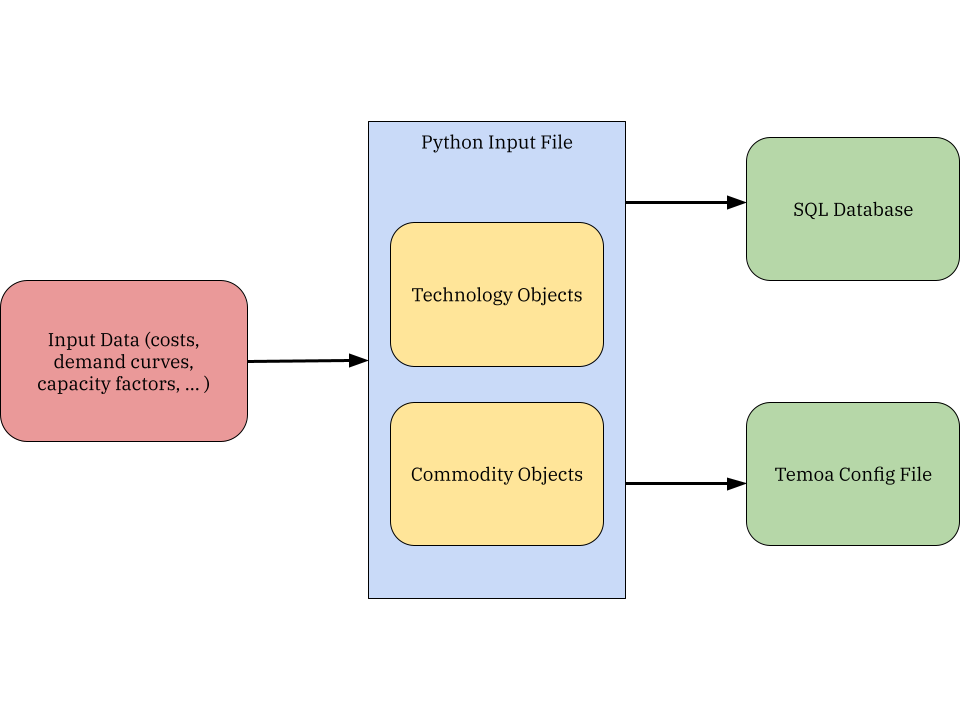
\includegraphics[width=0.8\columnwidth]{figures/pygen-outline.png}
  \caption{The flow of data through \gls{pygen}. \gls{pygen} reads a Python
  input file and writes an \texttt{SQL} database and a configuration textfile.}
  \label{fig:pygen-flow}
\end{figure}


\subsubsection{Time-Series Processing}
Automated conversion of continuous time series data into a \gls{temoa}-ready
time slices is one of \gls{pygen}' key features. By specifying the number of ``seasons''
and the number of ``times of day,'' users can quickly rerun their model at different
temporal resolutions. The only limit to this is computational tractability on
\gls{temoa}'s end. There are two options for time series processing, ``demand'' and
``capacity factor.'' A ``demand'' profile ensures the sum of all representative days is
unity, while a ``capacity factor'' profile divides each representative day by the
maximum value of the original time series.
Figure \ref{fig:solar-timeslice} shows some historical data from \gls{uiuc}'s
first solar farm project, Solar Farm 1.0 \cite{white_solar_2017}, that \gls{pygen}
sliced into four seasons with one representative day of 24 hours each, with ``capacity
factor'' specified.
\begin{figure}[H]
  \resizebox{\textwidth}{!}{%% Creator: Matplotlib, PGF backend
%%
%% To include the figure in your LaTeX document, write
%%   \input{<filename>.pgf}
%%
%% Make sure the required packages are loaded in your preamble
%%   \usepackage{pgf}
%%
%% Figures using additional raster images can only be included by \input if
%% they are in the same directory as the main LaTeX file. For loading figures
%% from other directories you can use the `import` package
%%   \usepackage{import}
%%
%% and then include the figures with
%%   \import{<path to file>}{<filename>.pgf}
%%
%% Matplotlib used the following preamble
%%
\begingroup%
\makeatletter%
\begin{pgfpicture}%
\pgfpathrectangle{\pgfpointorigin}{\pgfqpoint{17.900000in}{8.900000in}}%
\pgfusepath{use as bounding box, clip}%
\begin{pgfscope}%
\pgfsetbuttcap%
\pgfsetmiterjoin%
\definecolor{currentfill}{rgb}{1.000000,1.000000,1.000000}%
\pgfsetfillcolor{currentfill}%
\pgfsetlinewidth{0.000000pt}%
\definecolor{currentstroke}{rgb}{0.000000,0.000000,0.000000}%
\pgfsetstrokecolor{currentstroke}%
\pgfsetdash{}{0pt}%
\pgfpathmoveto{\pgfqpoint{0.000000in}{0.000000in}}%
\pgfpathlineto{\pgfqpoint{17.900000in}{0.000000in}}%
\pgfpathlineto{\pgfqpoint{17.900000in}{8.900000in}}%
\pgfpathlineto{\pgfqpoint{0.000000in}{8.900000in}}%
\pgfpathclose%
\pgfusepath{fill}%
\end{pgfscope}%
\begin{pgfscope}%
\pgfsetbuttcap%
\pgfsetmiterjoin%
\definecolor{currentfill}{rgb}{0.898039,0.898039,0.898039}%
\pgfsetfillcolor{currentfill}%
\pgfsetlinewidth{0.000000pt}%
\definecolor{currentstroke}{rgb}{0.000000,0.000000,0.000000}%
\pgfsetstrokecolor{currentstroke}%
\pgfsetstrokeopacity{0.000000}%
\pgfsetdash{}{0pt}%
\pgfpathmoveto{\pgfqpoint{0.931995in}{0.892178in}}%
\pgfpathlineto{\pgfqpoint{12.883221in}{0.892178in}}%
\pgfpathlineto{\pgfqpoint{12.883221in}{8.516628in}}%
\pgfpathlineto{\pgfqpoint{0.931995in}{8.516628in}}%
\pgfpathclose%
\pgfusepath{fill}%
\end{pgfscope}%
\begin{pgfscope}%
\pgfpathrectangle{\pgfqpoint{0.931995in}{0.892178in}}{\pgfqpoint{11.951226in}{7.624450in}}%
\pgfusepath{clip}%
\pgfsetrectcap%
\pgfsetroundjoin%
\pgfsetlinewidth{0.803000pt}%
\definecolor{currentstroke}{rgb}{1.000000,1.000000,1.000000}%
\pgfsetstrokecolor{currentstroke}%
\pgfsetdash{}{0pt}%
\pgfpathmoveto{\pgfqpoint{0.931995in}{0.892178in}}%
\pgfpathlineto{\pgfqpoint{0.931995in}{8.516628in}}%
\pgfusepath{stroke}%
\end{pgfscope}%
\begin{pgfscope}%
\pgfsetbuttcap%
\pgfsetroundjoin%
\definecolor{currentfill}{rgb}{0.333333,0.333333,0.333333}%
\pgfsetfillcolor{currentfill}%
\pgfsetlinewidth{0.803000pt}%
\definecolor{currentstroke}{rgb}{0.333333,0.333333,0.333333}%
\pgfsetstrokecolor{currentstroke}%
\pgfsetdash{}{0pt}%
\pgfsys@defobject{currentmarker}{\pgfqpoint{0.000000in}{-0.048611in}}{\pgfqpoint{0.000000in}{0.000000in}}{%
\pgfpathmoveto{\pgfqpoint{0.000000in}{0.000000in}}%
\pgfpathlineto{\pgfqpoint{0.000000in}{-0.048611in}}%
\pgfusepath{stroke,fill}%
}%
\begin{pgfscope}%
\pgfsys@transformshift{0.931995in}{0.892178in}%
\pgfsys@useobject{currentmarker}{}%
\end{pgfscope}%
\end{pgfscope}%
\begin{pgfscope}%
\definecolor{textcolor}{rgb}{0.333333,0.333333,0.333333}%
\pgfsetstrokecolor{textcolor}%
\pgfsetfillcolor{textcolor}%
\pgftext[x=0.778339in, y=0.656067in, left, base]{\color{textcolor}\rmfamily\fontsize{14.000000}{16.800000}\selectfont Jan}%
\end{pgfscope}%
\begin{pgfscope}%
\definecolor{textcolor}{rgb}{0.333333,0.333333,0.333333}%
\pgfsetstrokecolor{textcolor}%
\pgfsetfillcolor{textcolor}%
\pgftext[x=0.736164in, y=0.450512in, left, base]{\color{textcolor}\rmfamily\fontsize{14.000000}{16.800000}\selectfont 2016}%
\end{pgfscope}%
\begin{pgfscope}%
\pgfpathrectangle{\pgfqpoint{0.931995in}{0.892178in}}{\pgfqpoint{11.951226in}{7.624450in}}%
\pgfusepath{clip}%
\pgfsetrectcap%
\pgfsetroundjoin%
\pgfsetlinewidth{0.803000pt}%
\definecolor{currentstroke}{rgb}{1.000000,1.000000,1.000000}%
\pgfsetstrokecolor{currentstroke}%
\pgfsetdash{}{0pt}%
\pgfpathmoveto{\pgfqpoint{4.923158in}{0.892178in}}%
\pgfpathlineto{\pgfqpoint{4.923158in}{8.516628in}}%
\pgfusepath{stroke}%
\end{pgfscope}%
\begin{pgfscope}%
\pgfsetbuttcap%
\pgfsetroundjoin%
\definecolor{currentfill}{rgb}{0.333333,0.333333,0.333333}%
\pgfsetfillcolor{currentfill}%
\pgfsetlinewidth{0.803000pt}%
\definecolor{currentstroke}{rgb}{0.333333,0.333333,0.333333}%
\pgfsetstrokecolor{currentstroke}%
\pgfsetdash{}{0pt}%
\pgfsys@defobject{currentmarker}{\pgfqpoint{0.000000in}{-0.048611in}}{\pgfqpoint{0.000000in}{0.000000in}}{%
\pgfpathmoveto{\pgfqpoint{0.000000in}{0.000000in}}%
\pgfpathlineto{\pgfqpoint{0.000000in}{-0.048611in}}%
\pgfusepath{stroke,fill}%
}%
\begin{pgfscope}%
\pgfsys@transformshift{4.923158in}{0.892178in}%
\pgfsys@useobject{currentmarker}{}%
\end{pgfscope}%
\end{pgfscope}%
\begin{pgfscope}%
\definecolor{textcolor}{rgb}{0.333333,0.333333,0.333333}%
\pgfsetstrokecolor{textcolor}%
\pgfsetfillcolor{textcolor}%
\pgftext[x=4.769503in, y=0.656067in, left, base]{\color{textcolor}\rmfamily\fontsize{14.000000}{16.800000}\selectfont Jan}%
\end{pgfscope}%
\begin{pgfscope}%
\definecolor{textcolor}{rgb}{0.333333,0.333333,0.333333}%
\pgfsetstrokecolor{textcolor}%
\pgfsetfillcolor{textcolor}%
\pgftext[x=4.727327in, y=0.450512in, left, base]{\color{textcolor}\rmfamily\fontsize{14.000000}{16.800000}\selectfont 2017}%
\end{pgfscope}%
\begin{pgfscope}%
\pgfpathrectangle{\pgfqpoint{0.931995in}{0.892178in}}{\pgfqpoint{11.951226in}{7.624450in}}%
\pgfusepath{clip}%
\pgfsetrectcap%
\pgfsetroundjoin%
\pgfsetlinewidth{0.803000pt}%
\definecolor{currentstroke}{rgb}{1.000000,1.000000,1.000000}%
\pgfsetstrokecolor{currentstroke}%
\pgfsetdash{}{0pt}%
\pgfpathmoveto{\pgfqpoint{8.903417in}{0.892178in}}%
\pgfpathlineto{\pgfqpoint{8.903417in}{8.516628in}}%
\pgfusepath{stroke}%
\end{pgfscope}%
\begin{pgfscope}%
\pgfsetbuttcap%
\pgfsetroundjoin%
\definecolor{currentfill}{rgb}{0.333333,0.333333,0.333333}%
\pgfsetfillcolor{currentfill}%
\pgfsetlinewidth{0.803000pt}%
\definecolor{currentstroke}{rgb}{0.333333,0.333333,0.333333}%
\pgfsetstrokecolor{currentstroke}%
\pgfsetdash{}{0pt}%
\pgfsys@defobject{currentmarker}{\pgfqpoint{0.000000in}{-0.048611in}}{\pgfqpoint{0.000000in}{0.000000in}}{%
\pgfpathmoveto{\pgfqpoint{0.000000in}{0.000000in}}%
\pgfpathlineto{\pgfqpoint{0.000000in}{-0.048611in}}%
\pgfusepath{stroke,fill}%
}%
\begin{pgfscope}%
\pgfsys@transformshift{8.903417in}{0.892178in}%
\pgfsys@useobject{currentmarker}{}%
\end{pgfscope}%
\end{pgfscope}%
\begin{pgfscope}%
\definecolor{textcolor}{rgb}{0.333333,0.333333,0.333333}%
\pgfsetstrokecolor{textcolor}%
\pgfsetfillcolor{textcolor}%
\pgftext[x=8.749761in, y=0.656067in, left, base]{\color{textcolor}\rmfamily\fontsize{14.000000}{16.800000}\selectfont Jan}%
\end{pgfscope}%
\begin{pgfscope}%
\definecolor{textcolor}{rgb}{0.333333,0.333333,0.333333}%
\pgfsetstrokecolor{textcolor}%
\pgfsetfillcolor{textcolor}%
\pgftext[x=8.707586in, y=0.450512in, left, base]{\color{textcolor}\rmfamily\fontsize{14.000000}{16.800000}\selectfont 2018}%
\end{pgfscope}%
\begin{pgfscope}%
\pgfpathrectangle{\pgfqpoint{0.931995in}{0.892178in}}{\pgfqpoint{11.951226in}{7.624450in}}%
\pgfusepath{clip}%
\pgfsetrectcap%
\pgfsetroundjoin%
\pgfsetlinewidth{0.803000pt}%
\definecolor{currentstroke}{rgb}{1.000000,1.000000,1.000000}%
\pgfsetstrokecolor{currentstroke}%
\pgfsetdash{}{0pt}%
\pgfpathmoveto{\pgfqpoint{12.883221in}{0.892178in}}%
\pgfpathlineto{\pgfqpoint{12.883221in}{8.516628in}}%
\pgfusepath{stroke}%
\end{pgfscope}%
\begin{pgfscope}%
\pgfsetbuttcap%
\pgfsetroundjoin%
\definecolor{currentfill}{rgb}{0.333333,0.333333,0.333333}%
\pgfsetfillcolor{currentfill}%
\pgfsetlinewidth{0.803000pt}%
\definecolor{currentstroke}{rgb}{0.333333,0.333333,0.333333}%
\pgfsetstrokecolor{currentstroke}%
\pgfsetdash{}{0pt}%
\pgfsys@defobject{currentmarker}{\pgfqpoint{0.000000in}{-0.048611in}}{\pgfqpoint{0.000000in}{0.000000in}}{%
\pgfpathmoveto{\pgfqpoint{0.000000in}{0.000000in}}%
\pgfpathlineto{\pgfqpoint{0.000000in}{-0.048611in}}%
\pgfusepath{stroke,fill}%
}%
\begin{pgfscope}%
\pgfsys@transformshift{12.883221in}{0.892178in}%
\pgfsys@useobject{currentmarker}{}%
\end{pgfscope}%
\end{pgfscope}%
\begin{pgfscope}%
\pgfpathrectangle{\pgfqpoint{0.931995in}{0.892178in}}{\pgfqpoint{11.951226in}{7.624450in}}%
\pgfusepath{clip}%
\pgfsetbuttcap%
\pgfsetroundjoin%
\pgfsetlinewidth{0.803000pt}%
\definecolor{currentstroke}{rgb}{1.000000,1.000000,1.000000}%
\pgfsetstrokecolor{currentstroke}%
\pgfsetdash{{2.960000pt}{1.280000pt}}{0.000000pt}%
\pgfpathmoveto{\pgfqpoint{1.929786in}{0.892178in}}%
\pgfpathlineto{\pgfqpoint{1.929786in}{8.516628in}}%
\pgfusepath{stroke}%
\end{pgfscope}%
\begin{pgfscope}%
\pgfsetbuttcap%
\pgfsetroundjoin%
\definecolor{currentfill}{rgb}{0.333333,0.333333,0.333333}%
\pgfsetfillcolor{currentfill}%
\pgfsetlinewidth{0.602250pt}%
\definecolor{currentstroke}{rgb}{0.333333,0.333333,0.333333}%
\pgfsetstrokecolor{currentstroke}%
\pgfsetdash{}{0pt}%
\pgfsys@defobject{currentmarker}{\pgfqpoint{0.000000in}{-0.027778in}}{\pgfqpoint{0.000000in}{0.000000in}}{%
\pgfpathmoveto{\pgfqpoint{0.000000in}{0.000000in}}%
\pgfpathlineto{\pgfqpoint{0.000000in}{-0.027778in}}%
\pgfusepath{stroke,fill}%
}%
\begin{pgfscope}%
\pgfsys@transformshift{1.929786in}{0.892178in}%
\pgfsys@useobject{currentmarker}{}%
\end{pgfscope}%
\end{pgfscope}%
\begin{pgfscope}%
\pgfpathrectangle{\pgfqpoint{0.931995in}{0.892178in}}{\pgfqpoint{11.951226in}{7.624450in}}%
\pgfusepath{clip}%
\pgfsetbuttcap%
\pgfsetroundjoin%
\pgfsetlinewidth{0.803000pt}%
\definecolor{currentstroke}{rgb}{1.000000,1.000000,1.000000}%
\pgfsetstrokecolor{currentstroke}%
\pgfsetdash{{2.960000pt}{1.280000pt}}{0.000000pt}%
\pgfpathmoveto{\pgfqpoint{2.927577in}{0.892178in}}%
\pgfpathlineto{\pgfqpoint{2.927577in}{8.516628in}}%
\pgfusepath{stroke}%
\end{pgfscope}%
\begin{pgfscope}%
\pgfsetbuttcap%
\pgfsetroundjoin%
\definecolor{currentfill}{rgb}{0.333333,0.333333,0.333333}%
\pgfsetfillcolor{currentfill}%
\pgfsetlinewidth{0.602250pt}%
\definecolor{currentstroke}{rgb}{0.333333,0.333333,0.333333}%
\pgfsetstrokecolor{currentstroke}%
\pgfsetdash{}{0pt}%
\pgfsys@defobject{currentmarker}{\pgfqpoint{0.000000in}{-0.027778in}}{\pgfqpoint{0.000000in}{0.000000in}}{%
\pgfpathmoveto{\pgfqpoint{0.000000in}{0.000000in}}%
\pgfpathlineto{\pgfqpoint{0.000000in}{-0.027778in}}%
\pgfusepath{stroke,fill}%
}%
\begin{pgfscope}%
\pgfsys@transformshift{2.927577in}{0.892178in}%
\pgfsys@useobject{currentmarker}{}%
\end{pgfscope}%
\end{pgfscope}%
\begin{pgfscope}%
\pgfpathrectangle{\pgfqpoint{0.931995in}{0.892178in}}{\pgfqpoint{11.951226in}{7.624450in}}%
\pgfusepath{clip}%
\pgfsetbuttcap%
\pgfsetroundjoin%
\pgfsetlinewidth{0.803000pt}%
\definecolor{currentstroke}{rgb}{1.000000,1.000000,1.000000}%
\pgfsetstrokecolor{currentstroke}%
\pgfsetdash{{2.960000pt}{1.280000pt}}{0.000000pt}%
\pgfpathmoveto{\pgfqpoint{3.925367in}{0.892178in}}%
\pgfpathlineto{\pgfqpoint{3.925367in}{8.516628in}}%
\pgfusepath{stroke}%
\end{pgfscope}%
\begin{pgfscope}%
\pgfsetbuttcap%
\pgfsetroundjoin%
\definecolor{currentfill}{rgb}{0.333333,0.333333,0.333333}%
\pgfsetfillcolor{currentfill}%
\pgfsetlinewidth{0.602250pt}%
\definecolor{currentstroke}{rgb}{0.333333,0.333333,0.333333}%
\pgfsetstrokecolor{currentstroke}%
\pgfsetdash{}{0pt}%
\pgfsys@defobject{currentmarker}{\pgfqpoint{0.000000in}{-0.027778in}}{\pgfqpoint{0.000000in}{0.000000in}}{%
\pgfpathmoveto{\pgfqpoint{0.000000in}{0.000000in}}%
\pgfpathlineto{\pgfqpoint{0.000000in}{-0.027778in}}%
\pgfusepath{stroke,fill}%
}%
\begin{pgfscope}%
\pgfsys@transformshift{3.925367in}{0.892178in}%
\pgfsys@useobject{currentmarker}{}%
\end{pgfscope}%
\end{pgfscope}%
\begin{pgfscope}%
\pgfpathrectangle{\pgfqpoint{0.931995in}{0.892178in}}{\pgfqpoint{11.951226in}{7.624450in}}%
\pgfusepath{clip}%
\pgfsetbuttcap%
\pgfsetroundjoin%
\pgfsetlinewidth{0.803000pt}%
\definecolor{currentstroke}{rgb}{1.000000,1.000000,1.000000}%
\pgfsetstrokecolor{currentstroke}%
\pgfsetdash{{2.960000pt}{1.280000pt}}{0.000000pt}%
\pgfpathmoveto{\pgfqpoint{5.920949in}{0.892178in}}%
\pgfpathlineto{\pgfqpoint{5.920949in}{8.516628in}}%
\pgfusepath{stroke}%
\end{pgfscope}%
\begin{pgfscope}%
\pgfsetbuttcap%
\pgfsetroundjoin%
\definecolor{currentfill}{rgb}{0.333333,0.333333,0.333333}%
\pgfsetfillcolor{currentfill}%
\pgfsetlinewidth{0.602250pt}%
\definecolor{currentstroke}{rgb}{0.333333,0.333333,0.333333}%
\pgfsetstrokecolor{currentstroke}%
\pgfsetdash{}{0pt}%
\pgfsys@defobject{currentmarker}{\pgfqpoint{0.000000in}{-0.027778in}}{\pgfqpoint{0.000000in}{0.000000in}}{%
\pgfpathmoveto{\pgfqpoint{0.000000in}{0.000000in}}%
\pgfpathlineto{\pgfqpoint{0.000000in}{-0.027778in}}%
\pgfusepath{stroke,fill}%
}%
\begin{pgfscope}%
\pgfsys@transformshift{5.920949in}{0.892178in}%
\pgfsys@useobject{currentmarker}{}%
\end{pgfscope}%
\end{pgfscope}%
\begin{pgfscope}%
\pgfpathrectangle{\pgfqpoint{0.931995in}{0.892178in}}{\pgfqpoint{11.951226in}{7.624450in}}%
\pgfusepath{clip}%
\pgfsetbuttcap%
\pgfsetroundjoin%
\pgfsetlinewidth{0.803000pt}%
\definecolor{currentstroke}{rgb}{1.000000,1.000000,1.000000}%
\pgfsetstrokecolor{currentstroke}%
\pgfsetdash{{2.960000pt}{1.280000pt}}{0.000000pt}%
\pgfpathmoveto{\pgfqpoint{6.918740in}{0.892178in}}%
\pgfpathlineto{\pgfqpoint{6.918740in}{8.516628in}}%
\pgfusepath{stroke}%
\end{pgfscope}%
\begin{pgfscope}%
\pgfsetbuttcap%
\pgfsetroundjoin%
\definecolor{currentfill}{rgb}{0.333333,0.333333,0.333333}%
\pgfsetfillcolor{currentfill}%
\pgfsetlinewidth{0.602250pt}%
\definecolor{currentstroke}{rgb}{0.333333,0.333333,0.333333}%
\pgfsetstrokecolor{currentstroke}%
\pgfsetdash{}{0pt}%
\pgfsys@defobject{currentmarker}{\pgfqpoint{0.000000in}{-0.027778in}}{\pgfqpoint{0.000000in}{0.000000in}}{%
\pgfpathmoveto{\pgfqpoint{0.000000in}{0.000000in}}%
\pgfpathlineto{\pgfqpoint{0.000000in}{-0.027778in}}%
\pgfusepath{stroke,fill}%
}%
\begin{pgfscope}%
\pgfsys@transformshift{6.918740in}{0.892178in}%
\pgfsys@useobject{currentmarker}{}%
\end{pgfscope}%
\end{pgfscope}%
\begin{pgfscope}%
\pgfpathrectangle{\pgfqpoint{0.931995in}{0.892178in}}{\pgfqpoint{11.951226in}{7.624450in}}%
\pgfusepath{clip}%
\pgfsetbuttcap%
\pgfsetroundjoin%
\pgfsetlinewidth{0.803000pt}%
\definecolor{currentstroke}{rgb}{1.000000,1.000000,1.000000}%
\pgfsetstrokecolor{currentstroke}%
\pgfsetdash{{2.960000pt}{1.280000pt}}{0.000000pt}%
\pgfpathmoveto{\pgfqpoint{7.916531in}{0.892178in}}%
\pgfpathlineto{\pgfqpoint{7.916531in}{8.516628in}}%
\pgfusepath{stroke}%
\end{pgfscope}%
\begin{pgfscope}%
\pgfsetbuttcap%
\pgfsetroundjoin%
\definecolor{currentfill}{rgb}{0.333333,0.333333,0.333333}%
\pgfsetfillcolor{currentfill}%
\pgfsetlinewidth{0.602250pt}%
\definecolor{currentstroke}{rgb}{0.333333,0.333333,0.333333}%
\pgfsetstrokecolor{currentstroke}%
\pgfsetdash{}{0pt}%
\pgfsys@defobject{currentmarker}{\pgfqpoint{0.000000in}{-0.027778in}}{\pgfqpoint{0.000000in}{0.000000in}}{%
\pgfpathmoveto{\pgfqpoint{0.000000in}{0.000000in}}%
\pgfpathlineto{\pgfqpoint{0.000000in}{-0.027778in}}%
\pgfusepath{stroke,fill}%
}%
\begin{pgfscope}%
\pgfsys@transformshift{7.916531in}{0.892178in}%
\pgfsys@useobject{currentmarker}{}%
\end{pgfscope}%
\end{pgfscope}%
\begin{pgfscope}%
\pgfpathrectangle{\pgfqpoint{0.931995in}{0.892178in}}{\pgfqpoint{11.951226in}{7.624450in}}%
\pgfusepath{clip}%
\pgfsetbuttcap%
\pgfsetroundjoin%
\pgfsetlinewidth{0.803000pt}%
\definecolor{currentstroke}{rgb}{1.000000,1.000000,1.000000}%
\pgfsetstrokecolor{currentstroke}%
\pgfsetdash{{2.960000pt}{1.280000pt}}{0.000000pt}%
\pgfpathmoveto{\pgfqpoint{8.914322in}{0.892178in}}%
\pgfpathlineto{\pgfqpoint{8.914322in}{8.516628in}}%
\pgfusepath{stroke}%
\end{pgfscope}%
\begin{pgfscope}%
\pgfsetbuttcap%
\pgfsetroundjoin%
\definecolor{currentfill}{rgb}{0.333333,0.333333,0.333333}%
\pgfsetfillcolor{currentfill}%
\pgfsetlinewidth{0.602250pt}%
\definecolor{currentstroke}{rgb}{0.333333,0.333333,0.333333}%
\pgfsetstrokecolor{currentstroke}%
\pgfsetdash{}{0pt}%
\pgfsys@defobject{currentmarker}{\pgfqpoint{0.000000in}{-0.027778in}}{\pgfqpoint{0.000000in}{0.000000in}}{%
\pgfpathmoveto{\pgfqpoint{0.000000in}{0.000000in}}%
\pgfpathlineto{\pgfqpoint{0.000000in}{-0.027778in}}%
\pgfusepath{stroke,fill}%
}%
\begin{pgfscope}%
\pgfsys@transformshift{8.914322in}{0.892178in}%
\pgfsys@useobject{currentmarker}{}%
\end{pgfscope}%
\end{pgfscope}%
\begin{pgfscope}%
\pgfpathrectangle{\pgfqpoint{0.931995in}{0.892178in}}{\pgfqpoint{11.951226in}{7.624450in}}%
\pgfusepath{clip}%
\pgfsetbuttcap%
\pgfsetroundjoin%
\pgfsetlinewidth{0.803000pt}%
\definecolor{currentstroke}{rgb}{1.000000,1.000000,1.000000}%
\pgfsetstrokecolor{currentstroke}%
\pgfsetdash{{2.960000pt}{1.280000pt}}{0.000000pt}%
\pgfpathmoveto{\pgfqpoint{9.912112in}{0.892178in}}%
\pgfpathlineto{\pgfqpoint{9.912112in}{8.516628in}}%
\pgfusepath{stroke}%
\end{pgfscope}%
\begin{pgfscope}%
\pgfsetbuttcap%
\pgfsetroundjoin%
\definecolor{currentfill}{rgb}{0.333333,0.333333,0.333333}%
\pgfsetfillcolor{currentfill}%
\pgfsetlinewidth{0.602250pt}%
\definecolor{currentstroke}{rgb}{0.333333,0.333333,0.333333}%
\pgfsetstrokecolor{currentstroke}%
\pgfsetdash{}{0pt}%
\pgfsys@defobject{currentmarker}{\pgfqpoint{0.000000in}{-0.027778in}}{\pgfqpoint{0.000000in}{0.000000in}}{%
\pgfpathmoveto{\pgfqpoint{0.000000in}{0.000000in}}%
\pgfpathlineto{\pgfqpoint{0.000000in}{-0.027778in}}%
\pgfusepath{stroke,fill}%
}%
\begin{pgfscope}%
\pgfsys@transformshift{9.912112in}{0.892178in}%
\pgfsys@useobject{currentmarker}{}%
\end{pgfscope}%
\end{pgfscope}%
\begin{pgfscope}%
\pgfpathrectangle{\pgfqpoint{0.931995in}{0.892178in}}{\pgfqpoint{11.951226in}{7.624450in}}%
\pgfusepath{clip}%
\pgfsetbuttcap%
\pgfsetroundjoin%
\pgfsetlinewidth{0.803000pt}%
\definecolor{currentstroke}{rgb}{1.000000,1.000000,1.000000}%
\pgfsetstrokecolor{currentstroke}%
\pgfsetdash{{2.960000pt}{1.280000pt}}{0.000000pt}%
\pgfpathmoveto{\pgfqpoint{10.909903in}{0.892178in}}%
\pgfpathlineto{\pgfqpoint{10.909903in}{8.516628in}}%
\pgfusepath{stroke}%
\end{pgfscope}%
\begin{pgfscope}%
\pgfsetbuttcap%
\pgfsetroundjoin%
\definecolor{currentfill}{rgb}{0.333333,0.333333,0.333333}%
\pgfsetfillcolor{currentfill}%
\pgfsetlinewidth{0.602250pt}%
\definecolor{currentstroke}{rgb}{0.333333,0.333333,0.333333}%
\pgfsetstrokecolor{currentstroke}%
\pgfsetdash{}{0pt}%
\pgfsys@defobject{currentmarker}{\pgfqpoint{0.000000in}{-0.027778in}}{\pgfqpoint{0.000000in}{0.000000in}}{%
\pgfpathmoveto{\pgfqpoint{0.000000in}{0.000000in}}%
\pgfpathlineto{\pgfqpoint{0.000000in}{-0.027778in}}%
\pgfusepath{stroke,fill}%
}%
\begin{pgfscope}%
\pgfsys@transformshift{10.909903in}{0.892178in}%
\pgfsys@useobject{currentmarker}{}%
\end{pgfscope}%
\end{pgfscope}%
\begin{pgfscope}%
\pgfpathrectangle{\pgfqpoint{0.931995in}{0.892178in}}{\pgfqpoint{11.951226in}{7.624450in}}%
\pgfusepath{clip}%
\pgfsetbuttcap%
\pgfsetroundjoin%
\pgfsetlinewidth{0.803000pt}%
\definecolor{currentstroke}{rgb}{1.000000,1.000000,1.000000}%
\pgfsetstrokecolor{currentstroke}%
\pgfsetdash{{2.960000pt}{1.280000pt}}{0.000000pt}%
\pgfpathmoveto{\pgfqpoint{11.907694in}{0.892178in}}%
\pgfpathlineto{\pgfqpoint{11.907694in}{8.516628in}}%
\pgfusepath{stroke}%
\end{pgfscope}%
\begin{pgfscope}%
\pgfsetbuttcap%
\pgfsetroundjoin%
\definecolor{currentfill}{rgb}{0.333333,0.333333,0.333333}%
\pgfsetfillcolor{currentfill}%
\pgfsetlinewidth{0.602250pt}%
\definecolor{currentstroke}{rgb}{0.333333,0.333333,0.333333}%
\pgfsetstrokecolor{currentstroke}%
\pgfsetdash{}{0pt}%
\pgfsys@defobject{currentmarker}{\pgfqpoint{0.000000in}{-0.027778in}}{\pgfqpoint{0.000000in}{0.000000in}}{%
\pgfpathmoveto{\pgfqpoint{0.000000in}{0.000000in}}%
\pgfpathlineto{\pgfqpoint{0.000000in}{-0.027778in}}%
\pgfusepath{stroke,fill}%
}%
\begin{pgfscope}%
\pgfsys@transformshift{11.907694in}{0.892178in}%
\pgfsys@useobject{currentmarker}{}%
\end{pgfscope}%
\end{pgfscope}%
\begin{pgfscope}%
\definecolor{textcolor}{rgb}{0.333333,0.333333,0.333333}%
\pgfsetstrokecolor{textcolor}%
\pgfsetfillcolor{textcolor}%
\pgftext[x=6.907608in,y=0.356068in,,top]{\color{textcolor}\rmfamily\fontsize{20.000000}{24.000000}\selectfont Date}%
\end{pgfscope}%
\begin{pgfscope}%
\pgfpathrectangle{\pgfqpoint{0.931995in}{0.892178in}}{\pgfqpoint{11.951226in}{7.624450in}}%
\pgfusepath{clip}%
\pgfsetrectcap%
\pgfsetroundjoin%
\pgfsetlinewidth{0.803000pt}%
\definecolor{currentstroke}{rgb}{1.000000,1.000000,1.000000}%
\pgfsetstrokecolor{currentstroke}%
\pgfsetdash{}{0pt}%
\pgfpathmoveto{\pgfqpoint{0.931995in}{0.892178in}}%
\pgfpathlineto{\pgfqpoint{12.883221in}{0.892178in}}%
\pgfusepath{stroke}%
\end{pgfscope}%
\begin{pgfscope}%
\pgfsetbuttcap%
\pgfsetroundjoin%
\definecolor{currentfill}{rgb}{0.333333,0.333333,0.333333}%
\pgfsetfillcolor{currentfill}%
\pgfsetlinewidth{0.803000pt}%
\definecolor{currentstroke}{rgb}{0.333333,0.333333,0.333333}%
\pgfsetstrokecolor{currentstroke}%
\pgfsetdash{}{0pt}%
\pgfsys@defobject{currentmarker}{\pgfqpoint{-0.048611in}{0.000000in}}{\pgfqpoint{-0.000000in}{0.000000in}}{%
\pgfpathmoveto{\pgfqpoint{-0.000000in}{0.000000in}}%
\pgfpathlineto{\pgfqpoint{-0.048611in}{0.000000in}}%
\pgfusepath{stroke,fill}%
}%
\begin{pgfscope}%
\pgfsys@transformshift{0.931995in}{0.892178in}%
\pgfsys@useobject{currentmarker}{}%
\end{pgfscope}%
\end{pgfscope}%
\begin{pgfscope}%
\definecolor{textcolor}{rgb}{0.333333,0.333333,0.333333}%
\pgfsetstrokecolor{textcolor}%
\pgfsetfillcolor{textcolor}%
\pgftext[x=0.736857in, y=0.822734in, left, base]{\color{textcolor}\rmfamily\fontsize{14.000000}{16.800000}\selectfont \(\displaystyle {0}\)}%
\end{pgfscope}%
\begin{pgfscope}%
\pgfpathrectangle{\pgfqpoint{0.931995in}{0.892178in}}{\pgfqpoint{11.951226in}{7.624450in}}%
\pgfusepath{clip}%
\pgfsetrectcap%
\pgfsetroundjoin%
\pgfsetlinewidth{0.803000pt}%
\definecolor{currentstroke}{rgb}{1.000000,1.000000,1.000000}%
\pgfsetstrokecolor{currentstroke}%
\pgfsetdash{}{0pt}%
\pgfpathmoveto{\pgfqpoint{0.931995in}{2.503006in}}%
\pgfpathlineto{\pgfqpoint{12.883221in}{2.503006in}}%
\pgfusepath{stroke}%
\end{pgfscope}%
\begin{pgfscope}%
\pgfsetbuttcap%
\pgfsetroundjoin%
\definecolor{currentfill}{rgb}{0.333333,0.333333,0.333333}%
\pgfsetfillcolor{currentfill}%
\pgfsetlinewidth{0.803000pt}%
\definecolor{currentstroke}{rgb}{0.333333,0.333333,0.333333}%
\pgfsetstrokecolor{currentstroke}%
\pgfsetdash{}{0pt}%
\pgfsys@defobject{currentmarker}{\pgfqpoint{-0.048611in}{0.000000in}}{\pgfqpoint{-0.000000in}{0.000000in}}{%
\pgfpathmoveto{\pgfqpoint{-0.000000in}{0.000000in}}%
\pgfpathlineto{\pgfqpoint{-0.048611in}{0.000000in}}%
\pgfusepath{stroke,fill}%
}%
\begin{pgfscope}%
\pgfsys@transformshift{0.931995in}{2.503006in}%
\pgfsys@useobject{currentmarker}{}%
\end{pgfscope}%
\end{pgfscope}%
\begin{pgfscope}%
\definecolor{textcolor}{rgb}{0.333333,0.333333,0.333333}%
\pgfsetstrokecolor{textcolor}%
\pgfsetfillcolor{textcolor}%
\pgftext[x=0.443111in, y=2.433561in, left, base]{\color{textcolor}\rmfamily\fontsize{14.000000}{16.800000}\selectfont \(\displaystyle {1000}\)}%
\end{pgfscope}%
\begin{pgfscope}%
\pgfpathrectangle{\pgfqpoint{0.931995in}{0.892178in}}{\pgfqpoint{11.951226in}{7.624450in}}%
\pgfusepath{clip}%
\pgfsetrectcap%
\pgfsetroundjoin%
\pgfsetlinewidth{0.803000pt}%
\definecolor{currentstroke}{rgb}{1.000000,1.000000,1.000000}%
\pgfsetstrokecolor{currentstroke}%
\pgfsetdash{}{0pt}%
\pgfpathmoveto{\pgfqpoint{0.931995in}{4.113833in}}%
\pgfpathlineto{\pgfqpoint{12.883221in}{4.113833in}}%
\pgfusepath{stroke}%
\end{pgfscope}%
\begin{pgfscope}%
\pgfsetbuttcap%
\pgfsetroundjoin%
\definecolor{currentfill}{rgb}{0.333333,0.333333,0.333333}%
\pgfsetfillcolor{currentfill}%
\pgfsetlinewidth{0.803000pt}%
\definecolor{currentstroke}{rgb}{0.333333,0.333333,0.333333}%
\pgfsetstrokecolor{currentstroke}%
\pgfsetdash{}{0pt}%
\pgfsys@defobject{currentmarker}{\pgfqpoint{-0.048611in}{0.000000in}}{\pgfqpoint{-0.000000in}{0.000000in}}{%
\pgfpathmoveto{\pgfqpoint{-0.000000in}{0.000000in}}%
\pgfpathlineto{\pgfqpoint{-0.048611in}{0.000000in}}%
\pgfusepath{stroke,fill}%
}%
\begin{pgfscope}%
\pgfsys@transformshift{0.931995in}{4.113833in}%
\pgfsys@useobject{currentmarker}{}%
\end{pgfscope}%
\end{pgfscope}%
\begin{pgfscope}%
\definecolor{textcolor}{rgb}{0.333333,0.333333,0.333333}%
\pgfsetstrokecolor{textcolor}%
\pgfsetfillcolor{textcolor}%
\pgftext[x=0.443111in, y=4.044389in, left, base]{\color{textcolor}\rmfamily\fontsize{14.000000}{16.800000}\selectfont \(\displaystyle {2000}\)}%
\end{pgfscope}%
\begin{pgfscope}%
\pgfpathrectangle{\pgfqpoint{0.931995in}{0.892178in}}{\pgfqpoint{11.951226in}{7.624450in}}%
\pgfusepath{clip}%
\pgfsetrectcap%
\pgfsetroundjoin%
\pgfsetlinewidth{0.803000pt}%
\definecolor{currentstroke}{rgb}{1.000000,1.000000,1.000000}%
\pgfsetstrokecolor{currentstroke}%
\pgfsetdash{}{0pt}%
\pgfpathmoveto{\pgfqpoint{0.931995in}{5.724661in}}%
\pgfpathlineto{\pgfqpoint{12.883221in}{5.724661in}}%
\pgfusepath{stroke}%
\end{pgfscope}%
\begin{pgfscope}%
\pgfsetbuttcap%
\pgfsetroundjoin%
\definecolor{currentfill}{rgb}{0.333333,0.333333,0.333333}%
\pgfsetfillcolor{currentfill}%
\pgfsetlinewidth{0.803000pt}%
\definecolor{currentstroke}{rgb}{0.333333,0.333333,0.333333}%
\pgfsetstrokecolor{currentstroke}%
\pgfsetdash{}{0pt}%
\pgfsys@defobject{currentmarker}{\pgfqpoint{-0.048611in}{0.000000in}}{\pgfqpoint{-0.000000in}{0.000000in}}{%
\pgfpathmoveto{\pgfqpoint{-0.000000in}{0.000000in}}%
\pgfpathlineto{\pgfqpoint{-0.048611in}{0.000000in}}%
\pgfusepath{stroke,fill}%
}%
\begin{pgfscope}%
\pgfsys@transformshift{0.931995in}{5.724661in}%
\pgfsys@useobject{currentmarker}{}%
\end{pgfscope}%
\end{pgfscope}%
\begin{pgfscope}%
\definecolor{textcolor}{rgb}{0.333333,0.333333,0.333333}%
\pgfsetstrokecolor{textcolor}%
\pgfsetfillcolor{textcolor}%
\pgftext[x=0.443111in, y=5.655217in, left, base]{\color{textcolor}\rmfamily\fontsize{14.000000}{16.800000}\selectfont \(\displaystyle {3000}\)}%
\end{pgfscope}%
\begin{pgfscope}%
\pgfpathrectangle{\pgfqpoint{0.931995in}{0.892178in}}{\pgfqpoint{11.951226in}{7.624450in}}%
\pgfusepath{clip}%
\pgfsetrectcap%
\pgfsetroundjoin%
\pgfsetlinewidth{0.803000pt}%
\definecolor{currentstroke}{rgb}{1.000000,1.000000,1.000000}%
\pgfsetstrokecolor{currentstroke}%
\pgfsetdash{}{0pt}%
\pgfpathmoveto{\pgfqpoint{0.931995in}{7.335489in}}%
\pgfpathlineto{\pgfqpoint{12.883221in}{7.335489in}}%
\pgfusepath{stroke}%
\end{pgfscope}%
\begin{pgfscope}%
\pgfsetbuttcap%
\pgfsetroundjoin%
\definecolor{currentfill}{rgb}{0.333333,0.333333,0.333333}%
\pgfsetfillcolor{currentfill}%
\pgfsetlinewidth{0.803000pt}%
\definecolor{currentstroke}{rgb}{0.333333,0.333333,0.333333}%
\pgfsetstrokecolor{currentstroke}%
\pgfsetdash{}{0pt}%
\pgfsys@defobject{currentmarker}{\pgfqpoint{-0.048611in}{0.000000in}}{\pgfqpoint{-0.000000in}{0.000000in}}{%
\pgfpathmoveto{\pgfqpoint{-0.000000in}{0.000000in}}%
\pgfpathlineto{\pgfqpoint{-0.048611in}{0.000000in}}%
\pgfusepath{stroke,fill}%
}%
\begin{pgfscope}%
\pgfsys@transformshift{0.931995in}{7.335489in}%
\pgfsys@useobject{currentmarker}{}%
\end{pgfscope}%
\end{pgfscope}%
\begin{pgfscope}%
\definecolor{textcolor}{rgb}{0.333333,0.333333,0.333333}%
\pgfsetstrokecolor{textcolor}%
\pgfsetfillcolor{textcolor}%
\pgftext[x=0.443111in, y=7.266044in, left, base]{\color{textcolor}\rmfamily\fontsize{14.000000}{16.800000}\selectfont \(\displaystyle {4000}\)}%
\end{pgfscope}%
\begin{pgfscope}%
\pgfpathrectangle{\pgfqpoint{0.931995in}{0.892178in}}{\pgfqpoint{11.951226in}{7.624450in}}%
\pgfusepath{clip}%
\pgfsetbuttcap%
\pgfsetroundjoin%
\pgfsetlinewidth{0.803000pt}%
\definecolor{currentstroke}{rgb}{1.000000,1.000000,1.000000}%
\pgfsetstrokecolor{currentstroke}%
\pgfsetdash{{2.960000pt}{1.280000pt}}{0.000000pt}%
\pgfpathmoveto{\pgfqpoint{0.931995in}{1.214343in}}%
\pgfpathlineto{\pgfqpoint{12.883221in}{1.214343in}}%
\pgfusepath{stroke}%
\end{pgfscope}%
\begin{pgfscope}%
\pgfsetbuttcap%
\pgfsetroundjoin%
\definecolor{currentfill}{rgb}{0.333333,0.333333,0.333333}%
\pgfsetfillcolor{currentfill}%
\pgfsetlinewidth{0.602250pt}%
\definecolor{currentstroke}{rgb}{0.333333,0.333333,0.333333}%
\pgfsetstrokecolor{currentstroke}%
\pgfsetdash{}{0pt}%
\pgfsys@defobject{currentmarker}{\pgfqpoint{-0.027778in}{0.000000in}}{\pgfqpoint{-0.000000in}{0.000000in}}{%
\pgfpathmoveto{\pgfqpoint{-0.000000in}{0.000000in}}%
\pgfpathlineto{\pgfqpoint{-0.027778in}{0.000000in}}%
\pgfusepath{stroke,fill}%
}%
\begin{pgfscope}%
\pgfsys@transformshift{0.931995in}{1.214343in}%
\pgfsys@useobject{currentmarker}{}%
\end{pgfscope}%
\end{pgfscope}%
\begin{pgfscope}%
\pgfpathrectangle{\pgfqpoint{0.931995in}{0.892178in}}{\pgfqpoint{11.951226in}{7.624450in}}%
\pgfusepath{clip}%
\pgfsetbuttcap%
\pgfsetroundjoin%
\pgfsetlinewidth{0.803000pt}%
\definecolor{currentstroke}{rgb}{1.000000,1.000000,1.000000}%
\pgfsetstrokecolor{currentstroke}%
\pgfsetdash{{2.960000pt}{1.280000pt}}{0.000000pt}%
\pgfpathmoveto{\pgfqpoint{0.931995in}{1.536509in}}%
\pgfpathlineto{\pgfqpoint{12.883221in}{1.536509in}}%
\pgfusepath{stroke}%
\end{pgfscope}%
\begin{pgfscope}%
\pgfsetbuttcap%
\pgfsetroundjoin%
\definecolor{currentfill}{rgb}{0.333333,0.333333,0.333333}%
\pgfsetfillcolor{currentfill}%
\pgfsetlinewidth{0.602250pt}%
\definecolor{currentstroke}{rgb}{0.333333,0.333333,0.333333}%
\pgfsetstrokecolor{currentstroke}%
\pgfsetdash{}{0pt}%
\pgfsys@defobject{currentmarker}{\pgfqpoint{-0.027778in}{0.000000in}}{\pgfqpoint{-0.000000in}{0.000000in}}{%
\pgfpathmoveto{\pgfqpoint{-0.000000in}{0.000000in}}%
\pgfpathlineto{\pgfqpoint{-0.027778in}{0.000000in}}%
\pgfusepath{stroke,fill}%
}%
\begin{pgfscope}%
\pgfsys@transformshift{0.931995in}{1.536509in}%
\pgfsys@useobject{currentmarker}{}%
\end{pgfscope}%
\end{pgfscope}%
\begin{pgfscope}%
\pgfpathrectangle{\pgfqpoint{0.931995in}{0.892178in}}{\pgfqpoint{11.951226in}{7.624450in}}%
\pgfusepath{clip}%
\pgfsetbuttcap%
\pgfsetroundjoin%
\pgfsetlinewidth{0.803000pt}%
\definecolor{currentstroke}{rgb}{1.000000,1.000000,1.000000}%
\pgfsetstrokecolor{currentstroke}%
\pgfsetdash{{2.960000pt}{1.280000pt}}{0.000000pt}%
\pgfpathmoveto{\pgfqpoint{0.931995in}{1.858674in}}%
\pgfpathlineto{\pgfqpoint{12.883221in}{1.858674in}}%
\pgfusepath{stroke}%
\end{pgfscope}%
\begin{pgfscope}%
\pgfsetbuttcap%
\pgfsetroundjoin%
\definecolor{currentfill}{rgb}{0.333333,0.333333,0.333333}%
\pgfsetfillcolor{currentfill}%
\pgfsetlinewidth{0.602250pt}%
\definecolor{currentstroke}{rgb}{0.333333,0.333333,0.333333}%
\pgfsetstrokecolor{currentstroke}%
\pgfsetdash{}{0pt}%
\pgfsys@defobject{currentmarker}{\pgfqpoint{-0.027778in}{0.000000in}}{\pgfqpoint{-0.000000in}{0.000000in}}{%
\pgfpathmoveto{\pgfqpoint{-0.000000in}{0.000000in}}%
\pgfpathlineto{\pgfqpoint{-0.027778in}{0.000000in}}%
\pgfusepath{stroke,fill}%
}%
\begin{pgfscope}%
\pgfsys@transformshift{0.931995in}{1.858674in}%
\pgfsys@useobject{currentmarker}{}%
\end{pgfscope}%
\end{pgfscope}%
\begin{pgfscope}%
\pgfpathrectangle{\pgfqpoint{0.931995in}{0.892178in}}{\pgfqpoint{11.951226in}{7.624450in}}%
\pgfusepath{clip}%
\pgfsetbuttcap%
\pgfsetroundjoin%
\pgfsetlinewidth{0.803000pt}%
\definecolor{currentstroke}{rgb}{1.000000,1.000000,1.000000}%
\pgfsetstrokecolor{currentstroke}%
\pgfsetdash{{2.960000pt}{1.280000pt}}{0.000000pt}%
\pgfpathmoveto{\pgfqpoint{0.931995in}{2.180840in}}%
\pgfpathlineto{\pgfqpoint{12.883221in}{2.180840in}}%
\pgfusepath{stroke}%
\end{pgfscope}%
\begin{pgfscope}%
\pgfsetbuttcap%
\pgfsetroundjoin%
\definecolor{currentfill}{rgb}{0.333333,0.333333,0.333333}%
\pgfsetfillcolor{currentfill}%
\pgfsetlinewidth{0.602250pt}%
\definecolor{currentstroke}{rgb}{0.333333,0.333333,0.333333}%
\pgfsetstrokecolor{currentstroke}%
\pgfsetdash{}{0pt}%
\pgfsys@defobject{currentmarker}{\pgfqpoint{-0.027778in}{0.000000in}}{\pgfqpoint{-0.000000in}{0.000000in}}{%
\pgfpathmoveto{\pgfqpoint{-0.000000in}{0.000000in}}%
\pgfpathlineto{\pgfqpoint{-0.027778in}{0.000000in}}%
\pgfusepath{stroke,fill}%
}%
\begin{pgfscope}%
\pgfsys@transformshift{0.931995in}{2.180840in}%
\pgfsys@useobject{currentmarker}{}%
\end{pgfscope}%
\end{pgfscope}%
\begin{pgfscope}%
\pgfpathrectangle{\pgfqpoint{0.931995in}{0.892178in}}{\pgfqpoint{11.951226in}{7.624450in}}%
\pgfusepath{clip}%
\pgfsetbuttcap%
\pgfsetroundjoin%
\pgfsetlinewidth{0.803000pt}%
\definecolor{currentstroke}{rgb}{1.000000,1.000000,1.000000}%
\pgfsetstrokecolor{currentstroke}%
\pgfsetdash{{2.960000pt}{1.280000pt}}{0.000000pt}%
\pgfpathmoveto{\pgfqpoint{0.931995in}{2.825171in}}%
\pgfpathlineto{\pgfqpoint{12.883221in}{2.825171in}}%
\pgfusepath{stroke}%
\end{pgfscope}%
\begin{pgfscope}%
\pgfsetbuttcap%
\pgfsetroundjoin%
\definecolor{currentfill}{rgb}{0.333333,0.333333,0.333333}%
\pgfsetfillcolor{currentfill}%
\pgfsetlinewidth{0.602250pt}%
\definecolor{currentstroke}{rgb}{0.333333,0.333333,0.333333}%
\pgfsetstrokecolor{currentstroke}%
\pgfsetdash{}{0pt}%
\pgfsys@defobject{currentmarker}{\pgfqpoint{-0.027778in}{0.000000in}}{\pgfqpoint{-0.000000in}{0.000000in}}{%
\pgfpathmoveto{\pgfqpoint{-0.000000in}{0.000000in}}%
\pgfpathlineto{\pgfqpoint{-0.027778in}{0.000000in}}%
\pgfusepath{stroke,fill}%
}%
\begin{pgfscope}%
\pgfsys@transformshift{0.931995in}{2.825171in}%
\pgfsys@useobject{currentmarker}{}%
\end{pgfscope}%
\end{pgfscope}%
\begin{pgfscope}%
\pgfpathrectangle{\pgfqpoint{0.931995in}{0.892178in}}{\pgfqpoint{11.951226in}{7.624450in}}%
\pgfusepath{clip}%
\pgfsetbuttcap%
\pgfsetroundjoin%
\pgfsetlinewidth{0.803000pt}%
\definecolor{currentstroke}{rgb}{1.000000,1.000000,1.000000}%
\pgfsetstrokecolor{currentstroke}%
\pgfsetdash{{2.960000pt}{1.280000pt}}{0.000000pt}%
\pgfpathmoveto{\pgfqpoint{0.931995in}{3.147337in}}%
\pgfpathlineto{\pgfqpoint{12.883221in}{3.147337in}}%
\pgfusepath{stroke}%
\end{pgfscope}%
\begin{pgfscope}%
\pgfsetbuttcap%
\pgfsetroundjoin%
\definecolor{currentfill}{rgb}{0.333333,0.333333,0.333333}%
\pgfsetfillcolor{currentfill}%
\pgfsetlinewidth{0.602250pt}%
\definecolor{currentstroke}{rgb}{0.333333,0.333333,0.333333}%
\pgfsetstrokecolor{currentstroke}%
\pgfsetdash{}{0pt}%
\pgfsys@defobject{currentmarker}{\pgfqpoint{-0.027778in}{0.000000in}}{\pgfqpoint{-0.000000in}{0.000000in}}{%
\pgfpathmoveto{\pgfqpoint{-0.000000in}{0.000000in}}%
\pgfpathlineto{\pgfqpoint{-0.027778in}{0.000000in}}%
\pgfusepath{stroke,fill}%
}%
\begin{pgfscope}%
\pgfsys@transformshift{0.931995in}{3.147337in}%
\pgfsys@useobject{currentmarker}{}%
\end{pgfscope}%
\end{pgfscope}%
\begin{pgfscope}%
\pgfpathrectangle{\pgfqpoint{0.931995in}{0.892178in}}{\pgfqpoint{11.951226in}{7.624450in}}%
\pgfusepath{clip}%
\pgfsetbuttcap%
\pgfsetroundjoin%
\pgfsetlinewidth{0.803000pt}%
\definecolor{currentstroke}{rgb}{1.000000,1.000000,1.000000}%
\pgfsetstrokecolor{currentstroke}%
\pgfsetdash{{2.960000pt}{1.280000pt}}{0.000000pt}%
\pgfpathmoveto{\pgfqpoint{0.931995in}{3.469502in}}%
\pgfpathlineto{\pgfqpoint{12.883221in}{3.469502in}}%
\pgfusepath{stroke}%
\end{pgfscope}%
\begin{pgfscope}%
\pgfsetbuttcap%
\pgfsetroundjoin%
\definecolor{currentfill}{rgb}{0.333333,0.333333,0.333333}%
\pgfsetfillcolor{currentfill}%
\pgfsetlinewidth{0.602250pt}%
\definecolor{currentstroke}{rgb}{0.333333,0.333333,0.333333}%
\pgfsetstrokecolor{currentstroke}%
\pgfsetdash{}{0pt}%
\pgfsys@defobject{currentmarker}{\pgfqpoint{-0.027778in}{0.000000in}}{\pgfqpoint{-0.000000in}{0.000000in}}{%
\pgfpathmoveto{\pgfqpoint{-0.000000in}{0.000000in}}%
\pgfpathlineto{\pgfqpoint{-0.027778in}{0.000000in}}%
\pgfusepath{stroke,fill}%
}%
\begin{pgfscope}%
\pgfsys@transformshift{0.931995in}{3.469502in}%
\pgfsys@useobject{currentmarker}{}%
\end{pgfscope}%
\end{pgfscope}%
\begin{pgfscope}%
\pgfpathrectangle{\pgfqpoint{0.931995in}{0.892178in}}{\pgfqpoint{11.951226in}{7.624450in}}%
\pgfusepath{clip}%
\pgfsetbuttcap%
\pgfsetroundjoin%
\pgfsetlinewidth{0.803000pt}%
\definecolor{currentstroke}{rgb}{1.000000,1.000000,1.000000}%
\pgfsetstrokecolor{currentstroke}%
\pgfsetdash{{2.960000pt}{1.280000pt}}{0.000000pt}%
\pgfpathmoveto{\pgfqpoint{0.931995in}{3.791668in}}%
\pgfpathlineto{\pgfqpoint{12.883221in}{3.791668in}}%
\pgfusepath{stroke}%
\end{pgfscope}%
\begin{pgfscope}%
\pgfsetbuttcap%
\pgfsetroundjoin%
\definecolor{currentfill}{rgb}{0.333333,0.333333,0.333333}%
\pgfsetfillcolor{currentfill}%
\pgfsetlinewidth{0.602250pt}%
\definecolor{currentstroke}{rgb}{0.333333,0.333333,0.333333}%
\pgfsetstrokecolor{currentstroke}%
\pgfsetdash{}{0pt}%
\pgfsys@defobject{currentmarker}{\pgfqpoint{-0.027778in}{0.000000in}}{\pgfqpoint{-0.000000in}{0.000000in}}{%
\pgfpathmoveto{\pgfqpoint{-0.000000in}{0.000000in}}%
\pgfpathlineto{\pgfqpoint{-0.027778in}{0.000000in}}%
\pgfusepath{stroke,fill}%
}%
\begin{pgfscope}%
\pgfsys@transformshift{0.931995in}{3.791668in}%
\pgfsys@useobject{currentmarker}{}%
\end{pgfscope}%
\end{pgfscope}%
\begin{pgfscope}%
\pgfpathrectangle{\pgfqpoint{0.931995in}{0.892178in}}{\pgfqpoint{11.951226in}{7.624450in}}%
\pgfusepath{clip}%
\pgfsetbuttcap%
\pgfsetroundjoin%
\pgfsetlinewidth{0.803000pt}%
\definecolor{currentstroke}{rgb}{1.000000,1.000000,1.000000}%
\pgfsetstrokecolor{currentstroke}%
\pgfsetdash{{2.960000pt}{1.280000pt}}{0.000000pt}%
\pgfpathmoveto{\pgfqpoint{0.931995in}{4.435999in}}%
\pgfpathlineto{\pgfqpoint{12.883221in}{4.435999in}}%
\pgfusepath{stroke}%
\end{pgfscope}%
\begin{pgfscope}%
\pgfsetbuttcap%
\pgfsetroundjoin%
\definecolor{currentfill}{rgb}{0.333333,0.333333,0.333333}%
\pgfsetfillcolor{currentfill}%
\pgfsetlinewidth{0.602250pt}%
\definecolor{currentstroke}{rgb}{0.333333,0.333333,0.333333}%
\pgfsetstrokecolor{currentstroke}%
\pgfsetdash{}{0pt}%
\pgfsys@defobject{currentmarker}{\pgfqpoint{-0.027778in}{0.000000in}}{\pgfqpoint{-0.000000in}{0.000000in}}{%
\pgfpathmoveto{\pgfqpoint{-0.000000in}{0.000000in}}%
\pgfpathlineto{\pgfqpoint{-0.027778in}{0.000000in}}%
\pgfusepath{stroke,fill}%
}%
\begin{pgfscope}%
\pgfsys@transformshift{0.931995in}{4.435999in}%
\pgfsys@useobject{currentmarker}{}%
\end{pgfscope}%
\end{pgfscope}%
\begin{pgfscope}%
\pgfpathrectangle{\pgfqpoint{0.931995in}{0.892178in}}{\pgfqpoint{11.951226in}{7.624450in}}%
\pgfusepath{clip}%
\pgfsetbuttcap%
\pgfsetroundjoin%
\pgfsetlinewidth{0.803000pt}%
\definecolor{currentstroke}{rgb}{1.000000,1.000000,1.000000}%
\pgfsetstrokecolor{currentstroke}%
\pgfsetdash{{2.960000pt}{1.280000pt}}{0.000000pt}%
\pgfpathmoveto{\pgfqpoint{0.931995in}{4.758164in}}%
\pgfpathlineto{\pgfqpoint{12.883221in}{4.758164in}}%
\pgfusepath{stroke}%
\end{pgfscope}%
\begin{pgfscope}%
\pgfsetbuttcap%
\pgfsetroundjoin%
\definecolor{currentfill}{rgb}{0.333333,0.333333,0.333333}%
\pgfsetfillcolor{currentfill}%
\pgfsetlinewidth{0.602250pt}%
\definecolor{currentstroke}{rgb}{0.333333,0.333333,0.333333}%
\pgfsetstrokecolor{currentstroke}%
\pgfsetdash{}{0pt}%
\pgfsys@defobject{currentmarker}{\pgfqpoint{-0.027778in}{0.000000in}}{\pgfqpoint{-0.000000in}{0.000000in}}{%
\pgfpathmoveto{\pgfqpoint{-0.000000in}{0.000000in}}%
\pgfpathlineto{\pgfqpoint{-0.027778in}{0.000000in}}%
\pgfusepath{stroke,fill}%
}%
\begin{pgfscope}%
\pgfsys@transformshift{0.931995in}{4.758164in}%
\pgfsys@useobject{currentmarker}{}%
\end{pgfscope}%
\end{pgfscope}%
\begin{pgfscope}%
\pgfpathrectangle{\pgfqpoint{0.931995in}{0.892178in}}{\pgfqpoint{11.951226in}{7.624450in}}%
\pgfusepath{clip}%
\pgfsetbuttcap%
\pgfsetroundjoin%
\pgfsetlinewidth{0.803000pt}%
\definecolor{currentstroke}{rgb}{1.000000,1.000000,1.000000}%
\pgfsetstrokecolor{currentstroke}%
\pgfsetdash{{2.960000pt}{1.280000pt}}{0.000000pt}%
\pgfpathmoveto{\pgfqpoint{0.931995in}{5.080330in}}%
\pgfpathlineto{\pgfqpoint{12.883221in}{5.080330in}}%
\pgfusepath{stroke}%
\end{pgfscope}%
\begin{pgfscope}%
\pgfsetbuttcap%
\pgfsetroundjoin%
\definecolor{currentfill}{rgb}{0.333333,0.333333,0.333333}%
\pgfsetfillcolor{currentfill}%
\pgfsetlinewidth{0.602250pt}%
\definecolor{currentstroke}{rgb}{0.333333,0.333333,0.333333}%
\pgfsetstrokecolor{currentstroke}%
\pgfsetdash{}{0pt}%
\pgfsys@defobject{currentmarker}{\pgfqpoint{-0.027778in}{0.000000in}}{\pgfqpoint{-0.000000in}{0.000000in}}{%
\pgfpathmoveto{\pgfqpoint{-0.000000in}{0.000000in}}%
\pgfpathlineto{\pgfqpoint{-0.027778in}{0.000000in}}%
\pgfusepath{stroke,fill}%
}%
\begin{pgfscope}%
\pgfsys@transformshift{0.931995in}{5.080330in}%
\pgfsys@useobject{currentmarker}{}%
\end{pgfscope}%
\end{pgfscope}%
\begin{pgfscope}%
\pgfpathrectangle{\pgfqpoint{0.931995in}{0.892178in}}{\pgfqpoint{11.951226in}{7.624450in}}%
\pgfusepath{clip}%
\pgfsetbuttcap%
\pgfsetroundjoin%
\pgfsetlinewidth{0.803000pt}%
\definecolor{currentstroke}{rgb}{1.000000,1.000000,1.000000}%
\pgfsetstrokecolor{currentstroke}%
\pgfsetdash{{2.960000pt}{1.280000pt}}{0.000000pt}%
\pgfpathmoveto{\pgfqpoint{0.931995in}{5.402495in}}%
\pgfpathlineto{\pgfqpoint{12.883221in}{5.402495in}}%
\pgfusepath{stroke}%
\end{pgfscope}%
\begin{pgfscope}%
\pgfsetbuttcap%
\pgfsetroundjoin%
\definecolor{currentfill}{rgb}{0.333333,0.333333,0.333333}%
\pgfsetfillcolor{currentfill}%
\pgfsetlinewidth{0.602250pt}%
\definecolor{currentstroke}{rgb}{0.333333,0.333333,0.333333}%
\pgfsetstrokecolor{currentstroke}%
\pgfsetdash{}{0pt}%
\pgfsys@defobject{currentmarker}{\pgfqpoint{-0.027778in}{0.000000in}}{\pgfqpoint{-0.000000in}{0.000000in}}{%
\pgfpathmoveto{\pgfqpoint{-0.000000in}{0.000000in}}%
\pgfpathlineto{\pgfqpoint{-0.027778in}{0.000000in}}%
\pgfusepath{stroke,fill}%
}%
\begin{pgfscope}%
\pgfsys@transformshift{0.931995in}{5.402495in}%
\pgfsys@useobject{currentmarker}{}%
\end{pgfscope}%
\end{pgfscope}%
\begin{pgfscope}%
\pgfpathrectangle{\pgfqpoint{0.931995in}{0.892178in}}{\pgfqpoint{11.951226in}{7.624450in}}%
\pgfusepath{clip}%
\pgfsetbuttcap%
\pgfsetroundjoin%
\pgfsetlinewidth{0.803000pt}%
\definecolor{currentstroke}{rgb}{1.000000,1.000000,1.000000}%
\pgfsetstrokecolor{currentstroke}%
\pgfsetdash{{2.960000pt}{1.280000pt}}{0.000000pt}%
\pgfpathmoveto{\pgfqpoint{0.931995in}{6.046827in}}%
\pgfpathlineto{\pgfqpoint{12.883221in}{6.046827in}}%
\pgfusepath{stroke}%
\end{pgfscope}%
\begin{pgfscope}%
\pgfsetbuttcap%
\pgfsetroundjoin%
\definecolor{currentfill}{rgb}{0.333333,0.333333,0.333333}%
\pgfsetfillcolor{currentfill}%
\pgfsetlinewidth{0.602250pt}%
\definecolor{currentstroke}{rgb}{0.333333,0.333333,0.333333}%
\pgfsetstrokecolor{currentstroke}%
\pgfsetdash{}{0pt}%
\pgfsys@defobject{currentmarker}{\pgfqpoint{-0.027778in}{0.000000in}}{\pgfqpoint{-0.000000in}{0.000000in}}{%
\pgfpathmoveto{\pgfqpoint{-0.000000in}{0.000000in}}%
\pgfpathlineto{\pgfqpoint{-0.027778in}{0.000000in}}%
\pgfusepath{stroke,fill}%
}%
\begin{pgfscope}%
\pgfsys@transformshift{0.931995in}{6.046827in}%
\pgfsys@useobject{currentmarker}{}%
\end{pgfscope}%
\end{pgfscope}%
\begin{pgfscope}%
\pgfpathrectangle{\pgfqpoint{0.931995in}{0.892178in}}{\pgfqpoint{11.951226in}{7.624450in}}%
\pgfusepath{clip}%
\pgfsetbuttcap%
\pgfsetroundjoin%
\pgfsetlinewidth{0.803000pt}%
\definecolor{currentstroke}{rgb}{1.000000,1.000000,1.000000}%
\pgfsetstrokecolor{currentstroke}%
\pgfsetdash{{2.960000pt}{1.280000pt}}{0.000000pt}%
\pgfpathmoveto{\pgfqpoint{0.931995in}{6.368992in}}%
\pgfpathlineto{\pgfqpoint{12.883221in}{6.368992in}}%
\pgfusepath{stroke}%
\end{pgfscope}%
\begin{pgfscope}%
\pgfsetbuttcap%
\pgfsetroundjoin%
\definecolor{currentfill}{rgb}{0.333333,0.333333,0.333333}%
\pgfsetfillcolor{currentfill}%
\pgfsetlinewidth{0.602250pt}%
\definecolor{currentstroke}{rgb}{0.333333,0.333333,0.333333}%
\pgfsetstrokecolor{currentstroke}%
\pgfsetdash{}{0pt}%
\pgfsys@defobject{currentmarker}{\pgfqpoint{-0.027778in}{0.000000in}}{\pgfqpoint{-0.000000in}{0.000000in}}{%
\pgfpathmoveto{\pgfqpoint{-0.000000in}{0.000000in}}%
\pgfpathlineto{\pgfqpoint{-0.027778in}{0.000000in}}%
\pgfusepath{stroke,fill}%
}%
\begin{pgfscope}%
\pgfsys@transformshift{0.931995in}{6.368992in}%
\pgfsys@useobject{currentmarker}{}%
\end{pgfscope}%
\end{pgfscope}%
\begin{pgfscope}%
\pgfpathrectangle{\pgfqpoint{0.931995in}{0.892178in}}{\pgfqpoint{11.951226in}{7.624450in}}%
\pgfusepath{clip}%
\pgfsetbuttcap%
\pgfsetroundjoin%
\pgfsetlinewidth{0.803000pt}%
\definecolor{currentstroke}{rgb}{1.000000,1.000000,1.000000}%
\pgfsetstrokecolor{currentstroke}%
\pgfsetdash{{2.960000pt}{1.280000pt}}{0.000000pt}%
\pgfpathmoveto{\pgfqpoint{0.931995in}{6.691158in}}%
\pgfpathlineto{\pgfqpoint{12.883221in}{6.691158in}}%
\pgfusepath{stroke}%
\end{pgfscope}%
\begin{pgfscope}%
\pgfsetbuttcap%
\pgfsetroundjoin%
\definecolor{currentfill}{rgb}{0.333333,0.333333,0.333333}%
\pgfsetfillcolor{currentfill}%
\pgfsetlinewidth{0.602250pt}%
\definecolor{currentstroke}{rgb}{0.333333,0.333333,0.333333}%
\pgfsetstrokecolor{currentstroke}%
\pgfsetdash{}{0pt}%
\pgfsys@defobject{currentmarker}{\pgfqpoint{-0.027778in}{0.000000in}}{\pgfqpoint{-0.000000in}{0.000000in}}{%
\pgfpathmoveto{\pgfqpoint{-0.000000in}{0.000000in}}%
\pgfpathlineto{\pgfqpoint{-0.027778in}{0.000000in}}%
\pgfusepath{stroke,fill}%
}%
\begin{pgfscope}%
\pgfsys@transformshift{0.931995in}{6.691158in}%
\pgfsys@useobject{currentmarker}{}%
\end{pgfscope}%
\end{pgfscope}%
\begin{pgfscope}%
\pgfpathrectangle{\pgfqpoint{0.931995in}{0.892178in}}{\pgfqpoint{11.951226in}{7.624450in}}%
\pgfusepath{clip}%
\pgfsetbuttcap%
\pgfsetroundjoin%
\pgfsetlinewidth{0.803000pt}%
\definecolor{currentstroke}{rgb}{1.000000,1.000000,1.000000}%
\pgfsetstrokecolor{currentstroke}%
\pgfsetdash{{2.960000pt}{1.280000pt}}{0.000000pt}%
\pgfpathmoveto{\pgfqpoint{0.931995in}{7.013323in}}%
\pgfpathlineto{\pgfqpoint{12.883221in}{7.013323in}}%
\pgfusepath{stroke}%
\end{pgfscope}%
\begin{pgfscope}%
\pgfsetbuttcap%
\pgfsetroundjoin%
\definecolor{currentfill}{rgb}{0.333333,0.333333,0.333333}%
\pgfsetfillcolor{currentfill}%
\pgfsetlinewidth{0.602250pt}%
\definecolor{currentstroke}{rgb}{0.333333,0.333333,0.333333}%
\pgfsetstrokecolor{currentstroke}%
\pgfsetdash{}{0pt}%
\pgfsys@defobject{currentmarker}{\pgfqpoint{-0.027778in}{0.000000in}}{\pgfqpoint{-0.000000in}{0.000000in}}{%
\pgfpathmoveto{\pgfqpoint{-0.000000in}{0.000000in}}%
\pgfpathlineto{\pgfqpoint{-0.027778in}{0.000000in}}%
\pgfusepath{stroke,fill}%
}%
\begin{pgfscope}%
\pgfsys@transformshift{0.931995in}{7.013323in}%
\pgfsys@useobject{currentmarker}{}%
\end{pgfscope}%
\end{pgfscope}%
\begin{pgfscope}%
\pgfpathrectangle{\pgfqpoint{0.931995in}{0.892178in}}{\pgfqpoint{11.951226in}{7.624450in}}%
\pgfusepath{clip}%
\pgfsetbuttcap%
\pgfsetroundjoin%
\pgfsetlinewidth{0.803000pt}%
\definecolor{currentstroke}{rgb}{1.000000,1.000000,1.000000}%
\pgfsetstrokecolor{currentstroke}%
\pgfsetdash{{2.960000pt}{1.280000pt}}{0.000000pt}%
\pgfpathmoveto{\pgfqpoint{0.931995in}{7.657654in}}%
\pgfpathlineto{\pgfqpoint{12.883221in}{7.657654in}}%
\pgfusepath{stroke}%
\end{pgfscope}%
\begin{pgfscope}%
\pgfsetbuttcap%
\pgfsetroundjoin%
\definecolor{currentfill}{rgb}{0.333333,0.333333,0.333333}%
\pgfsetfillcolor{currentfill}%
\pgfsetlinewidth{0.602250pt}%
\definecolor{currentstroke}{rgb}{0.333333,0.333333,0.333333}%
\pgfsetstrokecolor{currentstroke}%
\pgfsetdash{}{0pt}%
\pgfsys@defobject{currentmarker}{\pgfqpoint{-0.027778in}{0.000000in}}{\pgfqpoint{-0.000000in}{0.000000in}}{%
\pgfpathmoveto{\pgfqpoint{-0.000000in}{0.000000in}}%
\pgfpathlineto{\pgfqpoint{-0.027778in}{0.000000in}}%
\pgfusepath{stroke,fill}%
}%
\begin{pgfscope}%
\pgfsys@transformshift{0.931995in}{7.657654in}%
\pgfsys@useobject{currentmarker}{}%
\end{pgfscope}%
\end{pgfscope}%
\begin{pgfscope}%
\pgfpathrectangle{\pgfqpoint{0.931995in}{0.892178in}}{\pgfqpoint{11.951226in}{7.624450in}}%
\pgfusepath{clip}%
\pgfsetbuttcap%
\pgfsetroundjoin%
\pgfsetlinewidth{0.803000pt}%
\definecolor{currentstroke}{rgb}{1.000000,1.000000,1.000000}%
\pgfsetstrokecolor{currentstroke}%
\pgfsetdash{{2.960000pt}{1.280000pt}}{0.000000pt}%
\pgfpathmoveto{\pgfqpoint{0.931995in}{7.979820in}}%
\pgfpathlineto{\pgfqpoint{12.883221in}{7.979820in}}%
\pgfusepath{stroke}%
\end{pgfscope}%
\begin{pgfscope}%
\pgfsetbuttcap%
\pgfsetroundjoin%
\definecolor{currentfill}{rgb}{0.333333,0.333333,0.333333}%
\pgfsetfillcolor{currentfill}%
\pgfsetlinewidth{0.602250pt}%
\definecolor{currentstroke}{rgb}{0.333333,0.333333,0.333333}%
\pgfsetstrokecolor{currentstroke}%
\pgfsetdash{}{0pt}%
\pgfsys@defobject{currentmarker}{\pgfqpoint{-0.027778in}{0.000000in}}{\pgfqpoint{-0.000000in}{0.000000in}}{%
\pgfpathmoveto{\pgfqpoint{-0.000000in}{0.000000in}}%
\pgfpathlineto{\pgfqpoint{-0.027778in}{0.000000in}}%
\pgfusepath{stroke,fill}%
}%
\begin{pgfscope}%
\pgfsys@transformshift{0.931995in}{7.979820in}%
\pgfsys@useobject{currentmarker}{}%
\end{pgfscope}%
\end{pgfscope}%
\begin{pgfscope}%
\pgfpathrectangle{\pgfqpoint{0.931995in}{0.892178in}}{\pgfqpoint{11.951226in}{7.624450in}}%
\pgfusepath{clip}%
\pgfsetbuttcap%
\pgfsetroundjoin%
\pgfsetlinewidth{0.803000pt}%
\definecolor{currentstroke}{rgb}{1.000000,1.000000,1.000000}%
\pgfsetstrokecolor{currentstroke}%
\pgfsetdash{{2.960000pt}{1.280000pt}}{0.000000pt}%
\pgfpathmoveto{\pgfqpoint{0.931995in}{8.301985in}}%
\pgfpathlineto{\pgfqpoint{12.883221in}{8.301985in}}%
\pgfusepath{stroke}%
\end{pgfscope}%
\begin{pgfscope}%
\pgfsetbuttcap%
\pgfsetroundjoin%
\definecolor{currentfill}{rgb}{0.333333,0.333333,0.333333}%
\pgfsetfillcolor{currentfill}%
\pgfsetlinewidth{0.602250pt}%
\definecolor{currentstroke}{rgb}{0.333333,0.333333,0.333333}%
\pgfsetstrokecolor{currentstroke}%
\pgfsetdash{}{0pt}%
\pgfsys@defobject{currentmarker}{\pgfqpoint{-0.027778in}{0.000000in}}{\pgfqpoint{-0.000000in}{0.000000in}}{%
\pgfpathmoveto{\pgfqpoint{-0.000000in}{0.000000in}}%
\pgfpathlineto{\pgfqpoint{-0.027778in}{0.000000in}}%
\pgfusepath{stroke,fill}%
}%
\begin{pgfscope}%
\pgfsys@transformshift{0.931995in}{8.301985in}%
\pgfsys@useobject{currentmarker}{}%
\end{pgfscope}%
\end{pgfscope}%
\begin{pgfscope}%
\definecolor{textcolor}{rgb}{0.333333,0.333333,0.333333}%
\pgfsetstrokecolor{textcolor}%
\pgfsetfillcolor{textcolor}%
\pgftext[x=0.387555in,y=4.704403in,,bottom,rotate=90.000000]{\color{textcolor}\rmfamily\fontsize{20.000000}{24.000000}\selectfont Power [kW]}%
\end{pgfscope}%
\begin{pgfscope}%
\pgfpathrectangle{\pgfqpoint{0.931995in}{0.892178in}}{\pgfqpoint{11.951226in}{7.624450in}}%
\pgfusepath{clip}%
\pgfsetrectcap%
\pgfsetroundjoin%
\pgfsetlinewidth{1.505625pt}%
\definecolor{currentstroke}{rgb}{0.121569,0.466667,0.705882}%
\pgfsetstrokecolor{currentstroke}%
\pgfsetdash{}{0pt}%
\pgfpathmoveto{\pgfqpoint{0.931995in}{0.892178in}}%
\pgfpathlineto{\pgfqpoint{0.934721in}{0.892178in}}%
\pgfpathlineto{\pgfqpoint{0.935175in}{0.952507in}}%
\pgfpathlineto{\pgfqpoint{0.935630in}{1.135010in}}%
\pgfpathlineto{\pgfqpoint{0.936539in}{2.792149in}}%
\pgfpathlineto{\pgfqpoint{0.937447in}{2.002844in}}%
\pgfpathlineto{\pgfqpoint{0.938356in}{2.912559in}}%
\pgfpathlineto{\pgfqpoint{0.938810in}{2.329842in}}%
\pgfpathlineto{\pgfqpoint{0.939265in}{1.025212in}}%
\pgfpathlineto{\pgfqpoint{0.939719in}{0.892178in}}%
\pgfpathlineto{\pgfqpoint{0.945626in}{0.892178in}}%
\pgfpathlineto{\pgfqpoint{0.946080in}{1.124439in}}%
\pgfpathlineto{\pgfqpoint{0.947898in}{7.197763in}}%
\pgfpathlineto{\pgfqpoint{0.948352in}{7.059232in}}%
\pgfpathlineto{\pgfqpoint{0.950624in}{0.892178in}}%
\pgfpathlineto{\pgfqpoint{0.956531in}{0.892178in}}%
\pgfpathlineto{\pgfqpoint{0.956985in}{1.107590in}}%
\pgfpathlineto{\pgfqpoint{0.958348in}{6.228447in}}%
\pgfpathlineto{\pgfqpoint{0.958803in}{6.048437in}}%
\pgfpathlineto{\pgfqpoint{0.959711in}{2.116810in}}%
\pgfpathlineto{\pgfqpoint{0.960620in}{1.181684in}}%
\pgfpathlineto{\pgfqpoint{0.961074in}{0.928615in}}%
\pgfpathlineto{\pgfqpoint{0.961529in}{0.892178in}}%
\pgfpathlineto{\pgfqpoint{0.967436in}{0.892178in}}%
\pgfpathlineto{\pgfqpoint{0.967890in}{1.129888in}}%
\pgfpathlineto{\pgfqpoint{0.969707in}{7.420863in}}%
\pgfpathlineto{\pgfqpoint{0.970162in}{7.197360in}}%
\pgfpathlineto{\pgfqpoint{0.970616in}{5.911920in}}%
\pgfpathlineto{\pgfqpoint{0.971525in}{1.544805in}}%
\pgfpathlineto{\pgfqpoint{0.971979in}{0.921809in}}%
\pgfpathlineto{\pgfqpoint{0.972434in}{0.892178in}}%
\pgfpathlineto{\pgfqpoint{0.978340in}{0.892178in}}%
\pgfpathlineto{\pgfqpoint{0.978795in}{1.131370in}}%
\pgfpathlineto{\pgfqpoint{0.980612in}{6.938822in}}%
\pgfpathlineto{\pgfqpoint{0.981067in}{6.918284in}}%
\pgfpathlineto{\pgfqpoint{0.981521in}{5.775402in}}%
\pgfpathlineto{\pgfqpoint{0.982884in}{1.135997in}}%
\pgfpathlineto{\pgfqpoint{0.983338in}{0.892178in}}%
\pgfpathlineto{\pgfqpoint{0.989245in}{0.892178in}}%
\pgfpathlineto{\pgfqpoint{0.989700in}{1.054686in}}%
\pgfpathlineto{\pgfqpoint{0.990154in}{2.458708in}}%
\pgfpathlineto{\pgfqpoint{0.990608in}{2.884369in}}%
\pgfpathlineto{\pgfqpoint{0.991063in}{3.731262in}}%
\pgfpathlineto{\pgfqpoint{0.991517in}{5.648147in}}%
\pgfpathlineto{\pgfqpoint{0.991971in}{4.245921in}}%
\pgfpathlineto{\pgfqpoint{0.992426in}{4.001478in}}%
\pgfpathlineto{\pgfqpoint{0.993789in}{0.982773in}}%
\pgfpathlineto{\pgfqpoint{0.994243in}{0.892178in}}%
\pgfpathlineto{\pgfqpoint{1.000150in}{0.892178in}}%
\pgfpathlineto{\pgfqpoint{1.000604in}{1.081829in}}%
\pgfpathlineto{\pgfqpoint{1.001059in}{2.060028in}}%
\pgfpathlineto{\pgfqpoint{1.001513in}{2.016133in}}%
\pgfpathlineto{\pgfqpoint{1.001967in}{2.226346in}}%
\pgfpathlineto{\pgfqpoint{1.003331in}{4.836290in}}%
\pgfpathlineto{\pgfqpoint{1.004694in}{0.966000in}}%
\pgfpathlineto{\pgfqpoint{1.005148in}{0.892178in}}%
\pgfpathlineto{\pgfqpoint{1.011055in}{0.892178in}}%
\pgfpathlineto{\pgfqpoint{1.011509in}{0.913280in}}%
\pgfpathlineto{\pgfqpoint{1.011964in}{1.042226in}}%
\pgfpathlineto{\pgfqpoint{1.013327in}{1.574766in}}%
\pgfpathlineto{\pgfqpoint{1.013781in}{1.253003in}}%
\pgfpathlineto{\pgfqpoint{1.014690in}{1.071181in}}%
\pgfpathlineto{\pgfqpoint{1.016507in}{0.892178in}}%
\pgfpathlineto{\pgfqpoint{1.021960in}{0.892178in}}%
\pgfpathlineto{\pgfqpoint{1.022414in}{0.900828in}}%
\pgfpathlineto{\pgfqpoint{1.023323in}{1.108029in}}%
\pgfpathlineto{\pgfqpoint{1.023777in}{1.130178in}}%
\pgfpathlineto{\pgfqpoint{1.024686in}{1.218773in}}%
\pgfpathlineto{\pgfqpoint{1.025140in}{1.414489in}}%
\pgfpathlineto{\pgfqpoint{1.025595in}{1.137426in}}%
\pgfpathlineto{\pgfqpoint{1.026049in}{1.096672in}}%
\pgfpathlineto{\pgfqpoint{1.026503in}{0.918370in}}%
\pgfpathlineto{\pgfqpoint{1.026958in}{0.892178in}}%
\pgfpathlineto{\pgfqpoint{1.032864in}{0.892178in}}%
\pgfpathlineto{\pgfqpoint{1.033319in}{1.010476in}}%
\pgfpathlineto{\pgfqpoint{1.034228in}{2.603280in}}%
\pgfpathlineto{\pgfqpoint{1.034682in}{2.973770in}}%
\pgfpathlineto{\pgfqpoint{1.035591in}{6.381073in}}%
\pgfpathlineto{\pgfqpoint{1.036045in}{4.446469in}}%
\pgfpathlineto{\pgfqpoint{1.036499in}{4.290622in}}%
\pgfpathlineto{\pgfqpoint{1.037408in}{1.123654in}}%
\pgfpathlineto{\pgfqpoint{1.037862in}{0.892178in}}%
\pgfpathlineto{\pgfqpoint{1.043769in}{0.892178in}}%
\pgfpathlineto{\pgfqpoint{1.044224in}{0.967967in}}%
\pgfpathlineto{\pgfqpoint{1.044678in}{1.334350in}}%
\pgfpathlineto{\pgfqpoint{1.045132in}{2.241246in}}%
\pgfpathlineto{\pgfqpoint{1.045587in}{3.955167in}}%
\pgfpathlineto{\pgfqpoint{1.046950in}{4.673596in}}%
\pgfpathlineto{\pgfqpoint{1.047859in}{1.430194in}}%
\pgfpathlineto{\pgfqpoint{1.048313in}{0.952101in}}%
\pgfpathlineto{\pgfqpoint{1.048767in}{0.892178in}}%
\pgfpathlineto{\pgfqpoint{1.054674in}{0.892178in}}%
\pgfpathlineto{\pgfqpoint{1.055128in}{1.144236in}}%
\pgfpathlineto{\pgfqpoint{1.055583in}{2.238024in}}%
\pgfpathlineto{\pgfqpoint{1.056946in}{8.020493in}}%
\pgfpathlineto{\pgfqpoint{1.057400in}{8.012036in}}%
\pgfpathlineto{\pgfqpoint{1.057855in}{6.840562in}}%
\pgfpathlineto{\pgfqpoint{1.059218in}{1.159938in}}%
\pgfpathlineto{\pgfqpoint{1.059672in}{0.892356in}}%
\pgfpathlineto{\pgfqpoint{1.060581in}{0.892178in}}%
\pgfpathlineto{\pgfqpoint{1.065579in}{0.892178in}}%
\pgfpathlineto{\pgfqpoint{1.066033in}{0.973368in}}%
\pgfpathlineto{\pgfqpoint{1.066488in}{1.309382in}}%
\pgfpathlineto{\pgfqpoint{1.067396in}{1.412475in}}%
\pgfpathlineto{\pgfqpoint{1.068759in}{4.577752in}}%
\pgfpathlineto{\pgfqpoint{1.069214in}{4.202026in}}%
\pgfpathlineto{\pgfqpoint{1.070123in}{1.121761in}}%
\pgfpathlineto{\pgfqpoint{1.070577in}{0.892353in}}%
\pgfpathlineto{\pgfqpoint{1.071486in}{0.892178in}}%
\pgfpathlineto{\pgfqpoint{1.076484in}{0.892254in}}%
\pgfpathlineto{\pgfqpoint{1.076938in}{1.206611in}}%
\pgfpathlineto{\pgfqpoint{1.078756in}{7.203804in}}%
\pgfpathlineto{\pgfqpoint{1.079210in}{7.240450in}}%
\pgfpathlineto{\pgfqpoint{1.079664in}{6.309392in}}%
\pgfpathlineto{\pgfqpoint{1.081027in}{1.137789in}}%
\pgfpathlineto{\pgfqpoint{1.081482in}{0.892649in}}%
\pgfpathlineto{\pgfqpoint{1.081936in}{0.892178in}}%
\pgfpathlineto{\pgfqpoint{1.087389in}{0.892178in}}%
\pgfpathlineto{\pgfqpoint{1.087843in}{0.923098in}}%
\pgfpathlineto{\pgfqpoint{1.088297in}{1.083262in}}%
\pgfpathlineto{\pgfqpoint{1.088752in}{1.137507in}}%
\pgfpathlineto{\pgfqpoint{1.089206in}{1.071342in}}%
\pgfpathlineto{\pgfqpoint{1.089660in}{1.124137in}}%
\pgfpathlineto{\pgfqpoint{1.090569in}{1.440262in}}%
\pgfpathlineto{\pgfqpoint{1.091023in}{1.499863in}}%
\pgfpathlineto{\pgfqpoint{1.091478in}{1.041743in}}%
\pgfpathlineto{\pgfqpoint{1.091932in}{0.905520in}}%
\pgfpathlineto{\pgfqpoint{1.092387in}{0.892178in}}%
\pgfpathlineto{\pgfqpoint{1.098293in}{0.892178in}}%
\pgfpathlineto{\pgfqpoint{1.098748in}{0.936266in}}%
\pgfpathlineto{\pgfqpoint{1.100111in}{1.933578in}}%
\pgfpathlineto{\pgfqpoint{1.101020in}{4.248337in}}%
\pgfpathlineto{\pgfqpoint{1.101474in}{2.247287in}}%
\pgfpathlineto{\pgfqpoint{1.101928in}{1.512749in}}%
\pgfpathlineto{\pgfqpoint{1.102837in}{0.973968in}}%
\pgfpathlineto{\pgfqpoint{1.103291in}{0.892307in}}%
\pgfpathlineto{\pgfqpoint{1.104654in}{0.892178in}}%
\pgfpathlineto{\pgfqpoint{1.109198in}{0.892178in}}%
\pgfpathlineto{\pgfqpoint{1.109653in}{0.907561in}}%
\pgfpathlineto{\pgfqpoint{1.110107in}{1.121882in}}%
\pgfpathlineto{\pgfqpoint{1.111924in}{3.349496in}}%
\pgfpathlineto{\pgfqpoint{1.112379in}{3.622128in}}%
\pgfpathlineto{\pgfqpoint{1.114196in}{0.892669in}}%
\pgfpathlineto{\pgfqpoint{1.114651in}{0.892178in}}%
\pgfpathlineto{\pgfqpoint{1.120103in}{0.892202in}}%
\pgfpathlineto{\pgfqpoint{1.121012in}{1.283971in}}%
\pgfpathlineto{\pgfqpoint{1.121466in}{2.923432in}}%
\pgfpathlineto{\pgfqpoint{1.121920in}{2.824768in}}%
\pgfpathlineto{\pgfqpoint{1.122375in}{3.563736in}}%
\pgfpathlineto{\pgfqpoint{1.122829in}{3.266941in}}%
\pgfpathlineto{\pgfqpoint{1.123284in}{2.704359in}}%
\pgfpathlineto{\pgfqpoint{1.123738in}{2.560995in}}%
\pgfpathlineto{\pgfqpoint{1.124192in}{2.572674in}}%
\pgfpathlineto{\pgfqpoint{1.124647in}{1.151964in}}%
\pgfpathlineto{\pgfqpoint{1.125101in}{0.892685in}}%
\pgfpathlineto{\pgfqpoint{1.125555in}{0.892178in}}%
\pgfpathlineto{\pgfqpoint{1.131008in}{0.892288in}}%
\pgfpathlineto{\pgfqpoint{1.131462in}{1.092726in}}%
\pgfpathlineto{\pgfqpoint{1.131917in}{5.081081in}}%
\pgfpathlineto{\pgfqpoint{1.132371in}{6.286963in}}%
\pgfpathlineto{\pgfqpoint{1.132825in}{4.344096in}}%
\pgfpathlineto{\pgfqpoint{1.133280in}{7.016644in}}%
\pgfpathlineto{\pgfqpoint{1.133734in}{6.265695in}}%
\pgfpathlineto{\pgfqpoint{1.134188in}{6.789413in}}%
\pgfpathlineto{\pgfqpoint{1.134643in}{6.362859in}}%
\pgfpathlineto{\pgfqpoint{1.135097in}{5.509161in}}%
\pgfpathlineto{\pgfqpoint{1.136006in}{0.892178in}}%
\pgfpathlineto{\pgfqpoint{1.141913in}{0.892178in}}%
\pgfpathlineto{\pgfqpoint{1.142367in}{0.893467in}}%
\pgfpathlineto{\pgfqpoint{1.142821in}{0.915547in}}%
\pgfpathlineto{\pgfqpoint{1.143730in}{1.035219in}}%
\pgfpathlineto{\pgfqpoint{1.144184in}{1.102391in}}%
\pgfpathlineto{\pgfqpoint{1.145093in}{1.036790in}}%
\pgfpathlineto{\pgfqpoint{1.145548in}{1.046616in}}%
\pgfpathlineto{\pgfqpoint{1.146456in}{0.900834in}}%
\pgfpathlineto{\pgfqpoint{1.146911in}{0.892178in}}%
\pgfpathlineto{\pgfqpoint{1.152817in}{0.892178in}}%
\pgfpathlineto{\pgfqpoint{1.153272in}{0.898335in}}%
\pgfpathlineto{\pgfqpoint{1.154635in}{1.087249in}}%
\pgfpathlineto{\pgfqpoint{1.155089in}{1.056885in}}%
\pgfpathlineto{\pgfqpoint{1.155544in}{1.046817in}}%
\pgfpathlineto{\pgfqpoint{1.155998in}{1.060308in}}%
\pgfpathlineto{\pgfqpoint{1.156452in}{1.064134in}}%
\pgfpathlineto{\pgfqpoint{1.156907in}{0.940704in}}%
\pgfpathlineto{\pgfqpoint{1.157361in}{0.896539in}}%
\pgfpathlineto{\pgfqpoint{1.157815in}{0.892178in}}%
\pgfpathlineto{\pgfqpoint{1.163722in}{0.892178in}}%
\pgfpathlineto{\pgfqpoint{1.164177in}{0.893269in}}%
\pgfpathlineto{\pgfqpoint{1.164631in}{0.924797in}}%
\pgfpathlineto{\pgfqpoint{1.165540in}{1.036508in}}%
\pgfpathlineto{\pgfqpoint{1.165994in}{1.067275in}}%
\pgfpathlineto{\pgfqpoint{1.168266in}{0.892178in}}%
\pgfpathlineto{\pgfqpoint{1.174627in}{0.892178in}}%
\pgfpathlineto{\pgfqpoint{1.175081in}{0.898964in}}%
\pgfpathlineto{\pgfqpoint{1.175990in}{0.998170in}}%
\pgfpathlineto{\pgfqpoint{1.176899in}{1.318242in}}%
\pgfpathlineto{\pgfqpoint{1.177353in}{1.489795in}}%
\pgfpathlineto{\pgfqpoint{1.177808in}{2.067679in}}%
\pgfpathlineto{\pgfqpoint{1.178262in}{2.131710in}}%
\pgfpathlineto{\pgfqpoint{1.179625in}{0.893360in}}%
\pgfpathlineto{\pgfqpoint{1.180079in}{0.892178in}}%
\pgfpathlineto{\pgfqpoint{1.185532in}{0.892195in}}%
\pgfpathlineto{\pgfqpoint{1.185986in}{1.013538in}}%
\pgfpathlineto{\pgfqpoint{1.186895in}{2.504616in}}%
\pgfpathlineto{\pgfqpoint{1.187804in}{5.223291in}}%
\pgfpathlineto{\pgfqpoint{1.188258in}{6.993188in}}%
\pgfpathlineto{\pgfqpoint{1.188712in}{6.727401in}}%
\pgfpathlineto{\pgfqpoint{1.190076in}{1.245432in}}%
\pgfpathlineto{\pgfqpoint{1.190530in}{0.893748in}}%
\pgfpathlineto{\pgfqpoint{1.190984in}{0.892178in}}%
\pgfpathlineto{\pgfqpoint{1.196437in}{0.892178in}}%
\pgfpathlineto{\pgfqpoint{1.196891in}{1.225458in}}%
\pgfpathlineto{\pgfqpoint{1.197345in}{2.913767in}}%
\pgfpathlineto{\pgfqpoint{1.197800in}{3.445743in}}%
\pgfpathlineto{\pgfqpoint{1.198709in}{5.354171in}}%
\pgfpathlineto{\pgfqpoint{1.199163in}{2.474413in}}%
\pgfpathlineto{\pgfqpoint{1.199617in}{1.499460in}}%
\pgfpathlineto{\pgfqpoint{1.200072in}{1.162112in}}%
\pgfpathlineto{\pgfqpoint{1.201435in}{0.892178in}}%
\pgfpathlineto{\pgfqpoint{1.207342in}{0.892178in}}%
\pgfpathlineto{\pgfqpoint{1.207796in}{0.924306in}}%
\pgfpathlineto{\pgfqpoint{1.209613in}{1.828069in}}%
\pgfpathlineto{\pgfqpoint{1.210068in}{1.574766in}}%
\pgfpathlineto{\pgfqpoint{1.210976in}{1.702827in}}%
\pgfpathlineto{\pgfqpoint{1.211885in}{1.008359in}}%
\pgfpathlineto{\pgfqpoint{1.212340in}{0.892557in}}%
\pgfpathlineto{\pgfqpoint{1.212794in}{0.892178in}}%
\pgfpathlineto{\pgfqpoint{1.218246in}{0.892178in}}%
\pgfpathlineto{\pgfqpoint{1.218701in}{1.056160in}}%
\pgfpathlineto{\pgfqpoint{1.219155in}{1.824444in}}%
\pgfpathlineto{\pgfqpoint{1.219609in}{3.619712in}}%
\pgfpathlineto{\pgfqpoint{1.220518in}{3.717167in}}%
\pgfpathlineto{\pgfqpoint{1.221427in}{5.766140in}}%
\pgfpathlineto{\pgfqpoint{1.222790in}{1.482063in}}%
\pgfpathlineto{\pgfqpoint{1.223244in}{0.900580in}}%
\pgfpathlineto{\pgfqpoint{1.223699in}{0.892178in}}%
\pgfpathlineto{\pgfqpoint{1.229151in}{0.892178in}}%
\pgfpathlineto{\pgfqpoint{1.229606in}{1.322913in}}%
\pgfpathlineto{\pgfqpoint{1.231423in}{7.935522in}}%
\pgfpathlineto{\pgfqpoint{1.231877in}{7.582348in}}%
\pgfpathlineto{\pgfqpoint{1.232332in}{6.253415in}}%
\pgfpathlineto{\pgfqpoint{1.233240in}{1.454759in}}%
\pgfpathlineto{\pgfqpoint{1.233695in}{0.989351in}}%
\pgfpathlineto{\pgfqpoint{1.234149in}{0.892409in}}%
\pgfpathlineto{\pgfqpoint{1.235058in}{0.892178in}}%
\pgfpathlineto{\pgfqpoint{1.240056in}{0.892178in}}%
\pgfpathlineto{\pgfqpoint{1.240510in}{1.229807in}}%
\pgfpathlineto{\pgfqpoint{1.240965in}{2.825977in}}%
\pgfpathlineto{\pgfqpoint{1.241419in}{5.646536in}}%
\pgfpathlineto{\pgfqpoint{1.241873in}{6.722972in}}%
\pgfpathlineto{\pgfqpoint{1.242328in}{5.419409in}}%
\pgfpathlineto{\pgfqpoint{1.242782in}{5.321149in}}%
\pgfpathlineto{\pgfqpoint{1.243237in}{4.286997in}}%
\pgfpathlineto{\pgfqpoint{1.243691in}{5.931250in}}%
\pgfpathlineto{\pgfqpoint{1.244600in}{1.531838in}}%
\pgfpathlineto{\pgfqpoint{1.245054in}{0.902262in}}%
\pgfpathlineto{\pgfqpoint{1.245508in}{0.892178in}}%
\pgfpathlineto{\pgfqpoint{1.250961in}{0.892178in}}%
\pgfpathlineto{\pgfqpoint{1.251415in}{0.951887in}}%
\pgfpathlineto{\pgfqpoint{1.251870in}{1.469611in}}%
\pgfpathlineto{\pgfqpoint{1.252778in}{4.521912in}}%
\pgfpathlineto{\pgfqpoint{1.253233in}{3.848887in}}%
\pgfpathlineto{\pgfqpoint{1.253687in}{6.144671in}}%
\pgfpathlineto{\pgfqpoint{1.254596in}{1.563987in}}%
\pgfpathlineto{\pgfqpoint{1.255050in}{1.111346in}}%
\pgfpathlineto{\pgfqpoint{1.255959in}{0.892178in}}%
\pgfpathlineto{\pgfqpoint{1.261411in}{0.892178in}}%
\pgfpathlineto{\pgfqpoint{1.261866in}{0.895935in}}%
\pgfpathlineto{\pgfqpoint{1.262774in}{1.505501in}}%
\pgfpathlineto{\pgfqpoint{1.263229in}{2.656437in}}%
\pgfpathlineto{\pgfqpoint{1.263683in}{4.796019in}}%
\pgfpathlineto{\pgfqpoint{1.264137in}{4.719505in}}%
\pgfpathlineto{\pgfqpoint{1.265046in}{1.666583in}}%
\pgfpathlineto{\pgfqpoint{1.265501in}{2.047947in}}%
\pgfpathlineto{\pgfqpoint{1.265955in}{1.068241in}}%
\pgfpathlineto{\pgfqpoint{1.266409in}{0.929871in}}%
\pgfpathlineto{\pgfqpoint{1.266864in}{0.892178in}}%
\pgfpathlineto{\pgfqpoint{1.272770in}{0.892178in}}%
\pgfpathlineto{\pgfqpoint{1.273225in}{1.027959in}}%
\pgfpathlineto{\pgfqpoint{1.274134in}{2.380180in}}%
\pgfpathlineto{\pgfqpoint{1.275497in}{7.716450in}}%
\pgfpathlineto{\pgfqpoint{1.275951in}{7.195347in}}%
\pgfpathlineto{\pgfqpoint{1.276405in}{6.029510in}}%
\pgfpathlineto{\pgfqpoint{1.277314in}{1.623373in}}%
\pgfpathlineto{\pgfqpoint{1.277768in}{0.906877in}}%
\pgfpathlineto{\pgfqpoint{1.278223in}{0.892178in}}%
\pgfpathlineto{\pgfqpoint{1.283675in}{0.892178in}}%
\pgfpathlineto{\pgfqpoint{1.284130in}{0.942677in}}%
\pgfpathlineto{\pgfqpoint{1.285038in}{1.170046in}}%
\pgfpathlineto{\pgfqpoint{1.285493in}{1.222398in}}%
\pgfpathlineto{\pgfqpoint{1.286401in}{1.415697in}}%
\pgfpathlineto{\pgfqpoint{1.286856in}{1.305355in}}%
\pgfpathlineto{\pgfqpoint{1.287310in}{1.107626in}}%
\pgfpathlineto{\pgfqpoint{1.287765in}{1.186154in}}%
\pgfpathlineto{\pgfqpoint{1.288219in}{1.078228in}}%
\pgfpathlineto{\pgfqpoint{1.288673in}{0.896890in}}%
\pgfpathlineto{\pgfqpoint{1.289128in}{0.892178in}}%
\pgfpathlineto{\pgfqpoint{1.294126in}{0.892178in}}%
\pgfpathlineto{\pgfqpoint{1.294580in}{0.893269in}}%
\pgfpathlineto{\pgfqpoint{1.295034in}{1.380863in}}%
\pgfpathlineto{\pgfqpoint{1.295943in}{1.436235in}}%
\pgfpathlineto{\pgfqpoint{1.296398in}{1.222398in}}%
\pgfpathlineto{\pgfqpoint{1.296852in}{1.295690in}}%
\pgfpathlineto{\pgfqpoint{1.297306in}{1.502279in}}%
\pgfpathlineto{\pgfqpoint{1.298215in}{1.304952in}}%
\pgfpathlineto{\pgfqpoint{1.298669in}{1.462008in}}%
\pgfpathlineto{\pgfqpoint{1.299124in}{0.993338in}}%
\pgfpathlineto{\pgfqpoint{1.299578in}{0.893369in}}%
\pgfpathlineto{\pgfqpoint{1.300032in}{0.892178in}}%
\pgfpathlineto{\pgfqpoint{1.305485in}{0.892178in}}%
\pgfpathlineto{\pgfqpoint{1.305939in}{1.284483in}}%
\pgfpathlineto{\pgfqpoint{1.307302in}{7.751485in}}%
\pgfpathlineto{\pgfqpoint{1.307757in}{8.318496in}}%
\pgfpathlineto{\pgfqpoint{1.308211in}{8.329772in}}%
\pgfpathlineto{\pgfqpoint{1.308665in}{7.783702in}}%
\pgfpathlineto{\pgfqpoint{1.309120in}{6.516786in}}%
\pgfpathlineto{\pgfqpoint{1.310029in}{1.765246in}}%
\pgfpathlineto{\pgfqpoint{1.310483in}{0.912865in}}%
\pgfpathlineto{\pgfqpoint{1.310937in}{0.892178in}}%
\pgfpathlineto{\pgfqpoint{1.315935in}{0.892178in}}%
\pgfpathlineto{\pgfqpoint{1.316390in}{0.892778in}}%
\pgfpathlineto{\pgfqpoint{1.316844in}{1.065100in}}%
\pgfpathlineto{\pgfqpoint{1.317298in}{1.942840in}}%
\pgfpathlineto{\pgfqpoint{1.317753in}{2.129696in}}%
\pgfpathlineto{\pgfqpoint{1.318207in}{2.707581in}}%
\pgfpathlineto{\pgfqpoint{1.318662in}{2.846917in}}%
\pgfpathlineto{\pgfqpoint{1.319116in}{3.922950in}}%
\pgfpathlineto{\pgfqpoint{1.320025in}{2.972159in}}%
\pgfpathlineto{\pgfqpoint{1.320933in}{1.382071in}}%
\pgfpathlineto{\pgfqpoint{1.321388in}{0.909482in}}%
\pgfpathlineto{\pgfqpoint{1.321842in}{0.892178in}}%
\pgfpathlineto{\pgfqpoint{1.326840in}{0.892178in}}%
\pgfpathlineto{\pgfqpoint{1.327295in}{0.894606in}}%
\pgfpathlineto{\pgfqpoint{1.327749in}{1.259648in}}%
\pgfpathlineto{\pgfqpoint{1.329112in}{7.315756in}}%
\pgfpathlineto{\pgfqpoint{1.329566in}{7.869478in}}%
\pgfpathlineto{\pgfqpoint{1.330021in}{7.909346in}}%
\pgfpathlineto{\pgfqpoint{1.330475in}{7.378578in}}%
\pgfpathlineto{\pgfqpoint{1.330929in}{6.124952in}}%
\pgfpathlineto{\pgfqpoint{1.331838in}{1.721351in}}%
\pgfpathlineto{\pgfqpoint{1.332293in}{0.919280in}}%
\pgfpathlineto{\pgfqpoint{1.332747in}{0.892178in}}%
\pgfpathlineto{\pgfqpoint{1.337745in}{0.892178in}}%
\pgfpathlineto{\pgfqpoint{1.338199in}{0.893454in}}%
\pgfpathlineto{\pgfqpoint{1.338654in}{1.329961in}}%
\pgfpathlineto{\pgfqpoint{1.339108in}{2.904907in}}%
\pgfpathlineto{\pgfqpoint{1.339562in}{5.991253in}}%
\pgfpathlineto{\pgfqpoint{1.340017in}{7.132927in}}%
\pgfpathlineto{\pgfqpoint{1.340471in}{6.611422in}}%
\pgfpathlineto{\pgfqpoint{1.340926in}{7.794977in}}%
\pgfpathlineto{\pgfqpoint{1.341834in}{4.127123in}}%
\pgfpathlineto{\pgfqpoint{1.342743in}{1.431402in}}%
\pgfpathlineto{\pgfqpoint{1.343197in}{0.923307in}}%
\pgfpathlineto{\pgfqpoint{1.343652in}{0.892178in}}%
\pgfpathlineto{\pgfqpoint{1.349104in}{0.892178in}}%
\pgfpathlineto{\pgfqpoint{1.350013in}{1.073154in}}%
\pgfpathlineto{\pgfqpoint{1.350467in}{1.441470in}}%
\pgfpathlineto{\pgfqpoint{1.351376in}{2.589185in}}%
\pgfpathlineto{\pgfqpoint{1.351830in}{2.680599in}}%
\pgfpathlineto{\pgfqpoint{1.352739in}{1.488184in}}%
\pgfpathlineto{\pgfqpoint{1.353193in}{1.559061in}}%
\pgfpathlineto{\pgfqpoint{1.354102in}{0.901573in}}%
\pgfpathlineto{\pgfqpoint{1.354557in}{0.892178in}}%
\pgfpathlineto{\pgfqpoint{1.359555in}{0.892178in}}%
\pgfpathlineto{\pgfqpoint{1.360009in}{0.892653in}}%
\pgfpathlineto{\pgfqpoint{1.360463in}{1.068684in}}%
\pgfpathlineto{\pgfqpoint{1.361372in}{1.919886in}}%
\pgfpathlineto{\pgfqpoint{1.361826in}{2.051974in}}%
\pgfpathlineto{\pgfqpoint{1.362735in}{3.070822in}}%
\pgfpathlineto{\pgfqpoint{1.363190in}{2.912156in}}%
\pgfpathlineto{\pgfqpoint{1.363644in}{1.926329in}}%
\pgfpathlineto{\pgfqpoint{1.364098in}{1.725781in}}%
\pgfpathlineto{\pgfqpoint{1.365007in}{0.908512in}}%
\pgfpathlineto{\pgfqpoint{1.365461in}{0.892178in}}%
\pgfpathlineto{\pgfqpoint{1.370459in}{0.892178in}}%
\pgfpathlineto{\pgfqpoint{1.370914in}{0.896052in}}%
\pgfpathlineto{\pgfqpoint{1.371368in}{1.411750in}}%
\pgfpathlineto{\pgfqpoint{1.373186in}{7.050775in}}%
\pgfpathlineto{\pgfqpoint{1.374094in}{4.827430in}}%
\pgfpathlineto{\pgfqpoint{1.374549in}{4.886628in}}%
\pgfpathlineto{\pgfqpoint{1.375003in}{2.310109in}}%
\pgfpathlineto{\pgfqpoint{1.375912in}{0.916824in}}%
\pgfpathlineto{\pgfqpoint{1.376366in}{0.892178in}}%
\pgfpathlineto{\pgfqpoint{1.381364in}{0.892178in}}%
\pgfpathlineto{\pgfqpoint{1.381819in}{0.898943in}}%
\pgfpathlineto{\pgfqpoint{1.382273in}{1.765649in}}%
\pgfpathlineto{\pgfqpoint{1.383182in}{6.786599in}}%
\pgfpathlineto{\pgfqpoint{1.383636in}{8.094591in}}%
\pgfpathlineto{\pgfqpoint{1.384090in}{8.420784in}}%
\pgfpathlineto{\pgfqpoint{1.384545in}{8.415146in}}%
\pgfpathlineto{\pgfqpoint{1.384999in}{8.082913in}}%
\pgfpathlineto{\pgfqpoint{1.385454in}{6.913452in}}%
\pgfpathlineto{\pgfqpoint{1.386817in}{0.937160in}}%
\pgfpathlineto{\pgfqpoint{1.387271in}{0.892178in}}%
\pgfpathlineto{\pgfqpoint{1.392269in}{0.892178in}}%
\pgfpathlineto{\pgfqpoint{1.392723in}{0.892502in}}%
\pgfpathlineto{\pgfqpoint{1.393178in}{0.993338in}}%
\pgfpathlineto{\pgfqpoint{1.393632in}{1.364150in}}%
\pgfpathlineto{\pgfqpoint{1.394087in}{1.459995in}}%
\pgfpathlineto{\pgfqpoint{1.394541in}{1.962170in}}%
\pgfpathlineto{\pgfqpoint{1.394995in}{2.023784in}}%
\pgfpathlineto{\pgfqpoint{1.395450in}{1.787395in}}%
\pgfpathlineto{\pgfqpoint{1.395904in}{3.420372in}}%
\pgfpathlineto{\pgfqpoint{1.396358in}{3.544003in}}%
\pgfpathlineto{\pgfqpoint{1.396813in}{3.310030in}}%
\pgfpathlineto{\pgfqpoint{1.397721in}{0.949978in}}%
\pgfpathlineto{\pgfqpoint{1.398176in}{0.892178in}}%
\pgfpathlineto{\pgfqpoint{1.403174in}{0.892178in}}%
\pgfpathlineto{\pgfqpoint{1.403628in}{0.901054in}}%
\pgfpathlineto{\pgfqpoint{1.404083in}{1.702424in}}%
\pgfpathlineto{\pgfqpoint{1.405446in}{8.221041in}}%
\pgfpathlineto{\pgfqpoint{1.405900in}{8.474344in}}%
\pgfpathlineto{\pgfqpoint{1.406354in}{8.405884in}}%
\pgfpathlineto{\pgfqpoint{1.406809in}{8.290307in}}%
\pgfpathlineto{\pgfqpoint{1.407718in}{4.111417in}}%
\pgfpathlineto{\pgfqpoint{1.408172in}{1.538120in}}%
\pgfpathlineto{\pgfqpoint{1.408626in}{0.924032in}}%
\pgfpathlineto{\pgfqpoint{1.409081in}{0.892178in}}%
\pgfpathlineto{\pgfqpoint{1.414079in}{0.892178in}}%
\pgfpathlineto{\pgfqpoint{1.414533in}{0.892846in}}%
\pgfpathlineto{\pgfqpoint{1.414987in}{1.069812in}}%
\pgfpathlineto{\pgfqpoint{1.415442in}{1.401602in}}%
\pgfpathlineto{\pgfqpoint{1.416351in}{1.573155in}}%
\pgfpathlineto{\pgfqpoint{1.416805in}{2.098688in}}%
\pgfpathlineto{\pgfqpoint{1.417259in}{2.205405in}}%
\pgfpathlineto{\pgfqpoint{1.417714in}{3.200091in}}%
\pgfpathlineto{\pgfqpoint{1.419531in}{0.903216in}}%
\pgfpathlineto{\pgfqpoint{1.419985in}{0.892178in}}%
\pgfpathlineto{\pgfqpoint{1.424984in}{0.892178in}}%
\pgfpathlineto{\pgfqpoint{1.425438in}{0.893700in}}%
\pgfpathlineto{\pgfqpoint{1.425892in}{1.034052in}}%
\pgfpathlineto{\pgfqpoint{1.426347in}{1.529663in}}%
\pgfpathlineto{\pgfqpoint{1.427255in}{2.952829in}}%
\pgfpathlineto{\pgfqpoint{1.427710in}{2.831614in}}%
\pgfpathlineto{\pgfqpoint{1.428164in}{2.826379in}}%
\pgfpathlineto{\pgfqpoint{1.428618in}{2.564620in}}%
\pgfpathlineto{\pgfqpoint{1.429073in}{1.944854in}}%
\pgfpathlineto{\pgfqpoint{1.429527in}{1.757192in}}%
\pgfpathlineto{\pgfqpoint{1.430436in}{0.922260in}}%
\pgfpathlineto{\pgfqpoint{1.430890in}{0.892178in}}%
\pgfpathlineto{\pgfqpoint{1.435888in}{0.892178in}}%
\pgfpathlineto{\pgfqpoint{1.436343in}{0.915756in}}%
\pgfpathlineto{\pgfqpoint{1.436797in}{1.247083in}}%
\pgfpathlineto{\pgfqpoint{1.437251in}{2.471997in}}%
\pgfpathlineto{\pgfqpoint{1.437706in}{5.934874in}}%
\pgfpathlineto{\pgfqpoint{1.438615in}{8.085732in}}%
\pgfpathlineto{\pgfqpoint{1.439069in}{8.354337in}}%
\pgfpathlineto{\pgfqpoint{1.439978in}{6.641625in}}%
\pgfpathlineto{\pgfqpoint{1.440886in}{1.556644in}}%
\pgfpathlineto{\pgfqpoint{1.441341in}{0.936359in}}%
\pgfpathlineto{\pgfqpoint{1.441795in}{0.892178in}}%
\pgfpathlineto{\pgfqpoint{1.446793in}{0.892178in}}%
\pgfpathlineto{\pgfqpoint{1.447248in}{0.913022in}}%
\pgfpathlineto{\pgfqpoint{1.448156in}{2.477232in}}%
\pgfpathlineto{\pgfqpoint{1.448611in}{1.934383in}}%
\pgfpathlineto{\pgfqpoint{1.449065in}{3.105858in}}%
\pgfpathlineto{\pgfqpoint{1.449519in}{3.233919in}}%
\pgfpathlineto{\pgfqpoint{1.450882in}{1.497849in}}%
\pgfpathlineto{\pgfqpoint{1.452700in}{0.892178in}}%
\pgfpathlineto{\pgfqpoint{1.457698in}{0.892178in}}%
\pgfpathlineto{\pgfqpoint{1.458152in}{0.904585in}}%
\pgfpathlineto{\pgfqpoint{1.458607in}{1.522817in}}%
\pgfpathlineto{\pgfqpoint{1.459970in}{4.762997in}}%
\pgfpathlineto{\pgfqpoint{1.460424in}{6.966207in}}%
\pgfpathlineto{\pgfqpoint{1.461333in}{4.877366in}}%
\pgfpathlineto{\pgfqpoint{1.461787in}{4.964350in}}%
\pgfpathlineto{\pgfqpoint{1.462696in}{1.366567in}}%
\pgfpathlineto{\pgfqpoint{1.463150in}{0.963819in}}%
\pgfpathlineto{\pgfqpoint{1.463605in}{0.892178in}}%
\pgfpathlineto{\pgfqpoint{1.468603in}{0.892178in}}%
\pgfpathlineto{\pgfqpoint{1.469057in}{0.910239in}}%
\pgfpathlineto{\pgfqpoint{1.470875in}{3.626558in}}%
\pgfpathlineto{\pgfqpoint{1.471329in}{6.354092in}}%
\pgfpathlineto{\pgfqpoint{1.471783in}{5.177785in}}%
\pgfpathlineto{\pgfqpoint{1.472238in}{6.312613in}}%
\pgfpathlineto{\pgfqpoint{1.472692in}{6.688339in}}%
\pgfpathlineto{\pgfqpoint{1.473601in}{2.281517in}}%
\pgfpathlineto{\pgfqpoint{1.474055in}{0.978961in}}%
\pgfpathlineto{\pgfqpoint{1.474510in}{0.892178in}}%
\pgfpathlineto{\pgfqpoint{1.479508in}{0.892178in}}%
\pgfpathlineto{\pgfqpoint{1.479962in}{0.917528in}}%
\pgfpathlineto{\pgfqpoint{1.480416in}{2.031033in}}%
\pgfpathlineto{\pgfqpoint{1.481325in}{6.429398in}}%
\pgfpathlineto{\pgfqpoint{1.482234in}{8.230304in}}%
\pgfpathlineto{\pgfqpoint{1.482688in}{8.223055in}}%
\pgfpathlineto{\pgfqpoint{1.483143in}{7.639532in}}%
\pgfpathlineto{\pgfqpoint{1.484051in}{4.810114in}}%
\pgfpathlineto{\pgfqpoint{1.484960in}{1.004936in}}%
\pgfpathlineto{\pgfqpoint{1.485414in}{0.892178in}}%
\pgfpathlineto{\pgfqpoint{1.490412in}{0.892178in}}%
\pgfpathlineto{\pgfqpoint{1.490867in}{0.925321in}}%
\pgfpathlineto{\pgfqpoint{1.491321in}{2.049960in}}%
\pgfpathlineto{\pgfqpoint{1.492230in}{6.473696in}}%
\pgfpathlineto{\pgfqpoint{1.493139in}{8.322523in}}%
\pgfpathlineto{\pgfqpoint{1.493593in}{7.941160in}}%
\pgfpathlineto{\pgfqpoint{1.495410in}{1.760011in}}%
\pgfpathlineto{\pgfqpoint{1.495865in}{0.928744in}}%
\pgfpathlineto{\pgfqpoint{1.496319in}{0.892178in}}%
\pgfpathlineto{\pgfqpoint{1.501317in}{0.892178in}}%
\pgfpathlineto{\pgfqpoint{1.501772in}{0.935590in}}%
\pgfpathlineto{\pgfqpoint{1.502226in}{2.187283in}}%
\pgfpathlineto{\pgfqpoint{1.502680in}{4.755345in}}%
\pgfpathlineto{\pgfqpoint{1.503135in}{5.139931in}}%
\pgfpathlineto{\pgfqpoint{1.504043in}{6.882443in}}%
\pgfpathlineto{\pgfqpoint{1.504498in}{5.389609in}}%
\pgfpathlineto{\pgfqpoint{1.504952in}{7.737390in}}%
\pgfpathlineto{\pgfqpoint{1.505407in}{6.747134in}}%
\pgfpathlineto{\pgfqpoint{1.506770in}{1.021301in}}%
\pgfpathlineto{\pgfqpoint{1.507224in}{0.892178in}}%
\pgfpathlineto{\pgfqpoint{1.512222in}{0.892178in}}%
\pgfpathlineto{\pgfqpoint{1.512676in}{0.982063in}}%
\pgfpathlineto{\pgfqpoint{1.513131in}{2.039893in}}%
\pgfpathlineto{\pgfqpoint{1.514494in}{7.313340in}}%
\pgfpathlineto{\pgfqpoint{1.515403in}{7.991096in}}%
\pgfpathlineto{\pgfqpoint{1.515857in}{6.925936in}}%
\pgfpathlineto{\pgfqpoint{1.517220in}{1.373815in}}%
\pgfpathlineto{\pgfqpoint{1.517674in}{0.948702in}}%
\pgfpathlineto{\pgfqpoint{1.518129in}{0.892178in}}%
\pgfpathlineto{\pgfqpoint{1.523127in}{0.892178in}}%
\pgfpathlineto{\pgfqpoint{1.523581in}{0.893277in}}%
\pgfpathlineto{\pgfqpoint{1.524490in}{0.974330in}}%
\pgfpathlineto{\pgfqpoint{1.524944in}{1.009647in}}%
\pgfpathlineto{\pgfqpoint{1.525399in}{1.079880in}}%
\pgfpathlineto{\pgfqpoint{1.526307in}{1.332337in}}%
\pgfpathlineto{\pgfqpoint{1.527216in}{1.246963in}}%
\pgfpathlineto{\pgfqpoint{1.527671in}{1.228035in}}%
\pgfpathlineto{\pgfqpoint{1.528579in}{0.904595in}}%
\pgfpathlineto{\pgfqpoint{1.529034in}{0.892178in}}%
\pgfpathlineto{\pgfqpoint{1.534032in}{0.892178in}}%
\pgfpathlineto{\pgfqpoint{1.534486in}{0.901525in}}%
\pgfpathlineto{\pgfqpoint{1.534940in}{1.054710in}}%
\pgfpathlineto{\pgfqpoint{1.535849in}{1.878004in}}%
\pgfpathlineto{\pgfqpoint{1.536758in}{6.251804in}}%
\pgfpathlineto{\pgfqpoint{1.538121in}{2.901283in}}%
\pgfpathlineto{\pgfqpoint{1.538575in}{3.306809in}}%
\pgfpathlineto{\pgfqpoint{1.539484in}{0.958061in}}%
\pgfpathlineto{\pgfqpoint{1.539938in}{0.892178in}}%
\pgfpathlineto{\pgfqpoint{1.544937in}{0.892178in}}%
\pgfpathlineto{\pgfqpoint{1.545391in}{1.000772in}}%
\pgfpathlineto{\pgfqpoint{1.547208in}{6.882443in}}%
\pgfpathlineto{\pgfqpoint{1.547663in}{5.069860in}}%
\pgfpathlineto{\pgfqpoint{1.548117in}{5.195907in}}%
\pgfpathlineto{\pgfqpoint{1.548571in}{2.527571in}}%
\pgfpathlineto{\pgfqpoint{1.549480in}{1.518387in}}%
\pgfpathlineto{\pgfqpoint{1.550389in}{0.965366in}}%
\pgfpathlineto{\pgfqpoint{1.550843in}{0.892178in}}%
\pgfpathlineto{\pgfqpoint{1.555841in}{0.892178in}}%
\pgfpathlineto{\pgfqpoint{1.556296in}{0.966425in}}%
\pgfpathlineto{\pgfqpoint{1.556750in}{2.345144in}}%
\pgfpathlineto{\pgfqpoint{1.557659in}{6.836938in}}%
\pgfpathlineto{\pgfqpoint{1.558113in}{8.044253in}}%
\pgfpathlineto{\pgfqpoint{1.558568in}{8.374070in}}%
\pgfpathlineto{\pgfqpoint{1.559022in}{8.364002in}}%
\pgfpathlineto{\pgfqpoint{1.559476in}{8.043045in}}%
\pgfpathlineto{\pgfqpoint{1.559931in}{6.977885in}}%
\pgfpathlineto{\pgfqpoint{1.561748in}{0.892178in}}%
\pgfpathlineto{\pgfqpoint{1.566746in}{0.892178in}}%
\pgfpathlineto{\pgfqpoint{1.567201in}{0.985715in}}%
\pgfpathlineto{\pgfqpoint{1.568109in}{4.878171in}}%
\pgfpathlineto{\pgfqpoint{1.569018in}{7.581140in}}%
\pgfpathlineto{\pgfqpoint{1.569472in}{7.995928in}}%
\pgfpathlineto{\pgfqpoint{1.569927in}{8.120365in}}%
\pgfpathlineto{\pgfqpoint{1.570381in}{7.382203in}}%
\pgfpathlineto{\pgfqpoint{1.571290in}{1.217122in}}%
\pgfpathlineto{\pgfqpoint{1.571744in}{0.922582in}}%
\pgfpathlineto{\pgfqpoint{1.572199in}{0.934100in}}%
\pgfpathlineto{\pgfqpoint{1.572653in}{0.892178in}}%
\pgfpathlineto{\pgfqpoint{1.577651in}{0.892178in}}%
\pgfpathlineto{\pgfqpoint{1.578105in}{1.030363in}}%
\pgfpathlineto{\pgfqpoint{1.579923in}{7.825583in}}%
\pgfpathlineto{\pgfqpoint{1.580377in}{6.846200in}}%
\pgfpathlineto{\pgfqpoint{1.580832in}{8.410314in}}%
\pgfpathlineto{\pgfqpoint{1.581286in}{8.109894in}}%
\pgfpathlineto{\pgfqpoint{1.582195in}{5.185436in}}%
\pgfpathlineto{\pgfqpoint{1.583103in}{1.053273in}}%
\pgfpathlineto{\pgfqpoint{1.583558in}{0.892178in}}%
\pgfpathlineto{\pgfqpoint{1.588556in}{0.892178in}}%
\pgfpathlineto{\pgfqpoint{1.589010in}{0.910992in}}%
\pgfpathlineto{\pgfqpoint{1.589919in}{1.769676in}}%
\pgfpathlineto{\pgfqpoint{1.590373in}{1.556644in}}%
\pgfpathlineto{\pgfqpoint{1.590828in}{1.801893in}}%
\pgfpathlineto{\pgfqpoint{1.591736in}{1.441067in}}%
\pgfpathlineto{\pgfqpoint{1.592191in}{1.683497in}}%
\pgfpathlineto{\pgfqpoint{1.592645in}{1.754776in}}%
\pgfpathlineto{\pgfqpoint{1.593554in}{1.150716in}}%
\pgfpathlineto{\pgfqpoint{1.594008in}{0.947137in}}%
\pgfpathlineto{\pgfqpoint{1.594463in}{0.892178in}}%
\pgfpathlineto{\pgfqpoint{1.599461in}{0.892178in}}%
\pgfpathlineto{\pgfqpoint{1.599915in}{1.044739in}}%
\pgfpathlineto{\pgfqpoint{1.601732in}{8.297556in}}%
\pgfpathlineto{\pgfqpoint{1.602187in}{8.485217in}}%
\pgfpathlineto{\pgfqpoint{1.602641in}{8.227485in}}%
\pgfpathlineto{\pgfqpoint{1.603096in}{7.425292in}}%
\pgfpathlineto{\pgfqpoint{1.603550in}{4.858841in}}%
\pgfpathlineto{\pgfqpoint{1.604459in}{2.842488in}}%
\pgfpathlineto{\pgfqpoint{1.604913in}{0.978785in}}%
\pgfpathlineto{\pgfqpoint{1.605367in}{0.892178in}}%
\pgfpathlineto{\pgfqpoint{1.610365in}{0.892178in}}%
\pgfpathlineto{\pgfqpoint{1.610820in}{0.914403in}}%
\pgfpathlineto{\pgfqpoint{1.611274in}{0.985082in}}%
\pgfpathlineto{\pgfqpoint{1.612183in}{1.222398in}}%
\pgfpathlineto{\pgfqpoint{1.612637in}{1.440665in}}%
\pgfpathlineto{\pgfqpoint{1.613092in}{1.826861in}}%
\pgfpathlineto{\pgfqpoint{1.613546in}{1.532079in}}%
\pgfpathlineto{\pgfqpoint{1.614000in}{1.520803in}}%
\pgfpathlineto{\pgfqpoint{1.614455in}{1.577585in}}%
\pgfpathlineto{\pgfqpoint{1.614909in}{1.421737in}}%
\pgfpathlineto{\pgfqpoint{1.615363in}{1.012990in}}%
\pgfpathlineto{\pgfqpoint{1.615818in}{0.910783in}}%
\pgfpathlineto{\pgfqpoint{1.616272in}{0.892178in}}%
\pgfpathlineto{\pgfqpoint{1.621270in}{0.892178in}}%
\pgfpathlineto{\pgfqpoint{1.621725in}{1.107565in}}%
\pgfpathlineto{\pgfqpoint{1.623542in}{7.808267in}}%
\pgfpathlineto{\pgfqpoint{1.623996in}{7.878740in}}%
\pgfpathlineto{\pgfqpoint{1.624451in}{7.393881in}}%
\pgfpathlineto{\pgfqpoint{1.624905in}{5.979575in}}%
\pgfpathlineto{\pgfqpoint{1.625360in}{6.170458in}}%
\pgfpathlineto{\pgfqpoint{1.626723in}{1.078812in}}%
\pgfpathlineto{\pgfqpoint{1.627177in}{0.892178in}}%
\pgfpathlineto{\pgfqpoint{1.632175in}{0.892178in}}%
\pgfpathlineto{\pgfqpoint{1.632629in}{0.919439in}}%
\pgfpathlineto{\pgfqpoint{1.633084in}{1.327705in}}%
\pgfpathlineto{\pgfqpoint{1.633993in}{3.114315in}}%
\pgfpathlineto{\pgfqpoint{1.634447in}{3.183580in}}%
\pgfpathlineto{\pgfqpoint{1.634901in}{3.965234in}}%
\pgfpathlineto{\pgfqpoint{1.636264in}{1.780952in}}%
\pgfpathlineto{\pgfqpoint{1.636719in}{1.863104in}}%
\pgfpathlineto{\pgfqpoint{1.637173in}{1.139843in}}%
\pgfpathlineto{\pgfqpoint{1.637627in}{0.930516in}}%
\pgfpathlineto{\pgfqpoint{1.638082in}{0.892178in}}%
\pgfpathlineto{\pgfqpoint{1.643080in}{0.892178in}}%
\pgfpathlineto{\pgfqpoint{1.643534in}{1.118761in}}%
\pgfpathlineto{\pgfqpoint{1.644897in}{6.795056in}}%
\pgfpathlineto{\pgfqpoint{1.645352in}{6.624308in}}%
\pgfpathlineto{\pgfqpoint{1.645806in}{7.907333in}}%
\pgfpathlineto{\pgfqpoint{1.646260in}{8.256882in}}%
\pgfpathlineto{\pgfqpoint{1.646715in}{7.765177in}}%
\pgfpathlineto{\pgfqpoint{1.647169in}{4.622452in}}%
\pgfpathlineto{\pgfqpoint{1.647624in}{4.146855in}}%
\pgfpathlineto{\pgfqpoint{1.648078in}{1.601345in}}%
\pgfpathlineto{\pgfqpoint{1.648532in}{0.963985in}}%
\pgfpathlineto{\pgfqpoint{1.648987in}{0.892178in}}%
\pgfpathlineto{\pgfqpoint{1.653985in}{0.892178in}}%
\pgfpathlineto{\pgfqpoint{1.654439in}{0.933616in}}%
\pgfpathlineto{\pgfqpoint{1.654893in}{1.132795in}}%
\pgfpathlineto{\pgfqpoint{1.655348in}{1.160381in}}%
\pgfpathlineto{\pgfqpoint{1.655802in}{1.149266in}}%
\pgfpathlineto{\pgfqpoint{1.656257in}{2.081371in}}%
\pgfpathlineto{\pgfqpoint{1.656711in}{1.869548in}}%
\pgfpathlineto{\pgfqpoint{1.657165in}{1.866729in}}%
\pgfpathlineto{\pgfqpoint{1.657620in}{4.601914in}}%
\pgfpathlineto{\pgfqpoint{1.658074in}{4.972807in}}%
\pgfpathlineto{\pgfqpoint{1.658983in}{1.354083in}}%
\pgfpathlineto{\pgfqpoint{1.659891in}{0.892178in}}%
\pgfpathlineto{\pgfqpoint{1.664890in}{0.892178in}}%
\pgfpathlineto{\pgfqpoint{1.665344in}{1.040704in}}%
\pgfpathlineto{\pgfqpoint{1.665798in}{1.495030in}}%
\pgfpathlineto{\pgfqpoint{1.666707in}{6.118106in}}%
\pgfpathlineto{\pgfqpoint{1.667161in}{6.171666in}}%
\pgfpathlineto{\pgfqpoint{1.667616in}{5.765334in}}%
\pgfpathlineto{\pgfqpoint{1.668070in}{3.699851in}}%
\pgfpathlineto{\pgfqpoint{1.668524in}{6.021053in}}%
\pgfpathlineto{\pgfqpoint{1.668979in}{6.665787in}}%
\pgfpathlineto{\pgfqpoint{1.670342in}{1.161186in}}%
\pgfpathlineto{\pgfqpoint{1.670796in}{0.892178in}}%
\pgfpathlineto{\pgfqpoint{1.675794in}{0.892178in}}%
\pgfpathlineto{\pgfqpoint{1.676249in}{0.989029in}}%
\pgfpathlineto{\pgfqpoint{1.677157in}{2.446224in}}%
\pgfpathlineto{\pgfqpoint{1.677612in}{2.178021in}}%
\pgfpathlineto{\pgfqpoint{1.678066in}{2.446627in}}%
\pgfpathlineto{\pgfqpoint{1.678521in}{3.248819in}}%
\pgfpathlineto{\pgfqpoint{1.679429in}{1.950492in}}%
\pgfpathlineto{\pgfqpoint{1.679884in}{2.252522in}}%
\pgfpathlineto{\pgfqpoint{1.680338in}{1.221592in}}%
\pgfpathlineto{\pgfqpoint{1.681247in}{0.938210in}}%
\pgfpathlineto{\pgfqpoint{1.681701in}{0.892178in}}%
\pgfpathlineto{\pgfqpoint{1.686699in}{0.892178in}}%
\pgfpathlineto{\pgfqpoint{1.687154in}{0.908971in}}%
\pgfpathlineto{\pgfqpoint{1.687608in}{1.163763in}}%
\pgfpathlineto{\pgfqpoint{1.688062in}{1.607385in}}%
\pgfpathlineto{\pgfqpoint{1.688517in}{1.708062in}}%
\pgfpathlineto{\pgfqpoint{1.689880in}{2.986657in}}%
\pgfpathlineto{\pgfqpoint{1.690788in}{1.686316in}}%
\pgfpathlineto{\pgfqpoint{1.691243in}{1.598929in}}%
\pgfpathlineto{\pgfqpoint{1.692152in}{0.981375in}}%
\pgfpathlineto{\pgfqpoint{1.692606in}{0.892178in}}%
\pgfpathlineto{\pgfqpoint{1.697604in}{0.892178in}}%
\pgfpathlineto{\pgfqpoint{1.698058in}{1.052777in}}%
\pgfpathlineto{\pgfqpoint{1.698513in}{1.944451in}}%
\pgfpathlineto{\pgfqpoint{1.700330in}{7.636311in}}%
\pgfpathlineto{\pgfqpoint{1.700785in}{7.673360in}}%
\pgfpathlineto{\pgfqpoint{1.701239in}{6.834924in}}%
\pgfpathlineto{\pgfqpoint{1.701693in}{4.833068in}}%
\pgfpathlineto{\pgfqpoint{1.702148in}{4.145244in}}%
\pgfpathlineto{\pgfqpoint{1.703056in}{1.178664in}}%
\pgfpathlineto{\pgfqpoint{1.703511in}{0.892178in}}%
\pgfpathlineto{\pgfqpoint{1.708509in}{0.892178in}}%
\pgfpathlineto{\pgfqpoint{1.708963in}{1.010372in}}%
\pgfpathlineto{\pgfqpoint{1.709872in}{2.085801in}}%
\pgfpathlineto{\pgfqpoint{1.710326in}{1.962976in}}%
\pgfpathlineto{\pgfqpoint{1.710781in}{3.179151in}}%
\pgfpathlineto{\pgfqpoint{1.711235in}{3.496484in}}%
\pgfpathlineto{\pgfqpoint{1.711689in}{2.436962in}}%
\pgfpathlineto{\pgfqpoint{1.712144in}{2.961689in}}%
\pgfpathlineto{\pgfqpoint{1.713052in}{1.508319in}}%
\pgfpathlineto{\pgfqpoint{1.714416in}{0.892178in}}%
\pgfpathlineto{\pgfqpoint{1.719868in}{0.892178in}}%
\pgfpathlineto{\pgfqpoint{1.720322in}{0.921225in}}%
\pgfpathlineto{\pgfqpoint{1.721231in}{1.182530in}}%
\pgfpathlineto{\pgfqpoint{1.722594in}{2.510254in}}%
\pgfpathlineto{\pgfqpoint{1.723049in}{2.408369in}}%
\pgfpathlineto{\pgfqpoint{1.723503in}{3.086931in}}%
\pgfpathlineto{\pgfqpoint{1.723957in}{3.081695in}}%
\pgfpathlineto{\pgfqpoint{1.724866in}{1.198638in}}%
\pgfpathlineto{\pgfqpoint{1.725775in}{0.892178in}}%
\pgfpathlineto{\pgfqpoint{1.730773in}{0.892178in}}%
\pgfpathlineto{\pgfqpoint{1.731227in}{0.955806in}}%
\pgfpathlineto{\pgfqpoint{1.731682in}{1.365359in}}%
\pgfpathlineto{\pgfqpoint{1.732136in}{1.493017in}}%
\pgfpathlineto{\pgfqpoint{1.733045in}{2.598044in}}%
\pgfpathlineto{\pgfqpoint{1.733953in}{2.484078in}}%
\pgfpathlineto{\pgfqpoint{1.734408in}{2.812687in}}%
\pgfpathlineto{\pgfqpoint{1.734862in}{2.613347in}}%
\pgfpathlineto{\pgfqpoint{1.735771in}{1.076980in}}%
\pgfpathlineto{\pgfqpoint{1.736680in}{0.892178in}}%
\pgfpathlineto{\pgfqpoint{1.741678in}{0.892222in}}%
\pgfpathlineto{\pgfqpoint{1.742132in}{1.201578in}}%
\pgfpathlineto{\pgfqpoint{1.743495in}{5.986421in}}%
\pgfpathlineto{\pgfqpoint{1.743949in}{6.205896in}}%
\pgfpathlineto{\pgfqpoint{1.744858in}{7.905722in}}%
\pgfpathlineto{\pgfqpoint{1.745767in}{6.868349in}}%
\pgfpathlineto{\pgfqpoint{1.747130in}{1.274991in}}%
\pgfpathlineto{\pgfqpoint{1.747584in}{0.892746in}}%
\pgfpathlineto{\pgfqpoint{1.748039in}{0.892178in}}%
\pgfpathlineto{\pgfqpoint{1.752582in}{0.892299in}}%
\pgfpathlineto{\pgfqpoint{1.753037in}{1.228076in}}%
\pgfpathlineto{\pgfqpoint{1.754400in}{7.507847in}}%
\pgfpathlineto{\pgfqpoint{1.754854in}{8.386957in}}%
\pgfpathlineto{\pgfqpoint{1.755309in}{7.883170in}}%
\pgfpathlineto{\pgfqpoint{1.755763in}{7.745042in}}%
\pgfpathlineto{\pgfqpoint{1.756217in}{7.133330in}}%
\pgfpathlineto{\pgfqpoint{1.756672in}{5.757280in}}%
\pgfpathlineto{\pgfqpoint{1.757126in}{5.390414in}}%
\pgfpathlineto{\pgfqpoint{1.758035in}{1.321101in}}%
\pgfpathlineto{\pgfqpoint{1.758489in}{0.894570in}}%
\pgfpathlineto{\pgfqpoint{1.758944in}{0.892178in}}%
\pgfpathlineto{\pgfqpoint{1.763033in}{0.892178in}}%
\pgfpathlineto{\pgfqpoint{1.763487in}{0.893438in}}%
\pgfpathlineto{\pgfqpoint{1.763942in}{1.386138in}}%
\pgfpathlineto{\pgfqpoint{1.765305in}{7.430528in}}%
\pgfpathlineto{\pgfqpoint{1.765759in}{8.328564in}}%
\pgfpathlineto{\pgfqpoint{1.766213in}{8.169495in}}%
\pgfpathlineto{\pgfqpoint{1.766668in}{7.364484in}}%
\pgfpathlineto{\pgfqpoint{1.767122in}{7.907735in}}%
\pgfpathlineto{\pgfqpoint{1.768940in}{1.319007in}}%
\pgfpathlineto{\pgfqpoint{1.769394in}{0.895621in}}%
\pgfpathlineto{\pgfqpoint{1.769848in}{0.892178in}}%
\pgfpathlineto{\pgfqpoint{1.773938in}{0.892178in}}%
\pgfpathlineto{\pgfqpoint{1.774392in}{0.894896in}}%
\pgfpathlineto{\pgfqpoint{1.774846in}{1.345022in}}%
\pgfpathlineto{\pgfqpoint{1.776210in}{6.898149in}}%
\pgfpathlineto{\pgfqpoint{1.776664in}{4.939383in}}%
\pgfpathlineto{\pgfqpoint{1.777573in}{7.869075in}}%
\pgfpathlineto{\pgfqpoint{1.778027in}{6.800291in}}%
\pgfpathlineto{\pgfqpoint{1.779390in}{1.617856in}}%
\pgfpathlineto{\pgfqpoint{1.779844in}{1.070174in}}%
\pgfpathlineto{\pgfqpoint{1.780299in}{0.893189in}}%
\pgfpathlineto{\pgfqpoint{1.780753in}{0.892178in}}%
\pgfpathlineto{\pgfqpoint{1.785297in}{0.892178in}}%
\pgfpathlineto{\pgfqpoint{1.785751in}{1.076416in}}%
\pgfpathlineto{\pgfqpoint{1.786206in}{2.057612in}}%
\pgfpathlineto{\pgfqpoint{1.787114in}{5.741977in}}%
\pgfpathlineto{\pgfqpoint{1.787569in}{5.637676in}}%
\pgfpathlineto{\pgfqpoint{1.788023in}{4.882601in}}%
\pgfpathlineto{\pgfqpoint{1.788477in}{2.503811in}}%
\pgfpathlineto{\pgfqpoint{1.788932in}{1.800282in}}%
\pgfpathlineto{\pgfqpoint{1.789841in}{1.360929in}}%
\pgfpathlineto{\pgfqpoint{1.790749in}{0.927697in}}%
\pgfpathlineto{\pgfqpoint{1.791204in}{0.892178in}}%
\pgfpathlineto{\pgfqpoint{1.795747in}{0.892178in}}%
\pgfpathlineto{\pgfqpoint{1.796202in}{0.895347in}}%
\pgfpathlineto{\pgfqpoint{1.796656in}{1.384165in}}%
\pgfpathlineto{\pgfqpoint{1.798019in}{7.486504in}}%
\pgfpathlineto{\pgfqpoint{1.798474in}{8.092578in}}%
\pgfpathlineto{\pgfqpoint{1.798928in}{5.122211in}}%
\pgfpathlineto{\pgfqpoint{1.799837in}{3.148948in}}%
\pgfpathlineto{\pgfqpoint{1.800291in}{3.259692in}}%
\pgfpathlineto{\pgfqpoint{1.800745in}{2.295612in}}%
\pgfpathlineto{\pgfqpoint{1.801200in}{2.058417in}}%
\pgfpathlineto{\pgfqpoint{1.801654in}{1.076940in}}%
\pgfpathlineto{\pgfqpoint{1.802108in}{0.895190in}}%
\pgfpathlineto{\pgfqpoint{1.802563in}{0.892178in}}%
\pgfpathlineto{\pgfqpoint{1.806652in}{0.892178in}}%
\pgfpathlineto{\pgfqpoint{1.807107in}{0.895730in}}%
\pgfpathlineto{\pgfqpoint{1.807561in}{1.571867in}}%
\pgfpathlineto{\pgfqpoint{1.809378in}{8.316080in}}%
\pgfpathlineto{\pgfqpoint{1.809833in}{7.490934in}}%
\pgfpathlineto{\pgfqpoint{1.810741in}{8.095397in}}%
\pgfpathlineto{\pgfqpoint{1.811196in}{7.403546in}}%
\pgfpathlineto{\pgfqpoint{1.813013in}{0.902567in}}%
\pgfpathlineto{\pgfqpoint{1.813468in}{0.892178in}}%
\pgfpathlineto{\pgfqpoint{1.817557in}{0.892178in}}%
\pgfpathlineto{\pgfqpoint{1.818011in}{0.896930in}}%
\pgfpathlineto{\pgfqpoint{1.818466in}{1.510212in}}%
\pgfpathlineto{\pgfqpoint{1.819374in}{5.626803in}}%
\pgfpathlineto{\pgfqpoint{1.819829in}{4.114236in}}%
\pgfpathlineto{\pgfqpoint{1.820283in}{7.310924in}}%
\pgfpathlineto{\pgfqpoint{1.820738in}{8.349908in}}%
\pgfpathlineto{\pgfqpoint{1.821192in}{8.406286in}}%
\pgfpathlineto{\pgfqpoint{1.821646in}{7.890822in}}%
\pgfpathlineto{\pgfqpoint{1.823464in}{1.089102in}}%
\pgfpathlineto{\pgfqpoint{1.823918in}{0.892477in}}%
\pgfpathlineto{\pgfqpoint{1.824827in}{0.892178in}}%
\pgfpathlineto{\pgfqpoint{1.828462in}{0.892178in}}%
\pgfpathlineto{\pgfqpoint{1.828916in}{0.892504in}}%
\pgfpathlineto{\pgfqpoint{1.829371in}{1.296455in}}%
\pgfpathlineto{\pgfqpoint{1.829825in}{2.513476in}}%
\pgfpathlineto{\pgfqpoint{1.830734in}{6.982315in}}%
\pgfpathlineto{\pgfqpoint{1.831188in}{8.026937in}}%
\pgfpathlineto{\pgfqpoint{1.831642in}{6.897746in}}%
\pgfpathlineto{\pgfqpoint{1.832097in}{3.134047in}}%
\pgfpathlineto{\pgfqpoint{1.833005in}{1.587653in}}%
\pgfpathlineto{\pgfqpoint{1.834369in}{0.922498in}}%
\pgfpathlineto{\pgfqpoint{1.834823in}{0.892178in}}%
\pgfpathlineto{\pgfqpoint{1.839821in}{0.892178in}}%
\pgfpathlineto{\pgfqpoint{1.840275in}{0.904907in}}%
\pgfpathlineto{\pgfqpoint{1.840730in}{1.038240in}}%
\pgfpathlineto{\pgfqpoint{1.841184in}{1.330726in}}%
\pgfpathlineto{\pgfqpoint{1.841638in}{3.200897in}}%
\pgfpathlineto{\pgfqpoint{1.842093in}{3.296741in}}%
\pgfpathlineto{\pgfqpoint{1.842547in}{3.190829in}}%
\pgfpathlineto{\pgfqpoint{1.843002in}{5.352157in}}%
\pgfpathlineto{\pgfqpoint{1.843910in}{1.498654in}}%
\pgfpathlineto{\pgfqpoint{1.844365in}{1.353640in}}%
\pgfpathlineto{\pgfqpoint{1.844819in}{1.301731in}}%
\pgfpathlineto{\pgfqpoint{1.845273in}{0.947147in}}%
\pgfpathlineto{\pgfqpoint{1.845728in}{0.892178in}}%
\pgfpathlineto{\pgfqpoint{1.850271in}{0.892178in}}%
\pgfpathlineto{\pgfqpoint{1.850726in}{0.894220in}}%
\pgfpathlineto{\pgfqpoint{1.851180in}{1.147816in}}%
\pgfpathlineto{\pgfqpoint{1.851635in}{1.985124in}}%
\pgfpathlineto{\pgfqpoint{1.852089in}{3.548835in}}%
\pgfpathlineto{\pgfqpoint{1.852543in}{7.416030in}}%
\pgfpathlineto{\pgfqpoint{1.853452in}{5.671504in}}%
\pgfpathlineto{\pgfqpoint{1.853906in}{6.898149in}}%
\pgfpathlineto{\pgfqpoint{1.854361in}{5.649355in}}%
\pgfpathlineto{\pgfqpoint{1.854815in}{6.952112in}}%
\pgfpathlineto{\pgfqpoint{1.855269in}{5.699693in}}%
\pgfpathlineto{\pgfqpoint{1.856178in}{1.470183in}}%
\pgfpathlineto{\pgfqpoint{1.856633in}{0.904956in}}%
\pgfpathlineto{\pgfqpoint{1.857087in}{0.892178in}}%
\pgfpathlineto{\pgfqpoint{1.861176in}{0.892178in}}%
\pgfpathlineto{\pgfqpoint{1.861631in}{0.903051in}}%
\pgfpathlineto{\pgfqpoint{1.862085in}{1.738668in}}%
\pgfpathlineto{\pgfqpoint{1.863448in}{7.596846in}}%
\pgfpathlineto{\pgfqpoint{1.863902in}{8.357559in}}%
\pgfpathlineto{\pgfqpoint{1.864357in}{8.488841in}}%
\pgfpathlineto{\pgfqpoint{1.864811in}{8.475955in}}%
\pgfpathlineto{\pgfqpoint{1.865266in}{8.328967in}}%
\pgfpathlineto{\pgfqpoint{1.865720in}{7.377773in}}%
\pgfpathlineto{\pgfqpoint{1.867537in}{0.902056in}}%
\pgfpathlineto{\pgfqpoint{1.867992in}{0.892178in}}%
\pgfpathlineto{\pgfqpoint{1.872081in}{0.892178in}}%
\pgfpathlineto{\pgfqpoint{1.872535in}{0.913421in}}%
\pgfpathlineto{\pgfqpoint{1.872990in}{1.563490in}}%
\pgfpathlineto{\pgfqpoint{1.874353in}{7.389049in}}%
\pgfpathlineto{\pgfqpoint{1.874807in}{4.916831in}}%
\pgfpathlineto{\pgfqpoint{1.875716in}{3.933018in}}%
\pgfpathlineto{\pgfqpoint{1.876170in}{5.015897in}}%
\pgfpathlineto{\pgfqpoint{1.877079in}{1.359922in}}%
\pgfpathlineto{\pgfqpoint{1.877533in}{0.947510in}}%
\pgfpathlineto{\pgfqpoint{1.878442in}{0.892178in}}%
\pgfpathlineto{\pgfqpoint{1.882986in}{0.892178in}}%
\pgfpathlineto{\pgfqpoint{1.883440in}{0.901561in}}%
\pgfpathlineto{\pgfqpoint{1.883895in}{1.369949in}}%
\pgfpathlineto{\pgfqpoint{1.884803in}{4.961934in}}%
\pgfpathlineto{\pgfqpoint{1.885258in}{5.847487in}}%
\pgfpathlineto{\pgfqpoint{1.885712in}{5.980380in}}%
\pgfpathlineto{\pgfqpoint{1.886166in}{6.004542in}}%
\pgfpathlineto{\pgfqpoint{1.886621in}{4.842330in}}%
\pgfpathlineto{\pgfqpoint{1.887075in}{5.404509in}}%
\pgfpathlineto{\pgfqpoint{1.887530in}{5.174161in}}%
\pgfpathlineto{\pgfqpoint{1.887984in}{5.684390in}}%
\pgfpathlineto{\pgfqpoint{1.888893in}{1.540013in}}%
\pgfpathlineto{\pgfqpoint{1.889347in}{0.909309in}}%
\pgfpathlineto{\pgfqpoint{1.889801in}{0.892178in}}%
\pgfpathlineto{\pgfqpoint{1.893891in}{0.892178in}}%
\pgfpathlineto{\pgfqpoint{1.894345in}{0.918620in}}%
\pgfpathlineto{\pgfqpoint{1.894799in}{1.782160in}}%
\pgfpathlineto{\pgfqpoint{1.896163in}{7.796185in}}%
\pgfpathlineto{\pgfqpoint{1.896617in}{8.430046in}}%
\pgfpathlineto{\pgfqpoint{1.897071in}{8.480787in}}%
\pgfpathlineto{\pgfqpoint{1.897526in}{8.496090in}}%
\pgfpathlineto{\pgfqpoint{1.897980in}{8.382929in}}%
\pgfpathlineto{\pgfqpoint{1.898434in}{7.385827in}}%
\pgfpathlineto{\pgfqpoint{1.900252in}{0.910356in}}%
\pgfpathlineto{\pgfqpoint{1.900706in}{0.892178in}}%
\pgfpathlineto{\pgfqpoint{1.904795in}{0.892178in}}%
\pgfpathlineto{\pgfqpoint{1.905250in}{0.906075in}}%
\pgfpathlineto{\pgfqpoint{1.906613in}{1.769676in}}%
\pgfpathlineto{\pgfqpoint{1.907067in}{4.132358in}}%
\pgfpathlineto{\pgfqpoint{1.907522in}{4.193167in}}%
\pgfpathlineto{\pgfqpoint{1.907976in}{1.904180in}}%
\pgfpathlineto{\pgfqpoint{1.908430in}{1.032159in}}%
\pgfpathlineto{\pgfqpoint{1.908885in}{1.285623in}}%
\pgfpathlineto{\pgfqpoint{1.909339in}{0.998090in}}%
\pgfpathlineto{\pgfqpoint{1.909794in}{1.046052in}}%
\pgfpathlineto{\pgfqpoint{1.910702in}{0.896326in}}%
\pgfpathlineto{\pgfqpoint{1.911157in}{0.892178in}}%
\pgfpathlineto{\pgfqpoint{1.915700in}{0.892178in}}%
\pgfpathlineto{\pgfqpoint{1.916155in}{0.894413in}}%
\pgfpathlineto{\pgfqpoint{1.916609in}{1.005097in}}%
\pgfpathlineto{\pgfqpoint{1.917518in}{2.612945in}}%
\pgfpathlineto{\pgfqpoint{1.917972in}{5.179799in}}%
\pgfpathlineto{\pgfqpoint{1.918427in}{4.667153in}}%
\pgfpathlineto{\pgfqpoint{1.918881in}{6.071392in}}%
\pgfpathlineto{\pgfqpoint{1.919335in}{1.339827in}}%
\pgfpathlineto{\pgfqpoint{1.920244in}{5.749629in}}%
\pgfpathlineto{\pgfqpoint{1.920698in}{4.833471in}}%
\pgfpathlineto{\pgfqpoint{1.921607in}{1.406878in}}%
\pgfpathlineto{\pgfqpoint{1.922061in}{0.906063in}}%
\pgfpathlineto{\pgfqpoint{1.922516in}{0.892178in}}%
\pgfpathlineto{\pgfqpoint{1.926605in}{0.892178in}}%
\pgfpathlineto{\pgfqpoint{1.927059in}{0.896841in}}%
\pgfpathlineto{\pgfqpoint{1.927514in}{1.087531in}}%
\pgfpathlineto{\pgfqpoint{1.927968in}{1.864715in}}%
\pgfpathlineto{\pgfqpoint{1.928877in}{5.465318in}}%
\pgfpathlineto{\pgfqpoint{1.929331in}{2.835642in}}%
\pgfpathlineto{\pgfqpoint{1.929786in}{4.843538in}}%
\pgfpathlineto{\pgfqpoint{1.930240in}{3.554473in}}%
\pgfpathlineto{\pgfqpoint{1.930694in}{6.146295in}}%
\pgfpathlineto{\pgfqpoint{1.932966in}{0.910723in}}%
\pgfpathlineto{\pgfqpoint{1.933421in}{0.892178in}}%
\pgfpathlineto{\pgfqpoint{1.937510in}{0.892178in}}%
\pgfpathlineto{\pgfqpoint{1.937964in}{0.940264in}}%
\pgfpathlineto{\pgfqpoint{1.938873in}{2.606904in}}%
\pgfpathlineto{\pgfqpoint{1.939327in}{4.252767in}}%
\pgfpathlineto{\pgfqpoint{1.939782in}{7.722490in}}%
\pgfpathlineto{\pgfqpoint{1.940236in}{7.142592in}}%
\pgfpathlineto{\pgfqpoint{1.941145in}{5.351352in}}%
\pgfpathlineto{\pgfqpoint{1.941599in}{8.073651in}}%
\pgfpathlineto{\pgfqpoint{1.942054in}{7.560602in}}%
\pgfpathlineto{\pgfqpoint{1.943417in}{1.580807in}}%
\pgfpathlineto{\pgfqpoint{1.943871in}{0.913243in}}%
\pgfpathlineto{\pgfqpoint{1.944325in}{0.892178in}}%
\pgfpathlineto{\pgfqpoint{1.948415in}{0.892178in}}%
\pgfpathlineto{\pgfqpoint{1.948869in}{0.941650in}}%
\pgfpathlineto{\pgfqpoint{1.949324in}{1.888072in}}%
\pgfpathlineto{\pgfqpoint{1.950687in}{7.941965in}}%
\pgfpathlineto{\pgfqpoint{1.951141in}{8.455417in}}%
\pgfpathlineto{\pgfqpoint{1.951595in}{8.468303in}}%
\pgfpathlineto{\pgfqpoint{1.952050in}{8.463471in}}%
\pgfpathlineto{\pgfqpoint{1.952504in}{8.340645in}}%
\pgfpathlineto{\pgfqpoint{1.952958in}{7.391062in}}%
\pgfpathlineto{\pgfqpoint{1.954776in}{0.907320in}}%
\pgfpathlineto{\pgfqpoint{1.955230in}{0.892178in}}%
\pgfpathlineto{\pgfqpoint{1.959320in}{0.892178in}}%
\pgfpathlineto{\pgfqpoint{1.959774in}{0.935801in}}%
\pgfpathlineto{\pgfqpoint{1.961137in}{2.871482in}}%
\pgfpathlineto{\pgfqpoint{1.962046in}{7.269445in}}%
\pgfpathlineto{\pgfqpoint{1.962500in}{6.898954in}}%
\pgfpathlineto{\pgfqpoint{1.962955in}{5.280073in}}%
\pgfpathlineto{\pgfqpoint{1.963409in}{6.163209in}}%
\pgfpathlineto{\pgfqpoint{1.964318in}{2.432532in}}%
\pgfpathlineto{\pgfqpoint{1.964772in}{3.287479in}}%
\pgfpathlineto{\pgfqpoint{1.965681in}{0.914258in}}%
\pgfpathlineto{\pgfqpoint{1.966135in}{0.892178in}}%
\pgfpathlineto{\pgfqpoint{1.970224in}{0.892178in}}%
\pgfpathlineto{\pgfqpoint{1.970679in}{0.953603in}}%
\pgfpathlineto{\pgfqpoint{1.971133in}{2.004052in}}%
\pgfpathlineto{\pgfqpoint{1.972496in}{8.127211in}}%
\pgfpathlineto{\pgfqpoint{1.972951in}{8.475149in}}%
\pgfpathlineto{\pgfqpoint{1.973405in}{8.474747in}}%
\pgfpathlineto{\pgfqpoint{1.973859in}{8.457028in}}%
\pgfpathlineto{\pgfqpoint{1.974768in}{7.053997in}}%
\pgfpathlineto{\pgfqpoint{1.975677in}{2.520322in}}%
\pgfpathlineto{\pgfqpoint{1.976586in}{0.907477in}}%
\pgfpathlineto{\pgfqpoint{1.977040in}{0.892178in}}%
\pgfpathlineto{\pgfqpoint{1.981129in}{0.892178in}}%
\pgfpathlineto{\pgfqpoint{1.981584in}{0.908206in}}%
\pgfpathlineto{\pgfqpoint{1.982038in}{1.396770in}}%
\pgfpathlineto{\pgfqpoint{1.982492in}{1.517984in}}%
\pgfpathlineto{\pgfqpoint{1.982947in}{1.100136in}}%
\pgfpathlineto{\pgfqpoint{1.983855in}{1.311396in}}%
\pgfpathlineto{\pgfqpoint{1.984310in}{1.299717in}}%
\pgfpathlineto{\pgfqpoint{1.984764in}{1.378648in}}%
\pgfpathlineto{\pgfqpoint{1.985219in}{1.173267in}}%
\pgfpathlineto{\pgfqpoint{1.985673in}{1.256225in}}%
\pgfpathlineto{\pgfqpoint{1.986582in}{1.660543in}}%
\pgfpathlineto{\pgfqpoint{1.987036in}{1.396367in}}%
\pgfpathlineto{\pgfqpoint{1.987490in}{0.901621in}}%
\pgfpathlineto{\pgfqpoint{1.987945in}{0.892178in}}%
\pgfpathlineto{\pgfqpoint{1.992034in}{0.892178in}}%
\pgfpathlineto{\pgfqpoint{1.992488in}{0.939345in}}%
\pgfpathlineto{\pgfqpoint{1.992943in}{1.634367in}}%
\pgfpathlineto{\pgfqpoint{1.993397in}{2.778054in}}%
\pgfpathlineto{\pgfqpoint{1.993852in}{2.399913in}}%
\pgfpathlineto{\pgfqpoint{1.994306in}{3.932615in}}%
\pgfpathlineto{\pgfqpoint{1.994760in}{3.685353in}}%
\pgfpathlineto{\pgfqpoint{1.995215in}{4.230618in}}%
\pgfpathlineto{\pgfqpoint{1.995669in}{4.331295in}}%
\pgfpathlineto{\pgfqpoint{1.996123in}{5.676739in}}%
\pgfpathlineto{\pgfqpoint{1.996578in}{5.998904in}}%
\pgfpathlineto{\pgfqpoint{1.997032in}{3.616893in}}%
\pgfpathlineto{\pgfqpoint{1.998395in}{0.913386in}}%
\pgfpathlineto{\pgfqpoint{1.998850in}{0.892178in}}%
\pgfpathlineto{\pgfqpoint{2.002939in}{0.892178in}}%
\pgfpathlineto{\pgfqpoint{2.003393in}{0.906538in}}%
\pgfpathlineto{\pgfqpoint{2.004756in}{2.419243in}}%
\pgfpathlineto{\pgfqpoint{2.005211in}{2.228359in}}%
\pgfpathlineto{\pgfqpoint{2.005665in}{3.412721in}}%
\pgfpathlineto{\pgfqpoint{2.006119in}{3.243181in}}%
\pgfpathlineto{\pgfqpoint{2.006574in}{4.693731in}}%
\pgfpathlineto{\pgfqpoint{2.007483in}{3.053103in}}%
\pgfpathlineto{\pgfqpoint{2.007937in}{3.299157in}}%
\pgfpathlineto{\pgfqpoint{2.008391in}{1.495836in}}%
\pgfpathlineto{\pgfqpoint{2.008846in}{1.300120in}}%
\pgfpathlineto{\pgfqpoint{2.009300in}{0.921737in}}%
\pgfpathlineto{\pgfqpoint{2.009754in}{0.892178in}}%
\pgfpathlineto{\pgfqpoint{2.013844in}{0.892178in}}%
\pgfpathlineto{\pgfqpoint{2.014298in}{0.966840in}}%
\pgfpathlineto{\pgfqpoint{2.014752in}{2.097480in}}%
\pgfpathlineto{\pgfqpoint{2.016116in}{8.294334in}}%
\pgfpathlineto{\pgfqpoint{2.016570in}{8.480787in}}%
\pgfpathlineto{\pgfqpoint{2.017024in}{8.494882in}}%
\pgfpathlineto{\pgfqpoint{2.017479in}{8.493674in}}%
\pgfpathlineto{\pgfqpoint{2.017933in}{8.456222in}}%
\pgfpathlineto{\pgfqpoint{2.018387in}{7.716450in}}%
\pgfpathlineto{\pgfqpoint{2.019296in}{3.808179in}}%
\pgfpathlineto{\pgfqpoint{2.019750in}{1.654905in}}%
\pgfpathlineto{\pgfqpoint{2.020205in}{0.928949in}}%
\pgfpathlineto{\pgfqpoint{2.020659in}{0.892178in}}%
\pgfpathlineto{\pgfqpoint{2.024748in}{0.892178in}}%
\pgfpathlineto{\pgfqpoint{2.025203in}{0.928337in}}%
\pgfpathlineto{\pgfqpoint{2.025657in}{1.352472in}}%
\pgfpathlineto{\pgfqpoint{2.026112in}{1.348848in}}%
\pgfpathlineto{\pgfqpoint{2.026566in}{1.538522in}}%
\pgfpathlineto{\pgfqpoint{2.027020in}{1.540536in}}%
\pgfpathlineto{\pgfqpoint{2.027475in}{1.448719in}}%
\pgfpathlineto{\pgfqpoint{2.027929in}{1.625104in}}%
\pgfpathlineto{\pgfqpoint{2.028383in}{1.393548in}}%
\pgfpathlineto{\pgfqpoint{2.028838in}{1.343210in}}%
\pgfpathlineto{\pgfqpoint{2.029292in}{1.355694in}}%
\pgfpathlineto{\pgfqpoint{2.029747in}{1.794241in}}%
\pgfpathlineto{\pgfqpoint{2.030201in}{1.126151in}}%
\pgfpathlineto{\pgfqpoint{2.030655in}{0.933576in}}%
\pgfpathlineto{\pgfqpoint{2.031110in}{0.892178in}}%
\pgfpathlineto{\pgfqpoint{2.035653in}{0.892178in}}%
\pgfpathlineto{\pgfqpoint{2.036108in}{0.971229in}}%
\pgfpathlineto{\pgfqpoint{2.036562in}{1.371802in}}%
\pgfpathlineto{\pgfqpoint{2.037016in}{2.688251in}}%
\pgfpathlineto{\pgfqpoint{2.037471in}{2.236816in}}%
\pgfpathlineto{\pgfqpoint{2.037925in}{2.544082in}}%
\pgfpathlineto{\pgfqpoint{2.038380in}{1.980292in}}%
\pgfpathlineto{\pgfqpoint{2.038834in}{2.662880in}}%
\pgfpathlineto{\pgfqpoint{2.039288in}{7.314145in}}%
\pgfpathlineto{\pgfqpoint{2.039743in}{8.125197in}}%
\pgfpathlineto{\pgfqpoint{2.040197in}{6.311808in}}%
\pgfpathlineto{\pgfqpoint{2.040651in}{5.756072in}}%
\pgfpathlineto{\pgfqpoint{2.041560in}{1.723365in}}%
\pgfpathlineto{\pgfqpoint{2.042014in}{0.960473in}}%
\pgfpathlineto{\pgfqpoint{2.042469in}{0.892178in}}%
\pgfpathlineto{\pgfqpoint{2.046558in}{0.892178in}}%
\pgfpathlineto{\pgfqpoint{2.047012in}{0.996311in}}%
\pgfpathlineto{\pgfqpoint{2.047467in}{2.124461in}}%
\pgfpathlineto{\pgfqpoint{2.048830in}{8.137278in}}%
\pgfpathlineto{\pgfqpoint{2.049284in}{8.466693in}}%
\pgfpathlineto{\pgfqpoint{2.049739in}{8.472330in}}%
\pgfpathlineto{\pgfqpoint{2.050193in}{8.473136in}}%
\pgfpathlineto{\pgfqpoint{2.050647in}{8.434879in}}%
\pgfpathlineto{\pgfqpoint{2.051102in}{7.612954in}}%
\pgfpathlineto{\pgfqpoint{2.052919in}{0.932195in}}%
\pgfpathlineto{\pgfqpoint{2.053374in}{0.892178in}}%
\pgfpathlineto{\pgfqpoint{2.057463in}{0.892178in}}%
\pgfpathlineto{\pgfqpoint{2.057917in}{1.027214in}}%
\pgfpathlineto{\pgfqpoint{2.058372in}{2.204600in}}%
\pgfpathlineto{\pgfqpoint{2.059735in}{8.001969in}}%
\pgfpathlineto{\pgfqpoint{2.060189in}{5.129863in}}%
\pgfpathlineto{\pgfqpoint{2.060644in}{7.217093in}}%
\pgfpathlineto{\pgfqpoint{2.061098in}{7.213066in}}%
\pgfpathlineto{\pgfqpoint{2.061552in}{7.199777in}}%
\pgfpathlineto{\pgfqpoint{2.062007in}{6.687131in}}%
\pgfpathlineto{\pgfqpoint{2.062915in}{3.775157in}}%
\pgfpathlineto{\pgfqpoint{2.063370in}{1.686719in}}%
\pgfpathlineto{\pgfqpoint{2.063824in}{0.936198in}}%
\pgfpathlineto{\pgfqpoint{2.064278in}{0.892178in}}%
\pgfpathlineto{\pgfqpoint{2.068368in}{0.892178in}}%
\pgfpathlineto{\pgfqpoint{2.068822in}{0.975558in}}%
\pgfpathlineto{\pgfqpoint{2.069276in}{1.776120in}}%
\pgfpathlineto{\pgfqpoint{2.070640in}{5.648549in}}%
\pgfpathlineto{\pgfqpoint{2.071094in}{5.872857in}}%
\pgfpathlineto{\pgfqpoint{2.071548in}{5.948163in}}%
\pgfpathlineto{\pgfqpoint{2.072003in}{5.945747in}}%
\pgfpathlineto{\pgfqpoint{2.072457in}{5.946150in}}%
\pgfpathlineto{\pgfqpoint{2.072911in}{5.404106in}}%
\pgfpathlineto{\pgfqpoint{2.074729in}{0.921281in}}%
\pgfpathlineto{\pgfqpoint{2.075183in}{0.892178in}}%
\pgfpathlineto{\pgfqpoint{2.079273in}{0.892178in}}%
\pgfpathlineto{\pgfqpoint{2.079727in}{0.974274in}}%
\pgfpathlineto{\pgfqpoint{2.080181in}{1.743098in}}%
\pgfpathlineto{\pgfqpoint{2.081544in}{6.404430in}}%
\pgfpathlineto{\pgfqpoint{2.081999in}{6.522826in}}%
\pgfpathlineto{\pgfqpoint{2.082453in}{6.383087in}}%
\pgfpathlineto{\pgfqpoint{2.083362in}{7.918206in}}%
\pgfpathlineto{\pgfqpoint{2.083816in}{7.288775in}}%
\pgfpathlineto{\pgfqpoint{2.085634in}{0.941630in}}%
\pgfpathlineto{\pgfqpoint{2.086088in}{0.892178in}}%
\pgfpathlineto{\pgfqpoint{2.090177in}{0.892178in}}%
\pgfpathlineto{\pgfqpoint{2.090632in}{1.036448in}}%
\pgfpathlineto{\pgfqpoint{2.091086in}{2.132515in}}%
\pgfpathlineto{\pgfqpoint{2.091995in}{5.261145in}}%
\pgfpathlineto{\pgfqpoint{2.092449in}{5.340479in}}%
\pgfpathlineto{\pgfqpoint{2.092904in}{7.701147in}}%
\pgfpathlineto{\pgfqpoint{2.093358in}{8.203322in}}%
\pgfpathlineto{\pgfqpoint{2.093812in}{7.436165in}}%
\pgfpathlineto{\pgfqpoint{2.094267in}{6.143476in}}%
\pgfpathlineto{\pgfqpoint{2.094721in}{6.941239in}}%
\pgfpathlineto{\pgfqpoint{2.095175in}{6.004542in}}%
\pgfpathlineto{\pgfqpoint{2.096084in}{1.644837in}}%
\pgfpathlineto{\pgfqpoint{2.096539in}{0.929791in}}%
\pgfpathlineto{\pgfqpoint{2.096993in}{0.892178in}}%
\pgfpathlineto{\pgfqpoint{2.101082in}{0.892178in}}%
\pgfpathlineto{\pgfqpoint{2.101537in}{1.039065in}}%
\pgfpathlineto{\pgfqpoint{2.101991in}{2.239233in}}%
\pgfpathlineto{\pgfqpoint{2.103354in}{7.682622in}}%
\pgfpathlineto{\pgfqpoint{2.103808in}{8.429241in}}%
\pgfpathlineto{\pgfqpoint{2.104263in}{8.500117in}}%
\pgfpathlineto{\pgfqpoint{2.104717in}{8.490050in}}%
\pgfpathlineto{\pgfqpoint{2.105172in}{8.293126in}}%
\pgfpathlineto{\pgfqpoint{2.106080in}{5.655798in}}%
\pgfpathlineto{\pgfqpoint{2.106989in}{1.677456in}}%
\pgfpathlineto{\pgfqpoint{2.107443in}{0.940922in}}%
\pgfpathlineto{\pgfqpoint{2.107898in}{0.892178in}}%
\pgfpathlineto{\pgfqpoint{2.111987in}{0.892178in}}%
\pgfpathlineto{\pgfqpoint{2.112441in}{1.090672in}}%
\pgfpathlineto{\pgfqpoint{2.112896in}{2.068888in}}%
\pgfpathlineto{\pgfqpoint{2.113805in}{6.188982in}}%
\pgfpathlineto{\pgfqpoint{2.114713in}{8.079691in}}%
\pgfpathlineto{\pgfqpoint{2.115168in}{7.884781in}}%
\pgfpathlineto{\pgfqpoint{2.115622in}{7.953644in}}%
\pgfpathlineto{\pgfqpoint{2.116531in}{6.421344in}}%
\pgfpathlineto{\pgfqpoint{2.117894in}{1.456773in}}%
\pgfpathlineto{\pgfqpoint{2.118348in}{0.952672in}}%
\pgfpathlineto{\pgfqpoint{2.118803in}{0.892178in}}%
\pgfpathlineto{\pgfqpoint{2.122892in}{0.892178in}}%
\pgfpathlineto{\pgfqpoint{2.123346in}{1.021688in}}%
\pgfpathlineto{\pgfqpoint{2.124255in}{2.544484in}}%
\pgfpathlineto{\pgfqpoint{2.124709in}{2.891618in}}%
\pgfpathlineto{\pgfqpoint{2.126527in}{6.684312in}}%
\pgfpathlineto{\pgfqpoint{2.127436in}{3.479167in}}%
\pgfpathlineto{\pgfqpoint{2.127890in}{2.211043in}}%
\pgfpathlineto{\pgfqpoint{2.129707in}{0.892178in}}%
\pgfpathlineto{\pgfqpoint{2.133797in}{0.892178in}}%
\pgfpathlineto{\pgfqpoint{2.134251in}{1.032485in}}%
\pgfpathlineto{\pgfqpoint{2.136069in}{4.357471in}}%
\pgfpathlineto{\pgfqpoint{2.136523in}{4.722323in}}%
\pgfpathlineto{\pgfqpoint{2.136977in}{3.690186in}}%
\pgfpathlineto{\pgfqpoint{2.137432in}{3.724818in}}%
\pgfpathlineto{\pgfqpoint{2.138340in}{2.198156in}}%
\pgfpathlineto{\pgfqpoint{2.138795in}{1.886864in}}%
\pgfpathlineto{\pgfqpoint{2.139703in}{0.976706in}}%
\pgfpathlineto{\pgfqpoint{2.140158in}{0.896486in}}%
\pgfpathlineto{\pgfqpoint{2.140612in}{0.892178in}}%
\pgfpathlineto{\pgfqpoint{2.144701in}{0.892178in}}%
\pgfpathlineto{\pgfqpoint{2.145156in}{0.945404in}}%
\pgfpathlineto{\pgfqpoint{2.145610in}{1.240922in}}%
\pgfpathlineto{\pgfqpoint{2.146519in}{2.177618in}}%
\pgfpathlineto{\pgfqpoint{2.146973in}{3.399431in}}%
\pgfpathlineto{\pgfqpoint{2.147428in}{6.821232in}}%
\pgfpathlineto{\pgfqpoint{2.148336in}{4.512513in}}%
\pgfpathlineto{\pgfqpoint{2.148791in}{5.510421in}}%
\pgfpathlineto{\pgfqpoint{2.149245in}{4.538689in}}%
\pgfpathlineto{\pgfqpoint{2.150154in}{1.493017in}}%
\pgfpathlineto{\pgfqpoint{2.150608in}{0.954992in}}%
\pgfpathlineto{\pgfqpoint{2.151063in}{0.946825in}}%
\pgfpathlineto{\pgfqpoint{2.151517in}{0.892178in}}%
\pgfpathlineto{\pgfqpoint{2.155606in}{0.892178in}}%
\pgfpathlineto{\pgfqpoint{2.156061in}{1.068886in}}%
\pgfpathlineto{\pgfqpoint{2.156515in}{2.382194in}}%
\pgfpathlineto{\pgfqpoint{2.157878in}{8.122378in}}%
\pgfpathlineto{\pgfqpoint{2.158333in}{8.054723in}}%
\pgfpathlineto{\pgfqpoint{2.158787in}{5.135098in}}%
\pgfpathlineto{\pgfqpoint{2.159696in}{8.391789in}}%
\pgfpathlineto{\pgfqpoint{2.160150in}{7.052788in}}%
\pgfpathlineto{\pgfqpoint{2.160604in}{3.591522in}}%
\pgfpathlineto{\pgfqpoint{2.161059in}{3.705891in}}%
\pgfpathlineto{\pgfqpoint{2.161967in}{0.964769in}}%
\pgfpathlineto{\pgfqpoint{2.162422in}{0.892178in}}%
\pgfpathlineto{\pgfqpoint{2.166511in}{0.892324in}}%
\pgfpathlineto{\pgfqpoint{2.166965in}{1.063167in}}%
\pgfpathlineto{\pgfqpoint{2.167874in}{2.513879in}}%
\pgfpathlineto{\pgfqpoint{2.168329in}{2.873093in}}%
\pgfpathlineto{\pgfqpoint{2.168783in}{6.632362in}}%
\pgfpathlineto{\pgfqpoint{2.169237in}{7.109570in}}%
\pgfpathlineto{\pgfqpoint{2.169692in}{5.530154in}}%
\pgfpathlineto{\pgfqpoint{2.170146in}{7.513888in}}%
\pgfpathlineto{\pgfqpoint{2.170600in}{8.142111in}}%
\pgfpathlineto{\pgfqpoint{2.171055in}{7.347973in}}%
\pgfpathlineto{\pgfqpoint{2.172872in}{0.945041in}}%
\pgfpathlineto{\pgfqpoint{2.173327in}{0.892178in}}%
\pgfpathlineto{\pgfqpoint{2.177416in}{0.892178in}}%
\pgfpathlineto{\pgfqpoint{2.177870in}{1.142823in}}%
\pgfpathlineto{\pgfqpoint{2.178325in}{2.196546in}}%
\pgfpathlineto{\pgfqpoint{2.179688in}{7.443414in}}%
\pgfpathlineto{\pgfqpoint{2.180142in}{8.382527in}}%
\pgfpathlineto{\pgfqpoint{2.180597in}{8.499312in}}%
\pgfpathlineto{\pgfqpoint{2.181051in}{8.418368in}}%
\pgfpathlineto{\pgfqpoint{2.181505in}{7.731752in}}%
\pgfpathlineto{\pgfqpoint{2.182414in}{4.223370in}}%
\pgfpathlineto{\pgfqpoint{2.183777in}{0.977793in}}%
\pgfpathlineto{\pgfqpoint{2.184231in}{0.892178in}}%
\pgfpathlineto{\pgfqpoint{2.188321in}{0.892178in}}%
\pgfpathlineto{\pgfqpoint{2.188775in}{1.020186in}}%
\pgfpathlineto{\pgfqpoint{2.189229in}{1.750346in}}%
\pgfpathlineto{\pgfqpoint{2.190138in}{5.700901in}}%
\pgfpathlineto{\pgfqpoint{2.190593in}{7.162727in}}%
\pgfpathlineto{\pgfqpoint{2.191047in}{7.261793in}}%
\pgfpathlineto{\pgfqpoint{2.191501in}{7.762761in}}%
\pgfpathlineto{\pgfqpoint{2.191956in}{6.854254in}}%
\pgfpathlineto{\pgfqpoint{2.192410in}{3.925769in}}%
\pgfpathlineto{\pgfqpoint{2.192864in}{4.762997in}}%
\pgfpathlineto{\pgfqpoint{2.193319in}{4.421099in}}%
\pgfpathlineto{\pgfqpoint{2.193773in}{3.426010in}}%
\pgfpathlineto{\pgfqpoint{2.194228in}{1.402005in}}%
\pgfpathlineto{\pgfqpoint{2.194682in}{0.939645in}}%
\pgfpathlineto{\pgfqpoint{2.195136in}{0.892178in}}%
\pgfpathlineto{\pgfqpoint{2.199226in}{0.892178in}}%
\pgfpathlineto{\pgfqpoint{2.199680in}{1.050764in}}%
\pgfpathlineto{\pgfqpoint{2.200134in}{1.778939in}}%
\pgfpathlineto{\pgfqpoint{2.201497in}{4.823806in}}%
\pgfpathlineto{\pgfqpoint{2.202406in}{2.399913in}}%
\pgfpathlineto{\pgfqpoint{2.202861in}{2.672142in}}%
\pgfpathlineto{\pgfqpoint{2.203769in}{2.124864in}}%
\pgfpathlineto{\pgfqpoint{2.204224in}{1.153333in}}%
\pgfpathlineto{\pgfqpoint{2.204678in}{0.953953in}}%
\pgfpathlineto{\pgfqpoint{2.205132in}{0.943604in}}%
\pgfpathlineto{\pgfqpoint{2.205587in}{0.924507in}}%
\pgfpathlineto{\pgfqpoint{2.206041in}{0.892178in}}%
\pgfpathlineto{\pgfqpoint{2.210130in}{0.892178in}}%
\pgfpathlineto{\pgfqpoint{2.210585in}{0.946962in}}%
\pgfpathlineto{\pgfqpoint{2.211493in}{1.467646in}}%
\pgfpathlineto{\pgfqpoint{2.212402in}{2.284738in}}%
\pgfpathlineto{\pgfqpoint{2.212857in}{2.272255in}}%
\pgfpathlineto{\pgfqpoint{2.213311in}{1.875991in}}%
\pgfpathlineto{\pgfqpoint{2.213765in}{2.937526in}}%
\pgfpathlineto{\pgfqpoint{2.214220in}{2.619791in}}%
\pgfpathlineto{\pgfqpoint{2.215128in}{1.404421in}}%
\pgfpathlineto{\pgfqpoint{2.216492in}{0.898291in}}%
\pgfpathlineto{\pgfqpoint{2.216946in}{0.892178in}}%
\pgfpathlineto{\pgfqpoint{2.221035in}{0.892254in}}%
\pgfpathlineto{\pgfqpoint{2.221490in}{1.054308in}}%
\pgfpathlineto{\pgfqpoint{2.222398in}{2.668921in}}%
\pgfpathlineto{\pgfqpoint{2.222853in}{2.286752in}}%
\pgfpathlineto{\pgfqpoint{2.223307in}{2.873496in}}%
\pgfpathlineto{\pgfqpoint{2.223761in}{4.901125in}}%
\pgfpathlineto{\pgfqpoint{2.224216in}{5.234567in}}%
\pgfpathlineto{\pgfqpoint{2.224670in}{3.689783in}}%
\pgfpathlineto{\pgfqpoint{2.225125in}{3.471113in}}%
\pgfpathlineto{\pgfqpoint{2.225579in}{2.058417in}}%
\pgfpathlineto{\pgfqpoint{2.226033in}{2.091036in}}%
\pgfpathlineto{\pgfqpoint{2.226488in}{1.615440in}}%
\pgfpathlineto{\pgfqpoint{2.226942in}{1.561477in}}%
\pgfpathlineto{\pgfqpoint{2.227396in}{0.952910in}}%
\pgfpathlineto{\pgfqpoint{2.227851in}{0.892178in}}%
\pgfpathlineto{\pgfqpoint{2.231486in}{0.892178in}}%
\pgfpathlineto{\pgfqpoint{2.231940in}{0.893040in}}%
\pgfpathlineto{\pgfqpoint{2.232849in}{1.317839in}}%
\pgfpathlineto{\pgfqpoint{2.233303in}{1.578390in}}%
\pgfpathlineto{\pgfqpoint{2.233758in}{2.257757in}}%
\pgfpathlineto{\pgfqpoint{2.234212in}{2.479246in}}%
\pgfpathlineto{\pgfqpoint{2.234666in}{3.154585in}}%
\pgfpathlineto{\pgfqpoint{2.235121in}{4.638560in}}%
\pgfpathlineto{\pgfqpoint{2.235575in}{4.708229in}}%
\pgfpathlineto{\pgfqpoint{2.236029in}{5.786275in}}%
\pgfpathlineto{\pgfqpoint{2.236484in}{5.937693in}}%
\pgfpathlineto{\pgfqpoint{2.237392in}{2.382596in}}%
\pgfpathlineto{\pgfqpoint{2.238301in}{0.949825in}}%
\pgfpathlineto{\pgfqpoint{2.238756in}{0.892178in}}%
\pgfpathlineto{\pgfqpoint{2.242845in}{0.892178in}}%
\pgfpathlineto{\pgfqpoint{2.243299in}{0.916501in}}%
\pgfpathlineto{\pgfqpoint{2.244208in}{1.087692in}}%
\pgfpathlineto{\pgfqpoint{2.245117in}{1.695578in}}%
\pgfpathlineto{\pgfqpoint{2.245571in}{1.843774in}}%
\pgfpathlineto{\pgfqpoint{2.246025in}{1.428986in}}%
\pgfpathlineto{\pgfqpoint{2.246934in}{1.197027in}}%
\pgfpathlineto{\pgfqpoint{2.247389in}{1.197430in}}%
\pgfpathlineto{\pgfqpoint{2.247843in}{1.191389in}}%
\pgfpathlineto{\pgfqpoint{2.248297in}{1.198638in}}%
\pgfpathlineto{\pgfqpoint{2.248752in}{1.304550in}}%
\pgfpathlineto{\pgfqpoint{2.249206in}{0.959285in}}%
\pgfpathlineto{\pgfqpoint{2.249660in}{0.892178in}}%
\pgfpathlineto{\pgfqpoint{2.253750in}{0.892178in}}%
\pgfpathlineto{\pgfqpoint{2.254204in}{1.098646in}}%
\pgfpathlineto{\pgfqpoint{2.255113in}{2.301249in}}%
\pgfpathlineto{\pgfqpoint{2.255567in}{2.510657in}}%
\pgfpathlineto{\pgfqpoint{2.256022in}{3.023706in}}%
\pgfpathlineto{\pgfqpoint{2.256476in}{2.471997in}}%
\pgfpathlineto{\pgfqpoint{2.256930in}{4.105376in}}%
\pgfpathlineto{\pgfqpoint{2.257385in}{4.274916in}}%
\pgfpathlineto{\pgfqpoint{2.257839in}{4.859244in}}%
\pgfpathlineto{\pgfqpoint{2.258293in}{4.439221in}}%
\pgfpathlineto{\pgfqpoint{2.259202in}{1.638394in}}%
\pgfpathlineto{\pgfqpoint{2.259656in}{1.160663in}}%
\pgfpathlineto{\pgfqpoint{2.260565in}{0.892178in}}%
\pgfpathlineto{\pgfqpoint{2.264654in}{0.892178in}}%
\pgfpathlineto{\pgfqpoint{2.265109in}{0.948392in}}%
\pgfpathlineto{\pgfqpoint{2.265563in}{1.247365in}}%
\pgfpathlineto{\pgfqpoint{2.266018in}{1.927940in}}%
\pgfpathlineto{\pgfqpoint{2.266472in}{1.956130in}}%
\pgfpathlineto{\pgfqpoint{2.266926in}{2.560995in}}%
\pgfpathlineto{\pgfqpoint{2.267381in}{2.777249in}}%
\pgfpathlineto{\pgfqpoint{2.267835in}{5.936888in}}%
\pgfpathlineto{\pgfqpoint{2.268289in}{5.204364in}}%
\pgfpathlineto{\pgfqpoint{2.268744in}{2.231984in}}%
\pgfpathlineto{\pgfqpoint{2.269198in}{1.914248in}}%
\pgfpathlineto{\pgfqpoint{2.269653in}{1.911026in}}%
\pgfpathlineto{\pgfqpoint{2.271016in}{1.009647in}}%
\pgfpathlineto{\pgfqpoint{2.271470in}{0.892178in}}%
\pgfpathlineto{\pgfqpoint{2.275105in}{0.892178in}}%
\pgfpathlineto{\pgfqpoint{2.275559in}{0.894594in}}%
\pgfpathlineto{\pgfqpoint{2.276014in}{1.090028in}}%
\pgfpathlineto{\pgfqpoint{2.276922in}{4.630506in}}%
\pgfpathlineto{\pgfqpoint{2.277831in}{7.733363in}}%
\pgfpathlineto{\pgfqpoint{2.278286in}{7.240047in}}%
\pgfpathlineto{\pgfqpoint{2.278740in}{7.134941in}}%
\pgfpathlineto{\pgfqpoint{2.280103in}{2.791344in}}%
\pgfpathlineto{\pgfqpoint{2.280557in}{2.401926in}}%
\pgfpathlineto{\pgfqpoint{2.281012in}{2.714829in}}%
\pgfpathlineto{\pgfqpoint{2.281920in}{1.030274in}}%
\pgfpathlineto{\pgfqpoint{2.282375in}{0.892178in}}%
\pgfpathlineto{\pgfqpoint{2.286010in}{0.892178in}}%
\pgfpathlineto{\pgfqpoint{2.286464in}{0.894743in}}%
\pgfpathlineto{\pgfqpoint{2.286918in}{1.165133in}}%
\pgfpathlineto{\pgfqpoint{2.287373in}{2.094661in}}%
\pgfpathlineto{\pgfqpoint{2.287827in}{4.094906in}}%
\pgfpathlineto{\pgfqpoint{2.288282in}{3.500108in}}%
\pgfpathlineto{\pgfqpoint{2.288736in}{6.021053in}}%
\pgfpathlineto{\pgfqpoint{2.289190in}{6.159182in}}%
\pgfpathlineto{\pgfqpoint{2.289645in}{5.065430in}}%
\pgfpathlineto{\pgfqpoint{2.290099in}{5.923598in}}%
\pgfpathlineto{\pgfqpoint{2.290553in}{4.810516in}}%
\pgfpathlineto{\pgfqpoint{2.291008in}{3.010416in}}%
\pgfpathlineto{\pgfqpoint{2.291462in}{2.402732in}}%
\pgfpathlineto{\pgfqpoint{2.291917in}{2.221513in}}%
\pgfpathlineto{\pgfqpoint{2.292825in}{0.952858in}}%
\pgfpathlineto{\pgfqpoint{2.293280in}{0.892178in}}%
\pgfpathlineto{\pgfqpoint{2.296915in}{0.892178in}}%
\pgfpathlineto{\pgfqpoint{2.297369in}{1.767935in}}%
\pgfpathlineto{\pgfqpoint{2.297823in}{1.155424in}}%
\pgfpathlineto{\pgfqpoint{2.298278in}{2.433188in}}%
\pgfpathlineto{\pgfqpoint{2.298732in}{6.678638in}}%
\pgfpathlineto{\pgfqpoint{2.299641in}{7.809921in}}%
\pgfpathlineto{\pgfqpoint{2.300095in}{7.994289in}}%
\pgfpathlineto{\pgfqpoint{2.300550in}{7.253406in}}%
\pgfpathlineto{\pgfqpoint{2.301004in}{7.931749in}}%
\pgfpathlineto{\pgfqpoint{2.301913in}{4.815299in}}%
\pgfpathlineto{\pgfqpoint{2.302367in}{6.522253in}}%
\pgfpathlineto{\pgfqpoint{2.302821in}{5.306047in}}%
\pgfpathlineto{\pgfqpoint{2.303730in}{0.892178in}}%
\pgfpathlineto{\pgfqpoint{2.307819in}{0.892178in}}%
\pgfpathlineto{\pgfqpoint{2.308274in}{0.899035in}}%
\pgfpathlineto{\pgfqpoint{2.308728in}{1.128446in}}%
\pgfpathlineto{\pgfqpoint{2.310091in}{4.383647in}}%
\pgfpathlineto{\pgfqpoint{2.310546in}{7.242463in}}%
\pgfpathlineto{\pgfqpoint{2.311000in}{7.830013in}}%
\pgfpathlineto{\pgfqpoint{2.311454in}{7.937536in}}%
\pgfpathlineto{\pgfqpoint{2.311909in}{7.348778in}}%
\pgfpathlineto{\pgfqpoint{2.312363in}{4.930523in}}%
\pgfpathlineto{\pgfqpoint{2.312817in}{6.617865in}}%
\pgfpathlineto{\pgfqpoint{2.313272in}{5.406120in}}%
\pgfpathlineto{\pgfqpoint{2.314181in}{1.742292in}}%
\pgfpathlineto{\pgfqpoint{2.314635in}{1.013554in}}%
\pgfpathlineto{\pgfqpoint{2.315089in}{0.892216in}}%
\pgfpathlineto{\pgfqpoint{2.318724in}{0.892178in}}%
\pgfpathlineto{\pgfqpoint{2.319179in}{0.896527in}}%
\pgfpathlineto{\pgfqpoint{2.319633in}{1.108955in}}%
\pgfpathlineto{\pgfqpoint{2.320087in}{2.325412in}}%
\pgfpathlineto{\pgfqpoint{2.320542in}{2.427297in}}%
\pgfpathlineto{\pgfqpoint{2.321450in}{2.229970in}}%
\pgfpathlineto{\pgfqpoint{2.321905in}{4.352639in}}%
\pgfpathlineto{\pgfqpoint{2.322814in}{2.395886in}}%
\pgfpathlineto{\pgfqpoint{2.323268in}{6.726193in}}%
\pgfpathlineto{\pgfqpoint{2.323722in}{6.167236in}}%
\pgfpathlineto{\pgfqpoint{2.324177in}{4.816960in}}%
\pgfpathlineto{\pgfqpoint{2.324631in}{2.190102in}}%
\pgfpathlineto{\pgfqpoint{2.325085in}{1.833707in}}%
\pgfpathlineto{\pgfqpoint{2.325540in}{1.043845in}}%
\pgfpathlineto{\pgfqpoint{2.325994in}{0.892178in}}%
\pgfpathlineto{\pgfqpoint{2.330083in}{0.892178in}}%
\pgfpathlineto{\pgfqpoint{2.330538in}{0.910013in}}%
\pgfpathlineto{\pgfqpoint{2.330992in}{0.994868in}}%
\pgfpathlineto{\pgfqpoint{2.331901in}{2.030228in}}%
\pgfpathlineto{\pgfqpoint{2.332355in}{1.768065in}}%
\pgfpathlineto{\pgfqpoint{2.333264in}{2.946386in}}%
\pgfpathlineto{\pgfqpoint{2.333718in}{2.890812in}}%
\pgfpathlineto{\pgfqpoint{2.334173in}{5.279670in}}%
\pgfpathlineto{\pgfqpoint{2.334627in}{4.998983in}}%
\pgfpathlineto{\pgfqpoint{2.335990in}{1.524428in}}%
\pgfpathlineto{\pgfqpoint{2.336445in}{1.005230in}}%
\pgfpathlineto{\pgfqpoint{2.336899in}{0.892178in}}%
\pgfpathlineto{\pgfqpoint{2.340534in}{0.892178in}}%
\pgfpathlineto{\pgfqpoint{2.340988in}{0.895565in}}%
\pgfpathlineto{\pgfqpoint{2.341443in}{0.979646in}}%
\pgfpathlineto{\pgfqpoint{2.342351in}{1.916664in}}%
\pgfpathlineto{\pgfqpoint{2.342806in}{1.625507in}}%
\pgfpathlineto{\pgfqpoint{2.343260in}{2.719259in}}%
\pgfpathlineto{\pgfqpoint{2.343714in}{1.474089in}}%
\pgfpathlineto{\pgfqpoint{2.344623in}{4.720713in}}%
\pgfpathlineto{\pgfqpoint{2.345078in}{3.830730in}}%
\pgfpathlineto{\pgfqpoint{2.345532in}{1.888072in}}%
\pgfpathlineto{\pgfqpoint{2.345986in}{1.374218in}}%
\pgfpathlineto{\pgfqpoint{2.346441in}{1.356902in}}%
\pgfpathlineto{\pgfqpoint{2.346895in}{1.031796in}}%
\pgfpathlineto{\pgfqpoint{2.347804in}{0.892178in}}%
\pgfpathlineto{\pgfqpoint{2.351893in}{0.892178in}}%
\pgfpathlineto{\pgfqpoint{2.352347in}{0.984607in}}%
\pgfpathlineto{\pgfqpoint{2.352802in}{1.234076in}}%
\pgfpathlineto{\pgfqpoint{2.353256in}{1.974251in}}%
\pgfpathlineto{\pgfqpoint{2.353710in}{4.153299in}}%
\pgfpathlineto{\pgfqpoint{2.354619in}{3.747370in}}%
\pgfpathlineto{\pgfqpoint{2.355074in}{3.367617in}}%
\pgfpathlineto{\pgfqpoint{2.355528in}{2.536430in}}%
\pgfpathlineto{\pgfqpoint{2.355982in}{3.250430in}}%
\pgfpathlineto{\pgfqpoint{2.356891in}{3.540781in}}%
\pgfpathlineto{\pgfqpoint{2.357800in}{1.955727in}}%
\pgfpathlineto{\pgfqpoint{2.358254in}{1.058053in}}%
\pgfpathlineto{\pgfqpoint{2.358709in}{0.892178in}}%
\pgfpathlineto{\pgfqpoint{2.362343in}{0.892178in}}%
\pgfpathlineto{\pgfqpoint{2.362798in}{0.904758in}}%
\pgfpathlineto{\pgfqpoint{2.363252in}{1.309946in}}%
\pgfpathlineto{\pgfqpoint{2.364161in}{2.983435in}}%
\pgfpathlineto{\pgfqpoint{2.364615in}{3.719986in}}%
\pgfpathlineto{\pgfqpoint{2.365070in}{6.244958in}}%
\pgfpathlineto{\pgfqpoint{2.365524in}{4.754540in}}%
\pgfpathlineto{\pgfqpoint{2.365978in}{6.797070in}}%
\pgfpathlineto{\pgfqpoint{2.366433in}{7.549729in}}%
\pgfpathlineto{\pgfqpoint{2.366887in}{5.787886in}}%
\pgfpathlineto{\pgfqpoint{2.367796in}{1.038481in}}%
\pgfpathlineto{\pgfqpoint{2.368250in}{1.344015in}}%
\pgfpathlineto{\pgfqpoint{2.368705in}{1.281595in}}%
\pgfpathlineto{\pgfqpoint{2.369159in}{0.968120in}}%
\pgfpathlineto{\pgfqpoint{2.369613in}{0.892178in}}%
\pgfpathlineto{\pgfqpoint{2.373248in}{0.892178in}}%
\pgfpathlineto{\pgfqpoint{2.373703in}{0.908286in}}%
\pgfpathlineto{\pgfqpoint{2.375066in}{2.129696in}}%
\pgfpathlineto{\pgfqpoint{2.375520in}{2.321385in}}%
\pgfpathlineto{\pgfqpoint{2.375975in}{1.617453in}}%
\pgfpathlineto{\pgfqpoint{2.376883in}{2.347963in}}%
\pgfpathlineto{\pgfqpoint{2.377338in}{2.282322in}}%
\pgfpathlineto{\pgfqpoint{2.377792in}{2.384207in}}%
\pgfpathlineto{\pgfqpoint{2.378701in}{4.013559in}}%
\pgfpathlineto{\pgfqpoint{2.379609in}{1.593291in}}%
\pgfpathlineto{\pgfqpoint{2.380064in}{1.008319in}}%
\pgfpathlineto{\pgfqpoint{2.380518in}{0.892826in}}%
\pgfpathlineto{\pgfqpoint{2.380973in}{0.892178in}}%
\pgfpathlineto{\pgfqpoint{2.384153in}{0.892178in}}%
\pgfpathlineto{\pgfqpoint{2.384607in}{0.907223in}}%
\pgfpathlineto{\pgfqpoint{2.385062in}{1.151360in}}%
\pgfpathlineto{\pgfqpoint{2.385971in}{3.591120in}}%
\pgfpathlineto{\pgfqpoint{2.386879in}{5.772180in}}%
\pgfpathlineto{\pgfqpoint{2.387334in}{6.218782in}}%
\pgfpathlineto{\pgfqpoint{2.387788in}{8.129627in}}%
\pgfpathlineto{\pgfqpoint{2.388242in}{8.078886in}}%
\pgfpathlineto{\pgfqpoint{2.388697in}{7.870284in}}%
\pgfpathlineto{\pgfqpoint{2.389151in}{6.842173in}}%
\pgfpathlineto{\pgfqpoint{2.390514in}{1.391937in}}%
\pgfpathlineto{\pgfqpoint{2.390969in}{0.923106in}}%
\pgfpathlineto{\pgfqpoint{2.391423in}{0.892178in}}%
\pgfpathlineto{\pgfqpoint{2.395058in}{0.892178in}}%
\pgfpathlineto{\pgfqpoint{2.395512in}{0.911463in}}%
\pgfpathlineto{\pgfqpoint{2.395967in}{1.230653in}}%
\pgfpathlineto{\pgfqpoint{2.396875in}{3.592328in}}%
\pgfpathlineto{\pgfqpoint{2.397330in}{3.732873in}}%
\pgfpathlineto{\pgfqpoint{2.397784in}{4.738834in}}%
\pgfpathlineto{\pgfqpoint{2.398239in}{4.664736in}}%
\pgfpathlineto{\pgfqpoint{2.398693in}{4.756956in}}%
\pgfpathlineto{\pgfqpoint{2.399147in}{4.713061in}}%
\pgfpathlineto{\pgfqpoint{2.399602in}{5.544651in}}%
\pgfpathlineto{\pgfqpoint{2.400965in}{2.778054in}}%
\pgfpathlineto{\pgfqpoint{2.401873in}{1.079114in}}%
\pgfpathlineto{\pgfqpoint{2.402328in}{0.894618in}}%
\pgfpathlineto{\pgfqpoint{2.402782in}{0.892178in}}%
\pgfpathlineto{\pgfqpoint{2.405963in}{0.892178in}}%
\pgfpathlineto{\pgfqpoint{2.406417in}{0.917226in}}%
\pgfpathlineto{\pgfqpoint{2.406871in}{1.290012in}}%
\pgfpathlineto{\pgfqpoint{2.407780in}{4.630104in}}%
\pgfpathlineto{\pgfqpoint{2.408689in}{7.721685in}}%
\pgfpathlineto{\pgfqpoint{2.409143in}{8.161038in}}%
\pgfpathlineto{\pgfqpoint{2.409598in}{8.218222in}}%
\pgfpathlineto{\pgfqpoint{2.410506in}{8.070832in}}%
\pgfpathlineto{\pgfqpoint{2.410961in}{7.359651in}}%
\pgfpathlineto{\pgfqpoint{2.411870in}{3.866169in}}%
\pgfpathlineto{\pgfqpoint{2.412778in}{1.035582in}}%
\pgfpathlineto{\pgfqpoint{2.413233in}{0.894715in}}%
\pgfpathlineto{\pgfqpoint{2.413687in}{0.892178in}}%
\pgfpathlineto{\pgfqpoint{2.416868in}{0.892178in}}%
\pgfpathlineto{\pgfqpoint{2.417322in}{0.935227in}}%
\pgfpathlineto{\pgfqpoint{2.417776in}{1.331934in}}%
\pgfpathlineto{\pgfqpoint{2.418685in}{4.650239in}}%
\pgfpathlineto{\pgfqpoint{2.419139in}{6.435036in}}%
\pgfpathlineto{\pgfqpoint{2.419594in}{6.925533in}}%
\pgfpathlineto{\pgfqpoint{2.420048in}{6.531283in}}%
\pgfpathlineto{\pgfqpoint{2.420503in}{6.643236in}}%
\pgfpathlineto{\pgfqpoint{2.420957in}{6.213950in}}%
\pgfpathlineto{\pgfqpoint{2.422320in}{1.793436in}}%
\pgfpathlineto{\pgfqpoint{2.422774in}{1.804309in}}%
\pgfpathlineto{\pgfqpoint{2.423683in}{0.935658in}}%
\pgfpathlineto{\pgfqpoint{2.424137in}{0.892178in}}%
\pgfpathlineto{\pgfqpoint{2.427772in}{0.892178in}}%
\pgfpathlineto{\pgfqpoint{2.428227in}{0.898943in}}%
\pgfpathlineto{\pgfqpoint{2.428681in}{1.063892in}}%
\pgfpathlineto{\pgfqpoint{2.429135in}{1.336364in}}%
\pgfpathlineto{\pgfqpoint{2.431407in}{4.897501in}}%
\pgfpathlineto{\pgfqpoint{2.432316in}{2.275879in}}%
\pgfpathlineto{\pgfqpoint{2.433225in}{1.654502in}}%
\pgfpathlineto{\pgfqpoint{2.433679in}{1.718532in}}%
\pgfpathlineto{\pgfqpoint{2.434588in}{0.962998in}}%
\pgfpathlineto{\pgfqpoint{2.435042in}{0.892178in}}%
\pgfpathlineto{\pgfqpoint{2.438677in}{0.892178in}}%
\pgfpathlineto{\pgfqpoint{2.439132in}{0.920126in}}%
\pgfpathlineto{\pgfqpoint{2.439586in}{1.281998in}}%
\pgfpathlineto{\pgfqpoint{2.441403in}{7.457106in}}%
\pgfpathlineto{\pgfqpoint{2.441858in}{7.454690in}}%
\pgfpathlineto{\pgfqpoint{2.442312in}{6.644846in}}%
\pgfpathlineto{\pgfqpoint{2.442767in}{5.327995in}}%
\pgfpathlineto{\pgfqpoint{2.443675in}{4.189542in}}%
\pgfpathlineto{\pgfqpoint{2.444130in}{2.791746in}}%
\pgfpathlineto{\pgfqpoint{2.444584in}{3.289895in}}%
\pgfpathlineto{\pgfqpoint{2.445038in}{1.639602in}}%
\pgfpathlineto{\pgfqpoint{2.445947in}{0.895669in}}%
\pgfpathlineto{\pgfqpoint{2.446401in}{0.892178in}}%
\pgfpathlineto{\pgfqpoint{2.449582in}{0.892178in}}%
\pgfpathlineto{\pgfqpoint{2.450036in}{0.924193in}}%
\pgfpathlineto{\pgfqpoint{2.450491in}{1.363345in}}%
\pgfpathlineto{\pgfqpoint{2.451399in}{4.556006in}}%
\pgfpathlineto{\pgfqpoint{2.452308in}{7.321394in}}%
\pgfpathlineto{\pgfqpoint{2.452763in}{7.939549in}}%
\pgfpathlineto{\pgfqpoint{2.453217in}{8.055126in}}%
\pgfpathlineto{\pgfqpoint{2.453671in}{8.009217in}}%
\pgfpathlineto{\pgfqpoint{2.454126in}{7.820348in}}%
\pgfpathlineto{\pgfqpoint{2.455034in}{5.522905in}}%
\pgfpathlineto{\pgfqpoint{2.456398in}{1.161830in}}%
\pgfpathlineto{\pgfqpoint{2.456852in}{0.896608in}}%
\pgfpathlineto{\pgfqpoint{2.457306in}{0.892178in}}%
\pgfpathlineto{\pgfqpoint{2.460487in}{0.892178in}}%
\pgfpathlineto{\pgfqpoint{2.460941in}{0.900808in}}%
\pgfpathlineto{\pgfqpoint{2.461850in}{1.264682in}}%
\pgfpathlineto{\pgfqpoint{2.462759in}{3.275397in}}%
\pgfpathlineto{\pgfqpoint{2.463667in}{4.100141in}}%
\pgfpathlineto{\pgfqpoint{2.464122in}{3.742135in}}%
\pgfpathlineto{\pgfqpoint{2.465485in}{1.908610in}}%
\pgfpathlineto{\pgfqpoint{2.465939in}{1.995595in}}%
\pgfpathlineto{\pgfqpoint{2.466848in}{1.174878in}}%
\pgfpathlineto{\pgfqpoint{2.467302in}{0.947349in}}%
\pgfpathlineto{\pgfqpoint{2.467757in}{0.892178in}}%
\pgfpathlineto{\pgfqpoint{2.471392in}{0.892178in}}%
\pgfpathlineto{\pgfqpoint{2.471846in}{0.904903in}}%
\pgfpathlineto{\pgfqpoint{2.472300in}{1.077423in}}%
\pgfpathlineto{\pgfqpoint{2.473209in}{3.287479in}}%
\pgfpathlineto{\pgfqpoint{2.474118in}{6.983926in}}%
\pgfpathlineto{\pgfqpoint{2.475027in}{7.979820in}}%
\pgfpathlineto{\pgfqpoint{2.475481in}{7.996331in}}%
\pgfpathlineto{\pgfqpoint{2.475935in}{7.580335in}}%
\pgfpathlineto{\pgfqpoint{2.476844in}{5.481023in}}%
\pgfpathlineto{\pgfqpoint{2.477753in}{1.916664in}}%
\pgfpathlineto{\pgfqpoint{2.478207in}{1.088940in}}%
\pgfpathlineto{\pgfqpoint{2.478662in}{0.896116in}}%
\pgfpathlineto{\pgfqpoint{2.479116in}{0.892178in}}%
\pgfpathlineto{\pgfqpoint{2.482296in}{0.892178in}}%
\pgfpathlineto{\pgfqpoint{2.482751in}{0.927495in}}%
\pgfpathlineto{\pgfqpoint{2.483205in}{1.335155in}}%
\pgfpathlineto{\pgfqpoint{2.484114in}{4.446469in}}%
\pgfpathlineto{\pgfqpoint{2.485023in}{7.232798in}}%
\pgfpathlineto{\pgfqpoint{2.485477in}{7.858605in}}%
\pgfpathlineto{\pgfqpoint{2.485931in}{7.988277in}}%
\pgfpathlineto{\pgfqpoint{2.486386in}{7.969349in}}%
\pgfpathlineto{\pgfqpoint{2.486840in}{7.628257in}}%
\pgfpathlineto{\pgfqpoint{2.487295in}{6.624308in}}%
\pgfpathlineto{\pgfqpoint{2.487749in}{3.484805in}}%
\pgfpathlineto{\pgfqpoint{2.488203in}{3.533130in}}%
\pgfpathlineto{\pgfqpoint{2.489112in}{1.073638in}}%
\pgfpathlineto{\pgfqpoint{2.489566in}{0.898588in}}%
\pgfpathlineto{\pgfqpoint{2.490021in}{0.892178in}}%
\pgfpathlineto{\pgfqpoint{2.493201in}{0.892178in}}%
\pgfpathlineto{\pgfqpoint{2.493656in}{0.926692in}}%
\pgfpathlineto{\pgfqpoint{2.494110in}{1.334350in}}%
\pgfpathlineto{\pgfqpoint{2.495019in}{4.404990in}}%
\pgfpathlineto{\pgfqpoint{2.495928in}{7.094670in}}%
\pgfpathlineto{\pgfqpoint{2.496382in}{7.792561in}}%
\pgfpathlineto{\pgfqpoint{2.496836in}{7.971363in}}%
\pgfpathlineto{\pgfqpoint{2.497291in}{7.900084in}}%
\pgfpathlineto{\pgfqpoint{2.497745in}{7.433347in}}%
\pgfpathlineto{\pgfqpoint{2.498654in}{5.115768in}}%
\pgfpathlineto{\pgfqpoint{2.499562in}{1.623896in}}%
\pgfpathlineto{\pgfqpoint{2.500471in}{0.896567in}}%
\pgfpathlineto{\pgfqpoint{2.500926in}{0.892178in}}%
\pgfpathlineto{\pgfqpoint{2.504106in}{0.892178in}}%
\pgfpathlineto{\pgfqpoint{2.504560in}{0.929944in}}%
\pgfpathlineto{\pgfqpoint{2.505015in}{1.306966in}}%
\pgfpathlineto{\pgfqpoint{2.505924in}{4.326463in}}%
\pgfpathlineto{\pgfqpoint{2.506832in}{6.492623in}}%
\pgfpathlineto{\pgfqpoint{2.507287in}{5.549484in}}%
\pgfpathlineto{\pgfqpoint{2.507741in}{7.371732in}}%
\pgfpathlineto{\pgfqpoint{2.508195in}{7.752693in}}%
\pgfpathlineto{\pgfqpoint{2.508650in}{7.498988in}}%
\pgfpathlineto{\pgfqpoint{2.509559in}{5.354171in}}%
\pgfpathlineto{\pgfqpoint{2.510467in}{1.700813in}}%
\pgfpathlineto{\pgfqpoint{2.510922in}{1.092484in}}%
\pgfpathlineto{\pgfqpoint{2.511376in}{0.897212in}}%
\pgfpathlineto{\pgfqpoint{2.511830in}{0.892178in}}%
\pgfpathlineto{\pgfqpoint{2.515011in}{0.892178in}}%
\pgfpathlineto{\pgfqpoint{2.515465in}{0.919642in}}%
\pgfpathlineto{\pgfqpoint{2.515920in}{1.333464in}}%
\pgfpathlineto{\pgfqpoint{2.517737in}{6.507523in}}%
\pgfpathlineto{\pgfqpoint{2.518192in}{6.385906in}}%
\pgfpathlineto{\pgfqpoint{2.519100in}{7.191320in}}%
\pgfpathlineto{\pgfqpoint{2.520463in}{3.592328in}}%
\pgfpathlineto{\pgfqpoint{2.520918in}{3.028941in}}%
\pgfpathlineto{\pgfqpoint{2.521372in}{1.460397in}}%
\pgfpathlineto{\pgfqpoint{2.521826in}{1.016735in}}%
\pgfpathlineto{\pgfqpoint{2.522281in}{0.897850in}}%
\pgfpathlineto{\pgfqpoint{2.522735in}{0.892178in}}%
\pgfpathlineto{\pgfqpoint{2.525916in}{0.892178in}}%
\pgfpathlineto{\pgfqpoint{2.526370in}{0.918998in}}%
\pgfpathlineto{\pgfqpoint{2.526824in}{1.132795in}}%
\pgfpathlineto{\pgfqpoint{2.527279in}{1.495836in}}%
\pgfpathlineto{\pgfqpoint{2.527733in}{0.940776in}}%
\pgfpathlineto{\pgfqpoint{2.528188in}{1.021125in}}%
\pgfpathlineto{\pgfqpoint{2.528642in}{1.276360in}}%
\pgfpathlineto{\pgfqpoint{2.529551in}{6.542559in}}%
\pgfpathlineto{\pgfqpoint{2.530005in}{6.801902in}}%
\pgfpathlineto{\pgfqpoint{2.533186in}{0.893732in}}%
\pgfpathlineto{\pgfqpoint{2.533640in}{0.892178in}}%
\pgfpathlineto{\pgfqpoint{2.536821in}{0.892178in}}%
\pgfpathlineto{\pgfqpoint{2.537275in}{0.933173in}}%
\pgfpathlineto{\pgfqpoint{2.537729in}{1.385897in}}%
\pgfpathlineto{\pgfqpoint{2.538638in}{2.691070in}}%
\pgfpathlineto{\pgfqpoint{2.539092in}{5.214834in}}%
\pgfpathlineto{\pgfqpoint{2.539547in}{4.576544in}}%
\pgfpathlineto{\pgfqpoint{2.540001in}{4.776286in}}%
\pgfpathlineto{\pgfqpoint{2.540456in}{5.881717in}}%
\pgfpathlineto{\pgfqpoint{2.540910in}{5.591365in}}%
\pgfpathlineto{\pgfqpoint{2.541364in}{3.402250in}}%
\pgfpathlineto{\pgfqpoint{2.541819in}{3.374061in}}%
\pgfpathlineto{\pgfqpoint{2.542727in}{1.820337in}}%
\pgfpathlineto{\pgfqpoint{2.543182in}{1.033850in}}%
\pgfpathlineto{\pgfqpoint{2.543636in}{0.985767in}}%
\pgfpathlineto{\pgfqpoint{2.544090in}{0.892178in}}%
\pgfpathlineto{\pgfqpoint{2.547725in}{0.892178in}}%
\pgfpathlineto{\pgfqpoint{2.548180in}{0.915185in}}%
\pgfpathlineto{\pgfqpoint{2.548634in}{1.242332in}}%
\pgfpathlineto{\pgfqpoint{2.549543in}{2.200170in}}%
\pgfpathlineto{\pgfqpoint{2.549997in}{1.974654in}}%
\pgfpathlineto{\pgfqpoint{2.550452in}{2.929472in}}%
\pgfpathlineto{\pgfqpoint{2.550906in}{4.579765in}}%
\pgfpathlineto{\pgfqpoint{2.551360in}{3.901204in}}%
\pgfpathlineto{\pgfqpoint{2.552269in}{6.427787in}}%
\pgfpathlineto{\pgfqpoint{2.552723in}{6.052062in}}%
\pgfpathlineto{\pgfqpoint{2.553178in}{5.296584in}}%
\pgfpathlineto{\pgfqpoint{2.554087in}{1.999219in}}%
\pgfpathlineto{\pgfqpoint{2.554541in}{1.190382in}}%
\pgfpathlineto{\pgfqpoint{2.554995in}{0.898299in}}%
\pgfpathlineto{\pgfqpoint{2.555450in}{0.892178in}}%
\pgfpathlineto{\pgfqpoint{2.558630in}{0.892178in}}%
\pgfpathlineto{\pgfqpoint{2.559085in}{0.924918in}}%
\pgfpathlineto{\pgfqpoint{2.559539in}{1.297301in}}%
\pgfpathlineto{\pgfqpoint{2.560448in}{4.157728in}}%
\pgfpathlineto{\pgfqpoint{2.561356in}{6.376241in}}%
\pgfpathlineto{\pgfqpoint{2.561811in}{6.879222in}}%
\pgfpathlineto{\pgfqpoint{2.562265in}{6.976274in}}%
\pgfpathlineto{\pgfqpoint{2.562720in}{6.909022in}}%
\pgfpathlineto{\pgfqpoint{2.563628in}{6.257845in}}%
\pgfpathlineto{\pgfqpoint{2.565446in}{1.055717in}}%
\pgfpathlineto{\pgfqpoint{2.565900in}{0.904682in}}%
\pgfpathlineto{\pgfqpoint{2.566354in}{0.892178in}}%
\pgfpathlineto{\pgfqpoint{2.569535in}{0.892178in}}%
\pgfpathlineto{\pgfqpoint{2.569989in}{0.933669in}}%
\pgfpathlineto{\pgfqpoint{2.570444in}{1.308980in}}%
\pgfpathlineto{\pgfqpoint{2.570898in}{2.389040in}}%
\pgfpathlineto{\pgfqpoint{2.571807in}{5.495924in}}%
\pgfpathlineto{\pgfqpoint{2.572716in}{7.070508in}}%
\pgfpathlineto{\pgfqpoint{2.573170in}{7.056413in}}%
\pgfpathlineto{\pgfqpoint{2.573624in}{5.906685in}}%
\pgfpathlineto{\pgfqpoint{2.574079in}{6.321473in}}%
\pgfpathlineto{\pgfqpoint{2.574533in}{5.774999in}}%
\pgfpathlineto{\pgfqpoint{2.575442in}{1.673027in}}%
\pgfpathlineto{\pgfqpoint{2.575896in}{1.133399in}}%
\pgfpathlineto{\pgfqpoint{2.576805in}{0.892178in}}%
\pgfpathlineto{\pgfqpoint{2.580440in}{0.892178in}}%
\pgfpathlineto{\pgfqpoint{2.580894in}{0.922461in}}%
\pgfpathlineto{\pgfqpoint{2.581803in}{1.680275in}}%
\pgfpathlineto{\pgfqpoint{2.582712in}{4.418682in}}%
\pgfpathlineto{\pgfqpoint{2.583166in}{4.385258in}}%
\pgfpathlineto{\pgfqpoint{2.583620in}{4.396131in}}%
\pgfpathlineto{\pgfqpoint{2.584075in}{5.017105in}}%
\pgfpathlineto{\pgfqpoint{2.584529in}{6.091527in}}%
\pgfpathlineto{\pgfqpoint{2.584984in}{6.128979in}}%
\pgfpathlineto{\pgfqpoint{2.585438in}{5.142750in}}%
\pgfpathlineto{\pgfqpoint{2.585892in}{2.085278in}}%
\pgfpathlineto{\pgfqpoint{2.586347in}{1.013513in}}%
\pgfpathlineto{\pgfqpoint{2.586801in}{1.145481in}}%
\pgfpathlineto{\pgfqpoint{2.587710in}{0.895291in}}%
\pgfpathlineto{\pgfqpoint{2.588164in}{0.892178in}}%
\pgfpathlineto{\pgfqpoint{2.591345in}{0.892178in}}%
\pgfpathlineto{\pgfqpoint{2.591799in}{0.930757in}}%
\pgfpathlineto{\pgfqpoint{2.592708in}{1.319853in}}%
\pgfpathlineto{\pgfqpoint{2.593162in}{1.207981in}}%
\pgfpathlineto{\pgfqpoint{2.593616in}{2.643953in}}%
\pgfpathlineto{\pgfqpoint{2.594071in}{2.269436in}}%
\pgfpathlineto{\pgfqpoint{2.595434in}{5.561967in}}%
\pgfpathlineto{\pgfqpoint{2.595888in}{5.140736in}}%
\pgfpathlineto{\pgfqpoint{2.596343in}{4.066314in}}%
\pgfpathlineto{\pgfqpoint{2.596797in}{4.771454in}}%
\pgfpathlineto{\pgfqpoint{2.597706in}{1.925927in}}%
\pgfpathlineto{\pgfqpoint{2.598615in}{0.905048in}}%
\pgfpathlineto{\pgfqpoint{2.599069in}{0.892178in}}%
\pgfpathlineto{\pgfqpoint{2.602249in}{0.892178in}}%
\pgfpathlineto{\pgfqpoint{2.602704in}{0.926287in}}%
\pgfpathlineto{\pgfqpoint{2.603158in}{1.333545in}}%
\pgfpathlineto{\pgfqpoint{2.605430in}{5.876884in}}%
\pgfpathlineto{\pgfqpoint{2.605884in}{6.485777in}}%
\pgfpathlineto{\pgfqpoint{2.606339in}{8.220236in}}%
\pgfpathlineto{\pgfqpoint{2.606793in}{7.863840in}}%
\pgfpathlineto{\pgfqpoint{2.607702in}{5.589352in}}%
\pgfpathlineto{\pgfqpoint{2.609065in}{1.067959in}}%
\pgfpathlineto{\pgfqpoint{2.609519in}{0.909454in}}%
\pgfpathlineto{\pgfqpoint{2.609974in}{0.892178in}}%
\pgfpathlineto{\pgfqpoint{2.613154in}{0.892178in}}%
\pgfpathlineto{\pgfqpoint{2.613609in}{0.947953in}}%
\pgfpathlineto{\pgfqpoint{2.614063in}{1.480935in}}%
\pgfpathlineto{\pgfqpoint{2.615426in}{5.082343in}}%
\pgfpathlineto{\pgfqpoint{2.615880in}{5.037240in}}%
\pgfpathlineto{\pgfqpoint{2.616335in}{6.467655in}}%
\pgfpathlineto{\pgfqpoint{2.616789in}{6.647665in}}%
\pgfpathlineto{\pgfqpoint{2.617244in}{7.824375in}}%
\pgfpathlineto{\pgfqpoint{2.617698in}{4.508889in}}%
\pgfpathlineto{\pgfqpoint{2.618152in}{4.984486in}}%
\pgfpathlineto{\pgfqpoint{2.618607in}{4.288608in}}%
\pgfpathlineto{\pgfqpoint{2.619515in}{1.955727in}}%
\pgfpathlineto{\pgfqpoint{2.619970in}{1.147736in}}%
\pgfpathlineto{\pgfqpoint{2.620424in}{0.903812in}}%
\pgfpathlineto{\pgfqpoint{2.620879in}{0.892178in}}%
\pgfpathlineto{\pgfqpoint{2.624513in}{0.892178in}}%
\pgfpathlineto{\pgfqpoint{2.625422in}{1.055194in}}%
\pgfpathlineto{\pgfqpoint{2.625877in}{1.050442in}}%
\pgfpathlineto{\pgfqpoint{2.626331in}{1.286428in}}%
\pgfpathlineto{\pgfqpoint{2.626785in}{1.362137in}}%
\pgfpathlineto{\pgfqpoint{2.627240in}{1.661348in}}%
\pgfpathlineto{\pgfqpoint{2.627694in}{1.404824in}}%
\pgfpathlineto{\pgfqpoint{2.629057in}{3.064782in}}%
\pgfpathlineto{\pgfqpoint{2.629512in}{3.175929in}}%
\pgfpathlineto{\pgfqpoint{2.629966in}{3.570179in}}%
\pgfpathlineto{\pgfqpoint{2.630875in}{1.154743in}}%
\pgfpathlineto{\pgfqpoint{2.631329in}{0.919481in}}%
\pgfpathlineto{\pgfqpoint{2.631783in}{0.892178in}}%
\pgfpathlineto{\pgfqpoint{2.634964in}{0.892178in}}%
\pgfpathlineto{\pgfqpoint{2.635418in}{0.941091in}}%
\pgfpathlineto{\pgfqpoint{2.635873in}{1.362540in}}%
\pgfpathlineto{\pgfqpoint{2.636781in}{4.048192in}}%
\pgfpathlineto{\pgfqpoint{2.637236in}{3.587898in}}%
\pgfpathlineto{\pgfqpoint{2.637690in}{4.673999in}}%
\pgfpathlineto{\pgfqpoint{2.638145in}{4.900320in}}%
\pgfpathlineto{\pgfqpoint{2.638599in}{6.635584in}}%
\pgfpathlineto{\pgfqpoint{2.639053in}{6.589676in}}%
\pgfpathlineto{\pgfqpoint{2.639508in}{6.765658in}}%
\pgfpathlineto{\pgfqpoint{2.639962in}{5.451223in}}%
\pgfpathlineto{\pgfqpoint{2.640416in}{5.334438in}}%
\pgfpathlineto{\pgfqpoint{2.641779in}{1.090068in}}%
\pgfpathlineto{\pgfqpoint{2.642234in}{0.910698in}}%
\pgfpathlineto{\pgfqpoint{2.642688in}{0.892178in}}%
\pgfpathlineto{\pgfqpoint{2.645869in}{0.892178in}}%
\pgfpathlineto{\pgfqpoint{2.646323in}{0.952205in}}%
\pgfpathlineto{\pgfqpoint{2.646777in}{1.320658in}}%
\pgfpathlineto{\pgfqpoint{2.649049in}{8.009217in}}%
\pgfpathlineto{\pgfqpoint{2.649504in}{8.291112in}}%
\pgfpathlineto{\pgfqpoint{2.650412in}{7.830818in}}%
\pgfpathlineto{\pgfqpoint{2.651321in}{5.523308in}}%
\pgfpathlineto{\pgfqpoint{2.652684in}{1.120996in}}%
\pgfpathlineto{\pgfqpoint{2.653139in}{0.911105in}}%
\pgfpathlineto{\pgfqpoint{2.653593in}{0.892178in}}%
\pgfpathlineto{\pgfqpoint{2.656774in}{0.892178in}}%
\pgfpathlineto{\pgfqpoint{2.657228in}{0.933935in}}%
\pgfpathlineto{\pgfqpoint{2.657682in}{1.270038in}}%
\pgfpathlineto{\pgfqpoint{2.659500in}{7.078159in}}%
\pgfpathlineto{\pgfqpoint{2.659954in}{6.173679in}}%
\pgfpathlineto{\pgfqpoint{2.660409in}{7.494155in}}%
\pgfpathlineto{\pgfqpoint{2.660863in}{7.946395in}}%
\pgfpathlineto{\pgfqpoint{2.661317in}{6.619879in}}%
\pgfpathlineto{\pgfqpoint{2.661772in}{6.962179in}}%
\pgfpathlineto{\pgfqpoint{2.663589in}{1.094498in}}%
\pgfpathlineto{\pgfqpoint{2.664043in}{0.913038in}}%
\pgfpathlineto{\pgfqpoint{2.664498in}{0.892178in}}%
\pgfpathlineto{\pgfqpoint{2.667678in}{0.892178in}}%
\pgfpathlineto{\pgfqpoint{2.668133in}{0.966316in}}%
\pgfpathlineto{\pgfqpoint{2.668587in}{1.381064in}}%
\pgfpathlineto{\pgfqpoint{2.669041in}{2.583950in}}%
\pgfpathlineto{\pgfqpoint{2.669950in}{6.121327in}}%
\pgfpathlineto{\pgfqpoint{2.670859in}{7.934314in}}%
\pgfpathlineto{\pgfqpoint{2.671313in}{8.114727in}}%
\pgfpathlineto{\pgfqpoint{2.671768in}{8.136876in}}%
\pgfpathlineto{\pgfqpoint{2.672222in}{7.685844in}}%
\pgfpathlineto{\pgfqpoint{2.673131in}{5.534181in}}%
\pgfpathlineto{\pgfqpoint{2.674494in}{1.092243in}}%
\pgfpathlineto{\pgfqpoint{2.674948in}{0.914363in}}%
\pgfpathlineto{\pgfqpoint{2.675403in}{0.892178in}}%
\pgfpathlineto{\pgfqpoint{2.678583in}{0.892178in}}%
\pgfpathlineto{\pgfqpoint{2.679038in}{0.936935in}}%
\pgfpathlineto{\pgfqpoint{2.679492in}{1.446705in}}%
\pgfpathlineto{\pgfqpoint{2.680401in}{4.107793in}}%
\pgfpathlineto{\pgfqpoint{2.680855in}{5.830976in}}%
\pgfpathlineto{\pgfqpoint{2.681309in}{6.464836in}}%
\pgfpathlineto{\pgfqpoint{2.682218in}{3.175929in}}%
\pgfpathlineto{\pgfqpoint{2.683127in}{7.419252in}}%
\pgfpathlineto{\pgfqpoint{2.684036in}{5.311886in}}%
\pgfpathlineto{\pgfqpoint{2.685399in}{1.160340in}}%
\pgfpathlineto{\pgfqpoint{2.685853in}{0.910239in}}%
\pgfpathlineto{\pgfqpoint{2.686307in}{0.892178in}}%
\pgfpathlineto{\pgfqpoint{2.689488in}{0.892178in}}%
\pgfpathlineto{\pgfqpoint{2.689942in}{0.926368in}}%
\pgfpathlineto{\pgfqpoint{2.690397in}{1.261259in}}%
\pgfpathlineto{\pgfqpoint{2.690851in}{2.378569in}}%
\pgfpathlineto{\pgfqpoint{2.691760in}{5.630830in}}%
\pgfpathlineto{\pgfqpoint{2.692669in}{7.402338in}}%
\pgfpathlineto{\pgfqpoint{2.693123in}{7.722087in}}%
\pgfpathlineto{\pgfqpoint{2.694486in}{6.615449in}}%
\pgfpathlineto{\pgfqpoint{2.695395in}{3.453797in}}%
\pgfpathlineto{\pgfqpoint{2.696304in}{1.140044in}}%
\pgfpathlineto{\pgfqpoint{2.696758in}{0.914649in}}%
\pgfpathlineto{\pgfqpoint{2.697212in}{0.892178in}}%
\pgfpathlineto{\pgfqpoint{2.700393in}{0.892178in}}%
\pgfpathlineto{\pgfqpoint{2.700847in}{0.926327in}}%
\pgfpathlineto{\pgfqpoint{2.701302in}{1.288844in}}%
\pgfpathlineto{\pgfqpoint{2.701756in}{2.364474in}}%
\pgfpathlineto{\pgfqpoint{2.702210in}{4.443248in}}%
\pgfpathlineto{\pgfqpoint{2.702665in}{5.046503in}}%
\pgfpathlineto{\pgfqpoint{2.703573in}{7.329448in}}%
\pgfpathlineto{\pgfqpoint{2.704028in}{6.876000in}}%
\pgfpathlineto{\pgfqpoint{2.704482in}{7.633492in}}%
\pgfpathlineto{\pgfqpoint{2.704937in}{7.471201in}}%
\pgfpathlineto{\pgfqpoint{2.706300in}{3.019679in}}%
\pgfpathlineto{\pgfqpoint{2.707663in}{0.903695in}}%
\pgfpathlineto{\pgfqpoint{2.708117in}{0.892178in}}%
\pgfpathlineto{\pgfqpoint{2.711298in}{0.892178in}}%
\pgfpathlineto{\pgfqpoint{2.711752in}{0.951674in}}%
\pgfpathlineto{\pgfqpoint{2.712206in}{1.381467in}}%
\pgfpathlineto{\pgfqpoint{2.714478in}{7.404754in}}%
\pgfpathlineto{\pgfqpoint{2.715387in}{6.254221in}}%
\pgfpathlineto{\pgfqpoint{2.715841in}{6.973053in}}%
\pgfpathlineto{\pgfqpoint{2.716296in}{6.257040in}}%
\pgfpathlineto{\pgfqpoint{2.717659in}{2.028214in}}%
\pgfpathlineto{\pgfqpoint{2.718113in}{1.135413in}}%
\pgfpathlineto{\pgfqpoint{2.718568in}{0.928314in}}%
\pgfpathlineto{\pgfqpoint{2.719022in}{0.892178in}}%
\pgfpathlineto{\pgfqpoint{2.722202in}{0.892178in}}%
\pgfpathlineto{\pgfqpoint{2.722657in}{0.942214in}}%
\pgfpathlineto{\pgfqpoint{2.723111in}{1.196624in}}%
\pgfpathlineto{\pgfqpoint{2.723566in}{2.286752in}}%
\pgfpathlineto{\pgfqpoint{2.724474in}{5.712177in}}%
\pgfpathlineto{\pgfqpoint{2.725383in}{7.378176in}}%
\pgfpathlineto{\pgfqpoint{2.725837in}{7.627451in}}%
\pgfpathlineto{\pgfqpoint{2.726292in}{7.540869in}}%
\pgfpathlineto{\pgfqpoint{2.726746in}{7.073729in}}%
\pgfpathlineto{\pgfqpoint{2.727201in}{5.575257in}}%
\pgfpathlineto{\pgfqpoint{2.727655in}{5.269602in}}%
\pgfpathlineto{\pgfqpoint{2.729018in}{1.156676in}}%
\pgfpathlineto{\pgfqpoint{2.729472in}{0.902713in}}%
\pgfpathlineto{\pgfqpoint{2.729927in}{0.892178in}}%
\pgfpathlineto{\pgfqpoint{2.733107in}{0.892178in}}%
\pgfpathlineto{\pgfqpoint{2.734016in}{0.955902in}}%
\pgfpathlineto{\pgfqpoint{2.734470in}{1.062136in}}%
\pgfpathlineto{\pgfqpoint{2.735379in}{5.552302in}}%
\pgfpathlineto{\pgfqpoint{2.735833in}{6.777337in}}%
\pgfpathlineto{\pgfqpoint{2.736742in}{7.687455in}}%
\pgfpathlineto{\pgfqpoint{2.737197in}{4.183904in}}%
\pgfpathlineto{\pgfqpoint{2.737651in}{3.393391in}}%
\pgfpathlineto{\pgfqpoint{2.738105in}{5.236983in}}%
\pgfpathlineto{\pgfqpoint{2.738560in}{5.350144in}}%
\pgfpathlineto{\pgfqpoint{2.739923in}{1.399589in}}%
\pgfpathlineto{\pgfqpoint{2.740377in}{0.913521in}}%
\pgfpathlineto{\pgfqpoint{2.740832in}{0.892178in}}%
\pgfpathlineto{\pgfqpoint{2.744466in}{0.892178in}}%
\pgfpathlineto{\pgfqpoint{2.744921in}{1.086645in}}%
\pgfpathlineto{\pgfqpoint{2.746738in}{6.057297in}}%
\pgfpathlineto{\pgfqpoint{2.747647in}{7.656043in}}%
\pgfpathlineto{\pgfqpoint{2.748101in}{7.316964in}}%
\pgfpathlineto{\pgfqpoint{2.748556in}{7.362470in}}%
\pgfpathlineto{\pgfqpoint{2.749010in}{4.981264in}}%
\pgfpathlineto{\pgfqpoint{2.749465in}{5.894603in}}%
\pgfpathlineto{\pgfqpoint{2.749919in}{2.406759in}}%
\pgfpathlineto{\pgfqpoint{2.750373in}{2.039893in}}%
\pgfpathlineto{\pgfqpoint{2.750828in}{1.208464in}}%
\pgfpathlineto{\pgfqpoint{2.751282in}{0.918908in}}%
\pgfpathlineto{\pgfqpoint{2.751736in}{0.892178in}}%
\pgfpathlineto{\pgfqpoint{2.754917in}{0.892178in}}%
\pgfpathlineto{\pgfqpoint{2.755371in}{0.937180in}}%
\pgfpathlineto{\pgfqpoint{2.755826in}{1.277971in}}%
\pgfpathlineto{\pgfqpoint{2.756734in}{4.336128in}}%
\pgfpathlineto{\pgfqpoint{2.757643in}{7.224342in}}%
\pgfpathlineto{\pgfqpoint{2.758097in}{7.999552in}}%
\pgfpathlineto{\pgfqpoint{2.758552in}{8.108283in}}%
\pgfpathlineto{\pgfqpoint{2.759006in}{8.138084in}}%
\pgfpathlineto{\pgfqpoint{2.759461in}{7.842899in}}%
\pgfpathlineto{\pgfqpoint{2.760369in}{5.618749in}}%
\pgfpathlineto{\pgfqpoint{2.761732in}{1.205041in}}%
\pgfpathlineto{\pgfqpoint{2.762187in}{0.913441in}}%
\pgfpathlineto{\pgfqpoint{2.762641in}{0.892178in}}%
\pgfpathlineto{\pgfqpoint{2.765822in}{0.892178in}}%
\pgfpathlineto{\pgfqpoint{2.766276in}{0.940551in}}%
\pgfpathlineto{\pgfqpoint{2.766730in}{1.293274in}}%
\pgfpathlineto{\pgfqpoint{2.767639in}{4.446067in}}%
\pgfpathlineto{\pgfqpoint{2.768548in}{7.152660in}}%
\pgfpathlineto{\pgfqpoint{2.769457in}{8.137278in}}%
\pgfpathlineto{\pgfqpoint{2.769911in}{8.068818in}}%
\pgfpathlineto{\pgfqpoint{2.770365in}{7.515096in}}%
\pgfpathlineto{\pgfqpoint{2.772637in}{1.114472in}}%
\pgfpathlineto{\pgfqpoint{2.773092in}{0.920976in}}%
\pgfpathlineto{\pgfqpoint{2.773546in}{0.892178in}}%
\pgfpathlineto{\pgfqpoint{2.776727in}{0.892178in}}%
\pgfpathlineto{\pgfqpoint{2.777181in}{0.945481in}}%
\pgfpathlineto{\pgfqpoint{2.777635in}{1.439457in}}%
\pgfpathlineto{\pgfqpoint{2.778090in}{2.544082in}}%
\pgfpathlineto{\pgfqpoint{2.778998in}{5.839433in}}%
\pgfpathlineto{\pgfqpoint{2.780362in}{8.057140in}}%
\pgfpathlineto{\pgfqpoint{2.780816in}{7.859410in}}%
\pgfpathlineto{\pgfqpoint{2.781270in}{7.469590in}}%
\pgfpathlineto{\pgfqpoint{2.781725in}{6.809151in}}%
\pgfpathlineto{\pgfqpoint{2.783542in}{1.136863in}}%
\pgfpathlineto{\pgfqpoint{2.783996in}{0.916406in}}%
\pgfpathlineto{\pgfqpoint{2.784451in}{0.892178in}}%
\pgfpathlineto{\pgfqpoint{2.787631in}{0.892178in}}%
\pgfpathlineto{\pgfqpoint{2.788086in}{0.936640in}}%
\pgfpathlineto{\pgfqpoint{2.788540in}{1.383480in}}%
\pgfpathlineto{\pgfqpoint{2.788994in}{2.408369in}}%
\pgfpathlineto{\pgfqpoint{2.789903in}{5.240205in}}%
\pgfpathlineto{\pgfqpoint{2.790812in}{6.864322in}}%
\pgfpathlineto{\pgfqpoint{2.791266in}{7.861021in}}%
\pgfpathlineto{\pgfqpoint{2.791721in}{5.824130in}}%
\pgfpathlineto{\pgfqpoint{2.792175in}{6.377852in}}%
\pgfpathlineto{\pgfqpoint{2.792629in}{5.526127in}}%
\pgfpathlineto{\pgfqpoint{2.793084in}{5.380347in}}%
\pgfpathlineto{\pgfqpoint{2.794447in}{1.197551in}}%
\pgfpathlineto{\pgfqpoint{2.794901in}{0.920882in}}%
\pgfpathlineto{\pgfqpoint{2.795356in}{0.892178in}}%
\pgfpathlineto{\pgfqpoint{2.798536in}{0.892178in}}%
\pgfpathlineto{\pgfqpoint{2.798991in}{0.922059in}}%
\pgfpathlineto{\pgfqpoint{2.799445in}{1.296093in}}%
\pgfpathlineto{\pgfqpoint{2.800354in}{4.194375in}}%
\pgfpathlineto{\pgfqpoint{2.801262in}{6.960971in}}%
\pgfpathlineto{\pgfqpoint{2.801717in}{7.050775in}}%
\pgfpathlineto{\pgfqpoint{2.802171in}{6.781364in}}%
\pgfpathlineto{\pgfqpoint{2.802626in}{7.750680in}}%
\pgfpathlineto{\pgfqpoint{2.804443in}{3.092166in}}%
\pgfpathlineto{\pgfqpoint{2.805352in}{1.064093in}}%
\pgfpathlineto{\pgfqpoint{2.805806in}{0.904038in}}%
\pgfpathlineto{\pgfqpoint{2.806260in}{0.892178in}}%
\pgfpathlineto{\pgfqpoint{2.809441in}{0.892178in}}%
\pgfpathlineto{\pgfqpoint{2.809895in}{0.968140in}}%
\pgfpathlineto{\pgfqpoint{2.810350in}{1.362137in}}%
\pgfpathlineto{\pgfqpoint{2.810804in}{2.405148in}}%
\pgfpathlineto{\pgfqpoint{2.811713in}{6.022261in}}%
\pgfpathlineto{\pgfqpoint{2.812622in}{7.658057in}}%
\pgfpathlineto{\pgfqpoint{2.813530in}{8.254869in}}%
\pgfpathlineto{\pgfqpoint{2.813985in}{7.888003in}}%
\pgfpathlineto{\pgfqpoint{2.814893in}{5.762515in}}%
\pgfpathlineto{\pgfqpoint{2.816257in}{1.116526in}}%
\pgfpathlineto{\pgfqpoint{2.816711in}{0.918757in}}%
\pgfpathlineto{\pgfqpoint{2.817165in}{0.892178in}}%
\pgfpathlineto{\pgfqpoint{2.821255in}{0.892178in}}%
\pgfpathlineto{\pgfqpoint{2.821709in}{1.064657in}}%
\pgfpathlineto{\pgfqpoint{2.822163in}{1.130661in}}%
\pgfpathlineto{\pgfqpoint{2.822618in}{1.466841in}}%
\pgfpathlineto{\pgfqpoint{2.823072in}{1.186154in}}%
\pgfpathlineto{\pgfqpoint{2.823526in}{1.395964in}}%
\pgfpathlineto{\pgfqpoint{2.824435in}{5.998099in}}%
\pgfpathlineto{\pgfqpoint{2.824890in}{5.942525in}}%
\pgfpathlineto{\pgfqpoint{2.825344in}{6.366173in}}%
\pgfpathlineto{\pgfqpoint{2.825798in}{5.350949in}}%
\pgfpathlineto{\pgfqpoint{2.826253in}{2.413202in}}%
\pgfpathlineto{\pgfqpoint{2.826707in}{2.156678in}}%
\pgfpathlineto{\pgfqpoint{2.827161in}{1.215954in}}%
\pgfpathlineto{\pgfqpoint{2.827616in}{0.913280in}}%
\pgfpathlineto{\pgfqpoint{2.828070in}{0.892178in}}%
\pgfpathlineto{\pgfqpoint{2.831251in}{0.892178in}}%
\pgfpathlineto{\pgfqpoint{2.831705in}{0.938288in}}%
\pgfpathlineto{\pgfqpoint{2.832159in}{1.302134in}}%
\pgfpathlineto{\pgfqpoint{2.833068in}{4.277332in}}%
\pgfpathlineto{\pgfqpoint{2.833522in}{5.919571in}}%
\pgfpathlineto{\pgfqpoint{2.833977in}{5.724661in}}%
\pgfpathlineto{\pgfqpoint{2.834886in}{7.633492in}}%
\pgfpathlineto{\pgfqpoint{2.835340in}{7.103127in}}%
\pgfpathlineto{\pgfqpoint{2.835794in}{7.644365in}}%
\pgfpathlineto{\pgfqpoint{2.836249in}{7.093865in}}%
\pgfpathlineto{\pgfqpoint{2.836703in}{5.797551in}}%
\pgfpathlineto{\pgfqpoint{2.837612in}{2.181645in}}%
\pgfpathlineto{\pgfqpoint{2.838066in}{1.140487in}}%
\pgfpathlineto{\pgfqpoint{2.838521in}{0.920222in}}%
\pgfpathlineto{\pgfqpoint{2.838975in}{0.892178in}}%
\pgfpathlineto{\pgfqpoint{2.842155in}{0.892178in}}%
\pgfpathlineto{\pgfqpoint{2.842610in}{0.944832in}}%
\pgfpathlineto{\pgfqpoint{2.843064in}{1.306161in}}%
\pgfpathlineto{\pgfqpoint{2.843973in}{4.236256in}}%
\pgfpathlineto{\pgfqpoint{2.844882in}{7.078562in}}%
\pgfpathlineto{\pgfqpoint{2.845336in}{6.828481in}}%
\pgfpathlineto{\pgfqpoint{2.845790in}{5.448404in}}%
\pgfpathlineto{\pgfqpoint{2.846245in}{6.171666in}}%
\pgfpathlineto{\pgfqpoint{2.846699in}{6.210728in}}%
\pgfpathlineto{\pgfqpoint{2.847608in}{2.756308in}}%
\pgfpathlineto{\pgfqpoint{2.848062in}{3.581455in}}%
\pgfpathlineto{\pgfqpoint{2.848517in}{1.778939in}}%
\pgfpathlineto{\pgfqpoint{2.848971in}{1.130621in}}%
\pgfpathlineto{\pgfqpoint{2.849425in}{0.918318in}}%
\pgfpathlineto{\pgfqpoint{2.849880in}{0.892178in}}%
\pgfpathlineto{\pgfqpoint{2.853060in}{0.892178in}}%
\pgfpathlineto{\pgfqpoint{2.853515in}{0.935843in}}%
\pgfpathlineto{\pgfqpoint{2.853969in}{1.281193in}}%
\pgfpathlineto{\pgfqpoint{2.854878in}{4.352236in}}%
\pgfpathlineto{\pgfqpoint{2.855786in}{7.018961in}}%
\pgfpathlineto{\pgfqpoint{2.856241in}{7.681817in}}%
\pgfpathlineto{\pgfqpoint{2.856695in}{7.882767in}}%
\pgfpathlineto{\pgfqpoint{2.857150in}{7.856994in}}%
\pgfpathlineto{\pgfqpoint{2.858967in}{3.822676in}}%
\pgfpathlineto{\pgfqpoint{2.859421in}{1.799074in}}%
\pgfpathlineto{\pgfqpoint{2.860330in}{0.912152in}}%
\pgfpathlineto{\pgfqpoint{2.860785in}{0.892178in}}%
\pgfpathlineto{\pgfqpoint{2.863965in}{0.892178in}}%
\pgfpathlineto{\pgfqpoint{2.864419in}{0.929469in}}%
\pgfpathlineto{\pgfqpoint{2.865783in}{2.577104in}}%
\pgfpathlineto{\pgfqpoint{2.866237in}{4.990124in}}%
\pgfpathlineto{\pgfqpoint{2.866691in}{5.826143in}}%
\pgfpathlineto{\pgfqpoint{2.867146in}{7.530399in}}%
\pgfpathlineto{\pgfqpoint{2.867600in}{7.222328in}}%
\pgfpathlineto{\pgfqpoint{2.868054in}{6.411276in}}%
\pgfpathlineto{\pgfqpoint{2.868509in}{6.174887in}}%
\pgfpathlineto{\pgfqpoint{2.869418in}{1.083021in}}%
\pgfpathlineto{\pgfqpoint{2.869872in}{1.074685in}}%
\pgfpathlineto{\pgfqpoint{2.870326in}{1.112378in}}%
\pgfpathlineto{\pgfqpoint{2.870781in}{1.059865in}}%
\pgfpathlineto{\pgfqpoint{2.871235in}{0.912447in}}%
\pgfpathlineto{\pgfqpoint{2.871689in}{0.892178in}}%
\pgfpathlineto{\pgfqpoint{2.874870in}{0.892178in}}%
\pgfpathlineto{\pgfqpoint{2.875779in}{5.673632in}}%
\pgfpathlineto{\pgfqpoint{2.876687in}{7.019614in}}%
\pgfpathlineto{\pgfqpoint{2.877596in}{7.401226in}}%
\pgfpathlineto{\pgfqpoint{2.878050in}{7.445691in}}%
\pgfpathlineto{\pgfqpoint{2.878505in}{7.438084in}}%
\pgfpathlineto{\pgfqpoint{2.878959in}{7.337569in}}%
\pgfpathlineto{\pgfqpoint{2.879868in}{6.864472in}}%
\pgfpathlineto{\pgfqpoint{2.880322in}{6.387867in}}%
\pgfpathlineto{\pgfqpoint{2.880777in}{5.595411in}}%
\pgfpathlineto{\pgfqpoint{2.881231in}{4.161162in}}%
\pgfpathlineto{\pgfqpoint{2.881685in}{1.549936in}}%
\pgfpathlineto{\pgfqpoint{2.882140in}{0.892178in}}%
\pgfpathlineto{\pgfqpoint{2.885775in}{0.892178in}}%
\pgfpathlineto{\pgfqpoint{2.886229in}{0.933777in}}%
\pgfpathlineto{\pgfqpoint{2.886683in}{1.242533in}}%
\pgfpathlineto{\pgfqpoint{2.888501in}{6.010180in}}%
\pgfpathlineto{\pgfqpoint{2.888955in}{5.957023in}}%
\pgfpathlineto{\pgfqpoint{2.889410in}{5.099660in}}%
\pgfpathlineto{\pgfqpoint{2.889864in}{5.353768in}}%
\pgfpathlineto{\pgfqpoint{2.890318in}{6.157974in}}%
\pgfpathlineto{\pgfqpoint{2.890773in}{5.911517in}}%
\pgfpathlineto{\pgfqpoint{2.891682in}{3.904828in}}%
\pgfpathlineto{\pgfqpoint{2.892590in}{1.204115in}}%
\pgfpathlineto{\pgfqpoint{2.893045in}{0.919743in}}%
\pgfpathlineto{\pgfqpoint{2.893499in}{0.892178in}}%
\pgfpathlineto{\pgfqpoint{2.896680in}{0.892178in}}%
\pgfpathlineto{\pgfqpoint{2.897134in}{0.930934in}}%
\pgfpathlineto{\pgfqpoint{2.897588in}{1.245271in}}%
\pgfpathlineto{\pgfqpoint{2.899860in}{8.272185in}}%
\pgfpathlineto{\pgfqpoint{2.900314in}{8.334202in}}%
\pgfpathlineto{\pgfqpoint{2.900769in}{8.302388in}}%
\pgfpathlineto{\pgfqpoint{2.901223in}{8.053113in}}%
\pgfpathlineto{\pgfqpoint{2.901678in}{7.099503in}}%
\pgfpathlineto{\pgfqpoint{2.903495in}{1.165857in}}%
\pgfpathlineto{\pgfqpoint{2.903949in}{0.918672in}}%
\pgfpathlineto{\pgfqpoint{2.904404in}{0.892178in}}%
\pgfpathlineto{\pgfqpoint{2.907584in}{0.892178in}}%
\pgfpathlineto{\pgfqpoint{2.908039in}{0.931756in}}%
\pgfpathlineto{\pgfqpoint{2.908493in}{1.383883in}}%
\pgfpathlineto{\pgfqpoint{2.910311in}{6.963790in}}%
\pgfpathlineto{\pgfqpoint{2.911219in}{5.468137in}}%
\pgfpathlineto{\pgfqpoint{2.911674in}{6.319459in}}%
\pgfpathlineto{\pgfqpoint{2.912128in}{6.517188in}}%
\pgfpathlineto{\pgfqpoint{2.912582in}{5.291751in}}%
\pgfpathlineto{\pgfqpoint{2.913037in}{5.365044in}}%
\pgfpathlineto{\pgfqpoint{2.913491in}{3.049882in}}%
\pgfpathlineto{\pgfqpoint{2.914854in}{0.907320in}}%
\pgfpathlineto{\pgfqpoint{2.915309in}{0.892178in}}%
\pgfpathlineto{\pgfqpoint{2.918489in}{0.892178in}}%
\pgfpathlineto{\pgfqpoint{2.918944in}{0.927858in}}%
\pgfpathlineto{\pgfqpoint{2.919398in}{1.251795in}}%
\pgfpathlineto{\pgfqpoint{2.920307in}{4.707021in}}%
\pgfpathlineto{\pgfqpoint{2.920761in}{6.422149in}}%
\pgfpathlineto{\pgfqpoint{2.921215in}{6.379865in}}%
\pgfpathlineto{\pgfqpoint{2.921670in}{7.596040in}}%
\pgfpathlineto{\pgfqpoint{2.922124in}{6.746731in}}%
\pgfpathlineto{\pgfqpoint{2.922579in}{7.384216in}}%
\pgfpathlineto{\pgfqpoint{2.923487in}{5.869636in}}%
\pgfpathlineto{\pgfqpoint{2.923942in}{5.991656in}}%
\pgfpathlineto{\pgfqpoint{2.924850in}{2.406356in}}%
\pgfpathlineto{\pgfqpoint{2.925305in}{1.332337in}}%
\pgfpathlineto{\pgfqpoint{2.925759in}{0.921249in}}%
\pgfpathlineto{\pgfqpoint{2.926213in}{0.892178in}}%
\pgfpathlineto{\pgfqpoint{2.929394in}{0.892178in}}%
\pgfpathlineto{\pgfqpoint{2.929848in}{0.922864in}}%
\pgfpathlineto{\pgfqpoint{2.930303in}{1.179711in}}%
\pgfpathlineto{\pgfqpoint{2.930757in}{1.274347in}}%
\pgfpathlineto{\pgfqpoint{2.931211in}{1.998817in}}%
\pgfpathlineto{\pgfqpoint{2.932120in}{3.715556in}}%
\pgfpathlineto{\pgfqpoint{2.933029in}{2.618180in}}%
\pgfpathlineto{\pgfqpoint{2.933483in}{2.483273in}}%
\pgfpathlineto{\pgfqpoint{2.933938in}{2.974575in}}%
\pgfpathlineto{\pgfqpoint{2.934392in}{2.628650in}}%
\pgfpathlineto{\pgfqpoint{2.934846in}{3.036995in}}%
\pgfpathlineto{\pgfqpoint{2.935301in}{1.785785in}}%
\pgfpathlineto{\pgfqpoint{2.935755in}{1.325491in}}%
\pgfpathlineto{\pgfqpoint{2.937118in}{0.892178in}}%
\pgfpathlineto{\pgfqpoint{2.940753in}{0.892178in}}%
\pgfpathlineto{\pgfqpoint{2.941208in}{0.951376in}}%
\pgfpathlineto{\pgfqpoint{2.941662in}{1.201014in}}%
\pgfpathlineto{\pgfqpoint{2.942571in}{1.944048in}}%
\pgfpathlineto{\pgfqpoint{2.943025in}{1.725379in}}%
\pgfpathlineto{\pgfqpoint{2.943479in}{1.652086in}}%
\pgfpathlineto{\pgfqpoint{2.943934in}{1.642421in}}%
\pgfpathlineto{\pgfqpoint{2.944388in}{1.805920in}}%
\pgfpathlineto{\pgfqpoint{2.944843in}{1.725781in}}%
\pgfpathlineto{\pgfqpoint{2.945297in}{1.845385in}}%
\pgfpathlineto{\pgfqpoint{2.947114in}{0.957094in}}%
\pgfpathlineto{\pgfqpoint{2.947569in}{0.894936in}}%
\pgfpathlineto{\pgfqpoint{2.948023in}{0.892178in}}%
\pgfpathlineto{\pgfqpoint{2.951204in}{0.892178in}}%
\pgfpathlineto{\pgfqpoint{2.951658in}{0.899507in}}%
\pgfpathlineto{\pgfqpoint{2.952112in}{0.998976in}}%
\pgfpathlineto{\pgfqpoint{2.953021in}{1.567517in}}%
\pgfpathlineto{\pgfqpoint{2.953475in}{2.025798in}}%
\pgfpathlineto{\pgfqpoint{2.953930in}{2.842890in}}%
\pgfpathlineto{\pgfqpoint{2.954384in}{2.894839in}}%
\pgfpathlineto{\pgfqpoint{2.954839in}{2.279906in}}%
\pgfpathlineto{\pgfqpoint{2.956202in}{4.169810in}}%
\pgfpathlineto{\pgfqpoint{2.958019in}{1.296093in}}%
\pgfpathlineto{\pgfqpoint{2.958474in}{0.915119in}}%
\pgfpathlineto{\pgfqpoint{2.958928in}{0.892178in}}%
\pgfpathlineto{\pgfqpoint{2.962108in}{0.892178in}}%
\pgfpathlineto{\pgfqpoint{2.962563in}{0.904903in}}%
\pgfpathlineto{\pgfqpoint{2.963017in}{1.194128in}}%
\pgfpathlineto{\pgfqpoint{2.963926in}{2.815506in}}%
\pgfpathlineto{\pgfqpoint{2.964380in}{4.893071in}}%
\pgfpathlineto{\pgfqpoint{2.964835in}{4.508486in}}%
\pgfpathlineto{\pgfqpoint{2.966198in}{7.182057in}}%
\pgfpathlineto{\pgfqpoint{2.966652in}{7.130511in}}%
\pgfpathlineto{\pgfqpoint{2.967107in}{6.896538in}}%
\pgfpathlineto{\pgfqpoint{2.968015in}{3.868987in}}%
\pgfpathlineto{\pgfqpoint{2.968924in}{1.146246in}}%
\pgfpathlineto{\pgfqpoint{2.969378in}{0.910151in}}%
\pgfpathlineto{\pgfqpoint{2.969833in}{0.892178in}}%
\pgfpathlineto{\pgfqpoint{2.973922in}{0.892178in}}%
\pgfpathlineto{\pgfqpoint{2.974376in}{0.944409in}}%
\pgfpathlineto{\pgfqpoint{2.974831in}{1.278172in}}%
\pgfpathlineto{\pgfqpoint{2.975285in}{1.876796in}}%
\pgfpathlineto{\pgfqpoint{2.975739in}{2.991892in}}%
\pgfpathlineto{\pgfqpoint{2.976194in}{3.172305in}}%
\pgfpathlineto{\pgfqpoint{2.977103in}{8.074859in}}%
\pgfpathlineto{\pgfqpoint{2.977557in}{5.153623in}}%
\pgfpathlineto{\pgfqpoint{2.978011in}{4.818570in}}%
\pgfpathlineto{\pgfqpoint{2.979374in}{1.844982in}}%
\pgfpathlineto{\pgfqpoint{2.980283in}{0.915554in}}%
\pgfpathlineto{\pgfqpoint{2.980738in}{0.892178in}}%
\pgfpathlineto{\pgfqpoint{2.983918in}{0.892178in}}%
\pgfpathlineto{\pgfqpoint{2.984372in}{0.921857in}}%
\pgfpathlineto{\pgfqpoint{2.984827in}{1.341599in}}%
\pgfpathlineto{\pgfqpoint{2.985736in}{2.851750in}}%
\pgfpathlineto{\pgfqpoint{2.986190in}{4.460967in}}%
\pgfpathlineto{\pgfqpoint{2.986644in}{4.228202in}}%
\pgfpathlineto{\pgfqpoint{2.987099in}{1.869145in}}%
\pgfpathlineto{\pgfqpoint{2.987553in}{3.144115in}}%
\pgfpathlineto{\pgfqpoint{2.988462in}{7.515096in}}%
\pgfpathlineto{\pgfqpoint{2.988916in}{6.825259in}}%
\pgfpathlineto{\pgfqpoint{2.989825in}{3.859725in}}%
\pgfpathlineto{\pgfqpoint{2.990734in}{1.199000in}}%
\pgfpathlineto{\pgfqpoint{2.991188in}{0.914646in}}%
\pgfpathlineto{\pgfqpoint{2.991642in}{0.892178in}}%
\pgfpathlineto{\pgfqpoint{2.994823in}{0.892178in}}%
\pgfpathlineto{\pgfqpoint{2.995277in}{0.947228in}}%
\pgfpathlineto{\pgfqpoint{2.995732in}{1.448316in}}%
\pgfpathlineto{\pgfqpoint{2.996640in}{3.077266in}}%
\pgfpathlineto{\pgfqpoint{2.997549in}{7.118832in}}%
\pgfpathlineto{\pgfqpoint{2.998003in}{7.161117in}}%
\pgfpathlineto{\pgfqpoint{2.998458in}{7.850954in}}%
\pgfpathlineto{\pgfqpoint{2.998912in}{6.077432in}}%
\pgfpathlineto{\pgfqpoint{2.999367in}{6.871973in}}%
\pgfpathlineto{\pgfqpoint{2.999821in}{6.712904in}}%
\pgfpathlineto{\pgfqpoint{3.000730in}{4.140412in}}%
\pgfpathlineto{\pgfqpoint{3.001638in}{1.120714in}}%
\pgfpathlineto{\pgfqpoint{3.002093in}{0.915172in}}%
\pgfpathlineto{\pgfqpoint{3.002547in}{0.892178in}}%
\pgfpathlineto{\pgfqpoint{3.005728in}{0.892178in}}%
\pgfpathlineto{\pgfqpoint{3.006182in}{0.924072in}}%
\pgfpathlineto{\pgfqpoint{3.006636in}{1.214343in}}%
\pgfpathlineto{\pgfqpoint{3.007545in}{4.240686in}}%
\pgfpathlineto{\pgfqpoint{3.008454in}{7.492544in}}%
\pgfpathlineto{\pgfqpoint{3.008908in}{7.662889in}}%
\pgfpathlineto{\pgfqpoint{3.009363in}{6.635987in}}%
\pgfpathlineto{\pgfqpoint{3.009817in}{7.929481in}}%
\pgfpathlineto{\pgfqpoint{3.010726in}{6.471682in}}%
\pgfpathlineto{\pgfqpoint{3.011180in}{4.204845in}}%
\pgfpathlineto{\pgfqpoint{3.011635in}{3.550849in}}%
\pgfpathlineto{\pgfqpoint{3.012998in}{0.918152in}}%
\pgfpathlineto{\pgfqpoint{3.013452in}{0.892178in}}%
\pgfpathlineto{\pgfqpoint{3.016633in}{0.892178in}}%
\pgfpathlineto{\pgfqpoint{3.017087in}{0.919763in}}%
\pgfpathlineto{\pgfqpoint{3.017541in}{1.215149in}}%
\pgfpathlineto{\pgfqpoint{3.018450in}{4.378009in}}%
\pgfpathlineto{\pgfqpoint{3.019359in}{7.207025in}}%
\pgfpathlineto{\pgfqpoint{3.019813in}{7.953241in}}%
\pgfpathlineto{\pgfqpoint{3.020267in}{8.224263in}}%
\pgfpathlineto{\pgfqpoint{3.020722in}{8.131640in}}%
\pgfpathlineto{\pgfqpoint{3.021631in}{6.739080in}}%
\pgfpathlineto{\pgfqpoint{3.023902in}{0.916461in}}%
\pgfpathlineto{\pgfqpoint{3.024357in}{0.892178in}}%
\pgfpathlineto{\pgfqpoint{3.027537in}{0.892178in}}%
\pgfpathlineto{\pgfqpoint{3.027992in}{0.913115in}}%
\pgfpathlineto{\pgfqpoint{3.028446in}{1.210598in}}%
\pgfpathlineto{\pgfqpoint{3.029355in}{3.825495in}}%
\pgfpathlineto{\pgfqpoint{3.030264in}{6.928352in}}%
\pgfpathlineto{\pgfqpoint{3.030718in}{6.741496in}}%
\pgfpathlineto{\pgfqpoint{3.031172in}{6.015013in}}%
\pgfpathlineto{\pgfqpoint{3.032081in}{7.543688in}}%
\pgfpathlineto{\pgfqpoint{3.032990in}{5.112547in}}%
\pgfpathlineto{\pgfqpoint{3.034807in}{0.917146in}}%
\pgfpathlineto{\pgfqpoint{3.035262in}{0.892178in}}%
\pgfpathlineto{\pgfqpoint{3.038442in}{0.892178in}}%
\pgfpathlineto{\pgfqpoint{3.038897in}{0.914359in}}%
\pgfpathlineto{\pgfqpoint{3.039351in}{1.330726in}}%
\pgfpathlineto{\pgfqpoint{3.040260in}{3.113509in}}%
\pgfpathlineto{\pgfqpoint{3.040714in}{2.910142in}}%
\pgfpathlineto{\pgfqpoint{3.041168in}{6.528061in}}%
\pgfpathlineto{\pgfqpoint{3.041623in}{7.230382in}}%
\pgfpathlineto{\pgfqpoint{3.042077in}{7.212663in}}%
\pgfpathlineto{\pgfqpoint{3.042531in}{5.255105in}}%
\pgfpathlineto{\pgfqpoint{3.042986in}{4.612787in}}%
\pgfpathlineto{\pgfqpoint{3.043440in}{5.069054in}}%
\pgfpathlineto{\pgfqpoint{3.045258in}{1.422543in}}%
\pgfpathlineto{\pgfqpoint{3.045712in}{0.910582in}}%
\pgfpathlineto{\pgfqpoint{3.046166in}{0.892178in}}%
\pgfpathlineto{\pgfqpoint{3.049347in}{0.892178in}}%
\pgfpathlineto{\pgfqpoint{3.049801in}{0.918330in}}%
\pgfpathlineto{\pgfqpoint{3.050256in}{1.308174in}}%
\pgfpathlineto{\pgfqpoint{3.051164in}{3.365201in}}%
\pgfpathlineto{\pgfqpoint{3.052073in}{1.184100in}}%
\pgfpathlineto{\pgfqpoint{3.052982in}{5.877287in}}%
\pgfpathlineto{\pgfqpoint{3.053436in}{5.703720in}}%
\pgfpathlineto{\pgfqpoint{3.053891in}{6.676258in}}%
\pgfpathlineto{\pgfqpoint{3.054345in}{6.678674in}}%
\pgfpathlineto{\pgfqpoint{3.055254in}{1.044635in}}%
\pgfpathlineto{\pgfqpoint{3.055708in}{0.892178in}}%
\pgfpathlineto{\pgfqpoint{3.056163in}{0.910114in}}%
\pgfpathlineto{\pgfqpoint{3.056617in}{0.912027in}}%
\pgfpathlineto{\pgfqpoint{3.057071in}{0.892178in}}%
\pgfpathlineto{\pgfqpoint{3.060252in}{0.892178in}}%
\pgfpathlineto{\pgfqpoint{3.060706in}{0.904783in}}%
\pgfpathlineto{\pgfqpoint{3.061615in}{2.109561in}}%
\pgfpathlineto{\pgfqpoint{3.062069in}{3.083709in}}%
\pgfpathlineto{\pgfqpoint{3.062978in}{6.171263in}}%
\pgfpathlineto{\pgfqpoint{3.063432in}{6.937212in}}%
\pgfpathlineto{\pgfqpoint{3.063887in}{6.720555in}}%
\pgfpathlineto{\pgfqpoint{3.064341in}{8.055529in}}%
\pgfpathlineto{\pgfqpoint{3.064796in}{7.636311in}}%
\pgfpathlineto{\pgfqpoint{3.065704in}{5.262756in}}%
\pgfpathlineto{\pgfqpoint{3.067067in}{1.137024in}}%
\pgfpathlineto{\pgfqpoint{3.067522in}{0.920206in}}%
\pgfpathlineto{\pgfqpoint{3.067976in}{0.892178in}}%
\pgfpathlineto{\pgfqpoint{3.071157in}{0.892178in}}%
\pgfpathlineto{\pgfqpoint{3.071611in}{0.911343in}}%
\pgfpathlineto{\pgfqpoint{3.072065in}{1.186436in}}%
\pgfpathlineto{\pgfqpoint{3.072974in}{4.193972in}}%
\pgfpathlineto{\pgfqpoint{3.073883in}{7.250115in}}%
\pgfpathlineto{\pgfqpoint{3.074792in}{8.335007in}}%
\pgfpathlineto{\pgfqpoint{3.075246in}{7.248504in}}%
\pgfpathlineto{\pgfqpoint{3.075700in}{7.459120in}}%
\pgfpathlineto{\pgfqpoint{3.076155in}{7.226758in}}%
\pgfpathlineto{\pgfqpoint{3.078427in}{0.912716in}}%
\pgfpathlineto{\pgfqpoint{3.078881in}{0.892178in}}%
\pgfpathlineto{\pgfqpoint{3.082061in}{0.892178in}}%
\pgfpathlineto{\pgfqpoint{3.082516in}{0.902371in}}%
\pgfpathlineto{\pgfqpoint{3.082970in}{1.128285in}}%
\pgfpathlineto{\pgfqpoint{3.083879in}{4.313979in}}%
\pgfpathlineto{\pgfqpoint{3.084788in}{7.175211in}}%
\pgfpathlineto{\pgfqpoint{3.085242in}{7.603289in}}%
\pgfpathlineto{\pgfqpoint{3.085696in}{7.186890in}}%
\pgfpathlineto{\pgfqpoint{3.086151in}{7.769204in}}%
\pgfpathlineto{\pgfqpoint{3.086605in}{7.921427in}}%
\pgfpathlineto{\pgfqpoint{3.088877in}{1.100176in}}%
\pgfpathlineto{\pgfqpoint{3.089331in}{0.911447in}}%
\pgfpathlineto{\pgfqpoint{3.089786in}{0.892178in}}%
\pgfpathlineto{\pgfqpoint{3.092966in}{0.892178in}}%
\pgfpathlineto{\pgfqpoint{3.093421in}{0.914540in}}%
\pgfpathlineto{\pgfqpoint{3.093875in}{1.318242in}}%
\pgfpathlineto{\pgfqpoint{3.094784in}{3.067601in}}%
\pgfpathlineto{\pgfqpoint{3.095238in}{4.340960in}}%
\pgfpathlineto{\pgfqpoint{3.096147in}{1.001336in}}%
\pgfpathlineto{\pgfqpoint{3.097056in}{6.689547in}}%
\pgfpathlineto{\pgfqpoint{3.097510in}{6.613033in}}%
\pgfpathlineto{\pgfqpoint{3.097964in}{6.136228in}}%
\pgfpathlineto{\pgfqpoint{3.100236in}{0.902705in}}%
\pgfpathlineto{\pgfqpoint{3.100691in}{0.892178in}}%
\pgfpathlineto{\pgfqpoint{3.104325in}{0.892178in}}%
\pgfpathlineto{\pgfqpoint{3.104780in}{1.049616in}}%
\pgfpathlineto{\pgfqpoint{3.105689in}{3.016860in}}%
\pgfpathlineto{\pgfqpoint{3.106143in}{2.285544in}}%
\pgfpathlineto{\pgfqpoint{3.106597in}{0.946010in}}%
\pgfpathlineto{\pgfqpoint{3.107052in}{2.010616in}}%
\pgfpathlineto{\pgfqpoint{3.107960in}{7.886795in}}%
\pgfpathlineto{\pgfqpoint{3.108415in}{6.904190in}}%
\pgfpathlineto{\pgfqpoint{3.108869in}{6.870362in}}%
\pgfpathlineto{\pgfqpoint{3.109778in}{3.016457in}}%
\pgfpathlineto{\pgfqpoint{3.110687in}{1.122607in}}%
\pgfpathlineto{\pgfqpoint{3.111141in}{0.909857in}}%
\pgfpathlineto{\pgfqpoint{3.111595in}{0.892178in}}%
\pgfpathlineto{\pgfqpoint{3.114776in}{0.892178in}}%
\pgfpathlineto{\pgfqpoint{3.115230in}{0.906554in}}%
\pgfpathlineto{\pgfqpoint{3.115685in}{1.275474in}}%
\pgfpathlineto{\pgfqpoint{3.116593in}{3.047465in}}%
\pgfpathlineto{\pgfqpoint{3.117502in}{6.864322in}}%
\pgfpathlineto{\pgfqpoint{3.117956in}{5.311886in}}%
\pgfpathlineto{\pgfqpoint{3.118411in}{5.128252in}}%
\pgfpathlineto{\pgfqpoint{3.118865in}{6.463226in}}%
\pgfpathlineto{\pgfqpoint{3.119320in}{6.582830in}}%
\pgfpathlineto{\pgfqpoint{3.120228in}{2.952427in}}%
\pgfpathlineto{\pgfqpoint{3.120683in}{1.600539in}}%
\pgfpathlineto{\pgfqpoint{3.121137in}{1.474492in}}%
\pgfpathlineto{\pgfqpoint{3.121591in}{0.968169in}}%
\pgfpathlineto{\pgfqpoint{3.122046in}{0.896161in}}%
\pgfpathlineto{\pgfqpoint{3.122500in}{0.892178in}}%
\pgfpathlineto{\pgfqpoint{3.125681in}{0.892178in}}%
\pgfpathlineto{\pgfqpoint{3.126135in}{0.898138in}}%
\pgfpathlineto{\pgfqpoint{3.126589in}{1.126956in}}%
\pgfpathlineto{\pgfqpoint{3.127044in}{1.617050in}}%
\pgfpathlineto{\pgfqpoint{3.127498in}{2.608112in}}%
\pgfpathlineto{\pgfqpoint{3.127953in}{5.259535in}}%
\pgfpathlineto{\pgfqpoint{3.128407in}{5.761307in}}%
\pgfpathlineto{\pgfqpoint{3.129316in}{7.265015in}}%
\pgfpathlineto{\pgfqpoint{3.129770in}{6.387114in}}%
\pgfpathlineto{\pgfqpoint{3.130224in}{7.170782in}}%
\pgfpathlineto{\pgfqpoint{3.130679in}{6.914660in}}%
\pgfpathlineto{\pgfqpoint{3.132042in}{2.149026in}}%
\pgfpathlineto{\pgfqpoint{3.132496in}{1.136581in}}%
\pgfpathlineto{\pgfqpoint{3.132951in}{0.907235in}}%
\pgfpathlineto{\pgfqpoint{3.133405in}{0.892178in}}%
\pgfpathlineto{\pgfqpoint{3.136586in}{0.892178in}}%
\pgfpathlineto{\pgfqpoint{3.137040in}{0.900917in}}%
\pgfpathlineto{\pgfqpoint{3.137494in}{1.082417in}}%
\pgfpathlineto{\pgfqpoint{3.138403in}{2.449043in}}%
\pgfpathlineto{\pgfqpoint{3.139312in}{4.784340in}}%
\pgfpathlineto{\pgfqpoint{3.139766in}{5.410147in}}%
\pgfpathlineto{\pgfqpoint{3.140220in}{5.249064in}}%
\pgfpathlineto{\pgfqpoint{3.140675in}{4.983278in}}%
\pgfpathlineto{\pgfqpoint{3.141129in}{6.676258in}}%
\pgfpathlineto{\pgfqpoint{3.142947in}{2.320177in}}%
\pgfpathlineto{\pgfqpoint{3.143401in}{1.252882in}}%
\pgfpathlineto{\pgfqpoint{3.143855in}{0.911906in}}%
\pgfpathlineto{\pgfqpoint{3.144310in}{0.892178in}}%
\pgfpathlineto{\pgfqpoint{3.147945in}{0.892178in}}%
\pgfpathlineto{\pgfqpoint{3.148399in}{0.958625in}}%
\pgfpathlineto{\pgfqpoint{3.148853in}{1.411670in}}%
\pgfpathlineto{\pgfqpoint{3.149308in}{2.385415in}}%
\pgfpathlineto{\pgfqpoint{3.150671in}{6.683104in}}%
\pgfpathlineto{\pgfqpoint{3.151125in}{6.727401in}}%
\pgfpathlineto{\pgfqpoint{3.151580in}{6.634376in}}%
\pgfpathlineto{\pgfqpoint{3.152034in}{6.822843in}}%
\pgfpathlineto{\pgfqpoint{3.152488in}{6.374630in}}%
\pgfpathlineto{\pgfqpoint{3.153397in}{3.961610in}}%
\pgfpathlineto{\pgfqpoint{3.154306in}{1.098364in}}%
\pgfpathlineto{\pgfqpoint{3.154760in}{0.906208in}}%
\pgfpathlineto{\pgfqpoint{3.155215in}{0.892178in}}%
\pgfpathlineto{\pgfqpoint{3.158395in}{0.892178in}}%
\pgfpathlineto{\pgfqpoint{3.158850in}{0.899870in}}%
\pgfpathlineto{\pgfqpoint{3.159304in}{1.150192in}}%
\pgfpathlineto{\pgfqpoint{3.159758in}{2.162316in}}%
\pgfpathlineto{\pgfqpoint{3.160667in}{5.435517in}}%
\pgfpathlineto{\pgfqpoint{3.162030in}{7.276291in}}%
\pgfpathlineto{\pgfqpoint{3.162484in}{6.869557in}}%
\pgfpathlineto{\pgfqpoint{3.162939in}{5.036032in}}%
\pgfpathlineto{\pgfqpoint{3.163848in}{4.571308in}}%
\pgfpathlineto{\pgfqpoint{3.164756in}{2.190908in}}%
\pgfpathlineto{\pgfqpoint{3.165211in}{1.125184in}}%
\pgfpathlineto{\pgfqpoint{3.165665in}{0.898963in}}%
\pgfpathlineto{\pgfqpoint{3.166119in}{0.892178in}}%
\pgfpathlineto{\pgfqpoint{3.169300in}{0.892178in}}%
\pgfpathlineto{\pgfqpoint{3.169754in}{0.892887in}}%
\pgfpathlineto{\pgfqpoint{3.170209in}{1.132715in}}%
\pgfpathlineto{\pgfqpoint{3.171117in}{3.504940in}}%
\pgfpathlineto{\pgfqpoint{3.172026in}{6.447923in}}%
\pgfpathlineto{\pgfqpoint{3.172935in}{7.656849in}}%
\pgfpathlineto{\pgfqpoint{3.173389in}{6.892914in}}%
\pgfpathlineto{\pgfqpoint{3.173844in}{7.315756in}}%
\pgfpathlineto{\pgfqpoint{3.175207in}{2.020160in}}%
\pgfpathlineto{\pgfqpoint{3.175661in}{2.076942in}}%
\pgfpathlineto{\pgfqpoint{3.176116in}{1.065503in}}%
\pgfpathlineto{\pgfqpoint{3.176570in}{0.894175in}}%
\pgfpathlineto{\pgfqpoint{3.177024in}{0.892178in}}%
\pgfpathlineto{\pgfqpoint{3.180659in}{0.892178in}}%
\pgfpathlineto{\pgfqpoint{3.181568in}{1.836123in}}%
\pgfpathlineto{\pgfqpoint{3.182022in}{3.728443in}}%
\pgfpathlineto{\pgfqpoint{3.182477in}{3.378490in}}%
\pgfpathlineto{\pgfqpoint{3.182931in}{3.256068in}}%
\pgfpathlineto{\pgfqpoint{3.184294in}{6.041189in}}%
\pgfpathlineto{\pgfqpoint{3.184749in}{5.811243in}}%
\pgfpathlineto{\pgfqpoint{3.185203in}{3.003973in}}%
\pgfpathlineto{\pgfqpoint{3.185657in}{3.017665in}}%
\pgfpathlineto{\pgfqpoint{3.186112in}{2.306887in}}%
\pgfpathlineto{\pgfqpoint{3.186566in}{2.120837in}}%
\pgfpathlineto{\pgfqpoint{3.187020in}{1.217565in}}%
\pgfpathlineto{\pgfqpoint{3.187475in}{0.911182in}}%
\pgfpathlineto{\pgfqpoint{3.187929in}{0.892178in}}%
\pgfpathlineto{\pgfqpoint{3.191564in}{0.892178in}}%
\pgfpathlineto{\pgfqpoint{3.192018in}{1.014359in}}%
\pgfpathlineto{\pgfqpoint{3.192473in}{1.452343in}}%
\pgfpathlineto{\pgfqpoint{3.193381in}{5.071470in}}%
\pgfpathlineto{\pgfqpoint{3.193836in}{5.899839in}}%
\pgfpathlineto{\pgfqpoint{3.194290in}{4.990929in}}%
\pgfpathlineto{\pgfqpoint{3.194745in}{5.121809in}}%
\pgfpathlineto{\pgfqpoint{3.195199in}{4.832665in}}%
\pgfpathlineto{\pgfqpoint{3.195653in}{6.677063in}}%
\pgfpathlineto{\pgfqpoint{3.196108in}{6.386711in}}%
\pgfpathlineto{\pgfqpoint{3.196562in}{5.436726in}}%
\pgfpathlineto{\pgfqpoint{3.197471in}{2.104728in}}%
\pgfpathlineto{\pgfqpoint{3.197925in}{1.088095in}}%
\pgfpathlineto{\pgfqpoint{3.198380in}{0.905842in}}%
\pgfpathlineto{\pgfqpoint{3.198834in}{0.892178in}}%
\pgfpathlineto{\pgfqpoint{3.202014in}{0.892178in}}%
\pgfpathlineto{\pgfqpoint{3.202469in}{0.899306in}}%
\pgfpathlineto{\pgfqpoint{3.202923in}{1.147333in}}%
\pgfpathlineto{\pgfqpoint{3.203378in}{2.246481in}}%
\pgfpathlineto{\pgfqpoint{3.204286in}{5.765334in}}%
\pgfpathlineto{\pgfqpoint{3.205195in}{7.806253in}}%
\pgfpathlineto{\pgfqpoint{3.205649in}{7.595637in}}%
\pgfpathlineto{\pgfqpoint{3.206104in}{7.960087in}}%
\pgfpathlineto{\pgfqpoint{3.207013in}{2.443002in}}%
\pgfpathlineto{\pgfqpoint{3.207467in}{5.123822in}}%
\pgfpathlineto{\pgfqpoint{3.209284in}{0.905526in}}%
\pgfpathlineto{\pgfqpoint{3.209739in}{0.892178in}}%
\pgfpathlineto{\pgfqpoint{3.213374in}{0.892178in}}%
\pgfpathlineto{\pgfqpoint{3.213828in}{1.008882in}}%
\pgfpathlineto{\pgfqpoint{3.214282in}{1.278495in}}%
\pgfpathlineto{\pgfqpoint{3.214737in}{1.110485in}}%
\pgfpathlineto{\pgfqpoint{3.215191in}{2.033449in}}%
\pgfpathlineto{\pgfqpoint{3.215645in}{4.095309in}}%
\pgfpathlineto{\pgfqpoint{3.216100in}{7.720477in}}%
\pgfpathlineto{\pgfqpoint{3.216554in}{6.687533in}}%
\pgfpathlineto{\pgfqpoint{3.217009in}{7.631881in}}%
\pgfpathlineto{\pgfqpoint{3.218372in}{1.739071in}}%
\pgfpathlineto{\pgfqpoint{3.218826in}{3.433661in}}%
\pgfpathlineto{\pgfqpoint{3.219735in}{1.131708in}}%
\pgfpathlineto{\pgfqpoint{3.220189in}{0.900409in}}%
\pgfpathlineto{\pgfqpoint{3.220644in}{0.892178in}}%
\pgfpathlineto{\pgfqpoint{3.223824in}{0.892178in}}%
\pgfpathlineto{\pgfqpoint{3.224278in}{0.894747in}}%
\pgfpathlineto{\pgfqpoint{3.224733in}{1.130661in}}%
\pgfpathlineto{\pgfqpoint{3.225187in}{2.153456in}}%
\pgfpathlineto{\pgfqpoint{3.225642in}{3.824287in}}%
\pgfpathlineto{\pgfqpoint{3.226096in}{3.815025in}}%
\pgfpathlineto{\pgfqpoint{3.226550in}{3.094582in}}%
\pgfpathlineto{\pgfqpoint{3.227459in}{6.813178in}}%
\pgfpathlineto{\pgfqpoint{3.227913in}{7.145008in}}%
\pgfpathlineto{\pgfqpoint{3.228368in}{6.770491in}}%
\pgfpathlineto{\pgfqpoint{3.229277in}{4.748902in}}%
\pgfpathlineto{\pgfqpoint{3.229731in}{3.858517in}}%
\pgfpathlineto{\pgfqpoint{3.230640in}{1.178583in}}%
\pgfpathlineto{\pgfqpoint{3.231094in}{0.899652in}}%
\pgfpathlineto{\pgfqpoint{3.231548in}{0.892178in}}%
\pgfpathlineto{\pgfqpoint{3.234729in}{0.892178in}}%
\pgfpathlineto{\pgfqpoint{3.235183in}{0.895291in}}%
\pgfpathlineto{\pgfqpoint{3.235638in}{1.111250in}}%
\pgfpathlineto{\pgfqpoint{3.236092in}{2.230373in}}%
\pgfpathlineto{\pgfqpoint{3.236546in}{4.171420in}}%
\pgfpathlineto{\pgfqpoint{3.237001in}{4.824611in}}%
\pgfpathlineto{\pgfqpoint{3.237455in}{4.095309in}}%
\pgfpathlineto{\pgfqpoint{3.238364in}{6.257442in}}%
\pgfpathlineto{\pgfqpoint{3.238818in}{8.259298in}}%
\pgfpathlineto{\pgfqpoint{3.239273in}{6.784988in}}%
\pgfpathlineto{\pgfqpoint{3.239727in}{6.464434in}}%
\pgfpathlineto{\pgfqpoint{3.240181in}{4.266057in}}%
\pgfpathlineto{\pgfqpoint{3.240636in}{3.606020in}}%
\pgfpathlineto{\pgfqpoint{3.241090in}{1.569934in}}%
\pgfpathlineto{\pgfqpoint{3.241544in}{1.033810in}}%
\pgfpathlineto{\pgfqpoint{3.241999in}{0.897937in}}%
\pgfpathlineto{\pgfqpoint{3.242453in}{0.892178in}}%
\pgfpathlineto{\pgfqpoint{3.245634in}{0.892178in}}%
\pgfpathlineto{\pgfqpoint{3.246088in}{0.895621in}}%
\pgfpathlineto{\pgfqpoint{3.246542in}{1.157844in}}%
\pgfpathlineto{\pgfqpoint{3.246997in}{2.209835in}}%
\pgfpathlineto{\pgfqpoint{3.248360in}{7.014531in}}%
\pgfpathlineto{\pgfqpoint{3.249269in}{4.550368in}}%
\pgfpathlineto{\pgfqpoint{3.249723in}{4.399755in}}%
\pgfpathlineto{\pgfqpoint{3.250177in}{5.380749in}}%
\pgfpathlineto{\pgfqpoint{3.250632in}{2.827185in}}%
\pgfpathlineto{\pgfqpoint{3.251086in}{3.607631in}}%
\pgfpathlineto{\pgfqpoint{3.252904in}{0.897413in}}%
\pgfpathlineto{\pgfqpoint{3.253358in}{0.892178in}}%
\pgfpathlineto{\pgfqpoint{3.256539in}{0.892178in}}%
\pgfpathlineto{\pgfqpoint{3.256993in}{0.904013in}}%
\pgfpathlineto{\pgfqpoint{3.257447in}{1.155266in}}%
\pgfpathlineto{\pgfqpoint{3.258810in}{3.519035in}}%
\pgfpathlineto{\pgfqpoint{3.259719in}{7.729336in}}%
\pgfpathlineto{\pgfqpoint{3.260173in}{6.476918in}}%
\pgfpathlineto{\pgfqpoint{3.260628in}{4.388077in}}%
\pgfpathlineto{\pgfqpoint{3.261082in}{4.531843in}}%
\pgfpathlineto{\pgfqpoint{3.261537in}{5.821713in}}%
\pgfpathlineto{\pgfqpoint{3.261991in}{5.280475in}}%
\pgfpathlineto{\pgfqpoint{3.262900in}{2.044725in}}%
\pgfpathlineto{\pgfqpoint{3.263354in}{1.073275in}}%
\pgfpathlineto{\pgfqpoint{3.263808in}{0.896608in}}%
\pgfpathlineto{\pgfqpoint{3.264263in}{0.892178in}}%
\pgfpathlineto{\pgfqpoint{3.267443in}{0.892178in}}%
\pgfpathlineto{\pgfqpoint{3.267898in}{0.906285in}}%
\pgfpathlineto{\pgfqpoint{3.268352in}{1.364553in}}%
\pgfpathlineto{\pgfqpoint{3.269715in}{3.975302in}}%
\pgfpathlineto{\pgfqpoint{3.270624in}{6.333151in}}%
\pgfpathlineto{\pgfqpoint{3.271078in}{5.999710in}}%
\pgfpathlineto{\pgfqpoint{3.271987in}{4.320422in}}%
\pgfpathlineto{\pgfqpoint{3.272441in}{5.502770in}}%
\pgfpathlineto{\pgfqpoint{3.273805in}{1.559866in}}%
\pgfpathlineto{\pgfqpoint{3.274259in}{1.041260in}}%
\pgfpathlineto{\pgfqpoint{3.274713in}{0.896567in}}%
\pgfpathlineto{\pgfqpoint{3.275168in}{0.892178in}}%
\pgfpathlineto{\pgfqpoint{3.278348in}{0.892178in}}%
\pgfpathlineto{\pgfqpoint{3.278803in}{0.896092in}}%
\pgfpathlineto{\pgfqpoint{3.279711in}{1.854245in}}%
\pgfpathlineto{\pgfqpoint{3.280620in}{4.380023in}}%
\pgfpathlineto{\pgfqpoint{3.281529in}{7.651211in}}%
\pgfpathlineto{\pgfqpoint{3.281983in}{7.538453in}}%
\pgfpathlineto{\pgfqpoint{3.282437in}{6.488193in}}%
\pgfpathlineto{\pgfqpoint{3.282892in}{7.457912in}}%
\pgfpathlineto{\pgfqpoint{3.284709in}{1.248171in}}%
\pgfpathlineto{\pgfqpoint{3.285164in}{0.980894in}}%
\pgfpathlineto{\pgfqpoint{3.285618in}{0.894006in}}%
\pgfpathlineto{\pgfqpoint{3.286072in}{0.892178in}}%
\pgfpathlineto{\pgfqpoint{3.289707in}{0.892178in}}%
\pgfpathlineto{\pgfqpoint{3.290162in}{1.031071in}}%
\pgfpathlineto{\pgfqpoint{3.290616in}{1.734641in}}%
\pgfpathlineto{\pgfqpoint{3.292434in}{6.338386in}}%
\pgfpathlineto{\pgfqpoint{3.292888in}{4.349820in}}%
\pgfpathlineto{\pgfqpoint{3.293342in}{6.508329in}}%
\pgfpathlineto{\pgfqpoint{3.293797in}{5.661033in}}%
\pgfpathlineto{\pgfqpoint{3.294251in}{6.344830in}}%
\pgfpathlineto{\pgfqpoint{3.294705in}{5.767751in}}%
\pgfpathlineto{\pgfqpoint{3.296069in}{1.062845in}}%
\pgfpathlineto{\pgfqpoint{3.296523in}{0.892911in}}%
\pgfpathlineto{\pgfqpoint{3.296977in}{0.892178in}}%
\pgfpathlineto{\pgfqpoint{3.300612in}{0.892178in}}%
\pgfpathlineto{\pgfqpoint{3.301067in}{1.189094in}}%
\pgfpathlineto{\pgfqpoint{3.301975in}{3.987383in}}%
\pgfpathlineto{\pgfqpoint{3.302430in}{5.649758in}}%
\pgfpathlineto{\pgfqpoint{3.302884in}{5.636871in}}%
\pgfpathlineto{\pgfqpoint{3.303338in}{6.247777in}}%
\pgfpathlineto{\pgfqpoint{3.303793in}{5.968701in}}%
\pgfpathlineto{\pgfqpoint{3.304247in}{5.088787in}}%
\pgfpathlineto{\pgfqpoint{3.305156in}{2.219097in}}%
\pgfpathlineto{\pgfqpoint{3.305610in}{3.150558in}}%
\pgfpathlineto{\pgfqpoint{3.306065in}{3.442924in}}%
\pgfpathlineto{\pgfqpoint{3.306973in}{1.057127in}}%
\pgfpathlineto{\pgfqpoint{3.307428in}{0.893201in}}%
\pgfpathlineto{\pgfqpoint{3.307882in}{0.892178in}}%
\pgfpathlineto{\pgfqpoint{3.311063in}{0.892178in}}%
\pgfpathlineto{\pgfqpoint{3.311517in}{0.896132in}}%
\pgfpathlineto{\pgfqpoint{3.311971in}{1.182207in}}%
\pgfpathlineto{\pgfqpoint{3.312880in}{2.984643in}}%
\pgfpathlineto{\pgfqpoint{3.313789in}{6.443493in}}%
\pgfpathlineto{\pgfqpoint{3.314243in}{6.183344in}}%
\pgfpathlineto{\pgfqpoint{3.314698in}{5.512434in}}%
\pgfpathlineto{\pgfqpoint{3.315152in}{5.557135in}}%
\pgfpathlineto{\pgfqpoint{3.315606in}{7.125678in}}%
\pgfpathlineto{\pgfqpoint{3.316061in}{5.840641in}}%
\pgfpathlineto{\pgfqpoint{3.316515in}{5.392025in}}%
\pgfpathlineto{\pgfqpoint{3.317878in}{1.025957in}}%
\pgfpathlineto{\pgfqpoint{3.318333in}{0.894099in}}%
\pgfpathlineto{\pgfqpoint{3.318787in}{0.892178in}}%
\pgfpathlineto{\pgfqpoint{3.322422in}{0.892405in}}%
\pgfpathlineto{\pgfqpoint{3.322876in}{1.092404in}}%
\pgfpathlineto{\pgfqpoint{3.323785in}{3.480375in}}%
\pgfpathlineto{\pgfqpoint{3.324694in}{7.060440in}}%
\pgfpathlineto{\pgfqpoint{3.325148in}{7.807864in}}%
\pgfpathlineto{\pgfqpoint{3.325602in}{7.548118in}}%
\pgfpathlineto{\pgfqpoint{3.326511in}{4.464188in}}%
\pgfpathlineto{\pgfqpoint{3.326966in}{5.551094in}}%
\pgfpathlineto{\pgfqpoint{3.327420in}{5.132279in}}%
\pgfpathlineto{\pgfqpoint{3.327874in}{2.879939in}}%
\pgfpathlineto{\pgfqpoint{3.329237in}{0.894594in}}%
\pgfpathlineto{\pgfqpoint{3.329692in}{0.892178in}}%
\pgfpathlineto{\pgfqpoint{3.332872in}{0.892178in}}%
\pgfpathlineto{\pgfqpoint{3.333327in}{0.892742in}}%
\pgfpathlineto{\pgfqpoint{3.333781in}{1.118701in}}%
\pgfpathlineto{\pgfqpoint{3.335144in}{4.909582in}}%
\pgfpathlineto{\pgfqpoint{3.335598in}{6.840159in}}%
\pgfpathlineto{\pgfqpoint{3.336053in}{6.848616in}}%
\pgfpathlineto{\pgfqpoint{3.336507in}{7.865048in}}%
\pgfpathlineto{\pgfqpoint{3.336962in}{4.906361in}}%
\pgfpathlineto{\pgfqpoint{3.337416in}{4.830652in}}%
\pgfpathlineto{\pgfqpoint{3.337870in}{5.429074in}}%
\pgfpathlineto{\pgfqpoint{3.339688in}{1.161830in}}%
\pgfpathlineto{\pgfqpoint{3.340142in}{0.894562in}}%
\pgfpathlineto{\pgfqpoint{3.340597in}{0.892178in}}%
\pgfpathlineto{\pgfqpoint{3.344231in}{0.892178in}}%
\pgfpathlineto{\pgfqpoint{3.344686in}{1.065100in}}%
\pgfpathlineto{\pgfqpoint{3.345140in}{1.797060in}}%
\pgfpathlineto{\pgfqpoint{3.346049in}{4.684066in}}%
\pgfpathlineto{\pgfqpoint{3.346958in}{7.237631in}}%
\pgfpathlineto{\pgfqpoint{3.347412in}{7.797394in}}%
\pgfpathlineto{\pgfqpoint{3.347866in}{3.899191in}}%
\pgfpathlineto{\pgfqpoint{3.348321in}{5.628011in}}%
\pgfpathlineto{\pgfqpoint{3.348775in}{5.945344in}}%
\pgfpathlineto{\pgfqpoint{3.350593in}{1.094095in}}%
\pgfpathlineto{\pgfqpoint{3.351047in}{0.894042in}}%
\pgfpathlineto{\pgfqpoint{3.351501in}{0.892178in}}%
\pgfpathlineto{\pgfqpoint{3.355136in}{0.892178in}}%
\pgfpathlineto{\pgfqpoint{3.355591in}{1.057892in}}%
\pgfpathlineto{\pgfqpoint{3.356045in}{2.047141in}}%
\pgfpathlineto{\pgfqpoint{3.357408in}{6.615851in}}%
\pgfpathlineto{\pgfqpoint{3.358317in}{7.765580in}}%
\pgfpathlineto{\pgfqpoint{3.358771in}{6.374227in}}%
\pgfpathlineto{\pgfqpoint{3.359226in}{6.508329in}}%
\pgfpathlineto{\pgfqpoint{3.359680in}{4.923274in}}%
\pgfpathlineto{\pgfqpoint{3.360134in}{5.028381in}}%
\pgfpathlineto{\pgfqpoint{3.361043in}{1.771690in}}%
\pgfpathlineto{\pgfqpoint{3.361497in}{1.046374in}}%
\pgfpathlineto{\pgfqpoint{3.361952in}{0.892178in}}%
\pgfpathlineto{\pgfqpoint{3.366041in}{0.892178in}}%
\pgfpathlineto{\pgfqpoint{3.366495in}{1.096781in}}%
\pgfpathlineto{\pgfqpoint{3.366950in}{1.776925in}}%
\pgfpathlineto{\pgfqpoint{3.368767in}{6.648873in}}%
\pgfpathlineto{\pgfqpoint{3.369222in}{5.433907in}}%
\pgfpathlineto{\pgfqpoint{3.369676in}{7.649600in}}%
\pgfpathlineto{\pgfqpoint{3.370130in}{6.445909in}}%
\pgfpathlineto{\pgfqpoint{3.370585in}{6.028705in}}%
\pgfpathlineto{\pgfqpoint{3.371039in}{5.260743in}}%
\pgfpathlineto{\pgfqpoint{3.372402in}{0.998976in}}%
\pgfpathlineto{\pgfqpoint{3.372857in}{0.892258in}}%
\pgfpathlineto{\pgfqpoint{3.374674in}{0.892178in}}%
\pgfpathlineto{\pgfqpoint{3.376946in}{0.892178in}}%
\pgfpathlineto{\pgfqpoint{3.377400in}{1.162636in}}%
\pgfpathlineto{\pgfqpoint{3.377855in}{1.834109in}}%
\pgfpathlineto{\pgfqpoint{3.378763in}{5.243426in}}%
\pgfpathlineto{\pgfqpoint{3.379218in}{4.706215in}}%
\pgfpathlineto{\pgfqpoint{3.379672in}{5.959036in}}%
\pgfpathlineto{\pgfqpoint{3.380126in}{3.780392in}}%
\pgfpathlineto{\pgfqpoint{3.380581in}{4.667153in}}%
\pgfpathlineto{\pgfqpoint{3.381035in}{4.050608in}}%
\pgfpathlineto{\pgfqpoint{3.381944in}{3.827106in}}%
\pgfpathlineto{\pgfqpoint{3.382853in}{1.204678in}}%
\pgfpathlineto{\pgfqpoint{3.383307in}{0.934015in}}%
\pgfpathlineto{\pgfqpoint{3.383761in}{0.892178in}}%
\pgfpathlineto{\pgfqpoint{3.387851in}{0.892178in}}%
\pgfpathlineto{\pgfqpoint{3.388305in}{0.922059in}}%
\pgfpathlineto{\pgfqpoint{3.388759in}{1.160783in}}%
\pgfpathlineto{\pgfqpoint{3.389214in}{1.729808in}}%
\pgfpathlineto{\pgfqpoint{3.389668in}{2.726911in}}%
\pgfpathlineto{\pgfqpoint{3.390123in}{4.394520in}}%
\pgfpathlineto{\pgfqpoint{3.390577in}{4.819376in}}%
\pgfpathlineto{\pgfqpoint{3.391031in}{3.680923in}}%
\pgfpathlineto{\pgfqpoint{3.391486in}{3.481181in}}%
\pgfpathlineto{\pgfqpoint{3.391940in}{3.469100in}}%
\pgfpathlineto{\pgfqpoint{3.392394in}{3.760257in}}%
\pgfpathlineto{\pgfqpoint{3.393758in}{2.173189in}}%
\pgfpathlineto{\pgfqpoint{3.394212in}{1.222478in}}%
\pgfpathlineto{\pgfqpoint{3.394666in}{0.899507in}}%
\pgfpathlineto{\pgfqpoint{3.395121in}{0.892178in}}%
\pgfpathlineto{\pgfqpoint{3.398756in}{0.892178in}}%
\pgfpathlineto{\pgfqpoint{3.399210in}{1.053422in}}%
\pgfpathlineto{\pgfqpoint{3.399664in}{1.517582in}}%
\pgfpathlineto{\pgfqpoint{3.400119in}{2.598044in}}%
\pgfpathlineto{\pgfqpoint{3.400573in}{2.099091in}}%
\pgfpathlineto{\pgfqpoint{3.401027in}{3.918923in}}%
\pgfpathlineto{\pgfqpoint{3.401482in}{4.001478in}}%
\pgfpathlineto{\pgfqpoint{3.401936in}{3.241167in}}%
\pgfpathlineto{\pgfqpoint{3.402390in}{3.233113in}}%
\pgfpathlineto{\pgfqpoint{3.403754in}{1.976668in}}%
\pgfpathlineto{\pgfqpoint{3.404208in}{2.629053in}}%
\pgfpathlineto{\pgfqpoint{3.405117in}{1.020319in}}%
\pgfpathlineto{\pgfqpoint{3.405571in}{0.892179in}}%
\pgfpathlineto{\pgfqpoint{3.409660in}{0.892178in}}%
\pgfpathlineto{\pgfqpoint{3.410115in}{0.892879in}}%
\pgfpathlineto{\pgfqpoint{3.410569in}{1.012426in}}%
\pgfpathlineto{\pgfqpoint{3.411478in}{1.086685in}}%
\pgfpathlineto{\pgfqpoint{3.412387in}{1.515165in}}%
\pgfpathlineto{\pgfqpoint{3.412841in}{1.379856in}}%
\pgfpathlineto{\pgfqpoint{3.413295in}{1.367372in}}%
\pgfpathlineto{\pgfqpoint{3.414204in}{2.544082in}}%
\pgfpathlineto{\pgfqpoint{3.414658in}{1.434624in}}%
\pgfpathlineto{\pgfqpoint{3.415113in}{1.119305in}}%
\pgfpathlineto{\pgfqpoint{3.415567in}{1.174475in}}%
\pgfpathlineto{\pgfqpoint{3.416476in}{0.892178in}}%
\pgfpathlineto{\pgfqpoint{3.420111in}{0.892178in}}%
\pgfpathlineto{\pgfqpoint{3.420565in}{0.950223in}}%
\pgfpathlineto{\pgfqpoint{3.421474in}{2.383282in}}%
\pgfpathlineto{\pgfqpoint{3.421928in}{2.539820in}}%
\pgfpathlineto{\pgfqpoint{3.423746in}{5.758794in}}%
\pgfpathlineto{\pgfqpoint{3.424200in}{5.843104in}}%
\pgfpathlineto{\pgfqpoint{3.424654in}{5.099140in}}%
\pgfpathlineto{\pgfqpoint{3.425563in}{5.968130in}}%
\pgfpathlineto{\pgfqpoint{3.426018in}{4.766604in}}%
\pgfpathlineto{\pgfqpoint{3.426926in}{0.892178in}}%
\pgfpathlineto{\pgfqpoint{3.431470in}{0.892178in}}%
\pgfpathlineto{\pgfqpoint{3.431924in}{0.940100in}}%
\pgfpathlineto{\pgfqpoint{3.432379in}{1.297301in}}%
\pgfpathlineto{\pgfqpoint{3.433287in}{2.784498in}}%
\pgfpathlineto{\pgfqpoint{3.433742in}{3.513397in}}%
\pgfpathlineto{\pgfqpoint{3.434196in}{6.112468in}}%
\pgfpathlineto{\pgfqpoint{3.434651in}{6.033940in}}%
\pgfpathlineto{\pgfqpoint{3.435105in}{7.652419in}}%
\pgfpathlineto{\pgfqpoint{3.435559in}{7.170379in}}%
\pgfpathlineto{\pgfqpoint{3.436014in}{6.186566in}}%
\pgfpathlineto{\pgfqpoint{3.436922in}{2.983032in}}%
\pgfpathlineto{\pgfqpoint{3.437831in}{0.991800in}}%
\pgfpathlineto{\pgfqpoint{3.438286in}{0.892178in}}%
\pgfpathlineto{\pgfqpoint{3.442375in}{0.892178in}}%
\pgfpathlineto{\pgfqpoint{3.442829in}{1.031812in}}%
\pgfpathlineto{\pgfqpoint{3.443284in}{1.946867in}}%
\pgfpathlineto{\pgfqpoint{3.444192in}{4.938174in}}%
\pgfpathlineto{\pgfqpoint{3.444647in}{4.756554in}}%
\pgfpathlineto{\pgfqpoint{3.445101in}{4.895487in}}%
\pgfpathlineto{\pgfqpoint{3.446010in}{7.205414in}}%
\pgfpathlineto{\pgfqpoint{3.447373in}{4.706618in}}%
\pgfpathlineto{\pgfqpoint{3.448282in}{1.894515in}}%
\pgfpathlineto{\pgfqpoint{3.448736in}{0.997844in}}%
\pgfpathlineto{\pgfqpoint{3.449190in}{0.892178in}}%
\pgfpathlineto{\pgfqpoint{3.453280in}{0.892178in}}%
\pgfpathlineto{\pgfqpoint{3.453734in}{0.950127in}}%
\pgfpathlineto{\pgfqpoint{3.454188in}{1.305355in}}%
\pgfpathlineto{\pgfqpoint{3.455551in}{3.171499in}}%
\pgfpathlineto{\pgfqpoint{3.456006in}{3.459435in}}%
\pgfpathlineto{\pgfqpoint{3.456460in}{6.292075in}}%
\pgfpathlineto{\pgfqpoint{3.456915in}{6.742704in}}%
\pgfpathlineto{\pgfqpoint{3.457369in}{5.166107in}}%
\pgfpathlineto{\pgfqpoint{3.457823in}{6.213145in}}%
\pgfpathlineto{\pgfqpoint{3.458732in}{3.246000in}}%
\pgfpathlineto{\pgfqpoint{3.459641in}{0.966740in}}%
\pgfpathlineto{\pgfqpoint{3.460095in}{0.892178in}}%
\pgfpathlineto{\pgfqpoint{3.464184in}{0.892178in}}%
\pgfpathlineto{\pgfqpoint{3.464639in}{0.915776in}}%
\pgfpathlineto{\pgfqpoint{3.465093in}{1.382272in}}%
\pgfpathlineto{\pgfqpoint{3.465548in}{1.236492in}}%
\pgfpathlineto{\pgfqpoint{3.466002in}{1.731620in}}%
\pgfpathlineto{\pgfqpoint{3.467365in}{7.005672in}}%
\pgfpathlineto{\pgfqpoint{3.467819in}{5.847487in}}%
\pgfpathlineto{\pgfqpoint{3.468274in}{5.881314in}}%
\pgfpathlineto{\pgfqpoint{3.468728in}{4.033695in}}%
\pgfpathlineto{\pgfqpoint{3.469637in}{3.048673in}}%
\pgfpathlineto{\pgfqpoint{3.470546in}{0.996543in}}%
\pgfpathlineto{\pgfqpoint{3.471000in}{0.892178in}}%
\pgfpathlineto{\pgfqpoint{3.475089in}{0.892178in}}%
\pgfpathlineto{\pgfqpoint{3.475544in}{1.006772in}}%
\pgfpathlineto{\pgfqpoint{3.475998in}{2.051974in}}%
\pgfpathlineto{\pgfqpoint{3.477361in}{7.230382in}}%
\pgfpathlineto{\pgfqpoint{3.477815in}{8.017272in}}%
\pgfpathlineto{\pgfqpoint{3.478270in}{8.258493in}}%
\pgfpathlineto{\pgfqpoint{3.478724in}{8.274199in}}%
\pgfpathlineto{\pgfqpoint{3.479179in}{7.341932in}}%
\pgfpathlineto{\pgfqpoint{3.479633in}{7.132524in}}%
\pgfpathlineto{\pgfqpoint{3.480996in}{1.333947in}}%
\pgfpathlineto{\pgfqpoint{3.481450in}{1.005717in}}%
\pgfpathlineto{\pgfqpoint{3.481905in}{0.892178in}}%
\pgfpathlineto{\pgfqpoint{3.485994in}{0.892178in}}%
\pgfpathlineto{\pgfqpoint{3.486448in}{1.002894in}}%
\pgfpathlineto{\pgfqpoint{3.486903in}{2.037476in}}%
\pgfpathlineto{\pgfqpoint{3.488266in}{7.000437in}}%
\pgfpathlineto{\pgfqpoint{3.488720in}{7.401533in}}%
\pgfpathlineto{\pgfqpoint{3.489175in}{7.254142in}}%
\pgfpathlineto{\pgfqpoint{3.489629in}{8.006399in}}%
\pgfpathlineto{\pgfqpoint{3.490083in}{7.801823in}}%
\pgfpathlineto{\pgfqpoint{3.490992in}{5.777013in}}%
\pgfpathlineto{\pgfqpoint{3.491901in}{1.640407in}}%
\pgfpathlineto{\pgfqpoint{3.492355in}{0.950059in}}%
\pgfpathlineto{\pgfqpoint{3.492810in}{0.892178in}}%
\pgfpathlineto{\pgfqpoint{3.496899in}{0.892178in}}%
\pgfpathlineto{\pgfqpoint{3.497353in}{0.992851in}}%
\pgfpathlineto{\pgfqpoint{3.497808in}{2.015327in}}%
\pgfpathlineto{\pgfqpoint{3.499171in}{6.836132in}}%
\pgfpathlineto{\pgfqpoint{3.499625in}{7.144606in}}%
\pgfpathlineto{\pgfqpoint{3.500079in}{7.662084in}}%
\pgfpathlineto{\pgfqpoint{3.500534in}{7.673360in}}%
\pgfpathlineto{\pgfqpoint{3.500988in}{6.761631in}}%
\pgfpathlineto{\pgfqpoint{3.502806in}{1.184221in}}%
\pgfpathlineto{\pgfqpoint{3.503260in}{0.942581in}}%
\pgfpathlineto{\pgfqpoint{3.503714in}{0.892178in}}%
\pgfpathlineto{\pgfqpoint{3.507804in}{0.892178in}}%
\pgfpathlineto{\pgfqpoint{3.508258in}{0.957054in}}%
\pgfpathlineto{\pgfqpoint{3.508712in}{1.064496in}}%
\pgfpathlineto{\pgfqpoint{3.509167in}{0.948239in}}%
\pgfpathlineto{\pgfqpoint{3.509621in}{1.689135in}}%
\pgfpathlineto{\pgfqpoint{3.510076in}{3.576622in}}%
\pgfpathlineto{\pgfqpoint{3.510530in}{2.672545in}}%
\pgfpathlineto{\pgfqpoint{3.510984in}{6.568332in}}%
\pgfpathlineto{\pgfqpoint{3.511439in}{6.960569in}}%
\pgfpathlineto{\pgfqpoint{3.511893in}{5.138722in}}%
\pgfpathlineto{\pgfqpoint{3.512347in}{5.181812in}}%
\pgfpathlineto{\pgfqpoint{3.513256in}{1.970627in}}%
\pgfpathlineto{\pgfqpoint{3.513711in}{1.680678in}}%
\pgfpathlineto{\pgfqpoint{3.514165in}{0.965937in}}%
\pgfpathlineto{\pgfqpoint{3.514619in}{0.892178in}}%
\pgfpathlineto{\pgfqpoint{3.518709in}{0.892178in}}%
\pgfpathlineto{\pgfqpoint{3.519163in}{0.926117in}}%
\pgfpathlineto{\pgfqpoint{3.519617in}{1.918275in}}%
\pgfpathlineto{\pgfqpoint{3.520980in}{6.832508in}}%
\pgfpathlineto{\pgfqpoint{3.521889in}{7.338710in}}%
\pgfpathlineto{\pgfqpoint{3.522343in}{7.041915in}}%
\pgfpathlineto{\pgfqpoint{3.522798in}{5.835808in}}%
\pgfpathlineto{\pgfqpoint{3.523252in}{5.673517in}}%
\pgfpathlineto{\pgfqpoint{3.524161in}{3.261303in}}%
\pgfpathlineto{\pgfqpoint{3.525070in}{0.941711in}}%
\pgfpathlineto{\pgfqpoint{3.525524in}{0.892178in}}%
\pgfpathlineto{\pgfqpoint{3.529613in}{0.892178in}}%
\pgfpathlineto{\pgfqpoint{3.530068in}{1.028973in}}%
\pgfpathlineto{\pgfqpoint{3.530976in}{3.768713in}}%
\pgfpathlineto{\pgfqpoint{3.531431in}{5.350144in}}%
\pgfpathlineto{\pgfqpoint{3.531885in}{5.361822in}}%
\pgfpathlineto{\pgfqpoint{3.533248in}{7.519526in}}%
\pgfpathlineto{\pgfqpoint{3.533703in}{5.799565in}}%
\pgfpathlineto{\pgfqpoint{3.534157in}{2.472803in}}%
\pgfpathlineto{\pgfqpoint{3.534611in}{1.335961in}}%
\pgfpathlineto{\pgfqpoint{3.535066in}{1.034213in}}%
\pgfpathlineto{\pgfqpoint{3.535520in}{0.923240in}}%
\pgfpathlineto{\pgfqpoint{3.535975in}{0.892178in}}%
\pgfpathlineto{\pgfqpoint{3.540518in}{0.892178in}}%
\pgfpathlineto{\pgfqpoint{3.540973in}{0.993430in}}%
\pgfpathlineto{\pgfqpoint{3.541427in}{1.745111in}}%
\pgfpathlineto{\pgfqpoint{3.541881in}{3.453394in}}%
\pgfpathlineto{\pgfqpoint{3.542336in}{3.852879in}}%
\pgfpathlineto{\pgfqpoint{3.543244in}{7.463147in}}%
\pgfpathlineto{\pgfqpoint{3.544153in}{5.909101in}}%
\pgfpathlineto{\pgfqpoint{3.544607in}{5.885744in}}%
\pgfpathlineto{\pgfqpoint{3.546879in}{0.899423in}}%
\pgfpathlineto{\pgfqpoint{3.547334in}{0.892178in}}%
\pgfpathlineto{\pgfqpoint{3.551423in}{0.892178in}}%
\pgfpathlineto{\pgfqpoint{3.551877in}{1.168479in}}%
\pgfpathlineto{\pgfqpoint{3.552332in}{1.750749in}}%
\pgfpathlineto{\pgfqpoint{3.552786in}{1.958949in}}%
\pgfpathlineto{\pgfqpoint{3.553240in}{2.913767in}}%
\pgfpathlineto{\pgfqpoint{3.554149in}{6.698004in}}%
\pgfpathlineto{\pgfqpoint{3.554604in}{7.049567in}}%
\pgfpathlineto{\pgfqpoint{3.555058in}{6.822037in}}%
\pgfpathlineto{\pgfqpoint{3.555512in}{5.631636in}}%
\pgfpathlineto{\pgfqpoint{3.555967in}{6.133811in}}%
\pgfpathlineto{\pgfqpoint{3.556421in}{3.948723in}}%
\pgfpathlineto{\pgfqpoint{3.556875in}{3.391377in}}%
\pgfpathlineto{\pgfqpoint{3.557784in}{0.929022in}}%
\pgfpathlineto{\pgfqpoint{3.558239in}{0.892178in}}%
\pgfpathlineto{\pgfqpoint{3.562328in}{0.892178in}}%
\pgfpathlineto{\pgfqpoint{3.562782in}{0.978736in}}%
\pgfpathlineto{\pgfqpoint{3.563237in}{1.826458in}}%
\pgfpathlineto{\pgfqpoint{3.564600in}{6.393557in}}%
\pgfpathlineto{\pgfqpoint{3.565508in}{7.536037in}}%
\pgfpathlineto{\pgfqpoint{3.565963in}{7.453482in}}%
\pgfpathlineto{\pgfqpoint{3.566417in}{7.198166in}}%
\pgfpathlineto{\pgfqpoint{3.566871in}{6.219588in}}%
\pgfpathlineto{\pgfqpoint{3.567780in}{3.063171in}}%
\pgfpathlineto{\pgfqpoint{3.568235in}{1.352391in}}%
\pgfpathlineto{\pgfqpoint{3.568689in}{0.910783in}}%
\pgfpathlineto{\pgfqpoint{3.569143in}{0.892178in}}%
\pgfpathlineto{\pgfqpoint{3.573233in}{0.892178in}}%
\pgfpathlineto{\pgfqpoint{3.573687in}{0.985449in}}%
\pgfpathlineto{\pgfqpoint{3.574141in}{1.817598in}}%
\pgfpathlineto{\pgfqpoint{3.575504in}{5.773389in}}%
\pgfpathlineto{\pgfqpoint{3.575959in}{5.959439in}}%
\pgfpathlineto{\pgfqpoint{3.576868in}{3.083709in}}%
\pgfpathlineto{\pgfqpoint{3.577322in}{6.478126in}}%
\pgfpathlineto{\pgfqpoint{3.578231in}{2.879939in}}%
\pgfpathlineto{\pgfqpoint{3.579594in}{0.924394in}}%
\pgfpathlineto{\pgfqpoint{3.580048in}{0.892178in}}%
\pgfpathlineto{\pgfqpoint{3.584137in}{0.892178in}}%
\pgfpathlineto{\pgfqpoint{3.584592in}{0.939995in}}%
\pgfpathlineto{\pgfqpoint{3.585955in}{4.482310in}}%
\pgfpathlineto{\pgfqpoint{3.586409in}{3.863752in}}%
\pgfpathlineto{\pgfqpoint{3.586864in}{5.439947in}}%
\pgfpathlineto{\pgfqpoint{3.587318in}{4.832262in}}%
\pgfpathlineto{\pgfqpoint{3.587772in}{4.957102in}}%
\pgfpathlineto{\pgfqpoint{3.588227in}{4.431569in}}%
\pgfpathlineto{\pgfqpoint{3.588681in}{4.344182in}}%
\pgfpathlineto{\pgfqpoint{3.589135in}{3.476751in}}%
\pgfpathlineto{\pgfqpoint{3.589590in}{2.007273in}}%
\pgfpathlineto{\pgfqpoint{3.590499in}{0.948923in}}%
\pgfpathlineto{\pgfqpoint{3.590953in}{0.892178in}}%
\pgfpathlineto{\pgfqpoint{3.595042in}{0.892178in}}%
\pgfpathlineto{\pgfqpoint{3.595497in}{0.977511in}}%
\pgfpathlineto{\pgfqpoint{3.595951in}{1.910221in}}%
\pgfpathlineto{\pgfqpoint{3.597314in}{7.005672in}}%
\pgfpathlineto{\pgfqpoint{3.597768in}{7.888003in}}%
\pgfpathlineto{\pgfqpoint{3.598223in}{7.676179in}}%
\pgfpathlineto{\pgfqpoint{3.598677in}{6.922714in}}%
\pgfpathlineto{\pgfqpoint{3.599132in}{5.041670in}}%
\pgfpathlineto{\pgfqpoint{3.599586in}{5.812854in}}%
\pgfpathlineto{\pgfqpoint{3.600040in}{5.066235in}}%
\pgfpathlineto{\pgfqpoint{3.600949in}{1.524428in}}%
\pgfpathlineto{\pgfqpoint{3.601403in}{0.915495in}}%
\pgfpathlineto{\pgfqpoint{3.601858in}{0.892178in}}%
\pgfpathlineto{\pgfqpoint{3.605947in}{0.892178in}}%
\pgfpathlineto{\pgfqpoint{3.606401in}{0.967927in}}%
\pgfpathlineto{\pgfqpoint{3.606856in}{1.929148in}}%
\pgfpathlineto{\pgfqpoint{3.608219in}{7.089032in}}%
\pgfpathlineto{\pgfqpoint{3.608673in}{7.997942in}}%
\pgfpathlineto{\pgfqpoint{3.609582in}{7.668527in}}%
\pgfpathlineto{\pgfqpoint{3.611400in}{3.180359in}}%
\pgfpathlineto{\pgfqpoint{3.611854in}{1.453954in}}%
\pgfpathlineto{\pgfqpoint{3.612308in}{0.914931in}}%
\pgfpathlineto{\pgfqpoint{3.612763in}{0.892178in}}%
\pgfpathlineto{\pgfqpoint{3.616852in}{0.892178in}}%
\pgfpathlineto{\pgfqpoint{3.617306in}{0.969578in}}%
\pgfpathlineto{\pgfqpoint{3.617761in}{1.908610in}}%
\pgfpathlineto{\pgfqpoint{3.619124in}{6.899357in}}%
\pgfpathlineto{\pgfqpoint{3.619578in}{7.799004in}}%
\pgfpathlineto{\pgfqpoint{3.620487in}{5.594989in}}%
\pgfpathlineto{\pgfqpoint{3.620941in}{7.514291in}}%
\pgfpathlineto{\pgfqpoint{3.622759in}{1.431362in}}%
\pgfpathlineto{\pgfqpoint{3.623213in}{0.906293in}}%
\pgfpathlineto{\pgfqpoint{3.623667in}{0.892178in}}%
\pgfpathlineto{\pgfqpoint{3.627757in}{0.892178in}}%
\pgfpathlineto{\pgfqpoint{3.628211in}{0.980612in}}%
\pgfpathlineto{\pgfqpoint{3.628665in}{1.990762in}}%
\pgfpathlineto{\pgfqpoint{3.629574in}{5.578881in}}%
\pgfpathlineto{\pgfqpoint{3.630029in}{6.428190in}}%
\pgfpathlineto{\pgfqpoint{3.630483in}{6.522423in}}%
\pgfpathlineto{\pgfqpoint{3.630937in}{7.463952in}}%
\pgfpathlineto{\pgfqpoint{3.631392in}{7.553353in}}%
\pgfpathlineto{\pgfqpoint{3.631846in}{6.783378in}}%
\pgfpathlineto{\pgfqpoint{3.632300in}{4.481907in}}%
\pgfpathlineto{\pgfqpoint{3.632755in}{4.064300in}}%
\pgfpathlineto{\pgfqpoint{3.633209in}{3.186802in}}%
\pgfpathlineto{\pgfqpoint{3.634118in}{0.924757in}}%
\pgfpathlineto{\pgfqpoint{3.634572in}{0.892178in}}%
\pgfpathlineto{\pgfqpoint{3.638662in}{0.892178in}}%
\pgfpathlineto{\pgfqpoint{3.639116in}{1.004976in}}%
\pgfpathlineto{\pgfqpoint{3.639570in}{1.753568in}}%
\pgfpathlineto{\pgfqpoint{3.641388in}{6.851435in}}%
\pgfpathlineto{\pgfqpoint{3.641842in}{7.503418in}}%
\pgfpathlineto{\pgfqpoint{3.642751in}{6.533699in}}%
\pgfpathlineto{\pgfqpoint{3.643205in}{4.949047in}}%
\pgfpathlineto{\pgfqpoint{3.643660in}{4.425931in}}%
\pgfpathlineto{\pgfqpoint{3.644568in}{1.320215in}}%
\pgfpathlineto{\pgfqpoint{3.645023in}{0.909450in}}%
\pgfpathlineto{\pgfqpoint{3.645477in}{0.892178in}}%
\pgfpathlineto{\pgfqpoint{3.649566in}{0.892178in}}%
\pgfpathlineto{\pgfqpoint{3.650021in}{0.955423in}}%
\pgfpathlineto{\pgfqpoint{3.650475in}{1.758803in}}%
\pgfpathlineto{\pgfqpoint{3.651838in}{6.440674in}}%
\pgfpathlineto{\pgfqpoint{3.652293in}{6.801097in}}%
\pgfpathlineto{\pgfqpoint{3.653201in}{4.535467in}}%
\pgfpathlineto{\pgfqpoint{3.653656in}{5.489480in}}%
\pgfpathlineto{\pgfqpoint{3.655019in}{2.815103in}}%
\pgfpathlineto{\pgfqpoint{3.655473in}{1.330202in}}%
\pgfpathlineto{\pgfqpoint{3.655928in}{0.908926in}}%
\pgfpathlineto{\pgfqpoint{3.656382in}{0.892178in}}%
\pgfpathlineto{\pgfqpoint{3.660471in}{0.892178in}}%
\pgfpathlineto{\pgfqpoint{3.660926in}{0.946704in}}%
\pgfpathlineto{\pgfqpoint{3.661380in}{1.747930in}}%
\pgfpathlineto{\pgfqpoint{3.662743in}{6.534102in}}%
\pgfpathlineto{\pgfqpoint{3.663197in}{6.977080in}}%
\pgfpathlineto{\pgfqpoint{3.663652in}{5.261548in}}%
\pgfpathlineto{\pgfqpoint{3.664106in}{5.496326in}}%
\pgfpathlineto{\pgfqpoint{3.665015in}{4.708631in}}%
\pgfpathlineto{\pgfqpoint{3.665469in}{3.727235in}}%
\pgfpathlineto{\pgfqpoint{3.666378in}{1.137708in}}%
\pgfpathlineto{\pgfqpoint{3.666832in}{0.893716in}}%
\pgfpathlineto{\pgfqpoint{3.667287in}{0.892178in}}%
\pgfpathlineto{\pgfqpoint{3.671376in}{0.892178in}}%
\pgfpathlineto{\pgfqpoint{3.671830in}{0.943084in}}%
\pgfpathlineto{\pgfqpoint{3.672285in}{0.961121in}}%
\pgfpathlineto{\pgfqpoint{3.672739in}{0.930109in}}%
\pgfpathlineto{\pgfqpoint{3.673193in}{1.262709in}}%
\pgfpathlineto{\pgfqpoint{3.673648in}{1.877602in}}%
\pgfpathlineto{\pgfqpoint{3.674102in}{1.812363in}}%
\pgfpathlineto{\pgfqpoint{3.674557in}{2.604488in}}%
\pgfpathlineto{\pgfqpoint{3.675011in}{2.281517in}}%
\pgfpathlineto{\pgfqpoint{3.675920in}{4.088865in}}%
\pgfpathlineto{\pgfqpoint{3.677283in}{1.292992in}}%
\pgfpathlineto{\pgfqpoint{3.677737in}{0.899390in}}%
\pgfpathlineto{\pgfqpoint{3.678192in}{0.892178in}}%
\pgfpathlineto{\pgfqpoint{3.682281in}{0.892178in}}%
\pgfpathlineto{\pgfqpoint{3.682735in}{0.922639in}}%
\pgfpathlineto{\pgfqpoint{3.683644in}{1.490600in}}%
\pgfpathlineto{\pgfqpoint{3.685007in}{2.471192in}}%
\pgfpathlineto{\pgfqpoint{3.685461in}{3.197272in}}%
\pgfpathlineto{\pgfqpoint{3.685916in}{3.224254in}}%
\pgfpathlineto{\pgfqpoint{3.686370in}{3.661996in}}%
\pgfpathlineto{\pgfqpoint{3.686824in}{1.352069in}}%
\pgfpathlineto{\pgfqpoint{3.687279in}{1.463216in}}%
\pgfpathlineto{\pgfqpoint{3.687733in}{1.069852in}}%
\pgfpathlineto{\pgfqpoint{3.688188in}{1.057086in}}%
\pgfpathlineto{\pgfqpoint{3.688642in}{0.900635in}}%
\pgfpathlineto{\pgfqpoint{3.689096in}{0.892178in}}%
\pgfpathlineto{\pgfqpoint{3.693640in}{0.892178in}}%
\pgfpathlineto{\pgfqpoint{3.694094in}{1.413254in}}%
\pgfpathlineto{\pgfqpoint{3.694549in}{3.041022in}}%
\pgfpathlineto{\pgfqpoint{3.695003in}{2.255744in}}%
\pgfpathlineto{\pgfqpoint{3.695457in}{3.195259in}}%
\pgfpathlineto{\pgfqpoint{3.695912in}{5.557135in}}%
\pgfpathlineto{\pgfqpoint{3.696366in}{5.782248in}}%
\pgfpathlineto{\pgfqpoint{3.696821in}{4.537884in}}%
\pgfpathlineto{\pgfqpoint{3.697275in}{7.293205in}}%
\pgfpathlineto{\pgfqpoint{3.697729in}{6.877208in}}%
\pgfpathlineto{\pgfqpoint{3.698184in}{4.084436in}}%
\pgfpathlineto{\pgfqpoint{3.698638in}{3.111898in}}%
\pgfpathlineto{\pgfqpoint{3.699092in}{1.304993in}}%
\pgfpathlineto{\pgfqpoint{3.699547in}{0.901795in}}%
\pgfpathlineto{\pgfqpoint{3.700001in}{0.892178in}}%
\pgfpathlineto{\pgfqpoint{3.704090in}{0.892178in}}%
\pgfpathlineto{\pgfqpoint{3.704545in}{0.940905in}}%
\pgfpathlineto{\pgfqpoint{3.704999in}{1.885656in}}%
\pgfpathlineto{\pgfqpoint{3.706362in}{7.098294in}}%
\pgfpathlineto{\pgfqpoint{3.706817in}{7.931092in}}%
\pgfpathlineto{\pgfqpoint{3.707271in}{8.227082in}}%
\pgfpathlineto{\pgfqpoint{3.707725in}{8.101035in}}%
\pgfpathlineto{\pgfqpoint{3.708180in}{7.515499in}}%
\pgfpathlineto{\pgfqpoint{3.708634in}{6.550613in}}%
\pgfpathlineto{\pgfqpoint{3.710452in}{0.900028in}}%
\pgfpathlineto{\pgfqpoint{3.710906in}{0.892178in}}%
\pgfpathlineto{\pgfqpoint{3.714995in}{0.892178in}}%
\pgfpathlineto{\pgfqpoint{3.715450in}{0.937885in}}%
\pgfpathlineto{\pgfqpoint{3.715904in}{1.864312in}}%
\pgfpathlineto{\pgfqpoint{3.717267in}{7.045540in}}%
\pgfpathlineto{\pgfqpoint{3.718176in}{8.242385in}}%
\pgfpathlineto{\pgfqpoint{3.718630in}{8.092981in}}%
\pgfpathlineto{\pgfqpoint{3.719085in}{7.513485in}}%
\pgfpathlineto{\pgfqpoint{3.719993in}{4.854411in}}%
\pgfpathlineto{\pgfqpoint{3.720902in}{1.204356in}}%
\pgfpathlineto{\pgfqpoint{3.721356in}{0.895037in}}%
\pgfpathlineto{\pgfqpoint{3.721811in}{0.892178in}}%
\pgfpathlineto{\pgfqpoint{3.725900in}{0.892178in}}%
\pgfpathlineto{\pgfqpoint{3.726354in}{0.918193in}}%
\pgfpathlineto{\pgfqpoint{3.726809in}{1.740279in}}%
\pgfpathlineto{\pgfqpoint{3.727718in}{5.077511in}}%
\pgfpathlineto{\pgfqpoint{3.728172in}{5.265575in}}%
\pgfpathlineto{\pgfqpoint{3.728626in}{7.107557in}}%
\pgfpathlineto{\pgfqpoint{3.729081in}{7.130511in}}%
\pgfpathlineto{\pgfqpoint{3.729535in}{4.678428in}}%
\pgfpathlineto{\pgfqpoint{3.729989in}{6.019040in}}%
\pgfpathlineto{\pgfqpoint{3.730444in}{6.353689in}}%
\pgfpathlineto{\pgfqpoint{3.730898in}{3.627363in}}%
\pgfpathlineto{\pgfqpoint{3.732261in}{0.894071in}}%
\pgfpathlineto{\pgfqpoint{3.732716in}{0.892178in}}%
\pgfpathlineto{\pgfqpoint{3.736805in}{0.892178in}}%
\pgfpathlineto{\pgfqpoint{3.737259in}{0.907440in}}%
\pgfpathlineto{\pgfqpoint{3.737714in}{1.142662in}}%
\pgfpathlineto{\pgfqpoint{3.739077in}{3.790460in}}%
\pgfpathlineto{\pgfqpoint{3.739985in}{5.659020in}}%
\pgfpathlineto{\pgfqpoint{3.740440in}{7.405560in}}%
\pgfpathlineto{\pgfqpoint{3.740894in}{6.743107in}}%
\pgfpathlineto{\pgfqpoint{3.741803in}{2.656840in}}%
\pgfpathlineto{\pgfqpoint{3.742257in}{2.521127in}}%
\pgfpathlineto{\pgfqpoint{3.742712in}{1.177012in}}%
\pgfpathlineto{\pgfqpoint{3.743166in}{0.893430in}}%
\pgfpathlineto{\pgfqpoint{3.743620in}{0.892178in}}%
\pgfpathlineto{\pgfqpoint{3.747710in}{0.892178in}}%
\pgfpathlineto{\pgfqpoint{3.748164in}{0.926654in}}%
\pgfpathlineto{\pgfqpoint{3.749073in}{1.704840in}}%
\pgfpathlineto{\pgfqpoint{3.749527in}{2.903699in}}%
\pgfpathlineto{\pgfqpoint{3.749982in}{3.138880in}}%
\pgfpathlineto{\pgfqpoint{3.750436in}{6.915465in}}%
\pgfpathlineto{\pgfqpoint{3.750890in}{7.438984in}}%
\pgfpathlineto{\pgfqpoint{3.751345in}{6.060921in}}%
\pgfpathlineto{\pgfqpoint{3.751799in}{7.285956in}}%
\pgfpathlineto{\pgfqpoint{3.753162in}{1.880018in}}%
\pgfpathlineto{\pgfqpoint{3.753617in}{1.138594in}}%
\pgfpathlineto{\pgfqpoint{3.754071in}{0.893523in}}%
\pgfpathlineto{\pgfqpoint{3.754525in}{0.892178in}}%
\pgfpathlineto{\pgfqpoint{3.758615in}{0.892178in}}%
\pgfpathlineto{\pgfqpoint{3.759069in}{0.912611in}}%
\pgfpathlineto{\pgfqpoint{3.759523in}{1.461001in}}%
\pgfpathlineto{\pgfqpoint{3.759978in}{2.521933in}}%
\pgfpathlineto{\pgfqpoint{3.760886in}{2.930680in}}%
\pgfpathlineto{\pgfqpoint{3.761341in}{1.355291in}}%
\pgfpathlineto{\pgfqpoint{3.761795in}{1.867937in}}%
\pgfpathlineto{\pgfqpoint{3.762249in}{2.027811in}}%
\pgfpathlineto{\pgfqpoint{3.762704in}{2.330647in}}%
\pgfpathlineto{\pgfqpoint{3.763158in}{5.140736in}}%
\pgfpathlineto{\pgfqpoint{3.764521in}{1.023340in}}%
\pgfpathlineto{\pgfqpoint{3.764976in}{0.892178in}}%
\pgfpathlineto{\pgfqpoint{3.769974in}{0.892178in}}%
\pgfpathlineto{\pgfqpoint{3.770428in}{0.990889in}}%
\pgfpathlineto{\pgfqpoint{3.770882in}{1.535704in}}%
\pgfpathlineto{\pgfqpoint{3.771791in}{6.310600in}}%
\pgfpathlineto{\pgfqpoint{3.772246in}{6.223212in}}%
\pgfpathlineto{\pgfqpoint{3.772700in}{6.704850in}}%
\pgfpathlineto{\pgfqpoint{3.773154in}{7.606108in}}%
\pgfpathlineto{\pgfqpoint{3.774972in}{2.592407in}}%
\pgfpathlineto{\pgfqpoint{3.775426in}{1.147212in}}%
\pgfpathlineto{\pgfqpoint{3.775881in}{0.893233in}}%
\pgfpathlineto{\pgfqpoint{3.776335in}{0.892178in}}%
\pgfpathlineto{\pgfqpoint{3.780424in}{0.892178in}}%
\pgfpathlineto{\pgfqpoint{3.780879in}{0.924141in}}%
\pgfpathlineto{\pgfqpoint{3.781333in}{1.581612in}}%
\pgfpathlineto{\pgfqpoint{3.782696in}{7.181655in}}%
\pgfpathlineto{\pgfqpoint{3.783150in}{7.757123in}}%
\pgfpathlineto{\pgfqpoint{3.783605in}{7.832429in}}%
\pgfpathlineto{\pgfqpoint{3.784513in}{6.149920in}}%
\pgfpathlineto{\pgfqpoint{3.784968in}{5.920377in}}%
\pgfpathlineto{\pgfqpoint{3.785422in}{4.698966in}}%
\pgfpathlineto{\pgfqpoint{3.786331in}{1.163039in}}%
\pgfpathlineto{\pgfqpoint{3.786785in}{0.892995in}}%
\pgfpathlineto{\pgfqpoint{3.787240in}{0.892178in}}%
\pgfpathlineto{\pgfqpoint{3.791329in}{0.892178in}}%
\pgfpathlineto{\pgfqpoint{3.791783in}{0.921334in}}%
\pgfpathlineto{\pgfqpoint{3.792238in}{1.777328in}}%
\pgfpathlineto{\pgfqpoint{3.793601in}{7.027821in}}%
\pgfpathlineto{\pgfqpoint{3.794510in}{8.191241in}}%
\pgfpathlineto{\pgfqpoint{3.794964in}{8.063986in}}%
\pgfpathlineto{\pgfqpoint{3.795418in}{7.447441in}}%
\pgfpathlineto{\pgfqpoint{3.796327in}{4.705813in}}%
\pgfpathlineto{\pgfqpoint{3.797236in}{1.138647in}}%
\pgfpathlineto{\pgfqpoint{3.797690in}{0.892178in}}%
\pgfpathlineto{\pgfqpoint{3.802234in}{0.892178in}}%
\pgfpathlineto{\pgfqpoint{3.802688in}{0.919252in}}%
\pgfpathlineto{\pgfqpoint{3.803143in}{1.558658in}}%
\pgfpathlineto{\pgfqpoint{3.804506in}{6.742301in}}%
\pgfpathlineto{\pgfqpoint{3.804960in}{6.378657in}}%
\pgfpathlineto{\pgfqpoint{3.805414in}{7.515901in}}%
\pgfpathlineto{\pgfqpoint{3.805869in}{5.950177in}}%
\pgfpathlineto{\pgfqpoint{3.806323in}{6.156766in}}%
\pgfpathlineto{\pgfqpoint{3.806777in}{5.569216in}}%
\pgfpathlineto{\pgfqpoint{3.808141in}{1.105653in}}%
\pgfpathlineto{\pgfqpoint{3.808595in}{0.892178in}}%
\pgfpathlineto{\pgfqpoint{3.813139in}{0.892178in}}%
\pgfpathlineto{\pgfqpoint{3.813593in}{0.929348in}}%
\pgfpathlineto{\pgfqpoint{3.814502in}{2.756711in}}%
\pgfpathlineto{\pgfqpoint{3.814956in}{5.305443in}}%
\pgfpathlineto{\pgfqpoint{3.815410in}{6.021053in}}%
\pgfpathlineto{\pgfqpoint{3.815865in}{7.443414in}}%
\pgfpathlineto{\pgfqpoint{3.816319in}{7.905319in}}%
\pgfpathlineto{\pgfqpoint{3.816774in}{7.711617in}}%
\pgfpathlineto{\pgfqpoint{3.817228in}{7.050775in}}%
\pgfpathlineto{\pgfqpoint{3.817682in}{4.510500in}}%
\pgfpathlineto{\pgfqpoint{3.818137in}{3.794084in}}%
\pgfpathlineto{\pgfqpoint{3.819045in}{1.180274in}}%
\pgfpathlineto{\pgfqpoint{3.819500in}{0.892178in}}%
\pgfpathlineto{\pgfqpoint{3.824043in}{0.892178in}}%
\pgfpathlineto{\pgfqpoint{3.824498in}{0.914242in}}%
\pgfpathlineto{\pgfqpoint{3.824952in}{1.697189in}}%
\pgfpathlineto{\pgfqpoint{3.826315in}{6.882443in}}%
\pgfpathlineto{\pgfqpoint{3.827224in}{8.005593in}}%
\pgfpathlineto{\pgfqpoint{3.827678in}{7.219912in}}%
\pgfpathlineto{\pgfqpoint{3.828133in}{4.869312in}}%
\pgfpathlineto{\pgfqpoint{3.828587in}{4.374385in}}%
\pgfpathlineto{\pgfqpoint{3.829496in}{1.545369in}}%
\pgfpathlineto{\pgfqpoint{3.830405in}{0.892332in}}%
\pgfpathlineto{\pgfqpoint{3.831313in}{0.892178in}}%
\pgfpathlineto{\pgfqpoint{3.834948in}{0.892178in}}%
\pgfpathlineto{\pgfqpoint{3.835403in}{0.910827in}}%
\pgfpathlineto{\pgfqpoint{3.835857in}{1.712895in}}%
\pgfpathlineto{\pgfqpoint{3.837220in}{6.596924in}}%
\pgfpathlineto{\pgfqpoint{3.838129in}{7.770412in}}%
\pgfpathlineto{\pgfqpoint{3.838583in}{7.422473in}}%
\pgfpathlineto{\pgfqpoint{3.839946in}{3.395001in}}%
\pgfpathlineto{\pgfqpoint{3.840855in}{1.045541in}}%
\pgfpathlineto{\pgfqpoint{3.841309in}{0.892178in}}%
\pgfpathlineto{\pgfqpoint{3.845853in}{0.892178in}}%
\pgfpathlineto{\pgfqpoint{3.846307in}{0.898299in}}%
\pgfpathlineto{\pgfqpoint{3.846762in}{1.246641in}}%
\pgfpathlineto{\pgfqpoint{3.847216in}{2.331050in}}%
\pgfpathlineto{\pgfqpoint{3.848125in}{6.486583in}}%
\pgfpathlineto{\pgfqpoint{3.848579in}{7.300051in}}%
\pgfpathlineto{\pgfqpoint{3.849034in}{7.573891in}}%
\pgfpathlineto{\pgfqpoint{3.849488in}{5.834600in}}%
\pgfpathlineto{\pgfqpoint{3.849942in}{6.525242in}}%
\pgfpathlineto{\pgfqpoint{3.851760in}{1.003071in}}%
\pgfpathlineto{\pgfqpoint{3.852214in}{0.892178in}}%
\pgfpathlineto{\pgfqpoint{3.856758in}{0.892178in}}%
\pgfpathlineto{\pgfqpoint{3.857212in}{0.902729in}}%
\pgfpathlineto{\pgfqpoint{3.857667in}{1.453954in}}%
\pgfpathlineto{\pgfqpoint{3.859484in}{7.279110in}}%
\pgfpathlineto{\pgfqpoint{3.859938in}{7.215482in}}%
\pgfpathlineto{\pgfqpoint{3.860393in}{6.011791in}}%
\pgfpathlineto{\pgfqpoint{3.860847in}{1.934383in}}%
\pgfpathlineto{\pgfqpoint{3.861302in}{2.712010in}}%
\pgfpathlineto{\pgfqpoint{3.861756in}{2.886785in}}%
\pgfpathlineto{\pgfqpoint{3.862210in}{1.600539in}}%
\pgfpathlineto{\pgfqpoint{3.863119in}{0.892178in}}%
\pgfpathlineto{\pgfqpoint{3.868117in}{0.892178in}}%
\pgfpathlineto{\pgfqpoint{3.868571in}{1.076497in}}%
\pgfpathlineto{\pgfqpoint{3.869026in}{1.698397in}}%
\pgfpathlineto{\pgfqpoint{3.869480in}{3.073239in}}%
\pgfpathlineto{\pgfqpoint{3.869935in}{7.659668in}}%
\pgfpathlineto{\pgfqpoint{3.870389in}{8.409911in}}%
\pgfpathlineto{\pgfqpoint{3.870843in}{8.484412in}}%
\pgfpathlineto{\pgfqpoint{3.871298in}{8.489244in}}%
\pgfpathlineto{\pgfqpoint{3.871752in}{7.929481in}}%
\pgfpathlineto{\pgfqpoint{3.872661in}{4.798032in}}%
\pgfpathlineto{\pgfqpoint{3.873570in}{1.056128in}}%
\pgfpathlineto{\pgfqpoint{3.874024in}{0.892178in}}%
\pgfpathlineto{\pgfqpoint{3.878568in}{0.892178in}}%
\pgfpathlineto{\pgfqpoint{3.879022in}{0.906393in}}%
\pgfpathlineto{\pgfqpoint{3.879476in}{1.696384in}}%
\pgfpathlineto{\pgfqpoint{3.880839in}{7.410795in}}%
\pgfpathlineto{\pgfqpoint{3.881294in}{8.298361in}}%
\pgfpathlineto{\pgfqpoint{3.881748in}{8.405078in}}%
\pgfpathlineto{\pgfqpoint{3.882202in}{7.461536in}}%
\pgfpathlineto{\pgfqpoint{3.882657in}{7.757526in}}%
\pgfpathlineto{\pgfqpoint{3.883566in}{4.631714in}}%
\pgfpathlineto{\pgfqpoint{3.884474in}{1.037245in}}%
\pgfpathlineto{\pgfqpoint{3.884929in}{0.892178in}}%
\pgfpathlineto{\pgfqpoint{3.889927in}{0.892330in}}%
\pgfpathlineto{\pgfqpoint{3.890381in}{1.199081in}}%
\pgfpathlineto{\pgfqpoint{3.890835in}{2.004454in}}%
\pgfpathlineto{\pgfqpoint{3.891744in}{6.114079in}}%
\pgfpathlineto{\pgfqpoint{3.892199in}{7.149438in}}%
\pgfpathlineto{\pgfqpoint{3.892653in}{4.215718in}}%
\pgfpathlineto{\pgfqpoint{3.893107in}{4.400963in}}%
\pgfpathlineto{\pgfqpoint{3.893562in}{2.556968in}}%
\pgfpathlineto{\pgfqpoint{3.894016in}{2.334271in}}%
\pgfpathlineto{\pgfqpoint{3.894925in}{1.224814in}}%
\pgfpathlineto{\pgfqpoint{3.895379in}{0.971515in}}%
\pgfpathlineto{\pgfqpoint{3.895834in}{0.892178in}}%
\pgfpathlineto{\pgfqpoint{3.900377in}{0.892178in}}%
\pgfpathlineto{\pgfqpoint{3.900832in}{0.896608in}}%
\pgfpathlineto{\pgfqpoint{3.901286in}{1.110445in}}%
\pgfpathlineto{\pgfqpoint{3.901740in}{3.247208in}}%
\pgfpathlineto{\pgfqpoint{3.902195in}{2.809063in}}%
\pgfpathlineto{\pgfqpoint{3.902649in}{3.494470in}}%
\pgfpathlineto{\pgfqpoint{3.903103in}{4.655877in}}%
\pgfpathlineto{\pgfqpoint{3.903558in}{4.784340in}}%
\pgfpathlineto{\pgfqpoint{3.904012in}{4.210080in}}%
\pgfpathlineto{\pgfqpoint{3.904466in}{5.782651in}}%
\pgfpathlineto{\pgfqpoint{3.906284in}{0.934358in}}%
\pgfpathlineto{\pgfqpoint{3.906738in}{0.892178in}}%
\pgfpathlineto{\pgfqpoint{3.911736in}{0.892178in}}%
\pgfpathlineto{\pgfqpoint{3.912191in}{0.960074in}}%
\pgfpathlineto{\pgfqpoint{3.912645in}{1.086967in}}%
\pgfpathlineto{\pgfqpoint{3.913554in}{1.718532in}}%
\pgfpathlineto{\pgfqpoint{3.914008in}{3.121966in}}%
\pgfpathlineto{\pgfqpoint{3.914463in}{2.335480in}}%
\pgfpathlineto{\pgfqpoint{3.914917in}{2.608515in}}%
\pgfpathlineto{\pgfqpoint{3.915371in}{2.016938in}}%
\pgfpathlineto{\pgfqpoint{3.915826in}{3.567763in}}%
\pgfpathlineto{\pgfqpoint{3.916280in}{1.619467in}}%
\pgfpathlineto{\pgfqpoint{3.917189in}{0.968448in}}%
\pgfpathlineto{\pgfqpoint{3.917643in}{0.892178in}}%
\pgfpathlineto{\pgfqpoint{3.922187in}{0.892178in}}%
\pgfpathlineto{\pgfqpoint{3.922641in}{0.894574in}}%
\pgfpathlineto{\pgfqpoint{3.923096in}{1.089545in}}%
\pgfpathlineto{\pgfqpoint{3.923550in}{1.159777in}}%
\pgfpathlineto{\pgfqpoint{3.924004in}{1.273541in}}%
\pgfpathlineto{\pgfqpoint{3.924459in}{1.948075in}}%
\pgfpathlineto{\pgfqpoint{3.924913in}{3.254054in}}%
\pgfpathlineto{\pgfqpoint{3.925367in}{6.091930in}}%
\pgfpathlineto{\pgfqpoint{3.925822in}{6.845394in}}%
\pgfpathlineto{\pgfqpoint{3.926276in}{6.711696in}}%
\pgfpathlineto{\pgfqpoint{3.926730in}{2.397496in}}%
\pgfpathlineto{\pgfqpoint{3.927185in}{2.865845in}}%
\pgfpathlineto{\pgfqpoint{3.927639in}{2.197351in}}%
\pgfpathlineto{\pgfqpoint{3.928094in}{0.940825in}}%
\pgfpathlineto{\pgfqpoint{3.928548in}{0.892178in}}%
\pgfpathlineto{\pgfqpoint{3.933092in}{0.892178in}}%
\pgfpathlineto{\pgfqpoint{3.933546in}{0.893817in}}%
\pgfpathlineto{\pgfqpoint{3.934455in}{1.363345in}}%
\pgfpathlineto{\pgfqpoint{3.934909in}{1.525233in}}%
\pgfpathlineto{\pgfqpoint{3.935818in}{5.261951in}}%
\pgfpathlineto{\pgfqpoint{3.936272in}{4.231021in}}%
\pgfpathlineto{\pgfqpoint{3.936727in}{6.047229in}}%
\pgfpathlineto{\pgfqpoint{3.937635in}{2.138556in}}%
\pgfpathlineto{\pgfqpoint{3.938090in}{2.314941in}}%
\pgfpathlineto{\pgfqpoint{3.938544in}{2.202989in}}%
\pgfpathlineto{\pgfqpoint{3.938998in}{0.963219in}}%
\pgfpathlineto{\pgfqpoint{3.939453in}{0.892178in}}%
\pgfpathlineto{\pgfqpoint{3.944451in}{0.892178in}}%
\pgfpathlineto{\pgfqpoint{3.944905in}{1.087853in}}%
\pgfpathlineto{\pgfqpoint{3.945360in}{1.637186in}}%
\pgfpathlineto{\pgfqpoint{3.946268in}{4.516138in}}%
\pgfpathlineto{\pgfqpoint{3.946723in}{3.378088in}}%
\pgfpathlineto{\pgfqpoint{3.947177in}{4.577349in}}%
\pgfpathlineto{\pgfqpoint{3.947631in}{4.409017in}}%
\pgfpathlineto{\pgfqpoint{3.948086in}{3.938656in}}%
\pgfpathlineto{\pgfqpoint{3.948540in}{4.969988in}}%
\pgfpathlineto{\pgfqpoint{3.949903in}{0.948223in}}%
\pgfpathlineto{\pgfqpoint{3.950358in}{0.892178in}}%
\pgfpathlineto{\pgfqpoint{3.954901in}{0.892178in}}%
\pgfpathlineto{\pgfqpoint{3.955356in}{0.896326in}}%
\pgfpathlineto{\pgfqpoint{3.955810in}{1.514199in}}%
\pgfpathlineto{\pgfqpoint{3.957173in}{6.686325in}}%
\pgfpathlineto{\pgfqpoint{3.957627in}{7.941965in}}%
\pgfpathlineto{\pgfqpoint{3.958082in}{7.937536in}}%
\pgfpathlineto{\pgfqpoint{3.958536in}{8.247620in}}%
\pgfpathlineto{\pgfqpoint{3.959445in}{5.745602in}}%
\pgfpathlineto{\pgfqpoint{3.960808in}{0.990519in}}%
\pgfpathlineto{\pgfqpoint{3.961262in}{0.892178in}}%
\pgfpathlineto{\pgfqpoint{3.965806in}{0.892178in}}%
\pgfpathlineto{\pgfqpoint{3.966260in}{0.892649in}}%
\pgfpathlineto{\pgfqpoint{3.966715in}{1.368822in}}%
\pgfpathlineto{\pgfqpoint{3.968078in}{6.240126in}}%
\pgfpathlineto{\pgfqpoint{3.968532in}{3.440910in}}%
\pgfpathlineto{\pgfqpoint{3.968987in}{6.751966in}}%
\pgfpathlineto{\pgfqpoint{3.969441in}{7.085810in}}%
\pgfpathlineto{\pgfqpoint{3.969895in}{4.948645in}}%
\pgfpathlineto{\pgfqpoint{3.970804in}{4.017586in}}%
\pgfpathlineto{\pgfqpoint{3.971713in}{0.946326in}}%
\pgfpathlineto{\pgfqpoint{3.972167in}{0.892178in}}%
\pgfpathlineto{\pgfqpoint{3.976711in}{0.892178in}}%
\pgfpathlineto{\pgfqpoint{3.977165in}{0.907440in}}%
\pgfpathlineto{\pgfqpoint{3.977620in}{1.354485in}}%
\pgfpathlineto{\pgfqpoint{3.978074in}{2.266617in}}%
\pgfpathlineto{\pgfqpoint{3.978528in}{4.127123in}}%
\pgfpathlineto{\pgfqpoint{3.978983in}{3.764284in}}%
\pgfpathlineto{\pgfqpoint{3.979437in}{4.135177in}}%
\pgfpathlineto{\pgfqpoint{3.979891in}{5.858762in}}%
\pgfpathlineto{\pgfqpoint{3.980346in}{5.362628in}}%
\pgfpathlineto{\pgfqpoint{3.982163in}{1.470062in}}%
\pgfpathlineto{\pgfqpoint{3.982618in}{0.936378in}}%
\pgfpathlineto{\pgfqpoint{3.983072in}{0.892178in}}%
\pgfpathlineto{\pgfqpoint{3.987616in}{0.892178in}}%
\pgfpathlineto{\pgfqpoint{3.988070in}{0.897413in}}%
\pgfpathlineto{\pgfqpoint{3.988524in}{1.324121in}}%
\pgfpathlineto{\pgfqpoint{3.989433in}{4.297065in}}%
\pgfpathlineto{\pgfqpoint{3.989888in}{3.874223in}}%
\pgfpathlineto{\pgfqpoint{3.990342in}{5.085162in}}%
\pgfpathlineto{\pgfqpoint{3.990796in}{7.685038in}}%
\pgfpathlineto{\pgfqpoint{3.991251in}{5.711774in}}%
\pgfpathlineto{\pgfqpoint{3.991705in}{5.970312in}}%
\pgfpathlineto{\pgfqpoint{3.992159in}{5.425852in}}%
\pgfpathlineto{\pgfqpoint{3.992614in}{2.456694in}}%
\pgfpathlineto{\pgfqpoint{3.993522in}{0.948621in}}%
\pgfpathlineto{\pgfqpoint{3.993977in}{0.892178in}}%
\pgfpathlineto{\pgfqpoint{3.998521in}{0.892178in}}%
\pgfpathlineto{\pgfqpoint{3.998975in}{0.894989in}}%
\pgfpathlineto{\pgfqpoint{3.999429in}{1.523059in}}%
\pgfpathlineto{\pgfqpoint{4.000792in}{7.291996in}}%
\pgfpathlineto{\pgfqpoint{4.001247in}{8.181576in}}%
\pgfpathlineto{\pgfqpoint{4.001701in}{8.465484in}}%
\pgfpathlineto{\pgfqpoint{4.002155in}{8.196879in}}%
\pgfpathlineto{\pgfqpoint{4.002610in}{7.396700in}}%
\pgfpathlineto{\pgfqpoint{4.003519in}{4.125512in}}%
\pgfpathlineto{\pgfqpoint{4.004427in}{0.931410in}}%
\pgfpathlineto{\pgfqpoint{4.004882in}{0.892178in}}%
\pgfpathlineto{\pgfqpoint{4.009425in}{0.892178in}}%
\pgfpathlineto{\pgfqpoint{4.009880in}{0.894183in}}%
\pgfpathlineto{\pgfqpoint{4.010334in}{1.480049in}}%
\pgfpathlineto{\pgfqpoint{4.011697in}{6.928352in}}%
\pgfpathlineto{\pgfqpoint{4.012152in}{7.765580in}}%
\pgfpathlineto{\pgfqpoint{4.012606in}{8.036199in}}%
\pgfpathlineto{\pgfqpoint{4.013060in}{7.730544in}}%
\pgfpathlineto{\pgfqpoint{4.013969in}{5.764126in}}%
\pgfpathlineto{\pgfqpoint{4.014878in}{1.836526in}}%
\pgfpathlineto{\pgfqpoint{4.015332in}{0.925764in}}%
\pgfpathlineto{\pgfqpoint{4.015787in}{0.892178in}}%
\pgfpathlineto{\pgfqpoint{4.020330in}{0.892178in}}%
\pgfpathlineto{\pgfqpoint{4.020785in}{0.894506in}}%
\pgfpathlineto{\pgfqpoint{4.021239in}{1.492815in}}%
\pgfpathlineto{\pgfqpoint{4.022602in}{6.499872in}}%
\pgfpathlineto{\pgfqpoint{4.023056in}{6.917882in}}%
\pgfpathlineto{\pgfqpoint{4.023511in}{6.994799in}}%
\pgfpathlineto{\pgfqpoint{4.023965in}{5.849903in}}%
\pgfpathlineto{\pgfqpoint{4.024419in}{6.687131in}}%
\pgfpathlineto{\pgfqpoint{4.024874in}{5.643314in}}%
\pgfpathlineto{\pgfqpoint{4.025783in}{1.465230in}}%
\pgfpathlineto{\pgfqpoint{4.026237in}{0.912265in}}%
\pgfpathlineto{\pgfqpoint{4.026691in}{0.892178in}}%
\pgfpathlineto{\pgfqpoint{4.031689in}{0.892178in}}%
\pgfpathlineto{\pgfqpoint{4.032144in}{1.080862in}}%
\pgfpathlineto{\pgfqpoint{4.033052in}{4.859244in}}%
\pgfpathlineto{\pgfqpoint{4.033507in}{4.738029in}}%
\pgfpathlineto{\pgfqpoint{4.033961in}{5.634857in}}%
\pgfpathlineto{\pgfqpoint{4.034416in}{5.793121in}}%
\pgfpathlineto{\pgfqpoint{4.035324in}{5.247453in}}%
\pgfpathlineto{\pgfqpoint{4.035779in}{5.858360in}}%
\pgfpathlineto{\pgfqpoint{4.037142in}{0.913082in}}%
\pgfpathlineto{\pgfqpoint{4.037596in}{0.892178in}}%
\pgfpathlineto{\pgfqpoint{4.042594in}{0.892178in}}%
\pgfpathlineto{\pgfqpoint{4.043049in}{1.371721in}}%
\pgfpathlineto{\pgfqpoint{4.043957in}{4.271694in}}%
\pgfpathlineto{\pgfqpoint{4.044412in}{4.269278in}}%
\pgfpathlineto{\pgfqpoint{4.044866in}{4.109001in}}%
\pgfpathlineto{\pgfqpoint{4.045320in}{2.215473in}}%
\pgfpathlineto{\pgfqpoint{4.045775in}{1.539731in}}%
\pgfpathlineto{\pgfqpoint{4.046229in}{1.701216in}}%
\pgfpathlineto{\pgfqpoint{4.046683in}{1.762025in}}%
\pgfpathlineto{\pgfqpoint{4.047138in}{1.113908in}}%
\pgfpathlineto{\pgfqpoint{4.047592in}{1.042468in}}%
\pgfpathlineto{\pgfqpoint{4.048047in}{0.892473in}}%
\pgfpathlineto{\pgfqpoint{4.048955in}{0.892178in}}%
\pgfpathlineto{\pgfqpoint{4.053045in}{0.892178in}}%
\pgfpathlineto{\pgfqpoint{4.053499in}{0.892923in}}%
\pgfpathlineto{\pgfqpoint{4.053953in}{1.401602in}}%
\pgfpathlineto{\pgfqpoint{4.055316in}{7.418849in}}%
\pgfpathlineto{\pgfqpoint{4.055771in}{8.313664in}}%
\pgfpathlineto{\pgfqpoint{4.056225in}{8.495687in}}%
\pgfpathlineto{\pgfqpoint{4.056680in}{8.309234in}}%
\pgfpathlineto{\pgfqpoint{4.057134in}{7.499793in}}%
\pgfpathlineto{\pgfqpoint{4.058043in}{4.146453in}}%
\pgfpathlineto{\pgfqpoint{4.058497in}{1.786187in}}%
\pgfpathlineto{\pgfqpoint{4.058951in}{0.903860in}}%
\pgfpathlineto{\pgfqpoint{4.059406in}{0.892178in}}%
\pgfpathlineto{\pgfqpoint{4.064404in}{0.892178in}}%
\pgfpathlineto{\pgfqpoint{4.064858in}{1.160461in}}%
\pgfpathlineto{\pgfqpoint{4.067130in}{8.192852in}}%
\pgfpathlineto{\pgfqpoint{4.067584in}{8.007607in}}%
\pgfpathlineto{\pgfqpoint{4.068039in}{7.274680in}}%
\pgfpathlineto{\pgfqpoint{4.068947in}{3.959194in}}%
\pgfpathlineto{\pgfqpoint{4.069402in}{1.694773in}}%
\pgfpathlineto{\pgfqpoint{4.069856in}{0.909551in}}%
\pgfpathlineto{\pgfqpoint{4.070311in}{0.892178in}}%
\pgfpathlineto{\pgfqpoint{4.075309in}{0.892178in}}%
\pgfpathlineto{\pgfqpoint{4.075763in}{0.935634in}}%
\pgfpathlineto{\pgfqpoint{4.076217in}{1.131788in}}%
\pgfpathlineto{\pgfqpoint{4.076672in}{1.538925in}}%
\pgfpathlineto{\pgfqpoint{4.077580in}{1.719338in}}%
\pgfpathlineto{\pgfqpoint{4.078035in}{2.137750in}}%
\pgfpathlineto{\pgfqpoint{4.078489in}{3.118744in}}%
\pgfpathlineto{\pgfqpoint{4.078944in}{6.117703in}}%
\pgfpathlineto{\pgfqpoint{4.079852in}{3.244389in}}%
\pgfpathlineto{\pgfqpoint{4.080307in}{1.542952in}}%
\pgfpathlineto{\pgfqpoint{4.080761in}{0.904485in}}%
\pgfpathlineto{\pgfqpoint{4.081215in}{0.892178in}}%
\pgfpathlineto{\pgfqpoint{4.086213in}{0.892178in}}%
\pgfpathlineto{\pgfqpoint{4.087122in}{1.070335in}}%
\pgfpathlineto{\pgfqpoint{4.087577in}{0.988666in}}%
\pgfpathlineto{\pgfqpoint{4.088485in}{1.585236in}}%
\pgfpathlineto{\pgfqpoint{4.088940in}{2.455083in}}%
\pgfpathlineto{\pgfqpoint{4.089848in}{2.978200in}}%
\pgfpathlineto{\pgfqpoint{4.090303in}{2.205405in}}%
\pgfpathlineto{\pgfqpoint{4.090757in}{1.998414in}}%
\pgfpathlineto{\pgfqpoint{4.091666in}{0.899431in}}%
\pgfpathlineto{\pgfqpoint{4.092120in}{0.892178in}}%
\pgfpathlineto{\pgfqpoint{4.097118in}{0.892178in}}%
\pgfpathlineto{\pgfqpoint{4.097573in}{1.077987in}}%
\pgfpathlineto{\pgfqpoint{4.098027in}{2.167953in}}%
\pgfpathlineto{\pgfqpoint{4.099390in}{7.375357in}}%
\pgfpathlineto{\pgfqpoint{4.099844in}{7.689468in}}%
\pgfpathlineto{\pgfqpoint{4.100299in}{7.489726in}}%
\pgfpathlineto{\pgfqpoint{4.101208in}{5.300611in}}%
\pgfpathlineto{\pgfqpoint{4.102116in}{1.443484in}}%
\pgfpathlineto{\pgfqpoint{4.102571in}{0.899609in}}%
\pgfpathlineto{\pgfqpoint{4.103025in}{0.892178in}}%
\pgfpathlineto{\pgfqpoint{4.108023in}{0.892178in}}%
\pgfpathlineto{\pgfqpoint{4.108477in}{1.136900in}}%
\pgfpathlineto{\pgfqpoint{4.108932in}{1.707257in}}%
\pgfpathlineto{\pgfqpoint{4.109386in}{1.293274in}}%
\pgfpathlineto{\pgfqpoint{4.109841in}{2.076942in}}%
\pgfpathlineto{\pgfqpoint{4.110295in}{3.630182in}}%
\pgfpathlineto{\pgfqpoint{4.110749in}{3.584274in}}%
\pgfpathlineto{\pgfqpoint{4.111204in}{1.843372in}}%
\pgfpathlineto{\pgfqpoint{4.111658in}{2.198156in}}%
\pgfpathlineto{\pgfqpoint{4.112112in}{3.181969in}}%
\pgfpathlineto{\pgfqpoint{4.112567in}{3.204118in}}%
\pgfpathlineto{\pgfqpoint{4.113021in}{1.281354in}}%
\pgfpathlineto{\pgfqpoint{4.113475in}{0.899659in}}%
\pgfpathlineto{\pgfqpoint{4.113930in}{0.892178in}}%
\pgfpathlineto{\pgfqpoint{4.118928in}{0.892178in}}%
\pgfpathlineto{\pgfqpoint{4.119382in}{1.240358in}}%
\pgfpathlineto{\pgfqpoint{4.120291in}{4.135982in}}%
\pgfpathlineto{\pgfqpoint{4.122563in}{1.224814in}}%
\pgfpathlineto{\pgfqpoint{4.123017in}{1.376634in}}%
\pgfpathlineto{\pgfqpoint{4.123926in}{0.925292in}}%
\pgfpathlineto{\pgfqpoint{4.124380in}{0.892178in}}%
\pgfpathlineto{\pgfqpoint{4.129833in}{0.892178in}}%
\pgfpathlineto{\pgfqpoint{4.130287in}{0.894361in}}%
\pgfpathlineto{\pgfqpoint{4.130741in}{1.026078in}}%
\pgfpathlineto{\pgfqpoint{4.131196in}{1.288441in}}%
\pgfpathlineto{\pgfqpoint{4.131650in}{1.987943in}}%
\pgfpathlineto{\pgfqpoint{4.132105in}{1.870353in}}%
\pgfpathlineto{\pgfqpoint{4.133013in}{3.116328in}}%
\pgfpathlineto{\pgfqpoint{4.133468in}{3.113107in}}%
\pgfpathlineto{\pgfqpoint{4.133922in}{3.100623in}}%
\pgfpathlineto{\pgfqpoint{4.134376in}{1.377399in}}%
\pgfpathlineto{\pgfqpoint{4.134831in}{0.977524in}}%
\pgfpathlineto{\pgfqpoint{4.135285in}{0.892178in}}%
\pgfpathlineto{\pgfqpoint{4.140738in}{0.892178in}}%
\pgfpathlineto{\pgfqpoint{4.141192in}{1.037269in}}%
\pgfpathlineto{\pgfqpoint{4.141646in}{1.768871in}}%
\pgfpathlineto{\pgfqpoint{4.142101in}{5.162079in}}%
\pgfpathlineto{\pgfqpoint{4.142555in}{5.059389in}}%
\pgfpathlineto{\pgfqpoint{4.143009in}{5.404912in}}%
\pgfpathlineto{\pgfqpoint{4.143918in}{3.801333in}}%
\pgfpathlineto{\pgfqpoint{4.144372in}{4.601109in}}%
\pgfpathlineto{\pgfqpoint{4.144827in}{6.050451in}}%
\pgfpathlineto{\pgfqpoint{4.145736in}{1.334672in}}%
\pgfpathlineto{\pgfqpoint{4.146190in}{0.895903in}}%
\pgfpathlineto{\pgfqpoint{4.146644in}{0.892178in}}%
\pgfpathlineto{\pgfqpoint{4.151642in}{0.892178in}}%
\pgfpathlineto{\pgfqpoint{4.152097in}{1.207900in}}%
\pgfpathlineto{\pgfqpoint{4.153460in}{6.798278in}}%
\pgfpathlineto{\pgfqpoint{4.154369in}{7.924246in}}%
\pgfpathlineto{\pgfqpoint{4.154823in}{7.728933in}}%
\pgfpathlineto{\pgfqpoint{4.155277in}{6.929157in}}%
\pgfpathlineto{\pgfqpoint{4.156186in}{3.433661in}}%
\pgfpathlineto{\pgfqpoint{4.156640in}{1.371238in}}%
\pgfpathlineto{\pgfqpoint{4.157095in}{0.897091in}}%
\pgfpathlineto{\pgfqpoint{4.157549in}{0.892178in}}%
\pgfpathlineto{\pgfqpoint{4.162547in}{0.892178in}}%
\pgfpathlineto{\pgfqpoint{4.163002in}{1.157078in}}%
\pgfpathlineto{\pgfqpoint{4.164365in}{6.659747in}}%
\pgfpathlineto{\pgfqpoint{4.164819in}{7.506237in}}%
\pgfpathlineto{\pgfqpoint{4.165273in}{7.813502in}}%
\pgfpathlineto{\pgfqpoint{4.165728in}{7.574294in}}%
\pgfpathlineto{\pgfqpoint{4.166182in}{6.745120in}}%
\pgfpathlineto{\pgfqpoint{4.167091in}{3.219824in}}%
\pgfpathlineto{\pgfqpoint{4.167545in}{1.300442in}}%
\pgfpathlineto{\pgfqpoint{4.168000in}{0.895081in}}%
\pgfpathlineto{\pgfqpoint{4.168454in}{0.892178in}}%
\pgfpathlineto{\pgfqpoint{4.173452in}{0.892178in}}%
\pgfpathlineto{\pgfqpoint{4.173906in}{1.145988in}}%
\pgfpathlineto{\pgfqpoint{4.175724in}{7.668930in}}%
\pgfpathlineto{\pgfqpoint{4.176178in}{8.010828in}}%
\pgfpathlineto{\pgfqpoint{4.176633in}{7.362470in}}%
\pgfpathlineto{\pgfqpoint{4.177541in}{3.970067in}}%
\pgfpathlineto{\pgfqpoint{4.178450in}{1.181402in}}%
\pgfpathlineto{\pgfqpoint{4.178904in}{0.894163in}}%
\pgfpathlineto{\pgfqpoint{4.179359in}{0.892178in}}%
\pgfpathlineto{\pgfqpoint{4.184357in}{0.892178in}}%
\pgfpathlineto{\pgfqpoint{4.184811in}{0.978499in}}%
\pgfpathlineto{\pgfqpoint{4.185266in}{1.536509in}}%
\pgfpathlineto{\pgfqpoint{4.186629in}{4.203637in}}%
\pgfpathlineto{\pgfqpoint{4.187083in}{4.536676in}}%
\pgfpathlineto{\pgfqpoint{4.187537in}{3.185594in}}%
\pgfpathlineto{\pgfqpoint{4.187992in}{3.467086in}}%
\pgfpathlineto{\pgfqpoint{4.188900in}{1.499460in}}%
\pgfpathlineto{\pgfqpoint{4.189809in}{0.892178in}}%
\pgfpathlineto{\pgfqpoint{4.195262in}{0.892178in}}%
\pgfpathlineto{\pgfqpoint{4.195716in}{0.958411in}}%
\pgfpathlineto{\pgfqpoint{4.197079in}{2.692681in}}%
\pgfpathlineto{\pgfqpoint{4.197533in}{3.746162in}}%
\pgfpathlineto{\pgfqpoint{4.197988in}{3.662399in}}%
\pgfpathlineto{\pgfqpoint{4.198897in}{1.011782in}}%
\pgfpathlineto{\pgfqpoint{4.199351in}{1.006506in}}%
\pgfpathlineto{\pgfqpoint{4.200714in}{0.892178in}}%
\pgfpathlineto{\pgfqpoint{4.206166in}{0.892178in}}%
\pgfpathlineto{\pgfqpoint{4.206621in}{0.926702in}}%
\pgfpathlineto{\pgfqpoint{4.207075in}{1.156233in}}%
\pgfpathlineto{\pgfqpoint{4.207984in}{1.973043in}}%
\pgfpathlineto{\pgfqpoint{4.208893in}{1.588458in}}%
\pgfpathlineto{\pgfqpoint{4.209347in}{1.670610in}}%
\pgfpathlineto{\pgfqpoint{4.209801in}{1.497849in}}%
\pgfpathlineto{\pgfqpoint{4.210256in}{1.667791in}}%
\pgfpathlineto{\pgfqpoint{4.210710in}{1.677456in}}%
\pgfpathlineto{\pgfqpoint{4.211164in}{1.090914in}}%
\pgfpathlineto{\pgfqpoint{4.211619in}{0.892178in}}%
\pgfpathlineto{\pgfqpoint{4.217071in}{0.892178in}}%
\pgfpathlineto{\pgfqpoint{4.217526in}{1.115559in}}%
\pgfpathlineto{\pgfqpoint{4.218434in}{4.619231in}}%
\pgfpathlineto{\pgfqpoint{4.218889in}{4.604330in}}%
\pgfpathlineto{\pgfqpoint{4.219343in}{5.167717in}}%
\pgfpathlineto{\pgfqpoint{4.219797in}{7.231188in}}%
\pgfpathlineto{\pgfqpoint{4.220252in}{6.959763in}}%
\pgfpathlineto{\pgfqpoint{4.222069in}{1.127842in}}%
\pgfpathlineto{\pgfqpoint{4.222524in}{0.892178in}}%
\pgfpathlineto{\pgfqpoint{4.227976in}{0.892178in}}%
\pgfpathlineto{\pgfqpoint{4.228430in}{1.036629in}}%
\pgfpathlineto{\pgfqpoint{4.229339in}{3.600382in}}%
\pgfpathlineto{\pgfqpoint{4.229794in}{3.840798in}}%
\pgfpathlineto{\pgfqpoint{4.230702in}{6.801902in}}%
\pgfpathlineto{\pgfqpoint{4.231157in}{6.896941in}}%
\pgfpathlineto{\pgfqpoint{4.232974in}{1.071777in}}%
\pgfpathlineto{\pgfqpoint{4.233428in}{0.892178in}}%
\pgfpathlineto{\pgfqpoint{4.238881in}{0.892178in}}%
\pgfpathlineto{\pgfqpoint{4.239335in}{0.982545in}}%
\pgfpathlineto{\pgfqpoint{4.239790in}{1.366969in}}%
\pgfpathlineto{\pgfqpoint{4.240698in}{3.552460in}}%
\pgfpathlineto{\pgfqpoint{4.241153in}{5.275240in}}%
\pgfpathlineto{\pgfqpoint{4.241607in}{5.023951in}}%
\pgfpathlineto{\pgfqpoint{4.242061in}{6.406444in}}%
\pgfpathlineto{\pgfqpoint{4.242970in}{3.712335in}}%
\pgfpathlineto{\pgfqpoint{4.243879in}{1.173428in}}%
\pgfpathlineto{\pgfqpoint{4.244333in}{0.892178in}}%
\pgfpathlineto{\pgfqpoint{4.249786in}{0.892178in}}%
\pgfpathlineto{\pgfqpoint{4.250240in}{1.014726in}}%
\pgfpathlineto{\pgfqpoint{4.250694in}{1.812766in}}%
\pgfpathlineto{\pgfqpoint{4.251603in}{5.304235in}}%
\pgfpathlineto{\pgfqpoint{4.252512in}{3.622934in}}%
\pgfpathlineto{\pgfqpoint{4.252966in}{6.439063in}}%
\pgfpathlineto{\pgfqpoint{4.253421in}{5.537000in}}%
\pgfpathlineto{\pgfqpoint{4.254329in}{2.394677in}}%
\pgfpathlineto{\pgfqpoint{4.254784in}{1.068028in}}%
\pgfpathlineto{\pgfqpoint{4.255238in}{0.892178in}}%
\pgfpathlineto{\pgfqpoint{4.260691in}{0.892178in}}%
\pgfpathlineto{\pgfqpoint{4.261145in}{0.952785in}}%
\pgfpathlineto{\pgfqpoint{4.262054in}{2.992697in}}%
\pgfpathlineto{\pgfqpoint{4.262962in}{5.853930in}}%
\pgfpathlineto{\pgfqpoint{4.263417in}{5.632038in}}%
\pgfpathlineto{\pgfqpoint{4.263871in}{5.003413in}}%
\pgfpathlineto{\pgfqpoint{4.264325in}{5.799162in}}%
\pgfpathlineto{\pgfqpoint{4.264780in}{4.673596in}}%
\pgfpathlineto{\pgfqpoint{4.265689in}{1.141466in}}%
\pgfpathlineto{\pgfqpoint{4.266143in}{0.892178in}}%
\pgfpathlineto{\pgfqpoint{4.271595in}{0.892178in}}%
\pgfpathlineto{\pgfqpoint{4.272050in}{0.961645in}}%
\pgfpathlineto{\pgfqpoint{4.272504in}{1.402408in}}%
\pgfpathlineto{\pgfqpoint{4.273413in}{3.844020in}}%
\pgfpathlineto{\pgfqpoint{4.274322in}{4.517346in}}%
\pgfpathlineto{\pgfqpoint{4.274776in}{2.011703in}}%
\pgfpathlineto{\pgfqpoint{4.275230in}{2.782484in}}%
\pgfpathlineto{\pgfqpoint{4.275685in}{2.421659in}}%
\pgfpathlineto{\pgfqpoint{4.276593in}{0.991179in}}%
\pgfpathlineto{\pgfqpoint{4.277048in}{0.892178in}}%
\pgfpathlineto{\pgfqpoint{4.282500in}{0.892178in}}%
\pgfpathlineto{\pgfqpoint{4.282955in}{0.916606in}}%
\pgfpathlineto{\pgfqpoint{4.283863in}{1.700411in}}%
\pgfpathlineto{\pgfqpoint{4.284318in}{3.620920in}}%
\pgfpathlineto{\pgfqpoint{4.284772in}{3.731262in}}%
\pgfpathlineto{\pgfqpoint{4.285226in}{4.460161in}}%
\pgfpathlineto{\pgfqpoint{4.285681in}{3.856504in}}%
\pgfpathlineto{\pgfqpoint{4.286135in}{5.840238in}}%
\pgfpathlineto{\pgfqpoint{4.286589in}{5.042475in}}%
\pgfpathlineto{\pgfqpoint{4.287498in}{1.121076in}}%
\pgfpathlineto{\pgfqpoint{4.287953in}{0.892178in}}%
\pgfpathlineto{\pgfqpoint{4.293405in}{0.892178in}}%
\pgfpathlineto{\pgfqpoint{4.293859in}{1.008882in}}%
\pgfpathlineto{\pgfqpoint{4.294314in}{2.433337in}}%
\pgfpathlineto{\pgfqpoint{4.295222in}{6.643236in}}%
\pgfpathlineto{\pgfqpoint{4.296131in}{7.848940in}}%
\pgfpathlineto{\pgfqpoint{4.296586in}{7.620605in}}%
\pgfpathlineto{\pgfqpoint{4.297040in}{6.760021in}}%
\pgfpathlineto{\pgfqpoint{4.297494in}{5.209196in}}%
\pgfpathlineto{\pgfqpoint{4.298403in}{1.113949in}}%
\pgfpathlineto{\pgfqpoint{4.298857in}{0.892178in}}%
\pgfpathlineto{\pgfqpoint{4.304310in}{0.892178in}}%
\pgfpathlineto{\pgfqpoint{4.304764in}{1.051448in}}%
\pgfpathlineto{\pgfqpoint{4.305219in}{2.080566in}}%
\pgfpathlineto{\pgfqpoint{4.306127in}{5.351352in}}%
\pgfpathlineto{\pgfqpoint{4.306582in}{6.536116in}}%
\pgfpathlineto{\pgfqpoint{4.307036in}{6.702433in}}%
\pgfpathlineto{\pgfqpoint{4.308399in}{3.844422in}}%
\pgfpathlineto{\pgfqpoint{4.309308in}{1.072526in}}%
\pgfpathlineto{\pgfqpoint{4.309762in}{0.892178in}}%
\pgfpathlineto{\pgfqpoint{4.314760in}{0.892178in}}%
\pgfpathlineto{\pgfqpoint{4.315215in}{0.976259in}}%
\pgfpathlineto{\pgfqpoint{4.315669in}{2.246884in}}%
\pgfpathlineto{\pgfqpoint{4.316578in}{6.298518in}}%
\pgfpathlineto{\pgfqpoint{4.317486in}{7.510264in}}%
\pgfpathlineto{\pgfqpoint{4.317941in}{7.271458in}}%
\pgfpathlineto{\pgfqpoint{4.318395in}{6.462823in}}%
\pgfpathlineto{\pgfqpoint{4.318850in}{4.889447in}}%
\pgfpathlineto{\pgfqpoint{4.319758in}{1.081535in}}%
\pgfpathlineto{\pgfqpoint{4.320213in}{0.892178in}}%
\pgfpathlineto{\pgfqpoint{4.325665in}{0.892178in}}%
\pgfpathlineto{\pgfqpoint{4.326119in}{0.973714in}}%
\pgfpathlineto{\pgfqpoint{4.326574in}{2.249300in}}%
\pgfpathlineto{\pgfqpoint{4.327483in}{6.309794in}}%
\pgfpathlineto{\pgfqpoint{4.327937in}{7.089838in}}%
\pgfpathlineto{\pgfqpoint{4.328391in}{7.367705in}}%
\pgfpathlineto{\pgfqpoint{4.328846in}{6.853449in}}%
\pgfpathlineto{\pgfqpoint{4.329754in}{2.333466in}}%
\pgfpathlineto{\pgfqpoint{4.330209in}{2.093050in}}%
\pgfpathlineto{\pgfqpoint{4.330663in}{1.057592in}}%
\pgfpathlineto{\pgfqpoint{4.331117in}{0.892178in}}%
\pgfpathlineto{\pgfqpoint{4.336570in}{0.892178in}}%
\pgfpathlineto{\pgfqpoint{4.337024in}{0.896928in}}%
\pgfpathlineto{\pgfqpoint{4.337933in}{1.091115in}}%
\pgfpathlineto{\pgfqpoint{4.338842in}{1.378245in}}%
\pgfpathlineto{\pgfqpoint{4.339296in}{1.235687in}}%
\pgfpathlineto{\pgfqpoint{4.339750in}{1.260252in}}%
\pgfpathlineto{\pgfqpoint{4.340659in}{1.655307in}}%
\pgfpathlineto{\pgfqpoint{4.341114in}{1.645240in}}%
\pgfpathlineto{\pgfqpoint{4.341568in}{1.091687in}}%
\pgfpathlineto{\pgfqpoint{4.342022in}{0.892178in}}%
\pgfpathlineto{\pgfqpoint{4.347475in}{0.892178in}}%
\pgfpathlineto{\pgfqpoint{4.347929in}{0.956933in}}%
\pgfpathlineto{\pgfqpoint{4.348383in}{2.202586in}}%
\pgfpathlineto{\pgfqpoint{4.349292in}{6.429398in}}%
\pgfpathlineto{\pgfqpoint{4.349747in}{6.669009in}}%
\pgfpathlineto{\pgfqpoint{4.350201in}{6.551016in}}%
\pgfpathlineto{\pgfqpoint{4.350655in}{7.134135in}}%
\pgfpathlineto{\pgfqpoint{4.351110in}{6.621489in}}%
\pgfpathlineto{\pgfqpoint{4.352473in}{1.053414in}}%
\pgfpathlineto{\pgfqpoint{4.352927in}{0.892178in}}%
\pgfpathlineto{\pgfqpoint{4.358380in}{0.892178in}}%
\pgfpathlineto{\pgfqpoint{4.358834in}{0.961504in}}%
\pgfpathlineto{\pgfqpoint{4.359288in}{2.218694in}}%
\pgfpathlineto{\pgfqpoint{4.360197in}{6.544572in}}%
\pgfpathlineto{\pgfqpoint{4.360651in}{7.498988in}}%
\pgfpathlineto{\pgfqpoint{4.361106in}{7.813099in}}%
\pgfpathlineto{\pgfqpoint{4.361560in}{7.509861in}}%
\pgfpathlineto{\pgfqpoint{4.362014in}{6.665787in}}%
\pgfpathlineto{\pgfqpoint{4.363378in}{1.039387in}}%
\pgfpathlineto{\pgfqpoint{4.363832in}{0.892178in}}%
\pgfpathlineto{\pgfqpoint{4.369284in}{0.892178in}}%
\pgfpathlineto{\pgfqpoint{4.369739in}{0.957831in}}%
\pgfpathlineto{\pgfqpoint{4.370647in}{2.620999in}}%
\pgfpathlineto{\pgfqpoint{4.372011in}{6.023470in}}%
\pgfpathlineto{\pgfqpoint{4.372465in}{3.873015in}}%
\pgfpathlineto{\pgfqpoint{4.372919in}{3.905634in}}%
\pgfpathlineto{\pgfqpoint{4.373374in}{3.777976in}}%
\pgfpathlineto{\pgfqpoint{4.373828in}{1.756790in}}%
\pgfpathlineto{\pgfqpoint{4.374282in}{0.980630in}}%
\pgfpathlineto{\pgfqpoint{4.374737in}{0.892178in}}%
\pgfpathlineto{\pgfqpoint{4.380189in}{0.892178in}}%
\pgfpathlineto{\pgfqpoint{4.380644in}{0.951215in}}%
\pgfpathlineto{\pgfqpoint{4.381098in}{2.154664in}}%
\pgfpathlineto{\pgfqpoint{4.382007in}{6.428995in}}%
\pgfpathlineto{\pgfqpoint{4.382461in}{7.369719in}}%
\pgfpathlineto{\pgfqpoint{4.382915in}{7.665306in}}%
\pgfpathlineto{\pgfqpoint{4.383370in}{7.398714in}}%
\pgfpathlineto{\pgfqpoint{4.383824in}{6.546586in}}%
\pgfpathlineto{\pgfqpoint{4.385187in}{1.028301in}}%
\pgfpathlineto{\pgfqpoint{4.385642in}{0.892178in}}%
\pgfpathlineto{\pgfqpoint{4.391094in}{0.892178in}}%
\pgfpathlineto{\pgfqpoint{4.391548in}{0.934516in}}%
\pgfpathlineto{\pgfqpoint{4.392003in}{2.086607in}}%
\pgfpathlineto{\pgfqpoint{4.392911in}{6.553432in}}%
\pgfpathlineto{\pgfqpoint{4.393366in}{7.517512in}}%
\pgfpathlineto{\pgfqpoint{4.393820in}{7.814307in}}%
\pgfpathlineto{\pgfqpoint{4.394275in}{7.546910in}}%
\pgfpathlineto{\pgfqpoint{4.394729in}{6.662163in}}%
\pgfpathlineto{\pgfqpoint{4.396092in}{1.017830in}}%
\pgfpathlineto{\pgfqpoint{4.396546in}{0.892178in}}%
\pgfpathlineto{\pgfqpoint{4.401999in}{0.892178in}}%
\pgfpathlineto{\pgfqpoint{4.402453in}{0.939536in}}%
\pgfpathlineto{\pgfqpoint{4.403362in}{2.152248in}}%
\pgfpathlineto{\pgfqpoint{4.404725in}{7.308910in}}%
\pgfpathlineto{\pgfqpoint{4.405179in}{7.035875in}}%
\pgfpathlineto{\pgfqpoint{4.405634in}{6.180928in}}%
\pgfpathlineto{\pgfqpoint{4.406542in}{2.162718in}}%
\pgfpathlineto{\pgfqpoint{4.406997in}{1.011374in}}%
\pgfpathlineto{\pgfqpoint{4.407451in}{0.892178in}}%
\pgfpathlineto{\pgfqpoint{4.412904in}{0.892178in}}%
\pgfpathlineto{\pgfqpoint{4.413358in}{0.920021in}}%
\pgfpathlineto{\pgfqpoint{4.413812in}{1.889280in}}%
\pgfpathlineto{\pgfqpoint{4.415175in}{7.016948in}}%
\pgfpathlineto{\pgfqpoint{4.415630in}{7.343946in}}%
\pgfpathlineto{\pgfqpoint{4.416084in}{7.005269in}}%
\pgfpathlineto{\pgfqpoint{4.416539in}{5.968299in}}%
\pgfpathlineto{\pgfqpoint{4.417447in}{2.042309in}}%
\pgfpathlineto{\pgfqpoint{4.417902in}{1.028977in}}%
\pgfpathlineto{\pgfqpoint{4.418356in}{0.892178in}}%
\pgfpathlineto{\pgfqpoint{4.423808in}{0.892178in}}%
\pgfpathlineto{\pgfqpoint{4.424263in}{0.922985in}}%
\pgfpathlineto{\pgfqpoint{4.424717in}{1.837331in}}%
\pgfpathlineto{\pgfqpoint{4.426080in}{6.808345in}}%
\pgfpathlineto{\pgfqpoint{4.426535in}{7.099503in}}%
\pgfpathlineto{\pgfqpoint{4.426989in}{6.820427in}}%
\pgfpathlineto{\pgfqpoint{4.427443in}{5.932458in}}%
\pgfpathlineto{\pgfqpoint{4.428806in}{0.990747in}}%
\pgfpathlineto{\pgfqpoint{4.429261in}{0.892178in}}%
\pgfpathlineto{\pgfqpoint{4.434713in}{0.892178in}}%
\pgfpathlineto{\pgfqpoint{4.435168in}{0.918998in}}%
\pgfpathlineto{\pgfqpoint{4.435622in}{1.637588in}}%
\pgfpathlineto{\pgfqpoint{4.436076in}{2.879134in}}%
\pgfpathlineto{\pgfqpoint{4.436531in}{5.389609in}}%
\pgfpathlineto{\pgfqpoint{4.436985in}{5.712983in}}%
\pgfpathlineto{\pgfqpoint{4.437439in}{5.791913in}}%
\pgfpathlineto{\pgfqpoint{4.437894in}{5.081135in}}%
\pgfpathlineto{\pgfqpoint{4.438348in}{4.895890in}}%
\pgfpathlineto{\pgfqpoint{4.439257in}{1.798671in}}%
\pgfpathlineto{\pgfqpoint{4.439711in}{0.973553in}}%
\pgfpathlineto{\pgfqpoint{4.440166in}{0.892178in}}%
\pgfpathlineto{\pgfqpoint{4.445618in}{0.892178in}}%
\pgfpathlineto{\pgfqpoint{4.446072in}{0.931563in}}%
\pgfpathlineto{\pgfqpoint{4.446527in}{1.550604in}}%
\pgfpathlineto{\pgfqpoint{4.447436in}{4.288205in}}%
\pgfpathlineto{\pgfqpoint{4.448799in}{1.527649in}}%
\pgfpathlineto{\pgfqpoint{4.449707in}{0.912402in}}%
\pgfpathlineto{\pgfqpoint{4.450616in}{0.999487in}}%
\pgfpathlineto{\pgfqpoint{4.451070in}{0.892178in}}%
\pgfpathlineto{\pgfqpoint{4.456523in}{0.892178in}}%
\pgfpathlineto{\pgfqpoint{4.456977in}{0.893547in}}%
\pgfpathlineto{\pgfqpoint{4.457432in}{1.041985in}}%
\pgfpathlineto{\pgfqpoint{4.457886in}{1.556644in}}%
\pgfpathlineto{\pgfqpoint{4.458340in}{2.780068in}}%
\pgfpathlineto{\pgfqpoint{4.458795in}{3.039411in}}%
\pgfpathlineto{\pgfqpoint{4.459249in}{2.931486in}}%
\pgfpathlineto{\pgfqpoint{4.459703in}{3.208145in}}%
\pgfpathlineto{\pgfqpoint{4.460158in}{3.055117in}}%
\pgfpathlineto{\pgfqpoint{4.460612in}{1.632353in}}%
\pgfpathlineto{\pgfqpoint{4.461521in}{0.938892in}}%
\pgfpathlineto{\pgfqpoint{4.461975in}{0.892178in}}%
\pgfpathlineto{\pgfqpoint{4.467428in}{0.892178in}}%
\pgfpathlineto{\pgfqpoint{4.467882in}{0.913707in}}%
\pgfpathlineto{\pgfqpoint{4.468336in}{1.968211in}}%
\pgfpathlineto{\pgfqpoint{4.469700in}{7.504626in}}%
\pgfpathlineto{\pgfqpoint{4.470154in}{7.888003in}}%
\pgfpathlineto{\pgfqpoint{4.470608in}{7.593221in}}%
\pgfpathlineto{\pgfqpoint{4.471063in}{6.465239in}}%
\pgfpathlineto{\pgfqpoint{4.471971in}{2.251314in}}%
\pgfpathlineto{\pgfqpoint{4.472426in}{0.980572in}}%
\pgfpathlineto{\pgfqpoint{4.472880in}{0.892178in}}%
\pgfpathlineto{\pgfqpoint{4.478333in}{0.892178in}}%
\pgfpathlineto{\pgfqpoint{4.478787in}{0.907344in}}%
\pgfpathlineto{\pgfqpoint{4.479241in}{1.786590in}}%
\pgfpathlineto{\pgfqpoint{4.480604in}{7.214677in}}%
\pgfpathlineto{\pgfqpoint{4.481059in}{7.564629in}}%
\pgfpathlineto{\pgfqpoint{4.481513in}{7.298037in}}%
\pgfpathlineto{\pgfqpoint{4.481967in}{6.195023in}}%
\pgfpathlineto{\pgfqpoint{4.482876in}{1.962170in}}%
\pgfpathlineto{\pgfqpoint{4.483331in}{0.998408in}}%
\pgfpathlineto{\pgfqpoint{4.483785in}{0.892178in}}%
\pgfpathlineto{\pgfqpoint{4.489237in}{0.892178in}}%
\pgfpathlineto{\pgfqpoint{4.489692in}{0.894300in}}%
\pgfpathlineto{\pgfqpoint{4.490146in}{1.185429in}}%
\pgfpathlineto{\pgfqpoint{4.491055in}{6.353287in}}%
\pgfpathlineto{\pgfqpoint{4.491964in}{5.441155in}}%
\pgfpathlineto{\pgfqpoint{4.492418in}{2.442197in}}%
\pgfpathlineto{\pgfqpoint{4.492872in}{4.448483in}}%
\pgfpathlineto{\pgfqpoint{4.493327in}{3.494873in}}%
\pgfpathlineto{\pgfqpoint{4.493781in}{1.245634in}}%
\pgfpathlineto{\pgfqpoint{4.494235in}{0.915663in}}%
\pgfpathlineto{\pgfqpoint{4.494690in}{0.892178in}}%
\pgfpathlineto{\pgfqpoint{4.500597in}{0.892178in}}%
\pgfpathlineto{\pgfqpoint{4.501051in}{0.910171in}}%
\pgfpathlineto{\pgfqpoint{4.501505in}{0.992774in}}%
\pgfpathlineto{\pgfqpoint{4.501960in}{1.155951in}}%
\pgfpathlineto{\pgfqpoint{4.502414in}{1.086685in}}%
\pgfpathlineto{\pgfqpoint{4.502868in}{1.240922in}}%
\pgfpathlineto{\pgfqpoint{4.503777in}{1.128567in}}%
\pgfpathlineto{\pgfqpoint{4.504231in}{0.988666in}}%
\pgfpathlineto{\pgfqpoint{4.504686in}{1.008641in}}%
\pgfpathlineto{\pgfqpoint{4.505140in}{0.905129in}}%
\pgfpathlineto{\pgfqpoint{4.505595in}{0.892178in}}%
\pgfpathlineto{\pgfqpoint{4.511501in}{0.892178in}}%
\pgfpathlineto{\pgfqpoint{4.511956in}{0.931156in}}%
\pgfpathlineto{\pgfqpoint{4.512864in}{1.194208in}}%
\pgfpathlineto{\pgfqpoint{4.513319in}{1.391132in}}%
\pgfpathlineto{\pgfqpoint{4.513773in}{1.412073in}}%
\pgfpathlineto{\pgfqpoint{4.514682in}{1.310590in}}%
\pgfpathlineto{\pgfqpoint{4.516045in}{0.897048in}}%
\pgfpathlineto{\pgfqpoint{4.516499in}{0.892178in}}%
\pgfpathlineto{\pgfqpoint{4.522406in}{0.892178in}}%
\pgfpathlineto{\pgfqpoint{4.522861in}{0.987817in}}%
\pgfpathlineto{\pgfqpoint{4.523315in}{1.331531in}}%
\pgfpathlineto{\pgfqpoint{4.523769in}{2.445821in}}%
\pgfpathlineto{\pgfqpoint{4.524224in}{2.506227in}}%
\pgfpathlineto{\pgfqpoint{4.524678in}{2.030630in}}%
\pgfpathlineto{\pgfqpoint{4.525587in}{1.853439in}}%
\pgfpathlineto{\pgfqpoint{4.526950in}{0.905954in}}%
\pgfpathlineto{\pgfqpoint{4.527404in}{0.892178in}}%
\pgfpathlineto{\pgfqpoint{4.532857in}{0.892178in}}%
\pgfpathlineto{\pgfqpoint{4.533311in}{0.900769in}}%
\pgfpathlineto{\pgfqpoint{4.533765in}{1.514400in}}%
\pgfpathlineto{\pgfqpoint{4.535128in}{6.224420in}}%
\pgfpathlineto{\pgfqpoint{4.535583in}{4.318811in}}%
\pgfpathlineto{\pgfqpoint{4.536037in}{3.767908in}}%
\pgfpathlineto{\pgfqpoint{4.536492in}{4.074368in}}%
\pgfpathlineto{\pgfqpoint{4.537855in}{0.948194in}}%
\pgfpathlineto{\pgfqpoint{4.538309in}{0.892178in}}%
\pgfpathlineto{\pgfqpoint{4.543761in}{0.892178in}}%
\pgfpathlineto{\pgfqpoint{4.544216in}{0.893160in}}%
\pgfpathlineto{\pgfqpoint{4.544670in}{1.036830in}}%
\pgfpathlineto{\pgfqpoint{4.545579in}{1.581209in}}%
\pgfpathlineto{\pgfqpoint{4.546488in}{2.001635in}}%
\pgfpathlineto{\pgfqpoint{4.546942in}{1.836928in}}%
\pgfpathlineto{\pgfqpoint{4.547396in}{1.971835in}}%
\pgfpathlineto{\pgfqpoint{4.547851in}{1.929954in}}%
\pgfpathlineto{\pgfqpoint{4.548759in}{0.908163in}}%
\pgfpathlineto{\pgfqpoint{4.549214in}{0.892178in}}%
\pgfpathlineto{\pgfqpoint{4.555121in}{0.892178in}}%
\pgfpathlineto{\pgfqpoint{4.555575in}{0.915696in}}%
\pgfpathlineto{\pgfqpoint{4.556484in}{1.071624in}}%
\pgfpathlineto{\pgfqpoint{4.556938in}{1.107626in}}%
\pgfpathlineto{\pgfqpoint{4.557392in}{1.054509in}}%
\pgfpathlineto{\pgfqpoint{4.557847in}{1.168032in}}%
\pgfpathlineto{\pgfqpoint{4.558756in}{0.978921in}}%
\pgfpathlineto{\pgfqpoint{4.560119in}{0.892178in}}%
\pgfpathlineto{\pgfqpoint{4.565571in}{0.892178in}}%
\pgfpathlineto{\pgfqpoint{4.566025in}{0.895379in}}%
\pgfpathlineto{\pgfqpoint{4.566480in}{1.109720in}}%
\pgfpathlineto{\pgfqpoint{4.566934in}{2.183659in}}%
\pgfpathlineto{\pgfqpoint{4.567843in}{6.494637in}}%
\pgfpathlineto{\pgfqpoint{4.568297in}{6.171666in}}%
\pgfpathlineto{\pgfqpoint{4.568752in}{6.257442in}}%
\pgfpathlineto{\pgfqpoint{4.569660in}{2.077344in}}%
\pgfpathlineto{\pgfqpoint{4.570115in}{1.986333in}}%
\pgfpathlineto{\pgfqpoint{4.570569in}{0.951219in}}%
\pgfpathlineto{\pgfqpoint{4.571023in}{0.892178in}}%
\pgfpathlineto{\pgfqpoint{4.576476in}{0.892178in}}%
\pgfpathlineto{\pgfqpoint{4.576930in}{0.895158in}}%
\pgfpathlineto{\pgfqpoint{4.577385in}{1.483634in}}%
\pgfpathlineto{\pgfqpoint{4.578748in}{6.740691in}}%
\pgfpathlineto{\pgfqpoint{4.579202in}{6.125354in}}%
\pgfpathlineto{\pgfqpoint{4.580111in}{1.543758in}}%
\pgfpathlineto{\pgfqpoint{4.581020in}{0.970545in}}%
\pgfpathlineto{\pgfqpoint{4.581474in}{0.893616in}}%
\pgfpathlineto{\pgfqpoint{4.581928in}{0.892178in}}%
\pgfpathlineto{\pgfqpoint{4.587835in}{0.892178in}}%
\pgfpathlineto{\pgfqpoint{4.588289in}{1.057127in}}%
\pgfpathlineto{\pgfqpoint{4.588744in}{1.492614in}}%
\pgfpathlineto{\pgfqpoint{4.589198in}{2.310512in}}%
\pgfpathlineto{\pgfqpoint{4.589653in}{2.375750in}}%
\pgfpathlineto{\pgfqpoint{4.590107in}{2.274268in}}%
\pgfpathlineto{\pgfqpoint{4.591924in}{1.073034in}}%
\pgfpathlineto{\pgfqpoint{4.592379in}{0.900160in}}%
\pgfpathlineto{\pgfqpoint{4.592833in}{0.892178in}}%
\pgfpathlineto{\pgfqpoint{4.598740in}{0.892178in}}%
\pgfpathlineto{\pgfqpoint{4.599194in}{1.032364in}}%
\pgfpathlineto{\pgfqpoint{4.600103in}{1.916664in}}%
\pgfpathlineto{\pgfqpoint{4.600557in}{2.232789in}}%
\pgfpathlineto{\pgfqpoint{4.601012in}{1.941632in}}%
\pgfpathlineto{\pgfqpoint{4.601466in}{1.885656in}}%
\pgfpathlineto{\pgfqpoint{4.601920in}{2.077344in}}%
\pgfpathlineto{\pgfqpoint{4.602829in}{1.029541in}}%
\pgfpathlineto{\pgfqpoint{4.603284in}{0.900348in}}%
\pgfpathlineto{\pgfqpoint{4.603738in}{0.892178in}}%
\pgfpathlineto{\pgfqpoint{4.609190in}{0.892178in}}%
\pgfpathlineto{\pgfqpoint{4.609645in}{0.892641in}}%
\pgfpathlineto{\pgfqpoint{4.610099in}{1.234157in}}%
\pgfpathlineto{\pgfqpoint{4.611008in}{4.053025in}}%
\pgfpathlineto{\pgfqpoint{4.611917in}{2.411591in}}%
\pgfpathlineto{\pgfqpoint{4.612371in}{2.720467in}}%
\pgfpathlineto{\pgfqpoint{4.612825in}{2.223930in}}%
\pgfpathlineto{\pgfqpoint{4.613280in}{2.149026in}}%
\pgfpathlineto{\pgfqpoint{4.613734in}{1.897334in}}%
\pgfpathlineto{\pgfqpoint{4.614188in}{0.955717in}}%
\pgfpathlineto{\pgfqpoint{4.614643in}{0.892178in}}%
\pgfpathlineto{\pgfqpoint{4.620550in}{0.892178in}}%
\pgfpathlineto{\pgfqpoint{4.621004in}{0.958949in}}%
\pgfpathlineto{\pgfqpoint{4.621458in}{1.248573in}}%
\pgfpathlineto{\pgfqpoint{4.621913in}{1.252601in}}%
\pgfpathlineto{\pgfqpoint{4.622821in}{1.425765in}}%
\pgfpathlineto{\pgfqpoint{4.623730in}{0.976464in}}%
\pgfpathlineto{\pgfqpoint{4.624639in}{0.902519in}}%
\pgfpathlineto{\pgfqpoint{4.625093in}{0.892178in}}%
\pgfpathlineto{\pgfqpoint{4.631454in}{0.892178in}}%
\pgfpathlineto{\pgfqpoint{4.631909in}{0.897759in}}%
\pgfpathlineto{\pgfqpoint{4.632817in}{1.013634in}}%
\pgfpathlineto{\pgfqpoint{4.633272in}{1.070174in}}%
\pgfpathlineto{\pgfqpoint{4.634181in}{1.297301in}}%
\pgfpathlineto{\pgfqpoint{4.634635in}{1.894113in}}%
\pgfpathlineto{\pgfqpoint{4.635089in}{2.051571in}}%
\pgfpathlineto{\pgfqpoint{4.635998in}{0.950719in}}%
\pgfpathlineto{\pgfqpoint{4.636452in}{0.892178in}}%
\pgfpathlineto{\pgfqpoint{4.642359in}{0.892178in}}%
\pgfpathlineto{\pgfqpoint{4.642814in}{0.922663in}}%
\pgfpathlineto{\pgfqpoint{4.643268in}{1.238909in}}%
\pgfpathlineto{\pgfqpoint{4.643722in}{1.781757in}}%
\pgfpathlineto{\pgfqpoint{4.644177in}{2.740200in}}%
\pgfpathlineto{\pgfqpoint{4.644631in}{2.454278in}}%
\pgfpathlineto{\pgfqpoint{4.645085in}{1.776925in}}%
\pgfpathlineto{\pgfqpoint{4.645540in}{1.761622in}}%
\pgfpathlineto{\pgfqpoint{4.645994in}{1.107747in}}%
\pgfpathlineto{\pgfqpoint{4.646448in}{1.171737in}}%
\pgfpathlineto{\pgfqpoint{4.646903in}{0.930934in}}%
\pgfpathlineto{\pgfqpoint{4.647357in}{0.892178in}}%
\pgfpathlineto{\pgfqpoint{4.652810in}{0.892178in}}%
\pgfpathlineto{\pgfqpoint{4.653264in}{0.893249in}}%
\pgfpathlineto{\pgfqpoint{4.653718in}{1.059865in}}%
\pgfpathlineto{\pgfqpoint{4.654173in}{1.495030in}}%
\pgfpathlineto{\pgfqpoint{4.654627in}{2.542874in}}%
\pgfpathlineto{\pgfqpoint{4.655536in}{7.072924in}}%
\pgfpathlineto{\pgfqpoint{4.655990in}{6.534102in}}%
\pgfpathlineto{\pgfqpoint{4.656445in}{2.661269in}}%
\pgfpathlineto{\pgfqpoint{4.657808in}{0.968467in}}%
\pgfpathlineto{\pgfqpoint{4.658262in}{0.892178in}}%
\pgfpathlineto{\pgfqpoint{4.664169in}{0.892178in}}%
\pgfpathlineto{\pgfqpoint{4.664623in}{1.012772in}}%
\pgfpathlineto{\pgfqpoint{4.665532in}{2.185673in}}%
\pgfpathlineto{\pgfqpoint{4.665986in}{2.132515in}}%
\pgfpathlineto{\pgfqpoint{4.666441in}{2.873093in}}%
\pgfpathlineto{\pgfqpoint{4.666895in}{2.756711in}}%
\pgfpathlineto{\pgfqpoint{4.667804in}{1.687121in}}%
\pgfpathlineto{\pgfqpoint{4.668712in}{0.909293in}}%
\pgfpathlineto{\pgfqpoint{4.669167in}{0.892178in}}%
\pgfpathlineto{\pgfqpoint{4.675074in}{0.892178in}}%
\pgfpathlineto{\pgfqpoint{4.675528in}{1.016735in}}%
\pgfpathlineto{\pgfqpoint{4.675982in}{1.689940in}}%
\pgfpathlineto{\pgfqpoint{4.676437in}{3.098609in}}%
\pgfpathlineto{\pgfqpoint{4.676891in}{2.569452in}}%
\pgfpathlineto{\pgfqpoint{4.677345in}{3.994632in}}%
\pgfpathlineto{\pgfqpoint{4.677800in}{2.868261in}}%
\pgfpathlineto{\pgfqpoint{4.678254in}{2.796176in}}%
\pgfpathlineto{\pgfqpoint{4.679163in}{1.157803in}}%
\pgfpathlineto{\pgfqpoint{4.679617in}{0.900043in}}%
\pgfpathlineto{\pgfqpoint{4.680072in}{0.892178in}}%
\pgfpathlineto{\pgfqpoint{4.685978in}{0.892178in}}%
\pgfpathlineto{\pgfqpoint{4.686433in}{1.016232in}}%
\pgfpathlineto{\pgfqpoint{4.688250in}{2.864636in}}%
\pgfpathlineto{\pgfqpoint{4.688705in}{2.999543in}}%
\pgfpathlineto{\pgfqpoint{4.689159in}{2.634288in}}%
\pgfpathlineto{\pgfqpoint{4.690068in}{1.086162in}}%
\pgfpathlineto{\pgfqpoint{4.690522in}{0.898651in}}%
\pgfpathlineto{\pgfqpoint{4.690976in}{0.892178in}}%
\pgfpathlineto{\pgfqpoint{4.696883in}{0.892178in}}%
\pgfpathlineto{\pgfqpoint{4.697338in}{0.900482in}}%
\pgfpathlineto{\pgfqpoint{4.697792in}{0.948960in}}%
\pgfpathlineto{\pgfqpoint{4.698246in}{1.070899in}}%
\pgfpathlineto{\pgfqpoint{4.698701in}{1.282804in}}%
\pgfpathlineto{\pgfqpoint{4.699155in}{1.284817in}}%
\pgfpathlineto{\pgfqpoint{4.700064in}{1.126553in}}%
\pgfpathlineto{\pgfqpoint{4.700973in}{0.941022in}}%
\pgfpathlineto{\pgfqpoint{4.701427in}{0.892653in}}%
\pgfpathlineto{\pgfqpoint{4.701881in}{0.892178in}}%
\pgfpathlineto{\pgfqpoint{4.707788in}{0.892178in}}%
\pgfpathlineto{\pgfqpoint{4.708242in}{0.941026in}}%
\pgfpathlineto{\pgfqpoint{4.709151in}{1.809142in}}%
\pgfpathlineto{\pgfqpoint{4.710060in}{6.474099in}}%
\pgfpathlineto{\pgfqpoint{4.710514in}{6.576789in}}%
\pgfpathlineto{\pgfqpoint{4.711423in}{2.311720in}}%
\pgfpathlineto{\pgfqpoint{4.712332in}{0.933347in}}%
\pgfpathlineto{\pgfqpoint{4.712786in}{0.892178in}}%
\pgfpathlineto{\pgfqpoint{4.718693in}{0.892178in}}%
\pgfpathlineto{\pgfqpoint{4.719147in}{0.897817in}}%
\pgfpathlineto{\pgfqpoint{4.719602in}{0.918652in}}%
\pgfpathlineto{\pgfqpoint{4.720510in}{1.001754in}}%
\pgfpathlineto{\pgfqpoint{4.720965in}{1.028333in}}%
\pgfpathlineto{\pgfqpoint{4.721419in}{1.083625in}}%
\pgfpathlineto{\pgfqpoint{4.721873in}{1.195658in}}%
\pgfpathlineto{\pgfqpoint{4.722328in}{1.124540in}}%
\pgfpathlineto{\pgfqpoint{4.723237in}{0.894135in}}%
\pgfpathlineto{\pgfqpoint{4.723691in}{0.892178in}}%
\pgfpathlineto{\pgfqpoint{4.729598in}{0.892178in}}%
\pgfpathlineto{\pgfqpoint{4.730052in}{0.906813in}}%
\pgfpathlineto{\pgfqpoint{4.730506in}{1.083383in}}%
\pgfpathlineto{\pgfqpoint{4.730961in}{1.037072in}}%
\pgfpathlineto{\pgfqpoint{4.731415in}{1.187201in}}%
\pgfpathlineto{\pgfqpoint{4.731870in}{1.170046in}}%
\pgfpathlineto{\pgfqpoint{4.732324in}{1.207497in}}%
\pgfpathlineto{\pgfqpoint{4.732778in}{1.192597in}}%
\pgfpathlineto{\pgfqpoint{4.733233in}{1.201859in}}%
\pgfpathlineto{\pgfqpoint{4.734141in}{0.897652in}}%
\pgfpathlineto{\pgfqpoint{4.734596in}{0.892178in}}%
\pgfpathlineto{\pgfqpoint{4.740503in}{0.892398in}}%
\pgfpathlineto{\pgfqpoint{4.740957in}{1.162821in}}%
\pgfpathlineto{\pgfqpoint{4.742774in}{6.321875in}}%
\pgfpathlineto{\pgfqpoint{4.743229in}{6.180928in}}%
\pgfpathlineto{\pgfqpoint{4.744592in}{1.491003in}}%
\pgfpathlineto{\pgfqpoint{4.745046in}{0.916622in}}%
\pgfpathlineto{\pgfqpoint{4.745501in}{0.892178in}}%
\pgfpathlineto{\pgfqpoint{4.751407in}{0.892178in}}%
\pgfpathlineto{\pgfqpoint{4.751862in}{0.946547in}}%
\pgfpathlineto{\pgfqpoint{4.753225in}{1.856661in}}%
\pgfpathlineto{\pgfqpoint{4.753679in}{1.867937in}}%
\pgfpathlineto{\pgfqpoint{4.755042in}{1.161589in}}%
\pgfpathlineto{\pgfqpoint{4.755951in}{0.900921in}}%
\pgfpathlineto{\pgfqpoint{4.756405in}{0.892178in}}%
\pgfpathlineto{\pgfqpoint{4.762312in}{0.892178in}}%
\pgfpathlineto{\pgfqpoint{4.762767in}{0.911596in}}%
\pgfpathlineto{\pgfqpoint{4.764584in}{1.321061in}}%
\pgfpathlineto{\pgfqpoint{4.765038in}{1.342404in}}%
\pgfpathlineto{\pgfqpoint{4.765493in}{1.490198in}}%
\pgfpathlineto{\pgfqpoint{4.766401in}{1.013473in}}%
\pgfpathlineto{\pgfqpoint{4.766856in}{0.899664in}}%
\pgfpathlineto{\pgfqpoint{4.767310in}{0.892178in}}%
\pgfpathlineto{\pgfqpoint{4.773217in}{0.892178in}}%
\pgfpathlineto{\pgfqpoint{4.773671in}{1.111879in}}%
\pgfpathlineto{\pgfqpoint{4.775034in}{4.959921in}}%
\pgfpathlineto{\pgfqpoint{4.775943in}{5.880911in}}%
\pgfpathlineto{\pgfqpoint{4.776852in}{3.430842in}}%
\pgfpathlineto{\pgfqpoint{4.777761in}{0.955693in}}%
\pgfpathlineto{\pgfqpoint{4.778215in}{0.892178in}}%
\pgfpathlineto{\pgfqpoint{4.784122in}{0.892262in}}%
\pgfpathlineto{\pgfqpoint{4.784576in}{1.085252in}}%
\pgfpathlineto{\pgfqpoint{4.785485in}{3.181164in}}%
\pgfpathlineto{\pgfqpoint{4.786394in}{6.650484in}}%
\pgfpathlineto{\pgfqpoint{4.786848in}{6.536518in}}%
\pgfpathlineto{\pgfqpoint{4.788665in}{0.960557in}}%
\pgfpathlineto{\pgfqpoint{4.789120in}{0.892178in}}%
\pgfpathlineto{\pgfqpoint{4.794572in}{0.892178in}}%
\pgfpathlineto{\pgfqpoint{4.795027in}{0.893132in}}%
\pgfpathlineto{\pgfqpoint{4.795481in}{1.228760in}}%
\pgfpathlineto{\pgfqpoint{4.795935in}{2.441794in}}%
\pgfpathlineto{\pgfqpoint{4.796390in}{4.472727in}}%
\pgfpathlineto{\pgfqpoint{4.796844in}{2.366085in}}%
\pgfpathlineto{\pgfqpoint{4.797298in}{2.367293in}}%
\pgfpathlineto{\pgfqpoint{4.797753in}{2.514281in}}%
\pgfpathlineto{\pgfqpoint{4.798207in}{5.195127in}}%
\pgfpathlineto{\pgfqpoint{4.799116in}{3.643486in}}%
\pgfpathlineto{\pgfqpoint{4.799570in}{1.635034in}}%
\pgfpathlineto{\pgfqpoint{4.800025in}{0.892178in}}%
\pgfpathlineto{\pgfqpoint{4.805931in}{0.892178in}}%
\pgfpathlineto{\pgfqpoint{4.806386in}{0.949941in}}%
\pgfpathlineto{\pgfqpoint{4.807295in}{3.114413in}}%
\pgfpathlineto{\pgfqpoint{4.807749in}{3.955796in}}%
\pgfpathlineto{\pgfqpoint{4.808203in}{2.311990in}}%
\pgfpathlineto{\pgfqpoint{4.809112in}{4.651125in}}%
\pgfpathlineto{\pgfqpoint{4.809566in}{4.803798in}}%
\pgfpathlineto{\pgfqpoint{4.810021in}{4.190616in}}%
\pgfpathlineto{\pgfqpoint{4.810475in}{1.789915in}}%
\pgfpathlineto{\pgfqpoint{4.810929in}{0.892178in}}%
\pgfpathlineto{\pgfqpoint{4.816836in}{0.892178in}}%
\pgfpathlineto{\pgfqpoint{4.817291in}{1.464759in}}%
\pgfpathlineto{\pgfqpoint{4.818199in}{5.393508in}}%
\pgfpathlineto{\pgfqpoint{4.819108in}{6.192638in}}%
\pgfpathlineto{\pgfqpoint{4.819562in}{6.192265in}}%
\pgfpathlineto{\pgfqpoint{4.820017in}{6.035344in}}%
\pgfpathlineto{\pgfqpoint{4.820471in}{5.630907in}}%
\pgfpathlineto{\pgfqpoint{4.820926in}{4.702548in}}%
\pgfpathlineto{\pgfqpoint{4.821834in}{0.892178in}}%
\pgfpathlineto{\pgfqpoint{4.827741in}{0.892178in}}%
\pgfpathlineto{\pgfqpoint{4.828195in}{0.915445in}}%
\pgfpathlineto{\pgfqpoint{4.829559in}{1.566290in}}%
\pgfpathlineto{\pgfqpoint{4.830013in}{1.218582in}}%
\pgfpathlineto{\pgfqpoint{4.830467in}{1.285322in}}%
\pgfpathlineto{\pgfqpoint{4.831376in}{0.945360in}}%
\pgfpathlineto{\pgfqpoint{4.832285in}{0.895502in}}%
\pgfpathlineto{\pgfqpoint{4.832739in}{0.892178in}}%
\pgfpathlineto{\pgfqpoint{4.838646in}{0.892178in}}%
\pgfpathlineto{\pgfqpoint{4.839100in}{1.205091in}}%
\pgfpathlineto{\pgfqpoint{4.840009in}{4.895263in}}%
\pgfpathlineto{\pgfqpoint{4.840463in}{3.418275in}}%
\pgfpathlineto{\pgfqpoint{4.840918in}{3.734731in}}%
\pgfpathlineto{\pgfqpoint{4.841372in}{4.613391in}}%
\pgfpathlineto{\pgfqpoint{4.841826in}{2.043623in}}%
\pgfpathlineto{\pgfqpoint{4.842735in}{4.201653in}}%
\pgfpathlineto{\pgfqpoint{4.843190in}{1.766725in}}%
\pgfpathlineto{\pgfqpoint{4.843644in}{0.892178in}}%
\pgfpathlineto{\pgfqpoint{4.849551in}{0.892178in}}%
\pgfpathlineto{\pgfqpoint{4.850005in}{1.129276in}}%
\pgfpathlineto{\pgfqpoint{4.850459in}{3.112430in}}%
\pgfpathlineto{\pgfqpoint{4.852277in}{1.009902in}}%
\pgfpathlineto{\pgfqpoint{4.852731in}{0.928149in}}%
\pgfpathlineto{\pgfqpoint{4.853186in}{0.921548in}}%
\pgfpathlineto{\pgfqpoint{4.854094in}{0.892178in}}%
\pgfpathlineto{\pgfqpoint{4.860456in}{0.892178in}}%
\pgfpathlineto{\pgfqpoint{4.860910in}{0.908058in}}%
\pgfpathlineto{\pgfqpoint{4.862273in}{1.497363in}}%
\pgfpathlineto{\pgfqpoint{4.862727in}{1.376123in}}%
\pgfpathlineto{\pgfqpoint{4.863182in}{1.667012in}}%
\pgfpathlineto{\pgfqpoint{4.863636in}{1.121573in}}%
\pgfpathlineto{\pgfqpoint{4.864090in}{1.167906in}}%
\pgfpathlineto{\pgfqpoint{4.864545in}{4.072072in}}%
\pgfpathlineto{\pgfqpoint{4.865454in}{0.892178in}}%
\pgfpathlineto{\pgfqpoint{4.871360in}{0.892178in}}%
\pgfpathlineto{\pgfqpoint{4.871815in}{1.600723in}}%
\pgfpathlineto{\pgfqpoint{4.872723in}{5.486527in}}%
\pgfpathlineto{\pgfqpoint{4.873632in}{6.200874in}}%
\pgfpathlineto{\pgfqpoint{4.874087in}{6.202499in}}%
\pgfpathlineto{\pgfqpoint{4.874541in}{6.037234in}}%
\pgfpathlineto{\pgfqpoint{4.874995in}{5.656781in}}%
\pgfpathlineto{\pgfqpoint{4.875450in}{4.542900in}}%
\pgfpathlineto{\pgfqpoint{4.876358in}{0.892178in}}%
\pgfpathlineto{\pgfqpoint{4.882720in}{0.892178in}}%
\pgfpathlineto{\pgfqpoint{4.884537in}{6.877208in}}%
\pgfpathlineto{\pgfqpoint{4.884991in}{6.328721in}}%
\pgfpathlineto{\pgfqpoint{4.885900in}{1.247526in}}%
\pgfpathlineto{\pgfqpoint{4.886354in}{0.966397in}}%
\pgfpathlineto{\pgfqpoint{4.886809in}{0.904666in}}%
\pgfpathlineto{\pgfqpoint{4.887263in}{0.892178in}}%
\pgfpathlineto{\pgfqpoint{4.893170in}{0.892178in}}%
\pgfpathlineto{\pgfqpoint{4.893624in}{1.122945in}}%
\pgfpathlineto{\pgfqpoint{4.895442in}{6.926339in}}%
\pgfpathlineto{\pgfqpoint{4.895896in}{6.685117in}}%
\pgfpathlineto{\pgfqpoint{4.897259in}{1.063409in}}%
\pgfpathlineto{\pgfqpoint{4.897714in}{0.932037in}}%
\pgfpathlineto{\pgfqpoint{4.898168in}{0.892178in}}%
\pgfpathlineto{\pgfqpoint{4.904075in}{0.892178in}}%
\pgfpathlineto{\pgfqpoint{4.904529in}{1.125079in}}%
\pgfpathlineto{\pgfqpoint{4.905892in}{5.478204in}}%
\pgfpathlineto{\pgfqpoint{4.906347in}{5.148790in}}%
\pgfpathlineto{\pgfqpoint{4.906801in}{6.502288in}}%
\pgfpathlineto{\pgfqpoint{4.907255in}{3.161029in}}%
\pgfpathlineto{\pgfqpoint{4.907710in}{3.944696in}}%
\pgfpathlineto{\pgfqpoint{4.908618in}{1.081072in}}%
\pgfpathlineto{\pgfqpoint{4.909073in}{0.892178in}}%
\pgfpathlineto{\pgfqpoint{4.914980in}{0.892178in}}%
\pgfpathlineto{\pgfqpoint{4.915434in}{1.009688in}}%
\pgfpathlineto{\pgfqpoint{4.915888in}{1.199443in}}%
\pgfpathlineto{\pgfqpoint{4.916797in}{1.815988in}}%
\pgfpathlineto{\pgfqpoint{4.917251in}{3.661191in}}%
\pgfpathlineto{\pgfqpoint{4.917706in}{6.689547in}}%
\pgfpathlineto{\pgfqpoint{4.918615in}{3.961610in}}%
\pgfpathlineto{\pgfqpoint{4.919523in}{1.017738in}}%
\pgfpathlineto{\pgfqpoint{4.919978in}{0.892178in}}%
\pgfpathlineto{\pgfqpoint{4.925884in}{0.892178in}}%
\pgfpathlineto{\pgfqpoint{4.926339in}{1.117847in}}%
\pgfpathlineto{\pgfqpoint{4.928156in}{7.078159in}}%
\pgfpathlineto{\pgfqpoint{4.928611in}{6.950501in}}%
\pgfpathlineto{\pgfqpoint{4.930428in}{1.009470in}}%
\pgfpathlineto{\pgfqpoint{4.930882in}{0.892178in}}%
\pgfpathlineto{\pgfqpoint{4.936789in}{0.892178in}}%
\pgfpathlineto{\pgfqpoint{4.937244in}{0.912007in}}%
\pgfpathlineto{\pgfqpoint{4.938607in}{1.698800in}}%
\pgfpathlineto{\pgfqpoint{4.939061in}{1.793839in}}%
\pgfpathlineto{\pgfqpoint{4.939515in}{1.615842in}}%
\pgfpathlineto{\pgfqpoint{4.939970in}{1.277568in}}%
\pgfpathlineto{\pgfqpoint{4.940424in}{1.216760in}}%
\pgfpathlineto{\pgfqpoint{4.941333in}{0.897400in}}%
\pgfpathlineto{\pgfqpoint{4.941787in}{0.892178in}}%
\pgfpathlineto{\pgfqpoint{4.947694in}{0.892178in}}%
\pgfpathlineto{\pgfqpoint{4.948148in}{0.921455in}}%
\pgfpathlineto{\pgfqpoint{4.948603in}{1.112257in}}%
\pgfpathlineto{\pgfqpoint{4.949057in}{1.427778in}}%
\pgfpathlineto{\pgfqpoint{4.949966in}{1.093129in}}%
\pgfpathlineto{\pgfqpoint{4.950875in}{1.431000in}}%
\pgfpathlineto{\pgfqpoint{4.951783in}{0.997486in}}%
\pgfpathlineto{\pgfqpoint{4.952238in}{0.906241in}}%
\pgfpathlineto{\pgfqpoint{4.952692in}{0.892178in}}%
\pgfpathlineto{\pgfqpoint{4.958599in}{0.892178in}}%
\pgfpathlineto{\pgfqpoint{4.959053in}{1.131297in}}%
\pgfpathlineto{\pgfqpoint{4.960871in}{7.596846in}}%
\pgfpathlineto{\pgfqpoint{4.961325in}{6.925533in}}%
\pgfpathlineto{\pgfqpoint{4.963143in}{0.947840in}}%
\pgfpathlineto{\pgfqpoint{4.963597in}{0.892178in}}%
\pgfpathlineto{\pgfqpoint{4.969504in}{0.892178in}}%
\pgfpathlineto{\pgfqpoint{4.969958in}{0.900212in}}%
\pgfpathlineto{\pgfqpoint{4.970867in}{1.089383in}}%
\pgfpathlineto{\pgfqpoint{4.971321in}{1.070980in}}%
\pgfpathlineto{\pgfqpoint{4.971776in}{1.109962in}}%
\pgfpathlineto{\pgfqpoint{4.972230in}{1.316228in}}%
\pgfpathlineto{\pgfqpoint{4.974502in}{0.892178in}}%
\pgfpathlineto{\pgfqpoint{4.980409in}{0.892178in}}%
\pgfpathlineto{\pgfqpoint{4.980863in}{0.912015in}}%
\pgfpathlineto{\pgfqpoint{4.981317in}{1.141856in}}%
\pgfpathlineto{\pgfqpoint{4.982226in}{2.060028in}}%
\pgfpathlineto{\pgfqpoint{4.982680in}{1.949284in}}%
\pgfpathlineto{\pgfqpoint{4.983135in}{1.688732in}}%
\pgfpathlineto{\pgfqpoint{4.983589in}{1.762830in}}%
\pgfpathlineto{\pgfqpoint{4.984498in}{0.996922in}}%
\pgfpathlineto{\pgfqpoint{4.984952in}{0.907664in}}%
\pgfpathlineto{\pgfqpoint{4.985407in}{0.892178in}}%
\pgfpathlineto{\pgfqpoint{4.991313in}{0.892178in}}%
\pgfpathlineto{\pgfqpoint{4.991768in}{0.964120in}}%
\pgfpathlineto{\pgfqpoint{4.992222in}{1.197430in}}%
\pgfpathlineto{\pgfqpoint{4.993585in}{3.051492in}}%
\pgfpathlineto{\pgfqpoint{4.994040in}{3.767908in}}%
\pgfpathlineto{\pgfqpoint{4.994494in}{3.506954in}}%
\pgfpathlineto{\pgfqpoint{4.994948in}{3.010014in}}%
\pgfpathlineto{\pgfqpoint{4.995857in}{1.026009in}}%
\pgfpathlineto{\pgfqpoint{4.996311in}{0.892178in}}%
\pgfpathlineto{\pgfqpoint{5.002218in}{0.892178in}}%
\pgfpathlineto{\pgfqpoint{5.002673in}{1.077391in}}%
\pgfpathlineto{\pgfqpoint{5.004944in}{5.807619in}}%
\pgfpathlineto{\pgfqpoint{5.005853in}{3.690186in}}%
\pgfpathlineto{\pgfqpoint{5.006762in}{1.084893in}}%
\pgfpathlineto{\pgfqpoint{5.007216in}{0.892178in}}%
\pgfpathlineto{\pgfqpoint{5.013123in}{0.892178in}}%
\pgfpathlineto{\pgfqpoint{5.013577in}{1.025450in}}%
\pgfpathlineto{\pgfqpoint{5.014486in}{2.955648in}}%
\pgfpathlineto{\pgfqpoint{5.015395in}{3.907647in}}%
\pgfpathlineto{\pgfqpoint{5.015849in}{3.219824in}}%
\pgfpathlineto{\pgfqpoint{5.016304in}{2.008884in}}%
\pgfpathlineto{\pgfqpoint{5.016758in}{1.833707in}}%
\pgfpathlineto{\pgfqpoint{5.017212in}{1.887267in}}%
\pgfpathlineto{\pgfqpoint{5.017667in}{0.962128in}}%
\pgfpathlineto{\pgfqpoint{5.018121in}{0.892178in}}%
\pgfpathlineto{\pgfqpoint{5.024028in}{0.892178in}}%
\pgfpathlineto{\pgfqpoint{5.024482in}{0.902564in}}%
\pgfpathlineto{\pgfqpoint{5.025391in}{1.005701in}}%
\pgfpathlineto{\pgfqpoint{5.025845in}{0.985324in}}%
\pgfpathlineto{\pgfqpoint{5.026300in}{1.065100in}}%
\pgfpathlineto{\pgfqpoint{5.026754in}{1.060872in}}%
\pgfpathlineto{\pgfqpoint{5.027208in}{1.326296in}}%
\pgfpathlineto{\pgfqpoint{5.027663in}{1.304550in}}%
\pgfpathlineto{\pgfqpoint{5.028117in}{1.236492in}}%
\pgfpathlineto{\pgfqpoint{5.028571in}{0.936536in}}%
\pgfpathlineto{\pgfqpoint{5.029026in}{0.892178in}}%
\pgfpathlineto{\pgfqpoint{5.034933in}{0.892178in}}%
\pgfpathlineto{\pgfqpoint{5.035387in}{0.992144in}}%
\pgfpathlineto{\pgfqpoint{5.036296in}{1.654905in}}%
\pgfpathlineto{\pgfqpoint{5.036750in}{1.587250in}}%
\pgfpathlineto{\pgfqpoint{5.037204in}{1.670208in}}%
\pgfpathlineto{\pgfqpoint{5.037659in}{1.483754in}}%
\pgfpathlineto{\pgfqpoint{5.038113in}{1.509125in}}%
\pgfpathlineto{\pgfqpoint{5.039476in}{0.922393in}}%
\pgfpathlineto{\pgfqpoint{5.039931in}{0.892178in}}%
\pgfpathlineto{\pgfqpoint{5.045837in}{0.892178in}}%
\pgfpathlineto{\pgfqpoint{5.046292in}{0.932060in}}%
\pgfpathlineto{\pgfqpoint{5.046746in}{2.607746in}}%
\pgfpathlineto{\pgfqpoint{5.047201in}{2.497443in}}%
\pgfpathlineto{\pgfqpoint{5.047655in}{0.935384in}}%
\pgfpathlineto{\pgfqpoint{5.048564in}{1.703117in}}%
\pgfpathlineto{\pgfqpoint{5.049018in}{1.573499in}}%
\pgfpathlineto{\pgfqpoint{5.049472in}{1.241147in}}%
\pgfpathlineto{\pgfqpoint{5.049927in}{4.928198in}}%
\pgfpathlineto{\pgfqpoint{5.050835in}{0.892178in}}%
\pgfpathlineto{\pgfqpoint{5.056742in}{0.892178in}}%
\pgfpathlineto{\pgfqpoint{5.057197in}{1.092335in}}%
\pgfpathlineto{\pgfqpoint{5.058105in}{2.757516in}}%
\pgfpathlineto{\pgfqpoint{5.058560in}{3.450575in}}%
\pgfpathlineto{\pgfqpoint{5.059014in}{3.700656in}}%
\pgfpathlineto{\pgfqpoint{5.059923in}{3.833549in}}%
\pgfpathlineto{\pgfqpoint{5.061286in}{1.061548in}}%
\pgfpathlineto{\pgfqpoint{5.061740in}{0.892178in}}%
\pgfpathlineto{\pgfqpoint{5.067647in}{0.892178in}}%
\pgfpathlineto{\pgfqpoint{5.068101in}{0.899040in}}%
\pgfpathlineto{\pgfqpoint{5.069010in}{1.064577in}}%
\pgfpathlineto{\pgfqpoint{5.070373in}{1.772495in}}%
\pgfpathlineto{\pgfqpoint{5.070828in}{1.750346in}}%
\pgfpathlineto{\pgfqpoint{5.071282in}{1.612218in}}%
\pgfpathlineto{\pgfqpoint{5.072191in}{0.966327in}}%
\pgfpathlineto{\pgfqpoint{5.072645in}{0.892178in}}%
\pgfpathlineto{\pgfqpoint{5.078552in}{0.892178in}}%
\pgfpathlineto{\pgfqpoint{5.079006in}{0.976464in}}%
\pgfpathlineto{\pgfqpoint{5.080369in}{2.182854in}}%
\pgfpathlineto{\pgfqpoint{5.080824in}{2.997932in}}%
\pgfpathlineto{\pgfqpoint{5.081278in}{2.765571in}}%
\pgfpathlineto{\pgfqpoint{5.081732in}{2.773222in}}%
\pgfpathlineto{\pgfqpoint{5.082187in}{1.417308in}}%
\pgfpathlineto{\pgfqpoint{5.083096in}{0.963885in}}%
\pgfpathlineto{\pgfqpoint{5.083550in}{0.892178in}}%
\pgfpathlineto{\pgfqpoint{5.089457in}{0.892178in}}%
\pgfpathlineto{\pgfqpoint{5.089911in}{0.965269in}}%
\pgfpathlineto{\pgfqpoint{5.091729in}{1.942840in}}%
\pgfpathlineto{\pgfqpoint{5.092183in}{1.797463in}}%
\pgfpathlineto{\pgfqpoint{5.093092in}{1.220384in}}%
\pgfpathlineto{\pgfqpoint{5.094000in}{0.978345in}}%
\pgfpathlineto{\pgfqpoint{5.094455in}{0.892178in}}%
\pgfpathlineto{\pgfqpoint{5.100362in}{0.892178in}}%
\pgfpathlineto{\pgfqpoint{5.100816in}{0.911447in}}%
\pgfpathlineto{\pgfqpoint{5.101270in}{1.022615in}}%
\pgfpathlineto{\pgfqpoint{5.101725in}{1.596512in}}%
\pgfpathlineto{\pgfqpoint{5.102179in}{1.782160in}}%
\pgfpathlineto{\pgfqpoint{5.102633in}{1.649267in}}%
\pgfpathlineto{\pgfqpoint{5.103542in}{1.270320in}}%
\pgfpathlineto{\pgfqpoint{5.103996in}{1.403213in}}%
\pgfpathlineto{\pgfqpoint{5.105360in}{0.892178in}}%
\pgfpathlineto{\pgfqpoint{5.111266in}{0.892178in}}%
\pgfpathlineto{\pgfqpoint{5.111721in}{0.917476in}}%
\pgfpathlineto{\pgfqpoint{5.112175in}{1.061919in}}%
\pgfpathlineto{\pgfqpoint{5.112629in}{1.420127in}}%
\pgfpathlineto{\pgfqpoint{5.113993in}{3.631793in}}%
\pgfpathlineto{\pgfqpoint{5.114901in}{2.780471in}}%
\pgfpathlineto{\pgfqpoint{5.115356in}{1.542550in}}%
\pgfpathlineto{\pgfqpoint{5.116264in}{0.894618in}}%
\pgfpathlineto{\pgfqpoint{5.116719in}{0.892178in}}%
\pgfpathlineto{\pgfqpoint{5.122171in}{0.892178in}}%
\pgfpathlineto{\pgfqpoint{5.122626in}{1.028615in}}%
\pgfpathlineto{\pgfqpoint{5.123989in}{2.076942in}}%
\pgfpathlineto{\pgfqpoint{5.124443in}{1.914248in}}%
\pgfpathlineto{\pgfqpoint{5.124897in}{1.619869in}}%
\pgfpathlineto{\pgfqpoint{5.125352in}{1.118096in}}%
\pgfpathlineto{\pgfqpoint{5.127169in}{0.892178in}}%
\pgfpathlineto{\pgfqpoint{5.133076in}{0.892178in}}%
\pgfpathlineto{\pgfqpoint{5.133530in}{0.934019in}}%
\pgfpathlineto{\pgfqpoint{5.133985in}{1.215552in}}%
\pgfpathlineto{\pgfqpoint{5.134439in}{2.043114in}}%
\pgfpathlineto{\pgfqpoint{5.134893in}{2.302458in}}%
\pgfpathlineto{\pgfqpoint{5.137620in}{0.941497in}}%
\pgfpathlineto{\pgfqpoint{5.138074in}{0.892178in}}%
\pgfpathlineto{\pgfqpoint{5.143981in}{0.892178in}}%
\pgfpathlineto{\pgfqpoint{5.144435in}{1.039794in}}%
\pgfpathlineto{\pgfqpoint{5.144890in}{1.928343in}}%
\pgfpathlineto{\pgfqpoint{5.145344in}{3.455005in}}%
\pgfpathlineto{\pgfqpoint{5.146253in}{7.392673in}}%
\pgfpathlineto{\pgfqpoint{5.146707in}{7.375357in}}%
\pgfpathlineto{\pgfqpoint{5.147161in}{6.676660in}}%
\pgfpathlineto{\pgfqpoint{5.148524in}{1.202987in}}%
\pgfpathlineto{\pgfqpoint{5.148979in}{0.893213in}}%
\pgfpathlineto{\pgfqpoint{5.149433in}{0.892178in}}%
\pgfpathlineto{\pgfqpoint{5.154886in}{0.892178in}}%
\pgfpathlineto{\pgfqpoint{5.155340in}{1.074289in}}%
\pgfpathlineto{\pgfqpoint{5.155794in}{1.624702in}}%
\pgfpathlineto{\pgfqpoint{5.156703in}{4.845955in}}%
\pgfpathlineto{\pgfqpoint{5.157157in}{6.465642in}}%
\pgfpathlineto{\pgfqpoint{5.157612in}{6.749953in}}%
\pgfpathlineto{\pgfqpoint{5.158066in}{2.839266in}}%
\pgfpathlineto{\pgfqpoint{5.158975in}{1.290455in}}%
\pgfpathlineto{\pgfqpoint{5.159884in}{0.892657in}}%
\pgfpathlineto{\pgfqpoint{5.160338in}{0.892178in}}%
\pgfpathlineto{\pgfqpoint{5.165790in}{0.892178in}}%
\pgfpathlineto{\pgfqpoint{5.166245in}{0.993998in}}%
\pgfpathlineto{\pgfqpoint{5.166699in}{1.207215in}}%
\pgfpathlineto{\pgfqpoint{5.167154in}{1.241325in}}%
\pgfpathlineto{\pgfqpoint{5.167608in}{1.308174in}}%
\pgfpathlineto{\pgfqpoint{5.168062in}{1.610607in}}%
\pgfpathlineto{\pgfqpoint{5.168517in}{1.657321in}}%
\pgfpathlineto{\pgfqpoint{5.170788in}{0.892178in}}%
\pgfpathlineto{\pgfqpoint{5.176695in}{0.892178in}}%
\pgfpathlineto{\pgfqpoint{5.177150in}{0.935268in}}%
\pgfpathlineto{\pgfqpoint{5.177604in}{1.131426in}}%
\pgfpathlineto{\pgfqpoint{5.178058in}{1.551006in}}%
\pgfpathlineto{\pgfqpoint{5.178513in}{1.543758in}}%
\pgfpathlineto{\pgfqpoint{5.178967in}{2.076539in}}%
\pgfpathlineto{\pgfqpoint{5.179421in}{1.931162in}}%
\pgfpathlineto{\pgfqpoint{5.179876in}{1.593291in}}%
\pgfpathlineto{\pgfqpoint{5.180330in}{1.652489in}}%
\pgfpathlineto{\pgfqpoint{5.180785in}{1.562685in}}%
\pgfpathlineto{\pgfqpoint{5.181239in}{0.986170in}}%
\pgfpathlineto{\pgfqpoint{5.181693in}{0.893132in}}%
\pgfpathlineto{\pgfqpoint{5.182148in}{0.892178in}}%
\pgfpathlineto{\pgfqpoint{5.187600in}{0.892178in}}%
\pgfpathlineto{\pgfqpoint{5.188054in}{0.967065in}}%
\pgfpathlineto{\pgfqpoint{5.188509in}{1.408851in}}%
\pgfpathlineto{\pgfqpoint{5.188963in}{2.881550in}}%
\pgfpathlineto{\pgfqpoint{5.189418in}{3.056325in}}%
\pgfpathlineto{\pgfqpoint{5.190326in}{1.575974in}}%
\pgfpathlineto{\pgfqpoint{5.190781in}{2.030228in}}%
\pgfpathlineto{\pgfqpoint{5.191689in}{1.147897in}}%
\pgfpathlineto{\pgfqpoint{5.192144in}{0.954356in}}%
\pgfpathlineto{\pgfqpoint{5.192598in}{0.892397in}}%
\pgfpathlineto{\pgfqpoint{5.193507in}{0.892178in}}%
\pgfpathlineto{\pgfqpoint{5.198505in}{0.892178in}}%
\pgfpathlineto{\pgfqpoint{5.199414in}{1.081571in}}%
\pgfpathlineto{\pgfqpoint{5.200322in}{1.533287in}}%
\pgfpathlineto{\pgfqpoint{5.201231in}{2.202586in}}%
\pgfpathlineto{\pgfqpoint{5.201685in}{1.375023in}}%
\pgfpathlineto{\pgfqpoint{5.202140in}{1.766857in}}%
\pgfpathlineto{\pgfqpoint{5.202594in}{1.193362in}}%
\pgfpathlineto{\pgfqpoint{5.203049in}{0.973807in}}%
\pgfpathlineto{\pgfqpoint{5.203503in}{0.892202in}}%
\pgfpathlineto{\pgfqpoint{5.208955in}{0.892178in}}%
\pgfpathlineto{\pgfqpoint{5.209410in}{0.892178in}}%
\pgfpathlineto{\pgfqpoint{5.209864in}{0.947315in}}%
\pgfpathlineto{\pgfqpoint{5.210773in}{1.392340in}}%
\pgfpathlineto{\pgfqpoint{5.211227in}{1.398783in}}%
\pgfpathlineto{\pgfqpoint{5.211682in}{1.435027in}}%
\pgfpathlineto{\pgfqpoint{5.212136in}{1.403213in}}%
\pgfpathlineto{\pgfqpoint{5.212590in}{1.518790in}}%
\pgfpathlineto{\pgfqpoint{5.213499in}{1.106015in}}%
\pgfpathlineto{\pgfqpoint{5.214408in}{0.892178in}}%
\pgfpathlineto{\pgfqpoint{5.220315in}{0.892178in}}%
\pgfpathlineto{\pgfqpoint{5.220769in}{0.969923in}}%
\pgfpathlineto{\pgfqpoint{5.221223in}{1.168032in}}%
\pgfpathlineto{\pgfqpoint{5.222132in}{2.244065in}}%
\pgfpathlineto{\pgfqpoint{5.223041in}{5.511629in}}%
\pgfpathlineto{\pgfqpoint{5.223495in}{4.844344in}}%
\pgfpathlineto{\pgfqpoint{5.224858in}{0.966437in}}%
\pgfpathlineto{\pgfqpoint{5.225313in}{0.892178in}}%
\pgfpathlineto{\pgfqpoint{5.231219in}{0.892178in}}%
\pgfpathlineto{\pgfqpoint{5.231674in}{0.912760in}}%
\pgfpathlineto{\pgfqpoint{5.232582in}{1.239311in}}%
\pgfpathlineto{\pgfqpoint{5.233037in}{1.135816in}}%
\pgfpathlineto{\pgfqpoint{5.233491in}{1.241727in}}%
\pgfpathlineto{\pgfqpoint{5.233946in}{1.517582in}}%
\pgfpathlineto{\pgfqpoint{5.234400in}{1.466438in}}%
\pgfpathlineto{\pgfqpoint{5.234854in}{1.836526in}}%
\pgfpathlineto{\pgfqpoint{5.235763in}{1.004815in}}%
\pgfpathlineto{\pgfqpoint{5.236217in}{0.894010in}}%
\pgfpathlineto{\pgfqpoint{5.236672in}{0.892178in}}%
\pgfpathlineto{\pgfqpoint{5.242124in}{0.892178in}}%
\pgfpathlineto{\pgfqpoint{5.242579in}{0.960570in}}%
\pgfpathlineto{\pgfqpoint{5.243487in}{1.714908in}}%
\pgfpathlineto{\pgfqpoint{5.243942in}{2.457902in}}%
\pgfpathlineto{\pgfqpoint{5.244396in}{6.524840in}}%
\pgfpathlineto{\pgfqpoint{5.244850in}{5.022340in}}%
\pgfpathlineto{\pgfqpoint{5.245305in}{7.148230in}}%
\pgfpathlineto{\pgfqpoint{5.245759in}{5.978366in}}%
\pgfpathlineto{\pgfqpoint{5.246668in}{1.352069in}}%
\pgfpathlineto{\pgfqpoint{5.247122in}{0.904944in}}%
\pgfpathlineto{\pgfqpoint{5.247577in}{0.892178in}}%
\pgfpathlineto{\pgfqpoint{5.253029in}{0.892178in}}%
\pgfpathlineto{\pgfqpoint{5.253483in}{0.995597in}}%
\pgfpathlineto{\pgfqpoint{5.253938in}{1.705646in}}%
\pgfpathlineto{\pgfqpoint{5.254846in}{4.769843in}}%
\pgfpathlineto{\pgfqpoint{5.255301in}{3.967248in}}%
\pgfpathlineto{\pgfqpoint{5.256210in}{3.448561in}}%
\pgfpathlineto{\pgfqpoint{5.257573in}{1.087007in}}%
\pgfpathlineto{\pgfqpoint{5.258027in}{0.894848in}}%
\pgfpathlineto{\pgfqpoint{5.258481in}{0.892178in}}%
\pgfpathlineto{\pgfqpoint{5.263934in}{0.892178in}}%
\pgfpathlineto{\pgfqpoint{5.264388in}{1.049552in}}%
\pgfpathlineto{\pgfqpoint{5.264843in}{1.579196in}}%
\pgfpathlineto{\pgfqpoint{5.265751in}{5.225304in}}%
\pgfpathlineto{\pgfqpoint{5.266206in}{2.620999in}}%
\pgfpathlineto{\pgfqpoint{5.266660in}{3.851268in}}%
\pgfpathlineto{\pgfqpoint{5.267114in}{3.538365in}}%
\pgfpathlineto{\pgfqpoint{5.267569in}{5.829365in}}%
\pgfpathlineto{\pgfqpoint{5.268477in}{1.305677in}}%
\pgfpathlineto{\pgfqpoint{5.268932in}{0.897171in}}%
\pgfpathlineto{\pgfqpoint{5.269386in}{0.892178in}}%
\pgfpathlineto{\pgfqpoint{5.274839in}{0.892178in}}%
\pgfpathlineto{\pgfqpoint{5.275293in}{1.076130in}}%
\pgfpathlineto{\pgfqpoint{5.276656in}{7.622216in}}%
\pgfpathlineto{\pgfqpoint{5.277110in}{6.991577in}}%
\pgfpathlineto{\pgfqpoint{5.277565in}{8.141708in}}%
\pgfpathlineto{\pgfqpoint{5.278019in}{7.701549in}}%
\pgfpathlineto{\pgfqpoint{5.278474in}{3.624947in}}%
\pgfpathlineto{\pgfqpoint{5.278928in}{2.995113in}}%
\pgfpathlineto{\pgfqpoint{5.279382in}{1.279864in}}%
\pgfpathlineto{\pgfqpoint{5.279837in}{0.898661in}}%
\pgfpathlineto{\pgfqpoint{5.280291in}{0.892178in}}%
\pgfpathlineto{\pgfqpoint{5.285289in}{0.892178in}}%
\pgfpathlineto{\pgfqpoint{5.285743in}{0.893442in}}%
\pgfpathlineto{\pgfqpoint{5.286198in}{1.105371in}}%
\pgfpathlineto{\pgfqpoint{5.286652in}{1.933981in}}%
\pgfpathlineto{\pgfqpoint{5.287107in}{3.356744in}}%
\pgfpathlineto{\pgfqpoint{5.287561in}{6.786599in}}%
\pgfpathlineto{\pgfqpoint{5.288470in}{8.488439in}}%
\pgfpathlineto{\pgfqpoint{5.288924in}{8.002371in}}%
\pgfpathlineto{\pgfqpoint{5.289378in}{6.734247in}}%
\pgfpathlineto{\pgfqpoint{5.290287in}{1.805920in}}%
\pgfpathlineto{\pgfqpoint{5.290741in}{0.911395in}}%
\pgfpathlineto{\pgfqpoint{5.291196in}{0.892178in}}%
\pgfpathlineto{\pgfqpoint{5.296194in}{0.892178in}}%
\pgfpathlineto{\pgfqpoint{5.296648in}{0.893422in}}%
\pgfpathlineto{\pgfqpoint{5.297103in}{1.357506in}}%
\pgfpathlineto{\pgfqpoint{5.297557in}{2.283933in}}%
\pgfpathlineto{\pgfqpoint{5.298011in}{5.081135in}}%
\pgfpathlineto{\pgfqpoint{5.298466in}{5.452834in}}%
\pgfpathlineto{\pgfqpoint{5.298920in}{4.150882in}}%
\pgfpathlineto{\pgfqpoint{5.299374in}{3.755021in}}%
\pgfpathlineto{\pgfqpoint{5.300283in}{5.279267in}}%
\pgfpathlineto{\pgfqpoint{5.301192in}{1.026078in}}%
\pgfpathlineto{\pgfqpoint{5.301646in}{0.894010in}}%
\pgfpathlineto{\pgfqpoint{5.302101in}{0.892178in}}%
\pgfpathlineto{\pgfqpoint{5.307099in}{0.892178in}}%
\pgfpathlineto{\pgfqpoint{5.307553in}{0.895303in}}%
\pgfpathlineto{\pgfqpoint{5.308007in}{1.455686in}}%
\pgfpathlineto{\pgfqpoint{5.309371in}{7.481671in}}%
\pgfpathlineto{\pgfqpoint{5.309825in}{8.126405in}}%
\pgfpathlineto{\pgfqpoint{5.310279in}{8.039018in}}%
\pgfpathlineto{\pgfqpoint{5.311188in}{6.258650in}}%
\pgfpathlineto{\pgfqpoint{5.312097in}{1.751031in}}%
\pgfpathlineto{\pgfqpoint{5.312551in}{0.906796in}}%
\pgfpathlineto{\pgfqpoint{5.313005in}{0.892178in}}%
\pgfpathlineto{\pgfqpoint{5.318004in}{0.892178in}}%
\pgfpathlineto{\pgfqpoint{5.318458in}{0.896104in}}%
\pgfpathlineto{\pgfqpoint{5.318912in}{1.480613in}}%
\pgfpathlineto{\pgfqpoint{5.319367in}{3.003973in}}%
\pgfpathlineto{\pgfqpoint{5.319821in}{1.831290in}}%
\pgfpathlineto{\pgfqpoint{5.320275in}{2.197754in}}%
\pgfpathlineto{\pgfqpoint{5.320730in}{1.456370in}}%
\pgfpathlineto{\pgfqpoint{5.321184in}{1.325893in}}%
\pgfpathlineto{\pgfqpoint{5.321638in}{1.408851in}}%
\pgfpathlineto{\pgfqpoint{5.322093in}{1.186557in}}%
\pgfpathlineto{\pgfqpoint{5.322547in}{1.181362in}}%
\pgfpathlineto{\pgfqpoint{5.323456in}{0.894896in}}%
\pgfpathlineto{\pgfqpoint{5.323910in}{0.892178in}}%
\pgfpathlineto{\pgfqpoint{5.329363in}{0.892178in}}%
\pgfpathlineto{\pgfqpoint{5.330271in}{1.601345in}}%
\pgfpathlineto{\pgfqpoint{5.331180in}{2.836850in}}%
\pgfpathlineto{\pgfqpoint{5.331635in}{1.984319in}}%
\pgfpathlineto{\pgfqpoint{5.332089in}{3.539976in}}%
\pgfpathlineto{\pgfqpoint{5.333452in}{1.191389in}}%
\pgfpathlineto{\pgfqpoint{5.333906in}{1.155790in}}%
\pgfpathlineto{\pgfqpoint{5.334361in}{0.897091in}}%
\pgfpathlineto{\pgfqpoint{5.334815in}{0.892178in}}%
\pgfpathlineto{\pgfqpoint{5.340268in}{0.892178in}}%
\pgfpathlineto{\pgfqpoint{5.340722in}{0.943567in}}%
\pgfpathlineto{\pgfqpoint{5.341176in}{1.428181in}}%
\pgfpathlineto{\pgfqpoint{5.341631in}{2.227151in}}%
\pgfpathlineto{\pgfqpoint{5.342539in}{1.118499in}}%
\pgfpathlineto{\pgfqpoint{5.342994in}{1.076416in}}%
\pgfpathlineto{\pgfqpoint{5.343448in}{0.967766in}}%
\pgfpathlineto{\pgfqpoint{5.343902in}{0.934100in}}%
\pgfpathlineto{\pgfqpoint{5.344357in}{0.924636in}}%
\pgfpathlineto{\pgfqpoint{5.345266in}{0.892178in}}%
\pgfpathlineto{\pgfqpoint{5.351172in}{0.892178in}}%
\pgfpathlineto{\pgfqpoint{5.351627in}{0.922380in}}%
\pgfpathlineto{\pgfqpoint{5.353444in}{1.371802in}}%
\pgfpathlineto{\pgfqpoint{5.353899in}{1.376232in}}%
\pgfpathlineto{\pgfqpoint{5.354353in}{1.344820in}}%
\pgfpathlineto{\pgfqpoint{5.355262in}{1.098605in}}%
\pgfpathlineto{\pgfqpoint{5.356170in}{0.892794in}}%
\pgfpathlineto{\pgfqpoint{5.356625in}{0.892178in}}%
\pgfpathlineto{\pgfqpoint{5.362077in}{0.892178in}}%
\pgfpathlineto{\pgfqpoint{5.362532in}{0.926078in}}%
\pgfpathlineto{\pgfqpoint{5.363440in}{1.075410in}}%
\pgfpathlineto{\pgfqpoint{5.363895in}{1.284414in}}%
\pgfpathlineto{\pgfqpoint{5.364349in}{2.522336in}}%
\pgfpathlineto{\pgfqpoint{5.364803in}{5.844668in}}%
\pgfpathlineto{\pgfqpoint{5.365258in}{6.055686in}}%
\pgfpathlineto{\pgfqpoint{5.365712in}{5.326384in}}%
\pgfpathlineto{\pgfqpoint{5.366166in}{2.526765in}}%
\pgfpathlineto{\pgfqpoint{5.367075in}{0.930544in}}%
\pgfpathlineto{\pgfqpoint{5.367530in}{0.892178in}}%
\pgfpathlineto{\pgfqpoint{5.372528in}{0.892178in}}%
\pgfpathlineto{\pgfqpoint{5.372982in}{0.895790in}}%
\pgfpathlineto{\pgfqpoint{5.373436in}{1.373372in}}%
\pgfpathlineto{\pgfqpoint{5.374799in}{6.116092in}}%
\pgfpathlineto{\pgfqpoint{5.375254in}{6.155960in}}%
\pgfpathlineto{\pgfqpoint{5.375708in}{6.463226in}}%
\pgfpathlineto{\pgfqpoint{5.376617in}{5.519683in}}%
\pgfpathlineto{\pgfqpoint{5.377526in}{1.030910in}}%
\pgfpathlineto{\pgfqpoint{5.377980in}{0.907126in}}%
\pgfpathlineto{\pgfqpoint{5.378434in}{0.892178in}}%
\pgfpathlineto{\pgfqpoint{5.383432in}{0.892178in}}%
\pgfpathlineto{\pgfqpoint{5.383887in}{0.895718in}}%
\pgfpathlineto{\pgfqpoint{5.384341in}{1.132231in}}%
\pgfpathlineto{\pgfqpoint{5.384796in}{2.482065in}}%
\pgfpathlineto{\pgfqpoint{5.385704in}{7.717255in}}%
\pgfpathlineto{\pgfqpoint{5.386159in}{8.353129in}}%
\pgfpathlineto{\pgfqpoint{5.386613in}{8.361989in}}%
\pgfpathlineto{\pgfqpoint{5.387067in}{8.171911in}}%
\pgfpathlineto{\pgfqpoint{5.387522in}{6.938420in}}%
\pgfpathlineto{\pgfqpoint{5.388885in}{0.943934in}}%
\pgfpathlineto{\pgfqpoint{5.389339in}{0.892178in}}%
\pgfpathlineto{\pgfqpoint{5.394337in}{0.892178in}}%
\pgfpathlineto{\pgfqpoint{5.394792in}{0.914597in}}%
\pgfpathlineto{\pgfqpoint{5.395246in}{1.926732in}}%
\pgfpathlineto{\pgfqpoint{5.396155in}{5.915544in}}%
\pgfpathlineto{\pgfqpoint{5.396609in}{7.237228in}}%
\pgfpathlineto{\pgfqpoint{5.397063in}{5.812854in}}%
\pgfpathlineto{\pgfqpoint{5.397518in}{7.761553in}}%
\pgfpathlineto{\pgfqpoint{5.397972in}{7.127692in}}%
\pgfpathlineto{\pgfqpoint{5.398427in}{5.443572in}}%
\pgfpathlineto{\pgfqpoint{5.398881in}{2.507033in}}%
\pgfpathlineto{\pgfqpoint{5.399790in}{0.922904in}}%
\pgfpathlineto{\pgfqpoint{5.400244in}{0.892178in}}%
\pgfpathlineto{\pgfqpoint{5.405242in}{0.892178in}}%
\pgfpathlineto{\pgfqpoint{5.405696in}{0.902296in}}%
\pgfpathlineto{\pgfqpoint{5.406151in}{1.792228in}}%
\pgfpathlineto{\pgfqpoint{5.407514in}{7.312534in}}%
\pgfpathlineto{\pgfqpoint{5.407968in}{8.083316in}}%
\pgfpathlineto{\pgfqpoint{5.408423in}{7.701952in}}%
\pgfpathlineto{\pgfqpoint{5.408877in}{7.041915in}}%
\pgfpathlineto{\pgfqpoint{5.410240in}{1.600539in}}%
\pgfpathlineto{\pgfqpoint{5.410694in}{0.938324in}}%
\pgfpathlineto{\pgfqpoint{5.411149in}{0.892178in}}%
\pgfpathlineto{\pgfqpoint{5.416147in}{0.892178in}}%
\pgfpathlineto{\pgfqpoint{5.416601in}{0.911170in}}%
\pgfpathlineto{\pgfqpoint{5.417056in}{2.007676in}}%
\pgfpathlineto{\pgfqpoint{5.417964in}{6.832911in}}%
\pgfpathlineto{\pgfqpoint{5.418419in}{8.105062in}}%
\pgfpathlineto{\pgfqpoint{5.418873in}{8.476358in}}%
\pgfpathlineto{\pgfqpoint{5.419782in}{8.157011in}}%
\pgfpathlineto{\pgfqpoint{5.420691in}{4.878574in}}%
\pgfpathlineto{\pgfqpoint{5.421599in}{0.959329in}}%
\pgfpathlineto{\pgfqpoint{5.422054in}{0.892178in}}%
\pgfpathlineto{\pgfqpoint{5.427052in}{0.892178in}}%
\pgfpathlineto{\pgfqpoint{5.427506in}{0.928502in}}%
\pgfpathlineto{\pgfqpoint{5.427960in}{1.432611in}}%
\pgfpathlineto{\pgfqpoint{5.428415in}{4.422307in}}%
\pgfpathlineto{\pgfqpoint{5.429778in}{6.654109in}}%
\pgfpathlineto{\pgfqpoint{5.430232in}{5.872454in}}%
\pgfpathlineto{\pgfqpoint{5.430687in}{5.714191in}}%
\pgfpathlineto{\pgfqpoint{5.431141in}{4.560435in}}%
\pgfpathlineto{\pgfqpoint{5.432050in}{1.494225in}}%
\pgfpathlineto{\pgfqpoint{5.432504in}{0.921370in}}%
\pgfpathlineto{\pgfqpoint{5.432958in}{0.892178in}}%
\pgfpathlineto{\pgfqpoint{5.437957in}{0.892178in}}%
\pgfpathlineto{\pgfqpoint{5.438411in}{0.913167in}}%
\pgfpathlineto{\pgfqpoint{5.438865in}{1.911429in}}%
\pgfpathlineto{\pgfqpoint{5.439774in}{6.355703in}}%
\pgfpathlineto{\pgfqpoint{5.440228in}{7.623022in}}%
\pgfpathlineto{\pgfqpoint{5.440683in}{8.094591in}}%
\pgfpathlineto{\pgfqpoint{5.441137in}{8.179160in}}%
\pgfpathlineto{\pgfqpoint{5.441591in}{7.656043in}}%
\pgfpathlineto{\pgfqpoint{5.442046in}{6.563097in}}%
\pgfpathlineto{\pgfqpoint{5.443409in}{0.957698in}}%
\pgfpathlineto{\pgfqpoint{5.443863in}{0.892178in}}%
\pgfpathlineto{\pgfqpoint{5.448861in}{0.892178in}}%
\pgfpathlineto{\pgfqpoint{5.449316in}{0.912478in}}%
\pgfpathlineto{\pgfqpoint{5.449770in}{1.318242in}}%
\pgfpathlineto{\pgfqpoint{5.450679in}{4.499224in}}%
\pgfpathlineto{\pgfqpoint{5.451133in}{5.744796in}}%
\pgfpathlineto{\pgfqpoint{5.451588in}{6.060519in}}%
\pgfpathlineto{\pgfqpoint{5.452042in}{5.318330in}}%
\pgfpathlineto{\pgfqpoint{5.452496in}{6.996007in}}%
\pgfpathlineto{\pgfqpoint{5.454314in}{0.980129in}}%
\pgfpathlineto{\pgfqpoint{5.454768in}{0.892178in}}%
\pgfpathlineto{\pgfqpoint{5.459766in}{0.892178in}}%
\pgfpathlineto{\pgfqpoint{5.460221in}{0.900222in}}%
\pgfpathlineto{\pgfqpoint{5.460675in}{1.147776in}}%
\pgfpathlineto{\pgfqpoint{5.462038in}{2.872691in}}%
\pgfpathlineto{\pgfqpoint{5.462492in}{6.918687in}}%
\pgfpathlineto{\pgfqpoint{5.462947in}{7.939146in}}%
\pgfpathlineto{\pgfqpoint{5.463401in}{7.355221in}}%
\pgfpathlineto{\pgfqpoint{5.464310in}{4.530635in}}%
\pgfpathlineto{\pgfqpoint{5.465219in}{0.940551in}}%
\pgfpathlineto{\pgfqpoint{5.465673in}{0.892178in}}%
\pgfpathlineto{\pgfqpoint{5.470671in}{0.892178in}}%
\pgfpathlineto{\pgfqpoint{5.471125in}{0.902205in}}%
\pgfpathlineto{\pgfqpoint{5.471580in}{1.229848in}}%
\pgfpathlineto{\pgfqpoint{5.472034in}{2.312525in}}%
\pgfpathlineto{\pgfqpoint{5.472943in}{5.953399in}}%
\pgfpathlineto{\pgfqpoint{5.473397in}{5.756878in}}%
\pgfpathlineto{\pgfqpoint{5.473852in}{7.311326in}}%
\pgfpathlineto{\pgfqpoint{5.475215in}{3.779587in}}%
\pgfpathlineto{\pgfqpoint{5.475669in}{1.434624in}}%
\pgfpathlineto{\pgfqpoint{5.476123in}{0.970400in}}%
\pgfpathlineto{\pgfqpoint{5.476578in}{0.892178in}}%
\pgfpathlineto{\pgfqpoint{5.482030in}{0.892178in}}%
\pgfpathlineto{\pgfqpoint{5.482485in}{1.021366in}}%
\pgfpathlineto{\pgfqpoint{5.483848in}{2.020563in}}%
\pgfpathlineto{\pgfqpoint{5.484302in}{2.039490in}}%
\pgfpathlineto{\pgfqpoint{5.484756in}{1.875185in}}%
\pgfpathlineto{\pgfqpoint{5.485211in}{2.573479in}}%
\pgfpathlineto{\pgfqpoint{5.485665in}{2.290779in}}%
\pgfpathlineto{\pgfqpoint{5.487028in}{0.935066in}}%
\pgfpathlineto{\pgfqpoint{5.487483in}{0.892178in}}%
\pgfpathlineto{\pgfqpoint{5.492481in}{0.892178in}}%
\pgfpathlineto{\pgfqpoint{5.492935in}{0.906434in}}%
\pgfpathlineto{\pgfqpoint{5.493389in}{1.361734in}}%
\pgfpathlineto{\pgfqpoint{5.493844in}{2.443808in}}%
\pgfpathlineto{\pgfqpoint{5.494752in}{6.107635in}}%
\pgfpathlineto{\pgfqpoint{5.495207in}{6.243348in}}%
\pgfpathlineto{\pgfqpoint{5.495661in}{5.808021in}}%
\pgfpathlineto{\pgfqpoint{5.496116in}{6.320265in}}%
\pgfpathlineto{\pgfqpoint{5.496570in}{4.058662in}}%
\pgfpathlineto{\pgfqpoint{5.497024in}{3.970067in}}%
\pgfpathlineto{\pgfqpoint{5.497933in}{0.946543in}}%
\pgfpathlineto{\pgfqpoint{5.498387in}{0.892178in}}%
\pgfpathlineto{\pgfqpoint{5.503385in}{0.892178in}}%
\pgfpathlineto{\pgfqpoint{5.503840in}{0.930999in}}%
\pgfpathlineto{\pgfqpoint{5.504294in}{1.471673in}}%
\pgfpathlineto{\pgfqpoint{5.504749in}{4.162561in}}%
\pgfpathlineto{\pgfqpoint{5.505203in}{4.007116in}}%
\pgfpathlineto{\pgfqpoint{5.506112in}{2.248898in}}%
\pgfpathlineto{\pgfqpoint{5.506566in}{2.062444in}}%
\pgfpathlineto{\pgfqpoint{5.507020in}{1.758400in}}%
\pgfpathlineto{\pgfqpoint{5.507475in}{2.444613in}}%
\pgfpathlineto{\pgfqpoint{5.508383in}{1.132554in}}%
\pgfpathlineto{\pgfqpoint{5.508838in}{0.942516in}}%
\pgfpathlineto{\pgfqpoint{5.509292in}{0.892178in}}%
\pgfpathlineto{\pgfqpoint{5.514290in}{0.892178in}}%
\pgfpathlineto{\pgfqpoint{5.514745in}{0.928663in}}%
\pgfpathlineto{\pgfqpoint{5.516108in}{3.024511in}}%
\pgfpathlineto{\pgfqpoint{5.516562in}{3.241570in}}%
\pgfpathlineto{\pgfqpoint{5.517016in}{3.150156in}}%
\pgfpathlineto{\pgfqpoint{5.517471in}{2.350380in}}%
\pgfpathlineto{\pgfqpoint{5.517925in}{4.237464in}}%
\pgfpathlineto{\pgfqpoint{5.518380in}{4.348209in}}%
\pgfpathlineto{\pgfqpoint{5.519288in}{2.524349in}}%
\pgfpathlineto{\pgfqpoint{5.519743in}{1.099959in}}%
\pgfpathlineto{\pgfqpoint{5.520197in}{0.892178in}}%
\pgfpathlineto{\pgfqpoint{5.525195in}{0.892178in}}%
\pgfpathlineto{\pgfqpoint{5.525649in}{0.899388in}}%
\pgfpathlineto{\pgfqpoint{5.526104in}{1.198839in}}%
\pgfpathlineto{\pgfqpoint{5.527013in}{4.974418in}}%
\pgfpathlineto{\pgfqpoint{5.527467in}{4.715075in}}%
\pgfpathlineto{\pgfqpoint{5.527921in}{6.451950in}}%
\pgfpathlineto{\pgfqpoint{5.528376in}{6.562694in}}%
\pgfpathlineto{\pgfqpoint{5.528830in}{6.871973in}}%
\pgfpathlineto{\pgfqpoint{5.529284in}{6.915868in}}%
\pgfpathlineto{\pgfqpoint{5.530647in}{1.004823in}}%
\pgfpathlineto{\pgfqpoint{5.531102in}{0.892178in}}%
\pgfpathlineto{\pgfqpoint{5.536100in}{0.892178in}}%
\pgfpathlineto{\pgfqpoint{5.536554in}{1.021479in}}%
\pgfpathlineto{\pgfqpoint{5.537463in}{2.824366in}}%
\pgfpathlineto{\pgfqpoint{5.538372in}{6.556251in}}%
\pgfpathlineto{\pgfqpoint{5.538826in}{6.842978in}}%
\pgfpathlineto{\pgfqpoint{5.539280in}{8.486022in}}%
\pgfpathlineto{\pgfqpoint{5.539735in}{7.171990in}}%
\pgfpathlineto{\pgfqpoint{5.540189in}{3.639445in}}%
\pgfpathlineto{\pgfqpoint{5.540644in}{2.941553in}}%
\pgfpathlineto{\pgfqpoint{5.541098in}{1.426973in}}%
\pgfpathlineto{\pgfqpoint{5.541552in}{0.977322in}}%
\pgfpathlineto{\pgfqpoint{5.542007in}{0.892178in}}%
\pgfpathlineto{\pgfqpoint{5.547005in}{0.892178in}}%
\pgfpathlineto{\pgfqpoint{5.547459in}{0.919425in}}%
\pgfpathlineto{\pgfqpoint{5.547913in}{1.988346in}}%
\pgfpathlineto{\pgfqpoint{5.548822in}{6.623503in}}%
\pgfpathlineto{\pgfqpoint{5.549277in}{6.815997in}}%
\pgfpathlineto{\pgfqpoint{5.549731in}{7.217898in}}%
\pgfpathlineto{\pgfqpoint{5.550640in}{4.439221in}}%
\pgfpathlineto{\pgfqpoint{5.551094in}{3.730456in}}%
\pgfpathlineto{\pgfqpoint{5.551548in}{3.639847in}}%
\pgfpathlineto{\pgfqpoint{5.552457in}{1.055045in}}%
\pgfpathlineto{\pgfqpoint{5.552911in}{0.892178in}}%
\pgfpathlineto{\pgfqpoint{5.557910in}{0.892178in}}%
\pgfpathlineto{\pgfqpoint{5.558364in}{0.902221in}}%
\pgfpathlineto{\pgfqpoint{5.559727in}{1.419321in}}%
\pgfpathlineto{\pgfqpoint{5.560636in}{1.723768in}}%
\pgfpathlineto{\pgfqpoint{5.561090in}{1.515568in}}%
\pgfpathlineto{\pgfqpoint{5.561544in}{1.731822in}}%
\pgfpathlineto{\pgfqpoint{5.561999in}{1.756387in}}%
\pgfpathlineto{\pgfqpoint{5.562453in}{1.193805in}}%
\pgfpathlineto{\pgfqpoint{5.562908in}{1.146286in}}%
\pgfpathlineto{\pgfqpoint{5.563362in}{0.928220in}}%
\pgfpathlineto{\pgfqpoint{5.563816in}{0.892178in}}%
\pgfpathlineto{\pgfqpoint{5.568814in}{0.892178in}}%
\pgfpathlineto{\pgfqpoint{5.569269in}{0.903711in}}%
\pgfpathlineto{\pgfqpoint{5.569723in}{0.962772in}}%
\pgfpathlineto{\pgfqpoint{5.570177in}{1.350861in}}%
\pgfpathlineto{\pgfqpoint{5.570632in}{1.317839in}}%
\pgfpathlineto{\pgfqpoint{5.571086in}{1.621883in}}%
\pgfpathlineto{\pgfqpoint{5.571541in}{1.682692in}}%
\pgfpathlineto{\pgfqpoint{5.571995in}{1.668597in}}%
\pgfpathlineto{\pgfqpoint{5.572449in}{2.961286in}}%
\pgfpathlineto{\pgfqpoint{5.572904in}{2.995516in}}%
\pgfpathlineto{\pgfqpoint{5.573812in}{1.287636in}}%
\pgfpathlineto{\pgfqpoint{5.574267in}{0.970786in}}%
\pgfpathlineto{\pgfqpoint{5.574721in}{0.892178in}}%
\pgfpathlineto{\pgfqpoint{5.579719in}{0.892178in}}%
\pgfpathlineto{\pgfqpoint{5.580174in}{1.035018in}}%
\pgfpathlineto{\pgfqpoint{5.581082in}{5.224096in}}%
\pgfpathlineto{\pgfqpoint{5.581991in}{8.245606in}}%
\pgfpathlineto{\pgfqpoint{5.582445in}{8.306818in}}%
\pgfpathlineto{\pgfqpoint{5.582900in}{6.206299in}}%
\pgfpathlineto{\pgfqpoint{5.583354in}{6.051256in}}%
\pgfpathlineto{\pgfqpoint{5.583808in}{3.589106in}}%
\pgfpathlineto{\pgfqpoint{5.584263in}{2.772014in}}%
\pgfpathlineto{\pgfqpoint{5.584717in}{2.463943in}}%
\pgfpathlineto{\pgfqpoint{5.585172in}{0.983979in}}%
\pgfpathlineto{\pgfqpoint{5.585626in}{0.892178in}}%
\pgfpathlineto{\pgfqpoint{5.590624in}{0.892178in}}%
\pgfpathlineto{\pgfqpoint{5.591078in}{1.066488in}}%
\pgfpathlineto{\pgfqpoint{5.592896in}{8.395011in}}%
\pgfpathlineto{\pgfqpoint{5.593805in}{8.486022in}}%
\pgfpathlineto{\pgfqpoint{5.594259in}{8.398635in}}%
\pgfpathlineto{\pgfqpoint{5.594713in}{7.306494in}}%
\pgfpathlineto{\pgfqpoint{5.596076in}{1.125265in}}%
\pgfpathlineto{\pgfqpoint{5.596531in}{0.892178in}}%
\pgfpathlineto{\pgfqpoint{5.601529in}{0.892178in}}%
\pgfpathlineto{\pgfqpoint{5.601983in}{1.030024in}}%
\pgfpathlineto{\pgfqpoint{5.602892in}{5.130266in}}%
\pgfpathlineto{\pgfqpoint{5.603801in}{8.243593in}}%
\pgfpathlineto{\pgfqpoint{5.604255in}{8.502131in}}%
\pgfpathlineto{\pgfqpoint{5.604709in}{8.508977in}}%
\pgfpathlineto{\pgfqpoint{5.605164in}{8.079691in}}%
\pgfpathlineto{\pgfqpoint{5.606072in}{5.114963in}}%
\pgfpathlineto{\pgfqpoint{5.606981in}{1.116163in}}%
\pgfpathlineto{\pgfqpoint{5.607436in}{0.892283in}}%
\pgfpathlineto{\pgfqpoint{5.608799in}{0.892178in}}%
\pgfpathlineto{\pgfqpoint{5.612434in}{0.892178in}}%
\pgfpathlineto{\pgfqpoint{5.612888in}{1.091390in}}%
\pgfpathlineto{\pgfqpoint{5.614705in}{7.519526in}}%
\pgfpathlineto{\pgfqpoint{5.615614in}{3.978121in}}%
\pgfpathlineto{\pgfqpoint{5.616523in}{3.084917in}}%
\pgfpathlineto{\pgfqpoint{5.616977in}{1.569128in}}%
\pgfpathlineto{\pgfqpoint{5.617432in}{1.091800in}}%
\pgfpathlineto{\pgfqpoint{5.617886in}{0.930024in}}%
\pgfpathlineto{\pgfqpoint{5.618340in}{0.892178in}}%
\pgfpathlineto{\pgfqpoint{5.623338in}{0.892178in}}%
\pgfpathlineto{\pgfqpoint{5.623793in}{0.910340in}}%
\pgfpathlineto{\pgfqpoint{5.624247in}{0.992774in}}%
\pgfpathlineto{\pgfqpoint{5.624702in}{1.257030in}}%
\pgfpathlineto{\pgfqpoint{5.625156in}{1.243338in}}%
\pgfpathlineto{\pgfqpoint{5.626519in}{1.650475in}}%
\pgfpathlineto{\pgfqpoint{5.627428in}{1.286428in}}%
\pgfpathlineto{\pgfqpoint{5.627882in}{1.216760in}}%
\pgfpathlineto{\pgfqpoint{5.629245in}{0.892178in}}%
\pgfpathlineto{\pgfqpoint{5.634243in}{0.892178in}}%
\pgfpathlineto{\pgfqpoint{5.634698in}{0.972304in}}%
\pgfpathlineto{\pgfqpoint{5.635606in}{2.474816in}}%
\pgfpathlineto{\pgfqpoint{5.636515in}{8.148957in}}%
\pgfpathlineto{\pgfqpoint{5.636969in}{8.516628in}}%
\pgfpathlineto{\pgfqpoint{5.637424in}{8.513809in}}%
\pgfpathlineto{\pgfqpoint{5.637878in}{8.424811in}}%
\pgfpathlineto{\pgfqpoint{5.638333in}{7.431333in}}%
\pgfpathlineto{\pgfqpoint{5.640150in}{0.892277in}}%
\pgfpathlineto{\pgfqpoint{5.641513in}{0.892178in}}%
\pgfpathlineto{\pgfqpoint{5.645148in}{0.892178in}}%
\pgfpathlineto{\pgfqpoint{5.645602in}{1.154457in}}%
\pgfpathlineto{\pgfqpoint{5.647420in}{8.407495in}}%
\pgfpathlineto{\pgfqpoint{5.647874in}{8.491258in}}%
\pgfpathlineto{\pgfqpoint{5.648329in}{8.490855in}}%
\pgfpathlineto{\pgfqpoint{5.648783in}{8.362794in}}%
\pgfpathlineto{\pgfqpoint{5.649692in}{5.390817in}}%
\pgfpathlineto{\pgfqpoint{5.650600in}{1.208665in}}%
\pgfpathlineto{\pgfqpoint{5.651055in}{0.892192in}}%
\pgfpathlineto{\pgfqpoint{5.656053in}{0.892178in}}%
\pgfpathlineto{\pgfqpoint{5.656507in}{1.134346in}}%
\pgfpathlineto{\pgfqpoint{5.658325in}{8.170703in}}%
\pgfpathlineto{\pgfqpoint{5.658779in}{8.458236in}}%
\pgfpathlineto{\pgfqpoint{5.659233in}{7.730947in}}%
\pgfpathlineto{\pgfqpoint{5.661051in}{1.550604in}}%
\pgfpathlineto{\pgfqpoint{5.661505in}{0.955999in}}%
\pgfpathlineto{\pgfqpoint{5.661960in}{0.892178in}}%
\pgfpathlineto{\pgfqpoint{5.666958in}{0.892178in}}%
\pgfpathlineto{\pgfqpoint{5.667412in}{1.206579in}}%
\pgfpathlineto{\pgfqpoint{5.669230in}{8.476358in}}%
\pgfpathlineto{\pgfqpoint{5.669684in}{8.247620in}}%
\pgfpathlineto{\pgfqpoint{5.670138in}{8.288696in}}%
\pgfpathlineto{\pgfqpoint{5.670593in}{8.488036in}}%
\pgfpathlineto{\pgfqpoint{5.671047in}{7.709201in}}%
\pgfpathlineto{\pgfqpoint{5.672410in}{1.149628in}}%
\pgfpathlineto{\pgfqpoint{5.672864in}{0.893164in}}%
\pgfpathlineto{\pgfqpoint{5.673319in}{0.892178in}}%
\pgfpathlineto{\pgfqpoint{5.677863in}{0.892178in}}%
\pgfpathlineto{\pgfqpoint{5.678317in}{1.214492in}}%
\pgfpathlineto{\pgfqpoint{5.679680in}{5.885341in}}%
\pgfpathlineto{\pgfqpoint{5.680134in}{7.941965in}}%
\pgfpathlineto{\pgfqpoint{5.680589in}{8.069221in}}%
\pgfpathlineto{\pgfqpoint{5.681497in}{5.356587in}}%
\pgfpathlineto{\pgfqpoint{5.683769in}{0.892432in}}%
\pgfpathlineto{\pgfqpoint{5.684678in}{0.892178in}}%
\pgfpathlineto{\pgfqpoint{5.689222in}{0.892196in}}%
\pgfpathlineto{\pgfqpoint{5.689676in}{1.280146in}}%
\pgfpathlineto{\pgfqpoint{5.691039in}{7.362873in}}%
\pgfpathlineto{\pgfqpoint{5.691494in}{8.057945in}}%
\pgfpathlineto{\pgfqpoint{5.691948in}{8.277823in}}%
\pgfpathlineto{\pgfqpoint{5.692402in}{8.105867in}}%
\pgfpathlineto{\pgfqpoint{5.693765in}{4.088060in}}%
\pgfpathlineto{\pgfqpoint{5.694674in}{1.052500in}}%
\pgfpathlineto{\pgfqpoint{5.695128in}{0.892178in}}%
\pgfpathlineto{\pgfqpoint{5.700127in}{0.892178in}}%
\pgfpathlineto{\pgfqpoint{5.700581in}{0.892955in}}%
\pgfpathlineto{\pgfqpoint{5.701035in}{0.914625in}}%
\pgfpathlineto{\pgfqpoint{5.702398in}{1.007795in}}%
\pgfpathlineto{\pgfqpoint{5.702853in}{1.023742in}}%
\pgfpathlineto{\pgfqpoint{5.703761in}{0.996479in}}%
\pgfpathlineto{\pgfqpoint{5.704216in}{1.035703in}}%
\pgfpathlineto{\pgfqpoint{5.706033in}{0.892178in}}%
\pgfpathlineto{\pgfqpoint{5.711031in}{0.892178in}}%
\pgfpathlineto{\pgfqpoint{5.711486in}{0.912571in}}%
\pgfpathlineto{\pgfqpoint{5.712394in}{1.152327in}}%
\pgfpathlineto{\pgfqpoint{5.712849in}{1.369386in}}%
\pgfpathlineto{\pgfqpoint{5.713303in}{1.435832in}}%
\pgfpathlineto{\pgfqpoint{5.713758in}{1.457981in}}%
\pgfpathlineto{\pgfqpoint{5.714212in}{1.623091in}}%
\pgfpathlineto{\pgfqpoint{5.714666in}{1.646851in}}%
\pgfpathlineto{\pgfqpoint{5.715121in}{1.559061in}}%
\pgfpathlineto{\pgfqpoint{5.715575in}{1.233271in}}%
\pgfpathlineto{\pgfqpoint{5.716029in}{1.204276in}}%
\pgfpathlineto{\pgfqpoint{5.716938in}{0.892178in}}%
\pgfpathlineto{\pgfqpoint{5.721936in}{0.892178in}}%
\pgfpathlineto{\pgfqpoint{5.722391in}{0.975659in}}%
\pgfpathlineto{\pgfqpoint{5.723299in}{1.948881in}}%
\pgfpathlineto{\pgfqpoint{5.724208in}{3.599577in}}%
\pgfpathlineto{\pgfqpoint{5.725571in}{7.668527in}}%
\pgfpathlineto{\pgfqpoint{5.726025in}{7.236423in}}%
\pgfpathlineto{\pgfqpoint{5.726934in}{3.395807in}}%
\pgfpathlineto{\pgfqpoint{5.727389in}{1.353438in}}%
\pgfpathlineto{\pgfqpoint{5.727843in}{0.893821in}}%
\pgfpathlineto{\pgfqpoint{5.728297in}{0.892178in}}%
\pgfpathlineto{\pgfqpoint{5.732387in}{0.892178in}}%
\pgfpathlineto{\pgfqpoint{5.732841in}{0.892983in}}%
\pgfpathlineto{\pgfqpoint{5.733295in}{1.383843in}}%
\pgfpathlineto{\pgfqpoint{5.735113in}{8.473941in}}%
\pgfpathlineto{\pgfqpoint{5.735567in}{8.490855in}}%
\pgfpathlineto{\pgfqpoint{5.736022in}{8.486022in}}%
\pgfpathlineto{\pgfqpoint{5.736476in}{8.438906in}}%
\pgfpathlineto{\pgfqpoint{5.737385in}{5.670698in}}%
\pgfpathlineto{\pgfqpoint{5.738293in}{1.136943in}}%
\pgfpathlineto{\pgfqpoint{5.738748in}{0.892923in}}%
\pgfpathlineto{\pgfqpoint{5.739202in}{0.892178in}}%
\pgfpathlineto{\pgfqpoint{5.743746in}{0.892178in}}%
\pgfpathlineto{\pgfqpoint{5.744200in}{0.960106in}}%
\pgfpathlineto{\pgfqpoint{5.744655in}{1.259930in}}%
\pgfpathlineto{\pgfqpoint{5.745109in}{1.276360in}}%
\pgfpathlineto{\pgfqpoint{5.745563in}{1.588861in}}%
\pgfpathlineto{\pgfqpoint{5.746018in}{1.601747in}}%
\pgfpathlineto{\pgfqpoint{5.746472in}{2.049558in}}%
\pgfpathlineto{\pgfqpoint{5.746926in}{2.065666in}}%
\pgfpathlineto{\pgfqpoint{5.747835in}{2.352796in}}%
\pgfpathlineto{\pgfqpoint{5.748289in}{1.807128in}}%
\pgfpathlineto{\pgfqpoint{5.748744in}{2.380583in}}%
\pgfpathlineto{\pgfqpoint{5.749198in}{1.199524in}}%
\pgfpathlineto{\pgfqpoint{5.749653in}{0.893728in}}%
\pgfpathlineto{\pgfqpoint{5.750107in}{0.892178in}}%
\pgfpathlineto{\pgfqpoint{5.754196in}{0.892178in}}%
\pgfpathlineto{\pgfqpoint{5.754651in}{0.892826in}}%
\pgfpathlineto{\pgfqpoint{5.755559in}{1.435430in}}%
\pgfpathlineto{\pgfqpoint{5.756014in}{1.790214in}}%
\pgfpathlineto{\pgfqpoint{5.756468in}{3.080085in}}%
\pgfpathlineto{\pgfqpoint{5.757377in}{2.753892in}}%
\pgfpathlineto{\pgfqpoint{5.757831in}{1.996803in}}%
\pgfpathlineto{\pgfqpoint{5.758286in}{2.113185in}}%
\pgfpathlineto{\pgfqpoint{5.758740in}{2.319774in}}%
\pgfpathlineto{\pgfqpoint{5.759649in}{1.431000in}}%
\pgfpathlineto{\pgfqpoint{5.760557in}{0.895468in}}%
\pgfpathlineto{\pgfqpoint{5.761012in}{0.892178in}}%
\pgfpathlineto{\pgfqpoint{5.765101in}{0.892178in}}%
\pgfpathlineto{\pgfqpoint{5.765555in}{0.894892in}}%
\pgfpathlineto{\pgfqpoint{5.766010in}{1.547583in}}%
\pgfpathlineto{\pgfqpoint{5.767827in}{8.427630in}}%
\pgfpathlineto{\pgfqpoint{5.768282in}{8.487633in}}%
\pgfpathlineto{\pgfqpoint{5.768736in}{8.478371in}}%
\pgfpathlineto{\pgfqpoint{5.769190in}{8.267755in}}%
\pgfpathlineto{\pgfqpoint{5.770099in}{5.587338in}}%
\pgfpathlineto{\pgfqpoint{5.771008in}{1.357747in}}%
\pgfpathlineto{\pgfqpoint{5.771462in}{0.894848in}}%
\pgfpathlineto{\pgfqpoint{5.771917in}{0.892178in}}%
\pgfpathlineto{\pgfqpoint{5.776460in}{0.892178in}}%
\pgfpathlineto{\pgfqpoint{5.776915in}{0.969341in}}%
\pgfpathlineto{\pgfqpoint{5.777369in}{1.772093in}}%
\pgfpathlineto{\pgfqpoint{5.777823in}{4.149272in}}%
\pgfpathlineto{\pgfqpoint{5.778278in}{3.294727in}}%
\pgfpathlineto{\pgfqpoint{5.779186in}{7.317367in}}%
\pgfpathlineto{\pgfqpoint{5.779641in}{7.265820in}}%
\pgfpathlineto{\pgfqpoint{5.780095in}{7.415225in}}%
\pgfpathlineto{\pgfqpoint{5.781004in}{1.827263in}}%
\pgfpathlineto{\pgfqpoint{5.781458in}{1.134205in}}%
\pgfpathlineto{\pgfqpoint{5.781913in}{0.923158in}}%
\pgfpathlineto{\pgfqpoint{5.782367in}{0.892178in}}%
\pgfpathlineto{\pgfqpoint{5.786911in}{0.892178in}}%
\pgfpathlineto{\pgfqpoint{5.787365in}{0.895206in}}%
\pgfpathlineto{\pgfqpoint{5.787819in}{1.445376in}}%
\pgfpathlineto{\pgfqpoint{5.788728in}{5.568008in}}%
\pgfpathlineto{\pgfqpoint{5.789183in}{5.176174in}}%
\pgfpathlineto{\pgfqpoint{5.789637in}{6.602562in}}%
\pgfpathlineto{\pgfqpoint{5.790091in}{6.031926in}}%
\pgfpathlineto{\pgfqpoint{5.790546in}{3.468697in}}%
\pgfpathlineto{\pgfqpoint{5.791000in}{4.155715in}}%
\pgfpathlineto{\pgfqpoint{5.792363in}{1.442276in}}%
\pgfpathlineto{\pgfqpoint{5.793272in}{0.893640in}}%
\pgfpathlineto{\pgfqpoint{5.793726in}{0.892178in}}%
\pgfpathlineto{\pgfqpoint{5.797815in}{0.892178in}}%
\pgfpathlineto{\pgfqpoint{5.798270in}{0.899064in}}%
\pgfpathlineto{\pgfqpoint{5.798724in}{1.541301in}}%
\pgfpathlineto{\pgfqpoint{5.800087in}{8.093786in}}%
\pgfpathlineto{\pgfqpoint{5.800542in}{8.492868in}}%
\pgfpathlineto{\pgfqpoint{5.801905in}{8.484009in}}%
\pgfpathlineto{\pgfqpoint{5.802359in}{7.788534in}}%
\pgfpathlineto{\pgfqpoint{5.803722in}{1.548429in}}%
\pgfpathlineto{\pgfqpoint{5.804177in}{0.904187in}}%
\pgfpathlineto{\pgfqpoint{5.804631in}{0.892178in}}%
\pgfpathlineto{\pgfqpoint{5.808720in}{0.892178in}}%
\pgfpathlineto{\pgfqpoint{5.809175in}{0.895468in}}%
\pgfpathlineto{\pgfqpoint{5.809629in}{1.258802in}}%
\pgfpathlineto{\pgfqpoint{5.810083in}{2.072109in}}%
\pgfpathlineto{\pgfqpoint{5.810538in}{4.104168in}}%
\pgfpathlineto{\pgfqpoint{5.810992in}{2.441794in}}%
\pgfpathlineto{\pgfqpoint{5.811901in}{3.333387in}}%
\pgfpathlineto{\pgfqpoint{5.812355in}{4.994553in}}%
\pgfpathlineto{\pgfqpoint{5.813718in}{1.531676in}}%
\pgfpathlineto{\pgfqpoint{5.814173in}{1.086524in}}%
\pgfpathlineto{\pgfqpoint{5.815536in}{0.892178in}}%
\pgfpathlineto{\pgfqpoint{5.819625in}{0.892178in}}%
\pgfpathlineto{\pgfqpoint{5.820080in}{0.895106in}}%
\pgfpathlineto{\pgfqpoint{5.820534in}{1.363748in}}%
\pgfpathlineto{\pgfqpoint{5.822351in}{8.119156in}}%
\pgfpathlineto{\pgfqpoint{5.822806in}{8.462665in}}%
\pgfpathlineto{\pgfqpoint{5.823260in}{7.994720in}}%
\pgfpathlineto{\pgfqpoint{5.823714in}{8.083718in}}%
\pgfpathlineto{\pgfqpoint{5.824623in}{2.803828in}}%
\pgfpathlineto{\pgfqpoint{5.825986in}{0.893716in}}%
\pgfpathlineto{\pgfqpoint{5.826441in}{0.892178in}}%
\pgfpathlineto{\pgfqpoint{5.830984in}{0.892178in}}%
\pgfpathlineto{\pgfqpoint{5.831439in}{1.027314in}}%
\pgfpathlineto{\pgfqpoint{5.832347in}{1.900153in}}%
\pgfpathlineto{\pgfqpoint{5.832802in}{3.465475in}}%
\pgfpathlineto{\pgfqpoint{5.833256in}{3.805763in}}%
\pgfpathlineto{\pgfqpoint{5.834165in}{1.784576in}}%
\pgfpathlineto{\pgfqpoint{5.834619in}{2.411994in}}%
\pgfpathlineto{\pgfqpoint{5.835528in}{1.478519in}}%
\pgfpathlineto{\pgfqpoint{5.836437in}{1.013679in}}%
\pgfpathlineto{\pgfqpoint{5.836891in}{0.892178in}}%
\pgfpathlineto{\pgfqpoint{5.841435in}{0.892178in}}%
\pgfpathlineto{\pgfqpoint{5.841889in}{0.894940in}}%
\pgfpathlineto{\pgfqpoint{5.842344in}{1.185751in}}%
\pgfpathlineto{\pgfqpoint{5.842798in}{1.733835in}}%
\pgfpathlineto{\pgfqpoint{5.843252in}{3.178345in}}%
\pgfpathlineto{\pgfqpoint{5.843707in}{2.519919in}}%
\pgfpathlineto{\pgfqpoint{5.844161in}{4.756554in}}%
\pgfpathlineto{\pgfqpoint{5.844615in}{2.242051in}}%
\pgfpathlineto{\pgfqpoint{5.845070in}{4.706215in}}%
\pgfpathlineto{\pgfqpoint{5.845524in}{4.654266in}}%
\pgfpathlineto{\pgfqpoint{5.846887in}{1.254614in}}%
\pgfpathlineto{\pgfqpoint{5.847342in}{0.953132in}}%
\pgfpathlineto{\pgfqpoint{5.847796in}{0.892178in}}%
\pgfpathlineto{\pgfqpoint{5.852340in}{0.892178in}}%
\pgfpathlineto{\pgfqpoint{5.852794in}{0.904746in}}%
\pgfpathlineto{\pgfqpoint{5.853703in}{1.874783in}}%
\pgfpathlineto{\pgfqpoint{5.854157in}{1.815585in}}%
\pgfpathlineto{\pgfqpoint{5.854611in}{2.867455in}}%
\pgfpathlineto{\pgfqpoint{5.855066in}{6.304962in}}%
\pgfpathlineto{\pgfqpoint{5.855520in}{3.128007in}}%
\pgfpathlineto{\pgfqpoint{5.855975in}{3.885901in}}%
\pgfpathlineto{\pgfqpoint{5.856429in}{3.612060in}}%
\pgfpathlineto{\pgfqpoint{5.856883in}{2.043920in}}%
\pgfpathlineto{\pgfqpoint{5.857338in}{1.915053in}}%
\pgfpathlineto{\pgfqpoint{5.858246in}{0.954436in}}%
\pgfpathlineto{\pgfqpoint{5.858701in}{0.892178in}}%
\pgfpathlineto{\pgfqpoint{5.863244in}{0.892178in}}%
\pgfpathlineto{\pgfqpoint{5.863699in}{0.901400in}}%
\pgfpathlineto{\pgfqpoint{5.864153in}{1.262628in}}%
\pgfpathlineto{\pgfqpoint{5.864608in}{2.196143in}}%
\pgfpathlineto{\pgfqpoint{5.865516in}{6.575178in}}%
\pgfpathlineto{\pgfqpoint{5.865971in}{6.559473in}}%
\pgfpathlineto{\pgfqpoint{5.866425in}{5.616333in}}%
\pgfpathlineto{\pgfqpoint{5.866879in}{6.850227in}}%
\pgfpathlineto{\pgfqpoint{5.867334in}{6.886068in}}%
\pgfpathlineto{\pgfqpoint{5.868697in}{1.627118in}}%
\pgfpathlineto{\pgfqpoint{5.869151in}{1.096954in}}%
\pgfpathlineto{\pgfqpoint{5.869606in}{0.895669in}}%
\pgfpathlineto{\pgfqpoint{5.870060in}{0.892178in}}%
\pgfpathlineto{\pgfqpoint{5.874149in}{0.892178in}}%
\pgfpathlineto{\pgfqpoint{5.874604in}{0.900836in}}%
\pgfpathlineto{\pgfqpoint{5.875058in}{1.147695in}}%
\pgfpathlineto{\pgfqpoint{5.875967in}{2.219097in}}%
\pgfpathlineto{\pgfqpoint{5.876875in}{6.685117in}}%
\pgfpathlineto{\pgfqpoint{5.877330in}{5.847084in}}%
\pgfpathlineto{\pgfqpoint{5.877784in}{1.904583in}}%
\pgfpathlineto{\pgfqpoint{5.878239in}{1.464022in}}%
\pgfpathlineto{\pgfqpoint{5.878693in}{2.298430in}}%
\pgfpathlineto{\pgfqpoint{5.879147in}{1.970224in}}%
\pgfpathlineto{\pgfqpoint{5.879602in}{1.186959in}}%
\pgfpathlineto{\pgfqpoint{5.880510in}{0.892983in}}%
\pgfpathlineto{\pgfqpoint{5.880965in}{0.892178in}}%
\pgfpathlineto{\pgfqpoint{5.885508in}{0.892178in}}%
\pgfpathlineto{\pgfqpoint{5.885963in}{0.959595in}}%
\pgfpathlineto{\pgfqpoint{5.886417in}{0.966558in}}%
\pgfpathlineto{\pgfqpoint{5.886872in}{1.440665in}}%
\pgfpathlineto{\pgfqpoint{5.887326in}{2.252925in}}%
\pgfpathlineto{\pgfqpoint{5.887780in}{2.404745in}}%
\pgfpathlineto{\pgfqpoint{5.888235in}{1.533287in}}%
\pgfpathlineto{\pgfqpoint{5.888689in}{4.841525in}}%
\pgfpathlineto{\pgfqpoint{5.889598in}{1.306261in}}%
\pgfpathlineto{\pgfqpoint{5.890052in}{1.003043in}}%
\pgfpathlineto{\pgfqpoint{5.890506in}{1.265084in}}%
\pgfpathlineto{\pgfqpoint{5.890961in}{1.287636in}}%
\pgfpathlineto{\pgfqpoint{5.891415in}{0.916675in}}%
\pgfpathlineto{\pgfqpoint{5.891870in}{0.892178in}}%
\pgfpathlineto{\pgfqpoint{5.896413in}{0.892178in}}%
\pgfpathlineto{\pgfqpoint{5.896868in}{1.047268in}}%
\pgfpathlineto{\pgfqpoint{5.897322in}{1.310590in}}%
\pgfpathlineto{\pgfqpoint{5.897776in}{1.925121in}}%
\pgfpathlineto{\pgfqpoint{5.898231in}{2.031033in}}%
\pgfpathlineto{\pgfqpoint{5.899139in}{1.821223in}}%
\pgfpathlineto{\pgfqpoint{5.899594in}{2.063250in}}%
\pgfpathlineto{\pgfqpoint{5.900048in}{1.877199in}}%
\pgfpathlineto{\pgfqpoint{5.900503in}{2.035463in}}%
\pgfpathlineto{\pgfqpoint{5.901866in}{0.999258in}}%
\pgfpathlineto{\pgfqpoint{5.902320in}{0.898533in}}%
\pgfpathlineto{\pgfqpoint{5.902774in}{0.892178in}}%
\pgfpathlineto{\pgfqpoint{5.906864in}{0.892178in}}%
\pgfpathlineto{\pgfqpoint{5.907318in}{0.924175in}}%
\pgfpathlineto{\pgfqpoint{5.907772in}{1.471270in}}%
\pgfpathlineto{\pgfqpoint{5.909136in}{7.907333in}}%
\pgfpathlineto{\pgfqpoint{5.909590in}{7.994720in}}%
\pgfpathlineto{\pgfqpoint{5.910044in}{7.859813in}}%
\pgfpathlineto{\pgfqpoint{5.910499in}{8.483204in}}%
\pgfpathlineto{\pgfqpoint{5.910953in}{8.297958in}}%
\pgfpathlineto{\pgfqpoint{5.912770in}{1.366164in}}%
\pgfpathlineto{\pgfqpoint{5.913225in}{0.903760in}}%
\pgfpathlineto{\pgfqpoint{5.913679in}{0.892178in}}%
\pgfpathlineto{\pgfqpoint{5.917768in}{0.892178in}}%
\pgfpathlineto{\pgfqpoint{5.918223in}{0.935549in}}%
\pgfpathlineto{\pgfqpoint{5.918677in}{1.231257in}}%
\pgfpathlineto{\pgfqpoint{5.919586in}{3.702670in}}%
\pgfpathlineto{\pgfqpoint{5.920040in}{3.823884in}}%
\pgfpathlineto{\pgfqpoint{5.920495in}{7.004866in}}%
\pgfpathlineto{\pgfqpoint{5.921403in}{8.033380in}}%
\pgfpathlineto{\pgfqpoint{5.921858in}{7.945590in}}%
\pgfpathlineto{\pgfqpoint{5.923221in}{2.464748in}}%
\pgfpathlineto{\pgfqpoint{5.924130in}{0.910598in}}%
\pgfpathlineto{\pgfqpoint{5.924584in}{0.892178in}}%
\pgfpathlineto{\pgfqpoint{5.928673in}{0.892178in}}%
\pgfpathlineto{\pgfqpoint{5.929128in}{0.901239in}}%
\pgfpathlineto{\pgfqpoint{5.929582in}{1.001795in}}%
\pgfpathlineto{\pgfqpoint{5.930945in}{1.811960in}}%
\pgfpathlineto{\pgfqpoint{5.931400in}{3.882680in}}%
\pgfpathlineto{\pgfqpoint{5.931854in}{4.197596in}}%
\pgfpathlineto{\pgfqpoint{5.932763in}{1.225216in}}%
\pgfpathlineto{\pgfqpoint{5.933217in}{1.308416in}}%
\pgfpathlineto{\pgfqpoint{5.933671in}{3.162640in}}%
\pgfpathlineto{\pgfqpoint{5.934126in}{1.704840in}}%
\pgfpathlineto{\pgfqpoint{5.935034in}{0.912677in}}%
\pgfpathlineto{\pgfqpoint{5.935489in}{0.892178in}}%
\pgfpathlineto{\pgfqpoint{5.939578in}{0.892178in}}%
\pgfpathlineto{\pgfqpoint{5.940032in}{0.903506in}}%
\pgfpathlineto{\pgfqpoint{5.940487in}{1.094296in}}%
\pgfpathlineto{\pgfqpoint{5.941396in}{2.659256in}}%
\pgfpathlineto{\pgfqpoint{5.941850in}{3.663204in}}%
\pgfpathlineto{\pgfqpoint{5.942304in}{2.386623in}}%
\pgfpathlineto{\pgfqpoint{5.942759in}{2.179632in}}%
\pgfpathlineto{\pgfqpoint{5.943667in}{4.985291in}}%
\pgfpathlineto{\pgfqpoint{5.944122in}{3.633001in}}%
\pgfpathlineto{\pgfqpoint{5.944576in}{3.392988in}}%
\pgfpathlineto{\pgfqpoint{5.945485in}{1.064496in}}%
\pgfpathlineto{\pgfqpoint{5.945939in}{0.901480in}}%
\pgfpathlineto{\pgfqpoint{5.946394in}{0.892178in}}%
\pgfpathlineto{\pgfqpoint{5.950483in}{0.892178in}}%
\pgfpathlineto{\pgfqpoint{5.950937in}{0.896688in}}%
\pgfpathlineto{\pgfqpoint{5.951392in}{1.089504in}}%
\pgfpathlineto{\pgfqpoint{5.951846in}{1.704840in}}%
\pgfpathlineto{\pgfqpoint{5.952755in}{4.856425in}}%
\pgfpathlineto{\pgfqpoint{5.953664in}{2.123253in}}%
\pgfpathlineto{\pgfqpoint{5.954118in}{1.935994in}}%
\pgfpathlineto{\pgfqpoint{5.954572in}{2.331050in}}%
\pgfpathlineto{\pgfqpoint{5.955027in}{1.135977in}}%
\pgfpathlineto{\pgfqpoint{5.957298in}{0.892178in}}%
\pgfpathlineto{\pgfqpoint{5.961388in}{0.892178in}}%
\pgfpathlineto{\pgfqpoint{5.961842in}{0.905733in}}%
\pgfpathlineto{\pgfqpoint{5.962297in}{1.158085in}}%
\pgfpathlineto{\pgfqpoint{5.962751in}{2.478440in}}%
\pgfpathlineto{\pgfqpoint{5.963205in}{5.767348in}}%
\pgfpathlineto{\pgfqpoint{5.963660in}{6.301740in}}%
\pgfpathlineto{\pgfqpoint{5.964114in}{8.407495in}}%
\pgfpathlineto{\pgfqpoint{5.964568in}{8.240371in}}%
\pgfpathlineto{\pgfqpoint{5.965023in}{7.676179in}}%
\pgfpathlineto{\pgfqpoint{5.965477in}{4.409017in}}%
\pgfpathlineto{\pgfqpoint{5.966386in}{1.725781in}}%
\pgfpathlineto{\pgfqpoint{5.966840in}{1.797463in}}%
\pgfpathlineto{\pgfqpoint{5.967749in}{0.919635in}}%
\pgfpathlineto{\pgfqpoint{5.968203in}{0.892178in}}%
\pgfpathlineto{\pgfqpoint{5.972293in}{0.892178in}}%
\pgfpathlineto{\pgfqpoint{5.972747in}{0.935561in}}%
\pgfpathlineto{\pgfqpoint{5.973201in}{2.000025in}}%
\pgfpathlineto{\pgfqpoint{5.974564in}{8.266950in}}%
\pgfpathlineto{\pgfqpoint{5.975019in}{8.492063in}}%
\pgfpathlineto{\pgfqpoint{5.975473in}{8.487231in}}%
\pgfpathlineto{\pgfqpoint{5.975928in}{8.494882in}}%
\pgfpathlineto{\pgfqpoint{5.976382in}{8.485217in}}%
\pgfpathlineto{\pgfqpoint{5.976836in}{7.814710in}}%
\pgfpathlineto{\pgfqpoint{5.977745in}{3.830730in}}%
\pgfpathlineto{\pgfqpoint{5.978199in}{1.530871in}}%
\pgfpathlineto{\pgfqpoint{5.978654in}{0.920651in}}%
\pgfpathlineto{\pgfqpoint{5.979108in}{0.892178in}}%
\pgfpathlineto{\pgfqpoint{5.983197in}{0.892178in}}%
\pgfpathlineto{\pgfqpoint{5.983652in}{0.968028in}}%
\pgfpathlineto{\pgfqpoint{5.984106in}{2.107145in}}%
\pgfpathlineto{\pgfqpoint{5.985469in}{7.903708in}}%
\pgfpathlineto{\pgfqpoint{5.985924in}{8.465484in}}%
\pgfpathlineto{\pgfqpoint{5.986832in}{8.318496in}}%
\pgfpathlineto{\pgfqpoint{5.987287in}{7.937536in}}%
\pgfpathlineto{\pgfqpoint{5.987741in}{7.272666in}}%
\pgfpathlineto{\pgfqpoint{5.989559in}{0.927898in}}%
\pgfpathlineto{\pgfqpoint{5.990013in}{0.892178in}}%
\pgfpathlineto{\pgfqpoint{5.994102in}{0.892178in}}%
\pgfpathlineto{\pgfqpoint{5.994557in}{0.952423in}}%
\pgfpathlineto{\pgfqpoint{5.995011in}{1.537717in}}%
\pgfpathlineto{\pgfqpoint{5.995920in}{5.341687in}}%
\pgfpathlineto{\pgfqpoint{5.996374in}{6.072600in}}%
\pgfpathlineto{\pgfqpoint{5.996828in}{5.770570in}}%
\pgfpathlineto{\pgfqpoint{5.997283in}{6.904190in}}%
\pgfpathlineto{\pgfqpoint{5.998192in}{6.782169in}}%
\pgfpathlineto{\pgfqpoint{6.000009in}{1.335236in}}%
\pgfpathlineto{\pgfqpoint{6.000463in}{0.911363in}}%
\pgfpathlineto{\pgfqpoint{6.000918in}{0.892178in}}%
\pgfpathlineto{\pgfqpoint{6.005007in}{0.892178in}}%
\pgfpathlineto{\pgfqpoint{6.005461in}{0.999702in}}%
\pgfpathlineto{\pgfqpoint{6.005916in}{0.953530in}}%
\pgfpathlineto{\pgfqpoint{6.006825in}{4.964350in}}%
\pgfpathlineto{\pgfqpoint{6.007279in}{2.667310in}}%
\pgfpathlineto{\pgfqpoint{6.007733in}{1.999622in}}%
\pgfpathlineto{\pgfqpoint{6.008188in}{1.823639in}}%
\pgfpathlineto{\pgfqpoint{6.008642in}{1.883240in}}%
\pgfpathlineto{\pgfqpoint{6.009096in}{2.566633in}}%
\pgfpathlineto{\pgfqpoint{6.009551in}{1.904583in}}%
\pgfpathlineto{\pgfqpoint{6.010005in}{5.024756in}}%
\pgfpathlineto{\pgfqpoint{6.010459in}{1.802296in}}%
\pgfpathlineto{\pgfqpoint{6.010914in}{1.060711in}}%
\pgfpathlineto{\pgfqpoint{6.011368in}{0.931701in}}%
\pgfpathlineto{\pgfqpoint{6.011823in}{0.892178in}}%
\pgfpathlineto{\pgfqpoint{6.015912in}{0.892178in}}%
\pgfpathlineto{\pgfqpoint{6.016366in}{1.019192in}}%
\pgfpathlineto{\pgfqpoint{6.016821in}{1.599331in}}%
\pgfpathlineto{\pgfqpoint{6.017275in}{1.527649in}}%
\pgfpathlineto{\pgfqpoint{6.017729in}{3.537560in}}%
\pgfpathlineto{\pgfqpoint{6.018184in}{3.319293in}}%
\pgfpathlineto{\pgfqpoint{6.019092in}{5.102479in}}%
\pgfpathlineto{\pgfqpoint{6.019547in}{5.409342in}}%
\pgfpathlineto{\pgfqpoint{6.020001in}{5.500353in}}%
\pgfpathlineto{\pgfqpoint{6.020910in}{4.315992in}}%
\pgfpathlineto{\pgfqpoint{6.022273in}{1.024749in}}%
\pgfpathlineto{\pgfqpoint{6.022727in}{0.892178in}}%
\pgfpathlineto{\pgfqpoint{6.026817in}{0.892178in}}%
\pgfpathlineto{\pgfqpoint{6.027271in}{0.999580in}}%
\pgfpathlineto{\pgfqpoint{6.027725in}{2.056001in}}%
\pgfpathlineto{\pgfqpoint{6.029089in}{7.340321in}}%
\pgfpathlineto{\pgfqpoint{6.029543in}{8.322523in}}%
\pgfpathlineto{\pgfqpoint{6.029997in}{8.414743in}}%
\pgfpathlineto{\pgfqpoint{6.030452in}{8.358767in}}%
\pgfpathlineto{\pgfqpoint{6.030906in}{8.099021in}}%
\pgfpathlineto{\pgfqpoint{6.031815in}{5.602238in}}%
\pgfpathlineto{\pgfqpoint{6.032723in}{1.585236in}}%
\pgfpathlineto{\pgfqpoint{6.033178in}{0.924198in}}%
\pgfpathlineto{\pgfqpoint{6.033632in}{0.892178in}}%
\pgfpathlineto{\pgfqpoint{6.037721in}{0.892178in}}%
\pgfpathlineto{\pgfqpoint{6.038176in}{0.991203in}}%
\pgfpathlineto{\pgfqpoint{6.039539in}{3.198078in}}%
\pgfpathlineto{\pgfqpoint{6.040902in}{8.213793in}}%
\pgfpathlineto{\pgfqpoint{6.041356in}{5.674725in}}%
\pgfpathlineto{\pgfqpoint{6.041811in}{4.759775in}}%
\pgfpathlineto{\pgfqpoint{6.042265in}{4.438415in}}%
\pgfpathlineto{\pgfqpoint{6.042720in}{4.350222in}}%
\pgfpathlineto{\pgfqpoint{6.044083in}{0.917830in}}%
\pgfpathlineto{\pgfqpoint{6.044537in}{0.892178in}}%
\pgfpathlineto{\pgfqpoint{6.048626in}{0.892178in}}%
\pgfpathlineto{\pgfqpoint{6.049081in}{1.044884in}}%
\pgfpathlineto{\pgfqpoint{6.049989in}{3.051895in}}%
\pgfpathlineto{\pgfqpoint{6.051353in}{6.864322in}}%
\pgfpathlineto{\pgfqpoint{6.051807in}{6.310600in}}%
\pgfpathlineto{\pgfqpoint{6.052261in}{6.192606in}}%
\pgfpathlineto{\pgfqpoint{6.052716in}{5.372695in}}%
\pgfpathlineto{\pgfqpoint{6.053170in}{5.767751in}}%
\pgfpathlineto{\pgfqpoint{6.054079in}{2.421659in}}%
\pgfpathlineto{\pgfqpoint{6.054533in}{1.217968in}}%
\pgfpathlineto{\pgfqpoint{6.054987in}{0.892178in}}%
\pgfpathlineto{\pgfqpoint{6.059531in}{0.892178in}}%
\pgfpathlineto{\pgfqpoint{6.059985in}{0.984760in}}%
\pgfpathlineto{\pgfqpoint{6.060440in}{1.794241in}}%
\pgfpathlineto{\pgfqpoint{6.062257in}{7.991498in}}%
\pgfpathlineto{\pgfqpoint{6.062712in}{8.499312in}}%
\pgfpathlineto{\pgfqpoint{6.063166in}{8.255674in}}%
\pgfpathlineto{\pgfqpoint{6.064529in}{4.483518in}}%
\pgfpathlineto{\pgfqpoint{6.065438in}{1.505903in}}%
\pgfpathlineto{\pgfqpoint{6.065892in}{0.950007in}}%
\pgfpathlineto{\pgfqpoint{6.066347in}{0.892178in}}%
\pgfpathlineto{\pgfqpoint{6.070436in}{0.892178in}}%
\pgfpathlineto{\pgfqpoint{6.070890in}{0.903921in}}%
\pgfpathlineto{\pgfqpoint{6.071345in}{0.998855in}}%
\pgfpathlineto{\pgfqpoint{6.071799in}{1.872367in}}%
\pgfpathlineto{\pgfqpoint{6.072253in}{1.941229in}}%
\pgfpathlineto{\pgfqpoint{6.072708in}{2.187283in}}%
\pgfpathlineto{\pgfqpoint{6.073162in}{2.828393in}}%
\pgfpathlineto{\pgfqpoint{6.073617in}{2.032241in}}%
\pgfpathlineto{\pgfqpoint{6.074525in}{3.662802in}}%
\pgfpathlineto{\pgfqpoint{6.074980in}{4.103766in}}%
\pgfpathlineto{\pgfqpoint{6.075434in}{3.029344in}}%
\pgfpathlineto{\pgfqpoint{6.075888in}{2.727716in}}%
\pgfpathlineto{\pgfqpoint{6.076797in}{0.933818in}}%
\pgfpathlineto{\pgfqpoint{6.077251in}{0.892178in}}%
\pgfpathlineto{\pgfqpoint{6.081341in}{0.892178in}}%
\pgfpathlineto{\pgfqpoint{6.081795in}{0.921040in}}%
\pgfpathlineto{\pgfqpoint{6.082250in}{1.142541in}}%
\pgfpathlineto{\pgfqpoint{6.083158in}{4.798838in}}%
\pgfpathlineto{\pgfqpoint{6.083613in}{1.363748in}}%
\pgfpathlineto{\pgfqpoint{6.084067in}{7.292308in}}%
\pgfpathlineto{\pgfqpoint{6.084521in}{6.652112in}}%
\pgfpathlineto{\pgfqpoint{6.084976in}{6.938852in}}%
\pgfpathlineto{\pgfqpoint{6.085430in}{7.514058in}}%
\pgfpathlineto{\pgfqpoint{6.085884in}{6.584457in}}%
\pgfpathlineto{\pgfqpoint{6.087248in}{1.480372in}}%
\pgfpathlineto{\pgfqpoint{6.087702in}{0.892178in}}%
\pgfpathlineto{\pgfqpoint{6.091791in}{0.892178in}}%
\pgfpathlineto{\pgfqpoint{6.092246in}{1.371275in}}%
\pgfpathlineto{\pgfqpoint{6.093154in}{6.122773in}}%
\pgfpathlineto{\pgfqpoint{6.094517in}{7.546729in}}%
\pgfpathlineto{\pgfqpoint{6.094972in}{7.606573in}}%
\pgfpathlineto{\pgfqpoint{6.095426in}{7.142419in}}%
\pgfpathlineto{\pgfqpoint{6.096335in}{5.271291in}}%
\pgfpathlineto{\pgfqpoint{6.096789in}{3.909663in}}%
\pgfpathlineto{\pgfqpoint{6.097244in}{4.416265in}}%
\pgfpathlineto{\pgfqpoint{6.097698in}{3.735279in}}%
\pgfpathlineto{\pgfqpoint{6.098152in}{1.397481in}}%
\pgfpathlineto{\pgfqpoint{6.098607in}{0.892178in}}%
\pgfpathlineto{\pgfqpoint{6.102696in}{0.892178in}}%
\pgfpathlineto{\pgfqpoint{6.103150in}{0.968825in}}%
\pgfpathlineto{\pgfqpoint{6.103605in}{2.426433in}}%
\pgfpathlineto{\pgfqpoint{6.104059in}{2.962442in}}%
\pgfpathlineto{\pgfqpoint{6.104968in}{5.642171in}}%
\pgfpathlineto{\pgfqpoint{6.105422in}{5.664973in}}%
\pgfpathlineto{\pgfqpoint{6.105877in}{5.573877in}}%
\pgfpathlineto{\pgfqpoint{6.106331in}{4.222406in}}%
\pgfpathlineto{\pgfqpoint{6.106785in}{4.755138in}}%
\pgfpathlineto{\pgfqpoint{6.107240in}{1.513152in}}%
\pgfpathlineto{\pgfqpoint{6.107694in}{2.377361in}}%
\pgfpathlineto{\pgfqpoint{6.108148in}{0.892178in}}%
\pgfpathlineto{\pgfqpoint{6.108603in}{3.637512in}}%
\pgfpathlineto{\pgfqpoint{6.109057in}{1.426264in}}%
\pgfpathlineto{\pgfqpoint{6.109512in}{0.892178in}}%
\pgfpathlineto{\pgfqpoint{6.113601in}{0.892178in}}%
\pgfpathlineto{\pgfqpoint{6.114055in}{1.142924in}}%
\pgfpathlineto{\pgfqpoint{6.114964in}{4.570127in}}%
\pgfpathlineto{\pgfqpoint{6.115418in}{5.109281in}}%
\pgfpathlineto{\pgfqpoint{6.115873in}{3.556760in}}%
\pgfpathlineto{\pgfqpoint{6.116327in}{6.924671in}}%
\pgfpathlineto{\pgfqpoint{6.116781in}{4.216253in}}%
\pgfpathlineto{\pgfqpoint{6.117236in}{4.463758in}}%
\pgfpathlineto{\pgfqpoint{6.117690in}{3.538231in}}%
\pgfpathlineto{\pgfqpoint{6.118145in}{3.608033in}}%
\pgfpathlineto{\pgfqpoint{6.118599in}{5.248661in}}%
\pgfpathlineto{\pgfqpoint{6.119962in}{1.161186in}}%
\pgfpathlineto{\pgfqpoint{6.120871in}{0.892178in}}%
\pgfpathlineto{\pgfqpoint{6.124960in}{0.892178in}}%
\pgfpathlineto{\pgfqpoint{6.125414in}{1.136057in}}%
\pgfpathlineto{\pgfqpoint{6.125869in}{1.849010in}}%
\pgfpathlineto{\pgfqpoint{6.127232in}{5.276448in}}%
\pgfpathlineto{\pgfqpoint{6.127686in}{5.887757in}}%
\pgfpathlineto{\pgfqpoint{6.128595in}{4.590638in}}%
\pgfpathlineto{\pgfqpoint{6.129049in}{4.107390in}}%
\pgfpathlineto{\pgfqpoint{6.129504in}{4.624063in}}%
\pgfpathlineto{\pgfqpoint{6.130867in}{1.571544in}}%
\pgfpathlineto{\pgfqpoint{6.131321in}{0.926315in}}%
\pgfpathlineto{\pgfqpoint{6.131776in}{0.892178in}}%
\pgfpathlineto{\pgfqpoint{6.135865in}{0.892178in}}%
\pgfpathlineto{\pgfqpoint{6.136319in}{0.973082in}}%
\pgfpathlineto{\pgfqpoint{6.138137in}{5.861984in}}%
\pgfpathlineto{\pgfqpoint{6.138591in}{5.421020in}}%
\pgfpathlineto{\pgfqpoint{6.139045in}{7.116819in}}%
\pgfpathlineto{\pgfqpoint{6.139500in}{7.174809in}}%
\pgfpathlineto{\pgfqpoint{6.139954in}{8.442933in}}%
\pgfpathlineto{\pgfqpoint{6.140863in}{5.216848in}}%
\pgfpathlineto{\pgfqpoint{6.142226in}{1.024628in}}%
\pgfpathlineto{\pgfqpoint{6.142680in}{0.892178in}}%
\pgfpathlineto{\pgfqpoint{6.146770in}{0.892424in}}%
\pgfpathlineto{\pgfqpoint{6.147224in}{1.080886in}}%
\pgfpathlineto{\pgfqpoint{6.147678in}{2.429310in}}%
\pgfpathlineto{\pgfqpoint{6.149042in}{8.156608in}}%
\pgfpathlineto{\pgfqpoint{6.149496in}{8.485217in}}%
\pgfpathlineto{\pgfqpoint{6.149950in}{8.480787in}}%
\pgfpathlineto{\pgfqpoint{6.150405in}{8.483606in}}%
\pgfpathlineto{\pgfqpoint{6.150859in}{8.422797in}}%
\pgfpathlineto{\pgfqpoint{6.151313in}{7.475631in}}%
\pgfpathlineto{\pgfqpoint{6.153131in}{0.943372in}}%
\pgfpathlineto{\pgfqpoint{6.153585in}{0.892178in}}%
\pgfpathlineto{\pgfqpoint{6.157674in}{0.892437in}}%
\pgfpathlineto{\pgfqpoint{6.158129in}{1.101102in}}%
\pgfpathlineto{\pgfqpoint{6.158583in}{2.436156in}}%
\pgfpathlineto{\pgfqpoint{6.159946in}{7.862632in}}%
\pgfpathlineto{\pgfqpoint{6.160401in}{8.410716in}}%
\pgfpathlineto{\pgfqpoint{6.160855in}{8.287488in}}%
\pgfpathlineto{\pgfqpoint{6.161309in}{8.455014in}}%
\pgfpathlineto{\pgfqpoint{6.161764in}{8.218625in}}%
\pgfpathlineto{\pgfqpoint{6.162218in}{7.364484in}}%
\pgfpathlineto{\pgfqpoint{6.164036in}{0.990719in}}%
\pgfpathlineto{\pgfqpoint{6.164490in}{0.892178in}}%
\pgfpathlineto{\pgfqpoint{6.168125in}{0.892178in}}%
\pgfpathlineto{\pgfqpoint{6.168579in}{0.893289in}}%
\pgfpathlineto{\pgfqpoint{6.169034in}{1.135856in}}%
\pgfpathlineto{\pgfqpoint{6.169488in}{2.098688in}}%
\pgfpathlineto{\pgfqpoint{6.170397in}{6.305767in}}%
\pgfpathlineto{\pgfqpoint{6.171760in}{8.474344in}}%
\pgfpathlineto{\pgfqpoint{6.172214in}{8.450182in}}%
\pgfpathlineto{\pgfqpoint{6.172669in}{7.147425in}}%
\pgfpathlineto{\pgfqpoint{6.173123in}{6.675452in}}%
\pgfpathlineto{\pgfqpoint{6.174486in}{1.535301in}}%
\pgfpathlineto{\pgfqpoint{6.174940in}{0.933012in}}%
\pgfpathlineto{\pgfqpoint{6.175395in}{0.892178in}}%
\pgfpathlineto{\pgfqpoint{6.179484in}{0.892178in}}%
\pgfpathlineto{\pgfqpoint{6.179938in}{0.993579in}}%
\pgfpathlineto{\pgfqpoint{6.180393in}{2.026603in}}%
\pgfpathlineto{\pgfqpoint{6.181302in}{6.312613in}}%
\pgfpathlineto{\pgfqpoint{6.181756in}{6.712501in}}%
\pgfpathlineto{\pgfqpoint{6.182210in}{7.586375in}}%
\pgfpathlineto{\pgfqpoint{6.182665in}{5.557538in}}%
\pgfpathlineto{\pgfqpoint{6.183119in}{4.809308in}}%
\pgfpathlineto{\pgfqpoint{6.183573in}{5.162482in}}%
\pgfpathlineto{\pgfqpoint{6.184482in}{1.579840in}}%
\pgfpathlineto{\pgfqpoint{6.184937in}{1.252278in}}%
\pgfpathlineto{\pgfqpoint{6.185391in}{1.173791in}}%
\pgfpathlineto{\pgfqpoint{6.185845in}{0.895343in}}%
\pgfpathlineto{\pgfqpoint{6.186300in}{0.892178in}}%
\pgfpathlineto{\pgfqpoint{6.190389in}{0.892178in}}%
\pgfpathlineto{\pgfqpoint{6.190843in}{1.008077in}}%
\pgfpathlineto{\pgfqpoint{6.191298in}{1.307369in}}%
\pgfpathlineto{\pgfqpoint{6.191752in}{1.965392in}}%
\pgfpathlineto{\pgfqpoint{6.192206in}{2.087009in}}%
\pgfpathlineto{\pgfqpoint{6.192661in}{2.837655in}}%
\pgfpathlineto{\pgfqpoint{6.193115in}{2.976186in}}%
\pgfpathlineto{\pgfqpoint{6.193570in}{2.724494in}}%
\pgfpathlineto{\pgfqpoint{6.194024in}{3.062366in}}%
\pgfpathlineto{\pgfqpoint{6.194478in}{2.913767in}}%
\pgfpathlineto{\pgfqpoint{6.194933in}{2.661672in}}%
\pgfpathlineto{\pgfqpoint{6.195387in}{3.101025in}}%
\pgfpathlineto{\pgfqpoint{6.196296in}{1.429389in}}%
\pgfpathlineto{\pgfqpoint{6.196750in}{0.956329in}}%
\pgfpathlineto{\pgfqpoint{6.197204in}{0.892178in}}%
\pgfpathlineto{\pgfqpoint{6.201294in}{0.892297in}}%
\pgfpathlineto{\pgfqpoint{6.201748in}{0.958947in}}%
\pgfpathlineto{\pgfqpoint{6.203111in}{1.965795in}}%
\pgfpathlineto{\pgfqpoint{6.203566in}{2.198559in}}%
\pgfpathlineto{\pgfqpoint{6.204020in}{2.931083in}}%
\pgfpathlineto{\pgfqpoint{6.205383in}{1.425926in}}%
\pgfpathlineto{\pgfqpoint{6.205837in}{1.422140in}}%
\pgfpathlineto{\pgfqpoint{6.206292in}{1.236331in}}%
\pgfpathlineto{\pgfqpoint{6.206746in}{1.215552in}}%
\pgfpathlineto{\pgfqpoint{6.208109in}{0.892178in}}%
\pgfpathlineto{\pgfqpoint{6.212199in}{0.892178in}}%
\pgfpathlineto{\pgfqpoint{6.213107in}{0.981176in}}%
\pgfpathlineto{\pgfqpoint{6.214016in}{1.195416in}}%
\pgfpathlineto{\pgfqpoint{6.214470in}{1.109237in}}%
\pgfpathlineto{\pgfqpoint{6.215834in}{2.759530in}}%
\pgfpathlineto{\pgfqpoint{6.216288in}{2.412397in}}%
\pgfpathlineto{\pgfqpoint{6.216742in}{1.419321in}}%
\pgfpathlineto{\pgfqpoint{6.217651in}{1.001835in}}%
\pgfpathlineto{\pgfqpoint{6.218105in}{0.903130in}}%
\pgfpathlineto{\pgfqpoint{6.218560in}{0.892178in}}%
\pgfpathlineto{\pgfqpoint{6.223103in}{0.892178in}}%
\pgfpathlineto{\pgfqpoint{6.223558in}{0.903091in}}%
\pgfpathlineto{\pgfqpoint{6.224012in}{1.240680in}}%
\pgfpathlineto{\pgfqpoint{6.224467in}{1.854647in}}%
\pgfpathlineto{\pgfqpoint{6.224921in}{1.634367in}}%
\pgfpathlineto{\pgfqpoint{6.225830in}{2.355615in}}%
\pgfpathlineto{\pgfqpoint{6.226284in}{1.506306in}}%
\pgfpathlineto{\pgfqpoint{6.226738in}{2.590796in}}%
\pgfpathlineto{\pgfqpoint{6.227193in}{2.367696in}}%
\pgfpathlineto{\pgfqpoint{6.227647in}{1.883642in}}%
\pgfpathlineto{\pgfqpoint{6.228101in}{1.938813in}}%
\pgfpathlineto{\pgfqpoint{6.228556in}{1.377842in}}%
\pgfpathlineto{\pgfqpoint{6.229010in}{1.354888in}}%
\pgfpathlineto{\pgfqpoint{6.229465in}{0.929432in}}%
\pgfpathlineto{\pgfqpoint{6.229919in}{0.892178in}}%
\pgfpathlineto{\pgfqpoint{6.233554in}{0.892178in}}%
\pgfpathlineto{\pgfqpoint{6.234008in}{0.892742in}}%
\pgfpathlineto{\pgfqpoint{6.234463in}{1.207497in}}%
\pgfpathlineto{\pgfqpoint{6.235826in}{3.253651in}}%
\pgfpathlineto{\pgfqpoint{6.236280in}{6.767672in}}%
\pgfpathlineto{\pgfqpoint{6.236734in}{2.424075in}}%
\pgfpathlineto{\pgfqpoint{6.237189in}{1.792228in}}%
\pgfpathlineto{\pgfqpoint{6.237643in}{2.189700in}}%
\pgfpathlineto{\pgfqpoint{6.238098in}{2.108756in}}%
\pgfpathlineto{\pgfqpoint{6.238552in}{4.612787in}}%
\pgfpathlineto{\pgfqpoint{6.239461in}{2.051168in}}%
\pgfpathlineto{\pgfqpoint{6.240369in}{0.987137in}}%
\pgfpathlineto{\pgfqpoint{6.240824in}{0.892178in}}%
\pgfpathlineto{\pgfqpoint{6.244459in}{0.892178in}}%
\pgfpathlineto{\pgfqpoint{6.244913in}{0.897373in}}%
\pgfpathlineto{\pgfqpoint{6.245367in}{1.153414in}}%
\pgfpathlineto{\pgfqpoint{6.245822in}{2.490924in}}%
\pgfpathlineto{\pgfqpoint{6.246731in}{6.861100in}}%
\pgfpathlineto{\pgfqpoint{6.247185in}{6.668606in}}%
\pgfpathlineto{\pgfqpoint{6.247639in}{6.708071in}}%
\pgfpathlineto{\pgfqpoint{6.248094in}{6.284021in}}%
\pgfpathlineto{\pgfqpoint{6.248548in}{6.726999in}}%
\pgfpathlineto{\pgfqpoint{6.249002in}{4.253573in}}%
\pgfpathlineto{\pgfqpoint{6.249457in}{3.831536in}}%
\pgfpathlineto{\pgfqpoint{6.249911in}{4.738834in}}%
\pgfpathlineto{\pgfqpoint{6.250820in}{1.636380in}}%
\pgfpathlineto{\pgfqpoint{6.251274in}{1.010606in}}%
\pgfpathlineto{\pgfqpoint{6.251729in}{0.892178in}}%
\pgfpathlineto{\pgfqpoint{6.255363in}{0.892178in}}%
\pgfpathlineto{\pgfqpoint{6.255818in}{0.902721in}}%
\pgfpathlineto{\pgfqpoint{6.256727in}{2.041503in}}%
\pgfpathlineto{\pgfqpoint{6.257635in}{3.376880in}}%
\pgfpathlineto{\pgfqpoint{6.258544in}{1.964989in}}%
\pgfpathlineto{\pgfqpoint{6.259453in}{2.823158in}}%
\pgfpathlineto{\pgfqpoint{6.259907in}{2.879537in}}%
\pgfpathlineto{\pgfqpoint{6.260362in}{2.550122in}}%
\pgfpathlineto{\pgfqpoint{6.261725in}{1.049636in}}%
\pgfpathlineto{\pgfqpoint{6.262179in}{0.905507in}}%
\pgfpathlineto{\pgfqpoint{6.262633in}{0.892178in}}%
\pgfpathlineto{\pgfqpoint{6.266723in}{0.892178in}}%
\pgfpathlineto{\pgfqpoint{6.267177in}{0.900255in}}%
\pgfpathlineto{\pgfqpoint{6.267631in}{1.024910in}}%
\pgfpathlineto{\pgfqpoint{6.268086in}{1.280790in}}%
\pgfpathlineto{\pgfqpoint{6.268540in}{1.362942in}}%
\pgfpathlineto{\pgfqpoint{6.268995in}{1.510736in}}%
\pgfpathlineto{\pgfqpoint{6.269449in}{2.586366in}}%
\pgfpathlineto{\pgfqpoint{6.269903in}{2.523946in}}%
\pgfpathlineto{\pgfqpoint{6.270812in}{1.439859in}}%
\pgfpathlineto{\pgfqpoint{6.271266in}{1.284817in}}%
\pgfpathlineto{\pgfqpoint{6.271721in}{1.290455in}}%
\pgfpathlineto{\pgfqpoint{6.272175in}{1.376232in}}%
\pgfpathlineto{\pgfqpoint{6.272629in}{1.311396in}}%
\pgfpathlineto{\pgfqpoint{6.273538in}{0.892178in}}%
\pgfpathlineto{\pgfqpoint{6.277173in}{0.892178in}}%
\pgfpathlineto{\pgfqpoint{6.277627in}{0.896608in}}%
\pgfpathlineto{\pgfqpoint{6.278082in}{1.181885in}}%
\pgfpathlineto{\pgfqpoint{6.278991in}{4.997372in}}%
\pgfpathlineto{\pgfqpoint{6.279899in}{8.339437in}}%
\pgfpathlineto{\pgfqpoint{6.280354in}{8.452195in}}%
\pgfpathlineto{\pgfqpoint{6.280808in}{7.579529in}}%
\pgfpathlineto{\pgfqpoint{6.281262in}{8.167079in}}%
\pgfpathlineto{\pgfqpoint{6.281717in}{8.274199in}}%
\pgfpathlineto{\pgfqpoint{6.282171in}{7.802226in}}%
\pgfpathlineto{\pgfqpoint{6.283080in}{3.932615in}}%
\pgfpathlineto{\pgfqpoint{6.283534in}{1.808739in}}%
\pgfpathlineto{\pgfqpoint{6.283989in}{1.000345in}}%
\pgfpathlineto{\pgfqpoint{6.284443in}{0.892330in}}%
\pgfpathlineto{\pgfqpoint{6.285352in}{0.892178in}}%
\pgfpathlineto{\pgfqpoint{6.288532in}{0.892178in}}%
\pgfpathlineto{\pgfqpoint{6.288987in}{1.103196in}}%
\pgfpathlineto{\pgfqpoint{6.289441in}{1.519998in}}%
\pgfpathlineto{\pgfqpoint{6.291259in}{8.252855in}}%
\pgfpathlineto{\pgfqpoint{6.291713in}{7.346362in}}%
\pgfpathlineto{\pgfqpoint{6.292167in}{7.219912in}}%
\pgfpathlineto{\pgfqpoint{6.292622in}{5.659825in}}%
\pgfpathlineto{\pgfqpoint{6.293076in}{5.069457in}}%
\pgfpathlineto{\pgfqpoint{6.293530in}{4.903944in}}%
\pgfpathlineto{\pgfqpoint{6.294893in}{1.003003in}}%
\pgfpathlineto{\pgfqpoint{6.295348in}{0.892426in}}%
\pgfpathlineto{\pgfqpoint{6.296257in}{0.892178in}}%
\pgfpathlineto{\pgfqpoint{6.298983in}{0.892178in}}%
\pgfpathlineto{\pgfqpoint{6.299437in}{0.903574in}}%
\pgfpathlineto{\pgfqpoint{6.299891in}{1.208263in}}%
\pgfpathlineto{\pgfqpoint{6.300800in}{4.955088in}}%
\pgfpathlineto{\pgfqpoint{6.301709in}{7.905319in}}%
\pgfpathlineto{\pgfqpoint{6.302163in}{8.485217in}}%
\pgfpathlineto{\pgfqpoint{6.302618in}{8.482398in}}%
\pgfpathlineto{\pgfqpoint{6.303072in}{8.484412in}}%
\pgfpathlineto{\pgfqpoint{6.303526in}{8.435281in}}%
\pgfpathlineto{\pgfqpoint{6.303981in}{7.522747in}}%
\pgfpathlineto{\pgfqpoint{6.304890in}{4.003894in}}%
\pgfpathlineto{\pgfqpoint{6.305798in}{0.998211in}}%
\pgfpathlineto{\pgfqpoint{6.306253in}{0.892516in}}%
\pgfpathlineto{\pgfqpoint{6.307161in}{0.892178in}}%
\pgfpathlineto{\pgfqpoint{6.309888in}{0.892178in}}%
\pgfpathlineto{\pgfqpoint{6.310342in}{0.904827in}}%
\pgfpathlineto{\pgfqpoint{6.310796in}{1.232546in}}%
\pgfpathlineto{\pgfqpoint{6.311705in}{4.869312in}}%
\pgfpathlineto{\pgfqpoint{6.312159in}{2.976186in}}%
\pgfpathlineto{\pgfqpoint{6.313068in}{5.189061in}}%
\pgfpathlineto{\pgfqpoint{6.313523in}{3.030149in}}%
\pgfpathlineto{\pgfqpoint{6.313977in}{4.477880in}}%
\pgfpathlineto{\pgfqpoint{6.314431in}{7.498585in}}%
\pgfpathlineto{\pgfqpoint{6.314886in}{7.147022in}}%
\pgfpathlineto{\pgfqpoint{6.315794in}{3.637834in}}%
\pgfpathlineto{\pgfqpoint{6.316249in}{1.756790in}}%
\pgfpathlineto{\pgfqpoint{6.316703in}{1.129372in}}%
\pgfpathlineto{\pgfqpoint{6.317157in}{0.892518in}}%
\pgfpathlineto{\pgfqpoint{6.318066in}{0.892178in}}%
\pgfpathlineto{\pgfqpoint{6.321247in}{0.892178in}}%
\pgfpathlineto{\pgfqpoint{6.321701in}{1.003687in}}%
\pgfpathlineto{\pgfqpoint{6.322155in}{1.589264in}}%
\pgfpathlineto{\pgfqpoint{6.323519in}{7.285553in}}%
\pgfpathlineto{\pgfqpoint{6.323973in}{8.361989in}}%
\pgfpathlineto{\pgfqpoint{6.324427in}{8.420784in}}%
\pgfpathlineto{\pgfqpoint{6.324882in}{7.627854in}}%
\pgfpathlineto{\pgfqpoint{6.325336in}{4.895085in}}%
\pgfpathlineto{\pgfqpoint{6.325790in}{5.533375in}}%
\pgfpathlineto{\pgfqpoint{6.327608in}{1.048227in}}%
\pgfpathlineto{\pgfqpoint{6.328062in}{0.892237in}}%
\pgfpathlineto{\pgfqpoint{6.330334in}{0.892178in}}%
\pgfpathlineto{\pgfqpoint{6.331697in}{0.892178in}}%
\pgfpathlineto{\pgfqpoint{6.332152in}{0.896024in}}%
\pgfpathlineto{\pgfqpoint{6.332606in}{1.281555in}}%
\pgfpathlineto{\pgfqpoint{6.333060in}{2.343936in}}%
\pgfpathlineto{\pgfqpoint{6.334423in}{7.150244in}}%
\pgfpathlineto{\pgfqpoint{6.334878in}{8.072040in}}%
\pgfpathlineto{\pgfqpoint{6.335332in}{8.274601in}}%
\pgfpathlineto{\pgfqpoint{6.335787in}{7.696314in}}%
\pgfpathlineto{\pgfqpoint{6.336695in}{2.794163in}}%
\pgfpathlineto{\pgfqpoint{6.337150in}{2.185270in}}%
\pgfpathlineto{\pgfqpoint{6.337604in}{2.755503in}}%
\pgfpathlineto{\pgfqpoint{6.338513in}{0.955481in}}%
\pgfpathlineto{\pgfqpoint{6.338967in}{0.892178in}}%
\pgfpathlineto{\pgfqpoint{6.342602in}{0.892178in}}%
\pgfpathlineto{\pgfqpoint{6.343056in}{0.899588in}}%
\pgfpathlineto{\pgfqpoint{6.343511in}{1.089061in}}%
\pgfpathlineto{\pgfqpoint{6.343965in}{1.468049in}}%
\pgfpathlineto{\pgfqpoint{6.345328in}{3.482755in}}%
\pgfpathlineto{\pgfqpoint{6.345783in}{2.695690in}}%
\pgfpathlineto{\pgfqpoint{6.346237in}{3.967942in}}%
\pgfpathlineto{\pgfqpoint{6.347146in}{4.383046in}}%
\pgfpathlineto{\pgfqpoint{6.347600in}{3.111916in}}%
\pgfpathlineto{\pgfqpoint{6.348054in}{3.700869in}}%
\pgfpathlineto{\pgfqpoint{6.349418in}{0.892178in}}%
\pgfpathlineto{\pgfqpoint{6.353507in}{0.892178in}}%
\pgfpathlineto{\pgfqpoint{6.353961in}{1.712834in}}%
\pgfpathlineto{\pgfqpoint{6.354870in}{5.945616in}}%
\pgfpathlineto{\pgfqpoint{6.355779in}{7.574816in}}%
\pgfpathlineto{\pgfqpoint{6.356233in}{1.227230in}}%
\pgfpathlineto{\pgfqpoint{6.356687in}{5.874871in}}%
\pgfpathlineto{\pgfqpoint{6.357596in}{0.892178in}}%
\pgfpathlineto{\pgfqpoint{6.358051in}{6.259062in}}%
\pgfpathlineto{\pgfqpoint{6.358505in}{7.224736in}}%
\pgfpathlineto{\pgfqpoint{6.358959in}{6.590666in}}%
\pgfpathlineto{\pgfqpoint{6.359414in}{2.792955in}}%
\pgfpathlineto{\pgfqpoint{6.360322in}{1.001070in}}%
\pgfpathlineto{\pgfqpoint{6.360777in}{0.893728in}}%
\pgfpathlineto{\pgfqpoint{6.361231in}{0.892178in}}%
\pgfpathlineto{\pgfqpoint{6.364412in}{0.892178in}}%
\pgfpathlineto{\pgfqpoint{6.364866in}{0.912813in}}%
\pgfpathlineto{\pgfqpoint{6.365320in}{1.276844in}}%
\pgfpathlineto{\pgfqpoint{6.366229in}{4.632520in}}%
\pgfpathlineto{\pgfqpoint{6.367138in}{7.689871in}}%
\pgfpathlineto{\pgfqpoint{6.367592in}{8.384540in}}%
\pgfpathlineto{\pgfqpoint{6.368047in}{8.492466in}}%
\pgfpathlineto{\pgfqpoint{6.368501in}{8.484009in}}%
\pgfpathlineto{\pgfqpoint{6.368955in}{8.166676in}}%
\pgfpathlineto{\pgfqpoint{6.369864in}{5.671101in}}%
\pgfpathlineto{\pgfqpoint{6.371227in}{1.036951in}}%
\pgfpathlineto{\pgfqpoint{6.371682in}{0.894228in}}%
\pgfpathlineto{\pgfqpoint{6.372136in}{0.892178in}}%
\pgfpathlineto{\pgfqpoint{6.375316in}{0.892178in}}%
\pgfpathlineto{\pgfqpoint{6.375771in}{0.911548in}}%
\pgfpathlineto{\pgfqpoint{6.376225in}{1.238989in}}%
\pgfpathlineto{\pgfqpoint{6.377134in}{4.736418in}}%
\pgfpathlineto{\pgfqpoint{6.378043in}{7.723698in}}%
\pgfpathlineto{\pgfqpoint{6.378497in}{8.314469in}}%
\pgfpathlineto{\pgfqpoint{6.378951in}{8.341451in}}%
\pgfpathlineto{\pgfqpoint{6.379406in}{8.448168in}}%
\pgfpathlineto{\pgfqpoint{6.379860in}{8.024923in}}%
\pgfpathlineto{\pgfqpoint{6.380315in}{7.263404in}}%
\pgfpathlineto{\pgfqpoint{6.382132in}{1.017984in}}%
\pgfpathlineto{\pgfqpoint{6.382586in}{0.893994in}}%
\pgfpathlineto{\pgfqpoint{6.383041in}{0.892178in}}%
\pgfpathlineto{\pgfqpoint{6.386221in}{0.892178in}}%
\pgfpathlineto{\pgfqpoint{6.386676in}{0.913437in}}%
\pgfpathlineto{\pgfqpoint{6.387130in}{1.252560in}}%
\pgfpathlineto{\pgfqpoint{6.389402in}{8.206544in}}%
\pgfpathlineto{\pgfqpoint{6.389856in}{8.429643in}}%
\pgfpathlineto{\pgfqpoint{6.390311in}{8.289501in}}%
\pgfpathlineto{\pgfqpoint{6.391219in}{7.018961in}}%
\pgfpathlineto{\pgfqpoint{6.393037in}{1.120634in}}%
\pgfpathlineto{\pgfqpoint{6.393491in}{0.894336in}}%
\pgfpathlineto{\pgfqpoint{6.393946in}{0.892178in}}%
\pgfpathlineto{\pgfqpoint{6.397126in}{0.892178in}}%
\pgfpathlineto{\pgfqpoint{6.397580in}{0.910187in}}%
\pgfpathlineto{\pgfqpoint{6.398035in}{1.279743in}}%
\pgfpathlineto{\pgfqpoint{6.398944in}{3.858920in}}%
\pgfpathlineto{\pgfqpoint{6.399852in}{7.629868in}}%
\pgfpathlineto{\pgfqpoint{6.400761in}{8.458638in}}%
\pgfpathlineto{\pgfqpoint{6.401215in}{7.917803in}}%
\pgfpathlineto{\pgfqpoint{6.401670in}{7.741417in}}%
\pgfpathlineto{\pgfqpoint{6.402124in}{7.242866in}}%
\pgfpathlineto{\pgfqpoint{6.403942in}{1.061999in}}%
\pgfpathlineto{\pgfqpoint{6.404396in}{0.893454in}}%
\pgfpathlineto{\pgfqpoint{6.404850in}{0.892178in}}%
\pgfpathlineto{\pgfqpoint{6.408031in}{0.892178in}}%
\pgfpathlineto{\pgfqpoint{6.408485in}{0.923569in}}%
\pgfpathlineto{\pgfqpoint{6.408940in}{1.217605in}}%
\pgfpathlineto{\pgfqpoint{6.410303in}{5.785872in}}%
\pgfpathlineto{\pgfqpoint{6.410757in}{7.246088in}}%
\pgfpathlineto{\pgfqpoint{6.411212in}{5.274435in}}%
\pgfpathlineto{\pgfqpoint{6.411666in}{5.146777in}}%
\pgfpathlineto{\pgfqpoint{6.412120in}{4.717894in}}%
\pgfpathlineto{\pgfqpoint{6.412575in}{5.748421in}}%
\pgfpathlineto{\pgfqpoint{6.413029in}{3.611658in}}%
\pgfpathlineto{\pgfqpoint{6.413483in}{4.433985in}}%
\pgfpathlineto{\pgfqpoint{6.413938in}{3.503330in}}%
\pgfpathlineto{\pgfqpoint{6.414846in}{1.086887in}}%
\pgfpathlineto{\pgfqpoint{6.415301in}{0.893744in}}%
\pgfpathlineto{\pgfqpoint{6.415755in}{0.892178in}}%
\pgfpathlineto{\pgfqpoint{6.418936in}{0.892178in}}%
\pgfpathlineto{\pgfqpoint{6.419390in}{0.914790in}}%
\pgfpathlineto{\pgfqpoint{6.419844in}{1.259527in}}%
\pgfpathlineto{\pgfqpoint{6.422116in}{7.941965in}}%
\pgfpathlineto{\pgfqpoint{6.422571in}{7.697120in}}%
\pgfpathlineto{\pgfqpoint{6.423479in}{6.147101in}}%
\pgfpathlineto{\pgfqpoint{6.424388in}{2.623415in}}%
\pgfpathlineto{\pgfqpoint{6.424843in}{3.054714in}}%
\pgfpathlineto{\pgfqpoint{6.425297in}{2.706775in}}%
\pgfpathlineto{\pgfqpoint{6.425751in}{1.162676in}}%
\pgfpathlineto{\pgfqpoint{6.426206in}{0.898299in}}%
\pgfpathlineto{\pgfqpoint{6.426660in}{0.892178in}}%
\pgfpathlineto{\pgfqpoint{6.429841in}{0.892178in}}%
\pgfpathlineto{\pgfqpoint{6.430295in}{0.897695in}}%
\pgfpathlineto{\pgfqpoint{6.430749in}{0.998935in}}%
\pgfpathlineto{\pgfqpoint{6.431204in}{0.998412in}}%
\pgfpathlineto{\pgfqpoint{6.431658in}{0.960783in}}%
\pgfpathlineto{\pgfqpoint{6.432112in}{2.565828in}}%
\pgfpathlineto{\pgfqpoint{6.433021in}{3.964429in}}%
\pgfpathlineto{\pgfqpoint{6.433930in}{2.931486in}}%
\pgfpathlineto{\pgfqpoint{6.434384in}{4.485532in}}%
\pgfpathlineto{\pgfqpoint{6.434839in}{4.154909in}}%
\pgfpathlineto{\pgfqpoint{6.436202in}{1.460397in}}%
\pgfpathlineto{\pgfqpoint{6.436656in}{0.969498in}}%
\pgfpathlineto{\pgfqpoint{6.437110in}{0.892450in}}%
\pgfpathlineto{\pgfqpoint{6.438019in}{0.892178in}}%
\pgfpathlineto{\pgfqpoint{6.440745in}{0.892178in}}%
\pgfpathlineto{\pgfqpoint{6.441200in}{0.915615in}}%
\pgfpathlineto{\pgfqpoint{6.441654in}{1.020561in}}%
\pgfpathlineto{\pgfqpoint{6.442563in}{0.917979in}}%
\pgfpathlineto{\pgfqpoint{6.443017in}{1.027608in}}%
\pgfpathlineto{\pgfqpoint{6.444380in}{7.195347in}}%
\pgfpathlineto{\pgfqpoint{6.444835in}{6.499066in}}%
\pgfpathlineto{\pgfqpoint{6.445289in}{4.478283in}}%
\pgfpathlineto{\pgfqpoint{6.445743in}{5.092411in}}%
\pgfpathlineto{\pgfqpoint{6.446198in}{4.796422in}}%
\pgfpathlineto{\pgfqpoint{6.447107in}{1.824847in}}%
\pgfpathlineto{\pgfqpoint{6.448015in}{0.896193in}}%
\pgfpathlineto{\pgfqpoint{6.448470in}{0.892178in}}%
\pgfpathlineto{\pgfqpoint{6.452105in}{0.892285in}}%
\pgfpathlineto{\pgfqpoint{6.452559in}{1.169240in}}%
\pgfpathlineto{\pgfqpoint{6.454376in}{7.089032in}}%
\pgfpathlineto{\pgfqpoint{6.454831in}{6.615851in}}%
\pgfpathlineto{\pgfqpoint{6.455285in}{4.772259in}}%
\pgfpathlineto{\pgfqpoint{6.455740in}{5.279670in}}%
\pgfpathlineto{\pgfqpoint{6.456194in}{4.926899in}}%
\pgfpathlineto{\pgfqpoint{6.456648in}{3.320098in}}%
\pgfpathlineto{\pgfqpoint{6.457557in}{2.531598in}}%
\pgfpathlineto{\pgfqpoint{6.458466in}{1.134889in}}%
\pgfpathlineto{\pgfqpoint{6.458920in}{0.896724in}}%
\pgfpathlineto{\pgfqpoint{6.459374in}{0.892178in}}%
\pgfpathlineto{\pgfqpoint{6.462555in}{0.892178in}}%
\pgfpathlineto{\pgfqpoint{6.463009in}{0.931563in}}%
\pgfpathlineto{\pgfqpoint{6.463464in}{1.371802in}}%
\pgfpathlineto{\pgfqpoint{6.465736in}{8.489244in}}%
\pgfpathlineto{\pgfqpoint{6.466190in}{8.480787in}}%
\pgfpathlineto{\pgfqpoint{6.466644in}{8.480385in}}%
\pgfpathlineto{\pgfqpoint{6.467099in}{8.359572in}}%
\pgfpathlineto{\pgfqpoint{6.467553in}{7.245685in}}%
\pgfpathlineto{\pgfqpoint{6.468916in}{1.851426in}}%
\pgfpathlineto{\pgfqpoint{6.469371in}{1.042589in}}%
\pgfpathlineto{\pgfqpoint{6.469825in}{0.895762in}}%
\pgfpathlineto{\pgfqpoint{6.470279in}{0.892178in}}%
\pgfpathlineto{\pgfqpoint{6.473460in}{0.892178in}}%
\pgfpathlineto{\pgfqpoint{6.473914in}{0.917420in}}%
\pgfpathlineto{\pgfqpoint{6.474369in}{1.121157in}}%
\pgfpathlineto{\pgfqpoint{6.474823in}{1.812766in}}%
\pgfpathlineto{\pgfqpoint{6.475277in}{3.745759in}}%
\pgfpathlineto{\pgfqpoint{6.475732in}{3.128409in}}%
\pgfpathlineto{\pgfqpoint{6.476186in}{3.153780in}}%
\pgfpathlineto{\pgfqpoint{6.476640in}{4.075173in}}%
\pgfpathlineto{\pgfqpoint{6.477549in}{3.839993in}}%
\pgfpathlineto{\pgfqpoint{6.478004in}{4.363109in}}%
\pgfpathlineto{\pgfqpoint{6.478458in}{3.675688in}}%
\pgfpathlineto{\pgfqpoint{6.478912in}{1.929954in}}%
\pgfpathlineto{\pgfqpoint{6.479367in}{1.899751in}}%
\pgfpathlineto{\pgfqpoint{6.480275in}{0.984760in}}%
\pgfpathlineto{\pgfqpoint{6.480730in}{0.892178in}}%
\pgfpathlineto{\pgfqpoint{6.484365in}{0.892178in}}%
\pgfpathlineto{\pgfqpoint{6.484819in}{0.897171in}}%
\pgfpathlineto{\pgfqpoint{6.485728in}{1.365761in}}%
\pgfpathlineto{\pgfqpoint{6.486182in}{1.377037in}}%
\pgfpathlineto{\pgfqpoint{6.487545in}{2.488105in}}%
\pgfpathlineto{\pgfqpoint{6.488000in}{3.411110in}}%
\pgfpathlineto{\pgfqpoint{6.488454in}{1.796255in}}%
\pgfpathlineto{\pgfqpoint{6.488908in}{1.621077in}}%
\pgfpathlineto{\pgfqpoint{6.489817in}{2.646772in}}%
\pgfpathlineto{\pgfqpoint{6.490271in}{2.432129in}}%
\pgfpathlineto{\pgfqpoint{6.490726in}{1.187724in}}%
\pgfpathlineto{\pgfqpoint{6.491180in}{0.961927in}}%
\pgfpathlineto{\pgfqpoint{6.491635in}{0.897614in}}%
\pgfpathlineto{\pgfqpoint{6.492089in}{0.892178in}}%
\pgfpathlineto{\pgfqpoint{6.495269in}{0.892178in}}%
\pgfpathlineto{\pgfqpoint{6.495724in}{0.913763in}}%
\pgfpathlineto{\pgfqpoint{6.496178in}{1.027165in}}%
\pgfpathlineto{\pgfqpoint{6.498450in}{3.523868in}}%
\pgfpathlineto{\pgfqpoint{6.498904in}{3.439702in}}%
\pgfpathlineto{\pgfqpoint{6.499813in}{4.407004in}}%
\pgfpathlineto{\pgfqpoint{6.500268in}{6.420539in}}%
\pgfpathlineto{\pgfqpoint{6.501176in}{3.697032in}}%
\pgfpathlineto{\pgfqpoint{6.502085in}{1.090672in}}%
\pgfpathlineto{\pgfqpoint{6.502539in}{0.901859in}}%
\pgfpathlineto{\pgfqpoint{6.502994in}{0.892178in}}%
\pgfpathlineto{\pgfqpoint{6.506174in}{0.892178in}}%
\pgfpathlineto{\pgfqpoint{6.506629in}{0.940611in}}%
\pgfpathlineto{\pgfqpoint{6.507083in}{1.433416in}}%
\pgfpathlineto{\pgfqpoint{6.508446in}{5.621971in}}%
\pgfpathlineto{\pgfqpoint{6.508901in}{3.069212in}}%
\pgfpathlineto{\pgfqpoint{6.509355in}{6.630349in}}%
\pgfpathlineto{\pgfqpoint{6.509809in}{6.106025in}}%
\pgfpathlineto{\pgfqpoint{6.510264in}{3.445743in}}%
\pgfpathlineto{\pgfqpoint{6.510718in}{4.735210in}}%
\pgfpathlineto{\pgfqpoint{6.511172in}{5.017508in}}%
\pgfpathlineto{\pgfqpoint{6.512081in}{1.281998in}}%
\pgfpathlineto{\pgfqpoint{6.512535in}{1.369587in}}%
\pgfpathlineto{\pgfqpoint{6.512990in}{0.942935in}}%
\pgfpathlineto{\pgfqpoint{6.513444in}{0.892178in}}%
\pgfpathlineto{\pgfqpoint{6.517079in}{0.892178in}}%
\pgfpathlineto{\pgfqpoint{6.517533in}{0.915495in}}%
\pgfpathlineto{\pgfqpoint{6.518442in}{1.604164in}}%
\pgfpathlineto{\pgfqpoint{6.519351in}{2.865442in}}%
\pgfpathlineto{\pgfqpoint{6.519805in}{2.860207in}}%
\pgfpathlineto{\pgfqpoint{6.520260in}{3.828314in}}%
\pgfpathlineto{\pgfqpoint{6.520714in}{3.905634in}}%
\pgfpathlineto{\pgfqpoint{6.521623in}{7.138162in}}%
\pgfpathlineto{\pgfqpoint{6.522077in}{7.207428in}}%
\pgfpathlineto{\pgfqpoint{6.523440in}{2.014119in}}%
\pgfpathlineto{\pgfqpoint{6.524349in}{0.897212in}}%
\pgfpathlineto{\pgfqpoint{6.524803in}{0.892178in}}%
\pgfpathlineto{\pgfqpoint{6.527984in}{0.892178in}}%
\pgfpathlineto{\pgfqpoint{6.528438in}{0.920404in}}%
\pgfpathlineto{\pgfqpoint{6.529801in}{2.535625in}}%
\pgfpathlineto{\pgfqpoint{6.530710in}{6.449534in}}%
\pgfpathlineto{\pgfqpoint{6.532073in}{4.661917in}}%
\pgfpathlineto{\pgfqpoint{6.532528in}{5.789900in}}%
\pgfpathlineto{\pgfqpoint{6.532982in}{5.926820in}}%
\pgfpathlineto{\pgfqpoint{6.533436in}{5.510018in}}%
\pgfpathlineto{\pgfqpoint{6.534799in}{1.071342in}}%
\pgfpathlineto{\pgfqpoint{6.535254in}{0.903707in}}%
\pgfpathlineto{\pgfqpoint{6.535708in}{0.892178in}}%
\pgfpathlineto{\pgfqpoint{6.538889in}{0.892178in}}%
\pgfpathlineto{\pgfqpoint{6.539343in}{0.936037in}}%
\pgfpathlineto{\pgfqpoint{6.539797in}{1.316631in}}%
\pgfpathlineto{\pgfqpoint{6.542069in}{8.421992in}}%
\pgfpathlineto{\pgfqpoint{6.542524in}{7.147022in}}%
\pgfpathlineto{\pgfqpoint{6.542978in}{8.255271in}}%
\pgfpathlineto{\pgfqpoint{6.543887in}{4.007921in}}%
\pgfpathlineto{\pgfqpoint{6.544341in}{5.274837in}}%
\pgfpathlineto{\pgfqpoint{6.545250in}{1.810350in}}%
\pgfpathlineto{\pgfqpoint{6.546159in}{0.906047in}}%
\pgfpathlineto{\pgfqpoint{6.546613in}{0.892178in}}%
\pgfpathlineto{\pgfqpoint{6.549794in}{0.892178in}}%
\pgfpathlineto{\pgfqpoint{6.550248in}{0.935517in}}%
\pgfpathlineto{\pgfqpoint{6.550702in}{1.373815in}}%
\pgfpathlineto{\pgfqpoint{6.551157in}{2.568647in}}%
\pgfpathlineto{\pgfqpoint{6.552520in}{7.969349in}}%
\pgfpathlineto{\pgfqpoint{6.552974in}{8.488439in}}%
\pgfpathlineto{\pgfqpoint{6.553429in}{5.419006in}}%
\pgfpathlineto{\pgfqpoint{6.553883in}{7.080173in}}%
\pgfpathlineto{\pgfqpoint{6.554337in}{6.504704in}}%
\pgfpathlineto{\pgfqpoint{6.554792in}{5.535389in}}%
\pgfpathlineto{\pgfqpoint{6.555246in}{5.379541in}}%
\pgfpathlineto{\pgfqpoint{6.556609in}{1.196302in}}%
\pgfpathlineto{\pgfqpoint{6.557063in}{0.896728in}}%
\pgfpathlineto{\pgfqpoint{6.557518in}{0.892178in}}%
\pgfpathlineto{\pgfqpoint{6.560698in}{0.892178in}}%
\pgfpathlineto{\pgfqpoint{6.561153in}{0.930499in}}%
\pgfpathlineto{\pgfqpoint{6.561607in}{1.293677in}}%
\pgfpathlineto{\pgfqpoint{6.563879in}{8.475955in}}%
\pgfpathlineto{\pgfqpoint{6.564333in}{8.488036in}}%
\pgfpathlineto{\pgfqpoint{6.564788in}{8.486022in}}%
\pgfpathlineto{\pgfqpoint{6.565242in}{8.366016in}}%
\pgfpathlineto{\pgfqpoint{6.566151in}{6.063338in}}%
\pgfpathlineto{\pgfqpoint{6.567514in}{1.068644in}}%
\pgfpathlineto{\pgfqpoint{6.567968in}{0.901492in}}%
\pgfpathlineto{\pgfqpoint{6.568423in}{0.892178in}}%
\pgfpathlineto{\pgfqpoint{6.571603in}{0.892178in}}%
\pgfpathlineto{\pgfqpoint{6.572058in}{0.941199in}}%
\pgfpathlineto{\pgfqpoint{6.572512in}{1.431402in}}%
\pgfpathlineto{\pgfqpoint{6.573875in}{6.306975in}}%
\pgfpathlineto{\pgfqpoint{6.574329in}{7.775245in}}%
\pgfpathlineto{\pgfqpoint{6.574784in}{8.099424in}}%
\pgfpathlineto{\pgfqpoint{6.575238in}{7.872297in}}%
\pgfpathlineto{\pgfqpoint{6.575693in}{8.417562in}}%
\pgfpathlineto{\pgfqpoint{6.576147in}{8.013647in}}%
\pgfpathlineto{\pgfqpoint{6.576601in}{7.275888in}}%
\pgfpathlineto{\pgfqpoint{6.578873in}{0.907589in}}%
\pgfpathlineto{\pgfqpoint{6.579327in}{0.892178in}}%
\pgfpathlineto{\pgfqpoint{6.582508in}{0.892178in}}%
\pgfpathlineto{\pgfqpoint{6.582962in}{0.941046in}}%
\pgfpathlineto{\pgfqpoint{6.583417in}{1.339585in}}%
\pgfpathlineto{\pgfqpoint{6.585689in}{8.208557in}}%
\pgfpathlineto{\pgfqpoint{6.586143in}{8.391789in}}%
\pgfpathlineto{\pgfqpoint{6.586597in}{8.242787in}}%
\pgfpathlineto{\pgfqpoint{6.587052in}{7.935522in}}%
\pgfpathlineto{\pgfqpoint{6.587960in}{5.679155in}}%
\pgfpathlineto{\pgfqpoint{6.589324in}{1.104767in}}%
\pgfpathlineto{\pgfqpoint{6.589778in}{0.909551in}}%
\pgfpathlineto{\pgfqpoint{6.590232in}{0.892178in}}%
\pgfpathlineto{\pgfqpoint{6.593413in}{0.892178in}}%
\pgfpathlineto{\pgfqpoint{6.593867in}{0.936645in}}%
\pgfpathlineto{\pgfqpoint{6.594322in}{1.263071in}}%
\pgfpathlineto{\pgfqpoint{6.594776in}{2.263395in}}%
\pgfpathlineto{\pgfqpoint{6.596139in}{7.238839in}}%
\pgfpathlineto{\pgfqpoint{6.596593in}{6.926741in}}%
\pgfpathlineto{\pgfqpoint{6.597048in}{7.583556in}}%
\pgfpathlineto{\pgfqpoint{6.597502in}{7.558991in}}%
\pgfpathlineto{\pgfqpoint{6.598411in}{6.892914in}}%
\pgfpathlineto{\pgfqpoint{6.598865in}{5.510421in}}%
\pgfpathlineto{\pgfqpoint{6.599320in}{2.856985in}}%
\pgfpathlineto{\pgfqpoint{6.600228in}{1.134487in}}%
\pgfpathlineto{\pgfqpoint{6.600683in}{0.903510in}}%
\pgfpathlineto{\pgfqpoint{6.601137in}{0.892178in}}%
\pgfpathlineto{\pgfqpoint{6.604318in}{0.892178in}}%
\pgfpathlineto{\pgfqpoint{6.604772in}{0.944932in}}%
\pgfpathlineto{\pgfqpoint{6.605226in}{1.502279in}}%
\pgfpathlineto{\pgfqpoint{6.606135in}{3.955972in}}%
\pgfpathlineto{\pgfqpoint{6.607044in}{7.085408in}}%
\pgfpathlineto{\pgfqpoint{6.607498in}{6.644041in}}%
\pgfpathlineto{\pgfqpoint{6.607953in}{7.794977in}}%
\pgfpathlineto{\pgfqpoint{6.608861in}{6.077835in}}%
\pgfpathlineto{\pgfqpoint{6.609316in}{5.673920in}}%
\pgfpathlineto{\pgfqpoint{6.610679in}{1.920691in}}%
\pgfpathlineto{\pgfqpoint{6.611588in}{0.910429in}}%
\pgfpathlineto{\pgfqpoint{6.612042in}{0.892178in}}%
\pgfpathlineto{\pgfqpoint{6.615222in}{0.892178in}}%
\pgfpathlineto{\pgfqpoint{6.615677in}{0.939694in}}%
\pgfpathlineto{\pgfqpoint{6.616131in}{1.457578in}}%
\pgfpathlineto{\pgfqpoint{6.618403in}{8.030561in}}%
\pgfpathlineto{\pgfqpoint{6.618857in}{8.054723in}}%
\pgfpathlineto{\pgfqpoint{6.619312in}{7.593624in}}%
\pgfpathlineto{\pgfqpoint{6.619766in}{8.126808in}}%
\pgfpathlineto{\pgfqpoint{6.620675in}{5.894603in}}%
\pgfpathlineto{\pgfqpoint{6.621584in}{2.101104in}}%
\pgfpathlineto{\pgfqpoint{6.622038in}{1.123211in}}%
\pgfpathlineto{\pgfqpoint{6.622492in}{0.913401in}}%
\pgfpathlineto{\pgfqpoint{6.622947in}{0.892178in}}%
\pgfpathlineto{\pgfqpoint{6.626127in}{0.892178in}}%
\pgfpathlineto{\pgfqpoint{6.626582in}{0.936782in}}%
\pgfpathlineto{\pgfqpoint{6.627036in}{1.294885in}}%
\pgfpathlineto{\pgfqpoint{6.629308in}{8.490050in}}%
\pgfpathlineto{\pgfqpoint{6.629762in}{8.494882in}}%
\pgfpathlineto{\pgfqpoint{6.630217in}{8.491258in}}%
\pgfpathlineto{\pgfqpoint{6.630671in}{8.354740in}}%
\pgfpathlineto{\pgfqpoint{6.631125in}{7.892835in}}%
\pgfpathlineto{\pgfqpoint{6.632488in}{4.537098in}}%
\pgfpathlineto{\pgfqpoint{6.632943in}{1.523217in}}%
\pgfpathlineto{\pgfqpoint{6.633397in}{0.892178in}}%
\pgfpathlineto{\pgfqpoint{6.637032in}{0.892178in}}%
\pgfpathlineto{\pgfqpoint{6.637941in}{5.950625in}}%
\pgfpathlineto{\pgfqpoint{6.638850in}{7.352458in}}%
\pgfpathlineto{\pgfqpoint{6.639758in}{7.800316in}}%
\pgfpathlineto{\pgfqpoint{6.640213in}{7.906262in}}%
\pgfpathlineto{\pgfqpoint{6.640667in}{7.878133in}}%
\pgfpathlineto{\pgfqpoint{6.641121in}{7.779118in}}%
\pgfpathlineto{\pgfqpoint{6.642030in}{7.384216in}}%
\pgfpathlineto{\pgfqpoint{6.644302in}{0.913054in}}%
\pgfpathlineto{\pgfqpoint{6.644756in}{0.892178in}}%
\pgfpathlineto{\pgfqpoint{6.647937in}{0.892178in}}%
\pgfpathlineto{\pgfqpoint{6.648391in}{0.943008in}}%
\pgfpathlineto{\pgfqpoint{6.648846in}{1.328309in}}%
\pgfpathlineto{\pgfqpoint{6.651118in}{8.327759in}}%
\pgfpathlineto{\pgfqpoint{6.651572in}{8.480787in}}%
\pgfpathlineto{\pgfqpoint{6.652026in}{8.411119in}}%
\pgfpathlineto{\pgfqpoint{6.652481in}{8.044656in}}%
\pgfpathlineto{\pgfqpoint{6.653389in}{5.777416in}}%
\pgfpathlineto{\pgfqpoint{6.654752in}{1.103075in}}%
\pgfpathlineto{\pgfqpoint{6.655207in}{0.905081in}}%
\pgfpathlineto{\pgfqpoint{6.655661in}{0.892178in}}%
\pgfpathlineto{\pgfqpoint{6.658842in}{0.892178in}}%
\pgfpathlineto{\pgfqpoint{6.659296in}{0.943475in}}%
\pgfpathlineto{\pgfqpoint{6.659750in}{1.353680in}}%
\pgfpathlineto{\pgfqpoint{6.660659in}{4.217732in}}%
\pgfpathlineto{\pgfqpoint{6.661114in}{6.195425in}}%
\pgfpathlineto{\pgfqpoint{6.661568in}{6.278383in}}%
\pgfpathlineto{\pgfqpoint{6.662022in}{7.770010in}}%
\pgfpathlineto{\pgfqpoint{6.662477in}{7.384619in}}%
\pgfpathlineto{\pgfqpoint{6.662931in}{6.614241in}}%
\pgfpathlineto{\pgfqpoint{6.663385in}{6.526853in}}%
\pgfpathlineto{\pgfqpoint{6.663840in}{6.500677in}}%
\pgfpathlineto{\pgfqpoint{6.664294in}{5.591365in}}%
\pgfpathlineto{\pgfqpoint{6.665657in}{1.145601in}}%
\pgfpathlineto{\pgfqpoint{6.666112in}{0.906401in}}%
\pgfpathlineto{\pgfqpoint{6.666566in}{0.892178in}}%
\pgfpathlineto{\pgfqpoint{6.669747in}{0.892178in}}%
\pgfpathlineto{\pgfqpoint{6.670201in}{0.935388in}}%
\pgfpathlineto{\pgfqpoint{6.670655in}{1.296496in}}%
\pgfpathlineto{\pgfqpoint{6.671564in}{4.571308in}}%
\pgfpathlineto{\pgfqpoint{6.672473in}{7.622216in}}%
\pgfpathlineto{\pgfqpoint{6.672927in}{8.344270in}}%
\pgfpathlineto{\pgfqpoint{6.673382in}{8.465887in}}%
\pgfpathlineto{\pgfqpoint{6.673836in}{8.401454in}}%
\pgfpathlineto{\pgfqpoint{6.674290in}{8.073651in}}%
\pgfpathlineto{\pgfqpoint{6.675199in}{5.771375in}}%
\pgfpathlineto{\pgfqpoint{6.676562in}{1.106901in}}%
\pgfpathlineto{\pgfqpoint{6.677016in}{0.915656in}}%
\pgfpathlineto{\pgfqpoint{6.677471in}{0.892178in}}%
\pgfpathlineto{\pgfqpoint{6.680651in}{0.892178in}}%
\pgfpathlineto{\pgfqpoint{6.681106in}{0.940483in}}%
\pgfpathlineto{\pgfqpoint{6.681560in}{1.317436in}}%
\pgfpathlineto{\pgfqpoint{6.682469in}{4.537481in}}%
\pgfpathlineto{\pgfqpoint{6.683378in}{7.458717in}}%
\pgfpathlineto{\pgfqpoint{6.683832in}{8.154997in}}%
\pgfpathlineto{\pgfqpoint{6.684286in}{8.351116in}}%
\pgfpathlineto{\pgfqpoint{6.684741in}{8.270977in}}%
\pgfpathlineto{\pgfqpoint{6.685195in}{7.945187in}}%
\pgfpathlineto{\pgfqpoint{6.686104in}{5.659423in}}%
\pgfpathlineto{\pgfqpoint{6.687467in}{1.137467in}}%
\pgfpathlineto{\pgfqpoint{6.687921in}{0.916372in}}%
\pgfpathlineto{\pgfqpoint{6.688376in}{0.892178in}}%
\pgfpathlineto{\pgfqpoint{6.691556in}{0.892178in}}%
\pgfpathlineto{\pgfqpoint{6.692011in}{0.936758in}}%
\pgfpathlineto{\pgfqpoint{6.692465in}{1.298106in}}%
\pgfpathlineto{\pgfqpoint{6.693374in}{4.425528in}}%
\pgfpathlineto{\pgfqpoint{6.694282in}{7.179238in}}%
\pgfpathlineto{\pgfqpoint{6.694737in}{7.416030in}}%
\pgfpathlineto{\pgfqpoint{6.695191in}{6.866738in}}%
\pgfpathlineto{\pgfqpoint{6.696100in}{7.385424in}}%
\pgfpathlineto{\pgfqpoint{6.697009in}{5.595392in}}%
\pgfpathlineto{\pgfqpoint{6.698372in}{1.064295in}}%
\pgfpathlineto{\pgfqpoint{6.698826in}{0.905632in}}%
\pgfpathlineto{\pgfqpoint{6.699280in}{0.892178in}}%
\pgfpathlineto{\pgfqpoint{6.702461in}{0.892178in}}%
\pgfpathlineto{\pgfqpoint{6.702915in}{0.940825in}}%
\pgfpathlineto{\pgfqpoint{6.703370in}{1.315020in}}%
\pgfpathlineto{\pgfqpoint{6.705187in}{6.042397in}}%
\pgfpathlineto{\pgfqpoint{6.705642in}{5.948566in}}%
\pgfpathlineto{\pgfqpoint{6.706096in}{6.708474in}}%
\pgfpathlineto{\pgfqpoint{6.706550in}{6.844589in}}%
\pgfpathlineto{\pgfqpoint{6.707005in}{4.894279in}}%
\pgfpathlineto{\pgfqpoint{6.707459in}{5.359003in}}%
\pgfpathlineto{\pgfqpoint{6.707913in}{5.071470in}}%
\pgfpathlineto{\pgfqpoint{6.709731in}{0.916526in}}%
\pgfpathlineto{\pgfqpoint{6.710185in}{0.892178in}}%
\pgfpathlineto{\pgfqpoint{6.713366in}{0.892178in}}%
\pgfpathlineto{\pgfqpoint{6.713820in}{0.927213in}}%
\pgfpathlineto{\pgfqpoint{6.714275in}{1.309785in}}%
\pgfpathlineto{\pgfqpoint{6.714729in}{2.185673in}}%
\pgfpathlineto{\pgfqpoint{6.715638in}{6.093541in}}%
\pgfpathlineto{\pgfqpoint{6.716092in}{6.899357in}}%
\pgfpathlineto{\pgfqpoint{6.716546in}{7.031042in}}%
\pgfpathlineto{\pgfqpoint{6.717001in}{5.985615in}}%
\pgfpathlineto{\pgfqpoint{6.717455in}{6.781767in}}%
\pgfpathlineto{\pgfqpoint{6.717910in}{5.803592in}}%
\pgfpathlineto{\pgfqpoint{6.718364in}{6.028302in}}%
\pgfpathlineto{\pgfqpoint{6.718818in}{2.743824in}}%
\pgfpathlineto{\pgfqpoint{6.719273in}{1.860285in}}%
\pgfpathlineto{\pgfqpoint{6.719727in}{2.695097in}}%
\pgfpathlineto{\pgfqpoint{6.720181in}{1.186073in}}%
\pgfpathlineto{\pgfqpoint{6.720636in}{0.903313in}}%
\pgfpathlineto{\pgfqpoint{6.721090in}{0.892178in}}%
\pgfpathlineto{\pgfqpoint{6.724271in}{0.892178in}}%
\pgfpathlineto{\pgfqpoint{6.725179in}{2.617885in}}%
\pgfpathlineto{\pgfqpoint{6.725634in}{2.559875in}}%
\pgfpathlineto{\pgfqpoint{6.726088in}{5.769542in}}%
\pgfpathlineto{\pgfqpoint{6.726542in}{5.242663in}}%
\pgfpathlineto{\pgfqpoint{6.726997in}{6.574321in}}%
\pgfpathlineto{\pgfqpoint{6.727451in}{6.211837in}}%
\pgfpathlineto{\pgfqpoint{6.727906in}{7.318888in}}%
\pgfpathlineto{\pgfqpoint{6.728360in}{7.273435in}}%
\pgfpathlineto{\pgfqpoint{6.728814in}{7.133186in}}%
\pgfpathlineto{\pgfqpoint{6.729269in}{6.813045in}}%
\pgfpathlineto{\pgfqpoint{6.729723in}{6.275870in}}%
\pgfpathlineto{\pgfqpoint{6.730177in}{5.374416in}}%
\pgfpathlineto{\pgfqpoint{6.731541in}{0.892178in}}%
\pgfpathlineto{\pgfqpoint{6.735175in}{0.892178in}}%
\pgfpathlineto{\pgfqpoint{6.736084in}{4.640009in}}%
\pgfpathlineto{\pgfqpoint{6.736539in}{2.781737in}}%
\pgfpathlineto{\pgfqpoint{6.737447in}{3.644066in}}%
\pgfpathlineto{\pgfqpoint{6.738356in}{7.274967in}}%
\pgfpathlineto{\pgfqpoint{6.738810in}{6.270749in}}%
\pgfpathlineto{\pgfqpoint{6.739265in}{7.293376in}}%
\pgfpathlineto{\pgfqpoint{6.739719in}{3.946862in}}%
\pgfpathlineto{\pgfqpoint{6.740174in}{4.535643in}}%
\pgfpathlineto{\pgfqpoint{6.740628in}{3.346685in}}%
\pgfpathlineto{\pgfqpoint{6.741082in}{4.109354in}}%
\pgfpathlineto{\pgfqpoint{6.741537in}{3.155047in}}%
\pgfpathlineto{\pgfqpoint{6.741991in}{1.274113in}}%
\pgfpathlineto{\pgfqpoint{6.742445in}{0.892178in}}%
\pgfpathlineto{\pgfqpoint{6.746080in}{0.892178in}}%
\pgfpathlineto{\pgfqpoint{6.746535in}{1.102021in}}%
\pgfpathlineto{\pgfqpoint{6.746989in}{1.522832in}}%
\pgfpathlineto{\pgfqpoint{6.747898in}{4.451542in}}%
\pgfpathlineto{\pgfqpoint{6.748352in}{4.791345in}}%
\pgfpathlineto{\pgfqpoint{6.748806in}{5.935289in}}%
\pgfpathlineto{\pgfqpoint{6.749261in}{5.774000in}}%
\pgfpathlineto{\pgfqpoint{6.749715in}{5.994993in}}%
\pgfpathlineto{\pgfqpoint{6.750170in}{5.955155in}}%
\pgfpathlineto{\pgfqpoint{6.750624in}{6.491256in}}%
\pgfpathlineto{\pgfqpoint{6.751078in}{6.166304in}}%
\pgfpathlineto{\pgfqpoint{6.751533in}{4.014828in}}%
\pgfpathlineto{\pgfqpoint{6.751987in}{3.591261in}}%
\pgfpathlineto{\pgfqpoint{6.752896in}{0.949195in}}%
\pgfpathlineto{\pgfqpoint{6.753350in}{0.892178in}}%
\pgfpathlineto{\pgfqpoint{6.756985in}{0.892178in}}%
\pgfpathlineto{\pgfqpoint{6.757894in}{3.687611in}}%
\pgfpathlineto{\pgfqpoint{6.758348in}{3.309878in}}%
\pgfpathlineto{\pgfqpoint{6.759257in}{6.061770in}}%
\pgfpathlineto{\pgfqpoint{6.759711in}{7.485552in}}%
\pgfpathlineto{\pgfqpoint{6.760166in}{7.634042in}}%
\pgfpathlineto{\pgfqpoint{6.761074in}{6.889283in}}%
\pgfpathlineto{\pgfqpoint{6.761529in}{5.512659in}}%
\pgfpathlineto{\pgfqpoint{6.761983in}{5.234276in}}%
\pgfpathlineto{\pgfqpoint{6.762438in}{6.120661in}}%
\pgfpathlineto{\pgfqpoint{6.762892in}{5.786193in}}%
\pgfpathlineto{\pgfqpoint{6.763346in}{4.332730in}}%
\pgfpathlineto{\pgfqpoint{6.763801in}{1.592576in}}%
\pgfpathlineto{\pgfqpoint{6.764255in}{0.892178in}}%
\pgfpathlineto{\pgfqpoint{6.767890in}{0.892178in}}%
\pgfpathlineto{\pgfqpoint{6.768799in}{5.265789in}}%
\pgfpathlineto{\pgfqpoint{6.769707in}{6.934908in}}%
\pgfpathlineto{\pgfqpoint{6.770616in}{7.545514in}}%
\pgfpathlineto{\pgfqpoint{6.771071in}{7.628730in}}%
\pgfpathlineto{\pgfqpoint{6.771525in}{7.622799in}}%
\pgfpathlineto{\pgfqpoint{6.771979in}{6.322578in}}%
\pgfpathlineto{\pgfqpoint{6.772434in}{7.262057in}}%
\pgfpathlineto{\pgfqpoint{6.772888in}{6.890561in}}%
\pgfpathlineto{\pgfqpoint{6.773797in}{5.347095in}}%
\pgfpathlineto{\pgfqpoint{6.775160in}{0.892178in}}%
\pgfpathlineto{\pgfqpoint{6.778795in}{0.892178in}}%
\pgfpathlineto{\pgfqpoint{6.779703in}{5.595284in}}%
\pgfpathlineto{\pgfqpoint{6.780612in}{7.087911in}}%
\pgfpathlineto{\pgfqpoint{6.781521in}{7.572908in}}%
\pgfpathlineto{\pgfqpoint{6.781975in}{7.610028in}}%
\pgfpathlineto{\pgfqpoint{6.782430in}{6.878043in}}%
\pgfpathlineto{\pgfqpoint{6.782884in}{7.509882in}}%
\pgfpathlineto{\pgfqpoint{6.783793in}{7.015079in}}%
\pgfpathlineto{\pgfqpoint{6.784702in}{2.814386in}}%
\pgfpathlineto{\pgfqpoint{6.785610in}{0.940837in}}%
\pgfpathlineto{\pgfqpoint{6.786065in}{0.892178in}}%
\pgfpathlineto{\pgfqpoint{6.789700in}{0.892178in}}%
\pgfpathlineto{\pgfqpoint{6.790608in}{5.213332in}}%
\pgfpathlineto{\pgfqpoint{6.791517in}{6.809906in}}%
\pgfpathlineto{\pgfqpoint{6.792426in}{7.311150in}}%
\pgfpathlineto{\pgfqpoint{6.792880in}{5.988489in}}%
\pgfpathlineto{\pgfqpoint{6.793335in}{3.354117in}}%
\pgfpathlineto{\pgfqpoint{6.793789in}{3.139679in}}%
\pgfpathlineto{\pgfqpoint{6.794243in}{2.207092in}}%
\pgfpathlineto{\pgfqpoint{6.794698in}{2.863668in}}%
\pgfpathlineto{\pgfqpoint{6.795152in}{5.045016in}}%
\pgfpathlineto{\pgfqpoint{6.796061in}{1.905638in}}%
\pgfpathlineto{\pgfqpoint{6.796515in}{0.946073in}}%
\pgfpathlineto{\pgfqpoint{6.796969in}{0.892178in}}%
\pgfpathlineto{\pgfqpoint{6.800604in}{0.892178in}}%
\pgfpathlineto{\pgfqpoint{6.801513in}{4.683836in}}%
\pgfpathlineto{\pgfqpoint{6.801967in}{4.743425in}}%
\pgfpathlineto{\pgfqpoint{6.802422in}{4.409250in}}%
\pgfpathlineto{\pgfqpoint{6.802876in}{5.945624in}}%
\pgfpathlineto{\pgfqpoint{6.803331in}{4.004125in}}%
\pgfpathlineto{\pgfqpoint{6.803785in}{3.893719in}}%
\pgfpathlineto{\pgfqpoint{6.804239in}{4.785695in}}%
\pgfpathlineto{\pgfqpoint{6.804694in}{3.791057in}}%
\pgfpathlineto{\pgfqpoint{6.805148in}{3.674949in}}%
\pgfpathlineto{\pgfqpoint{6.805602in}{2.464884in}}%
\pgfpathlineto{\pgfqpoint{6.806511in}{1.935673in}}%
\pgfpathlineto{\pgfqpoint{6.807420in}{0.931364in}}%
\pgfpathlineto{\pgfqpoint{6.807874in}{0.892178in}}%
\pgfpathlineto{\pgfqpoint{6.811509in}{0.892178in}}%
\pgfpathlineto{\pgfqpoint{6.811964in}{1.152523in}}%
\pgfpathlineto{\pgfqpoint{6.812418in}{1.765274in}}%
\pgfpathlineto{\pgfqpoint{6.812872in}{1.511377in}}%
\pgfpathlineto{\pgfqpoint{6.813327in}{2.847955in}}%
\pgfpathlineto{\pgfqpoint{6.813781in}{2.847163in}}%
\pgfpathlineto{\pgfqpoint{6.814235in}{3.181343in}}%
\pgfpathlineto{\pgfqpoint{6.814690in}{1.710478in}}%
\pgfpathlineto{\pgfqpoint{6.815144in}{1.310590in}}%
\pgfpathlineto{\pgfqpoint{6.816507in}{3.109885in}}%
\pgfpathlineto{\pgfqpoint{6.818325in}{0.973968in}}%
\pgfpathlineto{\pgfqpoint{6.818779in}{0.905628in}}%
\pgfpathlineto{\pgfqpoint{6.819233in}{0.892178in}}%
\pgfpathlineto{\pgfqpoint{6.822414in}{0.892178in}}%
\pgfpathlineto{\pgfqpoint{6.823323in}{5.650957in}}%
\pgfpathlineto{\pgfqpoint{6.824231in}{7.239802in}}%
\pgfpathlineto{\pgfqpoint{6.825140in}{6.297825in}}%
\pgfpathlineto{\pgfqpoint{6.826049in}{7.871399in}}%
\pgfpathlineto{\pgfqpoint{6.826503in}{7.802901in}}%
\pgfpathlineto{\pgfqpoint{6.826958in}{7.614751in}}%
\pgfpathlineto{\pgfqpoint{6.827412in}{7.303916in}}%
\pgfpathlineto{\pgfqpoint{6.827866in}{6.802922in}}%
\pgfpathlineto{\pgfqpoint{6.828321in}{5.958286in}}%
\pgfpathlineto{\pgfqpoint{6.828775in}{4.400273in}}%
\pgfpathlineto{\pgfqpoint{6.829230in}{1.555505in}}%
\pgfpathlineto{\pgfqpoint{6.829684in}{0.892178in}}%
\pgfpathlineto{\pgfqpoint{6.833319in}{0.892178in}}%
\pgfpathlineto{\pgfqpoint{6.833773in}{0.907976in}}%
\pgfpathlineto{\pgfqpoint{6.834228in}{1.019111in}}%
\pgfpathlineto{\pgfqpoint{6.835136in}{2.198156in}}%
\pgfpathlineto{\pgfqpoint{6.836045in}{3.242376in}}%
\pgfpathlineto{\pgfqpoint{6.836499in}{3.399029in}}%
\pgfpathlineto{\pgfqpoint{6.836954in}{3.389364in}}%
\pgfpathlineto{\pgfqpoint{6.837408in}{3.438091in}}%
\pgfpathlineto{\pgfqpoint{6.838317in}{2.874301in}}%
\pgfpathlineto{\pgfqpoint{6.838771in}{2.217486in}}%
\pgfpathlineto{\pgfqpoint{6.839226in}{1.991970in}}%
\pgfpathlineto{\pgfqpoint{6.840134in}{0.979606in}}%
\pgfpathlineto{\pgfqpoint{6.840589in}{0.902933in}}%
\pgfpathlineto{\pgfqpoint{6.841043in}{0.892178in}}%
\pgfpathlineto{\pgfqpoint{6.844224in}{0.892178in}}%
\pgfpathlineto{\pgfqpoint{6.844678in}{0.905549in}}%
\pgfpathlineto{\pgfqpoint{6.845132in}{1.017782in}}%
\pgfpathlineto{\pgfqpoint{6.846950in}{2.975784in}}%
\pgfpathlineto{\pgfqpoint{6.847404in}{2.773625in}}%
\pgfpathlineto{\pgfqpoint{6.847859in}{2.394275in}}%
\pgfpathlineto{\pgfqpoint{6.848313in}{1.692759in}}%
\pgfpathlineto{\pgfqpoint{6.849222in}{2.954037in}}%
\pgfpathlineto{\pgfqpoint{6.849676in}{2.596434in}}%
\pgfpathlineto{\pgfqpoint{6.850130in}{1.276642in}}%
\pgfpathlineto{\pgfqpoint{6.851039in}{1.007755in}}%
\pgfpathlineto{\pgfqpoint{6.851494in}{0.903432in}}%
\pgfpathlineto{\pgfqpoint{6.851948in}{0.892178in}}%
\pgfpathlineto{\pgfqpoint{6.855128in}{0.892178in}}%
\pgfpathlineto{\pgfqpoint{6.855583in}{0.906466in}}%
\pgfpathlineto{\pgfqpoint{6.856037in}{1.015406in}}%
\pgfpathlineto{\pgfqpoint{6.858309in}{3.430440in}}%
\pgfpathlineto{\pgfqpoint{6.858763in}{3.443326in}}%
\pgfpathlineto{\pgfqpoint{6.859218in}{3.441715in}}%
\pgfpathlineto{\pgfqpoint{6.859672in}{3.342650in}}%
\pgfpathlineto{\pgfqpoint{6.860581in}{2.616166in}}%
\pgfpathlineto{\pgfqpoint{6.861944in}{1.048630in}}%
\pgfpathlineto{\pgfqpoint{6.862398in}{0.900451in}}%
\pgfpathlineto{\pgfqpoint{6.862853in}{0.892178in}}%
\pgfpathlineto{\pgfqpoint{6.866033in}{0.892178in}}%
\pgfpathlineto{\pgfqpoint{6.866488in}{0.910638in}}%
\pgfpathlineto{\pgfqpoint{6.866942in}{1.092243in}}%
\pgfpathlineto{\pgfqpoint{6.868305in}{2.037074in}}%
\pgfpathlineto{\pgfqpoint{6.868759in}{2.512268in}}%
\pgfpathlineto{\pgfqpoint{6.869214in}{2.602071in}}%
\pgfpathlineto{\pgfqpoint{6.870123in}{3.290700in}}%
\pgfpathlineto{\pgfqpoint{6.870577in}{3.015652in}}%
\pgfpathlineto{\pgfqpoint{6.871031in}{2.492938in}}%
\pgfpathlineto{\pgfqpoint{6.871486in}{2.374139in}}%
\pgfpathlineto{\pgfqpoint{6.871940in}{2.012509in}}%
\pgfpathlineto{\pgfqpoint{6.872849in}{0.975820in}}%
\pgfpathlineto{\pgfqpoint{6.873303in}{0.897006in}}%
\pgfpathlineto{\pgfqpoint{6.873758in}{0.892178in}}%
\pgfpathlineto{\pgfqpoint{6.876938in}{0.892178in}}%
\pgfpathlineto{\pgfqpoint{6.877392in}{0.894497in}}%
\pgfpathlineto{\pgfqpoint{6.877847in}{1.044643in}}%
\pgfpathlineto{\pgfqpoint{6.878301in}{1.300925in}}%
\pgfpathlineto{\pgfqpoint{6.879210in}{2.662478in}}%
\pgfpathlineto{\pgfqpoint{6.880119in}{2.268227in}}%
\pgfpathlineto{\pgfqpoint{6.880573in}{2.503408in}}%
\pgfpathlineto{\pgfqpoint{6.881027in}{3.251235in}}%
\pgfpathlineto{\pgfqpoint{6.881482in}{3.157002in}}%
\pgfpathlineto{\pgfqpoint{6.881936in}{2.203392in}}%
\pgfpathlineto{\pgfqpoint{6.883754in}{1.029219in}}%
\pgfpathlineto{\pgfqpoint{6.884208in}{0.894022in}}%
\pgfpathlineto{\pgfqpoint{6.884662in}{0.892178in}}%
\pgfpathlineto{\pgfqpoint{6.887843in}{0.892178in}}%
\pgfpathlineto{\pgfqpoint{6.888297in}{0.907541in}}%
\pgfpathlineto{\pgfqpoint{6.888752in}{1.053824in}}%
\pgfpathlineto{\pgfqpoint{6.889660in}{1.852231in}}%
\pgfpathlineto{\pgfqpoint{6.890115in}{1.707257in}}%
\pgfpathlineto{\pgfqpoint{6.890569in}{2.186881in}}%
\pgfpathlineto{\pgfqpoint{6.891023in}{1.117170in}}%
\pgfpathlineto{\pgfqpoint{6.891478in}{2.618180in}}%
\pgfpathlineto{\pgfqpoint{6.891932in}{2.136945in}}%
\pgfpathlineto{\pgfqpoint{6.892387in}{2.612945in}}%
\pgfpathlineto{\pgfqpoint{6.893295in}{1.306161in}}%
\pgfpathlineto{\pgfqpoint{6.893750in}{1.749944in}}%
\pgfpathlineto{\pgfqpoint{6.894658in}{0.972357in}}%
\pgfpathlineto{\pgfqpoint{6.895113in}{0.899545in}}%
\pgfpathlineto{\pgfqpoint{6.895567in}{0.892178in}}%
\pgfpathlineto{\pgfqpoint{6.898748in}{0.892178in}}%
\pgfpathlineto{\pgfqpoint{6.899202in}{0.906112in}}%
\pgfpathlineto{\pgfqpoint{6.899656in}{1.076376in}}%
\pgfpathlineto{\pgfqpoint{6.900111in}{1.390729in}}%
\pgfpathlineto{\pgfqpoint{6.901474in}{3.129618in}}%
\pgfpathlineto{\pgfqpoint{6.901928in}{3.397015in}}%
\pgfpathlineto{\pgfqpoint{6.902383in}{2.973367in}}%
\pgfpathlineto{\pgfqpoint{6.902837in}{3.069614in}}%
\pgfpathlineto{\pgfqpoint{6.903291in}{2.998335in}}%
\pgfpathlineto{\pgfqpoint{6.903746in}{2.807049in}}%
\pgfpathlineto{\pgfqpoint{6.906018in}{0.900912in}}%
\pgfpathlineto{\pgfqpoint{6.906472in}{0.892178in}}%
\pgfpathlineto{\pgfqpoint{6.909653in}{0.892178in}}%
\pgfpathlineto{\pgfqpoint{6.910107in}{0.904106in}}%
\pgfpathlineto{\pgfqpoint{6.910561in}{1.007876in}}%
\pgfpathlineto{\pgfqpoint{6.911470in}{2.121642in}}%
\pgfpathlineto{\pgfqpoint{6.912379in}{3.078876in}}%
\pgfpathlineto{\pgfqpoint{6.912833in}{3.327749in}}%
\pgfpathlineto{\pgfqpoint{6.913288in}{3.402653in}}%
\pgfpathlineto{\pgfqpoint{6.913742in}{3.352717in}}%
\pgfpathlineto{\pgfqpoint{6.914651in}{2.992697in}}%
\pgfpathlineto{\pgfqpoint{6.916014in}{1.374621in}}%
\pgfpathlineto{\pgfqpoint{6.916468in}{1.030306in}}%
\pgfpathlineto{\pgfqpoint{6.916922in}{0.907818in}}%
\pgfpathlineto{\pgfqpoint{6.917377in}{0.892178in}}%
\pgfpathlineto{\pgfqpoint{6.920557in}{0.892178in}}%
\pgfpathlineto{\pgfqpoint{6.921012in}{0.902189in}}%
\pgfpathlineto{\pgfqpoint{6.921466in}{1.027487in}}%
\pgfpathlineto{\pgfqpoint{6.922375in}{2.067679in}}%
\pgfpathlineto{\pgfqpoint{6.923284in}{2.970146in}}%
\pgfpathlineto{\pgfqpoint{6.923738in}{3.241973in}}%
\pgfpathlineto{\pgfqpoint{6.924192in}{3.316071in}}%
\pgfpathlineto{\pgfqpoint{6.924647in}{3.299560in}}%
\pgfpathlineto{\pgfqpoint{6.925101in}{3.215797in}}%
\pgfpathlineto{\pgfqpoint{6.927373in}{0.978800in}}%
\pgfpathlineto{\pgfqpoint{6.927827in}{0.900521in}}%
\pgfpathlineto{\pgfqpoint{6.928282in}{0.892178in}}%
\pgfpathlineto{\pgfqpoint{6.931462in}{0.892178in}}%
\pgfpathlineto{\pgfqpoint{6.931917in}{0.905793in}}%
\pgfpathlineto{\pgfqpoint{6.932371in}{1.032360in}}%
\pgfpathlineto{\pgfqpoint{6.933280in}{2.060028in}}%
\pgfpathlineto{\pgfqpoint{6.933734in}{2.662478in}}%
\pgfpathlineto{\pgfqpoint{6.934643in}{3.133645in}}%
\pgfpathlineto{\pgfqpoint{6.935097in}{2.335882in}}%
\pgfpathlineto{\pgfqpoint{6.935552in}{2.932694in}}%
\pgfpathlineto{\pgfqpoint{6.936006in}{2.986657in}}%
\pgfpathlineto{\pgfqpoint{6.936460in}{2.918196in}}%
\pgfpathlineto{\pgfqpoint{6.937369in}{1.462411in}}%
\pgfpathlineto{\pgfqpoint{6.938278in}{1.045891in}}%
\pgfpathlineto{\pgfqpoint{6.938732in}{0.902499in}}%
\pgfpathlineto{\pgfqpoint{6.939186in}{0.892178in}}%
\pgfpathlineto{\pgfqpoint{6.942367in}{0.892178in}}%
\pgfpathlineto{\pgfqpoint{6.942821in}{0.915644in}}%
\pgfpathlineto{\pgfqpoint{6.943276in}{0.977068in}}%
\pgfpathlineto{\pgfqpoint{6.943730in}{1.172744in}}%
\pgfpathlineto{\pgfqpoint{6.944184in}{1.537314in}}%
\pgfpathlineto{\pgfqpoint{6.944639in}{2.569050in}}%
\pgfpathlineto{\pgfqpoint{6.945093in}{2.450654in}}%
\pgfpathlineto{\pgfqpoint{6.945548in}{2.981019in}}%
\pgfpathlineto{\pgfqpoint{6.946002in}{2.891618in}}%
\pgfpathlineto{\pgfqpoint{6.946456in}{2.200573in}}%
\pgfpathlineto{\pgfqpoint{6.946911in}{2.015730in}}%
\pgfpathlineto{\pgfqpoint{6.947365in}{1.710076in}}%
\pgfpathlineto{\pgfqpoint{6.947819in}{2.119629in}}%
\pgfpathlineto{\pgfqpoint{6.948274in}{1.364956in}}%
\pgfpathlineto{\pgfqpoint{6.949637in}{0.898641in}}%
\pgfpathlineto{\pgfqpoint{6.950091in}{0.892178in}}%
\pgfpathlineto{\pgfqpoint{6.953272in}{0.892178in}}%
\pgfpathlineto{\pgfqpoint{6.953726in}{0.893402in}}%
\pgfpathlineto{\pgfqpoint{6.954635in}{1.108552in}}%
\pgfpathlineto{\pgfqpoint{6.955998in}{3.083306in}}%
\pgfpathlineto{\pgfqpoint{6.956452in}{2.777249in}}%
\pgfpathlineto{\pgfqpoint{6.956907in}{3.109080in}}%
\pgfpathlineto{\pgfqpoint{6.957361in}{2.523544in}}%
\pgfpathlineto{\pgfqpoint{6.957816in}{2.732146in}}%
\pgfpathlineto{\pgfqpoint{6.958270in}{2.070901in}}%
\pgfpathlineto{\pgfqpoint{6.958724in}{2.428505in}}%
\pgfpathlineto{\pgfqpoint{6.960087in}{1.036709in}}%
\pgfpathlineto{\pgfqpoint{6.960542in}{0.901840in}}%
\pgfpathlineto{\pgfqpoint{6.960996in}{0.892178in}}%
\pgfpathlineto{\pgfqpoint{6.964177in}{0.892178in}}%
\pgfpathlineto{\pgfqpoint{6.965540in}{5.876507in}}%
\pgfpathlineto{\pgfqpoint{6.966448in}{6.819728in}}%
\pgfpathlineto{\pgfqpoint{6.967357in}{5.199634in}}%
\pgfpathlineto{\pgfqpoint{6.967812in}{5.530260in}}%
\pgfpathlineto{\pgfqpoint{6.968266in}{7.051797in}}%
\pgfpathlineto{\pgfqpoint{6.968720in}{4.782523in}}%
\pgfpathlineto{\pgfqpoint{6.969175in}{4.728049in}}%
\pgfpathlineto{\pgfqpoint{6.969629in}{4.063904in}}%
\pgfpathlineto{\pgfqpoint{6.970083in}{5.261793in}}%
\pgfpathlineto{\pgfqpoint{6.970538in}{3.826162in}}%
\pgfpathlineto{\pgfqpoint{6.970992in}{1.442494in}}%
\pgfpathlineto{\pgfqpoint{6.971447in}{0.892178in}}%
\pgfpathlineto{\pgfqpoint{6.975081in}{0.892178in}}%
\pgfpathlineto{\pgfqpoint{6.975536in}{0.921334in}}%
\pgfpathlineto{\pgfqpoint{6.975990in}{1.223485in}}%
\pgfpathlineto{\pgfqpoint{6.976899in}{4.440026in}}%
\pgfpathlineto{\pgfqpoint{6.977353in}{6.149920in}}%
\pgfpathlineto{\pgfqpoint{6.978262in}{7.476033in}}%
\pgfpathlineto{\pgfqpoint{6.978716in}{7.159909in}}%
\pgfpathlineto{\pgfqpoint{6.979625in}{7.558588in}}%
\pgfpathlineto{\pgfqpoint{6.980080in}{7.246893in}}%
\pgfpathlineto{\pgfqpoint{6.982351in}{0.920512in}}%
\pgfpathlineto{\pgfqpoint{6.982806in}{0.892178in}}%
\pgfpathlineto{\pgfqpoint{6.985986in}{0.892178in}}%
\pgfpathlineto{\pgfqpoint{6.986441in}{0.925321in}}%
\pgfpathlineto{\pgfqpoint{6.986895in}{1.249379in}}%
\pgfpathlineto{\pgfqpoint{6.989621in}{8.256882in}}%
\pgfpathlineto{\pgfqpoint{6.990984in}{5.903060in}}%
\pgfpathlineto{\pgfqpoint{6.991893in}{3.279022in}}%
\pgfpathlineto{\pgfqpoint{6.992802in}{1.258641in}}%
\pgfpathlineto{\pgfqpoint{6.993256in}{0.916461in}}%
\pgfpathlineto{\pgfqpoint{6.993711in}{0.892178in}}%
\pgfpathlineto{\pgfqpoint{6.996891in}{0.892178in}}%
\pgfpathlineto{\pgfqpoint{6.997345in}{0.897775in}}%
\pgfpathlineto{\pgfqpoint{6.998709in}{1.110848in}}%
\pgfpathlineto{\pgfqpoint{6.999163in}{1.537314in}}%
\pgfpathlineto{\pgfqpoint{6.999617in}{1.298912in}}%
\pgfpathlineto{\pgfqpoint{7.000526in}{6.513161in}}%
\pgfpathlineto{\pgfqpoint{7.000980in}{6.985134in}}%
\pgfpathlineto{\pgfqpoint{7.001435in}{6.933587in}}%
\pgfpathlineto{\pgfqpoint{7.001889in}{6.486583in}}%
\pgfpathlineto{\pgfqpoint{7.002344in}{5.116574in}}%
\pgfpathlineto{\pgfqpoint{7.003252in}{1.339183in}}%
\pgfpathlineto{\pgfqpoint{7.003707in}{0.961524in}}%
\pgfpathlineto{\pgfqpoint{7.004161in}{0.892178in}}%
\pgfpathlineto{\pgfqpoint{7.008250in}{0.892178in}}%
\pgfpathlineto{\pgfqpoint{7.008705in}{1.127721in}}%
\pgfpathlineto{\pgfqpoint{7.009613in}{3.916104in}}%
\pgfpathlineto{\pgfqpoint{7.010068in}{1.691471in}}%
\pgfpathlineto{\pgfqpoint{7.010522in}{0.892178in}}%
\pgfpathlineto{\pgfqpoint{7.010976in}{0.983431in}}%
\pgfpathlineto{\pgfqpoint{7.011885in}{1.923510in}}%
\pgfpathlineto{\pgfqpoint{7.012794in}{5.214029in}}%
\pgfpathlineto{\pgfqpoint{7.013248in}{5.110533in}}%
\pgfpathlineto{\pgfqpoint{7.014611in}{1.368177in}}%
\pgfpathlineto{\pgfqpoint{7.015066in}{0.921627in}}%
\pgfpathlineto{\pgfqpoint{7.015520in}{0.892178in}}%
\pgfpathlineto{\pgfqpoint{7.018701in}{0.892178in}}%
\pgfpathlineto{\pgfqpoint{7.019155in}{0.899950in}}%
\pgfpathlineto{\pgfqpoint{7.019609in}{1.173146in}}%
\pgfpathlineto{\pgfqpoint{7.020064in}{2.194532in}}%
\pgfpathlineto{\pgfqpoint{7.021427in}{7.097892in}}%
\pgfpathlineto{\pgfqpoint{7.021881in}{7.916595in}}%
\pgfpathlineto{\pgfqpoint{7.022336in}{5.889771in}}%
\pgfpathlineto{\pgfqpoint{7.022790in}{6.453158in}}%
\pgfpathlineto{\pgfqpoint{7.023244in}{5.625595in}}%
\pgfpathlineto{\pgfqpoint{7.023699in}{4.096517in}}%
\pgfpathlineto{\pgfqpoint{7.024608in}{3.636626in}}%
\pgfpathlineto{\pgfqpoint{7.025516in}{1.173791in}}%
\pgfpathlineto{\pgfqpoint{7.025971in}{0.906796in}}%
\pgfpathlineto{\pgfqpoint{7.026425in}{0.892178in}}%
\pgfpathlineto{\pgfqpoint{7.029606in}{0.892178in}}%
\pgfpathlineto{\pgfqpoint{7.030060in}{0.908729in}}%
\pgfpathlineto{\pgfqpoint{7.030514in}{1.186959in}}%
\pgfpathlineto{\pgfqpoint{7.030969in}{1.243741in}}%
\pgfpathlineto{\pgfqpoint{7.031423in}{1.730614in}}%
\pgfpathlineto{\pgfqpoint{7.032332in}{4.924885in}}%
\pgfpathlineto{\pgfqpoint{7.032786in}{5.296584in}}%
\pgfpathlineto{\pgfqpoint{7.033240in}{4.384050in}}%
\pgfpathlineto{\pgfqpoint{7.033695in}{5.449612in}}%
\pgfpathlineto{\pgfqpoint{7.034149in}{4.849982in}}%
\pgfpathlineto{\pgfqpoint{7.034604in}{3.083709in}}%
\pgfpathlineto{\pgfqpoint{7.035058in}{3.680118in}}%
\pgfpathlineto{\pgfqpoint{7.035967in}{1.709673in}}%
\pgfpathlineto{\pgfqpoint{7.036875in}{0.911427in}}%
\pgfpathlineto{\pgfqpoint{7.037330in}{0.892178in}}%
\pgfpathlineto{\pgfqpoint{7.040510in}{0.892178in}}%
\pgfpathlineto{\pgfqpoint{7.040965in}{0.920802in}}%
\pgfpathlineto{\pgfqpoint{7.041419in}{1.387105in}}%
\pgfpathlineto{\pgfqpoint{7.041873in}{2.448640in}}%
\pgfpathlineto{\pgfqpoint{7.043237in}{7.450260in}}%
\pgfpathlineto{\pgfqpoint{7.043691in}{7.778869in}}%
\pgfpathlineto{\pgfqpoint{7.044145in}{7.187293in}}%
\pgfpathlineto{\pgfqpoint{7.044600in}{8.515017in}}%
\pgfpathlineto{\pgfqpoint{7.045054in}{8.258896in}}%
\pgfpathlineto{\pgfqpoint{7.045508in}{7.447441in}}%
\pgfpathlineto{\pgfqpoint{7.046417in}{4.184307in}}%
\pgfpathlineto{\pgfqpoint{7.047326in}{1.122889in}}%
\pgfpathlineto{\pgfqpoint{7.047780in}{0.916188in}}%
\pgfpathlineto{\pgfqpoint{7.048235in}{0.892178in}}%
\pgfpathlineto{\pgfqpoint{7.051415in}{0.892178in}}%
\pgfpathlineto{\pgfqpoint{7.051870in}{0.913666in}}%
\pgfpathlineto{\pgfqpoint{7.052324in}{1.287515in}}%
\pgfpathlineto{\pgfqpoint{7.054141in}{4.647823in}}%
\pgfpathlineto{\pgfqpoint{7.054596in}{6.828481in}}%
\pgfpathlineto{\pgfqpoint{7.055050in}{5.585324in}}%
\pgfpathlineto{\pgfqpoint{7.055959in}{8.032172in}}%
\pgfpathlineto{\pgfqpoint{7.056413in}{7.314951in}}%
\pgfpathlineto{\pgfqpoint{7.057322in}{4.204845in}}%
\pgfpathlineto{\pgfqpoint{7.058231in}{1.138312in}}%
\pgfpathlineto{\pgfqpoint{7.058685in}{0.912998in}}%
\pgfpathlineto{\pgfqpoint{7.059139in}{0.892178in}}%
\pgfpathlineto{\pgfqpoint{7.062320in}{0.892178in}}%
\pgfpathlineto{\pgfqpoint{7.062774in}{0.902246in}}%
\pgfpathlineto{\pgfqpoint{7.063229in}{1.282280in}}%
\pgfpathlineto{\pgfqpoint{7.065501in}{7.916998in}}%
\pgfpathlineto{\pgfqpoint{7.065955in}{8.121573in}}%
\pgfpathlineto{\pgfqpoint{7.066409in}{7.064870in}}%
\pgfpathlineto{\pgfqpoint{7.066864in}{3.168277in}}%
\pgfpathlineto{\pgfqpoint{7.067318in}{5.603446in}}%
\pgfpathlineto{\pgfqpoint{7.067772in}{5.220069in}}%
\pgfpathlineto{\pgfqpoint{7.068681in}{1.720143in}}%
\pgfpathlineto{\pgfqpoint{7.069136in}{1.107425in}}%
\pgfpathlineto{\pgfqpoint{7.069590in}{0.899926in}}%
\pgfpathlineto{\pgfqpoint{7.070044in}{0.892178in}}%
\pgfpathlineto{\pgfqpoint{7.073225in}{0.892178in}}%
\pgfpathlineto{\pgfqpoint{7.073679in}{0.909820in}}%
\pgfpathlineto{\pgfqpoint{7.074134in}{1.222921in}}%
\pgfpathlineto{\pgfqpoint{7.074588in}{2.408772in}}%
\pgfpathlineto{\pgfqpoint{7.075497in}{5.977561in}}%
\pgfpathlineto{\pgfqpoint{7.076860in}{8.463471in}}%
\pgfpathlineto{\pgfqpoint{7.077314in}{8.309637in}}%
\pgfpathlineto{\pgfqpoint{7.077769in}{7.853773in}}%
\pgfpathlineto{\pgfqpoint{7.078677in}{5.066638in}}%
\pgfpathlineto{\pgfqpoint{7.079586in}{2.082982in}}%
\pgfpathlineto{\pgfqpoint{7.080040in}{1.160018in}}%
\pgfpathlineto{\pgfqpoint{7.080495in}{0.912418in}}%
\pgfpathlineto{\pgfqpoint{7.080949in}{0.892178in}}%
\pgfpathlineto{\pgfqpoint{7.084130in}{0.892178in}}%
\pgfpathlineto{\pgfqpoint{7.084584in}{0.913952in}}%
\pgfpathlineto{\pgfqpoint{7.085038in}{1.392340in}}%
\pgfpathlineto{\pgfqpoint{7.085493in}{2.207821in}}%
\pgfpathlineto{\pgfqpoint{7.087310in}{8.042642in}}%
\pgfpathlineto{\pgfqpoint{7.087765in}{8.251647in}}%
\pgfpathlineto{\pgfqpoint{7.088219in}{8.209363in}}%
\pgfpathlineto{\pgfqpoint{7.088673in}{7.920622in}}%
\pgfpathlineto{\pgfqpoint{7.089582in}{5.628414in}}%
\pgfpathlineto{\pgfqpoint{7.090945in}{1.284092in}}%
\pgfpathlineto{\pgfqpoint{7.091400in}{0.899769in}}%
\pgfpathlineto{\pgfqpoint{7.091854in}{0.892178in}}%
\pgfpathlineto{\pgfqpoint{7.095034in}{0.892178in}}%
\pgfpathlineto{\pgfqpoint{7.095489in}{0.904803in}}%
\pgfpathlineto{\pgfqpoint{7.095943in}{0.908310in}}%
\pgfpathlineto{\pgfqpoint{7.096852in}{2.801411in}}%
\pgfpathlineto{\pgfqpoint{7.097761in}{6.925936in}}%
\pgfpathlineto{\pgfqpoint{7.098215in}{7.767191in}}%
\pgfpathlineto{\pgfqpoint{7.098669in}{7.680609in}}%
\pgfpathlineto{\pgfqpoint{7.099124in}{5.315511in}}%
\pgfpathlineto{\pgfqpoint{7.099578in}{7.161117in}}%
\pgfpathlineto{\pgfqpoint{7.100033in}{6.739483in}}%
\pgfpathlineto{\pgfqpoint{7.100487in}{5.787886in}}%
\pgfpathlineto{\pgfqpoint{7.101850in}{1.141453in}}%
\pgfpathlineto{\pgfqpoint{7.102304in}{0.906667in}}%
\pgfpathlineto{\pgfqpoint{7.102759in}{0.892178in}}%
\pgfpathlineto{\pgfqpoint{7.105939in}{0.892178in}}%
\pgfpathlineto{\pgfqpoint{7.106394in}{0.893446in}}%
\pgfpathlineto{\pgfqpoint{7.107757in}{1.818001in}}%
\pgfpathlineto{\pgfqpoint{7.108211in}{1.278777in}}%
\pgfpathlineto{\pgfqpoint{7.110029in}{7.911360in}}%
\pgfpathlineto{\pgfqpoint{7.110483in}{7.691482in}}%
\pgfpathlineto{\pgfqpoint{7.112755in}{1.140447in}}%
\pgfpathlineto{\pgfqpoint{7.113209in}{0.895508in}}%
\pgfpathlineto{\pgfqpoint{7.113664in}{0.892178in}}%
\pgfpathlineto{\pgfqpoint{7.116844in}{0.892178in}}%
\pgfpathlineto{\pgfqpoint{7.117298in}{0.893467in}}%
\pgfpathlineto{\pgfqpoint{7.117753in}{1.058496in}}%
\pgfpathlineto{\pgfqpoint{7.118207in}{1.756790in}}%
\pgfpathlineto{\pgfqpoint{7.118662in}{4.188334in}}%
\pgfpathlineto{\pgfqpoint{7.119116in}{4.700980in}}%
\pgfpathlineto{\pgfqpoint{7.120025in}{7.268639in}}%
\pgfpathlineto{\pgfqpoint{7.120479in}{7.553353in}}%
\pgfpathlineto{\pgfqpoint{7.120933in}{7.082186in}}%
\pgfpathlineto{\pgfqpoint{7.121388in}{7.101516in}}%
\pgfpathlineto{\pgfqpoint{7.121842in}{6.343622in}}%
\pgfpathlineto{\pgfqpoint{7.122297in}{3.032565in}}%
\pgfpathlineto{\pgfqpoint{7.122751in}{4.288608in}}%
\pgfpathlineto{\pgfqpoint{7.123660in}{1.124661in}}%
\pgfpathlineto{\pgfqpoint{7.124114in}{0.901293in}}%
\pgfpathlineto{\pgfqpoint{7.124568in}{0.892178in}}%
\pgfpathlineto{\pgfqpoint{7.128203in}{0.892178in}}%
\pgfpathlineto{\pgfqpoint{7.128658in}{1.140890in}}%
\pgfpathlineto{\pgfqpoint{7.129112in}{1.717727in}}%
\pgfpathlineto{\pgfqpoint{7.130021in}{1.128164in}}%
\pgfpathlineto{\pgfqpoint{7.130475in}{1.795852in}}%
\pgfpathlineto{\pgfqpoint{7.130929in}{5.132682in}}%
\pgfpathlineto{\pgfqpoint{7.132293in}{7.218704in}}%
\pgfpathlineto{\pgfqpoint{7.132747in}{6.798278in}}%
\pgfpathlineto{\pgfqpoint{7.133201in}{4.155715in}}%
\pgfpathlineto{\pgfqpoint{7.133656in}{3.420775in}}%
\pgfpathlineto{\pgfqpoint{7.134564in}{1.052214in}}%
\pgfpathlineto{\pgfqpoint{7.135019in}{0.898515in}}%
\pgfpathlineto{\pgfqpoint{7.135473in}{0.892178in}}%
\pgfpathlineto{\pgfqpoint{7.139108in}{0.892178in}}%
\pgfpathlineto{\pgfqpoint{7.139562in}{0.990209in}}%
\pgfpathlineto{\pgfqpoint{7.140471in}{1.606177in}}%
\pgfpathlineto{\pgfqpoint{7.141834in}{6.795056in}}%
\pgfpathlineto{\pgfqpoint{7.142289in}{6.903787in}}%
\pgfpathlineto{\pgfqpoint{7.142743in}{8.278628in}}%
\pgfpathlineto{\pgfqpoint{7.143652in}{7.161117in}}%
\pgfpathlineto{\pgfqpoint{7.145015in}{2.519114in}}%
\pgfpathlineto{\pgfqpoint{7.145469in}{1.194289in}}%
\pgfpathlineto{\pgfqpoint{7.145924in}{0.901170in}}%
\pgfpathlineto{\pgfqpoint{7.146378in}{0.892178in}}%
\pgfpathlineto{\pgfqpoint{7.149559in}{0.892178in}}%
\pgfpathlineto{\pgfqpoint{7.150013in}{0.901440in}}%
\pgfpathlineto{\pgfqpoint{7.150467in}{1.180476in}}%
\pgfpathlineto{\pgfqpoint{7.151830in}{5.242218in}}%
\pgfpathlineto{\pgfqpoint{7.152285in}{4.974418in}}%
\pgfpathlineto{\pgfqpoint{7.152739in}{5.193491in}}%
\pgfpathlineto{\pgfqpoint{7.153648in}{6.356106in}}%
\pgfpathlineto{\pgfqpoint{7.154102in}{5.659020in}}%
\pgfpathlineto{\pgfqpoint{7.154557in}{5.883328in}}%
\pgfpathlineto{\pgfqpoint{7.155011in}{2.404342in}}%
\pgfpathlineto{\pgfqpoint{7.155465in}{4.239881in}}%
\pgfpathlineto{\pgfqpoint{7.156374in}{1.102955in}}%
\pgfpathlineto{\pgfqpoint{7.156828in}{0.905189in}}%
\pgfpathlineto{\pgfqpoint{7.157283in}{0.892178in}}%
\pgfpathlineto{\pgfqpoint{7.160463in}{0.892178in}}%
\pgfpathlineto{\pgfqpoint{7.160918in}{0.901561in}}%
\pgfpathlineto{\pgfqpoint{7.161372in}{1.155307in}}%
\pgfpathlineto{\pgfqpoint{7.161826in}{2.339104in}}%
\pgfpathlineto{\pgfqpoint{7.163190in}{7.360054in}}%
\pgfpathlineto{\pgfqpoint{7.163644in}{8.143319in}}%
\pgfpathlineto{\pgfqpoint{7.164098in}{7.855383in}}%
\pgfpathlineto{\pgfqpoint{7.164553in}{7.326227in}}%
\pgfpathlineto{\pgfqpoint{7.165007in}{7.840081in}}%
\pgfpathlineto{\pgfqpoint{7.165461in}{7.644768in}}%
\pgfpathlineto{\pgfqpoint{7.167279in}{1.094135in}}%
\pgfpathlineto{\pgfqpoint{7.167733in}{0.901056in}}%
\pgfpathlineto{\pgfqpoint{7.168188in}{0.892178in}}%
\pgfpathlineto{\pgfqpoint{7.171368in}{0.892178in}}%
\pgfpathlineto{\pgfqpoint{7.171823in}{0.906393in}}%
\pgfpathlineto{\pgfqpoint{7.172277in}{1.339585in}}%
\pgfpathlineto{\pgfqpoint{7.172731in}{2.336688in}}%
\pgfpathlineto{\pgfqpoint{7.174094in}{6.629141in}}%
\pgfpathlineto{\pgfqpoint{7.174549in}{6.983926in}}%
\pgfpathlineto{\pgfqpoint{7.175003in}{6.157571in}}%
\pgfpathlineto{\pgfqpoint{7.175457in}{6.465239in}}%
\pgfpathlineto{\pgfqpoint{7.175912in}{5.503978in}}%
\pgfpathlineto{\pgfqpoint{7.176366in}{5.392025in}}%
\pgfpathlineto{\pgfqpoint{7.177729in}{1.662556in}}%
\pgfpathlineto{\pgfqpoint{7.178184in}{1.071342in}}%
\pgfpathlineto{\pgfqpoint{7.178638in}{0.892879in}}%
\pgfpathlineto{\pgfqpoint{7.179092in}{0.892178in}}%
\pgfpathlineto{\pgfqpoint{7.182273in}{0.892178in}}%
\pgfpathlineto{\pgfqpoint{7.182727in}{0.900353in}}%
\pgfpathlineto{\pgfqpoint{7.183182in}{1.328712in}}%
\pgfpathlineto{\pgfqpoint{7.183636in}{1.296093in}}%
\pgfpathlineto{\pgfqpoint{7.184090in}{1.502279in}}%
\pgfpathlineto{\pgfqpoint{7.184545in}{2.605696in}}%
\pgfpathlineto{\pgfqpoint{7.184999in}{2.954037in}}%
\pgfpathlineto{\pgfqpoint{7.185454in}{4.382036in}}%
\pgfpathlineto{\pgfqpoint{7.185908in}{4.393715in}}%
\pgfpathlineto{\pgfqpoint{7.186362in}{3.850463in}}%
\pgfpathlineto{\pgfqpoint{7.186817in}{4.251962in}}%
\pgfpathlineto{\pgfqpoint{7.187271in}{2.054793in}}%
\pgfpathlineto{\pgfqpoint{7.187725in}{2.732549in}}%
\pgfpathlineto{\pgfqpoint{7.189543in}{0.898640in}}%
\pgfpathlineto{\pgfqpoint{7.189997in}{0.892178in}}%
\pgfpathlineto{\pgfqpoint{7.193178in}{0.892178in}}%
\pgfpathlineto{\pgfqpoint{7.193632in}{0.894119in}}%
\pgfpathlineto{\pgfqpoint{7.194087in}{1.119949in}}%
\pgfpathlineto{\pgfqpoint{7.194541in}{1.998414in}}%
\pgfpathlineto{\pgfqpoint{7.194995in}{2.292793in}}%
\pgfpathlineto{\pgfqpoint{7.195450in}{1.980292in}}%
\pgfpathlineto{\pgfqpoint{7.195904in}{2.134931in}}%
\pgfpathlineto{\pgfqpoint{7.196813in}{6.830494in}}%
\pgfpathlineto{\pgfqpoint{7.197267in}{6.428593in}}%
\pgfpathlineto{\pgfqpoint{7.197722in}{7.336294in}}%
\pgfpathlineto{\pgfqpoint{7.198176in}{7.168768in}}%
\pgfpathlineto{\pgfqpoint{7.199085in}{3.995035in}}%
\pgfpathlineto{\pgfqpoint{7.199993in}{1.089021in}}%
\pgfpathlineto{\pgfqpoint{7.200448in}{0.902221in}}%
\pgfpathlineto{\pgfqpoint{7.200902in}{0.892178in}}%
\pgfpathlineto{\pgfqpoint{7.204083in}{0.892178in}}%
\pgfpathlineto{\pgfqpoint{7.204537in}{0.899145in}}%
\pgfpathlineto{\pgfqpoint{7.204991in}{1.114311in}}%
\pgfpathlineto{\pgfqpoint{7.205446in}{2.378569in}}%
\pgfpathlineto{\pgfqpoint{7.206809in}{7.687052in}}%
\pgfpathlineto{\pgfqpoint{7.207263in}{7.622216in}}%
\pgfpathlineto{\pgfqpoint{7.207718in}{6.441882in}}%
\pgfpathlineto{\pgfqpoint{7.208172in}{8.440114in}}%
\pgfpathlineto{\pgfqpoint{7.208626in}{8.323329in}}%
\pgfpathlineto{\pgfqpoint{7.209081in}{7.451066in}}%
\pgfpathlineto{\pgfqpoint{7.209989in}{4.234243in}}%
\pgfpathlineto{\pgfqpoint{7.210898in}{1.067436in}}%
\pgfpathlineto{\pgfqpoint{7.211353in}{0.901198in}}%
\pgfpathlineto{\pgfqpoint{7.211807in}{0.892178in}}%
\pgfpathlineto{\pgfqpoint{7.214987in}{0.892178in}}%
\pgfpathlineto{\pgfqpoint{7.215442in}{0.897494in}}%
\pgfpathlineto{\pgfqpoint{7.215896in}{1.115116in}}%
\pgfpathlineto{\pgfqpoint{7.216351in}{2.306887in}}%
\pgfpathlineto{\pgfqpoint{7.217714in}{7.231993in}}%
\pgfpathlineto{\pgfqpoint{7.218168in}{8.107881in}}%
\pgfpathlineto{\pgfqpoint{7.218622in}{7.355624in}}%
\pgfpathlineto{\pgfqpoint{7.219077in}{7.919011in}}%
\pgfpathlineto{\pgfqpoint{7.219531in}{6.403625in}}%
\pgfpathlineto{\pgfqpoint{7.219986in}{6.721763in}}%
\pgfpathlineto{\pgfqpoint{7.221803in}{1.071101in}}%
\pgfpathlineto{\pgfqpoint{7.222257in}{0.901144in}}%
\pgfpathlineto{\pgfqpoint{7.222712in}{0.892178in}}%
\pgfpathlineto{\pgfqpoint{7.226347in}{0.892178in}}%
\pgfpathlineto{\pgfqpoint{7.226801in}{1.160501in}}%
\pgfpathlineto{\pgfqpoint{7.227255in}{2.157080in}}%
\pgfpathlineto{\pgfqpoint{7.228164in}{5.232956in}}%
\pgfpathlineto{\pgfqpoint{7.228618in}{7.182863in}}%
\pgfpathlineto{\pgfqpoint{7.229073in}{7.632686in}}%
\pgfpathlineto{\pgfqpoint{7.229527in}{7.181252in}}%
\pgfpathlineto{\pgfqpoint{7.229982in}{7.056413in}}%
\pgfpathlineto{\pgfqpoint{7.230436in}{6.723777in}}%
\pgfpathlineto{\pgfqpoint{7.231345in}{5.034421in}}%
\pgfpathlineto{\pgfqpoint{7.232253in}{2.067679in}}%
\pgfpathlineto{\pgfqpoint{7.232708in}{1.191953in}}%
\pgfpathlineto{\pgfqpoint{7.233162in}{0.900098in}}%
\pgfpathlineto{\pgfqpoint{7.233617in}{0.892178in}}%
\pgfpathlineto{\pgfqpoint{7.237251in}{0.892178in}}%
\pgfpathlineto{\pgfqpoint{7.237706in}{1.057409in}}%
\pgfpathlineto{\pgfqpoint{7.239069in}{4.573725in}}%
\pgfpathlineto{\pgfqpoint{7.239523in}{3.662399in}}%
\pgfpathlineto{\pgfqpoint{7.239978in}{4.672388in}}%
\pgfpathlineto{\pgfqpoint{7.240432in}{4.734405in}}%
\pgfpathlineto{\pgfqpoint{7.240886in}{5.813257in}}%
\pgfpathlineto{\pgfqpoint{7.241341in}{4.829846in}}%
\pgfpathlineto{\pgfqpoint{7.241795in}{3.095387in}}%
\pgfpathlineto{\pgfqpoint{7.242250in}{3.202910in}}%
\pgfpathlineto{\pgfqpoint{7.242704in}{2.906115in}}%
\pgfpathlineto{\pgfqpoint{7.243158in}{2.427699in}}%
\pgfpathlineto{\pgfqpoint{7.243613in}{1.056804in}}%
\pgfpathlineto{\pgfqpoint{7.244067in}{0.899343in}}%
\pgfpathlineto{\pgfqpoint{7.244521in}{0.892178in}}%
\pgfpathlineto{\pgfqpoint{7.247702in}{0.892178in}}%
\pgfpathlineto{\pgfqpoint{7.248156in}{0.892818in}}%
\pgfpathlineto{\pgfqpoint{7.248611in}{1.150716in}}%
\pgfpathlineto{\pgfqpoint{7.249065in}{2.182451in}}%
\pgfpathlineto{\pgfqpoint{7.249974in}{5.731104in}}%
\pgfpathlineto{\pgfqpoint{7.251337in}{8.100229in}}%
\pgfpathlineto{\pgfqpoint{7.251791in}{5.340881in}}%
\pgfpathlineto{\pgfqpoint{7.252246in}{5.868830in}}%
\pgfpathlineto{\pgfqpoint{7.252700in}{3.903218in}}%
\pgfpathlineto{\pgfqpoint{7.253154in}{4.062287in}}%
\pgfpathlineto{\pgfqpoint{7.254063in}{2.198156in}}%
\pgfpathlineto{\pgfqpoint{7.254517in}{1.053704in}}%
\pgfpathlineto{\pgfqpoint{7.254972in}{0.894276in}}%
\pgfpathlineto{\pgfqpoint{7.255426in}{0.892178in}}%
\pgfpathlineto{\pgfqpoint{7.258607in}{0.892178in}}%
\pgfpathlineto{\pgfqpoint{7.259061in}{0.896205in}}%
\pgfpathlineto{\pgfqpoint{7.259515in}{1.192517in}}%
\pgfpathlineto{\pgfqpoint{7.259970in}{2.051974in}}%
\pgfpathlineto{\pgfqpoint{7.261333in}{6.658136in}}%
\pgfpathlineto{\pgfqpoint{7.261787in}{7.270250in}}%
\pgfpathlineto{\pgfqpoint{7.262242in}{7.370927in}}%
\pgfpathlineto{\pgfqpoint{7.263150in}{5.571230in}}%
\pgfpathlineto{\pgfqpoint{7.263605in}{1.310188in}}%
\pgfpathlineto{\pgfqpoint{7.264059in}{3.842006in}}%
\pgfpathlineto{\pgfqpoint{7.264514in}{3.292311in}}%
\pgfpathlineto{\pgfqpoint{7.265422in}{1.193564in}}%
\pgfpathlineto{\pgfqpoint{7.265877in}{0.892235in}}%
\pgfpathlineto{\pgfqpoint{7.268148in}{0.892178in}}%
\pgfpathlineto{\pgfqpoint{7.269966in}{0.892243in}}%
\pgfpathlineto{\pgfqpoint{7.270420in}{1.068121in}}%
\pgfpathlineto{\pgfqpoint{7.271783in}{3.700253in}}%
\pgfpathlineto{\pgfqpoint{7.272238in}{5.056570in}}%
\pgfpathlineto{\pgfqpoint{7.272692in}{5.144763in}}%
\pgfpathlineto{\pgfqpoint{7.273146in}{4.858438in}}%
\pgfpathlineto{\pgfqpoint{7.274055in}{3.256873in}}%
\pgfpathlineto{\pgfqpoint{7.274510in}{5.722245in}}%
\pgfpathlineto{\pgfqpoint{7.274964in}{5.762918in}}%
\pgfpathlineto{\pgfqpoint{7.275873in}{2.142986in}}%
\pgfpathlineto{\pgfqpoint{7.276327in}{1.045690in}}%
\pgfpathlineto{\pgfqpoint{7.276781in}{0.895424in}}%
\pgfpathlineto{\pgfqpoint{7.277236in}{0.892178in}}%
\pgfpathlineto{\pgfqpoint{7.280416in}{0.892178in}}%
\pgfpathlineto{\pgfqpoint{7.280871in}{0.894095in}}%
\pgfpathlineto{\pgfqpoint{7.281325in}{1.129050in}}%
\pgfpathlineto{\pgfqpoint{7.282234in}{4.087255in}}%
\pgfpathlineto{\pgfqpoint{7.283143in}{6.678271in}}%
\pgfpathlineto{\pgfqpoint{7.283597in}{7.759539in}}%
\pgfpathlineto{\pgfqpoint{7.284051in}{6.370603in}}%
\pgfpathlineto{\pgfqpoint{7.284506in}{6.584843in}}%
\pgfpathlineto{\pgfqpoint{7.285869in}{3.373255in}}%
\pgfpathlineto{\pgfqpoint{7.286323in}{2.974978in}}%
\pgfpathlineto{\pgfqpoint{7.287232in}{1.138997in}}%
\pgfpathlineto{\pgfqpoint{7.287686in}{0.893350in}}%
\pgfpathlineto{\pgfqpoint{7.288141in}{0.892178in}}%
\pgfpathlineto{\pgfqpoint{7.291776in}{0.892178in}}%
\pgfpathlineto{\pgfqpoint{7.292230in}{0.949290in}}%
\pgfpathlineto{\pgfqpoint{7.294047in}{1.751957in}}%
\pgfpathlineto{\pgfqpoint{7.294502in}{2.000830in}}%
\pgfpathlineto{\pgfqpoint{7.294956in}{2.717246in}}%
\pgfpathlineto{\pgfqpoint{7.295410in}{3.926172in}}%
\pgfpathlineto{\pgfqpoint{7.295865in}{3.170291in}}%
\pgfpathlineto{\pgfqpoint{7.296774in}{2.608112in}}%
\pgfpathlineto{\pgfqpoint{7.297228in}{2.848931in}}%
\pgfpathlineto{\pgfqpoint{7.298137in}{0.990881in}}%
\pgfpathlineto{\pgfqpoint{7.298591in}{0.893160in}}%
\pgfpathlineto{\pgfqpoint{7.299045in}{0.892178in}}%
\pgfpathlineto{\pgfqpoint{7.302680in}{0.892178in}}%
\pgfpathlineto{\pgfqpoint{7.303135in}{0.984841in}}%
\pgfpathlineto{\pgfqpoint{7.303589in}{1.642018in}}%
\pgfpathlineto{\pgfqpoint{7.304952in}{4.993345in}}%
\pgfpathlineto{\pgfqpoint{7.305861in}{3.509773in}}%
\pgfpathlineto{\pgfqpoint{7.306315in}{4.002283in}}%
\pgfpathlineto{\pgfqpoint{7.306770in}{5.413771in}}%
\pgfpathlineto{\pgfqpoint{7.307224in}{4.461369in}}%
\pgfpathlineto{\pgfqpoint{7.307678in}{4.696148in}}%
\pgfpathlineto{\pgfqpoint{7.309042in}{1.194772in}}%
\pgfpathlineto{\pgfqpoint{7.309496in}{0.894429in}}%
\pgfpathlineto{\pgfqpoint{7.309950in}{0.892178in}}%
\pgfpathlineto{\pgfqpoint{7.313585in}{0.892421in}}%
\pgfpathlineto{\pgfqpoint{7.314040in}{1.073678in}}%
\pgfpathlineto{\pgfqpoint{7.314494in}{2.231984in}}%
\pgfpathlineto{\pgfqpoint{7.315857in}{7.258974in}}%
\pgfpathlineto{\pgfqpoint{7.316311in}{8.059959in}}%
\pgfpathlineto{\pgfqpoint{7.316766in}{8.371251in}}%
\pgfpathlineto{\pgfqpoint{7.317220in}{8.304804in}}%
\pgfpathlineto{\pgfqpoint{7.317674in}{7.848135in}}%
\pgfpathlineto{\pgfqpoint{7.318129in}{7.077354in}}%
\pgfpathlineto{\pgfqpoint{7.319038in}{3.453797in}}%
\pgfpathlineto{\pgfqpoint{7.319946in}{1.033327in}}%
\pgfpathlineto{\pgfqpoint{7.320401in}{0.893076in}}%
\pgfpathlineto{\pgfqpoint{7.320855in}{0.892178in}}%
\pgfpathlineto{\pgfqpoint{7.324490in}{0.892178in}}%
\pgfpathlineto{\pgfqpoint{7.324944in}{1.092323in}}%
\pgfpathlineto{\pgfqpoint{7.325399in}{2.031838in}}%
\pgfpathlineto{\pgfqpoint{7.326762in}{7.027418in}}%
\pgfpathlineto{\pgfqpoint{7.327671in}{8.318899in}}%
\pgfpathlineto{\pgfqpoint{7.328125in}{7.403144in}}%
\pgfpathlineto{\pgfqpoint{7.328579in}{7.440998in}}%
\pgfpathlineto{\pgfqpoint{7.329034in}{7.013726in}}%
\pgfpathlineto{\pgfqpoint{7.330397in}{1.953311in}}%
\pgfpathlineto{\pgfqpoint{7.330851in}{1.121278in}}%
\pgfpathlineto{\pgfqpoint{7.331306in}{0.894421in}}%
\pgfpathlineto{\pgfqpoint{7.331760in}{0.892178in}}%
\pgfpathlineto{\pgfqpoint{7.335395in}{0.892178in}}%
\pgfpathlineto{\pgfqpoint{7.335849in}{1.096511in}}%
\pgfpathlineto{\pgfqpoint{7.336304in}{2.137348in}}%
\pgfpathlineto{\pgfqpoint{7.337667in}{6.782572in}}%
\pgfpathlineto{\pgfqpoint{7.338575in}{7.936328in}}%
\pgfpathlineto{\pgfqpoint{7.339030in}{6.000113in}}%
\pgfpathlineto{\pgfqpoint{7.339484in}{5.870844in}}%
\pgfpathlineto{\pgfqpoint{7.339939in}{6.222810in}}%
\pgfpathlineto{\pgfqpoint{7.341756in}{1.010284in}}%
\pgfpathlineto{\pgfqpoint{7.342210in}{0.892178in}}%
\pgfpathlineto{\pgfqpoint{7.346300in}{0.892178in}}%
\pgfpathlineto{\pgfqpoint{7.346754in}{0.954517in}}%
\pgfpathlineto{\pgfqpoint{7.348117in}{3.373658in}}%
\pgfpathlineto{\pgfqpoint{7.349026in}{7.643962in}}%
\pgfpathlineto{\pgfqpoint{7.349480in}{7.080978in}}%
\pgfpathlineto{\pgfqpoint{7.349935in}{5.429477in}}%
\pgfpathlineto{\pgfqpoint{7.350389in}{5.536194in}}%
\pgfpathlineto{\pgfqpoint{7.350843in}{5.948969in}}%
\pgfpathlineto{\pgfqpoint{7.351298in}{5.311081in}}%
\pgfpathlineto{\pgfqpoint{7.352206in}{1.929954in}}%
\pgfpathlineto{\pgfqpoint{7.352661in}{1.011661in}}%
\pgfpathlineto{\pgfqpoint{7.353115in}{0.892407in}}%
\pgfpathlineto{\pgfqpoint{7.354024in}{0.892178in}}%
\pgfpathlineto{\pgfqpoint{7.356750in}{0.892178in}}%
\pgfpathlineto{\pgfqpoint{7.357204in}{1.789979in}}%
\pgfpathlineto{\pgfqpoint{7.358113in}{6.195792in}}%
\pgfpathlineto{\pgfqpoint{7.359022in}{7.267954in}}%
\pgfpathlineto{\pgfqpoint{7.359931in}{7.642899in}}%
\pgfpathlineto{\pgfqpoint{7.360385in}{7.019063in}}%
\pgfpathlineto{\pgfqpoint{7.360839in}{7.565843in}}%
\pgfpathlineto{\pgfqpoint{7.361294in}{7.388832in}}%
\pgfpathlineto{\pgfqpoint{7.362203in}{6.401824in}}%
\pgfpathlineto{\pgfqpoint{7.362657in}{5.353452in}}%
\pgfpathlineto{\pgfqpoint{7.363566in}{0.892178in}}%
\pgfpathlineto{\pgfqpoint{7.368109in}{0.892178in}}%
\pgfpathlineto{\pgfqpoint{7.368564in}{1.062322in}}%
\pgfpathlineto{\pgfqpoint{7.369472in}{3.858517in}}%
\pgfpathlineto{\pgfqpoint{7.370381in}{7.093865in}}%
\pgfpathlineto{\pgfqpoint{7.370835in}{7.875921in}}%
\pgfpathlineto{\pgfqpoint{7.371290in}{7.566643in}}%
\pgfpathlineto{\pgfqpoint{7.371744in}{7.575905in}}%
\pgfpathlineto{\pgfqpoint{7.372199in}{6.924325in}}%
\pgfpathlineto{\pgfqpoint{7.372653in}{6.742301in}}%
\pgfpathlineto{\pgfqpoint{7.374470in}{1.042468in}}%
\pgfpathlineto{\pgfqpoint{7.374925in}{0.892178in}}%
\pgfpathlineto{\pgfqpoint{7.379014in}{0.892178in}}%
\pgfpathlineto{\pgfqpoint{7.379468in}{1.074725in}}%
\pgfpathlineto{\pgfqpoint{7.379923in}{2.062444in}}%
\pgfpathlineto{\pgfqpoint{7.381286in}{6.418928in}}%
\pgfpathlineto{\pgfqpoint{7.381740in}{7.035069in}}%
\pgfpathlineto{\pgfqpoint{7.382195in}{6.863114in}}%
\pgfpathlineto{\pgfqpoint{7.382649in}{6.887276in}}%
\pgfpathlineto{\pgfqpoint{7.383103in}{5.381555in}}%
\pgfpathlineto{\pgfqpoint{7.383558in}{5.365446in}}%
\pgfpathlineto{\pgfqpoint{7.385375in}{1.063505in}}%
\pgfpathlineto{\pgfqpoint{7.385830in}{0.892178in}}%
\pgfpathlineto{\pgfqpoint{7.389919in}{0.892178in}}%
\pgfpathlineto{\pgfqpoint{7.390373in}{1.059841in}}%
\pgfpathlineto{\pgfqpoint{7.390828in}{1.801893in}}%
\pgfpathlineto{\pgfqpoint{7.391736in}{5.435115in}}%
\pgfpathlineto{\pgfqpoint{7.392645in}{7.085408in}}%
\pgfpathlineto{\pgfqpoint{7.393099in}{6.115689in}}%
\pgfpathlineto{\pgfqpoint{7.393554in}{7.309313in}}%
\pgfpathlineto{\pgfqpoint{7.394008in}{7.173198in}}%
\pgfpathlineto{\pgfqpoint{7.394463in}{6.369395in}}%
\pgfpathlineto{\pgfqpoint{7.396280in}{1.020396in}}%
\pgfpathlineto{\pgfqpoint{7.396734in}{0.892178in}}%
\pgfpathlineto{\pgfqpoint{7.400824in}{0.892178in}}%
\pgfpathlineto{\pgfqpoint{7.401278in}{1.001231in}}%
\pgfpathlineto{\pgfqpoint{7.401732in}{1.598526in}}%
\pgfpathlineto{\pgfqpoint{7.402187in}{2.778457in}}%
\pgfpathlineto{\pgfqpoint{7.403096in}{3.226670in}}%
\pgfpathlineto{\pgfqpoint{7.403550in}{3.676091in}}%
\pgfpathlineto{\pgfqpoint{7.404459in}{1.680678in}}%
\pgfpathlineto{\pgfqpoint{7.404913in}{2.665296in}}%
\pgfpathlineto{\pgfqpoint{7.405822in}{2.016938in}}%
\pgfpathlineto{\pgfqpoint{7.407185in}{0.911983in}}%
\pgfpathlineto{\pgfqpoint{7.407639in}{0.892178in}}%
\pgfpathlineto{\pgfqpoint{7.411729in}{0.892178in}}%
\pgfpathlineto{\pgfqpoint{7.412183in}{0.915374in}}%
\pgfpathlineto{\pgfqpoint{7.412637in}{1.464022in}}%
\pgfpathlineto{\pgfqpoint{7.413092in}{2.742214in}}%
\pgfpathlineto{\pgfqpoint{7.414000in}{6.070989in}}%
\pgfpathlineto{\pgfqpoint{7.414455in}{4.123498in}}%
\pgfpathlineto{\pgfqpoint{7.415363in}{6.660149in}}%
\pgfpathlineto{\pgfqpoint{7.416727in}{4.915220in}}%
\pgfpathlineto{\pgfqpoint{7.417181in}{2.661269in}}%
\pgfpathlineto{\pgfqpoint{7.418090in}{1.134003in}}%
\pgfpathlineto{\pgfqpoint{7.418544in}{0.892178in}}%
\pgfpathlineto{\pgfqpoint{7.422633in}{0.892178in}}%
\pgfpathlineto{\pgfqpoint{7.423088in}{1.028933in}}%
\pgfpathlineto{\pgfqpoint{7.423542in}{2.004454in}}%
\pgfpathlineto{\pgfqpoint{7.424451in}{5.488675in}}%
\pgfpathlineto{\pgfqpoint{7.425814in}{7.475631in}}%
\pgfpathlineto{\pgfqpoint{7.426268in}{7.374551in}}%
\pgfpathlineto{\pgfqpoint{7.426723in}{7.012921in}}%
\pgfpathlineto{\pgfqpoint{7.427177in}{6.344024in}}%
\pgfpathlineto{\pgfqpoint{7.428995in}{1.071576in}}%
\pgfpathlineto{\pgfqpoint{7.429449in}{0.892178in}}%
\pgfpathlineto{\pgfqpoint{7.433538in}{0.892178in}}%
\pgfpathlineto{\pgfqpoint{7.433993in}{1.048638in}}%
\pgfpathlineto{\pgfqpoint{7.434901in}{3.159821in}}%
\pgfpathlineto{\pgfqpoint{7.435810in}{6.455574in}}%
\pgfpathlineto{\pgfqpoint{7.436719in}{7.276694in}}%
\pgfpathlineto{\pgfqpoint{7.437173in}{5.890174in}}%
\pgfpathlineto{\pgfqpoint{7.437627in}{5.405314in}}%
\pgfpathlineto{\pgfqpoint{7.438536in}{2.724092in}}%
\pgfpathlineto{\pgfqpoint{7.438991in}{2.632275in}}%
\pgfpathlineto{\pgfqpoint{7.439899in}{0.987096in}}%
\pgfpathlineto{\pgfqpoint{7.440354in}{0.892178in}}%
\pgfpathlineto{\pgfqpoint{7.444443in}{0.892178in}}%
\pgfpathlineto{\pgfqpoint{7.444897in}{1.044393in}}%
\pgfpathlineto{\pgfqpoint{7.446260in}{3.234321in}}%
\pgfpathlineto{\pgfqpoint{7.446715in}{3.171096in}}%
\pgfpathlineto{\pgfqpoint{7.447624in}{4.299481in}}%
\pgfpathlineto{\pgfqpoint{7.448532in}{4.273305in}}%
\pgfpathlineto{\pgfqpoint{7.450350in}{1.369788in}}%
\pgfpathlineto{\pgfqpoint{7.450804in}{0.954557in}}%
\pgfpathlineto{\pgfqpoint{7.451259in}{0.892178in}}%
\pgfpathlineto{\pgfqpoint{7.455348in}{0.892178in}}%
\pgfpathlineto{\pgfqpoint{7.455802in}{1.017218in}}%
\pgfpathlineto{\pgfqpoint{7.456711in}{2.347561in}}%
\pgfpathlineto{\pgfqpoint{7.457165in}{3.885498in}}%
\pgfpathlineto{\pgfqpoint{7.457620in}{4.159742in}}%
\pgfpathlineto{\pgfqpoint{7.458074in}{7.185279in}}%
\pgfpathlineto{\pgfqpoint{7.458983in}{1.860285in}}%
\pgfpathlineto{\pgfqpoint{7.459891in}{5.897422in}}%
\pgfpathlineto{\pgfqpoint{7.460800in}{1.652489in}}%
\pgfpathlineto{\pgfqpoint{7.462163in}{0.892178in}}%
\pgfpathlineto{\pgfqpoint{7.466253in}{0.892178in}}%
\pgfpathlineto{\pgfqpoint{7.466707in}{0.917951in}}%
\pgfpathlineto{\pgfqpoint{7.467616in}{1.446303in}}%
\pgfpathlineto{\pgfqpoint{7.468524in}{3.950737in}}%
\pgfpathlineto{\pgfqpoint{7.468979in}{5.965077in}}%
\pgfpathlineto{\pgfqpoint{7.469433in}{6.502288in}}%
\pgfpathlineto{\pgfqpoint{7.469888in}{6.674647in}}%
\pgfpathlineto{\pgfqpoint{7.470342in}{5.730299in}}%
\pgfpathlineto{\pgfqpoint{7.470796in}{5.622373in}}%
\pgfpathlineto{\pgfqpoint{7.471251in}{5.361419in}}%
\pgfpathlineto{\pgfqpoint{7.472159in}{1.641213in}}%
\pgfpathlineto{\pgfqpoint{7.472614in}{0.957644in}}%
\pgfpathlineto{\pgfqpoint{7.473068in}{0.892178in}}%
\pgfpathlineto{\pgfqpoint{7.477157in}{0.892178in}}%
\pgfpathlineto{\pgfqpoint{7.477612in}{1.020577in}}%
\pgfpathlineto{\pgfqpoint{7.478066in}{2.079358in}}%
\pgfpathlineto{\pgfqpoint{7.479429in}{7.285553in}}%
\pgfpathlineto{\pgfqpoint{7.479884in}{8.204128in}}%
\pgfpathlineto{\pgfqpoint{7.480338in}{7.987471in}}%
\pgfpathlineto{\pgfqpoint{7.480792in}{7.513485in}}%
\pgfpathlineto{\pgfqpoint{7.481247in}{6.427787in}}%
\pgfpathlineto{\pgfqpoint{7.481701in}{6.588065in}}%
\pgfpathlineto{\pgfqpoint{7.482610in}{2.960078in}}%
\pgfpathlineto{\pgfqpoint{7.483519in}{0.948637in}}%
\pgfpathlineto{\pgfqpoint{7.483973in}{0.892178in}}%
\pgfpathlineto{\pgfqpoint{7.488062in}{0.892178in}}%
\pgfpathlineto{\pgfqpoint{7.488517in}{1.008174in}}%
\pgfpathlineto{\pgfqpoint{7.488971in}{2.028617in}}%
\pgfpathlineto{\pgfqpoint{7.490334in}{6.910633in}}%
\pgfpathlineto{\pgfqpoint{7.490788in}{8.150165in}}%
\pgfpathlineto{\pgfqpoint{7.491243in}{6.412484in}}%
\pgfpathlineto{\pgfqpoint{7.491697in}{7.242866in}}%
\pgfpathlineto{\pgfqpoint{7.492152in}{7.425292in}}%
\pgfpathlineto{\pgfqpoint{7.493515in}{2.922626in}}%
\pgfpathlineto{\pgfqpoint{7.494423in}{0.968241in}}%
\pgfpathlineto{\pgfqpoint{7.494878in}{0.892178in}}%
\pgfpathlineto{\pgfqpoint{7.498967in}{0.892178in}}%
\pgfpathlineto{\pgfqpoint{7.499421in}{1.014977in}}%
\pgfpathlineto{\pgfqpoint{7.499876in}{2.007676in}}%
\pgfpathlineto{\pgfqpoint{7.500330in}{3.862141in}}%
\pgfpathlineto{\pgfqpoint{7.500785in}{4.328879in}}%
\pgfpathlineto{\pgfqpoint{7.501239in}{6.943252in}}%
\pgfpathlineto{\pgfqpoint{7.501693in}{6.797472in}}%
\pgfpathlineto{\pgfqpoint{7.502148in}{7.753499in}}%
\pgfpathlineto{\pgfqpoint{7.502602in}{6.714917in}}%
\pgfpathlineto{\pgfqpoint{7.503056in}{7.542077in}}%
\pgfpathlineto{\pgfqpoint{7.503511in}{6.671425in}}%
\pgfpathlineto{\pgfqpoint{7.505328in}{0.946382in}}%
\pgfpathlineto{\pgfqpoint{7.505783in}{0.892178in}}%
\pgfpathlineto{\pgfqpoint{7.509872in}{0.892178in}}%
\pgfpathlineto{\pgfqpoint{7.510326in}{0.977536in}}%
\pgfpathlineto{\pgfqpoint{7.510781in}{1.954116in}}%
\pgfpathlineto{\pgfqpoint{7.512144in}{6.919493in}}%
\pgfpathlineto{\pgfqpoint{7.512598in}{7.698730in}}%
\pgfpathlineto{\pgfqpoint{7.513052in}{7.881559in}}%
\pgfpathlineto{\pgfqpoint{7.513507in}{7.751082in}}%
\pgfpathlineto{\pgfqpoint{7.514416in}{6.667398in}}%
\pgfpathlineto{\pgfqpoint{7.515779in}{1.396367in}}%
\pgfpathlineto{\pgfqpoint{7.516233in}{0.949382in}}%
\pgfpathlineto{\pgfqpoint{7.516687in}{0.892178in}}%
\pgfpathlineto{\pgfqpoint{7.520777in}{0.892178in}}%
\pgfpathlineto{\pgfqpoint{7.521231in}{0.985405in}}%
\pgfpathlineto{\pgfqpoint{7.522140in}{2.847723in}}%
\pgfpathlineto{\pgfqpoint{7.522594in}{5.473372in}}%
\pgfpathlineto{\pgfqpoint{7.523049in}{5.262353in}}%
\pgfpathlineto{\pgfqpoint{7.523503in}{7.551340in}}%
\pgfpathlineto{\pgfqpoint{7.523957in}{7.901292in}}%
\pgfpathlineto{\pgfqpoint{7.524412in}{6.647263in}}%
\pgfpathlineto{\pgfqpoint{7.524866in}{7.476033in}}%
\pgfpathlineto{\pgfqpoint{7.525320in}{5.997696in}}%
\pgfpathlineto{\pgfqpoint{7.525775in}{3.107469in}}%
\pgfpathlineto{\pgfqpoint{7.526229in}{2.814701in}}%
\pgfpathlineto{\pgfqpoint{7.526684in}{1.393951in}}%
\pgfpathlineto{\pgfqpoint{7.527138in}{0.920102in}}%
\pgfpathlineto{\pgfqpoint{7.527592in}{0.892178in}}%
\pgfpathlineto{\pgfqpoint{7.531682in}{0.892178in}}%
\pgfpathlineto{\pgfqpoint{7.532136in}{0.958826in}}%
\pgfpathlineto{\pgfqpoint{7.532590in}{1.537717in}}%
\pgfpathlineto{\pgfqpoint{7.533045in}{2.632275in}}%
\pgfpathlineto{\pgfqpoint{7.533499in}{2.173994in}}%
\pgfpathlineto{\pgfqpoint{7.534408in}{7.792561in}}%
\pgfpathlineto{\pgfqpoint{7.534862in}{7.955657in}}%
\pgfpathlineto{\pgfqpoint{7.535316in}{7.851759in}}%
\pgfpathlineto{\pgfqpoint{7.536225in}{5.552705in}}%
\pgfpathlineto{\pgfqpoint{7.536680in}{1.896529in}}%
\pgfpathlineto{\pgfqpoint{7.537134in}{0.940112in}}%
\pgfpathlineto{\pgfqpoint{7.537588in}{0.892178in}}%
\pgfpathlineto{\pgfqpoint{7.542586in}{0.892178in}}%
\pgfpathlineto{\pgfqpoint{7.543041in}{1.008480in}}%
\pgfpathlineto{\pgfqpoint{7.543495in}{1.802296in}}%
\pgfpathlineto{\pgfqpoint{7.544858in}{7.158700in}}%
\pgfpathlineto{\pgfqpoint{7.545313in}{7.933509in}}%
\pgfpathlineto{\pgfqpoint{7.545767in}{6.271940in}}%
\pgfpathlineto{\pgfqpoint{7.546221in}{5.946955in}}%
\pgfpathlineto{\pgfqpoint{7.546676in}{4.761789in}}%
\pgfpathlineto{\pgfqpoint{7.547130in}{4.407407in}}%
\pgfpathlineto{\pgfqpoint{7.547584in}{4.636547in}}%
\pgfpathlineto{\pgfqpoint{7.548948in}{0.930274in}}%
\pgfpathlineto{\pgfqpoint{7.549402in}{0.892178in}}%
\pgfpathlineto{\pgfqpoint{7.553491in}{0.892178in}}%
\pgfpathlineto{\pgfqpoint{7.553946in}{0.984277in}}%
\pgfpathlineto{\pgfqpoint{7.554400in}{1.910221in}}%
\pgfpathlineto{\pgfqpoint{7.555763in}{7.176822in}}%
\pgfpathlineto{\pgfqpoint{7.556217in}{8.057542in}}%
\pgfpathlineto{\pgfqpoint{7.557126in}{4.796422in}}%
\pgfpathlineto{\pgfqpoint{7.557580in}{6.184150in}}%
\pgfpathlineto{\pgfqpoint{7.558035in}{4.592652in}}%
\pgfpathlineto{\pgfqpoint{7.558489in}{5.582505in}}%
\pgfpathlineto{\pgfqpoint{7.559398in}{1.619467in}}%
\pgfpathlineto{\pgfqpoint{7.559852in}{0.926964in}}%
\pgfpathlineto{\pgfqpoint{7.560307in}{0.892178in}}%
\pgfpathlineto{\pgfqpoint{7.564396in}{0.892178in}}%
\pgfpathlineto{\pgfqpoint{7.564850in}{0.935147in}}%
\pgfpathlineto{\pgfqpoint{7.565305in}{1.524025in}}%
\pgfpathlineto{\pgfqpoint{7.567122in}{6.426579in}}%
\pgfpathlineto{\pgfqpoint{7.568031in}{5.704123in}}%
\pgfpathlineto{\pgfqpoint{7.568485in}{4.339752in}}%
\pgfpathlineto{\pgfqpoint{7.568940in}{5.210002in}}%
\pgfpathlineto{\pgfqpoint{7.570303in}{1.484962in}}%
\pgfpathlineto{\pgfqpoint{7.570757in}{0.947711in}}%
\pgfpathlineto{\pgfqpoint{7.571212in}{0.892178in}}%
\pgfpathlineto{\pgfqpoint{7.575301in}{0.892178in}}%
\pgfpathlineto{\pgfqpoint{7.575755in}{0.972917in}}%
\pgfpathlineto{\pgfqpoint{7.576210in}{1.611010in}}%
\pgfpathlineto{\pgfqpoint{7.576664in}{2.732951in}}%
\pgfpathlineto{\pgfqpoint{7.577573in}{5.510824in}}%
\pgfpathlineto{\pgfqpoint{7.578481in}{7.990693in}}%
\pgfpathlineto{\pgfqpoint{7.578936in}{8.106270in}}%
\pgfpathlineto{\pgfqpoint{7.579390in}{6.411276in}}%
\pgfpathlineto{\pgfqpoint{7.579844in}{6.720153in}}%
\pgfpathlineto{\pgfqpoint{7.580299in}{4.663931in}}%
\pgfpathlineto{\pgfqpoint{7.580753in}{4.133163in}}%
\pgfpathlineto{\pgfqpoint{7.581662in}{0.944651in}}%
\pgfpathlineto{\pgfqpoint{7.582116in}{0.892178in}}%
\pgfpathlineto{\pgfqpoint{7.586206in}{0.892178in}}%
\pgfpathlineto{\pgfqpoint{7.586660in}{0.963827in}}%
\pgfpathlineto{\pgfqpoint{7.587114in}{1.998011in}}%
\pgfpathlineto{\pgfqpoint{7.588477in}{7.492544in}}%
\pgfpathlineto{\pgfqpoint{7.588932in}{8.424408in}}%
\pgfpathlineto{\pgfqpoint{7.589841in}{8.480385in}}%
\pgfpathlineto{\pgfqpoint{7.590295in}{8.128419in}}%
\pgfpathlineto{\pgfqpoint{7.591204in}{5.438739in}}%
\pgfpathlineto{\pgfqpoint{7.592112in}{1.467646in}}%
\pgfpathlineto{\pgfqpoint{7.592567in}{0.923508in}}%
\pgfpathlineto{\pgfqpoint{7.593021in}{0.892178in}}%
\pgfpathlineto{\pgfqpoint{7.597110in}{0.892178in}}%
\pgfpathlineto{\pgfqpoint{7.597565in}{0.994022in}}%
\pgfpathlineto{\pgfqpoint{7.598019in}{2.026201in}}%
\pgfpathlineto{\pgfqpoint{7.599382in}{6.921103in}}%
\pgfpathlineto{\pgfqpoint{7.599837in}{7.906527in}}%
\pgfpathlineto{\pgfqpoint{7.601200in}{6.906203in}}%
\pgfpathlineto{\pgfqpoint{7.602109in}{4.870117in}}%
\pgfpathlineto{\pgfqpoint{7.603017in}{1.346029in}}%
\pgfpathlineto{\pgfqpoint{7.603472in}{0.925945in}}%
\pgfpathlineto{\pgfqpoint{7.603926in}{0.892178in}}%
\pgfpathlineto{\pgfqpoint{7.608015in}{0.892178in}}%
\pgfpathlineto{\pgfqpoint{7.608470in}{0.958681in}}%
\pgfpathlineto{\pgfqpoint{7.608924in}{1.696786in}}%
\pgfpathlineto{\pgfqpoint{7.610741in}{7.244074in}}%
\pgfpathlineto{\pgfqpoint{7.611196in}{7.546104in}}%
\pgfpathlineto{\pgfqpoint{7.612105in}{6.112065in}}%
\pgfpathlineto{\pgfqpoint{7.613013in}{1.591680in}}%
\pgfpathlineto{\pgfqpoint{7.613468in}{0.979686in}}%
\pgfpathlineto{\pgfqpoint{7.613922in}{0.964222in}}%
\pgfpathlineto{\pgfqpoint{7.614376in}{0.896859in}}%
\pgfpathlineto{\pgfqpoint{7.614831in}{0.892178in}}%
\pgfpathlineto{\pgfqpoint{7.618920in}{0.892178in}}%
\pgfpathlineto{\pgfqpoint{7.619374in}{0.941791in}}%
\pgfpathlineto{\pgfqpoint{7.619829in}{1.932773in}}%
\pgfpathlineto{\pgfqpoint{7.620738in}{6.122133in}}%
\pgfpathlineto{\pgfqpoint{7.621192in}{6.915063in}}%
\pgfpathlineto{\pgfqpoint{7.621646in}{8.281447in}}%
\pgfpathlineto{\pgfqpoint{7.622101in}{7.612954in}}%
\pgfpathlineto{\pgfqpoint{7.622555in}{8.254869in}}%
\pgfpathlineto{\pgfqpoint{7.623009in}{8.449376in}}%
\pgfpathlineto{\pgfqpoint{7.624373in}{2.105937in}}%
\pgfpathlineto{\pgfqpoint{7.625281in}{0.904211in}}%
\pgfpathlineto{\pgfqpoint{7.625736in}{0.892178in}}%
\pgfpathlineto{\pgfqpoint{7.629825in}{0.892178in}}%
\pgfpathlineto{\pgfqpoint{7.630279in}{0.991961in}}%
\pgfpathlineto{\pgfqpoint{7.630734in}{1.730614in}}%
\pgfpathlineto{\pgfqpoint{7.632097in}{7.478852in}}%
\pgfpathlineto{\pgfqpoint{7.632551in}{6.642027in}}%
\pgfpathlineto{\pgfqpoint{7.633005in}{4.924080in}}%
\pgfpathlineto{\pgfqpoint{7.633460in}{4.652655in}}%
\pgfpathlineto{\pgfqpoint{7.633914in}{6.271134in}}%
\pgfpathlineto{\pgfqpoint{7.634369in}{6.089111in}}%
\pgfpathlineto{\pgfqpoint{7.635277in}{3.221435in}}%
\pgfpathlineto{\pgfqpoint{7.635732in}{1.385937in}}%
\pgfpathlineto{\pgfqpoint{7.636186in}{0.907557in}}%
\pgfpathlineto{\pgfqpoint{7.636640in}{0.892178in}}%
\pgfpathlineto{\pgfqpoint{7.640730in}{0.892178in}}%
\pgfpathlineto{\pgfqpoint{7.641184in}{0.945512in}}%
\pgfpathlineto{\pgfqpoint{7.641638in}{1.920289in}}%
\pgfpathlineto{\pgfqpoint{7.643002in}{7.421668in}}%
\pgfpathlineto{\pgfqpoint{7.643456in}{6.748745in}}%
\pgfpathlineto{\pgfqpoint{7.644365in}{5.042878in}}%
\pgfpathlineto{\pgfqpoint{7.644819in}{7.007283in}}%
\pgfpathlineto{\pgfqpoint{7.645273in}{6.240931in}}%
\pgfpathlineto{\pgfqpoint{7.646182in}{3.058741in}}%
\pgfpathlineto{\pgfqpoint{7.646637in}{1.276360in}}%
\pgfpathlineto{\pgfqpoint{7.647091in}{0.912060in}}%
\pgfpathlineto{\pgfqpoint{7.647545in}{0.892178in}}%
\pgfpathlineto{\pgfqpoint{7.651635in}{0.892178in}}%
\pgfpathlineto{\pgfqpoint{7.652089in}{0.940744in}}%
\pgfpathlineto{\pgfqpoint{7.652543in}{1.784576in}}%
\pgfpathlineto{\pgfqpoint{7.653906in}{7.035069in}}%
\pgfpathlineto{\pgfqpoint{7.654815in}{8.289904in}}%
\pgfpathlineto{\pgfqpoint{7.655269in}{8.098216in}}%
\pgfpathlineto{\pgfqpoint{7.655724in}{7.575905in}}%
\pgfpathlineto{\pgfqpoint{7.656633in}{4.960726in}}%
\pgfpathlineto{\pgfqpoint{7.657541in}{1.356902in}}%
\pgfpathlineto{\pgfqpoint{7.657996in}{0.906256in}}%
\pgfpathlineto{\pgfqpoint{7.658450in}{0.892178in}}%
\pgfpathlineto{\pgfqpoint{7.662539in}{0.892178in}}%
\pgfpathlineto{\pgfqpoint{7.662994in}{0.948993in}}%
\pgfpathlineto{\pgfqpoint{7.663448in}{1.838136in}}%
\pgfpathlineto{\pgfqpoint{7.664811in}{7.204609in}}%
\pgfpathlineto{\pgfqpoint{7.665720in}{8.377694in}}%
\pgfpathlineto{\pgfqpoint{7.666174in}{8.138084in}}%
\pgfpathlineto{\pgfqpoint{7.666629in}{7.616578in}}%
\pgfpathlineto{\pgfqpoint{7.667537in}{5.030797in}}%
\pgfpathlineto{\pgfqpoint{7.668446in}{1.336726in}}%
\pgfpathlineto{\pgfqpoint{7.668901in}{0.902233in}}%
\pgfpathlineto{\pgfqpoint{7.669355in}{0.892178in}}%
\pgfpathlineto{\pgfqpoint{7.673444in}{0.892178in}}%
\pgfpathlineto{\pgfqpoint{7.673899in}{0.941228in}}%
\pgfpathlineto{\pgfqpoint{7.674353in}{1.872367in}}%
\pgfpathlineto{\pgfqpoint{7.675716in}{7.286761in}}%
\pgfpathlineto{\pgfqpoint{7.676170in}{8.165468in}}%
\pgfpathlineto{\pgfqpoint{7.676625in}{8.478371in}}%
\pgfpathlineto{\pgfqpoint{7.677079in}{8.417562in}}%
\pgfpathlineto{\pgfqpoint{7.677533in}{7.854981in}}%
\pgfpathlineto{\pgfqpoint{7.678442in}{5.074289in}}%
\pgfpathlineto{\pgfqpoint{7.679351in}{1.324725in}}%
\pgfpathlineto{\pgfqpoint{7.679805in}{0.902330in}}%
\pgfpathlineto{\pgfqpoint{7.680260in}{0.892178in}}%
\pgfpathlineto{\pgfqpoint{7.684349in}{0.892178in}}%
\pgfpathlineto{\pgfqpoint{7.684803in}{0.926730in}}%
\pgfpathlineto{\pgfqpoint{7.685258in}{1.801893in}}%
\pgfpathlineto{\pgfqpoint{7.686621in}{6.811567in}}%
\pgfpathlineto{\pgfqpoint{7.687530in}{7.589597in}}%
\pgfpathlineto{\pgfqpoint{7.687984in}{7.402741in}}%
\pgfpathlineto{\pgfqpoint{7.688438in}{5.610695in}}%
\pgfpathlineto{\pgfqpoint{7.688893in}{5.268394in}}%
\pgfpathlineto{\pgfqpoint{7.689347in}{4.368747in}}%
\pgfpathlineto{\pgfqpoint{7.690256in}{1.119546in}}%
\pgfpathlineto{\pgfqpoint{7.690710in}{0.897252in}}%
\pgfpathlineto{\pgfqpoint{7.691165in}{0.892178in}}%
\pgfpathlineto{\pgfqpoint{7.695254in}{0.892178in}}%
\pgfpathlineto{\pgfqpoint{7.695708in}{0.918946in}}%
\pgfpathlineto{\pgfqpoint{7.696163in}{1.371399in}}%
\pgfpathlineto{\pgfqpoint{7.697071in}{3.066393in}}%
\pgfpathlineto{\pgfqpoint{7.698434in}{8.070832in}}%
\pgfpathlineto{\pgfqpoint{7.698889in}{7.532010in}}%
\pgfpathlineto{\pgfqpoint{7.699343in}{6.274356in}}%
\pgfpathlineto{\pgfqpoint{7.699797in}{3.620517in}}%
\pgfpathlineto{\pgfqpoint{7.701161in}{1.079155in}}%
\pgfpathlineto{\pgfqpoint{7.701615in}{0.892235in}}%
\pgfpathlineto{\pgfqpoint{7.703887in}{0.892178in}}%
\pgfpathlineto{\pgfqpoint{7.706159in}{0.892178in}}%
\pgfpathlineto{\pgfqpoint{7.706613in}{0.894304in}}%
\pgfpathlineto{\pgfqpoint{7.707067in}{1.006869in}}%
\pgfpathlineto{\pgfqpoint{7.707976in}{1.426973in}}%
\pgfpathlineto{\pgfqpoint{7.708885in}{2.750670in}}%
\pgfpathlineto{\pgfqpoint{7.709339in}{4.793200in}}%
\pgfpathlineto{\pgfqpoint{7.709794in}{4.478283in}}%
\pgfpathlineto{\pgfqpoint{7.710702in}{1.739876in}}%
\pgfpathlineto{\pgfqpoint{7.711157in}{1.784979in}}%
\pgfpathlineto{\pgfqpoint{7.711611in}{1.205887in}}%
\pgfpathlineto{\pgfqpoint{7.712520in}{0.894252in}}%
\pgfpathlineto{\pgfqpoint{7.712974in}{0.892178in}}%
\pgfpathlineto{\pgfqpoint{7.717063in}{0.892178in}}%
\pgfpathlineto{\pgfqpoint{7.717518in}{0.922780in}}%
\pgfpathlineto{\pgfqpoint{7.718427in}{1.951297in}}%
\pgfpathlineto{\pgfqpoint{7.719790in}{5.359003in}}%
\pgfpathlineto{\pgfqpoint{7.720244in}{6.639208in}}%
\pgfpathlineto{\pgfqpoint{7.721153in}{7.604900in}}%
\pgfpathlineto{\pgfqpoint{7.722061in}{4.131552in}}%
\pgfpathlineto{\pgfqpoint{7.723425in}{0.895452in}}%
\pgfpathlineto{\pgfqpoint{7.723879in}{0.892178in}}%
\pgfpathlineto{\pgfqpoint{7.727968in}{0.892178in}}%
\pgfpathlineto{\pgfqpoint{7.728423in}{0.929469in}}%
\pgfpathlineto{\pgfqpoint{7.728877in}{1.737057in}}%
\pgfpathlineto{\pgfqpoint{7.730240in}{6.907009in}}%
\pgfpathlineto{\pgfqpoint{7.730694in}{7.695106in}}%
\pgfpathlineto{\pgfqpoint{7.731149in}{7.792158in}}%
\pgfpathlineto{\pgfqpoint{7.731603in}{7.318575in}}%
\pgfpathlineto{\pgfqpoint{7.732058in}{6.453158in}}%
\pgfpathlineto{\pgfqpoint{7.732512in}{6.250999in}}%
\pgfpathlineto{\pgfqpoint{7.733421in}{2.173591in}}%
\pgfpathlineto{\pgfqpoint{7.733875in}{1.202907in}}%
\pgfpathlineto{\pgfqpoint{7.734329in}{0.893277in}}%
\pgfpathlineto{\pgfqpoint{7.734784in}{0.892178in}}%
\pgfpathlineto{\pgfqpoint{7.738873in}{0.892178in}}%
\pgfpathlineto{\pgfqpoint{7.739327in}{0.927697in}}%
\pgfpathlineto{\pgfqpoint{7.739782in}{1.724976in}}%
\pgfpathlineto{\pgfqpoint{7.740691in}{5.368265in}}%
\pgfpathlineto{\pgfqpoint{7.741145in}{5.423034in}}%
\pgfpathlineto{\pgfqpoint{7.741599in}{4.895890in}}%
\pgfpathlineto{\pgfqpoint{7.742054in}{6.855865in}}%
\pgfpathlineto{\pgfqpoint{7.742508in}{6.060921in}}%
\pgfpathlineto{\pgfqpoint{7.742962in}{5.878898in}}%
\pgfpathlineto{\pgfqpoint{7.743417in}{5.911517in}}%
\pgfpathlineto{\pgfqpoint{7.743871in}{4.771454in}}%
\pgfpathlineto{\pgfqpoint{7.744780in}{1.179791in}}%
\pgfpathlineto{\pgfqpoint{7.745234in}{0.892677in}}%
\pgfpathlineto{\pgfqpoint{7.745689in}{0.892178in}}%
\pgfpathlineto{\pgfqpoint{7.749778in}{0.892178in}}%
\pgfpathlineto{\pgfqpoint{7.750232in}{0.924837in}}%
\pgfpathlineto{\pgfqpoint{7.750687in}{1.503890in}}%
\pgfpathlineto{\pgfqpoint{7.752050in}{6.220796in}}%
\pgfpathlineto{\pgfqpoint{7.752504in}{7.227563in}}%
\pgfpathlineto{\pgfqpoint{7.752958in}{7.453885in}}%
\pgfpathlineto{\pgfqpoint{7.753413in}{6.796667in}}%
\pgfpathlineto{\pgfqpoint{7.754322in}{2.957259in}}%
\pgfpathlineto{\pgfqpoint{7.754776in}{2.496562in}}%
\pgfpathlineto{\pgfqpoint{7.755230in}{1.153414in}}%
\pgfpathlineto{\pgfqpoint{7.755685in}{0.931546in}}%
\pgfpathlineto{\pgfqpoint{7.756139in}{0.892178in}}%
\pgfpathlineto{\pgfqpoint{7.760683in}{0.892178in}}%
\pgfpathlineto{\pgfqpoint{7.761137in}{0.899064in}}%
\pgfpathlineto{\pgfqpoint{7.761591in}{1.340391in}}%
\pgfpathlineto{\pgfqpoint{7.762046in}{2.227957in}}%
\pgfpathlineto{\pgfqpoint{7.762955in}{5.668685in}}%
\pgfpathlineto{\pgfqpoint{7.764318in}{6.476515in}}%
\pgfpathlineto{\pgfqpoint{7.764772in}{3.721194in}}%
\pgfpathlineto{\pgfqpoint{7.765226in}{4.020405in}}%
\pgfpathlineto{\pgfqpoint{7.766590in}{1.013940in}}%
\pgfpathlineto{\pgfqpoint{7.767044in}{0.892178in}}%
\pgfpathlineto{\pgfqpoint{7.771588in}{0.892178in}}%
\pgfpathlineto{\pgfqpoint{7.772042in}{0.893994in}}%
\pgfpathlineto{\pgfqpoint{7.772496in}{0.997002in}}%
\pgfpathlineto{\pgfqpoint{7.772951in}{1.198235in}}%
\pgfpathlineto{\pgfqpoint{7.773859in}{1.970224in}}%
\pgfpathlineto{\pgfqpoint{7.774314in}{2.606904in}}%
\pgfpathlineto{\pgfqpoint{7.774768in}{2.371723in}}%
\pgfpathlineto{\pgfqpoint{7.775677in}{7.406768in}}%
\pgfpathlineto{\pgfqpoint{7.777949in}{0.892527in}}%
\pgfpathlineto{\pgfqpoint{7.778857in}{0.892178in}}%
\pgfpathlineto{\pgfqpoint{7.782492in}{0.892178in}}%
\pgfpathlineto{\pgfqpoint{7.782947in}{0.911306in}}%
\pgfpathlineto{\pgfqpoint{7.783401in}{1.620675in}}%
\pgfpathlineto{\pgfqpoint{7.784764in}{6.619073in}}%
\pgfpathlineto{\pgfqpoint{7.785219in}{6.756799in}}%
\pgfpathlineto{\pgfqpoint{7.785673in}{6.363354in}}%
\pgfpathlineto{\pgfqpoint{7.786127in}{6.701628in}}%
\pgfpathlineto{\pgfqpoint{7.786582in}{6.642430in}}%
\pgfpathlineto{\pgfqpoint{7.787945in}{2.377361in}}%
\pgfpathlineto{\pgfqpoint{7.788399in}{1.113787in}}%
\pgfpathlineto{\pgfqpoint{7.788854in}{0.892283in}}%
\pgfpathlineto{\pgfqpoint{7.790217in}{0.892178in}}%
\pgfpathlineto{\pgfqpoint{7.793397in}{0.892178in}}%
\pgfpathlineto{\pgfqpoint{7.793852in}{0.909655in}}%
\pgfpathlineto{\pgfqpoint{7.794306in}{1.858272in}}%
\pgfpathlineto{\pgfqpoint{7.795669in}{6.537324in}}%
\pgfpathlineto{\pgfqpoint{7.796123in}{7.186487in}}%
\pgfpathlineto{\pgfqpoint{7.796578in}{6.718542in}}%
\pgfpathlineto{\pgfqpoint{7.797032in}{5.559148in}}%
\pgfpathlineto{\pgfqpoint{7.797486in}{5.370682in}}%
\pgfpathlineto{\pgfqpoint{7.797941in}{3.207340in}}%
\pgfpathlineto{\pgfqpoint{7.798395in}{3.402653in}}%
\pgfpathlineto{\pgfqpoint{7.799304in}{1.173106in}}%
\pgfpathlineto{\pgfqpoint{7.799758in}{0.892269in}}%
\pgfpathlineto{\pgfqpoint{7.801576in}{0.892178in}}%
\pgfpathlineto{\pgfqpoint{7.804302in}{0.892178in}}%
\pgfpathlineto{\pgfqpoint{7.804756in}{0.911621in}}%
\pgfpathlineto{\pgfqpoint{7.805211in}{1.573155in}}%
\pgfpathlineto{\pgfqpoint{7.806574in}{6.526048in}}%
\pgfpathlineto{\pgfqpoint{7.807028in}{7.340724in}}%
\pgfpathlineto{\pgfqpoint{7.807483in}{5.954607in}}%
\pgfpathlineto{\pgfqpoint{7.807937in}{6.013402in}}%
\pgfpathlineto{\pgfqpoint{7.808391in}{3.481583in}}%
\pgfpathlineto{\pgfqpoint{7.808846in}{4.064300in}}%
\pgfpathlineto{\pgfqpoint{7.809300in}{1.937202in}}%
\pgfpathlineto{\pgfqpoint{7.810209in}{0.958987in}}%
\pgfpathlineto{\pgfqpoint{7.810663in}{0.892178in}}%
\pgfpathlineto{\pgfqpoint{7.815207in}{0.892178in}}%
\pgfpathlineto{\pgfqpoint{7.815661in}{0.908729in}}%
\pgfpathlineto{\pgfqpoint{7.816116in}{1.572350in}}%
\pgfpathlineto{\pgfqpoint{7.817479in}{6.427385in}}%
\pgfpathlineto{\pgfqpoint{7.817933in}{7.364886in}}%
\pgfpathlineto{\pgfqpoint{7.818387in}{7.371330in}}%
\pgfpathlineto{\pgfqpoint{7.818842in}{5.653785in}}%
\pgfpathlineto{\pgfqpoint{7.819296in}{6.913452in}}%
\pgfpathlineto{\pgfqpoint{7.821114in}{1.056913in}}%
\pgfpathlineto{\pgfqpoint{7.821568in}{0.892178in}}%
\pgfpathlineto{\pgfqpoint{7.826112in}{0.892178in}}%
\pgfpathlineto{\pgfqpoint{7.826566in}{0.908524in}}%
\pgfpathlineto{\pgfqpoint{7.827020in}{1.606983in}}%
\pgfpathlineto{\pgfqpoint{7.828383in}{6.612227in}}%
\pgfpathlineto{\pgfqpoint{7.829292in}{7.700341in}}%
\pgfpathlineto{\pgfqpoint{7.830201in}{6.529269in}}%
\pgfpathlineto{\pgfqpoint{7.832018in}{1.045255in}}%
\pgfpathlineto{\pgfqpoint{7.832473in}{0.892178in}}%
\pgfpathlineto{\pgfqpoint{7.837016in}{0.892178in}}%
\pgfpathlineto{\pgfqpoint{7.837471in}{0.904702in}}%
\pgfpathlineto{\pgfqpoint{7.837925in}{1.397736in}}%
\pgfpathlineto{\pgfqpoint{7.839288in}{6.491818in}}%
\pgfpathlineto{\pgfqpoint{7.839743in}{7.182460in}}%
\pgfpathlineto{\pgfqpoint{7.840197in}{6.962985in}}%
\pgfpathlineto{\pgfqpoint{7.840651in}{4.812933in}}%
\pgfpathlineto{\pgfqpoint{7.841106in}{5.793524in}}%
\pgfpathlineto{\pgfqpoint{7.841560in}{3.715959in}}%
\pgfpathlineto{\pgfqpoint{7.842014in}{3.410304in}}%
\pgfpathlineto{\pgfqpoint{7.842923in}{1.040579in}}%
\pgfpathlineto{\pgfqpoint{7.843378in}{0.892178in}}%
\pgfpathlineto{\pgfqpoint{7.847921in}{0.892178in}}%
\pgfpathlineto{\pgfqpoint{7.848376in}{0.910626in}}%
\pgfpathlineto{\pgfqpoint{7.848830in}{1.471270in}}%
\pgfpathlineto{\pgfqpoint{7.850193in}{6.417317in}}%
\pgfpathlineto{\pgfqpoint{7.850647in}{6.720958in}}%
\pgfpathlineto{\pgfqpoint{7.851102in}{6.464434in}}%
\pgfpathlineto{\pgfqpoint{7.851556in}{4.858841in}}%
\pgfpathlineto{\pgfqpoint{7.852011in}{6.546183in}}%
\pgfpathlineto{\pgfqpoint{7.852919in}{4.104168in}}%
\pgfpathlineto{\pgfqpoint{7.853374in}{1.846191in}}%
\pgfpathlineto{\pgfqpoint{7.853828in}{1.034511in}}%
\pgfpathlineto{\pgfqpoint{7.854282in}{0.892178in}}%
\pgfpathlineto{\pgfqpoint{7.858826in}{0.892178in}}%
\pgfpathlineto{\pgfqpoint{7.859280in}{0.901078in}}%
\pgfpathlineto{\pgfqpoint{7.859735in}{1.503366in}}%
\pgfpathlineto{\pgfqpoint{7.861098in}{6.292478in}}%
\pgfpathlineto{\pgfqpoint{7.861552in}{6.178914in}}%
\pgfpathlineto{\pgfqpoint{7.862007in}{4.678428in}}%
\pgfpathlineto{\pgfqpoint{7.862461in}{5.089592in}}%
\pgfpathlineto{\pgfqpoint{7.862915in}{4.901931in}}%
\pgfpathlineto{\pgfqpoint{7.863370in}{4.895890in}}%
\pgfpathlineto{\pgfqpoint{7.863824in}{2.562204in}}%
\pgfpathlineto{\pgfqpoint{7.864733in}{0.952423in}}%
\pgfpathlineto{\pgfqpoint{7.865187in}{0.892178in}}%
\pgfpathlineto{\pgfqpoint{7.869731in}{0.892178in}}%
\pgfpathlineto{\pgfqpoint{7.870185in}{0.906506in}}%
\pgfpathlineto{\pgfqpoint{7.870640in}{1.645643in}}%
\pgfpathlineto{\pgfqpoint{7.872003in}{7.090240in}}%
\pgfpathlineto{\pgfqpoint{7.872911in}{8.303999in}}%
\pgfpathlineto{\pgfqpoint{7.873366in}{8.094591in}}%
\pgfpathlineto{\pgfqpoint{7.873820in}{7.408379in}}%
\pgfpathlineto{\pgfqpoint{7.874729in}{4.418280in}}%
\pgfpathlineto{\pgfqpoint{7.875638in}{1.023146in}}%
\pgfpathlineto{\pgfqpoint{7.876092in}{0.892178in}}%
\pgfpathlineto{\pgfqpoint{7.880636in}{0.892178in}}%
\pgfpathlineto{\pgfqpoint{7.881090in}{0.903913in}}%
\pgfpathlineto{\pgfqpoint{7.881544in}{1.608795in}}%
\pgfpathlineto{\pgfqpoint{7.882908in}{6.984731in}}%
\pgfpathlineto{\pgfqpoint{7.883362in}{7.879143in}}%
\pgfpathlineto{\pgfqpoint{7.883816in}{8.184395in}}%
\pgfpathlineto{\pgfqpoint{7.884271in}{8.016063in}}%
\pgfpathlineto{\pgfqpoint{7.884725in}{7.392270in}}%
\pgfpathlineto{\pgfqpoint{7.885634in}{4.491975in}}%
\pgfpathlineto{\pgfqpoint{7.886543in}{1.011618in}}%
\pgfpathlineto{\pgfqpoint{7.886997in}{0.892178in}}%
\pgfpathlineto{\pgfqpoint{7.891541in}{0.892178in}}%
\pgfpathlineto{\pgfqpoint{7.891995in}{0.903252in}}%
\pgfpathlineto{\pgfqpoint{7.892449in}{1.665778in}}%
\pgfpathlineto{\pgfqpoint{7.893812in}{7.160714in}}%
\pgfpathlineto{\pgfqpoint{7.894267in}{8.071234in}}%
\pgfpathlineto{\pgfqpoint{7.894721in}{8.362794in}}%
\pgfpathlineto{\pgfqpoint{7.895175in}{8.211376in}}%
\pgfpathlineto{\pgfqpoint{7.895630in}{7.567851in}}%
\pgfpathlineto{\pgfqpoint{7.896539in}{4.469021in}}%
\pgfpathlineto{\pgfqpoint{7.897447in}{1.003043in}}%
\pgfpathlineto{\pgfqpoint{7.897902in}{0.892178in}}%
\pgfpathlineto{\pgfqpoint{7.902445in}{0.892178in}}%
\pgfpathlineto{\pgfqpoint{7.902900in}{0.914166in}}%
\pgfpathlineto{\pgfqpoint{7.903354in}{1.353680in}}%
\pgfpathlineto{\pgfqpoint{7.904263in}{4.828235in}}%
\pgfpathlineto{\pgfqpoint{7.905172in}{7.772426in}}%
\pgfpathlineto{\pgfqpoint{7.905626in}{7.804240in}}%
\pgfpathlineto{\pgfqpoint{7.906080in}{8.132043in}}%
\pgfpathlineto{\pgfqpoint{7.906989in}{6.376644in}}%
\pgfpathlineto{\pgfqpoint{7.908352in}{1.003836in}}%
\pgfpathlineto{\pgfqpoint{7.908807in}{0.892178in}}%
\pgfpathlineto{\pgfqpoint{7.913350in}{0.892178in}}%
\pgfpathlineto{\pgfqpoint{7.913805in}{0.893853in}}%
\pgfpathlineto{\pgfqpoint{7.914259in}{1.200007in}}%
\pgfpathlineto{\pgfqpoint{7.914713in}{2.958870in}}%
\pgfpathlineto{\pgfqpoint{7.915168in}{3.078474in}}%
\pgfpathlineto{\pgfqpoint{7.915622in}{5.317122in}}%
\pgfpathlineto{\pgfqpoint{7.916076in}{3.983759in}}%
\pgfpathlineto{\pgfqpoint{7.916531in}{7.107154in}}%
\pgfpathlineto{\pgfqpoint{7.916985in}{7.112389in}}%
\pgfpathlineto{\pgfqpoint{7.917439in}{6.869154in}}%
\pgfpathlineto{\pgfqpoint{7.918348in}{3.879458in}}%
\pgfpathlineto{\pgfqpoint{7.919257in}{0.972357in}}%
\pgfpathlineto{\pgfqpoint{7.919711in}{0.892178in}}%
\pgfpathlineto{\pgfqpoint{7.924255in}{0.892178in}}%
\pgfpathlineto{\pgfqpoint{7.924709in}{0.892633in}}%
\pgfpathlineto{\pgfqpoint{7.925618in}{2.036268in}}%
\pgfpathlineto{\pgfqpoint{7.926072in}{1.903778in}}%
\pgfpathlineto{\pgfqpoint{7.926981in}{5.045294in}}%
\pgfpathlineto{\pgfqpoint{7.927436in}{2.683016in}}%
\pgfpathlineto{\pgfqpoint{7.927890in}{2.087815in}}%
\pgfpathlineto{\pgfqpoint{7.928344in}{2.334271in}}%
\pgfpathlineto{\pgfqpoint{7.928799in}{2.332258in}}%
\pgfpathlineto{\pgfqpoint{7.929253in}{1.595304in}}%
\pgfpathlineto{\pgfqpoint{7.929707in}{1.407200in}}%
\pgfpathlineto{\pgfqpoint{7.930162in}{0.959031in}}%
\pgfpathlineto{\pgfqpoint{7.930616in}{0.892178in}}%
\pgfpathlineto{\pgfqpoint{7.935614in}{0.892178in}}%
\pgfpathlineto{\pgfqpoint{7.936069in}{0.994627in}}%
\pgfpathlineto{\pgfqpoint{7.936523in}{1.320658in}}%
\pgfpathlineto{\pgfqpoint{7.936977in}{2.061639in}}%
\pgfpathlineto{\pgfqpoint{7.937432in}{2.153053in}}%
\pgfpathlineto{\pgfqpoint{7.937886in}{1.867534in}}%
\pgfpathlineto{\pgfqpoint{7.938340in}{2.341520in}}%
\pgfpathlineto{\pgfqpoint{7.938795in}{3.153377in}}%
\pgfpathlineto{\pgfqpoint{7.939249in}{3.042633in}}%
\pgfpathlineto{\pgfqpoint{7.939703in}{1.908207in}}%
\pgfpathlineto{\pgfqpoint{7.940158in}{1.627521in}}%
\pgfpathlineto{\pgfqpoint{7.941067in}{0.901585in}}%
\pgfpathlineto{\pgfqpoint{7.941521in}{0.892178in}}%
\pgfpathlineto{\pgfqpoint{7.946519in}{0.892178in}}%
\pgfpathlineto{\pgfqpoint{7.946973in}{0.968894in}}%
\pgfpathlineto{\pgfqpoint{7.947428in}{0.989069in}}%
\pgfpathlineto{\pgfqpoint{7.947882in}{1.117815in}}%
\pgfpathlineto{\pgfqpoint{7.948336in}{1.621077in}}%
\pgfpathlineto{\pgfqpoint{7.948791in}{2.550525in}}%
\pgfpathlineto{\pgfqpoint{7.949245in}{4.262835in}}%
\pgfpathlineto{\pgfqpoint{7.949700in}{4.320825in}}%
\pgfpathlineto{\pgfqpoint{7.950608in}{1.524025in}}%
\pgfpathlineto{\pgfqpoint{7.951971in}{0.908810in}}%
\pgfpathlineto{\pgfqpoint{7.952426in}{0.892178in}}%
\pgfpathlineto{\pgfqpoint{7.957424in}{0.892178in}}%
\pgfpathlineto{\pgfqpoint{7.957878in}{0.904658in}}%
\pgfpathlineto{\pgfqpoint{7.958333in}{0.977109in}}%
\pgfpathlineto{\pgfqpoint{7.958787in}{1.404824in}}%
\pgfpathlineto{\pgfqpoint{7.959241in}{2.190102in}}%
\pgfpathlineto{\pgfqpoint{7.959696in}{2.103923in}}%
\pgfpathlineto{\pgfqpoint{7.960150in}{1.927537in}}%
\pgfpathlineto{\pgfqpoint{7.960604in}{2.409980in}}%
\pgfpathlineto{\pgfqpoint{7.961059in}{1.873575in}}%
\pgfpathlineto{\pgfqpoint{7.961513in}{2.010092in}}%
\pgfpathlineto{\pgfqpoint{7.962876in}{0.893430in}}%
\pgfpathlineto{\pgfqpoint{7.963331in}{0.892178in}}%
\pgfpathlineto{\pgfqpoint{7.968329in}{0.892178in}}%
\pgfpathlineto{\pgfqpoint{7.968783in}{1.417871in}}%
\pgfpathlineto{\pgfqpoint{7.969692in}{5.592170in}}%
\pgfpathlineto{\pgfqpoint{7.970146in}{6.628335in}}%
\pgfpathlineto{\pgfqpoint{7.970600in}{6.778545in}}%
\pgfpathlineto{\pgfqpoint{7.971509in}{5.064624in}}%
\pgfpathlineto{\pgfqpoint{7.972872in}{0.969216in}}%
\pgfpathlineto{\pgfqpoint{7.973327in}{0.948557in}}%
\pgfpathlineto{\pgfqpoint{7.973781in}{1.058536in}}%
\pgfpathlineto{\pgfqpoint{7.974235in}{0.892178in}}%
\pgfpathlineto{\pgfqpoint{7.978779in}{0.892178in}}%
\pgfpathlineto{\pgfqpoint{7.979233in}{0.893285in}}%
\pgfpathlineto{\pgfqpoint{7.979688in}{1.359157in}}%
\pgfpathlineto{\pgfqpoint{7.981051in}{7.051983in}}%
\pgfpathlineto{\pgfqpoint{7.981960in}{8.119156in}}%
\pgfpathlineto{\pgfqpoint{7.982414in}{7.856994in}}%
\pgfpathlineto{\pgfqpoint{7.984231in}{1.159293in}}%
\pgfpathlineto{\pgfqpoint{7.984686in}{0.922643in}}%
\pgfpathlineto{\pgfqpoint{7.985140in}{0.892178in}}%
\pgfpathlineto{\pgfqpoint{7.990138in}{0.892178in}}%
\pgfpathlineto{\pgfqpoint{7.990593in}{1.040414in}}%
\pgfpathlineto{\pgfqpoint{7.991501in}{2.436962in}}%
\pgfpathlineto{\pgfqpoint{7.991956in}{3.817038in}}%
\pgfpathlineto{\pgfqpoint{7.992410in}{7.392270in}}%
\pgfpathlineto{\pgfqpoint{7.992864in}{7.672957in}}%
\pgfpathlineto{\pgfqpoint{7.993773in}{6.359327in}}%
\pgfpathlineto{\pgfqpoint{7.995591in}{0.926292in}}%
\pgfpathlineto{\pgfqpoint{7.996045in}{0.892178in}}%
\pgfpathlineto{\pgfqpoint{8.001043in}{0.892178in}}%
\pgfpathlineto{\pgfqpoint{8.001497in}{1.056724in}}%
\pgfpathlineto{\pgfqpoint{8.001952in}{1.547785in}}%
\pgfpathlineto{\pgfqpoint{8.002406in}{2.803425in}}%
\pgfpathlineto{\pgfqpoint{8.002861in}{2.664088in}}%
\pgfpathlineto{\pgfqpoint{8.003315in}{3.924964in}}%
\pgfpathlineto{\pgfqpoint{8.003769in}{4.365122in}}%
\pgfpathlineto{\pgfqpoint{8.004224in}{4.450496in}}%
\pgfpathlineto{\pgfqpoint{8.005587in}{1.117412in}}%
\pgfpathlineto{\pgfqpoint{8.006041in}{0.948798in}}%
\pgfpathlineto{\pgfqpoint{8.006495in}{0.893837in}}%
\pgfpathlineto{\pgfqpoint{8.006950in}{0.892178in}}%
\pgfpathlineto{\pgfqpoint{8.011948in}{0.892178in}}%
\pgfpathlineto{\pgfqpoint{8.012402in}{0.935996in}}%
\pgfpathlineto{\pgfqpoint{8.012857in}{1.143870in}}%
\pgfpathlineto{\pgfqpoint{8.013311in}{1.602956in}}%
\pgfpathlineto{\pgfqpoint{8.014220in}{1.677054in}}%
\pgfpathlineto{\pgfqpoint{8.014674in}{1.795047in}}%
\pgfpathlineto{\pgfqpoint{8.016037in}{1.306563in}}%
\pgfpathlineto{\pgfqpoint{8.016492in}{1.232385in}}%
\pgfpathlineto{\pgfqpoint{8.017400in}{0.895702in}}%
\pgfpathlineto{\pgfqpoint{8.017855in}{0.892178in}}%
\pgfpathlineto{\pgfqpoint{8.022853in}{0.892178in}}%
\pgfpathlineto{\pgfqpoint{8.023307in}{0.929654in}}%
\pgfpathlineto{\pgfqpoint{8.024216in}{1.584834in}}%
\pgfpathlineto{\pgfqpoint{8.025125in}{2.582742in}}%
\pgfpathlineto{\pgfqpoint{8.025579in}{2.102715in}}%
\pgfpathlineto{\pgfqpoint{8.026488in}{2.959675in}}%
\pgfpathlineto{\pgfqpoint{8.026942in}{2.167953in}}%
\pgfpathlineto{\pgfqpoint{8.027396in}{2.049155in}}%
\pgfpathlineto{\pgfqpoint{8.028305in}{0.919844in}}%
\pgfpathlineto{\pgfqpoint{8.028760in}{0.892178in}}%
\pgfpathlineto{\pgfqpoint{8.033758in}{0.892178in}}%
\pgfpathlineto{\pgfqpoint{8.034666in}{2.042712in}}%
\pgfpathlineto{\pgfqpoint{8.035575in}{6.682701in}}%
\pgfpathlineto{\pgfqpoint{8.036029in}{7.455495in}}%
\pgfpathlineto{\pgfqpoint{8.036484in}{7.697120in}}%
\pgfpathlineto{\pgfqpoint{8.036938in}{7.522345in}}%
\pgfpathlineto{\pgfqpoint{8.037392in}{6.740288in}}%
\pgfpathlineto{\pgfqpoint{8.038301in}{3.599577in}}%
\pgfpathlineto{\pgfqpoint{8.038756in}{1.630340in}}%
\pgfpathlineto{\pgfqpoint{8.039210in}{0.911826in}}%
\pgfpathlineto{\pgfqpoint{8.039664in}{0.892178in}}%
\pgfpathlineto{\pgfqpoint{8.044662in}{0.892178in}}%
\pgfpathlineto{\pgfqpoint{8.045117in}{0.985243in}}%
\pgfpathlineto{\pgfqpoint{8.045571in}{1.743500in}}%
\pgfpathlineto{\pgfqpoint{8.046025in}{3.883082in}}%
\pgfpathlineto{\pgfqpoint{8.046480in}{4.295857in}}%
\pgfpathlineto{\pgfqpoint{8.046934in}{6.915465in}}%
\pgfpathlineto{\pgfqpoint{8.047389in}{7.322199in}}%
\pgfpathlineto{\pgfqpoint{8.048297in}{6.068975in}}%
\pgfpathlineto{\pgfqpoint{8.049206in}{2.144596in}}%
\pgfpathlineto{\pgfqpoint{8.049660in}{1.138192in}}%
\pgfpathlineto{\pgfqpoint{8.050115in}{0.907843in}}%
\pgfpathlineto{\pgfqpoint{8.050569in}{0.892178in}}%
\pgfpathlineto{\pgfqpoint{8.055567in}{0.892178in}}%
\pgfpathlineto{\pgfqpoint{8.056022in}{0.913641in}}%
\pgfpathlineto{\pgfqpoint{8.056930in}{1.130903in}}%
\pgfpathlineto{\pgfqpoint{8.057385in}{1.520803in}}%
\pgfpathlineto{\pgfqpoint{8.057839in}{3.149753in}}%
\pgfpathlineto{\pgfqpoint{8.058748in}{3.945099in}}%
\pgfpathlineto{\pgfqpoint{8.059656in}{2.872288in}}%
\pgfpathlineto{\pgfqpoint{8.060565in}{1.075852in}}%
\pgfpathlineto{\pgfqpoint{8.061020in}{0.895742in}}%
\pgfpathlineto{\pgfqpoint{8.061474in}{0.892178in}}%
\pgfpathlineto{\pgfqpoint{8.066018in}{0.892178in}}%
\pgfpathlineto{\pgfqpoint{8.066472in}{0.892459in}}%
\pgfpathlineto{\pgfqpoint{8.066926in}{1.306563in}}%
\pgfpathlineto{\pgfqpoint{8.068289in}{6.943252in}}%
\pgfpathlineto{\pgfqpoint{8.068744in}{7.800213in}}%
\pgfpathlineto{\pgfqpoint{8.069198in}{8.117948in}}%
\pgfpathlineto{\pgfqpoint{8.069653in}{7.909346in}}%
\pgfpathlineto{\pgfqpoint{8.070107in}{7.122860in}}%
\pgfpathlineto{\pgfqpoint{8.071016in}{3.838784in}}%
\pgfpathlineto{\pgfqpoint{8.071470in}{1.595143in}}%
\pgfpathlineto{\pgfqpoint{8.071924in}{0.906905in}}%
\pgfpathlineto{\pgfqpoint{8.072379in}{0.892178in}}%
\pgfpathlineto{\pgfqpoint{8.077377in}{0.892301in}}%
\pgfpathlineto{\pgfqpoint{8.077831in}{1.291140in}}%
\pgfpathlineto{\pgfqpoint{8.079194in}{6.992382in}}%
\pgfpathlineto{\pgfqpoint{8.080103in}{8.168287in}}%
\pgfpathlineto{\pgfqpoint{8.080557in}{7.908138in}}%
\pgfpathlineto{\pgfqpoint{8.081012in}{7.097489in}}%
\pgfpathlineto{\pgfqpoint{8.081920in}{3.831536in}}%
\pgfpathlineto{\pgfqpoint{8.082375in}{1.560551in}}%
\pgfpathlineto{\pgfqpoint{8.082829in}{0.905181in}}%
\pgfpathlineto{\pgfqpoint{8.083284in}{0.892178in}}%
\pgfpathlineto{\pgfqpoint{8.088282in}{0.892178in}}%
\pgfpathlineto{\pgfqpoint{8.088736in}{1.262064in}}%
\pgfpathlineto{\pgfqpoint{8.090099in}{6.893719in}}%
\pgfpathlineto{\pgfqpoint{8.090553in}{7.735377in}}%
\pgfpathlineto{\pgfqpoint{8.091008in}{8.003177in}}%
\pgfpathlineto{\pgfqpoint{8.091462in}{7.754304in}}%
\pgfpathlineto{\pgfqpoint{8.091917in}{6.984731in}}%
\pgfpathlineto{\pgfqpoint{8.092825in}{3.669245in}}%
\pgfpathlineto{\pgfqpoint{8.093280in}{1.484479in}}%
\pgfpathlineto{\pgfqpoint{8.093734in}{0.902850in}}%
\pgfpathlineto{\pgfqpoint{8.094188in}{0.892178in}}%
\pgfpathlineto{\pgfqpoint{8.099186in}{0.892178in}}%
\pgfpathlineto{\pgfqpoint{8.099641in}{1.148823in}}%
\pgfpathlineto{\pgfqpoint{8.101004in}{6.470072in}}%
\pgfpathlineto{\pgfqpoint{8.101458in}{7.227161in}}%
\pgfpathlineto{\pgfqpoint{8.101913in}{7.463550in}}%
\pgfpathlineto{\pgfqpoint{8.102367in}{7.248101in}}%
\pgfpathlineto{\pgfqpoint{8.102821in}{6.488999in}}%
\pgfpathlineto{\pgfqpoint{8.103730in}{3.356342in}}%
\pgfpathlineto{\pgfqpoint{8.104184in}{1.400555in}}%
\pgfpathlineto{\pgfqpoint{8.104639in}{0.900388in}}%
\pgfpathlineto{\pgfqpoint{8.105093in}{0.892178in}}%
\pgfpathlineto{\pgfqpoint{8.110091in}{0.892178in}}%
\pgfpathlineto{\pgfqpoint{8.110546in}{1.215632in}}%
\pgfpathlineto{\pgfqpoint{8.111909in}{6.252610in}}%
\pgfpathlineto{\pgfqpoint{8.112363in}{6.963388in}}%
\pgfpathlineto{\pgfqpoint{8.112817in}{6.981107in}}%
\pgfpathlineto{\pgfqpoint{8.113272in}{6.910230in}}%
\pgfpathlineto{\pgfqpoint{8.113726in}{6.553029in}}%
\pgfpathlineto{\pgfqpoint{8.115544in}{0.895226in}}%
\pgfpathlineto{\pgfqpoint{8.115998in}{0.892178in}}%
\pgfpathlineto{\pgfqpoint{8.120996in}{0.892178in}}%
\pgfpathlineto{\pgfqpoint{8.121450in}{1.120609in}}%
\pgfpathlineto{\pgfqpoint{8.121905in}{2.207419in}}%
\pgfpathlineto{\pgfqpoint{8.122359in}{2.062041in}}%
\pgfpathlineto{\pgfqpoint{8.122814in}{3.111496in}}%
\pgfpathlineto{\pgfqpoint{8.123268in}{5.149193in}}%
\pgfpathlineto{\pgfqpoint{8.123722in}{4.953880in}}%
\pgfpathlineto{\pgfqpoint{8.124631in}{2.779665in}}%
\pgfpathlineto{\pgfqpoint{8.125085in}{4.369150in}}%
\pgfpathlineto{\pgfqpoint{8.125540in}{3.298352in}}%
\pgfpathlineto{\pgfqpoint{8.125994in}{1.337169in}}%
\pgfpathlineto{\pgfqpoint{8.126448in}{0.895037in}}%
\pgfpathlineto{\pgfqpoint{8.126903in}{0.892178in}}%
\pgfpathlineto{\pgfqpoint{8.131901in}{0.892178in}}%
\pgfpathlineto{\pgfqpoint{8.132355in}{1.026803in}}%
\pgfpathlineto{\pgfqpoint{8.133718in}{2.455486in}}%
\pgfpathlineto{\pgfqpoint{8.134173in}{3.509370in}}%
\pgfpathlineto{\pgfqpoint{8.134627in}{1.991568in}}%
\pgfpathlineto{\pgfqpoint{8.135081in}{1.467243in}}%
\pgfpathlineto{\pgfqpoint{8.135990in}{1.244546in}}%
\pgfpathlineto{\pgfqpoint{8.136445in}{1.165133in}}%
\pgfpathlineto{\pgfqpoint{8.136899in}{0.945416in}}%
\pgfpathlineto{\pgfqpoint{8.137353in}{0.892178in}}%
\pgfpathlineto{\pgfqpoint{8.142806in}{0.892178in}}%
\pgfpathlineto{\pgfqpoint{8.143260in}{0.898299in}}%
\pgfpathlineto{\pgfqpoint{8.143714in}{1.072711in}}%
\pgfpathlineto{\pgfqpoint{8.144623in}{1.183295in}}%
\pgfpathlineto{\pgfqpoint{8.145078in}{1.696786in}}%
\pgfpathlineto{\pgfqpoint{8.145532in}{1.203470in}}%
\pgfpathlineto{\pgfqpoint{8.145986in}{1.949686in}}%
\pgfpathlineto{\pgfqpoint{8.146441in}{1.335961in}}%
\pgfpathlineto{\pgfqpoint{8.147349in}{1.835317in}}%
\pgfpathlineto{\pgfqpoint{8.147804in}{1.075289in}}%
\pgfpathlineto{\pgfqpoint{8.148258in}{0.895673in}}%
\pgfpathlineto{\pgfqpoint{8.148712in}{0.892178in}}%
\pgfpathlineto{\pgfqpoint{8.153711in}{0.892178in}}%
\pgfpathlineto{\pgfqpoint{8.154165in}{0.906796in}}%
\pgfpathlineto{\pgfqpoint{8.154619in}{1.126875in}}%
\pgfpathlineto{\pgfqpoint{8.155528in}{2.850542in}}%
\pgfpathlineto{\pgfqpoint{8.155982in}{1.698800in}}%
\pgfpathlineto{\pgfqpoint{8.156437in}{2.320982in}}%
\pgfpathlineto{\pgfqpoint{8.156891in}{2.200573in}}%
\pgfpathlineto{\pgfqpoint{8.157345in}{1.995998in}}%
\pgfpathlineto{\pgfqpoint{8.158254in}{1.219176in}}%
\pgfpathlineto{\pgfqpoint{8.158709in}{0.969494in}}%
\pgfpathlineto{\pgfqpoint{8.159163in}{0.892178in}}%
\pgfpathlineto{\pgfqpoint{8.164615in}{0.892178in}}%
\pgfpathlineto{\pgfqpoint{8.165070in}{1.026258in}}%
\pgfpathlineto{\pgfqpoint{8.165978in}{2.234803in}}%
\pgfpathlineto{\pgfqpoint{8.166433in}{2.711205in}}%
\pgfpathlineto{\pgfqpoint{8.166887in}{1.997206in}}%
\pgfpathlineto{\pgfqpoint{8.167342in}{2.749462in}}%
\pgfpathlineto{\pgfqpoint{8.167796in}{2.842085in}}%
\pgfpathlineto{\pgfqpoint{8.168250in}{2.059625in}}%
\pgfpathlineto{\pgfqpoint{8.168705in}{3.393391in}}%
\pgfpathlineto{\pgfqpoint{8.169159in}{3.446145in}}%
\pgfpathlineto{\pgfqpoint{8.169613in}{1.292952in}}%
\pgfpathlineto{\pgfqpoint{8.170068in}{0.893700in}}%
\pgfpathlineto{\pgfqpoint{8.170522in}{0.892178in}}%
\pgfpathlineto{\pgfqpoint{8.175520in}{0.892178in}}%
\pgfpathlineto{\pgfqpoint{8.175975in}{1.135836in}}%
\pgfpathlineto{\pgfqpoint{8.177792in}{7.469187in}}%
\pgfpathlineto{\pgfqpoint{8.178246in}{7.781285in}}%
\pgfpathlineto{\pgfqpoint{8.178701in}{7.495766in}}%
\pgfpathlineto{\pgfqpoint{8.179155in}{6.743912in}}%
\pgfpathlineto{\pgfqpoint{8.179609in}{5.359406in}}%
\pgfpathlineto{\pgfqpoint{8.180518in}{1.202302in}}%
\pgfpathlineto{\pgfqpoint{8.180973in}{0.892818in}}%
\pgfpathlineto{\pgfqpoint{8.181427in}{0.892178in}}%
\pgfpathlineto{\pgfqpoint{8.186425in}{0.892178in}}%
\pgfpathlineto{\pgfqpoint{8.186879in}{0.987453in}}%
\pgfpathlineto{\pgfqpoint{8.187334in}{1.420529in}}%
\pgfpathlineto{\pgfqpoint{8.187788in}{2.328633in}}%
\pgfpathlineto{\pgfqpoint{8.188242in}{4.174239in}}%
\pgfpathlineto{\pgfqpoint{8.188697in}{3.212575in}}%
\pgfpathlineto{\pgfqpoint{8.189151in}{3.814219in}}%
\pgfpathlineto{\pgfqpoint{8.189606in}{6.332346in}}%
\pgfpathlineto{\pgfqpoint{8.190060in}{6.359327in}}%
\pgfpathlineto{\pgfqpoint{8.190969in}{2.146610in}}%
\pgfpathlineto{\pgfqpoint{8.191423in}{1.060389in}}%
\pgfpathlineto{\pgfqpoint{8.191877in}{0.892907in}}%
\pgfpathlineto{\pgfqpoint{8.192332in}{0.892178in}}%
\pgfpathlineto{\pgfqpoint{8.197330in}{0.892178in}}%
\pgfpathlineto{\pgfqpoint{8.197784in}{0.988707in}}%
\pgfpathlineto{\pgfqpoint{8.198693in}{2.063652in}}%
\pgfpathlineto{\pgfqpoint{8.199147in}{2.315747in}}%
\pgfpathlineto{\pgfqpoint{8.199602in}{3.428829in}}%
\pgfpathlineto{\pgfqpoint{8.200056in}{2.268227in}}%
\pgfpathlineto{\pgfqpoint{8.200510in}{2.415618in}}%
\pgfpathlineto{\pgfqpoint{8.200965in}{2.065666in}}%
\pgfpathlineto{\pgfqpoint{8.201873in}{1.096391in}}%
\pgfpathlineto{\pgfqpoint{8.202328in}{0.925178in}}%
\pgfpathlineto{\pgfqpoint{8.202782in}{0.892178in}}%
\pgfpathlineto{\pgfqpoint{8.208235in}{0.892178in}}%
\pgfpathlineto{\pgfqpoint{8.208689in}{0.988193in}}%
\pgfpathlineto{\pgfqpoint{8.210052in}{6.856670in}}%
\pgfpathlineto{\pgfqpoint{8.210506in}{5.675799in}}%
\pgfpathlineto{\pgfqpoint{8.210961in}{6.949816in}}%
\pgfpathlineto{\pgfqpoint{8.211415in}{6.740942in}}%
\pgfpathlineto{\pgfqpoint{8.211870in}{6.317485in}}%
\pgfpathlineto{\pgfqpoint{8.212324in}{5.384205in}}%
\pgfpathlineto{\pgfqpoint{8.213233in}{0.892178in}}%
\pgfpathlineto{\pgfqpoint{8.219139in}{0.892178in}}%
\pgfpathlineto{\pgfqpoint{8.220048in}{1.389364in}}%
\pgfpathlineto{\pgfqpoint{8.220957in}{2.488278in}}%
\pgfpathlineto{\pgfqpoint{8.221411in}{1.580721in}}%
\pgfpathlineto{\pgfqpoint{8.222320in}{4.239139in}}%
\pgfpathlineto{\pgfqpoint{8.223229in}{3.166956in}}%
\pgfpathlineto{\pgfqpoint{8.224137in}{0.892178in}}%
\pgfpathlineto{\pgfqpoint{8.230044in}{0.892178in}}%
\pgfpathlineto{\pgfqpoint{8.230499in}{4.763472in}}%
\pgfpathlineto{\pgfqpoint{8.230953in}{6.189811in}}%
\pgfpathlineto{\pgfqpoint{8.231862in}{6.933739in}}%
\pgfpathlineto{\pgfqpoint{8.232316in}{6.998877in}}%
\pgfpathlineto{\pgfqpoint{8.233225in}{4.260412in}}%
\pgfpathlineto{\pgfqpoint{8.234134in}{2.471947in}}%
\pgfpathlineto{\pgfqpoint{8.235042in}{0.892178in}}%
\pgfpathlineto{\pgfqpoint{8.240949in}{0.892178in}}%
\pgfpathlineto{\pgfqpoint{8.241858in}{1.604707in}}%
\pgfpathlineto{\pgfqpoint{8.242312in}{2.159092in}}%
\pgfpathlineto{\pgfqpoint{8.242767in}{2.093182in}}%
\pgfpathlineto{\pgfqpoint{8.243221in}{1.796935in}}%
\pgfpathlineto{\pgfqpoint{8.243675in}{1.770993in}}%
\pgfpathlineto{\pgfqpoint{8.244130in}{1.903774in}}%
\pgfpathlineto{\pgfqpoint{8.244584in}{1.238445in}}%
\pgfpathlineto{\pgfqpoint{8.245493in}{0.937578in}}%
\pgfpathlineto{\pgfqpoint{8.245947in}{0.892178in}}%
\pgfpathlineto{\pgfqpoint{8.251854in}{0.892178in}}%
\pgfpathlineto{\pgfqpoint{8.252308in}{0.986640in}}%
\pgfpathlineto{\pgfqpoint{8.252763in}{1.152409in}}%
\pgfpathlineto{\pgfqpoint{8.253217in}{0.973172in}}%
\pgfpathlineto{\pgfqpoint{8.253671in}{2.197786in}}%
\pgfpathlineto{\pgfqpoint{8.254126in}{2.327326in}}%
\pgfpathlineto{\pgfqpoint{8.255034in}{1.025991in}}%
\pgfpathlineto{\pgfqpoint{8.255489in}{1.087245in}}%
\pgfpathlineto{\pgfqpoint{8.256398in}{0.916991in}}%
\pgfpathlineto{\pgfqpoint{8.256852in}{0.892178in}}%
\pgfpathlineto{\pgfqpoint{8.262759in}{0.892178in}}%
\pgfpathlineto{\pgfqpoint{8.263213in}{3.527926in}}%
\pgfpathlineto{\pgfqpoint{8.263667in}{3.216987in}}%
\pgfpathlineto{\pgfqpoint{8.264122in}{2.547883in}}%
\pgfpathlineto{\pgfqpoint{8.265031in}{5.060104in}}%
\pgfpathlineto{\pgfqpoint{8.265485in}{5.296877in}}%
\pgfpathlineto{\pgfqpoint{8.265939in}{6.025758in}}%
\pgfpathlineto{\pgfqpoint{8.266394in}{5.579956in}}%
\pgfpathlineto{\pgfqpoint{8.266848in}{4.704055in}}%
\pgfpathlineto{\pgfqpoint{8.267757in}{0.892178in}}%
\pgfpathlineto{\pgfqpoint{8.273664in}{0.892178in}}%
\pgfpathlineto{\pgfqpoint{8.274118in}{2.247649in}}%
\pgfpathlineto{\pgfqpoint{8.274572in}{0.946735in}}%
\pgfpathlineto{\pgfqpoint{8.275481in}{1.649492in}}%
\pgfpathlineto{\pgfqpoint{8.275935in}{1.418910in}}%
\pgfpathlineto{\pgfqpoint{8.276390in}{1.716351in}}%
\pgfpathlineto{\pgfqpoint{8.276844in}{1.732803in}}%
\pgfpathlineto{\pgfqpoint{8.277298in}{1.830985in}}%
\pgfpathlineto{\pgfqpoint{8.277753in}{2.223579in}}%
\pgfpathlineto{\pgfqpoint{8.278662in}{0.892178in}}%
\pgfpathlineto{\pgfqpoint{8.284568in}{0.892178in}}%
\pgfpathlineto{\pgfqpoint{8.285023in}{1.037958in}}%
\pgfpathlineto{\pgfqpoint{8.285477in}{1.320512in}}%
\pgfpathlineto{\pgfqpoint{8.285931in}{0.928995in}}%
\pgfpathlineto{\pgfqpoint{8.286386in}{1.032692in}}%
\pgfpathlineto{\pgfqpoint{8.286840in}{0.986455in}}%
\pgfpathlineto{\pgfqpoint{8.287295in}{2.494104in}}%
\pgfpathlineto{\pgfqpoint{8.288203in}{0.928995in}}%
\pgfpathlineto{\pgfqpoint{8.289112in}{0.895320in}}%
\pgfpathlineto{\pgfqpoint{8.289566in}{0.892178in}}%
\pgfpathlineto{\pgfqpoint{8.295473in}{0.892178in}}%
\pgfpathlineto{\pgfqpoint{8.295928in}{3.837524in}}%
\pgfpathlineto{\pgfqpoint{8.296382in}{4.073696in}}%
\pgfpathlineto{\pgfqpoint{8.296836in}{3.060722in}}%
\pgfpathlineto{\pgfqpoint{8.297291in}{3.223502in}}%
\pgfpathlineto{\pgfqpoint{8.297745in}{3.594826in}}%
\pgfpathlineto{\pgfqpoint{8.298199in}{3.231587in}}%
\pgfpathlineto{\pgfqpoint{8.298654in}{1.371358in}}%
\pgfpathlineto{\pgfqpoint{8.299108in}{0.982413in}}%
\pgfpathlineto{\pgfqpoint{8.299562in}{2.575978in}}%
\pgfpathlineto{\pgfqpoint{8.300017in}{2.094401in}}%
\pgfpathlineto{\pgfqpoint{8.300471in}{0.892178in}}%
\pgfpathlineto{\pgfqpoint{8.306378in}{0.892178in}}%
\pgfpathlineto{\pgfqpoint{8.307287in}{4.547233in}}%
\pgfpathlineto{\pgfqpoint{8.307741in}{4.388977in}}%
\pgfpathlineto{\pgfqpoint{8.308195in}{2.681873in}}%
\pgfpathlineto{\pgfqpoint{8.308650in}{3.515338in}}%
\pgfpathlineto{\pgfqpoint{8.310922in}{1.037804in}}%
\pgfpathlineto{\pgfqpoint{8.311376in}{0.892178in}}%
\pgfpathlineto{\pgfqpoint{8.317283in}{0.892178in}}%
\pgfpathlineto{\pgfqpoint{8.318192in}{5.360472in}}%
\pgfpathlineto{\pgfqpoint{8.319100in}{6.422347in}}%
\pgfpathlineto{\pgfqpoint{8.319555in}{6.532718in}}%
\pgfpathlineto{\pgfqpoint{8.320009in}{6.536712in}}%
\pgfpathlineto{\pgfqpoint{8.320463in}{6.333126in}}%
\pgfpathlineto{\pgfqpoint{8.320918in}{5.924501in}}%
\pgfpathlineto{\pgfqpoint{8.321372in}{5.061057in}}%
\pgfpathlineto{\pgfqpoint{8.322281in}{0.892178in}}%
\pgfpathlineto{\pgfqpoint{8.328188in}{0.892178in}}%
\pgfpathlineto{\pgfqpoint{8.328642in}{3.313969in}}%
\pgfpathlineto{\pgfqpoint{8.329096in}{4.053576in}}%
\pgfpathlineto{\pgfqpoint{8.329551in}{5.901054in}}%
\pgfpathlineto{\pgfqpoint{8.330005in}{4.158161in}}%
\pgfpathlineto{\pgfqpoint{8.330914in}{6.279095in}}%
\pgfpathlineto{\pgfqpoint{8.331368in}{6.121019in}}%
\pgfpathlineto{\pgfqpoint{8.331823in}{5.785605in}}%
\pgfpathlineto{\pgfqpoint{8.332277in}{5.074773in}}%
\pgfpathlineto{\pgfqpoint{8.333186in}{0.892178in}}%
\pgfpathlineto{\pgfqpoint{8.339092in}{0.892178in}}%
\pgfpathlineto{\pgfqpoint{8.339547in}{3.475510in}}%
\pgfpathlineto{\pgfqpoint{8.340001in}{4.430458in}}%
\pgfpathlineto{\pgfqpoint{8.340456in}{4.490164in}}%
\pgfpathlineto{\pgfqpoint{8.340910in}{6.451535in}}%
\pgfpathlineto{\pgfqpoint{8.341364in}{6.646656in}}%
\pgfpathlineto{\pgfqpoint{8.341819in}{6.686984in}}%
\pgfpathlineto{\pgfqpoint{8.342273in}{6.492192in}}%
\pgfpathlineto{\pgfqpoint{8.342727in}{6.038834in}}%
\pgfpathlineto{\pgfqpoint{8.343182in}{5.126118in}}%
\pgfpathlineto{\pgfqpoint{8.344090in}{0.892178in}}%
\pgfpathlineto{\pgfqpoint{8.349997in}{0.892178in}}%
\pgfpathlineto{\pgfqpoint{8.351815in}{3.581987in}}%
\pgfpathlineto{\pgfqpoint{8.352269in}{3.909075in}}%
\pgfpathlineto{\pgfqpoint{8.352723in}{5.150381in}}%
\pgfpathlineto{\pgfqpoint{8.353632in}{4.224901in}}%
\pgfpathlineto{\pgfqpoint{8.354995in}{0.892178in}}%
\pgfpathlineto{\pgfqpoint{8.360902in}{0.892178in}}%
\pgfpathlineto{\pgfqpoint{8.361356in}{0.921969in}}%
\pgfpathlineto{\pgfqpoint{8.361811in}{0.997670in}}%
\pgfpathlineto{\pgfqpoint{8.362265in}{1.151550in}}%
\pgfpathlineto{\pgfqpoint{8.362720in}{1.206073in}}%
\pgfpathlineto{\pgfqpoint{8.363174in}{1.211295in}}%
\pgfpathlineto{\pgfqpoint{8.363628in}{1.409930in}}%
\pgfpathlineto{\pgfqpoint{8.364083in}{1.302472in}}%
\pgfpathlineto{\pgfqpoint{8.364537in}{1.074907in}}%
\pgfpathlineto{\pgfqpoint{8.365446in}{0.908627in}}%
\pgfpathlineto{\pgfqpoint{8.365900in}{0.892178in}}%
\pgfpathlineto{\pgfqpoint{8.371807in}{0.892178in}}%
\pgfpathlineto{\pgfqpoint{8.372716in}{3.280047in}}%
\pgfpathlineto{\pgfqpoint{8.373170in}{2.024360in}}%
\pgfpathlineto{\pgfqpoint{8.373624in}{2.104560in}}%
\pgfpathlineto{\pgfqpoint{8.375442in}{4.393467in}}%
\pgfpathlineto{\pgfqpoint{8.375896in}{3.464428in}}%
\pgfpathlineto{\pgfqpoint{8.376805in}{0.892178in}}%
\pgfpathlineto{\pgfqpoint{8.382712in}{0.892178in}}%
\pgfpathlineto{\pgfqpoint{8.383620in}{4.921770in}}%
\pgfpathlineto{\pgfqpoint{8.384529in}{6.063557in}}%
\pgfpathlineto{\pgfqpoint{8.384984in}{6.177513in}}%
\pgfpathlineto{\pgfqpoint{8.385438in}{5.689263in}}%
\pgfpathlineto{\pgfqpoint{8.385892in}{3.321709in}}%
\pgfpathlineto{\pgfqpoint{8.386347in}{3.250418in}}%
\pgfpathlineto{\pgfqpoint{8.386801in}{4.392096in}}%
\pgfpathlineto{\pgfqpoint{8.387710in}{0.892178in}}%
\pgfpathlineto{\pgfqpoint{8.393617in}{0.892178in}}%
\pgfpathlineto{\pgfqpoint{8.394071in}{0.911716in}}%
\pgfpathlineto{\pgfqpoint{8.394525in}{0.976317in}}%
\pgfpathlineto{\pgfqpoint{8.394980in}{1.245195in}}%
\pgfpathlineto{\pgfqpoint{8.395434in}{1.855689in}}%
\pgfpathlineto{\pgfqpoint{8.395888in}{1.327241in}}%
\pgfpathlineto{\pgfqpoint{8.396343in}{1.298660in}}%
\pgfpathlineto{\pgfqpoint{8.396797in}{2.476940in}}%
\pgfpathlineto{\pgfqpoint{8.397251in}{5.271380in}}%
\pgfpathlineto{\pgfqpoint{8.397706in}{4.716388in}}%
\pgfpathlineto{\pgfqpoint{8.398615in}{0.892178in}}%
\pgfpathlineto{\pgfqpoint{8.404521in}{0.892178in}}%
\pgfpathlineto{\pgfqpoint{8.405430in}{5.264940in}}%
\pgfpathlineto{\pgfqpoint{8.405884in}{2.803196in}}%
\pgfpathlineto{\pgfqpoint{8.406793in}{1.889450in}}%
\pgfpathlineto{\pgfqpoint{8.407248in}{1.927252in}}%
\pgfpathlineto{\pgfqpoint{8.407702in}{1.651007in}}%
\pgfpathlineto{\pgfqpoint{8.408156in}{3.430216in}}%
\pgfpathlineto{\pgfqpoint{8.408611in}{2.654927in}}%
\pgfpathlineto{\pgfqpoint{8.409065in}{1.363011in}}%
\pgfpathlineto{\pgfqpoint{8.409519in}{0.892178in}}%
\pgfpathlineto{\pgfqpoint{8.415426in}{0.892178in}}%
\pgfpathlineto{\pgfqpoint{8.415881in}{1.253809in}}%
\pgfpathlineto{\pgfqpoint{8.416335in}{2.099503in}}%
\pgfpathlineto{\pgfqpoint{8.416789in}{2.338099in}}%
\pgfpathlineto{\pgfqpoint{8.417244in}{2.425968in}}%
\pgfpathlineto{\pgfqpoint{8.418152in}{1.754432in}}%
\pgfpathlineto{\pgfqpoint{8.418607in}{1.781428in}}%
\pgfpathlineto{\pgfqpoint{8.419061in}{1.621821in}}%
\pgfpathlineto{\pgfqpoint{8.419970in}{0.950549in}}%
\pgfpathlineto{\pgfqpoint{8.420424in}{0.892178in}}%
\pgfpathlineto{\pgfqpoint{8.426331in}{0.892178in}}%
\pgfpathlineto{\pgfqpoint{8.426785in}{0.974045in}}%
\pgfpathlineto{\pgfqpoint{8.427240in}{1.236323in}}%
\pgfpathlineto{\pgfqpoint{8.427694in}{1.184370in}}%
\pgfpathlineto{\pgfqpoint{8.428148in}{1.196803in}}%
\pgfpathlineto{\pgfqpoint{8.428603in}{1.015766in}}%
\pgfpathlineto{\pgfqpoint{8.429057in}{1.083110in}}%
\pgfpathlineto{\pgfqpoint{8.429512in}{1.045224in}}%
\pgfpathlineto{\pgfqpoint{8.429966in}{1.512152in}}%
\pgfpathlineto{\pgfqpoint{8.430875in}{0.947992in}}%
\pgfpathlineto{\pgfqpoint{8.431329in}{0.892178in}}%
\pgfpathlineto{\pgfqpoint{8.437236in}{0.892178in}}%
\pgfpathlineto{\pgfqpoint{8.437690in}{1.604012in}}%
\pgfpathlineto{\pgfqpoint{8.438145in}{2.996335in}}%
\pgfpathlineto{\pgfqpoint{8.438599in}{3.177941in}}%
\pgfpathlineto{\pgfqpoint{8.439053in}{6.614802in}}%
\pgfpathlineto{\pgfqpoint{8.439508in}{6.008351in}}%
\pgfpathlineto{\pgfqpoint{8.439962in}{6.032152in}}%
\pgfpathlineto{\pgfqpoint{8.440416in}{4.248305in}}%
\pgfpathlineto{\pgfqpoint{8.440871in}{4.809905in}}%
\pgfpathlineto{\pgfqpoint{8.441325in}{4.783843in}}%
\pgfpathlineto{\pgfqpoint{8.442234in}{0.892178in}}%
\pgfpathlineto{\pgfqpoint{8.448141in}{0.892178in}}%
\pgfpathlineto{\pgfqpoint{8.448595in}{2.291455in}}%
\pgfpathlineto{\pgfqpoint{8.449049in}{4.863628in}}%
\pgfpathlineto{\pgfqpoint{8.449958in}{6.090260in}}%
\pgfpathlineto{\pgfqpoint{8.450412in}{6.203735in}}%
\pgfpathlineto{\pgfqpoint{8.450867in}{5.401849in}}%
\pgfpathlineto{\pgfqpoint{8.451321in}{5.168706in}}%
\pgfpathlineto{\pgfqpoint{8.451776in}{5.508767in}}%
\pgfpathlineto{\pgfqpoint{8.452230in}{4.587220in}}%
\pgfpathlineto{\pgfqpoint{8.453139in}{0.892178in}}%
\pgfpathlineto{\pgfqpoint{8.459045in}{0.892178in}}%
\pgfpathlineto{\pgfqpoint{8.459500in}{2.220996in}}%
\pgfpathlineto{\pgfqpoint{8.459954in}{4.635984in}}%
\pgfpathlineto{\pgfqpoint{8.460409in}{4.345556in}}%
\pgfpathlineto{\pgfqpoint{8.460863in}{3.202927in}}%
\pgfpathlineto{\pgfqpoint{8.461317in}{4.077976in}}%
\pgfpathlineto{\pgfqpoint{8.461772in}{4.048531in}}%
\pgfpathlineto{\pgfqpoint{8.462226in}{1.998116in}}%
\pgfpathlineto{\pgfqpoint{8.462680in}{1.754441in}}%
\pgfpathlineto{\pgfqpoint{8.463589in}{0.964852in}}%
\pgfpathlineto{\pgfqpoint{8.464043in}{0.892178in}}%
\pgfpathlineto{\pgfqpoint{8.469950in}{0.892178in}}%
\pgfpathlineto{\pgfqpoint{8.471313in}{6.105401in}}%
\pgfpathlineto{\pgfqpoint{8.472222in}{6.657848in}}%
\pgfpathlineto{\pgfqpoint{8.472676in}{6.583869in}}%
\pgfpathlineto{\pgfqpoint{8.473131in}{6.364848in}}%
\pgfpathlineto{\pgfqpoint{8.473585in}{5.914978in}}%
\pgfpathlineto{\pgfqpoint{8.474040in}{4.943245in}}%
\pgfpathlineto{\pgfqpoint{8.474948in}{0.892178in}}%
\pgfpathlineto{\pgfqpoint{8.480855in}{0.892178in}}%
\pgfpathlineto{\pgfqpoint{8.481309in}{2.318300in}}%
\pgfpathlineto{\pgfqpoint{8.481764in}{4.949145in}}%
\pgfpathlineto{\pgfqpoint{8.482673in}{6.075917in}}%
\pgfpathlineto{\pgfqpoint{8.483127in}{6.206713in}}%
\pgfpathlineto{\pgfqpoint{8.483581in}{6.194325in}}%
\pgfpathlineto{\pgfqpoint{8.484036in}{6.011065in}}%
\pgfpathlineto{\pgfqpoint{8.484490in}{5.559051in}}%
\pgfpathlineto{\pgfqpoint{8.484944in}{4.205965in}}%
\pgfpathlineto{\pgfqpoint{8.485399in}{1.713941in}}%
\pgfpathlineto{\pgfqpoint{8.485853in}{0.892178in}}%
\pgfpathlineto{\pgfqpoint{8.491760in}{0.892178in}}%
\pgfpathlineto{\pgfqpoint{8.492214in}{2.073017in}}%
\pgfpathlineto{\pgfqpoint{8.492669in}{4.556193in}}%
\pgfpathlineto{\pgfqpoint{8.493577in}{5.852646in}}%
\pgfpathlineto{\pgfqpoint{8.494032in}{5.965206in}}%
\pgfpathlineto{\pgfqpoint{8.494486in}{6.004762in}}%
\pgfpathlineto{\pgfqpoint{8.494940in}{5.772022in}}%
\pgfpathlineto{\pgfqpoint{8.495395in}{5.287246in}}%
\pgfpathlineto{\pgfqpoint{8.495849in}{4.324125in}}%
\pgfpathlineto{\pgfqpoint{8.496758in}{0.892178in}}%
\pgfpathlineto{\pgfqpoint{8.502665in}{0.892178in}}%
\pgfpathlineto{\pgfqpoint{8.503119in}{2.280310in}}%
\pgfpathlineto{\pgfqpoint{8.503573in}{4.987705in}}%
\pgfpathlineto{\pgfqpoint{8.504482in}{6.036986in}}%
\pgfpathlineto{\pgfqpoint{8.504937in}{6.180976in}}%
\pgfpathlineto{\pgfqpoint{8.505391in}{6.191103in}}%
\pgfpathlineto{\pgfqpoint{8.505845in}{6.019312in}}%
\pgfpathlineto{\pgfqpoint{8.506300in}{5.608235in}}%
\pgfpathlineto{\pgfqpoint{8.506754in}{4.710764in}}%
\pgfpathlineto{\pgfqpoint{8.507663in}{0.892178in}}%
\pgfpathlineto{\pgfqpoint{8.513570in}{0.892178in}}%
\pgfpathlineto{\pgfqpoint{8.514024in}{2.391663in}}%
\pgfpathlineto{\pgfqpoint{8.514478in}{5.150181in}}%
\pgfpathlineto{\pgfqpoint{8.515387in}{6.221180in}}%
\pgfpathlineto{\pgfqpoint{8.515841in}{6.322822in}}%
\pgfpathlineto{\pgfqpoint{8.516296in}{6.219273in}}%
\pgfpathlineto{\pgfqpoint{8.516750in}{5.973982in}}%
\pgfpathlineto{\pgfqpoint{8.517204in}{5.473934in}}%
\pgfpathlineto{\pgfqpoint{8.517659in}{4.502988in}}%
\pgfpathlineto{\pgfqpoint{8.518568in}{0.892178in}}%
\pgfpathlineto{\pgfqpoint{8.524474in}{0.892178in}}%
\pgfpathlineto{\pgfqpoint{8.524929in}{2.035573in}}%
\pgfpathlineto{\pgfqpoint{8.525383in}{4.578191in}}%
\pgfpathlineto{\pgfqpoint{8.525837in}{5.533739in}}%
\pgfpathlineto{\pgfqpoint{8.526292in}{5.860485in}}%
\pgfpathlineto{\pgfqpoint{8.526746in}{4.884982in}}%
\pgfpathlineto{\pgfqpoint{8.527655in}{5.563679in}}%
\pgfpathlineto{\pgfqpoint{8.528109in}{5.065589in}}%
\pgfpathlineto{\pgfqpoint{8.528564in}{4.070671in}}%
\pgfpathlineto{\pgfqpoint{8.529018in}{1.730236in}}%
\pgfpathlineto{\pgfqpoint{8.529472in}{0.892178in}}%
\pgfpathlineto{\pgfqpoint{8.535379in}{0.892178in}}%
\pgfpathlineto{\pgfqpoint{8.535834in}{2.049477in}}%
\pgfpathlineto{\pgfqpoint{8.536288in}{4.503975in}}%
\pgfpathlineto{\pgfqpoint{8.536742in}{5.321260in}}%
\pgfpathlineto{\pgfqpoint{8.537197in}{5.629914in}}%
\pgfpathlineto{\pgfqpoint{8.538105in}{2.621779in}}%
\pgfpathlineto{\pgfqpoint{8.538560in}{4.140044in}}%
\pgfpathlineto{\pgfqpoint{8.539014in}{2.498570in}}%
\pgfpathlineto{\pgfqpoint{8.539468in}{3.382361in}}%
\pgfpathlineto{\pgfqpoint{8.539923in}{1.328013in}}%
\pgfpathlineto{\pgfqpoint{8.540377in}{0.892178in}}%
\pgfpathlineto{\pgfqpoint{8.546284in}{0.892178in}}%
\pgfpathlineto{\pgfqpoint{8.546738in}{2.305014in}}%
\pgfpathlineto{\pgfqpoint{8.547193in}{5.034558in}}%
\pgfpathlineto{\pgfqpoint{8.547647in}{5.805134in}}%
\pgfpathlineto{\pgfqpoint{8.548101in}{6.081364in}}%
\pgfpathlineto{\pgfqpoint{8.548556in}{6.066867in}}%
\pgfpathlineto{\pgfqpoint{8.549010in}{5.318933in}}%
\pgfpathlineto{\pgfqpoint{8.549919in}{2.352929in}}%
\pgfpathlineto{\pgfqpoint{8.550828in}{0.966918in}}%
\pgfpathlineto{\pgfqpoint{8.551282in}{0.892178in}}%
\pgfpathlineto{\pgfqpoint{8.557189in}{0.892178in}}%
\pgfpathlineto{\pgfqpoint{8.557643in}{1.600428in}}%
\pgfpathlineto{\pgfqpoint{8.558552in}{5.622395in}}%
\pgfpathlineto{\pgfqpoint{8.559006in}{6.083404in}}%
\pgfpathlineto{\pgfqpoint{8.559461in}{6.238328in}}%
\pgfpathlineto{\pgfqpoint{8.559915in}{6.228402in}}%
\pgfpathlineto{\pgfqpoint{8.560369in}{6.051416in}}%
\pgfpathlineto{\pgfqpoint{8.560824in}{5.633939in}}%
\pgfpathlineto{\pgfqpoint{8.561278in}{4.636901in}}%
\pgfpathlineto{\pgfqpoint{8.562187in}{0.892178in}}%
\pgfpathlineto{\pgfqpoint{8.568094in}{0.892178in}}%
\pgfpathlineto{\pgfqpoint{8.568548in}{2.118696in}}%
\pgfpathlineto{\pgfqpoint{8.569002in}{4.780025in}}%
\pgfpathlineto{\pgfqpoint{8.569911in}{6.021905in}}%
\pgfpathlineto{\pgfqpoint{8.570365in}{6.123369in}}%
\pgfpathlineto{\pgfqpoint{8.570820in}{6.076968in}}%
\pgfpathlineto{\pgfqpoint{8.571274in}{5.856700in}}%
\pgfpathlineto{\pgfqpoint{8.571729in}{5.424473in}}%
\pgfpathlineto{\pgfqpoint{8.572183in}{4.506186in}}%
\pgfpathlineto{\pgfqpoint{8.573092in}{0.892178in}}%
\pgfpathlineto{\pgfqpoint{8.578998in}{0.892178in}}%
\pgfpathlineto{\pgfqpoint{8.579453in}{1.865045in}}%
\pgfpathlineto{\pgfqpoint{8.579907in}{4.456114in}}%
\pgfpathlineto{\pgfqpoint{8.580816in}{5.760319in}}%
\pgfpathlineto{\pgfqpoint{8.581270in}{5.855898in}}%
\pgfpathlineto{\pgfqpoint{8.581725in}{5.842199in}}%
\pgfpathlineto{\pgfqpoint{8.582179in}{5.624231in}}%
\pgfpathlineto{\pgfqpoint{8.582633in}{5.180062in}}%
\pgfpathlineto{\pgfqpoint{8.583088in}{3.999809in}}%
\pgfpathlineto{\pgfqpoint{8.583542in}{1.647227in}}%
\pgfpathlineto{\pgfqpoint{8.583996in}{0.892178in}}%
\pgfpathlineto{\pgfqpoint{8.589903in}{0.892178in}}%
\pgfpathlineto{\pgfqpoint{8.590358in}{2.032075in}}%
\pgfpathlineto{\pgfqpoint{8.590812in}{4.544871in}}%
\pgfpathlineto{\pgfqpoint{8.591721in}{5.734571in}}%
\pgfpathlineto{\pgfqpoint{8.592175in}{5.829602in}}%
\pgfpathlineto{\pgfqpoint{8.592629in}{5.811519in}}%
\pgfpathlineto{\pgfqpoint{8.593084in}{5.606954in}}%
\pgfpathlineto{\pgfqpoint{8.593538in}{5.150241in}}%
\pgfpathlineto{\pgfqpoint{8.593993in}{4.168862in}}%
\pgfpathlineto{\pgfqpoint{8.594447in}{1.742019in}}%
\pgfpathlineto{\pgfqpoint{8.594901in}{0.892178in}}%
\pgfpathlineto{\pgfqpoint{8.600808in}{0.892178in}}%
\pgfpathlineto{\pgfqpoint{8.601262in}{1.191352in}}%
\pgfpathlineto{\pgfqpoint{8.602171in}{3.504598in}}%
\pgfpathlineto{\pgfqpoint{8.602626in}{3.902276in}}%
\pgfpathlineto{\pgfqpoint{8.603080in}{3.849321in}}%
\pgfpathlineto{\pgfqpoint{8.604897in}{1.930412in}}%
\pgfpathlineto{\pgfqpoint{8.605352in}{0.981540in}}%
\pgfpathlineto{\pgfqpoint{8.605806in}{0.892178in}}%
\pgfpathlineto{\pgfqpoint{8.611713in}{0.892178in}}%
\pgfpathlineto{\pgfqpoint{8.612167in}{1.255481in}}%
\pgfpathlineto{\pgfqpoint{8.613076in}{2.955398in}}%
\pgfpathlineto{\pgfqpoint{8.613530in}{3.086135in}}%
\pgfpathlineto{\pgfqpoint{8.613985in}{2.015480in}}%
\pgfpathlineto{\pgfqpoint{8.614439in}{4.016847in}}%
\pgfpathlineto{\pgfqpoint{8.614893in}{3.219628in}}%
\pgfpathlineto{\pgfqpoint{8.615348in}{5.405777in}}%
\pgfpathlineto{\pgfqpoint{8.615802in}{4.294691in}}%
\pgfpathlineto{\pgfqpoint{8.616711in}{0.892178in}}%
\pgfpathlineto{\pgfqpoint{8.622618in}{0.892178in}}%
\pgfpathlineto{\pgfqpoint{8.623072in}{1.733913in}}%
\pgfpathlineto{\pgfqpoint{8.623981in}{5.518803in}}%
\pgfpathlineto{\pgfqpoint{8.624435in}{5.899315in}}%
\pgfpathlineto{\pgfqpoint{8.625344in}{6.114699in}}%
\pgfpathlineto{\pgfqpoint{8.625798in}{5.912015in}}%
\pgfpathlineto{\pgfqpoint{8.626253in}{5.399620in}}%
\pgfpathlineto{\pgfqpoint{8.626707in}{4.230769in}}%
\pgfpathlineto{\pgfqpoint{8.627161in}{1.674748in}}%
\pgfpathlineto{\pgfqpoint{8.627616in}{0.892178in}}%
\pgfpathlineto{\pgfqpoint{8.633523in}{0.892178in}}%
\pgfpathlineto{\pgfqpoint{8.633977in}{1.769269in}}%
\pgfpathlineto{\pgfqpoint{8.634886in}{5.639042in}}%
\pgfpathlineto{\pgfqpoint{8.635340in}{3.263994in}}%
\pgfpathlineto{\pgfqpoint{8.635794in}{3.846547in}}%
\pgfpathlineto{\pgfqpoint{8.636249in}{6.449669in}}%
\pgfpathlineto{\pgfqpoint{8.636703in}{6.244435in}}%
\pgfpathlineto{\pgfqpoint{8.637157in}{5.793235in}}%
\pgfpathlineto{\pgfqpoint{8.637612in}{4.783453in}}%
\pgfpathlineto{\pgfqpoint{8.638521in}{0.892178in}}%
\pgfpathlineto{\pgfqpoint{8.644427in}{0.892178in}}%
\pgfpathlineto{\pgfqpoint{8.644882in}{2.142406in}}%
\pgfpathlineto{\pgfqpoint{8.645336in}{4.933904in}}%
\pgfpathlineto{\pgfqpoint{8.646245in}{6.222066in}}%
\pgfpathlineto{\pgfqpoint{8.646699in}{6.370692in}}%
\pgfpathlineto{\pgfqpoint{8.647154in}{6.346771in}}%
\pgfpathlineto{\pgfqpoint{8.647608in}{6.155942in}}%
\pgfpathlineto{\pgfqpoint{8.648062in}{5.716947in}}%
\pgfpathlineto{\pgfqpoint{8.648517in}{4.751298in}}%
\pgfpathlineto{\pgfqpoint{8.649425in}{0.892178in}}%
\pgfpathlineto{\pgfqpoint{8.655332in}{0.892178in}}%
\pgfpathlineto{\pgfqpoint{8.655787in}{0.905526in}}%
\pgfpathlineto{\pgfqpoint{8.656695in}{1.184648in}}%
\pgfpathlineto{\pgfqpoint{8.657150in}{1.556289in}}%
\pgfpathlineto{\pgfqpoint{8.657604in}{2.276930in}}%
\pgfpathlineto{\pgfqpoint{8.658058in}{1.772910in}}%
\pgfpathlineto{\pgfqpoint{8.658513in}{1.706440in}}%
\pgfpathlineto{\pgfqpoint{8.659421in}{4.091324in}}%
\pgfpathlineto{\pgfqpoint{8.659876in}{1.767283in}}%
\pgfpathlineto{\pgfqpoint{8.660330in}{0.892178in}}%
\pgfpathlineto{\pgfqpoint{8.666237in}{0.892178in}}%
\pgfpathlineto{\pgfqpoint{8.666691in}{1.715692in}}%
\pgfpathlineto{\pgfqpoint{8.667146in}{4.148409in}}%
\pgfpathlineto{\pgfqpoint{8.667600in}{4.565453in}}%
\pgfpathlineto{\pgfqpoint{8.668509in}{3.773859in}}%
\pgfpathlineto{\pgfqpoint{8.669418in}{5.806007in}}%
\pgfpathlineto{\pgfqpoint{8.669872in}{5.326723in}}%
\pgfpathlineto{\pgfqpoint{8.670326in}{4.240783in}}%
\pgfpathlineto{\pgfqpoint{8.670781in}{1.737017in}}%
\pgfpathlineto{\pgfqpoint{8.671235in}{0.892178in}}%
\pgfpathlineto{\pgfqpoint{8.677142in}{0.892178in}}%
\pgfpathlineto{\pgfqpoint{8.677596in}{0.938989in}}%
\pgfpathlineto{\pgfqpoint{8.678505in}{1.828686in}}%
\pgfpathlineto{\pgfqpoint{8.678959in}{4.235340in}}%
\pgfpathlineto{\pgfqpoint{8.679868in}{2.423234in}}%
\pgfpathlineto{\pgfqpoint{8.680777in}{5.221300in}}%
\pgfpathlineto{\pgfqpoint{8.681231in}{4.284966in}}%
\pgfpathlineto{\pgfqpoint{8.681685in}{1.770133in}}%
\pgfpathlineto{\pgfqpoint{8.682140in}{0.892178in}}%
\pgfpathlineto{\pgfqpoint{8.688047in}{0.892178in}}%
\pgfpathlineto{\pgfqpoint{8.688501in}{1.447943in}}%
\pgfpathlineto{\pgfqpoint{8.689410in}{4.015627in}}%
\pgfpathlineto{\pgfqpoint{8.689864in}{3.876358in}}%
\pgfpathlineto{\pgfqpoint{8.690773in}{5.644661in}}%
\pgfpathlineto{\pgfqpoint{8.691227in}{6.197350in}}%
\pgfpathlineto{\pgfqpoint{8.691682in}{5.684443in}}%
\pgfpathlineto{\pgfqpoint{8.692136in}{4.651728in}}%
\pgfpathlineto{\pgfqpoint{8.693045in}{0.892178in}}%
\pgfpathlineto{\pgfqpoint{8.698951in}{0.892178in}}%
\pgfpathlineto{\pgfqpoint{8.699406in}{0.953090in}}%
\pgfpathlineto{\pgfqpoint{8.700315in}{2.392985in}}%
\pgfpathlineto{\pgfqpoint{8.700769in}{4.699752in}}%
\pgfpathlineto{\pgfqpoint{8.701678in}{1.370854in}}%
\pgfpathlineto{\pgfqpoint{8.702132in}{2.122751in}}%
\pgfpathlineto{\pgfqpoint{8.702586in}{2.270490in}}%
\pgfpathlineto{\pgfqpoint{8.703495in}{0.961266in}}%
\pgfpathlineto{\pgfqpoint{8.703949in}{0.892178in}}%
\pgfpathlineto{\pgfqpoint{8.709856in}{0.892178in}}%
\pgfpathlineto{\pgfqpoint{8.710311in}{0.994303in}}%
\pgfpathlineto{\pgfqpoint{8.711219in}{5.093335in}}%
\pgfpathlineto{\pgfqpoint{8.711674in}{4.586213in}}%
\pgfpathlineto{\pgfqpoint{8.712128in}{4.856001in}}%
\pgfpathlineto{\pgfqpoint{8.712582in}{4.909213in}}%
\pgfpathlineto{\pgfqpoint{8.713491in}{2.808818in}}%
\pgfpathlineto{\pgfqpoint{8.714854in}{0.892178in}}%
\pgfpathlineto{\pgfqpoint{8.720761in}{0.892178in}}%
\pgfpathlineto{\pgfqpoint{8.721215in}{0.926018in}}%
\pgfpathlineto{\pgfqpoint{8.722124in}{1.561556in}}%
\pgfpathlineto{\pgfqpoint{8.722579in}{3.161121in}}%
\pgfpathlineto{\pgfqpoint{8.723033in}{1.976170in}}%
\pgfpathlineto{\pgfqpoint{8.723942in}{5.888244in}}%
\pgfpathlineto{\pgfqpoint{8.724396in}{5.406460in}}%
\pgfpathlineto{\pgfqpoint{8.724850in}{4.391723in}}%
\pgfpathlineto{\pgfqpoint{8.725305in}{1.869108in}}%
\pgfpathlineto{\pgfqpoint{8.725759in}{0.892178in}}%
\pgfpathlineto{\pgfqpoint{8.731666in}{0.892178in}}%
\pgfpathlineto{\pgfqpoint{8.732120in}{0.989145in}}%
\pgfpathlineto{\pgfqpoint{8.732575in}{4.225809in}}%
\pgfpathlineto{\pgfqpoint{8.733483in}{5.642779in}}%
\pgfpathlineto{\pgfqpoint{8.733938in}{5.843533in}}%
\pgfpathlineto{\pgfqpoint{8.734392in}{5.852645in}}%
\pgfpathlineto{\pgfqpoint{8.734846in}{5.661477in}}%
\pgfpathlineto{\pgfqpoint{8.735301in}{5.248500in}}%
\pgfpathlineto{\pgfqpoint{8.735755in}{4.210014in}}%
\pgfpathlineto{\pgfqpoint{8.736210in}{1.787150in}}%
\pgfpathlineto{\pgfqpoint{8.736664in}{0.892178in}}%
\pgfpathlineto{\pgfqpoint{8.742571in}{0.892178in}}%
\pgfpathlineto{\pgfqpoint{8.743025in}{0.902148in}}%
\pgfpathlineto{\pgfqpoint{8.743934in}{1.145501in}}%
\pgfpathlineto{\pgfqpoint{8.744388in}{1.486048in}}%
\pgfpathlineto{\pgfqpoint{8.744843in}{1.261097in}}%
\pgfpathlineto{\pgfqpoint{8.745297in}{1.612556in}}%
\pgfpathlineto{\pgfqpoint{8.745751in}{1.434541in}}%
\pgfpathlineto{\pgfqpoint{8.746206in}{4.885307in}}%
\pgfpathlineto{\pgfqpoint{8.746660in}{3.838210in}}%
\pgfpathlineto{\pgfqpoint{8.747114in}{1.585056in}}%
\pgfpathlineto{\pgfqpoint{8.747569in}{0.892178in}}%
\pgfpathlineto{\pgfqpoint{8.753476in}{0.892178in}}%
\pgfpathlineto{\pgfqpoint{8.753930in}{0.905311in}}%
\pgfpathlineto{\pgfqpoint{8.754839in}{1.278078in}}%
\pgfpathlineto{\pgfqpoint{8.755293in}{1.591769in}}%
\pgfpathlineto{\pgfqpoint{8.755747in}{2.271210in}}%
\pgfpathlineto{\pgfqpoint{8.756202in}{2.056816in}}%
\pgfpathlineto{\pgfqpoint{8.756656in}{1.319902in}}%
\pgfpathlineto{\pgfqpoint{8.757565in}{3.753685in}}%
\pgfpathlineto{\pgfqpoint{8.758019in}{1.604977in}}%
\pgfpathlineto{\pgfqpoint{8.758474in}{0.892178in}}%
\pgfpathlineto{\pgfqpoint{8.764380in}{0.892178in}}%
\pgfpathlineto{\pgfqpoint{8.764835in}{1.391668in}}%
\pgfpathlineto{\pgfqpoint{8.765743in}{4.779516in}}%
\pgfpathlineto{\pgfqpoint{8.766198in}{4.920108in}}%
\pgfpathlineto{\pgfqpoint{8.767107in}{3.704295in}}%
\pgfpathlineto{\pgfqpoint{8.768015in}{2.334407in}}%
\pgfpathlineto{\pgfqpoint{8.769378in}{0.892178in}}%
\pgfpathlineto{\pgfqpoint{8.775285in}{0.892178in}}%
\pgfpathlineto{\pgfqpoint{8.775740in}{1.672773in}}%
\pgfpathlineto{\pgfqpoint{8.776648in}{5.347153in}}%
\pgfpathlineto{\pgfqpoint{8.777103in}{5.793910in}}%
\pgfpathlineto{\pgfqpoint{8.777557in}{5.955562in}}%
\pgfpathlineto{\pgfqpoint{8.778011in}{5.997990in}}%
\pgfpathlineto{\pgfqpoint{8.778466in}{5.810316in}}%
\pgfpathlineto{\pgfqpoint{8.778920in}{5.399727in}}%
\pgfpathlineto{\pgfqpoint{8.779374in}{4.461091in}}%
\pgfpathlineto{\pgfqpoint{8.780283in}{0.892178in}}%
\pgfpathlineto{\pgfqpoint{8.786190in}{0.892178in}}%
\pgfpathlineto{\pgfqpoint{8.786644in}{1.309203in}}%
\pgfpathlineto{\pgfqpoint{8.787099in}{3.551205in}}%
\pgfpathlineto{\pgfqpoint{8.787553in}{3.927336in}}%
\pgfpathlineto{\pgfqpoint{8.788007in}{3.652626in}}%
\pgfpathlineto{\pgfqpoint{8.788462in}{2.217821in}}%
\pgfpathlineto{\pgfqpoint{8.788916in}{1.947480in}}%
\pgfpathlineto{\pgfqpoint{8.789371in}{1.494594in}}%
\pgfpathlineto{\pgfqpoint{8.789825in}{1.445749in}}%
\pgfpathlineto{\pgfqpoint{8.790734in}{0.931415in}}%
\pgfpathlineto{\pgfqpoint{8.791188in}{0.892178in}}%
\pgfpathlineto{\pgfqpoint{8.797095in}{0.892178in}}%
\pgfpathlineto{\pgfqpoint{8.797549in}{0.918336in}}%
\pgfpathlineto{\pgfqpoint{8.798458in}{2.124705in}}%
\pgfpathlineto{\pgfqpoint{8.798912in}{1.932408in}}%
\pgfpathlineto{\pgfqpoint{8.799367in}{3.336283in}}%
\pgfpathlineto{\pgfqpoint{8.799821in}{3.174775in}}%
\pgfpathlineto{\pgfqpoint{8.800730in}{1.278878in}}%
\pgfpathlineto{\pgfqpoint{8.801638in}{0.918336in}}%
\pgfpathlineto{\pgfqpoint{8.802093in}{0.892178in}}%
\pgfpathlineto{\pgfqpoint{8.808000in}{0.892178in}}%
\pgfpathlineto{\pgfqpoint{8.808454in}{0.958917in}}%
\pgfpathlineto{\pgfqpoint{8.808908in}{3.631035in}}%
\pgfpathlineto{\pgfqpoint{8.809363in}{3.917108in}}%
\pgfpathlineto{\pgfqpoint{8.809817in}{3.407847in}}%
\pgfpathlineto{\pgfqpoint{8.810271in}{4.296642in}}%
\pgfpathlineto{\pgfqpoint{8.810726in}{6.173950in}}%
\pgfpathlineto{\pgfqpoint{8.811180in}{6.032269in}}%
\pgfpathlineto{\pgfqpoint{8.811635in}{5.573904in}}%
\pgfpathlineto{\pgfqpoint{8.812089in}{4.550770in}}%
\pgfpathlineto{\pgfqpoint{8.812543in}{1.911371in}}%
\pgfpathlineto{\pgfqpoint{8.812998in}{0.892178in}}%
\pgfpathlineto{\pgfqpoint{8.818904in}{0.892178in}}%
\pgfpathlineto{\pgfqpoint{8.819359in}{0.902290in}}%
\pgfpathlineto{\pgfqpoint{8.820268in}{1.248033in}}%
\pgfpathlineto{\pgfqpoint{8.820722in}{1.032895in}}%
\pgfpathlineto{\pgfqpoint{8.821176in}{1.709677in}}%
\pgfpathlineto{\pgfqpoint{8.822085in}{1.735739in}}%
\pgfpathlineto{\pgfqpoint{8.822539in}{2.093007in}}%
\pgfpathlineto{\pgfqpoint{8.823448in}{0.973556in}}%
\pgfpathlineto{\pgfqpoint{8.823902in}{0.892178in}}%
\pgfpathlineto{\pgfqpoint{8.829809in}{0.892178in}}%
\pgfpathlineto{\pgfqpoint{8.830264in}{0.919573in}}%
\pgfpathlineto{\pgfqpoint{8.831172in}{1.633787in}}%
\pgfpathlineto{\pgfqpoint{8.832081in}{6.621834in}}%
\pgfpathlineto{\pgfqpoint{8.832535in}{4.251472in}}%
\pgfpathlineto{\pgfqpoint{8.832990in}{4.060759in}}%
\pgfpathlineto{\pgfqpoint{8.833444in}{5.892164in}}%
\pgfpathlineto{\pgfqpoint{8.833899in}{4.919412in}}%
\pgfpathlineto{\pgfqpoint{8.834807in}{0.892178in}}%
\pgfpathlineto{\pgfqpoint{8.840714in}{0.892178in}}%
\pgfpathlineto{\pgfqpoint{8.841168in}{0.930807in}}%
\pgfpathlineto{\pgfqpoint{8.842077in}{2.454614in}}%
\pgfpathlineto{\pgfqpoint{8.842986in}{1.904731in}}%
\pgfpathlineto{\pgfqpoint{8.843440in}{2.680700in}}%
\pgfpathlineto{\pgfqpoint{8.844349in}{1.730676in}}%
\pgfpathlineto{\pgfqpoint{8.845258in}{0.965642in}}%
\pgfpathlineto{\pgfqpoint{8.845712in}{0.892178in}}%
\pgfpathlineto{\pgfqpoint{8.851619in}{0.892178in}}%
\pgfpathlineto{\pgfqpoint{8.852073in}{0.977911in}}%
\pgfpathlineto{\pgfqpoint{8.852528in}{5.013908in}}%
\pgfpathlineto{\pgfqpoint{8.853436in}{6.656597in}}%
\pgfpathlineto{\pgfqpoint{8.853891in}{6.847896in}}%
\pgfpathlineto{\pgfqpoint{8.854345in}{6.815799in}}%
\pgfpathlineto{\pgfqpoint{8.855254in}{1.493862in}}%
\pgfpathlineto{\pgfqpoint{8.856163in}{0.947935in}}%
\pgfpathlineto{\pgfqpoint{8.856617in}{0.892178in}}%
\pgfpathlineto{\pgfqpoint{8.862524in}{0.892178in}}%
\pgfpathlineto{\pgfqpoint{8.862978in}{0.962009in}}%
\pgfpathlineto{\pgfqpoint{8.863887in}{5.424064in}}%
\pgfpathlineto{\pgfqpoint{8.864341in}{6.086649in}}%
\pgfpathlineto{\pgfqpoint{8.864796in}{1.968024in}}%
\pgfpathlineto{\pgfqpoint{8.865250in}{2.105988in}}%
\pgfpathlineto{\pgfqpoint{8.865704in}{1.155335in}}%
\pgfpathlineto{\pgfqpoint{8.866159in}{1.227105in}}%
\pgfpathlineto{\pgfqpoint{8.867067in}{0.919626in}}%
\pgfpathlineto{\pgfqpoint{8.867522in}{0.892178in}}%
\pgfpathlineto{\pgfqpoint{8.873429in}{0.892178in}}%
\pgfpathlineto{\pgfqpoint{8.873883in}{0.902491in}}%
\pgfpathlineto{\pgfqpoint{8.875700in}{1.497097in}}%
\pgfpathlineto{\pgfqpoint{8.876155in}{1.158752in}}%
\pgfpathlineto{\pgfqpoint{8.876609in}{1.155335in}}%
\pgfpathlineto{\pgfqpoint{8.877063in}{0.963948in}}%
\pgfpathlineto{\pgfqpoint{8.877972in}{0.895595in}}%
\pgfpathlineto{\pgfqpoint{8.878427in}{0.892178in}}%
\pgfpathlineto{\pgfqpoint{8.884333in}{0.892178in}}%
\pgfpathlineto{\pgfqpoint{8.884788in}{0.912926in}}%
\pgfpathlineto{\pgfqpoint{8.886151in}{1.735727in}}%
\pgfpathlineto{\pgfqpoint{8.886605in}{1.747953in}}%
\pgfpathlineto{\pgfqpoint{8.887060in}{1.946263in}}%
\pgfpathlineto{\pgfqpoint{8.887514in}{2.579368in}}%
\pgfpathlineto{\pgfqpoint{8.887968in}{4.423534in}}%
\pgfpathlineto{\pgfqpoint{8.888423in}{5.090038in}}%
\pgfpathlineto{\pgfqpoint{8.889331in}{0.892178in}}%
\pgfpathlineto{\pgfqpoint{8.895238in}{0.892178in}}%
\pgfpathlineto{\pgfqpoint{8.895693in}{0.959284in}}%
\pgfpathlineto{\pgfqpoint{8.896601in}{5.683493in}}%
\pgfpathlineto{\pgfqpoint{8.897056in}{6.320837in}}%
\pgfpathlineto{\pgfqpoint{8.897510in}{1.587802in}}%
\pgfpathlineto{\pgfqpoint{8.897964in}{6.640793in}}%
\pgfpathlineto{\pgfqpoint{8.898419in}{6.464722in}}%
\pgfpathlineto{\pgfqpoint{8.898873in}{6.021491in}}%
\pgfpathlineto{\pgfqpoint{8.899327in}{5.047964in}}%
\pgfpathlineto{\pgfqpoint{8.900236in}{0.892178in}}%
\pgfpathlineto{\pgfqpoint{8.906143in}{0.892178in}}%
\pgfpathlineto{\pgfqpoint{8.906597in}{1.318036in}}%
\pgfpathlineto{\pgfqpoint{8.907960in}{5.784747in}}%
\pgfpathlineto{\pgfqpoint{8.908415in}{6.383223in}}%
\pgfpathlineto{\pgfqpoint{8.909324in}{5.712106in}}%
\pgfpathlineto{\pgfqpoint{8.909778in}{6.119165in}}%
\pgfpathlineto{\pgfqpoint{8.911141in}{0.892178in}}%
\pgfpathlineto{\pgfqpoint{8.917048in}{0.892178in}}%
\pgfpathlineto{\pgfqpoint{8.917502in}{1.531910in}}%
\pgfpathlineto{\pgfqpoint{8.918411in}{5.708346in}}%
\pgfpathlineto{\pgfqpoint{8.918865in}{5.453971in}}%
\pgfpathlineto{\pgfqpoint{8.919320in}{4.298913in}}%
\pgfpathlineto{\pgfqpoint{8.919774in}{3.900779in}}%
\pgfpathlineto{\pgfqpoint{8.920228in}{4.198237in}}%
\pgfpathlineto{\pgfqpoint{8.920683in}{3.669090in}}%
\pgfpathlineto{\pgfqpoint{8.922046in}{0.892178in}}%
\pgfpathlineto{\pgfqpoint{8.927953in}{0.892178in}}%
\pgfpathlineto{\pgfqpoint{8.928407in}{1.015136in}}%
\pgfpathlineto{\pgfqpoint{8.928861in}{1.349419in}}%
\pgfpathlineto{\pgfqpoint{8.929316in}{2.018126in}}%
\pgfpathlineto{\pgfqpoint{8.929770in}{4.206183in}}%
\pgfpathlineto{\pgfqpoint{8.930224in}{3.988391in}}%
\pgfpathlineto{\pgfqpoint{8.930679in}{5.683443in}}%
\pgfpathlineto{\pgfqpoint{8.931133in}{5.202246in}}%
\pgfpathlineto{\pgfqpoint{8.931588in}{3.307897in}}%
\pgfpathlineto{\pgfqpoint{8.932042in}{3.695900in}}%
\pgfpathlineto{\pgfqpoint{8.932951in}{0.892178in}}%
\pgfpathlineto{\pgfqpoint{8.938857in}{0.892178in}}%
\pgfpathlineto{\pgfqpoint{8.939312in}{1.311689in}}%
\pgfpathlineto{\pgfqpoint{8.940221in}{4.065192in}}%
\pgfpathlineto{\pgfqpoint{8.940675in}{3.392515in}}%
\pgfpathlineto{\pgfqpoint{8.941129in}{4.075574in}}%
\pgfpathlineto{\pgfqpoint{8.941584in}{4.140013in}}%
\pgfpathlineto{\pgfqpoint{8.942038in}{5.233758in}}%
\pgfpathlineto{\pgfqpoint{8.942492in}{4.792718in}}%
\pgfpathlineto{\pgfqpoint{8.943401in}{1.717156in}}%
\pgfpathlineto{\pgfqpoint{8.943855in}{0.892178in}}%
\pgfpathlineto{\pgfqpoint{8.949762in}{0.892178in}}%
\pgfpathlineto{\pgfqpoint{8.950217in}{1.431071in}}%
\pgfpathlineto{\pgfqpoint{8.950671in}{3.570648in}}%
\pgfpathlineto{\pgfqpoint{8.951125in}{3.076498in}}%
\pgfpathlineto{\pgfqpoint{8.951580in}{3.354301in}}%
\pgfpathlineto{\pgfqpoint{8.952034in}{3.843915in}}%
\pgfpathlineto{\pgfqpoint{8.952488in}{3.865963in}}%
\pgfpathlineto{\pgfqpoint{8.952943in}{5.053814in}}%
\pgfpathlineto{\pgfqpoint{8.953397in}{4.587417in}}%
\pgfpathlineto{\pgfqpoint{8.954306in}{1.993580in}}%
\pgfpathlineto{\pgfqpoint{8.954760in}{0.892178in}}%
\pgfpathlineto{\pgfqpoint{8.960667in}{0.892178in}}%
\pgfpathlineto{\pgfqpoint{8.961121in}{1.327040in}}%
\pgfpathlineto{\pgfqpoint{8.962030in}{4.878481in}}%
\pgfpathlineto{\pgfqpoint{8.962485in}{4.141025in}}%
\pgfpathlineto{\pgfqpoint{8.963393in}{3.842663in}}%
\pgfpathlineto{\pgfqpoint{8.963848in}{5.164326in}}%
\pgfpathlineto{\pgfqpoint{8.964302in}{4.458857in}}%
\pgfpathlineto{\pgfqpoint{8.965211in}{1.946904in}}%
\pgfpathlineto{\pgfqpoint{8.965665in}{0.892178in}}%
\pgfpathlineto{\pgfqpoint{8.971572in}{0.892178in}}%
\pgfpathlineto{\pgfqpoint{8.972026in}{0.965695in}}%
\pgfpathlineto{\pgfqpoint{8.972481in}{1.206826in}}%
\pgfpathlineto{\pgfqpoint{8.973389in}{2.980175in}}%
\pgfpathlineto{\pgfqpoint{8.973844in}{3.002443in}}%
\pgfpathlineto{\pgfqpoint{8.974298in}{4.313809in}}%
\pgfpathlineto{\pgfqpoint{8.976116in}{1.238830in}}%
\pgfpathlineto{\pgfqpoint{8.976570in}{0.892178in}}%
\pgfpathlineto{\pgfqpoint{8.982477in}{0.892178in}}%
\pgfpathlineto{\pgfqpoint{8.982931in}{1.120340in}}%
\pgfpathlineto{\pgfqpoint{8.983385in}{1.735771in}}%
\pgfpathlineto{\pgfqpoint{8.983840in}{1.837751in}}%
\pgfpathlineto{\pgfqpoint{8.984294in}{4.169021in}}%
\pgfpathlineto{\pgfqpoint{8.985203in}{2.261858in}}%
\pgfpathlineto{\pgfqpoint{8.985657in}{3.565873in}}%
\pgfpathlineto{\pgfqpoint{8.987020in}{1.325254in}}%
\pgfpathlineto{\pgfqpoint{8.987475in}{0.892178in}}%
\pgfpathlineto{\pgfqpoint{8.993382in}{0.892178in}}%
\pgfpathlineto{\pgfqpoint{8.993836in}{1.004042in}}%
\pgfpathlineto{\pgfqpoint{8.995199in}{2.949604in}}%
\pgfpathlineto{\pgfqpoint{8.995653in}{2.371362in}}%
\pgfpathlineto{\pgfqpoint{8.996108in}{4.399224in}}%
\pgfpathlineto{\pgfqpoint{8.996562in}{4.308371in}}%
\pgfpathlineto{\pgfqpoint{8.998380in}{0.892178in}}%
\pgfpathlineto{\pgfqpoint{9.004286in}{0.892178in}}%
\pgfpathlineto{\pgfqpoint{9.004741in}{0.979916in}}%
\pgfpathlineto{\pgfqpoint{9.005195in}{2.547077in}}%
\pgfpathlineto{\pgfqpoint{9.006104in}{1.908609in}}%
\pgfpathlineto{\pgfqpoint{9.006558in}{2.137188in}}%
\pgfpathlineto{\pgfqpoint{9.007013in}{1.536771in}}%
\pgfpathlineto{\pgfqpoint{9.007467in}{2.136623in}}%
\pgfpathlineto{\pgfqpoint{9.007921in}{1.350780in}}%
\pgfpathlineto{\pgfqpoint{9.008376in}{1.421021in}}%
\pgfpathlineto{\pgfqpoint{9.008830in}{0.940170in}}%
\pgfpathlineto{\pgfqpoint{9.009284in}{0.892178in}}%
\pgfpathlineto{\pgfqpoint{9.015191in}{0.892178in}}%
\pgfpathlineto{\pgfqpoint{9.015646in}{0.933747in}}%
\pgfpathlineto{\pgfqpoint{9.016100in}{1.027141in}}%
\pgfpathlineto{\pgfqpoint{9.016554in}{1.558906in}}%
\pgfpathlineto{\pgfqpoint{9.017009in}{1.125200in}}%
\pgfpathlineto{\pgfqpoint{9.017463in}{1.348924in}}%
\pgfpathlineto{\pgfqpoint{9.017917in}{1.295599in}}%
\pgfpathlineto{\pgfqpoint{9.018372in}{1.367310in}}%
\pgfpathlineto{\pgfqpoint{9.018826in}{1.373921in}}%
\pgfpathlineto{\pgfqpoint{9.019280in}{1.512380in}}%
\pgfpathlineto{\pgfqpoint{9.019735in}{0.965290in}}%
\pgfpathlineto{\pgfqpoint{9.020189in}{0.892178in}}%
\pgfpathlineto{\pgfqpoint{9.026096in}{0.892178in}}%
\pgfpathlineto{\pgfqpoint{9.027005in}{0.963214in}}%
\pgfpathlineto{\pgfqpoint{9.027459in}{1.270375in}}%
\pgfpathlineto{\pgfqpoint{9.027913in}{1.316708in}}%
\pgfpathlineto{\pgfqpoint{9.028368in}{1.690452in}}%
\pgfpathlineto{\pgfqpoint{9.029277in}{1.336071in}}%
\pgfpathlineto{\pgfqpoint{9.029731in}{1.559212in}}%
\pgfpathlineto{\pgfqpoint{9.030185in}{1.247736in}}%
\pgfpathlineto{\pgfqpoint{9.030640in}{1.181177in}}%
\pgfpathlineto{\pgfqpoint{9.031094in}{0.892178in}}%
\pgfpathlineto{\pgfqpoint{9.037001in}{0.892178in}}%
\pgfpathlineto{\pgfqpoint{9.037455in}{1.441417in}}%
\pgfpathlineto{\pgfqpoint{9.038364in}{5.068799in}}%
\pgfpathlineto{\pgfqpoint{9.038818in}{6.796167in}}%
\pgfpathlineto{\pgfqpoint{9.039273in}{7.020326in}}%
\pgfpathlineto{\pgfqpoint{9.039727in}{7.038812in}}%
\pgfpathlineto{\pgfqpoint{9.040181in}{6.918391in}}%
\pgfpathlineto{\pgfqpoint{9.040636in}{6.553754in}}%
\pgfpathlineto{\pgfqpoint{9.041999in}{0.892178in}}%
\pgfpathlineto{\pgfqpoint{9.047906in}{0.892178in}}%
\pgfpathlineto{\pgfqpoint{9.048360in}{1.657394in}}%
\pgfpathlineto{\pgfqpoint{9.048814in}{5.103547in}}%
\pgfpathlineto{\pgfqpoint{9.049269in}{6.109438in}}%
\pgfpathlineto{\pgfqpoint{9.049723in}{6.499826in}}%
\pgfpathlineto{\pgfqpoint{9.050177in}{6.630035in}}%
\pgfpathlineto{\pgfqpoint{9.051086in}{4.603739in}}%
\pgfpathlineto{\pgfqpoint{9.051541in}{2.214403in}}%
\pgfpathlineto{\pgfqpoint{9.051995in}{2.247047in}}%
\pgfpathlineto{\pgfqpoint{9.052904in}{0.892178in}}%
\pgfpathlineto{\pgfqpoint{9.058810in}{0.892178in}}%
\pgfpathlineto{\pgfqpoint{9.059265in}{0.909118in}}%
\pgfpathlineto{\pgfqpoint{9.060174in}{1.151613in}}%
\pgfpathlineto{\pgfqpoint{9.061991in}{2.335995in}}%
\pgfpathlineto{\pgfqpoint{9.062445in}{1.672680in}}%
\pgfpathlineto{\pgfqpoint{9.062900in}{1.508444in}}%
\pgfpathlineto{\pgfqpoint{9.063808in}{0.892178in}}%
\pgfpathlineto{\pgfqpoint{9.069715in}{0.892178in}}%
\pgfpathlineto{\pgfqpoint{9.070170in}{1.085659in}}%
\pgfpathlineto{\pgfqpoint{9.070624in}{2.682701in}}%
\pgfpathlineto{\pgfqpoint{9.071533in}{3.620826in}}%
\pgfpathlineto{\pgfqpoint{9.071987in}{5.645039in}}%
\pgfpathlineto{\pgfqpoint{9.072441in}{6.413019in}}%
\pgfpathlineto{\pgfqpoint{9.073350in}{2.891158in}}%
\pgfpathlineto{\pgfqpoint{9.073805in}{2.836865in}}%
\pgfpathlineto{\pgfqpoint{9.074713in}{0.892178in}}%
\pgfpathlineto{\pgfqpoint{9.080620in}{0.892178in}}%
\pgfpathlineto{\pgfqpoint{9.081074in}{0.941822in}}%
\pgfpathlineto{\pgfqpoint{9.081529in}{1.325355in}}%
\pgfpathlineto{\pgfqpoint{9.082438in}{3.607024in}}%
\pgfpathlineto{\pgfqpoint{9.082892in}{3.747980in}}%
\pgfpathlineto{\pgfqpoint{9.083346in}{3.733939in}}%
\pgfpathlineto{\pgfqpoint{9.083801in}{4.664891in}}%
\pgfpathlineto{\pgfqpoint{9.084255in}{4.429430in}}%
\pgfpathlineto{\pgfqpoint{9.085164in}{2.656995in}}%
\pgfpathlineto{\pgfqpoint{9.085618in}{0.995468in}}%
\pgfpathlineto{\pgfqpoint{9.086072in}{0.892178in}}%
\pgfpathlineto{\pgfqpoint{9.091525in}{0.892178in}}%
\pgfpathlineto{\pgfqpoint{9.091979in}{1.295499in}}%
\pgfpathlineto{\pgfqpoint{9.092888in}{5.825032in}}%
\pgfpathlineto{\pgfqpoint{9.093342in}{6.471435in}}%
\pgfpathlineto{\pgfqpoint{9.093797in}{6.661025in}}%
\pgfpathlineto{\pgfqpoint{9.094251in}{6.652149in}}%
\pgfpathlineto{\pgfqpoint{9.094705in}{6.505847in}}%
\pgfpathlineto{\pgfqpoint{9.095160in}{6.154763in}}%
\pgfpathlineto{\pgfqpoint{9.095614in}{5.489123in}}%
\pgfpathlineto{\pgfqpoint{9.096069in}{3.847290in}}%
\pgfpathlineto{\pgfqpoint{9.096523in}{0.996107in}}%
\pgfpathlineto{\pgfqpoint{9.096977in}{0.892178in}}%
\pgfpathlineto{\pgfqpoint{9.102430in}{0.892178in}}%
\pgfpathlineto{\pgfqpoint{9.102884in}{1.194066in}}%
\pgfpathlineto{\pgfqpoint{9.103338in}{2.873641in}}%
\pgfpathlineto{\pgfqpoint{9.103793in}{5.588455in}}%
\pgfpathlineto{\pgfqpoint{9.104247in}{5.611057in}}%
\pgfpathlineto{\pgfqpoint{9.104702in}{5.704904in}}%
\pgfpathlineto{\pgfqpoint{9.105156in}{6.137031in}}%
\pgfpathlineto{\pgfqpoint{9.105610in}{5.994487in}}%
\pgfpathlineto{\pgfqpoint{9.106065in}{5.481361in}}%
\pgfpathlineto{\pgfqpoint{9.106519in}{4.560147in}}%
\pgfpathlineto{\pgfqpoint{9.107428in}{0.992348in}}%
\pgfpathlineto{\pgfqpoint{9.107882in}{0.892178in}}%
\pgfpathlineto{\pgfqpoint{9.113335in}{0.892178in}}%
\pgfpathlineto{\pgfqpoint{9.113789in}{1.261543in}}%
\pgfpathlineto{\pgfqpoint{9.114698in}{4.826832in}}%
\pgfpathlineto{\pgfqpoint{9.115152in}{4.707011in}}%
\pgfpathlineto{\pgfqpoint{9.115606in}{3.065004in}}%
\pgfpathlineto{\pgfqpoint{9.116061in}{3.093474in}}%
\pgfpathlineto{\pgfqpoint{9.116515in}{2.944715in}}%
\pgfpathlineto{\pgfqpoint{9.117878in}{1.370114in}}%
\pgfpathlineto{\pgfqpoint{9.118333in}{0.906633in}}%
\pgfpathlineto{\pgfqpoint{9.118787in}{0.892178in}}%
\pgfpathlineto{\pgfqpoint{9.124239in}{0.892178in}}%
\pgfpathlineto{\pgfqpoint{9.124694in}{0.937374in}}%
\pgfpathlineto{\pgfqpoint{9.125602in}{1.173791in}}%
\pgfpathlineto{\pgfqpoint{9.126057in}{1.387694in}}%
\pgfpathlineto{\pgfqpoint{9.126511in}{1.215732in}}%
\pgfpathlineto{\pgfqpoint{9.126966in}{1.296196in}}%
\pgfpathlineto{\pgfqpoint{9.127420in}{1.315133in}}%
\pgfpathlineto{\pgfqpoint{9.128329in}{1.582992in}}%
\pgfpathlineto{\pgfqpoint{9.128783in}{1.081855in}}%
\pgfpathlineto{\pgfqpoint{9.129237in}{0.923896in}}%
\pgfpathlineto{\pgfqpoint{9.129692in}{0.892178in}}%
\pgfpathlineto{\pgfqpoint{9.135144in}{0.892178in}}%
\pgfpathlineto{\pgfqpoint{9.135599in}{0.956361in}}%
\pgfpathlineto{\pgfqpoint{9.136962in}{1.350290in}}%
\pgfpathlineto{\pgfqpoint{9.137416in}{1.237946in}}%
\pgfpathlineto{\pgfqpoint{9.137870in}{1.649778in}}%
\pgfpathlineto{\pgfqpoint{9.138325in}{3.664485in}}%
\pgfpathlineto{\pgfqpoint{9.139233in}{4.824902in}}%
\pgfpathlineto{\pgfqpoint{9.139688in}{3.412202in}}%
\pgfpathlineto{\pgfqpoint{9.140142in}{1.079528in}}%
\pgfpathlineto{\pgfqpoint{9.140597in}{0.892178in}}%
\pgfpathlineto{\pgfqpoint{9.146049in}{0.892178in}}%
\pgfpathlineto{\pgfqpoint{9.146503in}{0.915309in}}%
\pgfpathlineto{\pgfqpoint{9.147866in}{1.565268in}}%
\pgfpathlineto{\pgfqpoint{9.148321in}{1.489815in}}%
\pgfpathlineto{\pgfqpoint{9.148775in}{1.588327in}}%
\pgfpathlineto{\pgfqpoint{9.149230in}{1.461303in}}%
\pgfpathlineto{\pgfqpoint{9.149684in}{1.122927in}}%
\pgfpathlineto{\pgfqpoint{9.150593in}{0.932000in}}%
\pgfpathlineto{\pgfqpoint{9.151047in}{0.895508in}}%
\pgfpathlineto{\pgfqpoint{9.151501in}{0.892178in}}%
\pgfpathlineto{\pgfqpoint{9.156954in}{0.892178in}}%
\pgfpathlineto{\pgfqpoint{9.157408in}{0.908894in}}%
\pgfpathlineto{\pgfqpoint{9.157863in}{1.038838in}}%
\pgfpathlineto{\pgfqpoint{9.158771in}{1.600248in}}%
\pgfpathlineto{\pgfqpoint{9.159680in}{1.423010in}}%
\pgfpathlineto{\pgfqpoint{9.160589in}{1.553415in}}%
\pgfpathlineto{\pgfqpoint{9.161043in}{1.476420in}}%
\pgfpathlineto{\pgfqpoint{9.161497in}{1.559842in}}%
\pgfpathlineto{\pgfqpoint{9.161952in}{1.028150in}}%
\pgfpathlineto{\pgfqpoint{9.162406in}{0.892178in}}%
\pgfpathlineto{\pgfqpoint{9.167859in}{0.892178in}}%
\pgfpathlineto{\pgfqpoint{9.168313in}{1.746236in}}%
\pgfpathlineto{\pgfqpoint{9.169222in}{5.829523in}}%
\pgfpathlineto{\pgfqpoint{9.169676in}{6.251380in}}%
\pgfpathlineto{\pgfqpoint{9.170130in}{6.415082in}}%
\pgfpathlineto{\pgfqpoint{9.170585in}{6.412847in}}%
\pgfpathlineto{\pgfqpoint{9.171039in}{6.287016in}}%
\pgfpathlineto{\pgfqpoint{9.171494in}{5.998637in}}%
\pgfpathlineto{\pgfqpoint{9.171948in}{5.406238in}}%
\pgfpathlineto{\pgfqpoint{9.172402in}{3.989099in}}%
\pgfpathlineto{\pgfqpoint{9.172857in}{1.202746in}}%
\pgfpathlineto{\pgfqpoint{9.173311in}{0.892178in}}%
\pgfpathlineto{\pgfqpoint{9.178763in}{0.892178in}}%
\pgfpathlineto{\pgfqpoint{9.179672in}{3.743535in}}%
\pgfpathlineto{\pgfqpoint{9.180127in}{3.650941in}}%
\pgfpathlineto{\pgfqpoint{9.180581in}{5.878890in}}%
\pgfpathlineto{\pgfqpoint{9.181490in}{6.518917in}}%
\pgfpathlineto{\pgfqpoint{9.181944in}{5.117466in}}%
\pgfpathlineto{\pgfqpoint{9.182853in}{1.297738in}}%
\pgfpathlineto{\pgfqpoint{9.183307in}{1.016619in}}%
\pgfpathlineto{\pgfqpoint{9.184216in}{0.892178in}}%
\pgfpathlineto{\pgfqpoint{9.189668in}{0.892178in}}%
\pgfpathlineto{\pgfqpoint{9.190577in}{1.229127in}}%
\pgfpathlineto{\pgfqpoint{9.191031in}{2.119530in}}%
\pgfpathlineto{\pgfqpoint{9.191940in}{5.927344in}}%
\pgfpathlineto{\pgfqpoint{9.192394in}{6.583177in}}%
\pgfpathlineto{\pgfqpoint{9.192849in}{6.572527in}}%
\pgfpathlineto{\pgfqpoint{9.193303in}{6.355221in}}%
\pgfpathlineto{\pgfqpoint{9.193758in}{5.902399in}}%
\pgfpathlineto{\pgfqpoint{9.194212in}{4.701236in}}%
\pgfpathlineto{\pgfqpoint{9.194666in}{1.387195in}}%
\pgfpathlineto{\pgfqpoint{9.195121in}{0.892178in}}%
\pgfpathlineto{\pgfqpoint{9.200573in}{0.892178in}}%
\pgfpathlineto{\pgfqpoint{9.201027in}{1.883065in}}%
\pgfpathlineto{\pgfqpoint{9.201936in}{6.040231in}}%
\pgfpathlineto{\pgfqpoint{9.202391in}{6.422020in}}%
\pgfpathlineto{\pgfqpoint{9.202845in}{6.554599in}}%
\pgfpathlineto{\pgfqpoint{9.203299in}{6.571151in}}%
\pgfpathlineto{\pgfqpoint{9.203754in}{6.435459in}}%
\pgfpathlineto{\pgfqpoint{9.204208in}{6.127833in}}%
\pgfpathlineto{\pgfqpoint{9.204662in}{5.487802in}}%
\pgfpathlineto{\pgfqpoint{9.205117in}{3.974278in}}%
\pgfpathlineto{\pgfqpoint{9.205571in}{1.175254in}}%
\pgfpathlineto{\pgfqpoint{9.206025in}{0.892178in}}%
\pgfpathlineto{\pgfqpoint{9.211478in}{0.892178in}}%
\pgfpathlineto{\pgfqpoint{9.211932in}{1.019245in}}%
\pgfpathlineto{\pgfqpoint{9.213295in}{1.597822in}}%
\pgfpathlineto{\pgfqpoint{9.214204in}{1.944349in}}%
\pgfpathlineto{\pgfqpoint{9.214658in}{1.671864in}}%
\pgfpathlineto{\pgfqpoint{9.215113in}{2.043833in}}%
\pgfpathlineto{\pgfqpoint{9.216022in}{1.026281in}}%
\pgfpathlineto{\pgfqpoint{9.216476in}{0.994388in}}%
\pgfpathlineto{\pgfqpoint{9.216930in}{0.892178in}}%
\pgfpathlineto{\pgfqpoint{9.222383in}{0.892178in}}%
\pgfpathlineto{\pgfqpoint{9.222837in}{1.410861in}}%
\pgfpathlineto{\pgfqpoint{9.223291in}{5.113121in}}%
\pgfpathlineto{\pgfqpoint{9.223746in}{6.397157in}}%
\pgfpathlineto{\pgfqpoint{9.224200in}{1.150716in}}%
\pgfpathlineto{\pgfqpoint{9.225109in}{8.033783in}}%
\pgfpathlineto{\pgfqpoint{9.225563in}{7.465563in}}%
\pgfpathlineto{\pgfqpoint{9.226018in}{6.087500in}}%
\pgfpathlineto{\pgfqpoint{9.226926in}{1.550201in}}%
\pgfpathlineto{\pgfqpoint{9.227381in}{0.989562in}}%
\pgfpathlineto{\pgfqpoint{9.227835in}{0.892178in}}%
\pgfpathlineto{\pgfqpoint{9.233288in}{0.892178in}}%
\pgfpathlineto{\pgfqpoint{9.233742in}{1.032541in}}%
\pgfpathlineto{\pgfqpoint{9.235559in}{2.529182in}}%
\pgfpathlineto{\pgfqpoint{9.236014in}{3.730859in}}%
\pgfpathlineto{\pgfqpoint{9.236468in}{2.928667in}}%
\pgfpathlineto{\pgfqpoint{9.236922in}{2.966924in}}%
\pgfpathlineto{\pgfqpoint{9.237831in}{1.167428in}}%
\pgfpathlineto{\pgfqpoint{9.238286in}{0.899266in}}%
\pgfpathlineto{\pgfqpoint{9.238740in}{0.892178in}}%
\pgfpathlineto{\pgfqpoint{9.244192in}{0.892178in}}%
\pgfpathlineto{\pgfqpoint{9.244647in}{0.982644in}}%
\pgfpathlineto{\pgfqpoint{9.245101in}{1.298106in}}%
\pgfpathlineto{\pgfqpoint{9.246464in}{3.347482in}}%
\pgfpathlineto{\pgfqpoint{9.246919in}{2.913767in}}%
\pgfpathlineto{\pgfqpoint{9.247827in}{4.609566in}}%
\pgfpathlineto{\pgfqpoint{9.248282in}{3.792876in}}%
\pgfpathlineto{\pgfqpoint{9.249190in}{1.457951in}}%
\pgfpathlineto{\pgfqpoint{9.249645in}{0.892178in}}%
\pgfpathlineto{\pgfqpoint{9.254643in}{0.892178in}}%
\pgfpathlineto{\pgfqpoint{9.255097in}{0.892862in}}%
\pgfpathlineto{\pgfqpoint{9.255552in}{1.361533in}}%
\pgfpathlineto{\pgfqpoint{9.256915in}{7.691482in}}%
\pgfpathlineto{\pgfqpoint{9.257369in}{8.322121in}}%
\pgfpathlineto{\pgfqpoint{9.257823in}{8.295139in}}%
\pgfpathlineto{\pgfqpoint{9.258278in}{7.684636in}}%
\pgfpathlineto{\pgfqpoint{9.258732in}{6.450742in}}%
\pgfpathlineto{\pgfqpoint{9.259641in}{2.035866in}}%
\pgfpathlineto{\pgfqpoint{9.260095in}{1.668627in}}%
\pgfpathlineto{\pgfqpoint{9.260550in}{0.892178in}}%
\pgfpathlineto{\pgfqpoint{9.266002in}{0.892178in}}%
\pgfpathlineto{\pgfqpoint{9.266456in}{1.028293in}}%
\pgfpathlineto{\pgfqpoint{9.267365in}{2.223527in}}%
\pgfpathlineto{\pgfqpoint{9.267819in}{4.729572in}}%
\pgfpathlineto{\pgfqpoint{9.268274in}{4.292232in}}%
\pgfpathlineto{\pgfqpoint{9.268728in}{4.640574in}}%
\pgfpathlineto{\pgfqpoint{9.269183in}{2.853763in}}%
\pgfpathlineto{\pgfqpoint{9.269637in}{2.402732in}}%
\pgfpathlineto{\pgfqpoint{9.270546in}{1.110324in}}%
\pgfpathlineto{\pgfqpoint{9.271000in}{0.897333in}}%
\pgfpathlineto{\pgfqpoint{9.271454in}{0.892178in}}%
\pgfpathlineto{\pgfqpoint{9.276907in}{0.892178in}}%
\pgfpathlineto{\pgfqpoint{9.277361in}{0.928176in}}%
\pgfpathlineto{\pgfqpoint{9.278270in}{1.451538in}}%
\pgfpathlineto{\pgfqpoint{9.278724in}{1.225619in}}%
\pgfpathlineto{\pgfqpoint{9.279633in}{1.315020in}}%
\pgfpathlineto{\pgfqpoint{9.280087in}{1.168435in}}%
\pgfpathlineto{\pgfqpoint{9.280542in}{1.193403in}}%
\pgfpathlineto{\pgfqpoint{9.281905in}{0.892178in}}%
\pgfpathlineto{\pgfqpoint{9.287357in}{0.892178in}}%
\pgfpathlineto{\pgfqpoint{9.287812in}{0.893386in}}%
\pgfpathlineto{\pgfqpoint{9.288266in}{1.128527in}}%
\pgfpathlineto{\pgfqpoint{9.289629in}{3.387350in}}%
\pgfpathlineto{\pgfqpoint{9.290083in}{5.041267in}}%
\pgfpathlineto{\pgfqpoint{9.291447in}{2.516295in}}%
\pgfpathlineto{\pgfqpoint{9.292355in}{1.085115in}}%
\pgfpathlineto{\pgfqpoint{9.292810in}{0.896792in}}%
\pgfpathlineto{\pgfqpoint{9.293264in}{0.892178in}}%
\pgfpathlineto{\pgfqpoint{9.298716in}{0.892178in}}%
\pgfpathlineto{\pgfqpoint{9.299171in}{1.835435in}}%
\pgfpathlineto{\pgfqpoint{9.299625in}{4.452349in}}%
\pgfpathlineto{\pgfqpoint{9.300080in}{5.450162in}}%
\pgfpathlineto{\pgfqpoint{9.300534in}{5.427723in}}%
\pgfpathlineto{\pgfqpoint{9.300988in}{5.367267in}}%
\pgfpathlineto{\pgfqpoint{9.301443in}{5.353996in}}%
\pgfpathlineto{\pgfqpoint{9.302806in}{4.325093in}}%
\pgfpathlineto{\pgfqpoint{9.303714in}{1.190279in}}%
\pgfpathlineto{\pgfqpoint{9.304169in}{0.892178in}}%
\pgfpathlineto{\pgfqpoint{9.309621in}{0.892178in}}%
\pgfpathlineto{\pgfqpoint{9.310076in}{0.909658in}}%
\pgfpathlineto{\pgfqpoint{9.311893in}{1.642018in}}%
\pgfpathlineto{\pgfqpoint{9.312347in}{1.607788in}}%
\pgfpathlineto{\pgfqpoint{9.312802in}{1.529663in}}%
\pgfpathlineto{\pgfqpoint{9.314165in}{0.952149in}}%
\pgfpathlineto{\pgfqpoint{9.314619in}{0.892537in}}%
\pgfpathlineto{\pgfqpoint{9.315074in}{0.892178in}}%
\pgfpathlineto{\pgfqpoint{9.320526in}{0.892178in}}%
\pgfpathlineto{\pgfqpoint{9.320980in}{0.910863in}}%
\pgfpathlineto{\pgfqpoint{9.322344in}{1.155145in}}%
\pgfpathlineto{\pgfqpoint{9.322798in}{1.220787in}}%
\pgfpathlineto{\pgfqpoint{9.324161in}{1.507917in}}%
\pgfpathlineto{\pgfqpoint{9.324615in}{1.381588in}}%
\pgfpathlineto{\pgfqpoint{9.325070in}{0.969498in}}%
\pgfpathlineto{\pgfqpoint{9.325524in}{0.895001in}}%
\pgfpathlineto{\pgfqpoint{9.325978in}{0.892178in}}%
\pgfpathlineto{\pgfqpoint{9.331431in}{0.892178in}}%
\pgfpathlineto{\pgfqpoint{9.331885in}{0.941284in}}%
\pgfpathlineto{\pgfqpoint{9.332340in}{1.095907in}}%
\pgfpathlineto{\pgfqpoint{9.332794in}{1.674637in}}%
\pgfpathlineto{\pgfqpoint{9.333703in}{6.209677in}}%
\pgfpathlineto{\pgfqpoint{9.334611in}{5.431067in}}%
\pgfpathlineto{\pgfqpoint{9.335066in}{2.836447in}}%
\pgfpathlineto{\pgfqpoint{9.336429in}{0.904992in}}%
\pgfpathlineto{\pgfqpoint{9.336883in}{0.892178in}}%
\pgfpathlineto{\pgfqpoint{9.342336in}{0.892178in}}%
\pgfpathlineto{\pgfqpoint{9.342790in}{0.923384in}}%
\pgfpathlineto{\pgfqpoint{9.343699in}{1.069691in}}%
\pgfpathlineto{\pgfqpoint{9.344153in}{1.567920in}}%
\pgfpathlineto{\pgfqpoint{9.344608in}{1.448719in}}%
\pgfpathlineto{\pgfqpoint{9.345062in}{1.663362in}}%
\pgfpathlineto{\pgfqpoint{9.345516in}{1.491808in}}%
\pgfpathlineto{\pgfqpoint{9.345971in}{1.526844in}}%
\pgfpathlineto{\pgfqpoint{9.346425in}{1.080041in}}%
\pgfpathlineto{\pgfqpoint{9.346879in}{0.928925in}}%
\pgfpathlineto{\pgfqpoint{9.347334in}{0.892548in}}%
\pgfpathlineto{\pgfqpoint{9.347788in}{0.892178in}}%
\pgfpathlineto{\pgfqpoint{9.353241in}{0.892178in}}%
\pgfpathlineto{\pgfqpoint{9.353695in}{0.955391in}}%
\pgfpathlineto{\pgfqpoint{9.354149in}{1.139279in}}%
\pgfpathlineto{\pgfqpoint{9.355058in}{2.287557in}}%
\pgfpathlineto{\pgfqpoint{9.355512in}{2.980616in}}%
\pgfpathlineto{\pgfqpoint{9.355967in}{3.113107in}}%
\pgfpathlineto{\pgfqpoint{9.356421in}{4.199610in}}%
\pgfpathlineto{\pgfqpoint{9.356875in}{3.779184in}}%
\pgfpathlineto{\pgfqpoint{9.357330in}{2.215876in}}%
\pgfpathlineto{\pgfqpoint{9.357784in}{1.838539in}}%
\pgfpathlineto{\pgfqpoint{9.358239in}{0.949763in}}%
\pgfpathlineto{\pgfqpoint{9.358693in}{0.892178in}}%
\pgfpathlineto{\pgfqpoint{9.363691in}{0.892178in}}%
\pgfpathlineto{\pgfqpoint{9.364145in}{0.901915in}}%
\pgfpathlineto{\pgfqpoint{9.364600in}{1.638797in}}%
\pgfpathlineto{\pgfqpoint{9.365963in}{7.676582in}}%
\pgfpathlineto{\pgfqpoint{9.366417in}{8.382124in}}%
\pgfpathlineto{\pgfqpoint{9.366872in}{8.191644in}}%
\pgfpathlineto{\pgfqpoint{9.367326in}{6.934795in}}%
\pgfpathlineto{\pgfqpoint{9.367780in}{6.735053in}}%
\pgfpathlineto{\pgfqpoint{9.369143in}{0.963316in}}%
\pgfpathlineto{\pgfqpoint{9.369598in}{0.892178in}}%
\pgfpathlineto{\pgfqpoint{9.374596in}{0.892178in}}%
\pgfpathlineto{\pgfqpoint{9.375050in}{0.904758in}}%
\pgfpathlineto{\pgfqpoint{9.375505in}{1.646851in}}%
\pgfpathlineto{\pgfqpoint{9.376868in}{7.138968in}}%
\pgfpathlineto{\pgfqpoint{9.377322in}{3.124776in}}%
\pgfpathlineto{\pgfqpoint{9.377776in}{3.593939in}}%
\pgfpathlineto{\pgfqpoint{9.378231in}{5.120601in}}%
\pgfpathlineto{\pgfqpoint{9.378685in}{4.582965in}}%
\pgfpathlineto{\pgfqpoint{9.379594in}{1.119748in}}%
\pgfpathlineto{\pgfqpoint{9.380048in}{0.902869in}}%
\pgfpathlineto{\pgfqpoint{9.380503in}{0.892178in}}%
\pgfpathlineto{\pgfqpoint{9.385955in}{0.892178in}}%
\pgfpathlineto{\pgfqpoint{9.386409in}{0.965994in}}%
\pgfpathlineto{\pgfqpoint{9.387318in}{1.351264in}}%
\pgfpathlineto{\pgfqpoint{9.387772in}{1.062743in}}%
\pgfpathlineto{\pgfqpoint{9.388681in}{1.224475in}}%
\pgfpathlineto{\pgfqpoint{9.389136in}{1.696052in}}%
\pgfpathlineto{\pgfqpoint{9.390044in}{1.183819in}}%
\pgfpathlineto{\pgfqpoint{9.390499in}{1.122047in}}%
\pgfpathlineto{\pgfqpoint{9.390953in}{0.937701in}}%
\pgfpathlineto{\pgfqpoint{9.391407in}{0.892178in}}%
\pgfpathlineto{\pgfqpoint{9.396860in}{0.892178in}}%
\pgfpathlineto{\pgfqpoint{9.397769in}{1.104081in}}%
\pgfpathlineto{\pgfqpoint{9.398223in}{1.143646in}}%
\pgfpathlineto{\pgfqpoint{9.398677in}{1.445711in}}%
\pgfpathlineto{\pgfqpoint{9.399132in}{1.446102in}}%
\pgfpathlineto{\pgfqpoint{9.399586in}{1.567184in}}%
\pgfpathlineto{\pgfqpoint{9.400040in}{1.459542in}}%
\pgfpathlineto{\pgfqpoint{9.400495in}{1.486459in}}%
\pgfpathlineto{\pgfqpoint{9.400949in}{1.442016in}}%
\pgfpathlineto{\pgfqpoint{9.401403in}{1.032907in}}%
\pgfpathlineto{\pgfqpoint{9.402312in}{0.892178in}}%
\pgfpathlineto{\pgfqpoint{9.407765in}{0.892178in}}%
\pgfpathlineto{\pgfqpoint{9.408673in}{1.330323in}}%
\pgfpathlineto{\pgfqpoint{9.409128in}{2.156678in}}%
\pgfpathlineto{\pgfqpoint{9.409582in}{3.601590in}}%
\pgfpathlineto{\pgfqpoint{9.410036in}{2.175304in}}%
\pgfpathlineto{\pgfqpoint{9.410491in}{2.523254in}}%
\pgfpathlineto{\pgfqpoint{9.410945in}{4.320596in}}%
\pgfpathlineto{\pgfqpoint{9.411400in}{3.572188in}}%
\pgfpathlineto{\pgfqpoint{9.411854in}{4.926457in}}%
\pgfpathlineto{\pgfqpoint{9.412308in}{1.177294in}}%
\pgfpathlineto{\pgfqpoint{9.412763in}{0.951698in}}%
\pgfpathlineto{\pgfqpoint{9.413217in}{0.892178in}}%
\pgfpathlineto{\pgfqpoint{9.418669in}{0.892178in}}%
\pgfpathlineto{\pgfqpoint{9.419578in}{2.748854in}}%
\pgfpathlineto{\pgfqpoint{9.420033in}{3.626893in}}%
\pgfpathlineto{\pgfqpoint{9.420487in}{1.792129in}}%
\pgfpathlineto{\pgfqpoint{9.420941in}{1.241319in}}%
\pgfpathlineto{\pgfqpoint{9.421396in}{1.259235in}}%
\pgfpathlineto{\pgfqpoint{9.422304in}{1.503486in}}%
\pgfpathlineto{\pgfqpoint{9.423213in}{0.977398in}}%
\pgfpathlineto{\pgfqpoint{9.423667in}{0.911912in}}%
\pgfpathlineto{\pgfqpoint{9.424122in}{0.892178in}}%
\pgfpathlineto{\pgfqpoint{9.429120in}{0.892178in}}%
\pgfpathlineto{\pgfqpoint{9.429574in}{0.919864in}}%
\pgfpathlineto{\pgfqpoint{9.430029in}{1.052697in}}%
\pgfpathlineto{\pgfqpoint{9.430937in}{3.140254in}}%
\pgfpathlineto{\pgfqpoint{9.431846in}{4.736119in}}%
\pgfpathlineto{\pgfqpoint{9.432300in}{5.623658in}}%
\pgfpathlineto{\pgfqpoint{9.432755in}{5.821171in}}%
\pgfpathlineto{\pgfqpoint{9.433209in}{5.576276in}}%
\pgfpathlineto{\pgfqpoint{9.434118in}{4.117403in}}%
\pgfpathlineto{\pgfqpoint{9.435027in}{0.892178in}}%
\pgfpathlineto{\pgfqpoint{9.440479in}{0.892178in}}%
\pgfpathlineto{\pgfqpoint{9.441388in}{1.311577in}}%
\pgfpathlineto{\pgfqpoint{9.442297in}{1.987375in}}%
\pgfpathlineto{\pgfqpoint{9.442751in}{2.362370in}}%
\pgfpathlineto{\pgfqpoint{9.443205in}{2.347618in}}%
\pgfpathlineto{\pgfqpoint{9.443660in}{2.197150in}}%
\pgfpathlineto{\pgfqpoint{9.445477in}{0.959380in}}%
\pgfpathlineto{\pgfqpoint{9.445931in}{0.892178in}}%
\pgfpathlineto{\pgfqpoint{9.451384in}{0.892178in}}%
\pgfpathlineto{\pgfqpoint{9.451838in}{0.956644in}}%
\pgfpathlineto{\pgfqpoint{9.452293in}{1.173785in}}%
\pgfpathlineto{\pgfqpoint{9.452747in}{1.179091in}}%
\pgfpathlineto{\pgfqpoint{9.453201in}{1.087491in}}%
\pgfpathlineto{\pgfqpoint{9.453656in}{1.206166in}}%
\pgfpathlineto{\pgfqpoint{9.454564in}{1.684595in}}%
\pgfpathlineto{\pgfqpoint{9.455019in}{1.239470in}}%
\pgfpathlineto{\pgfqpoint{9.455928in}{0.948241in}}%
\pgfpathlineto{\pgfqpoint{9.456382in}{0.932267in}}%
\pgfpathlineto{\pgfqpoint{9.456836in}{0.892178in}}%
\pgfpathlineto{\pgfqpoint{9.462289in}{0.892178in}}%
\pgfpathlineto{\pgfqpoint{9.463197in}{1.108835in}}%
\pgfpathlineto{\pgfqpoint{9.463652in}{1.291759in}}%
\pgfpathlineto{\pgfqpoint{9.464561in}{2.092779in}}%
\pgfpathlineto{\pgfqpoint{9.465015in}{2.406172in}}%
\pgfpathlineto{\pgfqpoint{9.465469in}{1.901552in}}%
\pgfpathlineto{\pgfqpoint{9.465924in}{1.795856in}}%
\pgfpathlineto{\pgfqpoint{9.466832in}{1.277897in}}%
\pgfpathlineto{\pgfqpoint{9.467741in}{0.892178in}}%
\pgfpathlineto{\pgfqpoint{9.472739in}{0.892178in}}%
\pgfpathlineto{\pgfqpoint{9.473194in}{0.962666in}}%
\pgfpathlineto{\pgfqpoint{9.473648in}{1.130902in}}%
\pgfpathlineto{\pgfqpoint{9.474102in}{1.521321in}}%
\pgfpathlineto{\pgfqpoint{9.475011in}{2.667908in}}%
\pgfpathlineto{\pgfqpoint{9.475465in}{2.715909in}}%
\pgfpathlineto{\pgfqpoint{9.475920in}{2.637602in}}%
\pgfpathlineto{\pgfqpoint{9.476374in}{2.406818in}}%
\pgfpathlineto{\pgfqpoint{9.477283in}{1.571852in}}%
\pgfpathlineto{\pgfqpoint{9.477737in}{1.354195in}}%
\pgfpathlineto{\pgfqpoint{9.478192in}{0.999879in}}%
\pgfpathlineto{\pgfqpoint{9.478646in}{0.892178in}}%
\pgfpathlineto{\pgfqpoint{9.484098in}{0.892178in}}%
\pgfpathlineto{\pgfqpoint{9.484553in}{0.927762in}}%
\pgfpathlineto{\pgfqpoint{9.485007in}{1.243531in}}%
\pgfpathlineto{\pgfqpoint{9.485461in}{1.812375in}}%
\pgfpathlineto{\pgfqpoint{9.485916in}{1.811797in}}%
\pgfpathlineto{\pgfqpoint{9.486370in}{2.067894in}}%
\pgfpathlineto{\pgfqpoint{9.488642in}{1.064798in}}%
\pgfpathlineto{\pgfqpoint{9.489551in}{0.892178in}}%
\pgfpathlineto{\pgfqpoint{9.495003in}{0.892178in}}%
\pgfpathlineto{\pgfqpoint{9.495458in}{0.951441in}}%
\pgfpathlineto{\pgfqpoint{9.495912in}{1.125466in}}%
\pgfpathlineto{\pgfqpoint{9.496366in}{1.964593in}}%
\pgfpathlineto{\pgfqpoint{9.496821in}{1.737570in}}%
\pgfpathlineto{\pgfqpoint{9.497275in}{1.780955in}}%
\pgfpathlineto{\pgfqpoint{9.497729in}{1.754301in}}%
\pgfpathlineto{\pgfqpoint{9.498638in}{1.206384in}}%
\pgfpathlineto{\pgfqpoint{9.499547in}{0.975817in}}%
\pgfpathlineto{\pgfqpoint{9.500456in}{0.892178in}}%
\pgfpathlineto{\pgfqpoint{9.505454in}{0.892178in}}%
\pgfpathlineto{\pgfqpoint{9.505908in}{0.973654in}}%
\pgfpathlineto{\pgfqpoint{9.506362in}{1.396343in}}%
\pgfpathlineto{\pgfqpoint{9.506817in}{1.533617in}}%
\pgfpathlineto{\pgfqpoint{9.507271in}{2.824342in}}%
\pgfpathlineto{\pgfqpoint{9.507725in}{6.589475in}}%
\pgfpathlineto{\pgfqpoint{9.508180in}{7.656888in}}%
\pgfpathlineto{\pgfqpoint{9.508634in}{7.684623in}}%
\pgfpathlineto{\pgfqpoint{9.509089in}{7.567923in}}%
\pgfpathlineto{\pgfqpoint{9.509543in}{7.304519in}}%
\pgfpathlineto{\pgfqpoint{9.509997in}{6.862805in}}%
\pgfpathlineto{\pgfqpoint{9.510452in}{5.955633in}}%
\pgfpathlineto{\pgfqpoint{9.511360in}{0.892178in}}%
\pgfpathlineto{\pgfqpoint{9.516358in}{0.892178in}}%
\pgfpathlineto{\pgfqpoint{9.516813in}{1.103961in}}%
\pgfpathlineto{\pgfqpoint{9.517722in}{6.220659in}}%
\pgfpathlineto{\pgfqpoint{9.518630in}{7.277600in}}%
\pgfpathlineto{\pgfqpoint{9.519085in}{7.403732in}}%
\pgfpathlineto{\pgfqpoint{9.519539in}{7.424278in}}%
\pgfpathlineto{\pgfqpoint{9.519993in}{7.292336in}}%
\pgfpathlineto{\pgfqpoint{9.520448in}{7.028070in}}%
\pgfpathlineto{\pgfqpoint{9.520902in}{6.519448in}}%
\pgfpathlineto{\pgfqpoint{9.521356in}{5.535500in}}%
\pgfpathlineto{\pgfqpoint{9.522265in}{0.892178in}}%
\pgfpathlineto{\pgfqpoint{9.527263in}{0.892178in}}%
\pgfpathlineto{\pgfqpoint{9.527718in}{1.044288in}}%
\pgfpathlineto{\pgfqpoint{9.528626in}{5.230778in}}%
\pgfpathlineto{\pgfqpoint{9.529989in}{6.882223in}}%
\pgfpathlineto{\pgfqpoint{9.530444in}{6.712500in}}%
\pgfpathlineto{\pgfqpoint{9.530898in}{6.099907in}}%
\pgfpathlineto{\pgfqpoint{9.531353in}{5.954198in}}%
\pgfpathlineto{\pgfqpoint{9.532261in}{2.482217in}}%
\pgfpathlineto{\pgfqpoint{9.533170in}{0.892178in}}%
\pgfpathlineto{\pgfqpoint{9.538168in}{0.892178in}}%
\pgfpathlineto{\pgfqpoint{9.538622in}{0.901731in}}%
\pgfpathlineto{\pgfqpoint{9.539077in}{0.987632in}}%
\pgfpathlineto{\pgfqpoint{9.539986in}{1.565842in}}%
\pgfpathlineto{\pgfqpoint{9.541349in}{4.101515in}}%
\pgfpathlineto{\pgfqpoint{9.542257in}{1.824760in}}%
\pgfpathlineto{\pgfqpoint{9.544075in}{0.892178in}}%
\pgfpathlineto{\pgfqpoint{9.549073in}{0.892178in}}%
\pgfpathlineto{\pgfqpoint{9.549982in}{0.937392in}}%
\pgfpathlineto{\pgfqpoint{9.550436in}{1.099880in}}%
\pgfpathlineto{\pgfqpoint{9.550890in}{1.158873in}}%
\pgfpathlineto{\pgfqpoint{9.551345in}{1.640115in}}%
\pgfpathlineto{\pgfqpoint{9.551799in}{1.204345in}}%
\pgfpathlineto{\pgfqpoint{9.552708in}{2.046086in}}%
\pgfpathlineto{\pgfqpoint{9.554071in}{1.040154in}}%
\pgfpathlineto{\pgfqpoint{9.554525in}{2.277139in}}%
\pgfpathlineto{\pgfqpoint{9.554980in}{0.892178in}}%
\pgfpathlineto{\pgfqpoint{9.559978in}{0.892178in}}%
\pgfpathlineto{\pgfqpoint{9.560432in}{1.360336in}}%
\pgfpathlineto{\pgfqpoint{9.561341in}{6.643210in}}%
\pgfpathlineto{\pgfqpoint{9.561795in}{7.246645in}}%
\pgfpathlineto{\pgfqpoint{9.562250in}{7.238831in}}%
\pgfpathlineto{\pgfqpoint{9.562704in}{6.406418in}}%
\pgfpathlineto{\pgfqpoint{9.563158in}{6.637618in}}%
\pgfpathlineto{\pgfqpoint{9.563613in}{7.517401in}}%
\pgfpathlineto{\pgfqpoint{9.564067in}{7.270923in}}%
\pgfpathlineto{\pgfqpoint{9.564521in}{6.811022in}}%
\pgfpathlineto{\pgfqpoint{9.564976in}{5.922113in}}%
\pgfpathlineto{\pgfqpoint{9.565884in}{0.892178in}}%
\pgfpathlineto{\pgfqpoint{9.570883in}{0.892178in}}%
\pgfpathlineto{\pgfqpoint{9.571337in}{1.345193in}}%
\pgfpathlineto{\pgfqpoint{9.572246in}{6.566405in}}%
\pgfpathlineto{\pgfqpoint{9.573154in}{7.562455in}}%
\pgfpathlineto{\pgfqpoint{9.573609in}{7.709762in}}%
\pgfpathlineto{\pgfqpoint{9.574063in}{7.723457in}}%
\pgfpathlineto{\pgfqpoint{9.574517in}{7.593275in}}%
\pgfpathlineto{\pgfqpoint{9.574972in}{7.363861in}}%
\pgfpathlineto{\pgfqpoint{9.575426in}{6.931351in}}%
\pgfpathlineto{\pgfqpoint{9.575881in}{6.086086in}}%
\pgfpathlineto{\pgfqpoint{9.576789in}{0.892178in}}%
\pgfpathlineto{\pgfqpoint{9.581787in}{0.892178in}}%
\pgfpathlineto{\pgfqpoint{9.582242in}{1.469922in}}%
\pgfpathlineto{\pgfqpoint{9.583150in}{6.624316in}}%
\pgfpathlineto{\pgfqpoint{9.584059in}{7.609647in}}%
\pgfpathlineto{\pgfqpoint{9.584514in}{7.741874in}}%
\pgfpathlineto{\pgfqpoint{9.584968in}{7.759707in}}%
\pgfpathlineto{\pgfqpoint{9.585877in}{7.378852in}}%
\pgfpathlineto{\pgfqpoint{9.586331in}{6.948430in}}%
\pgfpathlineto{\pgfqpoint{9.586785in}{6.067543in}}%
\pgfpathlineto{\pgfqpoint{9.587694in}{0.892178in}}%
\pgfpathlineto{\pgfqpoint{9.592692in}{0.892178in}}%
\pgfpathlineto{\pgfqpoint{9.593147in}{0.908799in}}%
\pgfpathlineto{\pgfqpoint{9.593601in}{0.965067in}}%
\pgfpathlineto{\pgfqpoint{9.594055in}{1.238616in}}%
\pgfpathlineto{\pgfqpoint{9.594510in}{2.125427in}}%
\pgfpathlineto{\pgfqpoint{9.595418in}{1.456123in}}%
\pgfpathlineto{\pgfqpoint{9.595873in}{1.480459in}}%
\pgfpathlineto{\pgfqpoint{9.596327in}{1.534231in}}%
\pgfpathlineto{\pgfqpoint{9.596781in}{1.501453in}}%
\pgfpathlineto{\pgfqpoint{9.597236in}{1.276179in}}%
\pgfpathlineto{\pgfqpoint{9.597690in}{1.366233in}}%
\pgfpathlineto{\pgfqpoint{9.598145in}{0.980160in}}%
\pgfpathlineto{\pgfqpoint{9.598599in}{0.892178in}}%
\pgfpathlineto{\pgfqpoint{9.603597in}{0.892178in}}%
\pgfpathlineto{\pgfqpoint{9.604051in}{1.572954in}}%
\pgfpathlineto{\pgfqpoint{9.604960in}{6.685225in}}%
\pgfpathlineto{\pgfqpoint{9.605414in}{6.920588in}}%
\pgfpathlineto{\pgfqpoint{9.605869in}{5.376208in}}%
\pgfpathlineto{\pgfqpoint{9.606323in}{2.406237in}}%
\pgfpathlineto{\pgfqpoint{9.606778in}{1.443086in}}%
\pgfpathlineto{\pgfqpoint{9.607232in}{2.780429in}}%
\pgfpathlineto{\pgfqpoint{9.607686in}{2.906709in}}%
\pgfpathlineto{\pgfqpoint{9.608141in}{1.807274in}}%
\pgfpathlineto{\pgfqpoint{9.608595in}{1.854493in}}%
\pgfpathlineto{\pgfqpoint{9.609049in}{1.142916in}}%
\pgfpathlineto{\pgfqpoint{9.609504in}{0.892178in}}%
\pgfpathlineto{\pgfqpoint{9.614502in}{0.892178in}}%
\pgfpathlineto{\pgfqpoint{9.614956in}{1.074012in}}%
\pgfpathlineto{\pgfqpoint{9.615411in}{1.081255in}}%
\pgfpathlineto{\pgfqpoint{9.615865in}{2.600306in}}%
\pgfpathlineto{\pgfqpoint{9.616774in}{7.163390in}}%
\pgfpathlineto{\pgfqpoint{9.617228in}{6.893491in}}%
\pgfpathlineto{\pgfqpoint{9.618137in}{3.164594in}}%
\pgfpathlineto{\pgfqpoint{9.618591in}{2.858866in}}%
\pgfpathlineto{\pgfqpoint{9.619045in}{1.611880in}}%
\pgfpathlineto{\pgfqpoint{9.619954in}{0.955127in}}%
\pgfpathlineto{\pgfqpoint{9.620409in}{0.892178in}}%
\pgfpathlineto{\pgfqpoint{9.625407in}{0.892178in}}%
\pgfpathlineto{\pgfqpoint{9.625861in}{1.613351in}}%
\pgfpathlineto{\pgfqpoint{9.626770in}{6.917191in}}%
\pgfpathlineto{\pgfqpoint{9.627224in}{6.705270in}}%
\pgfpathlineto{\pgfqpoint{9.627678in}{5.863229in}}%
\pgfpathlineto{\pgfqpoint{9.628133in}{3.751505in}}%
\pgfpathlineto{\pgfqpoint{9.628587in}{2.965957in}}%
\pgfpathlineto{\pgfqpoint{9.629042in}{2.817934in}}%
\pgfpathlineto{\pgfqpoint{9.629496in}{3.105157in}}%
\pgfpathlineto{\pgfqpoint{9.629950in}{2.999868in}}%
\pgfpathlineto{\pgfqpoint{9.630859in}{1.163419in}}%
\pgfpathlineto{\pgfqpoint{9.631313in}{0.892178in}}%
\pgfpathlineto{\pgfqpoint{9.636311in}{0.892178in}}%
\pgfpathlineto{\pgfqpoint{9.636766in}{1.126037in}}%
\pgfpathlineto{\pgfqpoint{9.638129in}{6.457556in}}%
\pgfpathlineto{\pgfqpoint{9.638583in}{6.376447in}}%
\pgfpathlineto{\pgfqpoint{9.639492in}{7.828387in}}%
\pgfpathlineto{\pgfqpoint{9.640401in}{6.732081in}}%
\pgfpathlineto{\pgfqpoint{9.640855in}{5.426406in}}%
\pgfpathlineto{\pgfqpoint{9.641309in}{2.166473in}}%
\pgfpathlineto{\pgfqpoint{9.642218in}{0.922301in}}%
\pgfpathlineto{\pgfqpoint{9.642673in}{0.892178in}}%
\pgfpathlineto{\pgfqpoint{9.647216in}{0.892178in}}%
\pgfpathlineto{\pgfqpoint{9.647671in}{1.804951in}}%
\pgfpathlineto{\pgfqpoint{9.648579in}{6.776294in}}%
\pgfpathlineto{\pgfqpoint{9.649488in}{7.731308in}}%
\pgfpathlineto{\pgfqpoint{9.649942in}{6.379455in}}%
\pgfpathlineto{\pgfqpoint{9.650397in}{7.722800in}}%
\pgfpathlineto{\pgfqpoint{9.650851in}{7.462663in}}%
\pgfpathlineto{\pgfqpoint{9.651306in}{6.657963in}}%
\pgfpathlineto{\pgfqpoint{9.651760in}{6.649441in}}%
\pgfpathlineto{\pgfqpoint{9.652214in}{5.588518in}}%
\pgfpathlineto{\pgfqpoint{9.653123in}{0.956142in}}%
\pgfpathlineto{\pgfqpoint{9.653577in}{0.892178in}}%
\pgfpathlineto{\pgfqpoint{9.658121in}{0.892178in}}%
\pgfpathlineto{\pgfqpoint{9.658575in}{0.969573in}}%
\pgfpathlineto{\pgfqpoint{9.659030in}{1.254088in}}%
\pgfpathlineto{\pgfqpoint{9.659939in}{2.551593in}}%
\pgfpathlineto{\pgfqpoint{9.660847in}{1.346571in}}%
\pgfpathlineto{\pgfqpoint{9.663119in}{6.059627in}}%
\pgfpathlineto{\pgfqpoint{9.663573in}{4.137383in}}%
\pgfpathlineto{\pgfqpoint{9.664028in}{0.983730in}}%
\pgfpathlineto{\pgfqpoint{9.664482in}{0.892178in}}%
\pgfpathlineto{\pgfqpoint{9.669026in}{0.892178in}}%
\pgfpathlineto{\pgfqpoint{9.669480in}{0.902145in}}%
\pgfpathlineto{\pgfqpoint{9.669935in}{0.967919in}}%
\pgfpathlineto{\pgfqpoint{9.670843in}{1.262636in}}%
\pgfpathlineto{\pgfqpoint{9.671298in}{1.624264in}}%
\pgfpathlineto{\pgfqpoint{9.671752in}{2.699268in}}%
\pgfpathlineto{\pgfqpoint{9.672206in}{2.770683in}}%
\pgfpathlineto{\pgfqpoint{9.672661in}{3.125083in}}%
\pgfpathlineto{\pgfqpoint{9.673115in}{4.263218in}}%
\pgfpathlineto{\pgfqpoint{9.673570in}{3.839315in}}%
\pgfpathlineto{\pgfqpoint{9.674024in}{4.310183in}}%
\pgfpathlineto{\pgfqpoint{9.674933in}{0.912517in}}%
\pgfpathlineto{\pgfqpoint{9.675387in}{0.892178in}}%
\pgfpathlineto{\pgfqpoint{9.679931in}{0.892178in}}%
\pgfpathlineto{\pgfqpoint{9.680385in}{1.965743in}}%
\pgfpathlineto{\pgfqpoint{9.680839in}{5.628047in}}%
\pgfpathlineto{\pgfqpoint{9.681748in}{7.615359in}}%
\pgfpathlineto{\pgfqpoint{9.683111in}{3.786513in}}%
\pgfpathlineto{\pgfqpoint{9.683566in}{3.298151in}}%
\pgfpathlineto{\pgfqpoint{9.684020in}{4.273706in}}%
\pgfpathlineto{\pgfqpoint{9.684474in}{2.422100in}}%
\pgfpathlineto{\pgfqpoint{9.684929in}{3.125807in}}%
\pgfpathlineto{\pgfqpoint{9.685837in}{1.025257in}}%
\pgfpathlineto{\pgfqpoint{9.686292in}{0.892178in}}%
\pgfpathlineto{\pgfqpoint{9.690836in}{0.892178in}}%
\pgfpathlineto{\pgfqpoint{9.691290in}{1.476495in}}%
\pgfpathlineto{\pgfqpoint{9.692199in}{6.620998in}}%
\pgfpathlineto{\pgfqpoint{9.693107in}{7.911720in}}%
\pgfpathlineto{\pgfqpoint{9.693562in}{6.676813in}}%
\pgfpathlineto{\pgfqpoint{9.694016in}{6.868969in}}%
\pgfpathlineto{\pgfqpoint{9.694470in}{7.846324in}}%
\pgfpathlineto{\pgfqpoint{9.694925in}{7.546259in}}%
\pgfpathlineto{\pgfqpoint{9.695379in}{7.019081in}}%
\pgfpathlineto{\pgfqpoint{9.695834in}{6.166376in}}%
\pgfpathlineto{\pgfqpoint{9.697197in}{0.892178in}}%
\pgfpathlineto{\pgfqpoint{9.701740in}{0.892178in}}%
\pgfpathlineto{\pgfqpoint{9.702195in}{1.650966in}}%
\pgfpathlineto{\pgfqpoint{9.703103in}{6.884761in}}%
\pgfpathlineto{\pgfqpoint{9.704012in}{7.764668in}}%
\pgfpathlineto{\pgfqpoint{9.704467in}{7.898492in}}%
\pgfpathlineto{\pgfqpoint{9.704921in}{7.926656in}}%
\pgfpathlineto{\pgfqpoint{9.705375in}{7.832111in}}%
\pgfpathlineto{\pgfqpoint{9.705830in}{7.582591in}}%
\pgfpathlineto{\pgfqpoint{9.706284in}{6.986778in}}%
\pgfpathlineto{\pgfqpoint{9.706738in}{5.660172in}}%
\pgfpathlineto{\pgfqpoint{9.707647in}{0.996201in}}%
\pgfpathlineto{\pgfqpoint{9.708101in}{0.892178in}}%
\pgfpathlineto{\pgfqpoint{9.712645in}{0.892178in}}%
\pgfpathlineto{\pgfqpoint{9.713100in}{0.936511in}}%
\pgfpathlineto{\pgfqpoint{9.714008in}{4.672350in}}%
\pgfpathlineto{\pgfqpoint{9.714463in}{4.215899in}}%
\pgfpathlineto{\pgfqpoint{9.714917in}{4.786628in}}%
\pgfpathlineto{\pgfqpoint{9.715826in}{7.348293in}}%
\pgfpathlineto{\pgfqpoint{9.716280in}{7.833235in}}%
\pgfpathlineto{\pgfqpoint{9.717189in}{5.580492in}}%
\pgfpathlineto{\pgfqpoint{9.717643in}{2.494951in}}%
\pgfpathlineto{\pgfqpoint{9.718552in}{0.960533in}}%
\pgfpathlineto{\pgfqpoint{9.719006in}{0.892178in}}%
\pgfpathlineto{\pgfqpoint{9.724004in}{0.892178in}}%
\pgfpathlineto{\pgfqpoint{9.724459in}{0.945367in}}%
\pgfpathlineto{\pgfqpoint{9.725822in}{1.377842in}}%
\pgfpathlineto{\pgfqpoint{9.726731in}{2.022979in}}%
\pgfpathlineto{\pgfqpoint{9.727185in}{1.414489in}}%
\pgfpathlineto{\pgfqpoint{9.727639in}{1.335155in}}%
\pgfpathlineto{\pgfqpoint{9.728094in}{1.565101in}}%
\pgfpathlineto{\pgfqpoint{9.728548in}{1.433819in}}%
\pgfpathlineto{\pgfqpoint{9.729457in}{0.975901in}}%
\pgfpathlineto{\pgfqpoint{9.729911in}{0.892178in}}%
\pgfpathlineto{\pgfqpoint{9.734455in}{0.892178in}}%
\pgfpathlineto{\pgfqpoint{9.734909in}{0.893942in}}%
\pgfpathlineto{\pgfqpoint{9.735364in}{1.455766in}}%
\pgfpathlineto{\pgfqpoint{9.736727in}{7.946937in}}%
\pgfpathlineto{\pgfqpoint{9.737181in}{8.064181in}}%
\pgfpathlineto{\pgfqpoint{9.737635in}{7.665661in}}%
\pgfpathlineto{\pgfqpoint{9.738544in}{5.791564in}}%
\pgfpathlineto{\pgfqpoint{9.738998in}{3.725624in}}%
\pgfpathlineto{\pgfqpoint{9.739453in}{3.618906in}}%
\pgfpathlineto{\pgfqpoint{9.739907in}{2.894839in}}%
\pgfpathlineto{\pgfqpoint{9.740362in}{1.270521in}}%
\pgfpathlineto{\pgfqpoint{9.740816in}{0.895134in}}%
\pgfpathlineto{\pgfqpoint{9.741270in}{0.892178in}}%
\pgfpathlineto{\pgfqpoint{9.745360in}{0.892178in}}%
\pgfpathlineto{\pgfqpoint{9.745814in}{0.893458in}}%
\pgfpathlineto{\pgfqpoint{9.746268in}{1.240278in}}%
\pgfpathlineto{\pgfqpoint{9.747631in}{6.922311in}}%
\pgfpathlineto{\pgfqpoint{9.748540in}{6.127089in}}%
\pgfpathlineto{\pgfqpoint{9.748995in}{3.047318in}}%
\pgfpathlineto{\pgfqpoint{9.749449in}{4.302300in}}%
\pgfpathlineto{\pgfqpoint{9.749903in}{3.552863in}}%
\pgfpathlineto{\pgfqpoint{9.750358in}{1.807933in}}%
\pgfpathlineto{\pgfqpoint{9.751266in}{1.061395in}}%
\pgfpathlineto{\pgfqpoint{9.751721in}{0.892309in}}%
\pgfpathlineto{\pgfqpoint{9.753084in}{0.892178in}}%
\pgfpathlineto{\pgfqpoint{9.756264in}{0.892178in}}%
\pgfpathlineto{\pgfqpoint{9.756719in}{0.897212in}}%
\pgfpathlineto{\pgfqpoint{9.757173in}{1.682692in}}%
\pgfpathlineto{\pgfqpoint{9.758536in}{6.344024in}}%
\pgfpathlineto{\pgfqpoint{9.758991in}{5.239802in}}%
\pgfpathlineto{\pgfqpoint{9.759445in}{5.180201in}}%
\pgfpathlineto{\pgfqpoint{9.761262in}{2.375347in}}%
\pgfpathlineto{\pgfqpoint{9.762171in}{1.054710in}}%
\pgfpathlineto{\pgfqpoint{9.762626in}{0.892858in}}%
\pgfpathlineto{\pgfqpoint{9.763080in}{0.892178in}}%
\pgfpathlineto{\pgfqpoint{9.767169in}{0.892178in}}%
\pgfpathlineto{\pgfqpoint{9.767624in}{0.893752in}}%
\pgfpathlineto{\pgfqpoint{9.768078in}{1.209269in}}%
\pgfpathlineto{\pgfqpoint{9.769441in}{7.726920in}}%
\pgfpathlineto{\pgfqpoint{9.769895in}{8.466827in}}%
\pgfpathlineto{\pgfqpoint{9.770350in}{8.513004in}}%
\pgfpathlineto{\pgfqpoint{9.770804in}{8.509782in}}%
\pgfpathlineto{\pgfqpoint{9.771259in}{8.449376in}}%
\pgfpathlineto{\pgfqpoint{9.771713in}{7.459120in}}%
\pgfpathlineto{\pgfqpoint{9.773530in}{0.899032in}}%
\pgfpathlineto{\pgfqpoint{9.773985in}{0.892178in}}%
\pgfpathlineto{\pgfqpoint{9.778074in}{0.892178in}}%
\pgfpathlineto{\pgfqpoint{9.778528in}{0.898863in}}%
\pgfpathlineto{\pgfqpoint{9.778983in}{1.541865in}}%
\pgfpathlineto{\pgfqpoint{9.780346in}{7.870087in}}%
\pgfpathlineto{\pgfqpoint{9.780800in}{7.995603in}}%
\pgfpathlineto{\pgfqpoint{9.781255in}{8.011391in}}%
\pgfpathlineto{\pgfqpoint{9.781709in}{7.895035in}}%
\pgfpathlineto{\pgfqpoint{9.782163in}{7.913776in}}%
\pgfpathlineto{\pgfqpoint{9.782618in}{7.194541in}}%
\pgfpathlineto{\pgfqpoint{9.784435in}{0.895017in}}%
\pgfpathlineto{\pgfqpoint{9.784890in}{0.892178in}}%
\pgfpathlineto{\pgfqpoint{9.788979in}{0.892178in}}%
\pgfpathlineto{\pgfqpoint{9.789433in}{0.897494in}}%
\pgfpathlineto{\pgfqpoint{9.789888in}{1.291824in}}%
\pgfpathlineto{\pgfqpoint{9.790342in}{2.135737in}}%
\pgfpathlineto{\pgfqpoint{9.791251in}{5.075900in}}%
\pgfpathlineto{\pgfqpoint{9.791705in}{4.843941in}}%
\pgfpathlineto{\pgfqpoint{9.792159in}{5.145166in}}%
\pgfpathlineto{\pgfqpoint{9.792614in}{6.113273in}}%
\pgfpathlineto{\pgfqpoint{9.794886in}{1.080282in}}%
\pgfpathlineto{\pgfqpoint{9.795340in}{0.894574in}}%
\pgfpathlineto{\pgfqpoint{9.795794in}{0.892178in}}%
\pgfpathlineto{\pgfqpoint{9.800338in}{0.892178in}}%
\pgfpathlineto{\pgfqpoint{9.800792in}{0.893136in}}%
\pgfpathlineto{\pgfqpoint{9.801247in}{0.918100in}}%
\pgfpathlineto{\pgfqpoint{9.801701in}{0.988948in}}%
\pgfpathlineto{\pgfqpoint{9.802156in}{0.987539in}}%
\pgfpathlineto{\pgfqpoint{9.802610in}{1.062201in}}%
\pgfpathlineto{\pgfqpoint{9.803064in}{1.188570in}}%
\pgfpathlineto{\pgfqpoint{9.803973in}{0.984116in}}%
\pgfpathlineto{\pgfqpoint{9.804427in}{0.988385in}}%
\pgfpathlineto{\pgfqpoint{9.805336in}{0.929831in}}%
\pgfpathlineto{\pgfqpoint{9.805790in}{0.900191in}}%
\pgfpathlineto{\pgfqpoint{9.806245in}{0.892178in}}%
\pgfpathlineto{\pgfqpoint{9.811243in}{0.892285in}}%
\pgfpathlineto{\pgfqpoint{9.811697in}{0.944236in}}%
\pgfpathlineto{\pgfqpoint{9.813060in}{1.333545in}}%
\pgfpathlineto{\pgfqpoint{9.813515in}{1.884045in}}%
\pgfpathlineto{\pgfqpoint{9.814878in}{7.369316in}}%
\pgfpathlineto{\pgfqpoint{9.815332in}{7.416836in}}%
\pgfpathlineto{\pgfqpoint{9.816241in}{3.645485in}}%
\pgfpathlineto{\pgfqpoint{9.816695in}{1.488949in}}%
\pgfpathlineto{\pgfqpoint{9.817150in}{0.903671in}}%
\pgfpathlineto{\pgfqpoint{9.817604in}{0.892178in}}%
\pgfpathlineto{\pgfqpoint{9.821693in}{0.892178in}}%
\pgfpathlineto{\pgfqpoint{9.822148in}{0.904847in}}%
\pgfpathlineto{\pgfqpoint{9.822602in}{1.556121in}}%
\pgfpathlineto{\pgfqpoint{9.823511in}{4.594263in}}%
\pgfpathlineto{\pgfqpoint{9.823965in}{4.274916in}}%
\pgfpathlineto{\pgfqpoint{9.824420in}{5.646536in}}%
\pgfpathlineto{\pgfqpoint{9.824874in}{4.955088in}}%
\pgfpathlineto{\pgfqpoint{9.826237in}{1.277166in}}%
\pgfpathlineto{\pgfqpoint{9.826691in}{1.215954in}}%
\pgfpathlineto{\pgfqpoint{9.827146in}{1.005298in}}%
\pgfpathlineto{\pgfqpoint{9.828054in}{0.892178in}}%
\pgfpathlineto{\pgfqpoint{9.833053in}{0.892178in}}%
\pgfpathlineto{\pgfqpoint{9.833507in}{0.973172in}}%
\pgfpathlineto{\pgfqpoint{9.835324in}{1.574766in}}%
\pgfpathlineto{\pgfqpoint{9.835779in}{1.628729in}}%
\pgfpathlineto{\pgfqpoint{9.836233in}{1.370594in}}%
\pgfpathlineto{\pgfqpoint{9.836687in}{1.418516in}}%
\pgfpathlineto{\pgfqpoint{9.837142in}{1.344820in}}%
\pgfpathlineto{\pgfqpoint{9.837596in}{1.507111in}}%
\pgfpathlineto{\pgfqpoint{9.838051in}{1.351666in}}%
\pgfpathlineto{\pgfqpoint{9.838959in}{0.894288in}}%
\pgfpathlineto{\pgfqpoint{9.839414in}{0.892178in}}%
\pgfpathlineto{\pgfqpoint{9.843503in}{0.892178in}}%
\pgfpathlineto{\pgfqpoint{9.843957in}{0.895029in}}%
\pgfpathlineto{\pgfqpoint{9.844412in}{1.068121in}}%
\pgfpathlineto{\pgfqpoint{9.846684in}{3.874625in}}%
\pgfpathlineto{\pgfqpoint{9.847138in}{3.554473in}}%
\pgfpathlineto{\pgfqpoint{9.847592in}{3.511786in}}%
\pgfpathlineto{\pgfqpoint{9.848047in}{2.681002in}}%
\pgfpathlineto{\pgfqpoint{9.848501in}{2.465957in}}%
\pgfpathlineto{\pgfqpoint{9.848955in}{1.368580in}}%
\pgfpathlineto{\pgfqpoint{9.849410in}{0.997325in}}%
\pgfpathlineto{\pgfqpoint{9.849864in}{0.895230in}}%
\pgfpathlineto{\pgfqpoint{9.850318in}{0.892178in}}%
\pgfpathlineto{\pgfqpoint{9.854862in}{0.892178in}}%
\pgfpathlineto{\pgfqpoint{9.855317in}{0.933496in}}%
\pgfpathlineto{\pgfqpoint{9.855771in}{1.046415in}}%
\pgfpathlineto{\pgfqpoint{9.856680in}{1.573155in}}%
\pgfpathlineto{\pgfqpoint{9.857134in}{1.528455in}}%
\pgfpathlineto{\pgfqpoint{9.857588in}{1.622286in}}%
\pgfpathlineto{\pgfqpoint{9.858043in}{1.880421in}}%
\pgfpathlineto{\pgfqpoint{9.858497in}{1.584834in}}%
\pgfpathlineto{\pgfqpoint{9.858951in}{2.382596in}}%
\pgfpathlineto{\pgfqpoint{9.859406in}{2.451459in}}%
\pgfpathlineto{\pgfqpoint{9.860315in}{0.994788in}}%
\pgfpathlineto{\pgfqpoint{9.860769in}{0.892802in}}%
\pgfpathlineto{\pgfqpoint{9.861223in}{0.892178in}}%
\pgfpathlineto{\pgfqpoint{9.865313in}{0.892178in}}%
\pgfpathlineto{\pgfqpoint{9.865767in}{0.917343in}}%
\pgfpathlineto{\pgfqpoint{9.866221in}{1.327101in}}%
\pgfpathlineto{\pgfqpoint{9.868039in}{8.087343in}}%
\pgfpathlineto{\pgfqpoint{9.868493in}{8.429643in}}%
\pgfpathlineto{\pgfqpoint{9.868948in}{8.430449in}}%
\pgfpathlineto{\pgfqpoint{9.870311in}{4.388077in}}%
\pgfpathlineto{\pgfqpoint{9.870765in}{1.391897in}}%
\pgfpathlineto{\pgfqpoint{9.871219in}{1.222116in}}%
\pgfpathlineto{\pgfqpoint{9.871674in}{0.912897in}}%
\pgfpathlineto{\pgfqpoint{9.872128in}{0.892178in}}%
\pgfpathlineto{\pgfqpoint{9.876217in}{0.892178in}}%
\pgfpathlineto{\pgfqpoint{9.876672in}{0.901146in}}%
\pgfpathlineto{\pgfqpoint{9.877126in}{1.037475in}}%
\pgfpathlineto{\pgfqpoint{9.877581in}{1.267299in}}%
\pgfpathlineto{\pgfqpoint{9.878035in}{1.267098in}}%
\pgfpathlineto{\pgfqpoint{9.878944in}{2.896450in}}%
\pgfpathlineto{\pgfqpoint{9.879398in}{3.021692in}}%
\pgfpathlineto{\pgfqpoint{9.879852in}{3.260095in}}%
\pgfpathlineto{\pgfqpoint{9.880307in}{2.159497in}}%
\pgfpathlineto{\pgfqpoint{9.880761in}{2.480051in}}%
\pgfpathlineto{\pgfqpoint{9.881215in}{3.335401in}}%
\pgfpathlineto{\pgfqpoint{9.882124in}{1.078027in}}%
\pgfpathlineto{\pgfqpoint{9.882579in}{0.896068in}}%
\pgfpathlineto{\pgfqpoint{9.883033in}{0.892178in}}%
\pgfpathlineto{\pgfqpoint{9.887122in}{0.892178in}}%
\pgfpathlineto{\pgfqpoint{9.887577in}{0.924458in}}%
\pgfpathlineto{\pgfqpoint{9.888031in}{1.712492in}}%
\pgfpathlineto{\pgfqpoint{9.888485in}{4.072757in}}%
\pgfpathlineto{\pgfqpoint{9.888940in}{4.155312in}}%
\pgfpathlineto{\pgfqpoint{9.889394in}{5.634052in}}%
\pgfpathlineto{\pgfqpoint{9.890303in}{4.344987in}}%
\pgfpathlineto{\pgfqpoint{9.891212in}{2.213459in}}%
\pgfpathlineto{\pgfqpoint{9.892120in}{0.975337in}}%
\pgfpathlineto{\pgfqpoint{9.892575in}{0.906538in}}%
\pgfpathlineto{\pgfqpoint{9.893029in}{0.892178in}}%
\pgfpathlineto{\pgfqpoint{9.898481in}{0.892178in}}%
\pgfpathlineto{\pgfqpoint{9.898936in}{0.906228in}}%
\pgfpathlineto{\pgfqpoint{9.899845in}{1.040414in}}%
\pgfpathlineto{\pgfqpoint{9.900299in}{1.142662in}}%
\pgfpathlineto{\pgfqpoint{9.900753in}{1.385897in}}%
\pgfpathlineto{\pgfqpoint{9.901662in}{6.060519in}}%
\pgfpathlineto{\pgfqpoint{9.902571in}{3.064379in}}%
\pgfpathlineto{\pgfqpoint{9.903025in}{2.816312in}}%
\pgfpathlineto{\pgfqpoint{9.903479in}{1.328712in}}%
\pgfpathlineto{\pgfqpoint{9.903934in}{1.009204in}}%
\pgfpathlineto{\pgfqpoint{9.904388in}{0.892826in}}%
\pgfpathlineto{\pgfqpoint{9.904843in}{0.892178in}}%
\pgfpathlineto{\pgfqpoint{9.909386in}{0.892178in}}%
\pgfpathlineto{\pgfqpoint{9.909841in}{0.909579in}}%
\pgfpathlineto{\pgfqpoint{9.910295in}{0.961000in}}%
\pgfpathlineto{\pgfqpoint{9.910749in}{1.070899in}}%
\pgfpathlineto{\pgfqpoint{9.911204in}{1.046012in}}%
\pgfpathlineto{\pgfqpoint{9.912112in}{2.481259in}}%
\pgfpathlineto{\pgfqpoint{9.912567in}{1.861493in}}%
\pgfpathlineto{\pgfqpoint{9.913021in}{2.351990in}}%
\pgfpathlineto{\pgfqpoint{9.913476in}{2.178424in}}%
\pgfpathlineto{\pgfqpoint{9.913930in}{1.431805in}}%
\pgfpathlineto{\pgfqpoint{9.915293in}{0.893072in}}%
\pgfpathlineto{\pgfqpoint{9.915747in}{0.892178in}}%
\pgfpathlineto{\pgfqpoint{9.919837in}{0.892178in}}%
\pgfpathlineto{\pgfqpoint{9.920291in}{0.914681in}}%
\pgfpathlineto{\pgfqpoint{9.920745in}{1.119305in}}%
\pgfpathlineto{\pgfqpoint{9.921200in}{1.509930in}}%
\pgfpathlineto{\pgfqpoint{9.921654in}{4.113431in}}%
\pgfpathlineto{\pgfqpoint{9.922109in}{2.852958in}}%
\pgfpathlineto{\pgfqpoint{9.923017in}{4.599901in}}%
\pgfpathlineto{\pgfqpoint{9.923472in}{4.123901in}}%
\pgfpathlineto{\pgfqpoint{9.923926in}{4.353847in}}%
\pgfpathlineto{\pgfqpoint{9.924380in}{2.478038in}}%
\pgfpathlineto{\pgfqpoint{9.924835in}{2.502603in}}%
\pgfpathlineto{\pgfqpoint{9.925289in}{2.084190in}}%
\pgfpathlineto{\pgfqpoint{9.926198in}{0.922703in}}%
\pgfpathlineto{\pgfqpoint{9.926652in}{0.892178in}}%
\pgfpathlineto{\pgfqpoint{9.930741in}{0.892178in}}%
\pgfpathlineto{\pgfqpoint{9.931196in}{0.968922in}}%
\pgfpathlineto{\pgfqpoint{9.931650in}{1.656113in}}%
\pgfpathlineto{\pgfqpoint{9.932559in}{4.122290in}}%
\pgfpathlineto{\pgfqpoint{9.933013in}{3.641458in}}%
\pgfpathlineto{\pgfqpoint{9.933922in}{8.218222in}}%
\pgfpathlineto{\pgfqpoint{9.934376in}{7.429347in}}%
\pgfpathlineto{\pgfqpoint{9.935285in}{4.383480in}}%
\pgfpathlineto{\pgfqpoint{9.937103in}{0.900255in}}%
\pgfpathlineto{\pgfqpoint{9.937557in}{0.892178in}}%
\pgfpathlineto{\pgfqpoint{9.941646in}{0.892178in}}%
\pgfpathlineto{\pgfqpoint{9.942101in}{0.934301in}}%
\pgfpathlineto{\pgfqpoint{9.942555in}{1.481741in}}%
\pgfpathlineto{\pgfqpoint{9.943464in}{4.923677in}}%
\pgfpathlineto{\pgfqpoint{9.943918in}{4.668361in}}%
\pgfpathlineto{\pgfqpoint{9.944373in}{4.885823in}}%
\pgfpathlineto{\pgfqpoint{9.944827in}{3.388961in}}%
\pgfpathlineto{\pgfqpoint{9.945281in}{3.174318in}}%
\pgfpathlineto{\pgfqpoint{9.945736in}{3.348690in}}%
\pgfpathlineto{\pgfqpoint{9.946644in}{1.875185in}}%
\pgfpathlineto{\pgfqpoint{9.947099in}{1.649670in}}%
\pgfpathlineto{\pgfqpoint{9.948007in}{0.901408in}}%
\pgfpathlineto{\pgfqpoint{9.948462in}{0.892178in}}%
\pgfpathlineto{\pgfqpoint{9.952551in}{0.892178in}}%
\pgfpathlineto{\pgfqpoint{9.953006in}{0.956156in}}%
\pgfpathlineto{\pgfqpoint{9.953460in}{2.008481in}}%
\pgfpathlineto{\pgfqpoint{9.955277in}{8.480385in}}%
\pgfpathlineto{\pgfqpoint{9.955732in}{8.470317in}}%
\pgfpathlineto{\pgfqpoint{9.956186in}{8.479982in}}%
\pgfpathlineto{\pgfqpoint{9.956640in}{8.477163in}}%
\pgfpathlineto{\pgfqpoint{9.957095in}{7.856994in}}%
\pgfpathlineto{\pgfqpoint{9.958912in}{0.922252in}}%
\pgfpathlineto{\pgfqpoint{9.959367in}{0.892178in}}%
\pgfpathlineto{\pgfqpoint{9.963456in}{0.892178in}}%
\pgfpathlineto{\pgfqpoint{9.963910in}{1.020359in}}%
\pgfpathlineto{\pgfqpoint{9.964365in}{2.012106in}}%
\pgfpathlineto{\pgfqpoint{9.965273in}{6.327916in}}%
\pgfpathlineto{\pgfqpoint{9.965728in}{6.222407in}}%
\pgfpathlineto{\pgfqpoint{9.966637in}{4.524192in}}%
\pgfpathlineto{\pgfqpoint{9.967091in}{5.934874in}}%
\pgfpathlineto{\pgfqpoint{9.967545in}{5.222083in}}%
\pgfpathlineto{\pgfqpoint{9.968908in}{1.531274in}}%
\pgfpathlineto{\pgfqpoint{9.969363in}{1.055153in}}%
\pgfpathlineto{\pgfqpoint{9.969817in}{0.903321in}}%
\pgfpathlineto{\pgfqpoint{9.970271in}{0.892178in}}%
\pgfpathlineto{\pgfqpoint{9.974815in}{0.892178in}}%
\pgfpathlineto{\pgfqpoint{9.975270in}{0.923746in}}%
\pgfpathlineto{\pgfqpoint{9.976633in}{1.200974in}}%
\pgfpathlineto{\pgfqpoint{9.977541in}{3.379296in}}%
\pgfpathlineto{\pgfqpoint{9.977996in}{3.087333in}}%
\pgfpathlineto{\pgfqpoint{9.978450in}{3.683340in}}%
\pgfpathlineto{\pgfqpoint{9.979359in}{1.432208in}}%
\pgfpathlineto{\pgfqpoint{9.979813in}{1.143064in}}%
\pgfpathlineto{\pgfqpoint{9.981176in}{0.892178in}}%
\pgfpathlineto{\pgfqpoint{9.985266in}{0.892178in}}%
\pgfpathlineto{\pgfqpoint{9.985720in}{0.957408in}}%
\pgfpathlineto{\pgfqpoint{9.986174in}{1.508722in}}%
\pgfpathlineto{\pgfqpoint{9.987537in}{4.850384in}}%
\pgfpathlineto{\pgfqpoint{9.987992in}{3.345066in}}%
\pgfpathlineto{\pgfqpoint{9.988446in}{4.989318in}}%
\pgfpathlineto{\pgfqpoint{9.989355in}{3.846436in}}%
\pgfpathlineto{\pgfqpoint{9.989809in}{3.684548in}}%
\pgfpathlineto{\pgfqpoint{9.990264in}{3.993021in}}%
\pgfpathlineto{\pgfqpoint{9.990718in}{3.265733in}}%
\pgfpathlineto{\pgfqpoint{9.991172in}{1.541744in}}%
\pgfpathlineto{\pgfqpoint{9.991627in}{0.939234in}}%
\pgfpathlineto{\pgfqpoint{9.992081in}{0.892178in}}%
\pgfpathlineto{\pgfqpoint{9.996170in}{0.892178in}}%
\pgfpathlineto{\pgfqpoint{9.996625in}{1.002600in}}%
\pgfpathlineto{\pgfqpoint{9.997079in}{2.044322in}}%
\pgfpathlineto{\pgfqpoint{9.998442in}{7.579932in}}%
\pgfpathlineto{\pgfqpoint{9.998897in}{8.355545in}}%
\pgfpathlineto{\pgfqpoint{9.999351in}{8.454611in}}%
\pgfpathlineto{\pgfqpoint{9.999805in}{8.097813in}}%
\pgfpathlineto{\pgfqpoint{10.000714in}{6.314627in}}%
\pgfpathlineto{\pgfqpoint{10.001168in}{3.340233in}}%
\pgfpathlineto{\pgfqpoint{10.002077in}{1.461605in}}%
\pgfpathlineto{\pgfqpoint{10.002532in}{0.918877in}}%
\pgfpathlineto{\pgfqpoint{10.002986in}{0.892178in}}%
\pgfpathlineto{\pgfqpoint{10.007075in}{0.892178in}}%
\pgfpathlineto{\pgfqpoint{10.007530in}{0.952777in}}%
\pgfpathlineto{\pgfqpoint{10.007984in}{1.924718in}}%
\pgfpathlineto{\pgfqpoint{10.009347in}{7.515901in}}%
\pgfpathlineto{\pgfqpoint{10.010256in}{8.305610in}}%
\pgfpathlineto{\pgfqpoint{10.010710in}{8.270172in}}%
\pgfpathlineto{\pgfqpoint{10.011165in}{7.745042in}}%
\pgfpathlineto{\pgfqpoint{10.011619in}{5.383568in}}%
\pgfpathlineto{\pgfqpoint{10.012073in}{5.421423in}}%
\pgfpathlineto{\pgfqpoint{10.012982in}{1.589666in}}%
\pgfpathlineto{\pgfqpoint{10.013436in}{0.919441in}}%
\pgfpathlineto{\pgfqpoint{10.013891in}{0.892178in}}%
\pgfpathlineto{\pgfqpoint{10.017980in}{0.892178in}}%
\pgfpathlineto{\pgfqpoint{10.018434in}{1.008762in}}%
\pgfpathlineto{\pgfqpoint{10.019343in}{2.480857in}}%
\pgfpathlineto{\pgfqpoint{10.020252in}{6.791432in}}%
\pgfpathlineto{\pgfqpoint{10.021615in}{1.635575in}}%
\pgfpathlineto{\pgfqpoint{10.022069in}{2.309706in}}%
\pgfpathlineto{\pgfqpoint{10.022524in}{4.407407in}}%
\pgfpathlineto{\pgfqpoint{10.022978in}{4.026043in}}%
\pgfpathlineto{\pgfqpoint{10.024341in}{0.921825in}}%
\pgfpathlineto{\pgfqpoint{10.024796in}{0.892178in}}%
\pgfpathlineto{\pgfqpoint{10.028885in}{0.892178in}}%
\pgfpathlineto{\pgfqpoint{10.029339in}{0.908214in}}%
\pgfpathlineto{\pgfqpoint{10.029794in}{1.040575in}}%
\pgfpathlineto{\pgfqpoint{10.030248in}{1.459995in}}%
\pgfpathlineto{\pgfqpoint{10.031157in}{2.991892in}}%
\pgfpathlineto{\pgfqpoint{10.031611in}{6.844186in}}%
\pgfpathlineto{\pgfqpoint{10.032065in}{7.074535in}}%
\pgfpathlineto{\pgfqpoint{10.032974in}{1.906597in}}%
\pgfpathlineto{\pgfqpoint{10.033429in}{1.994387in}}%
\pgfpathlineto{\pgfqpoint{10.033883in}{2.408369in}}%
\pgfpathlineto{\pgfqpoint{10.034792in}{1.059140in}}%
\pgfpathlineto{\pgfqpoint{10.035246in}{0.907722in}}%
\pgfpathlineto{\pgfqpoint{10.035700in}{0.892178in}}%
\pgfpathlineto{\pgfqpoint{10.039790in}{0.892178in}}%
\pgfpathlineto{\pgfqpoint{10.040244in}{0.895170in}}%
\pgfpathlineto{\pgfqpoint{10.040698in}{0.924793in}}%
\pgfpathlineto{\pgfqpoint{10.041153in}{1.236170in}}%
\pgfpathlineto{\pgfqpoint{10.042516in}{5.350144in}}%
\pgfpathlineto{\pgfqpoint{10.042970in}{5.046905in}}%
\pgfpathlineto{\pgfqpoint{10.043425in}{2.146610in}}%
\pgfpathlineto{\pgfqpoint{10.043879in}{3.806568in}}%
\pgfpathlineto{\pgfqpoint{10.044333in}{2.389040in}}%
\pgfpathlineto{\pgfqpoint{10.044788in}{2.635496in}}%
\pgfpathlineto{\pgfqpoint{10.045696in}{1.160944in}}%
\pgfpathlineto{\pgfqpoint{10.046151in}{0.913167in}}%
\pgfpathlineto{\pgfqpoint{10.046605in}{0.892178in}}%
\pgfpathlineto{\pgfqpoint{10.050694in}{0.892178in}}%
\pgfpathlineto{\pgfqpoint{10.051149in}{0.926207in}}%
\pgfpathlineto{\pgfqpoint{10.051603in}{1.289247in}}%
\pgfpathlineto{\pgfqpoint{10.052966in}{4.605136in}}%
\pgfpathlineto{\pgfqpoint{10.053875in}{4.093295in}}%
\pgfpathlineto{\pgfqpoint{10.054784in}{2.249300in}}%
\pgfpathlineto{\pgfqpoint{10.055238in}{2.082580in}}%
\pgfpathlineto{\pgfqpoint{10.055693in}{1.623494in}}%
\pgfpathlineto{\pgfqpoint{10.056147in}{1.708465in}}%
\pgfpathlineto{\pgfqpoint{10.057056in}{0.917931in}}%
\pgfpathlineto{\pgfqpoint{10.057510in}{0.892178in}}%
\pgfpathlineto{\pgfqpoint{10.061599in}{0.892178in}}%
\pgfpathlineto{\pgfqpoint{10.062054in}{1.039641in}}%
\pgfpathlineto{\pgfqpoint{10.062508in}{1.937202in}}%
\pgfpathlineto{\pgfqpoint{10.063417in}{6.626322in}}%
\pgfpathlineto{\pgfqpoint{10.063871in}{6.524034in}}%
\pgfpathlineto{\pgfqpoint{10.064326in}{8.247620in}}%
\pgfpathlineto{\pgfqpoint{10.064780in}{8.194463in}}%
\pgfpathlineto{\pgfqpoint{10.065234in}{8.373667in}}%
\pgfpathlineto{\pgfqpoint{10.066597in}{4.822195in}}%
\pgfpathlineto{\pgfqpoint{10.067506in}{1.620675in}}%
\pgfpathlineto{\pgfqpoint{10.067960in}{0.990922in}}%
\pgfpathlineto{\pgfqpoint{10.068415in}{0.892178in}}%
\pgfpathlineto{\pgfqpoint{10.072504in}{0.892178in}}%
\pgfpathlineto{\pgfqpoint{10.072958in}{1.030624in}}%
\pgfpathlineto{\pgfqpoint{10.073413in}{2.048349in}}%
\pgfpathlineto{\pgfqpoint{10.073867in}{2.437767in}}%
\pgfpathlineto{\pgfqpoint{10.074322in}{2.587977in}}%
\pgfpathlineto{\pgfqpoint{10.074776in}{6.609005in}}%
\pgfpathlineto{\pgfqpoint{10.075230in}{7.166352in}}%
\pgfpathlineto{\pgfqpoint{10.075685in}{2.516698in}}%
\pgfpathlineto{\pgfqpoint{10.076139in}{1.882837in}}%
\pgfpathlineto{\pgfqpoint{10.076593in}{2.056806in}}%
\pgfpathlineto{\pgfqpoint{10.077048in}{3.252846in}}%
\pgfpathlineto{\pgfqpoint{10.077502in}{3.527089in}}%
\pgfpathlineto{\pgfqpoint{10.078411in}{1.214223in}}%
\pgfpathlineto{\pgfqpoint{10.078865in}{0.905822in}}%
\pgfpathlineto{\pgfqpoint{10.079320in}{0.892178in}}%
\pgfpathlineto{\pgfqpoint{10.083409in}{0.892178in}}%
\pgfpathlineto{\pgfqpoint{10.083863in}{0.950290in}}%
\pgfpathlineto{\pgfqpoint{10.084318in}{1.443886in}}%
\pgfpathlineto{\pgfqpoint{10.086135in}{8.095397in}}%
\pgfpathlineto{\pgfqpoint{10.086590in}{8.484009in}}%
\pgfpathlineto{\pgfqpoint{10.087044in}{8.480787in}}%
\pgfpathlineto{\pgfqpoint{10.087498in}{8.451792in}}%
\pgfpathlineto{\pgfqpoint{10.087953in}{7.687052in}}%
\pgfpathlineto{\pgfqpoint{10.089770in}{0.947389in}}%
\pgfpathlineto{\pgfqpoint{10.090224in}{0.892178in}}%
\pgfpathlineto{\pgfqpoint{10.094314in}{0.892178in}}%
\pgfpathlineto{\pgfqpoint{10.094768in}{1.089988in}}%
\pgfpathlineto{\pgfqpoint{10.095223in}{2.390650in}}%
\pgfpathlineto{\pgfqpoint{10.096586in}{8.105867in}}%
\pgfpathlineto{\pgfqpoint{10.097040in}{8.475149in}}%
\pgfpathlineto{\pgfqpoint{10.097949in}{8.469511in}}%
\pgfpathlineto{\pgfqpoint{10.098403in}{8.169092in}}%
\pgfpathlineto{\pgfqpoint{10.099312in}{5.293765in}}%
\pgfpathlineto{\pgfqpoint{10.100675in}{0.943181in}}%
\pgfpathlineto{\pgfqpoint{10.101129in}{0.892178in}}%
\pgfpathlineto{\pgfqpoint{10.105219in}{0.892178in}}%
\pgfpathlineto{\pgfqpoint{10.105673in}{1.065825in}}%
\pgfpathlineto{\pgfqpoint{10.106127in}{1.523220in}}%
\pgfpathlineto{\pgfqpoint{10.106582in}{3.704280in}}%
\pgfpathlineto{\pgfqpoint{10.107036in}{4.098530in}}%
\pgfpathlineto{\pgfqpoint{10.107945in}{8.059959in}}%
\pgfpathlineto{\pgfqpoint{10.108399in}{8.032574in}}%
\pgfpathlineto{\pgfqpoint{10.108854in}{7.928676in}}%
\pgfpathlineto{\pgfqpoint{10.109308in}{7.582348in}}%
\pgfpathlineto{\pgfqpoint{10.110671in}{1.825250in}}%
\pgfpathlineto{\pgfqpoint{10.111125in}{1.167589in}}%
\pgfpathlineto{\pgfqpoint{10.111580in}{0.913747in}}%
\pgfpathlineto{\pgfqpoint{10.112034in}{0.892178in}}%
\pgfpathlineto{\pgfqpoint{10.116123in}{0.892178in}}%
\pgfpathlineto{\pgfqpoint{10.116578in}{0.951013in}}%
\pgfpathlineto{\pgfqpoint{10.117032in}{1.446303in}}%
\pgfpathlineto{\pgfqpoint{10.117487in}{2.660867in}}%
\pgfpathlineto{\pgfqpoint{10.117941in}{2.629858in}}%
\pgfpathlineto{\pgfqpoint{10.118395in}{2.279906in}}%
\pgfpathlineto{\pgfqpoint{10.118850in}{3.303184in}}%
\pgfpathlineto{\pgfqpoint{10.119758in}{7.425695in}}%
\pgfpathlineto{\pgfqpoint{10.120213in}{6.053270in}}%
\pgfpathlineto{\pgfqpoint{10.120667in}{6.163612in}}%
\pgfpathlineto{\pgfqpoint{10.121576in}{2.714829in}}%
\pgfpathlineto{\pgfqpoint{10.122485in}{1.012829in}}%
\pgfpathlineto{\pgfqpoint{10.122939in}{0.892178in}}%
\pgfpathlineto{\pgfqpoint{10.127028in}{0.892178in}}%
\pgfpathlineto{\pgfqpoint{10.127483in}{1.023417in}}%
\pgfpathlineto{\pgfqpoint{10.128391in}{2.702346in}}%
\pgfpathlineto{\pgfqpoint{10.128846in}{2.736173in}}%
\pgfpathlineto{\pgfqpoint{10.130209in}{5.920377in}}%
\pgfpathlineto{\pgfqpoint{10.130663in}{3.337817in}}%
\pgfpathlineto{\pgfqpoint{10.131572in}{1.789812in}}%
\pgfpathlineto{\pgfqpoint{10.132026in}{1.429792in}}%
\pgfpathlineto{\pgfqpoint{10.132481in}{1.337169in}}%
\pgfpathlineto{\pgfqpoint{10.133389in}{0.908189in}}%
\pgfpathlineto{\pgfqpoint{10.133844in}{0.892178in}}%
\pgfpathlineto{\pgfqpoint{10.137933in}{0.892178in}}%
\pgfpathlineto{\pgfqpoint{10.138387in}{0.942088in}}%
\pgfpathlineto{\pgfqpoint{10.138842in}{1.217968in}}%
\pgfpathlineto{\pgfqpoint{10.139751in}{3.056728in}}%
\pgfpathlineto{\pgfqpoint{10.140659in}{3.748175in}}%
\pgfpathlineto{\pgfqpoint{10.141114in}{4.026446in}}%
\pgfpathlineto{\pgfqpoint{10.141568in}{3.073641in}}%
\pgfpathlineto{\pgfqpoint{10.142022in}{2.781679in}}%
\pgfpathlineto{\pgfqpoint{10.142477in}{2.962897in}}%
\pgfpathlineto{\pgfqpoint{10.142931in}{2.550525in}}%
\pgfpathlineto{\pgfqpoint{10.143385in}{1.856661in}}%
\pgfpathlineto{\pgfqpoint{10.143840in}{1.617856in}}%
\pgfpathlineto{\pgfqpoint{10.144294in}{0.960230in}}%
\pgfpathlineto{\pgfqpoint{10.144749in}{0.892178in}}%
\pgfpathlineto{\pgfqpoint{10.148838in}{0.892178in}}%
\pgfpathlineto{\pgfqpoint{10.149292in}{1.125023in}}%
\pgfpathlineto{\pgfqpoint{10.149747in}{2.366891in}}%
\pgfpathlineto{\pgfqpoint{10.151110in}{7.667319in}}%
\pgfpathlineto{\pgfqpoint{10.151564in}{8.420784in}}%
\pgfpathlineto{\pgfqpoint{10.152018in}{8.280642in}}%
\pgfpathlineto{\pgfqpoint{10.152473in}{8.233123in}}%
\pgfpathlineto{\pgfqpoint{10.152927in}{8.102645in}}%
\pgfpathlineto{\pgfqpoint{10.153382in}{7.359651in}}%
\pgfpathlineto{\pgfqpoint{10.154290in}{2.430116in}}%
\pgfpathlineto{\pgfqpoint{10.155199in}{0.988962in}}%
\pgfpathlineto{\pgfqpoint{10.155653in}{0.892178in}}%
\pgfpathlineto{\pgfqpoint{10.159288in}{0.892178in}}%
\pgfpathlineto{\pgfqpoint{10.159743in}{0.892871in}}%
\pgfpathlineto{\pgfqpoint{10.160197in}{1.109076in}}%
\pgfpathlineto{\pgfqpoint{10.160651in}{2.462332in}}%
\pgfpathlineto{\pgfqpoint{10.162015in}{7.885184in}}%
\pgfpathlineto{\pgfqpoint{10.162469in}{8.480385in}}%
\pgfpathlineto{\pgfqpoint{10.162923in}{8.502936in}}%
\pgfpathlineto{\pgfqpoint{10.163378in}{8.506561in}}%
\pgfpathlineto{\pgfqpoint{10.163832in}{8.347894in}}%
\pgfpathlineto{\pgfqpoint{10.164741in}{5.624790in}}%
\pgfpathlineto{\pgfqpoint{10.165649in}{1.851023in}}%
\pgfpathlineto{\pgfqpoint{10.166104in}{1.023592in}}%
\pgfpathlineto{\pgfqpoint{10.166558in}{0.892178in}}%
\pgfpathlineto{\pgfqpoint{10.170193in}{0.892178in}}%
\pgfpathlineto{\pgfqpoint{10.170647in}{0.892673in}}%
\pgfpathlineto{\pgfqpoint{10.171102in}{1.125949in}}%
\pgfpathlineto{\pgfqpoint{10.171556in}{2.368099in}}%
\pgfpathlineto{\pgfqpoint{10.172919in}{8.034185in}}%
\pgfpathlineto{\pgfqpoint{10.173374in}{8.484412in}}%
\pgfpathlineto{\pgfqpoint{10.173828in}{8.504144in}}%
\pgfpathlineto{\pgfqpoint{10.174282in}{8.503339in}}%
\pgfpathlineto{\pgfqpoint{10.174737in}{8.265742in}}%
\pgfpathlineto{\pgfqpoint{10.175646in}{5.607473in}}%
\pgfpathlineto{\pgfqpoint{10.176554in}{1.666583in}}%
\pgfpathlineto{\pgfqpoint{10.177009in}{0.998670in}}%
\pgfpathlineto{\pgfqpoint{10.177463in}{0.892178in}}%
\pgfpathlineto{\pgfqpoint{10.181098in}{0.892178in}}%
\pgfpathlineto{\pgfqpoint{10.181552in}{0.893954in}}%
\pgfpathlineto{\pgfqpoint{10.182007in}{1.133601in}}%
\pgfpathlineto{\pgfqpoint{10.182461in}{2.499784in}}%
\pgfpathlineto{\pgfqpoint{10.183824in}{8.176341in}}%
\pgfpathlineto{\pgfqpoint{10.184279in}{8.219028in}}%
\pgfpathlineto{\pgfqpoint{10.184733in}{8.364808in}}%
\pgfpathlineto{\pgfqpoint{10.185187in}{8.133251in}}%
\pgfpathlineto{\pgfqpoint{10.185642in}{8.426422in}}%
\pgfpathlineto{\pgfqpoint{10.186096in}{7.542077in}}%
\pgfpathlineto{\pgfqpoint{10.187913in}{0.980467in}}%
\pgfpathlineto{\pgfqpoint{10.188368in}{0.892178in}}%
\pgfpathlineto{\pgfqpoint{10.192003in}{0.892178in}}%
\pgfpathlineto{\pgfqpoint{10.192457in}{0.896285in}}%
\pgfpathlineto{\pgfqpoint{10.192911in}{1.165616in}}%
\pgfpathlineto{\pgfqpoint{10.193820in}{4.828638in}}%
\pgfpathlineto{\pgfqpoint{10.194729in}{8.152178in}}%
\pgfpathlineto{\pgfqpoint{10.195183in}{8.492466in}}%
\pgfpathlineto{\pgfqpoint{10.196092in}{8.482801in}}%
\pgfpathlineto{\pgfqpoint{10.196546in}{8.295945in}}%
\pgfpathlineto{\pgfqpoint{10.197455in}{5.750032in}}%
\pgfpathlineto{\pgfqpoint{10.198818in}{0.990229in}}%
\pgfpathlineto{\pgfqpoint{10.199273in}{0.892178in}}%
\pgfpathlineto{\pgfqpoint{10.202908in}{0.892178in}}%
\pgfpathlineto{\pgfqpoint{10.203362in}{0.895842in}}%
\pgfpathlineto{\pgfqpoint{10.203816in}{1.212330in}}%
\pgfpathlineto{\pgfqpoint{10.204725in}{4.655474in}}%
\pgfpathlineto{\pgfqpoint{10.205634in}{7.834040in}}%
\pgfpathlineto{\pgfqpoint{10.206088in}{8.440114in}}%
\pgfpathlineto{\pgfqpoint{10.206543in}{8.493674in}}%
\pgfpathlineto{\pgfqpoint{10.206997in}{8.473941in}}%
\pgfpathlineto{\pgfqpoint{10.207451in}{8.139292in}}%
\pgfpathlineto{\pgfqpoint{10.208360in}{5.525321in}}%
\pgfpathlineto{\pgfqpoint{10.209269in}{1.629937in}}%
\pgfpathlineto{\pgfqpoint{10.209723in}{1.035179in}}%
\pgfpathlineto{\pgfqpoint{10.210177in}{0.892178in}}%
\pgfpathlineto{\pgfqpoint{10.213812in}{0.892178in}}%
\pgfpathlineto{\pgfqpoint{10.214267in}{0.895903in}}%
\pgfpathlineto{\pgfqpoint{10.214721in}{1.145319in}}%
\pgfpathlineto{\pgfqpoint{10.215175in}{2.385012in}}%
\pgfpathlineto{\pgfqpoint{10.216539in}{7.455093in}}%
\pgfpathlineto{\pgfqpoint{10.216993in}{8.241579in}}%
\pgfpathlineto{\pgfqpoint{10.217447in}{7.890419in}}%
\pgfpathlineto{\pgfqpoint{10.217902in}{8.123184in}}%
\pgfpathlineto{\pgfqpoint{10.218356in}{7.534426in}}%
\pgfpathlineto{\pgfqpoint{10.220628in}{0.967871in}}%
\pgfpathlineto{\pgfqpoint{10.221082in}{0.892178in}}%
\pgfpathlineto{\pgfqpoint{10.225172in}{0.892178in}}%
\pgfpathlineto{\pgfqpoint{10.225626in}{1.233955in}}%
\pgfpathlineto{\pgfqpoint{10.226535in}{2.810674in}}%
\pgfpathlineto{\pgfqpoint{10.227443in}{6.508329in}}%
\pgfpathlineto{\pgfqpoint{10.227898in}{7.937536in}}%
\pgfpathlineto{\pgfqpoint{10.228807in}{5.586935in}}%
\pgfpathlineto{\pgfqpoint{10.229261in}{5.822922in}}%
\pgfpathlineto{\pgfqpoint{10.230170in}{3.008805in}}%
\pgfpathlineto{\pgfqpoint{10.230624in}{2.655229in}}%
\pgfpathlineto{\pgfqpoint{10.231533in}{1.011394in}}%
\pgfpathlineto{\pgfqpoint{10.231987in}{0.892178in}}%
\pgfpathlineto{\pgfqpoint{10.236531in}{0.892178in}}%
\pgfpathlineto{\pgfqpoint{10.236985in}{1.033790in}}%
\pgfpathlineto{\pgfqpoint{10.237440in}{1.463216in}}%
\pgfpathlineto{\pgfqpoint{10.238803in}{5.919974in}}%
\pgfpathlineto{\pgfqpoint{10.240620in}{2.291182in}}%
\pgfpathlineto{\pgfqpoint{10.241983in}{1.154058in}}%
\pgfpathlineto{\pgfqpoint{10.242438in}{0.912343in}}%
\pgfpathlineto{\pgfqpoint{10.242892in}{0.892178in}}%
\pgfpathlineto{\pgfqpoint{10.246527in}{0.892178in}}%
\pgfpathlineto{\pgfqpoint{10.246981in}{0.893970in}}%
\pgfpathlineto{\pgfqpoint{10.247436in}{1.177133in}}%
\pgfpathlineto{\pgfqpoint{10.248344in}{3.136464in}}%
\pgfpathlineto{\pgfqpoint{10.249253in}{4.576946in}}%
\pgfpathlineto{\pgfqpoint{10.249707in}{7.776050in}}%
\pgfpathlineto{\pgfqpoint{10.250616in}{5.828559in}}%
\pgfpathlineto{\pgfqpoint{10.251071in}{5.581297in}}%
\pgfpathlineto{\pgfqpoint{10.251979in}{4.645004in}}%
\pgfpathlineto{\pgfqpoint{10.252888in}{1.831693in}}%
\pgfpathlineto{\pgfqpoint{10.253797in}{0.892353in}}%
\pgfpathlineto{\pgfqpoint{10.254705in}{0.892178in}}%
\pgfpathlineto{\pgfqpoint{10.257432in}{0.892178in}}%
\pgfpathlineto{\pgfqpoint{10.257886in}{0.893225in}}%
\pgfpathlineto{\pgfqpoint{10.258340in}{1.148702in}}%
\pgfpathlineto{\pgfqpoint{10.258795in}{2.191310in}}%
\pgfpathlineto{\pgfqpoint{10.260158in}{6.835729in}}%
\pgfpathlineto{\pgfqpoint{10.260612in}{8.310845in}}%
\pgfpathlineto{\pgfqpoint{10.261067in}{8.174327in}}%
\pgfpathlineto{\pgfqpoint{10.261521in}{8.405884in}}%
\pgfpathlineto{\pgfqpoint{10.261975in}{7.387438in}}%
\pgfpathlineto{\pgfqpoint{10.262884in}{4.574933in}}%
\pgfpathlineto{\pgfqpoint{10.263793in}{1.836123in}}%
\pgfpathlineto{\pgfqpoint{10.264247in}{1.075530in}}%
\pgfpathlineto{\pgfqpoint{10.264702in}{0.892178in}}%
\pgfpathlineto{\pgfqpoint{10.268336in}{0.892178in}}%
\pgfpathlineto{\pgfqpoint{10.268791in}{0.897171in}}%
\pgfpathlineto{\pgfqpoint{10.269245in}{1.208746in}}%
\pgfpathlineto{\pgfqpoint{10.270608in}{5.907087in}}%
\pgfpathlineto{\pgfqpoint{10.271063in}{2.865845in}}%
\pgfpathlineto{\pgfqpoint{10.271971in}{5.652174in}}%
\pgfpathlineto{\pgfqpoint{10.272426in}{4.759775in}}%
\pgfpathlineto{\pgfqpoint{10.272880in}{6.940836in}}%
\pgfpathlineto{\pgfqpoint{10.273335in}{6.749147in}}%
\pgfpathlineto{\pgfqpoint{10.275152in}{1.013836in}}%
\pgfpathlineto{\pgfqpoint{10.275606in}{0.892178in}}%
\pgfpathlineto{\pgfqpoint{10.279241in}{0.892178in}}%
\pgfpathlineto{\pgfqpoint{10.279696in}{0.901118in}}%
\pgfpathlineto{\pgfqpoint{10.280150in}{1.186033in}}%
\pgfpathlineto{\pgfqpoint{10.281059in}{4.662320in}}%
\pgfpathlineto{\pgfqpoint{10.281968in}{7.701147in}}%
\pgfpathlineto{\pgfqpoint{10.282422in}{8.417160in}}%
\pgfpathlineto{\pgfqpoint{10.282876in}{8.508574in}}%
\pgfpathlineto{\pgfqpoint{10.283331in}{8.496896in}}%
\pgfpathlineto{\pgfqpoint{10.283785in}{8.195268in}}%
\pgfpathlineto{\pgfqpoint{10.284694in}{5.591768in}}%
\pgfpathlineto{\pgfqpoint{10.285602in}{1.823236in}}%
\pgfpathlineto{\pgfqpoint{10.286057in}{1.017017in}}%
\pgfpathlineto{\pgfqpoint{10.286511in}{0.892257in}}%
\pgfpathlineto{\pgfqpoint{10.288329in}{0.892178in}}%
\pgfpathlineto{\pgfqpoint{10.290146in}{0.892178in}}%
\pgfpathlineto{\pgfqpoint{10.290600in}{0.904432in}}%
\pgfpathlineto{\pgfqpoint{10.291055in}{1.224451in}}%
\pgfpathlineto{\pgfqpoint{10.291964in}{4.556006in}}%
\pgfpathlineto{\pgfqpoint{10.292872in}{7.451871in}}%
\pgfpathlineto{\pgfqpoint{10.293327in}{8.178757in}}%
\pgfpathlineto{\pgfqpoint{10.293781in}{8.113519in}}%
\pgfpathlineto{\pgfqpoint{10.295144in}{6.805124in}}%
\pgfpathlineto{\pgfqpoint{10.296053in}{3.463864in}}%
\pgfpathlineto{\pgfqpoint{10.296507in}{1.650072in}}%
\pgfpathlineto{\pgfqpoint{10.296962in}{1.022373in}}%
\pgfpathlineto{\pgfqpoint{10.297416in}{0.892178in}}%
\pgfpathlineto{\pgfqpoint{10.301051in}{0.892178in}}%
\pgfpathlineto{\pgfqpoint{10.301505in}{0.895794in}}%
\pgfpathlineto{\pgfqpoint{10.301960in}{1.100740in}}%
\pgfpathlineto{\pgfqpoint{10.302414in}{1.537314in}}%
\pgfpathlineto{\pgfqpoint{10.303777in}{4.414253in}}%
\pgfpathlineto{\pgfqpoint{10.304232in}{2.579520in}}%
\pgfpathlineto{\pgfqpoint{10.304686in}{4.072757in}}%
\pgfpathlineto{\pgfqpoint{10.305140in}{7.432541in}}%
\pgfpathlineto{\pgfqpoint{10.305595in}{5.633649in}}%
\pgfpathlineto{\pgfqpoint{10.306049in}{6.432620in}}%
\pgfpathlineto{\pgfqpoint{10.306503in}{3.841603in}}%
\pgfpathlineto{\pgfqpoint{10.306958in}{3.239959in}}%
\pgfpathlineto{\pgfqpoint{10.307412in}{1.130379in}}%
\pgfpathlineto{\pgfqpoint{10.307866in}{0.894445in}}%
\pgfpathlineto{\pgfqpoint{10.308321in}{0.892178in}}%
\pgfpathlineto{\pgfqpoint{10.311956in}{0.892178in}}%
\pgfpathlineto{\pgfqpoint{10.312410in}{0.906708in}}%
\pgfpathlineto{\pgfqpoint{10.312864in}{1.279582in}}%
\pgfpathlineto{\pgfqpoint{10.313773in}{4.564865in}}%
\pgfpathlineto{\pgfqpoint{10.314682in}{7.366900in}}%
\pgfpathlineto{\pgfqpoint{10.315136in}{7.767191in}}%
\pgfpathlineto{\pgfqpoint{10.315591in}{7.859410in}}%
\pgfpathlineto{\pgfqpoint{10.316045in}{7.637922in}}%
\pgfpathlineto{\pgfqpoint{10.316499in}{6.953723in}}%
\pgfpathlineto{\pgfqpoint{10.316954in}{6.711696in}}%
\pgfpathlineto{\pgfqpoint{10.317863in}{3.438494in}}%
\pgfpathlineto{\pgfqpoint{10.318771in}{1.071382in}}%
\pgfpathlineto{\pgfqpoint{10.319226in}{0.892515in}}%
\pgfpathlineto{\pgfqpoint{10.320134in}{0.892178in}}%
\pgfpathlineto{\pgfqpoint{10.322861in}{0.892178in}}%
\pgfpathlineto{\pgfqpoint{10.323315in}{0.903776in}}%
\pgfpathlineto{\pgfqpoint{10.323769in}{1.171737in}}%
\pgfpathlineto{\pgfqpoint{10.325132in}{3.795695in}}%
\pgfpathlineto{\pgfqpoint{10.326041in}{4.326060in}}%
\pgfpathlineto{\pgfqpoint{10.326496in}{6.095554in}}%
\pgfpathlineto{\pgfqpoint{10.326950in}{4.369150in}}%
\pgfpathlineto{\pgfqpoint{10.327404in}{5.952593in}}%
\pgfpathlineto{\pgfqpoint{10.328767in}{3.676896in}}%
\pgfpathlineto{\pgfqpoint{10.329676in}{1.047099in}}%
\pgfpathlineto{\pgfqpoint{10.330130in}{0.893398in}}%
\pgfpathlineto{\pgfqpoint{10.330585in}{0.892178in}}%
\pgfpathlineto{\pgfqpoint{10.333765in}{0.892178in}}%
\pgfpathlineto{\pgfqpoint{10.334220in}{0.892543in}}%
\pgfpathlineto{\pgfqpoint{10.334674in}{1.134003in}}%
\pgfpathlineto{\pgfqpoint{10.336037in}{3.208951in}}%
\pgfpathlineto{\pgfqpoint{10.336492in}{5.367057in}}%
\pgfpathlineto{\pgfqpoint{10.336946in}{3.221837in}}%
\pgfpathlineto{\pgfqpoint{10.337400in}{3.303587in}}%
\pgfpathlineto{\pgfqpoint{10.338309in}{2.478843in}}%
\pgfpathlineto{\pgfqpoint{10.338763in}{3.196064in}}%
\pgfpathlineto{\pgfqpoint{10.339218in}{3.392182in}}%
\pgfpathlineto{\pgfqpoint{10.340581in}{1.122929in}}%
\pgfpathlineto{\pgfqpoint{10.341035in}{0.892359in}}%
\pgfpathlineto{\pgfqpoint{10.341944in}{0.892178in}}%
\pgfpathlineto{\pgfqpoint{10.344670in}{0.892178in}}%
\pgfpathlineto{\pgfqpoint{10.345125in}{0.898259in}}%
\pgfpathlineto{\pgfqpoint{10.345579in}{1.361573in}}%
\pgfpathlineto{\pgfqpoint{10.346488in}{3.376074in}}%
\pgfpathlineto{\pgfqpoint{10.347396in}{6.928352in}}%
\pgfpathlineto{\pgfqpoint{10.347851in}{6.977482in}}%
\pgfpathlineto{\pgfqpoint{10.348305in}{7.544896in}}%
\pgfpathlineto{\pgfqpoint{10.348760in}{7.461536in}}%
\pgfpathlineto{\pgfqpoint{10.349214in}{5.725466in}}%
\pgfpathlineto{\pgfqpoint{10.349668in}{5.344908in}}%
\pgfpathlineto{\pgfqpoint{10.350123in}{4.212094in}}%
\pgfpathlineto{\pgfqpoint{10.350577in}{2.021771in}}%
\pgfpathlineto{\pgfqpoint{10.351031in}{1.956130in}}%
\pgfpathlineto{\pgfqpoint{10.351486in}{1.166905in}}%
\pgfpathlineto{\pgfqpoint{10.351940in}{0.893515in}}%
\pgfpathlineto{\pgfqpoint{10.352394in}{0.892178in}}%
\pgfpathlineto{\pgfqpoint{10.355575in}{0.892178in}}%
\pgfpathlineto{\pgfqpoint{10.356029in}{0.908354in}}%
\pgfpathlineto{\pgfqpoint{10.356938in}{1.717324in}}%
\pgfpathlineto{\pgfqpoint{10.357392in}{2.532403in}}%
\pgfpathlineto{\pgfqpoint{10.357847in}{5.231345in}}%
\pgfpathlineto{\pgfqpoint{10.358756in}{7.062051in}}%
\pgfpathlineto{\pgfqpoint{10.359210in}{7.256961in}}%
\pgfpathlineto{\pgfqpoint{10.359664in}{6.327513in}}%
\pgfpathlineto{\pgfqpoint{10.360119in}{6.480945in}}%
\pgfpathlineto{\pgfqpoint{10.361027in}{4.829444in}}%
\pgfpathlineto{\pgfqpoint{10.361936in}{1.549798in}}%
\pgfpathlineto{\pgfqpoint{10.362391in}{1.035219in}}%
\pgfpathlineto{\pgfqpoint{10.362845in}{0.892178in}}%
\pgfpathlineto{\pgfqpoint{10.366480in}{0.892178in}}%
\pgfpathlineto{\pgfqpoint{10.366934in}{0.901722in}}%
\pgfpathlineto{\pgfqpoint{10.367389in}{1.231539in}}%
\pgfpathlineto{\pgfqpoint{10.367843in}{1.892502in}}%
\pgfpathlineto{\pgfqpoint{10.368297in}{3.554473in}}%
\pgfpathlineto{\pgfqpoint{10.368752in}{3.733275in}}%
\pgfpathlineto{\pgfqpoint{10.369206in}{2.652007in}}%
\pgfpathlineto{\pgfqpoint{10.369660in}{4.736821in}}%
\pgfpathlineto{\pgfqpoint{10.370115in}{4.395728in}}%
\pgfpathlineto{\pgfqpoint{10.370569in}{4.851995in}}%
\pgfpathlineto{\pgfqpoint{10.371932in}{1.213538in}}%
\pgfpathlineto{\pgfqpoint{10.372387in}{1.939216in}}%
\pgfpathlineto{\pgfqpoint{10.372841in}{2.173994in}}%
\pgfpathlineto{\pgfqpoint{10.373295in}{1.126432in}}%
\pgfpathlineto{\pgfqpoint{10.373750in}{0.893281in}}%
\pgfpathlineto{\pgfqpoint{10.374204in}{0.892178in}}%
\pgfpathlineto{\pgfqpoint{10.377385in}{0.892178in}}%
\pgfpathlineto{\pgfqpoint{10.377839in}{0.910237in}}%
\pgfpathlineto{\pgfqpoint{10.378748in}{2.305679in}}%
\pgfpathlineto{\pgfqpoint{10.379202in}{3.544808in}}%
\pgfpathlineto{\pgfqpoint{10.380111in}{6.735053in}}%
\pgfpathlineto{\pgfqpoint{10.380565in}{7.596040in}}%
\pgfpathlineto{\pgfqpoint{10.381020in}{7.482074in}}%
\pgfpathlineto{\pgfqpoint{10.381474in}{7.591208in}}%
\pgfpathlineto{\pgfqpoint{10.382383in}{6.875597in}}%
\pgfpathlineto{\pgfqpoint{10.383291in}{3.726027in}}%
\pgfpathlineto{\pgfqpoint{10.384200in}{1.049556in}}%
\pgfpathlineto{\pgfqpoint{10.384655in}{0.894030in}}%
\pgfpathlineto{\pgfqpoint{10.385109in}{0.892178in}}%
\pgfpathlineto{\pgfqpoint{10.388289in}{0.892178in}}%
\pgfpathlineto{\pgfqpoint{10.388744in}{0.916610in}}%
\pgfpathlineto{\pgfqpoint{10.389198in}{1.391937in}}%
\pgfpathlineto{\pgfqpoint{10.391470in}{7.385424in}}%
\pgfpathlineto{\pgfqpoint{10.391924in}{7.131316in}}%
\pgfpathlineto{\pgfqpoint{10.392379in}{6.545378in}}%
\pgfpathlineto{\pgfqpoint{10.392833in}{7.173601in}}%
\pgfpathlineto{\pgfqpoint{10.393288in}{6.720153in}}%
\pgfpathlineto{\pgfqpoint{10.393742in}{5.880106in}}%
\pgfpathlineto{\pgfqpoint{10.394651in}{1.681886in}}%
\pgfpathlineto{\pgfqpoint{10.395105in}{1.073557in}}%
\pgfpathlineto{\pgfqpoint{10.395559in}{0.893120in}}%
\pgfpathlineto{\pgfqpoint{10.396014in}{0.892178in}}%
\pgfpathlineto{\pgfqpoint{10.399194in}{0.892178in}}%
\pgfpathlineto{\pgfqpoint{10.399649in}{0.893897in}}%
\pgfpathlineto{\pgfqpoint{10.400103in}{1.058214in}}%
\pgfpathlineto{\pgfqpoint{10.401012in}{4.014767in}}%
\pgfpathlineto{\pgfqpoint{10.401921in}{6.203480in}}%
\pgfpathlineto{\pgfqpoint{10.402375in}{6.230864in}}%
\pgfpathlineto{\pgfqpoint{10.402829in}{3.316474in}}%
\pgfpathlineto{\pgfqpoint{10.403284in}{5.354171in}}%
\pgfpathlineto{\pgfqpoint{10.403738in}{4.412642in}}%
\pgfpathlineto{\pgfqpoint{10.404192in}{4.739237in}}%
\pgfpathlineto{\pgfqpoint{10.405555in}{1.427778in}}%
\pgfpathlineto{\pgfqpoint{10.406010in}{1.033166in}}%
\pgfpathlineto{\pgfqpoint{10.406464in}{0.892262in}}%
\pgfpathlineto{\pgfqpoint{10.408282in}{0.892178in}}%
\pgfpathlineto{\pgfqpoint{10.410553in}{0.892178in}}%
\pgfpathlineto{\pgfqpoint{10.411008in}{1.088312in}}%
\pgfpathlineto{\pgfqpoint{10.411917in}{2.965313in}}%
\pgfpathlineto{\pgfqpoint{10.412371in}{3.101831in}}%
\pgfpathlineto{\pgfqpoint{10.413280in}{6.347246in}}%
\pgfpathlineto{\pgfqpoint{10.413734in}{6.542962in}}%
\pgfpathlineto{\pgfqpoint{10.414188in}{6.433828in}}%
\pgfpathlineto{\pgfqpoint{10.414643in}{6.937614in}}%
\pgfpathlineto{\pgfqpoint{10.415097in}{6.606589in}}%
\pgfpathlineto{\pgfqpoint{10.416460in}{2.019355in}}%
\pgfpathlineto{\pgfqpoint{10.416915in}{1.127238in}}%
\pgfpathlineto{\pgfqpoint{10.417369in}{0.895045in}}%
\pgfpathlineto{\pgfqpoint{10.417823in}{0.892178in}}%
\pgfpathlineto{\pgfqpoint{10.421004in}{0.892178in}}%
\pgfpathlineto{\pgfqpoint{10.421458in}{0.920730in}}%
\pgfpathlineto{\pgfqpoint{10.421913in}{1.318645in}}%
\pgfpathlineto{\pgfqpoint{10.422821in}{3.894358in}}%
\pgfpathlineto{\pgfqpoint{10.423276in}{1.964586in}}%
\pgfpathlineto{\pgfqpoint{10.424639in}{7.169574in}}%
\pgfpathlineto{\pgfqpoint{10.425548in}{4.496808in}}%
\pgfpathlineto{\pgfqpoint{10.426002in}{4.814543in}}%
\pgfpathlineto{\pgfqpoint{10.426456in}{4.549160in}}%
\pgfpathlineto{\pgfqpoint{10.427819in}{1.299556in}}%
\pgfpathlineto{\pgfqpoint{10.428274in}{0.898380in}}%
\pgfpathlineto{\pgfqpoint{10.428728in}{0.892178in}}%
\pgfpathlineto{\pgfqpoint{10.431909in}{0.892178in}}%
\pgfpathlineto{\pgfqpoint{10.432363in}{0.898541in}}%
\pgfpathlineto{\pgfqpoint{10.433272in}{1.174073in}}%
\pgfpathlineto{\pgfqpoint{10.434181in}{2.031436in}}%
\pgfpathlineto{\pgfqpoint{10.434635in}{2.010898in}}%
\pgfpathlineto{\pgfqpoint{10.435089in}{2.492132in}}%
\pgfpathlineto{\pgfqpoint{10.435544in}{3.842006in}}%
\pgfpathlineto{\pgfqpoint{10.435998in}{2.862220in}}%
\pgfpathlineto{\pgfqpoint{10.436907in}{3.925366in}}%
\pgfpathlineto{\pgfqpoint{10.437816in}{2.158691in}}%
\pgfpathlineto{\pgfqpoint{10.438270in}{1.890891in}}%
\pgfpathlineto{\pgfqpoint{10.439179in}{0.898955in}}%
\pgfpathlineto{\pgfqpoint{10.439633in}{0.892178in}}%
\pgfpathlineto{\pgfqpoint{10.442814in}{0.892178in}}%
\pgfpathlineto{\pgfqpoint{10.443268in}{0.908136in}}%
\pgfpathlineto{\pgfqpoint{10.443722in}{1.303744in}}%
\pgfpathlineto{\pgfqpoint{10.444631in}{3.574609in}}%
\pgfpathlineto{\pgfqpoint{10.445540in}{6.656122in}}%
\pgfpathlineto{\pgfqpoint{10.445994in}{6.680687in}}%
\pgfpathlineto{\pgfqpoint{10.446449in}{5.411355in}}%
\pgfpathlineto{\pgfqpoint{10.446903in}{7.567045in}}%
\pgfpathlineto{\pgfqpoint{10.447357in}{7.146619in}}%
\pgfpathlineto{\pgfqpoint{10.447812in}{5.373501in}}%
\pgfpathlineto{\pgfqpoint{10.448266in}{5.083552in}}%
\pgfpathlineto{\pgfqpoint{10.449629in}{1.077624in}}%
\pgfpathlineto{\pgfqpoint{10.450083in}{0.898460in}}%
\pgfpathlineto{\pgfqpoint{10.450538in}{0.892178in}}%
\pgfpathlineto{\pgfqpoint{10.453718in}{0.892178in}}%
\pgfpathlineto{\pgfqpoint{10.454173in}{0.921455in}}%
\pgfpathlineto{\pgfqpoint{10.454627in}{1.296133in}}%
\pgfpathlineto{\pgfqpoint{10.455990in}{5.752045in}}%
\pgfpathlineto{\pgfqpoint{10.456445in}{5.322760in}}%
\pgfpathlineto{\pgfqpoint{10.456899in}{5.820505in}}%
\pgfpathlineto{\pgfqpoint{10.457353in}{5.919571in}}%
\pgfpathlineto{\pgfqpoint{10.457808in}{5.866817in}}%
\pgfpathlineto{\pgfqpoint{10.458716in}{7.012921in}}%
\pgfpathlineto{\pgfqpoint{10.460534in}{1.075933in}}%
\pgfpathlineto{\pgfqpoint{10.460988in}{0.900218in}}%
\pgfpathlineto{\pgfqpoint{10.461443in}{0.892178in}}%
\pgfpathlineto{\pgfqpoint{10.464623in}{0.892178in}}%
\pgfpathlineto{\pgfqpoint{10.465078in}{0.930797in}}%
\pgfpathlineto{\pgfqpoint{10.465532in}{1.312201in}}%
\pgfpathlineto{\pgfqpoint{10.467804in}{7.895654in}}%
\pgfpathlineto{\pgfqpoint{10.468258in}{8.125600in}}%
\pgfpathlineto{\pgfqpoint{10.468713in}{8.065999in}}%
\pgfpathlineto{\pgfqpoint{10.469167in}{7.636714in}}%
\pgfpathlineto{\pgfqpoint{10.470076in}{5.376722in}}%
\pgfpathlineto{\pgfqpoint{10.471439in}{1.077705in}}%
\pgfpathlineto{\pgfqpoint{10.471893in}{0.899539in}}%
\pgfpathlineto{\pgfqpoint{10.472347in}{0.892178in}}%
\pgfpathlineto{\pgfqpoint{10.475528in}{0.892178in}}%
\pgfpathlineto{\pgfqpoint{10.475982in}{0.927294in}}%
\pgfpathlineto{\pgfqpoint{10.476437in}{1.345626in}}%
\pgfpathlineto{\pgfqpoint{10.478709in}{7.885184in}}%
\pgfpathlineto{\pgfqpoint{10.479163in}{7.567448in}}%
\pgfpathlineto{\pgfqpoint{10.479617in}{6.756799in}}%
\pgfpathlineto{\pgfqpoint{10.480072in}{6.970234in}}%
\pgfpathlineto{\pgfqpoint{10.480980in}{4.688093in}}%
\pgfpathlineto{\pgfqpoint{10.481889in}{1.130862in}}%
\pgfpathlineto{\pgfqpoint{10.482344in}{0.956682in}}%
\pgfpathlineto{\pgfqpoint{10.482798in}{0.892178in}}%
\pgfpathlineto{\pgfqpoint{10.486433in}{0.892178in}}%
\pgfpathlineto{\pgfqpoint{10.486887in}{0.924918in}}%
\pgfpathlineto{\pgfqpoint{10.487342in}{1.204437in}}%
\pgfpathlineto{\pgfqpoint{10.487796in}{2.198962in}}%
\pgfpathlineto{\pgfqpoint{10.488705in}{5.713788in}}%
\pgfpathlineto{\pgfqpoint{10.489613in}{7.996734in}}%
\pgfpathlineto{\pgfqpoint{10.490068in}{7.976195in}}%
\pgfpathlineto{\pgfqpoint{10.490522in}{8.103854in}}%
\pgfpathlineto{\pgfqpoint{10.490977in}{7.650003in}}%
\pgfpathlineto{\pgfqpoint{10.491431in}{6.759215in}}%
\pgfpathlineto{\pgfqpoint{10.492794in}{2.008481in}}%
\pgfpathlineto{\pgfqpoint{10.493248in}{1.009647in}}%
\pgfpathlineto{\pgfqpoint{10.493703in}{0.895343in}}%
\pgfpathlineto{\pgfqpoint{10.494157in}{0.892178in}}%
\pgfpathlineto{\pgfqpoint{10.497338in}{0.892178in}}%
\pgfpathlineto{\pgfqpoint{10.497792in}{1.007352in}}%
\pgfpathlineto{\pgfqpoint{10.498246in}{1.408448in}}%
\pgfpathlineto{\pgfqpoint{10.499155in}{4.295857in}}%
\pgfpathlineto{\pgfqpoint{10.500064in}{6.987147in}}%
\pgfpathlineto{\pgfqpoint{10.500973in}{7.975793in}}%
\pgfpathlineto{\pgfqpoint{10.501427in}{7.865854in}}%
\pgfpathlineto{\pgfqpoint{10.501881in}{7.519929in}}%
\pgfpathlineto{\pgfqpoint{10.502336in}{5.881314in}}%
\pgfpathlineto{\pgfqpoint{10.502790in}{2.517906in}}%
\pgfpathlineto{\pgfqpoint{10.503244in}{3.012833in}}%
\pgfpathlineto{\pgfqpoint{10.504153in}{1.152850in}}%
\pgfpathlineto{\pgfqpoint{10.504608in}{0.900642in}}%
\pgfpathlineto{\pgfqpoint{10.505062in}{0.892178in}}%
\pgfpathlineto{\pgfqpoint{10.508242in}{0.892178in}}%
\pgfpathlineto{\pgfqpoint{10.508697in}{0.931965in}}%
\pgfpathlineto{\pgfqpoint{10.509151in}{1.361734in}}%
\pgfpathlineto{\pgfqpoint{10.511423in}{7.402338in}}%
\pgfpathlineto{\pgfqpoint{10.511877in}{5.203961in}}%
\pgfpathlineto{\pgfqpoint{10.512332in}{7.160714in}}%
\pgfpathlineto{\pgfqpoint{10.513695in}{4.700577in}}%
\pgfpathlineto{\pgfqpoint{10.514149in}{2.563009in}}%
\pgfpathlineto{\pgfqpoint{10.515058in}{1.189819in}}%
\pgfpathlineto{\pgfqpoint{10.515512in}{0.908145in}}%
\pgfpathlineto{\pgfqpoint{10.515967in}{0.892178in}}%
\pgfpathlineto{\pgfqpoint{10.519147in}{0.892178in}}%
\pgfpathlineto{\pgfqpoint{10.519602in}{0.907854in}}%
\pgfpathlineto{\pgfqpoint{10.520056in}{1.213135in}}%
\pgfpathlineto{\pgfqpoint{10.520965in}{2.505019in}}%
\pgfpathlineto{\pgfqpoint{10.521874in}{6.255831in}}%
\pgfpathlineto{\pgfqpoint{10.522782in}{5.123017in}}%
\pgfpathlineto{\pgfqpoint{10.523691in}{3.328958in}}%
\pgfpathlineto{\pgfqpoint{10.524145in}{3.035384in}}%
\pgfpathlineto{\pgfqpoint{10.524600in}{3.187205in}}%
\pgfpathlineto{\pgfqpoint{10.525508in}{1.984319in}}%
\pgfpathlineto{\pgfqpoint{10.525963in}{1.091840in}}%
\pgfpathlineto{\pgfqpoint{10.526417in}{0.904601in}}%
\pgfpathlineto{\pgfqpoint{10.526872in}{0.892178in}}%
\pgfpathlineto{\pgfqpoint{10.530052in}{0.892178in}}%
\pgfpathlineto{\pgfqpoint{10.530506in}{0.917484in}}%
\pgfpathlineto{\pgfqpoint{10.530961in}{1.275152in}}%
\pgfpathlineto{\pgfqpoint{10.531870in}{3.889928in}}%
\pgfpathlineto{\pgfqpoint{10.532324in}{4.285789in}}%
\pgfpathlineto{\pgfqpoint{10.532778in}{3.661191in}}%
\pgfpathlineto{\pgfqpoint{10.533233in}{3.922145in}}%
\pgfpathlineto{\pgfqpoint{10.533687in}{3.791668in}}%
\pgfpathlineto{\pgfqpoint{10.534141in}{4.286192in}}%
\pgfpathlineto{\pgfqpoint{10.534596in}{5.473775in}}%
\pgfpathlineto{\pgfqpoint{10.535050in}{1.658811in}}%
\pgfpathlineto{\pgfqpoint{10.535505in}{1.861896in}}%
\pgfpathlineto{\pgfqpoint{10.535959in}{3.506149in}}%
\pgfpathlineto{\pgfqpoint{10.536868in}{1.058899in}}%
\pgfpathlineto{\pgfqpoint{10.537322in}{0.910364in}}%
\pgfpathlineto{\pgfqpoint{10.537776in}{0.892178in}}%
\pgfpathlineto{\pgfqpoint{10.540957in}{0.892178in}}%
\pgfpathlineto{\pgfqpoint{10.541411in}{0.920549in}}%
\pgfpathlineto{\pgfqpoint{10.541866in}{1.278777in}}%
\pgfpathlineto{\pgfqpoint{10.542774in}{4.220148in}}%
\pgfpathlineto{\pgfqpoint{10.543683in}{7.267431in}}%
\pgfpathlineto{\pgfqpoint{10.544138in}{7.825180in}}%
\pgfpathlineto{\pgfqpoint{10.544592in}{7.891224in}}%
\pgfpathlineto{\pgfqpoint{10.545046in}{7.515096in}}%
\pgfpathlineto{\pgfqpoint{10.545501in}{6.132603in}}%
\pgfpathlineto{\pgfqpoint{10.545955in}{3.753008in}}%
\pgfpathlineto{\pgfqpoint{10.546409in}{2.887188in}}%
\pgfpathlineto{\pgfqpoint{10.546864in}{1.403575in}}%
\pgfpathlineto{\pgfqpoint{10.547318in}{1.050965in}}%
\pgfpathlineto{\pgfqpoint{10.547772in}{0.930230in}}%
\pgfpathlineto{\pgfqpoint{10.548227in}{0.892178in}}%
\pgfpathlineto{\pgfqpoint{10.551862in}{0.892178in}}%
\pgfpathlineto{\pgfqpoint{10.552316in}{0.932368in}}%
\pgfpathlineto{\pgfqpoint{10.552770in}{1.397575in}}%
\pgfpathlineto{\pgfqpoint{10.555042in}{7.529594in}}%
\pgfpathlineto{\pgfqpoint{10.555497in}{7.026613in}}%
\pgfpathlineto{\pgfqpoint{10.555951in}{6.834521in}}%
\pgfpathlineto{\pgfqpoint{10.556405in}{7.488920in}}%
\pgfpathlineto{\pgfqpoint{10.558677in}{1.126151in}}%
\pgfpathlineto{\pgfqpoint{10.559132in}{0.906269in}}%
\pgfpathlineto{\pgfqpoint{10.559586in}{0.892178in}}%
\pgfpathlineto{\pgfqpoint{10.562767in}{0.892178in}}%
\pgfpathlineto{\pgfqpoint{10.563221in}{0.937539in}}%
\pgfpathlineto{\pgfqpoint{10.563675in}{1.316631in}}%
\pgfpathlineto{\pgfqpoint{10.565038in}{5.137514in}}%
\pgfpathlineto{\pgfqpoint{10.565493in}{5.590157in}}%
\pgfpathlineto{\pgfqpoint{10.565947in}{5.404106in}}%
\pgfpathlineto{\pgfqpoint{10.566402in}{4.470632in}}%
\pgfpathlineto{\pgfqpoint{10.566856in}{6.392752in}}%
\pgfpathlineto{\pgfqpoint{10.567310in}{6.041994in}}%
\pgfpathlineto{\pgfqpoint{10.567765in}{5.926417in}}%
\pgfpathlineto{\pgfqpoint{10.569582in}{1.170730in}}%
\pgfpathlineto{\pgfqpoint{10.570491in}{0.892178in}}%
\pgfpathlineto{\pgfqpoint{10.573671in}{0.892178in}}%
\pgfpathlineto{\pgfqpoint{10.574126in}{0.939419in}}%
\pgfpathlineto{\pgfqpoint{10.574580in}{1.351264in}}%
\pgfpathlineto{\pgfqpoint{10.575489in}{4.764205in}}%
\pgfpathlineto{\pgfqpoint{10.576398in}{7.485296in}}%
\pgfpathlineto{\pgfqpoint{10.576852in}{7.876727in}}%
\pgfpathlineto{\pgfqpoint{10.577306in}{7.890419in}}%
\pgfpathlineto{\pgfqpoint{10.577761in}{7.881559in}}%
\pgfpathlineto{\pgfqpoint{10.578215in}{7.676582in}}%
\pgfpathlineto{\pgfqpoint{10.578669in}{7.007283in}}%
\pgfpathlineto{\pgfqpoint{10.579578in}{3.963624in}}%
\pgfpathlineto{\pgfqpoint{10.580487in}{1.104606in}}%
\pgfpathlineto{\pgfqpoint{10.580941in}{0.908854in}}%
\pgfpathlineto{\pgfqpoint{10.581396in}{0.892178in}}%
\pgfpathlineto{\pgfqpoint{10.584576in}{0.892178in}}%
\pgfpathlineto{\pgfqpoint{10.585031in}{0.940901in}}%
\pgfpathlineto{\pgfqpoint{10.585485in}{1.354083in}}%
\pgfpathlineto{\pgfqpoint{10.587757in}{7.844108in}}%
\pgfpathlineto{\pgfqpoint{10.588211in}{7.742223in}}%
\pgfpathlineto{\pgfqpoint{10.588666in}{7.286359in}}%
\pgfpathlineto{\pgfqpoint{10.589120in}{7.242463in}}%
\pgfpathlineto{\pgfqpoint{10.589574in}{6.813983in}}%
\pgfpathlineto{\pgfqpoint{10.590029in}{5.563176in}}%
\pgfpathlineto{\pgfqpoint{10.590937in}{2.089426in}}%
\pgfpathlineto{\pgfqpoint{10.591846in}{0.912410in}}%
\pgfpathlineto{\pgfqpoint{10.592300in}{0.892178in}}%
\pgfpathlineto{\pgfqpoint{10.595481in}{0.892178in}}%
\pgfpathlineto{\pgfqpoint{10.595935in}{0.937180in}}%
\pgfpathlineto{\pgfqpoint{10.596390in}{1.291260in}}%
\pgfpathlineto{\pgfqpoint{10.597298in}{4.568087in}}%
\pgfpathlineto{\pgfqpoint{10.598207in}{7.199374in}}%
\pgfpathlineto{\pgfqpoint{10.599116in}{7.813905in}}%
\pgfpathlineto{\pgfqpoint{10.599570in}{7.714436in}}%
\pgfpathlineto{\pgfqpoint{10.600025in}{7.430528in}}%
\pgfpathlineto{\pgfqpoint{10.600479in}{6.791029in}}%
\pgfpathlineto{\pgfqpoint{10.601388in}{3.511384in}}%
\pgfpathlineto{\pgfqpoint{10.602297in}{1.134446in}}%
\pgfpathlineto{\pgfqpoint{10.602751in}{0.909925in}}%
\pgfpathlineto{\pgfqpoint{10.603205in}{0.892178in}}%
\pgfpathlineto{\pgfqpoint{10.606386in}{0.892178in}}%
\pgfpathlineto{\pgfqpoint{10.606840in}{0.936496in}}%
\pgfpathlineto{\pgfqpoint{10.607295in}{1.359721in}}%
\pgfpathlineto{\pgfqpoint{10.609566in}{7.132927in}}%
\pgfpathlineto{\pgfqpoint{10.610021in}{7.270653in}}%
\pgfpathlineto{\pgfqpoint{10.610475in}{6.456380in}}%
\pgfpathlineto{\pgfqpoint{10.610930in}{5.130668in}}%
\pgfpathlineto{\pgfqpoint{10.611384in}{6.512759in}}%
\pgfpathlineto{\pgfqpoint{10.612293in}{3.753813in}}%
\pgfpathlineto{\pgfqpoint{10.613201in}{1.099451in}}%
\pgfpathlineto{\pgfqpoint{10.613656in}{0.899688in}}%
\pgfpathlineto{\pgfqpoint{10.614110in}{0.892178in}}%
\pgfpathlineto{\pgfqpoint{10.617291in}{0.892178in}}%
\pgfpathlineto{\pgfqpoint{10.617745in}{0.953107in}}%
\pgfpathlineto{\pgfqpoint{10.618199in}{1.321061in}}%
\pgfpathlineto{\pgfqpoint{10.619562in}{4.713867in}}%
\pgfpathlineto{\pgfqpoint{10.620017in}{6.227239in}}%
\pgfpathlineto{\pgfqpoint{10.620471in}{6.733039in}}%
\pgfpathlineto{\pgfqpoint{10.620926in}{7.550534in}}%
\pgfpathlineto{\pgfqpoint{10.621380in}{7.363276in}}%
\pgfpathlineto{\pgfqpoint{10.621834in}{5.702915in}}%
\pgfpathlineto{\pgfqpoint{10.622289in}{2.813895in}}%
\pgfpathlineto{\pgfqpoint{10.622743in}{3.481986in}}%
\pgfpathlineto{\pgfqpoint{10.623197in}{3.207340in}}%
\pgfpathlineto{\pgfqpoint{10.624106in}{1.113063in}}%
\pgfpathlineto{\pgfqpoint{10.624561in}{0.903498in}}%
\pgfpathlineto{\pgfqpoint{10.625015in}{0.892178in}}%
\pgfpathlineto{\pgfqpoint{10.628195in}{0.892178in}}%
\pgfpathlineto{\pgfqpoint{10.628650in}{0.922099in}}%
\pgfpathlineto{\pgfqpoint{10.629104in}{1.234881in}}%
\pgfpathlineto{\pgfqpoint{10.629559in}{1.927940in}}%
\pgfpathlineto{\pgfqpoint{10.630922in}{6.177706in}}%
\pgfpathlineto{\pgfqpoint{10.631376in}{4.295454in}}%
\pgfpathlineto{\pgfqpoint{10.631830in}{6.449936in}}%
\pgfpathlineto{\pgfqpoint{10.632285in}{6.869154in}}%
\pgfpathlineto{\pgfqpoint{10.633194in}{4.464188in}}%
\pgfpathlineto{\pgfqpoint{10.633648in}{2.024992in}}%
\pgfpathlineto{\pgfqpoint{10.634102in}{3.217005in}}%
\pgfpathlineto{\pgfqpoint{10.635011in}{1.100981in}}%
\pgfpathlineto{\pgfqpoint{10.635465in}{0.912112in}}%
\pgfpathlineto{\pgfqpoint{10.635920in}{0.892178in}}%
\pgfpathlineto{\pgfqpoint{10.639100in}{0.892178in}}%
\pgfpathlineto{\pgfqpoint{10.639555in}{0.952217in}}%
\pgfpathlineto{\pgfqpoint{10.640918in}{2.619791in}}%
\pgfpathlineto{\pgfqpoint{10.641372in}{0.989351in}}%
\pgfpathlineto{\pgfqpoint{10.641827in}{1.622809in}}%
\pgfpathlineto{\pgfqpoint{10.642735in}{6.461212in}}%
\pgfpathlineto{\pgfqpoint{10.643644in}{3.496081in}}%
\pgfpathlineto{\pgfqpoint{10.644098in}{4.425528in}}%
\pgfpathlineto{\pgfqpoint{10.644553in}{4.334517in}}%
\pgfpathlineto{\pgfqpoint{10.645007in}{3.621725in}}%
\pgfpathlineto{\pgfqpoint{10.645461in}{1.785785in}}%
\pgfpathlineto{\pgfqpoint{10.646370in}{0.910932in}}%
\pgfpathlineto{\pgfqpoint{10.646825in}{0.892178in}}%
\pgfpathlineto{\pgfqpoint{10.650459in}{0.892178in}}%
\pgfpathlineto{\pgfqpoint{10.650914in}{0.904537in}}%
\pgfpathlineto{\pgfqpoint{10.651368in}{0.981780in}}%
\pgfpathlineto{\pgfqpoint{10.651823in}{1.124254in}}%
\pgfpathlineto{\pgfqpoint{10.652277in}{1.560671in}}%
\pgfpathlineto{\pgfqpoint{10.652731in}{1.672624in}}%
\pgfpathlineto{\pgfqpoint{10.653186in}{2.459111in}}%
\pgfpathlineto{\pgfqpoint{10.653640in}{6.170055in}}%
\pgfpathlineto{\pgfqpoint{10.654094in}{4.353444in}}%
\pgfpathlineto{\pgfqpoint{10.654549in}{1.360526in}}%
\pgfpathlineto{\pgfqpoint{10.655003in}{0.934502in}}%
\pgfpathlineto{\pgfqpoint{10.655458in}{0.957859in}}%
\pgfpathlineto{\pgfqpoint{10.656366in}{1.172462in}}%
\pgfpathlineto{\pgfqpoint{10.657275in}{0.894127in}}%
\pgfpathlineto{\pgfqpoint{10.657729in}{0.892178in}}%
\pgfpathlineto{\pgfqpoint{10.660910in}{0.892178in}}%
\pgfpathlineto{\pgfqpoint{10.661364in}{0.925804in}}%
\pgfpathlineto{\pgfqpoint{10.661819in}{1.458787in}}%
\pgfpathlineto{\pgfqpoint{10.662273in}{2.327023in}}%
\pgfpathlineto{\pgfqpoint{10.662727in}{2.068485in}}%
\pgfpathlineto{\pgfqpoint{10.663636in}{3.469502in}}%
\pgfpathlineto{\pgfqpoint{10.664091in}{3.877444in}}%
\pgfpathlineto{\pgfqpoint{10.664999in}{3.150558in}}%
\pgfpathlineto{\pgfqpoint{10.665454in}{2.626234in}}%
\pgfpathlineto{\pgfqpoint{10.665908in}{3.577428in}}%
\pgfpathlineto{\pgfqpoint{10.666362in}{2.152248in}}%
\pgfpathlineto{\pgfqpoint{10.666817in}{1.995998in}}%
\pgfpathlineto{\pgfqpoint{10.667725in}{1.414489in}}%
\pgfpathlineto{\pgfqpoint{10.668180in}{0.927536in}}%
\pgfpathlineto{\pgfqpoint{10.668634in}{0.892178in}}%
\pgfpathlineto{\pgfqpoint{10.671815in}{0.892178in}}%
\pgfpathlineto{\pgfqpoint{10.672269in}{0.904017in}}%
\pgfpathlineto{\pgfqpoint{10.672723in}{1.003285in}}%
\pgfpathlineto{\pgfqpoint{10.673178in}{1.201859in}}%
\pgfpathlineto{\pgfqpoint{10.673632in}{1.069127in}}%
\pgfpathlineto{\pgfqpoint{10.674087in}{2.166745in}}%
\pgfpathlineto{\pgfqpoint{10.674541in}{2.131307in}}%
\pgfpathlineto{\pgfqpoint{10.674995in}{2.774430in}}%
\pgfpathlineto{\pgfqpoint{10.675450in}{2.408369in}}%
\pgfpathlineto{\pgfqpoint{10.676813in}{6.048840in}}%
\pgfpathlineto{\pgfqpoint{10.679085in}{0.930291in}}%
\pgfpathlineto{\pgfqpoint{10.679539in}{0.892178in}}%
\pgfpathlineto{\pgfqpoint{10.682720in}{0.892178in}}%
\pgfpathlineto{\pgfqpoint{10.683174in}{0.926529in}}%
\pgfpathlineto{\pgfqpoint{10.683628in}{1.488990in}}%
\pgfpathlineto{\pgfqpoint{10.684537in}{3.890331in}}%
\pgfpathlineto{\pgfqpoint{10.684991in}{5.735534in}}%
\pgfpathlineto{\pgfqpoint{10.685446in}{5.814867in}}%
\pgfpathlineto{\pgfqpoint{10.685900in}{5.804397in}}%
\pgfpathlineto{\pgfqpoint{10.686809in}{6.440674in}}%
\pgfpathlineto{\pgfqpoint{10.687718in}{7.168768in}}%
\pgfpathlineto{\pgfqpoint{10.689535in}{1.191389in}}%
\pgfpathlineto{\pgfqpoint{10.689989in}{0.922743in}}%
\pgfpathlineto{\pgfqpoint{10.690444in}{0.892178in}}%
\pgfpathlineto{\pgfqpoint{10.693624in}{0.892178in}}%
\pgfpathlineto{\pgfqpoint{10.694079in}{0.942601in}}%
\pgfpathlineto{\pgfqpoint{10.694533in}{1.270199in}}%
\pgfpathlineto{\pgfqpoint{10.696351in}{6.920701in}}%
\pgfpathlineto{\pgfqpoint{10.696805in}{7.076548in}}%
\pgfpathlineto{\pgfqpoint{10.697259in}{7.572683in}}%
\pgfpathlineto{\pgfqpoint{10.697714in}{7.639532in}}%
\pgfpathlineto{\pgfqpoint{10.698622in}{5.514448in}}%
\pgfpathlineto{\pgfqpoint{10.699531in}{3.187607in}}%
\pgfpathlineto{\pgfqpoint{10.700440in}{1.117251in}}%
\pgfpathlineto{\pgfqpoint{10.700894in}{0.901939in}}%
\pgfpathlineto{\pgfqpoint{10.701349in}{0.892178in}}%
\pgfpathlineto{\pgfqpoint{10.704529in}{0.892178in}}%
\pgfpathlineto{\pgfqpoint{10.704984in}{0.904936in}}%
\pgfpathlineto{\pgfqpoint{10.705438in}{1.073114in}}%
\pgfpathlineto{\pgfqpoint{10.705892in}{2.088620in}}%
\pgfpathlineto{\pgfqpoint{10.706801in}{5.743186in}}%
\pgfpathlineto{\pgfqpoint{10.708164in}{7.532815in}}%
\pgfpathlineto{\pgfqpoint{10.708619in}{7.468382in}}%
\pgfpathlineto{\pgfqpoint{10.709073in}{7.109167in}}%
\pgfpathlineto{\pgfqpoint{10.709527in}{5.350546in}}%
\pgfpathlineto{\pgfqpoint{10.709982in}{4.996970in}}%
\pgfpathlineto{\pgfqpoint{10.711345in}{1.161428in}}%
\pgfpathlineto{\pgfqpoint{10.711799in}{0.911112in}}%
\pgfpathlineto{\pgfqpoint{10.712253in}{0.892178in}}%
\pgfpathlineto{\pgfqpoint{10.715434in}{0.892178in}}%
\pgfpathlineto{\pgfqpoint{10.715888in}{0.926126in}}%
\pgfpathlineto{\pgfqpoint{10.716343in}{1.241325in}}%
\pgfpathlineto{\pgfqpoint{10.716797in}{2.295209in}}%
\pgfpathlineto{\pgfqpoint{10.717706in}{5.590962in}}%
\pgfpathlineto{\pgfqpoint{10.718615in}{7.308105in}}%
\pgfpathlineto{\pgfqpoint{10.719069in}{7.461133in}}%
\pgfpathlineto{\pgfqpoint{10.719523in}{7.001242in}}%
\pgfpathlineto{\pgfqpoint{10.719978in}{7.146217in}}%
\pgfpathlineto{\pgfqpoint{10.720886in}{5.307859in}}%
\pgfpathlineto{\pgfqpoint{10.722250in}{1.176207in}}%
\pgfpathlineto{\pgfqpoint{10.722704in}{0.904013in}}%
\pgfpathlineto{\pgfqpoint{10.723158in}{0.892178in}}%
\pgfpathlineto{\pgfqpoint{10.726339in}{0.892178in}}%
\pgfpathlineto{\pgfqpoint{10.726793in}{0.961886in}}%
\pgfpathlineto{\pgfqpoint{10.727248in}{1.523220in}}%
\pgfpathlineto{\pgfqpoint{10.729519in}{7.279513in}}%
\pgfpathlineto{\pgfqpoint{10.729974in}{7.306091in}}%
\pgfpathlineto{\pgfqpoint{10.730428in}{7.411600in}}%
\pgfpathlineto{\pgfqpoint{10.731791in}{5.294973in}}%
\pgfpathlineto{\pgfqpoint{10.732700in}{2.102312in}}%
\pgfpathlineto{\pgfqpoint{10.733154in}{1.191550in}}%
\pgfpathlineto{\pgfqpoint{10.733609in}{0.909069in}}%
\pgfpathlineto{\pgfqpoint{10.734063in}{0.892178in}}%
\pgfpathlineto{\pgfqpoint{10.737244in}{0.892178in}}%
\pgfpathlineto{\pgfqpoint{10.737698in}{0.927093in}}%
\pgfpathlineto{\pgfqpoint{10.738152in}{1.338780in}}%
\pgfpathlineto{\pgfqpoint{10.739061in}{4.075979in}}%
\pgfpathlineto{\pgfqpoint{10.739970in}{6.679479in}}%
\pgfpathlineto{\pgfqpoint{10.740424in}{7.181655in}}%
\pgfpathlineto{\pgfqpoint{10.740879in}{7.205817in}}%
\pgfpathlineto{\pgfqpoint{10.741333in}{6.213145in}}%
\pgfpathlineto{\pgfqpoint{10.741787in}{6.226837in}}%
\pgfpathlineto{\pgfqpoint{10.742242in}{4.417877in}}%
\pgfpathlineto{\pgfqpoint{10.742696in}{4.612787in}}%
\pgfpathlineto{\pgfqpoint{10.743605in}{2.080969in}}%
\pgfpathlineto{\pgfqpoint{10.744059in}{1.153454in}}%
\pgfpathlineto{\pgfqpoint{10.744514in}{0.914206in}}%
\pgfpathlineto{\pgfqpoint{10.744968in}{0.892178in}}%
\pgfpathlineto{\pgfqpoint{10.748148in}{0.892178in}}%
\pgfpathlineto{\pgfqpoint{10.748603in}{0.938771in}}%
\pgfpathlineto{\pgfqpoint{10.749057in}{1.329115in}}%
\pgfpathlineto{\pgfqpoint{10.749512in}{2.335882in}}%
\pgfpathlineto{\pgfqpoint{10.749966in}{4.534662in}}%
\pgfpathlineto{\pgfqpoint{10.750420in}{5.288932in}}%
\pgfpathlineto{\pgfqpoint{10.750875in}{6.945668in}}%
\pgfpathlineto{\pgfqpoint{10.751329in}{5.959842in}}%
\pgfpathlineto{\pgfqpoint{10.752238in}{7.552548in}}%
\pgfpathlineto{\pgfqpoint{10.752692in}{6.283618in}}%
\pgfpathlineto{\pgfqpoint{10.753147in}{5.942123in}}%
\pgfpathlineto{\pgfqpoint{10.754055in}{1.378245in}}%
\pgfpathlineto{\pgfqpoint{10.754964in}{0.892178in}}%
\pgfpathlineto{\pgfqpoint{10.759053in}{0.892178in}}%
\pgfpathlineto{\pgfqpoint{10.759508in}{0.945537in}}%
\pgfpathlineto{\pgfqpoint{10.760416in}{2.117212in}}%
\pgfpathlineto{\pgfqpoint{10.761779in}{6.390336in}}%
\pgfpathlineto{\pgfqpoint{10.762234in}{5.456458in}}%
\pgfpathlineto{\pgfqpoint{10.763143in}{7.267431in}}%
\pgfpathlineto{\pgfqpoint{10.764051in}{6.433425in}}%
\pgfpathlineto{\pgfqpoint{10.764506in}{5.300208in}}%
\pgfpathlineto{\pgfqpoint{10.765414in}{1.942840in}}%
\pgfpathlineto{\pgfqpoint{10.766323in}{0.908367in}}%
\pgfpathlineto{\pgfqpoint{10.766778in}{0.892178in}}%
\pgfpathlineto{\pgfqpoint{10.770412in}{0.892178in}}%
\pgfpathlineto{\pgfqpoint{10.770867in}{0.893962in}}%
\pgfpathlineto{\pgfqpoint{10.771321in}{0.976263in}}%
\pgfpathlineto{\pgfqpoint{10.771776in}{1.501473in}}%
\pgfpathlineto{\pgfqpoint{10.772230in}{1.542147in}}%
\pgfpathlineto{\pgfqpoint{10.772684in}{2.372931in}}%
\pgfpathlineto{\pgfqpoint{10.773593in}{6.558264in}}%
\pgfpathlineto{\pgfqpoint{10.774047in}{3.990605in}}%
\pgfpathlineto{\pgfqpoint{10.774502in}{4.705813in}}%
\pgfpathlineto{\pgfqpoint{10.774956in}{1.666181in}}%
\pgfpathlineto{\pgfqpoint{10.775411in}{5.854333in}}%
\pgfpathlineto{\pgfqpoint{10.776774in}{1.089222in}}%
\pgfpathlineto{\pgfqpoint{10.777228in}{0.894493in}}%
\pgfpathlineto{\pgfqpoint{10.777682in}{0.892178in}}%
\pgfpathlineto{\pgfqpoint{10.780863in}{0.892178in}}%
\pgfpathlineto{\pgfqpoint{10.781317in}{0.977439in}}%
\pgfpathlineto{\pgfqpoint{10.782226in}{1.699605in}}%
\pgfpathlineto{\pgfqpoint{10.782680in}{2.504616in}}%
\pgfpathlineto{\pgfqpoint{10.783135in}{2.498979in}}%
\pgfpathlineto{\pgfqpoint{10.784044in}{5.036838in}}%
\pgfpathlineto{\pgfqpoint{10.784952in}{3.621725in}}%
\pgfpathlineto{\pgfqpoint{10.785407in}{3.252846in}}%
\pgfpathlineto{\pgfqpoint{10.785861in}{2.364072in}}%
\pgfpathlineto{\pgfqpoint{10.786315in}{2.931486in}}%
\pgfpathlineto{\pgfqpoint{10.786770in}{3.074849in}}%
\pgfpathlineto{\pgfqpoint{10.787678in}{1.118056in}}%
\pgfpathlineto{\pgfqpoint{10.788133in}{0.910823in}}%
\pgfpathlineto{\pgfqpoint{10.788587in}{0.892178in}}%
\pgfpathlineto{\pgfqpoint{10.791768in}{0.892178in}}%
\pgfpathlineto{\pgfqpoint{10.792222in}{0.909571in}}%
\pgfpathlineto{\pgfqpoint{10.793585in}{1.956935in}}%
\pgfpathlineto{\pgfqpoint{10.794040in}{2.761946in}}%
\pgfpathlineto{\pgfqpoint{10.794494in}{4.202026in}}%
\pgfpathlineto{\pgfqpoint{10.794948in}{3.367617in}}%
\pgfpathlineto{\pgfqpoint{10.795403in}{3.320903in}}%
\pgfpathlineto{\pgfqpoint{10.795857in}{2.995516in}}%
\pgfpathlineto{\pgfqpoint{10.796311in}{4.449288in}}%
\pgfpathlineto{\pgfqpoint{10.797675in}{1.984722in}}%
\pgfpathlineto{\pgfqpoint{10.798129in}{1.685148in}}%
\pgfpathlineto{\pgfqpoint{10.798583in}{1.087370in}}%
\pgfpathlineto{\pgfqpoint{10.799038in}{0.909752in}}%
\pgfpathlineto{\pgfqpoint{10.799492in}{0.892178in}}%
\pgfpathlineto{\pgfqpoint{10.802673in}{0.892178in}}%
\pgfpathlineto{\pgfqpoint{10.803127in}{0.937575in}}%
\pgfpathlineto{\pgfqpoint{10.803581in}{1.290052in}}%
\pgfpathlineto{\pgfqpoint{10.804490in}{4.421501in}}%
\pgfpathlineto{\pgfqpoint{10.804944in}{5.982796in}}%
\pgfpathlineto{\pgfqpoint{10.805399in}{6.242139in}}%
\pgfpathlineto{\pgfqpoint{10.805853in}{5.734326in}}%
\pgfpathlineto{\pgfqpoint{10.806308in}{7.268237in}}%
\pgfpathlineto{\pgfqpoint{10.806762in}{4.660307in}}%
\pgfpathlineto{\pgfqpoint{10.807216in}{4.568892in}}%
\pgfpathlineto{\pgfqpoint{10.807671in}{4.971196in}}%
\pgfpathlineto{\pgfqpoint{10.808579in}{2.622207in}}%
\pgfpathlineto{\pgfqpoint{10.809034in}{2.200975in}}%
\pgfpathlineto{\pgfqpoint{10.809942in}{0.925884in}}%
\pgfpathlineto{\pgfqpoint{10.810397in}{0.892178in}}%
\pgfpathlineto{\pgfqpoint{10.813577in}{0.892178in}}%
\pgfpathlineto{\pgfqpoint{10.814032in}{0.928220in}}%
\pgfpathlineto{\pgfqpoint{10.814940in}{2.088620in}}%
\pgfpathlineto{\pgfqpoint{10.816304in}{6.492623in}}%
\pgfpathlineto{\pgfqpoint{10.817212in}{5.630428in}}%
\pgfpathlineto{\pgfqpoint{10.817667in}{5.690834in}}%
\pgfpathlineto{\pgfqpoint{10.818121in}{6.270329in}}%
\pgfpathlineto{\pgfqpoint{10.818575in}{6.062935in}}%
\pgfpathlineto{\pgfqpoint{10.819939in}{1.912235in}}%
\pgfpathlineto{\pgfqpoint{10.820393in}{1.119989in}}%
\pgfpathlineto{\pgfqpoint{10.820847in}{0.900216in}}%
\pgfpathlineto{\pgfqpoint{10.821302in}{0.892178in}}%
\pgfpathlineto{\pgfqpoint{10.824482in}{0.892178in}}%
\pgfpathlineto{\pgfqpoint{10.824937in}{0.896201in}}%
\pgfpathlineto{\pgfqpoint{10.825391in}{1.084672in}}%
\pgfpathlineto{\pgfqpoint{10.825845in}{1.541341in}}%
\pgfpathlineto{\pgfqpoint{10.826754in}{3.418358in}}%
\pgfpathlineto{\pgfqpoint{10.827208in}{2.698318in}}%
\pgfpathlineto{\pgfqpoint{10.827663in}{2.817117in}}%
\pgfpathlineto{\pgfqpoint{10.828117in}{7.092254in}}%
\pgfpathlineto{\pgfqpoint{10.828572in}{7.183668in}}%
\pgfpathlineto{\pgfqpoint{10.829480in}{5.586935in}}%
\pgfpathlineto{\pgfqpoint{10.829935in}{5.104895in}}%
\pgfpathlineto{\pgfqpoint{10.830389in}{2.400718in}}%
\pgfpathlineto{\pgfqpoint{10.831298in}{1.011580in}}%
\pgfpathlineto{\pgfqpoint{10.831752in}{0.894561in}}%
\pgfpathlineto{\pgfqpoint{10.832206in}{0.892178in}}%
\pgfpathlineto{\pgfqpoint{10.835387in}{0.892178in}}%
\pgfpathlineto{\pgfqpoint{10.835841in}{0.927536in}}%
\pgfpathlineto{\pgfqpoint{10.836296in}{1.261057in}}%
\pgfpathlineto{\pgfqpoint{10.839022in}{6.649276in}}%
\pgfpathlineto{\pgfqpoint{10.839476in}{5.855138in}}%
\pgfpathlineto{\pgfqpoint{10.839931in}{6.018234in}}%
\pgfpathlineto{\pgfqpoint{10.840385in}{4.398547in}}%
\pgfpathlineto{\pgfqpoint{10.840839in}{4.737224in}}%
\pgfpathlineto{\pgfqpoint{10.841294in}{4.166588in}}%
\pgfpathlineto{\pgfqpoint{10.842203in}{1.139520in}}%
\pgfpathlineto{\pgfqpoint{10.842657in}{0.917105in}}%
\pgfpathlineto{\pgfqpoint{10.843111in}{0.892178in}}%
\pgfpathlineto{\pgfqpoint{10.846292in}{0.892178in}}%
\pgfpathlineto{\pgfqpoint{10.846746in}{0.930048in}}%
\pgfpathlineto{\pgfqpoint{10.847201in}{1.226747in}}%
\pgfpathlineto{\pgfqpoint{10.848564in}{4.905958in}}%
\pgfpathlineto{\pgfqpoint{10.849018in}{5.036032in}}%
\pgfpathlineto{\pgfqpoint{10.849927in}{5.698485in}}%
\pgfpathlineto{\pgfqpoint{10.850381in}{5.663450in}}%
\pgfpathlineto{\pgfqpoint{10.851290in}{4.677623in}}%
\pgfpathlineto{\pgfqpoint{10.852653in}{0.985606in}}%
\pgfpathlineto{\pgfqpoint{10.853562in}{0.892178in}}%
\pgfpathlineto{\pgfqpoint{10.857197in}{0.892178in}}%
\pgfpathlineto{\pgfqpoint{10.857651in}{0.902189in}}%
\pgfpathlineto{\pgfqpoint{10.858105in}{1.087169in}}%
\pgfpathlineto{\pgfqpoint{10.858560in}{1.542550in}}%
\pgfpathlineto{\pgfqpoint{10.859468in}{3.741329in}}%
\pgfpathlineto{\pgfqpoint{10.859923in}{2.844904in}}%
\pgfpathlineto{\pgfqpoint{10.860377in}{3.504135in}}%
\pgfpathlineto{\pgfqpoint{10.860832in}{4.804878in}}%
\pgfpathlineto{\pgfqpoint{10.861286in}{4.186321in}}%
\pgfpathlineto{\pgfqpoint{10.861740in}{4.498016in}}%
\pgfpathlineto{\pgfqpoint{10.862649in}{3.200494in}}%
\pgfpathlineto{\pgfqpoint{10.863558in}{1.363748in}}%
\pgfpathlineto{\pgfqpoint{10.864012in}{1.027971in}}%
\pgfpathlineto{\pgfqpoint{10.864467in}{0.916421in}}%
\pgfpathlineto{\pgfqpoint{10.864921in}{0.892178in}}%
\pgfpathlineto{\pgfqpoint{10.868101in}{0.892178in}}%
\pgfpathlineto{\pgfqpoint{10.868556in}{0.903514in}}%
\pgfpathlineto{\pgfqpoint{10.869010in}{1.040817in}}%
\pgfpathlineto{\pgfqpoint{10.869465in}{1.505501in}}%
\pgfpathlineto{\pgfqpoint{10.870828in}{4.066717in}}%
\pgfpathlineto{\pgfqpoint{10.871282in}{3.243986in}}%
\pgfpathlineto{\pgfqpoint{10.871736in}{3.645888in}}%
\pgfpathlineto{\pgfqpoint{10.872645in}{4.863271in}}%
\pgfpathlineto{\pgfqpoint{10.874917in}{1.042508in}}%
\pgfpathlineto{\pgfqpoint{10.875371in}{0.904432in}}%
\pgfpathlineto{\pgfqpoint{10.875826in}{0.892178in}}%
\pgfpathlineto{\pgfqpoint{10.879006in}{0.892178in}}%
\pgfpathlineto{\pgfqpoint{10.879461in}{0.904670in}}%
\pgfpathlineto{\pgfqpoint{10.879915in}{1.034092in}}%
\pgfpathlineto{\pgfqpoint{10.881278in}{2.993100in}}%
\pgfpathlineto{\pgfqpoint{10.881732in}{4.396131in}}%
\pgfpathlineto{\pgfqpoint{10.882187in}{4.496808in}}%
\pgfpathlineto{\pgfqpoint{10.882641in}{4.102960in}}%
\pgfpathlineto{\pgfqpoint{10.883096in}{4.798032in}}%
\pgfpathlineto{\pgfqpoint{10.883550in}{4.553992in}}%
\pgfpathlineto{\pgfqpoint{10.884004in}{3.773546in}}%
\pgfpathlineto{\pgfqpoint{10.884459in}{3.538365in}}%
\pgfpathlineto{\pgfqpoint{10.885822in}{0.903280in}}%
\pgfpathlineto{\pgfqpoint{10.886276in}{0.892178in}}%
\pgfpathlineto{\pgfqpoint{10.889911in}{0.892178in}}%
\pgfpathlineto{\pgfqpoint{10.890365in}{0.899982in}}%
\pgfpathlineto{\pgfqpoint{10.890820in}{1.025595in}}%
\pgfpathlineto{\pgfqpoint{10.891274in}{1.460800in}}%
\pgfpathlineto{\pgfqpoint{10.892183in}{3.531116in}}%
\pgfpathlineto{\pgfqpoint{10.893092in}{4.905958in}}%
\pgfpathlineto{\pgfqpoint{10.893546in}{4.204040in}}%
\pgfpathlineto{\pgfqpoint{10.894000in}{2.572674in}}%
\pgfpathlineto{\pgfqpoint{10.894455in}{3.629377in}}%
\pgfpathlineto{\pgfqpoint{10.894909in}{3.622531in}}%
\pgfpathlineto{\pgfqpoint{10.895364in}{3.331776in}}%
\pgfpathlineto{\pgfqpoint{10.896272in}{1.423348in}}%
\pgfpathlineto{\pgfqpoint{10.896727in}{1.008278in}}%
\pgfpathlineto{\pgfqpoint{10.897181in}{0.919351in}}%
\pgfpathlineto{\pgfqpoint{10.897635in}{0.892178in}}%
\pgfpathlineto{\pgfqpoint{10.900816in}{0.892178in}}%
\pgfpathlineto{\pgfqpoint{10.901270in}{0.903989in}}%
\pgfpathlineto{\pgfqpoint{10.901725in}{1.173428in}}%
\pgfpathlineto{\pgfqpoint{10.903088in}{3.357550in}}%
\pgfpathlineto{\pgfqpoint{10.903542in}{4.229813in}}%
\pgfpathlineto{\pgfqpoint{10.903996in}{3.666829in}}%
\pgfpathlineto{\pgfqpoint{10.904451in}{4.232632in}}%
\pgfpathlineto{\pgfqpoint{10.904905in}{3.605617in}}%
\pgfpathlineto{\pgfqpoint{10.905360in}{4.494391in}}%
\pgfpathlineto{\pgfqpoint{10.907631in}{0.984881in}}%
\pgfpathlineto{\pgfqpoint{10.908086in}{0.901484in}}%
\pgfpathlineto{\pgfqpoint{10.908540in}{0.892178in}}%
\pgfpathlineto{\pgfqpoint{10.911721in}{0.892178in}}%
\pgfpathlineto{\pgfqpoint{10.912175in}{0.899807in}}%
\pgfpathlineto{\pgfqpoint{10.912629in}{1.016775in}}%
\pgfpathlineto{\pgfqpoint{10.913538in}{2.231984in}}%
\pgfpathlineto{\pgfqpoint{10.913993in}{2.776444in}}%
\pgfpathlineto{\pgfqpoint{10.914901in}{4.307535in}}%
\pgfpathlineto{\pgfqpoint{10.915356in}{4.433985in}}%
\pgfpathlineto{\pgfqpoint{10.915810in}{4.786757in}}%
\pgfpathlineto{\pgfqpoint{10.916264in}{3.509773in}}%
\pgfpathlineto{\pgfqpoint{10.916719in}{3.146934in}}%
\pgfpathlineto{\pgfqpoint{10.917173in}{3.307614in}}%
\pgfpathlineto{\pgfqpoint{10.918082in}{1.489795in}}%
\pgfpathlineto{\pgfqpoint{10.918536in}{1.026320in}}%
\pgfpathlineto{\pgfqpoint{10.918991in}{0.905628in}}%
\pgfpathlineto{\pgfqpoint{10.919445in}{0.892178in}}%
\pgfpathlineto{\pgfqpoint{10.922626in}{0.892178in}}%
\pgfpathlineto{\pgfqpoint{10.923080in}{0.896849in}}%
\pgfpathlineto{\pgfqpoint{10.923534in}{1.069208in}}%
\pgfpathlineto{\pgfqpoint{10.923989in}{1.598526in}}%
\pgfpathlineto{\pgfqpoint{10.924443in}{2.725703in}}%
\pgfpathlineto{\pgfqpoint{10.924897in}{3.071225in}}%
\pgfpathlineto{\pgfqpoint{10.925352in}{2.927056in}}%
\pgfpathlineto{\pgfqpoint{10.925806in}{3.419164in}}%
\pgfpathlineto{\pgfqpoint{10.926261in}{4.623660in}}%
\pgfpathlineto{\pgfqpoint{10.926715in}{2.753489in}}%
\pgfpathlineto{\pgfqpoint{10.927169in}{2.679794in}}%
\pgfpathlineto{\pgfqpoint{10.927624in}{1.583626in}}%
\pgfpathlineto{\pgfqpoint{10.928078in}{1.748776in}}%
\pgfpathlineto{\pgfqpoint{10.928532in}{0.922945in}}%
\pgfpathlineto{\pgfqpoint{10.928987in}{1.022373in}}%
\pgfpathlineto{\pgfqpoint{10.929441in}{0.987700in}}%
\pgfpathlineto{\pgfqpoint{10.929895in}{0.895598in}}%
\pgfpathlineto{\pgfqpoint{10.930350in}{0.892178in}}%
\pgfpathlineto{\pgfqpoint{10.933530in}{0.892178in}}%
\pgfpathlineto{\pgfqpoint{10.933985in}{0.905697in}}%
\pgfpathlineto{\pgfqpoint{10.934439in}{1.090269in}}%
\pgfpathlineto{\pgfqpoint{10.935802in}{3.131228in}}%
\pgfpathlineto{\pgfqpoint{10.936257in}{4.671180in}}%
\pgfpathlineto{\pgfqpoint{10.936711in}{8.144527in}}%
\pgfpathlineto{\pgfqpoint{10.937165in}{8.175535in}}%
\pgfpathlineto{\pgfqpoint{10.937620in}{6.696796in}}%
\pgfpathlineto{\pgfqpoint{10.938074in}{7.989082in}}%
\pgfpathlineto{\pgfqpoint{10.938983in}{5.999710in}}%
\pgfpathlineto{\pgfqpoint{10.940346in}{1.129936in}}%
\pgfpathlineto{\pgfqpoint{10.940800in}{0.923670in}}%
\pgfpathlineto{\pgfqpoint{10.941255in}{0.892178in}}%
\pgfpathlineto{\pgfqpoint{10.944435in}{0.892178in}}%
\pgfpathlineto{\pgfqpoint{10.944890in}{0.922421in}}%
\pgfpathlineto{\pgfqpoint{10.945344in}{1.200047in}}%
\pgfpathlineto{\pgfqpoint{10.946253in}{4.622855in}}%
\pgfpathlineto{\pgfqpoint{10.947161in}{7.602081in}}%
\pgfpathlineto{\pgfqpoint{10.947616in}{8.343464in}}%
\pgfpathlineto{\pgfqpoint{10.948070in}{8.507769in}}%
\pgfpathlineto{\pgfqpoint{10.948525in}{8.504144in}}%
\pgfpathlineto{\pgfqpoint{10.948979in}{8.185603in}}%
\pgfpathlineto{\pgfqpoint{10.949888in}{5.965882in}}%
\pgfpathlineto{\pgfqpoint{10.951251in}{1.114754in}}%
\pgfpathlineto{\pgfqpoint{10.951705in}{0.919595in}}%
\pgfpathlineto{\pgfqpoint{10.952159in}{0.892178in}}%
\pgfpathlineto{\pgfqpoint{10.955340in}{0.892178in}}%
\pgfpathlineto{\pgfqpoint{10.955794in}{0.922381in}}%
\pgfpathlineto{\pgfqpoint{10.956249in}{1.207014in}}%
\pgfpathlineto{\pgfqpoint{10.957157in}{4.491170in}}%
\pgfpathlineto{\pgfqpoint{10.958066in}{7.281929in}}%
\pgfpathlineto{\pgfqpoint{10.958521in}{8.005593in}}%
\pgfpathlineto{\pgfqpoint{10.958975in}{8.232720in}}%
\pgfpathlineto{\pgfqpoint{10.959429in}{8.149359in}}%
\pgfpathlineto{\pgfqpoint{10.959884in}{7.797394in}}%
\pgfpathlineto{\pgfqpoint{10.960338in}{7.021780in}}%
\pgfpathlineto{\pgfqpoint{10.962610in}{0.920360in}}%
\pgfpathlineto{\pgfqpoint{10.963064in}{0.892178in}}%
\pgfpathlineto{\pgfqpoint{10.966245in}{0.892178in}}%
\pgfpathlineto{\pgfqpoint{10.966699in}{0.919320in}}%
\pgfpathlineto{\pgfqpoint{10.967154in}{1.217162in}}%
\pgfpathlineto{\pgfqpoint{10.968062in}{4.224175in}}%
\pgfpathlineto{\pgfqpoint{10.969425in}{7.599262in}}%
\pgfpathlineto{\pgfqpoint{10.969880in}{7.072924in}}%
\pgfpathlineto{\pgfqpoint{10.970334in}{6.062129in}}%
\pgfpathlineto{\pgfqpoint{10.970789in}{6.679882in}}%
\pgfpathlineto{\pgfqpoint{10.971243in}{6.319056in}}%
\pgfpathlineto{\pgfqpoint{10.973515in}{0.916686in}}%
\pgfpathlineto{\pgfqpoint{10.973969in}{0.892178in}}%
\pgfpathlineto{\pgfqpoint{10.977150in}{0.892178in}}%
\pgfpathlineto{\pgfqpoint{10.977604in}{0.917532in}}%
\pgfpathlineto{\pgfqpoint{10.978058in}{1.233271in}}%
\pgfpathlineto{\pgfqpoint{10.978967in}{4.109404in}}%
\pgfpathlineto{\pgfqpoint{10.979876in}{6.858281in}}%
\pgfpathlineto{\pgfqpoint{10.980330in}{7.486101in}}%
\pgfpathlineto{\pgfqpoint{10.980785in}{7.197763in}}%
\pgfpathlineto{\pgfqpoint{10.981239in}{5.917960in}}%
\pgfpathlineto{\pgfqpoint{10.981693in}{7.670944in}}%
\pgfpathlineto{\pgfqpoint{10.982148in}{3.119067in}}%
\pgfpathlineto{\pgfqpoint{10.982602in}{1.735043in}}%
\pgfpathlineto{\pgfqpoint{10.983056in}{2.234803in}}%
\pgfpathlineto{\pgfqpoint{10.983965in}{1.683497in}}%
\pgfpathlineto{\pgfqpoint{10.984420in}{0.935356in}}%
\pgfpathlineto{\pgfqpoint{10.984874in}{0.892178in}}%
\pgfpathlineto{\pgfqpoint{10.988054in}{0.892178in}}%
\pgfpathlineto{\pgfqpoint{10.988509in}{0.913703in}}%
\pgfpathlineto{\pgfqpoint{10.988963in}{1.185872in}}%
\pgfpathlineto{\pgfqpoint{10.989872in}{4.269681in}}%
\pgfpathlineto{\pgfqpoint{10.990781in}{6.867543in}}%
\pgfpathlineto{\pgfqpoint{10.991689in}{8.107075in}}%
\pgfpathlineto{\pgfqpoint{10.992144in}{7.710812in}}%
\pgfpathlineto{\pgfqpoint{10.992598in}{7.563018in}}%
\pgfpathlineto{\pgfqpoint{10.993507in}{5.465720in}}%
\pgfpathlineto{\pgfqpoint{10.994870in}{1.235284in}}%
\pgfpathlineto{\pgfqpoint{10.995324in}{0.915636in}}%
\pgfpathlineto{\pgfqpoint{10.995779in}{0.892178in}}%
\pgfpathlineto{\pgfqpoint{10.998959in}{0.892178in}}%
\pgfpathlineto{\pgfqpoint{10.999414in}{0.916912in}}%
\pgfpathlineto{\pgfqpoint{10.999868in}{1.232787in}}%
\pgfpathlineto{\pgfqpoint{11.000777in}{4.118666in}}%
\pgfpathlineto{\pgfqpoint{11.001685in}{6.973053in}}%
\pgfpathlineto{\pgfqpoint{11.002594in}{8.095799in}}%
\pgfpathlineto{\pgfqpoint{11.003503in}{7.463147in}}%
\pgfpathlineto{\pgfqpoint{11.003957in}{6.867946in}}%
\pgfpathlineto{\pgfqpoint{11.005775in}{1.259447in}}%
\pgfpathlineto{\pgfqpoint{11.006229in}{0.911707in}}%
\pgfpathlineto{\pgfqpoint{11.006684in}{0.892178in}}%
\pgfpathlineto{\pgfqpoint{11.009864in}{0.892178in}}%
\pgfpathlineto{\pgfqpoint{11.010318in}{0.913735in}}%
\pgfpathlineto{\pgfqpoint{11.010773in}{1.210759in}}%
\pgfpathlineto{\pgfqpoint{11.011227in}{2.332661in}}%
\pgfpathlineto{\pgfqpoint{11.012590in}{6.961777in}}%
\pgfpathlineto{\pgfqpoint{11.013045in}{7.693093in}}%
\pgfpathlineto{\pgfqpoint{11.013499in}{7.938744in}}%
\pgfpathlineto{\pgfqpoint{11.013953in}{7.888405in}}%
\pgfpathlineto{\pgfqpoint{11.014408in}{7.525566in}}%
\pgfpathlineto{\pgfqpoint{11.015317in}{5.483842in}}%
\pgfpathlineto{\pgfqpoint{11.016680in}{1.123412in}}%
\pgfpathlineto{\pgfqpoint{11.017134in}{0.900019in}}%
\pgfpathlineto{\pgfqpoint{11.017588in}{0.892178in}}%
\pgfpathlineto{\pgfqpoint{11.020769in}{0.892178in}}%
\pgfpathlineto{\pgfqpoint{11.021223in}{0.916872in}}%
\pgfpathlineto{\pgfqpoint{11.021678in}{1.240842in}}%
\pgfpathlineto{\pgfqpoint{11.022586in}{4.195986in}}%
\pgfpathlineto{\pgfqpoint{11.023495in}{1.057409in}}%
\pgfpathlineto{\pgfqpoint{11.023949in}{1.386903in}}%
\pgfpathlineto{\pgfqpoint{11.024404in}{0.961806in}}%
\pgfpathlineto{\pgfqpoint{11.024858in}{2.849334in}}%
\pgfpathlineto{\pgfqpoint{11.025313in}{7.226758in}}%
\pgfpathlineto{\pgfqpoint{11.026221in}{4.038930in}}%
\pgfpathlineto{\pgfqpoint{11.026676in}{3.045049in}}%
\pgfpathlineto{\pgfqpoint{11.027130in}{1.132554in}}%
\pgfpathlineto{\pgfqpoint{11.027584in}{0.932992in}}%
\pgfpathlineto{\pgfqpoint{11.028039in}{0.892178in}}%
\pgfpathlineto{\pgfqpoint{11.031674in}{0.892178in}}%
\pgfpathlineto{\pgfqpoint{11.032128in}{0.901360in}}%
\pgfpathlineto{\pgfqpoint{11.032582in}{1.211726in}}%
\pgfpathlineto{\pgfqpoint{11.033037in}{1.963378in}}%
\pgfpathlineto{\pgfqpoint{11.033491in}{3.745759in}}%
\pgfpathlineto{\pgfqpoint{11.033946in}{4.064703in}}%
\pgfpathlineto{\pgfqpoint{11.034400in}{6.805929in}}%
\pgfpathlineto{\pgfqpoint{11.034854in}{4.299079in}}%
\pgfpathlineto{\pgfqpoint{11.035309in}{4.618425in}}%
\pgfpathlineto{\pgfqpoint{11.035763in}{3.570984in}}%
\pgfpathlineto{\pgfqpoint{11.036217in}{4.683261in}}%
\pgfpathlineto{\pgfqpoint{11.036672in}{4.130747in}}%
\pgfpathlineto{\pgfqpoint{11.037126in}{1.739071in}}%
\pgfpathlineto{\pgfqpoint{11.037581in}{2.136542in}}%
\pgfpathlineto{\pgfqpoint{11.038035in}{1.801893in}}%
\pgfpathlineto{\pgfqpoint{11.038944in}{0.902608in}}%
\pgfpathlineto{\pgfqpoint{11.039398in}{0.892178in}}%
\pgfpathlineto{\pgfqpoint{11.042579in}{0.892178in}}%
\pgfpathlineto{\pgfqpoint{11.043033in}{0.902004in}}%
\pgfpathlineto{\pgfqpoint{11.043487in}{0.978478in}}%
\pgfpathlineto{\pgfqpoint{11.043942in}{2.063652in}}%
\pgfpathlineto{\pgfqpoint{11.044396in}{4.133163in}}%
\pgfpathlineto{\pgfqpoint{11.044850in}{4.410226in}}%
\pgfpathlineto{\pgfqpoint{11.045759in}{6.443090in}}%
\pgfpathlineto{\pgfqpoint{11.046668in}{6.769283in}}%
\pgfpathlineto{\pgfqpoint{11.047122in}{7.200582in}}%
\pgfpathlineto{\pgfqpoint{11.047577in}{5.487869in}}%
\pgfpathlineto{\pgfqpoint{11.048031in}{5.125030in}}%
\pgfpathlineto{\pgfqpoint{11.048485in}{4.018392in}}%
\pgfpathlineto{\pgfqpoint{11.049394in}{1.115559in}}%
\pgfpathlineto{\pgfqpoint{11.049848in}{0.910799in}}%
\pgfpathlineto{\pgfqpoint{11.050303in}{0.892178in}}%
\pgfpathlineto{\pgfqpoint{11.053483in}{0.892178in}}%
\pgfpathlineto{\pgfqpoint{11.053938in}{0.905226in}}%
\pgfpathlineto{\pgfqpoint{11.054392in}{1.308094in}}%
\pgfpathlineto{\pgfqpoint{11.055301in}{4.270889in}}%
\pgfpathlineto{\pgfqpoint{11.056210in}{7.249309in}}%
\pgfpathlineto{\pgfqpoint{11.056664in}{8.007607in}}%
\pgfpathlineto{\pgfqpoint{11.057118in}{8.229095in}}%
\pgfpathlineto{\pgfqpoint{11.057573in}{8.137278in}}%
\pgfpathlineto{\pgfqpoint{11.058027in}{6.104816in}}%
\pgfpathlineto{\pgfqpoint{11.058481in}{6.397182in}}%
\pgfpathlineto{\pgfqpoint{11.058936in}{5.989239in}}%
\pgfpathlineto{\pgfqpoint{11.059845in}{2.230776in}}%
\pgfpathlineto{\pgfqpoint{11.060299in}{1.138635in}}%
\pgfpathlineto{\pgfqpoint{11.060753in}{0.921906in}}%
\pgfpathlineto{\pgfqpoint{11.061208in}{0.892178in}}%
\pgfpathlineto{\pgfqpoint{11.064388in}{0.892178in}}%
\pgfpathlineto{\pgfqpoint{11.064843in}{0.911600in}}%
\pgfpathlineto{\pgfqpoint{11.065297in}{1.161629in}}%
\pgfpathlineto{\pgfqpoint{11.066206in}{4.396936in}}%
\pgfpathlineto{\pgfqpoint{11.067114in}{7.438984in}}%
\pgfpathlineto{\pgfqpoint{11.068023in}{8.399440in}}%
\pgfpathlineto{\pgfqpoint{11.068478in}{8.435281in}}%
\pgfpathlineto{\pgfqpoint{11.068932in}{8.105464in}}%
\pgfpathlineto{\pgfqpoint{11.069841in}{5.905074in}}%
\pgfpathlineto{\pgfqpoint{11.071204in}{1.358351in}}%
\pgfpathlineto{\pgfqpoint{11.071658in}{0.909990in}}%
\pgfpathlineto{\pgfqpoint{11.072112in}{0.892178in}}%
\pgfpathlineto{\pgfqpoint{11.075293in}{0.892178in}}%
\pgfpathlineto{\pgfqpoint{11.075747in}{0.910477in}}%
\pgfpathlineto{\pgfqpoint{11.076202in}{1.103800in}}%
\pgfpathlineto{\pgfqpoint{11.077110in}{4.173837in}}%
\pgfpathlineto{\pgfqpoint{11.078019in}{7.090240in}}%
\pgfpathlineto{\pgfqpoint{11.078474in}{7.758331in}}%
\pgfpathlineto{\pgfqpoint{11.078928in}{6.739885in}}%
\pgfpathlineto{\pgfqpoint{11.079382in}{7.739807in}}%
\pgfpathlineto{\pgfqpoint{11.079837in}{6.598535in}}%
\pgfpathlineto{\pgfqpoint{11.080291in}{3.693407in}}%
\pgfpathlineto{\pgfqpoint{11.080745in}{4.279749in}}%
\pgfpathlineto{\pgfqpoint{11.082563in}{0.898225in}}%
\pgfpathlineto{\pgfqpoint{11.083017in}{0.892178in}}%
\pgfpathlineto{\pgfqpoint{11.086198in}{0.892178in}}%
\pgfpathlineto{\pgfqpoint{11.086652in}{0.897091in}}%
\pgfpathlineto{\pgfqpoint{11.087107in}{1.146648in}}%
\pgfpathlineto{\pgfqpoint{11.087561in}{2.309304in}}%
\pgfpathlineto{\pgfqpoint{11.088470in}{5.825740in}}%
\pgfpathlineto{\pgfqpoint{11.089378in}{3.697434in}}%
\pgfpathlineto{\pgfqpoint{11.089833in}{4.497210in}}%
\pgfpathlineto{\pgfqpoint{11.090287in}{3.625753in}}%
\pgfpathlineto{\pgfqpoint{11.090742in}{6.380268in}}%
\pgfpathlineto{\pgfqpoint{11.091196in}{4.444858in}}%
\pgfpathlineto{\pgfqpoint{11.091650in}{4.598692in}}%
\pgfpathlineto{\pgfqpoint{11.092105in}{2.568647in}}%
\pgfpathlineto{\pgfqpoint{11.093468in}{0.904267in}}%
\pgfpathlineto{\pgfqpoint{11.093922in}{0.892178in}}%
\pgfpathlineto{\pgfqpoint{11.097557in}{0.892178in}}%
\pgfpathlineto{\pgfqpoint{11.098011in}{0.963840in}}%
\pgfpathlineto{\pgfqpoint{11.098466in}{1.147695in}}%
\pgfpathlineto{\pgfqpoint{11.099374in}{2.100701in}}%
\pgfpathlineto{\pgfqpoint{11.100283in}{3.310433in}}%
\pgfpathlineto{\pgfqpoint{11.100738in}{3.155794in}}%
\pgfpathlineto{\pgfqpoint{11.101192in}{3.329360in}}%
\pgfpathlineto{\pgfqpoint{11.102101in}{5.462902in}}%
\pgfpathlineto{\pgfqpoint{11.102555in}{5.766140in}}%
\pgfpathlineto{\pgfqpoint{11.103918in}{1.127922in}}%
\pgfpathlineto{\pgfqpoint{11.104373in}{0.901623in}}%
\pgfpathlineto{\pgfqpoint{11.104827in}{0.892178in}}%
\pgfpathlineto{\pgfqpoint{11.108007in}{0.892178in}}%
\pgfpathlineto{\pgfqpoint{11.108462in}{0.895516in}}%
\pgfpathlineto{\pgfqpoint{11.108916in}{1.096109in}}%
\pgfpathlineto{\pgfqpoint{11.110279in}{2.841682in}}%
\pgfpathlineto{\pgfqpoint{11.110734in}{3.188815in}}%
\pgfpathlineto{\pgfqpoint{11.111642in}{6.109649in}}%
\pgfpathlineto{\pgfqpoint{11.112097in}{5.623179in}}%
\pgfpathlineto{\pgfqpoint{11.112551in}{6.018637in}}%
\pgfpathlineto{\pgfqpoint{11.113006in}{5.752448in}}%
\pgfpathlineto{\pgfqpoint{11.113460in}{4.620841in}}%
\pgfpathlineto{\pgfqpoint{11.114369in}{1.201054in}}%
\pgfpathlineto{\pgfqpoint{11.115277in}{0.893789in}}%
\pgfpathlineto{\pgfqpoint{11.115732in}{0.892178in}}%
\pgfpathlineto{\pgfqpoint{11.118912in}{0.892178in}}%
\pgfpathlineto{\pgfqpoint{11.119367in}{0.894059in}}%
\pgfpathlineto{\pgfqpoint{11.119821in}{1.161428in}}%
\pgfpathlineto{\pgfqpoint{11.120730in}{3.192843in}}%
\pgfpathlineto{\pgfqpoint{11.121638in}{7.132524in}}%
\pgfpathlineto{\pgfqpoint{11.122093in}{7.700744in}}%
\pgfpathlineto{\pgfqpoint{11.122547in}{6.221601in}}%
\pgfpathlineto{\pgfqpoint{11.123002in}{6.581621in}}%
\pgfpathlineto{\pgfqpoint{11.123456in}{5.971923in}}%
\pgfpathlineto{\pgfqpoint{11.123910in}{6.823246in}}%
\pgfpathlineto{\pgfqpoint{11.124365in}{3.727235in}}%
\pgfpathlineto{\pgfqpoint{11.124819in}{3.263719in}}%
\pgfpathlineto{\pgfqpoint{11.125728in}{1.295126in}}%
\pgfpathlineto{\pgfqpoint{11.126182in}{0.905528in}}%
\pgfpathlineto{\pgfqpoint{11.126637in}{0.892178in}}%
\pgfpathlineto{\pgfqpoint{11.129817in}{0.892178in}}%
\pgfpathlineto{\pgfqpoint{11.130271in}{0.900675in}}%
\pgfpathlineto{\pgfqpoint{11.130726in}{1.214343in}}%
\pgfpathlineto{\pgfqpoint{11.131180in}{2.262187in}}%
\pgfpathlineto{\pgfqpoint{11.132543in}{6.955736in}}%
\pgfpathlineto{\pgfqpoint{11.132998in}{6.920701in}}%
\pgfpathlineto{\pgfqpoint{11.133452in}{7.644768in}}%
\pgfpathlineto{\pgfqpoint{11.133906in}{7.310521in}}%
\pgfpathlineto{\pgfqpoint{11.134361in}{6.176498in}}%
\pgfpathlineto{\pgfqpoint{11.134815in}{6.858684in}}%
\pgfpathlineto{\pgfqpoint{11.136178in}{1.841761in}}%
\pgfpathlineto{\pgfqpoint{11.136633in}{1.116244in}}%
\pgfpathlineto{\pgfqpoint{11.137087in}{0.904807in}}%
\pgfpathlineto{\pgfqpoint{11.137541in}{0.892178in}}%
\pgfpathlineto{\pgfqpoint{11.140722in}{0.892178in}}%
\pgfpathlineto{\pgfqpoint{11.141176in}{0.898339in}}%
\pgfpathlineto{\pgfqpoint{11.141631in}{1.130621in}}%
\pgfpathlineto{\pgfqpoint{11.142085in}{2.293598in}}%
\pgfpathlineto{\pgfqpoint{11.143448in}{7.094670in}}%
\pgfpathlineto{\pgfqpoint{11.143902in}{7.376162in}}%
\pgfpathlineto{\pgfqpoint{11.144357in}{5.938498in}}%
\pgfpathlineto{\pgfqpoint{11.144811in}{5.876884in}}%
\pgfpathlineto{\pgfqpoint{11.145266in}{5.704526in}}%
\pgfpathlineto{\pgfqpoint{11.145720in}{5.020729in}}%
\pgfpathlineto{\pgfqpoint{11.146629in}{2.519919in}}%
\pgfpathlineto{\pgfqpoint{11.147537in}{1.101062in}}%
\pgfpathlineto{\pgfqpoint{11.147992in}{0.901730in}}%
\pgfpathlineto{\pgfqpoint{11.148446in}{0.892178in}}%
\pgfpathlineto{\pgfqpoint{11.151627in}{0.892178in}}%
\pgfpathlineto{\pgfqpoint{11.152081in}{0.892649in}}%
\pgfpathlineto{\pgfqpoint{11.152535in}{1.022333in}}%
\pgfpathlineto{\pgfqpoint{11.153899in}{2.791344in}}%
\pgfpathlineto{\pgfqpoint{11.154353in}{5.014286in}}%
\pgfpathlineto{\pgfqpoint{11.154807in}{4.591846in}}%
\pgfpathlineto{\pgfqpoint{11.156170in}{6.514772in}}%
\pgfpathlineto{\pgfqpoint{11.156625in}{5.507602in}}%
\pgfpathlineto{\pgfqpoint{11.157079in}{3.549641in}}%
\pgfpathlineto{\pgfqpoint{11.158897in}{0.923017in}}%
\pgfpathlineto{\pgfqpoint{11.159351in}{0.892178in}}%
\pgfpathlineto{\pgfqpoint{11.162532in}{0.892178in}}%
\pgfpathlineto{\pgfqpoint{11.162986in}{0.899427in}}%
\pgfpathlineto{\pgfqpoint{11.163440in}{1.140205in}}%
\pgfpathlineto{\pgfqpoint{11.163895in}{2.261784in}}%
\pgfpathlineto{\pgfqpoint{11.164803in}{5.987226in}}%
\pgfpathlineto{\pgfqpoint{11.165258in}{6.612630in}}%
\pgfpathlineto{\pgfqpoint{11.165712in}{6.764450in}}%
\pgfpathlineto{\pgfqpoint{11.166166in}{6.149920in}}%
\pgfpathlineto{\pgfqpoint{11.166621in}{5.927223in}}%
\pgfpathlineto{\pgfqpoint{11.167075in}{7.363678in}}%
\pgfpathlineto{\pgfqpoint{11.167530in}{7.345959in}}%
\pgfpathlineto{\pgfqpoint{11.167984in}{4.568489in}}%
\pgfpathlineto{\pgfqpoint{11.169801in}{0.902538in}}%
\pgfpathlineto{\pgfqpoint{11.170256in}{0.892178in}}%
\pgfpathlineto{\pgfqpoint{11.173436in}{0.892178in}}%
\pgfpathlineto{\pgfqpoint{11.173891in}{0.898581in}}%
\pgfpathlineto{\pgfqpoint{11.174345in}{1.156958in}}%
\pgfpathlineto{\pgfqpoint{11.174799in}{2.239635in}}%
\pgfpathlineto{\pgfqpoint{11.176163in}{7.038694in}}%
\pgfpathlineto{\pgfqpoint{11.176617in}{7.025404in}}%
\pgfpathlineto{\pgfqpoint{11.177071in}{7.218704in}}%
\pgfpathlineto{\pgfqpoint{11.177526in}{5.909504in}}%
\pgfpathlineto{\pgfqpoint{11.177980in}{5.938096in}}%
\pgfpathlineto{\pgfqpoint{11.178434in}{5.797148in}}%
\pgfpathlineto{\pgfqpoint{11.179343in}{2.459513in}}%
\pgfpathlineto{\pgfqpoint{11.179798in}{2.082580in}}%
\pgfpathlineto{\pgfqpoint{11.180252in}{1.064053in}}%
\pgfpathlineto{\pgfqpoint{11.180706in}{0.897787in}}%
\pgfpathlineto{\pgfqpoint{11.181161in}{0.892178in}}%
\pgfpathlineto{\pgfqpoint{11.184341in}{0.892178in}}%
\pgfpathlineto{\pgfqpoint{11.184796in}{0.892717in}}%
\pgfpathlineto{\pgfqpoint{11.185250in}{1.001432in}}%
\pgfpathlineto{\pgfqpoint{11.186613in}{1.495030in}}%
\pgfpathlineto{\pgfqpoint{11.187067in}{1.485768in}}%
\pgfpathlineto{\pgfqpoint{11.187522in}{1.464022in}}%
\pgfpathlineto{\pgfqpoint{11.187976in}{1.540939in}}%
\pgfpathlineto{\pgfqpoint{11.188885in}{1.899751in}}%
\pgfpathlineto{\pgfqpoint{11.189339in}{2.217084in}}%
\pgfpathlineto{\pgfqpoint{11.189794in}{2.732549in}}%
\pgfpathlineto{\pgfqpoint{11.191157in}{0.988948in}}%
\pgfpathlineto{\pgfqpoint{11.191611in}{0.893249in}}%
\pgfpathlineto{\pgfqpoint{11.192065in}{0.892178in}}%
\pgfpathlineto{\pgfqpoint{11.195700in}{0.892178in}}%
\pgfpathlineto{\pgfqpoint{11.196155in}{0.920488in}}%
\pgfpathlineto{\pgfqpoint{11.196609in}{1.334350in}}%
\pgfpathlineto{\pgfqpoint{11.197063in}{1.463619in}}%
\pgfpathlineto{\pgfqpoint{11.197518in}{2.538847in}}%
\pgfpathlineto{\pgfqpoint{11.197972in}{2.588379in}}%
\pgfpathlineto{\pgfqpoint{11.198427in}{3.440507in}}%
\pgfpathlineto{\pgfqpoint{11.198881in}{5.818492in}}%
\pgfpathlineto{\pgfqpoint{11.199335in}{5.792719in}}%
\pgfpathlineto{\pgfqpoint{11.200244in}{4.087657in}}%
\pgfpathlineto{\pgfqpoint{11.200698in}{4.160950in}}%
\pgfpathlineto{\pgfqpoint{11.201153in}{2.708789in}}%
\pgfpathlineto{\pgfqpoint{11.201607in}{2.197351in}}%
\pgfpathlineto{\pgfqpoint{11.202062in}{1.157401in}}%
\pgfpathlineto{\pgfqpoint{11.202516in}{0.897994in}}%
\pgfpathlineto{\pgfqpoint{11.202970in}{0.892178in}}%
\pgfpathlineto{\pgfqpoint{11.206605in}{0.892178in}}%
\pgfpathlineto{\pgfqpoint{11.207060in}{0.946060in}}%
\pgfpathlineto{\pgfqpoint{11.207968in}{1.482546in}}%
\pgfpathlineto{\pgfqpoint{11.208423in}{3.005181in}}%
\pgfpathlineto{\pgfqpoint{11.208877in}{3.308017in}}%
\pgfpathlineto{\pgfqpoint{11.209331in}{5.278462in}}%
\pgfpathlineto{\pgfqpoint{11.209786in}{5.754461in}}%
\pgfpathlineto{\pgfqpoint{11.210240in}{4.471437in}}%
\pgfpathlineto{\pgfqpoint{11.210695in}{4.572114in}}%
\pgfpathlineto{\pgfqpoint{11.211603in}{2.623415in}}%
\pgfpathlineto{\pgfqpoint{11.212512in}{1.850218in}}%
\pgfpathlineto{\pgfqpoint{11.212966in}{1.035501in}}%
\pgfpathlineto{\pgfqpoint{11.213421in}{0.895017in}}%
\pgfpathlineto{\pgfqpoint{11.213875in}{0.892178in}}%
\pgfpathlineto{\pgfqpoint{11.217056in}{0.892178in}}%
\pgfpathlineto{\pgfqpoint{11.217510in}{0.893060in}}%
\pgfpathlineto{\pgfqpoint{11.217964in}{1.128204in}}%
\pgfpathlineto{\pgfqpoint{11.218419in}{2.202989in}}%
\pgfpathlineto{\pgfqpoint{11.219782in}{7.022183in}}%
\pgfpathlineto{\pgfqpoint{11.220691in}{7.110778in}}%
\pgfpathlineto{\pgfqpoint{11.221145in}{7.685038in}}%
\pgfpathlineto{\pgfqpoint{11.221599in}{7.485698in}}%
\pgfpathlineto{\pgfqpoint{11.222054in}{6.828078in}}%
\pgfpathlineto{\pgfqpoint{11.223871in}{1.073074in}}%
\pgfpathlineto{\pgfqpoint{11.224326in}{0.896406in}}%
\pgfpathlineto{\pgfqpoint{11.224780in}{0.892178in}}%
\pgfpathlineto{\pgfqpoint{11.227960in}{0.892178in}}%
\pgfpathlineto{\pgfqpoint{11.228415in}{0.893998in}}%
\pgfpathlineto{\pgfqpoint{11.228869in}{1.132111in}}%
\pgfpathlineto{\pgfqpoint{11.229324in}{2.177618in}}%
\pgfpathlineto{\pgfqpoint{11.230687in}{6.961777in}}%
\pgfpathlineto{\pgfqpoint{11.231595in}{8.158219in}}%
\pgfpathlineto{\pgfqpoint{11.232050in}{8.128821in}}%
\pgfpathlineto{\pgfqpoint{11.232504in}{7.504223in}}%
\pgfpathlineto{\pgfqpoint{11.232959in}{6.139449in}}%
\pgfpathlineto{\pgfqpoint{11.233413in}{3.490443in}}%
\pgfpathlineto{\pgfqpoint{11.233867in}{3.370839in}}%
\pgfpathlineto{\pgfqpoint{11.234776in}{1.236412in}}%
\pgfpathlineto{\pgfqpoint{11.235230in}{0.897252in}}%
\pgfpathlineto{\pgfqpoint{11.235685in}{0.892178in}}%
\pgfpathlineto{\pgfqpoint{11.239320in}{0.892178in}}%
\pgfpathlineto{\pgfqpoint{11.239774in}{1.119546in}}%
\pgfpathlineto{\pgfqpoint{11.240228in}{2.087009in}}%
\pgfpathlineto{\pgfqpoint{11.240683in}{3.969664in}}%
\pgfpathlineto{\pgfqpoint{11.241137in}{4.567281in}}%
\pgfpathlineto{\pgfqpoint{11.241591in}{6.872376in}}%
\pgfpathlineto{\pgfqpoint{11.242046in}{7.430528in}}%
\pgfpathlineto{\pgfqpoint{11.242500in}{7.534023in}}%
\pgfpathlineto{\pgfqpoint{11.242955in}{7.815515in}}%
\pgfpathlineto{\pgfqpoint{11.243409in}{7.291996in}}%
\pgfpathlineto{\pgfqpoint{11.244318in}{5.269602in}}%
\pgfpathlineto{\pgfqpoint{11.245681in}{1.144715in}}%
\pgfpathlineto{\pgfqpoint{11.246135in}{0.895037in}}%
\pgfpathlineto{\pgfqpoint{11.246590in}{0.892178in}}%
\pgfpathlineto{\pgfqpoint{11.250224in}{0.892192in}}%
\pgfpathlineto{\pgfqpoint{11.250679in}{1.142823in}}%
\pgfpathlineto{\pgfqpoint{11.251133in}{2.089426in}}%
\pgfpathlineto{\pgfqpoint{11.252496in}{6.830092in}}%
\pgfpathlineto{\pgfqpoint{11.253405in}{7.925052in}}%
\pgfpathlineto{\pgfqpoint{11.253859in}{7.915387in}}%
\pgfpathlineto{\pgfqpoint{11.254314in}{7.560602in}}%
\pgfpathlineto{\pgfqpoint{11.255223in}{5.227721in}}%
\pgfpathlineto{\pgfqpoint{11.256586in}{1.073678in}}%
\pgfpathlineto{\pgfqpoint{11.257040in}{0.893660in}}%
\pgfpathlineto{\pgfqpoint{11.257494in}{0.892178in}}%
\pgfpathlineto{\pgfqpoint{11.261129in}{0.892178in}}%
\pgfpathlineto{\pgfqpoint{11.261584in}{1.128647in}}%
\pgfpathlineto{\pgfqpoint{11.262038in}{2.003246in}}%
\pgfpathlineto{\pgfqpoint{11.262492in}{3.423594in}}%
\pgfpathlineto{\pgfqpoint{11.262947in}{2.857790in}}%
\pgfpathlineto{\pgfqpoint{11.263401in}{6.908619in}}%
\pgfpathlineto{\pgfqpoint{11.263855in}{7.770010in}}%
\pgfpathlineto{\pgfqpoint{11.264764in}{7.907735in}}%
\pgfpathlineto{\pgfqpoint{11.265219in}{7.666514in}}%
\pgfpathlineto{\pgfqpoint{11.266127in}{5.179799in}}%
\pgfpathlineto{\pgfqpoint{11.267490in}{1.083423in}}%
\pgfpathlineto{\pgfqpoint{11.267945in}{0.892987in}}%
\pgfpathlineto{\pgfqpoint{11.268399in}{0.892178in}}%
\pgfpathlineto{\pgfqpoint{11.272034in}{0.892178in}}%
\pgfpathlineto{\pgfqpoint{11.272488in}{1.131748in}}%
\pgfpathlineto{\pgfqpoint{11.273397in}{3.607228in}}%
\pgfpathlineto{\pgfqpoint{11.274306in}{5.915947in}}%
\pgfpathlineto{\pgfqpoint{11.274760in}{6.687936in}}%
\pgfpathlineto{\pgfqpoint{11.275215in}{4.746486in}}%
\pgfpathlineto{\pgfqpoint{11.275669in}{4.959921in}}%
\pgfpathlineto{\pgfqpoint{11.276578in}{6.018234in}}%
\pgfpathlineto{\pgfqpoint{11.277032in}{5.339673in}}%
\pgfpathlineto{\pgfqpoint{11.277941in}{1.349653in}}%
\pgfpathlineto{\pgfqpoint{11.278395in}{1.472076in}}%
\pgfpathlineto{\pgfqpoint{11.278850in}{0.895778in}}%
\pgfpathlineto{\pgfqpoint{11.279304in}{0.892178in}}%
\pgfpathlineto{\pgfqpoint{11.282939in}{0.892178in}}%
\pgfpathlineto{\pgfqpoint{11.283393in}{0.975820in}}%
\pgfpathlineto{\pgfqpoint{11.283848in}{1.406837in}}%
\pgfpathlineto{\pgfqpoint{11.285665in}{6.329930in}}%
\pgfpathlineto{\pgfqpoint{11.286574in}{2.505825in}}%
\pgfpathlineto{\pgfqpoint{11.287028in}{3.260900in}}%
\pgfpathlineto{\pgfqpoint{11.287483in}{3.519841in}}%
\pgfpathlineto{\pgfqpoint{11.287937in}{3.610450in}}%
\pgfpathlineto{\pgfqpoint{11.288391in}{2.762349in}}%
\pgfpathlineto{\pgfqpoint{11.288846in}{1.383883in}}%
\pgfpathlineto{\pgfqpoint{11.289754in}{0.892400in}}%
\pgfpathlineto{\pgfqpoint{11.290663in}{0.892178in}}%
\pgfpathlineto{\pgfqpoint{11.293844in}{0.892178in}}%
\pgfpathlineto{\pgfqpoint{11.294298in}{1.015833in}}%
\pgfpathlineto{\pgfqpoint{11.294752in}{1.468049in}}%
\pgfpathlineto{\pgfqpoint{11.295207in}{2.240441in}}%
\pgfpathlineto{\pgfqpoint{11.295661in}{4.007116in}}%
\pgfpathlineto{\pgfqpoint{11.296116in}{6.901773in}}%
\pgfpathlineto{\pgfqpoint{11.296570in}{6.856670in}}%
\pgfpathlineto{\pgfqpoint{11.297024in}{5.798759in}}%
\pgfpathlineto{\pgfqpoint{11.297479in}{7.796588in}}%
\pgfpathlineto{\pgfqpoint{11.297933in}{6.992785in}}%
\pgfpathlineto{\pgfqpoint{11.298387in}{6.855865in}}%
\pgfpathlineto{\pgfqpoint{11.298842in}{4.376801in}}%
\pgfpathlineto{\pgfqpoint{11.299296in}{3.727235in}}%
\pgfpathlineto{\pgfqpoint{11.300205in}{1.123412in}}%
\pgfpathlineto{\pgfqpoint{11.300659in}{0.893620in}}%
\pgfpathlineto{\pgfqpoint{11.301114in}{0.892178in}}%
\pgfpathlineto{\pgfqpoint{11.304749in}{0.892178in}}%
\pgfpathlineto{\pgfqpoint{11.305203in}{1.080403in}}%
\pgfpathlineto{\pgfqpoint{11.305657in}{2.107145in}}%
\pgfpathlineto{\pgfqpoint{11.307020in}{6.852643in}}%
\pgfpathlineto{\pgfqpoint{11.307475in}{7.586375in}}%
\pgfpathlineto{\pgfqpoint{11.307929in}{7.511069in}}%
\pgfpathlineto{\pgfqpoint{11.308383in}{7.650808in}}%
\pgfpathlineto{\pgfqpoint{11.309747in}{5.485453in}}%
\pgfpathlineto{\pgfqpoint{11.311110in}{1.051167in}}%
\pgfpathlineto{\pgfqpoint{11.311564in}{0.895669in}}%
\pgfpathlineto{\pgfqpoint{11.312018in}{0.892178in}}%
\pgfpathlineto{\pgfqpoint{11.315653in}{0.892178in}}%
\pgfpathlineto{\pgfqpoint{11.316108in}{1.139440in}}%
\pgfpathlineto{\pgfqpoint{11.316562in}{2.286349in}}%
\pgfpathlineto{\pgfqpoint{11.317016in}{2.291182in}}%
\pgfpathlineto{\pgfqpoint{11.317925in}{5.745199in}}%
\pgfpathlineto{\pgfqpoint{11.318834in}{7.934717in}}%
\pgfpathlineto{\pgfqpoint{11.319288in}{7.863438in}}%
\pgfpathlineto{\pgfqpoint{11.319743in}{6.828078in}}%
\pgfpathlineto{\pgfqpoint{11.320197in}{5.016702in}}%
\pgfpathlineto{\pgfqpoint{11.320651in}{4.871325in}}%
\pgfpathlineto{\pgfqpoint{11.321106in}{4.092087in}}%
\pgfpathlineto{\pgfqpoint{11.322015in}{1.105210in}}%
\pgfpathlineto{\pgfqpoint{11.322469in}{0.892842in}}%
\pgfpathlineto{\pgfqpoint{11.322923in}{0.892178in}}%
\pgfpathlineto{\pgfqpoint{11.326558in}{0.892178in}}%
\pgfpathlineto{\pgfqpoint{11.327013in}{1.085679in}}%
\pgfpathlineto{\pgfqpoint{11.327467in}{2.066069in}}%
\pgfpathlineto{\pgfqpoint{11.328376in}{5.450820in}}%
\pgfpathlineto{\pgfqpoint{11.328830in}{6.124952in}}%
\pgfpathlineto{\pgfqpoint{11.329284in}{6.322681in}}%
\pgfpathlineto{\pgfqpoint{11.329739in}{6.041189in}}%
\pgfpathlineto{\pgfqpoint{11.330193in}{7.794575in}}%
\pgfpathlineto{\pgfqpoint{11.330648in}{7.167157in}}%
\pgfpathlineto{\pgfqpoint{11.332465in}{1.909013in}}%
\pgfpathlineto{\pgfqpoint{11.332919in}{1.041139in}}%
\pgfpathlineto{\pgfqpoint{11.333374in}{0.892561in}}%
\pgfpathlineto{\pgfqpoint{11.333828in}{0.892178in}}%
\pgfpathlineto{\pgfqpoint{11.337463in}{0.892178in}}%
\pgfpathlineto{\pgfqpoint{11.337917in}{1.085356in}}%
\pgfpathlineto{\pgfqpoint{11.338372in}{2.001233in}}%
\pgfpathlineto{\pgfqpoint{11.339735in}{6.592494in}}%
\pgfpathlineto{\pgfqpoint{11.340189in}{7.424084in}}%
\pgfpathlineto{\pgfqpoint{11.340644in}{7.284748in}}%
\pgfpathlineto{\pgfqpoint{11.341098in}{7.410392in}}%
\pgfpathlineto{\pgfqpoint{11.341552in}{6.217977in}}%
\pgfpathlineto{\pgfqpoint{11.342007in}{3.295130in}}%
\pgfpathlineto{\pgfqpoint{11.342461in}{3.567360in}}%
\pgfpathlineto{\pgfqpoint{11.342915in}{3.142101in}}%
\pgfpathlineto{\pgfqpoint{11.343824in}{1.050401in}}%
\pgfpathlineto{\pgfqpoint{11.344279in}{0.892178in}}%
\pgfpathlineto{\pgfqpoint{11.348368in}{0.892178in}}%
\pgfpathlineto{\pgfqpoint{11.348822in}{1.086214in}}%
\pgfpathlineto{\pgfqpoint{11.349731in}{3.308822in}}%
\pgfpathlineto{\pgfqpoint{11.350640in}{6.599340in}}%
\pgfpathlineto{\pgfqpoint{11.351094in}{7.551340in}}%
\pgfpathlineto{\pgfqpoint{11.351548in}{7.730544in}}%
\pgfpathlineto{\pgfqpoint{11.352003in}{6.565916in}}%
\pgfpathlineto{\pgfqpoint{11.352457in}{6.834924in}}%
\pgfpathlineto{\pgfqpoint{11.352912in}{6.463628in}}%
\pgfpathlineto{\pgfqpoint{11.354729in}{1.014279in}}%
\pgfpathlineto{\pgfqpoint{11.355183in}{0.892178in}}%
\pgfpathlineto{\pgfqpoint{11.359273in}{0.892178in}}%
\pgfpathlineto{\pgfqpoint{11.359727in}{1.073758in}}%
\pgfpathlineto{\pgfqpoint{11.360181in}{1.994387in}}%
\pgfpathlineto{\pgfqpoint{11.361544in}{6.513564in}}%
\pgfpathlineto{\pgfqpoint{11.361999in}{7.341932in}}%
\pgfpathlineto{\pgfqpoint{11.362453in}{7.142995in}}%
\pgfpathlineto{\pgfqpoint{11.362908in}{5.867219in}}%
\pgfpathlineto{\pgfqpoint{11.363362in}{6.138241in}}%
\pgfpathlineto{\pgfqpoint{11.363816in}{4.040943in}}%
\pgfpathlineto{\pgfqpoint{11.364271in}{4.251962in}}%
\pgfpathlineto{\pgfqpoint{11.365179in}{1.722157in}}%
\pgfpathlineto{\pgfqpoint{11.365634in}{1.036947in}}%
\pgfpathlineto{\pgfqpoint{11.366088in}{0.892178in}}%
\pgfpathlineto{\pgfqpoint{11.370177in}{0.892178in}}%
\pgfpathlineto{\pgfqpoint{11.370632in}{0.963095in}}%
\pgfpathlineto{\pgfqpoint{11.371086in}{1.318242in}}%
\pgfpathlineto{\pgfqpoint{11.371541in}{1.313409in}}%
\pgfpathlineto{\pgfqpoint{11.371995in}{1.470465in}}%
\pgfpathlineto{\pgfqpoint{11.373358in}{4.416669in}}%
\pgfpathlineto{\pgfqpoint{11.373812in}{2.670532in}}%
\pgfpathlineto{\pgfqpoint{11.374267in}{3.074849in}}%
\pgfpathlineto{\pgfqpoint{11.374721in}{2.875912in}}%
\pgfpathlineto{\pgfqpoint{11.375176in}{3.686964in}}%
\pgfpathlineto{\pgfqpoint{11.376084in}{1.151722in}}%
\pgfpathlineto{\pgfqpoint{11.376539in}{0.929845in}}%
\pgfpathlineto{\pgfqpoint{11.376993in}{0.892178in}}%
\pgfpathlineto{\pgfqpoint{11.381082in}{0.892178in}}%
\pgfpathlineto{\pgfqpoint{11.381537in}{0.926609in}}%
\pgfpathlineto{\pgfqpoint{11.382900in}{2.354809in}}%
\pgfpathlineto{\pgfqpoint{11.383354in}{3.213783in}}%
\pgfpathlineto{\pgfqpoint{11.384263in}{7.870284in}}%
\pgfpathlineto{\pgfqpoint{11.384717in}{7.440193in}}%
\pgfpathlineto{\pgfqpoint{11.385172in}{6.217977in}}%
\pgfpathlineto{\pgfqpoint{11.385626in}{6.373825in}}%
\pgfpathlineto{\pgfqpoint{11.386989in}{1.775314in}}%
\pgfpathlineto{\pgfqpoint{11.387443in}{0.976037in}}%
\pgfpathlineto{\pgfqpoint{11.387898in}{0.892178in}}%
\pgfpathlineto{\pgfqpoint{11.391987in}{0.892178in}}%
\pgfpathlineto{\pgfqpoint{11.392441in}{0.953627in}}%
\pgfpathlineto{\pgfqpoint{11.392896in}{1.699605in}}%
\pgfpathlineto{\pgfqpoint{11.393350in}{1.845788in}}%
\pgfpathlineto{\pgfqpoint{11.393805in}{2.190505in}}%
\pgfpathlineto{\pgfqpoint{11.394713in}{3.670050in}}%
\pgfpathlineto{\pgfqpoint{11.395168in}{5.993267in}}%
\pgfpathlineto{\pgfqpoint{11.395622in}{3.878250in}}%
\pgfpathlineto{\pgfqpoint{11.396076in}{6.060116in}}%
\pgfpathlineto{\pgfqpoint{11.396531in}{5.987226in}}%
\pgfpathlineto{\pgfqpoint{11.396985in}{2.898061in}}%
\pgfpathlineto{\pgfqpoint{11.397440in}{2.884369in}}%
\pgfpathlineto{\pgfqpoint{11.398348in}{1.104976in}}%
\pgfpathlineto{\pgfqpoint{11.398803in}{0.892178in}}%
\pgfpathlineto{\pgfqpoint{11.402892in}{0.892178in}}%
\pgfpathlineto{\pgfqpoint{11.403346in}{1.035340in}}%
\pgfpathlineto{\pgfqpoint{11.403801in}{1.908610in}}%
\pgfpathlineto{\pgfqpoint{11.404709in}{4.593055in}}%
\pgfpathlineto{\pgfqpoint{11.406072in}{6.651290in}}%
\pgfpathlineto{\pgfqpoint{11.407436in}{5.691639in}}%
\pgfpathlineto{\pgfqpoint{11.409253in}{0.996805in}}%
\pgfpathlineto{\pgfqpoint{11.409707in}{0.892178in}}%
\pgfpathlineto{\pgfqpoint{11.413797in}{0.892178in}}%
\pgfpathlineto{\pgfqpoint{11.414251in}{1.050001in}}%
\pgfpathlineto{\pgfqpoint{11.414705in}{1.951700in}}%
\pgfpathlineto{\pgfqpoint{11.416069in}{6.474904in}}%
\pgfpathlineto{\pgfqpoint{11.416523in}{6.986342in}}%
\pgfpathlineto{\pgfqpoint{11.416977in}{7.167560in}}%
\pgfpathlineto{\pgfqpoint{11.417432in}{7.567448in}}%
\pgfpathlineto{\pgfqpoint{11.417886in}{6.642833in}}%
\pgfpathlineto{\pgfqpoint{11.419249in}{2.644356in}}%
\pgfpathlineto{\pgfqpoint{11.420158in}{1.044670in}}%
\pgfpathlineto{\pgfqpoint{11.420612in}{0.892178in}}%
\pgfpathlineto{\pgfqpoint{11.424702in}{0.892178in}}%
\pgfpathlineto{\pgfqpoint{11.425610in}{0.927395in}}%
\pgfpathlineto{\pgfqpoint{11.426065in}{1.378648in}}%
\pgfpathlineto{\pgfqpoint{11.426519in}{1.055435in}}%
\pgfpathlineto{\pgfqpoint{11.427428in}{3.164250in}}%
\pgfpathlineto{\pgfqpoint{11.427882in}{6.000113in}}%
\pgfpathlineto{\pgfqpoint{11.428336in}{6.397584in}}%
\pgfpathlineto{\pgfqpoint{11.428791in}{6.012194in}}%
\pgfpathlineto{\pgfqpoint{11.429700in}{3.922145in}}%
\pgfpathlineto{\pgfqpoint{11.430608in}{1.052858in}}%
\pgfpathlineto{\pgfqpoint{11.431063in}{0.894268in}}%
\pgfpathlineto{\pgfqpoint{11.431517in}{0.892178in}}%
\pgfpathlineto{\pgfqpoint{11.435606in}{0.892178in}}%
\pgfpathlineto{\pgfqpoint{11.436061in}{0.967842in}}%
\pgfpathlineto{\pgfqpoint{11.436969in}{1.536106in}}%
\pgfpathlineto{\pgfqpoint{11.437424in}{1.695981in}}%
\pgfpathlineto{\pgfqpoint{11.438333in}{4.652655in}}%
\pgfpathlineto{\pgfqpoint{11.438787in}{4.938174in}}%
\pgfpathlineto{\pgfqpoint{11.439241in}{3.792070in}}%
\pgfpathlineto{\pgfqpoint{11.439696in}{4.158936in}}%
\pgfpathlineto{\pgfqpoint{11.440604in}{2.251314in}}%
\pgfpathlineto{\pgfqpoint{11.441059in}{3.189621in}}%
\pgfpathlineto{\pgfqpoint{11.441968in}{0.975490in}}%
\pgfpathlineto{\pgfqpoint{11.442422in}{0.892178in}}%
\pgfpathlineto{\pgfqpoint{11.446511in}{0.892178in}}%
\pgfpathlineto{\pgfqpoint{11.446966in}{1.028893in}}%
\pgfpathlineto{\pgfqpoint{11.447420in}{1.984722in}}%
\pgfpathlineto{\pgfqpoint{11.448783in}{7.146217in}}%
\pgfpathlineto{\pgfqpoint{11.449237in}{8.225874in}}%
\pgfpathlineto{\pgfqpoint{11.449692in}{8.475149in}}%
\pgfpathlineto{\pgfqpoint{11.450146in}{8.184395in}}%
\pgfpathlineto{\pgfqpoint{11.450600in}{6.476112in}}%
\pgfpathlineto{\pgfqpoint{11.451055in}{6.633571in}}%
\pgfpathlineto{\pgfqpoint{11.451964in}{3.545211in}}%
\pgfpathlineto{\pgfqpoint{11.452872in}{0.966063in}}%
\pgfpathlineto{\pgfqpoint{11.453327in}{0.892178in}}%
\pgfpathlineto{\pgfqpoint{11.457416in}{0.892178in}}%
\pgfpathlineto{\pgfqpoint{11.457870in}{1.015922in}}%
\pgfpathlineto{\pgfqpoint{11.458325in}{2.010495in}}%
\pgfpathlineto{\pgfqpoint{11.459688in}{6.964998in}}%
\pgfpathlineto{\pgfqpoint{11.460142in}{6.585648in}}%
\pgfpathlineto{\pgfqpoint{11.460597in}{7.405560in}}%
\pgfpathlineto{\pgfqpoint{11.461051in}{7.633492in}}%
\pgfpathlineto{\pgfqpoint{11.461960in}{6.207104in}}%
\pgfpathlineto{\pgfqpoint{11.463323in}{1.655710in}}%
\pgfpathlineto{\pgfqpoint{11.463777in}{0.951915in}}%
\pgfpathlineto{\pgfqpoint{11.464232in}{0.892178in}}%
\pgfpathlineto{\pgfqpoint{11.467866in}{0.892178in}}%
\pgfpathlineto{\pgfqpoint{11.468321in}{0.901451in}}%
\pgfpathlineto{\pgfqpoint{11.468775in}{0.938456in}}%
\pgfpathlineto{\pgfqpoint{11.469684in}{1.079396in}}%
\pgfpathlineto{\pgfqpoint{11.470138in}{1.588918in}}%
\pgfpathlineto{\pgfqpoint{11.471047in}{6.694295in}}%
\pgfpathlineto{\pgfqpoint{11.471501in}{6.000720in}}%
\pgfpathlineto{\pgfqpoint{11.471956in}{1.762162in}}%
\pgfpathlineto{\pgfqpoint{11.472410in}{1.614325in}}%
\pgfpathlineto{\pgfqpoint{11.473319in}{1.095348in}}%
\pgfpathlineto{\pgfqpoint{11.473773in}{1.431353in}}%
\pgfpathlineto{\pgfqpoint{11.474228in}{1.349198in}}%
\pgfpathlineto{\pgfqpoint{11.474682in}{0.892178in}}%
\pgfpathlineto{\pgfqpoint{11.479226in}{0.892178in}}%
\pgfpathlineto{\pgfqpoint{11.479680in}{0.935710in}}%
\pgfpathlineto{\pgfqpoint{11.481497in}{2.600863in}}%
\pgfpathlineto{\pgfqpoint{11.481952in}{2.407161in}}%
\pgfpathlineto{\pgfqpoint{11.482861in}{3.000751in}}%
\pgfpathlineto{\pgfqpoint{11.483315in}{4.299884in}}%
\pgfpathlineto{\pgfqpoint{11.483769in}{2.776444in}}%
\pgfpathlineto{\pgfqpoint{11.484224in}{3.925769in}}%
\pgfpathlineto{\pgfqpoint{11.485587in}{0.951972in}}%
\pgfpathlineto{\pgfqpoint{11.486041in}{0.892178in}}%
\pgfpathlineto{\pgfqpoint{11.490130in}{0.892178in}}%
\pgfpathlineto{\pgfqpoint{11.490585in}{0.989230in}}%
\pgfpathlineto{\pgfqpoint{11.491039in}{1.863507in}}%
\pgfpathlineto{\pgfqpoint{11.492402in}{6.201466in}}%
\pgfpathlineto{\pgfqpoint{11.492857in}{6.439466in}}%
\pgfpathlineto{\pgfqpoint{11.493311in}{5.865608in}}%
\pgfpathlineto{\pgfqpoint{11.493765in}{6.451144in}}%
\pgfpathlineto{\pgfqpoint{11.494220in}{5.591365in}}%
\pgfpathlineto{\pgfqpoint{11.494674in}{5.439947in}}%
\pgfpathlineto{\pgfqpoint{11.495129in}{4.969988in}}%
\pgfpathlineto{\pgfqpoint{11.496037in}{1.823236in}}%
\pgfpathlineto{\pgfqpoint{11.496492in}{0.938272in}}%
\pgfpathlineto{\pgfqpoint{11.496946in}{0.892178in}}%
\pgfpathlineto{\pgfqpoint{11.501035in}{0.892178in}}%
\pgfpathlineto{\pgfqpoint{11.501490in}{0.987539in}}%
\pgfpathlineto{\pgfqpoint{11.501944in}{1.837331in}}%
\pgfpathlineto{\pgfqpoint{11.503307in}{6.525645in}}%
\pgfpathlineto{\pgfqpoint{11.504216in}{7.341127in}}%
\pgfpathlineto{\pgfqpoint{11.504670in}{7.277096in}}%
\pgfpathlineto{\pgfqpoint{11.506488in}{3.222643in}}%
\pgfpathlineto{\pgfqpoint{11.506942in}{1.556242in}}%
\pgfpathlineto{\pgfqpoint{11.507396in}{0.938606in}}%
\pgfpathlineto{\pgfqpoint{11.507851in}{0.892178in}}%
\pgfpathlineto{\pgfqpoint{11.511940in}{0.892178in}}%
\pgfpathlineto{\pgfqpoint{11.512394in}{0.988707in}}%
\pgfpathlineto{\pgfqpoint{11.512849in}{1.312604in}}%
\pgfpathlineto{\pgfqpoint{11.513758in}{4.128733in}}%
\pgfpathlineto{\pgfqpoint{11.514212in}{4.672791in}}%
\pgfpathlineto{\pgfqpoint{11.515121in}{7.786923in}}%
\pgfpathlineto{\pgfqpoint{11.515575in}{7.699133in}}%
\pgfpathlineto{\pgfqpoint{11.516029in}{5.142347in}}%
\pgfpathlineto{\pgfqpoint{11.516484in}{4.485532in}}%
\pgfpathlineto{\pgfqpoint{11.516938in}{4.914415in}}%
\pgfpathlineto{\pgfqpoint{11.517847in}{1.529663in}}%
\pgfpathlineto{\pgfqpoint{11.518301in}{0.926287in}}%
\pgfpathlineto{\pgfqpoint{11.518756in}{0.892178in}}%
\pgfpathlineto{\pgfqpoint{11.522845in}{0.892178in}}%
\pgfpathlineto{\pgfqpoint{11.523299in}{0.917597in}}%
\pgfpathlineto{\pgfqpoint{11.524208in}{1.529663in}}%
\pgfpathlineto{\pgfqpoint{11.524662in}{2.012509in}}%
\pgfpathlineto{\pgfqpoint{11.525117in}{3.005181in}}%
\pgfpathlineto{\pgfqpoint{11.525571in}{4.874144in}}%
\pgfpathlineto{\pgfqpoint{11.526025in}{5.186645in}}%
\pgfpathlineto{\pgfqpoint{11.526934in}{3.723610in}}%
\pgfpathlineto{\pgfqpoint{11.527389in}{3.759451in}}%
\pgfpathlineto{\pgfqpoint{11.527843in}{3.246805in}}%
\pgfpathlineto{\pgfqpoint{11.528752in}{1.303744in}}%
\pgfpathlineto{\pgfqpoint{11.529206in}{0.939013in}}%
\pgfpathlineto{\pgfqpoint{11.529660in}{0.892178in}}%
\pgfpathlineto{\pgfqpoint{11.533750in}{0.892178in}}%
\pgfpathlineto{\pgfqpoint{11.534204in}{0.949346in}}%
\pgfpathlineto{\pgfqpoint{11.534658in}{1.684705in}}%
\pgfpathlineto{\pgfqpoint{11.536022in}{6.733845in}}%
\pgfpathlineto{\pgfqpoint{11.536476in}{7.748666in}}%
\pgfpathlineto{\pgfqpoint{11.536930in}{8.135265in}}%
\pgfpathlineto{\pgfqpoint{11.537385in}{7.955255in}}%
\pgfpathlineto{\pgfqpoint{11.540111in}{0.941066in}}%
\pgfpathlineto{\pgfqpoint{11.540565in}{0.892178in}}%
\pgfpathlineto{\pgfqpoint{11.544655in}{0.892178in}}%
\pgfpathlineto{\pgfqpoint{11.545109in}{0.995271in}}%
\pgfpathlineto{\pgfqpoint{11.545563in}{1.676248in}}%
\pgfpathlineto{\pgfqpoint{11.547381in}{7.010907in}}%
\pgfpathlineto{\pgfqpoint{11.547835in}{7.451066in}}%
\pgfpathlineto{\pgfqpoint{11.548289in}{5.080330in}}%
\pgfpathlineto{\pgfqpoint{11.548744in}{6.741093in}}%
\pgfpathlineto{\pgfqpoint{11.549198in}{6.330735in}}%
\pgfpathlineto{\pgfqpoint{11.549653in}{3.482792in}}%
\pgfpathlineto{\pgfqpoint{11.551016in}{0.934874in}}%
\pgfpathlineto{\pgfqpoint{11.551470in}{0.892178in}}%
\pgfpathlineto{\pgfqpoint{11.555559in}{0.892178in}}%
\pgfpathlineto{\pgfqpoint{11.556014in}{1.005198in}}%
\pgfpathlineto{\pgfqpoint{11.557831in}{3.372853in}}%
\pgfpathlineto{\pgfqpoint{11.558286in}{6.122535in}}%
\pgfpathlineto{\pgfqpoint{11.558740in}{5.157650in}}%
\pgfpathlineto{\pgfqpoint{11.559194in}{3.389766in}}%
\pgfpathlineto{\pgfqpoint{11.559649in}{3.632599in}}%
\pgfpathlineto{\pgfqpoint{11.560103in}{3.286271in}}%
\pgfpathlineto{\pgfqpoint{11.560557in}{3.760257in}}%
\pgfpathlineto{\pgfqpoint{11.561466in}{1.443806in}}%
\pgfpathlineto{\pgfqpoint{11.561921in}{0.911716in}}%
\pgfpathlineto{\pgfqpoint{11.562375in}{0.892178in}}%
\pgfpathlineto{\pgfqpoint{11.566464in}{0.892178in}}%
\pgfpathlineto{\pgfqpoint{11.566919in}{0.985594in}}%
\pgfpathlineto{\pgfqpoint{11.567373in}{1.377440in}}%
\pgfpathlineto{\pgfqpoint{11.567827in}{2.605696in}}%
\pgfpathlineto{\pgfqpoint{11.568282in}{5.295375in}}%
\pgfpathlineto{\pgfqpoint{11.568736in}{5.403301in}}%
\pgfpathlineto{\pgfqpoint{11.569190in}{4.978042in}}%
\pgfpathlineto{\pgfqpoint{11.569645in}{6.863516in}}%
\pgfpathlineto{\pgfqpoint{11.570099in}{6.827675in}}%
\pgfpathlineto{\pgfqpoint{11.570553in}{6.929963in}}%
\pgfpathlineto{\pgfqpoint{11.572825in}{0.907352in}}%
\pgfpathlineto{\pgfqpoint{11.573280in}{0.892178in}}%
\pgfpathlineto{\pgfqpoint{11.577369in}{0.892178in}}%
\pgfpathlineto{\pgfqpoint{11.577823in}{0.989109in}}%
\pgfpathlineto{\pgfqpoint{11.578278in}{1.828069in}}%
\pgfpathlineto{\pgfqpoint{11.579641in}{6.523632in}}%
\pgfpathlineto{\pgfqpoint{11.580550in}{5.981991in}}%
\pgfpathlineto{\pgfqpoint{11.581004in}{5.971923in}}%
\pgfpathlineto{\pgfqpoint{11.581458in}{3.468697in}}%
\pgfpathlineto{\pgfqpoint{11.581913in}{3.223046in}}%
\pgfpathlineto{\pgfqpoint{11.582367in}{3.812609in}}%
\pgfpathlineto{\pgfqpoint{11.582821in}{3.065587in}}%
\pgfpathlineto{\pgfqpoint{11.583276in}{1.368298in}}%
\pgfpathlineto{\pgfqpoint{11.583730in}{0.914850in}}%
\pgfpathlineto{\pgfqpoint{11.584185in}{0.892178in}}%
\pgfpathlineto{\pgfqpoint{11.588274in}{0.892178in}}%
\pgfpathlineto{\pgfqpoint{11.588728in}{0.953240in}}%
\pgfpathlineto{\pgfqpoint{11.589183in}{1.764038in}}%
\pgfpathlineto{\pgfqpoint{11.590546in}{6.583635in}}%
\pgfpathlineto{\pgfqpoint{11.591000in}{6.026289in}}%
\pgfpathlineto{\pgfqpoint{11.591454in}{7.269445in}}%
\pgfpathlineto{\pgfqpoint{11.591909in}{6.873584in}}%
\pgfpathlineto{\pgfqpoint{11.592363in}{5.516059in}}%
\pgfpathlineto{\pgfqpoint{11.592817in}{5.283697in}}%
\pgfpathlineto{\pgfqpoint{11.593272in}{3.491651in}}%
\pgfpathlineto{\pgfqpoint{11.593726in}{2.940748in}}%
\pgfpathlineto{\pgfqpoint{11.594181in}{1.389239in}}%
\pgfpathlineto{\pgfqpoint{11.594635in}{0.909265in}}%
\pgfpathlineto{\pgfqpoint{11.595089in}{0.892178in}}%
\pgfpathlineto{\pgfqpoint{11.599179in}{0.892178in}}%
\pgfpathlineto{\pgfqpoint{11.599633in}{0.954517in}}%
\pgfpathlineto{\pgfqpoint{11.600087in}{1.771287in}}%
\pgfpathlineto{\pgfqpoint{11.601450in}{6.549808in}}%
\pgfpathlineto{\pgfqpoint{11.601905in}{7.410795in}}%
\pgfpathlineto{\pgfqpoint{11.602359in}{7.260988in}}%
\pgfpathlineto{\pgfqpoint{11.602814in}{6.874792in}}%
\pgfpathlineto{\pgfqpoint{11.603268in}{5.911517in}}%
\pgfpathlineto{\pgfqpoint{11.603722in}{6.378657in}}%
\pgfpathlineto{\pgfqpoint{11.605540in}{0.898798in}}%
\pgfpathlineto{\pgfqpoint{11.605994in}{0.892178in}}%
\pgfpathlineto{\pgfqpoint{11.610083in}{0.892178in}}%
\pgfpathlineto{\pgfqpoint{11.610538in}{0.985123in}}%
\pgfpathlineto{\pgfqpoint{11.611447in}{2.004857in}}%
\pgfpathlineto{\pgfqpoint{11.612355in}{6.059310in}}%
\pgfpathlineto{\pgfqpoint{11.612810in}{5.432699in}}%
\pgfpathlineto{\pgfqpoint{11.613264in}{3.972886in}}%
\pgfpathlineto{\pgfqpoint{11.613718in}{3.874223in}}%
\pgfpathlineto{\pgfqpoint{11.614173in}{4.638560in}}%
\pgfpathlineto{\pgfqpoint{11.614627in}{2.424880in}}%
\pgfpathlineto{\pgfqpoint{11.615536in}{1.682289in}}%
\pgfpathlineto{\pgfqpoint{11.615990in}{1.067959in}}%
\pgfpathlineto{\pgfqpoint{11.616445in}{0.896128in}}%
\pgfpathlineto{\pgfqpoint{11.616899in}{0.892178in}}%
\pgfpathlineto{\pgfqpoint{11.621443in}{0.892178in}}%
\pgfpathlineto{\pgfqpoint{11.621897in}{0.935509in}}%
\pgfpathlineto{\pgfqpoint{11.622351in}{1.102391in}}%
\pgfpathlineto{\pgfqpoint{11.622806in}{1.971835in}}%
\pgfpathlineto{\pgfqpoint{11.623260in}{1.461605in}}%
\pgfpathlineto{\pgfqpoint{11.623714in}{1.548187in}}%
\pgfpathlineto{\pgfqpoint{11.624623in}{1.013433in}}%
\pgfpathlineto{\pgfqpoint{11.625986in}{1.242130in}}%
\pgfpathlineto{\pgfqpoint{11.626441in}{1.373252in}}%
\pgfpathlineto{\pgfqpoint{11.626895in}{0.999056in}}%
\pgfpathlineto{\pgfqpoint{11.627349in}{0.892178in}}%
\pgfpathlineto{\pgfqpoint{11.631893in}{0.892178in}}%
\pgfpathlineto{\pgfqpoint{11.632347in}{0.894240in}}%
\pgfpathlineto{\pgfqpoint{11.634619in}{1.505903in}}%
\pgfpathlineto{\pgfqpoint{11.635074in}{1.846191in}}%
\pgfpathlineto{\pgfqpoint{11.635528in}{1.683094in}}%
\pgfpathlineto{\pgfqpoint{11.635982in}{2.232789in}}%
\pgfpathlineto{\pgfqpoint{11.636437in}{2.161510in}}%
\pgfpathlineto{\pgfqpoint{11.636891in}{1.948881in}}%
\pgfpathlineto{\pgfqpoint{11.637800in}{1.013876in}}%
\pgfpathlineto{\pgfqpoint{11.638254in}{0.892361in}}%
\pgfpathlineto{\pgfqpoint{11.639163in}{0.892178in}}%
\pgfpathlineto{\pgfqpoint{11.642798in}{0.892178in}}%
\pgfpathlineto{\pgfqpoint{11.643252in}{0.903767in}}%
\pgfpathlineto{\pgfqpoint{11.643707in}{1.298791in}}%
\pgfpathlineto{\pgfqpoint{11.644615in}{3.658774in}}%
\pgfpathlineto{\pgfqpoint{11.645524in}{3.097804in}}%
\pgfpathlineto{\pgfqpoint{11.645978in}{3.525478in}}%
\pgfpathlineto{\pgfqpoint{11.646433in}{5.085565in}}%
\pgfpathlineto{\pgfqpoint{11.646887in}{5.672712in}}%
\pgfpathlineto{\pgfqpoint{11.647796in}{2.890410in}}%
\pgfpathlineto{\pgfqpoint{11.648705in}{1.042106in}}%
\pgfpathlineto{\pgfqpoint{11.649159in}{0.894832in}}%
\pgfpathlineto{\pgfqpoint{11.649613in}{0.892178in}}%
\pgfpathlineto{\pgfqpoint{11.653703in}{0.892178in}}%
\pgfpathlineto{\pgfqpoint{11.654157in}{0.931643in}}%
\pgfpathlineto{\pgfqpoint{11.654611in}{1.812363in}}%
\pgfpathlineto{\pgfqpoint{11.655975in}{7.047553in}}%
\pgfpathlineto{\pgfqpoint{11.656883in}{8.288293in}}%
\pgfpathlineto{\pgfqpoint{11.657792in}{5.545859in}}%
\pgfpathlineto{\pgfqpoint{11.658246in}{5.398468in}}%
\pgfpathlineto{\pgfqpoint{11.658701in}{4.415864in}}%
\pgfpathlineto{\pgfqpoint{11.659610in}{1.242412in}}%
\pgfpathlineto{\pgfqpoint{11.660064in}{0.902137in}}%
\pgfpathlineto{\pgfqpoint{11.660518in}{0.892178in}}%
\pgfpathlineto{\pgfqpoint{11.664608in}{0.892178in}}%
\pgfpathlineto{\pgfqpoint{11.665062in}{0.940934in}}%
\pgfpathlineto{\pgfqpoint{11.665516in}{1.804712in}}%
\pgfpathlineto{\pgfqpoint{11.666879in}{6.824051in}}%
\pgfpathlineto{\pgfqpoint{11.667788in}{5.602238in}}%
\pgfpathlineto{\pgfqpoint{11.668242in}{5.770570in}}%
\pgfpathlineto{\pgfqpoint{11.668697in}{7.200985in}}%
\pgfpathlineto{\pgfqpoint{11.670514in}{1.277327in}}%
\pgfpathlineto{\pgfqpoint{11.670969in}{0.900248in}}%
\pgfpathlineto{\pgfqpoint{11.671423in}{0.892178in}}%
\pgfpathlineto{\pgfqpoint{11.675512in}{0.892178in}}%
\pgfpathlineto{\pgfqpoint{11.675967in}{0.932972in}}%
\pgfpathlineto{\pgfqpoint{11.676421in}{1.838136in}}%
\pgfpathlineto{\pgfqpoint{11.677784in}{6.974261in}}%
\pgfpathlineto{\pgfqpoint{11.678239in}{7.829610in}}%
\pgfpathlineto{\pgfqpoint{11.678693in}{8.126002in}}%
\pgfpathlineto{\pgfqpoint{11.679147in}{8.033380in}}%
\pgfpathlineto{\pgfqpoint{11.679602in}{7.477644in}}%
\pgfpathlineto{\pgfqpoint{11.680510in}{4.887836in}}%
\pgfpathlineto{\pgfqpoint{11.681419in}{1.271649in}}%
\pgfpathlineto{\pgfqpoint{11.681874in}{0.899451in}}%
\pgfpathlineto{\pgfqpoint{11.682328in}{0.892178in}}%
\pgfpathlineto{\pgfqpoint{11.686417in}{0.892178in}}%
\pgfpathlineto{\pgfqpoint{11.686872in}{0.926609in}}%
\pgfpathlineto{\pgfqpoint{11.687326in}{1.783771in}}%
\pgfpathlineto{\pgfqpoint{11.688689in}{6.792237in}}%
\pgfpathlineto{\pgfqpoint{11.689598in}{7.912568in}}%
\pgfpathlineto{\pgfqpoint{11.690052in}{7.755512in}}%
\pgfpathlineto{\pgfqpoint{11.690506in}{7.181655in}}%
\pgfpathlineto{\pgfqpoint{11.691415in}{4.616412in}}%
\pgfpathlineto{\pgfqpoint{11.692324in}{1.222841in}}%
\pgfpathlineto{\pgfqpoint{11.692778in}{0.897010in}}%
\pgfpathlineto{\pgfqpoint{11.693233in}{0.892178in}}%
\pgfpathlineto{\pgfqpoint{11.697322in}{0.892178in}}%
\pgfpathlineto{\pgfqpoint{11.697776in}{0.926126in}}%
\pgfpathlineto{\pgfqpoint{11.698231in}{1.716519in}}%
\pgfpathlineto{\pgfqpoint{11.699594in}{6.597730in}}%
\pgfpathlineto{\pgfqpoint{11.700503in}{7.740612in}}%
\pgfpathlineto{\pgfqpoint{11.700957in}{7.610538in}}%
\pgfpathlineto{\pgfqpoint{11.701411in}{7.044734in}}%
\pgfpathlineto{\pgfqpoint{11.702320in}{4.530232in}}%
\pgfpathlineto{\pgfqpoint{11.703229in}{1.198839in}}%
\pgfpathlineto{\pgfqpoint{11.703683in}{0.895673in}}%
\pgfpathlineto{\pgfqpoint{11.704138in}{0.892178in}}%
\pgfpathlineto{\pgfqpoint{11.708227in}{0.892178in}}%
\pgfpathlineto{\pgfqpoint{11.708681in}{0.928381in}}%
\pgfpathlineto{\pgfqpoint{11.709136in}{1.718935in}}%
\pgfpathlineto{\pgfqpoint{11.710499in}{6.673439in}}%
\pgfpathlineto{\pgfqpoint{11.711407in}{7.940355in}}%
\pgfpathlineto{\pgfqpoint{11.711862in}{7.809475in}}%
\pgfpathlineto{\pgfqpoint{11.712316in}{7.209441in}}%
\pgfpathlineto{\pgfqpoint{11.713225in}{4.547951in}}%
\pgfpathlineto{\pgfqpoint{11.714134in}{1.191993in}}%
\pgfpathlineto{\pgfqpoint{11.714588in}{0.894944in}}%
\pgfpathlineto{\pgfqpoint{11.715042in}{0.892178in}}%
\pgfpathlineto{\pgfqpoint{11.719132in}{0.892178in}}%
\pgfpathlineto{\pgfqpoint{11.719586in}{0.922912in}}%
\pgfpathlineto{\pgfqpoint{11.720040in}{1.706854in}}%
\pgfpathlineto{\pgfqpoint{11.721403in}{6.596119in}}%
\pgfpathlineto{\pgfqpoint{11.721858in}{6.454769in}}%
\pgfpathlineto{\pgfqpoint{11.722312in}{5.819700in}}%
\pgfpathlineto{\pgfqpoint{11.723221in}{7.322199in}}%
\pgfpathlineto{\pgfqpoint{11.724584in}{2.757919in}}%
\pgfpathlineto{\pgfqpoint{11.725038in}{1.209269in}}%
\pgfpathlineto{\pgfqpoint{11.725493in}{0.894284in}}%
\pgfpathlineto{\pgfqpoint{11.725947in}{0.892178in}}%
\pgfpathlineto{\pgfqpoint{11.730036in}{0.892178in}}%
\pgfpathlineto{\pgfqpoint{11.730491in}{0.916155in}}%
\pgfpathlineto{\pgfqpoint{11.730945in}{1.612218in}}%
\pgfpathlineto{\pgfqpoint{11.732308in}{6.571151in}}%
\pgfpathlineto{\pgfqpoint{11.732763in}{7.332670in}}%
\pgfpathlineto{\pgfqpoint{11.733217in}{6.283618in}}%
\pgfpathlineto{\pgfqpoint{11.733671in}{7.068091in}}%
\pgfpathlineto{\pgfqpoint{11.734126in}{7.004061in}}%
\pgfpathlineto{\pgfqpoint{11.734580in}{5.979977in}}%
\pgfpathlineto{\pgfqpoint{11.735489in}{2.226346in}}%
\pgfpathlineto{\pgfqpoint{11.735943in}{1.106297in}}%
\pgfpathlineto{\pgfqpoint{11.736398in}{0.892437in}}%
\pgfpathlineto{\pgfqpoint{11.737306in}{0.892178in}}%
\pgfpathlineto{\pgfqpoint{11.740941in}{0.892178in}}%
\pgfpathlineto{\pgfqpoint{11.741396in}{0.921261in}}%
\pgfpathlineto{\pgfqpoint{11.741850in}{1.615037in}}%
\pgfpathlineto{\pgfqpoint{11.743213in}{6.100387in}}%
\pgfpathlineto{\pgfqpoint{11.743667in}{6.880833in}}%
\pgfpathlineto{\pgfqpoint{11.744122in}{5.763724in}}%
\pgfpathlineto{\pgfqpoint{11.744576in}{5.554316in}}%
\pgfpathlineto{\pgfqpoint{11.745485in}{3.689783in}}%
\pgfpathlineto{\pgfqpoint{11.745939in}{2.253730in}}%
\pgfpathlineto{\pgfqpoint{11.746394in}{1.925121in}}%
\pgfpathlineto{\pgfqpoint{11.746848in}{1.093894in}}%
\pgfpathlineto{\pgfqpoint{11.747302in}{0.892184in}}%
\pgfpathlineto{\pgfqpoint{11.751846in}{0.892178in}}%
\pgfpathlineto{\pgfqpoint{11.752300in}{0.917879in}}%
\pgfpathlineto{\pgfqpoint{11.752755in}{1.604164in}}%
\pgfpathlineto{\pgfqpoint{11.754118in}{6.300532in}}%
\pgfpathlineto{\pgfqpoint{11.754572in}{7.185682in}}%
\pgfpathlineto{\pgfqpoint{11.755027in}{5.915947in}}%
\pgfpathlineto{\pgfqpoint{11.755481in}{3.717570in}}%
\pgfpathlineto{\pgfqpoint{11.755935in}{5.709358in}}%
\pgfpathlineto{\pgfqpoint{11.756844in}{4.133163in}}%
\pgfpathlineto{\pgfqpoint{11.757753in}{1.030910in}}%
\pgfpathlineto{\pgfqpoint{11.758207in}{0.892492in}}%
\pgfpathlineto{\pgfqpoint{11.759116in}{0.892178in}}%
\pgfpathlineto{\pgfqpoint{11.762751in}{0.892178in}}%
\pgfpathlineto{\pgfqpoint{11.763205in}{0.909414in}}%
\pgfpathlineto{\pgfqpoint{11.763660in}{1.570014in}}%
\pgfpathlineto{\pgfqpoint{11.765023in}{6.133409in}}%
\pgfpathlineto{\pgfqpoint{11.765477in}{5.990850in}}%
\pgfpathlineto{\pgfqpoint{11.765931in}{5.501159in}}%
\pgfpathlineto{\pgfqpoint{11.766386in}{2.480857in}}%
\pgfpathlineto{\pgfqpoint{11.766840in}{5.033213in}}%
\pgfpathlineto{\pgfqpoint{11.767295in}{5.367460in}}%
\pgfpathlineto{\pgfqpoint{11.768658in}{1.105411in}}%
\pgfpathlineto{\pgfqpoint{11.769112in}{0.892178in}}%
\pgfpathlineto{\pgfqpoint{11.773656in}{0.892178in}}%
\pgfpathlineto{\pgfqpoint{11.774110in}{0.906393in}}%
\pgfpathlineto{\pgfqpoint{11.774564in}{0.952149in}}%
\pgfpathlineto{\pgfqpoint{11.775019in}{1.410059in}}%
\pgfpathlineto{\pgfqpoint{11.775473in}{3.957180in}}%
\pgfpathlineto{\pgfqpoint{11.775928in}{3.179956in}}%
\pgfpathlineto{\pgfqpoint{11.776382in}{4.481505in}}%
\pgfpathlineto{\pgfqpoint{11.776836in}{4.564462in}}%
\pgfpathlineto{\pgfqpoint{11.777745in}{3.883082in}}%
\pgfpathlineto{\pgfqpoint{11.778199in}{3.527492in}}%
\pgfpathlineto{\pgfqpoint{11.779108in}{1.634769in}}%
\pgfpathlineto{\pgfqpoint{11.779563in}{1.089452in}}%
\pgfpathlineto{\pgfqpoint{11.780017in}{0.892178in}}%
\pgfpathlineto{\pgfqpoint{11.784561in}{0.892178in}}%
\pgfpathlineto{\pgfqpoint{11.785015in}{0.897010in}}%
\pgfpathlineto{\pgfqpoint{11.785469in}{1.157844in}}%
\pgfpathlineto{\pgfqpoint{11.785924in}{1.920289in}}%
\pgfpathlineto{\pgfqpoint{11.786832in}{4.291427in}}%
\pgfpathlineto{\pgfqpoint{11.787741in}{4.851995in}}%
\pgfpathlineto{\pgfqpoint{11.788195in}{4.460161in}}%
\pgfpathlineto{\pgfqpoint{11.789104in}{5.360211in}}%
\pgfpathlineto{\pgfqpoint{11.789559in}{4.860049in}}%
\pgfpathlineto{\pgfqpoint{11.790467in}{1.111532in}}%
\pgfpathlineto{\pgfqpoint{11.790922in}{0.892178in}}%
\pgfpathlineto{\pgfqpoint{11.795465in}{0.892178in}}%
\pgfpathlineto{\pgfqpoint{11.795920in}{0.906596in}}%
\pgfpathlineto{\pgfqpoint{11.796374in}{1.714103in}}%
\pgfpathlineto{\pgfqpoint{11.797737in}{7.128497in}}%
\pgfpathlineto{\pgfqpoint{11.798192in}{7.984250in}}%
\pgfpathlineto{\pgfqpoint{11.798646in}{8.274199in}}%
\pgfpathlineto{\pgfqpoint{11.799100in}{8.094591in}}%
\pgfpathlineto{\pgfqpoint{11.799555in}{7.425695in}}%
\pgfpathlineto{\pgfqpoint{11.800463in}{4.568087in}}%
\pgfpathlineto{\pgfqpoint{11.801372in}{1.092847in}}%
\pgfpathlineto{\pgfqpoint{11.801827in}{0.892178in}}%
\pgfpathlineto{\pgfqpoint{11.806825in}{0.892178in}}%
\pgfpathlineto{\pgfqpoint{11.807279in}{1.048670in}}%
\pgfpathlineto{\pgfqpoint{11.808188in}{2.194935in}}%
\pgfpathlineto{\pgfqpoint{11.808642in}{2.145805in}}%
\pgfpathlineto{\pgfqpoint{11.809096in}{2.312928in}}%
\pgfpathlineto{\pgfqpoint{11.810005in}{3.546419in}}%
\pgfpathlineto{\pgfqpoint{11.810459in}{1.872367in}}%
\pgfpathlineto{\pgfqpoint{11.810914in}{1.725379in}}%
\pgfpathlineto{\pgfqpoint{11.811368in}{1.712089in}}%
\pgfpathlineto{\pgfqpoint{11.812277in}{0.957497in}}%
\pgfpathlineto{\pgfqpoint{11.812731in}{0.892178in}}%
\pgfpathlineto{\pgfqpoint{11.817275in}{0.892178in}}%
\pgfpathlineto{\pgfqpoint{11.817729in}{0.897373in}}%
\pgfpathlineto{\pgfqpoint{11.818638in}{1.070738in}}%
\pgfpathlineto{\pgfqpoint{11.819547in}{2.316955in}}%
\pgfpathlineto{\pgfqpoint{11.820001in}{6.165222in}}%
\pgfpathlineto{\pgfqpoint{11.820456in}{7.478047in}}%
\pgfpathlineto{\pgfqpoint{11.820910in}{6.837743in}}%
\pgfpathlineto{\pgfqpoint{11.821819in}{2.871885in}}%
\pgfpathlineto{\pgfqpoint{11.822727in}{2.213459in}}%
\pgfpathlineto{\pgfqpoint{11.823182in}{1.063485in}}%
\pgfpathlineto{\pgfqpoint{11.823636in}{0.892178in}}%
\pgfpathlineto{\pgfqpoint{11.828180in}{0.892178in}}%
\pgfpathlineto{\pgfqpoint{11.828634in}{0.897614in}}%
\pgfpathlineto{\pgfqpoint{11.829089in}{1.523864in}}%
\pgfpathlineto{\pgfqpoint{11.830452in}{7.360859in}}%
\pgfpathlineto{\pgfqpoint{11.830906in}{8.240371in}}%
\pgfpathlineto{\pgfqpoint{11.831360in}{8.413133in}}%
\pgfpathlineto{\pgfqpoint{11.831815in}{8.198892in}}%
\pgfpathlineto{\pgfqpoint{11.833632in}{2.141777in}}%
\pgfpathlineto{\pgfqpoint{11.834087in}{1.044131in}}%
\pgfpathlineto{\pgfqpoint{11.834541in}{0.892178in}}%
\pgfpathlineto{\pgfqpoint{11.839085in}{0.892178in}}%
\pgfpathlineto{\pgfqpoint{11.839539in}{0.896205in}}%
\pgfpathlineto{\pgfqpoint{11.839993in}{1.335679in}}%
\pgfpathlineto{\pgfqpoint{11.840902in}{5.330008in}}%
\pgfpathlineto{\pgfqpoint{11.841356in}{3.395001in}}%
\pgfpathlineto{\pgfqpoint{11.841811in}{3.538768in}}%
\pgfpathlineto{\pgfqpoint{11.842265in}{3.310836in}}%
\pgfpathlineto{\pgfqpoint{11.843628in}{5.572438in}}%
\pgfpathlineto{\pgfqpoint{11.844083in}{4.507681in}}%
\pgfpathlineto{\pgfqpoint{11.844991in}{1.037374in}}%
\pgfpathlineto{\pgfqpoint{11.845446in}{0.892178in}}%
\pgfpathlineto{\pgfqpoint{11.849989in}{0.892178in}}%
\pgfpathlineto{\pgfqpoint{11.850444in}{0.907227in}}%
\pgfpathlineto{\pgfqpoint{11.850898in}{1.605372in}}%
\pgfpathlineto{\pgfqpoint{11.852261in}{6.531686in}}%
\pgfpathlineto{\pgfqpoint{11.852716in}{7.022988in}}%
\pgfpathlineto{\pgfqpoint{11.853170in}{7.109973in}}%
\pgfpathlineto{\pgfqpoint{11.853624in}{7.693495in}}%
\pgfpathlineto{\pgfqpoint{11.854079in}{7.034264in}}%
\pgfpathlineto{\pgfqpoint{11.854987in}{2.734159in}}%
\pgfpathlineto{\pgfqpoint{11.855442in}{2.083788in}}%
\pgfpathlineto{\pgfqpoint{11.855896in}{1.024761in}}%
\pgfpathlineto{\pgfqpoint{11.856351in}{0.892178in}}%
\pgfpathlineto{\pgfqpoint{11.860894in}{0.892178in}}%
\pgfpathlineto{\pgfqpoint{11.861349in}{0.892947in}}%
\pgfpathlineto{\pgfqpoint{11.862257in}{1.511541in}}%
\pgfpathlineto{\pgfqpoint{11.863166in}{2.981824in}}%
\pgfpathlineto{\pgfqpoint{11.863620in}{2.959675in}}%
\pgfpathlineto{\pgfqpoint{11.864075in}{2.133321in}}%
\pgfpathlineto{\pgfqpoint{11.864529in}{2.011300in}}%
\pgfpathlineto{\pgfqpoint{11.864984in}{1.983916in}}%
\pgfpathlineto{\pgfqpoint{11.866801in}{0.930576in}}%
\pgfpathlineto{\pgfqpoint{11.867255in}{0.892178in}}%
\pgfpathlineto{\pgfqpoint{11.871799in}{0.892178in}}%
\pgfpathlineto{\pgfqpoint{11.872253in}{0.900272in}}%
\pgfpathlineto{\pgfqpoint{11.872708in}{1.445497in}}%
\pgfpathlineto{\pgfqpoint{11.874071in}{6.625114in}}%
\pgfpathlineto{\pgfqpoint{11.874980in}{7.631478in}}%
\pgfpathlineto{\pgfqpoint{11.875434in}{7.223134in}}%
\pgfpathlineto{\pgfqpoint{11.876343in}{4.222161in}}%
\pgfpathlineto{\pgfqpoint{11.877251in}{1.830888in}}%
\pgfpathlineto{\pgfqpoint{11.877706in}{0.995178in}}%
\pgfpathlineto{\pgfqpoint{11.878160in}{0.892178in}}%
\pgfpathlineto{\pgfqpoint{11.882704in}{0.892178in}}%
\pgfpathlineto{\pgfqpoint{11.883158in}{0.904892in}}%
\pgfpathlineto{\pgfqpoint{11.883613in}{1.477311in}}%
\pgfpathlineto{\pgfqpoint{11.884976in}{6.182136in}}%
\pgfpathlineto{\pgfqpoint{11.885884in}{7.002450in}}%
\pgfpathlineto{\pgfqpoint{11.886339in}{6.604173in}}%
\pgfpathlineto{\pgfqpoint{11.887702in}{1.945659in}}%
\pgfpathlineto{\pgfqpoint{11.888156in}{1.649670in}}%
\pgfpathlineto{\pgfqpoint{11.888611in}{1.008341in}}%
\pgfpathlineto{\pgfqpoint{11.889065in}{0.892178in}}%
\pgfpathlineto{\pgfqpoint{11.894063in}{0.892178in}}%
\pgfpathlineto{\pgfqpoint{11.894517in}{1.173428in}}%
\pgfpathlineto{\pgfqpoint{11.894972in}{2.142583in}}%
\pgfpathlineto{\pgfqpoint{11.895426in}{3.984162in}}%
\pgfpathlineto{\pgfqpoint{11.895881in}{2.475219in}}%
\pgfpathlineto{\pgfqpoint{11.896335in}{2.615361in}}%
\pgfpathlineto{\pgfqpoint{11.897244in}{3.631793in}}%
\pgfpathlineto{\pgfqpoint{11.897698in}{5.494313in}}%
\pgfpathlineto{\pgfqpoint{11.898152in}{4.558422in}}%
\pgfpathlineto{\pgfqpoint{11.899061in}{1.925121in}}%
\pgfpathlineto{\pgfqpoint{11.899516in}{0.954895in}}%
\pgfpathlineto{\pgfqpoint{11.899970in}{0.892178in}}%
\pgfpathlineto{\pgfqpoint{11.904514in}{0.892178in}}%
\pgfpathlineto{\pgfqpoint{11.904968in}{0.892506in}}%
\pgfpathlineto{\pgfqpoint{11.905422in}{1.408770in}}%
\pgfpathlineto{\pgfqpoint{11.906785in}{5.785872in}}%
\pgfpathlineto{\pgfqpoint{11.907694in}{6.060116in}}%
\pgfpathlineto{\pgfqpoint{11.908148in}{5.042878in}}%
\pgfpathlineto{\pgfqpoint{11.908603in}{5.663450in}}%
\pgfpathlineto{\pgfqpoint{11.909057in}{5.178188in}}%
\pgfpathlineto{\pgfqpoint{11.910420in}{0.957960in}}%
\pgfpathlineto{\pgfqpoint{11.910875in}{0.892178in}}%
\pgfpathlineto{\pgfqpoint{11.915873in}{0.892178in}}%
\pgfpathlineto{\pgfqpoint{11.916327in}{1.008077in}}%
\pgfpathlineto{\pgfqpoint{11.917236in}{1.956935in}}%
\pgfpathlineto{\pgfqpoint{11.917690in}{2.769598in}}%
\pgfpathlineto{\pgfqpoint{11.918599in}{5.325578in}}%
\pgfpathlineto{\pgfqpoint{11.919053in}{4.128331in}}%
\pgfpathlineto{\pgfqpoint{11.919508in}{4.081214in}}%
\pgfpathlineto{\pgfqpoint{11.920871in}{1.219619in}}%
\pgfpathlineto{\pgfqpoint{11.921325in}{0.911983in}}%
\pgfpathlineto{\pgfqpoint{11.921780in}{0.892178in}}%
\pgfpathlineto{\pgfqpoint{11.926778in}{0.892178in}}%
\pgfpathlineto{\pgfqpoint{11.927232in}{1.012889in}}%
\pgfpathlineto{\pgfqpoint{11.928141in}{1.457176in}}%
\pgfpathlineto{\pgfqpoint{11.929049in}{2.796579in}}%
\pgfpathlineto{\pgfqpoint{11.929504in}{5.863998in}}%
\pgfpathlineto{\pgfqpoint{11.930867in}{2.382596in}}%
\pgfpathlineto{\pgfqpoint{11.931321in}{2.100701in}}%
\pgfpathlineto{\pgfqpoint{11.932230in}{0.927189in}}%
\pgfpathlineto{\pgfqpoint{11.932684in}{0.892178in}}%
\pgfpathlineto{\pgfqpoint{11.937682in}{0.892178in}}%
\pgfpathlineto{\pgfqpoint{11.938591in}{2.117212in}}%
\pgfpathlineto{\pgfqpoint{11.939045in}{4.268070in}}%
\pgfpathlineto{\pgfqpoint{11.939500in}{2.786511in}}%
\pgfpathlineto{\pgfqpoint{11.939954in}{3.459837in}}%
\pgfpathlineto{\pgfqpoint{11.940409in}{5.531362in}}%
\pgfpathlineto{\pgfqpoint{11.940863in}{2.093453in}}%
\pgfpathlineto{\pgfqpoint{11.941317in}{1.326699in}}%
\pgfpathlineto{\pgfqpoint{11.941772in}{1.642421in}}%
\pgfpathlineto{\pgfqpoint{11.942226in}{2.898867in}}%
\pgfpathlineto{\pgfqpoint{11.943135in}{0.939468in}}%
\pgfpathlineto{\pgfqpoint{11.943589in}{0.892178in}}%
\pgfpathlineto{\pgfqpoint{11.948587in}{0.892178in}}%
\pgfpathlineto{\pgfqpoint{11.949042in}{1.057779in}}%
\pgfpathlineto{\pgfqpoint{11.949950in}{2.325412in}}%
\pgfpathlineto{\pgfqpoint{11.950405in}{3.126396in}}%
\pgfpathlineto{\pgfqpoint{11.950859in}{3.385739in}}%
\pgfpathlineto{\pgfqpoint{11.951313in}{6.219991in}}%
\pgfpathlineto{\pgfqpoint{11.951768in}{6.538532in}}%
\pgfpathlineto{\pgfqpoint{11.952222in}{3.618504in}}%
\pgfpathlineto{\pgfqpoint{11.952676in}{3.746565in}}%
\pgfpathlineto{\pgfqpoint{11.953585in}{1.039810in}}%
\pgfpathlineto{\pgfqpoint{11.954040in}{0.896326in}}%
\pgfpathlineto{\pgfqpoint{11.954494in}{0.892178in}}%
\pgfpathlineto{\pgfqpoint{11.959492in}{0.892268in}}%
\pgfpathlineto{\pgfqpoint{11.959946in}{1.353801in}}%
\pgfpathlineto{\pgfqpoint{11.961309in}{6.071392in}}%
\pgfpathlineto{\pgfqpoint{11.961764in}{6.551418in}}%
\pgfpathlineto{\pgfqpoint{11.962218in}{6.197439in}}%
\pgfpathlineto{\pgfqpoint{11.962673in}{6.601354in}}%
\pgfpathlineto{\pgfqpoint{11.963127in}{4.964350in}}%
\pgfpathlineto{\pgfqpoint{11.964036in}{3.554473in}}%
\pgfpathlineto{\pgfqpoint{11.964944in}{0.926414in}}%
\pgfpathlineto{\pgfqpoint{11.965399in}{0.892178in}}%
\pgfpathlineto{\pgfqpoint{11.970397in}{0.892178in}}%
\pgfpathlineto{\pgfqpoint{11.970851in}{1.344982in}}%
\pgfpathlineto{\pgfqpoint{11.972214in}{6.456782in}}%
\pgfpathlineto{\pgfqpoint{11.972669in}{5.706539in}}%
\pgfpathlineto{\pgfqpoint{11.973123in}{5.706942in}}%
\pgfpathlineto{\pgfqpoint{11.974032in}{4.510097in}}%
\pgfpathlineto{\pgfqpoint{11.975849in}{0.915736in}}%
\pgfpathlineto{\pgfqpoint{11.976304in}{0.892178in}}%
\pgfpathlineto{\pgfqpoint{11.981302in}{0.892178in}}%
\pgfpathlineto{\pgfqpoint{11.981756in}{0.953510in}}%
\pgfpathlineto{\pgfqpoint{11.982210in}{1.058899in}}%
\pgfpathlineto{\pgfqpoint{11.982665in}{1.478116in}}%
\pgfpathlineto{\pgfqpoint{11.983573in}{1.300120in}}%
\pgfpathlineto{\pgfqpoint{11.984482in}{2.036671in}}%
\pgfpathlineto{\pgfqpoint{11.984937in}{3.108677in}}%
\pgfpathlineto{\pgfqpoint{11.985391in}{1.675846in}}%
\pgfpathlineto{\pgfqpoint{11.985845in}{2.124864in}}%
\pgfpathlineto{\pgfqpoint{11.986754in}{0.932090in}}%
\pgfpathlineto{\pgfqpoint{11.987208in}{0.892178in}}%
\pgfpathlineto{\pgfqpoint{11.992206in}{0.892178in}}%
\pgfpathlineto{\pgfqpoint{11.992661in}{1.198332in}}%
\pgfpathlineto{\pgfqpoint{11.993115in}{3.614074in}}%
\pgfpathlineto{\pgfqpoint{11.993570in}{4.104974in}}%
\pgfpathlineto{\pgfqpoint{11.994024in}{6.523229in}}%
\pgfpathlineto{\pgfqpoint{11.994478in}{6.757202in}}%
\pgfpathlineto{\pgfqpoint{11.994933in}{8.316483in}}%
\pgfpathlineto{\pgfqpoint{11.995387in}{8.227082in}}%
\pgfpathlineto{\pgfqpoint{11.995841in}{7.434152in}}%
\pgfpathlineto{\pgfqpoint{11.996750in}{4.176656in}}%
\pgfpathlineto{\pgfqpoint{11.997659in}{0.918998in}}%
\pgfpathlineto{\pgfqpoint{11.998113in}{0.892178in}}%
\pgfpathlineto{\pgfqpoint{12.002657in}{0.892178in}}%
\pgfpathlineto{\pgfqpoint{12.003111in}{0.896527in}}%
\pgfpathlineto{\pgfqpoint{12.003566in}{1.194691in}}%
\pgfpathlineto{\pgfqpoint{12.004020in}{3.089347in}}%
\pgfpathlineto{\pgfqpoint{12.004474in}{2.676170in}}%
\pgfpathlineto{\pgfqpoint{12.004929in}{1.965795in}}%
\pgfpathlineto{\pgfqpoint{12.005383in}{1.813571in}}%
\pgfpathlineto{\pgfqpoint{12.005837in}{1.869548in}}%
\pgfpathlineto{\pgfqpoint{12.007201in}{1.091558in}}%
\pgfpathlineto{\pgfqpoint{12.007655in}{1.190986in}}%
\pgfpathlineto{\pgfqpoint{12.008109in}{1.197108in}}%
\pgfpathlineto{\pgfqpoint{12.008564in}{0.901831in}}%
\pgfpathlineto{\pgfqpoint{12.009018in}{0.892178in}}%
\pgfpathlineto{\pgfqpoint{12.013562in}{0.892178in}}%
\pgfpathlineto{\pgfqpoint{12.014016in}{1.151956in}}%
\pgfpathlineto{\pgfqpoint{12.014470in}{1.202480in}}%
\pgfpathlineto{\pgfqpoint{12.015379in}{1.854820in}}%
\pgfpathlineto{\pgfqpoint{12.015834in}{2.549119in}}%
\pgfpathlineto{\pgfqpoint{12.016288in}{2.718077in}}%
\pgfpathlineto{\pgfqpoint{12.017197in}{5.108930in}}%
\pgfpathlineto{\pgfqpoint{12.018105in}{4.017280in}}%
\pgfpathlineto{\pgfqpoint{12.019014in}{1.009139in}}%
\pgfpathlineto{\pgfqpoint{12.019469in}{0.892178in}}%
\pgfpathlineto{\pgfqpoint{12.024921in}{0.892178in}}%
\pgfpathlineto{\pgfqpoint{12.025375in}{0.951118in}}%
\pgfpathlineto{\pgfqpoint{12.025830in}{1.545369in}}%
\pgfpathlineto{\pgfqpoint{12.026284in}{3.553265in}}%
\pgfpathlineto{\pgfqpoint{12.026738in}{3.632196in}}%
\pgfpathlineto{\pgfqpoint{12.027193in}{5.980380in}}%
\pgfpathlineto{\pgfqpoint{12.028101in}{5.002205in}}%
\pgfpathlineto{\pgfqpoint{12.029010in}{2.262590in}}%
\pgfpathlineto{\pgfqpoint{12.029465in}{2.035866in}}%
\pgfpathlineto{\pgfqpoint{12.030373in}{0.897614in}}%
\pgfpathlineto{\pgfqpoint{12.030828in}{0.892178in}}%
\pgfpathlineto{\pgfqpoint{12.035826in}{0.892178in}}%
\pgfpathlineto{\pgfqpoint{12.036280in}{1.005620in}}%
\pgfpathlineto{\pgfqpoint{12.036734in}{1.420932in}}%
\pgfpathlineto{\pgfqpoint{12.037643in}{5.444780in}}%
\pgfpathlineto{\pgfqpoint{12.038098in}{3.348287in}}%
\pgfpathlineto{\pgfqpoint{12.039006in}{4.991734in}}%
\pgfpathlineto{\pgfqpoint{12.039461in}{7.376968in}}%
\pgfpathlineto{\pgfqpoint{12.041278in}{0.926637in}}%
\pgfpathlineto{\pgfqpoint{12.041733in}{0.892178in}}%
\pgfpathlineto{\pgfqpoint{12.046731in}{0.892178in}}%
\pgfpathlineto{\pgfqpoint{12.047185in}{1.283971in}}%
\pgfpathlineto{\pgfqpoint{12.048548in}{6.967817in}}%
\pgfpathlineto{\pgfqpoint{12.049002in}{7.958879in}}%
\pgfpathlineto{\pgfqpoint{12.049457in}{8.069221in}}%
\pgfpathlineto{\pgfqpoint{12.050820in}{5.965480in}}%
\pgfpathlineto{\pgfqpoint{12.052183in}{0.906269in}}%
\pgfpathlineto{\pgfqpoint{12.052637in}{0.892178in}}%
\pgfpathlineto{\pgfqpoint{12.057635in}{0.892178in}}%
\pgfpathlineto{\pgfqpoint{12.058090in}{1.305597in}}%
\pgfpathlineto{\pgfqpoint{12.059453in}{7.180044in}}%
\pgfpathlineto{\pgfqpoint{12.059907in}{8.105062in}}%
\pgfpathlineto{\pgfqpoint{12.060362in}{8.394205in}}%
\pgfpathlineto{\pgfqpoint{12.060816in}{8.148554in}}%
\pgfpathlineto{\pgfqpoint{12.061270in}{7.365289in}}%
\pgfpathlineto{\pgfqpoint{12.062179in}{3.941877in}}%
\pgfpathlineto{\pgfqpoint{12.062633in}{1.596271in}}%
\pgfpathlineto{\pgfqpoint{12.063088in}{0.904485in}}%
\pgfpathlineto{\pgfqpoint{12.063542in}{0.892178in}}%
\pgfpathlineto{\pgfqpoint{12.068540in}{0.892178in}}%
\pgfpathlineto{\pgfqpoint{12.068995in}{1.340995in}}%
\pgfpathlineto{\pgfqpoint{12.070358in}{6.954528in}}%
\pgfpathlineto{\pgfqpoint{12.070812in}{7.775647in}}%
\pgfpathlineto{\pgfqpoint{12.071266in}{8.043448in}}%
\pgfpathlineto{\pgfqpoint{12.071721in}{7.770412in}}%
\pgfpathlineto{\pgfqpoint{12.072175in}{7.004464in}}%
\pgfpathlineto{\pgfqpoint{12.073084in}{3.786835in}}%
\pgfpathlineto{\pgfqpoint{12.073538in}{1.530952in}}%
\pgfpathlineto{\pgfqpoint{12.073993in}{0.902689in}}%
\pgfpathlineto{\pgfqpoint{12.074447in}{0.892178in}}%
\pgfpathlineto{\pgfqpoint{12.079445in}{0.892229in}}%
\pgfpathlineto{\pgfqpoint{12.079899in}{0.985010in}}%
\pgfpathlineto{\pgfqpoint{12.080354in}{1.508319in}}%
\pgfpathlineto{\pgfqpoint{12.081262in}{1.973849in}}%
\pgfpathlineto{\pgfqpoint{12.081717in}{2.300444in}}%
\pgfpathlineto{\pgfqpoint{12.082171in}{2.204600in}}%
\pgfpathlineto{\pgfqpoint{12.082626in}{2.587977in}}%
\pgfpathlineto{\pgfqpoint{12.083080in}{2.349977in}}%
\pgfpathlineto{\pgfqpoint{12.083989in}{1.304147in}}%
\pgfpathlineto{\pgfqpoint{12.084443in}{0.982666in}}%
\pgfpathlineto{\pgfqpoint{12.084897in}{0.892995in}}%
\pgfpathlineto{\pgfqpoint{12.085352in}{0.892178in}}%
\pgfpathlineto{\pgfqpoint{12.090350in}{0.892178in}}%
\pgfpathlineto{\pgfqpoint{12.090804in}{1.225740in}}%
\pgfpathlineto{\pgfqpoint{12.092167in}{6.984328in}}%
\pgfpathlineto{\pgfqpoint{12.093076in}{8.320913in}}%
\pgfpathlineto{\pgfqpoint{12.093530in}{8.167079in}}%
\pgfpathlineto{\pgfqpoint{12.095802in}{0.900344in}}%
\pgfpathlineto{\pgfqpoint{12.096257in}{0.892178in}}%
\pgfpathlineto{\pgfqpoint{12.101255in}{0.892178in}}%
\pgfpathlineto{\pgfqpoint{12.101709in}{1.245666in}}%
\pgfpathlineto{\pgfqpoint{12.103072in}{6.989564in}}%
\pgfpathlineto{\pgfqpoint{12.103526in}{7.871894in}}%
\pgfpathlineto{\pgfqpoint{12.103981in}{8.202517in}}%
\pgfpathlineto{\pgfqpoint{12.104435in}{7.957671in}}%
\pgfpathlineto{\pgfqpoint{12.104890in}{7.194944in}}%
\pgfpathlineto{\pgfqpoint{12.105798in}{3.733678in}}%
\pgfpathlineto{\pgfqpoint{12.106253in}{1.442396in}}%
\pgfpathlineto{\pgfqpoint{12.106707in}{0.898661in}}%
\pgfpathlineto{\pgfqpoint{12.107161in}{0.892178in}}%
\pgfpathlineto{\pgfqpoint{12.112159in}{0.892178in}}%
\pgfpathlineto{\pgfqpoint{12.112614in}{1.147176in}}%
\pgfpathlineto{\pgfqpoint{12.114431in}{7.472409in}}%
\pgfpathlineto{\pgfqpoint{12.114886in}{7.741820in}}%
\pgfpathlineto{\pgfqpoint{12.115340in}{7.443012in}}%
\pgfpathlineto{\pgfqpoint{12.115794in}{6.619476in}}%
\pgfpathlineto{\pgfqpoint{12.116703in}{3.314460in}}%
\pgfpathlineto{\pgfqpoint{12.117157in}{1.368057in}}%
\pgfpathlineto{\pgfqpoint{12.117612in}{0.896648in}}%
\pgfpathlineto{\pgfqpoint{12.118066in}{0.892178in}}%
\pgfpathlineto{\pgfqpoint{12.123064in}{0.892178in}}%
\pgfpathlineto{\pgfqpoint{12.123519in}{1.175092in}}%
\pgfpathlineto{\pgfqpoint{12.124882in}{7.041110in}}%
\pgfpathlineto{\pgfqpoint{12.125336in}{7.900084in}}%
\pgfpathlineto{\pgfqpoint{12.125790in}{8.164260in}}%
\pgfpathlineto{\pgfqpoint{12.126245in}{7.881559in}}%
\pgfpathlineto{\pgfqpoint{12.126699in}{7.076548in}}%
\pgfpathlineto{\pgfqpoint{12.127608in}{3.509773in}}%
\pgfpathlineto{\pgfqpoint{12.128062in}{1.372527in}}%
\pgfpathlineto{\pgfqpoint{12.128517in}{0.896688in}}%
\pgfpathlineto{\pgfqpoint{12.128971in}{0.892178in}}%
\pgfpathlineto{\pgfqpoint{12.133969in}{0.892178in}}%
\pgfpathlineto{\pgfqpoint{12.134423in}{1.214062in}}%
\pgfpathlineto{\pgfqpoint{12.136241in}{7.734974in}}%
\pgfpathlineto{\pgfqpoint{12.136695in}{7.937938in}}%
\pgfpathlineto{\pgfqpoint{12.137150in}{7.577113in}}%
\pgfpathlineto{\pgfqpoint{12.138058in}{5.024354in}}%
\pgfpathlineto{\pgfqpoint{12.138967in}{1.199524in}}%
\pgfpathlineto{\pgfqpoint{12.139421in}{0.892866in}}%
\pgfpathlineto{\pgfqpoint{12.139876in}{0.892178in}}%
\pgfpathlineto{\pgfqpoint{12.144874in}{0.892178in}}%
\pgfpathlineto{\pgfqpoint{12.145328in}{0.917937in}}%
\pgfpathlineto{\pgfqpoint{12.145783in}{1.685511in}}%
\pgfpathlineto{\pgfqpoint{12.146237in}{1.886461in}}%
\pgfpathlineto{\pgfqpoint{12.146691in}{1.746319in}}%
\pgfpathlineto{\pgfqpoint{12.147146in}{2.661672in}}%
\pgfpathlineto{\pgfqpoint{12.148054in}{5.339673in}}%
\pgfpathlineto{\pgfqpoint{12.148509in}{6.158779in}}%
\pgfpathlineto{\pgfqpoint{12.148963in}{4.565268in}}%
\pgfpathlineto{\pgfqpoint{12.149418in}{1.668597in}}%
\pgfpathlineto{\pgfqpoint{12.149872in}{1.011258in}}%
\pgfpathlineto{\pgfqpoint{12.150326in}{0.892701in}}%
\pgfpathlineto{\pgfqpoint{12.150781in}{0.892178in}}%
\pgfpathlineto{\pgfqpoint{12.155779in}{0.892178in}}%
\pgfpathlineto{\pgfqpoint{12.156233in}{0.894832in}}%
\pgfpathlineto{\pgfqpoint{12.157142in}{1.225216in}}%
\pgfpathlineto{\pgfqpoint{12.157596in}{1.271930in}}%
\pgfpathlineto{\pgfqpoint{12.158505in}{2.087412in}}%
\pgfpathlineto{\pgfqpoint{12.158959in}{2.007676in}}%
\pgfpathlineto{\pgfqpoint{12.159414in}{2.649188in}}%
\pgfpathlineto{\pgfqpoint{12.159868in}{2.253730in}}%
\pgfpathlineto{\pgfqpoint{12.160777in}{1.020215in}}%
\pgfpathlineto{\pgfqpoint{12.161231in}{0.892178in}}%
\pgfpathlineto{\pgfqpoint{12.166684in}{0.892178in}}%
\pgfpathlineto{\pgfqpoint{12.167138in}{0.960760in}}%
\pgfpathlineto{\pgfqpoint{12.168501in}{5.785872in}}%
\pgfpathlineto{\pgfqpoint{12.168955in}{7.256558in}}%
\pgfpathlineto{\pgfqpoint{12.169864in}{6.212339in}}%
\pgfpathlineto{\pgfqpoint{12.170773in}{5.295375in}}%
\pgfpathlineto{\pgfqpoint{12.171682in}{1.385454in}}%
\pgfpathlineto{\pgfqpoint{12.172136in}{0.893398in}}%
\pgfpathlineto{\pgfqpoint{12.172590in}{0.892178in}}%
\pgfpathlineto{\pgfqpoint{12.177588in}{0.892178in}}%
\pgfpathlineto{\pgfqpoint{12.178043in}{0.908566in}}%
\pgfpathlineto{\pgfqpoint{12.178497in}{1.829680in}}%
\pgfpathlineto{\pgfqpoint{12.179406in}{6.797472in}}%
\pgfpathlineto{\pgfqpoint{12.179860in}{7.734974in}}%
\pgfpathlineto{\pgfqpoint{12.180315in}{7.852967in}}%
\pgfpathlineto{\pgfqpoint{12.181223in}{1.924316in}}%
\pgfpathlineto{\pgfqpoint{12.181678in}{2.422867in}}%
\pgfpathlineto{\pgfqpoint{12.182132in}{2.099493in}}%
\pgfpathlineto{\pgfqpoint{12.182586in}{1.097236in}}%
\pgfpathlineto{\pgfqpoint{12.183041in}{0.892178in}}%
\pgfpathlineto{\pgfqpoint{12.188493in}{0.892178in}}%
\pgfpathlineto{\pgfqpoint{12.188948in}{1.080962in}}%
\pgfpathlineto{\pgfqpoint{12.190765in}{7.465160in}}%
\pgfpathlineto{\pgfqpoint{12.191219in}{7.576710in}}%
\pgfpathlineto{\pgfqpoint{12.191674in}{7.453079in}}%
\pgfpathlineto{\pgfqpoint{12.192582in}{5.291751in}}%
\pgfpathlineto{\pgfqpoint{12.193491in}{1.184785in}}%
\pgfpathlineto{\pgfqpoint{12.193946in}{0.892178in}}%
\pgfpathlineto{\pgfqpoint{12.199398in}{0.892178in}}%
\pgfpathlineto{\pgfqpoint{12.199852in}{0.963264in}}%
\pgfpathlineto{\pgfqpoint{12.200307in}{1.379453in}}%
\pgfpathlineto{\pgfqpoint{12.201215in}{4.145244in}}%
\pgfpathlineto{\pgfqpoint{12.201670in}{6.302948in}}%
\pgfpathlineto{\pgfqpoint{12.202124in}{6.507926in}}%
\pgfpathlineto{\pgfqpoint{12.202579in}{4.930120in}}%
\pgfpathlineto{\pgfqpoint{12.203033in}{4.805281in}}%
\pgfpathlineto{\pgfqpoint{12.203487in}{4.053830in}}%
\pgfpathlineto{\pgfqpoint{12.203942in}{1.889683in}}%
\pgfpathlineto{\pgfqpoint{12.204396in}{1.059990in}}%
\pgfpathlineto{\pgfqpoint{12.204850in}{0.892178in}}%
\pgfpathlineto{\pgfqpoint{12.210303in}{0.892178in}}%
\pgfpathlineto{\pgfqpoint{12.210757in}{0.901093in}}%
\pgfpathlineto{\pgfqpoint{12.211212in}{1.035099in}}%
\pgfpathlineto{\pgfqpoint{12.211666in}{1.551006in}}%
\pgfpathlineto{\pgfqpoint{12.212120in}{2.867053in}}%
\pgfpathlineto{\pgfqpoint{12.212575in}{1.669000in}}%
\pgfpathlineto{\pgfqpoint{12.213029in}{1.642421in}}%
\pgfpathlineto{\pgfqpoint{12.213483in}{2.190908in}}%
\pgfpathlineto{\pgfqpoint{12.213938in}{3.291103in}}%
\pgfpathlineto{\pgfqpoint{12.214846in}{1.272172in}}%
\pgfpathlineto{\pgfqpoint{12.215301in}{0.937563in}}%
\pgfpathlineto{\pgfqpoint{12.215755in}{0.892178in}}%
\pgfpathlineto{\pgfqpoint{12.221208in}{0.892178in}}%
\pgfpathlineto{\pgfqpoint{12.221662in}{0.899966in}}%
\pgfpathlineto{\pgfqpoint{12.222116in}{0.976827in}}%
\pgfpathlineto{\pgfqpoint{12.222571in}{1.149105in}}%
\pgfpathlineto{\pgfqpoint{12.223934in}{2.915377in}}%
\pgfpathlineto{\pgfqpoint{12.224388in}{1.528052in}}%
\pgfpathlineto{\pgfqpoint{12.224843in}{1.350458in}}%
\pgfpathlineto{\pgfqpoint{12.225297in}{1.289650in}}%
\pgfpathlineto{\pgfqpoint{12.225751in}{1.166623in}}%
\pgfpathlineto{\pgfqpoint{12.226206in}{0.900876in}}%
\pgfpathlineto{\pgfqpoint{12.226660in}{0.892178in}}%
\pgfpathlineto{\pgfqpoint{12.232112in}{0.892178in}}%
\pgfpathlineto{\pgfqpoint{12.232567in}{0.942009in}}%
\pgfpathlineto{\pgfqpoint{12.233476in}{3.244389in}}%
\pgfpathlineto{\pgfqpoint{12.233930in}{5.013883in}}%
\pgfpathlineto{\pgfqpoint{12.234839in}{4.061481in}}%
\pgfpathlineto{\pgfqpoint{12.235293in}{4.017989in}}%
\pgfpathlineto{\pgfqpoint{12.235747in}{3.678910in}}%
\pgfpathlineto{\pgfqpoint{12.236656in}{1.412918in}}%
\pgfpathlineto{\pgfqpoint{12.237110in}{0.956514in}}%
\pgfpathlineto{\pgfqpoint{12.237565in}{0.892178in}}%
\pgfpathlineto{\pgfqpoint{12.243017in}{0.892178in}}%
\pgfpathlineto{\pgfqpoint{12.243472in}{1.039448in}}%
\pgfpathlineto{\pgfqpoint{12.243926in}{1.753165in}}%
\pgfpathlineto{\pgfqpoint{12.244380in}{2.979811in}}%
\pgfpathlineto{\pgfqpoint{12.244835in}{5.075900in}}%
\pgfpathlineto{\pgfqpoint{12.245289in}{5.288932in}}%
\pgfpathlineto{\pgfqpoint{12.245743in}{5.660228in}}%
\pgfpathlineto{\pgfqpoint{12.246652in}{2.528376in}}%
\pgfpathlineto{\pgfqpoint{12.247107in}{2.373334in}}%
\pgfpathlineto{\pgfqpoint{12.248015in}{0.932488in}}%
\pgfpathlineto{\pgfqpoint{12.248470in}{0.892178in}}%
\pgfpathlineto{\pgfqpoint{12.253468in}{0.892178in}}%
\pgfpathlineto{\pgfqpoint{12.253922in}{0.911995in}}%
\pgfpathlineto{\pgfqpoint{12.254831in}{1.433416in}}%
\pgfpathlineto{\pgfqpoint{12.255285in}{1.464827in}}%
\pgfpathlineto{\pgfqpoint{12.255740in}{1.754776in}}%
\pgfpathlineto{\pgfqpoint{12.256194in}{1.784979in}}%
\pgfpathlineto{\pgfqpoint{12.258011in}{0.945295in}}%
\pgfpathlineto{\pgfqpoint{12.258466in}{0.897051in}}%
\pgfpathlineto{\pgfqpoint{12.258920in}{0.892178in}}%
\pgfpathlineto{\pgfqpoint{12.264373in}{0.892178in}}%
\pgfpathlineto{\pgfqpoint{12.264827in}{0.929831in}}%
\pgfpathlineto{\pgfqpoint{12.265281in}{1.174073in}}%
\pgfpathlineto{\pgfqpoint{12.265736in}{2.001635in}}%
\pgfpathlineto{\pgfqpoint{12.266190in}{2.302860in}}%
\pgfpathlineto{\pgfqpoint{12.267099in}{3.273787in}}%
\pgfpathlineto{\pgfqpoint{12.267553in}{3.233113in}}%
\pgfpathlineto{\pgfqpoint{12.268462in}{1.495836in}}%
\pgfpathlineto{\pgfqpoint{12.268916in}{1.003164in}}%
\pgfpathlineto{\pgfqpoint{12.269371in}{0.910122in}}%
\pgfpathlineto{\pgfqpoint{12.269825in}{0.892178in}}%
\pgfpathlineto{\pgfqpoint{12.275277in}{0.892178in}}%
\pgfpathlineto{\pgfqpoint{12.275732in}{0.904678in}}%
\pgfpathlineto{\pgfqpoint{12.276640in}{1.510333in}}%
\pgfpathlineto{\pgfqpoint{12.277549in}{2.735770in}}%
\pgfpathlineto{\pgfqpoint{12.278004in}{5.522905in}}%
\pgfpathlineto{\pgfqpoint{12.278458in}{6.442687in}}%
\pgfpathlineto{\pgfqpoint{12.278912in}{6.603770in}}%
\pgfpathlineto{\pgfqpoint{12.280275in}{1.095460in}}%
\pgfpathlineto{\pgfqpoint{12.280730in}{0.892178in}}%
\pgfpathlineto{\pgfqpoint{12.286182in}{0.892178in}}%
\pgfpathlineto{\pgfqpoint{12.286637in}{0.998476in}}%
\pgfpathlineto{\pgfqpoint{12.288908in}{7.250115in}}%
\pgfpathlineto{\pgfqpoint{12.289363in}{7.476033in}}%
\pgfpathlineto{\pgfqpoint{12.289817in}{6.437855in}}%
\pgfpathlineto{\pgfqpoint{12.291180in}{1.087390in}}%
\pgfpathlineto{\pgfqpoint{12.291635in}{0.892178in}}%
\pgfpathlineto{\pgfqpoint{12.297087in}{0.892178in}}%
\pgfpathlineto{\pgfqpoint{12.297541in}{0.904702in}}%
\pgfpathlineto{\pgfqpoint{12.297996in}{1.164005in}}%
\pgfpathlineto{\pgfqpoint{12.298450in}{1.919886in}}%
\pgfpathlineto{\pgfqpoint{12.298904in}{3.521049in}}%
\pgfpathlineto{\pgfqpoint{12.299359in}{6.114079in}}%
\pgfpathlineto{\pgfqpoint{12.300268in}{7.040305in}}%
\pgfpathlineto{\pgfqpoint{12.300722in}{6.399195in}}%
\pgfpathlineto{\pgfqpoint{12.301631in}{1.716116in}}%
\pgfpathlineto{\pgfqpoint{12.302085in}{0.977100in}}%
\pgfpathlineto{\pgfqpoint{12.302539in}{0.892178in}}%
\pgfpathlineto{\pgfqpoint{12.308446in}{0.892260in}}%
\pgfpathlineto{\pgfqpoint{12.308901in}{0.953707in}}%
\pgfpathlineto{\pgfqpoint{12.309355in}{1.053945in}}%
\pgfpathlineto{\pgfqpoint{12.310264in}{1.516776in}}%
\pgfpathlineto{\pgfqpoint{12.310718in}{1.340793in}}%
\pgfpathlineto{\pgfqpoint{12.311172in}{1.793839in}}%
\pgfpathlineto{\pgfqpoint{12.311627in}{2.823963in}}%
\pgfpathlineto{\pgfqpoint{12.312081in}{2.409578in}}%
\pgfpathlineto{\pgfqpoint{12.312535in}{1.161992in}}%
\pgfpathlineto{\pgfqpoint{12.313444in}{0.892178in}}%
\pgfpathlineto{\pgfqpoint{12.318897in}{0.892178in}}%
\pgfpathlineto{\pgfqpoint{12.319351in}{0.964540in}}%
\pgfpathlineto{\pgfqpoint{12.319805in}{2.276684in}}%
\pgfpathlineto{\pgfqpoint{12.320714in}{6.788613in}}%
\pgfpathlineto{\pgfqpoint{12.321168in}{7.697522in}}%
\pgfpathlineto{\pgfqpoint{12.321623in}{7.962906in}}%
\pgfpathlineto{\pgfqpoint{12.322077in}{7.645976in}}%
\pgfpathlineto{\pgfqpoint{12.322532in}{6.583635in}}%
\pgfpathlineto{\pgfqpoint{12.323895in}{1.051851in}}%
\pgfpathlineto{\pgfqpoint{12.324349in}{0.892178in}}%
\pgfpathlineto{\pgfqpoint{12.329801in}{0.892178in}}%
\pgfpathlineto{\pgfqpoint{12.330256in}{0.948154in}}%
\pgfpathlineto{\pgfqpoint{12.330710in}{2.051974in}}%
\pgfpathlineto{\pgfqpoint{12.331619in}{6.348051in}}%
\pgfpathlineto{\pgfqpoint{12.332073in}{6.722972in}}%
\pgfpathlineto{\pgfqpoint{12.332528in}{7.358040in}}%
\pgfpathlineto{\pgfqpoint{12.332982in}{7.226758in}}%
\pgfpathlineto{\pgfqpoint{12.333436in}{6.261469in}}%
\pgfpathlineto{\pgfqpoint{12.334799in}{1.060368in}}%
\pgfpathlineto{\pgfqpoint{12.335254in}{0.892178in}}%
\pgfpathlineto{\pgfqpoint{12.340706in}{0.892178in}}%
\pgfpathlineto{\pgfqpoint{12.341161in}{0.900031in}}%
\pgfpathlineto{\pgfqpoint{12.341615in}{1.062281in}}%
\pgfpathlineto{\pgfqpoint{12.342524in}{1.535301in}}%
\pgfpathlineto{\pgfqpoint{12.342978in}{1.807933in}}%
\pgfpathlineto{\pgfqpoint{12.343887in}{1.881226in}}%
\pgfpathlineto{\pgfqpoint{12.344341in}{2.357226in}}%
\pgfpathlineto{\pgfqpoint{12.345250in}{1.123130in}}%
\pgfpathlineto{\pgfqpoint{12.345704in}{0.913656in}}%
\pgfpathlineto{\pgfqpoint{12.346159in}{0.892178in}}%
\pgfpathlineto{\pgfqpoint{12.351611in}{0.892178in}}%
\pgfpathlineto{\pgfqpoint{12.352065in}{0.894232in}}%
\pgfpathlineto{\pgfqpoint{12.352520in}{0.992613in}}%
\pgfpathlineto{\pgfqpoint{12.352974in}{1.179711in}}%
\pgfpathlineto{\pgfqpoint{12.353429in}{1.969822in}}%
\pgfpathlineto{\pgfqpoint{12.354792in}{6.433023in}}%
\pgfpathlineto{\pgfqpoint{12.355246in}{6.089916in}}%
\pgfpathlineto{\pgfqpoint{12.356155in}{2.492132in}}%
\pgfpathlineto{\pgfqpoint{12.356609in}{1.031599in}}%
\pgfpathlineto{\pgfqpoint{12.357063in}{0.892178in}}%
\pgfpathlineto{\pgfqpoint{12.362516in}{0.892178in}}%
\pgfpathlineto{\pgfqpoint{12.362970in}{0.909865in}}%
\pgfpathlineto{\pgfqpoint{12.363425in}{1.793476in}}%
\pgfpathlineto{\pgfqpoint{12.364333in}{5.654187in}}%
\pgfpathlineto{\pgfqpoint{12.364788in}{5.772180in}}%
\pgfpathlineto{\pgfqpoint{12.365242in}{3.797306in}}%
\pgfpathlineto{\pgfqpoint{12.366151in}{3.199286in}}%
\pgfpathlineto{\pgfqpoint{12.366605in}{2.136945in}}%
\pgfpathlineto{\pgfqpoint{12.367060in}{2.086607in}}%
\pgfpathlineto{\pgfqpoint{12.367514in}{1.030149in}}%
\pgfpathlineto{\pgfqpoint{12.367968in}{0.892178in}}%
\pgfpathlineto{\pgfqpoint{12.373875in}{0.892178in}}%
\pgfpathlineto{\pgfqpoint{12.374329in}{0.893651in}}%
\pgfpathlineto{\pgfqpoint{12.375238in}{0.941791in}}%
\pgfpathlineto{\pgfqpoint{12.375693in}{0.940221in}}%
\pgfpathlineto{\pgfqpoint{12.376147in}{0.952745in}}%
\pgfpathlineto{\pgfqpoint{12.376601in}{0.936758in}}%
\pgfpathlineto{\pgfqpoint{12.377056in}{0.944489in}}%
\pgfpathlineto{\pgfqpoint{12.377510in}{0.960034in}}%
\pgfpathlineto{\pgfqpoint{12.378419in}{0.892401in}}%
\pgfpathlineto{\pgfqpoint{12.379327in}{0.892178in}}%
\pgfpathlineto{\pgfqpoint{12.384780in}{0.892206in}}%
\pgfpathlineto{\pgfqpoint{12.386143in}{0.971954in}}%
\pgfpathlineto{\pgfqpoint{12.386597in}{1.292952in}}%
\pgfpathlineto{\pgfqpoint{12.387506in}{3.062366in}}%
\pgfpathlineto{\pgfqpoint{12.388869in}{1.141051in}}%
\pgfpathlineto{\pgfqpoint{12.389324in}{0.916195in}}%
\pgfpathlineto{\pgfqpoint{12.389778in}{0.892178in}}%
\pgfpathlineto{\pgfqpoint{12.395230in}{0.892178in}}%
\pgfpathlineto{\pgfqpoint{12.395685in}{0.905234in}}%
\pgfpathlineto{\pgfqpoint{12.396139in}{1.077504in}}%
\pgfpathlineto{\pgfqpoint{12.396593in}{1.528858in}}%
\pgfpathlineto{\pgfqpoint{12.397502in}{2.768792in}}%
\pgfpathlineto{\pgfqpoint{12.398411in}{1.788603in}}%
\pgfpathlineto{\pgfqpoint{12.398865in}{1.745917in}}%
\pgfpathlineto{\pgfqpoint{12.400228in}{0.920057in}}%
\pgfpathlineto{\pgfqpoint{12.400683in}{0.892178in}}%
\pgfpathlineto{\pgfqpoint{12.406590in}{0.892178in}}%
\pgfpathlineto{\pgfqpoint{12.407044in}{1.003003in}}%
\pgfpathlineto{\pgfqpoint{12.407498in}{1.263474in}}%
\pgfpathlineto{\pgfqpoint{12.407953in}{1.730614in}}%
\pgfpathlineto{\pgfqpoint{12.408407in}{1.871158in}}%
\pgfpathlineto{\pgfqpoint{12.408861in}{2.402329in}}%
\pgfpathlineto{\pgfqpoint{12.409316in}{1.616245in}}%
\pgfpathlineto{\pgfqpoint{12.409770in}{1.577988in}}%
\pgfpathlineto{\pgfqpoint{12.410679in}{1.083947in}}%
\pgfpathlineto{\pgfqpoint{12.411133in}{0.919022in}}%
\pgfpathlineto{\pgfqpoint{12.411588in}{0.892178in}}%
\pgfpathlineto{\pgfqpoint{12.417040in}{0.892178in}}%
\pgfpathlineto{\pgfqpoint{12.417494in}{0.892641in}}%
\pgfpathlineto{\pgfqpoint{12.417949in}{1.012668in}}%
\pgfpathlineto{\pgfqpoint{12.418857in}{1.894113in}}%
\pgfpathlineto{\pgfqpoint{12.419766in}{3.074447in}}%
\pgfpathlineto{\pgfqpoint{12.420221in}{4.092893in}}%
\pgfpathlineto{\pgfqpoint{12.420675in}{3.235529in}}%
\pgfpathlineto{\pgfqpoint{12.421584in}{1.090753in}}%
\pgfpathlineto{\pgfqpoint{12.422038in}{0.921712in}}%
\pgfpathlineto{\pgfqpoint{12.422492in}{0.892178in}}%
\pgfpathlineto{\pgfqpoint{12.427945in}{0.892178in}}%
\pgfpathlineto{\pgfqpoint{12.428399in}{0.912015in}}%
\pgfpathlineto{\pgfqpoint{12.428854in}{1.808739in}}%
\pgfpathlineto{\pgfqpoint{12.430217in}{7.092656in}}%
\pgfpathlineto{\pgfqpoint{12.430671in}{6.454366in}}%
\pgfpathlineto{\pgfqpoint{12.431125in}{3.903218in}}%
\pgfpathlineto{\pgfqpoint{12.431580in}{4.997775in}}%
\pgfpathlineto{\pgfqpoint{12.432034in}{4.037722in}}%
\pgfpathlineto{\pgfqpoint{12.432943in}{0.984076in}}%
\pgfpathlineto{\pgfqpoint{12.433397in}{0.892178in}}%
\pgfpathlineto{\pgfqpoint{12.438850in}{0.892178in}}%
\pgfpathlineto{\pgfqpoint{12.439304in}{0.905906in}}%
\pgfpathlineto{\pgfqpoint{12.439758in}{1.604566in}}%
\pgfpathlineto{\pgfqpoint{12.441121in}{6.832508in}}%
\pgfpathlineto{\pgfqpoint{12.441576in}{7.115208in}}%
\pgfpathlineto{\pgfqpoint{12.442030in}{6.806735in}}%
\pgfpathlineto{\pgfqpoint{12.442485in}{5.750434in}}%
\pgfpathlineto{\pgfqpoint{12.443393in}{2.009287in}}%
\pgfpathlineto{\pgfqpoint{12.443848in}{0.979807in}}%
\pgfpathlineto{\pgfqpoint{12.444302in}{0.892178in}}%
\pgfpathlineto{\pgfqpoint{12.449754in}{0.892178in}}%
\pgfpathlineto{\pgfqpoint{12.450209in}{0.902741in}}%
\pgfpathlineto{\pgfqpoint{12.450663in}{1.572350in}}%
\pgfpathlineto{\pgfqpoint{12.452026in}{6.683104in}}%
\pgfpathlineto{\pgfqpoint{12.452481in}{7.037083in}}%
\pgfpathlineto{\pgfqpoint{12.452935in}{6.777337in}}%
\pgfpathlineto{\pgfqpoint{12.453389in}{5.766543in}}%
\pgfpathlineto{\pgfqpoint{12.454752in}{0.972639in}}%
\pgfpathlineto{\pgfqpoint{12.455207in}{0.892178in}}%
\pgfpathlineto{\pgfqpoint{12.460659in}{0.892178in}}%
\pgfpathlineto{\pgfqpoint{12.461114in}{0.912716in}}%
\pgfpathlineto{\pgfqpoint{12.461568in}{1.298509in}}%
\pgfpathlineto{\pgfqpoint{12.462022in}{1.921899in}}%
\pgfpathlineto{\pgfqpoint{12.462477in}{3.051492in}}%
\pgfpathlineto{\pgfqpoint{12.463840in}{2.259771in}}%
\pgfpathlineto{\pgfqpoint{12.464294in}{2.386221in}}%
\pgfpathlineto{\pgfqpoint{12.465203in}{1.014480in}}%
\pgfpathlineto{\pgfqpoint{12.465657in}{0.902209in}}%
\pgfpathlineto{\pgfqpoint{12.466112in}{0.892178in}}%
\pgfpathlineto{\pgfqpoint{12.472018in}{0.892178in}}%
\pgfpathlineto{\pgfqpoint{12.472473in}{1.018507in}}%
\pgfpathlineto{\pgfqpoint{12.472927in}{1.394353in}}%
\pgfpathlineto{\pgfqpoint{12.473836in}{5.280475in}}%
\pgfpathlineto{\pgfqpoint{12.474290in}{5.689626in}}%
\pgfpathlineto{\pgfqpoint{12.474745in}{6.867543in}}%
\pgfpathlineto{\pgfqpoint{12.475199in}{5.712580in}}%
\pgfpathlineto{\pgfqpoint{12.476108in}{2.081774in}}%
\pgfpathlineto{\pgfqpoint{12.476562in}{0.949092in}}%
\pgfpathlineto{\pgfqpoint{12.477016in}{0.892178in}}%
\pgfpathlineto{\pgfqpoint{12.482469in}{0.892178in}}%
\pgfpathlineto{\pgfqpoint{12.482923in}{0.905588in}}%
\pgfpathlineto{\pgfqpoint{12.483378in}{1.112016in}}%
\pgfpathlineto{\pgfqpoint{12.483832in}{1.446705in}}%
\pgfpathlineto{\pgfqpoint{12.484741in}{2.439781in}}%
\pgfpathlineto{\pgfqpoint{12.485195in}{2.822352in}}%
\pgfpathlineto{\pgfqpoint{12.485649in}{2.811479in}}%
\pgfpathlineto{\pgfqpoint{12.487013in}{0.917226in}}%
\pgfpathlineto{\pgfqpoint{12.487467in}{0.893245in}}%
\pgfpathlineto{\pgfqpoint{12.487921in}{0.892178in}}%
\pgfpathlineto{\pgfqpoint{12.493374in}{0.892178in}}%
\pgfpathlineto{\pgfqpoint{12.493828in}{0.893515in}}%
\pgfpathlineto{\pgfqpoint{12.494282in}{1.059019in}}%
\pgfpathlineto{\pgfqpoint{12.494737in}{1.402810in}}%
\pgfpathlineto{\pgfqpoint{12.495646in}{1.655307in}}%
\pgfpathlineto{\pgfqpoint{12.496100in}{1.579599in}}%
\pgfpathlineto{\pgfqpoint{12.496554in}{1.976265in}}%
\pgfpathlineto{\pgfqpoint{12.497463in}{1.459995in}}%
\pgfpathlineto{\pgfqpoint{12.498372in}{0.911941in}}%
\pgfpathlineto{\pgfqpoint{12.498826in}{0.892178in}}%
\pgfpathlineto{\pgfqpoint{12.504733in}{0.892178in}}%
\pgfpathlineto{\pgfqpoint{12.505187in}{0.968088in}}%
\pgfpathlineto{\pgfqpoint{12.505642in}{1.213538in}}%
\pgfpathlineto{\pgfqpoint{12.506096in}{1.621480in}}%
\pgfpathlineto{\pgfqpoint{12.506550in}{1.765649in}}%
\pgfpathlineto{\pgfqpoint{12.507459in}{1.558255in}}%
\pgfpathlineto{\pgfqpoint{12.507913in}{1.726184in}}%
\pgfpathlineto{\pgfqpoint{12.508822in}{1.156837in}}%
\pgfpathlineto{\pgfqpoint{12.509277in}{0.908850in}}%
\pgfpathlineto{\pgfqpoint{12.509731in}{0.892178in}}%
\pgfpathlineto{\pgfqpoint{12.515183in}{0.892178in}}%
\pgfpathlineto{\pgfqpoint{12.515638in}{0.896037in}}%
\pgfpathlineto{\pgfqpoint{12.516092in}{1.465592in}}%
\pgfpathlineto{\pgfqpoint{12.517455in}{6.259053in}}%
\pgfpathlineto{\pgfqpoint{12.517910in}{5.540221in}}%
\pgfpathlineto{\pgfqpoint{12.518364in}{6.033537in}}%
\pgfpathlineto{\pgfqpoint{12.518818in}{2.853361in}}%
\pgfpathlineto{\pgfqpoint{12.519273in}{2.236816in}}%
\pgfpathlineto{\pgfqpoint{12.519727in}{1.134205in}}%
\pgfpathlineto{\pgfqpoint{12.520181in}{0.917508in}}%
\pgfpathlineto{\pgfqpoint{12.520636in}{0.892178in}}%
\pgfpathlineto{\pgfqpoint{12.526088in}{0.892178in}}%
\pgfpathlineto{\pgfqpoint{12.526543in}{0.898218in}}%
\pgfpathlineto{\pgfqpoint{12.527906in}{2.360447in}}%
\pgfpathlineto{\pgfqpoint{12.528360in}{3.773143in}}%
\pgfpathlineto{\pgfqpoint{12.528814in}{3.250832in}}%
\pgfpathlineto{\pgfqpoint{12.529723in}{3.164653in}}%
\pgfpathlineto{\pgfqpoint{12.530177in}{1.689940in}}%
\pgfpathlineto{\pgfqpoint{12.531086in}{0.910472in}}%
\pgfpathlineto{\pgfqpoint{12.531541in}{0.892178in}}%
\pgfpathlineto{\pgfqpoint{12.536993in}{0.892178in}}%
\pgfpathlineto{\pgfqpoint{12.537447in}{0.895632in}}%
\pgfpathlineto{\pgfqpoint{12.538356in}{2.027006in}}%
\pgfpathlineto{\pgfqpoint{12.539719in}{6.354897in}}%
\pgfpathlineto{\pgfqpoint{12.540174in}{6.494234in}}%
\pgfpathlineto{\pgfqpoint{12.541991in}{0.954215in}}%
\pgfpathlineto{\pgfqpoint{12.542445in}{0.892178in}}%
\pgfpathlineto{\pgfqpoint{12.548352in}{0.892178in}}%
\pgfpathlineto{\pgfqpoint{12.548807in}{0.931200in}}%
\pgfpathlineto{\pgfqpoint{12.550624in}{1.332337in}}%
\pgfpathlineto{\pgfqpoint{12.551078in}{2.774430in}}%
\pgfpathlineto{\pgfqpoint{12.551533in}{2.430921in}}%
\pgfpathlineto{\pgfqpoint{12.552441in}{1.053986in}}%
\pgfpathlineto{\pgfqpoint{12.552896in}{0.896694in}}%
\pgfpathlineto{\pgfqpoint{12.553350in}{0.892178in}}%
\pgfpathlineto{\pgfqpoint{12.558803in}{0.892178in}}%
\pgfpathlineto{\pgfqpoint{12.559257in}{0.895174in}}%
\pgfpathlineto{\pgfqpoint{12.559711in}{0.994264in}}%
\pgfpathlineto{\pgfqpoint{12.560166in}{1.485768in}}%
\pgfpathlineto{\pgfqpoint{12.560620in}{1.368983in}}%
\pgfpathlineto{\pgfqpoint{12.561074in}{1.594499in}}%
\pgfpathlineto{\pgfqpoint{12.561529in}{1.632353in}}%
\pgfpathlineto{\pgfqpoint{12.561983in}{1.579599in}}%
\pgfpathlineto{\pgfqpoint{12.562438in}{1.450330in}}%
\pgfpathlineto{\pgfqpoint{12.563801in}{0.898142in}}%
\pgfpathlineto{\pgfqpoint{12.564255in}{0.892178in}}%
\pgfpathlineto{\pgfqpoint{12.570162in}{0.892189in}}%
\pgfpathlineto{\pgfqpoint{12.570616in}{0.979324in}}%
\pgfpathlineto{\pgfqpoint{12.571525in}{1.930759in}}%
\pgfpathlineto{\pgfqpoint{12.571979in}{2.080969in}}%
\pgfpathlineto{\pgfqpoint{12.572434in}{1.934383in}}%
\pgfpathlineto{\pgfqpoint{12.572888in}{2.180840in}}%
\pgfpathlineto{\pgfqpoint{12.573342in}{1.259447in}}%
\pgfpathlineto{\pgfqpoint{12.573797in}{1.504695in}}%
\pgfpathlineto{\pgfqpoint{12.574251in}{1.063449in}}%
\pgfpathlineto{\pgfqpoint{12.574705in}{0.902382in}}%
\pgfpathlineto{\pgfqpoint{12.575160in}{0.892178in}}%
\pgfpathlineto{\pgfqpoint{12.581067in}{0.892178in}}%
\pgfpathlineto{\pgfqpoint{12.581521in}{0.943084in}}%
\pgfpathlineto{\pgfqpoint{12.582430in}{1.396367in}}%
\pgfpathlineto{\pgfqpoint{12.583338in}{1.834512in}}%
\pgfpathlineto{\pgfqpoint{12.583793in}{1.743500in}}%
\pgfpathlineto{\pgfqpoint{12.584702in}{1.349250in}}%
\pgfpathlineto{\pgfqpoint{12.585610in}{0.921369in}}%
\pgfpathlineto{\pgfqpoint{12.586065in}{0.892178in}}%
\pgfpathlineto{\pgfqpoint{12.591971in}{0.892178in}}%
\pgfpathlineto{\pgfqpoint{12.592426in}{0.931550in}}%
\pgfpathlineto{\pgfqpoint{12.593335in}{1.375829in}}%
\pgfpathlineto{\pgfqpoint{12.593789in}{1.808739in}}%
\pgfpathlineto{\pgfqpoint{12.594698in}{3.735692in}}%
\pgfpathlineto{\pgfqpoint{12.595152in}{2.954843in}}%
\pgfpathlineto{\pgfqpoint{12.595606in}{3.566152in}}%
\pgfpathlineto{\pgfqpoint{12.596515in}{0.948678in}}%
\pgfpathlineto{\pgfqpoint{12.596969in}{0.892178in}}%
\pgfpathlineto{\pgfqpoint{12.602876in}{0.892178in}}%
\pgfpathlineto{\pgfqpoint{12.603331in}{0.956003in}}%
\pgfpathlineto{\pgfqpoint{12.604239in}{1.375023in}}%
\pgfpathlineto{\pgfqpoint{12.604694in}{1.229646in}}%
\pgfpathlineto{\pgfqpoint{12.605148in}{1.192195in}}%
\pgfpathlineto{\pgfqpoint{12.605602in}{1.060429in}}%
\pgfpathlineto{\pgfqpoint{12.606057in}{1.019675in}}%
\pgfpathlineto{\pgfqpoint{12.606511in}{1.007473in}}%
\pgfpathlineto{\pgfqpoint{12.607420in}{0.893501in}}%
\pgfpathlineto{\pgfqpoint{12.607874in}{0.892178in}}%
\pgfpathlineto{\pgfqpoint{12.613781in}{0.892178in}}%
\pgfpathlineto{\pgfqpoint{12.614235in}{0.935900in}}%
\pgfpathlineto{\pgfqpoint{12.615144in}{1.401199in}}%
\pgfpathlineto{\pgfqpoint{12.616507in}{2.194129in}}%
\pgfpathlineto{\pgfqpoint{12.616962in}{3.251638in}}%
\pgfpathlineto{\pgfqpoint{12.618325in}{0.926931in}}%
\pgfpathlineto{\pgfqpoint{12.618779in}{0.892178in}}%
\pgfpathlineto{\pgfqpoint{12.624686in}{0.892379in}}%
\pgfpathlineto{\pgfqpoint{12.625140in}{1.098090in}}%
\pgfpathlineto{\pgfqpoint{12.626958in}{3.678507in}}%
\pgfpathlineto{\pgfqpoint{12.627412in}{5.039657in}}%
\pgfpathlineto{\pgfqpoint{12.628321in}{3.472724in}}%
\pgfpathlineto{\pgfqpoint{12.629230in}{0.952620in}}%
\pgfpathlineto{\pgfqpoint{12.629684in}{0.892178in}}%
\pgfpathlineto{\pgfqpoint{12.635136in}{0.892178in}}%
\pgfpathlineto{\pgfqpoint{12.635591in}{0.892511in}}%
\pgfpathlineto{\pgfqpoint{12.636045in}{1.237580in}}%
\pgfpathlineto{\pgfqpoint{12.636499in}{2.202184in}}%
\pgfpathlineto{\pgfqpoint{12.637408in}{6.063338in}}%
\pgfpathlineto{\pgfqpoint{12.637863in}{6.830897in}}%
\pgfpathlineto{\pgfqpoint{12.638317in}{6.786599in}}%
\pgfpathlineto{\pgfqpoint{12.640589in}{0.892178in}}%
\pgfpathlineto{\pgfqpoint{12.646041in}{0.892178in}}%
\pgfpathlineto{\pgfqpoint{12.646496in}{0.892742in}}%
\pgfpathlineto{\pgfqpoint{12.646950in}{1.106619in}}%
\pgfpathlineto{\pgfqpoint{12.647859in}{2.791344in}}%
\pgfpathlineto{\pgfqpoint{12.648313in}{5.277656in}}%
\pgfpathlineto{\pgfqpoint{12.648767in}{5.346117in}}%
\pgfpathlineto{\pgfqpoint{12.649222in}{6.043202in}}%
\pgfpathlineto{\pgfqpoint{12.649676in}{5.295375in}}%
\pgfpathlineto{\pgfqpoint{12.650585in}{1.536912in}}%
\pgfpathlineto{\pgfqpoint{12.651039in}{0.927399in}}%
\pgfpathlineto{\pgfqpoint{12.651494in}{0.892178in}}%
\pgfpathlineto{\pgfqpoint{12.656946in}{0.892178in}}%
\pgfpathlineto{\pgfqpoint{12.657400in}{0.893454in}}%
\pgfpathlineto{\pgfqpoint{12.657855in}{1.214786in}}%
\pgfpathlineto{\pgfqpoint{12.659218in}{6.118911in}}%
\pgfpathlineto{\pgfqpoint{12.659672in}{6.838146in}}%
\pgfpathlineto{\pgfqpoint{12.660127in}{6.523229in}}%
\pgfpathlineto{\pgfqpoint{12.661944in}{0.947302in}}%
\pgfpathlineto{\pgfqpoint{12.662398in}{0.892178in}}%
\pgfpathlineto{\pgfqpoint{12.668305in}{0.892178in}}%
\pgfpathlineto{\pgfqpoint{12.668760in}{1.135654in}}%
\pgfpathlineto{\pgfqpoint{12.669214in}{2.757516in}}%
\pgfpathlineto{\pgfqpoint{12.669668in}{3.105455in}}%
\pgfpathlineto{\pgfqpoint{12.670123in}{5.181409in}}%
\pgfpathlineto{\pgfqpoint{12.670577in}{5.647744in}}%
\pgfpathlineto{\pgfqpoint{12.671031in}{6.532491in}}%
\pgfpathlineto{\pgfqpoint{12.672849in}{0.949121in}}%
\pgfpathlineto{\pgfqpoint{12.673303in}{0.892178in}}%
\pgfpathlineto{\pgfqpoint{12.679210in}{0.892178in}}%
\pgfpathlineto{\pgfqpoint{12.679664in}{1.105250in}}%
\pgfpathlineto{\pgfqpoint{12.680573in}{1.876394in}}%
\pgfpathlineto{\pgfqpoint{12.681482in}{1.412878in}}%
\pgfpathlineto{\pgfqpoint{12.681936in}{1.427375in}}%
\pgfpathlineto{\pgfqpoint{12.682391in}{1.311798in}}%
\pgfpathlineto{\pgfqpoint{12.683299in}{0.939415in}}%
\pgfpathlineto{\pgfqpoint{12.683754in}{0.894220in}}%
\pgfpathlineto{\pgfqpoint{12.684208in}{0.892178in}}%
\pgfpathlineto{\pgfqpoint{12.690115in}{0.892178in}}%
\pgfpathlineto{\pgfqpoint{12.690569in}{0.915744in}}%
\pgfpathlineto{\pgfqpoint{12.691478in}{1.190584in}}%
\pgfpathlineto{\pgfqpoint{12.692387in}{1.900153in}}%
\pgfpathlineto{\pgfqpoint{12.692841in}{1.811155in}}%
\pgfpathlineto{\pgfqpoint{12.694658in}{0.904553in}}%
\pgfpathlineto{\pgfqpoint{12.695113in}{0.892178in}}%
\pgfpathlineto{\pgfqpoint{12.701020in}{0.892178in}}%
\pgfpathlineto{\pgfqpoint{12.701474in}{0.977753in}}%
\pgfpathlineto{\pgfqpoint{12.702837in}{2.104728in}}%
\pgfpathlineto{\pgfqpoint{12.703291in}{2.397496in}}%
\pgfpathlineto{\pgfqpoint{12.703746in}{2.498576in}}%
\pgfpathlineto{\pgfqpoint{12.704655in}{1.654099in}}%
\pgfpathlineto{\pgfqpoint{12.705563in}{0.952423in}}%
\pgfpathlineto{\pgfqpoint{12.706018in}{0.892178in}}%
\pgfpathlineto{\pgfqpoint{12.711924in}{0.892340in}}%
\pgfpathlineto{\pgfqpoint{12.712379in}{1.209028in}}%
\pgfpathlineto{\pgfqpoint{12.714196in}{6.437855in}}%
\pgfpathlineto{\pgfqpoint{12.714651in}{6.209923in}}%
\pgfpathlineto{\pgfqpoint{12.715559in}{3.597160in}}%
\pgfpathlineto{\pgfqpoint{12.716468in}{0.951996in}}%
\pgfpathlineto{\pgfqpoint{12.716922in}{0.892178in}}%
\pgfpathlineto{\pgfqpoint{12.722375in}{0.892178in}}%
\pgfpathlineto{\pgfqpoint{12.722829in}{0.892866in}}%
\pgfpathlineto{\pgfqpoint{12.723284in}{1.091316in}}%
\pgfpathlineto{\pgfqpoint{12.723738in}{2.067277in}}%
\pgfpathlineto{\pgfqpoint{12.724647in}{5.913531in}}%
\pgfpathlineto{\pgfqpoint{12.725101in}{6.715320in}}%
\pgfpathlineto{\pgfqpoint{12.725555in}{6.436244in}}%
\pgfpathlineto{\pgfqpoint{12.727373in}{0.952085in}}%
\pgfpathlineto{\pgfqpoint{12.727827in}{0.892178in}}%
\pgfpathlineto{\pgfqpoint{12.733734in}{0.892178in}}%
\pgfpathlineto{\pgfqpoint{12.734188in}{1.168809in}}%
\pgfpathlineto{\pgfqpoint{12.735552in}{5.500353in}}%
\pgfpathlineto{\pgfqpoint{12.736006in}{6.386309in}}%
\pgfpathlineto{\pgfqpoint{12.736460in}{5.936082in}}%
\pgfpathlineto{\pgfqpoint{12.736915in}{5.071068in}}%
\pgfpathlineto{\pgfqpoint{12.738278in}{0.953893in}}%
\pgfpathlineto{\pgfqpoint{12.738732in}{0.892178in}}%
\pgfpathlineto{\pgfqpoint{12.744639in}{0.892178in}}%
\pgfpathlineto{\pgfqpoint{12.745093in}{1.136504in}}%
\pgfpathlineto{\pgfqpoint{12.746002in}{3.328958in}}%
\pgfpathlineto{\pgfqpoint{12.746456in}{5.507602in}}%
\pgfpathlineto{\pgfqpoint{12.746911in}{4.665542in}}%
\pgfpathlineto{\pgfqpoint{12.747365in}{2.328633in}}%
\pgfpathlineto{\pgfqpoint{12.747819in}{2.640329in}}%
\pgfpathlineto{\pgfqpoint{12.749183in}{0.935304in}}%
\pgfpathlineto{\pgfqpoint{12.749637in}{0.892178in}}%
\pgfpathlineto{\pgfqpoint{12.755544in}{0.892178in}}%
\pgfpathlineto{\pgfqpoint{12.755998in}{1.022454in}}%
\pgfpathlineto{\pgfqpoint{12.756452in}{1.623494in}}%
\pgfpathlineto{\pgfqpoint{12.756907in}{1.737862in}}%
\pgfpathlineto{\pgfqpoint{12.757361in}{2.062041in}}%
\pgfpathlineto{\pgfqpoint{12.757816in}{2.098285in}}%
\pgfpathlineto{\pgfqpoint{12.758270in}{1.898542in}}%
\pgfpathlineto{\pgfqpoint{12.759179in}{1.347639in}}%
\pgfpathlineto{\pgfqpoint{12.760087in}{0.908649in}}%
\pgfpathlineto{\pgfqpoint{12.760542in}{0.892178in}}%
\pgfpathlineto{\pgfqpoint{12.766449in}{0.892178in}}%
\pgfpathlineto{\pgfqpoint{12.766903in}{0.928159in}}%
\pgfpathlineto{\pgfqpoint{12.767812in}{1.517984in}}%
\pgfpathlineto{\pgfqpoint{12.768266in}{1.497849in}}%
\pgfpathlineto{\pgfqpoint{12.768720in}{1.591680in}}%
\pgfpathlineto{\pgfqpoint{12.769175in}{1.392743in}}%
\pgfpathlineto{\pgfqpoint{12.769629in}{1.323074in}}%
\pgfpathlineto{\pgfqpoint{12.770538in}{0.961846in}}%
\pgfpathlineto{\pgfqpoint{12.770992in}{0.899849in}}%
\pgfpathlineto{\pgfqpoint{12.771447in}{0.892178in}}%
\pgfpathlineto{\pgfqpoint{12.777353in}{0.892178in}}%
\pgfpathlineto{\pgfqpoint{12.777808in}{0.985843in}}%
\pgfpathlineto{\pgfqpoint{12.778716in}{2.950816in}}%
\pgfpathlineto{\pgfqpoint{12.779625in}{6.326305in}}%
\pgfpathlineto{\pgfqpoint{12.780080in}{6.209520in}}%
\pgfpathlineto{\pgfqpoint{12.780988in}{3.252443in}}%
\pgfpathlineto{\pgfqpoint{12.781443in}{1.468049in}}%
\pgfpathlineto{\pgfqpoint{12.781897in}{0.927515in}}%
\pgfpathlineto{\pgfqpoint{12.782351in}{0.892178in}}%
\pgfpathlineto{\pgfqpoint{12.788258in}{0.892178in}}%
\pgfpathlineto{\pgfqpoint{12.788713in}{0.983862in}}%
\pgfpathlineto{\pgfqpoint{12.789621in}{1.704035in}}%
\pgfpathlineto{\pgfqpoint{12.790076in}{2.687848in}}%
\pgfpathlineto{\pgfqpoint{12.790530in}{2.241649in}}%
\pgfpathlineto{\pgfqpoint{12.790984in}{5.284905in}}%
\pgfpathlineto{\pgfqpoint{12.791439in}{4.687288in}}%
\pgfpathlineto{\pgfqpoint{12.793256in}{0.892178in}}%
\pgfpathlineto{\pgfqpoint{12.799163in}{0.892178in}}%
\pgfpathlineto{\pgfqpoint{12.799617in}{1.145315in}}%
\pgfpathlineto{\pgfqpoint{12.800980in}{5.719023in}}%
\pgfpathlineto{\pgfqpoint{12.801435in}{6.303351in}}%
\pgfpathlineto{\pgfqpoint{12.801889in}{6.391141in}}%
\pgfpathlineto{\pgfqpoint{12.803707in}{0.926082in}}%
\pgfpathlineto{\pgfqpoint{12.804161in}{0.892178in}}%
\pgfpathlineto{\pgfqpoint{12.810068in}{0.892178in}}%
\pgfpathlineto{\pgfqpoint{12.810522in}{1.096020in}}%
\pgfpathlineto{\pgfqpoint{12.811431in}{2.668115in}}%
\pgfpathlineto{\pgfqpoint{12.812340in}{6.555848in}}%
\pgfpathlineto{\pgfqpoint{12.812794in}{6.248180in}}%
\pgfpathlineto{\pgfqpoint{12.814611in}{0.968048in}}%
\pgfpathlineto{\pgfqpoint{12.815066in}{0.892178in}}%
\pgfpathlineto{\pgfqpoint{12.820973in}{0.892178in}}%
\pgfpathlineto{\pgfqpoint{12.821427in}{1.160542in}}%
\pgfpathlineto{\pgfqpoint{12.822336in}{4.142828in}}%
\pgfpathlineto{\pgfqpoint{12.822790in}{4.659098in}}%
\pgfpathlineto{\pgfqpoint{12.823244in}{3.643069in}}%
\pgfpathlineto{\pgfqpoint{12.823699in}{3.893553in}}%
\pgfpathlineto{\pgfqpoint{12.825062in}{1.380259in}}%
\pgfpathlineto{\pgfqpoint{12.825516in}{0.939838in}}%
\pgfpathlineto{\pgfqpoint{12.825971in}{0.892178in}}%
\pgfpathlineto{\pgfqpoint{12.831877in}{0.892178in}}%
\pgfpathlineto{\pgfqpoint{12.832332in}{0.895448in}}%
\pgfpathlineto{\pgfqpoint{12.832786in}{0.913952in}}%
\pgfpathlineto{\pgfqpoint{12.833241in}{0.999298in}}%
\pgfpathlineto{\pgfqpoint{12.833695in}{1.005943in}}%
\pgfpathlineto{\pgfqpoint{12.834604in}{1.244949in}}%
\pgfpathlineto{\pgfqpoint{12.835058in}{1.527649in}}%
\pgfpathlineto{\pgfqpoint{12.836421in}{0.904036in}}%
\pgfpathlineto{\pgfqpoint{12.836875in}{0.892178in}}%
\pgfpathlineto{\pgfqpoint{12.842782in}{0.892178in}}%
\pgfpathlineto{\pgfqpoint{12.843237in}{0.907314in}}%
\pgfpathlineto{\pgfqpoint{12.843691in}{1.255017in}}%
\pgfpathlineto{\pgfqpoint{12.844145in}{1.332739in}}%
\pgfpathlineto{\pgfqpoint{12.844600in}{1.464827in}}%
\pgfpathlineto{\pgfqpoint{12.845054in}{1.455162in}}%
\pgfpathlineto{\pgfqpoint{12.845508in}{1.436638in}}%
\pgfpathlineto{\pgfqpoint{12.845963in}{1.366567in}}%
\pgfpathlineto{\pgfqpoint{12.846417in}{1.250184in}}%
\pgfpathlineto{\pgfqpoint{12.847326in}{0.903607in}}%
\pgfpathlineto{\pgfqpoint{12.847780in}{0.892178in}}%
\pgfpathlineto{\pgfqpoint{12.853687in}{0.892178in}}%
\pgfpathlineto{\pgfqpoint{12.854141in}{1.015507in}}%
\pgfpathlineto{\pgfqpoint{12.854596in}{1.887669in}}%
\pgfpathlineto{\pgfqpoint{12.855050in}{3.319293in}}%
\pgfpathlineto{\pgfqpoint{12.855505in}{2.537638in}}%
\pgfpathlineto{\pgfqpoint{12.855959in}{2.666505in}}%
\pgfpathlineto{\pgfqpoint{12.858231in}{0.902672in}}%
\pgfpathlineto{\pgfqpoint{12.858685in}{0.892178in}}%
\pgfpathlineto{\pgfqpoint{12.864592in}{0.892178in}}%
\pgfpathlineto{\pgfqpoint{12.865046in}{1.055721in}}%
\pgfpathlineto{\pgfqpoint{12.865955in}{2.634691in}}%
\pgfpathlineto{\pgfqpoint{12.866409in}{5.549081in}}%
\pgfpathlineto{\pgfqpoint{12.866864in}{6.169249in}}%
\pgfpathlineto{\pgfqpoint{12.867318in}{5.332827in}}%
\pgfpathlineto{\pgfqpoint{12.868681in}{1.584431in}}%
\pgfpathlineto{\pgfqpoint{12.869136in}{0.946052in}}%
\pgfpathlineto{\pgfqpoint{12.869590in}{0.892178in}}%
\pgfpathlineto{\pgfqpoint{12.875497in}{0.892178in}}%
\pgfpathlineto{\pgfqpoint{12.875951in}{0.894385in}}%
\pgfpathlineto{\pgfqpoint{12.876405in}{0.919590in}}%
\pgfpathlineto{\pgfqpoint{12.876860in}{0.967605in}}%
\pgfpathlineto{\pgfqpoint{12.877314in}{1.054590in}}%
\pgfpathlineto{\pgfqpoint{12.877769in}{1.041985in}}%
\pgfpathlineto{\pgfqpoint{12.878223in}{1.311798in}}%
\pgfpathlineto{\pgfqpoint{12.878677in}{1.391132in}}%
\pgfpathlineto{\pgfqpoint{12.880040in}{0.896926in}}%
\pgfpathlineto{\pgfqpoint{12.880495in}{0.892178in}}%
\pgfpathlineto{\pgfqpoint{12.883221in}{0.892178in}}%
\pgfpathlineto{\pgfqpoint{12.883221in}{0.892178in}}%
\pgfusepath{stroke}%
\end{pgfscope}%
\begin{pgfscope}%
\pgfsetrectcap%
\pgfsetmiterjoin%
\pgfsetlinewidth{1.003750pt}%
\definecolor{currentstroke}{rgb}{1.000000,1.000000,1.000000}%
\pgfsetstrokecolor{currentstroke}%
\pgfsetdash{}{0pt}%
\pgfpathmoveto{\pgfqpoint{0.931995in}{0.892178in}}%
\pgfpathlineto{\pgfqpoint{0.931995in}{8.516628in}}%
\pgfusepath{stroke}%
\end{pgfscope}%
\begin{pgfscope}%
\pgfsetrectcap%
\pgfsetmiterjoin%
\pgfsetlinewidth{1.003750pt}%
\definecolor{currentstroke}{rgb}{1.000000,1.000000,1.000000}%
\pgfsetstrokecolor{currentstroke}%
\pgfsetdash{}{0pt}%
\pgfpathmoveto{\pgfqpoint{12.883221in}{0.892178in}}%
\pgfpathlineto{\pgfqpoint{12.883221in}{8.516628in}}%
\pgfusepath{stroke}%
\end{pgfscope}%
\begin{pgfscope}%
\pgfsetrectcap%
\pgfsetmiterjoin%
\pgfsetlinewidth{1.003750pt}%
\definecolor{currentstroke}{rgb}{1.000000,1.000000,1.000000}%
\pgfsetstrokecolor{currentstroke}%
\pgfsetdash{}{0pt}%
\pgfpathmoveto{\pgfqpoint{0.931995in}{0.892178in}}%
\pgfpathlineto{\pgfqpoint{12.883221in}{0.892178in}}%
\pgfusepath{stroke}%
\end{pgfscope}%
\begin{pgfscope}%
\pgfsetrectcap%
\pgfsetmiterjoin%
\pgfsetlinewidth{1.003750pt}%
\definecolor{currentstroke}{rgb}{1.000000,1.000000,1.000000}%
\pgfsetstrokecolor{currentstroke}%
\pgfsetdash{}{0pt}%
\pgfpathmoveto{\pgfqpoint{0.931995in}{8.516628in}}%
\pgfpathlineto{\pgfqpoint{12.883221in}{8.516628in}}%
\pgfusepath{stroke}%
\end{pgfscope}%
\begin{pgfscope}%
\definecolor{textcolor}{rgb}{0.000000,0.000000,0.000000}%
\pgfsetstrokecolor{textcolor}%
\pgfsetfillcolor{textcolor}%
\pgftext[x=6.907608in,y=8.599962in,,base]{\color{textcolor}\rmfamily\fontsize{21.000000}{25.200000}\selectfont Hourly Data From Solar Farm 1.0 Generation}%
\end{pgfscope}%
\begin{pgfscope}%
\pgfsetbuttcap%
\pgfsetmiterjoin%
\definecolor{currentfill}{rgb}{0.898039,0.898039,0.898039}%
\pgfsetfillcolor{currentfill}%
\pgfsetlinewidth{0.000000pt}%
\definecolor{currentstroke}{rgb}{0.000000,0.000000,0.000000}%
\pgfsetstrokecolor{currentstroke}%
\pgfsetstrokeopacity{0.000000}%
\pgfsetdash{}{0pt}%
\pgfpathmoveto{\pgfqpoint{13.082179in}{0.892178in}}%
\pgfpathlineto{\pgfqpoint{17.065921in}{0.892178in}}%
\pgfpathlineto{\pgfqpoint{17.065921in}{8.516628in}}%
\pgfpathlineto{\pgfqpoint{13.082179in}{8.516628in}}%
\pgfpathclose%
\pgfusepath{fill}%
\end{pgfscope}%
\begin{pgfscope}%
\pgfsetbuttcap%
\pgfsetroundjoin%
\definecolor{currentfill}{rgb}{0.333333,0.333333,0.333333}%
\pgfsetfillcolor{currentfill}%
\pgfsetlinewidth{0.803000pt}%
\definecolor{currentstroke}{rgb}{0.333333,0.333333,0.333333}%
\pgfsetstrokecolor{currentstroke}%
\pgfsetdash{}{0pt}%
\pgfsys@defobject{currentmarker}{\pgfqpoint{0.000000in}{-0.048611in}}{\pgfqpoint{0.000000in}{0.000000in}}{%
\pgfpathmoveto{\pgfqpoint{0.000000in}{0.000000in}}%
\pgfpathlineto{\pgfqpoint{0.000000in}{-0.048611in}}%
\pgfusepath{stroke,fill}%
}%
\begin{pgfscope}%
\pgfsys@transformshift{13.082179in}{0.892178in}%
\pgfsys@useobject{currentmarker}{}%
\end{pgfscope}%
\end{pgfscope}%
\begin{pgfscope}%
\definecolor{textcolor}{rgb}{0.333333,0.333333,0.333333}%
\pgfsetstrokecolor{textcolor}%
\pgfsetfillcolor{textcolor}%
\pgftext[x=13.082179in,y=0.794956in,,top]{\color{textcolor}\rmfamily\fontsize{14.000000}{16.800000}\selectfont \(\displaystyle {0}\)}%
\end{pgfscope}%
\begin{pgfscope}%
\pgfsetbuttcap%
\pgfsetroundjoin%
\definecolor{currentfill}{rgb}{0.333333,0.333333,0.333333}%
\pgfsetfillcolor{currentfill}%
\pgfsetlinewidth{0.803000pt}%
\definecolor{currentstroke}{rgb}{0.333333,0.333333,0.333333}%
\pgfsetstrokecolor{currentstroke}%
\pgfsetdash{}{0pt}%
\pgfsys@defobject{currentmarker}{\pgfqpoint{0.000000in}{-0.048611in}}{\pgfqpoint{0.000000in}{0.000000in}}{%
\pgfpathmoveto{\pgfqpoint{0.000000in}{0.000000in}}%
\pgfpathlineto{\pgfqpoint{0.000000in}{-0.048611in}}%
\pgfusepath{stroke,fill}%
}%
\begin{pgfscope}%
\pgfsys@transformshift{13.912125in}{0.892178in}%
\pgfsys@useobject{currentmarker}{}%
\end{pgfscope}%
\end{pgfscope}%
\begin{pgfscope}%
\definecolor{textcolor}{rgb}{0.333333,0.333333,0.333333}%
\pgfsetstrokecolor{textcolor}%
\pgfsetfillcolor{textcolor}%
\pgftext[x=13.912125in,y=0.794956in,,top]{\color{textcolor}\rmfamily\fontsize{14.000000}{16.800000}\selectfont \(\displaystyle {5}\)}%
\end{pgfscope}%
\begin{pgfscope}%
\pgfsetbuttcap%
\pgfsetroundjoin%
\definecolor{currentfill}{rgb}{0.333333,0.333333,0.333333}%
\pgfsetfillcolor{currentfill}%
\pgfsetlinewidth{0.803000pt}%
\definecolor{currentstroke}{rgb}{0.333333,0.333333,0.333333}%
\pgfsetstrokecolor{currentstroke}%
\pgfsetdash{}{0pt}%
\pgfsys@defobject{currentmarker}{\pgfqpoint{0.000000in}{-0.048611in}}{\pgfqpoint{0.000000in}{0.000000in}}{%
\pgfpathmoveto{\pgfqpoint{0.000000in}{0.000000in}}%
\pgfpathlineto{\pgfqpoint{0.000000in}{-0.048611in}}%
\pgfusepath{stroke,fill}%
}%
\begin{pgfscope}%
\pgfsys@transformshift{14.742071in}{0.892178in}%
\pgfsys@useobject{currentmarker}{}%
\end{pgfscope}%
\end{pgfscope}%
\begin{pgfscope}%
\definecolor{textcolor}{rgb}{0.333333,0.333333,0.333333}%
\pgfsetstrokecolor{textcolor}%
\pgfsetfillcolor{textcolor}%
\pgftext[x=14.742071in,y=0.794956in,,top]{\color{textcolor}\rmfamily\fontsize{14.000000}{16.800000}\selectfont \(\displaystyle {10}\)}%
\end{pgfscope}%
\begin{pgfscope}%
\pgfsetbuttcap%
\pgfsetroundjoin%
\definecolor{currentfill}{rgb}{0.333333,0.333333,0.333333}%
\pgfsetfillcolor{currentfill}%
\pgfsetlinewidth{0.803000pt}%
\definecolor{currentstroke}{rgb}{0.333333,0.333333,0.333333}%
\pgfsetstrokecolor{currentstroke}%
\pgfsetdash{}{0pt}%
\pgfsys@defobject{currentmarker}{\pgfqpoint{0.000000in}{-0.048611in}}{\pgfqpoint{0.000000in}{0.000000in}}{%
\pgfpathmoveto{\pgfqpoint{0.000000in}{0.000000in}}%
\pgfpathlineto{\pgfqpoint{0.000000in}{-0.048611in}}%
\pgfusepath{stroke,fill}%
}%
\begin{pgfscope}%
\pgfsys@transformshift{15.572017in}{0.892178in}%
\pgfsys@useobject{currentmarker}{}%
\end{pgfscope}%
\end{pgfscope}%
\begin{pgfscope}%
\definecolor{textcolor}{rgb}{0.333333,0.333333,0.333333}%
\pgfsetstrokecolor{textcolor}%
\pgfsetfillcolor{textcolor}%
\pgftext[x=15.572017in,y=0.794956in,,top]{\color{textcolor}\rmfamily\fontsize{14.000000}{16.800000}\selectfont \(\displaystyle {15}\)}%
\end{pgfscope}%
\begin{pgfscope}%
\pgfsetbuttcap%
\pgfsetroundjoin%
\definecolor{currentfill}{rgb}{0.333333,0.333333,0.333333}%
\pgfsetfillcolor{currentfill}%
\pgfsetlinewidth{0.803000pt}%
\definecolor{currentstroke}{rgb}{0.333333,0.333333,0.333333}%
\pgfsetstrokecolor{currentstroke}%
\pgfsetdash{}{0pt}%
\pgfsys@defobject{currentmarker}{\pgfqpoint{0.000000in}{-0.048611in}}{\pgfqpoint{0.000000in}{0.000000in}}{%
\pgfpathmoveto{\pgfqpoint{0.000000in}{0.000000in}}%
\pgfpathlineto{\pgfqpoint{0.000000in}{-0.048611in}}%
\pgfusepath{stroke,fill}%
}%
\begin{pgfscope}%
\pgfsys@transformshift{16.401964in}{0.892178in}%
\pgfsys@useobject{currentmarker}{}%
\end{pgfscope}%
\end{pgfscope}%
\begin{pgfscope}%
\definecolor{textcolor}{rgb}{0.333333,0.333333,0.333333}%
\pgfsetstrokecolor{textcolor}%
\pgfsetfillcolor{textcolor}%
\pgftext[x=16.401964in,y=0.794956in,,top]{\color{textcolor}\rmfamily\fontsize{14.000000}{16.800000}\selectfont \(\displaystyle {20}\)}%
\end{pgfscope}%
\begin{pgfscope}%
\pgfpathrectangle{\pgfqpoint{13.082179in}{0.892178in}}{\pgfqpoint{3.983742in}{7.624450in}}%
\pgfusepath{clip}%
\pgfsetbuttcap%
\pgfsetroundjoin%
\pgfsetlinewidth{0.803000pt}%
\definecolor{currentstroke}{rgb}{1.000000,1.000000,1.000000}%
\pgfsetstrokecolor{currentstroke}%
\pgfsetdash{{2.960000pt}{1.280000pt}}{0.000000pt}%
\pgfpathmoveto{\pgfqpoint{13.248168in}{0.892178in}}%
\pgfpathlineto{\pgfqpoint{13.248168in}{8.516628in}}%
\pgfusepath{stroke}%
\end{pgfscope}%
\begin{pgfscope}%
\pgfsetbuttcap%
\pgfsetroundjoin%
\definecolor{currentfill}{rgb}{0.333333,0.333333,0.333333}%
\pgfsetfillcolor{currentfill}%
\pgfsetlinewidth{0.602250pt}%
\definecolor{currentstroke}{rgb}{0.333333,0.333333,0.333333}%
\pgfsetstrokecolor{currentstroke}%
\pgfsetdash{}{0pt}%
\pgfsys@defobject{currentmarker}{\pgfqpoint{0.000000in}{-0.027778in}}{\pgfqpoint{0.000000in}{0.000000in}}{%
\pgfpathmoveto{\pgfqpoint{0.000000in}{0.000000in}}%
\pgfpathlineto{\pgfqpoint{0.000000in}{-0.027778in}}%
\pgfusepath{stroke,fill}%
}%
\begin{pgfscope}%
\pgfsys@transformshift{13.248168in}{0.892178in}%
\pgfsys@useobject{currentmarker}{}%
\end{pgfscope}%
\end{pgfscope}%
\begin{pgfscope}%
\pgfpathrectangle{\pgfqpoint{13.082179in}{0.892178in}}{\pgfqpoint{3.983742in}{7.624450in}}%
\pgfusepath{clip}%
\pgfsetbuttcap%
\pgfsetroundjoin%
\pgfsetlinewidth{0.803000pt}%
\definecolor{currentstroke}{rgb}{1.000000,1.000000,1.000000}%
\pgfsetstrokecolor{currentstroke}%
\pgfsetdash{{2.960000pt}{1.280000pt}}{0.000000pt}%
\pgfpathmoveto{\pgfqpoint{13.414157in}{0.892178in}}%
\pgfpathlineto{\pgfqpoint{13.414157in}{8.516628in}}%
\pgfusepath{stroke}%
\end{pgfscope}%
\begin{pgfscope}%
\pgfsetbuttcap%
\pgfsetroundjoin%
\definecolor{currentfill}{rgb}{0.333333,0.333333,0.333333}%
\pgfsetfillcolor{currentfill}%
\pgfsetlinewidth{0.602250pt}%
\definecolor{currentstroke}{rgb}{0.333333,0.333333,0.333333}%
\pgfsetstrokecolor{currentstroke}%
\pgfsetdash{}{0pt}%
\pgfsys@defobject{currentmarker}{\pgfqpoint{0.000000in}{-0.027778in}}{\pgfqpoint{0.000000in}{0.000000in}}{%
\pgfpathmoveto{\pgfqpoint{0.000000in}{0.000000in}}%
\pgfpathlineto{\pgfqpoint{0.000000in}{-0.027778in}}%
\pgfusepath{stroke,fill}%
}%
\begin{pgfscope}%
\pgfsys@transformshift{13.414157in}{0.892178in}%
\pgfsys@useobject{currentmarker}{}%
\end{pgfscope}%
\end{pgfscope}%
\begin{pgfscope}%
\pgfpathrectangle{\pgfqpoint{13.082179in}{0.892178in}}{\pgfqpoint{3.983742in}{7.624450in}}%
\pgfusepath{clip}%
\pgfsetbuttcap%
\pgfsetroundjoin%
\pgfsetlinewidth{0.803000pt}%
\definecolor{currentstroke}{rgb}{1.000000,1.000000,1.000000}%
\pgfsetstrokecolor{currentstroke}%
\pgfsetdash{{2.960000pt}{1.280000pt}}{0.000000pt}%
\pgfpathmoveto{\pgfqpoint{13.580146in}{0.892178in}}%
\pgfpathlineto{\pgfqpoint{13.580146in}{8.516628in}}%
\pgfusepath{stroke}%
\end{pgfscope}%
\begin{pgfscope}%
\pgfsetbuttcap%
\pgfsetroundjoin%
\definecolor{currentfill}{rgb}{0.333333,0.333333,0.333333}%
\pgfsetfillcolor{currentfill}%
\pgfsetlinewidth{0.602250pt}%
\definecolor{currentstroke}{rgb}{0.333333,0.333333,0.333333}%
\pgfsetstrokecolor{currentstroke}%
\pgfsetdash{}{0pt}%
\pgfsys@defobject{currentmarker}{\pgfqpoint{0.000000in}{-0.027778in}}{\pgfqpoint{0.000000in}{0.000000in}}{%
\pgfpathmoveto{\pgfqpoint{0.000000in}{0.000000in}}%
\pgfpathlineto{\pgfqpoint{0.000000in}{-0.027778in}}%
\pgfusepath{stroke,fill}%
}%
\begin{pgfscope}%
\pgfsys@transformshift{13.580146in}{0.892178in}%
\pgfsys@useobject{currentmarker}{}%
\end{pgfscope}%
\end{pgfscope}%
\begin{pgfscope}%
\pgfpathrectangle{\pgfqpoint{13.082179in}{0.892178in}}{\pgfqpoint{3.983742in}{7.624450in}}%
\pgfusepath{clip}%
\pgfsetbuttcap%
\pgfsetroundjoin%
\pgfsetlinewidth{0.803000pt}%
\definecolor{currentstroke}{rgb}{1.000000,1.000000,1.000000}%
\pgfsetstrokecolor{currentstroke}%
\pgfsetdash{{2.960000pt}{1.280000pt}}{0.000000pt}%
\pgfpathmoveto{\pgfqpoint{13.746136in}{0.892178in}}%
\pgfpathlineto{\pgfqpoint{13.746136in}{8.516628in}}%
\pgfusepath{stroke}%
\end{pgfscope}%
\begin{pgfscope}%
\pgfsetbuttcap%
\pgfsetroundjoin%
\definecolor{currentfill}{rgb}{0.333333,0.333333,0.333333}%
\pgfsetfillcolor{currentfill}%
\pgfsetlinewidth{0.602250pt}%
\definecolor{currentstroke}{rgb}{0.333333,0.333333,0.333333}%
\pgfsetstrokecolor{currentstroke}%
\pgfsetdash{}{0pt}%
\pgfsys@defobject{currentmarker}{\pgfqpoint{0.000000in}{-0.027778in}}{\pgfqpoint{0.000000in}{0.000000in}}{%
\pgfpathmoveto{\pgfqpoint{0.000000in}{0.000000in}}%
\pgfpathlineto{\pgfqpoint{0.000000in}{-0.027778in}}%
\pgfusepath{stroke,fill}%
}%
\begin{pgfscope}%
\pgfsys@transformshift{13.746136in}{0.892178in}%
\pgfsys@useobject{currentmarker}{}%
\end{pgfscope}%
\end{pgfscope}%
\begin{pgfscope}%
\pgfpathrectangle{\pgfqpoint{13.082179in}{0.892178in}}{\pgfqpoint{3.983742in}{7.624450in}}%
\pgfusepath{clip}%
\pgfsetbuttcap%
\pgfsetroundjoin%
\pgfsetlinewidth{0.803000pt}%
\definecolor{currentstroke}{rgb}{1.000000,1.000000,1.000000}%
\pgfsetstrokecolor{currentstroke}%
\pgfsetdash{{2.960000pt}{1.280000pt}}{0.000000pt}%
\pgfpathmoveto{\pgfqpoint{14.078114in}{0.892178in}}%
\pgfpathlineto{\pgfqpoint{14.078114in}{8.516628in}}%
\pgfusepath{stroke}%
\end{pgfscope}%
\begin{pgfscope}%
\pgfsetbuttcap%
\pgfsetroundjoin%
\definecolor{currentfill}{rgb}{0.333333,0.333333,0.333333}%
\pgfsetfillcolor{currentfill}%
\pgfsetlinewidth{0.602250pt}%
\definecolor{currentstroke}{rgb}{0.333333,0.333333,0.333333}%
\pgfsetstrokecolor{currentstroke}%
\pgfsetdash{}{0pt}%
\pgfsys@defobject{currentmarker}{\pgfqpoint{0.000000in}{-0.027778in}}{\pgfqpoint{0.000000in}{0.000000in}}{%
\pgfpathmoveto{\pgfqpoint{0.000000in}{0.000000in}}%
\pgfpathlineto{\pgfqpoint{0.000000in}{-0.027778in}}%
\pgfusepath{stroke,fill}%
}%
\begin{pgfscope}%
\pgfsys@transformshift{14.078114in}{0.892178in}%
\pgfsys@useobject{currentmarker}{}%
\end{pgfscope}%
\end{pgfscope}%
\begin{pgfscope}%
\pgfpathrectangle{\pgfqpoint{13.082179in}{0.892178in}}{\pgfqpoint{3.983742in}{7.624450in}}%
\pgfusepath{clip}%
\pgfsetbuttcap%
\pgfsetroundjoin%
\pgfsetlinewidth{0.803000pt}%
\definecolor{currentstroke}{rgb}{1.000000,1.000000,1.000000}%
\pgfsetstrokecolor{currentstroke}%
\pgfsetdash{{2.960000pt}{1.280000pt}}{0.000000pt}%
\pgfpathmoveto{\pgfqpoint{14.244103in}{0.892178in}}%
\pgfpathlineto{\pgfqpoint{14.244103in}{8.516628in}}%
\pgfusepath{stroke}%
\end{pgfscope}%
\begin{pgfscope}%
\pgfsetbuttcap%
\pgfsetroundjoin%
\definecolor{currentfill}{rgb}{0.333333,0.333333,0.333333}%
\pgfsetfillcolor{currentfill}%
\pgfsetlinewidth{0.602250pt}%
\definecolor{currentstroke}{rgb}{0.333333,0.333333,0.333333}%
\pgfsetstrokecolor{currentstroke}%
\pgfsetdash{}{0pt}%
\pgfsys@defobject{currentmarker}{\pgfqpoint{0.000000in}{-0.027778in}}{\pgfqpoint{0.000000in}{0.000000in}}{%
\pgfpathmoveto{\pgfqpoint{0.000000in}{0.000000in}}%
\pgfpathlineto{\pgfqpoint{0.000000in}{-0.027778in}}%
\pgfusepath{stroke,fill}%
}%
\begin{pgfscope}%
\pgfsys@transformshift{14.244103in}{0.892178in}%
\pgfsys@useobject{currentmarker}{}%
\end{pgfscope}%
\end{pgfscope}%
\begin{pgfscope}%
\pgfpathrectangle{\pgfqpoint{13.082179in}{0.892178in}}{\pgfqpoint{3.983742in}{7.624450in}}%
\pgfusepath{clip}%
\pgfsetbuttcap%
\pgfsetroundjoin%
\pgfsetlinewidth{0.803000pt}%
\definecolor{currentstroke}{rgb}{1.000000,1.000000,1.000000}%
\pgfsetstrokecolor{currentstroke}%
\pgfsetdash{{2.960000pt}{1.280000pt}}{0.000000pt}%
\pgfpathmoveto{\pgfqpoint{14.410093in}{0.892178in}}%
\pgfpathlineto{\pgfqpoint{14.410093in}{8.516628in}}%
\pgfusepath{stroke}%
\end{pgfscope}%
\begin{pgfscope}%
\pgfsetbuttcap%
\pgfsetroundjoin%
\definecolor{currentfill}{rgb}{0.333333,0.333333,0.333333}%
\pgfsetfillcolor{currentfill}%
\pgfsetlinewidth{0.602250pt}%
\definecolor{currentstroke}{rgb}{0.333333,0.333333,0.333333}%
\pgfsetstrokecolor{currentstroke}%
\pgfsetdash{}{0pt}%
\pgfsys@defobject{currentmarker}{\pgfqpoint{0.000000in}{-0.027778in}}{\pgfqpoint{0.000000in}{0.000000in}}{%
\pgfpathmoveto{\pgfqpoint{0.000000in}{0.000000in}}%
\pgfpathlineto{\pgfqpoint{0.000000in}{-0.027778in}}%
\pgfusepath{stroke,fill}%
}%
\begin{pgfscope}%
\pgfsys@transformshift{14.410093in}{0.892178in}%
\pgfsys@useobject{currentmarker}{}%
\end{pgfscope}%
\end{pgfscope}%
\begin{pgfscope}%
\pgfpathrectangle{\pgfqpoint{13.082179in}{0.892178in}}{\pgfqpoint{3.983742in}{7.624450in}}%
\pgfusepath{clip}%
\pgfsetbuttcap%
\pgfsetroundjoin%
\pgfsetlinewidth{0.803000pt}%
\definecolor{currentstroke}{rgb}{1.000000,1.000000,1.000000}%
\pgfsetstrokecolor{currentstroke}%
\pgfsetdash{{2.960000pt}{1.280000pt}}{0.000000pt}%
\pgfpathmoveto{\pgfqpoint{14.576082in}{0.892178in}}%
\pgfpathlineto{\pgfqpoint{14.576082in}{8.516628in}}%
\pgfusepath{stroke}%
\end{pgfscope}%
\begin{pgfscope}%
\pgfsetbuttcap%
\pgfsetroundjoin%
\definecolor{currentfill}{rgb}{0.333333,0.333333,0.333333}%
\pgfsetfillcolor{currentfill}%
\pgfsetlinewidth{0.602250pt}%
\definecolor{currentstroke}{rgb}{0.333333,0.333333,0.333333}%
\pgfsetstrokecolor{currentstroke}%
\pgfsetdash{}{0pt}%
\pgfsys@defobject{currentmarker}{\pgfqpoint{0.000000in}{-0.027778in}}{\pgfqpoint{0.000000in}{0.000000in}}{%
\pgfpathmoveto{\pgfqpoint{0.000000in}{0.000000in}}%
\pgfpathlineto{\pgfqpoint{0.000000in}{-0.027778in}}%
\pgfusepath{stroke,fill}%
}%
\begin{pgfscope}%
\pgfsys@transformshift{14.576082in}{0.892178in}%
\pgfsys@useobject{currentmarker}{}%
\end{pgfscope}%
\end{pgfscope}%
\begin{pgfscope}%
\pgfpathrectangle{\pgfqpoint{13.082179in}{0.892178in}}{\pgfqpoint{3.983742in}{7.624450in}}%
\pgfusepath{clip}%
\pgfsetbuttcap%
\pgfsetroundjoin%
\pgfsetlinewidth{0.803000pt}%
\definecolor{currentstroke}{rgb}{1.000000,1.000000,1.000000}%
\pgfsetstrokecolor{currentstroke}%
\pgfsetdash{{2.960000pt}{1.280000pt}}{0.000000pt}%
\pgfpathmoveto{\pgfqpoint{14.908060in}{0.892178in}}%
\pgfpathlineto{\pgfqpoint{14.908060in}{8.516628in}}%
\pgfusepath{stroke}%
\end{pgfscope}%
\begin{pgfscope}%
\pgfsetbuttcap%
\pgfsetroundjoin%
\definecolor{currentfill}{rgb}{0.333333,0.333333,0.333333}%
\pgfsetfillcolor{currentfill}%
\pgfsetlinewidth{0.602250pt}%
\definecolor{currentstroke}{rgb}{0.333333,0.333333,0.333333}%
\pgfsetstrokecolor{currentstroke}%
\pgfsetdash{}{0pt}%
\pgfsys@defobject{currentmarker}{\pgfqpoint{0.000000in}{-0.027778in}}{\pgfqpoint{0.000000in}{0.000000in}}{%
\pgfpathmoveto{\pgfqpoint{0.000000in}{0.000000in}}%
\pgfpathlineto{\pgfqpoint{0.000000in}{-0.027778in}}%
\pgfusepath{stroke,fill}%
}%
\begin{pgfscope}%
\pgfsys@transformshift{14.908060in}{0.892178in}%
\pgfsys@useobject{currentmarker}{}%
\end{pgfscope}%
\end{pgfscope}%
\begin{pgfscope}%
\pgfpathrectangle{\pgfqpoint{13.082179in}{0.892178in}}{\pgfqpoint{3.983742in}{7.624450in}}%
\pgfusepath{clip}%
\pgfsetbuttcap%
\pgfsetroundjoin%
\pgfsetlinewidth{0.803000pt}%
\definecolor{currentstroke}{rgb}{1.000000,1.000000,1.000000}%
\pgfsetstrokecolor{currentstroke}%
\pgfsetdash{{2.960000pt}{1.280000pt}}{0.000000pt}%
\pgfpathmoveto{\pgfqpoint{15.074050in}{0.892178in}}%
\pgfpathlineto{\pgfqpoint{15.074050in}{8.516628in}}%
\pgfusepath{stroke}%
\end{pgfscope}%
\begin{pgfscope}%
\pgfsetbuttcap%
\pgfsetroundjoin%
\definecolor{currentfill}{rgb}{0.333333,0.333333,0.333333}%
\pgfsetfillcolor{currentfill}%
\pgfsetlinewidth{0.602250pt}%
\definecolor{currentstroke}{rgb}{0.333333,0.333333,0.333333}%
\pgfsetstrokecolor{currentstroke}%
\pgfsetdash{}{0pt}%
\pgfsys@defobject{currentmarker}{\pgfqpoint{0.000000in}{-0.027778in}}{\pgfqpoint{0.000000in}{0.000000in}}{%
\pgfpathmoveto{\pgfqpoint{0.000000in}{0.000000in}}%
\pgfpathlineto{\pgfqpoint{0.000000in}{-0.027778in}}%
\pgfusepath{stroke,fill}%
}%
\begin{pgfscope}%
\pgfsys@transformshift{15.074050in}{0.892178in}%
\pgfsys@useobject{currentmarker}{}%
\end{pgfscope}%
\end{pgfscope}%
\begin{pgfscope}%
\pgfpathrectangle{\pgfqpoint{13.082179in}{0.892178in}}{\pgfqpoint{3.983742in}{7.624450in}}%
\pgfusepath{clip}%
\pgfsetbuttcap%
\pgfsetroundjoin%
\pgfsetlinewidth{0.803000pt}%
\definecolor{currentstroke}{rgb}{1.000000,1.000000,1.000000}%
\pgfsetstrokecolor{currentstroke}%
\pgfsetdash{{2.960000pt}{1.280000pt}}{0.000000pt}%
\pgfpathmoveto{\pgfqpoint{15.240039in}{0.892178in}}%
\pgfpathlineto{\pgfqpoint{15.240039in}{8.516628in}}%
\pgfusepath{stroke}%
\end{pgfscope}%
\begin{pgfscope}%
\pgfsetbuttcap%
\pgfsetroundjoin%
\definecolor{currentfill}{rgb}{0.333333,0.333333,0.333333}%
\pgfsetfillcolor{currentfill}%
\pgfsetlinewidth{0.602250pt}%
\definecolor{currentstroke}{rgb}{0.333333,0.333333,0.333333}%
\pgfsetstrokecolor{currentstroke}%
\pgfsetdash{}{0pt}%
\pgfsys@defobject{currentmarker}{\pgfqpoint{0.000000in}{-0.027778in}}{\pgfqpoint{0.000000in}{0.000000in}}{%
\pgfpathmoveto{\pgfqpoint{0.000000in}{0.000000in}}%
\pgfpathlineto{\pgfqpoint{0.000000in}{-0.027778in}}%
\pgfusepath{stroke,fill}%
}%
\begin{pgfscope}%
\pgfsys@transformshift{15.240039in}{0.892178in}%
\pgfsys@useobject{currentmarker}{}%
\end{pgfscope}%
\end{pgfscope}%
\begin{pgfscope}%
\pgfpathrectangle{\pgfqpoint{13.082179in}{0.892178in}}{\pgfqpoint{3.983742in}{7.624450in}}%
\pgfusepath{clip}%
\pgfsetbuttcap%
\pgfsetroundjoin%
\pgfsetlinewidth{0.803000pt}%
\definecolor{currentstroke}{rgb}{1.000000,1.000000,1.000000}%
\pgfsetstrokecolor{currentstroke}%
\pgfsetdash{{2.960000pt}{1.280000pt}}{0.000000pt}%
\pgfpathmoveto{\pgfqpoint{15.406028in}{0.892178in}}%
\pgfpathlineto{\pgfqpoint{15.406028in}{8.516628in}}%
\pgfusepath{stroke}%
\end{pgfscope}%
\begin{pgfscope}%
\pgfsetbuttcap%
\pgfsetroundjoin%
\definecolor{currentfill}{rgb}{0.333333,0.333333,0.333333}%
\pgfsetfillcolor{currentfill}%
\pgfsetlinewidth{0.602250pt}%
\definecolor{currentstroke}{rgb}{0.333333,0.333333,0.333333}%
\pgfsetstrokecolor{currentstroke}%
\pgfsetdash{}{0pt}%
\pgfsys@defobject{currentmarker}{\pgfqpoint{0.000000in}{-0.027778in}}{\pgfqpoint{0.000000in}{0.000000in}}{%
\pgfpathmoveto{\pgfqpoint{0.000000in}{0.000000in}}%
\pgfpathlineto{\pgfqpoint{0.000000in}{-0.027778in}}%
\pgfusepath{stroke,fill}%
}%
\begin{pgfscope}%
\pgfsys@transformshift{15.406028in}{0.892178in}%
\pgfsys@useobject{currentmarker}{}%
\end{pgfscope}%
\end{pgfscope}%
\begin{pgfscope}%
\pgfpathrectangle{\pgfqpoint{13.082179in}{0.892178in}}{\pgfqpoint{3.983742in}{7.624450in}}%
\pgfusepath{clip}%
\pgfsetbuttcap%
\pgfsetroundjoin%
\pgfsetlinewidth{0.803000pt}%
\definecolor{currentstroke}{rgb}{1.000000,1.000000,1.000000}%
\pgfsetstrokecolor{currentstroke}%
\pgfsetdash{{2.960000pt}{1.280000pt}}{0.000000pt}%
\pgfpathmoveto{\pgfqpoint{15.738007in}{0.892178in}}%
\pgfpathlineto{\pgfqpoint{15.738007in}{8.516628in}}%
\pgfusepath{stroke}%
\end{pgfscope}%
\begin{pgfscope}%
\pgfsetbuttcap%
\pgfsetroundjoin%
\definecolor{currentfill}{rgb}{0.333333,0.333333,0.333333}%
\pgfsetfillcolor{currentfill}%
\pgfsetlinewidth{0.602250pt}%
\definecolor{currentstroke}{rgb}{0.333333,0.333333,0.333333}%
\pgfsetstrokecolor{currentstroke}%
\pgfsetdash{}{0pt}%
\pgfsys@defobject{currentmarker}{\pgfqpoint{0.000000in}{-0.027778in}}{\pgfqpoint{0.000000in}{0.000000in}}{%
\pgfpathmoveto{\pgfqpoint{0.000000in}{0.000000in}}%
\pgfpathlineto{\pgfqpoint{0.000000in}{-0.027778in}}%
\pgfusepath{stroke,fill}%
}%
\begin{pgfscope}%
\pgfsys@transformshift{15.738007in}{0.892178in}%
\pgfsys@useobject{currentmarker}{}%
\end{pgfscope}%
\end{pgfscope}%
\begin{pgfscope}%
\pgfpathrectangle{\pgfqpoint{13.082179in}{0.892178in}}{\pgfqpoint{3.983742in}{7.624450in}}%
\pgfusepath{clip}%
\pgfsetbuttcap%
\pgfsetroundjoin%
\pgfsetlinewidth{0.803000pt}%
\definecolor{currentstroke}{rgb}{1.000000,1.000000,1.000000}%
\pgfsetstrokecolor{currentstroke}%
\pgfsetdash{{2.960000pt}{1.280000pt}}{0.000000pt}%
\pgfpathmoveto{\pgfqpoint{15.903996in}{0.892178in}}%
\pgfpathlineto{\pgfqpoint{15.903996in}{8.516628in}}%
\pgfusepath{stroke}%
\end{pgfscope}%
\begin{pgfscope}%
\pgfsetbuttcap%
\pgfsetroundjoin%
\definecolor{currentfill}{rgb}{0.333333,0.333333,0.333333}%
\pgfsetfillcolor{currentfill}%
\pgfsetlinewidth{0.602250pt}%
\definecolor{currentstroke}{rgb}{0.333333,0.333333,0.333333}%
\pgfsetstrokecolor{currentstroke}%
\pgfsetdash{}{0pt}%
\pgfsys@defobject{currentmarker}{\pgfqpoint{0.000000in}{-0.027778in}}{\pgfqpoint{0.000000in}{0.000000in}}{%
\pgfpathmoveto{\pgfqpoint{0.000000in}{0.000000in}}%
\pgfpathlineto{\pgfqpoint{0.000000in}{-0.027778in}}%
\pgfusepath{stroke,fill}%
}%
\begin{pgfscope}%
\pgfsys@transformshift{15.903996in}{0.892178in}%
\pgfsys@useobject{currentmarker}{}%
\end{pgfscope}%
\end{pgfscope}%
\begin{pgfscope}%
\pgfpathrectangle{\pgfqpoint{13.082179in}{0.892178in}}{\pgfqpoint{3.983742in}{7.624450in}}%
\pgfusepath{clip}%
\pgfsetbuttcap%
\pgfsetroundjoin%
\pgfsetlinewidth{0.803000pt}%
\definecolor{currentstroke}{rgb}{1.000000,1.000000,1.000000}%
\pgfsetstrokecolor{currentstroke}%
\pgfsetdash{{2.960000pt}{1.280000pt}}{0.000000pt}%
\pgfpathmoveto{\pgfqpoint{16.069985in}{0.892178in}}%
\pgfpathlineto{\pgfqpoint{16.069985in}{8.516628in}}%
\pgfusepath{stroke}%
\end{pgfscope}%
\begin{pgfscope}%
\pgfsetbuttcap%
\pgfsetroundjoin%
\definecolor{currentfill}{rgb}{0.333333,0.333333,0.333333}%
\pgfsetfillcolor{currentfill}%
\pgfsetlinewidth{0.602250pt}%
\definecolor{currentstroke}{rgb}{0.333333,0.333333,0.333333}%
\pgfsetstrokecolor{currentstroke}%
\pgfsetdash{}{0pt}%
\pgfsys@defobject{currentmarker}{\pgfqpoint{0.000000in}{-0.027778in}}{\pgfqpoint{0.000000in}{0.000000in}}{%
\pgfpathmoveto{\pgfqpoint{0.000000in}{0.000000in}}%
\pgfpathlineto{\pgfqpoint{0.000000in}{-0.027778in}}%
\pgfusepath{stroke,fill}%
}%
\begin{pgfscope}%
\pgfsys@transformshift{16.069985in}{0.892178in}%
\pgfsys@useobject{currentmarker}{}%
\end{pgfscope}%
\end{pgfscope}%
\begin{pgfscope}%
\pgfpathrectangle{\pgfqpoint{13.082179in}{0.892178in}}{\pgfqpoint{3.983742in}{7.624450in}}%
\pgfusepath{clip}%
\pgfsetbuttcap%
\pgfsetroundjoin%
\pgfsetlinewidth{0.803000pt}%
\definecolor{currentstroke}{rgb}{1.000000,1.000000,1.000000}%
\pgfsetstrokecolor{currentstroke}%
\pgfsetdash{{2.960000pt}{1.280000pt}}{0.000000pt}%
\pgfpathmoveto{\pgfqpoint{16.235974in}{0.892178in}}%
\pgfpathlineto{\pgfqpoint{16.235974in}{8.516628in}}%
\pgfusepath{stroke}%
\end{pgfscope}%
\begin{pgfscope}%
\pgfsetbuttcap%
\pgfsetroundjoin%
\definecolor{currentfill}{rgb}{0.333333,0.333333,0.333333}%
\pgfsetfillcolor{currentfill}%
\pgfsetlinewidth{0.602250pt}%
\definecolor{currentstroke}{rgb}{0.333333,0.333333,0.333333}%
\pgfsetstrokecolor{currentstroke}%
\pgfsetdash{}{0pt}%
\pgfsys@defobject{currentmarker}{\pgfqpoint{0.000000in}{-0.027778in}}{\pgfqpoint{0.000000in}{0.000000in}}{%
\pgfpathmoveto{\pgfqpoint{0.000000in}{0.000000in}}%
\pgfpathlineto{\pgfqpoint{0.000000in}{-0.027778in}}%
\pgfusepath{stroke,fill}%
}%
\begin{pgfscope}%
\pgfsys@transformshift{16.235974in}{0.892178in}%
\pgfsys@useobject{currentmarker}{}%
\end{pgfscope}%
\end{pgfscope}%
\begin{pgfscope}%
\pgfpathrectangle{\pgfqpoint{13.082179in}{0.892178in}}{\pgfqpoint{3.983742in}{7.624450in}}%
\pgfusepath{clip}%
\pgfsetbuttcap%
\pgfsetroundjoin%
\pgfsetlinewidth{0.803000pt}%
\definecolor{currentstroke}{rgb}{1.000000,1.000000,1.000000}%
\pgfsetstrokecolor{currentstroke}%
\pgfsetdash{{2.960000pt}{1.280000pt}}{0.000000pt}%
\pgfpathmoveto{\pgfqpoint{16.567953in}{0.892178in}}%
\pgfpathlineto{\pgfqpoint{16.567953in}{8.516628in}}%
\pgfusepath{stroke}%
\end{pgfscope}%
\begin{pgfscope}%
\pgfsetbuttcap%
\pgfsetroundjoin%
\definecolor{currentfill}{rgb}{0.333333,0.333333,0.333333}%
\pgfsetfillcolor{currentfill}%
\pgfsetlinewidth{0.602250pt}%
\definecolor{currentstroke}{rgb}{0.333333,0.333333,0.333333}%
\pgfsetstrokecolor{currentstroke}%
\pgfsetdash{}{0pt}%
\pgfsys@defobject{currentmarker}{\pgfqpoint{0.000000in}{-0.027778in}}{\pgfqpoint{0.000000in}{0.000000in}}{%
\pgfpathmoveto{\pgfqpoint{0.000000in}{0.000000in}}%
\pgfpathlineto{\pgfqpoint{0.000000in}{-0.027778in}}%
\pgfusepath{stroke,fill}%
}%
\begin{pgfscope}%
\pgfsys@transformshift{16.567953in}{0.892178in}%
\pgfsys@useobject{currentmarker}{}%
\end{pgfscope}%
\end{pgfscope}%
\begin{pgfscope}%
\pgfpathrectangle{\pgfqpoint{13.082179in}{0.892178in}}{\pgfqpoint{3.983742in}{7.624450in}}%
\pgfusepath{clip}%
\pgfsetbuttcap%
\pgfsetroundjoin%
\pgfsetlinewidth{0.803000pt}%
\definecolor{currentstroke}{rgb}{1.000000,1.000000,1.000000}%
\pgfsetstrokecolor{currentstroke}%
\pgfsetdash{{2.960000pt}{1.280000pt}}{0.000000pt}%
\pgfpathmoveto{\pgfqpoint{16.733942in}{0.892178in}}%
\pgfpathlineto{\pgfqpoint{16.733942in}{8.516628in}}%
\pgfusepath{stroke}%
\end{pgfscope}%
\begin{pgfscope}%
\pgfsetbuttcap%
\pgfsetroundjoin%
\definecolor{currentfill}{rgb}{0.333333,0.333333,0.333333}%
\pgfsetfillcolor{currentfill}%
\pgfsetlinewidth{0.602250pt}%
\definecolor{currentstroke}{rgb}{0.333333,0.333333,0.333333}%
\pgfsetstrokecolor{currentstroke}%
\pgfsetdash{}{0pt}%
\pgfsys@defobject{currentmarker}{\pgfqpoint{0.000000in}{-0.027778in}}{\pgfqpoint{0.000000in}{0.000000in}}{%
\pgfpathmoveto{\pgfqpoint{0.000000in}{0.000000in}}%
\pgfpathlineto{\pgfqpoint{0.000000in}{-0.027778in}}%
\pgfusepath{stroke,fill}%
}%
\begin{pgfscope}%
\pgfsys@transformshift{16.733942in}{0.892178in}%
\pgfsys@useobject{currentmarker}{}%
\end{pgfscope}%
\end{pgfscope}%
\begin{pgfscope}%
\pgfpathrectangle{\pgfqpoint{13.082179in}{0.892178in}}{\pgfqpoint{3.983742in}{7.624450in}}%
\pgfusepath{clip}%
\pgfsetbuttcap%
\pgfsetroundjoin%
\pgfsetlinewidth{0.803000pt}%
\definecolor{currentstroke}{rgb}{1.000000,1.000000,1.000000}%
\pgfsetstrokecolor{currentstroke}%
\pgfsetdash{{2.960000pt}{1.280000pt}}{0.000000pt}%
\pgfpathmoveto{\pgfqpoint{16.899931in}{0.892178in}}%
\pgfpathlineto{\pgfqpoint{16.899931in}{8.516628in}}%
\pgfusepath{stroke}%
\end{pgfscope}%
\begin{pgfscope}%
\pgfsetbuttcap%
\pgfsetroundjoin%
\definecolor{currentfill}{rgb}{0.333333,0.333333,0.333333}%
\pgfsetfillcolor{currentfill}%
\pgfsetlinewidth{0.602250pt}%
\definecolor{currentstroke}{rgb}{0.333333,0.333333,0.333333}%
\pgfsetstrokecolor{currentstroke}%
\pgfsetdash{}{0pt}%
\pgfsys@defobject{currentmarker}{\pgfqpoint{0.000000in}{-0.027778in}}{\pgfqpoint{0.000000in}{0.000000in}}{%
\pgfpathmoveto{\pgfqpoint{0.000000in}{0.000000in}}%
\pgfpathlineto{\pgfqpoint{0.000000in}{-0.027778in}}%
\pgfusepath{stroke,fill}%
}%
\begin{pgfscope}%
\pgfsys@transformshift{16.899931in}{0.892178in}%
\pgfsys@useobject{currentmarker}{}%
\end{pgfscope}%
\end{pgfscope}%
\begin{pgfscope}%
\pgfpathrectangle{\pgfqpoint{13.082179in}{0.892178in}}{\pgfqpoint{3.983742in}{7.624450in}}%
\pgfusepath{clip}%
\pgfsetbuttcap%
\pgfsetroundjoin%
\pgfsetlinewidth{0.803000pt}%
\definecolor{currentstroke}{rgb}{1.000000,1.000000,1.000000}%
\pgfsetstrokecolor{currentstroke}%
\pgfsetdash{{2.960000pt}{1.280000pt}}{0.000000pt}%
\pgfpathmoveto{\pgfqpoint{17.065921in}{0.892178in}}%
\pgfpathlineto{\pgfqpoint{17.065921in}{8.516628in}}%
\pgfusepath{stroke}%
\end{pgfscope}%
\begin{pgfscope}%
\pgfsetbuttcap%
\pgfsetroundjoin%
\definecolor{currentfill}{rgb}{0.333333,0.333333,0.333333}%
\pgfsetfillcolor{currentfill}%
\pgfsetlinewidth{0.602250pt}%
\definecolor{currentstroke}{rgb}{0.333333,0.333333,0.333333}%
\pgfsetstrokecolor{currentstroke}%
\pgfsetdash{}{0pt}%
\pgfsys@defobject{currentmarker}{\pgfqpoint{0.000000in}{-0.027778in}}{\pgfqpoint{0.000000in}{0.000000in}}{%
\pgfpathmoveto{\pgfqpoint{0.000000in}{0.000000in}}%
\pgfpathlineto{\pgfqpoint{0.000000in}{-0.027778in}}%
\pgfusepath{stroke,fill}%
}%
\begin{pgfscope}%
\pgfsys@transformshift{17.065921in}{0.892178in}%
\pgfsys@useobject{currentmarker}{}%
\end{pgfscope}%
\end{pgfscope}%
\begin{pgfscope}%
\definecolor{textcolor}{rgb}{0.333333,0.333333,0.333333}%
\pgfsetstrokecolor{textcolor}%
\pgfsetfillcolor{textcolor}%
\pgftext[x=15.074050in,y=0.561623in,,top]{\color{textcolor}\rmfamily\fontsize{16.000000}{19.200000}\selectfont Hour}%
\end{pgfscope}%
\begin{pgfscope}%
\pgfsetbuttcap%
\pgfsetroundjoin%
\definecolor{currentfill}{rgb}{0.333333,0.333333,0.333333}%
\pgfsetfillcolor{currentfill}%
\pgfsetlinewidth{0.803000pt}%
\definecolor{currentstroke}{rgb}{0.333333,0.333333,0.333333}%
\pgfsetstrokecolor{currentstroke}%
\pgfsetdash{}{0pt}%
\pgfsys@defobject{currentmarker}{\pgfqpoint{-0.048611in}{0.000000in}}{\pgfqpoint{-0.000000in}{0.000000in}}{%
\pgfpathmoveto{\pgfqpoint{-0.000000in}{0.000000in}}%
\pgfpathlineto{\pgfqpoint{-0.048611in}{0.000000in}}%
\pgfusepath{stroke,fill}%
}%
\begin{pgfscope}%
\pgfsys@transformshift{13.082179in}{0.892178in}%
\pgfsys@useobject{currentmarker}{}%
\end{pgfscope}%
\end{pgfscope}%
\begin{pgfscope}%
\pgfsetbuttcap%
\pgfsetroundjoin%
\definecolor{currentfill}{rgb}{0.333333,0.333333,0.333333}%
\pgfsetfillcolor{currentfill}%
\pgfsetlinewidth{0.803000pt}%
\definecolor{currentstroke}{rgb}{0.333333,0.333333,0.333333}%
\pgfsetstrokecolor{currentstroke}%
\pgfsetdash{}{0pt}%
\pgfsys@defobject{currentmarker}{\pgfqpoint{-0.048611in}{0.000000in}}{\pgfqpoint{-0.000000in}{0.000000in}}{%
\pgfpathmoveto{\pgfqpoint{-0.000000in}{0.000000in}}%
\pgfpathlineto{\pgfqpoint{-0.048611in}{0.000000in}}%
\pgfusepath{stroke,fill}%
}%
\begin{pgfscope}%
\pgfsys@transformshift{13.082179in}{2.503006in}%
\pgfsys@useobject{currentmarker}{}%
\end{pgfscope}%
\end{pgfscope}%
\begin{pgfscope}%
\pgfsetbuttcap%
\pgfsetroundjoin%
\definecolor{currentfill}{rgb}{0.333333,0.333333,0.333333}%
\pgfsetfillcolor{currentfill}%
\pgfsetlinewidth{0.803000pt}%
\definecolor{currentstroke}{rgb}{0.333333,0.333333,0.333333}%
\pgfsetstrokecolor{currentstroke}%
\pgfsetdash{}{0pt}%
\pgfsys@defobject{currentmarker}{\pgfqpoint{-0.048611in}{0.000000in}}{\pgfqpoint{-0.000000in}{0.000000in}}{%
\pgfpathmoveto{\pgfqpoint{-0.000000in}{0.000000in}}%
\pgfpathlineto{\pgfqpoint{-0.048611in}{0.000000in}}%
\pgfusepath{stroke,fill}%
}%
\begin{pgfscope}%
\pgfsys@transformshift{13.082179in}{4.113833in}%
\pgfsys@useobject{currentmarker}{}%
\end{pgfscope}%
\end{pgfscope}%
\begin{pgfscope}%
\pgfsetbuttcap%
\pgfsetroundjoin%
\definecolor{currentfill}{rgb}{0.333333,0.333333,0.333333}%
\pgfsetfillcolor{currentfill}%
\pgfsetlinewidth{0.803000pt}%
\definecolor{currentstroke}{rgb}{0.333333,0.333333,0.333333}%
\pgfsetstrokecolor{currentstroke}%
\pgfsetdash{}{0pt}%
\pgfsys@defobject{currentmarker}{\pgfqpoint{-0.048611in}{0.000000in}}{\pgfqpoint{-0.000000in}{0.000000in}}{%
\pgfpathmoveto{\pgfqpoint{-0.000000in}{0.000000in}}%
\pgfpathlineto{\pgfqpoint{-0.048611in}{0.000000in}}%
\pgfusepath{stroke,fill}%
}%
\begin{pgfscope}%
\pgfsys@transformshift{13.082179in}{5.724661in}%
\pgfsys@useobject{currentmarker}{}%
\end{pgfscope}%
\end{pgfscope}%
\begin{pgfscope}%
\pgfsetbuttcap%
\pgfsetroundjoin%
\definecolor{currentfill}{rgb}{0.333333,0.333333,0.333333}%
\pgfsetfillcolor{currentfill}%
\pgfsetlinewidth{0.803000pt}%
\definecolor{currentstroke}{rgb}{0.333333,0.333333,0.333333}%
\pgfsetstrokecolor{currentstroke}%
\pgfsetdash{}{0pt}%
\pgfsys@defobject{currentmarker}{\pgfqpoint{-0.048611in}{0.000000in}}{\pgfqpoint{-0.000000in}{0.000000in}}{%
\pgfpathmoveto{\pgfqpoint{-0.000000in}{0.000000in}}%
\pgfpathlineto{\pgfqpoint{-0.048611in}{0.000000in}}%
\pgfusepath{stroke,fill}%
}%
\begin{pgfscope}%
\pgfsys@transformshift{13.082179in}{7.335489in}%
\pgfsys@useobject{currentmarker}{}%
\end{pgfscope}%
\end{pgfscope}%
\begin{pgfscope}%
\pgfpathrectangle{\pgfqpoint{13.082179in}{0.892178in}}{\pgfqpoint{3.983742in}{7.624450in}}%
\pgfusepath{clip}%
\pgfsetbuttcap%
\pgfsetroundjoin%
\pgfsetlinewidth{0.803000pt}%
\definecolor{currentstroke}{rgb}{1.000000,1.000000,1.000000}%
\pgfsetstrokecolor{currentstroke}%
\pgfsetdash{{2.960000pt}{1.280000pt}}{0.000000pt}%
\pgfpathmoveto{\pgfqpoint{13.082179in}{1.214343in}}%
\pgfpathlineto{\pgfqpoint{17.065921in}{1.214343in}}%
\pgfusepath{stroke}%
\end{pgfscope}%
\begin{pgfscope}%
\pgfsetbuttcap%
\pgfsetroundjoin%
\definecolor{currentfill}{rgb}{0.333333,0.333333,0.333333}%
\pgfsetfillcolor{currentfill}%
\pgfsetlinewidth{0.602250pt}%
\definecolor{currentstroke}{rgb}{0.333333,0.333333,0.333333}%
\pgfsetstrokecolor{currentstroke}%
\pgfsetdash{}{0pt}%
\pgfsys@defobject{currentmarker}{\pgfqpoint{-0.027778in}{0.000000in}}{\pgfqpoint{-0.000000in}{0.000000in}}{%
\pgfpathmoveto{\pgfqpoint{-0.000000in}{0.000000in}}%
\pgfpathlineto{\pgfqpoint{-0.027778in}{0.000000in}}%
\pgfusepath{stroke,fill}%
}%
\begin{pgfscope}%
\pgfsys@transformshift{13.082179in}{1.214343in}%
\pgfsys@useobject{currentmarker}{}%
\end{pgfscope}%
\end{pgfscope}%
\begin{pgfscope}%
\pgfpathrectangle{\pgfqpoint{13.082179in}{0.892178in}}{\pgfqpoint{3.983742in}{7.624450in}}%
\pgfusepath{clip}%
\pgfsetbuttcap%
\pgfsetroundjoin%
\pgfsetlinewidth{0.803000pt}%
\definecolor{currentstroke}{rgb}{1.000000,1.000000,1.000000}%
\pgfsetstrokecolor{currentstroke}%
\pgfsetdash{{2.960000pt}{1.280000pt}}{0.000000pt}%
\pgfpathmoveto{\pgfqpoint{13.082179in}{1.536509in}}%
\pgfpathlineto{\pgfqpoint{17.065921in}{1.536509in}}%
\pgfusepath{stroke}%
\end{pgfscope}%
\begin{pgfscope}%
\pgfsetbuttcap%
\pgfsetroundjoin%
\definecolor{currentfill}{rgb}{0.333333,0.333333,0.333333}%
\pgfsetfillcolor{currentfill}%
\pgfsetlinewidth{0.602250pt}%
\definecolor{currentstroke}{rgb}{0.333333,0.333333,0.333333}%
\pgfsetstrokecolor{currentstroke}%
\pgfsetdash{}{0pt}%
\pgfsys@defobject{currentmarker}{\pgfqpoint{-0.027778in}{0.000000in}}{\pgfqpoint{-0.000000in}{0.000000in}}{%
\pgfpathmoveto{\pgfqpoint{-0.000000in}{0.000000in}}%
\pgfpathlineto{\pgfqpoint{-0.027778in}{0.000000in}}%
\pgfusepath{stroke,fill}%
}%
\begin{pgfscope}%
\pgfsys@transformshift{13.082179in}{1.536509in}%
\pgfsys@useobject{currentmarker}{}%
\end{pgfscope}%
\end{pgfscope}%
\begin{pgfscope}%
\pgfpathrectangle{\pgfqpoint{13.082179in}{0.892178in}}{\pgfqpoint{3.983742in}{7.624450in}}%
\pgfusepath{clip}%
\pgfsetbuttcap%
\pgfsetroundjoin%
\pgfsetlinewidth{0.803000pt}%
\definecolor{currentstroke}{rgb}{1.000000,1.000000,1.000000}%
\pgfsetstrokecolor{currentstroke}%
\pgfsetdash{{2.960000pt}{1.280000pt}}{0.000000pt}%
\pgfpathmoveto{\pgfqpoint{13.082179in}{1.858674in}}%
\pgfpathlineto{\pgfqpoint{17.065921in}{1.858674in}}%
\pgfusepath{stroke}%
\end{pgfscope}%
\begin{pgfscope}%
\pgfsetbuttcap%
\pgfsetroundjoin%
\definecolor{currentfill}{rgb}{0.333333,0.333333,0.333333}%
\pgfsetfillcolor{currentfill}%
\pgfsetlinewidth{0.602250pt}%
\definecolor{currentstroke}{rgb}{0.333333,0.333333,0.333333}%
\pgfsetstrokecolor{currentstroke}%
\pgfsetdash{}{0pt}%
\pgfsys@defobject{currentmarker}{\pgfqpoint{-0.027778in}{0.000000in}}{\pgfqpoint{-0.000000in}{0.000000in}}{%
\pgfpathmoveto{\pgfqpoint{-0.000000in}{0.000000in}}%
\pgfpathlineto{\pgfqpoint{-0.027778in}{0.000000in}}%
\pgfusepath{stroke,fill}%
}%
\begin{pgfscope}%
\pgfsys@transformshift{13.082179in}{1.858674in}%
\pgfsys@useobject{currentmarker}{}%
\end{pgfscope}%
\end{pgfscope}%
\begin{pgfscope}%
\pgfpathrectangle{\pgfqpoint{13.082179in}{0.892178in}}{\pgfqpoint{3.983742in}{7.624450in}}%
\pgfusepath{clip}%
\pgfsetbuttcap%
\pgfsetroundjoin%
\pgfsetlinewidth{0.803000pt}%
\definecolor{currentstroke}{rgb}{1.000000,1.000000,1.000000}%
\pgfsetstrokecolor{currentstroke}%
\pgfsetdash{{2.960000pt}{1.280000pt}}{0.000000pt}%
\pgfpathmoveto{\pgfqpoint{13.082179in}{2.180840in}}%
\pgfpathlineto{\pgfqpoint{17.065921in}{2.180840in}}%
\pgfusepath{stroke}%
\end{pgfscope}%
\begin{pgfscope}%
\pgfsetbuttcap%
\pgfsetroundjoin%
\definecolor{currentfill}{rgb}{0.333333,0.333333,0.333333}%
\pgfsetfillcolor{currentfill}%
\pgfsetlinewidth{0.602250pt}%
\definecolor{currentstroke}{rgb}{0.333333,0.333333,0.333333}%
\pgfsetstrokecolor{currentstroke}%
\pgfsetdash{}{0pt}%
\pgfsys@defobject{currentmarker}{\pgfqpoint{-0.027778in}{0.000000in}}{\pgfqpoint{-0.000000in}{0.000000in}}{%
\pgfpathmoveto{\pgfqpoint{-0.000000in}{0.000000in}}%
\pgfpathlineto{\pgfqpoint{-0.027778in}{0.000000in}}%
\pgfusepath{stroke,fill}%
}%
\begin{pgfscope}%
\pgfsys@transformshift{13.082179in}{2.180840in}%
\pgfsys@useobject{currentmarker}{}%
\end{pgfscope}%
\end{pgfscope}%
\begin{pgfscope}%
\pgfpathrectangle{\pgfqpoint{13.082179in}{0.892178in}}{\pgfqpoint{3.983742in}{7.624450in}}%
\pgfusepath{clip}%
\pgfsetbuttcap%
\pgfsetroundjoin%
\pgfsetlinewidth{0.803000pt}%
\definecolor{currentstroke}{rgb}{1.000000,1.000000,1.000000}%
\pgfsetstrokecolor{currentstroke}%
\pgfsetdash{{2.960000pt}{1.280000pt}}{0.000000pt}%
\pgfpathmoveto{\pgfqpoint{13.082179in}{2.825171in}}%
\pgfpathlineto{\pgfqpoint{17.065921in}{2.825171in}}%
\pgfusepath{stroke}%
\end{pgfscope}%
\begin{pgfscope}%
\pgfsetbuttcap%
\pgfsetroundjoin%
\definecolor{currentfill}{rgb}{0.333333,0.333333,0.333333}%
\pgfsetfillcolor{currentfill}%
\pgfsetlinewidth{0.602250pt}%
\definecolor{currentstroke}{rgb}{0.333333,0.333333,0.333333}%
\pgfsetstrokecolor{currentstroke}%
\pgfsetdash{}{0pt}%
\pgfsys@defobject{currentmarker}{\pgfqpoint{-0.027778in}{0.000000in}}{\pgfqpoint{-0.000000in}{0.000000in}}{%
\pgfpathmoveto{\pgfqpoint{-0.000000in}{0.000000in}}%
\pgfpathlineto{\pgfqpoint{-0.027778in}{0.000000in}}%
\pgfusepath{stroke,fill}%
}%
\begin{pgfscope}%
\pgfsys@transformshift{13.082179in}{2.825171in}%
\pgfsys@useobject{currentmarker}{}%
\end{pgfscope}%
\end{pgfscope}%
\begin{pgfscope}%
\pgfpathrectangle{\pgfqpoint{13.082179in}{0.892178in}}{\pgfqpoint{3.983742in}{7.624450in}}%
\pgfusepath{clip}%
\pgfsetbuttcap%
\pgfsetroundjoin%
\pgfsetlinewidth{0.803000pt}%
\definecolor{currentstroke}{rgb}{1.000000,1.000000,1.000000}%
\pgfsetstrokecolor{currentstroke}%
\pgfsetdash{{2.960000pt}{1.280000pt}}{0.000000pt}%
\pgfpathmoveto{\pgfqpoint{13.082179in}{3.147337in}}%
\pgfpathlineto{\pgfqpoint{17.065921in}{3.147337in}}%
\pgfusepath{stroke}%
\end{pgfscope}%
\begin{pgfscope}%
\pgfsetbuttcap%
\pgfsetroundjoin%
\definecolor{currentfill}{rgb}{0.333333,0.333333,0.333333}%
\pgfsetfillcolor{currentfill}%
\pgfsetlinewidth{0.602250pt}%
\definecolor{currentstroke}{rgb}{0.333333,0.333333,0.333333}%
\pgfsetstrokecolor{currentstroke}%
\pgfsetdash{}{0pt}%
\pgfsys@defobject{currentmarker}{\pgfqpoint{-0.027778in}{0.000000in}}{\pgfqpoint{-0.000000in}{0.000000in}}{%
\pgfpathmoveto{\pgfqpoint{-0.000000in}{0.000000in}}%
\pgfpathlineto{\pgfqpoint{-0.027778in}{0.000000in}}%
\pgfusepath{stroke,fill}%
}%
\begin{pgfscope}%
\pgfsys@transformshift{13.082179in}{3.147337in}%
\pgfsys@useobject{currentmarker}{}%
\end{pgfscope}%
\end{pgfscope}%
\begin{pgfscope}%
\pgfpathrectangle{\pgfqpoint{13.082179in}{0.892178in}}{\pgfqpoint{3.983742in}{7.624450in}}%
\pgfusepath{clip}%
\pgfsetbuttcap%
\pgfsetroundjoin%
\pgfsetlinewidth{0.803000pt}%
\definecolor{currentstroke}{rgb}{1.000000,1.000000,1.000000}%
\pgfsetstrokecolor{currentstroke}%
\pgfsetdash{{2.960000pt}{1.280000pt}}{0.000000pt}%
\pgfpathmoveto{\pgfqpoint{13.082179in}{3.469502in}}%
\pgfpathlineto{\pgfqpoint{17.065921in}{3.469502in}}%
\pgfusepath{stroke}%
\end{pgfscope}%
\begin{pgfscope}%
\pgfsetbuttcap%
\pgfsetroundjoin%
\definecolor{currentfill}{rgb}{0.333333,0.333333,0.333333}%
\pgfsetfillcolor{currentfill}%
\pgfsetlinewidth{0.602250pt}%
\definecolor{currentstroke}{rgb}{0.333333,0.333333,0.333333}%
\pgfsetstrokecolor{currentstroke}%
\pgfsetdash{}{0pt}%
\pgfsys@defobject{currentmarker}{\pgfqpoint{-0.027778in}{0.000000in}}{\pgfqpoint{-0.000000in}{0.000000in}}{%
\pgfpathmoveto{\pgfqpoint{-0.000000in}{0.000000in}}%
\pgfpathlineto{\pgfqpoint{-0.027778in}{0.000000in}}%
\pgfusepath{stroke,fill}%
}%
\begin{pgfscope}%
\pgfsys@transformshift{13.082179in}{3.469502in}%
\pgfsys@useobject{currentmarker}{}%
\end{pgfscope}%
\end{pgfscope}%
\begin{pgfscope}%
\pgfpathrectangle{\pgfqpoint{13.082179in}{0.892178in}}{\pgfqpoint{3.983742in}{7.624450in}}%
\pgfusepath{clip}%
\pgfsetbuttcap%
\pgfsetroundjoin%
\pgfsetlinewidth{0.803000pt}%
\definecolor{currentstroke}{rgb}{1.000000,1.000000,1.000000}%
\pgfsetstrokecolor{currentstroke}%
\pgfsetdash{{2.960000pt}{1.280000pt}}{0.000000pt}%
\pgfpathmoveto{\pgfqpoint{13.082179in}{3.791668in}}%
\pgfpathlineto{\pgfqpoint{17.065921in}{3.791668in}}%
\pgfusepath{stroke}%
\end{pgfscope}%
\begin{pgfscope}%
\pgfsetbuttcap%
\pgfsetroundjoin%
\definecolor{currentfill}{rgb}{0.333333,0.333333,0.333333}%
\pgfsetfillcolor{currentfill}%
\pgfsetlinewidth{0.602250pt}%
\definecolor{currentstroke}{rgb}{0.333333,0.333333,0.333333}%
\pgfsetstrokecolor{currentstroke}%
\pgfsetdash{}{0pt}%
\pgfsys@defobject{currentmarker}{\pgfqpoint{-0.027778in}{0.000000in}}{\pgfqpoint{-0.000000in}{0.000000in}}{%
\pgfpathmoveto{\pgfqpoint{-0.000000in}{0.000000in}}%
\pgfpathlineto{\pgfqpoint{-0.027778in}{0.000000in}}%
\pgfusepath{stroke,fill}%
}%
\begin{pgfscope}%
\pgfsys@transformshift{13.082179in}{3.791668in}%
\pgfsys@useobject{currentmarker}{}%
\end{pgfscope}%
\end{pgfscope}%
\begin{pgfscope}%
\pgfpathrectangle{\pgfqpoint{13.082179in}{0.892178in}}{\pgfqpoint{3.983742in}{7.624450in}}%
\pgfusepath{clip}%
\pgfsetbuttcap%
\pgfsetroundjoin%
\pgfsetlinewidth{0.803000pt}%
\definecolor{currentstroke}{rgb}{1.000000,1.000000,1.000000}%
\pgfsetstrokecolor{currentstroke}%
\pgfsetdash{{2.960000pt}{1.280000pt}}{0.000000pt}%
\pgfpathmoveto{\pgfqpoint{13.082179in}{4.435999in}}%
\pgfpathlineto{\pgfqpoint{17.065921in}{4.435999in}}%
\pgfusepath{stroke}%
\end{pgfscope}%
\begin{pgfscope}%
\pgfsetbuttcap%
\pgfsetroundjoin%
\definecolor{currentfill}{rgb}{0.333333,0.333333,0.333333}%
\pgfsetfillcolor{currentfill}%
\pgfsetlinewidth{0.602250pt}%
\definecolor{currentstroke}{rgb}{0.333333,0.333333,0.333333}%
\pgfsetstrokecolor{currentstroke}%
\pgfsetdash{}{0pt}%
\pgfsys@defobject{currentmarker}{\pgfqpoint{-0.027778in}{0.000000in}}{\pgfqpoint{-0.000000in}{0.000000in}}{%
\pgfpathmoveto{\pgfqpoint{-0.000000in}{0.000000in}}%
\pgfpathlineto{\pgfqpoint{-0.027778in}{0.000000in}}%
\pgfusepath{stroke,fill}%
}%
\begin{pgfscope}%
\pgfsys@transformshift{13.082179in}{4.435999in}%
\pgfsys@useobject{currentmarker}{}%
\end{pgfscope}%
\end{pgfscope}%
\begin{pgfscope}%
\pgfpathrectangle{\pgfqpoint{13.082179in}{0.892178in}}{\pgfqpoint{3.983742in}{7.624450in}}%
\pgfusepath{clip}%
\pgfsetbuttcap%
\pgfsetroundjoin%
\pgfsetlinewidth{0.803000pt}%
\definecolor{currentstroke}{rgb}{1.000000,1.000000,1.000000}%
\pgfsetstrokecolor{currentstroke}%
\pgfsetdash{{2.960000pt}{1.280000pt}}{0.000000pt}%
\pgfpathmoveto{\pgfqpoint{13.082179in}{4.758164in}}%
\pgfpathlineto{\pgfqpoint{17.065921in}{4.758164in}}%
\pgfusepath{stroke}%
\end{pgfscope}%
\begin{pgfscope}%
\pgfsetbuttcap%
\pgfsetroundjoin%
\definecolor{currentfill}{rgb}{0.333333,0.333333,0.333333}%
\pgfsetfillcolor{currentfill}%
\pgfsetlinewidth{0.602250pt}%
\definecolor{currentstroke}{rgb}{0.333333,0.333333,0.333333}%
\pgfsetstrokecolor{currentstroke}%
\pgfsetdash{}{0pt}%
\pgfsys@defobject{currentmarker}{\pgfqpoint{-0.027778in}{0.000000in}}{\pgfqpoint{-0.000000in}{0.000000in}}{%
\pgfpathmoveto{\pgfqpoint{-0.000000in}{0.000000in}}%
\pgfpathlineto{\pgfqpoint{-0.027778in}{0.000000in}}%
\pgfusepath{stroke,fill}%
}%
\begin{pgfscope}%
\pgfsys@transformshift{13.082179in}{4.758164in}%
\pgfsys@useobject{currentmarker}{}%
\end{pgfscope}%
\end{pgfscope}%
\begin{pgfscope}%
\pgfpathrectangle{\pgfqpoint{13.082179in}{0.892178in}}{\pgfqpoint{3.983742in}{7.624450in}}%
\pgfusepath{clip}%
\pgfsetbuttcap%
\pgfsetroundjoin%
\pgfsetlinewidth{0.803000pt}%
\definecolor{currentstroke}{rgb}{1.000000,1.000000,1.000000}%
\pgfsetstrokecolor{currentstroke}%
\pgfsetdash{{2.960000pt}{1.280000pt}}{0.000000pt}%
\pgfpathmoveto{\pgfqpoint{13.082179in}{5.080330in}}%
\pgfpathlineto{\pgfqpoint{17.065921in}{5.080330in}}%
\pgfusepath{stroke}%
\end{pgfscope}%
\begin{pgfscope}%
\pgfsetbuttcap%
\pgfsetroundjoin%
\definecolor{currentfill}{rgb}{0.333333,0.333333,0.333333}%
\pgfsetfillcolor{currentfill}%
\pgfsetlinewidth{0.602250pt}%
\definecolor{currentstroke}{rgb}{0.333333,0.333333,0.333333}%
\pgfsetstrokecolor{currentstroke}%
\pgfsetdash{}{0pt}%
\pgfsys@defobject{currentmarker}{\pgfqpoint{-0.027778in}{0.000000in}}{\pgfqpoint{-0.000000in}{0.000000in}}{%
\pgfpathmoveto{\pgfqpoint{-0.000000in}{0.000000in}}%
\pgfpathlineto{\pgfqpoint{-0.027778in}{0.000000in}}%
\pgfusepath{stroke,fill}%
}%
\begin{pgfscope}%
\pgfsys@transformshift{13.082179in}{5.080330in}%
\pgfsys@useobject{currentmarker}{}%
\end{pgfscope}%
\end{pgfscope}%
\begin{pgfscope}%
\pgfpathrectangle{\pgfqpoint{13.082179in}{0.892178in}}{\pgfqpoint{3.983742in}{7.624450in}}%
\pgfusepath{clip}%
\pgfsetbuttcap%
\pgfsetroundjoin%
\pgfsetlinewidth{0.803000pt}%
\definecolor{currentstroke}{rgb}{1.000000,1.000000,1.000000}%
\pgfsetstrokecolor{currentstroke}%
\pgfsetdash{{2.960000pt}{1.280000pt}}{0.000000pt}%
\pgfpathmoveto{\pgfqpoint{13.082179in}{5.402495in}}%
\pgfpathlineto{\pgfqpoint{17.065921in}{5.402495in}}%
\pgfusepath{stroke}%
\end{pgfscope}%
\begin{pgfscope}%
\pgfsetbuttcap%
\pgfsetroundjoin%
\definecolor{currentfill}{rgb}{0.333333,0.333333,0.333333}%
\pgfsetfillcolor{currentfill}%
\pgfsetlinewidth{0.602250pt}%
\definecolor{currentstroke}{rgb}{0.333333,0.333333,0.333333}%
\pgfsetstrokecolor{currentstroke}%
\pgfsetdash{}{0pt}%
\pgfsys@defobject{currentmarker}{\pgfqpoint{-0.027778in}{0.000000in}}{\pgfqpoint{-0.000000in}{0.000000in}}{%
\pgfpathmoveto{\pgfqpoint{-0.000000in}{0.000000in}}%
\pgfpathlineto{\pgfqpoint{-0.027778in}{0.000000in}}%
\pgfusepath{stroke,fill}%
}%
\begin{pgfscope}%
\pgfsys@transformshift{13.082179in}{5.402495in}%
\pgfsys@useobject{currentmarker}{}%
\end{pgfscope}%
\end{pgfscope}%
\begin{pgfscope}%
\pgfpathrectangle{\pgfqpoint{13.082179in}{0.892178in}}{\pgfqpoint{3.983742in}{7.624450in}}%
\pgfusepath{clip}%
\pgfsetbuttcap%
\pgfsetroundjoin%
\pgfsetlinewidth{0.803000pt}%
\definecolor{currentstroke}{rgb}{1.000000,1.000000,1.000000}%
\pgfsetstrokecolor{currentstroke}%
\pgfsetdash{{2.960000pt}{1.280000pt}}{0.000000pt}%
\pgfpathmoveto{\pgfqpoint{13.082179in}{6.046827in}}%
\pgfpathlineto{\pgfqpoint{17.065921in}{6.046827in}}%
\pgfusepath{stroke}%
\end{pgfscope}%
\begin{pgfscope}%
\pgfsetbuttcap%
\pgfsetroundjoin%
\definecolor{currentfill}{rgb}{0.333333,0.333333,0.333333}%
\pgfsetfillcolor{currentfill}%
\pgfsetlinewidth{0.602250pt}%
\definecolor{currentstroke}{rgb}{0.333333,0.333333,0.333333}%
\pgfsetstrokecolor{currentstroke}%
\pgfsetdash{}{0pt}%
\pgfsys@defobject{currentmarker}{\pgfqpoint{-0.027778in}{0.000000in}}{\pgfqpoint{-0.000000in}{0.000000in}}{%
\pgfpathmoveto{\pgfqpoint{-0.000000in}{0.000000in}}%
\pgfpathlineto{\pgfqpoint{-0.027778in}{0.000000in}}%
\pgfusepath{stroke,fill}%
}%
\begin{pgfscope}%
\pgfsys@transformshift{13.082179in}{6.046827in}%
\pgfsys@useobject{currentmarker}{}%
\end{pgfscope}%
\end{pgfscope}%
\begin{pgfscope}%
\pgfpathrectangle{\pgfqpoint{13.082179in}{0.892178in}}{\pgfqpoint{3.983742in}{7.624450in}}%
\pgfusepath{clip}%
\pgfsetbuttcap%
\pgfsetroundjoin%
\pgfsetlinewidth{0.803000pt}%
\definecolor{currentstroke}{rgb}{1.000000,1.000000,1.000000}%
\pgfsetstrokecolor{currentstroke}%
\pgfsetdash{{2.960000pt}{1.280000pt}}{0.000000pt}%
\pgfpathmoveto{\pgfqpoint{13.082179in}{6.368992in}}%
\pgfpathlineto{\pgfqpoint{17.065921in}{6.368992in}}%
\pgfusepath{stroke}%
\end{pgfscope}%
\begin{pgfscope}%
\pgfsetbuttcap%
\pgfsetroundjoin%
\definecolor{currentfill}{rgb}{0.333333,0.333333,0.333333}%
\pgfsetfillcolor{currentfill}%
\pgfsetlinewidth{0.602250pt}%
\definecolor{currentstroke}{rgb}{0.333333,0.333333,0.333333}%
\pgfsetstrokecolor{currentstroke}%
\pgfsetdash{}{0pt}%
\pgfsys@defobject{currentmarker}{\pgfqpoint{-0.027778in}{0.000000in}}{\pgfqpoint{-0.000000in}{0.000000in}}{%
\pgfpathmoveto{\pgfqpoint{-0.000000in}{0.000000in}}%
\pgfpathlineto{\pgfqpoint{-0.027778in}{0.000000in}}%
\pgfusepath{stroke,fill}%
}%
\begin{pgfscope}%
\pgfsys@transformshift{13.082179in}{6.368992in}%
\pgfsys@useobject{currentmarker}{}%
\end{pgfscope}%
\end{pgfscope}%
\begin{pgfscope}%
\pgfpathrectangle{\pgfqpoint{13.082179in}{0.892178in}}{\pgfqpoint{3.983742in}{7.624450in}}%
\pgfusepath{clip}%
\pgfsetbuttcap%
\pgfsetroundjoin%
\pgfsetlinewidth{0.803000pt}%
\definecolor{currentstroke}{rgb}{1.000000,1.000000,1.000000}%
\pgfsetstrokecolor{currentstroke}%
\pgfsetdash{{2.960000pt}{1.280000pt}}{0.000000pt}%
\pgfpathmoveto{\pgfqpoint{13.082179in}{6.691158in}}%
\pgfpathlineto{\pgfqpoint{17.065921in}{6.691158in}}%
\pgfusepath{stroke}%
\end{pgfscope}%
\begin{pgfscope}%
\pgfsetbuttcap%
\pgfsetroundjoin%
\definecolor{currentfill}{rgb}{0.333333,0.333333,0.333333}%
\pgfsetfillcolor{currentfill}%
\pgfsetlinewidth{0.602250pt}%
\definecolor{currentstroke}{rgb}{0.333333,0.333333,0.333333}%
\pgfsetstrokecolor{currentstroke}%
\pgfsetdash{}{0pt}%
\pgfsys@defobject{currentmarker}{\pgfqpoint{-0.027778in}{0.000000in}}{\pgfqpoint{-0.000000in}{0.000000in}}{%
\pgfpathmoveto{\pgfqpoint{-0.000000in}{0.000000in}}%
\pgfpathlineto{\pgfqpoint{-0.027778in}{0.000000in}}%
\pgfusepath{stroke,fill}%
}%
\begin{pgfscope}%
\pgfsys@transformshift{13.082179in}{6.691158in}%
\pgfsys@useobject{currentmarker}{}%
\end{pgfscope}%
\end{pgfscope}%
\begin{pgfscope}%
\pgfpathrectangle{\pgfqpoint{13.082179in}{0.892178in}}{\pgfqpoint{3.983742in}{7.624450in}}%
\pgfusepath{clip}%
\pgfsetbuttcap%
\pgfsetroundjoin%
\pgfsetlinewidth{0.803000pt}%
\definecolor{currentstroke}{rgb}{1.000000,1.000000,1.000000}%
\pgfsetstrokecolor{currentstroke}%
\pgfsetdash{{2.960000pt}{1.280000pt}}{0.000000pt}%
\pgfpathmoveto{\pgfqpoint{13.082179in}{7.013323in}}%
\pgfpathlineto{\pgfqpoint{17.065921in}{7.013323in}}%
\pgfusepath{stroke}%
\end{pgfscope}%
\begin{pgfscope}%
\pgfsetbuttcap%
\pgfsetroundjoin%
\definecolor{currentfill}{rgb}{0.333333,0.333333,0.333333}%
\pgfsetfillcolor{currentfill}%
\pgfsetlinewidth{0.602250pt}%
\definecolor{currentstroke}{rgb}{0.333333,0.333333,0.333333}%
\pgfsetstrokecolor{currentstroke}%
\pgfsetdash{}{0pt}%
\pgfsys@defobject{currentmarker}{\pgfqpoint{-0.027778in}{0.000000in}}{\pgfqpoint{-0.000000in}{0.000000in}}{%
\pgfpathmoveto{\pgfqpoint{-0.000000in}{0.000000in}}%
\pgfpathlineto{\pgfqpoint{-0.027778in}{0.000000in}}%
\pgfusepath{stroke,fill}%
}%
\begin{pgfscope}%
\pgfsys@transformshift{13.082179in}{7.013323in}%
\pgfsys@useobject{currentmarker}{}%
\end{pgfscope}%
\end{pgfscope}%
\begin{pgfscope}%
\pgfpathrectangle{\pgfqpoint{13.082179in}{0.892178in}}{\pgfqpoint{3.983742in}{7.624450in}}%
\pgfusepath{clip}%
\pgfsetbuttcap%
\pgfsetroundjoin%
\pgfsetlinewidth{0.803000pt}%
\definecolor{currentstroke}{rgb}{1.000000,1.000000,1.000000}%
\pgfsetstrokecolor{currentstroke}%
\pgfsetdash{{2.960000pt}{1.280000pt}}{0.000000pt}%
\pgfpathmoveto{\pgfqpoint{13.082179in}{7.657654in}}%
\pgfpathlineto{\pgfqpoint{17.065921in}{7.657654in}}%
\pgfusepath{stroke}%
\end{pgfscope}%
\begin{pgfscope}%
\pgfsetbuttcap%
\pgfsetroundjoin%
\definecolor{currentfill}{rgb}{0.333333,0.333333,0.333333}%
\pgfsetfillcolor{currentfill}%
\pgfsetlinewidth{0.602250pt}%
\definecolor{currentstroke}{rgb}{0.333333,0.333333,0.333333}%
\pgfsetstrokecolor{currentstroke}%
\pgfsetdash{}{0pt}%
\pgfsys@defobject{currentmarker}{\pgfqpoint{-0.027778in}{0.000000in}}{\pgfqpoint{-0.000000in}{0.000000in}}{%
\pgfpathmoveto{\pgfqpoint{-0.000000in}{0.000000in}}%
\pgfpathlineto{\pgfqpoint{-0.027778in}{0.000000in}}%
\pgfusepath{stroke,fill}%
}%
\begin{pgfscope}%
\pgfsys@transformshift{13.082179in}{7.657654in}%
\pgfsys@useobject{currentmarker}{}%
\end{pgfscope}%
\end{pgfscope}%
\begin{pgfscope}%
\pgfpathrectangle{\pgfqpoint{13.082179in}{0.892178in}}{\pgfqpoint{3.983742in}{7.624450in}}%
\pgfusepath{clip}%
\pgfsetbuttcap%
\pgfsetroundjoin%
\pgfsetlinewidth{0.803000pt}%
\definecolor{currentstroke}{rgb}{1.000000,1.000000,1.000000}%
\pgfsetstrokecolor{currentstroke}%
\pgfsetdash{{2.960000pt}{1.280000pt}}{0.000000pt}%
\pgfpathmoveto{\pgfqpoint{13.082179in}{7.979820in}}%
\pgfpathlineto{\pgfqpoint{17.065921in}{7.979820in}}%
\pgfusepath{stroke}%
\end{pgfscope}%
\begin{pgfscope}%
\pgfsetbuttcap%
\pgfsetroundjoin%
\definecolor{currentfill}{rgb}{0.333333,0.333333,0.333333}%
\pgfsetfillcolor{currentfill}%
\pgfsetlinewidth{0.602250pt}%
\definecolor{currentstroke}{rgb}{0.333333,0.333333,0.333333}%
\pgfsetstrokecolor{currentstroke}%
\pgfsetdash{}{0pt}%
\pgfsys@defobject{currentmarker}{\pgfqpoint{-0.027778in}{0.000000in}}{\pgfqpoint{-0.000000in}{0.000000in}}{%
\pgfpathmoveto{\pgfqpoint{-0.000000in}{0.000000in}}%
\pgfpathlineto{\pgfqpoint{-0.027778in}{0.000000in}}%
\pgfusepath{stroke,fill}%
}%
\begin{pgfscope}%
\pgfsys@transformshift{13.082179in}{7.979820in}%
\pgfsys@useobject{currentmarker}{}%
\end{pgfscope}%
\end{pgfscope}%
\begin{pgfscope}%
\pgfpathrectangle{\pgfqpoint{13.082179in}{0.892178in}}{\pgfqpoint{3.983742in}{7.624450in}}%
\pgfusepath{clip}%
\pgfsetbuttcap%
\pgfsetroundjoin%
\pgfsetlinewidth{0.803000pt}%
\definecolor{currentstroke}{rgb}{1.000000,1.000000,1.000000}%
\pgfsetstrokecolor{currentstroke}%
\pgfsetdash{{2.960000pt}{1.280000pt}}{0.000000pt}%
\pgfpathmoveto{\pgfqpoint{13.082179in}{8.301985in}}%
\pgfpathlineto{\pgfqpoint{17.065921in}{8.301985in}}%
\pgfusepath{stroke}%
\end{pgfscope}%
\begin{pgfscope}%
\pgfsetbuttcap%
\pgfsetroundjoin%
\definecolor{currentfill}{rgb}{0.333333,0.333333,0.333333}%
\pgfsetfillcolor{currentfill}%
\pgfsetlinewidth{0.602250pt}%
\definecolor{currentstroke}{rgb}{0.333333,0.333333,0.333333}%
\pgfsetstrokecolor{currentstroke}%
\pgfsetdash{}{0pt}%
\pgfsys@defobject{currentmarker}{\pgfqpoint{-0.027778in}{0.000000in}}{\pgfqpoint{-0.000000in}{0.000000in}}{%
\pgfpathmoveto{\pgfqpoint{-0.000000in}{0.000000in}}%
\pgfpathlineto{\pgfqpoint{-0.027778in}{0.000000in}}%
\pgfusepath{stroke,fill}%
}%
\begin{pgfscope}%
\pgfsys@transformshift{13.082179in}{8.301985in}%
\pgfsys@useobject{currentmarker}{}%
\end{pgfscope}%
\end{pgfscope}%
\begin{pgfscope}%
\pgfpathrectangle{\pgfqpoint{13.082179in}{0.892178in}}{\pgfqpoint{3.983742in}{7.624450in}}%
\pgfusepath{clip}%
\pgfsetrectcap%
\pgfsetroundjoin%
\pgfsetlinewidth{1.505625pt}%
\definecolor{currentstroke}{rgb}{0.172549,0.627451,0.172549}%
\pgfsetstrokecolor{currentstroke}%
\pgfsetdash{}{0pt}%
\pgfpathmoveto{\pgfqpoint{13.082179in}{0.892178in}}%
\pgfpathlineto{\pgfqpoint{13.248168in}{0.892178in}}%
\pgfpathlineto{\pgfqpoint{13.414157in}{0.892178in}}%
\pgfpathlineto{\pgfqpoint{13.580146in}{0.892178in}}%
\pgfpathlineto{\pgfqpoint{13.746136in}{0.892178in}}%
\pgfpathlineto{\pgfqpoint{13.912125in}{0.907288in}}%
\pgfpathlineto{\pgfqpoint{14.078114in}{1.104215in}}%
\pgfpathlineto{\pgfqpoint{14.244103in}{1.939016in}}%
\pgfpathlineto{\pgfqpoint{14.410093in}{3.254127in}}%
\pgfpathlineto{\pgfqpoint{14.576082in}{4.464699in}}%
\pgfpathlineto{\pgfqpoint{14.742071in}{5.329889in}}%
\pgfpathlineto{\pgfqpoint{14.908060in}{5.734443in}}%
\pgfpathlineto{\pgfqpoint{15.074050in}{5.659756in}}%
\pgfpathlineto{\pgfqpoint{15.240039in}{5.571521in}}%
\pgfpathlineto{\pgfqpoint{15.406028in}{5.296558in}}%
\pgfpathlineto{\pgfqpoint{15.572017in}{4.574851in}}%
\pgfpathlineto{\pgfqpoint{15.738007in}{3.580353in}}%
\pgfpathlineto{\pgfqpoint{15.903996in}{2.419957in}}%
\pgfpathlineto{\pgfqpoint{16.069985in}{1.391386in}}%
\pgfpathlineto{\pgfqpoint{16.235974in}{0.958925in}}%
\pgfpathlineto{\pgfqpoint{16.401964in}{0.893101in}}%
\pgfpathlineto{\pgfqpoint{16.567953in}{0.892178in}}%
\pgfpathlineto{\pgfqpoint{16.733942in}{0.892178in}}%
\pgfpathlineto{\pgfqpoint{16.899931in}{0.892178in}}%
\pgfusepath{stroke}%
\end{pgfscope}%
\begin{pgfscope}%
\pgfpathrectangle{\pgfqpoint{13.082179in}{0.892178in}}{\pgfqpoint{3.983742in}{7.624450in}}%
\pgfusepath{clip}%
\pgfsetbuttcap%
\pgfsetroundjoin%
\definecolor{currentfill}{rgb}{0.172549,0.627451,0.172549}%
\pgfsetfillcolor{currentfill}%
\pgfsetlinewidth{1.003750pt}%
\definecolor{currentstroke}{rgb}{0.172549,0.627451,0.172549}%
\pgfsetstrokecolor{currentstroke}%
\pgfsetdash{}{0pt}%
\pgfsys@defobject{currentmarker}{\pgfqpoint{-0.041667in}{-0.041667in}}{\pgfqpoint{0.041667in}{0.041667in}}{%
\pgfpathmoveto{\pgfqpoint{0.000000in}{-0.041667in}}%
\pgfpathcurveto{\pgfqpoint{0.011050in}{-0.041667in}}{\pgfqpoint{0.021649in}{-0.037276in}}{\pgfqpoint{0.029463in}{-0.029463in}}%
\pgfpathcurveto{\pgfqpoint{0.037276in}{-0.021649in}}{\pgfqpoint{0.041667in}{-0.011050in}}{\pgfqpoint{0.041667in}{0.000000in}}%
\pgfpathcurveto{\pgfqpoint{0.041667in}{0.011050in}}{\pgfqpoint{0.037276in}{0.021649in}}{\pgfqpoint{0.029463in}{0.029463in}}%
\pgfpathcurveto{\pgfqpoint{0.021649in}{0.037276in}}{\pgfqpoint{0.011050in}{0.041667in}}{\pgfqpoint{0.000000in}{0.041667in}}%
\pgfpathcurveto{\pgfqpoint{-0.011050in}{0.041667in}}{\pgfqpoint{-0.021649in}{0.037276in}}{\pgfqpoint{-0.029463in}{0.029463in}}%
\pgfpathcurveto{\pgfqpoint{-0.037276in}{0.021649in}}{\pgfqpoint{-0.041667in}{0.011050in}}{\pgfqpoint{-0.041667in}{0.000000in}}%
\pgfpathcurveto{\pgfqpoint{-0.041667in}{-0.011050in}}{\pgfqpoint{-0.037276in}{-0.021649in}}{\pgfqpoint{-0.029463in}{-0.029463in}}%
\pgfpathcurveto{\pgfqpoint{-0.021649in}{-0.037276in}}{\pgfqpoint{-0.011050in}{-0.041667in}}{\pgfqpoint{0.000000in}{-0.041667in}}%
\pgfpathclose%
\pgfusepath{stroke,fill}%
}%
\begin{pgfscope}%
\pgfsys@transformshift{13.082179in}{0.892178in}%
\pgfsys@useobject{currentmarker}{}%
\end{pgfscope}%
\begin{pgfscope}%
\pgfsys@transformshift{13.248168in}{0.892178in}%
\pgfsys@useobject{currentmarker}{}%
\end{pgfscope}%
\begin{pgfscope}%
\pgfsys@transformshift{13.414157in}{0.892178in}%
\pgfsys@useobject{currentmarker}{}%
\end{pgfscope}%
\begin{pgfscope}%
\pgfsys@transformshift{13.580146in}{0.892178in}%
\pgfsys@useobject{currentmarker}{}%
\end{pgfscope}%
\begin{pgfscope}%
\pgfsys@transformshift{13.746136in}{0.892178in}%
\pgfsys@useobject{currentmarker}{}%
\end{pgfscope}%
\begin{pgfscope}%
\pgfsys@transformshift{13.912125in}{0.907288in}%
\pgfsys@useobject{currentmarker}{}%
\end{pgfscope}%
\begin{pgfscope}%
\pgfsys@transformshift{14.078114in}{1.104215in}%
\pgfsys@useobject{currentmarker}{}%
\end{pgfscope}%
\begin{pgfscope}%
\pgfsys@transformshift{14.244103in}{1.939016in}%
\pgfsys@useobject{currentmarker}{}%
\end{pgfscope}%
\begin{pgfscope}%
\pgfsys@transformshift{14.410093in}{3.254127in}%
\pgfsys@useobject{currentmarker}{}%
\end{pgfscope}%
\begin{pgfscope}%
\pgfsys@transformshift{14.576082in}{4.464699in}%
\pgfsys@useobject{currentmarker}{}%
\end{pgfscope}%
\begin{pgfscope}%
\pgfsys@transformshift{14.742071in}{5.329889in}%
\pgfsys@useobject{currentmarker}{}%
\end{pgfscope}%
\begin{pgfscope}%
\pgfsys@transformshift{14.908060in}{5.734443in}%
\pgfsys@useobject{currentmarker}{}%
\end{pgfscope}%
\begin{pgfscope}%
\pgfsys@transformshift{15.074050in}{5.659756in}%
\pgfsys@useobject{currentmarker}{}%
\end{pgfscope}%
\begin{pgfscope}%
\pgfsys@transformshift{15.240039in}{5.571521in}%
\pgfsys@useobject{currentmarker}{}%
\end{pgfscope}%
\begin{pgfscope}%
\pgfsys@transformshift{15.406028in}{5.296558in}%
\pgfsys@useobject{currentmarker}{}%
\end{pgfscope}%
\begin{pgfscope}%
\pgfsys@transformshift{15.572017in}{4.574851in}%
\pgfsys@useobject{currentmarker}{}%
\end{pgfscope}%
\begin{pgfscope}%
\pgfsys@transformshift{15.738007in}{3.580353in}%
\pgfsys@useobject{currentmarker}{}%
\end{pgfscope}%
\begin{pgfscope}%
\pgfsys@transformshift{15.903996in}{2.419957in}%
\pgfsys@useobject{currentmarker}{}%
\end{pgfscope}%
\begin{pgfscope}%
\pgfsys@transformshift{16.069985in}{1.391386in}%
\pgfsys@useobject{currentmarker}{}%
\end{pgfscope}%
\begin{pgfscope}%
\pgfsys@transformshift{16.235974in}{0.958925in}%
\pgfsys@useobject{currentmarker}{}%
\end{pgfscope}%
\begin{pgfscope}%
\pgfsys@transformshift{16.401964in}{0.893101in}%
\pgfsys@useobject{currentmarker}{}%
\end{pgfscope}%
\begin{pgfscope}%
\pgfsys@transformshift{16.567953in}{0.892178in}%
\pgfsys@useobject{currentmarker}{}%
\end{pgfscope}%
\begin{pgfscope}%
\pgfsys@transformshift{16.733942in}{0.892178in}%
\pgfsys@useobject{currentmarker}{}%
\end{pgfscope}%
\begin{pgfscope}%
\pgfsys@transformshift{16.899931in}{0.892178in}%
\pgfsys@useobject{currentmarker}{}%
\end{pgfscope}%
\end{pgfscope}%
\begin{pgfscope}%
\pgfpathrectangle{\pgfqpoint{13.082179in}{0.892178in}}{\pgfqpoint{3.983742in}{7.624450in}}%
\pgfusepath{clip}%
\pgfsetrectcap%
\pgfsetroundjoin%
\pgfsetlinewidth{1.505625pt}%
\definecolor{currentstroke}{rgb}{0.839216,0.152941,0.156863}%
\pgfsetstrokecolor{currentstroke}%
\pgfsetdash{}{0pt}%
\pgfpathmoveto{\pgfqpoint{13.082179in}{0.892178in}}%
\pgfpathlineto{\pgfqpoint{13.248168in}{0.892178in}}%
\pgfpathlineto{\pgfqpoint{13.414157in}{0.892178in}}%
\pgfpathlineto{\pgfqpoint{13.580146in}{0.892178in}}%
\pgfpathlineto{\pgfqpoint{13.746136in}{0.892178in}}%
\pgfpathlineto{\pgfqpoint{13.912125in}{0.996640in}}%
\pgfpathlineto{\pgfqpoint{14.078114in}{1.313003in}}%
\pgfpathlineto{\pgfqpoint{14.244103in}{2.138940in}}%
\pgfpathlineto{\pgfqpoint{14.410093in}{3.434255in}}%
\pgfpathlineto{\pgfqpoint{14.576082in}{4.576904in}}%
\pgfpathlineto{\pgfqpoint{14.742071in}{5.483793in}}%
\pgfpathlineto{\pgfqpoint{14.908060in}{6.049604in}}%
\pgfpathlineto{\pgfqpoint{15.074050in}{6.223464in}}%
\pgfpathlineto{\pgfqpoint{15.240039in}{6.140678in}}%
\pgfpathlineto{\pgfqpoint{15.406028in}{5.936792in}}%
\pgfpathlineto{\pgfqpoint{15.572017in}{5.323192in}}%
\pgfpathlineto{\pgfqpoint{15.738007in}{4.362269in}}%
\pgfpathlineto{\pgfqpoint{15.903996in}{3.182906in}}%
\pgfpathlineto{\pgfqpoint{16.069985in}{1.902072in}}%
\pgfpathlineto{\pgfqpoint{16.235974in}{1.098175in}}%
\pgfpathlineto{\pgfqpoint{16.401964in}{0.902724in}}%
\pgfpathlineto{\pgfqpoint{16.567953in}{0.892178in}}%
\pgfpathlineto{\pgfqpoint{16.733942in}{0.892178in}}%
\pgfpathlineto{\pgfqpoint{16.899931in}{0.892178in}}%
\pgfusepath{stroke}%
\end{pgfscope}%
\begin{pgfscope}%
\pgfpathrectangle{\pgfqpoint{13.082179in}{0.892178in}}{\pgfqpoint{3.983742in}{7.624450in}}%
\pgfusepath{clip}%
\pgfsetbuttcap%
\pgfsetroundjoin%
\definecolor{currentfill}{rgb}{0.839216,0.152941,0.156863}%
\pgfsetfillcolor{currentfill}%
\pgfsetlinewidth{1.003750pt}%
\definecolor{currentstroke}{rgb}{0.839216,0.152941,0.156863}%
\pgfsetstrokecolor{currentstroke}%
\pgfsetdash{}{0pt}%
\pgfsys@defobject{currentmarker}{\pgfqpoint{-0.041667in}{-0.041667in}}{\pgfqpoint{0.041667in}{0.041667in}}{%
\pgfpathmoveto{\pgfqpoint{0.000000in}{-0.041667in}}%
\pgfpathcurveto{\pgfqpoint{0.011050in}{-0.041667in}}{\pgfqpoint{0.021649in}{-0.037276in}}{\pgfqpoint{0.029463in}{-0.029463in}}%
\pgfpathcurveto{\pgfqpoint{0.037276in}{-0.021649in}}{\pgfqpoint{0.041667in}{-0.011050in}}{\pgfqpoint{0.041667in}{0.000000in}}%
\pgfpathcurveto{\pgfqpoint{0.041667in}{0.011050in}}{\pgfqpoint{0.037276in}{0.021649in}}{\pgfqpoint{0.029463in}{0.029463in}}%
\pgfpathcurveto{\pgfqpoint{0.021649in}{0.037276in}}{\pgfqpoint{0.011050in}{0.041667in}}{\pgfqpoint{0.000000in}{0.041667in}}%
\pgfpathcurveto{\pgfqpoint{-0.011050in}{0.041667in}}{\pgfqpoint{-0.021649in}{0.037276in}}{\pgfqpoint{-0.029463in}{0.029463in}}%
\pgfpathcurveto{\pgfqpoint{-0.037276in}{0.021649in}}{\pgfqpoint{-0.041667in}{0.011050in}}{\pgfqpoint{-0.041667in}{0.000000in}}%
\pgfpathcurveto{\pgfqpoint{-0.041667in}{-0.011050in}}{\pgfqpoint{-0.037276in}{-0.021649in}}{\pgfqpoint{-0.029463in}{-0.029463in}}%
\pgfpathcurveto{\pgfqpoint{-0.021649in}{-0.037276in}}{\pgfqpoint{-0.011050in}{-0.041667in}}{\pgfqpoint{0.000000in}{-0.041667in}}%
\pgfpathclose%
\pgfusepath{stroke,fill}%
}%
\begin{pgfscope}%
\pgfsys@transformshift{13.082179in}{0.892178in}%
\pgfsys@useobject{currentmarker}{}%
\end{pgfscope}%
\begin{pgfscope}%
\pgfsys@transformshift{13.248168in}{0.892178in}%
\pgfsys@useobject{currentmarker}{}%
\end{pgfscope}%
\begin{pgfscope}%
\pgfsys@transformshift{13.414157in}{0.892178in}%
\pgfsys@useobject{currentmarker}{}%
\end{pgfscope}%
\begin{pgfscope}%
\pgfsys@transformshift{13.580146in}{0.892178in}%
\pgfsys@useobject{currentmarker}{}%
\end{pgfscope}%
\begin{pgfscope}%
\pgfsys@transformshift{13.746136in}{0.892178in}%
\pgfsys@useobject{currentmarker}{}%
\end{pgfscope}%
\begin{pgfscope}%
\pgfsys@transformshift{13.912125in}{0.996640in}%
\pgfsys@useobject{currentmarker}{}%
\end{pgfscope}%
\begin{pgfscope}%
\pgfsys@transformshift{14.078114in}{1.313003in}%
\pgfsys@useobject{currentmarker}{}%
\end{pgfscope}%
\begin{pgfscope}%
\pgfsys@transformshift{14.244103in}{2.138940in}%
\pgfsys@useobject{currentmarker}{}%
\end{pgfscope}%
\begin{pgfscope}%
\pgfsys@transformshift{14.410093in}{3.434255in}%
\pgfsys@useobject{currentmarker}{}%
\end{pgfscope}%
\begin{pgfscope}%
\pgfsys@transformshift{14.576082in}{4.576904in}%
\pgfsys@useobject{currentmarker}{}%
\end{pgfscope}%
\begin{pgfscope}%
\pgfsys@transformshift{14.742071in}{5.483793in}%
\pgfsys@useobject{currentmarker}{}%
\end{pgfscope}%
\begin{pgfscope}%
\pgfsys@transformshift{14.908060in}{6.049604in}%
\pgfsys@useobject{currentmarker}{}%
\end{pgfscope}%
\begin{pgfscope}%
\pgfsys@transformshift{15.074050in}{6.223464in}%
\pgfsys@useobject{currentmarker}{}%
\end{pgfscope}%
\begin{pgfscope}%
\pgfsys@transformshift{15.240039in}{6.140678in}%
\pgfsys@useobject{currentmarker}{}%
\end{pgfscope}%
\begin{pgfscope}%
\pgfsys@transformshift{15.406028in}{5.936792in}%
\pgfsys@useobject{currentmarker}{}%
\end{pgfscope}%
\begin{pgfscope}%
\pgfsys@transformshift{15.572017in}{5.323192in}%
\pgfsys@useobject{currentmarker}{}%
\end{pgfscope}%
\begin{pgfscope}%
\pgfsys@transformshift{15.738007in}{4.362269in}%
\pgfsys@useobject{currentmarker}{}%
\end{pgfscope}%
\begin{pgfscope}%
\pgfsys@transformshift{15.903996in}{3.182906in}%
\pgfsys@useobject{currentmarker}{}%
\end{pgfscope}%
\begin{pgfscope}%
\pgfsys@transformshift{16.069985in}{1.902072in}%
\pgfsys@useobject{currentmarker}{}%
\end{pgfscope}%
\begin{pgfscope}%
\pgfsys@transformshift{16.235974in}{1.098175in}%
\pgfsys@useobject{currentmarker}{}%
\end{pgfscope}%
\begin{pgfscope}%
\pgfsys@transformshift{16.401964in}{0.902724in}%
\pgfsys@useobject{currentmarker}{}%
\end{pgfscope}%
\begin{pgfscope}%
\pgfsys@transformshift{16.567953in}{0.892178in}%
\pgfsys@useobject{currentmarker}{}%
\end{pgfscope}%
\begin{pgfscope}%
\pgfsys@transformshift{16.733942in}{0.892178in}%
\pgfsys@useobject{currentmarker}{}%
\end{pgfscope}%
\begin{pgfscope}%
\pgfsys@transformshift{16.899931in}{0.892178in}%
\pgfsys@useobject{currentmarker}{}%
\end{pgfscope}%
\end{pgfscope}%
\begin{pgfscope}%
\pgfpathrectangle{\pgfqpoint{13.082179in}{0.892178in}}{\pgfqpoint{3.983742in}{7.624450in}}%
\pgfusepath{clip}%
\pgfsetrectcap%
\pgfsetroundjoin%
\pgfsetlinewidth{1.505625pt}%
\definecolor{currentstroke}{rgb}{1.000000,0.498039,0.054902}%
\pgfsetstrokecolor{currentstroke}%
\pgfsetdash{}{0pt}%
\pgfpathmoveto{\pgfqpoint{13.082179in}{0.892178in}}%
\pgfpathlineto{\pgfqpoint{13.248168in}{0.892178in}}%
\pgfpathlineto{\pgfqpoint{13.414157in}{0.892178in}}%
\pgfpathlineto{\pgfqpoint{13.580146in}{0.892178in}}%
\pgfpathlineto{\pgfqpoint{13.746136in}{0.892178in}}%
\pgfpathlineto{\pgfqpoint{13.912125in}{0.892178in}}%
\pgfpathlineto{\pgfqpoint{14.078114in}{0.908806in}}%
\pgfpathlineto{\pgfqpoint{14.244103in}{1.461599in}}%
\pgfpathlineto{\pgfqpoint{14.410093in}{2.720669in}}%
\pgfpathlineto{\pgfqpoint{14.576082in}{3.980722in}}%
\pgfpathlineto{\pgfqpoint{14.742071in}{4.877738in}}%
\pgfpathlineto{\pgfqpoint{14.908060in}{5.333646in}}%
\pgfpathlineto{\pgfqpoint{15.074050in}{5.450781in}}%
\pgfpathlineto{\pgfqpoint{15.240039in}{5.124223in}}%
\pgfpathlineto{\pgfqpoint{15.406028in}{4.591215in}}%
\pgfpathlineto{\pgfqpoint{15.572017in}{3.724901in}}%
\pgfpathlineto{\pgfqpoint{15.738007in}{2.557690in}}%
\pgfpathlineto{\pgfqpoint{15.903996in}{1.525293in}}%
\pgfpathlineto{\pgfqpoint{16.069985in}{0.990746in}}%
\pgfpathlineto{\pgfqpoint{16.235974in}{0.894062in}}%
\pgfpathlineto{\pgfqpoint{16.401964in}{0.892178in}}%
\pgfpathlineto{\pgfqpoint{16.567953in}{0.892178in}}%
\pgfpathlineto{\pgfqpoint{16.733942in}{0.892178in}}%
\pgfpathlineto{\pgfqpoint{16.899931in}{0.892178in}}%
\pgfusepath{stroke}%
\end{pgfscope}%
\begin{pgfscope}%
\pgfpathrectangle{\pgfqpoint{13.082179in}{0.892178in}}{\pgfqpoint{3.983742in}{7.624450in}}%
\pgfusepath{clip}%
\pgfsetbuttcap%
\pgfsetroundjoin%
\definecolor{currentfill}{rgb}{1.000000,0.498039,0.054902}%
\pgfsetfillcolor{currentfill}%
\pgfsetlinewidth{1.003750pt}%
\definecolor{currentstroke}{rgb}{1.000000,0.498039,0.054902}%
\pgfsetstrokecolor{currentstroke}%
\pgfsetdash{}{0pt}%
\pgfsys@defobject{currentmarker}{\pgfqpoint{-0.041667in}{-0.041667in}}{\pgfqpoint{0.041667in}{0.041667in}}{%
\pgfpathmoveto{\pgfqpoint{0.000000in}{-0.041667in}}%
\pgfpathcurveto{\pgfqpoint{0.011050in}{-0.041667in}}{\pgfqpoint{0.021649in}{-0.037276in}}{\pgfqpoint{0.029463in}{-0.029463in}}%
\pgfpathcurveto{\pgfqpoint{0.037276in}{-0.021649in}}{\pgfqpoint{0.041667in}{-0.011050in}}{\pgfqpoint{0.041667in}{0.000000in}}%
\pgfpathcurveto{\pgfqpoint{0.041667in}{0.011050in}}{\pgfqpoint{0.037276in}{0.021649in}}{\pgfqpoint{0.029463in}{0.029463in}}%
\pgfpathcurveto{\pgfqpoint{0.021649in}{0.037276in}}{\pgfqpoint{0.011050in}{0.041667in}}{\pgfqpoint{0.000000in}{0.041667in}}%
\pgfpathcurveto{\pgfqpoint{-0.011050in}{0.041667in}}{\pgfqpoint{-0.021649in}{0.037276in}}{\pgfqpoint{-0.029463in}{0.029463in}}%
\pgfpathcurveto{\pgfqpoint{-0.037276in}{0.021649in}}{\pgfqpoint{-0.041667in}{0.011050in}}{\pgfqpoint{-0.041667in}{0.000000in}}%
\pgfpathcurveto{\pgfqpoint{-0.041667in}{-0.011050in}}{\pgfqpoint{-0.037276in}{-0.021649in}}{\pgfqpoint{-0.029463in}{-0.029463in}}%
\pgfpathcurveto{\pgfqpoint{-0.021649in}{-0.037276in}}{\pgfqpoint{-0.011050in}{-0.041667in}}{\pgfqpoint{0.000000in}{-0.041667in}}%
\pgfpathclose%
\pgfusepath{stroke,fill}%
}%
\begin{pgfscope}%
\pgfsys@transformshift{13.082179in}{0.892178in}%
\pgfsys@useobject{currentmarker}{}%
\end{pgfscope}%
\begin{pgfscope}%
\pgfsys@transformshift{13.248168in}{0.892178in}%
\pgfsys@useobject{currentmarker}{}%
\end{pgfscope}%
\begin{pgfscope}%
\pgfsys@transformshift{13.414157in}{0.892178in}%
\pgfsys@useobject{currentmarker}{}%
\end{pgfscope}%
\begin{pgfscope}%
\pgfsys@transformshift{13.580146in}{0.892178in}%
\pgfsys@useobject{currentmarker}{}%
\end{pgfscope}%
\begin{pgfscope}%
\pgfsys@transformshift{13.746136in}{0.892178in}%
\pgfsys@useobject{currentmarker}{}%
\end{pgfscope}%
\begin{pgfscope}%
\pgfsys@transformshift{13.912125in}{0.892178in}%
\pgfsys@useobject{currentmarker}{}%
\end{pgfscope}%
\begin{pgfscope}%
\pgfsys@transformshift{14.078114in}{0.908806in}%
\pgfsys@useobject{currentmarker}{}%
\end{pgfscope}%
\begin{pgfscope}%
\pgfsys@transformshift{14.244103in}{1.461599in}%
\pgfsys@useobject{currentmarker}{}%
\end{pgfscope}%
\begin{pgfscope}%
\pgfsys@transformshift{14.410093in}{2.720669in}%
\pgfsys@useobject{currentmarker}{}%
\end{pgfscope}%
\begin{pgfscope}%
\pgfsys@transformshift{14.576082in}{3.980722in}%
\pgfsys@useobject{currentmarker}{}%
\end{pgfscope}%
\begin{pgfscope}%
\pgfsys@transformshift{14.742071in}{4.877738in}%
\pgfsys@useobject{currentmarker}{}%
\end{pgfscope}%
\begin{pgfscope}%
\pgfsys@transformshift{14.908060in}{5.333646in}%
\pgfsys@useobject{currentmarker}{}%
\end{pgfscope}%
\begin{pgfscope}%
\pgfsys@transformshift{15.074050in}{5.450781in}%
\pgfsys@useobject{currentmarker}{}%
\end{pgfscope}%
\begin{pgfscope}%
\pgfsys@transformshift{15.240039in}{5.124223in}%
\pgfsys@useobject{currentmarker}{}%
\end{pgfscope}%
\begin{pgfscope}%
\pgfsys@transformshift{15.406028in}{4.591215in}%
\pgfsys@useobject{currentmarker}{}%
\end{pgfscope}%
\begin{pgfscope}%
\pgfsys@transformshift{15.572017in}{3.724901in}%
\pgfsys@useobject{currentmarker}{}%
\end{pgfscope}%
\begin{pgfscope}%
\pgfsys@transformshift{15.738007in}{2.557690in}%
\pgfsys@useobject{currentmarker}{}%
\end{pgfscope}%
\begin{pgfscope}%
\pgfsys@transformshift{15.903996in}{1.525293in}%
\pgfsys@useobject{currentmarker}{}%
\end{pgfscope}%
\begin{pgfscope}%
\pgfsys@transformshift{16.069985in}{0.990746in}%
\pgfsys@useobject{currentmarker}{}%
\end{pgfscope}%
\begin{pgfscope}%
\pgfsys@transformshift{16.235974in}{0.894062in}%
\pgfsys@useobject{currentmarker}{}%
\end{pgfscope}%
\begin{pgfscope}%
\pgfsys@transformshift{16.401964in}{0.892178in}%
\pgfsys@useobject{currentmarker}{}%
\end{pgfscope}%
\begin{pgfscope}%
\pgfsys@transformshift{16.567953in}{0.892178in}%
\pgfsys@useobject{currentmarker}{}%
\end{pgfscope}%
\begin{pgfscope}%
\pgfsys@transformshift{16.733942in}{0.892178in}%
\pgfsys@useobject{currentmarker}{}%
\end{pgfscope}%
\begin{pgfscope}%
\pgfsys@transformshift{16.899931in}{0.892178in}%
\pgfsys@useobject{currentmarker}{}%
\end{pgfscope}%
\end{pgfscope}%
\begin{pgfscope}%
\pgfpathrectangle{\pgfqpoint{13.082179in}{0.892178in}}{\pgfqpoint{3.983742in}{7.624450in}}%
\pgfusepath{clip}%
\pgfsetrectcap%
\pgfsetroundjoin%
\pgfsetlinewidth{1.505625pt}%
\definecolor{currentstroke}{rgb}{0.121569,0.466667,0.705882}%
\pgfsetstrokecolor{currentstroke}%
\pgfsetdash{}{0pt}%
\pgfpathmoveto{\pgfqpoint{13.082179in}{0.892178in}}%
\pgfpathlineto{\pgfqpoint{13.248168in}{0.892178in}}%
\pgfpathlineto{\pgfqpoint{13.414157in}{0.892178in}}%
\pgfpathlineto{\pgfqpoint{13.580146in}{0.892178in}}%
\pgfpathlineto{\pgfqpoint{13.746136in}{0.892178in}}%
\pgfpathlineto{\pgfqpoint{13.912125in}{0.892178in}}%
\pgfpathlineto{\pgfqpoint{14.078114in}{0.898588in}}%
\pgfpathlineto{\pgfqpoint{14.244103in}{1.193159in}}%
\pgfpathlineto{\pgfqpoint{14.410093in}{2.238656in}}%
\pgfpathlineto{\pgfqpoint{14.576082in}{3.119164in}}%
\pgfpathlineto{\pgfqpoint{14.742071in}{3.739761in}}%
\pgfpathlineto{\pgfqpoint{14.908060in}{4.018835in}}%
\pgfpathlineto{\pgfqpoint{15.074050in}{4.143530in}}%
\pgfpathlineto{\pgfqpoint{15.240039in}{3.804829in}}%
\pgfpathlineto{\pgfqpoint{15.406028in}{3.221981in}}%
\pgfpathlineto{\pgfqpoint{15.572017in}{2.399745in}}%
\pgfpathlineto{\pgfqpoint{15.738007in}{1.402315in}}%
\pgfpathlineto{\pgfqpoint{15.903996in}{0.943323in}}%
\pgfpathlineto{\pgfqpoint{16.069985in}{0.892178in}}%
\pgfpathlineto{\pgfqpoint{16.235974in}{0.892178in}}%
\pgfpathlineto{\pgfqpoint{16.401964in}{0.892178in}}%
\pgfpathlineto{\pgfqpoint{16.567953in}{0.892178in}}%
\pgfpathlineto{\pgfqpoint{16.733942in}{0.892178in}}%
\pgfpathlineto{\pgfqpoint{16.899931in}{0.892178in}}%
\pgfusepath{stroke}%
\end{pgfscope}%
\begin{pgfscope}%
\pgfpathrectangle{\pgfqpoint{13.082179in}{0.892178in}}{\pgfqpoint{3.983742in}{7.624450in}}%
\pgfusepath{clip}%
\pgfsetbuttcap%
\pgfsetroundjoin%
\definecolor{currentfill}{rgb}{0.121569,0.466667,0.705882}%
\pgfsetfillcolor{currentfill}%
\pgfsetlinewidth{1.003750pt}%
\definecolor{currentstroke}{rgb}{0.121569,0.466667,0.705882}%
\pgfsetstrokecolor{currentstroke}%
\pgfsetdash{}{0pt}%
\pgfsys@defobject{currentmarker}{\pgfqpoint{-0.041667in}{-0.041667in}}{\pgfqpoint{0.041667in}{0.041667in}}{%
\pgfpathmoveto{\pgfqpoint{0.000000in}{-0.041667in}}%
\pgfpathcurveto{\pgfqpoint{0.011050in}{-0.041667in}}{\pgfqpoint{0.021649in}{-0.037276in}}{\pgfqpoint{0.029463in}{-0.029463in}}%
\pgfpathcurveto{\pgfqpoint{0.037276in}{-0.021649in}}{\pgfqpoint{0.041667in}{-0.011050in}}{\pgfqpoint{0.041667in}{0.000000in}}%
\pgfpathcurveto{\pgfqpoint{0.041667in}{0.011050in}}{\pgfqpoint{0.037276in}{0.021649in}}{\pgfqpoint{0.029463in}{0.029463in}}%
\pgfpathcurveto{\pgfqpoint{0.021649in}{0.037276in}}{\pgfqpoint{0.011050in}{0.041667in}}{\pgfqpoint{0.000000in}{0.041667in}}%
\pgfpathcurveto{\pgfqpoint{-0.011050in}{0.041667in}}{\pgfqpoint{-0.021649in}{0.037276in}}{\pgfqpoint{-0.029463in}{0.029463in}}%
\pgfpathcurveto{\pgfqpoint{-0.037276in}{0.021649in}}{\pgfqpoint{-0.041667in}{0.011050in}}{\pgfqpoint{-0.041667in}{0.000000in}}%
\pgfpathcurveto{\pgfqpoint{-0.041667in}{-0.011050in}}{\pgfqpoint{-0.037276in}{-0.021649in}}{\pgfqpoint{-0.029463in}{-0.029463in}}%
\pgfpathcurveto{\pgfqpoint{-0.021649in}{-0.037276in}}{\pgfqpoint{-0.011050in}{-0.041667in}}{\pgfqpoint{0.000000in}{-0.041667in}}%
\pgfpathclose%
\pgfusepath{stroke,fill}%
}%
\begin{pgfscope}%
\pgfsys@transformshift{13.082179in}{0.892178in}%
\pgfsys@useobject{currentmarker}{}%
\end{pgfscope}%
\begin{pgfscope}%
\pgfsys@transformshift{13.248168in}{0.892178in}%
\pgfsys@useobject{currentmarker}{}%
\end{pgfscope}%
\begin{pgfscope}%
\pgfsys@transformshift{13.414157in}{0.892178in}%
\pgfsys@useobject{currentmarker}{}%
\end{pgfscope}%
\begin{pgfscope}%
\pgfsys@transformshift{13.580146in}{0.892178in}%
\pgfsys@useobject{currentmarker}{}%
\end{pgfscope}%
\begin{pgfscope}%
\pgfsys@transformshift{13.746136in}{0.892178in}%
\pgfsys@useobject{currentmarker}{}%
\end{pgfscope}%
\begin{pgfscope}%
\pgfsys@transformshift{13.912125in}{0.892178in}%
\pgfsys@useobject{currentmarker}{}%
\end{pgfscope}%
\begin{pgfscope}%
\pgfsys@transformshift{14.078114in}{0.898588in}%
\pgfsys@useobject{currentmarker}{}%
\end{pgfscope}%
\begin{pgfscope}%
\pgfsys@transformshift{14.244103in}{1.193159in}%
\pgfsys@useobject{currentmarker}{}%
\end{pgfscope}%
\begin{pgfscope}%
\pgfsys@transformshift{14.410093in}{2.238656in}%
\pgfsys@useobject{currentmarker}{}%
\end{pgfscope}%
\begin{pgfscope}%
\pgfsys@transformshift{14.576082in}{3.119164in}%
\pgfsys@useobject{currentmarker}{}%
\end{pgfscope}%
\begin{pgfscope}%
\pgfsys@transformshift{14.742071in}{3.739761in}%
\pgfsys@useobject{currentmarker}{}%
\end{pgfscope}%
\begin{pgfscope}%
\pgfsys@transformshift{14.908060in}{4.018835in}%
\pgfsys@useobject{currentmarker}{}%
\end{pgfscope}%
\begin{pgfscope}%
\pgfsys@transformshift{15.074050in}{4.143530in}%
\pgfsys@useobject{currentmarker}{}%
\end{pgfscope}%
\begin{pgfscope}%
\pgfsys@transformshift{15.240039in}{3.804829in}%
\pgfsys@useobject{currentmarker}{}%
\end{pgfscope}%
\begin{pgfscope}%
\pgfsys@transformshift{15.406028in}{3.221981in}%
\pgfsys@useobject{currentmarker}{}%
\end{pgfscope}%
\begin{pgfscope}%
\pgfsys@transformshift{15.572017in}{2.399745in}%
\pgfsys@useobject{currentmarker}{}%
\end{pgfscope}%
\begin{pgfscope}%
\pgfsys@transformshift{15.738007in}{1.402315in}%
\pgfsys@useobject{currentmarker}{}%
\end{pgfscope}%
\begin{pgfscope}%
\pgfsys@transformshift{15.903996in}{0.943323in}%
\pgfsys@useobject{currentmarker}{}%
\end{pgfscope}%
\begin{pgfscope}%
\pgfsys@transformshift{16.069985in}{0.892178in}%
\pgfsys@useobject{currentmarker}{}%
\end{pgfscope}%
\begin{pgfscope}%
\pgfsys@transformshift{16.235974in}{0.892178in}%
\pgfsys@useobject{currentmarker}{}%
\end{pgfscope}%
\begin{pgfscope}%
\pgfsys@transformshift{16.401964in}{0.892178in}%
\pgfsys@useobject{currentmarker}{}%
\end{pgfscope}%
\begin{pgfscope}%
\pgfsys@transformshift{16.567953in}{0.892178in}%
\pgfsys@useobject{currentmarker}{}%
\end{pgfscope}%
\begin{pgfscope}%
\pgfsys@transformshift{16.733942in}{0.892178in}%
\pgfsys@useobject{currentmarker}{}%
\end{pgfscope}%
\begin{pgfscope}%
\pgfsys@transformshift{16.899931in}{0.892178in}%
\pgfsys@useobject{currentmarker}{}%
\end{pgfscope}%
\end{pgfscope}%
\begin{pgfscope}%
\pgfsetrectcap%
\pgfsetmiterjoin%
\pgfsetlinewidth{1.003750pt}%
\definecolor{currentstroke}{rgb}{1.000000,1.000000,1.000000}%
\pgfsetstrokecolor{currentstroke}%
\pgfsetdash{}{0pt}%
\pgfpathmoveto{\pgfqpoint{13.082179in}{0.892178in}}%
\pgfpathlineto{\pgfqpoint{13.082179in}{8.516628in}}%
\pgfusepath{stroke}%
\end{pgfscope}%
\begin{pgfscope}%
\pgfsetrectcap%
\pgfsetmiterjoin%
\pgfsetlinewidth{1.003750pt}%
\definecolor{currentstroke}{rgb}{1.000000,1.000000,1.000000}%
\pgfsetstrokecolor{currentstroke}%
\pgfsetdash{}{0pt}%
\pgfpathmoveto{\pgfqpoint{17.065921in}{0.892178in}}%
\pgfpathlineto{\pgfqpoint{17.065921in}{8.516628in}}%
\pgfusepath{stroke}%
\end{pgfscope}%
\begin{pgfscope}%
\pgfsetrectcap%
\pgfsetmiterjoin%
\pgfsetlinewidth{1.003750pt}%
\definecolor{currentstroke}{rgb}{1.000000,1.000000,1.000000}%
\pgfsetstrokecolor{currentstroke}%
\pgfsetdash{}{0pt}%
\pgfpathmoveto{\pgfqpoint{13.082179in}{0.892178in}}%
\pgfpathlineto{\pgfqpoint{17.065921in}{0.892178in}}%
\pgfusepath{stroke}%
\end{pgfscope}%
\begin{pgfscope}%
\pgfsetrectcap%
\pgfsetmiterjoin%
\pgfsetlinewidth{1.003750pt}%
\definecolor{currentstroke}{rgb}{1.000000,1.000000,1.000000}%
\pgfsetstrokecolor{currentstroke}%
\pgfsetdash{}{0pt}%
\pgfpathmoveto{\pgfqpoint{13.082179in}{8.516628in}}%
\pgfpathlineto{\pgfqpoint{17.065921in}{8.516628in}}%
\pgfusepath{stroke}%
\end{pgfscope}%
\begin{pgfscope}%
\definecolor{textcolor}{rgb}{0.000000,0.000000,0.000000}%
\pgfsetstrokecolor{textcolor}%
\pgfsetfillcolor{textcolor}%
\pgftext[x=15.074050in,y=8.599962in,,base]{\color{textcolor}\rmfamily\fontsize{21.000000}{25.200000}\selectfont Seasonal Hourly Average}%
\end{pgfscope}%
\begin{pgfscope}%
\pgfsetbuttcap%
\pgfsetmiterjoin%
\definecolor{currentfill}{rgb}{0.269412,0.269412,0.269412}%
\pgfsetfillcolor{currentfill}%
\pgfsetfillopacity{0.500000}%
\pgfsetlinewidth{0.501875pt}%
\definecolor{currentstroke}{rgb}{0.269412,0.269412,0.269412}%
\pgfsetstrokecolor{currentstroke}%
\pgfsetstrokeopacity{0.500000}%
\pgfsetdash{}{0pt}%
\pgfpathmoveto{\pgfqpoint{15.628198in}{7.233297in}}%
\pgfpathlineto{\pgfqpoint{16.957587in}{7.233297in}}%
\pgfpathquadraticcurveto{\pgfqpoint{16.996476in}{7.233297in}}{\pgfqpoint{16.996476in}{7.272185in}}%
\pgfpathlineto{\pgfqpoint{16.996476in}{8.352739in}}%
\pgfpathquadraticcurveto{\pgfqpoint{16.996476in}{8.391628in}}{\pgfqpoint{16.957587in}{8.391628in}}%
\pgfpathlineto{\pgfqpoint{15.628198in}{8.391628in}}%
\pgfpathquadraticcurveto{\pgfqpoint{15.589309in}{8.391628in}}{\pgfqpoint{15.589309in}{8.352739in}}%
\pgfpathlineto{\pgfqpoint{15.589309in}{7.272185in}}%
\pgfpathquadraticcurveto{\pgfqpoint{15.589309in}{7.233297in}}{\pgfqpoint{15.628198in}{7.233297in}}%
\pgfpathclose%
\pgfusepath{stroke,fill}%
\end{pgfscope}%
\begin{pgfscope}%
\pgfsetbuttcap%
\pgfsetmiterjoin%
\definecolor{currentfill}{rgb}{0.898039,0.898039,0.898039}%
\pgfsetfillcolor{currentfill}%
\pgfsetlinewidth{0.501875pt}%
\definecolor{currentstroke}{rgb}{0.800000,0.800000,0.800000}%
\pgfsetstrokecolor{currentstroke}%
\pgfsetdash{}{0pt}%
\pgfpathmoveto{\pgfqpoint{15.600420in}{7.261074in}}%
\pgfpathlineto{\pgfqpoint{16.929810in}{7.261074in}}%
\pgfpathquadraticcurveto{\pgfqpoint{16.968698in}{7.261074in}}{\pgfqpoint{16.968698in}{7.299963in}}%
\pgfpathlineto{\pgfqpoint{16.968698in}{8.380517in}}%
\pgfpathquadraticcurveto{\pgfqpoint{16.968698in}{8.419406in}}{\pgfqpoint{16.929810in}{8.419406in}}%
\pgfpathlineto{\pgfqpoint{15.600420in}{8.419406in}}%
\pgfpathquadraticcurveto{\pgfqpoint{15.561531in}{8.419406in}}{\pgfqpoint{15.561531in}{8.380517in}}%
\pgfpathlineto{\pgfqpoint{15.561531in}{7.299963in}}%
\pgfpathquadraticcurveto{\pgfqpoint{15.561531in}{7.261074in}}{\pgfqpoint{15.600420in}{7.261074in}}%
\pgfpathclose%
\pgfusepath{stroke,fill}%
\end{pgfscope}%
\begin{pgfscope}%
\pgfsetrectcap%
\pgfsetroundjoin%
\pgfsetlinewidth{1.505625pt}%
\definecolor{currentstroke}{rgb}{0.172549,0.627451,0.172549}%
\pgfsetstrokecolor{currentstroke}%
\pgfsetdash{}{0pt}%
\pgfpathmoveto{\pgfqpoint{15.639309in}{8.270795in}}%
\pgfpathlineto{\pgfqpoint{16.028198in}{8.270795in}}%
\pgfusepath{stroke}%
\end{pgfscope}%
\begin{pgfscope}%
\pgfsetbuttcap%
\pgfsetroundjoin%
\definecolor{currentfill}{rgb}{0.172549,0.627451,0.172549}%
\pgfsetfillcolor{currentfill}%
\pgfsetlinewidth{1.003750pt}%
\definecolor{currentstroke}{rgb}{0.172549,0.627451,0.172549}%
\pgfsetstrokecolor{currentstroke}%
\pgfsetdash{}{0pt}%
\pgfsys@defobject{currentmarker}{\pgfqpoint{-0.041667in}{-0.041667in}}{\pgfqpoint{0.041667in}{0.041667in}}{%
\pgfpathmoveto{\pgfqpoint{0.000000in}{-0.041667in}}%
\pgfpathcurveto{\pgfqpoint{0.011050in}{-0.041667in}}{\pgfqpoint{0.021649in}{-0.037276in}}{\pgfqpoint{0.029463in}{-0.029463in}}%
\pgfpathcurveto{\pgfqpoint{0.037276in}{-0.021649in}}{\pgfqpoint{0.041667in}{-0.011050in}}{\pgfqpoint{0.041667in}{0.000000in}}%
\pgfpathcurveto{\pgfqpoint{0.041667in}{0.011050in}}{\pgfqpoint{0.037276in}{0.021649in}}{\pgfqpoint{0.029463in}{0.029463in}}%
\pgfpathcurveto{\pgfqpoint{0.021649in}{0.037276in}}{\pgfqpoint{0.011050in}{0.041667in}}{\pgfqpoint{0.000000in}{0.041667in}}%
\pgfpathcurveto{\pgfqpoint{-0.011050in}{0.041667in}}{\pgfqpoint{-0.021649in}{0.037276in}}{\pgfqpoint{-0.029463in}{0.029463in}}%
\pgfpathcurveto{\pgfqpoint{-0.037276in}{0.021649in}}{\pgfqpoint{-0.041667in}{0.011050in}}{\pgfqpoint{-0.041667in}{0.000000in}}%
\pgfpathcurveto{\pgfqpoint{-0.041667in}{-0.011050in}}{\pgfqpoint{-0.037276in}{-0.021649in}}{\pgfqpoint{-0.029463in}{-0.029463in}}%
\pgfpathcurveto{\pgfqpoint{-0.021649in}{-0.037276in}}{\pgfqpoint{-0.011050in}{-0.041667in}}{\pgfqpoint{0.000000in}{-0.041667in}}%
\pgfpathclose%
\pgfusepath{stroke,fill}%
}%
\begin{pgfscope}%
\pgfsys@transformshift{15.833753in}{8.270795in}%
\pgfsys@useobject{currentmarker}{}%
\end{pgfscope}%
\end{pgfscope}%
\begin{pgfscope}%
\definecolor{textcolor}{rgb}{0.000000,0.000000,0.000000}%
\pgfsetstrokecolor{textcolor}%
\pgfsetfillcolor{textcolor}%
\pgftext[x=16.183753in,y=8.202740in,left,base]{\color{textcolor}\rmfamily\fontsize{14.000000}{16.800000}\selectfont Spring}%
\end{pgfscope}%
\begin{pgfscope}%
\pgfsetrectcap%
\pgfsetroundjoin%
\pgfsetlinewidth{1.505625pt}%
\definecolor{currentstroke}{rgb}{0.839216,0.152941,0.156863}%
\pgfsetstrokecolor{currentstroke}%
\pgfsetdash{}{0pt}%
\pgfpathmoveto{\pgfqpoint{15.639309in}{7.995796in}}%
\pgfpathlineto{\pgfqpoint{16.028198in}{7.995796in}}%
\pgfusepath{stroke}%
\end{pgfscope}%
\begin{pgfscope}%
\pgfsetbuttcap%
\pgfsetroundjoin%
\definecolor{currentfill}{rgb}{0.839216,0.152941,0.156863}%
\pgfsetfillcolor{currentfill}%
\pgfsetlinewidth{1.003750pt}%
\definecolor{currentstroke}{rgb}{0.839216,0.152941,0.156863}%
\pgfsetstrokecolor{currentstroke}%
\pgfsetdash{}{0pt}%
\pgfsys@defobject{currentmarker}{\pgfqpoint{-0.041667in}{-0.041667in}}{\pgfqpoint{0.041667in}{0.041667in}}{%
\pgfpathmoveto{\pgfqpoint{0.000000in}{-0.041667in}}%
\pgfpathcurveto{\pgfqpoint{0.011050in}{-0.041667in}}{\pgfqpoint{0.021649in}{-0.037276in}}{\pgfqpoint{0.029463in}{-0.029463in}}%
\pgfpathcurveto{\pgfqpoint{0.037276in}{-0.021649in}}{\pgfqpoint{0.041667in}{-0.011050in}}{\pgfqpoint{0.041667in}{0.000000in}}%
\pgfpathcurveto{\pgfqpoint{0.041667in}{0.011050in}}{\pgfqpoint{0.037276in}{0.021649in}}{\pgfqpoint{0.029463in}{0.029463in}}%
\pgfpathcurveto{\pgfqpoint{0.021649in}{0.037276in}}{\pgfqpoint{0.011050in}{0.041667in}}{\pgfqpoint{0.000000in}{0.041667in}}%
\pgfpathcurveto{\pgfqpoint{-0.011050in}{0.041667in}}{\pgfqpoint{-0.021649in}{0.037276in}}{\pgfqpoint{-0.029463in}{0.029463in}}%
\pgfpathcurveto{\pgfqpoint{-0.037276in}{0.021649in}}{\pgfqpoint{-0.041667in}{0.011050in}}{\pgfqpoint{-0.041667in}{0.000000in}}%
\pgfpathcurveto{\pgfqpoint{-0.041667in}{-0.011050in}}{\pgfqpoint{-0.037276in}{-0.021649in}}{\pgfqpoint{-0.029463in}{-0.029463in}}%
\pgfpathcurveto{\pgfqpoint{-0.021649in}{-0.037276in}}{\pgfqpoint{-0.011050in}{-0.041667in}}{\pgfqpoint{0.000000in}{-0.041667in}}%
\pgfpathclose%
\pgfusepath{stroke,fill}%
}%
\begin{pgfscope}%
\pgfsys@transformshift{15.833753in}{7.995796in}%
\pgfsys@useobject{currentmarker}{}%
\end{pgfscope}%
\end{pgfscope}%
\begin{pgfscope}%
\definecolor{textcolor}{rgb}{0.000000,0.000000,0.000000}%
\pgfsetstrokecolor{textcolor}%
\pgfsetfillcolor{textcolor}%
\pgftext[x=16.183753in,y=7.927740in,left,base]{\color{textcolor}\rmfamily\fontsize{14.000000}{16.800000}\selectfont Summer}%
\end{pgfscope}%
\begin{pgfscope}%
\pgfsetrectcap%
\pgfsetroundjoin%
\pgfsetlinewidth{1.505625pt}%
\definecolor{currentstroke}{rgb}{1.000000,0.498039,0.054902}%
\pgfsetstrokecolor{currentstroke}%
\pgfsetdash{}{0pt}%
\pgfpathmoveto{\pgfqpoint{15.639309in}{7.720796in}}%
\pgfpathlineto{\pgfqpoint{16.028198in}{7.720796in}}%
\pgfusepath{stroke}%
\end{pgfscope}%
\begin{pgfscope}%
\pgfsetbuttcap%
\pgfsetroundjoin%
\definecolor{currentfill}{rgb}{1.000000,0.498039,0.054902}%
\pgfsetfillcolor{currentfill}%
\pgfsetlinewidth{1.003750pt}%
\definecolor{currentstroke}{rgb}{1.000000,0.498039,0.054902}%
\pgfsetstrokecolor{currentstroke}%
\pgfsetdash{}{0pt}%
\pgfsys@defobject{currentmarker}{\pgfqpoint{-0.041667in}{-0.041667in}}{\pgfqpoint{0.041667in}{0.041667in}}{%
\pgfpathmoveto{\pgfqpoint{0.000000in}{-0.041667in}}%
\pgfpathcurveto{\pgfqpoint{0.011050in}{-0.041667in}}{\pgfqpoint{0.021649in}{-0.037276in}}{\pgfqpoint{0.029463in}{-0.029463in}}%
\pgfpathcurveto{\pgfqpoint{0.037276in}{-0.021649in}}{\pgfqpoint{0.041667in}{-0.011050in}}{\pgfqpoint{0.041667in}{0.000000in}}%
\pgfpathcurveto{\pgfqpoint{0.041667in}{0.011050in}}{\pgfqpoint{0.037276in}{0.021649in}}{\pgfqpoint{0.029463in}{0.029463in}}%
\pgfpathcurveto{\pgfqpoint{0.021649in}{0.037276in}}{\pgfqpoint{0.011050in}{0.041667in}}{\pgfqpoint{0.000000in}{0.041667in}}%
\pgfpathcurveto{\pgfqpoint{-0.011050in}{0.041667in}}{\pgfqpoint{-0.021649in}{0.037276in}}{\pgfqpoint{-0.029463in}{0.029463in}}%
\pgfpathcurveto{\pgfqpoint{-0.037276in}{0.021649in}}{\pgfqpoint{-0.041667in}{0.011050in}}{\pgfqpoint{-0.041667in}{0.000000in}}%
\pgfpathcurveto{\pgfqpoint{-0.041667in}{-0.011050in}}{\pgfqpoint{-0.037276in}{-0.021649in}}{\pgfqpoint{-0.029463in}{-0.029463in}}%
\pgfpathcurveto{\pgfqpoint{-0.021649in}{-0.037276in}}{\pgfqpoint{-0.011050in}{-0.041667in}}{\pgfqpoint{0.000000in}{-0.041667in}}%
\pgfpathclose%
\pgfusepath{stroke,fill}%
}%
\begin{pgfscope}%
\pgfsys@transformshift{15.833753in}{7.720796in}%
\pgfsys@useobject{currentmarker}{}%
\end{pgfscope}%
\end{pgfscope}%
\begin{pgfscope}%
\definecolor{textcolor}{rgb}{0.000000,0.000000,0.000000}%
\pgfsetstrokecolor{textcolor}%
\pgfsetfillcolor{textcolor}%
\pgftext[x=16.183753in,y=7.652740in,left,base]{\color{textcolor}\rmfamily\fontsize{14.000000}{16.800000}\selectfont Fall}%
\end{pgfscope}%
\begin{pgfscope}%
\pgfsetrectcap%
\pgfsetroundjoin%
\pgfsetlinewidth{1.505625pt}%
\definecolor{currentstroke}{rgb}{0.121569,0.466667,0.705882}%
\pgfsetstrokecolor{currentstroke}%
\pgfsetdash{}{0pt}%
\pgfpathmoveto{\pgfqpoint{15.639309in}{7.445796in}}%
\pgfpathlineto{\pgfqpoint{16.028198in}{7.445796in}}%
\pgfusepath{stroke}%
\end{pgfscope}%
\begin{pgfscope}%
\pgfsetbuttcap%
\pgfsetroundjoin%
\definecolor{currentfill}{rgb}{0.121569,0.466667,0.705882}%
\pgfsetfillcolor{currentfill}%
\pgfsetlinewidth{1.003750pt}%
\definecolor{currentstroke}{rgb}{0.121569,0.466667,0.705882}%
\pgfsetstrokecolor{currentstroke}%
\pgfsetdash{}{0pt}%
\pgfsys@defobject{currentmarker}{\pgfqpoint{-0.041667in}{-0.041667in}}{\pgfqpoint{0.041667in}{0.041667in}}{%
\pgfpathmoveto{\pgfqpoint{0.000000in}{-0.041667in}}%
\pgfpathcurveto{\pgfqpoint{0.011050in}{-0.041667in}}{\pgfqpoint{0.021649in}{-0.037276in}}{\pgfqpoint{0.029463in}{-0.029463in}}%
\pgfpathcurveto{\pgfqpoint{0.037276in}{-0.021649in}}{\pgfqpoint{0.041667in}{-0.011050in}}{\pgfqpoint{0.041667in}{0.000000in}}%
\pgfpathcurveto{\pgfqpoint{0.041667in}{0.011050in}}{\pgfqpoint{0.037276in}{0.021649in}}{\pgfqpoint{0.029463in}{0.029463in}}%
\pgfpathcurveto{\pgfqpoint{0.021649in}{0.037276in}}{\pgfqpoint{0.011050in}{0.041667in}}{\pgfqpoint{0.000000in}{0.041667in}}%
\pgfpathcurveto{\pgfqpoint{-0.011050in}{0.041667in}}{\pgfqpoint{-0.021649in}{0.037276in}}{\pgfqpoint{-0.029463in}{0.029463in}}%
\pgfpathcurveto{\pgfqpoint{-0.037276in}{0.021649in}}{\pgfqpoint{-0.041667in}{0.011050in}}{\pgfqpoint{-0.041667in}{0.000000in}}%
\pgfpathcurveto{\pgfqpoint{-0.041667in}{-0.011050in}}{\pgfqpoint{-0.037276in}{-0.021649in}}{\pgfqpoint{-0.029463in}{-0.029463in}}%
\pgfpathcurveto{\pgfqpoint{-0.021649in}{-0.037276in}}{\pgfqpoint{-0.011050in}{-0.041667in}}{\pgfqpoint{0.000000in}{-0.041667in}}%
\pgfpathclose%
\pgfusepath{stroke,fill}%
}%
\begin{pgfscope}%
\pgfsys@transformshift{15.833753in}{7.445796in}%
\pgfsys@useobject{currentmarker}{}%
\end{pgfscope}%
\end{pgfscope}%
\begin{pgfscope}%
\definecolor{textcolor}{rgb}{0.000000,0.000000,0.000000}%
\pgfsetstrokecolor{textcolor}%
\pgfsetfillcolor{textcolor}%
\pgftext[x=16.183753in,y=7.377741in,left,base]{\color{textcolor}\rmfamily\fontsize{14.000000}{16.800000}\selectfont Winter}%
\end{pgfscope}%
\begin{pgfscope}%
\pgfpathrectangle{\pgfqpoint{13.082179in}{0.892178in}}{\pgfqpoint{3.983742in}{7.624450in}}%
\pgfusepath{clip}%
\pgfsetrectcap%
\pgfsetroundjoin%
\pgfsetlinewidth{0.803000pt}%
\definecolor{currentstroke}{rgb}{1.000000,1.000000,1.000000}%
\pgfsetstrokecolor{currentstroke}%
\pgfsetdash{}{0pt}%
\pgfpathmoveto{\pgfqpoint{13.082179in}{0.892178in}}%
\pgfpathlineto{\pgfqpoint{17.065921in}{0.892178in}}%
\pgfusepath{stroke}%
\end{pgfscope}%
\begin{pgfscope}%
\pgfsetbuttcap%
\pgfsetroundjoin%
\definecolor{currentfill}{rgb}{0.333333,0.333333,0.333333}%
\pgfsetfillcolor{currentfill}%
\pgfsetlinewidth{0.803000pt}%
\definecolor{currentstroke}{rgb}{0.333333,0.333333,0.333333}%
\pgfsetstrokecolor{currentstroke}%
\pgfsetdash{}{0pt}%
\pgfsys@defobject{currentmarker}{\pgfqpoint{0.000000in}{0.000000in}}{\pgfqpoint{0.048611in}{0.000000in}}{%
\pgfpathmoveto{\pgfqpoint{0.000000in}{0.000000in}}%
\pgfpathlineto{\pgfqpoint{0.048611in}{0.000000in}}%
\pgfusepath{stroke,fill}%
}%
\begin{pgfscope}%
\pgfsys@transformshift{17.065921in}{0.892178in}%
\pgfsys@useobject{currentmarker}{}%
\end{pgfscope}%
\end{pgfscope}%
\begin{pgfscope}%
\definecolor{textcolor}{rgb}{0.333333,0.333333,0.333333}%
\pgfsetstrokecolor{textcolor}%
\pgfsetfillcolor{textcolor}%
\pgftext[x=17.163143in, y=0.822734in, left, base]{\color{textcolor}\rmfamily\fontsize{14.000000}{16.800000}\selectfont \(\displaystyle {0}\)}%
\end{pgfscope}%
\begin{pgfscope}%
\pgfpathrectangle{\pgfqpoint{13.082179in}{0.892178in}}{\pgfqpoint{3.983742in}{7.624450in}}%
\pgfusepath{clip}%
\pgfsetrectcap%
\pgfsetroundjoin%
\pgfsetlinewidth{0.803000pt}%
\definecolor{currentstroke}{rgb}{1.000000,1.000000,1.000000}%
\pgfsetstrokecolor{currentstroke}%
\pgfsetdash{}{0pt}%
\pgfpathmoveto{\pgfqpoint{13.082179in}{2.417068in}}%
\pgfpathlineto{\pgfqpoint{17.065921in}{2.417068in}}%
\pgfusepath{stroke}%
\end{pgfscope}%
\begin{pgfscope}%
\pgfsetbuttcap%
\pgfsetroundjoin%
\definecolor{currentfill}{rgb}{0.333333,0.333333,0.333333}%
\pgfsetfillcolor{currentfill}%
\pgfsetlinewidth{0.803000pt}%
\definecolor{currentstroke}{rgb}{0.333333,0.333333,0.333333}%
\pgfsetstrokecolor{currentstroke}%
\pgfsetdash{}{0pt}%
\pgfsys@defobject{currentmarker}{\pgfqpoint{0.000000in}{0.000000in}}{\pgfqpoint{0.048611in}{0.000000in}}{%
\pgfpathmoveto{\pgfqpoint{0.000000in}{0.000000in}}%
\pgfpathlineto{\pgfqpoint{0.048611in}{0.000000in}}%
\pgfusepath{stroke,fill}%
}%
\begin{pgfscope}%
\pgfsys@transformshift{17.065921in}{2.417068in}%
\pgfsys@useobject{currentmarker}{}%
\end{pgfscope}%
\end{pgfscope}%
\begin{pgfscope}%
\definecolor{textcolor}{rgb}{0.333333,0.333333,0.333333}%
\pgfsetstrokecolor{textcolor}%
\pgfsetfillcolor{textcolor}%
\pgftext[x=17.163143in, y=2.347624in, left, base]{\color{textcolor}\rmfamily\fontsize{14.000000}{16.800000}\selectfont \(\displaystyle {20}\)}%
\end{pgfscope}%
\begin{pgfscope}%
\pgfpathrectangle{\pgfqpoint{13.082179in}{0.892178in}}{\pgfqpoint{3.983742in}{7.624450in}}%
\pgfusepath{clip}%
\pgfsetrectcap%
\pgfsetroundjoin%
\pgfsetlinewidth{0.803000pt}%
\definecolor{currentstroke}{rgb}{1.000000,1.000000,1.000000}%
\pgfsetstrokecolor{currentstroke}%
\pgfsetdash{}{0pt}%
\pgfpathmoveto{\pgfqpoint{13.082179in}{3.941958in}}%
\pgfpathlineto{\pgfqpoint{17.065921in}{3.941958in}}%
\pgfusepath{stroke}%
\end{pgfscope}%
\begin{pgfscope}%
\pgfsetbuttcap%
\pgfsetroundjoin%
\definecolor{currentfill}{rgb}{0.333333,0.333333,0.333333}%
\pgfsetfillcolor{currentfill}%
\pgfsetlinewidth{0.803000pt}%
\definecolor{currentstroke}{rgb}{0.333333,0.333333,0.333333}%
\pgfsetstrokecolor{currentstroke}%
\pgfsetdash{}{0pt}%
\pgfsys@defobject{currentmarker}{\pgfqpoint{0.000000in}{0.000000in}}{\pgfqpoint{0.048611in}{0.000000in}}{%
\pgfpathmoveto{\pgfqpoint{0.000000in}{0.000000in}}%
\pgfpathlineto{\pgfqpoint{0.048611in}{0.000000in}}%
\pgfusepath{stroke,fill}%
}%
\begin{pgfscope}%
\pgfsys@transformshift{17.065921in}{3.941958in}%
\pgfsys@useobject{currentmarker}{}%
\end{pgfscope}%
\end{pgfscope}%
\begin{pgfscope}%
\definecolor{textcolor}{rgb}{0.333333,0.333333,0.333333}%
\pgfsetstrokecolor{textcolor}%
\pgfsetfillcolor{textcolor}%
\pgftext[x=17.163143in, y=3.872514in, left, base]{\color{textcolor}\rmfamily\fontsize{14.000000}{16.800000}\selectfont \(\displaystyle {40}\)}%
\end{pgfscope}%
\begin{pgfscope}%
\pgfpathrectangle{\pgfqpoint{13.082179in}{0.892178in}}{\pgfqpoint{3.983742in}{7.624450in}}%
\pgfusepath{clip}%
\pgfsetrectcap%
\pgfsetroundjoin%
\pgfsetlinewidth{0.803000pt}%
\definecolor{currentstroke}{rgb}{1.000000,1.000000,1.000000}%
\pgfsetstrokecolor{currentstroke}%
\pgfsetdash{}{0pt}%
\pgfpathmoveto{\pgfqpoint{13.082179in}{5.466848in}}%
\pgfpathlineto{\pgfqpoint{17.065921in}{5.466848in}}%
\pgfusepath{stroke}%
\end{pgfscope}%
\begin{pgfscope}%
\pgfsetbuttcap%
\pgfsetroundjoin%
\definecolor{currentfill}{rgb}{0.333333,0.333333,0.333333}%
\pgfsetfillcolor{currentfill}%
\pgfsetlinewidth{0.803000pt}%
\definecolor{currentstroke}{rgb}{0.333333,0.333333,0.333333}%
\pgfsetstrokecolor{currentstroke}%
\pgfsetdash{}{0pt}%
\pgfsys@defobject{currentmarker}{\pgfqpoint{0.000000in}{0.000000in}}{\pgfqpoint{0.048611in}{0.000000in}}{%
\pgfpathmoveto{\pgfqpoint{0.000000in}{0.000000in}}%
\pgfpathlineto{\pgfqpoint{0.048611in}{0.000000in}}%
\pgfusepath{stroke,fill}%
}%
\begin{pgfscope}%
\pgfsys@transformshift{17.065921in}{5.466848in}%
\pgfsys@useobject{currentmarker}{}%
\end{pgfscope}%
\end{pgfscope}%
\begin{pgfscope}%
\definecolor{textcolor}{rgb}{0.333333,0.333333,0.333333}%
\pgfsetstrokecolor{textcolor}%
\pgfsetfillcolor{textcolor}%
\pgftext[x=17.163143in, y=5.397404in, left, base]{\color{textcolor}\rmfamily\fontsize{14.000000}{16.800000}\selectfont \(\displaystyle {60}\)}%
\end{pgfscope}%
\begin{pgfscope}%
\pgfpathrectangle{\pgfqpoint{13.082179in}{0.892178in}}{\pgfqpoint{3.983742in}{7.624450in}}%
\pgfusepath{clip}%
\pgfsetrectcap%
\pgfsetroundjoin%
\pgfsetlinewidth{0.803000pt}%
\definecolor{currentstroke}{rgb}{1.000000,1.000000,1.000000}%
\pgfsetstrokecolor{currentstroke}%
\pgfsetdash{}{0pt}%
\pgfpathmoveto{\pgfqpoint{13.082179in}{6.991738in}}%
\pgfpathlineto{\pgfqpoint{17.065921in}{6.991738in}}%
\pgfusepath{stroke}%
\end{pgfscope}%
\begin{pgfscope}%
\pgfsetbuttcap%
\pgfsetroundjoin%
\definecolor{currentfill}{rgb}{0.333333,0.333333,0.333333}%
\pgfsetfillcolor{currentfill}%
\pgfsetlinewidth{0.803000pt}%
\definecolor{currentstroke}{rgb}{0.333333,0.333333,0.333333}%
\pgfsetstrokecolor{currentstroke}%
\pgfsetdash{}{0pt}%
\pgfsys@defobject{currentmarker}{\pgfqpoint{0.000000in}{0.000000in}}{\pgfqpoint{0.048611in}{0.000000in}}{%
\pgfpathmoveto{\pgfqpoint{0.000000in}{0.000000in}}%
\pgfpathlineto{\pgfqpoint{0.048611in}{0.000000in}}%
\pgfusepath{stroke,fill}%
}%
\begin{pgfscope}%
\pgfsys@transformshift{17.065921in}{6.991738in}%
\pgfsys@useobject{currentmarker}{}%
\end{pgfscope}%
\end{pgfscope}%
\begin{pgfscope}%
\definecolor{textcolor}{rgb}{0.333333,0.333333,0.333333}%
\pgfsetstrokecolor{textcolor}%
\pgfsetfillcolor{textcolor}%
\pgftext[x=17.163143in, y=6.922294in, left, base]{\color{textcolor}\rmfamily\fontsize{14.000000}{16.800000}\selectfont \(\displaystyle {80}\)}%
\end{pgfscope}%
\begin{pgfscope}%
\pgfpathrectangle{\pgfqpoint{13.082179in}{0.892178in}}{\pgfqpoint{3.983742in}{7.624450in}}%
\pgfusepath{clip}%
\pgfsetrectcap%
\pgfsetroundjoin%
\pgfsetlinewidth{0.803000pt}%
\definecolor{currentstroke}{rgb}{1.000000,1.000000,1.000000}%
\pgfsetstrokecolor{currentstroke}%
\pgfsetdash{}{0pt}%
\pgfpathmoveto{\pgfqpoint{13.082179in}{8.516628in}}%
\pgfpathlineto{\pgfqpoint{17.065921in}{8.516628in}}%
\pgfusepath{stroke}%
\end{pgfscope}%
\begin{pgfscope}%
\pgfsetbuttcap%
\pgfsetroundjoin%
\definecolor{currentfill}{rgb}{0.333333,0.333333,0.333333}%
\pgfsetfillcolor{currentfill}%
\pgfsetlinewidth{0.803000pt}%
\definecolor{currentstroke}{rgb}{0.333333,0.333333,0.333333}%
\pgfsetstrokecolor{currentstroke}%
\pgfsetdash{}{0pt}%
\pgfsys@defobject{currentmarker}{\pgfqpoint{0.000000in}{0.000000in}}{\pgfqpoint{0.048611in}{0.000000in}}{%
\pgfpathmoveto{\pgfqpoint{0.000000in}{0.000000in}}%
\pgfpathlineto{\pgfqpoint{0.048611in}{0.000000in}}%
\pgfusepath{stroke,fill}%
}%
\begin{pgfscope}%
\pgfsys@transformshift{17.065921in}{8.516628in}%
\pgfsys@useobject{currentmarker}{}%
\end{pgfscope}%
\end{pgfscope}%
\begin{pgfscope}%
\definecolor{textcolor}{rgb}{0.333333,0.333333,0.333333}%
\pgfsetstrokecolor{textcolor}%
\pgfsetfillcolor{textcolor}%
\pgftext[x=17.163143in, y=8.447184in, left, base]{\color{textcolor}\rmfamily\fontsize{14.000000}{16.800000}\selectfont \(\displaystyle {100}\)}%
\end{pgfscope}%
\begin{pgfscope}%
\definecolor{textcolor}{rgb}{0.333333,0.333333,0.333333}%
\pgfsetstrokecolor{textcolor}%
\pgfsetfillcolor{textcolor}%
\pgftext[x=17.512445in,y=4.704403in,,top,rotate=90.000000]{\color{textcolor}\rmfamily\fontsize{20.000000}{24.000000}\selectfont Capacity Factor [\%]}%
\end{pgfscope}%
\begin{pgfscope}%
\pgfpathrectangle{\pgfqpoint{13.082179in}{0.892178in}}{\pgfqpoint{3.983742in}{7.624450in}}%
\pgfusepath{clip}%
\pgfsetrectcap%
\pgfsetroundjoin%
\pgfsetlinewidth{1.505625pt}%
\definecolor{currentstroke}{rgb}{0.172549,0.627451,0.172549}%
\pgfsetstrokecolor{currentstroke}%
\pgfsetdash{}{0pt}%
\pgfpathmoveto{\pgfqpoint{13.082179in}{0.892178in}}%
\pgfpathlineto{\pgfqpoint{13.248168in}{0.892178in}}%
\pgfpathlineto{\pgfqpoint{13.414157in}{0.892178in}}%
\pgfpathlineto{\pgfqpoint{13.580146in}{0.892178in}}%
\pgfpathlineto{\pgfqpoint{13.746136in}{0.892178in}}%
\pgfpathlineto{\pgfqpoint{13.912125in}{0.907288in}}%
\pgfpathlineto{\pgfqpoint{14.078114in}{1.104215in}}%
\pgfpathlineto{\pgfqpoint{14.244103in}{1.939016in}}%
\pgfpathlineto{\pgfqpoint{14.410093in}{3.254127in}}%
\pgfpathlineto{\pgfqpoint{14.576082in}{4.464699in}}%
\pgfpathlineto{\pgfqpoint{14.742071in}{5.329889in}}%
\pgfpathlineto{\pgfqpoint{14.908060in}{5.734443in}}%
\pgfpathlineto{\pgfqpoint{15.074050in}{5.659756in}}%
\pgfpathlineto{\pgfqpoint{15.240039in}{5.571521in}}%
\pgfpathlineto{\pgfqpoint{15.406028in}{5.296558in}}%
\pgfpathlineto{\pgfqpoint{15.572017in}{4.574851in}}%
\pgfpathlineto{\pgfqpoint{15.738007in}{3.580353in}}%
\pgfpathlineto{\pgfqpoint{15.903996in}{2.419957in}}%
\pgfpathlineto{\pgfqpoint{16.069985in}{1.391386in}}%
\pgfpathlineto{\pgfqpoint{16.235974in}{0.958925in}}%
\pgfpathlineto{\pgfqpoint{16.401964in}{0.893101in}}%
\pgfpathlineto{\pgfqpoint{16.567953in}{0.892178in}}%
\pgfpathlineto{\pgfqpoint{16.733942in}{0.892178in}}%
\pgfpathlineto{\pgfqpoint{16.899931in}{0.892178in}}%
\pgfusepath{stroke}%
\end{pgfscope}%
\begin{pgfscope}%
\pgfpathrectangle{\pgfqpoint{13.082179in}{0.892178in}}{\pgfqpoint{3.983742in}{7.624450in}}%
\pgfusepath{clip}%
\pgfsetrectcap%
\pgfsetroundjoin%
\pgfsetlinewidth{1.505625pt}%
\definecolor{currentstroke}{rgb}{0.839216,0.152941,0.156863}%
\pgfsetstrokecolor{currentstroke}%
\pgfsetdash{}{0pt}%
\pgfpathmoveto{\pgfqpoint{13.082179in}{0.892178in}}%
\pgfpathlineto{\pgfqpoint{13.248168in}{0.892178in}}%
\pgfpathlineto{\pgfqpoint{13.414157in}{0.892178in}}%
\pgfpathlineto{\pgfqpoint{13.580146in}{0.892178in}}%
\pgfpathlineto{\pgfqpoint{13.746136in}{0.892178in}}%
\pgfpathlineto{\pgfqpoint{13.912125in}{0.996640in}}%
\pgfpathlineto{\pgfqpoint{14.078114in}{1.313003in}}%
\pgfpathlineto{\pgfqpoint{14.244103in}{2.138940in}}%
\pgfpathlineto{\pgfqpoint{14.410093in}{3.434255in}}%
\pgfpathlineto{\pgfqpoint{14.576082in}{4.576904in}}%
\pgfpathlineto{\pgfqpoint{14.742071in}{5.483793in}}%
\pgfpathlineto{\pgfqpoint{14.908060in}{6.049604in}}%
\pgfpathlineto{\pgfqpoint{15.074050in}{6.223464in}}%
\pgfpathlineto{\pgfqpoint{15.240039in}{6.140678in}}%
\pgfpathlineto{\pgfqpoint{15.406028in}{5.936792in}}%
\pgfpathlineto{\pgfqpoint{15.572017in}{5.323192in}}%
\pgfpathlineto{\pgfqpoint{15.738007in}{4.362269in}}%
\pgfpathlineto{\pgfqpoint{15.903996in}{3.182906in}}%
\pgfpathlineto{\pgfqpoint{16.069985in}{1.902072in}}%
\pgfpathlineto{\pgfqpoint{16.235974in}{1.098175in}}%
\pgfpathlineto{\pgfqpoint{16.401964in}{0.902724in}}%
\pgfpathlineto{\pgfqpoint{16.567953in}{0.892178in}}%
\pgfpathlineto{\pgfqpoint{16.733942in}{0.892178in}}%
\pgfpathlineto{\pgfqpoint{16.899931in}{0.892178in}}%
\pgfusepath{stroke}%
\end{pgfscope}%
\begin{pgfscope}%
\pgfpathrectangle{\pgfqpoint{13.082179in}{0.892178in}}{\pgfqpoint{3.983742in}{7.624450in}}%
\pgfusepath{clip}%
\pgfsetrectcap%
\pgfsetroundjoin%
\pgfsetlinewidth{1.505625pt}%
\definecolor{currentstroke}{rgb}{1.000000,0.498039,0.054902}%
\pgfsetstrokecolor{currentstroke}%
\pgfsetdash{}{0pt}%
\pgfpathmoveto{\pgfqpoint{13.082179in}{0.892178in}}%
\pgfpathlineto{\pgfqpoint{13.248168in}{0.892178in}}%
\pgfpathlineto{\pgfqpoint{13.414157in}{0.892178in}}%
\pgfpathlineto{\pgfqpoint{13.580146in}{0.892178in}}%
\pgfpathlineto{\pgfqpoint{13.746136in}{0.892178in}}%
\pgfpathlineto{\pgfqpoint{13.912125in}{0.892178in}}%
\pgfpathlineto{\pgfqpoint{14.078114in}{0.908806in}}%
\pgfpathlineto{\pgfqpoint{14.244103in}{1.461599in}}%
\pgfpathlineto{\pgfqpoint{14.410093in}{2.720669in}}%
\pgfpathlineto{\pgfqpoint{14.576082in}{3.980722in}}%
\pgfpathlineto{\pgfqpoint{14.742071in}{4.877738in}}%
\pgfpathlineto{\pgfqpoint{14.908060in}{5.333646in}}%
\pgfpathlineto{\pgfqpoint{15.074050in}{5.450781in}}%
\pgfpathlineto{\pgfqpoint{15.240039in}{5.124223in}}%
\pgfpathlineto{\pgfqpoint{15.406028in}{4.591215in}}%
\pgfpathlineto{\pgfqpoint{15.572017in}{3.724901in}}%
\pgfpathlineto{\pgfqpoint{15.738007in}{2.557690in}}%
\pgfpathlineto{\pgfqpoint{15.903996in}{1.525293in}}%
\pgfpathlineto{\pgfqpoint{16.069985in}{0.990746in}}%
\pgfpathlineto{\pgfqpoint{16.235974in}{0.894062in}}%
\pgfpathlineto{\pgfqpoint{16.401964in}{0.892178in}}%
\pgfpathlineto{\pgfqpoint{16.567953in}{0.892178in}}%
\pgfpathlineto{\pgfqpoint{16.733942in}{0.892178in}}%
\pgfpathlineto{\pgfqpoint{16.899931in}{0.892178in}}%
\pgfusepath{stroke}%
\end{pgfscope}%
\begin{pgfscope}%
\pgfpathrectangle{\pgfqpoint{13.082179in}{0.892178in}}{\pgfqpoint{3.983742in}{7.624450in}}%
\pgfusepath{clip}%
\pgfsetrectcap%
\pgfsetroundjoin%
\pgfsetlinewidth{1.505625pt}%
\definecolor{currentstroke}{rgb}{0.121569,0.466667,0.705882}%
\pgfsetstrokecolor{currentstroke}%
\pgfsetdash{}{0pt}%
\pgfpathmoveto{\pgfqpoint{13.082179in}{0.892178in}}%
\pgfpathlineto{\pgfqpoint{13.248168in}{0.892178in}}%
\pgfpathlineto{\pgfqpoint{13.414157in}{0.892178in}}%
\pgfpathlineto{\pgfqpoint{13.580146in}{0.892178in}}%
\pgfpathlineto{\pgfqpoint{13.746136in}{0.892178in}}%
\pgfpathlineto{\pgfqpoint{13.912125in}{0.892178in}}%
\pgfpathlineto{\pgfqpoint{14.078114in}{0.898588in}}%
\pgfpathlineto{\pgfqpoint{14.244103in}{1.193159in}}%
\pgfpathlineto{\pgfqpoint{14.410093in}{2.238656in}}%
\pgfpathlineto{\pgfqpoint{14.576082in}{3.119164in}}%
\pgfpathlineto{\pgfqpoint{14.742071in}{3.739761in}}%
\pgfpathlineto{\pgfqpoint{14.908060in}{4.018835in}}%
\pgfpathlineto{\pgfqpoint{15.074050in}{4.143530in}}%
\pgfpathlineto{\pgfqpoint{15.240039in}{3.804829in}}%
\pgfpathlineto{\pgfqpoint{15.406028in}{3.221981in}}%
\pgfpathlineto{\pgfqpoint{15.572017in}{2.399745in}}%
\pgfpathlineto{\pgfqpoint{15.738007in}{1.402315in}}%
\pgfpathlineto{\pgfqpoint{15.903996in}{0.943323in}}%
\pgfpathlineto{\pgfqpoint{16.069985in}{0.892178in}}%
\pgfpathlineto{\pgfqpoint{16.235974in}{0.892178in}}%
\pgfpathlineto{\pgfqpoint{16.401964in}{0.892178in}}%
\pgfpathlineto{\pgfqpoint{16.567953in}{0.892178in}}%
\pgfpathlineto{\pgfqpoint{16.733942in}{0.892178in}}%
\pgfpathlineto{\pgfqpoint{16.899931in}{0.892178in}}%
\pgfusepath{stroke}%
\end{pgfscope}%
\begin{pgfscope}%
\pgfsetrectcap%
\pgfsetmiterjoin%
\pgfsetlinewidth{1.003750pt}%
\definecolor{currentstroke}{rgb}{1.000000,1.000000,1.000000}%
\pgfsetstrokecolor{currentstroke}%
\pgfsetdash{}{0pt}%
\pgfpathmoveto{\pgfqpoint{13.082179in}{0.892178in}}%
\pgfpathlineto{\pgfqpoint{13.082179in}{8.516628in}}%
\pgfusepath{stroke}%
\end{pgfscope}%
\begin{pgfscope}%
\pgfsetrectcap%
\pgfsetmiterjoin%
\pgfsetlinewidth{1.003750pt}%
\definecolor{currentstroke}{rgb}{1.000000,1.000000,1.000000}%
\pgfsetstrokecolor{currentstroke}%
\pgfsetdash{}{0pt}%
\pgfpathmoveto{\pgfqpoint{17.065921in}{0.892178in}}%
\pgfpathlineto{\pgfqpoint{17.065921in}{8.516628in}}%
\pgfusepath{stroke}%
\end{pgfscope}%
\begin{pgfscope}%
\pgfsetrectcap%
\pgfsetmiterjoin%
\pgfsetlinewidth{1.003750pt}%
\definecolor{currentstroke}{rgb}{1.000000,1.000000,1.000000}%
\pgfsetstrokecolor{currentstroke}%
\pgfsetdash{}{0pt}%
\pgfpathmoveto{\pgfqpoint{13.082179in}{0.892178in}}%
\pgfpathlineto{\pgfqpoint{17.065921in}{0.892178in}}%
\pgfusepath{stroke}%
\end{pgfscope}%
\begin{pgfscope}%
\pgfsetrectcap%
\pgfsetmiterjoin%
\pgfsetlinewidth{1.003750pt}%
\definecolor{currentstroke}{rgb}{1.000000,1.000000,1.000000}%
\pgfsetstrokecolor{currentstroke}%
\pgfsetdash{}{0pt}%
\pgfpathmoveto{\pgfqpoint{13.082179in}{8.516628in}}%
\pgfpathlineto{\pgfqpoint{17.065921in}{8.516628in}}%
\pgfusepath{stroke}%
\end{pgfscope}%
\end{pgfpicture}%
\makeatother%
\endgroup%
}
  \caption{Historical solar data (left) sliced into four seasons with one
  representative day of 24 hours each (right) for a \gls{temoa} model.}
  \label{fig:solar-timeslice}
\end{figure}

Figure \ref{fig:steam-timeslice} shows how \gls{pygen} slices time series
data with the ``demand'' option. Note that the \texttt{DemandSpecificDistribution}
corresponds to the fraction of annual demand that time slice represents. Since
there are 96 time slices in this example, the demand fraction is on the order of one
percent. Calculating either ``demand'' or ``capacity factor'' uses a time series
averaging approach where the average day of a particular time period is assumed
to be representative for all other days in that period \cite{kotzur_impact_2018}.
If the time series has multiple years of data, the data is further averaged
across all years. In the following case study of Illinois, I use \gls{pygen}'
time-series processing features to vary the model's temporal resolution and perturb
the availability of wind and solar resources.

\begin{figure}[H]
  \resizebox{\textwidth}{!}{%% Creator: Matplotlib, PGF backend
%%
%% To include the figure in your LaTeX document, write
%%   \input{<filename>.pgf}
%%
%% Make sure the required packages are loaded in your preamble
%%   \usepackage{pgf}
%%
%% Figures using additional raster images can only be included by \input if
%% they are in the same directory as the main LaTeX file. For loading figures
%% from other directories you can use the `import` package
%%   \usepackage{import}
%%
%% and then include the figures with
%%   \import{<path to file>}{<filename>.pgf}
%%
%% Matplotlib used the following preamble
%%
\begingroup%
\makeatletter%
\begin{pgfpicture}%
\pgfpathrectangle{\pgfpointorigin}{\pgfqpoint{17.900000in}{8.900000in}}%
\pgfusepath{use as bounding box, clip}%
\begin{pgfscope}%
\pgfsetbuttcap%
\pgfsetmiterjoin%
\definecolor{currentfill}{rgb}{1.000000,1.000000,1.000000}%
\pgfsetfillcolor{currentfill}%
\pgfsetlinewidth{0.000000pt}%
\definecolor{currentstroke}{rgb}{0.500000,0.500000,0.500000}%
\pgfsetstrokecolor{currentstroke}%
\pgfsetdash{}{0pt}%
\pgfpathmoveto{\pgfqpoint{0.000000in}{0.000000in}}%
\pgfpathlineto{\pgfqpoint{17.900000in}{0.000000in}}%
\pgfpathlineto{\pgfqpoint{17.900000in}{8.900000in}}%
\pgfpathlineto{\pgfqpoint{0.000000in}{8.900000in}}%
\pgfpathclose%
\pgfusepath{fill}%
\end{pgfscope}%
\begin{pgfscope}%
\pgfsetbuttcap%
\pgfsetmiterjoin%
\definecolor{currentfill}{rgb}{0.898039,0.898039,0.898039}%
\pgfsetfillcolor{currentfill}%
\pgfsetlinewidth{0.000000pt}%
\definecolor{currentstroke}{rgb}{0.000000,0.000000,0.000000}%
\pgfsetstrokecolor{currentstroke}%
\pgfsetstrokeopacity{0.000000}%
\pgfsetdash{}{0pt}%
\pgfpathmoveto{\pgfqpoint{0.834079in}{0.858636in}}%
\pgfpathlineto{\pgfqpoint{12.671071in}{0.858636in}}%
\pgfpathlineto{\pgfqpoint{12.671071in}{8.516628in}}%
\pgfpathlineto{\pgfqpoint{0.834079in}{8.516628in}}%
\pgfpathclose%
\pgfusepath{fill}%
\end{pgfscope}%
\begin{pgfscope}%
\pgfpathrectangle{\pgfqpoint{0.834079in}{0.858636in}}{\pgfqpoint{11.836992in}{7.657992in}}%
\pgfusepath{clip}%
\pgfsetrectcap%
\pgfsetroundjoin%
\pgfsetlinewidth{0.803000pt}%
\definecolor{currentstroke}{rgb}{1.000000,1.000000,1.000000}%
\pgfsetstrokecolor{currentstroke}%
\pgfsetdash{}{0pt}%
\pgfpathmoveto{\pgfqpoint{2.456490in}{0.858636in}}%
\pgfpathlineto{\pgfqpoint{2.456490in}{8.516628in}}%
\pgfusepath{stroke}%
\end{pgfscope}%
\begin{pgfscope}%
\pgfsetbuttcap%
\pgfsetroundjoin%
\definecolor{currentfill}{rgb}{0.333333,0.333333,0.333333}%
\pgfsetfillcolor{currentfill}%
\pgfsetlinewidth{0.803000pt}%
\definecolor{currentstroke}{rgb}{0.333333,0.333333,0.333333}%
\pgfsetstrokecolor{currentstroke}%
\pgfsetdash{}{0pt}%
\pgfsys@defobject{currentmarker}{\pgfqpoint{0.000000in}{-0.048611in}}{\pgfqpoint{0.000000in}{0.000000in}}{%
\pgfpathmoveto{\pgfqpoint{0.000000in}{0.000000in}}%
\pgfpathlineto{\pgfqpoint{0.000000in}{-0.048611in}}%
\pgfusepath{stroke,fill}%
}%
\begin{pgfscope}%
\pgfsys@transformshift{2.456490in}{0.858636in}%
\pgfsys@useobject{currentmarker}{}%
\end{pgfscope}%
\end{pgfscope}%
\begin{pgfscope}%
\definecolor{textcolor}{rgb}{0.333333,0.333333,0.333333}%
\pgfsetstrokecolor{textcolor}%
\pgfsetfillcolor{textcolor}%
\pgftext[x=2.097856in, y=0.445302in, left, base,rotate=30.000000]{\color{textcolor}\rmfamily\fontsize{14.000000}{16.800000}\selectfont \(\displaystyle {2015}\)}%
\end{pgfscope}%
\begin{pgfscope}%
\pgfpathrectangle{\pgfqpoint{0.834079in}{0.858636in}}{\pgfqpoint{11.836992in}{7.657992in}}%
\pgfusepath{clip}%
\pgfsetrectcap%
\pgfsetroundjoin%
\pgfsetlinewidth{0.803000pt}%
\definecolor{currentstroke}{rgb}{1.000000,1.000000,1.000000}%
\pgfsetstrokecolor{currentstroke}%
\pgfsetdash{}{0pt}%
\pgfpathmoveto{\pgfqpoint{4.607540in}{0.858636in}}%
\pgfpathlineto{\pgfqpoint{4.607540in}{8.516628in}}%
\pgfusepath{stroke}%
\end{pgfscope}%
\begin{pgfscope}%
\pgfsetbuttcap%
\pgfsetroundjoin%
\definecolor{currentfill}{rgb}{0.333333,0.333333,0.333333}%
\pgfsetfillcolor{currentfill}%
\pgfsetlinewidth{0.803000pt}%
\definecolor{currentstroke}{rgb}{0.333333,0.333333,0.333333}%
\pgfsetstrokecolor{currentstroke}%
\pgfsetdash{}{0pt}%
\pgfsys@defobject{currentmarker}{\pgfqpoint{0.000000in}{-0.048611in}}{\pgfqpoint{0.000000in}{0.000000in}}{%
\pgfpathmoveto{\pgfqpoint{0.000000in}{0.000000in}}%
\pgfpathlineto{\pgfqpoint{0.000000in}{-0.048611in}}%
\pgfusepath{stroke,fill}%
}%
\begin{pgfscope}%
\pgfsys@transformshift{4.607540in}{0.858636in}%
\pgfsys@useobject{currentmarker}{}%
\end{pgfscope}%
\end{pgfscope}%
\begin{pgfscope}%
\definecolor{textcolor}{rgb}{0.333333,0.333333,0.333333}%
\pgfsetstrokecolor{textcolor}%
\pgfsetfillcolor{textcolor}%
\pgftext[x=4.248907in, y=0.445302in, left, base,rotate=30.000000]{\color{textcolor}\rmfamily\fontsize{14.000000}{16.800000}\selectfont \(\displaystyle {2016}\)}%
\end{pgfscope}%
\begin{pgfscope}%
\pgfpathrectangle{\pgfqpoint{0.834079in}{0.858636in}}{\pgfqpoint{11.836992in}{7.657992in}}%
\pgfusepath{clip}%
\pgfsetrectcap%
\pgfsetroundjoin%
\pgfsetlinewidth{0.803000pt}%
\definecolor{currentstroke}{rgb}{1.000000,1.000000,1.000000}%
\pgfsetstrokecolor{currentstroke}%
\pgfsetdash{}{0pt}%
\pgfpathmoveto{\pgfqpoint{6.764484in}{0.858636in}}%
\pgfpathlineto{\pgfqpoint{6.764484in}{8.516628in}}%
\pgfusepath{stroke}%
\end{pgfscope}%
\begin{pgfscope}%
\pgfsetbuttcap%
\pgfsetroundjoin%
\definecolor{currentfill}{rgb}{0.333333,0.333333,0.333333}%
\pgfsetfillcolor{currentfill}%
\pgfsetlinewidth{0.803000pt}%
\definecolor{currentstroke}{rgb}{0.333333,0.333333,0.333333}%
\pgfsetstrokecolor{currentstroke}%
\pgfsetdash{}{0pt}%
\pgfsys@defobject{currentmarker}{\pgfqpoint{0.000000in}{-0.048611in}}{\pgfqpoint{0.000000in}{0.000000in}}{%
\pgfpathmoveto{\pgfqpoint{0.000000in}{0.000000in}}%
\pgfpathlineto{\pgfqpoint{0.000000in}{-0.048611in}}%
\pgfusepath{stroke,fill}%
}%
\begin{pgfscope}%
\pgfsys@transformshift{6.764484in}{0.858636in}%
\pgfsys@useobject{currentmarker}{}%
\end{pgfscope}%
\end{pgfscope}%
\begin{pgfscope}%
\definecolor{textcolor}{rgb}{0.333333,0.333333,0.333333}%
\pgfsetstrokecolor{textcolor}%
\pgfsetfillcolor{textcolor}%
\pgftext[x=6.405851in, y=0.445302in, left, base,rotate=30.000000]{\color{textcolor}\rmfamily\fontsize{14.000000}{16.800000}\selectfont \(\displaystyle {2017}\)}%
\end{pgfscope}%
\begin{pgfscope}%
\pgfpathrectangle{\pgfqpoint{0.834079in}{0.858636in}}{\pgfqpoint{11.836992in}{7.657992in}}%
\pgfusepath{clip}%
\pgfsetrectcap%
\pgfsetroundjoin%
\pgfsetlinewidth{0.803000pt}%
\definecolor{currentstroke}{rgb}{1.000000,1.000000,1.000000}%
\pgfsetstrokecolor{currentstroke}%
\pgfsetdash{}{0pt}%
\pgfpathmoveto{\pgfqpoint{8.915535in}{0.858636in}}%
\pgfpathlineto{\pgfqpoint{8.915535in}{8.516628in}}%
\pgfusepath{stroke}%
\end{pgfscope}%
\begin{pgfscope}%
\pgfsetbuttcap%
\pgfsetroundjoin%
\definecolor{currentfill}{rgb}{0.333333,0.333333,0.333333}%
\pgfsetfillcolor{currentfill}%
\pgfsetlinewidth{0.803000pt}%
\definecolor{currentstroke}{rgb}{0.333333,0.333333,0.333333}%
\pgfsetstrokecolor{currentstroke}%
\pgfsetdash{}{0pt}%
\pgfsys@defobject{currentmarker}{\pgfqpoint{0.000000in}{-0.048611in}}{\pgfqpoint{0.000000in}{0.000000in}}{%
\pgfpathmoveto{\pgfqpoint{0.000000in}{0.000000in}}%
\pgfpathlineto{\pgfqpoint{0.000000in}{-0.048611in}}%
\pgfusepath{stroke,fill}%
}%
\begin{pgfscope}%
\pgfsys@transformshift{8.915535in}{0.858636in}%
\pgfsys@useobject{currentmarker}{}%
\end{pgfscope}%
\end{pgfscope}%
\begin{pgfscope}%
\definecolor{textcolor}{rgb}{0.333333,0.333333,0.333333}%
\pgfsetstrokecolor{textcolor}%
\pgfsetfillcolor{textcolor}%
\pgftext[x=8.556902in, y=0.445302in, left, base,rotate=30.000000]{\color{textcolor}\rmfamily\fontsize{14.000000}{16.800000}\selectfont \(\displaystyle {2018}\)}%
\end{pgfscope}%
\begin{pgfscope}%
\pgfpathrectangle{\pgfqpoint{0.834079in}{0.858636in}}{\pgfqpoint{11.836992in}{7.657992in}}%
\pgfusepath{clip}%
\pgfsetrectcap%
\pgfsetroundjoin%
\pgfsetlinewidth{0.803000pt}%
\definecolor{currentstroke}{rgb}{1.000000,1.000000,1.000000}%
\pgfsetstrokecolor{currentstroke}%
\pgfsetdash{}{0pt}%
\pgfpathmoveto{\pgfqpoint{11.066586in}{0.858636in}}%
\pgfpathlineto{\pgfqpoint{11.066586in}{8.516628in}}%
\pgfusepath{stroke}%
\end{pgfscope}%
\begin{pgfscope}%
\pgfsetbuttcap%
\pgfsetroundjoin%
\definecolor{currentfill}{rgb}{0.333333,0.333333,0.333333}%
\pgfsetfillcolor{currentfill}%
\pgfsetlinewidth{0.803000pt}%
\definecolor{currentstroke}{rgb}{0.333333,0.333333,0.333333}%
\pgfsetstrokecolor{currentstroke}%
\pgfsetdash{}{0pt}%
\pgfsys@defobject{currentmarker}{\pgfqpoint{0.000000in}{-0.048611in}}{\pgfqpoint{0.000000in}{0.000000in}}{%
\pgfpathmoveto{\pgfqpoint{0.000000in}{0.000000in}}%
\pgfpathlineto{\pgfqpoint{0.000000in}{-0.048611in}}%
\pgfusepath{stroke,fill}%
}%
\begin{pgfscope}%
\pgfsys@transformshift{11.066586in}{0.858636in}%
\pgfsys@useobject{currentmarker}{}%
\end{pgfscope}%
\end{pgfscope}%
\begin{pgfscope}%
\definecolor{textcolor}{rgb}{0.333333,0.333333,0.333333}%
\pgfsetstrokecolor{textcolor}%
\pgfsetfillcolor{textcolor}%
\pgftext[x=10.707952in, y=0.445302in, left, base,rotate=30.000000]{\color{textcolor}\rmfamily\fontsize{14.000000}{16.800000}\selectfont \(\displaystyle {2019}\)}%
\end{pgfscope}%
\begin{pgfscope}%
\definecolor{textcolor}{rgb}{0.333333,0.333333,0.333333}%
\pgfsetstrokecolor{textcolor}%
\pgfsetfillcolor{textcolor}%
\pgftext[x=6.752575in,y=0.356068in,,top]{\color{textcolor}\rmfamily\fontsize{20.000000}{24.000000}\selectfont Date}%
\end{pgfscope}%
\begin{pgfscope}%
\pgfpathrectangle{\pgfqpoint{0.834079in}{0.858636in}}{\pgfqpoint{11.836992in}{7.657992in}}%
\pgfusepath{clip}%
\pgfsetrectcap%
\pgfsetroundjoin%
\pgfsetlinewidth{0.803000pt}%
\definecolor{currentstroke}{rgb}{1.000000,1.000000,1.000000}%
\pgfsetstrokecolor{currentstroke}%
\pgfsetdash{}{0pt}%
\pgfpathmoveto{\pgfqpoint{0.834079in}{0.858636in}}%
\pgfpathlineto{\pgfqpoint{12.671071in}{0.858636in}}%
\pgfusepath{stroke}%
\end{pgfscope}%
\begin{pgfscope}%
\pgfsetbuttcap%
\pgfsetroundjoin%
\definecolor{currentfill}{rgb}{0.333333,0.333333,0.333333}%
\pgfsetfillcolor{currentfill}%
\pgfsetlinewidth{0.803000pt}%
\definecolor{currentstroke}{rgb}{0.333333,0.333333,0.333333}%
\pgfsetstrokecolor{currentstroke}%
\pgfsetdash{}{0pt}%
\pgfsys@defobject{currentmarker}{\pgfqpoint{-0.048611in}{0.000000in}}{\pgfqpoint{-0.000000in}{0.000000in}}{%
\pgfpathmoveto{\pgfqpoint{-0.000000in}{0.000000in}}%
\pgfpathlineto{\pgfqpoint{-0.048611in}{0.000000in}}%
\pgfusepath{stroke,fill}%
}%
\begin{pgfscope}%
\pgfsys@transformshift{0.834079in}{0.858636in}%
\pgfsys@useobject{currentmarker}{}%
\end{pgfscope}%
\end{pgfscope}%
\begin{pgfscope}%
\definecolor{textcolor}{rgb}{0.333333,0.333333,0.333333}%
\pgfsetstrokecolor{textcolor}%
\pgfsetfillcolor{textcolor}%
\pgftext[x=0.541026in, y=0.789192in, left, base]{\color{textcolor}\rmfamily\fontsize{14.000000}{16.800000}\selectfont \(\displaystyle {20}\)}%
\end{pgfscope}%
\begin{pgfscope}%
\pgfpathrectangle{\pgfqpoint{0.834079in}{0.858636in}}{\pgfqpoint{11.836992in}{7.657992in}}%
\pgfusepath{clip}%
\pgfsetrectcap%
\pgfsetroundjoin%
\pgfsetlinewidth{0.803000pt}%
\definecolor{currentstroke}{rgb}{1.000000,1.000000,1.000000}%
\pgfsetstrokecolor{currentstroke}%
\pgfsetdash{}{0pt}%
\pgfpathmoveto{\pgfqpoint{0.834079in}{1.815885in}}%
\pgfpathlineto{\pgfqpoint{12.671071in}{1.815885in}}%
\pgfusepath{stroke}%
\end{pgfscope}%
\begin{pgfscope}%
\pgfsetbuttcap%
\pgfsetroundjoin%
\definecolor{currentfill}{rgb}{0.333333,0.333333,0.333333}%
\pgfsetfillcolor{currentfill}%
\pgfsetlinewidth{0.803000pt}%
\definecolor{currentstroke}{rgb}{0.333333,0.333333,0.333333}%
\pgfsetstrokecolor{currentstroke}%
\pgfsetdash{}{0pt}%
\pgfsys@defobject{currentmarker}{\pgfqpoint{-0.048611in}{0.000000in}}{\pgfqpoint{-0.000000in}{0.000000in}}{%
\pgfpathmoveto{\pgfqpoint{-0.000000in}{0.000000in}}%
\pgfpathlineto{\pgfqpoint{-0.048611in}{0.000000in}}%
\pgfusepath{stroke,fill}%
}%
\begin{pgfscope}%
\pgfsys@transformshift{0.834079in}{1.815885in}%
\pgfsys@useobject{currentmarker}{}%
\end{pgfscope}%
\end{pgfscope}%
\begin{pgfscope}%
\definecolor{textcolor}{rgb}{0.333333,0.333333,0.333333}%
\pgfsetstrokecolor{textcolor}%
\pgfsetfillcolor{textcolor}%
\pgftext[x=0.541026in, y=1.746441in, left, base]{\color{textcolor}\rmfamily\fontsize{14.000000}{16.800000}\selectfont \(\displaystyle {40}\)}%
\end{pgfscope}%
\begin{pgfscope}%
\pgfpathrectangle{\pgfqpoint{0.834079in}{0.858636in}}{\pgfqpoint{11.836992in}{7.657992in}}%
\pgfusepath{clip}%
\pgfsetrectcap%
\pgfsetroundjoin%
\pgfsetlinewidth{0.803000pt}%
\definecolor{currentstroke}{rgb}{1.000000,1.000000,1.000000}%
\pgfsetstrokecolor{currentstroke}%
\pgfsetdash{}{0pt}%
\pgfpathmoveto{\pgfqpoint{0.834079in}{2.773134in}}%
\pgfpathlineto{\pgfqpoint{12.671071in}{2.773134in}}%
\pgfusepath{stroke}%
\end{pgfscope}%
\begin{pgfscope}%
\pgfsetbuttcap%
\pgfsetroundjoin%
\definecolor{currentfill}{rgb}{0.333333,0.333333,0.333333}%
\pgfsetfillcolor{currentfill}%
\pgfsetlinewidth{0.803000pt}%
\definecolor{currentstroke}{rgb}{0.333333,0.333333,0.333333}%
\pgfsetstrokecolor{currentstroke}%
\pgfsetdash{}{0pt}%
\pgfsys@defobject{currentmarker}{\pgfqpoint{-0.048611in}{0.000000in}}{\pgfqpoint{-0.000000in}{0.000000in}}{%
\pgfpathmoveto{\pgfqpoint{-0.000000in}{0.000000in}}%
\pgfpathlineto{\pgfqpoint{-0.048611in}{0.000000in}}%
\pgfusepath{stroke,fill}%
}%
\begin{pgfscope}%
\pgfsys@transformshift{0.834079in}{2.773134in}%
\pgfsys@useobject{currentmarker}{}%
\end{pgfscope}%
\end{pgfscope}%
\begin{pgfscope}%
\definecolor{textcolor}{rgb}{0.333333,0.333333,0.333333}%
\pgfsetstrokecolor{textcolor}%
\pgfsetfillcolor{textcolor}%
\pgftext[x=0.541026in, y=2.703690in, left, base]{\color{textcolor}\rmfamily\fontsize{14.000000}{16.800000}\selectfont \(\displaystyle {60}\)}%
\end{pgfscope}%
\begin{pgfscope}%
\pgfpathrectangle{\pgfqpoint{0.834079in}{0.858636in}}{\pgfqpoint{11.836992in}{7.657992in}}%
\pgfusepath{clip}%
\pgfsetrectcap%
\pgfsetroundjoin%
\pgfsetlinewidth{0.803000pt}%
\definecolor{currentstroke}{rgb}{1.000000,1.000000,1.000000}%
\pgfsetstrokecolor{currentstroke}%
\pgfsetdash{}{0pt}%
\pgfpathmoveto{\pgfqpoint{0.834079in}{3.730383in}}%
\pgfpathlineto{\pgfqpoint{12.671071in}{3.730383in}}%
\pgfusepath{stroke}%
\end{pgfscope}%
\begin{pgfscope}%
\pgfsetbuttcap%
\pgfsetroundjoin%
\definecolor{currentfill}{rgb}{0.333333,0.333333,0.333333}%
\pgfsetfillcolor{currentfill}%
\pgfsetlinewidth{0.803000pt}%
\definecolor{currentstroke}{rgb}{0.333333,0.333333,0.333333}%
\pgfsetstrokecolor{currentstroke}%
\pgfsetdash{}{0pt}%
\pgfsys@defobject{currentmarker}{\pgfqpoint{-0.048611in}{0.000000in}}{\pgfqpoint{-0.000000in}{0.000000in}}{%
\pgfpathmoveto{\pgfqpoint{-0.000000in}{0.000000in}}%
\pgfpathlineto{\pgfqpoint{-0.048611in}{0.000000in}}%
\pgfusepath{stroke,fill}%
}%
\begin{pgfscope}%
\pgfsys@transformshift{0.834079in}{3.730383in}%
\pgfsys@useobject{currentmarker}{}%
\end{pgfscope}%
\end{pgfscope}%
\begin{pgfscope}%
\definecolor{textcolor}{rgb}{0.333333,0.333333,0.333333}%
\pgfsetstrokecolor{textcolor}%
\pgfsetfillcolor{textcolor}%
\pgftext[x=0.541026in, y=3.660939in, left, base]{\color{textcolor}\rmfamily\fontsize{14.000000}{16.800000}\selectfont \(\displaystyle {80}\)}%
\end{pgfscope}%
\begin{pgfscope}%
\pgfpathrectangle{\pgfqpoint{0.834079in}{0.858636in}}{\pgfqpoint{11.836992in}{7.657992in}}%
\pgfusepath{clip}%
\pgfsetrectcap%
\pgfsetroundjoin%
\pgfsetlinewidth{0.803000pt}%
\definecolor{currentstroke}{rgb}{1.000000,1.000000,1.000000}%
\pgfsetstrokecolor{currentstroke}%
\pgfsetdash{}{0pt}%
\pgfpathmoveto{\pgfqpoint{0.834079in}{4.687632in}}%
\pgfpathlineto{\pgfqpoint{12.671071in}{4.687632in}}%
\pgfusepath{stroke}%
\end{pgfscope}%
\begin{pgfscope}%
\pgfsetbuttcap%
\pgfsetroundjoin%
\definecolor{currentfill}{rgb}{0.333333,0.333333,0.333333}%
\pgfsetfillcolor{currentfill}%
\pgfsetlinewidth{0.803000pt}%
\definecolor{currentstroke}{rgb}{0.333333,0.333333,0.333333}%
\pgfsetstrokecolor{currentstroke}%
\pgfsetdash{}{0pt}%
\pgfsys@defobject{currentmarker}{\pgfqpoint{-0.048611in}{0.000000in}}{\pgfqpoint{-0.000000in}{0.000000in}}{%
\pgfpathmoveto{\pgfqpoint{-0.000000in}{0.000000in}}%
\pgfpathlineto{\pgfqpoint{-0.048611in}{0.000000in}}%
\pgfusepath{stroke,fill}%
}%
\begin{pgfscope}%
\pgfsys@transformshift{0.834079in}{4.687632in}%
\pgfsys@useobject{currentmarker}{}%
\end{pgfscope}%
\end{pgfscope}%
\begin{pgfscope}%
\definecolor{textcolor}{rgb}{0.333333,0.333333,0.333333}%
\pgfsetstrokecolor{textcolor}%
\pgfsetfillcolor{textcolor}%
\pgftext[x=0.443111in, y=4.618188in, left, base]{\color{textcolor}\rmfamily\fontsize{14.000000}{16.800000}\selectfont \(\displaystyle {100}\)}%
\end{pgfscope}%
\begin{pgfscope}%
\pgfpathrectangle{\pgfqpoint{0.834079in}{0.858636in}}{\pgfqpoint{11.836992in}{7.657992in}}%
\pgfusepath{clip}%
\pgfsetrectcap%
\pgfsetroundjoin%
\pgfsetlinewidth{0.803000pt}%
\definecolor{currentstroke}{rgb}{1.000000,1.000000,1.000000}%
\pgfsetstrokecolor{currentstroke}%
\pgfsetdash{}{0pt}%
\pgfpathmoveto{\pgfqpoint{0.834079in}{5.644881in}}%
\pgfpathlineto{\pgfqpoint{12.671071in}{5.644881in}}%
\pgfusepath{stroke}%
\end{pgfscope}%
\begin{pgfscope}%
\pgfsetbuttcap%
\pgfsetroundjoin%
\definecolor{currentfill}{rgb}{0.333333,0.333333,0.333333}%
\pgfsetfillcolor{currentfill}%
\pgfsetlinewidth{0.803000pt}%
\definecolor{currentstroke}{rgb}{0.333333,0.333333,0.333333}%
\pgfsetstrokecolor{currentstroke}%
\pgfsetdash{}{0pt}%
\pgfsys@defobject{currentmarker}{\pgfqpoint{-0.048611in}{0.000000in}}{\pgfqpoint{-0.000000in}{0.000000in}}{%
\pgfpathmoveto{\pgfqpoint{-0.000000in}{0.000000in}}%
\pgfpathlineto{\pgfqpoint{-0.048611in}{0.000000in}}%
\pgfusepath{stroke,fill}%
}%
\begin{pgfscope}%
\pgfsys@transformshift{0.834079in}{5.644881in}%
\pgfsys@useobject{currentmarker}{}%
\end{pgfscope}%
\end{pgfscope}%
\begin{pgfscope}%
\definecolor{textcolor}{rgb}{0.333333,0.333333,0.333333}%
\pgfsetstrokecolor{textcolor}%
\pgfsetfillcolor{textcolor}%
\pgftext[x=0.443111in, y=5.575437in, left, base]{\color{textcolor}\rmfamily\fontsize{14.000000}{16.800000}\selectfont \(\displaystyle {120}\)}%
\end{pgfscope}%
\begin{pgfscope}%
\pgfpathrectangle{\pgfqpoint{0.834079in}{0.858636in}}{\pgfqpoint{11.836992in}{7.657992in}}%
\pgfusepath{clip}%
\pgfsetrectcap%
\pgfsetroundjoin%
\pgfsetlinewidth{0.803000pt}%
\definecolor{currentstroke}{rgb}{1.000000,1.000000,1.000000}%
\pgfsetstrokecolor{currentstroke}%
\pgfsetdash{}{0pt}%
\pgfpathmoveto{\pgfqpoint{0.834079in}{6.602130in}}%
\pgfpathlineto{\pgfqpoint{12.671071in}{6.602130in}}%
\pgfusepath{stroke}%
\end{pgfscope}%
\begin{pgfscope}%
\pgfsetbuttcap%
\pgfsetroundjoin%
\definecolor{currentfill}{rgb}{0.333333,0.333333,0.333333}%
\pgfsetfillcolor{currentfill}%
\pgfsetlinewidth{0.803000pt}%
\definecolor{currentstroke}{rgb}{0.333333,0.333333,0.333333}%
\pgfsetstrokecolor{currentstroke}%
\pgfsetdash{}{0pt}%
\pgfsys@defobject{currentmarker}{\pgfqpoint{-0.048611in}{0.000000in}}{\pgfqpoint{-0.000000in}{0.000000in}}{%
\pgfpathmoveto{\pgfqpoint{-0.000000in}{0.000000in}}%
\pgfpathlineto{\pgfqpoint{-0.048611in}{0.000000in}}%
\pgfusepath{stroke,fill}%
}%
\begin{pgfscope}%
\pgfsys@transformshift{0.834079in}{6.602130in}%
\pgfsys@useobject{currentmarker}{}%
\end{pgfscope}%
\end{pgfscope}%
\begin{pgfscope}%
\definecolor{textcolor}{rgb}{0.333333,0.333333,0.333333}%
\pgfsetstrokecolor{textcolor}%
\pgfsetfillcolor{textcolor}%
\pgftext[x=0.443111in, y=6.532686in, left, base]{\color{textcolor}\rmfamily\fontsize{14.000000}{16.800000}\selectfont \(\displaystyle {140}\)}%
\end{pgfscope}%
\begin{pgfscope}%
\pgfpathrectangle{\pgfqpoint{0.834079in}{0.858636in}}{\pgfqpoint{11.836992in}{7.657992in}}%
\pgfusepath{clip}%
\pgfsetrectcap%
\pgfsetroundjoin%
\pgfsetlinewidth{0.803000pt}%
\definecolor{currentstroke}{rgb}{1.000000,1.000000,1.000000}%
\pgfsetstrokecolor{currentstroke}%
\pgfsetdash{}{0pt}%
\pgfpathmoveto{\pgfqpoint{0.834079in}{7.559379in}}%
\pgfpathlineto{\pgfqpoint{12.671071in}{7.559379in}}%
\pgfusepath{stroke}%
\end{pgfscope}%
\begin{pgfscope}%
\pgfsetbuttcap%
\pgfsetroundjoin%
\definecolor{currentfill}{rgb}{0.333333,0.333333,0.333333}%
\pgfsetfillcolor{currentfill}%
\pgfsetlinewidth{0.803000pt}%
\definecolor{currentstroke}{rgb}{0.333333,0.333333,0.333333}%
\pgfsetstrokecolor{currentstroke}%
\pgfsetdash{}{0pt}%
\pgfsys@defobject{currentmarker}{\pgfqpoint{-0.048611in}{0.000000in}}{\pgfqpoint{-0.000000in}{0.000000in}}{%
\pgfpathmoveto{\pgfqpoint{-0.000000in}{0.000000in}}%
\pgfpathlineto{\pgfqpoint{-0.048611in}{0.000000in}}%
\pgfusepath{stroke,fill}%
}%
\begin{pgfscope}%
\pgfsys@transformshift{0.834079in}{7.559379in}%
\pgfsys@useobject{currentmarker}{}%
\end{pgfscope}%
\end{pgfscope}%
\begin{pgfscope}%
\definecolor{textcolor}{rgb}{0.333333,0.333333,0.333333}%
\pgfsetstrokecolor{textcolor}%
\pgfsetfillcolor{textcolor}%
\pgftext[x=0.443111in, y=7.489935in, left, base]{\color{textcolor}\rmfamily\fontsize{14.000000}{16.800000}\selectfont \(\displaystyle {160}\)}%
\end{pgfscope}%
\begin{pgfscope}%
\pgfpathrectangle{\pgfqpoint{0.834079in}{0.858636in}}{\pgfqpoint{11.836992in}{7.657992in}}%
\pgfusepath{clip}%
\pgfsetrectcap%
\pgfsetroundjoin%
\pgfsetlinewidth{0.803000pt}%
\definecolor{currentstroke}{rgb}{1.000000,1.000000,1.000000}%
\pgfsetstrokecolor{currentstroke}%
\pgfsetdash{}{0pt}%
\pgfpathmoveto{\pgfqpoint{0.834079in}{8.516628in}}%
\pgfpathlineto{\pgfqpoint{12.671071in}{8.516628in}}%
\pgfusepath{stroke}%
\end{pgfscope}%
\begin{pgfscope}%
\pgfsetbuttcap%
\pgfsetroundjoin%
\definecolor{currentfill}{rgb}{0.333333,0.333333,0.333333}%
\pgfsetfillcolor{currentfill}%
\pgfsetlinewidth{0.803000pt}%
\definecolor{currentstroke}{rgb}{0.333333,0.333333,0.333333}%
\pgfsetstrokecolor{currentstroke}%
\pgfsetdash{}{0pt}%
\pgfsys@defobject{currentmarker}{\pgfqpoint{-0.048611in}{0.000000in}}{\pgfqpoint{-0.000000in}{0.000000in}}{%
\pgfpathmoveto{\pgfqpoint{-0.000000in}{0.000000in}}%
\pgfpathlineto{\pgfqpoint{-0.048611in}{0.000000in}}%
\pgfusepath{stroke,fill}%
}%
\begin{pgfscope}%
\pgfsys@transformshift{0.834079in}{8.516628in}%
\pgfsys@useobject{currentmarker}{}%
\end{pgfscope}%
\end{pgfscope}%
\begin{pgfscope}%
\definecolor{textcolor}{rgb}{0.333333,0.333333,0.333333}%
\pgfsetstrokecolor{textcolor}%
\pgfsetfillcolor{textcolor}%
\pgftext[x=0.443111in, y=8.447184in, left, base]{\color{textcolor}\rmfamily\fontsize{14.000000}{16.800000}\selectfont \(\displaystyle {180}\)}%
\end{pgfscope}%
\begin{pgfscope}%
\pgfpathrectangle{\pgfqpoint{0.834079in}{0.858636in}}{\pgfqpoint{11.836992in}{7.657992in}}%
\pgfusepath{clip}%
\pgfsetbuttcap%
\pgfsetroundjoin%
\pgfsetlinewidth{0.803000pt}%
\definecolor{currentstroke}{rgb}{1.000000,1.000000,1.000000}%
\pgfsetstrokecolor{currentstroke}%
\pgfsetdash{{2.960000pt}{1.280000pt}}{0.000000pt}%
\pgfpathmoveto{\pgfqpoint{0.834079in}{1.097948in}}%
\pgfpathlineto{\pgfqpoint{12.671071in}{1.097948in}}%
\pgfusepath{stroke}%
\end{pgfscope}%
\begin{pgfscope}%
\pgfsetbuttcap%
\pgfsetroundjoin%
\definecolor{currentfill}{rgb}{0.333333,0.333333,0.333333}%
\pgfsetfillcolor{currentfill}%
\pgfsetlinewidth{0.602250pt}%
\definecolor{currentstroke}{rgb}{0.333333,0.333333,0.333333}%
\pgfsetstrokecolor{currentstroke}%
\pgfsetdash{}{0pt}%
\pgfsys@defobject{currentmarker}{\pgfqpoint{-0.027778in}{0.000000in}}{\pgfqpoint{-0.000000in}{0.000000in}}{%
\pgfpathmoveto{\pgfqpoint{-0.000000in}{0.000000in}}%
\pgfpathlineto{\pgfqpoint{-0.027778in}{0.000000in}}%
\pgfusepath{stroke,fill}%
}%
\begin{pgfscope}%
\pgfsys@transformshift{0.834079in}{1.097948in}%
\pgfsys@useobject{currentmarker}{}%
\end{pgfscope}%
\end{pgfscope}%
\begin{pgfscope}%
\pgfpathrectangle{\pgfqpoint{0.834079in}{0.858636in}}{\pgfqpoint{11.836992in}{7.657992in}}%
\pgfusepath{clip}%
\pgfsetbuttcap%
\pgfsetroundjoin%
\pgfsetlinewidth{0.803000pt}%
\definecolor{currentstroke}{rgb}{1.000000,1.000000,1.000000}%
\pgfsetstrokecolor{currentstroke}%
\pgfsetdash{{2.960000pt}{1.280000pt}}{0.000000pt}%
\pgfpathmoveto{\pgfqpoint{0.834079in}{1.337261in}}%
\pgfpathlineto{\pgfqpoint{12.671071in}{1.337261in}}%
\pgfusepath{stroke}%
\end{pgfscope}%
\begin{pgfscope}%
\pgfsetbuttcap%
\pgfsetroundjoin%
\definecolor{currentfill}{rgb}{0.333333,0.333333,0.333333}%
\pgfsetfillcolor{currentfill}%
\pgfsetlinewidth{0.602250pt}%
\definecolor{currentstroke}{rgb}{0.333333,0.333333,0.333333}%
\pgfsetstrokecolor{currentstroke}%
\pgfsetdash{}{0pt}%
\pgfsys@defobject{currentmarker}{\pgfqpoint{-0.027778in}{0.000000in}}{\pgfqpoint{-0.000000in}{0.000000in}}{%
\pgfpathmoveto{\pgfqpoint{-0.000000in}{0.000000in}}%
\pgfpathlineto{\pgfqpoint{-0.027778in}{0.000000in}}%
\pgfusepath{stroke,fill}%
}%
\begin{pgfscope}%
\pgfsys@transformshift{0.834079in}{1.337261in}%
\pgfsys@useobject{currentmarker}{}%
\end{pgfscope}%
\end{pgfscope}%
\begin{pgfscope}%
\pgfpathrectangle{\pgfqpoint{0.834079in}{0.858636in}}{\pgfqpoint{11.836992in}{7.657992in}}%
\pgfusepath{clip}%
\pgfsetbuttcap%
\pgfsetroundjoin%
\pgfsetlinewidth{0.803000pt}%
\definecolor{currentstroke}{rgb}{1.000000,1.000000,1.000000}%
\pgfsetstrokecolor{currentstroke}%
\pgfsetdash{{2.960000pt}{1.280000pt}}{0.000000pt}%
\pgfpathmoveto{\pgfqpoint{0.834079in}{1.576573in}}%
\pgfpathlineto{\pgfqpoint{12.671071in}{1.576573in}}%
\pgfusepath{stroke}%
\end{pgfscope}%
\begin{pgfscope}%
\pgfsetbuttcap%
\pgfsetroundjoin%
\definecolor{currentfill}{rgb}{0.333333,0.333333,0.333333}%
\pgfsetfillcolor{currentfill}%
\pgfsetlinewidth{0.602250pt}%
\definecolor{currentstroke}{rgb}{0.333333,0.333333,0.333333}%
\pgfsetstrokecolor{currentstroke}%
\pgfsetdash{}{0pt}%
\pgfsys@defobject{currentmarker}{\pgfqpoint{-0.027778in}{0.000000in}}{\pgfqpoint{-0.000000in}{0.000000in}}{%
\pgfpathmoveto{\pgfqpoint{-0.000000in}{0.000000in}}%
\pgfpathlineto{\pgfqpoint{-0.027778in}{0.000000in}}%
\pgfusepath{stroke,fill}%
}%
\begin{pgfscope}%
\pgfsys@transformshift{0.834079in}{1.576573in}%
\pgfsys@useobject{currentmarker}{}%
\end{pgfscope}%
\end{pgfscope}%
\begin{pgfscope}%
\pgfpathrectangle{\pgfqpoint{0.834079in}{0.858636in}}{\pgfqpoint{11.836992in}{7.657992in}}%
\pgfusepath{clip}%
\pgfsetbuttcap%
\pgfsetroundjoin%
\pgfsetlinewidth{0.803000pt}%
\definecolor{currentstroke}{rgb}{1.000000,1.000000,1.000000}%
\pgfsetstrokecolor{currentstroke}%
\pgfsetdash{{2.960000pt}{1.280000pt}}{0.000000pt}%
\pgfpathmoveto{\pgfqpoint{0.834079in}{2.055197in}}%
\pgfpathlineto{\pgfqpoint{12.671071in}{2.055197in}}%
\pgfusepath{stroke}%
\end{pgfscope}%
\begin{pgfscope}%
\pgfsetbuttcap%
\pgfsetroundjoin%
\definecolor{currentfill}{rgb}{0.333333,0.333333,0.333333}%
\pgfsetfillcolor{currentfill}%
\pgfsetlinewidth{0.602250pt}%
\definecolor{currentstroke}{rgb}{0.333333,0.333333,0.333333}%
\pgfsetstrokecolor{currentstroke}%
\pgfsetdash{}{0pt}%
\pgfsys@defobject{currentmarker}{\pgfqpoint{-0.027778in}{0.000000in}}{\pgfqpoint{-0.000000in}{0.000000in}}{%
\pgfpathmoveto{\pgfqpoint{-0.000000in}{0.000000in}}%
\pgfpathlineto{\pgfqpoint{-0.027778in}{0.000000in}}%
\pgfusepath{stroke,fill}%
}%
\begin{pgfscope}%
\pgfsys@transformshift{0.834079in}{2.055197in}%
\pgfsys@useobject{currentmarker}{}%
\end{pgfscope}%
\end{pgfscope}%
\begin{pgfscope}%
\pgfpathrectangle{\pgfqpoint{0.834079in}{0.858636in}}{\pgfqpoint{11.836992in}{7.657992in}}%
\pgfusepath{clip}%
\pgfsetbuttcap%
\pgfsetroundjoin%
\pgfsetlinewidth{0.803000pt}%
\definecolor{currentstroke}{rgb}{1.000000,1.000000,1.000000}%
\pgfsetstrokecolor{currentstroke}%
\pgfsetdash{{2.960000pt}{1.280000pt}}{0.000000pt}%
\pgfpathmoveto{\pgfqpoint{0.834079in}{2.294510in}}%
\pgfpathlineto{\pgfqpoint{12.671071in}{2.294510in}}%
\pgfusepath{stroke}%
\end{pgfscope}%
\begin{pgfscope}%
\pgfsetbuttcap%
\pgfsetroundjoin%
\definecolor{currentfill}{rgb}{0.333333,0.333333,0.333333}%
\pgfsetfillcolor{currentfill}%
\pgfsetlinewidth{0.602250pt}%
\definecolor{currentstroke}{rgb}{0.333333,0.333333,0.333333}%
\pgfsetstrokecolor{currentstroke}%
\pgfsetdash{}{0pt}%
\pgfsys@defobject{currentmarker}{\pgfqpoint{-0.027778in}{0.000000in}}{\pgfqpoint{-0.000000in}{0.000000in}}{%
\pgfpathmoveto{\pgfqpoint{-0.000000in}{0.000000in}}%
\pgfpathlineto{\pgfqpoint{-0.027778in}{0.000000in}}%
\pgfusepath{stroke,fill}%
}%
\begin{pgfscope}%
\pgfsys@transformshift{0.834079in}{2.294510in}%
\pgfsys@useobject{currentmarker}{}%
\end{pgfscope}%
\end{pgfscope}%
\begin{pgfscope}%
\pgfpathrectangle{\pgfqpoint{0.834079in}{0.858636in}}{\pgfqpoint{11.836992in}{7.657992in}}%
\pgfusepath{clip}%
\pgfsetbuttcap%
\pgfsetroundjoin%
\pgfsetlinewidth{0.803000pt}%
\definecolor{currentstroke}{rgb}{1.000000,1.000000,1.000000}%
\pgfsetstrokecolor{currentstroke}%
\pgfsetdash{{2.960000pt}{1.280000pt}}{0.000000pt}%
\pgfpathmoveto{\pgfqpoint{0.834079in}{2.533822in}}%
\pgfpathlineto{\pgfqpoint{12.671071in}{2.533822in}}%
\pgfusepath{stroke}%
\end{pgfscope}%
\begin{pgfscope}%
\pgfsetbuttcap%
\pgfsetroundjoin%
\definecolor{currentfill}{rgb}{0.333333,0.333333,0.333333}%
\pgfsetfillcolor{currentfill}%
\pgfsetlinewidth{0.602250pt}%
\definecolor{currentstroke}{rgb}{0.333333,0.333333,0.333333}%
\pgfsetstrokecolor{currentstroke}%
\pgfsetdash{}{0pt}%
\pgfsys@defobject{currentmarker}{\pgfqpoint{-0.027778in}{0.000000in}}{\pgfqpoint{-0.000000in}{0.000000in}}{%
\pgfpathmoveto{\pgfqpoint{-0.000000in}{0.000000in}}%
\pgfpathlineto{\pgfqpoint{-0.027778in}{0.000000in}}%
\pgfusepath{stroke,fill}%
}%
\begin{pgfscope}%
\pgfsys@transformshift{0.834079in}{2.533822in}%
\pgfsys@useobject{currentmarker}{}%
\end{pgfscope}%
\end{pgfscope}%
\begin{pgfscope}%
\pgfpathrectangle{\pgfqpoint{0.834079in}{0.858636in}}{\pgfqpoint{11.836992in}{7.657992in}}%
\pgfusepath{clip}%
\pgfsetbuttcap%
\pgfsetroundjoin%
\pgfsetlinewidth{0.803000pt}%
\definecolor{currentstroke}{rgb}{1.000000,1.000000,1.000000}%
\pgfsetstrokecolor{currentstroke}%
\pgfsetdash{{2.960000pt}{1.280000pt}}{0.000000pt}%
\pgfpathmoveto{\pgfqpoint{0.834079in}{3.012446in}}%
\pgfpathlineto{\pgfqpoint{12.671071in}{3.012446in}}%
\pgfusepath{stroke}%
\end{pgfscope}%
\begin{pgfscope}%
\pgfsetbuttcap%
\pgfsetroundjoin%
\definecolor{currentfill}{rgb}{0.333333,0.333333,0.333333}%
\pgfsetfillcolor{currentfill}%
\pgfsetlinewidth{0.602250pt}%
\definecolor{currentstroke}{rgb}{0.333333,0.333333,0.333333}%
\pgfsetstrokecolor{currentstroke}%
\pgfsetdash{}{0pt}%
\pgfsys@defobject{currentmarker}{\pgfqpoint{-0.027778in}{0.000000in}}{\pgfqpoint{-0.000000in}{0.000000in}}{%
\pgfpathmoveto{\pgfqpoint{-0.000000in}{0.000000in}}%
\pgfpathlineto{\pgfqpoint{-0.027778in}{0.000000in}}%
\pgfusepath{stroke,fill}%
}%
\begin{pgfscope}%
\pgfsys@transformshift{0.834079in}{3.012446in}%
\pgfsys@useobject{currentmarker}{}%
\end{pgfscope}%
\end{pgfscope}%
\begin{pgfscope}%
\pgfpathrectangle{\pgfqpoint{0.834079in}{0.858636in}}{\pgfqpoint{11.836992in}{7.657992in}}%
\pgfusepath{clip}%
\pgfsetbuttcap%
\pgfsetroundjoin%
\pgfsetlinewidth{0.803000pt}%
\definecolor{currentstroke}{rgb}{1.000000,1.000000,1.000000}%
\pgfsetstrokecolor{currentstroke}%
\pgfsetdash{{2.960000pt}{1.280000pt}}{0.000000pt}%
\pgfpathmoveto{\pgfqpoint{0.834079in}{3.251759in}}%
\pgfpathlineto{\pgfqpoint{12.671071in}{3.251759in}}%
\pgfusepath{stroke}%
\end{pgfscope}%
\begin{pgfscope}%
\pgfsetbuttcap%
\pgfsetroundjoin%
\definecolor{currentfill}{rgb}{0.333333,0.333333,0.333333}%
\pgfsetfillcolor{currentfill}%
\pgfsetlinewidth{0.602250pt}%
\definecolor{currentstroke}{rgb}{0.333333,0.333333,0.333333}%
\pgfsetstrokecolor{currentstroke}%
\pgfsetdash{}{0pt}%
\pgfsys@defobject{currentmarker}{\pgfqpoint{-0.027778in}{0.000000in}}{\pgfqpoint{-0.000000in}{0.000000in}}{%
\pgfpathmoveto{\pgfqpoint{-0.000000in}{0.000000in}}%
\pgfpathlineto{\pgfqpoint{-0.027778in}{0.000000in}}%
\pgfusepath{stroke,fill}%
}%
\begin{pgfscope}%
\pgfsys@transformshift{0.834079in}{3.251759in}%
\pgfsys@useobject{currentmarker}{}%
\end{pgfscope}%
\end{pgfscope}%
\begin{pgfscope}%
\pgfpathrectangle{\pgfqpoint{0.834079in}{0.858636in}}{\pgfqpoint{11.836992in}{7.657992in}}%
\pgfusepath{clip}%
\pgfsetbuttcap%
\pgfsetroundjoin%
\pgfsetlinewidth{0.803000pt}%
\definecolor{currentstroke}{rgb}{1.000000,1.000000,1.000000}%
\pgfsetstrokecolor{currentstroke}%
\pgfsetdash{{2.960000pt}{1.280000pt}}{0.000000pt}%
\pgfpathmoveto{\pgfqpoint{0.834079in}{3.491071in}}%
\pgfpathlineto{\pgfqpoint{12.671071in}{3.491071in}}%
\pgfusepath{stroke}%
\end{pgfscope}%
\begin{pgfscope}%
\pgfsetbuttcap%
\pgfsetroundjoin%
\definecolor{currentfill}{rgb}{0.333333,0.333333,0.333333}%
\pgfsetfillcolor{currentfill}%
\pgfsetlinewidth{0.602250pt}%
\definecolor{currentstroke}{rgb}{0.333333,0.333333,0.333333}%
\pgfsetstrokecolor{currentstroke}%
\pgfsetdash{}{0pt}%
\pgfsys@defobject{currentmarker}{\pgfqpoint{-0.027778in}{0.000000in}}{\pgfqpoint{-0.000000in}{0.000000in}}{%
\pgfpathmoveto{\pgfqpoint{-0.000000in}{0.000000in}}%
\pgfpathlineto{\pgfqpoint{-0.027778in}{0.000000in}}%
\pgfusepath{stroke,fill}%
}%
\begin{pgfscope}%
\pgfsys@transformshift{0.834079in}{3.491071in}%
\pgfsys@useobject{currentmarker}{}%
\end{pgfscope}%
\end{pgfscope}%
\begin{pgfscope}%
\pgfpathrectangle{\pgfqpoint{0.834079in}{0.858636in}}{\pgfqpoint{11.836992in}{7.657992in}}%
\pgfusepath{clip}%
\pgfsetbuttcap%
\pgfsetroundjoin%
\pgfsetlinewidth{0.803000pt}%
\definecolor{currentstroke}{rgb}{1.000000,1.000000,1.000000}%
\pgfsetstrokecolor{currentstroke}%
\pgfsetdash{{2.960000pt}{1.280000pt}}{0.000000pt}%
\pgfpathmoveto{\pgfqpoint{0.834079in}{3.969695in}}%
\pgfpathlineto{\pgfqpoint{12.671071in}{3.969695in}}%
\pgfusepath{stroke}%
\end{pgfscope}%
\begin{pgfscope}%
\pgfsetbuttcap%
\pgfsetroundjoin%
\definecolor{currentfill}{rgb}{0.333333,0.333333,0.333333}%
\pgfsetfillcolor{currentfill}%
\pgfsetlinewidth{0.602250pt}%
\definecolor{currentstroke}{rgb}{0.333333,0.333333,0.333333}%
\pgfsetstrokecolor{currentstroke}%
\pgfsetdash{}{0pt}%
\pgfsys@defobject{currentmarker}{\pgfqpoint{-0.027778in}{0.000000in}}{\pgfqpoint{-0.000000in}{0.000000in}}{%
\pgfpathmoveto{\pgfqpoint{-0.000000in}{0.000000in}}%
\pgfpathlineto{\pgfqpoint{-0.027778in}{0.000000in}}%
\pgfusepath{stroke,fill}%
}%
\begin{pgfscope}%
\pgfsys@transformshift{0.834079in}{3.969695in}%
\pgfsys@useobject{currentmarker}{}%
\end{pgfscope}%
\end{pgfscope}%
\begin{pgfscope}%
\pgfpathrectangle{\pgfqpoint{0.834079in}{0.858636in}}{\pgfqpoint{11.836992in}{7.657992in}}%
\pgfusepath{clip}%
\pgfsetbuttcap%
\pgfsetroundjoin%
\pgfsetlinewidth{0.803000pt}%
\definecolor{currentstroke}{rgb}{1.000000,1.000000,1.000000}%
\pgfsetstrokecolor{currentstroke}%
\pgfsetdash{{2.960000pt}{1.280000pt}}{0.000000pt}%
\pgfpathmoveto{\pgfqpoint{0.834079in}{4.209008in}}%
\pgfpathlineto{\pgfqpoint{12.671071in}{4.209008in}}%
\pgfusepath{stroke}%
\end{pgfscope}%
\begin{pgfscope}%
\pgfsetbuttcap%
\pgfsetroundjoin%
\definecolor{currentfill}{rgb}{0.333333,0.333333,0.333333}%
\pgfsetfillcolor{currentfill}%
\pgfsetlinewidth{0.602250pt}%
\definecolor{currentstroke}{rgb}{0.333333,0.333333,0.333333}%
\pgfsetstrokecolor{currentstroke}%
\pgfsetdash{}{0pt}%
\pgfsys@defobject{currentmarker}{\pgfqpoint{-0.027778in}{0.000000in}}{\pgfqpoint{-0.000000in}{0.000000in}}{%
\pgfpathmoveto{\pgfqpoint{-0.000000in}{0.000000in}}%
\pgfpathlineto{\pgfqpoint{-0.027778in}{0.000000in}}%
\pgfusepath{stroke,fill}%
}%
\begin{pgfscope}%
\pgfsys@transformshift{0.834079in}{4.209008in}%
\pgfsys@useobject{currentmarker}{}%
\end{pgfscope}%
\end{pgfscope}%
\begin{pgfscope}%
\pgfpathrectangle{\pgfqpoint{0.834079in}{0.858636in}}{\pgfqpoint{11.836992in}{7.657992in}}%
\pgfusepath{clip}%
\pgfsetbuttcap%
\pgfsetroundjoin%
\pgfsetlinewidth{0.803000pt}%
\definecolor{currentstroke}{rgb}{1.000000,1.000000,1.000000}%
\pgfsetstrokecolor{currentstroke}%
\pgfsetdash{{2.960000pt}{1.280000pt}}{0.000000pt}%
\pgfpathmoveto{\pgfqpoint{0.834079in}{4.448320in}}%
\pgfpathlineto{\pgfqpoint{12.671071in}{4.448320in}}%
\pgfusepath{stroke}%
\end{pgfscope}%
\begin{pgfscope}%
\pgfsetbuttcap%
\pgfsetroundjoin%
\definecolor{currentfill}{rgb}{0.333333,0.333333,0.333333}%
\pgfsetfillcolor{currentfill}%
\pgfsetlinewidth{0.602250pt}%
\definecolor{currentstroke}{rgb}{0.333333,0.333333,0.333333}%
\pgfsetstrokecolor{currentstroke}%
\pgfsetdash{}{0pt}%
\pgfsys@defobject{currentmarker}{\pgfqpoint{-0.027778in}{0.000000in}}{\pgfqpoint{-0.000000in}{0.000000in}}{%
\pgfpathmoveto{\pgfqpoint{-0.000000in}{0.000000in}}%
\pgfpathlineto{\pgfqpoint{-0.027778in}{0.000000in}}%
\pgfusepath{stroke,fill}%
}%
\begin{pgfscope}%
\pgfsys@transformshift{0.834079in}{4.448320in}%
\pgfsys@useobject{currentmarker}{}%
\end{pgfscope}%
\end{pgfscope}%
\begin{pgfscope}%
\pgfpathrectangle{\pgfqpoint{0.834079in}{0.858636in}}{\pgfqpoint{11.836992in}{7.657992in}}%
\pgfusepath{clip}%
\pgfsetbuttcap%
\pgfsetroundjoin%
\pgfsetlinewidth{0.803000pt}%
\definecolor{currentstroke}{rgb}{1.000000,1.000000,1.000000}%
\pgfsetstrokecolor{currentstroke}%
\pgfsetdash{{2.960000pt}{1.280000pt}}{0.000000pt}%
\pgfpathmoveto{\pgfqpoint{0.834079in}{4.926944in}}%
\pgfpathlineto{\pgfqpoint{12.671071in}{4.926944in}}%
\pgfusepath{stroke}%
\end{pgfscope}%
\begin{pgfscope}%
\pgfsetbuttcap%
\pgfsetroundjoin%
\definecolor{currentfill}{rgb}{0.333333,0.333333,0.333333}%
\pgfsetfillcolor{currentfill}%
\pgfsetlinewidth{0.602250pt}%
\definecolor{currentstroke}{rgb}{0.333333,0.333333,0.333333}%
\pgfsetstrokecolor{currentstroke}%
\pgfsetdash{}{0pt}%
\pgfsys@defobject{currentmarker}{\pgfqpoint{-0.027778in}{0.000000in}}{\pgfqpoint{-0.000000in}{0.000000in}}{%
\pgfpathmoveto{\pgfqpoint{-0.000000in}{0.000000in}}%
\pgfpathlineto{\pgfqpoint{-0.027778in}{0.000000in}}%
\pgfusepath{stroke,fill}%
}%
\begin{pgfscope}%
\pgfsys@transformshift{0.834079in}{4.926944in}%
\pgfsys@useobject{currentmarker}{}%
\end{pgfscope}%
\end{pgfscope}%
\begin{pgfscope}%
\pgfpathrectangle{\pgfqpoint{0.834079in}{0.858636in}}{\pgfqpoint{11.836992in}{7.657992in}}%
\pgfusepath{clip}%
\pgfsetbuttcap%
\pgfsetroundjoin%
\pgfsetlinewidth{0.803000pt}%
\definecolor{currentstroke}{rgb}{1.000000,1.000000,1.000000}%
\pgfsetstrokecolor{currentstroke}%
\pgfsetdash{{2.960000pt}{1.280000pt}}{0.000000pt}%
\pgfpathmoveto{\pgfqpoint{0.834079in}{5.166257in}}%
\pgfpathlineto{\pgfqpoint{12.671071in}{5.166257in}}%
\pgfusepath{stroke}%
\end{pgfscope}%
\begin{pgfscope}%
\pgfsetbuttcap%
\pgfsetroundjoin%
\definecolor{currentfill}{rgb}{0.333333,0.333333,0.333333}%
\pgfsetfillcolor{currentfill}%
\pgfsetlinewidth{0.602250pt}%
\definecolor{currentstroke}{rgb}{0.333333,0.333333,0.333333}%
\pgfsetstrokecolor{currentstroke}%
\pgfsetdash{}{0pt}%
\pgfsys@defobject{currentmarker}{\pgfqpoint{-0.027778in}{0.000000in}}{\pgfqpoint{-0.000000in}{0.000000in}}{%
\pgfpathmoveto{\pgfqpoint{-0.000000in}{0.000000in}}%
\pgfpathlineto{\pgfqpoint{-0.027778in}{0.000000in}}%
\pgfusepath{stroke,fill}%
}%
\begin{pgfscope}%
\pgfsys@transformshift{0.834079in}{5.166257in}%
\pgfsys@useobject{currentmarker}{}%
\end{pgfscope}%
\end{pgfscope}%
\begin{pgfscope}%
\pgfpathrectangle{\pgfqpoint{0.834079in}{0.858636in}}{\pgfqpoint{11.836992in}{7.657992in}}%
\pgfusepath{clip}%
\pgfsetbuttcap%
\pgfsetroundjoin%
\pgfsetlinewidth{0.803000pt}%
\definecolor{currentstroke}{rgb}{1.000000,1.000000,1.000000}%
\pgfsetstrokecolor{currentstroke}%
\pgfsetdash{{2.960000pt}{1.280000pt}}{0.000000pt}%
\pgfpathmoveto{\pgfqpoint{0.834079in}{5.405569in}}%
\pgfpathlineto{\pgfqpoint{12.671071in}{5.405569in}}%
\pgfusepath{stroke}%
\end{pgfscope}%
\begin{pgfscope}%
\pgfsetbuttcap%
\pgfsetroundjoin%
\definecolor{currentfill}{rgb}{0.333333,0.333333,0.333333}%
\pgfsetfillcolor{currentfill}%
\pgfsetlinewidth{0.602250pt}%
\definecolor{currentstroke}{rgb}{0.333333,0.333333,0.333333}%
\pgfsetstrokecolor{currentstroke}%
\pgfsetdash{}{0pt}%
\pgfsys@defobject{currentmarker}{\pgfqpoint{-0.027778in}{0.000000in}}{\pgfqpoint{-0.000000in}{0.000000in}}{%
\pgfpathmoveto{\pgfqpoint{-0.000000in}{0.000000in}}%
\pgfpathlineto{\pgfqpoint{-0.027778in}{0.000000in}}%
\pgfusepath{stroke,fill}%
}%
\begin{pgfscope}%
\pgfsys@transformshift{0.834079in}{5.405569in}%
\pgfsys@useobject{currentmarker}{}%
\end{pgfscope}%
\end{pgfscope}%
\begin{pgfscope}%
\pgfpathrectangle{\pgfqpoint{0.834079in}{0.858636in}}{\pgfqpoint{11.836992in}{7.657992in}}%
\pgfusepath{clip}%
\pgfsetbuttcap%
\pgfsetroundjoin%
\pgfsetlinewidth{0.803000pt}%
\definecolor{currentstroke}{rgb}{1.000000,1.000000,1.000000}%
\pgfsetstrokecolor{currentstroke}%
\pgfsetdash{{2.960000pt}{1.280000pt}}{0.000000pt}%
\pgfpathmoveto{\pgfqpoint{0.834079in}{5.884193in}}%
\pgfpathlineto{\pgfqpoint{12.671071in}{5.884193in}}%
\pgfusepath{stroke}%
\end{pgfscope}%
\begin{pgfscope}%
\pgfsetbuttcap%
\pgfsetroundjoin%
\definecolor{currentfill}{rgb}{0.333333,0.333333,0.333333}%
\pgfsetfillcolor{currentfill}%
\pgfsetlinewidth{0.602250pt}%
\definecolor{currentstroke}{rgb}{0.333333,0.333333,0.333333}%
\pgfsetstrokecolor{currentstroke}%
\pgfsetdash{}{0pt}%
\pgfsys@defobject{currentmarker}{\pgfqpoint{-0.027778in}{0.000000in}}{\pgfqpoint{-0.000000in}{0.000000in}}{%
\pgfpathmoveto{\pgfqpoint{-0.000000in}{0.000000in}}%
\pgfpathlineto{\pgfqpoint{-0.027778in}{0.000000in}}%
\pgfusepath{stroke,fill}%
}%
\begin{pgfscope}%
\pgfsys@transformshift{0.834079in}{5.884193in}%
\pgfsys@useobject{currentmarker}{}%
\end{pgfscope}%
\end{pgfscope}%
\begin{pgfscope}%
\pgfpathrectangle{\pgfqpoint{0.834079in}{0.858636in}}{\pgfqpoint{11.836992in}{7.657992in}}%
\pgfusepath{clip}%
\pgfsetbuttcap%
\pgfsetroundjoin%
\pgfsetlinewidth{0.803000pt}%
\definecolor{currentstroke}{rgb}{1.000000,1.000000,1.000000}%
\pgfsetstrokecolor{currentstroke}%
\pgfsetdash{{2.960000pt}{1.280000pt}}{0.000000pt}%
\pgfpathmoveto{\pgfqpoint{0.834079in}{6.123506in}}%
\pgfpathlineto{\pgfqpoint{12.671071in}{6.123506in}}%
\pgfusepath{stroke}%
\end{pgfscope}%
\begin{pgfscope}%
\pgfsetbuttcap%
\pgfsetroundjoin%
\definecolor{currentfill}{rgb}{0.333333,0.333333,0.333333}%
\pgfsetfillcolor{currentfill}%
\pgfsetlinewidth{0.602250pt}%
\definecolor{currentstroke}{rgb}{0.333333,0.333333,0.333333}%
\pgfsetstrokecolor{currentstroke}%
\pgfsetdash{}{0pt}%
\pgfsys@defobject{currentmarker}{\pgfqpoint{-0.027778in}{0.000000in}}{\pgfqpoint{-0.000000in}{0.000000in}}{%
\pgfpathmoveto{\pgfqpoint{-0.000000in}{0.000000in}}%
\pgfpathlineto{\pgfqpoint{-0.027778in}{0.000000in}}%
\pgfusepath{stroke,fill}%
}%
\begin{pgfscope}%
\pgfsys@transformshift{0.834079in}{6.123506in}%
\pgfsys@useobject{currentmarker}{}%
\end{pgfscope}%
\end{pgfscope}%
\begin{pgfscope}%
\pgfpathrectangle{\pgfqpoint{0.834079in}{0.858636in}}{\pgfqpoint{11.836992in}{7.657992in}}%
\pgfusepath{clip}%
\pgfsetbuttcap%
\pgfsetroundjoin%
\pgfsetlinewidth{0.803000pt}%
\definecolor{currentstroke}{rgb}{1.000000,1.000000,1.000000}%
\pgfsetstrokecolor{currentstroke}%
\pgfsetdash{{2.960000pt}{1.280000pt}}{0.000000pt}%
\pgfpathmoveto{\pgfqpoint{0.834079in}{6.362818in}}%
\pgfpathlineto{\pgfqpoint{12.671071in}{6.362818in}}%
\pgfusepath{stroke}%
\end{pgfscope}%
\begin{pgfscope}%
\pgfsetbuttcap%
\pgfsetroundjoin%
\definecolor{currentfill}{rgb}{0.333333,0.333333,0.333333}%
\pgfsetfillcolor{currentfill}%
\pgfsetlinewidth{0.602250pt}%
\definecolor{currentstroke}{rgb}{0.333333,0.333333,0.333333}%
\pgfsetstrokecolor{currentstroke}%
\pgfsetdash{}{0pt}%
\pgfsys@defobject{currentmarker}{\pgfqpoint{-0.027778in}{0.000000in}}{\pgfqpoint{-0.000000in}{0.000000in}}{%
\pgfpathmoveto{\pgfqpoint{-0.000000in}{0.000000in}}%
\pgfpathlineto{\pgfqpoint{-0.027778in}{0.000000in}}%
\pgfusepath{stroke,fill}%
}%
\begin{pgfscope}%
\pgfsys@transformshift{0.834079in}{6.362818in}%
\pgfsys@useobject{currentmarker}{}%
\end{pgfscope}%
\end{pgfscope}%
\begin{pgfscope}%
\pgfpathrectangle{\pgfqpoint{0.834079in}{0.858636in}}{\pgfqpoint{11.836992in}{7.657992in}}%
\pgfusepath{clip}%
\pgfsetbuttcap%
\pgfsetroundjoin%
\pgfsetlinewidth{0.803000pt}%
\definecolor{currentstroke}{rgb}{1.000000,1.000000,1.000000}%
\pgfsetstrokecolor{currentstroke}%
\pgfsetdash{{2.960000pt}{1.280000pt}}{0.000000pt}%
\pgfpathmoveto{\pgfqpoint{0.834079in}{6.841442in}}%
\pgfpathlineto{\pgfqpoint{12.671071in}{6.841442in}}%
\pgfusepath{stroke}%
\end{pgfscope}%
\begin{pgfscope}%
\pgfsetbuttcap%
\pgfsetroundjoin%
\definecolor{currentfill}{rgb}{0.333333,0.333333,0.333333}%
\pgfsetfillcolor{currentfill}%
\pgfsetlinewidth{0.602250pt}%
\definecolor{currentstroke}{rgb}{0.333333,0.333333,0.333333}%
\pgfsetstrokecolor{currentstroke}%
\pgfsetdash{}{0pt}%
\pgfsys@defobject{currentmarker}{\pgfqpoint{-0.027778in}{0.000000in}}{\pgfqpoint{-0.000000in}{0.000000in}}{%
\pgfpathmoveto{\pgfqpoint{-0.000000in}{0.000000in}}%
\pgfpathlineto{\pgfqpoint{-0.027778in}{0.000000in}}%
\pgfusepath{stroke,fill}%
}%
\begin{pgfscope}%
\pgfsys@transformshift{0.834079in}{6.841442in}%
\pgfsys@useobject{currentmarker}{}%
\end{pgfscope}%
\end{pgfscope}%
\begin{pgfscope}%
\pgfpathrectangle{\pgfqpoint{0.834079in}{0.858636in}}{\pgfqpoint{11.836992in}{7.657992in}}%
\pgfusepath{clip}%
\pgfsetbuttcap%
\pgfsetroundjoin%
\pgfsetlinewidth{0.803000pt}%
\definecolor{currentstroke}{rgb}{1.000000,1.000000,1.000000}%
\pgfsetstrokecolor{currentstroke}%
\pgfsetdash{{2.960000pt}{1.280000pt}}{0.000000pt}%
\pgfpathmoveto{\pgfqpoint{0.834079in}{7.080755in}}%
\pgfpathlineto{\pgfqpoint{12.671071in}{7.080755in}}%
\pgfusepath{stroke}%
\end{pgfscope}%
\begin{pgfscope}%
\pgfsetbuttcap%
\pgfsetroundjoin%
\definecolor{currentfill}{rgb}{0.333333,0.333333,0.333333}%
\pgfsetfillcolor{currentfill}%
\pgfsetlinewidth{0.602250pt}%
\definecolor{currentstroke}{rgb}{0.333333,0.333333,0.333333}%
\pgfsetstrokecolor{currentstroke}%
\pgfsetdash{}{0pt}%
\pgfsys@defobject{currentmarker}{\pgfqpoint{-0.027778in}{0.000000in}}{\pgfqpoint{-0.000000in}{0.000000in}}{%
\pgfpathmoveto{\pgfqpoint{-0.000000in}{0.000000in}}%
\pgfpathlineto{\pgfqpoint{-0.027778in}{0.000000in}}%
\pgfusepath{stroke,fill}%
}%
\begin{pgfscope}%
\pgfsys@transformshift{0.834079in}{7.080755in}%
\pgfsys@useobject{currentmarker}{}%
\end{pgfscope}%
\end{pgfscope}%
\begin{pgfscope}%
\pgfpathrectangle{\pgfqpoint{0.834079in}{0.858636in}}{\pgfqpoint{11.836992in}{7.657992in}}%
\pgfusepath{clip}%
\pgfsetbuttcap%
\pgfsetroundjoin%
\pgfsetlinewidth{0.803000pt}%
\definecolor{currentstroke}{rgb}{1.000000,1.000000,1.000000}%
\pgfsetstrokecolor{currentstroke}%
\pgfsetdash{{2.960000pt}{1.280000pt}}{0.000000pt}%
\pgfpathmoveto{\pgfqpoint{0.834079in}{7.320067in}}%
\pgfpathlineto{\pgfqpoint{12.671071in}{7.320067in}}%
\pgfusepath{stroke}%
\end{pgfscope}%
\begin{pgfscope}%
\pgfsetbuttcap%
\pgfsetroundjoin%
\definecolor{currentfill}{rgb}{0.333333,0.333333,0.333333}%
\pgfsetfillcolor{currentfill}%
\pgfsetlinewidth{0.602250pt}%
\definecolor{currentstroke}{rgb}{0.333333,0.333333,0.333333}%
\pgfsetstrokecolor{currentstroke}%
\pgfsetdash{}{0pt}%
\pgfsys@defobject{currentmarker}{\pgfqpoint{-0.027778in}{0.000000in}}{\pgfqpoint{-0.000000in}{0.000000in}}{%
\pgfpathmoveto{\pgfqpoint{-0.000000in}{0.000000in}}%
\pgfpathlineto{\pgfqpoint{-0.027778in}{0.000000in}}%
\pgfusepath{stroke,fill}%
}%
\begin{pgfscope}%
\pgfsys@transformshift{0.834079in}{7.320067in}%
\pgfsys@useobject{currentmarker}{}%
\end{pgfscope}%
\end{pgfscope}%
\begin{pgfscope}%
\pgfpathrectangle{\pgfqpoint{0.834079in}{0.858636in}}{\pgfqpoint{11.836992in}{7.657992in}}%
\pgfusepath{clip}%
\pgfsetbuttcap%
\pgfsetroundjoin%
\pgfsetlinewidth{0.803000pt}%
\definecolor{currentstroke}{rgb}{1.000000,1.000000,1.000000}%
\pgfsetstrokecolor{currentstroke}%
\pgfsetdash{{2.960000pt}{1.280000pt}}{0.000000pt}%
\pgfpathmoveto{\pgfqpoint{0.834079in}{7.798691in}}%
\pgfpathlineto{\pgfqpoint{12.671071in}{7.798691in}}%
\pgfusepath{stroke}%
\end{pgfscope}%
\begin{pgfscope}%
\pgfsetbuttcap%
\pgfsetroundjoin%
\definecolor{currentfill}{rgb}{0.333333,0.333333,0.333333}%
\pgfsetfillcolor{currentfill}%
\pgfsetlinewidth{0.602250pt}%
\definecolor{currentstroke}{rgb}{0.333333,0.333333,0.333333}%
\pgfsetstrokecolor{currentstroke}%
\pgfsetdash{}{0pt}%
\pgfsys@defobject{currentmarker}{\pgfqpoint{-0.027778in}{0.000000in}}{\pgfqpoint{-0.000000in}{0.000000in}}{%
\pgfpathmoveto{\pgfqpoint{-0.000000in}{0.000000in}}%
\pgfpathlineto{\pgfqpoint{-0.027778in}{0.000000in}}%
\pgfusepath{stroke,fill}%
}%
\begin{pgfscope}%
\pgfsys@transformshift{0.834079in}{7.798691in}%
\pgfsys@useobject{currentmarker}{}%
\end{pgfscope}%
\end{pgfscope}%
\begin{pgfscope}%
\pgfpathrectangle{\pgfqpoint{0.834079in}{0.858636in}}{\pgfqpoint{11.836992in}{7.657992in}}%
\pgfusepath{clip}%
\pgfsetbuttcap%
\pgfsetroundjoin%
\pgfsetlinewidth{0.803000pt}%
\definecolor{currentstroke}{rgb}{1.000000,1.000000,1.000000}%
\pgfsetstrokecolor{currentstroke}%
\pgfsetdash{{2.960000pt}{1.280000pt}}{0.000000pt}%
\pgfpathmoveto{\pgfqpoint{0.834079in}{8.038004in}}%
\pgfpathlineto{\pgfqpoint{12.671071in}{8.038004in}}%
\pgfusepath{stroke}%
\end{pgfscope}%
\begin{pgfscope}%
\pgfsetbuttcap%
\pgfsetroundjoin%
\definecolor{currentfill}{rgb}{0.333333,0.333333,0.333333}%
\pgfsetfillcolor{currentfill}%
\pgfsetlinewidth{0.602250pt}%
\definecolor{currentstroke}{rgb}{0.333333,0.333333,0.333333}%
\pgfsetstrokecolor{currentstroke}%
\pgfsetdash{}{0pt}%
\pgfsys@defobject{currentmarker}{\pgfqpoint{-0.027778in}{0.000000in}}{\pgfqpoint{-0.000000in}{0.000000in}}{%
\pgfpathmoveto{\pgfqpoint{-0.000000in}{0.000000in}}%
\pgfpathlineto{\pgfqpoint{-0.027778in}{0.000000in}}%
\pgfusepath{stroke,fill}%
}%
\begin{pgfscope}%
\pgfsys@transformshift{0.834079in}{8.038004in}%
\pgfsys@useobject{currentmarker}{}%
\end{pgfscope}%
\end{pgfscope}%
\begin{pgfscope}%
\pgfpathrectangle{\pgfqpoint{0.834079in}{0.858636in}}{\pgfqpoint{11.836992in}{7.657992in}}%
\pgfusepath{clip}%
\pgfsetbuttcap%
\pgfsetroundjoin%
\pgfsetlinewidth{0.803000pt}%
\definecolor{currentstroke}{rgb}{1.000000,1.000000,1.000000}%
\pgfsetstrokecolor{currentstroke}%
\pgfsetdash{{2.960000pt}{1.280000pt}}{0.000000pt}%
\pgfpathmoveto{\pgfqpoint{0.834079in}{8.277316in}}%
\pgfpathlineto{\pgfqpoint{12.671071in}{8.277316in}}%
\pgfusepath{stroke}%
\end{pgfscope}%
\begin{pgfscope}%
\pgfsetbuttcap%
\pgfsetroundjoin%
\definecolor{currentfill}{rgb}{0.333333,0.333333,0.333333}%
\pgfsetfillcolor{currentfill}%
\pgfsetlinewidth{0.602250pt}%
\definecolor{currentstroke}{rgb}{0.333333,0.333333,0.333333}%
\pgfsetstrokecolor{currentstroke}%
\pgfsetdash{}{0pt}%
\pgfsys@defobject{currentmarker}{\pgfqpoint{-0.027778in}{0.000000in}}{\pgfqpoint{-0.000000in}{0.000000in}}{%
\pgfpathmoveto{\pgfqpoint{-0.000000in}{0.000000in}}%
\pgfpathlineto{\pgfqpoint{-0.027778in}{0.000000in}}%
\pgfusepath{stroke,fill}%
}%
\begin{pgfscope}%
\pgfsys@transformshift{0.834079in}{8.277316in}%
\pgfsys@useobject{currentmarker}{}%
\end{pgfscope}%
\end{pgfscope}%
\begin{pgfscope}%
\definecolor{textcolor}{rgb}{0.333333,0.333333,0.333333}%
\pgfsetstrokecolor{textcolor}%
\pgfsetfillcolor{textcolor}%
\pgftext[x=0.387555in,y=4.687632in,,bottom,rotate=90.000000]{\color{textcolor}\rmfamily\fontsize{20.000000}{24.000000}\selectfont Power [MW\(\displaystyle _{th}\)]}%
\end{pgfscope}%
\begin{pgfscope}%
\pgfpathrectangle{\pgfqpoint{0.834079in}{0.858636in}}{\pgfqpoint{11.836992in}{7.657992in}}%
\pgfusepath{clip}%
\pgfsetrectcap%
\pgfsetroundjoin%
\pgfsetlinewidth{1.505625pt}%
\definecolor{currentstroke}{rgb}{0.121569,0.466667,0.705882}%
\pgfsetstrokecolor{currentstroke}%
\pgfsetdash{}{0pt}%
\pgfpathmoveto{\pgfqpoint{1.372124in}{1.641905in}}%
\pgfpathlineto{\pgfqpoint{1.372370in}{1.621963in}}%
\pgfpathlineto{\pgfqpoint{1.372615in}{1.627832in}}%
\pgfpathlineto{\pgfqpoint{1.373107in}{1.658790in}}%
\pgfpathlineto{\pgfqpoint{1.373598in}{1.586883in}}%
\pgfpathlineto{\pgfqpoint{1.373843in}{1.612936in}}%
\pgfpathlineto{\pgfqpoint{1.374089in}{1.746387in}}%
\pgfpathlineto{\pgfqpoint{1.374334in}{1.696551in}}%
\pgfpathlineto{\pgfqpoint{1.374825in}{1.793327in}}%
\pgfpathlineto{\pgfqpoint{1.375071in}{1.773903in}}%
\pgfpathlineto{\pgfqpoint{1.375562in}{1.803608in}}%
\pgfpathlineto{\pgfqpoint{1.376053in}{1.773764in}}%
\pgfpathlineto{\pgfqpoint{1.376299in}{1.805387in}}%
\pgfpathlineto{\pgfqpoint{1.376790in}{1.557708in}}%
\pgfpathlineto{\pgfqpoint{1.377035in}{1.568868in}}%
\pgfpathlineto{\pgfqpoint{1.377281in}{1.618742in}}%
\pgfpathlineto{\pgfqpoint{1.377527in}{1.566504in}}%
\pgfpathlineto{\pgfqpoint{1.377772in}{1.627598in}}%
\pgfpathlineto{\pgfqpoint{1.378018in}{1.547957in}}%
\pgfpathlineto{\pgfqpoint{1.378263in}{1.586224in}}%
\pgfpathlineto{\pgfqpoint{1.378509in}{1.515043in}}%
\pgfpathlineto{\pgfqpoint{1.378754in}{1.566821in}}%
\pgfpathlineto{\pgfqpoint{1.379000in}{1.550876in}}%
\pgfpathlineto{\pgfqpoint{1.379245in}{1.601003in}}%
\pgfpathlineto{\pgfqpoint{1.379491in}{1.599033in}}%
\pgfpathlineto{\pgfqpoint{1.379737in}{1.768786in}}%
\pgfpathlineto{\pgfqpoint{1.379982in}{1.750634in}}%
\pgfpathlineto{\pgfqpoint{1.380228in}{1.781996in}}%
\pgfpathlineto{\pgfqpoint{1.380719in}{1.732537in}}%
\pgfpathlineto{\pgfqpoint{1.380964in}{1.780144in}}%
\pgfpathlineto{\pgfqpoint{1.381210in}{1.770153in}}%
\pgfpathlineto{\pgfqpoint{1.381455in}{1.790078in}}%
\pgfpathlineto{\pgfqpoint{1.381701in}{1.744905in}}%
\pgfpathlineto{\pgfqpoint{1.381947in}{1.760662in}}%
\pgfpathlineto{\pgfqpoint{1.382438in}{1.749880in}}%
\pgfpathlineto{\pgfqpoint{1.382929in}{1.785951in}}%
\pgfpathlineto{\pgfqpoint{1.383174in}{1.659916in}}%
\pgfpathlineto{\pgfqpoint{1.383420in}{1.756919in}}%
\pgfpathlineto{\pgfqpoint{1.383911in}{1.699200in}}%
\pgfpathlineto{\pgfqpoint{1.384402in}{1.607522in}}%
\pgfpathlineto{\pgfqpoint{1.384648in}{1.700729in}}%
\pgfpathlineto{\pgfqpoint{1.384893in}{1.672623in}}%
\pgfpathlineto{\pgfqpoint{1.385139in}{1.695769in}}%
\pgfpathlineto{\pgfqpoint{1.386121in}{1.946063in}}%
\pgfpathlineto{\pgfqpoint{1.386366in}{1.902812in}}%
\pgfpathlineto{\pgfqpoint{1.387103in}{1.718968in}}%
\pgfpathlineto{\pgfqpoint{1.387349in}{1.767178in}}%
\pgfpathlineto{\pgfqpoint{1.387840in}{1.750776in}}%
\pgfpathlineto{\pgfqpoint{1.388085in}{1.769165in}}%
\pgfpathlineto{\pgfqpoint{1.388331in}{1.677747in}}%
\pgfpathlineto{\pgfqpoint{1.388576in}{1.688286in}}%
\pgfpathlineto{\pgfqpoint{1.388822in}{1.627458in}}%
\pgfpathlineto{\pgfqpoint{1.389068in}{1.724036in}}%
\pgfpathlineto{\pgfqpoint{1.389313in}{1.717312in}}%
\pgfpathlineto{\pgfqpoint{1.389559in}{1.753018in}}%
\pgfpathlineto{\pgfqpoint{1.390050in}{1.678551in}}%
\pgfpathlineto{\pgfqpoint{1.390295in}{1.729329in}}%
\pgfpathlineto{\pgfqpoint{1.390786in}{1.708948in}}%
\pgfpathlineto{\pgfqpoint{1.391278in}{1.780453in}}%
\pgfpathlineto{\pgfqpoint{1.391523in}{1.736472in}}%
\pgfpathlineto{\pgfqpoint{1.392014in}{1.871702in}}%
\pgfpathlineto{\pgfqpoint{1.392260in}{1.827816in}}%
\pgfpathlineto{\pgfqpoint{1.392751in}{1.716128in}}%
\pgfpathlineto{\pgfqpoint{1.393488in}{1.800902in}}%
\pgfpathlineto{\pgfqpoint{1.393733in}{1.739444in}}%
\pgfpathlineto{\pgfqpoint{1.393979in}{1.752845in}}%
\pgfpathlineto{\pgfqpoint{1.394224in}{1.728354in}}%
\pgfpathlineto{\pgfqpoint{1.394715in}{1.670838in}}%
\pgfpathlineto{\pgfqpoint{1.395206in}{1.645740in}}%
\pgfpathlineto{\pgfqpoint{1.395452in}{1.650632in}}%
\pgfpathlineto{\pgfqpoint{1.395698in}{1.647800in}}%
\pgfpathlineto{\pgfqpoint{1.395943in}{1.754863in}}%
\pgfpathlineto{\pgfqpoint{1.396189in}{1.472438in}}%
\pgfpathlineto{\pgfqpoint{1.396925in}{1.724592in}}%
\pgfpathlineto{\pgfqpoint{1.397171in}{1.605666in}}%
\pgfpathlineto{\pgfqpoint{1.397416in}{1.724213in}}%
\pgfpathlineto{\pgfqpoint{1.397908in}{1.477237in}}%
\pgfpathlineto{\pgfqpoint{1.398399in}{1.717498in}}%
\pgfpathlineto{\pgfqpoint{1.398644in}{1.613568in}}%
\pgfpathlineto{\pgfqpoint{1.399135in}{1.715064in}}%
\pgfpathlineto{\pgfqpoint{1.399381in}{1.654336in}}%
\pgfpathlineto{\pgfqpoint{1.399626in}{1.658423in}}%
\pgfpathlineto{\pgfqpoint{1.399872in}{1.658162in}}%
\pgfpathlineto{\pgfqpoint{1.400363in}{1.567949in}}%
\pgfpathlineto{\pgfqpoint{1.400854in}{1.627961in}}%
\pgfpathlineto{\pgfqpoint{1.401100in}{1.595335in}}%
\pgfpathlineto{\pgfqpoint{1.401591in}{1.650713in}}%
\pgfpathlineto{\pgfqpoint{1.402082in}{1.596443in}}%
\pgfpathlineto{\pgfqpoint{1.402573in}{1.622410in}}%
\pgfpathlineto{\pgfqpoint{1.402819in}{1.585953in}}%
\pgfpathlineto{\pgfqpoint{1.403064in}{1.609667in}}%
\pgfpathlineto{\pgfqpoint{1.403310in}{1.594147in}}%
\pgfpathlineto{\pgfqpoint{1.403555in}{1.697258in}}%
\pgfpathlineto{\pgfqpoint{1.404292in}{1.540560in}}%
\pgfpathlineto{\pgfqpoint{1.405029in}{1.628971in}}%
\pgfpathlineto{\pgfqpoint{1.405765in}{1.566833in}}%
\pgfpathlineto{\pgfqpoint{1.406256in}{1.496668in}}%
\pgfpathlineto{\pgfqpoint{1.406502in}{1.567960in}}%
\pgfpathlineto{\pgfqpoint{1.407484in}{1.480642in}}%
\pgfpathlineto{\pgfqpoint{1.407730in}{1.526036in}}%
\pgfpathlineto{\pgfqpoint{1.407975in}{1.403806in}}%
\pgfpathlineto{\pgfqpoint{1.408221in}{1.580391in}}%
\pgfpathlineto{\pgfqpoint{1.408466in}{1.396151in}}%
\pgfpathlineto{\pgfqpoint{1.409203in}{1.634157in}}%
\pgfpathlineto{\pgfqpoint{1.409694in}{1.774890in}}%
\pgfpathlineto{\pgfqpoint{1.410185in}{1.585373in}}%
\pgfpathlineto{\pgfqpoint{1.410676in}{1.601133in}}%
\pgfpathlineto{\pgfqpoint{1.410922in}{1.638101in}}%
\pgfpathlineto{\pgfqpoint{1.411413in}{1.586614in}}%
\pgfpathlineto{\pgfqpoint{1.411659in}{1.582209in}}%
\pgfpathlineto{\pgfqpoint{1.412150in}{1.528248in}}%
\pgfpathlineto{\pgfqpoint{1.412395in}{1.590354in}}%
\pgfpathlineto{\pgfqpoint{1.412641in}{1.487742in}}%
\pgfpathlineto{\pgfqpoint{1.412886in}{1.539185in}}%
\pgfpathlineto{\pgfqpoint{1.413377in}{1.446036in}}%
\pgfpathlineto{\pgfqpoint{1.413623in}{1.490375in}}%
\pgfpathlineto{\pgfqpoint{1.413869in}{1.468130in}}%
\pgfpathlineto{\pgfqpoint{1.414114in}{1.552099in}}%
\pgfpathlineto{\pgfqpoint{1.414360in}{1.426164in}}%
\pgfpathlineto{\pgfqpoint{1.414605in}{1.573843in}}%
\pgfpathlineto{\pgfqpoint{1.414851in}{1.537824in}}%
\pgfpathlineto{\pgfqpoint{1.415587in}{1.756078in}}%
\pgfpathlineto{\pgfqpoint{1.416078in}{1.598760in}}%
\pgfpathlineto{\pgfqpoint{1.416324in}{1.513884in}}%
\pgfpathlineto{\pgfqpoint{1.416570in}{2.091086in}}%
\pgfpathlineto{\pgfqpoint{1.416815in}{1.976968in}}%
\pgfpathlineto{\pgfqpoint{1.417061in}{1.490329in}}%
\pgfpathlineto{\pgfqpoint{1.417552in}{1.617999in}}%
\pgfpathlineto{\pgfqpoint{1.418043in}{1.643741in}}%
\pgfpathlineto{\pgfqpoint{1.418780in}{1.570065in}}%
\pgfpathlineto{\pgfqpoint{1.419025in}{1.612825in}}%
\pgfpathlineto{\pgfqpoint{1.419271in}{1.610231in}}%
\pgfpathlineto{\pgfqpoint{1.419516in}{1.597415in}}%
\pgfpathlineto{\pgfqpoint{1.419762in}{1.604543in}}%
\pgfpathlineto{\pgfqpoint{1.420007in}{1.593843in}}%
\pgfpathlineto{\pgfqpoint{1.420253in}{1.535216in}}%
\pgfpathlineto{\pgfqpoint{1.420498in}{1.608051in}}%
\pgfpathlineto{\pgfqpoint{1.420744in}{1.579386in}}%
\pgfpathlineto{\pgfqpoint{1.420990in}{1.839354in}}%
\pgfpathlineto{\pgfqpoint{1.421235in}{1.730837in}}%
\pgfpathlineto{\pgfqpoint{1.421481in}{1.747803in}}%
\pgfpathlineto{\pgfqpoint{1.421726in}{1.711181in}}%
\pgfpathlineto{\pgfqpoint{1.421972in}{1.716993in}}%
\pgfpathlineto{\pgfqpoint{1.422217in}{1.685526in}}%
\pgfpathlineto{\pgfqpoint{1.422463in}{1.746792in}}%
\pgfpathlineto{\pgfqpoint{1.422708in}{1.730934in}}%
\pgfpathlineto{\pgfqpoint{1.422954in}{1.634663in}}%
\pgfpathlineto{\pgfqpoint{1.423200in}{1.642181in}}%
\pgfpathlineto{\pgfqpoint{1.423445in}{1.644400in}}%
\pgfpathlineto{\pgfqpoint{1.423691in}{1.623080in}}%
\pgfpathlineto{\pgfqpoint{1.423936in}{1.632576in}}%
\pgfpathlineto{\pgfqpoint{1.424182in}{1.587953in}}%
\pgfpathlineto{\pgfqpoint{1.425164in}{1.678451in}}%
\pgfpathlineto{\pgfqpoint{1.425410in}{1.586638in}}%
\pgfpathlineto{\pgfqpoint{1.425655in}{1.625900in}}%
\pgfpathlineto{\pgfqpoint{1.425901in}{1.715441in}}%
\pgfpathlineto{\pgfqpoint{1.426146in}{1.596452in}}%
\pgfpathlineto{\pgfqpoint{1.426392in}{1.634370in}}%
\pgfpathlineto{\pgfqpoint{1.426637in}{1.786090in}}%
\pgfpathlineto{\pgfqpoint{1.426883in}{1.683662in}}%
\pgfpathlineto{\pgfqpoint{1.427620in}{1.853321in}}%
\pgfpathlineto{\pgfqpoint{1.428111in}{1.678767in}}%
\pgfpathlineto{\pgfqpoint{1.428602in}{1.768139in}}%
\pgfpathlineto{\pgfqpoint{1.428847in}{1.751282in}}%
\pgfpathlineto{\pgfqpoint{1.429338in}{1.593198in}}%
\pgfpathlineto{\pgfqpoint{1.429584in}{1.635635in}}%
\pgfpathlineto{\pgfqpoint{1.429830in}{1.624219in}}%
\pgfpathlineto{\pgfqpoint{1.430075in}{1.657499in}}%
\pgfpathlineto{\pgfqpoint{1.430812in}{1.584083in}}%
\pgfpathlineto{\pgfqpoint{1.431303in}{1.651328in}}%
\pgfpathlineto{\pgfqpoint{1.431794in}{1.567073in}}%
\pgfpathlineto{\pgfqpoint{1.432039in}{1.592962in}}%
\pgfpathlineto{\pgfqpoint{1.432531in}{1.770199in}}%
\pgfpathlineto{\pgfqpoint{1.432776in}{1.743148in}}%
\pgfpathlineto{\pgfqpoint{1.433022in}{1.757730in}}%
\pgfpathlineto{\pgfqpoint{1.433267in}{1.673110in}}%
\pgfpathlineto{\pgfqpoint{1.433758in}{1.771035in}}%
\pgfpathlineto{\pgfqpoint{1.434249in}{1.572554in}}%
\pgfpathlineto{\pgfqpoint{1.434495in}{1.793147in}}%
\pgfpathlineto{\pgfqpoint{1.434986in}{1.608320in}}%
\pgfpathlineto{\pgfqpoint{1.435477in}{1.574760in}}%
\pgfpathlineto{\pgfqpoint{1.435723in}{1.653524in}}%
\pgfpathlineto{\pgfqpoint{1.436214in}{1.565863in}}%
\pgfpathlineto{\pgfqpoint{1.436705in}{1.680776in}}%
\pgfpathlineto{\pgfqpoint{1.436951in}{1.538094in}}%
\pgfpathlineto{\pgfqpoint{1.437196in}{1.545661in}}%
\pgfpathlineto{\pgfqpoint{1.437442in}{1.536320in}}%
\pgfpathlineto{\pgfqpoint{1.437687in}{1.583416in}}%
\pgfpathlineto{\pgfqpoint{1.437933in}{1.558251in}}%
\pgfpathlineto{\pgfqpoint{1.438178in}{1.657072in}}%
\pgfpathlineto{\pgfqpoint{1.438669in}{1.576572in}}%
\pgfpathlineto{\pgfqpoint{1.438915in}{1.659736in}}%
\pgfpathlineto{\pgfqpoint{1.439161in}{1.879689in}}%
\pgfpathlineto{\pgfqpoint{1.439406in}{1.775149in}}%
\pgfpathlineto{\pgfqpoint{1.439652in}{1.805568in}}%
\pgfpathlineto{\pgfqpoint{1.439897in}{1.786268in}}%
\pgfpathlineto{\pgfqpoint{1.440143in}{1.837610in}}%
\pgfpathlineto{\pgfqpoint{1.440388in}{1.834661in}}%
\pgfpathlineto{\pgfqpoint{1.441125in}{1.696996in}}%
\pgfpathlineto{\pgfqpoint{1.441371in}{1.733901in}}%
\pgfpathlineto{\pgfqpoint{1.441616in}{1.551999in}}%
\pgfpathlineto{\pgfqpoint{1.441862in}{1.613156in}}%
\pgfpathlineto{\pgfqpoint{1.442353in}{1.557759in}}%
\pgfpathlineto{\pgfqpoint{1.442598in}{1.557844in}}%
\pgfpathlineto{\pgfqpoint{1.442844in}{1.536188in}}%
\pgfpathlineto{\pgfqpoint{1.443089in}{1.577840in}}%
\pgfpathlineto{\pgfqpoint{1.443335in}{1.534931in}}%
\pgfpathlineto{\pgfqpoint{1.443581in}{1.563557in}}%
\pgfpathlineto{\pgfqpoint{1.443826in}{1.553301in}}%
\pgfpathlineto{\pgfqpoint{1.444072in}{1.553962in}}%
\pgfpathlineto{\pgfqpoint{1.444317in}{1.586550in}}%
\pgfpathlineto{\pgfqpoint{1.444563in}{1.582395in}}%
\pgfpathlineto{\pgfqpoint{1.444808in}{1.559659in}}%
\pgfpathlineto{\pgfqpoint{1.445299in}{1.574614in}}%
\pgfpathlineto{\pgfqpoint{1.446036in}{1.682007in}}%
\pgfpathlineto{\pgfqpoint{1.446282in}{1.675226in}}%
\pgfpathlineto{\pgfqpoint{1.446527in}{1.659742in}}%
\pgfpathlineto{\pgfqpoint{1.446773in}{1.668375in}}%
\pgfpathlineto{\pgfqpoint{1.447264in}{1.513432in}}%
\pgfpathlineto{\pgfqpoint{1.447509in}{1.501186in}}%
\pgfpathlineto{\pgfqpoint{1.447755in}{1.539168in}}%
\pgfpathlineto{\pgfqpoint{1.448000in}{1.527778in}}%
\pgfpathlineto{\pgfqpoint{1.448246in}{1.541160in}}%
\pgfpathlineto{\pgfqpoint{1.448492in}{1.708754in}}%
\pgfpathlineto{\pgfqpoint{1.448983in}{1.554340in}}%
\pgfpathlineto{\pgfqpoint{1.449474in}{1.574052in}}%
\pgfpathlineto{\pgfqpoint{1.449719in}{1.630717in}}%
\pgfpathlineto{\pgfqpoint{1.449965in}{1.609545in}}%
\pgfpathlineto{\pgfqpoint{1.450210in}{1.556063in}}%
\pgfpathlineto{\pgfqpoint{1.450702in}{1.756367in}}%
\pgfpathlineto{\pgfqpoint{1.450947in}{1.673041in}}%
\pgfpathlineto{\pgfqpoint{1.451684in}{1.781798in}}%
\pgfpathlineto{\pgfqpoint{1.451929in}{1.660531in}}%
\pgfpathlineto{\pgfqpoint{1.452175in}{1.964298in}}%
\pgfpathlineto{\pgfqpoint{1.452420in}{1.791348in}}%
\pgfpathlineto{\pgfqpoint{1.452666in}{2.529520in}}%
\pgfpathlineto{\pgfqpoint{1.453157in}{2.191574in}}%
\pgfpathlineto{\pgfqpoint{1.453403in}{2.186333in}}%
\pgfpathlineto{\pgfqpoint{1.453648in}{2.141062in}}%
\pgfpathlineto{\pgfqpoint{1.454139in}{2.415466in}}%
\pgfpathlineto{\pgfqpoint{1.454385in}{2.359265in}}%
\pgfpathlineto{\pgfqpoint{1.454630in}{2.481482in}}%
\pgfpathlineto{\pgfqpoint{1.455122in}{2.312536in}}%
\pgfpathlineto{\pgfqpoint{1.455613in}{2.463098in}}%
\pgfpathlineto{\pgfqpoint{1.455858in}{2.389591in}}%
\pgfpathlineto{\pgfqpoint{1.456104in}{2.426089in}}%
\pgfpathlineto{\pgfqpoint{1.456349in}{2.394171in}}%
\pgfpathlineto{\pgfqpoint{1.456840in}{2.288911in}}%
\pgfpathlineto{\pgfqpoint{1.457086in}{2.307332in}}%
\pgfpathlineto{\pgfqpoint{1.457577in}{2.167199in}}%
\pgfpathlineto{\pgfqpoint{1.457823in}{2.197540in}}%
\pgfpathlineto{\pgfqpoint{1.458068in}{2.168811in}}%
\pgfpathlineto{\pgfqpoint{1.458805in}{2.315351in}}%
\pgfpathlineto{\pgfqpoint{1.459542in}{2.177797in}}%
\pgfpathlineto{\pgfqpoint{1.459787in}{2.457933in}}%
\pgfpathlineto{\pgfqpoint{1.460033in}{2.348732in}}%
\pgfpathlineto{\pgfqpoint{1.460278in}{2.466710in}}%
\pgfpathlineto{\pgfqpoint{1.460524in}{2.450692in}}%
\pgfpathlineto{\pgfqpoint{1.461015in}{2.301378in}}%
\pgfpathlineto{\pgfqpoint{1.461997in}{2.462370in}}%
\pgfpathlineto{\pgfqpoint{1.462243in}{2.406043in}}%
\pgfpathlineto{\pgfqpoint{1.462488in}{2.275318in}}%
\pgfpathlineto{\pgfqpoint{1.462734in}{2.514950in}}%
\pgfpathlineto{\pgfqpoint{1.463225in}{2.279677in}}%
\pgfpathlineto{\pgfqpoint{1.463470in}{2.303772in}}%
\pgfpathlineto{\pgfqpoint{1.463716in}{2.360539in}}%
\pgfpathlineto{\pgfqpoint{1.463961in}{2.350014in}}%
\pgfpathlineto{\pgfqpoint{1.464207in}{2.351706in}}%
\pgfpathlineto{\pgfqpoint{1.464698in}{2.221180in}}%
\pgfpathlineto{\pgfqpoint{1.464944in}{2.228574in}}%
\pgfpathlineto{\pgfqpoint{1.465435in}{2.198045in}}%
\pgfpathlineto{\pgfqpoint{1.465926in}{2.348012in}}%
\pgfpathlineto{\pgfqpoint{1.466417in}{2.390369in}}%
\pgfpathlineto{\pgfqpoint{1.466663in}{2.261926in}}%
\pgfpathlineto{\pgfqpoint{1.466908in}{2.292890in}}%
\pgfpathlineto{\pgfqpoint{1.467154in}{2.367613in}}%
\pgfpathlineto{\pgfqpoint{1.467399in}{2.341403in}}%
\pgfpathlineto{\pgfqpoint{1.467645in}{2.352493in}}%
\pgfpathlineto{\pgfqpoint{1.468136in}{2.464157in}}%
\pgfpathlineto{\pgfqpoint{1.468381in}{2.324830in}}%
\pgfpathlineto{\pgfqpoint{1.468627in}{2.509013in}}%
\pgfpathlineto{\pgfqpoint{1.468873in}{2.213079in}}%
\pgfpathlineto{\pgfqpoint{1.469364in}{2.354230in}}%
\pgfpathlineto{\pgfqpoint{1.469855in}{2.181236in}}%
\pgfpathlineto{\pgfqpoint{1.470346in}{2.406211in}}%
\pgfpathlineto{\pgfqpoint{1.470591in}{2.402034in}}%
\pgfpathlineto{\pgfqpoint{1.470837in}{2.364283in}}%
\pgfpathlineto{\pgfqpoint{1.471083in}{2.137107in}}%
\pgfpathlineto{\pgfqpoint{1.471328in}{2.150620in}}%
\pgfpathlineto{\pgfqpoint{1.471819in}{2.468357in}}%
\pgfpathlineto{\pgfqpoint{1.472065in}{2.339683in}}%
\pgfpathlineto{\pgfqpoint{1.472310in}{2.340456in}}%
\pgfpathlineto{\pgfqpoint{1.472556in}{2.346518in}}%
\pgfpathlineto{\pgfqpoint{1.472801in}{2.312041in}}%
\pgfpathlineto{\pgfqpoint{1.473047in}{2.356739in}}%
\pgfpathlineto{\pgfqpoint{1.473293in}{2.282071in}}%
\pgfpathlineto{\pgfqpoint{1.473784in}{2.356437in}}%
\pgfpathlineto{\pgfqpoint{1.474029in}{2.404347in}}%
\pgfpathlineto{\pgfqpoint{1.474275in}{2.374059in}}%
\pgfpathlineto{\pgfqpoint{1.474520in}{2.401725in}}%
\pgfpathlineto{\pgfqpoint{1.474766in}{2.315200in}}%
\pgfpathlineto{\pgfqpoint{1.475257in}{2.487815in}}%
\pgfpathlineto{\pgfqpoint{1.475502in}{2.486533in}}%
\pgfpathlineto{\pgfqpoint{1.475748in}{1.758495in}}%
\pgfpathlineto{\pgfqpoint{1.475994in}{1.763862in}}%
\pgfpathlineto{\pgfqpoint{1.476239in}{1.762885in}}%
\pgfpathlineto{\pgfqpoint{1.476485in}{1.553180in}}%
\pgfpathlineto{\pgfqpoint{1.476730in}{1.817404in}}%
\pgfpathlineto{\pgfqpoint{1.476976in}{1.608821in}}%
\pgfpathlineto{\pgfqpoint{1.477221in}{1.632570in}}%
\pgfpathlineto{\pgfqpoint{1.477712in}{1.776534in}}%
\pgfpathlineto{\pgfqpoint{1.477958in}{1.597302in}}%
\pgfpathlineto{\pgfqpoint{1.478204in}{1.652540in}}%
\pgfpathlineto{\pgfqpoint{1.478449in}{1.634656in}}%
\pgfpathlineto{\pgfqpoint{1.478695in}{1.690849in}}%
\pgfpathlineto{\pgfqpoint{1.478940in}{1.675697in}}%
\pgfpathlineto{\pgfqpoint{1.479186in}{1.707774in}}%
\pgfpathlineto{\pgfqpoint{1.479677in}{1.822956in}}%
\pgfpathlineto{\pgfqpoint{1.480168in}{1.710767in}}%
\pgfpathlineto{\pgfqpoint{1.480414in}{1.733047in}}%
\pgfpathlineto{\pgfqpoint{1.480659in}{1.727432in}}%
\pgfpathlineto{\pgfqpoint{1.480905in}{1.768530in}}%
\pgfpathlineto{\pgfqpoint{1.481641in}{1.670017in}}%
\pgfpathlineto{\pgfqpoint{1.481887in}{1.771858in}}%
\pgfpathlineto{\pgfqpoint{1.482624in}{1.640879in}}%
\pgfpathlineto{\pgfqpoint{1.482869in}{1.609818in}}%
\pgfpathlineto{\pgfqpoint{1.483115in}{1.638055in}}%
\pgfpathlineto{\pgfqpoint{1.483360in}{1.624980in}}%
\pgfpathlineto{\pgfqpoint{1.483606in}{1.656377in}}%
\pgfpathlineto{\pgfqpoint{1.483851in}{1.649245in}}%
\pgfpathlineto{\pgfqpoint{1.484097in}{1.707968in}}%
\pgfpathlineto{\pgfqpoint{1.484342in}{1.687797in}}%
\pgfpathlineto{\pgfqpoint{1.484588in}{1.619416in}}%
\pgfpathlineto{\pgfqpoint{1.484834in}{1.714952in}}%
\pgfpathlineto{\pgfqpoint{1.485079in}{1.665447in}}%
\pgfpathlineto{\pgfqpoint{1.485325in}{1.711600in}}%
\pgfpathlineto{\pgfqpoint{1.485570in}{1.697235in}}%
\pgfpathlineto{\pgfqpoint{1.486307in}{1.794916in}}%
\pgfpathlineto{\pgfqpoint{1.486552in}{1.661069in}}%
\pgfpathlineto{\pgfqpoint{1.486798in}{1.662044in}}%
\pgfpathlineto{\pgfqpoint{1.487044in}{1.669624in}}%
\pgfpathlineto{\pgfqpoint{1.487289in}{1.738331in}}%
\pgfpathlineto{\pgfqpoint{1.487780in}{1.695801in}}%
\pgfpathlineto{\pgfqpoint{1.488026in}{1.715278in}}%
\pgfpathlineto{\pgfqpoint{1.488271in}{1.608548in}}%
\pgfpathlineto{\pgfqpoint{1.488517in}{1.691337in}}%
\pgfpathlineto{\pgfqpoint{1.488762in}{1.663533in}}%
\pgfpathlineto{\pgfqpoint{1.489008in}{1.584208in}}%
\pgfpathlineto{\pgfqpoint{1.489254in}{1.603525in}}%
\pgfpathlineto{\pgfqpoint{1.489499in}{1.696833in}}%
\pgfpathlineto{\pgfqpoint{1.490236in}{1.569377in}}%
\pgfpathlineto{\pgfqpoint{1.490481in}{1.661253in}}%
\pgfpathlineto{\pgfqpoint{1.490727in}{1.658706in}}%
\pgfpathlineto{\pgfqpoint{1.490972in}{1.702423in}}%
\pgfpathlineto{\pgfqpoint{1.491463in}{1.691008in}}%
\pgfpathlineto{\pgfqpoint{1.492200in}{1.776429in}}%
\pgfpathlineto{\pgfqpoint{1.492691in}{1.751508in}}%
\pgfpathlineto{\pgfqpoint{1.492937in}{1.748179in}}%
\pgfpathlineto{\pgfqpoint{1.493428in}{1.725387in}}%
\pgfpathlineto{\pgfqpoint{1.493673in}{1.670679in}}%
\pgfpathlineto{\pgfqpoint{1.493919in}{1.672505in}}%
\pgfpathlineto{\pgfqpoint{1.494165in}{1.695116in}}%
\pgfpathlineto{\pgfqpoint{1.494901in}{1.580836in}}%
\pgfpathlineto{\pgfqpoint{1.495392in}{1.680714in}}%
\pgfpathlineto{\pgfqpoint{1.495638in}{1.599572in}}%
\pgfpathlineto{\pgfqpoint{1.496129in}{1.614985in}}%
\pgfpathlineto{\pgfqpoint{1.496375in}{1.578852in}}%
\pgfpathlineto{\pgfqpoint{1.496866in}{1.626063in}}%
\pgfpathlineto{\pgfqpoint{1.497111in}{1.601202in}}%
\pgfpathlineto{\pgfqpoint{1.497357in}{1.613621in}}%
\pgfpathlineto{\pgfqpoint{1.498093in}{1.820700in}}%
\pgfpathlineto{\pgfqpoint{1.498830in}{1.665561in}}%
\pgfpathlineto{\pgfqpoint{1.499076in}{1.634908in}}%
\pgfpathlineto{\pgfqpoint{1.499321in}{1.711874in}}%
\pgfpathlineto{\pgfqpoint{1.499567in}{1.691776in}}%
\pgfpathlineto{\pgfqpoint{1.500058in}{1.621522in}}%
\pgfpathlineto{\pgfqpoint{1.500303in}{1.615029in}}%
\pgfpathlineto{\pgfqpoint{1.500549in}{1.580586in}}%
\pgfpathlineto{\pgfqpoint{1.500795in}{1.581465in}}%
\pgfpathlineto{\pgfqpoint{1.501040in}{1.633499in}}%
\pgfpathlineto{\pgfqpoint{1.501531in}{1.605399in}}%
\pgfpathlineto{\pgfqpoint{1.501777in}{1.499092in}}%
\pgfpathlineto{\pgfqpoint{1.502268in}{1.575905in}}%
\pgfpathlineto{\pgfqpoint{1.502513in}{1.535600in}}%
\pgfpathlineto{\pgfqpoint{1.502759in}{1.545132in}}%
\pgfpathlineto{\pgfqpoint{1.503005in}{1.540325in}}%
\pgfpathlineto{\pgfqpoint{1.503250in}{1.546020in}}%
\pgfpathlineto{\pgfqpoint{1.503741in}{1.778567in}}%
\pgfpathlineto{\pgfqpoint{1.503987in}{1.811104in}}%
\pgfpathlineto{\pgfqpoint{1.504723in}{1.638654in}}%
\pgfpathlineto{\pgfqpoint{1.504969in}{1.786527in}}%
\pgfpathlineto{\pgfqpoint{1.505214in}{1.716273in}}%
\pgfpathlineto{\pgfqpoint{1.505460in}{1.726487in}}%
\pgfpathlineto{\pgfqpoint{1.505706in}{1.661218in}}%
\pgfpathlineto{\pgfqpoint{1.505951in}{1.676567in}}%
\pgfpathlineto{\pgfqpoint{1.506197in}{1.653231in}}%
\pgfpathlineto{\pgfqpoint{1.506933in}{1.726732in}}%
\pgfpathlineto{\pgfqpoint{1.507424in}{1.717136in}}%
\pgfpathlineto{\pgfqpoint{1.507670in}{1.734029in}}%
\pgfpathlineto{\pgfqpoint{1.508161in}{1.801696in}}%
\pgfpathlineto{\pgfqpoint{1.508652in}{1.828779in}}%
\pgfpathlineto{\pgfqpoint{1.508898in}{1.827905in}}%
\pgfpathlineto{\pgfqpoint{1.509143in}{1.767214in}}%
\pgfpathlineto{\pgfqpoint{1.509634in}{1.876926in}}%
\pgfpathlineto{\pgfqpoint{1.509880in}{1.871283in}}%
\pgfpathlineto{\pgfqpoint{1.510617in}{1.713908in}}%
\pgfpathlineto{\pgfqpoint{1.510862in}{1.858493in}}%
\pgfpathlineto{\pgfqpoint{1.511108in}{1.834053in}}%
\pgfpathlineto{\pgfqpoint{1.511599in}{1.714011in}}%
\pgfpathlineto{\pgfqpoint{1.511844in}{1.669448in}}%
\pgfpathlineto{\pgfqpoint{1.512090in}{1.737016in}}%
\pgfpathlineto{\pgfqpoint{1.512581in}{1.608769in}}%
\pgfpathlineto{\pgfqpoint{1.513072in}{1.774777in}}%
\pgfpathlineto{\pgfqpoint{1.513318in}{1.635528in}}%
\pgfpathlineto{\pgfqpoint{1.513563in}{1.650027in}}%
\pgfpathlineto{\pgfqpoint{1.513809in}{1.682571in}}%
\pgfpathlineto{\pgfqpoint{1.514054in}{1.630752in}}%
\pgfpathlineto{\pgfqpoint{1.515037in}{1.776282in}}%
\pgfpathlineto{\pgfqpoint{1.515528in}{1.938443in}}%
\pgfpathlineto{\pgfqpoint{1.516019in}{1.850529in}}%
\pgfpathlineto{\pgfqpoint{1.516264in}{1.778265in}}%
\pgfpathlineto{\pgfqpoint{1.516510in}{1.793096in}}%
\pgfpathlineto{\pgfqpoint{1.517001in}{1.838234in}}%
\pgfpathlineto{\pgfqpoint{1.517247in}{1.765592in}}%
\pgfpathlineto{\pgfqpoint{1.517492in}{1.811355in}}%
\pgfpathlineto{\pgfqpoint{1.517738in}{1.706911in}}%
\pgfpathlineto{\pgfqpoint{1.517983in}{1.708482in}}%
\pgfpathlineto{\pgfqpoint{1.518474in}{1.637990in}}%
\pgfpathlineto{\pgfqpoint{1.518720in}{1.769469in}}%
\pgfpathlineto{\pgfqpoint{1.519211in}{1.654062in}}%
\pgfpathlineto{\pgfqpoint{1.519457in}{1.704827in}}%
\pgfpathlineto{\pgfqpoint{1.519948in}{1.625833in}}%
\pgfpathlineto{\pgfqpoint{1.520193in}{1.634837in}}%
\pgfpathlineto{\pgfqpoint{1.520439in}{1.611583in}}%
\pgfpathlineto{\pgfqpoint{1.520930in}{1.628199in}}%
\pgfpathlineto{\pgfqpoint{1.521421in}{1.691396in}}%
\pgfpathlineto{\pgfqpoint{1.521667in}{1.687744in}}%
\pgfpathlineto{\pgfqpoint{1.522158in}{1.620104in}}%
\pgfpathlineto{\pgfqpoint{1.522403in}{1.610909in}}%
\pgfpathlineto{\pgfqpoint{1.522894in}{1.685803in}}%
\pgfpathlineto{\pgfqpoint{1.523385in}{1.625235in}}%
\pgfpathlineto{\pgfqpoint{1.523631in}{1.661048in}}%
\pgfpathlineto{\pgfqpoint{1.523877in}{1.739710in}}%
\pgfpathlineto{\pgfqpoint{1.524613in}{1.647592in}}%
\pgfpathlineto{\pgfqpoint{1.524859in}{1.658906in}}%
\pgfpathlineto{\pgfqpoint{1.525104in}{1.658590in}}%
\pgfpathlineto{\pgfqpoint{1.525595in}{1.634266in}}%
\pgfpathlineto{\pgfqpoint{1.526087in}{1.573749in}}%
\pgfpathlineto{\pgfqpoint{1.526578in}{1.616874in}}%
\pgfpathlineto{\pgfqpoint{1.527069in}{1.558958in}}%
\pgfpathlineto{\pgfqpoint{1.527560in}{1.685463in}}%
\pgfpathlineto{\pgfqpoint{1.528051in}{1.593248in}}%
\pgfpathlineto{\pgfqpoint{1.528297in}{1.580341in}}%
\pgfpathlineto{\pgfqpoint{1.528788in}{1.660779in}}%
\pgfpathlineto{\pgfqpoint{1.529033in}{1.673044in}}%
\pgfpathlineto{\pgfqpoint{1.529279in}{1.669271in}}%
\pgfpathlineto{\pgfqpoint{1.529524in}{1.618055in}}%
\pgfpathlineto{\pgfqpoint{1.529770in}{1.408446in}}%
\pgfpathlineto{\pgfqpoint{1.530261in}{1.691792in}}%
\pgfpathlineto{\pgfqpoint{1.530998in}{1.643002in}}%
\pgfpathlineto{\pgfqpoint{1.531243in}{1.662395in}}%
\pgfpathlineto{\pgfqpoint{1.531489in}{1.633544in}}%
\pgfpathlineto{\pgfqpoint{1.531734in}{1.660435in}}%
\pgfpathlineto{\pgfqpoint{1.531980in}{1.616598in}}%
\pgfpathlineto{\pgfqpoint{1.532225in}{1.681609in}}%
\pgfpathlineto{\pgfqpoint{1.532471in}{1.618157in}}%
\pgfpathlineto{\pgfqpoint{1.533208in}{1.889028in}}%
\pgfpathlineto{\pgfqpoint{1.533453in}{1.884743in}}%
\pgfpathlineto{\pgfqpoint{1.533699in}{1.844937in}}%
\pgfpathlineto{\pgfqpoint{1.533944in}{1.705906in}}%
\pgfpathlineto{\pgfqpoint{1.534190in}{1.787789in}}%
\pgfpathlineto{\pgfqpoint{1.534435in}{1.730154in}}%
\pgfpathlineto{\pgfqpoint{1.534681in}{1.835539in}}%
\pgfpathlineto{\pgfqpoint{1.535418in}{1.677115in}}%
\pgfpathlineto{\pgfqpoint{1.535663in}{1.695362in}}%
\pgfpathlineto{\pgfqpoint{1.535909in}{1.705870in}}%
\pgfpathlineto{\pgfqpoint{1.536154in}{1.789678in}}%
\pgfpathlineto{\pgfqpoint{1.536645in}{1.683944in}}%
\pgfpathlineto{\pgfqpoint{1.536891in}{1.696527in}}%
\pgfpathlineto{\pgfqpoint{1.537136in}{1.759213in}}%
\pgfpathlineto{\pgfqpoint{1.537382in}{1.623340in}}%
\pgfpathlineto{\pgfqpoint{1.537628in}{1.635479in}}%
\pgfpathlineto{\pgfqpoint{1.537873in}{1.799644in}}%
\pgfpathlineto{\pgfqpoint{1.538119in}{1.744919in}}%
\pgfpathlineto{\pgfqpoint{1.538610in}{1.770718in}}%
\pgfpathlineto{\pgfqpoint{1.538855in}{2.044098in}}%
\pgfpathlineto{\pgfqpoint{1.539101in}{1.823488in}}%
\pgfpathlineto{\pgfqpoint{1.539592in}{1.902737in}}%
\pgfpathlineto{\pgfqpoint{1.539838in}{1.617999in}}%
\pgfpathlineto{\pgfqpoint{1.540329in}{1.808895in}}%
\pgfpathlineto{\pgfqpoint{1.540574in}{1.811810in}}%
\pgfpathlineto{\pgfqpoint{1.541065in}{1.683550in}}%
\pgfpathlineto{\pgfqpoint{1.541311in}{1.686282in}}%
\pgfpathlineto{\pgfqpoint{1.541802in}{1.721803in}}%
\pgfpathlineto{\pgfqpoint{1.542048in}{1.618785in}}%
\pgfpathlineto{\pgfqpoint{1.542293in}{1.624505in}}%
\pgfpathlineto{\pgfqpoint{1.542539in}{1.709079in}}%
\pgfpathlineto{\pgfqpoint{1.542784in}{1.673102in}}%
\pgfpathlineto{\pgfqpoint{1.543030in}{1.684778in}}%
\pgfpathlineto{\pgfqpoint{1.543275in}{1.631420in}}%
\pgfpathlineto{\pgfqpoint{1.544012in}{1.699997in}}%
\pgfpathlineto{\pgfqpoint{1.544258in}{1.669213in}}%
\pgfpathlineto{\pgfqpoint{1.544503in}{1.679856in}}%
\pgfpathlineto{\pgfqpoint{1.544749in}{1.912712in}}%
\pgfpathlineto{\pgfqpoint{1.545240in}{1.786910in}}%
\pgfpathlineto{\pgfqpoint{1.545485in}{1.766256in}}%
\pgfpathlineto{\pgfqpoint{1.545731in}{1.782338in}}%
\pgfpathlineto{\pgfqpoint{1.546222in}{1.698189in}}%
\pgfpathlineto{\pgfqpoint{1.546468in}{1.706149in}}%
\pgfpathlineto{\pgfqpoint{1.546713in}{1.794636in}}%
\pgfpathlineto{\pgfqpoint{1.547450in}{1.634589in}}%
\pgfpathlineto{\pgfqpoint{1.547695in}{1.634554in}}%
\pgfpathlineto{\pgfqpoint{1.548186in}{1.658440in}}%
\pgfpathlineto{\pgfqpoint{1.548432in}{1.623017in}}%
\pgfpathlineto{\pgfqpoint{1.548923in}{1.699674in}}%
\pgfpathlineto{\pgfqpoint{1.549169in}{1.591245in}}%
\pgfpathlineto{\pgfqpoint{1.549414in}{1.605019in}}%
\pgfpathlineto{\pgfqpoint{1.549905in}{1.644737in}}%
\pgfpathlineto{\pgfqpoint{1.550151in}{1.644368in}}%
\pgfpathlineto{\pgfqpoint{1.550396in}{1.673307in}}%
\pgfpathlineto{\pgfqpoint{1.550887in}{1.826552in}}%
\pgfpathlineto{\pgfqpoint{1.551379in}{1.727022in}}%
\pgfpathlineto{\pgfqpoint{1.551624in}{1.730912in}}%
\pgfpathlineto{\pgfqpoint{1.551870in}{1.743552in}}%
\pgfpathlineto{\pgfqpoint{1.552115in}{1.728160in}}%
\pgfpathlineto{\pgfqpoint{1.552361in}{1.841215in}}%
\pgfpathlineto{\pgfqpoint{1.553343in}{1.695198in}}%
\pgfpathlineto{\pgfqpoint{1.553834in}{1.622306in}}%
\pgfpathlineto{\pgfqpoint{1.554080in}{1.659393in}}%
\pgfpathlineto{\pgfqpoint{1.554571in}{1.628534in}}%
\pgfpathlineto{\pgfqpoint{1.554816in}{1.692570in}}%
\pgfpathlineto{\pgfqpoint{1.555062in}{1.622373in}}%
\pgfpathlineto{\pgfqpoint{1.555307in}{1.642474in}}%
\pgfpathlineto{\pgfqpoint{1.555799in}{1.567051in}}%
\pgfpathlineto{\pgfqpoint{1.556781in}{1.769434in}}%
\pgfpathlineto{\pgfqpoint{1.557026in}{1.782277in}}%
\pgfpathlineto{\pgfqpoint{1.557272in}{1.711574in}}%
\pgfpathlineto{\pgfqpoint{1.557517in}{1.745553in}}%
\pgfpathlineto{\pgfqpoint{1.557763in}{1.692844in}}%
\pgfpathlineto{\pgfqpoint{1.558009in}{1.794239in}}%
\pgfpathlineto{\pgfqpoint{1.558254in}{1.758259in}}%
\pgfpathlineto{\pgfqpoint{1.558500in}{1.781530in}}%
\pgfpathlineto{\pgfqpoint{1.558745in}{1.766832in}}%
\pgfpathlineto{\pgfqpoint{1.558991in}{1.685835in}}%
\pgfpathlineto{\pgfqpoint{1.559236in}{1.352561in}}%
\pgfpathlineto{\pgfqpoint{1.559482in}{1.379506in}}%
\pgfpathlineto{\pgfqpoint{1.559727in}{2.088036in}}%
\pgfpathlineto{\pgfqpoint{1.560464in}{1.606625in}}%
\pgfpathlineto{\pgfqpoint{1.560710in}{1.582766in}}%
\pgfpathlineto{\pgfqpoint{1.561201in}{1.680926in}}%
\pgfpathlineto{\pgfqpoint{1.561446in}{1.688471in}}%
\pgfpathlineto{\pgfqpoint{1.561692in}{1.711759in}}%
\pgfpathlineto{\pgfqpoint{1.562183in}{1.599098in}}%
\pgfpathlineto{\pgfqpoint{1.562429in}{1.610760in}}%
\pgfpathlineto{\pgfqpoint{1.562920in}{1.760540in}}%
\pgfpathlineto{\pgfqpoint{1.563411in}{1.660578in}}%
\pgfpathlineto{\pgfqpoint{1.564147in}{1.703309in}}%
\pgfpathlineto{\pgfqpoint{1.564393in}{1.702390in}}%
\pgfpathlineto{\pgfqpoint{1.564639in}{1.588453in}}%
\pgfpathlineto{\pgfqpoint{1.565130in}{1.659965in}}%
\pgfpathlineto{\pgfqpoint{1.565375in}{1.692933in}}%
\pgfpathlineto{\pgfqpoint{1.565866in}{1.607504in}}%
\pgfpathlineto{\pgfqpoint{1.566357in}{1.665518in}}%
\pgfpathlineto{\pgfqpoint{1.566603in}{1.703420in}}%
\pgfpathlineto{\pgfqpoint{1.566848in}{1.598969in}}%
\pgfpathlineto{\pgfqpoint{1.567094in}{1.609788in}}%
\pgfpathlineto{\pgfqpoint{1.567340in}{1.634808in}}%
\pgfpathlineto{\pgfqpoint{1.567585in}{1.695577in}}%
\pgfpathlineto{\pgfqpoint{1.567831in}{1.681276in}}%
\pgfpathlineto{\pgfqpoint{1.568076in}{1.688647in}}%
\pgfpathlineto{\pgfqpoint{1.568322in}{1.681601in}}%
\pgfpathlineto{\pgfqpoint{1.568567in}{1.652570in}}%
\pgfpathlineto{\pgfqpoint{1.569058in}{1.678029in}}%
\pgfpathlineto{\pgfqpoint{1.569550in}{1.638836in}}%
\pgfpathlineto{\pgfqpoint{1.570041in}{1.707064in}}%
\pgfpathlineto{\pgfqpoint{1.570286in}{1.695075in}}%
\pgfpathlineto{\pgfqpoint{1.570532in}{1.730409in}}%
\pgfpathlineto{\pgfqpoint{1.570777in}{1.604046in}}%
\pgfpathlineto{\pgfqpoint{1.571023in}{1.614305in}}%
\pgfpathlineto{\pgfqpoint{1.571268in}{1.648966in}}%
\pgfpathlineto{\pgfqpoint{1.571514in}{1.586220in}}%
\pgfpathlineto{\pgfqpoint{1.572005in}{1.631485in}}%
\pgfpathlineto{\pgfqpoint{1.572251in}{1.603720in}}%
\pgfpathlineto{\pgfqpoint{1.572742in}{1.641309in}}%
\pgfpathlineto{\pgfqpoint{1.572987in}{1.649630in}}%
\pgfpathlineto{\pgfqpoint{1.573478in}{1.622776in}}%
\pgfpathlineto{\pgfqpoint{1.573724in}{1.639026in}}%
\pgfpathlineto{\pgfqpoint{1.574215in}{1.763933in}}%
\pgfpathlineto{\pgfqpoint{1.574461in}{1.762575in}}%
\pgfpathlineto{\pgfqpoint{1.574706in}{1.797520in}}%
\pgfpathlineto{\pgfqpoint{1.575443in}{1.671045in}}%
\pgfpathlineto{\pgfqpoint{1.575688in}{1.713131in}}%
\pgfpathlineto{\pgfqpoint{1.575934in}{1.678218in}}%
\pgfpathlineto{\pgfqpoint{1.576180in}{1.704138in}}%
\pgfpathlineto{\pgfqpoint{1.576671in}{1.646415in}}%
\pgfpathlineto{\pgfqpoint{1.576916in}{1.634319in}}%
\pgfpathlineto{\pgfqpoint{1.577407in}{1.564210in}}%
\pgfpathlineto{\pgfqpoint{1.577653in}{1.601559in}}%
\pgfpathlineto{\pgfqpoint{1.577898in}{1.594136in}}%
\pgfpathlineto{\pgfqpoint{1.578144in}{1.604202in}}%
\pgfpathlineto{\pgfqpoint{1.578390in}{1.539897in}}%
\pgfpathlineto{\pgfqpoint{1.578635in}{1.599829in}}%
\pgfpathlineto{\pgfqpoint{1.579126in}{1.585754in}}%
\pgfpathlineto{\pgfqpoint{1.579372in}{1.605811in}}%
\pgfpathlineto{\pgfqpoint{1.579863in}{1.705787in}}%
\pgfpathlineto{\pgfqpoint{1.580108in}{1.660017in}}%
\pgfpathlineto{\pgfqpoint{1.580599in}{1.772910in}}%
\pgfpathlineto{\pgfqpoint{1.580845in}{1.742961in}}%
\pgfpathlineto{\pgfqpoint{1.581091in}{1.729516in}}%
\pgfpathlineto{\pgfqpoint{1.581336in}{1.691538in}}%
\pgfpathlineto{\pgfqpoint{1.581827in}{1.730304in}}%
\pgfpathlineto{\pgfqpoint{1.582073in}{1.708455in}}%
\pgfpathlineto{\pgfqpoint{1.582318in}{1.658600in}}%
\pgfpathlineto{\pgfqpoint{1.582564in}{1.660961in}}%
\pgfpathlineto{\pgfqpoint{1.582809in}{1.684859in}}%
\pgfpathlineto{\pgfqpoint{1.583055in}{1.650674in}}%
\pgfpathlineto{\pgfqpoint{1.583301in}{1.655983in}}%
\pgfpathlineto{\pgfqpoint{1.583546in}{1.576219in}}%
\pgfpathlineto{\pgfqpoint{1.583792in}{1.636252in}}%
\pgfpathlineto{\pgfqpoint{1.584037in}{1.576606in}}%
\pgfpathlineto{\pgfqpoint{1.584283in}{1.633401in}}%
\pgfpathlineto{\pgfqpoint{1.585019in}{1.539413in}}%
\pgfpathlineto{\pgfqpoint{1.585265in}{1.573604in}}%
\pgfpathlineto{\pgfqpoint{1.586002in}{1.758580in}}%
\pgfpathlineto{\pgfqpoint{1.586247in}{1.734215in}}%
\pgfpathlineto{\pgfqpoint{1.586493in}{1.770246in}}%
\pgfpathlineto{\pgfqpoint{1.586738in}{1.848787in}}%
\pgfpathlineto{\pgfqpoint{1.586984in}{1.823150in}}%
\pgfpathlineto{\pgfqpoint{1.587475in}{1.728831in}}%
\pgfpathlineto{\pgfqpoint{1.587721in}{1.794514in}}%
\pgfpathlineto{\pgfqpoint{1.588212in}{1.729217in}}%
\pgfpathlineto{\pgfqpoint{1.588703in}{1.624043in}}%
\pgfpathlineto{\pgfqpoint{1.588948in}{1.737387in}}%
\pgfpathlineto{\pgfqpoint{1.589194in}{1.637579in}}%
\pgfpathlineto{\pgfqpoint{1.589439in}{1.648272in}}%
\pgfpathlineto{\pgfqpoint{1.589685in}{1.681760in}}%
\pgfpathlineto{\pgfqpoint{1.590667in}{1.502374in}}%
\pgfpathlineto{\pgfqpoint{1.591404in}{1.676590in}}%
\pgfpathlineto{\pgfqpoint{1.591649in}{1.674039in}}%
\pgfpathlineto{\pgfqpoint{1.591895in}{1.668124in}}%
\pgfpathlineto{\pgfqpoint{1.592386in}{1.796752in}}%
\pgfpathlineto{\pgfqpoint{1.592632in}{1.784614in}}%
\pgfpathlineto{\pgfqpoint{1.592877in}{1.785867in}}%
\pgfpathlineto{\pgfqpoint{1.593123in}{1.781786in}}%
\pgfpathlineto{\pgfqpoint{1.593368in}{1.742388in}}%
\pgfpathlineto{\pgfqpoint{1.593614in}{1.787785in}}%
\pgfpathlineto{\pgfqpoint{1.594105in}{1.727683in}}%
\pgfpathlineto{\pgfqpoint{1.594351in}{1.739779in}}%
\pgfpathlineto{\pgfqpoint{1.594842in}{1.774399in}}%
\pgfpathlineto{\pgfqpoint{1.595333in}{1.660032in}}%
\pgfpathlineto{\pgfqpoint{1.595578in}{1.701384in}}%
\pgfpathlineto{\pgfqpoint{1.596069in}{1.640601in}}%
\pgfpathlineto{\pgfqpoint{1.596560in}{1.696788in}}%
\pgfpathlineto{\pgfqpoint{1.597052in}{1.610125in}}%
\pgfpathlineto{\pgfqpoint{1.597297in}{1.614944in}}%
\pgfpathlineto{\pgfqpoint{1.597543in}{1.623205in}}%
\pgfpathlineto{\pgfqpoint{1.598279in}{1.970635in}}%
\pgfpathlineto{\pgfqpoint{1.598770in}{1.788336in}}%
\pgfpathlineto{\pgfqpoint{1.599016in}{1.766855in}}%
\pgfpathlineto{\pgfqpoint{1.599507in}{1.696966in}}%
\pgfpathlineto{\pgfqpoint{1.599753in}{1.787164in}}%
\pgfpathlineto{\pgfqpoint{1.599998in}{1.738344in}}%
\pgfpathlineto{\pgfqpoint{1.600244in}{1.780315in}}%
\pgfpathlineto{\pgfqpoint{1.600489in}{1.755627in}}%
\pgfpathlineto{\pgfqpoint{1.600735in}{1.763175in}}%
\pgfpathlineto{\pgfqpoint{1.600980in}{1.813304in}}%
\pgfpathlineto{\pgfqpoint{1.601226in}{1.735918in}}%
\pgfpathlineto{\pgfqpoint{1.601472in}{1.746414in}}%
\pgfpathlineto{\pgfqpoint{1.601717in}{1.704006in}}%
\pgfpathlineto{\pgfqpoint{1.601963in}{1.729347in}}%
\pgfpathlineto{\pgfqpoint{1.602208in}{1.607200in}}%
\pgfpathlineto{\pgfqpoint{1.602699in}{1.649868in}}%
\pgfpathlineto{\pgfqpoint{1.602945in}{1.620303in}}%
\pgfpathlineto{\pgfqpoint{1.603190in}{1.641308in}}%
\pgfpathlineto{\pgfqpoint{1.603436in}{1.629322in}}%
\pgfpathlineto{\pgfqpoint{1.603682in}{1.732463in}}%
\pgfpathlineto{\pgfqpoint{1.603927in}{1.723652in}}%
\pgfpathlineto{\pgfqpoint{1.604173in}{1.738330in}}%
\pgfpathlineto{\pgfqpoint{1.604664in}{1.686127in}}%
\pgfpathlineto{\pgfqpoint{1.605155in}{1.787158in}}%
\pgfpathlineto{\pgfqpoint{1.605400in}{1.686447in}}%
\pgfpathlineto{\pgfqpoint{1.605646in}{1.709202in}}%
\pgfpathlineto{\pgfqpoint{1.606137in}{1.673405in}}%
\pgfpathlineto{\pgfqpoint{1.606628in}{1.625025in}}%
\pgfpathlineto{\pgfqpoint{1.606874in}{1.642631in}}%
\pgfpathlineto{\pgfqpoint{1.607119in}{1.657289in}}%
\pgfpathlineto{\pgfqpoint{1.607365in}{1.691114in}}%
\pgfpathlineto{\pgfqpoint{1.608102in}{1.628093in}}%
\pgfpathlineto{\pgfqpoint{1.608347in}{1.610950in}}%
\pgfpathlineto{\pgfqpoint{1.610066in}{1.688337in}}%
\pgfpathlineto{\pgfqpoint{1.610311in}{1.718734in}}%
\pgfpathlineto{\pgfqpoint{1.610557in}{1.703740in}}%
\pgfpathlineto{\pgfqpoint{1.611048in}{1.611019in}}%
\pgfpathlineto{\pgfqpoint{1.611294in}{1.707719in}}%
\pgfpathlineto{\pgfqpoint{1.611539in}{1.676271in}}%
\pgfpathlineto{\pgfqpoint{1.611785in}{1.693220in}}%
\pgfpathlineto{\pgfqpoint{1.612276in}{1.647171in}}%
\pgfpathlineto{\pgfqpoint{1.612521in}{1.648806in}}%
\pgfpathlineto{\pgfqpoint{1.612767in}{1.646002in}}%
\pgfpathlineto{\pgfqpoint{1.613013in}{1.639569in}}%
\pgfpathlineto{\pgfqpoint{1.613258in}{1.610833in}}%
\pgfpathlineto{\pgfqpoint{1.613749in}{1.665745in}}%
\pgfpathlineto{\pgfqpoint{1.613995in}{1.649289in}}%
\pgfpathlineto{\pgfqpoint{1.614240in}{1.624176in}}%
\pgfpathlineto{\pgfqpoint{1.614731in}{1.559624in}}%
\pgfpathlineto{\pgfqpoint{1.615223in}{1.636654in}}%
\pgfpathlineto{\pgfqpoint{1.615714in}{1.816490in}}%
\pgfpathlineto{\pgfqpoint{1.615959in}{1.779973in}}%
\pgfpathlineto{\pgfqpoint{1.616450in}{1.817832in}}%
\pgfpathlineto{\pgfqpoint{1.617187in}{1.707176in}}%
\pgfpathlineto{\pgfqpoint{1.617678in}{1.728053in}}%
\pgfpathlineto{\pgfqpoint{1.617924in}{1.659757in}}%
\pgfpathlineto{\pgfqpoint{1.618169in}{1.745672in}}%
\pgfpathlineto{\pgfqpoint{1.618660in}{1.649131in}}%
\pgfpathlineto{\pgfqpoint{1.618906in}{1.681265in}}%
\pgfpathlineto{\pgfqpoint{1.619151in}{1.623770in}}%
\pgfpathlineto{\pgfqpoint{1.619397in}{1.625955in}}%
\pgfpathlineto{\pgfqpoint{1.619643in}{1.605567in}}%
\pgfpathlineto{\pgfqpoint{1.619888in}{1.658422in}}%
\pgfpathlineto{\pgfqpoint{1.620379in}{1.592652in}}%
\pgfpathlineto{\pgfqpoint{1.620625in}{1.622910in}}%
\pgfpathlineto{\pgfqpoint{1.620870in}{1.592134in}}%
\pgfpathlineto{\pgfqpoint{1.621607in}{1.856849in}}%
\pgfpathlineto{\pgfqpoint{1.622344in}{1.776104in}}%
\pgfpathlineto{\pgfqpoint{1.623080in}{1.554525in}}%
\pgfpathlineto{\pgfqpoint{1.623326in}{1.623187in}}%
\pgfpathlineto{\pgfqpoint{1.623817in}{1.546044in}}%
\pgfpathlineto{\pgfqpoint{1.624063in}{1.570163in}}%
\pgfpathlineto{\pgfqpoint{1.624308in}{1.686877in}}%
\pgfpathlineto{\pgfqpoint{1.624554in}{1.551669in}}%
\pgfpathlineto{\pgfqpoint{1.624799in}{1.613285in}}%
\pgfpathlineto{\pgfqpoint{1.625045in}{1.908055in}}%
\pgfpathlineto{\pgfqpoint{1.625536in}{1.655203in}}%
\pgfpathlineto{\pgfqpoint{1.625781in}{1.780588in}}%
\pgfpathlineto{\pgfqpoint{1.626027in}{1.617175in}}%
\pgfpathlineto{\pgfqpoint{1.626272in}{1.728962in}}%
\pgfpathlineto{\pgfqpoint{1.626518in}{1.711882in}}%
\pgfpathlineto{\pgfqpoint{1.626764in}{1.665126in}}%
\pgfpathlineto{\pgfqpoint{1.627255in}{1.902603in}}%
\pgfpathlineto{\pgfqpoint{1.627500in}{1.930181in}}%
\pgfpathlineto{\pgfqpoint{1.627746in}{1.905021in}}%
\pgfpathlineto{\pgfqpoint{1.627991in}{1.783443in}}%
\pgfpathlineto{\pgfqpoint{1.628237in}{1.809718in}}%
\pgfpathlineto{\pgfqpoint{1.628728in}{1.667441in}}%
\pgfpathlineto{\pgfqpoint{1.628974in}{1.780354in}}%
\pgfpathlineto{\pgfqpoint{1.629219in}{1.686783in}}%
\pgfpathlineto{\pgfqpoint{1.629465in}{1.729483in}}%
\pgfpathlineto{\pgfqpoint{1.629956in}{1.678318in}}%
\pgfpathlineto{\pgfqpoint{1.630201in}{1.653305in}}%
\pgfpathlineto{\pgfqpoint{1.630447in}{1.672217in}}%
\pgfpathlineto{\pgfqpoint{1.630692in}{1.649196in}}%
\pgfpathlineto{\pgfqpoint{1.630938in}{1.697539in}}%
\pgfpathlineto{\pgfqpoint{1.631184in}{1.686483in}}%
\pgfpathlineto{\pgfqpoint{1.631429in}{1.585895in}}%
\pgfpathlineto{\pgfqpoint{1.631675in}{1.652018in}}%
\pgfpathlineto{\pgfqpoint{1.631920in}{1.640908in}}%
\pgfpathlineto{\pgfqpoint{1.632166in}{1.566280in}}%
\pgfpathlineto{\pgfqpoint{1.632411in}{1.610404in}}%
\pgfpathlineto{\pgfqpoint{1.632902in}{1.570519in}}%
\pgfpathlineto{\pgfqpoint{1.633394in}{1.804685in}}%
\pgfpathlineto{\pgfqpoint{1.633639in}{1.789820in}}%
\pgfpathlineto{\pgfqpoint{1.633885in}{1.750489in}}%
\pgfpathlineto{\pgfqpoint{1.634130in}{1.779378in}}%
\pgfpathlineto{\pgfqpoint{1.634376in}{1.668513in}}%
\pgfpathlineto{\pgfqpoint{1.634621in}{1.751387in}}%
\pgfpathlineto{\pgfqpoint{1.634867in}{1.744691in}}%
\pgfpathlineto{\pgfqpoint{1.635112in}{1.743260in}}%
\pgfpathlineto{\pgfqpoint{1.635849in}{1.639534in}}%
\pgfpathlineto{\pgfqpoint{1.636095in}{1.667417in}}%
\pgfpathlineto{\pgfqpoint{1.636340in}{1.658079in}}%
\pgfpathlineto{\pgfqpoint{1.636586in}{1.709185in}}%
\pgfpathlineto{\pgfqpoint{1.636831in}{1.705753in}}%
\pgfpathlineto{\pgfqpoint{1.637322in}{1.681550in}}%
\pgfpathlineto{\pgfqpoint{1.637568in}{1.719092in}}%
\pgfpathlineto{\pgfqpoint{1.637814in}{1.652102in}}%
\pgfpathlineto{\pgfqpoint{1.638550in}{1.825960in}}%
\pgfpathlineto{\pgfqpoint{1.638796in}{1.802673in}}%
\pgfpathlineto{\pgfqpoint{1.639041in}{1.909253in}}%
\pgfpathlineto{\pgfqpoint{1.639287in}{1.895323in}}%
\pgfpathlineto{\pgfqpoint{1.639532in}{1.902126in}}%
\pgfpathlineto{\pgfqpoint{1.640024in}{1.813419in}}%
\pgfpathlineto{\pgfqpoint{1.640515in}{1.725351in}}%
\pgfpathlineto{\pgfqpoint{1.640760in}{1.742183in}}%
\pgfpathlineto{\pgfqpoint{1.641006in}{1.755490in}}%
\pgfpathlineto{\pgfqpoint{1.641988in}{1.657958in}}%
\pgfpathlineto{\pgfqpoint{1.642233in}{1.697520in}}%
\pgfpathlineto{\pgfqpoint{1.642479in}{1.668482in}}%
\pgfpathlineto{\pgfqpoint{1.642725in}{1.716503in}}%
\pgfpathlineto{\pgfqpoint{1.642970in}{1.607382in}}%
\pgfpathlineto{\pgfqpoint{1.643216in}{1.613668in}}%
\pgfpathlineto{\pgfqpoint{1.643461in}{1.679523in}}%
\pgfpathlineto{\pgfqpoint{1.644198in}{1.592049in}}%
\pgfpathlineto{\pgfqpoint{1.644443in}{1.574973in}}%
\pgfpathlineto{\pgfqpoint{1.645180in}{1.707724in}}%
\pgfpathlineto{\pgfqpoint{1.645671in}{1.653140in}}%
\pgfpathlineto{\pgfqpoint{1.645917in}{1.659698in}}%
\pgfpathlineto{\pgfqpoint{1.646162in}{1.699826in}}%
\pgfpathlineto{\pgfqpoint{1.646653in}{1.654418in}}%
\pgfpathlineto{\pgfqpoint{1.646899in}{1.714224in}}%
\pgfpathlineto{\pgfqpoint{1.647390in}{1.688420in}}%
\pgfpathlineto{\pgfqpoint{1.647636in}{1.698108in}}%
\pgfpathlineto{\pgfqpoint{1.647881in}{1.626955in}}%
\pgfpathlineto{\pgfqpoint{1.648372in}{1.696104in}}%
\pgfpathlineto{\pgfqpoint{1.648863in}{1.634211in}}%
\pgfpathlineto{\pgfqpoint{1.649600in}{1.618102in}}%
\pgfpathlineto{\pgfqpoint{1.650091in}{1.644716in}}%
\pgfpathlineto{\pgfqpoint{1.650337in}{1.636218in}}%
\pgfpathlineto{\pgfqpoint{1.650582in}{1.585577in}}%
\pgfpathlineto{\pgfqpoint{1.651073in}{1.667822in}}%
\pgfpathlineto{\pgfqpoint{1.651319in}{1.690162in}}%
\pgfpathlineto{\pgfqpoint{1.651565in}{1.663288in}}%
\pgfpathlineto{\pgfqpoint{1.651810in}{1.772664in}}%
\pgfpathlineto{\pgfqpoint{1.652301in}{1.661749in}}%
\pgfpathlineto{\pgfqpoint{1.652547in}{1.682204in}}%
\pgfpathlineto{\pgfqpoint{1.652792in}{1.635866in}}%
\pgfpathlineto{\pgfqpoint{1.653038in}{1.677929in}}%
\pgfpathlineto{\pgfqpoint{1.653529in}{1.587813in}}%
\pgfpathlineto{\pgfqpoint{1.653775in}{1.564161in}}%
\pgfpathlineto{\pgfqpoint{1.654020in}{1.578303in}}%
\pgfpathlineto{\pgfqpoint{1.654266in}{1.576252in}}%
\pgfpathlineto{\pgfqpoint{1.654511in}{1.642767in}}%
\pgfpathlineto{\pgfqpoint{1.654757in}{1.598072in}}%
\pgfpathlineto{\pgfqpoint{1.655002in}{1.638728in}}%
\pgfpathlineto{\pgfqpoint{1.655248in}{1.603070in}}%
\pgfpathlineto{\pgfqpoint{1.655493in}{1.619388in}}%
\pgfpathlineto{\pgfqpoint{1.655739in}{1.581398in}}%
\pgfpathlineto{\pgfqpoint{1.655984in}{1.609772in}}%
\pgfpathlineto{\pgfqpoint{1.656230in}{1.580225in}}%
\pgfpathlineto{\pgfqpoint{1.656476in}{1.609459in}}%
\pgfpathlineto{\pgfqpoint{1.656967in}{1.848009in}}%
\pgfpathlineto{\pgfqpoint{1.657212in}{1.782723in}}%
\pgfpathlineto{\pgfqpoint{1.657458in}{1.819958in}}%
\pgfpathlineto{\pgfqpoint{1.657703in}{1.807697in}}%
\pgfpathlineto{\pgfqpoint{1.658194in}{1.643570in}}%
\pgfpathlineto{\pgfqpoint{1.658686in}{1.695397in}}%
\pgfpathlineto{\pgfqpoint{1.659177in}{1.672740in}}%
\pgfpathlineto{\pgfqpoint{1.659422in}{1.692093in}}%
\pgfpathlineto{\pgfqpoint{1.659668in}{1.603565in}}%
\pgfpathlineto{\pgfqpoint{1.659913in}{1.623107in}}%
\pgfpathlineto{\pgfqpoint{1.660159in}{1.569004in}}%
\pgfpathlineto{\pgfqpoint{1.660404in}{1.609357in}}%
\pgfpathlineto{\pgfqpoint{1.660650in}{1.571860in}}%
\pgfpathlineto{\pgfqpoint{1.660896in}{1.592420in}}%
\pgfpathlineto{\pgfqpoint{1.661387in}{1.508175in}}%
\pgfpathlineto{\pgfqpoint{1.661878in}{1.543751in}}%
\pgfpathlineto{\pgfqpoint{1.662123in}{1.453760in}}%
\pgfpathlineto{\pgfqpoint{1.662614in}{1.595411in}}%
\pgfpathlineto{\pgfqpoint{1.663106in}{1.766054in}}%
\pgfpathlineto{\pgfqpoint{1.663351in}{1.755444in}}%
\pgfpathlineto{\pgfqpoint{1.664088in}{1.694698in}}%
\pgfpathlineto{\pgfqpoint{1.664579in}{1.744408in}}%
\pgfpathlineto{\pgfqpoint{1.665807in}{1.577611in}}%
\pgfpathlineto{\pgfqpoint{1.666298in}{1.600803in}}%
\pgfpathlineto{\pgfqpoint{1.667034in}{1.498810in}}%
\pgfpathlineto{\pgfqpoint{1.667280in}{1.510213in}}%
\pgfpathlineto{\pgfqpoint{1.667526in}{1.511901in}}%
\pgfpathlineto{\pgfqpoint{1.667771in}{1.510658in}}%
\pgfpathlineto{\pgfqpoint{1.668017in}{1.527760in}}%
\pgfpathlineto{\pgfqpoint{1.668999in}{1.808244in}}%
\pgfpathlineto{\pgfqpoint{1.669244in}{1.721603in}}%
\pgfpathlineto{\pgfqpoint{1.669736in}{1.799495in}}%
\pgfpathlineto{\pgfqpoint{1.669981in}{1.854231in}}%
\pgfpathlineto{\pgfqpoint{1.670227in}{1.846607in}}%
\pgfpathlineto{\pgfqpoint{1.670472in}{1.806731in}}%
\pgfpathlineto{\pgfqpoint{1.670718in}{1.714812in}}%
\pgfpathlineto{\pgfqpoint{1.670963in}{1.765168in}}%
\pgfpathlineto{\pgfqpoint{1.671454in}{1.649973in}}%
\pgfpathlineto{\pgfqpoint{1.671700in}{1.681134in}}%
\pgfpathlineto{\pgfqpoint{1.672437in}{1.574928in}}%
\pgfpathlineto{\pgfqpoint{1.672928in}{1.596578in}}%
\pgfpathlineto{\pgfqpoint{1.673910in}{1.509880in}}%
\pgfpathlineto{\pgfqpoint{1.674155in}{1.557828in}}%
\pgfpathlineto{\pgfqpoint{1.674892in}{1.839494in}}%
\pgfpathlineto{\pgfqpoint{1.675138in}{1.819211in}}%
\pgfpathlineto{\pgfqpoint{1.675629in}{1.711054in}}%
\pgfpathlineto{\pgfqpoint{1.675874in}{1.774644in}}%
\pgfpathlineto{\pgfqpoint{1.676120in}{1.752172in}}%
\pgfpathlineto{\pgfqpoint{1.676611in}{1.624090in}}%
\pgfpathlineto{\pgfqpoint{1.677102in}{1.701520in}}%
\pgfpathlineto{\pgfqpoint{1.677348in}{1.651712in}}%
\pgfpathlineto{\pgfqpoint{1.677593in}{1.677160in}}%
\pgfpathlineto{\pgfqpoint{1.677839in}{1.570456in}}%
\pgfpathlineto{\pgfqpoint{1.678084in}{1.576031in}}%
\pgfpathlineto{\pgfqpoint{1.678330in}{1.569509in}}%
\pgfpathlineto{\pgfqpoint{1.678821in}{1.409650in}}%
\pgfpathlineto{\pgfqpoint{1.679067in}{1.615109in}}%
\pgfpathlineto{\pgfqpoint{1.679558in}{1.542625in}}%
\pgfpathlineto{\pgfqpoint{1.679803in}{1.557983in}}%
\pgfpathlineto{\pgfqpoint{1.680049in}{1.557648in}}%
\pgfpathlineto{\pgfqpoint{1.680540in}{1.882919in}}%
\pgfpathlineto{\pgfqpoint{1.680785in}{2.427423in}}%
\pgfpathlineto{\pgfqpoint{1.681031in}{2.403076in}}%
\pgfpathlineto{\pgfqpoint{1.681277in}{2.417704in}}%
\pgfpathlineto{\pgfqpoint{1.681522in}{2.466703in}}%
\pgfpathlineto{\pgfqpoint{1.682013in}{2.271840in}}%
\pgfpathlineto{\pgfqpoint{1.682504in}{2.454638in}}%
\pgfpathlineto{\pgfqpoint{1.682995in}{2.376248in}}%
\pgfpathlineto{\pgfqpoint{1.683241in}{2.418081in}}%
\pgfpathlineto{\pgfqpoint{1.683732in}{2.297670in}}%
\pgfpathlineto{\pgfqpoint{1.684223in}{2.243238in}}%
\pgfpathlineto{\pgfqpoint{1.684469in}{2.248420in}}%
\pgfpathlineto{\pgfqpoint{1.684714in}{2.226164in}}%
\pgfpathlineto{\pgfqpoint{1.685205in}{2.260118in}}%
\pgfpathlineto{\pgfqpoint{1.685451in}{2.248446in}}%
\pgfpathlineto{\pgfqpoint{1.685696in}{2.180130in}}%
\pgfpathlineto{\pgfqpoint{1.685942in}{2.231443in}}%
\pgfpathlineto{\pgfqpoint{1.686188in}{2.206766in}}%
\pgfpathlineto{\pgfqpoint{1.686433in}{2.267874in}}%
\pgfpathlineto{\pgfqpoint{1.686679in}{2.177737in}}%
\pgfpathlineto{\pgfqpoint{1.687170in}{2.391783in}}%
\pgfpathlineto{\pgfqpoint{1.687415in}{2.423126in}}%
\pgfpathlineto{\pgfqpoint{1.688643in}{2.092963in}}%
\pgfpathlineto{\pgfqpoint{1.689134in}{2.033822in}}%
\pgfpathlineto{\pgfqpoint{1.689380in}{2.028802in}}%
\pgfpathlineto{\pgfqpoint{1.689625in}{2.030806in}}%
\pgfpathlineto{\pgfqpoint{1.689871in}{2.143553in}}%
\pgfpathlineto{\pgfqpoint{1.690362in}{2.077437in}}%
\pgfpathlineto{\pgfqpoint{1.690608in}{2.102552in}}%
\pgfpathlineto{\pgfqpoint{1.690853in}{2.091900in}}%
\pgfpathlineto{\pgfqpoint{1.691099in}{2.030012in}}%
\pgfpathlineto{\pgfqpoint{1.691344in}{2.031334in}}%
\pgfpathlineto{\pgfqpoint{1.691590in}{2.024813in}}%
\pgfpathlineto{\pgfqpoint{1.692081in}{2.062940in}}%
\pgfpathlineto{\pgfqpoint{1.692572in}{2.032641in}}%
\pgfpathlineto{\pgfqpoint{1.692818in}{2.263634in}}%
\pgfpathlineto{\pgfqpoint{1.693063in}{2.239584in}}%
\pgfpathlineto{\pgfqpoint{1.693554in}{2.283010in}}%
\pgfpathlineto{\pgfqpoint{1.694045in}{2.354450in}}%
\pgfpathlineto{\pgfqpoint{1.694291in}{2.339628in}}%
\pgfpathlineto{\pgfqpoint{1.694536in}{2.276404in}}%
\pgfpathlineto{\pgfqpoint{1.695273in}{2.304003in}}%
\pgfpathlineto{\pgfqpoint{1.695519in}{2.367397in}}%
\pgfpathlineto{\pgfqpoint{1.695764in}{2.283064in}}%
\pgfpathlineto{\pgfqpoint{1.696255in}{2.313613in}}%
\pgfpathlineto{\pgfqpoint{1.697483in}{2.126558in}}%
\pgfpathlineto{\pgfqpoint{1.697729in}{2.183719in}}%
\pgfpathlineto{\pgfqpoint{1.697974in}{2.308248in}}%
\pgfpathlineto{\pgfqpoint{1.698220in}{2.683715in}}%
\pgfpathlineto{\pgfqpoint{1.698465in}{2.400385in}}%
\pgfpathlineto{\pgfqpoint{1.698711in}{2.423720in}}%
\pgfpathlineto{\pgfqpoint{1.698956in}{2.316650in}}%
\pgfpathlineto{\pgfqpoint{1.699448in}{2.359624in}}%
\pgfpathlineto{\pgfqpoint{1.699693in}{2.334476in}}%
\pgfpathlineto{\pgfqpoint{1.699939in}{2.345518in}}%
\pgfpathlineto{\pgfqpoint{1.700184in}{2.333515in}}%
\pgfpathlineto{\pgfqpoint{1.700430in}{2.246161in}}%
\pgfpathlineto{\pgfqpoint{1.700675in}{2.297235in}}%
\pgfpathlineto{\pgfqpoint{1.700921in}{2.240955in}}%
\pgfpathlineto{\pgfqpoint{1.701412in}{2.269060in}}%
\pgfpathlineto{\pgfqpoint{1.701657in}{2.359265in}}%
\pgfpathlineto{\pgfqpoint{1.702640in}{2.024249in}}%
\pgfpathlineto{\pgfqpoint{1.702885in}{2.061667in}}%
\pgfpathlineto{\pgfqpoint{1.703131in}{2.023429in}}%
\pgfpathlineto{\pgfqpoint{1.703376in}{2.050154in}}%
\pgfpathlineto{\pgfqpoint{1.704604in}{2.526503in}}%
\pgfpathlineto{\pgfqpoint{1.705095in}{2.378600in}}%
\pgfpathlineto{\pgfqpoint{1.705341in}{2.323937in}}%
\pgfpathlineto{\pgfqpoint{1.705586in}{2.370562in}}%
\pgfpathlineto{\pgfqpoint{1.705832in}{2.304117in}}%
\pgfpathlineto{\pgfqpoint{1.706077in}{2.325161in}}%
\pgfpathlineto{\pgfqpoint{1.706323in}{2.324678in}}%
\pgfpathlineto{\pgfqpoint{1.706569in}{2.325189in}}%
\pgfpathlineto{\pgfqpoint{1.706814in}{2.179745in}}%
\pgfpathlineto{\pgfqpoint{1.707305in}{2.252045in}}%
\pgfpathlineto{\pgfqpoint{1.707551in}{2.392885in}}%
\pgfpathlineto{\pgfqpoint{1.708042in}{2.243336in}}%
\pgfpathlineto{\pgfqpoint{1.708287in}{2.245090in}}%
\pgfpathlineto{\pgfqpoint{1.708533in}{2.258954in}}%
\pgfpathlineto{\pgfqpoint{1.708779in}{2.188966in}}%
\pgfpathlineto{\pgfqpoint{1.709270in}{2.247735in}}%
\pgfpathlineto{\pgfqpoint{1.709515in}{2.244755in}}%
\pgfpathlineto{\pgfqpoint{1.710252in}{2.549675in}}%
\pgfpathlineto{\pgfqpoint{1.710743in}{2.245127in}}%
\pgfpathlineto{\pgfqpoint{1.711234in}{2.450646in}}%
\pgfpathlineto{\pgfqpoint{1.711480in}{2.326099in}}%
\pgfpathlineto{\pgfqpoint{1.711725in}{2.367558in}}%
\pgfpathlineto{\pgfqpoint{1.712216in}{2.237137in}}%
\pgfpathlineto{\pgfqpoint{1.712462in}{2.280967in}}%
\pgfpathlineto{\pgfqpoint{1.712953in}{2.168761in}}%
\pgfpathlineto{\pgfqpoint{1.713199in}{2.197392in}}%
\pgfpathlineto{\pgfqpoint{1.713444in}{2.173565in}}%
\pgfpathlineto{\pgfqpoint{1.713690in}{2.353593in}}%
\pgfpathlineto{\pgfqpoint{1.714181in}{2.218686in}}%
\pgfpathlineto{\pgfqpoint{1.714672in}{1.378832in}}%
\pgfpathlineto{\pgfqpoint{1.714917in}{1.711908in}}%
\pgfpathlineto{\pgfqpoint{1.715163in}{1.492324in}}%
\pgfpathlineto{\pgfqpoint{1.715654in}{1.665110in}}%
\pgfpathlineto{\pgfqpoint{1.715900in}{2.085052in}}%
\pgfpathlineto{\pgfqpoint{1.716391in}{1.663327in}}%
\pgfpathlineto{\pgfqpoint{1.716636in}{1.710374in}}%
\pgfpathlineto{\pgfqpoint{1.716882in}{2.051810in}}%
\pgfpathlineto{\pgfqpoint{1.717373in}{1.665776in}}%
\pgfpathlineto{\pgfqpoint{1.717618in}{1.966556in}}%
\pgfpathlineto{\pgfqpoint{1.717864in}{1.587355in}}%
\pgfpathlineto{\pgfqpoint{1.718110in}{1.606607in}}%
\pgfpathlineto{\pgfqpoint{1.718355in}{1.659591in}}%
\pgfpathlineto{\pgfqpoint{1.718601in}{1.659293in}}%
\pgfpathlineto{\pgfqpoint{1.718846in}{1.645045in}}%
\pgfpathlineto{\pgfqpoint{1.719092in}{1.664219in}}%
\pgfpathlineto{\pgfqpoint{1.719583in}{1.560139in}}%
\pgfpathlineto{\pgfqpoint{1.719828in}{1.616105in}}%
\pgfpathlineto{\pgfqpoint{1.720074in}{1.492333in}}%
\pgfpathlineto{\pgfqpoint{1.720320in}{1.500918in}}%
\pgfpathlineto{\pgfqpoint{1.720565in}{1.477754in}}%
\pgfpathlineto{\pgfqpoint{1.720811in}{1.480173in}}%
\pgfpathlineto{\pgfqpoint{1.721056in}{1.483184in}}%
\pgfpathlineto{\pgfqpoint{1.721302in}{1.511985in}}%
\pgfpathlineto{\pgfqpoint{1.722038in}{1.822830in}}%
\pgfpathlineto{\pgfqpoint{1.722284in}{1.785817in}}%
\pgfpathlineto{\pgfqpoint{1.722530in}{1.757002in}}%
\pgfpathlineto{\pgfqpoint{1.722775in}{1.691375in}}%
\pgfpathlineto{\pgfqpoint{1.723021in}{1.705937in}}%
\pgfpathlineto{\pgfqpoint{1.723266in}{1.657780in}}%
\pgfpathlineto{\pgfqpoint{1.723512in}{1.509655in}}%
\pgfpathlineto{\pgfqpoint{1.724003in}{1.593725in}}%
\pgfpathlineto{\pgfqpoint{1.724494in}{1.636473in}}%
\pgfpathlineto{\pgfqpoint{1.724740in}{1.626981in}}%
\pgfpathlineto{\pgfqpoint{1.725476in}{1.554769in}}%
\pgfpathlineto{\pgfqpoint{1.725722in}{1.555441in}}%
\pgfpathlineto{\pgfqpoint{1.726213in}{1.457211in}}%
\pgfpathlineto{\pgfqpoint{1.726458in}{1.475228in}}%
\pgfpathlineto{\pgfqpoint{1.726704in}{1.461613in}}%
\pgfpathlineto{\pgfqpoint{1.726950in}{1.467050in}}%
\pgfpathlineto{\pgfqpoint{1.727195in}{1.489232in}}%
\pgfpathlineto{\pgfqpoint{1.727686in}{1.600790in}}%
\pgfpathlineto{\pgfqpoint{1.727932in}{1.598752in}}%
\pgfpathlineto{\pgfqpoint{1.728423in}{1.694406in}}%
\pgfpathlineto{\pgfqpoint{1.728668in}{1.674451in}}%
\pgfpathlineto{\pgfqpoint{1.728914in}{1.685328in}}%
\pgfpathlineto{\pgfqpoint{1.729160in}{1.724910in}}%
\pgfpathlineto{\pgfqpoint{1.729651in}{1.620752in}}%
\pgfpathlineto{\pgfqpoint{1.729896in}{1.613908in}}%
\pgfpathlineto{\pgfqpoint{1.730142in}{1.613953in}}%
\pgfpathlineto{\pgfqpoint{1.730387in}{1.633707in}}%
\pgfpathlineto{\pgfqpoint{1.730633in}{1.630241in}}%
\pgfpathlineto{\pgfqpoint{1.730878in}{1.617311in}}%
\pgfpathlineto{\pgfqpoint{1.731124in}{1.626221in}}%
\pgfpathlineto{\pgfqpoint{1.731369in}{1.570355in}}%
\pgfpathlineto{\pgfqpoint{1.731615in}{1.579843in}}%
\pgfpathlineto{\pgfqpoint{1.731861in}{1.561719in}}%
\pgfpathlineto{\pgfqpoint{1.732106in}{1.492113in}}%
\pgfpathlineto{\pgfqpoint{1.732352in}{1.512365in}}%
\pgfpathlineto{\pgfqpoint{1.732843in}{1.483316in}}%
\pgfpathlineto{\pgfqpoint{1.733825in}{1.566750in}}%
\pgfpathlineto{\pgfqpoint{1.734562in}{1.698918in}}%
\pgfpathlineto{\pgfqpoint{1.734807in}{1.717909in}}%
\pgfpathlineto{\pgfqpoint{1.735298in}{1.660080in}}%
\pgfpathlineto{\pgfqpoint{1.735789in}{1.581773in}}%
\pgfpathlineto{\pgfqpoint{1.736035in}{1.606240in}}%
\pgfpathlineto{\pgfqpoint{1.736281in}{1.602734in}}%
\pgfpathlineto{\pgfqpoint{1.736526in}{1.594534in}}%
\pgfpathlineto{\pgfqpoint{1.736772in}{1.613723in}}%
\pgfpathlineto{\pgfqpoint{1.737508in}{1.583789in}}%
\pgfpathlineto{\pgfqpoint{1.737754in}{1.514666in}}%
\pgfpathlineto{\pgfqpoint{1.737999in}{1.545488in}}%
\pgfpathlineto{\pgfqpoint{1.738736in}{1.513542in}}%
\pgfpathlineto{\pgfqpoint{1.738982in}{1.502795in}}%
\pgfpathlineto{\pgfqpoint{1.739964in}{1.722235in}}%
\pgfpathlineto{\pgfqpoint{1.740701in}{1.778755in}}%
\pgfpathlineto{\pgfqpoint{1.740946in}{1.773667in}}%
\pgfpathlineto{\pgfqpoint{1.741437in}{1.664311in}}%
\pgfpathlineto{\pgfqpoint{1.741928in}{1.702814in}}%
\pgfpathlineto{\pgfqpoint{1.742174in}{1.717499in}}%
\pgfpathlineto{\pgfqpoint{1.742665in}{1.696524in}}%
\pgfpathlineto{\pgfqpoint{1.743156in}{1.644346in}}%
\pgfpathlineto{\pgfqpoint{1.743402in}{1.643901in}}%
\pgfpathlineto{\pgfqpoint{1.743893in}{1.562641in}}%
\pgfpathlineto{\pgfqpoint{1.744384in}{1.530797in}}%
\pgfpathlineto{\pgfqpoint{1.744629in}{1.558785in}}%
\pgfpathlineto{\pgfqpoint{1.744875in}{1.557258in}}%
\pgfpathlineto{\pgfqpoint{1.745366in}{1.861631in}}%
\pgfpathlineto{\pgfqpoint{1.745612in}{1.974087in}}%
\pgfpathlineto{\pgfqpoint{1.746348in}{1.712265in}}%
\pgfpathlineto{\pgfqpoint{1.746594in}{1.724037in}}%
\pgfpathlineto{\pgfqpoint{1.746839in}{1.800905in}}%
\pgfpathlineto{\pgfqpoint{1.747330in}{1.679144in}}%
\pgfpathlineto{\pgfqpoint{1.747576in}{1.651105in}}%
\pgfpathlineto{\pgfqpoint{1.748067in}{1.718534in}}%
\pgfpathlineto{\pgfqpoint{1.748313in}{1.674130in}}%
\pgfpathlineto{\pgfqpoint{1.748558in}{1.692490in}}%
\pgfpathlineto{\pgfqpoint{1.748804in}{1.672890in}}%
\pgfpathlineto{\pgfqpoint{1.749049in}{1.686599in}}%
\pgfpathlineto{\pgfqpoint{1.749295in}{1.673999in}}%
\pgfpathlineto{\pgfqpoint{1.750032in}{1.472647in}}%
\pgfpathlineto{\pgfqpoint{1.750523in}{1.554439in}}%
\pgfpathlineto{\pgfqpoint{1.750768in}{1.530634in}}%
\pgfpathlineto{\pgfqpoint{1.751259in}{1.856600in}}%
\pgfpathlineto{\pgfqpoint{1.751505in}{1.914131in}}%
\pgfpathlineto{\pgfqpoint{1.752733in}{1.738839in}}%
\pgfpathlineto{\pgfqpoint{1.752978in}{1.443008in}}%
\pgfpathlineto{\pgfqpoint{1.753224in}{1.751685in}}%
\pgfpathlineto{\pgfqpoint{1.753469in}{1.644475in}}%
\pgfpathlineto{\pgfqpoint{1.753715in}{1.646186in}}%
\pgfpathlineto{\pgfqpoint{1.754452in}{1.706056in}}%
\pgfpathlineto{\pgfqpoint{1.754697in}{1.650482in}}%
\pgfpathlineto{\pgfqpoint{1.755188in}{1.709466in}}%
\pgfpathlineto{\pgfqpoint{1.755925in}{1.548645in}}%
\pgfpathlineto{\pgfqpoint{1.756170in}{1.583111in}}%
\pgfpathlineto{\pgfqpoint{1.756416in}{1.570099in}}%
\pgfpathlineto{\pgfqpoint{1.756662in}{1.594467in}}%
\pgfpathlineto{\pgfqpoint{1.756907in}{1.769491in}}%
\pgfpathlineto{\pgfqpoint{1.757153in}{1.737228in}}%
\pgfpathlineto{\pgfqpoint{1.757644in}{2.504677in}}%
\pgfpathlineto{\pgfqpoint{1.758380in}{2.256397in}}%
\pgfpathlineto{\pgfqpoint{1.758872in}{2.347448in}}%
\pgfpathlineto{\pgfqpoint{1.759117in}{2.307281in}}%
\pgfpathlineto{\pgfqpoint{1.759608in}{2.330503in}}%
\pgfpathlineto{\pgfqpoint{1.759854in}{2.357446in}}%
\pgfpathlineto{\pgfqpoint{1.760099in}{2.328602in}}%
\pgfpathlineto{\pgfqpoint{1.760345in}{2.339271in}}%
\pgfpathlineto{\pgfqpoint{1.760590in}{2.330788in}}%
\pgfpathlineto{\pgfqpoint{1.760836in}{2.350897in}}%
\pgfpathlineto{\pgfqpoint{1.761081in}{2.302340in}}%
\pgfpathlineto{\pgfqpoint{1.761327in}{2.142840in}}%
\pgfpathlineto{\pgfqpoint{1.761573in}{2.164255in}}%
\pgfpathlineto{\pgfqpoint{1.761818in}{2.084405in}}%
\pgfpathlineto{\pgfqpoint{1.762309in}{2.129301in}}%
\pgfpathlineto{\pgfqpoint{1.762555in}{2.062830in}}%
\pgfpathlineto{\pgfqpoint{1.762800in}{2.342019in}}%
\pgfpathlineto{\pgfqpoint{1.763046in}{2.340412in}}%
\pgfpathlineto{\pgfqpoint{1.763537in}{2.429693in}}%
\pgfpathlineto{\pgfqpoint{1.764028in}{2.197078in}}%
\pgfpathlineto{\pgfqpoint{1.764274in}{2.332831in}}%
\pgfpathlineto{\pgfqpoint{1.765010in}{2.255815in}}%
\pgfpathlineto{\pgfqpoint{1.765256in}{2.157138in}}%
\pgfpathlineto{\pgfqpoint{1.765501in}{2.257799in}}%
\pgfpathlineto{\pgfqpoint{1.765747in}{2.251708in}}%
\pgfpathlineto{\pgfqpoint{1.765993in}{2.325896in}}%
\pgfpathlineto{\pgfqpoint{1.766238in}{2.246453in}}%
\pgfpathlineto{\pgfqpoint{1.766484in}{2.295244in}}%
\pgfpathlineto{\pgfqpoint{1.766729in}{2.274825in}}%
\pgfpathlineto{\pgfqpoint{1.766975in}{2.231104in}}%
\pgfpathlineto{\pgfqpoint{1.767220in}{2.270040in}}%
\pgfpathlineto{\pgfqpoint{1.767466in}{2.226176in}}%
\pgfpathlineto{\pgfqpoint{1.767711in}{2.227018in}}%
\pgfpathlineto{\pgfqpoint{1.767957in}{2.195251in}}%
\pgfpathlineto{\pgfqpoint{1.768448in}{2.269606in}}%
\pgfpathlineto{\pgfqpoint{1.768694in}{2.302870in}}%
\pgfpathlineto{\pgfqpoint{1.768939in}{2.406656in}}%
\pgfpathlineto{\pgfqpoint{1.769185in}{2.143653in}}%
\pgfpathlineto{\pgfqpoint{1.769430in}{2.270629in}}%
\pgfpathlineto{\pgfqpoint{1.769676in}{2.157179in}}%
\pgfpathlineto{\pgfqpoint{1.769921in}{2.270594in}}%
\pgfpathlineto{\pgfqpoint{1.770167in}{2.238711in}}%
\pgfpathlineto{\pgfqpoint{1.770413in}{2.247364in}}%
\pgfpathlineto{\pgfqpoint{1.771149in}{2.061235in}}%
\pgfpathlineto{\pgfqpoint{1.771640in}{2.134037in}}%
\pgfpathlineto{\pgfqpoint{1.771886in}{2.101997in}}%
\pgfpathlineto{\pgfqpoint{1.772377in}{2.164151in}}%
\pgfpathlineto{\pgfqpoint{1.772868in}{2.234150in}}%
\pgfpathlineto{\pgfqpoint{1.773114in}{2.149002in}}%
\pgfpathlineto{\pgfqpoint{1.773359in}{2.245197in}}%
\pgfpathlineto{\pgfqpoint{1.773605in}{2.045800in}}%
\pgfpathlineto{\pgfqpoint{1.774096in}{2.092793in}}%
\pgfpathlineto{\pgfqpoint{1.774341in}{2.075051in}}%
\pgfpathlineto{\pgfqpoint{1.774833in}{2.158664in}}%
\pgfpathlineto{\pgfqpoint{1.775078in}{2.167843in}}%
\pgfpathlineto{\pgfqpoint{1.775324in}{2.108614in}}%
\pgfpathlineto{\pgfqpoint{1.775569in}{2.169231in}}%
\pgfpathlineto{\pgfqpoint{1.775815in}{2.162731in}}%
\pgfpathlineto{\pgfqpoint{1.776060in}{2.146955in}}%
\pgfpathlineto{\pgfqpoint{1.776306in}{2.218684in}}%
\pgfpathlineto{\pgfqpoint{1.776797in}{2.148174in}}%
\pgfpathlineto{\pgfqpoint{1.777042in}{2.167248in}}%
\pgfpathlineto{\pgfqpoint{1.777288in}{2.166688in}}%
\pgfpathlineto{\pgfqpoint{1.777534in}{2.165826in}}%
\pgfpathlineto{\pgfqpoint{1.777779in}{2.096500in}}%
\pgfpathlineto{\pgfqpoint{1.778025in}{2.123269in}}%
\pgfpathlineto{\pgfqpoint{1.778270in}{2.199926in}}%
\pgfpathlineto{\pgfqpoint{1.778516in}{2.162811in}}%
\pgfpathlineto{\pgfqpoint{1.778761in}{2.239667in}}%
\pgfpathlineto{\pgfqpoint{1.779252in}{2.171972in}}%
\pgfpathlineto{\pgfqpoint{1.779744in}{2.126487in}}%
\pgfpathlineto{\pgfqpoint{1.779989in}{2.130237in}}%
\pgfpathlineto{\pgfqpoint{1.780726in}{2.447402in}}%
\pgfpathlineto{\pgfqpoint{1.780971in}{2.303123in}}%
\pgfpathlineto{\pgfqpoint{1.781217in}{2.325232in}}%
\pgfpathlineto{\pgfqpoint{1.781708in}{2.248816in}}%
\pgfpathlineto{\pgfqpoint{1.781954in}{2.270038in}}%
\pgfpathlineto{\pgfqpoint{1.782199in}{2.263542in}}%
\pgfpathlineto{\pgfqpoint{1.782690in}{2.206335in}}%
\pgfpathlineto{\pgfqpoint{1.782936in}{2.213104in}}%
\pgfpathlineto{\pgfqpoint{1.783181in}{2.230037in}}%
\pgfpathlineto{\pgfqpoint{1.783427in}{2.217737in}}%
\pgfpathlineto{\pgfqpoint{1.783672in}{2.152567in}}%
\pgfpathlineto{\pgfqpoint{1.784164in}{2.292992in}}%
\pgfpathlineto{\pgfqpoint{1.784409in}{2.221258in}}%
\pgfpathlineto{\pgfqpoint{1.784655in}{2.284381in}}%
\pgfpathlineto{\pgfqpoint{1.785391in}{2.015135in}}%
\pgfpathlineto{\pgfqpoint{1.785637in}{2.075739in}}%
\pgfpathlineto{\pgfqpoint{1.786128in}{2.111923in}}%
\pgfpathlineto{\pgfqpoint{1.786374in}{2.250613in}}%
\pgfpathlineto{\pgfqpoint{1.786865in}{2.585284in}}%
\pgfpathlineto{\pgfqpoint{1.787110in}{2.619424in}}%
\pgfpathlineto{\pgfqpoint{1.787356in}{2.478138in}}%
\pgfpathlineto{\pgfqpoint{1.787601in}{2.519819in}}%
\pgfpathlineto{\pgfqpoint{1.788338in}{3.323888in}}%
\pgfpathlineto{\pgfqpoint{1.788829in}{3.047231in}}%
\pgfpathlineto{\pgfqpoint{1.789320in}{2.963240in}}%
\pgfpathlineto{\pgfqpoint{1.789566in}{2.997364in}}%
\pgfpathlineto{\pgfqpoint{1.789811in}{2.980994in}}%
\pgfpathlineto{\pgfqpoint{1.790302in}{2.914973in}}%
\pgfpathlineto{\pgfqpoint{1.790548in}{2.605277in}}%
\pgfpathlineto{\pgfqpoint{1.790793in}{2.622666in}}%
\pgfpathlineto{\pgfqpoint{1.791285in}{2.442575in}}%
\pgfpathlineto{\pgfqpoint{1.791530in}{2.547289in}}%
\pgfpathlineto{\pgfqpoint{1.791776in}{2.438082in}}%
\pgfpathlineto{\pgfqpoint{1.792021in}{2.488844in}}%
\pgfpathlineto{\pgfqpoint{1.792512in}{3.212063in}}%
\pgfpathlineto{\pgfqpoint{1.792758in}{3.193784in}}%
\pgfpathlineto{\pgfqpoint{1.793003in}{3.166084in}}%
\pgfpathlineto{\pgfqpoint{1.793249in}{3.230064in}}%
\pgfpathlineto{\pgfqpoint{1.793495in}{3.204229in}}%
\pgfpathlineto{\pgfqpoint{1.793740in}{3.204327in}}%
\pgfpathlineto{\pgfqpoint{1.793986in}{3.250234in}}%
\pgfpathlineto{\pgfqpoint{1.794231in}{3.174915in}}%
\pgfpathlineto{\pgfqpoint{1.794477in}{3.200652in}}%
\pgfpathlineto{\pgfqpoint{1.794722in}{3.018740in}}%
\pgfpathlineto{\pgfqpoint{1.794968in}{2.458648in}}%
\pgfpathlineto{\pgfqpoint{1.795213in}{2.493416in}}%
\pgfpathlineto{\pgfqpoint{1.795459in}{2.388432in}}%
\pgfpathlineto{\pgfqpoint{1.795705in}{2.392240in}}%
\pgfpathlineto{\pgfqpoint{1.795950in}{2.320304in}}%
\pgfpathlineto{\pgfqpoint{1.796196in}{2.356926in}}%
\pgfpathlineto{\pgfqpoint{1.796441in}{2.316368in}}%
\pgfpathlineto{\pgfqpoint{1.796932in}{2.123749in}}%
\pgfpathlineto{\pgfqpoint{1.797669in}{2.274286in}}%
\pgfpathlineto{\pgfqpoint{1.797915in}{2.255495in}}%
\pgfpathlineto{\pgfqpoint{1.798406in}{2.709160in}}%
\pgfpathlineto{\pgfqpoint{1.798651in}{2.691091in}}%
\pgfpathlineto{\pgfqpoint{1.799142in}{2.092520in}}%
\pgfpathlineto{\pgfqpoint{1.799633in}{2.169720in}}%
\pgfpathlineto{\pgfqpoint{1.800125in}{2.023480in}}%
\pgfpathlineto{\pgfqpoint{1.800616in}{2.166747in}}%
\pgfpathlineto{\pgfqpoint{1.800861in}{2.199352in}}%
\pgfpathlineto{\pgfqpoint{1.801598in}{2.084848in}}%
\pgfpathlineto{\pgfqpoint{1.801843in}{2.158804in}}%
\pgfpathlineto{\pgfqpoint{1.802089in}{2.114836in}}%
\pgfpathlineto{\pgfqpoint{1.802335in}{2.017656in}}%
\pgfpathlineto{\pgfqpoint{1.802580in}{2.108973in}}%
\pgfpathlineto{\pgfqpoint{1.803071in}{1.978413in}}%
\pgfpathlineto{\pgfqpoint{1.803317in}{2.017001in}}%
\pgfpathlineto{\pgfqpoint{1.803562in}{1.977543in}}%
\pgfpathlineto{\pgfqpoint{1.803808in}{2.037238in}}%
\pgfpathlineto{\pgfqpoint{1.804299in}{2.426106in}}%
\pgfpathlineto{\pgfqpoint{1.804545in}{2.437647in}}%
\pgfpathlineto{\pgfqpoint{1.805036in}{2.029632in}}%
\pgfpathlineto{\pgfqpoint{1.805281in}{2.035647in}}%
\pgfpathlineto{\pgfqpoint{1.805527in}{2.051463in}}%
\pgfpathlineto{\pgfqpoint{1.806018in}{2.108620in}}%
\pgfpathlineto{\pgfqpoint{1.806263in}{1.996306in}}%
\pgfpathlineto{\pgfqpoint{1.806509in}{2.005962in}}%
\pgfpathlineto{\pgfqpoint{1.807491in}{2.413361in}}%
\pgfpathlineto{\pgfqpoint{1.807737in}{2.437331in}}%
\pgfpathlineto{\pgfqpoint{1.807982in}{2.294815in}}%
\pgfpathlineto{\pgfqpoint{1.808228in}{2.312589in}}%
\pgfpathlineto{\pgfqpoint{1.808473in}{2.227416in}}%
\pgfpathlineto{\pgfqpoint{1.808719in}{2.261280in}}%
\pgfpathlineto{\pgfqpoint{1.808964in}{2.245619in}}%
\pgfpathlineto{\pgfqpoint{1.809947in}{2.663724in}}%
\pgfpathlineto{\pgfqpoint{1.810683in}{2.334839in}}%
\pgfpathlineto{\pgfqpoint{1.810929in}{2.307338in}}%
\pgfpathlineto{\pgfqpoint{1.811174in}{2.174204in}}%
\pgfpathlineto{\pgfqpoint{1.811666in}{2.223340in}}%
\pgfpathlineto{\pgfqpoint{1.812157in}{1.943926in}}%
\pgfpathlineto{\pgfqpoint{1.812402in}{1.968593in}}%
\pgfpathlineto{\pgfqpoint{1.812648in}{1.981503in}}%
\pgfpathlineto{\pgfqpoint{1.812893in}{2.017493in}}%
\pgfpathlineto{\pgfqpoint{1.813139in}{2.184465in}}%
\pgfpathlineto{\pgfqpoint{1.813630in}{2.089003in}}%
\pgfpathlineto{\pgfqpoint{1.814121in}{2.285110in}}%
\pgfpathlineto{\pgfqpoint{1.814367in}{2.279713in}}%
\pgfpathlineto{\pgfqpoint{1.814612in}{2.171646in}}%
\pgfpathlineto{\pgfqpoint{1.814858in}{2.267956in}}%
\pgfpathlineto{\pgfqpoint{1.815594in}{2.230279in}}%
\pgfpathlineto{\pgfqpoint{1.815840in}{2.391950in}}%
\pgfpathlineto{\pgfqpoint{1.816086in}{2.379639in}}%
\pgfpathlineto{\pgfqpoint{1.816577in}{1.965105in}}%
\pgfpathlineto{\pgfqpoint{1.816822in}{2.146341in}}%
\pgfpathlineto{\pgfqpoint{1.817804in}{2.005802in}}%
\pgfpathlineto{\pgfqpoint{1.818296in}{1.865686in}}%
\pgfpathlineto{\pgfqpoint{1.818541in}{1.840987in}}%
\pgfpathlineto{\pgfqpoint{1.818787in}{1.862717in}}%
\pgfpathlineto{\pgfqpoint{1.819032in}{1.850463in}}%
\pgfpathlineto{\pgfqpoint{1.819278in}{1.948270in}}%
\pgfpathlineto{\pgfqpoint{1.819523in}{1.884091in}}%
\pgfpathlineto{\pgfqpoint{1.819769in}{1.933224in}}%
\pgfpathlineto{\pgfqpoint{1.820014in}{1.916799in}}%
\pgfpathlineto{\pgfqpoint{1.820260in}{2.022656in}}%
\pgfpathlineto{\pgfqpoint{1.820505in}{1.882521in}}%
\pgfpathlineto{\pgfqpoint{1.820751in}{1.885773in}}%
\pgfpathlineto{\pgfqpoint{1.820997in}{1.863466in}}%
\pgfpathlineto{\pgfqpoint{1.821242in}{1.894322in}}%
\pgfpathlineto{\pgfqpoint{1.821488in}{1.889580in}}%
\pgfpathlineto{\pgfqpoint{1.821733in}{2.066238in}}%
\pgfpathlineto{\pgfqpoint{1.821979in}{2.444700in}}%
\pgfpathlineto{\pgfqpoint{1.822470in}{2.176455in}}%
\pgfpathlineto{\pgfqpoint{1.822715in}{2.342058in}}%
\pgfpathlineto{\pgfqpoint{1.822961in}{2.190507in}}%
\pgfpathlineto{\pgfqpoint{1.823207in}{2.205757in}}%
\pgfpathlineto{\pgfqpoint{1.823452in}{2.176051in}}%
\pgfpathlineto{\pgfqpoint{1.823698in}{2.190293in}}%
\pgfpathlineto{\pgfqpoint{1.823943in}{2.179960in}}%
\pgfpathlineto{\pgfqpoint{1.824189in}{2.109036in}}%
\pgfpathlineto{\pgfqpoint{1.824434in}{2.158670in}}%
\pgfpathlineto{\pgfqpoint{1.825662in}{2.041175in}}%
\pgfpathlineto{\pgfqpoint{1.825908in}{2.060893in}}%
\pgfpathlineto{\pgfqpoint{1.826153in}{1.968999in}}%
\pgfpathlineto{\pgfqpoint{1.826399in}{2.041892in}}%
\pgfpathlineto{\pgfqpoint{1.826890in}{1.885267in}}%
\pgfpathlineto{\pgfqpoint{1.827135in}{1.919087in}}%
\pgfpathlineto{\pgfqpoint{1.827872in}{2.408573in}}%
\pgfpathlineto{\pgfqpoint{1.828118in}{2.294265in}}%
\pgfpathlineto{\pgfqpoint{1.828363in}{1.868265in}}%
\pgfpathlineto{\pgfqpoint{1.828854in}{2.239772in}}%
\pgfpathlineto{\pgfqpoint{1.829100in}{2.063262in}}%
\pgfpathlineto{\pgfqpoint{1.829345in}{2.069930in}}%
\pgfpathlineto{\pgfqpoint{1.830082in}{1.849426in}}%
\pgfpathlineto{\pgfqpoint{1.830819in}{2.061070in}}%
\pgfpathlineto{\pgfqpoint{1.831064in}{1.985889in}}%
\pgfpathlineto{\pgfqpoint{1.831310in}{2.078473in}}%
\pgfpathlineto{\pgfqpoint{1.831555in}{1.976584in}}%
\pgfpathlineto{\pgfqpoint{1.831801in}{2.073910in}}%
\pgfpathlineto{\pgfqpoint{1.832047in}{2.060321in}}%
\pgfpathlineto{\pgfqpoint{1.832292in}{2.082195in}}%
\pgfpathlineto{\pgfqpoint{1.832538in}{2.131160in}}%
\pgfpathlineto{\pgfqpoint{1.833029in}{1.976564in}}%
\pgfpathlineto{\pgfqpoint{1.833274in}{2.079287in}}%
\pgfpathlineto{\pgfqpoint{1.833520in}{2.393115in}}%
\pgfpathlineto{\pgfqpoint{1.833765in}{2.340915in}}%
\pgfpathlineto{\pgfqpoint{1.834502in}{1.888618in}}%
\pgfpathlineto{\pgfqpoint{1.834748in}{1.983722in}}%
\pgfpathlineto{\pgfqpoint{1.834993in}{1.965037in}}%
\pgfpathlineto{\pgfqpoint{1.835239in}{1.988798in}}%
\pgfpathlineto{\pgfqpoint{1.835484in}{1.956577in}}%
\pgfpathlineto{\pgfqpoint{1.835730in}{1.797235in}}%
\pgfpathlineto{\pgfqpoint{1.836466in}{1.955865in}}%
\pgfpathlineto{\pgfqpoint{1.836712in}{1.951364in}}%
\pgfpathlineto{\pgfqpoint{1.836958in}{1.916890in}}%
\pgfpathlineto{\pgfqpoint{1.837449in}{1.963755in}}%
\pgfpathlineto{\pgfqpoint{1.837940in}{1.902728in}}%
\pgfpathlineto{\pgfqpoint{1.838185in}{1.917509in}}%
\pgfpathlineto{\pgfqpoint{1.838431in}{1.903886in}}%
\pgfpathlineto{\pgfqpoint{1.838922in}{1.920241in}}%
\pgfpathlineto{\pgfqpoint{1.839168in}{1.906016in}}%
\pgfpathlineto{\pgfqpoint{1.839659in}{2.261429in}}%
\pgfpathlineto{\pgfqpoint{1.839904in}{1.645853in}}%
\pgfpathlineto{\pgfqpoint{1.840150in}{2.375443in}}%
\pgfpathlineto{\pgfqpoint{1.840395in}{1.892587in}}%
\pgfpathlineto{\pgfqpoint{1.840641in}{1.908305in}}%
\pgfpathlineto{\pgfqpoint{1.840886in}{2.001364in}}%
\pgfpathlineto{\pgfqpoint{1.841132in}{1.983232in}}%
\pgfpathlineto{\pgfqpoint{1.841378in}{1.840906in}}%
\pgfpathlineto{\pgfqpoint{1.841623in}{1.848926in}}%
\pgfpathlineto{\pgfqpoint{1.841869in}{1.847542in}}%
\pgfpathlineto{\pgfqpoint{1.842114in}{1.857065in}}%
\pgfpathlineto{\pgfqpoint{1.842360in}{1.879137in}}%
\pgfpathlineto{\pgfqpoint{1.842605in}{1.853069in}}%
\pgfpathlineto{\pgfqpoint{1.842851in}{1.859311in}}%
\pgfpathlineto{\pgfqpoint{1.843833in}{1.967557in}}%
\pgfpathlineto{\pgfqpoint{1.844079in}{1.950961in}}%
\pgfpathlineto{\pgfqpoint{1.844324in}{1.810561in}}%
\pgfpathlineto{\pgfqpoint{1.844815in}{1.860646in}}%
\pgfpathlineto{\pgfqpoint{1.845552in}{2.244788in}}%
\pgfpathlineto{\pgfqpoint{1.845798in}{2.217200in}}%
\pgfpathlineto{\pgfqpoint{1.846289in}{1.900479in}}%
\pgfpathlineto{\pgfqpoint{1.846780in}{1.903998in}}%
\pgfpathlineto{\pgfqpoint{1.847025in}{1.916391in}}%
\pgfpathlineto{\pgfqpoint{1.847516in}{1.831112in}}%
\pgfpathlineto{\pgfqpoint{1.847762in}{1.835462in}}%
\pgfpathlineto{\pgfqpoint{1.848008in}{1.852904in}}%
\pgfpathlineto{\pgfqpoint{1.848253in}{1.957771in}}%
\pgfpathlineto{\pgfqpoint{1.848744in}{1.885559in}}%
\pgfpathlineto{\pgfqpoint{1.848990in}{1.887194in}}%
\pgfpathlineto{\pgfqpoint{1.849235in}{1.849925in}}%
\pgfpathlineto{\pgfqpoint{1.849726in}{1.869540in}}%
\pgfpathlineto{\pgfqpoint{1.850709in}{1.741849in}}%
\pgfpathlineto{\pgfqpoint{1.851200in}{1.849651in}}%
\pgfpathlineto{\pgfqpoint{1.851445in}{1.922398in}}%
\pgfpathlineto{\pgfqpoint{1.851936in}{1.871005in}}%
\pgfpathlineto{\pgfqpoint{1.852182in}{1.851153in}}%
\pgfpathlineto{\pgfqpoint{1.852427in}{1.879364in}}%
\pgfpathlineto{\pgfqpoint{1.852673in}{1.984181in}}%
\pgfpathlineto{\pgfqpoint{1.853410in}{1.652641in}}%
\pgfpathlineto{\pgfqpoint{1.853655in}{1.893981in}}%
\pgfpathlineto{\pgfqpoint{1.853901in}{1.869425in}}%
\pgfpathlineto{\pgfqpoint{1.854392in}{1.730776in}}%
\pgfpathlineto{\pgfqpoint{1.854637in}{1.738805in}}%
\pgfpathlineto{\pgfqpoint{1.854883in}{1.728168in}}%
\pgfpathlineto{\pgfqpoint{1.855129in}{1.746847in}}%
\pgfpathlineto{\pgfqpoint{1.855620in}{1.628810in}}%
\pgfpathlineto{\pgfqpoint{1.855865in}{1.641065in}}%
\pgfpathlineto{\pgfqpoint{1.856356in}{1.611486in}}%
\pgfpathlineto{\pgfqpoint{1.856847in}{1.735017in}}%
\pgfpathlineto{\pgfqpoint{1.857339in}{1.926919in}}%
\pgfpathlineto{\pgfqpoint{1.857830in}{1.781938in}}%
\pgfpathlineto{\pgfqpoint{1.858075in}{1.809539in}}%
\pgfpathlineto{\pgfqpoint{1.858321in}{1.890259in}}%
\pgfpathlineto{\pgfqpoint{1.858566in}{1.880097in}}%
\pgfpathlineto{\pgfqpoint{1.858812in}{1.887206in}}%
\pgfpathlineto{\pgfqpoint{1.859057in}{1.886583in}}%
\pgfpathlineto{\pgfqpoint{1.859303in}{1.852331in}}%
\pgfpathlineto{\pgfqpoint{1.859549in}{1.852461in}}%
\pgfpathlineto{\pgfqpoint{1.859794in}{1.834685in}}%
\pgfpathlineto{\pgfqpoint{1.860531in}{1.908736in}}%
\pgfpathlineto{\pgfqpoint{1.860776in}{2.024184in}}%
\pgfpathlineto{\pgfqpoint{1.861022in}{1.968703in}}%
\pgfpathlineto{\pgfqpoint{1.861267in}{1.984038in}}%
\pgfpathlineto{\pgfqpoint{1.861759in}{1.916017in}}%
\pgfpathlineto{\pgfqpoint{1.862004in}{1.906971in}}%
\pgfpathlineto{\pgfqpoint{1.862250in}{2.001328in}}%
\pgfpathlineto{\pgfqpoint{1.862495in}{1.971717in}}%
\pgfpathlineto{\pgfqpoint{1.862986in}{2.405526in}}%
\pgfpathlineto{\pgfqpoint{1.863232in}{2.401461in}}%
\pgfpathlineto{\pgfqpoint{1.863477in}{2.349123in}}%
\pgfpathlineto{\pgfqpoint{1.863969in}{2.027975in}}%
\pgfpathlineto{\pgfqpoint{1.864214in}{1.949069in}}%
\pgfpathlineto{\pgfqpoint{1.864460in}{1.999742in}}%
\pgfpathlineto{\pgfqpoint{1.864705in}{1.975675in}}%
\pgfpathlineto{\pgfqpoint{1.865196in}{1.865574in}}%
\pgfpathlineto{\pgfqpoint{1.865442in}{1.872528in}}%
\pgfpathlineto{\pgfqpoint{1.865687in}{1.864891in}}%
\pgfpathlineto{\pgfqpoint{1.867161in}{2.047333in}}%
\pgfpathlineto{\pgfqpoint{1.867406in}{2.020516in}}%
\pgfpathlineto{\pgfqpoint{1.867652in}{1.792190in}}%
\pgfpathlineto{\pgfqpoint{1.868388in}{2.048317in}}%
\pgfpathlineto{\pgfqpoint{1.868634in}{2.037376in}}%
\pgfpathlineto{\pgfqpoint{1.869125in}{2.247541in}}%
\pgfpathlineto{\pgfqpoint{1.869371in}{2.229064in}}%
\pgfpathlineto{\pgfqpoint{1.869862in}{1.909696in}}%
\pgfpathlineto{\pgfqpoint{1.870353in}{1.941944in}}%
\pgfpathlineto{\pgfqpoint{1.870844in}{1.813590in}}%
\pgfpathlineto{\pgfqpoint{1.871335in}{1.798387in}}%
\pgfpathlineto{\pgfqpoint{1.871581in}{1.844869in}}%
\pgfpathlineto{\pgfqpoint{1.871826in}{1.838305in}}%
\pgfpathlineto{\pgfqpoint{1.872317in}{1.811591in}}%
\pgfpathlineto{\pgfqpoint{1.872808in}{1.922270in}}%
\pgfpathlineto{\pgfqpoint{1.873054in}{1.894331in}}%
\pgfpathlineto{\pgfqpoint{1.873545in}{1.828071in}}%
\pgfpathlineto{\pgfqpoint{1.873791in}{1.835518in}}%
\pgfpathlineto{\pgfqpoint{1.874036in}{1.821026in}}%
\pgfpathlineto{\pgfqpoint{1.874527in}{1.897693in}}%
\pgfpathlineto{\pgfqpoint{1.875018in}{2.207783in}}%
\pgfpathlineto{\pgfqpoint{1.875510in}{2.013542in}}%
\pgfpathlineto{\pgfqpoint{1.875755in}{1.792445in}}%
\pgfpathlineto{\pgfqpoint{1.876246in}{1.881909in}}%
\pgfpathlineto{\pgfqpoint{1.876983in}{1.764333in}}%
\pgfpathlineto{\pgfqpoint{1.877228in}{1.764759in}}%
\pgfpathlineto{\pgfqpoint{1.877474in}{1.889677in}}%
\pgfpathlineto{\pgfqpoint{1.877965in}{1.837383in}}%
\pgfpathlineto{\pgfqpoint{1.878456in}{1.866774in}}%
\pgfpathlineto{\pgfqpoint{1.878702in}{1.840442in}}%
\pgfpathlineto{\pgfqpoint{1.878947in}{1.936941in}}%
\pgfpathlineto{\pgfqpoint{1.879438in}{1.748379in}}%
\pgfpathlineto{\pgfqpoint{1.879684in}{1.729017in}}%
\pgfpathlineto{\pgfqpoint{1.879930in}{1.746141in}}%
\pgfpathlineto{\pgfqpoint{1.880421in}{1.738426in}}%
\pgfpathlineto{\pgfqpoint{1.881157in}{2.231068in}}%
\pgfpathlineto{\pgfqpoint{1.881403in}{1.969730in}}%
\pgfpathlineto{\pgfqpoint{1.881648in}{1.977639in}}%
\pgfpathlineto{\pgfqpoint{1.881894in}{1.977815in}}%
\pgfpathlineto{\pgfqpoint{1.882139in}{1.926480in}}%
\pgfpathlineto{\pgfqpoint{1.882385in}{1.995263in}}%
\pgfpathlineto{\pgfqpoint{1.882876in}{1.734850in}}%
\pgfpathlineto{\pgfqpoint{1.883122in}{1.732987in}}%
\pgfpathlineto{\pgfqpoint{1.883367in}{1.818376in}}%
\pgfpathlineto{\pgfqpoint{1.883613in}{1.816818in}}%
\pgfpathlineto{\pgfqpoint{1.883858in}{1.786731in}}%
\pgfpathlineto{\pgfqpoint{1.884104in}{1.866218in}}%
\pgfpathlineto{\pgfqpoint{1.884595in}{1.756518in}}%
\pgfpathlineto{\pgfqpoint{1.884841in}{1.795515in}}%
\pgfpathlineto{\pgfqpoint{1.885332in}{1.651822in}}%
\pgfpathlineto{\pgfqpoint{1.885577in}{1.654120in}}%
\pgfpathlineto{\pgfqpoint{1.885823in}{1.715657in}}%
\pgfpathlineto{\pgfqpoint{1.886068in}{1.669489in}}%
\pgfpathlineto{\pgfqpoint{1.886559in}{1.851365in}}%
\pgfpathlineto{\pgfqpoint{1.886805in}{2.028502in}}%
\pgfpathlineto{\pgfqpoint{1.887787in}{1.846003in}}%
\pgfpathlineto{\pgfqpoint{1.888524in}{1.931568in}}%
\pgfpathlineto{\pgfqpoint{1.888769in}{1.889865in}}%
\pgfpathlineto{\pgfqpoint{1.889015in}{1.913120in}}%
\pgfpathlineto{\pgfqpoint{1.889506in}{1.986462in}}%
\pgfpathlineto{\pgfqpoint{1.889997in}{1.902048in}}%
\pgfpathlineto{\pgfqpoint{1.890243in}{1.913074in}}%
\pgfpathlineto{\pgfqpoint{1.890488in}{1.885766in}}%
\pgfpathlineto{\pgfqpoint{1.890734in}{1.888380in}}%
\pgfpathlineto{\pgfqpoint{1.891716in}{1.815221in}}%
\pgfpathlineto{\pgfqpoint{1.891962in}{1.836095in}}%
\pgfpathlineto{\pgfqpoint{1.892207in}{1.823647in}}%
\pgfpathlineto{\pgfqpoint{1.892453in}{1.963976in}}%
\pgfpathlineto{\pgfqpoint{1.892698in}{1.949534in}}%
\pgfpathlineto{\pgfqpoint{1.892944in}{1.955633in}}%
\pgfpathlineto{\pgfqpoint{1.893189in}{1.896430in}}%
\pgfpathlineto{\pgfqpoint{1.893681in}{2.047922in}}%
\pgfpathlineto{\pgfqpoint{1.893926in}{2.038132in}}%
\pgfpathlineto{\pgfqpoint{1.894417in}{1.919000in}}%
\pgfpathlineto{\pgfqpoint{1.894663in}{1.958813in}}%
\pgfpathlineto{\pgfqpoint{1.895154in}{1.860923in}}%
\pgfpathlineto{\pgfqpoint{1.895399in}{1.920647in}}%
\pgfpathlineto{\pgfqpoint{1.895645in}{1.893933in}}%
\pgfpathlineto{\pgfqpoint{1.895890in}{1.916444in}}%
\pgfpathlineto{\pgfqpoint{1.896627in}{1.824334in}}%
\pgfpathlineto{\pgfqpoint{1.896873in}{1.860920in}}%
\pgfpathlineto{\pgfqpoint{1.897364in}{1.832999in}}%
\pgfpathlineto{\pgfqpoint{1.898592in}{1.982846in}}%
\pgfpathlineto{\pgfqpoint{1.898837in}{1.870594in}}%
\pgfpathlineto{\pgfqpoint{1.899083in}{1.879561in}}%
\pgfpathlineto{\pgfqpoint{1.899328in}{1.874115in}}%
\pgfpathlineto{\pgfqpoint{1.899574in}{1.967808in}}%
\pgfpathlineto{\pgfqpoint{1.899819in}{1.950864in}}%
\pgfpathlineto{\pgfqpoint{1.900310in}{1.978565in}}%
\pgfpathlineto{\pgfqpoint{1.901047in}{1.861348in}}%
\pgfpathlineto{\pgfqpoint{1.901293in}{1.897092in}}%
\pgfpathlineto{\pgfqpoint{1.901538in}{1.886218in}}%
\pgfpathlineto{\pgfqpoint{1.901784in}{1.850485in}}%
\pgfpathlineto{\pgfqpoint{1.902275in}{1.899575in}}%
\pgfpathlineto{\pgfqpoint{1.902520in}{1.878585in}}%
\pgfpathlineto{\pgfqpoint{1.902766in}{1.897383in}}%
\pgfpathlineto{\pgfqpoint{1.903503in}{1.809398in}}%
\pgfpathlineto{\pgfqpoint{1.903748in}{1.810506in}}%
\pgfpathlineto{\pgfqpoint{1.903994in}{1.845023in}}%
\pgfpathlineto{\pgfqpoint{1.904485in}{2.158648in}}%
\pgfpathlineto{\pgfqpoint{1.904730in}{2.166512in}}%
\pgfpathlineto{\pgfqpoint{1.905222in}{1.964884in}}%
\pgfpathlineto{\pgfqpoint{1.905713in}{1.996526in}}%
\pgfpathlineto{\pgfqpoint{1.906204in}{1.915965in}}%
\pgfpathlineto{\pgfqpoint{1.906449in}{1.846027in}}%
\pgfpathlineto{\pgfqpoint{1.906940in}{1.898197in}}%
\pgfpathlineto{\pgfqpoint{1.907186in}{1.909383in}}%
\pgfpathlineto{\pgfqpoint{1.907432in}{1.906710in}}%
\pgfpathlineto{\pgfqpoint{1.907677in}{1.887070in}}%
\pgfpathlineto{\pgfqpoint{1.907923in}{1.925497in}}%
\pgfpathlineto{\pgfqpoint{1.908168in}{1.917492in}}%
\pgfpathlineto{\pgfqpoint{1.908414in}{1.918698in}}%
\pgfpathlineto{\pgfqpoint{1.908659in}{1.782095in}}%
\pgfpathlineto{\pgfqpoint{1.908905in}{1.830931in}}%
\pgfpathlineto{\pgfqpoint{1.909150in}{1.786868in}}%
\pgfpathlineto{\pgfqpoint{1.909887in}{1.913522in}}%
\pgfpathlineto{\pgfqpoint{1.910624in}{2.381660in}}%
\pgfpathlineto{\pgfqpoint{1.911115in}{2.058021in}}%
\pgfpathlineto{\pgfqpoint{1.911360in}{2.047202in}}%
\pgfpathlineto{\pgfqpoint{1.911606in}{2.077492in}}%
\pgfpathlineto{\pgfqpoint{1.912343in}{1.805893in}}%
\pgfpathlineto{\pgfqpoint{1.912588in}{1.750910in}}%
\pgfpathlineto{\pgfqpoint{1.912834in}{1.873783in}}%
\pgfpathlineto{\pgfqpoint{1.913079in}{1.841291in}}%
\pgfpathlineto{\pgfqpoint{1.913325in}{1.950014in}}%
\pgfpathlineto{\pgfqpoint{1.913570in}{1.948556in}}%
\pgfpathlineto{\pgfqpoint{1.913816in}{1.931029in}}%
\pgfpathlineto{\pgfqpoint{1.914061in}{2.088626in}}%
\pgfpathlineto{\pgfqpoint{1.914307in}{2.075750in}}%
\pgfpathlineto{\pgfqpoint{1.914798in}{1.941045in}}%
\pgfpathlineto{\pgfqpoint{1.915044in}{1.944261in}}%
\pgfpathlineto{\pgfqpoint{1.915289in}{1.924434in}}%
\pgfpathlineto{\pgfqpoint{1.915535in}{1.938732in}}%
\pgfpathlineto{\pgfqpoint{1.916271in}{2.283624in}}%
\pgfpathlineto{\pgfqpoint{1.916517in}{2.268983in}}%
\pgfpathlineto{\pgfqpoint{1.916763in}{1.922100in}}%
\pgfpathlineto{\pgfqpoint{1.917008in}{1.960215in}}%
\pgfpathlineto{\pgfqpoint{1.917745in}{1.838545in}}%
\pgfpathlineto{\pgfqpoint{1.917990in}{1.896621in}}%
\pgfpathlineto{\pgfqpoint{1.918236in}{1.878616in}}%
\pgfpathlineto{\pgfqpoint{1.918481in}{1.788003in}}%
\pgfpathlineto{\pgfqpoint{1.918727in}{1.821397in}}%
\pgfpathlineto{\pgfqpoint{1.918973in}{1.955379in}}%
\pgfpathlineto{\pgfqpoint{1.919218in}{1.926125in}}%
\pgfpathlineto{\pgfqpoint{1.919955in}{1.740778in}}%
\pgfpathlineto{\pgfqpoint{1.920200in}{1.748340in}}%
\pgfpathlineto{\pgfqpoint{1.920446in}{1.764718in}}%
\pgfpathlineto{\pgfqpoint{1.920691in}{1.649637in}}%
\pgfpathlineto{\pgfqpoint{1.920937in}{1.666765in}}%
\pgfpathlineto{\pgfqpoint{1.921183in}{1.641390in}}%
\pgfpathlineto{\pgfqpoint{1.921428in}{1.695257in}}%
\pgfpathlineto{\pgfqpoint{1.921674in}{1.689928in}}%
\pgfpathlineto{\pgfqpoint{1.922410in}{2.073122in}}%
\pgfpathlineto{\pgfqpoint{1.922656in}{2.027767in}}%
\pgfpathlineto{\pgfqpoint{1.922901in}{1.903267in}}%
\pgfpathlineto{\pgfqpoint{1.923147in}{1.909552in}}%
\pgfpathlineto{\pgfqpoint{1.923393in}{1.903470in}}%
\pgfpathlineto{\pgfqpoint{1.923638in}{2.031953in}}%
\pgfpathlineto{\pgfqpoint{1.924129in}{1.941453in}}%
\pgfpathlineto{\pgfqpoint{1.924375in}{1.837903in}}%
\pgfpathlineto{\pgfqpoint{1.924620in}{1.929507in}}%
\pgfpathlineto{\pgfqpoint{1.924866in}{1.871293in}}%
\pgfpathlineto{\pgfqpoint{1.925357in}{1.899312in}}%
\pgfpathlineto{\pgfqpoint{1.925848in}{1.838056in}}%
\pgfpathlineto{\pgfqpoint{1.926094in}{1.867767in}}%
\pgfpathlineto{\pgfqpoint{1.926585in}{1.780280in}}%
\pgfpathlineto{\pgfqpoint{1.926830in}{1.789707in}}%
\pgfpathlineto{\pgfqpoint{1.927076in}{1.770147in}}%
\pgfpathlineto{\pgfqpoint{1.927321in}{1.785509in}}%
\pgfpathlineto{\pgfqpoint{1.927567in}{1.781425in}}%
\pgfpathlineto{\pgfqpoint{1.928058in}{2.107014in}}%
\pgfpathlineto{\pgfqpoint{1.928304in}{2.139278in}}%
\pgfpathlineto{\pgfqpoint{1.928549in}{2.023173in}}%
\pgfpathlineto{\pgfqpoint{1.928795in}{2.087078in}}%
\pgfpathlineto{\pgfqpoint{1.929040in}{2.051272in}}%
\pgfpathlineto{\pgfqpoint{1.929531in}{2.187014in}}%
\pgfpathlineto{\pgfqpoint{1.930022in}{2.441901in}}%
\pgfpathlineto{\pgfqpoint{1.930268in}{2.929734in}}%
\pgfpathlineto{\pgfqpoint{1.930759in}{2.578577in}}%
\pgfpathlineto{\pgfqpoint{1.931496in}{2.510327in}}%
\pgfpathlineto{\pgfqpoint{1.931741in}{2.656913in}}%
\pgfpathlineto{\pgfqpoint{1.931987in}{2.446448in}}%
\pgfpathlineto{\pgfqpoint{1.932232in}{2.477671in}}%
\pgfpathlineto{\pgfqpoint{1.932478in}{2.380149in}}%
\pgfpathlineto{\pgfqpoint{1.933215in}{2.561576in}}%
\pgfpathlineto{\pgfqpoint{1.934197in}{2.897895in}}%
\pgfpathlineto{\pgfqpoint{1.934442in}{2.868832in}}%
\pgfpathlineto{\pgfqpoint{1.934688in}{2.798707in}}%
\pgfpathlineto{\pgfqpoint{1.934934in}{2.815060in}}%
\pgfpathlineto{\pgfqpoint{1.935179in}{2.718614in}}%
\pgfpathlineto{\pgfqpoint{1.935425in}{2.749594in}}%
\pgfpathlineto{\pgfqpoint{1.935916in}{2.564733in}}%
\pgfpathlineto{\pgfqpoint{1.936161in}{2.513584in}}%
\pgfpathlineto{\pgfqpoint{1.936407in}{2.608625in}}%
\pgfpathlineto{\pgfqpoint{1.936898in}{2.560000in}}%
\pgfpathlineto{\pgfqpoint{1.937144in}{2.636361in}}%
\pgfpathlineto{\pgfqpoint{1.937389in}{2.616791in}}%
\pgfpathlineto{\pgfqpoint{1.937635in}{2.535585in}}%
\pgfpathlineto{\pgfqpoint{1.938371in}{2.684988in}}%
\pgfpathlineto{\pgfqpoint{1.938617in}{2.672809in}}%
\pgfpathlineto{\pgfqpoint{1.939108in}{2.582718in}}%
\pgfpathlineto{\pgfqpoint{1.939599in}{2.703611in}}%
\pgfpathlineto{\pgfqpoint{1.939845in}{2.692769in}}%
\pgfpathlineto{\pgfqpoint{1.940581in}{2.397087in}}%
\pgfpathlineto{\pgfqpoint{1.940827in}{2.501264in}}%
\pgfpathlineto{\pgfqpoint{1.941072in}{2.476472in}}%
\pgfpathlineto{\pgfqpoint{1.941809in}{2.212789in}}%
\pgfpathlineto{\pgfqpoint{1.942055in}{2.123014in}}%
\pgfpathlineto{\pgfqpoint{1.942546in}{2.290190in}}%
\pgfpathlineto{\pgfqpoint{1.943037in}{2.233505in}}%
\pgfpathlineto{\pgfqpoint{1.943773in}{2.456812in}}%
\pgfpathlineto{\pgfqpoint{1.944019in}{2.449752in}}%
\pgfpathlineto{\pgfqpoint{1.944265in}{2.411150in}}%
\pgfpathlineto{\pgfqpoint{1.944510in}{2.226370in}}%
\pgfpathlineto{\pgfqpoint{1.944756in}{2.267294in}}%
\pgfpathlineto{\pgfqpoint{1.945247in}{2.222199in}}%
\pgfpathlineto{\pgfqpoint{1.945738in}{2.659652in}}%
\pgfpathlineto{\pgfqpoint{1.946475in}{2.226151in}}%
\pgfpathlineto{\pgfqpoint{1.946966in}{2.196888in}}%
\pgfpathlineto{\pgfqpoint{1.947211in}{2.226305in}}%
\pgfpathlineto{\pgfqpoint{1.947457in}{2.206756in}}%
\pgfpathlineto{\pgfqpoint{1.947948in}{2.081845in}}%
\pgfpathlineto{\pgfqpoint{1.948193in}{2.136221in}}%
\pgfpathlineto{\pgfqpoint{1.948439in}{2.337838in}}%
\pgfpathlineto{\pgfqpoint{1.948685in}{2.260575in}}%
\pgfpathlineto{\pgfqpoint{1.948930in}{2.296081in}}%
\pgfpathlineto{\pgfqpoint{1.949176in}{2.215480in}}%
\pgfpathlineto{\pgfqpoint{1.949421in}{2.420536in}}%
\pgfpathlineto{\pgfqpoint{1.949667in}{2.391166in}}%
\pgfpathlineto{\pgfqpoint{1.949912in}{2.410320in}}%
\pgfpathlineto{\pgfqpoint{1.950895in}{2.068324in}}%
\pgfpathlineto{\pgfqpoint{1.951140in}{2.100548in}}%
\pgfpathlineto{\pgfqpoint{1.951877in}{2.601501in}}%
\pgfpathlineto{\pgfqpoint{1.952859in}{2.108605in}}%
\pgfpathlineto{\pgfqpoint{1.953105in}{2.079083in}}%
\pgfpathlineto{\pgfqpoint{1.953350in}{2.089587in}}%
\pgfpathlineto{\pgfqpoint{1.953596in}{2.071980in}}%
\pgfpathlineto{\pgfqpoint{1.953841in}{1.968031in}}%
\pgfpathlineto{\pgfqpoint{1.954332in}{2.157634in}}%
\pgfpathlineto{\pgfqpoint{1.954823in}{2.124754in}}%
\pgfpathlineto{\pgfqpoint{1.955069in}{2.130790in}}%
\pgfpathlineto{\pgfqpoint{1.955314in}{2.244546in}}%
\pgfpathlineto{\pgfqpoint{1.955560in}{2.175280in}}%
\pgfpathlineto{\pgfqpoint{1.955806in}{2.234009in}}%
\pgfpathlineto{\pgfqpoint{1.956051in}{2.124583in}}%
\pgfpathlineto{\pgfqpoint{1.956297in}{2.259784in}}%
\pgfpathlineto{\pgfqpoint{1.956542in}{2.246424in}}%
\pgfpathlineto{\pgfqpoint{1.957033in}{2.419533in}}%
\pgfpathlineto{\pgfqpoint{1.957524in}{2.618044in}}%
\pgfpathlineto{\pgfqpoint{1.958261in}{2.077859in}}%
\pgfpathlineto{\pgfqpoint{1.958507in}{2.187327in}}%
\pgfpathlineto{\pgfqpoint{1.958752in}{2.118066in}}%
\pgfpathlineto{\pgfqpoint{1.958998in}{2.148825in}}%
\pgfpathlineto{\pgfqpoint{1.959243in}{2.133690in}}%
\pgfpathlineto{\pgfqpoint{1.959489in}{1.984739in}}%
\pgfpathlineto{\pgfqpoint{1.959734in}{2.002828in}}%
\pgfpathlineto{\pgfqpoint{1.960471in}{2.128726in}}%
\pgfpathlineto{\pgfqpoint{1.960962in}{2.113201in}}%
\pgfpathlineto{\pgfqpoint{1.961208in}{2.164614in}}%
\pgfpathlineto{\pgfqpoint{1.961699in}{2.097982in}}%
\pgfpathlineto{\pgfqpoint{1.962190in}{1.864670in}}%
\pgfpathlineto{\pgfqpoint{1.962436in}{1.884870in}}%
\pgfpathlineto{\pgfqpoint{1.963418in}{2.441726in}}%
\pgfpathlineto{\pgfqpoint{1.963663in}{2.693023in}}%
\pgfpathlineto{\pgfqpoint{1.964154in}{2.510124in}}%
\pgfpathlineto{\pgfqpoint{1.964400in}{2.529640in}}%
\pgfpathlineto{\pgfqpoint{1.964646in}{2.369285in}}%
\pgfpathlineto{\pgfqpoint{1.965382in}{2.450194in}}%
\pgfpathlineto{\pgfqpoint{1.965628in}{2.499847in}}%
\pgfpathlineto{\pgfqpoint{1.965873in}{2.461054in}}%
\pgfpathlineto{\pgfqpoint{1.966119in}{2.497396in}}%
\pgfpathlineto{\pgfqpoint{1.966364in}{2.456384in}}%
\pgfpathlineto{\pgfqpoint{1.966610in}{2.458873in}}%
\pgfpathlineto{\pgfqpoint{1.967101in}{2.398533in}}%
\pgfpathlineto{\pgfqpoint{1.967347in}{2.434649in}}%
\pgfpathlineto{\pgfqpoint{1.967838in}{2.344207in}}%
\pgfpathlineto{\pgfqpoint{1.968083in}{2.465471in}}%
\pgfpathlineto{\pgfqpoint{1.968329in}{2.430656in}}%
\pgfpathlineto{\pgfqpoint{1.968574in}{2.431952in}}%
\pgfpathlineto{\pgfqpoint{1.968820in}{2.478141in}}%
\pgfpathlineto{\pgfqpoint{1.969311in}{2.969687in}}%
\pgfpathlineto{\pgfqpoint{1.969557in}{3.025992in}}%
\pgfpathlineto{\pgfqpoint{1.970293in}{2.634498in}}%
\pgfpathlineto{\pgfqpoint{1.970539in}{2.681015in}}%
\pgfpathlineto{\pgfqpoint{1.970784in}{2.792863in}}%
\pgfpathlineto{\pgfqpoint{1.971275in}{3.070385in}}%
\pgfpathlineto{\pgfqpoint{1.971521in}{3.020014in}}%
\pgfpathlineto{\pgfqpoint{1.972012in}{3.096192in}}%
\pgfpathlineto{\pgfqpoint{1.972258in}{3.005974in}}%
\pgfpathlineto{\pgfqpoint{1.972994in}{3.258189in}}%
\pgfpathlineto{\pgfqpoint{1.973240in}{3.104417in}}%
\pgfpathlineto{\pgfqpoint{1.973731in}{3.144235in}}%
\pgfpathlineto{\pgfqpoint{1.973977in}{3.124191in}}%
\pgfpathlineto{\pgfqpoint{1.974468in}{3.244869in}}%
\pgfpathlineto{\pgfqpoint{1.974713in}{3.236672in}}%
\pgfpathlineto{\pgfqpoint{1.974959in}{3.578815in}}%
\pgfpathlineto{\pgfqpoint{1.975204in}{3.525797in}}%
\pgfpathlineto{\pgfqpoint{1.975450in}{3.252800in}}%
\pgfpathlineto{\pgfqpoint{1.975695in}{3.279190in}}%
\pgfpathlineto{\pgfqpoint{1.975941in}{3.051817in}}%
\pgfpathlineto{\pgfqpoint{1.976187in}{3.069092in}}%
\pgfpathlineto{\pgfqpoint{1.976432in}{3.112068in}}%
\pgfpathlineto{\pgfqpoint{1.976923in}{2.912660in}}%
\pgfpathlineto{\pgfqpoint{1.977169in}{2.863351in}}%
\pgfpathlineto{\pgfqpoint{1.977660in}{2.977300in}}%
\pgfpathlineto{\pgfqpoint{1.977905in}{3.190104in}}%
\pgfpathlineto{\pgfqpoint{1.978151in}{3.073275in}}%
\pgfpathlineto{\pgfqpoint{1.978642in}{3.228685in}}%
\pgfpathlineto{\pgfqpoint{1.978888in}{3.184911in}}%
\pgfpathlineto{\pgfqpoint{1.979133in}{3.301796in}}%
\pgfpathlineto{\pgfqpoint{1.979379in}{3.117627in}}%
\pgfpathlineto{\pgfqpoint{1.979624in}{3.150590in}}%
\pgfpathlineto{\pgfqpoint{1.980115in}{3.292764in}}%
\pgfpathlineto{\pgfqpoint{1.980361in}{3.297259in}}%
\pgfpathlineto{\pgfqpoint{1.980607in}{3.334150in}}%
\pgfpathlineto{\pgfqpoint{1.980852in}{3.488857in}}%
\pgfpathlineto{\pgfqpoint{1.981343in}{3.287735in}}%
\pgfpathlineto{\pgfqpoint{1.981834in}{3.026107in}}%
\pgfpathlineto{\pgfqpoint{1.982080in}{2.954171in}}%
\pgfpathlineto{\pgfqpoint{1.982325in}{3.018913in}}%
\pgfpathlineto{\pgfqpoint{1.982571in}{2.935313in}}%
\pgfpathlineto{\pgfqpoint{1.982817in}{2.979364in}}%
\pgfpathlineto{\pgfqpoint{1.983062in}{2.975569in}}%
\pgfpathlineto{\pgfqpoint{1.983308in}{2.976421in}}%
\pgfpathlineto{\pgfqpoint{1.983553in}{3.002134in}}%
\pgfpathlineto{\pgfqpoint{1.984044in}{2.840979in}}%
\pgfpathlineto{\pgfqpoint{1.984290in}{2.914635in}}%
\pgfpathlineto{\pgfqpoint{1.985272in}{2.723325in}}%
\pgfpathlineto{\pgfqpoint{1.985518in}{2.562604in}}%
\pgfpathlineto{\pgfqpoint{1.985763in}{2.579651in}}%
\pgfpathlineto{\pgfqpoint{1.986009in}{2.562698in}}%
\pgfpathlineto{\pgfqpoint{1.986254in}{2.578315in}}%
\pgfpathlineto{\pgfqpoint{1.986500in}{2.616703in}}%
\pgfpathlineto{\pgfqpoint{1.986991in}{2.995159in}}%
\pgfpathlineto{\pgfqpoint{1.987236in}{3.092247in}}%
\pgfpathlineto{\pgfqpoint{1.987482in}{2.602839in}}%
\pgfpathlineto{\pgfqpoint{1.987728in}{2.836023in}}%
\pgfpathlineto{\pgfqpoint{1.987973in}{2.638640in}}%
\pgfpathlineto{\pgfqpoint{1.988219in}{2.649931in}}%
\pgfpathlineto{\pgfqpoint{1.988710in}{2.670618in}}%
\pgfpathlineto{\pgfqpoint{1.989201in}{2.536747in}}%
\pgfpathlineto{\pgfqpoint{1.989446in}{2.565319in}}%
\pgfpathlineto{\pgfqpoint{1.989938in}{2.418370in}}%
\pgfpathlineto{\pgfqpoint{1.990183in}{2.491702in}}%
\pgfpathlineto{\pgfqpoint{1.990674in}{2.426245in}}%
\pgfpathlineto{\pgfqpoint{1.990920in}{2.425604in}}%
\pgfpathlineto{\pgfqpoint{1.991411in}{2.275301in}}%
\pgfpathlineto{\pgfqpoint{1.991902in}{2.168947in}}%
\pgfpathlineto{\pgfqpoint{1.992639in}{2.661355in}}%
\pgfpathlineto{\pgfqpoint{1.992884in}{2.969821in}}%
\pgfpathlineto{\pgfqpoint{1.993866in}{2.729123in}}%
\pgfpathlineto{\pgfqpoint{1.994112in}{2.748052in}}%
\pgfpathlineto{\pgfqpoint{1.994358in}{2.791195in}}%
\pgfpathlineto{\pgfqpoint{1.994603in}{2.904725in}}%
\pgfpathlineto{\pgfqpoint{1.994849in}{2.893464in}}%
\pgfpathlineto{\pgfqpoint{1.995094in}{2.698172in}}%
\pgfpathlineto{\pgfqpoint{1.995340in}{2.778845in}}%
\pgfpathlineto{\pgfqpoint{1.995831in}{2.735647in}}%
\pgfpathlineto{\pgfqpoint{1.996076in}{2.613212in}}%
\pgfpathlineto{\pgfqpoint{1.996322in}{2.643113in}}%
\pgfpathlineto{\pgfqpoint{1.996568in}{2.611739in}}%
\pgfpathlineto{\pgfqpoint{1.996813in}{2.632140in}}%
\pgfpathlineto{\pgfqpoint{1.997059in}{2.304873in}}%
\pgfpathlineto{\pgfqpoint{1.997550in}{2.443793in}}%
\pgfpathlineto{\pgfqpoint{1.997795in}{2.423156in}}%
\pgfpathlineto{\pgfqpoint{1.998041in}{2.483087in}}%
\pgfpathlineto{\pgfqpoint{1.998286in}{2.388221in}}%
\pgfpathlineto{\pgfqpoint{1.999023in}{3.074118in}}%
\pgfpathlineto{\pgfqpoint{1.999269in}{3.051287in}}%
\pgfpathlineto{\pgfqpoint{1.999760in}{2.864462in}}%
\pgfpathlineto{\pgfqpoint{2.000496in}{2.895284in}}%
\pgfpathlineto{\pgfqpoint{2.000987in}{2.852115in}}%
\pgfpathlineto{\pgfqpoint{2.001233in}{2.907900in}}%
\pgfpathlineto{\pgfqpoint{2.002706in}{2.619030in}}%
\pgfpathlineto{\pgfqpoint{2.002952in}{2.645819in}}%
\pgfpathlineto{\pgfqpoint{2.003443in}{2.483015in}}%
\pgfpathlineto{\pgfqpoint{2.003689in}{2.513119in}}%
\pgfpathlineto{\pgfqpoint{2.003934in}{2.647119in}}%
\pgfpathlineto{\pgfqpoint{2.004180in}{2.515150in}}%
\pgfpathlineto{\pgfqpoint{2.004916in}{2.982768in}}%
\pgfpathlineto{\pgfqpoint{2.005162in}{2.997739in}}%
\pgfpathlineto{\pgfqpoint{2.005899in}{2.827157in}}%
\pgfpathlineto{\pgfqpoint{2.006144in}{2.832223in}}%
\pgfpathlineto{\pgfqpoint{2.006390in}{2.718277in}}%
\pgfpathlineto{\pgfqpoint{2.006635in}{2.798648in}}%
\pgfpathlineto{\pgfqpoint{2.006881in}{2.707756in}}%
\pgfpathlineto{\pgfqpoint{2.007863in}{2.947004in}}%
\pgfpathlineto{\pgfqpoint{2.008354in}{2.889321in}}%
\pgfpathlineto{\pgfqpoint{2.008600in}{2.891340in}}%
\pgfpathlineto{\pgfqpoint{2.008845in}{2.671333in}}%
\pgfpathlineto{\pgfqpoint{2.009091in}{2.730988in}}%
\pgfpathlineto{\pgfqpoint{2.009336in}{2.697659in}}%
\pgfpathlineto{\pgfqpoint{2.009582in}{2.510760in}}%
\pgfpathlineto{\pgfqpoint{2.010810in}{3.167130in}}%
\pgfpathlineto{\pgfqpoint{2.011301in}{2.695149in}}%
\pgfpathlineto{\pgfqpoint{2.011546in}{2.759148in}}%
\pgfpathlineto{\pgfqpoint{2.011792in}{2.644849in}}%
\pgfpathlineto{\pgfqpoint{2.012283in}{3.048714in}}%
\pgfpathlineto{\pgfqpoint{2.012529in}{2.858882in}}%
\pgfpathlineto{\pgfqpoint{2.012774in}{2.876595in}}%
\pgfpathlineto{\pgfqpoint{2.013020in}{2.869994in}}%
\pgfpathlineto{\pgfqpoint{2.013511in}{2.960823in}}%
\pgfpathlineto{\pgfqpoint{2.014002in}{2.759570in}}%
\pgfpathlineto{\pgfqpoint{2.014493in}{2.850248in}}%
\pgfpathlineto{\pgfqpoint{2.014739in}{2.786850in}}%
\pgfpathlineto{\pgfqpoint{2.014984in}{2.798890in}}%
\pgfpathlineto{\pgfqpoint{2.015230in}{2.794907in}}%
\pgfpathlineto{\pgfqpoint{2.015475in}{3.052301in}}%
\pgfpathlineto{\pgfqpoint{2.015721in}{2.847471in}}%
\pgfpathlineto{\pgfqpoint{2.015966in}{2.910445in}}%
\pgfpathlineto{\pgfqpoint{2.016212in}{3.217549in}}%
\pgfpathlineto{\pgfqpoint{2.016457in}{3.204332in}}%
\pgfpathlineto{\pgfqpoint{2.016703in}{3.066647in}}%
\pgfpathlineto{\pgfqpoint{2.016948in}{3.068464in}}%
\pgfpathlineto{\pgfqpoint{2.017194in}{3.078532in}}%
\pgfpathlineto{\pgfqpoint{2.017440in}{3.188674in}}%
\pgfpathlineto{\pgfqpoint{2.017685in}{3.162681in}}%
\pgfpathlineto{\pgfqpoint{2.017931in}{3.173988in}}%
\pgfpathlineto{\pgfqpoint{2.018176in}{3.167733in}}%
\pgfpathlineto{\pgfqpoint{2.018422in}{3.036513in}}%
\pgfpathlineto{\pgfqpoint{2.018667in}{3.052026in}}%
\pgfpathlineto{\pgfqpoint{2.018913in}{3.055779in}}%
\pgfpathlineto{\pgfqpoint{2.019158in}{3.065991in}}%
\pgfpathlineto{\pgfqpoint{2.019404in}{3.221311in}}%
\pgfpathlineto{\pgfqpoint{2.020141in}{3.071780in}}%
\pgfpathlineto{\pgfqpoint{2.020877in}{2.988831in}}%
\pgfpathlineto{\pgfqpoint{2.021368in}{3.068353in}}%
\pgfpathlineto{\pgfqpoint{2.022105in}{3.493818in}}%
\pgfpathlineto{\pgfqpoint{2.022842in}{3.048903in}}%
\pgfpathlineto{\pgfqpoint{2.023087in}{3.065369in}}%
\pgfpathlineto{\pgfqpoint{2.023578in}{3.057821in}}%
\pgfpathlineto{\pgfqpoint{2.023824in}{3.058484in}}%
\pgfpathlineto{\pgfqpoint{2.024070in}{3.037776in}}%
\pgfpathlineto{\pgfqpoint{2.024561in}{2.807037in}}%
\pgfpathlineto{\pgfqpoint{2.025297in}{3.148042in}}%
\pgfpathlineto{\pgfqpoint{2.025788in}{3.119932in}}%
\pgfpathlineto{\pgfqpoint{2.026034in}{3.060057in}}%
\pgfpathlineto{\pgfqpoint{2.026280in}{2.896241in}}%
\pgfpathlineto{\pgfqpoint{2.026525in}{2.899474in}}%
\pgfpathlineto{\pgfqpoint{2.027507in}{2.827687in}}%
\pgfpathlineto{\pgfqpoint{2.027753in}{2.845489in}}%
\pgfpathlineto{\pgfqpoint{2.028490in}{3.267326in}}%
\pgfpathlineto{\pgfqpoint{2.028981in}{2.824242in}}%
\pgfpathlineto{\pgfqpoint{2.029226in}{2.725537in}}%
\pgfpathlineto{\pgfqpoint{2.029717in}{2.777737in}}%
\pgfpathlineto{\pgfqpoint{2.030208in}{2.565822in}}%
\pgfpathlineto{\pgfqpoint{2.030454in}{2.581670in}}%
\pgfpathlineto{\pgfqpoint{2.031682in}{2.860642in}}%
\pgfpathlineto{\pgfqpoint{2.031927in}{2.778450in}}%
\pgfpathlineto{\pgfqpoint{2.032418in}{2.927976in}}%
\pgfpathlineto{\pgfqpoint{2.032909in}{2.811714in}}%
\pgfpathlineto{\pgfqpoint{2.033401in}{2.899509in}}%
\pgfpathlineto{\pgfqpoint{2.033646in}{2.978161in}}%
\pgfpathlineto{\pgfqpoint{2.034137in}{3.440185in}}%
\pgfpathlineto{\pgfqpoint{2.034874in}{2.835833in}}%
\pgfpathlineto{\pgfqpoint{2.035119in}{2.875002in}}%
\pgfpathlineto{\pgfqpoint{2.035365in}{2.813195in}}%
\pgfpathlineto{\pgfqpoint{2.035856in}{2.843890in}}%
\pgfpathlineto{\pgfqpoint{2.036022in}{0.856136in}}%
\pgfpathmoveto{\pgfqpoint{2.047975in}{0.856136in}}%
\pgfpathlineto{\pgfqpoint{2.048379in}{2.612796in}}%
\pgfpathlineto{\pgfqpoint{2.093561in}{2.612796in}}%
\pgfpathlineto{\pgfqpoint{2.094052in}{4.306362in}}%
\pgfpathlineto{\pgfqpoint{2.112469in}{4.306362in}}%
\pgfpathlineto{\pgfqpoint{2.112714in}{2.603982in}}%
\pgfpathlineto{\pgfqpoint{2.112960in}{2.646473in}}%
\pgfpathlineto{\pgfqpoint{2.113451in}{2.799410in}}%
\pgfpathlineto{\pgfqpoint{2.113697in}{2.750889in}}%
\pgfpathlineto{\pgfqpoint{2.114188in}{2.867821in}}%
\pgfpathlineto{\pgfqpoint{2.114433in}{2.701513in}}%
\pgfpathlineto{\pgfqpoint{2.114679in}{2.701974in}}%
\pgfpathlineto{\pgfqpoint{2.114924in}{2.684703in}}%
\pgfpathlineto{\pgfqpoint{2.115661in}{2.505416in}}%
\pgfpathlineto{\pgfqpoint{2.116398in}{3.074537in}}%
\pgfpathlineto{\pgfqpoint{2.116889in}{3.229128in}}%
\pgfpathlineto{\pgfqpoint{2.117134in}{3.247716in}}%
\pgfpathlineto{\pgfqpoint{2.117626in}{2.929384in}}%
\pgfpathlineto{\pgfqpoint{2.117871in}{3.194670in}}%
\pgfpathlineto{\pgfqpoint{2.118117in}{3.184958in}}%
\pgfpathlineto{\pgfqpoint{2.118362in}{3.106012in}}%
\pgfpathlineto{\pgfqpoint{2.118608in}{3.110371in}}%
\pgfpathlineto{\pgfqpoint{2.118853in}{3.303834in}}%
\pgfpathlineto{\pgfqpoint{2.119344in}{3.169591in}}%
\pgfpathlineto{\pgfqpoint{2.119590in}{3.386166in}}%
\pgfpathlineto{\pgfqpoint{2.120327in}{3.149788in}}%
\pgfpathlineto{\pgfqpoint{2.120572in}{3.361864in}}%
\pgfpathlineto{\pgfqpoint{2.121309in}{3.076695in}}%
\pgfpathlineto{\pgfqpoint{2.121554in}{3.070060in}}%
\pgfpathlineto{\pgfqpoint{2.121800in}{3.029477in}}%
\pgfpathlineto{\pgfqpoint{2.122537in}{3.645130in}}%
\pgfpathlineto{\pgfqpoint{2.123273in}{2.636530in}}%
\pgfpathlineto{\pgfqpoint{2.123519in}{2.847511in}}%
\pgfpathlineto{\pgfqpoint{2.123764in}{2.427091in}}%
\pgfpathlineto{\pgfqpoint{2.124010in}{3.050527in}}%
\pgfpathlineto{\pgfqpoint{2.124255in}{2.197089in}}%
\pgfpathlineto{\pgfqpoint{2.124501in}{2.846089in}}%
\pgfpathlineto{\pgfqpoint{2.124747in}{2.774149in}}%
\pgfpathlineto{\pgfqpoint{2.124992in}{3.264520in}}%
\pgfpathlineto{\pgfqpoint{2.125483in}{3.096922in}}%
\pgfpathlineto{\pgfqpoint{2.125729in}{3.091177in}}%
\pgfpathlineto{\pgfqpoint{2.125974in}{3.075578in}}%
\pgfpathlineto{\pgfqpoint{2.126220in}{2.878345in}}%
\pgfpathlineto{\pgfqpoint{2.126465in}{3.016102in}}%
\pgfpathlineto{\pgfqpoint{2.127202in}{2.796568in}}%
\pgfpathlineto{\pgfqpoint{2.127448in}{2.822049in}}%
\pgfpathlineto{\pgfqpoint{2.127693in}{2.805550in}}%
\pgfpathlineto{\pgfqpoint{2.128430in}{3.618777in}}%
\pgfpathlineto{\pgfqpoint{2.128675in}{3.433775in}}%
\pgfpathlineto{\pgfqpoint{2.128921in}{3.664531in}}%
\pgfpathlineto{\pgfqpoint{2.129167in}{3.629759in}}%
\pgfpathlineto{\pgfqpoint{2.129412in}{3.690877in}}%
\pgfpathlineto{\pgfqpoint{2.129903in}{3.579828in}}%
\pgfpathlineto{\pgfqpoint{2.130149in}{3.703542in}}%
\pgfpathlineto{\pgfqpoint{2.130394in}{3.558472in}}%
\pgfpathlineto{\pgfqpoint{2.130640in}{3.565025in}}%
\pgfpathlineto{\pgfqpoint{2.130885in}{3.793005in}}%
\pgfpathlineto{\pgfqpoint{2.131377in}{3.656456in}}%
\pgfpathlineto{\pgfqpoint{2.131622in}{3.765846in}}%
\pgfpathlineto{\pgfqpoint{2.132113in}{3.491493in}}%
\pgfpathlineto{\pgfqpoint{2.132359in}{3.650815in}}%
\pgfpathlineto{\pgfqpoint{2.132850in}{3.480523in}}%
\pgfpathlineto{\pgfqpoint{2.133341in}{3.467240in}}%
\pgfpathlineto{\pgfqpoint{2.133832in}{3.822122in}}%
\pgfpathlineto{\pgfqpoint{2.134078in}{4.242247in}}%
\pgfpathlineto{\pgfqpoint{2.134323in}{4.227425in}}%
\pgfpathlineto{\pgfqpoint{2.135060in}{2.904305in}}%
\pgfpathlineto{\pgfqpoint{2.135305in}{3.502617in}}%
\pgfpathlineto{\pgfqpoint{2.135551in}{3.338932in}}%
\pgfpathlineto{\pgfqpoint{2.135796in}{3.460324in}}%
\pgfpathlineto{\pgfqpoint{2.136288in}{3.808969in}}%
\pgfpathlineto{\pgfqpoint{2.137270in}{4.146286in}}%
\pgfpathlineto{\pgfqpoint{2.137515in}{4.140545in}}%
\pgfpathlineto{\pgfqpoint{2.138006in}{4.047893in}}%
\pgfpathlineto{\pgfqpoint{2.138252in}{4.103704in}}%
\pgfpathlineto{\pgfqpoint{2.138743in}{3.797112in}}%
\pgfpathlineto{\pgfqpoint{2.139234in}{3.902843in}}%
\pgfpathlineto{\pgfqpoint{2.139725in}{3.662423in}}%
\pgfpathlineto{\pgfqpoint{2.139971in}{3.826972in}}%
\pgfpathlineto{\pgfqpoint{2.140216in}{3.786884in}}%
\pgfpathlineto{\pgfqpoint{2.140462in}{3.633113in}}%
\pgfpathlineto{\pgfqpoint{2.140708in}{3.916908in}}%
\pgfpathlineto{\pgfqpoint{2.140953in}{3.807626in}}%
\pgfpathlineto{\pgfqpoint{2.141199in}{4.026742in}}%
\pgfpathlineto{\pgfqpoint{2.141444in}{2.993450in}}%
\pgfpathlineto{\pgfqpoint{2.141935in}{4.065195in}}%
\pgfpathlineto{\pgfqpoint{2.142426in}{3.853032in}}%
\pgfpathlineto{\pgfqpoint{2.142918in}{4.034794in}}%
\pgfpathlineto{\pgfqpoint{2.143409in}{4.058269in}}%
\pgfpathlineto{\pgfqpoint{2.143654in}{4.061494in}}%
\pgfpathlineto{\pgfqpoint{2.143900in}{4.054169in}}%
\pgfpathlineto{\pgfqpoint{2.144145in}{4.172443in}}%
\pgfpathlineto{\pgfqpoint{2.144391in}{4.138663in}}%
\pgfpathlineto{\pgfqpoint{2.144636in}{4.157285in}}%
\pgfpathlineto{\pgfqpoint{2.144882in}{4.401900in}}%
\pgfpathlineto{\pgfqpoint{2.145128in}{4.220179in}}%
\pgfpathlineto{\pgfqpoint{2.145864in}{4.483459in}}%
\pgfpathlineto{\pgfqpoint{2.146110in}{4.433034in}}%
\pgfpathlineto{\pgfqpoint{2.146355in}{4.425730in}}%
\pgfpathlineto{\pgfqpoint{2.146846in}{3.834403in}}%
\pgfpathlineto{\pgfqpoint{2.147092in}{3.951337in}}%
\pgfpathlineto{\pgfqpoint{2.148074in}{3.503316in}}%
\pgfpathlineto{\pgfqpoint{2.149302in}{4.032714in}}%
\pgfpathlineto{\pgfqpoint{2.149548in}{3.843113in}}%
\pgfpathlineto{\pgfqpoint{2.149793in}{3.904730in}}%
\pgfpathlineto{\pgfqpoint{2.150039in}{3.843016in}}%
\pgfpathlineto{\pgfqpoint{2.150530in}{3.640053in}}%
\pgfpathlineto{\pgfqpoint{2.150775in}{3.700627in}}%
\pgfpathlineto{\pgfqpoint{2.151021in}{3.596463in}}%
\pgfpathlineto{\pgfqpoint{2.152003in}{4.257169in}}%
\pgfpathlineto{\pgfqpoint{2.152740in}{3.384749in}}%
\pgfpathlineto{\pgfqpoint{2.152985in}{3.470137in}}%
\pgfpathlineto{\pgfqpoint{2.153231in}{2.922476in}}%
\pgfpathlineto{\pgfqpoint{2.153476in}{3.254847in}}%
\pgfpathlineto{\pgfqpoint{2.153722in}{3.223582in}}%
\pgfpathlineto{\pgfqpoint{2.153967in}{3.182627in}}%
\pgfpathlineto{\pgfqpoint{2.155195in}{3.613752in}}%
\pgfpathlineto{\pgfqpoint{2.155441in}{3.301857in}}%
\pgfpathlineto{\pgfqpoint{2.155686in}{3.317478in}}%
\pgfpathlineto{\pgfqpoint{2.155932in}{3.359866in}}%
\pgfpathlineto{\pgfqpoint{2.156177in}{3.236207in}}%
\pgfpathlineto{\pgfqpoint{2.156669in}{3.353043in}}%
\pgfpathlineto{\pgfqpoint{2.156914in}{3.340076in}}%
\pgfpathlineto{\pgfqpoint{2.157405in}{3.277779in}}%
\pgfpathlineto{\pgfqpoint{2.158142in}{4.410204in}}%
\pgfpathlineto{\pgfqpoint{2.158387in}{4.603982in}}%
\pgfpathlineto{\pgfqpoint{2.158633in}{4.581741in}}%
\pgfpathlineto{\pgfqpoint{2.158879in}{4.633657in}}%
\pgfpathlineto{\pgfqpoint{2.159124in}{4.622495in}}%
\pgfpathlineto{\pgfqpoint{2.159370in}{4.681801in}}%
\pgfpathlineto{\pgfqpoint{2.159615in}{4.875208in}}%
\pgfpathlineto{\pgfqpoint{2.160106in}{4.814770in}}%
\pgfpathlineto{\pgfqpoint{2.160352in}{5.001441in}}%
\pgfpathlineto{\pgfqpoint{2.161334in}{4.555299in}}%
\pgfpathlineto{\pgfqpoint{2.161825in}{4.779228in}}%
\pgfpathlineto{\pgfqpoint{2.162071in}{4.564154in}}%
\pgfpathlineto{\pgfqpoint{2.162562in}{4.807231in}}%
\pgfpathlineto{\pgfqpoint{2.162807in}{4.789540in}}%
\pgfpathlineto{\pgfqpoint{2.163053in}{4.819212in}}%
\pgfpathlineto{\pgfqpoint{2.163299in}{4.889346in}}%
\pgfpathlineto{\pgfqpoint{2.163790in}{5.444652in}}%
\pgfpathlineto{\pgfqpoint{2.164035in}{4.741318in}}%
\pgfpathlineto{\pgfqpoint{2.164281in}{4.895907in}}%
\pgfpathlineto{\pgfqpoint{2.164526in}{4.585233in}}%
\pgfpathlineto{\pgfqpoint{2.164772in}{4.763982in}}%
\pgfpathlineto{\pgfqpoint{2.165017in}{4.733855in}}%
\pgfpathlineto{\pgfqpoint{2.165263in}{4.802655in}}%
\pgfpathlineto{\pgfqpoint{2.165508in}{4.752913in}}%
\pgfpathlineto{\pgfqpoint{2.165754in}{4.896330in}}%
\pgfpathlineto{\pgfqpoint{2.166245in}{4.806042in}}%
\pgfpathlineto{\pgfqpoint{2.166491in}{4.804563in}}%
\pgfpathlineto{\pgfqpoint{2.166736in}{4.695131in}}%
\pgfpathlineto{\pgfqpoint{2.166982in}{4.717340in}}%
\pgfpathlineto{\pgfqpoint{2.167227in}{4.689916in}}%
\pgfpathlineto{\pgfqpoint{2.167473in}{4.709774in}}%
\pgfpathlineto{\pgfqpoint{2.167718in}{4.809902in}}%
\pgfpathlineto{\pgfqpoint{2.168210in}{4.550242in}}%
\pgfpathlineto{\pgfqpoint{2.169192in}{4.854620in}}%
\pgfpathlineto{\pgfqpoint{2.169683in}{5.382109in}}%
\pgfpathlineto{\pgfqpoint{2.169928in}{5.431011in}}%
\pgfpathlineto{\pgfqpoint{2.170665in}{5.072181in}}%
\pgfpathlineto{\pgfqpoint{2.170911in}{5.180670in}}%
\pgfpathlineto{\pgfqpoint{2.171402in}{4.910668in}}%
\pgfpathlineto{\pgfqpoint{2.171647in}{5.022805in}}%
\pgfpathlineto{\pgfqpoint{2.171893in}{5.008457in}}%
\pgfpathlineto{\pgfqpoint{2.172138in}{5.069182in}}%
\pgfpathlineto{\pgfqpoint{2.172384in}{5.001709in}}%
\pgfpathlineto{\pgfqpoint{2.172630in}{5.125896in}}%
\pgfpathlineto{\pgfqpoint{2.173121in}{5.076843in}}%
\pgfpathlineto{\pgfqpoint{2.173366in}{5.060983in}}%
\pgfpathlineto{\pgfqpoint{2.173612in}{5.087310in}}%
\pgfpathlineto{\pgfqpoint{2.174103in}{4.982636in}}%
\pgfpathlineto{\pgfqpoint{2.174348in}{5.109343in}}%
\pgfpathlineto{\pgfqpoint{2.174594in}{5.082639in}}%
\pgfpathlineto{\pgfqpoint{2.175085in}{5.338003in}}%
\pgfpathlineto{\pgfqpoint{2.175331in}{5.529673in}}%
\pgfpathlineto{\pgfqpoint{2.175822in}{5.340596in}}%
\pgfpathlineto{\pgfqpoint{2.176313in}{4.868861in}}%
\pgfpathlineto{\pgfqpoint{2.176558in}{5.116424in}}%
\pgfpathlineto{\pgfqpoint{2.176804in}{4.926950in}}%
\pgfpathlineto{\pgfqpoint{2.177050in}{5.075020in}}%
\pgfpathlineto{\pgfqpoint{2.177295in}{4.805502in}}%
\pgfpathlineto{\pgfqpoint{2.177541in}{4.836657in}}%
\pgfpathlineto{\pgfqpoint{2.178032in}{5.158135in}}%
\pgfpathlineto{\pgfqpoint{2.178523in}{5.024057in}}%
\pgfpathlineto{\pgfqpoint{2.179014in}{4.955306in}}%
\pgfpathlineto{\pgfqpoint{2.179505in}{4.985887in}}%
\pgfpathlineto{\pgfqpoint{2.179751in}{4.960578in}}%
\pgfpathlineto{\pgfqpoint{2.179996in}{4.855468in}}%
\pgfpathlineto{\pgfqpoint{2.180242in}{5.045642in}}%
\pgfpathlineto{\pgfqpoint{2.180487in}{5.038563in}}%
\pgfpathlineto{\pgfqpoint{2.180733in}{5.051291in}}%
\pgfpathlineto{\pgfqpoint{2.181224in}{5.296326in}}%
\pgfpathlineto{\pgfqpoint{2.181469in}{5.014233in}}%
\pgfpathlineto{\pgfqpoint{2.181715in}{5.085423in}}%
\pgfpathlineto{\pgfqpoint{2.181961in}{4.671613in}}%
\pgfpathlineto{\pgfqpoint{2.182206in}{4.675769in}}%
\pgfpathlineto{\pgfqpoint{2.182943in}{4.531424in}}%
\pgfpathlineto{\pgfqpoint{2.183188in}{4.687312in}}%
\pgfpathlineto{\pgfqpoint{2.183434in}{4.603987in}}%
\pgfpathlineto{\pgfqpoint{2.183679in}{4.642384in}}%
\pgfpathlineto{\pgfqpoint{2.184171in}{4.554419in}}%
\pgfpathlineto{\pgfqpoint{2.184907in}{4.413140in}}%
\pgfpathlineto{\pgfqpoint{2.185153in}{4.431172in}}%
\pgfpathlineto{\pgfqpoint{2.185398in}{4.471735in}}%
\pgfpathlineto{\pgfqpoint{2.185644in}{4.468413in}}%
\pgfpathlineto{\pgfqpoint{2.185889in}{4.276107in}}%
\pgfpathlineto{\pgfqpoint{2.186135in}{4.278214in}}%
\pgfpathlineto{\pgfqpoint{2.186381in}{4.435476in}}%
\pgfpathlineto{\pgfqpoint{2.186626in}{4.367611in}}%
\pgfpathlineto{\pgfqpoint{2.187608in}{4.581326in}}%
\pgfpathlineto{\pgfqpoint{2.188099in}{4.500099in}}%
\pgfpathlineto{\pgfqpoint{2.188345in}{4.474356in}}%
\pgfpathlineto{\pgfqpoint{2.189082in}{4.632029in}}%
\pgfpathlineto{\pgfqpoint{2.189327in}{4.656156in}}%
\pgfpathlineto{\pgfqpoint{2.189573in}{4.650079in}}%
\pgfpathlineto{\pgfqpoint{2.190801in}{4.372076in}}%
\pgfpathlineto{\pgfqpoint{2.191046in}{4.505337in}}%
\pgfpathlineto{\pgfqpoint{2.191537in}{4.882837in}}%
\pgfpathlineto{\pgfqpoint{2.191783in}{5.092137in}}%
\pgfpathlineto{\pgfqpoint{2.192028in}{4.913022in}}%
\pgfpathlineto{\pgfqpoint{2.192274in}{5.026001in}}%
\pgfpathlineto{\pgfqpoint{2.193011in}{5.718257in}}%
\pgfpathlineto{\pgfqpoint{2.193502in}{5.642261in}}%
\pgfpathlineto{\pgfqpoint{2.193993in}{5.285987in}}%
\pgfpathlineto{\pgfqpoint{2.194238in}{5.649109in}}%
\pgfpathlineto{\pgfqpoint{2.194484in}{5.471934in}}%
\pgfpathlineto{\pgfqpoint{2.194729in}{5.566431in}}%
\pgfpathlineto{\pgfqpoint{2.195220in}{5.821518in}}%
\pgfpathlineto{\pgfqpoint{2.195466in}{5.737069in}}%
\pgfpathlineto{\pgfqpoint{2.195712in}{5.815614in}}%
\pgfpathlineto{\pgfqpoint{2.196448in}{5.710744in}}%
\pgfpathlineto{\pgfqpoint{2.196694in}{5.735429in}}%
\pgfpathlineto{\pgfqpoint{2.197430in}{6.002686in}}%
\pgfpathlineto{\pgfqpoint{2.197676in}{5.839903in}}%
\pgfpathlineto{\pgfqpoint{2.198167in}{5.955752in}}%
\pgfpathlineto{\pgfqpoint{2.198413in}{5.867233in}}%
\pgfpathlineto{\pgfqpoint{2.198658in}{5.927305in}}%
\pgfpathlineto{\pgfqpoint{2.198904in}{6.490856in}}%
\pgfpathlineto{\pgfqpoint{2.199149in}{6.473930in}}%
\pgfpathlineto{\pgfqpoint{2.199640in}{5.941248in}}%
\pgfpathlineto{\pgfqpoint{2.199886in}{5.975199in}}%
\pgfpathlineto{\pgfqpoint{2.200132in}{6.080077in}}%
\pgfpathlineto{\pgfqpoint{2.200377in}{6.312060in}}%
\pgfpathlineto{\pgfqpoint{2.200623in}{6.059952in}}%
\pgfpathlineto{\pgfqpoint{2.200868in}{6.085109in}}%
\pgfpathlineto{\pgfqpoint{2.201114in}{6.005125in}}%
\pgfpathlineto{\pgfqpoint{2.201359in}{6.224330in}}%
\pgfpathlineto{\pgfqpoint{2.201605in}{6.138821in}}%
\pgfpathlineto{\pgfqpoint{2.201850in}{6.276382in}}%
\pgfpathlineto{\pgfqpoint{2.202587in}{6.199079in}}%
\pgfpathlineto{\pgfqpoint{2.202833in}{6.227783in}}%
\pgfpathlineto{\pgfqpoint{2.203569in}{5.430814in}}%
\pgfpathlineto{\pgfqpoint{2.203815in}{5.659085in}}%
\pgfpathlineto{\pgfqpoint{2.204306in}{5.337083in}}%
\pgfpathlineto{\pgfqpoint{2.204552in}{5.378060in}}%
\pgfpathlineto{\pgfqpoint{2.205043in}{5.697179in}}%
\pgfpathlineto{\pgfqpoint{2.206025in}{4.621532in}}%
\pgfpathlineto{\pgfqpoint{2.206516in}{5.325911in}}%
\pgfpathlineto{\pgfqpoint{2.206762in}{5.096066in}}%
\pgfpathlineto{\pgfqpoint{2.207007in}{5.138528in}}%
\pgfpathlineto{\pgfqpoint{2.207498in}{5.466694in}}%
\pgfpathlineto{\pgfqpoint{2.208235in}{5.232313in}}%
\pgfpathlineto{\pgfqpoint{2.208480in}{5.315946in}}%
\pgfpathlineto{\pgfqpoint{2.209217in}{5.139389in}}%
\pgfpathlineto{\pgfqpoint{2.209463in}{5.259151in}}%
\pgfpathlineto{\pgfqpoint{2.209708in}{5.217944in}}%
\pgfpathlineto{\pgfqpoint{2.210445in}{5.446223in}}%
\pgfpathlineto{\pgfqpoint{2.210690in}{5.962705in}}%
\pgfpathlineto{\pgfqpoint{2.211181in}{5.649466in}}%
\pgfpathlineto{\pgfqpoint{2.211918in}{4.942133in}}%
\pgfpathlineto{\pgfqpoint{2.212164in}{4.964604in}}%
\pgfpathlineto{\pgfqpoint{2.212655in}{4.792557in}}%
\pgfpathlineto{\pgfqpoint{2.212900in}{4.760237in}}%
\pgfpathlineto{\pgfqpoint{2.213146in}{5.192502in}}%
\pgfpathlineto{\pgfqpoint{2.213391in}{5.058499in}}%
\pgfpathlineto{\pgfqpoint{2.213637in}{5.143327in}}%
\pgfpathlineto{\pgfqpoint{2.213883in}{5.124125in}}%
\pgfpathlineto{\pgfqpoint{2.214128in}{5.127841in}}%
\pgfpathlineto{\pgfqpoint{2.214619in}{5.202822in}}%
\pgfpathlineto{\pgfqpoint{2.214865in}{5.201232in}}%
\pgfpathlineto{\pgfqpoint{2.215110in}{5.476182in}}%
\pgfpathlineto{\pgfqpoint{2.215356in}{5.374055in}}%
\pgfpathlineto{\pgfqpoint{2.216093in}{5.506373in}}%
\pgfpathlineto{\pgfqpoint{2.216584in}{6.661152in}}%
\pgfpathlineto{\pgfqpoint{2.216829in}{6.610460in}}%
\pgfpathlineto{\pgfqpoint{2.217320in}{5.222737in}}%
\pgfpathlineto{\pgfqpoint{2.217811in}{4.643996in}}%
\pgfpathlineto{\pgfqpoint{2.218057in}{4.685756in}}%
\pgfpathlineto{\pgfqpoint{2.218303in}{4.649146in}}%
\pgfpathlineto{\pgfqpoint{2.218548in}{4.430670in}}%
\pgfpathlineto{\pgfqpoint{2.219039in}{4.817671in}}%
\pgfpathlineto{\pgfqpoint{2.219285in}{4.761788in}}%
\pgfpathlineto{\pgfqpoint{2.219530in}{4.676208in}}%
\pgfpathlineto{\pgfqpoint{2.220021in}{4.377066in}}%
\pgfpathlineto{\pgfqpoint{2.220267in}{4.361736in}}%
\pgfpathlineto{\pgfqpoint{2.221004in}{4.099750in}}%
\pgfpathlineto{\pgfqpoint{2.221495in}{3.958681in}}%
\pgfpathlineto{\pgfqpoint{2.221740in}{4.095432in}}%
\pgfpathlineto{\pgfqpoint{2.222477in}{3.946333in}}%
\pgfpathlineto{\pgfqpoint{2.222968in}{3.706215in}}%
\pgfpathlineto{\pgfqpoint{2.223214in}{3.629239in}}%
\pgfpathlineto{\pgfqpoint{2.223459in}{3.445762in}}%
\pgfpathlineto{\pgfqpoint{2.223705in}{2.988931in}}%
\pgfpathlineto{\pgfqpoint{2.223950in}{3.037511in}}%
\pgfpathlineto{\pgfqpoint{2.224441in}{3.229612in}}%
\pgfpathlineto{\pgfqpoint{2.224687in}{3.116958in}}%
\pgfpathlineto{\pgfqpoint{2.225178in}{3.196984in}}%
\pgfpathlineto{\pgfqpoint{2.225424in}{3.081012in}}%
\pgfpathlineto{\pgfqpoint{2.225915in}{3.222356in}}%
\pgfpathlineto{\pgfqpoint{2.226160in}{3.087148in}}%
\pgfpathlineto{\pgfqpoint{2.226406in}{3.153801in}}%
\pgfpathlineto{\pgfqpoint{2.226897in}{2.985791in}}%
\pgfpathlineto{\pgfqpoint{2.227388in}{3.039798in}}%
\pgfpathlineto{\pgfqpoint{2.227879in}{3.231662in}}%
\pgfpathlineto{\pgfqpoint{2.228125in}{3.153015in}}%
\pgfpathlineto{\pgfqpoint{2.228370in}{3.297621in}}%
\pgfpathlineto{\pgfqpoint{2.228616in}{3.104150in}}%
\pgfpathlineto{\pgfqpoint{2.228861in}{3.157513in}}%
\pgfpathlineto{\pgfqpoint{2.229352in}{2.993759in}}%
\pgfpathlineto{\pgfqpoint{2.229598in}{3.318939in}}%
\pgfpathlineto{\pgfqpoint{2.230580in}{3.156037in}}%
\pgfpathlineto{\pgfqpoint{2.230826in}{3.142411in}}%
\pgfpathlineto{\pgfqpoint{2.231071in}{3.254703in}}%
\pgfpathlineto{\pgfqpoint{2.231317in}{2.980249in}}%
\pgfpathlineto{\pgfqpoint{2.231562in}{3.087843in}}%
\pgfpathlineto{\pgfqpoint{2.231808in}{2.999597in}}%
\pgfpathlineto{\pgfqpoint{2.232054in}{3.144609in}}%
\pgfpathlineto{\pgfqpoint{2.232545in}{3.106453in}}%
\pgfpathlineto{\pgfqpoint{2.232790in}{2.720970in}}%
\pgfpathlineto{\pgfqpoint{2.233281in}{2.934364in}}%
\pgfpathlineto{\pgfqpoint{2.233772in}{2.757410in}}%
\pgfpathlineto{\pgfqpoint{2.234264in}{3.989309in}}%
\pgfpathlineto{\pgfqpoint{2.234755in}{4.260432in}}%
\pgfpathlineto{\pgfqpoint{2.235246in}{4.082818in}}%
\pgfpathlineto{\pgfqpoint{2.235491in}{4.342736in}}%
\pgfpathlineto{\pgfqpoint{2.235737in}{4.300892in}}%
\pgfpathlineto{\pgfqpoint{2.235982in}{4.444238in}}%
\pgfpathlineto{\pgfqpoint{2.236719in}{4.221165in}}%
\pgfpathlineto{\pgfqpoint{2.236965in}{4.305147in}}%
\pgfpathlineto{\pgfqpoint{2.237210in}{3.887994in}}%
\pgfpathlineto{\pgfqpoint{2.237456in}{3.949557in}}%
\pgfpathlineto{\pgfqpoint{2.237701in}{3.882283in}}%
\pgfpathlineto{\pgfqpoint{2.237947in}{4.192294in}}%
\pgfpathlineto{\pgfqpoint{2.238438in}{3.975621in}}%
\pgfpathlineto{\pgfqpoint{2.238684in}{4.010388in}}%
\pgfpathlineto{\pgfqpoint{2.238929in}{3.911640in}}%
\pgfpathlineto{\pgfqpoint{2.239175in}{3.948086in}}%
\pgfpathlineto{\pgfqpoint{2.239911in}{4.327831in}}%
\pgfpathlineto{\pgfqpoint{2.240648in}{5.079742in}}%
\pgfpathlineto{\pgfqpoint{2.241385in}{4.620627in}}%
\pgfpathlineto{\pgfqpoint{2.241630in}{4.606907in}}%
\pgfpathlineto{\pgfqpoint{2.241876in}{4.697634in}}%
\pgfpathlineto{\pgfqpoint{2.242121in}{4.680695in}}%
\pgfpathlineto{\pgfqpoint{2.242367in}{4.761626in}}%
\pgfpathlineto{\pgfqpoint{2.242612in}{4.624838in}}%
\pgfpathlineto{\pgfqpoint{2.242858in}{4.682964in}}%
\pgfpathlineto{\pgfqpoint{2.243349in}{4.555679in}}%
\pgfpathlineto{\pgfqpoint{2.244086in}{4.409515in}}%
\pgfpathlineto{\pgfqpoint{2.244331in}{4.480044in}}%
\pgfpathlineto{\pgfqpoint{2.244577in}{4.393687in}}%
\pgfpathlineto{\pgfqpoint{2.245068in}{4.616099in}}%
\pgfpathlineto{\pgfqpoint{2.245313in}{4.546252in}}%
\pgfpathlineto{\pgfqpoint{2.246050in}{4.960049in}}%
\pgfpathlineto{\pgfqpoint{2.246296in}{5.144210in}}%
\pgfpathlineto{\pgfqpoint{2.246541in}{4.798076in}}%
\pgfpathlineto{\pgfqpoint{2.246787in}{4.913254in}}%
\pgfpathlineto{\pgfqpoint{2.247278in}{4.646548in}}%
\pgfpathlineto{\pgfqpoint{2.247523in}{4.683736in}}%
\pgfpathlineto{\pgfqpoint{2.247769in}{4.658260in}}%
\pgfpathlineto{\pgfqpoint{2.248260in}{4.722861in}}%
\pgfpathlineto{\pgfqpoint{2.248751in}{4.578617in}}%
\pgfpathlineto{\pgfqpoint{2.248997in}{4.621592in}}%
\pgfpathlineto{\pgfqpoint{2.249242in}{4.471958in}}%
\pgfpathlineto{\pgfqpoint{2.249488in}{4.541579in}}%
\pgfpathlineto{\pgfqpoint{2.249733in}{4.496410in}}%
\pgfpathlineto{\pgfqpoint{2.249979in}{4.566907in}}%
\pgfpathlineto{\pgfqpoint{2.250225in}{4.474012in}}%
\pgfpathlineto{\pgfqpoint{2.250470in}{4.524982in}}%
\pgfpathlineto{\pgfqpoint{2.250716in}{4.486933in}}%
\pgfpathlineto{\pgfqpoint{2.252189in}{5.185061in}}%
\pgfpathlineto{\pgfqpoint{2.253171in}{4.780491in}}%
\pgfpathlineto{\pgfqpoint{2.253417in}{5.028154in}}%
\pgfpathlineto{\pgfqpoint{2.253662in}{4.909622in}}%
\pgfpathlineto{\pgfqpoint{2.253908in}{5.103569in}}%
\pgfpathlineto{\pgfqpoint{2.254153in}{4.868689in}}%
\pgfpathlineto{\pgfqpoint{2.254645in}{5.132211in}}%
\pgfpathlineto{\pgfqpoint{2.254890in}{5.158035in}}%
\pgfpathlineto{\pgfqpoint{2.255136in}{4.991364in}}%
\pgfpathlineto{\pgfqpoint{2.255381in}{5.253898in}}%
\pgfpathlineto{\pgfqpoint{2.255627in}{5.251495in}}%
\pgfpathlineto{\pgfqpoint{2.255872in}{5.337712in}}%
\pgfpathlineto{\pgfqpoint{2.256363in}{5.187899in}}%
\pgfpathlineto{\pgfqpoint{2.256609in}{4.917919in}}%
\pgfpathlineto{\pgfqpoint{2.256854in}{5.104373in}}%
\pgfpathlineto{\pgfqpoint{2.257100in}{5.030942in}}%
\pgfpathlineto{\pgfqpoint{2.257837in}{5.361488in}}%
\pgfpathlineto{\pgfqpoint{2.258082in}{5.539366in}}%
\pgfpathlineto{\pgfqpoint{2.258328in}{4.971744in}}%
\pgfpathlineto{\pgfqpoint{2.258573in}{4.991519in}}%
\pgfpathlineto{\pgfqpoint{2.259064in}{4.359378in}}%
\pgfpathlineto{\pgfqpoint{2.259310in}{4.383636in}}%
\pgfpathlineto{\pgfqpoint{2.259556in}{4.135907in}}%
\pgfpathlineto{\pgfqpoint{2.260047in}{4.230771in}}%
\pgfpathlineto{\pgfqpoint{2.260292in}{4.268878in}}%
\pgfpathlineto{\pgfqpoint{2.260538in}{4.462867in}}%
\pgfpathlineto{\pgfqpoint{2.260783in}{4.197549in}}%
\pgfpathlineto{\pgfqpoint{2.261029in}{4.237367in}}%
\pgfpathlineto{\pgfqpoint{2.261274in}{4.204520in}}%
\pgfpathlineto{\pgfqpoint{2.261520in}{4.241012in}}%
\pgfpathlineto{\pgfqpoint{2.261766in}{4.100884in}}%
\pgfpathlineto{\pgfqpoint{2.262011in}{4.129378in}}%
\pgfpathlineto{\pgfqpoint{2.262257in}{4.004408in}}%
\pgfpathlineto{\pgfqpoint{2.262502in}{4.135489in}}%
\pgfpathlineto{\pgfqpoint{2.262748in}{3.997158in}}%
\pgfpathlineto{\pgfqpoint{2.262993in}{4.018118in}}%
\pgfpathlineto{\pgfqpoint{2.263239in}{3.963958in}}%
\pgfpathlineto{\pgfqpoint{2.263484in}{3.994716in}}%
\pgfpathlineto{\pgfqpoint{2.263730in}{4.194093in}}%
\pgfpathlineto{\pgfqpoint{2.264712in}{3.295636in}}%
\pgfpathlineto{\pgfqpoint{2.264958in}{3.287625in}}%
\pgfpathlineto{\pgfqpoint{2.265694in}{2.974233in}}%
\pgfpathlineto{\pgfqpoint{2.266186in}{3.268679in}}%
\pgfpathlineto{\pgfqpoint{2.266431in}{2.584659in}}%
\pgfpathlineto{\pgfqpoint{2.266922in}{3.314277in}}%
\pgfpathlineto{\pgfqpoint{2.267413in}{3.027490in}}%
\pgfpathlineto{\pgfqpoint{2.267904in}{3.082294in}}%
\pgfpathlineto{\pgfqpoint{2.268150in}{2.998422in}}%
\pgfpathlineto{\pgfqpoint{2.268396in}{3.271648in}}%
\pgfpathlineto{\pgfqpoint{2.268887in}{2.730698in}}%
\pgfpathlineto{\pgfqpoint{2.269132in}{2.938914in}}%
\pgfpathlineto{\pgfqpoint{2.269623in}{2.868466in}}%
\pgfpathlineto{\pgfqpoint{2.269869in}{2.914398in}}%
\pgfpathlineto{\pgfqpoint{2.270114in}{2.843163in}}%
\pgfpathlineto{\pgfqpoint{2.270360in}{2.622284in}}%
\pgfpathlineto{\pgfqpoint{2.270605in}{2.638708in}}%
\pgfpathlineto{\pgfqpoint{2.270851in}{2.603524in}}%
\pgfpathlineto{\pgfqpoint{2.271097in}{2.655630in}}%
\pgfpathlineto{\pgfqpoint{2.271588in}{3.519242in}}%
\pgfpathlineto{\pgfqpoint{2.271833in}{4.171725in}}%
\pgfpathlineto{\pgfqpoint{2.272079in}{3.868346in}}%
\pgfpathlineto{\pgfqpoint{2.272324in}{3.953808in}}%
\pgfpathlineto{\pgfqpoint{2.272570in}{3.935089in}}%
\pgfpathlineto{\pgfqpoint{2.273798in}{4.177458in}}%
\pgfpathlineto{\pgfqpoint{2.274043in}{4.065603in}}%
\pgfpathlineto{\pgfqpoint{2.274534in}{4.300281in}}%
\pgfpathlineto{\pgfqpoint{2.274780in}{4.268370in}}%
\pgfpathlineto{\pgfqpoint{2.275025in}{4.708486in}}%
\pgfpathlineto{\pgfqpoint{2.275271in}{4.484513in}}%
\pgfpathlineto{\pgfqpoint{2.275517in}{4.886367in}}%
\pgfpathlineto{\pgfqpoint{2.276008in}{5.841794in}}%
\pgfpathlineto{\pgfqpoint{2.276499in}{4.510660in}}%
\pgfpathlineto{\pgfqpoint{2.276990in}{4.758075in}}%
\pgfpathlineto{\pgfqpoint{2.277235in}{4.415093in}}%
\pgfpathlineto{\pgfqpoint{2.277481in}{4.701977in}}%
\pgfpathlineto{\pgfqpoint{2.277727in}{4.621328in}}%
\pgfpathlineto{\pgfqpoint{2.278218in}{5.104739in}}%
\pgfpathlineto{\pgfqpoint{2.278709in}{4.966171in}}%
\pgfpathlineto{\pgfqpoint{2.278954in}{4.969074in}}%
\pgfpathlineto{\pgfqpoint{2.280182in}{4.672496in}}%
\pgfpathlineto{\pgfqpoint{2.280428in}{4.666811in}}%
\pgfpathlineto{\pgfqpoint{2.280673in}{4.559212in}}%
\pgfpathlineto{\pgfqpoint{2.280919in}{4.562013in}}%
\pgfpathlineto{\pgfqpoint{2.281164in}{4.615410in}}%
\pgfpathlineto{\pgfqpoint{2.281901in}{4.995516in}}%
\pgfpathlineto{\pgfqpoint{2.282392in}{4.443719in}}%
\pgfpathlineto{\pgfqpoint{2.282638in}{4.703966in}}%
\pgfpathlineto{\pgfqpoint{2.282883in}{4.613449in}}%
\pgfpathlineto{\pgfqpoint{2.283129in}{4.743330in}}%
\pgfpathlineto{\pgfqpoint{2.283620in}{4.493730in}}%
\pgfpathlineto{\pgfqpoint{2.283865in}{4.400929in}}%
\pgfpathlineto{\pgfqpoint{2.284357in}{4.536465in}}%
\pgfpathlineto{\pgfqpoint{2.284848in}{4.227833in}}%
\pgfpathlineto{\pgfqpoint{2.285339in}{4.292020in}}%
\pgfpathlineto{\pgfqpoint{2.285584in}{4.281164in}}%
\pgfpathlineto{\pgfqpoint{2.286075in}{4.132897in}}%
\pgfpathlineto{\pgfqpoint{2.286566in}{4.209314in}}%
\pgfpathlineto{\pgfqpoint{2.286812in}{4.137501in}}%
\pgfpathlineto{\pgfqpoint{2.287058in}{4.173453in}}%
\pgfpathlineto{\pgfqpoint{2.287549in}{4.747279in}}%
\pgfpathlineto{\pgfqpoint{2.287794in}{4.673332in}}%
\pgfpathlineto{\pgfqpoint{2.288531in}{3.855773in}}%
\pgfpathlineto{\pgfqpoint{2.288776in}{3.961414in}}%
\pgfpathlineto{\pgfqpoint{2.289022in}{3.779937in}}%
\pgfpathlineto{\pgfqpoint{2.289268in}{3.984687in}}%
\pgfpathlineto{\pgfqpoint{2.289513in}{3.893292in}}%
\pgfpathlineto{\pgfqpoint{2.290004in}{4.240532in}}%
\pgfpathlineto{\pgfqpoint{2.290250in}{4.472498in}}%
\pgfpathlineto{\pgfqpoint{2.290986in}{4.262733in}}%
\pgfpathlineto{\pgfqpoint{2.291232in}{4.248484in}}%
\pgfpathlineto{\pgfqpoint{2.291723in}{4.376372in}}%
\pgfpathlineto{\pgfqpoint{2.291969in}{4.285645in}}%
\pgfpathlineto{\pgfqpoint{2.292214in}{4.091290in}}%
\pgfpathlineto{\pgfqpoint{2.292460in}{4.275763in}}%
\pgfpathlineto{\pgfqpoint{2.292705in}{4.165920in}}%
\pgfpathlineto{\pgfqpoint{2.293442in}{4.881685in}}%
\pgfpathlineto{\pgfqpoint{2.293688in}{4.724701in}}%
\pgfpathlineto{\pgfqpoint{2.293933in}{4.789809in}}%
\pgfpathlineto{\pgfqpoint{2.294424in}{4.481030in}}%
\pgfpathlineto{\pgfqpoint{2.294670in}{4.593649in}}%
\pgfpathlineto{\pgfqpoint{2.294915in}{4.399912in}}%
\pgfpathlineto{\pgfqpoint{2.295406in}{3.885952in}}%
\pgfpathlineto{\pgfqpoint{2.295898in}{4.444102in}}%
\pgfpathlineto{\pgfqpoint{2.296389in}{4.243609in}}%
\pgfpathlineto{\pgfqpoint{2.296880in}{4.191935in}}%
\pgfpathlineto{\pgfqpoint{2.297125in}{4.013049in}}%
\pgfpathlineto{\pgfqpoint{2.297371in}{4.022896in}}%
\pgfpathlineto{\pgfqpoint{2.297616in}{4.020330in}}%
\pgfpathlineto{\pgfqpoint{2.298353in}{3.816060in}}%
\pgfpathlineto{\pgfqpoint{2.298599in}{3.807236in}}%
\pgfpathlineto{\pgfqpoint{2.299581in}{4.426539in}}%
\pgfpathlineto{\pgfqpoint{2.300317in}{3.970914in}}%
\pgfpathlineto{\pgfqpoint{2.300809in}{4.031040in}}%
\pgfpathlineto{\pgfqpoint{2.301300in}{3.891969in}}%
\pgfpathlineto{\pgfqpoint{2.301545in}{3.873635in}}%
\pgfpathlineto{\pgfqpoint{2.301791in}{3.922049in}}%
\pgfpathlineto{\pgfqpoint{2.302282in}{3.822065in}}%
\pgfpathlineto{\pgfqpoint{2.302527in}{3.817330in}}%
\pgfpathlineto{\pgfqpoint{2.302773in}{3.858132in}}%
\pgfpathlineto{\pgfqpoint{2.303019in}{3.754421in}}%
\pgfpathlineto{\pgfqpoint{2.303264in}{3.764087in}}%
\pgfpathlineto{\pgfqpoint{2.303510in}{3.700686in}}%
\pgfpathlineto{\pgfqpoint{2.304001in}{3.757805in}}%
\pgfpathlineto{\pgfqpoint{2.304246in}{3.714258in}}%
\pgfpathlineto{\pgfqpoint{2.304492in}{3.732123in}}%
\pgfpathlineto{\pgfqpoint{2.304737in}{3.772584in}}%
\pgfpathlineto{\pgfqpoint{2.304983in}{3.994219in}}%
\pgfpathlineto{\pgfqpoint{2.305229in}{3.913107in}}%
\pgfpathlineto{\pgfqpoint{2.305474in}{4.128442in}}%
\pgfpathlineto{\pgfqpoint{2.305720in}{4.064335in}}%
\pgfpathlineto{\pgfqpoint{2.306211in}{4.218821in}}%
\pgfpathlineto{\pgfqpoint{2.306456in}{4.083305in}}%
\pgfpathlineto{\pgfqpoint{2.306702in}{4.098662in}}%
\pgfpathlineto{\pgfqpoint{2.306947in}{3.994481in}}%
\pgfpathlineto{\pgfqpoint{2.307193in}{4.028515in}}%
\pgfpathlineto{\pgfqpoint{2.307439in}{4.267690in}}%
\pgfpathlineto{\pgfqpoint{2.307684in}{4.224507in}}%
\pgfpathlineto{\pgfqpoint{2.307930in}{4.236810in}}%
\pgfpathlineto{\pgfqpoint{2.308175in}{4.194287in}}%
\pgfpathlineto{\pgfqpoint{2.308421in}{4.229033in}}%
\pgfpathlineto{\pgfqpoint{2.308912in}{4.194608in}}%
\pgfpathlineto{\pgfqpoint{2.309157in}{4.264585in}}%
\pgfpathlineto{\pgfqpoint{2.309649in}{4.084284in}}%
\pgfpathlineto{\pgfqpoint{2.309894in}{4.225318in}}%
\pgfpathlineto{\pgfqpoint{2.310140in}{4.224110in}}%
\pgfpathlineto{\pgfqpoint{2.310385in}{4.216837in}}%
\pgfpathlineto{\pgfqpoint{2.310876in}{4.351048in}}%
\pgfpathlineto{\pgfqpoint{2.311367in}{4.494909in}}%
\pgfpathlineto{\pgfqpoint{2.311859in}{4.142980in}}%
\pgfpathlineto{\pgfqpoint{2.312104in}{4.303245in}}%
\pgfpathlineto{\pgfqpoint{2.312350in}{4.197492in}}%
\pgfpathlineto{\pgfqpoint{2.312841in}{4.258047in}}%
\pgfpathlineto{\pgfqpoint{2.313332in}{4.147612in}}%
\pgfpathlineto{\pgfqpoint{2.313823in}{4.298097in}}%
\pgfpathlineto{\pgfqpoint{2.314069in}{4.249759in}}%
\pgfpathlineto{\pgfqpoint{2.314314in}{4.266353in}}%
\pgfpathlineto{\pgfqpoint{2.314560in}{4.090410in}}%
\pgfpathlineto{\pgfqpoint{2.314805in}{4.118898in}}%
\pgfpathlineto{\pgfqpoint{2.315051in}{4.208299in}}%
\pgfpathlineto{\pgfqpoint{2.315542in}{3.988267in}}%
\pgfpathlineto{\pgfqpoint{2.315787in}{3.999347in}}%
\pgfpathlineto{\pgfqpoint{2.316278in}{3.921952in}}%
\pgfpathlineto{\pgfqpoint{2.317015in}{4.560500in}}%
\pgfpathlineto{\pgfqpoint{2.317752in}{4.264914in}}%
\pgfpathlineto{\pgfqpoint{2.317997in}{4.188087in}}%
\pgfpathlineto{\pgfqpoint{2.318243in}{4.249173in}}%
\pgfpathlineto{\pgfqpoint{2.318734in}{3.972761in}}%
\pgfpathlineto{\pgfqpoint{2.318980in}{3.861012in}}%
\pgfpathlineto{\pgfqpoint{2.319225in}{3.937774in}}%
\pgfpathlineto{\pgfqpoint{2.319471in}{3.884974in}}%
\pgfpathlineto{\pgfqpoint{2.319716in}{3.910064in}}%
\pgfpathlineto{\pgfqpoint{2.319962in}{3.822509in}}%
\pgfpathlineto{\pgfqpoint{2.320207in}{3.829724in}}%
\pgfpathlineto{\pgfqpoint{2.320453in}{3.835498in}}%
\pgfpathlineto{\pgfqpoint{2.320698in}{3.817266in}}%
\pgfpathlineto{\pgfqpoint{2.320944in}{4.242353in}}%
\pgfpathlineto{\pgfqpoint{2.321190in}{3.979552in}}%
\pgfpathlineto{\pgfqpoint{2.321435in}{3.984088in}}%
\pgfpathlineto{\pgfqpoint{2.321681in}{3.953531in}}%
\pgfpathlineto{\pgfqpoint{2.322172in}{3.977028in}}%
\pgfpathlineto{\pgfqpoint{2.322417in}{4.042755in}}%
\pgfpathlineto{\pgfqpoint{2.322908in}{4.652255in}}%
\pgfpathlineto{\pgfqpoint{2.323154in}{4.766651in}}%
\pgfpathlineto{\pgfqpoint{2.323400in}{4.518954in}}%
\pgfpathlineto{\pgfqpoint{2.323645in}{4.528213in}}%
\pgfpathlineto{\pgfqpoint{2.324627in}{4.088962in}}%
\pgfpathlineto{\pgfqpoint{2.324873in}{4.111074in}}%
\pgfpathlineto{\pgfqpoint{2.325118in}{4.085656in}}%
\pgfpathlineto{\pgfqpoint{2.325610in}{4.280425in}}%
\pgfpathlineto{\pgfqpoint{2.325855in}{4.168554in}}%
\pgfpathlineto{\pgfqpoint{2.326101in}{4.172292in}}%
\pgfpathlineto{\pgfqpoint{2.326346in}{4.153691in}}%
\pgfpathlineto{\pgfqpoint{2.326837in}{3.936800in}}%
\pgfpathlineto{\pgfqpoint{2.327083in}{3.971466in}}%
\pgfpathlineto{\pgfqpoint{2.327574in}{3.876810in}}%
\pgfpathlineto{\pgfqpoint{2.327820in}{3.888884in}}%
\pgfpathlineto{\pgfqpoint{2.328065in}{3.950062in}}%
\pgfpathlineto{\pgfqpoint{2.328311in}{3.931978in}}%
\pgfpathlineto{\pgfqpoint{2.328802in}{4.628018in}}%
\pgfpathlineto{\pgfqpoint{2.329047in}{4.589483in}}%
\pgfpathlineto{\pgfqpoint{2.329538in}{4.094935in}}%
\pgfpathlineto{\pgfqpoint{2.329784in}{4.216099in}}%
\pgfpathlineto{\pgfqpoint{2.330029in}{4.530927in}}%
\pgfpathlineto{\pgfqpoint{2.330275in}{4.466566in}}%
\pgfpathlineto{\pgfqpoint{2.330521in}{4.242825in}}%
\pgfpathlineto{\pgfqpoint{2.331012in}{4.357244in}}%
\pgfpathlineto{\pgfqpoint{2.331257in}{4.303236in}}%
\pgfpathlineto{\pgfqpoint{2.331503in}{4.310870in}}%
\pgfpathlineto{\pgfqpoint{2.331994in}{4.179071in}}%
\pgfpathlineto{\pgfqpoint{2.332239in}{4.300568in}}%
\pgfpathlineto{\pgfqpoint{2.332485in}{4.040322in}}%
\pgfpathlineto{\pgfqpoint{2.332731in}{4.071047in}}%
\pgfpathlineto{\pgfqpoint{2.332976in}{3.960500in}}%
\pgfpathlineto{\pgfqpoint{2.333222in}{4.013254in}}%
\pgfpathlineto{\pgfqpoint{2.333467in}{3.950658in}}%
\pgfpathlineto{\pgfqpoint{2.333958in}{3.999126in}}%
\pgfpathlineto{\pgfqpoint{2.334941in}{4.613349in}}%
\pgfpathlineto{\pgfqpoint{2.335923in}{4.430557in}}%
\pgfpathlineto{\pgfqpoint{2.336168in}{4.451337in}}%
\pgfpathlineto{\pgfqpoint{2.336659in}{4.574512in}}%
\pgfpathlineto{\pgfqpoint{2.336905in}{4.571000in}}%
\pgfpathlineto{\pgfqpoint{2.337151in}{4.495925in}}%
\pgfpathlineto{\pgfqpoint{2.337642in}{4.539755in}}%
\pgfpathlineto{\pgfqpoint{2.338133in}{4.478209in}}%
\pgfpathlineto{\pgfqpoint{2.338378in}{4.246181in}}%
\pgfpathlineto{\pgfqpoint{2.338624in}{4.365231in}}%
\pgfpathlineto{\pgfqpoint{2.338869in}{4.364866in}}%
\pgfpathlineto{\pgfqpoint{2.339115in}{4.273720in}}%
\pgfpathlineto{\pgfqpoint{2.339606in}{4.376431in}}%
\pgfpathlineto{\pgfqpoint{2.339852in}{4.261357in}}%
\pgfpathlineto{\pgfqpoint{2.340097in}{4.291079in}}%
\pgfpathlineto{\pgfqpoint{2.340343in}{4.628412in}}%
\pgfpathlineto{\pgfqpoint{2.340588in}{4.586483in}}%
\pgfpathlineto{\pgfqpoint{2.340834in}{4.657243in}}%
\pgfpathlineto{\pgfqpoint{2.341079in}{4.555551in}}%
\pgfpathlineto{\pgfqpoint{2.341571in}{4.192878in}}%
\pgfpathlineto{\pgfqpoint{2.341816in}{4.076464in}}%
\pgfpathlineto{\pgfqpoint{2.342307in}{4.247952in}}%
\pgfpathlineto{\pgfqpoint{2.342798in}{4.088984in}}%
\pgfpathlineto{\pgfqpoint{2.343044in}{4.135284in}}%
\pgfpathlineto{\pgfqpoint{2.343289in}{4.122409in}}%
\pgfpathlineto{\pgfqpoint{2.343781in}{3.897151in}}%
\pgfpathlineto{\pgfqpoint{2.344026in}{3.883474in}}%
\pgfpathlineto{\pgfqpoint{2.344517in}{3.576177in}}%
\pgfpathlineto{\pgfqpoint{2.344763in}{3.621617in}}%
\pgfpathlineto{\pgfqpoint{2.345008in}{3.588581in}}%
\pgfpathlineto{\pgfqpoint{2.345499in}{3.652903in}}%
\pgfpathlineto{\pgfqpoint{2.345745in}{3.606095in}}%
\pgfpathlineto{\pgfqpoint{2.346236in}{3.666889in}}%
\pgfpathlineto{\pgfqpoint{2.346482in}{3.784209in}}%
\pgfpathlineto{\pgfqpoint{2.346973in}{3.726520in}}%
\pgfpathlineto{\pgfqpoint{2.347709in}{3.322785in}}%
\pgfpathlineto{\pgfqpoint{2.348200in}{3.361761in}}%
\pgfpathlineto{\pgfqpoint{2.348446in}{3.334013in}}%
\pgfpathlineto{\pgfqpoint{2.348692in}{3.457945in}}%
\pgfpathlineto{\pgfqpoint{2.349183in}{3.238748in}}%
\pgfpathlineto{\pgfqpoint{2.349428in}{3.374204in}}%
\pgfpathlineto{\pgfqpoint{2.349674in}{3.290715in}}%
\pgfpathlineto{\pgfqpoint{2.349919in}{3.299641in}}%
\pgfpathlineto{\pgfqpoint{2.350902in}{3.106734in}}%
\pgfpathlineto{\pgfqpoint{2.351147in}{3.088651in}}%
\pgfpathlineto{\pgfqpoint{2.351393in}{3.099379in}}%
\pgfpathlineto{\pgfqpoint{2.351638in}{3.177810in}}%
\pgfpathlineto{\pgfqpoint{2.351884in}{3.119526in}}%
\pgfpathlineto{\pgfqpoint{2.352129in}{3.333022in}}%
\pgfpathlineto{\pgfqpoint{2.352375in}{3.302946in}}%
\pgfpathlineto{\pgfqpoint{2.353112in}{3.391772in}}%
\pgfpathlineto{\pgfqpoint{2.353357in}{3.356574in}}%
\pgfpathlineto{\pgfqpoint{2.353603in}{3.503502in}}%
\pgfpathlineto{\pgfqpoint{2.354094in}{3.378959in}}%
\pgfpathlineto{\pgfqpoint{2.354339in}{3.361513in}}%
\pgfpathlineto{\pgfqpoint{2.354585in}{3.391803in}}%
\pgfpathlineto{\pgfqpoint{2.354830in}{3.383570in}}%
\pgfpathlineto{\pgfqpoint{2.355322in}{3.247750in}}%
\pgfpathlineto{\pgfqpoint{2.355813in}{3.280597in}}%
\pgfpathlineto{\pgfqpoint{2.356058in}{3.251660in}}%
\pgfpathlineto{\pgfqpoint{2.356304in}{3.033315in}}%
\pgfpathlineto{\pgfqpoint{2.356549in}{3.066246in}}%
\pgfpathlineto{\pgfqpoint{2.356795in}{3.193916in}}%
\pgfpathlineto{\pgfqpoint{2.357040in}{2.992961in}}%
\pgfpathlineto{\pgfqpoint{2.357777in}{3.108139in}}%
\pgfpathlineto{\pgfqpoint{2.358268in}{3.650640in}}%
\pgfpathlineto{\pgfqpoint{2.358759in}{3.406141in}}%
\pgfpathlineto{\pgfqpoint{2.359742in}{4.328757in}}%
\pgfpathlineto{\pgfqpoint{2.360233in}{4.192072in}}%
\pgfpathlineto{\pgfqpoint{2.360478in}{4.277661in}}%
\pgfpathlineto{\pgfqpoint{2.360724in}{4.232764in}}%
\pgfpathlineto{\pgfqpoint{2.361215in}{4.115402in}}%
\pgfpathlineto{\pgfqpoint{2.361460in}{4.130261in}}%
\pgfpathlineto{\pgfqpoint{2.361951in}{3.901923in}}%
\pgfpathlineto{\pgfqpoint{2.362197in}{3.928820in}}%
\pgfpathlineto{\pgfqpoint{2.362443in}{3.494727in}}%
\pgfpathlineto{\pgfqpoint{2.363179in}{3.922479in}}%
\pgfpathlineto{\pgfqpoint{2.363425in}{4.051769in}}%
\pgfpathlineto{\pgfqpoint{2.363670in}{3.983415in}}%
\pgfpathlineto{\pgfqpoint{2.363916in}{4.522946in}}%
\pgfpathlineto{\pgfqpoint{2.364161in}{4.482985in}}%
\pgfpathlineto{\pgfqpoint{2.364407in}{4.548747in}}%
\pgfpathlineto{\pgfqpoint{2.364653in}{4.771979in}}%
\pgfpathlineto{\pgfqpoint{2.364898in}{4.766004in}}%
\pgfpathlineto{\pgfqpoint{2.365389in}{4.893022in}}%
\pgfpathlineto{\pgfqpoint{2.365635in}{5.117658in}}%
\pgfpathlineto{\pgfqpoint{2.366126in}{4.935547in}}%
\pgfpathlineto{\pgfqpoint{2.366371in}{5.000112in}}%
\pgfpathlineto{\pgfqpoint{2.366617in}{5.196109in}}%
\pgfpathlineto{\pgfqpoint{2.366863in}{5.160598in}}%
\pgfpathlineto{\pgfqpoint{2.367108in}{5.006046in}}%
\pgfpathlineto{\pgfqpoint{2.367354in}{5.202077in}}%
\pgfpathlineto{\pgfqpoint{2.367599in}{5.011822in}}%
\pgfpathlineto{\pgfqpoint{2.367845in}{5.105953in}}%
\pgfpathlineto{\pgfqpoint{2.368090in}{5.026569in}}%
\pgfpathlineto{\pgfqpoint{2.368336in}{5.124162in}}%
\pgfpathlineto{\pgfqpoint{2.368581in}{5.090451in}}%
\pgfpathlineto{\pgfqpoint{2.369318in}{5.199698in}}%
\pgfpathlineto{\pgfqpoint{2.370055in}{6.028863in}}%
\pgfpathlineto{\pgfqpoint{2.370546in}{5.732179in}}%
\pgfpathlineto{\pgfqpoint{2.370791in}{5.762503in}}%
\pgfpathlineto{\pgfqpoint{2.371037in}{5.725359in}}%
\pgfpathlineto{\pgfqpoint{2.371283in}{5.797258in}}%
\pgfpathlineto{\pgfqpoint{2.371528in}{6.106890in}}%
\pgfpathlineto{\pgfqpoint{2.371774in}{5.598924in}}%
\pgfpathlineto{\pgfqpoint{2.372019in}{5.659123in}}%
\pgfpathlineto{\pgfqpoint{2.372510in}{5.756500in}}%
\pgfpathlineto{\pgfqpoint{2.372756in}{5.475455in}}%
\pgfpathlineto{\pgfqpoint{2.373001in}{5.542457in}}%
\pgfpathlineto{\pgfqpoint{2.373984in}{5.288314in}}%
\pgfpathlineto{\pgfqpoint{2.374229in}{5.271590in}}%
\pgfpathlineto{\pgfqpoint{2.374720in}{5.101137in}}%
\pgfpathlineto{\pgfqpoint{2.374966in}{5.087233in}}%
\pgfpathlineto{\pgfqpoint{2.375948in}{5.732973in}}%
\pgfpathlineto{\pgfqpoint{2.376194in}{5.656617in}}%
\pgfpathlineto{\pgfqpoint{2.376439in}{5.568869in}}%
\pgfpathlineto{\pgfqpoint{2.376685in}{5.614161in}}%
\pgfpathlineto{\pgfqpoint{2.376930in}{5.608291in}}%
\pgfpathlineto{\pgfqpoint{2.377176in}{5.437467in}}%
\pgfpathlineto{\pgfqpoint{2.377421in}{5.509917in}}%
\pgfpathlineto{\pgfqpoint{2.377667in}{5.371856in}}%
\pgfpathlineto{\pgfqpoint{2.377912in}{5.454808in}}%
\pgfpathlineto{\pgfqpoint{2.378158in}{5.431832in}}%
\pgfpathlineto{\pgfqpoint{2.378649in}{5.348736in}}%
\pgfpathlineto{\pgfqpoint{2.378895in}{5.353803in}}%
\pgfpathlineto{\pgfqpoint{2.379140in}{5.365598in}}%
\pgfpathlineto{\pgfqpoint{2.379386in}{5.404647in}}%
\pgfpathlineto{\pgfqpoint{2.379631in}{5.251355in}}%
\pgfpathlineto{\pgfqpoint{2.380122in}{5.393583in}}%
\pgfpathlineto{\pgfqpoint{2.380368in}{5.321544in}}%
\pgfpathlineto{\pgfqpoint{2.380859in}{5.398999in}}%
\pgfpathlineto{\pgfqpoint{2.381105in}{5.472617in}}%
\pgfpathlineto{\pgfqpoint{2.381841in}{6.151602in}}%
\pgfpathlineto{\pgfqpoint{2.382332in}{5.542205in}}%
\pgfpathlineto{\pgfqpoint{2.382578in}{5.275992in}}%
\pgfpathlineto{\pgfqpoint{2.382824in}{5.319928in}}%
\pgfpathlineto{\pgfqpoint{2.383560in}{4.889761in}}%
\pgfpathlineto{\pgfqpoint{2.383806in}{5.132182in}}%
\pgfpathlineto{\pgfqpoint{2.384051in}{5.110722in}}%
\pgfpathlineto{\pgfqpoint{2.384297in}{5.200828in}}%
\pgfpathlineto{\pgfqpoint{2.384542in}{5.162117in}}%
\pgfpathlineto{\pgfqpoint{2.384788in}{5.162395in}}%
\pgfpathlineto{\pgfqpoint{2.385034in}{5.187324in}}%
\pgfpathlineto{\pgfqpoint{2.385525in}{5.066362in}}%
\pgfpathlineto{\pgfqpoint{2.385770in}{5.110665in}}%
\pgfpathlineto{\pgfqpoint{2.386016in}{4.710259in}}%
\pgfpathlineto{\pgfqpoint{2.386261in}{4.948534in}}%
\pgfpathlineto{\pgfqpoint{2.386507in}{4.690614in}}%
\pgfpathlineto{\pgfqpoint{2.386752in}{4.889441in}}%
\pgfpathlineto{\pgfqpoint{2.386998in}{4.875174in}}%
\pgfpathlineto{\pgfqpoint{2.387244in}{4.880876in}}%
\pgfpathlineto{\pgfqpoint{2.387735in}{5.244891in}}%
\pgfpathlineto{\pgfqpoint{2.387980in}{4.992647in}}%
\pgfpathlineto{\pgfqpoint{2.388471in}{5.047103in}}%
\pgfpathlineto{\pgfqpoint{2.388962in}{4.821085in}}%
\pgfpathlineto{\pgfqpoint{2.389208in}{4.920665in}}%
\pgfpathlineto{\pgfqpoint{2.389454in}{4.909767in}}%
\pgfpathlineto{\pgfqpoint{2.389699in}{4.929985in}}%
\pgfpathlineto{\pgfqpoint{2.389945in}{4.874610in}}%
\pgfpathlineto{\pgfqpoint{2.390436in}{4.967404in}}%
\pgfpathlineto{\pgfqpoint{2.390681in}{4.746197in}}%
\pgfpathlineto{\pgfqpoint{2.390927in}{4.764083in}}%
\pgfpathlineto{\pgfqpoint{2.391172in}{4.959522in}}%
\pgfpathlineto{\pgfqpoint{2.391909in}{4.625244in}}%
\pgfpathlineto{\pgfqpoint{2.392155in}{4.610688in}}%
\pgfpathlineto{\pgfqpoint{2.392646in}{4.783293in}}%
\pgfpathlineto{\pgfqpoint{2.393137in}{4.699199in}}%
\pgfpathlineto{\pgfqpoint{2.393628in}{5.019541in}}%
\pgfpathlineto{\pgfqpoint{2.393873in}{4.978879in}}%
\pgfpathlineto{\pgfqpoint{2.394365in}{4.727437in}}%
\pgfpathlineto{\pgfqpoint{2.394610in}{4.323087in}}%
\pgfpathlineto{\pgfqpoint{2.394856in}{4.677977in}}%
\pgfpathlineto{\pgfqpoint{2.395101in}{4.671118in}}%
\pgfpathlineto{\pgfqpoint{2.395592in}{4.430466in}}%
\pgfpathlineto{\pgfqpoint{2.396083in}{4.725002in}}%
\pgfpathlineto{\pgfqpoint{2.396329in}{4.698923in}}%
\pgfpathlineto{\pgfqpoint{2.396820in}{4.747412in}}%
\pgfpathlineto{\pgfqpoint{2.397311in}{4.702722in}}%
\pgfpathlineto{\pgfqpoint{2.397557in}{4.787619in}}%
\pgfpathlineto{\pgfqpoint{2.398048in}{4.659125in}}%
\pgfpathlineto{\pgfqpoint{2.398293in}{4.708963in}}%
\pgfpathlineto{\pgfqpoint{2.398785in}{4.609467in}}%
\pgfpathlineto{\pgfqpoint{2.399030in}{4.695020in}}%
\pgfpathlineto{\pgfqpoint{2.399521in}{5.006055in}}%
\pgfpathlineto{\pgfqpoint{2.399767in}{5.005135in}}%
\pgfpathlineto{\pgfqpoint{2.400258in}{4.755731in}}%
\pgfpathlineto{\pgfqpoint{2.400503in}{4.786977in}}%
\pgfpathlineto{\pgfqpoint{2.401240in}{4.360773in}}%
\pgfpathlineto{\pgfqpoint{2.401486in}{4.307847in}}%
\pgfpathlineto{\pgfqpoint{2.401731in}{4.397307in}}%
\pgfpathlineto{\pgfqpoint{2.401977in}{4.133957in}}%
\pgfpathlineto{\pgfqpoint{2.402222in}{4.156549in}}%
\pgfpathlineto{\pgfqpoint{2.402713in}{3.977629in}}%
\pgfpathlineto{\pgfqpoint{2.402959in}{3.959426in}}%
\pgfpathlineto{\pgfqpoint{2.403696in}{3.618118in}}%
\pgfpathlineto{\pgfqpoint{2.404187in}{3.581375in}}%
\pgfpathlineto{\pgfqpoint{2.404678in}{3.693919in}}%
\pgfpathlineto{\pgfqpoint{2.405414in}{4.450651in}}%
\pgfpathlineto{\pgfqpoint{2.405660in}{4.335010in}}%
\pgfpathlineto{\pgfqpoint{2.405906in}{4.047193in}}%
\pgfpathlineto{\pgfqpoint{2.406151in}{4.090716in}}%
\pgfpathlineto{\pgfqpoint{2.406397in}{3.544907in}}%
\pgfpathlineto{\pgfqpoint{2.406642in}{3.551964in}}%
\pgfpathlineto{\pgfqpoint{2.407133in}{3.501418in}}%
\pgfpathlineto{\pgfqpoint{2.407379in}{3.439226in}}%
\pgfpathlineto{\pgfqpoint{2.407870in}{3.559368in}}%
\pgfpathlineto{\pgfqpoint{2.408361in}{3.338219in}}%
\pgfpathlineto{\pgfqpoint{2.408852in}{3.289079in}}%
\pgfpathlineto{\pgfqpoint{2.409098in}{3.294097in}}%
\pgfpathlineto{\pgfqpoint{2.409343in}{3.510120in}}%
\pgfpathlineto{\pgfqpoint{2.409589in}{3.370807in}}%
\pgfpathlineto{\pgfqpoint{2.409834in}{3.425203in}}%
\pgfpathlineto{\pgfqpoint{2.410326in}{3.621259in}}%
\pgfpathlineto{\pgfqpoint{2.410817in}{3.718802in}}%
\pgfpathlineto{\pgfqpoint{2.411308in}{4.169612in}}%
\pgfpathlineto{\pgfqpoint{2.411553in}{4.168884in}}%
\pgfpathlineto{\pgfqpoint{2.411799in}{4.196331in}}%
\pgfpathlineto{\pgfqpoint{2.412044in}{4.060601in}}%
\pgfpathlineto{\pgfqpoint{2.412290in}{4.121100in}}%
\pgfpathlineto{\pgfqpoint{2.412536in}{4.256770in}}%
\pgfpathlineto{\pgfqpoint{2.413027in}{4.123388in}}%
\pgfpathlineto{\pgfqpoint{2.413518in}{4.312317in}}%
\pgfpathlineto{\pgfqpoint{2.413763in}{4.198357in}}%
\pgfpathlineto{\pgfqpoint{2.414009in}{3.926647in}}%
\pgfpathlineto{\pgfqpoint{2.414254in}{4.106117in}}%
\pgfpathlineto{\pgfqpoint{2.414746in}{3.932843in}}%
\pgfpathlineto{\pgfqpoint{2.414991in}{3.935650in}}%
\pgfpathlineto{\pgfqpoint{2.415237in}{3.923136in}}%
\pgfpathlineto{\pgfqpoint{2.415482in}{3.829302in}}%
\pgfpathlineto{\pgfqpoint{2.415973in}{3.933346in}}%
\pgfpathlineto{\pgfqpoint{2.416464in}{4.035621in}}%
\pgfpathlineto{\pgfqpoint{2.416710in}{3.917785in}}%
\pgfpathlineto{\pgfqpoint{2.417201in}{4.557872in}}%
\pgfpathlineto{\pgfqpoint{2.417692in}{4.272768in}}%
\pgfpathlineto{\pgfqpoint{2.418183in}{3.958084in}}%
\pgfpathlineto{\pgfqpoint{2.418920in}{3.618661in}}%
\pgfpathlineto{\pgfqpoint{2.419166in}{3.696117in}}%
\pgfpathlineto{\pgfqpoint{2.419657in}{3.983894in}}%
\pgfpathlineto{\pgfqpoint{2.419902in}{3.938752in}}%
\pgfpathlineto{\pgfqpoint{2.420148in}{3.939261in}}%
\pgfpathlineto{\pgfqpoint{2.420393in}{3.951885in}}%
\pgfpathlineto{\pgfqpoint{2.420639in}{3.925226in}}%
\pgfpathlineto{\pgfqpoint{2.420884in}{3.989452in}}%
\pgfpathlineto{\pgfqpoint{2.421130in}{3.916742in}}%
\pgfpathlineto{\pgfqpoint{2.421621in}{3.929407in}}%
\pgfpathlineto{\pgfqpoint{2.421867in}{3.982067in}}%
\pgfpathlineto{\pgfqpoint{2.422358in}{3.903433in}}%
\pgfpathlineto{\pgfqpoint{2.422603in}{3.969259in}}%
\pgfpathlineto{\pgfqpoint{2.423094in}{4.419706in}}%
\pgfpathlineto{\pgfqpoint{2.423340in}{4.217079in}}%
\pgfpathlineto{\pgfqpoint{2.423585in}{3.491097in}}%
\pgfpathlineto{\pgfqpoint{2.423831in}{3.553176in}}%
\pgfpathlineto{\pgfqpoint{2.424077in}{3.534455in}}%
\pgfpathlineto{\pgfqpoint{2.424322in}{3.176203in}}%
\pgfpathlineto{\pgfqpoint{2.424568in}{3.186445in}}%
\pgfpathlineto{\pgfqpoint{2.424813in}{3.274477in}}%
\pgfpathlineto{\pgfqpoint{2.425059in}{3.205181in}}%
\pgfpathlineto{\pgfqpoint{2.425550in}{3.520611in}}%
\pgfpathlineto{\pgfqpoint{2.425795in}{3.634355in}}%
\pgfpathlineto{\pgfqpoint{2.426287in}{3.379597in}}%
\pgfpathlineto{\pgfqpoint{2.426778in}{3.119809in}}%
\pgfpathlineto{\pgfqpoint{2.427023in}{3.103693in}}%
\pgfpathlineto{\pgfqpoint{2.427514in}{3.188209in}}%
\pgfpathlineto{\pgfqpoint{2.428005in}{3.425210in}}%
\pgfpathlineto{\pgfqpoint{2.428497in}{3.172322in}}%
\pgfpathlineto{\pgfqpoint{2.428988in}{3.490465in}}%
\pgfpathlineto{\pgfqpoint{2.429724in}{3.393191in}}%
\pgfpathlineto{\pgfqpoint{2.429970in}{3.367637in}}%
\pgfpathlineto{\pgfqpoint{2.430707in}{4.157536in}}%
\pgfpathlineto{\pgfqpoint{2.430952in}{3.918418in}}%
\pgfpathlineto{\pgfqpoint{2.431198in}{4.073799in}}%
\pgfpathlineto{\pgfqpoint{2.431443in}{4.029556in}}%
\pgfpathlineto{\pgfqpoint{2.431689in}{4.082140in}}%
\pgfpathlineto{\pgfqpoint{2.431934in}{4.024343in}}%
\pgfpathlineto{\pgfqpoint{2.432425in}{4.166173in}}%
\pgfpathlineto{\pgfqpoint{2.432671in}{4.174286in}}%
\pgfpathlineto{\pgfqpoint{2.432917in}{4.141810in}}%
\pgfpathlineto{\pgfqpoint{2.433162in}{4.288956in}}%
\pgfpathlineto{\pgfqpoint{2.433653in}{4.190658in}}%
\pgfpathlineto{\pgfqpoint{2.433899in}{4.336704in}}%
\pgfpathlineto{\pgfqpoint{2.434144in}{4.292471in}}%
\pgfpathlineto{\pgfqpoint{2.434390in}{4.354780in}}%
\pgfpathlineto{\pgfqpoint{2.434881in}{4.976012in}}%
\pgfpathlineto{\pgfqpoint{2.435126in}{4.701647in}}%
\pgfpathlineto{\pgfqpoint{2.435372in}{4.757413in}}%
\pgfpathlineto{\pgfqpoint{2.435618in}{4.690308in}}%
\pgfpathlineto{\pgfqpoint{2.436354in}{4.307367in}}%
\pgfpathlineto{\pgfqpoint{2.436600in}{4.314742in}}%
\pgfpathlineto{\pgfqpoint{2.436845in}{4.336049in}}%
\pgfpathlineto{\pgfqpoint{2.437091in}{4.471233in}}%
\pgfpathlineto{\pgfqpoint{2.437336in}{4.403467in}}%
\pgfpathlineto{\pgfqpoint{2.437828in}{4.586904in}}%
\pgfpathlineto{\pgfqpoint{2.438319in}{4.515525in}}%
\pgfpathlineto{\pgfqpoint{2.438564in}{4.480717in}}%
\pgfpathlineto{\pgfqpoint{2.438810in}{4.534995in}}%
\pgfpathlineto{\pgfqpoint{2.439055in}{4.691974in}}%
\pgfpathlineto{\pgfqpoint{2.439301in}{4.637778in}}%
\pgfpathlineto{\pgfqpoint{2.439546in}{4.895326in}}%
\pgfpathlineto{\pgfqpoint{2.439792in}{4.633775in}}%
\pgfpathlineto{\pgfqpoint{2.440038in}{4.690457in}}%
\pgfpathlineto{\pgfqpoint{2.440774in}{5.334746in}}%
\pgfpathlineto{\pgfqpoint{2.441265in}{4.422463in}}%
\pgfpathlineto{\pgfqpoint{2.441511in}{4.462310in}}%
\pgfpathlineto{\pgfqpoint{2.441756in}{4.236388in}}%
\pgfpathlineto{\pgfqpoint{2.442002in}{4.301036in}}%
\pgfpathlineto{\pgfqpoint{2.442493in}{4.129771in}}%
\pgfpathlineto{\pgfqpoint{2.442984in}{4.484681in}}%
\pgfpathlineto{\pgfqpoint{2.443475in}{4.341541in}}%
\pgfpathlineto{\pgfqpoint{2.443721in}{4.316697in}}%
\pgfpathlineto{\pgfqpoint{2.444458in}{4.475819in}}%
\pgfpathlineto{\pgfqpoint{2.444703in}{4.467664in}}%
\pgfpathlineto{\pgfqpoint{2.444949in}{4.495533in}}%
\pgfpathlineto{\pgfqpoint{2.445194in}{4.451230in}}%
\pgfpathlineto{\pgfqpoint{2.445440in}{4.555485in}}%
\pgfpathlineto{\pgfqpoint{2.445685in}{4.408607in}}%
\pgfpathlineto{\pgfqpoint{2.445931in}{4.423491in}}%
\pgfpathlineto{\pgfqpoint{2.446668in}{5.505901in}}%
\pgfpathlineto{\pgfqpoint{2.446913in}{5.467795in}}%
\pgfpathlineto{\pgfqpoint{2.447159in}{5.407474in}}%
\pgfpathlineto{\pgfqpoint{2.447650in}{4.819329in}}%
\pgfpathlineto{\pgfqpoint{2.447895in}{5.129256in}}%
\pgfpathlineto{\pgfqpoint{2.448632in}{4.952798in}}%
\pgfpathlineto{\pgfqpoint{2.448878in}{5.391624in}}%
\pgfpathlineto{\pgfqpoint{2.449369in}{5.242618in}}%
\pgfpathlineto{\pgfqpoint{2.449614in}{5.207604in}}%
\pgfpathlineto{\pgfqpoint{2.449860in}{5.236251in}}%
\pgfpathlineto{\pgfqpoint{2.450351in}{5.540838in}}%
\pgfpathlineto{\pgfqpoint{2.450596in}{5.513070in}}%
\pgfpathlineto{\pgfqpoint{2.451087in}{5.644702in}}%
\pgfpathlineto{\pgfqpoint{2.451333in}{5.616686in}}%
\pgfpathlineto{\pgfqpoint{2.452315in}{6.082597in}}%
\pgfpathlineto{\pgfqpoint{2.452561in}{6.400511in}}%
\pgfpathlineto{\pgfqpoint{2.453297in}{5.649725in}}%
\pgfpathlineto{\pgfqpoint{2.453543in}{5.603766in}}%
\pgfpathlineto{\pgfqpoint{2.454280in}{5.102058in}}%
\pgfpathlineto{\pgfqpoint{2.454771in}{5.467791in}}%
\pgfpathlineto{\pgfqpoint{2.455016in}{5.449176in}}%
\pgfpathlineto{\pgfqpoint{2.455262in}{5.404443in}}%
\pgfpathlineto{\pgfqpoint{2.455507in}{5.451370in}}%
\pgfpathlineto{\pgfqpoint{2.455999in}{5.275515in}}%
\pgfpathlineto{\pgfqpoint{2.456244in}{5.275351in}}%
\pgfpathlineto{\pgfqpoint{2.456490in}{5.167441in}}%
\pgfpathlineto{\pgfqpoint{2.456981in}{5.352167in}}%
\pgfpathlineto{\pgfqpoint{2.457472in}{5.242359in}}%
\pgfpathlineto{\pgfqpoint{2.457717in}{5.200958in}}%
\pgfpathlineto{\pgfqpoint{2.457963in}{5.256771in}}%
\pgfpathlineto{\pgfqpoint{2.458454in}{5.894172in}}%
\pgfpathlineto{\pgfqpoint{2.459191in}{4.965740in}}%
\pgfpathlineto{\pgfqpoint{2.459436in}{4.895575in}}%
\pgfpathlineto{\pgfqpoint{2.459927in}{4.552901in}}%
\pgfpathlineto{\pgfqpoint{2.460910in}{4.823955in}}%
\pgfpathlineto{\pgfqpoint{2.461155in}{4.596088in}}%
\pgfpathlineto{\pgfqpoint{2.461401in}{4.607783in}}%
\pgfpathlineto{\pgfqpoint{2.461646in}{4.518906in}}%
\pgfpathlineto{\pgfqpoint{2.461892in}{4.653756in}}%
\pgfpathlineto{\pgfqpoint{2.462383in}{4.507406in}}%
\pgfpathlineto{\pgfqpoint{2.462874in}{4.606034in}}%
\pgfpathlineto{\pgfqpoint{2.463120in}{4.529896in}}%
\pgfpathlineto{\pgfqpoint{2.463365in}{4.640997in}}%
\pgfpathlineto{\pgfqpoint{2.463611in}{4.604284in}}%
\pgfpathlineto{\pgfqpoint{2.464102in}{4.443084in}}%
\pgfpathlineto{\pgfqpoint{2.464593in}{4.977421in}}%
\pgfpathlineto{\pgfqpoint{2.465084in}{4.241682in}}%
\pgfpathlineto{\pgfqpoint{2.465330in}{4.163159in}}%
\pgfpathlineto{\pgfqpoint{2.465575in}{4.217608in}}%
\pgfpathlineto{\pgfqpoint{2.466312in}{4.084798in}}%
\pgfpathlineto{\pgfqpoint{2.466557in}{4.315963in}}%
\pgfpathlineto{\pgfqpoint{2.467048in}{4.004226in}}%
\pgfpathlineto{\pgfqpoint{2.467294in}{3.899964in}}%
\pgfpathlineto{\pgfqpoint{2.467540in}{3.935108in}}%
\pgfpathlineto{\pgfqpoint{2.467785in}{3.879639in}}%
\pgfpathlineto{\pgfqpoint{2.468031in}{3.977902in}}%
\pgfpathlineto{\pgfqpoint{2.468522in}{3.845166in}}%
\pgfpathlineto{\pgfqpoint{2.468767in}{3.870152in}}%
\pgfpathlineto{\pgfqpoint{2.469013in}{3.895066in}}%
\pgfpathlineto{\pgfqpoint{2.469258in}{3.894991in}}%
\pgfpathlineto{\pgfqpoint{2.469504in}{3.765797in}}%
\pgfpathlineto{\pgfqpoint{2.469750in}{3.827191in}}%
\pgfpathlineto{\pgfqpoint{2.470241in}{4.077053in}}%
\pgfpathlineto{\pgfqpoint{2.470486in}{4.077944in}}%
\pgfpathlineto{\pgfqpoint{2.470977in}{3.868424in}}%
\pgfpathlineto{\pgfqpoint{2.471223in}{3.926302in}}%
\pgfpathlineto{\pgfqpoint{2.471468in}{3.905081in}}%
\pgfpathlineto{\pgfqpoint{2.471714in}{3.829079in}}%
\pgfpathlineto{\pgfqpoint{2.472205in}{3.917593in}}%
\pgfpathlineto{\pgfqpoint{2.472451in}{3.933949in}}%
\pgfpathlineto{\pgfqpoint{2.472942in}{3.787779in}}%
\pgfpathlineto{\pgfqpoint{2.473433in}{3.834040in}}%
\pgfpathlineto{\pgfqpoint{2.473924in}{3.929439in}}%
\pgfpathlineto{\pgfqpoint{2.474170in}{3.909548in}}%
\pgfpathlineto{\pgfqpoint{2.474415in}{3.705624in}}%
\pgfpathlineto{\pgfqpoint{2.474906in}{3.982631in}}%
\pgfpathlineto{\pgfqpoint{2.475152in}{3.870861in}}%
\pgfpathlineto{\pgfqpoint{2.475397in}{3.950602in}}%
\pgfpathlineto{\pgfqpoint{2.475643in}{3.950498in}}%
\pgfpathlineto{\pgfqpoint{2.475888in}{3.941568in}}%
\pgfpathlineto{\pgfqpoint{2.476380in}{4.120877in}}%
\pgfpathlineto{\pgfqpoint{2.477116in}{5.191886in}}%
\pgfpathlineto{\pgfqpoint{2.477362in}{5.187521in}}%
\pgfpathlineto{\pgfqpoint{2.477607in}{5.089959in}}%
\pgfpathlineto{\pgfqpoint{2.477853in}{5.513583in}}%
\pgfpathlineto{\pgfqpoint{2.478098in}{5.371035in}}%
\pgfpathlineto{\pgfqpoint{2.478835in}{5.495858in}}%
\pgfpathlineto{\pgfqpoint{2.479081in}{5.493490in}}%
\pgfpathlineto{\pgfqpoint{2.479326in}{5.532401in}}%
\pgfpathlineto{\pgfqpoint{2.479572in}{5.622098in}}%
\pgfpathlineto{\pgfqpoint{2.479817in}{5.988636in}}%
\pgfpathlineto{\pgfqpoint{2.479951in}{8.519128in}}%
\pgfpathmoveto{\pgfqpoint{2.480415in}{8.519128in}}%
\pgfpathlineto{\pgfqpoint{2.480554in}{5.783830in}}%
\pgfpathlineto{\pgfqpoint{2.480799in}{5.850104in}}%
\pgfpathlineto{\pgfqpoint{2.481045in}{5.879488in}}%
\pgfpathlineto{\pgfqpoint{2.481291in}{6.179380in}}%
\pgfpathlineto{\pgfqpoint{2.481536in}{6.130915in}}%
\pgfpathlineto{\pgfqpoint{2.482027in}{6.604596in}}%
\pgfpathlineto{\pgfqpoint{2.482273in}{6.528431in}}%
\pgfpathlineto{\pgfqpoint{2.482764in}{6.048362in}}%
\pgfpathlineto{\pgfqpoint{2.483009in}{5.789997in}}%
\pgfpathlineto{\pgfqpoint{2.483255in}{6.097604in}}%
\pgfpathlineto{\pgfqpoint{2.483501in}{6.062075in}}%
\pgfpathlineto{\pgfqpoint{2.483746in}{6.130190in}}%
\pgfpathlineto{\pgfqpoint{2.484237in}{6.040079in}}%
\pgfpathlineto{\pgfqpoint{2.484483in}{5.729934in}}%
\pgfpathlineto{\pgfqpoint{2.484728in}{5.814143in}}%
\pgfpathlineto{\pgfqpoint{2.485465in}{5.527543in}}%
\pgfpathlineto{\pgfqpoint{2.485711in}{5.492738in}}%
\pgfpathlineto{\pgfqpoint{2.485956in}{5.415221in}}%
\pgfpathlineto{\pgfqpoint{2.486202in}{5.476194in}}%
\pgfpathlineto{\pgfqpoint{2.486447in}{5.430559in}}%
\pgfpathlineto{\pgfqpoint{2.486938in}{5.501980in}}%
\pgfpathlineto{\pgfqpoint{2.487429in}{5.442884in}}%
\pgfpathlineto{\pgfqpoint{2.487921in}{6.100568in}}%
\pgfpathlineto{\pgfqpoint{2.488166in}{6.115131in}}%
\pgfpathlineto{\pgfqpoint{2.488412in}{6.011442in}}%
\pgfpathlineto{\pgfqpoint{2.488657in}{5.741340in}}%
\pgfpathlineto{\pgfqpoint{2.488903in}{5.748602in}}%
\pgfpathlineto{\pgfqpoint{2.489148in}{5.676671in}}%
\pgfpathlineto{\pgfqpoint{2.489394in}{5.727100in}}%
\pgfpathlineto{\pgfqpoint{2.490131in}{6.042166in}}%
\pgfpathlineto{\pgfqpoint{2.490376in}{6.015697in}}%
\pgfpathlineto{\pgfqpoint{2.491113in}{5.568172in}}%
\pgfpathlineto{\pgfqpoint{2.491358in}{5.635020in}}%
\pgfpathlineto{\pgfqpoint{2.491849in}{5.535319in}}%
\pgfpathlineto{\pgfqpoint{2.492832in}{5.999708in}}%
\pgfpathlineto{\pgfqpoint{2.493077in}{6.001870in}}%
\pgfpathlineto{\pgfqpoint{2.494059in}{6.805739in}}%
\pgfpathlineto{\pgfqpoint{2.494305in}{6.761467in}}%
\pgfpathlineto{\pgfqpoint{2.494551in}{6.560243in}}%
\pgfpathlineto{\pgfqpoint{2.495042in}{6.597649in}}%
\pgfpathlineto{\pgfqpoint{2.495287in}{6.485058in}}%
\pgfpathlineto{\pgfqpoint{2.496024in}{6.913112in}}%
\pgfpathlineto{\pgfqpoint{2.496269in}{6.841351in}}%
\pgfpathlineto{\pgfqpoint{2.496760in}{6.684415in}}%
\pgfpathlineto{\pgfqpoint{2.497252in}{6.750187in}}%
\pgfpathlineto{\pgfqpoint{2.497743in}{6.594004in}}%
\pgfpathlineto{\pgfqpoint{2.498234in}{6.743776in}}%
\pgfpathlineto{\pgfqpoint{2.498479in}{6.728528in}}%
\pgfpathlineto{\pgfqpoint{2.498725in}{6.607694in}}%
\pgfpathlineto{\pgfqpoint{2.499216in}{6.890704in}}%
\pgfpathlineto{\pgfqpoint{2.499707in}{7.175363in}}%
\pgfpathlineto{\pgfqpoint{2.499953in}{7.147652in}}%
\pgfpathlineto{\pgfqpoint{2.500935in}{6.608898in}}%
\pgfpathlineto{\pgfqpoint{2.501180in}{6.691126in}}%
\pgfpathlineto{\pgfqpoint{2.501917in}{6.615602in}}%
\pgfpathlineto{\pgfqpoint{2.502408in}{5.967218in}}%
\pgfpathlineto{\pgfqpoint{2.502899in}{5.626027in}}%
\pgfpathlineto{\pgfqpoint{2.503145in}{5.391516in}}%
\pgfpathlineto{\pgfqpoint{2.503636in}{5.820935in}}%
\pgfpathlineto{\pgfqpoint{2.503882in}{5.734784in}}%
\pgfpathlineto{\pgfqpoint{2.504127in}{5.908436in}}%
\pgfpathlineto{\pgfqpoint{2.504373in}{5.859964in}}%
\pgfpathlineto{\pgfqpoint{2.505600in}{6.865165in}}%
\pgfpathlineto{\pgfqpoint{2.506337in}{6.365576in}}%
\pgfpathlineto{\pgfqpoint{2.506828in}{6.250508in}}%
\pgfpathlineto{\pgfqpoint{2.507074in}{6.146339in}}%
\pgfpathlineto{\pgfqpoint{2.507319in}{6.177221in}}%
\pgfpathlineto{\pgfqpoint{2.507565in}{6.496526in}}%
\pgfpathlineto{\pgfqpoint{2.507810in}{6.464491in}}%
\pgfpathlineto{\pgfqpoint{2.508056in}{6.443178in}}%
\pgfpathlineto{\pgfqpoint{2.508302in}{6.470896in}}%
\pgfpathlineto{\pgfqpoint{2.508547in}{6.371216in}}%
\pgfpathlineto{\pgfqpoint{2.508793in}{6.376059in}}%
\pgfpathlineto{\pgfqpoint{2.509284in}{6.297921in}}%
\pgfpathlineto{\pgfqpoint{2.509529in}{6.340332in}}%
\pgfpathlineto{\pgfqpoint{2.509775in}{6.312755in}}%
\pgfpathlineto{\pgfqpoint{2.510757in}{6.609301in}}%
\pgfpathlineto{\pgfqpoint{2.511003in}{6.595491in}}%
\pgfpathlineto{\pgfqpoint{2.511494in}{6.661279in}}%
\pgfpathlineto{\pgfqpoint{2.512230in}{5.637280in}}%
\pgfpathlineto{\pgfqpoint{2.512476in}{5.434413in}}%
\pgfpathlineto{\pgfqpoint{2.512721in}{5.464177in}}%
\pgfpathlineto{\pgfqpoint{2.513213in}{5.084279in}}%
\pgfpathlineto{\pgfqpoint{2.514195in}{5.303373in}}%
\pgfpathlineto{\pgfqpoint{2.514931in}{5.146162in}}%
\pgfpathlineto{\pgfqpoint{2.515177in}{5.171027in}}%
\pgfpathlineto{\pgfqpoint{2.516159in}{4.788809in}}%
\pgfpathlineto{\pgfqpoint{2.516405in}{4.807291in}}%
\pgfpathlineto{\pgfqpoint{2.516896in}{4.728533in}}%
\pgfpathlineto{\pgfqpoint{2.517387in}{4.835686in}}%
\pgfpathlineto{\pgfqpoint{2.517633in}{4.834101in}}%
\pgfpathlineto{\pgfqpoint{2.518124in}{4.533419in}}%
\pgfpathlineto{\pgfqpoint{2.518615in}{4.634571in}}%
\pgfpathlineto{\pgfqpoint{2.519351in}{4.478633in}}%
\pgfpathlineto{\pgfqpoint{2.519843in}{4.549101in}}%
\pgfpathlineto{\pgfqpoint{2.520334in}{4.274331in}}%
\pgfpathlineto{\pgfqpoint{2.520825in}{4.372173in}}%
\pgfpathlineto{\pgfqpoint{2.521316in}{4.324400in}}%
\pgfpathlineto{\pgfqpoint{2.521807in}{4.151154in}}%
\pgfpathlineto{\pgfqpoint{2.522053in}{4.107890in}}%
\pgfpathlineto{\pgfqpoint{2.522298in}{4.162091in}}%
\pgfpathlineto{\pgfqpoint{2.523035in}{4.768827in}}%
\pgfpathlineto{\pgfqpoint{2.523526in}{5.082535in}}%
\pgfpathlineto{\pgfqpoint{2.523771in}{5.065336in}}%
\pgfpathlineto{\pgfqpoint{2.524017in}{5.198858in}}%
\pgfpathlineto{\pgfqpoint{2.524263in}{4.945391in}}%
\pgfpathlineto{\pgfqpoint{2.524508in}{4.990561in}}%
\pgfpathlineto{\pgfqpoint{2.524754in}{4.958381in}}%
\pgfpathlineto{\pgfqpoint{2.525245in}{5.308835in}}%
\pgfpathlineto{\pgfqpoint{2.525736in}{5.426938in}}%
\pgfpathlineto{\pgfqpoint{2.525981in}{5.429159in}}%
\pgfpathlineto{\pgfqpoint{2.526227in}{6.188037in}}%
\pgfpathlineto{\pgfqpoint{2.526472in}{6.103730in}}%
\pgfpathlineto{\pgfqpoint{2.526718in}{6.174775in}}%
\pgfpathlineto{\pgfqpoint{2.527209in}{6.066902in}}%
\pgfpathlineto{\pgfqpoint{2.527455in}{5.709959in}}%
\pgfpathlineto{\pgfqpoint{2.527946in}{7.005017in}}%
\pgfpathlineto{\pgfqpoint{2.528682in}{7.152376in}}%
\pgfpathlineto{\pgfqpoint{2.529174in}{7.517935in}}%
\pgfpathlineto{\pgfqpoint{2.529419in}{7.480214in}}%
\pgfpathlineto{\pgfqpoint{2.529910in}{6.994718in}}%
\pgfpathlineto{\pgfqpoint{2.530401in}{5.507278in}}%
\pgfpathlineto{\pgfqpoint{2.530647in}{5.764360in}}%
\pgfpathlineto{\pgfqpoint{2.530892in}{5.531872in}}%
\pgfpathlineto{\pgfqpoint{2.531875in}{6.055042in}}%
\pgfpathlineto{\pgfqpoint{2.532120in}{5.859480in}}%
\pgfpathlineto{\pgfqpoint{2.532366in}{5.981387in}}%
\pgfpathlineto{\pgfqpoint{2.532611in}{5.860748in}}%
\pgfpathlineto{\pgfqpoint{2.533839in}{6.039268in}}%
\pgfpathlineto{\pgfqpoint{2.534085in}{6.002420in}}%
\pgfpathlineto{\pgfqpoint{2.534330in}{6.021384in}}%
\pgfpathlineto{\pgfqpoint{2.534576in}{6.016401in}}%
\pgfpathlineto{\pgfqpoint{2.535067in}{6.452224in}}%
\pgfpathlineto{\pgfqpoint{2.535558in}{5.517539in}}%
\pgfpathlineto{\pgfqpoint{2.535804in}{5.834806in}}%
\pgfpathlineto{\pgfqpoint{2.536295in}{5.635117in}}%
\pgfpathlineto{\pgfqpoint{2.536540in}{4.373946in}}%
\pgfpathlineto{\pgfqpoint{2.536786in}{4.391964in}}%
\pgfpathlineto{\pgfqpoint{2.537031in}{4.267648in}}%
\pgfpathlineto{\pgfqpoint{2.537277in}{4.313028in}}%
\pgfpathlineto{\pgfqpoint{2.537522in}{5.527436in}}%
\pgfpathlineto{\pgfqpoint{2.537768in}{5.427629in}}%
\pgfpathlineto{\pgfqpoint{2.538014in}{5.248292in}}%
\pgfpathlineto{\pgfqpoint{2.538505in}{5.312291in}}%
\pgfpathlineto{\pgfqpoint{2.538750in}{5.442742in}}%
\pgfpathlineto{\pgfqpoint{2.538996in}{5.421626in}}%
\pgfpathlineto{\pgfqpoint{2.539241in}{5.345342in}}%
\pgfpathlineto{\pgfqpoint{2.539487in}{5.395431in}}%
\pgfpathlineto{\pgfqpoint{2.539978in}{5.281819in}}%
\pgfpathlineto{\pgfqpoint{2.540715in}{5.587624in}}%
\pgfpathlineto{\pgfqpoint{2.540960in}{5.701269in}}%
\pgfpathlineto{\pgfqpoint{2.541206in}{5.503714in}}%
\pgfpathlineto{\pgfqpoint{2.541942in}{4.688874in}}%
\pgfpathlineto{\pgfqpoint{2.542188in}{4.610834in}}%
\pgfpathlineto{\pgfqpoint{2.542433in}{4.266172in}}%
\pgfpathlineto{\pgfqpoint{2.542679in}{4.269021in}}%
\pgfpathlineto{\pgfqpoint{2.542925in}{4.197179in}}%
\pgfpathlineto{\pgfqpoint{2.543416in}{4.470747in}}%
\pgfpathlineto{\pgfqpoint{2.543661in}{4.469201in}}%
\pgfpathlineto{\pgfqpoint{2.543907in}{4.244233in}}%
\pgfpathlineto{\pgfqpoint{2.544152in}{4.427681in}}%
\pgfpathlineto{\pgfqpoint{2.544398in}{4.402382in}}%
\pgfpathlineto{\pgfqpoint{2.544643in}{4.185683in}}%
\pgfpathlineto{\pgfqpoint{2.546117in}{4.593464in}}%
\pgfpathlineto{\pgfqpoint{2.546362in}{4.593841in}}%
\pgfpathlineto{\pgfqpoint{2.546853in}{5.185610in}}%
\pgfpathlineto{\pgfqpoint{2.547345in}{4.697577in}}%
\pgfpathlineto{\pgfqpoint{2.547836in}{4.074869in}}%
\pgfpathlineto{\pgfqpoint{2.548081in}{4.024107in}}%
\pgfpathlineto{\pgfqpoint{2.548327in}{4.141010in}}%
\pgfpathlineto{\pgfqpoint{2.548818in}{3.937468in}}%
\pgfpathlineto{\pgfqpoint{2.549063in}{3.955789in}}%
\pgfpathlineto{\pgfqpoint{2.549555in}{4.149870in}}%
\pgfpathlineto{\pgfqpoint{2.550046in}{4.039876in}}%
\pgfpathlineto{\pgfqpoint{2.550291in}{4.054607in}}%
\pgfpathlineto{\pgfqpoint{2.550537in}{4.189784in}}%
\pgfpathlineto{\pgfqpoint{2.550782in}{4.141463in}}%
\pgfpathlineto{\pgfqpoint{2.551028in}{3.960480in}}%
\pgfpathlineto{\pgfqpoint{2.551273in}{4.045665in}}%
\pgfpathlineto{\pgfqpoint{2.551519in}{4.010312in}}%
\pgfpathlineto{\pgfqpoint{2.551765in}{4.213800in}}%
\pgfpathlineto{\pgfqpoint{2.552010in}{4.111387in}}%
\pgfpathlineto{\pgfqpoint{2.552256in}{4.148127in}}%
\pgfpathlineto{\pgfqpoint{2.552501in}{4.382763in}}%
\pgfpathlineto{\pgfqpoint{2.552747in}{4.323945in}}%
\pgfpathlineto{\pgfqpoint{2.553729in}{3.565466in}}%
\pgfpathlineto{\pgfqpoint{2.554466in}{3.401992in}}%
\pgfpathlineto{\pgfqpoint{2.554711in}{3.379397in}}%
\pgfpathlineto{\pgfqpoint{2.554957in}{3.546398in}}%
\pgfpathlineto{\pgfqpoint{2.555202in}{3.473223in}}%
\pgfpathlineto{\pgfqpoint{2.555939in}{3.628174in}}%
\pgfpathlineto{\pgfqpoint{2.556184in}{3.596558in}}%
\pgfpathlineto{\pgfqpoint{2.556676in}{3.827410in}}%
\pgfpathlineto{\pgfqpoint{2.556921in}{3.614780in}}%
\pgfpathlineto{\pgfqpoint{2.557412in}{3.741764in}}%
\pgfpathlineto{\pgfqpoint{2.557658in}{3.730106in}}%
\pgfpathlineto{\pgfqpoint{2.558394in}{4.078013in}}%
\pgfpathlineto{\pgfqpoint{2.558640in}{4.180239in}}%
\pgfpathlineto{\pgfqpoint{2.559868in}{3.513028in}}%
\pgfpathlineto{\pgfqpoint{2.560113in}{3.520319in}}%
\pgfpathlineto{\pgfqpoint{2.560359in}{3.531435in}}%
\pgfpathlineto{\pgfqpoint{2.561341in}{3.750759in}}%
\pgfpathlineto{\pgfqpoint{2.561587in}{3.740101in}}%
\pgfpathlineto{\pgfqpoint{2.561832in}{3.777836in}}%
\pgfpathlineto{\pgfqpoint{2.562569in}{3.969046in}}%
\pgfpathlineto{\pgfqpoint{2.563060in}{3.832957in}}%
\pgfpathlineto{\pgfqpoint{2.564288in}{4.287121in}}%
\pgfpathlineto{\pgfqpoint{2.564533in}{4.592828in}}%
\pgfpathlineto{\pgfqpoint{2.565761in}{3.613786in}}%
\pgfpathlineto{\pgfqpoint{2.566007in}{3.672413in}}%
\pgfpathlineto{\pgfqpoint{2.566498in}{3.568555in}}%
\pgfpathlineto{\pgfqpoint{2.566989in}{3.790308in}}%
\pgfpathlineto{\pgfqpoint{2.567234in}{3.863084in}}%
\pgfpathlineto{\pgfqpoint{2.567726in}{3.566506in}}%
\pgfpathlineto{\pgfqpoint{2.568217in}{3.759075in}}%
\pgfpathlineto{\pgfqpoint{2.568462in}{3.580985in}}%
\pgfpathlineto{\pgfqpoint{2.568708in}{3.686810in}}%
\pgfpathlineto{\pgfqpoint{2.568953in}{3.638174in}}%
\pgfpathlineto{\pgfqpoint{2.569199in}{3.642012in}}%
\pgfpathlineto{\pgfqpoint{2.569444in}{3.652094in}}%
\pgfpathlineto{\pgfqpoint{2.569690in}{3.736660in}}%
\pgfpathlineto{\pgfqpoint{2.570181in}{4.253351in}}%
\pgfpathlineto{\pgfqpoint{2.570427in}{4.112727in}}%
\pgfpathlineto{\pgfqpoint{2.570672in}{4.212221in}}%
\pgfpathlineto{\pgfqpoint{2.570918in}{3.793368in}}%
\pgfpathlineto{\pgfqpoint{2.571163in}{3.840837in}}%
\pgfpathlineto{\pgfqpoint{2.571654in}{3.591909in}}%
\pgfpathlineto{\pgfqpoint{2.571900in}{3.592691in}}%
\pgfpathlineto{\pgfqpoint{2.572145in}{3.924356in}}%
\pgfpathlineto{\pgfqpoint{2.572391in}{3.894843in}}%
\pgfpathlineto{\pgfqpoint{2.572637in}{3.885472in}}%
\pgfpathlineto{\pgfqpoint{2.572882in}{3.916110in}}%
\pgfpathlineto{\pgfqpoint{2.573128in}{3.833531in}}%
\pgfpathlineto{\pgfqpoint{2.573373in}{3.892467in}}%
\pgfpathlineto{\pgfqpoint{2.573619in}{3.821556in}}%
\pgfpathlineto{\pgfqpoint{2.573864in}{3.859622in}}%
\pgfpathlineto{\pgfqpoint{2.574110in}{3.949872in}}%
\pgfpathlineto{\pgfqpoint{2.574355in}{3.944674in}}%
\pgfpathlineto{\pgfqpoint{2.574847in}{3.644574in}}%
\pgfpathlineto{\pgfqpoint{2.576074in}{4.158970in}}%
\pgfpathlineto{\pgfqpoint{2.576320in}{4.509801in}}%
\pgfpathlineto{\pgfqpoint{2.576811in}{4.041654in}}%
\pgfpathlineto{\pgfqpoint{2.577302in}{4.132899in}}%
\pgfpathlineto{\pgfqpoint{2.577548in}{4.072376in}}%
\pgfpathlineto{\pgfqpoint{2.577793in}{4.142352in}}%
\pgfpathlineto{\pgfqpoint{2.578039in}{3.978204in}}%
\pgfpathlineto{\pgfqpoint{2.578284in}{3.993476in}}%
\pgfpathlineto{\pgfqpoint{2.578530in}{4.133104in}}%
\pgfpathlineto{\pgfqpoint{2.578775in}{4.126237in}}%
\pgfpathlineto{\pgfqpoint{2.579021in}{4.109755in}}%
\pgfpathlineto{\pgfqpoint{2.579267in}{4.034784in}}%
\pgfpathlineto{\pgfqpoint{2.579512in}{4.166093in}}%
\pgfpathlineto{\pgfqpoint{2.580003in}{4.057812in}}%
\pgfpathlineto{\pgfqpoint{2.580494in}{3.993691in}}%
\pgfpathlineto{\pgfqpoint{2.580740in}{3.816607in}}%
\pgfpathlineto{\pgfqpoint{2.580985in}{3.910895in}}%
\pgfpathlineto{\pgfqpoint{2.581477in}{3.840265in}}%
\pgfpathlineto{\pgfqpoint{2.582459in}{4.597792in}}%
\pgfpathlineto{\pgfqpoint{2.582950in}{4.225382in}}%
\pgfpathlineto{\pgfqpoint{2.583195in}{4.051149in}}%
\pgfpathlineto{\pgfqpoint{2.583441in}{4.131113in}}%
\pgfpathlineto{\pgfqpoint{2.583687in}{4.059683in}}%
\pgfpathlineto{\pgfqpoint{2.583932in}{4.102808in}}%
\pgfpathlineto{\pgfqpoint{2.584423in}{4.080426in}}%
\pgfpathlineto{\pgfqpoint{2.584914in}{4.138533in}}%
\pgfpathlineto{\pgfqpoint{2.585160in}{4.112283in}}%
\pgfpathlineto{\pgfqpoint{2.585405in}{4.139855in}}%
\pgfpathlineto{\pgfqpoint{2.585651in}{4.121673in}}%
\pgfpathlineto{\pgfqpoint{2.586142in}{4.168992in}}%
\pgfpathlineto{\pgfqpoint{2.586388in}{3.921559in}}%
\pgfpathlineto{\pgfqpoint{2.586633in}{4.027920in}}%
\pgfpathlineto{\pgfqpoint{2.586879in}{3.993533in}}%
\pgfpathlineto{\pgfqpoint{2.587124in}{3.856872in}}%
\pgfpathlineto{\pgfqpoint{2.587615in}{4.003028in}}%
\pgfpathlineto{\pgfqpoint{2.588106in}{4.756479in}}%
\pgfpathlineto{\pgfqpoint{2.588352in}{4.667433in}}%
\pgfpathlineto{\pgfqpoint{2.588843in}{4.599976in}}%
\pgfpathlineto{\pgfqpoint{2.589089in}{4.673012in}}%
\pgfpathlineto{\pgfqpoint{2.589825in}{4.306074in}}%
\pgfpathlineto{\pgfqpoint{2.590071in}{4.358675in}}%
\pgfpathlineto{\pgfqpoint{2.590316in}{4.305111in}}%
\pgfpathlineto{\pgfqpoint{2.590808in}{4.394654in}}%
\pgfpathlineto{\pgfqpoint{2.591053in}{4.354160in}}%
\pgfpathlineto{\pgfqpoint{2.591299in}{4.360578in}}%
\pgfpathlineto{\pgfqpoint{2.591544in}{4.386632in}}%
\pgfpathlineto{\pgfqpoint{2.591790in}{4.369057in}}%
\pgfpathlineto{\pgfqpoint{2.592035in}{4.371478in}}%
\pgfpathlineto{\pgfqpoint{2.592281in}{4.250200in}}%
\pgfpathlineto{\pgfqpoint{2.592526in}{4.282019in}}%
\pgfpathlineto{\pgfqpoint{2.593263in}{4.111498in}}%
\pgfpathlineto{\pgfqpoint{2.594245in}{4.633222in}}%
\pgfpathlineto{\pgfqpoint{2.594736in}{3.957881in}}%
\pgfpathlineto{\pgfqpoint{2.595719in}{3.579409in}}%
\pgfpathlineto{\pgfqpoint{2.595964in}{3.576287in}}%
\pgfpathlineto{\pgfqpoint{2.596701in}{3.873896in}}%
\pgfpathlineto{\pgfqpoint{2.596946in}{3.819656in}}%
\pgfpathlineto{\pgfqpoint{2.597683in}{3.712069in}}%
\pgfpathlineto{\pgfqpoint{2.597929in}{3.738730in}}%
\pgfpathlineto{\pgfqpoint{2.598174in}{3.798263in}}%
\pgfpathlineto{\pgfqpoint{2.598665in}{3.696468in}}%
\pgfpathlineto{\pgfqpoint{2.598911in}{3.802486in}}%
\pgfpathlineto{\pgfqpoint{2.599156in}{3.667288in}}%
\pgfpathlineto{\pgfqpoint{2.600630in}{4.228443in}}%
\pgfpathlineto{\pgfqpoint{2.600875in}{4.140911in}}%
\pgfpathlineto{\pgfqpoint{2.601121in}{4.186765in}}%
\pgfpathlineto{\pgfqpoint{2.601612in}{4.424915in}}%
\pgfpathlineto{\pgfqpoint{2.601857in}{4.305535in}}%
\pgfpathlineto{\pgfqpoint{2.602103in}{4.486062in}}%
\pgfpathlineto{\pgfqpoint{2.602349in}{4.425736in}}%
\pgfpathlineto{\pgfqpoint{2.602840in}{4.568895in}}%
\pgfpathlineto{\pgfqpoint{2.603085in}{4.560142in}}%
\pgfpathlineto{\pgfqpoint{2.603331in}{4.576463in}}%
\pgfpathlineto{\pgfqpoint{2.603576in}{4.642576in}}%
\pgfpathlineto{\pgfqpoint{2.603822in}{4.487414in}}%
\pgfpathlineto{\pgfqpoint{2.604067in}{4.504534in}}%
\pgfpathlineto{\pgfqpoint{2.604313in}{4.454988in}}%
\pgfpathlineto{\pgfqpoint{2.604559in}{4.267623in}}%
\pgfpathlineto{\pgfqpoint{2.604804in}{4.282670in}}%
\pgfpathlineto{\pgfqpoint{2.605786in}{5.369750in}}%
\pgfpathlineto{\pgfqpoint{2.606032in}{5.324659in}}%
\pgfpathlineto{\pgfqpoint{2.606277in}{5.089232in}}%
\pgfpathlineto{\pgfqpoint{2.606523in}{4.533363in}}%
\pgfpathlineto{\pgfqpoint{2.606769in}{4.579519in}}%
\pgfpathlineto{\pgfqpoint{2.607260in}{4.797597in}}%
\pgfpathlineto{\pgfqpoint{2.607505in}{4.788174in}}%
\pgfpathlineto{\pgfqpoint{2.607751in}{4.647445in}}%
\pgfpathlineto{\pgfqpoint{2.608242in}{4.802497in}}%
\pgfpathlineto{\pgfqpoint{2.608733in}{4.679232in}}%
\pgfpathlineto{\pgfqpoint{2.609715in}{4.382814in}}%
\pgfpathlineto{\pgfqpoint{2.609961in}{4.418213in}}%
\pgfpathlineto{\pgfqpoint{2.610452in}{4.110306in}}%
\pgfpathlineto{\pgfqpoint{2.610697in}{4.093972in}}%
\pgfpathlineto{\pgfqpoint{2.610943in}{4.038735in}}%
\pgfpathlineto{\pgfqpoint{2.612171in}{5.202685in}}%
\pgfpathlineto{\pgfqpoint{2.612662in}{4.697477in}}%
\pgfpathlineto{\pgfqpoint{2.612907in}{4.551401in}}%
\pgfpathlineto{\pgfqpoint{2.613153in}{4.552838in}}%
\pgfpathlineto{\pgfqpoint{2.613399in}{4.574172in}}%
\pgfpathlineto{\pgfqpoint{2.613644in}{4.509475in}}%
\pgfpathlineto{\pgfqpoint{2.613890in}{4.536425in}}%
\pgfpathlineto{\pgfqpoint{2.614135in}{4.764133in}}%
\pgfpathlineto{\pgfqpoint{2.614381in}{4.757020in}}%
\pgfpathlineto{\pgfqpoint{2.614626in}{4.680515in}}%
\pgfpathlineto{\pgfqpoint{2.614872in}{4.706863in}}%
\pgfpathlineto{\pgfqpoint{2.615117in}{4.696635in}}%
\pgfpathlineto{\pgfqpoint{2.615363in}{4.714782in}}%
\pgfpathlineto{\pgfqpoint{2.615854in}{4.679420in}}%
\pgfpathlineto{\pgfqpoint{2.616100in}{4.435332in}}%
\pgfpathlineto{\pgfqpoint{2.617818in}{5.617493in}}%
\pgfpathlineto{\pgfqpoint{2.618064in}{5.316068in}}%
\pgfpathlineto{\pgfqpoint{2.618555in}{4.526627in}}%
\pgfpathlineto{\pgfqpoint{2.618801in}{4.393573in}}%
\pgfpathlineto{\pgfqpoint{2.619046in}{4.409330in}}%
\pgfpathlineto{\pgfqpoint{2.619292in}{4.364487in}}%
\pgfpathlineto{\pgfqpoint{2.619537in}{4.191802in}}%
\pgfpathlineto{\pgfqpoint{2.620028in}{4.509953in}}%
\pgfpathlineto{\pgfqpoint{2.620274in}{4.408938in}}%
\pgfpathlineto{\pgfqpoint{2.620765in}{4.480766in}}%
\pgfpathlineto{\pgfqpoint{2.621502in}{3.993392in}}%
\pgfpathlineto{\pgfqpoint{2.621747in}{3.916059in}}%
\pgfpathlineto{\pgfqpoint{2.622238in}{3.958114in}}%
\pgfpathlineto{\pgfqpoint{2.622730in}{3.654852in}}%
\pgfpathlineto{\pgfqpoint{2.622975in}{3.732391in}}%
\pgfpathlineto{\pgfqpoint{2.623712in}{4.680053in}}%
\pgfpathlineto{\pgfqpoint{2.623957in}{4.771113in}}%
\pgfpathlineto{\pgfqpoint{2.624203in}{4.391943in}}%
\pgfpathlineto{\pgfqpoint{2.624448in}{4.451862in}}%
\pgfpathlineto{\pgfqpoint{2.624940in}{4.427026in}}%
\pgfpathlineto{\pgfqpoint{2.625185in}{4.519827in}}%
\pgfpathlineto{\pgfqpoint{2.625431in}{4.285002in}}%
\pgfpathlineto{\pgfqpoint{2.625922in}{4.398289in}}%
\pgfpathlineto{\pgfqpoint{2.626413in}{4.232864in}}%
\pgfpathlineto{\pgfqpoint{2.626658in}{4.269023in}}%
\pgfpathlineto{\pgfqpoint{2.626904in}{4.187719in}}%
\pgfpathlineto{\pgfqpoint{2.627150in}{4.329155in}}%
\pgfpathlineto{\pgfqpoint{2.627886in}{4.179353in}}%
\pgfpathlineto{\pgfqpoint{2.628377in}{4.350910in}}%
\pgfpathlineto{\pgfqpoint{2.629360in}{5.627177in}}%
\pgfpathlineto{\pgfqpoint{2.629851in}{5.214719in}}%
\pgfpathlineto{\pgfqpoint{2.630096in}{5.200544in}}%
\pgfpathlineto{\pgfqpoint{2.630342in}{5.030790in}}%
\pgfpathlineto{\pgfqpoint{2.630587in}{5.127078in}}%
\pgfpathlineto{\pgfqpoint{2.631078in}{4.092841in}}%
\pgfpathlineto{\pgfqpoint{2.631324in}{4.217036in}}%
\pgfpathlineto{\pgfqpoint{2.631815in}{4.526931in}}%
\pgfpathlineto{\pgfqpoint{2.632061in}{4.654583in}}%
\pgfpathlineto{\pgfqpoint{2.632306in}{4.525695in}}%
\pgfpathlineto{\pgfqpoint{2.632552in}{4.562732in}}%
\pgfpathlineto{\pgfqpoint{2.632797in}{4.663417in}}%
\pgfpathlineto{\pgfqpoint{2.633043in}{4.620041in}}%
\pgfpathlineto{\pgfqpoint{2.633288in}{4.639427in}}%
\pgfpathlineto{\pgfqpoint{2.633779in}{4.369453in}}%
\pgfpathlineto{\pgfqpoint{2.634025in}{4.468002in}}%
\pgfpathlineto{\pgfqpoint{2.634271in}{4.351477in}}%
\pgfpathlineto{\pgfqpoint{2.634516in}{4.366805in}}%
\pgfpathlineto{\pgfqpoint{2.634762in}{4.616360in}}%
\pgfpathlineto{\pgfqpoint{2.635007in}{4.598245in}}%
\pgfpathlineto{\pgfqpoint{2.635253in}{4.675801in}}%
\pgfpathlineto{\pgfqpoint{2.635498in}{4.645213in}}%
\pgfpathlineto{\pgfqpoint{2.635744in}{4.259265in}}%
\pgfpathlineto{\pgfqpoint{2.635989in}{4.313903in}}%
\pgfpathlineto{\pgfqpoint{2.636235in}{4.300887in}}%
\pgfpathlineto{\pgfqpoint{2.636726in}{4.088296in}}%
\pgfpathlineto{\pgfqpoint{2.637217in}{4.265586in}}%
\pgfpathlineto{\pgfqpoint{2.637463in}{4.313402in}}%
\pgfpathlineto{\pgfqpoint{2.637708in}{4.419708in}}%
\pgfpathlineto{\pgfqpoint{2.638199in}{4.186595in}}%
\pgfpathlineto{\pgfqpoint{2.638691in}{4.224234in}}%
\pgfpathlineto{\pgfqpoint{2.639182in}{4.132968in}}%
\pgfpathlineto{\pgfqpoint{2.639673in}{3.922556in}}%
\pgfpathlineto{\pgfqpoint{2.640164in}{4.129915in}}%
\pgfpathlineto{\pgfqpoint{2.640655in}{4.042456in}}%
\pgfpathlineto{\pgfqpoint{2.641392in}{4.653659in}}%
\pgfpathlineto{\pgfqpoint{2.641637in}{4.627197in}}%
\pgfpathlineto{\pgfqpoint{2.641883in}{4.271236in}}%
\pgfpathlineto{\pgfqpoint{2.642128in}{4.440730in}}%
\pgfpathlineto{\pgfqpoint{2.642619in}{4.368735in}}%
\pgfpathlineto{\pgfqpoint{2.642865in}{4.398323in}}%
\pgfpathlineto{\pgfqpoint{2.643111in}{4.262807in}}%
\pgfpathlineto{\pgfqpoint{2.643356in}{4.267865in}}%
\pgfpathlineto{\pgfqpoint{2.643602in}{4.329199in}}%
\pgfpathlineto{\pgfqpoint{2.644093in}{4.821633in}}%
\pgfpathlineto{\pgfqpoint{2.644338in}{4.920204in}}%
\pgfpathlineto{\pgfqpoint{2.644584in}{4.887848in}}%
\pgfpathlineto{\pgfqpoint{2.644829in}{5.071640in}}%
\pgfpathlineto{\pgfqpoint{2.645075in}{5.464838in}}%
\pgfpathlineto{\pgfqpoint{2.645320in}{5.406609in}}%
\pgfpathlineto{\pgfqpoint{2.645566in}{5.418819in}}%
\pgfpathlineto{\pgfqpoint{2.646548in}{5.731062in}}%
\pgfpathlineto{\pgfqpoint{2.647039in}{6.519824in}}%
\pgfpathlineto{\pgfqpoint{2.647285in}{6.707492in}}%
\pgfpathlineto{\pgfqpoint{2.647776in}{5.854720in}}%
\pgfpathlineto{\pgfqpoint{2.648022in}{5.596082in}}%
\pgfpathlineto{\pgfqpoint{2.648267in}{5.689457in}}%
\pgfpathlineto{\pgfqpoint{2.648758in}{5.473935in}}%
\pgfpathlineto{\pgfqpoint{2.649004in}{5.495488in}}%
\pgfpathlineto{\pgfqpoint{2.649495in}{5.620068in}}%
\pgfpathlineto{\pgfqpoint{2.650723in}{5.620068in}}%
\pgfpathlineto{\pgfqpoint{2.651214in}{5.535293in}}%
\pgfpathlineto{\pgfqpoint{2.652933in}{5.535293in}}%
\pgfpathlineto{\pgfqpoint{2.653424in}{5.718068in}}%
\pgfpathlineto{\pgfqpoint{2.660054in}{5.718068in}}%
\pgfpathlineto{\pgfqpoint{2.660299in}{5.214682in}}%
\pgfpathlineto{\pgfqpoint{2.660545in}{5.610912in}}%
\pgfpathlineto{\pgfqpoint{2.660790in}{5.427160in}}%
\pgfpathlineto{\pgfqpoint{2.661527in}{5.599068in}}%
\pgfpathlineto{\pgfqpoint{2.661773in}{5.546384in}}%
\pgfpathlineto{\pgfqpoint{2.663000in}{5.918745in}}%
\pgfpathlineto{\pgfqpoint{2.663246in}{5.856593in}}%
\pgfpathlineto{\pgfqpoint{2.663491in}{5.974048in}}%
\pgfpathlineto{\pgfqpoint{2.663737in}{5.928071in}}%
\pgfpathlineto{\pgfqpoint{2.663983in}{6.014485in}}%
\pgfpathlineto{\pgfqpoint{2.664228in}{6.616849in}}%
\pgfpathlineto{\pgfqpoint{2.664474in}{6.594240in}}%
\pgfpathlineto{\pgfqpoint{2.664719in}{6.776392in}}%
\pgfpathlineto{\pgfqpoint{2.664965in}{6.716633in}}%
\pgfpathlineto{\pgfqpoint{2.666193in}{5.426394in}}%
\pgfpathlineto{\pgfqpoint{2.666438in}{5.545537in}}%
\pgfpathlineto{\pgfqpoint{2.666684in}{5.329053in}}%
\pgfpathlineto{\pgfqpoint{2.667420in}{5.786986in}}%
\pgfpathlineto{\pgfqpoint{2.667666in}{5.704465in}}%
\pgfpathlineto{\pgfqpoint{2.667911in}{5.764063in}}%
\pgfpathlineto{\pgfqpoint{2.668648in}{5.512894in}}%
\pgfpathlineto{\pgfqpoint{2.668894in}{5.539741in}}%
\pgfpathlineto{\pgfqpoint{2.669385in}{5.370641in}}%
\pgfpathlineto{\pgfqpoint{2.669630in}{5.326984in}}%
\pgfpathlineto{\pgfqpoint{2.669876in}{5.124159in}}%
\pgfpathlineto{\pgfqpoint{2.670613in}{5.645608in}}%
\pgfpathlineto{\pgfqpoint{2.671104in}{5.154342in}}%
\pgfpathlineto{\pgfqpoint{2.671595in}{4.586371in}}%
\pgfpathlineto{\pgfqpoint{2.671840in}{4.493330in}}%
\pgfpathlineto{\pgfqpoint{2.672086in}{4.496312in}}%
\pgfpathlineto{\pgfqpoint{2.672577in}{4.359756in}}%
\pgfpathlineto{\pgfqpoint{2.672823in}{4.687127in}}%
\pgfpathlineto{\pgfqpoint{2.673559in}{4.502167in}}%
\pgfpathlineto{\pgfqpoint{2.673805in}{4.591914in}}%
\pgfpathlineto{\pgfqpoint{2.675032in}{4.184967in}}%
\pgfpathlineto{\pgfqpoint{2.675278in}{4.074731in}}%
\pgfpathlineto{\pgfqpoint{2.675524in}{4.076184in}}%
\pgfpathlineto{\pgfqpoint{2.676506in}{4.487116in}}%
\pgfpathlineto{\pgfqpoint{2.676997in}{3.858761in}}%
\pgfpathlineto{\pgfqpoint{2.677242in}{3.913113in}}%
\pgfpathlineto{\pgfqpoint{2.677979in}{3.469374in}}%
\pgfpathlineto{\pgfqpoint{2.678225in}{3.507134in}}%
\pgfpathlineto{\pgfqpoint{2.678470in}{3.394307in}}%
\pgfpathlineto{\pgfqpoint{2.678716in}{3.431071in}}%
\pgfpathlineto{\pgfqpoint{2.679207in}{3.683962in}}%
\pgfpathlineto{\pgfqpoint{2.679452in}{3.697658in}}%
\pgfpathlineto{\pgfqpoint{2.679698in}{3.676973in}}%
\pgfpathlineto{\pgfqpoint{2.679944in}{3.628221in}}%
\pgfpathlineto{\pgfqpoint{2.680189in}{3.687134in}}%
\pgfpathlineto{\pgfqpoint{2.681171in}{3.210083in}}%
\pgfpathlineto{\pgfqpoint{2.682399in}{3.563729in}}%
\pgfpathlineto{\pgfqpoint{2.682645in}{3.508522in}}%
\pgfpathlineto{\pgfqpoint{2.682890in}{3.090836in}}%
\pgfpathlineto{\pgfqpoint{2.683136in}{3.165685in}}%
\pgfpathlineto{\pgfqpoint{2.683381in}{3.036352in}}%
\pgfpathlineto{\pgfqpoint{2.683627in}{3.199969in}}%
\pgfpathlineto{\pgfqpoint{2.683872in}{3.134528in}}%
\pgfpathlineto{\pgfqpoint{2.684118in}{3.730630in}}%
\pgfpathlineto{\pgfqpoint{2.684364in}{3.502093in}}%
\pgfpathlineto{\pgfqpoint{2.684609in}{3.577989in}}%
\pgfpathlineto{\pgfqpoint{2.684855in}{4.043115in}}%
\pgfpathlineto{\pgfqpoint{2.685100in}{3.804682in}}%
\pgfpathlineto{\pgfqpoint{2.685837in}{4.043947in}}%
\pgfpathlineto{\pgfqpoint{2.686082in}{3.994195in}}%
\pgfpathlineto{\pgfqpoint{2.686328in}{4.173430in}}%
\pgfpathlineto{\pgfqpoint{2.686819in}{3.996390in}}%
\pgfpathlineto{\pgfqpoint{2.687310in}{4.136817in}}%
\pgfpathlineto{\pgfqpoint{2.687556in}{4.110929in}}%
\pgfpathlineto{\pgfqpoint{2.688292in}{4.861869in}}%
\pgfpathlineto{\pgfqpoint{2.688538in}{5.071905in}}%
\pgfpathlineto{\pgfqpoint{2.688784in}{4.881972in}}%
\pgfpathlineto{\pgfqpoint{2.689029in}{4.893768in}}%
\pgfpathlineto{\pgfqpoint{2.689275in}{4.872899in}}%
\pgfpathlineto{\pgfqpoint{2.689766in}{4.917405in}}%
\pgfpathlineto{\pgfqpoint{2.690257in}{4.832102in}}%
\pgfpathlineto{\pgfqpoint{2.690502in}{4.883258in}}%
\pgfpathlineto{\pgfqpoint{2.691485in}{4.622832in}}%
\pgfpathlineto{\pgfqpoint{2.691730in}{4.736108in}}%
\pgfpathlineto{\pgfqpoint{2.691976in}{4.423463in}}%
\pgfpathlineto{\pgfqpoint{2.692221in}{4.602805in}}%
\pgfpathlineto{\pgfqpoint{2.692712in}{4.508642in}}%
\pgfpathlineto{\pgfqpoint{2.692958in}{4.274431in}}%
\pgfpathlineto{\pgfqpoint{2.693940in}{4.892099in}}%
\pgfpathlineto{\pgfqpoint{2.694186in}{4.911362in}}%
\pgfpathlineto{\pgfqpoint{2.695168in}{4.202498in}}%
\pgfpathlineto{\pgfqpoint{2.695413in}{4.225445in}}%
\pgfpathlineto{\pgfqpoint{2.695659in}{4.277913in}}%
\pgfpathlineto{\pgfqpoint{2.696150in}{3.935066in}}%
\pgfpathlineto{\pgfqpoint{2.696396in}{4.381988in}}%
\pgfpathlineto{\pgfqpoint{2.696641in}{4.140747in}}%
\pgfpathlineto{\pgfqpoint{2.696887in}{4.392917in}}%
\pgfpathlineto{\pgfqpoint{2.697132in}{4.132748in}}%
\pgfpathlineto{\pgfqpoint{2.697378in}{4.275837in}}%
\pgfpathlineto{\pgfqpoint{2.697869in}{4.169006in}}%
\pgfpathlineto{\pgfqpoint{2.698115in}{4.350288in}}%
\pgfpathlineto{\pgfqpoint{2.698606in}{4.044480in}}%
\pgfpathlineto{\pgfqpoint{2.698851in}{4.045664in}}%
\pgfpathlineto{\pgfqpoint{2.699097in}{3.908074in}}%
\pgfpathlineto{\pgfqpoint{2.700079in}{4.574472in}}%
\pgfpathlineto{\pgfqpoint{2.700325in}{4.615624in}}%
\pgfpathlineto{\pgfqpoint{2.700570in}{4.205695in}}%
\pgfpathlineto{\pgfqpoint{2.700816in}{4.235644in}}%
\pgfpathlineto{\pgfqpoint{2.701061in}{4.386286in}}%
\pgfpathlineto{\pgfqpoint{2.701307in}{4.352727in}}%
\pgfpathlineto{\pgfqpoint{2.701552in}{4.688641in}}%
\pgfpathlineto{\pgfqpoint{2.701798in}{4.582258in}}%
\pgfpathlineto{\pgfqpoint{2.702043in}{4.593506in}}%
\pgfpathlineto{\pgfqpoint{2.702535in}{4.802052in}}%
\pgfpathlineto{\pgfqpoint{2.702780in}{4.607687in}}%
\pgfpathlineto{\pgfqpoint{2.703026in}{4.735094in}}%
\pgfpathlineto{\pgfqpoint{2.703271in}{4.682729in}}%
\pgfpathlineto{\pgfqpoint{2.704008in}{5.109999in}}%
\pgfpathlineto{\pgfqpoint{2.704253in}{5.159349in}}%
\pgfpathlineto{\pgfqpoint{2.704499in}{5.122302in}}%
\pgfpathlineto{\pgfqpoint{2.704990in}{5.304293in}}%
\pgfpathlineto{\pgfqpoint{2.705481in}{5.618558in}}%
\pgfpathlineto{\pgfqpoint{2.705972in}{6.218061in}}%
\pgfpathlineto{\pgfqpoint{2.706954in}{5.566925in}}%
\pgfpathlineto{\pgfqpoint{2.707200in}{5.564646in}}%
\pgfpathlineto{\pgfqpoint{2.707937in}{5.415304in}}%
\pgfpathlineto{\pgfqpoint{2.708673in}{6.111133in}}%
\pgfpathlineto{\pgfqpoint{2.708919in}{5.750358in}}%
\pgfpathlineto{\pgfqpoint{2.709164in}{5.836561in}}%
\pgfpathlineto{\pgfqpoint{2.709410in}{5.816836in}}%
\pgfpathlineto{\pgfqpoint{2.709901in}{5.732374in}}%
\pgfpathlineto{\pgfqpoint{2.710147in}{5.757262in}}%
\pgfpathlineto{\pgfqpoint{2.710392in}{5.594709in}}%
\pgfpathlineto{\pgfqpoint{2.710638in}{5.691553in}}%
\pgfpathlineto{\pgfqpoint{2.710883in}{5.585201in}}%
\pgfpathlineto{\pgfqpoint{2.711866in}{6.107175in}}%
\pgfpathlineto{\pgfqpoint{2.712111in}{5.900972in}}%
\pgfpathlineto{\pgfqpoint{2.712602in}{5.270400in}}%
\pgfpathlineto{\pgfqpoint{2.712848in}{5.217276in}}%
\pgfpathlineto{\pgfqpoint{2.713093in}{5.534839in}}%
\pgfpathlineto{\pgfqpoint{2.713584in}{5.049403in}}%
\pgfpathlineto{\pgfqpoint{2.713830in}{4.869929in}}%
\pgfpathlineto{\pgfqpoint{2.714321in}{5.095767in}}%
\pgfpathlineto{\pgfqpoint{2.714812in}{4.902726in}}%
\pgfpathlineto{\pgfqpoint{2.715058in}{5.001237in}}%
\pgfpathlineto{\pgfqpoint{2.715303in}{4.673466in}}%
\pgfpathlineto{\pgfqpoint{2.715794in}{4.763002in}}%
\pgfpathlineto{\pgfqpoint{2.716040in}{4.543048in}}%
\pgfpathlineto{\pgfqpoint{2.716531in}{4.593633in}}%
\pgfpathlineto{\pgfqpoint{2.716777in}{4.864831in}}%
\pgfpathlineto{\pgfqpoint{2.717268in}{4.556753in}}%
\pgfpathlineto{\pgfqpoint{2.718004in}{5.266258in}}%
\pgfpathlineto{\pgfqpoint{2.718250in}{5.319311in}}%
\pgfpathlineto{\pgfqpoint{2.718987in}{5.884484in}}%
\pgfpathlineto{\pgfqpoint{2.719478in}{5.758774in}}%
\pgfpathlineto{\pgfqpoint{2.719723in}{5.790996in}}%
\pgfpathlineto{\pgfqpoint{2.720460in}{6.426763in}}%
\pgfpathlineto{\pgfqpoint{2.720705in}{6.410938in}}%
\pgfpathlineto{\pgfqpoint{2.720951in}{6.346535in}}%
\pgfpathlineto{\pgfqpoint{2.721197in}{6.351373in}}%
\pgfpathlineto{\pgfqpoint{2.721442in}{6.352215in}}%
\pgfpathlineto{\pgfqpoint{2.721688in}{6.416699in}}%
\pgfpathlineto{\pgfqpoint{2.721933in}{6.320683in}}%
\pgfpathlineto{\pgfqpoint{2.722179in}{6.384508in}}%
\pgfpathlineto{\pgfqpoint{2.722424in}{6.342743in}}%
\pgfpathlineto{\pgfqpoint{2.722915in}{6.450044in}}%
\pgfpathlineto{\pgfqpoint{2.723161in}{6.456688in}}%
\pgfpathlineto{\pgfqpoint{2.723407in}{6.661187in}}%
\pgfpathlineto{\pgfqpoint{2.723652in}{6.559479in}}%
\pgfpathlineto{\pgfqpoint{2.724143in}{5.956378in}}%
\pgfpathlineto{\pgfqpoint{2.724634in}{6.033716in}}%
\pgfpathlineto{\pgfqpoint{2.724880in}{5.659155in}}%
\pgfpathlineto{\pgfqpoint{2.725125in}{5.723062in}}%
\pgfpathlineto{\pgfqpoint{2.725371in}{5.528062in}}%
\pgfpathlineto{\pgfqpoint{2.725862in}{5.707415in}}%
\pgfpathlineto{\pgfqpoint{2.726108in}{5.636276in}}%
\pgfpathlineto{\pgfqpoint{2.726353in}{5.793637in}}%
\pgfpathlineto{\pgfqpoint{2.726599in}{5.696515in}}%
\pgfpathlineto{\pgfqpoint{2.727581in}{5.983363in}}%
\pgfpathlineto{\pgfqpoint{2.727827in}{5.610259in}}%
\pgfpathlineto{\pgfqpoint{2.728072in}{5.704064in}}%
\pgfpathlineto{\pgfqpoint{2.728318in}{5.597386in}}%
\pgfpathlineto{\pgfqpoint{2.728809in}{5.757923in}}%
\pgfpathlineto{\pgfqpoint{2.729054in}{5.761631in}}%
\pgfpathlineto{\pgfqpoint{2.729791in}{6.226266in}}%
\pgfpathlineto{\pgfqpoint{2.730037in}{6.165960in}}%
\pgfpathlineto{\pgfqpoint{2.730282in}{5.835618in}}%
\pgfpathlineto{\pgfqpoint{2.730528in}{5.909623in}}%
\pgfpathlineto{\pgfqpoint{2.730773in}{5.839757in}}%
\pgfpathlineto{\pgfqpoint{2.731264in}{5.553065in}}%
\pgfpathlineto{\pgfqpoint{2.731510in}{5.519600in}}%
\pgfpathlineto{\pgfqpoint{2.731755in}{5.587188in}}%
\pgfpathlineto{\pgfqpoint{2.732247in}{5.905445in}}%
\pgfpathlineto{\pgfqpoint{2.732492in}{5.982238in}}%
\pgfpathlineto{\pgfqpoint{2.732738in}{5.862930in}}%
\pgfpathlineto{\pgfqpoint{2.732983in}{5.913127in}}%
\pgfpathlineto{\pgfqpoint{2.733229in}{5.757557in}}%
\pgfpathlineto{\pgfqpoint{2.733474in}{5.914550in}}%
\pgfpathlineto{\pgfqpoint{2.734211in}{5.468305in}}%
\pgfpathlineto{\pgfqpoint{2.734457in}{5.513873in}}%
\pgfpathlineto{\pgfqpoint{2.734702in}{5.450249in}}%
\pgfpathlineto{\pgfqpoint{2.734948in}{5.518631in}}%
\pgfpathlineto{\pgfqpoint{2.735439in}{5.898567in}}%
\pgfpathlineto{\pgfqpoint{2.736912in}{4.939555in}}%
\pgfpathlineto{\pgfqpoint{2.737158in}{4.973135in}}%
\pgfpathlineto{\pgfqpoint{2.737894in}{5.463338in}}%
\pgfpathlineto{\pgfqpoint{2.738140in}{5.432864in}}%
\pgfpathlineto{\pgfqpoint{2.738385in}{5.326177in}}%
\pgfpathlineto{\pgfqpoint{2.738631in}{5.030074in}}%
\pgfpathlineto{\pgfqpoint{2.739122in}{5.337799in}}%
\pgfpathlineto{\pgfqpoint{2.739613in}{5.672277in}}%
\pgfpathlineto{\pgfqpoint{2.739859in}{5.545409in}}%
\pgfpathlineto{\pgfqpoint{2.740104in}{5.550070in}}%
\pgfpathlineto{\pgfqpoint{2.740350in}{5.500565in}}%
\pgfpathlineto{\pgfqpoint{2.740595in}{5.558533in}}%
\pgfpathlineto{\pgfqpoint{2.740841in}{5.708440in}}%
\pgfpathlineto{\pgfqpoint{2.741332in}{6.762745in}}%
\pgfpathlineto{\pgfqpoint{2.742069in}{6.217206in}}%
\pgfpathlineto{\pgfqpoint{2.742314in}{6.368938in}}%
\pgfpathlineto{\pgfqpoint{2.743051in}{6.083495in}}%
\pgfpathlineto{\pgfqpoint{2.743296in}{6.166131in}}%
\pgfpathlineto{\pgfqpoint{2.744033in}{6.731283in}}%
\pgfpathlineto{\pgfqpoint{2.744279in}{6.576189in}}%
\pgfpathlineto{\pgfqpoint{2.744524in}{6.600949in}}%
\pgfpathlineto{\pgfqpoint{2.745261in}{6.847612in}}%
\pgfpathlineto{\pgfqpoint{2.745752in}{6.625093in}}%
\pgfpathlineto{\pgfqpoint{2.745998in}{6.739685in}}%
\pgfpathlineto{\pgfqpoint{2.746243in}{6.625167in}}%
\pgfpathlineto{\pgfqpoint{2.746489in}{6.891354in}}%
\pgfpathlineto{\pgfqpoint{2.747225in}{8.426696in}}%
\pgfpathlineto{\pgfqpoint{2.747471in}{8.075473in}}%
\pgfpathlineto{\pgfqpoint{2.747962in}{6.690758in}}%
\pgfpathlineto{\pgfqpoint{2.748453in}{6.473286in}}%
\pgfpathlineto{\pgfqpoint{2.748699in}{6.420467in}}%
\pgfpathlineto{\pgfqpoint{2.748944in}{6.156658in}}%
\pgfpathlineto{\pgfqpoint{2.749190in}{6.179961in}}%
\pgfpathlineto{\pgfqpoint{2.749435in}{6.149394in}}%
\pgfpathlineto{\pgfqpoint{2.749926in}{7.000413in}}%
\pgfpathlineto{\pgfqpoint{2.750417in}{6.813654in}}%
\pgfpathlineto{\pgfqpoint{2.750663in}{6.815537in}}%
\pgfpathlineto{\pgfqpoint{2.751154in}{6.960074in}}%
\pgfpathlineto{\pgfqpoint{2.751891in}{6.552569in}}%
\pgfpathlineto{\pgfqpoint{2.752382in}{7.058999in}}%
\pgfpathlineto{\pgfqpoint{2.752627in}{7.239231in}}%
\pgfpathlineto{\pgfqpoint{2.752873in}{7.901082in}}%
\pgfpathlineto{\pgfqpoint{2.753364in}{7.760401in}}%
\pgfpathlineto{\pgfqpoint{2.754101in}{6.183458in}}%
\pgfpathlineto{\pgfqpoint{2.754346in}{6.109527in}}%
\pgfpathlineto{\pgfqpoint{2.754592in}{6.132970in}}%
\pgfpathlineto{\pgfqpoint{2.754837in}{6.002765in}}%
\pgfpathlineto{\pgfqpoint{2.755329in}{6.127970in}}%
\pgfpathlineto{\pgfqpoint{2.755574in}{6.305205in}}%
\pgfpathlineto{\pgfqpoint{2.756065in}{5.919164in}}%
\pgfpathlineto{\pgfqpoint{2.756556in}{5.725204in}}%
\pgfpathlineto{\pgfqpoint{2.756802in}{5.762410in}}%
\pgfpathlineto{\pgfqpoint{2.757293in}{5.578287in}}%
\pgfpathlineto{\pgfqpoint{2.757539in}{5.350072in}}%
\pgfpathlineto{\pgfqpoint{2.757784in}{5.374772in}}%
\pgfpathlineto{\pgfqpoint{2.758030in}{5.222170in}}%
\pgfpathlineto{\pgfqpoint{2.758275in}{5.300649in}}%
\pgfpathlineto{\pgfqpoint{2.758521in}{5.242340in}}%
\pgfpathlineto{\pgfqpoint{2.759012in}{5.483669in}}%
\pgfpathlineto{\pgfqpoint{2.759257in}{5.352144in}}%
\pgfpathlineto{\pgfqpoint{2.759749in}{4.740183in}}%
\pgfpathlineto{\pgfqpoint{2.760240in}{4.928008in}}%
\pgfpathlineto{\pgfqpoint{2.760485in}{4.775345in}}%
\pgfpathlineto{\pgfqpoint{2.760731in}{4.368387in}}%
\pgfpathlineto{\pgfqpoint{2.761222in}{4.642771in}}%
\pgfpathlineto{\pgfqpoint{2.761713in}{4.815774in}}%
\pgfpathlineto{\pgfqpoint{2.761959in}{4.761304in}}%
\pgfpathlineto{\pgfqpoint{2.762204in}{4.545554in}}%
\pgfpathlineto{\pgfqpoint{2.762450in}{4.577506in}}%
\pgfpathlineto{\pgfqpoint{2.762941in}{4.659851in}}%
\pgfpathlineto{\pgfqpoint{2.763186in}{4.596308in}}%
\pgfpathlineto{\pgfqpoint{2.763432in}{4.602390in}}%
\pgfpathlineto{\pgfqpoint{2.763677in}{4.607398in}}%
\pgfpathlineto{\pgfqpoint{2.764414in}{4.920682in}}%
\pgfpathlineto{\pgfqpoint{2.764660in}{5.376608in}}%
\pgfpathlineto{\pgfqpoint{2.764905in}{5.360813in}}%
\pgfpathlineto{\pgfqpoint{2.765151in}{5.320894in}}%
\pgfpathlineto{\pgfqpoint{2.765887in}{5.014624in}}%
\pgfpathlineto{\pgfqpoint{2.766133in}{5.253834in}}%
\pgfpathlineto{\pgfqpoint{2.766378in}{5.147700in}}%
\pgfpathlineto{\pgfqpoint{2.766624in}{5.186499in}}%
\pgfpathlineto{\pgfqpoint{2.767606in}{6.007535in}}%
\pgfpathlineto{\pgfqpoint{2.767852in}{5.875594in}}%
\pgfpathlineto{\pgfqpoint{2.768097in}{6.094116in}}%
\pgfpathlineto{\pgfqpoint{2.768343in}{6.050584in}}%
\pgfpathlineto{\pgfqpoint{2.768588in}{6.139473in}}%
\pgfpathlineto{\pgfqpoint{2.768834in}{6.435798in}}%
\pgfpathlineto{\pgfqpoint{2.769080in}{6.099732in}}%
\pgfpathlineto{\pgfqpoint{2.769325in}{6.229432in}}%
\pgfpathlineto{\pgfqpoint{2.769571in}{6.221131in}}%
\pgfpathlineto{\pgfqpoint{2.770062in}{6.400909in}}%
\pgfpathlineto{\pgfqpoint{2.770553in}{7.829308in}}%
\pgfpathlineto{\pgfqpoint{2.770798in}{7.728640in}}%
\pgfpathlineto{\pgfqpoint{2.771535in}{6.112102in}}%
\pgfpathlineto{\pgfqpoint{2.772763in}{5.576829in}}%
\pgfpathlineto{\pgfqpoint{2.773500in}{6.159302in}}%
\pgfpathlineto{\pgfqpoint{2.773991in}{6.102923in}}%
\pgfpathlineto{\pgfqpoint{2.774236in}{6.093913in}}%
\pgfpathlineto{\pgfqpoint{2.774482in}{6.415183in}}%
\pgfpathlineto{\pgfqpoint{2.774973in}{6.156883in}}%
\pgfpathlineto{\pgfqpoint{2.775464in}{6.335245in}}%
\pgfpathlineto{\pgfqpoint{2.775710in}{6.379948in}}%
\pgfpathlineto{\pgfqpoint{2.775955in}{6.301003in}}%
\pgfpathlineto{\pgfqpoint{2.776446in}{7.135006in}}%
\pgfpathlineto{\pgfqpoint{2.778165in}{5.177579in}}%
\pgfpathlineto{\pgfqpoint{2.778411in}{5.128336in}}%
\pgfpathlineto{\pgfqpoint{2.778656in}{5.303034in}}%
\pgfpathlineto{\pgfqpoint{2.778902in}{4.972445in}}%
\pgfpathlineto{\pgfqpoint{2.779147in}{5.050315in}}%
\pgfpathlineto{\pgfqpoint{2.779393in}{5.043001in}}%
\pgfpathlineto{\pgfqpoint{2.780375in}{4.845858in}}%
\pgfpathlineto{\pgfqpoint{2.780866in}{4.889290in}}%
\pgfpathlineto{\pgfqpoint{2.781112in}{4.792931in}}%
\pgfpathlineto{\pgfqpoint{2.782094in}{5.029740in}}%
\pgfpathlineto{\pgfqpoint{2.782585in}{5.329320in}}%
\pgfpathlineto{\pgfqpoint{2.783567in}{4.340594in}}%
\pgfpathlineto{\pgfqpoint{2.784058in}{4.388960in}}%
\pgfpathlineto{\pgfqpoint{2.784304in}{4.356619in}}%
\pgfpathlineto{\pgfqpoint{2.784549in}{4.258449in}}%
\pgfpathlineto{\pgfqpoint{2.784795in}{4.316928in}}%
\pgfpathlineto{\pgfqpoint{2.785286in}{4.584905in}}%
\pgfpathlineto{\pgfqpoint{2.785532in}{4.587322in}}%
\pgfpathlineto{\pgfqpoint{2.785777in}{4.529611in}}%
\pgfpathlineto{\pgfqpoint{2.786268in}{4.716732in}}%
\pgfpathlineto{\pgfqpoint{2.786514in}{4.683201in}}%
\pgfpathlineto{\pgfqpoint{2.786759in}{4.850472in}}%
\pgfpathlineto{\pgfqpoint{2.787005in}{4.747979in}}%
\pgfpathlineto{\pgfqpoint{2.787987in}{4.986404in}}%
\pgfpathlineto{\pgfqpoint{2.788478in}{5.450930in}}%
\pgfpathlineto{\pgfqpoint{2.788724in}{5.455591in}}%
\pgfpathlineto{\pgfqpoint{2.789461in}{4.956530in}}%
\pgfpathlineto{\pgfqpoint{2.789952in}{5.018944in}}%
\pgfpathlineto{\pgfqpoint{2.790197in}{5.047005in}}%
\pgfpathlineto{\pgfqpoint{2.790443in}{5.110002in}}%
\pgfpathlineto{\pgfqpoint{2.791179in}{5.616491in}}%
\pgfpathlineto{\pgfqpoint{2.791425in}{5.660426in}}%
\pgfpathlineto{\pgfqpoint{2.791671in}{5.757863in}}%
\pgfpathlineto{\pgfqpoint{2.791916in}{5.562859in}}%
\pgfpathlineto{\pgfqpoint{2.792407in}{5.692024in}}%
\pgfpathlineto{\pgfqpoint{2.792898in}{5.624336in}}%
\pgfpathlineto{\pgfqpoint{2.793144in}{5.710473in}}%
\pgfpathlineto{\pgfqpoint{2.793389in}{5.972299in}}%
\pgfpathlineto{\pgfqpoint{2.793635in}{5.848404in}}%
\pgfpathlineto{\pgfqpoint{2.794126in}{6.626488in}}%
\pgfpathlineto{\pgfqpoint{2.795354in}{5.296364in}}%
\pgfpathlineto{\pgfqpoint{2.795599in}{5.512527in}}%
\pgfpathlineto{\pgfqpoint{2.796090in}{5.285188in}}%
\pgfpathlineto{\pgfqpoint{2.796336in}{5.155869in}}%
\pgfpathlineto{\pgfqpoint{2.796827in}{5.807578in}}%
\pgfpathlineto{\pgfqpoint{2.797073in}{5.800566in}}%
\pgfpathlineto{\pgfqpoint{2.797318in}{5.646627in}}%
\pgfpathlineto{\pgfqpoint{2.797809in}{5.743994in}}%
\pgfpathlineto{\pgfqpoint{2.798055in}{5.660492in}}%
\pgfpathlineto{\pgfqpoint{2.798300in}{5.800800in}}%
\pgfpathlineto{\pgfqpoint{2.798546in}{5.626018in}}%
\pgfpathlineto{\pgfqpoint{2.799037in}{5.721855in}}%
\pgfpathlineto{\pgfqpoint{2.799283in}{5.645275in}}%
\pgfpathlineto{\pgfqpoint{2.799774in}{5.680246in}}%
\pgfpathlineto{\pgfqpoint{2.800019in}{5.781961in}}%
\pgfpathlineto{\pgfqpoint{2.800265in}{5.733670in}}%
\pgfpathlineto{\pgfqpoint{2.801002in}{5.102475in}}%
\pgfpathlineto{\pgfqpoint{2.801493in}{4.904516in}}%
\pgfpathlineto{\pgfqpoint{2.801738in}{4.698207in}}%
\pgfpathlineto{\pgfqpoint{2.802229in}{4.930086in}}%
\pgfpathlineto{\pgfqpoint{2.802475in}{4.930484in}}%
\pgfpathlineto{\pgfqpoint{2.802966in}{5.046810in}}%
\pgfpathlineto{\pgfqpoint{2.803457in}{4.972679in}}%
\pgfpathlineto{\pgfqpoint{2.803703in}{4.975507in}}%
\pgfpathlineto{\pgfqpoint{2.803948in}{4.840130in}}%
\pgfpathlineto{\pgfqpoint{2.804194in}{4.953405in}}%
\pgfpathlineto{\pgfqpoint{2.804439in}{4.805515in}}%
\pgfpathlineto{\pgfqpoint{2.804685in}{4.807430in}}%
\pgfpathlineto{\pgfqpoint{2.805176in}{4.693852in}}%
\pgfpathlineto{\pgfqpoint{2.805913in}{4.828312in}}%
\pgfpathlineto{\pgfqpoint{2.806158in}{4.786271in}}%
\pgfpathlineto{\pgfqpoint{2.806649in}{4.679375in}}%
\pgfpathlineto{\pgfqpoint{2.806895in}{4.662626in}}%
\pgfpathlineto{\pgfqpoint{2.807140in}{4.611712in}}%
\pgfpathlineto{\pgfqpoint{2.807386in}{4.677569in}}%
\pgfpathlineto{\pgfqpoint{2.807632in}{4.645667in}}%
\pgfpathlineto{\pgfqpoint{2.807877in}{4.381617in}}%
\pgfpathlineto{\pgfqpoint{2.808123in}{4.447070in}}%
\pgfpathlineto{\pgfqpoint{2.808859in}{4.804796in}}%
\pgfpathlineto{\pgfqpoint{2.809105in}{4.734227in}}%
\pgfpathlineto{\pgfqpoint{2.809350in}{4.930771in}}%
\pgfpathlineto{\pgfqpoint{2.809596in}{4.895708in}}%
\pgfpathlineto{\pgfqpoint{2.809841in}{5.140053in}}%
\pgfpathlineto{\pgfqpoint{2.810087in}{4.952871in}}%
\pgfpathlineto{\pgfqpoint{2.810333in}{4.965034in}}%
\pgfpathlineto{\pgfqpoint{2.810824in}{4.845584in}}%
\pgfpathlineto{\pgfqpoint{2.811069in}{4.847250in}}%
\pgfpathlineto{\pgfqpoint{2.811315in}{4.861989in}}%
\pgfpathlineto{\pgfqpoint{2.812051in}{5.232253in}}%
\pgfpathlineto{\pgfqpoint{2.812543in}{4.862991in}}%
\pgfpathlineto{\pgfqpoint{2.812788in}{4.919957in}}%
\pgfpathlineto{\pgfqpoint{2.813034in}{4.848979in}}%
\pgfpathlineto{\pgfqpoint{2.813279in}{5.007605in}}%
\pgfpathlineto{\pgfqpoint{2.813770in}{4.839330in}}%
\pgfpathlineto{\pgfqpoint{2.814507in}{5.326408in}}%
\pgfpathlineto{\pgfqpoint{2.814753in}{5.364670in}}%
\pgfpathlineto{\pgfqpoint{2.814998in}{5.232493in}}%
\pgfpathlineto{\pgfqpoint{2.815244in}{5.340914in}}%
\pgfpathlineto{\pgfqpoint{2.816471in}{4.865270in}}%
\pgfpathlineto{\pgfqpoint{2.816963in}{4.886814in}}%
\pgfpathlineto{\pgfqpoint{2.817208in}{4.859229in}}%
\pgfpathlineto{\pgfqpoint{2.817454in}{4.979448in}}%
\pgfpathlineto{\pgfqpoint{2.817945in}{5.475691in}}%
\pgfpathlineto{\pgfqpoint{2.818190in}{5.376226in}}%
\pgfpathlineto{\pgfqpoint{2.818681in}{4.998708in}}%
\pgfpathlineto{\pgfqpoint{2.818927in}{4.937727in}}%
\pgfpathlineto{\pgfqpoint{2.819418in}{4.661113in}}%
\pgfpathlineto{\pgfqpoint{2.819664in}{4.734989in}}%
\pgfpathlineto{\pgfqpoint{2.819909in}{4.638218in}}%
\pgfpathlineto{\pgfqpoint{2.820155in}{4.639118in}}%
\pgfpathlineto{\pgfqpoint{2.820400in}{4.686859in}}%
\pgfpathlineto{\pgfqpoint{2.820891in}{4.554184in}}%
\pgfpathlineto{\pgfqpoint{2.821137in}{4.576899in}}%
\pgfpathlineto{\pgfqpoint{2.821383in}{4.637950in}}%
\pgfpathlineto{\pgfqpoint{2.821628in}{4.623314in}}%
\pgfpathlineto{\pgfqpoint{2.821874in}{4.568028in}}%
\pgfpathlineto{\pgfqpoint{2.822365in}{4.612721in}}%
\pgfpathlineto{\pgfqpoint{2.822610in}{4.575411in}}%
\pgfpathlineto{\pgfqpoint{2.823101in}{4.882718in}}%
\pgfpathlineto{\pgfqpoint{2.823347in}{5.928078in}}%
\pgfpathlineto{\pgfqpoint{2.823593in}{5.826621in}}%
\pgfpathlineto{\pgfqpoint{2.824084in}{6.302231in}}%
\pgfpathlineto{\pgfqpoint{2.824820in}{5.656090in}}%
\pgfpathlineto{\pgfqpoint{2.825066in}{5.803281in}}%
\pgfpathlineto{\pgfqpoint{2.825311in}{5.808469in}}%
\pgfpathlineto{\pgfqpoint{2.825557in}{5.676638in}}%
\pgfpathlineto{\pgfqpoint{2.826048in}{5.913561in}}%
\pgfpathlineto{\pgfqpoint{2.826294in}{6.091725in}}%
\pgfpathlineto{\pgfqpoint{2.827030in}{5.748354in}}%
\pgfpathlineto{\pgfqpoint{2.827521in}{5.896654in}}%
\pgfpathlineto{\pgfqpoint{2.828012in}{6.044100in}}%
\pgfpathlineto{\pgfqpoint{2.829240in}{6.446153in}}%
\pgfpathlineto{\pgfqpoint{2.829731in}{6.829251in}}%
\pgfpathlineto{\pgfqpoint{2.830222in}{6.340366in}}%
\pgfpathlineto{\pgfqpoint{2.830714in}{6.080217in}}%
\pgfpathlineto{\pgfqpoint{2.830959in}{6.092923in}}%
\pgfpathlineto{\pgfqpoint{2.831450in}{5.414852in}}%
\pgfpathlineto{\pgfqpoint{2.831696in}{5.340499in}}%
\pgfpathlineto{\pgfqpoint{2.831941in}{5.485390in}}%
\pgfpathlineto{\pgfqpoint{2.832187in}{5.834318in}}%
\pgfpathlineto{\pgfqpoint{2.832432in}{5.823519in}}%
\pgfpathlineto{\pgfqpoint{2.832678in}{5.755901in}}%
\pgfpathlineto{\pgfqpoint{2.832924in}{5.778948in}}%
\pgfpathlineto{\pgfqpoint{2.833169in}{5.935300in}}%
\pgfpathlineto{\pgfqpoint{2.833415in}{5.877483in}}%
\pgfpathlineto{\pgfqpoint{2.833660in}{5.919501in}}%
\pgfpathlineto{\pgfqpoint{2.833906in}{5.912760in}}%
\pgfpathlineto{\pgfqpoint{2.834151in}{5.819172in}}%
\pgfpathlineto{\pgfqpoint{2.834642in}{5.972179in}}%
\pgfpathlineto{\pgfqpoint{2.835379in}{7.130822in}}%
\pgfpathlineto{\pgfqpoint{2.836116in}{5.856619in}}%
\pgfpathlineto{\pgfqpoint{2.836607in}{5.282603in}}%
\pgfpathlineto{\pgfqpoint{2.836852in}{5.247092in}}%
\pgfpathlineto{\pgfqpoint{2.837589in}{4.838831in}}%
\pgfpathlineto{\pgfqpoint{2.838326in}{5.363314in}}%
\pgfpathlineto{\pgfqpoint{2.838571in}{5.359762in}}%
\pgfpathlineto{\pgfqpoint{2.838817in}{5.378360in}}%
\pgfpathlineto{\pgfqpoint{2.840045in}{4.551865in}}%
\pgfpathlineto{\pgfqpoint{2.840290in}{4.563447in}}%
\pgfpathlineto{\pgfqpoint{2.840781in}{4.417096in}}%
\pgfpathlineto{\pgfqpoint{2.841027in}{4.449700in}}%
\pgfpathlineto{\pgfqpoint{2.841272in}{4.532208in}}%
\pgfpathlineto{\pgfqpoint{2.841518in}{4.486325in}}%
\pgfpathlineto{\pgfqpoint{2.841763in}{4.239845in}}%
\pgfpathlineto{\pgfqpoint{2.842009in}{4.311634in}}%
\pgfpathlineto{\pgfqpoint{2.842255in}{4.292183in}}%
\pgfpathlineto{\pgfqpoint{2.842991in}{3.948562in}}%
\pgfpathlineto{\pgfqpoint{2.843237in}{3.921764in}}%
\pgfpathlineto{\pgfqpoint{2.843728in}{3.720481in}}%
\pgfpathlineto{\pgfqpoint{2.844219in}{3.926767in}}%
\pgfpathlineto{\pgfqpoint{2.844465in}{3.135246in}}%
\pgfpathlineto{\pgfqpoint{2.844956in}{4.137706in}}%
\pgfpathlineto{\pgfqpoint{2.845447in}{4.253718in}}%
\pgfpathlineto{\pgfqpoint{2.845692in}{3.921926in}}%
\pgfpathlineto{\pgfqpoint{2.846183in}{4.097980in}}%
\pgfpathlineto{\pgfqpoint{2.846429in}{4.087014in}}%
\pgfpathlineto{\pgfqpoint{2.846675in}{4.027037in}}%
\pgfpathlineto{\pgfqpoint{2.847166in}{4.331941in}}%
\pgfpathlineto{\pgfqpoint{2.847411in}{4.259600in}}%
\pgfpathlineto{\pgfqpoint{2.847902in}{3.775494in}}%
\pgfpathlineto{\pgfqpoint{2.848148in}{3.691248in}}%
\pgfpathlineto{\pgfqpoint{2.848639in}{3.754842in}}%
\pgfpathlineto{\pgfqpoint{2.848885in}{3.688902in}}%
\pgfpathlineto{\pgfqpoint{2.849130in}{3.504341in}}%
\pgfpathlineto{\pgfqpoint{2.849376in}{3.549038in}}%
\pgfpathlineto{\pgfqpoint{2.849621in}{3.517278in}}%
\pgfpathlineto{\pgfqpoint{2.849867in}{3.433995in}}%
\pgfpathlineto{\pgfqpoint{2.850358in}{3.753916in}}%
\pgfpathlineto{\pgfqpoint{2.850603in}{3.600033in}}%
\pgfpathlineto{\pgfqpoint{2.850849in}{3.656763in}}%
\pgfpathlineto{\pgfqpoint{2.851340in}{3.924932in}}%
\pgfpathlineto{\pgfqpoint{2.852322in}{3.686159in}}%
\pgfpathlineto{\pgfqpoint{2.853059in}{4.081911in}}%
\pgfpathlineto{\pgfqpoint{2.853305in}{4.329555in}}%
\pgfpathlineto{\pgfqpoint{2.853550in}{4.144065in}}%
\pgfpathlineto{\pgfqpoint{2.853796in}{2.794767in}}%
\pgfpathlineto{\pgfqpoint{2.854041in}{3.360117in}}%
\pgfpathlineto{\pgfqpoint{2.854287in}{3.337506in}}%
\pgfpathlineto{\pgfqpoint{2.854532in}{3.314726in}}%
\pgfpathlineto{\pgfqpoint{2.854778in}{3.185296in}}%
\pgfpathlineto{\pgfqpoint{2.855269in}{3.319417in}}%
\pgfpathlineto{\pgfqpoint{2.855514in}{3.335679in}}%
\pgfpathlineto{\pgfqpoint{2.856006in}{3.565885in}}%
\pgfpathlineto{\pgfqpoint{2.856251in}{3.609786in}}%
\pgfpathlineto{\pgfqpoint{2.856742in}{3.400602in}}%
\pgfpathlineto{\pgfqpoint{2.856988in}{3.335682in}}%
\pgfpathlineto{\pgfqpoint{2.857233in}{3.392029in}}%
\pgfpathlineto{\pgfqpoint{2.857479in}{3.351343in}}%
\pgfpathlineto{\pgfqpoint{2.857970in}{3.129278in}}%
\pgfpathlineto{\pgfqpoint{2.858461in}{3.203029in}}%
\pgfpathlineto{\pgfqpoint{2.859198in}{3.721665in}}%
\pgfpathlineto{\pgfqpoint{2.859689in}{3.503032in}}%
\pgfpathlineto{\pgfqpoint{2.859934in}{3.169746in}}%
\pgfpathlineto{\pgfqpoint{2.860180in}{3.176352in}}%
\pgfpathlineto{\pgfqpoint{2.860426in}{3.312749in}}%
\pgfpathlineto{\pgfqpoint{2.860671in}{3.244674in}}%
\pgfpathlineto{\pgfqpoint{2.861162in}{2.906318in}}%
\pgfpathlineto{\pgfqpoint{2.861408in}{2.885987in}}%
\pgfpathlineto{\pgfqpoint{2.862636in}{3.146034in}}%
\pgfpathlineto{\pgfqpoint{2.862881in}{3.551721in}}%
\pgfpathlineto{\pgfqpoint{2.863618in}{3.137691in}}%
\pgfpathlineto{\pgfqpoint{2.863863in}{3.117806in}}%
\pgfpathlineto{\pgfqpoint{2.864109in}{3.127522in}}%
\pgfpathlineto{\pgfqpoint{2.864354in}{3.085066in}}%
\pgfpathlineto{\pgfqpoint{2.864846in}{3.661114in}}%
\pgfpathlineto{\pgfqpoint{2.865091in}{3.683700in}}%
\pgfpathlineto{\pgfqpoint{2.865337in}{3.646428in}}%
\pgfpathlineto{\pgfqpoint{2.865828in}{2.725465in}}%
\pgfpathlineto{\pgfqpoint{2.866073in}{2.741268in}}%
\pgfpathlineto{\pgfqpoint{2.866319in}{2.526769in}}%
\pgfpathlineto{\pgfqpoint{2.866564in}{2.638411in}}%
\pgfpathlineto{\pgfqpoint{2.866810in}{2.600647in}}%
\pgfpathlineto{\pgfqpoint{2.867056in}{2.473448in}}%
\pgfpathlineto{\pgfqpoint{2.867547in}{2.720696in}}%
\pgfpathlineto{\pgfqpoint{2.867792in}{2.770432in}}%
\pgfpathlineto{\pgfqpoint{2.868283in}{3.079056in}}%
\pgfpathlineto{\pgfqpoint{2.869511in}{3.287649in}}%
\pgfpathlineto{\pgfqpoint{2.870002in}{3.075678in}}%
\pgfpathlineto{\pgfqpoint{2.870493in}{3.460723in}}%
\pgfpathlineto{\pgfqpoint{2.870739in}{3.792021in}}%
\pgfpathlineto{\pgfqpoint{2.870984in}{3.784729in}}%
\pgfpathlineto{\pgfqpoint{2.871230in}{3.792500in}}%
\pgfpathlineto{\pgfqpoint{2.871721in}{3.251199in}}%
\pgfpathlineto{\pgfqpoint{2.872212in}{2.903793in}}%
\pgfpathlineto{\pgfqpoint{2.872458in}{2.985323in}}%
\pgfpathlineto{\pgfqpoint{2.873194in}{2.593881in}}%
\pgfpathlineto{\pgfqpoint{2.874177in}{3.212729in}}%
\pgfpathlineto{\pgfqpoint{2.874422in}{3.026903in}}%
\pgfpathlineto{\pgfqpoint{2.874913in}{3.106259in}}%
\pgfpathlineto{\pgfqpoint{2.875159in}{3.077041in}}%
\pgfpathlineto{\pgfqpoint{2.875650in}{2.831379in}}%
\pgfpathlineto{\pgfqpoint{2.876141in}{2.974425in}}%
\pgfpathlineto{\pgfqpoint{2.876387in}{3.109832in}}%
\pgfpathlineto{\pgfqpoint{2.876632in}{3.490049in}}%
\pgfpathlineto{\pgfqpoint{2.876878in}{3.467183in}}%
\pgfpathlineto{\pgfqpoint{2.877123in}{3.522074in}}%
\pgfpathlineto{\pgfqpoint{2.877860in}{3.229609in}}%
\pgfpathlineto{\pgfqpoint{2.878105in}{3.310363in}}%
\pgfpathlineto{\pgfqpoint{2.878597in}{3.072442in}}%
\pgfpathlineto{\pgfqpoint{2.878842in}{3.115008in}}%
\pgfpathlineto{\pgfqpoint{2.879088in}{3.091031in}}%
\pgfpathlineto{\pgfqpoint{2.879333in}{3.007170in}}%
\pgfpathlineto{\pgfqpoint{2.879579in}{3.058541in}}%
\pgfpathlineto{\pgfqpoint{2.880070in}{2.900549in}}%
\pgfpathlineto{\pgfqpoint{2.880315in}{2.911197in}}%
\pgfpathlineto{\pgfqpoint{2.880807in}{2.925269in}}%
\pgfpathlineto{\pgfqpoint{2.881052in}{2.888980in}}%
\pgfpathlineto{\pgfqpoint{2.881543in}{2.674095in}}%
\pgfpathlineto{\pgfqpoint{2.883017in}{3.113938in}}%
\pgfpathlineto{\pgfqpoint{2.883262in}{3.126649in}}%
\pgfpathlineto{\pgfqpoint{2.883508in}{3.123880in}}%
\pgfpathlineto{\pgfqpoint{2.883753in}{3.046962in}}%
\pgfpathlineto{\pgfqpoint{2.883999in}{2.721348in}}%
\pgfpathlineto{\pgfqpoint{2.884244in}{2.723702in}}%
\pgfpathlineto{\pgfqpoint{2.884981in}{2.591007in}}%
\pgfpathlineto{\pgfqpoint{2.885226in}{2.827096in}}%
\pgfpathlineto{\pgfqpoint{2.885472in}{2.794966in}}%
\pgfpathlineto{\pgfqpoint{2.885718in}{2.865982in}}%
\pgfpathlineto{\pgfqpoint{2.885963in}{2.845996in}}%
\pgfpathlineto{\pgfqpoint{2.886454in}{2.992863in}}%
\pgfpathlineto{\pgfqpoint{2.886945in}{2.871046in}}%
\pgfpathlineto{\pgfqpoint{2.887191in}{3.089074in}}%
\pgfpathlineto{\pgfqpoint{2.887682in}{2.881637in}}%
\pgfpathlineto{\pgfqpoint{2.888419in}{3.398827in}}%
\pgfpathlineto{\pgfqpoint{2.888664in}{3.321344in}}%
\pgfpathlineto{\pgfqpoint{2.889401in}{2.708511in}}%
\pgfpathlineto{\pgfqpoint{2.889646in}{2.797504in}}%
\pgfpathlineto{\pgfqpoint{2.890383in}{2.399847in}}%
\pgfpathlineto{\pgfqpoint{2.890629in}{2.519329in}}%
\pgfpathlineto{\pgfqpoint{2.890874in}{2.379279in}}%
\pgfpathlineto{\pgfqpoint{2.891120in}{2.433005in}}%
\pgfpathlineto{\pgfqpoint{2.891611in}{2.767864in}}%
\pgfpathlineto{\pgfqpoint{2.891856in}{2.562139in}}%
\pgfpathlineto{\pgfqpoint{2.892348in}{2.666424in}}%
\pgfpathlineto{\pgfqpoint{2.892839in}{2.736100in}}%
\pgfpathlineto{\pgfqpoint{2.893084in}{2.773459in}}%
\pgfpathlineto{\pgfqpoint{2.893575in}{2.621908in}}%
\pgfpathlineto{\pgfqpoint{2.894066in}{2.748894in}}%
\pgfpathlineto{\pgfqpoint{2.894558in}{3.328807in}}%
\pgfpathlineto{\pgfqpoint{2.894803in}{3.107478in}}%
\pgfpathlineto{\pgfqpoint{2.895049in}{2.353328in}}%
\pgfpathlineto{\pgfqpoint{2.895294in}{2.634075in}}%
\pgfpathlineto{\pgfqpoint{2.895540in}{2.455211in}}%
\pgfpathlineto{\pgfqpoint{2.896031in}{2.592122in}}%
\pgfpathlineto{\pgfqpoint{2.896276in}{2.368361in}}%
\pgfpathlineto{\pgfqpoint{2.896768in}{2.547796in}}%
\pgfpathlineto{\pgfqpoint{2.897504in}{2.331082in}}%
\pgfpathlineto{\pgfqpoint{2.897750in}{2.429775in}}%
\pgfpathlineto{\pgfqpoint{2.897995in}{2.641176in}}%
\pgfpathlineto{\pgfqpoint{2.898241in}{2.440740in}}%
\pgfpathlineto{\pgfqpoint{2.898486in}{2.485950in}}%
\pgfpathlineto{\pgfqpoint{2.898732in}{2.618839in}}%
\pgfpathlineto{\pgfqpoint{2.898978in}{2.543498in}}%
\pgfpathlineto{\pgfqpoint{2.899223in}{3.309076in}}%
\pgfpathlineto{\pgfqpoint{2.899714in}{3.060735in}}%
\pgfpathlineto{\pgfqpoint{2.900696in}{3.863469in}}%
\pgfpathlineto{\pgfqpoint{2.900942in}{3.770790in}}%
\pgfpathlineto{\pgfqpoint{2.901187in}{3.521478in}}%
\pgfpathlineto{\pgfqpoint{2.901433in}{3.555692in}}%
\pgfpathlineto{\pgfqpoint{2.901924in}{3.353995in}}%
\pgfpathlineto{\pgfqpoint{2.902170in}{3.351467in}}%
\pgfpathlineto{\pgfqpoint{2.902661in}{3.162884in}}%
\pgfpathlineto{\pgfqpoint{2.903152in}{3.217034in}}%
\pgfpathlineto{\pgfqpoint{2.903397in}{3.623402in}}%
\pgfpathlineto{\pgfqpoint{2.903643in}{3.606756in}}%
\pgfpathlineto{\pgfqpoint{2.903889in}{3.486066in}}%
\pgfpathlineto{\pgfqpoint{2.904871in}{3.677080in}}%
\pgfpathlineto{\pgfqpoint{2.905362in}{3.514542in}}%
\pgfpathlineto{\pgfqpoint{2.906099in}{3.754606in}}%
\pgfpathlineto{\pgfqpoint{2.906344in}{4.542881in}}%
\pgfpathlineto{\pgfqpoint{2.906590in}{4.489667in}}%
\pgfpathlineto{\pgfqpoint{2.906835in}{4.305984in}}%
\pgfpathlineto{\pgfqpoint{2.907326in}{5.285228in}}%
\pgfpathlineto{\pgfqpoint{2.907572in}{4.674805in}}%
\pgfpathlineto{\pgfqpoint{2.907817in}{4.848214in}}%
\pgfpathlineto{\pgfqpoint{2.908309in}{4.187921in}}%
\pgfpathlineto{\pgfqpoint{2.908554in}{4.207767in}}%
\pgfpathlineto{\pgfqpoint{2.908800in}{4.527360in}}%
\pgfpathlineto{\pgfqpoint{2.909291in}{3.419708in}}%
\pgfpathlineto{\pgfqpoint{2.909536in}{3.401240in}}%
\pgfpathlineto{\pgfqpoint{2.910027in}{3.562942in}}%
\pgfpathlineto{\pgfqpoint{2.910273in}{3.570276in}}%
\pgfpathlineto{\pgfqpoint{2.910519in}{4.352754in}}%
\pgfpathlineto{\pgfqpoint{2.910764in}{4.309928in}}%
\pgfpathlineto{\pgfqpoint{2.911501in}{3.825598in}}%
\pgfpathlineto{\pgfqpoint{2.911746in}{3.922763in}}%
\pgfpathlineto{\pgfqpoint{2.912237in}{4.629261in}}%
\pgfpathlineto{\pgfqpoint{2.912483in}{4.439533in}}%
\pgfpathlineto{\pgfqpoint{2.912729in}{2.602532in}}%
\pgfpathlineto{\pgfqpoint{2.912974in}{4.050486in}}%
\pgfpathlineto{\pgfqpoint{2.913220in}{3.739427in}}%
\pgfpathlineto{\pgfqpoint{2.913465in}{3.771934in}}%
\pgfpathlineto{\pgfqpoint{2.913711in}{3.915979in}}%
\pgfpathlineto{\pgfqpoint{2.913956in}{3.006220in}}%
\pgfpathlineto{\pgfqpoint{2.914447in}{3.231041in}}%
\pgfpathlineto{\pgfqpoint{2.915430in}{3.528511in}}%
\pgfpathlineto{\pgfqpoint{2.915675in}{3.531698in}}%
\pgfpathlineto{\pgfqpoint{2.915921in}{3.642557in}}%
\pgfpathlineto{\pgfqpoint{2.916657in}{3.274474in}}%
\pgfpathlineto{\pgfqpoint{2.916903in}{3.334866in}}%
\pgfpathlineto{\pgfqpoint{2.917640in}{3.153954in}}%
\pgfpathlineto{\pgfqpoint{2.918131in}{3.693816in}}%
\pgfpathlineto{\pgfqpoint{2.918376in}{3.763725in}}%
\pgfpathlineto{\pgfqpoint{2.918622in}{3.726261in}}%
\pgfpathlineto{\pgfqpoint{2.919358in}{3.230183in}}%
\pgfpathlineto{\pgfqpoint{2.919604in}{3.388120in}}%
\pgfpathlineto{\pgfqpoint{2.919850in}{3.269012in}}%
\pgfpathlineto{\pgfqpoint{2.920095in}{2.960143in}}%
\pgfpathlineto{\pgfqpoint{2.920341in}{3.492551in}}%
\pgfpathlineto{\pgfqpoint{2.920586in}{3.450797in}}%
\pgfpathlineto{\pgfqpoint{2.921077in}{3.242780in}}%
\pgfpathlineto{\pgfqpoint{2.921568in}{3.374215in}}%
\pgfpathlineto{\pgfqpoint{2.922060in}{3.262820in}}%
\pgfpathlineto{\pgfqpoint{2.922551in}{3.374137in}}%
\pgfpathlineto{\pgfqpoint{2.922796in}{3.303373in}}%
\pgfpathlineto{\pgfqpoint{2.923042in}{3.434297in}}%
\pgfpathlineto{\pgfqpoint{2.923287in}{3.409984in}}%
\pgfpathlineto{\pgfqpoint{2.923533in}{3.438044in}}%
\pgfpathlineto{\pgfqpoint{2.923778in}{3.654202in}}%
\pgfpathlineto{\pgfqpoint{2.925497in}{2.615340in}}%
\pgfpathlineto{\pgfqpoint{2.925743in}{2.633983in}}%
\pgfpathlineto{\pgfqpoint{2.926234in}{2.591245in}}%
\pgfpathlineto{\pgfqpoint{2.926725in}{2.542763in}}%
\pgfpathlineto{\pgfqpoint{2.926971in}{2.848284in}}%
\pgfpathlineto{\pgfqpoint{2.927216in}{2.771408in}}%
\pgfpathlineto{\pgfqpoint{2.927462in}{3.184936in}}%
\pgfpathlineto{\pgfqpoint{2.927707in}{2.994192in}}%
\pgfpathlineto{\pgfqpoint{2.927953in}{3.027470in}}%
\pgfpathlineto{\pgfqpoint{2.928444in}{3.279097in}}%
\pgfpathlineto{\pgfqpoint{2.928935in}{3.203889in}}%
\pgfpathlineto{\pgfqpoint{2.929426in}{3.534574in}}%
\pgfpathlineto{\pgfqpoint{2.929672in}{3.644551in}}%
\pgfpathlineto{\pgfqpoint{2.930163in}{3.476463in}}%
\pgfpathlineto{\pgfqpoint{2.930899in}{3.038751in}}%
\pgfpathlineto{\pgfqpoint{2.931145in}{3.080077in}}%
\pgfpathlineto{\pgfqpoint{2.931391in}{2.791519in}}%
\pgfpathlineto{\pgfqpoint{2.932127in}{2.946517in}}%
\pgfpathlineto{\pgfqpoint{2.932373in}{2.938871in}}%
\pgfpathlineto{\pgfqpoint{2.933109in}{3.614712in}}%
\pgfpathlineto{\pgfqpoint{2.933355in}{3.516150in}}%
\pgfpathlineto{\pgfqpoint{2.933601in}{3.544338in}}%
\pgfpathlineto{\pgfqpoint{2.933846in}{3.536472in}}%
\pgfpathlineto{\pgfqpoint{2.934828in}{3.827277in}}%
\pgfpathlineto{\pgfqpoint{2.935319in}{3.695198in}}%
\pgfpathlineto{\pgfqpoint{2.935811in}{4.058535in}}%
\pgfpathlineto{\pgfqpoint{2.936056in}{4.058309in}}%
\pgfpathlineto{\pgfqpoint{2.936302in}{3.848966in}}%
\pgfpathlineto{\pgfqpoint{2.936547in}{3.996067in}}%
\pgfpathlineto{\pgfqpoint{2.936793in}{3.979978in}}%
\pgfpathlineto{\pgfqpoint{2.937038in}{4.042130in}}%
\pgfpathlineto{\pgfqpoint{2.937284in}{4.019416in}}%
\pgfpathlineto{\pgfqpoint{2.937529in}{4.077060in}}%
\pgfpathlineto{\pgfqpoint{2.938021in}{3.889153in}}%
\pgfpathlineto{\pgfqpoint{2.938266in}{4.060898in}}%
\pgfpathlineto{\pgfqpoint{2.938512in}{3.998322in}}%
\pgfpathlineto{\pgfqpoint{2.938757in}{4.016715in}}%
\pgfpathlineto{\pgfqpoint{2.939003in}{3.953631in}}%
\pgfpathlineto{\pgfqpoint{2.939494in}{4.003347in}}%
\pgfpathlineto{\pgfqpoint{2.940476in}{3.833632in}}%
\pgfpathlineto{\pgfqpoint{2.940967in}{4.059723in}}%
\pgfpathlineto{\pgfqpoint{2.941213in}{4.160673in}}%
\pgfpathlineto{\pgfqpoint{2.941704in}{4.531947in}}%
\pgfpathlineto{\pgfqpoint{2.941949in}{4.196983in}}%
\pgfpathlineto{\pgfqpoint{2.942195in}{4.285878in}}%
\pgfpathlineto{\pgfqpoint{2.942686in}{3.868454in}}%
\pgfpathlineto{\pgfqpoint{2.942932in}{4.369962in}}%
\pgfpathlineto{\pgfqpoint{2.943177in}{4.274484in}}%
\pgfpathlineto{\pgfqpoint{2.943423in}{4.353527in}}%
\pgfpathlineto{\pgfqpoint{2.943914in}{4.253716in}}%
\pgfpathlineto{\pgfqpoint{2.944159in}{4.266525in}}%
\pgfpathlineto{\pgfqpoint{2.944405in}{4.296047in}}%
\pgfpathlineto{\pgfqpoint{2.944896in}{3.983206in}}%
\pgfpathlineto{\pgfqpoint{2.945142in}{4.022789in}}%
\pgfpathlineto{\pgfqpoint{2.945387in}{3.783473in}}%
\pgfpathlineto{\pgfqpoint{2.945633in}{4.031576in}}%
\pgfpathlineto{\pgfqpoint{2.946124in}{3.717429in}}%
\pgfpathlineto{\pgfqpoint{2.946615in}{3.321768in}}%
\pgfpathlineto{\pgfqpoint{2.946860in}{3.504814in}}%
\pgfpathlineto{\pgfqpoint{2.947106in}{3.406679in}}%
\pgfpathlineto{\pgfqpoint{2.947597in}{4.321514in}}%
\pgfpathlineto{\pgfqpoint{2.947843in}{4.082028in}}%
\pgfpathlineto{\pgfqpoint{2.948088in}{3.498811in}}%
\pgfpathlineto{\pgfqpoint{2.948334in}{3.508629in}}%
\pgfpathlineto{\pgfqpoint{2.948579in}{3.482641in}}%
\pgfpathlineto{\pgfqpoint{2.948825in}{3.414638in}}%
\pgfpathlineto{\pgfqpoint{2.949070in}{3.505496in}}%
\pgfpathlineto{\pgfqpoint{2.949316in}{3.183564in}}%
\pgfpathlineto{\pgfqpoint{2.949562in}{3.275792in}}%
\pgfpathlineto{\pgfqpoint{2.950053in}{3.085898in}}%
\pgfpathlineto{\pgfqpoint{2.950298in}{3.284319in}}%
\pgfpathlineto{\pgfqpoint{2.950544in}{3.238011in}}%
\pgfpathlineto{\pgfqpoint{2.950789in}{3.094114in}}%
\pgfpathlineto{\pgfqpoint{2.951280in}{3.397307in}}%
\pgfpathlineto{\pgfqpoint{2.951526in}{3.411049in}}%
\pgfpathlineto{\pgfqpoint{2.952017in}{3.341856in}}%
\pgfpathlineto{\pgfqpoint{2.952508in}{3.573149in}}%
\pgfpathlineto{\pgfqpoint{2.952754in}{3.535055in}}%
\pgfpathlineto{\pgfqpoint{2.953490in}{4.370719in}}%
\pgfpathlineto{\pgfqpoint{2.953736in}{4.214696in}}%
\pgfpathlineto{\pgfqpoint{2.954227in}{3.544088in}}%
\pgfpathlineto{\pgfqpoint{2.954718in}{3.436206in}}%
\pgfpathlineto{\pgfqpoint{2.954964in}{3.291019in}}%
\pgfpathlineto{\pgfqpoint{2.955455in}{3.362063in}}%
\pgfpathlineto{\pgfqpoint{2.955700in}{3.347494in}}%
\pgfpathlineto{\pgfqpoint{2.955946in}{3.301157in}}%
\pgfpathlineto{\pgfqpoint{2.956437in}{3.381654in}}%
\pgfpathlineto{\pgfqpoint{2.956683in}{3.743114in}}%
\pgfpathlineto{\pgfqpoint{2.956928in}{3.336113in}}%
\pgfpathlineto{\pgfqpoint{2.957174in}{3.809268in}}%
\pgfpathlineto{\pgfqpoint{2.957665in}{3.669257in}}%
\pgfpathlineto{\pgfqpoint{2.958402in}{3.786403in}}%
\pgfpathlineto{\pgfqpoint{2.958647in}{3.768940in}}%
\pgfpathlineto{\pgfqpoint{2.958893in}{3.809939in}}%
\pgfpathlineto{\pgfqpoint{2.959384in}{4.326183in}}%
\pgfpathlineto{\pgfqpoint{2.959629in}{4.152289in}}%
\pgfpathlineto{\pgfqpoint{2.960366in}{4.678937in}}%
\pgfpathlineto{\pgfqpoint{2.960611in}{4.267547in}}%
\pgfpathlineto{\pgfqpoint{2.960857in}{4.752057in}}%
\pgfpathlineto{\pgfqpoint{2.961348in}{3.846247in}}%
\pgfpathlineto{\pgfqpoint{2.962085in}{4.327914in}}%
\pgfpathlineto{\pgfqpoint{2.962330in}{4.354115in}}%
\pgfpathlineto{\pgfqpoint{2.962821in}{4.741245in}}%
\pgfpathlineto{\pgfqpoint{2.963067in}{4.760391in}}%
\pgfpathlineto{\pgfqpoint{2.963313in}{4.887065in}}%
\pgfpathlineto{\pgfqpoint{2.963558in}{4.882941in}}%
\pgfpathlineto{\pgfqpoint{2.964049in}{4.843873in}}%
\pgfpathlineto{\pgfqpoint{2.964295in}{4.788389in}}%
\pgfpathlineto{\pgfqpoint{2.965031in}{5.326056in}}%
\pgfpathlineto{\pgfqpoint{2.965277in}{5.170930in}}%
\pgfpathlineto{\pgfqpoint{2.966014in}{4.018585in}}%
\pgfpathlineto{\pgfqpoint{2.966259in}{3.729661in}}%
\pgfpathlineto{\pgfqpoint{2.966505in}{3.818479in}}%
\pgfpathlineto{\pgfqpoint{2.966996in}{3.643282in}}%
\pgfpathlineto{\pgfqpoint{2.967241in}{3.682983in}}%
\pgfpathlineto{\pgfqpoint{2.967733in}{3.493117in}}%
\pgfpathlineto{\pgfqpoint{2.968715in}{3.948695in}}%
\pgfpathlineto{\pgfqpoint{2.968960in}{3.941009in}}%
\pgfpathlineto{\pgfqpoint{2.969206in}{3.892518in}}%
\pgfpathlineto{\pgfqpoint{2.969451in}{3.904550in}}%
\pgfpathlineto{\pgfqpoint{2.969943in}{3.934309in}}%
\pgfpathlineto{\pgfqpoint{2.977555in}{3.934309in}}%
\pgfpathlineto{\pgfqpoint{2.978046in}{3.070341in}}%
\pgfpathlineto{\pgfqpoint{2.978291in}{2.993247in}}%
\pgfpathlineto{\pgfqpoint{2.978537in}{2.748050in}}%
\pgfpathlineto{\pgfqpoint{2.978782in}{2.848792in}}%
\pgfpathlineto{\pgfqpoint{2.979028in}{2.491796in}}%
\pgfpathlineto{\pgfqpoint{2.979519in}{2.698893in}}%
\pgfpathlineto{\pgfqpoint{2.979765in}{2.720610in}}%
\pgfpathlineto{\pgfqpoint{2.980010in}{2.870548in}}%
\pgfpathlineto{\pgfqpoint{2.980256in}{2.837513in}}%
\pgfpathlineto{\pgfqpoint{2.980501in}{3.087796in}}%
\pgfpathlineto{\pgfqpoint{2.980747in}{2.993183in}}%
\pgfpathlineto{\pgfqpoint{2.980992in}{3.019308in}}%
\pgfpathlineto{\pgfqpoint{2.981238in}{2.562156in}}%
\pgfpathlineto{\pgfqpoint{2.981729in}{2.956481in}}%
\pgfpathlineto{\pgfqpoint{2.982220in}{3.088469in}}%
\pgfpathlineto{\pgfqpoint{2.982466in}{3.086003in}}%
\pgfpathlineto{\pgfqpoint{2.982711in}{3.390629in}}%
\pgfpathlineto{\pgfqpoint{2.983202in}{3.225478in}}%
\pgfpathlineto{\pgfqpoint{2.983448in}{2.858456in}}%
\pgfpathlineto{\pgfqpoint{2.983694in}{2.879992in}}%
\pgfpathlineto{\pgfqpoint{2.983939in}{2.831214in}}%
\pgfpathlineto{\pgfqpoint{2.984185in}{2.714991in}}%
\pgfpathlineto{\pgfqpoint{2.984430in}{2.728718in}}%
\pgfpathlineto{\pgfqpoint{2.984676in}{2.664383in}}%
\pgfpathlineto{\pgfqpoint{2.985167in}{2.273127in}}%
\pgfpathlineto{\pgfqpoint{2.985904in}{2.763376in}}%
\pgfpathlineto{\pgfqpoint{2.986149in}{2.717676in}}%
\pgfpathlineto{\pgfqpoint{2.986395in}{2.890942in}}%
\pgfpathlineto{\pgfqpoint{2.986640in}{2.678353in}}%
\pgfpathlineto{\pgfqpoint{2.986886in}{3.009675in}}%
\pgfpathlineto{\pgfqpoint{2.987377in}{2.797204in}}%
\pgfpathlineto{\pgfqpoint{2.987622in}{2.996756in}}%
\pgfpathlineto{\pgfqpoint{2.988114in}{2.912791in}}%
\pgfpathlineto{\pgfqpoint{2.988605in}{3.383622in}}%
\pgfpathlineto{\pgfqpoint{2.988850in}{3.315832in}}%
\pgfpathlineto{\pgfqpoint{2.989341in}{2.692054in}}%
\pgfpathlineto{\pgfqpoint{2.989587in}{2.695207in}}%
\pgfpathlineto{\pgfqpoint{2.989832in}{2.599296in}}%
\pgfpathlineto{\pgfqpoint{2.990078in}{2.322114in}}%
\pgfpathlineto{\pgfqpoint{2.990323in}{2.655725in}}%
\pgfpathlineto{\pgfqpoint{2.990815in}{2.238066in}}%
\pgfpathlineto{\pgfqpoint{2.991060in}{2.231107in}}%
\pgfpathlineto{\pgfqpoint{2.991551in}{2.329999in}}%
\pgfpathlineto{\pgfqpoint{2.991797in}{2.300807in}}%
\pgfpathlineto{\pgfqpoint{2.992042in}{2.301777in}}%
\pgfpathlineto{\pgfqpoint{2.992533in}{2.415442in}}%
\pgfpathlineto{\pgfqpoint{2.992779in}{2.696251in}}%
\pgfpathlineto{\pgfqpoint{2.993025in}{2.688135in}}%
\pgfpathlineto{\pgfqpoint{2.993270in}{2.375555in}}%
\pgfpathlineto{\pgfqpoint{2.993516in}{2.463885in}}%
\pgfpathlineto{\pgfqpoint{2.994007in}{2.275978in}}%
\pgfpathlineto{\pgfqpoint{2.994743in}{2.693716in}}%
\pgfpathlineto{\pgfqpoint{2.995235in}{2.764141in}}%
\pgfpathlineto{\pgfqpoint{2.995480in}{2.654828in}}%
\pgfpathlineto{\pgfqpoint{2.995971in}{2.136552in}}%
\pgfpathlineto{\pgfqpoint{2.996217in}{2.483160in}}%
\pgfpathlineto{\pgfqpoint{2.996462in}{2.367603in}}%
\pgfpathlineto{\pgfqpoint{2.996708in}{2.412877in}}%
\pgfpathlineto{\pgfqpoint{2.996953in}{2.192674in}}%
\pgfpathlineto{\pgfqpoint{2.997199in}{2.220731in}}%
\pgfpathlineto{\pgfqpoint{2.997690in}{2.269205in}}%
\pgfpathlineto{\pgfqpoint{2.997936in}{2.243401in}}%
\pgfpathlineto{\pgfqpoint{2.998181in}{2.283919in}}%
\pgfpathlineto{\pgfqpoint{2.998672in}{2.485458in}}%
\pgfpathlineto{\pgfqpoint{2.999409in}{2.367577in}}%
\pgfpathlineto{\pgfqpoint{2.999655in}{2.397896in}}%
\pgfpathlineto{\pgfqpoint{2.999900in}{2.581917in}}%
\pgfpathlineto{\pgfqpoint{3.000146in}{2.524980in}}%
\pgfpathlineto{\pgfqpoint{3.000637in}{2.958599in}}%
\pgfpathlineto{\pgfqpoint{3.000882in}{3.080616in}}%
\pgfpathlineto{\pgfqpoint{3.001128in}{2.664527in}}%
\pgfpathlineto{\pgfqpoint{3.001373in}{3.065161in}}%
\pgfpathlineto{\pgfqpoint{3.001619in}{2.794083in}}%
\pgfpathlineto{\pgfqpoint{3.001865in}{3.335714in}}%
\pgfpathlineto{\pgfqpoint{3.002601in}{2.705353in}}%
\pgfpathlineto{\pgfqpoint{3.003092in}{2.878761in}}%
\pgfpathlineto{\pgfqpoint{3.003583in}{3.107596in}}%
\pgfpathlineto{\pgfqpoint{3.003829in}{3.095979in}}%
\pgfpathlineto{\pgfqpoint{3.004566in}{3.269133in}}%
\pgfpathlineto{\pgfqpoint{3.004811in}{3.271551in}}%
\pgfpathlineto{\pgfqpoint{3.005057in}{3.247479in}}%
\pgfpathlineto{\pgfqpoint{3.005548in}{3.373095in}}%
\pgfpathlineto{\pgfqpoint{3.006039in}{3.418643in}}%
\pgfpathlineto{\pgfqpoint{3.006284in}{3.666393in}}%
\pgfpathlineto{\pgfqpoint{3.006530in}{3.550818in}}%
\pgfpathlineto{\pgfqpoint{3.007267in}{2.978115in}}%
\pgfpathlineto{\pgfqpoint{3.007512in}{2.992566in}}%
\pgfpathlineto{\pgfqpoint{3.007758in}{2.967185in}}%
\pgfpathlineto{\pgfqpoint{3.008986in}{2.595066in}}%
\pgfpathlineto{\pgfqpoint{3.009231in}{2.639030in}}%
\pgfpathlineto{\pgfqpoint{3.009477in}{2.985898in}}%
\pgfpathlineto{\pgfqpoint{3.009722in}{2.847505in}}%
\pgfpathlineto{\pgfqpoint{3.009968in}{3.069863in}}%
\pgfpathlineto{\pgfqpoint{3.010213in}{2.813747in}}%
\pgfpathlineto{\pgfqpoint{3.010459in}{2.966570in}}%
\pgfpathlineto{\pgfqpoint{3.010950in}{2.758354in}}%
\pgfpathlineto{\pgfqpoint{3.011441in}{2.941569in}}%
\pgfpathlineto{\pgfqpoint{3.011687in}{3.084288in}}%
\pgfpathlineto{\pgfqpoint{3.011932in}{3.004383in}}%
\pgfpathlineto{\pgfqpoint{3.012178in}{3.062293in}}%
\pgfpathlineto{\pgfqpoint{3.012423in}{2.957210in}}%
\pgfpathlineto{\pgfqpoint{3.012914in}{2.622122in}}%
\pgfpathlineto{\pgfqpoint{3.013160in}{2.644512in}}%
\pgfpathlineto{\pgfqpoint{3.013406in}{2.602891in}}%
\pgfpathlineto{\pgfqpoint{3.013651in}{2.422074in}}%
\pgfpathlineto{\pgfqpoint{3.013897in}{2.461746in}}%
\pgfpathlineto{\pgfqpoint{3.014142in}{2.409029in}}%
\pgfpathlineto{\pgfqpoint{3.014388in}{2.424836in}}%
\pgfpathlineto{\pgfqpoint{3.014879in}{2.346906in}}%
\pgfpathlineto{\pgfqpoint{3.015124in}{2.425026in}}%
\pgfpathlineto{\pgfqpoint{3.015861in}{2.884632in}}%
\pgfpathlineto{\pgfqpoint{3.016352in}{2.796194in}}%
\pgfpathlineto{\pgfqpoint{3.016843in}{2.475997in}}%
\pgfpathlineto{\pgfqpoint{3.017089in}{2.525061in}}%
\pgfpathlineto{\pgfqpoint{3.017334in}{2.520975in}}%
\pgfpathlineto{\pgfqpoint{3.017580in}{2.558820in}}%
\pgfpathlineto{\pgfqpoint{3.017826in}{2.551115in}}%
\pgfpathlineto{\pgfqpoint{3.018317in}{2.838290in}}%
\pgfpathlineto{\pgfqpoint{3.018562in}{2.847330in}}%
\pgfpathlineto{\pgfqpoint{3.019299in}{2.277570in}}%
\pgfpathlineto{\pgfqpoint{3.019544in}{2.281766in}}%
\pgfpathlineto{\pgfqpoint{3.020527in}{2.120134in}}%
\pgfpathlineto{\pgfqpoint{3.021263in}{2.464403in}}%
\pgfpathlineto{\pgfqpoint{3.021509in}{2.283232in}}%
\pgfpathlineto{\pgfqpoint{3.021754in}{2.306603in}}%
\pgfpathlineto{\pgfqpoint{3.022000in}{2.276157in}}%
\pgfpathlineto{\pgfqpoint{3.022245in}{2.345256in}}%
\pgfpathlineto{\pgfqpoint{3.022982in}{2.016745in}}%
\pgfpathlineto{\pgfqpoint{3.023228in}{2.068942in}}%
\pgfpathlineto{\pgfqpoint{3.024455in}{2.619154in}}%
\pgfpathlineto{\pgfqpoint{3.024701in}{2.536779in}}%
\pgfpathlineto{\pgfqpoint{3.024947in}{2.562189in}}%
\pgfpathlineto{\pgfqpoint{3.025192in}{2.539867in}}%
\pgfpathlineto{\pgfqpoint{3.025438in}{2.564799in}}%
\pgfpathlineto{\pgfqpoint{3.025683in}{2.386157in}}%
\pgfpathlineto{\pgfqpoint{3.025929in}{2.563915in}}%
\pgfpathlineto{\pgfqpoint{3.026420in}{2.249506in}}%
\pgfpathlineto{\pgfqpoint{3.026665in}{2.494610in}}%
\pgfpathlineto{\pgfqpoint{3.026911in}{2.448176in}}%
\pgfpathlineto{\pgfqpoint{3.027402in}{2.247548in}}%
\pgfpathlineto{\pgfqpoint{3.027648in}{2.304838in}}%
\pgfpathlineto{\pgfqpoint{3.028139in}{2.176920in}}%
\pgfpathlineto{\pgfqpoint{3.028384in}{2.152927in}}%
\pgfpathlineto{\pgfqpoint{3.028875in}{2.002319in}}%
\pgfpathlineto{\pgfqpoint{3.029121in}{1.949573in}}%
\pgfpathlineto{\pgfqpoint{3.029612in}{2.126365in}}%
\pgfpathlineto{\pgfqpoint{3.029858in}{2.568387in}}%
\pgfpathlineto{\pgfqpoint{3.030103in}{2.538338in}}%
\pgfpathlineto{\pgfqpoint{3.030349in}{2.676093in}}%
\pgfpathlineto{\pgfqpoint{3.030840in}{2.208377in}}%
\pgfpathlineto{\pgfqpoint{3.031085in}{2.161470in}}%
\pgfpathlineto{\pgfqpoint{3.031577in}{2.208345in}}%
\pgfpathlineto{\pgfqpoint{3.031822in}{2.197991in}}%
\pgfpathlineto{\pgfqpoint{3.032068in}{2.217042in}}%
\pgfpathlineto{\pgfqpoint{3.032804in}{1.943622in}}%
\pgfpathlineto{\pgfqpoint{3.033050in}{1.949444in}}%
\pgfpathlineto{\pgfqpoint{3.033295in}{2.032986in}}%
\pgfpathlineto{\pgfqpoint{3.033541in}{2.030752in}}%
\pgfpathlineto{\pgfqpoint{3.033787in}{1.984752in}}%
\pgfpathlineto{\pgfqpoint{3.034032in}{1.990405in}}%
\pgfpathlineto{\pgfqpoint{3.034278in}{1.959075in}}%
\pgfpathlineto{\pgfqpoint{3.034523in}{1.990909in}}%
\pgfpathlineto{\pgfqpoint{3.034769in}{1.875337in}}%
\pgfpathlineto{\pgfqpoint{3.035014in}{1.897738in}}%
\pgfpathlineto{\pgfqpoint{3.035260in}{1.885135in}}%
\pgfpathlineto{\pgfqpoint{3.035751in}{1.949640in}}%
\pgfpathlineto{\pgfqpoint{3.036242in}{2.355659in}}%
\pgfpathlineto{\pgfqpoint{3.036488in}{2.353569in}}%
\pgfpathlineto{\pgfqpoint{3.036733in}{1.989422in}}%
\pgfpathlineto{\pgfqpoint{3.037224in}{2.173985in}}%
\pgfpathlineto{\pgfqpoint{3.037470in}{2.202131in}}%
\pgfpathlineto{\pgfqpoint{3.038206in}{1.889924in}}%
\pgfpathlineto{\pgfqpoint{3.038452in}{1.966270in}}%
\pgfpathlineto{\pgfqpoint{3.038698in}{1.963133in}}%
\pgfpathlineto{\pgfqpoint{3.038943in}{1.953618in}}%
\pgfpathlineto{\pgfqpoint{3.039189in}{1.920087in}}%
\pgfpathlineto{\pgfqpoint{3.039434in}{1.954367in}}%
\pgfpathlineto{\pgfqpoint{3.039680in}{2.045998in}}%
\pgfpathlineto{\pgfqpoint{3.040171in}{2.429054in}}%
\pgfpathlineto{\pgfqpoint{3.040416in}{2.452271in}}%
\pgfpathlineto{\pgfqpoint{3.040662in}{2.402975in}}%
\pgfpathlineto{\pgfqpoint{3.040908in}{2.450564in}}%
\pgfpathlineto{\pgfqpoint{3.041153in}{2.594720in}}%
\pgfpathlineto{\pgfqpoint{3.041399in}{2.524990in}}%
\pgfpathlineto{\pgfqpoint{3.041890in}{2.946676in}}%
\pgfpathlineto{\pgfqpoint{3.043118in}{2.278118in}}%
\pgfpathlineto{\pgfqpoint{3.043363in}{2.233383in}}%
\pgfpathlineto{\pgfqpoint{3.043609in}{2.033211in}}%
\pgfpathlineto{\pgfqpoint{3.043854in}{2.160884in}}%
\pgfpathlineto{\pgfqpoint{3.044100in}{2.133616in}}%
\pgfpathlineto{\pgfqpoint{3.044345in}{1.909663in}}%
\pgfpathlineto{\pgfqpoint{3.044836in}{2.771343in}}%
\pgfpathlineto{\pgfqpoint{3.045082in}{2.629821in}}%
\pgfpathlineto{\pgfqpoint{3.045328in}{2.835792in}}%
\pgfpathlineto{\pgfqpoint{3.045573in}{2.637655in}}%
\pgfpathlineto{\pgfqpoint{3.046064in}{2.734447in}}%
\pgfpathlineto{\pgfqpoint{3.046555in}{2.637030in}}%
\pgfpathlineto{\pgfqpoint{3.047292in}{2.793942in}}%
\pgfpathlineto{\pgfqpoint{3.047538in}{2.775307in}}%
\pgfpathlineto{\pgfqpoint{3.048029in}{2.623177in}}%
\pgfpathlineto{\pgfqpoint{3.049256in}{2.385714in}}%
\pgfpathlineto{\pgfqpoint{3.049502in}{2.182520in}}%
\pgfpathlineto{\pgfqpoint{3.049747in}{2.229398in}}%
\pgfpathlineto{\pgfqpoint{3.050239in}{2.171909in}}%
\pgfpathlineto{\pgfqpoint{3.050730in}{2.218749in}}%
\pgfpathlineto{\pgfqpoint{3.050975in}{2.314425in}}%
\pgfpathlineto{\pgfqpoint{3.051221in}{2.283699in}}%
\pgfpathlineto{\pgfqpoint{3.051466in}{2.297643in}}%
\pgfpathlineto{\pgfqpoint{3.051712in}{2.282903in}}%
\pgfpathlineto{\pgfqpoint{3.051957in}{2.283701in}}%
\pgfpathlineto{\pgfqpoint{3.052203in}{2.329020in}}%
\pgfpathlineto{\pgfqpoint{3.052449in}{2.463944in}}%
\pgfpathlineto{\pgfqpoint{3.052694in}{2.296045in}}%
\pgfpathlineto{\pgfqpoint{3.052940in}{2.302865in}}%
\pgfpathlineto{\pgfqpoint{3.053185in}{2.297118in}}%
\pgfpathlineto{\pgfqpoint{3.053431in}{2.537397in}}%
\pgfpathlineto{\pgfqpoint{3.053676in}{2.448795in}}%
\pgfpathlineto{\pgfqpoint{3.053922in}{2.155076in}}%
\pgfpathlineto{\pgfqpoint{3.054167in}{2.169247in}}%
\pgfpathlineto{\pgfqpoint{3.054413in}{2.176713in}}%
\pgfpathlineto{\pgfqpoint{3.054659in}{2.169553in}}%
\pgfpathlineto{\pgfqpoint{3.055395in}{2.232728in}}%
\pgfpathlineto{\pgfqpoint{3.055886in}{2.095222in}}%
\pgfpathlineto{\pgfqpoint{3.056377in}{2.147174in}}%
\pgfpathlineto{\pgfqpoint{3.056623in}{2.095420in}}%
\pgfpathlineto{\pgfqpoint{3.056869in}{1.917373in}}%
\pgfpathlineto{\pgfqpoint{3.057360in}{2.161675in}}%
\pgfpathlineto{\pgfqpoint{3.058096in}{1.894159in}}%
\pgfpathlineto{\pgfqpoint{3.058342in}{1.913349in}}%
\pgfpathlineto{\pgfqpoint{3.058587in}{1.920216in}}%
\pgfpathlineto{\pgfqpoint{3.058833in}{2.113486in}}%
\pgfpathlineto{\pgfqpoint{3.059079in}{1.861307in}}%
\pgfpathlineto{\pgfqpoint{3.059570in}{2.428229in}}%
\pgfpathlineto{\pgfqpoint{3.059815in}{2.421615in}}%
\pgfpathlineto{\pgfqpoint{3.060061in}{2.416258in}}%
\pgfpathlineto{\pgfqpoint{3.060552in}{2.138690in}}%
\pgfpathlineto{\pgfqpoint{3.060797in}{2.124101in}}%
\pgfpathlineto{\pgfqpoint{3.061043in}{2.142217in}}%
\pgfpathlineto{\pgfqpoint{3.061534in}{1.937418in}}%
\pgfpathlineto{\pgfqpoint{3.062025in}{2.143472in}}%
\pgfpathlineto{\pgfqpoint{3.062516in}{2.293240in}}%
\pgfpathlineto{\pgfqpoint{3.062762in}{2.245768in}}%
\pgfpathlineto{\pgfqpoint{3.063007in}{2.299964in}}%
\pgfpathlineto{\pgfqpoint{3.063253in}{2.262624in}}%
\pgfpathlineto{\pgfqpoint{3.063499in}{2.276198in}}%
\pgfpathlineto{\pgfqpoint{3.063990in}{2.267061in}}%
\pgfpathlineto{\pgfqpoint{3.064481in}{2.133822in}}%
\pgfpathlineto{\pgfqpoint{3.064726in}{2.170193in}}%
\pgfpathlineto{\pgfqpoint{3.064972in}{2.271234in}}%
\pgfpathlineto{\pgfqpoint{3.065463in}{2.621139in}}%
\pgfpathlineto{\pgfqpoint{3.065708in}{2.761512in}}%
\pgfpathlineto{\pgfqpoint{3.066445in}{2.335140in}}%
\pgfpathlineto{\pgfqpoint{3.066691in}{2.323559in}}%
\pgfpathlineto{\pgfqpoint{3.066936in}{2.356932in}}%
\pgfpathlineto{\pgfqpoint{3.067918in}{2.148387in}}%
\pgfpathlineto{\pgfqpoint{3.068164in}{2.141368in}}%
\pgfpathlineto{\pgfqpoint{3.068410in}{2.169084in}}%
\pgfpathlineto{\pgfqpoint{3.068901in}{2.303368in}}%
\pgfpathlineto{\pgfqpoint{3.069146in}{2.369074in}}%
\pgfpathlineto{\pgfqpoint{3.069392in}{2.361855in}}%
\pgfpathlineto{\pgfqpoint{3.069637in}{2.416231in}}%
\pgfpathlineto{\pgfqpoint{3.070128in}{2.194942in}}%
\pgfpathlineto{\pgfqpoint{3.070620in}{2.486780in}}%
\pgfpathlineto{\pgfqpoint{3.070865in}{2.370957in}}%
\pgfpathlineto{\pgfqpoint{3.071111in}{2.475143in}}%
\pgfpathlineto{\pgfqpoint{3.071356in}{2.720691in}}%
\pgfpathlineto{\pgfqpoint{3.071847in}{2.397521in}}%
\pgfpathlineto{\pgfqpoint{3.072338in}{2.173287in}}%
\pgfpathlineto{\pgfqpoint{3.072830in}{2.296144in}}%
\pgfpathlineto{\pgfqpoint{3.073321in}{2.089590in}}%
\pgfpathlineto{\pgfqpoint{3.073812in}{1.975982in}}%
\pgfpathlineto{\pgfqpoint{3.074057in}{2.142943in}}%
\pgfpathlineto{\pgfqpoint{3.074548in}{2.053102in}}%
\pgfpathlineto{\pgfqpoint{3.074794in}{2.075896in}}%
\pgfpathlineto{\pgfqpoint{3.075040in}{2.041191in}}%
\pgfpathlineto{\pgfqpoint{3.075285in}{1.901175in}}%
\pgfpathlineto{\pgfqpoint{3.076022in}{2.092137in}}%
\pgfpathlineto{\pgfqpoint{3.076513in}{1.980212in}}%
\pgfpathlineto{\pgfqpoint{3.076758in}{2.004421in}}%
\pgfpathlineto{\pgfqpoint{3.077250in}{2.404814in}}%
\pgfpathlineto{\pgfqpoint{3.077495in}{2.412795in}}%
\pgfpathlineto{\pgfqpoint{3.077741in}{2.094307in}}%
\pgfpathlineto{\pgfqpoint{3.078232in}{2.242363in}}%
\pgfpathlineto{\pgfqpoint{3.078477in}{1.954467in}}%
\pgfpathlineto{\pgfqpoint{3.078723in}{2.156019in}}%
\pgfpathlineto{\pgfqpoint{3.079214in}{2.025743in}}%
\pgfpathlineto{\pgfqpoint{3.079460in}{1.641481in}}%
\pgfpathlineto{\pgfqpoint{3.079951in}{1.768658in}}%
\pgfpathlineto{\pgfqpoint{3.080196in}{1.745760in}}%
\pgfpathlineto{\pgfqpoint{3.080687in}{1.802828in}}%
\pgfpathlineto{\pgfqpoint{3.080933in}{1.799256in}}%
\pgfpathlineto{\pgfqpoint{3.081178in}{1.815983in}}%
\pgfpathlineto{\pgfqpoint{3.081669in}{1.758987in}}%
\pgfpathlineto{\pgfqpoint{3.081915in}{1.658955in}}%
\pgfpathlineto{\pgfqpoint{3.082406in}{1.832275in}}%
\pgfpathlineto{\pgfqpoint{3.082652in}{1.811077in}}%
\pgfpathlineto{\pgfqpoint{3.083143in}{2.070933in}}%
\pgfpathlineto{\pgfqpoint{3.083634in}{1.828856in}}%
\pgfpathlineto{\pgfqpoint{3.083879in}{1.721636in}}%
\pgfpathlineto{\pgfqpoint{3.084125in}{1.795936in}}%
\pgfpathlineto{\pgfqpoint{3.084371in}{1.792405in}}%
\pgfpathlineto{\pgfqpoint{3.084616in}{1.843499in}}%
\pgfpathlineto{\pgfqpoint{3.084862in}{1.781681in}}%
\pgfpathlineto{\pgfqpoint{3.085107in}{1.578120in}}%
\pgfpathlineto{\pgfqpoint{3.085353in}{1.668895in}}%
\pgfpathlineto{\pgfqpoint{3.085598in}{1.642837in}}%
\pgfpathlineto{\pgfqpoint{3.085844in}{1.762198in}}%
\pgfpathlineto{\pgfqpoint{3.086089in}{1.577735in}}%
\pgfpathlineto{\pgfqpoint{3.086335in}{1.597658in}}%
\pgfpathlineto{\pgfqpoint{3.086581in}{1.843595in}}%
\pgfpathlineto{\pgfqpoint{3.086826in}{1.477763in}}%
\pgfpathlineto{\pgfqpoint{3.087072in}{1.605920in}}%
\pgfpathlineto{\pgfqpoint{3.087317in}{1.577964in}}%
\pgfpathlineto{\pgfqpoint{3.087563in}{1.695275in}}%
\pgfpathlineto{\pgfqpoint{3.088054in}{1.574093in}}%
\pgfpathlineto{\pgfqpoint{3.088299in}{1.591158in}}%
\pgfpathlineto{\pgfqpoint{3.088545in}{1.683429in}}%
\pgfpathlineto{\pgfqpoint{3.088791in}{1.667626in}}%
\pgfpathlineto{\pgfqpoint{3.089036in}{1.601471in}}%
\pgfpathlineto{\pgfqpoint{3.089282in}{1.602608in}}%
\pgfpathlineto{\pgfqpoint{3.090264in}{1.773819in}}%
\pgfpathlineto{\pgfqpoint{3.090509in}{1.711603in}}%
\pgfpathlineto{\pgfqpoint{3.090755in}{1.547719in}}%
\pgfpathlineto{\pgfqpoint{3.091001in}{1.667059in}}%
\pgfpathlineto{\pgfqpoint{3.091492in}{1.624411in}}%
\pgfpathlineto{\pgfqpoint{3.091737in}{1.651631in}}%
\pgfpathlineto{\pgfqpoint{3.091983in}{1.636010in}}%
\pgfpathlineto{\pgfqpoint{3.092228in}{1.582317in}}%
\pgfpathlineto{\pgfqpoint{3.092965in}{1.629253in}}%
\pgfpathlineto{\pgfqpoint{3.093211in}{1.627977in}}%
\pgfpathlineto{\pgfqpoint{3.093456in}{1.613479in}}%
\pgfpathlineto{\pgfqpoint{3.093702in}{1.684661in}}%
\pgfpathlineto{\pgfqpoint{3.094193in}{1.547513in}}%
\pgfpathlineto{\pgfqpoint{3.094684in}{1.823310in}}%
\pgfpathlineto{\pgfqpoint{3.094929in}{1.509728in}}%
\pgfpathlineto{\pgfqpoint{3.095420in}{1.787956in}}%
\pgfpathlineto{\pgfqpoint{3.095912in}{1.998387in}}%
\pgfpathlineto{\pgfqpoint{3.096157in}{1.975097in}}%
\pgfpathlineto{\pgfqpoint{3.096403in}{1.903096in}}%
\pgfpathlineto{\pgfqpoint{3.096894in}{2.021897in}}%
\pgfpathlineto{\pgfqpoint{3.097385in}{1.887368in}}%
\pgfpathlineto{\pgfqpoint{3.097630in}{1.892826in}}%
\pgfpathlineto{\pgfqpoint{3.097876in}{1.884957in}}%
\pgfpathlineto{\pgfqpoint{3.098122in}{1.921449in}}%
\pgfpathlineto{\pgfqpoint{3.098367in}{1.880437in}}%
\pgfpathlineto{\pgfqpoint{3.098613in}{1.923681in}}%
\pgfpathlineto{\pgfqpoint{3.098858in}{1.887003in}}%
\pgfpathlineto{\pgfqpoint{3.099349in}{1.697941in}}%
\pgfpathlineto{\pgfqpoint{3.099595in}{1.457961in}}%
\pgfpathlineto{\pgfqpoint{3.100823in}{2.468769in}}%
\pgfpathlineto{\pgfqpoint{3.101068in}{2.401106in}}%
\pgfpathlineto{\pgfqpoint{3.101559in}{2.453169in}}%
\pgfpathlineto{\pgfqpoint{3.101805in}{2.523553in}}%
\pgfpathlineto{\pgfqpoint{3.102296in}{2.263942in}}%
\pgfpathlineto{\pgfqpoint{3.102542in}{2.263959in}}%
\pgfpathlineto{\pgfqpoint{3.102787in}{2.314030in}}%
\pgfpathlineto{\pgfqpoint{3.103524in}{2.634858in}}%
\pgfpathlineto{\pgfqpoint{3.103769in}{2.304463in}}%
\pgfpathlineto{\pgfqpoint{3.104015in}{2.366581in}}%
\pgfpathlineto{\pgfqpoint{3.104260in}{2.083140in}}%
\pgfpathlineto{\pgfqpoint{3.104506in}{2.517868in}}%
\pgfpathlineto{\pgfqpoint{3.104997in}{2.230545in}}%
\pgfpathlineto{\pgfqpoint{3.105734in}{2.284448in}}%
\pgfpathlineto{\pgfqpoint{3.106225in}{2.466831in}}%
\pgfpathlineto{\pgfqpoint{3.106470in}{2.672104in}}%
\pgfpathlineto{\pgfqpoint{3.106962in}{2.496934in}}%
\pgfpathlineto{\pgfqpoint{3.107698in}{2.284590in}}%
\pgfpathlineto{\pgfqpoint{3.107944in}{2.358361in}}%
\pgfpathlineto{\pgfqpoint{3.108189in}{2.104770in}}%
\pgfpathlineto{\pgfqpoint{3.108435in}{2.126922in}}%
\pgfpathlineto{\pgfqpoint{3.108680in}{2.008236in}}%
\pgfpathlineto{\pgfqpoint{3.108926in}{2.015050in}}%
\pgfpathlineto{\pgfqpoint{3.109417in}{1.935274in}}%
\pgfpathlineto{\pgfqpoint{3.109908in}{2.110577in}}%
\pgfpathlineto{\pgfqpoint{3.110399in}{2.021941in}}%
\pgfpathlineto{\pgfqpoint{3.110645in}{2.149078in}}%
\pgfpathlineto{\pgfqpoint{3.111136in}{2.070007in}}%
\pgfpathlineto{\pgfqpoint{3.111381in}{2.093322in}}%
\pgfpathlineto{\pgfqpoint{3.111627in}{2.056023in}}%
\pgfpathlineto{\pgfqpoint{3.112609in}{2.792500in}}%
\pgfpathlineto{\pgfqpoint{3.112855in}{2.782331in}}%
\pgfpathlineto{\pgfqpoint{3.113100in}{2.832968in}}%
\pgfpathlineto{\pgfqpoint{3.114819in}{2.424151in}}%
\pgfpathlineto{\pgfqpoint{3.115556in}{2.575480in}}%
\pgfpathlineto{\pgfqpoint{3.115801in}{2.561429in}}%
\pgfpathlineto{\pgfqpoint{3.116047in}{2.656313in}}%
\pgfpathlineto{\pgfqpoint{3.116293in}{2.572011in}}%
\pgfpathlineto{\pgfqpoint{3.116538in}{2.758084in}}%
\pgfpathlineto{\pgfqpoint{3.117029in}{2.601737in}}%
\pgfpathlineto{\pgfqpoint{3.117520in}{2.669364in}}%
\pgfpathlineto{\pgfqpoint{3.118257in}{2.877495in}}%
\pgfpathlineto{\pgfqpoint{3.118994in}{2.635344in}}%
\pgfpathlineto{\pgfqpoint{3.119239in}{2.722874in}}%
\pgfpathlineto{\pgfqpoint{3.119730in}{2.402719in}}%
\pgfpathlineto{\pgfqpoint{3.119976in}{2.498349in}}%
\pgfpathlineto{\pgfqpoint{3.120467in}{2.331435in}}%
\pgfpathlineto{\pgfqpoint{3.120713in}{2.301095in}}%
\pgfpathlineto{\pgfqpoint{3.120958in}{2.311514in}}%
\pgfpathlineto{\pgfqpoint{3.121204in}{2.303054in}}%
\pgfpathlineto{\pgfqpoint{3.121449in}{2.408830in}}%
\pgfpathlineto{\pgfqpoint{3.121695in}{2.323886in}}%
\pgfpathlineto{\pgfqpoint{3.121940in}{2.577084in}}%
\pgfpathlineto{\pgfqpoint{3.122186in}{2.554715in}}%
\pgfpathlineto{\pgfqpoint{3.122431in}{2.599774in}}%
\pgfpathlineto{\pgfqpoint{3.122677in}{2.254231in}}%
\pgfpathlineto{\pgfqpoint{3.122923in}{2.396001in}}%
\pgfpathlineto{\pgfqpoint{3.123168in}{2.370887in}}%
\pgfpathlineto{\pgfqpoint{3.123414in}{2.466908in}}%
\pgfpathlineto{\pgfqpoint{3.123659in}{2.462964in}}%
\pgfpathlineto{\pgfqpoint{3.123905in}{2.406255in}}%
\pgfpathlineto{\pgfqpoint{3.124150in}{2.662120in}}%
\pgfpathlineto{\pgfqpoint{3.125378in}{2.061225in}}%
\pgfpathlineto{\pgfqpoint{3.125869in}{2.235638in}}%
\pgfpathlineto{\pgfqpoint{3.126115in}{1.819699in}}%
\pgfpathlineto{\pgfqpoint{3.126606in}{2.061321in}}%
\pgfpathlineto{\pgfqpoint{3.127097in}{2.006426in}}%
\pgfpathlineto{\pgfqpoint{3.127342in}{1.999666in}}%
\pgfpathlineto{\pgfqpoint{3.127834in}{2.106195in}}%
\pgfpathlineto{\pgfqpoint{3.128079in}{1.928292in}}%
\pgfpathlineto{\pgfqpoint{3.128570in}{2.018013in}}%
\pgfpathlineto{\pgfqpoint{3.128816in}{1.940976in}}%
\pgfpathlineto{\pgfqpoint{3.129061in}{1.948296in}}%
\pgfpathlineto{\pgfqpoint{3.129552in}{1.997571in}}%
\pgfpathlineto{\pgfqpoint{3.129798in}{2.131839in}}%
\pgfpathlineto{\pgfqpoint{3.130044in}{2.102936in}}%
\pgfpathlineto{\pgfqpoint{3.130289in}{2.107530in}}%
\pgfpathlineto{\pgfqpoint{3.130535in}{2.335182in}}%
\pgfpathlineto{\pgfqpoint{3.130780in}{2.310207in}}%
\pgfpathlineto{\pgfqpoint{3.131026in}{2.328511in}}%
\pgfpathlineto{\pgfqpoint{3.131517in}{2.449064in}}%
\pgfpathlineto{\pgfqpoint{3.131762in}{2.411157in}}%
\pgfpathlineto{\pgfqpoint{3.132254in}{2.132039in}}%
\pgfpathlineto{\pgfqpoint{3.133236in}{2.552497in}}%
\pgfpathlineto{\pgfqpoint{3.133727in}{2.398358in}}%
\pgfpathlineto{\pgfqpoint{3.133972in}{2.402165in}}%
\pgfpathlineto{\pgfqpoint{3.134218in}{2.400440in}}%
\pgfpathlineto{\pgfqpoint{3.134464in}{2.347940in}}%
\pgfpathlineto{\pgfqpoint{3.134709in}{2.234566in}}%
\pgfpathlineto{\pgfqpoint{3.135200in}{2.395372in}}%
\pgfpathlineto{\pgfqpoint{3.135937in}{2.640531in}}%
\pgfpathlineto{\pgfqpoint{3.136428in}{2.351089in}}%
\pgfpathlineto{\pgfqpoint{3.136674in}{2.376204in}}%
\pgfpathlineto{\pgfqpoint{3.136919in}{2.113432in}}%
\pgfpathlineto{\pgfqpoint{3.137410in}{2.212466in}}%
\pgfpathlineto{\pgfqpoint{3.137656in}{2.235541in}}%
\pgfpathlineto{\pgfqpoint{3.137901in}{2.189266in}}%
\pgfpathlineto{\pgfqpoint{3.138392in}{2.035088in}}%
\pgfpathlineto{\pgfqpoint{3.138638in}{2.052255in}}%
\pgfpathlineto{\pgfqpoint{3.139620in}{2.409024in}}%
\pgfpathlineto{\pgfqpoint{3.139866in}{2.438208in}}%
\pgfpathlineto{\pgfqpoint{3.140111in}{2.414960in}}%
\pgfpathlineto{\pgfqpoint{3.140357in}{2.447146in}}%
\pgfpathlineto{\pgfqpoint{3.140602in}{2.347399in}}%
\pgfpathlineto{\pgfqpoint{3.141093in}{2.390166in}}%
\pgfpathlineto{\pgfqpoint{3.141339in}{2.447652in}}%
\pgfpathlineto{\pgfqpoint{3.141830in}{2.638784in}}%
\pgfpathlineto{\pgfqpoint{3.142076in}{2.640646in}}%
\pgfpathlineto{\pgfqpoint{3.142321in}{2.620535in}}%
\pgfpathlineto{\pgfqpoint{3.142567in}{2.477275in}}%
\pgfpathlineto{\pgfqpoint{3.142812in}{2.144800in}}%
\pgfpathlineto{\pgfqpoint{3.143058in}{2.182344in}}%
\pgfpathlineto{\pgfqpoint{3.144040in}{1.993759in}}%
\pgfpathlineto{\pgfqpoint{3.144286in}{2.037367in}}%
\pgfpathlineto{\pgfqpoint{3.144777in}{1.877496in}}%
\pgfpathlineto{\pgfqpoint{3.145513in}{2.478980in}}%
\pgfpathlineto{\pgfqpoint{3.146250in}{2.347564in}}%
\pgfpathlineto{\pgfqpoint{3.146496in}{2.355271in}}%
\pgfpathlineto{\pgfqpoint{3.146741in}{2.406577in}}%
\pgfpathlineto{\pgfqpoint{3.146987in}{2.393144in}}%
\pgfpathlineto{\pgfqpoint{3.147232in}{2.438685in}}%
\pgfpathlineto{\pgfqpoint{3.147478in}{2.422415in}}%
\pgfpathlineto{\pgfqpoint{3.147723in}{2.644618in}}%
\pgfpathlineto{\pgfqpoint{3.147969in}{2.567381in}}%
\pgfpathlineto{\pgfqpoint{3.148460in}{2.307644in}}%
\pgfpathlineto{\pgfqpoint{3.148706in}{2.127001in}}%
\pgfpathlineto{\pgfqpoint{3.148951in}{2.132119in}}%
\pgfpathlineto{\pgfqpoint{3.149197in}{1.973600in}}%
\pgfpathlineto{\pgfqpoint{3.149442in}{1.987125in}}%
\pgfpathlineto{\pgfqpoint{3.149933in}{1.909608in}}%
\pgfpathlineto{\pgfqpoint{3.150179in}{1.821870in}}%
\pgfpathlineto{\pgfqpoint{3.150670in}{1.928834in}}%
\pgfpathlineto{\pgfqpoint{3.150916in}{1.879462in}}%
\pgfpathlineto{\pgfqpoint{3.151161in}{2.093451in}}%
\pgfpathlineto{\pgfqpoint{3.151407in}{2.007694in}}%
\pgfpathlineto{\pgfqpoint{3.151652in}{2.153312in}}%
\pgfpathlineto{\pgfqpoint{3.151898in}{2.060526in}}%
\pgfpathlineto{\pgfqpoint{3.152143in}{2.104476in}}%
\pgfpathlineto{\pgfqpoint{3.152389in}{2.097419in}}%
\pgfpathlineto{\pgfqpoint{3.152635in}{2.097537in}}%
\pgfpathlineto{\pgfqpoint{3.154108in}{2.400527in}}%
\pgfpathlineto{\pgfqpoint{3.154353in}{2.242124in}}%
\pgfpathlineto{\pgfqpoint{3.154599in}{1.786199in}}%
\pgfpathlineto{\pgfqpoint{3.154844in}{1.976446in}}%
\pgfpathlineto{\pgfqpoint{3.155090in}{1.969843in}}%
\pgfpathlineto{\pgfqpoint{3.155336in}{1.931498in}}%
\pgfpathlineto{\pgfqpoint{3.155581in}{1.776913in}}%
\pgfpathlineto{\pgfqpoint{3.156072in}{1.813827in}}%
\pgfpathlineto{\pgfqpoint{3.156318in}{1.834526in}}%
\pgfpathlineto{\pgfqpoint{3.156563in}{1.905363in}}%
\pgfpathlineto{\pgfqpoint{3.157054in}{1.888278in}}%
\pgfpathlineto{\pgfqpoint{3.157546in}{2.149033in}}%
\pgfpathlineto{\pgfqpoint{3.157791in}{2.118326in}}%
\pgfpathlineto{\pgfqpoint{3.158037in}{1.974526in}}%
\pgfpathlineto{\pgfqpoint{3.158282in}{1.976242in}}%
\pgfpathlineto{\pgfqpoint{3.158528in}{1.939363in}}%
\pgfpathlineto{\pgfqpoint{3.159019in}{2.130767in}}%
\pgfpathlineto{\pgfqpoint{3.159264in}{2.074484in}}%
\pgfpathlineto{\pgfqpoint{3.159756in}{2.446526in}}%
\pgfpathlineto{\pgfqpoint{3.160001in}{2.230478in}}%
\pgfpathlineto{\pgfqpoint{3.160247in}{2.287337in}}%
\pgfpathlineto{\pgfqpoint{3.160983in}{2.147972in}}%
\pgfpathlineto{\pgfqpoint{3.161229in}{2.239189in}}%
\pgfpathlineto{\pgfqpoint{3.161966in}{2.052521in}}%
\pgfpathlineto{\pgfqpoint{3.162211in}{2.090910in}}%
\pgfpathlineto{\pgfqpoint{3.162457in}{2.070217in}}%
\pgfpathlineto{\pgfqpoint{3.162702in}{2.125052in}}%
\pgfpathlineto{\pgfqpoint{3.163193in}{2.447166in}}%
\pgfpathlineto{\pgfqpoint{3.163439in}{2.315443in}}%
\pgfpathlineto{\pgfqpoint{3.163930in}{2.434527in}}%
\pgfpathlineto{\pgfqpoint{3.164176in}{2.407614in}}%
\pgfpathlineto{\pgfqpoint{3.164421in}{2.317943in}}%
\pgfpathlineto{\pgfqpoint{3.164667in}{2.376852in}}%
\pgfpathlineto{\pgfqpoint{3.164912in}{2.370554in}}%
\pgfpathlineto{\pgfqpoint{3.165158in}{2.392617in}}%
\pgfpathlineto{\pgfqpoint{3.165403in}{2.514749in}}%
\pgfpathlineto{\pgfqpoint{3.165649in}{2.441241in}}%
\pgfpathlineto{\pgfqpoint{3.166386in}{1.955205in}}%
\pgfpathlineto{\pgfqpoint{3.166877in}{1.868065in}}%
\pgfpathlineto{\pgfqpoint{3.167368in}{1.815950in}}%
\pgfpathlineto{\pgfqpoint{3.167613in}{1.727395in}}%
\pgfpathlineto{\pgfqpoint{3.167859in}{1.729088in}}%
\pgfpathlineto{\pgfqpoint{3.168104in}{1.695599in}}%
\pgfpathlineto{\pgfqpoint{3.168841in}{1.773740in}}%
\pgfpathlineto{\pgfqpoint{3.169087in}{1.739146in}}%
\pgfpathlineto{\pgfqpoint{3.169332in}{1.752615in}}%
\pgfpathlineto{\pgfqpoint{3.169578in}{1.692115in}}%
\pgfpathlineto{\pgfqpoint{3.170069in}{1.733525in}}%
\pgfpathlineto{\pgfqpoint{3.170314in}{1.706885in}}%
\pgfpathlineto{\pgfqpoint{3.170805in}{1.769350in}}%
\pgfpathlineto{\pgfqpoint{3.171297in}{1.623144in}}%
\pgfpathlineto{\pgfqpoint{3.171542in}{1.765731in}}%
\pgfpathlineto{\pgfqpoint{3.172033in}{1.682704in}}%
\pgfpathlineto{\pgfqpoint{3.172279in}{1.791982in}}%
\pgfpathlineto{\pgfqpoint{3.173015in}{1.718361in}}%
\pgfpathlineto{\pgfqpoint{3.173261in}{1.718783in}}%
\pgfpathlineto{\pgfqpoint{3.173752in}{1.670478in}}%
\pgfpathlineto{\pgfqpoint{3.173998in}{1.677848in}}%
\pgfpathlineto{\pgfqpoint{3.174243in}{1.578718in}}%
\pgfpathlineto{\pgfqpoint{3.174489in}{1.695311in}}%
\pgfpathlineto{\pgfqpoint{3.174734in}{1.653494in}}%
\pgfpathlineto{\pgfqpoint{3.174980in}{1.711339in}}%
\pgfpathlineto{\pgfqpoint{3.175225in}{1.709710in}}%
\pgfpathlineto{\pgfqpoint{3.175471in}{1.713917in}}%
\pgfpathlineto{\pgfqpoint{3.175962in}{1.662279in}}%
\pgfpathlineto{\pgfqpoint{3.176208in}{1.655746in}}%
\pgfpathlineto{\pgfqpoint{3.176699in}{1.632763in}}%
\pgfpathlineto{\pgfqpoint{3.176944in}{1.637049in}}%
\pgfpathlineto{\pgfqpoint{3.177190in}{1.659685in}}%
\pgfpathlineto{\pgfqpoint{3.177435in}{1.627573in}}%
\pgfpathlineto{\pgfqpoint{3.178172in}{1.709043in}}%
\pgfpathlineto{\pgfqpoint{3.178663in}{1.637127in}}%
\pgfpathlineto{\pgfqpoint{3.179154in}{1.701795in}}%
\pgfpathlineto{\pgfqpoint{3.179400in}{1.619547in}}%
\pgfpathlineto{\pgfqpoint{3.179645in}{1.628238in}}%
\pgfpathlineto{\pgfqpoint{3.179891in}{1.698767in}}%
\pgfpathlineto{\pgfqpoint{3.180382in}{1.637663in}}%
\pgfpathlineto{\pgfqpoint{3.180873in}{1.672655in}}%
\pgfpathlineto{\pgfqpoint{3.181610in}{1.615435in}}%
\pgfpathlineto{\pgfqpoint{3.181855in}{1.614188in}}%
\pgfpathlineto{\pgfqpoint{3.182101in}{1.603567in}}%
\pgfpathlineto{\pgfqpoint{3.182347in}{1.613269in}}%
\pgfpathlineto{\pgfqpoint{3.182592in}{1.553021in}}%
\pgfpathlineto{\pgfqpoint{3.182838in}{1.592456in}}%
\pgfpathlineto{\pgfqpoint{3.183329in}{1.756986in}}%
\pgfpathlineto{\pgfqpoint{3.183574in}{1.795640in}}%
\pgfpathlineto{\pgfqpoint{3.183820in}{1.718129in}}%
\pgfpathlineto{\pgfqpoint{3.184311in}{2.009348in}}%
\pgfpathlineto{\pgfqpoint{3.184556in}{2.006621in}}%
\pgfpathlineto{\pgfqpoint{3.184802in}{1.915961in}}%
\pgfpathlineto{\pgfqpoint{3.185048in}{1.999054in}}%
\pgfpathlineto{\pgfqpoint{3.185293in}{1.814076in}}%
\pgfpathlineto{\pgfqpoint{3.185784in}{1.996269in}}%
\pgfpathlineto{\pgfqpoint{3.186030in}{2.008928in}}%
\pgfpathlineto{\pgfqpoint{3.186521in}{1.966073in}}%
\pgfpathlineto{\pgfqpoint{3.186766in}{1.952819in}}%
\pgfpathlineto{\pgfqpoint{3.187012in}{1.959569in}}%
\pgfpathlineto{\pgfqpoint{3.187749in}{1.859153in}}%
\pgfpathlineto{\pgfqpoint{3.187994in}{1.893195in}}%
\pgfpathlineto{\pgfqpoint{3.188731in}{1.765630in}}%
\pgfpathlineto{\pgfqpoint{3.189222in}{2.030159in}}%
\pgfpathlineto{\pgfqpoint{3.189468in}{2.113842in}}%
\pgfpathlineto{\pgfqpoint{3.189959in}{1.960951in}}%
\pgfpathlineto{\pgfqpoint{3.190450in}{2.585898in}}%
\pgfpathlineto{\pgfqpoint{3.190695in}{2.559428in}}%
\pgfpathlineto{\pgfqpoint{3.190941in}{2.588321in}}%
\pgfpathlineto{\pgfqpoint{3.191432in}{2.451563in}}%
\pgfpathlineto{\pgfqpoint{3.191678in}{2.523957in}}%
\pgfpathlineto{\pgfqpoint{3.191923in}{2.459619in}}%
\pgfpathlineto{\pgfqpoint{3.192169in}{2.507197in}}%
\pgfpathlineto{\pgfqpoint{3.192414in}{2.446249in}}%
\pgfpathlineto{\pgfqpoint{3.192905in}{2.557668in}}%
\pgfpathlineto{\pgfqpoint{3.193888in}{2.322616in}}%
\pgfpathlineto{\pgfqpoint{3.194379in}{2.294097in}}%
\pgfpathlineto{\pgfqpoint{3.194624in}{2.318817in}}%
\pgfpathlineto{\pgfqpoint{3.195115in}{2.671407in}}%
\pgfpathlineto{\pgfqpoint{3.195361in}{2.697408in}}%
\pgfpathlineto{\pgfqpoint{3.195852in}{2.594882in}}%
\pgfpathlineto{\pgfqpoint{3.196098in}{2.596761in}}%
\pgfpathlineto{\pgfqpoint{3.196343in}{2.641254in}}%
\pgfpathlineto{\pgfqpoint{3.196834in}{1.967027in}}%
\pgfpathlineto{\pgfqpoint{3.197325in}{1.862295in}}%
\pgfpathlineto{\pgfqpoint{3.197816in}{1.971533in}}%
\pgfpathlineto{\pgfqpoint{3.198062in}{1.864821in}}%
\pgfpathlineto{\pgfqpoint{3.198308in}{1.867934in}}%
\pgfpathlineto{\pgfqpoint{3.198553in}{1.959097in}}%
\pgfpathlineto{\pgfqpoint{3.198799in}{1.950472in}}%
\pgfpathlineto{\pgfqpoint{3.199044in}{1.916023in}}%
\pgfpathlineto{\pgfqpoint{3.199535in}{1.781114in}}%
\pgfpathlineto{\pgfqpoint{3.199781in}{1.770177in}}%
\pgfpathlineto{\pgfqpoint{3.200026in}{1.774640in}}%
\pgfpathlineto{\pgfqpoint{3.200272in}{1.771417in}}%
\pgfpathlineto{\pgfqpoint{3.200517in}{1.763782in}}%
\pgfpathlineto{\pgfqpoint{3.201009in}{2.037466in}}%
\pgfpathlineto{\pgfqpoint{3.201254in}{2.531324in}}%
\pgfpathlineto{\pgfqpoint{3.201500in}{2.475654in}}%
\pgfpathlineto{\pgfqpoint{3.201991in}{2.022821in}}%
\pgfpathlineto{\pgfqpoint{3.202482in}{2.060245in}}%
\pgfpathlineto{\pgfqpoint{3.202727in}{2.002310in}}%
\pgfpathlineto{\pgfqpoint{3.203219in}{1.782015in}}%
\pgfpathlineto{\pgfqpoint{3.203710in}{1.855491in}}%
\pgfpathlineto{\pgfqpoint{3.204201in}{1.716660in}}%
\pgfpathlineto{\pgfqpoint{3.204446in}{1.824949in}}%
\pgfpathlineto{\pgfqpoint{3.204692in}{1.810904in}}%
\pgfpathlineto{\pgfqpoint{3.205183in}{1.734295in}}%
\pgfpathlineto{\pgfqpoint{3.205429in}{1.743240in}}%
\pgfpathlineto{\pgfqpoint{3.205674in}{1.575051in}}%
\pgfpathlineto{\pgfqpoint{3.206165in}{1.681963in}}%
\pgfpathlineto{\pgfqpoint{3.206411in}{1.656175in}}%
\pgfpathlineto{\pgfqpoint{3.206902in}{1.890007in}}%
\pgfpathlineto{\pgfqpoint{3.207393in}{1.896557in}}%
\pgfpathlineto{\pgfqpoint{3.207639in}{1.864480in}}%
\pgfpathlineto{\pgfqpoint{3.207884in}{1.884561in}}%
\pgfpathlineto{\pgfqpoint{3.208375in}{1.948969in}}%
\pgfpathlineto{\pgfqpoint{3.208621in}{1.745518in}}%
\pgfpathlineto{\pgfqpoint{3.208866in}{1.940745in}}%
\pgfpathlineto{\pgfqpoint{3.209112in}{1.856119in}}%
\pgfpathlineto{\pgfqpoint{3.209357in}{1.987060in}}%
\pgfpathlineto{\pgfqpoint{3.209603in}{1.867047in}}%
\pgfpathlineto{\pgfqpoint{3.209849in}{1.889014in}}%
\pgfpathlineto{\pgfqpoint{3.210094in}{1.786337in}}%
\pgfpathlineto{\pgfqpoint{3.210340in}{1.852666in}}%
\pgfpathlineto{\pgfqpoint{3.210831in}{1.815133in}}%
\pgfpathlineto{\pgfqpoint{3.211076in}{1.656599in}}%
\pgfpathlineto{\pgfqpoint{3.211322in}{1.665134in}}%
\pgfpathlineto{\pgfqpoint{3.211567in}{1.711708in}}%
\pgfpathlineto{\pgfqpoint{3.211813in}{1.699595in}}%
\pgfpathlineto{\pgfqpoint{3.212059in}{1.732883in}}%
\pgfpathlineto{\pgfqpoint{3.212304in}{1.706994in}}%
\pgfpathlineto{\pgfqpoint{3.212550in}{1.795419in}}%
\pgfpathlineto{\pgfqpoint{3.212795in}{1.781282in}}%
\pgfpathlineto{\pgfqpoint{3.213286in}{1.592072in}}%
\pgfpathlineto{\pgfqpoint{3.213532in}{1.747944in}}%
\pgfpathlineto{\pgfqpoint{3.213777in}{1.742816in}}%
\pgfpathlineto{\pgfqpoint{3.214023in}{1.772526in}}%
\pgfpathlineto{\pgfqpoint{3.215005in}{1.635402in}}%
\pgfpathlineto{\pgfqpoint{3.215251in}{1.757719in}}%
\pgfpathlineto{\pgfqpoint{3.215742in}{1.607238in}}%
\pgfpathlineto{\pgfqpoint{3.215987in}{1.673559in}}%
\pgfpathlineto{\pgfqpoint{3.216233in}{1.645234in}}%
\pgfpathlineto{\pgfqpoint{3.216478in}{1.655519in}}%
\pgfpathlineto{\pgfqpoint{3.216724in}{1.704249in}}%
\pgfpathlineto{\pgfqpoint{3.216970in}{1.666981in}}%
\pgfpathlineto{\pgfqpoint{3.217461in}{1.498366in}}%
\pgfpathlineto{\pgfqpoint{3.217706in}{1.540993in}}%
\pgfpathlineto{\pgfqpoint{3.217952in}{1.529330in}}%
\pgfpathlineto{\pgfqpoint{3.218197in}{1.587701in}}%
\pgfpathlineto{\pgfqpoint{3.218443in}{1.571110in}}%
\pgfpathlineto{\pgfqpoint{3.218688in}{1.651084in}}%
\pgfpathlineto{\pgfqpoint{3.218934in}{1.568958in}}%
\pgfpathlineto{\pgfqpoint{3.219425in}{1.730122in}}%
\pgfpathlineto{\pgfqpoint{3.219671in}{1.763007in}}%
\pgfpathlineto{\pgfqpoint{3.219916in}{1.753859in}}%
\pgfpathlineto{\pgfqpoint{3.220407in}{1.651955in}}%
\pgfpathlineto{\pgfqpoint{3.220653in}{1.599169in}}%
\pgfpathlineto{\pgfqpoint{3.221390in}{1.639273in}}%
\pgfpathlineto{\pgfqpoint{3.221635in}{1.636341in}}%
\pgfpathlineto{\pgfqpoint{3.221881in}{1.713446in}}%
\pgfpathlineto{\pgfqpoint{3.222126in}{1.681611in}}%
\pgfpathlineto{\pgfqpoint{3.222372in}{1.738107in}}%
\pgfpathlineto{\pgfqpoint{3.223354in}{1.560276in}}%
\pgfpathlineto{\pgfqpoint{3.223600in}{1.610533in}}%
\pgfpathlineto{\pgfqpoint{3.223845in}{1.525593in}}%
\pgfpathlineto{\pgfqpoint{3.224091in}{1.539823in}}%
\pgfpathlineto{\pgfqpoint{3.224582in}{1.842179in}}%
\pgfpathlineto{\pgfqpoint{3.224827in}{1.866185in}}%
\pgfpathlineto{\pgfqpoint{3.225073in}{1.937904in}}%
\pgfpathlineto{\pgfqpoint{3.225318in}{1.854550in}}%
\pgfpathlineto{\pgfqpoint{3.225564in}{1.967374in}}%
\pgfpathlineto{\pgfqpoint{3.225810in}{1.908547in}}%
\pgfpathlineto{\pgfqpoint{3.226055in}{2.028303in}}%
\pgfpathlineto{\pgfqpoint{3.226546in}{1.938668in}}%
\pgfpathlineto{\pgfqpoint{3.226792in}{1.905711in}}%
\pgfpathlineto{\pgfqpoint{3.227037in}{1.991884in}}%
\pgfpathlineto{\pgfqpoint{3.227283in}{1.969440in}}%
\pgfpathlineto{\pgfqpoint{3.227774in}{1.979228in}}%
\pgfpathlineto{\pgfqpoint{3.228020in}{2.178057in}}%
\pgfpathlineto{\pgfqpoint{3.228756in}{2.068217in}}%
\pgfpathlineto{\pgfqpoint{3.229493in}{2.207018in}}%
\pgfpathlineto{\pgfqpoint{3.229738in}{2.040241in}}%
\pgfpathlineto{\pgfqpoint{3.229984in}{2.097279in}}%
\pgfpathlineto{\pgfqpoint{3.230475in}{2.504129in}}%
\pgfpathlineto{\pgfqpoint{3.230721in}{2.447965in}}%
\pgfpathlineto{\pgfqpoint{3.230966in}{2.472683in}}%
\pgfpathlineto{\pgfqpoint{3.231703in}{2.251795in}}%
\pgfpathlineto{\pgfqpoint{3.231948in}{2.258204in}}%
\pgfpathlineto{\pgfqpoint{3.232439in}{1.975651in}}%
\pgfpathlineto{\pgfqpoint{3.232685in}{2.013755in}}%
\pgfpathlineto{\pgfqpoint{3.232931in}{2.095376in}}%
\pgfpathlineto{\pgfqpoint{3.233422in}{1.963604in}}%
\pgfpathlineto{\pgfqpoint{3.233913in}{2.175725in}}%
\pgfpathlineto{\pgfqpoint{3.234158in}{2.139693in}}%
\pgfpathlineto{\pgfqpoint{3.234649in}{2.366882in}}%
\pgfpathlineto{\pgfqpoint{3.234895in}{2.188469in}}%
\pgfpathlineto{\pgfqpoint{3.235141in}{2.409018in}}%
\pgfpathlineto{\pgfqpoint{3.235386in}{2.383364in}}%
\pgfpathlineto{\pgfqpoint{3.235877in}{2.390196in}}%
\pgfpathlineto{\pgfqpoint{3.236123in}{2.536723in}}%
\pgfpathlineto{\pgfqpoint{3.237105in}{2.057395in}}%
\pgfpathlineto{\pgfqpoint{3.237351in}{2.195008in}}%
\pgfpathlineto{\pgfqpoint{3.238333in}{1.913648in}}%
\pgfpathlineto{\pgfqpoint{3.238578in}{1.928410in}}%
\pgfpathlineto{\pgfqpoint{3.238824in}{1.905957in}}%
\pgfpathlineto{\pgfqpoint{3.239069in}{1.983641in}}%
\pgfpathlineto{\pgfqpoint{3.239315in}{1.950693in}}%
\pgfpathlineto{\pgfqpoint{3.240052in}{2.178773in}}%
\pgfpathlineto{\pgfqpoint{3.240297in}{2.091301in}}%
\pgfpathlineto{\pgfqpoint{3.240543in}{2.101522in}}%
\pgfpathlineto{\pgfqpoint{3.240788in}{2.164169in}}%
\pgfpathlineto{\pgfqpoint{3.241034in}{2.015577in}}%
\pgfpathlineto{\pgfqpoint{3.241279in}{2.026800in}}%
\pgfpathlineto{\pgfqpoint{3.241525in}{1.996402in}}%
\pgfpathlineto{\pgfqpoint{3.241771in}{2.061938in}}%
\pgfpathlineto{\pgfqpoint{3.242016in}{2.281313in}}%
\pgfpathlineto{\pgfqpoint{3.242262in}{2.269735in}}%
\pgfpathlineto{\pgfqpoint{3.242753in}{2.192686in}}%
\pgfpathlineto{\pgfqpoint{3.242998in}{1.984516in}}%
\pgfpathlineto{\pgfqpoint{3.243489in}{2.045332in}}%
\pgfpathlineto{\pgfqpoint{3.243735in}{2.031946in}}%
\pgfpathlineto{\pgfqpoint{3.244226in}{1.885943in}}%
\pgfpathlineto{\pgfqpoint{3.244472in}{1.889536in}}%
\pgfpathlineto{\pgfqpoint{3.244717in}{1.872696in}}%
\pgfpathlineto{\pgfqpoint{3.245208in}{2.056021in}}%
\pgfpathlineto{\pgfqpoint{3.245699in}{1.845864in}}%
\pgfpathlineto{\pgfqpoint{3.245945in}{1.852599in}}%
\pgfpathlineto{\pgfqpoint{3.246190in}{1.885713in}}%
\pgfpathlineto{\pgfqpoint{3.246682in}{1.779250in}}%
\pgfpathlineto{\pgfqpoint{3.246927in}{1.776496in}}%
\pgfpathlineto{\pgfqpoint{3.247173in}{1.709328in}}%
\pgfpathlineto{\pgfqpoint{3.247418in}{1.747207in}}%
\pgfpathlineto{\pgfqpoint{3.247664in}{1.702123in}}%
\pgfpathlineto{\pgfqpoint{3.248155in}{2.006725in}}%
\pgfpathlineto{\pgfqpoint{3.248400in}{1.986757in}}%
\pgfpathlineto{\pgfqpoint{3.248646in}{1.916154in}}%
\pgfpathlineto{\pgfqpoint{3.248892in}{1.963565in}}%
\pgfpathlineto{\pgfqpoint{3.249137in}{1.708416in}}%
\pgfpathlineto{\pgfqpoint{3.249383in}{1.730893in}}%
\pgfpathlineto{\pgfqpoint{3.249628in}{1.835564in}}%
\pgfpathlineto{\pgfqpoint{3.249874in}{1.814321in}}%
\pgfpathlineto{\pgfqpoint{3.250365in}{1.687038in}}%
\pgfpathlineto{\pgfqpoint{3.250610in}{1.723951in}}%
\pgfpathlineto{\pgfqpoint{3.250856in}{1.835907in}}%
\pgfpathlineto{\pgfqpoint{3.251347in}{1.725742in}}%
\pgfpathlineto{\pgfqpoint{3.251593in}{1.721017in}}%
\pgfpathlineto{\pgfqpoint{3.252084in}{1.664483in}}%
\pgfpathlineto{\pgfqpoint{3.252575in}{1.721161in}}%
\pgfpathlineto{\pgfqpoint{3.253066in}{1.679272in}}%
\pgfpathlineto{\pgfqpoint{3.253312in}{1.683650in}}%
\pgfpathlineto{\pgfqpoint{3.253557in}{1.643042in}}%
\pgfpathlineto{\pgfqpoint{3.254539in}{1.799455in}}%
\pgfpathlineto{\pgfqpoint{3.254785in}{1.811727in}}%
\pgfpathlineto{\pgfqpoint{3.255767in}{1.661391in}}%
\pgfpathlineto{\pgfqpoint{3.256013in}{1.772569in}}%
\pgfpathlineto{\pgfqpoint{3.256504in}{1.698063in}}%
\pgfpathlineto{\pgfqpoint{3.256749in}{1.725946in}}%
\pgfpathlineto{\pgfqpoint{3.257240in}{1.665050in}}%
\pgfpathlineto{\pgfqpoint{3.257486in}{1.684577in}}%
\pgfpathlineto{\pgfqpoint{3.257977in}{1.605696in}}%
\pgfpathlineto{\pgfqpoint{3.258223in}{1.645732in}}%
\pgfpathlineto{\pgfqpoint{3.258714in}{1.588936in}}%
\pgfpathlineto{\pgfqpoint{3.258959in}{1.627419in}}%
\pgfpathlineto{\pgfqpoint{3.259205in}{1.624494in}}%
\pgfpathlineto{\pgfqpoint{3.259450in}{1.611903in}}%
\pgfpathlineto{\pgfqpoint{3.259941in}{1.748264in}}%
\pgfpathlineto{\pgfqpoint{3.260187in}{1.632888in}}%
\pgfpathlineto{\pgfqpoint{3.260433in}{1.643304in}}%
\pgfpathlineto{\pgfqpoint{3.260678in}{1.740535in}}%
\pgfpathlineto{\pgfqpoint{3.262151in}{1.615117in}}%
\pgfpathlineto{\pgfqpoint{3.262397in}{1.487999in}}%
\pgfpathlineto{\pgfqpoint{3.263134in}{1.638395in}}%
\pgfpathlineto{\pgfqpoint{3.263625in}{1.596882in}}%
\pgfpathlineto{\pgfqpoint{3.263870in}{1.599309in}}%
\pgfpathlineto{\pgfqpoint{3.264116in}{1.605629in}}%
\pgfpathlineto{\pgfqpoint{3.264361in}{1.545872in}}%
\pgfpathlineto{\pgfqpoint{3.265098in}{1.596612in}}%
\pgfpathlineto{\pgfqpoint{3.265344in}{1.594549in}}%
\pgfpathlineto{\pgfqpoint{3.265589in}{1.716439in}}%
\pgfpathlineto{\pgfqpoint{3.265835in}{1.690583in}}%
\pgfpathlineto{\pgfqpoint{3.266080in}{1.694585in}}%
\pgfpathlineto{\pgfqpoint{3.266326in}{1.689307in}}%
\pgfpathlineto{\pgfqpoint{3.266571in}{1.603799in}}%
\pgfpathlineto{\pgfqpoint{3.266817in}{1.782882in}}%
\pgfpathlineto{\pgfqpoint{3.267308in}{1.639497in}}%
\pgfpathlineto{\pgfqpoint{3.267554in}{1.683096in}}%
\pgfpathlineto{\pgfqpoint{3.267799in}{1.629841in}}%
\pgfpathlineto{\pgfqpoint{3.268290in}{1.669666in}}%
\pgfpathlineto{\pgfqpoint{3.268536in}{1.646998in}}%
\pgfpathlineto{\pgfqpoint{3.268781in}{1.654769in}}%
\pgfpathlineto{\pgfqpoint{3.269273in}{1.705514in}}%
\pgfpathlineto{\pgfqpoint{3.270009in}{1.897608in}}%
\pgfpathlineto{\pgfqpoint{3.270255in}{1.894332in}}%
\pgfpathlineto{\pgfqpoint{3.270746in}{2.143023in}}%
\pgfpathlineto{\pgfqpoint{3.271728in}{2.328367in}}%
\pgfpathlineto{\pgfqpoint{3.271974in}{2.295020in}}%
\pgfpathlineto{\pgfqpoint{3.272465in}{2.097739in}}%
\pgfpathlineto{\pgfqpoint{3.272710in}{1.885867in}}%
\pgfpathlineto{\pgfqpoint{3.272956in}{1.910883in}}%
\pgfpathlineto{\pgfqpoint{3.273447in}{1.981797in}}%
\pgfpathlineto{\pgfqpoint{3.273938in}{1.750135in}}%
\pgfpathlineto{\pgfqpoint{3.274184in}{1.744289in}}%
\pgfpathlineto{\pgfqpoint{3.274429in}{1.787700in}}%
\pgfpathlineto{\pgfqpoint{3.274920in}{1.946850in}}%
\pgfpathlineto{\pgfqpoint{3.275411in}{2.006403in}}%
\pgfpathlineto{\pgfqpoint{3.275657in}{2.017556in}}%
\pgfpathlineto{\pgfqpoint{3.275902in}{1.925198in}}%
\pgfpathlineto{\pgfqpoint{3.276394in}{2.126153in}}%
\pgfpathlineto{\pgfqpoint{3.276885in}{2.148090in}}%
\pgfpathlineto{\pgfqpoint{3.277621in}{2.471906in}}%
\pgfpathlineto{\pgfqpoint{3.277867in}{2.427624in}}%
\pgfpathlineto{\pgfqpoint{3.278112in}{2.430626in}}%
\pgfpathlineto{\pgfqpoint{3.278358in}{2.226772in}}%
\pgfpathlineto{\pgfqpoint{3.278849in}{2.301628in}}%
\pgfpathlineto{\pgfqpoint{3.279095in}{2.484649in}}%
\pgfpathlineto{\pgfqpoint{3.279586in}{2.364988in}}%
\pgfpathlineto{\pgfqpoint{3.279831in}{2.386464in}}%
\pgfpathlineto{\pgfqpoint{3.280322in}{2.294334in}}%
\pgfpathlineto{\pgfqpoint{3.280568in}{2.280637in}}%
\pgfpathlineto{\pgfqpoint{3.280814in}{2.282262in}}%
\pgfpathlineto{\pgfqpoint{3.281059in}{2.320538in}}%
\pgfpathlineto{\pgfqpoint{3.281305in}{2.217444in}}%
\pgfpathlineto{\pgfqpoint{3.281550in}{2.277809in}}%
\pgfpathlineto{\pgfqpoint{3.281796in}{2.276634in}}%
\pgfpathlineto{\pgfqpoint{3.282041in}{2.254031in}}%
\pgfpathlineto{\pgfqpoint{3.282532in}{2.163601in}}%
\pgfpathlineto{\pgfqpoint{3.282778in}{2.211342in}}%
\pgfpathlineto{\pgfqpoint{3.283269in}{2.478106in}}%
\pgfpathlineto{\pgfqpoint{3.283760in}{2.402700in}}%
\pgfpathlineto{\pgfqpoint{3.284251in}{2.069509in}}%
\pgfpathlineto{\pgfqpoint{3.284988in}{1.886775in}}%
\pgfpathlineto{\pgfqpoint{3.285234in}{1.938311in}}%
\pgfpathlineto{\pgfqpoint{3.285725in}{1.763911in}}%
\pgfpathlineto{\pgfqpoint{3.286216in}{1.845016in}}%
\pgfpathlineto{\pgfqpoint{3.286461in}{1.843361in}}%
\pgfpathlineto{\pgfqpoint{3.286707in}{1.815408in}}%
\pgfpathlineto{\pgfqpoint{3.286952in}{1.832056in}}%
\pgfpathlineto{\pgfqpoint{3.287444in}{2.004294in}}%
\pgfpathlineto{\pgfqpoint{3.287689in}{1.947524in}}%
\pgfpathlineto{\pgfqpoint{3.287935in}{1.952079in}}%
\pgfpathlineto{\pgfqpoint{3.288180in}{1.955436in}}%
\pgfpathlineto{\pgfqpoint{3.288426in}{1.963626in}}%
\pgfpathlineto{\pgfqpoint{3.289162in}{2.110397in}}%
\pgfpathlineto{\pgfqpoint{3.289653in}{1.951329in}}%
\pgfpathlineto{\pgfqpoint{3.290390in}{1.808345in}}%
\pgfpathlineto{\pgfqpoint{3.290636in}{1.807087in}}%
\pgfpathlineto{\pgfqpoint{3.290881in}{1.853712in}}%
\pgfpathlineto{\pgfqpoint{3.291127in}{1.733054in}}%
\pgfpathlineto{\pgfqpoint{3.291372in}{1.753647in}}%
\pgfpathlineto{\pgfqpoint{3.291863in}{1.750333in}}%
\pgfpathlineto{\pgfqpoint{3.292109in}{1.663319in}}%
\pgfpathlineto{\pgfqpoint{3.292355in}{1.698203in}}%
\pgfpathlineto{\pgfqpoint{3.292600in}{1.608565in}}%
\pgfpathlineto{\pgfqpoint{3.293091in}{1.706953in}}%
\pgfpathlineto{\pgfqpoint{3.293337in}{1.726182in}}%
\pgfpathlineto{\pgfqpoint{3.293582in}{1.654761in}}%
\pgfpathlineto{\pgfqpoint{3.293828in}{1.677319in}}%
\pgfpathlineto{\pgfqpoint{3.294073in}{1.729347in}}%
\pgfpathlineto{\pgfqpoint{3.294319in}{1.860163in}}%
\pgfpathlineto{\pgfqpoint{3.294565in}{1.684371in}}%
\pgfpathlineto{\pgfqpoint{3.294810in}{1.801787in}}%
\pgfpathlineto{\pgfqpoint{3.295056in}{1.654648in}}%
\pgfpathlineto{\pgfqpoint{3.295301in}{1.663297in}}%
\pgfpathlineto{\pgfqpoint{3.295547in}{1.672950in}}%
\pgfpathlineto{\pgfqpoint{3.295792in}{1.662611in}}%
\pgfpathlineto{\pgfqpoint{3.296038in}{1.620809in}}%
\pgfpathlineto{\pgfqpoint{3.296283in}{1.652412in}}%
\pgfpathlineto{\pgfqpoint{3.296529in}{1.649348in}}%
\pgfpathlineto{\pgfqpoint{3.296775in}{1.662606in}}%
\pgfpathlineto{\pgfqpoint{3.297020in}{1.698754in}}%
\pgfpathlineto{\pgfqpoint{3.297511in}{1.669525in}}%
\pgfpathlineto{\pgfqpoint{3.298248in}{1.489410in}}%
\pgfpathlineto{\pgfqpoint{3.298493in}{1.623109in}}%
\pgfpathlineto{\pgfqpoint{3.298739in}{1.608930in}}%
\pgfpathlineto{\pgfqpoint{3.299230in}{1.552663in}}%
\pgfpathlineto{\pgfqpoint{3.300703in}{1.644269in}}%
\pgfpathlineto{\pgfqpoint{3.300949in}{1.630335in}}%
\pgfpathlineto{\pgfqpoint{3.301195in}{1.598731in}}%
\pgfpathlineto{\pgfqpoint{3.301440in}{1.620099in}}%
\pgfpathlineto{\pgfqpoint{3.301931in}{1.536543in}}%
\pgfpathlineto{\pgfqpoint{3.302177in}{1.528399in}}%
\pgfpathlineto{\pgfqpoint{3.302422in}{1.758745in}}%
\pgfpathlineto{\pgfqpoint{3.302913in}{1.576526in}}%
\pgfpathlineto{\pgfqpoint{3.303159in}{1.563980in}}%
\pgfpathlineto{\pgfqpoint{3.303405in}{1.529759in}}%
\pgfpathlineto{\pgfqpoint{3.303650in}{1.581394in}}%
\pgfpathlineto{\pgfqpoint{3.304387in}{1.477325in}}%
\pgfpathlineto{\pgfqpoint{3.304632in}{1.519466in}}%
\pgfpathlineto{\pgfqpoint{3.304878in}{1.486959in}}%
\pgfpathlineto{\pgfqpoint{3.305369in}{1.586443in}}%
\pgfpathlineto{\pgfqpoint{3.305860in}{1.515572in}}%
\pgfpathlineto{\pgfqpoint{3.306106in}{1.518525in}}%
\pgfpathlineto{\pgfqpoint{3.306351in}{1.549079in}}%
\pgfpathlineto{\pgfqpoint{3.306597in}{1.526650in}}%
\pgfpathlineto{\pgfqpoint{3.306842in}{1.747000in}}%
\pgfpathlineto{\pgfqpoint{3.307333in}{1.635479in}}%
\pgfpathlineto{\pgfqpoint{3.307579in}{1.635726in}}%
\pgfpathlineto{\pgfqpoint{3.307824in}{1.788472in}}%
\pgfpathlineto{\pgfqpoint{3.308316in}{1.684902in}}%
\pgfpathlineto{\pgfqpoint{3.308561in}{1.644756in}}%
\pgfpathlineto{\pgfqpoint{3.308807in}{1.703485in}}%
\pgfpathlineto{\pgfqpoint{3.309298in}{1.601084in}}%
\pgfpathlineto{\pgfqpoint{3.309543in}{1.608127in}}%
\pgfpathlineto{\pgfqpoint{3.309789in}{1.606035in}}%
\pgfpathlineto{\pgfqpoint{3.310280in}{1.511370in}}%
\pgfpathlineto{\pgfqpoint{3.310771in}{1.597703in}}%
\pgfpathlineto{\pgfqpoint{3.311017in}{1.488258in}}%
\pgfpathlineto{\pgfqpoint{3.311262in}{1.547587in}}%
\pgfpathlineto{\pgfqpoint{3.311508in}{1.507285in}}%
\pgfpathlineto{\pgfqpoint{3.311753in}{1.529706in}}%
\pgfpathlineto{\pgfqpoint{3.311999in}{1.485238in}}%
\pgfpathlineto{\pgfqpoint{3.312244in}{1.509104in}}%
\pgfpathlineto{\pgfqpoint{3.312490in}{1.496188in}}%
\pgfpathlineto{\pgfqpoint{3.313227in}{1.724564in}}%
\pgfpathlineto{\pgfqpoint{3.313472in}{1.693907in}}%
\pgfpathlineto{\pgfqpoint{3.313718in}{1.732216in}}%
\pgfpathlineto{\pgfqpoint{3.313963in}{1.728876in}}%
\pgfpathlineto{\pgfqpoint{3.314209in}{1.732878in}}%
\pgfpathlineto{\pgfqpoint{3.314454in}{1.696155in}}%
\pgfpathlineto{\pgfqpoint{3.314700in}{1.726768in}}%
\pgfpathlineto{\pgfqpoint{3.315191in}{1.632768in}}%
\pgfpathlineto{\pgfqpoint{3.315437in}{1.750142in}}%
\pgfpathlineto{\pgfqpoint{3.315928in}{1.590957in}}%
\pgfpathlineto{\pgfqpoint{3.316173in}{1.594123in}}%
\pgfpathlineto{\pgfqpoint{3.316419in}{1.556338in}}%
\pgfpathlineto{\pgfqpoint{3.316664in}{1.611392in}}%
\pgfpathlineto{\pgfqpoint{3.317156in}{1.565972in}}%
\pgfpathlineto{\pgfqpoint{3.317401in}{1.547380in}}%
\pgfpathlineto{\pgfqpoint{3.317647in}{1.628635in}}%
\pgfpathlineto{\pgfqpoint{3.318138in}{1.577273in}}%
\pgfpathlineto{\pgfqpoint{3.318383in}{1.533845in}}%
\pgfpathlineto{\pgfqpoint{3.319120in}{1.877089in}}%
\pgfpathlineto{\pgfqpoint{3.319611in}{1.744200in}}%
\pgfpathlineto{\pgfqpoint{3.319857in}{1.684968in}}%
\pgfpathlineto{\pgfqpoint{3.320348in}{1.723139in}}%
\pgfpathlineto{\pgfqpoint{3.320593in}{1.749332in}}%
\pgfpathlineto{\pgfqpoint{3.321084in}{1.655889in}}%
\pgfpathlineto{\pgfqpoint{3.321575in}{1.604403in}}%
\pgfpathlineto{\pgfqpoint{3.321821in}{1.570242in}}%
\pgfpathlineto{\pgfqpoint{3.322067in}{1.571153in}}%
\pgfpathlineto{\pgfqpoint{3.322558in}{1.577568in}}%
\pgfpathlineto{\pgfqpoint{3.322803in}{1.513349in}}%
\pgfpathlineto{\pgfqpoint{3.323294in}{1.639831in}}%
\pgfpathlineto{\pgfqpoint{3.323540in}{1.635573in}}%
\pgfpathlineto{\pgfqpoint{3.323785in}{1.607746in}}%
\pgfpathlineto{\pgfqpoint{3.324031in}{1.608813in}}%
\pgfpathlineto{\pgfqpoint{3.324277in}{1.711286in}}%
\pgfpathlineto{\pgfqpoint{3.324522in}{1.703586in}}%
\pgfpathlineto{\pgfqpoint{3.324768in}{1.672387in}}%
\pgfpathlineto{\pgfqpoint{3.325259in}{1.795289in}}%
\pgfpathlineto{\pgfqpoint{3.325504in}{1.631328in}}%
\pgfpathlineto{\pgfqpoint{3.325995in}{1.689140in}}%
\pgfpathlineto{\pgfqpoint{3.326241in}{1.681464in}}%
\pgfpathlineto{\pgfqpoint{3.326487in}{1.614607in}}%
\pgfpathlineto{\pgfqpoint{3.326978in}{1.700738in}}%
\pgfpathlineto{\pgfqpoint{3.327714in}{1.447196in}}%
\pgfpathlineto{\pgfqpoint{3.327960in}{1.565540in}}%
\pgfpathlineto{\pgfqpoint{3.328697in}{1.474278in}}%
\pgfpathlineto{\pgfqpoint{3.328942in}{1.464753in}}%
\pgfpathlineto{\pgfqpoint{3.329188in}{1.422141in}}%
\pgfpathlineto{\pgfqpoint{3.329433in}{1.461147in}}%
\pgfpathlineto{\pgfqpoint{3.329679in}{1.447757in}}%
\pgfpathlineto{\pgfqpoint{3.330170in}{1.528047in}}%
\pgfpathlineto{\pgfqpoint{3.330415in}{1.553315in}}%
\pgfpathlineto{\pgfqpoint{3.330907in}{1.721746in}}%
\pgfpathlineto{\pgfqpoint{3.331152in}{1.712891in}}%
\pgfpathlineto{\pgfqpoint{3.331398in}{1.723068in}}%
\pgfpathlineto{\pgfqpoint{3.331889in}{1.580234in}}%
\pgfpathlineto{\pgfqpoint{3.332134in}{1.643289in}}%
\pgfpathlineto{\pgfqpoint{3.332380in}{1.636078in}}%
\pgfpathlineto{\pgfqpoint{3.332625in}{1.623494in}}%
\pgfpathlineto{\pgfqpoint{3.332871in}{1.589953in}}%
\pgfpathlineto{\pgfqpoint{3.333117in}{1.592005in}}%
\pgfpathlineto{\pgfqpoint{3.333362in}{1.583188in}}%
\pgfpathlineto{\pgfqpoint{3.333853in}{1.544536in}}%
\pgfpathlineto{\pgfqpoint{3.334099in}{1.571508in}}%
\pgfpathlineto{\pgfqpoint{3.334590in}{1.446789in}}%
\pgfpathlineto{\pgfqpoint{3.334835in}{1.448007in}}%
\pgfpathlineto{\pgfqpoint{3.335081in}{1.454362in}}%
\pgfpathlineto{\pgfqpoint{3.335572in}{1.513740in}}%
\pgfpathlineto{\pgfqpoint{3.336063in}{1.481982in}}%
\pgfpathlineto{\pgfqpoint{3.336309in}{1.527616in}}%
\pgfpathlineto{\pgfqpoint{3.336800in}{1.695682in}}%
\pgfpathlineto{\pgfqpoint{3.337045in}{1.593640in}}%
\pgfpathlineto{\pgfqpoint{3.337291in}{1.623023in}}%
\pgfpathlineto{\pgfqpoint{3.337536in}{1.619821in}}%
\pgfpathlineto{\pgfqpoint{3.337782in}{1.597565in}}%
\pgfpathlineto{\pgfqpoint{3.338273in}{1.691183in}}%
\pgfpathlineto{\pgfqpoint{3.338764in}{1.584179in}}%
\pgfpathlineto{\pgfqpoint{3.339255in}{2.084273in}}%
\pgfpathlineto{\pgfqpoint{3.339501in}{2.067307in}}%
\pgfpathlineto{\pgfqpoint{3.339992in}{1.898097in}}%
\pgfpathlineto{\pgfqpoint{3.340238in}{2.059093in}}%
\pgfpathlineto{\pgfqpoint{3.340483in}{2.026031in}}%
\pgfpathlineto{\pgfqpoint{3.340729in}{2.088942in}}%
\pgfpathlineto{\pgfqpoint{3.340974in}{2.060583in}}%
\pgfpathlineto{\pgfqpoint{3.341220in}{2.063259in}}%
\pgfpathlineto{\pgfqpoint{3.341465in}{2.072431in}}%
\pgfpathlineto{\pgfqpoint{3.341956in}{2.024142in}}%
\pgfpathlineto{\pgfqpoint{3.342448in}{2.228243in}}%
\pgfpathlineto{\pgfqpoint{3.342939in}{2.111051in}}%
\pgfpathlineto{\pgfqpoint{3.343675in}{1.897154in}}%
\pgfpathlineto{\pgfqpoint{3.343921in}{1.874195in}}%
\pgfpathlineto{\pgfqpoint{3.344412in}{2.064789in}}%
\pgfpathlineto{\pgfqpoint{3.345149in}{1.910230in}}%
\pgfpathlineto{\pgfqpoint{3.345885in}{1.963355in}}%
\pgfpathlineto{\pgfqpoint{3.346376in}{1.879415in}}%
\pgfpathlineto{\pgfqpoint{3.346622in}{1.907946in}}%
\pgfpathlineto{\pgfqpoint{3.346868in}{1.835910in}}%
\pgfpathlineto{\pgfqpoint{3.347359in}{1.960278in}}%
\pgfpathlineto{\pgfqpoint{3.347604in}{1.941437in}}%
\pgfpathlineto{\pgfqpoint{3.347850in}{1.956300in}}%
\pgfpathlineto{\pgfqpoint{3.348341in}{2.304269in}}%
\pgfpathlineto{\pgfqpoint{3.348586in}{2.132530in}}%
\pgfpathlineto{\pgfqpoint{3.348832in}{2.155853in}}%
\pgfpathlineto{\pgfqpoint{3.349569in}{1.851380in}}%
\pgfpathlineto{\pgfqpoint{3.349814in}{1.935953in}}%
\pgfpathlineto{\pgfqpoint{3.350305in}{1.782666in}}%
\pgfpathlineto{\pgfqpoint{3.350551in}{1.791045in}}%
\pgfpathlineto{\pgfqpoint{3.350796in}{1.787403in}}%
\pgfpathlineto{\pgfqpoint{3.351042in}{1.768753in}}%
\pgfpathlineto{\pgfqpoint{3.351287in}{1.806816in}}%
\pgfpathlineto{\pgfqpoint{3.351533in}{1.768834in}}%
\pgfpathlineto{\pgfqpoint{3.351779in}{1.810552in}}%
\pgfpathlineto{\pgfqpoint{3.352024in}{1.744191in}}%
\pgfpathlineto{\pgfqpoint{3.352270in}{1.749659in}}%
\pgfpathlineto{\pgfqpoint{3.352515in}{1.807635in}}%
\pgfpathlineto{\pgfqpoint{3.352761in}{1.788008in}}%
\pgfpathlineto{\pgfqpoint{3.353252in}{1.828738in}}%
\pgfpathlineto{\pgfqpoint{3.353743in}{2.080414in}}%
\pgfpathlineto{\pgfqpoint{3.353989in}{2.012022in}}%
\pgfpathlineto{\pgfqpoint{3.354234in}{2.063200in}}%
\pgfpathlineto{\pgfqpoint{3.354480in}{1.836622in}}%
\pgfpathlineto{\pgfqpoint{3.354971in}{1.953738in}}%
\pgfpathlineto{\pgfqpoint{3.355216in}{1.765605in}}%
\pgfpathlineto{\pgfqpoint{3.355707in}{1.869095in}}%
\pgfpathlineto{\pgfqpoint{3.356199in}{1.715455in}}%
\pgfpathlineto{\pgfqpoint{3.356690in}{1.683160in}}%
\pgfpathlineto{\pgfqpoint{3.357181in}{1.638843in}}%
\pgfpathlineto{\pgfqpoint{3.357672in}{1.718905in}}%
\pgfpathlineto{\pgfqpoint{3.357917in}{1.642661in}}%
\pgfpathlineto{\pgfqpoint{3.358163in}{1.687930in}}%
\pgfpathlineto{\pgfqpoint{3.358409in}{1.627120in}}%
\pgfpathlineto{\pgfqpoint{3.358900in}{1.746945in}}%
\pgfpathlineto{\pgfqpoint{3.359391in}{1.804377in}}%
\pgfpathlineto{\pgfqpoint{3.359636in}{1.811017in}}%
\pgfpathlineto{\pgfqpoint{3.360373in}{1.935863in}}%
\pgfpathlineto{\pgfqpoint{3.360864in}{1.705743in}}%
\pgfpathlineto{\pgfqpoint{3.361110in}{1.711139in}}%
\pgfpathlineto{\pgfqpoint{3.361355in}{1.849634in}}%
\pgfpathlineto{\pgfqpoint{3.361601in}{1.777960in}}%
\pgfpathlineto{\pgfqpoint{3.361846in}{1.882243in}}%
\pgfpathlineto{\pgfqpoint{3.362337in}{1.604207in}}%
\pgfpathlineto{\pgfqpoint{3.362583in}{1.729491in}}%
\pgfpathlineto{\pgfqpoint{3.362829in}{1.699465in}}%
\pgfpathlineto{\pgfqpoint{3.363074in}{1.631833in}}%
\pgfpathlineto{\pgfqpoint{3.363320in}{1.641430in}}%
\pgfpathlineto{\pgfqpoint{3.363565in}{1.693141in}}%
\pgfpathlineto{\pgfqpoint{3.363811in}{1.538594in}}%
\pgfpathlineto{\pgfqpoint{3.364056in}{1.552017in}}%
\pgfpathlineto{\pgfqpoint{3.364547in}{1.680728in}}%
\pgfpathlineto{\pgfqpoint{3.364793in}{1.688623in}}%
\pgfpathlineto{\pgfqpoint{3.365038in}{1.668310in}}%
\pgfpathlineto{\pgfqpoint{3.365284in}{1.719876in}}%
\pgfpathlineto{\pgfqpoint{3.365530in}{1.702619in}}%
\pgfpathlineto{\pgfqpoint{3.365775in}{1.639721in}}%
\pgfpathlineto{\pgfqpoint{3.366266in}{1.860659in}}%
\pgfpathlineto{\pgfqpoint{3.366512in}{1.788721in}}%
\pgfpathlineto{\pgfqpoint{3.366757in}{1.816476in}}%
\pgfpathlineto{\pgfqpoint{3.367494in}{1.686751in}}%
\pgfpathlineto{\pgfqpoint{3.367740in}{1.692759in}}%
\pgfpathlineto{\pgfqpoint{3.367985in}{1.685737in}}%
\pgfpathlineto{\pgfqpoint{3.368231in}{1.642723in}}%
\pgfpathlineto{\pgfqpoint{3.368476in}{1.677128in}}%
\pgfpathlineto{\pgfqpoint{3.368722in}{1.581668in}}%
\pgfpathlineto{\pgfqpoint{3.368967in}{1.583715in}}%
\pgfpathlineto{\pgfqpoint{3.369213in}{1.608684in}}%
\pgfpathlineto{\pgfqpoint{3.369704in}{1.590257in}}%
\pgfpathlineto{\pgfqpoint{3.369950in}{1.507653in}}%
\pgfpathlineto{\pgfqpoint{3.370195in}{1.512859in}}%
\pgfpathlineto{\pgfqpoint{3.370441in}{1.504898in}}%
\pgfpathlineto{\pgfqpoint{3.370686in}{1.522442in}}%
\pgfpathlineto{\pgfqpoint{3.370932in}{1.516066in}}%
\pgfpathlineto{\pgfqpoint{3.371177in}{1.579236in}}%
\pgfpathlineto{\pgfqpoint{3.371423in}{1.553625in}}%
\pgfpathlineto{\pgfqpoint{3.371668in}{1.584315in}}%
\pgfpathlineto{\pgfqpoint{3.372160in}{1.658211in}}%
\pgfpathlineto{\pgfqpoint{3.372405in}{1.661689in}}%
\pgfpathlineto{\pgfqpoint{3.372651in}{1.700730in}}%
\pgfpathlineto{\pgfqpoint{3.372896in}{1.647080in}}%
\pgfpathlineto{\pgfqpoint{3.373142in}{1.654876in}}%
\pgfpathlineto{\pgfqpoint{3.373387in}{1.633423in}}%
\pgfpathlineto{\pgfqpoint{3.373878in}{1.553788in}}%
\pgfpathlineto{\pgfqpoint{3.374370in}{1.601390in}}%
\pgfpathlineto{\pgfqpoint{3.374861in}{1.565043in}}%
\pgfpathlineto{\pgfqpoint{3.375352in}{1.679840in}}%
\pgfpathlineto{\pgfqpoint{3.375597in}{1.578689in}}%
\pgfpathlineto{\pgfqpoint{3.375843in}{1.675616in}}%
\pgfpathlineto{\pgfqpoint{3.376088in}{1.635869in}}%
\pgfpathlineto{\pgfqpoint{3.376580in}{1.754023in}}%
\pgfpathlineto{\pgfqpoint{3.377071in}{1.675841in}}%
\pgfpathlineto{\pgfqpoint{3.377316in}{1.709943in}}%
\pgfpathlineto{\pgfqpoint{3.377562in}{1.642060in}}%
\pgfpathlineto{\pgfqpoint{3.377807in}{1.646261in}}%
\pgfpathlineto{\pgfqpoint{3.378053in}{1.652408in}}%
\pgfpathlineto{\pgfqpoint{3.378298in}{1.631850in}}%
\pgfpathlineto{\pgfqpoint{3.378790in}{1.570313in}}%
\pgfpathlineto{\pgfqpoint{3.379035in}{1.614742in}}%
\pgfpathlineto{\pgfqpoint{3.379281in}{1.607783in}}%
\pgfpathlineto{\pgfqpoint{3.379526in}{1.590803in}}%
\pgfpathlineto{\pgfqpoint{3.379772in}{1.610250in}}%
\pgfpathlineto{\pgfqpoint{3.380017in}{1.582814in}}%
\pgfpathlineto{\pgfqpoint{3.380263in}{1.620325in}}%
\pgfpathlineto{\pgfqpoint{3.380754in}{1.491255in}}%
\pgfpathlineto{\pgfqpoint{3.380999in}{1.592880in}}%
\pgfpathlineto{\pgfqpoint{3.381245in}{1.493651in}}%
\pgfpathlineto{\pgfqpoint{3.381491in}{1.535781in}}%
\pgfpathlineto{\pgfqpoint{3.381736in}{1.511887in}}%
\pgfpathlineto{\pgfqpoint{3.382227in}{1.558967in}}%
\pgfpathlineto{\pgfqpoint{3.382473in}{1.551869in}}%
\pgfpathlineto{\pgfqpoint{3.382718in}{1.552193in}}%
\pgfpathlineto{\pgfqpoint{3.382964in}{1.563054in}}%
\pgfpathlineto{\pgfqpoint{3.383455in}{1.546581in}}%
\pgfpathlineto{\pgfqpoint{3.383701in}{1.503842in}}%
\pgfpathlineto{\pgfqpoint{3.383946in}{1.526289in}}%
\pgfpathlineto{\pgfqpoint{3.384192in}{1.504991in}}%
\pgfpathlineto{\pgfqpoint{3.384437in}{1.564997in}}%
\pgfpathlineto{\pgfqpoint{3.384683in}{1.564184in}}%
\pgfpathlineto{\pgfqpoint{3.384928in}{1.544292in}}%
\pgfpathlineto{\pgfqpoint{3.385174in}{1.548482in}}%
\pgfpathlineto{\pgfqpoint{3.385419in}{1.524323in}}%
\pgfpathlineto{\pgfqpoint{3.385665in}{1.537348in}}%
\pgfpathlineto{\pgfqpoint{3.385911in}{1.508529in}}%
\pgfpathlineto{\pgfqpoint{3.386156in}{1.511092in}}%
\pgfpathlineto{\pgfqpoint{3.386893in}{1.593014in}}%
\pgfpathlineto{\pgfqpoint{3.387138in}{1.662576in}}%
\pgfpathlineto{\pgfqpoint{3.387629in}{1.573675in}}%
\pgfpathlineto{\pgfqpoint{3.387875in}{1.592638in}}%
\pgfpathlineto{\pgfqpoint{3.388121in}{1.577798in}}%
\pgfpathlineto{\pgfqpoint{3.388366in}{1.518375in}}%
\pgfpathlineto{\pgfqpoint{3.388857in}{1.589963in}}%
\pgfpathlineto{\pgfqpoint{3.389103in}{1.574406in}}%
\pgfpathlineto{\pgfqpoint{3.389594in}{1.809388in}}%
\pgfpathlineto{\pgfqpoint{3.389839in}{1.748730in}}%
\pgfpathlineto{\pgfqpoint{3.390085in}{1.805173in}}%
\pgfpathlineto{\pgfqpoint{3.390576in}{1.654901in}}%
\pgfpathlineto{\pgfqpoint{3.390822in}{1.696910in}}%
\pgfpathlineto{\pgfqpoint{3.391313in}{1.635157in}}%
\pgfpathlineto{\pgfqpoint{3.391558in}{1.637214in}}%
\pgfpathlineto{\pgfqpoint{3.392049in}{1.617181in}}%
\pgfpathlineto{\pgfqpoint{3.392295in}{1.573657in}}%
\pgfpathlineto{\pgfqpoint{3.392786in}{1.631248in}}%
\pgfpathlineto{\pgfqpoint{3.393032in}{1.607893in}}%
\pgfpathlineto{\pgfqpoint{3.393277in}{1.530742in}}%
\pgfpathlineto{\pgfqpoint{3.393523in}{1.539635in}}%
\pgfpathlineto{\pgfqpoint{3.394014in}{1.564692in}}%
\pgfpathlineto{\pgfqpoint{3.394259in}{1.444104in}}%
\pgfpathlineto{\pgfqpoint{3.394750in}{1.565256in}}%
\pgfpathlineto{\pgfqpoint{3.394996in}{1.546562in}}%
\pgfpathlineto{\pgfqpoint{3.395242in}{1.591242in}}%
\pgfpathlineto{\pgfqpoint{3.395487in}{1.711555in}}%
\pgfpathlineto{\pgfqpoint{3.395733in}{1.489756in}}%
\pgfpathlineto{\pgfqpoint{3.395978in}{1.665895in}}%
\pgfpathlineto{\pgfqpoint{3.396224in}{1.653953in}}%
\pgfpathlineto{\pgfqpoint{3.396469in}{1.656164in}}%
\pgfpathlineto{\pgfqpoint{3.396960in}{1.610270in}}%
\pgfpathlineto{\pgfqpoint{3.397206in}{1.643894in}}%
\pgfpathlineto{\pgfqpoint{3.397697in}{1.555146in}}%
\pgfpathlineto{\pgfqpoint{3.397943in}{1.581023in}}%
\pgfpathlineto{\pgfqpoint{3.398434in}{1.510711in}}%
\pgfpathlineto{\pgfqpoint{3.398679in}{1.484790in}}%
\pgfpathlineto{\pgfqpoint{3.398925in}{1.502499in}}%
\pgfpathlineto{\pgfqpoint{3.399170in}{1.447932in}}%
\pgfpathlineto{\pgfqpoint{3.399416in}{1.464219in}}%
\pgfpathlineto{\pgfqpoint{3.400153in}{1.426542in}}%
\pgfpathlineto{\pgfqpoint{3.400398in}{1.437917in}}%
\pgfpathlineto{\pgfqpoint{3.400644in}{1.469926in}}%
\pgfpathlineto{\pgfqpoint{3.400889in}{1.434338in}}%
\pgfpathlineto{\pgfqpoint{3.401626in}{1.621951in}}%
\pgfpathlineto{\pgfqpoint{3.401872in}{1.600458in}}%
\pgfpathlineto{\pgfqpoint{3.402117in}{1.620592in}}%
\pgfpathlineto{\pgfqpoint{3.402363in}{1.553220in}}%
\pgfpathlineto{\pgfqpoint{3.402854in}{1.622369in}}%
\pgfpathlineto{\pgfqpoint{3.403099in}{1.621241in}}%
\pgfpathlineto{\pgfqpoint{3.403590in}{1.557539in}}%
\pgfpathlineto{\pgfqpoint{3.403836in}{1.494970in}}%
\pgfpathlineto{\pgfqpoint{3.404082in}{1.506031in}}%
\pgfpathlineto{\pgfqpoint{3.404327in}{1.437244in}}%
\pgfpathlineto{\pgfqpoint{3.404573in}{1.487539in}}%
\pgfpathlineto{\pgfqpoint{3.404818in}{1.450448in}}%
\pgfpathlineto{\pgfqpoint{3.405064in}{1.459248in}}%
\pgfpathlineto{\pgfqpoint{3.405309in}{1.378528in}}%
\pgfpathlineto{\pgfqpoint{3.405555in}{1.419995in}}%
\pgfpathlineto{\pgfqpoint{3.405800in}{1.366488in}}%
\pgfpathlineto{\pgfqpoint{3.406292in}{1.453599in}}%
\pgfpathlineto{\pgfqpoint{3.406537in}{1.425774in}}%
\pgfpathlineto{\pgfqpoint{3.406783in}{1.427865in}}%
\pgfpathlineto{\pgfqpoint{3.407274in}{1.567789in}}%
\pgfpathlineto{\pgfqpoint{3.407519in}{1.565055in}}%
\pgfpathlineto{\pgfqpoint{3.408010in}{1.630233in}}%
\pgfpathlineto{\pgfqpoint{3.408747in}{1.515475in}}%
\pgfpathlineto{\pgfqpoint{3.409238in}{1.736887in}}%
\pgfpathlineto{\pgfqpoint{3.409975in}{1.670237in}}%
\pgfpathlineto{\pgfqpoint{3.410220in}{1.711389in}}%
\pgfpathlineto{\pgfqpoint{3.410711in}{1.665782in}}%
\pgfpathlineto{\pgfqpoint{3.410957in}{1.474459in}}%
\pgfpathlineto{\pgfqpoint{3.411448in}{1.591561in}}%
\pgfpathlineto{\pgfqpoint{3.411694in}{1.461794in}}%
\pgfpathlineto{\pgfqpoint{3.412185in}{1.614268in}}%
\pgfpathlineto{\pgfqpoint{3.412676in}{1.525411in}}%
\pgfpathlineto{\pgfqpoint{3.412921in}{1.511450in}}%
\pgfpathlineto{\pgfqpoint{3.413658in}{1.779145in}}%
\pgfpathlineto{\pgfqpoint{3.413904in}{1.639003in}}%
\pgfpathlineto{\pgfqpoint{3.414149in}{1.697467in}}%
\pgfpathlineto{\pgfqpoint{3.414640in}{1.630993in}}%
\pgfpathlineto{\pgfqpoint{3.414886in}{1.668465in}}%
\pgfpathlineto{\pgfqpoint{3.415131in}{1.563203in}}%
\pgfpathlineto{\pgfqpoint{3.415377in}{1.760733in}}%
\pgfpathlineto{\pgfqpoint{3.415623in}{1.726042in}}%
\pgfpathlineto{\pgfqpoint{3.415868in}{1.626526in}}%
\pgfpathlineto{\pgfqpoint{3.416114in}{1.679960in}}%
\pgfpathlineto{\pgfqpoint{3.416359in}{1.675590in}}%
\pgfpathlineto{\pgfqpoint{3.417341in}{1.581839in}}%
\pgfpathlineto{\pgfqpoint{3.417587in}{1.549792in}}%
\pgfpathlineto{\pgfqpoint{3.417833in}{1.612662in}}%
\pgfpathlineto{\pgfqpoint{3.418324in}{1.582184in}}%
\pgfpathlineto{\pgfqpoint{3.418569in}{1.581724in}}%
\pgfpathlineto{\pgfqpoint{3.418815in}{1.583548in}}%
\pgfpathlineto{\pgfqpoint{3.419060in}{1.706830in}}%
\pgfpathlineto{\pgfqpoint{3.419306in}{1.649583in}}%
\pgfpathlineto{\pgfqpoint{3.419551in}{1.650310in}}%
\pgfpathlineto{\pgfqpoint{3.419797in}{1.632898in}}%
\pgfpathlineto{\pgfqpoint{3.420779in}{1.775523in}}%
\pgfpathlineto{\pgfqpoint{3.421025in}{1.761197in}}%
\pgfpathlineto{\pgfqpoint{3.421270in}{1.595665in}}%
\pgfpathlineto{\pgfqpoint{3.421516in}{1.651004in}}%
\pgfpathlineto{\pgfqpoint{3.421761in}{1.597304in}}%
\pgfpathlineto{\pgfqpoint{3.422007in}{1.646578in}}%
\pgfpathlineto{\pgfqpoint{3.422253in}{1.844583in}}%
\pgfpathlineto{\pgfqpoint{3.422498in}{1.722172in}}%
\pgfpathlineto{\pgfqpoint{3.422744in}{1.427019in}}%
\pgfpathlineto{\pgfqpoint{3.422989in}{1.453529in}}%
\pgfpathlineto{\pgfqpoint{3.423480in}{1.657283in}}%
\pgfpathlineto{\pgfqpoint{3.423726in}{1.647257in}}%
\pgfpathlineto{\pgfqpoint{3.423971in}{1.601325in}}%
\pgfpathlineto{\pgfqpoint{3.424217in}{1.665435in}}%
\pgfpathlineto{\pgfqpoint{3.424462in}{1.642738in}}%
\pgfpathlineto{\pgfqpoint{3.424954in}{1.661451in}}%
\pgfpathlineto{\pgfqpoint{3.425199in}{1.749882in}}%
\pgfpathlineto{\pgfqpoint{3.425445in}{1.739308in}}%
\pgfpathlineto{\pgfqpoint{3.425690in}{1.659464in}}%
\pgfpathlineto{\pgfqpoint{3.426181in}{1.725038in}}%
\pgfpathlineto{\pgfqpoint{3.426672in}{1.696947in}}%
\pgfpathlineto{\pgfqpoint{3.426918in}{1.744871in}}%
\pgfpathlineto{\pgfqpoint{3.427164in}{1.657935in}}%
\pgfpathlineto{\pgfqpoint{3.427409in}{1.701656in}}%
\pgfpathlineto{\pgfqpoint{3.427900in}{1.557328in}}%
\pgfpathlineto{\pgfqpoint{3.428391in}{1.674087in}}%
\pgfpathlineto{\pgfqpoint{3.428637in}{1.671154in}}%
\pgfpathlineto{\pgfqpoint{3.428882in}{1.663604in}}%
\pgfpathlineto{\pgfqpoint{3.429128in}{1.678613in}}%
\pgfpathlineto{\pgfqpoint{3.429374in}{1.634509in}}%
\pgfpathlineto{\pgfqpoint{3.429619in}{1.647467in}}%
\pgfpathlineto{\pgfqpoint{3.429865in}{1.691247in}}%
\pgfpathlineto{\pgfqpoint{3.430110in}{1.645540in}}%
\pgfpathlineto{\pgfqpoint{3.431092in}{1.843662in}}%
\pgfpathlineto{\pgfqpoint{3.431584in}{1.779320in}}%
\pgfpathlineto{\pgfqpoint{3.432320in}{1.836064in}}%
\pgfpathlineto{\pgfqpoint{3.433057in}{1.712868in}}%
\pgfpathlineto{\pgfqpoint{3.433302in}{1.771036in}}%
\pgfpathlineto{\pgfqpoint{3.433548in}{1.752410in}}%
\pgfpathlineto{\pgfqpoint{3.433794in}{1.763249in}}%
\pgfpathlineto{\pgfqpoint{3.434039in}{1.721056in}}%
\pgfpathlineto{\pgfqpoint{3.434285in}{1.729981in}}%
\pgfpathlineto{\pgfqpoint{3.434776in}{1.655673in}}%
\pgfpathlineto{\pgfqpoint{3.435021in}{1.663165in}}%
\pgfpathlineto{\pgfqpoint{3.435267in}{1.615678in}}%
\pgfpathlineto{\pgfqpoint{3.435512in}{1.640926in}}%
\pgfpathlineto{\pgfqpoint{3.435758in}{1.616636in}}%
\pgfpathlineto{\pgfqpoint{3.436004in}{1.653715in}}%
\pgfpathlineto{\pgfqpoint{3.436249in}{1.625220in}}%
\pgfpathlineto{\pgfqpoint{3.436986in}{1.940880in}}%
\pgfpathlineto{\pgfqpoint{3.437231in}{1.807768in}}%
\pgfpathlineto{\pgfqpoint{3.437477in}{1.816413in}}%
\pgfpathlineto{\pgfqpoint{3.437722in}{1.771881in}}%
\pgfpathlineto{\pgfqpoint{3.438214in}{1.899928in}}%
\pgfpathlineto{\pgfqpoint{3.438705in}{1.772182in}}%
\pgfpathlineto{\pgfqpoint{3.438950in}{1.795581in}}%
\pgfpathlineto{\pgfqpoint{3.439196in}{1.812282in}}%
\pgfpathlineto{\pgfqpoint{3.439687in}{1.751101in}}%
\pgfpathlineto{\pgfqpoint{3.439932in}{1.767981in}}%
\pgfpathlineto{\pgfqpoint{3.440178in}{1.749655in}}%
\pgfpathlineto{\pgfqpoint{3.440423in}{1.703368in}}%
\pgfpathlineto{\pgfqpoint{3.440915in}{1.722057in}}%
\pgfpathlineto{\pgfqpoint{3.441160in}{1.708589in}}%
\pgfpathlineto{\pgfqpoint{3.441406in}{1.772296in}}%
\pgfpathlineto{\pgfqpoint{3.441651in}{1.716278in}}%
\pgfpathlineto{\pgfqpoint{3.441897in}{1.725417in}}%
\pgfpathlineto{\pgfqpoint{3.442142in}{1.706261in}}%
\pgfpathlineto{\pgfqpoint{3.442388in}{1.769190in}}%
\pgfpathlineto{\pgfqpoint{3.442633in}{1.986441in}}%
\pgfpathlineto{\pgfqpoint{3.443370in}{1.876045in}}%
\pgfpathlineto{\pgfqpoint{3.443616in}{1.845831in}}%
\pgfpathlineto{\pgfqpoint{3.444107in}{1.993709in}}%
\pgfpathlineto{\pgfqpoint{3.444598in}{1.816518in}}%
\pgfpathlineto{\pgfqpoint{3.444843in}{1.812906in}}%
\pgfpathlineto{\pgfqpoint{3.445089in}{1.846852in}}%
\pgfpathlineto{\pgfqpoint{3.445580in}{1.760944in}}%
\pgfpathlineto{\pgfqpoint{3.445826in}{1.767133in}}%
\pgfpathlineto{\pgfqpoint{3.446071in}{1.758216in}}%
\pgfpathlineto{\pgfqpoint{3.446808in}{1.605208in}}%
\pgfpathlineto{\pgfqpoint{3.447053in}{1.610752in}}%
\pgfpathlineto{\pgfqpoint{3.447299in}{1.673760in}}%
\pgfpathlineto{\pgfqpoint{3.447545in}{1.634397in}}%
\pgfpathlineto{\pgfqpoint{3.448772in}{1.903644in}}%
\pgfpathlineto{\pgfqpoint{3.449018in}{1.879497in}}%
\pgfpathlineto{\pgfqpoint{3.449509in}{1.785795in}}%
\pgfpathlineto{\pgfqpoint{3.449755in}{1.790184in}}%
\pgfpathlineto{\pgfqpoint{3.450000in}{1.945262in}}%
\pgfpathlineto{\pgfqpoint{3.450246in}{1.876234in}}%
\pgfpathlineto{\pgfqpoint{3.450491in}{2.373879in}}%
\pgfpathlineto{\pgfqpoint{3.450737in}{2.116276in}}%
\pgfpathlineto{\pgfqpoint{3.450982in}{2.201661in}}%
\pgfpathlineto{\pgfqpoint{3.451228in}{2.397500in}}%
\pgfpathlineto{\pgfqpoint{3.451473in}{2.319141in}}%
\pgfpathlineto{\pgfqpoint{3.451719in}{2.346035in}}%
\pgfpathlineto{\pgfqpoint{3.452210in}{2.272466in}}%
\pgfpathlineto{\pgfqpoint{3.452456in}{2.214002in}}%
\pgfpathlineto{\pgfqpoint{3.452701in}{2.228323in}}%
\pgfpathlineto{\pgfqpoint{3.452947in}{2.187664in}}%
\pgfpathlineto{\pgfqpoint{3.453192in}{2.258217in}}%
\pgfpathlineto{\pgfqpoint{3.453438in}{2.174864in}}%
\pgfpathlineto{\pgfqpoint{3.453929in}{2.248528in}}%
\pgfpathlineto{\pgfqpoint{3.454175in}{2.105756in}}%
\pgfpathlineto{\pgfqpoint{3.454420in}{2.259513in}}%
\pgfpathlineto{\pgfqpoint{3.454666in}{2.211010in}}%
\pgfpathlineto{\pgfqpoint{3.455157in}{2.261495in}}%
\pgfpathlineto{\pgfqpoint{3.455402in}{2.388056in}}%
\pgfpathlineto{\pgfqpoint{3.455648in}{2.382603in}}%
\pgfpathlineto{\pgfqpoint{3.455893in}{2.416307in}}%
\pgfpathlineto{\pgfqpoint{3.456139in}{2.391547in}}%
\pgfpathlineto{\pgfqpoint{3.456384in}{2.601837in}}%
\pgfpathlineto{\pgfqpoint{3.456630in}{2.575489in}}%
\pgfpathlineto{\pgfqpoint{3.456876in}{2.586121in}}%
\pgfpathlineto{\pgfqpoint{3.457121in}{2.633695in}}%
\pgfpathlineto{\pgfqpoint{3.457367in}{2.736191in}}%
\pgfpathlineto{\pgfqpoint{3.457612in}{2.663231in}}%
\pgfpathlineto{\pgfqpoint{3.457858in}{2.870724in}}%
\pgfpathlineto{\pgfqpoint{3.458349in}{2.377089in}}%
\pgfpathlineto{\pgfqpoint{3.458594in}{2.415285in}}%
\pgfpathlineto{\pgfqpoint{3.459086in}{2.383948in}}%
\pgfpathlineto{\pgfqpoint{3.459331in}{2.382232in}}%
\pgfpathlineto{\pgfqpoint{3.459577in}{2.432158in}}%
\pgfpathlineto{\pgfqpoint{3.459822in}{2.215853in}}%
\pgfpathlineto{\pgfqpoint{3.460313in}{2.540883in}}%
\pgfpathlineto{\pgfqpoint{3.460559in}{2.228912in}}%
\pgfpathlineto{\pgfqpoint{3.460804in}{2.398923in}}%
\pgfpathlineto{\pgfqpoint{3.461050in}{2.376445in}}%
\pgfpathlineto{\pgfqpoint{3.461296in}{2.295356in}}%
\pgfpathlineto{\pgfqpoint{3.461541in}{2.346219in}}%
\pgfpathlineto{\pgfqpoint{3.461787in}{2.327897in}}%
\pgfpathlineto{\pgfqpoint{3.462032in}{2.349717in}}%
\pgfpathlineto{\pgfqpoint{3.462278in}{2.421922in}}%
\pgfpathlineto{\pgfqpoint{3.462769in}{2.354792in}}%
\pgfpathlineto{\pgfqpoint{3.463014in}{2.289108in}}%
\pgfpathlineto{\pgfqpoint{3.463506in}{2.353332in}}%
\pgfpathlineto{\pgfqpoint{3.463751in}{2.334167in}}%
\pgfpathlineto{\pgfqpoint{3.463997in}{2.372415in}}%
\pgfpathlineto{\pgfqpoint{3.464488in}{2.337538in}}%
\pgfpathlineto{\pgfqpoint{3.464733in}{2.371238in}}%
\pgfpathlineto{\pgfqpoint{3.464979in}{2.337247in}}%
\pgfpathlineto{\pgfqpoint{3.465470in}{2.380584in}}%
\pgfpathlineto{\pgfqpoint{3.465716in}{2.372290in}}%
\pgfpathlineto{\pgfqpoint{3.465961in}{2.121137in}}%
\pgfpathlineto{\pgfqpoint{3.466207in}{2.356395in}}%
\pgfpathlineto{\pgfqpoint{3.466698in}{2.225046in}}%
\pgfpathlineto{\pgfqpoint{3.466943in}{2.228330in}}%
\pgfpathlineto{\pgfqpoint{3.467926in}{2.439827in}}%
\pgfpathlineto{\pgfqpoint{3.468171in}{2.437462in}}%
\pgfpathlineto{\pgfqpoint{3.468417in}{2.389578in}}%
\pgfpathlineto{\pgfqpoint{3.468662in}{2.409447in}}%
\pgfpathlineto{\pgfqpoint{3.468908in}{2.320916in}}%
\pgfpathlineto{\pgfqpoint{3.469153in}{2.363939in}}%
\pgfpathlineto{\pgfqpoint{3.469399in}{2.343201in}}%
\pgfpathlineto{\pgfqpoint{3.469890in}{2.407577in}}%
\pgfpathlineto{\pgfqpoint{3.470135in}{2.311148in}}%
\pgfpathlineto{\pgfqpoint{3.470381in}{2.317973in}}%
\pgfpathlineto{\pgfqpoint{3.470627in}{2.280387in}}%
\pgfpathlineto{\pgfqpoint{3.470872in}{2.087744in}}%
\pgfpathlineto{\pgfqpoint{3.471118in}{2.144647in}}%
\pgfpathlineto{\pgfqpoint{3.471363in}{2.302281in}}%
\pgfpathlineto{\pgfqpoint{3.471854in}{2.177037in}}%
\pgfpathlineto{\pgfqpoint{3.472345in}{2.523662in}}%
\pgfpathlineto{\pgfqpoint{3.472591in}{2.498380in}}%
\pgfpathlineto{\pgfqpoint{3.472837in}{1.379502in}}%
\pgfpathlineto{\pgfqpoint{3.473082in}{1.414145in}}%
\pgfpathlineto{\pgfqpoint{3.473573in}{1.887868in}}%
\pgfpathlineto{\pgfqpoint{3.474064in}{1.680216in}}%
\pgfpathlineto{\pgfqpoint{3.474310in}{2.504927in}}%
\pgfpathlineto{\pgfqpoint{3.474801in}{2.347158in}}%
\pgfpathlineto{\pgfqpoint{3.475292in}{2.376493in}}%
\pgfpathlineto{\pgfqpoint{3.475783in}{1.309907in}}%
\pgfpathlineto{\pgfqpoint{3.476029in}{1.305293in}}%
\pgfpathlineto{\pgfqpoint{3.476520in}{1.347648in}}%
\pgfpathlineto{\pgfqpoint{3.476765in}{1.336418in}}%
\pgfpathlineto{\pgfqpoint{3.477257in}{1.380561in}}%
\pgfpathlineto{\pgfqpoint{3.477502in}{1.364706in}}%
\pgfpathlineto{\pgfqpoint{3.477748in}{1.587804in}}%
\pgfpathlineto{\pgfqpoint{3.477993in}{1.547121in}}%
\pgfpathlineto{\pgfqpoint{3.478730in}{1.658851in}}%
\pgfpathlineto{\pgfqpoint{3.478975in}{1.537446in}}%
\pgfpathlineto{\pgfqpoint{3.479221in}{1.555514in}}%
\pgfpathlineto{\pgfqpoint{3.479712in}{1.787449in}}%
\pgfpathlineto{\pgfqpoint{3.480203in}{1.526878in}}%
\pgfpathlineto{\pgfqpoint{3.480449in}{1.514699in}}%
\pgfpathlineto{\pgfqpoint{3.480694in}{1.463191in}}%
\pgfpathlineto{\pgfqpoint{3.480940in}{1.463792in}}%
\pgfpathlineto{\pgfqpoint{3.481677in}{1.336852in}}%
\pgfpathlineto{\pgfqpoint{3.482168in}{1.464151in}}%
\pgfpathlineto{\pgfqpoint{3.482659in}{1.375117in}}%
\pgfpathlineto{\pgfqpoint{3.483395in}{1.327370in}}%
\pgfpathlineto{\pgfqpoint{3.483641in}{1.375433in}}%
\pgfpathlineto{\pgfqpoint{3.484132in}{1.590840in}}%
\pgfpathlineto{\pgfqpoint{3.484378in}{1.616578in}}%
\pgfpathlineto{\pgfqpoint{3.484623in}{2.369448in}}%
\pgfpathlineto{\pgfqpoint{3.484869in}{2.222472in}}%
\pgfpathlineto{\pgfqpoint{3.485114in}{2.223981in}}%
\pgfpathlineto{\pgfqpoint{3.485360in}{2.259412in}}%
\pgfpathlineto{\pgfqpoint{3.485851in}{1.642928in}}%
\pgfpathlineto{\pgfqpoint{3.486096in}{1.793729in}}%
\pgfpathlineto{\pgfqpoint{3.486342in}{1.769367in}}%
\pgfpathlineto{\pgfqpoint{3.486588in}{1.774642in}}%
\pgfpathlineto{\pgfqpoint{3.486833in}{1.787063in}}%
\pgfpathlineto{\pgfqpoint{3.487324in}{1.856565in}}%
\pgfpathlineto{\pgfqpoint{3.487815in}{1.740307in}}%
\pgfpathlineto{\pgfqpoint{3.488061in}{1.737010in}}%
\pgfpathlineto{\pgfqpoint{3.488306in}{1.786360in}}%
\pgfpathlineto{\pgfqpoint{3.488552in}{2.682416in}}%
\pgfpathlineto{\pgfqpoint{3.489043in}{2.105124in}}%
\pgfpathlineto{\pgfqpoint{3.490025in}{2.410034in}}%
\pgfpathlineto{\pgfqpoint{3.490271in}{2.372451in}}%
\pgfpathlineto{\pgfqpoint{3.490516in}{2.222339in}}%
\pgfpathlineto{\pgfqpoint{3.491008in}{2.403590in}}%
\pgfpathlineto{\pgfqpoint{3.491253in}{2.009660in}}%
\pgfpathlineto{\pgfqpoint{3.491499in}{2.182287in}}%
\pgfpathlineto{\pgfqpoint{3.491744in}{2.125733in}}%
\pgfpathlineto{\pgfqpoint{3.491990in}{1.968409in}}%
\pgfpathlineto{\pgfqpoint{3.492235in}{2.013854in}}%
\pgfpathlineto{\pgfqpoint{3.492726in}{1.907281in}}%
\pgfpathlineto{\pgfqpoint{3.492972in}{1.953624in}}%
\pgfpathlineto{\pgfqpoint{3.493218in}{1.868649in}}%
\pgfpathlineto{\pgfqpoint{3.493463in}{1.872166in}}%
\pgfpathlineto{\pgfqpoint{3.493709in}{1.855859in}}%
\pgfpathlineto{\pgfqpoint{3.493954in}{1.943578in}}%
\pgfpathlineto{\pgfqpoint{3.494200in}{1.838244in}}%
\pgfpathlineto{\pgfqpoint{3.494445in}{1.843707in}}%
\pgfpathlineto{\pgfqpoint{3.494691in}{1.831284in}}%
\pgfpathlineto{\pgfqpoint{3.494936in}{1.842536in}}%
\pgfpathlineto{\pgfqpoint{3.495673in}{2.112871in}}%
\pgfpathlineto{\pgfqpoint{3.495919in}{2.082871in}}%
\pgfpathlineto{\pgfqpoint{3.496164in}{2.087317in}}%
\pgfpathlineto{\pgfqpoint{3.496410in}{2.212495in}}%
\pgfpathlineto{\pgfqpoint{3.496655in}{2.114772in}}%
\pgfpathlineto{\pgfqpoint{3.497146in}{2.185066in}}%
\pgfpathlineto{\pgfqpoint{3.497392in}{2.214455in}}%
\pgfpathlineto{\pgfqpoint{3.497638in}{2.011568in}}%
\pgfpathlineto{\pgfqpoint{3.497883in}{2.056557in}}%
\pgfpathlineto{\pgfqpoint{3.498129in}{2.247894in}}%
\pgfpathlineto{\pgfqpoint{3.498620in}{2.034316in}}%
\pgfpathlineto{\pgfqpoint{3.498865in}{2.049046in}}%
\pgfpathlineto{\pgfqpoint{3.499111in}{2.113574in}}%
\pgfpathlineto{\pgfqpoint{3.499602in}{1.895714in}}%
\pgfpathlineto{\pgfqpoint{3.500093in}{2.070219in}}%
\pgfpathlineto{\pgfqpoint{3.500584in}{2.017284in}}%
\pgfpathlineto{\pgfqpoint{3.500830in}{2.014336in}}%
\pgfpathlineto{\pgfqpoint{3.501321in}{2.235832in}}%
\pgfpathlineto{\pgfqpoint{3.501812in}{2.065924in}}%
\pgfpathlineto{\pgfqpoint{3.502303in}{2.133265in}}%
\pgfpathlineto{\pgfqpoint{3.502549in}{2.109543in}}%
\pgfpathlineto{\pgfqpoint{3.503040in}{2.189493in}}%
\pgfpathlineto{\pgfqpoint{3.503531in}{2.086843in}}%
\pgfpathlineto{\pgfqpoint{3.503776in}{2.083251in}}%
\pgfpathlineto{\pgfqpoint{3.504267in}{1.955041in}}%
\pgfpathlineto{\pgfqpoint{3.504513in}{1.939429in}}%
\pgfpathlineto{\pgfqpoint{3.504759in}{2.072589in}}%
\pgfpathlineto{\pgfqpoint{3.505004in}{2.039536in}}%
\pgfpathlineto{\pgfqpoint{3.505495in}{1.891301in}}%
\pgfpathlineto{\pgfqpoint{3.505986in}{1.945680in}}%
\pgfpathlineto{\pgfqpoint{3.506477in}{1.960247in}}%
\pgfpathlineto{\pgfqpoint{3.506723in}{2.034711in}}%
\pgfpathlineto{\pgfqpoint{3.507705in}{1.965250in}}%
\pgfpathlineto{\pgfqpoint{3.507951in}{1.989880in}}%
\pgfpathlineto{\pgfqpoint{3.508442in}{1.938707in}}%
\pgfpathlineto{\pgfqpoint{3.508687in}{1.947115in}}%
\pgfpathlineto{\pgfqpoint{3.509179in}{2.076354in}}%
\pgfpathlineto{\pgfqpoint{3.509424in}{2.064372in}}%
\pgfpathlineto{\pgfqpoint{3.509670in}{2.033200in}}%
\pgfpathlineto{\pgfqpoint{3.510161in}{1.817241in}}%
\pgfpathlineto{\pgfqpoint{3.510652in}{1.982862in}}%
\pgfpathlineto{\pgfqpoint{3.510897in}{1.980670in}}%
\pgfpathlineto{\pgfqpoint{3.511634in}{1.832734in}}%
\pgfpathlineto{\pgfqpoint{3.511880in}{1.862693in}}%
\pgfpathlineto{\pgfqpoint{3.512125in}{1.836435in}}%
\pgfpathlineto{\pgfqpoint{3.512371in}{1.928276in}}%
\pgfpathlineto{\pgfqpoint{3.512862in}{1.899565in}}%
\pgfpathlineto{\pgfqpoint{3.513599in}{2.128520in}}%
\pgfpathlineto{\pgfqpoint{3.514335in}{1.806912in}}%
\pgfpathlineto{\pgfqpoint{3.514581in}{1.801941in}}%
\pgfpathlineto{\pgfqpoint{3.514826in}{1.841373in}}%
\pgfpathlineto{\pgfqpoint{3.515072in}{1.834502in}}%
\pgfpathlineto{\pgfqpoint{3.515317in}{1.817903in}}%
\pgfpathlineto{\pgfqpoint{3.516054in}{1.522179in}}%
\pgfpathlineto{\pgfqpoint{3.516300in}{1.547049in}}%
\pgfpathlineto{\pgfqpoint{3.516545in}{1.404035in}}%
\pgfpathlineto{\pgfqpoint{3.516791in}{1.477020in}}%
\pgfpathlineto{\pgfqpoint{3.517036in}{1.451529in}}%
\pgfpathlineto{\pgfqpoint{3.517282in}{1.486359in}}%
\pgfpathlineto{\pgfqpoint{3.517773in}{1.399702in}}%
\pgfpathlineto{\pgfqpoint{3.518018in}{1.162560in}}%
\pgfpathlineto{\pgfqpoint{3.518510in}{1.230425in}}%
\pgfpathlineto{\pgfqpoint{3.518755in}{1.273831in}}%
\pgfpathlineto{\pgfqpoint{3.519246in}{1.439101in}}%
\pgfpathlineto{\pgfqpoint{3.520228in}{1.382389in}}%
\pgfpathlineto{\pgfqpoint{3.520474in}{1.423646in}}%
\pgfpathlineto{\pgfqpoint{3.520720in}{1.360180in}}%
\pgfpathlineto{\pgfqpoint{3.520965in}{1.383624in}}%
\pgfpathlineto{\pgfqpoint{3.521702in}{1.314474in}}%
\pgfpathlineto{\pgfqpoint{3.522193in}{1.280353in}}%
\pgfpathlineto{\pgfqpoint{3.522438in}{1.384171in}}%
\pgfpathlineto{\pgfqpoint{3.523175in}{1.328664in}}%
\pgfpathlineto{\pgfqpoint{3.523421in}{1.338569in}}%
\pgfpathlineto{\pgfqpoint{3.523912in}{1.329091in}}%
\pgfpathlineto{\pgfqpoint{3.524648in}{1.371429in}}%
\pgfpathlineto{\pgfqpoint{3.524894in}{1.454319in}}%
\pgfpathlineto{\pgfqpoint{3.525385in}{1.851505in}}%
\pgfpathlineto{\pgfqpoint{3.526122in}{1.806971in}}%
\pgfpathlineto{\pgfqpoint{3.526367in}{1.831414in}}%
\pgfpathlineto{\pgfqpoint{3.526858in}{1.772768in}}%
\pgfpathlineto{\pgfqpoint{3.527104in}{1.766160in}}%
\pgfpathlineto{\pgfqpoint{3.527595in}{1.714696in}}%
\pgfpathlineto{\pgfqpoint{3.528086in}{1.744523in}}%
\pgfpathlineto{\pgfqpoint{3.528332in}{1.746981in}}%
\pgfpathlineto{\pgfqpoint{3.528577in}{1.805228in}}%
\pgfpathlineto{\pgfqpoint{3.528823in}{1.606744in}}%
\pgfpathlineto{\pgfqpoint{3.529314in}{1.714459in}}%
\pgfpathlineto{\pgfqpoint{3.529559in}{1.713510in}}%
\pgfpathlineto{\pgfqpoint{3.529805in}{1.709697in}}%
\pgfpathlineto{\pgfqpoint{3.530051in}{1.712722in}}%
\pgfpathlineto{\pgfqpoint{3.530542in}{1.830599in}}%
\pgfpathlineto{\pgfqpoint{3.530787in}{1.867288in}}%
\pgfpathlineto{\pgfqpoint{3.531033in}{1.968439in}}%
\pgfpathlineto{\pgfqpoint{3.531769in}{1.828728in}}%
\pgfpathlineto{\pgfqpoint{3.532015in}{1.879644in}}%
\pgfpathlineto{\pgfqpoint{3.532261in}{1.873841in}}%
\pgfpathlineto{\pgfqpoint{3.532752in}{1.831394in}}%
\pgfpathlineto{\pgfqpoint{3.533243in}{1.732731in}}%
\pgfpathlineto{\pgfqpoint{3.533488in}{1.855671in}}%
\pgfpathlineto{\pgfqpoint{3.533734in}{1.709117in}}%
\pgfpathlineto{\pgfqpoint{3.534225in}{1.955966in}}%
\pgfpathlineto{\pgfqpoint{3.534716in}{1.900154in}}%
\pgfpathlineto{\pgfqpoint{3.535207in}{1.929223in}}%
\pgfpathlineto{\pgfqpoint{3.535453in}{2.109936in}}%
\pgfpathlineto{\pgfqpoint{3.535944in}{1.840099in}}%
\pgfpathlineto{\pgfqpoint{3.536189in}{1.929272in}}%
\pgfpathlineto{\pgfqpoint{3.536435in}{2.185067in}}%
\pgfpathlineto{\pgfqpoint{3.536681in}{2.095315in}}%
\pgfpathlineto{\pgfqpoint{3.536926in}{2.154052in}}%
\pgfpathlineto{\pgfqpoint{3.537172in}{2.120637in}}%
\pgfpathlineto{\pgfqpoint{3.537417in}{2.137872in}}%
\pgfpathlineto{\pgfqpoint{3.537908in}{2.039167in}}%
\pgfpathlineto{\pgfqpoint{3.538399in}{2.055955in}}%
\pgfpathlineto{\pgfqpoint{3.538891in}{2.003410in}}%
\pgfpathlineto{\pgfqpoint{3.539136in}{2.015293in}}%
\pgfpathlineto{\pgfqpoint{3.539382in}{1.997686in}}%
\pgfpathlineto{\pgfqpoint{3.539627in}{2.049226in}}%
\pgfpathlineto{\pgfqpoint{3.540118in}{1.932793in}}%
\pgfpathlineto{\pgfqpoint{3.540364in}{1.955058in}}%
\pgfpathlineto{\pgfqpoint{3.540855in}{1.900204in}}%
\pgfpathlineto{\pgfqpoint{3.541346in}{1.864356in}}%
\pgfpathlineto{\pgfqpoint{3.541592in}{1.933197in}}%
\pgfpathlineto{\pgfqpoint{3.542083in}{1.912181in}}%
\pgfpathlineto{\pgfqpoint{3.542328in}{1.984474in}}%
\pgfpathlineto{\pgfqpoint{3.542574in}{1.904980in}}%
\pgfpathlineto{\pgfqpoint{3.542819in}{1.907726in}}%
\pgfpathlineto{\pgfqpoint{3.543065in}{1.909322in}}%
\pgfpathlineto{\pgfqpoint{3.543311in}{1.924022in}}%
\pgfpathlineto{\pgfqpoint{3.543556in}{1.912500in}}%
\pgfpathlineto{\pgfqpoint{3.543802in}{1.927716in}}%
\pgfpathlineto{\pgfqpoint{3.544047in}{1.900791in}}%
\pgfpathlineto{\pgfqpoint{3.544538in}{1.953127in}}%
\pgfpathlineto{\pgfqpoint{3.544784in}{1.913431in}}%
\pgfpathlineto{\pgfqpoint{3.545029in}{1.820605in}}%
\pgfpathlineto{\pgfqpoint{3.545275in}{1.839437in}}%
\pgfpathlineto{\pgfqpoint{3.545520in}{1.835179in}}%
\pgfpathlineto{\pgfqpoint{3.545766in}{1.854114in}}%
\pgfpathlineto{\pgfqpoint{3.546012in}{1.834133in}}%
\pgfpathlineto{\pgfqpoint{3.546748in}{1.845678in}}%
\pgfpathlineto{\pgfqpoint{3.547239in}{1.811504in}}%
\pgfpathlineto{\pgfqpoint{3.547485in}{1.825248in}}%
\pgfpathlineto{\pgfqpoint{3.547730in}{1.915760in}}%
\pgfpathlineto{\pgfqpoint{3.548467in}{1.850972in}}%
\pgfpathlineto{\pgfqpoint{3.548713in}{1.917402in}}%
\pgfpathlineto{\pgfqpoint{3.549204in}{1.841080in}}%
\pgfpathlineto{\pgfqpoint{3.549449in}{1.851004in}}%
\pgfpathlineto{\pgfqpoint{3.549940in}{1.896681in}}%
\pgfpathlineto{\pgfqpoint{3.550432in}{1.853032in}}%
\pgfpathlineto{\pgfqpoint{3.550677in}{1.833676in}}%
\pgfpathlineto{\pgfqpoint{3.550923in}{1.841187in}}%
\pgfpathlineto{\pgfqpoint{3.551168in}{1.857842in}}%
\pgfpathlineto{\pgfqpoint{3.551659in}{1.787482in}}%
\pgfpathlineto{\pgfqpoint{3.551905in}{1.793917in}}%
\pgfpathlineto{\pgfqpoint{3.552150in}{1.812170in}}%
\pgfpathlineto{\pgfqpoint{3.552396in}{1.773234in}}%
\pgfpathlineto{\pgfqpoint{3.552642in}{1.776268in}}%
\pgfpathlineto{\pgfqpoint{3.552887in}{1.802006in}}%
\pgfpathlineto{\pgfqpoint{3.553378in}{1.763015in}}%
\pgfpathlineto{\pgfqpoint{3.553624in}{1.764472in}}%
\pgfpathlineto{\pgfqpoint{3.553869in}{1.770987in}}%
\pgfpathlineto{\pgfqpoint{3.555097in}{1.966646in}}%
\pgfpathlineto{\pgfqpoint{3.555343in}{1.953097in}}%
\pgfpathlineto{\pgfqpoint{3.555588in}{1.860834in}}%
\pgfpathlineto{\pgfqpoint{3.556079in}{1.941654in}}%
\pgfpathlineto{\pgfqpoint{3.556325in}{1.837264in}}%
\pgfpathlineto{\pgfqpoint{3.556570in}{1.845518in}}%
\pgfpathlineto{\pgfqpoint{3.556816in}{1.891884in}}%
\pgfpathlineto{\pgfqpoint{3.557553in}{1.810676in}}%
\pgfpathlineto{\pgfqpoint{3.557798in}{1.828122in}}%
\pgfpathlineto{\pgfqpoint{3.558044in}{1.807909in}}%
\pgfpathlineto{\pgfqpoint{3.558289in}{1.695267in}}%
\pgfpathlineto{\pgfqpoint{3.558535in}{1.745763in}}%
\pgfpathlineto{\pgfqpoint{3.559026in}{1.709968in}}%
\pgfpathlineto{\pgfqpoint{3.559272in}{1.701861in}}%
\pgfpathlineto{\pgfqpoint{3.560008in}{1.775308in}}%
\pgfpathlineto{\pgfqpoint{3.560745in}{1.934622in}}%
\pgfpathlineto{\pgfqpoint{3.560990in}{2.053435in}}%
\pgfpathlineto{\pgfqpoint{3.561236in}{2.002450in}}%
\pgfpathlineto{\pgfqpoint{3.561727in}{2.123549in}}%
\pgfpathlineto{\pgfqpoint{3.561973in}{2.181013in}}%
\pgfpathlineto{\pgfqpoint{3.562218in}{2.164400in}}%
\pgfpathlineto{\pgfqpoint{3.562709in}{1.953592in}}%
\pgfpathlineto{\pgfqpoint{3.562955in}{1.956543in}}%
\pgfpathlineto{\pgfqpoint{3.563200in}{1.995388in}}%
\pgfpathlineto{\pgfqpoint{3.563691in}{1.975911in}}%
\pgfpathlineto{\pgfqpoint{3.564428in}{1.989937in}}%
\pgfpathlineto{\pgfqpoint{3.564674in}{1.987920in}}%
\pgfpathlineto{\pgfqpoint{3.565165in}{1.966556in}}%
\pgfpathlineto{\pgfqpoint{3.565410in}{1.958442in}}%
\pgfpathlineto{\pgfqpoint{3.565656in}{2.035986in}}%
\pgfpathlineto{\pgfqpoint{3.565901in}{2.014644in}}%
\pgfpathlineto{\pgfqpoint{3.566638in}{2.347495in}}%
\pgfpathlineto{\pgfqpoint{3.567129in}{2.181497in}}%
\pgfpathlineto{\pgfqpoint{3.567375in}{2.182312in}}%
\pgfpathlineto{\pgfqpoint{3.567620in}{2.223693in}}%
\pgfpathlineto{\pgfqpoint{3.567866in}{2.339502in}}%
\pgfpathlineto{\pgfqpoint{3.568357in}{2.176726in}}%
\pgfpathlineto{\pgfqpoint{3.568603in}{2.115147in}}%
\pgfpathlineto{\pgfqpoint{3.568848in}{2.119438in}}%
\pgfpathlineto{\pgfqpoint{3.569094in}{2.196889in}}%
\pgfpathlineto{\pgfqpoint{3.569339in}{2.184103in}}%
\pgfpathlineto{\pgfqpoint{3.570567in}{1.848129in}}%
\pgfpathlineto{\pgfqpoint{3.570813in}{1.895968in}}%
\pgfpathlineto{\pgfqpoint{3.571058in}{1.895853in}}%
\pgfpathlineto{\pgfqpoint{3.571304in}{1.863129in}}%
\pgfpathlineto{\pgfqpoint{3.571795in}{1.960199in}}%
\pgfpathlineto{\pgfqpoint{3.572531in}{2.239866in}}%
\pgfpathlineto{\pgfqpoint{3.572777in}{2.258507in}}%
\pgfpathlineto{\pgfqpoint{3.573514in}{2.543984in}}%
\pgfpathlineto{\pgfqpoint{3.574005in}{2.480560in}}%
\pgfpathlineto{\pgfqpoint{3.574496in}{2.290448in}}%
\pgfpathlineto{\pgfqpoint{3.574741in}{2.399158in}}%
\pgfpathlineto{\pgfqpoint{3.574987in}{2.373298in}}%
\pgfpathlineto{\pgfqpoint{3.575232in}{2.381642in}}%
\pgfpathlineto{\pgfqpoint{3.575969in}{2.136568in}}%
\pgfpathlineto{\pgfqpoint{3.576215in}{2.140211in}}%
\pgfpathlineto{\pgfqpoint{3.576460in}{2.215743in}}%
\pgfpathlineto{\pgfqpoint{3.576706in}{2.151179in}}%
\pgfpathlineto{\pgfqpoint{3.577197in}{2.209030in}}%
\pgfpathlineto{\pgfqpoint{3.577442in}{2.201358in}}%
\pgfpathlineto{\pgfqpoint{3.577688in}{2.214122in}}%
\pgfpathlineto{\pgfqpoint{3.578179in}{2.466896in}}%
\pgfpathlineto{\pgfqpoint{3.578425in}{3.077422in}}%
\pgfpathlineto{\pgfqpoint{3.578670in}{3.049045in}}%
\pgfpathlineto{\pgfqpoint{3.579161in}{2.727520in}}%
\pgfpathlineto{\pgfqpoint{3.579407in}{2.646952in}}%
\pgfpathlineto{\pgfqpoint{3.579652in}{3.132909in}}%
\pgfpathlineto{\pgfqpoint{3.580144in}{2.932358in}}%
\pgfpathlineto{\pgfqpoint{3.580389in}{2.980056in}}%
\pgfpathlineto{\pgfqpoint{3.580635in}{2.932556in}}%
\pgfpathlineto{\pgfqpoint{3.580880in}{2.768798in}}%
\pgfpathlineto{\pgfqpoint{3.581126in}{2.841723in}}%
\pgfpathlineto{\pgfqpoint{3.581371in}{2.781810in}}%
\pgfpathlineto{\pgfqpoint{3.581862in}{2.499878in}}%
\pgfpathlineto{\pgfqpoint{3.582108in}{2.558671in}}%
\pgfpathlineto{\pgfqpoint{3.582599in}{2.530909in}}%
\pgfpathlineto{\pgfqpoint{3.582845in}{2.564578in}}%
\pgfpathlineto{\pgfqpoint{3.583090in}{2.541507in}}%
\pgfpathlineto{\pgfqpoint{3.583336in}{2.546703in}}%
\pgfpathlineto{\pgfqpoint{3.583581in}{2.474594in}}%
\pgfpathlineto{\pgfqpoint{3.584072in}{2.665118in}}%
\pgfpathlineto{\pgfqpoint{3.584318in}{2.680245in}}%
\pgfpathlineto{\pgfqpoint{3.584809in}{2.889725in}}%
\pgfpathlineto{\pgfqpoint{3.585055in}{2.930495in}}%
\pgfpathlineto{\pgfqpoint{3.585300in}{3.088709in}}%
\pgfpathlineto{\pgfqpoint{3.585546in}{2.991844in}}%
\pgfpathlineto{\pgfqpoint{3.585791in}{3.004129in}}%
\pgfpathlineto{\pgfqpoint{3.586037in}{2.997100in}}%
\pgfpathlineto{\pgfqpoint{3.586528in}{3.040204in}}%
\pgfpathlineto{\pgfqpoint{3.586774in}{3.029417in}}%
\pgfpathlineto{\pgfqpoint{3.587019in}{3.053099in}}%
\pgfpathlineto{\pgfqpoint{3.587265in}{2.933361in}}%
\pgfpathlineto{\pgfqpoint{3.587510in}{2.936868in}}%
\pgfpathlineto{\pgfqpoint{3.588738in}{2.649635in}}%
\pgfpathlineto{\pgfqpoint{3.589475in}{2.761003in}}%
\pgfpathlineto{\pgfqpoint{3.590211in}{2.888516in}}%
\pgfpathlineto{\pgfqpoint{3.590457in}{2.808653in}}%
\pgfpathlineto{\pgfqpoint{3.590948in}{3.010150in}}%
\pgfpathlineto{\pgfqpoint{3.591193in}{3.011117in}}%
\pgfpathlineto{\pgfqpoint{3.591439in}{2.861614in}}%
\pgfpathlineto{\pgfqpoint{3.591930in}{2.984857in}}%
\pgfpathlineto{\pgfqpoint{3.592176in}{2.968121in}}%
\pgfpathlineto{\pgfqpoint{3.592421in}{2.979645in}}%
\pgfpathlineto{\pgfqpoint{3.592667in}{2.792818in}}%
\pgfpathlineto{\pgfqpoint{3.592912in}{3.054320in}}%
\pgfpathlineto{\pgfqpoint{3.593403in}{2.782208in}}%
\pgfpathlineto{\pgfqpoint{3.593649in}{2.820287in}}%
\pgfpathlineto{\pgfqpoint{3.593895in}{2.878683in}}%
\pgfpathlineto{\pgfqpoint{3.594140in}{2.737229in}}%
\pgfpathlineto{\pgfqpoint{3.594386in}{2.805200in}}%
\pgfpathlineto{\pgfqpoint{3.594631in}{2.763563in}}%
\pgfpathlineto{\pgfqpoint{3.594877in}{2.613641in}}%
\pgfpathlineto{\pgfqpoint{3.595613in}{2.899495in}}%
\pgfpathlineto{\pgfqpoint{3.595859in}{3.160836in}}%
\pgfpathlineto{\pgfqpoint{3.596105in}{3.141279in}}%
\pgfpathlineto{\pgfqpoint{3.596350in}{3.212467in}}%
\pgfpathlineto{\pgfqpoint{3.596596in}{3.106301in}}%
\pgfpathlineto{\pgfqpoint{3.596841in}{3.512046in}}%
\pgfpathlineto{\pgfqpoint{3.597332in}{3.154288in}}%
\pgfpathlineto{\pgfqpoint{3.597578in}{3.152146in}}%
\pgfpathlineto{\pgfqpoint{3.598069in}{3.111471in}}%
\pgfpathlineto{\pgfqpoint{3.598315in}{3.136179in}}%
\pgfpathlineto{\pgfqpoint{3.598560in}{3.097391in}}%
\pgfpathlineto{\pgfqpoint{3.598806in}{3.097527in}}%
\pgfpathlineto{\pgfqpoint{3.599051in}{3.088234in}}%
\pgfpathlineto{\pgfqpoint{3.599297in}{3.103070in}}%
\pgfpathlineto{\pgfqpoint{3.599788in}{2.983297in}}%
\pgfpathlineto{\pgfqpoint{3.600033in}{3.006142in}}%
\pgfpathlineto{\pgfqpoint{3.600770in}{2.982884in}}%
\pgfpathlineto{\pgfqpoint{3.601016in}{2.897104in}}%
\pgfpathlineto{\pgfqpoint{3.601752in}{3.173935in}}%
\pgfpathlineto{\pgfqpoint{3.601998in}{2.895682in}}%
\pgfpathlineto{\pgfqpoint{3.602489in}{3.111740in}}%
\pgfpathlineto{\pgfqpoint{3.602735in}{2.468529in}}%
\pgfpathlineto{\pgfqpoint{3.602980in}{2.497887in}}%
\pgfpathlineto{\pgfqpoint{3.603226in}{3.238607in}}%
\pgfpathlineto{\pgfqpoint{3.603471in}{3.227821in}}%
\pgfpathlineto{\pgfqpoint{3.603962in}{2.350366in}}%
\pgfpathlineto{\pgfqpoint{3.604208in}{2.395714in}}%
\pgfpathlineto{\pgfqpoint{3.604453in}{2.339281in}}%
\pgfpathlineto{\pgfqpoint{3.604944in}{2.383878in}}%
\pgfpathlineto{\pgfqpoint{3.605190in}{2.344572in}}%
\pgfpathlineto{\pgfqpoint{3.605436in}{2.380965in}}%
\pgfpathlineto{\pgfqpoint{3.605681in}{2.259730in}}%
\pgfpathlineto{\pgfqpoint{3.606172in}{2.367085in}}%
\pgfpathlineto{\pgfqpoint{3.606663in}{2.298330in}}%
\pgfpathlineto{\pgfqpoint{3.606909in}{2.300107in}}%
\pgfpathlineto{\pgfqpoint{3.607154in}{2.035931in}}%
\pgfpathlineto{\pgfqpoint{3.607400in}{2.496795in}}%
\pgfpathlineto{\pgfqpoint{3.607646in}{2.376094in}}%
\pgfpathlineto{\pgfqpoint{3.607891in}{2.535766in}}%
\pgfpathlineto{\pgfqpoint{3.608137in}{2.408010in}}%
\pgfpathlineto{\pgfqpoint{3.608382in}{2.046541in}}%
\pgfpathlineto{\pgfqpoint{3.608873in}{2.253543in}}%
\pgfpathlineto{\pgfqpoint{3.609364in}{2.351280in}}%
\pgfpathlineto{\pgfqpoint{3.609856in}{2.339453in}}%
\pgfpathlineto{\pgfqpoint{3.610101in}{2.285549in}}%
\pgfpathlineto{\pgfqpoint{3.610592in}{2.053634in}}%
\pgfpathlineto{\pgfqpoint{3.610838in}{2.089773in}}%
\pgfpathlineto{\pgfqpoint{3.611083in}{2.221299in}}%
\pgfpathlineto{\pgfqpoint{3.611329in}{2.142325in}}%
\pgfpathlineto{\pgfqpoint{3.611574in}{2.179902in}}%
\pgfpathlineto{\pgfqpoint{3.611820in}{2.163222in}}%
\pgfpathlineto{\pgfqpoint{3.612066in}{2.165564in}}%
\pgfpathlineto{\pgfqpoint{3.612311in}{2.156092in}}%
\pgfpathlineto{\pgfqpoint{3.612557in}{2.206821in}}%
\pgfpathlineto{\pgfqpoint{3.613048in}{2.142437in}}%
\pgfpathlineto{\pgfqpoint{3.613539in}{2.330135in}}%
\pgfpathlineto{\pgfqpoint{3.613784in}{1.712540in}}%
\pgfpathlineto{\pgfqpoint{3.614030in}{1.861247in}}%
\pgfpathlineto{\pgfqpoint{3.614276in}{1.845308in}}%
\pgfpathlineto{\pgfqpoint{3.614521in}{1.800775in}}%
\pgfpathlineto{\pgfqpoint{3.614767in}{1.866395in}}%
\pgfpathlineto{\pgfqpoint{3.615258in}{1.774112in}}%
\pgfpathlineto{\pgfqpoint{3.615503in}{1.727526in}}%
\pgfpathlineto{\pgfqpoint{3.615994in}{1.760080in}}%
\pgfpathlineto{\pgfqpoint{3.616240in}{1.719700in}}%
\pgfpathlineto{\pgfqpoint{3.616486in}{1.732289in}}%
\pgfpathlineto{\pgfqpoint{3.616731in}{1.720373in}}%
\pgfpathlineto{\pgfqpoint{3.616977in}{1.720428in}}%
\pgfpathlineto{\pgfqpoint{3.617222in}{1.677959in}}%
\pgfpathlineto{\pgfqpoint{3.617468in}{1.699468in}}%
\pgfpathlineto{\pgfqpoint{3.617713in}{1.694732in}}%
\pgfpathlineto{\pgfqpoint{3.617959in}{1.749942in}}%
\pgfpathlineto{\pgfqpoint{3.618204in}{1.642024in}}%
\pgfpathlineto{\pgfqpoint{3.618941in}{1.689746in}}%
\pgfpathlineto{\pgfqpoint{3.619187in}{1.684910in}}%
\pgfpathlineto{\pgfqpoint{3.619432in}{1.691172in}}%
\pgfpathlineto{\pgfqpoint{3.619678in}{1.936207in}}%
\pgfpathlineto{\pgfqpoint{3.619923in}{1.612407in}}%
\pgfpathlineto{\pgfqpoint{3.620169in}{1.782354in}}%
\pgfpathlineto{\pgfqpoint{3.621397in}{1.664627in}}%
\pgfpathlineto{\pgfqpoint{3.621888in}{1.713374in}}%
\pgfpathlineto{\pgfqpoint{3.622379in}{1.529220in}}%
\pgfpathlineto{\pgfqpoint{3.622870in}{1.573366in}}%
\pgfpathlineto{\pgfqpoint{3.623115in}{1.584626in}}%
\pgfpathlineto{\pgfqpoint{3.623361in}{1.639093in}}%
\pgfpathlineto{\pgfqpoint{3.623607in}{1.529647in}}%
\pgfpathlineto{\pgfqpoint{3.624343in}{1.596579in}}%
\pgfpathlineto{\pgfqpoint{3.624834in}{1.529766in}}%
\pgfpathlineto{\pgfqpoint{3.625080in}{1.668948in}}%
\pgfpathlineto{\pgfqpoint{3.625325in}{1.534144in}}%
\pgfpathlineto{\pgfqpoint{3.625571in}{1.569393in}}%
\pgfpathlineto{\pgfqpoint{3.625817in}{1.538152in}}%
\pgfpathlineto{\pgfqpoint{3.626062in}{1.587935in}}%
\pgfpathlineto{\pgfqpoint{3.626308in}{1.583793in}}%
\pgfpathlineto{\pgfqpoint{3.626553in}{1.577558in}}%
\pgfpathlineto{\pgfqpoint{3.626799in}{1.593167in}}%
\pgfpathlineto{\pgfqpoint{3.627044in}{1.644844in}}%
\pgfpathlineto{\pgfqpoint{3.627290in}{1.562917in}}%
\pgfpathlineto{\pgfqpoint{3.627535in}{1.571911in}}%
\pgfpathlineto{\pgfqpoint{3.627781in}{1.565368in}}%
\pgfpathlineto{\pgfqpoint{3.628272in}{1.532606in}}%
\pgfpathlineto{\pgfqpoint{3.628518in}{1.532642in}}%
\pgfpathlineto{\pgfqpoint{3.628763in}{1.582114in}}%
\pgfpathlineto{\pgfqpoint{3.629500in}{1.515291in}}%
\pgfpathlineto{\pgfqpoint{3.629745in}{1.519001in}}%
\pgfpathlineto{\pgfqpoint{3.629991in}{1.529441in}}%
\pgfpathlineto{\pgfqpoint{3.630237in}{1.520284in}}%
\pgfpathlineto{\pgfqpoint{3.630482in}{1.492487in}}%
\pgfpathlineto{\pgfqpoint{3.631710in}{1.638883in}}%
\pgfpathlineto{\pgfqpoint{3.631955in}{1.624345in}}%
\pgfpathlineto{\pgfqpoint{3.632201in}{1.628415in}}%
\pgfpathlineto{\pgfqpoint{3.632447in}{1.681309in}}%
\pgfpathlineto{\pgfqpoint{3.632938in}{1.636659in}}%
\pgfpathlineto{\pgfqpoint{3.633429in}{1.660924in}}%
\pgfpathlineto{\pgfqpoint{3.633674in}{1.593727in}}%
\pgfpathlineto{\pgfqpoint{3.633920in}{1.599711in}}%
\pgfpathlineto{\pgfqpoint{3.634165in}{1.570575in}}%
\pgfpathlineto{\pgfqpoint{3.634656in}{1.619100in}}%
\pgfpathlineto{\pgfqpoint{3.635148in}{1.586556in}}%
\pgfpathlineto{\pgfqpoint{3.635393in}{1.571986in}}%
\pgfpathlineto{\pgfqpoint{3.635884in}{1.580853in}}%
\pgfpathlineto{\pgfqpoint{3.636130in}{1.573145in}}%
\pgfpathlineto{\pgfqpoint{3.636375in}{1.578664in}}%
\pgfpathlineto{\pgfqpoint{3.636621in}{1.661966in}}%
\pgfpathlineto{\pgfqpoint{3.636866in}{1.658207in}}%
\pgfpathlineto{\pgfqpoint{3.637358in}{1.728580in}}%
\pgfpathlineto{\pgfqpoint{3.637603in}{1.713660in}}%
\pgfpathlineto{\pgfqpoint{3.637849in}{1.674891in}}%
\pgfpathlineto{\pgfqpoint{3.638094in}{1.681683in}}%
\pgfpathlineto{\pgfqpoint{3.638340in}{1.748683in}}%
\pgfpathlineto{\pgfqpoint{3.638585in}{1.710892in}}%
\pgfpathlineto{\pgfqpoint{3.638831in}{1.730021in}}%
\pgfpathlineto{\pgfqpoint{3.639076in}{1.703576in}}%
\pgfpathlineto{\pgfqpoint{3.639322in}{1.625675in}}%
\pgfpathlineto{\pgfqpoint{3.639568in}{1.696739in}}%
\pgfpathlineto{\pgfqpoint{3.639813in}{1.673209in}}%
\pgfpathlineto{\pgfqpoint{3.640059in}{1.683421in}}%
\pgfpathlineto{\pgfqpoint{3.640304in}{1.675136in}}%
\pgfpathlineto{\pgfqpoint{3.640550in}{1.680480in}}%
\pgfpathlineto{\pgfqpoint{3.640795in}{1.705475in}}%
\pgfpathlineto{\pgfqpoint{3.641286in}{1.545323in}}%
\pgfpathlineto{\pgfqpoint{3.641778in}{1.573429in}}%
\pgfpathlineto{\pgfqpoint{3.642269in}{1.698356in}}%
\pgfpathlineto{\pgfqpoint{3.642514in}{1.657648in}}%
\pgfpathlineto{\pgfqpoint{3.643251in}{1.765844in}}%
\pgfpathlineto{\pgfqpoint{3.643496in}{1.723950in}}%
\pgfpathlineto{\pgfqpoint{3.643742in}{1.808905in}}%
\pgfpathlineto{\pgfqpoint{3.643988in}{1.803300in}}%
\pgfpathlineto{\pgfqpoint{3.644233in}{1.805002in}}%
\pgfpathlineto{\pgfqpoint{3.644479in}{1.747265in}}%
\pgfpathlineto{\pgfqpoint{3.644970in}{1.777655in}}%
\pgfpathlineto{\pgfqpoint{3.645215in}{1.729627in}}%
\pgfpathlineto{\pgfqpoint{3.645461in}{1.732907in}}%
\pgfpathlineto{\pgfqpoint{3.645706in}{1.738556in}}%
\pgfpathlineto{\pgfqpoint{3.645952in}{1.615050in}}%
\pgfpathlineto{\pgfqpoint{3.646198in}{1.635217in}}%
\pgfpathlineto{\pgfqpoint{3.646443in}{1.717247in}}%
\pgfpathlineto{\pgfqpoint{3.646689in}{1.629767in}}%
\pgfpathlineto{\pgfqpoint{3.646934in}{1.708252in}}%
\pgfpathlineto{\pgfqpoint{3.647180in}{1.513271in}}%
\pgfpathlineto{\pgfqpoint{3.647671in}{1.630755in}}%
\pgfpathlineto{\pgfqpoint{3.647916in}{1.640084in}}%
\pgfpathlineto{\pgfqpoint{3.648162in}{1.617707in}}%
\pgfpathlineto{\pgfqpoint{3.648408in}{1.731010in}}%
\pgfpathlineto{\pgfqpoint{3.648653in}{1.701901in}}%
\pgfpathlineto{\pgfqpoint{3.648899in}{1.805101in}}%
\pgfpathlineto{\pgfqpoint{3.649144in}{1.797935in}}%
\pgfpathlineto{\pgfqpoint{3.649390in}{1.878417in}}%
\pgfpathlineto{\pgfqpoint{3.649881in}{1.753432in}}%
\pgfpathlineto{\pgfqpoint{3.650126in}{1.705560in}}%
\pgfpathlineto{\pgfqpoint{3.650372in}{1.781016in}}%
\pgfpathlineto{\pgfqpoint{3.650617in}{1.715518in}}%
\pgfpathlineto{\pgfqpoint{3.650863in}{1.744391in}}%
\pgfpathlineto{\pgfqpoint{3.651109in}{1.708298in}}%
\pgfpathlineto{\pgfqpoint{3.651600in}{1.767224in}}%
\pgfpathlineto{\pgfqpoint{3.651845in}{1.661901in}}%
\pgfpathlineto{\pgfqpoint{3.652091in}{1.693694in}}%
\pgfpathlineto{\pgfqpoint{3.652336in}{1.692337in}}%
\pgfpathlineto{\pgfqpoint{3.652582in}{1.675911in}}%
\pgfpathlineto{\pgfqpoint{3.652827in}{1.613516in}}%
\pgfpathlineto{\pgfqpoint{3.653073in}{1.623951in}}%
\pgfpathlineto{\pgfqpoint{3.653564in}{1.607798in}}%
\pgfpathlineto{\pgfqpoint{3.653810in}{1.619647in}}%
\pgfpathlineto{\pgfqpoint{3.654055in}{1.602888in}}%
\pgfpathlineto{\pgfqpoint{3.654301in}{1.640667in}}%
\pgfpathlineto{\pgfqpoint{3.654792in}{1.807455in}}%
\pgfpathlineto{\pgfqpoint{3.655283in}{1.772281in}}%
\pgfpathlineto{\pgfqpoint{3.655529in}{1.819827in}}%
\pgfpathlineto{\pgfqpoint{3.655774in}{1.716960in}}%
\pgfpathlineto{\pgfqpoint{3.656511in}{1.831538in}}%
\pgfpathlineto{\pgfqpoint{3.657002in}{1.683740in}}%
\pgfpathlineto{\pgfqpoint{3.657739in}{1.721802in}}%
\pgfpathlineto{\pgfqpoint{3.658230in}{1.632678in}}%
\pgfpathlineto{\pgfqpoint{3.658475in}{1.656814in}}%
\pgfpathlineto{\pgfqpoint{3.658721in}{1.634987in}}%
\pgfpathlineto{\pgfqpoint{3.658966in}{1.526558in}}%
\pgfpathlineto{\pgfqpoint{3.659212in}{1.530964in}}%
\pgfpathlineto{\pgfqpoint{3.659457in}{1.699704in}}%
\pgfpathlineto{\pgfqpoint{3.659703in}{1.621082in}}%
\pgfpathlineto{\pgfqpoint{3.659949in}{1.624287in}}%
\pgfpathlineto{\pgfqpoint{3.661176in}{1.873546in}}%
\pgfpathlineto{\pgfqpoint{3.661913in}{1.756494in}}%
\pgfpathlineto{\pgfqpoint{3.662159in}{1.753776in}}%
\pgfpathlineto{\pgfqpoint{3.662404in}{1.730993in}}%
\pgfpathlineto{\pgfqpoint{3.662650in}{1.889131in}}%
\pgfpathlineto{\pgfqpoint{3.662895in}{1.874648in}}%
\pgfpathlineto{\pgfqpoint{3.663141in}{1.912963in}}%
\pgfpathlineto{\pgfqpoint{3.663386in}{1.900771in}}%
\pgfpathlineto{\pgfqpoint{3.663632in}{1.855838in}}%
\pgfpathlineto{\pgfqpoint{3.663877in}{1.911030in}}%
\pgfpathlineto{\pgfqpoint{3.664123in}{1.906886in}}%
\pgfpathlineto{\pgfqpoint{3.664368in}{1.912667in}}%
\pgfpathlineto{\pgfqpoint{3.664860in}{1.822478in}}%
\pgfpathlineto{\pgfqpoint{3.665351in}{1.888993in}}%
\pgfpathlineto{\pgfqpoint{3.665842in}{1.823196in}}%
\pgfpathlineto{\pgfqpoint{3.666333in}{1.979171in}}%
\pgfpathlineto{\pgfqpoint{3.666578in}{1.893618in}}%
\pgfpathlineto{\pgfqpoint{3.666824in}{2.073615in}}%
\pgfpathlineto{\pgfqpoint{3.667070in}{1.997452in}}%
\pgfpathlineto{\pgfqpoint{3.667315in}{2.071969in}}%
\pgfpathlineto{\pgfqpoint{3.667561in}{2.057665in}}%
\pgfpathlineto{\pgfqpoint{3.668052in}{2.150949in}}%
\pgfpathlineto{\pgfqpoint{3.668297in}{2.129541in}}%
\pgfpathlineto{\pgfqpoint{3.668788in}{2.032887in}}%
\pgfpathlineto{\pgfqpoint{3.669034in}{2.025238in}}%
\pgfpathlineto{\pgfqpoint{3.669280in}{2.035356in}}%
\pgfpathlineto{\pgfqpoint{3.669525in}{2.196718in}}%
\pgfpathlineto{\pgfqpoint{3.669771in}{2.180457in}}%
\pgfpathlineto{\pgfqpoint{3.670016in}{2.168528in}}%
\pgfpathlineto{\pgfqpoint{3.670262in}{2.185585in}}%
\pgfpathlineto{\pgfqpoint{3.670507in}{2.166504in}}%
\pgfpathlineto{\pgfqpoint{3.670998in}{2.039438in}}%
\pgfpathlineto{\pgfqpoint{3.671244in}{2.163789in}}%
\pgfpathlineto{\pgfqpoint{3.671490in}{2.512787in}}%
\pgfpathlineto{\pgfqpoint{3.671735in}{2.217663in}}%
\pgfpathlineto{\pgfqpoint{3.671981in}{2.467451in}}%
\pgfpathlineto{\pgfqpoint{3.672226in}{2.254041in}}%
\pgfpathlineto{\pgfqpoint{3.672472in}{2.356368in}}%
\pgfpathlineto{\pgfqpoint{3.672717in}{2.313520in}}%
\pgfpathlineto{\pgfqpoint{3.672963in}{2.326346in}}%
\pgfpathlineto{\pgfqpoint{3.673454in}{2.264765in}}%
\pgfpathlineto{\pgfqpoint{3.673945in}{2.367262in}}%
\pgfpathlineto{\pgfqpoint{3.674682in}{2.253764in}}%
\pgfpathlineto{\pgfqpoint{3.674927in}{2.304897in}}%
\pgfpathlineto{\pgfqpoint{3.675173in}{2.260286in}}%
\pgfpathlineto{\pgfqpoint{3.675418in}{2.274696in}}%
\pgfpathlineto{\pgfqpoint{3.675664in}{2.236596in}}%
\pgfpathlineto{\pgfqpoint{3.676155in}{2.311363in}}%
\pgfpathlineto{\pgfqpoint{3.677137in}{2.115301in}}%
\pgfpathlineto{\pgfqpoint{3.677383in}{2.329437in}}%
\pgfpathlineto{\pgfqpoint{3.677628in}{2.253323in}}%
\pgfpathlineto{\pgfqpoint{3.677874in}{2.278446in}}%
\pgfpathlineto{\pgfqpoint{3.678856in}{2.738819in}}%
\pgfpathlineto{\pgfqpoint{3.679102in}{2.709769in}}%
\pgfpathlineto{\pgfqpoint{3.679347in}{2.765615in}}%
\pgfpathlineto{\pgfqpoint{3.679838in}{2.601647in}}%
\pgfpathlineto{\pgfqpoint{3.680084in}{2.696584in}}%
\pgfpathlineto{\pgfqpoint{3.680329in}{2.567942in}}%
\pgfpathlineto{\pgfqpoint{3.680575in}{2.608151in}}%
\pgfpathlineto{\pgfqpoint{3.680821in}{2.548031in}}%
\pgfpathlineto{\pgfqpoint{3.681066in}{2.564277in}}%
\pgfpathlineto{\pgfqpoint{3.681312in}{2.556331in}}%
\pgfpathlineto{\pgfqpoint{3.681557in}{2.656433in}}%
\pgfpathlineto{\pgfqpoint{3.682048in}{2.503404in}}%
\pgfpathlineto{\pgfqpoint{3.682294in}{2.490575in}}%
\pgfpathlineto{\pgfqpoint{3.682539in}{2.508077in}}%
\pgfpathlineto{\pgfqpoint{3.682785in}{2.380334in}}%
\pgfpathlineto{\pgfqpoint{3.683031in}{2.392532in}}%
\pgfpathlineto{\pgfqpoint{3.683276in}{2.379926in}}%
\pgfpathlineto{\pgfqpoint{3.683522in}{2.398221in}}%
\pgfpathlineto{\pgfqpoint{3.683767in}{2.375272in}}%
\pgfpathlineto{\pgfqpoint{3.684258in}{2.501808in}}%
\pgfpathlineto{\pgfqpoint{3.684504in}{2.496348in}}%
\pgfpathlineto{\pgfqpoint{3.684749in}{2.397907in}}%
\pgfpathlineto{\pgfqpoint{3.685241in}{2.583809in}}%
\pgfpathlineto{\pgfqpoint{3.685732in}{2.709990in}}%
\pgfpathlineto{\pgfqpoint{3.685977in}{2.705358in}}%
\pgfpathlineto{\pgfqpoint{3.686223in}{2.621166in}}%
\pgfpathlineto{\pgfqpoint{3.686468in}{2.655733in}}%
\pgfpathlineto{\pgfqpoint{3.686714in}{2.756939in}}%
\pgfpathlineto{\pgfqpoint{3.687205in}{2.571785in}}%
\pgfpathlineto{\pgfqpoint{3.687451in}{2.598341in}}%
\pgfpathlineto{\pgfqpoint{3.687696in}{2.572059in}}%
\pgfpathlineto{\pgfqpoint{3.687942in}{2.603813in}}%
\pgfpathlineto{\pgfqpoint{3.688433in}{2.422615in}}%
\pgfpathlineto{\pgfqpoint{3.688678in}{2.514022in}}%
\pgfpathlineto{\pgfqpoint{3.688924in}{2.483056in}}%
\pgfpathlineto{\pgfqpoint{3.689169in}{2.495983in}}%
\pgfpathlineto{\pgfqpoint{3.689415in}{2.440636in}}%
\pgfpathlineto{\pgfqpoint{3.689906in}{2.582967in}}%
\pgfpathlineto{\pgfqpoint{3.690397in}{2.539195in}}%
\pgfpathlineto{\pgfqpoint{3.690643in}{2.568143in}}%
\pgfpathlineto{\pgfqpoint{3.691134in}{2.479141in}}%
\pgfpathlineto{\pgfqpoint{3.691379in}{2.599506in}}%
\pgfpathlineto{\pgfqpoint{3.691871in}{2.494870in}}%
\pgfpathlineto{\pgfqpoint{3.692362in}{2.385712in}}%
\pgfpathlineto{\pgfqpoint{3.692607in}{2.407394in}}%
\pgfpathlineto{\pgfqpoint{3.692853in}{2.342393in}}%
\pgfpathlineto{\pgfqpoint{3.693098in}{2.389334in}}%
\pgfpathlineto{\pgfqpoint{3.693344in}{2.351053in}}%
\pgfpathlineto{\pgfqpoint{3.693835in}{2.191926in}}%
\pgfpathlineto{\pgfqpoint{3.694081in}{2.305071in}}%
\pgfpathlineto{\pgfqpoint{3.694572in}{2.052040in}}%
\pgfpathlineto{\pgfqpoint{3.694817in}{2.140745in}}%
\pgfpathlineto{\pgfqpoint{3.695063in}{2.065583in}}%
\pgfpathlineto{\pgfqpoint{3.695308in}{2.228474in}}%
\pgfpathlineto{\pgfqpoint{3.695799in}{2.093914in}}%
\pgfpathlineto{\pgfqpoint{3.696290in}{2.183185in}}%
\pgfpathlineto{\pgfqpoint{3.697027in}{2.395130in}}%
\pgfpathlineto{\pgfqpoint{3.697518in}{2.035314in}}%
\pgfpathlineto{\pgfqpoint{3.698009in}{2.303498in}}%
\pgfpathlineto{\pgfqpoint{3.698255in}{2.153802in}}%
\pgfpathlineto{\pgfqpoint{3.698500in}{2.212275in}}%
\pgfpathlineto{\pgfqpoint{3.698992in}{2.134876in}}%
\pgfpathlineto{\pgfqpoint{3.699237in}{2.198321in}}%
\pgfpathlineto{\pgfqpoint{3.699483in}{2.158406in}}%
\pgfpathlineto{\pgfqpoint{3.699728in}{2.164630in}}%
\pgfpathlineto{\pgfqpoint{3.699974in}{2.257907in}}%
\pgfpathlineto{\pgfqpoint{3.700465in}{2.020309in}}%
\pgfpathlineto{\pgfqpoint{3.700710in}{2.125836in}}%
\pgfpathlineto{\pgfqpoint{3.700956in}{2.110711in}}%
\pgfpathlineto{\pgfqpoint{3.701202in}{2.053232in}}%
\pgfpathlineto{\pgfqpoint{3.701447in}{2.072426in}}%
\pgfpathlineto{\pgfqpoint{3.701693in}{2.316386in}}%
\pgfpathlineto{\pgfqpoint{3.701938in}{2.253744in}}%
\pgfpathlineto{\pgfqpoint{3.702184in}{2.363633in}}%
\pgfpathlineto{\pgfqpoint{3.702920in}{2.233834in}}%
\pgfpathlineto{\pgfqpoint{3.703166in}{2.282645in}}%
\pgfpathlineto{\pgfqpoint{3.703412in}{2.250149in}}%
\pgfpathlineto{\pgfqpoint{3.703657in}{2.152561in}}%
\pgfpathlineto{\pgfqpoint{3.703903in}{2.176809in}}%
\pgfpathlineto{\pgfqpoint{3.704148in}{2.069512in}}%
\pgfpathlineto{\pgfqpoint{3.704394in}{2.070802in}}%
\pgfpathlineto{\pgfqpoint{3.704639in}{2.014146in}}%
\pgfpathlineto{\pgfqpoint{3.705130in}{2.173039in}}%
\pgfpathlineto{\pgfqpoint{3.705376in}{2.243565in}}%
\pgfpathlineto{\pgfqpoint{3.705867in}{2.132614in}}%
\pgfpathlineto{\pgfqpoint{3.706113in}{2.166571in}}%
\pgfpathlineto{\pgfqpoint{3.706358in}{2.159424in}}%
\pgfpathlineto{\pgfqpoint{3.706604in}{2.078343in}}%
\pgfpathlineto{\pgfqpoint{3.706849in}{2.286710in}}%
\pgfpathlineto{\pgfqpoint{3.707340in}{2.100618in}}%
\pgfpathlineto{\pgfqpoint{3.707586in}{2.206257in}}%
\pgfpathlineto{\pgfqpoint{3.707832in}{2.058481in}}%
\pgfpathlineto{\pgfqpoint{3.708077in}{2.148890in}}%
\pgfpathlineto{\pgfqpoint{3.708323in}{1.953442in}}%
\pgfpathlineto{\pgfqpoint{3.708568in}{2.183209in}}%
\pgfpathlineto{\pgfqpoint{3.708814in}{2.143444in}}%
\pgfpathlineto{\pgfqpoint{3.709305in}{2.178442in}}%
\pgfpathlineto{\pgfqpoint{3.709550in}{2.093541in}}%
\pgfpathlineto{\pgfqpoint{3.709796in}{2.174541in}}%
\pgfpathlineto{\pgfqpoint{3.710041in}{2.164718in}}%
\pgfpathlineto{\pgfqpoint{3.710287in}{2.065067in}}%
\pgfpathlineto{\pgfqpoint{3.710778in}{2.162882in}}%
\pgfpathlineto{\pgfqpoint{3.711024in}{2.155796in}}%
\pgfpathlineto{\pgfqpoint{3.711269in}{2.124065in}}%
\pgfpathlineto{\pgfqpoint{3.711515in}{2.183619in}}%
\pgfpathlineto{\pgfqpoint{3.711760in}{2.052943in}}%
\pgfpathlineto{\pgfqpoint{3.712006in}{2.162268in}}%
\pgfpathlineto{\pgfqpoint{3.712251in}{2.031650in}}%
\pgfpathlineto{\pgfqpoint{3.712497in}{2.202614in}}%
\pgfpathlineto{\pgfqpoint{3.713234in}{2.065918in}}%
\pgfpathlineto{\pgfqpoint{3.714216in}{2.281934in}}%
\pgfpathlineto{\pgfqpoint{3.714707in}{2.037622in}}%
\pgfpathlineto{\pgfqpoint{3.714953in}{2.325032in}}%
\pgfpathlineto{\pgfqpoint{3.715444in}{2.141174in}}%
\pgfpathlineto{\pgfqpoint{3.715689in}{2.235862in}}%
\pgfpathlineto{\pgfqpoint{3.715935in}{2.233365in}}%
\pgfpathlineto{\pgfqpoint{3.716180in}{2.197112in}}%
\pgfpathlineto{\pgfqpoint{3.716426in}{2.265789in}}%
\pgfpathlineto{\pgfqpoint{3.716671in}{2.116627in}}%
\pgfpathlineto{\pgfqpoint{3.717163in}{2.196041in}}%
\pgfpathlineto{\pgfqpoint{3.717654in}{2.090276in}}%
\pgfpathlineto{\pgfqpoint{3.717899in}{2.120173in}}%
\pgfpathlineto{\pgfqpoint{3.718390in}{2.009408in}}%
\pgfpathlineto{\pgfqpoint{3.718636in}{1.993958in}}%
\pgfpathlineto{\pgfqpoint{3.718881in}{1.959331in}}%
\pgfpathlineto{\pgfqpoint{3.719127in}{1.991441in}}%
\pgfpathlineto{\pgfqpoint{3.719618in}{2.362327in}}%
\pgfpathlineto{\pgfqpoint{3.719864in}{2.313144in}}%
\pgfpathlineto{\pgfqpoint{3.720109in}{2.263792in}}%
\pgfpathlineto{\pgfqpoint{3.720355in}{2.289995in}}%
\pgfpathlineto{\pgfqpoint{3.720600in}{2.225952in}}%
\pgfpathlineto{\pgfqpoint{3.720846in}{2.263862in}}%
\pgfpathlineto{\pgfqpoint{3.721337in}{2.051755in}}%
\pgfpathlineto{\pgfqpoint{3.721583in}{2.078445in}}%
\pgfpathlineto{\pgfqpoint{3.722074in}{2.190348in}}%
\pgfpathlineto{\pgfqpoint{3.722565in}{2.008673in}}%
\pgfpathlineto{\pgfqpoint{3.722810in}{2.036386in}}%
\pgfpathlineto{\pgfqpoint{3.723056in}{2.271400in}}%
\pgfpathlineto{\pgfqpoint{3.723547in}{2.092478in}}%
\pgfpathlineto{\pgfqpoint{3.724038in}{2.010300in}}%
\pgfpathlineto{\pgfqpoint{3.725266in}{2.206649in}}%
\pgfpathlineto{\pgfqpoint{3.725511in}{2.127685in}}%
\pgfpathlineto{\pgfqpoint{3.725757in}{2.253856in}}%
\pgfpathlineto{\pgfqpoint{3.726002in}{2.219556in}}%
\pgfpathlineto{\pgfqpoint{3.726248in}{2.138304in}}%
\pgfpathlineto{\pgfqpoint{3.726494in}{2.226439in}}%
\pgfpathlineto{\pgfqpoint{3.726739in}{2.188930in}}%
\pgfpathlineto{\pgfqpoint{3.726985in}{2.202696in}}%
\pgfpathlineto{\pgfqpoint{3.727230in}{2.077605in}}%
\pgfpathlineto{\pgfqpoint{3.727476in}{2.138773in}}%
\pgfpathlineto{\pgfqpoint{3.727721in}{2.058008in}}%
\pgfpathlineto{\pgfqpoint{3.727967in}{2.238332in}}%
\pgfpathlineto{\pgfqpoint{3.728458in}{2.075118in}}%
\pgfpathlineto{\pgfqpoint{3.728949in}{2.175414in}}%
\pgfpathlineto{\pgfqpoint{3.729195in}{2.171368in}}%
\pgfpathlineto{\pgfqpoint{3.729440in}{2.189934in}}%
\pgfpathlineto{\pgfqpoint{3.729931in}{2.088828in}}%
\pgfpathlineto{\pgfqpoint{3.730177in}{2.181867in}}%
\pgfpathlineto{\pgfqpoint{3.730422in}{2.167694in}}%
\pgfpathlineto{\pgfqpoint{3.730914in}{2.093244in}}%
\pgfpathlineto{\pgfqpoint{3.731405in}{2.328246in}}%
\pgfpathlineto{\pgfqpoint{3.731896in}{2.211062in}}%
\pgfpathlineto{\pgfqpoint{3.732141in}{2.239206in}}%
\pgfpathlineto{\pgfqpoint{3.732387in}{2.132336in}}%
\pgfpathlineto{\pgfqpoint{3.732632in}{2.217453in}}%
\pgfpathlineto{\pgfqpoint{3.732878in}{2.145302in}}%
\pgfpathlineto{\pgfqpoint{3.733124in}{2.221928in}}%
\pgfpathlineto{\pgfqpoint{3.733369in}{2.169914in}}%
\pgfpathlineto{\pgfqpoint{3.733615in}{2.235048in}}%
\pgfpathlineto{\pgfqpoint{3.733860in}{2.233417in}}%
\pgfpathlineto{\pgfqpoint{3.734351in}{2.120267in}}%
\pgfpathlineto{\pgfqpoint{3.734597in}{2.200687in}}%
\pgfpathlineto{\pgfqpoint{3.734842in}{2.180275in}}%
\pgfpathlineto{\pgfqpoint{3.735579in}{2.033346in}}%
\pgfpathlineto{\pgfqpoint{3.735825in}{2.059543in}}%
\pgfpathlineto{\pgfqpoint{3.736070in}{2.020118in}}%
\pgfpathlineto{\pgfqpoint{3.736561in}{2.144912in}}%
\pgfpathlineto{\pgfqpoint{3.736807in}{2.101673in}}%
\pgfpathlineto{\pgfqpoint{3.737544in}{2.359499in}}%
\pgfpathlineto{\pgfqpoint{3.737789in}{2.335696in}}%
\pgfpathlineto{\pgfqpoint{3.738035in}{2.118070in}}%
\pgfpathlineto{\pgfqpoint{3.738526in}{2.309884in}}%
\pgfpathlineto{\pgfqpoint{3.738771in}{2.260418in}}%
\pgfpathlineto{\pgfqpoint{3.739262in}{2.184477in}}%
\pgfpathlineto{\pgfqpoint{3.739508in}{2.295066in}}%
\pgfpathlineto{\pgfqpoint{3.739999in}{2.207902in}}%
\pgfpathlineto{\pgfqpoint{3.740245in}{2.186868in}}%
\pgfpathlineto{\pgfqpoint{3.740981in}{2.340087in}}%
\pgfpathlineto{\pgfqpoint{3.741472in}{2.189856in}}%
\pgfpathlineto{\pgfqpoint{3.741963in}{2.264938in}}%
\pgfpathlineto{\pgfqpoint{3.742209in}{2.269149in}}%
\pgfpathlineto{\pgfqpoint{3.742700in}{2.231520in}}%
\pgfpathlineto{\pgfqpoint{3.742946in}{2.331654in}}%
\pgfpathlineto{\pgfqpoint{3.743437in}{2.204633in}}%
\pgfpathlineto{\pgfqpoint{3.743682in}{2.229975in}}%
\pgfpathlineto{\pgfqpoint{3.743928in}{2.303287in}}%
\pgfpathlineto{\pgfqpoint{3.744665in}{2.194199in}}%
\pgfpathlineto{\pgfqpoint{3.745156in}{2.227841in}}%
\pgfpathlineto{\pgfqpoint{3.745401in}{2.232172in}}%
\pgfpathlineto{\pgfqpoint{3.745647in}{2.099953in}}%
\pgfpathlineto{\pgfqpoint{3.745892in}{2.149829in}}%
\pgfpathlineto{\pgfqpoint{3.746138in}{2.123596in}}%
\pgfpathlineto{\pgfqpoint{3.746629in}{2.210284in}}%
\pgfpathlineto{\pgfqpoint{3.746875in}{2.260493in}}%
\pgfpathlineto{\pgfqpoint{3.747120in}{2.243662in}}%
\pgfpathlineto{\pgfqpoint{3.747366in}{2.125484in}}%
\pgfpathlineto{\pgfqpoint{3.748102in}{2.181035in}}%
\pgfpathlineto{\pgfqpoint{3.748348in}{2.170757in}}%
\pgfpathlineto{\pgfqpoint{3.748593in}{2.226788in}}%
\pgfpathlineto{\pgfqpoint{3.749330in}{2.057492in}}%
\pgfpathlineto{\pgfqpoint{3.749576in}{2.163479in}}%
\pgfpathlineto{\pgfqpoint{3.749821in}{2.158693in}}%
\pgfpathlineto{\pgfqpoint{3.750312in}{2.084704in}}%
\pgfpathlineto{\pgfqpoint{3.750558in}{2.189055in}}%
\pgfpathlineto{\pgfqpoint{3.751295in}{2.059975in}}%
\pgfpathlineto{\pgfqpoint{3.751540in}{2.040462in}}%
\pgfpathlineto{\pgfqpoint{3.751786in}{2.089058in}}%
\pgfpathlineto{\pgfqpoint{3.752031in}{2.069371in}}%
\pgfpathlineto{\pgfqpoint{3.752277in}{2.282409in}}%
\pgfpathlineto{\pgfqpoint{3.752522in}{2.172908in}}%
\pgfpathlineto{\pgfqpoint{3.752768in}{2.253530in}}%
\pgfpathlineto{\pgfqpoint{3.753259in}{2.132079in}}%
\pgfpathlineto{\pgfqpoint{3.753505in}{2.100086in}}%
\pgfpathlineto{\pgfqpoint{3.753750in}{2.104560in}}%
\pgfpathlineto{\pgfqpoint{3.753996in}{2.102769in}}%
\pgfpathlineto{\pgfqpoint{3.754241in}{2.068154in}}%
\pgfpathlineto{\pgfqpoint{3.754487in}{2.173091in}}%
\pgfpathlineto{\pgfqpoint{3.754732in}{2.104854in}}%
\pgfpathlineto{\pgfqpoint{3.755223in}{2.181110in}}%
\pgfpathlineto{\pgfqpoint{3.755469in}{2.201617in}}%
\pgfpathlineto{\pgfqpoint{3.755714in}{2.119478in}}%
\pgfpathlineto{\pgfqpoint{3.756451in}{2.273799in}}%
\pgfpathlineto{\pgfqpoint{3.756942in}{2.096844in}}%
\pgfpathlineto{\pgfqpoint{3.757188in}{2.158798in}}%
\pgfpathlineto{\pgfqpoint{3.757679in}{2.012619in}}%
\pgfpathlineto{\pgfqpoint{3.758170in}{2.184408in}}%
\pgfpathlineto{\pgfqpoint{3.758416in}{2.165747in}}%
\pgfpathlineto{\pgfqpoint{3.758661in}{2.168395in}}%
\pgfpathlineto{\pgfqpoint{3.758907in}{2.131676in}}%
\pgfpathlineto{\pgfqpoint{3.759398in}{2.153629in}}%
\pgfpathlineto{\pgfqpoint{3.759643in}{2.073779in}}%
\pgfpathlineto{\pgfqpoint{3.760134in}{2.091353in}}%
\pgfpathlineto{\pgfqpoint{3.760871in}{2.281556in}}%
\pgfpathlineto{\pgfqpoint{3.761117in}{2.402642in}}%
\pgfpathlineto{\pgfqpoint{3.761362in}{2.251304in}}%
\pgfpathlineto{\pgfqpoint{3.761608in}{2.345240in}}%
\pgfpathlineto{\pgfqpoint{3.762099in}{2.301256in}}%
\pgfpathlineto{\pgfqpoint{3.762344in}{2.361086in}}%
\pgfpathlineto{\pgfqpoint{3.762836in}{2.201845in}}%
\pgfpathlineto{\pgfqpoint{3.763081in}{2.267402in}}%
\pgfpathlineto{\pgfqpoint{3.763572in}{2.152629in}}%
\pgfpathlineto{\pgfqpoint{3.763818in}{2.105071in}}%
\pgfpathlineto{\pgfqpoint{3.764309in}{2.251475in}}%
\pgfpathlineto{\pgfqpoint{3.765291in}{1.934915in}}%
\pgfpathlineto{\pgfqpoint{3.766028in}{2.178289in}}%
\pgfpathlineto{\pgfqpoint{3.766273in}{2.176058in}}%
\pgfpathlineto{\pgfqpoint{3.766519in}{2.202288in}}%
\pgfpathlineto{\pgfqpoint{3.766764in}{2.143963in}}%
\pgfpathlineto{\pgfqpoint{3.767010in}{2.284172in}}%
\pgfpathlineto{\pgfqpoint{3.767501in}{2.207746in}}%
\pgfpathlineto{\pgfqpoint{3.767747in}{2.147921in}}%
\pgfpathlineto{\pgfqpoint{3.768238in}{2.488121in}}%
\pgfpathlineto{\pgfqpoint{3.768483in}{2.422858in}}%
\pgfpathlineto{\pgfqpoint{3.768729in}{2.470038in}}%
\pgfpathlineto{\pgfqpoint{3.768974in}{2.449556in}}%
\pgfpathlineto{\pgfqpoint{3.769465in}{2.328445in}}%
\pgfpathlineto{\pgfqpoint{3.769711in}{2.159273in}}%
\pgfpathlineto{\pgfqpoint{3.770202in}{2.364898in}}%
\pgfpathlineto{\pgfqpoint{3.770448in}{2.363068in}}%
\pgfpathlineto{\pgfqpoint{3.770939in}{2.309005in}}%
\pgfpathlineto{\pgfqpoint{3.771184in}{2.304242in}}%
\pgfpathlineto{\pgfqpoint{3.771675in}{2.253746in}}%
\pgfpathlineto{\pgfqpoint{3.772167in}{2.277225in}}%
\pgfpathlineto{\pgfqpoint{3.772412in}{2.478691in}}%
\pgfpathlineto{\pgfqpoint{3.772658in}{2.319392in}}%
\pgfpathlineto{\pgfqpoint{3.772903in}{2.364623in}}%
\pgfpathlineto{\pgfqpoint{3.773394in}{2.242810in}}%
\pgfpathlineto{\pgfqpoint{3.773640in}{2.272162in}}%
\pgfpathlineto{\pgfqpoint{3.774377in}{2.400676in}}%
\pgfpathlineto{\pgfqpoint{3.774868in}{2.289472in}}%
\pgfpathlineto{\pgfqpoint{3.775113in}{2.349049in}}%
\pgfpathlineto{\pgfqpoint{3.775359in}{2.230735in}}%
\pgfpathlineto{\pgfqpoint{3.775604in}{2.237119in}}%
\pgfpathlineto{\pgfqpoint{3.775850in}{2.239535in}}%
\pgfpathlineto{\pgfqpoint{3.776341in}{2.437661in}}%
\pgfpathlineto{\pgfqpoint{3.776587in}{2.298052in}}%
\pgfpathlineto{\pgfqpoint{3.776832in}{2.320817in}}%
\pgfpathlineto{\pgfqpoint{3.777078in}{2.389899in}}%
\pgfpathlineto{\pgfqpoint{3.777569in}{2.330944in}}%
\pgfpathlineto{\pgfqpoint{3.777814in}{2.233026in}}%
\pgfpathlineto{\pgfqpoint{3.778060in}{2.285460in}}%
\pgfpathlineto{\pgfqpoint{3.778305in}{2.418322in}}%
\pgfpathlineto{\pgfqpoint{3.778551in}{2.406118in}}%
\pgfpathlineto{\pgfqpoint{3.778797in}{2.379538in}}%
\pgfpathlineto{\pgfqpoint{3.779042in}{2.241619in}}%
\pgfpathlineto{\pgfqpoint{3.779533in}{2.289692in}}%
\pgfpathlineto{\pgfqpoint{3.779779in}{2.289786in}}%
\pgfpathlineto{\pgfqpoint{3.780024in}{2.185673in}}%
\pgfpathlineto{\pgfqpoint{3.780515in}{2.273481in}}%
\pgfpathlineto{\pgfqpoint{3.780761in}{2.238414in}}%
\pgfpathlineto{\pgfqpoint{3.781252in}{2.287312in}}%
\pgfpathlineto{\pgfqpoint{3.781498in}{2.046210in}}%
\pgfpathlineto{\pgfqpoint{3.781989in}{2.354326in}}%
\pgfpathlineto{\pgfqpoint{3.782480in}{2.349578in}}%
\pgfpathlineto{\pgfqpoint{3.782725in}{2.383041in}}%
\pgfpathlineto{\pgfqpoint{3.783217in}{2.301697in}}%
\pgfpathlineto{\pgfqpoint{3.783462in}{2.317174in}}%
\pgfpathlineto{\pgfqpoint{3.783708in}{2.311234in}}%
\pgfpathlineto{\pgfqpoint{3.783953in}{2.322124in}}%
\pgfpathlineto{\pgfqpoint{3.784199in}{2.441559in}}%
\pgfpathlineto{\pgfqpoint{3.785181in}{2.137593in}}%
\pgfpathlineto{\pgfqpoint{3.785426in}{2.333421in}}%
\pgfpathlineto{\pgfqpoint{3.785672in}{2.155471in}}%
\pgfpathlineto{\pgfqpoint{3.785918in}{2.195798in}}%
\pgfpathlineto{\pgfqpoint{3.786654in}{2.140498in}}%
\pgfpathlineto{\pgfqpoint{3.786900in}{2.200429in}}%
\pgfpathlineto{\pgfqpoint{3.787145in}{2.121924in}}%
\pgfpathlineto{\pgfqpoint{3.787882in}{2.334109in}}%
\pgfpathlineto{\pgfqpoint{3.788373in}{2.280370in}}%
\pgfpathlineto{\pgfqpoint{3.788619in}{2.263034in}}%
\pgfpathlineto{\pgfqpoint{3.789355in}{2.104352in}}%
\pgfpathlineto{\pgfqpoint{3.789601in}{2.105325in}}%
\pgfpathlineto{\pgfqpoint{3.789846in}{2.118711in}}%
\pgfpathlineto{\pgfqpoint{3.790092in}{2.242441in}}%
\pgfpathlineto{\pgfqpoint{3.790829in}{2.069133in}}%
\pgfpathlineto{\pgfqpoint{3.791074in}{2.186201in}}%
\pgfpathlineto{\pgfqpoint{3.791320in}{2.010244in}}%
\pgfpathlineto{\pgfqpoint{3.791565in}{2.171364in}}%
\pgfpathlineto{\pgfqpoint{3.791811in}{2.067447in}}%
\pgfpathlineto{\pgfqpoint{3.792056in}{2.087750in}}%
\pgfpathlineto{\pgfqpoint{3.792793in}{2.279940in}}%
\pgfpathlineto{\pgfqpoint{3.793039in}{2.267517in}}%
\pgfpathlineto{\pgfqpoint{3.793284in}{2.160427in}}%
\pgfpathlineto{\pgfqpoint{3.793775in}{2.288002in}}%
\pgfpathlineto{\pgfqpoint{3.794021in}{2.259386in}}%
\pgfpathlineto{\pgfqpoint{3.794266in}{2.269105in}}%
\pgfpathlineto{\pgfqpoint{3.794758in}{2.054210in}}%
\pgfpathlineto{\pgfqpoint{3.795003in}{2.113706in}}%
\pgfpathlineto{\pgfqpoint{3.795249in}{2.050300in}}%
\pgfpathlineto{\pgfqpoint{3.795740in}{2.299533in}}%
\pgfpathlineto{\pgfqpoint{3.795985in}{2.316368in}}%
\pgfpathlineto{\pgfqpoint{3.796231in}{2.158145in}}%
\pgfpathlineto{\pgfqpoint{3.796476in}{2.262080in}}%
\pgfpathlineto{\pgfqpoint{3.796722in}{2.056708in}}%
\pgfpathlineto{\pgfqpoint{3.796968in}{2.058194in}}%
\pgfpathlineto{\pgfqpoint{3.797704in}{2.294559in}}%
\pgfpathlineto{\pgfqpoint{3.797950in}{2.118468in}}%
\pgfpathlineto{\pgfqpoint{3.798195in}{2.131592in}}%
\pgfpathlineto{\pgfqpoint{3.798441in}{2.288281in}}%
\pgfpathlineto{\pgfqpoint{3.798686in}{2.283209in}}%
\pgfpathlineto{\pgfqpoint{3.798932in}{2.285579in}}%
\pgfpathlineto{\pgfqpoint{3.799178in}{2.130392in}}%
\pgfpathlineto{\pgfqpoint{3.799669in}{2.267190in}}%
\pgfpathlineto{\pgfqpoint{3.799914in}{2.259799in}}%
\pgfpathlineto{\pgfqpoint{3.800160in}{2.284429in}}%
\pgfpathlineto{\pgfqpoint{3.800405in}{2.268908in}}%
\pgfpathlineto{\pgfqpoint{3.800896in}{2.289225in}}%
\pgfpathlineto{\pgfqpoint{3.801142in}{2.281629in}}%
\pgfpathlineto{\pgfqpoint{3.801633in}{2.309230in}}%
\pgfpathlineto{\pgfqpoint{3.802124in}{2.394035in}}%
\pgfpathlineto{\pgfqpoint{3.803106in}{2.114842in}}%
\pgfpathlineto{\pgfqpoint{3.803352in}{2.165997in}}%
\pgfpathlineto{\pgfqpoint{3.803597in}{2.071131in}}%
\pgfpathlineto{\pgfqpoint{3.803843in}{2.214287in}}%
\pgfpathlineto{\pgfqpoint{3.804334in}{2.113940in}}%
\pgfpathlineto{\pgfqpoint{3.804580in}{2.142286in}}%
\pgfpathlineto{\pgfqpoint{3.805071in}{1.643838in}}%
\pgfpathlineto{\pgfqpoint{3.805316in}{1.943188in}}%
\pgfpathlineto{\pgfqpoint{3.806053in}{1.532568in}}%
\pgfpathlineto{\pgfqpoint{3.806299in}{1.532803in}}%
\pgfpathlineto{\pgfqpoint{3.806790in}{1.632280in}}%
\pgfpathlineto{\pgfqpoint{3.807281in}{1.555416in}}%
\pgfpathlineto{\pgfqpoint{3.807526in}{1.577507in}}%
\pgfpathlineto{\pgfqpoint{3.808017in}{1.859126in}}%
\pgfpathlineto{\pgfqpoint{3.808509in}{1.832976in}}%
\pgfpathlineto{\pgfqpoint{3.808754in}{1.848092in}}%
\pgfpathlineto{\pgfqpoint{3.809245in}{1.991049in}}%
\pgfpathlineto{\pgfqpoint{3.809736in}{1.792181in}}%
\pgfpathlineto{\pgfqpoint{3.809982in}{1.646798in}}%
\pgfpathlineto{\pgfqpoint{3.810227in}{1.773033in}}%
\pgfpathlineto{\pgfqpoint{3.810473in}{1.769154in}}%
\pgfpathlineto{\pgfqpoint{3.810719in}{1.787172in}}%
\pgfpathlineto{\pgfqpoint{3.810964in}{1.855878in}}%
\pgfpathlineto{\pgfqpoint{3.811455in}{1.724070in}}%
\pgfpathlineto{\pgfqpoint{3.811946in}{1.673660in}}%
\pgfpathlineto{\pgfqpoint{3.812192in}{1.736005in}}%
\pgfpathlineto{\pgfqpoint{3.812683in}{1.635853in}}%
\pgfpathlineto{\pgfqpoint{3.813174in}{1.716202in}}%
\pgfpathlineto{\pgfqpoint{3.813420in}{1.671655in}}%
\pgfpathlineto{\pgfqpoint{3.814156in}{1.965332in}}%
\pgfpathlineto{\pgfqpoint{3.814402in}{1.978584in}}%
\pgfpathlineto{\pgfqpoint{3.814893in}{1.793839in}}%
\pgfpathlineto{\pgfqpoint{3.815384in}{1.955264in}}%
\pgfpathlineto{\pgfqpoint{3.815875in}{1.804508in}}%
\pgfpathlineto{\pgfqpoint{3.816121in}{1.842042in}}%
\pgfpathlineto{\pgfqpoint{3.816612in}{1.688510in}}%
\pgfpathlineto{\pgfqpoint{3.816857in}{1.725867in}}%
\pgfpathlineto{\pgfqpoint{3.817103in}{1.735901in}}%
\pgfpathlineto{\pgfqpoint{3.817348in}{1.724019in}}%
\pgfpathlineto{\pgfqpoint{3.817840in}{1.656318in}}%
\pgfpathlineto{\pgfqpoint{3.818331in}{1.745344in}}%
\pgfpathlineto{\pgfqpoint{3.819067in}{1.777926in}}%
\pgfpathlineto{\pgfqpoint{3.819313in}{1.720075in}}%
\pgfpathlineto{\pgfqpoint{3.819558in}{2.006693in}}%
\pgfpathlineto{\pgfqpoint{3.819804in}{1.971109in}}%
\pgfpathlineto{\pgfqpoint{3.820050in}{1.974304in}}%
\pgfpathlineto{\pgfqpoint{3.820541in}{1.823448in}}%
\pgfpathlineto{\pgfqpoint{3.820786in}{1.744792in}}%
\pgfpathlineto{\pgfqpoint{3.821032in}{1.832818in}}%
\pgfpathlineto{\pgfqpoint{3.821277in}{1.785757in}}%
\pgfpathlineto{\pgfqpoint{3.821523in}{1.824748in}}%
\pgfpathlineto{\pgfqpoint{3.821768in}{1.754919in}}%
\pgfpathlineto{\pgfqpoint{3.822014in}{1.764197in}}%
\pgfpathlineto{\pgfqpoint{3.822505in}{1.899295in}}%
\pgfpathlineto{\pgfqpoint{3.822751in}{1.849611in}}%
\pgfpathlineto{\pgfqpoint{3.822996in}{1.849873in}}%
\pgfpathlineto{\pgfqpoint{3.823242in}{1.839197in}}%
\pgfpathlineto{\pgfqpoint{3.823487in}{1.876839in}}%
\pgfpathlineto{\pgfqpoint{3.823978in}{1.808011in}}%
\pgfpathlineto{\pgfqpoint{3.824224in}{1.814954in}}%
\pgfpathlineto{\pgfqpoint{3.824470in}{1.781456in}}%
\pgfpathlineto{\pgfqpoint{3.824715in}{1.674347in}}%
\pgfpathlineto{\pgfqpoint{3.824961in}{1.715074in}}%
\pgfpathlineto{\pgfqpoint{3.825452in}{1.937302in}}%
\pgfpathlineto{\pgfqpoint{3.825697in}{1.930918in}}%
\pgfpathlineto{\pgfqpoint{3.825943in}{2.009234in}}%
\pgfpathlineto{\pgfqpoint{3.826680in}{1.860816in}}%
\pgfpathlineto{\pgfqpoint{3.827171in}{1.865838in}}%
\pgfpathlineto{\pgfqpoint{3.827416in}{1.876476in}}%
\pgfpathlineto{\pgfqpoint{3.827662in}{1.832725in}}%
\pgfpathlineto{\pgfqpoint{3.827907in}{1.841061in}}%
\pgfpathlineto{\pgfqpoint{3.828153in}{1.800610in}}%
\pgfpathlineto{\pgfqpoint{3.828398in}{1.840713in}}%
\pgfpathlineto{\pgfqpoint{3.828644in}{1.818949in}}%
\pgfpathlineto{\pgfqpoint{3.828890in}{1.823183in}}%
\pgfpathlineto{\pgfqpoint{3.829381in}{1.657659in}}%
\pgfpathlineto{\pgfqpoint{3.829872in}{1.792773in}}%
\pgfpathlineto{\pgfqpoint{3.830117in}{1.793530in}}%
\pgfpathlineto{\pgfqpoint{3.830363in}{1.685933in}}%
\pgfpathlineto{\pgfqpoint{3.830854in}{1.863464in}}%
\pgfpathlineto{\pgfqpoint{3.831345in}{1.786880in}}%
\pgfpathlineto{\pgfqpoint{3.831836in}{1.873765in}}%
\pgfpathlineto{\pgfqpoint{3.832082in}{1.833101in}}%
\pgfpathlineto{\pgfqpoint{3.832327in}{1.924620in}}%
\pgfpathlineto{\pgfqpoint{3.832573in}{1.894582in}}%
\pgfpathlineto{\pgfqpoint{3.832818in}{1.923994in}}%
\pgfpathlineto{\pgfqpoint{3.833555in}{1.834423in}}%
\pgfpathlineto{\pgfqpoint{3.834292in}{1.806752in}}%
\pgfpathlineto{\pgfqpoint{3.834537in}{1.761077in}}%
\pgfpathlineto{\pgfqpoint{3.834783in}{1.798212in}}%
\pgfpathlineto{\pgfqpoint{3.835028in}{1.787603in}}%
\pgfpathlineto{\pgfqpoint{3.835274in}{1.791849in}}%
\pgfpathlineto{\pgfqpoint{3.835765in}{1.717149in}}%
\pgfpathlineto{\pgfqpoint{3.836011in}{1.736468in}}%
\pgfpathlineto{\pgfqpoint{3.836256in}{1.713154in}}%
\pgfpathlineto{\pgfqpoint{3.836502in}{1.724852in}}%
\pgfpathlineto{\pgfqpoint{3.837238in}{1.803059in}}%
\pgfpathlineto{\pgfqpoint{3.837484in}{1.780929in}}%
\pgfpathlineto{\pgfqpoint{3.837729in}{1.789153in}}%
\pgfpathlineto{\pgfqpoint{3.838466in}{1.971241in}}%
\pgfpathlineto{\pgfqpoint{3.838957in}{1.850260in}}%
\pgfpathlineto{\pgfqpoint{3.839203in}{1.912672in}}%
\pgfpathlineto{\pgfqpoint{3.839694in}{1.780923in}}%
\pgfpathlineto{\pgfqpoint{3.839939in}{1.793687in}}%
\pgfpathlineto{\pgfqpoint{3.840185in}{1.786639in}}%
\pgfpathlineto{\pgfqpoint{3.840431in}{1.799201in}}%
\pgfpathlineto{\pgfqpoint{3.840922in}{1.863516in}}%
\pgfpathlineto{\pgfqpoint{3.841167in}{1.863047in}}%
\pgfpathlineto{\pgfqpoint{3.841413in}{1.911253in}}%
\pgfpathlineto{\pgfqpoint{3.841658in}{1.736570in}}%
\pgfpathlineto{\pgfqpoint{3.842149in}{1.918146in}}%
\pgfpathlineto{\pgfqpoint{3.842395in}{1.912249in}}%
\pgfpathlineto{\pgfqpoint{3.842641in}{1.850060in}}%
\pgfpathlineto{\pgfqpoint{3.843377in}{2.192318in}}%
\pgfpathlineto{\pgfqpoint{3.843623in}{2.184933in}}%
\pgfpathlineto{\pgfqpoint{3.844114in}{1.992860in}}%
\pgfpathlineto{\pgfqpoint{3.844359in}{1.985634in}}%
\pgfpathlineto{\pgfqpoint{3.844605in}{1.933633in}}%
\pgfpathlineto{\pgfqpoint{3.845096in}{2.001600in}}%
\pgfpathlineto{\pgfqpoint{3.845587in}{1.779007in}}%
\pgfpathlineto{\pgfqpoint{3.846078in}{1.938762in}}%
\pgfpathlineto{\pgfqpoint{3.846324in}{1.891028in}}%
\pgfpathlineto{\pgfqpoint{3.846815in}{1.965425in}}%
\pgfpathlineto{\pgfqpoint{3.847060in}{1.967428in}}%
\pgfpathlineto{\pgfqpoint{3.847306in}{1.947066in}}%
\pgfpathlineto{\pgfqpoint{3.847552in}{1.729528in}}%
\pgfpathlineto{\pgfqpoint{3.848043in}{1.881119in}}%
\pgfpathlineto{\pgfqpoint{3.848288in}{1.837288in}}%
\pgfpathlineto{\pgfqpoint{3.848534in}{1.842300in}}%
\pgfpathlineto{\pgfqpoint{3.848779in}{1.376028in}}%
\pgfpathlineto{\pgfqpoint{3.849270in}{2.206157in}}%
\pgfpathlineto{\pgfqpoint{3.849516in}{2.190969in}}%
\pgfpathlineto{\pgfqpoint{3.850007in}{1.997262in}}%
\pgfpathlineto{\pgfqpoint{3.850253in}{2.018057in}}%
\pgfpathlineto{\pgfqpoint{3.850744in}{1.936897in}}%
\pgfpathlineto{\pgfqpoint{3.850989in}{1.964794in}}%
\pgfpathlineto{\pgfqpoint{3.851235in}{1.891704in}}%
\pgfpathlineto{\pgfqpoint{3.851480in}{1.895628in}}%
\pgfpathlineto{\pgfqpoint{3.851726in}{1.841173in}}%
\pgfpathlineto{\pgfqpoint{3.851972in}{1.966761in}}%
\pgfpathlineto{\pgfqpoint{3.852217in}{1.871255in}}%
\pgfpathlineto{\pgfqpoint{3.852708in}{1.961794in}}%
\pgfpathlineto{\pgfqpoint{3.852954in}{1.895288in}}%
\pgfpathlineto{\pgfqpoint{3.853199in}{1.926653in}}%
\pgfpathlineto{\pgfqpoint{3.853445in}{1.882912in}}%
\pgfpathlineto{\pgfqpoint{3.853936in}{1.719253in}}%
\pgfpathlineto{\pgfqpoint{3.854427in}{1.814348in}}%
\pgfpathlineto{\pgfqpoint{3.854673in}{1.869924in}}%
\pgfpathlineto{\pgfqpoint{3.855409in}{2.257858in}}%
\pgfpathlineto{\pgfqpoint{3.855900in}{2.017353in}}%
\pgfpathlineto{\pgfqpoint{3.856392in}{1.956651in}}%
\pgfpathlineto{\pgfqpoint{3.856637in}{2.013826in}}%
\pgfpathlineto{\pgfqpoint{3.857128in}{1.982211in}}%
\pgfpathlineto{\pgfqpoint{3.857374in}{1.982261in}}%
\pgfpathlineto{\pgfqpoint{3.857619in}{2.026905in}}%
\pgfpathlineto{\pgfqpoint{3.858110in}{2.004243in}}%
\pgfpathlineto{\pgfqpoint{3.858356in}{2.111258in}}%
\pgfpathlineto{\pgfqpoint{3.858602in}{2.099808in}}%
\pgfpathlineto{\pgfqpoint{3.859093in}{2.024859in}}%
\pgfpathlineto{\pgfqpoint{3.859829in}{1.909258in}}%
\pgfpathlineto{\pgfqpoint{3.860075in}{1.847979in}}%
\pgfpathlineto{\pgfqpoint{3.861303in}{2.283355in}}%
\pgfpathlineto{\pgfqpoint{3.861548in}{2.045441in}}%
\pgfpathlineto{\pgfqpoint{3.861794in}{2.078260in}}%
\pgfpathlineto{\pgfqpoint{3.862285in}{1.985835in}}%
\pgfpathlineto{\pgfqpoint{3.862776in}{1.980453in}}%
\pgfpathlineto{\pgfqpoint{3.863021in}{1.893737in}}%
\pgfpathlineto{\pgfqpoint{3.863513in}{1.980809in}}%
\pgfpathlineto{\pgfqpoint{3.864004in}{1.864385in}}%
\pgfpathlineto{\pgfqpoint{3.864495in}{1.964197in}}%
\pgfpathlineto{\pgfqpoint{3.864740in}{1.927814in}}%
\pgfpathlineto{\pgfqpoint{3.864986in}{1.945518in}}%
\pgfpathlineto{\pgfqpoint{3.865477in}{1.799828in}}%
\pgfpathlineto{\pgfqpoint{3.865723in}{1.789400in}}%
\pgfpathlineto{\pgfqpoint{3.865968in}{1.850347in}}%
\pgfpathlineto{\pgfqpoint{3.866214in}{1.827070in}}%
\pgfpathlineto{\pgfqpoint{3.866705in}{1.986618in}}%
\pgfpathlineto{\pgfqpoint{3.866950in}{2.134114in}}%
\pgfpathlineto{\pgfqpoint{3.867196in}{2.116521in}}%
\pgfpathlineto{\pgfqpoint{3.867441in}{2.106066in}}%
\pgfpathlineto{\pgfqpoint{3.867687in}{1.902506in}}%
\pgfpathlineto{\pgfqpoint{3.868178in}{1.981191in}}%
\pgfpathlineto{\pgfqpoint{3.868424in}{1.934641in}}%
\pgfpathlineto{\pgfqpoint{3.868669in}{1.997166in}}%
\pgfpathlineto{\pgfqpoint{3.869160in}{1.824537in}}%
\pgfpathlineto{\pgfqpoint{3.869406in}{1.856329in}}%
\pgfpathlineto{\pgfqpoint{3.869897in}{1.979947in}}%
\pgfpathlineto{\pgfqpoint{3.870143in}{1.953464in}}%
\pgfpathlineto{\pgfqpoint{3.870634in}{1.838807in}}%
\pgfpathlineto{\pgfqpoint{3.870879in}{1.827894in}}%
\pgfpathlineto{\pgfqpoint{3.871370in}{1.739268in}}%
\pgfpathlineto{\pgfqpoint{3.871616in}{1.731429in}}%
\pgfpathlineto{\pgfqpoint{3.871861in}{1.766983in}}%
\pgfpathlineto{\pgfqpoint{3.872107in}{1.651195in}}%
\pgfpathlineto{\pgfqpoint{3.873089in}{1.943754in}}%
\pgfpathlineto{\pgfqpoint{3.873335in}{1.899053in}}%
\pgfpathlineto{\pgfqpoint{3.873580in}{1.793683in}}%
\pgfpathlineto{\pgfqpoint{3.874071in}{2.001236in}}%
\pgfpathlineto{\pgfqpoint{3.874808in}{1.839157in}}%
\pgfpathlineto{\pgfqpoint{3.875054in}{1.863071in}}%
\pgfpathlineto{\pgfqpoint{3.875299in}{1.927020in}}%
\pgfpathlineto{\pgfqpoint{3.875545in}{1.888379in}}%
\pgfpathlineto{\pgfqpoint{3.875790in}{1.903719in}}%
\pgfpathlineto{\pgfqpoint{3.876036in}{1.889175in}}%
\pgfpathlineto{\pgfqpoint{3.876527in}{1.813495in}}%
\pgfpathlineto{\pgfqpoint{3.876772in}{1.829711in}}%
\pgfpathlineto{\pgfqpoint{3.877264in}{1.715626in}}%
\pgfpathlineto{\pgfqpoint{3.877509in}{1.770041in}}%
\pgfpathlineto{\pgfqpoint{3.877755in}{1.656491in}}%
\pgfpathlineto{\pgfqpoint{3.878491in}{1.825756in}}%
\pgfpathlineto{\pgfqpoint{3.878737in}{1.823094in}}%
\pgfpathlineto{\pgfqpoint{3.878982in}{1.822347in}}%
\pgfpathlineto{\pgfqpoint{3.879474in}{1.934571in}}%
\pgfpathlineto{\pgfqpoint{3.879719in}{1.916207in}}%
\pgfpathlineto{\pgfqpoint{3.879965in}{1.925734in}}%
\pgfpathlineto{\pgfqpoint{3.880456in}{1.914251in}}%
\pgfpathlineto{\pgfqpoint{3.880701in}{1.830557in}}%
\pgfpathlineto{\pgfqpoint{3.880947in}{1.836963in}}%
\pgfpathlineto{\pgfqpoint{3.881192in}{1.786157in}}%
\pgfpathlineto{\pgfqpoint{3.881438in}{1.789479in}}%
\pgfpathlineto{\pgfqpoint{3.881684in}{1.805193in}}%
\pgfpathlineto{\pgfqpoint{3.882175in}{1.866241in}}%
\pgfpathlineto{\pgfqpoint{3.882911in}{1.735698in}}%
\pgfpathlineto{\pgfqpoint{3.883157in}{1.716847in}}%
\pgfpathlineto{\pgfqpoint{3.883648in}{1.594587in}}%
\pgfpathlineto{\pgfqpoint{3.883894in}{1.823882in}}%
\pgfpathlineto{\pgfqpoint{3.884139in}{1.796996in}}%
\pgfpathlineto{\pgfqpoint{3.884385in}{1.831691in}}%
\pgfpathlineto{\pgfqpoint{3.884876in}{2.112536in}}%
\pgfpathlineto{\pgfqpoint{3.885367in}{1.862523in}}%
\pgfpathlineto{\pgfqpoint{3.885612in}{1.857811in}}%
\pgfpathlineto{\pgfqpoint{3.885858in}{2.502106in}}%
\pgfpathlineto{\pgfqpoint{3.886104in}{2.486541in}}%
\pgfpathlineto{\pgfqpoint{3.886349in}{2.664164in}}%
\pgfpathlineto{\pgfqpoint{3.886595in}{2.655393in}}%
\pgfpathlineto{\pgfqpoint{3.886840in}{2.506495in}}%
\pgfpathlineto{\pgfqpoint{3.887331in}{2.603783in}}%
\pgfpathlineto{\pgfqpoint{3.887822in}{2.576725in}}%
\pgfpathlineto{\pgfqpoint{3.888068in}{2.620144in}}%
\pgfpathlineto{\pgfqpoint{3.888559in}{2.571795in}}%
\pgfpathlineto{\pgfqpoint{3.889050in}{2.312653in}}%
\pgfpathlineto{\pgfqpoint{3.889541in}{2.275083in}}%
\pgfpathlineto{\pgfqpoint{3.890278in}{2.632489in}}%
\pgfpathlineto{\pgfqpoint{3.890523in}{2.636224in}}%
\pgfpathlineto{\pgfqpoint{3.890769in}{2.840009in}}%
\pgfpathlineto{\pgfqpoint{3.891015in}{2.533251in}}%
\pgfpathlineto{\pgfqpoint{3.891260in}{2.659487in}}%
\pgfpathlineto{\pgfqpoint{3.891751in}{2.421092in}}%
\pgfpathlineto{\pgfqpoint{3.891997in}{2.507431in}}%
\pgfpathlineto{\pgfqpoint{3.892242in}{2.387983in}}%
\pgfpathlineto{\pgfqpoint{3.892488in}{2.552490in}}%
\pgfpathlineto{\pgfqpoint{3.892733in}{2.538531in}}%
\pgfpathlineto{\pgfqpoint{3.892979in}{2.622968in}}%
\pgfpathlineto{\pgfqpoint{3.893225in}{2.597409in}}%
\pgfpathlineto{\pgfqpoint{3.893470in}{2.540981in}}%
\pgfpathlineto{\pgfqpoint{3.893961in}{2.599576in}}%
\pgfpathlineto{\pgfqpoint{3.894452in}{2.545119in}}%
\pgfpathlineto{\pgfqpoint{3.894943in}{2.283864in}}%
\pgfpathlineto{\pgfqpoint{3.895435in}{2.225984in}}%
\pgfpathlineto{\pgfqpoint{3.896662in}{2.703495in}}%
\pgfpathlineto{\pgfqpoint{3.896908in}{2.502079in}}%
\pgfpathlineto{\pgfqpoint{3.897153in}{2.570280in}}%
\pgfpathlineto{\pgfqpoint{3.897399in}{2.535576in}}%
\pgfpathlineto{\pgfqpoint{3.897645in}{2.444839in}}%
\pgfpathlineto{\pgfqpoint{3.898136in}{2.504120in}}%
\pgfpathlineto{\pgfqpoint{3.898381in}{2.398995in}}%
\pgfpathlineto{\pgfqpoint{3.898872in}{2.489504in}}%
\pgfpathlineto{\pgfqpoint{3.899118in}{2.607058in}}%
\pgfpathlineto{\pgfqpoint{3.899363in}{2.548781in}}%
\pgfpathlineto{\pgfqpoint{3.899609in}{2.554640in}}%
\pgfpathlineto{\pgfqpoint{3.900100in}{2.486198in}}%
\pgfpathlineto{\pgfqpoint{3.900346in}{2.493706in}}%
\pgfpathlineto{\pgfqpoint{3.900837in}{2.248006in}}%
\pgfpathlineto{\pgfqpoint{3.901082in}{2.240675in}}%
\pgfpathlineto{\pgfqpoint{3.901328in}{2.217354in}}%
\pgfpathlineto{\pgfqpoint{3.901819in}{2.396676in}}%
\pgfpathlineto{\pgfqpoint{3.902310in}{2.712368in}}%
\pgfpathlineto{\pgfqpoint{3.902801in}{2.534606in}}%
\pgfpathlineto{\pgfqpoint{3.903292in}{2.447578in}}%
\pgfpathlineto{\pgfqpoint{3.903538in}{2.426098in}}%
\pgfpathlineto{\pgfqpoint{3.904029in}{2.479254in}}%
\pgfpathlineto{\pgfqpoint{3.904274in}{2.438525in}}%
\pgfpathlineto{\pgfqpoint{3.904520in}{2.445341in}}%
\pgfpathlineto{\pgfqpoint{3.905011in}{2.551739in}}%
\pgfpathlineto{\pgfqpoint{3.905257in}{2.465332in}}%
\pgfpathlineto{\pgfqpoint{3.905502in}{2.522274in}}%
\pgfpathlineto{\pgfqpoint{3.905748in}{2.507767in}}%
\pgfpathlineto{\pgfqpoint{3.905993in}{2.476702in}}%
\pgfpathlineto{\pgfqpoint{3.906239in}{2.529990in}}%
\pgfpathlineto{\pgfqpoint{3.906484in}{2.329632in}}%
\pgfpathlineto{\pgfqpoint{3.906730in}{2.339766in}}%
\pgfpathlineto{\pgfqpoint{3.907221in}{2.281432in}}%
\pgfpathlineto{\pgfqpoint{3.907467in}{2.278367in}}%
\pgfpathlineto{\pgfqpoint{3.907712in}{2.333434in}}%
\pgfpathlineto{\pgfqpoint{3.908203in}{2.642926in}}%
\pgfpathlineto{\pgfqpoint{3.908940in}{2.452522in}}%
\pgfpathlineto{\pgfqpoint{3.909186in}{2.452583in}}%
\pgfpathlineto{\pgfqpoint{3.909431in}{2.532966in}}%
\pgfpathlineto{\pgfqpoint{3.909677in}{2.526181in}}%
\pgfpathlineto{\pgfqpoint{3.910168in}{2.464415in}}%
\pgfpathlineto{\pgfqpoint{3.910413in}{2.518550in}}%
\pgfpathlineto{\pgfqpoint{3.910659in}{2.499660in}}%
\pgfpathlineto{\pgfqpoint{3.911150in}{2.574282in}}%
\pgfpathlineto{\pgfqpoint{3.911641in}{1.832249in}}%
\pgfpathlineto{\pgfqpoint{3.911887in}{1.827626in}}%
\pgfpathlineto{\pgfqpoint{3.912378in}{2.605375in}}%
\pgfpathlineto{\pgfqpoint{3.913114in}{2.480486in}}%
\pgfpathlineto{\pgfqpoint{3.913360in}{2.592015in}}%
\pgfpathlineto{\pgfqpoint{3.913851in}{2.323589in}}%
\pgfpathlineto{\pgfqpoint{3.914097in}{2.334582in}}%
\pgfpathlineto{\pgfqpoint{3.914588in}{2.541640in}}%
\pgfpathlineto{\pgfqpoint{3.915079in}{2.465094in}}%
\pgfpathlineto{\pgfqpoint{3.915324in}{2.529718in}}%
\pgfpathlineto{\pgfqpoint{3.915570in}{2.523155in}}%
\pgfpathlineto{\pgfqpoint{3.916061in}{2.438919in}}%
\pgfpathlineto{\pgfqpoint{3.917043in}{2.607865in}}%
\pgfpathlineto{\pgfqpoint{3.917534in}{2.639220in}}%
\pgfpathlineto{\pgfqpoint{3.917780in}{2.632906in}}%
\pgfpathlineto{\pgfqpoint{3.918517in}{2.372627in}}%
\pgfpathlineto{\pgfqpoint{3.918762in}{2.362499in}}%
\pgfpathlineto{\pgfqpoint{3.919008in}{2.333077in}}%
\pgfpathlineto{\pgfqpoint{3.919499in}{2.131648in}}%
\pgfpathlineto{\pgfqpoint{3.919990in}{2.364519in}}%
\pgfpathlineto{\pgfqpoint{3.920235in}{2.269617in}}%
\pgfpathlineto{\pgfqpoint{3.920972in}{2.412476in}}%
\pgfpathlineto{\pgfqpoint{3.921463in}{2.284291in}}%
\pgfpathlineto{\pgfqpoint{3.921709in}{2.269461in}}%
\pgfpathlineto{\pgfqpoint{3.921954in}{2.226479in}}%
\pgfpathlineto{\pgfqpoint{3.922200in}{2.397846in}}%
\pgfpathlineto{\pgfqpoint{3.922445in}{2.337214in}}%
\pgfpathlineto{\pgfqpoint{3.922937in}{2.624068in}}%
\pgfpathlineto{\pgfqpoint{3.923428in}{2.485330in}}%
\pgfpathlineto{\pgfqpoint{3.923673in}{2.477921in}}%
\pgfpathlineto{\pgfqpoint{3.923919in}{2.481601in}}%
\pgfpathlineto{\pgfqpoint{3.924164in}{2.273896in}}%
\pgfpathlineto{\pgfqpoint{3.924410in}{2.327969in}}%
\pgfpathlineto{\pgfqpoint{3.924901in}{2.243648in}}%
\pgfpathlineto{\pgfqpoint{3.925147in}{2.285238in}}%
\pgfpathlineto{\pgfqpoint{3.925392in}{2.493129in}}%
\pgfpathlineto{\pgfqpoint{3.925883in}{2.433794in}}%
\pgfpathlineto{\pgfqpoint{3.926129in}{2.444967in}}%
\pgfpathlineto{\pgfqpoint{3.926374in}{2.474017in}}%
\pgfpathlineto{\pgfqpoint{3.926620in}{2.433741in}}%
\pgfpathlineto{\pgfqpoint{3.927111in}{2.490113in}}%
\pgfpathlineto{\pgfqpoint{3.927357in}{2.387878in}}%
\pgfpathlineto{\pgfqpoint{3.927602in}{2.406496in}}%
\pgfpathlineto{\pgfqpoint{3.927848in}{2.385829in}}%
\pgfpathlineto{\pgfqpoint{3.928093in}{2.335257in}}%
\pgfpathlineto{\pgfqpoint{3.928830in}{2.622089in}}%
\pgfpathlineto{\pgfqpoint{3.929075in}{2.639234in}}%
\pgfpathlineto{\pgfqpoint{3.929321in}{2.611062in}}%
\pgfpathlineto{\pgfqpoint{3.929567in}{2.673277in}}%
\pgfpathlineto{\pgfqpoint{3.930058in}{2.420639in}}%
\pgfpathlineto{\pgfqpoint{3.930549in}{2.262226in}}%
\pgfpathlineto{\pgfqpoint{3.931040in}{2.300422in}}%
\pgfpathlineto{\pgfqpoint{3.931285in}{2.372617in}}%
\pgfpathlineto{\pgfqpoint{3.931777in}{2.620819in}}%
\pgfpathlineto{\pgfqpoint{3.932022in}{2.640683in}}%
\pgfpathlineto{\pgfqpoint{3.932268in}{2.596098in}}%
\pgfpathlineto{\pgfqpoint{3.932513in}{2.654111in}}%
\pgfpathlineto{\pgfqpoint{3.933004in}{2.443665in}}%
\pgfpathlineto{\pgfqpoint{3.933250in}{2.492578in}}%
\pgfpathlineto{\pgfqpoint{3.933495in}{2.481584in}}%
\pgfpathlineto{\pgfqpoint{3.933987in}{2.635043in}}%
\pgfpathlineto{\pgfqpoint{3.934232in}{2.632298in}}%
\pgfpathlineto{\pgfqpoint{3.934723in}{2.517492in}}%
\pgfpathlineto{\pgfqpoint{3.935214in}{2.729598in}}%
\pgfpathlineto{\pgfqpoint{3.935460in}{2.752587in}}%
\pgfpathlineto{\pgfqpoint{3.936196in}{2.253938in}}%
\pgfpathlineto{\pgfqpoint{3.936688in}{2.527328in}}%
\pgfpathlineto{\pgfqpoint{3.936933in}{2.514117in}}%
\pgfpathlineto{\pgfqpoint{3.937179in}{2.583695in}}%
\pgfpathlineto{\pgfqpoint{3.937424in}{2.816957in}}%
\pgfpathlineto{\pgfqpoint{3.937670in}{2.721320in}}%
\pgfpathlineto{\pgfqpoint{3.937915in}{2.750605in}}%
\pgfpathlineto{\pgfqpoint{3.938161in}{2.529414in}}%
\pgfpathlineto{\pgfqpoint{3.938406in}{1.926492in}}%
\pgfpathlineto{\pgfqpoint{3.938652in}{1.939529in}}%
\pgfpathlineto{\pgfqpoint{3.938898in}{1.867987in}}%
\pgfpathlineto{\pgfqpoint{3.939389in}{1.913882in}}%
\pgfpathlineto{\pgfqpoint{3.939634in}{1.899879in}}%
\pgfpathlineto{\pgfqpoint{3.940125in}{1.847047in}}%
\pgfpathlineto{\pgfqpoint{3.940371in}{1.856064in}}%
\pgfpathlineto{\pgfqpoint{3.940616in}{1.887024in}}%
\pgfpathlineto{\pgfqpoint{3.940862in}{1.883805in}}%
\pgfpathlineto{\pgfqpoint{3.941353in}{1.933700in}}%
\pgfpathlineto{\pgfqpoint{3.941599in}{1.895107in}}%
\pgfpathlineto{\pgfqpoint{3.941844in}{1.929491in}}%
\pgfpathlineto{\pgfqpoint{3.942335in}{1.772299in}}%
\pgfpathlineto{\pgfqpoint{3.943072in}{1.828517in}}%
\pgfpathlineto{\pgfqpoint{3.943563in}{2.107723in}}%
\pgfpathlineto{\pgfqpoint{3.943809in}{2.123343in}}%
\pgfpathlineto{\pgfqpoint{3.944300in}{1.883609in}}%
\pgfpathlineto{\pgfqpoint{3.944791in}{1.948809in}}%
\pgfpathlineto{\pgfqpoint{3.945528in}{1.808781in}}%
\pgfpathlineto{\pgfqpoint{3.946019in}{2.042072in}}%
\pgfpathlineto{\pgfqpoint{3.946510in}{1.896368in}}%
\pgfpathlineto{\pgfqpoint{3.946755in}{1.929094in}}%
\pgfpathlineto{\pgfqpoint{3.947001in}{1.897662in}}%
\pgfpathlineto{\pgfqpoint{3.947246in}{1.956460in}}%
\pgfpathlineto{\pgfqpoint{3.947738in}{1.837918in}}%
\pgfpathlineto{\pgfqpoint{3.947983in}{1.865030in}}%
\pgfpathlineto{\pgfqpoint{3.948474in}{1.771404in}}%
\pgfpathlineto{\pgfqpoint{3.948720in}{1.783120in}}%
\pgfpathlineto{\pgfqpoint{3.948965in}{1.850481in}}%
\pgfpathlineto{\pgfqpoint{3.949702in}{2.212195in}}%
\pgfpathlineto{\pgfqpoint{3.949947in}{2.205166in}}%
\pgfpathlineto{\pgfqpoint{3.950193in}{2.186813in}}%
\pgfpathlineto{\pgfqpoint{3.950439in}{2.044125in}}%
\pgfpathlineto{\pgfqpoint{3.950684in}{2.062151in}}%
\pgfpathlineto{\pgfqpoint{3.951175in}{2.148096in}}%
\pgfpathlineto{\pgfqpoint{3.951666in}{1.962720in}}%
\pgfpathlineto{\pgfqpoint{3.952157in}{2.061506in}}%
\pgfpathlineto{\pgfqpoint{3.952403in}{2.064089in}}%
\pgfpathlineto{\pgfqpoint{3.952649in}{2.220524in}}%
\pgfpathlineto{\pgfqpoint{3.952894in}{2.032347in}}%
\pgfpathlineto{\pgfqpoint{3.953140in}{2.295175in}}%
\pgfpathlineto{\pgfqpoint{3.953631in}{2.031738in}}%
\pgfpathlineto{\pgfqpoint{3.953876in}{2.042761in}}%
\pgfpathlineto{\pgfqpoint{3.954122in}{1.998576in}}%
\pgfpathlineto{\pgfqpoint{3.954367in}{1.999270in}}%
\pgfpathlineto{\pgfqpoint{3.954613in}{1.960965in}}%
\pgfpathlineto{\pgfqpoint{3.954859in}{2.064862in}}%
\pgfpathlineto{\pgfqpoint{3.955104in}{2.059417in}}%
\pgfpathlineto{\pgfqpoint{3.955350in}{2.115238in}}%
\pgfpathlineto{\pgfqpoint{3.955595in}{1.917282in}}%
\pgfpathlineto{\pgfqpoint{3.956086in}{2.228559in}}%
\pgfpathlineto{\pgfqpoint{3.956577in}{2.184859in}}%
\pgfpathlineto{\pgfqpoint{3.956823in}{2.278197in}}%
\pgfpathlineto{\pgfqpoint{3.957314in}{1.947942in}}%
\pgfpathlineto{\pgfqpoint{3.957805in}{2.051758in}}%
\pgfpathlineto{\pgfqpoint{3.958051in}{2.094171in}}%
\pgfpathlineto{\pgfqpoint{3.958296in}{2.076698in}}%
\pgfpathlineto{\pgfqpoint{3.958787in}{2.228082in}}%
\pgfpathlineto{\pgfqpoint{3.959770in}{2.060557in}}%
\pgfpathlineto{\pgfqpoint{3.960261in}{2.119516in}}%
\pgfpathlineto{\pgfqpoint{3.960506in}{2.117354in}}%
\pgfpathlineto{\pgfqpoint{3.960752in}{2.091090in}}%
\pgfpathlineto{\pgfqpoint{3.960997in}{2.218734in}}%
\pgfpathlineto{\pgfqpoint{3.961489in}{2.091485in}}%
\pgfpathlineto{\pgfqpoint{3.961734in}{2.095499in}}%
\pgfpathlineto{\pgfqpoint{3.961980in}{2.067360in}}%
\pgfpathlineto{\pgfqpoint{3.962225in}{2.143920in}}%
\pgfpathlineto{\pgfqpoint{3.962716in}{2.112565in}}%
\pgfpathlineto{\pgfqpoint{3.963207in}{1.990226in}}%
\pgfpathlineto{\pgfqpoint{3.963453in}{1.906409in}}%
\pgfpathlineto{\pgfqpoint{3.963699in}{1.945040in}}%
\pgfpathlineto{\pgfqpoint{3.963944in}{2.090502in}}%
\pgfpathlineto{\pgfqpoint{3.964190in}{2.086590in}}%
\pgfpathlineto{\pgfqpoint{3.964435in}{2.074577in}}%
\pgfpathlineto{\pgfqpoint{3.964681in}{1.982535in}}%
\pgfpathlineto{\pgfqpoint{3.965172in}{2.106514in}}%
\pgfpathlineto{\pgfqpoint{3.965417in}{2.120265in}}%
\pgfpathlineto{\pgfqpoint{3.965663in}{1.976237in}}%
\pgfpathlineto{\pgfqpoint{3.965908in}{1.985263in}}%
\pgfpathlineto{\pgfqpoint{3.966400in}{2.057029in}}%
\pgfpathlineto{\pgfqpoint{3.967382in}{2.761177in}}%
\pgfpathlineto{\pgfqpoint{3.967627in}{2.556839in}}%
\pgfpathlineto{\pgfqpoint{3.968118in}{2.706990in}}%
\pgfpathlineto{\pgfqpoint{3.968364in}{2.511836in}}%
\pgfpathlineto{\pgfqpoint{3.968855in}{2.684947in}}%
\pgfpathlineto{\pgfqpoint{3.969346in}{2.411077in}}%
\pgfpathlineto{\pgfqpoint{3.969592in}{2.596193in}}%
\pgfpathlineto{\pgfqpoint{3.969837in}{2.590295in}}%
\pgfpathlineto{\pgfqpoint{3.970328in}{2.633646in}}%
\pgfpathlineto{\pgfqpoint{3.970574in}{2.741316in}}%
\pgfpathlineto{\pgfqpoint{3.970820in}{2.718130in}}%
\pgfpathlineto{\pgfqpoint{3.971065in}{2.732254in}}%
\pgfpathlineto{\pgfqpoint{3.971311in}{2.686316in}}%
\pgfpathlineto{\pgfqpoint{3.972047in}{2.356883in}}%
\pgfpathlineto{\pgfqpoint{3.972293in}{2.304327in}}%
\pgfpathlineto{\pgfqpoint{3.972538in}{2.364581in}}%
\pgfpathlineto{\pgfqpoint{3.973030in}{2.657101in}}%
\pgfpathlineto{\pgfqpoint{3.973275in}{2.671238in}}%
\pgfpathlineto{\pgfqpoint{3.973766in}{2.544074in}}%
\pgfpathlineto{\pgfqpoint{3.974257in}{2.540593in}}%
\pgfpathlineto{\pgfqpoint{3.976713in}{2.540593in}}%
\pgfpathlineto{\pgfqpoint{3.976958in}{2.715801in}}%
\pgfpathlineto{\pgfqpoint{3.977450in}{2.451092in}}%
\pgfpathlineto{\pgfqpoint{3.977695in}{2.490018in}}%
\pgfpathlineto{\pgfqpoint{3.977941in}{2.472976in}}%
\pgfpathlineto{\pgfqpoint{3.978186in}{2.480719in}}%
\pgfpathlineto{\pgfqpoint{3.978923in}{2.906586in}}%
\pgfpathlineto{\pgfqpoint{3.979659in}{2.495345in}}%
\pgfpathlineto{\pgfqpoint{3.980151in}{2.659911in}}%
\pgfpathlineto{\pgfqpoint{3.980396in}{2.653477in}}%
\pgfpathlineto{\pgfqpoint{3.981133in}{2.541659in}}%
\pgfpathlineto{\pgfqpoint{3.981378in}{2.507112in}}%
\pgfpathlineto{\pgfqpoint{3.981869in}{2.661633in}}%
\pgfpathlineto{\pgfqpoint{3.982361in}{2.642768in}}%
\pgfpathlineto{\pgfqpoint{3.982606in}{2.679917in}}%
\pgfpathlineto{\pgfqpoint{3.983588in}{2.366626in}}%
\pgfpathlineto{\pgfqpoint{3.984079in}{2.427171in}}%
\pgfpathlineto{\pgfqpoint{3.984325in}{2.389263in}}%
\pgfpathlineto{\pgfqpoint{3.984816in}{2.782880in}}%
\pgfpathlineto{\pgfqpoint{3.985062in}{2.850406in}}%
\pgfpathlineto{\pgfqpoint{3.985798in}{2.500967in}}%
\pgfpathlineto{\pgfqpoint{3.986044in}{2.501982in}}%
\pgfpathlineto{\pgfqpoint{3.986781in}{2.565090in}}%
\pgfpathlineto{\pgfqpoint{3.987026in}{2.556694in}}%
\pgfpathlineto{\pgfqpoint{3.987272in}{2.492040in}}%
\pgfpathlineto{\pgfqpoint{3.987763in}{2.605036in}}%
\pgfpathlineto{\pgfqpoint{3.988008in}{2.639838in}}%
\pgfpathlineto{\pgfqpoint{3.988254in}{2.602697in}}%
\pgfpathlineto{\pgfqpoint{3.988499in}{2.644100in}}%
\pgfpathlineto{\pgfqpoint{3.988745in}{2.506462in}}%
\pgfpathlineto{\pgfqpoint{3.988991in}{2.520109in}}%
\pgfpathlineto{\pgfqpoint{3.989236in}{2.403607in}}%
\pgfpathlineto{\pgfqpoint{3.989482in}{2.412511in}}%
\pgfpathlineto{\pgfqpoint{3.989973in}{2.335325in}}%
\pgfpathlineto{\pgfqpoint{3.990218in}{2.355655in}}%
\pgfpathlineto{\pgfqpoint{3.990709in}{2.798224in}}%
\pgfpathlineto{\pgfqpoint{3.990955in}{2.787784in}}%
\pgfpathlineto{\pgfqpoint{3.991446in}{2.599684in}}%
\pgfpathlineto{\pgfqpoint{3.991692in}{2.709464in}}%
\pgfpathlineto{\pgfqpoint{3.991937in}{2.503505in}}%
\pgfpathlineto{\pgfqpoint{3.992428in}{1.859699in}}%
\pgfpathlineto{\pgfqpoint{3.992919in}{1.892905in}}%
\pgfpathlineto{\pgfqpoint{3.993165in}{1.908285in}}%
\pgfpathlineto{\pgfqpoint{3.993411in}{1.942073in}}%
\pgfpathlineto{\pgfqpoint{3.993656in}{1.913468in}}%
\pgfpathlineto{\pgfqpoint{3.993902in}{1.913678in}}%
\pgfpathlineto{\pgfqpoint{3.994147in}{1.944819in}}%
\pgfpathlineto{\pgfqpoint{3.994393in}{1.944111in}}%
\pgfpathlineto{\pgfqpoint{3.994884in}{1.744507in}}%
\pgfpathlineto{\pgfqpoint{3.995129in}{1.776115in}}%
\pgfpathlineto{\pgfqpoint{3.995375in}{1.939490in}}%
\pgfpathlineto{\pgfqpoint{3.995620in}{1.742881in}}%
\pgfpathlineto{\pgfqpoint{3.995866in}{1.840857in}}%
\pgfpathlineto{\pgfqpoint{3.996112in}{1.766512in}}%
\pgfpathlineto{\pgfqpoint{3.996848in}{2.047420in}}%
\pgfpathlineto{\pgfqpoint{3.997094in}{2.043486in}}%
\pgfpathlineto{\pgfqpoint{3.997585in}{2.192347in}}%
\pgfpathlineto{\pgfqpoint{3.998076in}{2.046218in}}%
\pgfpathlineto{\pgfqpoint{3.998322in}{2.090651in}}%
\pgfpathlineto{\pgfqpoint{3.998813in}{1.913891in}}%
\pgfpathlineto{\pgfqpoint{3.999795in}{2.073822in}}%
\pgfpathlineto{\pgfqpoint{4.000040in}{2.006473in}}%
\pgfpathlineto{\pgfqpoint{4.000286in}{2.035171in}}%
\pgfpathlineto{\pgfqpoint{4.000532in}{2.013378in}}%
\pgfpathlineto{\pgfqpoint{4.000777in}{2.085617in}}%
\pgfpathlineto{\pgfqpoint{4.001268in}{1.975389in}}%
\pgfpathlineto{\pgfqpoint{4.001514in}{2.060047in}}%
\pgfpathlineto{\pgfqpoint{4.002005in}{1.994485in}}%
\pgfpathlineto{\pgfqpoint{4.002250in}{2.126448in}}%
\pgfpathlineto{\pgfqpoint{4.002496in}{2.063571in}}%
\pgfpathlineto{\pgfqpoint{4.002742in}{2.068164in}}%
\pgfpathlineto{\pgfqpoint{4.002987in}{2.009059in}}%
\pgfpathlineto{\pgfqpoint{4.003233in}{2.050092in}}%
\pgfpathlineto{\pgfqpoint{4.003478in}{2.028442in}}%
\pgfpathlineto{\pgfqpoint{4.003724in}{2.099681in}}%
\pgfpathlineto{\pgfqpoint{4.004706in}{1.912599in}}%
\pgfpathlineto{\pgfqpoint{4.004952in}{1.900885in}}%
\pgfpathlineto{\pgfqpoint{4.005443in}{2.011959in}}%
\pgfpathlineto{\pgfqpoint{4.005934in}{1.983032in}}%
\pgfpathlineto{\pgfqpoint{4.006425in}{2.062905in}}%
\pgfpathlineto{\pgfqpoint{4.006670in}{2.011380in}}%
\pgfpathlineto{\pgfqpoint{4.006916in}{2.054544in}}%
\pgfpathlineto{\pgfqpoint{4.007407in}{1.983976in}}%
\pgfpathlineto{\pgfqpoint{4.007898in}{2.096693in}}%
\pgfpathlineto{\pgfqpoint{4.008389in}{2.314647in}}%
\pgfpathlineto{\pgfqpoint{4.008635in}{2.300452in}}%
\pgfpathlineto{\pgfqpoint{4.009371in}{1.971985in}}%
\pgfpathlineto{\pgfqpoint{4.009617in}{2.038815in}}%
\pgfpathlineto{\pgfqpoint{4.009863in}{1.985692in}}%
\pgfpathlineto{\pgfqpoint{4.010108in}{2.015684in}}%
\pgfpathlineto{\pgfqpoint{4.010354in}{1.901176in}}%
\pgfpathlineto{\pgfqpoint{4.010599in}{1.915263in}}%
\pgfpathlineto{\pgfqpoint{4.011090in}{2.006980in}}%
\pgfpathlineto{\pgfqpoint{4.011336in}{1.956924in}}%
\pgfpathlineto{\pgfqpoint{4.011581in}{2.042907in}}%
\pgfpathlineto{\pgfqpoint{4.011827in}{2.028770in}}%
\pgfpathlineto{\pgfqpoint{4.012073in}{1.985949in}}%
\pgfpathlineto{\pgfqpoint{4.012318in}{2.066524in}}%
\pgfpathlineto{\pgfqpoint{4.012809in}{1.910762in}}%
\pgfpathlineto{\pgfqpoint{4.013300in}{1.976742in}}%
\pgfpathlineto{\pgfqpoint{4.013546in}{1.961961in}}%
\pgfpathlineto{\pgfqpoint{4.013791in}{2.014165in}}%
\pgfpathlineto{\pgfqpoint{4.014283in}{2.317521in}}%
\pgfpathlineto{\pgfqpoint{4.015019in}{1.942803in}}%
\pgfpathlineto{\pgfqpoint{4.015265in}{1.967950in}}%
\pgfpathlineto{\pgfqpoint{4.015510in}{1.919389in}}%
\pgfpathlineto{\pgfqpoint{4.016001in}{1.970553in}}%
\pgfpathlineto{\pgfqpoint{4.016247in}{1.896564in}}%
\pgfpathlineto{\pgfqpoint{4.016493in}{1.900844in}}%
\pgfpathlineto{\pgfqpoint{4.016738in}{1.959112in}}%
\pgfpathlineto{\pgfqpoint{4.017229in}{1.932265in}}%
\pgfpathlineto{\pgfqpoint{4.017475in}{1.926464in}}%
\pgfpathlineto{\pgfqpoint{4.017720in}{1.936181in}}%
\pgfpathlineto{\pgfqpoint{4.017966in}{1.959486in}}%
\pgfpathlineto{\pgfqpoint{4.018211in}{1.941417in}}%
\pgfpathlineto{\pgfqpoint{4.018948in}{1.822155in}}%
\pgfpathlineto{\pgfqpoint{4.020421in}{2.273049in}}%
\pgfpathlineto{\pgfqpoint{4.020913in}{2.024876in}}%
\pgfpathlineto{\pgfqpoint{4.021158in}{2.063418in}}%
\pgfpathlineto{\pgfqpoint{4.021404in}{1.917878in}}%
\pgfpathlineto{\pgfqpoint{4.021649in}{1.933894in}}%
\pgfpathlineto{\pgfqpoint{4.022140in}{2.016165in}}%
\pgfpathlineto{\pgfqpoint{4.022631in}{1.846764in}}%
\pgfpathlineto{\pgfqpoint{4.022877in}{1.953342in}}%
\pgfpathlineto{\pgfqpoint{4.023123in}{1.938708in}}%
\pgfpathlineto{\pgfqpoint{4.023368in}{1.994989in}}%
\pgfpathlineto{\pgfqpoint{4.023614in}{1.945662in}}%
\pgfpathlineto{\pgfqpoint{4.024105in}{2.021450in}}%
\pgfpathlineto{\pgfqpoint{4.024596in}{1.863186in}}%
\pgfpathlineto{\pgfqpoint{4.024841in}{1.855688in}}%
\pgfpathlineto{\pgfqpoint{4.025332in}{1.922222in}}%
\pgfpathlineto{\pgfqpoint{4.025578in}{1.862054in}}%
\pgfpathlineto{\pgfqpoint{4.026069in}{2.204833in}}%
\pgfpathlineto{\pgfqpoint{4.026315in}{2.211231in}}%
\pgfpathlineto{\pgfqpoint{4.026560in}{2.013438in}}%
\pgfpathlineto{\pgfqpoint{4.026806in}{2.016935in}}%
\pgfpathlineto{\pgfqpoint{4.027051in}{1.927246in}}%
\pgfpathlineto{\pgfqpoint{4.027297in}{1.953732in}}%
\pgfpathlineto{\pgfqpoint{4.027542in}{1.911450in}}%
\pgfpathlineto{\pgfqpoint{4.027788in}{1.950369in}}%
\pgfpathlineto{\pgfqpoint{4.028279in}{1.917423in}}%
\pgfpathlineto{\pgfqpoint{4.028525in}{1.893898in}}%
\pgfpathlineto{\pgfqpoint{4.029261in}{1.957295in}}%
\pgfpathlineto{\pgfqpoint{4.029507in}{1.953995in}}%
\pgfpathlineto{\pgfqpoint{4.029998in}{1.975724in}}%
\pgfpathlineto{\pgfqpoint{4.030244in}{1.920506in}}%
\pgfpathlineto{\pgfqpoint{4.030489in}{1.778635in}}%
\pgfpathlineto{\pgfqpoint{4.031717in}{2.185379in}}%
\pgfpathlineto{\pgfqpoint{4.031962in}{2.306543in}}%
\pgfpathlineto{\pgfqpoint{4.032454in}{2.067971in}}%
\pgfpathlineto{\pgfqpoint{4.032699in}{2.056762in}}%
\pgfpathlineto{\pgfqpoint{4.032945in}{2.006958in}}%
\pgfpathlineto{\pgfqpoint{4.033190in}{2.042289in}}%
\pgfpathlineto{\pgfqpoint{4.033436in}{2.032968in}}%
\pgfpathlineto{\pgfqpoint{4.033681in}{1.896370in}}%
\pgfpathlineto{\pgfqpoint{4.033927in}{1.939503in}}%
\pgfpathlineto{\pgfqpoint{4.034172in}{1.929003in}}%
\pgfpathlineto{\pgfqpoint{4.034418in}{2.078933in}}%
\pgfpathlineto{\pgfqpoint{4.034664in}{2.008882in}}%
\pgfpathlineto{\pgfqpoint{4.034909in}{2.023489in}}%
\pgfpathlineto{\pgfqpoint{4.035155in}{2.011784in}}%
\pgfpathlineto{\pgfqpoint{4.035400in}{1.984323in}}%
\pgfpathlineto{\pgfqpoint{4.035646in}{1.897698in}}%
\pgfpathlineto{\pgfqpoint{4.035891in}{1.994877in}}%
\pgfpathlineto{\pgfqpoint{4.036382in}{1.904617in}}%
\pgfpathlineto{\pgfqpoint{4.036628in}{1.887117in}}%
\pgfpathlineto{\pgfqpoint{4.036874in}{1.892220in}}%
\pgfpathlineto{\pgfqpoint{4.037610in}{2.009959in}}%
\pgfpathlineto{\pgfqpoint{4.037856in}{1.981084in}}%
\pgfpathlineto{\pgfqpoint{4.038101in}{2.003317in}}%
\pgfpathlineto{\pgfqpoint{4.038347in}{1.971396in}}%
\pgfpathlineto{\pgfqpoint{4.038838in}{2.091245in}}%
\pgfpathlineto{\pgfqpoint{4.039084in}{2.041118in}}%
\pgfpathlineto{\pgfqpoint{4.039575in}{2.071805in}}%
\pgfpathlineto{\pgfqpoint{4.039820in}{1.991965in}}%
\pgfpathlineto{\pgfqpoint{4.040311in}{2.040026in}}%
\pgfpathlineto{\pgfqpoint{4.040557in}{2.037952in}}%
\pgfpathlineto{\pgfqpoint{4.040802in}{1.992928in}}%
\pgfpathlineto{\pgfqpoint{4.041048in}{2.028416in}}%
\pgfpathlineto{\pgfqpoint{4.041539in}{1.878154in}}%
\pgfpathlineto{\pgfqpoint{4.041785in}{1.900092in}}%
\pgfpathlineto{\pgfqpoint{4.042276in}{1.862613in}}%
\pgfpathlineto{\pgfqpoint{4.042521in}{1.877438in}}%
\pgfpathlineto{\pgfqpoint{4.043012in}{1.800862in}}%
\pgfpathlineto{\pgfqpoint{4.043258in}{1.792313in}}%
\pgfpathlineto{\pgfqpoint{4.043503in}{1.914553in}}%
\pgfpathlineto{\pgfqpoint{4.043749in}{1.885124in}}%
\pgfpathlineto{\pgfqpoint{4.044977in}{2.159077in}}%
\pgfpathlineto{\pgfqpoint{4.045222in}{2.131360in}}%
\pgfpathlineto{\pgfqpoint{4.045713in}{2.022435in}}%
\pgfpathlineto{\pgfqpoint{4.046205in}{2.061946in}}%
\pgfpathlineto{\pgfqpoint{4.046696in}{2.039607in}}%
\pgfpathlineto{\pgfqpoint{4.046941in}{1.972966in}}%
\pgfpathlineto{\pgfqpoint{4.047187in}{2.033235in}}%
\pgfpathlineto{\pgfqpoint{4.047678in}{2.012597in}}%
\pgfpathlineto{\pgfqpoint{4.048169in}{1.893486in}}%
\pgfpathlineto{\pgfqpoint{4.048415in}{1.910001in}}%
\pgfpathlineto{\pgfqpoint{4.048660in}{1.912077in}}%
\pgfpathlineto{\pgfqpoint{4.048906in}{1.922024in}}%
\pgfpathlineto{\pgfqpoint{4.049151in}{1.985787in}}%
\pgfpathlineto{\pgfqpoint{4.049642in}{2.148760in}}%
\pgfpathlineto{\pgfqpoint{4.049888in}{2.200498in}}%
\pgfpathlineto{\pgfqpoint{4.050133in}{2.080461in}}%
\pgfpathlineto{\pgfqpoint{4.050379in}{2.087918in}}%
\pgfpathlineto{\pgfqpoint{4.050870in}{2.026977in}}%
\pgfpathlineto{\pgfqpoint{4.051116in}{2.045948in}}%
\pgfpathlineto{\pgfqpoint{4.051361in}{2.041521in}}%
\pgfpathlineto{\pgfqpoint{4.051607in}{2.045553in}}%
\pgfpathlineto{\pgfqpoint{4.051852in}{2.028766in}}%
\pgfpathlineto{\pgfqpoint{4.052098in}{2.053242in}}%
\pgfpathlineto{\pgfqpoint{4.052589in}{2.019269in}}%
\pgfpathlineto{\pgfqpoint{4.053080in}{2.031196in}}%
\pgfpathlineto{\pgfqpoint{4.053326in}{1.968699in}}%
\pgfpathlineto{\pgfqpoint{4.053571in}{1.977731in}}%
\pgfpathlineto{\pgfqpoint{4.054062in}{1.863904in}}%
\pgfpathlineto{\pgfqpoint{4.054553in}{1.776757in}}%
\pgfpathlineto{\pgfqpoint{4.054799in}{1.899243in}}%
\pgfpathlineto{\pgfqpoint{4.055044in}{1.844661in}}%
\pgfpathlineto{\pgfqpoint{4.055781in}{2.254825in}}%
\pgfpathlineto{\pgfqpoint{4.056272in}{2.070840in}}%
\pgfpathlineto{\pgfqpoint{4.056518in}{2.113962in}}%
\pgfpathlineto{\pgfqpoint{4.057009in}{2.095647in}}%
\pgfpathlineto{\pgfqpoint{4.057254in}{2.092348in}}%
\pgfpathlineto{\pgfqpoint{4.057500in}{2.101553in}}%
\pgfpathlineto{\pgfqpoint{4.057746in}{2.090097in}}%
\pgfpathlineto{\pgfqpoint{4.057991in}{2.169511in}}%
\pgfpathlineto{\pgfqpoint{4.058237in}{2.164209in}}%
\pgfpathlineto{\pgfqpoint{4.058482in}{2.138824in}}%
\pgfpathlineto{\pgfqpoint{4.058973in}{2.165307in}}%
\pgfpathlineto{\pgfqpoint{4.059219in}{2.155517in}}%
\pgfpathlineto{\pgfqpoint{4.059710in}{2.097632in}}%
\pgfpathlineto{\pgfqpoint{4.060201in}{2.007187in}}%
\pgfpathlineto{\pgfqpoint{4.060938in}{2.262496in}}%
\pgfpathlineto{\pgfqpoint{4.061429in}{2.588051in}}%
\pgfpathlineto{\pgfqpoint{4.061674in}{2.579601in}}%
\pgfpathlineto{\pgfqpoint{4.062411in}{2.170868in}}%
\pgfpathlineto{\pgfqpoint{4.062657in}{2.149663in}}%
\pgfpathlineto{\pgfqpoint{4.062902in}{2.176998in}}%
\pgfpathlineto{\pgfqpoint{4.063639in}{2.098162in}}%
\pgfpathlineto{\pgfqpoint{4.064130in}{2.293773in}}%
\pgfpathlineto{\pgfqpoint{4.064376in}{2.259750in}}%
\pgfpathlineto{\pgfqpoint{4.065112in}{2.387278in}}%
\pgfpathlineto{\pgfqpoint{4.066094in}{2.225752in}}%
\pgfpathlineto{\pgfqpoint{4.066340in}{2.238602in}}%
\pgfpathlineto{\pgfqpoint{4.066831in}{2.407307in}}%
\pgfpathlineto{\pgfqpoint{4.067322in}{2.811561in}}%
\pgfpathlineto{\pgfqpoint{4.067568in}{2.701665in}}%
\pgfpathlineto{\pgfqpoint{4.068304in}{2.138897in}}%
\pgfpathlineto{\pgfqpoint{4.068550in}{2.165830in}}%
\pgfpathlineto{\pgfqpoint{4.068796in}{2.136409in}}%
\pgfpathlineto{\pgfqpoint{4.069041in}{2.225305in}}%
\pgfpathlineto{\pgfqpoint{4.069532in}{2.120541in}}%
\pgfpathlineto{\pgfqpoint{4.070023in}{2.366379in}}%
\pgfpathlineto{\pgfqpoint{4.070269in}{2.353969in}}%
\pgfpathlineto{\pgfqpoint{4.070514in}{2.394828in}}%
\pgfpathlineto{\pgfqpoint{4.070760in}{2.357965in}}%
\pgfpathlineto{\pgfqpoint{4.071251in}{2.421151in}}%
\pgfpathlineto{\pgfqpoint{4.071742in}{2.339372in}}%
\pgfpathlineto{\pgfqpoint{4.071988in}{2.373973in}}%
\pgfpathlineto{\pgfqpoint{4.072233in}{2.327802in}}%
\pgfpathlineto{\pgfqpoint{4.072724in}{2.383938in}}%
\pgfpathlineto{\pgfqpoint{4.073215in}{2.834506in}}%
\pgfpathlineto{\pgfqpoint{4.074198in}{2.247915in}}%
\pgfpathlineto{\pgfqpoint{4.074443in}{2.209961in}}%
\pgfpathlineto{\pgfqpoint{4.074689in}{2.225506in}}%
\pgfpathlineto{\pgfqpoint{4.075425in}{2.147225in}}%
\pgfpathlineto{\pgfqpoint{4.075917in}{2.292860in}}%
\pgfpathlineto{\pgfqpoint{4.076408in}{2.321831in}}%
\pgfpathlineto{\pgfqpoint{4.076899in}{2.302391in}}%
\pgfpathlineto{\pgfqpoint{4.077144in}{2.310495in}}%
\pgfpathlineto{\pgfqpoint{4.077635in}{2.243267in}}%
\pgfpathlineto{\pgfqpoint{4.077881in}{2.243795in}}%
\pgfpathlineto{\pgfqpoint{4.078127in}{2.279723in}}%
\pgfpathlineto{\pgfqpoint{4.078372in}{2.461565in}}%
\pgfpathlineto{\pgfqpoint{4.078618in}{2.276573in}}%
\pgfpathlineto{\pgfqpoint{4.078863in}{2.283573in}}%
\pgfpathlineto{\pgfqpoint{4.079109in}{2.629113in}}%
\pgfpathlineto{\pgfqpoint{4.079354in}{2.484831in}}%
\pgfpathlineto{\pgfqpoint{4.079600in}{2.499580in}}%
\pgfpathlineto{\pgfqpoint{4.080582in}{2.386846in}}%
\pgfpathlineto{\pgfqpoint{4.080828in}{2.367735in}}%
\pgfpathlineto{\pgfqpoint{4.081073in}{2.375747in}}%
\pgfpathlineto{\pgfqpoint{4.081319in}{2.366637in}}%
\pgfpathlineto{\pgfqpoint{4.081810in}{2.634497in}}%
\pgfpathlineto{\pgfqpoint{4.082547in}{2.498880in}}%
\pgfpathlineto{\pgfqpoint{4.084265in}{2.332764in}}%
\pgfpathlineto{\pgfqpoint{4.084511in}{2.336346in}}%
\pgfpathlineto{\pgfqpoint{4.085248in}{2.442472in}}%
\pgfpathlineto{\pgfqpoint{4.085493in}{2.446036in}}%
\pgfpathlineto{\pgfqpoint{4.086475in}{2.281877in}}%
\pgfpathlineto{\pgfqpoint{4.086966in}{2.134259in}}%
\pgfpathlineto{\pgfqpoint{4.087212in}{2.130455in}}%
\pgfpathlineto{\pgfqpoint{4.087949in}{2.287376in}}%
\pgfpathlineto{\pgfqpoint{4.088440in}{2.258452in}}%
\pgfpathlineto{\pgfqpoint{4.088931in}{2.441299in}}%
\pgfpathlineto{\pgfqpoint{4.089422in}{2.142027in}}%
\pgfpathlineto{\pgfqpoint{4.089913in}{2.227877in}}%
\pgfpathlineto{\pgfqpoint{4.090404in}{2.169423in}}%
\pgfpathlineto{\pgfqpoint{4.090650in}{2.491342in}}%
\pgfpathlineto{\pgfqpoint{4.090895in}{2.491068in}}%
\pgfpathlineto{\pgfqpoint{4.091141in}{2.527453in}}%
\pgfpathlineto{\pgfqpoint{4.091386in}{2.494269in}}%
\pgfpathlineto{\pgfqpoint{4.091878in}{2.303417in}}%
\pgfpathlineto{\pgfqpoint{4.092369in}{2.292641in}}%
\pgfpathlineto{\pgfqpoint{4.092860in}{2.116485in}}%
\pgfpathlineto{\pgfqpoint{4.093105in}{2.133188in}}%
\pgfpathlineto{\pgfqpoint{4.093596in}{2.254537in}}%
\pgfpathlineto{\pgfqpoint{4.093842in}{2.214152in}}%
\pgfpathlineto{\pgfqpoint{4.094088in}{2.225112in}}%
\pgfpathlineto{\pgfqpoint{4.094579in}{2.365870in}}%
\pgfpathlineto{\pgfqpoint{4.095561in}{2.045663in}}%
\pgfpathlineto{\pgfqpoint{4.095806in}{2.047895in}}%
\pgfpathlineto{\pgfqpoint{4.096052in}{2.021863in}}%
\pgfpathlineto{\pgfqpoint{4.097034in}{2.520396in}}%
\pgfpathlineto{\pgfqpoint{4.097525in}{2.336034in}}%
\pgfpathlineto{\pgfqpoint{4.097771in}{2.121304in}}%
\pgfpathlineto{\pgfqpoint{4.098016in}{2.262146in}}%
\pgfpathlineto{\pgfqpoint{4.098508in}{2.145810in}}%
\pgfpathlineto{\pgfqpoint{4.098753in}{2.122550in}}%
\pgfpathlineto{\pgfqpoint{4.098999in}{2.128543in}}%
\pgfpathlineto{\pgfqpoint{4.099244in}{2.253137in}}%
\pgfpathlineto{\pgfqpoint{4.099490in}{2.202985in}}%
\pgfpathlineto{\pgfqpoint{4.099735in}{2.208195in}}%
\pgfpathlineto{\pgfqpoint{4.099981in}{2.201172in}}%
\pgfpathlineto{\pgfqpoint{4.100226in}{2.204691in}}%
\pgfpathlineto{\pgfqpoint{4.100717in}{2.122010in}}%
\pgfpathlineto{\pgfqpoint{4.100963in}{2.171227in}}%
\pgfpathlineto{\pgfqpoint{4.101209in}{2.143054in}}%
\pgfpathlineto{\pgfqpoint{4.101454in}{2.041781in}}%
\pgfpathlineto{\pgfqpoint{4.101700in}{2.054091in}}%
\pgfpathlineto{\pgfqpoint{4.102436in}{2.191357in}}%
\pgfpathlineto{\pgfqpoint{4.102682in}{2.418114in}}%
\pgfpathlineto{\pgfqpoint{4.102927in}{2.415409in}}%
\pgfpathlineto{\pgfqpoint{4.103173in}{2.391715in}}%
\pgfpathlineto{\pgfqpoint{4.103664in}{2.184741in}}%
\pgfpathlineto{\pgfqpoint{4.103910in}{2.250041in}}%
\pgfpathlineto{\pgfqpoint{4.104155in}{2.218515in}}%
\pgfpathlineto{\pgfqpoint{4.104892in}{2.073790in}}%
\pgfpathlineto{\pgfqpoint{4.105137in}{2.168348in}}%
\pgfpathlineto{\pgfqpoint{4.105874in}{2.082718in}}%
\pgfpathlineto{\pgfqpoint{4.106365in}{2.130782in}}%
\pgfpathlineto{\pgfqpoint{4.106611in}{2.125226in}}%
\pgfpathlineto{\pgfqpoint{4.106856in}{2.143403in}}%
\pgfpathlineto{\pgfqpoint{4.107593in}{1.956026in}}%
\pgfpathlineto{\pgfqpoint{4.107839in}{2.029047in}}%
\pgfpathlineto{\pgfqpoint{4.108084in}{2.011092in}}%
\pgfpathlineto{\pgfqpoint{4.108575in}{2.406520in}}%
\pgfpathlineto{\pgfqpoint{4.108821in}{2.396604in}}%
\pgfpathlineto{\pgfqpoint{4.109312in}{2.166120in}}%
\pgfpathlineto{\pgfqpoint{4.109803in}{2.095643in}}%
\pgfpathlineto{\pgfqpoint{4.110049in}{2.100664in}}%
\pgfpathlineto{\pgfqpoint{4.110294in}{2.170091in}}%
\pgfpathlineto{\pgfqpoint{4.110785in}{2.041317in}}%
\pgfpathlineto{\pgfqpoint{4.111031in}{2.144561in}}%
\pgfpathlineto{\pgfqpoint{4.111276in}{2.128335in}}%
\pgfpathlineto{\pgfqpoint{4.111522in}{2.137670in}}%
\pgfpathlineto{\pgfqpoint{4.112013in}{2.092069in}}%
\pgfpathlineto{\pgfqpoint{4.112504in}{2.084916in}}%
\pgfpathlineto{\pgfqpoint{4.112995in}{1.948378in}}%
\pgfpathlineto{\pgfqpoint{4.113241in}{1.968836in}}%
\pgfpathlineto{\pgfqpoint{4.113486in}{1.959654in}}%
\pgfpathlineto{\pgfqpoint{4.113977in}{2.016801in}}%
\pgfpathlineto{\pgfqpoint{4.114714in}{2.479712in}}%
\pgfpathlineto{\pgfqpoint{4.114960in}{2.312852in}}%
\pgfpathlineto{\pgfqpoint{4.115205in}{2.439334in}}%
\pgfpathlineto{\pgfqpoint{4.115451in}{2.431818in}}%
\pgfpathlineto{\pgfqpoint{4.115942in}{2.132808in}}%
\pgfpathlineto{\pgfqpoint{4.116433in}{2.420261in}}%
\pgfpathlineto{\pgfqpoint{4.116678in}{2.399054in}}%
\pgfpathlineto{\pgfqpoint{4.117170in}{2.528746in}}%
\pgfpathlineto{\pgfqpoint{4.117661in}{2.349280in}}%
\pgfpathlineto{\pgfqpoint{4.118152in}{2.499892in}}%
\pgfpathlineto{\pgfqpoint{4.118397in}{2.501919in}}%
\pgfpathlineto{\pgfqpoint{4.118888in}{2.385842in}}%
\pgfpathlineto{\pgfqpoint{4.119380in}{2.491474in}}%
\pgfpathlineto{\pgfqpoint{4.119625in}{2.465578in}}%
\pgfpathlineto{\pgfqpoint{4.119871in}{2.476326in}}%
\pgfpathlineto{\pgfqpoint{4.120116in}{2.720429in}}%
\pgfpathlineto{\pgfqpoint{4.120362in}{2.678616in}}%
\pgfpathlineto{\pgfqpoint{4.121098in}{2.398338in}}%
\pgfpathlineto{\pgfqpoint{4.121344in}{2.413270in}}%
\pgfpathlineto{\pgfqpoint{4.121590in}{2.386535in}}%
\pgfpathlineto{\pgfqpoint{4.121835in}{2.441585in}}%
\pgfpathlineto{\pgfqpoint{4.122326in}{2.217544in}}%
\pgfpathlineto{\pgfqpoint{4.122817in}{2.313919in}}%
\pgfpathlineto{\pgfqpoint{4.123063in}{2.336943in}}%
\pgfpathlineto{\pgfqpoint{4.123308in}{2.320895in}}%
\pgfpathlineto{\pgfqpoint{4.123554in}{2.338890in}}%
\pgfpathlineto{\pgfqpoint{4.123800in}{2.454223in}}%
\pgfpathlineto{\pgfqpoint{4.124536in}{2.323357in}}%
\pgfpathlineto{\pgfqpoint{4.124782in}{2.354408in}}%
\pgfpathlineto{\pgfqpoint{4.125027in}{2.319339in}}%
\pgfpathlineto{\pgfqpoint{4.125764in}{2.372429in}}%
\pgfpathlineto{\pgfqpoint{4.126255in}{2.553466in}}%
\pgfpathlineto{\pgfqpoint{4.126746in}{2.242629in}}%
\pgfpathlineto{\pgfqpoint{4.127237in}{2.277940in}}%
\pgfpathlineto{\pgfqpoint{4.127728in}{2.339427in}}%
\pgfpathlineto{\pgfqpoint{4.127974in}{2.133567in}}%
\pgfpathlineto{\pgfqpoint{4.128220in}{2.245292in}}%
\pgfpathlineto{\pgfqpoint{4.128465in}{2.241302in}}%
\pgfpathlineto{\pgfqpoint{4.128711in}{2.152372in}}%
\pgfpathlineto{\pgfqpoint{4.129202in}{2.218547in}}%
\pgfpathlineto{\pgfqpoint{4.129447in}{2.330192in}}%
\pgfpathlineto{\pgfqpoint{4.129693in}{2.311211in}}%
\pgfpathlineto{\pgfqpoint{4.129938in}{2.316812in}}%
\pgfpathlineto{\pgfqpoint{4.130184in}{2.274812in}}%
\pgfpathlineto{\pgfqpoint{4.130429in}{2.305596in}}%
\pgfpathlineto{\pgfqpoint{4.130675in}{2.189147in}}%
\pgfpathlineto{\pgfqpoint{4.130921in}{2.201336in}}%
\pgfpathlineto{\pgfqpoint{4.131166in}{2.214446in}}%
\pgfpathlineto{\pgfqpoint{4.131657in}{2.084617in}}%
\pgfpathlineto{\pgfqpoint{4.132148in}{2.613285in}}%
\pgfpathlineto{\pgfqpoint{4.132885in}{2.224798in}}%
\pgfpathlineto{\pgfqpoint{4.133376in}{2.271312in}}%
\pgfpathlineto{\pgfqpoint{4.133622in}{2.275807in}}%
\pgfpathlineto{\pgfqpoint{4.133867in}{2.267793in}}%
\pgfpathlineto{\pgfqpoint{4.134113in}{2.278961in}}%
\pgfpathlineto{\pgfqpoint{4.134358in}{2.260983in}}%
\pgfpathlineto{\pgfqpoint{4.134604in}{2.132261in}}%
\pgfpathlineto{\pgfqpoint{4.135095in}{2.310957in}}%
\pgfpathlineto{\pgfqpoint{4.135341in}{2.216581in}}%
\pgfpathlineto{\pgfqpoint{4.135586in}{2.268178in}}%
\pgfpathlineto{\pgfqpoint{4.135832in}{2.250938in}}%
\pgfpathlineto{\pgfqpoint{4.136077in}{2.280099in}}%
\pgfpathlineto{\pgfqpoint{4.136323in}{2.270833in}}%
\pgfpathlineto{\pgfqpoint{4.136568in}{2.218644in}}%
\pgfpathlineto{\pgfqpoint{4.136814in}{2.224219in}}%
\pgfpathlineto{\pgfqpoint{4.137059in}{2.181303in}}%
\pgfpathlineto{\pgfqpoint{4.137305in}{2.201168in}}%
\pgfpathlineto{\pgfqpoint{4.137551in}{2.185318in}}%
\pgfpathlineto{\pgfqpoint{4.138042in}{2.739222in}}%
\pgfpathlineto{\pgfqpoint{4.138287in}{2.712467in}}%
\pgfpathlineto{\pgfqpoint{4.138533in}{2.516052in}}%
\pgfpathlineto{\pgfqpoint{4.138778in}{2.640822in}}%
\pgfpathlineto{\pgfqpoint{4.139269in}{2.345599in}}%
\pgfpathlineto{\pgfqpoint{4.139515in}{2.325964in}}%
\pgfpathlineto{\pgfqpoint{4.139761in}{2.331015in}}%
\pgfpathlineto{\pgfqpoint{4.140006in}{2.201665in}}%
\pgfpathlineto{\pgfqpoint{4.140252in}{2.400505in}}%
\pgfpathlineto{\pgfqpoint{4.140497in}{2.339084in}}%
\pgfpathlineto{\pgfqpoint{4.140743in}{2.353132in}}%
\pgfpathlineto{\pgfqpoint{4.140988in}{2.240153in}}%
\pgfpathlineto{\pgfqpoint{4.141725in}{2.580560in}}%
\pgfpathlineto{\pgfqpoint{4.141971in}{2.446319in}}%
\pgfpathlineto{\pgfqpoint{4.142216in}{2.453705in}}%
\pgfpathlineto{\pgfqpoint{4.142462in}{2.534276in}}%
\pgfpathlineto{\pgfqpoint{4.142707in}{2.320331in}}%
\pgfpathlineto{\pgfqpoint{4.142953in}{2.382826in}}%
\pgfpathlineto{\pgfqpoint{4.143198in}{2.573894in}}%
\pgfpathlineto{\pgfqpoint{4.143444in}{2.558873in}}%
\pgfpathlineto{\pgfqpoint{4.143689in}{2.720242in}}%
\pgfpathlineto{\pgfqpoint{4.143935in}{3.071707in}}%
\pgfpathlineto{\pgfqpoint{4.144917in}{2.361441in}}%
\pgfpathlineto{\pgfqpoint{4.145408in}{2.423056in}}%
\pgfpathlineto{\pgfqpoint{4.145899in}{2.310796in}}%
\pgfpathlineto{\pgfqpoint{4.146636in}{2.439526in}}%
\pgfpathlineto{\pgfqpoint{4.147127in}{2.521440in}}%
\pgfpathlineto{\pgfqpoint{4.147373in}{2.443760in}}%
\pgfpathlineto{\pgfqpoint{4.147618in}{2.501962in}}%
\pgfpathlineto{\pgfqpoint{4.147864in}{2.497082in}}%
\pgfpathlineto{\pgfqpoint{4.148109in}{2.491837in}}%
\pgfpathlineto{\pgfqpoint{4.148355in}{2.506610in}}%
\pgfpathlineto{\pgfqpoint{4.149092in}{2.353150in}}%
\pgfpathlineto{\pgfqpoint{4.149583in}{2.744540in}}%
\pgfpathlineto{\pgfqpoint{4.149828in}{2.850492in}}%
\pgfpathlineto{\pgfqpoint{4.150074in}{2.831610in}}%
\pgfpathlineto{\pgfqpoint{4.150565in}{2.368495in}}%
\pgfpathlineto{\pgfqpoint{4.150810in}{2.395463in}}%
\pgfpathlineto{\pgfqpoint{4.151056in}{2.318095in}}%
\pgfpathlineto{\pgfqpoint{4.151302in}{2.333269in}}%
\pgfpathlineto{\pgfqpoint{4.151547in}{2.436568in}}%
\pgfpathlineto{\pgfqpoint{4.151793in}{2.224800in}}%
\pgfpathlineto{\pgfqpoint{4.152284in}{2.347891in}}%
\pgfpathlineto{\pgfqpoint{4.152529in}{2.359505in}}%
\pgfpathlineto{\pgfqpoint{4.153020in}{2.588363in}}%
\pgfpathlineto{\pgfqpoint{4.153266in}{2.560995in}}%
\pgfpathlineto{\pgfqpoint{4.153512in}{2.559234in}}%
\pgfpathlineto{\pgfqpoint{4.153757in}{2.501265in}}%
\pgfpathlineto{\pgfqpoint{4.154248in}{2.571662in}}%
\pgfpathlineto{\pgfqpoint{4.154494in}{2.495403in}}%
\pgfpathlineto{\pgfqpoint{4.155230in}{2.701969in}}%
\pgfpathlineto{\pgfqpoint{4.155967in}{3.227679in}}%
\pgfpathlineto{\pgfqpoint{4.156458in}{2.758460in}}%
\pgfpathlineto{\pgfqpoint{4.156704in}{2.814910in}}%
\pgfpathlineto{\pgfqpoint{4.157195in}{2.741730in}}%
\pgfpathlineto{\pgfqpoint{4.157686in}{2.618318in}}%
\pgfpathlineto{\pgfqpoint{4.157932in}{2.639426in}}%
\pgfpathlineto{\pgfqpoint{4.158177in}{2.728048in}}%
\pgfpathlineto{\pgfqpoint{4.158423in}{2.920974in}}%
\pgfpathlineto{\pgfqpoint{4.158668in}{2.920931in}}%
\pgfpathlineto{\pgfqpoint{4.159159in}{2.962084in}}%
\pgfpathlineto{\pgfqpoint{4.159405in}{2.945826in}}%
\pgfpathlineto{\pgfqpoint{4.159650in}{2.980367in}}%
\pgfpathlineto{\pgfqpoint{4.159896in}{2.928600in}}%
\pgfpathlineto{\pgfqpoint{4.160141in}{2.970409in}}%
\pgfpathlineto{\pgfqpoint{4.160878in}{3.241171in}}%
\pgfpathlineto{\pgfqpoint{4.161615in}{3.514559in}}%
\pgfpathlineto{\pgfqpoint{4.162106in}{3.173543in}}%
\pgfpathlineto{\pgfqpoint{4.162351in}{3.172647in}}%
\pgfpathlineto{\pgfqpoint{4.162597in}{3.168469in}}%
\pgfpathlineto{\pgfqpoint{4.163088in}{3.002669in}}%
\pgfpathlineto{\pgfqpoint{4.163825in}{2.768831in}}%
\pgfpathlineto{\pgfqpoint{4.164316in}{2.964041in}}%
\pgfpathlineto{\pgfqpoint{4.164561in}{2.918875in}}%
\pgfpathlineto{\pgfqpoint{4.165053in}{3.101459in}}%
\pgfpathlineto{\pgfqpoint{4.165298in}{2.983507in}}%
\pgfpathlineto{\pgfqpoint{4.165544in}{3.273878in}}%
\pgfpathlineto{\pgfqpoint{4.165789in}{3.075155in}}%
\pgfpathlineto{\pgfqpoint{4.166035in}{3.124430in}}%
\pgfpathlineto{\pgfqpoint{4.166526in}{2.974638in}}%
\pgfpathlineto{\pgfqpoint{4.166771in}{3.134697in}}%
\pgfpathlineto{\pgfqpoint{4.167017in}{3.121287in}}%
\pgfpathlineto{\pgfqpoint{4.167508in}{3.293876in}}%
\pgfpathlineto{\pgfqpoint{4.167999in}{2.863292in}}%
\pgfpathlineto{\pgfqpoint{4.168245in}{2.832980in}}%
\pgfpathlineto{\pgfqpoint{4.168736in}{2.659601in}}%
\pgfpathlineto{\pgfqpoint{4.168981in}{2.699773in}}%
\pgfpathlineto{\pgfqpoint{4.169227in}{2.514127in}}%
\pgfpathlineto{\pgfqpoint{4.169473in}{2.544022in}}%
\pgfpathlineto{\pgfqpoint{4.169718in}{2.539928in}}%
\pgfpathlineto{\pgfqpoint{4.169964in}{2.568654in}}%
\pgfpathlineto{\pgfqpoint{4.170946in}{2.929716in}}%
\pgfpathlineto{\pgfqpoint{4.171191in}{2.942824in}}%
\pgfpathlineto{\pgfqpoint{4.171683in}{2.835070in}}%
\pgfpathlineto{\pgfqpoint{4.171928in}{2.854793in}}%
\pgfpathlineto{\pgfqpoint{4.172174in}{2.843576in}}%
\pgfpathlineto{\pgfqpoint{4.172419in}{2.868282in}}%
\pgfpathlineto{\pgfqpoint{4.173156in}{3.075514in}}%
\pgfpathlineto{\pgfqpoint{4.173401in}{3.383345in}}%
\pgfpathlineto{\pgfqpoint{4.174138in}{2.637349in}}%
\pgfpathlineto{\pgfqpoint{4.175611in}{2.338937in}}%
\pgfpathlineto{\pgfqpoint{4.176102in}{2.605975in}}%
\pgfpathlineto{\pgfqpoint{4.176348in}{2.509524in}}%
\pgfpathlineto{\pgfqpoint{4.176594in}{2.540687in}}%
\pgfpathlineto{\pgfqpoint{4.176839in}{2.665253in}}%
\pgfpathlineto{\pgfqpoint{4.177085in}{2.404036in}}%
\pgfpathlineto{\pgfqpoint{4.177330in}{2.534059in}}%
\pgfpathlineto{\pgfqpoint{4.177576in}{2.389219in}}%
\pgfpathlineto{\pgfqpoint{4.177821in}{2.393481in}}%
\pgfpathlineto{\pgfqpoint{4.178067in}{2.386443in}}%
\pgfpathlineto{\pgfqpoint{4.178558in}{2.480533in}}%
\pgfpathlineto{\pgfqpoint{4.178804in}{2.546139in}}%
\pgfpathlineto{\pgfqpoint{4.179295in}{3.103862in}}%
\pgfpathlineto{\pgfqpoint{4.180277in}{2.335588in}}%
\pgfpathlineto{\pgfqpoint{4.180522in}{2.500335in}}%
\pgfpathlineto{\pgfqpoint{4.181014in}{2.352306in}}%
\pgfpathlineto{\pgfqpoint{4.181505in}{2.304393in}}%
\pgfpathlineto{\pgfqpoint{4.181996in}{2.484801in}}%
\pgfpathlineto{\pgfqpoint{4.182241in}{2.411527in}}%
\pgfpathlineto{\pgfqpoint{4.182487in}{2.464086in}}%
\pgfpathlineto{\pgfqpoint{4.182732in}{2.451413in}}%
\pgfpathlineto{\pgfqpoint{4.183224in}{2.397908in}}%
\pgfpathlineto{\pgfqpoint{4.183469in}{2.403059in}}%
\pgfpathlineto{\pgfqpoint{4.183715in}{2.255110in}}%
\pgfpathlineto{\pgfqpoint{4.183960in}{2.261000in}}%
\pgfpathlineto{\pgfqpoint{4.184206in}{2.290718in}}%
\pgfpathlineto{\pgfqpoint{4.184451in}{2.261172in}}%
\pgfpathlineto{\pgfqpoint{4.184697in}{2.283089in}}%
\pgfpathlineto{\pgfqpoint{4.185188in}{2.784326in}}%
\pgfpathlineto{\pgfqpoint{4.185925in}{2.379202in}}%
\pgfpathlineto{\pgfqpoint{4.186170in}{2.383715in}}%
\pgfpathlineto{\pgfqpoint{4.186661in}{2.223352in}}%
\pgfpathlineto{\pgfqpoint{4.186907in}{2.230686in}}%
\pgfpathlineto{\pgfqpoint{4.187152in}{2.292105in}}%
\pgfpathlineto{\pgfqpoint{4.187398in}{2.117755in}}%
\pgfpathlineto{\pgfqpoint{4.187889in}{2.399439in}}%
\pgfpathlineto{\pgfqpoint{4.188135in}{2.275142in}}%
\pgfpathlineto{\pgfqpoint{4.188626in}{2.300020in}}%
\pgfpathlineto{\pgfqpoint{4.188871in}{2.186676in}}%
\pgfpathlineto{\pgfqpoint{4.189117in}{2.298790in}}%
\pgfpathlineto{\pgfqpoint{4.189362in}{2.267243in}}%
\pgfpathlineto{\pgfqpoint{4.189853in}{2.140086in}}%
\pgfpathlineto{\pgfqpoint{4.190099in}{2.180030in}}%
\pgfpathlineto{\pgfqpoint{4.190345in}{2.170256in}}%
\pgfpathlineto{\pgfqpoint{4.190590in}{2.183478in}}%
\pgfpathlineto{\pgfqpoint{4.191327in}{2.612913in}}%
\pgfpathlineto{\pgfqpoint{4.191818in}{2.366161in}}%
\pgfpathlineto{\pgfqpoint{4.192309in}{2.321660in}}%
\pgfpathlineto{\pgfqpoint{4.192555in}{2.315274in}}%
\pgfpathlineto{\pgfqpoint{4.192800in}{2.293549in}}%
\pgfpathlineto{\pgfqpoint{4.193291in}{2.216629in}}%
\pgfpathlineto{\pgfqpoint{4.193537in}{2.329977in}}%
\pgfpathlineto{\pgfqpoint{4.193782in}{2.319459in}}%
\pgfpathlineto{\pgfqpoint{4.194028in}{2.368339in}}%
\pgfpathlineto{\pgfqpoint{4.194273in}{2.365153in}}%
\pgfpathlineto{\pgfqpoint{4.194519in}{2.327940in}}%
\pgfpathlineto{\pgfqpoint{4.194765in}{2.426027in}}%
\pgfpathlineto{\pgfqpoint{4.195010in}{2.422826in}}%
\pgfpathlineto{\pgfqpoint{4.195256in}{2.416550in}}%
\pgfpathlineto{\pgfqpoint{4.195501in}{2.402810in}}%
\pgfpathlineto{\pgfqpoint{4.195747in}{2.370499in}}%
\pgfpathlineto{\pgfqpoint{4.196238in}{2.274096in}}%
\pgfpathlineto{\pgfqpoint{4.196483in}{2.350671in}}%
\pgfpathlineto{\pgfqpoint{4.196975in}{2.707145in}}%
\pgfpathlineto{\pgfqpoint{4.197220in}{2.718426in}}%
\pgfpathlineto{\pgfqpoint{4.197957in}{2.423400in}}%
\pgfpathlineto{\pgfqpoint{4.198448in}{2.477589in}}%
\pgfpathlineto{\pgfqpoint{4.199185in}{2.335174in}}%
\pgfpathlineto{\pgfqpoint{4.199430in}{2.299571in}}%
\pgfpathlineto{\pgfqpoint{4.199921in}{2.332549in}}%
\pgfpathlineto{\pgfqpoint{4.200167in}{2.325854in}}%
\pgfpathlineto{\pgfqpoint{4.200412in}{2.329025in}}%
\pgfpathlineto{\pgfqpoint{4.200903in}{2.172711in}}%
\pgfpathlineto{\pgfqpoint{4.201395in}{2.105565in}}%
\pgfpathlineto{\pgfqpoint{4.201886in}{2.125933in}}%
\pgfpathlineto{\pgfqpoint{4.202131in}{2.079758in}}%
\pgfpathlineto{\pgfqpoint{4.202377in}{2.087550in}}%
\pgfpathlineto{\pgfqpoint{4.203605in}{2.442573in}}%
\pgfpathlineto{\pgfqpoint{4.203850in}{2.390852in}}%
\pgfpathlineto{\pgfqpoint{4.204096in}{2.524987in}}%
\pgfpathlineto{\pgfqpoint{4.204587in}{2.485855in}}%
\pgfpathlineto{\pgfqpoint{4.205323in}{2.581404in}}%
\pgfpathlineto{\pgfqpoint{4.205814in}{2.710885in}}%
\pgfpathlineto{\pgfqpoint{4.206060in}{2.690277in}}%
\pgfpathlineto{\pgfqpoint{4.207288in}{2.447870in}}%
\pgfpathlineto{\pgfqpoint{4.207533in}{2.621605in}}%
\pgfpathlineto{\pgfqpoint{4.207779in}{2.574828in}}%
\pgfpathlineto{\pgfqpoint{4.208761in}{2.933889in}}%
\pgfpathlineto{\pgfqpoint{4.209007in}{2.945206in}}%
\pgfpathlineto{\pgfqpoint{4.209498in}{2.609970in}}%
\pgfpathlineto{\pgfqpoint{4.209743in}{2.607818in}}%
\pgfpathlineto{\pgfqpoint{4.209989in}{2.582936in}}%
\pgfpathlineto{\pgfqpoint{4.210234in}{2.592551in}}%
\pgfpathlineto{\pgfqpoint{4.210971in}{2.426862in}}%
\pgfpathlineto{\pgfqpoint{4.212199in}{2.829654in}}%
\pgfpathlineto{\pgfqpoint{4.212444in}{2.897130in}}%
\pgfpathlineto{\pgfqpoint{4.212690in}{2.814672in}}%
\pgfpathlineto{\pgfqpoint{4.212936in}{2.857449in}}%
\pgfpathlineto{\pgfqpoint{4.213672in}{2.734944in}}%
\pgfpathlineto{\pgfqpoint{4.213918in}{2.746265in}}%
\pgfpathlineto{\pgfqpoint{4.214163in}{2.843507in}}%
\pgfpathlineto{\pgfqpoint{4.214654in}{3.418016in}}%
\pgfpathlineto{\pgfqpoint{4.215637in}{2.599342in}}%
\pgfpathlineto{\pgfqpoint{4.215882in}{2.574218in}}%
\pgfpathlineto{\pgfqpoint{4.216128in}{2.631435in}}%
\pgfpathlineto{\pgfqpoint{4.216373in}{2.627645in}}%
\pgfpathlineto{\pgfqpoint{4.216619in}{2.463684in}}%
\pgfpathlineto{\pgfqpoint{4.217110in}{2.604908in}}%
\pgfpathlineto{\pgfqpoint{4.217601in}{2.672337in}}%
\pgfpathlineto{\pgfqpoint{4.217847in}{2.735350in}}%
\pgfpathlineto{\pgfqpoint{4.218092in}{2.687201in}}%
\pgfpathlineto{\pgfqpoint{4.218338in}{2.699632in}}%
\pgfpathlineto{\pgfqpoint{4.218583in}{2.901005in}}%
\pgfpathlineto{\pgfqpoint{4.218829in}{2.644761in}}%
\pgfpathlineto{\pgfqpoint{4.219074in}{2.663433in}}%
\pgfpathlineto{\pgfqpoint{4.219320in}{2.671992in}}%
\pgfpathlineto{\pgfqpoint{4.219565in}{2.612849in}}%
\pgfpathlineto{\pgfqpoint{4.219811in}{2.703272in}}%
\pgfpathlineto{\pgfqpoint{4.220548in}{3.158998in}}%
\pgfpathlineto{\pgfqpoint{4.220793in}{3.170631in}}%
\pgfpathlineto{\pgfqpoint{4.221284in}{2.906399in}}%
\pgfpathlineto{\pgfqpoint{4.221775in}{2.759574in}}%
\pgfpathlineto{\pgfqpoint{4.222021in}{2.863589in}}%
\pgfpathlineto{\pgfqpoint{4.222267in}{2.861169in}}%
\pgfpathlineto{\pgfqpoint{4.222758in}{2.754440in}}%
\pgfpathlineto{\pgfqpoint{4.223003in}{2.870942in}}%
\pgfpathlineto{\pgfqpoint{4.223249in}{2.819082in}}%
\pgfpathlineto{\pgfqpoint{4.223740in}{2.839280in}}%
\pgfpathlineto{\pgfqpoint{4.223985in}{2.827210in}}%
\pgfpathlineto{\pgfqpoint{4.224968in}{2.483977in}}%
\pgfpathlineto{\pgfqpoint{4.225213in}{2.529361in}}%
\pgfpathlineto{\pgfqpoint{4.225704in}{2.474350in}}%
\pgfpathlineto{\pgfqpoint{4.225950in}{2.472300in}}%
\pgfpathlineto{\pgfqpoint{4.226687in}{2.959983in}}%
\pgfpathlineto{\pgfqpoint{4.226932in}{2.783535in}}%
\pgfpathlineto{\pgfqpoint{4.227423in}{2.860712in}}%
\pgfpathlineto{\pgfqpoint{4.227669in}{2.774859in}}%
\pgfpathlineto{\pgfqpoint{4.228160in}{2.940215in}}%
\pgfpathlineto{\pgfqpoint{4.228405in}{2.948881in}}%
\pgfpathlineto{\pgfqpoint{4.228651in}{2.894166in}}%
\pgfpathlineto{\pgfqpoint{4.228897in}{2.943238in}}%
\pgfpathlineto{\pgfqpoint{4.229142in}{2.906191in}}%
\pgfpathlineto{\pgfqpoint{4.229633in}{3.121580in}}%
\pgfpathlineto{\pgfqpoint{4.229879in}{3.110527in}}%
\pgfpathlineto{\pgfqpoint{4.230370in}{3.293944in}}%
\pgfpathlineto{\pgfqpoint{4.231107in}{3.049133in}}%
\pgfpathlineto{\pgfqpoint{4.232334in}{3.867363in}}%
\pgfpathlineto{\pgfqpoint{4.232580in}{3.834712in}}%
\pgfpathlineto{\pgfqpoint{4.233071in}{3.412716in}}%
\pgfpathlineto{\pgfqpoint{4.233317in}{3.522652in}}%
\pgfpathlineto{\pgfqpoint{4.233808in}{3.443510in}}%
\pgfpathlineto{\pgfqpoint{4.234053in}{3.397494in}}%
\pgfpathlineto{\pgfqpoint{4.234299in}{3.402332in}}%
\pgfpathlineto{\pgfqpoint{4.234544in}{3.366726in}}%
\pgfpathlineto{\pgfqpoint{4.234790in}{3.429981in}}%
\pgfpathlineto{\pgfqpoint{4.235526in}{3.245342in}}%
\pgfpathlineto{\pgfqpoint{4.235772in}{3.242706in}}%
\pgfpathlineto{\pgfqpoint{4.236754in}{3.028409in}}%
\pgfpathlineto{\pgfqpoint{4.237245in}{3.060473in}}%
\pgfpathlineto{\pgfqpoint{4.237491in}{3.007836in}}%
\pgfpathlineto{\pgfqpoint{4.238228in}{3.710724in}}%
\pgfpathlineto{\pgfqpoint{4.238719in}{3.263349in}}%
\pgfpathlineto{\pgfqpoint{4.239210in}{3.046151in}}%
\pgfpathlineto{\pgfqpoint{4.239455in}{2.851336in}}%
\pgfpathlineto{\pgfqpoint{4.239701in}{2.904773in}}%
\pgfpathlineto{\pgfqpoint{4.239946in}{2.830423in}}%
\pgfpathlineto{\pgfqpoint{4.240192in}{2.962670in}}%
\pgfpathlineto{\pgfqpoint{4.240438in}{2.942331in}}%
\pgfpathlineto{\pgfqpoint{4.240683in}{3.119802in}}%
\pgfpathlineto{\pgfqpoint{4.241174in}{3.060026in}}%
\pgfpathlineto{\pgfqpoint{4.241420in}{3.131304in}}%
\pgfpathlineto{\pgfqpoint{4.241911in}{2.910043in}}%
\pgfpathlineto{\pgfqpoint{4.242156in}{3.015991in}}%
\pgfpathlineto{\pgfqpoint{4.242402in}{2.915938in}}%
\pgfpathlineto{\pgfqpoint{4.242648in}{2.917085in}}%
\pgfpathlineto{\pgfqpoint{4.242893in}{2.841403in}}%
\pgfpathlineto{\pgfqpoint{4.243139in}{2.982439in}}%
\pgfpathlineto{\pgfqpoint{4.243384in}{2.971542in}}%
\pgfpathlineto{\pgfqpoint{4.243630in}{2.999383in}}%
\pgfpathlineto{\pgfqpoint{4.244366in}{3.211936in}}%
\pgfpathlineto{\pgfqpoint{4.244612in}{3.107323in}}%
\pgfpathlineto{\pgfqpoint{4.245103in}{3.207887in}}%
\pgfpathlineto{\pgfqpoint{4.245349in}{3.204610in}}%
\pgfpathlineto{\pgfqpoint{4.245840in}{2.950478in}}%
\pgfpathlineto{\pgfqpoint{4.246085in}{2.878668in}}%
\pgfpathlineto{\pgfqpoint{4.246331in}{2.910167in}}%
\pgfpathlineto{\pgfqpoint{4.246576in}{2.882319in}}%
\pgfpathlineto{\pgfqpoint{4.246822in}{2.902567in}}%
\pgfpathlineto{\pgfqpoint{4.247313in}{2.856915in}}%
\pgfpathlineto{\pgfqpoint{4.247559in}{2.682309in}}%
\pgfpathlineto{\pgfqpoint{4.248295in}{2.754144in}}%
\pgfpathlineto{\pgfqpoint{4.248295in}{2.735524in}}%
\pgfpathlineto{\pgfqpoint{4.248541in}{2.694148in}}%
\pgfpathlineto{\pgfqpoint{4.248786in}{2.915937in}}%
\pgfpathlineto{\pgfqpoint{4.249032in}{2.912287in}}%
\pgfpathlineto{\pgfqpoint{4.249277in}{2.926414in}}%
\pgfpathlineto{\pgfqpoint{4.249523in}{2.911610in}}%
\pgfpathlineto{\pgfqpoint{4.249769in}{3.037466in}}%
\pgfpathlineto{\pgfqpoint{4.250014in}{3.018372in}}%
\pgfpathlineto{\pgfqpoint{4.250505in}{2.640917in}}%
\pgfpathlineto{\pgfqpoint{4.251242in}{2.621618in}}%
\pgfpathlineto{\pgfqpoint{4.251733in}{2.647329in}}%
\pgfpathlineto{\pgfqpoint{4.251979in}{2.595349in}}%
\pgfpathlineto{\pgfqpoint{4.252224in}{2.607195in}}%
\pgfpathlineto{\pgfqpoint{4.252715in}{2.803378in}}%
\pgfpathlineto{\pgfqpoint{4.252961in}{2.826821in}}%
\pgfpathlineto{\pgfqpoint{4.253206in}{2.794736in}}%
\pgfpathlineto{\pgfqpoint{4.253452in}{2.831265in}}%
\pgfpathlineto{\pgfqpoint{4.253697in}{2.983110in}}%
\pgfpathlineto{\pgfqpoint{4.253943in}{2.703757in}}%
\pgfpathlineto{\pgfqpoint{4.254434in}{2.873362in}}%
\pgfpathlineto{\pgfqpoint{4.254680in}{2.773032in}}%
\pgfpathlineto{\pgfqpoint{4.254925in}{2.812147in}}%
\pgfpathlineto{\pgfqpoint{4.255171in}{2.727345in}}%
\pgfpathlineto{\pgfqpoint{4.255416in}{2.784881in}}%
\pgfpathlineto{\pgfqpoint{4.255662in}{3.030817in}}%
\pgfpathlineto{\pgfqpoint{4.257135in}{2.465497in}}%
\pgfpathlineto{\pgfqpoint{4.257381in}{2.506976in}}%
\pgfpathlineto{\pgfqpoint{4.257626in}{2.469511in}}%
\pgfpathlineto{\pgfqpoint{4.258363in}{2.712765in}}%
\pgfpathlineto{\pgfqpoint{4.258609in}{2.701813in}}%
\pgfpathlineto{\pgfqpoint{4.259100in}{2.765909in}}%
\pgfpathlineto{\pgfqpoint{4.259345in}{2.691528in}}%
\pgfpathlineto{\pgfqpoint{4.260082in}{2.982822in}}%
\pgfpathlineto{\pgfqpoint{4.260573in}{2.612258in}}%
\pgfpathlineto{\pgfqpoint{4.260819in}{2.624709in}}%
\pgfpathlineto{\pgfqpoint{4.261801in}{3.196606in}}%
\pgfpathlineto{\pgfqpoint{4.262292in}{2.685250in}}%
\pgfpathlineto{\pgfqpoint{4.262537in}{2.721863in}}%
\pgfpathlineto{\pgfqpoint{4.262783in}{2.605358in}}%
\pgfpathlineto{\pgfqpoint{4.263029in}{2.628388in}}%
\pgfpathlineto{\pgfqpoint{4.263520in}{2.597693in}}%
\pgfpathlineto{\pgfqpoint{4.263765in}{2.533413in}}%
\pgfpathlineto{\pgfqpoint{4.264011in}{2.583298in}}%
\pgfpathlineto{\pgfqpoint{4.264502in}{2.769298in}}%
\pgfpathlineto{\pgfqpoint{4.264747in}{2.768974in}}%
\pgfpathlineto{\pgfqpoint{4.264993in}{2.753518in}}%
\pgfpathlineto{\pgfqpoint{4.265238in}{2.767853in}}%
\pgfpathlineto{\pgfqpoint{4.265484in}{2.765335in}}%
\pgfpathlineto{\pgfqpoint{4.266221in}{2.688348in}}%
\pgfpathlineto{\pgfqpoint{4.273587in}{2.688348in}}%
\pgfpathlineto{\pgfqpoint{4.273833in}{2.706133in}}%
\pgfpathlineto{\pgfqpoint{4.274078in}{2.513392in}}%
\pgfpathlineto{\pgfqpoint{4.274324in}{2.544218in}}%
\pgfpathlineto{\pgfqpoint{4.274570in}{2.521832in}}%
\pgfpathlineto{\pgfqpoint{4.274815in}{2.551833in}}%
\pgfpathlineto{\pgfqpoint{4.275061in}{2.618436in}}%
\pgfpathlineto{\pgfqpoint{4.275306in}{2.473675in}}%
\pgfpathlineto{\pgfqpoint{4.275797in}{2.559140in}}%
\pgfpathlineto{\pgfqpoint{4.276043in}{2.531732in}}%
\pgfpathlineto{\pgfqpoint{4.276288in}{2.535512in}}%
\pgfpathlineto{\pgfqpoint{4.276534in}{2.520996in}}%
\pgfpathlineto{\pgfqpoint{4.277271in}{2.403293in}}%
\pgfpathlineto{\pgfqpoint{4.277516in}{2.433827in}}%
\pgfpathlineto{\pgfqpoint{4.278007in}{2.236548in}}%
\pgfpathlineto{\pgfqpoint{4.278253in}{2.261056in}}%
\pgfpathlineto{\pgfqpoint{4.278744in}{2.826494in}}%
\pgfpathlineto{\pgfqpoint{4.279481in}{3.330701in}}%
\pgfpathlineto{\pgfqpoint{4.279726in}{3.235752in}}%
\pgfpathlineto{\pgfqpoint{4.280463in}{2.785580in}}%
\pgfpathlineto{\pgfqpoint{4.280708in}{2.803473in}}%
\pgfpathlineto{\pgfqpoint{4.280954in}{2.857822in}}%
\pgfpathlineto{\pgfqpoint{4.281445in}{2.778721in}}%
\pgfpathlineto{\pgfqpoint{4.282182in}{3.111413in}}%
\pgfpathlineto{\pgfqpoint{4.282427in}{3.019829in}}%
\pgfpathlineto{\pgfqpoint{4.282673in}{3.086028in}}%
\pgfpathlineto{\pgfqpoint{4.282918in}{3.054471in}}%
\pgfpathlineto{\pgfqpoint{4.283409in}{2.904349in}}%
\pgfpathlineto{\pgfqpoint{4.283901in}{2.899377in}}%
\pgfpathlineto{\pgfqpoint{4.284392in}{3.058821in}}%
\pgfpathlineto{\pgfqpoint{4.284637in}{3.011282in}}%
\pgfpathlineto{\pgfqpoint{4.285128in}{3.111200in}}%
\pgfpathlineto{\pgfqpoint{4.285619in}{3.000123in}}%
\pgfpathlineto{\pgfqpoint{4.285865in}{2.653693in}}%
\pgfpathlineto{\pgfqpoint{4.286111in}{2.872674in}}%
\pgfpathlineto{\pgfqpoint{4.286356in}{2.787590in}}%
\pgfpathlineto{\pgfqpoint{4.286602in}{2.879574in}}%
\pgfpathlineto{\pgfqpoint{4.286847in}{2.793386in}}%
\pgfpathlineto{\pgfqpoint{4.287093in}{2.985806in}}%
\pgfpathlineto{\pgfqpoint{4.287338in}{2.834257in}}%
\pgfpathlineto{\pgfqpoint{4.287829in}{3.158787in}}%
\pgfpathlineto{\pgfqpoint{4.288075in}{3.137435in}}%
\pgfpathlineto{\pgfqpoint{4.288812in}{3.318579in}}%
\pgfpathlineto{\pgfqpoint{4.289057in}{3.228155in}}%
\pgfpathlineto{\pgfqpoint{4.289548in}{3.351883in}}%
\pgfpathlineto{\pgfqpoint{4.289794in}{3.278798in}}%
\pgfpathlineto{\pgfqpoint{4.290285in}{3.360040in}}%
\pgfpathlineto{\pgfqpoint{4.290531in}{3.350793in}}%
\pgfpathlineto{\pgfqpoint{4.290776in}{3.366393in}}%
\pgfpathlineto{\pgfqpoint{4.291022in}{3.587063in}}%
\pgfpathlineto{\pgfqpoint{4.291758in}{3.100405in}}%
\pgfpathlineto{\pgfqpoint{4.292004in}{3.136971in}}%
\pgfpathlineto{\pgfqpoint{4.292249in}{3.065146in}}%
\pgfpathlineto{\pgfqpoint{4.292495in}{3.124210in}}%
\pgfpathlineto{\pgfqpoint{4.292986in}{2.956682in}}%
\pgfpathlineto{\pgfqpoint{4.293232in}{2.907946in}}%
\pgfpathlineto{\pgfqpoint{4.293723in}{3.282549in}}%
\pgfpathlineto{\pgfqpoint{4.293968in}{3.231541in}}%
\pgfpathlineto{\pgfqpoint{4.294214in}{3.247886in}}%
\pgfpathlineto{\pgfqpoint{4.294459in}{3.362483in}}%
\pgfpathlineto{\pgfqpoint{4.294950in}{3.318665in}}%
\pgfpathlineto{\pgfqpoint{4.295196in}{3.324929in}}%
\pgfpathlineto{\pgfqpoint{4.295442in}{3.412328in}}%
\pgfpathlineto{\pgfqpoint{4.295687in}{3.228215in}}%
\pgfpathlineto{\pgfqpoint{4.295933in}{3.270768in}}%
\pgfpathlineto{\pgfqpoint{4.296178in}{3.431375in}}%
\pgfpathlineto{\pgfqpoint{4.296424in}{3.420271in}}%
\pgfpathlineto{\pgfqpoint{4.297160in}{3.832071in}}%
\pgfpathlineto{\pgfqpoint{4.297897in}{2.957013in}}%
\pgfpathlineto{\pgfqpoint{4.298143in}{3.082709in}}%
\pgfpathlineto{\pgfqpoint{4.298634in}{2.940415in}}%
\pgfpathlineto{\pgfqpoint{4.298879in}{2.893209in}}%
\pgfpathlineto{\pgfqpoint{4.299125in}{2.931849in}}%
\pgfpathlineto{\pgfqpoint{4.299370in}{2.900768in}}%
\pgfpathlineto{\pgfqpoint{4.299862in}{3.221772in}}%
\pgfpathlineto{\pgfqpoint{4.300107in}{3.300122in}}%
\pgfpathlineto{\pgfqpoint{4.300353in}{3.287172in}}%
\pgfpathlineto{\pgfqpoint{4.300598in}{3.315382in}}%
\pgfpathlineto{\pgfqpoint{4.300844in}{3.306653in}}%
\pgfpathlineto{\pgfqpoint{4.301089in}{3.392006in}}%
\pgfpathlineto{\pgfqpoint{4.301580in}{3.264537in}}%
\pgfpathlineto{\pgfqpoint{4.302563in}{3.438413in}}%
\pgfpathlineto{\pgfqpoint{4.303054in}{3.727629in}}%
\pgfpathlineto{\pgfqpoint{4.303545in}{3.298071in}}%
\pgfpathlineto{\pgfqpoint{4.304036in}{2.958620in}}%
\pgfpathlineto{\pgfqpoint{4.304282in}{3.016002in}}%
\pgfpathlineto{\pgfqpoint{4.304527in}{2.834582in}}%
\pgfpathlineto{\pgfqpoint{4.305509in}{3.285084in}}%
\pgfpathlineto{\pgfqpoint{4.305755in}{3.276613in}}%
\pgfpathlineto{\pgfqpoint{4.306246in}{3.419996in}}%
\pgfpathlineto{\pgfqpoint{4.306492in}{3.400171in}}%
\pgfpathlineto{\pgfqpoint{4.307228in}{3.251591in}}%
\pgfpathlineto{\pgfqpoint{4.307474in}{3.234903in}}%
\pgfpathlineto{\pgfqpoint{4.307965in}{3.275774in}}%
\pgfpathlineto{\pgfqpoint{4.308210in}{3.270802in}}%
\pgfpathlineto{\pgfqpoint{4.308456in}{3.217603in}}%
\pgfpathlineto{\pgfqpoint{4.308947in}{3.586622in}}%
\pgfpathlineto{\pgfqpoint{4.309193in}{3.498544in}}%
\pgfpathlineto{\pgfqpoint{4.309684in}{2.897324in}}%
\pgfpathlineto{\pgfqpoint{4.309929in}{2.747632in}}%
\pgfpathlineto{\pgfqpoint{4.310175in}{2.800481in}}%
\pgfpathlineto{\pgfqpoint{4.310420in}{2.643859in}}%
\pgfpathlineto{\pgfqpoint{4.310666in}{2.827622in}}%
\pgfpathlineto{\pgfqpoint{4.310911in}{2.741382in}}%
\pgfpathlineto{\pgfqpoint{4.311403in}{2.861500in}}%
\pgfpathlineto{\pgfqpoint{4.311648in}{3.174499in}}%
\pgfpathlineto{\pgfqpoint{4.312139in}{2.891140in}}%
\pgfpathlineto{\pgfqpoint{4.312385in}{2.973239in}}%
\pgfpathlineto{\pgfqpoint{4.312876in}{2.815128in}}%
\pgfpathlineto{\pgfqpoint{4.313121in}{2.821215in}}%
\pgfpathlineto{\pgfqpoint{4.313367in}{3.269772in}}%
\pgfpathlineto{\pgfqpoint{4.313613in}{3.266180in}}%
\pgfpathlineto{\pgfqpoint{4.313858in}{3.328395in}}%
\pgfpathlineto{\pgfqpoint{4.314349in}{3.265453in}}%
\pgfpathlineto{\pgfqpoint{4.314840in}{3.671437in}}%
\pgfpathlineto{\pgfqpoint{4.315086in}{1.977540in}}%
\pgfpathlineto{\pgfqpoint{4.315331in}{2.220520in}}%
\pgfpathlineto{\pgfqpoint{4.315823in}{3.667682in}}%
\pgfpathlineto{\pgfqpoint{4.316068in}{3.652055in}}%
\pgfpathlineto{\pgfqpoint{4.316559in}{3.068235in}}%
\pgfpathlineto{\pgfqpoint{4.316805in}{3.218166in}}%
\pgfpathlineto{\pgfqpoint{4.317541in}{3.509453in}}%
\pgfpathlineto{\pgfqpoint{4.318033in}{3.364001in}}%
\pgfpathlineto{\pgfqpoint{4.318278in}{3.395894in}}%
\pgfpathlineto{\pgfqpoint{4.318769in}{3.496988in}}%
\pgfpathlineto{\pgfqpoint{4.319260in}{3.238943in}}%
\pgfpathlineto{\pgfqpoint{4.319506in}{3.310671in}}%
\pgfpathlineto{\pgfqpoint{4.319997in}{3.587326in}}%
\pgfpathlineto{\pgfqpoint{4.320243in}{3.552225in}}%
\pgfpathlineto{\pgfqpoint{4.320734in}{4.117714in}}%
\pgfpathlineto{\pgfqpoint{4.321225in}{3.510291in}}%
\pgfpathlineto{\pgfqpoint{4.321470in}{3.728522in}}%
\pgfpathlineto{\pgfqpoint{4.321716in}{3.683848in}}%
\pgfpathlineto{\pgfqpoint{4.321961in}{3.309071in}}%
\pgfpathlineto{\pgfqpoint{4.322207in}{3.411144in}}%
\pgfpathlineto{\pgfqpoint{4.322453in}{3.386204in}}%
\pgfpathlineto{\pgfqpoint{4.322698in}{3.332638in}}%
\pgfpathlineto{\pgfqpoint{4.322944in}{3.749869in}}%
\pgfpathlineto{\pgfqpoint{4.323189in}{3.578970in}}%
\pgfpathlineto{\pgfqpoint{4.323435in}{3.728125in}}%
\pgfpathlineto{\pgfqpoint{4.323680in}{3.545220in}}%
\pgfpathlineto{\pgfqpoint{4.323926in}{3.715265in}}%
\pgfpathlineto{\pgfqpoint{4.324417in}{3.674611in}}%
\pgfpathlineto{\pgfqpoint{4.324908in}{3.518584in}}%
\pgfpathlineto{\pgfqpoint{4.325399in}{3.549048in}}%
\pgfpathlineto{\pgfqpoint{4.326136in}{4.014364in}}%
\pgfpathlineto{\pgfqpoint{4.326381in}{4.012954in}}%
\pgfpathlineto{\pgfqpoint{4.327118in}{3.188320in}}%
\pgfpathlineto{\pgfqpoint{4.327364in}{3.252347in}}%
\pgfpathlineto{\pgfqpoint{4.327855in}{2.743665in}}%
\pgfpathlineto{\pgfqpoint{4.328100in}{2.779472in}}%
\pgfpathlineto{\pgfqpoint{4.328346in}{2.760574in}}%
\pgfpathlineto{\pgfqpoint{4.328591in}{2.617489in}}%
\pgfpathlineto{\pgfqpoint{4.329328in}{3.213498in}}%
\pgfpathlineto{\pgfqpoint{4.329574in}{3.233799in}}%
\pgfpathlineto{\pgfqpoint{4.330065in}{3.353370in}}%
\pgfpathlineto{\pgfqpoint{4.330310in}{3.139290in}}%
\pgfpathlineto{\pgfqpoint{4.330556in}{3.143316in}}%
\pgfpathlineto{\pgfqpoint{4.330801in}{3.064863in}}%
\pgfpathlineto{\pgfqpoint{4.331047in}{3.167538in}}%
\pgfpathlineto{\pgfqpoint{4.331292in}{3.127555in}}%
\pgfpathlineto{\pgfqpoint{4.331538in}{3.422691in}}%
\pgfpathlineto{\pgfqpoint{4.331784in}{3.270387in}}%
\pgfpathlineto{\pgfqpoint{4.332275in}{3.551672in}}%
\pgfpathlineto{\pgfqpoint{4.332520in}{3.500886in}}%
\pgfpathlineto{\pgfqpoint{4.333011in}{3.000003in}}%
\pgfpathlineto{\pgfqpoint{4.333502in}{2.962660in}}%
\pgfpathlineto{\pgfqpoint{4.333994in}{2.796569in}}%
\pgfpathlineto{\pgfqpoint{4.334239in}{2.797555in}}%
\pgfpathlineto{\pgfqpoint{4.334485in}{2.785655in}}%
\pgfpathlineto{\pgfqpoint{4.334730in}{2.868694in}}%
\pgfpathlineto{\pgfqpoint{4.334976in}{3.165388in}}%
\pgfpathlineto{\pgfqpoint{4.335221in}{3.122280in}}%
\pgfpathlineto{\pgfqpoint{4.335712in}{3.351027in}}%
\pgfpathlineto{\pgfqpoint{4.335958in}{3.264977in}}%
\pgfpathlineto{\pgfqpoint{4.336204in}{3.346225in}}%
\pgfpathlineto{\pgfqpoint{4.337186in}{2.944048in}}%
\pgfpathlineto{\pgfqpoint{4.337431in}{3.000652in}}%
\pgfpathlineto{\pgfqpoint{4.337677in}{3.011620in}}%
\pgfpathlineto{\pgfqpoint{4.337922in}{3.093166in}}%
\pgfpathlineto{\pgfqpoint{4.338659in}{3.659343in}}%
\pgfpathlineto{\pgfqpoint{4.338905in}{3.265739in}}%
\pgfpathlineto{\pgfqpoint{4.339396in}{3.412522in}}%
\pgfpathlineto{\pgfqpoint{4.339641in}{3.421024in}}%
\pgfpathlineto{\pgfqpoint{4.339887in}{3.635954in}}%
\pgfpathlineto{\pgfqpoint{4.340132in}{3.421228in}}%
\pgfpathlineto{\pgfqpoint{4.340378in}{3.423942in}}%
\pgfpathlineto{\pgfqpoint{4.340623in}{3.520200in}}%
\pgfpathlineto{\pgfqpoint{4.341360in}{3.265338in}}%
\pgfpathlineto{\pgfqpoint{4.341606in}{3.319082in}}%
\pgfpathlineto{\pgfqpoint{4.341851in}{3.284976in}}%
\pgfpathlineto{\pgfqpoint{4.342097in}{3.112158in}}%
\pgfpathlineto{\pgfqpoint{4.342342in}{3.212264in}}%
\pgfpathlineto{\pgfqpoint{4.342833in}{2.988621in}}%
\pgfpathlineto{\pgfqpoint{4.343079in}{2.984592in}}%
\pgfpathlineto{\pgfqpoint{4.343325in}{2.971908in}}%
\pgfpathlineto{\pgfqpoint{4.343570in}{2.990335in}}%
\pgfpathlineto{\pgfqpoint{4.344552in}{3.389646in}}%
\pgfpathlineto{\pgfqpoint{4.344798in}{3.249625in}}%
\pgfpathlineto{\pgfqpoint{4.345043in}{3.266621in}}%
\pgfpathlineto{\pgfqpoint{4.345289in}{3.280805in}}%
\pgfpathlineto{\pgfqpoint{4.345780in}{2.960085in}}%
\pgfpathlineto{\pgfqpoint{4.346026in}{2.976506in}}%
\pgfpathlineto{\pgfqpoint{4.346271in}{2.792774in}}%
\pgfpathlineto{\pgfqpoint{4.346762in}{2.890019in}}%
\pgfpathlineto{\pgfqpoint{4.347745in}{2.568391in}}%
\pgfpathlineto{\pgfqpoint{4.347990in}{2.682108in}}%
\pgfpathlineto{\pgfqpoint{4.348481in}{2.515431in}}%
\pgfpathlineto{\pgfqpoint{4.348972in}{2.467364in}}%
\pgfpathlineto{\pgfqpoint{4.349463in}{2.404369in}}%
\pgfpathlineto{\pgfqpoint{4.349709in}{2.387834in}}%
\pgfpathlineto{\pgfqpoint{4.350446in}{2.852392in}}%
\pgfpathlineto{\pgfqpoint{4.351182in}{2.802098in}}%
\pgfpathlineto{\pgfqpoint{4.351673in}{2.898785in}}%
\pgfpathlineto{\pgfqpoint{4.351919in}{2.862675in}}%
\pgfpathlineto{\pgfqpoint{4.352165in}{2.752549in}}%
\pgfpathlineto{\pgfqpoint{4.352901in}{3.213920in}}%
\pgfpathlineto{\pgfqpoint{4.353147in}{2.931332in}}%
\pgfpathlineto{\pgfqpoint{4.353392in}{3.016673in}}%
\pgfpathlineto{\pgfqpoint{4.353883in}{3.305708in}}%
\pgfpathlineto{\pgfqpoint{4.354129in}{3.283389in}}%
\pgfpathlineto{\pgfqpoint{4.354374in}{3.043180in}}%
\pgfpathlineto{\pgfqpoint{4.354620in}{3.150815in}}%
\pgfpathlineto{\pgfqpoint{4.354866in}{2.889686in}}%
\pgfpathlineto{\pgfqpoint{4.355357in}{3.037043in}}%
\pgfpathlineto{\pgfqpoint{4.355602in}{3.063473in}}%
\pgfpathlineto{\pgfqpoint{4.356093in}{3.566396in}}%
\pgfpathlineto{\pgfqpoint{4.356339in}{3.554492in}}%
\pgfpathlineto{\pgfqpoint{4.356584in}{3.523718in}}%
\pgfpathlineto{\pgfqpoint{4.357076in}{3.324610in}}%
\pgfpathlineto{\pgfqpoint{4.357321in}{3.409587in}}%
\pgfpathlineto{\pgfqpoint{4.357812in}{3.281234in}}%
\pgfpathlineto{\pgfqpoint{4.358058in}{3.349463in}}%
\pgfpathlineto{\pgfqpoint{4.358549in}{3.681407in}}%
\pgfpathlineto{\pgfqpoint{4.358794in}{3.702216in}}%
\pgfpathlineto{\pgfqpoint{4.359040in}{3.651310in}}%
\pgfpathlineto{\pgfqpoint{4.359531in}{3.777069in}}%
\pgfpathlineto{\pgfqpoint{4.360022in}{3.818731in}}%
\pgfpathlineto{\pgfqpoint{4.360268in}{3.810450in}}%
\pgfpathlineto{\pgfqpoint{4.360759in}{3.671612in}}%
\pgfpathlineto{\pgfqpoint{4.361496in}{3.899086in}}%
\pgfpathlineto{\pgfqpoint{4.361741in}{4.417859in}}%
\pgfpathlineto{\pgfqpoint{4.361987in}{4.250021in}}%
\pgfpathlineto{\pgfqpoint{4.362478in}{3.616553in}}%
\pgfpathlineto{\pgfqpoint{4.362969in}{3.373726in}}%
\pgfpathlineto{\pgfqpoint{4.363214in}{3.232407in}}%
\pgfpathlineto{\pgfqpoint{4.363460in}{3.259565in}}%
\pgfpathlineto{\pgfqpoint{4.363951in}{3.430244in}}%
\pgfpathlineto{\pgfqpoint{4.364197in}{3.377921in}}%
\pgfpathlineto{\pgfqpoint{4.364442in}{3.471002in}}%
\pgfpathlineto{\pgfqpoint{4.364688in}{3.460949in}}%
\pgfpathlineto{\pgfqpoint{4.364933in}{3.359121in}}%
\pgfpathlineto{\pgfqpoint{4.365179in}{3.380293in}}%
\pgfpathlineto{\pgfqpoint{4.365424in}{3.444490in}}%
\pgfpathlineto{\pgfqpoint{4.366161in}{3.126106in}}%
\pgfpathlineto{\pgfqpoint{4.366407in}{3.071606in}}%
\pgfpathlineto{\pgfqpoint{4.366652in}{3.120084in}}%
\pgfpathlineto{\pgfqpoint{4.366898in}{3.430211in}}%
\pgfpathlineto{\pgfqpoint{4.367143in}{3.312907in}}%
\pgfpathlineto{\pgfqpoint{4.367634in}{3.745938in}}%
\pgfpathlineto{\pgfqpoint{4.367880in}{3.906413in}}%
\pgfpathlineto{\pgfqpoint{4.368126in}{3.898361in}}%
\pgfpathlineto{\pgfqpoint{4.368371in}{3.848411in}}%
\pgfpathlineto{\pgfqpoint{4.369353in}{4.278315in}}%
\pgfpathlineto{\pgfqpoint{4.369599in}{4.247833in}}%
\pgfpathlineto{\pgfqpoint{4.369844in}{4.475448in}}%
\pgfpathlineto{\pgfqpoint{4.370090in}{4.463419in}}%
\pgfpathlineto{\pgfqpoint{4.370581in}{4.426184in}}%
\pgfpathlineto{\pgfqpoint{4.370827in}{4.431913in}}%
\pgfpathlineto{\pgfqpoint{4.371318in}{4.749949in}}%
\pgfpathlineto{\pgfqpoint{4.371563in}{4.686104in}}%
\pgfpathlineto{\pgfqpoint{4.371809in}{4.745843in}}%
\pgfpathlineto{\pgfqpoint{4.372054in}{4.718958in}}%
\pgfpathlineto{\pgfqpoint{4.372545in}{4.838631in}}%
\pgfpathlineto{\pgfqpoint{4.372791in}{4.849929in}}%
\pgfpathlineto{\pgfqpoint{4.373528in}{5.075691in}}%
\pgfpathlineto{\pgfqpoint{4.373773in}{4.974165in}}%
\pgfpathlineto{\pgfqpoint{4.374019in}{4.562151in}}%
\pgfpathlineto{\pgfqpoint{4.374264in}{4.610058in}}%
\pgfpathlineto{\pgfqpoint{4.374510in}{4.448759in}}%
\pgfpathlineto{\pgfqpoint{4.374755in}{4.492497in}}%
\pgfpathlineto{\pgfqpoint{4.375247in}{4.260367in}}%
\pgfpathlineto{\pgfqpoint{4.375492in}{4.228899in}}%
\pgfpathlineto{\pgfqpoint{4.375983in}{4.443182in}}%
\pgfpathlineto{\pgfqpoint{4.376474in}{4.256791in}}%
\pgfpathlineto{\pgfqpoint{4.376720in}{4.371075in}}%
\pgfpathlineto{\pgfqpoint{4.376965in}{4.368013in}}%
\pgfpathlineto{\pgfqpoint{4.377211in}{4.339528in}}%
\pgfpathlineto{\pgfqpoint{4.377457in}{4.520892in}}%
\pgfpathlineto{\pgfqpoint{4.377948in}{4.032239in}}%
\pgfpathlineto{\pgfqpoint{4.378439in}{4.132158in}}%
\pgfpathlineto{\pgfqpoint{4.378684in}{4.306241in}}%
\pgfpathlineto{\pgfqpoint{4.378930in}{4.257275in}}%
\pgfpathlineto{\pgfqpoint{4.379175in}{4.305497in}}%
\pgfpathlineto{\pgfqpoint{4.379421in}{4.570368in}}%
\pgfpathlineto{\pgfqpoint{4.379667in}{4.496155in}}%
\pgfpathlineto{\pgfqpoint{4.380403in}{3.846048in}}%
\pgfpathlineto{\pgfqpoint{4.380649in}{3.868357in}}%
\pgfpathlineto{\pgfqpoint{4.380894in}{3.623112in}}%
\pgfpathlineto{\pgfqpoint{4.381140in}{3.637252in}}%
\pgfpathlineto{\pgfqpoint{4.381385in}{3.452918in}}%
\pgfpathlineto{\pgfqpoint{4.381631in}{3.461501in}}%
\pgfpathlineto{\pgfqpoint{4.382368in}{3.705335in}}%
\pgfpathlineto{\pgfqpoint{4.382859in}{3.635551in}}%
\pgfpathlineto{\pgfqpoint{4.383104in}{3.636465in}}%
\pgfpathlineto{\pgfqpoint{4.383350in}{3.456812in}}%
\pgfpathlineto{\pgfqpoint{4.383841in}{3.648260in}}%
\pgfpathlineto{\pgfqpoint{4.384332in}{3.734247in}}%
\pgfpathlineto{\pgfqpoint{4.384823in}{3.896830in}}%
\pgfpathlineto{\pgfqpoint{4.385314in}{4.204953in}}%
\pgfpathlineto{\pgfqpoint{4.385560in}{4.148759in}}%
\pgfpathlineto{\pgfqpoint{4.386296in}{3.254607in}}%
\pgfpathlineto{\pgfqpoint{4.386542in}{3.550263in}}%
\pgfpathlineto{\pgfqpoint{4.386788in}{3.135017in}}%
\pgfpathlineto{\pgfqpoint{4.387524in}{3.315050in}}%
\pgfpathlineto{\pgfqpoint{4.387770in}{3.438223in}}%
\pgfpathlineto{\pgfqpoint{4.388015in}{3.342612in}}%
\pgfpathlineto{\pgfqpoint{4.388506in}{3.509897in}}%
\pgfpathlineto{\pgfqpoint{4.388752in}{3.460350in}}%
\pgfpathlineto{\pgfqpoint{4.389243in}{3.499568in}}%
\pgfpathlineto{\pgfqpoint{4.389489in}{3.483880in}}%
\pgfpathlineto{\pgfqpoint{4.389980in}{3.548384in}}%
\pgfpathlineto{\pgfqpoint{4.390225in}{3.448608in}}%
\pgfpathlineto{\pgfqpoint{4.390471in}{3.485485in}}%
\pgfpathlineto{\pgfqpoint{4.391453in}{4.091559in}}%
\pgfpathlineto{\pgfqpoint{4.391944in}{3.229624in}}%
\pgfpathlineto{\pgfqpoint{4.392681in}{3.086474in}}%
\pgfpathlineto{\pgfqpoint{4.393172in}{3.228672in}}%
\pgfpathlineto{\pgfqpoint{4.393663in}{3.420104in}}%
\pgfpathlineto{\pgfqpoint{4.393909in}{3.385342in}}%
\pgfpathlineto{\pgfqpoint{4.394154in}{3.073961in}}%
\pgfpathlineto{\pgfqpoint{4.394400in}{3.230181in}}%
\pgfpathlineto{\pgfqpoint{4.394645in}{2.947402in}}%
\pgfpathlineto{\pgfqpoint{4.394891in}{3.019295in}}%
\pgfpathlineto{\pgfqpoint{4.395628in}{2.758162in}}%
\pgfpathlineto{\pgfqpoint{4.395873in}{2.784861in}}%
\pgfpathlineto{\pgfqpoint{4.396119in}{2.738292in}}%
\pgfpathlineto{\pgfqpoint{4.396364in}{2.753154in}}%
\pgfpathlineto{\pgfqpoint{4.396610in}{2.745792in}}%
\pgfpathlineto{\pgfqpoint{4.397592in}{3.028391in}}%
\pgfpathlineto{\pgfqpoint{4.398574in}{2.644755in}}%
\pgfpathlineto{\pgfqpoint{4.399065in}{2.530013in}}%
\pgfpathlineto{\pgfqpoint{4.399311in}{2.564029in}}%
\pgfpathlineto{\pgfqpoint{4.399556in}{2.831311in}}%
\pgfpathlineto{\pgfqpoint{4.400047in}{2.651101in}}%
\pgfpathlineto{\pgfqpoint{4.400293in}{2.688478in}}%
\pgfpathlineto{\pgfqpoint{4.400539in}{2.667091in}}%
\pgfpathlineto{\pgfqpoint{4.400784in}{2.569291in}}%
\pgfpathlineto{\pgfqpoint{4.401030in}{2.591566in}}%
\pgfpathlineto{\pgfqpoint{4.401275in}{2.588153in}}%
\pgfpathlineto{\pgfqpoint{4.401766in}{2.539495in}}%
\pgfpathlineto{\pgfqpoint{4.402012in}{2.469852in}}%
\pgfpathlineto{\pgfqpoint{4.402257in}{2.659869in}}%
\pgfpathlineto{\pgfqpoint{4.402503in}{2.648678in}}%
\pgfpathlineto{\pgfqpoint{4.402749in}{2.677406in}}%
\pgfpathlineto{\pgfqpoint{4.403240in}{3.066566in}}%
\pgfpathlineto{\pgfqpoint{4.403485in}{3.047009in}}%
\pgfpathlineto{\pgfqpoint{4.403731in}{3.934351in}}%
\pgfpathlineto{\pgfqpoint{4.403976in}{3.651483in}}%
\pgfpathlineto{\pgfqpoint{4.404222in}{3.772164in}}%
\pgfpathlineto{\pgfqpoint{4.404713in}{3.678557in}}%
\pgfpathlineto{\pgfqpoint{4.404959in}{3.726545in}}%
\pgfpathlineto{\pgfqpoint{4.405204in}{3.932406in}}%
\pgfpathlineto{\pgfqpoint{4.405941in}{3.737482in}}%
\pgfpathlineto{\pgfqpoint{4.406186in}{3.750975in}}%
\pgfpathlineto{\pgfqpoint{4.406432in}{3.727829in}}%
\pgfpathlineto{\pgfqpoint{4.406677in}{3.677921in}}%
\pgfpathlineto{\pgfqpoint{4.406923in}{3.702232in}}%
\pgfpathlineto{\pgfqpoint{4.407169in}{3.696106in}}%
\pgfpathlineto{\pgfqpoint{4.407414in}{3.591594in}}%
\pgfpathlineto{\pgfqpoint{4.407660in}{3.603176in}}%
\pgfpathlineto{\pgfqpoint{4.407905in}{3.595275in}}%
\pgfpathlineto{\pgfqpoint{4.408151in}{3.622276in}}%
\pgfpathlineto{\pgfqpoint{4.408396in}{3.591592in}}%
\pgfpathlineto{\pgfqpoint{4.408887in}{3.873593in}}%
\pgfpathlineto{\pgfqpoint{4.409133in}{3.894410in}}%
\pgfpathlineto{\pgfqpoint{4.409870in}{4.032341in}}%
\pgfpathlineto{\pgfqpoint{4.410606in}{3.890718in}}%
\pgfpathlineto{\pgfqpoint{4.410852in}{3.887301in}}%
\pgfpathlineto{\pgfqpoint{4.411343in}{3.959624in}}%
\pgfpathlineto{\pgfqpoint{4.411834in}{3.845444in}}%
\pgfpathlineto{\pgfqpoint{4.412080in}{3.948066in}}%
\pgfpathlineto{\pgfqpoint{4.412325in}{3.901182in}}%
\pgfpathlineto{\pgfqpoint{4.412571in}{4.011411in}}%
\pgfpathlineto{\pgfqpoint{4.413553in}{3.704356in}}%
\pgfpathlineto{\pgfqpoint{4.414044in}{3.870144in}}%
\pgfpathlineto{\pgfqpoint{4.414290in}{3.832806in}}%
\pgfpathlineto{\pgfqpoint{4.414535in}{3.933836in}}%
\pgfpathlineto{\pgfqpoint{4.414781in}{4.251387in}}%
\pgfpathlineto{\pgfqpoint{4.415026in}{4.217725in}}%
\pgfpathlineto{\pgfqpoint{4.415272in}{4.237613in}}%
\pgfpathlineto{\pgfqpoint{4.415763in}{3.975270in}}%
\pgfpathlineto{\pgfqpoint{4.416008in}{3.976365in}}%
\pgfpathlineto{\pgfqpoint{4.416254in}{4.044281in}}%
\pgfpathlineto{\pgfqpoint{4.416500in}{3.984286in}}%
\pgfpathlineto{\pgfqpoint{4.417482in}{4.154531in}}%
\pgfpathlineto{\pgfqpoint{4.417727in}{4.139796in}}%
\pgfpathlineto{\pgfqpoint{4.417973in}{4.044467in}}%
\pgfpathlineto{\pgfqpoint{4.418218in}{4.058913in}}%
\pgfpathlineto{\pgfqpoint{4.418464in}{4.039481in}}%
\pgfpathlineto{\pgfqpoint{4.418955in}{4.131888in}}%
\pgfpathlineto{\pgfqpoint{4.419446in}{3.905957in}}%
\pgfpathlineto{\pgfqpoint{4.419692in}{3.891838in}}%
\pgfpathlineto{\pgfqpoint{4.419937in}{3.825240in}}%
\pgfpathlineto{\pgfqpoint{4.420920in}{4.427138in}}%
\pgfpathlineto{\pgfqpoint{4.421165in}{4.639083in}}%
\pgfpathlineto{\pgfqpoint{4.421411in}{4.559303in}}%
\pgfpathlineto{\pgfqpoint{4.421902in}{4.151297in}}%
\pgfpathlineto{\pgfqpoint{4.422147in}{4.179743in}}%
\pgfpathlineto{\pgfqpoint{4.422884in}{3.790611in}}%
\pgfpathlineto{\pgfqpoint{4.423130in}{3.817183in}}%
\pgfpathlineto{\pgfqpoint{4.424112in}{3.473860in}}%
\pgfpathlineto{\pgfqpoint{4.424603in}{3.489918in}}%
\pgfpathlineto{\pgfqpoint{4.425094in}{3.233158in}}%
\pgfpathlineto{\pgfqpoint{4.425340in}{3.268341in}}%
\pgfpathlineto{\pgfqpoint{4.425585in}{3.139567in}}%
\pgfpathlineto{\pgfqpoint{4.426076in}{3.247194in}}%
\pgfpathlineto{\pgfqpoint{4.427058in}{4.248618in}}%
\pgfpathlineto{\pgfqpoint{4.427550in}{3.735498in}}%
\pgfpathlineto{\pgfqpoint{4.427795in}{3.530862in}}%
\pgfpathlineto{\pgfqpoint{4.428041in}{3.601337in}}%
\pgfpathlineto{\pgfqpoint{4.428286in}{3.447192in}}%
\pgfpathlineto{\pgfqpoint{4.428532in}{3.493532in}}%
\pgfpathlineto{\pgfqpoint{4.428777in}{3.466330in}}%
\pgfpathlineto{\pgfqpoint{4.429268in}{3.879295in}}%
\pgfpathlineto{\pgfqpoint{4.429514in}{3.827965in}}%
\pgfpathlineto{\pgfqpoint{4.429759in}{3.987704in}}%
\pgfpathlineto{\pgfqpoint{4.430005in}{3.861016in}}%
\pgfpathlineto{\pgfqpoint{4.430251in}{3.969345in}}%
\pgfpathlineto{\pgfqpoint{4.430496in}{3.905746in}}%
\pgfpathlineto{\pgfqpoint{4.430742in}{3.963733in}}%
\pgfpathlineto{\pgfqpoint{4.431478in}{3.609871in}}%
\pgfpathlineto{\pgfqpoint{4.431724in}{3.643456in}}%
\pgfpathlineto{\pgfqpoint{4.431969in}{3.686078in}}%
\pgfpathlineto{\pgfqpoint{4.432706in}{4.336613in}}%
\pgfpathlineto{\pgfqpoint{4.432952in}{4.325232in}}%
\pgfpathlineto{\pgfqpoint{4.433197in}{4.320602in}}%
\pgfpathlineto{\pgfqpoint{4.433443in}{4.103945in}}%
\pgfpathlineto{\pgfqpoint{4.433688in}{4.233527in}}%
\pgfpathlineto{\pgfqpoint{4.433934in}{4.031509in}}%
\pgfpathlineto{\pgfqpoint{4.434179in}{4.679498in}}%
\pgfpathlineto{\pgfqpoint{4.434425in}{4.395826in}}%
\pgfpathlineto{\pgfqpoint{4.434671in}{4.405947in}}%
\pgfpathlineto{\pgfqpoint{4.435162in}{4.296054in}}%
\pgfpathlineto{\pgfqpoint{4.435407in}{4.362488in}}%
\pgfpathlineto{\pgfqpoint{4.436144in}{4.128973in}}%
\pgfpathlineto{\pgfqpoint{4.436389in}{4.144336in}}%
\pgfpathlineto{\pgfqpoint{4.436635in}{4.207262in}}%
\pgfpathlineto{\pgfqpoint{4.437126in}{4.076612in}}%
\pgfpathlineto{\pgfqpoint{4.437617in}{4.063392in}}%
\pgfpathlineto{\pgfqpoint{4.438845in}{4.643942in}}%
\pgfpathlineto{\pgfqpoint{4.439091in}{4.588002in}}%
\pgfpathlineto{\pgfqpoint{4.439582in}{4.331794in}}%
\pgfpathlineto{\pgfqpoint{4.439827in}{4.277512in}}%
\pgfpathlineto{\pgfqpoint{4.440318in}{4.458869in}}%
\pgfpathlineto{\pgfqpoint{4.441055in}{4.403789in}}%
\pgfpathlineto{\pgfqpoint{4.441301in}{4.456534in}}%
\pgfpathlineto{\pgfqpoint{4.441546in}{4.388628in}}%
\pgfpathlineto{\pgfqpoint{4.441792in}{4.168038in}}%
\pgfpathlineto{\pgfqpoint{4.442037in}{4.421406in}}%
\pgfpathlineto{\pgfqpoint{4.442774in}{3.738201in}}%
\pgfpathlineto{\pgfqpoint{4.443265in}{4.015899in}}%
\pgfpathlineto{\pgfqpoint{4.443511in}{4.030168in}}%
\pgfpathlineto{\pgfqpoint{4.443756in}{3.966982in}}%
\pgfpathlineto{\pgfqpoint{4.444493in}{4.572670in}}%
\pgfpathlineto{\pgfqpoint{4.444738in}{4.516188in}}%
\pgfpathlineto{\pgfqpoint{4.445475in}{3.902537in}}%
\pgfpathlineto{\pgfqpoint{4.445720in}{3.891404in}}%
\pgfpathlineto{\pgfqpoint{4.445966in}{3.790243in}}%
\pgfpathlineto{\pgfqpoint{4.446212in}{3.916241in}}%
\pgfpathlineto{\pgfqpoint{4.446457in}{3.902103in}}%
\pgfpathlineto{\pgfqpoint{4.447439in}{4.126805in}}%
\pgfpathlineto{\pgfqpoint{4.447685in}{4.007872in}}%
\pgfpathlineto{\pgfqpoint{4.447930in}{4.139936in}}%
\pgfpathlineto{\pgfqpoint{4.448176in}{4.073625in}}%
\pgfpathlineto{\pgfqpoint{4.448667in}{4.145056in}}%
\pgfpathlineto{\pgfqpoint{4.448913in}{4.004034in}}%
\pgfpathlineto{\pgfqpoint{4.450632in}{4.388275in}}%
\pgfpathlineto{\pgfqpoint{4.450877in}{4.243908in}}%
\pgfpathlineto{\pgfqpoint{4.451123in}{4.285310in}}%
\pgfpathlineto{\pgfqpoint{4.452105in}{3.817796in}}%
\pgfpathlineto{\pgfqpoint{4.452350in}{3.763186in}}%
\pgfpathlineto{\pgfqpoint{4.452842in}{4.080919in}}%
\pgfpathlineto{\pgfqpoint{4.453087in}{4.156889in}}%
\pgfpathlineto{\pgfqpoint{4.453578in}{4.137685in}}%
\pgfpathlineto{\pgfqpoint{4.453824in}{4.130609in}}%
\pgfpathlineto{\pgfqpoint{4.454069in}{4.171291in}}%
\pgfpathlineto{\pgfqpoint{4.454315in}{3.908096in}}%
\pgfpathlineto{\pgfqpoint{4.454560in}{4.126805in}}%
\pgfpathlineto{\pgfqpoint{4.454806in}{3.888361in}}%
\pgfpathlineto{\pgfqpoint{4.455297in}{3.959019in}}%
\pgfpathlineto{\pgfqpoint{4.455543in}{3.954919in}}%
\pgfpathlineto{\pgfqpoint{4.455788in}{3.906783in}}%
\pgfpathlineto{\pgfqpoint{4.456034in}{4.258737in}}%
\pgfpathlineto{\pgfqpoint{4.456279in}{4.197257in}}%
\pgfpathlineto{\pgfqpoint{4.456770in}{3.779449in}}%
\pgfpathlineto{\pgfqpoint{4.457016in}{3.488669in}}%
\pgfpathlineto{\pgfqpoint{4.457262in}{3.516971in}}%
\pgfpathlineto{\pgfqpoint{4.457507in}{3.508119in}}%
\pgfpathlineto{\pgfqpoint{4.457998in}{3.420183in}}%
\pgfpathlineto{\pgfqpoint{4.458244in}{3.467836in}}%
\pgfpathlineto{\pgfqpoint{4.458489in}{3.419950in}}%
\pgfpathlineto{\pgfqpoint{4.458735in}{3.557772in}}%
\pgfpathlineto{\pgfqpoint{4.459471in}{3.395095in}}%
\pgfpathlineto{\pgfqpoint{4.460699in}{3.599203in}}%
\pgfpathlineto{\pgfqpoint{4.460945in}{3.824259in}}%
\pgfpathlineto{\pgfqpoint{4.461190in}{3.639426in}}%
\pgfpathlineto{\pgfqpoint{4.461681in}{3.781930in}}%
\pgfpathlineto{\pgfqpoint{4.462173in}{4.463192in}}%
\pgfpathlineto{\pgfqpoint{4.462418in}{4.346619in}}%
\pgfpathlineto{\pgfqpoint{4.462664in}{3.975401in}}%
\pgfpathlineto{\pgfqpoint{4.462909in}{3.998801in}}%
\pgfpathlineto{\pgfqpoint{4.463891in}{3.694241in}}%
\pgfpathlineto{\pgfqpoint{4.464383in}{3.866238in}}%
\pgfpathlineto{\pgfqpoint{4.464874in}{3.749718in}}%
\pgfpathlineto{\pgfqpoint{4.465119in}{3.715514in}}%
\pgfpathlineto{\pgfqpoint{4.465610in}{3.535783in}}%
\pgfpathlineto{\pgfqpoint{4.466101in}{3.604509in}}%
\pgfpathlineto{\pgfqpoint{4.466593in}{3.423082in}}%
\pgfpathlineto{\pgfqpoint{4.466838in}{3.488699in}}%
\pgfpathlineto{\pgfqpoint{4.467084in}{3.519557in}}%
\pgfpathlineto{\pgfqpoint{4.467329in}{3.493357in}}%
\pgfpathlineto{\pgfqpoint{4.467575in}{3.506619in}}%
\pgfpathlineto{\pgfqpoint{4.468311in}{4.100741in}}%
\pgfpathlineto{\pgfqpoint{4.468803in}{3.344086in}}%
\pgfpathlineto{\pgfqpoint{4.469048in}{3.290618in}}%
\pgfpathlineto{\pgfqpoint{4.469294in}{3.316268in}}%
\pgfpathlineto{\pgfqpoint{4.469785in}{3.181918in}}%
\pgfpathlineto{\pgfqpoint{4.470030in}{2.987728in}}%
\pgfpathlineto{\pgfqpoint{4.470521in}{3.367410in}}%
\pgfpathlineto{\pgfqpoint{4.470767in}{3.337790in}}%
\pgfpathlineto{\pgfqpoint{4.471258in}{3.602082in}}%
\pgfpathlineto{\pgfqpoint{4.471749in}{3.710043in}}%
\pgfpathlineto{\pgfqpoint{4.471995in}{3.755799in}}%
\pgfpathlineto{\pgfqpoint{4.472240in}{3.496738in}}%
\pgfpathlineto{\pgfqpoint{4.472486in}{3.550059in}}%
\pgfpathlineto{\pgfqpoint{4.472731in}{3.456175in}}%
\pgfpathlineto{\pgfqpoint{4.472977in}{3.476560in}}%
\pgfpathlineto{\pgfqpoint{4.473468in}{3.655888in}}%
\pgfpathlineto{\pgfqpoint{4.473959in}{4.081681in}}%
\pgfpathlineto{\pgfqpoint{4.474941in}{3.294852in}}%
\pgfpathlineto{\pgfqpoint{4.475678in}{3.022543in}}%
\pgfpathlineto{\pgfqpoint{4.476415in}{3.662610in}}%
\pgfpathlineto{\pgfqpoint{4.476906in}{3.411562in}}%
\pgfpathlineto{\pgfqpoint{4.477151in}{3.463480in}}%
\pgfpathlineto{\pgfqpoint{4.477397in}{3.503022in}}%
\pgfpathlineto{\pgfqpoint{4.477888in}{3.675981in}}%
\pgfpathlineto{\pgfqpoint{4.478379in}{3.324361in}}%
\pgfpathlineto{\pgfqpoint{4.478870in}{3.660058in}}%
\pgfpathlineto{\pgfqpoint{4.479116in}{3.641870in}}%
\pgfpathlineto{\pgfqpoint{4.479361in}{3.524830in}}%
\pgfpathlineto{\pgfqpoint{4.479607in}{3.898212in}}%
\pgfpathlineto{\pgfqpoint{4.481080in}{3.221883in}}%
\pgfpathlineto{\pgfqpoint{4.481326in}{3.340303in}}%
\pgfpathlineto{\pgfqpoint{4.481571in}{3.323784in}}%
\pgfpathlineto{\pgfqpoint{4.481817in}{3.279402in}}%
\pgfpathlineto{\pgfqpoint{4.482308in}{3.438648in}}%
\pgfpathlineto{\pgfqpoint{4.482554in}{3.423230in}}%
\pgfpathlineto{\pgfqpoint{4.482799in}{3.565612in}}%
\pgfpathlineto{\pgfqpoint{4.483045in}{3.461455in}}%
\pgfpathlineto{\pgfqpoint{4.483290in}{3.473113in}}%
\pgfpathlineto{\pgfqpoint{4.483536in}{3.783036in}}%
\pgfpathlineto{\pgfqpoint{4.484027in}{3.428921in}}%
\pgfpathlineto{\pgfqpoint{4.484272in}{3.493116in}}%
\pgfpathlineto{\pgfqpoint{4.484518in}{3.378931in}}%
\pgfpathlineto{\pgfqpoint{4.485009in}{3.511111in}}%
\pgfpathlineto{\pgfqpoint{4.485255in}{3.437695in}}%
\pgfpathlineto{\pgfqpoint{4.485746in}{4.287762in}}%
\pgfpathlineto{\pgfqpoint{4.486482in}{2.967251in}}%
\pgfpathlineto{\pgfqpoint{4.486728in}{3.439263in}}%
\pgfpathlineto{\pgfqpoint{4.486974in}{3.319340in}}%
\pgfpathlineto{\pgfqpoint{4.487219in}{3.733504in}}%
\pgfpathlineto{\pgfqpoint{4.487956in}{3.350593in}}%
\pgfpathlineto{\pgfqpoint{4.488201in}{3.343731in}}%
\pgfpathlineto{\pgfqpoint{4.489429in}{2.947311in}}%
\pgfpathlineto{\pgfqpoint{4.489675in}{2.925507in}}%
\pgfpathlineto{\pgfqpoint{4.489920in}{2.877037in}}%
\pgfpathlineto{\pgfqpoint{4.490411in}{2.905339in}}%
\pgfpathlineto{\pgfqpoint{4.491148in}{2.764517in}}%
\pgfpathlineto{\pgfqpoint{4.491639in}{2.991100in}}%
\pgfpathlineto{\pgfqpoint{4.492130in}{2.897020in}}%
\pgfpathlineto{\pgfqpoint{4.492376in}{3.066656in}}%
\pgfpathlineto{\pgfqpoint{4.492621in}{3.057364in}}%
\pgfpathlineto{\pgfqpoint{4.492867in}{3.055687in}}%
\pgfpathlineto{\pgfqpoint{4.493358in}{2.970763in}}%
\pgfpathlineto{\pgfqpoint{4.493603in}{2.945660in}}%
\pgfpathlineto{\pgfqpoint{4.493849in}{2.970747in}}%
\pgfpathlineto{\pgfqpoint{4.494095in}{3.085964in}}%
\pgfpathlineto{\pgfqpoint{4.494586in}{2.965179in}}%
\pgfpathlineto{\pgfqpoint{4.494831in}{2.896138in}}%
\pgfpathlineto{\pgfqpoint{4.495077in}{2.896192in}}%
\pgfpathlineto{\pgfqpoint{4.495322in}{2.896195in}}%
\pgfpathlineto{\pgfqpoint{4.495568in}{2.861117in}}%
\pgfpathlineto{\pgfqpoint{4.495813in}{2.752804in}}%
\pgfpathlineto{\pgfqpoint{4.496059in}{2.801092in}}%
\pgfpathlineto{\pgfqpoint{4.496305in}{2.700406in}}%
\pgfpathlineto{\pgfqpoint{4.496550in}{2.812282in}}%
\pgfpathlineto{\pgfqpoint{4.496796in}{2.750405in}}%
\pgfpathlineto{\pgfqpoint{4.497778in}{2.976062in}}%
\pgfpathlineto{\pgfqpoint{4.498023in}{2.971807in}}%
\pgfpathlineto{\pgfqpoint{4.498760in}{3.266141in}}%
\pgfpathlineto{\pgfqpoint{4.499251in}{3.153037in}}%
\pgfpathlineto{\pgfqpoint{4.499497in}{3.138100in}}%
\pgfpathlineto{\pgfqpoint{4.500479in}{2.959023in}}%
\pgfpathlineto{\pgfqpoint{4.500970in}{2.906845in}}%
\pgfpathlineto{\pgfqpoint{4.501216in}{2.808364in}}%
\pgfpathlineto{\pgfqpoint{4.501461in}{2.890286in}}%
\pgfpathlineto{\pgfqpoint{4.501707in}{2.816283in}}%
\pgfpathlineto{\pgfqpoint{4.502198in}{2.950316in}}%
\pgfpathlineto{\pgfqpoint{4.502443in}{2.946774in}}%
\pgfpathlineto{\pgfqpoint{4.502689in}{2.947622in}}%
\pgfpathlineto{\pgfqpoint{4.502935in}{2.981325in}}%
\pgfpathlineto{\pgfqpoint{4.503180in}{3.827779in}}%
\pgfpathlineto{\pgfqpoint{4.503426in}{3.551195in}}%
\pgfpathlineto{\pgfqpoint{4.503671in}{3.603696in}}%
\pgfpathlineto{\pgfqpoint{4.503917in}{3.503545in}}%
\pgfpathlineto{\pgfqpoint{4.504162in}{3.741004in}}%
\pgfpathlineto{\pgfqpoint{4.504408in}{3.512917in}}%
\pgfpathlineto{\pgfqpoint{4.505144in}{3.710361in}}%
\pgfpathlineto{\pgfqpoint{4.505390in}{3.710822in}}%
\pgfpathlineto{\pgfqpoint{4.506127in}{3.897088in}}%
\pgfpathlineto{\pgfqpoint{4.507109in}{3.830718in}}%
\pgfpathlineto{\pgfqpoint{4.507354in}{3.778851in}}%
\pgfpathlineto{\pgfqpoint{4.507600in}{3.884527in}}%
\pgfpathlineto{\pgfqpoint{4.507846in}{3.541577in}}%
\pgfpathlineto{\pgfqpoint{4.508091in}{3.582370in}}%
\pgfpathlineto{\pgfqpoint{4.508337in}{3.669830in}}%
\pgfpathlineto{\pgfqpoint{4.508582in}{3.622657in}}%
\pgfpathlineto{\pgfqpoint{4.508828in}{3.630430in}}%
\pgfpathlineto{\pgfqpoint{4.509319in}{4.311827in}}%
\pgfpathlineto{\pgfqpoint{4.509810in}{4.127777in}}%
\pgfpathlineto{\pgfqpoint{4.510056in}{4.113172in}}%
\pgfpathlineto{\pgfqpoint{4.510301in}{3.984846in}}%
\pgfpathlineto{\pgfqpoint{4.510792in}{4.057061in}}%
\pgfpathlineto{\pgfqpoint{4.511038in}{3.979445in}}%
\pgfpathlineto{\pgfqpoint{4.511283in}{4.044819in}}%
\pgfpathlineto{\pgfqpoint{4.511529in}{3.918396in}}%
\pgfpathlineto{\pgfqpoint{4.511774in}{3.991503in}}%
\pgfpathlineto{\pgfqpoint{4.512266in}{3.825337in}}%
\pgfpathlineto{\pgfqpoint{4.512511in}{3.794331in}}%
\pgfpathlineto{\pgfqpoint{4.512757in}{3.904058in}}%
\pgfpathlineto{\pgfqpoint{4.513248in}{3.865544in}}%
\pgfpathlineto{\pgfqpoint{4.513493in}{3.872733in}}%
\pgfpathlineto{\pgfqpoint{4.513739in}{3.867027in}}%
\pgfpathlineto{\pgfqpoint{4.513984in}{3.686515in}}%
\pgfpathlineto{\pgfqpoint{4.514230in}{3.724751in}}%
\pgfpathlineto{\pgfqpoint{4.514476in}{3.558051in}}%
\pgfpathlineto{\pgfqpoint{4.514721in}{3.631995in}}%
\pgfpathlineto{\pgfqpoint{4.515212in}{3.991083in}}%
\pgfpathlineto{\pgfqpoint{4.515458in}{3.758629in}}%
\pgfpathlineto{\pgfqpoint{4.515703in}{3.798106in}}%
\pgfpathlineto{\pgfqpoint{4.516440in}{3.300109in}}%
\pgfpathlineto{\pgfqpoint{4.516686in}{3.100504in}}%
\pgfpathlineto{\pgfqpoint{4.516931in}{3.217316in}}%
\pgfpathlineto{\pgfqpoint{4.517422in}{4.199891in}}%
\pgfpathlineto{\pgfqpoint{4.517668in}{3.953676in}}%
\pgfpathlineto{\pgfqpoint{4.518159in}{4.270836in}}%
\pgfpathlineto{\pgfqpoint{4.518404in}{4.173521in}}%
\pgfpathlineto{\pgfqpoint{4.518650in}{4.350021in}}%
\pgfpathlineto{\pgfqpoint{4.518896in}{4.274448in}}%
\pgfpathlineto{\pgfqpoint{4.519141in}{4.055598in}}%
\pgfpathlineto{\pgfqpoint{4.519387in}{4.203916in}}%
\pgfpathlineto{\pgfqpoint{4.519632in}{4.144687in}}%
\pgfpathlineto{\pgfqpoint{4.519878in}{3.992657in}}%
\pgfpathlineto{\pgfqpoint{4.520123in}{4.200754in}}%
\pgfpathlineto{\pgfqpoint{4.520369in}{4.177265in}}%
\pgfpathlineto{\pgfqpoint{4.520614in}{4.267891in}}%
\pgfpathlineto{\pgfqpoint{4.521105in}{4.948319in}}%
\pgfpathlineto{\pgfqpoint{4.521351in}{4.986909in}}%
\pgfpathlineto{\pgfqpoint{4.521597in}{4.708700in}}%
\pgfpathlineto{\pgfqpoint{4.522088in}{4.799402in}}%
\pgfpathlineto{\pgfqpoint{4.522333in}{4.693110in}}%
\pgfpathlineto{\pgfqpoint{4.522579in}{4.782382in}}%
\pgfpathlineto{\pgfqpoint{4.523315in}{4.583659in}}%
\pgfpathlineto{\pgfqpoint{4.523807in}{4.711937in}}%
\pgfpathlineto{\pgfqpoint{4.524052in}{4.528389in}}%
\pgfpathlineto{\pgfqpoint{4.524298in}{4.677319in}}%
\pgfpathlineto{\pgfqpoint{4.524789in}{4.560464in}}%
\pgfpathlineto{\pgfqpoint{4.525034in}{4.582391in}}%
\pgfpathlineto{\pgfqpoint{4.525280in}{4.249573in}}%
\pgfpathlineto{\pgfqpoint{4.526508in}{4.549412in}}%
\pgfpathlineto{\pgfqpoint{4.526999in}{5.505461in}}%
\pgfpathlineto{\pgfqpoint{4.527244in}{5.347371in}}%
\pgfpathlineto{\pgfqpoint{4.527490in}{4.816673in}}%
\pgfpathlineto{\pgfqpoint{4.527735in}{4.866360in}}%
\pgfpathlineto{\pgfqpoint{4.527981in}{4.549227in}}%
\pgfpathlineto{\pgfqpoint{4.528227in}{4.756642in}}%
\pgfpathlineto{\pgfqpoint{4.528718in}{4.314108in}}%
\pgfpathlineto{\pgfqpoint{4.529209in}{4.913449in}}%
\pgfpathlineto{\pgfqpoint{4.529454in}{4.757992in}}%
\pgfpathlineto{\pgfqpoint{4.529945in}{5.038223in}}%
\pgfpathlineto{\pgfqpoint{4.530191in}{4.886641in}}%
\pgfpathlineto{\pgfqpoint{4.530437in}{4.526310in}}%
\pgfpathlineto{\pgfqpoint{4.530682in}{4.669456in}}%
\pgfpathlineto{\pgfqpoint{4.531173in}{4.485112in}}%
\pgfpathlineto{\pgfqpoint{4.531419in}{4.508338in}}%
\pgfpathlineto{\pgfqpoint{4.531664in}{4.620236in}}%
\pgfpathlineto{\pgfqpoint{4.531910in}{4.865777in}}%
\pgfpathlineto{\pgfqpoint{4.532155in}{4.741022in}}%
\pgfpathlineto{\pgfqpoint{4.532401in}{4.811880in}}%
\pgfpathlineto{\pgfqpoint{4.532647in}{5.064451in}}%
\pgfpathlineto{\pgfqpoint{4.532892in}{5.011710in}}%
\pgfpathlineto{\pgfqpoint{4.533138in}{4.622512in}}%
\pgfpathlineto{\pgfqpoint{4.533383in}{4.673756in}}%
\pgfpathlineto{\pgfqpoint{4.533874in}{4.357003in}}%
\pgfpathlineto{\pgfqpoint{4.534365in}{4.060356in}}%
\pgfpathlineto{\pgfqpoint{4.534611in}{3.935527in}}%
\pgfpathlineto{\pgfqpoint{4.534856in}{3.979788in}}%
\pgfpathlineto{\pgfqpoint{4.535348in}{4.563393in}}%
\pgfpathlineto{\pgfqpoint{4.535839in}{4.217414in}}%
\pgfpathlineto{\pgfqpoint{4.536084in}{4.147122in}}%
\pgfpathlineto{\pgfqpoint{4.536575in}{4.264271in}}%
\pgfpathlineto{\pgfqpoint{4.536821in}{4.036133in}}%
\pgfpathlineto{\pgfqpoint{4.537312in}{4.273008in}}%
\pgfpathlineto{\pgfqpoint{4.537803in}{4.101976in}}%
\pgfpathlineto{\pgfqpoint{4.538294in}{4.051635in}}%
\pgfpathlineto{\pgfqpoint{4.538540in}{4.224511in}}%
\pgfpathlineto{\pgfqpoint{4.538785in}{4.173449in}}%
\pgfpathlineto{\pgfqpoint{4.539522in}{3.626335in}}%
\pgfpathlineto{\pgfqpoint{4.539768in}{3.653832in}}%
\pgfpathlineto{\pgfqpoint{4.540259in}{3.415360in}}%
\pgfpathlineto{\pgfqpoint{4.541241in}{3.772269in}}%
\pgfpathlineto{\pgfqpoint{4.541978in}{3.518596in}}%
\pgfpathlineto{\pgfqpoint{4.542469in}{3.685861in}}%
\pgfpathlineto{\pgfqpoint{4.542714in}{3.589423in}}%
\pgfpathlineto{\pgfqpoint{4.542960in}{3.598125in}}%
\pgfpathlineto{\pgfqpoint{4.543205in}{3.602161in}}%
\pgfpathlineto{\pgfqpoint{4.543451in}{3.614790in}}%
\pgfpathlineto{\pgfqpoint{4.544188in}{3.520504in}}%
\pgfpathlineto{\pgfqpoint{4.544433in}{3.415337in}}%
\pgfpathlineto{\pgfqpoint{4.544679in}{3.738552in}}%
\pgfpathlineto{\pgfqpoint{4.544924in}{3.718254in}}%
\pgfpathlineto{\pgfqpoint{4.546152in}{2.895114in}}%
\pgfpathlineto{\pgfqpoint{4.546398in}{2.851455in}}%
\pgfpathlineto{\pgfqpoint{4.546643in}{3.176052in}}%
\pgfpathlineto{\pgfqpoint{4.547134in}{2.976177in}}%
\pgfpathlineto{\pgfqpoint{4.547380in}{2.986782in}}%
\pgfpathlineto{\pgfqpoint{4.547625in}{2.922199in}}%
\pgfpathlineto{\pgfqpoint{4.548116in}{3.455765in}}%
\pgfpathlineto{\pgfqpoint{4.548362in}{3.044129in}}%
\pgfpathlineto{\pgfqpoint{4.548608in}{3.216497in}}%
\pgfpathlineto{\pgfqpoint{4.548853in}{3.212216in}}%
\pgfpathlineto{\pgfqpoint{4.549344in}{3.424243in}}%
\pgfpathlineto{\pgfqpoint{4.549590in}{3.376827in}}%
\pgfpathlineto{\pgfqpoint{4.550572in}{3.942033in}}%
\pgfpathlineto{\pgfqpoint{4.550817in}{3.889862in}}%
\pgfpathlineto{\pgfqpoint{4.551063in}{3.920909in}}%
\pgfpathlineto{\pgfqpoint{4.551309in}{3.896493in}}%
\pgfpathlineto{\pgfqpoint{4.551554in}{3.901967in}}%
\pgfpathlineto{\pgfqpoint{4.551800in}{3.740764in}}%
\pgfpathlineto{\pgfqpoint{4.552045in}{3.759101in}}%
\pgfpathlineto{\pgfqpoint{4.552291in}{3.648849in}}%
\pgfpathlineto{\pgfqpoint{4.552782in}{3.854257in}}%
\pgfpathlineto{\pgfqpoint{4.553027in}{3.833707in}}%
\pgfpathlineto{\pgfqpoint{4.553273in}{3.399155in}}%
\pgfpathlineto{\pgfqpoint{4.553519in}{3.599705in}}%
\pgfpathlineto{\pgfqpoint{4.553764in}{3.265920in}}%
\pgfpathlineto{\pgfqpoint{4.554010in}{3.367652in}}%
\pgfpathlineto{\pgfqpoint{4.554746in}{3.192611in}}%
\pgfpathlineto{\pgfqpoint{4.554992in}{3.195409in}}%
\pgfpathlineto{\pgfqpoint{4.555237in}{2.932255in}}%
\pgfpathlineto{\pgfqpoint{4.555483in}{2.932925in}}%
\pgfpathlineto{\pgfqpoint{4.555729in}{2.915548in}}%
\pgfpathlineto{\pgfqpoint{4.555974in}{2.786815in}}%
\pgfpathlineto{\pgfqpoint{4.556220in}{2.843169in}}%
\pgfpathlineto{\pgfqpoint{4.556465in}{3.025557in}}%
\pgfpathlineto{\pgfqpoint{4.556956in}{2.887633in}}%
\pgfpathlineto{\pgfqpoint{4.557202in}{2.906298in}}%
\pgfpathlineto{\pgfqpoint{4.557447in}{3.240881in}}%
\pgfpathlineto{\pgfqpoint{4.557693in}{2.927603in}}%
\pgfpathlineto{\pgfqpoint{4.557939in}{3.232696in}}%
\pgfpathlineto{\pgfqpoint{4.558430in}{2.980553in}}%
\pgfpathlineto{\pgfqpoint{4.558675in}{3.007439in}}%
\pgfpathlineto{\pgfqpoint{4.558921in}{3.135812in}}%
\pgfpathlineto{\pgfqpoint{4.559412in}{2.871892in}}%
\pgfpathlineto{\pgfqpoint{4.559657in}{2.953106in}}%
\pgfpathlineto{\pgfqpoint{4.559903in}{3.734842in}}%
\pgfpathlineto{\pgfqpoint{4.560149in}{3.441759in}}%
\pgfpathlineto{\pgfqpoint{4.560640in}{3.625692in}}%
\pgfpathlineto{\pgfqpoint{4.560885in}{3.460475in}}%
\pgfpathlineto{\pgfqpoint{4.561867in}{3.788068in}}%
\pgfpathlineto{\pgfqpoint{4.562359in}{4.318105in}}%
\pgfpathlineto{\pgfqpoint{4.563095in}{3.472543in}}%
\pgfpathlineto{\pgfqpoint{4.563341in}{3.230719in}}%
\pgfpathlineto{\pgfqpoint{4.563586in}{3.543107in}}%
\pgfpathlineto{\pgfqpoint{4.563832in}{3.476142in}}%
\pgfpathlineto{\pgfqpoint{4.564077in}{3.596860in}}%
\pgfpathlineto{\pgfqpoint{4.564323in}{3.561193in}}%
\pgfpathlineto{\pgfqpoint{4.564568in}{3.625039in}}%
\pgfpathlineto{\pgfqpoint{4.565060in}{3.517039in}}%
\pgfpathlineto{\pgfqpoint{4.565305in}{3.565583in}}%
\pgfpathlineto{\pgfqpoint{4.565551in}{3.307047in}}%
\pgfpathlineto{\pgfqpoint{4.565796in}{3.473401in}}%
\pgfpathlineto{\pgfqpoint{4.566042in}{3.336822in}}%
\pgfpathlineto{\pgfqpoint{4.566287in}{3.360097in}}%
\pgfpathlineto{\pgfqpoint{4.566533in}{3.424576in}}%
\pgfpathlineto{\pgfqpoint{4.566778in}{3.340567in}}%
\pgfpathlineto{\pgfqpoint{4.567515in}{3.457778in}}%
\pgfpathlineto{\pgfqpoint{4.568252in}{4.031003in}}%
\pgfpathlineto{\pgfqpoint{4.568497in}{4.003407in}}%
\pgfpathlineto{\pgfqpoint{4.568988in}{3.508928in}}%
\pgfpathlineto{\pgfqpoint{4.569234in}{3.519774in}}%
\pgfpathlineto{\pgfqpoint{4.569480in}{3.492736in}}%
\pgfpathlineto{\pgfqpoint{4.569971in}{3.398823in}}%
\pgfpathlineto{\pgfqpoint{4.570707in}{3.677579in}}%
\pgfpathlineto{\pgfqpoint{4.570953in}{3.663129in}}%
\pgfpathlineto{\pgfqpoint{4.571444in}{3.840584in}}%
\pgfpathlineto{\pgfqpoint{4.571935in}{3.677148in}}%
\pgfpathlineto{\pgfqpoint{4.572181in}{3.682083in}}%
\pgfpathlineto{\pgfqpoint{4.572426in}{3.641580in}}%
\pgfpathlineto{\pgfqpoint{4.572917in}{3.506610in}}%
\pgfpathlineto{\pgfqpoint{4.573408in}{3.441769in}}%
\pgfpathlineto{\pgfqpoint{4.573900in}{3.549973in}}%
\pgfpathlineto{\pgfqpoint{4.574391in}{3.490834in}}%
\pgfpathlineto{\pgfqpoint{4.574882in}{3.720520in}}%
\pgfpathlineto{\pgfqpoint{4.575127in}{3.718833in}}%
\pgfpathlineto{\pgfqpoint{4.575373in}{3.386579in}}%
\pgfpathlineto{\pgfqpoint{4.575618in}{3.472556in}}%
\pgfpathlineto{\pgfqpoint{4.575864in}{3.416732in}}%
\pgfpathlineto{\pgfqpoint{4.576110in}{3.236806in}}%
\pgfpathlineto{\pgfqpoint{4.576355in}{3.253478in}}%
\pgfpathlineto{\pgfqpoint{4.576601in}{3.208568in}}%
\pgfpathlineto{\pgfqpoint{4.576846in}{2.979975in}}%
\pgfpathlineto{\pgfqpoint{4.577828in}{3.287376in}}%
\pgfpathlineto{\pgfqpoint{4.578074in}{3.272847in}}%
\pgfpathlineto{\pgfqpoint{4.578320in}{3.296135in}}%
\pgfpathlineto{\pgfqpoint{4.578811in}{3.506722in}}%
\pgfpathlineto{\pgfqpoint{4.579056in}{3.507009in}}%
\pgfpathlineto{\pgfqpoint{4.579547in}{3.734052in}}%
\pgfpathlineto{\pgfqpoint{4.580284in}{3.808642in}}%
\pgfpathlineto{\pgfqpoint{4.580529in}{3.731532in}}%
\pgfpathlineto{\pgfqpoint{4.581021in}{3.900423in}}%
\pgfpathlineto{\pgfqpoint{4.581512in}{3.786153in}}%
\pgfpathlineto{\pgfqpoint{4.581757in}{3.807780in}}%
\pgfpathlineto{\pgfqpoint{4.582003in}{3.799309in}}%
\pgfpathlineto{\pgfqpoint{4.582248in}{3.916008in}}%
\pgfpathlineto{\pgfqpoint{4.582739in}{3.844103in}}%
\pgfpathlineto{\pgfqpoint{4.582985in}{3.922934in}}%
\pgfpathlineto{\pgfqpoint{4.583231in}{3.844812in}}%
\pgfpathlineto{\pgfqpoint{4.583967in}{3.935600in}}%
\pgfpathlineto{\pgfqpoint{4.584213in}{3.928380in}}%
\pgfpathlineto{\pgfqpoint{4.584458in}{3.881151in}}%
\pgfpathlineto{\pgfqpoint{4.585441in}{4.237028in}}%
\pgfpathlineto{\pgfqpoint{4.586423in}{4.707093in}}%
\pgfpathlineto{\pgfqpoint{4.586668in}{4.776404in}}%
\pgfpathlineto{\pgfqpoint{4.587159in}{4.670241in}}%
\pgfpathlineto{\pgfqpoint{4.587405in}{4.781607in}}%
\pgfpathlineto{\pgfqpoint{4.588878in}{3.653479in}}%
\pgfpathlineto{\pgfqpoint{4.589615in}{4.016142in}}%
\pgfpathlineto{\pgfqpoint{4.589861in}{4.049567in}}%
\pgfpathlineto{\pgfqpoint{4.590106in}{4.034549in}}%
\pgfpathlineto{\pgfqpoint{4.590597in}{4.202427in}}%
\pgfpathlineto{\pgfqpoint{4.591088in}{4.280771in}}%
\pgfpathlineto{\pgfqpoint{4.591579in}{4.561566in}}%
\pgfpathlineto{\pgfqpoint{4.591825in}{4.913099in}}%
\pgfpathlineto{\pgfqpoint{4.592316in}{4.717600in}}%
\pgfpathlineto{\pgfqpoint{4.592562in}{4.788125in}}%
\pgfpathlineto{\pgfqpoint{4.592807in}{4.773339in}}%
\pgfpathlineto{\pgfqpoint{4.593053in}{4.794949in}}%
\pgfpathlineto{\pgfqpoint{4.593298in}{4.726884in}}%
\pgfpathlineto{\pgfqpoint{4.593544in}{4.907383in}}%
\pgfpathlineto{\pgfqpoint{4.593789in}{4.791106in}}%
\pgfpathlineto{\pgfqpoint{4.594035in}{4.917679in}}%
\pgfpathlineto{\pgfqpoint{4.594526in}{4.694649in}}%
\pgfpathlineto{\pgfqpoint{4.594772in}{4.679306in}}%
\pgfpathlineto{\pgfqpoint{4.595017in}{4.524976in}}%
\pgfpathlineto{\pgfqpoint{4.595263in}{4.720362in}}%
\pgfpathlineto{\pgfqpoint{4.595999in}{4.350674in}}%
\pgfpathlineto{\pgfqpoint{4.597227in}{4.507524in}}%
\pgfpathlineto{\pgfqpoint{4.597718in}{5.109408in}}%
\pgfpathlineto{\pgfqpoint{4.597964in}{5.027854in}}%
\pgfpathlineto{\pgfqpoint{4.598209in}{5.009579in}}%
\pgfpathlineto{\pgfqpoint{4.598455in}{4.814400in}}%
\pgfpathlineto{\pgfqpoint{4.599192in}{4.962994in}}%
\pgfpathlineto{\pgfqpoint{4.599683in}{4.784462in}}%
\pgfpathlineto{\pgfqpoint{4.599928in}{4.968152in}}%
\pgfpathlineto{\pgfqpoint{4.600665in}{4.601068in}}%
\pgfpathlineto{\pgfqpoint{4.601156in}{4.769153in}}%
\pgfpathlineto{\pgfqpoint{4.601402in}{4.576955in}}%
\pgfpathlineto{\pgfqpoint{4.601647in}{4.634923in}}%
\pgfpathlineto{\pgfqpoint{4.601893in}{4.463880in}}%
\pgfpathlineto{\pgfqpoint{4.602384in}{4.660885in}}%
\pgfpathlineto{\pgfqpoint{4.602629in}{4.635762in}}%
\pgfpathlineto{\pgfqpoint{4.603366in}{4.799908in}}%
\pgfpathlineto{\pgfqpoint{4.603612in}{5.115047in}}%
\pgfpathlineto{\pgfqpoint{4.603857in}{4.878174in}}%
\pgfpathlineto{\pgfqpoint{4.604103in}{4.943893in}}%
\pgfpathlineto{\pgfqpoint{4.604348in}{4.891535in}}%
\pgfpathlineto{\pgfqpoint{4.605085in}{5.045847in}}%
\pgfpathlineto{\pgfqpoint{4.605330in}{4.947541in}}%
\pgfpathlineto{\pgfqpoint{4.605822in}{5.002835in}}%
\pgfpathlineto{\pgfqpoint{4.606067in}{5.070174in}}%
\pgfpathlineto{\pgfqpoint{4.606313in}{5.238705in}}%
\pgfpathlineto{\pgfqpoint{4.606558in}{4.855228in}}%
\pgfpathlineto{\pgfqpoint{4.606804in}{5.002066in}}%
\pgfpathlineto{\pgfqpoint{4.607295in}{4.880271in}}%
\pgfpathlineto{\pgfqpoint{4.607540in}{4.871436in}}%
\pgfpathlineto{\pgfqpoint{4.607786in}{4.704371in}}%
\pgfpathlineto{\pgfqpoint{4.608032in}{4.783951in}}%
\pgfpathlineto{\pgfqpoint{4.608277in}{4.732280in}}%
\pgfpathlineto{\pgfqpoint{4.608523in}{4.745943in}}%
\pgfpathlineto{\pgfqpoint{4.609014in}{4.978072in}}%
\pgfpathlineto{\pgfqpoint{4.609505in}{5.438067in}}%
\pgfpathlineto{\pgfqpoint{4.609750in}{5.449056in}}%
\pgfpathlineto{\pgfqpoint{4.610487in}{5.120880in}}%
\pgfpathlineto{\pgfqpoint{4.610733in}{5.166105in}}%
\pgfpathlineto{\pgfqpoint{4.610978in}{5.131929in}}%
\pgfpathlineto{\pgfqpoint{4.611224in}{4.853274in}}%
\pgfpathlineto{\pgfqpoint{4.611715in}{5.050862in}}%
\pgfpathlineto{\pgfqpoint{4.611960in}{4.998240in}}%
\pgfpathlineto{\pgfqpoint{4.612697in}{4.722784in}}%
\pgfpathlineto{\pgfqpoint{4.612943in}{4.766394in}}%
\pgfpathlineto{\pgfqpoint{4.613188in}{4.724204in}}%
\pgfpathlineto{\pgfqpoint{4.613679in}{4.525099in}}%
\pgfpathlineto{\pgfqpoint{4.613925in}{4.557011in}}%
\pgfpathlineto{\pgfqpoint{4.614661in}{4.788392in}}%
\pgfpathlineto{\pgfqpoint{4.614907in}{4.783699in}}%
\pgfpathlineto{\pgfqpoint{4.615398in}{5.020791in}}%
\pgfpathlineto{\pgfqpoint{4.616135in}{4.482668in}}%
\pgfpathlineto{\pgfqpoint{4.616380in}{4.495600in}}%
\pgfpathlineto{\pgfqpoint{4.616871in}{4.292888in}}%
\pgfpathlineto{\pgfqpoint{4.617117in}{4.398496in}}%
\pgfpathlineto{\pgfqpoint{4.617363in}{4.247125in}}%
\pgfpathlineto{\pgfqpoint{4.617608in}{4.585698in}}%
\pgfpathlineto{\pgfqpoint{4.617854in}{4.490313in}}%
\pgfpathlineto{\pgfqpoint{4.618099in}{4.497289in}}%
\pgfpathlineto{\pgfqpoint{4.618345in}{4.541141in}}%
\pgfpathlineto{\pgfqpoint{4.618590in}{4.500144in}}%
\pgfpathlineto{\pgfqpoint{4.618836in}{4.506140in}}%
\pgfpathlineto{\pgfqpoint{4.619081in}{4.423471in}}%
\pgfpathlineto{\pgfqpoint{4.619327in}{4.470215in}}%
\pgfpathlineto{\pgfqpoint{4.619573in}{4.438078in}}%
\pgfpathlineto{\pgfqpoint{4.619818in}{4.448084in}}%
\pgfpathlineto{\pgfqpoint{4.620555in}{4.606402in}}%
\pgfpathlineto{\pgfqpoint{4.621291in}{5.024733in}}%
\pgfpathlineto{\pgfqpoint{4.622028in}{4.520032in}}%
\pgfpathlineto{\pgfqpoint{4.622274in}{4.520455in}}%
\pgfpathlineto{\pgfqpoint{4.622519in}{4.546071in}}%
\pgfpathlineto{\pgfqpoint{4.623010in}{4.703580in}}%
\pgfpathlineto{\pgfqpoint{4.623501in}{4.748017in}}%
\pgfpathlineto{\pgfqpoint{4.623747in}{4.902185in}}%
\pgfpathlineto{\pgfqpoint{4.623993in}{4.704702in}}%
\pgfpathlineto{\pgfqpoint{4.624238in}{4.734345in}}%
\pgfpathlineto{\pgfqpoint{4.624484in}{4.640287in}}%
\pgfpathlineto{\pgfqpoint{4.624975in}{4.698279in}}%
\pgfpathlineto{\pgfqpoint{4.625220in}{4.567710in}}%
\pgfpathlineto{\pgfqpoint{4.625466in}{4.697151in}}%
\pgfpathlineto{\pgfqpoint{4.625711in}{4.571115in}}%
\pgfpathlineto{\pgfqpoint{4.626448in}{4.885452in}}%
\pgfpathlineto{\pgfqpoint{4.626939in}{5.180576in}}%
\pgfpathlineto{\pgfqpoint{4.627185in}{5.502643in}}%
\pgfpathlineto{\pgfqpoint{4.627921in}{4.723948in}}%
\pgfpathlineto{\pgfqpoint{4.628167in}{4.573750in}}%
\pgfpathlineto{\pgfqpoint{4.628412in}{4.608161in}}%
\pgfpathlineto{\pgfqpoint{4.628658in}{4.495037in}}%
\pgfpathlineto{\pgfqpoint{4.629395in}{4.806941in}}%
\pgfpathlineto{\pgfqpoint{4.629640in}{4.815915in}}%
\pgfpathlineto{\pgfqpoint{4.629886in}{4.716136in}}%
\pgfpathlineto{\pgfqpoint{4.630131in}{4.720616in}}%
\pgfpathlineto{\pgfqpoint{4.630377in}{4.796522in}}%
\pgfpathlineto{\pgfqpoint{4.630622in}{4.791028in}}%
\pgfpathlineto{\pgfqpoint{4.630868in}{4.792475in}}%
\pgfpathlineto{\pgfqpoint{4.631114in}{4.971851in}}%
\pgfpathlineto{\pgfqpoint{4.631359in}{4.868369in}}%
\pgfpathlineto{\pgfqpoint{4.631850in}{4.948524in}}%
\pgfpathlineto{\pgfqpoint{4.632096in}{4.944822in}}%
\pgfpathlineto{\pgfqpoint{4.632587in}{5.154703in}}%
\pgfpathlineto{\pgfqpoint{4.633078in}{5.477526in}}%
\pgfpathlineto{\pgfqpoint{4.633569in}{4.799613in}}%
\pgfpathlineto{\pgfqpoint{4.634306in}{4.450537in}}%
\pgfpathlineto{\pgfqpoint{4.634797in}{4.421290in}}%
\pgfpathlineto{\pgfqpoint{4.635534in}{4.838316in}}%
\pgfpathlineto{\pgfqpoint{4.635779in}{4.838259in}}%
\pgfpathlineto{\pgfqpoint{4.636270in}{4.677295in}}%
\pgfpathlineto{\pgfqpoint{4.636516in}{4.789093in}}%
\pgfpathlineto{\pgfqpoint{4.636761in}{4.755404in}}%
\pgfpathlineto{\pgfqpoint{4.637007in}{4.804452in}}%
\pgfpathlineto{\pgfqpoint{4.637498in}{4.663762in}}%
\pgfpathlineto{\pgfqpoint{4.638726in}{5.042331in}}%
\pgfpathlineto{\pgfqpoint{4.638971in}{5.222790in}}%
\pgfpathlineto{\pgfqpoint{4.639708in}{4.520881in}}%
\pgfpathlineto{\pgfqpoint{4.640445in}{4.183984in}}%
\pgfpathlineto{\pgfqpoint{4.640690in}{4.214955in}}%
\pgfpathlineto{\pgfqpoint{4.641427in}{4.388043in}}%
\pgfpathlineto{\pgfqpoint{4.641672in}{4.385621in}}%
\pgfpathlineto{\pgfqpoint{4.642163in}{4.314161in}}%
\pgfpathlineto{\pgfqpoint{4.642409in}{4.318071in}}%
\pgfpathlineto{\pgfqpoint{4.642655in}{4.285451in}}%
\pgfpathlineto{\pgfqpoint{4.642900in}{4.326380in}}%
\pgfpathlineto{\pgfqpoint{4.643391in}{4.117401in}}%
\pgfpathlineto{\pgfqpoint{4.643882in}{4.184240in}}%
\pgfpathlineto{\pgfqpoint{4.644128in}{4.164511in}}%
\pgfpathlineto{\pgfqpoint{4.644865in}{4.589236in}}%
\pgfpathlineto{\pgfqpoint{4.645601in}{4.249209in}}%
\pgfpathlineto{\pgfqpoint{4.646092in}{3.677812in}}%
\pgfpathlineto{\pgfqpoint{4.646338in}{3.811206in}}%
\pgfpathlineto{\pgfqpoint{4.646583in}{3.680989in}}%
\pgfpathlineto{\pgfqpoint{4.647075in}{3.980112in}}%
\pgfpathlineto{\pgfqpoint{4.647320in}{3.880244in}}%
\pgfpathlineto{\pgfqpoint{4.647566in}{3.895218in}}%
\pgfpathlineto{\pgfqpoint{4.648793in}{3.662600in}}%
\pgfpathlineto{\pgfqpoint{4.649039in}{3.740727in}}%
\pgfpathlineto{\pgfqpoint{4.649285in}{3.658887in}}%
\pgfpathlineto{\pgfqpoint{4.649776in}{3.762861in}}%
\pgfpathlineto{\pgfqpoint{4.650021in}{3.509555in}}%
\pgfpathlineto{\pgfqpoint{4.650267in}{3.825800in}}%
\pgfpathlineto{\pgfqpoint{4.650512in}{3.759229in}}%
\pgfpathlineto{\pgfqpoint{4.651003in}{4.022706in}}%
\pgfpathlineto{\pgfqpoint{4.651740in}{3.501343in}}%
\pgfpathlineto{\pgfqpoint{4.652477in}{3.770260in}}%
\pgfpathlineto{\pgfqpoint{4.652722in}{3.546940in}}%
\pgfpathlineto{\pgfqpoint{4.652968in}{3.658058in}}%
\pgfpathlineto{\pgfqpoint{4.653213in}{3.635709in}}%
\pgfpathlineto{\pgfqpoint{4.653459in}{3.480744in}}%
\pgfpathlineto{\pgfqpoint{4.653950in}{3.597292in}}%
\pgfpathlineto{\pgfqpoint{4.654196in}{3.589293in}}%
\pgfpathlineto{\pgfqpoint{4.654441in}{3.611476in}}%
\pgfpathlineto{\pgfqpoint{4.654932in}{3.481113in}}%
\pgfpathlineto{\pgfqpoint{4.655178in}{3.491971in}}%
\pgfpathlineto{\pgfqpoint{4.655669in}{3.634029in}}%
\pgfpathlineto{\pgfqpoint{4.655914in}{3.628694in}}%
\pgfpathlineto{\pgfqpoint{4.656406in}{3.776006in}}%
\pgfpathlineto{\pgfqpoint{4.656651in}{3.721173in}}%
\pgfpathlineto{\pgfqpoint{4.656897in}{3.758195in}}%
\pgfpathlineto{\pgfqpoint{4.657142in}{3.998004in}}%
\pgfpathlineto{\pgfqpoint{4.657388in}{3.940991in}}%
\pgfpathlineto{\pgfqpoint{4.657633in}{3.995778in}}%
\pgfpathlineto{\pgfqpoint{4.658124in}{4.214496in}}%
\pgfpathlineto{\pgfqpoint{4.658370in}{4.245971in}}%
\pgfpathlineto{\pgfqpoint{4.658616in}{4.328118in}}%
\pgfpathlineto{\pgfqpoint{4.658861in}{4.289910in}}%
\pgfpathlineto{\pgfqpoint{4.659107in}{4.353204in}}%
\pgfpathlineto{\pgfqpoint{4.659352in}{4.611826in}}%
\pgfpathlineto{\pgfqpoint{4.659598in}{4.491101in}}%
\pgfpathlineto{\pgfqpoint{4.660580in}{5.031815in}}%
\pgfpathlineto{\pgfqpoint{4.660826in}{5.403420in}}%
\pgfpathlineto{\pgfqpoint{4.661071in}{5.080570in}}%
\pgfpathlineto{\pgfqpoint{4.661562in}{5.587182in}}%
\pgfpathlineto{\pgfqpoint{4.661808in}{5.664958in}}%
\pgfpathlineto{\pgfqpoint{4.662299in}{5.963366in}}%
\pgfpathlineto{\pgfqpoint{4.662544in}{6.016674in}}%
\pgfpathlineto{\pgfqpoint{4.663036in}{6.352844in}}%
\pgfpathlineto{\pgfqpoint{4.663281in}{6.335550in}}%
\pgfpathlineto{\pgfqpoint{4.663527in}{6.565277in}}%
\pgfpathlineto{\pgfqpoint{4.664018in}{6.247909in}}%
\pgfpathlineto{\pgfqpoint{4.664263in}{6.127099in}}%
\pgfpathlineto{\pgfqpoint{4.664509in}{6.219908in}}%
\pgfpathlineto{\pgfqpoint{4.664754in}{6.553114in}}%
\pgfpathlineto{\pgfqpoint{4.665000in}{6.213005in}}%
\pgfpathlineto{\pgfqpoint{4.665246in}{6.591307in}}%
\pgfpathlineto{\pgfqpoint{4.665737in}{6.360148in}}%
\pgfpathlineto{\pgfqpoint{4.665982in}{6.553723in}}%
\pgfpathlineto{\pgfqpoint{4.666228in}{6.484235in}}%
\pgfpathlineto{\pgfqpoint{4.666473in}{6.488427in}}%
\pgfpathlineto{\pgfqpoint{4.666719in}{6.506560in}}%
\pgfpathlineto{\pgfqpoint{4.666964in}{6.327481in}}%
\pgfpathlineto{\pgfqpoint{4.667210in}{6.377613in}}%
\pgfpathlineto{\pgfqpoint{4.667456in}{6.322922in}}%
\pgfpathlineto{\pgfqpoint{4.667701in}{6.178512in}}%
\pgfpathlineto{\pgfqpoint{4.667947in}{6.235596in}}%
\pgfpathlineto{\pgfqpoint{4.668683in}{6.666274in}}%
\pgfpathlineto{\pgfqpoint{4.668929in}{6.556056in}}%
\pgfpathlineto{\pgfqpoint{4.669420in}{5.507393in}}%
\pgfpathlineto{\pgfqpoint{4.669911in}{5.181692in}}%
\pgfpathlineto{\pgfqpoint{4.670157in}{5.556052in}}%
\pgfpathlineto{\pgfqpoint{4.670402in}{5.471329in}}%
\pgfpathlineto{\pgfqpoint{4.670648in}{5.600165in}}%
\pgfpathlineto{\pgfqpoint{4.671139in}{5.058516in}}%
\pgfpathlineto{\pgfqpoint{4.671384in}{5.274031in}}%
\pgfpathlineto{\pgfqpoint{4.671630in}{5.242852in}}%
\pgfpathlineto{\pgfqpoint{4.671875in}{4.945400in}}%
\pgfpathlineto{\pgfqpoint{4.672121in}{4.962799in}}%
\pgfpathlineto{\pgfqpoint{4.672367in}{4.903289in}}%
\pgfpathlineto{\pgfqpoint{4.672858in}{5.052413in}}%
\pgfpathlineto{\pgfqpoint{4.673103in}{4.877977in}}%
\pgfpathlineto{\pgfqpoint{4.673349in}{4.932436in}}%
\pgfpathlineto{\pgfqpoint{4.673594in}{4.839882in}}%
\pgfpathlineto{\pgfqpoint{4.674085in}{6.102893in}}%
\pgfpathlineto{\pgfqpoint{4.674331in}{7.975649in}}%
\pgfpathlineto{\pgfqpoint{4.674577in}{7.893076in}}%
\pgfpathlineto{\pgfqpoint{4.675068in}{5.917100in}}%
\pgfpathlineto{\pgfqpoint{4.675313in}{5.823067in}}%
\pgfpathlineto{\pgfqpoint{4.675559in}{5.833566in}}%
\pgfpathlineto{\pgfqpoint{4.675804in}{5.776048in}}%
\pgfpathlineto{\pgfqpoint{4.676050in}{5.798779in}}%
\pgfpathlineto{\pgfqpoint{4.676541in}{5.884530in}}%
\pgfpathlineto{\pgfqpoint{4.677032in}{6.166767in}}%
\pgfpathlineto{\pgfqpoint{4.677278in}{6.156010in}}%
\pgfpathlineto{\pgfqpoint{4.677523in}{6.163274in}}%
\pgfpathlineto{\pgfqpoint{4.677769in}{6.149881in}}%
\pgfpathlineto{\pgfqpoint{4.678014in}{6.181900in}}%
\pgfpathlineto{\pgfqpoint{4.678260in}{6.110891in}}%
\pgfpathlineto{\pgfqpoint{4.678505in}{6.171977in}}%
\pgfpathlineto{\pgfqpoint{4.678751in}{6.168861in}}%
\pgfpathlineto{\pgfqpoint{4.678997in}{6.100365in}}%
\pgfpathlineto{\pgfqpoint{4.679488in}{6.167618in}}%
\pgfpathlineto{\pgfqpoint{4.679733in}{6.205247in}}%
\pgfpathlineto{\pgfqpoint{4.680224in}{6.454044in}}%
\pgfpathlineto{\pgfqpoint{4.680715in}{6.244958in}}%
\pgfpathlineto{\pgfqpoint{4.681452in}{5.658608in}}%
\pgfpathlineto{\pgfqpoint{4.682189in}{5.377570in}}%
\pgfpathlineto{\pgfqpoint{4.682434in}{5.432960in}}%
\pgfpathlineto{\pgfqpoint{4.682925in}{5.271204in}}%
\pgfpathlineto{\pgfqpoint{4.683417in}{5.419357in}}%
\pgfpathlineto{\pgfqpoint{4.683662in}{5.452288in}}%
\pgfpathlineto{\pgfqpoint{4.684153in}{5.337819in}}%
\pgfpathlineto{\pgfqpoint{4.684399in}{5.334136in}}%
\pgfpathlineto{\pgfqpoint{4.684890in}{5.145783in}}%
\pgfpathlineto{\pgfqpoint{4.685872in}{5.520000in}}%
\pgfpathlineto{\pgfqpoint{4.686118in}{5.546672in}}%
\pgfpathlineto{\pgfqpoint{4.686854in}{4.581514in}}%
\pgfpathlineto{\pgfqpoint{4.687345in}{4.406540in}}%
\pgfpathlineto{\pgfqpoint{4.687591in}{4.402425in}}%
\pgfpathlineto{\pgfqpoint{4.688082in}{4.306236in}}%
\pgfpathlineto{\pgfqpoint{4.688573in}{4.737818in}}%
\pgfpathlineto{\pgfqpoint{4.688819in}{4.630226in}}%
\pgfpathlineto{\pgfqpoint{4.689064in}{4.765355in}}%
\pgfpathlineto{\pgfqpoint{4.689555in}{4.366564in}}%
\pgfpathlineto{\pgfqpoint{4.690046in}{4.575277in}}%
\pgfpathlineto{\pgfqpoint{4.690538in}{4.555776in}}%
\pgfpathlineto{\pgfqpoint{4.690783in}{4.553044in}}%
\pgfpathlineto{\pgfqpoint{4.691029in}{4.524517in}}%
\pgfpathlineto{\pgfqpoint{4.691274in}{4.372296in}}%
\pgfpathlineto{\pgfqpoint{4.692256in}{4.797250in}}%
\pgfpathlineto{\pgfqpoint{4.692748in}{4.547074in}}%
\pgfpathlineto{\pgfqpoint{4.692993in}{4.633535in}}%
\pgfpathlineto{\pgfqpoint{4.693239in}{4.501106in}}%
\pgfpathlineto{\pgfqpoint{4.693730in}{5.104605in}}%
\pgfpathlineto{\pgfqpoint{4.694221in}{5.270004in}}%
\pgfpathlineto{\pgfqpoint{4.694466in}{5.158416in}}%
\pgfpathlineto{\pgfqpoint{4.694712in}{5.169800in}}%
\pgfpathlineto{\pgfqpoint{4.694958in}{5.108901in}}%
\pgfpathlineto{\pgfqpoint{4.695203in}{5.145703in}}%
\pgfpathlineto{\pgfqpoint{4.695449in}{5.143357in}}%
\pgfpathlineto{\pgfqpoint{4.695694in}{5.127219in}}%
\pgfpathlineto{\pgfqpoint{4.696185in}{5.039097in}}%
\pgfpathlineto{\pgfqpoint{4.696431in}{5.050614in}}%
\pgfpathlineto{\pgfqpoint{4.696676in}{5.042284in}}%
\pgfpathlineto{\pgfqpoint{4.697413in}{5.125202in}}%
\pgfpathlineto{\pgfqpoint{4.697904in}{5.396895in}}%
\pgfpathlineto{\pgfqpoint{4.698150in}{5.351965in}}%
\pgfpathlineto{\pgfqpoint{4.698395in}{5.359124in}}%
\pgfpathlineto{\pgfqpoint{4.698641in}{5.350544in}}%
\pgfpathlineto{\pgfqpoint{4.699132in}{5.178007in}}%
\pgfpathlineto{\pgfqpoint{4.699623in}{5.519263in}}%
\pgfpathlineto{\pgfqpoint{4.699869in}{5.494699in}}%
\pgfpathlineto{\pgfqpoint{4.700114in}{5.400882in}}%
\pgfpathlineto{\pgfqpoint{4.700605in}{5.636543in}}%
\pgfpathlineto{\pgfqpoint{4.701096in}{5.509855in}}%
\pgfpathlineto{\pgfqpoint{4.701587in}{5.596240in}}%
\pgfpathlineto{\pgfqpoint{4.701833in}{5.892678in}}%
\pgfpathlineto{\pgfqpoint{4.702079in}{5.574870in}}%
\pgfpathlineto{\pgfqpoint{4.702815in}{6.044598in}}%
\pgfpathlineto{\pgfqpoint{4.703061in}{6.017033in}}%
\pgfpathlineto{\pgfqpoint{4.704043in}{6.672966in}}%
\pgfpathlineto{\pgfqpoint{4.704289in}{6.478542in}}%
\pgfpathlineto{\pgfqpoint{4.704780in}{6.647101in}}%
\pgfpathlineto{\pgfqpoint{4.705025in}{6.469416in}}%
\pgfpathlineto{\pgfqpoint{4.705271in}{6.524571in}}%
\pgfpathlineto{\pgfqpoint{4.705516in}{6.413200in}}%
\pgfpathlineto{\pgfqpoint{4.705762in}{6.475503in}}%
\pgfpathlineto{\pgfqpoint{4.706253in}{6.667337in}}%
\pgfpathlineto{\pgfqpoint{4.706499in}{6.543307in}}%
\pgfpathlineto{\pgfqpoint{4.706744in}{6.927082in}}%
\pgfpathlineto{\pgfqpoint{4.706990in}{6.729780in}}%
\pgfpathlineto{\pgfqpoint{4.707481in}{7.020504in}}%
\pgfpathlineto{\pgfqpoint{4.707972in}{6.596008in}}%
\pgfpathlineto{\pgfqpoint{4.708217in}{6.758824in}}%
\pgfpathlineto{\pgfqpoint{4.708463in}{6.410084in}}%
\pgfpathlineto{\pgfqpoint{4.708709in}{6.745049in}}%
\pgfpathlineto{\pgfqpoint{4.708954in}{6.723456in}}%
\pgfpathlineto{\pgfqpoint{4.709691in}{7.096045in}}%
\pgfpathlineto{\pgfqpoint{4.709936in}{7.034142in}}%
\pgfpathlineto{\pgfqpoint{4.710427in}{6.830816in}}%
\pgfpathlineto{\pgfqpoint{4.710919in}{6.614348in}}%
\pgfpathlineto{\pgfqpoint{4.711164in}{6.712410in}}%
\pgfpathlineto{\pgfqpoint{4.711410in}{6.708265in}}%
\pgfpathlineto{\pgfqpoint{4.711655in}{6.756572in}}%
\pgfpathlineto{\pgfqpoint{4.711901in}{7.057763in}}%
\pgfpathlineto{\pgfqpoint{4.712392in}{6.845899in}}%
\pgfpathlineto{\pgfqpoint{4.713129in}{6.752206in}}%
\pgfpathlineto{\pgfqpoint{4.713374in}{6.795254in}}%
\pgfpathlineto{\pgfqpoint{4.713620in}{6.686194in}}%
\pgfpathlineto{\pgfqpoint{4.713865in}{6.728218in}}%
\pgfpathlineto{\pgfqpoint{4.714111in}{6.594009in}}%
\pgfpathlineto{\pgfqpoint{4.714602in}{6.713179in}}%
\pgfpathlineto{\pgfqpoint{4.714847in}{6.642038in}}%
\pgfpathlineto{\pgfqpoint{4.715584in}{7.249684in}}%
\pgfpathlineto{\pgfqpoint{4.715830in}{7.117648in}}%
\pgfpathlineto{\pgfqpoint{4.716566in}{6.469353in}}%
\pgfpathlineto{\pgfqpoint{4.716812in}{6.444271in}}%
\pgfpathlineto{\pgfqpoint{4.717057in}{6.491762in}}%
\pgfpathlineto{\pgfqpoint{4.717303in}{6.454700in}}%
\pgfpathlineto{\pgfqpoint{4.717794in}{6.658558in}}%
\pgfpathlineto{\pgfqpoint{4.718040in}{6.671061in}}%
\pgfpathlineto{\pgfqpoint{4.719022in}{6.448870in}}%
\pgfpathlineto{\pgfqpoint{4.719267in}{6.538846in}}%
\pgfpathlineto{\pgfqpoint{4.720250in}{6.210189in}}%
\pgfpathlineto{\pgfqpoint{4.720495in}{6.237550in}}%
\pgfpathlineto{\pgfqpoint{4.720741in}{6.200132in}}%
\pgfpathlineto{\pgfqpoint{4.721477in}{6.670622in}}%
\pgfpathlineto{\pgfqpoint{4.722460in}{6.170470in}}%
\pgfpathlineto{\pgfqpoint{4.722705in}{6.260534in}}%
\pgfpathlineto{\pgfqpoint{4.723196in}{6.130845in}}%
\pgfpathlineto{\pgfqpoint{4.723933in}{6.430857in}}%
\pgfpathlineto{\pgfqpoint{4.724424in}{6.474761in}}%
\pgfpathlineto{\pgfqpoint{4.724670in}{6.464523in}}%
\pgfpathlineto{\pgfqpoint{4.724915in}{6.381006in}}%
\pgfpathlineto{\pgfqpoint{4.725161in}{6.419633in}}%
\pgfpathlineto{\pgfqpoint{4.725652in}{6.303773in}}%
\pgfpathlineto{\pgfqpoint{4.725897in}{6.244488in}}%
\pgfpathlineto{\pgfqpoint{4.726143in}{6.270756in}}%
\pgfpathlineto{\pgfqpoint{4.726388in}{6.210737in}}%
\pgfpathlineto{\pgfqpoint{4.726634in}{6.251289in}}%
\pgfpathlineto{\pgfqpoint{4.727371in}{6.939937in}}%
\pgfpathlineto{\pgfqpoint{4.728598in}{6.081589in}}%
\pgfpathlineto{\pgfqpoint{4.729089in}{5.805319in}}%
\pgfpathlineto{\pgfqpoint{4.729826in}{6.247578in}}%
\pgfpathlineto{\pgfqpoint{4.730563in}{6.175890in}}%
\pgfpathlineto{\pgfqpoint{4.730808in}{6.231946in}}%
\pgfpathlineto{\pgfqpoint{4.731054in}{6.166262in}}%
\pgfpathlineto{\pgfqpoint{4.731299in}{6.200340in}}%
\pgfpathlineto{\pgfqpoint{4.731545in}{6.081003in}}%
\pgfpathlineto{\pgfqpoint{4.731791in}{6.100978in}}%
\pgfpathlineto{\pgfqpoint{4.732036in}{6.026516in}}%
\pgfpathlineto{\pgfqpoint{4.732282in}{6.083644in}}%
\pgfpathlineto{\pgfqpoint{4.732527in}{5.988282in}}%
\pgfpathlineto{\pgfqpoint{4.733264in}{6.514040in}}%
\pgfpathlineto{\pgfqpoint{4.733509in}{6.408570in}}%
\pgfpathlineto{\pgfqpoint{4.734246in}{5.861831in}}%
\pgfpathlineto{\pgfqpoint{4.734492in}{5.937457in}}%
\pgfpathlineto{\pgfqpoint{4.734737in}{5.862947in}}%
\pgfpathlineto{\pgfqpoint{4.734983in}{5.864924in}}%
\pgfpathlineto{\pgfqpoint{4.735474in}{5.792387in}}%
\pgfpathlineto{\pgfqpoint{4.735719in}{5.908885in}}%
\pgfpathlineto{\pgfqpoint{4.736211in}{5.778461in}}%
\pgfpathlineto{\pgfqpoint{4.736456in}{5.773432in}}%
\pgfpathlineto{\pgfqpoint{4.736947in}{5.913087in}}%
\pgfpathlineto{\pgfqpoint{4.737193in}{5.807900in}}%
\pgfpathlineto{\pgfqpoint{4.738666in}{6.060149in}}%
\pgfpathlineto{\pgfqpoint{4.738912in}{6.070844in}}%
\pgfpathlineto{\pgfqpoint{4.739157in}{6.248097in}}%
\pgfpathlineto{\pgfqpoint{4.739648in}{5.840220in}}%
\pgfpathlineto{\pgfqpoint{4.740139in}{5.623683in}}%
\pgfpathlineto{\pgfqpoint{4.740385in}{5.636350in}}%
\pgfpathlineto{\pgfqpoint{4.740876in}{5.386412in}}%
\pgfpathlineto{\pgfqpoint{4.741613in}{5.785705in}}%
\pgfpathlineto{\pgfqpoint{4.741858in}{5.767591in}}%
\pgfpathlineto{\pgfqpoint{4.742104in}{5.806570in}}%
\pgfpathlineto{\pgfqpoint{4.742349in}{5.772495in}}%
\pgfpathlineto{\pgfqpoint{4.743577in}{6.031155in}}%
\pgfpathlineto{\pgfqpoint{4.743823in}{6.021985in}}%
\pgfpathlineto{\pgfqpoint{4.744068in}{5.960179in}}%
\pgfpathlineto{\pgfqpoint{4.744559in}{6.025168in}}%
\pgfpathlineto{\pgfqpoint{4.744805in}{6.197392in}}%
\pgfpathlineto{\pgfqpoint{4.745787in}{5.480199in}}%
\pgfpathlineto{\pgfqpoint{4.746278in}{5.529092in}}%
\pgfpathlineto{\pgfqpoint{4.746769in}{5.196314in}}%
\pgfpathlineto{\pgfqpoint{4.747752in}{5.549049in}}%
\pgfpathlineto{\pgfqpoint{4.748243in}{5.462109in}}%
\pgfpathlineto{\pgfqpoint{4.748488in}{5.536840in}}%
\pgfpathlineto{\pgfqpoint{4.748734in}{5.480462in}}%
\pgfpathlineto{\pgfqpoint{4.748979in}{5.509594in}}%
\pgfpathlineto{\pgfqpoint{4.749470in}{5.325555in}}%
\pgfpathlineto{\pgfqpoint{4.749716in}{5.385349in}}%
\pgfpathlineto{\pgfqpoint{4.749962in}{5.363143in}}%
\pgfpathlineto{\pgfqpoint{4.750207in}{5.417258in}}%
\pgfpathlineto{\pgfqpoint{4.750453in}{5.412049in}}%
\pgfpathlineto{\pgfqpoint{4.750944in}{5.851973in}}%
\pgfpathlineto{\pgfqpoint{4.751926in}{5.014162in}}%
\pgfpathlineto{\pgfqpoint{4.752172in}{5.417330in}}%
\pgfpathlineto{\pgfqpoint{4.752908in}{5.105998in}}%
\pgfpathlineto{\pgfqpoint{4.753154in}{5.268136in}}%
\pgfpathlineto{\pgfqpoint{4.753399in}{5.106722in}}%
\pgfpathlineto{\pgfqpoint{4.753645in}{5.231675in}}%
\pgfpathlineto{\pgfqpoint{4.754136in}{4.802369in}}%
\pgfpathlineto{\pgfqpoint{4.754873in}{5.231713in}}%
\pgfpathlineto{\pgfqpoint{4.755364in}{5.075582in}}%
\pgfpathlineto{\pgfqpoint{4.755609in}{5.112848in}}%
\pgfpathlineto{\pgfqpoint{4.756100in}{5.051007in}}%
\pgfpathlineto{\pgfqpoint{4.757083in}{5.574850in}}%
\pgfpathlineto{\pgfqpoint{4.757328in}{5.417780in}}%
\pgfpathlineto{\pgfqpoint{4.757574in}{5.423336in}}%
\pgfpathlineto{\pgfqpoint{4.757819in}{5.301491in}}%
\pgfpathlineto{\pgfqpoint{4.758065in}{5.427606in}}%
\pgfpathlineto{\pgfqpoint{4.758556in}{5.384545in}}%
\pgfpathlineto{\pgfqpoint{4.758802in}{5.308608in}}%
\pgfpathlineto{\pgfqpoint{4.759293in}{5.627506in}}%
\pgfpathlineto{\pgfqpoint{4.759538in}{5.482246in}}%
\pgfpathlineto{\pgfqpoint{4.759784in}{5.497501in}}%
\pgfpathlineto{\pgfqpoint{4.760275in}{5.470205in}}%
\pgfpathlineto{\pgfqpoint{4.760520in}{5.329339in}}%
\pgfpathlineto{\pgfqpoint{4.760766in}{5.536930in}}%
\pgfpathlineto{\pgfqpoint{4.761011in}{5.473324in}}%
\pgfpathlineto{\pgfqpoint{4.761257in}{5.308466in}}%
\pgfpathlineto{\pgfqpoint{4.761503in}{5.493123in}}%
\pgfpathlineto{\pgfqpoint{4.761748in}{5.315198in}}%
\pgfpathlineto{\pgfqpoint{4.762730in}{5.888796in}}%
\pgfpathlineto{\pgfqpoint{4.762976in}{5.853246in}}%
\pgfpathlineto{\pgfqpoint{4.763467in}{5.521279in}}%
\pgfpathlineto{\pgfqpoint{4.763713in}{5.487727in}}%
\pgfpathlineto{\pgfqpoint{4.763958in}{5.537778in}}%
\pgfpathlineto{\pgfqpoint{4.764204in}{5.414557in}}%
\pgfpathlineto{\pgfqpoint{4.764449in}{5.436464in}}%
\pgfpathlineto{\pgfqpoint{4.764695in}{5.424370in}}%
\pgfpathlineto{\pgfqpoint{4.764940in}{5.491671in}}%
\pgfpathlineto{\pgfqpoint{4.765186in}{5.753576in}}%
\pgfpathlineto{\pgfqpoint{4.765923in}{5.451849in}}%
\pgfpathlineto{\pgfqpoint{4.766168in}{5.504245in}}%
\pgfpathlineto{\pgfqpoint{4.766414in}{5.311419in}}%
\pgfpathlineto{\pgfqpoint{4.766659in}{5.397604in}}%
\pgfpathlineto{\pgfqpoint{4.767150in}{5.040174in}}%
\pgfpathlineto{\pgfqpoint{4.767396in}{5.145803in}}%
\pgfpathlineto{\pgfqpoint{4.767641in}{5.117780in}}%
\pgfpathlineto{\pgfqpoint{4.767887in}{5.163301in}}%
\pgfpathlineto{\pgfqpoint{4.768624in}{5.686002in}}%
\pgfpathlineto{\pgfqpoint{4.769606in}{4.813936in}}%
\pgfpathlineto{\pgfqpoint{4.769851in}{4.817044in}}%
\pgfpathlineto{\pgfqpoint{4.770097in}{4.679642in}}%
\pgfpathlineto{\pgfqpoint{4.770588in}{4.873088in}}%
\pgfpathlineto{\pgfqpoint{4.770834in}{4.940345in}}%
\pgfpathlineto{\pgfqpoint{4.771079in}{5.154834in}}%
\pgfpathlineto{\pgfqpoint{4.771816in}{5.080386in}}%
\pgfpathlineto{\pgfqpoint{4.772061in}{5.151505in}}%
\pgfpathlineto{\pgfqpoint{4.772798in}{4.981656in}}%
\pgfpathlineto{\pgfqpoint{4.773044in}{5.071928in}}%
\pgfpathlineto{\pgfqpoint{4.773289in}{5.013267in}}%
\pgfpathlineto{\pgfqpoint{4.773535in}{5.075511in}}%
\pgfpathlineto{\pgfqpoint{4.773780in}{4.948862in}}%
\pgfpathlineto{\pgfqpoint{4.774762in}{5.669772in}}%
\pgfpathlineto{\pgfqpoint{4.775499in}{4.991446in}}%
\pgfpathlineto{\pgfqpoint{4.775745in}{5.107393in}}%
\pgfpathlineto{\pgfqpoint{4.775990in}{5.059200in}}%
\pgfpathlineto{\pgfqpoint{4.776481in}{4.859126in}}%
\pgfpathlineto{\pgfqpoint{4.776972in}{5.279566in}}%
\pgfpathlineto{\pgfqpoint{4.777218in}{5.168805in}}%
\pgfpathlineto{\pgfqpoint{4.777464in}{5.183430in}}%
\pgfpathlineto{\pgfqpoint{4.777709in}{5.283214in}}%
\pgfpathlineto{\pgfqpoint{4.778200in}{5.073669in}}%
\pgfpathlineto{\pgfqpoint{4.778446in}{5.068501in}}%
\pgfpathlineto{\pgfqpoint{4.779182in}{4.801765in}}%
\pgfpathlineto{\pgfqpoint{4.779428in}{4.823424in}}%
\pgfpathlineto{\pgfqpoint{4.780165in}{4.938746in}}%
\pgfpathlineto{\pgfqpoint{4.780656in}{4.776017in}}%
\pgfpathlineto{\pgfqpoint{4.780901in}{4.760553in}}%
\pgfpathlineto{\pgfqpoint{4.781392in}{4.504225in}}%
\pgfpathlineto{\pgfqpoint{4.781884in}{4.328627in}}%
\pgfpathlineto{\pgfqpoint{4.782129in}{4.447171in}}%
\pgfpathlineto{\pgfqpoint{4.782375in}{4.228465in}}%
\pgfpathlineto{\pgfqpoint{4.783111in}{4.593228in}}%
\pgfpathlineto{\pgfqpoint{4.783357in}{4.567855in}}%
\pgfpathlineto{\pgfqpoint{4.783602in}{4.481439in}}%
\pgfpathlineto{\pgfqpoint{4.783848in}{4.507671in}}%
\pgfpathlineto{\pgfqpoint{4.784094in}{4.460084in}}%
\pgfpathlineto{\pgfqpoint{4.784339in}{4.471072in}}%
\pgfpathlineto{\pgfqpoint{4.784585in}{4.602926in}}%
\pgfpathlineto{\pgfqpoint{4.785076in}{4.367005in}}%
\pgfpathlineto{\pgfqpoint{4.785321in}{4.292145in}}%
\pgfpathlineto{\pgfqpoint{4.785812in}{4.466061in}}%
\pgfpathlineto{\pgfqpoint{4.786058in}{4.481168in}}%
\pgfpathlineto{\pgfqpoint{4.786549in}{4.436289in}}%
\pgfpathlineto{\pgfqpoint{4.787040in}{4.138263in}}%
\pgfpathlineto{\pgfqpoint{4.787286in}{4.160289in}}%
\pgfpathlineto{\pgfqpoint{4.787531in}{4.090127in}}%
\pgfpathlineto{\pgfqpoint{4.787777in}{4.110430in}}%
\pgfpathlineto{\pgfqpoint{4.788022in}{4.014938in}}%
\pgfpathlineto{\pgfqpoint{4.789005in}{4.726939in}}%
\pgfpathlineto{\pgfqpoint{4.789250in}{4.736493in}}%
\pgfpathlineto{\pgfqpoint{4.789496in}{4.810272in}}%
\pgfpathlineto{\pgfqpoint{4.789741in}{4.790377in}}%
\pgfpathlineto{\pgfqpoint{4.789987in}{4.840683in}}%
\pgfpathlineto{\pgfqpoint{4.790478in}{4.757247in}}%
\pgfpathlineto{\pgfqpoint{4.790723in}{4.776787in}}%
\pgfpathlineto{\pgfqpoint{4.790969in}{4.643439in}}%
\pgfpathlineto{\pgfqpoint{4.791215in}{4.708469in}}%
\pgfpathlineto{\pgfqpoint{4.791460in}{4.692042in}}%
\pgfpathlineto{\pgfqpoint{4.792197in}{5.152498in}}%
\pgfpathlineto{\pgfqpoint{4.792442in}{5.182278in}}%
\pgfpathlineto{\pgfqpoint{4.793425in}{4.395477in}}%
\pgfpathlineto{\pgfqpoint{4.793670in}{4.509412in}}%
\pgfpathlineto{\pgfqpoint{4.794161in}{4.423596in}}%
\pgfpathlineto{\pgfqpoint{4.794652in}{4.690066in}}%
\pgfpathlineto{\pgfqpoint{4.795143in}{4.654482in}}%
\pgfpathlineto{\pgfqpoint{4.795635in}{4.861215in}}%
\pgfpathlineto{\pgfqpoint{4.795880in}{4.764370in}}%
\pgfpathlineto{\pgfqpoint{4.796126in}{4.922635in}}%
\pgfpathlineto{\pgfqpoint{4.796862in}{4.763470in}}%
\pgfpathlineto{\pgfqpoint{4.797353in}{4.845192in}}%
\pgfpathlineto{\pgfqpoint{4.797599in}{4.855347in}}%
\pgfpathlineto{\pgfqpoint{4.798336in}{5.258017in}}%
\pgfpathlineto{\pgfqpoint{4.799563in}{4.623045in}}%
\pgfpathlineto{\pgfqpoint{4.800300in}{4.153496in}}%
\pgfpathlineto{\pgfqpoint{4.800546in}{4.101184in}}%
\pgfpathlineto{\pgfqpoint{4.800791in}{4.211629in}}%
\pgfpathlineto{\pgfqpoint{4.801037in}{4.203008in}}%
\pgfpathlineto{\pgfqpoint{4.801528in}{4.137222in}}%
\pgfpathlineto{\pgfqpoint{4.802019in}{4.331247in}}%
\pgfpathlineto{\pgfqpoint{4.802510in}{4.241202in}}%
\pgfpathlineto{\pgfqpoint{4.802756in}{4.271062in}}%
\pgfpathlineto{\pgfqpoint{4.803738in}{5.170563in}}%
\pgfpathlineto{\pgfqpoint{4.803983in}{5.040063in}}%
\pgfpathlineto{\pgfqpoint{4.804474in}{5.256974in}}%
\pgfpathlineto{\pgfqpoint{4.804720in}{5.149123in}}%
\pgfpathlineto{\pgfqpoint{4.805702in}{5.435078in}}%
\pgfpathlineto{\pgfqpoint{4.805948in}{5.488934in}}%
\pgfpathlineto{\pgfqpoint{4.806193in}{5.383624in}}%
\pgfpathlineto{\pgfqpoint{4.806439in}{5.505271in}}%
\pgfpathlineto{\pgfqpoint{4.806684in}{5.378811in}}%
\pgfpathlineto{\pgfqpoint{4.807176in}{5.434524in}}%
\pgfpathlineto{\pgfqpoint{4.807421in}{4.980331in}}%
\pgfpathlineto{\pgfqpoint{4.807667in}{5.528024in}}%
\pgfpathlineto{\pgfqpoint{4.807912in}{5.268723in}}%
\pgfpathlineto{\pgfqpoint{4.808158in}{5.304150in}}%
\pgfpathlineto{\pgfqpoint{4.808649in}{5.089363in}}%
\pgfpathlineto{\pgfqpoint{4.809631in}{5.729572in}}%
\pgfpathlineto{\pgfqpoint{4.810122in}{6.127120in}}%
\pgfpathlineto{\pgfqpoint{4.810613in}{5.527704in}}%
\pgfpathlineto{\pgfqpoint{4.811104in}{5.292695in}}%
\pgfpathlineto{\pgfqpoint{4.811350in}{5.279361in}}%
\pgfpathlineto{\pgfqpoint{4.811596in}{5.031823in}}%
\pgfpathlineto{\pgfqpoint{4.811841in}{5.036531in}}%
\pgfpathlineto{\pgfqpoint{4.812087in}{5.103682in}}%
\pgfpathlineto{\pgfqpoint{4.812578in}{5.292000in}}%
\pgfpathlineto{\pgfqpoint{4.812823in}{5.192321in}}%
\pgfpathlineto{\pgfqpoint{4.813069in}{5.218030in}}%
\pgfpathlineto{\pgfqpoint{4.813314in}{5.347358in}}%
\pgfpathlineto{\pgfqpoint{4.813560in}{5.216120in}}%
\pgfpathlineto{\pgfqpoint{4.813806in}{5.263468in}}%
\pgfpathlineto{\pgfqpoint{4.814051in}{5.138983in}}%
\pgfpathlineto{\pgfqpoint{4.814297in}{5.166914in}}%
\pgfpathlineto{\pgfqpoint{4.814542in}{5.110068in}}%
\pgfpathlineto{\pgfqpoint{4.814788in}{5.157471in}}%
\pgfpathlineto{\pgfqpoint{4.815033in}{5.114892in}}%
\pgfpathlineto{\pgfqpoint{4.815770in}{5.715478in}}%
\pgfpathlineto{\pgfqpoint{4.816016in}{5.692574in}}%
\pgfpathlineto{\pgfqpoint{4.816261in}{5.639931in}}%
\pgfpathlineto{\pgfqpoint{4.816998in}{5.299197in}}%
\pgfpathlineto{\pgfqpoint{4.817243in}{5.218296in}}%
\pgfpathlineto{\pgfqpoint{4.817489in}{5.265739in}}%
\pgfpathlineto{\pgfqpoint{4.817734in}{5.226561in}}%
\pgfpathlineto{\pgfqpoint{4.818471in}{5.320231in}}%
\pgfpathlineto{\pgfqpoint{4.818717in}{5.337324in}}%
\pgfpathlineto{\pgfqpoint{4.818962in}{5.229590in}}%
\pgfpathlineto{\pgfqpoint{4.819453in}{5.329062in}}%
\pgfpathlineto{\pgfqpoint{4.819699in}{5.234169in}}%
\pgfpathlineto{\pgfqpoint{4.819944in}{5.255591in}}%
\pgfpathlineto{\pgfqpoint{4.820435in}{5.196566in}}%
\pgfpathlineto{\pgfqpoint{4.820681in}{5.231531in}}%
\pgfpathlineto{\pgfqpoint{4.820927in}{5.342951in}}%
\pgfpathlineto{\pgfqpoint{4.821172in}{5.316661in}}%
\pgfpathlineto{\pgfqpoint{4.821418in}{5.331003in}}%
\pgfpathlineto{\pgfqpoint{4.821663in}{5.489001in}}%
\pgfpathlineto{\pgfqpoint{4.822645in}{4.865113in}}%
\pgfpathlineto{\pgfqpoint{4.823382in}{4.580313in}}%
\pgfpathlineto{\pgfqpoint{4.823628in}{4.482664in}}%
\pgfpathlineto{\pgfqpoint{4.823873in}{4.540786in}}%
\pgfpathlineto{\pgfqpoint{4.824119in}{4.755351in}}%
\pgfpathlineto{\pgfqpoint{4.824364in}{4.745799in}}%
\pgfpathlineto{\pgfqpoint{4.824610in}{4.768595in}}%
\pgfpathlineto{\pgfqpoint{4.825101in}{4.735419in}}%
\pgfpathlineto{\pgfqpoint{4.825347in}{4.807667in}}%
\pgfpathlineto{\pgfqpoint{4.825838in}{4.722724in}}%
\pgfpathlineto{\pgfqpoint{4.826574in}{4.615244in}}%
\pgfpathlineto{\pgfqpoint{4.827311in}{4.866357in}}%
\pgfpathlineto{\pgfqpoint{4.827802in}{4.693223in}}%
\pgfpathlineto{\pgfqpoint{4.828293in}{4.557028in}}%
\pgfpathlineto{\pgfqpoint{4.829275in}{4.393993in}}%
\pgfpathlineto{\pgfqpoint{4.829521in}{4.405724in}}%
\pgfpathlineto{\pgfqpoint{4.830012in}{4.658381in}}%
\pgfpathlineto{\pgfqpoint{4.830258in}{4.640830in}}%
\pgfpathlineto{\pgfqpoint{4.830749in}{4.508452in}}%
\pgfpathlineto{\pgfqpoint{4.830994in}{4.561361in}}%
\pgfpathlineto{\pgfqpoint{4.831240in}{4.760858in}}%
\pgfpathlineto{\pgfqpoint{4.831485in}{4.634213in}}%
\pgfpathlineto{\pgfqpoint{4.831731in}{4.652969in}}%
\pgfpathlineto{\pgfqpoint{4.831977in}{4.709770in}}%
\pgfpathlineto{\pgfqpoint{4.832222in}{4.851913in}}%
\pgfpathlineto{\pgfqpoint{4.832468in}{4.772059in}}%
\pgfpathlineto{\pgfqpoint{4.832713in}{4.782656in}}%
\pgfpathlineto{\pgfqpoint{4.832959in}{4.854261in}}%
\pgfpathlineto{\pgfqpoint{4.833695in}{5.549233in}}%
\pgfpathlineto{\pgfqpoint{4.833941in}{5.502689in}}%
\pgfpathlineto{\pgfqpoint{4.834186in}{5.713113in}}%
\pgfpathlineto{\pgfqpoint{4.834678in}{5.554518in}}%
\pgfpathlineto{\pgfqpoint{4.834923in}{5.755283in}}%
\pgfpathlineto{\pgfqpoint{4.835169in}{5.728137in}}%
\pgfpathlineto{\pgfqpoint{4.835414in}{5.752705in}}%
\pgfpathlineto{\pgfqpoint{4.835905in}{5.851732in}}%
\pgfpathlineto{\pgfqpoint{4.836642in}{5.801999in}}%
\pgfpathlineto{\pgfqpoint{4.836888in}{5.861490in}}%
\pgfpathlineto{\pgfqpoint{4.837379in}{5.793401in}}%
\pgfpathlineto{\pgfqpoint{4.837624in}{5.837094in}}%
\pgfpathlineto{\pgfqpoint{4.838115in}{5.736661in}}%
\pgfpathlineto{\pgfqpoint{4.838361in}{5.747501in}}%
\pgfpathlineto{\pgfqpoint{4.838852in}{5.811077in}}%
\pgfpathlineto{\pgfqpoint{4.839343in}{6.365712in}}%
\pgfpathlineto{\pgfqpoint{4.839589in}{6.377523in}}%
\pgfpathlineto{\pgfqpoint{4.840080in}{6.116210in}}%
\pgfpathlineto{\pgfqpoint{4.840325in}{6.141986in}}%
\pgfpathlineto{\pgfqpoint{4.840571in}{6.086825in}}%
\pgfpathlineto{\pgfqpoint{4.841308in}{6.247345in}}%
\pgfpathlineto{\pgfqpoint{4.841553in}{6.173709in}}%
\pgfpathlineto{\pgfqpoint{4.842290in}{6.321321in}}%
\pgfpathlineto{\pgfqpoint{4.842781in}{6.252580in}}%
\pgfpathlineto{\pgfqpoint{4.843272in}{6.306789in}}%
\pgfpathlineto{\pgfqpoint{4.843518in}{6.271164in}}%
\pgfpathlineto{\pgfqpoint{4.843763in}{6.277527in}}%
\pgfpathlineto{\pgfqpoint{4.844009in}{6.378666in}}%
\pgfpathlineto{\pgfqpoint{4.844254in}{6.227244in}}%
\pgfpathlineto{\pgfqpoint{4.844500in}{6.335458in}}%
\pgfpathlineto{\pgfqpoint{4.845236in}{6.946063in}}%
\pgfpathlineto{\pgfqpoint{4.845973in}{6.336860in}}%
\pgfpathlineto{\pgfqpoint{4.846464in}{6.023748in}}%
\pgfpathlineto{\pgfqpoint{4.846710in}{6.151767in}}%
\pgfpathlineto{\pgfqpoint{4.846955in}{5.823012in}}%
\pgfpathlineto{\pgfqpoint{4.847201in}{6.200739in}}%
\pgfpathlineto{\pgfqpoint{4.847446in}{6.026552in}}%
\pgfpathlineto{\pgfqpoint{4.847938in}{6.235963in}}%
\pgfpathlineto{\pgfqpoint{4.848183in}{6.260419in}}%
\pgfpathlineto{\pgfqpoint{4.848429in}{6.217707in}}%
\pgfpathlineto{\pgfqpoint{4.848920in}{6.265587in}}%
\pgfpathlineto{\pgfqpoint{4.849165in}{6.296753in}}%
\pgfpathlineto{\pgfqpoint{4.849411in}{6.183278in}}%
\pgfpathlineto{\pgfqpoint{4.849656in}{6.190038in}}%
\pgfpathlineto{\pgfqpoint{4.849902in}{6.182038in}}%
\pgfpathlineto{\pgfqpoint{4.850147in}{6.091992in}}%
\pgfpathlineto{\pgfqpoint{4.850884in}{6.732446in}}%
\pgfpathlineto{\pgfqpoint{4.851130in}{6.722633in}}%
\pgfpathlineto{\pgfqpoint{4.851866in}{6.036646in}}%
\pgfpathlineto{\pgfqpoint{4.853094in}{5.669237in}}%
\pgfpathlineto{\pgfqpoint{4.853340in}{5.775183in}}%
\pgfpathlineto{\pgfqpoint{4.853585in}{6.019136in}}%
\pgfpathlineto{\pgfqpoint{4.853831in}{5.966083in}}%
\pgfpathlineto{\pgfqpoint{4.854076in}{6.031639in}}%
\pgfpathlineto{\pgfqpoint{4.854813in}{5.724035in}}%
\pgfpathlineto{\pgfqpoint{4.855059in}{5.703112in}}%
\pgfpathlineto{\pgfqpoint{4.855304in}{5.715350in}}%
\pgfpathlineto{\pgfqpoint{4.855795in}{5.622438in}}%
\pgfpathlineto{\pgfqpoint{4.856041in}{5.649052in}}%
\pgfpathlineto{\pgfqpoint{4.856286in}{5.576494in}}%
\pgfpathlineto{\pgfqpoint{4.856532in}{5.640322in}}%
\pgfpathlineto{\pgfqpoint{4.857023in}{6.018635in}}%
\pgfpathlineto{\pgfqpoint{4.857269in}{6.024014in}}%
\pgfpathlineto{\pgfqpoint{4.857514in}{5.971071in}}%
\pgfpathlineto{\pgfqpoint{4.857760in}{5.851154in}}%
\pgfpathlineto{\pgfqpoint{4.858005in}{5.909899in}}%
\pgfpathlineto{\pgfqpoint{4.858496in}{5.894003in}}%
\pgfpathlineto{\pgfqpoint{4.858742in}{5.619562in}}%
\pgfpathlineto{\pgfqpoint{4.859724in}{6.005143in}}%
\pgfpathlineto{\pgfqpoint{4.859970in}{6.207466in}}%
\pgfpathlineto{\pgfqpoint{4.860215in}{6.146576in}}%
\pgfpathlineto{\pgfqpoint{4.860461in}{6.276373in}}%
\pgfpathlineto{\pgfqpoint{4.860952in}{6.010965in}}%
\pgfpathlineto{\pgfqpoint{4.861197in}{6.021310in}}%
\pgfpathlineto{\pgfqpoint{4.861689in}{6.132573in}}%
\pgfpathlineto{\pgfqpoint{4.861934in}{6.149589in}}%
\pgfpathlineto{\pgfqpoint{4.862180in}{6.326983in}}%
\pgfpathlineto{\pgfqpoint{4.862425in}{6.307729in}}%
\pgfpathlineto{\pgfqpoint{4.862671in}{6.420068in}}%
\pgfpathlineto{\pgfqpoint{4.863162in}{6.279612in}}%
\pgfpathlineto{\pgfqpoint{4.863899in}{5.959037in}}%
\pgfpathlineto{\pgfqpoint{4.864144in}{5.968865in}}%
\pgfpathlineto{\pgfqpoint{4.864635in}{5.788604in}}%
\pgfpathlineto{\pgfqpoint{4.865126in}{5.864516in}}%
\pgfpathlineto{\pgfqpoint{4.865372in}{5.851501in}}%
\pgfpathlineto{\pgfqpoint{4.865617in}{5.899832in}}%
\pgfpathlineto{\pgfqpoint{4.865863in}{5.890347in}}%
\pgfpathlineto{\pgfqpoint{4.866108in}{5.939672in}}%
\pgfpathlineto{\pgfqpoint{4.866354in}{5.868211in}}%
\pgfpathlineto{\pgfqpoint{4.866600in}{5.883288in}}%
\pgfpathlineto{\pgfqpoint{4.867091in}{5.788184in}}%
\pgfpathlineto{\pgfqpoint{4.867336in}{5.536278in}}%
\pgfpathlineto{\pgfqpoint{4.867582in}{5.576845in}}%
\pgfpathlineto{\pgfqpoint{4.868073in}{5.755148in}}%
\pgfpathlineto{\pgfqpoint{4.868318in}{5.772922in}}%
\pgfpathlineto{\pgfqpoint{4.868810in}{5.893998in}}%
\pgfpathlineto{\pgfqpoint{4.869546in}{6.105923in}}%
\pgfpathlineto{\pgfqpoint{4.869792in}{6.068900in}}%
\pgfpathlineto{\pgfqpoint{4.870037in}{6.076728in}}%
\pgfpathlineto{\pgfqpoint{4.870283in}{5.756489in}}%
\pgfpathlineto{\pgfqpoint{4.871020in}{5.959435in}}%
\pgfpathlineto{\pgfqpoint{4.871265in}{5.938651in}}%
\pgfpathlineto{\pgfqpoint{4.871756in}{5.730930in}}%
\pgfpathlineto{\pgfqpoint{4.872002in}{5.792150in}}%
\pgfpathlineto{\pgfqpoint{4.872247in}{5.750598in}}%
\pgfpathlineto{\pgfqpoint{4.872738in}{5.578539in}}%
\pgfpathlineto{\pgfqpoint{4.872984in}{5.598275in}}%
\pgfpathlineto{\pgfqpoint{4.873475in}{5.450591in}}%
\pgfpathlineto{\pgfqpoint{4.873721in}{5.471611in}}%
\pgfpathlineto{\pgfqpoint{4.873966in}{5.401579in}}%
\pgfpathlineto{\pgfqpoint{4.874212in}{5.442561in}}%
\pgfpathlineto{\pgfqpoint{4.874703in}{5.774151in}}%
\pgfpathlineto{\pgfqpoint{4.875440in}{5.531192in}}%
\pgfpathlineto{\pgfqpoint{4.875931in}{5.404983in}}%
\pgfpathlineto{\pgfqpoint{4.876176in}{5.342948in}}%
\pgfpathlineto{\pgfqpoint{4.876667in}{5.383552in}}%
\pgfpathlineto{\pgfqpoint{4.876913in}{5.307001in}}%
\pgfpathlineto{\pgfqpoint{4.877158in}{5.448575in}}%
\pgfpathlineto{\pgfqpoint{4.877404in}{5.238010in}}%
\pgfpathlineto{\pgfqpoint{4.877650in}{5.309772in}}%
\pgfpathlineto{\pgfqpoint{4.877895in}{5.226025in}}%
\pgfpathlineto{\pgfqpoint{4.878386in}{5.315760in}}%
\pgfpathlineto{\pgfqpoint{4.878632in}{5.288632in}}%
\pgfpathlineto{\pgfqpoint{4.878877in}{5.157320in}}%
\pgfpathlineto{\pgfqpoint{4.879123in}{5.288060in}}%
\pgfpathlineto{\pgfqpoint{4.879368in}{5.144923in}}%
\pgfpathlineto{\pgfqpoint{4.879614in}{5.401902in}}%
\pgfpathlineto{\pgfqpoint{4.879859in}{5.257565in}}%
\pgfpathlineto{\pgfqpoint{4.880596in}{5.787030in}}%
\pgfpathlineto{\pgfqpoint{4.880842in}{5.670252in}}%
\pgfpathlineto{\pgfqpoint{4.881333in}{5.166846in}}%
\pgfpathlineto{\pgfqpoint{4.881578in}{5.170647in}}%
\pgfpathlineto{\pgfqpoint{4.881824in}{5.145708in}}%
\pgfpathlineto{\pgfqpoint{4.882069in}{5.178437in}}%
\pgfpathlineto{\pgfqpoint{4.882561in}{4.962178in}}%
\pgfpathlineto{\pgfqpoint{4.882806in}{5.043706in}}%
\pgfpathlineto{\pgfqpoint{4.883052in}{5.312621in}}%
\pgfpathlineto{\pgfqpoint{4.883543in}{5.087542in}}%
\pgfpathlineto{\pgfqpoint{4.883788in}{5.195420in}}%
\pgfpathlineto{\pgfqpoint{4.884034in}{5.029122in}}%
\pgfpathlineto{\pgfqpoint{4.884279in}{5.046410in}}%
\pgfpathlineto{\pgfqpoint{4.884771in}{4.780661in}}%
\pgfpathlineto{\pgfqpoint{4.885016in}{4.824501in}}%
\pgfpathlineto{\pgfqpoint{4.885507in}{4.853617in}}%
\pgfpathlineto{\pgfqpoint{4.885753in}{4.801511in}}%
\pgfpathlineto{\pgfqpoint{4.886244in}{5.190434in}}%
\pgfpathlineto{\pgfqpoint{4.886489in}{5.352086in}}%
\pgfpathlineto{\pgfqpoint{4.886981in}{5.134317in}}%
\pgfpathlineto{\pgfqpoint{4.887226in}{5.128196in}}%
\pgfpathlineto{\pgfqpoint{4.887472in}{4.962185in}}%
\pgfpathlineto{\pgfqpoint{4.887717in}{5.024911in}}%
\pgfpathlineto{\pgfqpoint{4.887963in}{4.923805in}}%
\pgfpathlineto{\pgfqpoint{4.888208in}{4.983549in}}%
\pgfpathlineto{\pgfqpoint{4.888454in}{5.125220in}}%
\pgfpathlineto{\pgfqpoint{4.888699in}{5.096605in}}%
\pgfpathlineto{\pgfqpoint{4.889191in}{5.295004in}}%
\pgfpathlineto{\pgfqpoint{4.889436in}{5.320762in}}%
\pgfpathlineto{\pgfqpoint{4.890173in}{5.127202in}}%
\pgfpathlineto{\pgfqpoint{4.890418in}{5.120177in}}%
\pgfpathlineto{\pgfqpoint{4.890664in}{5.057243in}}%
\pgfpathlineto{\pgfqpoint{4.891155in}{4.830831in}}%
\pgfpathlineto{\pgfqpoint{4.891401in}{4.850746in}}%
\pgfpathlineto{\pgfqpoint{4.891646in}{4.915428in}}%
\pgfpathlineto{\pgfqpoint{4.892137in}{5.373639in}}%
\pgfpathlineto{\pgfqpoint{4.892383in}{5.348975in}}%
\pgfpathlineto{\pgfqpoint{4.893611in}{4.642047in}}%
\pgfpathlineto{\pgfqpoint{4.893856in}{4.720576in}}%
\pgfpathlineto{\pgfqpoint{4.894102in}{4.635690in}}%
\pgfpathlineto{\pgfqpoint{4.894347in}{4.780577in}}%
\pgfpathlineto{\pgfqpoint{4.894593in}{4.768543in}}%
\pgfpathlineto{\pgfqpoint{4.894838in}{4.741501in}}%
\pgfpathlineto{\pgfqpoint{4.895084in}{4.914278in}}%
\pgfpathlineto{\pgfqpoint{4.895820in}{4.600801in}}%
\pgfpathlineto{\pgfqpoint{4.896066in}{4.390325in}}%
\pgfpathlineto{\pgfqpoint{4.896312in}{4.474837in}}%
\pgfpathlineto{\pgfqpoint{4.896557in}{4.292017in}}%
\pgfpathlineto{\pgfqpoint{4.896803in}{4.320201in}}%
\pgfpathlineto{\pgfqpoint{4.897294in}{4.173609in}}%
\pgfpathlineto{\pgfqpoint{4.897539in}{4.350287in}}%
\pgfpathlineto{\pgfqpoint{4.897785in}{4.264722in}}%
\pgfpathlineto{\pgfqpoint{4.898030in}{4.475125in}}%
\pgfpathlineto{\pgfqpoint{4.898276in}{4.471710in}}%
\pgfpathlineto{\pgfqpoint{4.898767in}{4.187220in}}%
\pgfpathlineto{\pgfqpoint{4.899258in}{4.012197in}}%
\pgfpathlineto{\pgfqpoint{4.899504in}{4.121518in}}%
\pgfpathlineto{\pgfqpoint{4.899749in}{4.119290in}}%
\pgfpathlineto{\pgfqpoint{4.899995in}{4.119988in}}%
\pgfpathlineto{\pgfqpoint{4.900486in}{4.099139in}}%
\pgfpathlineto{\pgfqpoint{4.901223in}{4.463945in}}%
\pgfpathlineto{\pgfqpoint{4.901468in}{4.434968in}}%
\pgfpathlineto{\pgfqpoint{4.901714in}{4.558896in}}%
\pgfpathlineto{\pgfqpoint{4.902205in}{4.117826in}}%
\pgfpathlineto{\pgfqpoint{4.902450in}{4.130316in}}%
\pgfpathlineto{\pgfqpoint{4.902942in}{4.236635in}}%
\pgfpathlineto{\pgfqpoint{4.903433in}{4.104899in}}%
\pgfpathlineto{\pgfqpoint{4.903924in}{4.293879in}}%
\pgfpathlineto{\pgfqpoint{4.904169in}{4.235009in}}%
\pgfpathlineto{\pgfqpoint{4.904906in}{3.697088in}}%
\pgfpathlineto{\pgfqpoint{4.905152in}{3.836147in}}%
\pgfpathlineto{\pgfqpoint{4.905397in}{3.832397in}}%
\pgfpathlineto{\pgfqpoint{4.905643in}{3.823590in}}%
\pgfpathlineto{\pgfqpoint{4.906134in}{3.652857in}}%
\pgfpathlineto{\pgfqpoint{4.906625in}{3.682666in}}%
\pgfpathlineto{\pgfqpoint{4.907362in}{3.974703in}}%
\pgfpathlineto{\pgfqpoint{4.907607in}{4.281435in}}%
\pgfpathlineto{\pgfqpoint{4.907853in}{4.221506in}}%
\pgfpathlineto{\pgfqpoint{4.908098in}{4.341310in}}%
\pgfpathlineto{\pgfqpoint{4.908589in}{4.256674in}}%
\pgfpathlineto{\pgfqpoint{4.908835in}{4.249988in}}%
\pgfpathlineto{\pgfqpoint{4.909817in}{4.606059in}}%
\pgfpathlineto{\pgfqpoint{4.910063in}{4.549707in}}%
\pgfpathlineto{\pgfqpoint{4.910554in}{4.347075in}}%
\pgfpathlineto{\pgfqpoint{4.911045in}{4.192803in}}%
\pgfpathlineto{\pgfqpoint{4.911290in}{4.132809in}}%
\pgfpathlineto{\pgfqpoint{4.912027in}{4.333577in}}%
\pgfpathlineto{\pgfqpoint{4.912273in}{4.339277in}}%
\pgfpathlineto{\pgfqpoint{4.913009in}{4.506084in}}%
\pgfpathlineto{\pgfqpoint{4.913500in}{4.644922in}}%
\pgfpathlineto{\pgfqpoint{4.913746in}{4.731953in}}%
\pgfpathlineto{\pgfqpoint{4.914483in}{4.643360in}}%
\pgfpathlineto{\pgfqpoint{4.914728in}{4.714155in}}%
\pgfpathlineto{\pgfqpoint{4.914974in}{4.702598in}}%
\pgfpathlineto{\pgfqpoint{4.915219in}{4.593817in}}%
\pgfpathlineto{\pgfqpoint{4.915465in}{4.683828in}}%
\pgfpathlineto{\pgfqpoint{4.915956in}{4.985526in}}%
\pgfpathlineto{\pgfqpoint{4.916201in}{4.922572in}}%
\pgfpathlineto{\pgfqpoint{4.916938in}{4.421346in}}%
\pgfpathlineto{\pgfqpoint{4.917184in}{4.464884in}}%
\pgfpathlineto{\pgfqpoint{4.917429in}{4.088010in}}%
\pgfpathlineto{\pgfqpoint{4.917920in}{4.334033in}}%
\pgfpathlineto{\pgfqpoint{4.918166in}{4.309821in}}%
\pgfpathlineto{\pgfqpoint{4.918657in}{4.542559in}}%
\pgfpathlineto{\pgfqpoint{4.918903in}{4.602271in}}%
\pgfpathlineto{\pgfqpoint{4.919148in}{4.592075in}}%
\pgfpathlineto{\pgfqpoint{4.919639in}{4.696005in}}%
\pgfpathlineto{\pgfqpoint{4.919885in}{4.731594in}}%
\pgfpathlineto{\pgfqpoint{4.920376in}{4.589013in}}%
\pgfpathlineto{\pgfqpoint{4.920621in}{4.660455in}}%
\pgfpathlineto{\pgfqpoint{4.920867in}{4.626708in}}%
\pgfpathlineto{\pgfqpoint{4.921849in}{5.225079in}}%
\pgfpathlineto{\pgfqpoint{4.922831in}{4.352453in}}%
\pgfpathlineto{\pgfqpoint{4.923323in}{4.415538in}}%
\pgfpathlineto{\pgfqpoint{4.923568in}{4.192604in}}%
\pgfpathlineto{\pgfqpoint{4.924059in}{4.593116in}}%
\pgfpathlineto{\pgfqpoint{4.924305in}{4.618971in}}%
\pgfpathlineto{\pgfqpoint{4.924550in}{4.604205in}}%
\pgfpathlineto{\pgfqpoint{4.924796in}{4.613064in}}%
\pgfpathlineto{\pgfqpoint{4.925041in}{4.524048in}}%
\pgfpathlineto{\pgfqpoint{4.925287in}{4.580717in}}%
\pgfpathlineto{\pgfqpoint{4.925532in}{4.544064in}}%
\pgfpathlineto{\pgfqpoint{4.925778in}{4.639518in}}%
\pgfpathlineto{\pgfqpoint{4.926269in}{4.537902in}}%
\pgfpathlineto{\pgfqpoint{4.926515in}{4.550531in}}%
\pgfpathlineto{\pgfqpoint{4.926760in}{4.482969in}}%
\pgfpathlineto{\pgfqpoint{4.927988in}{5.174314in}}%
\pgfpathlineto{\pgfqpoint{4.928725in}{5.036522in}}%
\pgfpathlineto{\pgfqpoint{4.929216in}{5.178884in}}%
\pgfpathlineto{\pgfqpoint{4.929707in}{5.006328in}}%
\pgfpathlineto{\pgfqpoint{4.929952in}{5.015497in}}%
\pgfpathlineto{\pgfqpoint{4.930198in}{4.947780in}}%
\pgfpathlineto{\pgfqpoint{4.930444in}{4.986445in}}%
\pgfpathlineto{\pgfqpoint{4.930689in}{4.886747in}}%
\pgfpathlineto{\pgfqpoint{4.930935in}{4.967229in}}%
\pgfpathlineto{\pgfqpoint{4.931426in}{4.578108in}}%
\pgfpathlineto{\pgfqpoint{4.931671in}{4.563917in}}%
\pgfpathlineto{\pgfqpoint{4.932162in}{4.450880in}}%
\pgfpathlineto{\pgfqpoint{4.932408in}{4.419672in}}%
\pgfpathlineto{\pgfqpoint{4.932654in}{4.462955in}}%
\pgfpathlineto{\pgfqpoint{4.932899in}{4.460697in}}%
\pgfpathlineto{\pgfqpoint{4.933145in}{4.461884in}}%
\pgfpathlineto{\pgfqpoint{4.933636in}{4.914493in}}%
\pgfpathlineto{\pgfqpoint{4.933881in}{4.858460in}}%
\pgfpathlineto{\pgfqpoint{4.934127in}{4.907462in}}%
\pgfpathlineto{\pgfqpoint{4.934618in}{4.396368in}}%
\pgfpathlineto{\pgfqpoint{4.935109in}{4.727794in}}%
\pgfpathlineto{\pgfqpoint{4.935846in}{4.405775in}}%
\pgfpathlineto{\pgfqpoint{4.936091in}{4.588602in}}%
\pgfpathlineto{\pgfqpoint{4.936828in}{4.485008in}}%
\pgfpathlineto{\pgfqpoint{4.937074in}{4.486680in}}%
\pgfpathlineto{\pgfqpoint{4.937319in}{4.499152in}}%
\pgfpathlineto{\pgfqpoint{4.938301in}{4.353051in}}%
\pgfpathlineto{\pgfqpoint{4.938547in}{4.367164in}}%
\pgfpathlineto{\pgfqpoint{4.939529in}{4.935312in}}%
\pgfpathlineto{\pgfqpoint{4.939775in}{4.885325in}}%
\pgfpathlineto{\pgfqpoint{4.940266in}{4.408903in}}%
\pgfpathlineto{\pgfqpoint{4.941002in}{4.700235in}}%
\pgfpathlineto{\pgfqpoint{4.941248in}{4.667438in}}%
\pgfpathlineto{\pgfqpoint{4.941493in}{4.592104in}}%
\pgfpathlineto{\pgfqpoint{4.941985in}{4.743574in}}%
\pgfpathlineto{\pgfqpoint{4.942230in}{4.771715in}}%
\pgfpathlineto{\pgfqpoint{4.942721in}{4.682108in}}%
\pgfpathlineto{\pgfqpoint{4.942967in}{4.737802in}}%
\pgfpathlineto{\pgfqpoint{4.943212in}{4.706944in}}%
\pgfpathlineto{\pgfqpoint{4.943458in}{4.577520in}}%
\pgfpathlineto{\pgfqpoint{4.943703in}{4.592417in}}%
\pgfpathlineto{\pgfqpoint{4.943949in}{4.604094in}}%
\pgfpathlineto{\pgfqpoint{4.944195in}{4.581495in}}%
\pgfpathlineto{\pgfqpoint{4.944440in}{4.654924in}}%
\pgfpathlineto{\pgfqpoint{4.944686in}{4.627252in}}%
\pgfpathlineto{\pgfqpoint{4.944931in}{4.702447in}}%
\pgfpathlineto{\pgfqpoint{4.945177in}{4.701751in}}%
\pgfpathlineto{\pgfqpoint{4.945422in}{4.606728in}}%
\pgfpathlineto{\pgfqpoint{4.945913in}{4.142593in}}%
\pgfpathlineto{\pgfqpoint{4.946159in}{4.154118in}}%
\pgfpathlineto{\pgfqpoint{4.946405in}{4.042710in}}%
\pgfpathlineto{\pgfqpoint{4.946650in}{4.086054in}}%
\pgfpathlineto{\pgfqpoint{4.947141in}{3.818237in}}%
\pgfpathlineto{\pgfqpoint{4.947632in}{3.603699in}}%
\pgfpathlineto{\pgfqpoint{4.948123in}{4.132677in}}%
\pgfpathlineto{\pgfqpoint{4.948369in}{4.118367in}}%
\pgfpathlineto{\pgfqpoint{4.948860in}{3.958575in}}%
\pgfpathlineto{\pgfqpoint{4.949106in}{4.077249in}}%
\pgfpathlineto{\pgfqpoint{4.950088in}{3.812234in}}%
\pgfpathlineto{\pgfqpoint{4.950333in}{3.832720in}}%
\pgfpathlineto{\pgfqpoint{4.951070in}{4.015824in}}%
\pgfpathlineto{\pgfqpoint{4.951316in}{3.894949in}}%
\pgfpathlineto{\pgfqpoint{4.951807in}{3.542916in}}%
\pgfpathlineto{\pgfqpoint{4.952052in}{3.541047in}}%
\pgfpathlineto{\pgfqpoint{4.952298in}{3.437351in}}%
\pgfpathlineto{\pgfqpoint{4.952543in}{3.503590in}}%
\pgfpathlineto{\pgfqpoint{4.952789in}{3.352217in}}%
\pgfpathlineto{\pgfqpoint{4.954017in}{3.585232in}}%
\pgfpathlineto{\pgfqpoint{4.954753in}{4.089718in}}%
\pgfpathlineto{\pgfqpoint{4.954999in}{4.052201in}}%
\pgfpathlineto{\pgfqpoint{4.955244in}{4.242201in}}%
\pgfpathlineto{\pgfqpoint{4.955736in}{4.046341in}}%
\pgfpathlineto{\pgfqpoint{4.955981in}{4.065410in}}%
\pgfpathlineto{\pgfqpoint{4.956963in}{4.482829in}}%
\pgfpathlineto{\pgfqpoint{4.957209in}{4.469767in}}%
\pgfpathlineto{\pgfqpoint{4.958928in}{3.558644in}}%
\pgfpathlineto{\pgfqpoint{4.960647in}{3.930912in}}%
\pgfpathlineto{\pgfqpoint{4.960892in}{3.823977in}}%
\pgfpathlineto{\pgfqpoint{4.961383in}{3.858254in}}%
\pgfpathlineto{\pgfqpoint{4.961874in}{3.955444in}}%
\pgfpathlineto{\pgfqpoint{4.962120in}{3.817299in}}%
\pgfpathlineto{\pgfqpoint{4.962611in}{3.889424in}}%
\pgfpathlineto{\pgfqpoint{4.963102in}{4.129199in}}%
\pgfpathlineto{\pgfqpoint{4.963348in}{4.109605in}}%
\pgfpathlineto{\pgfqpoint{4.963593in}{3.859130in}}%
\pgfpathlineto{\pgfqpoint{4.964576in}{4.719124in}}%
\pgfpathlineto{\pgfqpoint{4.964821in}{4.755589in}}%
\pgfpathlineto{\pgfqpoint{4.965067in}{4.936159in}}%
\pgfpathlineto{\pgfqpoint{4.965312in}{4.934762in}}%
\pgfpathlineto{\pgfqpoint{4.965803in}{5.047200in}}%
\pgfpathlineto{\pgfqpoint{4.966540in}{4.719966in}}%
\pgfpathlineto{\pgfqpoint{4.966786in}{4.749431in}}%
\pgfpathlineto{\pgfqpoint{4.967277in}{4.619449in}}%
\pgfpathlineto{\pgfqpoint{4.967522in}{4.649400in}}%
\pgfpathlineto{\pgfqpoint{4.967768in}{4.592427in}}%
\pgfpathlineto{\pgfqpoint{4.968013in}{4.598881in}}%
\pgfpathlineto{\pgfqpoint{4.968750in}{5.172314in}}%
\pgfpathlineto{\pgfqpoint{4.968995in}{5.164135in}}%
\pgfpathlineto{\pgfqpoint{4.970469in}{4.423720in}}%
\pgfpathlineto{\pgfqpoint{4.970960in}{4.346313in}}%
\pgfpathlineto{\pgfqpoint{4.971205in}{4.376867in}}%
\pgfpathlineto{\pgfqpoint{4.971451in}{4.548038in}}%
\pgfpathlineto{\pgfqpoint{4.971942in}{4.410067in}}%
\pgfpathlineto{\pgfqpoint{4.972188in}{4.451534in}}%
\pgfpathlineto{\pgfqpoint{4.972679in}{4.356727in}}%
\pgfpathlineto{\pgfqpoint{4.973415in}{4.229776in}}%
\pgfpathlineto{\pgfqpoint{4.973661in}{4.229248in}}%
\pgfpathlineto{\pgfqpoint{4.973907in}{4.183519in}}%
\pgfpathlineto{\pgfqpoint{4.974152in}{4.204475in}}%
\pgfpathlineto{\pgfqpoint{4.974398in}{4.291613in}}%
\pgfpathlineto{\pgfqpoint{4.975134in}{4.728924in}}%
\pgfpathlineto{\pgfqpoint{4.975625in}{4.528779in}}%
\pgfpathlineto{\pgfqpoint{4.975871in}{4.530268in}}%
\pgfpathlineto{\pgfqpoint{4.976117in}{4.367636in}}%
\pgfpathlineto{\pgfqpoint{4.976362in}{4.420491in}}%
\pgfpathlineto{\pgfqpoint{4.976608in}{4.267673in}}%
\pgfpathlineto{\pgfqpoint{4.977344in}{4.726037in}}%
\pgfpathlineto{\pgfqpoint{4.977590in}{4.687136in}}%
\pgfpathlineto{\pgfqpoint{4.977835in}{4.709127in}}%
\pgfpathlineto{\pgfqpoint{4.978081in}{4.621739in}}%
\pgfpathlineto{\pgfqpoint{4.978327in}{4.697468in}}%
\pgfpathlineto{\pgfqpoint{4.978818in}{4.565694in}}%
\pgfpathlineto{\pgfqpoint{4.979063in}{4.568180in}}%
\pgfpathlineto{\pgfqpoint{4.979309in}{4.501032in}}%
\pgfpathlineto{\pgfqpoint{4.979800in}{4.535076in}}%
\pgfpathlineto{\pgfqpoint{4.980045in}{4.513181in}}%
\pgfpathlineto{\pgfqpoint{4.980782in}{5.057087in}}%
\pgfpathlineto{\pgfqpoint{4.981519in}{4.489502in}}%
\pgfpathlineto{\pgfqpoint{4.982010in}{4.309722in}}%
\pgfpathlineto{\pgfqpoint{4.982255in}{4.514430in}}%
\pgfpathlineto{\pgfqpoint{4.982501in}{4.494619in}}%
\pgfpathlineto{\pgfqpoint{4.982747in}{4.356897in}}%
\pgfpathlineto{\pgfqpoint{4.982992in}{4.589591in}}%
\pgfpathlineto{\pgfqpoint{4.983238in}{4.569361in}}%
\pgfpathlineto{\pgfqpoint{4.983483in}{4.759014in}}%
\pgfpathlineto{\pgfqpoint{4.983729in}{4.714585in}}%
\pgfpathlineto{\pgfqpoint{4.983974in}{4.596770in}}%
\pgfpathlineto{\pgfqpoint{4.984220in}{4.663242in}}%
\pgfpathlineto{\pgfqpoint{4.984465in}{4.559146in}}%
\pgfpathlineto{\pgfqpoint{4.984711in}{4.560256in}}%
\pgfpathlineto{\pgfqpoint{4.984956in}{4.530218in}}%
\pgfpathlineto{\pgfqpoint{4.985202in}{4.463544in}}%
\pgfpathlineto{\pgfqpoint{4.985693in}{4.512815in}}%
\pgfpathlineto{\pgfqpoint{4.985939in}{4.485838in}}%
\pgfpathlineto{\pgfqpoint{4.986675in}{4.644971in}}%
\pgfpathlineto{\pgfqpoint{4.987166in}{4.528237in}}%
\pgfpathlineto{\pgfqpoint{4.987658in}{4.459418in}}%
\pgfpathlineto{\pgfqpoint{4.988149in}{4.577395in}}%
\pgfpathlineto{\pgfqpoint{4.988394in}{4.566057in}}%
\pgfpathlineto{\pgfqpoint{4.988640in}{4.323091in}}%
\pgfpathlineto{\pgfqpoint{4.989131in}{4.589120in}}%
\pgfpathlineto{\pgfqpoint{4.989376in}{4.483617in}}%
\pgfpathlineto{\pgfqpoint{4.989622in}{4.572394in}}%
\pgfpathlineto{\pgfqpoint{4.989868in}{4.429735in}}%
\pgfpathlineto{\pgfqpoint{4.990604in}{4.537971in}}%
\pgfpathlineto{\pgfqpoint{4.990850in}{4.380490in}}%
\pgfpathlineto{\pgfqpoint{4.991095in}{4.384325in}}%
\pgfpathlineto{\pgfqpoint{4.991586in}{4.143667in}}%
\pgfpathlineto{\pgfqpoint{4.992078in}{4.432361in}}%
\pgfpathlineto{\pgfqpoint{4.992323in}{4.373160in}}%
\pgfpathlineto{\pgfqpoint{4.992569in}{4.339062in}}%
\pgfpathlineto{\pgfqpoint{4.993060in}{4.086909in}}%
\pgfpathlineto{\pgfqpoint{4.993305in}{4.084707in}}%
\pgfpathlineto{\pgfqpoint{4.993796in}{3.893236in}}%
\pgfpathlineto{\pgfqpoint{4.994042in}{3.880417in}}%
\pgfpathlineto{\pgfqpoint{4.994533in}{3.656909in}}%
\pgfpathlineto{\pgfqpoint{4.994779in}{3.642208in}}%
\pgfpathlineto{\pgfqpoint{4.995024in}{4.026332in}}%
\pgfpathlineto{\pgfqpoint{4.995270in}{3.819795in}}%
\pgfpathlineto{\pgfqpoint{4.995761in}{3.923129in}}%
\pgfpathlineto{\pgfqpoint{4.996006in}{4.226315in}}%
\pgfpathlineto{\pgfqpoint{4.996252in}{4.111809in}}%
\pgfpathlineto{\pgfqpoint{4.996498in}{4.273109in}}%
\pgfpathlineto{\pgfqpoint{4.996989in}{3.959938in}}%
\pgfpathlineto{\pgfqpoint{4.997234in}{3.909938in}}%
\pgfpathlineto{\pgfqpoint{4.997480in}{3.942794in}}%
\pgfpathlineto{\pgfqpoint{4.997725in}{3.882122in}}%
\pgfpathlineto{\pgfqpoint{4.998462in}{4.203430in}}%
\pgfpathlineto{\pgfqpoint{4.998708in}{4.242674in}}%
\pgfpathlineto{\pgfqpoint{4.998953in}{4.176590in}}%
\pgfpathlineto{\pgfqpoint{4.999444in}{3.962718in}}%
\pgfpathlineto{\pgfqpoint{4.999690in}{3.901197in}}%
\pgfpathlineto{\pgfqpoint{5.000181in}{3.568381in}}%
\pgfpathlineto{\pgfqpoint{5.000426in}{3.584169in}}%
\pgfpathlineto{\pgfqpoint{5.000672in}{3.529521in}}%
\pgfpathlineto{\pgfqpoint{5.001163in}{3.778938in}}%
\pgfpathlineto{\pgfqpoint{5.001409in}{3.716143in}}%
\pgfpathlineto{\pgfqpoint{5.001654in}{3.781988in}}%
\pgfpathlineto{\pgfqpoint{5.001900in}{3.695512in}}%
\pgfpathlineto{\pgfqpoint{5.002145in}{3.737497in}}%
\pgfpathlineto{\pgfqpoint{5.002636in}{3.581369in}}%
\pgfpathlineto{\pgfqpoint{5.003127in}{3.527189in}}%
\pgfpathlineto{\pgfqpoint{5.003619in}{3.540453in}}%
\pgfpathlineto{\pgfqpoint{5.004355in}{3.822776in}}%
\pgfpathlineto{\pgfqpoint{5.004601in}{3.803530in}}%
\pgfpathlineto{\pgfqpoint{5.005092in}{3.611446in}}%
\pgfpathlineto{\pgfqpoint{5.005337in}{3.565954in}}%
\pgfpathlineto{\pgfqpoint{5.005583in}{3.569280in}}%
\pgfpathlineto{\pgfqpoint{5.005829in}{3.567434in}}%
\pgfpathlineto{\pgfqpoint{5.006074in}{3.495729in}}%
\pgfpathlineto{\pgfqpoint{5.006565in}{3.131742in}}%
\pgfpathlineto{\pgfqpoint{5.006811in}{3.444169in}}%
\pgfpathlineto{\pgfqpoint{5.007056in}{3.393794in}}%
\pgfpathlineto{\pgfqpoint{5.007302in}{3.666915in}}%
\pgfpathlineto{\pgfqpoint{5.007547in}{3.633212in}}%
\pgfpathlineto{\pgfqpoint{5.007793in}{3.648526in}}%
\pgfpathlineto{\pgfqpoint{5.008284in}{3.601737in}}%
\pgfpathlineto{\pgfqpoint{5.008530in}{3.482924in}}%
\pgfpathlineto{\pgfqpoint{5.008775in}{3.504778in}}%
\pgfpathlineto{\pgfqpoint{5.009021in}{3.421635in}}%
\pgfpathlineto{\pgfqpoint{5.009266in}{3.449633in}}%
\pgfpathlineto{\pgfqpoint{5.009512in}{3.440424in}}%
\pgfpathlineto{\pgfqpoint{5.010494in}{3.716711in}}%
\pgfpathlineto{\pgfqpoint{5.011231in}{3.524239in}}%
\pgfpathlineto{\pgfqpoint{5.011476in}{3.555155in}}%
\pgfpathlineto{\pgfqpoint{5.011722in}{3.457532in}}%
\pgfpathlineto{\pgfqpoint{5.011967in}{3.630615in}}%
\pgfpathlineto{\pgfqpoint{5.012213in}{3.570627in}}%
\pgfpathlineto{\pgfqpoint{5.012459in}{3.573281in}}%
\pgfpathlineto{\pgfqpoint{5.012704in}{3.669344in}}%
\pgfpathlineto{\pgfqpoint{5.012950in}{3.663934in}}%
\pgfpathlineto{\pgfqpoint{5.013195in}{3.699795in}}%
\pgfpathlineto{\pgfqpoint{5.013441in}{3.587416in}}%
\pgfpathlineto{\pgfqpoint{5.013686in}{3.606450in}}%
\pgfpathlineto{\pgfqpoint{5.013932in}{3.601718in}}%
\pgfpathlineto{\pgfqpoint{5.014177in}{3.655433in}}%
\pgfpathlineto{\pgfqpoint{5.014423in}{3.590014in}}%
\pgfpathlineto{\pgfqpoint{5.014668in}{3.798726in}}%
\pgfpathlineto{\pgfqpoint{5.014914in}{3.777167in}}%
\pgfpathlineto{\pgfqpoint{5.015160in}{3.727245in}}%
\pgfpathlineto{\pgfqpoint{5.015896in}{3.910134in}}%
\pgfpathlineto{\pgfqpoint{5.016142in}{4.162572in}}%
\pgfpathlineto{\pgfqpoint{5.016387in}{4.132863in}}%
\pgfpathlineto{\pgfqpoint{5.016878in}{4.105156in}}%
\pgfpathlineto{\pgfqpoint{5.017370in}{3.989122in}}%
\pgfpathlineto{\pgfqpoint{5.017615in}{4.031901in}}%
\pgfpathlineto{\pgfqpoint{5.017861in}{3.991038in}}%
\pgfpathlineto{\pgfqpoint{5.018106in}{4.048790in}}%
\pgfpathlineto{\pgfqpoint{5.019088in}{3.953423in}}%
\pgfpathlineto{\pgfqpoint{5.019334in}{3.949750in}}%
\pgfpathlineto{\pgfqpoint{5.019825in}{4.051502in}}%
\pgfpathlineto{\pgfqpoint{5.020071in}{4.007205in}}%
\pgfpathlineto{\pgfqpoint{5.020316in}{4.047259in}}%
\pgfpathlineto{\pgfqpoint{5.021053in}{4.020161in}}%
\pgfpathlineto{\pgfqpoint{5.021544in}{4.140579in}}%
\pgfpathlineto{\pgfqpoint{5.022035in}{4.371424in}}%
\pgfpathlineto{\pgfqpoint{5.022281in}{4.375080in}}%
\pgfpathlineto{\pgfqpoint{5.023508in}{3.793597in}}%
\pgfpathlineto{\pgfqpoint{5.024245in}{3.689991in}}%
\pgfpathlineto{\pgfqpoint{5.024736in}{3.836912in}}%
\pgfpathlineto{\pgfqpoint{5.024982in}{3.823876in}}%
\pgfpathlineto{\pgfqpoint{5.025227in}{3.853733in}}%
\pgfpathlineto{\pgfqpoint{5.025718in}{3.779629in}}%
\pgfpathlineto{\pgfqpoint{5.026210in}{3.882387in}}%
\pgfpathlineto{\pgfqpoint{5.026455in}{3.778170in}}%
\pgfpathlineto{\pgfqpoint{5.026701in}{3.825912in}}%
\pgfpathlineto{\pgfqpoint{5.026946in}{3.778087in}}%
\pgfpathlineto{\pgfqpoint{5.027928in}{3.871414in}}%
\pgfpathlineto{\pgfqpoint{5.028174in}{3.912263in}}%
\pgfpathlineto{\pgfqpoint{5.028665in}{3.777958in}}%
\pgfpathlineto{\pgfqpoint{5.029156in}{3.674694in}}%
\pgfpathlineto{\pgfqpoint{5.029647in}{3.684677in}}%
\pgfpathlineto{\pgfqpoint{5.029893in}{3.668152in}}%
\pgfpathlineto{\pgfqpoint{5.030384in}{3.763038in}}%
\pgfpathlineto{\pgfqpoint{5.031121in}{3.679902in}}%
\pgfpathlineto{\pgfqpoint{5.031366in}{3.681437in}}%
\pgfpathlineto{\pgfqpoint{5.031612in}{3.675340in}}%
\pgfpathlineto{\pgfqpoint{5.031857in}{3.705139in}}%
\pgfpathlineto{\pgfqpoint{5.032839in}{3.573275in}}%
\pgfpathlineto{\pgfqpoint{5.033085in}{3.570626in}}%
\pgfpathlineto{\pgfqpoint{5.033331in}{3.595234in}}%
\pgfpathlineto{\pgfqpoint{5.033576in}{3.580238in}}%
\pgfpathlineto{\pgfqpoint{5.034067in}{3.650557in}}%
\pgfpathlineto{\pgfqpoint{5.034313in}{3.645682in}}%
\pgfpathlineto{\pgfqpoint{5.034558in}{3.689043in}}%
\pgfpathlineto{\pgfqpoint{5.034804in}{3.624608in}}%
\pgfpathlineto{\pgfqpoint{5.035049in}{3.625702in}}%
\pgfpathlineto{\pgfqpoint{5.035295in}{3.653445in}}%
\pgfpathlineto{\pgfqpoint{5.035786in}{3.584723in}}%
\pgfpathlineto{\pgfqpoint{5.036277in}{3.522140in}}%
\pgfpathlineto{\pgfqpoint{5.036768in}{3.599224in}}%
\pgfpathlineto{\pgfqpoint{5.037014in}{3.557117in}}%
\pgfpathlineto{\pgfqpoint{5.037259in}{3.584579in}}%
\pgfpathlineto{\pgfqpoint{5.037505in}{3.562865in}}%
\pgfpathlineto{\pgfqpoint{5.037751in}{3.571238in}}%
\pgfpathlineto{\pgfqpoint{5.037996in}{3.556141in}}%
\pgfpathlineto{\pgfqpoint{5.038242in}{3.479490in}}%
\pgfpathlineto{\pgfqpoint{5.038487in}{3.487939in}}%
\pgfpathlineto{\pgfqpoint{5.038733in}{3.504065in}}%
\pgfpathlineto{\pgfqpoint{5.038978in}{3.413763in}}%
\pgfpathlineto{\pgfqpoint{5.039469in}{3.613325in}}%
\pgfpathlineto{\pgfqpoint{5.039961in}{3.816144in}}%
\pgfpathlineto{\pgfqpoint{5.040697in}{3.652608in}}%
\pgfpathlineto{\pgfqpoint{5.040943in}{3.639949in}}%
\pgfpathlineto{\pgfqpoint{5.041188in}{3.772659in}}%
\pgfpathlineto{\pgfqpoint{5.041679in}{3.655524in}}%
\pgfpathlineto{\pgfqpoint{5.041925in}{3.687959in}}%
\pgfpathlineto{\pgfqpoint{5.042171in}{3.805720in}}%
\pgfpathlineto{\pgfqpoint{5.042662in}{3.720743in}}%
\pgfpathlineto{\pgfqpoint{5.042907in}{3.665371in}}%
\pgfpathlineto{\pgfqpoint{5.043398in}{3.741718in}}%
\pgfpathlineto{\pgfqpoint{5.043644in}{3.877476in}}%
\pgfpathlineto{\pgfqpoint{5.043889in}{3.877128in}}%
\pgfpathlineto{\pgfqpoint{5.044380in}{3.728548in}}%
\pgfpathlineto{\pgfqpoint{5.044626in}{3.772786in}}%
\pgfpathlineto{\pgfqpoint{5.044872in}{3.763721in}}%
\pgfpathlineto{\pgfqpoint{5.045117in}{3.738671in}}%
\pgfpathlineto{\pgfqpoint{5.045608in}{4.046624in}}%
\pgfpathlineto{\pgfqpoint{5.045854in}{4.032101in}}%
\pgfpathlineto{\pgfqpoint{5.046345in}{3.666477in}}%
\pgfpathlineto{\pgfqpoint{5.046836in}{3.477212in}}%
\pgfpathlineto{\pgfqpoint{5.047082in}{3.558440in}}%
\pgfpathlineto{\pgfqpoint{5.047327in}{3.541639in}}%
\pgfpathlineto{\pgfqpoint{5.047573in}{3.446078in}}%
\pgfpathlineto{\pgfqpoint{5.047818in}{3.452195in}}%
\pgfpathlineto{\pgfqpoint{5.048064in}{3.470735in}}%
\pgfpathlineto{\pgfqpoint{5.048555in}{3.541798in}}%
\pgfpathlineto{\pgfqpoint{5.048800in}{3.478152in}}%
\pgfpathlineto{\pgfqpoint{5.049046in}{3.514449in}}%
\pgfpathlineto{\pgfqpoint{5.049292in}{3.471183in}}%
\pgfpathlineto{\pgfqpoint{5.049537in}{3.819371in}}%
\pgfpathlineto{\pgfqpoint{5.049783in}{3.623654in}}%
\pgfpathlineto{\pgfqpoint{5.050028in}{3.648066in}}%
\pgfpathlineto{\pgfqpoint{5.050519in}{3.846630in}}%
\pgfpathlineto{\pgfqpoint{5.050765in}{3.784402in}}%
\pgfpathlineto{\pgfqpoint{5.051010in}{3.804521in}}%
\pgfpathlineto{\pgfqpoint{5.051256in}{4.080467in}}%
\pgfpathlineto{\pgfqpoint{5.051502in}{4.061380in}}%
\pgfpathlineto{\pgfqpoint{5.051747in}{4.116054in}}%
\pgfpathlineto{\pgfqpoint{5.052238in}{3.880287in}}%
\pgfpathlineto{\pgfqpoint{5.052484in}{3.849257in}}%
\pgfpathlineto{\pgfqpoint{5.052729in}{3.927168in}}%
\pgfpathlineto{\pgfqpoint{5.052975in}{3.776501in}}%
\pgfpathlineto{\pgfqpoint{5.053220in}{3.785657in}}%
\pgfpathlineto{\pgfqpoint{5.053712in}{3.640051in}}%
\pgfpathlineto{\pgfqpoint{5.054448in}{3.921105in}}%
\pgfpathlineto{\pgfqpoint{5.054694in}{3.870934in}}%
\pgfpathlineto{\pgfqpoint{5.054939in}{4.077101in}}%
\pgfpathlineto{\pgfqpoint{5.055185in}{3.923452in}}%
\pgfpathlineto{\pgfqpoint{5.055430in}{4.004133in}}%
\pgfpathlineto{\pgfqpoint{5.055922in}{3.958125in}}%
\pgfpathlineto{\pgfqpoint{5.056167in}{3.968151in}}%
\pgfpathlineto{\pgfqpoint{5.056413in}{3.916878in}}%
\pgfpathlineto{\pgfqpoint{5.056904in}{4.010950in}}%
\pgfpathlineto{\pgfqpoint{5.057149in}{4.252147in}}%
\pgfpathlineto{\pgfqpoint{5.057395in}{4.246890in}}%
\pgfpathlineto{\pgfqpoint{5.058868in}{3.806516in}}%
\pgfpathlineto{\pgfqpoint{5.059114in}{3.829647in}}%
\pgfpathlineto{\pgfqpoint{5.059359in}{3.759472in}}%
\pgfpathlineto{\pgfqpoint{5.059605in}{3.890559in}}%
\pgfpathlineto{\pgfqpoint{5.059850in}{3.795593in}}%
\pgfpathlineto{\pgfqpoint{5.060341in}{4.078919in}}%
\pgfpathlineto{\pgfqpoint{5.060587in}{4.075027in}}%
\pgfpathlineto{\pgfqpoint{5.060833in}{4.063045in}}%
\pgfpathlineto{\pgfqpoint{5.061324in}{4.170862in}}%
\pgfpathlineto{\pgfqpoint{5.061569in}{4.167899in}}%
\pgfpathlineto{\pgfqpoint{5.061815in}{4.169296in}}%
\pgfpathlineto{\pgfqpoint{5.062060in}{4.129537in}}%
\pgfpathlineto{\pgfqpoint{5.062306in}{4.357558in}}%
\pgfpathlineto{\pgfqpoint{5.062551in}{4.325046in}}%
\pgfpathlineto{\pgfqpoint{5.062797in}{4.335467in}}%
\pgfpathlineto{\pgfqpoint{5.063288in}{4.707340in}}%
\pgfpathlineto{\pgfqpoint{5.063534in}{4.654880in}}%
\pgfpathlineto{\pgfqpoint{5.064270in}{4.363398in}}%
\pgfpathlineto{\pgfqpoint{5.064516in}{4.348237in}}%
\pgfpathlineto{\pgfqpoint{5.065253in}{4.055334in}}%
\pgfpathlineto{\pgfqpoint{5.065989in}{4.400157in}}%
\pgfpathlineto{\pgfqpoint{5.066235in}{4.362497in}}%
\pgfpathlineto{\pgfqpoint{5.066726in}{4.443459in}}%
\pgfpathlineto{\pgfqpoint{5.066971in}{4.224730in}}%
\pgfpathlineto{\pgfqpoint{5.067217in}{4.324900in}}%
\pgfpathlineto{\pgfqpoint{5.067463in}{4.143408in}}%
\pgfpathlineto{\pgfqpoint{5.068199in}{4.433337in}}%
\pgfpathlineto{\pgfqpoint{5.068445in}{4.451070in}}%
\pgfpathlineto{\pgfqpoint{5.069427in}{4.647695in}}%
\pgfpathlineto{\pgfqpoint{5.070164in}{4.269263in}}%
\pgfpathlineto{\pgfqpoint{5.070409in}{4.284646in}}%
\pgfpathlineto{\pgfqpoint{5.070900in}{4.407786in}}%
\pgfpathlineto{\pgfqpoint{5.071146in}{4.419865in}}%
\pgfpathlineto{\pgfqpoint{5.071391in}{4.355925in}}%
\pgfpathlineto{\pgfqpoint{5.071637in}{4.370539in}}%
\pgfpathlineto{\pgfqpoint{5.071883in}{4.310601in}}%
\pgfpathlineto{\pgfqpoint{5.072128in}{4.577105in}}%
\pgfpathlineto{\pgfqpoint{5.072619in}{4.442530in}}%
\pgfpathlineto{\pgfqpoint{5.072865in}{4.584626in}}%
\pgfpathlineto{\pgfqpoint{5.073356in}{4.415854in}}%
\pgfpathlineto{\pgfqpoint{5.073601in}{4.416326in}}%
\pgfpathlineto{\pgfqpoint{5.074092in}{4.507522in}}%
\pgfpathlineto{\pgfqpoint{5.074338in}{4.622706in}}%
\pgfpathlineto{\pgfqpoint{5.074584in}{4.535022in}}%
\pgfpathlineto{\pgfqpoint{5.074829in}{4.822133in}}%
\pgfpathlineto{\pgfqpoint{5.075566in}{4.428325in}}%
\pgfpathlineto{\pgfqpoint{5.075811in}{4.451587in}}%
\pgfpathlineto{\pgfqpoint{5.076057in}{4.448667in}}%
\pgfpathlineto{\pgfqpoint{5.076302in}{4.386112in}}%
\pgfpathlineto{\pgfqpoint{5.076548in}{4.482776in}}%
\pgfpathlineto{\pgfqpoint{5.076794in}{4.408563in}}%
\pgfpathlineto{\pgfqpoint{5.077285in}{4.551343in}}%
\pgfpathlineto{\pgfqpoint{5.077776in}{4.397488in}}%
\pgfpathlineto{\pgfqpoint{5.078021in}{4.638896in}}%
\pgfpathlineto{\pgfqpoint{5.078512in}{4.493693in}}%
\pgfpathlineto{\pgfqpoint{5.078758in}{4.485987in}}%
\pgfpathlineto{\pgfqpoint{5.079004in}{4.717330in}}%
\pgfpathlineto{\pgfqpoint{5.079249in}{4.283109in}}%
\pgfpathlineto{\pgfqpoint{5.079740in}{4.491494in}}%
\pgfpathlineto{\pgfqpoint{5.079986in}{4.502523in}}%
\pgfpathlineto{\pgfqpoint{5.080231in}{4.541427in}}%
\pgfpathlineto{\pgfqpoint{5.080477in}{4.448952in}}%
\pgfpathlineto{\pgfqpoint{5.080968in}{4.855032in}}%
\pgfpathlineto{\pgfqpoint{5.081705in}{4.251636in}}%
\pgfpathlineto{\pgfqpoint{5.081950in}{4.254541in}}%
\pgfpathlineto{\pgfqpoint{5.082441in}{4.136221in}}%
\pgfpathlineto{\pgfqpoint{5.082932in}{4.052038in}}%
\pgfpathlineto{\pgfqpoint{5.083178in}{3.924828in}}%
\pgfpathlineto{\pgfqpoint{5.083424in}{4.109558in}}%
\pgfpathlineto{\pgfqpoint{5.083669in}{4.576732in}}%
\pgfpathlineto{\pgfqpoint{5.083915in}{4.466665in}}%
\pgfpathlineto{\pgfqpoint{5.084406in}{4.578811in}}%
\pgfpathlineto{\pgfqpoint{5.085142in}{4.374568in}}%
\pgfpathlineto{\pgfqpoint{5.085388in}{4.403970in}}%
\pgfpathlineto{\pgfqpoint{5.085879in}{4.561899in}}%
\pgfpathlineto{\pgfqpoint{5.086370in}{4.494685in}}%
\pgfpathlineto{\pgfqpoint{5.086616in}{4.736494in}}%
\pgfpathlineto{\pgfqpoint{5.087107in}{4.422617in}}%
\pgfpathlineto{\pgfqpoint{5.088089in}{3.895603in}}%
\pgfpathlineto{\pgfqpoint{5.089071in}{3.704584in}}%
\pgfpathlineto{\pgfqpoint{5.089317in}{3.748873in}}%
\pgfpathlineto{\pgfqpoint{5.089562in}{3.727237in}}%
\pgfpathlineto{\pgfqpoint{5.089808in}{3.957565in}}%
\pgfpathlineto{\pgfqpoint{5.090053in}{3.916721in}}%
\pgfpathlineto{\pgfqpoint{5.090299in}{3.929333in}}%
\pgfpathlineto{\pgfqpoint{5.091036in}{3.679443in}}%
\pgfpathlineto{\pgfqpoint{5.091527in}{3.813013in}}%
\pgfpathlineto{\pgfqpoint{5.091772in}{3.811233in}}%
\pgfpathlineto{\pgfqpoint{5.092263in}{3.757536in}}%
\pgfpathlineto{\pgfqpoint{5.092755in}{3.846656in}}%
\pgfpathlineto{\pgfqpoint{5.093000in}{3.860938in}}%
\pgfpathlineto{\pgfqpoint{5.093491in}{3.657502in}}%
\pgfpathlineto{\pgfqpoint{5.093737in}{3.640689in}}%
\pgfpathlineto{\pgfqpoint{5.093982in}{3.740852in}}%
\pgfpathlineto{\pgfqpoint{5.094473in}{3.681461in}}%
\pgfpathlineto{\pgfqpoint{5.094719in}{3.677585in}}%
\pgfpathlineto{\pgfqpoint{5.095210in}{3.788651in}}%
\pgfpathlineto{\pgfqpoint{5.095456in}{3.755884in}}%
\pgfpathlineto{\pgfqpoint{5.095701in}{3.748308in}}%
\pgfpathlineto{\pgfqpoint{5.095947in}{3.755218in}}%
\pgfpathlineto{\pgfqpoint{5.096192in}{3.752106in}}%
\pgfpathlineto{\pgfqpoint{5.096438in}{3.619261in}}%
\pgfpathlineto{\pgfqpoint{5.096683in}{3.623974in}}%
\pgfpathlineto{\pgfqpoint{5.097175in}{3.573836in}}%
\pgfpathlineto{\pgfqpoint{5.097420in}{3.551172in}}%
\pgfpathlineto{\pgfqpoint{5.097666in}{3.579180in}}%
\pgfpathlineto{\pgfqpoint{5.097911in}{3.660407in}}%
\pgfpathlineto{\pgfqpoint{5.098157in}{3.648852in}}%
\pgfpathlineto{\pgfqpoint{5.098648in}{3.886234in}}%
\pgfpathlineto{\pgfqpoint{5.098893in}{3.956293in}}%
\pgfpathlineto{\pgfqpoint{5.099385in}{3.864004in}}%
\pgfpathlineto{\pgfqpoint{5.099630in}{3.795043in}}%
\pgfpathlineto{\pgfqpoint{5.099876in}{4.057849in}}%
\pgfpathlineto{\pgfqpoint{5.100121in}{4.022868in}}%
\pgfpathlineto{\pgfqpoint{5.100367in}{4.041512in}}%
\pgfpathlineto{\pgfqpoint{5.100612in}{4.458526in}}%
\pgfpathlineto{\pgfqpoint{5.100858in}{4.291834in}}%
\pgfpathlineto{\pgfqpoint{5.102086in}{4.743186in}}%
\pgfpathlineto{\pgfqpoint{5.102331in}{4.733171in}}%
\pgfpathlineto{\pgfqpoint{5.102577in}{4.820532in}}%
\pgfpathlineto{\pgfqpoint{5.102822in}{4.791324in}}%
\pgfpathlineto{\pgfqpoint{5.103068in}{4.701501in}}%
\pgfpathlineto{\pgfqpoint{5.103559in}{4.830185in}}%
\pgfpathlineto{\pgfqpoint{5.103805in}{4.779527in}}%
\pgfpathlineto{\pgfqpoint{5.104050in}{4.858435in}}%
\pgfpathlineto{\pgfqpoint{5.104296in}{5.057867in}}%
\pgfpathlineto{\pgfqpoint{5.104541in}{5.018711in}}%
\pgfpathlineto{\pgfqpoint{5.104787in}{5.164807in}}%
\pgfpathlineto{\pgfqpoint{5.105769in}{4.458827in}}%
\pgfpathlineto{\pgfqpoint{5.106014in}{4.447178in}}%
\pgfpathlineto{\pgfqpoint{5.106751in}{4.267440in}}%
\pgfpathlineto{\pgfqpoint{5.106997in}{4.243407in}}%
\pgfpathlineto{\pgfqpoint{5.107979in}{4.475761in}}%
\pgfpathlineto{\pgfqpoint{5.108224in}{4.469978in}}%
\pgfpathlineto{\pgfqpoint{5.108470in}{4.457012in}}%
\pgfpathlineto{\pgfqpoint{5.108716in}{4.325354in}}%
\pgfpathlineto{\pgfqpoint{5.108961in}{4.485434in}}%
\pgfpathlineto{\pgfqpoint{5.109207in}{4.394867in}}%
\pgfpathlineto{\pgfqpoint{5.109698in}{4.539642in}}%
\pgfpathlineto{\pgfqpoint{5.109943in}{4.480897in}}%
\pgfpathlineto{\pgfqpoint{5.110189in}{4.683751in}}%
\pgfpathlineto{\pgfqpoint{5.110434in}{4.652072in}}%
\pgfpathlineto{\pgfqpoint{5.111171in}{4.057302in}}%
\pgfpathlineto{\pgfqpoint{5.111662in}{3.961570in}}%
\pgfpathlineto{\pgfqpoint{5.111908in}{3.777141in}}%
\pgfpathlineto{\pgfqpoint{5.112153in}{3.797655in}}%
\pgfpathlineto{\pgfqpoint{5.112890in}{3.701725in}}%
\pgfpathlineto{\pgfqpoint{5.113136in}{3.741170in}}%
\pgfpathlineto{\pgfqpoint{5.113381in}{3.946578in}}%
\pgfpathlineto{\pgfqpoint{5.113627in}{3.920152in}}%
\pgfpathlineto{\pgfqpoint{5.114118in}{3.868473in}}%
\pgfpathlineto{\pgfqpoint{5.114609in}{4.079915in}}%
\pgfpathlineto{\pgfqpoint{5.114854in}{3.891757in}}%
\pgfpathlineto{\pgfqpoint{5.115346in}{4.005620in}}%
\pgfpathlineto{\pgfqpoint{5.115591in}{4.035577in}}%
\pgfpathlineto{\pgfqpoint{5.116082in}{4.239248in}}%
\pgfpathlineto{\pgfqpoint{5.116328in}{4.209208in}}%
\pgfpathlineto{\pgfqpoint{5.116819in}{3.630430in}}%
\pgfpathlineto{\pgfqpoint{5.117064in}{3.329738in}}%
\pgfpathlineto{\pgfqpoint{5.117556in}{3.726290in}}%
\pgfpathlineto{\pgfqpoint{5.118047in}{3.666874in}}%
\pgfpathlineto{\pgfqpoint{5.118292in}{3.656848in}}%
\pgfpathlineto{\pgfqpoint{5.118538in}{4.801639in}}%
\pgfpathlineto{\pgfqpoint{5.118783in}{4.206623in}}%
\pgfpathlineto{\pgfqpoint{5.119029in}{4.271128in}}%
\pgfpathlineto{\pgfqpoint{5.119520in}{4.228839in}}%
\pgfpathlineto{\pgfqpoint{5.119765in}{4.326540in}}%
\pgfpathlineto{\pgfqpoint{5.120257in}{4.182222in}}%
\pgfpathlineto{\pgfqpoint{5.120502in}{4.166038in}}%
\pgfpathlineto{\pgfqpoint{5.120748in}{4.086044in}}%
\pgfpathlineto{\pgfqpoint{5.120993in}{4.089791in}}%
\pgfpathlineto{\pgfqpoint{5.121239in}{4.174121in}}%
\pgfpathlineto{\pgfqpoint{5.121484in}{4.139617in}}%
\pgfpathlineto{\pgfqpoint{5.122221in}{4.573814in}}%
\pgfpathlineto{\pgfqpoint{5.122467in}{4.516002in}}%
\pgfpathlineto{\pgfqpoint{5.122958in}{4.253313in}}%
\pgfpathlineto{\pgfqpoint{5.123203in}{4.274006in}}%
\pgfpathlineto{\pgfqpoint{5.123449in}{4.089905in}}%
\pgfpathlineto{\pgfqpoint{5.123694in}{4.099802in}}%
\pgfpathlineto{\pgfqpoint{5.124185in}{4.051781in}}%
\pgfpathlineto{\pgfqpoint{5.124431in}{3.983807in}}%
\pgfpathlineto{\pgfqpoint{5.124922in}{4.093994in}}%
\pgfpathlineto{\pgfqpoint{5.125168in}{4.313986in}}%
\pgfpathlineto{\pgfqpoint{5.125413in}{4.241072in}}%
\pgfpathlineto{\pgfqpoint{5.125659in}{4.281912in}}%
\pgfpathlineto{\pgfqpoint{5.125904in}{4.261837in}}%
\pgfpathlineto{\pgfqpoint{5.126150in}{4.283756in}}%
\pgfpathlineto{\pgfqpoint{5.126641in}{4.161661in}}%
\pgfpathlineto{\pgfqpoint{5.127623in}{4.357247in}}%
\pgfpathlineto{\pgfqpoint{5.127869in}{4.552908in}}%
\pgfpathlineto{\pgfqpoint{5.128114in}{4.520530in}}%
\pgfpathlineto{\pgfqpoint{5.129342in}{3.895577in}}%
\pgfpathlineto{\pgfqpoint{5.129588in}{3.892663in}}%
\pgfpathlineto{\pgfqpoint{5.129833in}{4.006082in}}%
\pgfpathlineto{\pgfqpoint{5.130079in}{3.727316in}}%
\pgfpathlineto{\pgfqpoint{5.130570in}{3.847942in}}%
\pgfpathlineto{\pgfqpoint{5.131307in}{4.203231in}}%
\pgfpathlineto{\pgfqpoint{5.131552in}{4.281207in}}%
\pgfpathlineto{\pgfqpoint{5.131798in}{4.278417in}}%
\pgfpathlineto{\pgfqpoint{5.132043in}{4.261238in}}%
\pgfpathlineto{\pgfqpoint{5.132289in}{4.217604in}}%
\pgfpathlineto{\pgfqpoint{5.132534in}{4.277938in}}%
\pgfpathlineto{\pgfqpoint{5.132780in}{4.257390in}}%
\pgfpathlineto{\pgfqpoint{5.133517in}{4.377407in}}%
\pgfpathlineto{\pgfqpoint{5.134008in}{4.548320in}}%
\pgfpathlineto{\pgfqpoint{5.134253in}{4.551694in}}%
\pgfpathlineto{\pgfqpoint{5.134990in}{3.885494in}}%
\pgfpathlineto{\pgfqpoint{5.135481in}{4.224731in}}%
\pgfpathlineto{\pgfqpoint{5.136218in}{4.007698in}}%
\pgfpathlineto{\pgfqpoint{5.136709in}{4.020366in}}%
\pgfpathlineto{\pgfqpoint{5.137200in}{3.950194in}}%
\pgfpathlineto{\pgfqpoint{5.137445in}{3.970509in}}%
\pgfpathlineto{\pgfqpoint{5.138182in}{3.779054in}}%
\pgfpathlineto{\pgfqpoint{5.138428in}{3.752772in}}%
\pgfpathlineto{\pgfqpoint{5.138919in}{3.766177in}}%
\pgfpathlineto{\pgfqpoint{5.139164in}{3.707761in}}%
\pgfpathlineto{\pgfqpoint{5.139410in}{3.745080in}}%
\pgfpathlineto{\pgfqpoint{5.139901in}{3.952999in}}%
\pgfpathlineto{\pgfqpoint{5.140392in}{4.022964in}}%
\pgfpathlineto{\pgfqpoint{5.140638in}{3.757968in}}%
\pgfpathlineto{\pgfqpoint{5.140883in}{3.769082in}}%
\pgfpathlineto{\pgfqpoint{5.141620in}{3.847716in}}%
\pgfpathlineto{\pgfqpoint{5.141865in}{3.679631in}}%
\pgfpathlineto{\pgfqpoint{5.142111in}{3.709117in}}%
\pgfpathlineto{\pgfqpoint{5.143339in}{4.115981in}}%
\pgfpathlineto{\pgfqpoint{5.143584in}{4.085889in}}%
\pgfpathlineto{\pgfqpoint{5.144075in}{4.163122in}}%
\pgfpathlineto{\pgfqpoint{5.144566in}{4.183013in}}%
\pgfpathlineto{\pgfqpoint{5.145058in}{4.228369in}}%
\pgfpathlineto{\pgfqpoint{5.145303in}{4.223956in}}%
\pgfpathlineto{\pgfqpoint{5.145794in}{4.548026in}}%
\pgfpathlineto{\pgfqpoint{5.146040in}{4.496106in}}%
\pgfpathlineto{\pgfqpoint{5.146531in}{4.298388in}}%
\pgfpathlineto{\pgfqpoint{5.146776in}{4.387814in}}%
\pgfpathlineto{\pgfqpoint{5.147022in}{4.239946in}}%
\pgfpathlineto{\pgfqpoint{5.147268in}{4.329187in}}%
\pgfpathlineto{\pgfqpoint{5.147759in}{4.124911in}}%
\pgfpathlineto{\pgfqpoint{5.148004in}{4.142234in}}%
\pgfpathlineto{\pgfqpoint{5.148741in}{4.503795in}}%
\pgfpathlineto{\pgfqpoint{5.149477in}{4.212167in}}%
\pgfpathlineto{\pgfqpoint{5.149723in}{4.220103in}}%
\pgfpathlineto{\pgfqpoint{5.149969in}{4.200756in}}%
\pgfpathlineto{\pgfqpoint{5.150460in}{4.281973in}}%
\pgfpathlineto{\pgfqpoint{5.150705in}{4.401360in}}%
\pgfpathlineto{\pgfqpoint{5.150951in}{4.372881in}}%
\pgfpathlineto{\pgfqpoint{5.151442in}{4.538592in}}%
\pgfpathlineto{\pgfqpoint{5.151687in}{4.583233in}}%
\pgfpathlineto{\pgfqpoint{5.151933in}{4.532307in}}%
\pgfpathlineto{\pgfqpoint{5.152179in}{4.279971in}}%
\pgfpathlineto{\pgfqpoint{5.152424in}{4.306294in}}%
\pgfpathlineto{\pgfqpoint{5.152670in}{4.274052in}}%
\pgfpathlineto{\pgfqpoint{5.152915in}{4.322285in}}%
\pgfpathlineto{\pgfqpoint{5.153161in}{4.315362in}}%
\pgfpathlineto{\pgfqpoint{5.153652in}{4.466562in}}%
\pgfpathlineto{\pgfqpoint{5.153897in}{4.468547in}}%
\pgfpathlineto{\pgfqpoint{5.154143in}{4.452030in}}%
\pgfpathlineto{\pgfqpoint{5.155125in}{4.660495in}}%
\pgfpathlineto{\pgfqpoint{5.155616in}{4.608092in}}%
\pgfpathlineto{\pgfqpoint{5.155862in}{4.623774in}}%
\pgfpathlineto{\pgfqpoint{5.156107in}{4.577712in}}%
\pgfpathlineto{\pgfqpoint{5.156353in}{4.606199in}}%
\pgfpathlineto{\pgfqpoint{5.156599in}{4.683113in}}%
\pgfpathlineto{\pgfqpoint{5.156844in}{4.640525in}}%
\pgfpathlineto{\pgfqpoint{5.157090in}{4.805835in}}%
\pgfpathlineto{\pgfqpoint{5.158809in}{3.901039in}}%
\pgfpathlineto{\pgfqpoint{5.159300in}{3.567008in}}%
\pgfpathlineto{\pgfqpoint{5.159545in}{3.622951in}}%
\pgfpathlineto{\pgfqpoint{5.160036in}{3.542883in}}%
\pgfpathlineto{\pgfqpoint{5.160282in}{3.606212in}}%
\pgfpathlineto{\pgfqpoint{5.160527in}{3.590169in}}%
\pgfpathlineto{\pgfqpoint{5.161019in}{3.791875in}}%
\pgfpathlineto{\pgfqpoint{5.161755in}{3.603170in}}%
\pgfpathlineto{\pgfqpoint{5.162001in}{3.615176in}}%
\pgfpathlineto{\pgfqpoint{5.162246in}{3.590738in}}%
\pgfpathlineto{\pgfqpoint{5.162492in}{4.579827in}}%
\pgfpathlineto{\pgfqpoint{5.162737in}{4.133282in}}%
\pgfpathlineto{\pgfqpoint{5.162983in}{4.182400in}}%
\pgfpathlineto{\pgfqpoint{5.163474in}{4.730985in}}%
\pgfpathlineto{\pgfqpoint{5.163720in}{4.714779in}}%
\pgfpathlineto{\pgfqpoint{5.164211in}{4.541832in}}%
\pgfpathlineto{\pgfqpoint{5.164456in}{4.404841in}}%
\pgfpathlineto{\pgfqpoint{5.164702in}{4.434754in}}%
\pgfpathlineto{\pgfqpoint{5.164947in}{4.400764in}}%
\pgfpathlineto{\pgfqpoint{5.165193in}{4.431888in}}%
\pgfpathlineto{\pgfqpoint{5.165438in}{4.353004in}}%
\pgfpathlineto{\pgfqpoint{5.165684in}{4.467807in}}%
\pgfpathlineto{\pgfqpoint{5.165930in}{4.453254in}}%
\pgfpathlineto{\pgfqpoint{5.166175in}{4.529220in}}%
\pgfpathlineto{\pgfqpoint{5.166421in}{4.764674in}}%
\pgfpathlineto{\pgfqpoint{5.166666in}{4.717991in}}%
\pgfpathlineto{\pgfqpoint{5.166912in}{4.828710in}}%
\pgfpathlineto{\pgfqpoint{5.167157in}{4.707808in}}%
\pgfpathlineto{\pgfqpoint{5.167403in}{4.771982in}}%
\pgfpathlineto{\pgfqpoint{5.167894in}{4.666508in}}%
\pgfpathlineto{\pgfqpoint{5.169367in}{5.239066in}}%
\pgfpathlineto{\pgfqpoint{5.169613in}{5.101257in}}%
\pgfpathlineto{\pgfqpoint{5.170350in}{4.376111in}}%
\pgfpathlineto{\pgfqpoint{5.170595in}{4.378171in}}%
\pgfpathlineto{\pgfqpoint{5.170841in}{4.392362in}}%
\pgfpathlineto{\pgfqpoint{5.171086in}{4.110235in}}%
\pgfpathlineto{\pgfqpoint{5.171332in}{4.158361in}}%
\pgfpathlineto{\pgfqpoint{5.171577in}{4.126939in}}%
\pgfpathlineto{\pgfqpoint{5.171823in}{4.278151in}}%
\pgfpathlineto{\pgfqpoint{5.172068in}{4.268382in}}%
\pgfpathlineto{\pgfqpoint{5.172314in}{4.359840in}}%
\pgfpathlineto{\pgfqpoint{5.173787in}{4.157701in}}%
\pgfpathlineto{\pgfqpoint{5.174033in}{4.096332in}}%
\pgfpathlineto{\pgfqpoint{5.174278in}{4.132560in}}%
\pgfpathlineto{\pgfqpoint{5.174524in}{4.127124in}}%
\pgfpathlineto{\pgfqpoint{5.174770in}{4.134795in}}%
\pgfpathlineto{\pgfqpoint{5.175261in}{4.327446in}}%
\pgfpathlineto{\pgfqpoint{5.175506in}{4.304060in}}%
\pgfpathlineto{\pgfqpoint{5.175752in}{4.367341in}}%
\pgfpathlineto{\pgfqpoint{5.175997in}{4.346639in}}%
\pgfpathlineto{\pgfqpoint{5.176243in}{4.228163in}}%
\pgfpathlineto{\pgfqpoint{5.176488in}{4.230696in}}%
\pgfpathlineto{\pgfqpoint{5.176980in}{4.321823in}}%
\pgfpathlineto{\pgfqpoint{5.177225in}{4.261740in}}%
\pgfpathlineto{\pgfqpoint{5.177471in}{4.380305in}}%
\pgfpathlineto{\pgfqpoint{5.177716in}{4.339432in}}%
\pgfpathlineto{\pgfqpoint{5.177962in}{4.354803in}}%
\pgfpathlineto{\pgfqpoint{5.178207in}{4.313708in}}%
\pgfpathlineto{\pgfqpoint{5.178453in}{4.328419in}}%
\pgfpathlineto{\pgfqpoint{5.179435in}{4.106493in}}%
\pgfpathlineto{\pgfqpoint{5.180172in}{4.316040in}}%
\pgfpathlineto{\pgfqpoint{5.180417in}{4.288835in}}%
\pgfpathlineto{\pgfqpoint{5.180663in}{4.412831in}}%
\pgfpathlineto{\pgfqpoint{5.181154in}{4.789550in}}%
\pgfpathlineto{\pgfqpoint{5.181399in}{4.794062in}}%
\pgfpathlineto{\pgfqpoint{5.181645in}{4.777290in}}%
\pgfpathlineto{\pgfqpoint{5.181891in}{4.511103in}}%
\pgfpathlineto{\pgfqpoint{5.182136in}{4.645686in}}%
\pgfpathlineto{\pgfqpoint{5.182627in}{4.492784in}}%
\pgfpathlineto{\pgfqpoint{5.182873in}{4.480600in}}%
\pgfpathlineto{\pgfqpoint{5.183364in}{4.329511in}}%
\pgfpathlineto{\pgfqpoint{5.183609in}{4.342673in}}%
\pgfpathlineto{\pgfqpoint{5.184101in}{4.511434in}}%
\pgfpathlineto{\pgfqpoint{5.184346in}{4.492104in}}%
\pgfpathlineto{\pgfqpoint{5.184592in}{4.532444in}}%
\pgfpathlineto{\pgfqpoint{5.186065in}{4.243060in}}%
\pgfpathlineto{\pgfqpoint{5.186311in}{4.276285in}}%
\pgfpathlineto{\pgfqpoint{5.186802in}{4.526873in}}%
\pgfpathlineto{\pgfqpoint{5.187293in}{4.705971in}}%
\pgfpathlineto{\pgfqpoint{5.187538in}{4.678923in}}%
\pgfpathlineto{\pgfqpoint{5.187784in}{4.729788in}}%
\pgfpathlineto{\pgfqpoint{5.188029in}{4.474520in}}%
\pgfpathlineto{\pgfqpoint{5.188521in}{4.667243in}}%
\pgfpathlineto{\pgfqpoint{5.189012in}{4.637626in}}%
\pgfpathlineto{\pgfqpoint{5.189257in}{4.538007in}}%
\pgfpathlineto{\pgfqpoint{5.189503in}{4.855641in}}%
\pgfpathlineto{\pgfqpoint{5.189748in}{4.631192in}}%
\pgfpathlineto{\pgfqpoint{5.189994in}{4.681562in}}%
\pgfpathlineto{\pgfqpoint{5.190239in}{4.918217in}}%
\pgfpathlineto{\pgfqpoint{5.190485in}{4.897501in}}%
\pgfpathlineto{\pgfqpoint{5.190976in}{4.965476in}}%
\pgfpathlineto{\pgfqpoint{5.191222in}{4.904503in}}%
\pgfpathlineto{\pgfqpoint{5.191958in}{4.987947in}}%
\pgfpathlineto{\pgfqpoint{5.192695in}{5.313052in}}%
\pgfpathlineto{\pgfqpoint{5.192941in}{5.276258in}}%
\pgfpathlineto{\pgfqpoint{5.193186in}{5.036307in}}%
\pgfpathlineto{\pgfqpoint{5.193432in}{5.126614in}}%
\pgfpathlineto{\pgfqpoint{5.193677in}{5.089234in}}%
\pgfpathlineto{\pgfqpoint{5.194659in}{4.640378in}}%
\pgfpathlineto{\pgfqpoint{5.194905in}{3.052165in}}%
\pgfpathlineto{\pgfqpoint{5.195150in}{3.100712in}}%
\pgfpathlineto{\pgfqpoint{5.195887in}{3.366998in}}%
\pgfpathlineto{\pgfqpoint{5.196133in}{3.395754in}}%
\pgfpathlineto{\pgfqpoint{5.196378in}{3.288506in}}%
\pgfpathlineto{\pgfqpoint{5.196624in}{3.295382in}}%
\pgfpathlineto{\pgfqpoint{5.197115in}{3.319133in}}%
\pgfpathlineto{\pgfqpoint{5.197360in}{3.294336in}}%
\pgfpathlineto{\pgfqpoint{5.197606in}{3.316122in}}%
\pgfpathlineto{\pgfqpoint{5.198343in}{3.193369in}}%
\pgfpathlineto{\pgfqpoint{5.198834in}{3.297422in}}%
\pgfpathlineto{\pgfqpoint{5.199325in}{3.162284in}}%
\pgfpathlineto{\pgfqpoint{5.199570in}{3.397560in}}%
\pgfpathlineto{\pgfqpoint{5.199816in}{3.186518in}}%
\pgfpathlineto{\pgfqpoint{5.200062in}{3.266675in}}%
\pgfpathlineto{\pgfqpoint{5.200307in}{2.877731in}}%
\pgfpathlineto{\pgfqpoint{5.200553in}{2.957683in}}%
\pgfpathlineto{\pgfqpoint{5.201044in}{2.698936in}}%
\pgfpathlineto{\pgfqpoint{5.201289in}{2.828871in}}%
\pgfpathlineto{\pgfqpoint{5.201535in}{2.715877in}}%
\pgfpathlineto{\pgfqpoint{5.201780in}{2.732875in}}%
\pgfpathlineto{\pgfqpoint{5.202517in}{2.577626in}}%
\pgfpathlineto{\pgfqpoint{5.202763in}{2.571584in}}%
\pgfpathlineto{\pgfqpoint{5.203499in}{2.437665in}}%
\pgfpathlineto{\pgfqpoint{5.203745in}{2.475386in}}%
\pgfpathlineto{\pgfqpoint{5.203990in}{2.438200in}}%
\pgfpathlineto{\pgfqpoint{5.204482in}{2.660831in}}%
\pgfpathlineto{\pgfqpoint{5.204727in}{2.773492in}}%
\pgfpathlineto{\pgfqpoint{5.204973in}{2.765081in}}%
\pgfpathlineto{\pgfqpoint{5.205218in}{2.784996in}}%
\pgfpathlineto{\pgfqpoint{5.205709in}{3.218718in}}%
\pgfpathlineto{\pgfqpoint{5.205955in}{3.148607in}}%
\pgfpathlineto{\pgfqpoint{5.206446in}{2.833421in}}%
\pgfpathlineto{\pgfqpoint{5.206692in}{2.855718in}}%
\pgfpathlineto{\pgfqpoint{5.207183in}{2.805902in}}%
\pgfpathlineto{\pgfqpoint{5.207674in}{3.001786in}}%
\pgfpathlineto{\pgfqpoint{5.207919in}{3.130133in}}%
\pgfpathlineto{\pgfqpoint{5.208165in}{3.084826in}}%
\pgfpathlineto{\pgfqpoint{5.208410in}{3.152323in}}%
\pgfpathlineto{\pgfqpoint{5.208901in}{3.061641in}}%
\pgfpathlineto{\pgfqpoint{5.209147in}{3.148083in}}%
\pgfpathlineto{\pgfqpoint{5.209393in}{3.067955in}}%
\pgfpathlineto{\pgfqpoint{5.210375in}{3.492098in}}%
\pgfpathlineto{\pgfqpoint{5.210620in}{3.597944in}}%
\pgfpathlineto{\pgfqpoint{5.211603in}{2.961945in}}%
\pgfpathlineto{\pgfqpoint{5.211848in}{2.951470in}}%
\pgfpathlineto{\pgfqpoint{5.212094in}{2.957604in}}%
\pgfpathlineto{\pgfqpoint{5.212830in}{2.746718in}}%
\pgfpathlineto{\pgfqpoint{5.213076in}{2.742085in}}%
\pgfpathlineto{\pgfqpoint{5.213321in}{2.812039in}}%
\pgfpathlineto{\pgfqpoint{5.213567in}{2.980799in}}%
\pgfpathlineto{\pgfqpoint{5.213813in}{2.943123in}}%
\pgfpathlineto{\pgfqpoint{5.214058in}{2.958807in}}%
\pgfpathlineto{\pgfqpoint{5.214304in}{2.891000in}}%
\pgfpathlineto{\pgfqpoint{5.214549in}{2.989846in}}%
\pgfpathlineto{\pgfqpoint{5.215286in}{2.937124in}}%
\pgfpathlineto{\pgfqpoint{5.216268in}{3.239053in}}%
\pgfpathlineto{\pgfqpoint{5.216514in}{3.238258in}}%
\pgfpathlineto{\pgfqpoint{5.216759in}{3.246088in}}%
\pgfpathlineto{\pgfqpoint{5.217496in}{2.659995in}}%
\pgfpathlineto{\pgfqpoint{5.217741in}{2.637367in}}%
\pgfpathlineto{\pgfqpoint{5.218724in}{2.363254in}}%
\pgfpathlineto{\pgfqpoint{5.218969in}{2.416885in}}%
\pgfpathlineto{\pgfqpoint{5.219460in}{2.636929in}}%
\pgfpathlineto{\pgfqpoint{5.219951in}{2.680099in}}%
\pgfpathlineto{\pgfqpoint{5.220197in}{2.782778in}}%
\pgfpathlineto{\pgfqpoint{5.220688in}{2.741614in}}%
\pgfpathlineto{\pgfqpoint{5.220934in}{2.755957in}}%
\pgfpathlineto{\pgfqpoint{5.221179in}{2.706099in}}%
\pgfpathlineto{\pgfqpoint{5.221425in}{2.718459in}}%
\pgfpathlineto{\pgfqpoint{5.222161in}{3.111136in}}%
\pgfpathlineto{\pgfqpoint{5.222407in}{3.096599in}}%
\pgfpathlineto{\pgfqpoint{5.223389in}{2.557082in}}%
\pgfpathlineto{\pgfqpoint{5.223635in}{2.580377in}}%
\pgfpathlineto{\pgfqpoint{5.224371in}{2.532266in}}%
\pgfpathlineto{\pgfqpoint{5.224617in}{2.365871in}}%
\pgfpathlineto{\pgfqpoint{5.224862in}{2.457334in}}%
\pgfpathlineto{\pgfqpoint{5.225108in}{2.437663in}}%
\pgfpathlineto{\pgfqpoint{5.225354in}{2.513932in}}%
\pgfpathlineto{\pgfqpoint{5.225599in}{2.470567in}}%
\pgfpathlineto{\pgfqpoint{5.226090in}{2.599834in}}%
\pgfpathlineto{\pgfqpoint{5.226827in}{2.648812in}}%
\pgfpathlineto{\pgfqpoint{5.227072in}{2.662926in}}%
\pgfpathlineto{\pgfqpoint{5.228055in}{2.956872in}}%
\pgfpathlineto{\pgfqpoint{5.228300in}{2.910388in}}%
\pgfpathlineto{\pgfqpoint{5.229037in}{2.462701in}}%
\pgfpathlineto{\pgfqpoint{5.229528in}{2.432440in}}%
\pgfpathlineto{\pgfqpoint{5.230019in}{2.301049in}}%
\pgfpathlineto{\pgfqpoint{5.230510in}{2.295373in}}%
\pgfpathlineto{\pgfqpoint{5.230756in}{2.271047in}}%
\pgfpathlineto{\pgfqpoint{5.231001in}{2.273395in}}%
\pgfpathlineto{\pgfqpoint{5.231247in}{2.318600in}}%
\pgfpathlineto{\pgfqpoint{5.231738in}{2.240920in}}%
\pgfpathlineto{\pgfqpoint{5.231984in}{2.231750in}}%
\pgfpathlineto{\pgfqpoint{5.232229in}{2.272163in}}%
\pgfpathlineto{\pgfqpoint{5.232475in}{2.176723in}}%
\pgfpathlineto{\pgfqpoint{5.232966in}{2.231820in}}%
\pgfpathlineto{\pgfqpoint{5.233211in}{2.290305in}}%
\pgfpathlineto{\pgfqpoint{5.233457in}{2.265746in}}%
\pgfpathlineto{\pgfqpoint{5.233948in}{2.340434in}}%
\pgfpathlineto{\pgfqpoint{5.234194in}{2.270910in}}%
\pgfpathlineto{\pgfqpoint{5.234439in}{2.329934in}}%
\pgfpathlineto{\pgfqpoint{5.234930in}{2.220363in}}%
\pgfpathlineto{\pgfqpoint{5.235176in}{2.201753in}}%
\pgfpathlineto{\pgfqpoint{5.235421in}{2.243173in}}%
\pgfpathlineto{\pgfqpoint{5.236158in}{2.163237in}}%
\pgfpathlineto{\pgfqpoint{5.236404in}{2.169021in}}%
\pgfpathlineto{\pgfqpoint{5.236649in}{2.138805in}}%
\pgfpathlineto{\pgfqpoint{5.236895in}{2.139670in}}%
\pgfpathlineto{\pgfqpoint{5.237140in}{2.166246in}}%
\pgfpathlineto{\pgfqpoint{5.237386in}{2.140464in}}%
\pgfpathlineto{\pgfqpoint{5.237877in}{2.157573in}}%
\pgfpathlineto{\pgfqpoint{5.238122in}{2.137132in}}%
\pgfpathlineto{\pgfqpoint{5.238368in}{2.169530in}}%
\pgfpathlineto{\pgfqpoint{5.238614in}{2.152448in}}%
\pgfpathlineto{\pgfqpoint{5.239841in}{2.284256in}}%
\pgfpathlineto{\pgfqpoint{5.240087in}{2.162568in}}%
\pgfpathlineto{\pgfqpoint{5.240332in}{2.166465in}}%
\pgfpathlineto{\pgfqpoint{5.240578in}{2.139271in}}%
\pgfpathlineto{\pgfqpoint{5.240823in}{2.217124in}}%
\pgfpathlineto{\pgfqpoint{5.241069in}{2.173952in}}%
\pgfpathlineto{\pgfqpoint{5.241560in}{2.220365in}}%
\pgfpathlineto{\pgfqpoint{5.242297in}{2.092801in}}%
\pgfpathlineto{\pgfqpoint{5.242788in}{2.125905in}}%
\pgfpathlineto{\pgfqpoint{5.243033in}{2.117701in}}%
\pgfpathlineto{\pgfqpoint{5.243279in}{2.138787in}}%
\pgfpathlineto{\pgfqpoint{5.243525in}{2.137553in}}%
\pgfpathlineto{\pgfqpoint{5.243770in}{2.156276in}}%
\pgfpathlineto{\pgfqpoint{5.244016in}{2.150199in}}%
\pgfpathlineto{\pgfqpoint{5.244261in}{2.099319in}}%
\pgfpathlineto{\pgfqpoint{5.245243in}{2.158434in}}%
\pgfpathlineto{\pgfqpoint{5.245489in}{2.200831in}}%
\pgfpathlineto{\pgfqpoint{5.245980in}{2.350342in}}%
\pgfpathlineto{\pgfqpoint{5.246226in}{2.337452in}}%
\pgfpathlineto{\pgfqpoint{5.246717in}{2.185109in}}%
\pgfpathlineto{\pgfqpoint{5.246962in}{2.170607in}}%
\pgfpathlineto{\pgfqpoint{5.247453in}{2.217127in}}%
\pgfpathlineto{\pgfqpoint{5.247945in}{2.120596in}}%
\pgfpathlineto{\pgfqpoint{5.248190in}{2.090841in}}%
\pgfpathlineto{\pgfqpoint{5.248681in}{2.124311in}}%
\pgfpathlineto{\pgfqpoint{5.248927in}{2.128475in}}%
\pgfpathlineto{\pgfqpoint{5.249172in}{2.108639in}}%
\pgfpathlineto{\pgfqpoint{5.249418in}{2.123768in}}%
\pgfpathlineto{\pgfqpoint{5.249663in}{2.104546in}}%
\pgfpathlineto{\pgfqpoint{5.249909in}{2.110923in}}%
\pgfpathlineto{\pgfqpoint{5.250400in}{2.027849in}}%
\pgfpathlineto{\pgfqpoint{5.250646in}{2.035100in}}%
\pgfpathlineto{\pgfqpoint{5.250891in}{2.039058in}}%
\pgfpathlineto{\pgfqpoint{5.252119in}{2.241387in}}%
\pgfpathlineto{\pgfqpoint{5.252610in}{2.195427in}}%
\pgfpathlineto{\pgfqpoint{5.252856in}{2.120447in}}%
\pgfpathlineto{\pgfqpoint{5.253101in}{2.132155in}}%
\pgfpathlineto{\pgfqpoint{5.253347in}{2.184522in}}%
\pgfpathlineto{\pgfqpoint{5.253838in}{2.102501in}}%
\pgfpathlineto{\pgfqpoint{5.254083in}{2.109030in}}%
\pgfpathlineto{\pgfqpoint{5.254574in}{2.142040in}}%
\pgfpathlineto{\pgfqpoint{5.255311in}{2.108187in}}%
\pgfpathlineto{\pgfqpoint{5.255557in}{2.042801in}}%
\pgfpathlineto{\pgfqpoint{5.256048in}{2.072697in}}%
\pgfpathlineto{\pgfqpoint{5.256293in}{1.987065in}}%
\pgfpathlineto{\pgfqpoint{5.257030in}{2.060314in}}%
\pgfpathlineto{\pgfqpoint{5.257767in}{2.189818in}}%
\pgfpathlineto{\pgfqpoint{5.258012in}{2.187111in}}%
\pgfpathlineto{\pgfqpoint{5.258258in}{2.180012in}}%
\pgfpathlineto{\pgfqpoint{5.258503in}{2.053750in}}%
\pgfpathlineto{\pgfqpoint{5.258749in}{2.078314in}}%
\pgfpathlineto{\pgfqpoint{5.258994in}{2.259773in}}%
\pgfpathlineto{\pgfqpoint{5.259486in}{2.101949in}}%
\pgfpathlineto{\pgfqpoint{5.259977in}{2.127368in}}%
\pgfpathlineto{\pgfqpoint{5.260222in}{2.110164in}}%
\pgfpathlineto{\pgfqpoint{5.260468in}{2.134621in}}%
\pgfpathlineto{\pgfqpoint{5.260713in}{2.272673in}}%
\pgfpathlineto{\pgfqpoint{5.260959in}{2.161310in}}%
\pgfpathlineto{\pgfqpoint{5.261204in}{2.174796in}}%
\pgfpathlineto{\pgfqpoint{5.261450in}{2.144506in}}%
\pgfpathlineto{\pgfqpoint{5.261696in}{2.161099in}}%
\pgfpathlineto{\pgfqpoint{5.262187in}{2.085558in}}%
\pgfpathlineto{\pgfqpoint{5.262432in}{2.044300in}}%
\pgfpathlineto{\pgfqpoint{5.262678in}{2.046479in}}%
\pgfpathlineto{\pgfqpoint{5.262923in}{2.022020in}}%
\pgfpathlineto{\pgfqpoint{5.263414in}{2.111614in}}%
\pgfpathlineto{\pgfqpoint{5.263906in}{2.340762in}}%
\pgfpathlineto{\pgfqpoint{5.264888in}{2.051976in}}%
\pgfpathlineto{\pgfqpoint{5.265133in}{2.267006in}}%
\pgfpathlineto{\pgfqpoint{5.265624in}{1.907120in}}%
\pgfpathlineto{\pgfqpoint{5.265870in}{1.850030in}}%
\pgfpathlineto{\pgfqpoint{5.266361in}{2.117196in}}%
\pgfpathlineto{\pgfqpoint{5.266607in}{2.078586in}}%
\pgfpathlineto{\pgfqpoint{5.267098in}{1.804505in}}%
\pgfpathlineto{\pgfqpoint{5.267343in}{1.841635in}}%
\pgfpathlineto{\pgfqpoint{5.268080in}{1.783844in}}%
\pgfpathlineto{\pgfqpoint{5.268326in}{1.817569in}}%
\pgfpathlineto{\pgfqpoint{5.268571in}{1.797631in}}%
\pgfpathlineto{\pgfqpoint{5.268817in}{1.693353in}}%
\pgfpathlineto{\pgfqpoint{5.269799in}{2.185855in}}%
\pgfpathlineto{\pgfqpoint{5.270290in}{2.321878in}}%
\pgfpathlineto{\pgfqpoint{5.270781in}{1.846455in}}%
\pgfpathlineto{\pgfqpoint{5.271027in}{2.084687in}}%
\pgfpathlineto{\pgfqpoint{5.271518in}{2.042152in}}%
\pgfpathlineto{\pgfqpoint{5.271763in}{2.040296in}}%
\pgfpathlineto{\pgfqpoint{5.272009in}{2.025364in}}%
\pgfpathlineto{\pgfqpoint{5.272254in}{2.028082in}}%
\pgfpathlineto{\pgfqpoint{5.272745in}{2.144317in}}%
\pgfpathlineto{\pgfqpoint{5.272991in}{2.189269in}}%
\pgfpathlineto{\pgfqpoint{5.273237in}{2.359736in}}%
\pgfpathlineto{\pgfqpoint{5.273728in}{2.247681in}}%
\pgfpathlineto{\pgfqpoint{5.273973in}{2.276880in}}%
\pgfpathlineto{\pgfqpoint{5.274219in}{2.260979in}}%
\pgfpathlineto{\pgfqpoint{5.274464in}{2.276474in}}%
\pgfpathlineto{\pgfqpoint{5.274710in}{2.258306in}}%
\pgfpathlineto{\pgfqpoint{5.274955in}{2.340381in}}%
\pgfpathlineto{\pgfqpoint{5.275201in}{2.324526in}}%
\pgfpathlineto{\pgfqpoint{5.275692in}{2.245373in}}%
\pgfpathlineto{\pgfqpoint{5.275938in}{2.266981in}}%
\pgfpathlineto{\pgfqpoint{5.276429in}{2.079452in}}%
\pgfpathlineto{\pgfqpoint{5.276920in}{2.091644in}}%
\pgfpathlineto{\pgfqpoint{5.277411in}{1.964034in}}%
\pgfpathlineto{\pgfqpoint{5.277657in}{1.971009in}}%
\pgfpathlineto{\pgfqpoint{5.278148in}{1.940977in}}%
\pgfpathlineto{\pgfqpoint{5.278393in}{2.015339in}}%
\pgfpathlineto{\pgfqpoint{5.278639in}{1.980987in}}%
\pgfpathlineto{\pgfqpoint{5.279130in}{2.058928in}}%
\pgfpathlineto{\pgfqpoint{5.279621in}{2.007331in}}%
\pgfpathlineto{\pgfqpoint{5.279867in}{2.022568in}}%
\pgfpathlineto{\pgfqpoint{5.280358in}{2.005713in}}%
\pgfpathlineto{\pgfqpoint{5.280849in}{2.091346in}}%
\pgfpathlineto{\pgfqpoint{5.281340in}{2.063629in}}%
\pgfpathlineto{\pgfqpoint{5.281831in}{1.955395in}}%
\pgfpathlineto{\pgfqpoint{5.282568in}{1.999223in}}%
\pgfpathlineto{\pgfqpoint{5.283059in}{1.924044in}}%
\pgfpathlineto{\pgfqpoint{5.283304in}{1.912922in}}%
\pgfpathlineto{\pgfqpoint{5.283795in}{1.853353in}}%
\pgfpathlineto{\pgfqpoint{5.284286in}{1.906871in}}%
\pgfpathlineto{\pgfqpoint{5.284532in}{1.899677in}}%
\pgfpathlineto{\pgfqpoint{5.284778in}{1.921462in}}%
\pgfpathlineto{\pgfqpoint{5.285023in}{1.867341in}}%
\pgfpathlineto{\pgfqpoint{5.285269in}{1.925424in}}%
\pgfpathlineto{\pgfqpoint{5.285514in}{1.905904in}}%
\pgfpathlineto{\pgfqpoint{5.286005in}{1.841135in}}%
\pgfpathlineto{\pgfqpoint{5.286251in}{1.845485in}}%
\pgfpathlineto{\pgfqpoint{5.287479in}{2.023995in}}%
\pgfpathlineto{\pgfqpoint{5.287724in}{2.005381in}}%
\pgfpathlineto{\pgfqpoint{5.288215in}{1.957908in}}%
\pgfpathlineto{\pgfqpoint{5.288461in}{1.985274in}}%
\pgfpathlineto{\pgfqpoint{5.288952in}{2.130471in}}%
\pgfpathlineto{\pgfqpoint{5.289443in}{1.903690in}}%
\pgfpathlineto{\pgfqpoint{5.289689in}{1.922933in}}%
\pgfpathlineto{\pgfqpoint{5.289934in}{1.904959in}}%
\pgfpathlineto{\pgfqpoint{5.290425in}{1.920474in}}%
\pgfpathlineto{\pgfqpoint{5.290671in}{1.865836in}}%
\pgfpathlineto{\pgfqpoint{5.290916in}{1.881010in}}%
\pgfpathlineto{\pgfqpoint{5.291408in}{1.853201in}}%
\pgfpathlineto{\pgfqpoint{5.291653in}{1.763971in}}%
\pgfpathlineto{\pgfqpoint{5.291899in}{1.767492in}}%
\pgfpathlineto{\pgfqpoint{5.292144in}{1.763810in}}%
\pgfpathlineto{\pgfqpoint{5.292390in}{1.751818in}}%
\pgfpathlineto{\pgfqpoint{5.292635in}{2.095190in}}%
\pgfpathlineto{\pgfqpoint{5.292881in}{2.093649in}}%
\pgfpathlineto{\pgfqpoint{5.293372in}{2.228079in}}%
\pgfpathlineto{\pgfqpoint{5.293863in}{2.158174in}}%
\pgfpathlineto{\pgfqpoint{5.294109in}{2.152801in}}%
\pgfpathlineto{\pgfqpoint{5.294354in}{2.165672in}}%
\pgfpathlineto{\pgfqpoint{5.294845in}{2.215507in}}%
\pgfpathlineto{\pgfqpoint{5.295336in}{2.024745in}}%
\pgfpathlineto{\pgfqpoint{5.295582in}{2.055715in}}%
\pgfpathlineto{\pgfqpoint{5.295828in}{2.210404in}}%
\pgfpathlineto{\pgfqpoint{5.296073in}{2.202385in}}%
\pgfpathlineto{\pgfqpoint{5.296810in}{2.119504in}}%
\pgfpathlineto{\pgfqpoint{5.297055in}{2.153012in}}%
\pgfpathlineto{\pgfqpoint{5.297301in}{2.113342in}}%
\pgfpathlineto{\pgfqpoint{5.297792in}{1.955869in}}%
\pgfpathlineto{\pgfqpoint{5.298038in}{1.978593in}}%
\pgfpathlineto{\pgfqpoint{5.298283in}{1.838060in}}%
\pgfpathlineto{\pgfqpoint{5.298529in}{2.135096in}}%
\pgfpathlineto{\pgfqpoint{5.298774in}{2.107171in}}%
\pgfpathlineto{\pgfqpoint{5.299265in}{2.414975in}}%
\pgfpathlineto{\pgfqpoint{5.300002in}{2.150675in}}%
\pgfpathlineto{\pgfqpoint{5.300493in}{2.247505in}}%
\pgfpathlineto{\pgfqpoint{5.300984in}{2.130088in}}%
\pgfpathlineto{\pgfqpoint{5.301230in}{2.179136in}}%
\pgfpathlineto{\pgfqpoint{5.301475in}{2.052359in}}%
\pgfpathlineto{\pgfqpoint{5.301966in}{2.101503in}}%
\pgfpathlineto{\pgfqpoint{5.302212in}{2.010040in}}%
\pgfpathlineto{\pgfqpoint{5.302457in}{2.170910in}}%
\pgfpathlineto{\pgfqpoint{5.302949in}{1.989055in}}%
\pgfpathlineto{\pgfqpoint{5.303194in}{1.921058in}}%
\pgfpathlineto{\pgfqpoint{5.303685in}{2.052029in}}%
\pgfpathlineto{\pgfqpoint{5.303931in}{1.964518in}}%
\pgfpathlineto{\pgfqpoint{5.304176in}{1.982580in}}%
\pgfpathlineto{\pgfqpoint{5.304913in}{2.232033in}}%
\pgfpathlineto{\pgfqpoint{5.305159in}{2.230073in}}%
\pgfpathlineto{\pgfqpoint{5.305404in}{2.250452in}}%
\pgfpathlineto{\pgfqpoint{5.305650in}{2.227070in}}%
\pgfpathlineto{\pgfqpoint{5.305895in}{2.140659in}}%
\pgfpathlineto{\pgfqpoint{5.306141in}{2.169553in}}%
\pgfpathlineto{\pgfqpoint{5.307123in}{2.033708in}}%
\pgfpathlineto{\pgfqpoint{5.307369in}{2.140276in}}%
\pgfpathlineto{\pgfqpoint{5.307614in}{2.119273in}}%
\pgfpathlineto{\pgfqpoint{5.307860in}{2.160218in}}%
\pgfpathlineto{\pgfqpoint{5.308105in}{2.119414in}}%
\pgfpathlineto{\pgfqpoint{5.308351in}{2.197634in}}%
\pgfpathlineto{\pgfqpoint{5.308596in}{2.161018in}}%
\pgfpathlineto{\pgfqpoint{5.308842in}{2.251782in}}%
\pgfpathlineto{\pgfqpoint{5.309087in}{2.091897in}}%
\pgfpathlineto{\pgfqpoint{5.309333in}{2.096288in}}%
\pgfpathlineto{\pgfqpoint{5.310070in}{2.219237in}}%
\pgfpathlineto{\pgfqpoint{5.310315in}{2.186260in}}%
\pgfpathlineto{\pgfqpoint{5.310561in}{2.243183in}}%
\pgfpathlineto{\pgfqpoint{5.310806in}{2.399948in}}%
\pgfpathlineto{\pgfqpoint{5.311789in}{2.233552in}}%
\pgfpathlineto{\pgfqpoint{5.312034in}{2.307943in}}%
\pgfpathlineto{\pgfqpoint{5.312771in}{2.114452in}}%
\pgfpathlineto{\pgfqpoint{5.313016in}{2.154464in}}%
\pgfpathlineto{\pgfqpoint{5.313262in}{2.131626in}}%
\pgfpathlineto{\pgfqpoint{5.313507in}{2.149028in}}%
\pgfpathlineto{\pgfqpoint{5.313753in}{2.224561in}}%
\pgfpathlineto{\pgfqpoint{5.313998in}{2.155532in}}%
\pgfpathlineto{\pgfqpoint{5.314490in}{2.221547in}}%
\pgfpathlineto{\pgfqpoint{5.314735in}{2.234608in}}%
\pgfpathlineto{\pgfqpoint{5.314981in}{2.153378in}}%
\pgfpathlineto{\pgfqpoint{5.315226in}{2.161014in}}%
\pgfpathlineto{\pgfqpoint{5.315472in}{2.088226in}}%
\pgfpathlineto{\pgfqpoint{5.315717in}{2.142751in}}%
\pgfpathlineto{\pgfqpoint{5.315963in}{2.105791in}}%
\pgfpathlineto{\pgfqpoint{5.316454in}{2.136875in}}%
\pgfpathlineto{\pgfqpoint{5.316945in}{2.397108in}}%
\pgfpathlineto{\pgfqpoint{5.317682in}{2.601433in}}%
\pgfpathlineto{\pgfqpoint{5.317927in}{2.511035in}}%
\pgfpathlineto{\pgfqpoint{5.318173in}{2.570272in}}%
\pgfpathlineto{\pgfqpoint{5.318910in}{2.338377in}}%
\pgfpathlineto{\pgfqpoint{5.319155in}{2.353317in}}%
\pgfpathlineto{\pgfqpoint{5.319401in}{2.371957in}}%
\pgfpathlineto{\pgfqpoint{5.319646in}{2.352700in}}%
\pgfpathlineto{\pgfqpoint{5.319892in}{2.297079in}}%
\pgfpathlineto{\pgfqpoint{5.320137in}{2.307463in}}%
\pgfpathlineto{\pgfqpoint{5.320628in}{2.228163in}}%
\pgfpathlineto{\pgfqpoint{5.320874in}{2.230597in}}%
\pgfpathlineto{\pgfqpoint{5.321120in}{2.159592in}}%
\pgfpathlineto{\pgfqpoint{5.321365in}{2.286908in}}%
\pgfpathlineto{\pgfqpoint{5.321856in}{2.246504in}}%
\pgfpathlineto{\pgfqpoint{5.322347in}{2.393632in}}%
\pgfpathlineto{\pgfqpoint{5.322593in}{2.350199in}}%
\pgfpathlineto{\pgfqpoint{5.322838in}{2.387770in}}%
\pgfpathlineto{\pgfqpoint{5.323084in}{2.377750in}}%
\pgfpathlineto{\pgfqpoint{5.323575in}{2.430492in}}%
\pgfpathlineto{\pgfqpoint{5.323821in}{2.430648in}}%
\pgfpathlineto{\pgfqpoint{5.324066in}{2.429413in}}%
\pgfpathlineto{\pgfqpoint{5.324557in}{2.192241in}}%
\pgfpathlineto{\pgfqpoint{5.324803in}{2.232934in}}%
\pgfpathlineto{\pgfqpoint{5.325048in}{2.211109in}}%
\pgfpathlineto{\pgfqpoint{5.325294in}{2.380452in}}%
\pgfpathlineto{\pgfqpoint{5.325540in}{2.258035in}}%
\pgfpathlineto{\pgfqpoint{5.326031in}{2.416281in}}%
\pgfpathlineto{\pgfqpoint{5.326276in}{2.416765in}}%
\pgfpathlineto{\pgfqpoint{5.326522in}{2.416506in}}%
\pgfpathlineto{\pgfqpoint{5.327258in}{2.275893in}}%
\pgfpathlineto{\pgfqpoint{5.327750in}{2.403417in}}%
\pgfpathlineto{\pgfqpoint{5.327995in}{2.373984in}}%
\pgfpathlineto{\pgfqpoint{5.328486in}{2.732665in}}%
\pgfpathlineto{\pgfqpoint{5.328732in}{2.632813in}}%
\pgfpathlineto{\pgfqpoint{5.329223in}{2.521802in}}%
\pgfpathlineto{\pgfqpoint{5.329468in}{2.582647in}}%
\pgfpathlineto{\pgfqpoint{5.329714in}{2.401634in}}%
\pgfpathlineto{\pgfqpoint{5.330205in}{2.519558in}}%
\pgfpathlineto{\pgfqpoint{5.330696in}{2.403395in}}%
\pgfpathlineto{\pgfqpoint{5.330942in}{2.473307in}}%
\pgfpathlineto{\pgfqpoint{5.331187in}{2.375272in}}%
\pgfpathlineto{\pgfqpoint{5.331678in}{2.487262in}}%
\pgfpathlineto{\pgfqpoint{5.331924in}{2.478860in}}%
\pgfpathlineto{\pgfqpoint{5.332415in}{2.561026in}}%
\pgfpathlineto{\pgfqpoint{5.332661in}{2.432835in}}%
\pgfpathlineto{\pgfqpoint{5.332906in}{2.534848in}}%
\pgfpathlineto{\pgfqpoint{5.333152in}{2.442767in}}%
\pgfpathlineto{\pgfqpoint{5.333643in}{2.486563in}}%
\pgfpathlineto{\pgfqpoint{5.333888in}{2.444799in}}%
\pgfpathlineto{\pgfqpoint{5.334134in}{2.686146in}}%
\pgfpathlineto{\pgfqpoint{5.334871in}{2.478801in}}%
\pgfpathlineto{\pgfqpoint{5.335116in}{2.565642in}}%
\pgfpathlineto{\pgfqpoint{5.335362in}{2.520665in}}%
\pgfpathlineto{\pgfqpoint{5.335607in}{2.391148in}}%
\pgfpathlineto{\pgfqpoint{5.335853in}{2.469843in}}%
\pgfpathlineto{\pgfqpoint{5.336098in}{2.449673in}}%
\pgfpathlineto{\pgfqpoint{5.336589in}{2.319125in}}%
\pgfpathlineto{\pgfqpoint{5.337326in}{2.401720in}}%
\pgfpathlineto{\pgfqpoint{5.337817in}{2.448497in}}%
\pgfpathlineto{\pgfqpoint{5.338063in}{2.314117in}}%
\pgfpathlineto{\pgfqpoint{5.338308in}{2.401148in}}%
\pgfpathlineto{\pgfqpoint{5.339291in}{2.205974in}}%
\pgfpathlineto{\pgfqpoint{5.339536in}{2.385244in}}%
\pgfpathlineto{\pgfqpoint{5.339782in}{2.381745in}}%
\pgfpathlineto{\pgfqpoint{5.340027in}{2.373787in}}%
\pgfpathlineto{\pgfqpoint{5.340518in}{2.576218in}}%
\pgfpathlineto{\pgfqpoint{5.340764in}{2.533405in}}%
\pgfpathlineto{\pgfqpoint{5.341009in}{2.565599in}}%
\pgfpathlineto{\pgfqpoint{5.341255in}{2.498236in}}%
\pgfpathlineto{\pgfqpoint{5.341746in}{2.570124in}}%
\pgfpathlineto{\pgfqpoint{5.341992in}{2.537472in}}%
\pgfpathlineto{\pgfqpoint{5.342237in}{2.546802in}}%
\pgfpathlineto{\pgfqpoint{5.342728in}{2.375548in}}%
\pgfpathlineto{\pgfqpoint{5.342974in}{2.355519in}}%
\pgfpathlineto{\pgfqpoint{5.343465in}{2.564497in}}%
\pgfpathlineto{\pgfqpoint{5.343711in}{2.371355in}}%
\pgfpathlineto{\pgfqpoint{5.343956in}{2.441197in}}%
\pgfpathlineto{\pgfqpoint{5.344447in}{2.685120in}}%
\pgfpathlineto{\pgfqpoint{5.344938in}{2.657271in}}%
\pgfpathlineto{\pgfqpoint{5.345184in}{2.758978in}}%
\pgfpathlineto{\pgfqpoint{5.345429in}{2.746644in}}%
\pgfpathlineto{\pgfqpoint{5.345675in}{2.716807in}}%
\pgfpathlineto{\pgfqpoint{5.346166in}{2.944660in}}%
\pgfpathlineto{\pgfqpoint{5.346412in}{2.875304in}}%
\pgfpathlineto{\pgfqpoint{5.347148in}{2.219653in}}%
\pgfpathlineto{\pgfqpoint{5.347394in}{2.252529in}}%
\pgfpathlineto{\pgfqpoint{5.348130in}{1.876607in}}%
\pgfpathlineto{\pgfqpoint{5.348376in}{1.972809in}}%
\pgfpathlineto{\pgfqpoint{5.348867in}{2.042746in}}%
\pgfpathlineto{\pgfqpoint{5.349604in}{2.143816in}}%
\pgfpathlineto{\pgfqpoint{5.350340in}{2.031157in}}%
\pgfpathlineto{\pgfqpoint{5.350586in}{2.124916in}}%
\pgfpathlineto{\pgfqpoint{5.351077in}{2.044557in}}%
\pgfpathlineto{\pgfqpoint{5.351568in}{2.110693in}}%
\pgfpathlineto{\pgfqpoint{5.351814in}{2.052349in}}%
\pgfpathlineto{\pgfqpoint{5.352059in}{2.074624in}}%
\pgfpathlineto{\pgfqpoint{5.352550in}{1.759207in}}%
\pgfpathlineto{\pgfqpoint{5.353042in}{1.877082in}}%
\pgfpathlineto{\pgfqpoint{5.353287in}{1.850664in}}%
\pgfpathlineto{\pgfqpoint{5.354024in}{1.676807in}}%
\pgfpathlineto{\pgfqpoint{5.354269in}{1.642708in}}%
\pgfpathlineto{\pgfqpoint{5.354760in}{1.682870in}}%
\pgfpathlineto{\pgfqpoint{5.355252in}{1.617819in}}%
\pgfpathlineto{\pgfqpoint{5.355497in}{1.625385in}}%
\pgfpathlineto{\pgfqpoint{5.355743in}{1.606960in}}%
\pgfpathlineto{\pgfqpoint{5.355988in}{1.627666in}}%
\pgfpathlineto{\pgfqpoint{5.356479in}{1.542435in}}%
\pgfpathlineto{\pgfqpoint{5.356970in}{1.529905in}}%
\pgfpathlineto{\pgfqpoint{5.357216in}{1.538100in}}%
\pgfpathlineto{\pgfqpoint{5.357462in}{1.527108in}}%
\pgfpathlineto{\pgfqpoint{5.357707in}{1.626320in}}%
\pgfpathlineto{\pgfqpoint{5.357953in}{1.564436in}}%
\pgfpathlineto{\pgfqpoint{5.358689in}{1.759433in}}%
\pgfpathlineto{\pgfqpoint{5.358935in}{1.698656in}}%
\pgfpathlineto{\pgfqpoint{5.359426in}{1.748037in}}%
\pgfpathlineto{\pgfqpoint{5.359917in}{1.621038in}}%
\pgfpathlineto{\pgfqpoint{5.360163in}{1.659895in}}%
\pgfpathlineto{\pgfqpoint{5.360408in}{1.654203in}}%
\pgfpathlineto{\pgfqpoint{5.360654in}{1.706635in}}%
\pgfpathlineto{\pgfqpoint{5.360899in}{1.683734in}}%
\pgfpathlineto{\pgfqpoint{5.361390in}{1.825021in}}%
\pgfpathlineto{\pgfqpoint{5.362373in}{1.715847in}}%
\pgfpathlineto{\pgfqpoint{5.362618in}{1.728755in}}%
\pgfpathlineto{\pgfqpoint{5.362864in}{1.717820in}}%
\pgfpathlineto{\pgfqpoint{5.363109in}{1.879338in}}%
\pgfpathlineto{\pgfqpoint{5.363355in}{1.721307in}}%
\pgfpathlineto{\pgfqpoint{5.363600in}{1.736253in}}%
\pgfpathlineto{\pgfqpoint{5.363846in}{1.923975in}}%
\pgfpathlineto{\pgfqpoint{5.364337in}{1.770023in}}%
\pgfpathlineto{\pgfqpoint{5.364583in}{1.933581in}}%
\pgfpathlineto{\pgfqpoint{5.364828in}{1.933368in}}%
\pgfpathlineto{\pgfqpoint{5.365074in}{1.964731in}}%
\pgfpathlineto{\pgfqpoint{5.365319in}{1.887157in}}%
\pgfpathlineto{\pgfqpoint{5.365565in}{1.694339in}}%
\pgfpathlineto{\pgfqpoint{5.365810in}{1.724566in}}%
\pgfpathlineto{\pgfqpoint{5.366056in}{1.711686in}}%
\pgfpathlineto{\pgfqpoint{5.366793in}{1.825575in}}%
\pgfpathlineto{\pgfqpoint{5.367529in}{1.752183in}}%
\pgfpathlineto{\pgfqpoint{5.367775in}{1.834261in}}%
\pgfpathlineto{\pgfqpoint{5.368020in}{1.811662in}}%
\pgfpathlineto{\pgfqpoint{5.368266in}{1.702600in}}%
\pgfpathlineto{\pgfqpoint{5.368757in}{1.769238in}}%
\pgfpathlineto{\pgfqpoint{5.369003in}{1.748375in}}%
\pgfpathlineto{\pgfqpoint{5.369739in}{1.960992in}}%
\pgfpathlineto{\pgfqpoint{5.369985in}{1.876906in}}%
\pgfpathlineto{\pgfqpoint{5.370230in}{1.896176in}}%
\pgfpathlineto{\pgfqpoint{5.370476in}{1.866810in}}%
\pgfpathlineto{\pgfqpoint{5.370721in}{1.885304in}}%
\pgfpathlineto{\pgfqpoint{5.370967in}{1.874054in}}%
\pgfpathlineto{\pgfqpoint{5.371458in}{1.828356in}}%
\pgfpathlineto{\pgfqpoint{5.371949in}{1.856550in}}%
\pgfpathlineto{\pgfqpoint{5.372440in}{1.898988in}}%
\pgfpathlineto{\pgfqpoint{5.373177in}{1.848523in}}%
\pgfpathlineto{\pgfqpoint{5.373423in}{1.775656in}}%
\pgfpathlineto{\pgfqpoint{5.373668in}{1.825807in}}%
\pgfpathlineto{\pgfqpoint{5.374159in}{1.678266in}}%
\pgfpathlineto{\pgfqpoint{5.374405in}{1.699863in}}%
\pgfpathlineto{\pgfqpoint{5.374650in}{1.666154in}}%
\pgfpathlineto{\pgfqpoint{5.374896in}{1.685704in}}%
\pgfpathlineto{\pgfqpoint{5.375141in}{1.668769in}}%
\pgfpathlineto{\pgfqpoint{5.375632in}{1.966126in}}%
\pgfpathlineto{\pgfqpoint{5.375878in}{1.965435in}}%
\pgfpathlineto{\pgfqpoint{5.376615in}{1.872026in}}%
\pgfpathlineto{\pgfqpoint{5.377106in}{1.852674in}}%
\pgfpathlineto{\pgfqpoint{5.377351in}{1.896048in}}%
\pgfpathlineto{\pgfqpoint{5.377842in}{1.768574in}}%
\pgfpathlineto{\pgfqpoint{5.378088in}{1.786373in}}%
\pgfpathlineto{\pgfqpoint{5.378334in}{1.770261in}}%
\pgfpathlineto{\pgfqpoint{5.378579in}{1.807143in}}%
\pgfpathlineto{\pgfqpoint{5.379070in}{1.790454in}}%
\pgfpathlineto{\pgfqpoint{5.379316in}{1.792275in}}%
\pgfpathlineto{\pgfqpoint{5.379807in}{1.696663in}}%
\pgfpathlineto{\pgfqpoint{5.380052in}{1.683936in}}%
\pgfpathlineto{\pgfqpoint{5.380298in}{1.699957in}}%
\pgfpathlineto{\pgfqpoint{5.380544in}{1.685921in}}%
\pgfpathlineto{\pgfqpoint{5.380789in}{1.692553in}}%
\pgfpathlineto{\pgfqpoint{5.381526in}{1.863935in}}%
\pgfpathlineto{\pgfqpoint{5.381771in}{1.893732in}}%
\pgfpathlineto{\pgfqpoint{5.382262in}{1.751830in}}%
\pgfpathlineto{\pgfqpoint{5.382508in}{1.841557in}}%
\pgfpathlineto{\pgfqpoint{5.382754in}{1.706708in}}%
\pgfpathlineto{\pgfqpoint{5.382999in}{1.737173in}}%
\pgfpathlineto{\pgfqpoint{5.383490in}{1.676267in}}%
\pgfpathlineto{\pgfqpoint{5.383981in}{1.744409in}}%
\pgfpathlineto{\pgfqpoint{5.384227in}{1.741972in}}%
\pgfpathlineto{\pgfqpoint{5.384718in}{1.704664in}}%
\pgfpathlineto{\pgfqpoint{5.384964in}{1.725675in}}%
\pgfpathlineto{\pgfqpoint{5.385209in}{1.639643in}}%
\pgfpathlineto{\pgfqpoint{5.385455in}{1.652952in}}%
\pgfpathlineto{\pgfqpoint{5.386191in}{1.481887in}}%
\pgfpathlineto{\pgfqpoint{5.386682in}{1.446523in}}%
\pgfpathlineto{\pgfqpoint{5.386928in}{1.445253in}}%
\pgfpathlineto{\pgfqpoint{5.387419in}{1.634848in}}%
\pgfpathlineto{\pgfqpoint{5.387665in}{1.636725in}}%
\pgfpathlineto{\pgfqpoint{5.387910in}{1.566034in}}%
\pgfpathlineto{\pgfqpoint{5.388156in}{1.626814in}}%
\pgfpathlineto{\pgfqpoint{5.388401in}{1.617806in}}%
\pgfpathlineto{\pgfqpoint{5.388647in}{1.640395in}}%
\pgfpathlineto{\pgfqpoint{5.388892in}{1.565813in}}%
\pgfpathlineto{\pgfqpoint{5.389138in}{1.622405in}}%
\pgfpathlineto{\pgfqpoint{5.389383in}{1.599558in}}%
\pgfpathlineto{\pgfqpoint{5.389629in}{1.636149in}}%
\pgfpathlineto{\pgfqpoint{5.389875in}{1.584500in}}%
\pgfpathlineto{\pgfqpoint{5.390366in}{1.613057in}}%
\pgfpathlineto{\pgfqpoint{5.390611in}{1.595594in}}%
\pgfpathlineto{\pgfqpoint{5.390857in}{1.621284in}}%
\pgfpathlineto{\pgfqpoint{5.391102in}{1.594020in}}%
\pgfpathlineto{\pgfqpoint{5.391348in}{1.629077in}}%
\pgfpathlineto{\pgfqpoint{5.391593in}{1.616169in}}%
\pgfpathlineto{\pgfqpoint{5.391839in}{1.579920in}}%
\pgfpathlineto{\pgfqpoint{5.392085in}{1.592385in}}%
\pgfpathlineto{\pgfqpoint{5.392330in}{1.769801in}}%
\pgfpathlineto{\pgfqpoint{5.392576in}{1.717580in}}%
\pgfpathlineto{\pgfqpoint{5.392821in}{1.734129in}}%
\pgfpathlineto{\pgfqpoint{5.393067in}{1.787323in}}%
\pgfpathlineto{\pgfqpoint{5.394295in}{1.660112in}}%
\pgfpathlineto{\pgfqpoint{5.394540in}{1.710616in}}%
\pgfpathlineto{\pgfqpoint{5.395277in}{1.506557in}}%
\pgfpathlineto{\pgfqpoint{5.395522in}{1.503092in}}%
\pgfpathlineto{\pgfqpoint{5.395768in}{1.713535in}}%
\pgfpathlineto{\pgfqpoint{5.396013in}{1.504821in}}%
\pgfpathlineto{\pgfqpoint{5.396259in}{1.870754in}}%
\pgfpathlineto{\pgfqpoint{5.396505in}{1.707488in}}%
\pgfpathlineto{\pgfqpoint{5.396750in}{1.739039in}}%
\pgfpathlineto{\pgfqpoint{5.396996in}{1.478213in}}%
\pgfpathlineto{\pgfqpoint{5.397241in}{2.059103in}}%
\pgfpathlineto{\pgfqpoint{5.397487in}{1.768410in}}%
\pgfpathlineto{\pgfqpoint{5.397732in}{1.952387in}}%
\pgfpathlineto{\pgfqpoint{5.397978in}{1.930679in}}%
\pgfpathlineto{\pgfqpoint{5.398223in}{1.913978in}}%
\pgfpathlineto{\pgfqpoint{5.398469in}{1.960657in}}%
\pgfpathlineto{\pgfqpoint{5.398960in}{2.104483in}}%
\pgfpathlineto{\pgfqpoint{5.399206in}{2.082597in}}%
\pgfpathlineto{\pgfqpoint{5.399451in}{2.146210in}}%
\pgfpathlineto{\pgfqpoint{5.399697in}{2.028360in}}%
\pgfpathlineto{\pgfqpoint{5.399942in}{2.063933in}}%
\pgfpathlineto{\pgfqpoint{5.400433in}{1.997031in}}%
\pgfpathlineto{\pgfqpoint{5.400679in}{2.036968in}}%
\pgfpathlineto{\pgfqpoint{5.401661in}{1.866486in}}%
\pgfpathlineto{\pgfqpoint{5.401907in}{1.888427in}}%
\pgfpathlineto{\pgfqpoint{5.402152in}{1.950336in}}%
\pgfpathlineto{\pgfqpoint{5.402398in}{1.936887in}}%
\pgfpathlineto{\pgfqpoint{5.402889in}{2.015854in}}%
\pgfpathlineto{\pgfqpoint{5.403135in}{1.976832in}}%
\pgfpathlineto{\pgfqpoint{5.403626in}{2.107942in}}%
\pgfpathlineto{\pgfqpoint{5.403871in}{2.050845in}}%
\pgfpathlineto{\pgfqpoint{5.404117in}{2.073531in}}%
\pgfpathlineto{\pgfqpoint{5.404362in}{2.065498in}}%
\pgfpathlineto{\pgfqpoint{5.404608in}{2.108864in}}%
\pgfpathlineto{\pgfqpoint{5.404853in}{2.088535in}}%
\pgfpathlineto{\pgfqpoint{5.405099in}{1.980505in}}%
\pgfpathlineto{\pgfqpoint{5.405344in}{1.989963in}}%
\pgfpathlineto{\pgfqpoint{5.405836in}{1.922270in}}%
\pgfpathlineto{\pgfqpoint{5.406081in}{1.943453in}}%
\pgfpathlineto{\pgfqpoint{5.406818in}{1.828707in}}%
\pgfpathlineto{\pgfqpoint{5.407063in}{1.817503in}}%
\pgfpathlineto{\pgfqpoint{5.407800in}{1.719391in}}%
\pgfpathlineto{\pgfqpoint{5.408291in}{1.858555in}}%
\pgfpathlineto{\pgfqpoint{5.408537in}{1.882692in}}%
\pgfpathlineto{\pgfqpoint{5.408782in}{2.011913in}}%
\pgfpathlineto{\pgfqpoint{5.409028in}{1.971616in}}%
\pgfpathlineto{\pgfqpoint{5.409273in}{1.884561in}}%
\pgfpathlineto{\pgfqpoint{5.410747in}{2.098639in}}%
\pgfpathlineto{\pgfqpoint{5.411974in}{1.758622in}}%
\pgfpathlineto{\pgfqpoint{5.412220in}{1.766254in}}%
\pgfpathlineto{\pgfqpoint{5.412711in}{1.715627in}}%
\pgfpathlineto{\pgfqpoint{5.412957in}{1.788036in}}%
\pgfpathlineto{\pgfqpoint{5.413693in}{1.705222in}}%
\pgfpathlineto{\pgfqpoint{5.413939in}{1.821105in}}%
\pgfpathlineto{\pgfqpoint{5.414184in}{1.723651in}}%
\pgfpathlineto{\pgfqpoint{5.414430in}{1.731048in}}%
\pgfpathlineto{\pgfqpoint{5.414676in}{1.664543in}}%
\pgfpathlineto{\pgfqpoint{5.414921in}{1.714504in}}%
\pgfpathlineto{\pgfqpoint{5.415167in}{1.673740in}}%
\pgfpathlineto{\pgfqpoint{5.415658in}{1.732015in}}%
\pgfpathlineto{\pgfqpoint{5.415903in}{1.687413in}}%
\pgfpathlineto{\pgfqpoint{5.416886in}{1.941619in}}%
\pgfpathlineto{\pgfqpoint{5.417377in}{1.801072in}}%
\pgfpathlineto{\pgfqpoint{5.417622in}{1.849822in}}%
\pgfpathlineto{\pgfqpoint{5.418113in}{1.729741in}}%
\pgfpathlineto{\pgfqpoint{5.418359in}{1.753337in}}%
\pgfpathlineto{\pgfqpoint{5.418604in}{1.865241in}}%
\pgfpathlineto{\pgfqpoint{5.418850in}{1.837912in}}%
\pgfpathlineto{\pgfqpoint{5.419095in}{1.763932in}}%
\pgfpathlineto{\pgfqpoint{5.419341in}{1.804898in}}%
\pgfpathlineto{\pgfqpoint{5.419587in}{1.736646in}}%
\pgfpathlineto{\pgfqpoint{5.419832in}{1.763377in}}%
\pgfpathlineto{\pgfqpoint{5.420078in}{1.733204in}}%
\pgfpathlineto{\pgfqpoint{5.420814in}{1.804756in}}%
\pgfpathlineto{\pgfqpoint{5.421060in}{1.746163in}}%
\pgfpathlineto{\pgfqpoint{5.421797in}{2.036940in}}%
\pgfpathlineto{\pgfqpoint{5.422042in}{2.002830in}}%
\pgfpathlineto{\pgfqpoint{5.422288in}{2.067045in}}%
\pgfpathlineto{\pgfqpoint{5.422533in}{2.013296in}}%
\pgfpathlineto{\pgfqpoint{5.422779in}{2.022836in}}%
\pgfpathlineto{\pgfqpoint{5.423515in}{1.727648in}}%
\pgfpathlineto{\pgfqpoint{5.423761in}{1.722802in}}%
\pgfpathlineto{\pgfqpoint{5.424007in}{1.685260in}}%
\pgfpathlineto{\pgfqpoint{5.424252in}{1.688070in}}%
\pgfpathlineto{\pgfqpoint{5.424498in}{1.689046in}}%
\pgfpathlineto{\pgfqpoint{5.424743in}{1.699301in}}%
\pgfpathlineto{\pgfqpoint{5.424989in}{1.639745in}}%
\pgfpathlineto{\pgfqpoint{5.425234in}{1.649382in}}%
\pgfpathlineto{\pgfqpoint{5.425480in}{1.623737in}}%
\pgfpathlineto{\pgfqpoint{5.425725in}{1.667247in}}%
\pgfpathlineto{\pgfqpoint{5.425971in}{1.657905in}}%
\pgfpathlineto{\pgfqpoint{5.426217in}{1.702580in}}%
\pgfpathlineto{\pgfqpoint{5.426462in}{1.633248in}}%
\pgfpathlineto{\pgfqpoint{5.426708in}{1.642365in}}%
\pgfpathlineto{\pgfqpoint{5.427199in}{1.711830in}}%
\pgfpathlineto{\pgfqpoint{5.427690in}{1.755468in}}%
\pgfpathlineto{\pgfqpoint{5.427935in}{1.719309in}}%
\pgfpathlineto{\pgfqpoint{5.428427in}{1.811184in}}%
\pgfpathlineto{\pgfqpoint{5.428672in}{1.823105in}}%
\pgfpathlineto{\pgfqpoint{5.429163in}{1.715352in}}%
\pgfpathlineto{\pgfqpoint{5.429409in}{1.761126in}}%
\pgfpathlineto{\pgfqpoint{5.429654in}{1.657986in}}%
\pgfpathlineto{\pgfqpoint{5.429900in}{1.677616in}}%
\pgfpathlineto{\pgfqpoint{5.430145in}{1.670392in}}%
\pgfpathlineto{\pgfqpoint{5.430391in}{1.675109in}}%
\pgfpathlineto{\pgfqpoint{5.430882in}{1.578032in}}%
\pgfpathlineto{\pgfqpoint{5.431128in}{1.598968in}}%
\pgfpathlineto{\pgfqpoint{5.431373in}{1.561926in}}%
\pgfpathlineto{\pgfqpoint{5.432110in}{1.581016in}}%
\pgfpathlineto{\pgfqpoint{5.432355in}{1.508001in}}%
\pgfpathlineto{\pgfqpoint{5.432601in}{1.621837in}}%
\pgfpathlineto{\pgfqpoint{5.432847in}{1.598012in}}%
\pgfpathlineto{\pgfqpoint{5.433092in}{1.617393in}}%
\pgfpathlineto{\pgfqpoint{5.433338in}{1.580288in}}%
\pgfpathlineto{\pgfqpoint{5.433583in}{1.631561in}}%
\pgfpathlineto{\pgfqpoint{5.433829in}{1.598353in}}%
\pgfpathlineto{\pgfqpoint{5.434565in}{1.783544in}}%
\pgfpathlineto{\pgfqpoint{5.434811in}{1.702336in}}%
\pgfpathlineto{\pgfqpoint{5.435056in}{1.721638in}}%
\pgfpathlineto{\pgfqpoint{5.435548in}{1.609819in}}%
\pgfpathlineto{\pgfqpoint{5.436039in}{1.682037in}}%
\pgfpathlineto{\pgfqpoint{5.436284in}{1.703110in}}%
\pgfpathlineto{\pgfqpoint{5.436775in}{1.639512in}}%
\pgfpathlineto{\pgfqpoint{5.437266in}{1.708729in}}%
\pgfpathlineto{\pgfqpoint{5.437512in}{1.834339in}}%
\pgfpathlineto{\pgfqpoint{5.437758in}{1.614711in}}%
\pgfpathlineto{\pgfqpoint{5.438003in}{1.615932in}}%
\pgfpathlineto{\pgfqpoint{5.438249in}{1.589072in}}%
\pgfpathlineto{\pgfqpoint{5.438740in}{1.609499in}}%
\pgfpathlineto{\pgfqpoint{5.438985in}{1.581158in}}%
\pgfpathlineto{\pgfqpoint{5.439231in}{1.650128in}}%
\pgfpathlineto{\pgfqpoint{5.439476in}{1.646191in}}%
\pgfpathlineto{\pgfqpoint{5.439722in}{1.636581in}}%
\pgfpathlineto{\pgfqpoint{5.440213in}{1.707990in}}%
\pgfpathlineto{\pgfqpoint{5.440704in}{1.545994in}}%
\pgfpathlineto{\pgfqpoint{5.440950in}{1.564935in}}%
\pgfpathlineto{\pgfqpoint{5.441441in}{1.544738in}}%
\pgfpathlineto{\pgfqpoint{5.441686in}{1.632789in}}%
\pgfpathlineto{\pgfqpoint{5.441932in}{1.560086in}}%
\pgfpathlineto{\pgfqpoint{5.442178in}{1.590104in}}%
\pgfpathlineto{\pgfqpoint{5.442669in}{1.537861in}}%
\pgfpathlineto{\pgfqpoint{5.442914in}{1.507780in}}%
\pgfpathlineto{\pgfqpoint{5.443160in}{1.520047in}}%
\pgfpathlineto{\pgfqpoint{5.443405in}{1.553458in}}%
\pgfpathlineto{\pgfqpoint{5.443651in}{1.546854in}}%
\pgfpathlineto{\pgfqpoint{5.443896in}{1.554678in}}%
\pgfpathlineto{\pgfqpoint{5.444142in}{1.548007in}}%
\pgfpathlineto{\pgfqpoint{5.444879in}{1.643405in}}%
\pgfpathlineto{\pgfqpoint{5.445124in}{1.574662in}}%
\pgfpathlineto{\pgfqpoint{5.445615in}{1.643471in}}%
\pgfpathlineto{\pgfqpoint{5.445861in}{1.651185in}}%
\pgfpathlineto{\pgfqpoint{5.446598in}{1.523939in}}%
\pgfpathlineto{\pgfqpoint{5.447334in}{1.517746in}}%
\pgfpathlineto{\pgfqpoint{5.447580in}{1.519603in}}%
\pgfpathlineto{\pgfqpoint{5.447825in}{1.527666in}}%
\pgfpathlineto{\pgfqpoint{5.448071in}{1.492702in}}%
\pgfpathlineto{\pgfqpoint{5.448316in}{1.512844in}}%
\pgfpathlineto{\pgfqpoint{5.448807in}{1.480243in}}%
\pgfpathlineto{\pgfqpoint{5.449053in}{1.456202in}}%
\pgfpathlineto{\pgfqpoint{5.449299in}{1.462479in}}%
\pgfpathlineto{\pgfqpoint{5.449544in}{1.475873in}}%
\pgfpathlineto{\pgfqpoint{5.449790in}{1.516087in}}%
\pgfpathlineto{\pgfqpoint{5.450035in}{1.495407in}}%
\pgfpathlineto{\pgfqpoint{5.450281in}{1.533818in}}%
\pgfpathlineto{\pgfqpoint{5.450772in}{1.504679in}}%
\pgfpathlineto{\pgfqpoint{5.451017in}{1.535720in}}%
\pgfpathlineto{\pgfqpoint{5.451263in}{1.533086in}}%
\pgfpathlineto{\pgfqpoint{5.451509in}{1.646858in}}%
\pgfpathlineto{\pgfqpoint{5.452000in}{1.589808in}}%
\pgfpathlineto{\pgfqpoint{5.452245in}{1.589333in}}%
\pgfpathlineto{\pgfqpoint{5.452491in}{1.621440in}}%
\pgfpathlineto{\pgfqpoint{5.452736in}{1.596308in}}%
\pgfpathlineto{\pgfqpoint{5.453227in}{1.530545in}}%
\pgfpathlineto{\pgfqpoint{5.453473in}{1.570669in}}%
\pgfpathlineto{\pgfqpoint{5.453719in}{1.543794in}}%
\pgfpathlineto{\pgfqpoint{5.453964in}{1.584931in}}%
\pgfpathlineto{\pgfqpoint{5.454455in}{1.499026in}}%
\pgfpathlineto{\pgfqpoint{5.454701in}{1.525351in}}%
\pgfpathlineto{\pgfqpoint{5.454946in}{1.488514in}}%
\pgfpathlineto{\pgfqpoint{5.455192in}{1.491599in}}%
\pgfpathlineto{\pgfqpoint{5.455437in}{1.493032in}}%
\pgfpathlineto{\pgfqpoint{5.455683in}{1.486287in}}%
\pgfpathlineto{\pgfqpoint{5.455929in}{1.427026in}}%
\pgfpathlineto{\pgfqpoint{5.456174in}{1.472209in}}%
\pgfpathlineto{\pgfqpoint{5.456420in}{1.443735in}}%
\pgfpathlineto{\pgfqpoint{5.456911in}{1.499337in}}%
\pgfpathlineto{\pgfqpoint{5.457156in}{1.484370in}}%
\pgfpathlineto{\pgfqpoint{5.457402in}{1.492683in}}%
\pgfpathlineto{\pgfqpoint{5.457893in}{1.583480in}}%
\pgfpathlineto{\pgfqpoint{5.458139in}{1.557588in}}%
\pgfpathlineto{\pgfqpoint{5.458384in}{1.561551in}}%
\pgfpathlineto{\pgfqpoint{5.458630in}{1.496561in}}%
\pgfpathlineto{\pgfqpoint{5.458875in}{1.532724in}}%
\pgfpathlineto{\pgfqpoint{5.459121in}{1.480755in}}%
\pgfpathlineto{\pgfqpoint{5.459612in}{1.556152in}}%
\pgfpathlineto{\pgfqpoint{5.459857in}{1.570283in}}%
\pgfpathlineto{\pgfqpoint{5.460349in}{1.492120in}}%
\pgfpathlineto{\pgfqpoint{5.460594in}{1.507663in}}%
\pgfpathlineto{\pgfqpoint{5.460840in}{1.493878in}}%
\pgfpathlineto{\pgfqpoint{5.461085in}{1.459464in}}%
\pgfpathlineto{\pgfqpoint{5.461331in}{1.473688in}}%
\pgfpathlineto{\pgfqpoint{5.461576in}{1.462374in}}%
\pgfpathlineto{\pgfqpoint{5.462067in}{1.390069in}}%
\pgfpathlineto{\pgfqpoint{5.462559in}{1.442515in}}%
\pgfpathlineto{\pgfqpoint{5.462804in}{1.468097in}}%
\pgfpathlineto{\pgfqpoint{5.463050in}{1.410169in}}%
\pgfpathlineto{\pgfqpoint{5.464032in}{1.570706in}}%
\pgfpathlineto{\pgfqpoint{5.464277in}{1.534189in}}%
\pgfpathlineto{\pgfqpoint{5.464523in}{1.551015in}}%
\pgfpathlineto{\pgfqpoint{5.464768in}{1.513804in}}%
\pgfpathlineto{\pgfqpoint{5.465014in}{1.519990in}}%
\pgfpathlineto{\pgfqpoint{5.465260in}{1.481553in}}%
\pgfpathlineto{\pgfqpoint{5.465505in}{1.497222in}}%
\pgfpathlineto{\pgfqpoint{5.465751in}{1.489443in}}%
\pgfpathlineto{\pgfqpoint{5.465996in}{1.493990in}}%
\pgfpathlineto{\pgfqpoint{5.466242in}{1.471187in}}%
\pgfpathlineto{\pgfqpoint{5.466487in}{1.488485in}}%
\pgfpathlineto{\pgfqpoint{5.466733in}{1.475482in}}%
\pgfpathlineto{\pgfqpoint{5.466978in}{1.431626in}}%
\pgfpathlineto{\pgfqpoint{5.467224in}{1.496278in}}%
\pgfpathlineto{\pgfqpoint{5.467961in}{1.385440in}}%
\pgfpathlineto{\pgfqpoint{5.468206in}{1.418084in}}%
\pgfpathlineto{\pgfqpoint{5.468452in}{1.416876in}}%
\pgfpathlineto{\pgfqpoint{5.468697in}{1.407539in}}%
\pgfpathlineto{\pgfqpoint{5.468943in}{1.383723in}}%
\pgfpathlineto{\pgfqpoint{5.469680in}{1.527219in}}%
\pgfpathlineto{\pgfqpoint{5.469925in}{1.518169in}}%
\pgfpathlineto{\pgfqpoint{5.470171in}{1.742163in}}%
\pgfpathlineto{\pgfqpoint{5.470416in}{1.584683in}}%
\pgfpathlineto{\pgfqpoint{5.470662in}{1.635529in}}%
\pgfpathlineto{\pgfqpoint{5.470907in}{1.470417in}}%
\pgfpathlineto{\pgfqpoint{5.471153in}{1.492766in}}%
\pgfpathlineto{\pgfqpoint{5.471398in}{1.544936in}}%
\pgfpathlineto{\pgfqpoint{5.472626in}{1.470938in}}%
\pgfpathlineto{\pgfqpoint{5.472872in}{1.484783in}}%
\pgfpathlineto{\pgfqpoint{5.473117in}{1.516133in}}%
\pgfpathlineto{\pgfqpoint{5.473608in}{1.456233in}}%
\pgfpathlineto{\pgfqpoint{5.474100in}{1.416508in}}%
\pgfpathlineto{\pgfqpoint{5.474345in}{1.452868in}}%
\pgfpathlineto{\pgfqpoint{5.474591in}{1.450836in}}%
\pgfpathlineto{\pgfqpoint{5.475327in}{1.483023in}}%
\pgfpathlineto{\pgfqpoint{5.475573in}{1.568165in}}%
\pgfpathlineto{\pgfqpoint{5.475818in}{1.546600in}}%
\pgfpathlineto{\pgfqpoint{5.476064in}{1.598541in}}%
\pgfpathlineto{\pgfqpoint{5.476310in}{1.539941in}}%
\pgfpathlineto{\pgfqpoint{5.476555in}{1.566466in}}%
\pgfpathlineto{\pgfqpoint{5.476801in}{1.563334in}}%
\pgfpathlineto{\pgfqpoint{5.477046in}{1.562426in}}%
\pgfpathlineto{\pgfqpoint{5.477292in}{1.551514in}}%
\pgfpathlineto{\pgfqpoint{5.477537in}{1.608067in}}%
\pgfpathlineto{\pgfqpoint{5.478028in}{1.539179in}}%
\pgfpathlineto{\pgfqpoint{5.478274in}{1.606168in}}%
\pgfpathlineto{\pgfqpoint{5.478520in}{1.501871in}}%
\pgfpathlineto{\pgfqpoint{5.478765in}{1.532165in}}%
\pgfpathlineto{\pgfqpoint{5.479747in}{1.443163in}}%
\pgfpathlineto{\pgfqpoint{5.479993in}{1.454472in}}%
\pgfpathlineto{\pgfqpoint{5.480238in}{1.429536in}}%
\pgfpathlineto{\pgfqpoint{5.480484in}{1.456853in}}%
\pgfpathlineto{\pgfqpoint{5.480729in}{1.438640in}}%
\pgfpathlineto{\pgfqpoint{5.480975in}{1.442973in}}%
\pgfpathlineto{\pgfqpoint{5.481221in}{1.437800in}}%
\pgfpathlineto{\pgfqpoint{5.481712in}{1.495222in}}%
\pgfpathlineto{\pgfqpoint{5.481957in}{1.508815in}}%
\pgfpathlineto{\pgfqpoint{5.482203in}{1.486898in}}%
\pgfpathlineto{\pgfqpoint{5.482448in}{1.534547in}}%
\pgfpathlineto{\pgfqpoint{5.482694in}{1.483213in}}%
\pgfpathlineto{\pgfqpoint{5.482939in}{1.540084in}}%
\pgfpathlineto{\pgfqpoint{5.483676in}{1.476159in}}%
\pgfpathlineto{\pgfqpoint{5.483922in}{1.493126in}}%
\pgfpathlineto{\pgfqpoint{5.484167in}{1.430388in}}%
\pgfpathlineto{\pgfqpoint{5.484413in}{1.437704in}}%
\pgfpathlineto{\pgfqpoint{5.484658in}{1.431252in}}%
\pgfpathlineto{\pgfqpoint{5.484904in}{1.466831in}}%
\pgfpathlineto{\pgfqpoint{5.485395in}{1.453368in}}%
\pgfpathlineto{\pgfqpoint{5.485641in}{1.449832in}}%
\pgfpathlineto{\pgfqpoint{5.485886in}{1.441515in}}%
\pgfpathlineto{\pgfqpoint{5.486132in}{1.416309in}}%
\pgfpathlineto{\pgfqpoint{5.486868in}{1.496372in}}%
\pgfpathlineto{\pgfqpoint{5.487605in}{1.440095in}}%
\pgfpathlineto{\pgfqpoint{5.487851in}{1.448765in}}%
\pgfpathlineto{\pgfqpoint{5.488096in}{1.440157in}}%
\pgfpathlineto{\pgfqpoint{5.488833in}{1.503365in}}%
\pgfpathlineto{\pgfqpoint{5.489078in}{1.479789in}}%
\pgfpathlineto{\pgfqpoint{5.489324in}{1.492551in}}%
\pgfpathlineto{\pgfqpoint{5.489569in}{1.485541in}}%
\pgfpathlineto{\pgfqpoint{5.490306in}{1.421746in}}%
\pgfpathlineto{\pgfqpoint{5.490552in}{1.470809in}}%
\pgfpathlineto{\pgfqpoint{5.490797in}{1.457298in}}%
\pgfpathlineto{\pgfqpoint{5.491043in}{1.488382in}}%
\pgfpathlineto{\pgfqpoint{5.491288in}{1.397528in}}%
\pgfpathlineto{\pgfqpoint{5.491534in}{1.462262in}}%
\pgfpathlineto{\pgfqpoint{5.492025in}{1.410076in}}%
\pgfpathlineto{\pgfqpoint{5.492516in}{1.433017in}}%
\pgfpathlineto{\pgfqpoint{5.492762in}{1.426241in}}%
\pgfpathlineto{\pgfqpoint{5.493498in}{1.520050in}}%
\pgfpathlineto{\pgfqpoint{5.493744in}{1.476929in}}%
\pgfpathlineto{\pgfqpoint{5.493989in}{1.525886in}}%
\pgfpathlineto{\pgfqpoint{5.494726in}{1.473204in}}%
\pgfpathlineto{\pgfqpoint{5.494972in}{1.493476in}}%
\pgfpathlineto{\pgfqpoint{5.495708in}{1.472237in}}%
\pgfpathlineto{\pgfqpoint{5.495954in}{1.499759in}}%
\pgfpathlineto{\pgfqpoint{5.496445in}{1.451913in}}%
\pgfpathlineto{\pgfqpoint{5.496936in}{1.472433in}}%
\pgfpathlineto{\pgfqpoint{5.497182in}{1.425888in}}%
\pgfpathlineto{\pgfqpoint{5.497427in}{1.445977in}}%
\pgfpathlineto{\pgfqpoint{5.497918in}{1.390941in}}%
\pgfpathlineto{\pgfqpoint{5.498164in}{1.438068in}}%
\pgfpathlineto{\pgfqpoint{5.498409in}{1.428692in}}%
\pgfpathlineto{\pgfqpoint{5.498655in}{1.429342in}}%
\pgfpathlineto{\pgfqpoint{5.498900in}{1.432359in}}%
\pgfpathlineto{\pgfqpoint{5.499146in}{1.463757in}}%
\pgfpathlineto{\pgfqpoint{5.499392in}{1.558724in}}%
\pgfpathlineto{\pgfqpoint{5.499883in}{1.504249in}}%
\pgfpathlineto{\pgfqpoint{5.500128in}{1.495133in}}%
\pgfpathlineto{\pgfqpoint{5.500619in}{1.533643in}}%
\pgfpathlineto{\pgfqpoint{5.500865in}{1.602551in}}%
\pgfpathlineto{\pgfqpoint{5.501110in}{1.508876in}}%
\pgfpathlineto{\pgfqpoint{5.501356in}{1.523747in}}%
\pgfpathlineto{\pgfqpoint{5.501602in}{1.596155in}}%
\pgfpathlineto{\pgfqpoint{5.501847in}{1.499241in}}%
\pgfpathlineto{\pgfqpoint{5.502093in}{1.501499in}}%
\pgfpathlineto{\pgfqpoint{5.502338in}{1.494259in}}%
\pgfpathlineto{\pgfqpoint{5.503075in}{1.458686in}}%
\pgfpathlineto{\pgfqpoint{5.503320in}{1.374096in}}%
\pgfpathlineto{\pgfqpoint{5.503566in}{1.431242in}}%
\pgfpathlineto{\pgfqpoint{5.503812in}{1.428371in}}%
\pgfpathlineto{\pgfqpoint{5.504057in}{1.438752in}}%
\pgfpathlineto{\pgfqpoint{5.504303in}{1.416516in}}%
\pgfpathlineto{\pgfqpoint{5.504548in}{1.422593in}}%
\pgfpathlineto{\pgfqpoint{5.505039in}{1.518115in}}%
\pgfpathlineto{\pgfqpoint{5.505530in}{1.616216in}}%
\pgfpathlineto{\pgfqpoint{5.505776in}{1.560086in}}%
\pgfpathlineto{\pgfqpoint{5.506022in}{1.623287in}}%
\pgfpathlineto{\pgfqpoint{5.506513in}{1.573331in}}%
\pgfpathlineto{\pgfqpoint{5.507004in}{1.616835in}}%
\pgfpathlineto{\pgfqpoint{5.507740in}{1.486412in}}%
\pgfpathlineto{\pgfqpoint{5.507986in}{1.468983in}}%
\pgfpathlineto{\pgfqpoint{5.508232in}{1.481679in}}%
\pgfpathlineto{\pgfqpoint{5.509459in}{1.411199in}}%
\pgfpathlineto{\pgfqpoint{5.509705in}{1.429025in}}%
\pgfpathlineto{\pgfqpoint{5.509950in}{1.413477in}}%
\pgfpathlineto{\pgfqpoint{5.510441in}{1.451581in}}%
\pgfpathlineto{\pgfqpoint{5.510687in}{1.445275in}}%
\pgfpathlineto{\pgfqpoint{5.511178in}{1.541389in}}%
\pgfpathlineto{\pgfqpoint{5.511424in}{1.544027in}}%
\pgfpathlineto{\pgfqpoint{5.511915in}{1.559878in}}%
\pgfpathlineto{\pgfqpoint{5.512160in}{1.521679in}}%
\pgfpathlineto{\pgfqpoint{5.512406in}{1.537480in}}%
\pgfpathlineto{\pgfqpoint{5.512651in}{1.526027in}}%
\pgfpathlineto{\pgfqpoint{5.512897in}{1.542795in}}%
\pgfpathlineto{\pgfqpoint{5.513143in}{1.469629in}}%
\pgfpathlineto{\pgfqpoint{5.513388in}{1.473509in}}%
\pgfpathlineto{\pgfqpoint{5.513634in}{1.462460in}}%
\pgfpathlineto{\pgfqpoint{5.513879in}{1.413156in}}%
\pgfpathlineto{\pgfqpoint{5.514370in}{1.479092in}}%
\pgfpathlineto{\pgfqpoint{5.515107in}{1.363440in}}%
\pgfpathlineto{\pgfqpoint{5.515353in}{1.409916in}}%
\pgfpathlineto{\pgfqpoint{5.515598in}{1.361307in}}%
\pgfpathlineto{\pgfqpoint{5.515844in}{1.432681in}}%
\pgfpathlineto{\pgfqpoint{5.516089in}{1.407812in}}%
\pgfpathlineto{\pgfqpoint{5.516335in}{1.452235in}}%
\pgfpathlineto{\pgfqpoint{5.516580in}{1.427724in}}%
\pgfpathlineto{\pgfqpoint{5.517071in}{1.559553in}}%
\pgfpathlineto{\pgfqpoint{5.517317in}{1.548344in}}%
\pgfpathlineto{\pgfqpoint{5.517563in}{1.462554in}}%
\pgfpathlineto{\pgfqpoint{5.517808in}{1.542076in}}%
\pgfpathlineto{\pgfqpoint{5.518299in}{1.499857in}}%
\pgfpathlineto{\pgfqpoint{5.518790in}{1.482153in}}%
\pgfpathlineto{\pgfqpoint{5.519773in}{1.388443in}}%
\pgfpathlineto{\pgfqpoint{5.520018in}{1.420400in}}%
\pgfpathlineto{\pgfqpoint{5.520264in}{1.492872in}}%
\pgfpathlineto{\pgfqpoint{5.520755in}{1.410334in}}%
\pgfpathlineto{\pgfqpoint{5.521000in}{1.450298in}}%
\pgfpathlineto{\pgfqpoint{5.521246in}{1.425408in}}%
\pgfpathlineto{\pgfqpoint{5.521491in}{1.449202in}}%
\pgfpathlineto{\pgfqpoint{5.521983in}{1.414736in}}%
\pgfpathlineto{\pgfqpoint{5.522228in}{1.429685in}}%
\pgfpathlineto{\pgfqpoint{5.522474in}{1.406460in}}%
\pgfpathlineto{\pgfqpoint{5.522965in}{1.480652in}}%
\pgfpathlineto{\pgfqpoint{5.523210in}{1.475679in}}%
\pgfpathlineto{\pgfqpoint{5.524192in}{1.571060in}}%
\pgfpathlineto{\pgfqpoint{5.524438in}{1.569390in}}%
\pgfpathlineto{\pgfqpoint{5.524684in}{1.572728in}}%
\pgfpathlineto{\pgfqpoint{5.525420in}{1.471963in}}%
\pgfpathlineto{\pgfqpoint{5.525666in}{1.481719in}}%
\pgfpathlineto{\pgfqpoint{5.525911in}{1.447326in}}%
\pgfpathlineto{\pgfqpoint{5.526157in}{1.476512in}}%
\pgfpathlineto{\pgfqpoint{5.526402in}{1.452228in}}%
\pgfpathlineto{\pgfqpoint{5.526648in}{1.462092in}}%
\pgfpathlineto{\pgfqpoint{5.527139in}{1.436321in}}%
\pgfpathlineto{\pgfqpoint{5.527385in}{1.442591in}}%
\pgfpathlineto{\pgfqpoint{5.527630in}{1.420535in}}%
\pgfpathlineto{\pgfqpoint{5.528367in}{1.526599in}}%
\pgfpathlineto{\pgfqpoint{5.528612in}{1.473305in}}%
\pgfpathlineto{\pgfqpoint{5.528858in}{1.491328in}}%
\pgfpathlineto{\pgfqpoint{5.529104in}{1.483925in}}%
\pgfpathlineto{\pgfqpoint{5.529349in}{1.515762in}}%
\pgfpathlineto{\pgfqpoint{5.529595in}{1.508313in}}%
\pgfpathlineto{\pgfqpoint{5.529840in}{1.471649in}}%
\pgfpathlineto{\pgfqpoint{5.530331in}{1.515659in}}%
\pgfpathlineto{\pgfqpoint{5.530577in}{1.512263in}}%
\pgfpathlineto{\pgfqpoint{5.530822in}{1.515082in}}%
\pgfpathlineto{\pgfqpoint{5.531314in}{1.460805in}}%
\pgfpathlineto{\pgfqpoint{5.531559in}{1.419357in}}%
\pgfpathlineto{\pgfqpoint{5.531805in}{1.441559in}}%
\pgfpathlineto{\pgfqpoint{5.532050in}{1.504292in}}%
\pgfpathlineto{\pgfqpoint{5.532787in}{1.460789in}}%
\pgfpathlineto{\pgfqpoint{5.533032in}{1.458804in}}%
\pgfpathlineto{\pgfqpoint{5.533278in}{1.440277in}}%
\pgfpathlineto{\pgfqpoint{5.533769in}{1.492747in}}%
\pgfpathlineto{\pgfqpoint{5.534260in}{1.478334in}}%
\pgfpathlineto{\pgfqpoint{5.534997in}{1.569391in}}%
\pgfpathlineto{\pgfqpoint{5.535242in}{1.579870in}}%
\pgfpathlineto{\pgfqpoint{5.535734in}{1.531863in}}%
\pgfpathlineto{\pgfqpoint{5.535979in}{1.532864in}}%
\pgfpathlineto{\pgfqpoint{5.536225in}{1.539885in}}%
\pgfpathlineto{\pgfqpoint{5.536470in}{1.492083in}}%
\pgfpathlineto{\pgfqpoint{5.536716in}{1.529689in}}%
\pgfpathlineto{\pgfqpoint{5.536961in}{1.485760in}}%
\pgfpathlineto{\pgfqpoint{5.537207in}{1.490904in}}%
\pgfpathlineto{\pgfqpoint{5.537452in}{1.462042in}}%
\pgfpathlineto{\pgfqpoint{5.537698in}{1.477529in}}%
\pgfpathlineto{\pgfqpoint{5.537944in}{1.463490in}}%
\pgfpathlineto{\pgfqpoint{5.538189in}{1.484465in}}%
\pgfpathlineto{\pgfqpoint{5.538680in}{1.431263in}}%
\pgfpathlineto{\pgfqpoint{5.538926in}{1.443551in}}%
\pgfpathlineto{\pgfqpoint{5.539171in}{1.435659in}}%
\pgfpathlineto{\pgfqpoint{5.539662in}{1.463217in}}%
\pgfpathlineto{\pgfqpoint{5.540645in}{1.596920in}}%
\pgfpathlineto{\pgfqpoint{5.540890in}{1.609200in}}%
\pgfpathlineto{\pgfqpoint{5.541136in}{1.592184in}}%
\pgfpathlineto{\pgfqpoint{5.541381in}{1.608456in}}%
\pgfpathlineto{\pgfqpoint{5.541627in}{1.555662in}}%
\pgfpathlineto{\pgfqpoint{5.542118in}{1.578971in}}%
\pgfpathlineto{\pgfqpoint{5.542363in}{1.559160in}}%
\pgfpathlineto{\pgfqpoint{5.542855in}{1.338841in}}%
\pgfpathlineto{\pgfqpoint{5.543100in}{1.363338in}}%
\pgfpathlineto{\pgfqpoint{5.543591in}{1.319770in}}%
\pgfpathlineto{\pgfqpoint{5.543837in}{1.321728in}}%
\pgfpathlineto{\pgfqpoint{5.544082in}{1.318643in}}%
\pgfpathlineto{\pgfqpoint{5.544328in}{1.274543in}}%
\pgfpathlineto{\pgfqpoint{5.544819in}{1.334526in}}%
\pgfpathlineto{\pgfqpoint{5.545310in}{1.296124in}}%
\pgfpathlineto{\pgfqpoint{5.545556in}{1.368834in}}%
\pgfpathlineto{\pgfqpoint{5.545801in}{1.354201in}}%
\pgfpathlineto{\pgfqpoint{5.546783in}{1.439004in}}%
\pgfpathlineto{\pgfqpoint{5.547275in}{1.391211in}}%
\pgfpathlineto{\pgfqpoint{5.547520in}{1.347468in}}%
\pgfpathlineto{\pgfqpoint{5.548011in}{1.370486in}}%
\pgfpathlineto{\pgfqpoint{5.548502in}{1.346289in}}%
\pgfpathlineto{\pgfqpoint{5.549239in}{1.278014in}}%
\pgfpathlineto{\pgfqpoint{5.549730in}{1.295862in}}%
\pgfpathlineto{\pgfqpoint{5.550467in}{1.239216in}}%
\pgfpathlineto{\pgfqpoint{5.550712in}{1.265551in}}%
\pgfpathlineto{\pgfqpoint{5.550958in}{1.262449in}}%
\pgfpathlineto{\pgfqpoint{5.551203in}{1.252998in}}%
\pgfpathlineto{\pgfqpoint{5.551449in}{1.288372in}}%
\pgfpathlineto{\pgfqpoint{5.551695in}{1.273666in}}%
\pgfpathlineto{\pgfqpoint{5.552677in}{1.363909in}}%
\pgfpathlineto{\pgfqpoint{5.552922in}{1.335994in}}%
\pgfpathlineto{\pgfqpoint{5.553168in}{1.360705in}}%
\pgfpathlineto{\pgfqpoint{5.553413in}{1.347581in}}%
\pgfpathlineto{\pgfqpoint{5.553659in}{1.357806in}}%
\pgfpathlineto{\pgfqpoint{5.553904in}{1.303376in}}%
\pgfpathlineto{\pgfqpoint{5.554150in}{1.347731in}}%
\pgfpathlineto{\pgfqpoint{5.555132in}{1.240187in}}%
\pgfpathlineto{\pgfqpoint{5.555378in}{1.234417in}}%
\pgfpathlineto{\pgfqpoint{5.555623in}{1.238106in}}%
\pgfpathlineto{\pgfqpoint{5.555869in}{1.252769in}}%
\pgfpathlineto{\pgfqpoint{5.556114in}{1.227608in}}%
\pgfpathlineto{\pgfqpoint{5.556360in}{1.235758in}}%
\pgfpathlineto{\pgfqpoint{5.556851in}{1.180404in}}%
\pgfpathlineto{\pgfqpoint{5.557097in}{1.178015in}}%
\pgfpathlineto{\pgfqpoint{5.558079in}{1.249696in}}%
\pgfpathlineto{\pgfqpoint{5.558324in}{1.319435in}}%
\pgfpathlineto{\pgfqpoint{5.559061in}{1.275536in}}%
\pgfpathlineto{\pgfqpoint{5.559798in}{1.305273in}}%
\pgfpathlineto{\pgfqpoint{5.560043in}{1.304401in}}%
\pgfpathlineto{\pgfqpoint{5.561026in}{1.211258in}}%
\pgfpathlineto{\pgfqpoint{5.561271in}{1.191079in}}%
\pgfpathlineto{\pgfqpoint{5.561517in}{1.205025in}}%
\pgfpathlineto{\pgfqpoint{5.562008in}{1.177891in}}%
\pgfpathlineto{\pgfqpoint{5.562253in}{1.189330in}}%
\pgfpathlineto{\pgfqpoint{5.562499in}{1.174580in}}%
\pgfpathlineto{\pgfqpoint{5.562744in}{1.179977in}}%
\pgfpathlineto{\pgfqpoint{5.562990in}{1.165244in}}%
\pgfpathlineto{\pgfqpoint{5.563236in}{1.173222in}}%
\pgfpathlineto{\pgfqpoint{5.563481in}{1.191565in}}%
\pgfpathlineto{\pgfqpoint{5.563727in}{1.190558in}}%
\pgfpathlineto{\pgfqpoint{5.563972in}{1.190888in}}%
\pgfpathlineto{\pgfqpoint{5.564218in}{1.221307in}}%
\pgfpathlineto{\pgfqpoint{5.564463in}{1.183992in}}%
\pgfpathlineto{\pgfqpoint{5.564709in}{1.205533in}}%
\pgfpathlineto{\pgfqpoint{5.564954in}{1.169026in}}%
\pgfpathlineto{\pgfqpoint{5.565200in}{1.205671in}}%
\pgfpathlineto{\pgfqpoint{5.565446in}{1.152432in}}%
\pgfpathlineto{\pgfqpoint{5.565691in}{1.202238in}}%
\pgfpathlineto{\pgfqpoint{5.565937in}{1.169137in}}%
\pgfpathlineto{\pgfqpoint{5.566428in}{1.197344in}}%
\pgfpathlineto{\pgfqpoint{5.566673in}{1.194206in}}%
\pgfpathlineto{\pgfqpoint{5.566919in}{1.132847in}}%
\pgfpathlineto{\pgfqpoint{5.567164in}{1.174820in}}%
\pgfpathlineto{\pgfqpoint{5.567410in}{1.169546in}}%
\pgfpathlineto{\pgfqpoint{5.567656in}{1.210581in}}%
\pgfpathlineto{\pgfqpoint{5.568392in}{1.173173in}}%
\pgfpathlineto{\pgfqpoint{5.568638in}{1.135229in}}%
\pgfpathlineto{\pgfqpoint{5.568883in}{1.151620in}}%
\pgfpathlineto{\pgfqpoint{5.569129in}{1.135137in}}%
\pgfpathlineto{\pgfqpoint{5.569374in}{1.166483in}}%
\pgfpathlineto{\pgfqpoint{5.569620in}{1.143842in}}%
\pgfpathlineto{\pgfqpoint{5.569865in}{1.163128in}}%
\pgfpathlineto{\pgfqpoint{5.570111in}{1.135129in}}%
\pgfpathlineto{\pgfqpoint{5.570848in}{1.196090in}}%
\pgfpathlineto{\pgfqpoint{5.571093in}{1.189648in}}%
\pgfpathlineto{\pgfqpoint{5.571339in}{1.168851in}}%
\pgfpathlineto{\pgfqpoint{5.571584in}{1.169171in}}%
\pgfpathlineto{\pgfqpoint{5.571830in}{1.232180in}}%
\pgfpathlineto{\pgfqpoint{5.572321in}{1.153839in}}%
\pgfpathlineto{\pgfqpoint{5.572567in}{1.161254in}}%
\pgfpathlineto{\pgfqpoint{5.572812in}{1.153944in}}%
\pgfpathlineto{\pgfqpoint{5.573058in}{1.165282in}}%
\pgfpathlineto{\pgfqpoint{5.573303in}{1.160750in}}%
\pgfpathlineto{\pgfqpoint{5.573549in}{1.141632in}}%
\pgfpathlineto{\pgfqpoint{5.574040in}{1.191514in}}%
\pgfpathlineto{\pgfqpoint{5.574285in}{1.180937in}}%
\pgfpathlineto{\pgfqpoint{5.574531in}{1.186949in}}%
\pgfpathlineto{\pgfqpoint{5.574777in}{1.182463in}}%
\pgfpathlineto{\pgfqpoint{5.575022in}{1.195741in}}%
\pgfpathlineto{\pgfqpoint{5.575268in}{1.236974in}}%
\pgfpathlineto{\pgfqpoint{5.575513in}{1.232781in}}%
\pgfpathlineto{\pgfqpoint{5.575759in}{1.239167in}}%
\pgfpathlineto{\pgfqpoint{5.576004in}{1.276487in}}%
\pgfpathlineto{\pgfqpoint{5.576250in}{1.275466in}}%
\pgfpathlineto{\pgfqpoint{5.576495in}{1.272315in}}%
\pgfpathlineto{\pgfqpoint{5.576741in}{1.211133in}}%
\pgfpathlineto{\pgfqpoint{5.577232in}{1.245754in}}%
\pgfpathlineto{\pgfqpoint{5.577478in}{1.254254in}}%
\pgfpathlineto{\pgfqpoint{5.577969in}{1.166805in}}%
\pgfpathlineto{\pgfqpoint{5.578460in}{1.190763in}}%
\pgfpathlineto{\pgfqpoint{5.578705in}{1.082732in}}%
\pgfpathlineto{\pgfqpoint{5.578951in}{1.135026in}}%
\pgfpathlineto{\pgfqpoint{5.579688in}{1.017114in}}%
\pgfpathlineto{\pgfqpoint{5.579933in}{1.027970in}}%
\pgfpathlineto{\pgfqpoint{5.580179in}{0.962242in}}%
\pgfpathlineto{\pgfqpoint{5.580424in}{1.010651in}}%
\pgfpathlineto{\pgfqpoint{5.580915in}{0.997173in}}%
\pgfpathlineto{\pgfqpoint{5.581161in}{1.010464in}}%
\pgfpathlineto{\pgfqpoint{5.582143in}{1.120916in}}%
\pgfpathlineto{\pgfqpoint{5.582389in}{1.121640in}}%
\pgfpathlineto{\pgfqpoint{5.582634in}{1.115400in}}%
\pgfpathlineto{\pgfqpoint{5.583125in}{1.074962in}}%
\pgfpathlineto{\pgfqpoint{5.583617in}{1.126694in}}%
\pgfpathlineto{\pgfqpoint{5.583862in}{1.130078in}}%
\pgfpathlineto{\pgfqpoint{5.584108in}{1.071122in}}%
\pgfpathlineto{\pgfqpoint{5.584353in}{1.103659in}}%
\pgfpathlineto{\pgfqpoint{5.584844in}{1.046823in}}%
\pgfpathlineto{\pgfqpoint{5.585090in}{1.071499in}}%
\pgfpathlineto{\pgfqpoint{5.585581in}{1.011920in}}%
\pgfpathlineto{\pgfqpoint{5.585826in}{0.989252in}}%
\pgfpathlineto{\pgfqpoint{5.586072in}{0.997661in}}%
\pgfpathlineto{\pgfqpoint{5.586563in}{0.987593in}}%
\pgfpathlineto{\pgfqpoint{5.586809in}{0.995503in}}%
\pgfpathlineto{\pgfqpoint{5.587054in}{0.995356in}}%
\pgfpathlineto{\pgfqpoint{5.587300in}{1.099531in}}%
\pgfpathlineto{\pgfqpoint{5.587791in}{1.069882in}}%
\pgfpathlineto{\pgfqpoint{5.588036in}{1.091747in}}%
\pgfpathlineto{\pgfqpoint{5.588282in}{1.083004in}}%
\pgfpathlineto{\pgfqpoint{5.588528in}{1.105684in}}%
\pgfpathlineto{\pgfqpoint{5.588773in}{1.066730in}}%
\pgfpathlineto{\pgfqpoint{5.589264in}{1.108186in}}%
\pgfpathlineto{\pgfqpoint{5.590001in}{1.032543in}}%
\pgfpathlineto{\pgfqpoint{5.590246in}{1.081410in}}%
\pgfpathlineto{\pgfqpoint{5.590738in}{1.019242in}}%
\pgfpathlineto{\pgfqpoint{5.590983in}{1.039445in}}%
\pgfpathlineto{\pgfqpoint{5.591474in}{0.995818in}}%
\pgfpathlineto{\pgfqpoint{5.591720in}{0.987382in}}%
\pgfpathlineto{\pgfqpoint{5.591965in}{0.965046in}}%
\pgfpathlineto{\pgfqpoint{5.592211in}{0.988282in}}%
\pgfpathlineto{\pgfqpoint{5.592456in}{0.971522in}}%
\pgfpathlineto{\pgfqpoint{5.593439in}{1.047581in}}%
\pgfpathlineto{\pgfqpoint{5.593684in}{1.109909in}}%
\pgfpathlineto{\pgfqpoint{5.593930in}{1.095938in}}%
\pgfpathlineto{\pgfqpoint{5.594421in}{1.154027in}}%
\pgfpathlineto{\pgfqpoint{5.594912in}{1.117376in}}%
\pgfpathlineto{\pgfqpoint{5.595158in}{1.118173in}}%
\pgfpathlineto{\pgfqpoint{5.595403in}{1.137084in}}%
\pgfpathlineto{\pgfqpoint{5.595894in}{1.087480in}}%
\pgfpathlineto{\pgfqpoint{5.596385in}{1.091010in}}%
\pgfpathlineto{\pgfqpoint{5.596631in}{1.081707in}}%
\pgfpathlineto{\pgfqpoint{5.596876in}{1.100197in}}%
\pgfpathlineto{\pgfqpoint{5.598104in}{1.044488in}}%
\pgfpathlineto{\pgfqpoint{5.598350in}{1.045118in}}%
\pgfpathlineto{\pgfqpoint{5.598595in}{1.050961in}}%
\pgfpathlineto{\pgfqpoint{5.598841in}{1.048944in}}%
\pgfpathlineto{\pgfqpoint{5.599086in}{1.073513in}}%
\pgfpathlineto{\pgfqpoint{5.599332in}{1.189517in}}%
\pgfpathlineto{\pgfqpoint{5.599577in}{1.159014in}}%
\pgfpathlineto{\pgfqpoint{5.599823in}{1.181375in}}%
\pgfpathlineto{\pgfqpoint{5.600560in}{1.106811in}}%
\pgfpathlineto{\pgfqpoint{5.600805in}{1.155739in}}%
\pgfpathlineto{\pgfqpoint{5.601051in}{1.138291in}}%
\pgfpathlineto{\pgfqpoint{5.601296in}{1.146024in}}%
\pgfpathlineto{\pgfqpoint{5.601787in}{1.094570in}}%
\pgfpathlineto{\pgfqpoint{5.602033in}{1.106044in}}%
\pgfpathlineto{\pgfqpoint{5.602279in}{1.046895in}}%
\pgfpathlineto{\pgfqpoint{5.602524in}{1.050829in}}%
\pgfpathlineto{\pgfqpoint{5.603015in}{1.024404in}}%
\pgfpathlineto{\pgfqpoint{5.603506in}{1.047646in}}%
\pgfpathlineto{\pgfqpoint{5.603752in}{1.031284in}}%
\pgfpathlineto{\pgfqpoint{5.603997in}{1.060114in}}%
\pgfpathlineto{\pgfqpoint{5.604243in}{1.029074in}}%
\pgfpathlineto{\pgfqpoint{5.604489in}{1.068383in}}%
\pgfpathlineto{\pgfqpoint{5.604734in}{1.065186in}}%
\pgfpathlineto{\pgfqpoint{5.604980in}{1.070397in}}%
\pgfpathlineto{\pgfqpoint{5.605225in}{1.062454in}}%
\pgfpathlineto{\pgfqpoint{5.605471in}{1.095916in}}%
\pgfpathlineto{\pgfqpoint{5.605962in}{1.038353in}}%
\pgfpathlineto{\pgfqpoint{5.606207in}{1.065001in}}%
\pgfpathlineto{\pgfqpoint{5.606453in}{1.061582in}}%
\pgfpathlineto{\pgfqpoint{5.606699in}{1.060367in}}%
\pgfpathlineto{\pgfqpoint{5.606944in}{1.069685in}}%
\pgfpathlineto{\pgfqpoint{5.607190in}{1.093065in}}%
\pgfpathlineto{\pgfqpoint{5.607435in}{1.041570in}}%
\pgfpathlineto{\pgfqpoint{5.607681in}{1.056807in}}%
\pgfpathlineto{\pgfqpoint{5.608172in}{1.011393in}}%
\pgfpathlineto{\pgfqpoint{5.608417in}{1.020268in}}%
\pgfpathlineto{\pgfqpoint{5.608663in}{1.018328in}}%
\pgfpathlineto{\pgfqpoint{5.608909in}{1.018783in}}%
\pgfpathlineto{\pgfqpoint{5.609154in}{1.022547in}}%
\pgfpathlineto{\pgfqpoint{5.609645in}{0.997849in}}%
\pgfpathlineto{\pgfqpoint{5.609891in}{1.020077in}}%
\pgfpathlineto{\pgfqpoint{5.610136in}{1.018212in}}%
\pgfpathlineto{\pgfqpoint{5.610873in}{1.032260in}}%
\pgfpathlineto{\pgfqpoint{5.611119in}{1.022475in}}%
\pgfpathlineto{\pgfqpoint{5.611364in}{1.058788in}}%
\pgfpathlineto{\pgfqpoint{5.611610in}{1.049731in}}%
\pgfpathlineto{\pgfqpoint{5.611855in}{1.014937in}}%
\pgfpathlineto{\pgfqpoint{5.612101in}{1.070610in}}%
\pgfpathlineto{\pgfqpoint{5.612346in}{1.045161in}}%
\pgfpathlineto{\pgfqpoint{5.612592in}{1.057385in}}%
\pgfpathlineto{\pgfqpoint{5.612837in}{1.044070in}}%
\pgfpathlineto{\pgfqpoint{5.613329in}{1.067369in}}%
\pgfpathlineto{\pgfqpoint{5.613820in}{1.014669in}}%
\pgfpathlineto{\pgfqpoint{5.614065in}{1.014040in}}%
\pgfpathlineto{\pgfqpoint{5.614311in}{0.997289in}}%
\pgfpathlineto{\pgfqpoint{5.614556in}{1.005194in}}%
\pgfpathlineto{\pgfqpoint{5.615047in}{1.000482in}}%
\pgfpathlineto{\pgfqpoint{5.615293in}{1.014216in}}%
\pgfpathlineto{\pgfqpoint{5.615784in}{0.984722in}}%
\pgfpathlineto{\pgfqpoint{5.616030in}{0.988066in}}%
\pgfpathlineto{\pgfqpoint{5.616275in}{1.001216in}}%
\pgfpathlineto{\pgfqpoint{5.616521in}{0.992437in}}%
\pgfpathlineto{\pgfqpoint{5.617257in}{1.112346in}}%
\pgfpathlineto{\pgfqpoint{5.617748in}{1.046682in}}%
\pgfpathlineto{\pgfqpoint{5.617994in}{1.097117in}}%
\pgfpathlineto{\pgfqpoint{5.618240in}{1.091903in}}%
\pgfpathlineto{\pgfqpoint{5.618485in}{1.096081in}}%
\pgfpathlineto{\pgfqpoint{5.618731in}{1.053009in}}%
\pgfpathlineto{\pgfqpoint{5.619222in}{1.103538in}}%
\pgfpathlineto{\pgfqpoint{5.619713in}{1.072353in}}%
\pgfpathlineto{\pgfqpoint{5.619958in}{1.059883in}}%
\pgfpathlineto{\pgfqpoint{5.620204in}{1.010448in}}%
\pgfpathlineto{\pgfqpoint{5.620450in}{1.123483in}}%
\pgfpathlineto{\pgfqpoint{5.620695in}{1.069642in}}%
\pgfpathlineto{\pgfqpoint{5.620941in}{1.127236in}}%
\pgfpathlineto{\pgfqpoint{5.621186in}{1.056317in}}%
\pgfpathlineto{\pgfqpoint{5.621432in}{1.071023in}}%
\pgfpathlineto{\pgfqpoint{5.622168in}{1.144670in}}%
\pgfpathlineto{\pgfqpoint{5.622414in}{1.154845in}}%
\pgfpathlineto{\pgfqpoint{5.623396in}{1.290450in}}%
\pgfpathlineto{\pgfqpoint{5.623642in}{1.270706in}}%
\pgfpathlineto{\pgfqpoint{5.623887in}{1.263923in}}%
\pgfpathlineto{\pgfqpoint{5.624133in}{1.242197in}}%
\pgfpathlineto{\pgfqpoint{5.624378in}{1.172393in}}%
\pgfpathlineto{\pgfqpoint{5.624870in}{1.276405in}}%
\pgfpathlineto{\pgfqpoint{5.625115in}{1.142147in}}%
\pgfpathlineto{\pgfqpoint{5.625606in}{1.204664in}}%
\pgfpathlineto{\pgfqpoint{5.625852in}{1.203289in}}%
\pgfpathlineto{\pgfqpoint{5.626343in}{1.131485in}}%
\pgfpathlineto{\pgfqpoint{5.626588in}{1.151280in}}%
\pgfpathlineto{\pgfqpoint{5.626834in}{1.126883in}}%
\pgfpathlineto{\pgfqpoint{5.627080in}{1.146741in}}%
\pgfpathlineto{\pgfqpoint{5.627571in}{1.094212in}}%
\pgfpathlineto{\pgfqpoint{5.627816in}{1.098470in}}%
\pgfpathlineto{\pgfqpoint{5.628062in}{1.085275in}}%
\pgfpathlineto{\pgfqpoint{5.628553in}{1.180463in}}%
\pgfpathlineto{\pgfqpoint{5.628798in}{1.401894in}}%
\pgfpathlineto{\pgfqpoint{5.629289in}{1.306797in}}%
\pgfpathlineto{\pgfqpoint{5.629535in}{1.322775in}}%
\pgfpathlineto{\pgfqpoint{5.629781in}{1.358715in}}%
\pgfpathlineto{\pgfqpoint{5.630026in}{1.337153in}}%
\pgfpathlineto{\pgfqpoint{5.630517in}{1.194749in}}%
\pgfpathlineto{\pgfqpoint{5.631008in}{1.254353in}}%
\pgfpathlineto{\pgfqpoint{5.631254in}{1.230802in}}%
\pgfpathlineto{\pgfqpoint{5.631499in}{1.157670in}}%
\pgfpathlineto{\pgfqpoint{5.631991in}{1.190303in}}%
\pgfpathlineto{\pgfqpoint{5.632236in}{1.143676in}}%
\pgfpathlineto{\pgfqpoint{5.632482in}{1.167544in}}%
\pgfpathlineto{\pgfqpoint{5.632727in}{1.147319in}}%
\pgfpathlineto{\pgfqpoint{5.633218in}{1.042715in}}%
\pgfpathlineto{\pgfqpoint{5.633955in}{1.062337in}}%
\pgfpathlineto{\pgfqpoint{5.634201in}{1.065753in}}%
\pgfpathlineto{\pgfqpoint{5.634692in}{1.098856in}}%
\pgfpathlineto{\pgfqpoint{5.634937in}{1.129587in}}%
\pgfpathlineto{\pgfqpoint{5.635183in}{1.226693in}}%
\pgfpathlineto{\pgfqpoint{5.635428in}{1.159034in}}%
\pgfpathlineto{\pgfqpoint{5.636165in}{1.291194in}}%
\pgfpathlineto{\pgfqpoint{5.636902in}{1.162518in}}%
\pgfpathlineto{\pgfqpoint{5.637147in}{1.156667in}}%
\pgfpathlineto{\pgfqpoint{5.637393in}{1.211046in}}%
\pgfpathlineto{\pgfqpoint{5.637638in}{1.175190in}}%
\pgfpathlineto{\pgfqpoint{5.637884in}{1.207331in}}%
\pgfpathlineto{\pgfqpoint{5.638129in}{1.165635in}}%
\pgfpathlineto{\pgfqpoint{5.638375in}{1.192455in}}%
\pgfpathlineto{\pgfqpoint{5.638621in}{1.162690in}}%
\pgfpathlineto{\pgfqpoint{5.638866in}{1.168611in}}%
\pgfpathlineto{\pgfqpoint{5.639112in}{1.135782in}}%
\pgfpathlineto{\pgfqpoint{5.639603in}{1.150663in}}%
\pgfpathlineto{\pgfqpoint{5.640094in}{1.143486in}}%
\pgfpathlineto{\pgfqpoint{5.640339in}{1.121987in}}%
\pgfpathlineto{\pgfqpoint{5.640831in}{1.225500in}}%
\pgfpathlineto{\pgfqpoint{5.641076in}{1.287623in}}%
\pgfpathlineto{\pgfqpoint{5.641322in}{1.232295in}}%
\pgfpathlineto{\pgfqpoint{5.641567in}{1.265535in}}%
\pgfpathlineto{\pgfqpoint{5.641813in}{1.192244in}}%
\pgfpathlineto{\pgfqpoint{5.642549in}{1.333204in}}%
\pgfpathlineto{\pgfqpoint{5.642795in}{1.292445in}}%
\pgfpathlineto{\pgfqpoint{5.643041in}{1.200936in}}%
\pgfpathlineto{\pgfqpoint{5.643286in}{1.213085in}}%
\pgfpathlineto{\pgfqpoint{5.643532in}{1.207517in}}%
\pgfpathlineto{\pgfqpoint{5.644023in}{1.348963in}}%
\pgfpathlineto{\pgfqpoint{5.644268in}{1.346459in}}%
\pgfpathlineto{\pgfqpoint{5.644514in}{1.338919in}}%
\pgfpathlineto{\pgfqpoint{5.644759in}{1.349837in}}%
\pgfpathlineto{\pgfqpoint{5.645250in}{1.300470in}}%
\pgfpathlineto{\pgfqpoint{5.645987in}{1.330486in}}%
\pgfpathlineto{\pgfqpoint{5.646233in}{1.323997in}}%
\pgfpathlineto{\pgfqpoint{5.646724in}{1.330805in}}%
\pgfpathlineto{\pgfqpoint{5.646969in}{1.331694in}}%
\pgfpathlineto{\pgfqpoint{5.647215in}{1.321583in}}%
\pgfpathlineto{\pgfqpoint{5.647952in}{1.171894in}}%
\pgfpathlineto{\pgfqpoint{5.648443in}{1.372586in}}%
\pgfpathlineto{\pgfqpoint{5.648934in}{1.264005in}}%
\pgfpathlineto{\pgfqpoint{5.649425in}{1.244268in}}%
\pgfpathlineto{\pgfqpoint{5.649670in}{1.193346in}}%
\pgfpathlineto{\pgfqpoint{5.649916in}{1.199344in}}%
\pgfpathlineto{\pgfqpoint{5.650162in}{1.219525in}}%
\pgfpathlineto{\pgfqpoint{5.650407in}{1.203674in}}%
\pgfpathlineto{\pgfqpoint{5.650653in}{1.224003in}}%
\pgfpathlineto{\pgfqpoint{5.650898in}{1.212112in}}%
\pgfpathlineto{\pgfqpoint{5.651144in}{1.217140in}}%
\pgfpathlineto{\pgfqpoint{5.651389in}{1.155261in}}%
\pgfpathlineto{\pgfqpoint{5.651880in}{1.238730in}}%
\pgfpathlineto{\pgfqpoint{5.652126in}{1.234501in}}%
\pgfpathlineto{\pgfqpoint{5.652372in}{1.213285in}}%
\pgfpathlineto{\pgfqpoint{5.652617in}{1.248397in}}%
\pgfpathlineto{\pgfqpoint{5.653108in}{1.228875in}}%
\pgfpathlineto{\pgfqpoint{5.653354in}{1.238441in}}%
\pgfpathlineto{\pgfqpoint{5.653599in}{1.206854in}}%
\pgfpathlineto{\pgfqpoint{5.653845in}{1.243830in}}%
\pgfpathlineto{\pgfqpoint{5.654090in}{1.238734in}}%
\pgfpathlineto{\pgfqpoint{5.654582in}{1.247048in}}%
\pgfpathlineto{\pgfqpoint{5.655073in}{1.287150in}}%
\pgfpathlineto{\pgfqpoint{5.655318in}{1.278930in}}%
\pgfpathlineto{\pgfqpoint{5.655809in}{1.254330in}}%
\pgfpathlineto{\pgfqpoint{5.656300in}{1.247443in}}%
\pgfpathlineto{\pgfqpoint{5.656792in}{1.186044in}}%
\pgfpathlineto{\pgfqpoint{5.657037in}{1.187464in}}%
\pgfpathlineto{\pgfqpoint{5.657283in}{1.227812in}}%
\pgfpathlineto{\pgfqpoint{5.657528in}{1.190994in}}%
\pgfpathlineto{\pgfqpoint{5.657774in}{1.206405in}}%
\pgfpathlineto{\pgfqpoint{5.658510in}{1.379494in}}%
\pgfpathlineto{\pgfqpoint{5.658756in}{1.369235in}}%
\pgfpathlineto{\pgfqpoint{5.659001in}{1.242989in}}%
\pgfpathlineto{\pgfqpoint{5.659247in}{1.495946in}}%
\pgfpathlineto{\pgfqpoint{5.659493in}{1.363717in}}%
\pgfpathlineto{\pgfqpoint{5.659738in}{1.439694in}}%
\pgfpathlineto{\pgfqpoint{5.660229in}{1.346449in}}%
\pgfpathlineto{\pgfqpoint{5.660475in}{1.349801in}}%
\pgfpathlineto{\pgfqpoint{5.660720in}{1.325495in}}%
\pgfpathlineto{\pgfqpoint{5.661211in}{1.344272in}}%
\pgfpathlineto{\pgfqpoint{5.661703in}{1.290541in}}%
\pgfpathlineto{\pgfqpoint{5.661948in}{1.295272in}}%
\pgfpathlineto{\pgfqpoint{5.662439in}{1.260464in}}%
\pgfpathlineto{\pgfqpoint{5.662685in}{1.263738in}}%
\pgfpathlineto{\pgfqpoint{5.663176in}{1.289561in}}%
\pgfpathlineto{\pgfqpoint{5.663421in}{1.314816in}}%
\pgfpathlineto{\pgfqpoint{5.663913in}{1.265984in}}%
\pgfpathlineto{\pgfqpoint{5.664404in}{1.361365in}}%
\pgfpathlineto{\pgfqpoint{5.664895in}{1.415769in}}%
\pgfpathlineto{\pgfqpoint{5.665386in}{1.300495in}}%
\pgfpathlineto{\pgfqpoint{5.665877in}{1.393298in}}%
\pgfpathlineto{\pgfqpoint{5.666123in}{1.388164in}}%
\pgfpathlineto{\pgfqpoint{5.666368in}{1.357271in}}%
\pgfpathlineto{\pgfqpoint{5.666859in}{1.409572in}}%
\pgfpathlineto{\pgfqpoint{5.667105in}{1.382321in}}%
\pgfpathlineto{\pgfqpoint{5.667841in}{1.410899in}}%
\pgfpathlineto{\pgfqpoint{5.668087in}{1.397863in}}%
\pgfpathlineto{\pgfqpoint{5.668333in}{1.411305in}}%
\pgfpathlineto{\pgfqpoint{5.668824in}{1.461832in}}%
\pgfpathlineto{\pgfqpoint{5.669069in}{1.433550in}}%
\pgfpathlineto{\pgfqpoint{5.669315in}{1.446511in}}%
\pgfpathlineto{\pgfqpoint{5.669560in}{1.483683in}}%
\pgfpathlineto{\pgfqpoint{5.669806in}{1.469885in}}%
\pgfpathlineto{\pgfqpoint{5.670297in}{1.579046in}}%
\pgfpathlineto{\pgfqpoint{5.670543in}{1.476415in}}%
\pgfpathlineto{\pgfqpoint{5.670788in}{1.532233in}}%
\pgfpathlineto{\pgfqpoint{5.671034in}{1.527118in}}%
\pgfpathlineto{\pgfqpoint{5.671279in}{1.485466in}}%
\pgfpathlineto{\pgfqpoint{5.671525in}{1.538301in}}%
\pgfpathlineto{\pgfqpoint{5.671770in}{1.464022in}}%
\pgfpathlineto{\pgfqpoint{5.672016in}{1.519564in}}%
\pgfpathlineto{\pgfqpoint{5.672261in}{1.508852in}}%
\pgfpathlineto{\pgfqpoint{5.672753in}{1.457375in}}%
\pgfpathlineto{\pgfqpoint{5.672998in}{1.479615in}}%
\pgfpathlineto{\pgfqpoint{5.673244in}{1.402558in}}%
\pgfpathlineto{\pgfqpoint{5.673735in}{1.452199in}}%
\pgfpathlineto{\pgfqpoint{5.673980in}{1.395139in}}%
\pgfpathlineto{\pgfqpoint{5.674471in}{1.411594in}}%
\pgfpathlineto{\pgfqpoint{5.674717in}{1.421776in}}%
\pgfpathlineto{\pgfqpoint{5.674962in}{1.403367in}}%
\pgfpathlineto{\pgfqpoint{5.676190in}{1.543514in}}%
\pgfpathlineto{\pgfqpoint{5.676436in}{1.529180in}}%
\pgfpathlineto{\pgfqpoint{5.676927in}{1.493923in}}%
\pgfpathlineto{\pgfqpoint{5.677172in}{1.510608in}}%
\pgfpathlineto{\pgfqpoint{5.677418in}{1.590259in}}%
\pgfpathlineto{\pgfqpoint{5.678155in}{1.465534in}}%
\pgfpathlineto{\pgfqpoint{5.678400in}{1.453146in}}%
\pgfpathlineto{\pgfqpoint{5.678646in}{1.469235in}}%
\pgfpathlineto{\pgfqpoint{5.678891in}{1.461753in}}%
\pgfpathlineto{\pgfqpoint{5.679382in}{1.423579in}}%
\pgfpathlineto{\pgfqpoint{5.679628in}{1.458276in}}%
\pgfpathlineto{\pgfqpoint{5.680610in}{1.384990in}}%
\pgfpathlineto{\pgfqpoint{5.680856in}{1.328648in}}%
\pgfpathlineto{\pgfqpoint{5.681101in}{1.403489in}}%
\pgfpathlineto{\pgfqpoint{5.681347in}{1.389147in}}%
\pgfpathlineto{\pgfqpoint{5.681592in}{1.404541in}}%
\pgfpathlineto{\pgfqpoint{5.682329in}{1.538351in}}%
\pgfpathlineto{\pgfqpoint{5.682575in}{1.500192in}}%
\pgfpathlineto{\pgfqpoint{5.682820in}{1.570179in}}%
\pgfpathlineto{\pgfqpoint{5.683066in}{1.491817in}}%
\pgfpathlineto{\pgfqpoint{5.683557in}{1.532805in}}%
\pgfpathlineto{\pgfqpoint{5.684048in}{1.467914in}}%
\pgfpathlineto{\pgfqpoint{5.684294in}{1.507536in}}%
\pgfpathlineto{\pgfqpoint{5.684539in}{1.489178in}}%
\pgfpathlineto{\pgfqpoint{5.684785in}{1.405079in}}%
\pgfpathlineto{\pgfqpoint{5.685030in}{1.410015in}}%
\pgfpathlineto{\pgfqpoint{5.685276in}{1.463084in}}%
\pgfpathlineto{\pgfqpoint{5.685521in}{1.461197in}}%
\pgfpathlineto{\pgfqpoint{5.685767in}{1.448823in}}%
\pgfpathlineto{\pgfqpoint{5.686258in}{1.486091in}}%
\pgfpathlineto{\pgfqpoint{5.686504in}{1.473339in}}%
\pgfpathlineto{\pgfqpoint{5.686749in}{1.486499in}}%
\pgfpathlineto{\pgfqpoint{5.686995in}{1.548733in}}%
\pgfpathlineto{\pgfqpoint{5.687240in}{1.503669in}}%
\pgfpathlineto{\pgfqpoint{5.687977in}{1.565712in}}%
\pgfpathlineto{\pgfqpoint{5.688222in}{1.555691in}}%
\pgfpathlineto{\pgfqpoint{5.688468in}{1.563186in}}%
\pgfpathlineto{\pgfqpoint{5.688713in}{1.526926in}}%
\pgfpathlineto{\pgfqpoint{5.689205in}{1.575479in}}%
\pgfpathlineto{\pgfqpoint{5.689450in}{1.563316in}}%
\pgfpathlineto{\pgfqpoint{5.689696in}{1.555492in}}%
\pgfpathlineto{\pgfqpoint{5.689941in}{1.590783in}}%
\pgfpathlineto{\pgfqpoint{5.690187in}{1.573837in}}%
\pgfpathlineto{\pgfqpoint{5.690678in}{1.516469in}}%
\pgfpathlineto{\pgfqpoint{5.690923in}{1.513918in}}%
\pgfpathlineto{\pgfqpoint{5.691169in}{1.497010in}}%
\pgfpathlineto{\pgfqpoint{5.691415in}{1.515105in}}%
\pgfpathlineto{\pgfqpoint{5.691660in}{1.492518in}}%
\pgfpathlineto{\pgfqpoint{5.691906in}{1.505565in}}%
\pgfpathlineto{\pgfqpoint{5.692397in}{1.499624in}}%
\pgfpathlineto{\pgfqpoint{5.692642in}{1.513390in}}%
\pgfpathlineto{\pgfqpoint{5.692888in}{1.499268in}}%
\pgfpathlineto{\pgfqpoint{5.693379in}{1.519669in}}%
\pgfpathlineto{\pgfqpoint{5.693870in}{1.594645in}}%
\pgfpathlineto{\pgfqpoint{5.694116in}{1.550820in}}%
\pgfpathlineto{\pgfqpoint{5.694852in}{1.606179in}}%
\pgfpathlineto{\pgfqpoint{5.695098in}{1.590318in}}%
\pgfpathlineto{\pgfqpoint{5.695343in}{1.663508in}}%
\pgfpathlineto{\pgfqpoint{5.695589in}{1.659221in}}%
\pgfpathlineto{\pgfqpoint{5.695835in}{1.559498in}}%
\pgfpathlineto{\pgfqpoint{5.696080in}{1.626791in}}%
\pgfpathlineto{\pgfqpoint{5.696571in}{1.544864in}}%
\pgfpathlineto{\pgfqpoint{5.696817in}{1.543885in}}%
\pgfpathlineto{\pgfqpoint{5.697062in}{1.511955in}}%
\pgfpathlineto{\pgfqpoint{5.697308in}{1.529279in}}%
\pgfpathlineto{\pgfqpoint{5.698290in}{1.441175in}}%
\pgfpathlineto{\pgfqpoint{5.699272in}{1.513048in}}%
\pgfpathlineto{\pgfqpoint{5.699518in}{1.506600in}}%
\pgfpathlineto{\pgfqpoint{5.699763in}{1.606242in}}%
\pgfpathlineto{\pgfqpoint{5.700009in}{1.599508in}}%
\pgfpathlineto{\pgfqpoint{5.700500in}{1.611174in}}%
\pgfpathlineto{\pgfqpoint{5.700746in}{1.572358in}}%
\pgfpathlineto{\pgfqpoint{5.700991in}{1.608756in}}%
\pgfpathlineto{\pgfqpoint{5.701728in}{1.523985in}}%
\pgfpathlineto{\pgfqpoint{5.702219in}{1.557508in}}%
\pgfpathlineto{\pgfqpoint{5.702465in}{1.486350in}}%
\pgfpathlineto{\pgfqpoint{5.702710in}{1.496624in}}%
\pgfpathlineto{\pgfqpoint{5.702956in}{1.483109in}}%
\pgfpathlineto{\pgfqpoint{5.703201in}{1.498180in}}%
\pgfpathlineto{\pgfqpoint{5.703447in}{1.427970in}}%
\pgfpathlineto{\pgfqpoint{5.703692in}{1.465660in}}%
\pgfpathlineto{\pgfqpoint{5.703938in}{1.337406in}}%
\pgfpathlineto{\pgfqpoint{5.704429in}{1.438859in}}%
\pgfpathlineto{\pgfqpoint{5.704920in}{1.406543in}}%
\pgfpathlineto{\pgfqpoint{5.705166in}{1.419395in}}%
\pgfpathlineto{\pgfqpoint{5.705411in}{1.448461in}}%
\pgfpathlineto{\pgfqpoint{5.705657in}{1.558758in}}%
\pgfpathlineto{\pgfqpoint{5.705902in}{1.556295in}}%
\pgfpathlineto{\pgfqpoint{5.706148in}{1.574381in}}%
\pgfpathlineto{\pgfqpoint{5.706393in}{1.529932in}}%
\pgfpathlineto{\pgfqpoint{5.706639in}{1.531156in}}%
\pgfpathlineto{\pgfqpoint{5.706884in}{1.552562in}}%
\pgfpathlineto{\pgfqpoint{5.707376in}{1.506859in}}%
\pgfpathlineto{\pgfqpoint{5.707621in}{1.513007in}}%
\pgfpathlineto{\pgfqpoint{5.708112in}{1.505850in}}%
\pgfpathlineto{\pgfqpoint{5.708603in}{1.383044in}}%
\pgfpathlineto{\pgfqpoint{5.709094in}{1.438244in}}%
\pgfpathlineto{\pgfqpoint{5.709586in}{1.405987in}}%
\pgfpathlineto{\pgfqpoint{5.710077in}{1.309168in}}%
\pgfpathlineto{\pgfqpoint{5.710322in}{1.294270in}}%
\pgfpathlineto{\pgfqpoint{5.710568in}{1.294661in}}%
\pgfpathlineto{\pgfqpoint{5.711059in}{1.378381in}}%
\pgfpathlineto{\pgfqpoint{5.711304in}{1.534493in}}%
\pgfpathlineto{\pgfqpoint{5.711550in}{1.509721in}}%
\pgfpathlineto{\pgfqpoint{5.712041in}{1.537264in}}%
\pgfpathlineto{\pgfqpoint{5.712287in}{1.532800in}}%
\pgfpathlineto{\pgfqpoint{5.712532in}{1.550641in}}%
\pgfpathlineto{\pgfqpoint{5.712778in}{1.505079in}}%
\pgfpathlineto{\pgfqpoint{5.713023in}{1.555448in}}%
\pgfpathlineto{\pgfqpoint{5.713269in}{1.526863in}}%
\pgfpathlineto{\pgfqpoint{5.713760in}{1.422887in}}%
\pgfpathlineto{\pgfqpoint{5.714006in}{1.444494in}}%
\pgfpathlineto{\pgfqpoint{5.714251in}{1.431605in}}%
\pgfpathlineto{\pgfqpoint{5.714497in}{1.452088in}}%
\pgfpathlineto{\pgfqpoint{5.714742in}{1.407096in}}%
\pgfpathlineto{\pgfqpoint{5.714988in}{1.409559in}}%
\pgfpathlineto{\pgfqpoint{5.715233in}{1.405915in}}%
\pgfpathlineto{\pgfqpoint{5.715724in}{1.292522in}}%
\pgfpathlineto{\pgfqpoint{5.715970in}{1.325270in}}%
\pgfpathlineto{\pgfqpoint{5.716461in}{1.312051in}}%
\pgfpathlineto{\pgfqpoint{5.717443in}{1.465787in}}%
\pgfpathlineto{\pgfqpoint{5.717689in}{1.453749in}}%
\pgfpathlineto{\pgfqpoint{5.718180in}{1.274418in}}%
\pgfpathlineto{\pgfqpoint{5.718426in}{1.264087in}}%
\pgfpathlineto{\pgfqpoint{5.718917in}{1.369096in}}%
\pgfpathlineto{\pgfqpoint{5.719653in}{1.274063in}}%
\pgfpathlineto{\pgfqpoint{5.719899in}{1.271439in}}%
\pgfpathlineto{\pgfqpoint{5.720390in}{1.236113in}}%
\pgfpathlineto{\pgfqpoint{5.720635in}{1.222983in}}%
\pgfpathlineto{\pgfqpoint{5.720881in}{1.249340in}}%
\pgfpathlineto{\pgfqpoint{5.721127in}{1.180965in}}%
\pgfpathlineto{\pgfqpoint{5.721372in}{1.187160in}}%
\pgfpathlineto{\pgfqpoint{5.721618in}{1.194684in}}%
\pgfpathlineto{\pgfqpoint{5.721863in}{1.176726in}}%
\pgfpathlineto{\pgfqpoint{5.722600in}{1.203149in}}%
\pgfpathlineto{\pgfqpoint{5.722845in}{1.170922in}}%
\pgfpathlineto{\pgfqpoint{5.723337in}{1.264481in}}%
\pgfpathlineto{\pgfqpoint{5.723828in}{1.309077in}}%
\pgfpathlineto{\pgfqpoint{5.724073in}{1.303883in}}%
\pgfpathlineto{\pgfqpoint{5.724319in}{1.302842in}}%
\pgfpathlineto{\pgfqpoint{5.724564in}{1.303347in}}%
\pgfpathlineto{\pgfqpoint{5.724810in}{1.313235in}}%
\pgfpathlineto{\pgfqpoint{5.725055in}{1.279055in}}%
\pgfpathlineto{\pgfqpoint{5.725301in}{1.304982in}}%
\pgfpathlineto{\pgfqpoint{5.725547in}{1.275867in}}%
\pgfpathlineto{\pgfqpoint{5.725792in}{1.283061in}}%
\pgfpathlineto{\pgfqpoint{5.726038in}{1.221776in}}%
\pgfpathlineto{\pgfqpoint{5.726283in}{1.224578in}}%
\pgfpathlineto{\pgfqpoint{5.726529in}{1.229483in}}%
\pgfpathlineto{\pgfqpoint{5.726774in}{1.219134in}}%
\pgfpathlineto{\pgfqpoint{5.727265in}{1.228324in}}%
\pgfpathlineto{\pgfqpoint{5.727757in}{1.192709in}}%
\pgfpathlineto{\pgfqpoint{5.728248in}{1.177821in}}%
\pgfpathlineto{\pgfqpoint{5.728493in}{1.190086in}}%
\pgfpathlineto{\pgfqpoint{5.729230in}{1.281971in}}%
\pgfpathlineto{\pgfqpoint{5.729475in}{1.223696in}}%
\pgfpathlineto{\pgfqpoint{5.729721in}{1.254000in}}%
\pgfpathlineto{\pgfqpoint{5.730212in}{1.226076in}}%
\pgfpathlineto{\pgfqpoint{5.730703in}{1.328666in}}%
\pgfpathlineto{\pgfqpoint{5.730949in}{1.281777in}}%
\pgfpathlineto{\pgfqpoint{5.731194in}{1.294811in}}%
\pgfpathlineto{\pgfqpoint{5.731440in}{1.490650in}}%
\pgfpathlineto{\pgfqpoint{5.731931in}{1.365793in}}%
\pgfpathlineto{\pgfqpoint{5.732422in}{1.386345in}}%
\pgfpathlineto{\pgfqpoint{5.732668in}{1.374423in}}%
\pgfpathlineto{\pgfqpoint{5.732913in}{1.344674in}}%
\pgfpathlineto{\pgfqpoint{5.733404in}{1.379638in}}%
\pgfpathlineto{\pgfqpoint{5.733895in}{1.344903in}}%
\pgfpathlineto{\pgfqpoint{5.734141in}{1.404162in}}%
\pgfpathlineto{\pgfqpoint{5.734386in}{1.392972in}}%
\pgfpathlineto{\pgfqpoint{5.734632in}{1.425388in}}%
\pgfpathlineto{\pgfqpoint{5.734878in}{1.381688in}}%
\pgfpathlineto{\pgfqpoint{5.735369in}{1.425984in}}%
\pgfpathlineto{\pgfqpoint{5.735614in}{1.414528in}}%
\pgfpathlineto{\pgfqpoint{5.736105in}{1.439148in}}%
\pgfpathlineto{\pgfqpoint{5.736351in}{1.440311in}}%
\pgfpathlineto{\pgfqpoint{5.736596in}{1.482532in}}%
\pgfpathlineto{\pgfqpoint{5.736842in}{1.474968in}}%
\pgfpathlineto{\pgfqpoint{5.737333in}{1.419127in}}%
\pgfpathlineto{\pgfqpoint{5.737579in}{1.361189in}}%
\pgfpathlineto{\pgfqpoint{5.737824in}{1.361804in}}%
\pgfpathlineto{\pgfqpoint{5.738315in}{1.366966in}}%
\pgfpathlineto{\pgfqpoint{5.738806in}{1.364050in}}%
\pgfpathlineto{\pgfqpoint{5.739052in}{1.365837in}}%
\pgfpathlineto{\pgfqpoint{5.739298in}{1.307360in}}%
\pgfpathlineto{\pgfqpoint{5.739789in}{1.354619in}}%
\pgfpathlineto{\pgfqpoint{5.740034in}{1.332774in}}%
\pgfpathlineto{\pgfqpoint{5.740771in}{1.432301in}}%
\pgfpathlineto{\pgfqpoint{5.741016in}{1.527116in}}%
\pgfpathlineto{\pgfqpoint{5.741262in}{1.505080in}}%
\pgfpathlineto{\pgfqpoint{5.741508in}{1.515706in}}%
\pgfpathlineto{\pgfqpoint{5.741753in}{1.512698in}}%
\pgfpathlineto{\pgfqpoint{5.741999in}{1.444890in}}%
\pgfpathlineto{\pgfqpoint{5.742490in}{1.508175in}}%
\pgfpathlineto{\pgfqpoint{5.742735in}{1.509923in}}%
\pgfpathlineto{\pgfqpoint{5.743226in}{1.491589in}}%
\pgfpathlineto{\pgfqpoint{5.743718in}{1.437530in}}%
\pgfpathlineto{\pgfqpoint{5.743963in}{1.466486in}}%
\pgfpathlineto{\pgfqpoint{5.744209in}{1.412801in}}%
\pgfpathlineto{\pgfqpoint{5.744454in}{1.445555in}}%
\pgfpathlineto{\pgfqpoint{5.744700in}{1.357524in}}%
\pgfpathlineto{\pgfqpoint{5.744945in}{1.371443in}}%
\pgfpathlineto{\pgfqpoint{5.745191in}{1.365315in}}%
\pgfpathlineto{\pgfqpoint{5.745436in}{1.351809in}}%
\pgfpathlineto{\pgfqpoint{5.745682in}{1.361069in}}%
\pgfpathlineto{\pgfqpoint{5.745928in}{1.358353in}}%
\pgfpathlineto{\pgfqpoint{5.746173in}{1.352020in}}%
\pgfpathlineto{\pgfqpoint{5.746419in}{1.372650in}}%
\pgfpathlineto{\pgfqpoint{5.746910in}{1.500649in}}%
\pgfpathlineto{\pgfqpoint{5.747155in}{1.508868in}}%
\pgfpathlineto{\pgfqpoint{5.747401in}{1.552782in}}%
\pgfpathlineto{\pgfqpoint{5.747646in}{1.478429in}}%
\pgfpathlineto{\pgfqpoint{5.747892in}{1.542171in}}%
\pgfpathlineto{\pgfqpoint{5.748138in}{1.915315in}}%
\pgfpathlineto{\pgfqpoint{5.748629in}{1.685977in}}%
\pgfpathlineto{\pgfqpoint{5.748874in}{1.819677in}}%
\pgfpathlineto{\pgfqpoint{5.749120in}{2.279399in}}%
\pgfpathlineto{\pgfqpoint{5.749365in}{2.265310in}}%
\pgfpathlineto{\pgfqpoint{5.749611in}{2.358058in}}%
\pgfpathlineto{\pgfqpoint{5.749856in}{2.250610in}}%
\pgfpathlineto{\pgfqpoint{5.750102in}{2.270013in}}%
\pgfpathlineto{\pgfqpoint{5.750347in}{2.350944in}}%
\pgfpathlineto{\pgfqpoint{5.750839in}{2.145327in}}%
\pgfpathlineto{\pgfqpoint{5.751084in}{2.136306in}}%
\pgfpathlineto{\pgfqpoint{5.751330in}{2.103788in}}%
\pgfpathlineto{\pgfqpoint{5.752066in}{2.150918in}}%
\pgfpathlineto{\pgfqpoint{5.752312in}{2.088386in}}%
\pgfpathlineto{\pgfqpoint{5.752557in}{2.185252in}}%
\pgfpathlineto{\pgfqpoint{5.752803in}{2.169169in}}%
\pgfpathlineto{\pgfqpoint{5.753294in}{2.392431in}}%
\pgfpathlineto{\pgfqpoint{5.753540in}{3.217845in}}%
\pgfpathlineto{\pgfqpoint{5.753785in}{3.137942in}}%
\pgfpathlineto{\pgfqpoint{5.754031in}{3.168993in}}%
\pgfpathlineto{\pgfqpoint{5.754276in}{3.156436in}}%
\pgfpathlineto{\pgfqpoint{5.754767in}{3.263621in}}%
\pgfpathlineto{\pgfqpoint{5.755259in}{3.030993in}}%
\pgfpathlineto{\pgfqpoint{5.755504in}{3.027018in}}%
\pgfpathlineto{\pgfqpoint{5.755750in}{3.033829in}}%
\pgfpathlineto{\pgfqpoint{5.755995in}{3.097062in}}%
\pgfpathlineto{\pgfqpoint{5.756241in}{3.087868in}}%
\pgfpathlineto{\pgfqpoint{5.756732in}{3.013075in}}%
\pgfpathlineto{\pgfqpoint{5.757223in}{2.917663in}}%
\pgfpathlineto{\pgfqpoint{5.757469in}{2.945181in}}%
\pgfpathlineto{\pgfqpoint{5.757714in}{2.934051in}}%
\pgfpathlineto{\pgfqpoint{5.757960in}{2.857649in}}%
\pgfpathlineto{\pgfqpoint{5.758451in}{2.910710in}}%
\pgfpathlineto{\pgfqpoint{5.758696in}{3.039378in}}%
\pgfpathlineto{\pgfqpoint{5.759187in}{2.855946in}}%
\pgfpathlineto{\pgfqpoint{5.759433in}{2.858996in}}%
\pgfpathlineto{\pgfqpoint{5.759924in}{2.937709in}}%
\pgfpathlineto{\pgfqpoint{5.760170in}{2.951195in}}%
\pgfpathlineto{\pgfqpoint{5.760661in}{2.827488in}}%
\pgfpathlineto{\pgfqpoint{5.760906in}{2.872279in}}%
\pgfpathlineto{\pgfqpoint{5.761152in}{2.860849in}}%
\pgfpathlineto{\pgfqpoint{5.761397in}{2.815581in}}%
\pgfpathlineto{\pgfqpoint{5.761643in}{2.829657in}}%
\pgfpathlineto{\pgfqpoint{5.761889in}{2.960751in}}%
\pgfpathlineto{\pgfqpoint{5.762134in}{2.855340in}}%
\pgfpathlineto{\pgfqpoint{5.762625in}{2.916424in}}%
\pgfpathlineto{\pgfqpoint{5.763116in}{2.811101in}}%
\pgfpathlineto{\pgfqpoint{5.763362in}{2.827690in}}%
\pgfpathlineto{\pgfqpoint{5.763607in}{2.804509in}}%
\pgfpathlineto{\pgfqpoint{5.763853in}{2.810766in}}%
\pgfpathlineto{\pgfqpoint{5.764098in}{2.650461in}}%
\pgfpathlineto{\pgfqpoint{5.764344in}{2.728698in}}%
\pgfpathlineto{\pgfqpoint{5.764590in}{2.635002in}}%
\pgfpathlineto{\pgfqpoint{5.764835in}{2.703396in}}%
\pgfpathlineto{\pgfqpoint{5.765081in}{2.849325in}}%
\pgfpathlineto{\pgfqpoint{5.765326in}{2.655614in}}%
\pgfpathlineto{\pgfqpoint{5.765817in}{2.766717in}}%
\pgfpathlineto{\pgfqpoint{5.766063in}{2.719287in}}%
\pgfpathlineto{\pgfqpoint{5.766308in}{2.737006in}}%
\pgfpathlineto{\pgfqpoint{5.766554in}{2.646958in}}%
\pgfpathlineto{\pgfqpoint{5.766800in}{2.714774in}}%
\pgfpathlineto{\pgfqpoint{5.767536in}{2.576825in}}%
\pgfpathlineto{\pgfqpoint{5.767782in}{2.579830in}}%
\pgfpathlineto{\pgfqpoint{5.768027in}{2.710523in}}%
\pgfpathlineto{\pgfqpoint{5.768273in}{2.685203in}}%
\pgfpathlineto{\pgfqpoint{5.768518in}{2.519834in}}%
\pgfpathlineto{\pgfqpoint{5.768764in}{2.530762in}}%
\pgfpathlineto{\pgfqpoint{5.769010in}{2.548687in}}%
\pgfpathlineto{\pgfqpoint{5.769501in}{2.461061in}}%
\pgfpathlineto{\pgfqpoint{5.769992in}{2.069069in}}%
\pgfpathlineto{\pgfqpoint{5.770237in}{2.045614in}}%
\pgfpathlineto{\pgfqpoint{5.770483in}{2.074477in}}%
\pgfpathlineto{\pgfqpoint{5.770974in}{2.529131in}}%
\pgfpathlineto{\pgfqpoint{5.771465in}{2.605801in}}%
\pgfpathlineto{\pgfqpoint{5.771711in}{2.664054in}}%
\pgfpathlineto{\pgfqpoint{5.771956in}{2.629139in}}%
\pgfpathlineto{\pgfqpoint{5.772202in}{2.707241in}}%
\pgfpathlineto{\pgfqpoint{5.772447in}{2.688564in}}%
\pgfpathlineto{\pgfqpoint{5.772693in}{2.596394in}}%
\pgfpathlineto{\pgfqpoint{5.772938in}{2.605149in}}%
\pgfpathlineto{\pgfqpoint{5.773184in}{2.649632in}}%
\pgfpathlineto{\pgfqpoint{5.773675in}{2.888807in}}%
\pgfpathlineto{\pgfqpoint{5.773921in}{2.875347in}}%
\pgfpathlineto{\pgfqpoint{5.774657in}{2.624489in}}%
\pgfpathlineto{\pgfqpoint{5.774903in}{2.632248in}}%
\pgfpathlineto{\pgfqpoint{5.775394in}{2.574619in}}%
\pgfpathlineto{\pgfqpoint{5.775640in}{2.598430in}}%
\pgfpathlineto{\pgfqpoint{5.775885in}{2.551662in}}%
\pgfpathlineto{\pgfqpoint{5.776376in}{2.687248in}}%
\pgfpathlineto{\pgfqpoint{5.776622in}{2.589701in}}%
\pgfpathlineto{\pgfqpoint{5.777113in}{2.744305in}}%
\pgfpathlineto{\pgfqpoint{5.777358in}{2.777956in}}%
\pgfpathlineto{\pgfqpoint{5.777850in}{2.753930in}}%
\pgfpathlineto{\pgfqpoint{5.778341in}{2.988735in}}%
\pgfpathlineto{\pgfqpoint{5.778586in}{2.976803in}}%
\pgfpathlineto{\pgfqpoint{5.778832in}{3.027068in}}%
\pgfpathlineto{\pgfqpoint{5.779323in}{2.876647in}}%
\pgfpathlineto{\pgfqpoint{5.779568in}{2.949385in}}%
\pgfpathlineto{\pgfqpoint{5.780551in}{2.784091in}}%
\pgfpathlineto{\pgfqpoint{5.780796in}{2.796913in}}%
\pgfpathlineto{\pgfqpoint{5.781042in}{2.790698in}}%
\pgfpathlineto{\pgfqpoint{5.781287in}{2.812225in}}%
\pgfpathlineto{\pgfqpoint{5.781778in}{2.714170in}}%
\pgfpathlineto{\pgfqpoint{5.782024in}{2.724440in}}%
\pgfpathlineto{\pgfqpoint{5.782515in}{2.778103in}}%
\pgfpathlineto{\pgfqpoint{5.782761in}{2.738725in}}%
\pgfpathlineto{\pgfqpoint{5.783252in}{3.087546in}}%
\pgfpathlineto{\pgfqpoint{5.783743in}{3.123904in}}%
\pgfpathlineto{\pgfqpoint{5.783988in}{3.203929in}}%
\pgfpathlineto{\pgfqpoint{5.784725in}{3.142784in}}%
\pgfpathlineto{\pgfqpoint{5.784971in}{3.165410in}}%
\pgfpathlineto{\pgfqpoint{5.785216in}{3.076820in}}%
\pgfpathlineto{\pgfqpoint{5.785462in}{3.153819in}}%
\pgfpathlineto{\pgfqpoint{5.785707in}{3.121167in}}%
\pgfpathlineto{\pgfqpoint{5.786198in}{2.801880in}}%
\pgfpathlineto{\pgfqpoint{5.786689in}{2.674314in}}%
\pgfpathlineto{\pgfqpoint{5.787181in}{2.641719in}}%
\pgfpathlineto{\pgfqpoint{5.787917in}{2.888196in}}%
\pgfpathlineto{\pgfqpoint{5.788163in}{2.812080in}}%
\pgfpathlineto{\pgfqpoint{5.788408in}{2.821440in}}%
\pgfpathlineto{\pgfqpoint{5.788654in}{3.086197in}}%
\pgfpathlineto{\pgfqpoint{5.788899in}{3.059018in}}%
\pgfpathlineto{\pgfqpoint{5.789145in}{2.995982in}}%
\pgfpathlineto{\pgfqpoint{5.789636in}{3.078189in}}%
\pgfpathlineto{\pgfqpoint{5.789882in}{2.966383in}}%
\pgfpathlineto{\pgfqpoint{5.790373in}{3.116422in}}%
\pgfpathlineto{\pgfqpoint{5.790618in}{3.129262in}}%
\pgfpathlineto{\pgfqpoint{5.791109in}{3.167929in}}%
\pgfpathlineto{\pgfqpoint{5.791355in}{3.048759in}}%
\pgfpathlineto{\pgfqpoint{5.791601in}{3.084915in}}%
\pgfpathlineto{\pgfqpoint{5.792092in}{2.783777in}}%
\pgfpathlineto{\pgfqpoint{5.792337in}{2.782946in}}%
\pgfpathlineto{\pgfqpoint{5.792828in}{2.706641in}}%
\pgfpathlineto{\pgfqpoint{5.793319in}{2.733504in}}%
\pgfpathlineto{\pgfqpoint{5.793810in}{2.883319in}}%
\pgfpathlineto{\pgfqpoint{5.794056in}{2.868534in}}%
\pgfpathlineto{\pgfqpoint{5.794302in}{2.881956in}}%
\pgfpathlineto{\pgfqpoint{5.795038in}{3.183761in}}%
\pgfpathlineto{\pgfqpoint{5.795284in}{3.211035in}}%
\pgfpathlineto{\pgfqpoint{5.795775in}{2.895014in}}%
\pgfpathlineto{\pgfqpoint{5.796020in}{3.051233in}}%
\pgfpathlineto{\pgfqpoint{5.796266in}{3.046571in}}%
\pgfpathlineto{\pgfqpoint{5.796512in}{3.073453in}}%
\pgfpathlineto{\pgfqpoint{5.797003in}{2.957122in}}%
\pgfpathlineto{\pgfqpoint{5.797494in}{2.901070in}}%
\pgfpathlineto{\pgfqpoint{5.797739in}{2.812260in}}%
\pgfpathlineto{\pgfqpoint{5.797985in}{3.073937in}}%
\pgfpathlineto{\pgfqpoint{5.798722in}{2.684385in}}%
\pgfpathlineto{\pgfqpoint{5.798967in}{2.684748in}}%
\pgfpathlineto{\pgfqpoint{5.799213in}{2.655214in}}%
\pgfpathlineto{\pgfqpoint{5.799704in}{2.828149in}}%
\pgfpathlineto{\pgfqpoint{5.800195in}{3.003205in}}%
\pgfpathlineto{\pgfqpoint{5.800440in}{2.892997in}}%
\pgfpathlineto{\pgfqpoint{5.800686in}{3.303175in}}%
\pgfpathlineto{\pgfqpoint{5.800932in}{3.283939in}}%
\pgfpathlineto{\pgfqpoint{5.801177in}{3.303422in}}%
\pgfpathlineto{\pgfqpoint{5.801423in}{3.271234in}}%
\pgfpathlineto{\pgfqpoint{5.801668in}{3.200613in}}%
\pgfpathlineto{\pgfqpoint{5.801914in}{3.270970in}}%
\pgfpathlineto{\pgfqpoint{5.802896in}{3.132877in}}%
\pgfpathlineto{\pgfqpoint{5.803387in}{3.224705in}}%
\pgfpathlineto{\pgfqpoint{5.803878in}{3.097651in}}%
\pgfpathlineto{\pgfqpoint{5.804369in}{2.693390in}}%
\pgfpathlineto{\pgfqpoint{5.804615in}{3.024711in}}%
\pgfpathlineto{\pgfqpoint{5.805106in}{2.890511in}}%
\pgfpathlineto{\pgfqpoint{5.805352in}{2.760201in}}%
\pgfpathlineto{\pgfqpoint{5.805597in}{2.977160in}}%
\pgfpathlineto{\pgfqpoint{5.805843in}{2.972089in}}%
\pgfpathlineto{\pgfqpoint{5.806088in}{2.834380in}}%
\pgfpathlineto{\pgfqpoint{5.806579in}{3.063653in}}%
\pgfpathlineto{\pgfqpoint{5.807070in}{2.920600in}}%
\pgfpathlineto{\pgfqpoint{5.807316in}{2.923386in}}%
\pgfpathlineto{\pgfqpoint{5.807562in}{2.867405in}}%
\pgfpathlineto{\pgfqpoint{5.808053in}{2.992739in}}%
\pgfpathlineto{\pgfqpoint{5.808544in}{3.116616in}}%
\pgfpathlineto{\pgfqpoint{5.808789in}{2.844486in}}%
\pgfpathlineto{\pgfqpoint{5.809526in}{3.138023in}}%
\pgfpathlineto{\pgfqpoint{5.810017in}{3.081664in}}%
\pgfpathlineto{\pgfqpoint{5.810263in}{2.986613in}}%
\pgfpathlineto{\pgfqpoint{5.810508in}{2.996508in}}%
\pgfpathlineto{\pgfqpoint{5.810754in}{3.065601in}}%
\pgfpathlineto{\pgfqpoint{5.811981in}{2.875768in}}%
\pgfpathlineto{\pgfqpoint{5.812227in}{3.076664in}}%
\pgfpathlineto{\pgfqpoint{5.812473in}{2.899175in}}%
\pgfpathlineto{\pgfqpoint{5.813209in}{3.216943in}}%
\pgfpathlineto{\pgfqpoint{5.813455in}{3.113286in}}%
\pgfpathlineto{\pgfqpoint{5.813946in}{3.186091in}}%
\pgfpathlineto{\pgfqpoint{5.814191in}{3.184500in}}%
\pgfpathlineto{\pgfqpoint{5.814437in}{3.138687in}}%
\pgfpathlineto{\pgfqpoint{5.814683in}{3.174321in}}%
\pgfpathlineto{\pgfqpoint{5.814928in}{3.072926in}}%
\pgfpathlineto{\pgfqpoint{5.815665in}{3.205668in}}%
\pgfpathlineto{\pgfqpoint{5.816156in}{3.051827in}}%
\pgfpathlineto{\pgfqpoint{5.816401in}{3.035015in}}%
\pgfpathlineto{\pgfqpoint{5.816647in}{3.049094in}}%
\pgfpathlineto{\pgfqpoint{5.817384in}{3.013700in}}%
\pgfpathlineto{\pgfqpoint{5.817875in}{2.957702in}}%
\pgfpathlineto{\pgfqpoint{5.818120in}{3.208933in}}%
\pgfpathlineto{\pgfqpoint{5.818611in}{2.965565in}}%
\pgfpathlineto{\pgfqpoint{5.818857in}{3.133904in}}%
\pgfpathlineto{\pgfqpoint{5.819103in}{2.965501in}}%
\pgfpathlineto{\pgfqpoint{5.819348in}{3.143783in}}%
\pgfpathlineto{\pgfqpoint{5.819594in}{3.047402in}}%
\pgfpathlineto{\pgfqpoint{5.820085in}{3.166285in}}%
\pgfpathlineto{\pgfqpoint{5.820330in}{3.165258in}}%
\pgfpathlineto{\pgfqpoint{5.820576in}{3.155764in}}%
\pgfpathlineto{\pgfqpoint{5.820821in}{2.996243in}}%
\pgfpathlineto{\pgfqpoint{5.821067in}{3.116817in}}%
\pgfpathlineto{\pgfqpoint{5.821558in}{2.955797in}}%
\pgfpathlineto{\pgfqpoint{5.821804in}{2.869146in}}%
\pgfpathlineto{\pgfqpoint{5.822049in}{2.955407in}}%
\pgfpathlineto{\pgfqpoint{5.822540in}{2.900774in}}%
\pgfpathlineto{\pgfqpoint{5.823031in}{3.042734in}}%
\pgfpathlineto{\pgfqpoint{5.823277in}{3.027528in}}%
\pgfpathlineto{\pgfqpoint{5.823523in}{3.020800in}}%
\pgfpathlineto{\pgfqpoint{5.823768in}{2.821516in}}%
\pgfpathlineto{\pgfqpoint{5.824014in}{3.217473in}}%
\pgfpathlineto{\pgfqpoint{5.824505in}{2.896232in}}%
\pgfpathlineto{\pgfqpoint{5.824750in}{2.921966in}}%
\pgfpathlineto{\pgfqpoint{5.824996in}{2.895345in}}%
\pgfpathlineto{\pgfqpoint{5.825487in}{3.257648in}}%
\pgfpathlineto{\pgfqpoint{5.825732in}{2.886104in}}%
\pgfpathlineto{\pgfqpoint{5.825978in}{3.159026in}}%
\pgfpathlineto{\pgfqpoint{5.826469in}{2.954024in}}%
\pgfpathlineto{\pgfqpoint{5.826715in}{2.818937in}}%
\pgfpathlineto{\pgfqpoint{5.826960in}{2.846708in}}%
\pgfpathlineto{\pgfqpoint{5.827206in}{3.219570in}}%
\pgfpathlineto{\pgfqpoint{5.827697in}{3.104941in}}%
\pgfpathlineto{\pgfqpoint{5.828188in}{2.981129in}}%
\pgfpathlineto{\pgfqpoint{5.828434in}{3.008985in}}%
\pgfpathlineto{\pgfqpoint{5.828679in}{2.964887in}}%
\pgfpathlineto{\pgfqpoint{5.829170in}{3.122628in}}%
\pgfpathlineto{\pgfqpoint{5.829416in}{3.029607in}}%
\pgfpathlineto{\pgfqpoint{5.829661in}{2.762304in}}%
\pgfpathlineto{\pgfqpoint{5.830152in}{2.970669in}}%
\pgfpathlineto{\pgfqpoint{5.830398in}{2.975326in}}%
\pgfpathlineto{\pgfqpoint{5.830889in}{3.051726in}}%
\pgfpathlineto{\pgfqpoint{5.831135in}{3.029066in}}%
\pgfpathlineto{\pgfqpoint{5.831380in}{2.922522in}}%
\pgfpathlineto{\pgfqpoint{5.831626in}{2.928488in}}%
\pgfpathlineto{\pgfqpoint{5.831871in}{2.991373in}}%
\pgfpathlineto{\pgfqpoint{5.832117in}{2.821668in}}%
\pgfpathlineto{\pgfqpoint{5.832362in}{2.839262in}}%
\pgfpathlineto{\pgfqpoint{5.832854in}{3.086894in}}%
\pgfpathlineto{\pgfqpoint{5.833099in}{2.997507in}}%
\pgfpathlineto{\pgfqpoint{5.833345in}{3.036584in}}%
\pgfpathlineto{\pgfqpoint{5.833836in}{2.998863in}}%
\pgfpathlineto{\pgfqpoint{5.834081in}{2.925473in}}%
\pgfpathlineto{\pgfqpoint{5.834572in}{3.034053in}}%
\pgfpathlineto{\pgfqpoint{5.834818in}{3.073294in}}%
\pgfpathlineto{\pgfqpoint{5.835064in}{3.011392in}}%
\pgfpathlineto{\pgfqpoint{5.835309in}{3.026781in}}%
\pgfpathlineto{\pgfqpoint{5.835555in}{2.866634in}}%
\pgfpathlineto{\pgfqpoint{5.836046in}{3.192573in}}%
\pgfpathlineto{\pgfqpoint{5.836537in}{2.956529in}}%
\pgfpathlineto{\pgfqpoint{5.836782in}{3.101305in}}%
\pgfpathlineto{\pgfqpoint{5.837028in}{2.991466in}}%
\pgfpathlineto{\pgfqpoint{5.837274in}{3.072372in}}%
\pgfpathlineto{\pgfqpoint{5.837519in}{3.051302in}}%
\pgfpathlineto{\pgfqpoint{5.837765in}{2.690265in}}%
\pgfpathlineto{\pgfqpoint{5.838256in}{2.868177in}}%
\pgfpathlineto{\pgfqpoint{5.838501in}{2.908597in}}%
\pgfpathlineto{\pgfqpoint{5.838747in}{3.047194in}}%
\pgfpathlineto{\pgfqpoint{5.839238in}{2.668512in}}%
\pgfpathlineto{\pgfqpoint{5.839483in}{2.621705in}}%
\pgfpathlineto{\pgfqpoint{5.839729in}{2.639414in}}%
\pgfpathlineto{\pgfqpoint{5.839975in}{2.597711in}}%
\pgfpathlineto{\pgfqpoint{5.840220in}{2.604643in}}%
\pgfpathlineto{\pgfqpoint{5.840466in}{2.645001in}}%
\pgfpathlineto{\pgfqpoint{5.840711in}{2.791357in}}%
\pgfpathlineto{\pgfqpoint{5.840957in}{2.778698in}}%
\pgfpathlineto{\pgfqpoint{5.841448in}{2.381609in}}%
\pgfpathlineto{\pgfqpoint{5.841693in}{1.302327in}}%
\pgfpathlineto{\pgfqpoint{5.841939in}{1.566165in}}%
\pgfpathlineto{\pgfqpoint{5.842185in}{1.278648in}}%
\pgfpathlineto{\pgfqpoint{5.842676in}{1.426811in}}%
\pgfpathlineto{\pgfqpoint{5.843167in}{1.337745in}}%
\pgfpathlineto{\pgfqpoint{5.843412in}{1.341478in}}%
\pgfpathlineto{\pgfqpoint{5.843658in}{1.356900in}}%
\pgfpathlineto{\pgfqpoint{5.844149in}{1.256849in}}%
\pgfpathlineto{\pgfqpoint{5.844640in}{1.285370in}}%
\pgfpathlineto{\pgfqpoint{5.844886in}{1.236526in}}%
\pgfpathlineto{\pgfqpoint{5.845131in}{1.244037in}}%
\pgfpathlineto{\pgfqpoint{5.845377in}{1.196787in}}%
\pgfpathlineto{\pgfqpoint{5.845622in}{1.233580in}}%
\pgfpathlineto{\pgfqpoint{5.845868in}{1.204857in}}%
\pgfpathlineto{\pgfqpoint{5.846113in}{1.230279in}}%
\pgfpathlineto{\pgfqpoint{5.846359in}{1.226984in}}%
\pgfpathlineto{\pgfqpoint{5.846605in}{1.249571in}}%
\pgfpathlineto{\pgfqpoint{5.847341in}{1.352400in}}%
\pgfpathlineto{\pgfqpoint{5.848078in}{1.389737in}}%
\pgfpathlineto{\pgfqpoint{5.848323in}{1.335525in}}%
\pgfpathlineto{\pgfqpoint{5.848569in}{1.363942in}}%
\pgfpathlineto{\pgfqpoint{5.848815in}{1.518668in}}%
\pgfpathlineto{\pgfqpoint{5.849306in}{1.398975in}}%
\pgfpathlineto{\pgfqpoint{5.849551in}{1.369184in}}%
\pgfpathlineto{\pgfqpoint{5.849797in}{1.384186in}}%
\pgfpathlineto{\pgfqpoint{5.850042in}{1.371790in}}%
\pgfpathlineto{\pgfqpoint{5.850288in}{1.308637in}}%
\pgfpathlineto{\pgfqpoint{5.850533in}{1.309119in}}%
\pgfpathlineto{\pgfqpoint{5.851025in}{1.332290in}}%
\pgfpathlineto{\pgfqpoint{5.851270in}{1.242099in}}%
\pgfpathlineto{\pgfqpoint{5.851516in}{1.308346in}}%
\pgfpathlineto{\pgfqpoint{5.852007in}{1.246657in}}%
\pgfpathlineto{\pgfqpoint{5.852498in}{1.296823in}}%
\pgfpathlineto{\pgfqpoint{5.852743in}{1.251115in}}%
\pgfpathlineto{\pgfqpoint{5.852989in}{1.419278in}}%
\pgfpathlineto{\pgfqpoint{5.853235in}{1.311235in}}%
\pgfpathlineto{\pgfqpoint{5.853480in}{1.316694in}}%
\pgfpathlineto{\pgfqpoint{5.853726in}{1.325297in}}%
\pgfpathlineto{\pgfqpoint{5.854217in}{1.362724in}}%
\pgfpathlineto{\pgfqpoint{5.854708in}{1.210451in}}%
\pgfpathlineto{\pgfqpoint{5.854953in}{1.257445in}}%
\pgfpathlineto{\pgfqpoint{5.855199in}{1.255188in}}%
\pgfpathlineto{\pgfqpoint{5.855444in}{1.266127in}}%
\pgfpathlineto{\pgfqpoint{5.855936in}{1.198541in}}%
\pgfpathlineto{\pgfqpoint{5.856181in}{1.229179in}}%
\pgfpathlineto{\pgfqpoint{5.856427in}{1.216610in}}%
\pgfpathlineto{\pgfqpoint{5.856918in}{1.243040in}}%
\pgfpathlineto{\pgfqpoint{5.857163in}{1.208942in}}%
\pgfpathlineto{\pgfqpoint{5.857409in}{1.210064in}}%
\pgfpathlineto{\pgfqpoint{5.857654in}{1.250067in}}%
\pgfpathlineto{\pgfqpoint{5.857900in}{1.227313in}}%
\pgfpathlineto{\pgfqpoint{5.858637in}{1.267898in}}%
\pgfpathlineto{\pgfqpoint{5.858882in}{1.274065in}}%
\pgfpathlineto{\pgfqpoint{5.859128in}{1.237207in}}%
\pgfpathlineto{\pgfqpoint{5.859619in}{1.293064in}}%
\pgfpathlineto{\pgfqpoint{5.859864in}{1.290781in}}%
\pgfpathlineto{\pgfqpoint{5.860110in}{1.286116in}}%
\pgfpathlineto{\pgfqpoint{5.860356in}{1.297847in}}%
\pgfpathlineto{\pgfqpoint{5.860601in}{1.275811in}}%
\pgfpathlineto{\pgfqpoint{5.860847in}{1.301668in}}%
\pgfpathlineto{\pgfqpoint{5.861092in}{1.265931in}}%
\pgfpathlineto{\pgfqpoint{5.861338in}{1.279873in}}%
\pgfpathlineto{\pgfqpoint{5.861583in}{1.241731in}}%
\pgfpathlineto{\pgfqpoint{5.861829in}{1.242878in}}%
\pgfpathlineto{\pgfqpoint{5.862320in}{1.270168in}}%
\pgfpathlineto{\pgfqpoint{5.862566in}{1.275102in}}%
\pgfpathlineto{\pgfqpoint{5.863057in}{1.219238in}}%
\pgfpathlineto{\pgfqpoint{5.863302in}{1.228345in}}%
\pgfpathlineto{\pgfqpoint{5.863548in}{1.211673in}}%
\pgfpathlineto{\pgfqpoint{5.863793in}{1.233907in}}%
\pgfpathlineto{\pgfqpoint{5.864039in}{1.231677in}}%
\pgfpathlineto{\pgfqpoint{5.864284in}{1.221648in}}%
\pgfpathlineto{\pgfqpoint{5.864530in}{1.238485in}}%
\pgfpathlineto{\pgfqpoint{5.864776in}{1.362758in}}%
\pgfpathlineto{\pgfqpoint{5.865021in}{1.346218in}}%
\pgfpathlineto{\pgfqpoint{5.865267in}{1.349473in}}%
\pgfpathlineto{\pgfqpoint{5.866003in}{1.297899in}}%
\pgfpathlineto{\pgfqpoint{5.866494in}{1.360874in}}%
\pgfpathlineto{\pgfqpoint{5.867231in}{1.319474in}}%
\pgfpathlineto{\pgfqpoint{5.867477in}{1.264341in}}%
\pgfpathlineto{\pgfqpoint{5.867722in}{1.289126in}}%
\pgfpathlineto{\pgfqpoint{5.867968in}{1.275215in}}%
\pgfpathlineto{\pgfqpoint{5.868213in}{1.302077in}}%
\pgfpathlineto{\pgfqpoint{5.868459in}{1.242626in}}%
\pgfpathlineto{\pgfqpoint{5.868704in}{1.256528in}}%
\pgfpathlineto{\pgfqpoint{5.868950in}{1.233353in}}%
\pgfpathlineto{\pgfqpoint{5.869195in}{1.244184in}}%
\pgfpathlineto{\pgfqpoint{5.869687in}{1.227320in}}%
\pgfpathlineto{\pgfqpoint{5.869932in}{1.241603in}}%
\pgfpathlineto{\pgfqpoint{5.870178in}{1.228689in}}%
\pgfpathlineto{\pgfqpoint{5.871160in}{1.374561in}}%
\pgfpathlineto{\pgfqpoint{5.871405in}{1.386163in}}%
\pgfpathlineto{\pgfqpoint{5.871651in}{1.352609in}}%
\pgfpathlineto{\pgfqpoint{5.872388in}{1.408505in}}%
\pgfpathlineto{\pgfqpoint{5.872633in}{1.344704in}}%
\pgfpathlineto{\pgfqpoint{5.872879in}{1.354959in}}%
\pgfpathlineto{\pgfqpoint{5.873124in}{1.352141in}}%
\pgfpathlineto{\pgfqpoint{5.873615in}{1.308124in}}%
\pgfpathlineto{\pgfqpoint{5.873861in}{1.314944in}}%
\pgfpathlineto{\pgfqpoint{5.874107in}{1.335092in}}%
\pgfpathlineto{\pgfqpoint{5.874352in}{1.218352in}}%
\pgfpathlineto{\pgfqpoint{5.874843in}{1.259901in}}%
\pgfpathlineto{\pgfqpoint{5.875089in}{1.262230in}}%
\pgfpathlineto{\pgfqpoint{5.875334in}{1.228798in}}%
\pgfpathlineto{\pgfqpoint{5.875580in}{1.246938in}}%
\pgfpathlineto{\pgfqpoint{5.875825in}{1.241316in}}%
\pgfpathlineto{\pgfqpoint{5.876071in}{1.319411in}}%
\pgfpathlineto{\pgfqpoint{5.876317in}{1.309756in}}%
\pgfpathlineto{\pgfqpoint{5.876808in}{1.360214in}}%
\pgfpathlineto{\pgfqpoint{5.877299in}{2.758773in}}%
\pgfpathlineto{\pgfqpoint{5.877790in}{2.986025in}}%
\pgfpathlineto{\pgfqpoint{5.878281in}{2.878222in}}%
\pgfpathlineto{\pgfqpoint{5.878527in}{2.768755in}}%
\pgfpathlineto{\pgfqpoint{5.879018in}{2.888961in}}%
\pgfpathlineto{\pgfqpoint{5.879263in}{2.685072in}}%
\pgfpathlineto{\pgfqpoint{5.879509in}{2.780357in}}%
\pgfpathlineto{\pgfqpoint{5.879754in}{2.770736in}}%
\pgfpathlineto{\pgfqpoint{5.880000in}{2.628385in}}%
\pgfpathlineto{\pgfqpoint{5.880491in}{2.785256in}}%
\pgfpathlineto{\pgfqpoint{5.880737in}{2.789462in}}%
\pgfpathlineto{\pgfqpoint{5.881228in}{2.615434in}}%
\pgfpathlineto{\pgfqpoint{5.881473in}{2.670623in}}%
\pgfpathlineto{\pgfqpoint{5.881719in}{2.639457in}}%
\pgfpathlineto{\pgfqpoint{5.881964in}{2.684396in}}%
\pgfpathlineto{\pgfqpoint{5.882210in}{2.542765in}}%
\pgfpathlineto{\pgfqpoint{5.882455in}{2.612280in}}%
\pgfpathlineto{\pgfqpoint{5.882701in}{2.550115in}}%
\pgfpathlineto{\pgfqpoint{5.882947in}{2.343763in}}%
\pgfpathlineto{\pgfqpoint{5.883438in}{2.871523in}}%
\pgfpathlineto{\pgfqpoint{5.883929in}{2.563042in}}%
\pgfpathlineto{\pgfqpoint{5.884420in}{2.897242in}}%
\pgfpathlineto{\pgfqpoint{5.884665in}{2.949653in}}%
\pgfpathlineto{\pgfqpoint{5.885156in}{2.845941in}}%
\pgfpathlineto{\pgfqpoint{5.885402in}{2.881869in}}%
\pgfpathlineto{\pgfqpoint{5.885893in}{2.826871in}}%
\pgfpathlineto{\pgfqpoint{5.886139in}{2.884375in}}%
\pgfpathlineto{\pgfqpoint{5.886384in}{2.845839in}}%
\pgfpathlineto{\pgfqpoint{5.886630in}{2.730292in}}%
\pgfpathlineto{\pgfqpoint{5.886875in}{2.748511in}}%
\pgfpathlineto{\pgfqpoint{5.887366in}{2.830553in}}%
\pgfpathlineto{\pgfqpoint{5.887612in}{2.780215in}}%
\pgfpathlineto{\pgfqpoint{5.887858in}{2.782494in}}%
\pgfpathlineto{\pgfqpoint{5.888103in}{2.809231in}}%
\pgfpathlineto{\pgfqpoint{5.888349in}{2.914522in}}%
\pgfpathlineto{\pgfqpoint{5.888594in}{2.599111in}}%
\pgfpathlineto{\pgfqpoint{5.888840in}{2.628381in}}%
\pgfpathlineto{\pgfqpoint{5.889085in}{2.809537in}}%
\pgfpathlineto{\pgfqpoint{5.889331in}{2.099263in}}%
\pgfpathlineto{\pgfqpoint{5.889576in}{2.162250in}}%
\pgfpathlineto{\pgfqpoint{5.889822in}{2.088389in}}%
\pgfpathlineto{\pgfqpoint{5.890068in}{2.174617in}}%
\pgfpathlineto{\pgfqpoint{5.890313in}{2.121922in}}%
\pgfpathlineto{\pgfqpoint{5.890559in}{2.129970in}}%
\pgfpathlineto{\pgfqpoint{5.891541in}{2.028916in}}%
\pgfpathlineto{\pgfqpoint{5.892032in}{2.065033in}}%
\pgfpathlineto{\pgfqpoint{5.892278in}{2.056487in}}%
\pgfpathlineto{\pgfqpoint{5.892769in}{1.873455in}}%
\pgfpathlineto{\pgfqpoint{5.893014in}{1.895655in}}%
\pgfpathlineto{\pgfqpoint{5.893260in}{1.875935in}}%
\pgfpathlineto{\pgfqpoint{5.893751in}{2.005238in}}%
\pgfpathlineto{\pgfqpoint{5.893996in}{1.988830in}}%
\pgfpathlineto{\pgfqpoint{5.894242in}{1.924893in}}%
\pgfpathlineto{\pgfqpoint{5.894488in}{1.776489in}}%
\pgfpathlineto{\pgfqpoint{5.894733in}{1.996464in}}%
\pgfpathlineto{\pgfqpoint{5.895224in}{1.894326in}}%
\pgfpathlineto{\pgfqpoint{5.895470in}{1.881897in}}%
\pgfpathlineto{\pgfqpoint{5.895715in}{1.836683in}}%
\pgfpathlineto{\pgfqpoint{5.895961in}{1.902400in}}%
\pgfpathlineto{\pgfqpoint{5.896206in}{1.891694in}}%
\pgfpathlineto{\pgfqpoint{5.896943in}{1.767020in}}%
\pgfpathlineto{\pgfqpoint{5.897189in}{1.788247in}}%
\pgfpathlineto{\pgfqpoint{5.897925in}{1.983690in}}%
\pgfpathlineto{\pgfqpoint{5.898171in}{1.938039in}}%
\pgfpathlineto{\pgfqpoint{5.898662in}{1.806699in}}%
\pgfpathlineto{\pgfqpoint{5.899399in}{1.691696in}}%
\pgfpathlineto{\pgfqpoint{5.899890in}{1.961146in}}%
\pgfpathlineto{\pgfqpoint{5.900626in}{1.778017in}}%
\pgfpathlineto{\pgfqpoint{5.900872in}{1.775799in}}%
\pgfpathlineto{\pgfqpoint{5.901117in}{1.753025in}}%
\pgfpathlineto{\pgfqpoint{5.901609in}{1.809979in}}%
\pgfpathlineto{\pgfqpoint{5.901854in}{1.757246in}}%
\pgfpathlineto{\pgfqpoint{5.902100in}{1.884457in}}%
\pgfpathlineto{\pgfqpoint{5.902836in}{1.777648in}}%
\pgfpathlineto{\pgfqpoint{5.903082in}{1.757672in}}%
\pgfpathlineto{\pgfqpoint{5.903819in}{1.922232in}}%
\pgfpathlineto{\pgfqpoint{5.904310in}{1.746664in}}%
\pgfpathlineto{\pgfqpoint{5.904555in}{1.707423in}}%
\pgfpathlineto{\pgfqpoint{5.904801in}{1.741055in}}%
\pgfpathlineto{\pgfqpoint{5.905046in}{1.731889in}}%
\pgfpathlineto{\pgfqpoint{5.905292in}{1.703241in}}%
\pgfpathlineto{\pgfqpoint{5.905537in}{1.746052in}}%
\pgfpathlineto{\pgfqpoint{5.906029in}{1.909251in}}%
\pgfpathlineto{\pgfqpoint{5.906274in}{1.913238in}}%
\pgfpathlineto{\pgfqpoint{5.906520in}{2.041520in}}%
\pgfpathlineto{\pgfqpoint{5.907011in}{1.947048in}}%
\pgfpathlineto{\pgfqpoint{5.907502in}{2.030578in}}%
\pgfpathlineto{\pgfqpoint{5.907747in}{2.030418in}}%
\pgfpathlineto{\pgfqpoint{5.907993in}{2.030442in}}%
\pgfpathlineto{\pgfqpoint{5.908484in}{2.000361in}}%
\pgfpathlineto{\pgfqpoint{5.908975in}{1.960826in}}%
\pgfpathlineto{\pgfqpoint{5.909221in}{1.963771in}}%
\pgfpathlineto{\pgfqpoint{5.909466in}{1.961950in}}%
\pgfpathlineto{\pgfqpoint{5.909712in}{1.970413in}}%
\pgfpathlineto{\pgfqpoint{5.909957in}{1.970232in}}%
\pgfpathlineto{\pgfqpoint{5.910449in}{1.775049in}}%
\pgfpathlineto{\pgfqpoint{5.910940in}{1.889255in}}%
\pgfpathlineto{\pgfqpoint{5.911185in}{1.884913in}}%
\pgfpathlineto{\pgfqpoint{5.911676in}{1.864008in}}%
\pgfpathlineto{\pgfqpoint{5.911922in}{1.881319in}}%
\pgfpathlineto{\pgfqpoint{5.912167in}{1.922354in}}%
\pgfpathlineto{\pgfqpoint{5.912413in}{2.045662in}}%
\pgfpathlineto{\pgfqpoint{5.912904in}{1.963583in}}%
\pgfpathlineto{\pgfqpoint{5.913150in}{2.033014in}}%
\pgfpathlineto{\pgfqpoint{5.913395in}{1.934144in}}%
\pgfpathlineto{\pgfqpoint{5.913641in}{2.011820in}}%
\pgfpathlineto{\pgfqpoint{5.914623in}{1.848779in}}%
\pgfpathlineto{\pgfqpoint{5.915360in}{2.032431in}}%
\pgfpathlineto{\pgfqpoint{5.915605in}{1.910275in}}%
\pgfpathlineto{\pgfqpoint{5.915851in}{1.982436in}}%
\pgfpathlineto{\pgfqpoint{5.916096in}{1.959152in}}%
\pgfpathlineto{\pgfqpoint{5.916587in}{1.847477in}}%
\pgfpathlineto{\pgfqpoint{5.916833in}{1.884419in}}%
\pgfpathlineto{\pgfqpoint{5.917078in}{1.834165in}}%
\pgfpathlineto{\pgfqpoint{5.917324in}{1.925341in}}%
\pgfpathlineto{\pgfqpoint{5.917570in}{1.911430in}}%
\pgfpathlineto{\pgfqpoint{5.917815in}{1.965877in}}%
\pgfpathlineto{\pgfqpoint{5.918306in}{1.951032in}}%
\pgfpathlineto{\pgfqpoint{5.918552in}{2.015227in}}%
\pgfpathlineto{\pgfqpoint{5.918797in}{1.934877in}}%
\pgfpathlineto{\pgfqpoint{5.919288in}{2.648399in}}%
\pgfpathlineto{\pgfqpoint{5.919534in}{2.591576in}}%
\pgfpathlineto{\pgfqpoint{5.919780in}{2.629722in}}%
\pgfpathlineto{\pgfqpoint{5.920271in}{2.405805in}}%
\pgfpathlineto{\pgfqpoint{5.920516in}{2.558634in}}%
\pgfpathlineto{\pgfqpoint{5.920762in}{2.522011in}}%
\pgfpathlineto{\pgfqpoint{5.921253in}{2.611934in}}%
\pgfpathlineto{\pgfqpoint{5.921744in}{2.492052in}}%
\pgfpathlineto{\pgfqpoint{5.922235in}{2.564004in}}%
\pgfpathlineto{\pgfqpoint{5.922481in}{2.603072in}}%
\pgfpathlineto{\pgfqpoint{5.922972in}{2.562470in}}%
\pgfpathlineto{\pgfqpoint{5.923463in}{2.615881in}}%
\pgfpathlineto{\pgfqpoint{5.923708in}{2.584646in}}%
\pgfpathlineto{\pgfqpoint{5.924200in}{2.865850in}}%
\pgfpathlineto{\pgfqpoint{5.924445in}{2.766112in}}%
\pgfpathlineto{\pgfqpoint{5.924691in}{2.782587in}}%
\pgfpathlineto{\pgfqpoint{5.924936in}{2.770466in}}%
\pgfpathlineto{\pgfqpoint{5.925182in}{2.696860in}}%
\pgfpathlineto{\pgfqpoint{5.925673in}{2.767255in}}%
\pgfpathlineto{\pgfqpoint{5.925918in}{2.744336in}}%
\pgfpathlineto{\pgfqpoint{5.926164in}{2.772273in}}%
\pgfpathlineto{\pgfqpoint{5.926655in}{2.689290in}}%
\pgfpathlineto{\pgfqpoint{5.926901in}{2.711003in}}%
\pgfpathlineto{\pgfqpoint{5.927146in}{2.708997in}}%
\pgfpathlineto{\pgfqpoint{5.927637in}{2.622222in}}%
\pgfpathlineto{\pgfqpoint{5.927883in}{2.598047in}}%
\pgfpathlineto{\pgfqpoint{5.928128in}{2.493685in}}%
\pgfpathlineto{\pgfqpoint{5.928619in}{2.565390in}}%
\pgfpathlineto{\pgfqpoint{5.928865in}{2.540818in}}%
\pgfpathlineto{\pgfqpoint{5.929111in}{2.575115in}}%
\pgfpathlineto{\pgfqpoint{5.929602in}{2.511274in}}%
\pgfpathlineto{\pgfqpoint{5.929847in}{2.528701in}}%
\pgfpathlineto{\pgfqpoint{5.930093in}{2.057272in}}%
\pgfpathlineto{\pgfqpoint{5.930338in}{2.080492in}}%
\pgfpathlineto{\pgfqpoint{5.930829in}{2.055212in}}%
\pgfpathlineto{\pgfqpoint{5.931075in}{2.092469in}}%
\pgfpathlineto{\pgfqpoint{5.931321in}{2.071498in}}%
\pgfpathlineto{\pgfqpoint{5.931566in}{2.074298in}}%
\pgfpathlineto{\pgfqpoint{5.932548in}{2.011889in}}%
\pgfpathlineto{\pgfqpoint{5.933039in}{2.064033in}}%
\pgfpathlineto{\pgfqpoint{5.933285in}{2.047609in}}%
\pgfpathlineto{\pgfqpoint{5.933531in}{1.982856in}}%
\pgfpathlineto{\pgfqpoint{5.933776in}{2.040710in}}%
\pgfpathlineto{\pgfqpoint{5.934022in}{1.999524in}}%
\pgfpathlineto{\pgfqpoint{5.934267in}{2.000018in}}%
\pgfpathlineto{\pgfqpoint{5.935004in}{1.914493in}}%
\pgfpathlineto{\pgfqpoint{5.935249in}{1.978887in}}%
\pgfpathlineto{\pgfqpoint{5.935495in}{1.217956in}}%
\pgfpathlineto{\pgfqpoint{5.935741in}{1.303451in}}%
\pgfpathlineto{\pgfqpoint{5.935986in}{1.296140in}}%
\pgfpathlineto{\pgfqpoint{5.936232in}{1.321688in}}%
\pgfpathlineto{\pgfqpoint{5.936477in}{1.264909in}}%
\pgfpathlineto{\pgfqpoint{5.936723in}{1.403569in}}%
\pgfpathlineto{\pgfqpoint{5.936968in}{1.315525in}}%
\pgfpathlineto{\pgfqpoint{5.937214in}{1.370534in}}%
\pgfpathlineto{\pgfqpoint{5.937705in}{1.304252in}}%
\pgfpathlineto{\pgfqpoint{5.937951in}{1.352611in}}%
\pgfpathlineto{\pgfqpoint{5.938442in}{1.292529in}}%
\pgfpathlineto{\pgfqpoint{5.938687in}{1.313928in}}%
\pgfpathlineto{\pgfqpoint{5.938933in}{1.303632in}}%
\pgfpathlineto{\pgfqpoint{5.939178in}{1.324946in}}%
\pgfpathlineto{\pgfqpoint{5.939424in}{1.289910in}}%
\pgfpathlineto{\pgfqpoint{5.939669in}{1.293337in}}%
\pgfpathlineto{\pgfqpoint{5.939915in}{1.298552in}}%
\pgfpathlineto{\pgfqpoint{5.940161in}{1.280493in}}%
\pgfpathlineto{\pgfqpoint{5.940406in}{1.301570in}}%
\pgfpathlineto{\pgfqpoint{5.940652in}{1.269559in}}%
\pgfpathlineto{\pgfqpoint{5.941143in}{1.291151in}}%
\pgfpathlineto{\pgfqpoint{5.941388in}{1.285943in}}%
\pgfpathlineto{\pgfqpoint{5.941634in}{1.325006in}}%
\pgfpathlineto{\pgfqpoint{5.942125in}{1.302652in}}%
\pgfpathlineto{\pgfqpoint{5.942371in}{1.333964in}}%
\pgfpathlineto{\pgfqpoint{5.942616in}{1.320143in}}%
\pgfpathlineto{\pgfqpoint{5.943107in}{1.375439in}}%
\pgfpathlineto{\pgfqpoint{5.943353in}{1.347662in}}%
\pgfpathlineto{\pgfqpoint{5.943598in}{1.365435in}}%
\pgfpathlineto{\pgfqpoint{5.943844in}{1.341919in}}%
\pgfpathlineto{\pgfqpoint{5.944335in}{1.273091in}}%
\pgfpathlineto{\pgfqpoint{5.944826in}{1.333294in}}%
\pgfpathlineto{\pgfqpoint{5.945317in}{1.261340in}}%
\pgfpathlineto{\pgfqpoint{5.945563in}{1.276553in}}%
\pgfpathlineto{\pgfqpoint{5.945808in}{1.258267in}}%
\pgfpathlineto{\pgfqpoint{5.946054in}{1.263469in}}%
\pgfpathlineto{\pgfqpoint{5.946790in}{1.245893in}}%
\pgfpathlineto{\pgfqpoint{5.947527in}{1.476947in}}%
\pgfpathlineto{\pgfqpoint{5.948018in}{1.444595in}}%
\pgfpathlineto{\pgfqpoint{5.948264in}{1.455147in}}%
\pgfpathlineto{\pgfqpoint{5.948509in}{1.421334in}}%
\pgfpathlineto{\pgfqpoint{5.948755in}{1.494706in}}%
\pgfpathlineto{\pgfqpoint{5.949246in}{1.381094in}}%
\pgfpathlineto{\pgfqpoint{5.949492in}{1.356359in}}%
\pgfpathlineto{\pgfqpoint{5.949737in}{1.404220in}}%
\pgfpathlineto{\pgfqpoint{5.950474in}{1.316944in}}%
\pgfpathlineto{\pgfqpoint{5.950719in}{1.341860in}}%
\pgfpathlineto{\pgfqpoint{5.950965in}{1.299416in}}%
\pgfpathlineto{\pgfqpoint{5.951456in}{1.354857in}}%
\pgfpathlineto{\pgfqpoint{5.951702in}{1.261694in}}%
\pgfpathlineto{\pgfqpoint{5.952193in}{1.283147in}}%
\pgfpathlineto{\pgfqpoint{5.952438in}{1.271585in}}%
\pgfpathlineto{\pgfqpoint{5.952684in}{1.279298in}}%
\pgfpathlineto{\pgfqpoint{5.953666in}{1.460139in}}%
\pgfpathlineto{\pgfqpoint{5.953912in}{1.415614in}}%
\pgfpathlineto{\pgfqpoint{5.954157in}{1.438094in}}%
\pgfpathlineto{\pgfqpoint{5.954403in}{1.381766in}}%
\pgfpathlineto{\pgfqpoint{5.954648in}{1.475634in}}%
\pgfpathlineto{\pgfqpoint{5.955385in}{1.336504in}}%
\pgfpathlineto{\pgfqpoint{5.955630in}{1.381590in}}%
\pgfpathlineto{\pgfqpoint{5.955876in}{1.294298in}}%
\pgfpathlineto{\pgfqpoint{5.956122in}{1.303766in}}%
\pgfpathlineto{\pgfqpoint{5.956367in}{1.308815in}}%
\pgfpathlineto{\pgfqpoint{5.956613in}{1.320224in}}%
\pgfpathlineto{\pgfqpoint{5.956858in}{1.314618in}}%
\pgfpathlineto{\pgfqpoint{5.957104in}{1.276190in}}%
\pgfpathlineto{\pgfqpoint{5.957349in}{1.283538in}}%
\pgfpathlineto{\pgfqpoint{5.957595in}{1.265234in}}%
\pgfpathlineto{\pgfqpoint{5.957840in}{1.195942in}}%
\pgfpathlineto{\pgfqpoint{5.958332in}{1.259738in}}%
\pgfpathlineto{\pgfqpoint{5.958577in}{1.251902in}}%
\pgfpathlineto{\pgfqpoint{5.959314in}{1.491448in}}%
\pgfpathlineto{\pgfqpoint{5.959559in}{1.448817in}}%
\pgfpathlineto{\pgfqpoint{5.959805in}{1.449186in}}%
\pgfpathlineto{\pgfqpoint{5.960296in}{1.412981in}}%
\pgfpathlineto{\pgfqpoint{5.960541in}{1.451051in}}%
\pgfpathlineto{\pgfqpoint{5.961033in}{1.323691in}}%
\pgfpathlineto{\pgfqpoint{5.961278in}{1.343177in}}%
\pgfpathlineto{\pgfqpoint{5.961769in}{1.313091in}}%
\pgfpathlineto{\pgfqpoint{5.962015in}{1.316271in}}%
\pgfpathlineto{\pgfqpoint{5.962260in}{1.333441in}}%
\pgfpathlineto{\pgfqpoint{5.962751in}{1.288241in}}%
\pgfpathlineto{\pgfqpoint{5.962997in}{1.304647in}}%
\pgfpathlineto{\pgfqpoint{5.963734in}{1.248765in}}%
\pgfpathlineto{\pgfqpoint{5.963979in}{1.275819in}}%
\pgfpathlineto{\pgfqpoint{5.964225in}{1.252503in}}%
\pgfpathlineto{\pgfqpoint{5.964470in}{1.265425in}}%
\pgfpathlineto{\pgfqpoint{5.964961in}{1.407555in}}%
\pgfpathlineto{\pgfqpoint{5.965207in}{1.391860in}}%
\pgfpathlineto{\pgfqpoint{5.965698in}{1.436747in}}%
\pgfpathlineto{\pgfqpoint{5.965944in}{1.383928in}}%
\pgfpathlineto{\pgfqpoint{5.966189in}{1.390574in}}%
\pgfpathlineto{\pgfqpoint{5.966435in}{1.413237in}}%
\pgfpathlineto{\pgfqpoint{5.967417in}{1.325284in}}%
\pgfpathlineto{\pgfqpoint{5.967663in}{1.346205in}}%
\pgfpathlineto{\pgfqpoint{5.967908in}{1.338250in}}%
\pgfpathlineto{\pgfqpoint{5.968154in}{1.456815in}}%
\pgfpathlineto{\pgfqpoint{5.968645in}{1.347303in}}%
\pgfpathlineto{\pgfqpoint{5.968890in}{1.300928in}}%
\pgfpathlineto{\pgfqpoint{5.969136in}{1.309729in}}%
\pgfpathlineto{\pgfqpoint{5.969627in}{1.283391in}}%
\pgfpathlineto{\pgfqpoint{5.969873in}{1.292042in}}%
\pgfpathlineto{\pgfqpoint{5.970118in}{1.275015in}}%
\pgfpathlineto{\pgfqpoint{5.970364in}{1.280358in}}%
\pgfpathlineto{\pgfqpoint{5.970609in}{1.306022in}}%
\pgfpathlineto{\pgfqpoint{5.971100in}{1.502114in}}%
\pgfpathlineto{\pgfqpoint{5.971591in}{1.410831in}}%
\pgfpathlineto{\pgfqpoint{5.971837in}{1.414701in}}%
\pgfpathlineto{\pgfqpoint{5.972328in}{1.541046in}}%
\pgfpathlineto{\pgfqpoint{5.973065in}{1.423332in}}%
\pgfpathlineto{\pgfqpoint{5.973310in}{1.430437in}}%
\pgfpathlineto{\pgfqpoint{5.973801in}{1.392433in}}%
\pgfpathlineto{\pgfqpoint{5.974047in}{1.419026in}}%
\pgfpathlineto{\pgfqpoint{5.974292in}{1.409553in}}%
\pgfpathlineto{\pgfqpoint{5.974538in}{1.332887in}}%
\pgfpathlineto{\pgfqpoint{5.975275in}{1.360577in}}%
\pgfpathlineto{\pgfqpoint{5.975520in}{1.338969in}}%
\pgfpathlineto{\pgfqpoint{5.975766in}{1.370881in}}%
\pgfpathlineto{\pgfqpoint{5.976502in}{1.318685in}}%
\pgfpathlineto{\pgfqpoint{5.977239in}{1.493787in}}%
\pgfpathlineto{\pgfqpoint{5.977485in}{1.472296in}}%
\pgfpathlineto{\pgfqpoint{5.977730in}{1.528144in}}%
\pgfpathlineto{\pgfqpoint{5.978221in}{1.476644in}}%
\pgfpathlineto{\pgfqpoint{5.978467in}{1.502680in}}%
\pgfpathlineto{\pgfqpoint{5.978712in}{1.469705in}}%
\pgfpathlineto{\pgfqpoint{5.978958in}{1.469742in}}%
\pgfpathlineto{\pgfqpoint{5.979204in}{1.485121in}}%
\pgfpathlineto{\pgfqpoint{5.979695in}{1.478187in}}%
\pgfpathlineto{\pgfqpoint{5.979940in}{1.482282in}}%
\pgfpathlineto{\pgfqpoint{5.980431in}{1.449974in}}%
\pgfpathlineto{\pgfqpoint{5.980922in}{1.480570in}}%
\pgfpathlineto{\pgfqpoint{5.981168in}{1.399309in}}%
\pgfpathlineto{\pgfqpoint{5.981414in}{1.450940in}}%
\pgfpathlineto{\pgfqpoint{5.981659in}{1.431928in}}%
\pgfpathlineto{\pgfqpoint{5.982150in}{1.524365in}}%
\pgfpathlineto{\pgfqpoint{5.982396in}{1.490192in}}%
\pgfpathlineto{\pgfqpoint{5.982641in}{1.416996in}}%
\pgfpathlineto{\pgfqpoint{5.983132in}{1.546508in}}%
\pgfpathlineto{\pgfqpoint{5.983378in}{1.543729in}}%
\pgfpathlineto{\pgfqpoint{5.983624in}{1.616296in}}%
\pgfpathlineto{\pgfqpoint{5.984115in}{1.499383in}}%
\pgfpathlineto{\pgfqpoint{5.984360in}{1.495269in}}%
\pgfpathlineto{\pgfqpoint{5.984606in}{1.495925in}}%
\pgfpathlineto{\pgfqpoint{5.984851in}{1.478654in}}%
\pgfpathlineto{\pgfqpoint{5.985342in}{1.512450in}}%
\pgfpathlineto{\pgfqpoint{5.985834in}{1.483913in}}%
\pgfpathlineto{\pgfqpoint{5.986079in}{1.574207in}}%
\pgfpathlineto{\pgfqpoint{5.986325in}{1.458077in}}%
\pgfpathlineto{\pgfqpoint{5.987061in}{1.523555in}}%
\pgfpathlineto{\pgfqpoint{5.987552in}{1.475578in}}%
\pgfpathlineto{\pgfqpoint{5.987798in}{1.473297in}}%
\pgfpathlineto{\pgfqpoint{5.988044in}{1.502605in}}%
\pgfpathlineto{\pgfqpoint{5.988289in}{1.624709in}}%
\pgfpathlineto{\pgfqpoint{5.988535in}{1.940869in}}%
\pgfpathlineto{\pgfqpoint{5.988780in}{1.882080in}}%
\pgfpathlineto{\pgfqpoint{5.989271in}{1.444457in}}%
\pgfpathlineto{\pgfqpoint{5.989517in}{1.445424in}}%
\pgfpathlineto{\pgfqpoint{5.989762in}{1.512125in}}%
\pgfpathlineto{\pgfqpoint{5.990008in}{1.497038in}}%
\pgfpathlineto{\pgfqpoint{5.990253in}{1.451502in}}%
\pgfpathlineto{\pgfqpoint{5.990499in}{1.486943in}}%
\pgfpathlineto{\pgfqpoint{5.990745in}{1.423775in}}%
\pgfpathlineto{\pgfqpoint{5.991236in}{1.448720in}}%
\pgfpathlineto{\pgfqpoint{5.991481in}{1.430325in}}%
\pgfpathlineto{\pgfqpoint{5.991972in}{1.505127in}}%
\pgfpathlineto{\pgfqpoint{5.992218in}{1.453513in}}%
\pgfpathlineto{\pgfqpoint{5.992463in}{1.480428in}}%
\pgfpathlineto{\pgfqpoint{5.993200in}{1.320556in}}%
\pgfpathlineto{\pgfqpoint{5.994182in}{1.512336in}}%
\pgfpathlineto{\pgfqpoint{5.994673in}{1.594126in}}%
\pgfpathlineto{\pgfqpoint{5.994919in}{1.449552in}}%
\pgfpathlineto{\pgfqpoint{5.995410in}{1.501720in}}%
\pgfpathlineto{\pgfqpoint{5.995656in}{1.463540in}}%
\pgfpathlineto{\pgfqpoint{5.995901in}{1.490359in}}%
\pgfpathlineto{\pgfqpoint{5.996147in}{1.483089in}}%
\pgfpathlineto{\pgfqpoint{5.996638in}{1.444850in}}%
\pgfpathlineto{\pgfqpoint{5.996883in}{1.486297in}}%
\pgfpathlineto{\pgfqpoint{5.997620in}{1.341525in}}%
\pgfpathlineto{\pgfqpoint{5.997866in}{1.355246in}}%
\pgfpathlineto{\pgfqpoint{5.998111in}{1.390668in}}%
\pgfpathlineto{\pgfqpoint{5.998357in}{1.360699in}}%
\pgfpathlineto{\pgfqpoint{5.998848in}{1.245500in}}%
\pgfpathlineto{\pgfqpoint{5.999093in}{1.254608in}}%
\pgfpathlineto{\pgfqpoint{5.999339in}{1.241483in}}%
\pgfpathlineto{\pgfqpoint{5.999585in}{1.269215in}}%
\pgfpathlineto{\pgfqpoint{5.999830in}{1.262725in}}%
\pgfpathlineto{\pgfqpoint{6.000567in}{1.555117in}}%
\pgfpathlineto{\pgfqpoint{6.001058in}{1.427532in}}%
\pgfpathlineto{\pgfqpoint{6.001303in}{1.597054in}}%
\pgfpathlineto{\pgfqpoint{6.001549in}{1.566683in}}%
\pgfpathlineto{\pgfqpoint{6.001795in}{1.578249in}}%
\pgfpathlineto{\pgfqpoint{6.002286in}{1.353049in}}%
\pgfpathlineto{\pgfqpoint{6.002531in}{1.312968in}}%
\pgfpathlineto{\pgfqpoint{6.003022in}{1.343215in}}%
\pgfpathlineto{\pgfqpoint{6.003268in}{1.342153in}}%
\pgfpathlineto{\pgfqpoint{6.003513in}{1.331939in}}%
\pgfpathlineto{\pgfqpoint{6.003759in}{1.347583in}}%
\pgfpathlineto{\pgfqpoint{6.004496in}{1.190860in}}%
\pgfpathlineto{\pgfqpoint{6.004741in}{1.232334in}}%
\pgfpathlineto{\pgfqpoint{6.004987in}{1.178396in}}%
\pgfpathlineto{\pgfqpoint{6.005232in}{1.188994in}}%
\pgfpathlineto{\pgfqpoint{6.005723in}{1.254763in}}%
\pgfpathlineto{\pgfqpoint{6.006460in}{1.475684in}}%
\pgfpathlineto{\pgfqpoint{6.006706in}{1.383719in}}%
\pgfpathlineto{\pgfqpoint{6.006951in}{1.403652in}}%
\pgfpathlineto{\pgfqpoint{6.007197in}{1.371650in}}%
\pgfpathlineto{\pgfqpoint{6.007688in}{1.381414in}}%
\pgfpathlineto{\pgfqpoint{6.007933in}{1.348184in}}%
\pgfpathlineto{\pgfqpoint{6.008179in}{1.350348in}}%
\pgfpathlineto{\pgfqpoint{6.008424in}{1.343625in}}%
\pgfpathlineto{\pgfqpoint{6.008916in}{1.355799in}}%
\pgfpathlineto{\pgfqpoint{6.009407in}{1.332288in}}%
\pgfpathlineto{\pgfqpoint{6.009652in}{1.354491in}}%
\pgfpathlineto{\pgfqpoint{6.010634in}{1.200050in}}%
\pgfpathlineto{\pgfqpoint{6.010880in}{1.207240in}}%
\pgfpathlineto{\pgfqpoint{6.011126in}{1.206779in}}%
\pgfpathlineto{\pgfqpoint{6.011371in}{1.218175in}}%
\pgfpathlineto{\pgfqpoint{6.011617in}{1.204991in}}%
\pgfpathlineto{\pgfqpoint{6.012108in}{1.411805in}}%
\pgfpathlineto{\pgfqpoint{6.012353in}{1.458872in}}%
\pgfpathlineto{\pgfqpoint{6.012844in}{1.379701in}}%
\pgfpathlineto{\pgfqpoint{6.013581in}{1.357999in}}%
\pgfpathlineto{\pgfqpoint{6.013827in}{1.315323in}}%
\pgfpathlineto{\pgfqpoint{6.014318in}{1.332104in}}%
\pgfpathlineto{\pgfqpoint{6.014563in}{1.391245in}}%
\pgfpathlineto{\pgfqpoint{6.015054in}{1.352805in}}%
\pgfpathlineto{\pgfqpoint{6.015300in}{1.365246in}}%
\pgfpathlineto{\pgfqpoint{6.015791in}{1.280017in}}%
\pgfpathlineto{\pgfqpoint{6.016528in}{1.168152in}}%
\pgfpathlineto{\pgfqpoint{6.016773in}{1.166616in}}%
\pgfpathlineto{\pgfqpoint{6.017264in}{1.183861in}}%
\pgfpathlineto{\pgfqpoint{6.017510in}{1.179010in}}%
\pgfpathlineto{\pgfqpoint{6.017756in}{1.198919in}}%
\pgfpathlineto{\pgfqpoint{6.018247in}{1.272595in}}%
\pgfpathlineto{\pgfqpoint{6.018492in}{1.276995in}}%
\pgfpathlineto{\pgfqpoint{6.019229in}{1.375214in}}%
\pgfpathlineto{\pgfqpoint{6.019474in}{1.376424in}}%
\pgfpathlineto{\pgfqpoint{6.019965in}{1.299871in}}%
\pgfpathlineto{\pgfqpoint{6.020211in}{1.288647in}}%
\pgfpathlineto{\pgfqpoint{6.020457in}{1.261025in}}%
\pgfpathlineto{\pgfqpoint{6.020948in}{1.284583in}}%
\pgfpathlineto{\pgfqpoint{6.021193in}{1.281763in}}%
\pgfpathlineto{\pgfqpoint{6.021439in}{1.274827in}}%
\pgfpathlineto{\pgfqpoint{6.021684in}{1.232634in}}%
\pgfpathlineto{\pgfqpoint{6.021930in}{1.237919in}}%
\pgfpathlineto{\pgfqpoint{6.022667in}{1.151723in}}%
\pgfpathlineto{\pgfqpoint{6.023158in}{1.182482in}}%
\pgfpathlineto{\pgfqpoint{6.023403in}{1.168865in}}%
\pgfpathlineto{\pgfqpoint{6.024140in}{1.230246in}}%
\pgfpathlineto{\pgfqpoint{6.024385in}{1.236927in}}%
\pgfpathlineto{\pgfqpoint{6.024631in}{1.346245in}}%
\pgfpathlineto{\pgfqpoint{6.024877in}{1.326292in}}%
\pgfpathlineto{\pgfqpoint{6.025122in}{1.344812in}}%
\pgfpathlineto{\pgfqpoint{6.025368in}{1.342339in}}%
\pgfpathlineto{\pgfqpoint{6.026104in}{1.203389in}}%
\pgfpathlineto{\pgfqpoint{6.026595in}{1.303618in}}%
\pgfpathlineto{\pgfqpoint{6.026841in}{1.248540in}}%
\pgfpathlineto{\pgfqpoint{6.027332in}{1.292874in}}%
\pgfpathlineto{\pgfqpoint{6.027823in}{1.262784in}}%
\pgfpathlineto{\pgfqpoint{6.028069in}{1.182665in}}%
\pgfpathlineto{\pgfqpoint{6.028314in}{1.218633in}}%
\pgfpathlineto{\pgfqpoint{6.028805in}{1.198165in}}%
\pgfpathlineto{\pgfqpoint{6.029051in}{1.205912in}}%
\pgfpathlineto{\pgfqpoint{6.029297in}{1.205814in}}%
\pgfpathlineto{\pgfqpoint{6.029542in}{1.258281in}}%
\pgfpathlineto{\pgfqpoint{6.029788in}{1.394420in}}%
\pgfpathlineto{\pgfqpoint{6.030033in}{1.381054in}}%
\pgfpathlineto{\pgfqpoint{6.030279in}{1.408888in}}%
\pgfpathlineto{\pgfqpoint{6.030524in}{1.284780in}}%
\pgfpathlineto{\pgfqpoint{6.030770in}{1.319525in}}%
\pgfpathlineto{\pgfqpoint{6.031015in}{1.312468in}}%
\pgfpathlineto{\pgfqpoint{6.031998in}{1.214282in}}%
\pgfpathlineto{\pgfqpoint{6.032243in}{1.261009in}}%
\pgfpathlineto{\pgfqpoint{6.032489in}{1.250880in}}%
\pgfpathlineto{\pgfqpoint{6.032734in}{1.258406in}}%
\pgfpathlineto{\pgfqpoint{6.032980in}{1.246096in}}%
\pgfpathlineto{\pgfqpoint{6.033225in}{1.266278in}}%
\pgfpathlineto{\pgfqpoint{6.034453in}{1.135082in}}%
\pgfpathlineto{\pgfqpoint{6.034699in}{1.149577in}}%
\pgfpathlineto{\pgfqpoint{6.034944in}{1.132795in}}%
\pgfpathlineto{\pgfqpoint{6.035190in}{1.146262in}}%
\pgfpathlineto{\pgfqpoint{6.035926in}{1.412981in}}%
\pgfpathlineto{\pgfqpoint{6.036418in}{1.227045in}}%
\pgfpathlineto{\pgfqpoint{6.036663in}{1.252248in}}%
\pgfpathlineto{\pgfqpoint{6.036909in}{1.226624in}}%
\pgfpathlineto{\pgfqpoint{6.037154in}{1.252318in}}%
\pgfpathlineto{\pgfqpoint{6.037645in}{1.229778in}}%
\pgfpathlineto{\pgfqpoint{6.037891in}{1.210678in}}%
\pgfpathlineto{\pgfqpoint{6.038382in}{1.265070in}}%
\pgfpathlineto{\pgfqpoint{6.039119in}{1.235766in}}%
\pgfpathlineto{\pgfqpoint{6.039855in}{1.118731in}}%
\pgfpathlineto{\pgfqpoint{6.040101in}{1.124335in}}%
\pgfpathlineto{\pgfqpoint{6.040592in}{1.069307in}}%
\pgfpathlineto{\pgfqpoint{6.041083in}{1.100233in}}%
\pgfpathlineto{\pgfqpoint{6.042065in}{1.420726in}}%
\pgfpathlineto{\pgfqpoint{6.042311in}{1.422313in}}%
\pgfpathlineto{\pgfqpoint{6.042556in}{1.352958in}}%
\pgfpathlineto{\pgfqpoint{6.043048in}{1.381037in}}%
\pgfpathlineto{\pgfqpoint{6.043293in}{1.388757in}}%
\pgfpathlineto{\pgfqpoint{6.043539in}{1.354620in}}%
\pgfpathlineto{\pgfqpoint{6.043784in}{1.232085in}}%
\pgfpathlineto{\pgfqpoint{6.044766in}{1.347710in}}%
\pgfpathlineto{\pgfqpoint{6.045012in}{1.326237in}}%
\pgfpathlineto{\pgfqpoint{6.045258in}{1.380779in}}%
\pgfpathlineto{\pgfqpoint{6.045994in}{1.251645in}}%
\pgfpathlineto{\pgfqpoint{6.046240in}{1.263611in}}%
\pgfpathlineto{\pgfqpoint{6.046485in}{1.245649in}}%
\pgfpathlineto{\pgfqpoint{6.046731in}{1.263528in}}%
\pgfpathlineto{\pgfqpoint{6.046976in}{1.249795in}}%
\pgfpathlineto{\pgfqpoint{6.047713in}{1.514693in}}%
\pgfpathlineto{\pgfqpoint{6.048204in}{1.419293in}}%
\pgfpathlineto{\pgfqpoint{6.048450in}{1.429890in}}%
\pgfpathlineto{\pgfqpoint{6.048695in}{1.393247in}}%
\pgfpathlineto{\pgfqpoint{6.048941in}{1.405174in}}%
\pgfpathlineto{\pgfqpoint{6.049186in}{1.384184in}}%
\pgfpathlineto{\pgfqpoint{6.049432in}{1.425738in}}%
\pgfpathlineto{\pgfqpoint{6.049923in}{1.274367in}}%
\pgfpathlineto{\pgfqpoint{6.050414in}{1.409304in}}%
\pgfpathlineto{\pgfqpoint{6.050660in}{1.405199in}}%
\pgfpathlineto{\pgfqpoint{6.050905in}{1.425656in}}%
\pgfpathlineto{\pgfqpoint{6.051642in}{1.275576in}}%
\pgfpathlineto{\pgfqpoint{6.052133in}{1.278223in}}%
\pgfpathlineto{\pgfqpoint{6.052379in}{1.319343in}}%
\pgfpathlineto{\pgfqpoint{6.052624in}{1.300132in}}%
\pgfpathlineto{\pgfqpoint{6.052870in}{1.326120in}}%
\pgfpathlineto{\pgfqpoint{6.053361in}{1.526652in}}%
\pgfpathlineto{\pgfqpoint{6.053606in}{1.506656in}}%
\pgfpathlineto{\pgfqpoint{6.054097in}{1.458697in}}%
\pgfpathlineto{\pgfqpoint{6.054343in}{1.456591in}}%
\pgfpathlineto{\pgfqpoint{6.054589in}{1.405523in}}%
\pgfpathlineto{\pgfqpoint{6.055080in}{1.464782in}}%
\pgfpathlineto{\pgfqpoint{6.055571in}{1.325349in}}%
\pgfpathlineto{\pgfqpoint{6.055816in}{1.360820in}}%
\pgfpathlineto{\pgfqpoint{6.056062in}{1.345561in}}%
\pgfpathlineto{\pgfqpoint{6.056307in}{1.350348in}}%
\pgfpathlineto{\pgfqpoint{6.056553in}{1.361135in}}%
\pgfpathlineto{\pgfqpoint{6.056799in}{1.352510in}}%
\pgfpathlineto{\pgfqpoint{6.057044in}{1.304296in}}%
\pgfpathlineto{\pgfqpoint{6.057290in}{1.327784in}}%
\pgfpathlineto{\pgfqpoint{6.058026in}{1.265204in}}%
\pgfpathlineto{\pgfqpoint{6.058272in}{1.267302in}}%
\pgfpathlineto{\pgfqpoint{6.058517in}{1.265828in}}%
\pgfpathlineto{\pgfqpoint{6.059254in}{1.366205in}}%
\pgfpathlineto{\pgfqpoint{6.059500in}{1.358186in}}%
\pgfpathlineto{\pgfqpoint{6.059745in}{1.337360in}}%
\pgfpathlineto{\pgfqpoint{6.059991in}{1.341478in}}%
\pgfpathlineto{\pgfqpoint{6.060482in}{1.394541in}}%
\pgfpathlineto{\pgfqpoint{6.060727in}{1.399200in}}%
\pgfpathlineto{\pgfqpoint{6.061464in}{1.280829in}}%
\pgfpathlineto{\pgfqpoint{6.061710in}{1.293005in}}%
\pgfpathlineto{\pgfqpoint{6.061955in}{1.278466in}}%
\pgfpathlineto{\pgfqpoint{6.062446in}{1.319294in}}%
\pgfpathlineto{\pgfqpoint{6.063183in}{1.288530in}}%
\pgfpathlineto{\pgfqpoint{6.063429in}{1.256783in}}%
\pgfpathlineto{\pgfqpoint{6.063674in}{1.261347in}}%
\pgfpathlineto{\pgfqpoint{6.063920in}{1.239531in}}%
\pgfpathlineto{\pgfqpoint{6.064656in}{1.269071in}}%
\pgfpathlineto{\pgfqpoint{6.065147in}{1.291263in}}%
\pgfpathlineto{\pgfqpoint{6.065393in}{1.331994in}}%
\pgfpathlineto{\pgfqpoint{6.065638in}{1.279742in}}%
\pgfpathlineto{\pgfqpoint{6.066130in}{1.376988in}}%
\pgfpathlineto{\pgfqpoint{6.066375in}{1.384883in}}%
\pgfpathlineto{\pgfqpoint{6.067112in}{1.316856in}}%
\pgfpathlineto{\pgfqpoint{6.067357in}{1.300012in}}%
\pgfpathlineto{\pgfqpoint{6.067603in}{1.301232in}}%
\pgfpathlineto{\pgfqpoint{6.068094in}{1.286071in}}%
\pgfpathlineto{\pgfqpoint{6.068585in}{1.339657in}}%
\pgfpathlineto{\pgfqpoint{6.068831in}{1.320169in}}%
\pgfpathlineto{\pgfqpoint{6.069322in}{1.191489in}}%
\pgfpathlineto{\pgfqpoint{6.069567in}{1.203282in}}%
\pgfpathlineto{\pgfqpoint{6.069813in}{1.190640in}}%
\pgfpathlineto{\pgfqpoint{6.070058in}{1.148804in}}%
\pgfpathlineto{\pgfqpoint{6.070304in}{1.184389in}}%
\pgfpathlineto{\pgfqpoint{6.070550in}{1.157364in}}%
\pgfpathlineto{\pgfqpoint{6.071286in}{1.342545in}}%
\pgfpathlineto{\pgfqpoint{6.071532in}{1.316162in}}%
\pgfpathlineto{\pgfqpoint{6.072023in}{1.389929in}}%
\pgfpathlineto{\pgfqpoint{6.072268in}{1.396807in}}%
\pgfpathlineto{\pgfqpoint{6.072514in}{1.319465in}}%
\pgfpathlineto{\pgfqpoint{6.072760in}{1.364716in}}%
\pgfpathlineto{\pgfqpoint{6.073251in}{1.282749in}}%
\pgfpathlineto{\pgfqpoint{6.073496in}{1.280740in}}%
\pgfpathlineto{\pgfqpoint{6.073742in}{1.296380in}}%
\pgfpathlineto{\pgfqpoint{6.073987in}{1.282444in}}%
\pgfpathlineto{\pgfqpoint{6.074233in}{1.247479in}}%
\pgfpathlineto{\pgfqpoint{6.074478in}{1.266547in}}%
\pgfpathlineto{\pgfqpoint{6.075215in}{1.147522in}}%
\pgfpathlineto{\pgfqpoint{6.075461in}{1.150720in}}%
\pgfpathlineto{\pgfqpoint{6.075952in}{1.117856in}}%
\pgfpathlineto{\pgfqpoint{6.076688in}{1.216500in}}%
\pgfpathlineto{\pgfqpoint{6.077180in}{1.389284in}}%
\pgfpathlineto{\pgfqpoint{6.077425in}{1.377534in}}%
\pgfpathlineto{\pgfqpoint{6.077916in}{1.305310in}}%
\pgfpathlineto{\pgfqpoint{6.078162in}{1.311946in}}%
\pgfpathlineto{\pgfqpoint{6.078407in}{1.328038in}}%
\pgfpathlineto{\pgfqpoint{6.078898in}{1.270122in}}%
\pgfpathlineto{\pgfqpoint{6.079144in}{1.285445in}}%
\pgfpathlineto{\pgfqpoint{6.079389in}{1.270039in}}%
\pgfpathlineto{\pgfqpoint{6.079635in}{1.280347in}}%
\pgfpathlineto{\pgfqpoint{6.079881in}{1.252117in}}%
\pgfpathlineto{\pgfqpoint{6.080126in}{1.289048in}}%
\pgfpathlineto{\pgfqpoint{6.080617in}{1.205136in}}%
\pgfpathlineto{\pgfqpoint{6.080863in}{1.207368in}}%
\pgfpathlineto{\pgfqpoint{6.081354in}{1.091309in}}%
\pgfpathlineto{\pgfqpoint{6.081845in}{1.129989in}}%
\pgfpathlineto{\pgfqpoint{6.082091in}{1.071880in}}%
\pgfpathlineto{\pgfqpoint{6.082336in}{1.087591in}}%
\pgfpathlineto{\pgfqpoint{6.082827in}{1.304908in}}%
\pgfpathlineto{\pgfqpoint{6.083073in}{1.253439in}}%
\pgfpathlineto{\pgfqpoint{6.083318in}{1.349771in}}%
\pgfpathlineto{\pgfqpoint{6.083809in}{1.247691in}}%
\pgfpathlineto{\pgfqpoint{6.084055in}{1.369880in}}%
\pgfpathlineto{\pgfqpoint{6.084301in}{1.363895in}}%
\pgfpathlineto{\pgfqpoint{6.085037in}{1.234769in}}%
\pgfpathlineto{\pgfqpoint{6.085528in}{1.345169in}}%
\pgfpathlineto{\pgfqpoint{6.085774in}{1.317771in}}%
\pgfpathlineto{\pgfqpoint{6.086019in}{1.189467in}}%
\pgfpathlineto{\pgfqpoint{6.086265in}{1.203841in}}%
\pgfpathlineto{\pgfqpoint{6.086511in}{1.190476in}}%
\pgfpathlineto{\pgfqpoint{6.086756in}{1.214650in}}%
\pgfpathlineto{\pgfqpoint{6.087247in}{1.089702in}}%
\pgfpathlineto{\pgfqpoint{6.087493in}{1.084135in}}%
\pgfpathlineto{\pgfqpoint{6.087738in}{1.087889in}}%
\pgfpathlineto{\pgfqpoint{6.087984in}{1.076098in}}%
\pgfpathlineto{\pgfqpoint{6.088475in}{1.106516in}}%
\pgfpathlineto{\pgfqpoint{6.088966in}{1.363831in}}%
\pgfpathlineto{\pgfqpoint{6.089212in}{1.341921in}}%
\pgfpathlineto{\pgfqpoint{6.089703in}{1.386703in}}%
\pgfpathlineto{\pgfqpoint{6.089948in}{1.383498in}}%
\pgfpathlineto{\pgfqpoint{6.090194in}{1.418402in}}%
\pgfpathlineto{\pgfqpoint{6.090685in}{1.330961in}}%
\pgfpathlineto{\pgfqpoint{6.090931in}{1.320758in}}%
\pgfpathlineto{\pgfqpoint{6.091176in}{1.325533in}}%
\pgfpathlineto{\pgfqpoint{6.091422in}{1.363446in}}%
\pgfpathlineto{\pgfqpoint{6.091667in}{1.352511in}}%
\pgfpathlineto{\pgfqpoint{6.091913in}{1.308375in}}%
\pgfpathlineto{\pgfqpoint{6.092158in}{1.323305in}}%
\pgfpathlineto{\pgfqpoint{6.092404in}{1.261593in}}%
\pgfpathlineto{\pgfqpoint{6.092649in}{1.262985in}}%
\pgfpathlineto{\pgfqpoint{6.092895in}{1.251001in}}%
\pgfpathlineto{\pgfqpoint{6.093632in}{1.147115in}}%
\pgfpathlineto{\pgfqpoint{6.093877in}{1.174218in}}%
\pgfpathlineto{\pgfqpoint{6.094123in}{1.156597in}}%
\pgfpathlineto{\pgfqpoint{6.094859in}{1.436428in}}%
\pgfpathlineto{\pgfqpoint{6.095350in}{1.487463in}}%
\pgfpathlineto{\pgfqpoint{6.095842in}{1.459125in}}%
\pgfpathlineto{\pgfqpoint{6.096087in}{1.480100in}}%
\pgfpathlineto{\pgfqpoint{6.096578in}{1.375225in}}%
\pgfpathlineto{\pgfqpoint{6.096824in}{1.338149in}}%
\pgfpathlineto{\pgfqpoint{6.097069in}{1.413223in}}%
\pgfpathlineto{\pgfqpoint{6.097315in}{1.338121in}}%
\pgfpathlineto{\pgfqpoint{6.097560in}{1.401856in}}%
\pgfpathlineto{\pgfqpoint{6.097806in}{1.336373in}}%
\pgfpathlineto{\pgfqpoint{6.098052in}{1.349904in}}%
\pgfpathlineto{\pgfqpoint{6.098543in}{1.262557in}}%
\pgfpathlineto{\pgfqpoint{6.098788in}{1.125873in}}%
\pgfpathlineto{\pgfqpoint{6.099279in}{1.185308in}}%
\pgfpathlineto{\pgfqpoint{6.099525in}{1.079138in}}%
\pgfpathlineto{\pgfqpoint{6.100016in}{1.138627in}}%
\pgfpathlineto{\pgfqpoint{6.100262in}{1.301783in}}%
\pgfpathlineto{\pgfqpoint{6.100507in}{1.209211in}}%
\pgfpathlineto{\pgfqpoint{6.100753in}{1.224697in}}%
\pgfpathlineto{\pgfqpoint{6.100998in}{1.257760in}}%
\pgfpathlineto{\pgfqpoint{6.101489in}{1.419260in}}%
\pgfpathlineto{\pgfqpoint{6.101980in}{1.465880in}}%
\pgfpathlineto{\pgfqpoint{6.102717in}{1.318559in}}%
\pgfpathlineto{\pgfqpoint{6.103208in}{1.412005in}}%
\pgfpathlineto{\pgfqpoint{6.103699in}{1.370125in}}%
\pgfpathlineto{\pgfqpoint{6.103945in}{1.395938in}}%
\pgfpathlineto{\pgfqpoint{6.104190in}{1.392770in}}%
\pgfpathlineto{\pgfqpoint{6.105418in}{1.212208in}}%
\pgfpathlineto{\pgfqpoint{6.105664in}{1.318562in}}%
\pgfpathlineto{\pgfqpoint{6.105909in}{1.314920in}}%
\pgfpathlineto{\pgfqpoint{6.106155in}{1.220154in}}%
\pgfpathlineto{\pgfqpoint{6.106400in}{1.335817in}}%
\pgfpathlineto{\pgfqpoint{6.106646in}{1.281795in}}%
\pgfpathlineto{\pgfqpoint{6.107628in}{1.421738in}}%
\pgfpathlineto{\pgfqpoint{6.107874in}{1.410017in}}%
\pgfpathlineto{\pgfqpoint{6.108365in}{1.307563in}}%
\pgfpathlineto{\pgfqpoint{6.108610in}{1.260363in}}%
\pgfpathlineto{\pgfqpoint{6.108856in}{1.269079in}}%
\pgfpathlineto{\pgfqpoint{6.109101in}{1.346777in}}%
\pgfpathlineto{\pgfqpoint{6.109593in}{1.293096in}}%
\pgfpathlineto{\pgfqpoint{6.109838in}{1.300452in}}%
\pgfpathlineto{\pgfqpoint{6.110084in}{1.272828in}}%
\pgfpathlineto{\pgfqpoint{6.110329in}{1.296827in}}%
\pgfpathlineto{\pgfqpoint{6.110575in}{1.225449in}}%
\pgfpathlineto{\pgfqpoint{6.110820in}{1.233293in}}%
\pgfpathlineto{\pgfqpoint{6.111066in}{1.290373in}}%
\pgfpathlineto{\pgfqpoint{6.111311in}{1.230906in}}%
\pgfpathlineto{\pgfqpoint{6.111557in}{1.272279in}}%
\pgfpathlineto{\pgfqpoint{6.111803in}{1.232422in}}%
\pgfpathlineto{\pgfqpoint{6.112294in}{1.419698in}}%
\pgfpathlineto{\pgfqpoint{6.112539in}{1.480156in}}%
\pgfpathlineto{\pgfqpoint{6.113030in}{1.376287in}}%
\pgfpathlineto{\pgfqpoint{6.113276in}{1.371704in}}%
\pgfpathlineto{\pgfqpoint{6.113521in}{1.387550in}}%
\pgfpathlineto{\pgfqpoint{6.113767in}{1.381336in}}%
\pgfpathlineto{\pgfqpoint{6.114504in}{1.288350in}}%
\pgfpathlineto{\pgfqpoint{6.114749in}{1.348130in}}%
\pgfpathlineto{\pgfqpoint{6.115240in}{1.322270in}}%
\pgfpathlineto{\pgfqpoint{6.115731in}{1.355860in}}%
\pgfpathlineto{\pgfqpoint{6.115977in}{1.345733in}}%
\pgfpathlineto{\pgfqpoint{6.116223in}{1.349857in}}%
\pgfpathlineto{\pgfqpoint{6.116959in}{1.255881in}}%
\pgfpathlineto{\pgfqpoint{6.117205in}{1.253215in}}%
\pgfpathlineto{\pgfqpoint{6.117450in}{1.259259in}}%
\pgfpathlineto{\pgfqpoint{6.117696in}{1.248789in}}%
\pgfpathlineto{\pgfqpoint{6.117941in}{1.445540in}}%
\pgfpathlineto{\pgfqpoint{6.118187in}{1.395654in}}%
\pgfpathlineto{\pgfqpoint{6.118678in}{1.490918in}}%
\pgfpathlineto{\pgfqpoint{6.119660in}{1.412864in}}%
\pgfpathlineto{\pgfqpoint{6.120151in}{1.300925in}}%
\pgfpathlineto{\pgfqpoint{6.120397in}{1.349778in}}%
\pgfpathlineto{\pgfqpoint{6.120888in}{1.316008in}}%
\pgfpathlineto{\pgfqpoint{6.121379in}{1.339147in}}%
\pgfpathlineto{\pgfqpoint{6.121625in}{1.329019in}}%
\pgfpathlineto{\pgfqpoint{6.122116in}{1.256202in}}%
\pgfpathlineto{\pgfqpoint{6.122361in}{1.161111in}}%
\pgfpathlineto{\pgfqpoint{6.122607in}{1.192751in}}%
\pgfpathlineto{\pgfqpoint{6.122853in}{1.152847in}}%
\pgfpathlineto{\pgfqpoint{6.123098in}{1.161299in}}%
\pgfpathlineto{\pgfqpoint{6.123344in}{1.220386in}}%
\pgfpathlineto{\pgfqpoint{6.123589in}{1.179553in}}%
\pgfpathlineto{\pgfqpoint{6.124080in}{1.384507in}}%
\pgfpathlineto{\pgfqpoint{6.124571in}{1.490620in}}%
\pgfpathlineto{\pgfqpoint{6.124817in}{1.356676in}}%
\pgfpathlineto{\pgfqpoint{6.125062in}{1.373041in}}%
\pgfpathlineto{\pgfqpoint{6.125554in}{1.414467in}}%
\pgfpathlineto{\pgfqpoint{6.125799in}{1.321398in}}%
\pgfpathlineto{\pgfqpoint{6.126045in}{1.350251in}}%
\pgfpathlineto{\pgfqpoint{6.126290in}{1.336451in}}%
\pgfpathlineto{\pgfqpoint{6.126536in}{1.343416in}}%
\pgfpathlineto{\pgfqpoint{6.127027in}{1.401270in}}%
\pgfpathlineto{\pgfqpoint{6.127272in}{1.335826in}}%
\pgfpathlineto{\pgfqpoint{6.127518in}{1.345621in}}%
\pgfpathlineto{\pgfqpoint{6.127764in}{1.332941in}}%
\pgfpathlineto{\pgfqpoint{6.128009in}{1.333029in}}%
\pgfpathlineto{\pgfqpoint{6.128500in}{1.222204in}}%
\pgfpathlineto{\pgfqpoint{6.128746in}{1.207097in}}%
\pgfpathlineto{\pgfqpoint{6.128991in}{1.256383in}}%
\pgfpathlineto{\pgfqpoint{6.129237in}{1.204049in}}%
\pgfpathlineto{\pgfqpoint{6.129974in}{1.487011in}}%
\pgfpathlineto{\pgfqpoint{6.130219in}{1.474576in}}%
\pgfpathlineto{\pgfqpoint{6.130465in}{1.328398in}}%
\pgfpathlineto{\pgfqpoint{6.130710in}{1.400970in}}%
\pgfpathlineto{\pgfqpoint{6.130956in}{1.392020in}}%
\pgfpathlineto{\pgfqpoint{6.131447in}{1.351377in}}%
\pgfpathlineto{\pgfqpoint{6.131692in}{1.335758in}}%
\pgfpathlineto{\pgfqpoint{6.131938in}{1.364853in}}%
\pgfpathlineto{\pgfqpoint{6.132184in}{1.320491in}}%
\pgfpathlineto{\pgfqpoint{6.132429in}{1.345759in}}%
\pgfpathlineto{\pgfqpoint{6.132675in}{1.328103in}}%
\pgfpathlineto{\pgfqpoint{6.132920in}{1.343569in}}%
\pgfpathlineto{\pgfqpoint{6.133166in}{1.310303in}}%
\pgfpathlineto{\pgfqpoint{6.133411in}{1.338016in}}%
\pgfpathlineto{\pgfqpoint{6.133902in}{1.178124in}}%
\pgfpathlineto{\pgfqpoint{6.134148in}{1.217134in}}%
\pgfpathlineto{\pgfqpoint{6.134639in}{1.157667in}}%
\pgfpathlineto{\pgfqpoint{6.134885in}{1.209055in}}%
\pgfpathlineto{\pgfqpoint{6.135130in}{1.165760in}}%
\pgfpathlineto{\pgfqpoint{6.135376in}{1.200523in}}%
\pgfpathlineto{\pgfqpoint{6.136112in}{1.483857in}}%
\pgfpathlineto{\pgfqpoint{6.136358in}{1.291707in}}%
\pgfpathlineto{\pgfqpoint{6.136849in}{1.396024in}}%
\pgfpathlineto{\pgfqpoint{6.137095in}{1.414971in}}%
\pgfpathlineto{\pgfqpoint{6.137586in}{1.346443in}}%
\pgfpathlineto{\pgfqpoint{6.137831in}{1.352124in}}%
\pgfpathlineto{\pgfqpoint{6.138077in}{1.292223in}}%
\pgfpathlineto{\pgfqpoint{6.138322in}{1.309135in}}%
\pgfpathlineto{\pgfqpoint{6.138813in}{1.357692in}}%
\pgfpathlineto{\pgfqpoint{6.140287in}{1.138443in}}%
\pgfpathlineto{\pgfqpoint{6.140532in}{1.209146in}}%
\pgfpathlineto{\pgfqpoint{6.141023in}{1.120076in}}%
\pgfpathlineto{\pgfqpoint{6.141269in}{1.158071in}}%
\pgfpathlineto{\pgfqpoint{6.141515in}{1.148116in}}%
\pgfpathlineto{\pgfqpoint{6.142006in}{1.299582in}}%
\pgfpathlineto{\pgfqpoint{6.142251in}{1.224851in}}%
\pgfpathlineto{\pgfqpoint{6.142988in}{1.377691in}}%
\pgfpathlineto{\pgfqpoint{6.143479in}{1.309334in}}%
\pgfpathlineto{\pgfqpoint{6.143970in}{1.267638in}}%
\pgfpathlineto{\pgfqpoint{6.144216in}{1.281713in}}%
\pgfpathlineto{\pgfqpoint{6.144461in}{1.274451in}}%
\pgfpathlineto{\pgfqpoint{6.144952in}{1.244760in}}%
\pgfpathlineto{\pgfqpoint{6.145198in}{1.250663in}}%
\pgfpathlineto{\pgfqpoint{6.145443in}{1.250589in}}%
\pgfpathlineto{\pgfqpoint{6.145689in}{1.232848in}}%
\pgfpathlineto{\pgfqpoint{6.145935in}{1.131979in}}%
\pgfpathlineto{\pgfqpoint{6.146180in}{1.191074in}}%
\pgfpathlineto{\pgfqpoint{6.146917in}{1.132662in}}%
\pgfpathlineto{\pgfqpoint{6.147653in}{1.226698in}}%
\pgfpathlineto{\pgfqpoint{6.148145in}{1.203251in}}%
\pgfpathlineto{\pgfqpoint{6.148390in}{1.312136in}}%
\pgfpathlineto{\pgfqpoint{6.148636in}{1.306316in}}%
\pgfpathlineto{\pgfqpoint{6.148881in}{1.346889in}}%
\pgfpathlineto{\pgfqpoint{6.149372in}{1.256951in}}%
\pgfpathlineto{\pgfqpoint{6.149618in}{1.261373in}}%
\pgfpathlineto{\pgfqpoint{6.149863in}{1.233549in}}%
\pgfpathlineto{\pgfqpoint{6.150109in}{1.268425in}}%
\pgfpathlineto{\pgfqpoint{6.150355in}{1.252585in}}%
\pgfpathlineto{\pgfqpoint{6.150600in}{1.257186in}}%
\pgfpathlineto{\pgfqpoint{6.151091in}{1.241003in}}%
\pgfpathlineto{\pgfqpoint{6.151337in}{1.196083in}}%
\pgfpathlineto{\pgfqpoint{6.151582in}{1.237429in}}%
\pgfpathlineto{\pgfqpoint{6.151828in}{1.209760in}}%
\pgfpathlineto{\pgfqpoint{6.152073in}{1.149761in}}%
\pgfpathlineto{\pgfqpoint{6.152319in}{1.163073in}}%
\pgfpathlineto{\pgfqpoint{6.152810in}{1.150110in}}%
\pgfpathlineto{\pgfqpoint{6.153056in}{1.180861in}}%
\pgfpathlineto{\pgfqpoint{6.153792in}{1.390969in}}%
\pgfpathlineto{\pgfqpoint{6.154038in}{1.371952in}}%
\pgfpathlineto{\pgfqpoint{6.154283in}{1.257357in}}%
\pgfpathlineto{\pgfqpoint{6.154774in}{1.362708in}}%
\pgfpathlineto{\pgfqpoint{6.155266in}{1.268745in}}%
\pgfpathlineto{\pgfqpoint{6.155757in}{1.235829in}}%
\pgfpathlineto{\pgfqpoint{6.156002in}{1.243558in}}%
\pgfpathlineto{\pgfqpoint{6.156248in}{1.281405in}}%
\pgfpathlineto{\pgfqpoint{6.156739in}{1.258184in}}%
\pgfpathlineto{\pgfqpoint{6.156984in}{1.260019in}}%
\pgfpathlineto{\pgfqpoint{6.157230in}{1.249897in}}%
\pgfpathlineto{\pgfqpoint{6.157476in}{1.267805in}}%
\pgfpathlineto{\pgfqpoint{6.158212in}{1.085372in}}%
\pgfpathlineto{\pgfqpoint{6.158458in}{1.101636in}}%
\pgfpathlineto{\pgfqpoint{6.158703in}{1.220647in}}%
\pgfpathlineto{\pgfqpoint{6.158949in}{1.190115in}}%
\pgfpathlineto{\pgfqpoint{6.159686in}{1.427859in}}%
\pgfpathlineto{\pgfqpoint{6.159931in}{1.419901in}}%
\pgfpathlineto{\pgfqpoint{6.160422in}{1.257036in}}%
\pgfpathlineto{\pgfqpoint{6.160668in}{1.333072in}}%
\pgfpathlineto{\pgfqpoint{6.161159in}{1.209780in}}%
\pgfpathlineto{\pgfqpoint{6.161404in}{1.212725in}}%
\pgfpathlineto{\pgfqpoint{6.161650in}{1.200571in}}%
\pgfpathlineto{\pgfqpoint{6.162141in}{1.239651in}}%
\pgfpathlineto{\pgfqpoint{6.162387in}{1.196981in}}%
\pgfpathlineto{\pgfqpoint{6.162632in}{1.203853in}}%
\pgfpathlineto{\pgfqpoint{6.162878in}{1.232934in}}%
\pgfpathlineto{\pgfqpoint{6.163123in}{1.205188in}}%
\pgfpathlineto{\pgfqpoint{6.163369in}{1.228146in}}%
\pgfpathlineto{\pgfqpoint{6.163860in}{1.164727in}}%
\pgfpathlineto{\pgfqpoint{6.164106in}{1.089285in}}%
\pgfpathlineto{\pgfqpoint{6.164351in}{1.095401in}}%
\pgfpathlineto{\pgfqpoint{6.164597in}{1.166195in}}%
\pgfpathlineto{\pgfqpoint{6.164842in}{1.165260in}}%
\pgfpathlineto{\pgfqpoint{6.165088in}{1.137989in}}%
\pgfpathlineto{\pgfqpoint{6.165579in}{1.378637in}}%
\pgfpathlineto{\pgfqpoint{6.165824in}{1.375020in}}%
\pgfpathlineto{\pgfqpoint{6.166070in}{1.248816in}}%
\pgfpathlineto{\pgfqpoint{6.166316in}{1.254981in}}%
\pgfpathlineto{\pgfqpoint{6.166561in}{1.307263in}}%
\pgfpathlineto{\pgfqpoint{6.167052in}{1.243465in}}%
\pgfpathlineto{\pgfqpoint{6.167298in}{1.240687in}}%
\pgfpathlineto{\pgfqpoint{6.167543in}{1.209514in}}%
\pgfpathlineto{\pgfqpoint{6.168034in}{1.236589in}}%
\pgfpathlineto{\pgfqpoint{6.168280in}{1.219459in}}%
\pgfpathlineto{\pgfqpoint{6.168771in}{1.262749in}}%
\pgfpathlineto{\pgfqpoint{6.169017in}{1.251157in}}%
\pgfpathlineto{\pgfqpoint{6.169262in}{1.297256in}}%
\pgfpathlineto{\pgfqpoint{6.169753in}{1.203430in}}%
\pgfpathlineto{\pgfqpoint{6.170244in}{1.224417in}}%
\pgfpathlineto{\pgfqpoint{6.170490in}{1.195235in}}%
\pgfpathlineto{\pgfqpoint{6.170735in}{1.199824in}}%
\pgfpathlineto{\pgfqpoint{6.171227in}{1.411826in}}%
\pgfpathlineto{\pgfqpoint{6.171472in}{1.305608in}}%
\pgfpathlineto{\pgfqpoint{6.171718in}{1.349248in}}%
\pgfpathlineto{\pgfqpoint{6.171963in}{1.320151in}}%
\pgfpathlineto{\pgfqpoint{6.172454in}{1.240084in}}%
\pgfpathlineto{\pgfqpoint{6.172700in}{1.287331in}}%
\pgfpathlineto{\pgfqpoint{6.173437in}{1.151578in}}%
\pgfpathlineto{\pgfqpoint{6.173682in}{1.280705in}}%
\pgfpathlineto{\pgfqpoint{6.173928in}{1.279124in}}%
\pgfpathlineto{\pgfqpoint{6.174173in}{1.277305in}}%
\pgfpathlineto{\pgfqpoint{6.174419in}{1.260993in}}%
\pgfpathlineto{\pgfqpoint{6.174664in}{1.269233in}}%
\pgfpathlineto{\pgfqpoint{6.174910in}{1.225302in}}%
\pgfpathlineto{\pgfqpoint{6.175155in}{1.265802in}}%
\pgfpathlineto{\pgfqpoint{6.175401in}{1.219615in}}%
\pgfpathlineto{\pgfqpoint{6.175647in}{1.226907in}}%
\pgfpathlineto{\pgfqpoint{6.175892in}{1.127958in}}%
\pgfpathlineto{\pgfqpoint{6.176874in}{1.216244in}}%
\pgfpathlineto{\pgfqpoint{6.177365in}{1.389068in}}%
\pgfpathlineto{\pgfqpoint{6.178348in}{1.213769in}}%
\pgfpathlineto{\pgfqpoint{6.178593in}{1.300783in}}%
\pgfpathlineto{\pgfqpoint{6.179330in}{1.208767in}}%
\pgfpathlineto{\pgfqpoint{6.179575in}{1.189156in}}%
\pgfpathlineto{\pgfqpoint{6.179821in}{1.268031in}}%
\pgfpathlineto{\pgfqpoint{6.180312in}{1.151989in}}%
\pgfpathlineto{\pgfqpoint{6.180803in}{1.140421in}}%
\pgfpathlineto{\pgfqpoint{6.181049in}{1.145839in}}%
\pgfpathlineto{\pgfqpoint{6.181540in}{1.020723in}}%
\pgfpathlineto{\pgfqpoint{6.182031in}{1.067432in}}%
\pgfpathlineto{\pgfqpoint{6.182277in}{1.083145in}}%
\pgfpathlineto{\pgfqpoint{6.182522in}{1.061063in}}%
\pgfpathlineto{\pgfqpoint{6.183013in}{1.160573in}}%
\pgfpathlineto{\pgfqpoint{6.183504in}{1.186398in}}%
\pgfpathlineto{\pgfqpoint{6.183995in}{1.244731in}}%
\pgfpathlineto{\pgfqpoint{6.184241in}{1.247647in}}%
\pgfpathlineto{\pgfqpoint{6.184732in}{1.235150in}}%
\pgfpathlineto{\pgfqpoint{6.185223in}{1.184568in}}%
\pgfpathlineto{\pgfqpoint{6.185714in}{1.192453in}}%
\pgfpathlineto{\pgfqpoint{6.185960in}{1.162813in}}%
\pgfpathlineto{\pgfqpoint{6.186205in}{1.196200in}}%
\pgfpathlineto{\pgfqpoint{6.186451in}{1.184056in}}%
\pgfpathlineto{\pgfqpoint{6.186696in}{1.202468in}}%
\pgfpathlineto{\pgfqpoint{6.186942in}{1.100076in}}%
\pgfpathlineto{\pgfqpoint{6.187188in}{1.100555in}}%
\pgfpathlineto{\pgfqpoint{6.187679in}{1.086243in}}%
\pgfpathlineto{\pgfqpoint{6.187924in}{1.081621in}}%
\pgfpathlineto{\pgfqpoint{6.188170in}{1.093302in}}%
\pgfpathlineto{\pgfqpoint{6.188415in}{1.092610in}}%
\pgfpathlineto{\pgfqpoint{6.188906in}{1.155737in}}%
\pgfpathlineto{\pgfqpoint{6.189152in}{1.146041in}}%
\pgfpathlineto{\pgfqpoint{6.189643in}{1.174396in}}%
\pgfpathlineto{\pgfqpoint{6.189889in}{1.263740in}}%
\pgfpathlineto{\pgfqpoint{6.190134in}{1.260927in}}%
\pgfpathlineto{\pgfqpoint{6.190380in}{1.218056in}}%
\pgfpathlineto{\pgfqpoint{6.190625in}{1.259173in}}%
\pgfpathlineto{\pgfqpoint{6.191362in}{1.170651in}}%
\pgfpathlineto{\pgfqpoint{6.191853in}{1.193441in}}%
\pgfpathlineto{\pgfqpoint{6.192590in}{1.172748in}}%
\pgfpathlineto{\pgfqpoint{6.192835in}{1.172145in}}%
\pgfpathlineto{\pgfqpoint{6.193081in}{1.188015in}}%
\pgfpathlineto{\pgfqpoint{6.193326in}{1.239792in}}%
\pgfpathlineto{\pgfqpoint{6.193818in}{1.196957in}}%
\pgfpathlineto{\pgfqpoint{6.194309in}{1.277499in}}%
\pgfpathlineto{\pgfqpoint{6.194554in}{1.267616in}}%
\pgfpathlineto{\pgfqpoint{6.195045in}{1.468020in}}%
\pgfpathlineto{\pgfqpoint{6.195291in}{1.485977in}}%
\pgfpathlineto{\pgfqpoint{6.195536in}{1.359978in}}%
\pgfpathlineto{\pgfqpoint{6.195782in}{1.366568in}}%
\pgfpathlineto{\pgfqpoint{6.196028in}{1.380792in}}%
\pgfpathlineto{\pgfqpoint{6.196273in}{1.419006in}}%
\pgfpathlineto{\pgfqpoint{6.196519in}{1.247271in}}%
\pgfpathlineto{\pgfqpoint{6.196764in}{1.339457in}}%
\pgfpathlineto{\pgfqpoint{6.197010in}{1.282585in}}%
\pgfpathlineto{\pgfqpoint{6.197746in}{1.398624in}}%
\pgfpathlineto{\pgfqpoint{6.197992in}{1.377696in}}%
\pgfpathlineto{\pgfqpoint{6.198238in}{1.382054in}}%
\pgfpathlineto{\pgfqpoint{6.198483in}{1.359724in}}%
\pgfpathlineto{\pgfqpoint{6.198729in}{1.396254in}}%
\pgfpathlineto{\pgfqpoint{6.198974in}{1.355133in}}%
\pgfpathlineto{\pgfqpoint{6.199220in}{1.257947in}}%
\pgfpathlineto{\pgfqpoint{6.199711in}{1.311481in}}%
\pgfpathlineto{\pgfqpoint{6.199956in}{1.310953in}}%
\pgfpathlineto{\pgfqpoint{6.200202in}{1.295859in}}%
\pgfpathlineto{\pgfqpoint{6.200447in}{1.555061in}}%
\pgfpathlineto{\pgfqpoint{6.200693in}{1.484329in}}%
\pgfpathlineto{\pgfqpoint{6.200939in}{1.511583in}}%
\pgfpathlineto{\pgfqpoint{6.201430in}{1.369429in}}%
\pgfpathlineto{\pgfqpoint{6.201675in}{1.401499in}}%
\pgfpathlineto{\pgfqpoint{6.202166in}{1.336617in}}%
\pgfpathlineto{\pgfqpoint{6.202412in}{1.412670in}}%
\pgfpathlineto{\pgfqpoint{6.202903in}{1.331757in}}%
\pgfpathlineto{\pgfqpoint{6.203149in}{1.362723in}}%
\pgfpathlineto{\pgfqpoint{6.203394in}{1.350205in}}%
\pgfpathlineto{\pgfqpoint{6.203885in}{1.375621in}}%
\pgfpathlineto{\pgfqpoint{6.204131in}{1.362690in}}%
\pgfpathlineto{\pgfqpoint{6.204376in}{1.332521in}}%
\pgfpathlineto{\pgfqpoint{6.204622in}{1.380058in}}%
\pgfpathlineto{\pgfqpoint{6.204867in}{1.269337in}}%
\pgfpathlineto{\pgfqpoint{6.205113in}{1.269939in}}%
\pgfpathlineto{\pgfqpoint{6.205359in}{1.226915in}}%
\pgfpathlineto{\pgfqpoint{6.205604in}{1.238750in}}%
\pgfpathlineto{\pgfqpoint{6.205850in}{1.232756in}}%
\pgfpathlineto{\pgfqpoint{6.206095in}{1.273209in}}%
\pgfpathlineto{\pgfqpoint{6.206586in}{1.574981in}}%
\pgfpathlineto{\pgfqpoint{6.206832in}{1.598091in}}%
\pgfpathlineto{\pgfqpoint{6.207569in}{1.467842in}}%
\pgfpathlineto{\pgfqpoint{6.207814in}{1.473207in}}%
\pgfpathlineto{\pgfqpoint{6.208060in}{1.494730in}}%
\pgfpathlineto{\pgfqpoint{6.208305in}{1.449629in}}%
\pgfpathlineto{\pgfqpoint{6.208551in}{1.477034in}}%
\pgfpathlineto{\pgfqpoint{6.208796in}{1.404675in}}%
\pgfpathlineto{\pgfqpoint{6.209287in}{1.437360in}}%
\pgfpathlineto{\pgfqpoint{6.209533in}{1.560302in}}%
\pgfpathlineto{\pgfqpoint{6.210024in}{1.439771in}}%
\pgfpathlineto{\pgfqpoint{6.210270in}{1.415776in}}%
\pgfpathlineto{\pgfqpoint{6.210515in}{1.436318in}}%
\pgfpathlineto{\pgfqpoint{6.210761in}{1.332717in}}%
\pgfpathlineto{\pgfqpoint{6.211006in}{1.344909in}}%
\pgfpathlineto{\pgfqpoint{6.211252in}{1.345862in}}%
\pgfpathlineto{\pgfqpoint{6.211743in}{1.298530in}}%
\pgfpathlineto{\pgfqpoint{6.211989in}{1.317847in}}%
\pgfpathlineto{\pgfqpoint{6.212480in}{1.515578in}}%
\pgfpathlineto{\pgfqpoint{6.212725in}{1.545361in}}%
\pgfpathlineto{\pgfqpoint{6.213462in}{1.398000in}}%
\pgfpathlineto{\pgfqpoint{6.213953in}{1.453644in}}%
\pgfpathlineto{\pgfqpoint{6.214444in}{1.370823in}}%
\pgfpathlineto{\pgfqpoint{6.214690in}{1.383183in}}%
\pgfpathlineto{\pgfqpoint{6.214935in}{1.358699in}}%
\pgfpathlineto{\pgfqpoint{6.215181in}{1.484926in}}%
\pgfpathlineto{\pgfqpoint{6.215672in}{1.357466in}}%
\pgfpathlineto{\pgfqpoint{6.215917in}{1.437509in}}%
\pgfpathlineto{\pgfqpoint{6.216163in}{1.362606in}}%
\pgfpathlineto{\pgfqpoint{6.216408in}{1.376094in}}%
\pgfpathlineto{\pgfqpoint{6.216654in}{1.266650in}}%
\pgfpathlineto{\pgfqpoint{6.217145in}{1.330451in}}%
\pgfpathlineto{\pgfqpoint{6.217636in}{1.280327in}}%
\pgfpathlineto{\pgfqpoint{6.217882in}{1.324515in}}%
\pgfpathlineto{\pgfqpoint{6.218618in}{1.619607in}}%
\pgfpathlineto{\pgfqpoint{6.219110in}{1.515047in}}%
\pgfpathlineto{\pgfqpoint{6.219355in}{1.519976in}}%
\pgfpathlineto{\pgfqpoint{6.219601in}{1.443375in}}%
\pgfpathlineto{\pgfqpoint{6.219846in}{1.503189in}}%
\pgfpathlineto{\pgfqpoint{6.220583in}{1.402755in}}%
\pgfpathlineto{\pgfqpoint{6.221074in}{1.436747in}}%
\pgfpathlineto{\pgfqpoint{6.221565in}{1.401515in}}%
\pgfpathlineto{\pgfqpoint{6.221811in}{1.413121in}}%
\pgfpathlineto{\pgfqpoint{6.222056in}{1.278568in}}%
\pgfpathlineto{\pgfqpoint{6.222302in}{1.355604in}}%
\pgfpathlineto{\pgfqpoint{6.222793in}{1.224902in}}%
\pgfpathlineto{\pgfqpoint{6.223038in}{1.243527in}}%
\pgfpathlineto{\pgfqpoint{6.223284in}{1.240755in}}%
\pgfpathlineto{\pgfqpoint{6.223530in}{1.314776in}}%
\pgfpathlineto{\pgfqpoint{6.223775in}{1.296757in}}%
\pgfpathlineto{\pgfqpoint{6.224021in}{1.302615in}}%
\pgfpathlineto{\pgfqpoint{6.224757in}{1.465966in}}%
\pgfpathlineto{\pgfqpoint{6.225003in}{1.476521in}}%
\pgfpathlineto{\pgfqpoint{6.225248in}{1.524798in}}%
\pgfpathlineto{\pgfqpoint{6.225740in}{1.397421in}}%
\pgfpathlineto{\pgfqpoint{6.225985in}{1.405106in}}%
\pgfpathlineto{\pgfqpoint{6.226231in}{1.366653in}}%
\pgfpathlineto{\pgfqpoint{6.226476in}{1.411841in}}%
\pgfpathlineto{\pgfqpoint{6.226722in}{1.358040in}}%
\pgfpathlineto{\pgfqpoint{6.226967in}{1.387132in}}%
\pgfpathlineto{\pgfqpoint{6.227458in}{1.373143in}}%
\pgfpathlineto{\pgfqpoint{6.227704in}{1.387250in}}%
\pgfpathlineto{\pgfqpoint{6.228195in}{1.320361in}}%
\pgfpathlineto{\pgfqpoint{6.228932in}{1.235692in}}%
\pgfpathlineto{\pgfqpoint{6.229177in}{1.351304in}}%
\pgfpathlineto{\pgfqpoint{6.229423in}{1.304377in}}%
\pgfpathlineto{\pgfqpoint{6.230405in}{1.395382in}}%
\pgfpathlineto{\pgfqpoint{6.230896in}{1.424934in}}%
\pgfpathlineto{\pgfqpoint{6.231142in}{1.431211in}}%
\pgfpathlineto{\pgfqpoint{6.231387in}{1.421296in}}%
\pgfpathlineto{\pgfqpoint{6.231633in}{1.391909in}}%
\pgfpathlineto{\pgfqpoint{6.231878in}{1.406474in}}%
\pgfpathlineto{\pgfqpoint{6.232124in}{1.359516in}}%
\pgfpathlineto{\pgfqpoint{6.232369in}{1.405087in}}%
\pgfpathlineto{\pgfqpoint{6.232615in}{1.394499in}}%
\pgfpathlineto{\pgfqpoint{6.232861in}{1.334294in}}%
\pgfpathlineto{\pgfqpoint{6.233106in}{1.337245in}}%
\pgfpathlineto{\pgfqpoint{6.233352in}{1.372378in}}%
\pgfpathlineto{\pgfqpoint{6.233597in}{1.371318in}}%
\pgfpathlineto{\pgfqpoint{6.233843in}{1.378312in}}%
\pgfpathlineto{\pgfqpoint{6.234088in}{1.369158in}}%
\pgfpathlineto{\pgfqpoint{6.234334in}{1.304166in}}%
\pgfpathlineto{\pgfqpoint{6.234579in}{1.305336in}}%
\pgfpathlineto{\pgfqpoint{6.234825in}{1.266783in}}%
\pgfpathlineto{\pgfqpoint{6.235071in}{1.399775in}}%
\pgfpathlineto{\pgfqpoint{6.235316in}{1.315452in}}%
\pgfpathlineto{\pgfqpoint{6.235562in}{1.356661in}}%
\pgfpathlineto{\pgfqpoint{6.236053in}{1.617793in}}%
\pgfpathlineto{\pgfqpoint{6.237281in}{1.406725in}}%
\pgfpathlineto{\pgfqpoint{6.237526in}{1.450787in}}%
\pgfpathlineto{\pgfqpoint{6.237772in}{1.339180in}}%
\pgfpathlineto{\pgfqpoint{6.238263in}{1.386989in}}%
\pgfpathlineto{\pgfqpoint{6.238508in}{1.350390in}}%
\pgfpathlineto{\pgfqpoint{6.238754in}{1.352214in}}%
\pgfpathlineto{\pgfqpoint{6.238999in}{1.420934in}}%
\pgfpathlineto{\pgfqpoint{6.239245in}{1.362998in}}%
\pgfpathlineto{\pgfqpoint{6.239491in}{1.372983in}}%
\pgfpathlineto{\pgfqpoint{6.239736in}{1.354756in}}%
\pgfpathlineto{\pgfqpoint{6.239982in}{1.361706in}}%
\pgfpathlineto{\pgfqpoint{6.240473in}{1.273639in}}%
\pgfpathlineto{\pgfqpoint{6.240718in}{1.273796in}}%
\pgfpathlineto{\pgfqpoint{6.240964in}{1.237514in}}%
\pgfpathlineto{\pgfqpoint{6.241455in}{1.269421in}}%
\pgfpathlineto{\pgfqpoint{6.241946in}{1.528377in}}%
\pgfpathlineto{\pgfqpoint{6.243174in}{1.345638in}}%
\pgfpathlineto{\pgfqpoint{6.243419in}{1.355089in}}%
\pgfpathlineto{\pgfqpoint{6.243910in}{1.318716in}}%
\pgfpathlineto{\pgfqpoint{6.244156in}{1.314877in}}%
\pgfpathlineto{\pgfqpoint{6.244647in}{1.412353in}}%
\pgfpathlineto{\pgfqpoint{6.244893in}{1.334223in}}%
\pgfpathlineto{\pgfqpoint{6.245138in}{1.343749in}}%
\pgfpathlineto{\pgfqpoint{6.245384in}{1.332341in}}%
\pgfpathlineto{\pgfqpoint{6.245629in}{1.337668in}}%
\pgfpathlineto{\pgfqpoint{6.246366in}{1.233614in}}%
\pgfpathlineto{\pgfqpoint{6.246857in}{1.181606in}}%
\pgfpathlineto{\pgfqpoint{6.247103in}{1.235896in}}%
\pgfpathlineto{\pgfqpoint{6.247348in}{1.228022in}}%
\pgfpathlineto{\pgfqpoint{6.248085in}{1.440428in}}%
\pgfpathlineto{\pgfqpoint{6.248330in}{1.427594in}}%
\pgfpathlineto{\pgfqpoint{6.248822in}{1.315889in}}%
\pgfpathlineto{\pgfqpoint{6.249067in}{1.377551in}}%
\pgfpathlineto{\pgfqpoint{6.249313in}{1.304933in}}%
\pgfpathlineto{\pgfqpoint{6.249558in}{1.310691in}}%
\pgfpathlineto{\pgfqpoint{6.249804in}{1.319861in}}%
\pgfpathlineto{\pgfqpoint{6.250049in}{1.261546in}}%
\pgfpathlineto{\pgfqpoint{6.250295in}{1.276999in}}%
\pgfpathlineto{\pgfqpoint{6.250540in}{1.359243in}}%
\pgfpathlineto{\pgfqpoint{6.251277in}{1.266865in}}%
\pgfpathlineto{\pgfqpoint{6.251523in}{1.357899in}}%
\pgfpathlineto{\pgfqpoint{6.252259in}{1.177630in}}%
\pgfpathlineto{\pgfqpoint{6.252505in}{1.124078in}}%
\pgfpathlineto{\pgfqpoint{6.252750in}{1.183975in}}%
\pgfpathlineto{\pgfqpoint{6.252996in}{1.165332in}}%
\pgfpathlineto{\pgfqpoint{6.253242in}{1.199573in}}%
\pgfpathlineto{\pgfqpoint{6.253978in}{1.403711in}}%
\pgfpathlineto{\pgfqpoint{6.254224in}{1.397434in}}%
\pgfpathlineto{\pgfqpoint{6.254469in}{1.377158in}}%
\pgfpathlineto{\pgfqpoint{6.254715in}{1.299365in}}%
\pgfpathlineto{\pgfqpoint{6.255206in}{1.324375in}}%
\pgfpathlineto{\pgfqpoint{6.255697in}{1.259302in}}%
\pgfpathlineto{\pgfqpoint{6.255943in}{1.359606in}}%
\pgfpathlineto{\pgfqpoint{6.256188in}{1.344519in}}%
\pgfpathlineto{\pgfqpoint{6.256679in}{1.438818in}}%
\pgfpathlineto{\pgfqpoint{6.257662in}{1.338981in}}%
\pgfpathlineto{\pgfqpoint{6.257907in}{1.279668in}}%
\pgfpathlineto{\pgfqpoint{6.258153in}{1.287113in}}%
\pgfpathlineto{\pgfqpoint{6.258398in}{1.258983in}}%
\pgfpathlineto{\pgfqpoint{6.258644in}{1.263487in}}%
\pgfpathlineto{\pgfqpoint{6.258889in}{1.242470in}}%
\pgfpathlineto{\pgfqpoint{6.259135in}{1.297722in}}%
\pgfpathlineto{\pgfqpoint{6.259626in}{1.491077in}}%
\pgfpathlineto{\pgfqpoint{6.259871in}{1.423669in}}%
\pgfpathlineto{\pgfqpoint{6.260117in}{1.491364in}}%
\pgfpathlineto{\pgfqpoint{6.260363in}{1.425982in}}%
\pgfpathlineto{\pgfqpoint{6.260608in}{1.433131in}}%
\pgfpathlineto{\pgfqpoint{6.260854in}{1.390292in}}%
\pgfpathlineto{\pgfqpoint{6.261345in}{1.485158in}}%
\pgfpathlineto{\pgfqpoint{6.261836in}{1.361041in}}%
\pgfpathlineto{\pgfqpoint{6.262081in}{1.493476in}}%
\pgfpathlineto{\pgfqpoint{6.262327in}{1.491721in}}%
\pgfpathlineto{\pgfqpoint{6.263064in}{1.548865in}}%
\pgfpathlineto{\pgfqpoint{6.263309in}{1.494596in}}%
\pgfpathlineto{\pgfqpoint{6.263555in}{1.623963in}}%
\pgfpathlineto{\pgfqpoint{6.264291in}{1.526750in}}%
\pgfpathlineto{\pgfqpoint{6.264537in}{1.537069in}}%
\pgfpathlineto{\pgfqpoint{6.265028in}{1.585622in}}%
\pgfpathlineto{\pgfqpoint{6.265519in}{1.694225in}}%
\pgfpathlineto{\pgfqpoint{6.266256in}{1.464032in}}%
\pgfpathlineto{\pgfqpoint{6.266501in}{1.540665in}}%
\pgfpathlineto{\pgfqpoint{6.266747in}{1.522817in}}%
\pgfpathlineto{\pgfqpoint{6.267238in}{1.442663in}}%
\pgfpathlineto{\pgfqpoint{6.267484in}{1.434523in}}%
\pgfpathlineto{\pgfqpoint{6.267729in}{1.392028in}}%
\pgfpathlineto{\pgfqpoint{6.267975in}{1.394794in}}%
\pgfpathlineto{\pgfqpoint{6.268220in}{1.503322in}}%
\pgfpathlineto{\pgfqpoint{6.268711in}{1.460263in}}%
\pgfpathlineto{\pgfqpoint{6.268957in}{1.457307in}}%
\pgfpathlineto{\pgfqpoint{6.269448in}{1.485078in}}%
\pgfpathlineto{\pgfqpoint{6.269939in}{1.415367in}}%
\pgfpathlineto{\pgfqpoint{6.270185in}{1.394863in}}%
\pgfpathlineto{\pgfqpoint{6.270676in}{1.452747in}}%
\pgfpathlineto{\pgfqpoint{6.271167in}{1.515628in}}%
\pgfpathlineto{\pgfqpoint{6.271413in}{1.591480in}}%
\pgfpathlineto{\pgfqpoint{6.271904in}{1.426260in}}%
\pgfpathlineto{\pgfqpoint{6.272149in}{1.429781in}}%
\pgfpathlineto{\pgfqpoint{6.272395in}{1.401844in}}%
\pgfpathlineto{\pgfqpoint{6.272640in}{1.438924in}}%
\pgfpathlineto{\pgfqpoint{6.274114in}{1.374943in}}%
\pgfpathlineto{\pgfqpoint{6.274359in}{1.385036in}}%
\pgfpathlineto{\pgfqpoint{6.274850in}{1.379770in}}%
\pgfpathlineto{\pgfqpoint{6.275341in}{1.480634in}}%
\pgfpathlineto{\pgfqpoint{6.275587in}{1.403357in}}%
\pgfpathlineto{\pgfqpoint{6.276078in}{1.460436in}}%
\pgfpathlineto{\pgfqpoint{6.276324in}{1.436276in}}%
\pgfpathlineto{\pgfqpoint{6.276569in}{1.436905in}}%
\pgfpathlineto{\pgfqpoint{6.276815in}{1.473148in}}%
\pgfpathlineto{\pgfqpoint{6.277306in}{1.617611in}}%
\pgfpathlineto{\pgfqpoint{6.277551in}{1.632421in}}%
\pgfpathlineto{\pgfqpoint{6.278042in}{1.438299in}}%
\pgfpathlineto{\pgfqpoint{6.278288in}{1.449420in}}%
\pgfpathlineto{\pgfqpoint{6.278534in}{1.408850in}}%
\pgfpathlineto{\pgfqpoint{6.278779in}{1.459730in}}%
\pgfpathlineto{\pgfqpoint{6.279516in}{1.357928in}}%
\pgfpathlineto{\pgfqpoint{6.279761in}{1.377295in}}%
\pgfpathlineto{\pgfqpoint{6.280007in}{1.475617in}}%
\pgfpathlineto{\pgfqpoint{6.280744in}{1.378052in}}%
\pgfpathlineto{\pgfqpoint{6.280989in}{1.410331in}}%
\pgfpathlineto{\pgfqpoint{6.281235in}{1.404283in}}%
\pgfpathlineto{\pgfqpoint{6.281971in}{1.342097in}}%
\pgfpathlineto{\pgfqpoint{6.282217in}{1.358101in}}%
\pgfpathlineto{\pgfqpoint{6.283199in}{1.584439in}}%
\pgfpathlineto{\pgfqpoint{6.283445in}{1.675885in}}%
\pgfpathlineto{\pgfqpoint{6.283690in}{1.470813in}}%
\pgfpathlineto{\pgfqpoint{6.283936in}{1.477772in}}%
\pgfpathlineto{\pgfqpoint{6.284181in}{1.452304in}}%
\pgfpathlineto{\pgfqpoint{6.284672in}{1.477984in}}%
\pgfpathlineto{\pgfqpoint{6.285409in}{1.333947in}}%
\pgfpathlineto{\pgfqpoint{6.285900in}{1.418101in}}%
\pgfpathlineto{\pgfqpoint{6.286146in}{1.416141in}}%
\pgfpathlineto{\pgfqpoint{6.286391in}{1.394330in}}%
\pgfpathlineto{\pgfqpoint{6.286637in}{1.410993in}}%
\pgfpathlineto{\pgfqpoint{6.287619in}{1.238907in}}%
\pgfpathlineto{\pgfqpoint{6.287865in}{1.335671in}}%
\pgfpathlineto{\pgfqpoint{6.288356in}{1.251323in}}%
\pgfpathlineto{\pgfqpoint{6.288847in}{1.513426in}}%
\pgfpathlineto{\pgfqpoint{6.289092in}{1.530668in}}%
\pgfpathlineto{\pgfqpoint{6.289338in}{1.568300in}}%
\pgfpathlineto{\pgfqpoint{6.289829in}{1.464886in}}%
\pgfpathlineto{\pgfqpoint{6.290075in}{1.401431in}}%
\pgfpathlineto{\pgfqpoint{6.290566in}{1.532803in}}%
\pgfpathlineto{\pgfqpoint{6.290811in}{1.514594in}}%
\pgfpathlineto{\pgfqpoint{6.291057in}{1.471933in}}%
\pgfpathlineto{\pgfqpoint{6.291548in}{1.610438in}}%
\pgfpathlineto{\pgfqpoint{6.291793in}{1.618889in}}%
\pgfpathlineto{\pgfqpoint{6.292039in}{1.648616in}}%
\pgfpathlineto{\pgfqpoint{6.292285in}{1.616412in}}%
\pgfpathlineto{\pgfqpoint{6.292530in}{1.623781in}}%
\pgfpathlineto{\pgfqpoint{6.292776in}{1.618580in}}%
\pgfpathlineto{\pgfqpoint{6.293021in}{1.726521in}}%
\pgfpathlineto{\pgfqpoint{6.293267in}{1.570762in}}%
\pgfpathlineto{\pgfqpoint{6.293512in}{1.582154in}}%
\pgfpathlineto{\pgfqpoint{6.294249in}{1.643111in}}%
\pgfpathlineto{\pgfqpoint{6.294986in}{1.971903in}}%
\pgfpathlineto{\pgfqpoint{6.295231in}{1.940173in}}%
\pgfpathlineto{\pgfqpoint{6.295722in}{1.682282in}}%
\pgfpathlineto{\pgfqpoint{6.295968in}{1.722561in}}%
\pgfpathlineto{\pgfqpoint{6.296950in}{1.568426in}}%
\pgfpathlineto{\pgfqpoint{6.297196in}{1.428006in}}%
\pgfpathlineto{\pgfqpoint{6.297687in}{1.710548in}}%
\pgfpathlineto{\pgfqpoint{6.298178in}{1.681158in}}%
\pgfpathlineto{\pgfqpoint{6.298423in}{1.844336in}}%
\pgfpathlineto{\pgfqpoint{6.298669in}{1.735957in}}%
\pgfpathlineto{\pgfqpoint{6.298915in}{1.824704in}}%
\pgfpathlineto{\pgfqpoint{6.299406in}{1.688293in}}%
\pgfpathlineto{\pgfqpoint{6.299897in}{1.636217in}}%
\pgfpathlineto{\pgfqpoint{6.300142in}{1.652176in}}%
\pgfpathlineto{\pgfqpoint{6.300633in}{1.882513in}}%
\pgfpathlineto{\pgfqpoint{6.300879in}{1.876346in}}%
\pgfpathlineto{\pgfqpoint{6.301370in}{1.712788in}}%
\pgfpathlineto{\pgfqpoint{6.301616in}{1.570411in}}%
\pgfpathlineto{\pgfqpoint{6.301861in}{1.587690in}}%
\pgfpathlineto{\pgfqpoint{6.302352in}{1.563340in}}%
\pgfpathlineto{\pgfqpoint{6.302598in}{1.467644in}}%
\pgfpathlineto{\pgfqpoint{6.302843in}{1.476118in}}%
\pgfpathlineto{\pgfqpoint{6.303089in}{1.455484in}}%
\pgfpathlineto{\pgfqpoint{6.303580in}{1.571289in}}%
\pgfpathlineto{\pgfqpoint{6.304071in}{1.480510in}}%
\pgfpathlineto{\pgfqpoint{6.304317in}{1.537693in}}%
\pgfpathlineto{\pgfqpoint{6.305299in}{1.293887in}}%
\pgfpathlineto{\pgfqpoint{6.305544in}{1.267252in}}%
\pgfpathlineto{\pgfqpoint{6.306036in}{1.303608in}}%
\pgfpathlineto{\pgfqpoint{6.306281in}{1.322285in}}%
\pgfpathlineto{\pgfqpoint{6.306772in}{1.385623in}}%
\pgfpathlineto{\pgfqpoint{6.307018in}{1.390628in}}%
\pgfpathlineto{\pgfqpoint{6.307754in}{1.491944in}}%
\pgfpathlineto{\pgfqpoint{6.308000in}{1.484778in}}%
\pgfpathlineto{\pgfqpoint{6.308246in}{1.485182in}}%
\pgfpathlineto{\pgfqpoint{6.308737in}{1.344455in}}%
\pgfpathlineto{\pgfqpoint{6.308982in}{1.364359in}}%
\pgfpathlineto{\pgfqpoint{6.309228in}{1.356222in}}%
\pgfpathlineto{\pgfqpoint{6.309719in}{1.410613in}}%
\pgfpathlineto{\pgfqpoint{6.310210in}{1.318185in}}%
\pgfpathlineto{\pgfqpoint{6.310456in}{1.323026in}}%
\pgfpathlineto{\pgfqpoint{6.310701in}{1.314428in}}%
\pgfpathlineto{\pgfqpoint{6.311192in}{1.220858in}}%
\pgfpathlineto{\pgfqpoint{6.311683in}{1.289924in}}%
\pgfpathlineto{\pgfqpoint{6.311929in}{1.213346in}}%
\pgfpathlineto{\pgfqpoint{6.312174in}{1.223750in}}%
\pgfpathlineto{\pgfqpoint{6.313648in}{1.513666in}}%
\pgfpathlineto{\pgfqpoint{6.313893in}{1.508551in}}%
\pgfpathlineto{\pgfqpoint{6.314139in}{1.502601in}}%
\pgfpathlineto{\pgfqpoint{6.314630in}{1.444202in}}%
\pgfpathlineto{\pgfqpoint{6.315121in}{1.405727in}}%
\pgfpathlineto{\pgfqpoint{6.315367in}{1.428815in}}%
\pgfpathlineto{\pgfqpoint{6.315858in}{1.365595in}}%
\pgfpathlineto{\pgfqpoint{6.316103in}{1.367381in}}%
\pgfpathlineto{\pgfqpoint{6.316594in}{1.262325in}}%
\pgfpathlineto{\pgfqpoint{6.316840in}{1.263989in}}%
\pgfpathlineto{\pgfqpoint{6.317086in}{1.256573in}}%
\pgfpathlineto{\pgfqpoint{6.317331in}{1.260759in}}%
\pgfpathlineto{\pgfqpoint{6.317577in}{1.230749in}}%
\pgfpathlineto{\pgfqpoint{6.318068in}{1.259812in}}%
\pgfpathlineto{\pgfqpoint{6.318804in}{1.489286in}}%
\pgfpathlineto{\pgfqpoint{6.319050in}{1.404305in}}%
\pgfpathlineto{\pgfqpoint{6.319295in}{1.405552in}}%
\pgfpathlineto{\pgfqpoint{6.319541in}{1.417414in}}%
\pgfpathlineto{\pgfqpoint{6.319787in}{1.408335in}}%
\pgfpathlineto{\pgfqpoint{6.320032in}{1.414692in}}%
\pgfpathlineto{\pgfqpoint{6.320278in}{1.470467in}}%
\pgfpathlineto{\pgfqpoint{6.320769in}{1.369769in}}%
\pgfpathlineto{\pgfqpoint{6.321260in}{1.415559in}}%
\pgfpathlineto{\pgfqpoint{6.321751in}{1.362868in}}%
\pgfpathlineto{\pgfqpoint{6.321997in}{1.385860in}}%
\pgfpathlineto{\pgfqpoint{6.322242in}{1.319580in}}%
\pgfpathlineto{\pgfqpoint{6.322488in}{1.329121in}}%
\pgfpathlineto{\pgfqpoint{6.323224in}{1.214830in}}%
\pgfpathlineto{\pgfqpoint{6.323470in}{1.220673in}}%
\pgfpathlineto{\pgfqpoint{6.323715in}{1.186364in}}%
\pgfpathlineto{\pgfqpoint{6.324207in}{1.295877in}}%
\pgfpathlineto{\pgfqpoint{6.324698in}{1.435322in}}%
\pgfpathlineto{\pgfqpoint{6.324943in}{1.475068in}}%
\pgfpathlineto{\pgfqpoint{6.325189in}{1.421364in}}%
\pgfpathlineto{\pgfqpoint{6.325434in}{1.426720in}}%
\pgfpathlineto{\pgfqpoint{6.325680in}{1.400534in}}%
\pgfpathlineto{\pgfqpoint{6.325925in}{1.454173in}}%
\pgfpathlineto{\pgfqpoint{6.326662in}{1.344273in}}%
\pgfpathlineto{\pgfqpoint{6.326908in}{1.344383in}}%
\pgfpathlineto{\pgfqpoint{6.327153in}{1.434228in}}%
\pgfpathlineto{\pgfqpoint{6.327399in}{1.426671in}}%
\pgfpathlineto{\pgfqpoint{6.327644in}{1.369504in}}%
\pgfpathlineto{\pgfqpoint{6.327890in}{1.393151in}}%
\pgfpathlineto{\pgfqpoint{6.328381in}{1.334880in}}%
\pgfpathlineto{\pgfqpoint{6.328627in}{1.344465in}}%
\pgfpathlineto{\pgfqpoint{6.328872in}{1.287729in}}%
\pgfpathlineto{\pgfqpoint{6.329363in}{1.320706in}}%
\pgfpathlineto{\pgfqpoint{6.329854in}{1.345483in}}%
\pgfpathlineto{\pgfqpoint{6.330345in}{1.602929in}}%
\pgfpathlineto{\pgfqpoint{6.330591in}{1.589589in}}%
\pgfpathlineto{\pgfqpoint{6.331082in}{1.468649in}}%
\pgfpathlineto{\pgfqpoint{6.331573in}{1.502087in}}%
\pgfpathlineto{\pgfqpoint{6.331819in}{1.458237in}}%
\pgfpathlineto{\pgfqpoint{6.332064in}{1.699027in}}%
\pgfpathlineto{\pgfqpoint{6.332555in}{1.591153in}}%
\pgfpathlineto{\pgfqpoint{6.332801in}{1.599795in}}%
\pgfpathlineto{\pgfqpoint{6.333047in}{1.673332in}}%
\pgfpathlineto{\pgfqpoint{6.333538in}{1.593773in}}%
\pgfpathlineto{\pgfqpoint{6.333783in}{1.699268in}}%
\pgfpathlineto{\pgfqpoint{6.334029in}{1.681467in}}%
\pgfpathlineto{\pgfqpoint{6.334520in}{1.708130in}}%
\pgfpathlineto{\pgfqpoint{6.335011in}{1.646237in}}%
\pgfpathlineto{\pgfqpoint{6.335502in}{1.607534in}}%
\pgfpathlineto{\pgfqpoint{6.335748in}{1.638076in}}%
\pgfpathlineto{\pgfqpoint{6.336484in}{2.063856in}}%
\pgfpathlineto{\pgfqpoint{6.336730in}{1.967471in}}%
\pgfpathlineto{\pgfqpoint{6.336975in}{2.066330in}}%
\pgfpathlineto{\pgfqpoint{6.337466in}{1.907347in}}%
\pgfpathlineto{\pgfqpoint{6.337712in}{1.907788in}}%
\pgfpathlineto{\pgfqpoint{6.337958in}{1.859506in}}%
\pgfpathlineto{\pgfqpoint{6.338203in}{1.930546in}}%
\pgfpathlineto{\pgfqpoint{6.338449in}{1.907924in}}%
\pgfpathlineto{\pgfqpoint{6.338694in}{2.040570in}}%
\pgfpathlineto{\pgfqpoint{6.339185in}{1.980313in}}%
\pgfpathlineto{\pgfqpoint{6.339431in}{1.898872in}}%
\pgfpathlineto{\pgfqpoint{6.339922in}{1.996739in}}%
\pgfpathlineto{\pgfqpoint{6.340168in}{1.962601in}}%
\pgfpathlineto{\pgfqpoint{6.340413in}{1.969183in}}%
\pgfpathlineto{\pgfqpoint{6.340659in}{1.961623in}}%
\pgfpathlineto{\pgfqpoint{6.341150in}{2.131055in}}%
\pgfpathlineto{\pgfqpoint{6.341641in}{2.182456in}}%
\pgfpathlineto{\pgfqpoint{6.342132in}{2.494261in}}%
\pgfpathlineto{\pgfqpoint{6.342378in}{2.481229in}}%
\pgfpathlineto{\pgfqpoint{6.343114in}{1.921204in}}%
\pgfpathlineto{\pgfqpoint{6.343605in}{2.112332in}}%
\pgfpathlineto{\pgfqpoint{6.344096in}{1.994246in}}%
\pgfpathlineto{\pgfqpoint{6.344342in}{2.000718in}}%
\pgfpathlineto{\pgfqpoint{6.344833in}{2.148336in}}%
\pgfpathlineto{\pgfqpoint{6.345079in}{2.114567in}}%
\pgfpathlineto{\pgfqpoint{6.345324in}{2.119061in}}%
\pgfpathlineto{\pgfqpoint{6.345570in}{2.161448in}}%
\pgfpathlineto{\pgfqpoint{6.346552in}{2.068126in}}%
\pgfpathlineto{\pgfqpoint{6.347289in}{2.139593in}}%
\pgfpathlineto{\pgfqpoint{6.347534in}{2.131922in}}%
\pgfpathlineto{\pgfqpoint{6.347780in}{2.302127in}}%
\pgfpathlineto{\pgfqpoint{6.349253in}{1.936079in}}%
\pgfpathlineto{\pgfqpoint{6.349744in}{1.969475in}}%
\pgfpathlineto{\pgfqpoint{6.349990in}{1.885516in}}%
\pgfpathlineto{\pgfqpoint{6.350235in}{1.903302in}}%
\pgfpathlineto{\pgfqpoint{6.350972in}{2.018430in}}%
\pgfpathlineto{\pgfqpoint{6.351217in}{1.911726in}}%
\pgfpathlineto{\pgfqpoint{6.351463in}{2.041451in}}%
\pgfpathlineto{\pgfqpoint{6.351709in}{1.962576in}}%
\pgfpathlineto{\pgfqpoint{6.351954in}{1.991347in}}%
\pgfpathlineto{\pgfqpoint{6.352200in}{1.943405in}}%
\pgfpathlineto{\pgfqpoint{6.352445in}{1.955568in}}%
\pgfpathlineto{\pgfqpoint{6.352691in}{1.934045in}}%
\pgfpathlineto{\pgfqpoint{6.352936in}{2.008743in}}%
\pgfpathlineto{\pgfqpoint{6.353182in}{1.988325in}}%
\pgfpathlineto{\pgfqpoint{6.353673in}{2.022222in}}%
\pgfpathlineto{\pgfqpoint{6.353919in}{2.015367in}}%
\pgfpathlineto{\pgfqpoint{6.354655in}{1.723090in}}%
\pgfpathlineto{\pgfqpoint{6.355146in}{1.777336in}}%
\pgfpathlineto{\pgfqpoint{6.355392in}{1.778631in}}%
\pgfpathlineto{\pgfqpoint{6.355883in}{1.660052in}}%
\pgfpathlineto{\pgfqpoint{6.356129in}{1.674186in}}%
\pgfpathlineto{\pgfqpoint{6.356374in}{1.668964in}}%
\pgfpathlineto{\pgfqpoint{6.356620in}{1.737513in}}%
\pgfpathlineto{\pgfqpoint{6.356865in}{1.678010in}}%
\pgfpathlineto{\pgfqpoint{6.357356in}{1.706577in}}%
\pgfpathlineto{\pgfqpoint{6.358093in}{1.816646in}}%
\pgfpathlineto{\pgfqpoint{6.358339in}{1.830837in}}%
\pgfpathlineto{\pgfqpoint{6.358584in}{2.044968in}}%
\pgfpathlineto{\pgfqpoint{6.358830in}{1.919296in}}%
\pgfpathlineto{\pgfqpoint{6.359321in}{1.992737in}}%
\pgfpathlineto{\pgfqpoint{6.359812in}{2.237684in}}%
\pgfpathlineto{\pgfqpoint{6.360549in}{1.909650in}}%
\pgfpathlineto{\pgfqpoint{6.360794in}{1.965345in}}%
\pgfpathlineto{\pgfqpoint{6.361040in}{1.162066in}}%
\pgfpathlineto{\pgfqpoint{6.361285in}{1.273949in}}%
\pgfpathlineto{\pgfqpoint{6.361531in}{1.156371in}}%
\pgfpathlineto{\pgfqpoint{6.361776in}{1.156659in}}%
\pgfpathlineto{\pgfqpoint{6.362267in}{1.320645in}}%
\pgfpathlineto{\pgfqpoint{6.363004in}{1.499481in}}%
\pgfpathlineto{\pgfqpoint{6.363250in}{1.494383in}}%
\pgfpathlineto{\pgfqpoint{6.363495in}{1.495277in}}%
\pgfpathlineto{\pgfqpoint{6.363986in}{1.451035in}}%
\pgfpathlineto{\pgfqpoint{6.364232in}{1.459216in}}%
\pgfpathlineto{\pgfqpoint{6.364477in}{1.427052in}}%
\pgfpathlineto{\pgfqpoint{6.364723in}{1.505476in}}%
\pgfpathlineto{\pgfqpoint{6.364968in}{1.382792in}}%
\pgfpathlineto{\pgfqpoint{6.365951in}{1.748127in}}%
\pgfpathlineto{\pgfqpoint{6.366933in}{1.354588in}}%
\pgfpathlineto{\pgfqpoint{6.367178in}{1.409576in}}%
\pgfpathlineto{\pgfqpoint{6.367915in}{1.375194in}}%
\pgfpathlineto{\pgfqpoint{6.368161in}{1.524739in}}%
\pgfpathlineto{\pgfqpoint{6.368406in}{1.455635in}}%
\pgfpathlineto{\pgfqpoint{6.368897in}{1.512405in}}%
\pgfpathlineto{\pgfqpoint{6.369143in}{1.501497in}}%
\pgfpathlineto{\pgfqpoint{6.369634in}{1.529481in}}%
\pgfpathlineto{\pgfqpoint{6.369880in}{1.517267in}}%
\pgfpathlineto{\pgfqpoint{6.370371in}{1.430809in}}%
\pgfpathlineto{\pgfqpoint{6.370616in}{1.425518in}}%
\pgfpathlineto{\pgfqpoint{6.370862in}{1.379375in}}%
\pgfpathlineto{\pgfqpoint{6.371353in}{1.531676in}}%
\pgfpathlineto{\pgfqpoint{6.371598in}{1.669958in}}%
\pgfpathlineto{\pgfqpoint{6.371844in}{1.663437in}}%
\pgfpathlineto{\pgfqpoint{6.372581in}{1.337623in}}%
\pgfpathlineto{\pgfqpoint{6.372826in}{1.392477in}}%
\pgfpathlineto{\pgfqpoint{6.373072in}{1.342606in}}%
\pgfpathlineto{\pgfqpoint{6.373317in}{1.412390in}}%
\pgfpathlineto{\pgfqpoint{6.373563in}{1.398800in}}%
\pgfpathlineto{\pgfqpoint{6.373808in}{1.365903in}}%
\pgfpathlineto{\pgfqpoint{6.374054in}{1.384029in}}%
\pgfpathlineto{\pgfqpoint{6.374300in}{2.161117in}}%
\pgfpathlineto{\pgfqpoint{6.374545in}{2.098627in}}%
\pgfpathlineto{\pgfqpoint{6.375036in}{2.018135in}}%
\pgfpathlineto{\pgfqpoint{6.375282in}{2.043508in}}%
\pgfpathlineto{\pgfqpoint{6.375527in}{2.151797in}}%
\pgfpathlineto{\pgfqpoint{6.375773in}{2.106294in}}%
\pgfpathlineto{\pgfqpoint{6.376018in}{2.161722in}}%
\pgfpathlineto{\pgfqpoint{6.376264in}{2.123879in}}%
\pgfpathlineto{\pgfqpoint{6.376510in}{2.140386in}}%
\pgfpathlineto{\pgfqpoint{6.377492in}{2.963903in}}%
\pgfpathlineto{\pgfqpoint{6.377737in}{3.088754in}}%
\pgfpathlineto{\pgfqpoint{6.377983in}{2.985458in}}%
\pgfpathlineto{\pgfqpoint{6.378228in}{2.549312in}}%
\pgfpathlineto{\pgfqpoint{6.378474in}{2.807286in}}%
\pgfpathlineto{\pgfqpoint{6.378719in}{2.581081in}}%
\pgfpathlineto{\pgfqpoint{6.378965in}{2.755133in}}%
\pgfpathlineto{\pgfqpoint{6.379211in}{2.396466in}}%
\pgfpathlineto{\pgfqpoint{6.379456in}{2.573326in}}%
\pgfpathlineto{\pgfqpoint{6.379702in}{2.422506in}}%
\pgfpathlineto{\pgfqpoint{6.379947in}{2.527212in}}%
\pgfpathlineto{\pgfqpoint{6.380193in}{2.515734in}}%
\pgfpathlineto{\pgfqpoint{6.380438in}{2.566917in}}%
\pgfpathlineto{\pgfqpoint{6.381175in}{2.407228in}}%
\pgfpathlineto{\pgfqpoint{6.381421in}{2.418114in}}%
\pgfpathlineto{\pgfqpoint{6.381666in}{2.416809in}}%
\pgfpathlineto{\pgfqpoint{6.381912in}{2.390335in}}%
\pgfpathlineto{\pgfqpoint{6.382157in}{2.409120in}}%
\pgfpathlineto{\pgfqpoint{6.382403in}{2.386213in}}%
\pgfpathlineto{\pgfqpoint{6.382648in}{2.437901in}}%
\pgfpathlineto{\pgfqpoint{6.383385in}{3.017079in}}%
\pgfpathlineto{\pgfqpoint{6.383631in}{2.820021in}}%
\pgfpathlineto{\pgfqpoint{6.383876in}{2.227492in}}%
\pgfpathlineto{\pgfqpoint{6.384122in}{2.231631in}}%
\pgfpathlineto{\pgfqpoint{6.384613in}{2.105444in}}%
\pgfpathlineto{\pgfqpoint{6.385104in}{2.168538in}}%
\pgfpathlineto{\pgfqpoint{6.385349in}{2.032844in}}%
\pgfpathlineto{\pgfqpoint{6.385595in}{2.049879in}}%
\pgfpathlineto{\pgfqpoint{6.386332in}{2.174740in}}%
\pgfpathlineto{\pgfqpoint{6.386823in}{2.170765in}}%
\pgfpathlineto{\pgfqpoint{6.403029in}{2.170765in}}%
\pgfpathlineto{\pgfqpoint{6.403275in}{1.997089in}}%
\pgfpathlineto{\pgfqpoint{6.403520in}{2.152853in}}%
\pgfpathlineto{\pgfqpoint{6.403766in}{1.997977in}}%
\pgfpathlineto{\pgfqpoint{6.404012in}{2.353937in}}%
\pgfpathlineto{\pgfqpoint{6.404257in}{2.234256in}}%
\pgfpathlineto{\pgfqpoint{6.404503in}{2.387246in}}%
\pgfpathlineto{\pgfqpoint{6.404994in}{2.117473in}}%
\pgfpathlineto{\pgfqpoint{6.405239in}{2.108103in}}%
\pgfpathlineto{\pgfqpoint{6.405730in}{1.904483in}}%
\pgfpathlineto{\pgfqpoint{6.405976in}{1.975443in}}%
\pgfpathlineto{\pgfqpoint{6.406467in}{1.942754in}}%
\pgfpathlineto{\pgfqpoint{6.406958in}{2.018503in}}%
\pgfpathlineto{\pgfqpoint{6.407204in}{2.164829in}}%
\pgfpathlineto{\pgfqpoint{6.407449in}{2.159270in}}%
\pgfpathlineto{\pgfqpoint{6.407940in}{1.995925in}}%
\pgfpathlineto{\pgfqpoint{6.408677in}{2.066717in}}%
\pgfpathlineto{\pgfqpoint{6.408923in}{1.933917in}}%
\pgfpathlineto{\pgfqpoint{6.409659in}{2.080804in}}%
\pgfpathlineto{\pgfqpoint{6.409905in}{2.071101in}}%
\pgfpathlineto{\pgfqpoint{6.410150in}{1.932683in}}%
\pgfpathlineto{\pgfqpoint{6.410396in}{1.996726in}}%
\pgfpathlineto{\pgfqpoint{6.410887in}{1.958137in}}%
\pgfpathlineto{\pgfqpoint{6.411133in}{1.854442in}}%
\pgfpathlineto{\pgfqpoint{6.411378in}{1.854908in}}%
\pgfpathlineto{\pgfqpoint{6.411624in}{1.878477in}}%
\pgfpathlineto{\pgfqpoint{6.412115in}{1.871089in}}%
\pgfpathlineto{\pgfqpoint{6.413097in}{2.225200in}}%
\pgfpathlineto{\pgfqpoint{6.413834in}{2.033246in}}%
\pgfpathlineto{\pgfqpoint{6.414079in}{2.006197in}}%
\pgfpathlineto{\pgfqpoint{6.414570in}{2.093586in}}%
\pgfpathlineto{\pgfqpoint{6.415061in}{1.961365in}}%
\pgfpathlineto{\pgfqpoint{6.415553in}{2.138711in}}%
\pgfpathlineto{\pgfqpoint{6.415798in}{2.116382in}}%
\pgfpathlineto{\pgfqpoint{6.416289in}{1.965604in}}%
\pgfpathlineto{\pgfqpoint{6.416535in}{1.970430in}}%
\pgfpathlineto{\pgfqpoint{6.416780in}{1.981803in}}%
\pgfpathlineto{\pgfqpoint{6.417026in}{1.923289in}}%
\pgfpathlineto{\pgfqpoint{6.417271in}{1.946990in}}%
\pgfpathlineto{\pgfqpoint{6.417517in}{1.830462in}}%
\pgfpathlineto{\pgfqpoint{6.417763in}{1.836795in}}%
\pgfpathlineto{\pgfqpoint{6.419236in}{2.246487in}}%
\pgfpathlineto{\pgfqpoint{6.419481in}{2.094661in}}%
\pgfpathlineto{\pgfqpoint{6.419973in}{2.223594in}}%
\pgfpathlineto{\pgfqpoint{6.420218in}{2.201549in}}%
\pgfpathlineto{\pgfqpoint{6.420464in}{2.210884in}}%
\pgfpathlineto{\pgfqpoint{6.420955in}{1.991780in}}%
\pgfpathlineto{\pgfqpoint{6.421200in}{2.188731in}}%
\pgfpathlineto{\pgfqpoint{6.421446in}{2.091758in}}%
\pgfpathlineto{\pgfqpoint{6.421937in}{2.181517in}}%
\pgfpathlineto{\pgfqpoint{6.422183in}{2.171256in}}%
\pgfpathlineto{\pgfqpoint{6.422428in}{2.106285in}}%
\pgfpathlineto{\pgfqpoint{6.422919in}{2.173192in}}%
\pgfpathlineto{\pgfqpoint{6.423165in}{2.151977in}}%
\pgfpathlineto{\pgfqpoint{6.423410in}{2.074882in}}%
\pgfpathlineto{\pgfqpoint{6.423656in}{2.201186in}}%
\pgfpathlineto{\pgfqpoint{6.423901in}{2.056766in}}%
\pgfpathlineto{\pgfqpoint{6.424147in}{2.111408in}}%
\pgfpathlineto{\pgfqpoint{6.424392in}{2.448306in}}%
\pgfpathlineto{\pgfqpoint{6.424638in}{2.414234in}}%
\pgfpathlineto{\pgfqpoint{6.424884in}{2.420698in}}%
\pgfpathlineto{\pgfqpoint{6.425866in}{2.045520in}}%
\pgfpathlineto{\pgfqpoint{6.426111in}{2.171642in}}%
\pgfpathlineto{\pgfqpoint{6.426602in}{2.025273in}}%
\pgfpathlineto{\pgfqpoint{6.426848in}{2.013627in}}%
\pgfpathlineto{\pgfqpoint{6.427094in}{1.983978in}}%
\pgfpathlineto{\pgfqpoint{6.427339in}{2.306154in}}%
\pgfpathlineto{\pgfqpoint{6.427585in}{2.043755in}}%
\pgfpathlineto{\pgfqpoint{6.427830in}{2.167418in}}%
\pgfpathlineto{\pgfqpoint{6.428076in}{2.111531in}}%
\pgfpathlineto{\pgfqpoint{6.428567in}{2.149163in}}%
\pgfpathlineto{\pgfqpoint{6.429058in}{2.073979in}}%
\pgfpathlineto{\pgfqpoint{6.429304in}{2.047935in}}%
\pgfpathlineto{\pgfqpoint{6.429549in}{2.062582in}}%
\pgfpathlineto{\pgfqpoint{6.430286in}{2.224553in}}%
\pgfpathlineto{\pgfqpoint{6.430531in}{2.309491in}}%
\pgfpathlineto{\pgfqpoint{6.431514in}{1.977874in}}%
\pgfpathlineto{\pgfqpoint{6.431759in}{1.999695in}}%
\pgfpathlineto{\pgfqpoint{6.432005in}{2.019522in}}%
\pgfpathlineto{\pgfqpoint{6.432496in}{1.923259in}}%
\pgfpathlineto{\pgfqpoint{6.432741in}{1.886665in}}%
\pgfpathlineto{\pgfqpoint{6.433232in}{2.006842in}}%
\pgfpathlineto{\pgfqpoint{6.433478in}{2.001949in}}%
\pgfpathlineto{\pgfqpoint{6.433969in}{2.061428in}}%
\pgfpathlineto{\pgfqpoint{6.434460in}{2.009459in}}%
\pgfpathlineto{\pgfqpoint{6.434951in}{2.058157in}}%
\pgfpathlineto{\pgfqpoint{6.435197in}{2.055578in}}%
\pgfpathlineto{\pgfqpoint{6.435442in}{2.156720in}}%
\pgfpathlineto{\pgfqpoint{6.435688in}{2.113725in}}%
\pgfpathlineto{\pgfqpoint{6.436179in}{2.315880in}}%
\pgfpathlineto{\pgfqpoint{6.437161in}{1.922165in}}%
\pgfpathlineto{\pgfqpoint{6.437407in}{1.994709in}}%
\pgfpathlineto{\pgfqpoint{6.437652in}{1.983241in}}%
\pgfpathlineto{\pgfqpoint{6.438144in}{1.890655in}}%
\pgfpathlineto{\pgfqpoint{6.438635in}{1.921392in}}%
\pgfpathlineto{\pgfqpoint{6.438880in}{1.921156in}}%
\pgfpathlineto{\pgfqpoint{6.439126in}{2.092450in}}%
\pgfpathlineto{\pgfqpoint{6.439371in}{2.054634in}}%
\pgfpathlineto{\pgfqpoint{6.439617in}{2.071289in}}%
\pgfpathlineto{\pgfqpoint{6.440108in}{2.035646in}}%
\pgfpathlineto{\pgfqpoint{6.440353in}{2.058969in}}%
\pgfpathlineto{\pgfqpoint{6.441336in}{1.985763in}}%
\pgfpathlineto{\pgfqpoint{6.441581in}{2.018588in}}%
\pgfpathlineto{\pgfqpoint{6.442318in}{2.285687in}}%
\pgfpathlineto{\pgfqpoint{6.442563in}{2.252518in}}%
\pgfpathlineto{\pgfqpoint{6.443055in}{1.964687in}}%
\pgfpathlineto{\pgfqpoint{6.443300in}{1.954626in}}%
\pgfpathlineto{\pgfqpoint{6.443546in}{2.558294in}}%
\pgfpathlineto{\pgfqpoint{6.443791in}{2.525153in}}%
\pgfpathlineto{\pgfqpoint{6.444037in}{2.471690in}}%
\pgfpathlineto{\pgfqpoint{6.444282in}{2.512817in}}%
\pgfpathlineto{\pgfqpoint{6.444773in}{2.499342in}}%
\pgfpathlineto{\pgfqpoint{6.445019in}{2.676855in}}%
\pgfpathlineto{\pgfqpoint{6.445265in}{2.489704in}}%
\pgfpathlineto{\pgfqpoint{6.445756in}{2.741302in}}%
\pgfpathlineto{\pgfqpoint{6.446247in}{2.374962in}}%
\pgfpathlineto{\pgfqpoint{6.446492in}{2.468174in}}%
\pgfpathlineto{\pgfqpoint{6.446738in}{2.415229in}}%
\pgfpathlineto{\pgfqpoint{6.446983in}{2.423501in}}%
\pgfpathlineto{\pgfqpoint{6.447475in}{2.354351in}}%
\pgfpathlineto{\pgfqpoint{6.447720in}{2.358460in}}%
\pgfpathlineto{\pgfqpoint{6.448457in}{2.913254in}}%
\pgfpathlineto{\pgfqpoint{6.448702in}{2.955135in}}%
\pgfpathlineto{\pgfqpoint{6.449193in}{2.669066in}}%
\pgfpathlineto{\pgfqpoint{6.449439in}{2.714874in}}%
\pgfpathlineto{\pgfqpoint{6.449930in}{2.530073in}}%
\pgfpathlineto{\pgfqpoint{6.450176in}{2.532092in}}%
\pgfpathlineto{\pgfqpoint{6.450421in}{2.501502in}}%
\pgfpathlineto{\pgfqpoint{6.451158in}{3.083426in}}%
\pgfpathlineto{\pgfqpoint{6.451403in}{2.855189in}}%
\pgfpathlineto{\pgfqpoint{6.451649in}{2.964306in}}%
\pgfpathlineto{\pgfqpoint{6.452140in}{2.843150in}}%
\pgfpathlineto{\pgfqpoint{6.452386in}{2.917980in}}%
\pgfpathlineto{\pgfqpoint{6.452631in}{2.899589in}}%
\pgfpathlineto{\pgfqpoint{6.452877in}{2.903946in}}%
\pgfpathlineto{\pgfqpoint{6.453122in}{2.935883in}}%
\pgfpathlineto{\pgfqpoint{6.453613in}{3.106969in}}%
\pgfpathlineto{\pgfqpoint{6.453859in}{3.515490in}}%
\pgfpathlineto{\pgfqpoint{6.455578in}{2.441534in}}%
\pgfpathlineto{\pgfqpoint{6.456806in}{2.973919in}}%
\pgfpathlineto{\pgfqpoint{6.457051in}{2.968806in}}%
\pgfpathlineto{\pgfqpoint{6.457297in}{2.852486in}}%
\pgfpathlineto{\pgfqpoint{6.457542in}{2.894283in}}%
\pgfpathlineto{\pgfqpoint{6.457788in}{3.021029in}}%
\pgfpathlineto{\pgfqpoint{6.458524in}{2.857917in}}%
\pgfpathlineto{\pgfqpoint{6.459507in}{3.142622in}}%
\pgfpathlineto{\pgfqpoint{6.459998in}{3.256951in}}%
\pgfpathlineto{\pgfqpoint{6.460243in}{3.141958in}}%
\pgfpathlineto{\pgfqpoint{6.460980in}{2.484800in}}%
\pgfpathlineto{\pgfqpoint{6.461226in}{2.490159in}}%
\pgfpathlineto{\pgfqpoint{6.461471in}{2.512847in}}%
\pgfpathlineto{\pgfqpoint{6.461717in}{1.861051in}}%
\pgfpathlineto{\pgfqpoint{6.461962in}{1.862840in}}%
\pgfpathlineto{\pgfqpoint{6.462208in}{1.869703in}}%
\pgfpathlineto{\pgfqpoint{6.462453in}{2.131168in}}%
\pgfpathlineto{\pgfqpoint{6.462699in}{2.032014in}}%
\pgfpathlineto{\pgfqpoint{6.463190in}{2.214911in}}%
\pgfpathlineto{\pgfqpoint{6.463681in}{1.944783in}}%
\pgfpathlineto{\pgfqpoint{6.463927in}{1.978456in}}%
\pgfpathlineto{\pgfqpoint{6.464172in}{1.973958in}}%
\pgfpathlineto{\pgfqpoint{6.464418in}{1.932926in}}%
\pgfpathlineto{\pgfqpoint{6.464663in}{1.822342in}}%
\pgfpathlineto{\pgfqpoint{6.464909in}{1.976613in}}%
\pgfpathlineto{\pgfqpoint{6.465154in}{1.958141in}}%
\pgfpathlineto{\pgfqpoint{6.465400in}{2.048275in}}%
\pgfpathlineto{\pgfqpoint{6.465891in}{2.331752in}}%
\pgfpathlineto{\pgfqpoint{6.466137in}{2.289935in}}%
\pgfpathlineto{\pgfqpoint{6.466628in}{1.983386in}}%
\pgfpathlineto{\pgfqpoint{6.466873in}{1.992189in}}%
\pgfpathlineto{\pgfqpoint{6.467610in}{2.092834in}}%
\pgfpathlineto{\pgfqpoint{6.468101in}{2.435092in}}%
\pgfpathlineto{\pgfqpoint{6.468347in}{2.334562in}}%
\pgfpathlineto{\pgfqpoint{6.468592in}{2.396033in}}%
\pgfpathlineto{\pgfqpoint{6.468838in}{2.385856in}}%
\pgfpathlineto{\pgfqpoint{6.469083in}{2.358502in}}%
\pgfpathlineto{\pgfqpoint{6.469329in}{2.409624in}}%
\pgfpathlineto{\pgfqpoint{6.469574in}{2.408798in}}%
\pgfpathlineto{\pgfqpoint{6.470065in}{2.458257in}}%
\pgfpathlineto{\pgfqpoint{6.470311in}{2.445970in}}%
\pgfpathlineto{\pgfqpoint{6.470802in}{2.493684in}}%
\pgfpathlineto{\pgfqpoint{6.471048in}{2.489405in}}%
\pgfpathlineto{\pgfqpoint{6.471539in}{2.658528in}}%
\pgfpathlineto{\pgfqpoint{6.472767in}{2.272118in}}%
\pgfpathlineto{\pgfqpoint{6.473503in}{2.124181in}}%
\pgfpathlineto{\pgfqpoint{6.473749in}{2.126236in}}%
\pgfpathlineto{\pgfqpoint{6.473994in}{2.298961in}}%
\pgfpathlineto{\pgfqpoint{6.474240in}{2.295729in}}%
\pgfpathlineto{\pgfqpoint{6.474977in}{2.398304in}}%
\pgfpathlineto{\pgfqpoint{6.475222in}{2.358668in}}%
\pgfpathlineto{\pgfqpoint{6.475468in}{2.434518in}}%
\pgfpathlineto{\pgfqpoint{6.475713in}{2.351077in}}%
\pgfpathlineto{\pgfqpoint{6.475959in}{2.352812in}}%
\pgfpathlineto{\pgfqpoint{6.476695in}{2.509669in}}%
\pgfpathlineto{\pgfqpoint{6.476941in}{2.449174in}}%
\pgfpathlineto{\pgfqpoint{6.477187in}{2.460803in}}%
\pgfpathlineto{\pgfqpoint{6.477432in}{2.566711in}}%
\pgfpathlineto{\pgfqpoint{6.477678in}{2.544540in}}%
\pgfpathlineto{\pgfqpoint{6.477923in}{2.304450in}}%
\pgfpathlineto{\pgfqpoint{6.478169in}{2.352191in}}%
\pgfpathlineto{\pgfqpoint{6.478660in}{2.195833in}}%
\pgfpathlineto{\pgfqpoint{6.479151in}{2.026955in}}%
\pgfpathlineto{\pgfqpoint{6.479397in}{2.040588in}}%
\pgfpathlineto{\pgfqpoint{6.479642in}{2.108094in}}%
\pgfpathlineto{\pgfqpoint{6.480133in}{2.284324in}}%
\pgfpathlineto{\pgfqpoint{6.480379in}{2.244580in}}%
\pgfpathlineto{\pgfqpoint{6.480624in}{2.271303in}}%
\pgfpathlineto{\pgfqpoint{6.481115in}{2.425242in}}%
\pgfpathlineto{\pgfqpoint{6.481607in}{2.371659in}}%
\pgfpathlineto{\pgfqpoint{6.482098in}{2.253426in}}%
\pgfpathlineto{\pgfqpoint{6.483080in}{2.383275in}}%
\pgfpathlineto{\pgfqpoint{6.483325in}{2.500691in}}%
\pgfpathlineto{\pgfqpoint{6.483816in}{2.419622in}}%
\pgfpathlineto{\pgfqpoint{6.484308in}{2.001763in}}%
\pgfpathlineto{\pgfqpoint{6.484553in}{1.977231in}}%
\pgfpathlineto{\pgfqpoint{6.485044in}{1.914053in}}%
\pgfpathlineto{\pgfqpoint{6.485290in}{1.885782in}}%
\pgfpathlineto{\pgfqpoint{6.485535in}{1.821621in}}%
\pgfpathlineto{\pgfqpoint{6.486026in}{2.072813in}}%
\pgfpathlineto{\pgfqpoint{6.486272in}{2.043807in}}%
\pgfpathlineto{\pgfqpoint{6.486518in}{2.022157in}}%
\pgfpathlineto{\pgfqpoint{6.486763in}{1.928135in}}%
\pgfpathlineto{\pgfqpoint{6.487500in}{2.102928in}}%
\pgfpathlineto{\pgfqpoint{6.487745in}{2.081392in}}%
\pgfpathlineto{\pgfqpoint{6.487991in}{1.963173in}}%
\pgfpathlineto{\pgfqpoint{6.488973in}{2.129541in}}%
\pgfpathlineto{\pgfqpoint{6.489464in}{2.388590in}}%
\pgfpathlineto{\pgfqpoint{6.490201in}{2.068261in}}%
\pgfpathlineto{\pgfqpoint{6.490446in}{2.011911in}}%
\pgfpathlineto{\pgfqpoint{6.490692in}{1.769797in}}%
\pgfpathlineto{\pgfqpoint{6.491183in}{1.914371in}}%
\pgfpathlineto{\pgfqpoint{6.491429in}{1.919353in}}%
\pgfpathlineto{\pgfqpoint{6.491920in}{2.105995in}}%
\pgfpathlineto{\pgfqpoint{6.492165in}{2.125436in}}%
\pgfpathlineto{\pgfqpoint{6.492411in}{1.958774in}}%
\pgfpathlineto{\pgfqpoint{6.492902in}{2.149438in}}%
\pgfpathlineto{\pgfqpoint{6.493148in}{2.087322in}}%
\pgfpathlineto{\pgfqpoint{6.493393in}{2.132349in}}%
\pgfpathlineto{\pgfqpoint{6.493884in}{2.008111in}}%
\pgfpathlineto{\pgfqpoint{6.494130in}{2.019928in}}%
\pgfpathlineto{\pgfqpoint{6.494375in}{2.029578in}}%
\pgfpathlineto{\pgfqpoint{6.494621in}{2.185847in}}%
\pgfpathlineto{\pgfqpoint{6.494866in}{2.142213in}}%
\pgfpathlineto{\pgfqpoint{6.495112in}{2.317203in}}%
\pgfpathlineto{\pgfqpoint{6.495358in}{2.315836in}}%
\pgfpathlineto{\pgfqpoint{6.495603in}{2.310103in}}%
\pgfpathlineto{\pgfqpoint{6.495849in}{2.182381in}}%
\pgfpathlineto{\pgfqpoint{6.496094in}{1.831765in}}%
\pgfpathlineto{\pgfqpoint{6.496585in}{1.912833in}}%
\pgfpathlineto{\pgfqpoint{6.497076in}{1.807994in}}%
\pgfpathlineto{\pgfqpoint{6.497322in}{1.812276in}}%
\pgfpathlineto{\pgfqpoint{6.497568in}{1.968409in}}%
\pgfpathlineto{\pgfqpoint{6.498059in}{1.901531in}}%
\pgfpathlineto{\pgfqpoint{6.498304in}{2.000458in}}%
\pgfpathlineto{\pgfqpoint{6.498550in}{1.907651in}}%
\pgfpathlineto{\pgfqpoint{6.499041in}{1.979808in}}%
\pgfpathlineto{\pgfqpoint{6.499286in}{1.977967in}}%
\pgfpathlineto{\pgfqpoint{6.499532in}{1.890576in}}%
\pgfpathlineto{\pgfqpoint{6.499777in}{1.928470in}}%
\pgfpathlineto{\pgfqpoint{6.500023in}{1.894301in}}%
\pgfpathlineto{\pgfqpoint{6.500269in}{1.900147in}}%
\pgfpathlineto{\pgfqpoint{6.500514in}{1.992685in}}%
\pgfpathlineto{\pgfqpoint{6.500760in}{1.926454in}}%
\pgfpathlineto{\pgfqpoint{6.501251in}{2.218048in}}%
\pgfpathlineto{\pgfqpoint{6.501742in}{1.786157in}}%
\pgfpathlineto{\pgfqpoint{6.502233in}{1.611640in}}%
\pgfpathlineto{\pgfqpoint{6.502479in}{1.628077in}}%
\pgfpathlineto{\pgfqpoint{6.502724in}{1.726599in}}%
\pgfpathlineto{\pgfqpoint{6.503215in}{1.679449in}}%
\pgfpathlineto{\pgfqpoint{6.503461in}{1.668128in}}%
\pgfpathlineto{\pgfqpoint{6.503706in}{1.716793in}}%
\pgfpathlineto{\pgfqpoint{6.503952in}{1.854640in}}%
\pgfpathlineto{\pgfqpoint{6.504443in}{1.588313in}}%
\pgfpathlineto{\pgfqpoint{6.504934in}{1.729886in}}%
\pgfpathlineto{\pgfqpoint{6.505180in}{1.700108in}}%
\pgfpathlineto{\pgfqpoint{6.505425in}{1.621000in}}%
\pgfpathlineto{\pgfqpoint{6.505671in}{1.641591in}}%
\pgfpathlineto{\pgfqpoint{6.505916in}{1.787206in}}%
\pgfpathlineto{\pgfqpoint{6.506407in}{1.693782in}}%
\pgfpathlineto{\pgfqpoint{6.506653in}{1.695466in}}%
\pgfpathlineto{\pgfqpoint{6.507144in}{1.893906in}}%
\pgfpathlineto{\pgfqpoint{6.507390in}{1.913686in}}%
\pgfpathlineto{\pgfqpoint{6.507635in}{1.767761in}}%
\pgfpathlineto{\pgfqpoint{6.509109in}{2.208458in}}%
\pgfpathlineto{\pgfqpoint{6.509354in}{2.015211in}}%
\pgfpathlineto{\pgfqpoint{6.509600in}{2.397423in}}%
\pgfpathlineto{\pgfqpoint{6.509845in}{2.355312in}}%
\pgfpathlineto{\pgfqpoint{6.510336in}{2.369732in}}%
\pgfpathlineto{\pgfqpoint{6.510582in}{2.225936in}}%
\pgfpathlineto{\pgfqpoint{6.510827in}{2.275729in}}%
\pgfpathlineto{\pgfqpoint{6.511073in}{1.586090in}}%
\pgfpathlineto{\pgfqpoint{6.512792in}{2.763676in}}%
\pgfpathlineto{\pgfqpoint{6.513037in}{2.727025in}}%
\pgfpathlineto{\pgfqpoint{6.513528in}{2.812156in}}%
\pgfpathlineto{\pgfqpoint{6.514020in}{2.779072in}}%
\pgfpathlineto{\pgfqpoint{6.514511in}{2.821537in}}%
\pgfpathlineto{\pgfqpoint{6.514756in}{2.785811in}}%
\pgfpathlineto{\pgfqpoint{6.515002in}{2.792072in}}%
\pgfpathlineto{\pgfqpoint{6.515493in}{2.842859in}}%
\pgfpathlineto{\pgfqpoint{6.515738in}{2.913610in}}%
\pgfpathlineto{\pgfqpoint{6.515984in}{2.860662in}}%
\pgfpathlineto{\pgfqpoint{6.516230in}{3.022487in}}%
\pgfpathlineto{\pgfqpoint{6.516475in}{2.889692in}}%
\pgfpathlineto{\pgfqpoint{6.516721in}{2.998949in}}%
\pgfpathlineto{\pgfqpoint{6.516966in}{2.930280in}}%
\pgfpathlineto{\pgfqpoint{6.517212in}{3.041454in}}%
\pgfpathlineto{\pgfqpoint{6.517703in}{2.992089in}}%
\pgfpathlineto{\pgfqpoint{6.518194in}{3.073648in}}%
\pgfpathlineto{\pgfqpoint{6.518685in}{3.125649in}}%
\pgfpathlineto{\pgfqpoint{6.518931in}{3.464911in}}%
\pgfpathlineto{\pgfqpoint{6.519667in}{3.213067in}}%
\pgfpathlineto{\pgfqpoint{6.519913in}{3.272852in}}%
\pgfpathlineto{\pgfqpoint{6.520158in}{2.760162in}}%
\pgfpathlineto{\pgfqpoint{6.520404in}{2.852908in}}%
\pgfpathlineto{\pgfqpoint{6.520650in}{2.816284in}}%
\pgfpathlineto{\pgfqpoint{6.520895in}{2.856404in}}%
\pgfpathlineto{\pgfqpoint{6.521141in}{2.785176in}}%
\pgfpathlineto{\pgfqpoint{6.521386in}{2.907932in}}%
\pgfpathlineto{\pgfqpoint{6.521632in}{2.861862in}}%
\pgfpathlineto{\pgfqpoint{6.522123in}{3.071669in}}%
\pgfpathlineto{\pgfqpoint{6.522368in}{3.107015in}}%
\pgfpathlineto{\pgfqpoint{6.523105in}{2.987455in}}%
\pgfpathlineto{\pgfqpoint{6.523842in}{3.054395in}}%
\pgfpathlineto{\pgfqpoint{6.524578in}{3.297237in}}%
\pgfpathlineto{\pgfqpoint{6.525070in}{3.203887in}}%
\pgfpathlineto{\pgfqpoint{6.525561in}{2.560407in}}%
\pgfpathlineto{\pgfqpoint{6.525806in}{2.608519in}}%
\pgfpathlineto{\pgfqpoint{6.526297in}{2.459704in}}%
\pgfpathlineto{\pgfqpoint{6.526543in}{2.481544in}}%
\pgfpathlineto{\pgfqpoint{6.526788in}{2.605261in}}%
\pgfpathlineto{\pgfqpoint{6.527034in}{2.961974in}}%
\pgfpathlineto{\pgfqpoint{6.527525in}{2.803463in}}%
\pgfpathlineto{\pgfqpoint{6.527771in}{3.031348in}}%
\pgfpathlineto{\pgfqpoint{6.528262in}{2.516159in}}%
\pgfpathlineto{\pgfqpoint{6.528507in}{2.591937in}}%
\pgfpathlineto{\pgfqpoint{6.528753in}{2.534932in}}%
\pgfpathlineto{\pgfqpoint{6.528998in}{2.567708in}}%
\pgfpathlineto{\pgfqpoint{6.529244in}{2.460896in}}%
\pgfpathlineto{\pgfqpoint{6.529489in}{2.535922in}}%
\pgfpathlineto{\pgfqpoint{6.529735in}{2.499870in}}%
\pgfpathlineto{\pgfqpoint{6.529981in}{2.529380in}}%
\pgfpathlineto{\pgfqpoint{6.530717in}{2.818116in}}%
\pgfpathlineto{\pgfqpoint{6.531208in}{2.388589in}}%
\pgfpathlineto{\pgfqpoint{6.531699in}{2.272868in}}%
\pgfpathlineto{\pgfqpoint{6.531945in}{2.562192in}}%
\pgfpathlineto{\pgfqpoint{6.532436in}{2.272883in}}%
\pgfpathlineto{\pgfqpoint{6.532682in}{2.370604in}}%
\pgfpathlineto{\pgfqpoint{6.532927in}{2.353191in}}%
\pgfpathlineto{\pgfqpoint{6.533173in}{2.367215in}}%
\pgfpathlineto{\pgfqpoint{6.533418in}{2.341436in}}%
\pgfpathlineto{\pgfqpoint{6.533664in}{2.369602in}}%
\pgfpathlineto{\pgfqpoint{6.533909in}{2.292498in}}%
\pgfpathlineto{\pgfqpoint{6.534401in}{2.343270in}}%
\pgfpathlineto{\pgfqpoint{6.534646in}{2.336766in}}%
\pgfpathlineto{\pgfqpoint{6.535137in}{2.292133in}}%
\pgfpathlineto{\pgfqpoint{6.535628in}{2.265466in}}%
\pgfpathlineto{\pgfqpoint{6.536856in}{2.516662in}}%
\pgfpathlineto{\pgfqpoint{6.537347in}{2.399545in}}%
\pgfpathlineto{\pgfqpoint{6.537593in}{2.381719in}}%
\pgfpathlineto{\pgfqpoint{6.537838in}{2.313962in}}%
\pgfpathlineto{\pgfqpoint{6.538084in}{2.421081in}}%
\pgfpathlineto{\pgfqpoint{6.538821in}{2.286969in}}%
\pgfpathlineto{\pgfqpoint{6.539066in}{2.286631in}}%
\pgfpathlineto{\pgfqpoint{6.539803in}{2.097025in}}%
\pgfpathlineto{\pgfqpoint{6.540048in}{2.238006in}}%
\pgfpathlineto{\pgfqpoint{6.540539in}{2.182731in}}%
\pgfpathlineto{\pgfqpoint{6.540785in}{2.190156in}}%
\pgfpathlineto{\pgfqpoint{6.541031in}{2.220172in}}%
\pgfpathlineto{\pgfqpoint{6.541276in}{2.289658in}}%
\pgfpathlineto{\pgfqpoint{6.541522in}{2.257794in}}%
\pgfpathlineto{\pgfqpoint{6.542995in}{2.601396in}}%
\pgfpathlineto{\pgfqpoint{6.543241in}{2.533829in}}%
\pgfpathlineto{\pgfqpoint{6.543486in}{2.680200in}}%
\pgfpathlineto{\pgfqpoint{6.543732in}{2.643182in}}%
\pgfpathlineto{\pgfqpoint{6.543977in}{2.799971in}}%
\pgfpathlineto{\pgfqpoint{6.544223in}{2.743200in}}%
\pgfpathlineto{\pgfqpoint{6.544959in}{2.892160in}}%
\pgfpathlineto{\pgfqpoint{6.545450in}{2.696116in}}%
\pgfpathlineto{\pgfqpoint{6.545696in}{2.608431in}}%
\pgfpathlineto{\pgfqpoint{6.545942in}{2.685505in}}%
\pgfpathlineto{\pgfqpoint{6.546187in}{2.638976in}}%
\pgfpathlineto{\pgfqpoint{6.546433in}{2.651842in}}%
\pgfpathlineto{\pgfqpoint{6.546924in}{2.564893in}}%
\pgfpathlineto{\pgfqpoint{6.547169in}{2.487994in}}%
\pgfpathlineto{\pgfqpoint{6.547906in}{2.577260in}}%
\pgfpathlineto{\pgfqpoint{6.548397in}{2.818466in}}%
\pgfpathlineto{\pgfqpoint{6.548643in}{2.831608in}}%
\pgfpathlineto{\pgfqpoint{6.548888in}{2.827827in}}%
\pgfpathlineto{\pgfqpoint{6.549379in}{2.697970in}}%
\pgfpathlineto{\pgfqpoint{6.549870in}{2.796625in}}%
\pgfpathlineto{\pgfqpoint{6.550116in}{2.779680in}}%
\pgfpathlineto{\pgfqpoint{6.550362in}{2.791675in}}%
\pgfpathlineto{\pgfqpoint{6.550607in}{2.759492in}}%
\pgfpathlineto{\pgfqpoint{6.550853in}{2.767748in}}%
\pgfpathlineto{\pgfqpoint{6.551098in}{2.701379in}}%
\pgfpathlineto{\pgfqpoint{6.551344in}{2.723001in}}%
\pgfpathlineto{\pgfqpoint{6.552326in}{2.554361in}}%
\pgfpathlineto{\pgfqpoint{6.552572in}{2.453194in}}%
\pgfpathlineto{\pgfqpoint{6.552817in}{2.455739in}}%
\pgfpathlineto{\pgfqpoint{6.553554in}{2.584432in}}%
\pgfpathlineto{\pgfqpoint{6.553799in}{2.634958in}}%
\pgfpathlineto{\pgfqpoint{6.554290in}{2.823751in}}%
\pgfpathlineto{\pgfqpoint{6.554782in}{2.511938in}}%
\pgfpathlineto{\pgfqpoint{6.555518in}{2.326310in}}%
\pgfpathlineto{\pgfqpoint{6.556500in}{2.676109in}}%
\pgfpathlineto{\pgfqpoint{6.556746in}{2.645237in}}%
\pgfpathlineto{\pgfqpoint{6.556992in}{2.659369in}}%
\pgfpathlineto{\pgfqpoint{6.557237in}{2.758463in}}%
\pgfpathlineto{\pgfqpoint{6.557483in}{2.713398in}}%
\pgfpathlineto{\pgfqpoint{6.557974in}{2.748388in}}%
\pgfpathlineto{\pgfqpoint{6.558219in}{2.707825in}}%
\pgfpathlineto{\pgfqpoint{6.558710in}{2.872239in}}%
\pgfpathlineto{\pgfqpoint{6.559201in}{2.750054in}}%
\pgfpathlineto{\pgfqpoint{6.559693in}{2.842165in}}%
\pgfpathlineto{\pgfqpoint{6.559938in}{2.853547in}}%
\pgfpathlineto{\pgfqpoint{6.560184in}{2.896814in}}%
\pgfpathlineto{\pgfqpoint{6.560429in}{2.855358in}}%
\pgfpathlineto{\pgfqpoint{6.560675in}{2.934143in}}%
\pgfpathlineto{\pgfqpoint{6.560920in}{2.878126in}}%
\pgfpathlineto{\pgfqpoint{6.561166in}{2.758689in}}%
\pgfpathlineto{\pgfqpoint{6.561411in}{2.855325in}}%
\pgfpathlineto{\pgfqpoint{6.561657in}{2.795702in}}%
\pgfpathlineto{\pgfqpoint{6.562148in}{2.641631in}}%
\pgfpathlineto{\pgfqpoint{6.562394in}{2.638181in}}%
\pgfpathlineto{\pgfqpoint{6.562639in}{2.499882in}}%
\pgfpathlineto{\pgfqpoint{6.563130in}{2.639915in}}%
\pgfpathlineto{\pgfqpoint{6.563376in}{2.647145in}}%
\pgfpathlineto{\pgfqpoint{6.563621in}{2.684854in}}%
\pgfpathlineto{\pgfqpoint{6.564358in}{2.464899in}}%
\pgfpathlineto{\pgfqpoint{6.564849in}{2.548468in}}%
\pgfpathlineto{\pgfqpoint{6.565095in}{2.530755in}}%
\pgfpathlineto{\pgfqpoint{6.565340in}{2.577605in}}%
\pgfpathlineto{\pgfqpoint{6.565586in}{2.493885in}}%
\pgfpathlineto{\pgfqpoint{6.566323in}{2.831469in}}%
\pgfpathlineto{\pgfqpoint{6.566814in}{2.504512in}}%
\pgfpathlineto{\pgfqpoint{6.567059in}{2.616691in}}%
\pgfpathlineto{\pgfqpoint{6.567550in}{2.491198in}}%
\pgfpathlineto{\pgfqpoint{6.567796in}{2.558767in}}%
\pgfpathlineto{\pgfqpoint{6.568041in}{2.476903in}}%
\pgfpathlineto{\pgfqpoint{6.568287in}{2.505671in}}%
\pgfpathlineto{\pgfqpoint{6.568778in}{2.425459in}}%
\pgfpathlineto{\pgfqpoint{6.569760in}{2.249293in}}%
\pgfpathlineto{\pgfqpoint{6.570006in}{2.323160in}}%
\pgfpathlineto{\pgfqpoint{6.570251in}{2.317375in}}%
\pgfpathlineto{\pgfqpoint{6.570743in}{2.298723in}}%
\pgfpathlineto{\pgfqpoint{6.570988in}{2.320628in}}%
\pgfpathlineto{\pgfqpoint{6.571234in}{2.309376in}}%
\pgfpathlineto{\pgfqpoint{6.571970in}{2.564076in}}%
\pgfpathlineto{\pgfqpoint{6.572216in}{2.493533in}}%
\pgfpathlineto{\pgfqpoint{6.572707in}{2.258304in}}%
\pgfpathlineto{\pgfqpoint{6.572953in}{2.224122in}}%
\pgfpathlineto{\pgfqpoint{6.573444in}{2.129051in}}%
\pgfpathlineto{\pgfqpoint{6.573935in}{2.098933in}}%
\pgfpathlineto{\pgfqpoint{6.574671in}{2.375946in}}%
\pgfpathlineto{\pgfqpoint{6.574917in}{2.243031in}}%
\pgfpathlineto{\pgfqpoint{6.575162in}{2.269102in}}%
\pgfpathlineto{\pgfqpoint{6.575408in}{2.227403in}}%
\pgfpathlineto{\pgfqpoint{6.575654in}{2.305421in}}%
\pgfpathlineto{\pgfqpoint{6.575899in}{2.264065in}}%
\pgfpathlineto{\pgfqpoint{6.576145in}{2.458512in}}%
\pgfpathlineto{\pgfqpoint{6.576390in}{2.423780in}}%
\pgfpathlineto{\pgfqpoint{6.576636in}{2.429956in}}%
\pgfpathlineto{\pgfqpoint{6.577372in}{2.588155in}}%
\pgfpathlineto{\pgfqpoint{6.577864in}{2.920968in}}%
\pgfpathlineto{\pgfqpoint{6.578355in}{2.584960in}}%
\pgfpathlineto{\pgfqpoint{6.578600in}{2.661787in}}%
\pgfpathlineto{\pgfqpoint{6.578846in}{2.602070in}}%
\pgfpathlineto{\pgfqpoint{6.579337in}{2.934072in}}%
\pgfpathlineto{\pgfqpoint{6.579582in}{2.874355in}}%
\pgfpathlineto{\pgfqpoint{6.579828in}{2.893886in}}%
\pgfpathlineto{\pgfqpoint{6.580074in}{2.838800in}}%
\pgfpathlineto{\pgfqpoint{6.580319in}{2.921160in}}%
\pgfpathlineto{\pgfqpoint{6.580565in}{2.920432in}}%
\pgfpathlineto{\pgfqpoint{6.581056in}{2.786770in}}%
\pgfpathlineto{\pgfqpoint{6.581301in}{2.834110in}}%
\pgfpathlineto{\pgfqpoint{6.581547in}{2.755938in}}%
\pgfpathlineto{\pgfqpoint{6.581792in}{2.805258in}}%
\pgfpathlineto{\pgfqpoint{6.582038in}{2.797590in}}%
\pgfpathlineto{\pgfqpoint{6.582529in}{2.670742in}}%
\pgfpathlineto{\pgfqpoint{6.582775in}{2.642040in}}%
\pgfpathlineto{\pgfqpoint{6.584002in}{3.127526in}}%
\pgfpathlineto{\pgfqpoint{6.584494in}{2.895310in}}%
\pgfpathlineto{\pgfqpoint{6.584985in}{3.006332in}}%
\pgfpathlineto{\pgfqpoint{6.585230in}{3.013450in}}%
\pgfpathlineto{\pgfqpoint{6.585721in}{2.896991in}}%
\pgfpathlineto{\pgfqpoint{6.586212in}{2.933965in}}%
\pgfpathlineto{\pgfqpoint{6.586458in}{2.907208in}}%
\pgfpathlineto{\pgfqpoint{6.586704in}{2.920256in}}%
\pgfpathlineto{\pgfqpoint{6.587195in}{2.845322in}}%
\pgfpathlineto{\pgfqpoint{6.587440in}{2.845371in}}%
\pgfpathlineto{\pgfqpoint{6.587686in}{2.846993in}}%
\pgfpathlineto{\pgfqpoint{6.588177in}{2.686080in}}%
\pgfpathlineto{\pgfqpoint{6.588422in}{2.689364in}}%
\pgfpathlineto{\pgfqpoint{6.588668in}{2.698514in}}%
\pgfpathlineto{\pgfqpoint{6.589159in}{2.769460in}}%
\pgfpathlineto{\pgfqpoint{6.589650in}{3.060384in}}%
\pgfpathlineto{\pgfqpoint{6.589896in}{3.004976in}}%
\pgfpathlineto{\pgfqpoint{6.590141in}{3.065240in}}%
\pgfpathlineto{\pgfqpoint{6.590632in}{2.951544in}}%
\pgfpathlineto{\pgfqpoint{6.590878in}{2.894577in}}%
\pgfpathlineto{\pgfqpoint{6.591123in}{2.905777in}}%
\pgfpathlineto{\pgfqpoint{6.591369in}{2.970515in}}%
\pgfpathlineto{\pgfqpoint{6.591860in}{2.952326in}}%
\pgfpathlineto{\pgfqpoint{6.592106in}{2.984539in}}%
\pgfpathlineto{\pgfqpoint{6.592597in}{2.893994in}}%
\pgfpathlineto{\pgfqpoint{6.592842in}{2.684228in}}%
\pgfpathlineto{\pgfqpoint{6.593088in}{2.782380in}}%
\pgfpathlineto{\pgfqpoint{6.593333in}{2.747748in}}%
\pgfpathlineto{\pgfqpoint{6.593579in}{2.882854in}}%
\pgfpathlineto{\pgfqpoint{6.594070in}{2.702731in}}%
\pgfpathlineto{\pgfqpoint{6.594316in}{2.762885in}}%
\pgfpathlineto{\pgfqpoint{6.594807in}{2.723744in}}%
\pgfpathlineto{\pgfqpoint{6.595052in}{2.750790in}}%
\pgfpathlineto{\pgfqpoint{6.595543in}{3.048478in}}%
\pgfpathlineto{\pgfqpoint{6.596035in}{2.930829in}}%
\pgfpathlineto{\pgfqpoint{6.596280in}{2.907547in}}%
\pgfpathlineto{\pgfqpoint{6.596526in}{2.994956in}}%
\pgfpathlineto{\pgfqpoint{6.596771in}{2.954663in}}%
\pgfpathlineto{\pgfqpoint{6.597017in}{2.964520in}}%
\pgfpathlineto{\pgfqpoint{6.597262in}{2.992558in}}%
\pgfpathlineto{\pgfqpoint{6.597508in}{2.958283in}}%
\pgfpathlineto{\pgfqpoint{6.597753in}{3.105462in}}%
\pgfpathlineto{\pgfqpoint{6.598245in}{3.021922in}}%
\pgfpathlineto{\pgfqpoint{6.598490in}{3.091607in}}%
\pgfpathlineto{\pgfqpoint{6.598736in}{3.084912in}}%
\pgfpathlineto{\pgfqpoint{6.599472in}{2.896406in}}%
\pgfpathlineto{\pgfqpoint{6.599718in}{2.956624in}}%
\pgfpathlineto{\pgfqpoint{6.600700in}{2.794571in}}%
\pgfpathlineto{\pgfqpoint{6.600946in}{2.828180in}}%
\pgfpathlineto{\pgfqpoint{6.601437in}{3.001090in}}%
\pgfpathlineto{\pgfqpoint{6.601682in}{3.013668in}}%
\pgfpathlineto{\pgfqpoint{6.602419in}{3.140159in}}%
\pgfpathlineto{\pgfqpoint{6.602910in}{3.249234in}}%
\pgfpathlineto{\pgfqpoint{6.603647in}{3.082338in}}%
\pgfpathlineto{\pgfqpoint{6.604629in}{2.995781in}}%
\pgfpathlineto{\pgfqpoint{6.604874in}{3.003070in}}%
\pgfpathlineto{\pgfqpoint{6.605120in}{2.946300in}}%
\pgfpathlineto{\pgfqpoint{6.605366in}{2.962556in}}%
\pgfpathlineto{\pgfqpoint{6.605611in}{2.884507in}}%
\pgfpathlineto{\pgfqpoint{6.605857in}{2.925730in}}%
\pgfpathlineto{\pgfqpoint{6.606102in}{2.867883in}}%
\pgfpathlineto{\pgfqpoint{6.606348in}{2.881529in}}%
\pgfpathlineto{\pgfqpoint{6.606593in}{2.861757in}}%
\pgfpathlineto{\pgfqpoint{6.607576in}{3.352991in}}%
\pgfpathlineto{\pgfqpoint{6.608312in}{3.061469in}}%
\pgfpathlineto{\pgfqpoint{6.608803in}{2.979728in}}%
\pgfpathlineto{\pgfqpoint{6.609049in}{2.997859in}}%
\pgfpathlineto{\pgfqpoint{6.609294in}{2.967314in}}%
\pgfpathlineto{\pgfqpoint{6.610031in}{3.105838in}}%
\pgfpathlineto{\pgfqpoint{6.610277in}{3.025364in}}%
\pgfpathlineto{\pgfqpoint{6.610522in}{3.067050in}}%
\pgfpathlineto{\pgfqpoint{6.611013in}{2.951362in}}%
\pgfpathlineto{\pgfqpoint{6.611259in}{2.937550in}}%
\pgfpathlineto{\pgfqpoint{6.611750in}{2.804798in}}%
\pgfpathlineto{\pgfqpoint{6.611996in}{2.749889in}}%
\pgfpathlineto{\pgfqpoint{6.612487in}{2.808241in}}%
\pgfpathlineto{\pgfqpoint{6.612732in}{2.829000in}}%
\pgfpathlineto{\pgfqpoint{6.613223in}{3.070880in}}%
\pgfpathlineto{\pgfqpoint{6.613469in}{3.213098in}}%
\pgfpathlineto{\pgfqpoint{6.613714in}{3.161096in}}%
\pgfpathlineto{\pgfqpoint{6.614206in}{3.019034in}}%
\pgfpathlineto{\pgfqpoint{6.614451in}{3.089712in}}%
\pgfpathlineto{\pgfqpoint{6.614942in}{3.017861in}}%
\pgfpathlineto{\pgfqpoint{6.615188in}{3.004736in}}%
\pgfpathlineto{\pgfqpoint{6.615679in}{3.121955in}}%
\pgfpathlineto{\pgfqpoint{6.615924in}{3.115081in}}%
\pgfpathlineto{\pgfqpoint{6.616170in}{3.122538in}}%
\pgfpathlineto{\pgfqpoint{6.616416in}{3.105790in}}%
\pgfpathlineto{\pgfqpoint{6.616661in}{3.120330in}}%
\pgfpathlineto{\pgfqpoint{6.616907in}{3.160586in}}%
\pgfpathlineto{\pgfqpoint{6.617152in}{3.137011in}}%
\pgfpathlineto{\pgfqpoint{6.617643in}{3.031050in}}%
\pgfpathlineto{\pgfqpoint{6.618380in}{3.079775in}}%
\pgfpathlineto{\pgfqpoint{6.618625in}{3.138928in}}%
\pgfpathlineto{\pgfqpoint{6.619117in}{3.497584in}}%
\pgfpathlineto{\pgfqpoint{6.619362in}{3.540019in}}%
\pgfpathlineto{\pgfqpoint{6.619608in}{3.394643in}}%
\pgfpathlineto{\pgfqpoint{6.619853in}{2.587390in}}%
\pgfpathlineto{\pgfqpoint{6.620099in}{3.371332in}}%
\pgfpathlineto{\pgfqpoint{6.620344in}{3.099424in}}%
\pgfpathlineto{\pgfqpoint{6.620590in}{3.267553in}}%
\pgfpathlineto{\pgfqpoint{6.620835in}{3.255078in}}%
\pgfpathlineto{\pgfqpoint{6.621327in}{3.337569in}}%
\pgfpathlineto{\pgfqpoint{6.621572in}{3.348867in}}%
\pgfpathlineto{\pgfqpoint{6.621818in}{3.340387in}}%
\pgfpathlineto{\pgfqpoint{6.622554in}{3.461184in}}%
\pgfpathlineto{\pgfqpoint{6.622800in}{3.449346in}}%
\pgfpathlineto{\pgfqpoint{6.623045in}{3.534749in}}%
\pgfpathlineto{\pgfqpoint{6.623291in}{3.469364in}}%
\pgfpathlineto{\pgfqpoint{6.623782in}{3.499627in}}%
\pgfpathlineto{\pgfqpoint{6.624028in}{3.209746in}}%
\pgfpathlineto{\pgfqpoint{6.625255in}{3.942531in}}%
\pgfpathlineto{\pgfqpoint{6.625501in}{3.737015in}}%
\pgfpathlineto{\pgfqpoint{6.625747in}{3.871846in}}%
\pgfpathlineto{\pgfqpoint{6.626483in}{3.792249in}}%
\pgfpathlineto{\pgfqpoint{6.626974in}{3.993584in}}%
\pgfpathlineto{\pgfqpoint{6.627220in}{3.985986in}}%
\pgfpathlineto{\pgfqpoint{6.627711in}{3.842533in}}%
\pgfpathlineto{\pgfqpoint{6.628202in}{3.694263in}}%
\pgfpathlineto{\pgfqpoint{6.628448in}{3.667715in}}%
\pgfpathlineto{\pgfqpoint{6.628693in}{3.711981in}}%
\pgfpathlineto{\pgfqpoint{6.629430in}{3.579548in}}%
\pgfpathlineto{\pgfqpoint{6.629675in}{3.597422in}}%
\pgfpathlineto{\pgfqpoint{6.629921in}{3.561781in}}%
\pgfpathlineto{\pgfqpoint{6.630167in}{3.573601in}}%
\pgfpathlineto{\pgfqpoint{6.630658in}{3.743261in}}%
\pgfpathlineto{\pgfqpoint{6.630903in}{3.825535in}}%
\pgfpathlineto{\pgfqpoint{6.631394in}{3.748499in}}%
\pgfpathlineto{\pgfqpoint{6.631640in}{3.641927in}}%
\pgfpathlineto{\pgfqpoint{6.631885in}{3.754568in}}%
\pgfpathlineto{\pgfqpoint{6.632377in}{3.694936in}}%
\pgfpathlineto{\pgfqpoint{6.632622in}{3.669342in}}%
\pgfpathlineto{\pgfqpoint{6.633113in}{3.706981in}}%
\pgfpathlineto{\pgfqpoint{6.633604in}{3.785554in}}%
\pgfpathlineto{\pgfqpoint{6.633850in}{3.751583in}}%
\pgfpathlineto{\pgfqpoint{6.634095in}{3.560451in}}%
\pgfpathlineto{\pgfqpoint{6.634341in}{3.684236in}}%
\pgfpathlineto{\pgfqpoint{6.634586in}{3.595049in}}%
\pgfpathlineto{\pgfqpoint{6.634832in}{3.652254in}}%
\pgfpathlineto{\pgfqpoint{6.635323in}{3.543734in}}%
\pgfpathlineto{\pgfqpoint{6.635569in}{3.571941in}}%
\pgfpathlineto{\pgfqpoint{6.635814in}{3.571254in}}%
\pgfpathlineto{\pgfqpoint{6.636060in}{3.545375in}}%
\pgfpathlineto{\pgfqpoint{6.636305in}{3.582907in}}%
\pgfpathlineto{\pgfqpoint{6.636551in}{3.664422in}}%
\pgfpathlineto{\pgfqpoint{6.636796in}{3.640587in}}%
\pgfpathlineto{\pgfqpoint{6.637042in}{3.666817in}}%
\pgfpathlineto{\pgfqpoint{6.637533in}{3.543658in}}%
\pgfpathlineto{\pgfqpoint{6.637779in}{3.579010in}}%
\pgfpathlineto{\pgfqpoint{6.638024in}{3.505464in}}%
\pgfpathlineto{\pgfqpoint{6.638270in}{3.539129in}}%
\pgfpathlineto{\pgfqpoint{6.638515in}{3.538474in}}%
\pgfpathlineto{\pgfqpoint{6.639006in}{3.475801in}}%
\pgfpathlineto{\pgfqpoint{6.639498in}{3.498748in}}%
\pgfpathlineto{\pgfqpoint{6.639989in}{3.459016in}}%
\pgfpathlineto{\pgfqpoint{6.640234in}{3.498569in}}%
\pgfpathlineto{\pgfqpoint{6.640480in}{3.432255in}}%
\pgfpathlineto{\pgfqpoint{6.640725in}{3.441807in}}%
\pgfpathlineto{\pgfqpoint{6.641216in}{3.286318in}}%
\pgfpathlineto{\pgfqpoint{6.641462in}{3.279675in}}%
\pgfpathlineto{\pgfqpoint{6.642199in}{2.786565in}}%
\pgfpathlineto{\pgfqpoint{6.642444in}{2.922515in}}%
\pgfpathlineto{\pgfqpoint{6.642935in}{2.832340in}}%
\pgfpathlineto{\pgfqpoint{6.643181in}{2.853388in}}%
\pgfpathlineto{\pgfqpoint{6.643426in}{2.897706in}}%
\pgfpathlineto{\pgfqpoint{6.643918in}{3.032468in}}%
\pgfpathlineto{\pgfqpoint{6.644163in}{3.012947in}}%
\pgfpathlineto{\pgfqpoint{6.644900in}{2.857368in}}%
\pgfpathlineto{\pgfqpoint{6.645145in}{2.906826in}}%
\pgfpathlineto{\pgfqpoint{6.645882in}{2.742120in}}%
\pgfpathlineto{\pgfqpoint{6.646128in}{2.804923in}}%
\pgfpathlineto{\pgfqpoint{6.646373in}{2.736842in}}%
\pgfpathlineto{\pgfqpoint{6.647110in}{2.786966in}}%
\pgfpathlineto{\pgfqpoint{6.647355in}{2.724902in}}%
\pgfpathlineto{\pgfqpoint{6.647846in}{2.880544in}}%
\pgfpathlineto{\pgfqpoint{6.648092in}{2.856295in}}%
\pgfpathlineto{\pgfqpoint{6.648583in}{3.242516in}}%
\pgfpathlineto{\pgfqpoint{6.648829in}{3.221221in}}%
\pgfpathlineto{\pgfqpoint{6.650056in}{2.941369in}}%
\pgfpathlineto{\pgfqpoint{6.650547in}{3.018394in}}%
\pgfpathlineto{\pgfqpoint{6.650793in}{3.128240in}}%
\pgfpathlineto{\pgfqpoint{6.651039in}{3.069108in}}%
\pgfpathlineto{\pgfqpoint{6.651284in}{3.076209in}}%
\pgfpathlineto{\pgfqpoint{6.651530in}{3.077436in}}%
\pgfpathlineto{\pgfqpoint{6.651775in}{3.058544in}}%
\pgfpathlineto{\pgfqpoint{6.652021in}{2.949756in}}%
\pgfpathlineto{\pgfqpoint{6.652266in}{2.991027in}}%
\pgfpathlineto{\pgfqpoint{6.653003in}{2.741308in}}%
\pgfpathlineto{\pgfqpoint{6.653249in}{2.760575in}}%
\pgfpathlineto{\pgfqpoint{6.653494in}{2.808178in}}%
\pgfpathlineto{\pgfqpoint{6.653740in}{2.721505in}}%
\pgfpathlineto{\pgfqpoint{6.653985in}{2.777226in}}%
\pgfpathlineto{\pgfqpoint{6.654476in}{3.044278in}}%
\pgfpathlineto{\pgfqpoint{6.654722in}{3.145308in}}%
\pgfpathlineto{\pgfqpoint{6.654967in}{3.083394in}}%
\pgfpathlineto{\pgfqpoint{6.655704in}{3.253316in}}%
\pgfpathlineto{\pgfqpoint{6.655950in}{3.101938in}}%
\pgfpathlineto{\pgfqpoint{6.657423in}{3.692560in}}%
\pgfpathlineto{\pgfqpoint{6.657669in}{3.553762in}}%
\pgfpathlineto{\pgfqpoint{6.657914in}{3.682877in}}%
\pgfpathlineto{\pgfqpoint{6.658160in}{3.544444in}}%
\pgfpathlineto{\pgfqpoint{6.658405in}{3.573645in}}%
\pgfpathlineto{\pgfqpoint{6.658651in}{3.533625in}}%
\pgfpathlineto{\pgfqpoint{6.658896in}{3.535639in}}%
\pgfpathlineto{\pgfqpoint{6.659142in}{3.525339in}}%
\pgfpathlineto{\pgfqpoint{6.659387in}{3.558392in}}%
\pgfpathlineto{\pgfqpoint{6.659633in}{3.552373in}}%
\pgfpathlineto{\pgfqpoint{6.659879in}{3.620240in}}%
\pgfpathlineto{\pgfqpoint{6.660370in}{3.809504in}}%
\pgfpathlineto{\pgfqpoint{6.660615in}{3.633062in}}%
\pgfpathlineto{\pgfqpoint{6.660861in}{3.804516in}}%
\pgfpathlineto{\pgfqpoint{6.661106in}{3.527123in}}%
\pgfpathlineto{\pgfqpoint{6.661352in}{3.563193in}}%
\pgfpathlineto{\pgfqpoint{6.661597in}{3.423125in}}%
\pgfpathlineto{\pgfqpoint{6.661843in}{3.519553in}}%
\pgfpathlineto{\pgfqpoint{6.662089in}{3.164261in}}%
\pgfpathlineto{\pgfqpoint{6.662334in}{3.485424in}}%
\pgfpathlineto{\pgfqpoint{6.662580in}{3.466283in}}%
\pgfpathlineto{\pgfqpoint{6.663071in}{3.717348in}}%
\pgfpathlineto{\pgfqpoint{6.663316in}{3.708914in}}%
\pgfpathlineto{\pgfqpoint{6.663562in}{3.817309in}}%
\pgfpathlineto{\pgfqpoint{6.663807in}{3.792827in}}%
\pgfpathlineto{\pgfqpoint{6.664053in}{3.711347in}}%
\pgfpathlineto{\pgfqpoint{6.664298in}{3.773786in}}%
\pgfpathlineto{\pgfqpoint{6.664790in}{3.629744in}}%
\pgfpathlineto{\pgfqpoint{6.665035in}{3.725238in}}%
\pgfpathlineto{\pgfqpoint{6.665281in}{3.700815in}}%
\pgfpathlineto{\pgfqpoint{6.666017in}{3.995432in}}%
\pgfpathlineto{\pgfqpoint{6.666263in}{4.157126in}}%
\pgfpathlineto{\pgfqpoint{6.667000in}{3.755484in}}%
\pgfpathlineto{\pgfqpoint{6.667245in}{3.761188in}}%
\pgfpathlineto{\pgfqpoint{6.667491in}{3.544856in}}%
\pgfpathlineto{\pgfqpoint{6.667736in}{3.666488in}}%
\pgfpathlineto{\pgfqpoint{6.667982in}{3.566345in}}%
\pgfpathlineto{\pgfqpoint{6.668227in}{3.773503in}}%
\pgfpathlineto{\pgfqpoint{6.668473in}{3.689110in}}%
\pgfpathlineto{\pgfqpoint{6.668718in}{3.820035in}}%
\pgfpathlineto{\pgfqpoint{6.669210in}{3.642425in}}%
\pgfpathlineto{\pgfqpoint{6.669455in}{3.658876in}}%
\pgfpathlineto{\pgfqpoint{6.669701in}{3.706637in}}%
\pgfpathlineto{\pgfqpoint{6.670192in}{3.547367in}}%
\pgfpathlineto{\pgfqpoint{6.670683in}{3.466431in}}%
\pgfpathlineto{\pgfqpoint{6.670928in}{3.478149in}}%
\pgfpathlineto{\pgfqpoint{6.671174in}{3.480516in}}%
\pgfpathlineto{\pgfqpoint{6.671420in}{3.479507in}}%
\pgfpathlineto{\pgfqpoint{6.671665in}{3.512799in}}%
\pgfpathlineto{\pgfqpoint{6.672156in}{3.799669in}}%
\pgfpathlineto{\pgfqpoint{6.672402in}{3.711308in}}%
\pgfpathlineto{\pgfqpoint{6.672647in}{3.721436in}}%
\pgfpathlineto{\pgfqpoint{6.673138in}{3.641056in}}%
\pgfpathlineto{\pgfqpoint{6.673875in}{3.529292in}}%
\pgfpathlineto{\pgfqpoint{6.674366in}{3.456715in}}%
\pgfpathlineto{\pgfqpoint{6.674612in}{3.456125in}}%
\pgfpathlineto{\pgfqpoint{6.674857in}{3.432788in}}%
\pgfpathlineto{\pgfqpoint{6.675348in}{3.211752in}}%
\pgfpathlineto{\pgfqpoint{6.675594in}{3.256140in}}%
\pgfpathlineto{\pgfqpoint{6.675840in}{3.081251in}}%
\pgfpathlineto{\pgfqpoint{6.676085in}{3.085756in}}%
\pgfpathlineto{\pgfqpoint{6.676331in}{2.955331in}}%
\pgfpathlineto{\pgfqpoint{6.676822in}{2.981901in}}%
\pgfpathlineto{\pgfqpoint{6.677067in}{2.902585in}}%
\pgfpathlineto{\pgfqpoint{6.677313in}{2.924905in}}%
\pgfpathlineto{\pgfqpoint{6.677558in}{2.913790in}}%
\pgfpathlineto{\pgfqpoint{6.677804in}{2.965091in}}%
\pgfpathlineto{\pgfqpoint{6.678050in}{2.949208in}}%
\pgfpathlineto{\pgfqpoint{6.678541in}{3.032108in}}%
\pgfpathlineto{\pgfqpoint{6.679032in}{3.005535in}}%
\pgfpathlineto{\pgfqpoint{6.679523in}{3.188990in}}%
\pgfpathlineto{\pgfqpoint{6.679768in}{3.157133in}}%
\pgfpathlineto{\pgfqpoint{6.680259in}{3.331004in}}%
\pgfpathlineto{\pgfqpoint{6.680751in}{3.323035in}}%
\pgfpathlineto{\pgfqpoint{6.680996in}{3.273982in}}%
\pgfpathlineto{\pgfqpoint{6.681242in}{3.377187in}}%
\pgfpathlineto{\pgfqpoint{6.681978in}{3.309954in}}%
\pgfpathlineto{\pgfqpoint{6.682224in}{3.391267in}}%
\pgfpathlineto{\pgfqpoint{6.682469in}{3.564738in}}%
\pgfpathlineto{\pgfqpoint{6.682715in}{3.509001in}}%
\pgfpathlineto{\pgfqpoint{6.683206in}{3.609876in}}%
\pgfpathlineto{\pgfqpoint{6.683943in}{4.010016in}}%
\pgfpathlineto{\pgfqpoint{6.685171in}{3.640164in}}%
\pgfpathlineto{\pgfqpoint{6.685416in}{3.672451in}}%
\pgfpathlineto{\pgfqpoint{6.685662in}{3.604878in}}%
\pgfpathlineto{\pgfqpoint{6.686398in}{3.985214in}}%
\pgfpathlineto{\pgfqpoint{6.686644in}{3.955614in}}%
\pgfpathlineto{\pgfqpoint{6.687135in}{4.004067in}}%
\pgfpathlineto{\pgfqpoint{6.687381in}{4.014956in}}%
\pgfpathlineto{\pgfqpoint{6.687626in}{4.062193in}}%
\pgfpathlineto{\pgfqpoint{6.688117in}{3.979065in}}%
\pgfpathlineto{\pgfqpoint{6.688363in}{3.957804in}}%
\pgfpathlineto{\pgfqpoint{6.688608in}{4.000915in}}%
\pgfpathlineto{\pgfqpoint{6.688854in}{4.107128in}}%
\pgfpathlineto{\pgfqpoint{6.689099in}{3.994256in}}%
\pgfpathlineto{\pgfqpoint{6.689836in}{4.258107in}}%
\pgfpathlineto{\pgfqpoint{6.690082in}{4.211077in}}%
\pgfpathlineto{\pgfqpoint{6.690573in}{3.835958in}}%
\pgfpathlineto{\pgfqpoint{6.691555in}{3.524423in}}%
\pgfpathlineto{\pgfqpoint{6.692292in}{3.770486in}}%
\pgfpathlineto{\pgfqpoint{6.692537in}{3.822315in}}%
\pgfpathlineto{\pgfqpoint{6.693028in}{3.746747in}}%
\pgfpathlineto{\pgfqpoint{6.693519in}{3.718487in}}%
\pgfpathlineto{\pgfqpoint{6.693765in}{3.731302in}}%
\pgfpathlineto{\pgfqpoint{6.694256in}{3.688196in}}%
\pgfpathlineto{\pgfqpoint{6.694502in}{3.677166in}}%
\pgfpathlineto{\pgfqpoint{6.694993in}{3.729878in}}%
\pgfpathlineto{\pgfqpoint{6.695238in}{3.720768in}}%
\pgfpathlineto{\pgfqpoint{6.695729in}{3.828440in}}%
\pgfpathlineto{\pgfqpoint{6.695975in}{3.590755in}}%
\pgfpathlineto{\pgfqpoint{6.696220in}{3.622041in}}%
\pgfpathlineto{\pgfqpoint{6.696466in}{3.260942in}}%
\pgfpathlineto{\pgfqpoint{6.696712in}{3.317797in}}%
\pgfpathlineto{\pgfqpoint{6.697203in}{3.108672in}}%
\pgfpathlineto{\pgfqpoint{6.697448in}{3.277381in}}%
\pgfpathlineto{\pgfqpoint{6.697694in}{3.276393in}}%
\pgfpathlineto{\pgfqpoint{6.697939in}{3.378647in}}%
\pgfpathlineto{\pgfqpoint{6.698676in}{3.194246in}}%
\pgfpathlineto{\pgfqpoint{6.698922in}{3.287829in}}%
\pgfpathlineto{\pgfqpoint{6.699167in}{3.256239in}}%
\pgfpathlineto{\pgfqpoint{6.699658in}{3.274123in}}%
\pgfpathlineto{\pgfqpoint{6.699904in}{3.180275in}}%
\pgfpathlineto{\pgfqpoint{6.700149in}{3.300202in}}%
\pgfpathlineto{\pgfqpoint{6.700395in}{3.295868in}}%
\pgfpathlineto{\pgfqpoint{6.700640in}{3.355622in}}%
\pgfpathlineto{\pgfqpoint{6.700886in}{3.278490in}}%
\pgfpathlineto{\pgfqpoint{6.701132in}{3.290814in}}%
\pgfpathlineto{\pgfqpoint{6.701623in}{3.611595in}}%
\pgfpathlineto{\pgfqpoint{6.701868in}{3.484404in}}%
\pgfpathlineto{\pgfqpoint{6.702359in}{3.048025in}}%
\pgfpathlineto{\pgfqpoint{6.702605in}{2.998454in}}%
\pgfpathlineto{\pgfqpoint{6.703096in}{2.877770in}}%
\pgfpathlineto{\pgfqpoint{6.703342in}{2.811856in}}%
\pgfpathlineto{\pgfqpoint{6.703833in}{3.036517in}}%
\pgfpathlineto{\pgfqpoint{6.704078in}{2.955730in}}%
\pgfpathlineto{\pgfqpoint{6.704324in}{2.920706in}}%
\pgfpathlineto{\pgfqpoint{6.704569in}{2.957729in}}%
\pgfpathlineto{\pgfqpoint{6.705060in}{2.884964in}}%
\pgfpathlineto{\pgfqpoint{6.705306in}{2.876074in}}%
\pgfpathlineto{\pgfqpoint{6.705552in}{2.857113in}}%
\pgfpathlineto{\pgfqpoint{6.705797in}{2.865032in}}%
\pgfpathlineto{\pgfqpoint{6.706043in}{2.864447in}}%
\pgfpathlineto{\pgfqpoint{6.706288in}{2.845757in}}%
\pgfpathlineto{\pgfqpoint{6.706534in}{2.875128in}}%
\pgfpathlineto{\pgfqpoint{6.706779in}{2.843113in}}%
\pgfpathlineto{\pgfqpoint{6.707025in}{2.850431in}}%
\pgfpathlineto{\pgfqpoint{6.707516in}{3.091751in}}%
\pgfpathlineto{\pgfqpoint{6.708744in}{2.705381in}}%
\pgfpathlineto{\pgfqpoint{6.708989in}{2.724621in}}%
\pgfpathlineto{\pgfqpoint{6.709726in}{2.877155in}}%
\pgfpathlineto{\pgfqpoint{6.710217in}{2.821108in}}%
\pgfpathlineto{\pgfqpoint{6.710463in}{2.860808in}}%
\pgfpathlineto{\pgfqpoint{6.710954in}{2.834862in}}%
\pgfpathlineto{\pgfqpoint{6.711199in}{2.852775in}}%
\pgfpathlineto{\pgfqpoint{6.711445in}{2.811396in}}%
\pgfpathlineto{\pgfqpoint{6.711690in}{2.827570in}}%
\pgfpathlineto{\pgfqpoint{6.712181in}{2.804654in}}%
\pgfpathlineto{\pgfqpoint{6.712427in}{2.803517in}}%
\pgfpathlineto{\pgfqpoint{6.712673in}{2.807447in}}%
\pgfpathlineto{\pgfqpoint{6.712918in}{2.842690in}}%
\pgfpathlineto{\pgfqpoint{6.713409in}{3.051001in}}%
\pgfpathlineto{\pgfqpoint{6.713655in}{3.046172in}}%
\pgfpathlineto{\pgfqpoint{6.713900in}{3.023405in}}%
\pgfpathlineto{\pgfqpoint{6.714146in}{2.904721in}}%
\pgfpathlineto{\pgfqpoint{6.714391in}{2.911155in}}%
\pgfpathlineto{\pgfqpoint{6.714637in}{2.886601in}}%
\pgfpathlineto{\pgfqpoint{6.714883in}{2.987647in}}%
\pgfpathlineto{\pgfqpoint{6.715128in}{2.952209in}}%
\pgfpathlineto{\pgfqpoint{6.715374in}{2.993304in}}%
\pgfpathlineto{\pgfqpoint{6.715865in}{2.926701in}}%
\pgfpathlineto{\pgfqpoint{6.716601in}{2.836098in}}%
\pgfpathlineto{\pgfqpoint{6.717093in}{2.745723in}}%
\pgfpathlineto{\pgfqpoint{6.717338in}{2.770201in}}%
\pgfpathlineto{\pgfqpoint{6.717584in}{2.679077in}}%
\pgfpathlineto{\pgfqpoint{6.717829in}{2.714416in}}%
\pgfpathlineto{\pgfqpoint{6.718320in}{2.668975in}}%
\pgfpathlineto{\pgfqpoint{6.718811in}{2.706888in}}%
\pgfpathlineto{\pgfqpoint{6.719057in}{2.673148in}}%
\pgfpathlineto{\pgfqpoint{6.719303in}{2.727688in}}%
\pgfpathlineto{\pgfqpoint{6.719548in}{2.703905in}}%
\pgfpathlineto{\pgfqpoint{6.719794in}{2.780716in}}%
\pgfpathlineto{\pgfqpoint{6.720530in}{2.525245in}}%
\pgfpathlineto{\pgfqpoint{6.721021in}{2.643388in}}%
\pgfpathlineto{\pgfqpoint{6.721267in}{2.630432in}}%
\pgfpathlineto{\pgfqpoint{6.721513in}{2.697946in}}%
\pgfpathlineto{\pgfqpoint{6.721758in}{2.677873in}}%
\pgfpathlineto{\pgfqpoint{6.722004in}{2.739114in}}%
\pgfpathlineto{\pgfqpoint{6.722249in}{2.681136in}}%
\pgfpathlineto{\pgfqpoint{6.722495in}{2.687231in}}%
\pgfpathlineto{\pgfqpoint{6.722740in}{2.685909in}}%
\pgfpathlineto{\pgfqpoint{6.722986in}{2.674856in}}%
\pgfpathlineto{\pgfqpoint{6.723231in}{2.709027in}}%
\pgfpathlineto{\pgfqpoint{6.723477in}{2.702728in}}%
\pgfpathlineto{\pgfqpoint{6.723722in}{2.712901in}}%
\pgfpathlineto{\pgfqpoint{6.723968in}{2.747811in}}%
\pgfpathlineto{\pgfqpoint{6.724459in}{2.690008in}}%
\pgfpathlineto{\pgfqpoint{6.725196in}{2.806604in}}%
\pgfpathlineto{\pgfqpoint{6.725441in}{2.777064in}}%
\pgfpathlineto{\pgfqpoint{6.725687in}{2.821827in}}%
\pgfpathlineto{\pgfqpoint{6.726669in}{2.664867in}}%
\pgfpathlineto{\pgfqpoint{6.726915in}{2.661095in}}%
\pgfpathlineto{\pgfqpoint{6.727160in}{2.695594in}}%
\pgfpathlineto{\pgfqpoint{6.727651in}{2.568902in}}%
\pgfpathlineto{\pgfqpoint{6.727897in}{2.568121in}}%
\pgfpathlineto{\pgfqpoint{6.728142in}{2.536891in}}%
\pgfpathlineto{\pgfqpoint{6.728388in}{2.438159in}}%
\pgfpathlineto{\pgfqpoint{6.728634in}{2.498695in}}%
\pgfpathlineto{\pgfqpoint{6.729370in}{2.119104in}}%
\pgfpathlineto{\pgfqpoint{6.729616in}{2.058031in}}%
\pgfpathlineto{\pgfqpoint{6.729861in}{1.919237in}}%
\pgfpathlineto{\pgfqpoint{6.730107in}{2.036898in}}%
\pgfpathlineto{\pgfqpoint{6.730352in}{2.367518in}}%
\pgfpathlineto{\pgfqpoint{6.730598in}{2.258260in}}%
\pgfpathlineto{\pgfqpoint{6.730844in}{2.307487in}}%
\pgfpathlineto{\pgfqpoint{6.731089in}{2.430803in}}%
\pgfpathlineto{\pgfqpoint{6.731335in}{2.347590in}}%
\pgfpathlineto{\pgfqpoint{6.731580in}{2.412173in}}%
\pgfpathlineto{\pgfqpoint{6.731826in}{2.346270in}}%
\pgfpathlineto{\pgfqpoint{6.732071in}{2.361398in}}%
\pgfpathlineto{\pgfqpoint{6.732317in}{2.314393in}}%
\pgfpathlineto{\pgfqpoint{6.732562in}{2.348961in}}%
\pgfpathlineto{\pgfqpoint{6.732808in}{2.312384in}}%
\pgfpathlineto{\pgfqpoint{6.733545in}{2.445980in}}%
\pgfpathlineto{\pgfqpoint{6.734772in}{2.678457in}}%
\pgfpathlineto{\pgfqpoint{6.735018in}{2.668614in}}%
\pgfpathlineto{\pgfqpoint{6.735264in}{2.703006in}}%
\pgfpathlineto{\pgfqpoint{6.735509in}{2.654828in}}%
\pgfpathlineto{\pgfqpoint{6.735755in}{2.659117in}}%
\pgfpathlineto{\pgfqpoint{6.736246in}{2.743437in}}%
\pgfpathlineto{\pgfqpoint{6.736982in}{2.970545in}}%
\pgfpathlineto{\pgfqpoint{6.737228in}{2.808427in}}%
\pgfpathlineto{\pgfqpoint{6.737474in}{2.815527in}}%
\pgfpathlineto{\pgfqpoint{6.737965in}{2.673432in}}%
\pgfpathlineto{\pgfqpoint{6.738210in}{2.671742in}}%
\pgfpathlineto{\pgfqpoint{6.738456in}{2.578915in}}%
\pgfpathlineto{\pgfqpoint{6.738701in}{2.593778in}}%
\pgfpathlineto{\pgfqpoint{6.739192in}{2.753157in}}%
\pgfpathlineto{\pgfqpoint{6.739438in}{2.726361in}}%
\pgfpathlineto{\pgfqpoint{6.739683in}{2.730024in}}%
\pgfpathlineto{\pgfqpoint{6.739929in}{2.837943in}}%
\pgfpathlineto{\pgfqpoint{6.740420in}{2.695407in}}%
\pgfpathlineto{\pgfqpoint{6.740666in}{2.688691in}}%
\pgfpathlineto{\pgfqpoint{6.740911in}{2.719912in}}%
\pgfpathlineto{\pgfqpoint{6.741157in}{2.680585in}}%
\pgfpathlineto{\pgfqpoint{6.741402in}{2.840824in}}%
\pgfpathlineto{\pgfqpoint{6.741648in}{2.694988in}}%
\pgfpathlineto{\pgfqpoint{6.741893in}{2.783776in}}%
\pgfpathlineto{\pgfqpoint{6.742139in}{2.779218in}}%
\pgfpathlineto{\pgfqpoint{6.742385in}{2.794815in}}%
\pgfpathlineto{\pgfqpoint{6.742876in}{2.882416in}}%
\pgfpathlineto{\pgfqpoint{6.743612in}{2.525724in}}%
\pgfpathlineto{\pgfqpoint{6.744103in}{2.355660in}}%
\pgfpathlineto{\pgfqpoint{6.744595in}{2.621943in}}%
\pgfpathlineto{\pgfqpoint{6.745086in}{2.596791in}}%
\pgfpathlineto{\pgfqpoint{6.745331in}{2.590285in}}%
\pgfpathlineto{\pgfqpoint{6.745822in}{2.626967in}}%
\pgfpathlineto{\pgfqpoint{6.746068in}{2.556773in}}%
\pgfpathlineto{\pgfqpoint{6.746313in}{2.566662in}}%
\pgfpathlineto{\pgfqpoint{6.746559in}{2.622652in}}%
\pgfpathlineto{\pgfqpoint{6.746805in}{2.614258in}}%
\pgfpathlineto{\pgfqpoint{6.747050in}{2.625929in}}%
\pgfpathlineto{\pgfqpoint{6.747296in}{2.615225in}}%
\pgfpathlineto{\pgfqpoint{6.747541in}{2.635249in}}%
\pgfpathlineto{\pgfqpoint{6.747787in}{2.589076in}}%
\pgfpathlineto{\pgfqpoint{6.748769in}{2.937808in}}%
\pgfpathlineto{\pgfqpoint{6.749506in}{2.621961in}}%
\pgfpathlineto{\pgfqpoint{6.749751in}{2.747088in}}%
\pgfpathlineto{\pgfqpoint{6.750242in}{2.654098in}}%
\pgfpathlineto{\pgfqpoint{6.750733in}{2.807794in}}%
\pgfpathlineto{\pgfqpoint{6.750979in}{2.851959in}}%
\pgfpathlineto{\pgfqpoint{6.751225in}{2.808813in}}%
\pgfpathlineto{\pgfqpoint{6.751470in}{2.827191in}}%
\pgfpathlineto{\pgfqpoint{6.751961in}{2.761782in}}%
\pgfpathlineto{\pgfqpoint{6.752452in}{2.758177in}}%
\pgfpathlineto{\pgfqpoint{6.752698in}{2.682707in}}%
\pgfpathlineto{\pgfqpoint{6.752943in}{2.686875in}}%
\pgfpathlineto{\pgfqpoint{6.753189in}{2.782906in}}%
\pgfpathlineto{\pgfqpoint{6.753434in}{2.777615in}}%
\pgfpathlineto{\pgfqpoint{6.753926in}{2.843422in}}%
\pgfpathlineto{\pgfqpoint{6.754662in}{3.239613in}}%
\pgfpathlineto{\pgfqpoint{6.755153in}{2.906546in}}%
\pgfpathlineto{\pgfqpoint{6.755399in}{2.896696in}}%
\pgfpathlineto{\pgfqpoint{6.755890in}{2.695293in}}%
\pgfpathlineto{\pgfqpoint{6.756136in}{2.776392in}}%
\pgfpathlineto{\pgfqpoint{6.756381in}{2.766137in}}%
\pgfpathlineto{\pgfqpoint{6.756627in}{2.722049in}}%
\pgfpathlineto{\pgfqpoint{6.757118in}{2.896360in}}%
\pgfpathlineto{\pgfqpoint{6.757609in}{2.778907in}}%
\pgfpathlineto{\pgfqpoint{6.757854in}{2.822763in}}%
\pgfpathlineto{\pgfqpoint{6.758346in}{2.736375in}}%
\pgfpathlineto{\pgfqpoint{6.758591in}{2.750002in}}%
\pgfpathlineto{\pgfqpoint{6.758837in}{2.600081in}}%
\pgfpathlineto{\pgfqpoint{6.759328in}{2.648822in}}%
\pgfpathlineto{\pgfqpoint{6.759573in}{2.601842in}}%
\pgfpathlineto{\pgfqpoint{6.759819in}{2.700324in}}%
\pgfpathlineto{\pgfqpoint{6.760064in}{2.693981in}}%
\pgfpathlineto{\pgfqpoint{6.760556in}{2.722378in}}%
\pgfpathlineto{\pgfqpoint{6.761047in}{2.646560in}}%
\pgfpathlineto{\pgfqpoint{6.761292in}{2.671873in}}%
\pgfpathlineto{\pgfqpoint{6.761783in}{2.432293in}}%
\pgfpathlineto{\pgfqpoint{6.762029in}{2.455033in}}%
\pgfpathlineto{\pgfqpoint{6.762274in}{2.433995in}}%
\pgfpathlineto{\pgfqpoint{6.762520in}{2.507852in}}%
\pgfpathlineto{\pgfqpoint{6.763011in}{2.743852in}}%
\pgfpathlineto{\pgfqpoint{6.763257in}{2.727647in}}%
\pgfpathlineto{\pgfqpoint{6.763748in}{2.777747in}}%
\pgfpathlineto{\pgfqpoint{6.764239in}{2.772295in}}%
\pgfpathlineto{\pgfqpoint{6.764484in}{2.810437in}}%
\pgfpathlineto{\pgfqpoint{6.764730in}{2.804356in}}%
\pgfpathlineto{\pgfqpoint{6.764976in}{2.783888in}}%
\pgfpathlineto{\pgfqpoint{6.765221in}{2.854030in}}%
\pgfpathlineto{\pgfqpoint{6.765467in}{2.774294in}}%
\pgfpathlineto{\pgfqpoint{6.765712in}{2.916661in}}%
\pgfpathlineto{\pgfqpoint{6.765958in}{2.854440in}}%
\pgfpathlineto{\pgfqpoint{6.766449in}{3.052988in}}%
\pgfpathlineto{\pgfqpoint{6.766940in}{2.638935in}}%
\pgfpathlineto{\pgfqpoint{6.767186in}{2.654186in}}%
\pgfpathlineto{\pgfqpoint{6.767431in}{2.689347in}}%
\pgfpathlineto{\pgfqpoint{6.767922in}{2.503877in}}%
\pgfpathlineto{\pgfqpoint{6.768168in}{2.490634in}}%
\pgfpathlineto{\pgfqpoint{6.768659in}{2.624860in}}%
\pgfpathlineto{\pgfqpoint{6.768904in}{2.619232in}}%
\pgfpathlineto{\pgfqpoint{6.769150in}{2.598951in}}%
\pgfpathlineto{\pgfqpoint{6.769641in}{2.678741in}}%
\pgfpathlineto{\pgfqpoint{6.769887in}{2.675461in}}%
\pgfpathlineto{\pgfqpoint{6.770132in}{2.569813in}}%
\pgfpathlineto{\pgfqpoint{6.770378in}{2.613018in}}%
\pgfpathlineto{\pgfqpoint{6.770623in}{2.559754in}}%
\pgfpathlineto{\pgfqpoint{6.770869in}{2.571430in}}%
\pgfpathlineto{\pgfqpoint{6.771114in}{2.563038in}}%
\pgfpathlineto{\pgfqpoint{6.771360in}{2.566954in}}%
\pgfpathlineto{\pgfqpoint{6.771605in}{2.538354in}}%
\pgfpathlineto{\pgfqpoint{6.771851in}{2.567891in}}%
\pgfpathlineto{\pgfqpoint{6.772342in}{2.816361in}}%
\pgfpathlineto{\pgfqpoint{6.772833in}{2.646857in}}%
\pgfpathlineto{\pgfqpoint{6.773570in}{2.461869in}}%
\pgfpathlineto{\pgfqpoint{6.773815in}{2.474913in}}%
\pgfpathlineto{\pgfqpoint{6.774061in}{2.463637in}}%
\pgfpathlineto{\pgfqpoint{6.774307in}{2.382617in}}%
\pgfpathlineto{\pgfqpoint{6.774798in}{2.473007in}}%
\pgfpathlineto{\pgfqpoint{6.775043in}{2.448387in}}%
\pgfpathlineto{\pgfqpoint{6.775289in}{2.459145in}}%
\pgfpathlineto{\pgfqpoint{6.775534in}{2.355988in}}%
\pgfpathlineto{\pgfqpoint{6.775780in}{2.370299in}}%
\pgfpathlineto{\pgfqpoint{6.776025in}{2.357713in}}%
\pgfpathlineto{\pgfqpoint{6.776517in}{2.295687in}}%
\pgfpathlineto{\pgfqpoint{6.776762in}{2.280904in}}%
\pgfpathlineto{\pgfqpoint{6.777008in}{2.335284in}}%
\pgfpathlineto{\pgfqpoint{6.777253in}{2.311428in}}%
\pgfpathlineto{\pgfqpoint{6.777499in}{2.325147in}}%
\pgfpathlineto{\pgfqpoint{6.778235in}{2.527211in}}%
\pgfpathlineto{\pgfqpoint{6.778481in}{2.564087in}}%
\pgfpathlineto{\pgfqpoint{6.778972in}{2.538181in}}%
\pgfpathlineto{\pgfqpoint{6.779218in}{2.723520in}}%
\pgfpathlineto{\pgfqpoint{6.779463in}{2.671091in}}%
\pgfpathlineto{\pgfqpoint{6.779954in}{2.764544in}}%
\pgfpathlineto{\pgfqpoint{6.780200in}{2.742758in}}%
\pgfpathlineto{\pgfqpoint{6.780445in}{2.764371in}}%
\pgfpathlineto{\pgfqpoint{6.780691in}{2.741823in}}%
\pgfpathlineto{\pgfqpoint{6.780937in}{2.801621in}}%
\pgfpathlineto{\pgfqpoint{6.781182in}{2.755988in}}%
\pgfpathlineto{\pgfqpoint{6.781673in}{2.911492in}}%
\pgfpathlineto{\pgfqpoint{6.781919in}{2.885381in}}%
\pgfpathlineto{\pgfqpoint{6.783147in}{3.263735in}}%
\pgfpathlineto{\pgfqpoint{6.783392in}{3.274603in}}%
\pgfpathlineto{\pgfqpoint{6.783883in}{3.725802in}}%
\pgfpathlineto{\pgfqpoint{6.784129in}{3.881664in}}%
\pgfpathlineto{\pgfqpoint{6.784865in}{3.317364in}}%
\pgfpathlineto{\pgfqpoint{6.785111in}{3.358303in}}%
\pgfpathlineto{\pgfqpoint{6.785356in}{3.295486in}}%
\pgfpathlineto{\pgfqpoint{6.785602in}{3.326908in}}%
\pgfpathlineto{\pgfqpoint{6.785848in}{3.321798in}}%
\pgfpathlineto{\pgfqpoint{6.786339in}{3.514423in}}%
\pgfpathlineto{\pgfqpoint{6.786584in}{3.436554in}}%
\pgfpathlineto{\pgfqpoint{6.786830in}{3.448979in}}%
\pgfpathlineto{\pgfqpoint{6.787075in}{3.430403in}}%
\pgfpathlineto{\pgfqpoint{6.787321in}{3.460944in}}%
\pgfpathlineto{\pgfqpoint{6.787566in}{3.392199in}}%
\pgfpathlineto{\pgfqpoint{6.787812in}{3.402550in}}%
\pgfpathlineto{\pgfqpoint{6.788303in}{3.496494in}}%
\pgfpathlineto{\pgfqpoint{6.788794in}{3.445537in}}%
\pgfpathlineto{\pgfqpoint{6.789776in}{3.790186in}}%
\pgfpathlineto{\pgfqpoint{6.790022in}{3.923480in}}%
\pgfpathlineto{\pgfqpoint{6.790268in}{3.892879in}}%
\pgfpathlineto{\pgfqpoint{6.790759in}{3.720104in}}%
\pgfpathlineto{\pgfqpoint{6.791004in}{3.796771in}}%
\pgfpathlineto{\pgfqpoint{6.791495in}{3.565494in}}%
\pgfpathlineto{\pgfqpoint{6.791986in}{3.714698in}}%
\pgfpathlineto{\pgfqpoint{6.792478in}{3.759155in}}%
\pgfpathlineto{\pgfqpoint{6.792723in}{3.676443in}}%
\pgfpathlineto{\pgfqpoint{6.792969in}{3.688010in}}%
\pgfpathlineto{\pgfqpoint{6.793214in}{3.725577in}}%
\pgfpathlineto{\pgfqpoint{6.793460in}{3.647483in}}%
\pgfpathlineto{\pgfqpoint{6.793951in}{3.857572in}}%
\pgfpathlineto{\pgfqpoint{6.794196in}{3.812261in}}%
\pgfpathlineto{\pgfqpoint{6.794688in}{3.923033in}}%
\pgfpathlineto{\pgfqpoint{6.794933in}{3.962177in}}%
\pgfpathlineto{\pgfqpoint{6.795670in}{4.310410in}}%
\pgfpathlineto{\pgfqpoint{6.795915in}{4.517897in}}%
\pgfpathlineto{\pgfqpoint{6.796652in}{4.065714in}}%
\pgfpathlineto{\pgfqpoint{6.796898in}{3.949014in}}%
\pgfpathlineto{\pgfqpoint{6.797880in}{4.154984in}}%
\pgfpathlineto{\pgfqpoint{6.798125in}{4.158333in}}%
\pgfpathlineto{\pgfqpoint{6.798616in}{4.110573in}}%
\pgfpathlineto{\pgfqpoint{6.798862in}{4.028567in}}%
\pgfpathlineto{\pgfqpoint{6.799107in}{4.150719in}}%
\pgfpathlineto{\pgfqpoint{6.799353in}{4.135904in}}%
\pgfpathlineto{\pgfqpoint{6.799599in}{4.141058in}}%
\pgfpathlineto{\pgfqpoint{6.799844in}{4.172897in}}%
\pgfpathlineto{\pgfqpoint{6.800090in}{4.150189in}}%
\pgfpathlineto{\pgfqpoint{6.800335in}{4.172475in}}%
\pgfpathlineto{\pgfqpoint{6.800581in}{4.245937in}}%
\pgfpathlineto{\pgfqpoint{6.800826in}{4.207363in}}%
\pgfpathlineto{\pgfqpoint{6.801072in}{4.241918in}}%
\pgfpathlineto{\pgfqpoint{6.801563in}{4.382931in}}%
\pgfpathlineto{\pgfqpoint{6.802054in}{4.100721in}}%
\pgfpathlineto{\pgfqpoint{6.802791in}{3.765430in}}%
\pgfpathlineto{\pgfqpoint{6.803036in}{3.763440in}}%
\pgfpathlineto{\pgfqpoint{6.803527in}{3.675274in}}%
\pgfpathlineto{\pgfqpoint{6.804019in}{3.880122in}}%
\pgfpathlineto{\pgfqpoint{6.804264in}{3.878771in}}%
\pgfpathlineto{\pgfqpoint{6.804755in}{3.861724in}}%
\pgfpathlineto{\pgfqpoint{6.805001in}{3.917820in}}%
\pgfpathlineto{\pgfqpoint{6.805246in}{3.900002in}}%
\pgfpathlineto{\pgfqpoint{6.805492in}{3.923984in}}%
\pgfpathlineto{\pgfqpoint{6.805737in}{3.980658in}}%
\pgfpathlineto{\pgfqpoint{6.805983in}{4.106044in}}%
\pgfpathlineto{\pgfqpoint{6.806229in}{3.986434in}}%
\pgfpathlineto{\pgfqpoint{6.806720in}{4.119039in}}%
\pgfpathlineto{\pgfqpoint{6.806965in}{4.084414in}}%
\pgfpathlineto{\pgfqpoint{6.807211in}{4.153329in}}%
\pgfpathlineto{\pgfqpoint{6.807456in}{4.307910in}}%
\pgfpathlineto{\pgfqpoint{6.807702in}{4.272457in}}%
\pgfpathlineto{\pgfqpoint{6.808193in}{3.992419in}}%
\pgfpathlineto{\pgfqpoint{6.808684in}{3.872295in}}%
\pgfpathlineto{\pgfqpoint{6.809421in}{3.755102in}}%
\pgfpathlineto{\pgfqpoint{6.809912in}{3.971756in}}%
\pgfpathlineto{\pgfqpoint{6.810157in}{3.876318in}}%
\pgfpathlineto{\pgfqpoint{6.810403in}{3.900328in}}%
\pgfpathlineto{\pgfqpoint{6.812122in}{3.682060in}}%
\pgfpathlineto{\pgfqpoint{6.812367in}{3.563109in}}%
\pgfpathlineto{\pgfqpoint{6.813104in}{3.742642in}}%
\pgfpathlineto{\pgfqpoint{6.813595in}{3.982696in}}%
\pgfpathlineto{\pgfqpoint{6.814332in}{3.586024in}}%
\pgfpathlineto{\pgfqpoint{6.814823in}{3.419937in}}%
\pgfpathlineto{\pgfqpoint{6.815068in}{3.509751in}}%
\pgfpathlineto{\pgfqpoint{6.815560in}{3.372496in}}%
\pgfpathlineto{\pgfqpoint{6.815805in}{3.442812in}}%
\pgfpathlineto{\pgfqpoint{6.817770in}{3.033211in}}%
\pgfpathlineto{\pgfqpoint{6.818015in}{3.050950in}}%
\pgfpathlineto{\pgfqpoint{6.818261in}{3.055193in}}%
\pgfpathlineto{\pgfqpoint{6.818752in}{2.989863in}}%
\pgfpathlineto{\pgfqpoint{6.819243in}{3.070629in}}%
\pgfpathlineto{\pgfqpoint{6.819488in}{3.177803in}}%
\pgfpathlineto{\pgfqpoint{6.820471in}{2.758963in}}%
\pgfpathlineto{\pgfqpoint{6.821207in}{2.566039in}}%
\pgfpathlineto{\pgfqpoint{6.821453in}{2.576436in}}%
\pgfpathlineto{\pgfqpoint{6.822190in}{3.103308in}}%
\pgfpathlineto{\pgfqpoint{6.822681in}{3.029111in}}%
\pgfpathlineto{\pgfqpoint{6.822926in}{3.087455in}}%
\pgfpathlineto{\pgfqpoint{6.823417in}{3.058460in}}%
\pgfpathlineto{\pgfqpoint{6.823663in}{3.069731in}}%
\pgfpathlineto{\pgfqpoint{6.823908in}{2.980374in}}%
\pgfpathlineto{\pgfqpoint{6.824400in}{3.096812in}}%
\pgfpathlineto{\pgfqpoint{6.824645in}{3.088809in}}%
\pgfpathlineto{\pgfqpoint{6.825136in}{3.142266in}}%
\pgfpathlineto{\pgfqpoint{6.825382in}{3.187288in}}%
\pgfpathlineto{\pgfqpoint{6.825627in}{3.154140in}}%
\pgfpathlineto{\pgfqpoint{6.826364in}{2.866488in}}%
\pgfpathlineto{\pgfqpoint{6.826610in}{2.903062in}}%
\pgfpathlineto{\pgfqpoint{6.828083in}{2.419677in}}%
\pgfpathlineto{\pgfqpoint{6.828574in}{2.286155in}}%
\pgfpathlineto{\pgfqpoint{6.828819in}{2.300465in}}%
\pgfpathlineto{\pgfqpoint{6.829311in}{2.593456in}}%
\pgfpathlineto{\pgfqpoint{6.829556in}{2.513874in}}%
\pgfpathlineto{\pgfqpoint{6.830293in}{2.749718in}}%
\pgfpathlineto{\pgfqpoint{6.830538in}{2.791791in}}%
\pgfpathlineto{\pgfqpoint{6.831275in}{3.190655in}}%
\pgfpathlineto{\pgfqpoint{6.831521in}{3.039993in}}%
\pgfpathlineto{\pgfqpoint{6.831766in}{3.093605in}}%
\pgfpathlineto{\pgfqpoint{6.832012in}{3.026063in}}%
\pgfpathlineto{\pgfqpoint{6.832257in}{3.173673in}}%
\pgfpathlineto{\pgfqpoint{6.832748in}{3.043759in}}%
\pgfpathlineto{\pgfqpoint{6.833485in}{3.296815in}}%
\pgfpathlineto{\pgfqpoint{6.833976in}{3.200716in}}%
\pgfpathlineto{\pgfqpoint{6.834467in}{3.168130in}}%
\pgfpathlineto{\pgfqpoint{6.834713in}{3.189232in}}%
\pgfpathlineto{\pgfqpoint{6.834958in}{3.087597in}}%
\pgfpathlineto{\pgfqpoint{6.835204in}{3.191661in}}%
\pgfpathlineto{\pgfqpoint{6.835449in}{3.155565in}}%
\pgfpathlineto{\pgfqpoint{6.835941in}{3.230257in}}%
\pgfpathlineto{\pgfqpoint{6.836186in}{3.189406in}}%
\pgfpathlineto{\pgfqpoint{6.836923in}{3.480547in}}%
\pgfpathlineto{\pgfqpoint{6.837168in}{3.922987in}}%
\pgfpathlineto{\pgfqpoint{6.837659in}{3.591596in}}%
\pgfpathlineto{\pgfqpoint{6.837905in}{3.488165in}}%
\pgfpathlineto{\pgfqpoint{6.838151in}{3.501697in}}%
\pgfpathlineto{\pgfqpoint{6.838396in}{3.498628in}}%
\pgfpathlineto{\pgfqpoint{6.838642in}{3.473852in}}%
\pgfpathlineto{\pgfqpoint{6.838887in}{3.509115in}}%
\pgfpathlineto{\pgfqpoint{6.839133in}{3.598885in}}%
\pgfpathlineto{\pgfqpoint{6.839378in}{3.578781in}}%
\pgfpathlineto{\pgfqpoint{6.839869in}{3.399420in}}%
\pgfpathlineto{\pgfqpoint{6.840115in}{3.376923in}}%
\pgfpathlineto{\pgfqpoint{6.840361in}{3.399043in}}%
\pgfpathlineto{\pgfqpoint{6.840606in}{3.316038in}}%
\pgfpathlineto{\pgfqpoint{6.840852in}{3.335767in}}%
\pgfpathlineto{\pgfqpoint{6.841588in}{2.982616in}}%
\pgfpathlineto{\pgfqpoint{6.841834in}{2.996005in}}%
\pgfpathlineto{\pgfqpoint{6.842079in}{2.990191in}}%
\pgfpathlineto{\pgfqpoint{6.842325in}{2.952754in}}%
\pgfpathlineto{\pgfqpoint{6.843062in}{3.082872in}}%
\pgfpathlineto{\pgfqpoint{6.843307in}{3.046142in}}%
\pgfpathlineto{\pgfqpoint{6.843553in}{3.064711in}}%
\pgfpathlineto{\pgfqpoint{6.843798in}{3.063457in}}%
\pgfpathlineto{\pgfqpoint{6.844044in}{3.059450in}}%
\pgfpathlineto{\pgfqpoint{6.844289in}{3.097167in}}%
\pgfpathlineto{\pgfqpoint{6.844535in}{3.021500in}}%
\pgfpathlineto{\pgfqpoint{6.844780in}{3.121107in}}%
\pgfpathlineto{\pgfqpoint{6.845026in}{2.968670in}}%
\pgfpathlineto{\pgfqpoint{6.845272in}{3.013801in}}%
\pgfpathlineto{\pgfqpoint{6.845517in}{2.995398in}}%
\pgfpathlineto{\pgfqpoint{6.845763in}{3.037042in}}%
\pgfpathlineto{\pgfqpoint{6.846008in}{2.982316in}}%
\pgfpathlineto{\pgfqpoint{6.846254in}{2.994965in}}%
\pgfpathlineto{\pgfqpoint{6.846499in}{2.938920in}}%
\pgfpathlineto{\pgfqpoint{6.846745in}{2.965425in}}%
\pgfpathlineto{\pgfqpoint{6.846990in}{2.964054in}}%
\pgfpathlineto{\pgfqpoint{6.847482in}{2.905988in}}%
\pgfpathlineto{\pgfqpoint{6.848709in}{3.029807in}}%
\pgfpathlineto{\pgfqpoint{6.849200in}{3.123550in}}%
\pgfpathlineto{\pgfqpoint{6.849446in}{3.107314in}}%
\pgfpathlineto{\pgfqpoint{6.850428in}{2.821637in}}%
\pgfpathlineto{\pgfqpoint{6.850674in}{3.050098in}}%
\pgfpathlineto{\pgfqpoint{6.850919in}{3.029045in}}%
\pgfpathlineto{\pgfqpoint{6.851165in}{2.954681in}}%
\pgfpathlineto{\pgfqpoint{6.851656in}{3.026530in}}%
\pgfpathlineto{\pgfqpoint{6.851902in}{2.968655in}}%
\pgfpathlineto{\pgfqpoint{6.852147in}{2.991562in}}%
\pgfpathlineto{\pgfqpoint{6.852638in}{2.890771in}}%
\pgfpathlineto{\pgfqpoint{6.852884in}{3.012182in}}%
\pgfpathlineto{\pgfqpoint{6.853129in}{2.849180in}}%
\pgfpathlineto{\pgfqpoint{6.853375in}{2.889681in}}%
\pgfpathlineto{\pgfqpoint{6.853620in}{2.812902in}}%
\pgfpathlineto{\pgfqpoint{6.854112in}{2.842972in}}%
\pgfpathlineto{\pgfqpoint{6.854357in}{2.822203in}}%
\pgfpathlineto{\pgfqpoint{6.854848in}{2.985432in}}%
\pgfpathlineto{\pgfqpoint{6.855094in}{2.991531in}}%
\pgfpathlineto{\pgfqpoint{6.855339in}{3.020785in}}%
\pgfpathlineto{\pgfqpoint{6.856076in}{2.801032in}}%
\pgfpathlineto{\pgfqpoint{6.856322in}{2.742565in}}%
\pgfpathlineto{\pgfqpoint{6.856567in}{2.796756in}}%
\pgfpathlineto{\pgfqpoint{6.857058in}{2.606234in}}%
\pgfpathlineto{\pgfqpoint{6.857304in}{2.601870in}}%
\pgfpathlineto{\pgfqpoint{6.858040in}{2.325344in}}%
\pgfpathlineto{\pgfqpoint{6.858286in}{2.366977in}}%
\pgfpathlineto{\pgfqpoint{6.858531in}{2.187136in}}%
\pgfpathlineto{\pgfqpoint{6.858777in}{2.266755in}}%
\pgfpathlineto{\pgfqpoint{6.859514in}{2.076403in}}%
\pgfpathlineto{\pgfqpoint{6.860496in}{2.627968in}}%
\pgfpathlineto{\pgfqpoint{6.860741in}{2.754927in}}%
\pgfpathlineto{\pgfqpoint{6.861233in}{2.641961in}}%
\pgfpathlineto{\pgfqpoint{6.861478in}{2.637323in}}%
\pgfpathlineto{\pgfqpoint{6.861724in}{2.540854in}}%
\pgfpathlineto{\pgfqpoint{6.861969in}{2.552380in}}%
\pgfpathlineto{\pgfqpoint{6.862460in}{2.782762in}}%
\pgfpathlineto{\pgfqpoint{6.862706in}{2.674231in}}%
\pgfpathlineto{\pgfqpoint{6.862951in}{2.696196in}}%
\pgfpathlineto{\pgfqpoint{6.863443in}{2.785557in}}%
\pgfpathlineto{\pgfqpoint{6.863934in}{2.801788in}}%
\pgfpathlineto{\pgfqpoint{6.864179in}{2.762436in}}%
\pgfpathlineto{\pgfqpoint{6.864425in}{2.787686in}}%
\pgfpathlineto{\pgfqpoint{6.864670in}{2.757139in}}%
\pgfpathlineto{\pgfqpoint{6.865161in}{2.603255in}}%
\pgfpathlineto{\pgfqpoint{6.865407in}{2.619061in}}%
\pgfpathlineto{\pgfqpoint{6.865653in}{2.599437in}}%
\pgfpathlineto{\pgfqpoint{6.866880in}{2.931226in}}%
\pgfpathlineto{\pgfqpoint{6.867126in}{2.858093in}}%
\pgfpathlineto{\pgfqpoint{6.867371in}{2.695114in}}%
\pgfpathlineto{\pgfqpoint{6.867617in}{2.739155in}}%
\pgfpathlineto{\pgfqpoint{6.868108in}{2.643506in}}%
\pgfpathlineto{\pgfqpoint{6.868354in}{2.742786in}}%
\pgfpathlineto{\pgfqpoint{6.868599in}{2.707632in}}%
\pgfpathlineto{\pgfqpoint{6.869090in}{2.775796in}}%
\pgfpathlineto{\pgfqpoint{6.869336in}{2.760325in}}%
\pgfpathlineto{\pgfqpoint{6.869827in}{2.819133in}}%
\pgfpathlineto{\pgfqpoint{6.870073in}{2.697181in}}%
\pgfpathlineto{\pgfqpoint{6.870318in}{2.815810in}}%
\pgfpathlineto{\pgfqpoint{6.870809in}{2.613607in}}%
\pgfpathlineto{\pgfqpoint{6.871055in}{2.620398in}}%
\pgfpathlineto{\pgfqpoint{6.871300in}{2.587119in}}%
\pgfpathlineto{\pgfqpoint{6.871546in}{2.629826in}}%
\pgfpathlineto{\pgfqpoint{6.871791in}{2.596815in}}%
\pgfpathlineto{\pgfqpoint{6.872037in}{2.623459in}}%
\pgfpathlineto{\pgfqpoint{6.872528in}{2.873635in}}%
\pgfpathlineto{\pgfqpoint{6.872774in}{2.853623in}}%
\pgfpathlineto{\pgfqpoint{6.873510in}{2.563797in}}%
\pgfpathlineto{\pgfqpoint{6.873756in}{2.617282in}}%
\pgfpathlineto{\pgfqpoint{6.874001in}{2.607718in}}%
\pgfpathlineto{\pgfqpoint{6.874247in}{2.673684in}}%
\pgfpathlineto{\pgfqpoint{6.874738in}{2.611178in}}%
\pgfpathlineto{\pgfqpoint{6.875229in}{2.662855in}}%
\pgfpathlineto{\pgfqpoint{6.875475in}{2.655052in}}%
\pgfpathlineto{\pgfqpoint{6.875966in}{2.526952in}}%
\pgfpathlineto{\pgfqpoint{6.876211in}{2.553849in}}%
\pgfpathlineto{\pgfqpoint{6.876702in}{2.434782in}}%
\pgfpathlineto{\pgfqpoint{6.876948in}{2.381237in}}%
\pgfpathlineto{\pgfqpoint{6.877194in}{2.385424in}}%
\pgfpathlineto{\pgfqpoint{6.877439in}{2.363481in}}%
\pgfpathlineto{\pgfqpoint{6.877685in}{2.377243in}}%
\pgfpathlineto{\pgfqpoint{6.877930in}{2.460954in}}%
\pgfpathlineto{\pgfqpoint{6.878176in}{2.659887in}}%
\pgfpathlineto{\pgfqpoint{6.878421in}{2.634159in}}%
\pgfpathlineto{\pgfqpoint{6.878667in}{2.709542in}}%
\pgfpathlineto{\pgfqpoint{6.878912in}{2.481435in}}%
\pgfpathlineto{\pgfqpoint{6.879158in}{2.486961in}}%
\pgfpathlineto{\pgfqpoint{6.879649in}{2.393308in}}%
\pgfpathlineto{\pgfqpoint{6.879895in}{2.398959in}}%
\pgfpathlineto{\pgfqpoint{6.880386in}{2.318033in}}%
\pgfpathlineto{\pgfqpoint{6.880631in}{2.288215in}}%
\pgfpathlineto{\pgfqpoint{6.880877in}{2.303847in}}%
\pgfpathlineto{\pgfqpoint{6.881122in}{2.415763in}}%
\pgfpathlineto{\pgfqpoint{6.881859in}{2.171019in}}%
\pgfpathlineto{\pgfqpoint{6.882105in}{2.178285in}}%
\pgfpathlineto{\pgfqpoint{6.882350in}{2.144186in}}%
\pgfpathlineto{\pgfqpoint{6.882841in}{2.188938in}}%
\pgfpathlineto{\pgfqpoint{6.883087in}{2.167125in}}%
\pgfpathlineto{\pgfqpoint{6.883332in}{2.192891in}}%
\pgfpathlineto{\pgfqpoint{6.883578in}{2.313104in}}%
\pgfpathlineto{\pgfqpoint{6.883824in}{2.305275in}}%
\pgfpathlineto{\pgfqpoint{6.884315in}{2.385452in}}%
\pgfpathlineto{\pgfqpoint{6.884806in}{2.169325in}}%
\pgfpathlineto{\pgfqpoint{6.885297in}{2.102461in}}%
\pgfpathlineto{\pgfqpoint{6.885542in}{2.126492in}}%
\pgfpathlineto{\pgfqpoint{6.886034in}{1.961742in}}%
\pgfpathlineto{\pgfqpoint{6.886770in}{2.124424in}}%
\pgfpathlineto{\pgfqpoint{6.887016in}{2.125655in}}%
\pgfpathlineto{\pgfqpoint{6.887261in}{2.125569in}}%
\pgfpathlineto{\pgfqpoint{6.887507in}{2.112577in}}%
\pgfpathlineto{\pgfqpoint{6.887998in}{2.124675in}}%
\pgfpathlineto{\pgfqpoint{6.888243in}{2.070339in}}%
\pgfpathlineto{\pgfqpoint{6.888489in}{2.214003in}}%
\pgfpathlineto{\pgfqpoint{6.888735in}{2.155069in}}%
\pgfpathlineto{\pgfqpoint{6.889471in}{2.228527in}}%
\pgfpathlineto{\pgfqpoint{6.889717in}{2.453044in}}%
\pgfpathlineto{\pgfqpoint{6.889962in}{2.420801in}}%
\pgfpathlineto{\pgfqpoint{6.890208in}{2.513159in}}%
\pgfpathlineto{\pgfqpoint{6.890453in}{2.478749in}}%
\pgfpathlineto{\pgfqpoint{6.890699in}{2.260683in}}%
\pgfpathlineto{\pgfqpoint{6.890945in}{2.386289in}}%
\pgfpathlineto{\pgfqpoint{6.891436in}{2.244164in}}%
\pgfpathlineto{\pgfqpoint{6.891681in}{2.385778in}}%
\pgfpathlineto{\pgfqpoint{6.891927in}{2.384026in}}%
\pgfpathlineto{\pgfqpoint{6.892172in}{2.382007in}}%
\pgfpathlineto{\pgfqpoint{6.892418in}{2.456515in}}%
\pgfpathlineto{\pgfqpoint{6.892663in}{2.429174in}}%
\pgfpathlineto{\pgfqpoint{6.893155in}{2.480017in}}%
\pgfpathlineto{\pgfqpoint{6.893646in}{2.452276in}}%
\pgfpathlineto{\pgfqpoint{6.893891in}{2.492268in}}%
\pgfpathlineto{\pgfqpoint{6.894382in}{2.470902in}}%
\pgfpathlineto{\pgfqpoint{6.894628in}{2.480340in}}%
\pgfpathlineto{\pgfqpoint{6.894873in}{2.478585in}}%
\pgfpathlineto{\pgfqpoint{6.895119in}{2.404926in}}%
\pgfpathlineto{\pgfqpoint{6.895365in}{2.434139in}}%
\pgfpathlineto{\pgfqpoint{6.895610in}{2.506299in}}%
\pgfpathlineto{\pgfqpoint{6.896101in}{2.734321in}}%
\pgfpathlineto{\pgfqpoint{6.896592in}{2.764782in}}%
\pgfpathlineto{\pgfqpoint{6.897329in}{2.574282in}}%
\pgfpathlineto{\pgfqpoint{6.897575in}{2.575859in}}%
\pgfpathlineto{\pgfqpoint{6.898311in}{2.666656in}}%
\pgfpathlineto{\pgfqpoint{6.898557in}{2.643451in}}%
\pgfpathlineto{\pgfqpoint{6.898802in}{2.638703in}}%
\pgfpathlineto{\pgfqpoint{6.899048in}{2.645556in}}%
\pgfpathlineto{\pgfqpoint{6.899293in}{2.635834in}}%
\pgfpathlineto{\pgfqpoint{6.899539in}{2.610977in}}%
\pgfpathlineto{\pgfqpoint{6.899785in}{2.506913in}}%
\pgfpathlineto{\pgfqpoint{6.900030in}{2.590279in}}%
\pgfpathlineto{\pgfqpoint{6.900767in}{2.401764in}}%
\pgfpathlineto{\pgfqpoint{6.901258in}{2.431581in}}%
\pgfpathlineto{\pgfqpoint{6.901995in}{2.752024in}}%
\pgfpathlineto{\pgfqpoint{6.902240in}{2.720942in}}%
\pgfpathlineto{\pgfqpoint{6.902977in}{2.510230in}}%
\pgfpathlineto{\pgfqpoint{6.903222in}{2.521741in}}%
\pgfpathlineto{\pgfqpoint{6.903468in}{2.507990in}}%
\pgfpathlineto{\pgfqpoint{6.903713in}{2.624734in}}%
\pgfpathlineto{\pgfqpoint{6.903959in}{2.486893in}}%
\pgfpathlineto{\pgfqpoint{6.904450in}{2.636814in}}%
\pgfpathlineto{\pgfqpoint{6.904696in}{2.697008in}}%
\pgfpathlineto{\pgfqpoint{6.905187in}{2.606593in}}%
\pgfpathlineto{\pgfqpoint{6.905432in}{2.654888in}}%
\pgfpathlineto{\pgfqpoint{6.906169in}{2.616836in}}%
\pgfpathlineto{\pgfqpoint{6.906660in}{2.496093in}}%
\pgfpathlineto{\pgfqpoint{6.906906in}{2.459713in}}%
\pgfpathlineto{\pgfqpoint{6.907151in}{2.317119in}}%
\pgfpathlineto{\pgfqpoint{6.907888in}{2.638836in}}%
\pgfpathlineto{\pgfqpoint{6.908624in}{2.327938in}}%
\pgfpathlineto{\pgfqpoint{6.909116in}{2.633701in}}%
\pgfpathlineto{\pgfqpoint{6.909361in}{2.608461in}}%
\pgfpathlineto{\pgfqpoint{6.909607in}{2.465902in}}%
\pgfpathlineto{\pgfqpoint{6.909852in}{2.490052in}}%
\pgfpathlineto{\pgfqpoint{6.910343in}{2.679947in}}%
\pgfpathlineto{\pgfqpoint{6.910834in}{2.633036in}}%
\pgfpathlineto{\pgfqpoint{6.911326in}{2.684532in}}%
\pgfpathlineto{\pgfqpoint{6.911571in}{2.671846in}}%
\pgfpathlineto{\pgfqpoint{6.911817in}{2.679785in}}%
\pgfpathlineto{\pgfqpoint{6.912062in}{2.662496in}}%
\pgfpathlineto{\pgfqpoint{6.912308in}{2.613388in}}%
\pgfpathlineto{\pgfqpoint{6.912553in}{2.618073in}}%
\pgfpathlineto{\pgfqpoint{6.912799in}{2.590196in}}%
\pgfpathlineto{\pgfqpoint{6.913044in}{2.605802in}}%
\pgfpathlineto{\pgfqpoint{6.913290in}{2.684106in}}%
\pgfpathlineto{\pgfqpoint{6.913781in}{3.051773in}}%
\pgfpathlineto{\pgfqpoint{6.914272in}{2.989390in}}%
\pgfpathlineto{\pgfqpoint{6.914518in}{3.023274in}}%
\pgfpathlineto{\pgfqpoint{6.915009in}{2.830395in}}%
\pgfpathlineto{\pgfqpoint{6.915254in}{2.904281in}}%
\pgfpathlineto{\pgfqpoint{6.915500in}{2.877975in}}%
\pgfpathlineto{\pgfqpoint{6.916237in}{2.968181in}}%
\pgfpathlineto{\pgfqpoint{6.916482in}{2.884067in}}%
\pgfpathlineto{\pgfqpoint{6.916728in}{2.950829in}}%
\pgfpathlineto{\pgfqpoint{6.917464in}{2.850873in}}%
\pgfpathlineto{\pgfqpoint{6.917710in}{2.880854in}}%
\pgfpathlineto{\pgfqpoint{6.918201in}{2.774169in}}%
\pgfpathlineto{\pgfqpoint{6.918938in}{2.757054in}}%
\pgfpathlineto{\pgfqpoint{6.919183in}{2.797540in}}%
\pgfpathlineto{\pgfqpoint{6.919920in}{3.145897in}}%
\pgfpathlineto{\pgfqpoint{6.920165in}{3.133893in}}%
\pgfpathlineto{\pgfqpoint{6.920902in}{3.005224in}}%
\pgfpathlineto{\pgfqpoint{6.921393in}{3.261508in}}%
\pgfpathlineto{\pgfqpoint{6.921639in}{3.293804in}}%
\pgfpathlineto{\pgfqpoint{6.921884in}{3.278075in}}%
\pgfpathlineto{\pgfqpoint{6.922130in}{3.304595in}}%
\pgfpathlineto{\pgfqpoint{6.922621in}{3.116922in}}%
\pgfpathlineto{\pgfqpoint{6.923112in}{3.005288in}}%
\pgfpathlineto{\pgfqpoint{6.923603in}{2.749947in}}%
\pgfpathlineto{\pgfqpoint{6.923849in}{2.742524in}}%
\pgfpathlineto{\pgfqpoint{6.924094in}{2.674638in}}%
\pgfpathlineto{\pgfqpoint{6.924585in}{2.726868in}}%
\pgfpathlineto{\pgfqpoint{6.924831in}{2.725465in}}%
\pgfpathlineto{\pgfqpoint{6.925077in}{2.717628in}}%
\pgfpathlineto{\pgfqpoint{6.925322in}{2.747372in}}%
\pgfpathlineto{\pgfqpoint{6.925568in}{2.743223in}}%
\pgfpathlineto{\pgfqpoint{6.926059in}{2.792636in}}%
\pgfpathlineto{\pgfqpoint{6.926304in}{2.844777in}}%
\pgfpathlineto{\pgfqpoint{6.927041in}{2.551555in}}%
\pgfpathlineto{\pgfqpoint{6.927778in}{2.734933in}}%
\pgfpathlineto{\pgfqpoint{6.928269in}{2.725619in}}%
\pgfpathlineto{\pgfqpoint{6.928514in}{2.684392in}}%
\pgfpathlineto{\pgfqpoint{6.928760in}{2.690628in}}%
\pgfpathlineto{\pgfqpoint{6.929005in}{2.730449in}}%
\pgfpathlineto{\pgfqpoint{6.929251in}{2.688714in}}%
\pgfpathlineto{\pgfqpoint{6.929497in}{2.705708in}}%
\pgfpathlineto{\pgfqpoint{6.929742in}{2.698673in}}%
\pgfpathlineto{\pgfqpoint{6.929988in}{2.630632in}}%
\pgfpathlineto{\pgfqpoint{6.930233in}{2.639621in}}%
\pgfpathlineto{\pgfqpoint{6.930479in}{2.604487in}}%
\pgfpathlineto{\pgfqpoint{6.930970in}{2.680780in}}%
\pgfpathlineto{\pgfqpoint{6.931707in}{2.872774in}}%
\pgfpathlineto{\pgfqpoint{6.931952in}{2.880184in}}%
\pgfpathlineto{\pgfqpoint{6.932689in}{3.009527in}}%
\pgfpathlineto{\pgfqpoint{6.932934in}{2.990453in}}%
\pgfpathlineto{\pgfqpoint{6.933425in}{2.884939in}}%
\pgfpathlineto{\pgfqpoint{6.933916in}{2.871718in}}%
\pgfpathlineto{\pgfqpoint{6.934408in}{2.899896in}}%
\pgfpathlineto{\pgfqpoint{6.934653in}{2.960759in}}%
\pgfpathlineto{\pgfqpoint{6.935390in}{2.920580in}}%
\pgfpathlineto{\pgfqpoint{6.935635in}{2.801573in}}%
\pgfpathlineto{\pgfqpoint{6.936372in}{2.879830in}}%
\pgfpathlineto{\pgfqpoint{6.937354in}{3.302926in}}%
\pgfpathlineto{\pgfqpoint{6.938091in}{2.820917in}}%
\pgfpathlineto{\pgfqpoint{6.938336in}{2.732229in}}%
\pgfpathlineto{\pgfqpoint{6.938582in}{2.774766in}}%
\pgfpathlineto{\pgfqpoint{6.939073in}{2.514788in}}%
\pgfpathlineto{\pgfqpoint{6.939810in}{2.689018in}}%
\pgfpathlineto{\pgfqpoint{6.940055in}{2.720784in}}%
\pgfpathlineto{\pgfqpoint{6.940546in}{2.571557in}}%
\pgfpathlineto{\pgfqpoint{6.940792in}{2.566776in}}%
\pgfpathlineto{\pgfqpoint{6.941529in}{2.274439in}}%
\pgfpathlineto{\pgfqpoint{6.941774in}{2.321268in}}%
\pgfpathlineto{\pgfqpoint{6.942020in}{2.225515in}}%
\pgfpathlineto{\pgfqpoint{6.942265in}{2.229627in}}%
\pgfpathlineto{\pgfqpoint{6.942511in}{2.250494in}}%
\pgfpathlineto{\pgfqpoint{6.942756in}{2.312207in}}%
\pgfpathlineto{\pgfqpoint{6.943248in}{2.679724in}}%
\pgfpathlineto{\pgfqpoint{6.943984in}{2.328221in}}%
\pgfpathlineto{\pgfqpoint{6.944230in}{2.287500in}}%
\pgfpathlineto{\pgfqpoint{6.944475in}{2.303802in}}%
\pgfpathlineto{\pgfqpoint{6.944721in}{2.266495in}}%
\pgfpathlineto{\pgfqpoint{6.944966in}{2.286884in}}%
\pgfpathlineto{\pgfqpoint{6.945212in}{2.109952in}}%
\pgfpathlineto{\pgfqpoint{6.945703in}{2.443253in}}%
\pgfpathlineto{\pgfqpoint{6.945949in}{2.474204in}}%
\pgfpathlineto{\pgfqpoint{6.946194in}{2.469154in}}%
\pgfpathlineto{\pgfqpoint{6.946685in}{2.378986in}}%
\pgfpathlineto{\pgfqpoint{6.946931in}{2.394975in}}%
\pgfpathlineto{\pgfqpoint{6.947176in}{2.443347in}}%
\pgfpathlineto{\pgfqpoint{6.947668in}{2.322725in}}%
\pgfpathlineto{\pgfqpoint{6.947913in}{2.307896in}}%
\pgfpathlineto{\pgfqpoint{6.948159in}{2.187628in}}%
\pgfpathlineto{\pgfqpoint{6.949141in}{2.688506in}}%
\pgfpathlineto{\pgfqpoint{6.949386in}{2.729611in}}%
\pgfpathlineto{\pgfqpoint{6.949877in}{2.434731in}}%
\pgfpathlineto{\pgfqpoint{6.950123in}{2.622485in}}%
\pgfpathlineto{\pgfqpoint{6.950614in}{2.454177in}}%
\pgfpathlineto{\pgfqpoint{6.951105in}{2.427219in}}%
\pgfpathlineto{\pgfqpoint{6.951351in}{2.208775in}}%
\pgfpathlineto{\pgfqpoint{6.951596in}{2.717145in}}%
\pgfpathlineto{\pgfqpoint{6.951842in}{2.702863in}}%
\pgfpathlineto{\pgfqpoint{6.952087in}{2.757166in}}%
\pgfpathlineto{\pgfqpoint{6.952333in}{2.729792in}}%
\pgfpathlineto{\pgfqpoint{6.952579in}{2.755900in}}%
\pgfpathlineto{\pgfqpoint{6.953070in}{2.914792in}}%
\pgfpathlineto{\pgfqpoint{6.953315in}{2.885839in}}%
\pgfpathlineto{\pgfqpoint{6.953561in}{2.887176in}}%
\pgfpathlineto{\pgfqpoint{6.955034in}{3.343960in}}%
\pgfpathlineto{\pgfqpoint{6.955771in}{2.873955in}}%
\pgfpathlineto{\pgfqpoint{6.956507in}{2.652622in}}%
\pgfpathlineto{\pgfqpoint{6.957490in}{2.994300in}}%
\pgfpathlineto{\pgfqpoint{6.957981in}{2.947249in}}%
\pgfpathlineto{\pgfqpoint{6.958472in}{3.025625in}}%
\pgfpathlineto{\pgfqpoint{6.959209in}{2.781311in}}%
\pgfpathlineto{\pgfqpoint{6.959454in}{2.962554in}}%
\pgfpathlineto{\pgfqpoint{6.959700in}{2.868843in}}%
\pgfpathlineto{\pgfqpoint{6.959945in}{2.878793in}}%
\pgfpathlineto{\pgfqpoint{6.960436in}{2.976233in}}%
\pgfpathlineto{\pgfqpoint{6.960682in}{3.254810in}}%
\pgfpathlineto{\pgfqpoint{6.960927in}{3.253776in}}%
\pgfpathlineto{\pgfqpoint{6.961173in}{3.235790in}}%
\pgfpathlineto{\pgfqpoint{6.962155in}{2.642191in}}%
\pgfpathlineto{\pgfqpoint{6.962401in}{2.759303in}}%
\pgfpathlineto{\pgfqpoint{6.962646in}{2.665020in}}%
\pgfpathlineto{\pgfqpoint{6.962892in}{2.671910in}}%
\pgfpathlineto{\pgfqpoint{6.963137in}{2.910302in}}%
\pgfpathlineto{\pgfqpoint{6.963383in}{2.892606in}}%
\pgfpathlineto{\pgfqpoint{6.963628in}{2.974186in}}%
\pgfpathlineto{\pgfqpoint{6.963874in}{2.956043in}}%
\pgfpathlineto{\pgfqpoint{6.964120in}{2.883738in}}%
\pgfpathlineto{\pgfqpoint{6.964365in}{2.960284in}}%
\pgfpathlineto{\pgfqpoint{6.964611in}{2.949892in}}%
\pgfpathlineto{\pgfqpoint{6.965102in}{2.849666in}}%
\pgfpathlineto{\pgfqpoint{6.965347in}{2.959849in}}%
\pgfpathlineto{\pgfqpoint{6.965593in}{2.926789in}}%
\pgfpathlineto{\pgfqpoint{6.966084in}{2.972892in}}%
\pgfpathlineto{\pgfqpoint{6.966330in}{2.967575in}}%
\pgfpathlineto{\pgfqpoint{6.966575in}{3.172310in}}%
\pgfpathlineto{\pgfqpoint{6.967312in}{2.792219in}}%
\pgfpathlineto{\pgfqpoint{6.967557in}{2.816231in}}%
\pgfpathlineto{\pgfqpoint{6.968048in}{2.827158in}}%
\pgfpathlineto{\pgfqpoint{6.968785in}{2.480349in}}%
\pgfpathlineto{\pgfqpoint{6.969031in}{2.687435in}}%
\pgfpathlineto{\pgfqpoint{6.969767in}{2.519924in}}%
\pgfpathlineto{\pgfqpoint{6.970013in}{2.598210in}}%
\pgfpathlineto{\pgfqpoint{6.970504in}{2.488045in}}%
\pgfpathlineto{\pgfqpoint{6.970750in}{2.498312in}}%
\pgfpathlineto{\pgfqpoint{6.970995in}{2.503315in}}%
\pgfpathlineto{\pgfqpoint{6.971241in}{2.484773in}}%
\pgfpathlineto{\pgfqpoint{6.971486in}{2.526645in}}%
\pgfpathlineto{\pgfqpoint{6.971732in}{2.516882in}}%
\pgfpathlineto{\pgfqpoint{6.971977in}{2.523777in}}%
\pgfpathlineto{\pgfqpoint{6.972714in}{2.751131in}}%
\pgfpathlineto{\pgfqpoint{6.973205in}{2.438111in}}%
\pgfpathlineto{\pgfqpoint{6.973696in}{2.226841in}}%
\pgfpathlineto{\pgfqpoint{6.973942in}{2.247551in}}%
\pgfpathlineto{\pgfqpoint{6.974187in}{2.093633in}}%
\pgfpathlineto{\pgfqpoint{6.974433in}{2.159530in}}%
\pgfpathlineto{\pgfqpoint{6.974678in}{2.094992in}}%
\pgfpathlineto{\pgfqpoint{6.975661in}{2.317927in}}%
\pgfpathlineto{\pgfqpoint{6.976152in}{2.337345in}}%
\pgfpathlineto{\pgfqpoint{6.976397in}{2.439753in}}%
\pgfpathlineto{\pgfqpoint{6.976888in}{2.254765in}}%
\pgfpathlineto{\pgfqpoint{6.977134in}{2.318174in}}%
\pgfpathlineto{\pgfqpoint{6.977380in}{2.266606in}}%
\pgfpathlineto{\pgfqpoint{6.977625in}{2.310257in}}%
\pgfpathlineto{\pgfqpoint{6.977871in}{2.282696in}}%
\pgfpathlineto{\pgfqpoint{6.978607in}{2.588769in}}%
\pgfpathlineto{\pgfqpoint{6.979344in}{2.040556in}}%
\pgfpathlineto{\pgfqpoint{6.979589in}{2.237822in}}%
\pgfpathlineto{\pgfqpoint{6.979835in}{2.196711in}}%
\pgfpathlineto{\pgfqpoint{6.980081in}{2.096049in}}%
\pgfpathlineto{\pgfqpoint{6.980326in}{2.132760in}}%
\pgfpathlineto{\pgfqpoint{6.980572in}{2.085595in}}%
\pgfpathlineto{\pgfqpoint{6.980817in}{2.088264in}}%
\pgfpathlineto{\pgfqpoint{6.981063in}{2.111671in}}%
\pgfpathlineto{\pgfqpoint{6.981554in}{2.068016in}}%
\pgfpathlineto{\pgfqpoint{6.982045in}{1.946207in}}%
\pgfpathlineto{\pgfqpoint{6.982291in}{1.990746in}}%
\pgfpathlineto{\pgfqpoint{6.982782in}{1.744035in}}%
\pgfpathlineto{\pgfqpoint{6.983027in}{1.738097in}}%
\pgfpathlineto{\pgfqpoint{6.983518in}{1.463559in}}%
\pgfpathlineto{\pgfqpoint{6.984255in}{1.596541in}}%
\pgfpathlineto{\pgfqpoint{6.984501in}{1.525949in}}%
\pgfpathlineto{\pgfqpoint{6.984746in}{1.723018in}}%
\pgfpathlineto{\pgfqpoint{6.984992in}{1.612331in}}%
\pgfpathlineto{\pgfqpoint{6.985483in}{1.673356in}}%
\pgfpathlineto{\pgfqpoint{6.985728in}{1.618313in}}%
\pgfpathlineto{\pgfqpoint{6.986219in}{1.968629in}}%
\pgfpathlineto{\pgfqpoint{6.986465in}{1.835027in}}%
\pgfpathlineto{\pgfqpoint{6.986711in}{1.863124in}}%
\pgfpathlineto{\pgfqpoint{6.986956in}{2.152109in}}%
\pgfpathlineto{\pgfqpoint{6.987202in}{1.992906in}}%
\pgfpathlineto{\pgfqpoint{6.987938in}{2.350855in}}%
\pgfpathlineto{\pgfqpoint{6.988184in}{2.362298in}}%
\pgfpathlineto{\pgfqpoint{6.988429in}{2.398780in}}%
\pgfpathlineto{\pgfqpoint{6.988675in}{2.233458in}}%
\pgfpathlineto{\pgfqpoint{6.988921in}{2.243529in}}%
\pgfpathlineto{\pgfqpoint{6.989412in}{2.321847in}}%
\pgfpathlineto{\pgfqpoint{6.989657in}{2.300831in}}%
\pgfpathlineto{\pgfqpoint{6.990639in}{2.826693in}}%
\pgfpathlineto{\pgfqpoint{6.990885in}{2.518794in}}%
\pgfpathlineto{\pgfqpoint{6.991131in}{2.561672in}}%
\pgfpathlineto{\pgfqpoint{6.991376in}{2.709168in}}%
\pgfpathlineto{\pgfqpoint{6.991867in}{2.607387in}}%
\pgfpathlineto{\pgfqpoint{6.992358in}{2.779900in}}%
\pgfpathlineto{\pgfqpoint{6.992604in}{2.754384in}}%
\pgfpathlineto{\pgfqpoint{6.992849in}{2.843455in}}%
\pgfpathlineto{\pgfqpoint{6.993095in}{2.832985in}}%
\pgfpathlineto{\pgfqpoint{6.993832in}{3.010962in}}%
\pgfpathlineto{\pgfqpoint{6.994077in}{2.983031in}}%
\pgfpathlineto{\pgfqpoint{6.994323in}{3.007874in}}%
\pgfpathlineto{\pgfqpoint{6.994568in}{3.092515in}}%
\pgfpathlineto{\pgfqpoint{6.995059in}{2.960325in}}%
\pgfpathlineto{\pgfqpoint{6.995550in}{3.126468in}}%
\pgfpathlineto{\pgfqpoint{6.995796in}{3.171447in}}%
\pgfpathlineto{\pgfqpoint{6.996287in}{3.555669in}}%
\pgfpathlineto{\pgfqpoint{6.997515in}{2.953832in}}%
\pgfpathlineto{\pgfqpoint{6.997760in}{2.865315in}}%
\pgfpathlineto{\pgfqpoint{6.998006in}{2.927716in}}%
\pgfpathlineto{\pgfqpoint{6.998252in}{2.914185in}}%
\pgfpathlineto{\pgfqpoint{6.998497in}{2.936379in}}%
\pgfpathlineto{\pgfqpoint{6.998988in}{3.178765in}}%
\pgfpathlineto{\pgfqpoint{6.999234in}{3.153413in}}%
\pgfpathlineto{\pgfqpoint{6.999479in}{3.163603in}}%
\pgfpathlineto{\pgfqpoint{6.999970in}{3.215739in}}%
\pgfpathlineto{\pgfqpoint{7.000216in}{3.206514in}}%
\pgfpathlineto{\pgfqpoint{7.000462in}{3.054994in}}%
\pgfpathlineto{\pgfqpoint{7.000707in}{3.110984in}}%
\pgfpathlineto{\pgfqpoint{7.000953in}{2.943438in}}%
\pgfpathlineto{\pgfqpoint{7.001198in}{3.007806in}}%
\pgfpathlineto{\pgfqpoint{7.001444in}{2.870476in}}%
\pgfpathlineto{\pgfqpoint{7.001689in}{2.884201in}}%
\pgfpathlineto{\pgfqpoint{7.002180in}{3.117588in}}%
\pgfpathlineto{\pgfqpoint{7.002426in}{3.069438in}}%
\pgfpathlineto{\pgfqpoint{7.003408in}{2.303627in}}%
\pgfpathlineto{\pgfqpoint{7.003654in}{2.222092in}}%
\pgfpathlineto{\pgfqpoint{7.003899in}{2.036966in}}%
\pgfpathlineto{\pgfqpoint{7.004145in}{2.058854in}}%
\pgfpathlineto{\pgfqpoint{7.004882in}{2.230362in}}%
\pgfpathlineto{\pgfqpoint{7.005373in}{2.121211in}}%
\pgfpathlineto{\pgfqpoint{7.005618in}{2.161006in}}%
\pgfpathlineto{\pgfqpoint{7.005864in}{2.047593in}}%
\pgfpathlineto{\pgfqpoint{7.006109in}{2.085312in}}%
\pgfpathlineto{\pgfqpoint{7.006600in}{1.931811in}}%
\pgfpathlineto{\pgfqpoint{7.007092in}{1.965345in}}%
\pgfpathlineto{\pgfqpoint{7.007337in}{1.961975in}}%
\pgfpathlineto{\pgfqpoint{7.007583in}{1.966763in}}%
\pgfpathlineto{\pgfqpoint{7.007828in}{2.092365in}}%
\pgfpathlineto{\pgfqpoint{7.008074in}{2.082832in}}%
\pgfpathlineto{\pgfqpoint{7.008810in}{1.692649in}}%
\pgfpathlineto{\pgfqpoint{7.009056in}{1.646779in}}%
\pgfpathlineto{\pgfqpoint{7.009547in}{1.672133in}}%
\pgfpathlineto{\pgfqpoint{7.010038in}{1.456303in}}%
\pgfpathlineto{\pgfqpoint{7.010284in}{1.464250in}}%
\pgfpathlineto{\pgfqpoint{7.010529in}{1.607811in}}%
\pgfpathlineto{\pgfqpoint{7.010775in}{1.507888in}}%
\pgfpathlineto{\pgfqpoint{7.011020in}{1.603507in}}%
\pgfpathlineto{\pgfqpoint{7.011266in}{1.595479in}}%
\pgfpathlineto{\pgfqpoint{7.011511in}{1.608928in}}%
\pgfpathlineto{\pgfqpoint{7.012003in}{1.969265in}}%
\pgfpathlineto{\pgfqpoint{7.012248in}{1.951601in}}%
\pgfpathlineto{\pgfqpoint{7.012494in}{1.826257in}}%
\pgfpathlineto{\pgfqpoint{7.012985in}{1.978447in}}%
\pgfpathlineto{\pgfqpoint{7.013230in}{1.975145in}}%
\pgfpathlineto{\pgfqpoint{7.013721in}{2.222346in}}%
\pgfpathlineto{\pgfqpoint{7.013967in}{2.314906in}}%
\pgfpathlineto{\pgfqpoint{7.014704in}{1.846160in}}%
\pgfpathlineto{\pgfqpoint{7.015440in}{2.022220in}}%
\pgfpathlineto{\pgfqpoint{7.015686in}{1.998594in}}%
\pgfpathlineto{\pgfqpoint{7.015931in}{2.026279in}}%
\pgfpathlineto{\pgfqpoint{7.016668in}{2.362268in}}%
\pgfpathlineto{\pgfqpoint{7.016914in}{2.327175in}}%
\pgfpathlineto{\pgfqpoint{7.017159in}{2.329938in}}%
\pgfpathlineto{\pgfqpoint{7.017405in}{2.294138in}}%
\pgfpathlineto{\pgfqpoint{7.017650in}{2.846320in}}%
\pgfpathlineto{\pgfqpoint{7.018141in}{2.285552in}}%
\pgfpathlineto{\pgfqpoint{7.018387in}{2.257573in}}%
\pgfpathlineto{\pgfqpoint{7.018878in}{2.318366in}}%
\pgfpathlineto{\pgfqpoint{7.019124in}{2.311886in}}%
\pgfpathlineto{\pgfqpoint{7.019860in}{2.694218in}}%
\pgfpathlineto{\pgfqpoint{7.020597in}{2.046261in}}%
\pgfpathlineto{\pgfqpoint{7.021088in}{2.136743in}}%
\pgfpathlineto{\pgfqpoint{7.021334in}{2.133895in}}%
\pgfpathlineto{\pgfqpoint{7.021825in}{1.973685in}}%
\pgfpathlineto{\pgfqpoint{7.022316in}{2.201591in}}%
\pgfpathlineto{\pgfqpoint{7.022807in}{2.171698in}}%
\pgfpathlineto{\pgfqpoint{7.023053in}{2.269628in}}%
\pgfpathlineto{\pgfqpoint{7.023298in}{2.137448in}}%
\pgfpathlineto{\pgfqpoint{7.023544in}{2.255125in}}%
\pgfpathlineto{\pgfqpoint{7.023789in}{2.252356in}}%
\pgfpathlineto{\pgfqpoint{7.024035in}{2.075510in}}%
\pgfpathlineto{\pgfqpoint{7.024280in}{2.153686in}}%
\pgfpathlineto{\pgfqpoint{7.024771in}{2.083127in}}%
\pgfpathlineto{\pgfqpoint{7.025017in}{2.055771in}}%
\pgfpathlineto{\pgfqpoint{7.025754in}{2.536988in}}%
\pgfpathlineto{\pgfqpoint{7.026490in}{1.839108in}}%
\pgfpathlineto{\pgfqpoint{7.026736in}{1.964463in}}%
\pgfpathlineto{\pgfqpoint{7.026981in}{1.795440in}}%
\pgfpathlineto{\pgfqpoint{7.027227in}{1.808301in}}%
\pgfpathlineto{\pgfqpoint{7.027472in}{1.768010in}}%
\pgfpathlineto{\pgfqpoint{7.027718in}{1.785531in}}%
\pgfpathlineto{\pgfqpoint{7.028455in}{2.073897in}}%
\pgfpathlineto{\pgfqpoint{7.028700in}{2.054798in}}%
\pgfpathlineto{\pgfqpoint{7.029191in}{2.142678in}}%
\pgfpathlineto{\pgfqpoint{7.029437in}{2.099921in}}%
\pgfpathlineto{\pgfqpoint{7.029928in}{2.215765in}}%
\pgfpathlineto{\pgfqpoint{7.030174in}{2.158683in}}%
\pgfpathlineto{\pgfqpoint{7.030910in}{2.291430in}}%
\pgfpathlineto{\pgfqpoint{7.031156in}{2.394010in}}%
\pgfpathlineto{\pgfqpoint{7.031647in}{2.631469in}}%
\pgfpathlineto{\pgfqpoint{7.032138in}{2.529852in}}%
\pgfpathlineto{\pgfqpoint{7.032629in}{2.229229in}}%
\pgfpathlineto{\pgfqpoint{7.032875in}{2.220127in}}%
\pgfpathlineto{\pgfqpoint{7.033366in}{2.073070in}}%
\pgfpathlineto{\pgfqpoint{7.033611in}{2.063010in}}%
\pgfpathlineto{\pgfqpoint{7.034348in}{2.426354in}}%
\pgfpathlineto{\pgfqpoint{7.034594in}{2.413371in}}%
\pgfpathlineto{\pgfqpoint{7.034839in}{2.299888in}}%
\pgfpathlineto{\pgfqpoint{7.035330in}{2.410443in}}%
\pgfpathlineto{\pgfqpoint{7.035821in}{2.233835in}}%
\pgfpathlineto{\pgfqpoint{7.036067in}{2.275080in}}%
\pgfpathlineto{\pgfqpoint{7.036312in}{2.287498in}}%
\pgfpathlineto{\pgfqpoint{7.036804in}{2.245492in}}%
\pgfpathlineto{\pgfqpoint{7.037540in}{2.795426in}}%
\pgfpathlineto{\pgfqpoint{7.038031in}{2.249900in}}%
\pgfpathlineto{\pgfqpoint{7.038522in}{1.978649in}}%
\pgfpathlineto{\pgfqpoint{7.038768in}{2.008842in}}%
\pgfpathlineto{\pgfqpoint{7.039013in}{1.996166in}}%
\pgfpathlineto{\pgfqpoint{7.039259in}{1.767610in}}%
\pgfpathlineto{\pgfqpoint{7.039750in}{1.963309in}}%
\pgfpathlineto{\pgfqpoint{7.039996in}{1.934115in}}%
\pgfpathlineto{\pgfqpoint{7.040487in}{2.039386in}}%
\pgfpathlineto{\pgfqpoint{7.040978in}{2.170009in}}%
\pgfpathlineto{\pgfqpoint{7.041960in}{1.948206in}}%
\pgfpathlineto{\pgfqpoint{7.042206in}{1.977016in}}%
\pgfpathlineto{\pgfqpoint{7.042697in}{1.952082in}}%
\pgfpathlineto{\pgfqpoint{7.042942in}{1.982552in}}%
\pgfpathlineto{\pgfqpoint{7.043188in}{2.199455in}}%
\pgfpathlineto{\pgfqpoint{7.043433in}{2.172637in}}%
\pgfpathlineto{\pgfqpoint{7.044170in}{1.567506in}}%
\pgfpathlineto{\pgfqpoint{7.044416in}{1.516159in}}%
\pgfpathlineto{\pgfqpoint{7.044661in}{1.524570in}}%
\pgfpathlineto{\pgfqpoint{7.044907in}{1.522672in}}%
\pgfpathlineto{\pgfqpoint{7.045398in}{1.455618in}}%
\pgfpathlineto{\pgfqpoint{7.045643in}{1.465012in}}%
\pgfpathlineto{\pgfqpoint{7.045889in}{1.523756in}}%
\pgfpathlineto{\pgfqpoint{7.046380in}{1.666526in}}%
\pgfpathlineto{\pgfqpoint{7.046626in}{1.667837in}}%
\pgfpathlineto{\pgfqpoint{7.046871in}{1.619736in}}%
\pgfpathlineto{\pgfqpoint{7.047853in}{1.824048in}}%
\pgfpathlineto{\pgfqpoint{7.048099in}{1.639760in}}%
\pgfpathlineto{\pgfqpoint{7.048590in}{1.689017in}}%
\pgfpathlineto{\pgfqpoint{7.048836in}{1.868995in}}%
\pgfpathlineto{\pgfqpoint{7.049081in}{1.769092in}}%
\pgfpathlineto{\pgfqpoint{7.049327in}{1.808859in}}%
\pgfpathlineto{\pgfqpoint{7.049572in}{1.767149in}}%
\pgfpathlineto{\pgfqpoint{7.050063in}{1.569577in}}%
\pgfpathlineto{\pgfqpoint{7.051046in}{1.408881in}}%
\pgfpathlineto{\pgfqpoint{7.051291in}{1.432765in}}%
\pgfpathlineto{\pgfqpoint{7.051537in}{1.414231in}}%
\pgfpathlineto{\pgfqpoint{7.051782in}{1.659055in}}%
\pgfpathlineto{\pgfqpoint{7.052028in}{1.645508in}}%
\pgfpathlineto{\pgfqpoint{7.052273in}{1.626178in}}%
\pgfpathlineto{\pgfqpoint{7.052519in}{1.740420in}}%
\pgfpathlineto{\pgfqpoint{7.052765in}{1.680907in}}%
\pgfpathlineto{\pgfqpoint{7.053256in}{1.778621in}}%
\pgfpathlineto{\pgfqpoint{7.053747in}{1.648637in}}%
\pgfpathlineto{\pgfqpoint{7.053992in}{1.651882in}}%
\pgfpathlineto{\pgfqpoint{7.054238in}{1.645961in}}%
\pgfpathlineto{\pgfqpoint{7.054483in}{1.657554in}}%
\pgfpathlineto{\pgfqpoint{7.054974in}{1.706936in}}%
\pgfpathlineto{\pgfqpoint{7.055220in}{1.744828in}}%
\pgfpathlineto{\pgfqpoint{7.055466in}{1.704985in}}%
\pgfpathlineto{\pgfqpoint{7.055711in}{1.803166in}}%
\pgfpathlineto{\pgfqpoint{7.056448in}{1.542066in}}%
\pgfpathlineto{\pgfqpoint{7.056693in}{1.568408in}}%
\pgfpathlineto{\pgfqpoint{7.057184in}{1.403980in}}%
\pgfpathlineto{\pgfqpoint{7.057430in}{1.395250in}}%
\pgfpathlineto{\pgfqpoint{7.058412in}{1.761799in}}%
\pgfpathlineto{\pgfqpoint{7.058658in}{1.725342in}}%
\pgfpathlineto{\pgfqpoint{7.058903in}{1.738449in}}%
\pgfpathlineto{\pgfqpoint{7.059149in}{1.680773in}}%
\pgfpathlineto{\pgfqpoint{7.059394in}{1.818944in}}%
\pgfpathlineto{\pgfqpoint{7.060131in}{1.657998in}}%
\pgfpathlineto{\pgfqpoint{7.060377in}{1.702231in}}%
\pgfpathlineto{\pgfqpoint{7.060622in}{1.804858in}}%
\pgfpathlineto{\pgfqpoint{7.061113in}{2.042486in}}%
\pgfpathlineto{\pgfqpoint{7.061850in}{1.495799in}}%
\pgfpathlineto{\pgfqpoint{7.062096in}{1.508195in}}%
\pgfpathlineto{\pgfqpoint{7.062341in}{1.497757in}}%
\pgfpathlineto{\pgfqpoint{7.062832in}{1.453369in}}%
\pgfpathlineto{\pgfqpoint{7.063323in}{1.295539in}}%
\pgfpathlineto{\pgfqpoint{7.063814in}{1.513155in}}%
\pgfpathlineto{\pgfqpoint{7.064060in}{1.525560in}}%
\pgfpathlineto{\pgfqpoint{7.064551in}{1.480048in}}%
\pgfpathlineto{\pgfqpoint{7.064797in}{1.514122in}}%
\pgfpathlineto{\pgfqpoint{7.065042in}{1.464113in}}%
\pgfpathlineto{\pgfqpoint{7.065288in}{1.472807in}}%
\pgfpathlineto{\pgfqpoint{7.066024in}{1.321647in}}%
\pgfpathlineto{\pgfqpoint{7.066516in}{1.421526in}}%
\pgfpathlineto{\pgfqpoint{7.067007in}{1.675318in}}%
\pgfpathlineto{\pgfqpoint{7.067498in}{1.527374in}}%
\pgfpathlineto{\pgfqpoint{7.067743in}{1.565756in}}%
\pgfpathlineto{\pgfqpoint{7.068480in}{1.456788in}}%
\pgfpathlineto{\pgfqpoint{7.068725in}{1.337805in}}%
\pgfpathlineto{\pgfqpoint{7.068971in}{1.441581in}}%
\pgfpathlineto{\pgfqpoint{7.069217in}{1.411531in}}%
\pgfpathlineto{\pgfqpoint{7.069708in}{1.496758in}}%
\pgfpathlineto{\pgfqpoint{7.069953in}{1.517278in}}%
\pgfpathlineto{\pgfqpoint{7.070199in}{1.504166in}}%
\pgfpathlineto{\pgfqpoint{7.070444in}{1.601149in}}%
\pgfpathlineto{\pgfqpoint{7.070690in}{1.573659in}}%
\pgfpathlineto{\pgfqpoint{7.070935in}{1.590599in}}%
\pgfpathlineto{\pgfqpoint{7.071181in}{1.654307in}}%
\pgfpathlineto{\pgfqpoint{7.071918in}{1.533392in}}%
\pgfpathlineto{\pgfqpoint{7.072654in}{1.973123in}}%
\pgfpathlineto{\pgfqpoint{7.072900in}{1.903107in}}%
\pgfpathlineto{\pgfqpoint{7.073391in}{1.558204in}}%
\pgfpathlineto{\pgfqpoint{7.073882in}{1.503296in}}%
\pgfpathlineto{\pgfqpoint{7.074128in}{1.504838in}}%
\pgfpathlineto{\pgfqpoint{7.074619in}{1.516092in}}%
\pgfpathlineto{\pgfqpoint{7.074864in}{1.383067in}}%
\pgfpathlineto{\pgfqpoint{7.075110in}{1.410651in}}%
\pgfpathlineto{\pgfqpoint{7.075355in}{1.568935in}}%
\pgfpathlineto{\pgfqpoint{7.075601in}{1.552586in}}%
\pgfpathlineto{\pgfqpoint{7.075847in}{1.563325in}}%
\pgfpathlineto{\pgfqpoint{7.076092in}{1.453312in}}%
\pgfpathlineto{\pgfqpoint{7.076338in}{1.543207in}}%
\pgfpathlineto{\pgfqpoint{7.076583in}{1.526636in}}%
\pgfpathlineto{\pgfqpoint{7.076829in}{1.612672in}}%
\pgfpathlineto{\pgfqpoint{7.077320in}{1.473040in}}%
\pgfpathlineto{\pgfqpoint{7.078057in}{1.632818in}}%
\pgfpathlineto{\pgfqpoint{7.078302in}{1.620516in}}%
\pgfpathlineto{\pgfqpoint{7.078793in}{1.886882in}}%
\pgfpathlineto{\pgfqpoint{7.079284in}{1.587799in}}%
\pgfpathlineto{\pgfqpoint{7.079530in}{1.565071in}}%
\pgfpathlineto{\pgfqpoint{7.080267in}{1.618283in}}%
\pgfpathlineto{\pgfqpoint{7.080512in}{1.526931in}}%
\pgfpathlineto{\pgfqpoint{7.081249in}{1.572627in}}%
\pgfpathlineto{\pgfqpoint{7.081985in}{1.837738in}}%
\pgfpathlineto{\pgfqpoint{7.082231in}{1.632736in}}%
\pgfpathlineto{\pgfqpoint{7.082477in}{1.694019in}}%
\pgfpathlineto{\pgfqpoint{7.082722in}{1.500171in}}%
\pgfpathlineto{\pgfqpoint{7.082968in}{1.532097in}}%
\pgfpathlineto{\pgfqpoint{7.083213in}{1.446845in}}%
\pgfpathlineto{\pgfqpoint{7.083459in}{1.494215in}}%
\pgfpathlineto{\pgfqpoint{7.083704in}{1.471694in}}%
\pgfpathlineto{\pgfqpoint{7.083950in}{1.375890in}}%
\pgfpathlineto{\pgfqpoint{7.084195in}{1.457994in}}%
\pgfpathlineto{\pgfqpoint{7.084686in}{1.652125in}}%
\pgfpathlineto{\pgfqpoint{7.085178in}{1.519220in}}%
\pgfpathlineto{\pgfqpoint{7.085669in}{1.486611in}}%
\pgfpathlineto{\pgfqpoint{7.085914in}{1.514897in}}%
\pgfpathlineto{\pgfqpoint{7.086160in}{1.631260in}}%
\pgfpathlineto{\pgfqpoint{7.086405in}{1.585997in}}%
\pgfpathlineto{\pgfqpoint{7.086651in}{1.673513in}}%
\pgfpathlineto{\pgfqpoint{7.087142in}{2.017361in}}%
\pgfpathlineto{\pgfqpoint{7.087633in}{1.935734in}}%
\pgfpathlineto{\pgfqpoint{7.087879in}{2.047608in}}%
\pgfpathlineto{\pgfqpoint{7.088124in}{2.005875in}}%
\pgfpathlineto{\pgfqpoint{7.088370in}{2.032697in}}%
\pgfpathlineto{\pgfqpoint{7.089106in}{2.286407in}}%
\pgfpathlineto{\pgfqpoint{7.089352in}{2.290483in}}%
\pgfpathlineto{\pgfqpoint{7.089598in}{2.266045in}}%
\pgfpathlineto{\pgfqpoint{7.090580in}{2.757438in}}%
\pgfpathlineto{\pgfqpoint{7.091071in}{2.595817in}}%
\pgfpathlineto{\pgfqpoint{7.091316in}{2.622105in}}%
\pgfpathlineto{\pgfqpoint{7.091562in}{2.598416in}}%
\pgfpathlineto{\pgfqpoint{7.091808in}{2.482926in}}%
\pgfpathlineto{\pgfqpoint{7.092053in}{2.497397in}}%
\pgfpathlineto{\pgfqpoint{7.092544in}{2.355201in}}%
\pgfpathlineto{\pgfqpoint{7.093281in}{2.593338in}}%
\pgfpathlineto{\pgfqpoint{7.093526in}{2.570413in}}%
\pgfpathlineto{\pgfqpoint{7.093772in}{2.570591in}}%
\pgfpathlineto{\pgfqpoint{7.094018in}{2.580986in}}%
\pgfpathlineto{\pgfqpoint{7.094263in}{2.522301in}}%
\pgfpathlineto{\pgfqpoint{7.094509in}{2.603054in}}%
\pgfpathlineto{\pgfqpoint{7.094754in}{2.548564in}}%
\pgfpathlineto{\pgfqpoint{7.095000in}{2.583984in}}%
\pgfpathlineto{\pgfqpoint{7.095245in}{2.524423in}}%
\pgfpathlineto{\pgfqpoint{7.095491in}{2.587319in}}%
\pgfpathlineto{\pgfqpoint{7.095982in}{2.750008in}}%
\pgfpathlineto{\pgfqpoint{7.096228in}{2.750863in}}%
\pgfpathlineto{\pgfqpoint{7.096473in}{2.731953in}}%
\pgfpathlineto{\pgfqpoint{7.096964in}{2.225201in}}%
\pgfpathlineto{\pgfqpoint{7.097210in}{2.145063in}}%
\pgfpathlineto{\pgfqpoint{7.097455in}{2.233004in}}%
\pgfpathlineto{\pgfqpoint{7.098437in}{2.051251in}}%
\pgfpathlineto{\pgfqpoint{7.098929in}{2.149850in}}%
\pgfpathlineto{\pgfqpoint{7.099174in}{2.168705in}}%
\pgfpathlineto{\pgfqpoint{7.099665in}{2.240130in}}%
\pgfpathlineto{\pgfqpoint{7.099911in}{2.252333in}}%
\pgfpathlineto{\pgfqpoint{7.100156in}{2.372763in}}%
\pgfpathlineto{\pgfqpoint{7.100402in}{2.175861in}}%
\pgfpathlineto{\pgfqpoint{7.100647in}{2.198870in}}%
\pgfpathlineto{\pgfqpoint{7.101139in}{2.069320in}}%
\pgfpathlineto{\pgfqpoint{7.101384in}{2.112571in}}%
\pgfpathlineto{\pgfqpoint{7.101630in}{2.057989in}}%
\pgfpathlineto{\pgfqpoint{7.101875in}{2.069077in}}%
\pgfpathlineto{\pgfqpoint{7.102366in}{2.291806in}}%
\pgfpathlineto{\pgfqpoint{7.103594in}{1.584215in}}%
\pgfpathlineto{\pgfqpoint{7.103840in}{1.670883in}}%
\pgfpathlineto{\pgfqpoint{7.104331in}{1.526964in}}%
\pgfpathlineto{\pgfqpoint{7.104576in}{1.515811in}}%
\pgfpathlineto{\pgfqpoint{7.105067in}{1.900530in}}%
\pgfpathlineto{\pgfqpoint{7.105559in}{1.878569in}}%
\pgfpathlineto{\pgfqpoint{7.105804in}{1.911256in}}%
\pgfpathlineto{\pgfqpoint{7.106050in}{1.855000in}}%
\pgfpathlineto{\pgfqpoint{7.106295in}{1.912564in}}%
\pgfpathlineto{\pgfqpoint{7.107032in}{1.691512in}}%
\pgfpathlineto{\pgfqpoint{7.107277in}{1.649950in}}%
\pgfpathlineto{\pgfqpoint{7.107523in}{1.657466in}}%
\pgfpathlineto{\pgfqpoint{7.107769in}{1.648054in}}%
\pgfpathlineto{\pgfqpoint{7.108014in}{1.933074in}}%
\pgfpathlineto{\pgfqpoint{7.108260in}{1.803014in}}%
\pgfpathlineto{\pgfqpoint{7.108505in}{1.903207in}}%
\pgfpathlineto{\pgfqpoint{7.108751in}{1.700369in}}%
\pgfpathlineto{\pgfqpoint{7.108996in}{1.733216in}}%
\pgfpathlineto{\pgfqpoint{7.109242in}{1.642874in}}%
\pgfpathlineto{\pgfqpoint{7.109487in}{1.673399in}}%
\pgfpathlineto{\pgfqpoint{7.109733in}{2.424833in}}%
\pgfpathlineto{\pgfqpoint{7.109979in}{2.415905in}}%
\pgfpathlineto{\pgfqpoint{7.110470in}{2.479566in}}%
\pgfpathlineto{\pgfqpoint{7.110715in}{2.422557in}}%
\pgfpathlineto{\pgfqpoint{7.110961in}{2.455365in}}%
\pgfpathlineto{\pgfqpoint{7.111697in}{2.295224in}}%
\pgfpathlineto{\pgfqpoint{7.112189in}{2.393016in}}%
\pgfpathlineto{\pgfqpoint{7.112434in}{2.824833in}}%
\pgfpathlineto{\pgfqpoint{7.112925in}{2.368975in}}%
\pgfpathlineto{\pgfqpoint{7.113416in}{2.522774in}}%
\pgfpathlineto{\pgfqpoint{7.113662in}{2.521953in}}%
\pgfpathlineto{\pgfqpoint{7.114398in}{3.266149in}}%
\pgfpathlineto{\pgfqpoint{7.114644in}{3.160247in}}%
\pgfpathlineto{\pgfqpoint{7.114890in}{3.197106in}}%
\pgfpathlineto{\pgfqpoint{7.115135in}{3.153723in}}%
\pgfpathlineto{\pgfqpoint{7.115381in}{3.444869in}}%
\pgfpathlineto{\pgfqpoint{7.115872in}{3.123240in}}%
\pgfpathlineto{\pgfqpoint{7.116608in}{3.401461in}}%
\pgfpathlineto{\pgfqpoint{7.116854in}{3.378668in}}%
\pgfpathlineto{\pgfqpoint{7.117100in}{3.465647in}}%
\pgfpathlineto{\pgfqpoint{7.117345in}{3.458450in}}%
\pgfpathlineto{\pgfqpoint{7.117591in}{3.375241in}}%
\pgfpathlineto{\pgfqpoint{7.117836in}{3.408694in}}%
\pgfpathlineto{\pgfqpoint{7.118082in}{3.497900in}}%
\pgfpathlineto{\pgfqpoint{7.118818in}{3.371800in}}%
\pgfpathlineto{\pgfqpoint{7.119064in}{3.394517in}}%
\pgfpathlineto{\pgfqpoint{7.119310in}{3.243624in}}%
\pgfpathlineto{\pgfqpoint{7.120046in}{3.818194in}}%
\pgfpathlineto{\pgfqpoint{7.120292in}{3.789029in}}%
\pgfpathlineto{\pgfqpoint{7.120537in}{3.747365in}}%
\pgfpathlineto{\pgfqpoint{7.120783in}{3.377478in}}%
\pgfpathlineto{\pgfqpoint{7.121028in}{3.456580in}}%
\pgfpathlineto{\pgfqpoint{7.121274in}{3.324832in}}%
\pgfpathlineto{\pgfqpoint{7.121520in}{3.342652in}}%
\pgfpathlineto{\pgfqpoint{7.122011in}{3.521311in}}%
\pgfpathlineto{\pgfqpoint{7.122256in}{3.434146in}}%
\pgfpathlineto{\pgfqpoint{7.122502in}{3.669215in}}%
\pgfpathlineto{\pgfqpoint{7.122747in}{3.624626in}}%
\pgfpathlineto{\pgfqpoint{7.122993in}{3.805741in}}%
\pgfpathlineto{\pgfqpoint{7.123238in}{3.632083in}}%
\pgfpathlineto{\pgfqpoint{7.123730in}{3.767624in}}%
\pgfpathlineto{\pgfqpoint{7.123975in}{3.765224in}}%
\pgfpathlineto{\pgfqpoint{7.124221in}{3.749824in}}%
\pgfpathlineto{\pgfqpoint{7.124466in}{3.848828in}}%
\pgfpathlineto{\pgfqpoint{7.124957in}{3.800534in}}%
\pgfpathlineto{\pgfqpoint{7.125448in}{3.940426in}}%
\pgfpathlineto{\pgfqpoint{7.125694in}{4.150922in}}%
\pgfpathlineto{\pgfqpoint{7.125940in}{4.083706in}}%
\pgfpathlineto{\pgfqpoint{7.126185in}{4.092501in}}%
\pgfpathlineto{\pgfqpoint{7.126676in}{3.726301in}}%
\pgfpathlineto{\pgfqpoint{7.126922in}{3.730744in}}%
\pgfpathlineto{\pgfqpoint{7.127167in}{3.679598in}}%
\pgfpathlineto{\pgfqpoint{7.127413in}{3.518860in}}%
\pgfpathlineto{\pgfqpoint{7.127658in}{3.541518in}}%
\pgfpathlineto{\pgfqpoint{7.127904in}{3.509886in}}%
\pgfpathlineto{\pgfqpoint{7.128395in}{3.636070in}}%
\pgfpathlineto{\pgfqpoint{7.128641in}{3.699678in}}%
\pgfpathlineto{\pgfqpoint{7.128886in}{3.689380in}}%
\pgfpathlineto{\pgfqpoint{7.129377in}{3.620649in}}%
\pgfpathlineto{\pgfqpoint{7.129623in}{3.600133in}}%
\pgfpathlineto{\pgfqpoint{7.129868in}{3.692391in}}%
\pgfpathlineto{\pgfqpoint{7.130114in}{3.492739in}}%
\pgfpathlineto{\pgfqpoint{7.130359in}{3.634852in}}%
\pgfpathlineto{\pgfqpoint{7.130851in}{3.519648in}}%
\pgfpathlineto{\pgfqpoint{7.131587in}{3.806412in}}%
\pgfpathlineto{\pgfqpoint{7.132815in}{3.213104in}}%
\pgfpathlineto{\pgfqpoint{7.133306in}{3.042047in}}%
\pgfpathlineto{\pgfqpoint{7.133552in}{2.810031in}}%
\pgfpathlineto{\pgfqpoint{7.133797in}{2.824151in}}%
\pgfpathlineto{\pgfqpoint{7.134043in}{2.851546in}}%
\pgfpathlineto{\pgfqpoint{7.134534in}{3.125888in}}%
\pgfpathlineto{\pgfqpoint{7.134779in}{3.333583in}}%
\pgfpathlineto{\pgfqpoint{7.135025in}{3.213322in}}%
\pgfpathlineto{\pgfqpoint{7.135516in}{3.378634in}}%
\pgfpathlineto{\pgfqpoint{7.135762in}{3.376268in}}%
\pgfpathlineto{\pgfqpoint{7.136498in}{3.257451in}}%
\pgfpathlineto{\pgfqpoint{7.136744in}{3.352842in}}%
\pgfpathlineto{\pgfqpoint{7.136989in}{3.313121in}}%
\pgfpathlineto{\pgfqpoint{7.137481in}{3.482679in}}%
\pgfpathlineto{\pgfqpoint{7.138708in}{2.575869in}}%
\pgfpathlineto{\pgfqpoint{7.138954in}{2.686137in}}%
\pgfpathlineto{\pgfqpoint{7.139445in}{2.546059in}}%
\pgfpathlineto{\pgfqpoint{7.139691in}{2.970730in}}%
\pgfpathlineto{\pgfqpoint{7.139936in}{2.681573in}}%
\pgfpathlineto{\pgfqpoint{7.140182in}{2.715401in}}%
\pgfpathlineto{\pgfqpoint{7.140673in}{2.807338in}}%
\pgfpathlineto{\pgfqpoint{7.140918in}{2.791953in}}%
\pgfpathlineto{\pgfqpoint{7.141409in}{2.807624in}}%
\pgfpathlineto{\pgfqpoint{7.141655in}{2.849007in}}%
\pgfpathlineto{\pgfqpoint{7.141901in}{2.730435in}}%
\pgfpathlineto{\pgfqpoint{7.142146in}{2.770733in}}%
\pgfpathlineto{\pgfqpoint{7.143128in}{2.662415in}}%
\pgfpathlineto{\pgfqpoint{7.143619in}{3.015752in}}%
\pgfpathlineto{\pgfqpoint{7.144602in}{2.788087in}}%
\pgfpathlineto{\pgfqpoint{7.144847in}{2.790564in}}%
\pgfpathlineto{\pgfqpoint{7.145093in}{2.790769in}}%
\pgfpathlineto{\pgfqpoint{7.145584in}{2.678881in}}%
\pgfpathlineto{\pgfqpoint{7.145829in}{2.650922in}}%
\pgfpathlineto{\pgfqpoint{7.146075in}{2.666525in}}%
\pgfpathlineto{\pgfqpoint{7.146566in}{2.646717in}}%
\pgfpathlineto{\pgfqpoint{7.147057in}{2.487036in}}%
\pgfpathlineto{\pgfqpoint{7.147548in}{2.552114in}}%
\pgfpathlineto{\pgfqpoint{7.147794in}{2.420474in}}%
\pgfpathlineto{\pgfqpoint{7.148039in}{2.456955in}}%
\pgfpathlineto{\pgfqpoint{7.148285in}{2.737615in}}%
\pgfpathlineto{\pgfqpoint{7.148776in}{2.579856in}}%
\pgfpathlineto{\pgfqpoint{7.149022in}{2.618685in}}%
\pgfpathlineto{\pgfqpoint{7.149758in}{3.269591in}}%
\pgfpathlineto{\pgfqpoint{7.150249in}{3.047128in}}%
\pgfpathlineto{\pgfqpoint{7.150495in}{3.089115in}}%
\pgfpathlineto{\pgfqpoint{7.150986in}{2.887229in}}%
\pgfpathlineto{\pgfqpoint{7.151232in}{2.851818in}}%
\pgfpathlineto{\pgfqpoint{7.151477in}{2.914420in}}%
\pgfpathlineto{\pgfqpoint{7.151723in}{2.845425in}}%
\pgfpathlineto{\pgfqpoint{7.152214in}{3.030471in}}%
\pgfpathlineto{\pgfqpoint{7.153196in}{2.585976in}}%
\pgfpathlineto{\pgfqpoint{7.153442in}{2.795483in}}%
\pgfpathlineto{\pgfqpoint{7.153687in}{2.743028in}}%
\pgfpathlineto{\pgfqpoint{7.154424in}{2.760203in}}%
\pgfpathlineto{\pgfqpoint{7.154915in}{2.896455in}}%
\pgfpathlineto{\pgfqpoint{7.155160in}{3.023561in}}%
\pgfpathlineto{\pgfqpoint{7.155406in}{2.980297in}}%
\pgfpathlineto{\pgfqpoint{7.155897in}{2.625170in}}%
\pgfpathlineto{\pgfqpoint{7.156143in}{2.610557in}}%
\pgfpathlineto{\pgfqpoint{7.156388in}{2.631486in}}%
\pgfpathlineto{\pgfqpoint{7.156634in}{2.467325in}}%
\pgfpathlineto{\pgfqpoint{7.156879in}{2.532532in}}%
\pgfpathlineto{\pgfqpoint{7.157616in}{2.313172in}}%
\pgfpathlineto{\pgfqpoint{7.158353in}{2.587231in}}%
\pgfpathlineto{\pgfqpoint{7.158598in}{2.590619in}}%
\pgfpathlineto{\pgfqpoint{7.158844in}{2.758180in}}%
\pgfpathlineto{\pgfqpoint{7.159089in}{2.699536in}}%
\pgfpathlineto{\pgfqpoint{7.159580in}{2.717611in}}%
\pgfpathlineto{\pgfqpoint{7.159826in}{2.607059in}}%
\pgfpathlineto{\pgfqpoint{7.161054in}{3.095822in}}%
\pgfpathlineto{\pgfqpoint{7.161545in}{2.860481in}}%
\pgfpathlineto{\pgfqpoint{7.162527in}{2.339298in}}%
\pgfpathlineto{\pgfqpoint{7.162773in}{2.522133in}}%
\pgfpathlineto{\pgfqpoint{7.163018in}{2.337732in}}%
\pgfpathlineto{\pgfqpoint{7.163755in}{2.750591in}}%
\pgfpathlineto{\pgfqpoint{7.164000in}{2.904902in}}%
\pgfpathlineto{\pgfqpoint{7.164491in}{2.801851in}}%
\pgfpathlineto{\pgfqpoint{7.164737in}{2.839551in}}%
\pgfpathlineto{\pgfqpoint{7.164983in}{2.943163in}}%
\pgfpathlineto{\pgfqpoint{7.165228in}{3.188449in}}%
\pgfpathlineto{\pgfqpoint{7.165474in}{2.933793in}}%
\pgfpathlineto{\pgfqpoint{7.165719in}{2.947204in}}%
\pgfpathlineto{\pgfqpoint{7.165965in}{2.990309in}}%
\pgfpathlineto{\pgfqpoint{7.166947in}{3.406373in}}%
\pgfpathlineto{\pgfqpoint{7.167193in}{3.383153in}}%
\pgfpathlineto{\pgfqpoint{7.167438in}{3.366676in}}%
\pgfpathlineto{\pgfqpoint{7.167929in}{3.165588in}}%
\pgfpathlineto{\pgfqpoint{7.168175in}{3.235924in}}%
\pgfpathlineto{\pgfqpoint{7.168420in}{3.198066in}}%
\pgfpathlineto{\pgfqpoint{7.168666in}{3.253295in}}%
\pgfpathlineto{\pgfqpoint{7.169157in}{3.027941in}}%
\pgfpathlineto{\pgfqpoint{7.169648in}{3.349529in}}%
\pgfpathlineto{\pgfqpoint{7.170139in}{3.309111in}}%
\pgfpathlineto{\pgfqpoint{7.170630in}{3.365492in}}%
\pgfpathlineto{\pgfqpoint{7.171367in}{3.252562in}}%
\pgfpathlineto{\pgfqpoint{7.171613in}{3.296518in}}%
\pgfpathlineto{\pgfqpoint{7.171858in}{3.270918in}}%
\pgfpathlineto{\pgfqpoint{7.172104in}{3.311416in}}%
\pgfpathlineto{\pgfqpoint{7.172349in}{3.305503in}}%
\pgfpathlineto{\pgfqpoint{7.172840in}{3.528308in}}%
\pgfpathlineto{\pgfqpoint{7.173086in}{3.519012in}}%
\pgfpathlineto{\pgfqpoint{7.173331in}{3.493661in}}%
\pgfpathlineto{\pgfqpoint{7.173577in}{3.281354in}}%
\pgfpathlineto{\pgfqpoint{7.173822in}{3.323128in}}%
\pgfpathlineto{\pgfqpoint{7.174068in}{3.198921in}}%
\pgfpathlineto{\pgfqpoint{7.174314in}{3.232229in}}%
\pgfpathlineto{\pgfqpoint{7.174805in}{3.153375in}}%
\pgfpathlineto{\pgfqpoint{7.175050in}{3.258927in}}%
\pgfpathlineto{\pgfqpoint{7.175296in}{3.218585in}}%
\pgfpathlineto{\pgfqpoint{7.175541in}{3.464685in}}%
\pgfpathlineto{\pgfqpoint{7.175787in}{3.377013in}}%
\pgfpathlineto{\pgfqpoint{7.176524in}{3.485816in}}%
\pgfpathlineto{\pgfqpoint{7.177260in}{3.310153in}}%
\pgfpathlineto{\pgfqpoint{7.177751in}{3.308991in}}%
\pgfpathlineto{\pgfqpoint{7.177997in}{3.372737in}}%
\pgfpathlineto{\pgfqpoint{7.178242in}{3.357086in}}%
\pgfpathlineto{\pgfqpoint{7.178734in}{3.545468in}}%
\pgfpathlineto{\pgfqpoint{7.178979in}{3.554674in}}%
\pgfpathlineto{\pgfqpoint{7.180207in}{3.117444in}}%
\pgfpathlineto{\pgfqpoint{7.180452in}{3.078628in}}%
\pgfpathlineto{\pgfqpoint{7.180698in}{2.962289in}}%
\pgfpathlineto{\pgfqpoint{7.180944in}{3.050001in}}%
\pgfpathlineto{\pgfqpoint{7.181189in}{2.993068in}}%
\pgfpathlineto{\pgfqpoint{7.181435in}{3.030174in}}%
\pgfpathlineto{\pgfqpoint{7.181680in}{3.189046in}}%
\pgfpathlineto{\pgfqpoint{7.182171in}{3.114580in}}%
\pgfpathlineto{\pgfqpoint{7.182417in}{3.136202in}}%
\pgfpathlineto{\pgfqpoint{7.182662in}{3.113021in}}%
\pgfpathlineto{\pgfqpoint{7.182908in}{3.151646in}}%
\pgfpathlineto{\pgfqpoint{7.183399in}{3.053581in}}%
\pgfpathlineto{\pgfqpoint{7.183890in}{3.222517in}}%
\pgfpathlineto{\pgfqpoint{7.184136in}{3.075067in}}%
\pgfpathlineto{\pgfqpoint{7.184872in}{3.619140in}}%
\pgfpathlineto{\pgfqpoint{7.185118in}{3.643465in}}%
\pgfpathlineto{\pgfqpoint{7.186100in}{3.387878in}}%
\pgfpathlineto{\pgfqpoint{7.186346in}{3.412701in}}%
\pgfpathlineto{\pgfqpoint{7.186591in}{3.396649in}}%
\pgfpathlineto{\pgfqpoint{7.187082in}{3.434421in}}%
\pgfpathlineto{\pgfqpoint{7.187574in}{3.514061in}}%
\pgfpathlineto{\pgfqpoint{7.187819in}{3.421005in}}%
\pgfpathlineto{\pgfqpoint{7.188065in}{3.520577in}}%
\pgfpathlineto{\pgfqpoint{7.188310in}{3.519642in}}%
\pgfpathlineto{\pgfqpoint{7.188556in}{3.541245in}}%
\pgfpathlineto{\pgfqpoint{7.188801in}{3.530140in}}%
\pgfpathlineto{\pgfqpoint{7.189292in}{3.473171in}}%
\pgfpathlineto{\pgfqpoint{7.189538in}{3.576658in}}%
\pgfpathlineto{\pgfqpoint{7.189783in}{3.555847in}}%
\pgfpathlineto{\pgfqpoint{7.190275in}{3.835214in}}%
\pgfpathlineto{\pgfqpoint{7.190766in}{4.106322in}}%
\pgfpathlineto{\pgfqpoint{7.191502in}{3.493707in}}%
\pgfpathlineto{\pgfqpoint{7.192239in}{3.619526in}}%
\pgfpathlineto{\pgfqpoint{7.192730in}{3.488660in}}%
\pgfpathlineto{\pgfqpoint{7.193467in}{3.768173in}}%
\pgfpathlineto{\pgfqpoint{7.193712in}{3.726507in}}%
\pgfpathlineto{\pgfqpoint{7.194203in}{3.805373in}}%
\pgfpathlineto{\pgfqpoint{7.194449in}{3.936061in}}%
\pgfpathlineto{\pgfqpoint{7.194695in}{3.905861in}}%
\pgfpathlineto{\pgfqpoint{7.194940in}{3.939918in}}%
\pgfpathlineto{\pgfqpoint{7.195431in}{3.886552in}}%
\pgfpathlineto{\pgfqpoint{7.195677in}{3.872277in}}%
\pgfpathlineto{\pgfqpoint{7.195922in}{3.903854in}}%
\pgfpathlineto{\pgfqpoint{7.196659in}{4.367068in}}%
\pgfpathlineto{\pgfqpoint{7.197641in}{3.721668in}}%
\pgfpathlineto{\pgfqpoint{7.197887in}{3.739515in}}%
\pgfpathlineto{\pgfqpoint{7.198378in}{3.561089in}}%
\pgfpathlineto{\pgfqpoint{7.198623in}{3.566306in}}%
\pgfpathlineto{\pgfqpoint{7.198869in}{3.517628in}}%
\pgfpathlineto{\pgfqpoint{7.199360in}{3.644798in}}%
\pgfpathlineto{\pgfqpoint{7.199606in}{3.611383in}}%
\pgfpathlineto{\pgfqpoint{7.200097in}{3.621984in}}%
\pgfpathlineto{\pgfqpoint{7.200588in}{3.726048in}}%
\pgfpathlineto{\pgfqpoint{7.201325in}{3.539234in}}%
\pgfpathlineto{\pgfqpoint{7.201570in}{3.518767in}}%
\pgfpathlineto{\pgfqpoint{7.202061in}{3.688365in}}%
\pgfpathlineto{\pgfqpoint{7.202307in}{4.043922in}}%
\pgfpathlineto{\pgfqpoint{7.202552in}{3.963291in}}%
\pgfpathlineto{\pgfqpoint{7.203289in}{3.225528in}}%
\pgfpathlineto{\pgfqpoint{7.203780in}{2.998266in}}%
\pgfpathlineto{\pgfqpoint{7.204026in}{3.002784in}}%
\pgfpathlineto{\pgfqpoint{7.204271in}{2.856231in}}%
\pgfpathlineto{\pgfqpoint{7.204517in}{2.880001in}}%
\pgfpathlineto{\pgfqpoint{7.204762in}{2.792748in}}%
\pgfpathlineto{\pgfqpoint{7.205008in}{2.830452in}}%
\pgfpathlineto{\pgfqpoint{7.205253in}{3.039504in}}%
\pgfpathlineto{\pgfqpoint{7.205744in}{2.942598in}}%
\pgfpathlineto{\pgfqpoint{7.205990in}{2.943662in}}%
\pgfpathlineto{\pgfqpoint{7.206236in}{2.948920in}}%
\pgfpathlineto{\pgfqpoint{7.206481in}{2.939731in}}%
\pgfpathlineto{\pgfqpoint{7.206727in}{2.798750in}}%
\pgfpathlineto{\pgfqpoint{7.206972in}{2.953305in}}%
\pgfpathlineto{\pgfqpoint{7.207218in}{2.769809in}}%
\pgfpathlineto{\pgfqpoint{7.207463in}{2.795331in}}%
\pgfpathlineto{\pgfqpoint{7.207709in}{2.879132in}}%
\pgfpathlineto{\pgfqpoint{7.207954in}{2.865232in}}%
\pgfpathlineto{\pgfqpoint{7.208446in}{3.105950in}}%
\pgfpathlineto{\pgfqpoint{7.208691in}{3.097370in}}%
\pgfpathlineto{\pgfqpoint{7.209182in}{3.039983in}}%
\pgfpathlineto{\pgfqpoint{7.209428in}{2.911714in}}%
\pgfpathlineto{\pgfqpoint{7.209673in}{2.919544in}}%
\pgfpathlineto{\pgfqpoint{7.210901in}{2.418115in}}%
\pgfpathlineto{\pgfqpoint{7.211147in}{2.414237in}}%
\pgfpathlineto{\pgfqpoint{7.211392in}{2.545241in}}%
\pgfpathlineto{\pgfqpoint{7.211883in}{2.409379in}}%
\pgfpathlineto{\pgfqpoint{7.212129in}{2.598438in}}%
\pgfpathlineto{\pgfqpoint{7.212374in}{2.598229in}}%
\pgfpathlineto{\pgfqpoint{7.212620in}{2.707916in}}%
\pgfpathlineto{\pgfqpoint{7.212866in}{2.649499in}}%
\pgfpathlineto{\pgfqpoint{7.213357in}{2.931207in}}%
\pgfpathlineto{\pgfqpoint{7.213848in}{2.776475in}}%
\pgfpathlineto{\pgfqpoint{7.214093in}{3.006343in}}%
\pgfpathlineto{\pgfqpoint{7.214584in}{2.917849in}}%
\pgfpathlineto{\pgfqpoint{7.214830in}{2.960208in}}%
\pgfpathlineto{\pgfqpoint{7.215076in}{2.957676in}}%
\pgfpathlineto{\pgfqpoint{7.215321in}{2.915946in}}%
\pgfpathlineto{\pgfqpoint{7.215812in}{2.985710in}}%
\pgfpathlineto{\pgfqpoint{7.216303in}{2.861915in}}%
\pgfpathlineto{\pgfqpoint{7.216794in}{2.885518in}}%
\pgfpathlineto{\pgfqpoint{7.217531in}{2.820301in}}%
\pgfpathlineto{\pgfqpoint{7.217777in}{2.890926in}}%
\pgfpathlineto{\pgfqpoint{7.218022in}{2.868259in}}%
\pgfpathlineto{\pgfqpoint{7.218513in}{2.776154in}}%
\pgfpathlineto{\pgfqpoint{7.219495in}{2.875221in}}%
\pgfpathlineto{\pgfqpoint{7.219987in}{3.086673in}}%
\pgfpathlineto{\pgfqpoint{7.221460in}{2.400782in}}%
\pgfpathlineto{\pgfqpoint{7.221705in}{2.400092in}}%
\pgfpathlineto{\pgfqpoint{7.222197in}{2.215405in}}%
\pgfpathlineto{\pgfqpoint{7.222442in}{2.226330in}}%
\pgfpathlineto{\pgfqpoint{7.222688in}{2.211500in}}%
\pgfpathlineto{\pgfqpoint{7.222933in}{2.236495in}}%
\pgfpathlineto{\pgfqpoint{7.223424in}{2.465543in}}%
\pgfpathlineto{\pgfqpoint{7.223670in}{2.479078in}}%
\pgfpathlineto{\pgfqpoint{7.223915in}{2.570659in}}%
\pgfpathlineto{\pgfqpoint{7.224161in}{2.518659in}}%
\pgfpathlineto{\pgfqpoint{7.224407in}{2.401014in}}%
\pgfpathlineto{\pgfqpoint{7.224652in}{2.410021in}}%
\pgfpathlineto{\pgfqpoint{7.224898in}{2.421479in}}%
\pgfpathlineto{\pgfqpoint{7.225143in}{2.416617in}}%
\pgfpathlineto{\pgfqpoint{7.225389in}{2.387017in}}%
\pgfpathlineto{\pgfqpoint{7.225634in}{2.409049in}}%
\pgfpathlineto{\pgfqpoint{7.225880in}{2.684086in}}%
\pgfpathlineto{\pgfqpoint{7.226125in}{2.680500in}}%
\pgfpathlineto{\pgfqpoint{7.226371in}{2.618689in}}%
\pgfpathlineto{\pgfqpoint{7.226617in}{2.225913in}}%
\pgfpathlineto{\pgfqpoint{7.226862in}{2.362103in}}%
\pgfpathlineto{\pgfqpoint{7.227353in}{2.002111in}}%
\pgfpathlineto{\pgfqpoint{7.227599in}{1.958635in}}%
\pgfpathlineto{\pgfqpoint{7.227844in}{1.978671in}}%
\pgfpathlineto{\pgfqpoint{7.228090in}{1.971990in}}%
\pgfpathlineto{\pgfqpoint{7.228335in}{1.881241in}}%
\pgfpathlineto{\pgfqpoint{7.228827in}{2.233317in}}%
\pgfpathlineto{\pgfqpoint{7.229072in}{2.178305in}}%
\pgfpathlineto{\pgfqpoint{7.229318in}{2.270604in}}%
\pgfpathlineto{\pgfqpoint{7.229563in}{2.185704in}}%
\pgfpathlineto{\pgfqpoint{7.229809in}{2.225142in}}%
\pgfpathlineto{\pgfqpoint{7.230791in}{2.523881in}}%
\pgfpathlineto{\pgfqpoint{7.231037in}{2.506615in}}%
\pgfpathlineto{\pgfqpoint{7.232019in}{2.911555in}}%
\pgfpathlineto{\pgfqpoint{7.232264in}{2.701667in}}%
\pgfpathlineto{\pgfqpoint{7.232755in}{2.234434in}}%
\pgfpathlineto{\pgfqpoint{7.233246in}{2.153480in}}%
\pgfpathlineto{\pgfqpoint{7.233492in}{2.338835in}}%
\pgfpathlineto{\pgfqpoint{7.233738in}{2.237760in}}%
\pgfpathlineto{\pgfqpoint{7.233983in}{2.310240in}}%
\pgfpathlineto{\pgfqpoint{7.234229in}{2.617348in}}%
\pgfpathlineto{\pgfqpoint{7.234474in}{2.446721in}}%
\pgfpathlineto{\pgfqpoint{7.234965in}{2.519977in}}%
\pgfpathlineto{\pgfqpoint{7.235211in}{2.516210in}}%
\pgfpathlineto{\pgfqpoint{7.235702in}{2.968188in}}%
\pgfpathlineto{\pgfqpoint{7.235948in}{2.868539in}}%
\pgfpathlineto{\pgfqpoint{7.236193in}{2.884045in}}%
\pgfpathlineto{\pgfqpoint{7.236439in}{2.876501in}}%
\pgfpathlineto{\pgfqpoint{7.236684in}{2.922211in}}%
\pgfpathlineto{\pgfqpoint{7.237175in}{3.051483in}}%
\pgfpathlineto{\pgfqpoint{7.237666in}{3.658013in}}%
\pgfpathlineto{\pgfqpoint{7.238403in}{3.121141in}}%
\pgfpathlineto{\pgfqpoint{7.238649in}{3.093369in}}%
\pgfpathlineto{\pgfqpoint{7.239140in}{2.903439in}}%
\pgfpathlineto{\pgfqpoint{7.239385in}{2.807382in}}%
\pgfpathlineto{\pgfqpoint{7.239631in}{2.821609in}}%
\pgfpathlineto{\pgfqpoint{7.240122in}{2.719983in}}%
\pgfpathlineto{\pgfqpoint{7.240859in}{2.972794in}}%
\pgfpathlineto{\pgfqpoint{7.241104in}{2.967576in}}%
\pgfpathlineto{\pgfqpoint{7.241350in}{3.069039in}}%
\pgfpathlineto{\pgfqpoint{7.241595in}{3.007660in}}%
\pgfpathlineto{\pgfqpoint{7.241841in}{3.008029in}}%
\pgfpathlineto{\pgfqpoint{7.242086in}{3.069694in}}%
\pgfpathlineto{\pgfqpoint{7.242332in}{3.043346in}}%
\pgfpathlineto{\pgfqpoint{7.242578in}{3.048479in}}%
\pgfpathlineto{\pgfqpoint{7.242823in}{3.010117in}}%
\pgfpathlineto{\pgfqpoint{7.243069in}{3.014398in}}%
\pgfpathlineto{\pgfqpoint{7.243560in}{3.242605in}}%
\pgfpathlineto{\pgfqpoint{7.243805in}{3.458543in}}%
\pgfpathlineto{\pgfqpoint{7.244296in}{3.003286in}}%
\pgfpathlineto{\pgfqpoint{7.244542in}{2.955116in}}%
\pgfpathlineto{\pgfqpoint{7.245279in}{2.496100in}}%
\pgfpathlineto{\pgfqpoint{7.245524in}{2.673699in}}%
\pgfpathlineto{\pgfqpoint{7.245770in}{2.652016in}}%
\pgfpathlineto{\pgfqpoint{7.246015in}{2.610453in}}%
\pgfpathlineto{\pgfqpoint{7.246261in}{2.630528in}}%
\pgfpathlineto{\pgfqpoint{7.246506in}{2.628260in}}%
\pgfpathlineto{\pgfqpoint{7.246752in}{2.628279in}}%
\pgfpathlineto{\pgfqpoint{7.246998in}{2.625262in}}%
\pgfpathlineto{\pgfqpoint{7.247243in}{2.616622in}}%
\pgfpathlineto{\pgfqpoint{7.247980in}{2.338564in}}%
\pgfpathlineto{\pgfqpoint{7.248225in}{2.407649in}}%
\pgfpathlineto{\pgfqpoint{7.249207in}{2.280989in}}%
\pgfpathlineto{\pgfqpoint{7.249699in}{2.381372in}}%
\pgfpathlineto{\pgfqpoint{7.250190in}{1.905076in}}%
\pgfpathlineto{\pgfqpoint{7.250435in}{1.950975in}}%
\pgfpathlineto{\pgfqpoint{7.250926in}{1.818549in}}%
\pgfpathlineto{\pgfqpoint{7.251417in}{1.877603in}}%
\pgfpathlineto{\pgfqpoint{7.252400in}{1.830289in}}%
\pgfpathlineto{\pgfqpoint{7.252645in}{1.788210in}}%
\pgfpathlineto{\pgfqpoint{7.252891in}{1.814691in}}%
\pgfpathlineto{\pgfqpoint{7.253136in}{1.812536in}}%
\pgfpathlineto{\pgfqpoint{7.253382in}{1.782690in}}%
\pgfpathlineto{\pgfqpoint{7.253627in}{1.788110in}}%
\pgfpathlineto{\pgfqpoint{7.253873in}{1.801725in}}%
\pgfpathlineto{\pgfqpoint{7.254119in}{1.718871in}}%
\pgfpathlineto{\pgfqpoint{7.254610in}{1.790093in}}%
\pgfpathlineto{\pgfqpoint{7.254855in}{1.788584in}}%
\pgfpathlineto{\pgfqpoint{7.255101in}{1.791750in}}%
\pgfpathlineto{\pgfqpoint{7.255346in}{1.861963in}}%
\pgfpathlineto{\pgfqpoint{7.255592in}{1.825295in}}%
\pgfpathlineto{\pgfqpoint{7.255837in}{1.740857in}}%
\pgfpathlineto{\pgfqpoint{7.256329in}{1.869360in}}%
\pgfpathlineto{\pgfqpoint{7.256574in}{1.821500in}}%
\pgfpathlineto{\pgfqpoint{7.256820in}{1.826248in}}%
\pgfpathlineto{\pgfqpoint{7.257065in}{1.908935in}}%
\pgfpathlineto{\pgfqpoint{7.257311in}{1.902600in}}%
\pgfpathlineto{\pgfqpoint{7.257556in}{1.899956in}}%
\pgfpathlineto{\pgfqpoint{7.258293in}{1.866554in}}%
\pgfpathlineto{\pgfqpoint{7.258539in}{1.863279in}}%
\pgfpathlineto{\pgfqpoint{7.258784in}{1.892013in}}%
\pgfpathlineto{\pgfqpoint{7.259275in}{1.885815in}}%
\pgfpathlineto{\pgfqpoint{7.259521in}{1.834174in}}%
\pgfpathlineto{\pgfqpoint{7.259766in}{1.854520in}}%
\pgfpathlineto{\pgfqpoint{7.260503in}{1.829769in}}%
\pgfpathlineto{\pgfqpoint{7.261240in}{1.948121in}}%
\pgfpathlineto{\pgfqpoint{7.261485in}{2.001343in}}%
\pgfpathlineto{\pgfqpoint{7.261976in}{1.926147in}}%
\pgfpathlineto{\pgfqpoint{7.262222in}{1.930050in}}%
\pgfpathlineto{\pgfqpoint{7.262467in}{1.952505in}}%
\pgfpathlineto{\pgfqpoint{7.262713in}{2.046879in}}%
\pgfpathlineto{\pgfqpoint{7.262959in}{2.026970in}}%
\pgfpathlineto{\pgfqpoint{7.263450in}{1.883411in}}%
\pgfpathlineto{\pgfqpoint{7.263695in}{1.903021in}}%
\pgfpathlineto{\pgfqpoint{7.263941in}{2.125973in}}%
\pgfpathlineto{\pgfqpoint{7.264186in}{1.987197in}}%
\pgfpathlineto{\pgfqpoint{7.265168in}{2.188044in}}%
\pgfpathlineto{\pgfqpoint{7.265660in}{2.139811in}}%
\pgfpathlineto{\pgfqpoint{7.265905in}{2.208543in}}%
\pgfpathlineto{\pgfqpoint{7.266396in}{2.144719in}}%
\pgfpathlineto{\pgfqpoint{7.267133in}{2.428831in}}%
\pgfpathlineto{\pgfqpoint{7.267624in}{2.392012in}}%
\pgfpathlineto{\pgfqpoint{7.268115in}{2.227105in}}%
\pgfpathlineto{\pgfqpoint{7.268361in}{1.995159in}}%
\pgfpathlineto{\pgfqpoint{7.268852in}{2.099883in}}%
\pgfpathlineto{\pgfqpoint{7.269343in}{2.010253in}}%
\pgfpathlineto{\pgfqpoint{7.269588in}{2.485634in}}%
\pgfpathlineto{\pgfqpoint{7.269834in}{2.358472in}}%
\pgfpathlineto{\pgfqpoint{7.270325in}{2.511115in}}%
\pgfpathlineto{\pgfqpoint{7.270816in}{2.412754in}}%
\pgfpathlineto{\pgfqpoint{7.271307in}{2.678598in}}%
\pgfpathlineto{\pgfqpoint{7.271553in}{2.660053in}}%
\pgfpathlineto{\pgfqpoint{7.272044in}{2.593172in}}%
\pgfpathlineto{\pgfqpoint{7.272535in}{2.631840in}}%
\pgfpathlineto{\pgfqpoint{7.273517in}{3.014481in}}%
\pgfpathlineto{\pgfqpoint{7.274008in}{2.669590in}}%
\pgfpathlineto{\pgfqpoint{7.274745in}{2.444915in}}%
\pgfpathlineto{\pgfqpoint{7.274991in}{2.328944in}}%
\pgfpathlineto{\pgfqpoint{7.275236in}{2.331320in}}%
\pgfpathlineto{\pgfqpoint{7.275482in}{2.390587in}}%
\pgfpathlineto{\pgfqpoint{7.276218in}{2.848081in}}%
\pgfpathlineto{\pgfqpoint{7.276464in}{2.740827in}}%
\pgfpathlineto{\pgfqpoint{7.276710in}{2.760039in}}%
\pgfpathlineto{\pgfqpoint{7.276955in}{2.841078in}}%
\pgfpathlineto{\pgfqpoint{7.277446in}{2.674776in}}%
\pgfpathlineto{\pgfqpoint{7.277692in}{2.679014in}}%
\pgfpathlineto{\pgfqpoint{7.278183in}{2.575116in}}%
\pgfpathlineto{\pgfqpoint{7.278428in}{2.675263in}}%
\pgfpathlineto{\pgfqpoint{7.278674in}{2.605012in}}%
\pgfpathlineto{\pgfqpoint{7.279165in}{2.838678in}}%
\pgfpathlineto{\pgfqpoint{7.279411in}{2.915212in}}%
\pgfpathlineto{\pgfqpoint{7.279656in}{2.831918in}}%
\pgfpathlineto{\pgfqpoint{7.279902in}{2.470215in}}%
\pgfpathlineto{\pgfqpoint{7.280147in}{2.477432in}}%
\pgfpathlineto{\pgfqpoint{7.280393in}{2.400671in}}%
\pgfpathlineto{\pgfqpoint{7.280884in}{2.702422in}}%
\pgfpathlineto{\pgfqpoint{7.281375in}{2.482952in}}%
\pgfpathlineto{\pgfqpoint{7.281866in}{2.564508in}}%
\pgfpathlineto{\pgfqpoint{7.282357in}{2.421656in}}%
\pgfpathlineto{\pgfqpoint{7.283094in}{2.387655in}}%
\pgfpathlineto{\pgfqpoint{7.283339in}{2.403954in}}%
\pgfpathlineto{\pgfqpoint{7.283831in}{2.309877in}}%
\pgfpathlineto{\pgfqpoint{7.284076in}{2.370121in}}%
\pgfpathlineto{\pgfqpoint{7.284322in}{2.665884in}}%
\pgfpathlineto{\pgfqpoint{7.284567in}{2.594788in}}%
\pgfpathlineto{\pgfqpoint{7.285058in}{2.819363in}}%
\pgfpathlineto{\pgfqpoint{7.285304in}{2.792420in}}%
\pgfpathlineto{\pgfqpoint{7.285795in}{2.534452in}}%
\pgfpathlineto{\pgfqpoint{7.286041in}{2.508752in}}%
\pgfpathlineto{\pgfqpoint{7.286532in}{2.343868in}}%
\pgfpathlineto{\pgfqpoint{7.286777in}{2.241829in}}%
\pgfpathlineto{\pgfqpoint{7.287268in}{2.542608in}}%
\pgfpathlineto{\pgfqpoint{7.287514in}{2.575639in}}%
\pgfpathlineto{\pgfqpoint{7.287759in}{2.485610in}}%
\pgfpathlineto{\pgfqpoint{7.288005in}{2.616460in}}%
\pgfpathlineto{\pgfqpoint{7.288251in}{2.485648in}}%
\pgfpathlineto{\pgfqpoint{7.288496in}{2.491894in}}%
\pgfpathlineto{\pgfqpoint{7.288742in}{2.501207in}}%
\pgfpathlineto{\pgfqpoint{7.288987in}{2.635639in}}%
\pgfpathlineto{\pgfqpoint{7.289724in}{2.482794in}}%
\pgfpathlineto{\pgfqpoint{7.290215in}{2.657584in}}%
\pgfpathlineto{\pgfqpoint{7.290952in}{3.337239in}}%
\pgfpathlineto{\pgfqpoint{7.291197in}{3.338267in}}%
\pgfpathlineto{\pgfqpoint{7.291443in}{3.079757in}}%
\pgfpathlineto{\pgfqpoint{7.291934in}{3.374773in}}%
\pgfpathlineto{\pgfqpoint{7.292179in}{3.366829in}}%
\pgfpathlineto{\pgfqpoint{7.292671in}{3.208956in}}%
\pgfpathlineto{\pgfqpoint{7.293162in}{3.043243in}}%
\pgfpathlineto{\pgfqpoint{7.293407in}{3.065265in}}%
\pgfpathlineto{\pgfqpoint{7.293898in}{3.129330in}}%
\pgfpathlineto{\pgfqpoint{7.294144in}{3.151261in}}%
\pgfpathlineto{\pgfqpoint{7.294389in}{3.100654in}}%
\pgfpathlineto{\pgfqpoint{7.294635in}{2.958997in}}%
\pgfpathlineto{\pgfqpoint{7.294880in}{2.967822in}}%
\pgfpathlineto{\pgfqpoint{7.295126in}{2.898142in}}%
\pgfpathlineto{\pgfqpoint{7.295372in}{2.999051in}}%
\pgfpathlineto{\pgfqpoint{7.295617in}{2.967365in}}%
\pgfpathlineto{\pgfqpoint{7.296108in}{3.126389in}}%
\pgfpathlineto{\pgfqpoint{7.296354in}{3.127494in}}%
\pgfpathlineto{\pgfqpoint{7.296845in}{3.236522in}}%
\pgfpathlineto{\pgfqpoint{7.297336in}{2.870619in}}%
\pgfpathlineto{\pgfqpoint{7.299300in}{2.385070in}}%
\pgfpathlineto{\pgfqpoint{7.300037in}{2.602060in}}%
\pgfpathlineto{\pgfqpoint{7.300528in}{2.657677in}}%
\pgfpathlineto{\pgfqpoint{7.301019in}{2.554695in}}%
\pgfpathlineto{\pgfqpoint{7.301265in}{2.673697in}}%
\pgfpathlineto{\pgfqpoint{7.301510in}{2.650801in}}%
\pgfpathlineto{\pgfqpoint{7.301756in}{2.700414in}}%
\pgfpathlineto{\pgfqpoint{7.302002in}{2.651116in}}%
\pgfpathlineto{\pgfqpoint{7.302247in}{2.891598in}}%
\pgfpathlineto{\pgfqpoint{7.302493in}{2.716754in}}%
\pgfpathlineto{\pgfqpoint{7.302984in}{2.770399in}}%
\pgfpathlineto{\pgfqpoint{7.303229in}{2.527476in}}%
\pgfpathlineto{\pgfqpoint{7.303475in}{2.592032in}}%
\pgfpathlineto{\pgfqpoint{7.303966in}{2.476508in}}%
\pgfpathlineto{\pgfqpoint{7.304212in}{2.296909in}}%
\pgfpathlineto{\pgfqpoint{7.304457in}{2.340758in}}%
\pgfpathlineto{\pgfqpoint{7.304948in}{2.243078in}}%
\pgfpathlineto{\pgfqpoint{7.305194in}{2.256479in}}%
\pgfpathlineto{\pgfqpoint{7.305439in}{2.255948in}}%
\pgfpathlineto{\pgfqpoint{7.305685in}{2.238779in}}%
\pgfpathlineto{\pgfqpoint{7.305930in}{2.276469in}}%
\pgfpathlineto{\pgfqpoint{7.306176in}{2.421666in}}%
\pgfpathlineto{\pgfqpoint{7.306422in}{2.410277in}}%
\pgfpathlineto{\pgfqpoint{7.306667in}{2.272102in}}%
\pgfpathlineto{\pgfqpoint{7.306913in}{2.321876in}}%
\pgfpathlineto{\pgfqpoint{7.307649in}{2.241736in}}%
\pgfpathlineto{\pgfqpoint{7.307895in}{2.249720in}}%
\pgfpathlineto{\pgfqpoint{7.308140in}{2.225880in}}%
\pgfpathlineto{\pgfqpoint{7.308631in}{2.725952in}}%
\pgfpathlineto{\pgfqpoint{7.308877in}{2.544594in}}%
\pgfpathlineto{\pgfqpoint{7.309123in}{2.688282in}}%
\pgfpathlineto{\pgfqpoint{7.309859in}{2.288958in}}%
\pgfpathlineto{\pgfqpoint{7.310105in}{2.294040in}}%
\pgfpathlineto{\pgfqpoint{7.310350in}{2.276937in}}%
\pgfpathlineto{\pgfqpoint{7.310596in}{2.419273in}}%
\pgfpathlineto{\pgfqpoint{7.310841in}{2.205206in}}%
\pgfpathlineto{\pgfqpoint{7.311087in}{2.239355in}}%
\pgfpathlineto{\pgfqpoint{7.311333in}{2.372606in}}%
\pgfpathlineto{\pgfqpoint{7.311578in}{2.340742in}}%
\pgfpathlineto{\pgfqpoint{7.312069in}{2.358379in}}%
\pgfpathlineto{\pgfqpoint{7.312315in}{2.387578in}}%
\pgfpathlineto{\pgfqpoint{7.312806in}{2.513516in}}%
\pgfpathlineto{\pgfqpoint{7.313051in}{2.370218in}}%
\pgfpathlineto{\pgfqpoint{7.313297in}{2.388336in}}%
\pgfpathlineto{\pgfqpoint{7.313543in}{2.414308in}}%
\pgfpathlineto{\pgfqpoint{7.313788in}{2.392733in}}%
\pgfpathlineto{\pgfqpoint{7.314034in}{2.430680in}}%
\pgfpathlineto{\pgfqpoint{7.314525in}{2.736372in}}%
\pgfpathlineto{\pgfqpoint{7.315261in}{2.494662in}}%
\pgfpathlineto{\pgfqpoint{7.315507in}{2.543191in}}%
\pgfpathlineto{\pgfqpoint{7.315753in}{2.595894in}}%
\pgfpathlineto{\pgfqpoint{7.316244in}{2.384901in}}%
\pgfpathlineto{\pgfqpoint{7.316489in}{2.478037in}}%
\pgfpathlineto{\pgfqpoint{7.316735in}{2.401123in}}%
\pgfpathlineto{\pgfqpoint{7.316980in}{2.430918in}}%
\pgfpathlineto{\pgfqpoint{7.317471in}{2.615682in}}%
\pgfpathlineto{\pgfqpoint{7.317717in}{2.601502in}}%
\pgfpathlineto{\pgfqpoint{7.317963in}{2.625741in}}%
\pgfpathlineto{\pgfqpoint{7.318208in}{2.593429in}}%
\pgfpathlineto{\pgfqpoint{7.318454in}{2.645932in}}%
\pgfpathlineto{\pgfqpoint{7.318699in}{2.566005in}}%
\pgfpathlineto{\pgfqpoint{7.318945in}{2.807006in}}%
\pgfpathlineto{\pgfqpoint{7.319190in}{2.731558in}}%
\pgfpathlineto{\pgfqpoint{7.319436in}{2.779143in}}%
\pgfpathlineto{\pgfqpoint{7.319681in}{2.686475in}}%
\pgfpathlineto{\pgfqpoint{7.320418in}{3.060231in}}%
\pgfpathlineto{\pgfqpoint{7.320664in}{3.079779in}}%
\pgfpathlineto{\pgfqpoint{7.321155in}{2.724219in}}%
\pgfpathlineto{\pgfqpoint{7.321400in}{2.654412in}}%
\pgfpathlineto{\pgfqpoint{7.321646in}{2.746293in}}%
\pgfpathlineto{\pgfqpoint{7.321891in}{2.734635in}}%
\pgfpathlineto{\pgfqpoint{7.322137in}{2.656411in}}%
\pgfpathlineto{\pgfqpoint{7.322383in}{2.728665in}}%
\pgfpathlineto{\pgfqpoint{7.322628in}{2.720340in}}%
\pgfpathlineto{\pgfqpoint{7.322874in}{3.179959in}}%
\pgfpathlineto{\pgfqpoint{7.323119in}{2.932900in}}%
\pgfpathlineto{\pgfqpoint{7.323365in}{3.144482in}}%
\pgfpathlineto{\pgfqpoint{7.323610in}{2.913241in}}%
\pgfpathlineto{\pgfqpoint{7.323856in}{2.967566in}}%
\pgfpathlineto{\pgfqpoint{7.324347in}{3.189987in}}%
\pgfpathlineto{\pgfqpoint{7.324592in}{3.055850in}}%
\pgfpathlineto{\pgfqpoint{7.324838in}{3.075045in}}%
\pgfpathlineto{\pgfqpoint{7.325084in}{3.067079in}}%
\pgfpathlineto{\pgfqpoint{7.325575in}{3.002548in}}%
\pgfpathlineto{\pgfqpoint{7.326311in}{3.484851in}}%
\pgfpathlineto{\pgfqpoint{7.327539in}{2.787354in}}%
\pgfpathlineto{\pgfqpoint{7.327785in}{2.781209in}}%
\pgfpathlineto{\pgfqpoint{7.328030in}{2.620192in}}%
\pgfpathlineto{\pgfqpoint{7.328276in}{2.661485in}}%
\pgfpathlineto{\pgfqpoint{7.328521in}{2.854999in}}%
\pgfpathlineto{\pgfqpoint{7.328767in}{2.780269in}}%
\pgfpathlineto{\pgfqpoint{7.329258in}{2.884953in}}%
\pgfpathlineto{\pgfqpoint{7.329504in}{2.939449in}}%
\pgfpathlineto{\pgfqpoint{7.329749in}{2.915232in}}%
\pgfpathlineto{\pgfqpoint{7.330240in}{2.971261in}}%
\pgfpathlineto{\pgfqpoint{7.330486in}{3.103716in}}%
\pgfpathlineto{\pgfqpoint{7.330731in}{3.090219in}}%
\pgfpathlineto{\pgfqpoint{7.330977in}{3.059264in}}%
\pgfpathlineto{\pgfqpoint{7.331222in}{3.066405in}}%
\pgfpathlineto{\pgfqpoint{7.331959in}{3.433007in}}%
\pgfpathlineto{\pgfqpoint{7.332205in}{3.397701in}}%
\pgfpathlineto{\pgfqpoint{7.332450in}{3.322290in}}%
\pgfpathlineto{\pgfqpoint{7.332941in}{3.001716in}}%
\pgfpathlineto{\pgfqpoint{7.334169in}{2.518665in}}%
\pgfpathlineto{\pgfqpoint{7.334415in}{2.523668in}}%
\pgfpathlineto{\pgfqpoint{7.334660in}{2.489361in}}%
\pgfpathlineto{\pgfqpoint{7.335397in}{2.668589in}}%
\pgfpathlineto{\pgfqpoint{7.335642in}{2.702325in}}%
\pgfpathlineto{\pgfqpoint{7.335888in}{2.694558in}}%
\pgfpathlineto{\pgfqpoint{7.336134in}{2.771410in}}%
\pgfpathlineto{\pgfqpoint{7.336379in}{2.646104in}}%
\pgfpathlineto{\pgfqpoint{7.336625in}{2.694635in}}%
\pgfpathlineto{\pgfqpoint{7.337116in}{2.873958in}}%
\pgfpathlineto{\pgfqpoint{7.337607in}{2.800253in}}%
\pgfpathlineto{\pgfqpoint{7.338098in}{2.925603in}}%
\pgfpathlineto{\pgfqpoint{7.338589in}{2.490700in}}%
\pgfpathlineto{\pgfqpoint{7.338835in}{2.281859in}}%
\pgfpathlineto{\pgfqpoint{7.339080in}{2.444003in}}%
\pgfpathlineto{\pgfqpoint{7.339571in}{2.329565in}}%
\pgfpathlineto{\pgfqpoint{7.340062in}{2.186827in}}%
\pgfpathlineto{\pgfqpoint{7.340553in}{2.141675in}}%
\pgfpathlineto{\pgfqpoint{7.341536in}{2.383289in}}%
\pgfpathlineto{\pgfqpoint{7.342027in}{2.256833in}}%
\pgfpathlineto{\pgfqpoint{7.342272in}{2.267099in}}%
\pgfpathlineto{\pgfqpoint{7.342763in}{2.370877in}}%
\pgfpathlineto{\pgfqpoint{7.343009in}{2.324781in}}%
\pgfpathlineto{\pgfqpoint{7.343255in}{2.345217in}}%
\pgfpathlineto{\pgfqpoint{7.343500in}{2.324666in}}%
\pgfpathlineto{\pgfqpoint{7.343991in}{2.353388in}}%
\pgfpathlineto{\pgfqpoint{7.344237in}{2.173241in}}%
\pgfpathlineto{\pgfqpoint{7.344482in}{2.183481in}}%
\pgfpathlineto{\pgfqpoint{7.344728in}{2.170024in}}%
\pgfpathlineto{\pgfqpoint{7.345219in}{2.218026in}}%
\pgfpathlineto{\pgfqpoint{7.345465in}{2.230023in}}%
\pgfpathlineto{\pgfqpoint{7.346201in}{2.060713in}}%
\pgfpathlineto{\pgfqpoint{7.346447in}{2.081432in}}%
\pgfpathlineto{\pgfqpoint{7.346692in}{2.148065in}}%
\pgfpathlineto{\pgfqpoint{7.346938in}{2.108396in}}%
\pgfpathlineto{\pgfqpoint{7.347183in}{2.115646in}}%
\pgfpathlineto{\pgfqpoint{7.347429in}{2.143955in}}%
\pgfpathlineto{\pgfqpoint{7.347675in}{2.100844in}}%
\pgfpathlineto{\pgfqpoint{7.347920in}{2.112331in}}%
\pgfpathlineto{\pgfqpoint{7.348166in}{1.989808in}}%
\pgfpathlineto{\pgfqpoint{7.348411in}{2.326208in}}%
\pgfpathlineto{\pgfqpoint{7.348657in}{2.088179in}}%
\pgfpathlineto{\pgfqpoint{7.348902in}{2.094473in}}%
\pgfpathlineto{\pgfqpoint{7.349148in}{2.083262in}}%
\pgfpathlineto{\pgfqpoint{7.349639in}{2.125317in}}%
\pgfpathlineto{\pgfqpoint{7.350130in}{2.265417in}}%
\pgfpathlineto{\pgfqpoint{7.350376in}{2.217817in}}%
\pgfpathlineto{\pgfqpoint{7.350621in}{2.224571in}}%
\pgfpathlineto{\pgfqpoint{7.351112in}{2.196790in}}%
\pgfpathlineto{\pgfqpoint{7.351358in}{2.303903in}}%
\pgfpathlineto{\pgfqpoint{7.351603in}{2.192146in}}%
\pgfpathlineto{\pgfqpoint{7.351849in}{2.226389in}}%
\pgfpathlineto{\pgfqpoint{7.352095in}{2.132692in}}%
\pgfpathlineto{\pgfqpoint{7.352340in}{2.140646in}}%
\pgfpathlineto{\pgfqpoint{7.352586in}{2.182871in}}%
\pgfpathlineto{\pgfqpoint{7.353077in}{2.162067in}}%
\pgfpathlineto{\pgfqpoint{7.353322in}{2.203690in}}%
\pgfpathlineto{\pgfqpoint{7.353568in}{2.125731in}}%
\pgfpathlineto{\pgfqpoint{7.353813in}{2.174703in}}%
\pgfpathlineto{\pgfqpoint{7.354059in}{2.420472in}}%
\pgfpathlineto{\pgfqpoint{7.354304in}{2.127491in}}%
\pgfpathlineto{\pgfqpoint{7.355778in}{2.700599in}}%
\pgfpathlineto{\pgfqpoint{7.356023in}{2.695067in}}%
\pgfpathlineto{\pgfqpoint{7.356514in}{2.532969in}}%
\pgfpathlineto{\pgfqpoint{7.356760in}{2.517578in}}%
\pgfpathlineto{\pgfqpoint{7.357006in}{2.407075in}}%
\pgfpathlineto{\pgfqpoint{7.357251in}{2.502781in}}%
\pgfpathlineto{\pgfqpoint{7.357742in}{2.283155in}}%
\pgfpathlineto{\pgfqpoint{7.357988in}{2.238866in}}%
\pgfpathlineto{\pgfqpoint{7.358233in}{2.246023in}}%
\pgfpathlineto{\pgfqpoint{7.358724in}{2.283761in}}%
\pgfpathlineto{\pgfqpoint{7.358970in}{2.559576in}}%
\pgfpathlineto{\pgfqpoint{7.359216in}{2.403847in}}%
\pgfpathlineto{\pgfqpoint{7.359707in}{2.579063in}}%
\pgfpathlineto{\pgfqpoint{7.359952in}{2.572725in}}%
\pgfpathlineto{\pgfqpoint{7.360198in}{2.556082in}}%
\pgfpathlineto{\pgfqpoint{7.360443in}{2.457262in}}%
\pgfpathlineto{\pgfqpoint{7.361180in}{2.635700in}}%
\pgfpathlineto{\pgfqpoint{7.361426in}{2.899757in}}%
\pgfpathlineto{\pgfqpoint{7.361671in}{2.564852in}}%
\pgfpathlineto{\pgfqpoint{7.361917in}{2.609265in}}%
\pgfpathlineto{\pgfqpoint{7.362653in}{2.299451in}}%
\pgfpathlineto{\pgfqpoint{7.363144in}{2.254361in}}%
\pgfpathlineto{\pgfqpoint{7.363390in}{2.232704in}}%
\pgfpathlineto{\pgfqpoint{7.363881in}{2.034233in}}%
\pgfpathlineto{\pgfqpoint{7.364127in}{2.166758in}}%
\pgfpathlineto{\pgfqpoint{7.364372in}{2.161792in}}%
\pgfpathlineto{\pgfqpoint{7.364618in}{2.184757in}}%
\pgfpathlineto{\pgfqpoint{7.365354in}{2.162831in}}%
\pgfpathlineto{\pgfqpoint{7.365846in}{2.208855in}}%
\pgfpathlineto{\pgfqpoint{7.366091in}{2.162129in}}%
\pgfpathlineto{\pgfqpoint{7.367073in}{2.315545in}}%
\pgfpathlineto{\pgfqpoint{7.367564in}{2.506742in}}%
\pgfpathlineto{\pgfqpoint{7.367810in}{2.189522in}}%
\pgfpathlineto{\pgfqpoint{7.368056in}{2.209957in}}%
\pgfpathlineto{\pgfqpoint{7.368301in}{2.237608in}}%
\pgfpathlineto{\pgfqpoint{7.368547in}{2.052368in}}%
\pgfpathlineto{\pgfqpoint{7.369038in}{2.106240in}}%
\pgfpathlineto{\pgfqpoint{7.369283in}{1.934916in}}%
\pgfpathlineto{\pgfqpoint{7.369529in}{1.949982in}}%
\pgfpathlineto{\pgfqpoint{7.370265in}{2.022650in}}%
\pgfpathlineto{\pgfqpoint{7.370511in}{2.018008in}}%
\pgfpathlineto{\pgfqpoint{7.370757in}{2.002771in}}%
\pgfpathlineto{\pgfqpoint{7.371248in}{2.049434in}}%
\pgfpathlineto{\pgfqpoint{7.371739in}{1.944014in}}%
\pgfpathlineto{\pgfqpoint{7.371984in}{1.980161in}}%
\pgfpathlineto{\pgfqpoint{7.372475in}{2.092665in}}%
\pgfpathlineto{\pgfqpoint{7.373212in}{2.223236in}}%
\pgfpathlineto{\pgfqpoint{7.373458in}{2.253409in}}%
\pgfpathlineto{\pgfqpoint{7.373703in}{2.225993in}}%
\pgfpathlineto{\pgfqpoint{7.373949in}{2.160453in}}%
\pgfpathlineto{\pgfqpoint{7.374440in}{1.964427in}}%
\pgfpathlineto{\pgfqpoint{7.374685in}{2.022483in}}%
\pgfpathlineto{\pgfqpoint{7.374931in}{2.161638in}}%
\pgfpathlineto{\pgfqpoint{7.375422in}{2.102368in}}%
\pgfpathlineto{\pgfqpoint{7.376159in}{1.873125in}}%
\pgfpathlineto{\pgfqpoint{7.376404in}{1.958166in}}%
\pgfpathlineto{\pgfqpoint{7.376650in}{1.767400in}}%
\pgfpathlineto{\pgfqpoint{7.376895in}{1.927325in}}%
\pgfpathlineto{\pgfqpoint{7.377141in}{1.812297in}}%
\pgfpathlineto{\pgfqpoint{7.377632in}{1.896255in}}%
\pgfpathlineto{\pgfqpoint{7.377878in}{1.900370in}}%
\pgfpathlineto{\pgfqpoint{7.378123in}{1.715646in}}%
\pgfpathlineto{\pgfqpoint{7.378369in}{1.868917in}}%
\pgfpathlineto{\pgfqpoint{7.378614in}{1.868027in}}%
\pgfpathlineto{\pgfqpoint{7.378860in}{1.832217in}}%
\pgfpathlineto{\pgfqpoint{7.379105in}{1.844178in}}%
\pgfpathlineto{\pgfqpoint{7.379597in}{1.932230in}}%
\pgfpathlineto{\pgfqpoint{7.379842in}{1.886776in}}%
\pgfpathlineto{\pgfqpoint{7.380088in}{2.028372in}}%
\pgfpathlineto{\pgfqpoint{7.380333in}{1.914575in}}%
\pgfpathlineto{\pgfqpoint{7.380579in}{2.015107in}}%
\pgfpathlineto{\pgfqpoint{7.380824in}{2.006831in}}%
\pgfpathlineto{\pgfqpoint{7.381561in}{1.877367in}}%
\pgfpathlineto{\pgfqpoint{7.381807in}{1.868361in}}%
\pgfpathlineto{\pgfqpoint{7.382298in}{1.940606in}}%
\pgfpathlineto{\pgfqpoint{7.382789in}{1.879058in}}%
\pgfpathlineto{\pgfqpoint{7.383034in}{1.913612in}}%
\pgfpathlineto{\pgfqpoint{7.384016in}{1.779865in}}%
\pgfpathlineto{\pgfqpoint{7.384262in}{1.787459in}}%
\pgfpathlineto{\pgfqpoint{7.384508in}{1.780080in}}%
\pgfpathlineto{\pgfqpoint{7.384999in}{1.945857in}}%
\pgfpathlineto{\pgfqpoint{7.385244in}{1.971497in}}%
\pgfpathlineto{\pgfqpoint{7.385490in}{1.922656in}}%
\pgfpathlineto{\pgfqpoint{7.385735in}{2.056316in}}%
\pgfpathlineto{\pgfqpoint{7.386226in}{1.630165in}}%
\pgfpathlineto{\pgfqpoint{7.386718in}{1.717449in}}%
\pgfpathlineto{\pgfqpoint{7.386963in}{1.564594in}}%
\pgfpathlineto{\pgfqpoint{7.387209in}{1.635007in}}%
\pgfpathlineto{\pgfqpoint{7.387700in}{1.591178in}}%
\pgfpathlineto{\pgfqpoint{7.387945in}{1.595460in}}%
\pgfpathlineto{\pgfqpoint{7.388191in}{1.666585in}}%
\pgfpathlineto{\pgfqpoint{7.388436in}{1.583698in}}%
\pgfpathlineto{\pgfqpoint{7.388928in}{1.689594in}}%
\pgfpathlineto{\pgfqpoint{7.389419in}{1.772182in}}%
\pgfpathlineto{\pgfqpoint{7.389910in}{1.643450in}}%
\pgfpathlineto{\pgfqpoint{7.390155in}{1.682520in}}%
\pgfpathlineto{\pgfqpoint{7.390401in}{1.663797in}}%
\pgfpathlineto{\pgfqpoint{7.391383in}{1.938780in}}%
\pgfpathlineto{\pgfqpoint{7.391629in}{1.815797in}}%
\pgfpathlineto{\pgfqpoint{7.391874in}{1.851122in}}%
\pgfpathlineto{\pgfqpoint{7.392120in}{1.764962in}}%
\pgfpathlineto{\pgfqpoint{7.392365in}{1.768832in}}%
\pgfpathlineto{\pgfqpoint{7.392611in}{1.773772in}}%
\pgfpathlineto{\pgfqpoint{7.393102in}{1.636969in}}%
\pgfpathlineto{\pgfqpoint{7.393348in}{1.679684in}}%
\pgfpathlineto{\pgfqpoint{7.393593in}{1.664722in}}%
\pgfpathlineto{\pgfqpoint{7.394084in}{1.701319in}}%
\pgfpathlineto{\pgfqpoint{7.394575in}{1.721441in}}%
\pgfpathlineto{\pgfqpoint{7.395066in}{1.748055in}}%
\pgfpathlineto{\pgfqpoint{7.395558in}{1.722551in}}%
\pgfpathlineto{\pgfqpoint{7.395803in}{1.656925in}}%
\pgfpathlineto{\pgfqpoint{7.397031in}{1.811488in}}%
\pgfpathlineto{\pgfqpoint{7.397276in}{1.806135in}}%
\pgfpathlineto{\pgfqpoint{7.397522in}{1.826537in}}%
\pgfpathlineto{\pgfqpoint{7.398013in}{1.627205in}}%
\pgfpathlineto{\pgfqpoint{7.398504in}{1.714125in}}%
\pgfpathlineto{\pgfqpoint{7.398995in}{1.571617in}}%
\pgfpathlineto{\pgfqpoint{7.399241in}{1.586494in}}%
\pgfpathlineto{\pgfqpoint{7.399732in}{1.657990in}}%
\pgfpathlineto{\pgfqpoint{7.399977in}{1.582207in}}%
\pgfpathlineto{\pgfqpoint{7.400223in}{1.606082in}}%
\pgfpathlineto{\pgfqpoint{7.400469in}{1.663262in}}%
\pgfpathlineto{\pgfqpoint{7.400960in}{1.575845in}}%
\pgfpathlineto{\pgfqpoint{7.401205in}{1.583706in}}%
\pgfpathlineto{\pgfqpoint{7.401696in}{1.461751in}}%
\pgfpathlineto{\pgfqpoint{7.401942in}{1.506772in}}%
\pgfpathlineto{\pgfqpoint{7.402187in}{1.495186in}}%
\pgfpathlineto{\pgfqpoint{7.402433in}{1.496212in}}%
\pgfpathlineto{\pgfqpoint{7.403170in}{1.766541in}}%
\pgfpathlineto{\pgfqpoint{7.403906in}{1.571413in}}%
\pgfpathlineto{\pgfqpoint{7.404397in}{1.636076in}}%
\pgfpathlineto{\pgfqpoint{7.404643in}{1.623606in}}%
\pgfpathlineto{\pgfqpoint{7.405380in}{1.510256in}}%
\pgfpathlineto{\pgfqpoint{7.405625in}{1.510510in}}%
\pgfpathlineto{\pgfqpoint{7.406362in}{1.545248in}}%
\pgfpathlineto{\pgfqpoint{7.406607in}{1.585223in}}%
\pgfpathlineto{\pgfqpoint{7.407099in}{1.500077in}}%
\pgfpathlineto{\pgfqpoint{7.407344in}{1.453758in}}%
\pgfpathlineto{\pgfqpoint{7.407590in}{1.479986in}}%
\pgfpathlineto{\pgfqpoint{7.408081in}{1.432832in}}%
\pgfpathlineto{\pgfqpoint{7.408326in}{1.466027in}}%
\pgfpathlineto{\pgfqpoint{7.409063in}{1.642515in}}%
\pgfpathlineto{\pgfqpoint{7.409309in}{1.638864in}}%
\pgfpathlineto{\pgfqpoint{7.409800in}{1.554538in}}%
\pgfpathlineto{\pgfqpoint{7.410045in}{1.587777in}}%
\pgfpathlineto{\pgfqpoint{7.410291in}{1.680979in}}%
\pgfpathlineto{\pgfqpoint{7.410782in}{1.531508in}}%
\pgfpathlineto{\pgfqpoint{7.411519in}{1.615669in}}%
\pgfpathlineto{\pgfqpoint{7.411764in}{1.674669in}}%
\pgfpathlineto{\pgfqpoint{7.412010in}{1.648703in}}%
\pgfpathlineto{\pgfqpoint{7.412255in}{1.739858in}}%
\pgfpathlineto{\pgfqpoint{7.412501in}{1.681587in}}%
\pgfpathlineto{\pgfqpoint{7.412992in}{1.888593in}}%
\pgfpathlineto{\pgfqpoint{7.413483in}{1.746261in}}%
\pgfpathlineto{\pgfqpoint{7.414711in}{2.067376in}}%
\pgfpathlineto{\pgfqpoint{7.414956in}{2.021694in}}%
\pgfpathlineto{\pgfqpoint{7.415447in}{1.833667in}}%
\pgfpathlineto{\pgfqpoint{7.415693in}{1.850082in}}%
\pgfpathlineto{\pgfqpoint{7.416184in}{1.835458in}}%
\pgfpathlineto{\pgfqpoint{7.416675in}{1.722590in}}%
\pgfpathlineto{\pgfqpoint{7.416921in}{1.801689in}}%
\pgfpathlineto{\pgfqpoint{7.417166in}{1.759515in}}%
\pgfpathlineto{\pgfqpoint{7.417657in}{2.101452in}}%
\pgfpathlineto{\pgfqpoint{7.418640in}{1.918139in}}%
\pgfpathlineto{\pgfqpoint{7.418885in}{1.949960in}}%
\pgfpathlineto{\pgfqpoint{7.419131in}{1.938449in}}%
\pgfpathlineto{\pgfqpoint{7.419376in}{1.975127in}}%
\pgfpathlineto{\pgfqpoint{7.419622in}{1.959860in}}%
\pgfpathlineto{\pgfqpoint{7.419867in}{2.054116in}}%
\pgfpathlineto{\pgfqpoint{7.420113in}{2.052014in}}%
\pgfpathlineto{\pgfqpoint{7.420358in}{2.084276in}}%
\pgfpathlineto{\pgfqpoint{7.420850in}{1.989625in}}%
\pgfpathlineto{\pgfqpoint{7.421095in}{2.007838in}}%
\pgfpathlineto{\pgfqpoint{7.421341in}{2.027801in}}%
\pgfpathlineto{\pgfqpoint{7.421832in}{1.808636in}}%
\pgfpathlineto{\pgfqpoint{7.422077in}{1.823858in}}%
\pgfpathlineto{\pgfqpoint{7.422323in}{1.619395in}}%
\pgfpathlineto{\pgfqpoint{7.422568in}{1.750013in}}%
\pgfpathlineto{\pgfqpoint{7.423305in}{1.687356in}}%
\pgfpathlineto{\pgfqpoint{7.423796in}{1.831996in}}%
\pgfpathlineto{\pgfqpoint{7.424042in}{2.119411in}}%
\pgfpathlineto{\pgfqpoint{7.424287in}{2.002913in}}%
\pgfpathlineto{\pgfqpoint{7.424778in}{2.096582in}}%
\pgfpathlineto{\pgfqpoint{7.425270in}{2.011803in}}%
\pgfpathlineto{\pgfqpoint{7.425761in}{2.081498in}}%
\pgfpathlineto{\pgfqpoint{7.426006in}{2.131012in}}%
\pgfpathlineto{\pgfqpoint{7.426252in}{2.105295in}}%
\pgfpathlineto{\pgfqpoint{7.426988in}{1.724369in}}%
\pgfpathlineto{\pgfqpoint{7.427234in}{1.850528in}}%
\pgfpathlineto{\pgfqpoint{7.427480in}{1.760623in}}%
\pgfpathlineto{\pgfqpoint{7.427725in}{1.769819in}}%
\pgfpathlineto{\pgfqpoint{7.428462in}{1.668909in}}%
\pgfpathlineto{\pgfqpoint{7.428953in}{1.635710in}}%
\pgfpathlineto{\pgfqpoint{7.429198in}{1.639645in}}%
\pgfpathlineto{\pgfqpoint{7.429444in}{1.642217in}}%
\pgfpathlineto{\pgfqpoint{7.429689in}{1.605344in}}%
\pgfpathlineto{\pgfqpoint{7.430181in}{1.802047in}}%
\pgfpathlineto{\pgfqpoint{7.430426in}{1.724033in}}%
\pgfpathlineto{\pgfqpoint{7.430672in}{1.762408in}}%
\pgfpathlineto{\pgfqpoint{7.430917in}{1.753478in}}%
\pgfpathlineto{\pgfqpoint{7.431163in}{1.758476in}}%
\pgfpathlineto{\pgfqpoint{7.431408in}{1.773817in}}%
\pgfpathlineto{\pgfqpoint{7.431654in}{1.893820in}}%
\pgfpathlineto{\pgfqpoint{7.431899in}{1.813319in}}%
\pgfpathlineto{\pgfqpoint{7.432145in}{1.966481in}}%
\pgfpathlineto{\pgfqpoint{7.432636in}{1.791860in}}%
\pgfpathlineto{\pgfqpoint{7.432882in}{1.830126in}}%
\pgfpathlineto{\pgfqpoint{7.433618in}{1.673581in}}%
\pgfpathlineto{\pgfqpoint{7.433864in}{1.732311in}}%
\pgfpathlineto{\pgfqpoint{7.434109in}{1.654979in}}%
\pgfpathlineto{\pgfqpoint{7.434355in}{1.655449in}}%
\pgfpathlineto{\pgfqpoint{7.434846in}{1.609674in}}%
\pgfpathlineto{\pgfqpoint{7.435092in}{1.609623in}}%
\pgfpathlineto{\pgfqpoint{7.435583in}{1.614160in}}%
\pgfpathlineto{\pgfqpoint{7.435828in}{1.645806in}}%
\pgfpathlineto{\pgfqpoint{7.436319in}{1.633814in}}%
\pgfpathlineto{\pgfqpoint{7.436565in}{1.528350in}}%
\pgfpathlineto{\pgfqpoint{7.436811in}{1.569488in}}%
\pgfpathlineto{\pgfqpoint{7.437056in}{1.554749in}}%
\pgfpathlineto{\pgfqpoint{7.437302in}{1.561615in}}%
\pgfpathlineto{\pgfqpoint{7.437793in}{1.688441in}}%
\pgfpathlineto{\pgfqpoint{7.438284in}{1.698478in}}%
\pgfpathlineto{\pgfqpoint{7.438529in}{1.767516in}}%
\pgfpathlineto{\pgfqpoint{7.438775in}{1.614342in}}%
\pgfpathlineto{\pgfqpoint{7.439021in}{1.616873in}}%
\pgfpathlineto{\pgfqpoint{7.439512in}{1.637549in}}%
\pgfpathlineto{\pgfqpoint{7.439757in}{1.636534in}}%
\pgfpathlineto{\pgfqpoint{7.440248in}{1.573655in}}%
\pgfpathlineto{\pgfqpoint{7.440739in}{1.534126in}}%
\pgfpathlineto{\pgfqpoint{7.441231in}{1.546083in}}%
\pgfpathlineto{\pgfqpoint{7.441476in}{1.553064in}}%
\pgfpathlineto{\pgfqpoint{7.441722in}{1.543511in}}%
\pgfpathlineto{\pgfqpoint{7.441967in}{1.547824in}}%
\pgfpathlineto{\pgfqpoint{7.442213in}{1.521238in}}%
\pgfpathlineto{\pgfqpoint{7.442704in}{1.382393in}}%
\pgfpathlineto{\pgfqpoint{7.442949in}{1.396953in}}%
\pgfpathlineto{\pgfqpoint{7.443440in}{1.473114in}}%
\pgfpathlineto{\pgfqpoint{7.443686in}{1.501377in}}%
\pgfpathlineto{\pgfqpoint{7.443932in}{1.484489in}}%
\pgfpathlineto{\pgfqpoint{7.444177in}{1.629695in}}%
\pgfpathlineto{\pgfqpoint{7.444423in}{1.607141in}}%
\pgfpathlineto{\pgfqpoint{7.444668in}{1.641548in}}%
\pgfpathlineto{\pgfqpoint{7.445405in}{1.572659in}}%
\pgfpathlineto{\pgfqpoint{7.445896in}{1.629259in}}%
\pgfpathlineto{\pgfqpoint{7.446142in}{1.567589in}}%
\pgfpathlineto{\pgfqpoint{7.446387in}{1.583877in}}%
\pgfpathlineto{\pgfqpoint{7.446633in}{1.672443in}}%
\pgfpathlineto{\pgfqpoint{7.446878in}{1.654642in}}%
\pgfpathlineto{\pgfqpoint{7.447124in}{1.584066in}}%
\pgfpathlineto{\pgfqpoint{7.447615in}{1.663126in}}%
\pgfpathlineto{\pgfqpoint{7.448843in}{1.512936in}}%
\pgfpathlineto{\pgfqpoint{7.449088in}{1.515366in}}%
\pgfpathlineto{\pgfqpoint{7.449334in}{2.017978in}}%
\pgfpathlineto{\pgfqpoint{7.449579in}{1.899045in}}%
\pgfpathlineto{\pgfqpoint{7.449825in}{1.939857in}}%
\pgfpathlineto{\pgfqpoint{7.450316in}{2.068372in}}%
\pgfpathlineto{\pgfqpoint{7.450562in}{2.126213in}}%
\pgfpathlineto{\pgfqpoint{7.450807in}{2.012282in}}%
\pgfpathlineto{\pgfqpoint{7.451053in}{2.032580in}}%
\pgfpathlineto{\pgfqpoint{7.451298in}{2.081478in}}%
\pgfpathlineto{\pgfqpoint{7.451544in}{2.035543in}}%
\pgfpathlineto{\pgfqpoint{7.451789in}{2.063117in}}%
\pgfpathlineto{\pgfqpoint{7.452280in}{1.979141in}}%
\pgfpathlineto{\pgfqpoint{7.453754in}{1.834435in}}%
\pgfpathlineto{\pgfqpoint{7.453999in}{1.844107in}}%
\pgfpathlineto{\pgfqpoint{7.454245in}{1.833767in}}%
\pgfpathlineto{\pgfqpoint{7.454490in}{1.771002in}}%
\pgfpathlineto{\pgfqpoint{7.454736in}{1.802593in}}%
\pgfpathlineto{\pgfqpoint{7.454982in}{1.797756in}}%
\pgfpathlineto{\pgfqpoint{7.455227in}{1.800796in}}%
\pgfpathlineto{\pgfqpoint{7.455473in}{1.830799in}}%
\pgfpathlineto{\pgfqpoint{7.456209in}{2.091526in}}%
\pgfpathlineto{\pgfqpoint{7.456455in}{1.983498in}}%
\pgfpathlineto{\pgfqpoint{7.456700in}{2.026830in}}%
\pgfpathlineto{\pgfqpoint{7.456946in}{1.862915in}}%
\pgfpathlineto{\pgfqpoint{7.457437in}{1.952326in}}%
\pgfpathlineto{\pgfqpoint{7.457683in}{1.929941in}}%
\pgfpathlineto{\pgfqpoint{7.457928in}{1.974521in}}%
\pgfpathlineto{\pgfqpoint{7.458174in}{1.845728in}}%
\pgfpathlineto{\pgfqpoint{7.458665in}{1.889592in}}%
\pgfpathlineto{\pgfqpoint{7.459156in}{1.787060in}}%
\pgfpathlineto{\pgfqpoint{7.459401in}{1.860306in}}%
\pgfpathlineto{\pgfqpoint{7.459893in}{1.715942in}}%
\pgfpathlineto{\pgfqpoint{7.460138in}{1.678449in}}%
\pgfpathlineto{\pgfqpoint{7.460384in}{1.572242in}}%
\pgfpathlineto{\pgfqpoint{7.460629in}{1.585005in}}%
\pgfpathlineto{\pgfqpoint{7.461120in}{1.683817in}}%
\pgfpathlineto{\pgfqpoint{7.461611in}{1.940419in}}%
\pgfpathlineto{\pgfqpoint{7.462348in}{2.077571in}}%
\pgfpathlineto{\pgfqpoint{7.462594in}{2.040772in}}%
\pgfpathlineto{\pgfqpoint{7.462839in}{2.153121in}}%
\pgfpathlineto{\pgfqpoint{7.463330in}{1.948856in}}%
\pgfpathlineto{\pgfqpoint{7.463576in}{1.851802in}}%
\pgfpathlineto{\pgfqpoint{7.463821in}{1.930647in}}%
\pgfpathlineto{\pgfqpoint{7.464558in}{1.908282in}}%
\pgfpathlineto{\pgfqpoint{7.465049in}{1.718207in}}%
\pgfpathlineto{\pgfqpoint{7.465295in}{1.709012in}}%
\pgfpathlineto{\pgfqpoint{7.465786in}{1.683753in}}%
\pgfpathlineto{\pgfqpoint{7.466031in}{1.600171in}}%
\pgfpathlineto{\pgfqpoint{7.466277in}{1.688584in}}%
\pgfpathlineto{\pgfqpoint{7.467014in}{1.612545in}}%
\pgfpathlineto{\pgfqpoint{7.467259in}{1.636827in}}%
\pgfpathlineto{\pgfqpoint{7.467750in}{1.760282in}}%
\pgfpathlineto{\pgfqpoint{7.468241in}{1.673081in}}%
\pgfpathlineto{\pgfqpoint{7.468487in}{1.776206in}}%
\pgfpathlineto{\pgfqpoint{7.468733in}{1.763349in}}%
\pgfpathlineto{\pgfqpoint{7.468978in}{1.777423in}}%
\pgfpathlineto{\pgfqpoint{7.469469in}{1.670400in}}%
\pgfpathlineto{\pgfqpoint{7.469715in}{1.703103in}}%
\pgfpathlineto{\pgfqpoint{7.469960in}{1.650551in}}%
\pgfpathlineto{\pgfqpoint{7.470206in}{1.672297in}}%
\pgfpathlineto{\pgfqpoint{7.470451in}{1.667723in}}%
\pgfpathlineto{\pgfqpoint{7.470697in}{1.602019in}}%
\pgfpathlineto{\pgfqpoint{7.471434in}{1.641221in}}%
\pgfpathlineto{\pgfqpoint{7.471925in}{1.578290in}}%
\pgfpathlineto{\pgfqpoint{7.472170in}{1.580651in}}%
\pgfpathlineto{\pgfqpoint{7.472661in}{1.722171in}}%
\pgfpathlineto{\pgfqpoint{7.472907in}{1.721189in}}%
\pgfpathlineto{\pgfqpoint{7.474135in}{2.061243in}}%
\pgfpathlineto{\pgfqpoint{7.474626in}{1.980377in}}%
\pgfpathlineto{\pgfqpoint{7.474871in}{2.112342in}}%
\pgfpathlineto{\pgfqpoint{7.475117in}{2.111406in}}%
\pgfpathlineto{\pgfqpoint{7.475608in}{1.942071in}}%
\pgfpathlineto{\pgfqpoint{7.475854in}{1.979405in}}%
\pgfpathlineto{\pgfqpoint{7.476099in}{2.075642in}}%
\pgfpathlineto{\pgfqpoint{7.476590in}{2.036009in}}%
\pgfpathlineto{\pgfqpoint{7.476836in}{2.036882in}}%
\pgfpathlineto{\pgfqpoint{7.477081in}{2.055388in}}%
\pgfpathlineto{\pgfqpoint{7.477572in}{1.971845in}}%
\pgfpathlineto{\pgfqpoint{7.478064in}{1.997754in}}%
\pgfpathlineto{\pgfqpoint{7.478309in}{1.983289in}}%
\pgfpathlineto{\pgfqpoint{7.478555in}{1.998628in}}%
\pgfpathlineto{\pgfqpoint{7.479782in}{2.162933in}}%
\pgfpathlineto{\pgfqpoint{7.480274in}{1.958188in}}%
\pgfpathlineto{\pgfqpoint{7.480765in}{2.048423in}}%
\pgfpathlineto{\pgfqpoint{7.481010in}{2.093284in}}%
\pgfpathlineto{\pgfqpoint{7.481256in}{2.230958in}}%
\pgfpathlineto{\pgfqpoint{7.481992in}{2.061666in}}%
\pgfpathlineto{\pgfqpoint{7.482484in}{2.137407in}}%
\pgfpathlineto{\pgfqpoint{7.482729in}{2.100074in}}%
\pgfpathlineto{\pgfqpoint{7.482975in}{2.256514in}}%
\pgfpathlineto{\pgfqpoint{7.483220in}{2.229660in}}%
\pgfpathlineto{\pgfqpoint{7.483466in}{2.117215in}}%
\pgfpathlineto{\pgfqpoint{7.483711in}{2.242175in}}%
\pgfpathlineto{\pgfqpoint{7.483957in}{2.143221in}}%
\pgfpathlineto{\pgfqpoint{7.484202in}{2.173940in}}%
\pgfpathlineto{\pgfqpoint{7.484448in}{2.156610in}}%
\pgfpathlineto{\pgfqpoint{7.484694in}{2.162581in}}%
\pgfpathlineto{\pgfqpoint{7.485185in}{2.290523in}}%
\pgfpathlineto{\pgfqpoint{7.485430in}{2.304385in}}%
\pgfpathlineto{\pgfqpoint{7.485676in}{2.337322in}}%
\pgfpathlineto{\pgfqpoint{7.486167in}{2.217400in}}%
\pgfpathlineto{\pgfqpoint{7.486412in}{2.475347in}}%
\pgfpathlineto{\pgfqpoint{7.486658in}{2.446881in}}%
\pgfpathlineto{\pgfqpoint{7.487149in}{2.296184in}}%
\pgfpathlineto{\pgfqpoint{7.487395in}{2.306492in}}%
\pgfpathlineto{\pgfqpoint{7.487640in}{2.256091in}}%
\pgfpathlineto{\pgfqpoint{7.488131in}{2.380498in}}%
\pgfpathlineto{\pgfqpoint{7.488377in}{2.369235in}}%
\pgfpathlineto{\pgfqpoint{7.488622in}{2.442368in}}%
\pgfpathlineto{\pgfqpoint{7.489113in}{2.269382in}}%
\pgfpathlineto{\pgfqpoint{7.489605in}{2.233081in}}%
\pgfpathlineto{\pgfqpoint{7.489850in}{2.155125in}}%
\pgfpathlineto{\pgfqpoint{7.490096in}{2.185900in}}%
\pgfpathlineto{\pgfqpoint{7.490341in}{2.180408in}}%
\pgfpathlineto{\pgfqpoint{7.490587in}{2.188281in}}%
\pgfpathlineto{\pgfqpoint{7.490832in}{2.260915in}}%
\pgfpathlineto{\pgfqpoint{7.491323in}{2.613311in}}%
\pgfpathlineto{\pgfqpoint{7.491569in}{2.643607in}}%
\pgfpathlineto{\pgfqpoint{7.491815in}{2.381817in}}%
\pgfpathlineto{\pgfqpoint{7.492060in}{2.430913in}}%
\pgfpathlineto{\pgfqpoint{7.492306in}{2.344800in}}%
\pgfpathlineto{\pgfqpoint{7.492551in}{2.350286in}}%
\pgfpathlineto{\pgfqpoint{7.493042in}{2.454159in}}%
\pgfpathlineto{\pgfqpoint{7.493288in}{2.356603in}}%
\pgfpathlineto{\pgfqpoint{7.493533in}{2.415345in}}%
\pgfpathlineto{\pgfqpoint{7.493779in}{2.339939in}}%
\pgfpathlineto{\pgfqpoint{7.494025in}{2.171814in}}%
\pgfpathlineto{\pgfqpoint{7.494270in}{2.344268in}}%
\pgfpathlineto{\pgfqpoint{7.494516in}{2.283549in}}%
\pgfpathlineto{\pgfqpoint{7.494761in}{2.305574in}}%
\pgfpathlineto{\pgfqpoint{7.495007in}{2.159477in}}%
\pgfpathlineto{\pgfqpoint{7.495252in}{2.213799in}}%
\pgfpathlineto{\pgfqpoint{7.495498in}{2.122887in}}%
\pgfpathlineto{\pgfqpoint{7.495743in}{2.150495in}}%
\pgfpathlineto{\pgfqpoint{7.495989in}{2.147787in}}%
\pgfpathlineto{\pgfqpoint{7.496235in}{2.171531in}}%
\pgfpathlineto{\pgfqpoint{7.496480in}{2.228829in}}%
\pgfpathlineto{\pgfqpoint{7.496726in}{2.220610in}}%
\pgfpathlineto{\pgfqpoint{7.496971in}{2.410082in}}%
\pgfpathlineto{\pgfqpoint{7.497217in}{2.398730in}}%
\pgfpathlineto{\pgfqpoint{7.497708in}{2.189892in}}%
\pgfpathlineto{\pgfqpoint{7.498199in}{2.043476in}}%
\pgfpathlineto{\pgfqpoint{7.498445in}{2.067318in}}%
\pgfpathlineto{\pgfqpoint{7.498690in}{2.359767in}}%
\pgfpathlineto{\pgfqpoint{7.499181in}{2.114731in}}%
\pgfpathlineto{\pgfqpoint{7.499427in}{2.138449in}}%
\pgfpathlineto{\pgfqpoint{7.499672in}{2.093452in}}%
\pgfpathlineto{\pgfqpoint{7.499918in}{2.126617in}}%
\pgfpathlineto{\pgfqpoint{7.500409in}{2.319885in}}%
\pgfpathlineto{\pgfqpoint{7.500655in}{2.305248in}}%
\pgfpathlineto{\pgfqpoint{7.500900in}{2.257941in}}%
\pgfpathlineto{\pgfqpoint{7.501146in}{2.360298in}}%
\pgfpathlineto{\pgfqpoint{7.501391in}{2.135084in}}%
\pgfpathlineto{\pgfqpoint{7.501637in}{2.270396in}}%
\pgfpathlineto{\pgfqpoint{7.501882in}{2.259956in}}%
\pgfpathlineto{\pgfqpoint{7.502128in}{2.257886in}}%
\pgfpathlineto{\pgfqpoint{7.502373in}{2.227240in}}%
\pgfpathlineto{\pgfqpoint{7.502619in}{2.136343in}}%
\pgfpathlineto{\pgfqpoint{7.503110in}{2.202182in}}%
\pgfpathlineto{\pgfqpoint{7.503356in}{2.089103in}}%
\pgfpathlineto{\pgfqpoint{7.503601in}{2.106647in}}%
\pgfpathlineto{\pgfqpoint{7.503847in}{2.073637in}}%
\pgfpathlineto{\pgfqpoint{7.504092in}{2.082655in}}%
\pgfpathlineto{\pgfqpoint{7.504338in}{2.062685in}}%
\pgfpathlineto{\pgfqpoint{7.504583in}{2.072377in}}%
\pgfpathlineto{\pgfqpoint{7.504829in}{1.985942in}}%
\pgfpathlineto{\pgfqpoint{7.505074in}{2.010102in}}%
\pgfpathlineto{\pgfqpoint{7.505811in}{1.894134in}}%
\pgfpathlineto{\pgfqpoint{7.506302in}{2.165664in}}%
\pgfpathlineto{\pgfqpoint{7.506548in}{2.145788in}}%
\pgfpathlineto{\pgfqpoint{7.506793in}{2.147122in}}%
\pgfpathlineto{\pgfqpoint{7.507039in}{2.158147in}}%
\pgfpathlineto{\pgfqpoint{7.507284in}{2.125077in}}%
\pgfpathlineto{\pgfqpoint{7.508021in}{2.249388in}}%
\pgfpathlineto{\pgfqpoint{7.508267in}{2.288375in}}%
\pgfpathlineto{\pgfqpoint{7.508512in}{2.375397in}}%
\pgfpathlineto{\pgfqpoint{7.509249in}{2.167179in}}%
\pgfpathlineto{\pgfqpoint{7.509494in}{2.028629in}}%
\pgfpathlineto{\pgfqpoint{7.509740in}{2.079175in}}%
\pgfpathlineto{\pgfqpoint{7.509986in}{1.961060in}}%
\pgfpathlineto{\pgfqpoint{7.510477in}{2.012383in}}%
\pgfpathlineto{\pgfqpoint{7.510968in}{1.873796in}}%
\pgfpathlineto{\pgfqpoint{7.511213in}{1.846377in}}%
\pgfpathlineto{\pgfqpoint{7.511459in}{1.754406in}}%
\pgfpathlineto{\pgfqpoint{7.511950in}{1.922186in}}%
\pgfpathlineto{\pgfqpoint{7.512196in}{1.891514in}}%
\pgfpathlineto{\pgfqpoint{7.512687in}{2.308095in}}%
\pgfpathlineto{\pgfqpoint{7.512932in}{2.238455in}}%
\pgfpathlineto{\pgfqpoint{7.513178in}{2.183474in}}%
\pgfpathlineto{\pgfqpoint{7.513423in}{2.224088in}}%
\pgfpathlineto{\pgfqpoint{7.513669in}{2.204196in}}%
\pgfpathlineto{\pgfqpoint{7.514160in}{2.272764in}}%
\pgfpathlineto{\pgfqpoint{7.514651in}{2.432687in}}%
\pgfpathlineto{\pgfqpoint{7.514897in}{2.414630in}}%
\pgfpathlineto{\pgfqpoint{7.515142in}{2.020936in}}%
\pgfpathlineto{\pgfqpoint{7.515388in}{2.067643in}}%
\pgfpathlineto{\pgfqpoint{7.515879in}{1.907257in}}%
\pgfpathlineto{\pgfqpoint{7.516124in}{1.955146in}}%
\pgfpathlineto{\pgfqpoint{7.516616in}{1.795163in}}%
\pgfpathlineto{\pgfqpoint{7.516861in}{1.765657in}}%
\pgfpathlineto{\pgfqpoint{7.517107in}{1.772674in}}%
\pgfpathlineto{\pgfqpoint{7.517352in}{1.737894in}}%
\pgfpathlineto{\pgfqpoint{7.517598in}{1.810734in}}%
\pgfpathlineto{\pgfqpoint{7.518089in}{1.738008in}}%
\pgfpathlineto{\pgfqpoint{7.518334in}{2.040120in}}%
\pgfpathlineto{\pgfqpoint{7.518580in}{1.980214in}}%
\pgfpathlineto{\pgfqpoint{7.518825in}{1.995497in}}%
\pgfpathlineto{\pgfqpoint{7.519317in}{1.913407in}}%
\pgfpathlineto{\pgfqpoint{7.519562in}{1.915383in}}%
\pgfpathlineto{\pgfqpoint{7.519808in}{1.986458in}}%
\pgfpathlineto{\pgfqpoint{7.520053in}{1.918378in}}%
\pgfpathlineto{\pgfqpoint{7.520299in}{2.346631in}}%
\pgfpathlineto{\pgfqpoint{7.520544in}{2.218149in}}%
\pgfpathlineto{\pgfqpoint{7.520790in}{2.244954in}}%
\pgfpathlineto{\pgfqpoint{7.521035in}{1.935010in}}%
\pgfpathlineto{\pgfqpoint{7.521281in}{1.986032in}}%
\pgfpathlineto{\pgfqpoint{7.521527in}{1.943361in}}%
\pgfpathlineto{\pgfqpoint{7.521772in}{2.054848in}}%
\pgfpathlineto{\pgfqpoint{7.522018in}{1.916011in}}%
\pgfpathlineto{\pgfqpoint{7.522263in}{1.939604in}}%
\pgfpathlineto{\pgfqpoint{7.523000in}{1.804734in}}%
\pgfpathlineto{\pgfqpoint{7.523245in}{1.843078in}}%
\pgfpathlineto{\pgfqpoint{7.523982in}{1.811852in}}%
\pgfpathlineto{\pgfqpoint{7.524228in}{1.930057in}}%
\pgfpathlineto{\pgfqpoint{7.524473in}{1.807002in}}%
\pgfpathlineto{\pgfqpoint{7.524719in}{1.815472in}}%
\pgfpathlineto{\pgfqpoint{7.525210in}{1.728583in}}%
\pgfpathlineto{\pgfqpoint{7.525455in}{1.733285in}}%
\pgfpathlineto{\pgfqpoint{7.525947in}{1.826563in}}%
\pgfpathlineto{\pgfqpoint{7.526192in}{1.833243in}}%
\pgfpathlineto{\pgfqpoint{7.526683in}{1.952829in}}%
\pgfpathlineto{\pgfqpoint{7.526929in}{1.913904in}}%
\pgfpathlineto{\pgfqpoint{7.527665in}{1.951341in}}%
\pgfpathlineto{\pgfqpoint{7.527911in}{1.815144in}}%
\pgfpathlineto{\pgfqpoint{7.528157in}{1.880054in}}%
\pgfpathlineto{\pgfqpoint{7.528402in}{1.832755in}}%
\pgfpathlineto{\pgfqpoint{7.528648in}{1.834884in}}%
\pgfpathlineto{\pgfqpoint{7.528893in}{1.807950in}}%
\pgfpathlineto{\pgfqpoint{7.529139in}{1.862149in}}%
\pgfpathlineto{\pgfqpoint{7.529384in}{1.861697in}}%
\pgfpathlineto{\pgfqpoint{7.529630in}{1.818234in}}%
\pgfpathlineto{\pgfqpoint{7.529875in}{1.917852in}}%
\pgfpathlineto{\pgfqpoint{7.530367in}{1.765312in}}%
\pgfpathlineto{\pgfqpoint{7.530612in}{1.785732in}}%
\pgfpathlineto{\pgfqpoint{7.531103in}{1.746126in}}%
\pgfpathlineto{\pgfqpoint{7.531349in}{1.760455in}}%
\pgfpathlineto{\pgfqpoint{7.531840in}{1.834206in}}%
\pgfpathlineto{\pgfqpoint{7.532085in}{1.803768in}}%
\pgfpathlineto{\pgfqpoint{7.532822in}{2.176992in}}%
\pgfpathlineto{\pgfqpoint{7.533068in}{2.081909in}}%
\pgfpathlineto{\pgfqpoint{7.533313in}{2.117733in}}%
\pgfpathlineto{\pgfqpoint{7.533559in}{2.059902in}}%
\pgfpathlineto{\pgfqpoint{7.534050in}{2.123549in}}%
\pgfpathlineto{\pgfqpoint{7.534541in}{1.942989in}}%
\pgfpathlineto{\pgfqpoint{7.535523in}{2.009119in}}%
\pgfpathlineto{\pgfqpoint{7.535769in}{1.913008in}}%
\pgfpathlineto{\pgfqpoint{7.536014in}{1.986050in}}%
\pgfpathlineto{\pgfqpoint{7.536260in}{1.978590in}}%
\pgfpathlineto{\pgfqpoint{7.536751in}{1.836571in}}%
\pgfpathlineto{\pgfqpoint{7.537733in}{2.037823in}}%
\pgfpathlineto{\pgfqpoint{7.537979in}{2.151829in}}%
\pgfpathlineto{\pgfqpoint{7.538470in}{2.000873in}}%
\pgfpathlineto{\pgfqpoint{7.538715in}{2.053669in}}%
\pgfpathlineto{\pgfqpoint{7.538961in}{2.046287in}}%
\pgfpathlineto{\pgfqpoint{7.539206in}{2.012596in}}%
\pgfpathlineto{\pgfqpoint{7.539452in}{1.919007in}}%
\pgfpathlineto{\pgfqpoint{7.539943in}{1.938378in}}%
\pgfpathlineto{\pgfqpoint{7.540434in}{1.877318in}}%
\pgfpathlineto{\pgfqpoint{7.540680in}{1.905485in}}%
\pgfpathlineto{\pgfqpoint{7.540925in}{1.830879in}}%
\pgfpathlineto{\pgfqpoint{7.541171in}{1.832396in}}%
\pgfpathlineto{\pgfqpoint{7.541416in}{1.789211in}}%
\pgfpathlineto{\pgfqpoint{7.541662in}{1.895844in}}%
\pgfpathlineto{\pgfqpoint{7.542153in}{1.812990in}}%
\pgfpathlineto{\pgfqpoint{7.542399in}{1.838823in}}%
\pgfpathlineto{\pgfqpoint{7.542644in}{1.825209in}}%
\pgfpathlineto{\pgfqpoint{7.542890in}{1.916949in}}%
\pgfpathlineto{\pgfqpoint{7.543381in}{1.881577in}}%
\pgfpathlineto{\pgfqpoint{7.543872in}{1.950959in}}%
\pgfpathlineto{\pgfqpoint{7.544363in}{1.847030in}}%
\pgfpathlineto{\pgfqpoint{7.544609in}{1.802094in}}%
\pgfpathlineto{\pgfqpoint{7.544854in}{1.856729in}}%
\pgfpathlineto{\pgfqpoint{7.545345in}{1.795919in}}%
\pgfpathlineto{\pgfqpoint{7.545591in}{1.735090in}}%
\pgfpathlineto{\pgfqpoint{7.545836in}{1.736684in}}%
\pgfpathlineto{\pgfqpoint{7.546082in}{1.700496in}}%
\pgfpathlineto{\pgfqpoint{7.546573in}{1.726016in}}%
\pgfpathlineto{\pgfqpoint{7.546819in}{1.716131in}}%
\pgfpathlineto{\pgfqpoint{7.547064in}{1.657894in}}%
\pgfpathlineto{\pgfqpoint{7.547555in}{1.734190in}}%
\pgfpathlineto{\pgfqpoint{7.548292in}{1.689925in}}%
\pgfpathlineto{\pgfqpoint{7.548537in}{1.635214in}}%
\pgfpathlineto{\pgfqpoint{7.548783in}{1.774979in}}%
\pgfpathlineto{\pgfqpoint{7.549274in}{1.685411in}}%
\pgfpathlineto{\pgfqpoint{7.549520in}{1.634967in}}%
\pgfpathlineto{\pgfqpoint{7.550011in}{1.729875in}}%
\pgfpathlineto{\pgfqpoint{7.550502in}{1.693173in}}%
\pgfpathlineto{\pgfqpoint{7.550747in}{1.704205in}}%
\pgfpathlineto{\pgfqpoint{7.550993in}{1.756227in}}%
\pgfpathlineto{\pgfqpoint{7.551239in}{1.723279in}}%
\pgfpathlineto{\pgfqpoint{7.551484in}{1.750963in}}%
\pgfpathlineto{\pgfqpoint{7.551730in}{1.742201in}}%
\pgfpathlineto{\pgfqpoint{7.551975in}{1.744661in}}%
\pgfpathlineto{\pgfqpoint{7.552466in}{1.657427in}}%
\pgfpathlineto{\pgfqpoint{7.552957in}{1.690399in}}%
\pgfpathlineto{\pgfqpoint{7.553203in}{1.671719in}}%
\pgfpathlineto{\pgfqpoint{7.553449in}{1.567815in}}%
\pgfpathlineto{\pgfqpoint{7.553694in}{1.675392in}}%
\pgfpathlineto{\pgfqpoint{7.553940in}{1.657049in}}%
\pgfpathlineto{\pgfqpoint{7.554185in}{1.685732in}}%
\pgfpathlineto{\pgfqpoint{7.554676in}{1.538380in}}%
\pgfpathlineto{\pgfqpoint{7.554922in}{1.637913in}}%
\pgfpathlineto{\pgfqpoint{7.555413in}{1.528267in}}%
\pgfpathlineto{\pgfqpoint{7.555904in}{1.713847in}}%
\pgfpathlineto{\pgfqpoint{7.556150in}{1.690900in}}%
\pgfpathlineto{\pgfqpoint{7.556395in}{1.765320in}}%
\pgfpathlineto{\pgfqpoint{7.557132in}{1.631133in}}%
\pgfpathlineto{\pgfqpoint{7.557377in}{1.685383in}}%
\pgfpathlineto{\pgfqpoint{7.557623in}{1.622106in}}%
\pgfpathlineto{\pgfqpoint{7.558114in}{1.653898in}}%
\pgfpathlineto{\pgfqpoint{7.558360in}{1.651638in}}%
\pgfpathlineto{\pgfqpoint{7.558851in}{1.584414in}}%
\pgfpathlineto{\pgfqpoint{7.559342in}{1.571957in}}%
\pgfpathlineto{\pgfqpoint{7.559587in}{1.589855in}}%
\pgfpathlineto{\pgfqpoint{7.559833in}{1.589489in}}%
\pgfpathlineto{\pgfqpoint{7.560324in}{1.487895in}}%
\pgfpathlineto{\pgfqpoint{7.560570in}{1.574104in}}%
\pgfpathlineto{\pgfqpoint{7.560815in}{1.489767in}}%
\pgfpathlineto{\pgfqpoint{7.561061in}{1.496742in}}%
\pgfpathlineto{\pgfqpoint{7.561306in}{1.655924in}}%
\pgfpathlineto{\pgfqpoint{7.561797in}{1.594848in}}%
\pgfpathlineto{\pgfqpoint{7.562043in}{1.796661in}}%
\pgfpathlineto{\pgfqpoint{7.562289in}{1.554873in}}%
\pgfpathlineto{\pgfqpoint{7.562780in}{1.751560in}}%
\pgfpathlineto{\pgfqpoint{7.563025in}{1.795702in}}%
\pgfpathlineto{\pgfqpoint{7.563271in}{1.676012in}}%
\pgfpathlineto{\pgfqpoint{7.563762in}{1.728661in}}%
\pgfpathlineto{\pgfqpoint{7.564253in}{1.616664in}}%
\pgfpathlineto{\pgfqpoint{7.564498in}{1.640536in}}%
\pgfpathlineto{\pgfqpoint{7.564744in}{1.584281in}}%
\pgfpathlineto{\pgfqpoint{7.565481in}{1.702859in}}%
\pgfpathlineto{\pgfqpoint{7.565972in}{1.567441in}}%
\pgfpathlineto{\pgfqpoint{7.566463in}{1.580262in}}%
\pgfpathlineto{\pgfqpoint{7.566708in}{1.550748in}}%
\pgfpathlineto{\pgfqpoint{7.567200in}{1.593026in}}%
\pgfpathlineto{\pgfqpoint{7.567445in}{1.566001in}}%
\pgfpathlineto{\pgfqpoint{7.567691in}{1.635731in}}%
\pgfpathlineto{\pgfqpoint{7.567936in}{1.839107in}}%
\pgfpathlineto{\pgfqpoint{7.568673in}{1.573212in}}%
\pgfpathlineto{\pgfqpoint{7.568918in}{1.559145in}}%
\pgfpathlineto{\pgfqpoint{7.569164in}{1.579473in}}%
\pgfpathlineto{\pgfqpoint{7.569410in}{1.560162in}}%
\pgfpathlineto{\pgfqpoint{7.569655in}{1.449255in}}%
\pgfpathlineto{\pgfqpoint{7.569901in}{1.465511in}}%
\pgfpathlineto{\pgfqpoint{7.570392in}{1.390401in}}%
\pgfpathlineto{\pgfqpoint{7.570637in}{1.433062in}}%
\pgfpathlineto{\pgfqpoint{7.570883in}{1.418221in}}%
\pgfpathlineto{\pgfqpoint{7.571128in}{1.424930in}}%
\pgfpathlineto{\pgfqpoint{7.571374in}{1.405711in}}%
\pgfpathlineto{\pgfqpoint{7.572111in}{1.314843in}}%
\pgfpathlineto{\pgfqpoint{7.572356in}{1.309535in}}%
\pgfpathlineto{\pgfqpoint{7.572602in}{1.400534in}}%
\pgfpathlineto{\pgfqpoint{7.572847in}{1.359293in}}%
\pgfpathlineto{\pgfqpoint{7.573093in}{1.415291in}}%
\pgfpathlineto{\pgfqpoint{7.573338in}{1.377540in}}%
\pgfpathlineto{\pgfqpoint{7.573830in}{1.417189in}}%
\pgfpathlineto{\pgfqpoint{7.574075in}{1.535117in}}%
\pgfpathlineto{\pgfqpoint{7.574812in}{1.427511in}}%
\pgfpathlineto{\pgfqpoint{7.575057in}{1.421607in}}%
\pgfpathlineto{\pgfqpoint{7.575303in}{1.460224in}}%
\pgfpathlineto{\pgfqpoint{7.575548in}{1.448997in}}%
\pgfpathlineto{\pgfqpoint{7.575794in}{1.455877in}}%
\pgfpathlineto{\pgfqpoint{7.576040in}{1.408256in}}%
\pgfpathlineto{\pgfqpoint{7.576531in}{1.430141in}}%
\pgfpathlineto{\pgfqpoint{7.576776in}{1.401443in}}%
\pgfpathlineto{\pgfqpoint{7.577022in}{1.410765in}}%
\pgfpathlineto{\pgfqpoint{7.577267in}{1.407808in}}%
\pgfpathlineto{\pgfqpoint{7.577513in}{1.399105in}}%
\pgfpathlineto{\pgfqpoint{7.577758in}{1.356729in}}%
\pgfpathlineto{\pgfqpoint{7.578004in}{1.384926in}}%
\pgfpathlineto{\pgfqpoint{7.578741in}{1.661240in}}%
\pgfpathlineto{\pgfqpoint{7.578986in}{1.538239in}}%
\pgfpathlineto{\pgfqpoint{7.579232in}{1.770494in}}%
\pgfpathlineto{\pgfqpoint{7.579477in}{1.690630in}}%
\pgfpathlineto{\pgfqpoint{7.579723in}{1.808183in}}%
\pgfpathlineto{\pgfqpoint{7.579968in}{1.806431in}}%
\pgfpathlineto{\pgfqpoint{7.580214in}{1.781229in}}%
\pgfpathlineto{\pgfqpoint{7.580705in}{1.561307in}}%
\pgfpathlineto{\pgfqpoint{7.581196in}{1.646503in}}%
\pgfpathlineto{\pgfqpoint{7.581687in}{1.650429in}}%
\pgfpathlineto{\pgfqpoint{7.582178in}{1.677360in}}%
\pgfpathlineto{\pgfqpoint{7.582424in}{1.761153in}}%
\pgfpathlineto{\pgfqpoint{7.582669in}{1.747736in}}%
\pgfpathlineto{\pgfqpoint{7.583406in}{1.629696in}}%
\pgfpathlineto{\pgfqpoint{7.583652in}{1.582284in}}%
\pgfpathlineto{\pgfqpoint{7.583897in}{1.648138in}}%
\pgfpathlineto{\pgfqpoint{7.584143in}{1.647681in}}%
\pgfpathlineto{\pgfqpoint{7.584634in}{1.609166in}}%
\pgfpathlineto{\pgfqpoint{7.585371in}{1.653794in}}%
\pgfpathlineto{\pgfqpoint{7.585616in}{1.709255in}}%
\pgfpathlineto{\pgfqpoint{7.585862in}{1.689732in}}%
\pgfpathlineto{\pgfqpoint{7.586107in}{1.697850in}}%
\pgfpathlineto{\pgfqpoint{7.586598in}{1.400396in}}%
\pgfpathlineto{\pgfqpoint{7.586844in}{1.431159in}}%
\pgfpathlineto{\pgfqpoint{7.587089in}{1.568676in}}%
\pgfpathlineto{\pgfqpoint{7.587335in}{1.479999in}}%
\pgfpathlineto{\pgfqpoint{7.587581in}{1.518695in}}%
\pgfpathlineto{\pgfqpoint{7.588317in}{1.434979in}}%
\pgfpathlineto{\pgfqpoint{7.588563in}{1.455946in}}%
\pgfpathlineto{\pgfqpoint{7.588808in}{1.449835in}}%
\pgfpathlineto{\pgfqpoint{7.589054in}{1.419510in}}%
\pgfpathlineto{\pgfqpoint{7.589299in}{1.472052in}}%
\pgfpathlineto{\pgfqpoint{7.589545in}{1.465286in}}%
\pgfpathlineto{\pgfqpoint{7.590036in}{1.360897in}}%
\pgfpathlineto{\pgfqpoint{7.590282in}{1.471502in}}%
\pgfpathlineto{\pgfqpoint{7.590773in}{1.391842in}}%
\pgfpathlineto{\pgfqpoint{7.591264in}{1.509791in}}%
\pgfpathlineto{\pgfqpoint{7.591509in}{1.486871in}}%
\pgfpathlineto{\pgfqpoint{7.592001in}{1.501901in}}%
\pgfpathlineto{\pgfqpoint{7.592246in}{1.464780in}}%
\pgfpathlineto{\pgfqpoint{7.592492in}{1.483468in}}%
\pgfpathlineto{\pgfqpoint{7.592737in}{1.460790in}}%
\pgfpathlineto{\pgfqpoint{7.592983in}{1.538664in}}%
\pgfpathlineto{\pgfqpoint{7.593228in}{1.502440in}}%
\pgfpathlineto{\pgfqpoint{7.593719in}{1.541474in}}%
\pgfpathlineto{\pgfqpoint{7.593965in}{1.545996in}}%
\pgfpathlineto{\pgfqpoint{7.594456in}{1.657274in}}%
\pgfpathlineto{\pgfqpoint{7.594702in}{1.662043in}}%
\pgfpathlineto{\pgfqpoint{7.594947in}{1.722381in}}%
\pgfpathlineto{\pgfqpoint{7.595438in}{1.591988in}}%
\pgfpathlineto{\pgfqpoint{7.595684in}{1.662659in}}%
\pgfpathlineto{\pgfqpoint{7.596175in}{1.618809in}}%
\pgfpathlineto{\pgfqpoint{7.596912in}{1.746149in}}%
\pgfpathlineto{\pgfqpoint{7.597403in}{1.591187in}}%
\pgfpathlineto{\pgfqpoint{7.597648in}{1.585251in}}%
\pgfpathlineto{\pgfqpoint{7.597894in}{1.585392in}}%
\pgfpathlineto{\pgfqpoint{7.598139in}{1.601474in}}%
\pgfpathlineto{\pgfqpoint{7.598630in}{1.544807in}}%
\pgfpathlineto{\pgfqpoint{7.598876in}{1.586163in}}%
\pgfpathlineto{\pgfqpoint{7.599367in}{1.530508in}}%
\pgfpathlineto{\pgfqpoint{7.599613in}{1.539989in}}%
\pgfpathlineto{\pgfqpoint{7.599858in}{1.528492in}}%
\pgfpathlineto{\pgfqpoint{7.600104in}{1.491785in}}%
\pgfpathlineto{\pgfqpoint{7.600349in}{1.510534in}}%
\pgfpathlineto{\pgfqpoint{7.600595in}{1.556746in}}%
\pgfpathlineto{\pgfqpoint{7.600840in}{1.468395in}}%
\pgfpathlineto{\pgfqpoint{7.601086in}{1.479690in}}%
\pgfpathlineto{\pgfqpoint{7.601332in}{1.466197in}}%
\pgfpathlineto{\pgfqpoint{7.601577in}{1.404638in}}%
\pgfpathlineto{\pgfqpoint{7.601823in}{1.418379in}}%
\pgfpathlineto{\pgfqpoint{7.602068in}{1.481061in}}%
\pgfpathlineto{\pgfqpoint{7.602314in}{1.456344in}}%
\pgfpathlineto{\pgfqpoint{7.602559in}{1.501080in}}%
\pgfpathlineto{\pgfqpoint{7.602805in}{1.451719in}}%
\pgfpathlineto{\pgfqpoint{7.603296in}{1.555093in}}%
\pgfpathlineto{\pgfqpoint{7.603787in}{1.528853in}}%
\pgfpathlineto{\pgfqpoint{7.604278in}{1.540115in}}%
\pgfpathlineto{\pgfqpoint{7.604524in}{1.500104in}}%
\pgfpathlineto{\pgfqpoint{7.604769in}{1.600824in}}%
\pgfpathlineto{\pgfqpoint{7.605997in}{1.480114in}}%
\pgfpathlineto{\pgfqpoint{7.606243in}{1.580783in}}%
\pgfpathlineto{\pgfqpoint{7.606488in}{1.572632in}}%
\pgfpathlineto{\pgfqpoint{7.607470in}{1.465164in}}%
\pgfpathlineto{\pgfqpoint{7.607716in}{1.461928in}}%
\pgfpathlineto{\pgfqpoint{7.607962in}{1.470779in}}%
\pgfpathlineto{\pgfqpoint{7.608207in}{1.453048in}}%
\pgfpathlineto{\pgfqpoint{7.608453in}{1.454297in}}%
\pgfpathlineto{\pgfqpoint{7.608698in}{1.462687in}}%
\pgfpathlineto{\pgfqpoint{7.609435in}{1.681113in}}%
\pgfpathlineto{\pgfqpoint{7.609680in}{1.664130in}}%
\pgfpathlineto{\pgfqpoint{7.609926in}{1.709786in}}%
\pgfpathlineto{\pgfqpoint{7.610417in}{1.635590in}}%
\pgfpathlineto{\pgfqpoint{7.610663in}{1.606243in}}%
\pgfpathlineto{\pgfqpoint{7.611154in}{1.707570in}}%
\pgfpathlineto{\pgfqpoint{7.611399in}{1.600995in}}%
\pgfpathlineto{\pgfqpoint{7.611645in}{1.624253in}}%
\pgfpathlineto{\pgfqpoint{7.612136in}{1.576865in}}%
\pgfpathlineto{\pgfqpoint{7.612627in}{1.625759in}}%
\pgfpathlineto{\pgfqpoint{7.613118in}{1.509593in}}%
\pgfpathlineto{\pgfqpoint{7.613364in}{1.448472in}}%
\pgfpathlineto{\pgfqpoint{7.614100in}{1.602813in}}%
\pgfpathlineto{\pgfqpoint{7.614346in}{1.534956in}}%
\pgfpathlineto{\pgfqpoint{7.614591in}{1.740220in}}%
\pgfpathlineto{\pgfqpoint{7.614837in}{1.713769in}}%
\pgfpathlineto{\pgfqpoint{7.615083in}{1.781641in}}%
\pgfpathlineto{\pgfqpoint{7.615328in}{1.776906in}}%
\pgfpathlineto{\pgfqpoint{7.616065in}{1.638145in}}%
\pgfpathlineto{\pgfqpoint{7.616310in}{1.629046in}}%
\pgfpathlineto{\pgfqpoint{7.616556in}{1.544517in}}%
\pgfpathlineto{\pgfqpoint{7.616801in}{1.683256in}}%
\pgfpathlineto{\pgfqpoint{7.617293in}{1.598027in}}%
\pgfpathlineto{\pgfqpoint{7.617538in}{1.604403in}}%
\pgfpathlineto{\pgfqpoint{7.618029in}{1.504303in}}%
\pgfpathlineto{\pgfqpoint{7.618275in}{1.603152in}}%
\pgfpathlineto{\pgfqpoint{7.618766in}{1.522822in}}%
\pgfpathlineto{\pgfqpoint{7.619011in}{1.513245in}}%
\pgfpathlineto{\pgfqpoint{7.619257in}{1.516349in}}%
\pgfpathlineto{\pgfqpoint{7.619748in}{1.492704in}}%
\pgfpathlineto{\pgfqpoint{7.620239in}{1.545793in}}%
\pgfpathlineto{\pgfqpoint{7.620976in}{1.587807in}}%
\pgfpathlineto{\pgfqpoint{7.621221in}{1.593540in}}%
\pgfpathlineto{\pgfqpoint{7.621467in}{1.540239in}}%
\pgfpathlineto{\pgfqpoint{7.621713in}{1.599198in}}%
\pgfpathlineto{\pgfqpoint{7.621958in}{1.537251in}}%
\pgfpathlineto{\pgfqpoint{7.622204in}{1.537309in}}%
\pgfpathlineto{\pgfqpoint{7.622449in}{1.559050in}}%
\pgfpathlineto{\pgfqpoint{7.622940in}{1.480084in}}%
\pgfpathlineto{\pgfqpoint{7.623677in}{1.517545in}}%
\pgfpathlineto{\pgfqpoint{7.623922in}{1.457060in}}%
\pgfpathlineto{\pgfqpoint{7.624168in}{1.461617in}}%
\pgfpathlineto{\pgfqpoint{7.624414in}{1.479607in}}%
\pgfpathlineto{\pgfqpoint{7.624659in}{1.464061in}}%
\pgfpathlineto{\pgfqpoint{7.625150in}{1.351723in}}%
\pgfpathlineto{\pgfqpoint{7.625396in}{1.397205in}}%
\pgfpathlineto{\pgfqpoint{7.625641in}{1.392723in}}%
\pgfpathlineto{\pgfqpoint{7.626132in}{1.447025in}}%
\pgfpathlineto{\pgfqpoint{7.626378in}{1.425357in}}%
\pgfpathlineto{\pgfqpoint{7.626869in}{1.455479in}}%
\pgfpathlineto{\pgfqpoint{7.627115in}{1.584907in}}%
\pgfpathlineto{\pgfqpoint{7.627606in}{1.511098in}}%
\pgfpathlineto{\pgfqpoint{7.628097in}{1.472996in}}%
\pgfpathlineto{\pgfqpoint{7.628588in}{1.528776in}}%
\pgfpathlineto{\pgfqpoint{7.628834in}{1.455083in}}%
\pgfpathlineto{\pgfqpoint{7.629079in}{1.460642in}}%
\pgfpathlineto{\pgfqpoint{7.629325in}{1.438355in}}%
\pgfpathlineto{\pgfqpoint{7.629570in}{1.439172in}}%
\pgfpathlineto{\pgfqpoint{7.630061in}{1.419001in}}%
\pgfpathlineto{\pgfqpoint{7.630307in}{1.447910in}}%
\pgfpathlineto{\pgfqpoint{7.630552in}{1.437284in}}%
\pgfpathlineto{\pgfqpoint{7.631044in}{1.398389in}}%
\pgfpathlineto{\pgfqpoint{7.631289in}{1.442463in}}%
\pgfpathlineto{\pgfqpoint{7.632026in}{1.407002in}}%
\pgfpathlineto{\pgfqpoint{7.632271in}{1.460635in}}%
\pgfpathlineto{\pgfqpoint{7.632762in}{1.426531in}}%
\pgfpathlineto{\pgfqpoint{7.633254in}{1.473242in}}%
\pgfpathlineto{\pgfqpoint{7.633499in}{1.458476in}}%
\pgfpathlineto{\pgfqpoint{7.633745in}{1.421688in}}%
\pgfpathlineto{\pgfqpoint{7.634236in}{1.516534in}}%
\pgfpathlineto{\pgfqpoint{7.634481in}{1.448673in}}%
\pgfpathlineto{\pgfqpoint{7.634727in}{1.465826in}}%
\pgfpathlineto{\pgfqpoint{7.634972in}{1.421531in}}%
\pgfpathlineto{\pgfqpoint{7.635218in}{1.424252in}}%
\pgfpathlineto{\pgfqpoint{7.635464in}{1.409610in}}%
\pgfpathlineto{\pgfqpoint{7.635709in}{1.424625in}}%
\pgfpathlineto{\pgfqpoint{7.635955in}{1.395629in}}%
\pgfpathlineto{\pgfqpoint{7.636200in}{1.513646in}}%
\pgfpathlineto{\pgfqpoint{7.636691in}{1.394288in}}%
\pgfpathlineto{\pgfqpoint{7.637182in}{1.429368in}}%
\pgfpathlineto{\pgfqpoint{7.637428in}{1.402025in}}%
\pgfpathlineto{\pgfqpoint{7.637674in}{1.447277in}}%
\pgfpathlineto{\pgfqpoint{7.637919in}{1.426429in}}%
\pgfpathlineto{\pgfqpoint{7.638165in}{1.497717in}}%
\pgfpathlineto{\pgfqpoint{7.638410in}{1.473113in}}%
\pgfpathlineto{\pgfqpoint{7.638901in}{1.516628in}}%
\pgfpathlineto{\pgfqpoint{7.639147in}{1.501691in}}%
\pgfpathlineto{\pgfqpoint{7.639392in}{1.502017in}}%
\pgfpathlineto{\pgfqpoint{7.639638in}{1.495720in}}%
\pgfpathlineto{\pgfqpoint{7.639883in}{1.506490in}}%
\pgfpathlineto{\pgfqpoint{7.640375in}{1.462331in}}%
\pgfpathlineto{\pgfqpoint{7.640866in}{1.550958in}}%
\pgfpathlineto{\pgfqpoint{7.641602in}{1.421617in}}%
\pgfpathlineto{\pgfqpoint{7.641848in}{1.549003in}}%
\pgfpathlineto{\pgfqpoint{7.642585in}{1.438324in}}%
\pgfpathlineto{\pgfqpoint{7.643076in}{1.420406in}}%
\pgfpathlineto{\pgfqpoint{7.643321in}{1.461545in}}%
\pgfpathlineto{\pgfqpoint{7.643567in}{1.431720in}}%
\pgfpathlineto{\pgfqpoint{7.644058in}{1.566087in}}%
\pgfpathlineto{\pgfqpoint{7.644303in}{1.506224in}}%
\pgfpathlineto{\pgfqpoint{7.644795in}{1.583420in}}%
\pgfpathlineto{\pgfqpoint{7.645040in}{1.530031in}}%
\pgfpathlineto{\pgfqpoint{7.645286in}{1.558519in}}%
\pgfpathlineto{\pgfqpoint{7.645531in}{1.520921in}}%
\pgfpathlineto{\pgfqpoint{7.645777in}{1.531258in}}%
\pgfpathlineto{\pgfqpoint{7.646022in}{1.523290in}}%
\pgfpathlineto{\pgfqpoint{7.646268in}{1.532553in}}%
\pgfpathlineto{\pgfqpoint{7.646513in}{1.475752in}}%
\pgfpathlineto{\pgfqpoint{7.646759in}{1.490117in}}%
\pgfpathlineto{\pgfqpoint{7.647005in}{1.486082in}}%
\pgfpathlineto{\pgfqpoint{7.647250in}{1.429722in}}%
\pgfpathlineto{\pgfqpoint{7.647741in}{1.444048in}}%
\pgfpathlineto{\pgfqpoint{7.647987in}{1.444203in}}%
\pgfpathlineto{\pgfqpoint{7.648478in}{1.476193in}}%
\pgfpathlineto{\pgfqpoint{7.648723in}{1.417068in}}%
\pgfpathlineto{\pgfqpoint{7.648969in}{1.536293in}}%
\pgfpathlineto{\pgfqpoint{7.649460in}{1.437539in}}%
\pgfpathlineto{\pgfqpoint{7.649706in}{1.432316in}}%
\pgfpathlineto{\pgfqpoint{7.650442in}{1.538082in}}%
\pgfpathlineto{\pgfqpoint{7.650688in}{1.517386in}}%
\pgfpathlineto{\pgfqpoint{7.650933in}{1.553993in}}%
\pgfpathlineto{\pgfqpoint{7.651425in}{1.520261in}}%
\pgfpathlineto{\pgfqpoint{7.651670in}{1.516665in}}%
\pgfpathlineto{\pgfqpoint{7.651916in}{1.547216in}}%
\pgfpathlineto{\pgfqpoint{7.652652in}{1.467562in}}%
\pgfpathlineto{\pgfqpoint{7.652898in}{1.483633in}}%
\pgfpathlineto{\pgfqpoint{7.653389in}{1.458597in}}%
\pgfpathlineto{\pgfqpoint{7.653634in}{1.481344in}}%
\pgfpathlineto{\pgfqpoint{7.653880in}{1.438413in}}%
\pgfpathlineto{\pgfqpoint{7.654126in}{1.470765in}}%
\pgfpathlineto{\pgfqpoint{7.654617in}{1.421762in}}%
\pgfpathlineto{\pgfqpoint{7.655108in}{1.437530in}}%
\pgfpathlineto{\pgfqpoint{7.655353in}{1.452922in}}%
\pgfpathlineto{\pgfqpoint{7.655844in}{1.556929in}}%
\pgfpathlineto{\pgfqpoint{7.656090in}{1.492430in}}%
\pgfpathlineto{\pgfqpoint{7.656336in}{1.497385in}}%
\pgfpathlineto{\pgfqpoint{7.656827in}{1.552463in}}%
\pgfpathlineto{\pgfqpoint{7.657072in}{1.534667in}}%
\pgfpathlineto{\pgfqpoint{7.657318in}{1.486183in}}%
\pgfpathlineto{\pgfqpoint{7.657563in}{1.520325in}}%
\pgfpathlineto{\pgfqpoint{7.657809in}{1.517685in}}%
\pgfpathlineto{\pgfqpoint{7.658054in}{1.526342in}}%
\pgfpathlineto{\pgfqpoint{7.658300in}{1.465796in}}%
\pgfpathlineto{\pgfqpoint{7.658546in}{1.476279in}}%
\pgfpathlineto{\pgfqpoint{7.658791in}{1.459273in}}%
\pgfpathlineto{\pgfqpoint{7.659037in}{1.482133in}}%
\pgfpathlineto{\pgfqpoint{7.659528in}{1.362910in}}%
\pgfpathlineto{\pgfqpoint{7.659773in}{1.424126in}}%
\pgfpathlineto{\pgfqpoint{7.660019in}{1.374330in}}%
\pgfpathlineto{\pgfqpoint{7.660264in}{1.388171in}}%
\pgfpathlineto{\pgfqpoint{7.660510in}{1.365147in}}%
\pgfpathlineto{\pgfqpoint{7.661001in}{1.397351in}}%
\pgfpathlineto{\pgfqpoint{7.661247in}{1.388915in}}%
\pgfpathlineto{\pgfqpoint{7.661738in}{1.425287in}}%
\pgfpathlineto{\pgfqpoint{7.661983in}{1.434715in}}%
\pgfpathlineto{\pgfqpoint{7.662474in}{1.471077in}}%
\pgfpathlineto{\pgfqpoint{7.662720in}{1.443488in}}%
\pgfpathlineto{\pgfqpoint{7.662966in}{1.452924in}}%
\pgfpathlineto{\pgfqpoint{7.663211in}{1.497931in}}%
\pgfpathlineto{\pgfqpoint{7.663457in}{1.473647in}}%
\pgfpathlineto{\pgfqpoint{7.663702in}{1.489761in}}%
\pgfpathlineto{\pgfqpoint{7.663948in}{1.460792in}}%
\pgfpathlineto{\pgfqpoint{7.664193in}{1.383946in}}%
\pgfpathlineto{\pgfqpoint{7.664439in}{1.441915in}}%
\pgfpathlineto{\pgfqpoint{7.664684in}{1.371865in}}%
\pgfpathlineto{\pgfqpoint{7.664930in}{1.409511in}}%
\pgfpathlineto{\pgfqpoint{7.665421in}{1.353412in}}%
\pgfpathlineto{\pgfqpoint{7.665667in}{1.361854in}}%
\pgfpathlineto{\pgfqpoint{7.666158in}{1.350130in}}%
\pgfpathlineto{\pgfqpoint{7.666403in}{1.364876in}}%
\pgfpathlineto{\pgfqpoint{7.666649in}{1.357610in}}%
\pgfpathlineto{\pgfqpoint{7.666894in}{1.316056in}}%
\pgfpathlineto{\pgfqpoint{7.667140in}{1.346509in}}%
\pgfpathlineto{\pgfqpoint{7.667386in}{1.300911in}}%
\pgfpathlineto{\pgfqpoint{7.667631in}{1.316154in}}%
\pgfpathlineto{\pgfqpoint{7.667877in}{1.365607in}}%
\pgfpathlineto{\pgfqpoint{7.668122in}{1.329982in}}%
\pgfpathlineto{\pgfqpoint{7.668613in}{1.343142in}}%
\pgfpathlineto{\pgfqpoint{7.668859in}{1.376837in}}%
\pgfpathlineto{\pgfqpoint{7.669350in}{1.280784in}}%
\pgfpathlineto{\pgfqpoint{7.669595in}{1.456483in}}%
\pgfpathlineto{\pgfqpoint{7.669841in}{1.365118in}}%
\pgfpathlineto{\pgfqpoint{7.670087in}{1.389188in}}%
\pgfpathlineto{\pgfqpoint{7.670823in}{1.331470in}}%
\pgfpathlineto{\pgfqpoint{7.671069in}{1.313981in}}%
\pgfpathlineto{\pgfqpoint{7.671314in}{1.369008in}}%
\pgfpathlineto{\pgfqpoint{7.672542in}{1.256960in}}%
\pgfpathlineto{\pgfqpoint{7.673033in}{1.330878in}}%
\pgfpathlineto{\pgfqpoint{7.673279in}{1.346365in}}%
\pgfpathlineto{\pgfqpoint{7.673770in}{1.285122in}}%
\pgfpathlineto{\pgfqpoint{7.674261in}{1.348114in}}%
\pgfpathlineto{\pgfqpoint{7.674507in}{1.294601in}}%
\pgfpathlineto{\pgfqpoint{7.675243in}{1.344709in}}%
\pgfpathlineto{\pgfqpoint{7.675489in}{1.306809in}}%
\pgfpathlineto{\pgfqpoint{7.675734in}{1.360747in}}%
\pgfpathlineto{\pgfqpoint{7.675980in}{1.304026in}}%
\pgfpathlineto{\pgfqpoint{7.676225in}{1.351719in}}%
\pgfpathlineto{\pgfqpoint{7.676717in}{1.302827in}}%
\pgfpathlineto{\pgfqpoint{7.676962in}{1.316641in}}%
\pgfpathlineto{\pgfqpoint{7.677208in}{1.279451in}}%
\pgfpathlineto{\pgfqpoint{7.677453in}{1.344910in}}%
\pgfpathlineto{\pgfqpoint{7.677699in}{1.260027in}}%
\pgfpathlineto{\pgfqpoint{7.678190in}{1.310935in}}%
\pgfpathlineto{\pgfqpoint{7.678435in}{1.313440in}}%
\pgfpathlineto{\pgfqpoint{7.678681in}{1.300818in}}%
\pgfpathlineto{\pgfqpoint{7.678927in}{1.263842in}}%
\pgfpathlineto{\pgfqpoint{7.679418in}{1.345038in}}%
\pgfpathlineto{\pgfqpoint{7.679663in}{1.305759in}}%
\pgfpathlineto{\pgfqpoint{7.680154in}{1.376887in}}%
\pgfpathlineto{\pgfqpoint{7.680400in}{1.337386in}}%
\pgfpathlineto{\pgfqpoint{7.680645in}{1.431556in}}%
\pgfpathlineto{\pgfqpoint{7.680891in}{1.376841in}}%
\pgfpathlineto{\pgfqpoint{7.681137in}{1.408209in}}%
\pgfpathlineto{\pgfqpoint{7.681382in}{1.492222in}}%
\pgfpathlineto{\pgfqpoint{7.682119in}{1.355193in}}%
\pgfpathlineto{\pgfqpoint{7.682364in}{1.395942in}}%
\pgfpathlineto{\pgfqpoint{7.682855in}{1.311181in}}%
\pgfpathlineto{\pgfqpoint{7.683346in}{1.410779in}}%
\pgfpathlineto{\pgfqpoint{7.683592in}{1.316168in}}%
\pgfpathlineto{\pgfqpoint{7.683838in}{1.328116in}}%
\pgfpathlineto{\pgfqpoint{7.684574in}{1.427893in}}%
\pgfpathlineto{\pgfqpoint{7.684820in}{1.410871in}}%
\pgfpathlineto{\pgfqpoint{7.685311in}{1.567831in}}%
\pgfpathlineto{\pgfqpoint{7.685802in}{1.480440in}}%
\pgfpathlineto{\pgfqpoint{7.686048in}{1.480588in}}%
\pgfpathlineto{\pgfqpoint{7.686539in}{1.464763in}}%
\pgfpathlineto{\pgfqpoint{7.686784in}{1.472618in}}%
\pgfpathlineto{\pgfqpoint{7.687030in}{1.431142in}}%
\pgfpathlineto{\pgfqpoint{7.687275in}{1.479151in}}%
\pgfpathlineto{\pgfqpoint{7.688012in}{1.395510in}}%
\pgfpathlineto{\pgfqpoint{7.688258in}{1.369036in}}%
\pgfpathlineto{\pgfqpoint{7.688749in}{1.444601in}}%
\pgfpathlineto{\pgfqpoint{7.688994in}{1.448303in}}%
\pgfpathlineto{\pgfqpoint{7.689240in}{1.410183in}}%
\pgfpathlineto{\pgfqpoint{7.689485in}{1.419752in}}%
\pgfpathlineto{\pgfqpoint{7.689976in}{1.391908in}}%
\pgfpathlineto{\pgfqpoint{7.690222in}{1.408008in}}%
\pgfpathlineto{\pgfqpoint{7.690468in}{1.473724in}}%
\pgfpathlineto{\pgfqpoint{7.690713in}{1.426158in}}%
\pgfpathlineto{\pgfqpoint{7.691204in}{1.460538in}}%
\pgfpathlineto{\pgfqpoint{7.691450in}{1.458217in}}%
\pgfpathlineto{\pgfqpoint{7.692186in}{1.562554in}}%
\pgfpathlineto{\pgfqpoint{7.692432in}{1.564096in}}%
\pgfpathlineto{\pgfqpoint{7.692923in}{1.488035in}}%
\pgfpathlineto{\pgfqpoint{7.693169in}{1.466998in}}%
\pgfpathlineto{\pgfqpoint{7.693414in}{1.512062in}}%
\pgfpathlineto{\pgfqpoint{7.693660in}{1.502361in}}%
\pgfpathlineto{\pgfqpoint{7.693905in}{1.441014in}}%
\pgfpathlineto{\pgfqpoint{7.694151in}{1.459270in}}%
\pgfpathlineto{\pgfqpoint{7.694642in}{1.416077in}}%
\pgfpathlineto{\pgfqpoint{7.694888in}{1.492051in}}%
\pgfpathlineto{\pgfqpoint{7.695379in}{1.379646in}}%
\pgfpathlineto{\pgfqpoint{7.695624in}{1.402182in}}%
\pgfpathlineto{\pgfqpoint{7.695870in}{1.400913in}}%
\pgfpathlineto{\pgfqpoint{7.696115in}{1.374749in}}%
\pgfpathlineto{\pgfqpoint{7.696606in}{1.420877in}}%
\pgfpathlineto{\pgfqpoint{7.697098in}{1.453287in}}%
\pgfpathlineto{\pgfqpoint{7.697343in}{1.448239in}}%
\pgfpathlineto{\pgfqpoint{7.697834in}{1.517129in}}%
\pgfpathlineto{\pgfqpoint{7.698080in}{1.496691in}}%
\pgfpathlineto{\pgfqpoint{7.698325in}{1.501043in}}%
\pgfpathlineto{\pgfqpoint{7.698571in}{1.481118in}}%
\pgfpathlineto{\pgfqpoint{7.698816in}{1.492613in}}%
\pgfpathlineto{\pgfqpoint{7.699307in}{1.422500in}}%
\pgfpathlineto{\pgfqpoint{7.699799in}{1.479674in}}%
\pgfpathlineto{\pgfqpoint{7.700044in}{1.384817in}}%
\pgfpathlineto{\pgfqpoint{7.700290in}{1.396226in}}%
\pgfpathlineto{\pgfqpoint{7.700535in}{1.390481in}}%
\pgfpathlineto{\pgfqpoint{7.700781in}{1.374825in}}%
\pgfpathlineto{\pgfqpoint{7.701272in}{1.391704in}}%
\pgfpathlineto{\pgfqpoint{7.701517in}{1.330513in}}%
\pgfpathlineto{\pgfqpoint{7.701763in}{1.368255in}}%
\pgfpathlineto{\pgfqpoint{7.702009in}{1.364506in}}%
\pgfpathlineto{\pgfqpoint{7.702254in}{1.319235in}}%
\pgfpathlineto{\pgfqpoint{7.702500in}{1.322365in}}%
\pgfpathlineto{\pgfqpoint{7.702991in}{1.424296in}}%
\pgfpathlineto{\pgfqpoint{7.703236in}{1.387518in}}%
\pgfpathlineto{\pgfqpoint{7.703973in}{1.486658in}}%
\pgfpathlineto{\pgfqpoint{7.704710in}{1.404699in}}%
\pgfpathlineto{\pgfqpoint{7.704955in}{1.377610in}}%
\pgfpathlineto{\pgfqpoint{7.705446in}{1.438519in}}%
\pgfpathlineto{\pgfqpoint{7.705692in}{1.374709in}}%
\pgfpathlineto{\pgfqpoint{7.705937in}{1.408003in}}%
\pgfpathlineto{\pgfqpoint{7.706183in}{1.311172in}}%
\pgfpathlineto{\pgfqpoint{7.706674in}{1.437551in}}%
\pgfpathlineto{\pgfqpoint{7.707411in}{1.324755in}}%
\pgfpathlineto{\pgfqpoint{7.707656in}{1.322913in}}%
\pgfpathlineto{\pgfqpoint{7.707902in}{1.335470in}}%
\pgfpathlineto{\pgfqpoint{7.708147in}{1.324876in}}%
\pgfpathlineto{\pgfqpoint{7.708393in}{1.362448in}}%
\pgfpathlineto{\pgfqpoint{7.708884in}{1.334515in}}%
\pgfpathlineto{\pgfqpoint{7.709130in}{1.360262in}}%
\pgfpathlineto{\pgfqpoint{7.709375in}{1.330719in}}%
\pgfpathlineto{\pgfqpoint{7.709866in}{1.343334in}}%
\pgfpathlineto{\pgfqpoint{7.710112in}{1.443868in}}%
\pgfpathlineto{\pgfqpoint{7.710357in}{1.406442in}}%
\pgfpathlineto{\pgfqpoint{7.710603in}{1.409358in}}%
\pgfpathlineto{\pgfqpoint{7.710849in}{1.408121in}}%
\pgfpathlineto{\pgfqpoint{7.711340in}{1.382318in}}%
\pgfpathlineto{\pgfqpoint{7.711585in}{1.391428in}}%
\pgfpathlineto{\pgfqpoint{7.712076in}{1.330326in}}%
\pgfpathlineto{\pgfqpoint{7.712322in}{1.337179in}}%
\pgfpathlineto{\pgfqpoint{7.712567in}{1.352283in}}%
\pgfpathlineto{\pgfqpoint{7.713058in}{1.317297in}}%
\pgfpathlineto{\pgfqpoint{7.713304in}{1.320361in}}%
\pgfpathlineto{\pgfqpoint{7.713550in}{1.346831in}}%
\pgfpathlineto{\pgfqpoint{7.714041in}{1.310185in}}%
\pgfpathlineto{\pgfqpoint{7.714532in}{1.357903in}}%
\pgfpathlineto{\pgfqpoint{7.715023in}{1.331013in}}%
\pgfpathlineto{\pgfqpoint{7.715268in}{1.358133in}}%
\pgfpathlineto{\pgfqpoint{7.715514in}{1.350322in}}%
\pgfpathlineto{\pgfqpoint{7.715760in}{1.323973in}}%
\pgfpathlineto{\pgfqpoint{7.716005in}{1.374845in}}%
\pgfpathlineto{\pgfqpoint{7.716251in}{1.351363in}}%
\pgfpathlineto{\pgfqpoint{7.716742in}{1.367862in}}%
\pgfpathlineto{\pgfqpoint{7.717724in}{1.335213in}}%
\pgfpathlineto{\pgfqpoint{7.717970in}{1.336438in}}%
\pgfpathlineto{\pgfqpoint{7.718215in}{1.327251in}}%
\pgfpathlineto{\pgfqpoint{7.718461in}{1.377839in}}%
\pgfpathlineto{\pgfqpoint{7.718706in}{1.303663in}}%
\pgfpathlineto{\pgfqpoint{7.718952in}{1.336903in}}%
\pgfpathlineto{\pgfqpoint{7.719443in}{1.306123in}}%
\pgfpathlineto{\pgfqpoint{7.719688in}{1.289903in}}%
\pgfpathlineto{\pgfqpoint{7.720180in}{1.313190in}}%
\pgfpathlineto{\pgfqpoint{7.720425in}{1.312075in}}%
\pgfpathlineto{\pgfqpoint{7.720671in}{1.319984in}}%
\pgfpathlineto{\pgfqpoint{7.720916in}{1.340844in}}%
\pgfpathlineto{\pgfqpoint{7.721407in}{1.434523in}}%
\pgfpathlineto{\pgfqpoint{7.721898in}{1.404276in}}%
\pgfpathlineto{\pgfqpoint{7.722390in}{1.428476in}}%
\pgfpathlineto{\pgfqpoint{7.722635in}{1.425858in}}%
\pgfpathlineto{\pgfqpoint{7.723126in}{2.018043in}}%
\pgfpathlineto{\pgfqpoint{7.723372in}{2.012551in}}%
\pgfpathlineto{\pgfqpoint{7.723863in}{1.844418in}}%
\pgfpathlineto{\pgfqpoint{7.724354in}{1.982209in}}%
\pgfpathlineto{\pgfqpoint{7.724600in}{1.985588in}}%
\pgfpathlineto{\pgfqpoint{7.724845in}{1.909167in}}%
\pgfpathlineto{\pgfqpoint{7.725091in}{1.951767in}}%
\pgfpathlineto{\pgfqpoint{7.725336in}{1.877150in}}%
\pgfpathlineto{\pgfqpoint{7.725582in}{1.885567in}}%
\pgfpathlineto{\pgfqpoint{7.726564in}{1.913178in}}%
\pgfpathlineto{\pgfqpoint{7.726810in}{1.814717in}}%
\pgfpathlineto{\pgfqpoint{7.727301in}{1.898359in}}%
\pgfpathlineto{\pgfqpoint{7.727546in}{2.074132in}}%
\pgfpathlineto{\pgfqpoint{7.728037in}{1.997995in}}%
\pgfpathlineto{\pgfqpoint{7.728283in}{2.005251in}}%
\pgfpathlineto{\pgfqpoint{7.728528in}{2.003140in}}%
\pgfpathlineto{\pgfqpoint{7.728774in}{2.034779in}}%
\pgfpathlineto{\pgfqpoint{7.729265in}{1.940929in}}%
\pgfpathlineto{\pgfqpoint{7.729756in}{1.246179in}}%
\pgfpathlineto{\pgfqpoint{7.730002in}{1.434602in}}%
\pgfpathlineto{\pgfqpoint{7.730247in}{1.429536in}}%
\pgfpathlineto{\pgfqpoint{7.730738in}{1.223115in}}%
\pgfpathlineto{\pgfqpoint{7.731475in}{1.196974in}}%
\pgfpathlineto{\pgfqpoint{7.731721in}{1.207627in}}%
\pgfpathlineto{\pgfqpoint{7.731966in}{1.144434in}}%
\pgfpathlineto{\pgfqpoint{7.732212in}{1.238364in}}%
\pgfpathlineto{\pgfqpoint{7.732457in}{1.229538in}}%
\pgfpathlineto{\pgfqpoint{7.732703in}{1.198696in}}%
\pgfpathlineto{\pgfqpoint{7.732948in}{1.398154in}}%
\pgfpathlineto{\pgfqpoint{7.733194in}{1.386364in}}%
\pgfpathlineto{\pgfqpoint{7.733439in}{1.400150in}}%
\pgfpathlineto{\pgfqpoint{7.733685in}{1.447481in}}%
\pgfpathlineto{\pgfqpoint{7.733931in}{1.332945in}}%
\pgfpathlineto{\pgfqpoint{7.734176in}{1.355425in}}%
\pgfpathlineto{\pgfqpoint{7.734667in}{1.455929in}}%
\pgfpathlineto{\pgfqpoint{7.734913in}{1.332610in}}%
\pgfpathlineto{\pgfqpoint{7.735158in}{1.347968in}}%
\pgfpathlineto{\pgfqpoint{7.735404in}{1.326206in}}%
\pgfpathlineto{\pgfqpoint{7.735649in}{1.342058in}}%
\pgfpathlineto{\pgfqpoint{7.735895in}{1.319095in}}%
\pgfpathlineto{\pgfqpoint{7.736141in}{1.323963in}}%
\pgfpathlineto{\pgfqpoint{7.736632in}{1.275509in}}%
\pgfpathlineto{\pgfqpoint{7.736877in}{1.290831in}}%
\pgfpathlineto{\pgfqpoint{7.737368in}{1.279615in}}%
\pgfpathlineto{\pgfqpoint{7.737614in}{1.238239in}}%
\pgfpathlineto{\pgfqpoint{7.738351in}{1.378894in}}%
\pgfpathlineto{\pgfqpoint{7.738596in}{1.346899in}}%
\pgfpathlineto{\pgfqpoint{7.738842in}{1.432006in}}%
\pgfpathlineto{\pgfqpoint{7.739087in}{1.622841in}}%
\pgfpathlineto{\pgfqpoint{7.739824in}{1.490443in}}%
\pgfpathlineto{\pgfqpoint{7.740069in}{1.614167in}}%
\pgfpathlineto{\pgfqpoint{7.740315in}{1.595082in}}%
\pgfpathlineto{\pgfqpoint{7.740806in}{1.968631in}}%
\pgfpathlineto{\pgfqpoint{7.741052in}{1.988362in}}%
\pgfpathlineto{\pgfqpoint{7.741297in}{1.889740in}}%
\pgfpathlineto{\pgfqpoint{7.741543in}{1.891147in}}%
\pgfpathlineto{\pgfqpoint{7.741788in}{1.838774in}}%
\pgfpathlineto{\pgfqpoint{7.742279in}{2.068850in}}%
\pgfpathlineto{\pgfqpoint{7.743016in}{1.936624in}}%
\pgfpathlineto{\pgfqpoint{7.743262in}{1.972260in}}%
\pgfpathlineto{\pgfqpoint{7.743507in}{1.710582in}}%
\pgfpathlineto{\pgfqpoint{7.743753in}{1.733224in}}%
\pgfpathlineto{\pgfqpoint{7.743998in}{2.008976in}}%
\pgfpathlineto{\pgfqpoint{7.744244in}{1.849219in}}%
\pgfpathlineto{\pgfqpoint{7.745226in}{2.257506in}}%
\pgfpathlineto{\pgfqpoint{7.745472in}{2.166686in}}%
\pgfpathlineto{\pgfqpoint{7.745717in}{1.932908in}}%
\pgfpathlineto{\pgfqpoint{7.745963in}{2.046663in}}%
\pgfpathlineto{\pgfqpoint{7.746208in}{2.029511in}}%
\pgfpathlineto{\pgfqpoint{7.746454in}{2.056882in}}%
\pgfpathlineto{\pgfqpoint{7.746945in}{2.029704in}}%
\pgfpathlineto{\pgfqpoint{7.747190in}{1.911078in}}%
\pgfpathlineto{\pgfqpoint{7.747436in}{1.912810in}}%
\pgfpathlineto{\pgfqpoint{7.747682in}{1.901670in}}%
\pgfpathlineto{\pgfqpoint{7.747927in}{1.951717in}}%
\pgfpathlineto{\pgfqpoint{7.748173in}{1.872005in}}%
\pgfpathlineto{\pgfqpoint{7.748418in}{1.924291in}}%
\pgfpathlineto{\pgfqpoint{7.748664in}{1.829098in}}%
\pgfpathlineto{\pgfqpoint{7.748909in}{1.842628in}}%
\pgfpathlineto{\pgfqpoint{7.749155in}{1.698956in}}%
\pgfpathlineto{\pgfqpoint{7.749400in}{1.720564in}}%
\pgfpathlineto{\pgfqpoint{7.749646in}{1.854867in}}%
\pgfpathlineto{\pgfqpoint{7.749892in}{1.822840in}}%
\pgfpathlineto{\pgfqpoint{7.750383in}{1.880379in}}%
\pgfpathlineto{\pgfqpoint{7.750874in}{1.623562in}}%
\pgfpathlineto{\pgfqpoint{7.751365in}{1.862480in}}%
\pgfpathlineto{\pgfqpoint{7.751856in}{1.819644in}}%
\pgfpathlineto{\pgfqpoint{7.752102in}{1.795364in}}%
\pgfpathlineto{\pgfqpoint{7.752347in}{1.805655in}}%
\pgfpathlineto{\pgfqpoint{7.752593in}{1.795950in}}%
\pgfpathlineto{\pgfqpoint{7.752838in}{1.819223in}}%
\pgfpathlineto{\pgfqpoint{7.753329in}{1.758423in}}%
\pgfpathlineto{\pgfqpoint{7.753820in}{1.947667in}}%
\pgfpathlineto{\pgfqpoint{7.754066in}{1.929949in}}%
\pgfpathlineto{\pgfqpoint{7.754557in}{1.760093in}}%
\pgfpathlineto{\pgfqpoint{7.754803in}{1.794410in}}%
\pgfpathlineto{\pgfqpoint{7.755048in}{1.925183in}}%
\pgfpathlineto{\pgfqpoint{7.756276in}{1.698767in}}%
\pgfpathlineto{\pgfqpoint{7.756522in}{1.755241in}}%
\pgfpathlineto{\pgfqpoint{7.756767in}{1.743762in}}%
\pgfpathlineto{\pgfqpoint{7.757013in}{1.808249in}}%
\pgfpathlineto{\pgfqpoint{7.757258in}{1.804220in}}%
\pgfpathlineto{\pgfqpoint{7.757995in}{1.709287in}}%
\pgfpathlineto{\pgfqpoint{7.758486in}{1.760683in}}%
\pgfpathlineto{\pgfqpoint{7.758731in}{1.763419in}}%
\pgfpathlineto{\pgfqpoint{7.758977in}{1.758456in}}%
\pgfpathlineto{\pgfqpoint{7.759223in}{1.768206in}}%
\pgfpathlineto{\pgfqpoint{7.759468in}{1.792363in}}%
\pgfpathlineto{\pgfqpoint{7.759714in}{1.968167in}}%
\pgfpathlineto{\pgfqpoint{7.759959in}{1.928112in}}%
\pgfpathlineto{\pgfqpoint{7.760450in}{1.742681in}}%
\pgfpathlineto{\pgfqpoint{7.760696in}{1.816518in}}%
\pgfpathlineto{\pgfqpoint{7.761678in}{1.745549in}}%
\pgfpathlineto{\pgfqpoint{7.761924in}{1.676463in}}%
\pgfpathlineto{\pgfqpoint{7.762169in}{1.712985in}}%
\pgfpathlineto{\pgfqpoint{7.762415in}{1.825100in}}%
\pgfpathlineto{\pgfqpoint{7.762660in}{1.812248in}}%
\pgfpathlineto{\pgfqpoint{7.763151in}{1.857368in}}%
\pgfpathlineto{\pgfqpoint{7.763397in}{1.866292in}}%
\pgfpathlineto{\pgfqpoint{7.763643in}{1.799024in}}%
\pgfpathlineto{\pgfqpoint{7.763888in}{1.927382in}}%
\pgfpathlineto{\pgfqpoint{7.764379in}{1.789188in}}%
\pgfpathlineto{\pgfqpoint{7.764625in}{1.782698in}}%
\pgfpathlineto{\pgfqpoint{7.764870in}{1.759126in}}%
\pgfpathlineto{\pgfqpoint{7.765116in}{1.780786in}}%
\pgfpathlineto{\pgfqpoint{7.765361in}{1.896032in}}%
\pgfpathlineto{\pgfqpoint{7.765607in}{1.889204in}}%
\pgfpathlineto{\pgfqpoint{7.766098in}{1.730281in}}%
\pgfpathlineto{\pgfqpoint{7.766344in}{1.743820in}}%
\pgfpathlineto{\pgfqpoint{7.766589in}{1.773575in}}%
\pgfpathlineto{\pgfqpoint{7.766835in}{1.682620in}}%
\pgfpathlineto{\pgfqpoint{7.767080in}{1.719850in}}%
\pgfpathlineto{\pgfqpoint{7.767326in}{1.704461in}}%
\pgfpathlineto{\pgfqpoint{7.768308in}{1.809285in}}%
\pgfpathlineto{\pgfqpoint{7.768554in}{1.879386in}}%
\pgfpathlineto{\pgfqpoint{7.768799in}{1.859380in}}%
\pgfpathlineto{\pgfqpoint{7.769045in}{1.921854in}}%
\pgfpathlineto{\pgfqpoint{7.769290in}{1.835927in}}%
\pgfpathlineto{\pgfqpoint{7.769781in}{1.946685in}}%
\pgfpathlineto{\pgfqpoint{7.770027in}{1.865168in}}%
\pgfpathlineto{\pgfqpoint{7.770518in}{1.934285in}}%
\pgfpathlineto{\pgfqpoint{7.770764in}{1.884886in}}%
\pgfpathlineto{\pgfqpoint{7.771255in}{1.965843in}}%
\pgfpathlineto{\pgfqpoint{7.772483in}{1.726525in}}%
\pgfpathlineto{\pgfqpoint{7.772974in}{1.689592in}}%
\pgfpathlineto{\pgfqpoint{7.773465in}{1.773961in}}%
\pgfpathlineto{\pgfqpoint{7.773710in}{1.768653in}}%
\pgfpathlineto{\pgfqpoint{7.774692in}{2.007153in}}%
\pgfpathlineto{\pgfqpoint{7.774938in}{1.986397in}}%
\pgfpathlineto{\pgfqpoint{7.775184in}{1.890357in}}%
\pgfpathlineto{\pgfqpoint{7.775429in}{2.003041in}}%
\pgfpathlineto{\pgfqpoint{7.775675in}{1.918999in}}%
\pgfpathlineto{\pgfqpoint{7.776166in}{1.942204in}}%
\pgfpathlineto{\pgfqpoint{7.776411in}{1.940814in}}%
\pgfpathlineto{\pgfqpoint{7.776902in}{1.919291in}}%
\pgfpathlineto{\pgfqpoint{7.777148in}{1.869986in}}%
\pgfpathlineto{\pgfqpoint{7.777394in}{2.014376in}}%
\pgfpathlineto{\pgfqpoint{7.778621in}{1.757395in}}%
\pgfpathlineto{\pgfqpoint{7.778867in}{1.776168in}}%
\pgfpathlineto{\pgfqpoint{7.779112in}{1.756597in}}%
\pgfpathlineto{\pgfqpoint{7.779604in}{1.840781in}}%
\pgfpathlineto{\pgfqpoint{7.779849in}{1.843212in}}%
\pgfpathlineto{\pgfqpoint{7.780095in}{1.977046in}}%
\pgfpathlineto{\pgfqpoint{7.780340in}{1.968345in}}%
\pgfpathlineto{\pgfqpoint{7.780586in}{2.053427in}}%
\pgfpathlineto{\pgfqpoint{7.781077in}{1.977889in}}%
\pgfpathlineto{\pgfqpoint{7.781322in}{1.998642in}}%
\pgfpathlineto{\pgfqpoint{7.781568in}{1.967334in}}%
\pgfpathlineto{\pgfqpoint{7.781814in}{2.022693in}}%
\pgfpathlineto{\pgfqpoint{7.782059in}{2.014351in}}%
\pgfpathlineto{\pgfqpoint{7.782305in}{2.022857in}}%
\pgfpathlineto{\pgfqpoint{7.782550in}{2.005259in}}%
\pgfpathlineto{\pgfqpoint{7.782796in}{1.917563in}}%
\pgfpathlineto{\pgfqpoint{7.783287in}{1.979948in}}%
\pgfpathlineto{\pgfqpoint{7.783532in}{1.892721in}}%
\pgfpathlineto{\pgfqpoint{7.783778in}{1.910444in}}%
\pgfpathlineto{\pgfqpoint{7.784024in}{1.806068in}}%
\pgfpathlineto{\pgfqpoint{7.784269in}{1.810815in}}%
\pgfpathlineto{\pgfqpoint{7.784515in}{1.768846in}}%
\pgfpathlineto{\pgfqpoint{7.784760in}{1.920213in}}%
\pgfpathlineto{\pgfqpoint{7.785251in}{1.784095in}}%
\pgfpathlineto{\pgfqpoint{7.785497in}{1.880577in}}%
\pgfpathlineto{\pgfqpoint{7.785742in}{1.860481in}}%
\pgfpathlineto{\pgfqpoint{7.786234in}{2.024694in}}%
\pgfpathlineto{\pgfqpoint{7.786479in}{1.986103in}}%
\pgfpathlineto{\pgfqpoint{7.786725in}{1.895141in}}%
\pgfpathlineto{\pgfqpoint{7.786970in}{1.899957in}}%
\pgfpathlineto{\pgfqpoint{7.787216in}{1.848152in}}%
\pgfpathlineto{\pgfqpoint{7.787461in}{1.886048in}}%
\pgfpathlineto{\pgfqpoint{7.787707in}{1.884612in}}%
\pgfpathlineto{\pgfqpoint{7.788198in}{1.819446in}}%
\pgfpathlineto{\pgfqpoint{7.788443in}{1.841682in}}%
\pgfpathlineto{\pgfqpoint{7.788689in}{1.799960in}}%
\pgfpathlineto{\pgfqpoint{7.788935in}{1.871833in}}%
\pgfpathlineto{\pgfqpoint{7.789180in}{1.816350in}}%
\pgfpathlineto{\pgfqpoint{7.789426in}{1.850667in}}%
\pgfpathlineto{\pgfqpoint{7.790162in}{1.792172in}}%
\pgfpathlineto{\pgfqpoint{7.790408in}{1.831408in}}%
\pgfpathlineto{\pgfqpoint{7.790899in}{1.726135in}}%
\pgfpathlineto{\pgfqpoint{7.791390in}{1.770469in}}%
\pgfpathlineto{\pgfqpoint{7.791881in}{1.300164in}}%
\pgfpathlineto{\pgfqpoint{7.792372in}{1.256562in}}%
\pgfpathlineto{\pgfqpoint{7.792618in}{1.374086in}}%
\pgfpathlineto{\pgfqpoint{7.793109in}{1.343846in}}%
\pgfpathlineto{\pgfqpoint{7.793355in}{1.334251in}}%
\pgfpathlineto{\pgfqpoint{7.793846in}{1.390258in}}%
\pgfpathlineto{\pgfqpoint{7.794828in}{1.288238in}}%
\pgfpathlineto{\pgfqpoint{7.795319in}{1.402055in}}%
\pgfpathlineto{\pgfqpoint{7.795565in}{1.387517in}}%
\pgfpathlineto{\pgfqpoint{7.795810in}{1.388222in}}%
\pgfpathlineto{\pgfqpoint{7.796056in}{1.381285in}}%
\pgfpathlineto{\pgfqpoint{7.796301in}{1.383504in}}%
\pgfpathlineto{\pgfqpoint{7.796547in}{1.367844in}}%
\pgfpathlineto{\pgfqpoint{7.797283in}{1.469261in}}%
\pgfpathlineto{\pgfqpoint{7.797775in}{1.386650in}}%
\pgfpathlineto{\pgfqpoint{7.798020in}{1.394159in}}%
\pgfpathlineto{\pgfqpoint{7.798266in}{1.398343in}}%
\pgfpathlineto{\pgfqpoint{7.798757in}{1.494407in}}%
\pgfpathlineto{\pgfqpoint{7.799002in}{1.379761in}}%
\pgfpathlineto{\pgfqpoint{7.799739in}{1.490225in}}%
\pgfpathlineto{\pgfqpoint{7.799985in}{1.373363in}}%
\pgfpathlineto{\pgfqpoint{7.800230in}{1.375418in}}%
\pgfpathlineto{\pgfqpoint{7.800476in}{1.370745in}}%
\pgfpathlineto{\pgfqpoint{7.800721in}{1.327205in}}%
\pgfpathlineto{\pgfqpoint{7.801212in}{1.395080in}}%
\pgfpathlineto{\pgfqpoint{7.801703in}{1.405899in}}%
\pgfpathlineto{\pgfqpoint{7.801949in}{1.365661in}}%
\pgfpathlineto{\pgfqpoint{7.802440in}{1.430091in}}%
\pgfpathlineto{\pgfqpoint{7.802686in}{1.426616in}}%
\pgfpathlineto{\pgfqpoint{7.802931in}{1.412619in}}%
\pgfpathlineto{\pgfqpoint{7.803422in}{1.529798in}}%
\pgfpathlineto{\pgfqpoint{7.803668in}{1.484759in}}%
\pgfpathlineto{\pgfqpoint{7.803913in}{1.566733in}}%
\pgfpathlineto{\pgfqpoint{7.804404in}{1.516624in}}%
\pgfpathlineto{\pgfqpoint{7.804650in}{1.438723in}}%
\pgfpathlineto{\pgfqpoint{7.805141in}{1.518055in}}%
\pgfpathlineto{\pgfqpoint{7.805387in}{1.499936in}}%
\pgfpathlineto{\pgfqpoint{7.805878in}{1.417523in}}%
\pgfpathlineto{\pgfqpoint{7.806123in}{1.563433in}}%
\pgfpathlineto{\pgfqpoint{7.806614in}{1.455855in}}%
\pgfpathlineto{\pgfqpoint{7.807106in}{1.424147in}}%
\pgfpathlineto{\pgfqpoint{7.807351in}{1.443039in}}%
\pgfpathlineto{\pgfqpoint{7.807842in}{1.398985in}}%
\pgfpathlineto{\pgfqpoint{7.808088in}{1.427325in}}%
\pgfpathlineto{\pgfqpoint{7.808333in}{1.417331in}}%
\pgfpathlineto{\pgfqpoint{7.808579in}{1.461898in}}%
\pgfpathlineto{\pgfqpoint{7.808824in}{1.444460in}}%
\pgfpathlineto{\pgfqpoint{7.809316in}{1.520702in}}%
\pgfpathlineto{\pgfqpoint{7.809561in}{1.518176in}}%
\pgfpathlineto{\pgfqpoint{7.809807in}{1.519795in}}%
\pgfpathlineto{\pgfqpoint{7.810052in}{1.481552in}}%
\pgfpathlineto{\pgfqpoint{7.810298in}{1.510710in}}%
\pgfpathlineto{\pgfqpoint{7.810543in}{1.440482in}}%
\pgfpathlineto{\pgfqpoint{7.810789in}{1.459032in}}%
\pgfpathlineto{\pgfqpoint{7.811034in}{1.520648in}}%
\pgfpathlineto{\pgfqpoint{7.812017in}{1.388300in}}%
\pgfpathlineto{\pgfqpoint{7.812262in}{1.405119in}}%
\pgfpathlineto{\pgfqpoint{7.812508in}{1.396881in}}%
\pgfpathlineto{\pgfqpoint{7.812999in}{1.421964in}}%
\pgfpathlineto{\pgfqpoint{7.813490in}{1.353769in}}%
\pgfpathlineto{\pgfqpoint{7.813736in}{1.345044in}}%
\pgfpathlineto{\pgfqpoint{7.813981in}{1.377200in}}%
\pgfpathlineto{\pgfqpoint{7.814227in}{1.308255in}}%
\pgfpathlineto{\pgfqpoint{7.814963in}{1.396730in}}%
\pgfpathlineto{\pgfqpoint{7.815454in}{1.519359in}}%
\pgfpathlineto{\pgfqpoint{7.816191in}{1.453489in}}%
\pgfpathlineto{\pgfqpoint{7.816437in}{1.464005in}}%
\pgfpathlineto{\pgfqpoint{7.816682in}{1.353611in}}%
\pgfpathlineto{\pgfqpoint{7.816928in}{1.432587in}}%
\pgfpathlineto{\pgfqpoint{7.817664in}{1.359163in}}%
\pgfpathlineto{\pgfqpoint{7.818155in}{1.371875in}}%
\pgfpathlineto{\pgfqpoint{7.818647in}{1.328985in}}%
\pgfpathlineto{\pgfqpoint{7.818892in}{1.332553in}}%
\pgfpathlineto{\pgfqpoint{7.819383in}{1.293010in}}%
\pgfpathlineto{\pgfqpoint{7.819874in}{1.231358in}}%
\pgfpathlineto{\pgfqpoint{7.820120in}{1.214876in}}%
\pgfpathlineto{\pgfqpoint{7.820365in}{1.232613in}}%
\pgfpathlineto{\pgfqpoint{7.820611in}{1.230598in}}%
\pgfpathlineto{\pgfqpoint{7.820857in}{1.222167in}}%
\pgfpathlineto{\pgfqpoint{7.821348in}{1.412188in}}%
\pgfpathlineto{\pgfqpoint{7.821593in}{1.346373in}}%
\pgfpathlineto{\pgfqpoint{7.822084in}{1.451122in}}%
\pgfpathlineto{\pgfqpoint{7.822330in}{1.372480in}}%
\pgfpathlineto{\pgfqpoint{7.822575in}{1.399606in}}%
\pgfpathlineto{\pgfqpoint{7.822821in}{1.310796in}}%
\pgfpathlineto{\pgfqpoint{7.823312in}{1.354416in}}%
\pgfpathlineto{\pgfqpoint{7.823558in}{1.320811in}}%
\pgfpathlineto{\pgfqpoint{7.823803in}{1.333971in}}%
\pgfpathlineto{\pgfqpoint{7.824049in}{1.324824in}}%
\pgfpathlineto{\pgfqpoint{7.824294in}{1.298564in}}%
\pgfpathlineto{\pgfqpoint{7.824540in}{1.339126in}}%
\pgfpathlineto{\pgfqpoint{7.825031in}{1.234076in}}%
\pgfpathlineto{\pgfqpoint{7.825277in}{1.244144in}}%
\pgfpathlineto{\pgfqpoint{7.825768in}{1.220614in}}%
\pgfpathlineto{\pgfqpoint{7.826259in}{1.246275in}}%
\pgfpathlineto{\pgfqpoint{7.826504in}{1.254236in}}%
\pgfpathlineto{\pgfqpoint{7.826750in}{1.236748in}}%
\pgfpathlineto{\pgfqpoint{7.826995in}{1.531267in}}%
\pgfpathlineto{\pgfqpoint{7.827241in}{1.316052in}}%
\pgfpathlineto{\pgfqpoint{7.827487in}{1.365166in}}%
\pgfpathlineto{\pgfqpoint{7.827732in}{1.365101in}}%
\pgfpathlineto{\pgfqpoint{7.827978in}{1.376676in}}%
\pgfpathlineto{\pgfqpoint{7.828223in}{1.444108in}}%
\pgfpathlineto{\pgfqpoint{7.828469in}{1.307648in}}%
\pgfpathlineto{\pgfqpoint{7.828714in}{1.355516in}}%
\pgfpathlineto{\pgfqpoint{7.829697in}{1.305512in}}%
\pgfpathlineto{\pgfqpoint{7.829942in}{1.350959in}}%
\pgfpathlineto{\pgfqpoint{7.830188in}{1.296294in}}%
\pgfpathlineto{\pgfqpoint{7.830433in}{1.342464in}}%
\pgfpathlineto{\pgfqpoint{7.830924in}{1.257983in}}%
\pgfpathlineto{\pgfqpoint{7.831170in}{1.318315in}}%
\pgfpathlineto{\pgfqpoint{7.831415in}{1.247524in}}%
\pgfpathlineto{\pgfqpoint{7.831661in}{1.272380in}}%
\pgfpathlineto{\pgfqpoint{7.831907in}{1.214509in}}%
\pgfpathlineto{\pgfqpoint{7.832398in}{1.283977in}}%
\pgfpathlineto{\pgfqpoint{7.832643in}{1.281772in}}%
\pgfpathlineto{\pgfqpoint{7.832889in}{1.286450in}}%
\pgfpathlineto{\pgfqpoint{7.833134in}{1.323553in}}%
\pgfpathlineto{\pgfqpoint{7.833380in}{1.316884in}}%
\pgfpathlineto{\pgfqpoint{7.833625in}{1.295551in}}%
\pgfpathlineto{\pgfqpoint{7.833871in}{1.336463in}}%
\pgfpathlineto{\pgfqpoint{7.834116in}{1.320654in}}%
\pgfpathlineto{\pgfqpoint{7.834362in}{1.335042in}}%
\pgfpathlineto{\pgfqpoint{7.834608in}{1.367278in}}%
\pgfpathlineto{\pgfqpoint{7.834853in}{1.334031in}}%
\pgfpathlineto{\pgfqpoint{7.835099in}{1.338098in}}%
\pgfpathlineto{\pgfqpoint{7.835344in}{1.315010in}}%
\pgfpathlineto{\pgfqpoint{7.835590in}{1.319146in}}%
\pgfpathlineto{\pgfqpoint{7.836081in}{1.277643in}}%
\pgfpathlineto{\pgfqpoint{7.836326in}{1.244861in}}%
\pgfpathlineto{\pgfqpoint{7.837063in}{1.315863in}}%
\pgfpathlineto{\pgfqpoint{7.837309in}{1.232595in}}%
\pgfpathlineto{\pgfqpoint{7.837554in}{1.233859in}}%
\pgfpathlineto{\pgfqpoint{7.837800in}{1.273767in}}%
\pgfpathlineto{\pgfqpoint{7.838045in}{1.262947in}}%
\pgfpathlineto{\pgfqpoint{7.838291in}{1.308341in}}%
\pgfpathlineto{\pgfqpoint{7.838536in}{1.303413in}}%
\pgfpathlineto{\pgfqpoint{7.838782in}{1.287470in}}%
\pgfpathlineto{\pgfqpoint{7.839028in}{1.247679in}}%
\pgfpathlineto{\pgfqpoint{7.839519in}{1.283272in}}%
\pgfpathlineto{\pgfqpoint{7.840010in}{1.354125in}}%
\pgfpathlineto{\pgfqpoint{7.840255in}{1.290794in}}%
\pgfpathlineto{\pgfqpoint{7.840501in}{1.294055in}}%
\pgfpathlineto{\pgfqpoint{7.840746in}{1.329560in}}%
\pgfpathlineto{\pgfqpoint{7.841238in}{1.273357in}}%
\pgfpathlineto{\pgfqpoint{7.841483in}{1.259308in}}%
\pgfpathlineto{\pgfqpoint{7.841729in}{1.211135in}}%
\pgfpathlineto{\pgfqpoint{7.842220in}{1.308004in}}%
\pgfpathlineto{\pgfqpoint{7.842465in}{1.255126in}}%
\pgfpathlineto{\pgfqpoint{7.842711in}{1.265930in}}%
\pgfpathlineto{\pgfqpoint{7.842956in}{1.290975in}}%
\pgfpathlineto{\pgfqpoint{7.843202in}{1.234968in}}%
\pgfpathlineto{\pgfqpoint{7.843448in}{1.247025in}}%
\pgfpathlineto{\pgfqpoint{7.843693in}{1.182838in}}%
\pgfpathlineto{\pgfqpoint{7.844675in}{1.276491in}}%
\pgfpathlineto{\pgfqpoint{7.844921in}{1.288060in}}%
\pgfpathlineto{\pgfqpoint{7.845412in}{1.367097in}}%
\pgfpathlineto{\pgfqpoint{7.845658in}{1.347045in}}%
\pgfpathlineto{\pgfqpoint{7.845903in}{1.356254in}}%
\pgfpathlineto{\pgfqpoint{7.846149in}{1.346683in}}%
\pgfpathlineto{\pgfqpoint{7.846394in}{1.361343in}}%
\pgfpathlineto{\pgfqpoint{7.846640in}{1.308835in}}%
\pgfpathlineto{\pgfqpoint{7.846885in}{1.336509in}}%
\pgfpathlineto{\pgfqpoint{7.847868in}{1.245169in}}%
\pgfpathlineto{\pgfqpoint{7.848359in}{1.275173in}}%
\pgfpathlineto{\pgfqpoint{7.848604in}{1.214736in}}%
\pgfpathlineto{\pgfqpoint{7.848850in}{1.220126in}}%
\pgfpathlineto{\pgfqpoint{7.849341in}{1.242914in}}%
\pgfpathlineto{\pgfqpoint{7.849586in}{1.174039in}}%
\pgfpathlineto{\pgfqpoint{7.850323in}{1.253726in}}%
\pgfpathlineto{\pgfqpoint{7.850569in}{1.249927in}}%
\pgfpathlineto{\pgfqpoint{7.850814in}{1.362443in}}%
\pgfpathlineto{\pgfqpoint{7.851305in}{1.301758in}}%
\pgfpathlineto{\pgfqpoint{7.851551in}{1.331492in}}%
\pgfpathlineto{\pgfqpoint{7.851796in}{1.305952in}}%
\pgfpathlineto{\pgfqpoint{7.852287in}{1.333169in}}%
\pgfpathlineto{\pgfqpoint{7.852779in}{1.271197in}}%
\pgfpathlineto{\pgfqpoint{7.853024in}{1.352292in}}%
\pgfpathlineto{\pgfqpoint{7.853515in}{1.266641in}}%
\pgfpathlineto{\pgfqpoint{7.853761in}{1.242726in}}%
\pgfpathlineto{\pgfqpoint{7.854006in}{1.300522in}}%
\pgfpathlineto{\pgfqpoint{7.854252in}{1.206202in}}%
\pgfpathlineto{\pgfqpoint{7.854743in}{1.230266in}}%
\pgfpathlineto{\pgfqpoint{7.854989in}{1.217130in}}%
\pgfpathlineto{\pgfqpoint{7.855234in}{1.239082in}}%
\pgfpathlineto{\pgfqpoint{7.855725in}{1.177220in}}%
\pgfpathlineto{\pgfqpoint{7.855971in}{1.234401in}}%
\pgfpathlineto{\pgfqpoint{7.856216in}{1.228505in}}%
\pgfpathlineto{\pgfqpoint{7.856707in}{1.321215in}}%
\pgfpathlineto{\pgfqpoint{7.856953in}{1.383668in}}%
\pgfpathlineto{\pgfqpoint{7.857199in}{1.381122in}}%
\pgfpathlineto{\pgfqpoint{7.857690in}{1.309054in}}%
\pgfpathlineto{\pgfqpoint{7.857935in}{1.352141in}}%
\pgfpathlineto{\pgfqpoint{7.858181in}{1.314492in}}%
\pgfpathlineto{\pgfqpoint{7.858426in}{1.340367in}}%
\pgfpathlineto{\pgfqpoint{7.858672in}{1.318246in}}%
\pgfpathlineto{\pgfqpoint{7.858917in}{1.328623in}}%
\pgfpathlineto{\pgfqpoint{7.859163in}{1.310855in}}%
\pgfpathlineto{\pgfqpoint{7.859409in}{1.345736in}}%
\pgfpathlineto{\pgfqpoint{7.859900in}{1.270453in}}%
\pgfpathlineto{\pgfqpoint{7.860145in}{1.267776in}}%
\pgfpathlineto{\pgfqpoint{7.860391in}{1.212042in}}%
\pgfpathlineto{\pgfqpoint{7.860882in}{1.258735in}}%
\pgfpathlineto{\pgfqpoint{7.861619in}{1.196091in}}%
\pgfpathlineto{\pgfqpoint{7.861864in}{1.242790in}}%
\pgfpathlineto{\pgfqpoint{7.862110in}{1.240078in}}%
\pgfpathlineto{\pgfqpoint{7.862355in}{1.258978in}}%
\pgfpathlineto{\pgfqpoint{7.862846in}{1.374848in}}%
\pgfpathlineto{\pgfqpoint{7.863337in}{1.399532in}}%
\pgfpathlineto{\pgfqpoint{7.863828in}{1.295628in}}%
\pgfpathlineto{\pgfqpoint{7.864074in}{1.402438in}}%
\pgfpathlineto{\pgfqpoint{7.864320in}{1.320710in}}%
\pgfpathlineto{\pgfqpoint{7.864565in}{1.329703in}}%
\pgfpathlineto{\pgfqpoint{7.864811in}{1.285111in}}%
\pgfpathlineto{\pgfqpoint{7.865056in}{1.288036in}}%
\pgfpathlineto{\pgfqpoint{7.865793in}{1.215706in}}%
\pgfpathlineto{\pgfqpoint{7.866038in}{1.256564in}}%
\pgfpathlineto{\pgfqpoint{7.866284in}{1.208439in}}%
\pgfpathlineto{\pgfqpoint{7.866530in}{1.220898in}}%
\pgfpathlineto{\pgfqpoint{7.866775in}{1.182127in}}%
\pgfpathlineto{\pgfqpoint{7.867266in}{1.208666in}}%
\pgfpathlineto{\pgfqpoint{7.867757in}{1.183937in}}%
\pgfpathlineto{\pgfqpoint{7.868985in}{1.337699in}}%
\pgfpathlineto{\pgfqpoint{7.869231in}{1.282020in}}%
\pgfpathlineto{\pgfqpoint{7.869476in}{1.290522in}}%
\pgfpathlineto{\pgfqpoint{7.869967in}{1.340733in}}%
\pgfpathlineto{\pgfqpoint{7.870213in}{1.237158in}}%
\pgfpathlineto{\pgfqpoint{7.870458in}{1.326574in}}%
\pgfpathlineto{\pgfqpoint{7.870950in}{1.265117in}}%
\pgfpathlineto{\pgfqpoint{7.871195in}{1.247822in}}%
\pgfpathlineto{\pgfqpoint{7.871441in}{1.267739in}}%
\pgfpathlineto{\pgfqpoint{7.871686in}{1.264973in}}%
\pgfpathlineto{\pgfqpoint{7.871932in}{1.297641in}}%
\pgfpathlineto{\pgfqpoint{7.872177in}{1.293453in}}%
\pgfpathlineto{\pgfqpoint{7.872423in}{1.236082in}}%
\pgfpathlineto{\pgfqpoint{7.872914in}{1.264370in}}%
\pgfpathlineto{\pgfqpoint{7.873160in}{1.196194in}}%
\pgfpathlineto{\pgfqpoint{7.873896in}{1.299433in}}%
\pgfpathlineto{\pgfqpoint{7.874142in}{1.277748in}}%
\pgfpathlineto{\pgfqpoint{7.874878in}{1.296552in}}%
\pgfpathlineto{\pgfqpoint{7.875370in}{1.336737in}}%
\pgfpathlineto{\pgfqpoint{7.875615in}{1.333329in}}%
\pgfpathlineto{\pgfqpoint{7.876106in}{1.355792in}}%
\pgfpathlineto{\pgfqpoint{7.876352in}{1.340997in}}%
\pgfpathlineto{\pgfqpoint{7.876597in}{1.274765in}}%
\pgfpathlineto{\pgfqpoint{7.877088in}{1.308081in}}%
\pgfpathlineto{\pgfqpoint{7.877580in}{1.315976in}}%
\pgfpathlineto{\pgfqpoint{7.877825in}{1.307373in}}%
\pgfpathlineto{\pgfqpoint{7.878071in}{1.313512in}}%
\pgfpathlineto{\pgfqpoint{7.878316in}{1.269748in}}%
\pgfpathlineto{\pgfqpoint{7.878562in}{1.323799in}}%
\pgfpathlineto{\pgfqpoint{7.878807in}{1.286918in}}%
\pgfpathlineto{\pgfqpoint{7.879053in}{1.299581in}}%
\pgfpathlineto{\pgfqpoint{7.879298in}{1.281698in}}%
\pgfpathlineto{\pgfqpoint{7.879789in}{1.337764in}}%
\pgfpathlineto{\pgfqpoint{7.880281in}{1.281603in}}%
\pgfpathlineto{\pgfqpoint{7.880526in}{1.286354in}}%
\pgfpathlineto{\pgfqpoint{7.880772in}{1.335891in}}%
\pgfpathlineto{\pgfqpoint{7.881017in}{1.322731in}}%
\pgfpathlineto{\pgfqpoint{7.881263in}{1.353251in}}%
\pgfpathlineto{\pgfqpoint{7.881999in}{1.306490in}}%
\pgfpathlineto{\pgfqpoint{7.882245in}{1.323623in}}%
\pgfpathlineto{\pgfqpoint{7.882491in}{1.258451in}}%
\pgfpathlineto{\pgfqpoint{7.882736in}{1.293315in}}%
\pgfpathlineto{\pgfqpoint{7.883227in}{1.214447in}}%
\pgfpathlineto{\pgfqpoint{7.883473in}{1.281728in}}%
\pgfpathlineto{\pgfqpoint{7.883718in}{1.265337in}}%
\pgfpathlineto{\pgfqpoint{7.883964in}{1.225707in}}%
\pgfpathlineto{\pgfqpoint{7.884455in}{1.264486in}}%
\pgfpathlineto{\pgfqpoint{7.884701in}{1.204975in}}%
\pgfpathlineto{\pgfqpoint{7.884946in}{1.233479in}}%
\pgfpathlineto{\pgfqpoint{7.885437in}{1.180812in}}%
\pgfpathlineto{\pgfqpoint{7.885683in}{1.213957in}}%
\pgfpathlineto{\pgfqpoint{7.886665in}{1.502269in}}%
\pgfpathlineto{\pgfqpoint{7.886911in}{1.404192in}}%
\pgfpathlineto{\pgfqpoint{7.887156in}{1.431923in}}%
\pgfpathlineto{\pgfqpoint{7.887893in}{1.298306in}}%
\pgfpathlineto{\pgfqpoint{7.888384in}{1.341911in}}%
\pgfpathlineto{\pgfqpoint{7.888629in}{1.335321in}}%
\pgfpathlineto{\pgfqpoint{7.888875in}{1.314544in}}%
\pgfpathlineto{\pgfqpoint{7.889121in}{1.339207in}}%
\pgfpathlineto{\pgfqpoint{7.889366in}{1.335049in}}%
\pgfpathlineto{\pgfqpoint{7.889857in}{1.230058in}}%
\pgfpathlineto{\pgfqpoint{7.890103in}{1.234296in}}%
\pgfpathlineto{\pgfqpoint{7.890594in}{1.248901in}}%
\pgfpathlineto{\pgfqpoint{7.890839in}{1.256481in}}%
\pgfpathlineto{\pgfqpoint{7.891085in}{1.207480in}}%
\pgfpathlineto{\pgfqpoint{7.891331in}{1.219902in}}%
\pgfpathlineto{\pgfqpoint{7.891822in}{1.289675in}}%
\pgfpathlineto{\pgfqpoint{7.892313in}{1.388189in}}%
\pgfpathlineto{\pgfqpoint{7.892558in}{1.409972in}}%
\pgfpathlineto{\pgfqpoint{7.892804in}{1.470404in}}%
\pgfpathlineto{\pgfqpoint{7.893049in}{1.384392in}}%
\pgfpathlineto{\pgfqpoint{7.893540in}{1.411768in}}%
\pgfpathlineto{\pgfqpoint{7.893786in}{1.384182in}}%
\pgfpathlineto{\pgfqpoint{7.894032in}{1.436013in}}%
\pgfpathlineto{\pgfqpoint{7.894277in}{1.295620in}}%
\pgfpathlineto{\pgfqpoint{7.894523in}{1.338303in}}%
\pgfpathlineto{\pgfqpoint{7.895014in}{1.276134in}}%
\pgfpathlineto{\pgfqpoint{7.895259in}{1.282752in}}%
\pgfpathlineto{\pgfqpoint{7.895505in}{1.233372in}}%
\pgfpathlineto{\pgfqpoint{7.895750in}{1.250918in}}%
\pgfpathlineto{\pgfqpoint{7.896242in}{1.207450in}}%
\pgfpathlineto{\pgfqpoint{7.896733in}{1.224817in}}%
\pgfpathlineto{\pgfqpoint{7.896978in}{1.224884in}}%
\pgfpathlineto{\pgfqpoint{7.897224in}{1.211430in}}%
\pgfpathlineto{\pgfqpoint{7.897960in}{1.349624in}}%
\pgfpathlineto{\pgfqpoint{7.898206in}{1.330399in}}%
\pgfpathlineto{\pgfqpoint{7.898452in}{1.334645in}}%
\pgfpathlineto{\pgfqpoint{7.898697in}{1.329341in}}%
\pgfpathlineto{\pgfqpoint{7.898943in}{1.276998in}}%
\pgfpathlineto{\pgfqpoint{7.899434in}{1.306810in}}%
\pgfpathlineto{\pgfqpoint{7.900170in}{1.222491in}}%
\pgfpathlineto{\pgfqpoint{7.900416in}{1.258376in}}%
\pgfpathlineto{\pgfqpoint{7.900662in}{1.256122in}}%
\pgfpathlineto{\pgfqpoint{7.900907in}{1.235144in}}%
\pgfpathlineto{\pgfqpoint{7.901153in}{1.267794in}}%
\pgfpathlineto{\pgfqpoint{7.901889in}{1.195865in}}%
\pgfpathlineto{\pgfqpoint{7.902135in}{1.246291in}}%
\pgfpathlineto{\pgfqpoint{7.902380in}{1.159807in}}%
\pgfpathlineto{\pgfqpoint{7.902872in}{1.196654in}}%
\pgfpathlineto{\pgfqpoint{7.903117in}{1.189743in}}%
\pgfpathlineto{\pgfqpoint{7.903363in}{1.258881in}}%
\pgfpathlineto{\pgfqpoint{7.903608in}{1.221454in}}%
\pgfpathlineto{\pgfqpoint{7.903854in}{1.336041in}}%
\pgfpathlineto{\pgfqpoint{7.904099in}{1.333804in}}%
\pgfpathlineto{\pgfqpoint{7.904345in}{1.376662in}}%
\pgfpathlineto{\pgfqpoint{7.904590in}{1.376132in}}%
\pgfpathlineto{\pgfqpoint{7.904836in}{1.334196in}}%
\pgfpathlineto{\pgfqpoint{7.905327in}{1.368032in}}%
\pgfpathlineto{\pgfqpoint{7.905818in}{1.339892in}}%
\pgfpathlineto{\pgfqpoint{7.906064in}{1.361877in}}%
\pgfpathlineto{\pgfqpoint{7.906309in}{1.361106in}}%
\pgfpathlineto{\pgfqpoint{7.906555in}{1.356906in}}%
\pgfpathlineto{\pgfqpoint{7.907046in}{1.250474in}}%
\pgfpathlineto{\pgfqpoint{7.907292in}{1.262490in}}%
\pgfpathlineto{\pgfqpoint{7.907783in}{1.314209in}}%
\pgfpathlineto{\pgfqpoint{7.908274in}{1.218984in}}%
\pgfpathlineto{\pgfqpoint{7.908519in}{1.224060in}}%
\pgfpathlineto{\pgfqpoint{7.909010in}{1.298088in}}%
\pgfpathlineto{\pgfqpoint{7.909256in}{1.289267in}}%
\pgfpathlineto{\pgfqpoint{7.909993in}{1.403138in}}%
\pgfpathlineto{\pgfqpoint{7.910484in}{1.378371in}}%
\pgfpathlineto{\pgfqpoint{7.910729in}{1.373611in}}%
\pgfpathlineto{\pgfqpoint{7.910975in}{1.375422in}}%
\pgfpathlineto{\pgfqpoint{7.911220in}{1.362088in}}%
\pgfpathlineto{\pgfqpoint{7.911466in}{1.377442in}}%
\pgfpathlineto{\pgfqpoint{7.911711in}{1.414012in}}%
\pgfpathlineto{\pgfqpoint{7.912203in}{1.365765in}}%
\pgfpathlineto{\pgfqpoint{7.912448in}{1.370412in}}%
\pgfpathlineto{\pgfqpoint{7.912694in}{1.362946in}}%
\pgfpathlineto{\pgfqpoint{7.912939in}{1.329657in}}%
\pgfpathlineto{\pgfqpoint{7.913185in}{1.369085in}}%
\pgfpathlineto{\pgfqpoint{7.913676in}{1.261467in}}%
\pgfpathlineto{\pgfqpoint{7.913921in}{1.308915in}}%
\pgfpathlineto{\pgfqpoint{7.914167in}{1.293518in}}%
\pgfpathlineto{\pgfqpoint{7.914658in}{1.311823in}}%
\pgfpathlineto{\pgfqpoint{7.914904in}{1.316643in}}%
\pgfpathlineto{\pgfqpoint{7.915149in}{1.291198in}}%
\pgfpathlineto{\pgfqpoint{7.915640in}{1.410577in}}%
\pgfpathlineto{\pgfqpoint{7.915886in}{1.411108in}}%
\pgfpathlineto{\pgfqpoint{7.916131in}{1.405112in}}%
\pgfpathlineto{\pgfqpoint{7.916377in}{1.468442in}}%
\pgfpathlineto{\pgfqpoint{7.916868in}{1.409089in}}%
\pgfpathlineto{\pgfqpoint{7.917114in}{1.408774in}}%
\pgfpathlineto{\pgfqpoint{7.917359in}{1.429914in}}%
\pgfpathlineto{\pgfqpoint{7.917605in}{1.423387in}}%
\pgfpathlineto{\pgfqpoint{7.918096in}{1.378311in}}%
\pgfpathlineto{\pgfqpoint{7.918341in}{1.301148in}}%
\pgfpathlineto{\pgfqpoint{7.918833in}{1.366061in}}%
\pgfpathlineto{\pgfqpoint{7.919078in}{1.329956in}}%
\pgfpathlineto{\pgfqpoint{7.919324in}{1.389669in}}%
\pgfpathlineto{\pgfqpoint{7.920060in}{1.324550in}}%
\pgfpathlineto{\pgfqpoint{7.920306in}{1.325393in}}%
\pgfpathlineto{\pgfqpoint{7.920551in}{1.330656in}}%
\pgfpathlineto{\pgfqpoint{7.920797in}{1.328610in}}%
\pgfpathlineto{\pgfqpoint{7.921043in}{1.404649in}}%
\pgfpathlineto{\pgfqpoint{7.921288in}{1.363322in}}%
\pgfpathlineto{\pgfqpoint{7.921534in}{1.396974in}}%
\pgfpathlineto{\pgfqpoint{7.921779in}{1.337853in}}%
\pgfpathlineto{\pgfqpoint{7.922025in}{1.387424in}}%
\pgfpathlineto{\pgfqpoint{7.922270in}{1.368614in}}%
\pgfpathlineto{\pgfqpoint{7.922516in}{1.372796in}}%
\pgfpathlineto{\pgfqpoint{7.922761in}{1.330312in}}%
\pgfpathlineto{\pgfqpoint{7.923007in}{1.379508in}}%
\pgfpathlineto{\pgfqpoint{7.923252in}{1.373430in}}%
\pgfpathlineto{\pgfqpoint{7.923498in}{1.389833in}}%
\pgfpathlineto{\pgfqpoint{7.924235in}{1.308710in}}%
\pgfpathlineto{\pgfqpoint{7.924971in}{1.384342in}}%
\pgfpathlineto{\pgfqpoint{7.925462in}{1.322074in}}%
\pgfpathlineto{\pgfqpoint{7.925708in}{1.366898in}}%
\pgfpathlineto{\pgfqpoint{7.925954in}{1.331303in}}%
\pgfpathlineto{\pgfqpoint{7.926199in}{1.334849in}}%
\pgfpathlineto{\pgfqpoint{7.926445in}{1.313521in}}%
\pgfpathlineto{\pgfqpoint{7.927672in}{1.481775in}}%
\pgfpathlineto{\pgfqpoint{7.927918in}{1.457536in}}%
\pgfpathlineto{\pgfqpoint{7.928164in}{1.469651in}}%
\pgfpathlineto{\pgfqpoint{7.928655in}{1.385427in}}%
\pgfpathlineto{\pgfqpoint{7.928900in}{1.441084in}}%
\pgfpathlineto{\pgfqpoint{7.929391in}{1.989709in}}%
\pgfpathlineto{\pgfqpoint{7.929637in}{1.987552in}}%
\pgfpathlineto{\pgfqpoint{7.929882in}{2.045015in}}%
\pgfpathlineto{\pgfqpoint{7.930374in}{1.898601in}}%
\pgfpathlineto{\pgfqpoint{7.930619in}{1.953631in}}%
\pgfpathlineto{\pgfqpoint{7.931110in}{1.826155in}}%
\pgfpathlineto{\pgfqpoint{7.931356in}{1.850331in}}%
\pgfpathlineto{\pgfqpoint{7.931601in}{1.781508in}}%
\pgfpathlineto{\pgfqpoint{7.931847in}{1.808687in}}%
\pgfpathlineto{\pgfqpoint{7.932092in}{1.791510in}}%
\pgfpathlineto{\pgfqpoint{7.932338in}{1.825733in}}%
\pgfpathlineto{\pgfqpoint{7.932584in}{1.796475in}}%
\pgfpathlineto{\pgfqpoint{7.933075in}{1.860419in}}%
\pgfpathlineto{\pgfqpoint{7.933320in}{1.840183in}}%
\pgfpathlineto{\pgfqpoint{7.933566in}{1.915582in}}%
\pgfpathlineto{\pgfqpoint{7.933811in}{1.877480in}}%
\pgfpathlineto{\pgfqpoint{7.934057in}{2.012887in}}%
\pgfpathlineto{\pgfqpoint{7.934302in}{2.505933in}}%
\pgfpathlineto{\pgfqpoint{7.934794in}{2.258488in}}%
\pgfpathlineto{\pgfqpoint{7.935039in}{2.261317in}}%
\pgfpathlineto{\pgfqpoint{7.935285in}{2.199029in}}%
\pgfpathlineto{\pgfqpoint{7.935776in}{2.387038in}}%
\pgfpathlineto{\pgfqpoint{7.936021in}{2.245780in}}%
\pgfpathlineto{\pgfqpoint{7.936758in}{2.593084in}}%
\pgfpathlineto{\pgfqpoint{7.937495in}{2.350887in}}%
\pgfpathlineto{\pgfqpoint{7.937740in}{2.390381in}}%
\pgfpathlineto{\pgfqpoint{7.938477in}{2.311922in}}%
\pgfpathlineto{\pgfqpoint{7.938722in}{2.475036in}}%
\pgfpathlineto{\pgfqpoint{7.938968in}{2.363379in}}%
\pgfpathlineto{\pgfqpoint{7.939213in}{2.404235in}}%
\pgfpathlineto{\pgfqpoint{7.939950in}{2.767311in}}%
\pgfpathlineto{\pgfqpoint{7.940441in}{2.655005in}}%
\pgfpathlineto{\pgfqpoint{7.940687in}{2.759681in}}%
\pgfpathlineto{\pgfqpoint{7.940932in}{2.615588in}}%
\pgfpathlineto{\pgfqpoint{7.941178in}{2.640304in}}%
\pgfpathlineto{\pgfqpoint{7.941423in}{2.430962in}}%
\pgfpathlineto{\pgfqpoint{7.941669in}{2.591978in}}%
\pgfpathlineto{\pgfqpoint{7.942160in}{2.430149in}}%
\pgfpathlineto{\pgfqpoint{7.942651in}{2.762709in}}%
\pgfpathlineto{\pgfqpoint{7.943633in}{2.338595in}}%
\pgfpathlineto{\pgfqpoint{7.943879in}{2.395156in}}%
\pgfpathlineto{\pgfqpoint{7.944125in}{2.414546in}}%
\pgfpathlineto{\pgfqpoint{7.944370in}{2.379351in}}%
\pgfpathlineto{\pgfqpoint{7.944616in}{2.445029in}}%
\pgfpathlineto{\pgfqpoint{7.945107in}{2.731017in}}%
\pgfpathlineto{\pgfqpoint{7.945352in}{2.640552in}}%
\pgfpathlineto{\pgfqpoint{7.945598in}{2.727438in}}%
\pgfpathlineto{\pgfqpoint{7.945843in}{2.685727in}}%
\pgfpathlineto{\pgfqpoint{7.946089in}{2.740411in}}%
\pgfpathlineto{\pgfqpoint{7.946580in}{3.074070in}}%
\pgfpathlineto{\pgfqpoint{7.946826in}{2.876129in}}%
\pgfpathlineto{\pgfqpoint{7.947071in}{2.893493in}}%
\pgfpathlineto{\pgfqpoint{7.947317in}{2.780888in}}%
\pgfpathlineto{\pgfqpoint{7.947562in}{2.923131in}}%
\pgfpathlineto{\pgfqpoint{7.947808in}{2.917221in}}%
\pgfpathlineto{\pgfqpoint{7.948053in}{2.910001in}}%
\pgfpathlineto{\pgfqpoint{7.948299in}{2.911952in}}%
\pgfpathlineto{\pgfqpoint{7.948545in}{2.918708in}}%
\pgfpathlineto{\pgfqpoint{7.949281in}{2.853025in}}%
\pgfpathlineto{\pgfqpoint{7.949772in}{2.870065in}}%
\pgfpathlineto{\pgfqpoint{7.950018in}{2.849666in}}%
\pgfpathlineto{\pgfqpoint{7.950263in}{2.729370in}}%
\pgfpathlineto{\pgfqpoint{7.951000in}{2.905377in}}%
\pgfpathlineto{\pgfqpoint{7.951246in}{2.814257in}}%
\pgfpathlineto{\pgfqpoint{7.951491in}{3.096444in}}%
\pgfpathlineto{\pgfqpoint{7.951982in}{2.929946in}}%
\pgfpathlineto{\pgfqpoint{7.952228in}{2.904344in}}%
\pgfpathlineto{\pgfqpoint{7.952473in}{2.951626in}}%
\pgfpathlineto{\pgfqpoint{7.952964in}{2.901134in}}%
\pgfpathlineto{\pgfqpoint{7.953210in}{2.899601in}}%
\pgfpathlineto{\pgfqpoint{7.953456in}{2.901947in}}%
\pgfpathlineto{\pgfqpoint{7.954192in}{2.830215in}}%
\pgfpathlineto{\pgfqpoint{7.954438in}{2.850823in}}%
\pgfpathlineto{\pgfqpoint{7.955174in}{2.769431in}}%
\pgfpathlineto{\pgfqpoint{7.955420in}{2.787310in}}%
\pgfpathlineto{\pgfqpoint{7.955666in}{2.762016in}}%
\pgfpathlineto{\pgfqpoint{7.955911in}{2.765967in}}%
\pgfpathlineto{\pgfqpoint{7.956157in}{2.795366in}}%
\pgfpathlineto{\pgfqpoint{7.956402in}{2.754126in}}%
\pgfpathlineto{\pgfqpoint{7.956648in}{2.839024in}}%
\pgfpathlineto{\pgfqpoint{7.957384in}{1.613244in}}%
\pgfpathlineto{\pgfqpoint{7.958121in}{1.145327in}}%
\pgfpathlineto{\pgfqpoint{7.958367in}{1.156088in}}%
\pgfpathlineto{\pgfqpoint{7.958612in}{1.118446in}}%
\pgfpathlineto{\pgfqpoint{7.958858in}{1.144810in}}%
\pgfpathlineto{\pgfqpoint{7.959349in}{1.084124in}}%
\pgfpathlineto{\pgfqpoint{7.959594in}{1.139562in}}%
\pgfpathlineto{\pgfqpoint{7.960086in}{1.078355in}}%
\pgfpathlineto{\pgfqpoint{7.960331in}{1.125892in}}%
\pgfpathlineto{\pgfqpoint{7.960577in}{1.082369in}}%
\pgfpathlineto{\pgfqpoint{7.960822in}{1.096465in}}%
\pgfpathlineto{\pgfqpoint{7.961068in}{1.047314in}}%
\pgfpathlineto{\pgfqpoint{7.961313in}{1.055390in}}%
\pgfpathlineto{\pgfqpoint{7.961559in}{1.103627in}}%
\pgfpathlineto{\pgfqpoint{7.961804in}{1.076474in}}%
\pgfpathlineto{\pgfqpoint{7.962050in}{1.109386in}}%
\pgfpathlineto{\pgfqpoint{7.962296in}{1.098269in}}%
\pgfpathlineto{\pgfqpoint{7.962541in}{1.121637in}}%
\pgfpathlineto{\pgfqpoint{7.962787in}{1.076517in}}%
\pgfpathlineto{\pgfqpoint{7.963032in}{1.272889in}}%
\pgfpathlineto{\pgfqpoint{7.963278in}{1.070481in}}%
\pgfpathlineto{\pgfqpoint{7.963523in}{1.219892in}}%
\pgfpathlineto{\pgfqpoint{7.964014in}{1.147449in}}%
\pgfpathlineto{\pgfqpoint{7.964260in}{1.254131in}}%
\pgfpathlineto{\pgfqpoint{7.964997in}{1.117602in}}%
\pgfpathlineto{\pgfqpoint{7.965242in}{1.111422in}}%
\pgfpathlineto{\pgfqpoint{7.965488in}{1.097572in}}%
\pgfpathlineto{\pgfqpoint{7.965733in}{1.033612in}}%
\pgfpathlineto{\pgfqpoint{7.965979in}{1.220396in}}%
\pgfpathlineto{\pgfqpoint{7.966224in}{1.201559in}}%
\pgfpathlineto{\pgfqpoint{7.966961in}{1.082978in}}%
\pgfpathlineto{\pgfqpoint{7.967207in}{1.102831in}}%
\pgfpathlineto{\pgfqpoint{7.967452in}{1.063215in}}%
\pgfpathlineto{\pgfqpoint{7.968434in}{1.319517in}}%
\pgfpathlineto{\pgfqpoint{7.968925in}{1.462728in}}%
\pgfpathlineto{\pgfqpoint{7.969417in}{1.361917in}}%
\pgfpathlineto{\pgfqpoint{7.969908in}{1.456452in}}%
\pgfpathlineto{\pgfqpoint{7.970153in}{1.447476in}}%
\pgfpathlineto{\pgfqpoint{7.970399in}{1.449967in}}%
\pgfpathlineto{\pgfqpoint{7.970644in}{1.374360in}}%
\pgfpathlineto{\pgfqpoint{7.970890in}{1.430558in}}%
\pgfpathlineto{\pgfqpoint{7.971135in}{1.325784in}}%
\pgfpathlineto{\pgfqpoint{7.971627in}{1.385454in}}%
\pgfpathlineto{\pgfqpoint{7.971872in}{1.319260in}}%
\pgfpathlineto{\pgfqpoint{7.972118in}{1.378367in}}%
\pgfpathlineto{\pgfqpoint{7.972609in}{1.191167in}}%
\pgfpathlineto{\pgfqpoint{7.972854in}{1.194558in}}%
\pgfpathlineto{\pgfqpoint{7.973100in}{1.179787in}}%
\pgfpathlineto{\pgfqpoint{7.973591in}{1.208744in}}%
\pgfpathlineto{\pgfqpoint{7.974082in}{1.334508in}}%
\pgfpathlineto{\pgfqpoint{7.974819in}{1.569512in}}%
\pgfpathlineto{\pgfqpoint{7.975310in}{1.441420in}}%
\pgfpathlineto{\pgfqpoint{7.975555in}{1.569870in}}%
\pgfpathlineto{\pgfqpoint{7.976292in}{1.202364in}}%
\pgfpathlineto{\pgfqpoint{7.976538in}{1.210907in}}%
\pgfpathlineto{\pgfqpoint{7.976783in}{1.167878in}}%
\pgfpathlineto{\pgfqpoint{7.977029in}{1.171490in}}%
\pgfpathlineto{\pgfqpoint{7.977274in}{1.182229in}}%
\pgfpathlineto{\pgfqpoint{7.977520in}{1.154245in}}%
\pgfpathlineto{\pgfqpoint{7.977765in}{1.261821in}}%
\pgfpathlineto{\pgfqpoint{7.978011in}{1.258713in}}%
\pgfpathlineto{\pgfqpoint{7.978502in}{1.219246in}}%
\pgfpathlineto{\pgfqpoint{7.978748in}{1.223947in}}%
\pgfpathlineto{\pgfqpoint{7.978993in}{1.196416in}}%
\pgfpathlineto{\pgfqpoint{7.980221in}{1.290069in}}%
\pgfpathlineto{\pgfqpoint{7.980467in}{1.349572in}}%
\pgfpathlineto{\pgfqpoint{7.980712in}{1.349351in}}%
\pgfpathlineto{\pgfqpoint{7.980958in}{1.288959in}}%
\pgfpathlineto{\pgfqpoint{7.981203in}{1.333211in}}%
\pgfpathlineto{\pgfqpoint{7.981449in}{1.309566in}}%
\pgfpathlineto{\pgfqpoint{7.981694in}{1.334990in}}%
\pgfpathlineto{\pgfqpoint{7.981940in}{1.289532in}}%
\pgfpathlineto{\pgfqpoint{7.982185in}{1.344007in}}%
\pgfpathlineto{\pgfqpoint{7.982431in}{1.269995in}}%
\pgfpathlineto{\pgfqpoint{7.982922in}{1.331334in}}%
\pgfpathlineto{\pgfqpoint{7.983413in}{1.262972in}}%
\pgfpathlineto{\pgfqpoint{7.983659in}{1.273516in}}%
\pgfpathlineto{\pgfqpoint{7.983904in}{1.215917in}}%
\pgfpathlineto{\pgfqpoint{7.984395in}{1.279247in}}%
\pgfpathlineto{\pgfqpoint{7.984886in}{1.202614in}}%
\pgfpathlineto{\pgfqpoint{7.985132in}{1.193675in}}%
\pgfpathlineto{\pgfqpoint{7.986360in}{1.384289in}}%
\pgfpathlineto{\pgfqpoint{7.986605in}{1.366845in}}%
\pgfpathlineto{\pgfqpoint{7.986851in}{1.391472in}}%
\pgfpathlineto{\pgfqpoint{7.987342in}{1.315765in}}%
\pgfpathlineto{\pgfqpoint{7.988079in}{1.342131in}}%
\pgfpathlineto{\pgfqpoint{7.988570in}{1.294122in}}%
\pgfpathlineto{\pgfqpoint{7.988815in}{1.346299in}}%
\pgfpathlineto{\pgfqpoint{7.989306in}{1.278471in}}%
\pgfpathlineto{\pgfqpoint{7.989552in}{1.337704in}}%
\pgfpathlineto{\pgfqpoint{7.990043in}{1.254836in}}%
\pgfpathlineto{\pgfqpoint{7.990289in}{1.242581in}}%
\pgfpathlineto{\pgfqpoint{7.990534in}{1.244690in}}%
\pgfpathlineto{\pgfqpoint{7.990780in}{1.260933in}}%
\pgfpathlineto{\pgfqpoint{7.991025in}{1.228020in}}%
\pgfpathlineto{\pgfqpoint{7.992253in}{1.391767in}}%
\pgfpathlineto{\pgfqpoint{7.992499in}{1.368954in}}%
\pgfpathlineto{\pgfqpoint{7.992744in}{1.369290in}}%
\pgfpathlineto{\pgfqpoint{7.993481in}{1.306823in}}%
\pgfpathlineto{\pgfqpoint{7.993726in}{1.325923in}}%
\pgfpathlineto{\pgfqpoint{7.994463in}{1.284778in}}%
\pgfpathlineto{\pgfqpoint{7.994709in}{1.294413in}}%
\pgfpathlineto{\pgfqpoint{7.995200in}{1.288010in}}%
\pgfpathlineto{\pgfqpoint{7.995936in}{1.338733in}}%
\pgfpathlineto{\pgfqpoint{7.996182in}{1.259973in}}%
\pgfpathlineto{\pgfqpoint{7.996428in}{1.302921in}}%
\pgfpathlineto{\pgfqpoint{7.996673in}{1.296462in}}%
\pgfpathlineto{\pgfqpoint{7.996919in}{1.279875in}}%
\pgfpathlineto{\pgfqpoint{7.997164in}{1.280390in}}%
\pgfpathlineto{\pgfqpoint{7.997655in}{1.342546in}}%
\pgfpathlineto{\pgfqpoint{7.997901in}{1.339564in}}%
\pgfpathlineto{\pgfqpoint{7.998146in}{1.334163in}}%
\pgfpathlineto{\pgfqpoint{7.998637in}{1.239172in}}%
\pgfpathlineto{\pgfqpoint{7.998883in}{1.293255in}}%
\pgfpathlineto{\pgfqpoint{7.999129in}{1.284069in}}%
\pgfpathlineto{\pgfqpoint{7.999620in}{1.354908in}}%
\pgfpathlineto{\pgfqpoint{7.999865in}{1.303033in}}%
\pgfpathlineto{\pgfqpoint{8.000111in}{1.320890in}}%
\pgfpathlineto{\pgfqpoint{8.000602in}{1.272297in}}%
\pgfpathlineto{\pgfqpoint{8.000847in}{1.284587in}}%
\pgfpathlineto{\pgfqpoint{8.001093in}{1.275885in}}%
\pgfpathlineto{\pgfqpoint{8.001339in}{1.227476in}}%
\pgfpathlineto{\pgfqpoint{8.001830in}{1.279469in}}%
\pgfpathlineto{\pgfqpoint{8.002075in}{1.261464in}}%
\pgfpathlineto{\pgfqpoint{8.002321in}{1.275795in}}%
\pgfpathlineto{\pgfqpoint{8.002566in}{1.242581in}}%
\pgfpathlineto{\pgfqpoint{8.003057in}{1.283644in}}%
\pgfpathlineto{\pgfqpoint{8.003794in}{1.330880in}}%
\pgfpathlineto{\pgfqpoint{8.004040in}{1.328689in}}%
\pgfpathlineto{\pgfqpoint{8.004531in}{1.290554in}}%
\pgfpathlineto{\pgfqpoint{8.004776in}{1.294000in}}%
\pgfpathlineto{\pgfqpoint{8.005022in}{1.315787in}}%
\pgfpathlineto{\pgfqpoint{8.005267in}{1.299092in}}%
\pgfpathlineto{\pgfqpoint{8.005513in}{1.317083in}}%
\pgfpathlineto{\pgfqpoint{8.005759in}{1.295079in}}%
\pgfpathlineto{\pgfqpoint{8.006004in}{1.306761in}}%
\pgfpathlineto{\pgfqpoint{8.006250in}{1.273317in}}%
\pgfpathlineto{\pgfqpoint{8.006495in}{1.282735in}}%
\pgfpathlineto{\pgfqpoint{8.006741in}{1.248702in}}%
\pgfpathlineto{\pgfqpoint{8.007232in}{1.282524in}}%
\pgfpathlineto{\pgfqpoint{8.007723in}{1.257868in}}%
\pgfpathlineto{\pgfqpoint{8.007969in}{1.255098in}}%
\pgfpathlineto{\pgfqpoint{8.008460in}{1.263480in}}%
\pgfpathlineto{\pgfqpoint{8.008951in}{1.214677in}}%
\pgfpathlineto{\pgfqpoint{8.009196in}{1.278423in}}%
\pgfpathlineto{\pgfqpoint{8.009442in}{1.274577in}}%
\pgfpathlineto{\pgfqpoint{8.010179in}{1.393787in}}%
\pgfpathlineto{\pgfqpoint{8.010670in}{1.326805in}}%
\pgfpathlineto{\pgfqpoint{8.011161in}{1.347871in}}%
\pgfpathlineto{\pgfqpoint{8.011406in}{1.362308in}}%
\pgfpathlineto{\pgfqpoint{8.011652in}{1.358856in}}%
\pgfpathlineto{\pgfqpoint{8.012143in}{1.305275in}}%
\pgfpathlineto{\pgfqpoint{8.012389in}{1.319914in}}%
\pgfpathlineto{\pgfqpoint{8.012634in}{1.308699in}}%
\pgfpathlineto{\pgfqpoint{8.012880in}{1.263255in}}%
\pgfpathlineto{\pgfqpoint{8.013125in}{1.310502in}}%
\pgfpathlineto{\pgfqpoint{8.013371in}{1.246922in}}%
\pgfpathlineto{\pgfqpoint{8.013616in}{1.278623in}}%
\pgfpathlineto{\pgfqpoint{8.013862in}{1.226194in}}%
\pgfpathlineto{\pgfqpoint{8.014107in}{1.230815in}}%
\pgfpathlineto{\pgfqpoint{8.014353in}{1.198260in}}%
\pgfpathlineto{\pgfqpoint{8.014598in}{1.200729in}}%
\pgfpathlineto{\pgfqpoint{8.015335in}{1.267691in}}%
\pgfpathlineto{\pgfqpoint{8.016072in}{1.371027in}}%
\pgfpathlineto{\pgfqpoint{8.016317in}{1.341025in}}%
\pgfpathlineto{\pgfqpoint{8.016563in}{1.345757in}}%
\pgfpathlineto{\pgfqpoint{8.016808in}{1.335280in}}%
\pgfpathlineto{\pgfqpoint{8.017054in}{1.349799in}}%
\pgfpathlineto{\pgfqpoint{8.017300in}{1.336785in}}%
\pgfpathlineto{\pgfqpoint{8.017545in}{1.357666in}}%
\pgfpathlineto{\pgfqpoint{8.018036in}{1.292975in}}%
\pgfpathlineto{\pgfqpoint{8.018282in}{1.339104in}}%
\pgfpathlineto{\pgfqpoint{8.019755in}{1.215444in}}%
\pgfpathlineto{\pgfqpoint{8.020246in}{1.249269in}}%
\pgfpathlineto{\pgfqpoint{8.020492in}{1.237908in}}%
\pgfpathlineto{\pgfqpoint{8.020737in}{1.238999in}}%
\pgfpathlineto{\pgfqpoint{8.022456in}{1.365384in}}%
\pgfpathlineto{\pgfqpoint{8.022702in}{1.308797in}}%
\pgfpathlineto{\pgfqpoint{8.023193in}{1.360752in}}%
\pgfpathlineto{\pgfqpoint{8.023438in}{1.364895in}}%
\pgfpathlineto{\pgfqpoint{8.023684in}{1.298743in}}%
\pgfpathlineto{\pgfqpoint{8.023930in}{1.309180in}}%
\pgfpathlineto{\pgfqpoint{8.024175in}{1.302197in}}%
\pgfpathlineto{\pgfqpoint{8.024421in}{1.306252in}}%
\pgfpathlineto{\pgfqpoint{8.024666in}{1.277144in}}%
\pgfpathlineto{\pgfqpoint{8.024912in}{1.335208in}}%
\pgfpathlineto{\pgfqpoint{8.025648in}{1.223537in}}%
\pgfpathlineto{\pgfqpoint{8.026140in}{1.265560in}}%
\pgfpathlineto{\pgfqpoint{8.026385in}{1.243674in}}%
\pgfpathlineto{\pgfqpoint{8.026631in}{1.266872in}}%
\pgfpathlineto{\pgfqpoint{8.026876in}{1.246665in}}%
\pgfpathlineto{\pgfqpoint{8.027367in}{1.352754in}}%
\pgfpathlineto{\pgfqpoint{8.027613in}{1.347038in}}%
\pgfpathlineto{\pgfqpoint{8.028104in}{1.374470in}}%
\pgfpathlineto{\pgfqpoint{8.028349in}{1.336202in}}%
\pgfpathlineto{\pgfqpoint{8.028595in}{1.346161in}}%
\pgfpathlineto{\pgfqpoint{8.028841in}{1.294267in}}%
\pgfpathlineto{\pgfqpoint{8.029086in}{1.342236in}}%
\pgfpathlineto{\pgfqpoint{8.029332in}{1.314660in}}%
\pgfpathlineto{\pgfqpoint{8.029577in}{1.382026in}}%
\pgfpathlineto{\pgfqpoint{8.029823in}{1.259838in}}%
\pgfpathlineto{\pgfqpoint{8.030314in}{1.312972in}}%
\pgfpathlineto{\pgfqpoint{8.030559in}{1.275956in}}%
\pgfpathlineto{\pgfqpoint{8.030805in}{1.279434in}}%
\pgfpathlineto{\pgfqpoint{8.031296in}{1.262412in}}%
\pgfpathlineto{\pgfqpoint{8.031542in}{1.272688in}}%
\pgfpathlineto{\pgfqpoint{8.032033in}{1.264114in}}%
\pgfpathlineto{\pgfqpoint{8.032278in}{1.278148in}}%
\pgfpathlineto{\pgfqpoint{8.032524in}{1.328798in}}%
\pgfpathlineto{\pgfqpoint{8.032769in}{1.315724in}}%
\pgfpathlineto{\pgfqpoint{8.033015in}{1.500480in}}%
\pgfpathlineto{\pgfqpoint{8.033261in}{1.490124in}}%
\pgfpathlineto{\pgfqpoint{8.033506in}{1.427706in}}%
\pgfpathlineto{\pgfqpoint{8.033997in}{1.470330in}}%
\pgfpathlineto{\pgfqpoint{8.034243in}{1.405898in}}%
\pgfpathlineto{\pgfqpoint{8.034734in}{1.460946in}}%
\pgfpathlineto{\pgfqpoint{8.035471in}{1.379541in}}%
\pgfpathlineto{\pgfqpoint{8.035716in}{1.386467in}}%
\pgfpathlineto{\pgfqpoint{8.035962in}{1.377208in}}%
\pgfpathlineto{\pgfqpoint{8.036207in}{1.332337in}}%
\pgfpathlineto{\pgfqpoint{8.036453in}{1.422158in}}%
\pgfpathlineto{\pgfqpoint{8.037189in}{1.324874in}}%
\pgfpathlineto{\pgfqpoint{8.037435in}{1.326608in}}%
\pgfpathlineto{\pgfqpoint{8.037681in}{1.299990in}}%
\pgfpathlineto{\pgfqpoint{8.037926in}{1.346015in}}%
\pgfpathlineto{\pgfqpoint{8.038172in}{1.321084in}}%
\pgfpathlineto{\pgfqpoint{8.038663in}{1.352162in}}%
\pgfpathlineto{\pgfqpoint{8.038908in}{1.436422in}}%
\pgfpathlineto{\pgfqpoint{8.039399in}{1.320843in}}%
\pgfpathlineto{\pgfqpoint{8.039645in}{1.290337in}}%
\pgfpathlineto{\pgfqpoint{8.040136in}{1.352683in}}%
\pgfpathlineto{\pgfqpoint{8.040627in}{1.316826in}}%
\pgfpathlineto{\pgfqpoint{8.040873in}{1.311187in}}%
\pgfpathlineto{\pgfqpoint{8.041118in}{1.332767in}}%
\pgfpathlineto{\pgfqpoint{8.041364in}{1.286505in}}%
\pgfpathlineto{\pgfqpoint{8.041855in}{1.327269in}}%
\pgfpathlineto{\pgfqpoint{8.042101in}{1.268086in}}%
\pgfpathlineto{\pgfqpoint{8.042592in}{1.349176in}}%
\pgfpathlineto{\pgfqpoint{8.043083in}{1.318719in}}%
\pgfpathlineto{\pgfqpoint{8.043328in}{1.317270in}}%
\pgfpathlineto{\pgfqpoint{8.043574in}{1.233402in}}%
\pgfpathlineto{\pgfqpoint{8.043819in}{1.238780in}}%
\pgfpathlineto{\pgfqpoint{8.044065in}{1.249011in}}%
\pgfpathlineto{\pgfqpoint{8.044310in}{1.275513in}}%
\pgfpathlineto{\pgfqpoint{8.044556in}{1.255373in}}%
\pgfpathlineto{\pgfqpoint{8.045047in}{1.297400in}}%
\pgfpathlineto{\pgfqpoint{8.045293in}{1.291402in}}%
\pgfpathlineto{\pgfqpoint{8.045784in}{1.319448in}}%
\pgfpathlineto{\pgfqpoint{8.046029in}{1.389181in}}%
\pgfpathlineto{\pgfqpoint{8.046275in}{1.388488in}}%
\pgfpathlineto{\pgfqpoint{8.046520in}{1.353972in}}%
\pgfpathlineto{\pgfqpoint{8.046766in}{1.369948in}}%
\pgfpathlineto{\pgfqpoint{8.047503in}{1.271713in}}%
\pgfpathlineto{\pgfqpoint{8.047748in}{1.295810in}}%
\pgfpathlineto{\pgfqpoint{8.047994in}{1.262707in}}%
\pgfpathlineto{\pgfqpoint{8.048239in}{1.284087in}}%
\pgfpathlineto{\pgfqpoint{8.048485in}{1.335275in}}%
\pgfpathlineto{\pgfqpoint{8.049467in}{1.213557in}}%
\pgfpathlineto{\pgfqpoint{8.049713in}{1.279848in}}%
\pgfpathlineto{\pgfqpoint{8.050204in}{1.252146in}}%
\pgfpathlineto{\pgfqpoint{8.050940in}{1.349158in}}%
\pgfpathlineto{\pgfqpoint{8.051432in}{1.425057in}}%
\pgfpathlineto{\pgfqpoint{8.051677in}{1.405651in}}%
\pgfpathlineto{\pgfqpoint{8.052414in}{1.319933in}}%
\pgfpathlineto{\pgfqpoint{8.052905in}{1.372470in}}%
\pgfpathlineto{\pgfqpoint{8.053150in}{1.291626in}}%
\pgfpathlineto{\pgfqpoint{8.053396in}{1.299214in}}%
\pgfpathlineto{\pgfqpoint{8.053642in}{1.268233in}}%
\pgfpathlineto{\pgfqpoint{8.053887in}{1.310826in}}%
\pgfpathlineto{\pgfqpoint{8.054378in}{1.254592in}}%
\pgfpathlineto{\pgfqpoint{8.054624in}{1.307085in}}%
\pgfpathlineto{\pgfqpoint{8.054869in}{1.290910in}}%
\pgfpathlineto{\pgfqpoint{8.055115in}{1.313576in}}%
\pgfpathlineto{\pgfqpoint{8.055606in}{1.295134in}}%
\pgfpathlineto{\pgfqpoint{8.055852in}{1.315851in}}%
\pgfpathlineto{\pgfqpoint{8.056097in}{1.278763in}}%
\pgfpathlineto{\pgfqpoint{8.056343in}{1.310388in}}%
\pgfpathlineto{\pgfqpoint{8.057079in}{1.445477in}}%
\pgfpathlineto{\pgfqpoint{8.057325in}{1.409286in}}%
\pgfpathlineto{\pgfqpoint{8.057570in}{1.416047in}}%
\pgfpathlineto{\pgfqpoint{8.058061in}{1.313756in}}%
\pgfpathlineto{\pgfqpoint{8.058307in}{1.335963in}}%
\pgfpathlineto{\pgfqpoint{8.058553in}{1.401561in}}%
\pgfpathlineto{\pgfqpoint{8.059044in}{1.345937in}}%
\pgfpathlineto{\pgfqpoint{8.059780in}{1.287418in}}%
\pgfpathlineto{\pgfqpoint{8.060026in}{1.288849in}}%
\pgfpathlineto{\pgfqpoint{8.060271in}{1.288199in}}%
\pgfpathlineto{\pgfqpoint{8.060517in}{1.294850in}}%
\pgfpathlineto{\pgfqpoint{8.060763in}{1.189289in}}%
\pgfpathlineto{\pgfqpoint{8.061008in}{1.232027in}}%
\pgfpathlineto{\pgfqpoint{8.061254in}{1.181624in}}%
\pgfpathlineto{\pgfqpoint{8.061499in}{1.289242in}}%
\pgfpathlineto{\pgfqpoint{8.061745in}{1.207865in}}%
\pgfpathlineto{\pgfqpoint{8.061990in}{1.295185in}}%
\pgfpathlineto{\pgfqpoint{8.062236in}{1.213038in}}%
\pgfpathlineto{\pgfqpoint{8.062727in}{1.366018in}}%
\pgfpathlineto{\pgfqpoint{8.062973in}{1.340043in}}%
\pgfpathlineto{\pgfqpoint{8.063218in}{1.395732in}}%
\pgfpathlineto{\pgfqpoint{8.063464in}{1.345535in}}%
\pgfpathlineto{\pgfqpoint{8.063709in}{1.407217in}}%
\pgfpathlineto{\pgfqpoint{8.064200in}{1.335762in}}%
\pgfpathlineto{\pgfqpoint{8.064446in}{1.330755in}}%
\pgfpathlineto{\pgfqpoint{8.064691in}{1.372072in}}%
\pgfpathlineto{\pgfqpoint{8.065183in}{1.298882in}}%
\pgfpathlineto{\pgfqpoint{8.065428in}{1.286909in}}%
\pgfpathlineto{\pgfqpoint{8.065674in}{1.289122in}}%
\pgfpathlineto{\pgfqpoint{8.066165in}{1.267576in}}%
\pgfpathlineto{\pgfqpoint{8.066410in}{1.323103in}}%
\pgfpathlineto{\pgfqpoint{8.066656in}{1.299501in}}%
\pgfpathlineto{\pgfqpoint{8.067147in}{1.322913in}}%
\pgfpathlineto{\pgfqpoint{8.067884in}{1.155682in}}%
\pgfpathlineto{\pgfqpoint{8.068129in}{1.268028in}}%
\pgfpathlineto{\pgfqpoint{8.068375in}{1.250549in}}%
\pgfpathlineto{\pgfqpoint{8.068620in}{1.376088in}}%
\pgfpathlineto{\pgfqpoint{8.068866in}{1.369050in}}%
\pgfpathlineto{\pgfqpoint{8.069603in}{1.333649in}}%
\pgfpathlineto{\pgfqpoint{8.069848in}{1.305782in}}%
\pgfpathlineto{\pgfqpoint{8.070094in}{1.311535in}}%
\pgfpathlineto{\pgfqpoint{8.070339in}{1.333252in}}%
\pgfpathlineto{\pgfqpoint{8.070585in}{1.295731in}}%
\pgfpathlineto{\pgfqpoint{8.070830in}{1.310194in}}%
\pgfpathlineto{\pgfqpoint{8.071076in}{1.308640in}}%
\pgfpathlineto{\pgfqpoint{8.071813in}{1.217472in}}%
\pgfpathlineto{\pgfqpoint{8.072304in}{1.279892in}}%
\pgfpathlineto{\pgfqpoint{8.072795in}{1.178943in}}%
\pgfpathlineto{\pgfqpoint{8.073040in}{1.228431in}}%
\pgfpathlineto{\pgfqpoint{8.073286in}{1.197801in}}%
\pgfpathlineto{\pgfqpoint{8.073531in}{1.215148in}}%
\pgfpathlineto{\pgfqpoint{8.073777in}{1.197515in}}%
\pgfpathlineto{\pgfqpoint{8.074022in}{1.209323in}}%
\pgfpathlineto{\pgfqpoint{8.074268in}{1.207567in}}%
\pgfpathlineto{\pgfqpoint{8.075005in}{1.393479in}}%
\pgfpathlineto{\pgfqpoint{8.075250in}{1.341200in}}%
\pgfpathlineto{\pgfqpoint{8.075496in}{1.354801in}}%
\pgfpathlineto{\pgfqpoint{8.075741in}{1.278255in}}%
\pgfpathlineto{\pgfqpoint{8.075987in}{1.344974in}}%
\pgfpathlineto{\pgfqpoint{8.076478in}{1.296020in}}%
\pgfpathlineto{\pgfqpoint{8.076724in}{1.404801in}}%
\pgfpathlineto{\pgfqpoint{8.076969in}{1.255004in}}%
\pgfpathlineto{\pgfqpoint{8.077215in}{1.333282in}}%
\pgfpathlineto{\pgfqpoint{8.077706in}{1.258824in}}%
\pgfpathlineto{\pgfqpoint{8.077951in}{1.313981in}}%
\pgfpathlineto{\pgfqpoint{8.078442in}{1.252579in}}%
\pgfpathlineto{\pgfqpoint{8.078688in}{1.233847in}}%
\pgfpathlineto{\pgfqpoint{8.079425in}{1.265521in}}%
\pgfpathlineto{\pgfqpoint{8.079670in}{1.263580in}}%
\pgfpathlineto{\pgfqpoint{8.079916in}{1.313873in}}%
\pgfpathlineto{\pgfqpoint{8.080161in}{1.281543in}}%
\pgfpathlineto{\pgfqpoint{8.080407in}{1.316968in}}%
\pgfpathlineto{\pgfqpoint{8.080898in}{1.256096in}}%
\pgfpathlineto{\pgfqpoint{8.081389in}{1.327470in}}%
\pgfpathlineto{\pgfqpoint{8.081635in}{1.317269in}}%
\pgfpathlineto{\pgfqpoint{8.081880in}{1.328676in}}%
\pgfpathlineto{\pgfqpoint{8.082126in}{1.320336in}}%
\pgfpathlineto{\pgfqpoint{8.082371in}{1.250753in}}%
\pgfpathlineto{\pgfqpoint{8.082862in}{1.271632in}}%
\pgfpathlineto{\pgfqpoint{8.083354in}{1.236006in}}%
\pgfpathlineto{\pgfqpoint{8.083599in}{1.243665in}}%
\pgfpathlineto{\pgfqpoint{8.083845in}{1.287673in}}%
\pgfpathlineto{\pgfqpoint{8.084090in}{1.256233in}}%
\pgfpathlineto{\pgfqpoint{8.084581in}{1.275472in}}%
\pgfpathlineto{\pgfqpoint{8.085318in}{1.237033in}}%
\pgfpathlineto{\pgfqpoint{8.085564in}{1.267927in}}%
\pgfpathlineto{\pgfqpoint{8.085809in}{1.260235in}}%
\pgfpathlineto{\pgfqpoint{8.086300in}{1.298370in}}%
\pgfpathlineto{\pgfqpoint{8.086791in}{1.274337in}}%
\pgfpathlineto{\pgfqpoint{8.087037in}{1.281548in}}%
\pgfpathlineto{\pgfqpoint{8.087282in}{1.313255in}}%
\pgfpathlineto{\pgfqpoint{8.087528in}{1.285486in}}%
\pgfpathlineto{\pgfqpoint{8.087774in}{1.293843in}}%
\pgfpathlineto{\pgfqpoint{8.088019in}{1.287791in}}%
\pgfpathlineto{\pgfqpoint{8.088756in}{1.230677in}}%
\pgfpathlineto{\pgfqpoint{8.089001in}{1.255024in}}%
\pgfpathlineto{\pgfqpoint{8.089247in}{1.248990in}}%
\pgfpathlineto{\pgfqpoint{8.089492in}{1.250641in}}%
\pgfpathlineto{\pgfqpoint{8.089738in}{1.276560in}}%
\pgfpathlineto{\pgfqpoint{8.089983in}{1.241661in}}%
\pgfpathlineto{\pgfqpoint{8.090229in}{1.261020in}}%
\pgfpathlineto{\pgfqpoint{8.090720in}{1.211859in}}%
\pgfpathlineto{\pgfqpoint{8.091211in}{1.189711in}}%
\pgfpathlineto{\pgfqpoint{8.091457in}{1.236710in}}%
\pgfpathlineto{\pgfqpoint{8.091702in}{1.227426in}}%
\pgfpathlineto{\pgfqpoint{8.091948in}{1.232810in}}%
\pgfpathlineto{\pgfqpoint{8.092439in}{1.319109in}}%
\pgfpathlineto{\pgfqpoint{8.092930in}{1.326252in}}%
\pgfpathlineto{\pgfqpoint{8.093421in}{1.280135in}}%
\pgfpathlineto{\pgfqpoint{8.093667in}{1.306795in}}%
\pgfpathlineto{\pgfqpoint{8.093912in}{1.304610in}}%
\pgfpathlineto{\pgfqpoint{8.094403in}{1.283337in}}%
\pgfpathlineto{\pgfqpoint{8.094649in}{1.348230in}}%
\pgfpathlineto{\pgfqpoint{8.094895in}{1.270869in}}%
\pgfpathlineto{\pgfqpoint{8.095140in}{1.281709in}}%
\pgfpathlineto{\pgfqpoint{8.095386in}{1.175457in}}%
\pgfpathlineto{\pgfqpoint{8.095877in}{1.210581in}}%
\pgfpathlineto{\pgfqpoint{8.096122in}{1.231158in}}%
\pgfpathlineto{\pgfqpoint{8.096368in}{1.230545in}}%
\pgfpathlineto{\pgfqpoint{8.096613in}{1.242406in}}%
\pgfpathlineto{\pgfqpoint{8.096859in}{1.204436in}}%
\pgfpathlineto{\pgfqpoint{8.097105in}{1.218243in}}%
\pgfpathlineto{\pgfqpoint{8.097596in}{1.209555in}}%
\pgfpathlineto{\pgfqpoint{8.097841in}{1.174377in}}%
\pgfpathlineto{\pgfqpoint{8.098332in}{1.342681in}}%
\pgfpathlineto{\pgfqpoint{8.098578in}{1.332814in}}%
\pgfpathlineto{\pgfqpoint{8.098823in}{1.272284in}}%
\pgfpathlineto{\pgfqpoint{8.099069in}{1.335535in}}%
\pgfpathlineto{\pgfqpoint{8.099315in}{1.294905in}}%
\pgfpathlineto{\pgfqpoint{8.099560in}{1.302657in}}%
\pgfpathlineto{\pgfqpoint{8.099806in}{1.324203in}}%
\pgfpathlineto{\pgfqpoint{8.101525in}{1.235107in}}%
\pgfpathlineto{\pgfqpoint{8.101770in}{1.231309in}}%
\pgfpathlineto{\pgfqpoint{8.102016in}{1.250277in}}%
\pgfpathlineto{\pgfqpoint{8.102507in}{1.148103in}}%
\pgfpathlineto{\pgfqpoint{8.102998in}{1.159413in}}%
\pgfpathlineto{\pgfqpoint{8.103243in}{1.114329in}}%
\pgfpathlineto{\pgfqpoint{8.103489in}{1.198830in}}%
\pgfpathlineto{\pgfqpoint{8.103734in}{1.143665in}}%
\pgfpathlineto{\pgfqpoint{8.104226in}{1.251035in}}%
\pgfpathlineto{\pgfqpoint{8.104471in}{1.238535in}}%
\pgfpathlineto{\pgfqpoint{8.104717in}{1.324277in}}%
\pgfpathlineto{\pgfqpoint{8.105208in}{1.241325in}}%
\pgfpathlineto{\pgfqpoint{8.105453in}{1.245825in}}%
\pgfpathlineto{\pgfqpoint{8.105699in}{1.310292in}}%
\pgfpathlineto{\pgfqpoint{8.105944in}{1.237692in}}%
\pgfpathlineto{\pgfqpoint{8.106190in}{1.253233in}}%
\pgfpathlineto{\pgfqpoint{8.106436in}{1.213508in}}%
\pgfpathlineto{\pgfqpoint{8.106681in}{1.247819in}}%
\pgfpathlineto{\pgfqpoint{8.106927in}{1.199861in}}%
\pgfpathlineto{\pgfqpoint{8.107172in}{1.224441in}}%
\pgfpathlineto{\pgfqpoint{8.107418in}{1.213240in}}%
\pgfpathlineto{\pgfqpoint{8.107663in}{1.220462in}}%
\pgfpathlineto{\pgfqpoint{8.107909in}{1.170960in}}%
\pgfpathlineto{\pgfqpoint{8.108154in}{1.249093in}}%
\pgfpathlineto{\pgfqpoint{8.108400in}{1.160338in}}%
\pgfpathlineto{\pgfqpoint{8.108646in}{1.170840in}}%
\pgfpathlineto{\pgfqpoint{8.108891in}{1.190595in}}%
\pgfpathlineto{\pgfqpoint{8.109382in}{1.166012in}}%
\pgfpathlineto{\pgfqpoint{8.110364in}{1.332230in}}%
\pgfpathlineto{\pgfqpoint{8.110856in}{1.258315in}}%
\pgfpathlineto{\pgfqpoint{8.111347in}{1.319816in}}%
\pgfpathlineto{\pgfqpoint{8.112820in}{1.243847in}}%
\pgfpathlineto{\pgfqpoint{8.113066in}{1.211678in}}%
\pgfpathlineto{\pgfqpoint{8.113557in}{1.273956in}}%
\pgfpathlineto{\pgfqpoint{8.114293in}{1.173102in}}%
\pgfpathlineto{\pgfqpoint{8.114539in}{1.204987in}}%
\pgfpathlineto{\pgfqpoint{8.115030in}{1.163817in}}%
\pgfpathlineto{\pgfqpoint{8.115767in}{1.263856in}}%
\pgfpathlineto{\pgfqpoint{8.116012in}{1.343541in}}%
\pgfpathlineto{\pgfqpoint{8.116258in}{1.304590in}}%
\pgfpathlineto{\pgfqpoint{8.116749in}{1.367436in}}%
\pgfpathlineto{\pgfqpoint{8.116994in}{1.315769in}}%
\pgfpathlineto{\pgfqpoint{8.117240in}{1.325598in}}%
\pgfpathlineto{\pgfqpoint{8.117486in}{1.282203in}}%
\pgfpathlineto{\pgfqpoint{8.117731in}{1.335846in}}%
\pgfpathlineto{\pgfqpoint{8.118222in}{1.248220in}}%
\pgfpathlineto{\pgfqpoint{8.118468in}{1.257403in}}%
\pgfpathlineto{\pgfqpoint{8.119204in}{1.206673in}}%
\pgfpathlineto{\pgfqpoint{8.119450in}{1.242467in}}%
\pgfpathlineto{\pgfqpoint{8.119695in}{1.188318in}}%
\pgfpathlineto{\pgfqpoint{8.120187in}{1.221517in}}%
\pgfpathlineto{\pgfqpoint{8.120432in}{1.199380in}}%
\pgfpathlineto{\pgfqpoint{8.120678in}{1.151206in}}%
\pgfpathlineto{\pgfqpoint{8.120923in}{1.195466in}}%
\pgfpathlineto{\pgfqpoint{8.121169in}{1.182681in}}%
\pgfpathlineto{\pgfqpoint{8.121905in}{1.235745in}}%
\pgfpathlineto{\pgfqpoint{8.122151in}{1.193729in}}%
\pgfpathlineto{\pgfqpoint{8.122397in}{1.251560in}}%
\pgfpathlineto{\pgfqpoint{8.122642in}{1.229802in}}%
\pgfpathlineto{\pgfqpoint{8.122888in}{1.242567in}}%
\pgfpathlineto{\pgfqpoint{8.123379in}{1.217665in}}%
\pgfpathlineto{\pgfqpoint{8.123624in}{1.264196in}}%
\pgfpathlineto{\pgfqpoint{8.123870in}{1.253495in}}%
\pgfpathlineto{\pgfqpoint{8.124115in}{1.220003in}}%
\pgfpathlineto{\pgfqpoint{8.124361in}{1.260901in}}%
\pgfpathlineto{\pgfqpoint{8.124607in}{1.226903in}}%
\pgfpathlineto{\pgfqpoint{8.124852in}{1.286781in}}%
\pgfpathlineto{\pgfqpoint{8.125589in}{1.181537in}}%
\pgfpathlineto{\pgfqpoint{8.125834in}{1.184077in}}%
\pgfpathlineto{\pgfqpoint{8.126325in}{1.191916in}}%
\pgfpathlineto{\pgfqpoint{8.126817in}{1.166099in}}%
\pgfpathlineto{\pgfqpoint{8.127062in}{1.167770in}}%
\pgfpathlineto{\pgfqpoint{8.127799in}{1.249394in}}%
\pgfpathlineto{\pgfqpoint{8.128044in}{1.226788in}}%
\pgfpathlineto{\pgfqpoint{8.128290in}{1.235213in}}%
\pgfpathlineto{\pgfqpoint{8.128535in}{1.208684in}}%
\pgfpathlineto{\pgfqpoint{8.128781in}{1.253087in}}%
\pgfpathlineto{\pgfqpoint{8.129272in}{1.223481in}}%
\pgfpathlineto{\pgfqpoint{8.129763in}{1.219493in}}%
\pgfpathlineto{\pgfqpoint{8.130009in}{1.227581in}}%
\pgfpathlineto{\pgfqpoint{8.130500in}{1.188905in}}%
\pgfpathlineto{\pgfqpoint{8.130745in}{1.190148in}}%
\pgfpathlineto{\pgfqpoint{8.131237in}{1.164934in}}%
\pgfpathlineto{\pgfqpoint{8.131482in}{1.184581in}}%
\pgfpathlineto{\pgfqpoint{8.131973in}{1.161581in}}%
\pgfpathlineto{\pgfqpoint{8.132219in}{1.159639in}}%
\pgfpathlineto{\pgfqpoint{8.132710in}{1.166624in}}%
\pgfpathlineto{\pgfqpoint{8.132955in}{1.184092in}}%
\pgfpathlineto{\pgfqpoint{8.133201in}{1.181588in}}%
\pgfpathlineto{\pgfqpoint{8.133692in}{1.272000in}}%
\pgfpathlineto{\pgfqpoint{8.134183in}{1.346138in}}%
\pgfpathlineto{\pgfqpoint{8.134429in}{1.284817in}}%
\pgfpathlineto{\pgfqpoint{8.134674in}{1.288277in}}%
\pgfpathlineto{\pgfqpoint{8.134920in}{1.279879in}}%
\pgfpathlineto{\pgfqpoint{8.135165in}{1.335047in}}%
\pgfpathlineto{\pgfqpoint{8.135411in}{1.330623in}}%
\pgfpathlineto{\pgfqpoint{8.135656in}{1.265011in}}%
\pgfpathlineto{\pgfqpoint{8.136148in}{1.297697in}}%
\pgfpathlineto{\pgfqpoint{8.136884in}{1.214659in}}%
\pgfpathlineto{\pgfqpoint{8.137130in}{1.243594in}}%
\pgfpathlineto{\pgfqpoint{8.137621in}{1.170794in}}%
\pgfpathlineto{\pgfqpoint{8.137866in}{1.173017in}}%
\pgfpathlineto{\pgfqpoint{8.138112in}{1.121788in}}%
\pgfpathlineto{\pgfqpoint{8.138358in}{1.252239in}}%
\pgfpathlineto{\pgfqpoint{8.138603in}{1.169903in}}%
\pgfpathlineto{\pgfqpoint{8.139094in}{1.254382in}}%
\pgfpathlineto{\pgfqpoint{8.140322in}{1.449235in}}%
\pgfpathlineto{\pgfqpoint{8.140568in}{1.350516in}}%
\pgfpathlineto{\pgfqpoint{8.140813in}{1.359660in}}%
\pgfpathlineto{\pgfqpoint{8.141059in}{1.373441in}}%
\pgfpathlineto{\pgfqpoint{8.141550in}{1.353804in}}%
\pgfpathlineto{\pgfqpoint{8.141795in}{1.310808in}}%
\pgfpathlineto{\pgfqpoint{8.142286in}{1.343924in}}%
\pgfpathlineto{\pgfqpoint{8.142532in}{1.333007in}}%
\pgfpathlineto{\pgfqpoint{8.142778in}{1.269221in}}%
\pgfpathlineto{\pgfqpoint{8.143023in}{1.294760in}}%
\pgfpathlineto{\pgfqpoint{8.143760in}{1.222434in}}%
\pgfpathlineto{\pgfqpoint{8.144496in}{1.293383in}}%
\pgfpathlineto{\pgfqpoint{8.144742in}{1.275796in}}%
\pgfpathlineto{\pgfqpoint{8.145233in}{1.395070in}}%
\pgfpathlineto{\pgfqpoint{8.145479in}{1.449023in}}%
\pgfpathlineto{\pgfqpoint{8.145724in}{1.414112in}}%
\pgfpathlineto{\pgfqpoint{8.145970in}{1.425622in}}%
\pgfpathlineto{\pgfqpoint{8.146215in}{1.403934in}}%
\pgfpathlineto{\pgfqpoint{8.146461in}{1.420956in}}%
\pgfpathlineto{\pgfqpoint{8.146706in}{1.392209in}}%
\pgfpathlineto{\pgfqpoint{8.146952in}{1.426125in}}%
\pgfpathlineto{\pgfqpoint{8.147198in}{1.394128in}}%
\pgfpathlineto{\pgfqpoint{8.147443in}{1.415782in}}%
\pgfpathlineto{\pgfqpoint{8.148180in}{1.324241in}}%
\pgfpathlineto{\pgfqpoint{8.148425in}{1.332966in}}%
\pgfpathlineto{\pgfqpoint{8.148916in}{1.302214in}}%
\pgfpathlineto{\pgfqpoint{8.149162in}{1.271535in}}%
\pgfpathlineto{\pgfqpoint{8.149407in}{1.306401in}}%
\pgfpathlineto{\pgfqpoint{8.149899in}{1.209474in}}%
\pgfpathlineto{\pgfqpoint{8.150144in}{1.218789in}}%
\pgfpathlineto{\pgfqpoint{8.150390in}{1.211881in}}%
\pgfpathlineto{\pgfqpoint{8.151617in}{1.512716in}}%
\pgfpathlineto{\pgfqpoint{8.151863in}{1.522751in}}%
\pgfpathlineto{\pgfqpoint{8.152109in}{1.492653in}}%
\pgfpathlineto{\pgfqpoint{8.152354in}{1.411625in}}%
\pgfpathlineto{\pgfqpoint{8.152600in}{1.419703in}}%
\pgfpathlineto{\pgfqpoint{8.152845in}{1.493142in}}%
\pgfpathlineto{\pgfqpoint{8.153091in}{1.486652in}}%
\pgfpathlineto{\pgfqpoint{8.153582in}{1.383448in}}%
\pgfpathlineto{\pgfqpoint{8.153827in}{1.383955in}}%
\pgfpathlineto{\pgfqpoint{8.154073in}{1.397064in}}%
\pgfpathlineto{\pgfqpoint{8.154319in}{1.343768in}}%
\pgfpathlineto{\pgfqpoint{8.154564in}{1.405618in}}%
\pgfpathlineto{\pgfqpoint{8.154810in}{1.397456in}}%
\pgfpathlineto{\pgfqpoint{8.155055in}{1.317206in}}%
\pgfpathlineto{\pgfqpoint{8.155301in}{1.323252in}}%
\pgfpathlineto{\pgfqpoint{8.155546in}{1.361519in}}%
\pgfpathlineto{\pgfqpoint{8.155792in}{1.312774in}}%
\pgfpathlineto{\pgfqpoint{8.156037in}{1.338495in}}%
\pgfpathlineto{\pgfqpoint{8.156283in}{1.335661in}}%
\pgfpathlineto{\pgfqpoint{8.156529in}{1.357361in}}%
\pgfpathlineto{\pgfqpoint{8.156774in}{1.419101in}}%
\pgfpathlineto{\pgfqpoint{8.157020in}{1.556025in}}%
\pgfpathlineto{\pgfqpoint{8.157265in}{1.537341in}}%
\pgfpathlineto{\pgfqpoint{8.157511in}{1.671683in}}%
\pgfpathlineto{\pgfqpoint{8.158002in}{1.389935in}}%
\pgfpathlineto{\pgfqpoint{8.158247in}{1.321023in}}%
\pgfpathlineto{\pgfqpoint{8.158493in}{1.430700in}}%
\pgfpathlineto{\pgfqpoint{8.158739in}{1.377209in}}%
\pgfpathlineto{\pgfqpoint{8.158984in}{1.407427in}}%
\pgfpathlineto{\pgfqpoint{8.159230in}{1.405200in}}%
\pgfpathlineto{\pgfqpoint{8.159721in}{1.419797in}}%
\pgfpathlineto{\pgfqpoint{8.160212in}{1.399881in}}%
\pgfpathlineto{\pgfqpoint{8.160457in}{1.414883in}}%
\pgfpathlineto{\pgfqpoint{8.160949in}{1.361749in}}%
\pgfpathlineto{\pgfqpoint{8.161685in}{1.322951in}}%
\pgfpathlineto{\pgfqpoint{8.161931in}{1.297797in}}%
\pgfpathlineto{\pgfqpoint{8.163404in}{1.388671in}}%
\pgfpathlineto{\pgfqpoint{8.163650in}{1.396158in}}%
\pgfpathlineto{\pgfqpoint{8.164141in}{1.354428in}}%
\pgfpathlineto{\pgfqpoint{8.164386in}{1.363701in}}%
\pgfpathlineto{\pgfqpoint{8.164632in}{1.386888in}}%
\pgfpathlineto{\pgfqpoint{8.165123in}{1.341655in}}%
\pgfpathlineto{\pgfqpoint{8.165368in}{1.333082in}}%
\pgfpathlineto{\pgfqpoint{8.165860in}{1.346452in}}%
\pgfpathlineto{\pgfqpoint{8.166105in}{1.336338in}}%
\pgfpathlineto{\pgfqpoint{8.166596in}{1.285906in}}%
\pgfpathlineto{\pgfqpoint{8.166842in}{1.290535in}}%
\pgfpathlineto{\pgfqpoint{8.167087in}{1.289215in}}%
\pgfpathlineto{\pgfqpoint{8.167333in}{1.188506in}}%
\pgfpathlineto{\pgfqpoint{8.167578in}{1.286254in}}%
\pgfpathlineto{\pgfqpoint{8.168070in}{1.237970in}}%
\pgfpathlineto{\pgfqpoint{8.168315in}{1.257187in}}%
\pgfpathlineto{\pgfqpoint{8.168561in}{1.322974in}}%
\pgfpathlineto{\pgfqpoint{8.169052in}{1.307270in}}%
\pgfpathlineto{\pgfqpoint{8.169297in}{1.351378in}}%
\pgfpathlineto{\pgfqpoint{8.169543in}{1.331005in}}%
\pgfpathlineto{\pgfqpoint{8.170034in}{1.373891in}}%
\pgfpathlineto{\pgfqpoint{8.170280in}{1.360893in}}%
\pgfpathlineto{\pgfqpoint{8.170525in}{1.328160in}}%
\pgfpathlineto{\pgfqpoint{8.170771in}{1.353229in}}%
\pgfpathlineto{\pgfqpoint{8.171262in}{1.286910in}}%
\pgfpathlineto{\pgfqpoint{8.171753in}{1.308824in}}%
\pgfpathlineto{\pgfqpoint{8.171998in}{1.310296in}}%
\pgfpathlineto{\pgfqpoint{8.172490in}{1.350503in}}%
\pgfpathlineto{\pgfqpoint{8.172735in}{1.337700in}}%
\pgfpathlineto{\pgfqpoint{8.173472in}{1.205437in}}%
\pgfpathlineto{\pgfqpoint{8.173717in}{1.236913in}}%
\pgfpathlineto{\pgfqpoint{8.173963in}{1.216436in}}%
\pgfpathlineto{\pgfqpoint{8.174208in}{1.221908in}}%
\pgfpathlineto{\pgfqpoint{8.174700in}{1.320306in}}%
\pgfpathlineto{\pgfqpoint{8.174945in}{1.499706in}}%
\pgfpathlineto{\pgfqpoint{8.175191in}{1.456614in}}%
\pgfpathlineto{\pgfqpoint{8.175436in}{1.473349in}}%
\pgfpathlineto{\pgfqpoint{8.175682in}{1.390793in}}%
\pgfpathlineto{\pgfqpoint{8.175927in}{1.412530in}}%
\pgfpathlineto{\pgfqpoint{8.176173in}{1.374483in}}%
\pgfpathlineto{\pgfqpoint{8.176418in}{1.403624in}}%
\pgfpathlineto{\pgfqpoint{8.176664in}{1.360480in}}%
\pgfpathlineto{\pgfqpoint{8.176910in}{1.391817in}}%
\pgfpathlineto{\pgfqpoint{8.177155in}{1.350559in}}%
\pgfpathlineto{\pgfqpoint{8.177401in}{1.573501in}}%
\pgfpathlineto{\pgfqpoint{8.177892in}{1.461630in}}%
\pgfpathlineto{\pgfqpoint{8.178383in}{1.417380in}}%
\pgfpathlineto{\pgfqpoint{8.178628in}{1.417096in}}%
\pgfpathlineto{\pgfqpoint{8.179611in}{1.263173in}}%
\pgfpathlineto{\pgfqpoint{8.180347in}{1.343439in}}%
\pgfpathlineto{\pgfqpoint{8.180838in}{1.526087in}}%
\pgfpathlineto{\pgfqpoint{8.181575in}{1.424713in}}%
\pgfpathlineto{\pgfqpoint{8.181821in}{1.383006in}}%
\pgfpathlineto{\pgfqpoint{8.182066in}{1.393397in}}%
\pgfpathlineto{\pgfqpoint{8.182312in}{1.434569in}}%
\pgfpathlineto{\pgfqpoint{8.183048in}{1.369224in}}%
\pgfpathlineto{\pgfqpoint{8.183294in}{1.373225in}}%
\pgfpathlineto{\pgfqpoint{8.183785in}{1.416376in}}%
\pgfpathlineto{\pgfqpoint{8.184276in}{1.376543in}}%
\pgfpathlineto{\pgfqpoint{8.184522in}{1.391576in}}%
\pgfpathlineto{\pgfqpoint{8.185258in}{1.277162in}}%
\pgfpathlineto{\pgfqpoint{8.185504in}{1.257340in}}%
\pgfpathlineto{\pgfqpoint{8.185749in}{1.259163in}}%
\pgfpathlineto{\pgfqpoint{8.186241in}{1.297116in}}%
\pgfpathlineto{\pgfqpoint{8.186732in}{1.518853in}}%
\pgfpathlineto{\pgfqpoint{8.186977in}{1.480763in}}%
\pgfpathlineto{\pgfqpoint{8.187223in}{1.456705in}}%
\pgfpathlineto{\pgfqpoint{8.187468in}{1.495443in}}%
\pgfpathlineto{\pgfqpoint{8.187714in}{1.409785in}}%
\pgfpathlineto{\pgfqpoint{8.187959in}{1.410266in}}%
\pgfpathlineto{\pgfqpoint{8.188205in}{1.451880in}}%
\pgfpathlineto{\pgfqpoint{8.188451in}{1.449981in}}%
\pgfpathlineto{\pgfqpoint{8.188696in}{1.380198in}}%
\pgfpathlineto{\pgfqpoint{8.188942in}{1.387731in}}%
\pgfpathlineto{\pgfqpoint{8.189187in}{1.392124in}}%
\pgfpathlineto{\pgfqpoint{8.189433in}{1.382877in}}%
\pgfpathlineto{\pgfqpoint{8.189678in}{1.411549in}}%
\pgfpathlineto{\pgfqpoint{8.189924in}{1.384467in}}%
\pgfpathlineto{\pgfqpoint{8.190169in}{1.411625in}}%
\pgfpathlineto{\pgfqpoint{8.190661in}{1.343300in}}%
\pgfpathlineto{\pgfqpoint{8.191152in}{1.224749in}}%
\pgfpathlineto{\pgfqpoint{8.191397in}{1.289021in}}%
\pgfpathlineto{\pgfqpoint{8.191643in}{1.268404in}}%
\pgfpathlineto{\pgfqpoint{8.192134in}{1.330606in}}%
\pgfpathlineto{\pgfqpoint{8.192870in}{1.673624in}}%
\pgfpathlineto{\pgfqpoint{8.193607in}{1.418658in}}%
\pgfpathlineto{\pgfqpoint{8.193853in}{1.478587in}}%
\pgfpathlineto{\pgfqpoint{8.194098in}{1.467356in}}%
\pgfpathlineto{\pgfqpoint{8.194589in}{1.406333in}}%
\pgfpathlineto{\pgfqpoint{8.194835in}{1.406180in}}%
\pgfpathlineto{\pgfqpoint{8.195572in}{1.437627in}}%
\pgfpathlineto{\pgfqpoint{8.195817in}{1.411414in}}%
\pgfpathlineto{\pgfqpoint{8.196063in}{1.440163in}}%
\pgfpathlineto{\pgfqpoint{8.197045in}{1.278805in}}%
\pgfpathlineto{\pgfqpoint{8.197290in}{1.307247in}}%
\pgfpathlineto{\pgfqpoint{8.197536in}{1.301493in}}%
\pgfpathlineto{\pgfqpoint{8.198518in}{1.636849in}}%
\pgfpathlineto{\pgfqpoint{8.198764in}{1.626116in}}%
\pgfpathlineto{\pgfqpoint{8.200237in}{1.470353in}}%
\pgfpathlineto{\pgfqpoint{8.200728in}{1.442827in}}%
\pgfpathlineto{\pgfqpoint{8.200974in}{1.480368in}}%
\pgfpathlineto{\pgfqpoint{8.201465in}{1.457448in}}%
\pgfpathlineto{\pgfqpoint{8.201956in}{1.488457in}}%
\pgfpathlineto{\pgfqpoint{8.202447in}{1.369724in}}%
\pgfpathlineto{\pgfqpoint{8.202938in}{1.443538in}}%
\pgfpathlineto{\pgfqpoint{8.203184in}{1.418981in}}%
\pgfpathlineto{\pgfqpoint{8.203429in}{1.524585in}}%
\pgfpathlineto{\pgfqpoint{8.203675in}{1.502701in}}%
\pgfpathlineto{\pgfqpoint{8.204166in}{1.603728in}}%
\pgfpathlineto{\pgfqpoint{8.204412in}{1.594480in}}%
\pgfpathlineto{\pgfqpoint{8.204657in}{1.606187in}}%
\pgfpathlineto{\pgfqpoint{8.204903in}{1.462559in}}%
\pgfpathlineto{\pgfqpoint{8.205148in}{1.490765in}}%
\pgfpathlineto{\pgfqpoint{8.205394in}{1.560351in}}%
\pgfpathlineto{\pgfqpoint{8.206376in}{1.349637in}}%
\pgfpathlineto{\pgfqpoint{8.206622in}{1.365851in}}%
\pgfpathlineto{\pgfqpoint{8.206867in}{1.433119in}}%
\pgfpathlineto{\pgfqpoint{8.207113in}{1.431448in}}%
\pgfpathlineto{\pgfqpoint{8.207358in}{1.428934in}}%
\pgfpathlineto{\pgfqpoint{8.207849in}{1.412986in}}%
\pgfpathlineto{\pgfqpoint{8.208586in}{1.302763in}}%
\pgfpathlineto{\pgfqpoint{8.208831in}{1.287364in}}%
\pgfpathlineto{\pgfqpoint{8.209077in}{1.300521in}}%
\pgfpathlineto{\pgfqpoint{8.209323in}{1.272915in}}%
\pgfpathlineto{\pgfqpoint{8.209568in}{1.319990in}}%
\pgfpathlineto{\pgfqpoint{8.209814in}{1.304011in}}%
\pgfpathlineto{\pgfqpoint{8.210059in}{1.368548in}}%
\pgfpathlineto{\pgfqpoint{8.210550in}{1.331469in}}%
\pgfpathlineto{\pgfqpoint{8.210796in}{1.354041in}}%
\pgfpathlineto{\pgfqpoint{8.211041in}{1.413921in}}%
\pgfpathlineto{\pgfqpoint{8.211533in}{1.389505in}}%
\pgfpathlineto{\pgfqpoint{8.211778in}{1.416452in}}%
\pgfpathlineto{\pgfqpoint{8.212269in}{1.345124in}}%
\pgfpathlineto{\pgfqpoint{8.212515in}{1.336919in}}%
\pgfpathlineto{\pgfqpoint{8.212760in}{1.341419in}}%
\pgfpathlineto{\pgfqpoint{8.213251in}{1.356171in}}%
\pgfpathlineto{\pgfqpoint{8.213497in}{1.352384in}}%
\pgfpathlineto{\pgfqpoint{8.213743in}{1.369535in}}%
\pgfpathlineto{\pgfqpoint{8.214479in}{1.285583in}}%
\pgfpathlineto{\pgfqpoint{8.214725in}{1.317110in}}%
\pgfpathlineto{\pgfqpoint{8.214970in}{1.284598in}}%
\pgfpathlineto{\pgfqpoint{8.215461in}{1.337130in}}%
\pgfpathlineto{\pgfqpoint{8.215707in}{1.331213in}}%
\pgfpathlineto{\pgfqpoint{8.216198in}{1.449936in}}%
\pgfpathlineto{\pgfqpoint{8.216689in}{1.400662in}}%
\pgfpathlineto{\pgfqpoint{8.216935in}{1.395055in}}%
\pgfpathlineto{\pgfqpoint{8.217180in}{1.401496in}}%
\pgfpathlineto{\pgfqpoint{8.217426in}{1.394270in}}%
\pgfpathlineto{\pgfqpoint{8.217671in}{1.411334in}}%
\pgfpathlineto{\pgfqpoint{8.217917in}{1.341532in}}%
\pgfpathlineto{\pgfqpoint{8.218163in}{1.345705in}}%
\pgfpathlineto{\pgfqpoint{8.218654in}{1.433719in}}%
\pgfpathlineto{\pgfqpoint{8.218899in}{1.425624in}}%
\pgfpathlineto{\pgfqpoint{8.219390in}{1.360761in}}%
\pgfpathlineto{\pgfqpoint{8.219636in}{1.394529in}}%
\pgfpathlineto{\pgfqpoint{8.220373in}{1.329467in}}%
\pgfpathlineto{\pgfqpoint{8.220618in}{1.283941in}}%
\pgfpathlineto{\pgfqpoint{8.221109in}{1.325008in}}%
\pgfpathlineto{\pgfqpoint{8.221355in}{1.322163in}}%
\pgfpathlineto{\pgfqpoint{8.221600in}{1.352424in}}%
\pgfpathlineto{\pgfqpoint{8.222091in}{1.574632in}}%
\pgfpathlineto{\pgfqpoint{8.222337in}{1.615434in}}%
\pgfpathlineto{\pgfqpoint{8.222828in}{1.504325in}}%
\pgfpathlineto{\pgfqpoint{8.223074in}{1.531453in}}%
\pgfpathlineto{\pgfqpoint{8.223565in}{1.487398in}}%
\pgfpathlineto{\pgfqpoint{8.223810in}{1.512548in}}%
\pgfpathlineto{\pgfqpoint{8.224056in}{1.473420in}}%
\pgfpathlineto{\pgfqpoint{8.224301in}{1.482018in}}%
\pgfpathlineto{\pgfqpoint{8.224547in}{1.521561in}}%
\pgfpathlineto{\pgfqpoint{8.224792in}{1.481734in}}%
\pgfpathlineto{\pgfqpoint{8.225284in}{1.513183in}}%
\pgfpathlineto{\pgfqpoint{8.225529in}{1.516769in}}%
\pgfpathlineto{\pgfqpoint{8.226020in}{1.481758in}}%
\pgfpathlineto{\pgfqpoint{8.226511in}{1.418767in}}%
\pgfpathlineto{\pgfqpoint{8.226757in}{1.441866in}}%
\pgfpathlineto{\pgfqpoint{8.227002in}{1.432809in}}%
\pgfpathlineto{\pgfqpoint{8.227248in}{1.434650in}}%
\pgfpathlineto{\pgfqpoint{8.227494in}{1.479917in}}%
\pgfpathlineto{\pgfqpoint{8.227985in}{1.785263in}}%
\pgfpathlineto{\pgfqpoint{8.228476in}{1.558678in}}%
\pgfpathlineto{\pgfqpoint{8.229212in}{1.494828in}}%
\pgfpathlineto{\pgfqpoint{8.229704in}{1.553994in}}%
\pgfpathlineto{\pgfqpoint{8.229949in}{1.472506in}}%
\pgfpathlineto{\pgfqpoint{8.230686in}{1.538951in}}%
\pgfpathlineto{\pgfqpoint{8.231177in}{1.507451in}}%
\pgfpathlineto{\pgfqpoint{8.231422in}{1.549501in}}%
\pgfpathlineto{\pgfqpoint{8.232159in}{1.424037in}}%
\pgfpathlineto{\pgfqpoint{8.232650in}{1.526709in}}%
\pgfpathlineto{\pgfqpoint{8.232896in}{1.476545in}}%
\pgfpathlineto{\pgfqpoint{8.233141in}{1.489524in}}%
\pgfpathlineto{\pgfqpoint{8.233878in}{1.707870in}}%
\pgfpathlineto{\pgfqpoint{8.234124in}{1.675073in}}%
\pgfpathlineto{\pgfqpoint{8.234615in}{1.542475in}}%
\pgfpathlineto{\pgfqpoint{8.234860in}{1.497256in}}%
\pgfpathlineto{\pgfqpoint{8.235106in}{1.601283in}}%
\pgfpathlineto{\pgfqpoint{8.235351in}{1.541391in}}%
\pgfpathlineto{\pgfqpoint{8.235597in}{1.616706in}}%
\pgfpathlineto{\pgfqpoint{8.236088in}{1.482802in}}%
\pgfpathlineto{\pgfqpoint{8.236579in}{1.543494in}}%
\pgfpathlineto{\pgfqpoint{8.236825in}{1.514828in}}%
\pgfpathlineto{\pgfqpoint{8.237070in}{1.517622in}}%
\pgfpathlineto{\pgfqpoint{8.237316in}{1.490293in}}%
\pgfpathlineto{\pgfqpoint{8.237561in}{1.504776in}}%
\pgfpathlineto{\pgfqpoint{8.238298in}{1.448730in}}%
\pgfpathlineto{\pgfqpoint{8.238543in}{1.476439in}}%
\pgfpathlineto{\pgfqpoint{8.238789in}{1.432575in}}%
\pgfpathlineto{\pgfqpoint{8.239280in}{1.486393in}}%
\pgfpathlineto{\pgfqpoint{8.239526in}{1.693261in}}%
\pgfpathlineto{\pgfqpoint{8.239771in}{1.683700in}}%
\pgfpathlineto{\pgfqpoint{8.240508in}{1.549371in}}%
\pgfpathlineto{\pgfqpoint{8.240753in}{1.574109in}}%
\pgfpathlineto{\pgfqpoint{8.240999in}{1.543842in}}%
\pgfpathlineto{\pgfqpoint{8.241245in}{1.560717in}}%
\pgfpathlineto{\pgfqpoint{8.241736in}{1.500401in}}%
\pgfpathlineto{\pgfqpoint{8.241981in}{1.458337in}}%
\pgfpathlineto{\pgfqpoint{8.242227in}{1.484075in}}%
\pgfpathlineto{\pgfqpoint{8.242718in}{1.428113in}}%
\pgfpathlineto{\pgfqpoint{8.242963in}{1.429541in}}%
\pgfpathlineto{\pgfqpoint{8.243209in}{1.484616in}}%
\pgfpathlineto{\pgfqpoint{8.243700in}{1.396441in}}%
\pgfpathlineto{\pgfqpoint{8.243946in}{1.366918in}}%
\pgfpathlineto{\pgfqpoint{8.244191in}{1.367008in}}%
\pgfpathlineto{\pgfqpoint{8.244437in}{1.351835in}}%
\pgfpathlineto{\pgfqpoint{8.245665in}{1.465942in}}%
\pgfpathlineto{\pgfqpoint{8.245910in}{1.438902in}}%
\pgfpathlineto{\pgfqpoint{8.246401in}{1.477293in}}%
\pgfpathlineto{\pgfqpoint{8.246647in}{1.469623in}}%
\pgfpathlineto{\pgfqpoint{8.246892in}{1.493345in}}%
\pgfpathlineto{\pgfqpoint{8.247383in}{1.431089in}}%
\pgfpathlineto{\pgfqpoint{8.247629in}{1.454937in}}%
\pgfpathlineto{\pgfqpoint{8.248120in}{1.373059in}}%
\pgfpathlineto{\pgfqpoint{8.248366in}{1.453917in}}%
\pgfpathlineto{\pgfqpoint{8.248857in}{1.414140in}}%
\pgfpathlineto{\pgfqpoint{8.249102in}{1.429824in}}%
\pgfpathlineto{\pgfqpoint{8.249348in}{1.523673in}}%
\pgfpathlineto{\pgfqpoint{8.249839in}{1.414843in}}%
\pgfpathlineto{\pgfqpoint{8.250085in}{1.396685in}}%
\pgfpathlineto{\pgfqpoint{8.250576in}{1.510677in}}%
\pgfpathlineto{\pgfqpoint{8.251067in}{1.446864in}}%
\pgfpathlineto{\pgfqpoint{8.251312in}{1.566780in}}%
\pgfpathlineto{\pgfqpoint{8.252049in}{1.425112in}}%
\pgfpathlineto{\pgfqpoint{8.252295in}{1.466609in}}%
\pgfpathlineto{\pgfqpoint{8.252540in}{1.457039in}}%
\pgfpathlineto{\pgfqpoint{8.252786in}{1.478911in}}%
\pgfpathlineto{\pgfqpoint{8.253031in}{1.466031in}}%
\pgfpathlineto{\pgfqpoint{8.253522in}{1.383074in}}%
\pgfpathlineto{\pgfqpoint{8.253768in}{1.383838in}}%
\pgfpathlineto{\pgfqpoint{8.254013in}{1.392745in}}%
\pgfpathlineto{\pgfqpoint{8.254259in}{1.414755in}}%
\pgfpathlineto{\pgfqpoint{8.254504in}{1.403198in}}%
\pgfpathlineto{\pgfqpoint{8.255241in}{1.481148in}}%
\pgfpathlineto{\pgfqpoint{8.255732in}{1.375725in}}%
\pgfpathlineto{\pgfqpoint{8.255978in}{1.410332in}}%
\pgfpathlineto{\pgfqpoint{8.256223in}{1.384192in}}%
\pgfpathlineto{\pgfqpoint{8.257451in}{1.678255in}}%
\pgfpathlineto{\pgfqpoint{8.257942in}{1.529208in}}%
\pgfpathlineto{\pgfqpoint{8.258433in}{1.432591in}}%
\pgfpathlineto{\pgfqpoint{8.258679in}{1.403655in}}%
\pgfpathlineto{\pgfqpoint{8.258924in}{1.480125in}}%
\pgfpathlineto{\pgfqpoint{8.259170in}{1.421635in}}%
\pgfpathlineto{\pgfqpoint{8.259416in}{1.442288in}}%
\pgfpathlineto{\pgfqpoint{8.259661in}{1.388244in}}%
\pgfpathlineto{\pgfqpoint{8.260152in}{1.511990in}}%
\pgfpathlineto{\pgfqpoint{8.260643in}{1.467232in}}%
\pgfpathlineto{\pgfqpoint{8.260889in}{1.463906in}}%
\pgfpathlineto{\pgfqpoint{8.261134in}{1.456201in}}%
\pgfpathlineto{\pgfqpoint{8.261380in}{1.466500in}}%
\pgfpathlineto{\pgfqpoint{8.261626in}{1.347151in}}%
\pgfpathlineto{\pgfqpoint{8.261871in}{1.419081in}}%
\pgfpathlineto{\pgfqpoint{8.262608in}{1.372051in}}%
\pgfpathlineto{\pgfqpoint{8.263590in}{1.644263in}}%
\pgfpathlineto{\pgfqpoint{8.264081in}{1.518631in}}%
\pgfpathlineto{\pgfqpoint{8.264572in}{1.485708in}}%
\pgfpathlineto{\pgfqpoint{8.264818in}{1.501457in}}%
\pgfpathlineto{\pgfqpoint{8.265063in}{1.328757in}}%
\pgfpathlineto{\pgfqpoint{8.266046in}{1.620530in}}%
\pgfpathlineto{\pgfqpoint{8.266291in}{1.615287in}}%
\pgfpathlineto{\pgfqpoint{8.266537in}{1.567122in}}%
\pgfpathlineto{\pgfqpoint{8.266782in}{1.573355in}}%
\pgfpathlineto{\pgfqpoint{8.267028in}{1.566909in}}%
\pgfpathlineto{\pgfqpoint{8.268255in}{1.387347in}}%
\pgfpathlineto{\pgfqpoint{8.268747in}{1.464338in}}%
\pgfpathlineto{\pgfqpoint{8.269483in}{1.827641in}}%
\pgfpathlineto{\pgfqpoint{8.269729in}{1.780532in}}%
\pgfpathlineto{\pgfqpoint{8.269974in}{1.785198in}}%
\pgfpathlineto{\pgfqpoint{8.270220in}{1.776636in}}%
\pgfpathlineto{\pgfqpoint{8.270465in}{1.677878in}}%
\pgfpathlineto{\pgfqpoint{8.270711in}{1.824358in}}%
\pgfpathlineto{\pgfqpoint{8.271448in}{1.680248in}}%
\pgfpathlineto{\pgfqpoint{8.271693in}{1.792006in}}%
\pgfpathlineto{\pgfqpoint{8.272430in}{1.672413in}}%
\pgfpathlineto{\pgfqpoint{8.272675in}{1.652056in}}%
\pgfpathlineto{\pgfqpoint{8.272921in}{1.590092in}}%
\pgfpathlineto{\pgfqpoint{8.273167in}{1.599410in}}%
\pgfpathlineto{\pgfqpoint{8.273412in}{1.595397in}}%
\pgfpathlineto{\pgfqpoint{8.273658in}{1.615820in}}%
\pgfpathlineto{\pgfqpoint{8.274149in}{1.529135in}}%
\pgfpathlineto{\pgfqpoint{8.274394in}{1.533095in}}%
\pgfpathlineto{\pgfqpoint{8.274640in}{1.591348in}}%
\pgfpathlineto{\pgfqpoint{8.275131in}{1.777973in}}%
\pgfpathlineto{\pgfqpoint{8.275377in}{1.823687in}}%
\pgfpathlineto{\pgfqpoint{8.275622in}{1.799914in}}%
\pgfpathlineto{\pgfqpoint{8.276113in}{1.662028in}}%
\pgfpathlineto{\pgfqpoint{8.276604in}{1.692647in}}%
\pgfpathlineto{\pgfqpoint{8.276850in}{1.356019in}}%
\pgfpathlineto{\pgfqpoint{8.277095in}{1.550173in}}%
\pgfpathlineto{\pgfqpoint{8.277341in}{1.496176in}}%
\pgfpathlineto{\pgfqpoint{8.277587in}{1.508858in}}%
\pgfpathlineto{\pgfqpoint{8.278078in}{1.596578in}}%
\pgfpathlineto{\pgfqpoint{8.278323in}{1.588883in}}%
\pgfpathlineto{\pgfqpoint{8.278814in}{1.531522in}}%
\pgfpathlineto{\pgfqpoint{8.279305in}{1.349752in}}%
\pgfpathlineto{\pgfqpoint{8.279551in}{1.393408in}}%
\pgfpathlineto{\pgfqpoint{8.279797in}{1.336782in}}%
\pgfpathlineto{\pgfqpoint{8.280288in}{1.369822in}}%
\pgfpathlineto{\pgfqpoint{8.280533in}{1.437722in}}%
\pgfpathlineto{\pgfqpoint{8.281024in}{1.812552in}}%
\pgfpathlineto{\pgfqpoint{8.281270in}{1.805175in}}%
\pgfpathlineto{\pgfqpoint{8.281761in}{1.487005in}}%
\pgfpathlineto{\pgfqpoint{8.282007in}{1.497530in}}%
\pgfpathlineto{\pgfqpoint{8.282252in}{1.486985in}}%
\pgfpathlineto{\pgfqpoint{8.282498in}{1.510007in}}%
\pgfpathlineto{\pgfqpoint{8.282989in}{1.449351in}}%
\pgfpathlineto{\pgfqpoint{8.283234in}{1.463678in}}%
\pgfpathlineto{\pgfqpoint{8.283480in}{1.468009in}}%
\pgfpathlineto{\pgfqpoint{8.283725in}{1.462854in}}%
\pgfpathlineto{\pgfqpoint{8.283971in}{1.471800in}}%
\pgfpathlineto{\pgfqpoint{8.284462in}{1.440976in}}%
\pgfpathlineto{\pgfqpoint{8.284708in}{1.436195in}}%
\pgfpathlineto{\pgfqpoint{8.285444in}{1.319728in}}%
\pgfpathlineto{\pgfqpoint{8.285690in}{1.329415in}}%
\pgfpathlineto{\pgfqpoint{8.286181in}{1.310182in}}%
\pgfpathlineto{\pgfqpoint{8.286426in}{1.325614in}}%
\pgfpathlineto{\pgfqpoint{8.287163in}{1.436249in}}%
\pgfpathlineto{\pgfqpoint{8.287409in}{1.419125in}}%
\pgfpathlineto{\pgfqpoint{8.288145in}{1.520164in}}%
\pgfpathlineto{\pgfqpoint{8.288391in}{1.507361in}}%
\pgfpathlineto{\pgfqpoint{8.289128in}{1.397569in}}%
\pgfpathlineto{\pgfqpoint{8.289619in}{1.434122in}}%
\pgfpathlineto{\pgfqpoint{8.289864in}{1.411186in}}%
\pgfpathlineto{\pgfqpoint{8.290110in}{1.455507in}}%
\pgfpathlineto{\pgfqpoint{8.291092in}{1.300410in}}%
\pgfpathlineto{\pgfqpoint{8.291829in}{1.322150in}}%
\pgfpathlineto{\pgfqpoint{8.292074in}{1.308820in}}%
\pgfpathlineto{\pgfqpoint{8.292320in}{1.313641in}}%
\pgfpathlineto{\pgfqpoint{8.292811in}{1.413550in}}%
\pgfpathlineto{\pgfqpoint{8.293056in}{1.391251in}}%
\pgfpathlineto{\pgfqpoint{8.293548in}{1.446580in}}%
\pgfpathlineto{\pgfqpoint{8.293793in}{1.482818in}}%
\pgfpathlineto{\pgfqpoint{8.294039in}{1.418262in}}%
\pgfpathlineto{\pgfqpoint{8.294284in}{1.460903in}}%
\pgfpathlineto{\pgfqpoint{8.294530in}{1.454238in}}%
\pgfpathlineto{\pgfqpoint{8.294775in}{1.405650in}}%
\pgfpathlineto{\pgfqpoint{8.295021in}{1.420468in}}%
\pgfpathlineto{\pgfqpoint{8.295266in}{1.483634in}}%
\pgfpathlineto{\pgfqpoint{8.295758in}{1.438972in}}%
\pgfpathlineto{\pgfqpoint{8.296003in}{1.450340in}}%
\pgfpathlineto{\pgfqpoint{8.296249in}{1.440226in}}%
\pgfpathlineto{\pgfqpoint{8.296494in}{1.451634in}}%
\pgfpathlineto{\pgfqpoint{8.296740in}{1.396540in}}%
\pgfpathlineto{\pgfqpoint{8.296985in}{1.401866in}}%
\pgfpathlineto{\pgfqpoint{8.297476in}{1.324452in}}%
\pgfpathlineto{\pgfqpoint{8.297722in}{1.328010in}}%
\pgfpathlineto{\pgfqpoint{8.297967in}{1.303210in}}%
\pgfpathlineto{\pgfqpoint{8.298213in}{1.356035in}}%
\pgfpathlineto{\pgfqpoint{8.298704in}{1.575517in}}%
\pgfpathlineto{\pgfqpoint{8.298950in}{1.573575in}}%
\pgfpathlineto{\pgfqpoint{8.299441in}{1.460914in}}%
\pgfpathlineto{\pgfqpoint{8.299932in}{1.487127in}}%
\pgfpathlineto{\pgfqpoint{8.300177in}{1.588618in}}%
\pgfpathlineto{\pgfqpoint{8.301160in}{1.495039in}}%
\pgfpathlineto{\pgfqpoint{8.301651in}{1.542355in}}%
\pgfpathlineto{\pgfqpoint{8.302142in}{1.511950in}}%
\pgfpathlineto{\pgfqpoint{8.302387in}{1.520942in}}%
\pgfpathlineto{\pgfqpoint{8.303370in}{1.353856in}}%
\pgfpathlineto{\pgfqpoint{8.303861in}{1.379612in}}%
\pgfpathlineto{\pgfqpoint{8.304106in}{1.382075in}}%
\pgfpathlineto{\pgfqpoint{8.304843in}{1.657016in}}%
\pgfpathlineto{\pgfqpoint{8.305334in}{1.445414in}}%
\pgfpathlineto{\pgfqpoint{8.305580in}{1.476655in}}%
\pgfpathlineto{\pgfqpoint{8.306071in}{2.077501in}}%
\pgfpathlineto{\pgfqpoint{8.306316in}{2.029025in}}%
\pgfpathlineto{\pgfqpoint{8.306562in}{2.120714in}}%
\pgfpathlineto{\pgfqpoint{8.306807in}{2.064646in}}%
\pgfpathlineto{\pgfqpoint{8.307544in}{2.182683in}}%
\pgfpathlineto{\pgfqpoint{8.307790in}{2.157478in}}%
\pgfpathlineto{\pgfqpoint{8.308772in}{1.833118in}}%
\pgfpathlineto{\pgfqpoint{8.309017in}{1.818603in}}%
\pgfpathlineto{\pgfqpoint{8.309263in}{1.903315in}}%
\pgfpathlineto{\pgfqpoint{8.309754in}{1.863370in}}%
\pgfpathlineto{\pgfqpoint{8.310000in}{2.023662in}}%
\pgfpathlineto{\pgfqpoint{8.310245in}{1.952255in}}%
\pgfpathlineto{\pgfqpoint{8.310736in}{2.265006in}}%
\pgfpathlineto{\pgfqpoint{8.311473in}{2.057641in}}%
\pgfpathlineto{\pgfqpoint{8.311964in}{2.163668in}}%
\pgfpathlineto{\pgfqpoint{8.312210in}{2.052325in}}%
\pgfpathlineto{\pgfqpoint{8.312455in}{2.091894in}}%
\pgfpathlineto{\pgfqpoint{8.312701in}{1.932304in}}%
\pgfpathlineto{\pgfqpoint{8.312946in}{2.232093in}}%
\pgfpathlineto{\pgfqpoint{8.313192in}{2.111220in}}%
\pgfpathlineto{\pgfqpoint{8.313928in}{2.239160in}}%
\pgfpathlineto{\pgfqpoint{8.314665in}{2.135927in}}%
\pgfpathlineto{\pgfqpoint{8.314911in}{2.134937in}}%
\pgfpathlineto{\pgfqpoint{8.315402in}{1.804319in}}%
\pgfpathlineto{\pgfqpoint{8.315647in}{1.940249in}}%
\pgfpathlineto{\pgfqpoint{8.315893in}{1.740236in}}%
\pgfpathlineto{\pgfqpoint{8.316138in}{1.828980in}}%
\pgfpathlineto{\pgfqpoint{8.316630in}{2.226820in}}%
\pgfpathlineto{\pgfqpoint{8.316875in}{2.245788in}}%
\pgfpathlineto{\pgfqpoint{8.317121in}{2.305083in}}%
\pgfpathlineto{\pgfqpoint{8.317366in}{2.212350in}}%
\pgfpathlineto{\pgfqpoint{8.317612in}{2.231538in}}%
\pgfpathlineto{\pgfqpoint{8.317857in}{2.091358in}}%
\pgfpathlineto{\pgfqpoint{8.318103in}{2.239270in}}%
\pgfpathlineto{\pgfqpoint{8.318594in}{2.063552in}}%
\pgfpathlineto{\pgfqpoint{8.319085in}{2.215444in}}%
\pgfpathlineto{\pgfqpoint{8.319331in}{2.176176in}}%
\pgfpathlineto{\pgfqpoint{8.319576in}{2.184699in}}%
\pgfpathlineto{\pgfqpoint{8.320067in}{2.128281in}}%
\pgfpathlineto{\pgfqpoint{8.320313in}{2.150378in}}%
\pgfpathlineto{\pgfqpoint{8.321050in}{1.823778in}}%
\pgfpathlineto{\pgfqpoint{8.321541in}{1.772462in}}%
\pgfpathlineto{\pgfqpoint{8.321786in}{2.000676in}}%
\pgfpathlineto{\pgfqpoint{8.322032in}{1.848074in}}%
\pgfpathlineto{\pgfqpoint{8.322523in}{2.212432in}}%
\pgfpathlineto{\pgfqpoint{8.323014in}{2.257456in}}%
\pgfpathlineto{\pgfqpoint{8.323505in}{2.171558in}}%
\pgfpathlineto{\pgfqpoint{8.323751in}{2.281109in}}%
\pgfpathlineto{\pgfqpoint{8.324242in}{2.043823in}}%
\pgfpathlineto{\pgfqpoint{8.324733in}{2.227525in}}%
\pgfpathlineto{\pgfqpoint{8.324978in}{2.196406in}}%
\pgfpathlineto{\pgfqpoint{8.325224in}{2.231644in}}%
\pgfpathlineto{\pgfqpoint{8.325470in}{2.188819in}}%
\pgfpathlineto{\pgfqpoint{8.325715in}{2.251365in}}%
\pgfpathlineto{\pgfqpoint{8.326452in}{1.968086in}}%
\pgfpathlineto{\pgfqpoint{8.326697in}{1.971946in}}%
\pgfpathlineto{\pgfqpoint{8.326943in}{1.963103in}}%
\pgfpathlineto{\pgfqpoint{8.327434in}{1.883642in}}%
\pgfpathlineto{\pgfqpoint{8.327680in}{1.712128in}}%
\pgfpathlineto{\pgfqpoint{8.327925in}{1.778907in}}%
\pgfpathlineto{\pgfqpoint{8.328416in}{2.075302in}}%
\pgfpathlineto{\pgfqpoint{8.328907in}{2.155223in}}%
\pgfpathlineto{\pgfqpoint{8.329153in}{2.095465in}}%
\pgfpathlineto{\pgfqpoint{8.329398in}{2.112022in}}%
\pgfpathlineto{\pgfqpoint{8.330135in}{2.049723in}}%
\pgfpathlineto{\pgfqpoint{8.330381in}{2.027912in}}%
\pgfpathlineto{\pgfqpoint{8.330626in}{2.059831in}}%
\pgfpathlineto{\pgfqpoint{8.331363in}{1.972884in}}%
\pgfpathlineto{\pgfqpoint{8.331854in}{2.042072in}}%
\pgfpathlineto{\pgfqpoint{8.332099in}{2.026559in}}%
\pgfpathlineto{\pgfqpoint{8.332345in}{1.908255in}}%
\pgfpathlineto{\pgfqpoint{8.332591in}{1.930221in}}%
\pgfpathlineto{\pgfqpoint{8.332836in}{1.782963in}}%
\pgfpathlineto{\pgfqpoint{8.333082in}{1.793100in}}%
\pgfpathlineto{\pgfqpoint{8.333573in}{1.836501in}}%
\pgfpathlineto{\pgfqpoint{8.334064in}{1.804096in}}%
\pgfpathlineto{\pgfqpoint{8.334555in}{1.964490in}}%
\pgfpathlineto{\pgfqpoint{8.334801in}{2.046435in}}%
\pgfpathlineto{\pgfqpoint{8.335046in}{2.040512in}}%
\pgfpathlineto{\pgfqpoint{8.335292in}{2.083118in}}%
\pgfpathlineto{\pgfqpoint{8.335537in}{2.071502in}}%
\pgfpathlineto{\pgfqpoint{8.335783in}{1.998060in}}%
\pgfpathlineto{\pgfqpoint{8.336274in}{2.037555in}}%
\pgfpathlineto{\pgfqpoint{8.336519in}{2.009795in}}%
\pgfpathlineto{\pgfqpoint{8.336765in}{2.019532in}}%
\pgfpathlineto{\pgfqpoint{8.337011in}{1.874063in}}%
\pgfpathlineto{\pgfqpoint{8.337256in}{1.880014in}}%
\pgfpathlineto{\pgfqpoint{8.337993in}{2.054304in}}%
\pgfpathlineto{\pgfqpoint{8.338484in}{1.899467in}}%
\pgfpathlineto{\pgfqpoint{8.338729in}{1.892331in}}%
\pgfpathlineto{\pgfqpoint{8.338975in}{1.823025in}}%
\pgfpathlineto{\pgfqpoint{8.339466in}{1.863654in}}%
\pgfpathlineto{\pgfqpoint{8.340203in}{2.179865in}}%
\pgfpathlineto{\pgfqpoint{8.340448in}{2.043187in}}%
\pgfpathlineto{\pgfqpoint{8.340694in}{2.096491in}}%
\pgfpathlineto{\pgfqpoint{8.340939in}{2.043064in}}%
\pgfpathlineto{\pgfqpoint{8.341185in}{1.670228in}}%
\pgfpathlineto{\pgfqpoint{8.341431in}{2.119263in}}%
\pgfpathlineto{\pgfqpoint{8.341676in}{2.014479in}}%
\pgfpathlineto{\pgfqpoint{8.341922in}{2.031530in}}%
\pgfpathlineto{\pgfqpoint{8.342167in}{2.022987in}}%
\pgfpathlineto{\pgfqpoint{8.342658in}{2.087201in}}%
\pgfpathlineto{\pgfqpoint{8.342904in}{2.068134in}}%
\pgfpathlineto{\pgfqpoint{8.343149in}{2.068339in}}%
\pgfpathlineto{\pgfqpoint{8.343395in}{2.160424in}}%
\pgfpathlineto{\pgfqpoint{8.343886in}{2.017893in}}%
\pgfpathlineto{\pgfqpoint{8.344623in}{1.898591in}}%
\pgfpathlineto{\pgfqpoint{8.344868in}{1.922870in}}%
\pgfpathlineto{\pgfqpoint{8.345114in}{1.894499in}}%
\pgfpathlineto{\pgfqpoint{8.345605in}{1.982702in}}%
\pgfpathlineto{\pgfqpoint{8.345850in}{1.845571in}}%
\pgfpathlineto{\pgfqpoint{8.346096in}{2.216435in}}%
\pgfpathlineto{\pgfqpoint{8.346342in}{2.211370in}}%
\pgfpathlineto{\pgfqpoint{8.346587in}{2.089073in}}%
\pgfpathlineto{\pgfqpoint{8.346833in}{2.115584in}}%
\pgfpathlineto{\pgfqpoint{8.347078in}{2.071640in}}%
\pgfpathlineto{\pgfqpoint{8.347324in}{2.082404in}}%
\pgfpathlineto{\pgfqpoint{8.348060in}{1.978567in}}%
\pgfpathlineto{\pgfqpoint{8.348552in}{2.024472in}}%
\pgfpathlineto{\pgfqpoint{8.348797in}{2.003470in}}%
\pgfpathlineto{\pgfqpoint{8.349043in}{2.006013in}}%
\pgfpathlineto{\pgfqpoint{8.349288in}{2.138043in}}%
\pgfpathlineto{\pgfqpoint{8.350025in}{1.981560in}}%
\pgfpathlineto{\pgfqpoint{8.350270in}{1.956814in}}%
\pgfpathlineto{\pgfqpoint{8.350762in}{1.847447in}}%
\pgfpathlineto{\pgfqpoint{8.351007in}{1.871254in}}%
\pgfpathlineto{\pgfqpoint{8.351989in}{2.208571in}}%
\pgfpathlineto{\pgfqpoint{8.352480in}{2.077965in}}%
\pgfpathlineto{\pgfqpoint{8.352726in}{2.051261in}}%
\pgfpathlineto{\pgfqpoint{8.352972in}{1.825522in}}%
\pgfpathlineto{\pgfqpoint{8.353217in}{1.866112in}}%
\pgfpathlineto{\pgfqpoint{8.353708in}{1.362758in}}%
\pgfpathlineto{\pgfqpoint{8.353954in}{1.507402in}}%
\pgfpathlineto{\pgfqpoint{8.354199in}{1.486999in}}%
\pgfpathlineto{\pgfqpoint{8.354445in}{1.536570in}}%
\pgfpathlineto{\pgfqpoint{8.354690in}{1.398997in}}%
\pgfpathlineto{\pgfqpoint{8.355182in}{1.449425in}}%
\pgfpathlineto{\pgfqpoint{8.355427in}{1.402247in}}%
\pgfpathlineto{\pgfqpoint{8.355673in}{1.410995in}}%
\pgfpathlineto{\pgfqpoint{8.356164in}{1.363671in}}%
\pgfpathlineto{\pgfqpoint{8.356409in}{1.400657in}}%
\pgfpathlineto{\pgfqpoint{8.356655in}{1.391322in}}%
\pgfpathlineto{\pgfqpoint{8.356900in}{1.502361in}}%
\pgfpathlineto{\pgfqpoint{8.357146in}{1.387771in}}%
\pgfpathlineto{\pgfqpoint{8.357637in}{1.700245in}}%
\pgfpathlineto{\pgfqpoint{8.357883in}{1.681982in}}%
\pgfpathlineto{\pgfqpoint{8.358128in}{1.556942in}}%
\pgfpathlineto{\pgfqpoint{8.358374in}{1.598586in}}%
\pgfpathlineto{\pgfqpoint{8.358865in}{1.438090in}}%
\pgfpathlineto{\pgfqpoint{8.359356in}{1.466967in}}%
\pgfpathlineto{\pgfqpoint{8.359847in}{1.314412in}}%
\pgfpathlineto{\pgfqpoint{8.360338in}{1.387132in}}%
\pgfpathlineto{\pgfqpoint{8.360584in}{1.354132in}}%
\pgfpathlineto{\pgfqpoint{8.360829in}{1.360487in}}%
\pgfpathlineto{\pgfqpoint{8.361075in}{1.395392in}}%
\pgfpathlineto{\pgfqpoint{8.361320in}{1.354628in}}%
\pgfpathlineto{\pgfqpoint{8.361566in}{1.367339in}}%
\pgfpathlineto{\pgfqpoint{8.362057in}{1.284869in}}%
\pgfpathlineto{\pgfqpoint{8.362303in}{1.360125in}}%
\pgfpathlineto{\pgfqpoint{8.362794in}{1.284399in}}%
\pgfpathlineto{\pgfqpoint{8.363530in}{1.579775in}}%
\pgfpathlineto{\pgfqpoint{8.364021in}{1.529685in}}%
\pgfpathlineto{\pgfqpoint{8.364267in}{1.876816in}}%
\pgfpathlineto{\pgfqpoint{8.364513in}{1.526644in}}%
\pgfpathlineto{\pgfqpoint{8.365004in}{1.832885in}}%
\pgfpathlineto{\pgfqpoint{8.365495in}{1.736033in}}%
\pgfpathlineto{\pgfqpoint{8.365740in}{1.707030in}}%
\pgfpathlineto{\pgfqpoint{8.365986in}{1.735826in}}%
\pgfpathlineto{\pgfqpoint{8.366231in}{1.843996in}}%
\pgfpathlineto{\pgfqpoint{8.366477in}{1.811279in}}%
\pgfpathlineto{\pgfqpoint{8.366968in}{1.895318in}}%
\pgfpathlineto{\pgfqpoint{8.367459in}{1.784628in}}%
\pgfpathlineto{\pgfqpoint{8.367705in}{1.632947in}}%
\pgfpathlineto{\pgfqpoint{8.368196in}{1.705566in}}%
\pgfpathlineto{\pgfqpoint{8.368441in}{1.670111in}}%
\pgfpathlineto{\pgfqpoint{8.369178in}{1.921493in}}%
\pgfpathlineto{\pgfqpoint{8.369424in}{1.925066in}}%
\pgfpathlineto{\pgfqpoint{8.369669in}{1.945212in}}%
\pgfpathlineto{\pgfqpoint{8.369915in}{1.842428in}}%
\pgfpathlineto{\pgfqpoint{8.370160in}{1.848813in}}%
\pgfpathlineto{\pgfqpoint{8.370406in}{1.878353in}}%
\pgfpathlineto{\pgfqpoint{8.370651in}{1.875818in}}%
\pgfpathlineto{\pgfqpoint{8.371143in}{1.773569in}}%
\pgfpathlineto{\pgfqpoint{8.371388in}{1.782876in}}%
\pgfpathlineto{\pgfqpoint{8.371879in}{1.769899in}}%
\pgfpathlineto{\pgfqpoint{8.372125in}{1.831844in}}%
\pgfpathlineto{\pgfqpoint{8.372370in}{1.809091in}}%
\pgfpathlineto{\pgfqpoint{8.372616in}{1.866698in}}%
\pgfpathlineto{\pgfqpoint{8.372861in}{1.838397in}}%
\pgfpathlineto{\pgfqpoint{8.373107in}{1.764078in}}%
\pgfpathlineto{\pgfqpoint{8.373352in}{1.877709in}}%
\pgfpathlineto{\pgfqpoint{8.373598in}{1.780561in}}%
\pgfpathlineto{\pgfqpoint{8.374335in}{1.885244in}}%
\pgfpathlineto{\pgfqpoint{8.374580in}{1.883852in}}%
\pgfpathlineto{\pgfqpoint{8.374826in}{1.885052in}}%
\pgfpathlineto{\pgfqpoint{8.375071in}{2.056142in}}%
\pgfpathlineto{\pgfqpoint{8.375317in}{2.041551in}}%
\pgfpathlineto{\pgfqpoint{8.376054in}{1.848725in}}%
\pgfpathlineto{\pgfqpoint{8.376545in}{1.901362in}}%
\pgfpathlineto{\pgfqpoint{8.376790in}{1.869187in}}%
\pgfpathlineto{\pgfqpoint{8.377281in}{1.738647in}}%
\pgfpathlineto{\pgfqpoint{8.377527in}{1.718754in}}%
\pgfpathlineto{\pgfqpoint{8.377772in}{1.749960in}}%
\pgfpathlineto{\pgfqpoint{8.378018in}{1.742214in}}%
\pgfpathlineto{\pgfqpoint{8.378264in}{1.749782in}}%
\pgfpathlineto{\pgfqpoint{8.378509in}{1.788605in}}%
\pgfpathlineto{\pgfqpoint{8.378755in}{1.785724in}}%
\pgfpathlineto{\pgfqpoint{8.379246in}{1.748511in}}%
\pgfpathlineto{\pgfqpoint{8.379737in}{1.601537in}}%
\pgfpathlineto{\pgfqpoint{8.379982in}{1.552320in}}%
\pgfpathlineto{\pgfqpoint{8.380228in}{1.552574in}}%
\pgfpathlineto{\pgfqpoint{8.380474in}{1.639148in}}%
\pgfpathlineto{\pgfqpoint{8.380719in}{1.549372in}}%
\pgfpathlineto{\pgfqpoint{8.381456in}{1.999229in}}%
\pgfpathlineto{\pgfqpoint{8.381947in}{1.786586in}}%
\pgfpathlineto{\pgfqpoint{8.383175in}{1.684709in}}%
\pgfpathlineto{\pgfqpoint{8.383420in}{1.691324in}}%
\pgfpathlineto{\pgfqpoint{8.383666in}{1.766595in}}%
\pgfpathlineto{\pgfqpoint{8.384157in}{1.714362in}}%
\pgfpathlineto{\pgfqpoint{8.384402in}{1.727958in}}%
\pgfpathlineto{\pgfqpoint{8.384894in}{1.656359in}}%
\pgfpathlineto{\pgfqpoint{8.385139in}{1.713454in}}%
\pgfpathlineto{\pgfqpoint{8.385385in}{1.495764in}}%
\pgfpathlineto{\pgfqpoint{8.385630in}{1.573540in}}%
\pgfpathlineto{\pgfqpoint{8.385876in}{1.457358in}}%
\pgfpathlineto{\pgfqpoint{8.386612in}{1.528741in}}%
\pgfpathlineto{\pgfqpoint{8.387104in}{1.880424in}}%
\pgfpathlineto{\pgfqpoint{8.388331in}{1.688516in}}%
\pgfpathlineto{\pgfqpoint{8.388577in}{1.782815in}}%
\pgfpathlineto{\pgfqpoint{8.388822in}{1.754877in}}%
\pgfpathlineto{\pgfqpoint{8.389068in}{1.848073in}}%
\pgfpathlineto{\pgfqpoint{8.389313in}{1.765946in}}%
\pgfpathlineto{\pgfqpoint{8.389559in}{1.779813in}}%
\pgfpathlineto{\pgfqpoint{8.389805in}{1.846405in}}%
\pgfpathlineto{\pgfqpoint{8.390050in}{1.799755in}}%
\pgfpathlineto{\pgfqpoint{8.390296in}{1.696663in}}%
\pgfpathlineto{\pgfqpoint{8.390541in}{1.743992in}}%
\pgfpathlineto{\pgfqpoint{8.391032in}{1.675234in}}%
\pgfpathlineto{\pgfqpoint{8.391278in}{1.498383in}}%
\pgfpathlineto{\pgfqpoint{8.391523in}{1.507113in}}%
\pgfpathlineto{\pgfqpoint{8.392015in}{1.471420in}}%
\pgfpathlineto{\pgfqpoint{8.392260in}{1.510211in}}%
\pgfpathlineto{\pgfqpoint{8.392506in}{1.509852in}}%
\pgfpathlineto{\pgfqpoint{8.392997in}{1.882770in}}%
\pgfpathlineto{\pgfqpoint{8.393488in}{1.824000in}}%
\pgfpathlineto{\pgfqpoint{8.393733in}{1.826122in}}%
\pgfpathlineto{\pgfqpoint{8.394225in}{1.796542in}}%
\pgfpathlineto{\pgfqpoint{8.394470in}{1.788802in}}%
\pgfpathlineto{\pgfqpoint{8.394961in}{1.684762in}}%
\pgfpathlineto{\pgfqpoint{8.395207in}{1.695350in}}%
\pgfpathlineto{\pgfqpoint{8.395698in}{1.834641in}}%
\pgfpathlineto{\pgfqpoint{8.396680in}{1.679287in}}%
\pgfpathlineto{\pgfqpoint{8.396926in}{1.683886in}}%
\pgfpathlineto{\pgfqpoint{8.397171in}{1.521233in}}%
\pgfpathlineto{\pgfqpoint{8.397417in}{1.544776in}}%
\pgfpathlineto{\pgfqpoint{8.397662in}{1.526046in}}%
\pgfpathlineto{\pgfqpoint{8.397908in}{1.533305in}}%
\pgfpathlineto{\pgfqpoint{8.398399in}{1.648241in}}%
\pgfpathlineto{\pgfqpoint{8.398890in}{1.920712in}}%
\pgfpathlineto{\pgfqpoint{8.399136in}{2.025037in}}%
\pgfpathlineto{\pgfqpoint{8.399381in}{1.897046in}}%
\pgfpathlineto{\pgfqpoint{8.399627in}{1.945249in}}%
\pgfpathlineto{\pgfqpoint{8.400363in}{1.671802in}}%
\pgfpathlineto{\pgfqpoint{8.400609in}{1.646232in}}%
\pgfpathlineto{\pgfqpoint{8.400855in}{1.838024in}}%
\pgfpathlineto{\pgfqpoint{8.401100in}{1.831997in}}%
\pgfpathlineto{\pgfqpoint{8.401346in}{1.672872in}}%
\pgfpathlineto{\pgfqpoint{8.401591in}{1.684648in}}%
\pgfpathlineto{\pgfqpoint{8.402082in}{1.590251in}}%
\pgfpathlineto{\pgfqpoint{8.402328in}{1.680995in}}%
\pgfpathlineto{\pgfqpoint{8.402573in}{1.624398in}}%
\pgfpathlineto{\pgfqpoint{8.402819in}{1.647351in}}%
\pgfpathlineto{\pgfqpoint{8.403310in}{1.518920in}}%
\pgfpathlineto{\pgfqpoint{8.403801in}{1.423846in}}%
\pgfpathlineto{\pgfqpoint{8.404292in}{1.464243in}}%
\pgfpathlineto{\pgfqpoint{8.405029in}{1.984403in}}%
\pgfpathlineto{\pgfqpoint{8.405274in}{1.764963in}}%
\pgfpathlineto{\pgfqpoint{8.405520in}{1.847272in}}%
\pgfpathlineto{\pgfqpoint{8.405766in}{1.763236in}}%
\pgfpathlineto{\pgfqpoint{8.406257in}{1.784117in}}%
\pgfpathlineto{\pgfqpoint{8.406748in}{1.749243in}}%
\pgfpathlineto{\pgfqpoint{8.406993in}{1.737997in}}%
\pgfpathlineto{\pgfqpoint{8.407239in}{1.812254in}}%
\pgfpathlineto{\pgfqpoint{8.407484in}{1.795143in}}%
\pgfpathlineto{\pgfqpoint{8.407730in}{1.682844in}}%
\pgfpathlineto{\pgfqpoint{8.407976in}{1.695424in}}%
\pgfpathlineto{\pgfqpoint{8.408221in}{1.670913in}}%
\pgfpathlineto{\pgfqpoint{8.408958in}{1.386365in}}%
\pgfpathlineto{\pgfqpoint{8.409449in}{1.454449in}}%
\pgfpathlineto{\pgfqpoint{8.410186in}{1.416174in}}%
\pgfpathlineto{\pgfqpoint{8.410677in}{1.597829in}}%
\pgfpathlineto{\pgfqpoint{8.410922in}{1.599019in}}%
\pgfpathlineto{\pgfqpoint{8.411168in}{1.618525in}}%
\pgfpathlineto{\pgfqpoint{8.411659in}{1.710962in}}%
\pgfpathlineto{\pgfqpoint{8.412150in}{1.662756in}}%
\pgfpathlineto{\pgfqpoint{8.412396in}{1.657258in}}%
\pgfpathlineto{\pgfqpoint{8.412887in}{1.746474in}}%
\pgfpathlineto{\pgfqpoint{8.413132in}{1.820631in}}%
\pgfpathlineto{\pgfqpoint{8.413623in}{1.688935in}}%
\pgfpathlineto{\pgfqpoint{8.413869in}{1.682835in}}%
\pgfpathlineto{\pgfqpoint{8.414114in}{1.700220in}}%
\pgfpathlineto{\pgfqpoint{8.414360in}{1.607176in}}%
\pgfpathlineto{\pgfqpoint{8.414606in}{1.608145in}}%
\pgfpathlineto{\pgfqpoint{8.415097in}{1.539644in}}%
\pgfpathlineto{\pgfqpoint{8.415342in}{1.540634in}}%
\pgfpathlineto{\pgfqpoint{8.415588in}{1.629639in}}%
\pgfpathlineto{\pgfqpoint{8.415833in}{1.553852in}}%
\pgfpathlineto{\pgfqpoint{8.416570in}{1.692503in}}%
\pgfpathlineto{\pgfqpoint{8.416816in}{1.686486in}}%
\pgfpathlineto{\pgfqpoint{8.417061in}{1.621126in}}%
\pgfpathlineto{\pgfqpoint{8.417307in}{1.851466in}}%
\pgfpathlineto{\pgfqpoint{8.417552in}{1.616500in}}%
\pgfpathlineto{\pgfqpoint{8.417798in}{1.857012in}}%
\pgfpathlineto{\pgfqpoint{8.418043in}{1.605489in}}%
\pgfpathlineto{\pgfqpoint{8.418289in}{1.664459in}}%
\pgfpathlineto{\pgfqpoint{8.418780in}{1.597546in}}%
\pgfpathlineto{\pgfqpoint{8.419517in}{1.653734in}}%
\pgfpathlineto{\pgfqpoint{8.419762in}{1.620800in}}%
\pgfpathlineto{\pgfqpoint{8.420008in}{1.652667in}}%
\pgfpathlineto{\pgfqpoint{8.420253in}{1.605638in}}%
\pgfpathlineto{\pgfqpoint{8.420499in}{1.631789in}}%
\pgfpathlineto{\pgfqpoint{8.420744in}{1.507936in}}%
\pgfpathlineto{\pgfqpoint{8.420990in}{1.509078in}}%
\pgfpathlineto{\pgfqpoint{8.421481in}{1.490155in}}%
\pgfpathlineto{\pgfqpoint{8.421972in}{1.520477in}}%
\pgfpathlineto{\pgfqpoint{8.422463in}{1.865731in}}%
\pgfpathlineto{\pgfqpoint{8.422709in}{1.912161in}}%
\pgfpathlineto{\pgfqpoint{8.423691in}{1.675036in}}%
\pgfpathlineto{\pgfqpoint{8.423937in}{1.758666in}}%
\pgfpathlineto{\pgfqpoint{8.424182in}{1.568672in}}%
\pgfpathlineto{\pgfqpoint{8.424673in}{1.643415in}}%
\pgfpathlineto{\pgfqpoint{8.424919in}{1.635841in}}%
\pgfpathlineto{\pgfqpoint{8.425410in}{1.730357in}}%
\pgfpathlineto{\pgfqpoint{8.425655in}{1.605492in}}%
\pgfpathlineto{\pgfqpoint{8.425901in}{1.632571in}}%
\pgfpathlineto{\pgfqpoint{8.427129in}{1.414173in}}%
\pgfpathlineto{\pgfqpoint{8.427620in}{1.428167in}}%
\pgfpathlineto{\pgfqpoint{8.427865in}{1.499155in}}%
\pgfpathlineto{\pgfqpoint{8.428602in}{1.951225in}}%
\pgfpathlineto{\pgfqpoint{8.428848in}{1.718523in}}%
\pgfpathlineto{\pgfqpoint{8.429093in}{1.738572in}}%
\pgfpathlineto{\pgfqpoint{8.429339in}{1.655394in}}%
\pgfpathlineto{\pgfqpoint{8.429830in}{1.769876in}}%
\pgfpathlineto{\pgfqpoint{8.430075in}{1.718266in}}%
\pgfpathlineto{\pgfqpoint{8.430321in}{1.731596in}}%
\pgfpathlineto{\pgfqpoint{8.430567in}{1.691004in}}%
\pgfpathlineto{\pgfqpoint{8.431058in}{1.760482in}}%
\pgfpathlineto{\pgfqpoint{8.432040in}{1.696510in}}%
\pgfpathlineto{\pgfqpoint{8.432285in}{1.705847in}}%
\pgfpathlineto{\pgfqpoint{8.432531in}{1.580580in}}%
\pgfpathlineto{\pgfqpoint{8.432776in}{1.693424in}}%
\pgfpathlineto{\pgfqpoint{8.433268in}{1.542058in}}%
\pgfpathlineto{\pgfqpoint{8.433759in}{1.554475in}}%
\pgfpathlineto{\pgfqpoint{8.434495in}{2.066688in}}%
\pgfpathlineto{\pgfqpoint{8.434741in}{2.066881in}}%
\pgfpathlineto{\pgfqpoint{8.435478in}{1.943341in}}%
\pgfpathlineto{\pgfqpoint{8.435723in}{1.986306in}}%
\pgfpathlineto{\pgfqpoint{8.435969in}{1.962734in}}%
\pgfpathlineto{\pgfqpoint{8.436214in}{1.862053in}}%
\pgfpathlineto{\pgfqpoint{8.436705in}{1.951300in}}%
\pgfpathlineto{\pgfqpoint{8.437688in}{1.833611in}}%
\pgfpathlineto{\pgfqpoint{8.437933in}{1.825131in}}%
\pgfpathlineto{\pgfqpoint{8.438179in}{1.799674in}}%
\pgfpathlineto{\pgfqpoint{8.438915in}{1.534321in}}%
\pgfpathlineto{\pgfqpoint{8.439161in}{1.550516in}}%
\pgfpathlineto{\pgfqpoint{8.439652in}{1.610591in}}%
\pgfpathlineto{\pgfqpoint{8.440143in}{1.921089in}}%
\pgfpathlineto{\pgfqpoint{8.440634in}{2.043797in}}%
\pgfpathlineto{\pgfqpoint{8.440880in}{1.873359in}}%
\pgfpathlineto{\pgfqpoint{8.441371in}{1.926120in}}%
\pgfpathlineto{\pgfqpoint{8.441862in}{1.856484in}}%
\pgfpathlineto{\pgfqpoint{8.442108in}{1.833648in}}%
\pgfpathlineto{\pgfqpoint{8.442353in}{1.837390in}}%
\pgfpathlineto{\pgfqpoint{8.442844in}{1.969316in}}%
\pgfpathlineto{\pgfqpoint{8.443090in}{1.912459in}}%
\pgfpathlineto{\pgfqpoint{8.443581in}{1.931173in}}%
\pgfpathlineto{\pgfqpoint{8.444072in}{1.876887in}}%
\pgfpathlineto{\pgfqpoint{8.444318in}{1.931887in}}%
\pgfpathlineto{\pgfqpoint{8.444809in}{1.743084in}}%
\pgfpathlineto{\pgfqpoint{8.445054in}{1.746111in}}%
\pgfpathlineto{\pgfqpoint{8.445545in}{1.905661in}}%
\pgfpathlineto{\pgfqpoint{8.445791in}{2.143632in}}%
\pgfpathlineto{\pgfqpoint{8.446036in}{2.126874in}}%
\pgfpathlineto{\pgfqpoint{8.446282in}{2.145478in}}%
\pgfpathlineto{\pgfqpoint{8.446528in}{1.831807in}}%
\pgfpathlineto{\pgfqpoint{8.446773in}{1.860642in}}%
\pgfpathlineto{\pgfqpoint{8.447019in}{1.800066in}}%
\pgfpathlineto{\pgfqpoint{8.447264in}{1.843783in}}%
\pgfpathlineto{\pgfqpoint{8.447510in}{1.806633in}}%
\pgfpathlineto{\pgfqpoint{8.447755in}{1.821312in}}%
\pgfpathlineto{\pgfqpoint{8.448246in}{1.725730in}}%
\pgfpathlineto{\pgfqpoint{8.448492in}{1.749943in}}%
\pgfpathlineto{\pgfqpoint{8.448737in}{1.829262in}}%
\pgfpathlineto{\pgfqpoint{8.448983in}{1.760019in}}%
\pgfpathlineto{\pgfqpoint{8.449229in}{1.770037in}}%
\pgfpathlineto{\pgfqpoint{8.449720in}{1.649738in}}%
\pgfpathlineto{\pgfqpoint{8.449965in}{1.651388in}}%
\pgfpathlineto{\pgfqpoint{8.450456in}{1.498399in}}%
\pgfpathlineto{\pgfqpoint{8.450947in}{1.562307in}}%
\pgfpathlineto{\pgfqpoint{8.451193in}{1.546895in}}%
\pgfpathlineto{\pgfqpoint{8.451439in}{1.510044in}}%
\pgfpathlineto{\pgfqpoint{8.452175in}{1.836070in}}%
\pgfpathlineto{\pgfqpoint{8.452421in}{1.822241in}}%
\pgfpathlineto{\pgfqpoint{8.452666in}{1.674346in}}%
\pgfpathlineto{\pgfqpoint{8.452912in}{1.776119in}}%
\pgfpathlineto{\pgfqpoint{8.453649in}{1.672780in}}%
\pgfpathlineto{\pgfqpoint{8.454140in}{1.607759in}}%
\pgfpathlineto{\pgfqpoint{8.454385in}{1.655492in}}%
\pgfpathlineto{\pgfqpoint{8.454631in}{1.642321in}}%
\pgfpathlineto{\pgfqpoint{8.454876in}{1.652616in}}%
\pgfpathlineto{\pgfqpoint{8.455122in}{1.648396in}}%
\pgfpathlineto{\pgfqpoint{8.455367in}{1.620165in}}%
\pgfpathlineto{\pgfqpoint{8.455613in}{1.621702in}}%
\pgfpathlineto{\pgfqpoint{8.456104in}{1.468803in}}%
\pgfpathlineto{\pgfqpoint{8.456350in}{1.458545in}}%
\pgfpathlineto{\pgfqpoint{8.456841in}{1.414488in}}%
\pgfpathlineto{\pgfqpoint{8.457086in}{1.424692in}}%
\pgfpathlineto{\pgfqpoint{8.457332in}{1.409085in}}%
\pgfpathlineto{\pgfqpoint{8.458560in}{2.079066in}}%
\pgfpathlineto{\pgfqpoint{8.458805in}{2.058552in}}%
\pgfpathlineto{\pgfqpoint{8.459051in}{1.993663in}}%
\pgfpathlineto{\pgfqpoint{8.459296in}{2.015184in}}%
\pgfpathlineto{\pgfqpoint{8.459787in}{1.968436in}}%
\pgfpathlineto{\pgfqpoint{8.460033in}{1.940178in}}%
\pgfpathlineto{\pgfqpoint{8.460770in}{2.004068in}}%
\pgfpathlineto{\pgfqpoint{8.461015in}{2.008271in}}%
\pgfpathlineto{\pgfqpoint{8.461261in}{2.003699in}}%
\pgfpathlineto{\pgfqpoint{8.461506in}{2.025818in}}%
\pgfpathlineto{\pgfqpoint{8.461997in}{1.963398in}}%
\pgfpathlineto{\pgfqpoint{8.462243in}{1.996523in}}%
\pgfpathlineto{\pgfqpoint{8.462489in}{1.984060in}}%
\pgfpathlineto{\pgfqpoint{8.463225in}{2.235135in}}%
\pgfpathlineto{\pgfqpoint{8.463716in}{2.443012in}}%
\pgfpathlineto{\pgfqpoint{8.463962in}{2.443782in}}%
\pgfpathlineto{\pgfqpoint{8.464453in}{2.029167in}}%
\pgfpathlineto{\pgfqpoint{8.464698in}{1.940464in}}%
\pgfpathlineto{\pgfqpoint{8.464944in}{1.950612in}}%
\pgfpathlineto{\pgfqpoint{8.465190in}{1.985719in}}%
\pgfpathlineto{\pgfqpoint{8.465681in}{1.796509in}}%
\pgfpathlineto{\pgfqpoint{8.465926in}{1.818397in}}%
\pgfpathlineto{\pgfqpoint{8.466663in}{2.050527in}}%
\pgfpathlineto{\pgfqpoint{8.466908in}{2.150053in}}%
\pgfpathlineto{\pgfqpoint{8.467154in}{2.142132in}}%
\pgfpathlineto{\pgfqpoint{8.467400in}{2.001637in}}%
\pgfpathlineto{\pgfqpoint{8.467645in}{2.135307in}}%
\pgfpathlineto{\pgfqpoint{8.467891in}{2.093984in}}%
\pgfpathlineto{\pgfqpoint{8.468136in}{2.129452in}}%
\pgfpathlineto{\pgfqpoint{8.468382in}{1.921448in}}%
\pgfpathlineto{\pgfqpoint{8.468627in}{2.128909in}}%
\pgfpathlineto{\pgfqpoint{8.468873in}{2.120473in}}%
\pgfpathlineto{\pgfqpoint{8.469118in}{2.140775in}}%
\pgfpathlineto{\pgfqpoint{8.469364in}{2.568896in}}%
\pgfpathlineto{\pgfqpoint{8.469610in}{2.516316in}}%
\pgfpathlineto{\pgfqpoint{8.469855in}{2.399340in}}%
\pgfpathlineto{\pgfqpoint{8.470346in}{1.976272in}}%
\pgfpathlineto{\pgfqpoint{8.470837in}{1.884395in}}%
\pgfpathlineto{\pgfqpoint{8.471328in}{1.876117in}}%
\pgfpathlineto{\pgfqpoint{8.471820in}{1.811777in}}%
\pgfpathlineto{\pgfqpoint{8.472065in}{1.826742in}}%
\pgfpathlineto{\pgfqpoint{8.472311in}{2.032240in}}%
\pgfpathlineto{\pgfqpoint{8.472556in}{2.029765in}}%
\pgfpathlineto{\pgfqpoint{8.472802in}{2.030526in}}%
\pgfpathlineto{\pgfqpoint{8.473047in}{2.061063in}}%
\pgfpathlineto{\pgfqpoint{8.473538in}{2.243365in}}%
\pgfpathlineto{\pgfqpoint{8.474030in}{2.032005in}}%
\pgfpathlineto{\pgfqpoint{8.474275in}{2.037001in}}%
\pgfpathlineto{\pgfqpoint{8.474521in}{2.174375in}}%
\pgfpathlineto{\pgfqpoint{8.474766in}{2.119045in}}%
\pgfpathlineto{\pgfqpoint{8.475012in}{2.160759in}}%
\pgfpathlineto{\pgfqpoint{8.475257in}{2.554081in}}%
\pgfpathlineto{\pgfqpoint{8.475503in}{2.545197in}}%
\pgfpathlineto{\pgfqpoint{8.475748in}{2.497638in}}%
\pgfpathlineto{\pgfqpoint{8.476240in}{1.962609in}}%
\pgfpathlineto{\pgfqpoint{8.476485in}{1.843849in}}%
\pgfpathlineto{\pgfqpoint{8.476731in}{1.896246in}}%
\pgfpathlineto{\pgfqpoint{8.477467in}{1.750322in}}%
\pgfpathlineto{\pgfqpoint{8.477713in}{1.748060in}}%
\pgfpathlineto{\pgfqpoint{8.477958in}{1.757855in}}%
\pgfpathlineto{\pgfqpoint{8.478204in}{2.000465in}}%
\pgfpathlineto{\pgfqpoint{8.478695in}{1.883325in}}%
\pgfpathlineto{\pgfqpoint{8.478941in}{1.884771in}}%
\pgfpathlineto{\pgfqpoint{8.479186in}{1.923746in}}%
\pgfpathlineto{\pgfqpoint{8.479432in}{2.026822in}}%
\pgfpathlineto{\pgfqpoint{8.479923in}{1.801621in}}%
\pgfpathlineto{\pgfqpoint{8.480168in}{1.832976in}}%
\pgfpathlineto{\pgfqpoint{8.480414in}{1.806764in}}%
\pgfpathlineto{\pgfqpoint{8.480659in}{1.811068in}}%
\pgfpathlineto{\pgfqpoint{8.480905in}{1.851983in}}%
\pgfpathlineto{\pgfqpoint{8.481396in}{2.330391in}}%
\pgfpathlineto{\pgfqpoint{8.481642in}{2.224546in}}%
\pgfpathlineto{\pgfqpoint{8.482133in}{1.845946in}}%
\pgfpathlineto{\pgfqpoint{8.482378in}{1.908142in}}%
\pgfpathlineto{\pgfqpoint{8.482869in}{1.742852in}}%
\pgfpathlineto{\pgfqpoint{8.483115in}{1.767594in}}%
\pgfpathlineto{\pgfqpoint{8.483361in}{1.705003in}}%
\pgfpathlineto{\pgfqpoint{8.483606in}{1.829293in}}%
\pgfpathlineto{\pgfqpoint{8.483852in}{1.626910in}}%
\pgfpathlineto{\pgfqpoint{8.484097in}{1.854582in}}%
\pgfpathlineto{\pgfqpoint{8.484343in}{1.689174in}}%
\pgfpathlineto{\pgfqpoint{8.484588in}{1.736079in}}%
\pgfpathlineto{\pgfqpoint{8.485079in}{1.713274in}}%
\pgfpathlineto{\pgfqpoint{8.485325in}{1.730188in}}%
\pgfpathlineto{\pgfqpoint{8.485571in}{1.623996in}}%
\pgfpathlineto{\pgfqpoint{8.485816in}{1.658178in}}%
\pgfpathlineto{\pgfqpoint{8.486307in}{1.616966in}}%
\pgfpathlineto{\pgfqpoint{8.487044in}{1.981331in}}%
\pgfpathlineto{\pgfqpoint{8.487289in}{2.190853in}}%
\pgfpathlineto{\pgfqpoint{8.487781in}{1.838117in}}%
\pgfpathlineto{\pgfqpoint{8.488026in}{1.755312in}}%
\pgfpathlineto{\pgfqpoint{8.488272in}{1.838153in}}%
\pgfpathlineto{\pgfqpoint{8.488517in}{1.745002in}}%
\pgfpathlineto{\pgfqpoint{8.488763in}{1.878404in}}%
\pgfpathlineto{\pgfqpoint{8.489254in}{1.726085in}}%
\pgfpathlineto{\pgfqpoint{8.489499in}{1.732115in}}%
\pgfpathlineto{\pgfqpoint{8.489745in}{1.716990in}}%
\pgfpathlineto{\pgfqpoint{8.489991in}{1.800089in}}%
\pgfpathlineto{\pgfqpoint{8.490236in}{1.785704in}}%
\pgfpathlineto{\pgfqpoint{8.490482in}{1.744275in}}%
\pgfpathlineto{\pgfqpoint{8.490727in}{1.757553in}}%
\pgfpathlineto{\pgfqpoint{8.491218in}{1.667667in}}%
\pgfpathlineto{\pgfqpoint{8.491709in}{1.549624in}}%
\pgfpathlineto{\pgfqpoint{8.492201in}{1.530271in}}%
\pgfpathlineto{\pgfqpoint{8.493183in}{1.895721in}}%
\pgfpathlineto{\pgfqpoint{8.493428in}{1.747380in}}%
\pgfpathlineto{\pgfqpoint{8.493919in}{1.813145in}}%
\pgfpathlineto{\pgfqpoint{8.494165in}{1.787349in}}%
\pgfpathlineto{\pgfqpoint{8.494410in}{1.805366in}}%
\pgfpathlineto{\pgfqpoint{8.495638in}{1.674043in}}%
\pgfpathlineto{\pgfqpoint{8.495884in}{1.745110in}}%
\pgfpathlineto{\pgfqpoint{8.496620in}{1.641221in}}%
\pgfpathlineto{\pgfqpoint{8.496866in}{1.627797in}}%
\pgfpathlineto{\pgfqpoint{8.497848in}{1.437053in}}%
\pgfpathlineto{\pgfqpoint{8.498094in}{1.491311in}}%
\pgfpathlineto{\pgfqpoint{8.498339in}{1.443054in}}%
\pgfpathlineto{\pgfqpoint{8.499076in}{1.680258in}}%
\pgfpathlineto{\pgfqpoint{8.499322in}{1.656393in}}%
\pgfpathlineto{\pgfqpoint{8.499567in}{1.662564in}}%
\pgfpathlineto{\pgfqpoint{8.500058in}{1.840168in}}%
\pgfpathlineto{\pgfqpoint{8.500304in}{1.765646in}}%
\pgfpathlineto{\pgfqpoint{8.500549in}{1.784195in}}%
\pgfpathlineto{\pgfqpoint{8.500795in}{1.779360in}}%
\pgfpathlineto{\pgfqpoint{8.501040in}{1.862906in}}%
\pgfpathlineto{\pgfqpoint{8.501532in}{2.154389in}}%
\pgfpathlineto{\pgfqpoint{8.502268in}{1.984965in}}%
\pgfpathlineto{\pgfqpoint{8.502514in}{2.008383in}}%
\pgfpathlineto{\pgfqpoint{8.502759in}{1.924855in}}%
\pgfpathlineto{\pgfqpoint{8.503005in}{1.933772in}}%
\pgfpathlineto{\pgfqpoint{8.503742in}{1.787517in}}%
\pgfpathlineto{\pgfqpoint{8.504233in}{1.875012in}}%
\pgfpathlineto{\pgfqpoint{8.504478in}{1.934545in}}%
\pgfpathlineto{\pgfqpoint{8.504969in}{2.287357in}}%
\pgfpathlineto{\pgfqpoint{8.505215in}{2.269583in}}%
\pgfpathlineto{\pgfqpoint{8.505460in}{2.292858in}}%
\pgfpathlineto{\pgfqpoint{8.505706in}{2.235492in}}%
\pgfpathlineto{\pgfqpoint{8.505952in}{2.268577in}}%
\pgfpathlineto{\pgfqpoint{8.506443in}{2.165271in}}%
\pgfpathlineto{\pgfqpoint{8.506688in}{2.268983in}}%
\pgfpathlineto{\pgfqpoint{8.507179in}{2.048595in}}%
\pgfpathlineto{\pgfqpoint{8.507670in}{2.229162in}}%
\pgfpathlineto{\pgfqpoint{8.508161in}{2.169054in}}%
\pgfpathlineto{\pgfqpoint{8.508407in}{2.284956in}}%
\pgfpathlineto{\pgfqpoint{8.508898in}{2.195402in}}%
\pgfpathlineto{\pgfqpoint{8.509144in}{2.020334in}}%
\pgfpathlineto{\pgfqpoint{8.509389in}{2.156564in}}%
\pgfpathlineto{\pgfqpoint{8.509635in}{2.141626in}}%
\pgfpathlineto{\pgfqpoint{8.509880in}{2.143712in}}%
\pgfpathlineto{\pgfqpoint{8.510126in}{2.089503in}}%
\pgfpathlineto{\pgfqpoint{8.511108in}{2.743161in}}%
\pgfpathlineto{\pgfqpoint{8.511354in}{2.668267in}}%
\pgfpathlineto{\pgfqpoint{8.511599in}{2.701439in}}%
\pgfpathlineto{\pgfqpoint{8.512090in}{2.899701in}}%
\pgfpathlineto{\pgfqpoint{8.512336in}{2.800821in}}%
\pgfpathlineto{\pgfqpoint{8.512827in}{2.882120in}}%
\pgfpathlineto{\pgfqpoint{8.513073in}{2.871696in}}%
\pgfpathlineto{\pgfqpoint{8.513318in}{2.881200in}}%
\pgfpathlineto{\pgfqpoint{8.513809in}{2.681490in}}%
\pgfpathlineto{\pgfqpoint{8.514055in}{2.638982in}}%
\pgfpathlineto{\pgfqpoint{8.514300in}{2.713444in}}%
\pgfpathlineto{\pgfqpoint{8.514546in}{2.621748in}}%
\pgfpathlineto{\pgfqpoint{8.514791in}{2.637325in}}%
\pgfpathlineto{\pgfqpoint{8.515283in}{2.488437in}}%
\pgfpathlineto{\pgfqpoint{8.516019in}{2.699252in}}%
\pgfpathlineto{\pgfqpoint{8.516265in}{2.794334in}}%
\pgfpathlineto{\pgfqpoint{8.516756in}{3.201249in}}%
\pgfpathlineto{\pgfqpoint{8.517001in}{3.291443in}}%
\pgfpathlineto{\pgfqpoint{8.517247in}{3.260373in}}%
\pgfpathlineto{\pgfqpoint{8.517493in}{2.974566in}}%
\pgfpathlineto{\pgfqpoint{8.517738in}{3.010256in}}%
\pgfpathlineto{\pgfqpoint{8.518229in}{2.710971in}}%
\pgfpathlineto{\pgfqpoint{8.518475in}{2.881363in}}%
\pgfpathlineto{\pgfqpoint{8.518966in}{2.399676in}}%
\pgfpathlineto{\pgfqpoint{8.519457in}{2.911927in}}%
\pgfpathlineto{\pgfqpoint{8.519703in}{2.864095in}}%
\pgfpathlineto{\pgfqpoint{8.519948in}{2.945873in}}%
\pgfpathlineto{\pgfqpoint{8.520194in}{2.853034in}}%
\pgfpathlineto{\pgfqpoint{8.520439in}{2.898434in}}%
\pgfpathlineto{\pgfqpoint{8.520685in}{2.870826in}}%
\pgfpathlineto{\pgfqpoint{8.521176in}{2.684385in}}%
\pgfpathlineto{\pgfqpoint{8.521421in}{2.688324in}}%
\pgfpathlineto{\pgfqpoint{8.521667in}{2.679892in}}%
\pgfpathlineto{\pgfqpoint{8.522158in}{2.937796in}}%
\pgfpathlineto{\pgfqpoint{8.522649in}{3.397604in}}%
\pgfpathlineto{\pgfqpoint{8.523140in}{2.892604in}}%
\pgfpathlineto{\pgfqpoint{8.523631in}{2.531514in}}%
\pgfpathlineto{\pgfqpoint{8.523877in}{2.317400in}}%
\pgfpathlineto{\pgfqpoint{8.524122in}{2.370214in}}%
\pgfpathlineto{\pgfqpoint{8.524614in}{2.253884in}}%
\pgfpathlineto{\pgfqpoint{8.524859in}{2.258816in}}%
\pgfpathlineto{\pgfqpoint{8.525350in}{2.496415in}}%
\pgfpathlineto{\pgfqpoint{8.525596in}{2.470592in}}%
\pgfpathlineto{\pgfqpoint{8.526578in}{2.305830in}}%
\pgfpathlineto{\pgfqpoint{8.526824in}{2.293721in}}%
\pgfpathlineto{\pgfqpoint{8.528051in}{2.892007in}}%
\pgfpathlineto{\pgfqpoint{8.528788in}{3.492566in}}%
\pgfpathlineto{\pgfqpoint{8.529034in}{3.370691in}}%
\pgfpathlineto{\pgfqpoint{8.529279in}{3.008398in}}%
\pgfpathlineto{\pgfqpoint{8.529525in}{3.164379in}}%
\pgfpathlineto{\pgfqpoint{8.530016in}{3.079181in}}%
\pgfpathlineto{\pgfqpoint{8.530261in}{2.935284in}}%
\pgfpathlineto{\pgfqpoint{8.530507in}{2.979703in}}%
\pgfpathlineto{\pgfqpoint{8.530998in}{3.274428in}}%
\pgfpathlineto{\pgfqpoint{8.532226in}{3.038275in}}%
\pgfpathlineto{\pgfqpoint{8.532717in}{3.144353in}}%
\pgfpathlineto{\pgfqpoint{8.532962in}{3.098570in}}%
\pgfpathlineto{\pgfqpoint{8.533454in}{3.154794in}}%
\pgfpathlineto{\pgfqpoint{8.534436in}{3.718706in}}%
\pgfpathlineto{\pgfqpoint{8.534927in}{3.631627in}}%
\pgfpathlineto{\pgfqpoint{8.535172in}{3.901953in}}%
\pgfpathlineto{\pgfqpoint{8.535418in}{3.580597in}}%
\pgfpathlineto{\pgfqpoint{8.535909in}{3.717859in}}%
\pgfpathlineto{\pgfqpoint{8.536155in}{3.576775in}}%
\pgfpathlineto{\pgfqpoint{8.536400in}{3.753733in}}%
\pgfpathlineto{\pgfqpoint{8.536646in}{3.690905in}}%
\pgfpathlineto{\pgfqpoint{8.536891in}{3.780646in}}%
\pgfpathlineto{\pgfqpoint{8.537137in}{3.768405in}}%
\pgfpathlineto{\pgfqpoint{8.538119in}{3.487020in}}%
\pgfpathlineto{\pgfqpoint{8.538365in}{3.516292in}}%
\pgfpathlineto{\pgfqpoint{8.538610in}{3.320105in}}%
\pgfpathlineto{\pgfqpoint{8.539101in}{3.396833in}}%
\pgfpathlineto{\pgfqpoint{8.539347in}{3.237154in}}%
\pgfpathlineto{\pgfqpoint{8.540329in}{3.857408in}}%
\pgfpathlineto{\pgfqpoint{8.541311in}{3.432699in}}%
\pgfpathlineto{\pgfqpoint{8.541557in}{3.385792in}}%
\pgfpathlineto{\pgfqpoint{8.542293in}{3.044186in}}%
\pgfpathlineto{\pgfqpoint{8.542539in}{3.003311in}}%
\pgfpathlineto{\pgfqpoint{8.543030in}{3.289072in}}%
\pgfpathlineto{\pgfqpoint{8.543276in}{3.243379in}}%
\pgfpathlineto{\pgfqpoint{8.543521in}{3.435289in}}%
\pgfpathlineto{\pgfqpoint{8.543767in}{3.387708in}}%
\pgfpathlineto{\pgfqpoint{8.544503in}{2.998377in}}%
\pgfpathlineto{\pgfqpoint{8.545240in}{2.870133in}}%
\pgfpathlineto{\pgfqpoint{8.545977in}{3.305833in}}%
\pgfpathlineto{\pgfqpoint{8.546222in}{3.722040in}}%
\pgfpathlineto{\pgfqpoint{8.546468in}{3.601418in}}%
\pgfpathlineto{\pgfqpoint{8.546959in}{3.289923in}}%
\pgfpathlineto{\pgfqpoint{8.547205in}{3.256241in}}%
\pgfpathlineto{\pgfqpoint{8.547450in}{3.333259in}}%
\pgfpathlineto{\pgfqpoint{8.547941in}{3.096805in}}%
\pgfpathlineto{\pgfqpoint{8.548187in}{3.050844in}}%
\pgfpathlineto{\pgfqpoint{8.548432in}{3.186050in}}%
\pgfpathlineto{\pgfqpoint{8.548923in}{3.574074in}}%
\pgfpathlineto{\pgfqpoint{8.549169in}{3.468648in}}%
\pgfpathlineto{\pgfqpoint{8.549415in}{3.541638in}}%
\pgfpathlineto{\pgfqpoint{8.549660in}{3.399051in}}%
\pgfpathlineto{\pgfqpoint{8.549906in}{3.505240in}}%
\pgfpathlineto{\pgfqpoint{8.550151in}{3.500390in}}%
\pgfpathlineto{\pgfqpoint{8.550642in}{3.221218in}}%
\pgfpathlineto{\pgfqpoint{8.550888in}{3.204034in}}%
\pgfpathlineto{\pgfqpoint{8.551625in}{3.522153in}}%
\pgfpathlineto{\pgfqpoint{8.552116in}{4.224498in}}%
\pgfpathlineto{\pgfqpoint{8.552361in}{4.163648in}}%
\pgfpathlineto{\pgfqpoint{8.552607in}{3.826514in}}%
\pgfpathlineto{\pgfqpoint{8.552852in}{3.841508in}}%
\pgfpathlineto{\pgfqpoint{8.553343in}{3.546586in}}%
\pgfpathlineto{\pgfqpoint{8.554080in}{3.472506in}}%
\pgfpathlineto{\pgfqpoint{8.554571in}{3.710135in}}%
\pgfpathlineto{\pgfqpoint{8.555308in}{3.578189in}}%
\pgfpathlineto{\pgfqpoint{8.555553in}{3.049183in}}%
\pgfpathlineto{\pgfqpoint{8.555799in}{3.107411in}}%
\pgfpathlineto{\pgfqpoint{8.556536in}{2.933078in}}%
\pgfpathlineto{\pgfqpoint{8.557027in}{2.857826in}}%
\pgfpathlineto{\pgfqpoint{8.558254in}{3.439587in}}%
\pgfpathlineto{\pgfqpoint{8.558746in}{3.170407in}}%
\pgfpathlineto{\pgfqpoint{8.558991in}{3.200666in}}%
\pgfpathlineto{\pgfqpoint{8.559237in}{3.180557in}}%
\pgfpathlineto{\pgfqpoint{8.559482in}{2.962738in}}%
\pgfpathlineto{\pgfqpoint{8.559728in}{3.056110in}}%
\pgfpathlineto{\pgfqpoint{8.560219in}{2.959458in}}%
\pgfpathlineto{\pgfqpoint{8.560464in}{3.157289in}}%
\pgfpathlineto{\pgfqpoint{8.561447in}{2.628184in}}%
\pgfpathlineto{\pgfqpoint{8.561692in}{2.602421in}}%
\pgfpathlineto{\pgfqpoint{8.563166in}{2.035746in}}%
\pgfpathlineto{\pgfqpoint{8.564148in}{2.544603in}}%
\pgfpathlineto{\pgfqpoint{8.564393in}{2.517532in}}%
\pgfpathlineto{\pgfqpoint{8.564884in}{2.344982in}}%
\pgfpathlineto{\pgfqpoint{8.565130in}{2.290083in}}%
\pgfpathlineto{\pgfqpoint{8.565376in}{2.355887in}}%
\pgfpathlineto{\pgfqpoint{8.566112in}{2.236725in}}%
\pgfpathlineto{\pgfqpoint{8.566849in}{2.427076in}}%
\pgfpathlineto{\pgfqpoint{8.567094in}{2.480671in}}%
\pgfpathlineto{\pgfqpoint{8.567340in}{2.394114in}}%
\pgfpathlineto{\pgfqpoint{8.567586in}{2.423425in}}%
\pgfpathlineto{\pgfqpoint{8.567831in}{2.492636in}}%
\pgfpathlineto{\pgfqpoint{8.568077in}{2.459177in}}%
\pgfpathlineto{\pgfqpoint{8.568322in}{2.473550in}}%
\pgfpathlineto{\pgfqpoint{8.568568in}{2.591136in}}%
\pgfpathlineto{\pgfqpoint{8.568813in}{2.581119in}}%
\pgfpathlineto{\pgfqpoint{8.569059in}{2.563341in}}%
\pgfpathlineto{\pgfqpoint{8.569795in}{3.081061in}}%
\pgfpathlineto{\pgfqpoint{8.570041in}{3.026600in}}%
\pgfpathlineto{\pgfqpoint{8.571514in}{2.404200in}}%
\pgfpathlineto{\pgfqpoint{8.571760in}{2.393840in}}%
\pgfpathlineto{\pgfqpoint{8.572005in}{2.400283in}}%
\pgfpathlineto{\pgfqpoint{8.572497in}{2.749717in}}%
\pgfpathlineto{\pgfqpoint{8.572742in}{2.687227in}}%
\pgfpathlineto{\pgfqpoint{8.572988in}{2.679606in}}%
\pgfpathlineto{\pgfqpoint{8.573233in}{2.738422in}}%
\pgfpathlineto{\pgfqpoint{8.573724in}{2.611031in}}%
\pgfpathlineto{\pgfqpoint{8.573970in}{2.561578in}}%
\pgfpathlineto{\pgfqpoint{8.574215in}{2.575116in}}%
\pgfpathlineto{\pgfqpoint{8.574707in}{2.494692in}}%
\pgfpathlineto{\pgfqpoint{8.574952in}{2.489578in}}%
\pgfpathlineto{\pgfqpoint{8.575689in}{2.658486in}}%
\pgfpathlineto{\pgfqpoint{8.576180in}{2.555254in}}%
\pgfpathlineto{\pgfqpoint{8.576425in}{2.594430in}}%
\pgfpathlineto{\pgfqpoint{8.576671in}{2.549927in}}%
\pgfpathlineto{\pgfqpoint{8.577162in}{2.352707in}}%
\pgfpathlineto{\pgfqpoint{8.577899in}{2.163336in}}%
\pgfpathlineto{\pgfqpoint{8.578144in}{2.193267in}}%
\pgfpathlineto{\pgfqpoint{8.578390in}{2.208114in}}%
\pgfpathlineto{\pgfqpoint{8.579127in}{2.029560in}}%
\pgfpathlineto{\pgfqpoint{8.579372in}{2.073147in}}%
\pgfpathlineto{\pgfqpoint{8.579618in}{2.044930in}}%
\pgfpathlineto{\pgfqpoint{8.579863in}{1.903868in}}%
\pgfpathlineto{\pgfqpoint{8.579863in}{1.942861in}}%
\pgfpathlineto{\pgfqpoint{8.580109in}{1.928205in}}%
\pgfpathlineto{\pgfqpoint{8.580354in}{1.829300in}}%
\pgfpathlineto{\pgfqpoint{8.580600in}{1.849776in}}%
\pgfpathlineto{\pgfqpoint{8.580845in}{1.845357in}}%
\pgfpathlineto{\pgfqpoint{8.581091in}{1.867368in}}%
\pgfpathlineto{\pgfqpoint{8.581337in}{1.992528in}}%
\pgfpathlineto{\pgfqpoint{8.581582in}{1.978903in}}%
\pgfpathlineto{\pgfqpoint{8.582319in}{2.140596in}}%
\pgfpathlineto{\pgfqpoint{8.582564in}{2.295012in}}%
\pgfpathlineto{\pgfqpoint{8.582810in}{2.292478in}}%
\pgfpathlineto{\pgfqpoint{8.583055in}{2.292849in}}%
\pgfpathlineto{\pgfqpoint{8.583546in}{2.422317in}}%
\pgfpathlineto{\pgfqpoint{8.583792in}{2.711657in}}%
\pgfpathlineto{\pgfqpoint{8.584529in}{2.483855in}}%
\pgfpathlineto{\pgfqpoint{8.584774in}{2.517702in}}%
\pgfpathlineto{\pgfqpoint{8.585265in}{2.482396in}}%
\pgfpathlineto{\pgfqpoint{8.585511in}{2.478012in}}%
\pgfpathlineto{\pgfqpoint{8.585756in}{2.456649in}}%
\pgfpathlineto{\pgfqpoint{8.586002in}{2.396334in}}%
\pgfpathlineto{\pgfqpoint{8.586493in}{2.506682in}}%
\pgfpathlineto{\pgfqpoint{8.586984in}{2.849025in}}%
\pgfpathlineto{\pgfqpoint{8.587475in}{3.226594in}}%
\pgfpathlineto{\pgfqpoint{8.587721in}{3.203233in}}%
\pgfpathlineto{\pgfqpoint{8.587966in}{3.125706in}}%
\pgfpathlineto{\pgfqpoint{8.588212in}{2.915301in}}%
\pgfpathlineto{\pgfqpoint{8.588458in}{2.949793in}}%
\pgfpathlineto{\pgfqpoint{8.588703in}{3.041196in}}%
\pgfpathlineto{\pgfqpoint{8.589440in}{2.803579in}}%
\pgfpathlineto{\pgfqpoint{8.589931in}{2.993813in}}%
\pgfpathlineto{\pgfqpoint{8.590176in}{2.995834in}}%
\pgfpathlineto{\pgfqpoint{8.590422in}{2.986276in}}%
\pgfpathlineto{\pgfqpoint{8.591159in}{2.903340in}}%
\pgfpathlineto{\pgfqpoint{8.591895in}{2.750895in}}%
\pgfpathlineto{\pgfqpoint{8.592141in}{2.709970in}}%
\pgfpathlineto{\pgfqpoint{8.592386in}{2.740780in}}%
\pgfpathlineto{\pgfqpoint{8.592878in}{3.005508in}}%
\pgfpathlineto{\pgfqpoint{8.593369in}{3.166938in}}%
\pgfpathlineto{\pgfqpoint{8.593614in}{3.156114in}}%
\pgfpathlineto{\pgfqpoint{8.593860in}{2.856962in}}%
\pgfpathlineto{\pgfqpoint{8.594105in}{2.930526in}}%
\pgfpathlineto{\pgfqpoint{8.594351in}{2.823327in}}%
\pgfpathlineto{\pgfqpoint{8.594842in}{2.959414in}}%
\pgfpathlineto{\pgfqpoint{8.595088in}{2.849445in}}%
\pgfpathlineto{\pgfqpoint{8.595579in}{3.012088in}}%
\pgfpathlineto{\pgfqpoint{8.595824in}{3.051158in}}%
\pgfpathlineto{\pgfqpoint{8.596070in}{3.169475in}}%
\pgfpathlineto{\pgfqpoint{8.596561in}{2.843383in}}%
\pgfpathlineto{\pgfqpoint{8.596806in}{2.853514in}}%
\pgfpathlineto{\pgfqpoint{8.597052in}{2.846170in}}%
\pgfpathlineto{\pgfqpoint{8.597298in}{2.803052in}}%
\pgfpathlineto{\pgfqpoint{8.598034in}{2.941794in}}%
\pgfpathlineto{\pgfqpoint{8.598280in}{2.886640in}}%
\pgfpathlineto{\pgfqpoint{8.599262in}{3.257726in}}%
\pgfpathlineto{\pgfqpoint{8.599753in}{2.736806in}}%
\pgfpathlineto{\pgfqpoint{8.599999in}{2.751337in}}%
\pgfpathlineto{\pgfqpoint{8.600244in}{2.745234in}}%
\pgfpathlineto{\pgfqpoint{8.600490in}{2.729950in}}%
\pgfpathlineto{\pgfqpoint{8.600735in}{2.671955in}}%
\pgfpathlineto{\pgfqpoint{8.600981in}{2.705434in}}%
\pgfpathlineto{\pgfqpoint{8.601226in}{2.610899in}}%
\pgfpathlineto{\pgfqpoint{8.601717in}{2.894125in}}%
\pgfpathlineto{\pgfqpoint{8.601963in}{2.811029in}}%
\pgfpathlineto{\pgfqpoint{8.602209in}{2.869001in}}%
\pgfpathlineto{\pgfqpoint{8.602454in}{2.841102in}}%
\pgfpathlineto{\pgfqpoint{8.603191in}{2.923839in}}%
\pgfpathlineto{\pgfqpoint{8.603436in}{2.901624in}}%
\pgfpathlineto{\pgfqpoint{8.603682in}{2.795691in}}%
\pgfpathlineto{\pgfqpoint{8.603927in}{2.814807in}}%
\pgfpathlineto{\pgfqpoint{8.604910in}{3.183249in}}%
\pgfpathlineto{\pgfqpoint{8.605155in}{3.109393in}}%
\pgfpathlineto{\pgfqpoint{8.605646in}{2.780322in}}%
\pgfpathlineto{\pgfqpoint{8.606137in}{2.601326in}}%
\pgfpathlineto{\pgfqpoint{8.606383in}{2.651552in}}%
\pgfpathlineto{\pgfqpoint{8.606629in}{2.809958in}}%
\pgfpathlineto{\pgfqpoint{8.606874in}{2.704791in}}%
\pgfpathlineto{\pgfqpoint{8.607611in}{3.183023in}}%
\pgfpathlineto{\pgfqpoint{8.607856in}{3.238844in}}%
\pgfpathlineto{\pgfqpoint{8.608102in}{3.198241in}}%
\pgfpathlineto{\pgfqpoint{8.608839in}{3.345753in}}%
\pgfpathlineto{\pgfqpoint{8.609084in}{3.383649in}}%
\pgfpathlineto{\pgfqpoint{8.609330in}{3.293871in}}%
\pgfpathlineto{\pgfqpoint{8.609575in}{3.366849in}}%
\pgfpathlineto{\pgfqpoint{8.609821in}{3.346484in}}%
\pgfpathlineto{\pgfqpoint{8.611049in}{3.811995in}}%
\pgfpathlineto{\pgfqpoint{8.611294in}{3.760447in}}%
\pgfpathlineto{\pgfqpoint{8.611785in}{3.339356in}}%
\pgfpathlineto{\pgfqpoint{8.612031in}{3.350430in}}%
\pgfpathlineto{\pgfqpoint{8.612522in}{3.154432in}}%
\pgfpathlineto{\pgfqpoint{8.613013in}{3.202497in}}%
\pgfpathlineto{\pgfqpoint{8.613504in}{3.539539in}}%
\pgfpathlineto{\pgfqpoint{8.613750in}{3.508813in}}%
\pgfpathlineto{\pgfqpoint{8.613995in}{3.577841in}}%
\pgfpathlineto{\pgfqpoint{8.614486in}{3.437109in}}%
\pgfpathlineto{\pgfqpoint{8.614732in}{3.454016in}}%
\pgfpathlineto{\pgfqpoint{8.614977in}{3.445681in}}%
\pgfpathlineto{\pgfqpoint{8.615468in}{3.344941in}}%
\pgfpathlineto{\pgfqpoint{8.615714in}{3.362386in}}%
\pgfpathlineto{\pgfqpoint{8.615960in}{3.307253in}}%
\pgfpathlineto{\pgfqpoint{8.616696in}{3.605998in}}%
\pgfpathlineto{\pgfqpoint{8.617187in}{3.486761in}}%
\pgfpathlineto{\pgfqpoint{8.617924in}{3.135599in}}%
\pgfpathlineto{\pgfqpoint{8.618170in}{3.074262in}}%
\pgfpathlineto{\pgfqpoint{8.618415in}{2.847588in}}%
\pgfpathlineto{\pgfqpoint{8.618661in}{3.001158in}}%
\pgfpathlineto{\pgfqpoint{8.618906in}{2.985183in}}%
\pgfpathlineto{\pgfqpoint{8.619397in}{3.068121in}}%
\pgfpathlineto{\pgfqpoint{8.619643in}{3.035865in}}%
\pgfpathlineto{\pgfqpoint{8.619888in}{2.914605in}}%
\pgfpathlineto{\pgfqpoint{8.620380in}{3.022779in}}%
\pgfpathlineto{\pgfqpoint{8.621116in}{2.774993in}}%
\pgfpathlineto{\pgfqpoint{8.621362in}{2.753557in}}%
\pgfpathlineto{\pgfqpoint{8.621607in}{2.696636in}}%
\pgfpathlineto{\pgfqpoint{8.622098in}{2.817777in}}%
\pgfpathlineto{\pgfqpoint{8.622344in}{2.813035in}}%
\pgfpathlineto{\pgfqpoint{8.622590in}{2.970193in}}%
\pgfpathlineto{\pgfqpoint{8.622835in}{2.779470in}}%
\pgfpathlineto{\pgfqpoint{8.623326in}{3.083992in}}%
\pgfpathlineto{\pgfqpoint{8.623572in}{3.140968in}}%
\pgfpathlineto{\pgfqpoint{8.623817in}{3.126857in}}%
\pgfpathlineto{\pgfqpoint{8.624308in}{2.996448in}}%
\pgfpathlineto{\pgfqpoint{8.624554in}{3.011338in}}%
\pgfpathlineto{\pgfqpoint{8.624800in}{2.909824in}}%
\pgfpathlineto{\pgfqpoint{8.625291in}{3.090766in}}%
\pgfpathlineto{\pgfqpoint{8.626027in}{2.974665in}}%
\pgfpathlineto{\pgfqpoint{8.626273in}{2.957599in}}%
\pgfpathlineto{\pgfqpoint{8.626518in}{2.968294in}}%
\pgfpathlineto{\pgfqpoint{8.627746in}{2.757726in}}%
\pgfpathlineto{\pgfqpoint{8.628483in}{3.149179in}}%
\pgfpathlineto{\pgfqpoint{8.628728in}{3.182590in}}%
\pgfpathlineto{\pgfqpoint{8.628974in}{3.170886in}}%
\pgfpathlineto{\pgfqpoint{8.629956in}{2.823002in}}%
\pgfpathlineto{\pgfqpoint{8.630202in}{2.848818in}}%
\pgfpathlineto{\pgfqpoint{8.630447in}{2.819217in}}%
\pgfpathlineto{\pgfqpoint{8.630938in}{2.892554in}}%
\pgfpathlineto{\pgfqpoint{8.631184in}{3.051584in}}%
\pgfpathlineto{\pgfqpoint{8.631429in}{3.023472in}}%
\pgfpathlineto{\pgfqpoint{8.631675in}{3.033605in}}%
\pgfpathlineto{\pgfqpoint{8.631921in}{3.101358in}}%
\pgfpathlineto{\pgfqpoint{8.632166in}{2.935664in}}%
\pgfpathlineto{\pgfqpoint{8.632412in}{2.982111in}}%
\pgfpathlineto{\pgfqpoint{8.632657in}{2.812520in}}%
\pgfpathlineto{\pgfqpoint{8.632903in}{2.815141in}}%
\pgfpathlineto{\pgfqpoint{8.633394in}{2.768275in}}%
\pgfpathlineto{\pgfqpoint{8.633639in}{2.776893in}}%
\pgfpathlineto{\pgfqpoint{8.634622in}{3.262475in}}%
\pgfpathlineto{\pgfqpoint{8.634867in}{3.110366in}}%
\pgfpathlineto{\pgfqpoint{8.635358in}{2.688738in}}%
\pgfpathlineto{\pgfqpoint{8.635604in}{2.647472in}}%
\pgfpathlineto{\pgfqpoint{8.635849in}{2.460753in}}%
\pgfpathlineto{\pgfqpoint{8.636095in}{2.589159in}}%
\pgfpathlineto{\pgfqpoint{8.636341in}{2.486778in}}%
\pgfpathlineto{\pgfqpoint{8.636586in}{2.568360in}}%
\pgfpathlineto{\pgfqpoint{8.636832in}{2.540699in}}%
\pgfpathlineto{\pgfqpoint{8.637077in}{2.709969in}}%
\pgfpathlineto{\pgfqpoint{8.637323in}{2.689336in}}%
\pgfpathlineto{\pgfqpoint{8.637568in}{2.623572in}}%
\pgfpathlineto{\pgfqpoint{8.637814in}{2.675462in}}%
\pgfpathlineto{\pgfqpoint{8.639287in}{2.396877in}}%
\pgfpathlineto{\pgfqpoint{8.639533in}{2.421568in}}%
\pgfpathlineto{\pgfqpoint{8.640269in}{2.763649in}}%
\pgfpathlineto{\pgfqpoint{8.640761in}{2.626229in}}%
\pgfpathlineto{\pgfqpoint{8.641006in}{2.667566in}}%
\pgfpathlineto{\pgfqpoint{8.642479in}{2.126053in}}%
\pgfpathlineto{\pgfqpoint{8.643216in}{2.583455in}}%
\pgfpathlineto{\pgfqpoint{8.643707in}{2.506689in}}%
\pgfpathlineto{\pgfqpoint{8.644198in}{2.956904in}}%
\pgfpathlineto{\pgfqpoint{8.644444in}{2.945789in}}%
\pgfpathlineto{\pgfqpoint{8.644935in}{2.708206in}}%
\pgfpathlineto{\pgfqpoint{8.645426in}{2.749168in}}%
\pgfpathlineto{\pgfqpoint{8.645672in}{2.738796in}}%
\pgfpathlineto{\pgfqpoint{8.646408in}{3.119615in}}%
\pgfpathlineto{\pgfqpoint{8.646899in}{3.152981in}}%
\pgfpathlineto{\pgfqpoint{8.647390in}{2.957898in}}%
\pgfpathlineto{\pgfqpoint{8.647882in}{2.863948in}}%
\pgfpathlineto{\pgfqpoint{8.648127in}{3.108638in}}%
\pgfpathlineto{\pgfqpoint{8.648373in}{2.997206in}}%
\pgfpathlineto{\pgfqpoint{8.648864in}{3.068024in}}%
\pgfpathlineto{\pgfqpoint{8.649846in}{2.888073in}}%
\pgfpathlineto{\pgfqpoint{8.650092in}{2.925583in}}%
\pgfpathlineto{\pgfqpoint{8.650583in}{2.878462in}}%
\pgfpathlineto{\pgfqpoint{8.651319in}{2.797486in}}%
\pgfpathlineto{\pgfqpoint{8.652056in}{3.342210in}}%
\pgfpathlineto{\pgfqpoint{8.652302in}{3.242056in}}%
\pgfpathlineto{\pgfqpoint{8.652547in}{3.237972in}}%
\pgfpathlineto{\pgfqpoint{8.653529in}{2.985007in}}%
\pgfpathlineto{\pgfqpoint{8.653775in}{2.985789in}}%
\pgfpathlineto{\pgfqpoint{8.654512in}{2.733853in}}%
\pgfpathlineto{\pgfqpoint{8.654757in}{2.766409in}}%
\pgfpathlineto{\pgfqpoint{8.655003in}{2.757694in}}%
\pgfpathlineto{\pgfqpoint{8.655739in}{2.473554in}}%
\pgfpathlineto{\pgfqpoint{8.655985in}{2.398278in}}%
\pgfpathlineto{\pgfqpoint{8.656476in}{2.114544in}}%
\pgfpathlineto{\pgfqpoint{8.656722in}{2.116491in}}%
\pgfpathlineto{\pgfqpoint{8.657458in}{1.957526in}}%
\pgfpathlineto{\pgfqpoint{8.657704in}{1.940363in}}%
\pgfpathlineto{\pgfqpoint{8.657949in}{2.076974in}}%
\pgfpathlineto{\pgfqpoint{8.658195in}{2.043033in}}%
\pgfpathlineto{\pgfqpoint{8.658440in}{2.048094in}}%
\pgfpathlineto{\pgfqpoint{8.658686in}{2.164227in}}%
\pgfpathlineto{\pgfqpoint{8.658931in}{2.725057in}}%
\pgfpathlineto{\pgfqpoint{8.659177in}{2.624851in}}%
\pgfpathlineto{\pgfqpoint{8.659914in}{3.047939in}}%
\pgfpathlineto{\pgfqpoint{8.660650in}{2.761914in}}%
\pgfpathlineto{\pgfqpoint{8.660896in}{2.790050in}}%
\pgfpathlineto{\pgfqpoint{8.661141in}{2.767063in}}%
\pgfpathlineto{\pgfqpoint{8.661387in}{2.716359in}}%
\pgfpathlineto{\pgfqpoint{8.662124in}{2.850916in}}%
\pgfpathlineto{\pgfqpoint{8.662369in}{2.828616in}}%
\pgfpathlineto{\pgfqpoint{8.662615in}{2.836613in}}%
\pgfpathlineto{\pgfqpoint{8.663106in}{2.824531in}}%
\pgfpathlineto{\pgfqpoint{8.664088in}{3.234539in}}%
\pgfpathlineto{\pgfqpoint{8.664334in}{3.254809in}}%
\pgfpathlineto{\pgfqpoint{8.664825in}{3.062966in}}%
\pgfpathlineto{\pgfqpoint{8.665070in}{3.032192in}}%
\pgfpathlineto{\pgfqpoint{8.665316in}{2.938116in}}%
\pgfpathlineto{\pgfqpoint{8.665807in}{3.024595in}}%
\pgfpathlineto{\pgfqpoint{8.666053in}{2.890096in}}%
\pgfpathlineto{\pgfqpoint{8.666544in}{3.095178in}}%
\pgfpathlineto{\pgfqpoint{8.666789in}{3.122113in}}%
\pgfpathlineto{\pgfqpoint{8.667280in}{3.072957in}}%
\pgfpathlineto{\pgfqpoint{8.667526in}{3.137589in}}%
\pgfpathlineto{\pgfqpoint{8.667771in}{3.009169in}}%
\pgfpathlineto{\pgfqpoint{8.668017in}{3.029762in}}%
\pgfpathlineto{\pgfqpoint{8.668263in}{2.880699in}}%
\pgfpathlineto{\pgfqpoint{8.668508in}{2.927636in}}%
\pgfpathlineto{\pgfqpoint{8.668754in}{2.789428in}}%
\pgfpathlineto{\pgfqpoint{8.668999in}{2.994784in}}%
\pgfpathlineto{\pgfqpoint{8.669245in}{2.955140in}}%
\pgfpathlineto{\pgfqpoint{8.669490in}{2.993870in}}%
\pgfpathlineto{\pgfqpoint{8.669981in}{3.251523in}}%
\pgfpathlineto{\pgfqpoint{8.670718in}{2.599621in}}%
\pgfpathlineto{\pgfqpoint{8.671455in}{2.355180in}}%
\pgfpathlineto{\pgfqpoint{8.671700in}{2.539101in}}%
\pgfpathlineto{\pgfqpoint{8.671946in}{2.483928in}}%
\pgfpathlineto{\pgfqpoint{8.672437in}{2.725009in}}%
\pgfpathlineto{\pgfqpoint{8.672682in}{2.777989in}}%
\pgfpathlineto{\pgfqpoint{8.673174in}{2.644108in}}%
\pgfpathlineto{\pgfqpoint{8.673419in}{2.640213in}}%
\pgfpathlineto{\pgfqpoint{8.673665in}{2.604008in}}%
\pgfpathlineto{\pgfqpoint{8.673910in}{2.620665in}}%
\pgfpathlineto{\pgfqpoint{8.674401in}{2.562405in}}%
\pgfpathlineto{\pgfqpoint{8.674647in}{2.546518in}}%
\pgfpathlineto{\pgfqpoint{8.674892in}{2.593564in}}%
\pgfpathlineto{\pgfqpoint{8.675138in}{2.765632in}}%
\pgfpathlineto{\pgfqpoint{8.675384in}{2.664613in}}%
\pgfpathlineto{\pgfqpoint{8.675875in}{2.875668in}}%
\pgfpathlineto{\pgfqpoint{8.676366in}{2.585355in}}%
\pgfpathlineto{\pgfqpoint{8.676611in}{2.362101in}}%
\pgfpathlineto{\pgfqpoint{8.676857in}{2.377521in}}%
\pgfpathlineto{\pgfqpoint{8.677102in}{2.476811in}}%
\pgfpathlineto{\pgfqpoint{8.677348in}{2.856320in}}%
\pgfpathlineto{\pgfqpoint{8.677594in}{2.818012in}}%
\pgfpathlineto{\pgfqpoint{8.677839in}{2.993434in}}%
\pgfpathlineto{\pgfqpoint{8.678085in}{2.786828in}}%
\pgfpathlineto{\pgfqpoint{8.678330in}{3.150812in}}%
\pgfpathlineto{\pgfqpoint{8.678576in}{3.033791in}}%
\pgfpathlineto{\pgfqpoint{8.679312in}{3.101874in}}%
\pgfpathlineto{\pgfqpoint{8.679558in}{3.049755in}}%
\pgfpathlineto{\pgfqpoint{8.679804in}{3.137321in}}%
\pgfpathlineto{\pgfqpoint{8.680049in}{3.042350in}}%
\pgfpathlineto{\pgfqpoint{8.681277in}{3.306347in}}%
\pgfpathlineto{\pgfqpoint{8.681768in}{3.541764in}}%
\pgfpathlineto{\pgfqpoint{8.682259in}{3.260350in}}%
\pgfpathlineto{\pgfqpoint{8.682750in}{3.029043in}}%
\pgfpathlineto{\pgfqpoint{8.683241in}{2.992485in}}%
\pgfpathlineto{\pgfqpoint{8.683487in}{2.744205in}}%
\pgfpathlineto{\pgfqpoint{8.683978in}{3.092503in}}%
\pgfpathlineto{\pgfqpoint{8.684224in}{3.033924in}}%
\pgfpathlineto{\pgfqpoint{8.684469in}{2.998483in}}%
\pgfpathlineto{\pgfqpoint{8.684715in}{3.000092in}}%
\pgfpathlineto{\pgfqpoint{8.684960in}{3.006742in}}%
\pgfpathlineto{\pgfqpoint{8.685206in}{3.036273in}}%
\pgfpathlineto{\pgfqpoint{8.685451in}{2.981657in}}%
\pgfpathlineto{\pgfqpoint{8.685942in}{2.847251in}}%
\pgfpathlineto{\pgfqpoint{8.686188in}{2.840450in}}%
\pgfpathlineto{\pgfqpoint{8.686434in}{2.879549in}}%
\pgfpathlineto{\pgfqpoint{8.686679in}{2.863073in}}%
\pgfpathlineto{\pgfqpoint{8.687661in}{3.147859in}}%
\pgfpathlineto{\pgfqpoint{8.687907in}{3.042190in}}%
\pgfpathlineto{\pgfqpoint{8.688398in}{2.652009in}}%
\pgfpathlineto{\pgfqpoint{8.688889in}{2.446561in}}%
\pgfpathlineto{\pgfqpoint{8.689380in}{2.426687in}}%
\pgfpathlineto{\pgfqpoint{8.689626in}{2.453431in}}%
\pgfpathlineto{\pgfqpoint{8.690117in}{2.795910in}}%
\pgfpathlineto{\pgfqpoint{8.690362in}{2.676559in}}%
\pgfpathlineto{\pgfqpoint{8.690853in}{2.853147in}}%
\pgfpathlineto{\pgfqpoint{8.691345in}{2.627797in}}%
\pgfpathlineto{\pgfqpoint{8.691590in}{2.690210in}}%
\pgfpathlineto{\pgfqpoint{8.691836in}{2.714817in}}%
\pgfpathlineto{\pgfqpoint{8.692327in}{2.683313in}}%
\pgfpathlineto{\pgfqpoint{8.692572in}{2.757956in}}%
\pgfpathlineto{\pgfqpoint{8.692818in}{3.014368in}}%
\pgfpathlineto{\pgfqpoint{8.693063in}{2.954921in}}%
\pgfpathlineto{\pgfqpoint{8.693309in}{3.005872in}}%
\pgfpathlineto{\pgfqpoint{8.693555in}{3.154323in}}%
\pgfpathlineto{\pgfqpoint{8.694782in}{2.095151in}}%
\pgfpathlineto{\pgfqpoint{8.695028in}{2.095932in}}%
\pgfpathlineto{\pgfqpoint{8.695273in}{2.077010in}}%
\pgfpathlineto{\pgfqpoint{8.695519in}{2.124268in}}%
\pgfpathlineto{\pgfqpoint{8.695765in}{2.423648in}}%
\pgfpathlineto{\pgfqpoint{8.696501in}{2.185746in}}%
\pgfpathlineto{\pgfqpoint{8.696747in}{2.232639in}}%
\pgfpathlineto{\pgfqpoint{8.696992in}{2.227761in}}%
\pgfpathlineto{\pgfqpoint{8.697483in}{2.128671in}}%
\pgfpathlineto{\pgfqpoint{8.697975in}{2.156357in}}%
\pgfpathlineto{\pgfqpoint{8.699448in}{2.588395in}}%
\pgfpathlineto{\pgfqpoint{8.699939in}{2.306283in}}%
\pgfpathlineto{\pgfqpoint{8.700430in}{2.157810in}}%
\pgfpathlineto{\pgfqpoint{8.700676in}{2.098369in}}%
\pgfpathlineto{\pgfqpoint{8.700921in}{2.128227in}}%
\pgfpathlineto{\pgfqpoint{8.701167in}{2.116322in}}%
\pgfpathlineto{\pgfqpoint{8.701412in}{2.135872in}}%
\pgfpathlineto{\pgfqpoint{8.701658in}{2.362864in}}%
\pgfpathlineto{\pgfqpoint{8.701903in}{2.353638in}}%
\pgfpathlineto{\pgfqpoint{8.702395in}{2.459155in}}%
\pgfpathlineto{\pgfqpoint{8.703131in}{2.622484in}}%
\pgfpathlineto{\pgfqpoint{8.703622in}{2.527126in}}%
\pgfpathlineto{\pgfqpoint{8.704113in}{2.638580in}}%
\pgfpathlineto{\pgfqpoint{8.704359in}{2.620869in}}%
\pgfpathlineto{\pgfqpoint{8.704604in}{2.689367in}}%
\pgfpathlineto{\pgfqpoint{8.705096in}{2.895197in}}%
\pgfpathlineto{\pgfqpoint{8.705341in}{2.888565in}}%
\pgfpathlineto{\pgfqpoint{8.706323in}{2.333996in}}%
\pgfpathlineto{\pgfqpoint{8.706814in}{2.154334in}}%
\pgfpathlineto{\pgfqpoint{8.707060in}{2.074413in}}%
\pgfpathlineto{\pgfqpoint{8.707306in}{2.112971in}}%
\pgfpathlineto{\pgfqpoint{8.707797in}{2.310634in}}%
\pgfpathlineto{\pgfqpoint{8.708042in}{2.320859in}}%
\pgfpathlineto{\pgfqpoint{8.708288in}{2.455451in}}%
\pgfpathlineto{\pgfqpoint{8.708533in}{2.377292in}}%
\pgfpathlineto{\pgfqpoint{8.708779in}{2.387049in}}%
\pgfpathlineto{\pgfqpoint{8.709270in}{2.276422in}}%
\pgfpathlineto{\pgfqpoint{8.709516in}{2.281722in}}%
\pgfpathlineto{\pgfqpoint{8.709761in}{2.367443in}}%
\pgfpathlineto{\pgfqpoint{8.710007in}{2.305061in}}%
\pgfpathlineto{\pgfqpoint{8.710989in}{2.793567in}}%
\pgfpathlineto{\pgfqpoint{8.711234in}{2.770208in}}%
\pgfpathlineto{\pgfqpoint{8.711971in}{2.088915in}}%
\pgfpathlineto{\pgfqpoint{8.712217in}{2.088786in}}%
\pgfpathlineto{\pgfqpoint{8.712953in}{1.939678in}}%
\pgfpathlineto{\pgfqpoint{8.713199in}{1.936171in}}%
\pgfpathlineto{\pgfqpoint{8.713936in}{2.392153in}}%
\pgfpathlineto{\pgfqpoint{8.714181in}{2.176145in}}%
\pgfpathlineto{\pgfqpoint{8.714427in}{2.289373in}}%
\pgfpathlineto{\pgfqpoint{8.714672in}{2.115764in}}%
\pgfpathlineto{\pgfqpoint{8.715163in}{2.338974in}}%
\pgfpathlineto{\pgfqpoint{8.715654in}{2.102371in}}%
\pgfpathlineto{\pgfqpoint{8.715900in}{2.119188in}}%
\pgfpathlineto{\pgfqpoint{8.716146in}{2.229560in}}%
\pgfpathlineto{\pgfqpoint{8.716391in}{2.214344in}}%
\pgfpathlineto{\pgfqpoint{8.717128in}{2.584204in}}%
\pgfpathlineto{\pgfqpoint{8.717619in}{2.150722in}}%
\pgfpathlineto{\pgfqpoint{8.718110in}{2.047685in}}%
\pgfpathlineto{\pgfqpoint{8.718601in}{1.956394in}}%
\pgfpathlineto{\pgfqpoint{8.718847in}{1.950724in}}%
\pgfpathlineto{\pgfqpoint{8.719092in}{1.910739in}}%
\pgfpathlineto{\pgfqpoint{8.719583in}{2.052051in}}%
\pgfpathlineto{\pgfqpoint{8.720074in}{1.998365in}}%
\pgfpathlineto{\pgfqpoint{8.720320in}{1.986381in}}%
\pgfpathlineto{\pgfqpoint{8.720565in}{2.002966in}}%
\pgfpathlineto{\pgfqpoint{8.720811in}{2.083201in}}%
\pgfpathlineto{\pgfqpoint{8.721057in}{2.284144in}}%
\pgfpathlineto{\pgfqpoint{8.721302in}{2.251326in}}%
\pgfpathlineto{\pgfqpoint{8.722039in}{2.425545in}}%
\pgfpathlineto{\pgfqpoint{8.722775in}{2.810505in}}%
\pgfpathlineto{\pgfqpoint{8.723021in}{3.010658in}}%
\pgfpathlineto{\pgfqpoint{8.723512in}{2.440445in}}%
\pgfpathlineto{\pgfqpoint{8.724003in}{2.328172in}}%
\pgfpathlineto{\pgfqpoint{8.724249in}{2.381063in}}%
\pgfpathlineto{\pgfqpoint{8.724740in}{2.223411in}}%
\pgfpathlineto{\pgfqpoint{8.724985in}{2.367072in}}%
\pgfpathlineto{\pgfqpoint{8.725231in}{2.308183in}}%
\pgfpathlineto{\pgfqpoint{8.725477in}{2.310039in}}%
\pgfpathlineto{\pgfqpoint{8.725722in}{2.334996in}}%
\pgfpathlineto{\pgfqpoint{8.725968in}{2.445438in}}%
\pgfpathlineto{\pgfqpoint{8.726459in}{2.353302in}}%
\pgfpathlineto{\pgfqpoint{8.726704in}{2.372194in}}%
\pgfpathlineto{\pgfqpoint{8.726950in}{2.364750in}}%
\pgfpathlineto{\pgfqpoint{8.727441in}{2.186314in}}%
\pgfpathlineto{\pgfqpoint{8.727687in}{2.217299in}}%
\pgfpathlineto{\pgfqpoint{8.728178in}{2.179658in}}%
\pgfpathlineto{\pgfqpoint{8.729160in}{2.748643in}}%
\pgfpathlineto{\pgfqpoint{8.729405in}{2.470574in}}%
\pgfpathlineto{\pgfqpoint{8.729651in}{2.477840in}}%
\pgfpathlineto{\pgfqpoint{8.730142in}{2.150243in}}%
\pgfpathlineto{\pgfqpoint{8.730388in}{2.246565in}}%
\pgfpathlineto{\pgfqpoint{8.730633in}{2.189750in}}%
\pgfpathlineto{\pgfqpoint{8.731370in}{2.452102in}}%
\pgfpathlineto{\pgfqpoint{8.731615in}{2.447187in}}%
\pgfpathlineto{\pgfqpoint{8.731861in}{2.515194in}}%
\pgfpathlineto{\pgfqpoint{8.732107in}{2.513035in}}%
\pgfpathlineto{\pgfqpoint{8.732598in}{2.495907in}}%
\pgfpathlineto{\pgfqpoint{8.732843in}{2.561535in}}%
\pgfpathlineto{\pgfqpoint{8.733334in}{2.485616in}}%
\pgfpathlineto{\pgfqpoint{8.733580in}{2.553412in}}%
\pgfpathlineto{\pgfqpoint{8.734071in}{2.514880in}}%
\pgfpathlineto{\pgfqpoint{8.734808in}{2.965674in}}%
\pgfpathlineto{\pgfqpoint{8.735544in}{2.404407in}}%
\pgfpathlineto{\pgfqpoint{8.736035in}{2.279314in}}%
\pgfpathlineto{\pgfqpoint{8.736281in}{2.353081in}}%
\pgfpathlineto{\pgfqpoint{8.736526in}{2.158581in}}%
\pgfpathlineto{\pgfqpoint{8.737754in}{2.726005in}}%
\pgfpathlineto{\pgfqpoint{8.738000in}{2.635139in}}%
\pgfpathlineto{\pgfqpoint{8.738245in}{2.667591in}}%
\pgfpathlineto{\pgfqpoint{8.738491in}{2.666209in}}%
\pgfpathlineto{\pgfqpoint{8.738982in}{2.683016in}}%
\pgfpathlineto{\pgfqpoint{8.739228in}{2.671271in}}%
\pgfpathlineto{\pgfqpoint{8.739473in}{2.465168in}}%
\pgfpathlineto{\pgfqpoint{8.739964in}{2.655134in}}%
\pgfpathlineto{\pgfqpoint{8.740210in}{2.670113in}}%
\pgfpathlineto{\pgfqpoint{8.740455in}{2.728193in}}%
\pgfpathlineto{\pgfqpoint{8.740701in}{2.860019in}}%
\pgfpathlineto{\pgfqpoint{8.740946in}{2.752742in}}%
\pgfpathlineto{\pgfqpoint{8.741438in}{2.353036in}}%
\pgfpathlineto{\pgfqpoint{8.741683in}{2.369024in}}%
\pgfpathlineto{\pgfqpoint{8.741929in}{2.294438in}}%
\pgfpathlineto{\pgfqpoint{8.742174in}{2.325257in}}%
\pgfpathlineto{\pgfqpoint{8.742665in}{2.235015in}}%
\pgfpathlineto{\pgfqpoint{8.743402in}{2.530423in}}%
\pgfpathlineto{\pgfqpoint{8.743648in}{2.545771in}}%
\pgfpathlineto{\pgfqpoint{8.743893in}{2.519560in}}%
\pgfpathlineto{\pgfqpoint{8.744139in}{2.621883in}}%
\pgfpathlineto{\pgfqpoint{8.744384in}{2.538719in}}%
\pgfpathlineto{\pgfqpoint{8.744630in}{2.586676in}}%
\pgfpathlineto{\pgfqpoint{8.744875in}{2.839566in}}%
\pgfpathlineto{\pgfqpoint{8.745121in}{2.615657in}}%
\pgfpathlineto{\pgfqpoint{8.745612in}{2.700839in}}%
\pgfpathlineto{\pgfqpoint{8.745858in}{2.677122in}}%
\pgfpathlineto{\pgfqpoint{8.746349in}{2.887722in}}%
\pgfpathlineto{\pgfqpoint{8.746594in}{2.850252in}}%
\pgfpathlineto{\pgfqpoint{8.747331in}{2.312108in}}%
\pgfpathlineto{\pgfqpoint{8.747576in}{2.329899in}}%
\pgfpathlineto{\pgfqpoint{8.747822in}{2.345344in}}%
\pgfpathlineto{\pgfqpoint{8.748067in}{2.279194in}}%
\pgfpathlineto{\pgfqpoint{8.748313in}{2.286481in}}%
\pgfpathlineto{\pgfqpoint{8.748559in}{2.279547in}}%
\pgfpathlineto{\pgfqpoint{8.749050in}{2.487422in}}%
\pgfpathlineto{\pgfqpoint{8.749541in}{2.496099in}}%
\pgfpathlineto{\pgfqpoint{8.749786in}{2.513792in}}%
\pgfpathlineto{\pgfqpoint{8.750277in}{2.382966in}}%
\pgfpathlineto{\pgfqpoint{8.750523in}{2.385619in}}%
\pgfpathlineto{\pgfqpoint{8.751014in}{2.191858in}}%
\pgfpathlineto{\pgfqpoint{8.751260in}{2.192114in}}%
\pgfpathlineto{\pgfqpoint{8.751505in}{2.296808in}}%
\pgfpathlineto{\pgfqpoint{8.751751in}{2.205099in}}%
\pgfpathlineto{\pgfqpoint{8.751996in}{2.227888in}}%
\pgfpathlineto{\pgfqpoint{8.752487in}{2.385734in}}%
\pgfpathlineto{\pgfqpoint{8.752733in}{2.460624in}}%
\pgfpathlineto{\pgfqpoint{8.753224in}{2.225760in}}%
\pgfpathlineto{\pgfqpoint{8.753470in}{2.228964in}}%
\pgfpathlineto{\pgfqpoint{8.753715in}{2.161798in}}%
\pgfpathlineto{\pgfqpoint{8.754206in}{2.193750in}}%
\pgfpathlineto{\pgfqpoint{8.754452in}{2.180914in}}%
\pgfpathlineto{\pgfqpoint{8.754697in}{2.205611in}}%
\pgfpathlineto{\pgfqpoint{8.754943in}{2.193654in}}%
\pgfpathlineto{\pgfqpoint{8.755189in}{2.216445in}}%
\pgfpathlineto{\pgfqpoint{8.755434in}{2.209345in}}%
\pgfpathlineto{\pgfqpoint{8.755680in}{2.126747in}}%
\pgfpathlineto{\pgfqpoint{8.756171in}{2.234316in}}%
\pgfpathlineto{\pgfqpoint{8.756416in}{2.731935in}}%
\pgfpathlineto{\pgfqpoint{8.756662in}{2.529948in}}%
\pgfpathlineto{\pgfqpoint{8.757153in}{2.667017in}}%
\pgfpathlineto{\pgfqpoint{8.757399in}{2.675719in}}%
\pgfpathlineto{\pgfqpoint{8.758626in}{3.495605in}}%
\pgfpathlineto{\pgfqpoint{8.759117in}{3.406992in}}%
\pgfpathlineto{\pgfqpoint{8.759363in}{3.482970in}}%
\pgfpathlineto{\pgfqpoint{8.760100in}{3.085982in}}%
\pgfpathlineto{\pgfqpoint{8.760591in}{3.326326in}}%
\pgfpathlineto{\pgfqpoint{8.761082in}{3.344067in}}%
\pgfpathlineto{\pgfqpoint{8.761327in}{3.278314in}}%
\pgfpathlineto{\pgfqpoint{8.761573in}{3.352416in}}%
\pgfpathlineto{\pgfqpoint{8.761819in}{3.352102in}}%
\pgfpathlineto{\pgfqpoint{8.762064in}{3.288769in}}%
\pgfpathlineto{\pgfqpoint{8.762310in}{3.359558in}}%
\pgfpathlineto{\pgfqpoint{8.762801in}{3.159481in}}%
\pgfpathlineto{\pgfqpoint{8.763046in}{3.204147in}}%
\pgfpathlineto{\pgfqpoint{8.763292in}{3.107546in}}%
\pgfpathlineto{\pgfqpoint{8.764274in}{3.599054in}}%
\pgfpathlineto{\pgfqpoint{8.764765in}{3.330193in}}%
\pgfpathlineto{\pgfqpoint{8.765502in}{3.153948in}}%
\pgfpathlineto{\pgfqpoint{8.765993in}{3.315731in}}%
\pgfpathlineto{\pgfqpoint{8.766238in}{3.286108in}}%
\pgfpathlineto{\pgfqpoint{8.766730in}{3.270575in}}%
\pgfpathlineto{\pgfqpoint{8.766975in}{3.294345in}}%
\pgfpathlineto{\pgfqpoint{8.767221in}{3.282752in}}%
\pgfpathlineto{\pgfqpoint{8.767466in}{3.188257in}}%
\pgfpathlineto{\pgfqpoint{8.767712in}{3.394572in}}%
\pgfpathlineto{\pgfqpoint{8.767957in}{3.283439in}}%
\pgfpathlineto{\pgfqpoint{8.768203in}{3.452866in}}%
\pgfpathlineto{\pgfqpoint{8.768448in}{3.344822in}}%
\pgfpathlineto{\pgfqpoint{8.768694in}{3.504159in}}%
\pgfpathlineto{\pgfqpoint{8.768940in}{3.490504in}}%
\pgfpathlineto{\pgfqpoint{8.769185in}{3.484503in}}%
\pgfpathlineto{\pgfqpoint{8.769676in}{3.683970in}}%
\pgfpathlineto{\pgfqpoint{8.770167in}{4.132276in}}%
\pgfpathlineto{\pgfqpoint{8.770413in}{4.121914in}}%
\pgfpathlineto{\pgfqpoint{8.771150in}{3.726641in}}%
\pgfpathlineto{\pgfqpoint{8.771395in}{3.723010in}}%
\pgfpathlineto{\pgfqpoint{8.771641in}{3.749549in}}%
\pgfpathlineto{\pgfqpoint{8.771886in}{3.642774in}}%
\pgfpathlineto{\pgfqpoint{8.772623in}{3.819634in}}%
\pgfpathlineto{\pgfqpoint{8.772868in}{3.840123in}}%
\pgfpathlineto{\pgfqpoint{8.773114in}{3.805465in}}%
\pgfpathlineto{\pgfqpoint{8.773360in}{3.825066in}}%
\pgfpathlineto{\pgfqpoint{8.773605in}{3.885329in}}%
\pgfpathlineto{\pgfqpoint{8.773851in}{3.858393in}}%
\pgfpathlineto{\pgfqpoint{8.774342in}{3.872062in}}%
\pgfpathlineto{\pgfqpoint{8.774587in}{3.842968in}}%
\pgfpathlineto{\pgfqpoint{8.775078in}{3.936040in}}%
\pgfpathlineto{\pgfqpoint{8.775324in}{3.934606in}}%
\pgfpathlineto{\pgfqpoint{8.775570in}{3.980422in}}%
\pgfpathlineto{\pgfqpoint{8.776061in}{4.491368in}}%
\pgfpathlineto{\pgfqpoint{8.776306in}{4.346412in}}%
\pgfpathlineto{\pgfqpoint{8.776797in}{3.792669in}}%
\pgfpathlineto{\pgfqpoint{8.777043in}{3.794940in}}%
\pgfpathlineto{\pgfqpoint{8.777779in}{3.484728in}}%
\pgfpathlineto{\pgfqpoint{8.778025in}{3.570383in}}%
\pgfpathlineto{\pgfqpoint{8.778516in}{3.907039in}}%
\pgfpathlineto{\pgfqpoint{8.779007in}{3.746088in}}%
\pgfpathlineto{\pgfqpoint{8.779253in}{3.764666in}}%
\pgfpathlineto{\pgfqpoint{8.779744in}{3.647378in}}%
\pgfpathlineto{\pgfqpoint{8.780235in}{3.453818in}}%
\pgfpathlineto{\pgfqpoint{8.780481in}{3.461765in}}%
\pgfpathlineto{\pgfqpoint{8.781217in}{3.348459in}}%
\pgfpathlineto{\pgfqpoint{8.781708in}{3.557548in}}%
\pgfpathlineto{\pgfqpoint{8.781954in}{3.373221in}}%
\pgfpathlineto{\pgfqpoint{8.782199in}{3.720224in}}%
\pgfpathlineto{\pgfqpoint{8.782445in}{3.585001in}}%
\pgfpathlineto{\pgfqpoint{8.783182in}{3.801470in}}%
\pgfpathlineto{\pgfqpoint{8.783673in}{3.726102in}}%
\pgfpathlineto{\pgfqpoint{8.783918in}{3.740008in}}%
\pgfpathlineto{\pgfqpoint{8.784409in}{3.860323in}}%
\pgfpathlineto{\pgfqpoint{8.784655in}{3.946490in}}%
\pgfpathlineto{\pgfqpoint{8.784901in}{3.830943in}}%
\pgfpathlineto{\pgfqpoint{8.785146in}{3.898592in}}%
\pgfpathlineto{\pgfqpoint{8.785392in}{3.834525in}}%
\pgfpathlineto{\pgfqpoint{8.785637in}{3.841389in}}%
\pgfpathlineto{\pgfqpoint{8.786128in}{3.795098in}}%
\pgfpathlineto{\pgfqpoint{8.786374in}{3.820558in}}%
\pgfpathlineto{\pgfqpoint{8.786865in}{3.759108in}}%
\pgfpathlineto{\pgfqpoint{8.787356in}{3.727214in}}%
\pgfpathlineto{\pgfqpoint{8.787847in}{3.897933in}}%
\pgfpathlineto{\pgfqpoint{8.788093in}{3.841333in}}%
\pgfpathlineto{\pgfqpoint{8.788829in}{3.425040in}}%
\pgfpathlineto{\pgfqpoint{8.789566in}{3.117842in}}%
\pgfpathlineto{\pgfqpoint{8.790303in}{3.469692in}}%
\pgfpathlineto{\pgfqpoint{8.791039in}{3.559924in}}%
\pgfpathlineto{\pgfqpoint{8.791531in}{3.486207in}}%
\pgfpathlineto{\pgfqpoint{8.791776in}{3.473238in}}%
\pgfpathlineto{\pgfqpoint{8.792022in}{3.515659in}}%
\pgfpathlineto{\pgfqpoint{8.792267in}{3.496079in}}%
\pgfpathlineto{\pgfqpoint{8.792513in}{3.499758in}}%
\pgfpathlineto{\pgfqpoint{8.792758in}{3.535167in}}%
\pgfpathlineto{\pgfqpoint{8.793004in}{3.451534in}}%
\pgfpathlineto{\pgfqpoint{8.793740in}{3.808412in}}%
\pgfpathlineto{\pgfqpoint{8.793986in}{3.674216in}}%
\pgfpathlineto{\pgfqpoint{8.794477in}{2.930082in}}%
\pgfpathlineto{\pgfqpoint{8.794723in}{2.958729in}}%
\pgfpathlineto{\pgfqpoint{8.794968in}{2.959773in}}%
\pgfpathlineto{\pgfqpoint{8.795459in}{2.556534in}}%
\pgfpathlineto{\pgfqpoint{8.796687in}{2.904541in}}%
\pgfpathlineto{\pgfqpoint{8.797178in}{2.847115in}}%
\pgfpathlineto{\pgfqpoint{8.797424in}{2.884641in}}%
\pgfpathlineto{\pgfqpoint{8.797915in}{2.803292in}}%
\pgfpathlineto{\pgfqpoint{8.798160in}{2.810714in}}%
\pgfpathlineto{\pgfqpoint{8.798897in}{3.230685in}}%
\pgfpathlineto{\pgfqpoint{8.799634in}{3.838445in}}%
\pgfpathlineto{\pgfqpoint{8.799879in}{3.888754in}}%
\pgfpathlineto{\pgfqpoint{8.800862in}{3.335136in}}%
\pgfpathlineto{\pgfqpoint{8.801353in}{3.286481in}}%
\pgfpathlineto{\pgfqpoint{8.802089in}{3.512349in}}%
\pgfpathlineto{\pgfqpoint{8.802335in}{3.423683in}}%
\pgfpathlineto{\pgfqpoint{8.802580in}{3.440512in}}%
\pgfpathlineto{\pgfqpoint{8.803072in}{3.314466in}}%
\pgfpathlineto{\pgfqpoint{8.803317in}{3.328112in}}%
\pgfpathlineto{\pgfqpoint{8.803563in}{3.333516in}}%
\pgfpathlineto{\pgfqpoint{8.804054in}{3.168459in}}%
\pgfpathlineto{\pgfqpoint{8.804299in}{3.140645in}}%
\pgfpathlineto{\pgfqpoint{8.804545in}{3.053022in}}%
\pgfpathlineto{\pgfqpoint{8.805527in}{3.596122in}}%
\pgfpathlineto{\pgfqpoint{8.806018in}{3.125875in}}%
\pgfpathlineto{\pgfqpoint{8.806264in}{2.990280in}}%
\pgfpathlineto{\pgfqpoint{8.806509in}{3.079276in}}%
\pgfpathlineto{\pgfqpoint{8.807246in}{2.908872in}}%
\pgfpathlineto{\pgfqpoint{8.807737in}{3.045887in}}%
\pgfpathlineto{\pgfqpoint{8.807983in}{3.017872in}}%
\pgfpathlineto{\pgfqpoint{8.808228in}{3.087915in}}%
\pgfpathlineto{\pgfqpoint{8.808474in}{3.034892in}}%
\pgfpathlineto{\pgfqpoint{8.808719in}{3.201018in}}%
\pgfpathlineto{\pgfqpoint{8.808965in}{3.078318in}}%
\pgfpathlineto{\pgfqpoint{8.809456in}{3.793118in}}%
\pgfpathlineto{\pgfqpoint{8.809947in}{3.078367in}}%
\pgfpathlineto{\pgfqpoint{8.810438in}{3.116554in}}%
\pgfpathlineto{\pgfqpoint{8.810929in}{3.785096in}}%
\pgfpathlineto{\pgfqpoint{8.811420in}{4.879258in}}%
\pgfpathlineto{\pgfqpoint{8.811666in}{5.043160in}}%
\pgfpathlineto{\pgfqpoint{8.811911in}{3.674844in}}%
\pgfpathlineto{\pgfqpoint{8.812157in}{3.967775in}}%
\pgfpathlineto{\pgfqpoint{8.812648in}{3.606612in}}%
\pgfpathlineto{\pgfqpoint{8.812894in}{3.380517in}}%
\pgfpathlineto{\pgfqpoint{8.813139in}{3.496598in}}%
\pgfpathlineto{\pgfqpoint{8.813385in}{3.821961in}}%
\pgfpathlineto{\pgfqpoint{8.813630in}{3.757637in}}%
\pgfpathlineto{\pgfqpoint{8.814121in}{3.835884in}}%
\pgfpathlineto{\pgfqpoint{8.814367in}{3.782931in}}%
\pgfpathlineto{\pgfqpoint{8.814613in}{4.203719in}}%
\pgfpathlineto{\pgfqpoint{8.815104in}{3.890776in}}%
\pgfpathlineto{\pgfqpoint{8.815349in}{3.865706in}}%
\pgfpathlineto{\pgfqpoint{8.815595in}{3.782848in}}%
\pgfpathlineto{\pgfqpoint{8.815840in}{3.166009in}}%
\pgfpathlineto{\pgfqpoint{8.816086in}{3.603326in}}%
\pgfpathlineto{\pgfqpoint{8.816331in}{3.585419in}}%
\pgfpathlineto{\pgfqpoint{8.816577in}{3.600686in}}%
\pgfpathlineto{\pgfqpoint{8.817068in}{4.194376in}}%
\pgfpathlineto{\pgfqpoint{8.817314in}{3.485333in}}%
\pgfpathlineto{\pgfqpoint{8.817559in}{3.577363in}}%
\pgfpathlineto{\pgfqpoint{8.817805in}{3.924325in}}%
\pgfpathlineto{\pgfqpoint{8.818050in}{3.579796in}}%
\pgfpathlineto{\pgfqpoint{8.818296in}{3.939063in}}%
\pgfpathlineto{\pgfqpoint{8.818541in}{3.062210in}}%
\pgfpathlineto{\pgfqpoint{8.819278in}{3.342417in}}%
\pgfpathlineto{\pgfqpoint{8.819769in}{3.150838in}}%
\pgfpathlineto{\pgfqpoint{8.820015in}{3.165284in}}%
\pgfpathlineto{\pgfqpoint{8.820260in}{3.271594in}}%
\pgfpathlineto{\pgfqpoint{8.820506in}{3.122451in}}%
\pgfpathlineto{\pgfqpoint{8.820751in}{3.261181in}}%
\pgfpathlineto{\pgfqpoint{8.821243in}{3.025544in}}%
\pgfpathlineto{\pgfqpoint{8.821488in}{2.853467in}}%
\pgfpathlineto{\pgfqpoint{8.821979in}{3.090583in}}%
\pgfpathlineto{\pgfqpoint{8.822470in}{2.999860in}}%
\pgfpathlineto{\pgfqpoint{8.822716in}{2.980022in}}%
\pgfpathlineto{\pgfqpoint{8.823207in}{3.138903in}}%
\pgfpathlineto{\pgfqpoint{8.823698in}{2.787588in}}%
\pgfpathlineto{\pgfqpoint{8.823944in}{2.754228in}}%
\pgfpathlineto{\pgfqpoint{8.824680in}{2.439405in}}%
\pgfpathlineto{\pgfqpoint{8.824926in}{2.358417in}}%
\pgfpathlineto{\pgfqpoint{8.826154in}{2.754732in}}%
\pgfpathlineto{\pgfqpoint{8.826399in}{2.599807in}}%
\pgfpathlineto{\pgfqpoint{8.827136in}{2.851369in}}%
\pgfpathlineto{\pgfqpoint{8.827381in}{2.631626in}}%
\pgfpathlineto{\pgfqpoint{8.827627in}{2.659932in}}%
\pgfpathlineto{\pgfqpoint{8.827872in}{2.595197in}}%
\pgfpathlineto{\pgfqpoint{8.828118in}{2.369321in}}%
\pgfpathlineto{\pgfqpoint{8.828364in}{2.586693in}}%
\pgfpathlineto{\pgfqpoint{8.828609in}{2.586600in}}%
\pgfpathlineto{\pgfqpoint{8.829100in}{2.754747in}}%
\pgfpathlineto{\pgfqpoint{8.829346in}{2.825416in}}%
\pgfpathlineto{\pgfqpoint{8.829837in}{2.619986in}}%
\pgfpathlineto{\pgfqpoint{8.830082in}{2.629353in}}%
\pgfpathlineto{\pgfqpoint{8.830328in}{2.668125in}}%
\pgfpathlineto{\pgfqpoint{8.830819in}{2.436101in}}%
\pgfpathlineto{\pgfqpoint{8.831065in}{2.433906in}}%
\pgfpathlineto{\pgfqpoint{8.831556in}{2.611305in}}%
\pgfpathlineto{\pgfqpoint{8.831801in}{2.508730in}}%
\pgfpathlineto{\pgfqpoint{8.832047in}{2.548796in}}%
\pgfpathlineto{\pgfqpoint{8.832538in}{2.502588in}}%
\pgfpathlineto{\pgfqpoint{8.832784in}{2.500698in}}%
\pgfpathlineto{\pgfqpoint{8.833520in}{2.351807in}}%
\pgfpathlineto{\pgfqpoint{8.833766in}{2.392437in}}%
\pgfpathlineto{\pgfqpoint{8.834011in}{2.317250in}}%
\pgfpathlineto{\pgfqpoint{8.834257in}{2.332951in}}%
\pgfpathlineto{\pgfqpoint{8.834502in}{2.327909in}}%
\pgfpathlineto{\pgfqpoint{8.834748in}{2.815819in}}%
\pgfpathlineto{\pgfqpoint{8.835239in}{2.699144in}}%
\pgfpathlineto{\pgfqpoint{8.835485in}{2.707069in}}%
\pgfpathlineto{\pgfqpoint{8.835976in}{2.508925in}}%
\pgfpathlineto{\pgfqpoint{8.836221in}{2.491521in}}%
\pgfpathlineto{\pgfqpoint{8.836467in}{2.570701in}}%
\pgfpathlineto{\pgfqpoint{8.836712in}{2.546437in}}%
\pgfpathlineto{\pgfqpoint{8.836958in}{2.485747in}}%
\pgfpathlineto{\pgfqpoint{8.837204in}{2.557393in}}%
\pgfpathlineto{\pgfqpoint{8.837449in}{2.731306in}}%
\pgfpathlineto{\pgfqpoint{8.837695in}{2.726068in}}%
\pgfpathlineto{\pgfqpoint{8.837940in}{2.705282in}}%
\pgfpathlineto{\pgfqpoint{8.838186in}{2.724638in}}%
\pgfpathlineto{\pgfqpoint{8.838431in}{2.578003in}}%
\pgfpathlineto{\pgfqpoint{8.838677in}{2.745304in}}%
\pgfpathlineto{\pgfqpoint{8.838922in}{2.711835in}}%
\pgfpathlineto{\pgfqpoint{8.839168in}{2.622934in}}%
\pgfpathlineto{\pgfqpoint{8.839413in}{2.634725in}}%
\pgfpathlineto{\pgfqpoint{8.839659in}{2.669363in}}%
\pgfpathlineto{\pgfqpoint{8.840150in}{2.559819in}}%
\pgfpathlineto{\pgfqpoint{8.840887in}{3.109743in}}%
\pgfpathlineto{\pgfqpoint{8.841378in}{2.682766in}}%
\pgfpathlineto{\pgfqpoint{8.841623in}{2.659337in}}%
\pgfpathlineto{\pgfqpoint{8.842115in}{2.536002in}}%
\pgfpathlineto{\pgfqpoint{8.842606in}{2.571294in}}%
\pgfpathlineto{\pgfqpoint{8.843097in}{2.457000in}}%
\pgfpathlineto{\pgfqpoint{8.843342in}{2.490269in}}%
\pgfpathlineto{\pgfqpoint{8.843588in}{2.670111in}}%
\pgfpathlineto{\pgfqpoint{8.844079in}{2.589415in}}%
\pgfpathlineto{\pgfqpoint{8.844325in}{2.689734in}}%
\pgfpathlineto{\pgfqpoint{8.844570in}{2.629126in}}%
\pgfpathlineto{\pgfqpoint{8.844816in}{2.756867in}}%
\pgfpathlineto{\pgfqpoint{8.845061in}{2.703154in}}%
\pgfpathlineto{\pgfqpoint{8.845307in}{2.720819in}}%
\pgfpathlineto{\pgfqpoint{8.845552in}{2.705291in}}%
\pgfpathlineto{\pgfqpoint{8.846780in}{3.363162in}}%
\pgfpathlineto{\pgfqpoint{8.847517in}{2.822977in}}%
\pgfpathlineto{\pgfqpoint{8.848253in}{2.585970in}}%
\pgfpathlineto{\pgfqpoint{8.848499in}{2.760035in}}%
\pgfpathlineto{\pgfqpoint{8.848745in}{2.703495in}}%
\pgfpathlineto{\pgfqpoint{8.848990in}{2.733424in}}%
\pgfpathlineto{\pgfqpoint{8.849481in}{2.815112in}}%
\pgfpathlineto{\pgfqpoint{8.849727in}{2.811140in}}%
\pgfpathlineto{\pgfqpoint{8.849972in}{2.787212in}}%
\pgfpathlineto{\pgfqpoint{8.850218in}{2.790433in}}%
\pgfpathlineto{\pgfqpoint{8.850709in}{2.839502in}}%
\pgfpathlineto{\pgfqpoint{8.850955in}{2.754275in}}%
\pgfpathlineto{\pgfqpoint{8.851937in}{2.889591in}}%
\pgfpathlineto{\pgfqpoint{8.852182in}{2.996744in}}%
\pgfpathlineto{\pgfqpoint{8.852428in}{3.736051in}}%
\pgfpathlineto{\pgfqpoint{8.852919in}{3.039426in}}%
\pgfpathlineto{\pgfqpoint{8.853410in}{2.669888in}}%
\pgfpathlineto{\pgfqpoint{8.853656in}{2.618681in}}%
\pgfpathlineto{\pgfqpoint{8.853901in}{2.399173in}}%
\pgfpathlineto{\pgfqpoint{8.854147in}{2.687495in}}%
\pgfpathlineto{\pgfqpoint{8.854638in}{2.553835in}}%
\pgfpathlineto{\pgfqpoint{8.854883in}{2.561224in}}%
\pgfpathlineto{\pgfqpoint{8.855129in}{2.605011in}}%
\pgfpathlineto{\pgfqpoint{8.855374in}{2.604963in}}%
\pgfpathlineto{\pgfqpoint{8.855866in}{2.393837in}}%
\pgfpathlineto{\pgfqpoint{8.856111in}{2.424342in}}%
\pgfpathlineto{\pgfqpoint{8.856357in}{2.417290in}}%
\pgfpathlineto{\pgfqpoint{8.857339in}{2.049738in}}%
\pgfpathlineto{\pgfqpoint{8.857584in}{2.126057in}}%
\pgfpathlineto{\pgfqpoint{8.857830in}{2.066817in}}%
\pgfpathlineto{\pgfqpoint{8.858321in}{2.598903in}}%
\pgfpathlineto{\pgfqpoint{8.858567in}{2.909707in}}%
\pgfpathlineto{\pgfqpoint{8.858812in}{2.728651in}}%
\pgfpathlineto{\pgfqpoint{8.859058in}{2.781501in}}%
\pgfpathlineto{\pgfqpoint{8.859303in}{2.715087in}}%
\pgfpathlineto{\pgfqpoint{8.859549in}{2.716361in}}%
\pgfpathlineto{\pgfqpoint{8.859794in}{2.378648in}}%
\pgfpathlineto{\pgfqpoint{8.860040in}{2.708862in}}%
\pgfpathlineto{\pgfqpoint{8.860286in}{2.675018in}}%
\pgfpathlineto{\pgfqpoint{8.860531in}{2.741787in}}%
\pgfpathlineto{\pgfqpoint{8.860777in}{2.695093in}}%
\pgfpathlineto{\pgfqpoint{8.861268in}{2.793968in}}%
\pgfpathlineto{\pgfqpoint{8.861513in}{2.658129in}}%
\pgfpathlineto{\pgfqpoint{8.861759in}{2.706684in}}%
\pgfpathlineto{\pgfqpoint{8.862004in}{2.698624in}}%
\pgfpathlineto{\pgfqpoint{8.862250in}{2.643492in}}%
\pgfpathlineto{\pgfqpoint{8.862496in}{2.744190in}}%
\pgfpathlineto{\pgfqpoint{8.862741in}{2.649779in}}%
\pgfpathlineto{\pgfqpoint{8.862987in}{2.665126in}}%
\pgfpathlineto{\pgfqpoint{8.863723in}{2.912382in}}%
\pgfpathlineto{\pgfqpoint{8.863969in}{2.853572in}}%
\pgfpathlineto{\pgfqpoint{8.864706in}{3.112833in}}%
\pgfpathlineto{\pgfqpoint{8.864951in}{2.922084in}}%
\pgfpathlineto{\pgfqpoint{8.865197in}{3.052511in}}%
\pgfpathlineto{\pgfqpoint{8.865933in}{2.701984in}}%
\pgfpathlineto{\pgfqpoint{8.866179in}{2.904670in}}%
\pgfpathlineto{\pgfqpoint{8.866424in}{2.758724in}}%
\pgfpathlineto{\pgfqpoint{8.866670in}{3.321037in}}%
\pgfpathlineto{\pgfqpoint{8.867161in}{3.084135in}}%
\pgfpathlineto{\pgfqpoint{8.867407in}{3.186680in}}%
\pgfpathlineto{\pgfqpoint{8.867652in}{3.172188in}}%
\pgfpathlineto{\pgfqpoint{8.867898in}{3.236862in}}%
\pgfpathlineto{\pgfqpoint{8.868143in}{3.161663in}}%
\pgfpathlineto{\pgfqpoint{8.868389in}{3.377569in}}%
\pgfpathlineto{\pgfqpoint{8.868880in}{3.216330in}}%
\pgfpathlineto{\pgfqpoint{8.869125in}{3.169482in}}%
\pgfpathlineto{\pgfqpoint{8.869371in}{3.169653in}}%
\pgfpathlineto{\pgfqpoint{8.869617in}{3.518490in}}%
\pgfpathlineto{\pgfqpoint{8.869862in}{3.393615in}}%
\pgfpathlineto{\pgfqpoint{8.870108in}{3.607484in}}%
\pgfpathlineto{\pgfqpoint{8.870353in}{3.584597in}}%
\pgfpathlineto{\pgfqpoint{8.870599in}{3.717876in}}%
\pgfpathlineto{\pgfqpoint{8.870844in}{3.202033in}}%
\pgfpathlineto{\pgfqpoint{8.871090in}{3.767400in}}%
\pgfpathlineto{\pgfqpoint{8.871335in}{3.685460in}}%
\pgfpathlineto{\pgfqpoint{8.872072in}{3.889902in}}%
\pgfpathlineto{\pgfqpoint{8.872563in}{4.778010in}}%
\pgfpathlineto{\pgfqpoint{8.872809in}{4.749862in}}%
\pgfpathlineto{\pgfqpoint{8.873054in}{4.291790in}}%
\pgfpathlineto{\pgfqpoint{8.873300in}{4.438245in}}%
\pgfpathlineto{\pgfqpoint{8.874037in}{4.171521in}}%
\pgfpathlineto{\pgfqpoint{8.874282in}{4.166248in}}%
\pgfpathlineto{\pgfqpoint{8.874528in}{4.231650in}}%
\pgfpathlineto{\pgfqpoint{8.875019in}{5.033815in}}%
\pgfpathlineto{\pgfqpoint{8.875510in}{4.923162in}}%
\pgfpathlineto{\pgfqpoint{8.876247in}{6.136240in}}%
\pgfpathlineto{\pgfqpoint{8.876738in}{4.030178in}}%
\pgfpathlineto{\pgfqpoint{8.877474in}{3.662701in}}%
\pgfpathlineto{\pgfqpoint{8.877720in}{3.755859in}}%
\pgfpathlineto{\pgfqpoint{8.877965in}{3.740799in}}%
\pgfpathlineto{\pgfqpoint{8.878211in}{3.785080in}}%
\pgfpathlineto{\pgfqpoint{8.878702in}{3.929705in}}%
\pgfpathlineto{\pgfqpoint{8.878948in}{3.861541in}}%
\pgfpathlineto{\pgfqpoint{8.879439in}{3.966704in}}%
\pgfpathlineto{\pgfqpoint{8.879684in}{3.886225in}}%
\pgfpathlineto{\pgfqpoint{8.880421in}{4.207696in}}%
\pgfpathlineto{\pgfqpoint{8.880667in}{4.190763in}}%
\pgfpathlineto{\pgfqpoint{8.880912in}{4.124750in}}%
\pgfpathlineto{\pgfqpoint{8.881158in}{4.197810in}}%
\pgfpathlineto{\pgfqpoint{8.881403in}{4.472984in}}%
\pgfpathlineto{\pgfqpoint{8.881649in}{4.430422in}}%
\pgfpathlineto{\pgfqpoint{8.882140in}{4.871923in}}%
\pgfpathlineto{\pgfqpoint{8.882385in}{4.790290in}}%
\pgfpathlineto{\pgfqpoint{8.882876in}{4.501081in}}%
\pgfpathlineto{\pgfqpoint{8.883122in}{4.566494in}}%
\pgfpathlineto{\pgfqpoint{8.883613in}{4.441734in}}%
\pgfpathlineto{\pgfqpoint{8.884104in}{4.631809in}}%
\pgfpathlineto{\pgfqpoint{8.884350in}{4.718774in}}%
\pgfpathlineto{\pgfqpoint{8.884841in}{4.661664in}}%
\pgfpathlineto{\pgfqpoint{8.885086in}{4.601306in}}%
\pgfpathlineto{\pgfqpoint{8.885332in}{4.655191in}}%
\pgfpathlineto{\pgfqpoint{8.886069in}{4.592445in}}%
\pgfpathlineto{\pgfqpoint{8.886560in}{4.560197in}}%
\pgfpathlineto{\pgfqpoint{8.887051in}{4.698836in}}%
\pgfpathlineto{\pgfqpoint{8.887296in}{4.677504in}}%
\pgfpathlineto{\pgfqpoint{8.887542in}{4.598240in}}%
\pgfpathlineto{\pgfqpoint{8.888033in}{4.908071in}}%
\pgfpathlineto{\pgfqpoint{8.888770in}{4.528586in}}%
\pgfpathlineto{\pgfqpoint{8.889506in}{4.377126in}}%
\pgfpathlineto{\pgfqpoint{8.890243in}{4.700843in}}%
\pgfpathlineto{\pgfqpoint{8.890734in}{4.727650in}}%
\pgfpathlineto{\pgfqpoint{8.890980in}{4.636808in}}%
\pgfpathlineto{\pgfqpoint{8.891225in}{4.675841in}}%
\pgfpathlineto{\pgfqpoint{8.891471in}{4.668160in}}%
\pgfpathlineto{\pgfqpoint{8.891716in}{4.618589in}}%
\pgfpathlineto{\pgfqpoint{8.891962in}{4.503729in}}%
\pgfpathlineto{\pgfqpoint{8.892208in}{4.547930in}}%
\pgfpathlineto{\pgfqpoint{8.892453in}{4.481902in}}%
\pgfpathlineto{\pgfqpoint{8.892699in}{4.489838in}}%
\pgfpathlineto{\pgfqpoint{8.892944in}{4.510076in}}%
\pgfpathlineto{\pgfqpoint{8.893190in}{4.401269in}}%
\pgfpathlineto{\pgfqpoint{8.893435in}{4.437387in}}%
\pgfpathlineto{\pgfqpoint{8.893681in}{4.637097in}}%
\pgfpathlineto{\pgfqpoint{8.893926in}{4.564866in}}%
\pgfpathlineto{\pgfqpoint{8.894663in}{3.950772in}}%
\pgfpathlineto{\pgfqpoint{8.894909in}{4.028567in}}%
\pgfpathlineto{\pgfqpoint{8.895154in}{3.831533in}}%
\pgfpathlineto{\pgfqpoint{8.895645in}{4.158978in}}%
\pgfpathlineto{\pgfqpoint{8.895891in}{3.933107in}}%
\pgfpathlineto{\pgfqpoint{8.896136in}{4.165775in}}%
\pgfpathlineto{\pgfqpoint{8.896382in}{4.024914in}}%
\pgfpathlineto{\pgfqpoint{8.896628in}{4.041599in}}%
\pgfpathlineto{\pgfqpoint{8.896873in}{4.286159in}}%
\pgfpathlineto{\pgfqpoint{8.897855in}{3.890535in}}%
\pgfpathlineto{\pgfqpoint{8.898101in}{3.856734in}}%
\pgfpathlineto{\pgfqpoint{8.898346in}{3.909710in}}%
\pgfpathlineto{\pgfqpoint{8.898592in}{3.842346in}}%
\pgfpathlineto{\pgfqpoint{8.899820in}{4.239485in}}%
\pgfpathlineto{\pgfqpoint{8.900065in}{3.989694in}}%
\pgfpathlineto{\pgfqpoint{8.900556in}{4.075277in}}%
\pgfpathlineto{\pgfqpoint{8.900802in}{4.079013in}}%
\pgfpathlineto{\pgfqpoint{8.901047in}{4.065641in}}%
\pgfpathlineto{\pgfqpoint{8.901293in}{4.214992in}}%
\pgfpathlineto{\pgfqpoint{8.901784in}{4.111628in}}%
\pgfpathlineto{\pgfqpoint{8.902030in}{4.150536in}}%
\pgfpathlineto{\pgfqpoint{8.902275in}{4.028582in}}%
\pgfpathlineto{\pgfqpoint{8.902521in}{4.051281in}}%
\pgfpathlineto{\pgfqpoint{8.902766in}{3.822213in}}%
\pgfpathlineto{\pgfqpoint{8.903012in}{3.959323in}}%
\pgfpathlineto{\pgfqpoint{8.903257in}{3.807335in}}%
\pgfpathlineto{\pgfqpoint{8.903749in}{3.856338in}}%
\pgfpathlineto{\pgfqpoint{8.903994in}{3.794212in}}%
\pgfpathlineto{\pgfqpoint{8.904240in}{3.794938in}}%
\pgfpathlineto{\pgfqpoint{8.904731in}{3.995544in}}%
\pgfpathlineto{\pgfqpoint{8.905222in}{4.107894in}}%
\pgfpathlineto{\pgfqpoint{8.905959in}{4.446312in}}%
\pgfpathlineto{\pgfqpoint{8.906204in}{4.403191in}}%
\pgfpathlineto{\pgfqpoint{8.906450in}{4.457676in}}%
\pgfpathlineto{\pgfqpoint{8.907186in}{4.379252in}}%
\pgfpathlineto{\pgfqpoint{8.907923in}{4.724331in}}%
\pgfpathlineto{\pgfqpoint{8.908169in}{4.691862in}}%
\pgfpathlineto{\pgfqpoint{8.908414in}{4.694829in}}%
\pgfpathlineto{\pgfqpoint{8.908905in}{4.864490in}}%
\pgfpathlineto{\pgfqpoint{8.909151in}{4.659135in}}%
\pgfpathlineto{\pgfqpoint{8.909642in}{4.780471in}}%
\pgfpathlineto{\pgfqpoint{8.910133in}{4.500529in}}%
\pgfpathlineto{\pgfqpoint{8.910624in}{4.782564in}}%
\pgfpathlineto{\pgfqpoint{8.910870in}{4.500218in}}%
\pgfpathlineto{\pgfqpoint{8.911115in}{4.571229in}}%
\pgfpathlineto{\pgfqpoint{8.911361in}{4.870168in}}%
\pgfpathlineto{\pgfqpoint{8.911606in}{4.834962in}}%
\pgfpathlineto{\pgfqpoint{8.912097in}{4.672768in}}%
\pgfpathlineto{\pgfqpoint{8.912343in}{4.701374in}}%
\pgfpathlineto{\pgfqpoint{8.912588in}{4.824250in}}%
\pgfpathlineto{\pgfqpoint{8.912834in}{4.653786in}}%
\pgfpathlineto{\pgfqpoint{8.913080in}{4.657368in}}%
\pgfpathlineto{\pgfqpoint{8.913325in}{4.593554in}}%
\pgfpathlineto{\pgfqpoint{8.913816in}{4.818993in}}%
\pgfpathlineto{\pgfqpoint{8.914062in}{4.825493in}}%
\pgfpathlineto{\pgfqpoint{8.914307in}{4.862845in}}%
\pgfpathlineto{\pgfqpoint{8.914553in}{4.831551in}}%
\pgfpathlineto{\pgfqpoint{8.914798in}{4.853825in}}%
\pgfpathlineto{\pgfqpoint{8.915044in}{4.964348in}}%
\pgfpathlineto{\pgfqpoint{8.915290in}{4.961433in}}%
\pgfpathlineto{\pgfqpoint{8.915535in}{4.971874in}}%
\pgfpathlineto{\pgfqpoint{8.916517in}{5.112428in}}%
\pgfpathlineto{\pgfqpoint{8.916763in}{5.144988in}}%
\pgfpathlineto{\pgfqpoint{8.917500in}{5.499324in}}%
\pgfpathlineto{\pgfqpoint{8.917745in}{3.798306in}}%
\pgfpathlineto{\pgfqpoint{8.918236in}{4.570039in}}%
\pgfpathlineto{\pgfqpoint{8.918482in}{4.659207in}}%
\pgfpathlineto{\pgfqpoint{8.918973in}{4.579901in}}%
\pgfpathlineto{\pgfqpoint{8.919464in}{5.081462in}}%
\pgfpathlineto{\pgfqpoint{8.919710in}{5.252688in}}%
\pgfpathlineto{\pgfqpoint{8.919955in}{5.244649in}}%
\pgfpathlineto{\pgfqpoint{8.920201in}{5.223414in}}%
\pgfpathlineto{\pgfqpoint{8.920446in}{4.920373in}}%
\pgfpathlineto{\pgfqpoint{8.920937in}{4.992169in}}%
\pgfpathlineto{\pgfqpoint{8.921183in}{4.998268in}}%
\pgfpathlineto{\pgfqpoint{8.921428in}{5.028701in}}%
\pgfpathlineto{\pgfqpoint{8.921674in}{5.024401in}}%
\pgfpathlineto{\pgfqpoint{8.921920in}{5.062251in}}%
\pgfpathlineto{\pgfqpoint{8.922165in}{4.992643in}}%
\pgfpathlineto{\pgfqpoint{8.922656in}{5.076969in}}%
\pgfpathlineto{\pgfqpoint{8.923393in}{5.597821in}}%
\pgfpathlineto{\pgfqpoint{8.923884in}{5.335871in}}%
\pgfpathlineto{\pgfqpoint{8.924375in}{4.978261in}}%
\pgfpathlineto{\pgfqpoint{8.925112in}{4.841915in}}%
\pgfpathlineto{\pgfqpoint{8.925357in}{4.859116in}}%
\pgfpathlineto{\pgfqpoint{8.925848in}{5.053978in}}%
\pgfpathlineto{\pgfqpoint{8.926094in}{4.994792in}}%
\pgfpathlineto{\pgfqpoint{8.926340in}{4.810783in}}%
\pgfpathlineto{\pgfqpoint{8.926585in}{4.892753in}}%
\pgfpathlineto{\pgfqpoint{8.927076in}{4.707819in}}%
\pgfpathlineto{\pgfqpoint{8.927322in}{4.689932in}}%
\pgfpathlineto{\pgfqpoint{8.927567in}{4.497690in}}%
\pgfpathlineto{\pgfqpoint{8.927813in}{4.517944in}}%
\pgfpathlineto{\pgfqpoint{8.928304in}{4.366164in}}%
\pgfpathlineto{\pgfqpoint{8.928549in}{4.308255in}}%
\pgfpathlineto{\pgfqpoint{8.928795in}{4.321886in}}%
\pgfpathlineto{\pgfqpoint{8.929286in}{4.579354in}}%
\pgfpathlineto{\pgfqpoint{8.929532in}{4.358613in}}%
\pgfpathlineto{\pgfqpoint{8.929777in}{4.409980in}}%
\pgfpathlineto{\pgfqpoint{8.930023in}{4.329115in}}%
\pgfpathlineto{\pgfqpoint{8.930268in}{4.347623in}}%
\pgfpathlineto{\pgfqpoint{8.930514in}{4.273036in}}%
\pgfpathlineto{\pgfqpoint{8.931005in}{4.512606in}}%
\pgfpathlineto{\pgfqpoint{8.931251in}{4.557403in}}%
\pgfpathlineto{\pgfqpoint{8.931742in}{4.723263in}}%
\pgfpathlineto{\pgfqpoint{8.931987in}{4.748925in}}%
\pgfpathlineto{\pgfqpoint{8.932233in}{4.660730in}}%
\pgfpathlineto{\pgfqpoint{8.932478in}{4.836583in}}%
\pgfpathlineto{\pgfqpoint{8.932724in}{4.768176in}}%
\pgfpathlineto{\pgfqpoint{8.933215in}{4.849653in}}%
\pgfpathlineto{\pgfqpoint{8.933461in}{4.817613in}}%
\pgfpathlineto{\pgfqpoint{8.933706in}{4.916593in}}%
\pgfpathlineto{\pgfqpoint{8.933952in}{4.909226in}}%
\pgfpathlineto{\pgfqpoint{8.934443in}{4.998823in}}%
\pgfpathlineto{\pgfqpoint{8.935179in}{5.355602in}}%
\pgfpathlineto{\pgfqpoint{8.936653in}{4.667706in}}%
\pgfpathlineto{\pgfqpoint{8.937635in}{4.982360in}}%
\pgfpathlineto{\pgfqpoint{8.937881in}{4.838867in}}%
\pgfpathlineto{\pgfqpoint{8.938126in}{4.923602in}}%
\pgfpathlineto{\pgfqpoint{8.938863in}{4.498902in}}%
\pgfpathlineto{\pgfqpoint{8.939108in}{4.578164in}}%
\pgfpathlineto{\pgfqpoint{8.939354in}{4.448525in}}%
\pgfpathlineto{\pgfqpoint{8.939599in}{4.465001in}}%
\pgfpathlineto{\pgfqpoint{8.939845in}{4.464500in}}%
\pgfpathlineto{\pgfqpoint{8.940091in}{4.433945in}}%
\pgfpathlineto{\pgfqpoint{8.940336in}{4.455042in}}%
\pgfpathlineto{\pgfqpoint{8.941073in}{4.894045in}}%
\pgfpathlineto{\pgfqpoint{8.941318in}{4.843768in}}%
\pgfpathlineto{\pgfqpoint{8.941564in}{4.521081in}}%
\pgfpathlineto{\pgfqpoint{8.941809in}{4.706331in}}%
\pgfpathlineto{\pgfqpoint{8.942301in}{4.426453in}}%
\pgfpathlineto{\pgfqpoint{8.942546in}{4.457874in}}%
\pgfpathlineto{\pgfqpoint{8.942792in}{4.455610in}}%
\pgfpathlineto{\pgfqpoint{8.943283in}{4.707955in}}%
\pgfpathlineto{\pgfqpoint{8.943528in}{4.731902in}}%
\pgfpathlineto{\pgfqpoint{8.943774in}{4.707007in}}%
\pgfpathlineto{\pgfqpoint{8.944019in}{4.708090in}}%
\pgfpathlineto{\pgfqpoint{8.944265in}{4.717074in}}%
\pgfpathlineto{\pgfqpoint{8.944510in}{4.785409in}}%
\pgfpathlineto{\pgfqpoint{8.944756in}{4.732793in}}%
\pgfpathlineto{\pgfqpoint{8.945002in}{4.810677in}}%
\pgfpathlineto{\pgfqpoint{8.945493in}{4.740778in}}%
\pgfpathlineto{\pgfqpoint{8.946475in}{4.862472in}}%
\pgfpathlineto{\pgfqpoint{8.946966in}{5.130587in}}%
\pgfpathlineto{\pgfqpoint{8.947948in}{4.431394in}}%
\pgfpathlineto{\pgfqpoint{8.948439in}{4.288899in}}%
\pgfpathlineto{\pgfqpoint{8.948685in}{4.263934in}}%
\pgfpathlineto{\pgfqpoint{8.949667in}{4.593449in}}%
\pgfpathlineto{\pgfqpoint{8.949913in}{4.596394in}}%
\pgfpathlineto{\pgfqpoint{8.950404in}{4.552119in}}%
\pgfpathlineto{\pgfqpoint{8.950649in}{4.513567in}}%
\pgfpathlineto{\pgfqpoint{8.951632in}{4.191944in}}%
\pgfpathlineto{\pgfqpoint{8.952123in}{4.089663in}}%
\pgfpathlineto{\pgfqpoint{8.952368in}{4.093732in}}%
\pgfpathlineto{\pgfqpoint{8.952614in}{4.144318in}}%
\pgfpathlineto{\pgfqpoint{8.953596in}{3.869070in}}%
\pgfpathlineto{\pgfqpoint{8.954087in}{3.429636in}}%
\pgfpathlineto{\pgfqpoint{8.954578in}{3.336802in}}%
\pgfpathlineto{\pgfqpoint{8.954824in}{3.400861in}}%
\pgfpathlineto{\pgfqpoint{8.955069in}{3.353814in}}%
\pgfpathlineto{\pgfqpoint{8.955315in}{3.395709in}}%
\pgfpathlineto{\pgfqpoint{8.955560in}{3.268823in}}%
\pgfpathlineto{\pgfqpoint{8.955806in}{3.291745in}}%
\pgfpathlineto{\pgfqpoint{8.956052in}{3.348946in}}%
\pgfpathlineto{\pgfqpoint{8.956297in}{3.331996in}}%
\pgfpathlineto{\pgfqpoint{8.957279in}{3.119164in}}%
\pgfpathlineto{\pgfqpoint{8.957525in}{3.133919in}}%
\pgfpathlineto{\pgfqpoint{8.957770in}{3.178145in}}%
\pgfpathlineto{\pgfqpoint{8.958261in}{3.102361in}}%
\pgfpathlineto{\pgfqpoint{8.958753in}{3.329137in}}%
\pgfpathlineto{\pgfqpoint{8.958998in}{3.415309in}}%
\pgfpathlineto{\pgfqpoint{8.959735in}{3.273016in}}%
\pgfpathlineto{\pgfqpoint{8.960226in}{3.244068in}}%
\pgfpathlineto{\pgfqpoint{8.960717in}{3.327591in}}%
\pgfpathlineto{\pgfqpoint{8.960963in}{3.294043in}}%
\pgfpathlineto{\pgfqpoint{8.961208in}{3.319007in}}%
\pgfpathlineto{\pgfqpoint{8.961454in}{3.266722in}}%
\pgfpathlineto{\pgfqpoint{8.961699in}{3.276588in}}%
\pgfpathlineto{\pgfqpoint{8.962436in}{3.191806in}}%
\pgfpathlineto{\pgfqpoint{8.962681in}{3.202706in}}%
\pgfpathlineto{\pgfqpoint{8.963173in}{3.120076in}}%
\pgfpathlineto{\pgfqpoint{8.963418in}{3.191047in}}%
\pgfpathlineto{\pgfqpoint{8.963664in}{3.136723in}}%
\pgfpathlineto{\pgfqpoint{8.963909in}{3.245868in}}%
\pgfpathlineto{\pgfqpoint{8.964155in}{3.220631in}}%
\pgfpathlineto{\pgfqpoint{8.964891in}{3.519720in}}%
\pgfpathlineto{\pgfqpoint{8.965383in}{3.286136in}}%
\pgfpathlineto{\pgfqpoint{8.965874in}{3.187988in}}%
\pgfpathlineto{\pgfqpoint{8.966365in}{3.222064in}}%
\pgfpathlineto{\pgfqpoint{8.966610in}{3.324143in}}%
\pgfpathlineto{\pgfqpoint{8.967101in}{3.280724in}}%
\pgfpathlineto{\pgfqpoint{8.967593in}{3.066357in}}%
\pgfpathlineto{\pgfqpoint{8.967838in}{3.058777in}}%
\pgfpathlineto{\pgfqpoint{8.968329in}{2.964851in}}%
\pgfpathlineto{\pgfqpoint{8.968575in}{2.997432in}}%
\pgfpathlineto{\pgfqpoint{8.969066in}{2.827426in}}%
\pgfpathlineto{\pgfqpoint{8.969311in}{2.808242in}}%
\pgfpathlineto{\pgfqpoint{8.969557in}{2.818732in}}%
\pgfpathlineto{\pgfqpoint{8.969803in}{2.794712in}}%
\pgfpathlineto{\pgfqpoint{8.970048in}{2.831073in}}%
\pgfpathlineto{\pgfqpoint{8.970539in}{3.021137in}}%
\pgfpathlineto{\pgfqpoint{8.971030in}{2.824477in}}%
\pgfpathlineto{\pgfqpoint{8.971521in}{2.561710in}}%
\pgfpathlineto{\pgfqpoint{8.972258in}{2.418303in}}%
\pgfpathlineto{\pgfqpoint{8.972504in}{2.453387in}}%
\pgfpathlineto{\pgfqpoint{8.972749in}{2.402537in}}%
\pgfpathlineto{\pgfqpoint{8.972995in}{2.125694in}}%
\pgfpathlineto{\pgfqpoint{8.973240in}{2.259915in}}%
\pgfpathlineto{\pgfqpoint{8.974714in}{2.050811in}}%
\pgfpathlineto{\pgfqpoint{8.974959in}{2.056020in}}%
\pgfpathlineto{\pgfqpoint{8.975205in}{2.072317in}}%
\pgfpathlineto{\pgfqpoint{8.975450in}{2.063513in}}%
\pgfpathlineto{\pgfqpoint{8.975941in}{2.008865in}}%
\pgfpathlineto{\pgfqpoint{8.976432in}{2.215662in}}%
\pgfpathlineto{\pgfqpoint{8.976678in}{2.212344in}}%
\pgfpathlineto{\pgfqpoint{8.976924in}{2.234968in}}%
\pgfpathlineto{\pgfqpoint{8.977415in}{2.104021in}}%
\pgfpathlineto{\pgfqpoint{8.977660in}{2.182904in}}%
\pgfpathlineto{\pgfqpoint{8.977906in}{2.166369in}}%
\pgfpathlineto{\pgfqpoint{8.978151in}{2.080515in}}%
\pgfpathlineto{\pgfqpoint{8.978397in}{2.203971in}}%
\pgfpathlineto{\pgfqpoint{8.978642in}{2.172523in}}%
\pgfpathlineto{\pgfqpoint{8.979134in}{2.966730in}}%
\pgfpathlineto{\pgfqpoint{8.979379in}{2.953089in}}%
\pgfpathlineto{\pgfqpoint{8.980116in}{3.468277in}}%
\pgfpathlineto{\pgfqpoint{8.980852in}{3.734772in}}%
\pgfpathlineto{\pgfqpoint{8.981098in}{3.768216in}}%
\pgfpathlineto{\pgfqpoint{8.981344in}{3.718954in}}%
\pgfpathlineto{\pgfqpoint{8.981835in}{3.780549in}}%
\pgfpathlineto{\pgfqpoint{8.982326in}{4.009996in}}%
\pgfpathlineto{\pgfqpoint{8.982571in}{4.042984in}}%
\pgfpathlineto{\pgfqpoint{8.983062in}{3.964449in}}%
\pgfpathlineto{\pgfqpoint{8.983308in}{3.794928in}}%
\pgfpathlineto{\pgfqpoint{8.983554in}{3.980534in}}%
\pgfpathlineto{\pgfqpoint{8.984045in}{3.909964in}}%
\pgfpathlineto{\pgfqpoint{8.984290in}{3.927057in}}%
\pgfpathlineto{\pgfqpoint{8.984536in}{3.983805in}}%
\pgfpathlineto{\pgfqpoint{8.984781in}{3.923805in}}%
\pgfpathlineto{\pgfqpoint{8.985518in}{4.022699in}}%
\pgfpathlineto{\pgfqpoint{8.985764in}{3.913788in}}%
\pgfpathlineto{\pgfqpoint{8.986500in}{4.051866in}}%
\pgfpathlineto{\pgfqpoint{8.986746in}{4.073402in}}%
\pgfpathlineto{\pgfqpoint{8.987973in}{4.440373in}}%
\pgfpathlineto{\pgfqpoint{8.988219in}{4.412357in}}%
\pgfpathlineto{\pgfqpoint{8.988465in}{4.369514in}}%
\pgfpathlineto{\pgfqpoint{8.989201in}{3.937138in}}%
\pgfpathlineto{\pgfqpoint{8.989447in}{3.990440in}}%
\pgfpathlineto{\pgfqpoint{8.989938in}{3.817522in}}%
\pgfpathlineto{\pgfqpoint{8.990675in}{4.262377in}}%
\pgfpathlineto{\pgfqpoint{8.990920in}{4.102170in}}%
\pgfpathlineto{\pgfqpoint{8.991166in}{4.247317in}}%
\pgfpathlineto{\pgfqpoint{8.991657in}{4.201756in}}%
\pgfpathlineto{\pgfqpoint{8.992148in}{4.262361in}}%
\pgfpathlineto{\pgfqpoint{8.992639in}{4.195338in}}%
\pgfpathlineto{\pgfqpoint{8.992885in}{4.236428in}}%
\pgfpathlineto{\pgfqpoint{8.993130in}{4.222537in}}%
\pgfpathlineto{\pgfqpoint{8.994112in}{4.451048in}}%
\pgfpathlineto{\pgfqpoint{8.995095in}{3.814461in}}%
\pgfpathlineto{\pgfqpoint{8.995340in}{3.776475in}}%
\pgfpathlineto{\pgfqpoint{8.996077in}{3.922547in}}%
\pgfpathlineto{\pgfqpoint{8.996568in}{4.019844in}}%
\pgfpathlineto{\pgfqpoint{8.996813in}{3.990202in}}%
\pgfpathlineto{\pgfqpoint{8.997059in}{4.036478in}}%
\pgfpathlineto{\pgfqpoint{8.997305in}{4.025699in}}%
\pgfpathlineto{\pgfqpoint{8.997550in}{4.061368in}}%
\pgfpathlineto{\pgfqpoint{8.999023in}{3.733552in}}%
\pgfpathlineto{\pgfqpoint{8.999269in}{3.779301in}}%
\pgfpathlineto{\pgfqpoint{8.999515in}{3.826248in}}%
\pgfpathlineto{\pgfqpoint{9.000006in}{4.009761in}}%
\pgfpathlineto{\pgfqpoint{9.000497in}{3.802705in}}%
\pgfpathlineto{\pgfqpoint{9.000988in}{4.233313in}}%
\pgfpathlineto{\pgfqpoint{9.001233in}{4.107736in}}%
\pgfpathlineto{\pgfqpoint{9.001725in}{4.257696in}}%
\pgfpathlineto{\pgfqpoint{9.002461in}{4.732429in}}%
\pgfpathlineto{\pgfqpoint{9.002707in}{4.738617in}}%
\pgfpathlineto{\pgfqpoint{9.002952in}{4.618479in}}%
\pgfpathlineto{\pgfqpoint{9.003443in}{4.690872in}}%
\pgfpathlineto{\pgfqpoint{9.003689in}{4.706460in}}%
\pgfpathlineto{\pgfqpoint{9.003934in}{4.839652in}}%
\pgfpathlineto{\pgfqpoint{9.004180in}{4.724780in}}%
\pgfpathlineto{\pgfqpoint{9.004671in}{4.859840in}}%
\pgfpathlineto{\pgfqpoint{9.005408in}{5.125548in}}%
\pgfpathlineto{\pgfqpoint{9.005899in}{5.501058in}}%
\pgfpathlineto{\pgfqpoint{9.006390in}{5.411476in}}%
\pgfpathlineto{\pgfqpoint{9.006881in}{4.995639in}}%
\pgfpathlineto{\pgfqpoint{9.007372in}{4.953812in}}%
\pgfpathlineto{\pgfqpoint{9.007618in}{4.954066in}}%
\pgfpathlineto{\pgfqpoint{9.007863in}{4.950381in}}%
\pgfpathlineto{\pgfqpoint{9.008109in}{5.003817in}}%
\pgfpathlineto{\pgfqpoint{9.008354in}{4.958774in}}%
\pgfpathlineto{\pgfqpoint{9.008600in}{4.972937in}}%
\pgfpathlineto{\pgfqpoint{9.009091in}{4.728114in}}%
\pgfpathlineto{\pgfqpoint{9.009337in}{4.773399in}}%
\pgfpathlineto{\pgfqpoint{9.009582in}{4.753321in}}%
\pgfpathlineto{\pgfqpoint{9.009828in}{4.773631in}}%
\pgfpathlineto{\pgfqpoint{9.010319in}{4.738200in}}%
\pgfpathlineto{\pgfqpoint{9.010564in}{4.749997in}}%
\pgfpathlineto{\pgfqpoint{9.011056in}{4.819412in}}%
\pgfpathlineto{\pgfqpoint{9.011547in}{5.283592in}}%
\pgfpathlineto{\pgfqpoint{9.012038in}{4.596190in}}%
\pgfpathlineto{\pgfqpoint{9.012283in}{4.702032in}}%
\pgfpathlineto{\pgfqpoint{9.012529in}{4.637744in}}%
\pgfpathlineto{\pgfqpoint{9.013266in}{4.225748in}}%
\pgfpathlineto{\pgfqpoint{9.013511in}{4.126552in}}%
\pgfpathlineto{\pgfqpoint{9.013757in}{4.189678in}}%
\pgfpathlineto{\pgfqpoint{9.014248in}{4.424368in}}%
\pgfpathlineto{\pgfqpoint{9.014739in}{4.387163in}}%
\pgfpathlineto{\pgfqpoint{9.014984in}{4.436240in}}%
\pgfpathlineto{\pgfqpoint{9.015721in}{4.333312in}}%
\pgfpathlineto{\pgfqpoint{9.016458in}{4.106129in}}%
\pgfpathlineto{\pgfqpoint{9.016703in}{4.103819in}}%
\pgfpathlineto{\pgfqpoint{9.016949in}{4.154114in}}%
\pgfpathlineto{\pgfqpoint{9.017685in}{4.738687in}}%
\pgfpathlineto{\pgfqpoint{9.018913in}{3.662373in}}%
\pgfpathlineto{\pgfqpoint{9.019159in}{3.661612in}}%
\pgfpathlineto{\pgfqpoint{9.019404in}{3.528316in}}%
\pgfpathlineto{\pgfqpoint{9.020387in}{3.832805in}}%
\pgfpathlineto{\pgfqpoint{9.020632in}{3.823254in}}%
\pgfpathlineto{\pgfqpoint{9.020878in}{3.837351in}}%
\pgfpathlineto{\pgfqpoint{9.021123in}{3.764169in}}%
\pgfpathlineto{\pgfqpoint{9.021369in}{3.844564in}}%
\pgfpathlineto{\pgfqpoint{9.021614in}{3.832022in}}%
\pgfpathlineto{\pgfqpoint{9.022597in}{3.639381in}}%
\pgfpathlineto{\pgfqpoint{9.023088in}{3.822904in}}%
\pgfpathlineto{\pgfqpoint{9.023579in}{4.176159in}}%
\pgfpathlineto{\pgfqpoint{9.024807in}{2.999402in}}%
\pgfpathlineto{\pgfqpoint{9.025052in}{3.330675in}}%
\pgfpathlineto{\pgfqpoint{9.025298in}{3.326268in}}%
\pgfpathlineto{\pgfqpoint{9.025543in}{3.315296in}}%
\pgfpathlineto{\pgfqpoint{9.026034in}{3.475513in}}%
\pgfpathlineto{\pgfqpoint{9.026280in}{3.514886in}}%
\pgfpathlineto{\pgfqpoint{9.026525in}{3.456584in}}%
\pgfpathlineto{\pgfqpoint{9.026771in}{3.469528in}}%
\pgfpathlineto{\pgfqpoint{9.027262in}{3.333089in}}%
\pgfpathlineto{\pgfqpoint{9.027508in}{3.399258in}}%
\pgfpathlineto{\pgfqpoint{9.027999in}{3.228699in}}%
\pgfpathlineto{\pgfqpoint{9.028244in}{3.259233in}}%
\pgfpathlineto{\pgfqpoint{9.028735in}{3.200226in}}%
\pgfpathlineto{\pgfqpoint{9.029227in}{3.467750in}}%
\pgfpathlineto{\pgfqpoint{9.029718in}{3.338681in}}%
\pgfpathlineto{\pgfqpoint{9.030209in}{3.115649in}}%
\pgfpathlineto{\pgfqpoint{9.030454in}{3.228792in}}%
\pgfpathlineto{\pgfqpoint{9.030945in}{3.049845in}}%
\pgfpathlineto{\pgfqpoint{9.031191in}{3.087770in}}%
\pgfpathlineto{\pgfqpoint{9.031437in}{3.186307in}}%
\pgfpathlineto{\pgfqpoint{9.031928in}{3.000933in}}%
\pgfpathlineto{\pgfqpoint{9.032173in}{3.086792in}}%
\pgfpathlineto{\pgfqpoint{9.032664in}{2.923342in}}%
\pgfpathlineto{\pgfqpoint{9.032910in}{2.974983in}}%
\pgfpathlineto{\pgfqpoint{9.033401in}{2.841699in}}%
\pgfpathlineto{\pgfqpoint{9.033892in}{2.750776in}}%
\pgfpathlineto{\pgfqpoint{9.034138in}{2.791395in}}%
\pgfpathlineto{\pgfqpoint{9.034383in}{2.695078in}}%
\pgfpathlineto{\pgfqpoint{9.034629in}{2.706193in}}%
\pgfpathlineto{\pgfqpoint{9.034874in}{2.699081in}}%
\pgfpathlineto{\pgfqpoint{9.035365in}{2.804910in}}%
\pgfpathlineto{\pgfqpoint{9.035856in}{2.891485in}}%
\pgfpathlineto{\pgfqpoint{9.036348in}{2.772469in}}%
\pgfpathlineto{\pgfqpoint{9.037330in}{2.589818in}}%
\pgfpathlineto{\pgfqpoint{9.037821in}{2.641600in}}%
\pgfpathlineto{\pgfqpoint{9.038066in}{2.707381in}}%
\pgfpathlineto{\pgfqpoint{9.038558in}{2.600331in}}%
\pgfpathlineto{\pgfqpoint{9.039785in}{2.432535in}}%
\pgfpathlineto{\pgfqpoint{9.040031in}{2.455084in}}%
\pgfpathlineto{\pgfqpoint{9.040276in}{2.395402in}}%
\pgfpathlineto{\pgfqpoint{9.041504in}{2.758950in}}%
\pgfpathlineto{\pgfqpoint{9.041995in}{2.593310in}}%
\pgfpathlineto{\pgfqpoint{9.042241in}{2.586237in}}%
\pgfpathlineto{\pgfqpoint{9.042486in}{2.545651in}}%
\pgfpathlineto{\pgfqpoint{9.042978in}{2.341592in}}%
\pgfpathlineto{\pgfqpoint{9.043223in}{2.344995in}}%
\pgfpathlineto{\pgfqpoint{9.043469in}{2.476369in}}%
\pgfpathlineto{\pgfqpoint{9.043714in}{2.867122in}}%
\pgfpathlineto{\pgfqpoint{9.044205in}{2.724941in}}%
\pgfpathlineto{\pgfqpoint{9.044451in}{2.697203in}}%
\pgfpathlineto{\pgfqpoint{9.044696in}{2.774374in}}%
\pgfpathlineto{\pgfqpoint{9.044942in}{2.700078in}}%
\pgfpathlineto{\pgfqpoint{9.045188in}{2.759335in}}%
\pgfpathlineto{\pgfqpoint{9.045433in}{2.724427in}}%
\pgfpathlineto{\pgfqpoint{9.045679in}{2.732517in}}%
\pgfpathlineto{\pgfqpoint{9.045924in}{2.765842in}}%
\pgfpathlineto{\pgfqpoint{9.046415in}{2.938971in}}%
\pgfpathlineto{\pgfqpoint{9.046661in}{2.894304in}}%
\pgfpathlineto{\pgfqpoint{9.047398in}{3.339565in}}%
\pgfpathlineto{\pgfqpoint{9.047643in}{3.281581in}}%
\pgfpathlineto{\pgfqpoint{9.047889in}{3.272579in}}%
\pgfpathlineto{\pgfqpoint{9.048134in}{3.314667in}}%
\pgfpathlineto{\pgfqpoint{9.048380in}{3.308546in}}%
\pgfpathlineto{\pgfqpoint{9.048625in}{3.324521in}}%
\pgfpathlineto{\pgfqpoint{9.048871in}{3.374680in}}%
\pgfpathlineto{\pgfqpoint{9.049116in}{3.278760in}}%
\pgfpathlineto{\pgfqpoint{9.049362in}{3.330455in}}%
\pgfpathlineto{\pgfqpoint{9.049607in}{3.286621in}}%
\pgfpathlineto{\pgfqpoint{9.049853in}{3.466502in}}%
\pgfpathlineto{\pgfqpoint{9.050099in}{3.334103in}}%
\pgfpathlineto{\pgfqpoint{9.050344in}{3.336145in}}%
\pgfpathlineto{\pgfqpoint{9.050835in}{3.267537in}}%
\pgfpathlineto{\pgfqpoint{9.051081in}{3.273520in}}%
\pgfpathlineto{\pgfqpoint{9.051572in}{3.113178in}}%
\pgfpathlineto{\pgfqpoint{9.052063in}{3.167198in}}%
\pgfpathlineto{\pgfqpoint{9.052309in}{3.157637in}}%
\pgfpathlineto{\pgfqpoint{9.053045in}{3.575621in}}%
\pgfpathlineto{\pgfqpoint{9.053291in}{3.585697in}}%
\pgfpathlineto{\pgfqpoint{9.053536in}{3.636135in}}%
\pgfpathlineto{\pgfqpoint{9.053782in}{3.573127in}}%
\pgfpathlineto{\pgfqpoint{9.054027in}{3.595942in}}%
\pgfpathlineto{\pgfqpoint{9.055501in}{3.348836in}}%
\pgfpathlineto{\pgfqpoint{9.055746in}{3.342776in}}%
\pgfpathlineto{\pgfqpoint{9.055992in}{3.350553in}}%
\pgfpathlineto{\pgfqpoint{9.056237in}{3.367310in}}%
\pgfpathlineto{\pgfqpoint{9.056483in}{3.360213in}}%
\pgfpathlineto{\pgfqpoint{9.057465in}{3.069608in}}%
\pgfpathlineto{\pgfqpoint{9.057711in}{3.089845in}}%
\pgfpathlineto{\pgfqpoint{9.057956in}{3.180724in}}%
\pgfpathlineto{\pgfqpoint{9.058202in}{3.119001in}}%
\pgfpathlineto{\pgfqpoint{9.058447in}{3.224633in}}%
\pgfpathlineto{\pgfqpoint{9.058939in}{3.578169in}}%
\pgfpathlineto{\pgfqpoint{9.059675in}{2.894342in}}%
\pgfpathlineto{\pgfqpoint{9.059921in}{2.895842in}}%
\pgfpathlineto{\pgfqpoint{9.060412in}{2.787410in}}%
\pgfpathlineto{\pgfqpoint{9.060903in}{2.655002in}}%
\pgfpathlineto{\pgfqpoint{9.061394in}{2.867918in}}%
\pgfpathlineto{\pgfqpoint{9.061640in}{2.911568in}}%
\pgfpathlineto{\pgfqpoint{9.061885in}{2.910074in}}%
\pgfpathlineto{\pgfqpoint{9.062131in}{2.846206in}}%
\pgfpathlineto{\pgfqpoint{9.062376in}{2.877228in}}%
\pgfpathlineto{\pgfqpoint{9.063113in}{2.693644in}}%
\pgfpathlineto{\pgfqpoint{9.063604in}{2.833118in}}%
\pgfpathlineto{\pgfqpoint{9.063850in}{2.868735in}}%
\pgfpathlineto{\pgfqpoint{9.064586in}{3.185730in}}%
\pgfpathlineto{\pgfqpoint{9.064832in}{3.324500in}}%
\pgfpathlineto{\pgfqpoint{9.065814in}{2.692050in}}%
\pgfpathlineto{\pgfqpoint{9.066305in}{2.438968in}}%
\pgfpathlineto{\pgfqpoint{9.066551in}{2.605541in}}%
\pgfpathlineto{\pgfqpoint{9.066796in}{2.581425in}}%
\pgfpathlineto{\pgfqpoint{9.067042in}{2.607655in}}%
\pgfpathlineto{\pgfqpoint{9.067533in}{2.686166in}}%
\pgfpathlineto{\pgfqpoint{9.069006in}{2.435359in}}%
\pgfpathlineto{\pgfqpoint{9.069252in}{2.444104in}}%
\pgfpathlineto{\pgfqpoint{9.069743in}{2.407063in}}%
\pgfpathlineto{\pgfqpoint{9.069988in}{2.400704in}}%
\pgfpathlineto{\pgfqpoint{9.070234in}{2.409001in}}%
\pgfpathlineto{\pgfqpoint{9.070480in}{2.542166in}}%
\pgfpathlineto{\pgfqpoint{9.070725in}{2.468086in}}%
\pgfpathlineto{\pgfqpoint{9.070971in}{2.480046in}}%
\pgfpathlineto{\pgfqpoint{9.071216in}{2.330743in}}%
\pgfpathlineto{\pgfqpoint{9.071462in}{2.561726in}}%
\pgfpathlineto{\pgfqpoint{9.072444in}{2.342536in}}%
\pgfpathlineto{\pgfqpoint{9.072935in}{2.486274in}}%
\pgfpathlineto{\pgfqpoint{9.073672in}{2.788977in}}%
\pgfpathlineto{\pgfqpoint{9.073917in}{2.708849in}}%
\pgfpathlineto{\pgfqpoint{9.074163in}{2.772279in}}%
\pgfpathlineto{\pgfqpoint{9.074408in}{2.751031in}}%
\pgfpathlineto{\pgfqpoint{9.075391in}{2.576165in}}%
\pgfpathlineto{\pgfqpoint{9.076127in}{2.668182in}}%
\pgfpathlineto{\pgfqpoint{9.076373in}{2.892053in}}%
\pgfpathlineto{\pgfqpoint{9.076618in}{2.837450in}}%
\pgfpathlineto{\pgfqpoint{9.077355in}{2.537576in}}%
\pgfpathlineto{\pgfqpoint{9.077846in}{2.457656in}}%
\pgfpathlineto{\pgfqpoint{9.078337in}{2.377887in}}%
\pgfpathlineto{\pgfqpoint{9.078583in}{2.401594in}}%
\pgfpathlineto{\pgfqpoint{9.079811in}{2.916082in}}%
\pgfpathlineto{\pgfqpoint{9.080302in}{2.991233in}}%
\pgfpathlineto{\pgfqpoint{9.080547in}{3.031612in}}%
\pgfpathlineto{\pgfqpoint{9.080793in}{2.923946in}}%
\pgfpathlineto{\pgfqpoint{9.081038in}{2.939919in}}%
\pgfpathlineto{\pgfqpoint{9.081529in}{2.858186in}}%
\pgfpathlineto{\pgfqpoint{9.082021in}{3.014010in}}%
\pgfpathlineto{\pgfqpoint{9.082512in}{3.381266in}}%
\pgfpathlineto{\pgfqpoint{9.082757in}{3.531414in}}%
\pgfpathlineto{\pgfqpoint{9.083003in}{3.497172in}}%
\pgfpathlineto{\pgfqpoint{9.083248in}{3.323628in}}%
\pgfpathlineto{\pgfqpoint{9.083494in}{3.374523in}}%
\pgfpathlineto{\pgfqpoint{9.083739in}{3.294365in}}%
\pgfpathlineto{\pgfqpoint{9.084476in}{3.504521in}}%
\pgfpathlineto{\pgfqpoint{9.084967in}{3.441581in}}%
\pgfpathlineto{\pgfqpoint{9.085458in}{3.397280in}}%
\pgfpathlineto{\pgfqpoint{9.085704in}{3.441525in}}%
\pgfpathlineto{\pgfqpoint{9.085949in}{3.426919in}}%
\pgfpathlineto{\pgfqpoint{9.086195in}{3.441664in}}%
\pgfpathlineto{\pgfqpoint{9.086441in}{3.381613in}}%
\pgfpathlineto{\pgfqpoint{9.086932in}{3.400472in}}%
\pgfpathlineto{\pgfqpoint{9.087177in}{3.430361in}}%
\pgfpathlineto{\pgfqpoint{9.087423in}{3.377425in}}%
\pgfpathlineto{\pgfqpoint{9.087668in}{3.442282in}}%
\pgfpathlineto{\pgfqpoint{9.088405in}{3.850362in}}%
\pgfpathlineto{\pgfqpoint{9.088896in}{3.379252in}}%
\pgfpathlineto{\pgfqpoint{9.089387in}{3.230547in}}%
\pgfpathlineto{\pgfqpoint{9.090124in}{2.966869in}}%
\pgfpathlineto{\pgfqpoint{9.090369in}{2.984393in}}%
\pgfpathlineto{\pgfqpoint{9.090861in}{3.188019in}}%
\pgfpathlineto{\pgfqpoint{9.091106in}{3.173008in}}%
\pgfpathlineto{\pgfqpoint{9.091352in}{3.099468in}}%
\pgfpathlineto{\pgfqpoint{9.091597in}{3.163005in}}%
\pgfpathlineto{\pgfqpoint{9.091843in}{3.140716in}}%
\pgfpathlineto{\pgfqpoint{9.092825in}{2.898776in}}%
\pgfpathlineto{\pgfqpoint{9.093070in}{2.936403in}}%
\pgfpathlineto{\pgfqpoint{9.093316in}{2.931435in}}%
\pgfpathlineto{\pgfqpoint{9.093562in}{2.906636in}}%
\pgfpathlineto{\pgfqpoint{9.093807in}{2.976302in}}%
\pgfpathlineto{\pgfqpoint{9.094298in}{3.323885in}}%
\pgfpathlineto{\pgfqpoint{9.095526in}{2.634513in}}%
\pgfpathlineto{\pgfqpoint{9.095772in}{2.748214in}}%
\pgfpathlineto{\pgfqpoint{9.096263in}{2.530932in}}%
\pgfpathlineto{\pgfqpoint{9.096754in}{2.638086in}}%
\pgfpathlineto{\pgfqpoint{9.096999in}{2.566113in}}%
\pgfpathlineto{\pgfqpoint{9.097490in}{2.607122in}}%
\pgfpathlineto{\pgfqpoint{9.097736in}{2.604353in}}%
\pgfpathlineto{\pgfqpoint{9.098227in}{2.587105in}}%
\pgfpathlineto{\pgfqpoint{9.098473in}{2.498417in}}%
\pgfpathlineto{\pgfqpoint{9.098964in}{2.534051in}}%
\pgfpathlineto{\pgfqpoint{9.099209in}{2.482080in}}%
\pgfpathlineto{\pgfqpoint{9.099946in}{2.863639in}}%
\pgfpathlineto{\pgfqpoint{9.100192in}{3.027259in}}%
\pgfpathlineto{\pgfqpoint{9.100437in}{3.544270in}}%
\pgfpathlineto{\pgfqpoint{9.100683in}{3.484457in}}%
\pgfpathlineto{\pgfqpoint{9.101174in}{3.470576in}}%
\pgfpathlineto{\pgfqpoint{9.101665in}{3.536208in}}%
\pgfpathlineto{\pgfqpoint{9.102156in}{3.454830in}}%
\pgfpathlineto{\pgfqpoint{9.103384in}{3.929457in}}%
\pgfpathlineto{\pgfqpoint{9.103875in}{3.871146in}}%
\pgfpathlineto{\pgfqpoint{9.104120in}{3.944608in}}%
\pgfpathlineto{\pgfqpoint{9.104612in}{3.854680in}}%
\pgfpathlineto{\pgfqpoint{9.105103in}{3.924654in}}%
\pgfpathlineto{\pgfqpoint{9.105594in}{4.090541in}}%
\pgfpathlineto{\pgfqpoint{9.106085in}{4.510796in}}%
\pgfpathlineto{\pgfqpoint{9.106330in}{4.122223in}}%
\pgfpathlineto{\pgfqpoint{9.106576in}{4.192790in}}%
\pgfpathlineto{\pgfqpoint{9.107313in}{3.701370in}}%
\pgfpathlineto{\pgfqpoint{9.107558in}{3.626350in}}%
\pgfpathlineto{\pgfqpoint{9.107804in}{3.390161in}}%
\pgfpathlineto{\pgfqpoint{9.108295in}{3.628701in}}%
\pgfpathlineto{\pgfqpoint{9.108540in}{3.748101in}}%
\pgfpathlineto{\pgfqpoint{9.109277in}{3.523127in}}%
\pgfpathlineto{\pgfqpoint{9.109768in}{3.444295in}}%
\pgfpathlineto{\pgfqpoint{9.110259in}{3.319824in}}%
\pgfpathlineto{\pgfqpoint{9.110505in}{3.241977in}}%
\pgfpathlineto{\pgfqpoint{9.110750in}{3.269660in}}%
\pgfpathlineto{\pgfqpoint{9.110996in}{3.245881in}}%
\pgfpathlineto{\pgfqpoint{9.111241in}{3.269186in}}%
\pgfpathlineto{\pgfqpoint{9.111487in}{3.242126in}}%
\pgfpathlineto{\pgfqpoint{9.111733in}{3.352908in}}%
\pgfpathlineto{\pgfqpoint{9.111978in}{3.351086in}}%
\pgfpathlineto{\pgfqpoint{9.113451in}{2.892640in}}%
\pgfpathlineto{\pgfqpoint{9.114434in}{3.063381in}}%
\pgfpathlineto{\pgfqpoint{9.114925in}{2.871048in}}%
\pgfpathlineto{\pgfqpoint{9.115170in}{2.880897in}}%
\pgfpathlineto{\pgfqpoint{9.115661in}{2.774865in}}%
\pgfpathlineto{\pgfqpoint{9.116153in}{2.652814in}}%
\pgfpathlineto{\pgfqpoint{9.116398in}{2.616737in}}%
\pgfpathlineto{\pgfqpoint{9.116644in}{2.538251in}}%
\pgfpathlineto{\pgfqpoint{9.116889in}{2.770626in}}%
\pgfpathlineto{\pgfqpoint{9.117135in}{2.595025in}}%
\pgfpathlineto{\pgfqpoint{9.117626in}{2.722903in}}%
\pgfpathlineto{\pgfqpoint{9.118117in}{2.746633in}}%
\pgfpathlineto{\pgfqpoint{9.118608in}{3.550333in}}%
\pgfpathlineto{\pgfqpoint{9.118854in}{3.522020in}}%
\pgfpathlineto{\pgfqpoint{9.119590in}{3.856760in}}%
\pgfpathlineto{\pgfqpoint{9.120081in}{3.923627in}}%
\pgfpathlineto{\pgfqpoint{9.120327in}{3.918859in}}%
\pgfpathlineto{\pgfqpoint{9.121555in}{4.042812in}}%
\pgfpathlineto{\pgfqpoint{9.122046in}{4.125471in}}%
\pgfpathlineto{\pgfqpoint{9.122291in}{4.091303in}}%
\pgfpathlineto{\pgfqpoint{9.123274in}{4.346255in}}%
\pgfpathlineto{\pgfqpoint{9.123765in}{4.717824in}}%
\pgfpathlineto{\pgfqpoint{9.124501in}{3.942501in}}%
\pgfpathlineto{\pgfqpoint{9.124747in}{3.878187in}}%
\pgfpathlineto{\pgfqpoint{9.124992in}{3.929273in}}%
\pgfpathlineto{\pgfqpoint{9.125729in}{3.765648in}}%
\pgfpathlineto{\pgfqpoint{9.125975in}{3.793326in}}%
\pgfpathlineto{\pgfqpoint{9.126711in}{3.713856in}}%
\pgfpathlineto{\pgfqpoint{9.126957in}{3.598846in}}%
\pgfpathlineto{\pgfqpoint{9.127202in}{3.632994in}}%
\pgfpathlineto{\pgfqpoint{9.127448in}{3.727936in}}%
\pgfpathlineto{\pgfqpoint{9.127694in}{3.694576in}}%
\pgfpathlineto{\pgfqpoint{9.127939in}{3.560921in}}%
\pgfpathlineto{\pgfqpoint{9.128676in}{3.884100in}}%
\pgfpathlineto{\pgfqpoint{9.129167in}{3.997442in}}%
\pgfpathlineto{\pgfqpoint{9.129658in}{4.528553in}}%
\pgfpathlineto{\pgfqpoint{9.130640in}{3.723571in}}%
\pgfpathlineto{\pgfqpoint{9.131868in}{3.970542in}}%
\pgfpathlineto{\pgfqpoint{9.132114in}{3.972783in}}%
\pgfpathlineto{\pgfqpoint{9.132605in}{4.064742in}}%
\pgfpathlineto{\pgfqpoint{9.134324in}{3.610670in}}%
\pgfpathlineto{\pgfqpoint{9.134569in}{3.724723in}}%
\pgfpathlineto{\pgfqpoint{9.134815in}{3.603341in}}%
\pgfpathlineto{\pgfqpoint{9.135306in}{4.040202in}}%
\pgfpathlineto{\pgfqpoint{9.135551in}{4.194571in}}%
\pgfpathlineto{\pgfqpoint{9.135797in}{4.159365in}}%
\pgfpathlineto{\pgfqpoint{9.136288in}{3.504988in}}%
\pgfpathlineto{\pgfqpoint{9.136534in}{3.630246in}}%
\pgfpathlineto{\pgfqpoint{9.136779in}{3.615740in}}%
\pgfpathlineto{\pgfqpoint{9.137270in}{3.396914in}}%
\pgfpathlineto{\pgfqpoint{9.138007in}{3.858069in}}%
\pgfpathlineto{\pgfqpoint{9.138252in}{3.890053in}}%
\pgfpathlineto{\pgfqpoint{9.138498in}{3.843230in}}%
\pgfpathlineto{\pgfqpoint{9.138743in}{3.942394in}}%
\pgfpathlineto{\pgfqpoint{9.138989in}{3.760891in}}%
\pgfpathlineto{\pgfqpoint{9.139235in}{3.966739in}}%
\pgfpathlineto{\pgfqpoint{9.139480in}{3.760665in}}%
\pgfpathlineto{\pgfqpoint{9.139726in}{3.786712in}}%
\pgfpathlineto{\pgfqpoint{9.140217in}{3.617485in}}%
\pgfpathlineto{\pgfqpoint{9.140462in}{3.621592in}}%
\pgfpathlineto{\pgfqpoint{9.140708in}{3.681954in}}%
\pgfpathlineto{\pgfqpoint{9.141445in}{4.200021in}}%
\pgfpathlineto{\pgfqpoint{9.141690in}{4.077692in}}%
\pgfpathlineto{\pgfqpoint{9.142181in}{3.741547in}}%
\pgfpathlineto{\pgfqpoint{9.143163in}{3.230432in}}%
\pgfpathlineto{\pgfqpoint{9.143409in}{3.244896in}}%
\pgfpathlineto{\pgfqpoint{9.143900in}{3.315172in}}%
\pgfpathlineto{\pgfqpoint{9.144391in}{3.198687in}}%
\pgfpathlineto{\pgfqpoint{9.144882in}{3.086138in}}%
\pgfpathlineto{\pgfqpoint{9.145373in}{3.072223in}}%
\pgfpathlineto{\pgfqpoint{9.146110in}{2.809515in}}%
\pgfpathlineto{\pgfqpoint{9.146356in}{2.756823in}}%
\pgfpathlineto{\pgfqpoint{9.146847in}{2.954050in}}%
\pgfpathlineto{\pgfqpoint{9.147092in}{2.974843in}}%
\pgfpathlineto{\pgfqpoint{9.147338in}{3.129263in}}%
\pgfpathlineto{\pgfqpoint{9.147829in}{2.929642in}}%
\pgfpathlineto{\pgfqpoint{9.148320in}{2.485545in}}%
\pgfpathlineto{\pgfqpoint{9.149302in}{2.997230in}}%
\pgfpathlineto{\pgfqpoint{9.149793in}{3.074003in}}%
\pgfpathlineto{\pgfqpoint{9.150039in}{3.070066in}}%
\pgfpathlineto{\pgfqpoint{9.150285in}{3.015292in}}%
\pgfpathlineto{\pgfqpoint{9.150530in}{3.094453in}}%
\pgfpathlineto{\pgfqpoint{9.150776in}{3.086009in}}%
\pgfpathlineto{\pgfqpoint{9.151512in}{2.913343in}}%
\pgfpathlineto{\pgfqpoint{9.151758in}{2.946493in}}%
\pgfpathlineto{\pgfqpoint{9.152003in}{2.940883in}}%
\pgfpathlineto{\pgfqpoint{9.152494in}{3.066407in}}%
\pgfpathlineto{\pgfqpoint{9.152740in}{3.099947in}}%
\pgfpathlineto{\pgfqpoint{9.153477in}{3.496636in}}%
\pgfpathlineto{\pgfqpoint{9.153722in}{3.491360in}}%
\pgfpathlineto{\pgfqpoint{9.153968in}{3.470829in}}%
\pgfpathlineto{\pgfqpoint{9.154459in}{3.546251in}}%
\pgfpathlineto{\pgfqpoint{9.154950in}{3.478228in}}%
\pgfpathlineto{\pgfqpoint{9.155441in}{3.542913in}}%
\pgfpathlineto{\pgfqpoint{9.157406in}{3.184566in}}%
\pgfpathlineto{\pgfqpoint{9.157651in}{3.166317in}}%
\pgfpathlineto{\pgfqpoint{9.158142in}{3.198985in}}%
\pgfpathlineto{\pgfqpoint{9.158633in}{3.113925in}}%
\pgfpathlineto{\pgfqpoint{9.159370in}{3.694973in}}%
\pgfpathlineto{\pgfqpoint{9.159616in}{3.654215in}}%
\pgfpathlineto{\pgfqpoint{9.159861in}{3.353343in}}%
\pgfpathlineto{\pgfqpoint{9.160352in}{3.513464in}}%
\pgfpathlineto{\pgfqpoint{9.160843in}{3.376510in}}%
\pgfpathlineto{\pgfqpoint{9.161089in}{3.464111in}}%
\pgfpathlineto{\pgfqpoint{9.161334in}{3.408909in}}%
\pgfpathlineto{\pgfqpoint{9.161580in}{3.557302in}}%
\pgfpathlineto{\pgfqpoint{9.162071in}{3.512261in}}%
\pgfpathlineto{\pgfqpoint{9.162317in}{3.543574in}}%
\pgfpathlineto{\pgfqpoint{9.162562in}{3.739233in}}%
\pgfpathlineto{\pgfqpoint{9.162808in}{3.675186in}}%
\pgfpathlineto{\pgfqpoint{9.163053in}{3.677074in}}%
\pgfpathlineto{\pgfqpoint{9.163299in}{3.625720in}}%
\pgfpathlineto{\pgfqpoint{9.163544in}{3.643689in}}%
\pgfpathlineto{\pgfqpoint{9.163790in}{3.642186in}}%
\pgfpathlineto{\pgfqpoint{9.164036in}{3.612284in}}%
\pgfpathlineto{\pgfqpoint{9.164527in}{3.872526in}}%
\pgfpathlineto{\pgfqpoint{9.165018in}{4.271003in}}%
\pgfpathlineto{\pgfqpoint{9.166000in}{3.445692in}}%
\pgfpathlineto{\pgfqpoint{9.166246in}{3.431093in}}%
\pgfpathlineto{\pgfqpoint{9.166737in}{3.170126in}}%
\pgfpathlineto{\pgfqpoint{9.167228in}{3.208287in}}%
\pgfpathlineto{\pgfqpoint{9.167719in}{3.445142in}}%
\pgfpathlineto{\pgfqpoint{9.167964in}{3.546475in}}%
\pgfpathlineto{\pgfqpoint{9.168210in}{3.469320in}}%
\pgfpathlineto{\pgfqpoint{9.168455in}{3.503828in}}%
\pgfpathlineto{\pgfqpoint{9.169438in}{3.422579in}}%
\pgfpathlineto{\pgfqpoint{9.169683in}{3.429720in}}%
\pgfpathlineto{\pgfqpoint{9.170174in}{3.395871in}}%
\pgfpathlineto{\pgfqpoint{9.170665in}{3.754750in}}%
\pgfpathlineto{\pgfqpoint{9.170911in}{3.512680in}}%
\pgfpathlineto{\pgfqpoint{9.171157in}{3.633262in}}%
\pgfpathlineto{\pgfqpoint{9.171648in}{2.950620in}}%
\pgfpathlineto{\pgfqpoint{9.171893in}{2.968016in}}%
\pgfpathlineto{\pgfqpoint{9.172630in}{2.663298in}}%
\pgfpathlineto{\pgfqpoint{9.173367in}{2.836543in}}%
\pgfpathlineto{\pgfqpoint{9.173858in}{2.871578in}}%
\pgfpathlineto{\pgfqpoint{9.174103in}{2.870488in}}%
\pgfpathlineto{\pgfqpoint{9.174349in}{2.821429in}}%
\pgfpathlineto{\pgfqpoint{9.174594in}{2.835798in}}%
\pgfpathlineto{\pgfqpoint{9.174840in}{2.806055in}}%
\pgfpathlineto{\pgfqpoint{9.175331in}{2.670894in}}%
\pgfpathlineto{\pgfqpoint{9.175577in}{2.722250in}}%
\pgfpathlineto{\pgfqpoint{9.175822in}{2.638183in}}%
\pgfpathlineto{\pgfqpoint{9.176068in}{2.640542in}}%
\pgfpathlineto{\pgfqpoint{9.176313in}{2.639281in}}%
\pgfpathlineto{\pgfqpoint{9.176559in}{2.710715in}}%
\pgfpathlineto{\pgfqpoint{9.176804in}{2.900639in}}%
\pgfpathlineto{\pgfqpoint{9.177295in}{2.788944in}}%
\pgfpathlineto{\pgfqpoint{9.177787in}{2.486683in}}%
\pgfpathlineto{\pgfqpoint{9.178032in}{2.517917in}}%
\pgfpathlineto{\pgfqpoint{9.178278in}{2.481840in}}%
\pgfpathlineto{\pgfqpoint{9.178523in}{2.396694in}}%
\pgfpathlineto{\pgfqpoint{9.178769in}{2.405101in}}%
\pgfpathlineto{\pgfqpoint{9.179014in}{2.353814in}}%
\pgfpathlineto{\pgfqpoint{9.179260in}{2.422345in}}%
\pgfpathlineto{\pgfqpoint{9.179751in}{2.344855in}}%
\pgfpathlineto{\pgfqpoint{9.180242in}{2.093570in}}%
\pgfpathlineto{\pgfqpoint{9.180733in}{2.077915in}}%
\pgfpathlineto{\pgfqpoint{9.181470in}{1.896352in}}%
\pgfpathlineto{\pgfqpoint{9.181715in}{1.897572in}}%
\pgfpathlineto{\pgfqpoint{9.182452in}{2.090530in}}%
\pgfpathlineto{\pgfqpoint{9.182698in}{2.172527in}}%
\pgfpathlineto{\pgfqpoint{9.182943in}{1.911734in}}%
\pgfpathlineto{\pgfqpoint{9.183189in}{2.018005in}}%
\pgfpathlineto{\pgfqpoint{9.183434in}{2.000913in}}%
\pgfpathlineto{\pgfqpoint{9.183925in}{1.875451in}}%
\pgfpathlineto{\pgfqpoint{9.184171in}{1.982604in}}%
\pgfpathlineto{\pgfqpoint{9.184662in}{1.874990in}}%
\pgfpathlineto{\pgfqpoint{9.184908in}{1.846450in}}%
\pgfpathlineto{\pgfqpoint{9.185153in}{1.899719in}}%
\pgfpathlineto{\pgfqpoint{9.185644in}{2.421603in}}%
\pgfpathlineto{\pgfqpoint{9.185890in}{2.198382in}}%
\pgfpathlineto{\pgfqpoint{9.186626in}{2.326115in}}%
\pgfpathlineto{\pgfqpoint{9.187118in}{2.354309in}}%
\pgfpathlineto{\pgfqpoint{9.187363in}{2.318392in}}%
\pgfpathlineto{\pgfqpoint{9.187854in}{2.351493in}}%
\pgfpathlineto{\pgfqpoint{9.188591in}{2.841122in}}%
\pgfpathlineto{\pgfqpoint{9.189082in}{2.941624in}}%
\pgfpathlineto{\pgfqpoint{9.189573in}{2.816414in}}%
\pgfpathlineto{\pgfqpoint{9.189819in}{2.825669in}}%
\pgfpathlineto{\pgfqpoint{9.190064in}{2.709362in}}%
\pgfpathlineto{\pgfqpoint{9.190310in}{2.711602in}}%
\pgfpathlineto{\pgfqpoint{9.190801in}{2.833210in}}%
\pgfpathlineto{\pgfqpoint{9.191046in}{2.996766in}}%
\pgfpathlineto{\pgfqpoint{9.191292in}{2.912806in}}%
\pgfpathlineto{\pgfqpoint{9.191783in}{3.040095in}}%
\pgfpathlineto{\pgfqpoint{9.192029in}{3.013784in}}%
\pgfpathlineto{\pgfqpoint{9.192274in}{3.028184in}}%
\pgfpathlineto{\pgfqpoint{9.192520in}{2.948189in}}%
\pgfpathlineto{\pgfqpoint{9.192765in}{2.956281in}}%
\pgfpathlineto{\pgfqpoint{9.193011in}{2.957037in}}%
\pgfpathlineto{\pgfqpoint{9.193256in}{3.002718in}}%
\pgfpathlineto{\pgfqpoint{9.193993in}{2.907500in}}%
\pgfpathlineto{\pgfqpoint{9.194239in}{2.927408in}}%
\pgfpathlineto{\pgfqpoint{9.194484in}{2.982104in}}%
\pgfpathlineto{\pgfqpoint{9.194975in}{2.918802in}}%
\pgfpathlineto{\pgfqpoint{9.195221in}{2.965718in}}%
\pgfpathlineto{\pgfqpoint{9.195466in}{2.945298in}}%
\pgfpathlineto{\pgfqpoint{9.195712in}{2.988118in}}%
\pgfpathlineto{\pgfqpoint{9.195958in}{2.951758in}}%
\pgfpathlineto{\pgfqpoint{9.196203in}{3.058278in}}%
\pgfpathlineto{\pgfqpoint{9.197185in}{2.893757in}}%
\pgfpathlineto{\pgfqpoint{9.197431in}{2.960504in}}%
\pgfpathlineto{\pgfqpoint{9.197676in}{2.953096in}}%
\pgfpathlineto{\pgfqpoint{9.197922in}{3.007119in}}%
\pgfpathlineto{\pgfqpoint{9.198167in}{2.946987in}}%
\pgfpathlineto{\pgfqpoint{9.198413in}{2.997796in}}%
\pgfpathlineto{\pgfqpoint{9.198904in}{2.935316in}}%
\pgfpathlineto{\pgfqpoint{9.199150in}{2.982595in}}%
\pgfpathlineto{\pgfqpoint{9.199395in}{2.902007in}}%
\pgfpathlineto{\pgfqpoint{9.199641in}{2.948919in}}%
\pgfpathlineto{\pgfqpoint{9.199886in}{3.270058in}}%
\pgfpathlineto{\pgfqpoint{9.202096in}{2.385386in}}%
\pgfpathlineto{\pgfqpoint{9.203079in}{2.660169in}}%
\pgfpathlineto{\pgfqpoint{9.203324in}{2.629209in}}%
\pgfpathlineto{\pgfqpoint{9.203570in}{2.639286in}}%
\pgfpathlineto{\pgfqpoint{9.204306in}{2.416548in}}%
\pgfpathlineto{\pgfqpoint{9.204552in}{2.396167in}}%
\pgfpathlineto{\pgfqpoint{9.205043in}{2.173650in}}%
\pgfpathlineto{\pgfqpoint{9.205289in}{2.252940in}}%
\pgfpathlineto{\pgfqpoint{9.205534in}{2.177490in}}%
\pgfpathlineto{\pgfqpoint{9.206025in}{2.295848in}}%
\pgfpathlineto{\pgfqpoint{9.206516in}{2.369187in}}%
\pgfpathlineto{\pgfqpoint{9.207007in}{2.035241in}}%
\pgfpathlineto{\pgfqpoint{9.207253in}{2.041754in}}%
\pgfpathlineto{\pgfqpoint{9.207499in}{2.035135in}}%
\pgfpathlineto{\pgfqpoint{9.207990in}{1.973763in}}%
\pgfpathlineto{\pgfqpoint{9.208235in}{1.992536in}}%
\pgfpathlineto{\pgfqpoint{9.208481in}{1.970590in}}%
\pgfpathlineto{\pgfqpoint{9.208726in}{1.997408in}}%
\pgfpathlineto{\pgfqpoint{9.208972in}{1.991324in}}%
\pgfpathlineto{\pgfqpoint{9.209217in}{1.867481in}}%
\pgfpathlineto{\pgfqpoint{9.209463in}{1.890030in}}%
\pgfpathlineto{\pgfqpoint{9.209954in}{1.695923in}}%
\pgfpathlineto{\pgfqpoint{9.210200in}{1.771147in}}%
\pgfpathlineto{\pgfqpoint{9.210691in}{1.648167in}}%
\pgfpathlineto{\pgfqpoint{9.210936in}{1.653425in}}%
\pgfpathlineto{\pgfqpoint{9.211182in}{1.644052in}}%
\pgfpathlineto{\pgfqpoint{9.211427in}{1.602296in}}%
\pgfpathlineto{\pgfqpoint{9.211673in}{1.640190in}}%
\pgfpathlineto{\pgfqpoint{9.212410in}{1.899117in}}%
\pgfpathlineto{\pgfqpoint{9.212655in}{1.878127in}}%
\pgfpathlineto{\pgfqpoint{9.212901in}{1.806626in}}%
\pgfpathlineto{\pgfqpoint{9.213146in}{1.886577in}}%
\pgfpathlineto{\pgfqpoint{9.213392in}{1.851181in}}%
\pgfpathlineto{\pgfqpoint{9.213883in}{1.880403in}}%
\pgfpathlineto{\pgfqpoint{9.214128in}{2.062586in}}%
\pgfpathlineto{\pgfqpoint{9.214374in}{1.994371in}}%
\pgfpathlineto{\pgfqpoint{9.214620in}{2.010136in}}%
\pgfpathlineto{\pgfqpoint{9.215111in}{2.608974in}}%
\pgfpathlineto{\pgfqpoint{9.215356in}{2.615542in}}%
\pgfpathlineto{\pgfqpoint{9.215602in}{2.611623in}}%
\pgfpathlineto{\pgfqpoint{9.215847in}{2.617999in}}%
\pgfpathlineto{\pgfqpoint{9.216093in}{2.798135in}}%
\pgfpathlineto{\pgfqpoint{9.216338in}{2.659946in}}%
\pgfpathlineto{\pgfqpoint{9.216584in}{2.667685in}}%
\pgfpathlineto{\pgfqpoint{9.216830in}{2.696326in}}%
\pgfpathlineto{\pgfqpoint{9.217075in}{2.661789in}}%
\pgfpathlineto{\pgfqpoint{9.217321in}{2.692644in}}%
\pgfpathlineto{\pgfqpoint{9.218303in}{3.233304in}}%
\pgfpathlineto{\pgfqpoint{9.218548in}{3.203453in}}%
\pgfpathlineto{\pgfqpoint{9.218794in}{3.065616in}}%
\pgfpathlineto{\pgfqpoint{9.219040in}{3.157616in}}%
\pgfpathlineto{\pgfqpoint{9.219285in}{3.103598in}}%
\pgfpathlineto{\pgfqpoint{9.219531in}{3.117265in}}%
\pgfpathlineto{\pgfqpoint{9.220022in}{3.061724in}}%
\pgfpathlineto{\pgfqpoint{9.220267in}{3.068642in}}%
\pgfpathlineto{\pgfqpoint{9.220758in}{3.173161in}}%
\pgfpathlineto{\pgfqpoint{9.221250in}{3.034235in}}%
\pgfpathlineto{\pgfqpoint{9.221495in}{3.076112in}}%
\pgfpathlineto{\pgfqpoint{9.221986in}{2.958586in}}%
\pgfpathlineto{\pgfqpoint{9.222232in}{2.797267in}}%
\pgfpathlineto{\pgfqpoint{9.222477in}{2.804605in}}%
\pgfpathlineto{\pgfqpoint{9.222723in}{2.741468in}}%
\pgfpathlineto{\pgfqpoint{9.223214in}{2.861236in}}%
\pgfpathlineto{\pgfqpoint{9.223460in}{2.850555in}}%
\pgfpathlineto{\pgfqpoint{9.223951in}{3.040790in}}%
\pgfpathlineto{\pgfqpoint{9.224442in}{2.958726in}}%
\pgfpathlineto{\pgfqpoint{9.225178in}{2.598413in}}%
\pgfpathlineto{\pgfqpoint{9.225424in}{2.659951in}}%
\pgfpathlineto{\pgfqpoint{9.225670in}{2.584497in}}%
\pgfpathlineto{\pgfqpoint{9.225915in}{2.604985in}}%
\pgfpathlineto{\pgfqpoint{9.226161in}{2.578640in}}%
\pgfpathlineto{\pgfqpoint{9.226406in}{2.580816in}}%
\pgfpathlineto{\pgfqpoint{9.226652in}{2.572439in}}%
\pgfpathlineto{\pgfqpoint{9.226897in}{2.581706in}}%
\pgfpathlineto{\pgfqpoint{9.227388in}{2.490391in}}%
\pgfpathlineto{\pgfqpoint{9.227634in}{2.474391in}}%
\pgfpathlineto{\pgfqpoint{9.227879in}{2.229158in}}%
\pgfpathlineto{\pgfqpoint{9.228125in}{2.266237in}}%
\pgfpathlineto{\pgfqpoint{9.228371in}{2.224040in}}%
\pgfpathlineto{\pgfqpoint{9.228616in}{2.128782in}}%
\pgfpathlineto{\pgfqpoint{9.229107in}{2.185912in}}%
\pgfpathlineto{\pgfqpoint{9.229353in}{2.188611in}}%
\pgfpathlineto{\pgfqpoint{9.230089in}{2.540274in}}%
\pgfpathlineto{\pgfqpoint{9.230335in}{2.475385in}}%
\pgfpathlineto{\pgfqpoint{9.230826in}{2.545900in}}%
\pgfpathlineto{\pgfqpoint{9.231317in}{2.557560in}}%
\pgfpathlineto{\pgfqpoint{9.231563in}{2.506181in}}%
\pgfpathlineto{\pgfqpoint{9.232299in}{2.676440in}}%
\pgfpathlineto{\pgfqpoint{9.232545in}{2.645949in}}%
\pgfpathlineto{\pgfqpoint{9.232791in}{2.680400in}}%
\pgfpathlineto{\pgfqpoint{9.233282in}{2.584370in}}%
\pgfpathlineto{\pgfqpoint{9.233773in}{2.527334in}}%
\pgfpathlineto{\pgfqpoint{9.234264in}{2.458165in}}%
\pgfpathlineto{\pgfqpoint{9.234509in}{2.504698in}}%
\pgfpathlineto{\pgfqpoint{9.235246in}{2.451130in}}%
\pgfpathlineto{\pgfqpoint{9.235492in}{2.825689in}}%
\pgfpathlineto{\pgfqpoint{9.235737in}{2.566410in}}%
\pgfpathlineto{\pgfqpoint{9.236228in}{2.635534in}}%
\pgfpathlineto{\pgfqpoint{9.236474in}{2.631981in}}%
\pgfpathlineto{\pgfqpoint{9.236719in}{2.665705in}}%
\pgfpathlineto{\pgfqpoint{9.237211in}{2.266326in}}%
\pgfpathlineto{\pgfqpoint{9.237456in}{2.449720in}}%
\pgfpathlineto{\pgfqpoint{9.237702in}{2.398512in}}%
\pgfpathlineto{\pgfqpoint{9.237947in}{2.191731in}}%
\pgfpathlineto{\pgfqpoint{9.238438in}{2.325876in}}%
\pgfpathlineto{\pgfqpoint{9.239421in}{1.916029in}}%
\pgfpathlineto{\pgfqpoint{9.239912in}{2.423869in}}%
\pgfpathlineto{\pgfqpoint{9.240157in}{2.469477in}}%
\pgfpathlineto{\pgfqpoint{9.240648in}{2.664199in}}%
\pgfpathlineto{\pgfqpoint{9.240894in}{2.682379in}}%
\pgfpathlineto{\pgfqpoint{9.241139in}{2.657026in}}%
\pgfpathlineto{\pgfqpoint{9.241385in}{2.760288in}}%
\pgfpathlineto{\pgfqpoint{9.241631in}{2.686413in}}%
\pgfpathlineto{\pgfqpoint{9.241876in}{2.768249in}}%
\pgfpathlineto{\pgfqpoint{9.243349in}{2.391533in}}%
\pgfpathlineto{\pgfqpoint{9.243595in}{2.337323in}}%
\pgfpathlineto{\pgfqpoint{9.244823in}{2.702321in}}%
\pgfpathlineto{\pgfqpoint{9.245068in}{2.643615in}}%
\pgfpathlineto{\pgfqpoint{9.245559in}{2.704310in}}%
\pgfpathlineto{\pgfqpoint{9.245805in}{2.590205in}}%
\pgfpathlineto{\pgfqpoint{9.246050in}{2.596221in}}%
\pgfpathlineto{\pgfqpoint{9.246542in}{2.545298in}}%
\pgfpathlineto{\pgfqpoint{9.247278in}{2.987429in}}%
\pgfpathlineto{\pgfqpoint{9.248260in}{2.321064in}}%
\pgfpathlineto{\pgfqpoint{9.248997in}{2.151306in}}%
\pgfpathlineto{\pgfqpoint{9.249243in}{2.256379in}}%
\pgfpathlineto{\pgfqpoint{9.249488in}{2.150818in}}%
\pgfpathlineto{\pgfqpoint{9.249734in}{2.208691in}}%
\pgfpathlineto{\pgfqpoint{9.250225in}{2.431066in}}%
\pgfpathlineto{\pgfqpoint{9.250716in}{2.549842in}}%
\pgfpathlineto{\pgfqpoint{9.250962in}{2.526879in}}%
\pgfpathlineto{\pgfqpoint{9.251207in}{2.541663in}}%
\pgfpathlineto{\pgfqpoint{9.251453in}{2.523839in}}%
\pgfpathlineto{\pgfqpoint{9.251698in}{2.413362in}}%
\pgfpathlineto{\pgfqpoint{9.251944in}{2.478477in}}%
\pgfpathlineto{\pgfqpoint{9.252189in}{2.429978in}}%
\pgfpathlineto{\pgfqpoint{9.252435in}{2.458848in}}%
\pgfpathlineto{\pgfqpoint{9.253172in}{2.723350in}}%
\pgfpathlineto{\pgfqpoint{9.253417in}{2.668697in}}%
\pgfpathlineto{\pgfqpoint{9.254399in}{2.058698in}}%
\pgfpathlineto{\pgfqpoint{9.254645in}{2.038037in}}%
\pgfpathlineto{\pgfqpoint{9.255136in}{1.945116in}}%
\pgfpathlineto{\pgfqpoint{9.255382in}{1.953065in}}%
\pgfpathlineto{\pgfqpoint{9.255627in}{2.006757in}}%
\pgfpathlineto{\pgfqpoint{9.256118in}{2.189698in}}%
\pgfpathlineto{\pgfqpoint{9.256609in}{2.201385in}}%
\pgfpathlineto{\pgfqpoint{9.257346in}{2.135313in}}%
\pgfpathlineto{\pgfqpoint{9.257837in}{2.025160in}}%
\pgfpathlineto{\pgfqpoint{9.258083in}{2.113386in}}%
\pgfpathlineto{\pgfqpoint{9.258328in}{2.094356in}}%
\pgfpathlineto{\pgfqpoint{9.258574in}{2.098061in}}%
\pgfpathlineto{\pgfqpoint{9.258819in}{2.097178in}}%
\pgfpathlineto{\pgfqpoint{9.259310in}{2.264000in}}%
\pgfpathlineto{\pgfqpoint{9.259556in}{2.241908in}}%
\pgfpathlineto{\pgfqpoint{9.259801in}{2.169841in}}%
\pgfpathlineto{\pgfqpoint{9.260047in}{1.977842in}}%
\pgfpathlineto{\pgfqpoint{9.260293in}{2.035524in}}%
\pgfpathlineto{\pgfqpoint{9.260538in}{1.992558in}}%
\pgfpathlineto{\pgfqpoint{9.260784in}{2.053669in}}%
\pgfpathlineto{\pgfqpoint{9.261029in}{2.007512in}}%
\pgfpathlineto{\pgfqpoint{9.261275in}{2.095917in}}%
\pgfpathlineto{\pgfqpoint{9.261520in}{2.072688in}}%
\pgfpathlineto{\pgfqpoint{9.261766in}{2.118592in}}%
\pgfpathlineto{\pgfqpoint{9.262503in}{2.032227in}}%
\pgfpathlineto{\pgfqpoint{9.262748in}{2.030432in}}%
\pgfpathlineto{\pgfqpoint{9.262994in}{2.053682in}}%
\pgfpathlineto{\pgfqpoint{9.263485in}{1.937154in}}%
\pgfpathlineto{\pgfqpoint{9.263730in}{2.080517in}}%
\pgfpathlineto{\pgfqpoint{9.263976in}{1.976163in}}%
\pgfpathlineto{\pgfqpoint{9.264221in}{2.009944in}}%
\pgfpathlineto{\pgfqpoint{9.264958in}{2.290673in}}%
\pgfpathlineto{\pgfqpoint{9.265449in}{2.712581in}}%
\pgfpathlineto{\pgfqpoint{9.265695in}{2.667013in}}%
\pgfpathlineto{\pgfqpoint{9.265940in}{2.183423in}}%
\pgfpathlineto{\pgfqpoint{9.266431in}{2.606208in}}%
\pgfpathlineto{\pgfqpoint{9.266677in}{2.601927in}}%
\pgfpathlineto{\pgfqpoint{9.266923in}{2.605453in}}%
\pgfpathlineto{\pgfqpoint{9.267414in}{2.636563in}}%
\pgfpathlineto{\pgfqpoint{9.267905in}{2.619248in}}%
\pgfpathlineto{\pgfqpoint{9.268150in}{2.622047in}}%
\pgfpathlineto{\pgfqpoint{9.268641in}{2.573244in}}%
\pgfpathlineto{\pgfqpoint{9.268887in}{2.641363in}}%
\pgfpathlineto{\pgfqpoint{9.269624in}{2.585406in}}%
\pgfpathlineto{\pgfqpoint{9.269869in}{2.637839in}}%
\pgfpathlineto{\pgfqpoint{9.270115in}{2.612003in}}%
\pgfpathlineto{\pgfqpoint{9.270360in}{2.676764in}}%
\pgfpathlineto{\pgfqpoint{9.270851in}{3.002086in}}%
\pgfpathlineto{\pgfqpoint{9.271834in}{2.605362in}}%
\pgfpathlineto{\pgfqpoint{9.272079in}{2.406821in}}%
\pgfpathlineto{\pgfqpoint{9.272325in}{2.468777in}}%
\pgfpathlineto{\pgfqpoint{9.272816in}{2.297060in}}%
\pgfpathlineto{\pgfqpoint{9.273307in}{2.273701in}}%
\pgfpathlineto{\pgfqpoint{9.273798in}{2.472831in}}%
\pgfpathlineto{\pgfqpoint{9.274044in}{2.531502in}}%
\pgfpathlineto{\pgfqpoint{9.274289in}{2.399099in}}%
\pgfpathlineto{\pgfqpoint{9.274780in}{2.600458in}}%
\pgfpathlineto{\pgfqpoint{9.275026in}{2.603196in}}%
\pgfpathlineto{\pgfqpoint{9.275271in}{2.583283in}}%
\pgfpathlineto{\pgfqpoint{9.275517in}{2.583698in}}%
\pgfpathlineto{\pgfqpoint{9.275762in}{2.589680in}}%
\pgfpathlineto{\pgfqpoint{9.276254in}{2.635445in}}%
\pgfpathlineto{\pgfqpoint{9.276499in}{2.634113in}}%
\pgfpathlineto{\pgfqpoint{9.276745in}{2.781787in}}%
\pgfpathlineto{\pgfqpoint{9.277236in}{2.394349in}}%
\pgfpathlineto{\pgfqpoint{9.277481in}{2.432545in}}%
\pgfpathlineto{\pgfqpoint{9.277727in}{2.381232in}}%
\pgfpathlineto{\pgfqpoint{9.278218in}{2.199236in}}%
\pgfpathlineto{\pgfqpoint{9.278464in}{2.198429in}}%
\pgfpathlineto{\pgfqpoint{9.278955in}{2.091370in}}%
\pgfpathlineto{\pgfqpoint{9.279691in}{2.451926in}}%
\pgfpathlineto{\pgfqpoint{9.279937in}{2.411090in}}%
\pgfpathlineto{\pgfqpoint{9.280919in}{2.563968in}}%
\pgfpathlineto{\pgfqpoint{9.281165in}{2.488859in}}%
\pgfpathlineto{\pgfqpoint{9.281410in}{2.504490in}}%
\pgfpathlineto{\pgfqpoint{9.281901in}{2.603736in}}%
\pgfpathlineto{\pgfqpoint{9.282147in}{2.607213in}}%
\pgfpathlineto{\pgfqpoint{9.282392in}{2.653753in}}%
\pgfpathlineto{\pgfqpoint{9.282638in}{2.756381in}}%
\pgfpathlineto{\pgfqpoint{9.283620in}{2.305975in}}%
\pgfpathlineto{\pgfqpoint{9.283866in}{2.329377in}}%
\pgfpathlineto{\pgfqpoint{9.284602in}{2.073413in}}%
\pgfpathlineto{\pgfqpoint{9.284848in}{2.027112in}}%
\pgfpathlineto{\pgfqpoint{9.285094in}{2.083667in}}%
\pgfpathlineto{\pgfqpoint{9.285585in}{2.465514in}}%
\pgfpathlineto{\pgfqpoint{9.286076in}{2.480251in}}%
\pgfpathlineto{\pgfqpoint{9.286321in}{2.604967in}}%
\pgfpathlineto{\pgfqpoint{9.286567in}{2.454383in}}%
\pgfpathlineto{\pgfqpoint{9.286812in}{2.458476in}}%
\pgfpathlineto{\pgfqpoint{9.287058in}{2.454700in}}%
\pgfpathlineto{\pgfqpoint{9.287304in}{2.500980in}}%
\pgfpathlineto{\pgfqpoint{9.287549in}{2.479516in}}%
\pgfpathlineto{\pgfqpoint{9.288040in}{2.528097in}}%
\pgfpathlineto{\pgfqpoint{9.289022in}{2.957083in}}%
\pgfpathlineto{\pgfqpoint{9.289268in}{2.828325in}}%
\pgfpathlineto{\pgfqpoint{9.289513in}{2.830875in}}%
\pgfpathlineto{\pgfqpoint{9.289759in}{2.776153in}}%
\pgfpathlineto{\pgfqpoint{9.290005in}{2.880031in}}%
\pgfpathlineto{\pgfqpoint{9.290250in}{2.811778in}}%
\pgfpathlineto{\pgfqpoint{9.290741in}{2.635263in}}%
\pgfpathlineto{\pgfqpoint{9.291232in}{2.744434in}}%
\pgfpathlineto{\pgfqpoint{9.291478in}{2.754561in}}%
\pgfpathlineto{\pgfqpoint{9.291969in}{2.563264in}}%
\pgfpathlineto{\pgfqpoint{9.292706in}{2.734517in}}%
\pgfpathlineto{\pgfqpoint{9.292951in}{2.615625in}}%
\pgfpathlineto{\pgfqpoint{9.293197in}{2.646908in}}%
\pgfpathlineto{\pgfqpoint{9.293442in}{2.598445in}}%
\pgfpathlineto{\pgfqpoint{9.294425in}{2.950696in}}%
\pgfpathlineto{\pgfqpoint{9.295407in}{2.411791in}}%
\pgfpathlineto{\pgfqpoint{9.295898in}{2.706923in}}%
\pgfpathlineto{\pgfqpoint{9.296143in}{2.650565in}}%
\pgfpathlineto{\pgfqpoint{9.297126in}{2.966730in}}%
\pgfpathlineto{\pgfqpoint{9.297371in}{2.907808in}}%
\pgfpathlineto{\pgfqpoint{9.297617in}{2.916555in}}%
\pgfpathlineto{\pgfqpoint{9.297862in}{2.901808in}}%
\pgfpathlineto{\pgfqpoint{9.298108in}{2.927768in}}%
\pgfpathlineto{\pgfqpoint{9.298599in}{2.822700in}}%
\pgfpathlineto{\pgfqpoint{9.298845in}{2.740630in}}%
\pgfpathlineto{\pgfqpoint{9.299336in}{2.817125in}}%
\pgfpathlineto{\pgfqpoint{9.299581in}{2.812743in}}%
\pgfpathlineto{\pgfqpoint{9.300809in}{3.285677in}}%
\pgfpathlineto{\pgfqpoint{9.302037in}{2.822716in}}%
\pgfpathlineto{\pgfqpoint{9.302282in}{3.117905in}}%
\pgfpathlineto{\pgfqpoint{9.302528in}{2.985498in}}%
\pgfpathlineto{\pgfqpoint{9.303019in}{3.053238in}}%
\pgfpathlineto{\pgfqpoint{9.303264in}{3.079589in}}%
\pgfpathlineto{\pgfqpoint{9.303756in}{3.002275in}}%
\pgfpathlineto{\pgfqpoint{9.304247in}{3.188423in}}%
\pgfpathlineto{\pgfqpoint{9.304492in}{3.176680in}}%
\pgfpathlineto{\pgfqpoint{9.304983in}{3.130070in}}%
\pgfpathlineto{\pgfqpoint{9.305229in}{3.189891in}}%
\pgfpathlineto{\pgfqpoint{9.305474in}{3.152897in}}%
\pgfpathlineto{\pgfqpoint{9.306211in}{3.550960in}}%
\pgfpathlineto{\pgfqpoint{9.306457in}{3.516858in}}%
\pgfpathlineto{\pgfqpoint{9.306948in}{3.296171in}}%
\pgfpathlineto{\pgfqpoint{9.307193in}{3.231782in}}%
\pgfpathlineto{\pgfqpoint{9.307439in}{3.262149in}}%
\pgfpathlineto{\pgfqpoint{9.307684in}{3.140329in}}%
\pgfpathlineto{\pgfqpoint{9.307930in}{3.223834in}}%
\pgfpathlineto{\pgfqpoint{9.308421in}{3.019569in}}%
\pgfpathlineto{\pgfqpoint{9.308912in}{3.133522in}}%
\pgfpathlineto{\pgfqpoint{9.309158in}{3.141323in}}%
\pgfpathlineto{\pgfqpoint{9.309403in}{3.067107in}}%
\pgfpathlineto{\pgfqpoint{9.309649in}{3.070168in}}%
\pgfpathlineto{\pgfqpoint{9.309894in}{3.006346in}}%
\pgfpathlineto{\pgfqpoint{9.310386in}{3.076172in}}%
\pgfpathlineto{\pgfqpoint{9.310631in}{3.083271in}}%
\pgfpathlineto{\pgfqpoint{9.310877in}{3.037582in}}%
\pgfpathlineto{\pgfqpoint{9.311122in}{3.065309in}}%
\pgfpathlineto{\pgfqpoint{9.311368in}{3.042010in}}%
\pgfpathlineto{\pgfqpoint{9.311613in}{3.058039in}}%
\pgfpathlineto{\pgfqpoint{9.312104in}{3.323350in}}%
\pgfpathlineto{\pgfqpoint{9.312350in}{3.307183in}}%
\pgfpathlineto{\pgfqpoint{9.313332in}{2.706463in}}%
\pgfpathlineto{\pgfqpoint{9.313578in}{2.677597in}}%
\pgfpathlineto{\pgfqpoint{9.314069in}{2.515869in}}%
\pgfpathlineto{\pgfqpoint{9.314314in}{2.614273in}}%
\pgfpathlineto{\pgfqpoint{9.314560in}{2.549438in}}%
\pgfpathlineto{\pgfqpoint{9.314806in}{2.679264in}}%
\pgfpathlineto{\pgfqpoint{9.315297in}{2.646608in}}%
\pgfpathlineto{\pgfqpoint{9.315542in}{2.669931in}}%
\pgfpathlineto{\pgfqpoint{9.316033in}{2.760195in}}%
\pgfpathlineto{\pgfqpoint{9.316770in}{2.709126in}}%
\pgfpathlineto{\pgfqpoint{9.317016in}{2.721492in}}%
\pgfpathlineto{\pgfqpoint{9.317261in}{2.762751in}}%
\pgfpathlineto{\pgfqpoint{9.317507in}{2.892462in}}%
\pgfpathlineto{\pgfqpoint{9.317752in}{2.827327in}}%
\pgfpathlineto{\pgfqpoint{9.317998in}{2.892289in}}%
\pgfpathlineto{\pgfqpoint{9.318489in}{2.706263in}}%
\pgfpathlineto{\pgfqpoint{9.319225in}{2.446179in}}%
\pgfpathlineto{\pgfqpoint{9.319717in}{2.588987in}}%
\pgfpathlineto{\pgfqpoint{9.319962in}{3.221680in}}%
\pgfpathlineto{\pgfqpoint{9.320208in}{3.154412in}}%
\pgfpathlineto{\pgfqpoint{9.321681in}{3.664281in}}%
\pgfpathlineto{\pgfqpoint{9.322418in}{3.488138in}}%
\pgfpathlineto{\pgfqpoint{9.322909in}{3.576838in}}%
\pgfpathlineto{\pgfqpoint{9.323154in}{3.560322in}}%
\pgfpathlineto{\pgfqpoint{9.323645in}{3.599463in}}%
\pgfpathlineto{\pgfqpoint{9.323891in}{3.765840in}}%
\pgfpathlineto{\pgfqpoint{9.324137in}{3.751426in}}%
\pgfpathlineto{\pgfqpoint{9.324382in}{3.581107in}}%
\pgfpathlineto{\pgfqpoint{9.324628in}{3.652746in}}%
\pgfpathlineto{\pgfqpoint{9.324873in}{3.607130in}}%
\pgfpathlineto{\pgfqpoint{9.325119in}{3.765326in}}%
\pgfpathlineto{\pgfqpoint{9.325855in}{3.557620in}}%
\pgfpathlineto{\pgfqpoint{9.326101in}{3.591310in}}%
\pgfpathlineto{\pgfqpoint{9.326347in}{3.337734in}}%
\pgfpathlineto{\pgfqpoint{9.326592in}{3.502099in}}%
\pgfpathlineto{\pgfqpoint{9.326838in}{3.473052in}}%
\pgfpathlineto{\pgfqpoint{9.327329in}{3.992037in}}%
\pgfpathlineto{\pgfqpoint{9.327820in}{3.781289in}}%
\pgfpathlineto{\pgfqpoint{9.328065in}{3.840484in}}%
\pgfpathlineto{\pgfqpoint{9.328557in}{3.781096in}}%
\pgfpathlineto{\pgfqpoint{9.328802in}{3.691114in}}%
\pgfpathlineto{\pgfqpoint{9.329539in}{3.878026in}}%
\pgfpathlineto{\pgfqpoint{9.330275in}{4.221028in}}%
\pgfpathlineto{\pgfqpoint{9.330767in}{4.146593in}}%
\pgfpathlineto{\pgfqpoint{9.331749in}{3.364002in}}%
\pgfpathlineto{\pgfqpoint{9.331994in}{3.445797in}}%
\pgfpathlineto{\pgfqpoint{9.332240in}{3.284857in}}%
\pgfpathlineto{\pgfqpoint{9.332731in}{3.603042in}}%
\pgfpathlineto{\pgfqpoint{9.332976in}{3.557713in}}%
\pgfpathlineto{\pgfqpoint{9.333222in}{3.586196in}}%
\pgfpathlineto{\pgfqpoint{9.333468in}{3.582533in}}%
\pgfpathlineto{\pgfqpoint{9.333959in}{3.797544in}}%
\pgfpathlineto{\pgfqpoint{9.334204in}{3.773366in}}%
\pgfpathlineto{\pgfqpoint{9.334695in}{3.667638in}}%
\pgfpathlineto{\pgfqpoint{9.335432in}{4.001793in}}%
\pgfpathlineto{\pgfqpoint{9.335678in}{4.467585in}}%
\pgfpathlineto{\pgfqpoint{9.335923in}{4.452773in}}%
\pgfpathlineto{\pgfqpoint{9.336660in}{3.618315in}}%
\pgfpathlineto{\pgfqpoint{9.336905in}{3.563350in}}%
\pgfpathlineto{\pgfqpoint{9.337151in}{3.737218in}}%
\pgfpathlineto{\pgfqpoint{9.337396in}{3.620676in}}%
\pgfpathlineto{\pgfqpoint{9.338379in}{3.880640in}}%
\pgfpathlineto{\pgfqpoint{9.338624in}{4.145731in}}%
\pgfpathlineto{\pgfqpoint{9.338870in}{4.138819in}}%
\pgfpathlineto{\pgfqpoint{9.339361in}{4.181228in}}%
\pgfpathlineto{\pgfqpoint{9.339606in}{4.131605in}}%
\pgfpathlineto{\pgfqpoint{9.339852in}{4.259361in}}%
\pgfpathlineto{\pgfqpoint{9.340098in}{4.100173in}}%
\pgfpathlineto{\pgfqpoint{9.340589in}{4.272482in}}%
\pgfpathlineto{\pgfqpoint{9.340834in}{4.203113in}}%
\pgfpathlineto{\pgfqpoint{9.341080in}{4.310305in}}%
\pgfpathlineto{\pgfqpoint{9.341571in}{4.756654in}}%
\pgfpathlineto{\pgfqpoint{9.341816in}{4.883774in}}%
\pgfpathlineto{\pgfqpoint{9.343290in}{3.463364in}}%
\pgfpathlineto{\pgfqpoint{9.343535in}{3.326064in}}%
\pgfpathlineto{\pgfqpoint{9.343781in}{2.848322in}}%
\pgfpathlineto{\pgfqpoint{9.344026in}{3.286221in}}%
\pgfpathlineto{\pgfqpoint{9.344272in}{3.116151in}}%
\pgfpathlineto{\pgfqpoint{9.344763in}{3.371871in}}%
\pgfpathlineto{\pgfqpoint{9.345009in}{3.417099in}}%
\pgfpathlineto{\pgfqpoint{9.345500in}{3.380983in}}%
\pgfpathlineto{\pgfqpoint{9.345745in}{3.409423in}}%
\pgfpathlineto{\pgfqpoint{9.345991in}{3.388832in}}%
\pgfpathlineto{\pgfqpoint{9.346236in}{3.120085in}}%
\pgfpathlineto{\pgfqpoint{9.346482in}{3.348814in}}%
\pgfpathlineto{\pgfqpoint{9.346728in}{3.334552in}}%
\pgfpathlineto{\pgfqpoint{9.347219in}{3.456110in}}%
\pgfpathlineto{\pgfqpoint{9.347710in}{3.981119in}}%
\pgfpathlineto{\pgfqpoint{9.348446in}{3.034719in}}%
\pgfpathlineto{\pgfqpoint{9.348692in}{3.110745in}}%
\pgfpathlineto{\pgfqpoint{9.348937in}{2.886924in}}%
\pgfpathlineto{\pgfqpoint{9.349183in}{2.907414in}}%
\pgfpathlineto{\pgfqpoint{9.349674in}{2.671893in}}%
\pgfpathlineto{\pgfqpoint{9.349920in}{2.675982in}}%
\pgfpathlineto{\pgfqpoint{9.350411in}{2.890281in}}%
\pgfpathlineto{\pgfqpoint{9.350656in}{2.887306in}}%
\pgfpathlineto{\pgfqpoint{9.350902in}{3.347971in}}%
\pgfpathlineto{\pgfqpoint{9.351147in}{3.237970in}}%
\pgfpathlineto{\pgfqpoint{9.351393in}{3.677158in}}%
\pgfpathlineto{\pgfqpoint{9.351639in}{3.542442in}}%
\pgfpathlineto{\pgfqpoint{9.352130in}{3.639267in}}%
\pgfpathlineto{\pgfqpoint{9.352375in}{3.725680in}}%
\pgfpathlineto{\pgfqpoint{9.352621in}{3.694936in}}%
\pgfpathlineto{\pgfqpoint{9.353112in}{3.965420in}}%
\pgfpathlineto{\pgfqpoint{9.353357in}{4.460530in}}%
\pgfpathlineto{\pgfqpoint{9.354585in}{3.749864in}}%
\pgfpathlineto{\pgfqpoint{9.354831in}{3.715321in}}%
\pgfpathlineto{\pgfqpoint{9.355322in}{3.208563in}}%
\pgfpathlineto{\pgfqpoint{9.355567in}{3.178176in}}%
\pgfpathlineto{\pgfqpoint{9.356059in}{3.241164in}}%
\pgfpathlineto{\pgfqpoint{9.356550in}{3.425631in}}%
\pgfpathlineto{\pgfqpoint{9.357041in}{3.377296in}}%
\pgfpathlineto{\pgfqpoint{9.357532in}{3.498606in}}%
\pgfpathlineto{\pgfqpoint{9.357777in}{3.420738in}}%
\pgfpathlineto{\pgfqpoint{9.358023in}{3.561198in}}%
\pgfpathlineto{\pgfqpoint{9.358269in}{3.425491in}}%
\pgfpathlineto{\pgfqpoint{9.358514in}{3.439948in}}%
\pgfpathlineto{\pgfqpoint{9.358760in}{3.456161in}}%
\pgfpathlineto{\pgfqpoint{9.359742in}{3.642984in}}%
\pgfpathlineto{\pgfqpoint{9.359987in}{3.680301in}}%
\pgfpathlineto{\pgfqpoint{9.360233in}{3.830179in}}%
\pgfpathlineto{\pgfqpoint{9.360724in}{3.639020in}}%
\pgfpathlineto{\pgfqpoint{9.360970in}{3.645102in}}%
\pgfpathlineto{\pgfqpoint{9.361215in}{3.661831in}}%
\pgfpathlineto{\pgfqpoint{9.361706in}{3.518406in}}%
\pgfpathlineto{\pgfqpoint{9.361952in}{3.489497in}}%
\pgfpathlineto{\pgfqpoint{9.362197in}{3.397749in}}%
\pgfpathlineto{\pgfqpoint{9.362443in}{3.458011in}}%
\pgfpathlineto{\pgfqpoint{9.362688in}{3.443359in}}%
\pgfpathlineto{\pgfqpoint{9.362934in}{3.445246in}}%
\pgfpathlineto{\pgfqpoint{9.363425in}{3.524362in}}%
\pgfpathlineto{\pgfqpoint{9.363671in}{3.495308in}}%
\pgfpathlineto{\pgfqpoint{9.363916in}{3.536583in}}%
\pgfpathlineto{\pgfqpoint{9.364162in}{3.525236in}}%
\pgfpathlineto{\pgfqpoint{9.364407in}{3.557375in}}%
\pgfpathlineto{\pgfqpoint{9.365144in}{3.834622in}}%
\pgfpathlineto{\pgfqpoint{9.365390in}{3.811622in}}%
\pgfpathlineto{\pgfqpoint{9.366126in}{2.949045in}}%
\pgfpathlineto{\pgfqpoint{9.366372in}{2.973363in}}%
\pgfpathlineto{\pgfqpoint{9.366863in}{2.623493in}}%
\pgfpathlineto{\pgfqpoint{9.367108in}{2.602727in}}%
\pgfpathlineto{\pgfqpoint{9.367600in}{2.666887in}}%
\pgfpathlineto{\pgfqpoint{9.367845in}{2.556590in}}%
\pgfpathlineto{\pgfqpoint{9.368827in}{3.053029in}}%
\pgfpathlineto{\pgfqpoint{9.369073in}{2.956834in}}%
\pgfpathlineto{\pgfqpoint{9.369318in}{3.150161in}}%
\pgfpathlineto{\pgfqpoint{9.369810in}{2.952962in}}%
\pgfpathlineto{\pgfqpoint{9.370546in}{3.219935in}}%
\pgfpathlineto{\pgfqpoint{9.370792in}{3.240167in}}%
\pgfpathlineto{\pgfqpoint{9.371283in}{3.489002in}}%
\pgfpathlineto{\pgfqpoint{9.372020in}{2.767105in}}%
\pgfpathlineto{\pgfqpoint{9.372265in}{2.736455in}}%
\pgfpathlineto{\pgfqpoint{9.372756in}{2.570465in}}%
\pgfpathlineto{\pgfqpoint{9.373002in}{2.631199in}}%
\pgfpathlineto{\pgfqpoint{9.373247in}{2.575822in}}%
\pgfpathlineto{\pgfqpoint{9.373493in}{2.960857in}}%
\pgfpathlineto{\pgfqpoint{9.373738in}{2.793099in}}%
\pgfpathlineto{\pgfqpoint{9.374230in}{3.019076in}}%
\pgfpathlineto{\pgfqpoint{9.374475in}{3.126240in}}%
\pgfpathlineto{\pgfqpoint{9.374721in}{2.498234in}}%
\pgfpathlineto{\pgfqpoint{9.375212in}{2.605013in}}%
\pgfpathlineto{\pgfqpoint{9.375703in}{2.643407in}}%
\pgfpathlineto{\pgfqpoint{9.377176in}{3.179681in}}%
\pgfpathlineto{\pgfqpoint{9.377422in}{3.141207in}}%
\pgfpathlineto{\pgfqpoint{9.377913in}{2.834700in}}%
\pgfpathlineto{\pgfqpoint{9.378158in}{2.763380in}}%
\pgfpathlineto{\pgfqpoint{9.378404in}{2.767288in}}%
\pgfpathlineto{\pgfqpoint{9.378649in}{2.780923in}}%
\pgfpathlineto{\pgfqpoint{9.378895in}{2.750963in}}%
\pgfpathlineto{\pgfqpoint{9.379141in}{2.686743in}}%
\pgfpathlineto{\pgfqpoint{9.379632in}{2.882851in}}%
\pgfpathlineto{\pgfqpoint{9.380123in}{2.871816in}}%
\pgfpathlineto{\pgfqpoint{9.380614in}{2.964938in}}%
\pgfpathlineto{\pgfqpoint{9.380859in}{3.015690in}}%
\pgfpathlineto{\pgfqpoint{9.381105in}{2.833747in}}%
\pgfpathlineto{\pgfqpoint{9.381351in}{2.853162in}}%
\pgfpathlineto{\pgfqpoint{9.382087in}{2.770130in}}%
\pgfpathlineto{\pgfqpoint{9.382578in}{2.957384in}}%
\pgfpathlineto{\pgfqpoint{9.382824in}{2.912097in}}%
\pgfpathlineto{\pgfqpoint{9.383315in}{3.478602in}}%
\pgfpathlineto{\pgfqpoint{9.384052in}{3.007713in}}%
\pgfpathlineto{\pgfqpoint{9.384543in}{2.880989in}}%
\pgfpathlineto{\pgfqpoint{9.384788in}{2.941789in}}%
\pgfpathlineto{\pgfqpoint{9.385279in}{2.774794in}}%
\pgfpathlineto{\pgfqpoint{9.386016in}{3.015589in}}%
\pgfpathlineto{\pgfqpoint{9.386262in}{2.876270in}}%
\pgfpathlineto{\pgfqpoint{9.386507in}{3.024203in}}%
\pgfpathlineto{\pgfqpoint{9.386753in}{3.005852in}}%
\pgfpathlineto{\pgfqpoint{9.386998in}{3.023540in}}%
\pgfpathlineto{\pgfqpoint{9.387244in}{3.002423in}}%
\pgfpathlineto{\pgfqpoint{9.387489in}{3.073492in}}%
\pgfpathlineto{\pgfqpoint{9.387735in}{3.040936in}}%
\pgfpathlineto{\pgfqpoint{9.388472in}{3.290059in}}%
\pgfpathlineto{\pgfqpoint{9.388717in}{3.432696in}}%
\pgfpathlineto{\pgfqpoint{9.388963in}{3.397714in}}%
\pgfpathlineto{\pgfqpoint{9.389945in}{2.825592in}}%
\pgfpathlineto{\pgfqpoint{9.390191in}{2.717572in}}%
\pgfpathlineto{\pgfqpoint{9.390436in}{2.747112in}}%
\pgfpathlineto{\pgfqpoint{9.390927in}{2.453297in}}%
\pgfpathlineto{\pgfqpoint{9.391418in}{2.545265in}}%
\pgfpathlineto{\pgfqpoint{9.391664in}{2.656778in}}%
\pgfpathlineto{\pgfqpoint{9.391909in}{2.476104in}}%
\pgfpathlineto{\pgfqpoint{9.392155in}{2.724189in}}%
\pgfpathlineto{\pgfqpoint{9.392400in}{2.672158in}}%
\pgfpathlineto{\pgfqpoint{9.392646in}{2.780093in}}%
\pgfpathlineto{\pgfqpoint{9.392892in}{2.763116in}}%
\pgfpathlineto{\pgfqpoint{9.393137in}{2.816912in}}%
\pgfpathlineto{\pgfqpoint{9.393383in}{2.814372in}}%
\pgfpathlineto{\pgfqpoint{9.394119in}{2.944496in}}%
\pgfpathlineto{\pgfqpoint{9.394610in}{3.343079in}}%
\pgfpathlineto{\pgfqpoint{9.394856in}{3.308025in}}%
\pgfpathlineto{\pgfqpoint{9.395347in}{2.955967in}}%
\pgfpathlineto{\pgfqpoint{9.395593in}{2.137107in}}%
\pgfpathlineto{\pgfqpoint{9.395838in}{2.738927in}}%
\pgfpathlineto{\pgfqpoint{9.396084in}{2.583970in}}%
\pgfpathlineto{\pgfqpoint{9.396329in}{3.234223in}}%
\pgfpathlineto{\pgfqpoint{9.396575in}{3.214836in}}%
\pgfpathlineto{\pgfqpoint{9.397066in}{3.382099in}}%
\pgfpathlineto{\pgfqpoint{9.397312in}{3.378535in}}%
\pgfpathlineto{\pgfqpoint{9.398048in}{3.670543in}}%
\pgfpathlineto{\pgfqpoint{9.398294in}{3.571071in}}%
\pgfpathlineto{\pgfqpoint{9.398539in}{3.910097in}}%
\pgfpathlineto{\pgfqpoint{9.399276in}{3.687220in}}%
\pgfpathlineto{\pgfqpoint{9.399767in}{4.036489in}}%
\pgfpathlineto{\pgfqpoint{9.400504in}{4.204497in}}%
\pgfpathlineto{\pgfqpoint{9.400749in}{4.221382in}}%
\pgfpathlineto{\pgfqpoint{9.400995in}{4.401897in}}%
\pgfpathlineto{\pgfqpoint{9.401240in}{4.324869in}}%
\pgfpathlineto{\pgfqpoint{9.401732in}{4.439438in}}%
\pgfpathlineto{\pgfqpoint{9.401977in}{4.472254in}}%
\pgfpathlineto{\pgfqpoint{9.402223in}{4.620851in}}%
\pgfpathlineto{\pgfqpoint{9.402468in}{4.612311in}}%
\pgfpathlineto{\pgfqpoint{9.402959in}{4.638831in}}%
\pgfpathlineto{\pgfqpoint{9.403205in}{4.626143in}}%
\pgfpathlineto{\pgfqpoint{9.404187in}{4.317387in}}%
\pgfpathlineto{\pgfqpoint{9.404433in}{4.246570in}}%
\pgfpathlineto{\pgfqpoint{9.404678in}{4.270163in}}%
\pgfpathlineto{\pgfqpoint{9.404924in}{4.187525in}}%
\pgfpathlineto{\pgfqpoint{9.405415in}{4.298112in}}%
\pgfpathlineto{\pgfqpoint{9.406397in}{4.940653in}}%
\pgfpathlineto{\pgfqpoint{9.406643in}{4.943803in}}%
\pgfpathlineto{\pgfqpoint{9.408853in}{3.860703in}}%
\pgfpathlineto{\pgfqpoint{9.409344in}{4.049548in}}%
\pgfpathlineto{\pgfqpoint{9.409589in}{4.120976in}}%
\pgfpathlineto{\pgfqpoint{9.409835in}{4.111559in}}%
\pgfpathlineto{\pgfqpoint{9.410080in}{4.166092in}}%
\pgfpathlineto{\pgfqpoint{9.410326in}{4.320261in}}%
\pgfpathlineto{\pgfqpoint{9.410571in}{4.261196in}}%
\pgfpathlineto{\pgfqpoint{9.411799in}{4.406781in}}%
\pgfpathlineto{\pgfqpoint{9.412290in}{4.851526in}}%
\pgfpathlineto{\pgfqpoint{9.412536in}{4.758348in}}%
\pgfpathlineto{\pgfqpoint{9.412781in}{4.575915in}}%
\pgfpathlineto{\pgfqpoint{9.413027in}{4.166513in}}%
\pgfpathlineto{\pgfqpoint{9.413273in}{4.185309in}}%
\pgfpathlineto{\pgfqpoint{9.413764in}{3.904662in}}%
\pgfpathlineto{\pgfqpoint{9.414009in}{3.865329in}}%
\pgfpathlineto{\pgfqpoint{9.414255in}{3.952976in}}%
\pgfpathlineto{\pgfqpoint{9.414500in}{4.207963in}}%
\pgfpathlineto{\pgfqpoint{9.415974in}{3.486430in}}%
\pgfpathlineto{\pgfqpoint{9.417201in}{3.133015in}}%
\pgfpathlineto{\pgfqpoint{9.417447in}{3.106782in}}%
\pgfpathlineto{\pgfqpoint{9.417693in}{3.136738in}}%
\pgfpathlineto{\pgfqpoint{9.418184in}{3.341634in}}%
\pgfpathlineto{\pgfqpoint{9.418429in}{3.486269in}}%
\pgfpathlineto{\pgfqpoint{9.418675in}{3.471960in}}%
\pgfpathlineto{\pgfqpoint{9.419657in}{3.296347in}}%
\pgfpathlineto{\pgfqpoint{9.419903in}{4.048047in}}%
\pgfpathlineto{\pgfqpoint{9.420394in}{3.781196in}}%
\pgfpathlineto{\pgfqpoint{9.420639in}{3.705225in}}%
\pgfpathlineto{\pgfqpoint{9.421376in}{4.037259in}}%
\pgfpathlineto{\pgfqpoint{9.421621in}{3.822641in}}%
\pgfpathlineto{\pgfqpoint{9.421867in}{3.841550in}}%
\pgfpathlineto{\pgfqpoint{9.422113in}{3.822745in}}%
\pgfpathlineto{\pgfqpoint{9.422358in}{3.823338in}}%
\pgfpathlineto{\pgfqpoint{9.423095in}{3.644931in}}%
\pgfpathlineto{\pgfqpoint{9.423340in}{3.650123in}}%
\pgfpathlineto{\pgfqpoint{9.423586in}{3.679773in}}%
\pgfpathlineto{\pgfqpoint{9.423831in}{3.757119in}}%
\pgfpathlineto{\pgfqpoint{9.424322in}{4.075363in}}%
\pgfpathlineto{\pgfqpoint{9.424568in}{4.027839in}}%
\pgfpathlineto{\pgfqpoint{9.425059in}{3.650803in}}%
\pgfpathlineto{\pgfqpoint{9.425305in}{3.919046in}}%
\pgfpathlineto{\pgfqpoint{9.425550in}{3.559914in}}%
\pgfpathlineto{\pgfqpoint{9.425796in}{3.645077in}}%
\pgfpathlineto{\pgfqpoint{9.426041in}{3.638678in}}%
\pgfpathlineto{\pgfqpoint{9.426287in}{3.070019in}}%
\pgfpathlineto{\pgfqpoint{9.426532in}{3.120596in}}%
\pgfpathlineto{\pgfqpoint{9.426778in}{3.262709in}}%
\pgfpathlineto{\pgfqpoint{9.427024in}{3.247345in}}%
\pgfpathlineto{\pgfqpoint{9.427269in}{3.260792in}}%
\pgfpathlineto{\pgfqpoint{9.427515in}{3.228437in}}%
\pgfpathlineto{\pgfqpoint{9.427760in}{3.230421in}}%
\pgfpathlineto{\pgfqpoint{9.428006in}{3.114977in}}%
\pgfpathlineto{\pgfqpoint{9.428251in}{3.126206in}}%
\pgfpathlineto{\pgfqpoint{9.428497in}{3.057828in}}%
\pgfpathlineto{\pgfqpoint{9.428988in}{3.183127in}}%
\pgfpathlineto{\pgfqpoint{9.429234in}{3.200944in}}%
\pgfpathlineto{\pgfqpoint{9.429479in}{3.161695in}}%
\pgfpathlineto{\pgfqpoint{9.429725in}{3.222748in}}%
\pgfpathlineto{\pgfqpoint{9.430461in}{3.714091in}}%
\pgfpathlineto{\pgfqpoint{9.430707in}{3.706213in}}%
\pgfpathlineto{\pgfqpoint{9.430952in}{3.573637in}}%
\pgfpathlineto{\pgfqpoint{9.431198in}{3.644086in}}%
\pgfpathlineto{\pgfqpoint{9.431444in}{2.681531in}}%
\pgfpathlineto{\pgfqpoint{9.431935in}{3.634210in}}%
\pgfpathlineto{\pgfqpoint{9.432426in}{3.336951in}}%
\pgfpathlineto{\pgfqpoint{9.433408in}{3.712792in}}%
\pgfpathlineto{\pgfqpoint{9.433654in}{3.698211in}}%
\pgfpathlineto{\pgfqpoint{9.433899in}{3.808792in}}%
\pgfpathlineto{\pgfqpoint{9.434390in}{3.710383in}}%
\pgfpathlineto{\pgfqpoint{9.434636in}{3.719217in}}%
\pgfpathlineto{\pgfqpoint{9.434881in}{3.694951in}}%
\pgfpathlineto{\pgfqpoint{9.435127in}{3.765661in}}%
\pgfpathlineto{\pgfqpoint{9.435372in}{3.752631in}}%
\pgfpathlineto{\pgfqpoint{9.435618in}{3.874714in}}%
\pgfpathlineto{\pgfqpoint{9.435864in}{4.301528in}}%
\pgfpathlineto{\pgfqpoint{9.436109in}{4.292472in}}%
\pgfpathlineto{\pgfqpoint{9.436355in}{4.034559in}}%
\pgfpathlineto{\pgfqpoint{9.436600in}{4.049691in}}%
\pgfpathlineto{\pgfqpoint{9.437091in}{3.673565in}}%
\pgfpathlineto{\pgfqpoint{9.437337in}{4.059813in}}%
\pgfpathlineto{\pgfqpoint{9.437582in}{4.016221in}}%
\pgfpathlineto{\pgfqpoint{9.437828in}{3.665772in}}%
\pgfpathlineto{\pgfqpoint{9.438073in}{3.722050in}}%
\pgfpathlineto{\pgfqpoint{9.438319in}{3.160875in}}%
\pgfpathlineto{\pgfqpoint{9.438565in}{4.134541in}}%
\pgfpathlineto{\pgfqpoint{9.438810in}{3.429291in}}%
\pgfpathlineto{\pgfqpoint{9.439301in}{3.778383in}}%
\pgfpathlineto{\pgfqpoint{9.439547in}{3.699706in}}%
\pgfpathlineto{\pgfqpoint{9.439792in}{3.709919in}}%
\pgfpathlineto{\pgfqpoint{9.440038in}{3.641229in}}%
\pgfpathlineto{\pgfqpoint{9.440283in}{3.701141in}}%
\pgfpathlineto{\pgfqpoint{9.440775in}{3.672493in}}%
\pgfpathlineto{\pgfqpoint{9.441020in}{3.706577in}}%
\pgfpathlineto{\pgfqpoint{9.441266in}{3.784220in}}%
\pgfpathlineto{\pgfqpoint{9.441511in}{3.762830in}}%
\pgfpathlineto{\pgfqpoint{9.441757in}{3.781692in}}%
\pgfpathlineto{\pgfqpoint{9.442002in}{3.764383in}}%
\pgfpathlineto{\pgfqpoint{9.442248in}{3.803695in}}%
\pgfpathlineto{\pgfqpoint{9.442739in}{3.597005in}}%
\pgfpathlineto{\pgfqpoint{9.442985in}{3.754482in}}%
\pgfpathlineto{\pgfqpoint{9.443476in}{3.221704in}}%
\pgfpathlineto{\pgfqpoint{9.443721in}{3.311539in}}%
\pgfpathlineto{\pgfqpoint{9.444212in}{2.997382in}}%
\pgfpathlineto{\pgfqpoint{9.444703in}{3.196146in}}%
\pgfpathlineto{\pgfqpoint{9.444949in}{3.636972in}}%
\pgfpathlineto{\pgfqpoint{9.445195in}{3.544832in}}%
\pgfpathlineto{\pgfqpoint{9.445931in}{3.862881in}}%
\pgfpathlineto{\pgfqpoint{9.446177in}{3.838581in}}%
\pgfpathlineto{\pgfqpoint{9.447650in}{4.502138in}}%
\pgfpathlineto{\pgfqpoint{9.448632in}{4.088568in}}%
\pgfpathlineto{\pgfqpoint{9.448878in}{4.134150in}}%
\pgfpathlineto{\pgfqpoint{9.449123in}{4.088210in}}%
\pgfpathlineto{\pgfqpoint{9.449860in}{4.616649in}}%
\pgfpathlineto{\pgfqpoint{9.450106in}{4.603776in}}%
\pgfpathlineto{\pgfqpoint{9.450351in}{4.731526in}}%
\pgfpathlineto{\pgfqpoint{9.450597in}{4.638715in}}%
\pgfpathlineto{\pgfqpoint{9.450842in}{4.735615in}}%
\pgfpathlineto{\pgfqpoint{9.451333in}{4.646228in}}%
\pgfpathlineto{\pgfqpoint{9.451579in}{4.730593in}}%
\pgfpathlineto{\pgfqpoint{9.451825in}{4.720793in}}%
\pgfpathlineto{\pgfqpoint{9.452070in}{4.664045in}}%
\pgfpathlineto{\pgfqpoint{9.452316in}{4.803236in}}%
\pgfpathlineto{\pgfqpoint{9.452561in}{4.790090in}}%
\pgfpathlineto{\pgfqpoint{9.453298in}{5.135874in}}%
\pgfpathlineto{\pgfqpoint{9.453543in}{5.268289in}}%
\pgfpathlineto{\pgfqpoint{9.453789in}{5.250299in}}%
\pgfpathlineto{\pgfqpoint{9.455262in}{4.036795in}}%
\pgfpathlineto{\pgfqpoint{9.455508in}{3.856251in}}%
\pgfpathlineto{\pgfqpoint{9.455753in}{3.913765in}}%
\pgfpathlineto{\pgfqpoint{9.455999in}{3.848392in}}%
\pgfpathlineto{\pgfqpoint{9.456244in}{3.973936in}}%
\pgfpathlineto{\pgfqpoint{9.456490in}{3.887500in}}%
\pgfpathlineto{\pgfqpoint{9.456981in}{3.938425in}}%
\pgfpathlineto{\pgfqpoint{9.457718in}{3.749595in}}%
\pgfpathlineto{\pgfqpoint{9.458209in}{3.548588in}}%
\pgfpathlineto{\pgfqpoint{9.458454in}{3.485270in}}%
\pgfpathlineto{\pgfqpoint{9.458700in}{3.507016in}}%
\pgfpathlineto{\pgfqpoint{9.458946in}{3.502641in}}%
\pgfpathlineto{\pgfqpoint{9.459191in}{3.511664in}}%
\pgfpathlineto{\pgfqpoint{9.459682in}{3.841502in}}%
\pgfpathlineto{\pgfqpoint{9.459928in}{3.849148in}}%
\pgfpathlineto{\pgfqpoint{9.460173in}{3.758403in}}%
\pgfpathlineto{\pgfqpoint{9.461401in}{2.806015in}}%
\pgfpathlineto{\pgfqpoint{9.461647in}{2.791391in}}%
\pgfpathlineto{\pgfqpoint{9.462629in}{3.921199in}}%
\pgfpathlineto{\pgfqpoint{9.463120in}{3.983718in}}%
\pgfpathlineto{\pgfqpoint{9.463366in}{4.177594in}}%
\pgfpathlineto{\pgfqpoint{9.464102in}{4.025788in}}%
\pgfpathlineto{\pgfqpoint{9.465330in}{4.836328in}}%
\pgfpathlineto{\pgfqpoint{9.465821in}{5.055870in}}%
\pgfpathlineto{\pgfqpoint{9.466067in}{4.693840in}}%
\pgfpathlineto{\pgfqpoint{9.466312in}{4.874431in}}%
\pgfpathlineto{\pgfqpoint{9.466803in}{4.541961in}}%
\pgfpathlineto{\pgfqpoint{9.467049in}{4.578410in}}%
\pgfpathlineto{\pgfqpoint{9.467294in}{4.367068in}}%
\pgfpathlineto{\pgfqpoint{9.467540in}{4.431127in}}%
\pgfpathlineto{\pgfqpoint{9.467785in}{4.408331in}}%
\pgfpathlineto{\pgfqpoint{9.468031in}{4.449645in}}%
\pgfpathlineto{\pgfqpoint{9.468277in}{4.365685in}}%
\pgfpathlineto{\pgfqpoint{9.469013in}{4.432361in}}%
\pgfpathlineto{\pgfqpoint{9.469504in}{4.383970in}}%
\pgfpathlineto{\pgfqpoint{9.470241in}{4.222992in}}%
\pgfpathlineto{\pgfqpoint{9.470978in}{4.474839in}}%
\pgfpathlineto{\pgfqpoint{9.471223in}{4.651235in}}%
\pgfpathlineto{\pgfqpoint{9.471469in}{4.650919in}}%
\pgfpathlineto{\pgfqpoint{9.472205in}{4.152069in}}%
\pgfpathlineto{\pgfqpoint{9.472697in}{3.759765in}}%
\pgfpathlineto{\pgfqpoint{9.472942in}{3.748216in}}%
\pgfpathlineto{\pgfqpoint{9.473679in}{3.371988in}}%
\pgfpathlineto{\pgfqpoint{9.474415in}{3.595188in}}%
\pgfpathlineto{\pgfqpoint{9.475398in}{3.359447in}}%
\pgfpathlineto{\pgfqpoint{9.475643in}{3.337335in}}%
\pgfpathlineto{\pgfqpoint{9.475889in}{3.287027in}}%
\pgfpathlineto{\pgfqpoint{9.476134in}{3.299535in}}%
\pgfpathlineto{\pgfqpoint{9.476380in}{3.352639in}}%
\pgfpathlineto{\pgfqpoint{9.476625in}{3.295672in}}%
\pgfpathlineto{\pgfqpoint{9.477362in}{3.896217in}}%
\pgfpathlineto{\pgfqpoint{9.477608in}{3.733463in}}%
\pgfpathlineto{\pgfqpoint{9.477853in}{3.790664in}}%
\pgfpathlineto{\pgfqpoint{9.478344in}{3.734860in}}%
\pgfpathlineto{\pgfqpoint{9.480309in}{4.520873in}}%
\pgfpathlineto{\pgfqpoint{9.480554in}{4.456096in}}%
\pgfpathlineto{\pgfqpoint{9.480800in}{4.308904in}}%
\pgfpathlineto{\pgfqpoint{9.481291in}{4.402657in}}%
\pgfpathlineto{\pgfqpoint{9.481537in}{4.281763in}}%
\pgfpathlineto{\pgfqpoint{9.482028in}{4.416503in}}%
\pgfpathlineto{\pgfqpoint{9.482273in}{4.434927in}}%
\pgfpathlineto{\pgfqpoint{9.483010in}{4.828926in}}%
\pgfpathlineto{\pgfqpoint{9.485465in}{3.733625in}}%
\pgfpathlineto{\pgfqpoint{9.486693in}{4.055351in}}%
\pgfpathlineto{\pgfqpoint{9.486939in}{4.022896in}}%
\pgfpathlineto{\pgfqpoint{9.487184in}{4.036273in}}%
\pgfpathlineto{\pgfqpoint{9.487430in}{4.077094in}}%
\pgfpathlineto{\pgfqpoint{9.487675in}{3.974728in}}%
\pgfpathlineto{\pgfqpoint{9.487921in}{4.011177in}}%
\pgfpathlineto{\pgfqpoint{9.488658in}{4.371298in}}%
\pgfpathlineto{\pgfqpoint{9.488903in}{4.407782in}}%
\pgfpathlineto{\pgfqpoint{9.489149in}{4.387026in}}%
\pgfpathlineto{\pgfqpoint{9.490131in}{3.782390in}}%
\pgfpathlineto{\pgfqpoint{9.490376in}{3.832223in}}%
\pgfpathlineto{\pgfqpoint{9.490868in}{3.545693in}}%
\pgfpathlineto{\pgfqpoint{9.491113in}{3.636573in}}%
\pgfpathlineto{\pgfqpoint{9.491359in}{3.609154in}}%
\pgfpathlineto{\pgfqpoint{9.492095in}{3.813686in}}%
\pgfpathlineto{\pgfqpoint{9.492586in}{3.982679in}}%
\pgfpathlineto{\pgfqpoint{9.492832in}{3.980756in}}%
\pgfpathlineto{\pgfqpoint{9.493569in}{3.809246in}}%
\pgfpathlineto{\pgfqpoint{9.493814in}{3.828176in}}%
\pgfpathlineto{\pgfqpoint{9.494060in}{3.844160in}}%
\pgfpathlineto{\pgfqpoint{9.494305in}{3.828445in}}%
\pgfpathlineto{\pgfqpoint{9.495288in}{4.219553in}}%
\pgfpathlineto{\pgfqpoint{9.496270in}{3.701127in}}%
\pgfpathlineto{\pgfqpoint{9.496515in}{3.825305in}}%
\pgfpathlineto{\pgfqpoint{9.496761in}{3.714519in}}%
\pgfpathlineto{\pgfqpoint{9.497006in}{3.719870in}}%
\pgfpathlineto{\pgfqpoint{9.497497in}{3.852458in}}%
\pgfpathlineto{\pgfqpoint{9.497743in}{3.852169in}}%
\pgfpathlineto{\pgfqpoint{9.497989in}{3.860207in}}%
\pgfpathlineto{\pgfqpoint{9.498480in}{3.775435in}}%
\pgfpathlineto{\pgfqpoint{9.498725in}{3.878459in}}%
\pgfpathlineto{\pgfqpoint{9.498971in}{3.857013in}}%
\pgfpathlineto{\pgfqpoint{9.499462in}{3.746295in}}%
\pgfpathlineto{\pgfqpoint{9.499953in}{3.839489in}}%
\pgfpathlineto{\pgfqpoint{9.500199in}{4.060581in}}%
\pgfpathlineto{\pgfqpoint{9.500444in}{4.055980in}}%
\pgfpathlineto{\pgfqpoint{9.500935in}{4.300256in}}%
\pgfpathlineto{\pgfqpoint{9.502409in}{3.628052in}}%
\pgfpathlineto{\pgfqpoint{9.502654in}{3.674801in}}%
\pgfpathlineto{\pgfqpoint{9.503145in}{3.537765in}}%
\pgfpathlineto{\pgfqpoint{9.503391in}{3.589791in}}%
\pgfpathlineto{\pgfqpoint{9.504127in}{3.869633in}}%
\pgfpathlineto{\pgfqpoint{9.504373in}{3.868476in}}%
\pgfpathlineto{\pgfqpoint{9.504864in}{3.906262in}}%
\pgfpathlineto{\pgfqpoint{9.505601in}{3.795988in}}%
\pgfpathlineto{\pgfqpoint{9.505846in}{3.807674in}}%
\pgfpathlineto{\pgfqpoint{9.506583in}{4.101396in}}%
\pgfpathlineto{\pgfqpoint{9.506829in}{4.048251in}}%
\pgfpathlineto{\pgfqpoint{9.507811in}{2.833334in}}%
\pgfpathlineto{\pgfqpoint{9.508547in}{2.563658in}}%
\pgfpathlineto{\pgfqpoint{9.508793in}{2.562020in}}%
\pgfpathlineto{\pgfqpoint{9.509039in}{2.582299in}}%
\pgfpathlineto{\pgfqpoint{9.509284in}{2.555727in}}%
\pgfpathlineto{\pgfqpoint{9.510021in}{2.673106in}}%
\pgfpathlineto{\pgfqpoint{9.510266in}{2.677602in}}%
\pgfpathlineto{\pgfqpoint{9.510512in}{2.739522in}}%
\pgfpathlineto{\pgfqpoint{9.511003in}{2.659825in}}%
\pgfpathlineto{\pgfqpoint{9.511494in}{2.752541in}}%
\pgfpathlineto{\pgfqpoint{9.511740in}{2.645375in}}%
\pgfpathlineto{\pgfqpoint{9.511985in}{2.658696in}}%
\pgfpathlineto{\pgfqpoint{9.512231in}{2.738852in}}%
\pgfpathlineto{\pgfqpoint{9.512476in}{2.936337in}}%
\pgfpathlineto{\pgfqpoint{9.513950in}{2.509877in}}%
\pgfpathlineto{\pgfqpoint{9.514195in}{2.520725in}}%
\pgfpathlineto{\pgfqpoint{9.514686in}{2.296700in}}%
\pgfpathlineto{\pgfqpoint{9.514932in}{2.281168in}}%
\pgfpathlineto{\pgfqpoint{9.515423in}{2.286696in}}%
\pgfpathlineto{\pgfqpoint{9.515668in}{2.257062in}}%
\pgfpathlineto{\pgfqpoint{9.515914in}{2.299180in}}%
\pgfpathlineto{\pgfqpoint{9.516651in}{2.237842in}}%
\pgfpathlineto{\pgfqpoint{9.516896in}{2.243582in}}%
\pgfpathlineto{\pgfqpoint{9.517142in}{2.235004in}}%
\pgfpathlineto{\pgfqpoint{9.517633in}{2.239709in}}%
\pgfpathlineto{\pgfqpoint{9.517878in}{2.293613in}}%
\pgfpathlineto{\pgfqpoint{9.518615in}{2.579554in}}%
\pgfpathlineto{\pgfqpoint{9.518861in}{2.578579in}}%
\pgfpathlineto{\pgfqpoint{9.519597in}{2.393454in}}%
\pgfpathlineto{\pgfqpoint{9.519843in}{2.485921in}}%
\pgfpathlineto{\pgfqpoint{9.520580in}{2.321317in}}%
\pgfpathlineto{\pgfqpoint{9.520825in}{2.293043in}}%
\pgfpathlineto{\pgfqpoint{9.521071in}{2.309781in}}%
\pgfpathlineto{\pgfqpoint{9.521316in}{2.281865in}}%
\pgfpathlineto{\pgfqpoint{9.521562in}{2.308289in}}%
\pgfpathlineto{\pgfqpoint{9.522298in}{2.220252in}}%
\pgfpathlineto{\pgfqpoint{9.522544in}{2.225678in}}%
\pgfpathlineto{\pgfqpoint{9.522790in}{2.104611in}}%
\pgfpathlineto{\pgfqpoint{9.523281in}{2.144352in}}%
\pgfpathlineto{\pgfqpoint{9.523772in}{2.324484in}}%
\pgfpathlineto{\pgfqpoint{9.524017in}{2.235381in}}%
\pgfpathlineto{\pgfqpoint{9.524508in}{2.356198in}}%
\pgfpathlineto{\pgfqpoint{9.524754in}{2.348401in}}%
\pgfpathlineto{\pgfqpoint{9.525000in}{2.414139in}}%
\pgfpathlineto{\pgfqpoint{9.525245in}{3.075652in}}%
\pgfpathlineto{\pgfqpoint{9.525736in}{2.356465in}}%
\pgfpathlineto{\pgfqpoint{9.525982in}{2.415192in}}%
\pgfpathlineto{\pgfqpoint{9.526227in}{2.327120in}}%
\pgfpathlineto{\pgfqpoint{9.526473in}{2.365909in}}%
\pgfpathlineto{\pgfqpoint{9.526718in}{2.314888in}}%
\pgfpathlineto{\pgfqpoint{9.527210in}{2.372421in}}%
\pgfpathlineto{\pgfqpoint{9.527455in}{2.302842in}}%
\pgfpathlineto{\pgfqpoint{9.527701in}{2.647440in}}%
\pgfpathlineto{\pgfqpoint{9.527946in}{2.641985in}}%
\pgfpathlineto{\pgfqpoint{9.528192in}{2.516456in}}%
\pgfpathlineto{\pgfqpoint{9.528683in}{2.660022in}}%
\pgfpathlineto{\pgfqpoint{9.529419in}{2.781898in}}%
\pgfpathlineto{\pgfqpoint{9.529665in}{2.863048in}}%
\pgfpathlineto{\pgfqpoint{9.530402in}{3.352080in}}%
\pgfpathlineto{\pgfqpoint{9.530647in}{3.336889in}}%
\pgfpathlineto{\pgfqpoint{9.530893in}{3.296345in}}%
\pgfpathlineto{\pgfqpoint{9.531138in}{3.174502in}}%
\pgfpathlineto{\pgfqpoint{9.531384in}{3.187364in}}%
\pgfpathlineto{\pgfqpoint{9.531629in}{3.172171in}}%
\pgfpathlineto{\pgfqpoint{9.532121in}{3.523065in}}%
\pgfpathlineto{\pgfqpoint{9.532366in}{3.485784in}}%
\pgfpathlineto{\pgfqpoint{9.532612in}{3.398162in}}%
\pgfpathlineto{\pgfqpoint{9.533103in}{3.571063in}}%
\pgfpathlineto{\pgfqpoint{9.533348in}{3.871846in}}%
\pgfpathlineto{\pgfqpoint{9.533594in}{3.653604in}}%
\pgfpathlineto{\pgfqpoint{9.533839in}{3.745467in}}%
\pgfpathlineto{\pgfqpoint{9.534085in}{3.720624in}}%
\pgfpathlineto{\pgfqpoint{9.534331in}{3.820516in}}%
\pgfpathlineto{\pgfqpoint{9.534822in}{3.679802in}}%
\pgfpathlineto{\pgfqpoint{9.536049in}{4.406232in}}%
\pgfpathlineto{\pgfqpoint{9.536295in}{4.664496in}}%
\pgfpathlineto{\pgfqpoint{9.537523in}{4.279972in}}%
\pgfpathlineto{\pgfqpoint{9.538014in}{4.361086in}}%
\pgfpathlineto{\pgfqpoint{9.538259in}{4.311802in}}%
\pgfpathlineto{\pgfqpoint{9.538505in}{4.350180in}}%
\pgfpathlineto{\pgfqpoint{9.538996in}{4.255190in}}%
\pgfpathlineto{\pgfqpoint{9.539978in}{4.074621in}}%
\pgfpathlineto{\pgfqpoint{9.540224in}{4.124248in}}%
\pgfpathlineto{\pgfqpoint{9.540469in}{3.920903in}}%
\pgfpathlineto{\pgfqpoint{9.540961in}{4.006141in}}%
\pgfpathlineto{\pgfqpoint{9.541206in}{3.936492in}}%
\pgfpathlineto{\pgfqpoint{9.541943in}{4.331189in}}%
\pgfpathlineto{\pgfqpoint{9.542188in}{4.349430in}}%
\pgfpathlineto{\pgfqpoint{9.542434in}{4.259196in}}%
\pgfpathlineto{\pgfqpoint{9.542925in}{3.874376in}}%
\pgfpathlineto{\pgfqpoint{9.543416in}{3.579781in}}%
\pgfpathlineto{\pgfqpoint{9.543662in}{3.508907in}}%
\pgfpathlineto{\pgfqpoint{9.544153in}{3.210080in}}%
\pgfpathlineto{\pgfqpoint{9.544398in}{3.191719in}}%
\pgfpathlineto{\pgfqpoint{9.544644in}{3.265779in}}%
\pgfpathlineto{\pgfqpoint{9.545380in}{3.580507in}}%
\pgfpathlineto{\pgfqpoint{9.545626in}{3.676775in}}%
\pgfpathlineto{\pgfqpoint{9.545872in}{3.622788in}}%
\pgfpathlineto{\pgfqpoint{9.546117in}{3.678677in}}%
\pgfpathlineto{\pgfqpoint{9.546363in}{3.553652in}}%
\pgfpathlineto{\pgfqpoint{9.546854in}{3.740455in}}%
\pgfpathlineto{\pgfqpoint{9.547099in}{3.738147in}}%
\pgfpathlineto{\pgfqpoint{9.547590in}{3.814064in}}%
\pgfpathlineto{\pgfqpoint{9.547836in}{4.121572in}}%
\pgfpathlineto{\pgfqpoint{9.548573in}{3.840338in}}%
\pgfpathlineto{\pgfqpoint{9.549064in}{2.978207in}}%
\pgfpathlineto{\pgfqpoint{9.550046in}{3.226214in}}%
\pgfpathlineto{\pgfqpoint{9.550783in}{3.738128in}}%
\pgfpathlineto{\pgfqpoint{9.551519in}{3.910576in}}%
\pgfpathlineto{\pgfqpoint{9.551765in}{3.917703in}}%
\pgfpathlineto{\pgfqpoint{9.552010in}{3.944166in}}%
\pgfpathlineto{\pgfqpoint{9.552502in}{3.810026in}}%
\pgfpathlineto{\pgfqpoint{9.552747in}{3.802058in}}%
\pgfpathlineto{\pgfqpoint{9.552993in}{3.764310in}}%
\pgfpathlineto{\pgfqpoint{9.553975in}{4.062690in}}%
\pgfpathlineto{\pgfqpoint{9.554712in}{3.660394in}}%
\pgfpathlineto{\pgfqpoint{9.554957in}{3.262623in}}%
\pgfpathlineto{\pgfqpoint{9.555203in}{3.395406in}}%
\pgfpathlineto{\pgfqpoint{9.555448in}{2.808186in}}%
\pgfpathlineto{\pgfqpoint{9.555694in}{2.884498in}}%
\pgfpathlineto{\pgfqpoint{9.555939in}{3.119729in}}%
\pgfpathlineto{\pgfqpoint{9.556185in}{2.693671in}}%
\pgfpathlineto{\pgfqpoint{9.557167in}{3.516997in}}%
\pgfpathlineto{\pgfqpoint{9.557658in}{3.199508in}}%
\pgfpathlineto{\pgfqpoint{9.558395in}{3.308299in}}%
\pgfpathlineto{\pgfqpoint{9.559377in}{3.554139in}}%
\pgfpathlineto{\pgfqpoint{9.559623in}{3.738352in}}%
\pgfpathlineto{\pgfqpoint{9.560605in}{2.931583in}}%
\pgfpathlineto{\pgfqpoint{9.560850in}{2.902009in}}%
\pgfpathlineto{\pgfqpoint{9.561587in}{2.492616in}}%
\pgfpathlineto{\pgfqpoint{9.562078in}{2.626259in}}%
\pgfpathlineto{\pgfqpoint{9.562324in}{2.592327in}}%
\pgfpathlineto{\pgfqpoint{9.562569in}{2.632424in}}%
\pgfpathlineto{\pgfqpoint{9.563060in}{2.907451in}}%
\pgfpathlineto{\pgfqpoint{9.563306in}{2.909930in}}%
\pgfpathlineto{\pgfqpoint{9.563551in}{2.897559in}}%
\pgfpathlineto{\pgfqpoint{9.563797in}{2.830454in}}%
\pgfpathlineto{\pgfqpoint{9.564043in}{2.853512in}}%
\pgfpathlineto{\pgfqpoint{9.564288in}{2.985152in}}%
\pgfpathlineto{\pgfqpoint{9.564534in}{2.980953in}}%
\pgfpathlineto{\pgfqpoint{9.564779in}{2.940935in}}%
\pgfpathlineto{\pgfqpoint{9.565025in}{2.982978in}}%
\pgfpathlineto{\pgfqpoint{9.565516in}{3.152073in}}%
\pgfpathlineto{\pgfqpoint{9.565761in}{3.130067in}}%
\pgfpathlineto{\pgfqpoint{9.566253in}{2.750537in}}%
\pgfpathlineto{\pgfqpoint{9.566498in}{2.645129in}}%
\pgfpathlineto{\pgfqpoint{9.566744in}{2.647376in}}%
\pgfpathlineto{\pgfqpoint{9.566989in}{2.667268in}}%
\pgfpathlineto{\pgfqpoint{9.567480in}{2.501150in}}%
\pgfpathlineto{\pgfqpoint{9.567726in}{2.482158in}}%
\pgfpathlineto{\pgfqpoint{9.567971in}{2.580936in}}%
\pgfpathlineto{\pgfqpoint{9.568217in}{2.578914in}}%
\pgfpathlineto{\pgfqpoint{9.568708in}{2.768863in}}%
\pgfpathlineto{\pgfqpoint{9.568954in}{2.734804in}}%
\pgfpathlineto{\pgfqpoint{9.569199in}{2.650160in}}%
\pgfpathlineto{\pgfqpoint{9.569445in}{2.652578in}}%
\pgfpathlineto{\pgfqpoint{9.569690in}{2.786798in}}%
\pgfpathlineto{\pgfqpoint{9.569936in}{2.675715in}}%
\pgfpathlineto{\pgfqpoint{9.570181in}{2.719657in}}%
\pgfpathlineto{\pgfqpoint{9.570427in}{2.679724in}}%
\pgfpathlineto{\pgfqpoint{9.570918in}{2.774030in}}%
\pgfpathlineto{\pgfqpoint{9.571164in}{2.889619in}}%
\pgfpathlineto{\pgfqpoint{9.571409in}{2.882247in}}%
\pgfpathlineto{\pgfqpoint{9.571655in}{2.934083in}}%
\pgfpathlineto{\pgfqpoint{9.572146in}{2.765493in}}%
\pgfpathlineto{\pgfqpoint{9.572391in}{2.712407in}}%
\pgfpathlineto{\pgfqpoint{9.572882in}{2.496206in}}%
\pgfpathlineto{\pgfqpoint{9.573128in}{2.490111in}}%
\pgfpathlineto{\pgfqpoint{9.573619in}{2.337090in}}%
\pgfpathlineto{\pgfqpoint{9.573865in}{2.264423in}}%
\pgfpathlineto{\pgfqpoint{9.575338in}{2.634298in}}%
\pgfpathlineto{\pgfqpoint{9.575829in}{2.545210in}}%
\pgfpathlineto{\pgfqpoint{9.576320in}{2.665572in}}%
\pgfpathlineto{\pgfqpoint{9.576811in}{2.934218in}}%
\pgfpathlineto{\pgfqpoint{9.577302in}{3.103322in}}%
\pgfpathlineto{\pgfqpoint{9.578285in}{2.612451in}}%
\pgfpathlineto{\pgfqpoint{9.578530in}{2.546083in}}%
\pgfpathlineto{\pgfqpoint{9.578776in}{2.369763in}}%
\pgfpathlineto{\pgfqpoint{9.579512in}{2.472451in}}%
\pgfpathlineto{\pgfqpoint{9.580004in}{2.672022in}}%
\pgfpathlineto{\pgfqpoint{9.580495in}{2.648844in}}%
\pgfpathlineto{\pgfqpoint{9.580740in}{2.652591in}}%
\pgfpathlineto{\pgfqpoint{9.581231in}{2.558361in}}%
\pgfpathlineto{\pgfqpoint{9.581477in}{2.442426in}}%
\pgfpathlineto{\pgfqpoint{9.581722in}{2.450415in}}%
\pgfpathlineto{\pgfqpoint{9.581968in}{2.385665in}}%
\pgfpathlineto{\pgfqpoint{9.582214in}{2.385837in}}%
\pgfpathlineto{\pgfqpoint{9.583441in}{2.835971in}}%
\pgfpathlineto{\pgfqpoint{9.583932in}{2.751294in}}%
\pgfpathlineto{\pgfqpoint{9.584669in}{2.525015in}}%
\pgfpathlineto{\pgfqpoint{9.584915in}{2.513517in}}%
\pgfpathlineto{\pgfqpoint{9.585160in}{2.403595in}}%
\pgfpathlineto{\pgfqpoint{9.585406in}{2.418943in}}%
\pgfpathlineto{\pgfqpoint{9.585651in}{2.412734in}}%
\pgfpathlineto{\pgfqpoint{9.585897in}{2.426237in}}%
\pgfpathlineto{\pgfqpoint{9.586142in}{2.384876in}}%
\pgfpathlineto{\pgfqpoint{9.586388in}{2.526671in}}%
\pgfpathlineto{\pgfqpoint{9.586634in}{2.510384in}}%
\pgfpathlineto{\pgfqpoint{9.587370in}{2.566236in}}%
\pgfpathlineto{\pgfqpoint{9.587616in}{2.484093in}}%
\pgfpathlineto{\pgfqpoint{9.588352in}{2.726133in}}%
\pgfpathlineto{\pgfqpoint{9.588598in}{2.784802in}}%
\pgfpathlineto{\pgfqpoint{9.589089in}{3.217569in}}%
\pgfpathlineto{\pgfqpoint{9.589580in}{3.082155in}}%
\pgfpathlineto{\pgfqpoint{9.590071in}{2.635178in}}%
\pgfpathlineto{\pgfqpoint{9.590317in}{2.592373in}}%
\pgfpathlineto{\pgfqpoint{9.590808in}{2.405734in}}%
\pgfpathlineto{\pgfqpoint{9.591053in}{2.487087in}}%
\pgfpathlineto{\pgfqpoint{9.591299in}{2.432392in}}%
\pgfpathlineto{\pgfqpoint{9.591545in}{2.442980in}}%
\pgfpathlineto{\pgfqpoint{9.592527in}{2.880571in}}%
\pgfpathlineto{\pgfqpoint{9.592772in}{2.852419in}}%
\pgfpathlineto{\pgfqpoint{9.593263in}{3.198175in}}%
\pgfpathlineto{\pgfqpoint{9.593509in}{3.068184in}}%
\pgfpathlineto{\pgfqpoint{9.593755in}{3.077141in}}%
\pgfpathlineto{\pgfqpoint{9.594000in}{3.066130in}}%
\pgfpathlineto{\pgfqpoint{9.594491in}{3.165949in}}%
\pgfpathlineto{\pgfqpoint{9.594982in}{3.273667in}}%
\pgfpathlineto{\pgfqpoint{9.595473in}{3.110782in}}%
\pgfpathlineto{\pgfqpoint{9.595965in}{2.503181in}}%
\pgfpathlineto{\pgfqpoint{9.596210in}{2.590351in}}%
\pgfpathlineto{\pgfqpoint{9.597438in}{2.241970in}}%
\pgfpathlineto{\pgfqpoint{9.597683in}{2.258829in}}%
\pgfpathlineto{\pgfqpoint{9.597929in}{2.234271in}}%
\pgfpathlineto{\pgfqpoint{9.598666in}{2.430981in}}%
\pgfpathlineto{\pgfqpoint{9.598911in}{2.369299in}}%
\pgfpathlineto{\pgfqpoint{9.599157in}{2.450364in}}%
\pgfpathlineto{\pgfqpoint{9.599648in}{2.390150in}}%
\pgfpathlineto{\pgfqpoint{9.599893in}{2.530930in}}%
\pgfpathlineto{\pgfqpoint{9.600139in}{2.465140in}}%
\pgfpathlineto{\pgfqpoint{9.600876in}{2.818070in}}%
\pgfpathlineto{\pgfqpoint{9.601858in}{2.514802in}}%
\pgfpathlineto{\pgfqpoint{9.602103in}{2.499042in}}%
\pgfpathlineto{\pgfqpoint{9.603086in}{2.297560in}}%
\pgfpathlineto{\pgfqpoint{9.603331in}{2.215979in}}%
\pgfpathlineto{\pgfqpoint{9.603577in}{2.255322in}}%
\pgfpathlineto{\pgfqpoint{9.603822in}{2.236820in}}%
\pgfpathlineto{\pgfqpoint{9.604313in}{2.275025in}}%
\pgfpathlineto{\pgfqpoint{9.604559in}{2.183414in}}%
\pgfpathlineto{\pgfqpoint{9.605296in}{2.941204in}}%
\pgfpathlineto{\pgfqpoint{9.606278in}{3.081464in}}%
\pgfpathlineto{\pgfqpoint{9.606769in}{3.170242in}}%
\pgfpathlineto{\pgfqpoint{9.607260in}{3.073618in}}%
\pgfpathlineto{\pgfqpoint{9.607506in}{2.882275in}}%
\pgfpathlineto{\pgfqpoint{9.607751in}{2.902312in}}%
\pgfpathlineto{\pgfqpoint{9.608733in}{2.441146in}}%
\pgfpathlineto{\pgfqpoint{9.608979in}{2.424581in}}%
\pgfpathlineto{\pgfqpoint{9.609716in}{2.500455in}}%
\pgfpathlineto{\pgfqpoint{9.610207in}{2.918109in}}%
\pgfpathlineto{\pgfqpoint{9.610452in}{3.353280in}}%
\pgfpathlineto{\pgfqpoint{9.610698in}{3.075722in}}%
\pgfpathlineto{\pgfqpoint{9.610943in}{3.099528in}}%
\pgfpathlineto{\pgfqpoint{9.611189in}{3.061852in}}%
\pgfpathlineto{\pgfqpoint{9.611680in}{3.250675in}}%
\pgfpathlineto{\pgfqpoint{9.612417in}{3.342691in}}%
\pgfpathlineto{\pgfqpoint{9.612662in}{3.283010in}}%
\pgfpathlineto{\pgfqpoint{9.613399in}{2.800229in}}%
\pgfpathlineto{\pgfqpoint{9.615118in}{2.302907in}}%
\pgfpathlineto{\pgfqpoint{9.615363in}{2.292075in}}%
\pgfpathlineto{\pgfqpoint{9.615609in}{2.297548in}}%
\pgfpathlineto{\pgfqpoint{9.616346in}{2.715631in}}%
\pgfpathlineto{\pgfqpoint{9.616591in}{2.659101in}}%
\pgfpathlineto{\pgfqpoint{9.617082in}{2.743634in}}%
\pgfpathlineto{\pgfqpoint{9.617328in}{2.735152in}}%
\pgfpathlineto{\pgfqpoint{9.617573in}{2.760000in}}%
\pgfpathlineto{\pgfqpoint{9.618064in}{2.913754in}}%
\pgfpathlineto{\pgfqpoint{9.618310in}{2.910833in}}%
\pgfpathlineto{\pgfqpoint{9.618555in}{2.910479in}}%
\pgfpathlineto{\pgfqpoint{9.618801in}{2.825248in}}%
\pgfpathlineto{\pgfqpoint{9.619047in}{2.414738in}}%
\pgfpathlineto{\pgfqpoint{9.619292in}{2.437907in}}%
\pgfpathlineto{\pgfqpoint{9.619783in}{2.307852in}}%
\pgfpathlineto{\pgfqpoint{9.620029in}{2.301753in}}%
\pgfpathlineto{\pgfqpoint{9.620520in}{2.236511in}}%
\pgfpathlineto{\pgfqpoint{9.621011in}{2.082329in}}%
\pgfpathlineto{\pgfqpoint{9.621257in}{2.111762in}}%
\pgfpathlineto{\pgfqpoint{9.621748in}{2.252970in}}%
\pgfpathlineto{\pgfqpoint{9.622239in}{2.398204in}}%
\pgfpathlineto{\pgfqpoint{9.622484in}{2.341824in}}%
\pgfpathlineto{\pgfqpoint{9.622730in}{2.381645in}}%
\pgfpathlineto{\pgfqpoint{9.623221in}{2.303638in}}%
\pgfpathlineto{\pgfqpoint{9.623467in}{2.270803in}}%
\pgfpathlineto{\pgfqpoint{9.623712in}{2.315381in}}%
\pgfpathlineto{\pgfqpoint{9.624203in}{2.455854in}}%
\pgfpathlineto{\pgfqpoint{9.624449in}{2.470724in}}%
\pgfpathlineto{\pgfqpoint{9.624694in}{2.328275in}}%
\pgfpathlineto{\pgfqpoint{9.624940in}{2.342544in}}%
\pgfpathlineto{\pgfqpoint{9.625185in}{2.249102in}}%
\pgfpathlineto{\pgfqpoint{9.625431in}{2.273129in}}%
\pgfpathlineto{\pgfqpoint{9.625922in}{2.200561in}}%
\pgfpathlineto{\pgfqpoint{9.626659in}{2.074483in}}%
\pgfpathlineto{\pgfqpoint{9.626904in}{2.082074in}}%
\pgfpathlineto{\pgfqpoint{9.627395in}{2.122673in}}%
\pgfpathlineto{\pgfqpoint{9.627641in}{2.114856in}}%
\pgfpathlineto{\pgfqpoint{9.627887in}{2.095596in}}%
\pgfpathlineto{\pgfqpoint{9.628132in}{2.107966in}}%
\pgfpathlineto{\pgfqpoint{9.628869in}{2.009115in}}%
\pgfpathlineto{\pgfqpoint{9.629114in}{2.027637in}}%
\pgfpathlineto{\pgfqpoint{9.629851in}{1.956052in}}%
\pgfpathlineto{\pgfqpoint{9.630588in}{2.208740in}}%
\pgfpathlineto{\pgfqpoint{9.630833in}{2.198867in}}%
\pgfpathlineto{\pgfqpoint{9.631324in}{2.142372in}}%
\pgfpathlineto{\pgfqpoint{9.632061in}{2.123261in}}%
\pgfpathlineto{\pgfqpoint{9.632552in}{2.070595in}}%
\pgfpathlineto{\pgfqpoint{9.632798in}{1.912996in}}%
\pgfpathlineto{\pgfqpoint{9.633289in}{2.154876in}}%
\pgfpathlineto{\pgfqpoint{9.633534in}{2.076062in}}%
\pgfpathlineto{\pgfqpoint{9.633780in}{2.082579in}}%
\pgfpathlineto{\pgfqpoint{9.634025in}{2.055682in}}%
\pgfpathlineto{\pgfqpoint{9.634271in}{2.063236in}}%
\pgfpathlineto{\pgfqpoint{9.634516in}{2.048714in}}%
\pgfpathlineto{\pgfqpoint{9.635499in}{1.902132in}}%
\pgfpathlineto{\pgfqpoint{9.635744in}{1.913839in}}%
\pgfpathlineto{\pgfqpoint{9.636235in}{2.057528in}}%
\pgfpathlineto{\pgfqpoint{9.636726in}{2.165725in}}%
\pgfpathlineto{\pgfqpoint{9.636972in}{2.171576in}}%
\pgfpathlineto{\pgfqpoint{9.637218in}{2.151089in}}%
\pgfpathlineto{\pgfqpoint{9.637463in}{2.202479in}}%
\pgfpathlineto{\pgfqpoint{9.637709in}{2.159576in}}%
\pgfpathlineto{\pgfqpoint{9.637954in}{2.209749in}}%
\pgfpathlineto{\pgfqpoint{9.638445in}{2.167717in}}%
\pgfpathlineto{\pgfqpoint{9.638936in}{2.201139in}}%
\pgfpathlineto{\pgfqpoint{9.639182in}{2.187391in}}%
\pgfpathlineto{\pgfqpoint{9.639428in}{2.197713in}}%
\pgfpathlineto{\pgfqpoint{9.640410in}{2.071188in}}%
\pgfpathlineto{\pgfqpoint{9.640901in}{1.907987in}}%
\pgfpathlineto{\pgfqpoint{9.641392in}{1.866585in}}%
\pgfpathlineto{\pgfqpoint{9.641883in}{1.909057in}}%
\pgfpathlineto{\pgfqpoint{9.642620in}{2.199695in}}%
\pgfpathlineto{\pgfqpoint{9.642865in}{2.202238in}}%
\pgfpathlineto{\pgfqpoint{9.643602in}{2.314039in}}%
\pgfpathlineto{\pgfqpoint{9.644093in}{2.187353in}}%
\pgfpathlineto{\pgfqpoint{9.644339in}{2.214537in}}%
\pgfpathlineto{\pgfqpoint{9.644584in}{2.092687in}}%
\pgfpathlineto{\pgfqpoint{9.644830in}{2.220593in}}%
\pgfpathlineto{\pgfqpoint{9.645566in}{2.120703in}}%
\pgfpathlineto{\pgfqpoint{9.645812in}{2.153376in}}%
\pgfpathlineto{\pgfqpoint{9.646058in}{2.068222in}}%
\pgfpathlineto{\pgfqpoint{9.646303in}{2.079067in}}%
\pgfpathlineto{\pgfqpoint{9.646794in}{2.022899in}}%
\pgfpathlineto{\pgfqpoint{9.647040in}{2.039530in}}%
\pgfpathlineto{\pgfqpoint{9.647285in}{1.988559in}}%
\pgfpathlineto{\pgfqpoint{9.647776in}{1.996790in}}%
\pgfpathlineto{\pgfqpoint{9.648022in}{2.022240in}}%
\pgfpathlineto{\pgfqpoint{9.648267in}{2.128541in}}%
\pgfpathlineto{\pgfqpoint{9.648759in}{2.087200in}}%
\pgfpathlineto{\pgfqpoint{9.649250in}{2.136651in}}%
\pgfpathlineto{\pgfqpoint{9.649495in}{2.159791in}}%
\pgfpathlineto{\pgfqpoint{9.649986in}{2.088127in}}%
\pgfpathlineto{\pgfqpoint{9.650477in}{2.063023in}}%
\pgfpathlineto{\pgfqpoint{9.650723in}{2.069126in}}%
\pgfpathlineto{\pgfqpoint{9.650969in}{1.951980in}}%
\pgfpathlineto{\pgfqpoint{9.651214in}{2.003233in}}%
\pgfpathlineto{\pgfqpoint{9.651705in}{1.955133in}}%
\pgfpathlineto{\pgfqpoint{9.652196in}{1.883865in}}%
\pgfpathlineto{\pgfqpoint{9.652687in}{1.926903in}}%
\pgfpathlineto{\pgfqpoint{9.652933in}{1.897890in}}%
\pgfpathlineto{\pgfqpoint{9.653424in}{1.924352in}}%
\pgfpathlineto{\pgfqpoint{9.653670in}{1.929192in}}%
\pgfpathlineto{\pgfqpoint{9.654161in}{1.884045in}}%
\pgfpathlineto{\pgfqpoint{9.654406in}{1.950800in}}%
\pgfpathlineto{\pgfqpoint{9.654652in}{1.821596in}}%
\pgfpathlineto{\pgfqpoint{9.655143in}{1.970325in}}%
\pgfpathlineto{\pgfqpoint{9.655634in}{2.074168in}}%
\pgfpathlineto{\pgfqpoint{9.656616in}{1.986102in}}%
\pgfpathlineto{\pgfqpoint{9.657107in}{2.064415in}}%
\pgfpathlineto{\pgfqpoint{9.657353in}{2.049642in}}%
\pgfpathlineto{\pgfqpoint{9.658090in}{2.233598in}}%
\pgfpathlineto{\pgfqpoint{9.658335in}{2.202722in}}%
\pgfpathlineto{\pgfqpoint{9.658581in}{2.243019in}}%
\pgfpathlineto{\pgfqpoint{9.658826in}{2.237193in}}%
\pgfpathlineto{\pgfqpoint{9.659072in}{2.274261in}}%
\pgfpathlineto{\pgfqpoint{9.659317in}{2.256272in}}%
\pgfpathlineto{\pgfqpoint{9.659563in}{2.419050in}}%
\pgfpathlineto{\pgfqpoint{9.659809in}{2.369809in}}%
\pgfpathlineto{\pgfqpoint{9.660300in}{2.212026in}}%
\pgfpathlineto{\pgfqpoint{9.660545in}{2.222761in}}%
\pgfpathlineto{\pgfqpoint{9.661036in}{2.193670in}}%
\pgfpathlineto{\pgfqpoint{9.661282in}{2.215756in}}%
\pgfpathlineto{\pgfqpoint{9.662019in}{2.035568in}}%
\pgfpathlineto{\pgfqpoint{9.662264in}{2.105129in}}%
\pgfpathlineto{\pgfqpoint{9.662510in}{2.074696in}}%
\pgfpathlineto{\pgfqpoint{9.662755in}{2.099417in}}%
\pgfpathlineto{\pgfqpoint{9.663001in}{2.074046in}}%
\pgfpathlineto{\pgfqpoint{9.663246in}{2.087060in}}%
\pgfpathlineto{\pgfqpoint{9.663492in}{2.052750in}}%
\pgfpathlineto{\pgfqpoint{9.663737in}{2.090258in}}%
\pgfpathlineto{\pgfqpoint{9.663983in}{1.953461in}}%
\pgfpathlineto{\pgfqpoint{9.664474in}{2.009230in}}%
\pgfpathlineto{\pgfqpoint{9.664720in}{1.968166in}}%
\pgfpathlineto{\pgfqpoint{9.664965in}{2.052332in}}%
\pgfpathlineto{\pgfqpoint{9.665456in}{1.951129in}}%
\pgfpathlineto{\pgfqpoint{9.665947in}{2.225120in}}%
\pgfpathlineto{\pgfqpoint{9.666438in}{2.093792in}}%
\pgfpathlineto{\pgfqpoint{9.666684in}{2.114912in}}%
\pgfpathlineto{\pgfqpoint{9.666930in}{2.102743in}}%
\pgfpathlineto{\pgfqpoint{9.667175in}{2.076052in}}%
\pgfpathlineto{\pgfqpoint{9.667666in}{2.237799in}}%
\pgfpathlineto{\pgfqpoint{9.668157in}{2.484676in}}%
\pgfpathlineto{\pgfqpoint{9.668403in}{2.482582in}}%
\pgfpathlineto{\pgfqpoint{9.668648in}{2.528538in}}%
\pgfpathlineto{\pgfqpoint{9.669140in}{2.734906in}}%
\pgfpathlineto{\pgfqpoint{9.669631in}{2.461883in}}%
\pgfpathlineto{\pgfqpoint{9.669876in}{2.384799in}}%
\pgfpathlineto{\pgfqpoint{9.670122in}{2.558308in}}%
\pgfpathlineto{\pgfqpoint{9.670367in}{2.308505in}}%
\pgfpathlineto{\pgfqpoint{9.670613in}{2.382212in}}%
\pgfpathlineto{\pgfqpoint{9.670858in}{2.349262in}}%
\pgfpathlineto{\pgfqpoint{9.671104in}{2.359050in}}%
\pgfpathlineto{\pgfqpoint{9.671350in}{2.337344in}}%
\pgfpathlineto{\pgfqpoint{9.671595in}{2.638883in}}%
\pgfpathlineto{\pgfqpoint{9.671841in}{2.620446in}}%
\pgfpathlineto{\pgfqpoint{9.672086in}{2.754629in}}%
\pgfpathlineto{\pgfqpoint{9.672332in}{2.626967in}}%
\pgfpathlineto{\pgfqpoint{9.672577in}{2.796618in}}%
\pgfpathlineto{\pgfqpoint{9.673068in}{2.522214in}}%
\pgfpathlineto{\pgfqpoint{9.673314in}{2.547010in}}%
\pgfpathlineto{\pgfqpoint{9.673805in}{2.459429in}}%
\pgfpathlineto{\pgfqpoint{9.674051in}{2.462103in}}%
\pgfpathlineto{\pgfqpoint{9.674296in}{2.316813in}}%
\pgfpathlineto{\pgfqpoint{9.674542in}{2.374758in}}%
\pgfpathlineto{\pgfqpoint{9.674787in}{2.633644in}}%
\pgfpathlineto{\pgfqpoint{9.675033in}{2.536068in}}%
\pgfpathlineto{\pgfqpoint{9.675278in}{2.550454in}}%
\pgfpathlineto{\pgfqpoint{9.676261in}{2.137717in}}%
\pgfpathlineto{\pgfqpoint{9.676506in}{2.102760in}}%
\pgfpathlineto{\pgfqpoint{9.676752in}{2.120497in}}%
\pgfpathlineto{\pgfqpoint{9.676997in}{2.116049in}}%
\pgfpathlineto{\pgfqpoint{9.677488in}{2.388004in}}%
\pgfpathlineto{\pgfqpoint{9.677734in}{2.327043in}}%
\pgfpathlineto{\pgfqpoint{9.678225in}{2.793989in}}%
\pgfpathlineto{\pgfqpoint{9.678471in}{2.632791in}}%
\pgfpathlineto{\pgfqpoint{9.678962in}{2.758775in}}%
\pgfpathlineto{\pgfqpoint{9.679453in}{3.335426in}}%
\pgfpathlineto{\pgfqpoint{9.680189in}{2.359245in}}%
\pgfpathlineto{\pgfqpoint{9.680435in}{2.327813in}}%
\pgfpathlineto{\pgfqpoint{9.680681in}{2.348082in}}%
\pgfpathlineto{\pgfqpoint{9.680926in}{2.332622in}}%
\pgfpathlineto{\pgfqpoint{9.681172in}{2.451217in}}%
\pgfpathlineto{\pgfqpoint{9.682399in}{2.087203in}}%
\pgfpathlineto{\pgfqpoint{9.682891in}{2.219656in}}%
\pgfpathlineto{\pgfqpoint{9.683136in}{2.224512in}}%
\pgfpathlineto{\pgfqpoint{9.683873in}{2.544859in}}%
\pgfpathlineto{\pgfqpoint{9.684118in}{2.566094in}}%
\pgfpathlineto{\pgfqpoint{9.684609in}{2.480718in}}%
\pgfpathlineto{\pgfqpoint{9.685592in}{2.406681in}}%
\pgfpathlineto{\pgfqpoint{9.685837in}{2.354906in}}%
\pgfpathlineto{\pgfqpoint{9.686083in}{2.398668in}}%
\pgfpathlineto{\pgfqpoint{9.686328in}{2.287031in}}%
\pgfpathlineto{\pgfqpoint{9.686819in}{2.438924in}}%
\pgfpathlineto{\pgfqpoint{9.687065in}{2.296069in}}%
\pgfpathlineto{\pgfqpoint{9.687311in}{2.327059in}}%
\pgfpathlineto{\pgfqpoint{9.687556in}{2.220306in}}%
\pgfpathlineto{\pgfqpoint{9.688047in}{2.274214in}}%
\pgfpathlineto{\pgfqpoint{9.688293in}{2.233014in}}%
\pgfpathlineto{\pgfqpoint{9.688538in}{2.137653in}}%
\pgfpathlineto{\pgfqpoint{9.688784in}{2.194886in}}%
\pgfpathlineto{\pgfqpoint{9.689275in}{2.183073in}}%
\pgfpathlineto{\pgfqpoint{9.690012in}{2.497341in}}%
\pgfpathlineto{\pgfqpoint{9.690257in}{2.288981in}}%
\pgfpathlineto{\pgfqpoint{9.690748in}{2.343638in}}%
\pgfpathlineto{\pgfqpoint{9.690994in}{2.372883in}}%
\pgfpathlineto{\pgfqpoint{9.691239in}{2.440375in}}%
\pgfpathlineto{\pgfqpoint{9.691485in}{2.363450in}}%
\pgfpathlineto{\pgfqpoint{9.691731in}{2.364567in}}%
\pgfpathlineto{\pgfqpoint{9.691976in}{2.362175in}}%
\pgfpathlineto{\pgfqpoint{9.692222in}{2.362604in}}%
\pgfpathlineto{\pgfqpoint{9.692467in}{2.479457in}}%
\pgfpathlineto{\pgfqpoint{9.692713in}{2.467226in}}%
\pgfpathlineto{\pgfqpoint{9.692958in}{2.422657in}}%
\pgfpathlineto{\pgfqpoint{9.693204in}{2.245165in}}%
\pgfpathlineto{\pgfqpoint{9.693449in}{2.329433in}}%
\pgfpathlineto{\pgfqpoint{9.693695in}{2.236233in}}%
\pgfpathlineto{\pgfqpoint{9.693940in}{2.277470in}}%
\pgfpathlineto{\pgfqpoint{9.694432in}{2.161716in}}%
\pgfpathlineto{\pgfqpoint{9.694923in}{2.319948in}}%
\pgfpathlineto{\pgfqpoint{9.695168in}{2.333517in}}%
\pgfpathlineto{\pgfqpoint{9.695414in}{2.320448in}}%
\pgfpathlineto{\pgfqpoint{9.695659in}{2.234298in}}%
\pgfpathlineto{\pgfqpoint{9.696150in}{2.347096in}}%
\pgfpathlineto{\pgfqpoint{9.696396in}{2.315069in}}%
\pgfpathlineto{\pgfqpoint{9.696887in}{2.478009in}}%
\pgfpathlineto{\pgfqpoint{9.697133in}{2.482696in}}%
\pgfpathlineto{\pgfqpoint{9.697378in}{2.501955in}}%
\pgfpathlineto{\pgfqpoint{9.697624in}{2.324806in}}%
\pgfpathlineto{\pgfqpoint{9.697869in}{2.431762in}}%
\pgfpathlineto{\pgfqpoint{9.698115in}{2.409426in}}%
\pgfpathlineto{\pgfqpoint{9.698360in}{2.317136in}}%
\pgfpathlineto{\pgfqpoint{9.698606in}{2.320628in}}%
\pgfpathlineto{\pgfqpoint{9.698852in}{2.386240in}}%
\pgfpathlineto{\pgfqpoint{9.699834in}{2.155896in}}%
\pgfpathlineto{\pgfqpoint{9.700079in}{2.141491in}}%
\pgfpathlineto{\pgfqpoint{9.701062in}{2.309752in}}%
\pgfpathlineto{\pgfqpoint{9.701553in}{2.535982in}}%
\pgfpathlineto{\pgfqpoint{9.701798in}{2.421477in}}%
\pgfpathlineto{\pgfqpoint{9.702044in}{2.441478in}}%
\pgfpathlineto{\pgfqpoint{9.702289in}{2.386720in}}%
\pgfpathlineto{\pgfqpoint{9.702535in}{2.399858in}}%
\pgfpathlineto{\pgfqpoint{9.702780in}{2.382788in}}%
\pgfpathlineto{\pgfqpoint{9.703026in}{2.397034in}}%
\pgfpathlineto{\pgfqpoint{9.703517in}{2.334827in}}%
\pgfpathlineto{\pgfqpoint{9.703763in}{2.362784in}}%
\pgfpathlineto{\pgfqpoint{9.704008in}{2.291549in}}%
\pgfpathlineto{\pgfqpoint{9.704254in}{2.295567in}}%
\pgfpathlineto{\pgfqpoint{9.704745in}{2.394321in}}%
\pgfpathlineto{\pgfqpoint{9.704990in}{2.143063in}}%
\pgfpathlineto{\pgfqpoint{9.705236in}{2.202505in}}%
\pgfpathlineto{\pgfqpoint{9.705973in}{2.084461in}}%
\pgfpathlineto{\pgfqpoint{9.706218in}{2.104547in}}%
\pgfpathlineto{\pgfqpoint{9.707691in}{2.461247in}}%
\pgfpathlineto{\pgfqpoint{9.707937in}{2.380496in}}%
\pgfpathlineto{\pgfqpoint{9.708183in}{2.392166in}}%
\pgfpathlineto{\pgfqpoint{9.708428in}{2.381007in}}%
\pgfpathlineto{\pgfqpoint{9.708919in}{2.418948in}}%
\pgfpathlineto{\pgfqpoint{9.709165in}{2.423118in}}%
\pgfpathlineto{\pgfqpoint{9.709656in}{2.388895in}}%
\pgfpathlineto{\pgfqpoint{9.710147in}{2.112706in}}%
\pgfpathlineto{\pgfqpoint{9.710638in}{2.157064in}}%
\pgfpathlineto{\pgfqpoint{9.711129in}{2.393571in}}%
\pgfpathlineto{\pgfqpoint{9.711375in}{2.268733in}}%
\pgfpathlineto{\pgfqpoint{9.711866in}{2.371842in}}%
\pgfpathlineto{\pgfqpoint{9.712111in}{2.338772in}}%
\pgfpathlineto{\pgfqpoint{9.712357in}{2.173770in}}%
\pgfpathlineto{\pgfqpoint{9.712848in}{2.472397in}}%
\pgfpathlineto{\pgfqpoint{9.713094in}{2.304429in}}%
\pgfpathlineto{\pgfqpoint{9.713339in}{2.317616in}}%
\pgfpathlineto{\pgfqpoint{9.714321in}{2.493672in}}%
\pgfpathlineto{\pgfqpoint{9.714813in}{2.430887in}}%
\pgfpathlineto{\pgfqpoint{9.715549in}{2.235226in}}%
\pgfpathlineto{\pgfqpoint{9.715795in}{2.217618in}}%
\pgfpathlineto{\pgfqpoint{9.716286in}{2.331389in}}%
\pgfpathlineto{\pgfqpoint{9.716777in}{2.274775in}}%
\pgfpathlineto{\pgfqpoint{9.717023in}{2.209836in}}%
\pgfpathlineto{\pgfqpoint{9.717268in}{2.310306in}}%
\pgfpathlineto{\pgfqpoint{9.717514in}{2.250025in}}%
\pgfpathlineto{\pgfqpoint{9.717759in}{2.023097in}}%
\pgfpathlineto{\pgfqpoint{9.718005in}{2.074278in}}%
\pgfpathlineto{\pgfqpoint{9.718250in}{2.319938in}}%
\pgfpathlineto{\pgfqpoint{9.718496in}{2.125761in}}%
\pgfpathlineto{\pgfqpoint{9.718987in}{2.323579in}}%
\pgfpathlineto{\pgfqpoint{9.719233in}{2.302228in}}%
\pgfpathlineto{\pgfqpoint{9.719724in}{1.897073in}}%
\pgfpathlineto{\pgfqpoint{9.719969in}{1.909362in}}%
\pgfpathlineto{\pgfqpoint{9.720215in}{1.887071in}}%
\pgfpathlineto{\pgfqpoint{9.720460in}{1.835334in}}%
\pgfpathlineto{\pgfqpoint{9.720706in}{1.885175in}}%
\pgfpathlineto{\pgfqpoint{9.721443in}{1.691766in}}%
\pgfpathlineto{\pgfqpoint{9.721688in}{1.720859in}}%
\pgfpathlineto{\pgfqpoint{9.721934in}{1.713494in}}%
\pgfpathlineto{\pgfqpoint{9.722179in}{1.849408in}}%
\pgfpathlineto{\pgfqpoint{9.722425in}{1.655400in}}%
\pgfpathlineto{\pgfqpoint{9.722916in}{1.689998in}}%
\pgfpathlineto{\pgfqpoint{9.723161in}{1.691650in}}%
\pgfpathlineto{\pgfqpoint{9.723407in}{1.636058in}}%
\pgfpathlineto{\pgfqpoint{9.723652in}{1.658291in}}%
\pgfpathlineto{\pgfqpoint{9.723898in}{1.614293in}}%
\pgfpathlineto{\pgfqpoint{9.724880in}{1.858727in}}%
\pgfpathlineto{\pgfqpoint{9.725126in}{1.884530in}}%
\pgfpathlineto{\pgfqpoint{9.725862in}{1.758225in}}%
\pgfpathlineto{\pgfqpoint{9.726354in}{1.841948in}}%
\pgfpathlineto{\pgfqpoint{9.727090in}{1.727186in}}%
\pgfpathlineto{\pgfqpoint{9.727336in}{1.781654in}}%
\pgfpathlineto{\pgfqpoint{9.727581in}{1.685561in}}%
\pgfpathlineto{\pgfqpoint{9.728072in}{1.737045in}}%
\pgfpathlineto{\pgfqpoint{9.728809in}{1.616179in}}%
\pgfpathlineto{\pgfqpoint{9.729055in}{1.625814in}}%
\pgfpathlineto{\pgfqpoint{9.729546in}{1.646458in}}%
\pgfpathlineto{\pgfqpoint{9.729791in}{1.619816in}}%
\pgfpathlineto{\pgfqpoint{9.730037in}{1.640927in}}%
\pgfpathlineto{\pgfqpoint{9.730528in}{1.690982in}}%
\pgfpathlineto{\pgfqpoint{9.730774in}{1.680788in}}%
\pgfpathlineto{\pgfqpoint{9.731019in}{1.718206in}}%
\pgfpathlineto{\pgfqpoint{9.731265in}{1.715525in}}%
\pgfpathlineto{\pgfqpoint{9.731756in}{1.687617in}}%
\pgfpathlineto{\pgfqpoint{9.732001in}{1.691492in}}%
\pgfpathlineto{\pgfqpoint{9.732247in}{1.693099in}}%
\pgfpathlineto{\pgfqpoint{9.732738in}{1.710175in}}%
\pgfpathlineto{\pgfqpoint{9.733229in}{1.647286in}}%
\pgfpathlineto{\pgfqpoint{9.733475in}{1.648221in}}%
\pgfpathlineto{\pgfqpoint{9.733720in}{1.701990in}}%
\pgfpathlineto{\pgfqpoint{9.733966in}{1.634351in}}%
\pgfpathlineto{\pgfqpoint{9.734211in}{1.640523in}}%
\pgfpathlineto{\pgfqpoint{9.734457in}{1.618805in}}%
\pgfpathlineto{\pgfqpoint{9.734702in}{1.623957in}}%
\pgfpathlineto{\pgfqpoint{9.734948in}{1.614188in}}%
\pgfpathlineto{\pgfqpoint{9.735194in}{1.615871in}}%
\pgfpathlineto{\pgfqpoint{9.735439in}{1.603383in}}%
\pgfpathlineto{\pgfqpoint{9.735685in}{1.674216in}}%
\pgfpathlineto{\pgfqpoint{9.736176in}{1.631959in}}%
\pgfpathlineto{\pgfqpoint{9.736421in}{1.643221in}}%
\pgfpathlineto{\pgfqpoint{9.736667in}{1.703768in}}%
\pgfpathlineto{\pgfqpoint{9.737158in}{1.691639in}}%
\pgfpathlineto{\pgfqpoint{9.737403in}{1.740156in}}%
\pgfpathlineto{\pgfqpoint{9.737895in}{1.691649in}}%
\pgfpathlineto{\pgfqpoint{9.738140in}{1.748163in}}%
\pgfpathlineto{\pgfqpoint{9.738386in}{1.732818in}}%
\pgfpathlineto{\pgfqpoint{9.738631in}{1.811241in}}%
\pgfpathlineto{\pgfqpoint{9.739122in}{1.704620in}}%
\pgfpathlineto{\pgfqpoint{9.739368in}{1.677079in}}%
\pgfpathlineto{\pgfqpoint{9.739613in}{1.706882in}}%
\pgfpathlineto{\pgfqpoint{9.740105in}{1.668691in}}%
\pgfpathlineto{\pgfqpoint{9.740596in}{1.760569in}}%
\pgfpathlineto{\pgfqpoint{9.740841in}{1.713230in}}%
\pgfpathlineto{\pgfqpoint{9.741087in}{1.726643in}}%
\pgfpathlineto{\pgfqpoint{9.741332in}{1.713341in}}%
\pgfpathlineto{\pgfqpoint{9.741578in}{1.717500in}}%
\pgfpathlineto{\pgfqpoint{9.741823in}{1.768943in}}%
\pgfpathlineto{\pgfqpoint{9.742069in}{1.756158in}}%
\pgfpathlineto{\pgfqpoint{9.742806in}{1.904209in}}%
\pgfpathlineto{\pgfqpoint{9.743051in}{1.875426in}}%
\pgfpathlineto{\pgfqpoint{9.743297in}{1.928843in}}%
\pgfpathlineto{\pgfqpoint{9.743542in}{1.921277in}}%
\pgfpathlineto{\pgfqpoint{9.743788in}{1.926350in}}%
\pgfpathlineto{\pgfqpoint{9.744279in}{1.894976in}}%
\pgfpathlineto{\pgfqpoint{9.744525in}{1.891668in}}%
\pgfpathlineto{\pgfqpoint{9.744770in}{1.857163in}}%
\pgfpathlineto{\pgfqpoint{9.745016in}{1.906322in}}%
\pgfpathlineto{\pgfqpoint{9.745507in}{1.794615in}}%
\pgfpathlineto{\pgfqpoint{9.745752in}{1.851343in}}%
\pgfpathlineto{\pgfqpoint{9.746243in}{1.680605in}}%
\pgfpathlineto{\pgfqpoint{9.746735in}{1.645839in}}%
\pgfpathlineto{\pgfqpoint{9.746980in}{1.691596in}}%
\pgfpathlineto{\pgfqpoint{9.747226in}{1.632885in}}%
\pgfpathlineto{\pgfqpoint{9.748208in}{1.770675in}}%
\pgfpathlineto{\pgfqpoint{9.748453in}{1.861902in}}%
\pgfpathlineto{\pgfqpoint{9.748699in}{1.833155in}}%
\pgfpathlineto{\pgfqpoint{9.748945in}{1.854233in}}%
\pgfpathlineto{\pgfqpoint{9.749190in}{1.820689in}}%
\pgfpathlineto{\pgfqpoint{9.749436in}{1.846705in}}%
\pgfpathlineto{\pgfqpoint{9.749681in}{1.835133in}}%
\pgfpathlineto{\pgfqpoint{9.749927in}{1.881992in}}%
\pgfpathlineto{\pgfqpoint{9.750418in}{1.769667in}}%
\pgfpathlineto{\pgfqpoint{9.750663in}{1.767404in}}%
\pgfpathlineto{\pgfqpoint{9.750909in}{1.794385in}}%
\pgfpathlineto{\pgfqpoint{9.751155in}{1.742962in}}%
\pgfpathlineto{\pgfqpoint{9.751400in}{1.766039in}}%
\pgfpathlineto{\pgfqpoint{9.751891in}{1.692189in}}%
\pgfpathlineto{\pgfqpoint{9.752137in}{1.702054in}}%
\pgfpathlineto{\pgfqpoint{9.752382in}{1.669962in}}%
\pgfpathlineto{\pgfqpoint{9.752873in}{1.723017in}}%
\pgfpathlineto{\pgfqpoint{9.753119in}{1.684425in}}%
\pgfpathlineto{\pgfqpoint{9.753610in}{1.795003in}}%
\pgfpathlineto{\pgfqpoint{9.753856in}{1.805029in}}%
\pgfpathlineto{\pgfqpoint{9.754347in}{1.913277in}}%
\pgfpathlineto{\pgfqpoint{9.754592in}{1.844656in}}%
\pgfpathlineto{\pgfqpoint{9.754838in}{1.861344in}}%
\pgfpathlineto{\pgfqpoint{9.755083in}{1.860965in}}%
\pgfpathlineto{\pgfqpoint{9.755329in}{1.859852in}}%
\pgfpathlineto{\pgfqpoint{9.755574in}{1.847715in}}%
\pgfpathlineto{\pgfqpoint{9.755820in}{1.851972in}}%
\pgfpathlineto{\pgfqpoint{9.756066in}{1.846277in}}%
\pgfpathlineto{\pgfqpoint{9.756557in}{1.778593in}}%
\pgfpathlineto{\pgfqpoint{9.756802in}{1.792388in}}%
\pgfpathlineto{\pgfqpoint{9.757048in}{1.770667in}}%
\pgfpathlineto{\pgfqpoint{9.757293in}{1.787918in}}%
\pgfpathlineto{\pgfqpoint{9.758030in}{1.665288in}}%
\pgfpathlineto{\pgfqpoint{9.758276in}{1.679611in}}%
\pgfpathlineto{\pgfqpoint{9.758521in}{1.636939in}}%
\pgfpathlineto{\pgfqpoint{9.758767in}{1.712795in}}%
\pgfpathlineto{\pgfqpoint{9.759258in}{1.670340in}}%
\pgfpathlineto{\pgfqpoint{9.759503in}{1.698317in}}%
\pgfpathlineto{\pgfqpoint{9.759749in}{1.677593in}}%
\pgfpathlineto{\pgfqpoint{9.760486in}{1.840490in}}%
\pgfpathlineto{\pgfqpoint{9.760731in}{1.818133in}}%
\pgfpathlineto{\pgfqpoint{9.760977in}{1.779027in}}%
\pgfpathlineto{\pgfqpoint{9.761468in}{1.826487in}}%
\pgfpathlineto{\pgfqpoint{9.761713in}{1.782165in}}%
\pgfpathlineto{\pgfqpoint{9.761959in}{1.784360in}}%
\pgfpathlineto{\pgfqpoint{9.762204in}{1.776630in}}%
\pgfpathlineto{\pgfqpoint{9.763187in}{1.653808in}}%
\pgfpathlineto{\pgfqpoint{9.763432in}{1.732970in}}%
\pgfpathlineto{\pgfqpoint{9.763678in}{1.637072in}}%
\pgfpathlineto{\pgfqpoint{9.763923in}{1.646024in}}%
\pgfpathlineto{\pgfqpoint{9.764169in}{1.637032in}}%
\pgfpathlineto{\pgfqpoint{9.764660in}{1.578294in}}%
\pgfpathlineto{\pgfqpoint{9.764906in}{1.592070in}}%
\pgfpathlineto{\pgfqpoint{9.765151in}{1.586265in}}%
\pgfpathlineto{\pgfqpoint{9.766133in}{1.753463in}}%
\pgfpathlineto{\pgfqpoint{9.766379in}{1.747384in}}%
\pgfpathlineto{\pgfqpoint{9.766624in}{1.752368in}}%
\pgfpathlineto{\pgfqpoint{9.766870in}{1.778596in}}%
\pgfpathlineto{\pgfqpoint{9.767116in}{1.753826in}}%
\pgfpathlineto{\pgfqpoint{9.767361in}{1.762089in}}%
\pgfpathlineto{\pgfqpoint{9.767607in}{1.748463in}}%
\pgfpathlineto{\pgfqpoint{9.767852in}{1.675834in}}%
\pgfpathlineto{\pgfqpoint{9.768098in}{1.680689in}}%
\pgfpathlineto{\pgfqpoint{9.768589in}{1.643231in}}%
\pgfpathlineto{\pgfqpoint{9.768834in}{1.645351in}}%
\pgfpathlineto{\pgfqpoint{9.769080in}{1.641492in}}%
\pgfpathlineto{\pgfqpoint{9.769325in}{1.624408in}}%
\pgfpathlineto{\pgfqpoint{9.769571in}{1.625647in}}%
\pgfpathlineto{\pgfqpoint{9.769817in}{1.548884in}}%
\pgfpathlineto{\pgfqpoint{9.770062in}{1.584437in}}%
\pgfpathlineto{\pgfqpoint{9.770553in}{1.560698in}}%
\pgfpathlineto{\pgfqpoint{9.771044in}{1.546319in}}%
\pgfpathlineto{\pgfqpoint{9.771290in}{1.560966in}}%
\pgfpathlineto{\pgfqpoint{9.771535in}{1.550697in}}%
\pgfpathlineto{\pgfqpoint{9.772027in}{1.697383in}}%
\pgfpathlineto{\pgfqpoint{9.772272in}{1.646376in}}%
\pgfpathlineto{\pgfqpoint{9.772763in}{1.682069in}}%
\pgfpathlineto{\pgfqpoint{9.773009in}{1.649019in}}%
\pgfpathlineto{\pgfqpoint{9.773500in}{1.503460in}}%
\pgfpathlineto{\pgfqpoint{9.773745in}{1.488107in}}%
\pgfpathlineto{\pgfqpoint{9.774237in}{1.410737in}}%
\pgfpathlineto{\pgfqpoint{9.774728in}{1.390419in}}%
\pgfpathlineto{\pgfqpoint{9.774973in}{1.440811in}}%
\pgfpathlineto{\pgfqpoint{9.775710in}{1.363010in}}%
\pgfpathlineto{\pgfqpoint{9.775955in}{1.368422in}}%
\pgfpathlineto{\pgfqpoint{9.776447in}{1.340759in}}%
\pgfpathlineto{\pgfqpoint{9.776692in}{1.380446in}}%
\pgfpathlineto{\pgfqpoint{9.776938in}{1.322834in}}%
\pgfpathlineto{\pgfqpoint{9.777183in}{1.372182in}}%
\pgfpathlineto{\pgfqpoint{9.777429in}{1.347639in}}%
\pgfpathlineto{\pgfqpoint{9.777674in}{1.401075in}}%
\pgfpathlineto{\pgfqpoint{9.777920in}{1.393146in}}%
\pgfpathlineto{\pgfqpoint{9.778165in}{1.373937in}}%
\pgfpathlineto{\pgfqpoint{9.778411in}{1.329441in}}%
\pgfpathlineto{\pgfqpoint{9.778657in}{1.402074in}}%
\pgfpathlineto{\pgfqpoint{9.778902in}{1.399274in}}%
\pgfpathlineto{\pgfqpoint{9.779148in}{1.360128in}}%
\pgfpathlineto{\pgfqpoint{9.779639in}{1.403848in}}%
\pgfpathlineto{\pgfqpoint{9.779884in}{1.433365in}}%
\pgfpathlineto{\pgfqpoint{9.780130in}{1.379895in}}%
\pgfpathlineto{\pgfqpoint{9.780375in}{1.384348in}}%
\pgfpathlineto{\pgfqpoint{9.780621in}{1.343827in}}%
\pgfpathlineto{\pgfqpoint{9.780867in}{1.399500in}}%
\pgfpathlineto{\pgfqpoint{9.781112in}{1.354211in}}%
\pgfpathlineto{\pgfqpoint{9.781358in}{1.369487in}}%
\pgfpathlineto{\pgfqpoint{9.781603in}{1.355504in}}%
\pgfpathlineto{\pgfqpoint{9.781849in}{1.357481in}}%
\pgfpathlineto{\pgfqpoint{9.782094in}{1.326130in}}%
\pgfpathlineto{\pgfqpoint{9.782340in}{1.336877in}}%
\pgfpathlineto{\pgfqpoint{9.782585in}{1.295066in}}%
\pgfpathlineto{\pgfqpoint{9.782831in}{1.355825in}}%
\pgfpathlineto{\pgfqpoint{9.783076in}{1.327022in}}%
\pgfpathlineto{\pgfqpoint{9.783813in}{1.461953in}}%
\pgfpathlineto{\pgfqpoint{9.784059in}{1.462744in}}%
\pgfpathlineto{\pgfqpoint{9.784304in}{1.484852in}}%
\pgfpathlineto{\pgfqpoint{9.784795in}{1.422951in}}%
\pgfpathlineto{\pgfqpoint{9.785041in}{1.484490in}}%
\pgfpathlineto{\pgfqpoint{9.785286in}{1.465603in}}%
\pgfpathlineto{\pgfqpoint{9.785532in}{1.471670in}}%
\pgfpathlineto{\pgfqpoint{9.785778in}{1.459590in}}%
\pgfpathlineto{\pgfqpoint{9.786023in}{1.418668in}}%
\pgfpathlineto{\pgfqpoint{9.786269in}{1.457328in}}%
\pgfpathlineto{\pgfqpoint{9.786514in}{1.417391in}}%
\pgfpathlineto{\pgfqpoint{9.786760in}{1.435843in}}%
\pgfpathlineto{\pgfqpoint{9.787251in}{1.391145in}}%
\pgfpathlineto{\pgfqpoint{9.787496in}{1.347824in}}%
\pgfpathlineto{\pgfqpoint{9.787742in}{1.378873in}}%
\pgfpathlineto{\pgfqpoint{9.787988in}{1.326951in}}%
\pgfpathlineto{\pgfqpoint{9.788233in}{1.327245in}}%
\pgfpathlineto{\pgfqpoint{9.788479in}{1.335539in}}%
\pgfpathlineto{\pgfqpoint{9.788724in}{1.319341in}}%
\pgfpathlineto{\pgfqpoint{9.788970in}{1.374712in}}%
\pgfpathlineto{\pgfqpoint{9.789215in}{1.351379in}}%
\pgfpathlineto{\pgfqpoint{9.789952in}{1.550195in}}%
\pgfpathlineto{\pgfqpoint{9.790198in}{1.478602in}}%
\pgfpathlineto{\pgfqpoint{9.790689in}{1.524691in}}%
\pgfpathlineto{\pgfqpoint{9.790934in}{1.512782in}}%
\pgfpathlineto{\pgfqpoint{9.791180in}{1.557944in}}%
\pgfpathlineto{\pgfqpoint{9.791671in}{1.480408in}}%
\pgfpathlineto{\pgfqpoint{9.791916in}{1.489308in}}%
\pgfpathlineto{\pgfqpoint{9.792162in}{1.472706in}}%
\pgfpathlineto{\pgfqpoint{9.792653in}{1.409583in}}%
\pgfpathlineto{\pgfqpoint{9.792899in}{1.471535in}}%
\pgfpathlineto{\pgfqpoint{9.793390in}{1.401572in}}%
\pgfpathlineto{\pgfqpoint{9.793635in}{1.362071in}}%
\pgfpathlineto{\pgfqpoint{9.793881in}{1.372081in}}%
\pgfpathlineto{\pgfqpoint{9.794618in}{1.306622in}}%
\pgfpathlineto{\pgfqpoint{9.795354in}{1.394830in}}%
\pgfpathlineto{\pgfqpoint{9.795845in}{1.489784in}}%
\pgfpathlineto{\pgfqpoint{9.796091in}{1.487357in}}%
\pgfpathlineto{\pgfqpoint{9.796336in}{1.504446in}}%
\pgfpathlineto{\pgfqpoint{9.796582in}{1.484049in}}%
\pgfpathlineto{\pgfqpoint{9.797319in}{1.528807in}}%
\pgfpathlineto{\pgfqpoint{9.797810in}{1.510039in}}%
\pgfpathlineto{\pgfqpoint{9.798301in}{1.472666in}}%
\pgfpathlineto{\pgfqpoint{9.798546in}{1.433782in}}%
\pgfpathlineto{\pgfqpoint{9.798792in}{1.463916in}}%
\pgfpathlineto{\pgfqpoint{9.799037in}{1.444431in}}%
\pgfpathlineto{\pgfqpoint{9.799283in}{1.381241in}}%
\pgfpathlineto{\pgfqpoint{9.799529in}{1.386121in}}%
\pgfpathlineto{\pgfqpoint{9.799774in}{1.390371in}}%
\pgfpathlineto{\pgfqpoint{9.800020in}{1.368629in}}%
\pgfpathlineto{\pgfqpoint{9.800265in}{1.408288in}}%
\pgfpathlineto{\pgfqpoint{9.800511in}{1.377026in}}%
\pgfpathlineto{\pgfqpoint{9.801493in}{1.521463in}}%
\pgfpathlineto{\pgfqpoint{9.801739in}{1.533028in}}%
\pgfpathlineto{\pgfqpoint{9.801984in}{1.483319in}}%
\pgfpathlineto{\pgfqpoint{9.802230in}{1.503724in}}%
\pgfpathlineto{\pgfqpoint{9.802475in}{1.560106in}}%
\pgfpathlineto{\pgfqpoint{9.802966in}{1.506622in}}%
\pgfpathlineto{\pgfqpoint{9.803212in}{1.593366in}}%
\pgfpathlineto{\pgfqpoint{9.803457in}{1.514896in}}%
\pgfpathlineto{\pgfqpoint{9.803703in}{1.524993in}}%
\pgfpathlineto{\pgfqpoint{9.804194in}{1.576047in}}%
\pgfpathlineto{\pgfqpoint{9.804440in}{1.575432in}}%
\pgfpathlineto{\pgfqpoint{9.805176in}{1.456833in}}%
\pgfpathlineto{\pgfqpoint{9.805422in}{1.469285in}}%
\pgfpathlineto{\pgfqpoint{9.805667in}{1.429672in}}%
\pgfpathlineto{\pgfqpoint{9.805913in}{1.458958in}}%
\pgfpathlineto{\pgfqpoint{9.806159in}{1.439434in}}%
\pgfpathlineto{\pgfqpoint{9.806404in}{1.472702in}}%
\pgfpathlineto{\pgfqpoint{9.806650in}{1.467982in}}%
\pgfpathlineto{\pgfqpoint{9.806895in}{1.475226in}}%
\pgfpathlineto{\pgfqpoint{9.807386in}{1.581221in}}%
\pgfpathlineto{\pgfqpoint{9.807877in}{1.603265in}}%
\pgfpathlineto{\pgfqpoint{9.808123in}{1.606051in}}%
\pgfpathlineto{\pgfqpoint{9.808614in}{1.517469in}}%
\pgfpathlineto{\pgfqpoint{9.808860in}{1.578869in}}%
\pgfpathlineto{\pgfqpoint{9.809105in}{1.536202in}}%
\pgfpathlineto{\pgfqpoint{9.809351in}{1.584650in}}%
\pgfpathlineto{\pgfqpoint{9.809596in}{1.487382in}}%
\pgfpathlineto{\pgfqpoint{9.809842in}{1.532705in}}%
\pgfpathlineto{\pgfqpoint{9.810333in}{1.466637in}}%
\pgfpathlineto{\pgfqpoint{9.810579in}{1.485921in}}%
\pgfpathlineto{\pgfqpoint{9.810824in}{1.528092in}}%
\pgfpathlineto{\pgfqpoint{9.811070in}{1.447711in}}%
\pgfpathlineto{\pgfqpoint{9.811315in}{1.506377in}}%
\pgfpathlineto{\pgfqpoint{9.811806in}{1.495906in}}%
\pgfpathlineto{\pgfqpoint{9.812052in}{1.555337in}}%
\pgfpathlineto{\pgfqpoint{9.812297in}{1.515949in}}%
\pgfpathlineto{\pgfqpoint{9.812543in}{1.588622in}}%
\pgfpathlineto{\pgfqpoint{9.812788in}{1.573826in}}%
\pgfpathlineto{\pgfqpoint{9.813525in}{1.420133in}}%
\pgfpathlineto{\pgfqpoint{9.813771in}{1.442481in}}%
\pgfpathlineto{\pgfqpoint{9.814262in}{1.391031in}}%
\pgfpathlineto{\pgfqpoint{9.814507in}{1.453760in}}%
\pgfpathlineto{\pgfqpoint{9.814753in}{1.426341in}}%
\pgfpathlineto{\pgfqpoint{9.814998in}{1.434905in}}%
\pgfpathlineto{\pgfqpoint{9.815244in}{1.410257in}}%
\pgfpathlineto{\pgfqpoint{9.815490in}{1.431570in}}%
\pgfpathlineto{\pgfqpoint{9.815981in}{1.395562in}}%
\pgfpathlineto{\pgfqpoint{9.816226in}{1.448039in}}%
\pgfpathlineto{\pgfqpoint{9.816472in}{1.387102in}}%
\pgfpathlineto{\pgfqpoint{9.816717in}{1.399273in}}%
\pgfpathlineto{\pgfqpoint{9.817208in}{1.339397in}}%
\pgfpathlineto{\pgfqpoint{9.817454in}{1.346241in}}%
\pgfpathlineto{\pgfqpoint{9.817700in}{1.359424in}}%
\pgfpathlineto{\pgfqpoint{9.817945in}{1.338427in}}%
\pgfpathlineto{\pgfqpoint{9.818191in}{1.358536in}}%
\pgfpathlineto{\pgfqpoint{9.818436in}{1.409188in}}%
\pgfpathlineto{\pgfqpoint{9.818682in}{1.380318in}}%
\pgfpathlineto{\pgfqpoint{9.819910in}{1.492924in}}%
\pgfpathlineto{\pgfqpoint{9.820155in}{1.471102in}}%
\pgfpathlineto{\pgfqpoint{9.820401in}{1.511681in}}%
\pgfpathlineto{\pgfqpoint{9.820646in}{1.501902in}}%
\pgfpathlineto{\pgfqpoint{9.820892in}{1.508516in}}%
\pgfpathlineto{\pgfqpoint{9.821628in}{1.435106in}}%
\pgfpathlineto{\pgfqpoint{9.821874in}{1.471169in}}%
\pgfpathlineto{\pgfqpoint{9.822120in}{1.453598in}}%
\pgfpathlineto{\pgfqpoint{9.822365in}{1.508965in}}%
\pgfpathlineto{\pgfqpoint{9.822611in}{1.459362in}}%
\pgfpathlineto{\pgfqpoint{9.822856in}{1.471269in}}%
\pgfpathlineto{\pgfqpoint{9.823102in}{1.522482in}}%
\pgfpathlineto{\pgfqpoint{9.823347in}{1.460840in}}%
\pgfpathlineto{\pgfqpoint{9.823838in}{1.546621in}}%
\pgfpathlineto{\pgfqpoint{9.824084in}{1.477975in}}%
\pgfpathlineto{\pgfqpoint{9.824575in}{1.576838in}}%
\pgfpathlineto{\pgfqpoint{9.824821in}{1.581750in}}%
\pgfpathlineto{\pgfqpoint{9.825066in}{1.615770in}}%
\pgfpathlineto{\pgfqpoint{9.825312in}{1.689032in}}%
\pgfpathlineto{\pgfqpoint{9.825557in}{1.641658in}}%
\pgfpathlineto{\pgfqpoint{9.825803in}{1.643497in}}%
\pgfpathlineto{\pgfqpoint{9.826048in}{1.622666in}}%
\pgfpathlineto{\pgfqpoint{9.826540in}{1.645752in}}%
\pgfpathlineto{\pgfqpoint{9.826785in}{1.625651in}}%
\pgfpathlineto{\pgfqpoint{9.827276in}{1.530895in}}%
\pgfpathlineto{\pgfqpoint{9.827522in}{1.578036in}}%
\pgfpathlineto{\pgfqpoint{9.828013in}{1.537998in}}%
\pgfpathlineto{\pgfqpoint{9.828258in}{1.560363in}}%
\pgfpathlineto{\pgfqpoint{9.828749in}{1.465001in}}%
\pgfpathlineto{\pgfqpoint{9.828995in}{1.472332in}}%
\pgfpathlineto{\pgfqpoint{9.829241in}{1.438391in}}%
\pgfpathlineto{\pgfqpoint{9.829486in}{1.493818in}}%
\pgfpathlineto{\pgfqpoint{9.829732in}{1.422208in}}%
\pgfpathlineto{\pgfqpoint{9.830468in}{1.506937in}}%
\pgfpathlineto{\pgfqpoint{9.830959in}{1.607264in}}%
\pgfpathlineto{\pgfqpoint{9.831205in}{1.600490in}}%
\pgfpathlineto{\pgfqpoint{9.831451in}{1.562538in}}%
\pgfpathlineto{\pgfqpoint{9.831942in}{1.600985in}}%
\pgfpathlineto{\pgfqpoint{9.832187in}{1.565059in}}%
\pgfpathlineto{\pgfqpoint{9.832433in}{1.645772in}}%
\pgfpathlineto{\pgfqpoint{9.833169in}{1.483901in}}%
\pgfpathlineto{\pgfqpoint{9.833415in}{1.513430in}}%
\pgfpathlineto{\pgfqpoint{9.833661in}{1.498409in}}%
\pgfpathlineto{\pgfqpoint{9.834397in}{1.563594in}}%
\pgfpathlineto{\pgfqpoint{9.834643in}{1.560778in}}%
\pgfpathlineto{\pgfqpoint{9.834888in}{1.622176in}}%
\pgfpathlineto{\pgfqpoint{9.835134in}{1.550390in}}%
\pgfpathlineto{\pgfqpoint{9.835379in}{1.553041in}}%
\pgfpathlineto{\pgfqpoint{9.835871in}{1.614928in}}%
\pgfpathlineto{\pgfqpoint{9.836116in}{1.592040in}}%
\pgfpathlineto{\pgfqpoint{9.836362in}{1.650056in}}%
\pgfpathlineto{\pgfqpoint{9.836607in}{1.333974in}}%
\pgfpathlineto{\pgfqpoint{9.837098in}{1.602743in}}%
\pgfpathlineto{\pgfqpoint{9.837835in}{1.549118in}}%
\pgfpathlineto{\pgfqpoint{9.838081in}{1.540264in}}%
\pgfpathlineto{\pgfqpoint{9.838326in}{1.542997in}}%
\pgfpathlineto{\pgfqpoint{9.838572in}{1.504022in}}%
\pgfpathlineto{\pgfqpoint{9.838817in}{1.511351in}}%
\pgfpathlineto{\pgfqpoint{9.839063in}{1.454225in}}%
\pgfpathlineto{\pgfqpoint{9.839308in}{1.489839in}}%
\pgfpathlineto{\pgfqpoint{9.839799in}{1.465863in}}%
\pgfpathlineto{\pgfqpoint{9.840045in}{1.502879in}}%
\pgfpathlineto{\pgfqpoint{9.840536in}{1.425310in}}%
\pgfpathlineto{\pgfqpoint{9.840782in}{1.420948in}}%
\pgfpathlineto{\pgfqpoint{9.841518in}{1.383270in}}%
\pgfpathlineto{\pgfqpoint{9.841764in}{1.392377in}}%
\pgfpathlineto{\pgfqpoint{9.842255in}{1.432131in}}%
\pgfpathlineto{\pgfqpoint{9.842746in}{1.594870in}}%
\pgfpathlineto{\pgfqpoint{9.842992in}{1.617279in}}%
\pgfpathlineto{\pgfqpoint{9.843237in}{1.606945in}}%
\pgfpathlineto{\pgfqpoint{9.843483in}{1.623027in}}%
\pgfpathlineto{\pgfqpoint{9.843728in}{1.617865in}}%
\pgfpathlineto{\pgfqpoint{9.843974in}{1.591564in}}%
\pgfpathlineto{\pgfqpoint{9.844219in}{1.619426in}}%
\pgfpathlineto{\pgfqpoint{9.844465in}{1.570641in}}%
\pgfpathlineto{\pgfqpoint{9.844710in}{1.591634in}}%
\pgfpathlineto{\pgfqpoint{9.845693in}{1.514956in}}%
\pgfpathlineto{\pgfqpoint{9.845938in}{1.516595in}}%
\pgfpathlineto{\pgfqpoint{9.846920in}{1.441497in}}%
\pgfpathlineto{\pgfqpoint{9.847166in}{1.438001in}}%
\pgfpathlineto{\pgfqpoint{9.847412in}{1.438072in}}%
\pgfpathlineto{\pgfqpoint{9.847657in}{1.439543in}}%
\pgfpathlineto{\pgfqpoint{9.848394in}{1.542162in}}%
\pgfpathlineto{\pgfqpoint{9.848639in}{1.606371in}}%
\pgfpathlineto{\pgfqpoint{9.848885in}{1.593480in}}%
\pgfpathlineto{\pgfqpoint{9.849130in}{1.562638in}}%
\pgfpathlineto{\pgfqpoint{9.849376in}{1.575356in}}%
\pgfpathlineto{\pgfqpoint{9.849622in}{1.554683in}}%
\pgfpathlineto{\pgfqpoint{9.850113in}{1.614181in}}%
\pgfpathlineto{\pgfqpoint{9.850604in}{1.550628in}}%
\pgfpathlineto{\pgfqpoint{9.850849in}{1.590366in}}%
\pgfpathlineto{\pgfqpoint{9.851340in}{1.454753in}}%
\pgfpathlineto{\pgfqpoint{9.851586in}{1.476749in}}%
\pgfpathlineto{\pgfqpoint{9.851832in}{1.469315in}}%
\pgfpathlineto{\pgfqpoint{9.852323in}{1.419208in}}%
\pgfpathlineto{\pgfqpoint{9.852568in}{1.457803in}}%
\pgfpathlineto{\pgfqpoint{9.852814in}{1.408845in}}%
\pgfpathlineto{\pgfqpoint{9.853059in}{1.428162in}}%
\pgfpathlineto{\pgfqpoint{9.853550in}{1.411222in}}%
\pgfpathlineto{\pgfqpoint{9.853796in}{1.406393in}}%
\pgfpathlineto{\pgfqpoint{9.854533in}{1.492897in}}%
\pgfpathlineto{\pgfqpoint{9.854778in}{1.509512in}}%
\pgfpathlineto{\pgfqpoint{9.855024in}{1.600094in}}%
\pgfpathlineto{\pgfqpoint{9.855760in}{1.524759in}}%
\pgfpathlineto{\pgfqpoint{9.856006in}{1.552701in}}%
\pgfpathlineto{\pgfqpoint{9.856252in}{1.518400in}}%
\pgfpathlineto{\pgfqpoint{9.856497in}{1.522434in}}%
\pgfpathlineto{\pgfqpoint{9.856988in}{1.481977in}}%
\pgfpathlineto{\pgfqpoint{9.857234in}{1.449736in}}%
\pgfpathlineto{\pgfqpoint{9.857725in}{1.468714in}}%
\pgfpathlineto{\pgfqpoint{9.857970in}{1.454755in}}%
\pgfpathlineto{\pgfqpoint{9.858216in}{1.458934in}}%
\pgfpathlineto{\pgfqpoint{9.858461in}{1.493577in}}%
\pgfpathlineto{\pgfqpoint{9.858953in}{1.450563in}}%
\pgfpathlineto{\pgfqpoint{9.859198in}{1.433393in}}%
\pgfpathlineto{\pgfqpoint{9.860426in}{1.582948in}}%
\pgfpathlineto{\pgfqpoint{9.860671in}{1.580841in}}%
\pgfpathlineto{\pgfqpoint{9.860917in}{1.568920in}}%
\pgfpathlineto{\pgfqpoint{9.861408in}{1.581474in}}%
\pgfpathlineto{\pgfqpoint{9.861654in}{1.519324in}}%
\pgfpathlineto{\pgfqpoint{9.861899in}{1.552569in}}%
\pgfpathlineto{\pgfqpoint{9.862145in}{1.658942in}}%
\pgfpathlineto{\pgfqpoint{9.862636in}{1.628268in}}%
\pgfpathlineto{\pgfqpoint{9.862881in}{1.634528in}}%
\pgfpathlineto{\pgfqpoint{9.863618in}{1.524102in}}%
\pgfpathlineto{\pgfqpoint{9.863864in}{1.543744in}}%
\pgfpathlineto{\pgfqpoint{9.864109in}{1.505835in}}%
\pgfpathlineto{\pgfqpoint{9.864355in}{1.532423in}}%
\pgfpathlineto{\pgfqpoint{9.864600in}{1.481517in}}%
\pgfpathlineto{\pgfqpoint{9.864846in}{1.499656in}}%
\pgfpathlineto{\pgfqpoint{9.865091in}{1.484682in}}%
\pgfpathlineto{\pgfqpoint{9.865337in}{1.489931in}}%
\pgfpathlineto{\pgfqpoint{9.866319in}{1.657293in}}%
\pgfpathlineto{\pgfqpoint{9.866565in}{1.777695in}}%
\pgfpathlineto{\pgfqpoint{9.867056in}{1.726167in}}%
\pgfpathlineto{\pgfqpoint{9.867301in}{1.747736in}}%
\pgfpathlineto{\pgfqpoint{9.868529in}{1.663453in}}%
\pgfpathlineto{\pgfqpoint{9.868775in}{1.675914in}}%
\pgfpathlineto{\pgfqpoint{9.870494in}{1.478829in}}%
\pgfpathlineto{\pgfqpoint{9.870985in}{1.538664in}}%
\pgfpathlineto{\pgfqpoint{9.871230in}{1.536768in}}%
\pgfpathlineto{\pgfqpoint{9.871476in}{1.532107in}}%
\pgfpathlineto{\pgfqpoint{9.871721in}{1.555692in}}%
\pgfpathlineto{\pgfqpoint{9.872458in}{1.826458in}}%
\pgfpathlineto{\pgfqpoint{9.872704in}{1.750540in}}%
\pgfpathlineto{\pgfqpoint{9.872949in}{1.771875in}}%
\pgfpathlineto{\pgfqpoint{9.873195in}{1.726396in}}%
\pgfpathlineto{\pgfqpoint{9.873440in}{1.755848in}}%
\pgfpathlineto{\pgfqpoint{9.873686in}{1.726736in}}%
\pgfpathlineto{\pgfqpoint{9.873931in}{1.735500in}}%
\pgfpathlineto{\pgfqpoint{9.874422in}{1.592993in}}%
\pgfpathlineto{\pgfqpoint{9.874668in}{1.631833in}}%
\pgfpathlineto{\pgfqpoint{9.875650in}{1.471329in}}%
\pgfpathlineto{\pgfqpoint{9.875896in}{1.475304in}}%
\pgfpathlineto{\pgfqpoint{9.876141in}{1.469778in}}%
\pgfpathlineto{\pgfqpoint{9.876387in}{1.440553in}}%
\pgfpathlineto{\pgfqpoint{9.876632in}{1.441575in}}%
\pgfpathlineto{\pgfqpoint{9.876878in}{1.432967in}}%
\pgfpathlineto{\pgfqpoint{9.878351in}{1.688318in}}%
\pgfpathlineto{\pgfqpoint{9.878597in}{1.633920in}}%
\pgfpathlineto{\pgfqpoint{9.879088in}{1.648730in}}%
\pgfpathlineto{\pgfqpoint{9.879334in}{1.621067in}}%
\pgfpathlineto{\pgfqpoint{9.879579in}{1.629638in}}%
\pgfpathlineto{\pgfqpoint{9.879825in}{1.629230in}}%
\pgfpathlineto{\pgfqpoint{9.880070in}{1.668374in}}%
\pgfpathlineto{\pgfqpoint{9.880316in}{1.612357in}}%
\pgfpathlineto{\pgfqpoint{9.880561in}{1.624430in}}%
\pgfpathlineto{\pgfqpoint{9.880807in}{1.586074in}}%
\pgfpathlineto{\pgfqpoint{9.881052in}{1.588563in}}%
\pgfpathlineto{\pgfqpoint{9.881298in}{1.615576in}}%
\pgfpathlineto{\pgfqpoint{9.881544in}{1.559802in}}%
\pgfpathlineto{\pgfqpoint{9.881789in}{1.566222in}}%
\pgfpathlineto{\pgfqpoint{9.882771in}{1.482130in}}%
\pgfpathlineto{\pgfqpoint{9.883017in}{1.524096in}}%
\pgfpathlineto{\pgfqpoint{9.883262in}{1.517256in}}%
\pgfpathlineto{\pgfqpoint{9.883508in}{1.546550in}}%
\pgfpathlineto{\pgfqpoint{9.883999in}{1.681057in}}%
\pgfpathlineto{\pgfqpoint{9.884245in}{1.710566in}}%
\pgfpathlineto{\pgfqpoint{9.884490in}{1.793213in}}%
\pgfpathlineto{\pgfqpoint{9.884736in}{1.635875in}}%
\pgfpathlineto{\pgfqpoint{9.884981in}{1.670205in}}%
\pgfpathlineto{\pgfqpoint{9.885718in}{1.614988in}}%
\pgfpathlineto{\pgfqpoint{9.885964in}{1.635489in}}%
\pgfpathlineto{\pgfqpoint{9.886209in}{1.629730in}}%
\pgfpathlineto{\pgfqpoint{9.886455in}{1.644593in}}%
\pgfpathlineto{\pgfqpoint{9.886946in}{1.595734in}}%
\pgfpathlineto{\pgfqpoint{9.887191in}{1.595049in}}%
\pgfpathlineto{\pgfqpoint{9.887437in}{1.521736in}}%
\pgfpathlineto{\pgfqpoint{9.887682in}{1.522677in}}%
\pgfpathlineto{\pgfqpoint{9.888665in}{1.492770in}}%
\pgfpathlineto{\pgfqpoint{9.889401in}{1.539964in}}%
\pgfpathlineto{\pgfqpoint{9.889892in}{1.642542in}}%
\pgfpathlineto{\pgfqpoint{9.890138in}{1.660526in}}%
\pgfpathlineto{\pgfqpoint{9.890875in}{1.609383in}}%
\pgfpathlineto{\pgfqpoint{9.892102in}{1.521882in}}%
\pgfpathlineto{\pgfqpoint{9.892348in}{1.518698in}}%
\pgfpathlineto{\pgfqpoint{9.892593in}{1.466737in}}%
\pgfpathlineto{\pgfqpoint{9.893085in}{1.491243in}}%
\pgfpathlineto{\pgfqpoint{9.893330in}{1.438324in}}%
\pgfpathlineto{\pgfqpoint{9.893576in}{1.461989in}}%
\pgfpathlineto{\pgfqpoint{9.893821in}{1.457202in}}%
\pgfpathlineto{\pgfqpoint{9.894558in}{1.399646in}}%
\pgfpathlineto{\pgfqpoint{9.895786in}{1.487470in}}%
\pgfpathlineto{\pgfqpoint{9.896277in}{2.020095in}}%
\pgfpathlineto{\pgfqpoint{9.896522in}{2.055741in}}%
\pgfpathlineto{\pgfqpoint{9.896768in}{2.028027in}}%
\pgfpathlineto{\pgfqpoint{9.897013in}{2.030176in}}%
\pgfpathlineto{\pgfqpoint{9.898487in}{1.940541in}}%
\pgfpathlineto{\pgfqpoint{9.899223in}{2.021942in}}%
\pgfpathlineto{\pgfqpoint{9.899715in}{1.900045in}}%
\pgfpathlineto{\pgfqpoint{9.899960in}{1.919272in}}%
\pgfpathlineto{\pgfqpoint{9.900942in}{1.847263in}}%
\pgfpathlineto{\pgfqpoint{9.901188in}{1.855549in}}%
\pgfpathlineto{\pgfqpoint{9.901433in}{1.870492in}}%
\pgfpathlineto{\pgfqpoint{9.901679in}{1.863182in}}%
\pgfpathlineto{\pgfqpoint{9.901925in}{1.873765in}}%
\pgfpathlineto{\pgfqpoint{9.902170in}{1.954506in}}%
\pgfpathlineto{\pgfqpoint{9.902907in}{1.900828in}}%
\pgfpathlineto{\pgfqpoint{9.903398in}{1.986171in}}%
\pgfpathlineto{\pgfqpoint{9.903889in}{1.977141in}}%
\pgfpathlineto{\pgfqpoint{9.904134in}{1.924948in}}%
\pgfpathlineto{\pgfqpoint{9.904380in}{1.934284in}}%
\pgfpathlineto{\pgfqpoint{9.904626in}{1.907342in}}%
\pgfpathlineto{\pgfqpoint{9.905117in}{1.957897in}}%
\pgfpathlineto{\pgfqpoint{9.905362in}{1.948445in}}%
\pgfpathlineto{\pgfqpoint{9.905608in}{1.970994in}}%
\pgfpathlineto{\pgfqpoint{9.906344in}{1.911853in}}%
\pgfpathlineto{\pgfqpoint{9.906590in}{1.913578in}}%
\pgfpathlineto{\pgfqpoint{9.907081in}{1.971403in}}%
\pgfpathlineto{\pgfqpoint{9.907572in}{2.020204in}}%
\pgfpathlineto{\pgfqpoint{9.907818in}{2.025049in}}%
\pgfpathlineto{\pgfqpoint{9.908063in}{2.066173in}}%
\pgfpathlineto{\pgfqpoint{9.908309in}{2.039967in}}%
\pgfpathlineto{\pgfqpoint{9.909046in}{2.131376in}}%
\pgfpathlineto{\pgfqpoint{9.909291in}{2.038193in}}%
\pgfpathlineto{\pgfqpoint{9.909537in}{2.076823in}}%
\pgfpathlineto{\pgfqpoint{9.909782in}{2.044732in}}%
\pgfpathlineto{\pgfqpoint{9.910028in}{2.068516in}}%
\pgfpathlineto{\pgfqpoint{9.910273in}{2.040996in}}%
\pgfpathlineto{\pgfqpoint{9.910519in}{2.059323in}}%
\pgfpathlineto{\pgfqpoint{9.910764in}{2.057722in}}%
\pgfpathlineto{\pgfqpoint{9.911010in}{2.009243in}}%
\pgfpathlineto{\pgfqpoint{9.911256in}{2.013352in}}%
\pgfpathlineto{\pgfqpoint{9.911747in}{1.971233in}}%
\pgfpathlineto{\pgfqpoint{9.911992in}{1.980854in}}%
\pgfpathlineto{\pgfqpoint{9.912238in}{1.974277in}}%
\pgfpathlineto{\pgfqpoint{9.912483in}{1.939090in}}%
\pgfpathlineto{\pgfqpoint{9.912729in}{1.947081in}}%
\pgfpathlineto{\pgfqpoint{9.913220in}{1.994370in}}%
\pgfpathlineto{\pgfqpoint{9.913466in}{1.986778in}}%
\pgfpathlineto{\pgfqpoint{9.913711in}{2.003973in}}%
\pgfpathlineto{\pgfqpoint{9.913957in}{2.066663in}}%
\pgfpathlineto{\pgfqpoint{9.914448in}{2.302616in}}%
\pgfpathlineto{\pgfqpoint{9.914693in}{2.333807in}}%
\pgfpathlineto{\pgfqpoint{9.914939in}{1.808663in}}%
\pgfpathlineto{\pgfqpoint{9.915184in}{2.316754in}}%
\pgfpathlineto{\pgfqpoint{9.915430in}{2.273453in}}%
\pgfpathlineto{\pgfqpoint{9.915676in}{2.217906in}}%
\pgfpathlineto{\pgfqpoint{9.915921in}{2.254315in}}%
\pgfpathlineto{\pgfqpoint{9.916412in}{2.204607in}}%
\pgfpathlineto{\pgfqpoint{9.916658in}{2.217988in}}%
\pgfpathlineto{\pgfqpoint{9.916903in}{2.185551in}}%
\pgfpathlineto{\pgfqpoint{9.917149in}{2.200890in}}%
\pgfpathlineto{\pgfqpoint{9.917394in}{2.157731in}}%
\pgfpathlineto{\pgfqpoint{9.917885in}{2.198874in}}%
\pgfpathlineto{\pgfqpoint{9.918131in}{2.173422in}}%
\pgfpathlineto{\pgfqpoint{9.918868in}{2.222757in}}%
\pgfpathlineto{\pgfqpoint{9.919359in}{2.324161in}}%
\pgfpathlineto{\pgfqpoint{9.919604in}{2.306755in}}%
\pgfpathlineto{\pgfqpoint{9.920095in}{1.825747in}}%
\pgfpathlineto{\pgfqpoint{9.920341in}{2.255279in}}%
\pgfpathlineto{\pgfqpoint{9.920587in}{2.218707in}}%
\pgfpathlineto{\pgfqpoint{9.920832in}{2.214151in}}%
\pgfpathlineto{\pgfqpoint{9.921078in}{2.225604in}}%
\pgfpathlineto{\pgfqpoint{9.921569in}{2.190180in}}%
\pgfpathlineto{\pgfqpoint{9.921814in}{2.256544in}}%
\pgfpathlineto{\pgfqpoint{9.922305in}{2.179670in}}%
\pgfpathlineto{\pgfqpoint{9.922551in}{2.193992in}}%
\pgfpathlineto{\pgfqpoint{9.923288in}{2.107451in}}%
\pgfpathlineto{\pgfqpoint{9.923533in}{2.101449in}}%
\pgfpathlineto{\pgfqpoint{9.924024in}{2.073058in}}%
\pgfpathlineto{\pgfqpoint{9.924761in}{2.138951in}}%
\pgfpathlineto{\pgfqpoint{9.925743in}{2.385721in}}%
\pgfpathlineto{\pgfqpoint{9.926234in}{2.310726in}}%
\pgfpathlineto{\pgfqpoint{9.926725in}{2.358014in}}%
\pgfpathlineto{\pgfqpoint{9.926971in}{2.239283in}}%
\pgfpathlineto{\pgfqpoint{9.927217in}{2.338040in}}%
\pgfpathlineto{\pgfqpoint{9.927953in}{2.130808in}}%
\pgfpathlineto{\pgfqpoint{9.928199in}{2.097369in}}%
\pgfpathlineto{\pgfqpoint{9.928444in}{2.171990in}}%
\pgfpathlineto{\pgfqpoint{9.928690in}{2.120684in}}%
\pgfpathlineto{\pgfqpoint{9.928935in}{2.176196in}}%
\pgfpathlineto{\pgfqpoint{9.929181in}{2.095173in}}%
\pgfpathlineto{\pgfqpoint{9.929427in}{2.117544in}}%
\pgfpathlineto{\pgfqpoint{9.930163in}{2.061193in}}%
\pgfpathlineto{\pgfqpoint{9.931145in}{2.269121in}}%
\pgfpathlineto{\pgfqpoint{9.931637in}{2.393638in}}%
\pgfpathlineto{\pgfqpoint{9.932128in}{2.226511in}}%
\pgfpathlineto{\pgfqpoint{9.932373in}{2.261177in}}%
\pgfpathlineto{\pgfqpoint{9.932619in}{2.241363in}}%
\pgfpathlineto{\pgfqpoint{9.932864in}{2.194614in}}%
\pgfpathlineto{\pgfqpoint{9.933601in}{2.304064in}}%
\pgfpathlineto{\pgfqpoint{9.934092in}{2.181698in}}%
\pgfpathlineto{\pgfqpoint{9.934829in}{2.254946in}}%
\pgfpathlineto{\pgfqpoint{9.935074in}{2.132890in}}%
\pgfpathlineto{\pgfqpoint{9.935320in}{2.200770in}}%
\pgfpathlineto{\pgfqpoint{9.935565in}{2.073269in}}%
\pgfpathlineto{\pgfqpoint{9.935811in}{2.105071in}}%
\pgfpathlineto{\pgfqpoint{9.936302in}{2.301092in}}%
\pgfpathlineto{\pgfqpoint{9.936793in}{2.228162in}}%
\pgfpathlineto{\pgfqpoint{9.937284in}{2.166851in}}%
\pgfpathlineto{\pgfqpoint{9.937530in}{2.257944in}}%
\pgfpathlineto{\pgfqpoint{9.938021in}{2.127983in}}%
\pgfpathlineto{\pgfqpoint{9.938512in}{2.209451in}}%
\pgfpathlineto{\pgfqpoint{9.939003in}{2.230703in}}%
\pgfpathlineto{\pgfqpoint{9.939249in}{2.236361in}}%
\pgfpathlineto{\pgfqpoint{9.939494in}{2.191139in}}%
\pgfpathlineto{\pgfqpoint{9.939740in}{2.213129in}}%
\pgfpathlineto{\pgfqpoint{9.939985in}{2.177820in}}%
\pgfpathlineto{\pgfqpoint{9.940231in}{2.273690in}}%
\pgfpathlineto{\pgfqpoint{9.940722in}{2.108390in}}%
\pgfpathlineto{\pgfqpoint{9.940968in}{2.141077in}}%
\pgfpathlineto{\pgfqpoint{9.941213in}{2.238576in}}%
\pgfpathlineto{\pgfqpoint{9.941459in}{2.035064in}}%
\pgfpathlineto{\pgfqpoint{9.941704in}{2.221334in}}%
\pgfpathlineto{\pgfqpoint{9.941950in}{2.196179in}}%
\pgfpathlineto{\pgfqpoint{9.942195in}{2.231080in}}%
\pgfpathlineto{\pgfqpoint{9.942441in}{2.205133in}}%
\pgfpathlineto{\pgfqpoint{9.942686in}{2.110384in}}%
\pgfpathlineto{\pgfqpoint{9.942932in}{2.208386in}}%
\pgfpathlineto{\pgfqpoint{9.943178in}{2.157525in}}%
\pgfpathlineto{\pgfqpoint{9.943423in}{2.180496in}}%
\pgfpathlineto{\pgfqpoint{9.943669in}{2.116652in}}%
\pgfpathlineto{\pgfqpoint{9.943914in}{2.131538in}}%
\pgfpathlineto{\pgfqpoint{9.944160in}{2.122247in}}%
\pgfpathlineto{\pgfqpoint{9.944651in}{2.165990in}}%
\pgfpathlineto{\pgfqpoint{9.944896in}{2.179702in}}%
\pgfpathlineto{\pgfqpoint{9.945142in}{2.159739in}}%
\pgfpathlineto{\pgfqpoint{9.945388in}{1.979070in}}%
\pgfpathlineto{\pgfqpoint{9.945879in}{2.247962in}}%
\pgfpathlineto{\pgfqpoint{9.946124in}{2.293151in}}%
\pgfpathlineto{\pgfqpoint{9.946615in}{2.220075in}}%
\pgfpathlineto{\pgfqpoint{9.946861in}{2.480525in}}%
\pgfpathlineto{\pgfqpoint{9.947106in}{2.222600in}}%
\pgfpathlineto{\pgfqpoint{9.947352in}{2.230229in}}%
\pgfpathlineto{\pgfqpoint{9.947597in}{2.301311in}}%
\pgfpathlineto{\pgfqpoint{9.947843in}{2.291135in}}%
\pgfpathlineto{\pgfqpoint{9.948089in}{2.321909in}}%
\pgfpathlineto{\pgfqpoint{9.948334in}{2.399880in}}%
\pgfpathlineto{\pgfqpoint{9.948580in}{2.365507in}}%
\pgfpathlineto{\pgfqpoint{9.949071in}{2.481626in}}%
\pgfpathlineto{\pgfqpoint{9.949316in}{2.486292in}}%
\pgfpathlineto{\pgfqpoint{9.949807in}{2.351737in}}%
\pgfpathlineto{\pgfqpoint{9.950299in}{2.507913in}}%
\pgfpathlineto{\pgfqpoint{9.950790in}{2.422825in}}%
\pgfpathlineto{\pgfqpoint{9.951035in}{2.374518in}}%
\pgfpathlineto{\pgfqpoint{9.951281in}{2.394744in}}%
\pgfpathlineto{\pgfqpoint{9.951526in}{2.339787in}}%
\pgfpathlineto{\pgfqpoint{9.952263in}{2.497703in}}%
\pgfpathlineto{\pgfqpoint{9.952509in}{2.465762in}}%
\pgfpathlineto{\pgfqpoint{9.953245in}{2.271281in}}%
\pgfpathlineto{\pgfqpoint{9.953491in}{2.323199in}}%
\pgfpathlineto{\pgfqpoint{9.953982in}{2.281492in}}%
\pgfpathlineto{\pgfqpoint{9.954227in}{2.374082in}}%
\pgfpathlineto{\pgfqpoint{9.954473in}{2.331591in}}%
\pgfpathlineto{\pgfqpoint{9.955210in}{2.689416in}}%
\pgfpathlineto{\pgfqpoint{9.955455in}{2.551781in}}%
\pgfpathlineto{\pgfqpoint{9.955701in}{2.808775in}}%
\pgfpathlineto{\pgfqpoint{9.955946in}{2.741067in}}%
\pgfpathlineto{\pgfqpoint{9.956192in}{2.400670in}}%
\pgfpathlineto{\pgfqpoint{9.956683in}{2.856037in}}%
\pgfpathlineto{\pgfqpoint{9.957174in}{2.886287in}}%
\pgfpathlineto{\pgfqpoint{9.957420in}{2.882318in}}%
\pgfpathlineto{\pgfqpoint{9.958402in}{2.643882in}}%
\pgfpathlineto{\pgfqpoint{9.958647in}{2.691981in}}%
\pgfpathlineto{\pgfqpoint{9.958893in}{2.617963in}}%
\pgfpathlineto{\pgfqpoint{9.959139in}{2.624463in}}%
\pgfpathlineto{\pgfqpoint{9.959630in}{2.591519in}}%
\pgfpathlineto{\pgfqpoint{9.959875in}{2.586602in}}%
\pgfpathlineto{\pgfqpoint{9.960121in}{2.608790in}}%
\pgfpathlineto{\pgfqpoint{9.960612in}{2.724109in}}%
\pgfpathlineto{\pgfqpoint{9.961103in}{3.061035in}}%
\pgfpathlineto{\pgfqpoint{9.961349in}{3.030219in}}%
\pgfpathlineto{\pgfqpoint{9.961594in}{3.037446in}}%
\pgfpathlineto{\pgfqpoint{9.961840in}{2.959931in}}%
\pgfpathlineto{\pgfqpoint{9.962331in}{2.987517in}}%
\pgfpathlineto{\pgfqpoint{9.962822in}{2.833285in}}%
\pgfpathlineto{\pgfqpoint{9.963067in}{2.882085in}}%
\pgfpathlineto{\pgfqpoint{9.963313in}{2.838613in}}%
\pgfpathlineto{\pgfqpoint{9.963558in}{2.860582in}}%
\pgfpathlineto{\pgfqpoint{9.963804in}{2.924736in}}%
\pgfpathlineto{\pgfqpoint{9.964050in}{2.920148in}}%
\pgfpathlineto{\pgfqpoint{9.964541in}{2.736637in}}%
\pgfpathlineto{\pgfqpoint{9.965523in}{2.481449in}}%
\pgfpathlineto{\pgfqpoint{9.966260in}{2.732998in}}%
\pgfpathlineto{\pgfqpoint{9.966505in}{2.650256in}}%
\pgfpathlineto{\pgfqpoint{9.966751in}{2.857270in}}%
\pgfpathlineto{\pgfqpoint{9.966996in}{2.737968in}}%
\pgfpathlineto{\pgfqpoint{9.967242in}{2.933597in}}%
\pgfpathlineto{\pgfqpoint{9.967487in}{2.930657in}}%
\pgfpathlineto{\pgfqpoint{9.967978in}{3.038824in}}%
\pgfpathlineto{\pgfqpoint{9.968224in}{2.948097in}}%
\pgfpathlineto{\pgfqpoint{9.968715in}{2.647275in}}%
\pgfpathlineto{\pgfqpoint{9.968961in}{2.737432in}}%
\pgfpathlineto{\pgfqpoint{9.969206in}{2.603790in}}%
\pgfpathlineto{\pgfqpoint{9.969697in}{2.809408in}}%
\pgfpathlineto{\pgfqpoint{9.969943in}{2.660030in}}%
\pgfpathlineto{\pgfqpoint{9.970434in}{2.706085in}}%
\pgfpathlineto{\pgfqpoint{9.970680in}{2.652502in}}%
\pgfpathlineto{\pgfqpoint{9.970925in}{2.685874in}}%
\pgfpathlineto{\pgfqpoint{9.971416in}{2.680799in}}%
\pgfpathlineto{\pgfqpoint{9.971662in}{2.662046in}}%
\pgfpathlineto{\pgfqpoint{9.972153in}{2.732640in}}%
\pgfpathlineto{\pgfqpoint{9.972890in}{2.961492in}}%
\pgfpathlineto{\pgfqpoint{9.973135in}{2.983127in}}%
\pgfpathlineto{\pgfqpoint{9.973381in}{2.947344in}}%
\pgfpathlineto{\pgfqpoint{9.973872in}{3.017286in}}%
\pgfpathlineto{\pgfqpoint{9.974608in}{3.268958in}}%
\pgfpathlineto{\pgfqpoint{9.975100in}{2.702325in}}%
\pgfpathlineto{\pgfqpoint{9.975345in}{3.014570in}}%
\pgfpathlineto{\pgfqpoint{9.975591in}{3.010046in}}%
\pgfpathlineto{\pgfqpoint{9.976082in}{3.112615in}}%
\pgfpathlineto{\pgfqpoint{9.976327in}{2.940677in}}%
\pgfpathlineto{\pgfqpoint{9.976573in}{3.060476in}}%
\pgfpathlineto{\pgfqpoint{9.976818in}{3.042713in}}%
\pgfpathlineto{\pgfqpoint{9.977309in}{2.956718in}}%
\pgfpathlineto{\pgfqpoint{9.977555in}{2.941902in}}%
\pgfpathlineto{\pgfqpoint{9.978046in}{3.031677in}}%
\pgfpathlineto{\pgfqpoint{9.978537in}{2.893006in}}%
\pgfpathlineto{\pgfqpoint{9.978783in}{3.049781in}}%
\pgfpathlineto{\pgfqpoint{9.979274in}{2.989146in}}%
\pgfpathlineto{\pgfqpoint{9.979519in}{3.109286in}}%
\pgfpathlineto{\pgfqpoint{9.980011in}{2.976298in}}%
\pgfpathlineto{\pgfqpoint{9.980256in}{3.135800in}}%
\pgfpathlineto{\pgfqpoint{9.980502in}{3.056057in}}%
\pgfpathlineto{\pgfqpoint{9.980747in}{3.095552in}}%
\pgfpathlineto{\pgfqpoint{9.981238in}{2.981927in}}%
\pgfpathlineto{\pgfqpoint{9.981729in}{3.113244in}}%
\pgfpathlineto{\pgfqpoint{9.981975in}{2.842252in}}%
\pgfpathlineto{\pgfqpoint{9.982221in}{2.912893in}}%
\pgfpathlineto{\pgfqpoint{9.982466in}{2.901141in}}%
\pgfpathlineto{\pgfqpoint{9.982957in}{2.746711in}}%
\pgfpathlineto{\pgfqpoint{9.983203in}{2.747103in}}%
\pgfpathlineto{\pgfqpoint{9.983448in}{2.766288in}}%
\pgfpathlineto{\pgfqpoint{9.984185in}{2.574544in}}%
\pgfpathlineto{\pgfqpoint{9.984431in}{2.633834in}}%
\pgfpathlineto{\pgfqpoint{9.985167in}{2.955728in}}%
\pgfpathlineto{\pgfqpoint{9.985413in}{2.823488in}}%
\pgfpathlineto{\pgfqpoint{9.985904in}{2.939329in}}%
\pgfpathlineto{\pgfqpoint{9.986149in}{2.895103in}}%
\pgfpathlineto{\pgfqpoint{9.986641in}{2.746323in}}%
\pgfpathlineto{\pgfqpoint{9.986886in}{2.961129in}}%
\pgfpathlineto{\pgfqpoint{9.987132in}{2.843813in}}%
\pgfpathlineto{\pgfqpoint{9.987377in}{2.961640in}}%
\pgfpathlineto{\pgfqpoint{9.987623in}{2.878251in}}%
\pgfpathlineto{\pgfqpoint{9.987868in}{3.003291in}}%
\pgfpathlineto{\pgfqpoint{9.988114in}{2.680452in}}%
\pgfpathlineto{\pgfqpoint{9.988359in}{2.691688in}}%
\pgfpathlineto{\pgfqpoint{9.988851in}{2.680236in}}%
\pgfpathlineto{\pgfqpoint{9.989342in}{2.643001in}}%
\pgfpathlineto{\pgfqpoint{9.989587in}{2.687798in}}%
\pgfpathlineto{\pgfqpoint{9.989833in}{2.848041in}}%
\pgfpathlineto{\pgfqpoint{9.990078in}{2.642276in}}%
\pgfpathlineto{\pgfqpoint{9.990324in}{2.831807in}}%
\pgfpathlineto{\pgfqpoint{9.990815in}{2.788965in}}%
\pgfpathlineto{\pgfqpoint{9.991061in}{2.866635in}}%
\pgfpathlineto{\pgfqpoint{9.991552in}{2.819845in}}%
\pgfpathlineto{\pgfqpoint{9.992043in}{2.691947in}}%
\pgfpathlineto{\pgfqpoint{9.992288in}{2.654611in}}%
\pgfpathlineto{\pgfqpoint{9.993270in}{2.808961in}}%
\pgfpathlineto{\pgfqpoint{9.993762in}{2.662045in}}%
\pgfpathlineto{\pgfqpoint{9.994007in}{2.668461in}}%
\pgfpathlineto{\pgfqpoint{9.994744in}{2.544789in}}%
\pgfpathlineto{\pgfqpoint{9.994989in}{2.559850in}}%
\pgfpathlineto{\pgfqpoint{9.995480in}{2.601533in}}%
\pgfpathlineto{\pgfqpoint{9.995726in}{2.574745in}}%
\pgfpathlineto{\pgfqpoint{9.996217in}{2.851418in}}%
\pgfpathlineto{\pgfqpoint{9.996463in}{2.838958in}}%
\pgfpathlineto{\pgfqpoint{9.996708in}{2.855601in}}%
\pgfpathlineto{\pgfqpoint{9.997199in}{3.227318in}}%
\pgfpathlineto{\pgfqpoint{9.997690in}{3.189350in}}%
\pgfpathlineto{\pgfqpoint{9.998182in}{2.825756in}}%
\pgfpathlineto{\pgfqpoint{9.998427in}{3.067597in}}%
\pgfpathlineto{\pgfqpoint{9.998673in}{3.034177in}}%
\pgfpathlineto{\pgfqpoint{9.998918in}{3.056754in}}%
\pgfpathlineto{\pgfqpoint{9.999164in}{3.001485in}}%
\pgfpathlineto{\pgfqpoint{9.999655in}{2.817444in}}%
\pgfpathlineto{\pgfqpoint{9.999900in}{2.882934in}}%
\pgfpathlineto{\pgfqpoint{10.000146in}{2.780531in}}%
\pgfpathlineto{\pgfqpoint{10.000392in}{2.785326in}}%
\pgfpathlineto{\pgfqpoint{10.000637in}{2.778086in}}%
\pgfpathlineto{\pgfqpoint{10.000883in}{2.753839in}}%
\pgfpathlineto{\pgfqpoint{10.001128in}{2.778830in}}%
\pgfpathlineto{\pgfqpoint{10.001865in}{2.724273in}}%
\pgfpathlineto{\pgfqpoint{10.002110in}{2.964433in}}%
\pgfpathlineto{\pgfqpoint{10.002356in}{2.855495in}}%
\pgfpathlineto{\pgfqpoint{10.002602in}{2.959414in}}%
\pgfpathlineto{\pgfqpoint{10.003829in}{2.793071in}}%
\pgfpathlineto{\pgfqpoint{10.004075in}{2.801410in}}%
\pgfpathlineto{\pgfqpoint{10.004320in}{2.878914in}}%
\pgfpathlineto{\pgfqpoint{10.004566in}{2.860112in}}%
\pgfpathlineto{\pgfqpoint{10.005057in}{3.066596in}}%
\pgfpathlineto{\pgfqpoint{10.005794in}{2.844113in}}%
\pgfpathlineto{\pgfqpoint{10.006039in}{2.851535in}}%
\pgfpathlineto{\pgfqpoint{10.006776in}{2.641002in}}%
\pgfpathlineto{\pgfqpoint{10.007267in}{2.740566in}}%
\pgfpathlineto{\pgfqpoint{10.007513in}{2.596069in}}%
\pgfpathlineto{\pgfqpoint{10.008004in}{2.967880in}}%
\pgfpathlineto{\pgfqpoint{10.008249in}{2.928296in}}%
\pgfpathlineto{\pgfqpoint{10.008740in}{2.788309in}}%
\pgfpathlineto{\pgfqpoint{10.008986in}{2.912488in}}%
\pgfpathlineto{\pgfqpoint{10.009477in}{2.724044in}}%
\pgfpathlineto{\pgfqpoint{10.009723in}{2.920422in}}%
\pgfpathlineto{\pgfqpoint{10.010214in}{2.722170in}}%
\pgfpathlineto{\pgfqpoint{10.010459in}{2.731657in}}%
\pgfpathlineto{\pgfqpoint{10.010705in}{2.730483in}}%
\pgfpathlineto{\pgfqpoint{10.010950in}{2.905299in}}%
\pgfpathlineto{\pgfqpoint{10.011196in}{2.749302in}}%
\pgfpathlineto{\pgfqpoint{10.011441in}{2.779902in}}%
\pgfpathlineto{\pgfqpoint{10.011933in}{2.717642in}}%
\pgfpathlineto{\pgfqpoint{10.012424in}{2.740841in}}%
\pgfpathlineto{\pgfqpoint{10.012669in}{2.685728in}}%
\pgfpathlineto{\pgfqpoint{10.013160in}{2.728175in}}%
\pgfpathlineto{\pgfqpoint{10.013406in}{2.507938in}}%
\pgfpathlineto{\pgfqpoint{10.013897in}{2.812435in}}%
\pgfpathlineto{\pgfqpoint{10.014143in}{2.788845in}}%
\pgfpathlineto{\pgfqpoint{10.014388in}{2.739181in}}%
\pgfpathlineto{\pgfqpoint{10.014634in}{2.798580in}}%
\pgfpathlineto{\pgfqpoint{10.014879in}{2.753519in}}%
\pgfpathlineto{\pgfqpoint{10.015370in}{2.574585in}}%
\pgfpathlineto{\pgfqpoint{10.015616in}{2.554503in}}%
\pgfpathlineto{\pgfqpoint{10.015861in}{2.573664in}}%
\pgfpathlineto{\pgfqpoint{10.016353in}{2.554618in}}%
\pgfpathlineto{\pgfqpoint{10.016598in}{2.656990in}}%
\pgfpathlineto{\pgfqpoint{10.017335in}{2.579269in}}%
\pgfpathlineto{\pgfqpoint{10.017580in}{2.495154in}}%
\pgfpathlineto{\pgfqpoint{10.017826in}{2.599118in}}%
\pgfpathlineto{\pgfqpoint{10.018071in}{2.479253in}}%
\pgfpathlineto{\pgfqpoint{10.018563in}{2.550408in}}%
\pgfpathlineto{\pgfqpoint{10.018808in}{2.525240in}}%
\pgfpathlineto{\pgfqpoint{10.019054in}{2.617301in}}%
\pgfpathlineto{\pgfqpoint{10.019545in}{2.437306in}}%
\pgfpathlineto{\pgfqpoint{10.020527in}{2.785929in}}%
\pgfpathlineto{\pgfqpoint{10.020773in}{2.745065in}}%
\pgfpathlineto{\pgfqpoint{10.021264in}{2.931315in}}%
\pgfpathlineto{\pgfqpoint{10.021509in}{2.682239in}}%
\pgfpathlineto{\pgfqpoint{10.021755in}{2.700596in}}%
\pgfpathlineto{\pgfqpoint{10.022000in}{2.597984in}}%
\pgfpathlineto{\pgfqpoint{10.022246in}{2.601110in}}%
\pgfpathlineto{\pgfqpoint{10.022491in}{2.604027in}}%
\pgfpathlineto{\pgfqpoint{10.022737in}{2.589069in}}%
\pgfpathlineto{\pgfqpoint{10.023474in}{2.468570in}}%
\pgfpathlineto{\pgfqpoint{10.023965in}{2.457299in}}%
\pgfpathlineto{\pgfqpoint{10.024456in}{2.379557in}}%
\pgfpathlineto{\pgfqpoint{10.024701in}{2.399408in}}%
\pgfpathlineto{\pgfqpoint{10.025684in}{2.588042in}}%
\pgfpathlineto{\pgfqpoint{10.026175in}{2.752410in}}%
\pgfpathlineto{\pgfqpoint{10.026420in}{2.701274in}}%
\pgfpathlineto{\pgfqpoint{10.027402in}{3.028640in}}%
\pgfpathlineto{\pgfqpoint{10.027894in}{2.961215in}}%
\pgfpathlineto{\pgfqpoint{10.028139in}{2.972917in}}%
\pgfpathlineto{\pgfqpoint{10.028385in}{2.997094in}}%
\pgfpathlineto{\pgfqpoint{10.029367in}{2.595210in}}%
\pgfpathlineto{\pgfqpoint{10.029858in}{2.539830in}}%
\pgfpathlineto{\pgfqpoint{10.030104in}{2.637263in}}%
\pgfpathlineto{\pgfqpoint{10.030349in}{2.624796in}}%
\pgfpathlineto{\pgfqpoint{10.030595in}{2.636575in}}%
\pgfpathlineto{\pgfqpoint{10.030840in}{2.677780in}}%
\pgfpathlineto{\pgfqpoint{10.031086in}{2.923349in}}%
\pgfpathlineto{\pgfqpoint{10.031331in}{2.895554in}}%
\pgfpathlineto{\pgfqpoint{10.031822in}{3.039531in}}%
\pgfpathlineto{\pgfqpoint{10.032068in}{3.085502in}}%
\pgfpathlineto{\pgfqpoint{10.032314in}{2.952724in}}%
\pgfpathlineto{\pgfqpoint{10.032559in}{3.090658in}}%
\pgfpathlineto{\pgfqpoint{10.033050in}{3.050879in}}%
\pgfpathlineto{\pgfqpoint{10.033296in}{3.067129in}}%
\pgfpathlineto{\pgfqpoint{10.033541in}{2.845367in}}%
\pgfpathlineto{\pgfqpoint{10.033787in}{2.860723in}}%
\pgfpathlineto{\pgfqpoint{10.034278in}{2.966536in}}%
\pgfpathlineto{\pgfqpoint{10.034524in}{2.796577in}}%
\pgfpathlineto{\pgfqpoint{10.034769in}{2.990001in}}%
\pgfpathlineto{\pgfqpoint{10.035015in}{2.945869in}}%
\pgfpathlineto{\pgfqpoint{10.035506in}{2.656878in}}%
\pgfpathlineto{\pgfqpoint{10.035751in}{2.700057in}}%
\pgfpathlineto{\pgfqpoint{10.036242in}{2.669291in}}%
\pgfpathlineto{\pgfqpoint{10.036734in}{2.831874in}}%
\pgfpathlineto{\pgfqpoint{10.036979in}{2.658327in}}%
\pgfpathlineto{\pgfqpoint{10.037716in}{3.062006in}}%
\pgfpathlineto{\pgfqpoint{10.037961in}{3.099484in}}%
\pgfpathlineto{\pgfqpoint{10.038452in}{2.987245in}}%
\pgfpathlineto{\pgfqpoint{10.038698in}{3.062971in}}%
\pgfpathlineto{\pgfqpoint{10.039435in}{2.888166in}}%
\pgfpathlineto{\pgfqpoint{10.039680in}{2.883674in}}%
\pgfpathlineto{\pgfqpoint{10.039926in}{2.773572in}}%
\pgfpathlineto{\pgfqpoint{10.040171in}{2.819826in}}%
\pgfpathlineto{\pgfqpoint{10.040417in}{2.950776in}}%
\pgfpathlineto{\pgfqpoint{10.041153in}{2.394689in}}%
\pgfpathlineto{\pgfqpoint{10.041399in}{2.408486in}}%
\pgfpathlineto{\pgfqpoint{10.041645in}{2.537613in}}%
\pgfpathlineto{\pgfqpoint{10.042136in}{2.505973in}}%
\pgfpathlineto{\pgfqpoint{10.042627in}{2.429206in}}%
\pgfpathlineto{\pgfqpoint{10.042872in}{2.527065in}}%
\pgfpathlineto{\pgfqpoint{10.043118in}{2.494864in}}%
\pgfpathlineto{\pgfqpoint{10.043609in}{3.005134in}}%
\pgfpathlineto{\pgfqpoint{10.043855in}{2.910897in}}%
\pgfpathlineto{\pgfqpoint{10.044100in}{3.050806in}}%
\pgfpathlineto{\pgfqpoint{10.044346in}{2.986428in}}%
\pgfpathlineto{\pgfqpoint{10.044591in}{3.048001in}}%
\pgfpathlineto{\pgfqpoint{10.044837in}{3.047342in}}%
\pgfpathlineto{\pgfqpoint{10.045819in}{2.648460in}}%
\pgfpathlineto{\pgfqpoint{10.046065in}{2.674871in}}%
\pgfpathlineto{\pgfqpoint{10.046556in}{2.547339in}}%
\pgfpathlineto{\pgfqpoint{10.046801in}{2.697753in}}%
\pgfpathlineto{\pgfqpoint{10.047047in}{2.686220in}}%
\pgfpathlineto{\pgfqpoint{10.047538in}{2.444193in}}%
\pgfpathlineto{\pgfqpoint{10.047783in}{2.483119in}}%
\pgfpathlineto{\pgfqpoint{10.048029in}{2.444812in}}%
\pgfpathlineto{\pgfqpoint{10.048275in}{2.498101in}}%
\pgfpathlineto{\pgfqpoint{10.048520in}{2.482421in}}%
\pgfpathlineto{\pgfqpoint{10.049257in}{2.924030in}}%
\pgfpathlineto{\pgfqpoint{10.049502in}{2.895986in}}%
\pgfpathlineto{\pgfqpoint{10.050239in}{2.631215in}}%
\pgfpathlineto{\pgfqpoint{10.050485in}{2.230972in}}%
\pgfpathlineto{\pgfqpoint{10.050730in}{2.274378in}}%
\pgfpathlineto{\pgfqpoint{10.050976in}{2.264490in}}%
\pgfpathlineto{\pgfqpoint{10.051467in}{2.338199in}}%
\pgfpathlineto{\pgfqpoint{10.051712in}{2.272564in}}%
\pgfpathlineto{\pgfqpoint{10.051958in}{2.322235in}}%
\pgfpathlineto{\pgfqpoint{10.052203in}{2.270373in}}%
\pgfpathlineto{\pgfqpoint{10.052449in}{2.296340in}}%
\pgfpathlineto{\pgfqpoint{10.052694in}{2.394876in}}%
\pgfpathlineto{\pgfqpoint{10.052940in}{2.363129in}}%
\pgfpathlineto{\pgfqpoint{10.053431in}{1.391410in}}%
\pgfpathlineto{\pgfqpoint{10.053677in}{1.359873in}}%
\pgfpathlineto{\pgfqpoint{10.053922in}{1.467721in}}%
\pgfpathlineto{\pgfqpoint{10.054168in}{1.709471in}}%
\pgfpathlineto{\pgfqpoint{10.054413in}{1.523611in}}%
\pgfpathlineto{\pgfqpoint{10.054904in}{1.707617in}}%
\pgfpathlineto{\pgfqpoint{10.055150in}{1.681437in}}%
\pgfpathlineto{\pgfqpoint{10.055396in}{1.775934in}}%
\pgfpathlineto{\pgfqpoint{10.055887in}{1.622583in}}%
\pgfpathlineto{\pgfqpoint{10.056378in}{1.697682in}}%
\pgfpathlineto{\pgfqpoint{10.056869in}{1.589879in}}%
\pgfpathlineto{\pgfqpoint{10.057114in}{1.575728in}}%
\pgfpathlineto{\pgfqpoint{10.057360in}{1.577508in}}%
\pgfpathlineto{\pgfqpoint{10.057606in}{1.604004in}}%
\pgfpathlineto{\pgfqpoint{10.058097in}{1.519585in}}%
\pgfpathlineto{\pgfqpoint{10.058342in}{1.542452in}}%
\pgfpathlineto{\pgfqpoint{10.058588in}{1.516511in}}%
\pgfpathlineto{\pgfqpoint{10.058833in}{1.522583in}}%
\pgfpathlineto{\pgfqpoint{10.059079in}{1.500599in}}%
\pgfpathlineto{\pgfqpoint{10.059324in}{1.513874in}}%
\pgfpathlineto{\pgfqpoint{10.059816in}{1.466462in}}%
\pgfpathlineto{\pgfqpoint{10.060061in}{1.509566in}}%
\pgfpathlineto{\pgfqpoint{10.060307in}{1.491788in}}%
\pgfpathlineto{\pgfqpoint{10.060798in}{1.583005in}}%
\pgfpathlineto{\pgfqpoint{10.061043in}{1.516988in}}%
\pgfpathlineto{\pgfqpoint{10.061780in}{1.656687in}}%
\pgfpathlineto{\pgfqpoint{10.062026in}{1.669461in}}%
\pgfpathlineto{\pgfqpoint{10.062271in}{1.708126in}}%
\pgfpathlineto{\pgfqpoint{10.062762in}{1.604776in}}%
\pgfpathlineto{\pgfqpoint{10.063008in}{1.622774in}}%
\pgfpathlineto{\pgfqpoint{10.063253in}{1.617637in}}%
\pgfpathlineto{\pgfqpoint{10.063499in}{1.596427in}}%
\pgfpathlineto{\pgfqpoint{10.063990in}{1.615815in}}%
\pgfpathlineto{\pgfqpoint{10.064236in}{1.636277in}}%
\pgfpathlineto{\pgfqpoint{10.064481in}{1.514270in}}%
\pgfpathlineto{\pgfqpoint{10.064727in}{1.579001in}}%
\pgfpathlineto{\pgfqpoint{10.064972in}{1.560024in}}%
\pgfpathlineto{\pgfqpoint{10.065218in}{1.606985in}}%
\pgfpathlineto{\pgfqpoint{10.065463in}{1.508523in}}%
\pgfpathlineto{\pgfqpoint{10.065709in}{1.565084in}}%
\pgfpathlineto{\pgfqpoint{10.065954in}{1.554359in}}%
\pgfpathlineto{\pgfqpoint{10.066200in}{1.598046in}}%
\pgfpathlineto{\pgfqpoint{10.066446in}{1.495148in}}%
\pgfpathlineto{\pgfqpoint{10.066691in}{1.595329in}}%
\pgfpathlineto{\pgfqpoint{10.066937in}{1.583184in}}%
\pgfpathlineto{\pgfqpoint{10.067182in}{1.618654in}}%
\pgfpathlineto{\pgfqpoint{10.067673in}{1.601529in}}%
\pgfpathlineto{\pgfqpoint{10.068164in}{1.674657in}}%
\pgfpathlineto{\pgfqpoint{10.068410in}{1.684673in}}%
\pgfpathlineto{\pgfqpoint{10.068655in}{1.677021in}}%
\pgfpathlineto{\pgfqpoint{10.068901in}{1.638596in}}%
\pgfpathlineto{\pgfqpoint{10.069147in}{1.657872in}}%
\pgfpathlineto{\pgfqpoint{10.069638in}{1.629902in}}%
\pgfpathlineto{\pgfqpoint{10.070129in}{1.618995in}}%
\pgfpathlineto{\pgfqpoint{10.070620in}{1.573209in}}%
\pgfpathlineto{\pgfqpoint{10.070865in}{1.578050in}}%
\pgfpathlineto{\pgfqpoint{10.071602in}{1.524143in}}%
\pgfpathlineto{\pgfqpoint{10.072093in}{1.557873in}}%
\pgfpathlineto{\pgfqpoint{10.072830in}{1.748237in}}%
\pgfpathlineto{\pgfqpoint{10.073075in}{1.719927in}}%
\pgfpathlineto{\pgfqpoint{10.073321in}{1.724256in}}%
\pgfpathlineto{\pgfqpoint{10.073567in}{1.733506in}}%
\pgfpathlineto{\pgfqpoint{10.073812in}{1.757025in}}%
\pgfpathlineto{\pgfqpoint{10.074058in}{1.739219in}}%
\pgfpathlineto{\pgfqpoint{10.074303in}{1.679935in}}%
\pgfpathlineto{\pgfqpoint{10.074549in}{1.702234in}}%
\pgfpathlineto{\pgfqpoint{10.074794in}{1.701097in}}%
\pgfpathlineto{\pgfqpoint{10.075040in}{1.696841in}}%
\pgfpathlineto{\pgfqpoint{10.075285in}{1.700935in}}%
\pgfpathlineto{\pgfqpoint{10.075531in}{1.661526in}}%
\pgfpathlineto{\pgfqpoint{10.075777in}{1.681132in}}%
\pgfpathlineto{\pgfqpoint{10.076268in}{1.569061in}}%
\pgfpathlineto{\pgfqpoint{10.076513in}{1.598307in}}%
\pgfpathlineto{\pgfqpoint{10.077004in}{1.564862in}}%
\pgfpathlineto{\pgfqpoint{10.077250in}{1.645658in}}%
\pgfpathlineto{\pgfqpoint{10.077741in}{1.614681in}}%
\pgfpathlineto{\pgfqpoint{10.078478in}{1.813904in}}%
\pgfpathlineto{\pgfqpoint{10.078723in}{1.813836in}}%
\pgfpathlineto{\pgfqpoint{10.079214in}{1.691333in}}%
\pgfpathlineto{\pgfqpoint{10.079705in}{1.742891in}}%
\pgfpathlineto{\pgfqpoint{10.080688in}{1.642438in}}%
\pgfpathlineto{\pgfqpoint{10.080933in}{1.648179in}}%
\pgfpathlineto{\pgfqpoint{10.081179in}{1.673501in}}%
\pgfpathlineto{\pgfqpoint{10.081670in}{1.573707in}}%
\pgfpathlineto{\pgfqpoint{10.081915in}{1.582700in}}%
\pgfpathlineto{\pgfqpoint{10.082161in}{1.570993in}}%
\pgfpathlineto{\pgfqpoint{10.082406in}{1.586015in}}%
\pgfpathlineto{\pgfqpoint{10.082652in}{1.555142in}}%
\pgfpathlineto{\pgfqpoint{10.082898in}{1.563745in}}%
\pgfpathlineto{\pgfqpoint{10.083143in}{1.586983in}}%
\pgfpathlineto{\pgfqpoint{10.083389in}{1.544215in}}%
\pgfpathlineto{\pgfqpoint{10.083634in}{1.553494in}}%
\pgfpathlineto{\pgfqpoint{10.084125in}{1.711168in}}%
\pgfpathlineto{\pgfqpoint{10.084371in}{1.703868in}}%
\pgfpathlineto{\pgfqpoint{10.084616in}{1.885349in}}%
\pgfpathlineto{\pgfqpoint{10.085108in}{1.726917in}}%
\pgfpathlineto{\pgfqpoint{10.085353in}{1.723314in}}%
\pgfpathlineto{\pgfqpoint{10.085599in}{1.735659in}}%
\pgfpathlineto{\pgfqpoint{10.085844in}{1.724730in}}%
\pgfpathlineto{\pgfqpoint{10.086335in}{1.744782in}}%
\pgfpathlineto{\pgfqpoint{10.086581in}{1.726282in}}%
\pgfpathlineto{\pgfqpoint{10.086826in}{1.738502in}}%
\pgfpathlineto{\pgfqpoint{10.087318in}{1.631481in}}%
\pgfpathlineto{\pgfqpoint{10.087809in}{1.675645in}}%
\pgfpathlineto{\pgfqpoint{10.088054in}{1.538555in}}%
\pgfpathlineto{\pgfqpoint{10.088300in}{1.563806in}}%
\pgfpathlineto{\pgfqpoint{10.088545in}{1.619864in}}%
\pgfpathlineto{\pgfqpoint{10.089036in}{1.570457in}}%
\pgfpathlineto{\pgfqpoint{10.089282in}{1.564898in}}%
\pgfpathlineto{\pgfqpoint{10.089773in}{1.581092in}}%
\pgfpathlineto{\pgfqpoint{10.090019in}{1.790344in}}%
\pgfpathlineto{\pgfqpoint{10.090264in}{1.786894in}}%
\pgfpathlineto{\pgfqpoint{10.090510in}{1.832253in}}%
\pgfpathlineto{\pgfqpoint{10.090755in}{1.791947in}}%
\pgfpathlineto{\pgfqpoint{10.091001in}{1.625336in}}%
\pgfpathlineto{\pgfqpoint{10.091492in}{1.747099in}}%
\pgfpathlineto{\pgfqpoint{10.091738in}{1.721521in}}%
\pgfpathlineto{\pgfqpoint{10.092229in}{1.755283in}}%
\pgfpathlineto{\pgfqpoint{10.092474in}{1.652181in}}%
\pgfpathlineto{\pgfqpoint{10.092720in}{1.667186in}}%
\pgfpathlineto{\pgfqpoint{10.092965in}{1.665107in}}%
\pgfpathlineto{\pgfqpoint{10.093211in}{1.625735in}}%
\pgfpathlineto{\pgfqpoint{10.093702in}{1.637383in}}%
\pgfpathlineto{\pgfqpoint{10.094439in}{1.526053in}}%
\pgfpathlineto{\pgfqpoint{10.094684in}{1.508775in}}%
\pgfpathlineto{\pgfqpoint{10.094930in}{1.539343in}}%
\pgfpathlineto{\pgfqpoint{10.095175in}{1.508625in}}%
\pgfpathlineto{\pgfqpoint{10.096158in}{1.780542in}}%
\pgfpathlineto{\pgfqpoint{10.096403in}{1.773442in}}%
\pgfpathlineto{\pgfqpoint{10.096649in}{1.645749in}}%
\pgfpathlineto{\pgfqpoint{10.096894in}{1.720850in}}%
\pgfpathlineto{\pgfqpoint{10.097140in}{1.680498in}}%
\pgfpathlineto{\pgfqpoint{10.097631in}{1.759059in}}%
\pgfpathlineto{\pgfqpoint{10.097876in}{1.685008in}}%
\pgfpathlineto{\pgfqpoint{10.098122in}{1.715957in}}%
\pgfpathlineto{\pgfqpoint{10.098367in}{1.640435in}}%
\pgfpathlineto{\pgfqpoint{10.098613in}{1.750442in}}%
\pgfpathlineto{\pgfqpoint{10.098859in}{1.646549in}}%
\pgfpathlineto{\pgfqpoint{10.099104in}{1.652018in}}%
\pgfpathlineto{\pgfqpoint{10.099350in}{1.655852in}}%
\pgfpathlineto{\pgfqpoint{10.100577in}{1.533238in}}%
\pgfpathlineto{\pgfqpoint{10.101069in}{1.609511in}}%
\pgfpathlineto{\pgfqpoint{10.101314in}{1.630258in}}%
\pgfpathlineto{\pgfqpoint{10.101560in}{1.599771in}}%
\pgfpathlineto{\pgfqpoint{10.101805in}{1.608123in}}%
\pgfpathlineto{\pgfqpoint{10.102542in}{1.796874in}}%
\pgfpathlineto{\pgfqpoint{10.103033in}{1.673102in}}%
\pgfpathlineto{\pgfqpoint{10.103279in}{1.824023in}}%
\pgfpathlineto{\pgfqpoint{10.103524in}{1.812106in}}%
\pgfpathlineto{\pgfqpoint{10.104015in}{1.700604in}}%
\pgfpathlineto{\pgfqpoint{10.104506in}{1.714519in}}%
\pgfpathlineto{\pgfqpoint{10.104997in}{1.674894in}}%
\pgfpathlineto{\pgfqpoint{10.105489in}{1.716056in}}%
\pgfpathlineto{\pgfqpoint{10.105980in}{1.665645in}}%
\pgfpathlineto{\pgfqpoint{10.106225in}{1.669814in}}%
\pgfpathlineto{\pgfqpoint{10.106471in}{1.657825in}}%
\pgfpathlineto{\pgfqpoint{10.106962in}{1.674747in}}%
\pgfpathlineto{\pgfqpoint{10.107207in}{1.622193in}}%
\pgfpathlineto{\pgfqpoint{10.107944in}{1.753823in}}%
\pgfpathlineto{\pgfqpoint{10.108190in}{1.883054in}}%
\pgfpathlineto{\pgfqpoint{10.108435in}{1.732583in}}%
\pgfpathlineto{\pgfqpoint{10.108681in}{1.738222in}}%
\pgfpathlineto{\pgfqpoint{10.109172in}{1.787806in}}%
\pgfpathlineto{\pgfqpoint{10.109663in}{1.699167in}}%
\pgfpathlineto{\pgfqpoint{10.109909in}{1.717216in}}%
\pgfpathlineto{\pgfqpoint{10.110154in}{1.763427in}}%
\pgfpathlineto{\pgfqpoint{10.110645in}{1.692458in}}%
\pgfpathlineto{\pgfqpoint{10.111136in}{1.734589in}}%
\pgfpathlineto{\pgfqpoint{10.111382in}{1.735746in}}%
\pgfpathlineto{\pgfqpoint{10.111627in}{1.692401in}}%
\pgfpathlineto{\pgfqpoint{10.111873in}{1.699448in}}%
\pgfpathlineto{\pgfqpoint{10.112118in}{1.691324in}}%
\pgfpathlineto{\pgfqpoint{10.112364in}{1.696082in}}%
\pgfpathlineto{\pgfqpoint{10.112610in}{1.671411in}}%
\pgfpathlineto{\pgfqpoint{10.112855in}{1.686159in}}%
\pgfpathlineto{\pgfqpoint{10.113101in}{1.685020in}}%
\pgfpathlineto{\pgfqpoint{10.113346in}{1.689037in}}%
\pgfpathlineto{\pgfqpoint{10.113837in}{1.887027in}}%
\pgfpathlineto{\pgfqpoint{10.114083in}{1.862853in}}%
\pgfpathlineto{\pgfqpoint{10.114328in}{1.776171in}}%
\pgfpathlineto{\pgfqpoint{10.114574in}{1.860436in}}%
\pgfpathlineto{\pgfqpoint{10.115311in}{1.760832in}}%
\pgfpathlineto{\pgfqpoint{10.115556in}{1.798229in}}%
\pgfpathlineto{\pgfqpoint{10.115802in}{1.756375in}}%
\pgfpathlineto{\pgfqpoint{10.116047in}{1.758137in}}%
\pgfpathlineto{\pgfqpoint{10.116293in}{1.751184in}}%
\pgfpathlineto{\pgfqpoint{10.116538in}{1.757201in}}%
\pgfpathlineto{\pgfqpoint{10.117275in}{1.713552in}}%
\pgfpathlineto{\pgfqpoint{10.117521in}{1.579375in}}%
\pgfpathlineto{\pgfqpoint{10.117766in}{1.623677in}}%
\pgfpathlineto{\pgfqpoint{10.118012in}{1.605805in}}%
\pgfpathlineto{\pgfqpoint{10.118503in}{1.612803in}}%
\pgfpathlineto{\pgfqpoint{10.118748in}{1.611525in}}%
\pgfpathlineto{\pgfqpoint{10.119240in}{1.704627in}}%
\pgfpathlineto{\pgfqpoint{10.119485in}{1.843831in}}%
\pgfpathlineto{\pgfqpoint{10.119731in}{1.796504in}}%
\pgfpathlineto{\pgfqpoint{10.119976in}{1.822093in}}%
\pgfpathlineto{\pgfqpoint{10.120222in}{1.814416in}}%
\pgfpathlineto{\pgfqpoint{10.120467in}{1.814914in}}%
\pgfpathlineto{\pgfqpoint{10.121204in}{1.756475in}}%
\pgfpathlineto{\pgfqpoint{10.121450in}{1.765194in}}%
\pgfpathlineto{\pgfqpoint{10.121695in}{1.859934in}}%
\pgfpathlineto{\pgfqpoint{10.121941in}{1.572969in}}%
\pgfpathlineto{\pgfqpoint{10.122186in}{1.806188in}}%
\pgfpathlineto{\pgfqpoint{10.122432in}{1.789658in}}%
\pgfpathlineto{\pgfqpoint{10.122677in}{1.706580in}}%
\pgfpathlineto{\pgfqpoint{10.122923in}{1.738789in}}%
\pgfpathlineto{\pgfqpoint{10.123168in}{1.604069in}}%
\pgfpathlineto{\pgfqpoint{10.123414in}{1.635297in}}%
\pgfpathlineto{\pgfqpoint{10.123660in}{1.631870in}}%
\pgfpathlineto{\pgfqpoint{10.124151in}{1.603612in}}%
\pgfpathlineto{\pgfqpoint{10.124887in}{1.634100in}}%
\pgfpathlineto{\pgfqpoint{10.125133in}{1.620193in}}%
\pgfpathlineto{\pgfqpoint{10.125378in}{1.850931in}}%
\pgfpathlineto{\pgfqpoint{10.125624in}{1.756524in}}%
\pgfpathlineto{\pgfqpoint{10.125870in}{1.763696in}}%
\pgfpathlineto{\pgfqpoint{10.126115in}{1.933155in}}%
\pgfpathlineto{\pgfqpoint{10.126361in}{1.810006in}}%
\pgfpathlineto{\pgfqpoint{10.126606in}{1.821877in}}%
\pgfpathlineto{\pgfqpoint{10.126852in}{1.798752in}}%
\pgfpathlineto{\pgfqpoint{10.127343in}{1.814176in}}%
\pgfpathlineto{\pgfqpoint{10.127588in}{1.780391in}}%
\pgfpathlineto{\pgfqpoint{10.127834in}{1.786000in}}%
\pgfpathlineto{\pgfqpoint{10.128325in}{1.692891in}}%
\pgfpathlineto{\pgfqpoint{10.128571in}{1.714656in}}%
\pgfpathlineto{\pgfqpoint{10.128816in}{1.692216in}}%
\pgfpathlineto{\pgfqpoint{10.129062in}{1.713389in}}%
\pgfpathlineto{\pgfqpoint{10.129553in}{1.639722in}}%
\pgfpathlineto{\pgfqpoint{10.129798in}{1.586347in}}%
\pgfpathlineto{\pgfqpoint{10.130044in}{1.595124in}}%
\pgfpathlineto{\pgfqpoint{10.130535in}{1.580281in}}%
\pgfpathlineto{\pgfqpoint{10.130781in}{1.677629in}}%
\pgfpathlineto{\pgfqpoint{10.131026in}{1.663604in}}%
\pgfpathlineto{\pgfqpoint{10.131272in}{1.793113in}}%
\pgfpathlineto{\pgfqpoint{10.131517in}{1.749214in}}%
\pgfpathlineto{\pgfqpoint{10.131763in}{1.852601in}}%
\pgfpathlineto{\pgfqpoint{10.132254in}{1.753757in}}%
\pgfpathlineto{\pgfqpoint{10.132499in}{1.774703in}}%
\pgfpathlineto{\pgfqpoint{10.132745in}{1.767487in}}%
\pgfpathlineto{\pgfqpoint{10.132991in}{1.778500in}}%
\pgfpathlineto{\pgfqpoint{10.133236in}{1.739862in}}%
\pgfpathlineto{\pgfqpoint{10.133727in}{1.801034in}}%
\pgfpathlineto{\pgfqpoint{10.134464in}{1.713613in}}%
\pgfpathlineto{\pgfqpoint{10.134955in}{1.764581in}}%
\pgfpathlineto{\pgfqpoint{10.135201in}{1.662962in}}%
\pgfpathlineto{\pgfqpoint{10.135446in}{1.670949in}}%
\pgfpathlineto{\pgfqpoint{10.135692in}{1.664302in}}%
\pgfpathlineto{\pgfqpoint{10.135937in}{1.616127in}}%
\pgfpathlineto{\pgfqpoint{10.136428in}{1.645004in}}%
\pgfpathlineto{\pgfqpoint{10.136674in}{1.807028in}}%
\pgfpathlineto{\pgfqpoint{10.136919in}{1.792044in}}%
\pgfpathlineto{\pgfqpoint{10.137165in}{1.801352in}}%
\pgfpathlineto{\pgfqpoint{10.137656in}{1.916074in}}%
\pgfpathlineto{\pgfqpoint{10.138147in}{1.841228in}}%
\pgfpathlineto{\pgfqpoint{10.138393in}{1.779996in}}%
\pgfpathlineto{\pgfqpoint{10.138638in}{1.803372in}}%
\pgfpathlineto{\pgfqpoint{10.138884in}{1.797852in}}%
\pgfpathlineto{\pgfqpoint{10.139129in}{1.833157in}}%
\pgfpathlineto{\pgfqpoint{10.139375in}{1.786156in}}%
\pgfpathlineto{\pgfqpoint{10.139621in}{1.788554in}}%
\pgfpathlineto{\pgfqpoint{10.139866in}{1.794369in}}%
\pgfpathlineto{\pgfqpoint{10.140112in}{1.781325in}}%
\pgfpathlineto{\pgfqpoint{10.140357in}{1.674023in}}%
\pgfpathlineto{\pgfqpoint{10.140848in}{1.778951in}}%
\pgfpathlineto{\pgfqpoint{10.141339in}{1.631007in}}%
\pgfpathlineto{\pgfqpoint{10.141585in}{1.664064in}}%
\pgfpathlineto{\pgfqpoint{10.142076in}{1.634445in}}%
\pgfpathlineto{\pgfqpoint{10.142322in}{1.617420in}}%
\pgfpathlineto{\pgfqpoint{10.142567in}{1.732833in}}%
\pgfpathlineto{\pgfqpoint{10.142813in}{1.730250in}}%
\pgfpathlineto{\pgfqpoint{10.143058in}{1.711907in}}%
\pgfpathlineto{\pgfqpoint{10.143304in}{1.735962in}}%
\pgfpathlineto{\pgfqpoint{10.143549in}{1.731508in}}%
\pgfpathlineto{\pgfqpoint{10.143795in}{1.763472in}}%
\pgfpathlineto{\pgfqpoint{10.144040in}{1.715198in}}%
\pgfpathlineto{\pgfqpoint{10.144286in}{1.759841in}}%
\pgfpathlineto{\pgfqpoint{10.145023in}{1.715032in}}%
\pgfpathlineto{\pgfqpoint{10.145514in}{1.750304in}}%
\pgfpathlineto{\pgfqpoint{10.146005in}{1.726612in}}%
\pgfpathlineto{\pgfqpoint{10.146250in}{1.723511in}}%
\pgfpathlineto{\pgfqpoint{10.146496in}{1.748696in}}%
\pgfpathlineto{\pgfqpoint{10.146987in}{1.666963in}}%
\pgfpathlineto{\pgfqpoint{10.147233in}{1.713848in}}%
\pgfpathlineto{\pgfqpoint{10.147478in}{1.628617in}}%
\pgfpathlineto{\pgfqpoint{10.147969in}{1.666391in}}%
\pgfpathlineto{\pgfqpoint{10.148215in}{1.683455in}}%
\pgfpathlineto{\pgfqpoint{10.148460in}{1.656711in}}%
\pgfpathlineto{\pgfqpoint{10.148952in}{1.739775in}}%
\pgfpathlineto{\pgfqpoint{10.149197in}{1.752322in}}%
\pgfpathlineto{\pgfqpoint{10.149443in}{1.809957in}}%
\pgfpathlineto{\pgfqpoint{10.149688in}{1.799548in}}%
\pgfpathlineto{\pgfqpoint{10.149934in}{1.823437in}}%
\pgfpathlineto{\pgfqpoint{10.150179in}{1.946852in}}%
\pgfpathlineto{\pgfqpoint{10.150425in}{1.820878in}}%
\pgfpathlineto{\pgfqpoint{10.150670in}{1.830508in}}%
\pgfpathlineto{\pgfqpoint{10.150916in}{1.833519in}}%
\pgfpathlineto{\pgfqpoint{10.151162in}{1.815899in}}%
\pgfpathlineto{\pgfqpoint{10.151407in}{1.821912in}}%
\pgfpathlineto{\pgfqpoint{10.151898in}{1.818637in}}%
\pgfpathlineto{\pgfqpoint{10.152144in}{1.820136in}}%
\pgfpathlineto{\pgfqpoint{10.152389in}{1.761067in}}%
\pgfpathlineto{\pgfqpoint{10.152635in}{1.761163in}}%
\pgfpathlineto{\pgfqpoint{10.152880in}{1.759967in}}%
\pgfpathlineto{\pgfqpoint{10.153126in}{1.750601in}}%
\pgfpathlineto{\pgfqpoint{10.153372in}{1.695124in}}%
\pgfpathlineto{\pgfqpoint{10.153617in}{1.696158in}}%
\pgfpathlineto{\pgfqpoint{10.154108in}{1.785378in}}%
\pgfpathlineto{\pgfqpoint{10.154354in}{1.784223in}}%
\pgfpathlineto{\pgfqpoint{10.154599in}{1.725583in}}%
\pgfpathlineto{\pgfqpoint{10.155090in}{1.930621in}}%
\pgfpathlineto{\pgfqpoint{10.155336in}{1.947793in}}%
\pgfpathlineto{\pgfqpoint{10.155582in}{1.892907in}}%
\pgfpathlineto{\pgfqpoint{10.155827in}{1.980700in}}%
\pgfpathlineto{\pgfqpoint{10.156073in}{1.939462in}}%
\pgfpathlineto{\pgfqpoint{10.156318in}{1.838349in}}%
\pgfpathlineto{\pgfqpoint{10.156809in}{1.904457in}}%
\pgfpathlineto{\pgfqpoint{10.157300in}{1.841980in}}%
\pgfpathlineto{\pgfqpoint{10.157546in}{1.864895in}}%
\pgfpathlineto{\pgfqpoint{10.157791in}{1.858087in}}%
\pgfpathlineto{\pgfqpoint{10.158283in}{1.811435in}}%
\pgfpathlineto{\pgfqpoint{10.158528in}{1.811482in}}%
\pgfpathlineto{\pgfqpoint{10.158774in}{1.689884in}}%
\pgfpathlineto{\pgfqpoint{10.159019in}{1.780271in}}%
\pgfpathlineto{\pgfqpoint{10.159265in}{1.663558in}}%
\pgfpathlineto{\pgfqpoint{10.160001in}{1.736818in}}%
\pgfpathlineto{\pgfqpoint{10.160493in}{1.695891in}}%
\pgfpathlineto{\pgfqpoint{10.160984in}{1.909612in}}%
\pgfpathlineto{\pgfqpoint{10.161475in}{2.004919in}}%
\pgfpathlineto{\pgfqpoint{10.161966in}{1.853462in}}%
\pgfpathlineto{\pgfqpoint{10.162211in}{1.796555in}}%
\pgfpathlineto{\pgfqpoint{10.162457in}{1.836919in}}%
\pgfpathlineto{\pgfqpoint{10.162703in}{1.950200in}}%
\pgfpathlineto{\pgfqpoint{10.162948in}{1.771928in}}%
\pgfpathlineto{\pgfqpoint{10.163194in}{1.922584in}}%
\pgfpathlineto{\pgfqpoint{10.163439in}{1.824856in}}%
\pgfpathlineto{\pgfqpoint{10.163685in}{1.834932in}}%
\pgfpathlineto{\pgfqpoint{10.164421in}{1.767115in}}%
\pgfpathlineto{\pgfqpoint{10.164667in}{1.710157in}}%
\pgfpathlineto{\pgfqpoint{10.164913in}{1.733567in}}%
\pgfpathlineto{\pgfqpoint{10.165404in}{1.653747in}}%
\pgfpathlineto{\pgfqpoint{10.165895in}{1.825981in}}%
\pgfpathlineto{\pgfqpoint{10.166140in}{1.625061in}}%
\pgfpathlineto{\pgfqpoint{10.166877in}{1.868699in}}%
\pgfpathlineto{\pgfqpoint{10.167123in}{1.873598in}}%
\pgfpathlineto{\pgfqpoint{10.167368in}{1.950911in}}%
\pgfpathlineto{\pgfqpoint{10.167859in}{1.722147in}}%
\pgfpathlineto{\pgfqpoint{10.168105in}{1.881542in}}%
\pgfpathlineto{\pgfqpoint{10.168350in}{1.864994in}}%
\pgfpathlineto{\pgfqpoint{10.168596in}{1.724275in}}%
\pgfpathlineto{\pgfqpoint{10.168841in}{1.741100in}}%
\pgfpathlineto{\pgfqpoint{10.169333in}{1.813214in}}%
\pgfpathlineto{\pgfqpoint{10.169578in}{1.767189in}}%
\pgfpathlineto{\pgfqpoint{10.169824in}{1.771284in}}%
\pgfpathlineto{\pgfqpoint{10.170069in}{1.762211in}}%
\pgfpathlineto{\pgfqpoint{10.170560in}{1.665737in}}%
\pgfpathlineto{\pgfqpoint{10.170806in}{1.719611in}}%
\pgfpathlineto{\pgfqpoint{10.171543in}{1.624578in}}%
\pgfpathlineto{\pgfqpoint{10.172034in}{1.703895in}}%
\pgfpathlineto{\pgfqpoint{10.172279in}{1.665054in}}%
\pgfpathlineto{\pgfqpoint{10.172770in}{1.831060in}}%
\pgfpathlineto{\pgfqpoint{10.173016in}{1.824621in}}%
\pgfpathlineto{\pgfqpoint{10.173507in}{1.801327in}}%
\pgfpathlineto{\pgfqpoint{10.173752in}{1.760754in}}%
\pgfpathlineto{\pgfqpoint{10.173998in}{1.765239in}}%
\pgfpathlineto{\pgfqpoint{10.174244in}{1.859975in}}%
\pgfpathlineto{\pgfqpoint{10.174489in}{1.836791in}}%
\pgfpathlineto{\pgfqpoint{10.174735in}{1.735052in}}%
\pgfpathlineto{\pgfqpoint{10.174980in}{1.738371in}}%
\pgfpathlineto{\pgfqpoint{10.175226in}{1.722751in}}%
\pgfpathlineto{\pgfqpoint{10.175471in}{1.740653in}}%
\pgfpathlineto{\pgfqpoint{10.175717in}{1.653137in}}%
\pgfpathlineto{\pgfqpoint{10.175962in}{1.741915in}}%
\pgfpathlineto{\pgfqpoint{10.176208in}{1.575862in}}%
\pgfpathlineto{\pgfqpoint{10.176699in}{1.620176in}}%
\pgfpathlineto{\pgfqpoint{10.176945in}{1.618044in}}%
\pgfpathlineto{\pgfqpoint{10.177190in}{1.604458in}}%
\pgfpathlineto{\pgfqpoint{10.177436in}{1.611401in}}%
\pgfpathlineto{\pgfqpoint{10.177927in}{1.593318in}}%
\pgfpathlineto{\pgfqpoint{10.178418in}{1.656486in}}%
\pgfpathlineto{\pgfqpoint{10.178664in}{1.840275in}}%
\pgfpathlineto{\pgfqpoint{10.178909in}{1.833570in}}%
\pgfpathlineto{\pgfqpoint{10.179155in}{1.820713in}}%
\pgfpathlineto{\pgfqpoint{10.179646in}{1.765595in}}%
\pgfpathlineto{\pgfqpoint{10.179891in}{1.748905in}}%
\pgfpathlineto{\pgfqpoint{10.180137in}{1.711289in}}%
\pgfpathlineto{\pgfqpoint{10.180382in}{1.714968in}}%
\pgfpathlineto{\pgfqpoint{10.180628in}{1.781631in}}%
\pgfpathlineto{\pgfqpoint{10.181119in}{1.686270in}}%
\pgfpathlineto{\pgfqpoint{10.181365in}{1.669526in}}%
\pgfpathlineto{\pgfqpoint{10.181856in}{1.689683in}}%
\pgfpathlineto{\pgfqpoint{10.182347in}{1.585429in}}%
\pgfpathlineto{\pgfqpoint{10.182592in}{1.591168in}}%
\pgfpathlineto{\pgfqpoint{10.182838in}{1.618455in}}%
\pgfpathlineto{\pgfqpoint{10.183084in}{1.515170in}}%
\pgfpathlineto{\pgfqpoint{10.183329in}{1.569603in}}%
\pgfpathlineto{\pgfqpoint{10.183575in}{1.553042in}}%
\pgfpathlineto{\pgfqpoint{10.183820in}{1.553298in}}%
\pgfpathlineto{\pgfqpoint{10.184311in}{1.616307in}}%
\pgfpathlineto{\pgfqpoint{10.185048in}{1.661163in}}%
\pgfpathlineto{\pgfqpoint{10.185294in}{1.641912in}}%
\pgfpathlineto{\pgfqpoint{10.185539in}{1.718329in}}%
\pgfpathlineto{\pgfqpoint{10.185785in}{1.710598in}}%
\pgfpathlineto{\pgfqpoint{10.186030in}{1.662527in}}%
\pgfpathlineto{\pgfqpoint{10.186521in}{1.680694in}}%
\pgfpathlineto{\pgfqpoint{10.186767in}{1.673310in}}%
\pgfpathlineto{\pgfqpoint{10.187258in}{1.624562in}}%
\pgfpathlineto{\pgfqpoint{10.187503in}{1.645237in}}%
\pgfpathlineto{\pgfqpoint{10.187749in}{1.641685in}}%
\pgfpathlineto{\pgfqpoint{10.187995in}{1.603821in}}%
\pgfpathlineto{\pgfqpoint{10.188240in}{1.603965in}}%
\pgfpathlineto{\pgfqpoint{10.188486in}{1.637910in}}%
\pgfpathlineto{\pgfqpoint{10.188731in}{1.121631in}}%
\pgfpathlineto{\pgfqpoint{10.189222in}{1.570840in}}%
\pgfpathlineto{\pgfqpoint{10.189713in}{1.655315in}}%
\pgfpathlineto{\pgfqpoint{10.189959in}{1.650310in}}%
\pgfpathlineto{\pgfqpoint{10.190696in}{1.782125in}}%
\pgfpathlineto{\pgfqpoint{10.190941in}{1.656136in}}%
\pgfpathlineto{\pgfqpoint{10.191187in}{1.740126in}}%
\pgfpathlineto{\pgfqpoint{10.191432in}{1.735789in}}%
\pgfpathlineto{\pgfqpoint{10.191678in}{1.750574in}}%
\pgfpathlineto{\pgfqpoint{10.191923in}{1.750192in}}%
\pgfpathlineto{\pgfqpoint{10.192415in}{1.680532in}}%
\pgfpathlineto{\pgfqpoint{10.192660in}{1.676164in}}%
\pgfpathlineto{\pgfqpoint{10.193151in}{1.655541in}}%
\pgfpathlineto{\pgfqpoint{10.193397in}{1.680092in}}%
\pgfpathlineto{\pgfqpoint{10.193888in}{1.648124in}}%
\pgfpathlineto{\pgfqpoint{10.194133in}{1.634802in}}%
\pgfpathlineto{\pgfqpoint{10.194625in}{1.588008in}}%
\pgfpathlineto{\pgfqpoint{10.194870in}{1.595156in}}%
\pgfpathlineto{\pgfqpoint{10.195116in}{1.574621in}}%
\pgfpathlineto{\pgfqpoint{10.195361in}{1.601932in}}%
\pgfpathlineto{\pgfqpoint{10.195607in}{1.579842in}}%
\pgfpathlineto{\pgfqpoint{10.196343in}{1.764430in}}%
\pgfpathlineto{\pgfqpoint{10.196589in}{1.791686in}}%
\pgfpathlineto{\pgfqpoint{10.197080in}{1.775520in}}%
\pgfpathlineto{\pgfqpoint{10.197326in}{1.776431in}}%
\pgfpathlineto{\pgfqpoint{10.197571in}{1.724375in}}%
\pgfpathlineto{\pgfqpoint{10.197817in}{1.783828in}}%
\pgfpathlineto{\pgfqpoint{10.198308in}{1.699380in}}%
\pgfpathlineto{\pgfqpoint{10.198799in}{1.710496in}}%
\pgfpathlineto{\pgfqpoint{10.199045in}{1.681660in}}%
\pgfpathlineto{\pgfqpoint{10.199536in}{1.689345in}}%
\pgfpathlineto{\pgfqpoint{10.200027in}{1.651178in}}%
\pgfpathlineto{\pgfqpoint{10.200272in}{1.653119in}}%
\pgfpathlineto{\pgfqpoint{10.200763in}{1.582098in}}%
\pgfpathlineto{\pgfqpoint{10.201255in}{1.614223in}}%
\pgfpathlineto{\pgfqpoint{10.201500in}{1.585604in}}%
\pgfpathlineto{\pgfqpoint{10.202237in}{1.757150in}}%
\pgfpathlineto{\pgfqpoint{10.202482in}{1.886402in}}%
\pgfpathlineto{\pgfqpoint{10.202728in}{1.839880in}}%
\pgfpathlineto{\pgfqpoint{10.202973in}{1.846167in}}%
\pgfpathlineto{\pgfqpoint{10.203219in}{1.845605in}}%
\pgfpathlineto{\pgfqpoint{10.203464in}{1.831173in}}%
\pgfpathlineto{\pgfqpoint{10.203710in}{1.871925in}}%
\pgfpathlineto{\pgfqpoint{10.203956in}{1.869058in}}%
\pgfpathlineto{\pgfqpoint{10.204447in}{1.798995in}}%
\pgfpathlineto{\pgfqpoint{10.204692in}{1.824042in}}%
\pgfpathlineto{\pgfqpoint{10.204938in}{1.804407in}}%
\pgfpathlineto{\pgfqpoint{10.205183in}{1.810965in}}%
\pgfpathlineto{\pgfqpoint{10.205429in}{1.713228in}}%
\pgfpathlineto{\pgfqpoint{10.205674in}{1.722011in}}%
\pgfpathlineto{\pgfqpoint{10.205920in}{1.717139in}}%
\pgfpathlineto{\pgfqpoint{10.206166in}{1.722613in}}%
\pgfpathlineto{\pgfqpoint{10.206902in}{1.609913in}}%
\pgfpathlineto{\pgfqpoint{10.207639in}{1.687265in}}%
\pgfpathlineto{\pgfqpoint{10.208130in}{1.805413in}}%
\pgfpathlineto{\pgfqpoint{10.208376in}{1.851448in}}%
\pgfpathlineto{\pgfqpoint{10.208621in}{1.846100in}}%
\pgfpathlineto{\pgfqpoint{10.208867in}{1.843204in}}%
\pgfpathlineto{\pgfqpoint{10.209603in}{1.886393in}}%
\pgfpathlineto{\pgfqpoint{10.210094in}{1.775057in}}%
\pgfpathlineto{\pgfqpoint{10.210340in}{1.849488in}}%
\pgfpathlineto{\pgfqpoint{10.210586in}{1.829330in}}%
\pgfpathlineto{\pgfqpoint{10.210831in}{1.735819in}}%
\pgfpathlineto{\pgfqpoint{10.211322in}{1.771585in}}%
\pgfpathlineto{\pgfqpoint{10.211568in}{1.773406in}}%
\pgfpathlineto{\pgfqpoint{10.212550in}{1.641729in}}%
\pgfpathlineto{\pgfqpoint{10.212796in}{1.687608in}}%
\pgfpathlineto{\pgfqpoint{10.213041in}{1.679901in}}%
\pgfpathlineto{\pgfqpoint{10.213287in}{1.645560in}}%
\pgfpathlineto{\pgfqpoint{10.213532in}{1.689804in}}%
\pgfpathlineto{\pgfqpoint{10.214023in}{1.817158in}}%
\pgfpathlineto{\pgfqpoint{10.214514in}{1.857621in}}%
\pgfpathlineto{\pgfqpoint{10.215006in}{1.636493in}}%
\pgfpathlineto{\pgfqpoint{10.215251in}{1.744532in}}%
\pgfpathlineto{\pgfqpoint{10.215497in}{1.737601in}}%
\pgfpathlineto{\pgfqpoint{10.215742in}{1.747651in}}%
\pgfpathlineto{\pgfqpoint{10.216724in}{1.633257in}}%
\pgfpathlineto{\pgfqpoint{10.216970in}{1.639946in}}%
\pgfpathlineto{\pgfqpoint{10.217215in}{1.615733in}}%
\pgfpathlineto{\pgfqpoint{10.217461in}{1.630639in}}%
\pgfpathlineto{\pgfqpoint{10.218198in}{1.600560in}}%
\pgfpathlineto{\pgfqpoint{10.218443in}{1.561096in}}%
\pgfpathlineto{\pgfqpoint{10.218689in}{1.564024in}}%
\pgfpathlineto{\pgfqpoint{10.218934in}{1.620424in}}%
\pgfpathlineto{\pgfqpoint{10.219180in}{1.589959in}}%
\pgfpathlineto{\pgfqpoint{10.220162in}{1.778070in}}%
\pgfpathlineto{\pgfqpoint{10.220408in}{1.771541in}}%
\pgfpathlineto{\pgfqpoint{10.220653in}{1.751358in}}%
\pgfpathlineto{\pgfqpoint{10.220899in}{1.752603in}}%
\pgfpathlineto{\pgfqpoint{10.221144in}{1.736887in}}%
\pgfpathlineto{\pgfqpoint{10.221390in}{1.677408in}}%
\pgfpathlineto{\pgfqpoint{10.221881in}{1.715248in}}%
\pgfpathlineto{\pgfqpoint{10.222618in}{1.639268in}}%
\pgfpathlineto{\pgfqpoint{10.222863in}{1.641142in}}%
\pgfpathlineto{\pgfqpoint{10.223109in}{1.675874in}}%
\pgfpathlineto{\pgfqpoint{10.223600in}{1.600859in}}%
\pgfpathlineto{\pgfqpoint{10.223845in}{1.594887in}}%
\pgfpathlineto{\pgfqpoint{10.224091in}{1.565008in}}%
\pgfpathlineto{\pgfqpoint{10.224337in}{1.579689in}}%
\pgfpathlineto{\pgfqpoint{10.224828in}{1.557950in}}%
\pgfpathlineto{\pgfqpoint{10.225073in}{1.624701in}}%
\pgfpathlineto{\pgfqpoint{10.225319in}{1.566105in}}%
\pgfpathlineto{\pgfqpoint{10.225810in}{1.673149in}}%
\pgfpathlineto{\pgfqpoint{10.226301in}{1.623934in}}%
\pgfpathlineto{\pgfqpoint{10.226792in}{1.672667in}}%
\pgfpathlineto{\pgfqpoint{10.227038in}{1.620155in}}%
\pgfpathlineto{\pgfqpoint{10.227283in}{1.628308in}}%
\pgfpathlineto{\pgfqpoint{10.227774in}{1.662473in}}%
\pgfpathlineto{\pgfqpoint{10.228265in}{1.598746in}}%
\pgfpathlineto{\pgfqpoint{10.228511in}{1.679862in}}%
\pgfpathlineto{\pgfqpoint{10.228757in}{1.612105in}}%
\pgfpathlineto{\pgfqpoint{10.229002in}{1.632660in}}%
\pgfpathlineto{\pgfqpoint{10.229248in}{1.627175in}}%
\pgfpathlineto{\pgfqpoint{10.229493in}{1.598774in}}%
\pgfpathlineto{\pgfqpoint{10.229739in}{1.628596in}}%
\pgfpathlineto{\pgfqpoint{10.229984in}{1.582483in}}%
\pgfpathlineto{\pgfqpoint{10.230230in}{1.583250in}}%
\pgfpathlineto{\pgfqpoint{10.230475in}{1.606458in}}%
\pgfpathlineto{\pgfqpoint{10.230967in}{1.580171in}}%
\pgfpathlineto{\pgfqpoint{10.231458in}{1.658141in}}%
\pgfpathlineto{\pgfqpoint{10.231703in}{1.613423in}}%
\pgfpathlineto{\pgfqpoint{10.231949in}{1.654574in}}%
\pgfpathlineto{\pgfqpoint{10.232440in}{1.635006in}}%
\pgfpathlineto{\pgfqpoint{10.232685in}{1.666971in}}%
\pgfpathlineto{\pgfqpoint{10.233422in}{1.615034in}}%
\pgfpathlineto{\pgfqpoint{10.233668in}{1.636396in}}%
\pgfpathlineto{\pgfqpoint{10.233913in}{1.603321in}}%
\pgfpathlineto{\pgfqpoint{10.234159in}{1.605739in}}%
\pgfpathlineto{\pgfqpoint{10.234650in}{1.641940in}}%
\pgfpathlineto{\pgfqpoint{10.234895in}{1.617110in}}%
\pgfpathlineto{\pgfqpoint{10.235141in}{1.619588in}}%
\pgfpathlineto{\pgfqpoint{10.235878in}{1.606206in}}%
\pgfpathlineto{\pgfqpoint{10.236369in}{1.574663in}}%
\pgfpathlineto{\pgfqpoint{10.236614in}{1.595854in}}%
\pgfpathlineto{\pgfqpoint{10.236860in}{1.587494in}}%
\pgfpathlineto{\pgfqpoint{10.237842in}{1.790279in}}%
\pgfpathlineto{\pgfqpoint{10.238088in}{1.756115in}}%
\pgfpathlineto{\pgfqpoint{10.238824in}{1.732212in}}%
\pgfpathlineto{\pgfqpoint{10.239070in}{1.736619in}}%
\pgfpathlineto{\pgfqpoint{10.239315in}{1.707276in}}%
\pgfpathlineto{\pgfqpoint{10.239561in}{1.720890in}}%
\pgfpathlineto{\pgfqpoint{10.239806in}{1.716524in}}%
\pgfpathlineto{\pgfqpoint{10.240052in}{1.705198in}}%
\pgfpathlineto{\pgfqpoint{10.240298in}{1.662918in}}%
\pgfpathlineto{\pgfqpoint{10.240543in}{1.672118in}}%
\pgfpathlineto{\pgfqpoint{10.241034in}{1.641022in}}%
\pgfpathlineto{\pgfqpoint{10.241771in}{1.587852in}}%
\pgfpathlineto{\pgfqpoint{10.242016in}{1.582158in}}%
\pgfpathlineto{\pgfqpoint{10.242262in}{1.569527in}}%
\pgfpathlineto{\pgfqpoint{10.243490in}{1.748342in}}%
\pgfpathlineto{\pgfqpoint{10.243735in}{1.742697in}}%
\pgfpathlineto{\pgfqpoint{10.243981in}{1.773413in}}%
\pgfpathlineto{\pgfqpoint{10.244226in}{1.724660in}}%
\pgfpathlineto{\pgfqpoint{10.244472in}{1.745864in}}%
\pgfpathlineto{\pgfqpoint{10.244718in}{1.727475in}}%
\pgfpathlineto{\pgfqpoint{10.244963in}{1.731989in}}%
\pgfpathlineto{\pgfqpoint{10.245209in}{1.727993in}}%
\pgfpathlineto{\pgfqpoint{10.245454in}{1.704796in}}%
\pgfpathlineto{\pgfqpoint{10.245700in}{1.709299in}}%
\pgfpathlineto{\pgfqpoint{10.245945in}{1.701680in}}%
\pgfpathlineto{\pgfqpoint{10.246191in}{1.667604in}}%
\pgfpathlineto{\pgfqpoint{10.246436in}{1.674942in}}%
\pgfpathlineto{\pgfqpoint{10.246682in}{1.650983in}}%
\pgfpathlineto{\pgfqpoint{10.246928in}{1.594158in}}%
\pgfpathlineto{\pgfqpoint{10.247173in}{1.615192in}}%
\pgfpathlineto{\pgfqpoint{10.247664in}{1.546393in}}%
\pgfpathlineto{\pgfqpoint{10.247910in}{1.553665in}}%
\pgfpathlineto{\pgfqpoint{10.248155in}{1.524513in}}%
\pgfpathlineto{\pgfqpoint{10.248892in}{1.586191in}}%
\pgfpathlineto{\pgfqpoint{10.249629in}{1.773525in}}%
\pgfpathlineto{\pgfqpoint{10.249874in}{1.829383in}}%
\pgfpathlineto{\pgfqpoint{10.250120in}{1.766349in}}%
\pgfpathlineto{\pgfqpoint{10.250365in}{1.778778in}}%
\pgfpathlineto{\pgfqpoint{10.250611in}{1.765502in}}%
\pgfpathlineto{\pgfqpoint{10.250856in}{1.789986in}}%
\pgfpathlineto{\pgfqpoint{10.251347in}{1.755874in}}%
\pgfpathlineto{\pgfqpoint{10.251593in}{1.705573in}}%
\pgfpathlineto{\pgfqpoint{10.252330in}{1.758534in}}%
\pgfpathlineto{\pgfqpoint{10.253066in}{1.633734in}}%
\pgfpathlineto{\pgfqpoint{10.253312in}{1.643777in}}%
\pgfpathlineto{\pgfqpoint{10.253557in}{1.632281in}}%
\pgfpathlineto{\pgfqpoint{10.254049in}{1.597150in}}%
\pgfpathlineto{\pgfqpoint{10.254540in}{1.632061in}}%
\pgfpathlineto{\pgfqpoint{10.254785in}{1.619304in}}%
\pgfpathlineto{\pgfqpoint{10.255522in}{1.838184in}}%
\pgfpathlineto{\pgfqpoint{10.256259in}{1.779061in}}%
\pgfpathlineto{\pgfqpoint{10.256504in}{1.784750in}}%
\pgfpathlineto{\pgfqpoint{10.256750in}{1.730867in}}%
\pgfpathlineto{\pgfqpoint{10.256995in}{1.744245in}}%
\pgfpathlineto{\pgfqpoint{10.257732in}{1.702292in}}%
\pgfpathlineto{\pgfqpoint{10.257977in}{1.659085in}}%
\pgfpathlineto{\pgfqpoint{10.258223in}{1.669423in}}%
\pgfpathlineto{\pgfqpoint{10.258469in}{1.696888in}}%
\pgfpathlineto{\pgfqpoint{10.258960in}{1.607997in}}%
\pgfpathlineto{\pgfqpoint{10.259205in}{1.608561in}}%
\pgfpathlineto{\pgfqpoint{10.259451in}{1.562449in}}%
\pgfpathlineto{\pgfqpoint{10.259696in}{1.676942in}}%
\pgfpathlineto{\pgfqpoint{10.260187in}{1.575654in}}%
\pgfpathlineto{\pgfqpoint{10.260433in}{1.587206in}}%
\pgfpathlineto{\pgfqpoint{10.260924in}{1.680380in}}%
\pgfpathlineto{\pgfqpoint{10.261415in}{1.801446in}}%
\pgfpathlineto{\pgfqpoint{10.261661in}{1.823964in}}%
\pgfpathlineto{\pgfqpoint{10.262152in}{1.764152in}}%
\pgfpathlineto{\pgfqpoint{10.262643in}{1.816641in}}%
\pgfpathlineto{\pgfqpoint{10.262888in}{1.852730in}}%
\pgfpathlineto{\pgfqpoint{10.263134in}{1.790570in}}%
\pgfpathlineto{\pgfqpoint{10.263380in}{1.818264in}}%
\pgfpathlineto{\pgfqpoint{10.263871in}{1.731722in}}%
\pgfpathlineto{\pgfqpoint{10.264116in}{1.752729in}}%
\pgfpathlineto{\pgfqpoint{10.265344in}{1.602357in}}%
\pgfpathlineto{\pgfqpoint{10.265590in}{1.619912in}}%
\pgfpathlineto{\pgfqpoint{10.265835in}{1.615534in}}%
\pgfpathlineto{\pgfqpoint{10.266326in}{1.667534in}}%
\pgfpathlineto{\pgfqpoint{10.266572in}{1.638113in}}%
\pgfpathlineto{\pgfqpoint{10.267063in}{1.725048in}}%
\pgfpathlineto{\pgfqpoint{10.267308in}{1.700783in}}%
\pgfpathlineto{\pgfqpoint{10.267554in}{1.712505in}}%
\pgfpathlineto{\pgfqpoint{10.267800in}{1.753694in}}%
\pgfpathlineto{\pgfqpoint{10.268045in}{1.749992in}}%
\pgfpathlineto{\pgfqpoint{10.268536in}{1.716645in}}%
\pgfpathlineto{\pgfqpoint{10.268782in}{1.709657in}}%
\pgfpathlineto{\pgfqpoint{10.269027in}{1.745061in}}%
\pgfpathlineto{\pgfqpoint{10.269518in}{1.697121in}}%
\pgfpathlineto{\pgfqpoint{10.270010in}{1.701362in}}%
\pgfpathlineto{\pgfqpoint{10.270255in}{1.691187in}}%
\pgfpathlineto{\pgfqpoint{10.270501in}{1.696739in}}%
\pgfpathlineto{\pgfqpoint{10.270992in}{1.656054in}}%
\pgfpathlineto{\pgfqpoint{10.271237in}{1.659500in}}%
\pgfpathlineto{\pgfqpoint{10.271728in}{1.632134in}}%
\pgfpathlineto{\pgfqpoint{10.271974in}{1.631764in}}%
\pgfpathlineto{\pgfqpoint{10.272220in}{1.638042in}}%
\pgfpathlineto{\pgfqpoint{10.272465in}{1.696526in}}%
\pgfpathlineto{\pgfqpoint{10.272711in}{1.691561in}}%
\pgfpathlineto{\pgfqpoint{10.272956in}{1.679818in}}%
\pgfpathlineto{\pgfqpoint{10.273202in}{1.706717in}}%
\pgfpathlineto{\pgfqpoint{10.273447in}{1.698634in}}%
\pgfpathlineto{\pgfqpoint{10.273693in}{1.724981in}}%
\pgfpathlineto{\pgfqpoint{10.273938in}{1.681584in}}%
\pgfpathlineto{\pgfqpoint{10.274430in}{1.715955in}}%
\pgfpathlineto{\pgfqpoint{10.274675in}{1.709209in}}%
\pgfpathlineto{\pgfqpoint{10.275166in}{1.675491in}}%
\pgfpathlineto{\pgfqpoint{10.275412in}{1.682255in}}%
\pgfpathlineto{\pgfqpoint{10.275657in}{1.656633in}}%
\pgfpathlineto{\pgfqpoint{10.275903in}{1.690441in}}%
\pgfpathlineto{\pgfqpoint{10.276394in}{1.641003in}}%
\pgfpathlineto{\pgfqpoint{10.276640in}{1.648734in}}%
\pgfpathlineto{\pgfqpoint{10.276885in}{1.618784in}}%
\pgfpathlineto{\pgfqpoint{10.277131in}{1.629537in}}%
\pgfpathlineto{\pgfqpoint{10.277622in}{1.584532in}}%
\pgfpathlineto{\pgfqpoint{10.277867in}{1.628845in}}%
\pgfpathlineto{\pgfqpoint{10.278113in}{1.625876in}}%
\pgfpathlineto{\pgfqpoint{10.278358in}{1.660622in}}%
\pgfpathlineto{\pgfqpoint{10.279095in}{1.851099in}}%
\pgfpathlineto{\pgfqpoint{10.279341in}{1.836352in}}%
\pgfpathlineto{\pgfqpoint{10.279832in}{1.869672in}}%
\pgfpathlineto{\pgfqpoint{10.280323in}{1.806546in}}%
\pgfpathlineto{\pgfqpoint{10.280814in}{1.751091in}}%
\pgfpathlineto{\pgfqpoint{10.281059in}{1.761866in}}%
\pgfpathlineto{\pgfqpoint{10.281551in}{1.743466in}}%
\pgfpathlineto{\pgfqpoint{10.281796in}{1.848504in}}%
\pgfpathlineto{\pgfqpoint{10.282287in}{1.671299in}}%
\pgfpathlineto{\pgfqpoint{10.282533in}{1.642019in}}%
\pgfpathlineto{\pgfqpoint{10.282778in}{1.659073in}}%
\pgfpathlineto{\pgfqpoint{10.283515in}{1.632571in}}%
\pgfpathlineto{\pgfqpoint{10.283761in}{1.610255in}}%
\pgfpathlineto{\pgfqpoint{10.284252in}{1.675358in}}%
\pgfpathlineto{\pgfqpoint{10.284743in}{1.861279in}}%
\pgfpathlineto{\pgfqpoint{10.285234in}{1.919313in}}%
\pgfpathlineto{\pgfqpoint{10.285725in}{1.853755in}}%
\pgfpathlineto{\pgfqpoint{10.286216in}{1.881949in}}%
\pgfpathlineto{\pgfqpoint{10.286707in}{1.791152in}}%
\pgfpathlineto{\pgfqpoint{10.286953in}{1.806599in}}%
\pgfpathlineto{\pgfqpoint{10.287198in}{1.801926in}}%
\pgfpathlineto{\pgfqpoint{10.287689in}{1.762735in}}%
\pgfpathlineto{\pgfqpoint{10.287935in}{1.818103in}}%
\pgfpathlineto{\pgfqpoint{10.288426in}{1.700944in}}%
\pgfpathlineto{\pgfqpoint{10.288672in}{1.685808in}}%
\pgfpathlineto{\pgfqpoint{10.288917in}{1.690541in}}%
\pgfpathlineto{\pgfqpoint{10.289163in}{1.650467in}}%
\pgfpathlineto{\pgfqpoint{10.289408in}{1.674675in}}%
\pgfpathlineto{\pgfqpoint{10.289654in}{1.666348in}}%
\pgfpathlineto{\pgfqpoint{10.290145in}{1.759278in}}%
\pgfpathlineto{\pgfqpoint{10.290636in}{1.948708in}}%
\pgfpathlineto{\pgfqpoint{10.290882in}{2.004625in}}%
\pgfpathlineto{\pgfqpoint{10.291127in}{1.944681in}}%
\pgfpathlineto{\pgfqpoint{10.291618in}{1.969696in}}%
\pgfpathlineto{\pgfqpoint{10.291864in}{1.939532in}}%
\pgfpathlineto{\pgfqpoint{10.292109in}{1.977872in}}%
\pgfpathlineto{\pgfqpoint{10.292600in}{1.843542in}}%
\pgfpathlineto{\pgfqpoint{10.292846in}{1.844541in}}%
\pgfpathlineto{\pgfqpoint{10.293092in}{1.892020in}}%
\pgfpathlineto{\pgfqpoint{10.293337in}{1.872716in}}%
\pgfpathlineto{\pgfqpoint{10.293583in}{1.820501in}}%
\pgfpathlineto{\pgfqpoint{10.293828in}{1.843524in}}%
\pgfpathlineto{\pgfqpoint{10.294319in}{1.793805in}}%
\pgfpathlineto{\pgfqpoint{10.294810in}{1.715868in}}%
\pgfpathlineto{\pgfqpoint{10.295056in}{1.779417in}}%
\pgfpathlineto{\pgfqpoint{10.295547in}{1.722090in}}%
\pgfpathlineto{\pgfqpoint{10.296775in}{1.972402in}}%
\pgfpathlineto{\pgfqpoint{10.297020in}{1.960607in}}%
\pgfpathlineto{\pgfqpoint{10.297266in}{1.908984in}}%
\pgfpathlineto{\pgfqpoint{10.297512in}{1.932380in}}%
\pgfpathlineto{\pgfqpoint{10.297757in}{1.920866in}}%
\pgfpathlineto{\pgfqpoint{10.298003in}{1.981269in}}%
\pgfpathlineto{\pgfqpoint{10.298494in}{1.905196in}}%
\pgfpathlineto{\pgfqpoint{10.298739in}{1.951040in}}%
\pgfpathlineto{\pgfqpoint{10.299230in}{1.911191in}}%
\pgfpathlineto{\pgfqpoint{10.299476in}{1.879890in}}%
\pgfpathlineto{\pgfqpoint{10.299722in}{1.938322in}}%
\pgfpathlineto{\pgfqpoint{10.300213in}{1.861468in}}%
\pgfpathlineto{\pgfqpoint{10.300704in}{1.835036in}}%
\pgfpathlineto{\pgfqpoint{10.300949in}{1.823415in}}%
\pgfpathlineto{\pgfqpoint{10.301195in}{1.776606in}}%
\pgfpathlineto{\pgfqpoint{10.301440in}{1.826510in}}%
\pgfpathlineto{\pgfqpoint{10.301686in}{1.822170in}}%
\pgfpathlineto{\pgfqpoint{10.301932in}{1.867288in}}%
\pgfpathlineto{\pgfqpoint{10.302668in}{2.182843in}}%
\pgfpathlineto{\pgfqpoint{10.303159in}{2.110792in}}%
\pgfpathlineto{\pgfqpoint{10.303650in}{2.073644in}}%
\pgfpathlineto{\pgfqpoint{10.303896in}{2.141233in}}%
\pgfpathlineto{\pgfqpoint{10.304142in}{2.071746in}}%
\pgfpathlineto{\pgfqpoint{10.304387in}{2.101560in}}%
\pgfpathlineto{\pgfqpoint{10.304633in}{2.070506in}}%
\pgfpathlineto{\pgfqpoint{10.304878in}{2.088839in}}%
\pgfpathlineto{\pgfqpoint{10.305369in}{2.017902in}}%
\pgfpathlineto{\pgfqpoint{10.306352in}{1.900771in}}%
\pgfpathlineto{\pgfqpoint{10.306597in}{1.835127in}}%
\pgfpathlineto{\pgfqpoint{10.307088in}{1.868895in}}%
\pgfpathlineto{\pgfqpoint{10.307579in}{1.822568in}}%
\pgfpathlineto{\pgfqpoint{10.307825in}{1.822644in}}%
\pgfpathlineto{\pgfqpoint{10.308807in}{1.987300in}}%
\pgfpathlineto{\pgfqpoint{10.309298in}{2.665946in}}%
\pgfpathlineto{\pgfqpoint{10.310035in}{2.604843in}}%
\pgfpathlineto{\pgfqpoint{10.310526in}{2.630275in}}%
\pgfpathlineto{\pgfqpoint{10.310771in}{2.613363in}}%
\pgfpathlineto{\pgfqpoint{10.311017in}{2.566477in}}%
\pgfpathlineto{\pgfqpoint{10.311263in}{2.463647in}}%
\pgfpathlineto{\pgfqpoint{10.311508in}{2.503389in}}%
\pgfpathlineto{\pgfqpoint{10.311754in}{2.447641in}}%
\pgfpathlineto{\pgfqpoint{10.311999in}{2.454080in}}%
\pgfpathlineto{\pgfqpoint{10.312245in}{2.488401in}}%
\pgfpathlineto{\pgfqpoint{10.312736in}{2.360416in}}%
\pgfpathlineto{\pgfqpoint{10.313473in}{2.322935in}}%
\pgfpathlineto{\pgfqpoint{10.313718in}{2.354379in}}%
\pgfpathlineto{\pgfqpoint{10.313964in}{2.281894in}}%
\pgfpathlineto{\pgfqpoint{10.314209in}{2.395802in}}%
\pgfpathlineto{\pgfqpoint{10.314455in}{2.364032in}}%
\pgfpathlineto{\pgfqpoint{10.314700in}{2.376006in}}%
\pgfpathlineto{\pgfqpoint{10.315191in}{2.622820in}}%
\pgfpathlineto{\pgfqpoint{10.315437in}{2.543678in}}%
\pgfpathlineto{\pgfqpoint{10.315683in}{2.543983in}}%
\pgfpathlineto{\pgfqpoint{10.315928in}{2.529174in}}%
\pgfpathlineto{\pgfqpoint{10.316174in}{2.441135in}}%
\pgfpathlineto{\pgfqpoint{10.316419in}{2.483269in}}%
\pgfpathlineto{\pgfqpoint{10.316665in}{2.353650in}}%
\pgfpathlineto{\pgfqpoint{10.316910in}{2.425067in}}%
\pgfpathlineto{\pgfqpoint{10.317647in}{2.304025in}}%
\pgfpathlineto{\pgfqpoint{10.318138in}{2.496308in}}%
\pgfpathlineto{\pgfqpoint{10.318629in}{2.383728in}}%
\pgfpathlineto{\pgfqpoint{10.319120in}{2.324274in}}%
\pgfpathlineto{\pgfqpoint{10.319611in}{2.389382in}}%
\pgfpathlineto{\pgfqpoint{10.320348in}{2.722976in}}%
\pgfpathlineto{\pgfqpoint{10.320839in}{2.506944in}}%
\pgfpathlineto{\pgfqpoint{10.321330in}{2.401675in}}%
\pgfpathlineto{\pgfqpoint{10.321576in}{2.453363in}}%
\pgfpathlineto{\pgfqpoint{10.321821in}{2.341489in}}%
\pgfpathlineto{\pgfqpoint{10.322067in}{2.348660in}}%
\pgfpathlineto{\pgfqpoint{10.322312in}{2.402537in}}%
\pgfpathlineto{\pgfqpoint{10.322558in}{2.370999in}}%
\pgfpathlineto{\pgfqpoint{10.322804in}{2.372152in}}%
\pgfpathlineto{\pgfqpoint{10.324031in}{2.561242in}}%
\pgfpathlineto{\pgfqpoint{10.324522in}{2.316994in}}%
\pgfpathlineto{\pgfqpoint{10.325014in}{2.332545in}}%
\pgfpathlineto{\pgfqpoint{10.325996in}{2.460515in}}%
\pgfpathlineto{\pgfqpoint{10.326487in}{2.565257in}}%
\pgfpathlineto{\pgfqpoint{10.326978in}{2.395620in}}%
\pgfpathlineto{\pgfqpoint{10.327224in}{2.287940in}}%
\pgfpathlineto{\pgfqpoint{10.327469in}{2.420899in}}%
\pgfpathlineto{\pgfqpoint{10.327960in}{2.372861in}}%
\pgfpathlineto{\pgfqpoint{10.328206in}{2.369994in}}%
\pgfpathlineto{\pgfqpoint{10.328451in}{2.375544in}}%
\pgfpathlineto{\pgfqpoint{10.328942in}{2.271147in}}%
\pgfpathlineto{\pgfqpoint{10.329434in}{2.421794in}}%
\pgfpathlineto{\pgfqpoint{10.329925in}{2.334088in}}%
\pgfpathlineto{\pgfqpoint{10.330170in}{2.307661in}}%
\pgfpathlineto{\pgfqpoint{10.330416in}{2.179025in}}%
\pgfpathlineto{\pgfqpoint{10.330661in}{2.185180in}}%
\pgfpathlineto{\pgfqpoint{10.330907in}{2.158921in}}%
\pgfpathlineto{\pgfqpoint{10.331152in}{2.207882in}}%
\pgfpathlineto{\pgfqpoint{10.331398in}{2.191021in}}%
\pgfpathlineto{\pgfqpoint{10.332135in}{2.542352in}}%
\pgfpathlineto{\pgfqpoint{10.332380in}{2.520508in}}%
\pgfpathlineto{\pgfqpoint{10.332626in}{2.369981in}}%
\pgfpathlineto{\pgfqpoint{10.332871in}{2.384452in}}%
\pgfpathlineto{\pgfqpoint{10.333362in}{2.327124in}}%
\pgfpathlineto{\pgfqpoint{10.333608in}{2.355006in}}%
\pgfpathlineto{\pgfqpoint{10.333854in}{2.310973in}}%
\pgfpathlineto{\pgfqpoint{10.334099in}{2.325397in}}%
\pgfpathlineto{\pgfqpoint{10.334345in}{2.412432in}}%
\pgfpathlineto{\pgfqpoint{10.334836in}{2.321647in}}%
\pgfpathlineto{\pgfqpoint{10.335081in}{2.351958in}}%
\pgfpathlineto{\pgfqpoint{10.335327in}{2.433825in}}%
\pgfpathlineto{\pgfqpoint{10.335572in}{2.286858in}}%
\pgfpathlineto{\pgfqpoint{10.335818in}{2.325668in}}%
\pgfpathlineto{\pgfqpoint{10.336309in}{2.234951in}}%
\pgfpathlineto{\pgfqpoint{10.337291in}{2.151991in}}%
\pgfpathlineto{\pgfqpoint{10.338028in}{2.474700in}}%
\pgfpathlineto{\pgfqpoint{10.338273in}{2.439384in}}%
\pgfpathlineto{\pgfqpoint{10.338519in}{2.335403in}}%
\pgfpathlineto{\pgfqpoint{10.339010in}{1.925204in}}%
\pgfpathlineto{\pgfqpoint{10.339256in}{1.969542in}}%
\pgfpathlineto{\pgfqpoint{10.339747in}{1.921362in}}%
\pgfpathlineto{\pgfqpoint{10.339992in}{1.930596in}}%
\pgfpathlineto{\pgfqpoint{10.340238in}{1.967879in}}%
\pgfpathlineto{\pgfqpoint{10.340483in}{1.956353in}}%
\pgfpathlineto{\pgfqpoint{10.340729in}{1.913664in}}%
\pgfpathlineto{\pgfqpoint{10.340975in}{1.924737in}}%
\pgfpathlineto{\pgfqpoint{10.341220in}{1.920713in}}%
\pgfpathlineto{\pgfqpoint{10.341466in}{1.904107in}}%
\pgfpathlineto{\pgfqpoint{10.342202in}{1.761545in}}%
\pgfpathlineto{\pgfqpoint{10.342448in}{1.773920in}}%
\pgfpathlineto{\pgfqpoint{10.342693in}{1.745924in}}%
\pgfpathlineto{\pgfqpoint{10.343185in}{1.798518in}}%
\pgfpathlineto{\pgfqpoint{10.343676in}{2.067420in}}%
\pgfpathlineto{\pgfqpoint{10.343921in}{2.060400in}}%
\pgfpathlineto{\pgfqpoint{10.344167in}{1.982965in}}%
\pgfpathlineto{\pgfqpoint{10.344658in}{2.449212in}}%
\pgfpathlineto{\pgfqpoint{10.345149in}{2.561926in}}%
\pgfpathlineto{\pgfqpoint{10.345640in}{2.439036in}}%
\pgfpathlineto{\pgfqpoint{10.345886in}{2.455739in}}%
\pgfpathlineto{\pgfqpoint{10.346377in}{2.392183in}}%
\pgfpathlineto{\pgfqpoint{10.346622in}{1.840563in}}%
\pgfpathlineto{\pgfqpoint{10.346868in}{1.861825in}}%
\pgfpathlineto{\pgfqpoint{10.347113in}{1.846191in}}%
\pgfpathlineto{\pgfqpoint{10.347850in}{1.730535in}}%
\pgfpathlineto{\pgfqpoint{10.348096in}{1.668050in}}%
\pgfpathlineto{\pgfqpoint{10.348341in}{1.668056in}}%
\pgfpathlineto{\pgfqpoint{10.348832in}{1.639920in}}%
\pgfpathlineto{\pgfqpoint{10.349078in}{1.643685in}}%
\pgfpathlineto{\pgfqpoint{10.350551in}{1.849524in}}%
\pgfpathlineto{\pgfqpoint{10.350797in}{1.857945in}}%
\pgfpathlineto{\pgfqpoint{10.351288in}{1.841757in}}%
\pgfpathlineto{\pgfqpoint{10.351533in}{1.787571in}}%
\pgfpathlineto{\pgfqpoint{10.352025in}{1.810763in}}%
\pgfpathlineto{\pgfqpoint{10.352516in}{1.775228in}}%
\pgfpathlineto{\pgfqpoint{10.353007in}{1.792871in}}%
\pgfpathlineto{\pgfqpoint{10.353989in}{1.646500in}}%
\pgfpathlineto{\pgfqpoint{10.354234in}{1.638604in}}%
\pgfpathlineto{\pgfqpoint{10.354480in}{1.619078in}}%
\pgfpathlineto{\pgfqpoint{10.354971in}{1.643780in}}%
\pgfpathlineto{\pgfqpoint{10.355462in}{1.716035in}}%
\pgfpathlineto{\pgfqpoint{10.355708in}{1.728076in}}%
\pgfpathlineto{\pgfqpoint{10.356199in}{1.765540in}}%
\pgfpathlineto{\pgfqpoint{10.356444in}{1.841904in}}%
\pgfpathlineto{\pgfqpoint{10.357181in}{1.775871in}}%
\pgfpathlineto{\pgfqpoint{10.357672in}{1.746107in}}%
\pgfpathlineto{\pgfqpoint{10.357918in}{1.775828in}}%
\pgfpathlineto{\pgfqpoint{10.358163in}{1.733702in}}%
\pgfpathlineto{\pgfqpoint{10.358409in}{1.733994in}}%
\pgfpathlineto{\pgfqpoint{10.358654in}{1.789865in}}%
\pgfpathlineto{\pgfqpoint{10.358900in}{1.721064in}}%
\pgfpathlineto{\pgfqpoint{10.359146in}{1.735557in}}%
\pgfpathlineto{\pgfqpoint{10.359882in}{1.599931in}}%
\pgfpathlineto{\pgfqpoint{10.360128in}{1.612723in}}%
\pgfpathlineto{\pgfqpoint{10.360373in}{1.599851in}}%
\pgfpathlineto{\pgfqpoint{10.360619in}{1.649308in}}%
\pgfpathlineto{\pgfqpoint{10.360864in}{1.636118in}}%
\pgfpathlineto{\pgfqpoint{10.361601in}{1.789847in}}%
\pgfpathlineto{\pgfqpoint{10.361847in}{1.768374in}}%
\pgfpathlineto{\pgfqpoint{10.362338in}{1.837991in}}%
\pgfpathlineto{\pgfqpoint{10.362583in}{1.834434in}}%
\pgfpathlineto{\pgfqpoint{10.362829in}{1.842151in}}%
\pgfpathlineto{\pgfqpoint{10.363320in}{1.793669in}}%
\pgfpathlineto{\pgfqpoint{10.363811in}{1.837423in}}%
\pgfpathlineto{\pgfqpoint{10.364057in}{1.822767in}}%
\pgfpathlineto{\pgfqpoint{10.364302in}{1.778501in}}%
\pgfpathlineto{\pgfqpoint{10.364793in}{1.795381in}}%
\pgfpathlineto{\pgfqpoint{10.366021in}{1.608878in}}%
\pgfpathlineto{\pgfqpoint{10.366512in}{1.625990in}}%
\pgfpathlineto{\pgfqpoint{10.366758in}{1.685950in}}%
\pgfpathlineto{\pgfqpoint{10.367249in}{1.857950in}}%
\pgfpathlineto{\pgfqpoint{10.367494in}{1.915067in}}%
\pgfpathlineto{\pgfqpoint{10.367740in}{1.833714in}}%
\pgfpathlineto{\pgfqpoint{10.367985in}{1.843638in}}%
\pgfpathlineto{\pgfqpoint{10.368231in}{1.927602in}}%
\pgfpathlineto{\pgfqpoint{10.368477in}{1.888730in}}%
\pgfpathlineto{\pgfqpoint{10.368968in}{2.470879in}}%
\pgfpathlineto{\pgfqpoint{10.369213in}{2.330773in}}%
\pgfpathlineto{\pgfqpoint{10.369459in}{2.346632in}}%
\pgfpathlineto{\pgfqpoint{10.369950in}{2.333764in}}%
\pgfpathlineto{\pgfqpoint{10.370441in}{2.488753in}}%
\pgfpathlineto{\pgfqpoint{10.370687in}{2.415439in}}%
\pgfpathlineto{\pgfqpoint{10.370932in}{2.441459in}}%
\pgfpathlineto{\pgfqpoint{10.371669in}{2.241774in}}%
\pgfpathlineto{\pgfqpoint{10.371914in}{2.161013in}}%
\pgfpathlineto{\pgfqpoint{10.372160in}{2.226853in}}%
\pgfpathlineto{\pgfqpoint{10.372405in}{2.203584in}}%
\pgfpathlineto{\pgfqpoint{10.373388in}{2.541737in}}%
\pgfpathlineto{\pgfqpoint{10.373879in}{2.353199in}}%
\pgfpathlineto{\pgfqpoint{10.374124in}{2.555232in}}%
\pgfpathlineto{\pgfqpoint{10.375107in}{2.359000in}}%
\pgfpathlineto{\pgfqpoint{10.375598in}{2.391728in}}%
\pgfpathlineto{\pgfqpoint{10.375843in}{2.384006in}}%
\pgfpathlineto{\pgfqpoint{10.376089in}{2.390833in}}%
\pgfpathlineto{\pgfqpoint{10.376334in}{2.469266in}}%
\pgfpathlineto{\pgfqpoint{10.376580in}{2.421819in}}%
\pgfpathlineto{\pgfqpoint{10.376825in}{2.479156in}}%
\pgfpathlineto{\pgfqpoint{10.377562in}{2.277917in}}%
\pgfpathlineto{\pgfqpoint{10.377808in}{2.263476in}}%
\pgfpathlineto{\pgfqpoint{10.378053in}{2.206632in}}%
\pgfpathlineto{\pgfqpoint{10.378299in}{2.218850in}}%
\pgfpathlineto{\pgfqpoint{10.378544in}{2.257568in}}%
\pgfpathlineto{\pgfqpoint{10.379281in}{2.547101in}}%
\pgfpathlineto{\pgfqpoint{10.379772in}{2.397223in}}%
\pgfpathlineto{\pgfqpoint{10.380018in}{2.410064in}}%
\pgfpathlineto{\pgfqpoint{10.380509in}{2.485901in}}%
\pgfpathlineto{\pgfqpoint{10.380754in}{2.437030in}}%
\pgfpathlineto{\pgfqpoint{10.381000in}{2.448093in}}%
\pgfpathlineto{\pgfqpoint{10.381245in}{2.374604in}}%
\pgfpathlineto{\pgfqpoint{10.381491in}{2.388900in}}%
\pgfpathlineto{\pgfqpoint{10.381737in}{2.369964in}}%
\pgfpathlineto{\pgfqpoint{10.381982in}{2.377891in}}%
\pgfpathlineto{\pgfqpoint{10.382228in}{2.425174in}}%
\pgfpathlineto{\pgfqpoint{10.383701in}{2.186059in}}%
\pgfpathlineto{\pgfqpoint{10.384192in}{2.183428in}}%
\pgfpathlineto{\pgfqpoint{10.384438in}{2.178260in}}%
\pgfpathlineto{\pgfqpoint{10.384929in}{2.464552in}}%
\pgfpathlineto{\pgfqpoint{10.385420in}{1.947898in}}%
\pgfpathlineto{\pgfqpoint{10.385665in}{1.999209in}}%
\pgfpathlineto{\pgfqpoint{10.385911in}{1.993127in}}%
\pgfpathlineto{\pgfqpoint{10.386156in}{1.987031in}}%
\pgfpathlineto{\pgfqpoint{10.386402in}{2.019780in}}%
\pgfpathlineto{\pgfqpoint{10.386648in}{2.004740in}}%
\pgfpathlineto{\pgfqpoint{10.386893in}{1.933913in}}%
\pgfpathlineto{\pgfqpoint{10.387139in}{1.936322in}}%
\pgfpathlineto{\pgfqpoint{10.387384in}{1.999485in}}%
\pgfpathlineto{\pgfqpoint{10.387875in}{1.933530in}}%
\pgfpathlineto{\pgfqpoint{10.388366in}{1.907705in}}%
\pgfpathlineto{\pgfqpoint{10.389103in}{1.752335in}}%
\pgfpathlineto{\pgfqpoint{10.389349in}{1.813368in}}%
\pgfpathlineto{\pgfqpoint{10.389594in}{1.780180in}}%
\pgfpathlineto{\pgfqpoint{10.390085in}{1.795486in}}%
\pgfpathlineto{\pgfqpoint{10.390331in}{1.812485in}}%
\pgfpathlineto{\pgfqpoint{10.392295in}{2.099768in}}%
\pgfpathlineto{\pgfqpoint{10.392786in}{2.024625in}}%
\pgfpathlineto{\pgfqpoint{10.393032in}{2.011674in}}%
\pgfpathlineto{\pgfqpoint{10.393278in}{2.048694in}}%
\pgfpathlineto{\pgfqpoint{10.393523in}{2.011780in}}%
\pgfpathlineto{\pgfqpoint{10.393769in}{2.041259in}}%
\pgfpathlineto{\pgfqpoint{10.394014in}{2.038952in}}%
\pgfpathlineto{\pgfqpoint{10.394260in}{2.020397in}}%
\pgfpathlineto{\pgfqpoint{10.394505in}{1.955528in}}%
\pgfpathlineto{\pgfqpoint{10.394751in}{1.966342in}}%
\pgfpathlineto{\pgfqpoint{10.394996in}{1.872982in}}%
\pgfpathlineto{\pgfqpoint{10.395242in}{1.880913in}}%
\pgfpathlineto{\pgfqpoint{10.395488in}{1.899667in}}%
\pgfpathlineto{\pgfqpoint{10.395979in}{1.877469in}}%
\pgfpathlineto{\pgfqpoint{10.396470in}{1.923073in}}%
\pgfpathlineto{\pgfqpoint{10.396961in}{1.992705in}}%
\pgfpathlineto{\pgfqpoint{10.397206in}{1.967959in}}%
\pgfpathlineto{\pgfqpoint{10.397452in}{2.040241in}}%
\pgfpathlineto{\pgfqpoint{10.397697in}{2.030519in}}%
\pgfpathlineto{\pgfqpoint{10.397943in}{2.061582in}}%
\pgfpathlineto{\pgfqpoint{10.398434in}{1.965239in}}%
\pgfpathlineto{\pgfqpoint{10.398680in}{1.967763in}}%
\pgfpathlineto{\pgfqpoint{10.398925in}{1.964627in}}%
\pgfpathlineto{\pgfqpoint{10.399171in}{1.992819in}}%
\pgfpathlineto{\pgfqpoint{10.399416in}{1.961538in}}%
\pgfpathlineto{\pgfqpoint{10.400153in}{1.998781in}}%
\pgfpathlineto{\pgfqpoint{10.400399in}{2.001819in}}%
\pgfpathlineto{\pgfqpoint{10.401381in}{1.869536in}}%
\pgfpathlineto{\pgfqpoint{10.401626in}{1.854456in}}%
\pgfpathlineto{\pgfqpoint{10.402609in}{2.160421in}}%
\pgfpathlineto{\pgfqpoint{10.402854in}{2.150776in}}%
\pgfpathlineto{\pgfqpoint{10.403591in}{2.024026in}}%
\pgfpathlineto{\pgfqpoint{10.403836in}{2.046665in}}%
\pgfpathlineto{\pgfqpoint{10.404082in}{1.954775in}}%
\pgfpathlineto{\pgfqpoint{10.404327in}{1.966783in}}%
\pgfpathlineto{\pgfqpoint{10.404573in}{1.949515in}}%
\pgfpathlineto{\pgfqpoint{10.405064in}{1.983000in}}%
\pgfpathlineto{\pgfqpoint{10.405310in}{1.971956in}}%
\pgfpathlineto{\pgfqpoint{10.405555in}{1.985412in}}%
\pgfpathlineto{\pgfqpoint{10.405801in}{1.965662in}}%
\pgfpathlineto{\pgfqpoint{10.406046in}{1.994521in}}%
\pgfpathlineto{\pgfqpoint{10.406783in}{1.829071in}}%
\pgfpathlineto{\pgfqpoint{10.407029in}{1.832523in}}%
\pgfpathlineto{\pgfqpoint{10.407274in}{1.893550in}}%
\pgfpathlineto{\pgfqpoint{10.407520in}{1.830569in}}%
\pgfpathlineto{\pgfqpoint{10.408011in}{1.901199in}}%
\pgfpathlineto{\pgfqpoint{10.408502in}{2.117087in}}%
\pgfpathlineto{\pgfqpoint{10.408747in}{2.093586in}}%
\pgfpathlineto{\pgfqpoint{10.409484in}{1.977425in}}%
\pgfpathlineto{\pgfqpoint{10.409730in}{1.957144in}}%
\pgfpathlineto{\pgfqpoint{10.409975in}{2.012348in}}%
\pgfpathlineto{\pgfqpoint{10.410466in}{1.926914in}}%
\pgfpathlineto{\pgfqpoint{10.410712in}{1.938988in}}%
\pgfpathlineto{\pgfqpoint{10.410957in}{1.949402in}}%
\pgfpathlineto{\pgfqpoint{10.411449in}{1.925869in}}%
\pgfpathlineto{\pgfqpoint{10.411694in}{1.919894in}}%
\pgfpathlineto{\pgfqpoint{10.411940in}{1.971506in}}%
\pgfpathlineto{\pgfqpoint{10.412676in}{1.824423in}}%
\pgfpathlineto{\pgfqpoint{10.413413in}{1.762928in}}%
\pgfpathlineto{\pgfqpoint{10.413658in}{1.803634in}}%
\pgfpathlineto{\pgfqpoint{10.414395in}{2.090009in}}%
\pgfpathlineto{\pgfqpoint{10.414641in}{2.110307in}}%
\pgfpathlineto{\pgfqpoint{10.415132in}{2.004783in}}%
\pgfpathlineto{\pgfqpoint{10.415377in}{2.023549in}}%
\pgfpathlineto{\pgfqpoint{10.415868in}{1.983863in}}%
\pgfpathlineto{\pgfqpoint{10.416114in}{1.917029in}}%
\pgfpathlineto{\pgfqpoint{10.416360in}{1.944465in}}%
\pgfpathlineto{\pgfqpoint{10.416605in}{1.924669in}}%
\pgfpathlineto{\pgfqpoint{10.416851in}{1.966669in}}%
\pgfpathlineto{\pgfqpoint{10.417096in}{1.927218in}}%
\pgfpathlineto{\pgfqpoint{10.417587in}{1.950376in}}%
\pgfpathlineto{\pgfqpoint{10.418324in}{1.903749in}}%
\pgfpathlineto{\pgfqpoint{10.418815in}{1.785621in}}%
\pgfpathlineto{\pgfqpoint{10.419061in}{1.770276in}}%
\pgfpathlineto{\pgfqpoint{10.419306in}{1.776656in}}%
\pgfpathlineto{\pgfqpoint{10.420534in}{2.066754in}}%
\pgfpathlineto{\pgfqpoint{10.421025in}{1.964083in}}%
\pgfpathlineto{\pgfqpoint{10.421271in}{1.968089in}}%
\pgfpathlineto{\pgfqpoint{10.421516in}{1.954762in}}%
\pgfpathlineto{\pgfqpoint{10.421762in}{1.994222in}}%
\pgfpathlineto{\pgfqpoint{10.422253in}{1.902510in}}%
\pgfpathlineto{\pgfqpoint{10.422498in}{1.890323in}}%
\pgfpathlineto{\pgfqpoint{10.422990in}{1.915872in}}%
\pgfpathlineto{\pgfqpoint{10.423235in}{1.902078in}}%
\pgfpathlineto{\pgfqpoint{10.423481in}{1.932939in}}%
\pgfpathlineto{\pgfqpoint{10.424708in}{1.703997in}}%
\pgfpathlineto{\pgfqpoint{10.424954in}{1.717853in}}%
\pgfpathlineto{\pgfqpoint{10.425200in}{1.752890in}}%
\pgfpathlineto{\pgfqpoint{10.425445in}{1.703445in}}%
\pgfpathlineto{\pgfqpoint{10.425691in}{1.743261in}}%
\pgfpathlineto{\pgfqpoint{10.426182in}{2.007540in}}%
\pgfpathlineto{\pgfqpoint{10.426427in}{2.014530in}}%
\pgfpathlineto{\pgfqpoint{10.426918in}{1.942750in}}%
\pgfpathlineto{\pgfqpoint{10.427164in}{1.898262in}}%
\pgfpathlineto{\pgfqpoint{10.427409in}{1.906746in}}%
\pgfpathlineto{\pgfqpoint{10.427901in}{1.873623in}}%
\pgfpathlineto{\pgfqpoint{10.428392in}{1.816722in}}%
\pgfpathlineto{\pgfqpoint{10.428637in}{1.847749in}}%
\pgfpathlineto{\pgfqpoint{10.430111in}{1.754565in}}%
\pgfpathlineto{\pgfqpoint{10.430602in}{1.698489in}}%
\pgfpathlineto{\pgfqpoint{10.430847in}{1.683745in}}%
\pgfpathlineto{\pgfqpoint{10.431093in}{1.707388in}}%
\pgfpathlineto{\pgfqpoint{10.431338in}{1.683628in}}%
\pgfpathlineto{\pgfqpoint{10.431829in}{1.730897in}}%
\pgfpathlineto{\pgfqpoint{10.432075in}{1.811037in}}%
\pgfpathlineto{\pgfqpoint{10.432566in}{1.783581in}}%
\pgfpathlineto{\pgfqpoint{10.433057in}{1.860244in}}%
\pgfpathlineto{\pgfqpoint{10.433548in}{1.834133in}}%
\pgfpathlineto{\pgfqpoint{10.433794in}{1.827834in}}%
\pgfpathlineto{\pgfqpoint{10.434039in}{1.802621in}}%
\pgfpathlineto{\pgfqpoint{10.434285in}{1.828559in}}%
\pgfpathlineto{\pgfqpoint{10.434531in}{1.806386in}}%
\pgfpathlineto{\pgfqpoint{10.434776in}{1.806901in}}%
\pgfpathlineto{\pgfqpoint{10.435022in}{1.789745in}}%
\pgfpathlineto{\pgfqpoint{10.435267in}{1.828515in}}%
\pgfpathlineto{\pgfqpoint{10.435758in}{1.769386in}}%
\pgfpathlineto{\pgfqpoint{10.436004in}{1.784770in}}%
\pgfpathlineto{\pgfqpoint{10.436741in}{1.694166in}}%
\pgfpathlineto{\pgfqpoint{10.436986in}{1.680079in}}%
\pgfpathlineto{\pgfqpoint{10.437232in}{1.685890in}}%
\pgfpathlineto{\pgfqpoint{10.438214in}{1.811949in}}%
\pgfpathlineto{\pgfqpoint{10.438459in}{1.802729in}}%
\pgfpathlineto{\pgfqpoint{10.438705in}{1.782402in}}%
\pgfpathlineto{\pgfqpoint{10.439196in}{1.809124in}}%
\pgfpathlineto{\pgfqpoint{10.439687in}{1.789414in}}%
\pgfpathlineto{\pgfqpoint{10.439933in}{1.783722in}}%
\pgfpathlineto{\pgfqpoint{10.440178in}{1.770087in}}%
\pgfpathlineto{\pgfqpoint{10.440424in}{1.714839in}}%
\pgfpathlineto{\pgfqpoint{10.440669in}{1.755006in}}%
\pgfpathlineto{\pgfqpoint{10.440915in}{1.748904in}}%
\pgfpathlineto{\pgfqpoint{10.441161in}{1.722056in}}%
\pgfpathlineto{\pgfqpoint{10.441406in}{1.747164in}}%
\pgfpathlineto{\pgfqpoint{10.441652in}{1.707632in}}%
\pgfpathlineto{\pgfqpoint{10.441897in}{1.755119in}}%
\pgfpathlineto{\pgfqpoint{10.442634in}{1.616234in}}%
\pgfpathlineto{\pgfqpoint{10.442879in}{1.604135in}}%
\pgfpathlineto{\pgfqpoint{10.443125in}{1.611190in}}%
\pgfpathlineto{\pgfqpoint{10.443616in}{1.760514in}}%
\pgfpathlineto{\pgfqpoint{10.444107in}{1.905158in}}%
\pgfpathlineto{\pgfqpoint{10.444353in}{1.798336in}}%
\pgfpathlineto{\pgfqpoint{10.444598in}{1.813033in}}%
\pgfpathlineto{\pgfqpoint{10.444844in}{1.770707in}}%
\pgfpathlineto{\pgfqpoint{10.445335in}{1.790921in}}%
\pgfpathlineto{\pgfqpoint{10.445826in}{1.713860in}}%
\pgfpathlineto{\pgfqpoint{10.446317in}{1.803947in}}%
\pgfpathlineto{\pgfqpoint{10.446563in}{1.800372in}}%
\pgfpathlineto{\pgfqpoint{10.446808in}{1.770787in}}%
\pgfpathlineto{\pgfqpoint{10.447054in}{1.798447in}}%
\pgfpathlineto{\pgfqpoint{10.447299in}{1.784807in}}%
\pgfpathlineto{\pgfqpoint{10.447545in}{1.785687in}}%
\pgfpathlineto{\pgfqpoint{10.448527in}{1.599590in}}%
\pgfpathlineto{\pgfqpoint{10.449264in}{1.651311in}}%
\pgfpathlineto{\pgfqpoint{10.450000in}{1.863988in}}%
\pgfpathlineto{\pgfqpoint{10.450492in}{1.761563in}}%
\pgfpathlineto{\pgfqpoint{10.450737in}{1.927830in}}%
\pgfpathlineto{\pgfqpoint{10.451228in}{1.831705in}}%
\pgfpathlineto{\pgfqpoint{10.451474in}{1.877747in}}%
\pgfpathlineto{\pgfqpoint{10.452210in}{2.412141in}}%
\pgfpathlineto{\pgfqpoint{10.452456in}{2.424818in}}%
\pgfpathlineto{\pgfqpoint{10.452702in}{2.323721in}}%
\pgfpathlineto{\pgfqpoint{10.453438in}{2.405726in}}%
\pgfpathlineto{\pgfqpoint{10.453684in}{2.374715in}}%
\pgfpathlineto{\pgfqpoint{10.453929in}{2.161519in}}%
\pgfpathlineto{\pgfqpoint{10.454175in}{2.192876in}}%
\pgfpathlineto{\pgfqpoint{10.454666in}{2.142393in}}%
\pgfpathlineto{\pgfqpoint{10.454912in}{2.150903in}}%
\pgfpathlineto{\pgfqpoint{10.455157in}{2.182173in}}%
\pgfpathlineto{\pgfqpoint{10.455894in}{2.443241in}}%
\pgfpathlineto{\pgfqpoint{10.456139in}{2.485503in}}%
\pgfpathlineto{\pgfqpoint{10.456385in}{1.871463in}}%
\pgfpathlineto{\pgfqpoint{10.456630in}{1.907123in}}%
\pgfpathlineto{\pgfqpoint{10.457121in}{2.371398in}}%
\pgfpathlineto{\pgfqpoint{10.457367in}{2.429319in}}%
\pgfpathlineto{\pgfqpoint{10.457858in}{2.343158in}}%
\pgfpathlineto{\pgfqpoint{10.458349in}{2.462089in}}%
\pgfpathlineto{\pgfqpoint{10.458595in}{2.456306in}}%
\pgfpathlineto{\pgfqpoint{10.458840in}{2.378913in}}%
\pgfpathlineto{\pgfqpoint{10.459086in}{2.455865in}}%
\pgfpathlineto{\pgfqpoint{10.459577in}{2.265147in}}%
\pgfpathlineto{\pgfqpoint{10.459823in}{2.307625in}}%
\pgfpathlineto{\pgfqpoint{10.460314in}{2.215040in}}%
\pgfpathlineto{\pgfqpoint{10.460559in}{2.212184in}}%
\pgfpathlineto{\pgfqpoint{10.461296in}{2.166563in}}%
\pgfpathlineto{\pgfqpoint{10.461787in}{2.441152in}}%
\pgfpathlineto{\pgfqpoint{10.462033in}{2.431846in}}%
\pgfpathlineto{\pgfqpoint{10.462278in}{2.352601in}}%
\pgfpathlineto{\pgfqpoint{10.462524in}{2.428020in}}%
\pgfpathlineto{\pgfqpoint{10.462769in}{2.354289in}}%
\pgfpathlineto{\pgfqpoint{10.463015in}{2.378080in}}%
\pgfpathlineto{\pgfqpoint{10.463260in}{2.360990in}}%
\pgfpathlineto{\pgfqpoint{10.463506in}{2.366056in}}%
\pgfpathlineto{\pgfqpoint{10.463751in}{2.317830in}}%
\pgfpathlineto{\pgfqpoint{10.463997in}{2.368366in}}%
\pgfpathlineto{\pgfqpoint{10.464243in}{2.367727in}}%
\pgfpathlineto{\pgfqpoint{10.464979in}{2.439060in}}%
\pgfpathlineto{\pgfqpoint{10.465470in}{2.292740in}}%
\pgfpathlineto{\pgfqpoint{10.466207in}{2.168278in}}%
\pgfpathlineto{\pgfqpoint{10.466453in}{2.160103in}}%
\pgfpathlineto{\pgfqpoint{10.466698in}{2.132746in}}%
\pgfpathlineto{\pgfqpoint{10.466944in}{2.210438in}}%
\pgfpathlineto{\pgfqpoint{10.467189in}{2.177743in}}%
\pgfpathlineto{\pgfqpoint{10.467680in}{2.521149in}}%
\pgfpathlineto{\pgfqpoint{10.467926in}{2.498815in}}%
\pgfpathlineto{\pgfqpoint{10.468417in}{2.298571in}}%
\pgfpathlineto{\pgfqpoint{10.468663in}{2.351639in}}%
\pgfpathlineto{\pgfqpoint{10.468908in}{2.349049in}}%
\pgfpathlineto{\pgfqpoint{10.469399in}{2.248571in}}%
\pgfpathlineto{\pgfqpoint{10.469890in}{2.338489in}}%
\pgfpathlineto{\pgfqpoint{10.470381in}{2.299123in}}%
\pgfpathlineto{\pgfqpoint{10.470873in}{2.406968in}}%
\pgfpathlineto{\pgfqpoint{10.471118in}{2.390719in}}%
\pgfpathlineto{\pgfqpoint{10.472346in}{2.115181in}}%
\pgfpathlineto{\pgfqpoint{10.473082in}{2.527616in}}%
\pgfpathlineto{\pgfqpoint{10.473574in}{2.355934in}}%
\pgfpathlineto{\pgfqpoint{10.474065in}{2.394649in}}%
\pgfpathlineto{\pgfqpoint{10.474310in}{2.557478in}}%
\pgfpathlineto{\pgfqpoint{10.474556in}{2.500522in}}%
\pgfpathlineto{\pgfqpoint{10.474801in}{2.509962in}}%
\pgfpathlineto{\pgfqpoint{10.475292in}{2.394534in}}%
\pgfpathlineto{\pgfqpoint{10.475784in}{2.405820in}}%
\pgfpathlineto{\pgfqpoint{10.476029in}{2.364340in}}%
\pgfpathlineto{\pgfqpoint{10.476275in}{2.454983in}}%
\pgfpathlineto{\pgfqpoint{10.476520in}{2.396014in}}%
\pgfpathlineto{\pgfqpoint{10.476766in}{2.417177in}}%
\pgfpathlineto{\pgfqpoint{10.477257in}{2.320220in}}%
\pgfpathlineto{\pgfqpoint{10.477502in}{2.280557in}}%
\pgfpathlineto{\pgfqpoint{10.477748in}{2.344984in}}%
\pgfpathlineto{\pgfqpoint{10.478239in}{2.253363in}}%
\pgfpathlineto{\pgfqpoint{10.478730in}{2.488308in}}%
\pgfpathlineto{\pgfqpoint{10.478976in}{2.561725in}}%
\pgfpathlineto{\pgfqpoint{10.479221in}{2.499958in}}%
\pgfpathlineto{\pgfqpoint{10.479712in}{2.295197in}}%
\pgfpathlineto{\pgfqpoint{10.480204in}{2.424534in}}%
\pgfpathlineto{\pgfqpoint{10.480449in}{2.410580in}}%
\pgfpathlineto{\pgfqpoint{10.480695in}{2.298039in}}%
\pgfpathlineto{\pgfqpoint{10.480940in}{2.299150in}}%
\pgfpathlineto{\pgfqpoint{10.481431in}{2.261405in}}%
\pgfpathlineto{\pgfqpoint{10.482659in}{2.352345in}}%
\pgfpathlineto{\pgfqpoint{10.482905in}{2.346701in}}%
\pgfpathlineto{\pgfqpoint{10.483150in}{2.318786in}}%
\pgfpathlineto{\pgfqpoint{10.484132in}{2.099470in}}%
\pgfpathlineto{\pgfqpoint{10.484378in}{2.098178in}}%
\pgfpathlineto{\pgfqpoint{10.484624in}{2.196292in}}%
\pgfpathlineto{\pgfqpoint{10.485115in}{2.568302in}}%
\pgfpathlineto{\pgfqpoint{10.485606in}{2.033532in}}%
\pgfpathlineto{\pgfqpoint{10.485851in}{2.005373in}}%
\pgfpathlineto{\pgfqpoint{10.486097in}{2.005613in}}%
\pgfpathlineto{\pgfqpoint{10.486342in}{1.877932in}}%
\pgfpathlineto{\pgfqpoint{10.486834in}{1.949636in}}%
\pgfpathlineto{\pgfqpoint{10.487079in}{2.145389in}}%
\pgfpathlineto{\pgfqpoint{10.487325in}{2.132144in}}%
\pgfpathlineto{\pgfqpoint{10.487570in}{2.156088in}}%
\pgfpathlineto{\pgfqpoint{10.487816in}{2.110679in}}%
\pgfpathlineto{\pgfqpoint{10.488061in}{2.255991in}}%
\pgfpathlineto{\pgfqpoint{10.488552in}{2.026221in}}%
\pgfpathlineto{\pgfqpoint{10.488798in}{2.098517in}}%
\pgfpathlineto{\pgfqpoint{10.489043in}{2.040515in}}%
\pgfpathlineto{\pgfqpoint{10.489535in}{1.855030in}}%
\pgfpathlineto{\pgfqpoint{10.489780in}{1.860682in}}%
\pgfpathlineto{\pgfqpoint{10.490026in}{1.823895in}}%
\pgfpathlineto{\pgfqpoint{10.490271in}{1.734158in}}%
\pgfpathlineto{\pgfqpoint{10.490762in}{1.958412in}}%
\pgfpathlineto{\pgfqpoint{10.491253in}{2.264287in}}%
\pgfpathlineto{\pgfqpoint{10.491990in}{2.113976in}}%
\pgfpathlineto{\pgfqpoint{10.492236in}{1.879387in}}%
\pgfpathlineto{\pgfqpoint{10.492481in}{1.888691in}}%
\pgfpathlineto{\pgfqpoint{10.492972in}{1.794486in}}%
\pgfpathlineto{\pgfqpoint{10.493463in}{1.916926in}}%
\pgfpathlineto{\pgfqpoint{10.493709in}{1.919268in}}%
\pgfpathlineto{\pgfqpoint{10.493955in}{1.901043in}}%
\pgfpathlineto{\pgfqpoint{10.494446in}{1.938931in}}%
\pgfpathlineto{\pgfqpoint{10.494691in}{1.904764in}}%
\pgfpathlineto{\pgfqpoint{10.494937in}{1.918795in}}%
\pgfpathlineto{\pgfqpoint{10.495428in}{1.811398in}}%
\pgfpathlineto{\pgfqpoint{10.496165in}{1.895656in}}%
\pgfpathlineto{\pgfqpoint{10.496901in}{2.382247in}}%
\pgfpathlineto{\pgfqpoint{10.497147in}{2.331141in}}%
\pgfpathlineto{\pgfqpoint{10.497883in}{2.104088in}}%
\pgfpathlineto{\pgfqpoint{10.498129in}{2.043872in}}%
\pgfpathlineto{\pgfqpoint{10.498375in}{2.047495in}}%
\pgfpathlineto{\pgfqpoint{10.498620in}{2.026126in}}%
\pgfpathlineto{\pgfqpoint{10.498866in}{2.082712in}}%
\pgfpathlineto{\pgfqpoint{10.499111in}{2.008437in}}%
\pgfpathlineto{\pgfqpoint{10.499357in}{2.087485in}}%
\pgfpathlineto{\pgfqpoint{10.499602in}{2.073814in}}%
\pgfpathlineto{\pgfqpoint{10.499848in}{2.085630in}}%
\pgfpathlineto{\pgfqpoint{10.500093in}{2.053631in}}%
\pgfpathlineto{\pgfqpoint{10.500339in}{2.099495in}}%
\pgfpathlineto{\pgfqpoint{10.500585in}{2.055731in}}%
\pgfpathlineto{\pgfqpoint{10.500830in}{2.145718in}}%
\pgfpathlineto{\pgfqpoint{10.501321in}{2.006919in}}%
\pgfpathlineto{\pgfqpoint{10.501567in}{2.023579in}}%
\pgfpathlineto{\pgfqpoint{10.501812in}{1.939436in}}%
\pgfpathlineto{\pgfqpoint{10.502058in}{1.961477in}}%
\pgfpathlineto{\pgfqpoint{10.502303in}{2.035940in}}%
\pgfpathlineto{\pgfqpoint{10.502794in}{2.281764in}}%
\pgfpathlineto{\pgfqpoint{10.503777in}{2.094966in}}%
\pgfpathlineto{\pgfqpoint{10.504022in}{2.093263in}}%
\pgfpathlineto{\pgfqpoint{10.505004in}{1.979093in}}%
\pgfpathlineto{\pgfqpoint{10.505741in}{2.137627in}}%
\pgfpathlineto{\pgfqpoint{10.505987in}{2.123039in}}%
\pgfpathlineto{\pgfqpoint{10.506232in}{2.199476in}}%
\pgfpathlineto{\pgfqpoint{10.506723in}{2.058946in}}%
\pgfpathlineto{\pgfqpoint{10.506969in}{2.102027in}}%
\pgfpathlineto{\pgfqpoint{10.507706in}{1.999188in}}%
\pgfpathlineto{\pgfqpoint{10.507951in}{2.086478in}}%
\pgfpathlineto{\pgfqpoint{10.508197in}{2.053104in}}%
\pgfpathlineto{\pgfqpoint{10.508688in}{2.318722in}}%
\pgfpathlineto{\pgfqpoint{10.509179in}{2.079559in}}%
\pgfpathlineto{\pgfqpoint{10.509670in}{2.038099in}}%
\pgfpathlineto{\pgfqpoint{10.509916in}{2.166947in}}%
\pgfpathlineto{\pgfqpoint{10.510161in}{2.041715in}}%
\pgfpathlineto{\pgfqpoint{10.510407in}{2.050567in}}%
\pgfpathlineto{\pgfqpoint{10.510652in}{1.974253in}}%
\pgfpathlineto{\pgfqpoint{10.510898in}{2.010381in}}%
\pgfpathlineto{\pgfqpoint{10.511634in}{2.298143in}}%
\pgfpathlineto{\pgfqpoint{10.512126in}{2.205492in}}%
\pgfpathlineto{\pgfqpoint{10.512371in}{2.199377in}}%
\pgfpathlineto{\pgfqpoint{10.512617in}{2.287276in}}%
\pgfpathlineto{\pgfqpoint{10.512862in}{2.160026in}}%
\pgfpathlineto{\pgfqpoint{10.513108in}{2.244532in}}%
\pgfpathlineto{\pgfqpoint{10.513353in}{2.229724in}}%
\pgfpathlineto{\pgfqpoint{10.513599in}{2.292088in}}%
\pgfpathlineto{\pgfqpoint{10.513844in}{2.184130in}}%
\pgfpathlineto{\pgfqpoint{10.514090in}{2.202135in}}%
\pgfpathlineto{\pgfqpoint{10.514581in}{2.355308in}}%
\pgfpathlineto{\pgfqpoint{10.514827in}{2.381476in}}%
\pgfpathlineto{\pgfqpoint{10.515318in}{2.215761in}}%
\pgfpathlineto{\pgfqpoint{10.515563in}{2.197294in}}%
\pgfpathlineto{\pgfqpoint{10.515809in}{2.243414in}}%
\pgfpathlineto{\pgfqpoint{10.516054in}{2.177257in}}%
\pgfpathlineto{\pgfqpoint{10.516300in}{2.179732in}}%
\pgfpathlineto{\pgfqpoint{10.516546in}{2.191915in}}%
\pgfpathlineto{\pgfqpoint{10.516791in}{2.157631in}}%
\pgfpathlineto{\pgfqpoint{10.517037in}{2.199556in}}%
\pgfpathlineto{\pgfqpoint{10.517528in}{2.125070in}}%
\pgfpathlineto{\pgfqpoint{10.517773in}{2.139786in}}%
\pgfpathlineto{\pgfqpoint{10.518264in}{2.100241in}}%
\pgfpathlineto{\pgfqpoint{10.518510in}{2.004973in}}%
\pgfpathlineto{\pgfqpoint{10.518755in}{2.018552in}}%
\pgfpathlineto{\pgfqpoint{10.519001in}{1.959332in}}%
\pgfpathlineto{\pgfqpoint{10.519247in}{1.959604in}}%
\pgfpathlineto{\pgfqpoint{10.519738in}{1.914544in}}%
\pgfpathlineto{\pgfqpoint{10.519983in}{1.971641in}}%
\pgfpathlineto{\pgfqpoint{10.520474in}{2.104841in}}%
\pgfpathlineto{\pgfqpoint{10.520720in}{1.987888in}}%
\pgfpathlineto{\pgfqpoint{10.521211in}{2.027657in}}%
\pgfpathlineto{\pgfqpoint{10.521702in}{1.998500in}}%
\pgfpathlineto{\pgfqpoint{10.522193in}{1.929257in}}%
\pgfpathlineto{\pgfqpoint{10.522684in}{1.947092in}}%
\pgfpathlineto{\pgfqpoint{10.522930in}{1.938229in}}%
\pgfpathlineto{\pgfqpoint{10.523175in}{1.968934in}}%
\pgfpathlineto{\pgfqpoint{10.523421in}{1.913540in}}%
\pgfpathlineto{\pgfqpoint{10.523912in}{1.962840in}}%
\pgfpathlineto{\pgfqpoint{10.524158in}{1.915045in}}%
\pgfpathlineto{\pgfqpoint{10.524403in}{1.971692in}}%
\pgfpathlineto{\pgfqpoint{10.524894in}{1.872774in}}%
\pgfpathlineto{\pgfqpoint{10.525385in}{1.821071in}}%
\pgfpathlineto{\pgfqpoint{10.525631in}{1.823258in}}%
\pgfpathlineto{\pgfqpoint{10.526368in}{2.191767in}}%
\pgfpathlineto{\pgfqpoint{10.527350in}{2.008376in}}%
\pgfpathlineto{\pgfqpoint{10.527841in}{1.957298in}}%
\pgfpathlineto{\pgfqpoint{10.528087in}{1.951951in}}%
\pgfpathlineto{\pgfqpoint{10.528332in}{1.936250in}}%
\pgfpathlineto{\pgfqpoint{10.529069in}{1.983311in}}%
\pgfpathlineto{\pgfqpoint{10.529805in}{1.929818in}}%
\pgfpathlineto{\pgfqpoint{10.530297in}{1.917985in}}%
\pgfpathlineto{\pgfqpoint{10.530542in}{1.788072in}}%
\pgfpathlineto{\pgfqpoint{10.530788in}{1.792759in}}%
\pgfpathlineto{\pgfqpoint{10.531033in}{1.742946in}}%
\pgfpathlineto{\pgfqpoint{10.531524in}{1.775944in}}%
\pgfpathlineto{\pgfqpoint{10.531770in}{1.775177in}}%
\pgfpathlineto{\pgfqpoint{10.532506in}{2.107670in}}%
\pgfpathlineto{\pgfqpoint{10.532998in}{2.006440in}}%
\pgfpathlineto{\pgfqpoint{10.533243in}{2.058493in}}%
\pgfpathlineto{\pgfqpoint{10.533734in}{1.949840in}}%
\pgfpathlineto{\pgfqpoint{10.534225in}{1.908690in}}%
\pgfpathlineto{\pgfqpoint{10.534471in}{1.909198in}}%
\pgfpathlineto{\pgfqpoint{10.534962in}{2.049060in}}%
\pgfpathlineto{\pgfqpoint{10.535208in}{1.956901in}}%
\pgfpathlineto{\pgfqpoint{10.535453in}{1.969197in}}%
\pgfpathlineto{\pgfqpoint{10.536190in}{1.881738in}}%
\pgfpathlineto{\pgfqpoint{10.536926in}{1.746724in}}%
\pgfpathlineto{\pgfqpoint{10.537172in}{1.740927in}}%
\pgfpathlineto{\pgfqpoint{10.537418in}{1.746951in}}%
\pgfpathlineto{\pgfqpoint{10.537663in}{1.778927in}}%
\pgfpathlineto{\pgfqpoint{10.538154in}{2.028546in}}%
\pgfpathlineto{\pgfqpoint{10.538400in}{2.053275in}}%
\pgfpathlineto{\pgfqpoint{10.538891in}{1.956206in}}%
\pgfpathlineto{\pgfqpoint{10.539136in}{1.965845in}}%
\pgfpathlineto{\pgfqpoint{10.540119in}{1.864648in}}%
\pgfpathlineto{\pgfqpoint{10.540364in}{1.871005in}}%
\pgfpathlineto{\pgfqpoint{10.540855in}{1.920735in}}%
\pgfpathlineto{\pgfqpoint{10.541346in}{1.869163in}}%
\pgfpathlineto{\pgfqpoint{10.541592in}{1.908497in}}%
\pgfpathlineto{\pgfqpoint{10.542329in}{1.690494in}}%
\pgfpathlineto{\pgfqpoint{10.542574in}{1.725628in}}%
\pgfpathlineto{\pgfqpoint{10.542820in}{1.619633in}}%
\pgfpathlineto{\pgfqpoint{10.543065in}{1.620827in}}%
\pgfpathlineto{\pgfqpoint{10.543311in}{1.612013in}}%
\pgfpathlineto{\pgfqpoint{10.543556in}{1.630128in}}%
\pgfpathlineto{\pgfqpoint{10.544293in}{2.140220in}}%
\pgfpathlineto{\pgfqpoint{10.544784in}{2.027975in}}%
\pgfpathlineto{\pgfqpoint{10.545030in}{2.031135in}}%
\pgfpathlineto{\pgfqpoint{10.545275in}{1.992835in}}%
\pgfpathlineto{\pgfqpoint{10.545521in}{2.087713in}}%
\pgfpathlineto{\pgfqpoint{10.546012in}{1.982241in}}%
\pgfpathlineto{\pgfqpoint{10.546258in}{1.981549in}}%
\pgfpathlineto{\pgfqpoint{10.547240in}{2.215151in}}%
\pgfpathlineto{\pgfqpoint{10.547485in}{2.266074in}}%
\pgfpathlineto{\pgfqpoint{10.547976in}{2.087206in}}%
\pgfpathlineto{\pgfqpoint{10.548222in}{2.023445in}}%
\pgfpathlineto{\pgfqpoint{10.548713in}{2.044134in}}%
\pgfpathlineto{\pgfqpoint{10.549204in}{1.923459in}}%
\pgfpathlineto{\pgfqpoint{10.549450in}{1.953799in}}%
\pgfpathlineto{\pgfqpoint{10.549941in}{2.186240in}}%
\pgfpathlineto{\pgfqpoint{10.550186in}{2.184120in}}%
\pgfpathlineto{\pgfqpoint{10.550432in}{2.159691in}}%
\pgfpathlineto{\pgfqpoint{10.550923in}{2.043641in}}%
\pgfpathlineto{\pgfqpoint{10.551169in}{2.009076in}}%
\pgfpathlineto{\pgfqpoint{10.551414in}{2.053217in}}%
\pgfpathlineto{\pgfqpoint{10.551905in}{1.923570in}}%
\pgfpathlineto{\pgfqpoint{10.552151in}{1.913564in}}%
\pgfpathlineto{\pgfqpoint{10.552396in}{1.988240in}}%
\pgfpathlineto{\pgfqpoint{10.552887in}{1.948632in}}%
\pgfpathlineto{\pgfqpoint{10.553624in}{1.786947in}}%
\pgfpathlineto{\pgfqpoint{10.553870in}{1.809191in}}%
\pgfpathlineto{\pgfqpoint{10.554361in}{1.731372in}}%
\pgfpathlineto{\pgfqpoint{10.554606in}{1.728913in}}%
\pgfpathlineto{\pgfqpoint{10.554852in}{1.738356in}}%
\pgfpathlineto{\pgfqpoint{10.555097in}{1.685500in}}%
\pgfpathlineto{\pgfqpoint{10.555834in}{1.837351in}}%
\pgfpathlineto{\pgfqpoint{10.556325in}{1.865027in}}%
\pgfpathlineto{\pgfqpoint{10.556571in}{1.966626in}}%
\pgfpathlineto{\pgfqpoint{10.556816in}{1.917796in}}%
\pgfpathlineto{\pgfqpoint{10.557307in}{2.010458in}}%
\pgfpathlineto{\pgfqpoint{10.557553in}{1.998669in}}%
\pgfpathlineto{\pgfqpoint{10.557799in}{1.986556in}}%
\pgfpathlineto{\pgfqpoint{10.558535in}{1.916451in}}%
\pgfpathlineto{\pgfqpoint{10.558781in}{1.937382in}}%
\pgfpathlineto{\pgfqpoint{10.559272in}{1.991176in}}%
\pgfpathlineto{\pgfqpoint{10.560009in}{1.844335in}}%
\pgfpathlineto{\pgfqpoint{10.560500in}{1.838556in}}%
\pgfpathlineto{\pgfqpoint{10.560745in}{1.806892in}}%
\pgfpathlineto{\pgfqpoint{10.561236in}{1.837872in}}%
\pgfpathlineto{\pgfqpoint{10.561727in}{1.967443in}}%
\pgfpathlineto{\pgfqpoint{10.561973in}{1.960476in}}%
\pgfpathlineto{\pgfqpoint{10.562218in}{1.970525in}}%
\pgfpathlineto{\pgfqpoint{10.562464in}{1.958104in}}%
\pgfpathlineto{\pgfqpoint{10.562710in}{2.000789in}}%
\pgfpathlineto{\pgfqpoint{10.563201in}{1.963548in}}%
\pgfpathlineto{\pgfqpoint{10.563692in}{1.887450in}}%
\pgfpathlineto{\pgfqpoint{10.563937in}{1.889410in}}%
\pgfpathlineto{\pgfqpoint{10.564183in}{1.876676in}}%
\pgfpathlineto{\pgfqpoint{10.564428in}{1.929461in}}%
\pgfpathlineto{\pgfqpoint{10.564920in}{1.867913in}}%
\pgfpathlineto{\pgfqpoint{10.565165in}{1.938750in}}%
\pgfpathlineto{\pgfqpoint{10.565411in}{1.882907in}}%
\pgfpathlineto{\pgfqpoint{10.565656in}{1.892822in}}%
\pgfpathlineto{\pgfqpoint{10.565902in}{1.880065in}}%
\pgfpathlineto{\pgfqpoint{10.566393in}{1.752471in}}%
\pgfpathlineto{\pgfqpoint{10.566638in}{1.750149in}}%
\pgfpathlineto{\pgfqpoint{10.567130in}{1.779042in}}%
\pgfpathlineto{\pgfqpoint{10.567621in}{2.080098in}}%
\pgfpathlineto{\pgfqpoint{10.567866in}{2.048626in}}%
\pgfpathlineto{\pgfqpoint{10.568112in}{1.980009in}}%
\pgfpathlineto{\pgfqpoint{10.568357in}{1.992509in}}%
\pgfpathlineto{\pgfqpoint{10.568603in}{1.989306in}}%
\pgfpathlineto{\pgfqpoint{10.569094in}{1.928608in}}%
\pgfpathlineto{\pgfqpoint{10.569340in}{1.924251in}}%
\pgfpathlineto{\pgfqpoint{10.569585in}{1.872168in}}%
\pgfpathlineto{\pgfqpoint{10.569831in}{1.880786in}}%
\pgfpathlineto{\pgfqpoint{10.570322in}{1.931656in}}%
\pgfpathlineto{\pgfqpoint{10.570813in}{1.877100in}}%
\pgfpathlineto{\pgfqpoint{10.571058in}{1.895070in}}%
\pgfpathlineto{\pgfqpoint{10.571550in}{1.834870in}}%
\pgfpathlineto{\pgfqpoint{10.572286in}{1.700219in}}%
\pgfpathlineto{\pgfqpoint{10.572532in}{1.692094in}}%
\pgfpathlineto{\pgfqpoint{10.573023in}{1.715125in}}%
\pgfpathlineto{\pgfqpoint{10.573514in}{1.999684in}}%
\pgfpathlineto{\pgfqpoint{10.574251in}{1.932834in}}%
\pgfpathlineto{\pgfqpoint{10.574496in}{1.945011in}}%
\pgfpathlineto{\pgfqpoint{10.574742in}{1.977325in}}%
\pgfpathlineto{\pgfqpoint{10.575478in}{1.854601in}}%
\pgfpathlineto{\pgfqpoint{10.575970in}{1.899786in}}%
\pgfpathlineto{\pgfqpoint{10.576461in}{1.887381in}}%
\pgfpathlineto{\pgfqpoint{10.576706in}{1.877451in}}%
\pgfpathlineto{\pgfqpoint{10.577197in}{1.841835in}}%
\pgfpathlineto{\pgfqpoint{10.577443in}{1.816697in}}%
\pgfpathlineto{\pgfqpoint{10.577934in}{1.724755in}}%
\pgfpathlineto{\pgfqpoint{10.578179in}{1.708429in}}%
\pgfpathlineto{\pgfqpoint{10.578916in}{1.720358in}}%
\pgfpathlineto{\pgfqpoint{10.579653in}{2.031330in}}%
\pgfpathlineto{\pgfqpoint{10.579898in}{1.958354in}}%
\pgfpathlineto{\pgfqpoint{10.580389in}{2.022446in}}%
\pgfpathlineto{\pgfqpoint{10.580635in}{2.006297in}}%
\pgfpathlineto{\pgfqpoint{10.580881in}{1.991390in}}%
\pgfpathlineto{\pgfqpoint{10.581126in}{1.948725in}}%
\pgfpathlineto{\pgfqpoint{10.581372in}{2.012813in}}%
\pgfpathlineto{\pgfqpoint{10.581617in}{1.958182in}}%
\pgfpathlineto{\pgfqpoint{10.582599in}{2.128664in}}%
\pgfpathlineto{\pgfqpoint{10.582845in}{2.086803in}}%
\pgfpathlineto{\pgfqpoint{10.583336in}{2.173458in}}%
\pgfpathlineto{\pgfqpoint{10.583582in}{2.206807in}}%
\pgfpathlineto{\pgfqpoint{10.583827in}{2.194156in}}%
\pgfpathlineto{\pgfqpoint{10.584073in}{2.216431in}}%
\pgfpathlineto{\pgfqpoint{10.584318in}{2.170586in}}%
\pgfpathlineto{\pgfqpoint{10.584564in}{2.233798in}}%
\pgfpathlineto{\pgfqpoint{10.585055in}{2.595995in}}%
\pgfpathlineto{\pgfqpoint{10.585301in}{2.934263in}}%
\pgfpathlineto{\pgfqpoint{10.585546in}{2.672577in}}%
\pgfpathlineto{\pgfqpoint{10.585792in}{2.731682in}}%
\pgfpathlineto{\pgfqpoint{10.586283in}{2.503251in}}%
\pgfpathlineto{\pgfqpoint{10.586528in}{2.426600in}}%
\pgfpathlineto{\pgfqpoint{10.586774in}{2.504192in}}%
\pgfpathlineto{\pgfqpoint{10.587019in}{2.329832in}}%
\pgfpathlineto{\pgfqpoint{10.587265in}{2.343176in}}%
\pgfpathlineto{\pgfqpoint{10.587511in}{2.442677in}}%
\pgfpathlineto{\pgfqpoint{10.588002in}{2.747951in}}%
\pgfpathlineto{\pgfqpoint{10.588493in}{2.856512in}}%
\pgfpathlineto{\pgfqpoint{10.588984in}{2.753474in}}%
\pgfpathlineto{\pgfqpoint{10.589229in}{2.788342in}}%
\pgfpathlineto{\pgfqpoint{10.589475in}{2.786174in}}%
\pgfpathlineto{\pgfqpoint{10.589721in}{2.798716in}}%
\pgfpathlineto{\pgfqpoint{10.589966in}{2.829880in}}%
\pgfpathlineto{\pgfqpoint{10.590212in}{2.804153in}}%
\pgfpathlineto{\pgfqpoint{10.590703in}{2.959130in}}%
\pgfpathlineto{\pgfqpoint{10.591194in}{3.332950in}}%
\pgfpathlineto{\pgfqpoint{10.591439in}{3.150740in}}%
\pgfpathlineto{\pgfqpoint{10.591685in}{3.157950in}}%
\pgfpathlineto{\pgfqpoint{10.591931in}{3.141068in}}%
\pgfpathlineto{\pgfqpoint{10.592176in}{3.100859in}}%
\pgfpathlineto{\pgfqpoint{10.592422in}{3.145216in}}%
\pgfpathlineto{\pgfqpoint{10.593158in}{3.503168in}}%
\pgfpathlineto{\pgfqpoint{10.593649in}{3.401270in}}%
\pgfpathlineto{\pgfqpoint{10.594140in}{3.255900in}}%
\pgfpathlineto{\pgfqpoint{10.594386in}{3.229218in}}%
\pgfpathlineto{\pgfqpoint{10.594877in}{3.046324in}}%
\pgfpathlineto{\pgfqpoint{10.595123in}{3.119627in}}%
\pgfpathlineto{\pgfqpoint{10.595368in}{3.017069in}}%
\pgfpathlineto{\pgfqpoint{10.595614in}{3.036202in}}%
\pgfpathlineto{\pgfqpoint{10.595859in}{3.000735in}}%
\pgfpathlineto{\pgfqpoint{10.596105in}{3.003923in}}%
\pgfpathlineto{\pgfqpoint{10.596596in}{3.023311in}}%
\pgfpathlineto{\pgfqpoint{10.597087in}{3.181660in}}%
\pgfpathlineto{\pgfqpoint{10.597578in}{3.312481in}}%
\pgfpathlineto{\pgfqpoint{10.598069in}{3.166095in}}%
\pgfpathlineto{\pgfqpoint{10.599052in}{2.640666in}}%
\pgfpathlineto{\pgfqpoint{10.599543in}{2.751467in}}%
\pgfpathlineto{\pgfqpoint{10.599788in}{2.727338in}}%
\pgfpathlineto{\pgfqpoint{10.600279in}{2.864710in}}%
\pgfpathlineto{\pgfqpoint{10.600525in}{2.856430in}}%
\pgfpathlineto{\pgfqpoint{10.600770in}{2.707706in}}%
\pgfpathlineto{\pgfqpoint{10.601016in}{2.716429in}}%
\pgfpathlineto{\pgfqpoint{10.601262in}{2.663494in}}%
\pgfpathlineto{\pgfqpoint{10.601507in}{2.711659in}}%
\pgfpathlineto{\pgfqpoint{10.602244in}{2.596373in}}%
\pgfpathlineto{\pgfqpoint{10.602980in}{2.744884in}}%
\pgfpathlineto{\pgfqpoint{10.603226in}{2.779218in}}%
\pgfpathlineto{\pgfqpoint{10.603472in}{2.366475in}}%
\pgfpathlineto{\pgfqpoint{10.603717in}{2.537481in}}%
\pgfpathlineto{\pgfqpoint{10.604454in}{2.143505in}}%
\pgfpathlineto{\pgfqpoint{10.604699in}{2.223424in}}%
\pgfpathlineto{\pgfqpoint{10.604945in}{2.204387in}}%
\pgfpathlineto{\pgfqpoint{10.605436in}{2.337357in}}%
\pgfpathlineto{\pgfqpoint{10.605682in}{2.309185in}}%
\pgfpathlineto{\pgfqpoint{10.606173in}{2.295795in}}%
\pgfpathlineto{\pgfqpoint{10.606418in}{2.266739in}}%
\pgfpathlineto{\pgfqpoint{10.606909in}{2.465256in}}%
\pgfpathlineto{\pgfqpoint{10.607155in}{2.427660in}}%
\pgfpathlineto{\pgfqpoint{10.607400in}{2.449002in}}%
\pgfpathlineto{\pgfqpoint{10.607646in}{2.649565in}}%
\pgfpathlineto{\pgfqpoint{10.608137in}{2.562809in}}%
\pgfpathlineto{\pgfqpoint{10.608874in}{3.328392in}}%
\pgfpathlineto{\pgfqpoint{10.609119in}{3.339943in}}%
\pgfpathlineto{\pgfqpoint{10.609365in}{3.043430in}}%
\pgfpathlineto{\pgfqpoint{10.609856in}{3.882473in}}%
\pgfpathlineto{\pgfqpoint{10.610347in}{3.849430in}}%
\pgfpathlineto{\pgfqpoint{10.610838in}{3.603389in}}%
\pgfpathlineto{\pgfqpoint{10.611084in}{3.628426in}}%
\pgfpathlineto{\pgfqpoint{10.611575in}{3.816983in}}%
\pgfpathlineto{\pgfqpoint{10.611820in}{3.827042in}}%
\pgfpathlineto{\pgfqpoint{10.612311in}{4.005581in}}%
\pgfpathlineto{\pgfqpoint{10.612557in}{3.967159in}}%
\pgfpathlineto{\pgfqpoint{10.612803in}{3.986734in}}%
\pgfpathlineto{\pgfqpoint{10.613048in}{3.900242in}}%
\pgfpathlineto{\pgfqpoint{10.613294in}{3.928385in}}%
\pgfpathlineto{\pgfqpoint{10.613785in}{4.044378in}}%
\pgfpathlineto{\pgfqpoint{10.614030in}{4.062460in}}%
\pgfpathlineto{\pgfqpoint{10.614767in}{4.440680in}}%
\pgfpathlineto{\pgfqpoint{10.615995in}{2.753076in}}%
\pgfpathlineto{\pgfqpoint{10.616240in}{2.871587in}}%
\pgfpathlineto{\pgfqpoint{10.616731in}{2.627432in}}%
\pgfpathlineto{\pgfqpoint{10.617223in}{2.751630in}}%
\pgfpathlineto{\pgfqpoint{10.617468in}{3.012117in}}%
\pgfpathlineto{\pgfqpoint{10.617714in}{2.986034in}}%
\pgfpathlineto{\pgfqpoint{10.617959in}{3.083510in}}%
\pgfpathlineto{\pgfqpoint{10.618450in}{3.027651in}}%
\pgfpathlineto{\pgfqpoint{10.618696in}{3.036806in}}%
\pgfpathlineto{\pgfqpoint{10.619187in}{2.942745in}}%
\pgfpathlineto{\pgfqpoint{10.619433in}{2.820307in}}%
\pgfpathlineto{\pgfqpoint{10.619678in}{2.856948in}}%
\pgfpathlineto{\pgfqpoint{10.620169in}{3.048523in}}%
\pgfpathlineto{\pgfqpoint{10.620415in}{3.411805in}}%
\pgfpathlineto{\pgfqpoint{10.620660in}{3.360311in}}%
\pgfpathlineto{\pgfqpoint{10.621151in}{3.121932in}}%
\pgfpathlineto{\pgfqpoint{10.621888in}{2.896958in}}%
\pgfpathlineto{\pgfqpoint{10.622134in}{2.898023in}}%
\pgfpathlineto{\pgfqpoint{10.622379in}{2.756497in}}%
\pgfpathlineto{\pgfqpoint{10.622625in}{2.768687in}}%
\pgfpathlineto{\pgfqpoint{10.622870in}{2.738035in}}%
\pgfpathlineto{\pgfqpoint{10.623852in}{3.106799in}}%
\pgfpathlineto{\pgfqpoint{10.624098in}{3.151496in}}%
\pgfpathlineto{\pgfqpoint{10.624344in}{3.010151in}}%
\pgfpathlineto{\pgfqpoint{10.624835in}{3.100103in}}%
\pgfpathlineto{\pgfqpoint{10.625080in}{3.147043in}}%
\pgfpathlineto{\pgfqpoint{10.625326in}{3.067568in}}%
\pgfpathlineto{\pgfqpoint{10.625817in}{3.226825in}}%
\pgfpathlineto{\pgfqpoint{10.626308in}{3.852547in}}%
\pgfpathlineto{\pgfqpoint{10.626554in}{3.695639in}}%
\pgfpathlineto{\pgfqpoint{10.627290in}{2.935478in}}%
\pgfpathlineto{\pgfqpoint{10.628272in}{2.504127in}}%
\pgfpathlineto{\pgfqpoint{10.628518in}{2.481083in}}%
\pgfpathlineto{\pgfqpoint{10.628764in}{2.555627in}}%
\pgfpathlineto{\pgfqpoint{10.629255in}{2.815420in}}%
\pgfpathlineto{\pgfqpoint{10.629500in}{2.836459in}}%
\pgfpathlineto{\pgfqpoint{10.629991in}{3.119185in}}%
\pgfpathlineto{\pgfqpoint{10.630482in}{2.986869in}}%
\pgfpathlineto{\pgfqpoint{10.630974in}{2.930747in}}%
\pgfpathlineto{\pgfqpoint{10.631219in}{2.979020in}}%
\pgfpathlineto{\pgfqpoint{10.631465in}{2.897731in}}%
\pgfpathlineto{\pgfqpoint{10.631710in}{3.003747in}}%
\pgfpathlineto{\pgfqpoint{10.631956in}{2.969916in}}%
\pgfpathlineto{\pgfqpoint{10.632447in}{3.382836in}}%
\pgfpathlineto{\pgfqpoint{10.633184in}{2.923578in}}%
\pgfpathlineto{\pgfqpoint{10.633429in}{2.765239in}}%
\pgfpathlineto{\pgfqpoint{10.633675in}{2.849310in}}%
\pgfpathlineto{\pgfqpoint{10.634166in}{2.660698in}}%
\pgfpathlineto{\pgfqpoint{10.634411in}{2.703489in}}%
\pgfpathlineto{\pgfqpoint{10.634657in}{2.696934in}}%
\pgfpathlineto{\pgfqpoint{10.634902in}{2.882875in}}%
\pgfpathlineto{\pgfqpoint{10.635639in}{2.670643in}}%
\pgfpathlineto{\pgfqpoint{10.635885in}{2.742090in}}%
\pgfpathlineto{\pgfqpoint{10.636376in}{2.670933in}}%
\pgfpathlineto{\pgfqpoint{10.636621in}{2.584197in}}%
\pgfpathlineto{\pgfqpoint{10.636867in}{2.636479in}}%
\pgfpathlineto{\pgfqpoint{10.637112in}{2.620275in}}%
\pgfpathlineto{\pgfqpoint{10.637358in}{2.765412in}}%
\pgfpathlineto{\pgfqpoint{10.637603in}{2.743114in}}%
\pgfpathlineto{\pgfqpoint{10.638340in}{3.000015in}}%
\pgfpathlineto{\pgfqpoint{10.638831in}{2.682070in}}%
\pgfpathlineto{\pgfqpoint{10.639077in}{2.602751in}}%
\pgfpathlineto{\pgfqpoint{10.639322in}{2.748113in}}%
\pgfpathlineto{\pgfqpoint{10.639568in}{2.635626in}}%
\pgfpathlineto{\pgfqpoint{10.639813in}{2.648054in}}%
\pgfpathlineto{\pgfqpoint{10.640059in}{2.661709in}}%
\pgfpathlineto{\pgfqpoint{10.640550in}{3.214341in}}%
\pgfpathlineto{\pgfqpoint{10.641041in}{3.577545in}}%
\pgfpathlineto{\pgfqpoint{10.641287in}{3.514824in}}%
\pgfpathlineto{\pgfqpoint{10.641532in}{3.499940in}}%
\pgfpathlineto{\pgfqpoint{10.641778in}{3.566491in}}%
\pgfpathlineto{\pgfqpoint{10.642023in}{3.464938in}}%
\pgfpathlineto{\pgfqpoint{10.642515in}{3.503999in}}%
\pgfpathlineto{\pgfqpoint{10.642760in}{3.495787in}}%
\pgfpathlineto{\pgfqpoint{10.643006in}{3.586006in}}%
\pgfpathlineto{\pgfqpoint{10.643497in}{3.546840in}}%
\pgfpathlineto{\pgfqpoint{10.643742in}{3.629004in}}%
\pgfpathlineto{\pgfqpoint{10.643988in}{3.847161in}}%
\pgfpathlineto{\pgfqpoint{10.645216in}{3.160980in}}%
\pgfpathlineto{\pgfqpoint{10.645461in}{3.138725in}}%
\pgfpathlineto{\pgfqpoint{10.645952in}{2.923584in}}%
\pgfpathlineto{\pgfqpoint{10.646198in}{2.819759in}}%
\pgfpathlineto{\pgfqpoint{10.646443in}{2.870048in}}%
\pgfpathlineto{\pgfqpoint{10.646689in}{2.998215in}}%
\pgfpathlineto{\pgfqpoint{10.646935in}{3.356013in}}%
\pgfpathlineto{\pgfqpoint{10.647180in}{3.164265in}}%
\pgfpathlineto{\pgfqpoint{10.647426in}{3.256513in}}%
\pgfpathlineto{\pgfqpoint{10.647671in}{3.153409in}}%
\pgfpathlineto{\pgfqpoint{10.647917in}{3.161288in}}%
\pgfpathlineto{\pgfqpoint{10.648162in}{3.175789in}}%
\pgfpathlineto{\pgfqpoint{10.648408in}{3.147284in}}%
\pgfpathlineto{\pgfqpoint{10.648653in}{3.269020in}}%
\pgfpathlineto{\pgfqpoint{10.649145in}{3.145903in}}%
\pgfpathlineto{\pgfqpoint{10.649636in}{3.195040in}}%
\pgfpathlineto{\pgfqpoint{10.650127in}{3.634720in}}%
\pgfpathlineto{\pgfqpoint{10.650863in}{2.574979in}}%
\pgfpathlineto{\pgfqpoint{10.651109in}{2.602265in}}%
\pgfpathlineto{\pgfqpoint{10.651355in}{2.584756in}}%
\pgfpathlineto{\pgfqpoint{10.652091in}{2.348327in}}%
\pgfpathlineto{\pgfqpoint{10.652337in}{2.540974in}}%
\pgfpathlineto{\pgfqpoint{10.652582in}{2.494678in}}%
\pgfpathlineto{\pgfqpoint{10.653073in}{2.582709in}}%
\pgfpathlineto{\pgfqpoint{10.653319in}{2.579205in}}%
\pgfpathlineto{\pgfqpoint{10.653564in}{2.584129in}}%
\pgfpathlineto{\pgfqpoint{10.653810in}{2.793113in}}%
\pgfpathlineto{\pgfqpoint{10.654301in}{2.534414in}}%
\pgfpathlineto{\pgfqpoint{10.654547in}{2.556603in}}%
\pgfpathlineto{\pgfqpoint{10.654792in}{2.822708in}}%
\pgfpathlineto{\pgfqpoint{10.655038in}{2.661925in}}%
\pgfpathlineto{\pgfqpoint{10.655283in}{2.686761in}}%
\pgfpathlineto{\pgfqpoint{10.656020in}{3.627844in}}%
\pgfpathlineto{\pgfqpoint{10.656266in}{3.095801in}}%
\pgfpathlineto{\pgfqpoint{10.656511in}{3.138396in}}%
\pgfpathlineto{\pgfqpoint{10.656757in}{2.731580in}}%
\pgfpathlineto{\pgfqpoint{10.657002in}{2.979768in}}%
\pgfpathlineto{\pgfqpoint{10.657248in}{2.656872in}}%
\pgfpathlineto{\pgfqpoint{10.657493in}{2.683756in}}%
\pgfpathlineto{\pgfqpoint{10.657984in}{2.571119in}}%
\pgfpathlineto{\pgfqpoint{10.658230in}{2.573140in}}%
\pgfpathlineto{\pgfqpoint{10.658967in}{3.065167in}}%
\pgfpathlineto{\pgfqpoint{10.659458in}{3.225602in}}%
\pgfpathlineto{\pgfqpoint{10.659703in}{3.100175in}}%
\pgfpathlineto{\pgfqpoint{10.659949in}{3.233374in}}%
\pgfpathlineto{\pgfqpoint{10.660194in}{3.080351in}}%
\pgfpathlineto{\pgfqpoint{10.660440in}{3.089890in}}%
\pgfpathlineto{\pgfqpoint{10.660931in}{3.286459in}}%
\pgfpathlineto{\pgfqpoint{10.661177in}{3.265385in}}%
\pgfpathlineto{\pgfqpoint{10.661913in}{3.898326in}}%
\pgfpathlineto{\pgfqpoint{10.662650in}{3.032119in}}%
\pgfpathlineto{\pgfqpoint{10.662896in}{3.090489in}}%
\pgfpathlineto{\pgfqpoint{10.663387in}{2.807530in}}%
\pgfpathlineto{\pgfqpoint{10.663632in}{2.862759in}}%
\pgfpathlineto{\pgfqpoint{10.663878in}{2.662812in}}%
\pgfpathlineto{\pgfqpoint{10.664123in}{2.743174in}}%
\pgfpathlineto{\pgfqpoint{10.664369in}{3.070340in}}%
\pgfpathlineto{\pgfqpoint{10.664614in}{3.053892in}}%
\pgfpathlineto{\pgfqpoint{10.665106in}{3.195046in}}%
\pgfpathlineto{\pgfqpoint{10.665351in}{3.179192in}}%
\pgfpathlineto{\pgfqpoint{10.665597in}{3.120785in}}%
\pgfpathlineto{\pgfqpoint{10.665842in}{3.151451in}}%
\pgfpathlineto{\pgfqpoint{10.666333in}{3.011727in}}%
\pgfpathlineto{\pgfqpoint{10.666579in}{3.055580in}}%
\pgfpathlineto{\pgfqpoint{10.666824in}{3.010732in}}%
\pgfpathlineto{\pgfqpoint{10.667561in}{3.378977in}}%
\pgfpathlineto{\pgfqpoint{10.667807in}{3.692281in}}%
\pgfpathlineto{\pgfqpoint{10.668298in}{3.283168in}}%
\pgfpathlineto{\pgfqpoint{10.668543in}{3.254330in}}%
\pgfpathlineto{\pgfqpoint{10.669280in}{2.698459in}}%
\pgfpathlineto{\pgfqpoint{10.669525in}{2.703673in}}%
\pgfpathlineto{\pgfqpoint{10.669771in}{2.700459in}}%
\pgfpathlineto{\pgfqpoint{10.670017in}{2.748768in}}%
\pgfpathlineto{\pgfqpoint{10.670262in}{2.740754in}}%
\pgfpathlineto{\pgfqpoint{10.670508in}{2.778449in}}%
\pgfpathlineto{\pgfqpoint{10.670999in}{2.964820in}}%
\pgfpathlineto{\pgfqpoint{10.671490in}{2.851063in}}%
\pgfpathlineto{\pgfqpoint{10.671981in}{2.797859in}}%
\pgfpathlineto{\pgfqpoint{10.672227in}{2.964378in}}%
\pgfpathlineto{\pgfqpoint{10.672472in}{2.812714in}}%
\pgfpathlineto{\pgfqpoint{10.673454in}{3.091561in}}%
\pgfpathlineto{\pgfqpoint{10.673700in}{3.356704in}}%
\pgfpathlineto{\pgfqpoint{10.674191in}{3.282221in}}%
\pgfpathlineto{\pgfqpoint{10.674437in}{3.288232in}}%
\pgfpathlineto{\pgfqpoint{10.674682in}{3.354866in}}%
\pgfpathlineto{\pgfqpoint{10.675173in}{3.150935in}}%
\pgfpathlineto{\pgfqpoint{10.675419in}{3.208292in}}%
\pgfpathlineto{\pgfqpoint{10.675664in}{3.195911in}}%
\pgfpathlineto{\pgfqpoint{10.675910in}{3.142896in}}%
\pgfpathlineto{\pgfqpoint{10.676155in}{3.278234in}}%
\pgfpathlineto{\pgfqpoint{10.676647in}{3.152990in}}%
\pgfpathlineto{\pgfqpoint{10.677138in}{3.118852in}}%
\pgfpathlineto{\pgfqpoint{10.677629in}{2.963837in}}%
\pgfpathlineto{\pgfqpoint{10.677874in}{2.907258in}}%
\pgfpathlineto{\pgfqpoint{10.678120in}{2.936462in}}%
\pgfpathlineto{\pgfqpoint{10.678365in}{2.819878in}}%
\pgfpathlineto{\pgfqpoint{10.678611in}{2.835905in}}%
\pgfpathlineto{\pgfqpoint{10.679593in}{3.353932in}}%
\pgfpathlineto{\pgfqpoint{10.679839in}{3.002786in}}%
\pgfpathlineto{\pgfqpoint{10.680084in}{3.028694in}}%
\pgfpathlineto{\pgfqpoint{10.680330in}{3.014554in}}%
\pgfpathlineto{\pgfqpoint{10.680575in}{2.765295in}}%
\pgfpathlineto{\pgfqpoint{10.680821in}{2.845867in}}%
\pgfpathlineto{\pgfqpoint{10.681312in}{2.556386in}}%
\pgfpathlineto{\pgfqpoint{10.681558in}{2.573310in}}%
\pgfpathlineto{\pgfqpoint{10.682294in}{2.786691in}}%
\pgfpathlineto{\pgfqpoint{10.682540in}{2.768957in}}%
\pgfpathlineto{\pgfqpoint{10.682785in}{3.118365in}}%
\pgfpathlineto{\pgfqpoint{10.683276in}{2.966583in}}%
\pgfpathlineto{\pgfqpoint{10.683522in}{2.953640in}}%
\pgfpathlineto{\pgfqpoint{10.683768in}{2.998993in}}%
\pgfpathlineto{\pgfqpoint{10.684259in}{2.910272in}}%
\pgfpathlineto{\pgfqpoint{10.684750in}{2.798915in}}%
\pgfpathlineto{\pgfqpoint{10.684995in}{2.795006in}}%
\pgfpathlineto{\pgfqpoint{10.685486in}{2.934117in}}%
\pgfpathlineto{\pgfqpoint{10.685978in}{2.489449in}}%
\pgfpathlineto{\pgfqpoint{10.686469in}{2.663063in}}%
\pgfpathlineto{\pgfqpoint{10.686714in}{2.653970in}}%
\pgfpathlineto{\pgfqpoint{10.687696in}{2.825835in}}%
\pgfpathlineto{\pgfqpoint{10.687942in}{2.989029in}}%
\pgfpathlineto{\pgfqpoint{10.688188in}{2.943535in}}%
\pgfpathlineto{\pgfqpoint{10.688679in}{2.797362in}}%
\pgfpathlineto{\pgfqpoint{10.689170in}{3.167340in}}%
\pgfpathlineto{\pgfqpoint{10.689415in}{3.121891in}}%
\pgfpathlineto{\pgfqpoint{10.689661in}{3.131799in}}%
\pgfpathlineto{\pgfqpoint{10.689906in}{3.124223in}}%
\pgfpathlineto{\pgfqpoint{10.690398in}{3.163952in}}%
\pgfpathlineto{\pgfqpoint{10.691380in}{3.780125in}}%
\pgfpathlineto{\pgfqpoint{10.692608in}{2.623082in}}%
\pgfpathlineto{\pgfqpoint{10.692853in}{2.608028in}}%
\pgfpathlineto{\pgfqpoint{10.693099in}{2.710259in}}%
\pgfpathlineto{\pgfqpoint{10.693344in}{2.617565in}}%
\pgfpathlineto{\pgfqpoint{10.693590in}{2.634801in}}%
\pgfpathlineto{\pgfqpoint{10.694081in}{2.973215in}}%
\pgfpathlineto{\pgfqpoint{10.694326in}{3.022860in}}%
\pgfpathlineto{\pgfqpoint{10.694572in}{2.935943in}}%
\pgfpathlineto{\pgfqpoint{10.694818in}{2.960193in}}%
\pgfpathlineto{\pgfqpoint{10.695063in}{2.856375in}}%
\pgfpathlineto{\pgfqpoint{10.695309in}{3.010151in}}%
\pgfpathlineto{\pgfqpoint{10.695800in}{2.920094in}}%
\pgfpathlineto{\pgfqpoint{10.696536in}{2.749063in}}%
\pgfpathlineto{\pgfqpoint{10.697273in}{3.184973in}}%
\pgfpathlineto{\pgfqpoint{10.697519in}{3.225537in}}%
\pgfpathlineto{\pgfqpoint{10.698010in}{2.534413in}}%
\pgfpathlineto{\pgfqpoint{10.698255in}{2.526848in}}%
\pgfpathlineto{\pgfqpoint{10.699237in}{2.312619in}}%
\pgfpathlineto{\pgfqpoint{10.699483in}{2.481495in}}%
\pgfpathlineto{\pgfqpoint{10.699729in}{2.403605in}}%
\pgfpathlineto{\pgfqpoint{10.699974in}{2.441709in}}%
\pgfpathlineto{\pgfqpoint{10.700465in}{2.413931in}}%
\pgfpathlineto{\pgfqpoint{10.700956in}{2.290450in}}%
\pgfpathlineto{\pgfqpoint{10.701202in}{2.303071in}}%
\pgfpathlineto{\pgfqpoint{10.701939in}{2.101150in}}%
\pgfpathlineto{\pgfqpoint{10.702675in}{2.838957in}}%
\pgfpathlineto{\pgfqpoint{10.703166in}{2.854375in}}%
\pgfpathlineto{\pgfqpoint{10.703412in}{3.243678in}}%
\pgfpathlineto{\pgfqpoint{10.703903in}{2.836007in}}%
\pgfpathlineto{\pgfqpoint{10.704149in}{2.918640in}}%
\pgfpathlineto{\pgfqpoint{10.704394in}{2.951661in}}%
\pgfpathlineto{\pgfqpoint{10.704640in}{2.940270in}}%
\pgfpathlineto{\pgfqpoint{10.704885in}{2.622450in}}%
\pgfpathlineto{\pgfqpoint{10.705622in}{2.928922in}}%
\pgfpathlineto{\pgfqpoint{10.706359in}{2.799679in}}%
\pgfpathlineto{\pgfqpoint{10.706604in}{2.877836in}}%
\pgfpathlineto{\pgfqpoint{10.706850in}{2.786798in}}%
\pgfpathlineto{\pgfqpoint{10.707095in}{2.807462in}}%
\pgfpathlineto{\pgfqpoint{10.707341in}{2.658160in}}%
\pgfpathlineto{\pgfqpoint{10.707832in}{3.026272in}}%
\pgfpathlineto{\pgfqpoint{10.708077in}{2.998040in}}%
\pgfpathlineto{\pgfqpoint{10.708569in}{3.157517in}}%
\pgfpathlineto{\pgfqpoint{10.709305in}{3.648606in}}%
\pgfpathlineto{\pgfqpoint{10.709551in}{3.645715in}}%
\pgfpathlineto{\pgfqpoint{10.710042in}{3.472715in}}%
\pgfpathlineto{\pgfqpoint{10.710287in}{3.642599in}}%
\pgfpathlineto{\pgfqpoint{10.710779in}{3.553799in}}%
\pgfpathlineto{\pgfqpoint{10.711024in}{3.612893in}}%
\pgfpathlineto{\pgfqpoint{10.711270in}{3.589088in}}%
\pgfpathlineto{\pgfqpoint{10.711515in}{3.667402in}}%
\pgfpathlineto{\pgfqpoint{10.712743in}{3.414638in}}%
\pgfpathlineto{\pgfqpoint{10.712988in}{3.469416in}}%
\pgfpathlineto{\pgfqpoint{10.713480in}{3.254463in}}%
\pgfpathlineto{\pgfqpoint{10.713725in}{3.297343in}}%
\pgfpathlineto{\pgfqpoint{10.713971in}{3.189469in}}%
\pgfpathlineto{\pgfqpoint{10.714462in}{3.530871in}}%
\pgfpathlineto{\pgfqpoint{10.714953in}{3.934217in}}%
\pgfpathlineto{\pgfqpoint{10.715198in}{3.855134in}}%
\pgfpathlineto{\pgfqpoint{10.716181in}{3.196078in}}%
\pgfpathlineto{\pgfqpoint{10.716426in}{3.141465in}}%
\pgfpathlineto{\pgfqpoint{10.716672in}{3.210796in}}%
\pgfpathlineto{\pgfqpoint{10.716917in}{3.178931in}}%
\pgfpathlineto{\pgfqpoint{10.717163in}{3.205656in}}%
\pgfpathlineto{\pgfqpoint{10.717654in}{3.329516in}}%
\pgfpathlineto{\pgfqpoint{10.718145in}{3.148845in}}%
\pgfpathlineto{\pgfqpoint{10.718391in}{3.239346in}}%
\pgfpathlineto{\pgfqpoint{10.718636in}{3.205225in}}%
\pgfpathlineto{\pgfqpoint{10.718882in}{3.225954in}}%
\pgfpathlineto{\pgfqpoint{10.719127in}{3.098845in}}%
\pgfpathlineto{\pgfqpoint{10.719373in}{3.196608in}}%
\pgfpathlineto{\pgfqpoint{10.719618in}{3.146336in}}%
\pgfpathlineto{\pgfqpoint{10.719864in}{3.250464in}}%
\pgfpathlineto{\pgfqpoint{10.720110in}{3.201555in}}%
\pgfpathlineto{\pgfqpoint{10.720601in}{3.334352in}}%
\pgfpathlineto{\pgfqpoint{10.720846in}{3.400758in}}%
\pgfpathlineto{\pgfqpoint{10.722320in}{2.630067in}}%
\pgfpathlineto{\pgfqpoint{10.722811in}{2.771746in}}%
\pgfpathlineto{\pgfqpoint{10.723056in}{2.733917in}}%
\pgfpathlineto{\pgfqpoint{10.723302in}{2.874840in}}%
\pgfpathlineto{\pgfqpoint{10.723547in}{2.827398in}}%
\pgfpathlineto{\pgfqpoint{10.723793in}{2.890223in}}%
\pgfpathlineto{\pgfqpoint{10.724038in}{2.781660in}}%
\pgfpathlineto{\pgfqpoint{10.724284in}{2.830873in}}%
\pgfpathlineto{\pgfqpoint{10.724530in}{2.800064in}}%
\pgfpathlineto{\pgfqpoint{10.724775in}{2.666433in}}%
\pgfpathlineto{\pgfqpoint{10.725021in}{2.730533in}}%
\pgfpathlineto{\pgfqpoint{10.725021in}{2.691980in}}%
\pgfpathlineto{\pgfqpoint{10.725266in}{2.700370in}}%
\pgfpathlineto{\pgfqpoint{10.725757in}{2.681781in}}%
\pgfpathlineto{\pgfqpoint{10.726003in}{2.634543in}}%
\pgfpathlineto{\pgfqpoint{10.726740in}{2.880173in}}%
\pgfpathlineto{\pgfqpoint{10.726985in}{2.798269in}}%
\pgfpathlineto{\pgfqpoint{10.727231in}{2.885049in}}%
\pgfpathlineto{\pgfqpoint{10.727722in}{2.774441in}}%
\pgfpathlineto{\pgfqpoint{10.728458in}{2.927567in}}%
\pgfpathlineto{\pgfqpoint{10.728704in}{2.728317in}}%
\pgfpathlineto{\pgfqpoint{10.728949in}{2.756320in}}%
\pgfpathlineto{\pgfqpoint{10.729441in}{2.907700in}}%
\pgfpathlineto{\pgfqpoint{10.729686in}{2.926107in}}%
\pgfpathlineto{\pgfqpoint{10.729932in}{2.853513in}}%
\pgfpathlineto{\pgfqpoint{10.730177in}{3.072251in}}%
\pgfpathlineto{\pgfqpoint{10.730423in}{2.918069in}}%
\pgfpathlineto{\pgfqpoint{10.730668in}{2.974534in}}%
\pgfpathlineto{\pgfqpoint{10.730914in}{2.886799in}}%
\pgfpathlineto{\pgfqpoint{10.731159in}{2.900270in}}%
\pgfpathlineto{\pgfqpoint{10.731405in}{3.014494in}}%
\pgfpathlineto{\pgfqpoint{10.731896in}{2.899794in}}%
\pgfpathlineto{\pgfqpoint{10.732633in}{3.297841in}}%
\pgfpathlineto{\pgfqpoint{10.733369in}{3.028378in}}%
\pgfpathlineto{\pgfqpoint{10.733615in}{2.974568in}}%
\pgfpathlineto{\pgfqpoint{10.733861in}{2.827342in}}%
\pgfpathlineto{\pgfqpoint{10.734106in}{3.081465in}}%
\pgfpathlineto{\pgfqpoint{10.734352in}{2.993934in}}%
\pgfpathlineto{\pgfqpoint{10.734597in}{3.032598in}}%
\pgfpathlineto{\pgfqpoint{10.734843in}{3.154023in}}%
\pgfpathlineto{\pgfqpoint{10.736071in}{2.771897in}}%
\pgfpathlineto{\pgfqpoint{10.736316in}{2.552194in}}%
\pgfpathlineto{\pgfqpoint{10.736562in}{2.718750in}}%
\pgfpathlineto{\pgfqpoint{10.736807in}{2.568782in}}%
\pgfpathlineto{\pgfqpoint{10.737053in}{2.614334in}}%
\pgfpathlineto{\pgfqpoint{10.737298in}{2.745330in}}%
\pgfpathlineto{\pgfqpoint{10.737789in}{2.686712in}}%
\pgfpathlineto{\pgfqpoint{10.738035in}{2.784653in}}%
\pgfpathlineto{\pgfqpoint{10.738526in}{3.305780in}}%
\pgfpathlineto{\pgfqpoint{10.738772in}{3.356956in}}%
\pgfpathlineto{\pgfqpoint{10.739017in}{3.137900in}}%
\pgfpathlineto{\pgfqpoint{10.739263in}{3.225366in}}%
\pgfpathlineto{\pgfqpoint{10.739999in}{2.734723in}}%
\pgfpathlineto{\pgfqpoint{10.740245in}{2.715782in}}%
\pgfpathlineto{\pgfqpoint{10.741227in}{3.263970in}}%
\pgfpathlineto{\pgfqpoint{10.741473in}{3.191440in}}%
\pgfpathlineto{\pgfqpoint{10.741718in}{3.190436in}}%
\pgfpathlineto{\pgfqpoint{10.742209in}{3.318587in}}%
\pgfpathlineto{\pgfqpoint{10.742455in}{3.347158in}}%
\pgfpathlineto{\pgfqpoint{10.742700in}{3.220382in}}%
\pgfpathlineto{\pgfqpoint{10.743683in}{3.384404in}}%
\pgfpathlineto{\pgfqpoint{10.744174in}{3.998604in}}%
\pgfpathlineto{\pgfqpoint{10.744910in}{3.585543in}}%
\pgfpathlineto{\pgfqpoint{10.745402in}{3.293691in}}%
\pgfpathlineto{\pgfqpoint{10.745647in}{3.410235in}}%
\pgfpathlineto{\pgfqpoint{10.745893in}{3.325230in}}%
\pgfpathlineto{\pgfqpoint{10.746138in}{3.354949in}}%
\pgfpathlineto{\pgfqpoint{10.746384in}{3.334377in}}%
\pgfpathlineto{\pgfqpoint{10.746875in}{3.721652in}}%
\pgfpathlineto{\pgfqpoint{10.747120in}{3.679843in}}%
\pgfpathlineto{\pgfqpoint{10.747612in}{3.740173in}}%
\pgfpathlineto{\pgfqpoint{10.747857in}{3.738862in}}%
\pgfpathlineto{\pgfqpoint{10.748103in}{3.786697in}}%
\pgfpathlineto{\pgfqpoint{10.748348in}{3.748340in}}%
\pgfpathlineto{\pgfqpoint{10.748839in}{3.557306in}}%
\pgfpathlineto{\pgfqpoint{10.749085in}{3.600385in}}%
\pgfpathlineto{\pgfqpoint{10.749330in}{3.586249in}}%
\pgfpathlineto{\pgfqpoint{10.749576in}{3.590185in}}%
\pgfpathlineto{\pgfqpoint{10.750313in}{4.083281in}}%
\pgfpathlineto{\pgfqpoint{10.750804in}{4.129816in}}%
\pgfpathlineto{\pgfqpoint{10.751049in}{3.438776in}}%
\pgfpathlineto{\pgfqpoint{10.751295in}{4.119717in}}%
\pgfpathlineto{\pgfqpoint{10.751540in}{3.382054in}}%
\pgfpathlineto{\pgfqpoint{10.751786in}{3.429738in}}%
\pgfpathlineto{\pgfqpoint{10.752032in}{3.426102in}}%
\pgfpathlineto{\pgfqpoint{10.752523in}{3.513975in}}%
\pgfpathlineto{\pgfqpoint{10.752768in}{3.508401in}}%
\pgfpathlineto{\pgfqpoint{10.753014in}{3.586170in}}%
\pgfpathlineto{\pgfqpoint{10.753259in}{3.416528in}}%
\pgfpathlineto{\pgfqpoint{10.753750in}{3.499479in}}%
\pgfpathlineto{\pgfqpoint{10.753996in}{3.420210in}}%
\pgfpathlineto{\pgfqpoint{10.754487in}{3.620396in}}%
\pgfpathlineto{\pgfqpoint{10.754733in}{3.587869in}}%
\pgfpathlineto{\pgfqpoint{10.754978in}{3.484439in}}%
\pgfpathlineto{\pgfqpoint{10.755224in}{3.532280in}}%
\pgfpathlineto{\pgfqpoint{10.755469in}{3.530690in}}%
\pgfpathlineto{\pgfqpoint{10.756452in}{4.263246in}}%
\pgfpathlineto{\pgfqpoint{10.756697in}{4.224833in}}%
\pgfpathlineto{\pgfqpoint{10.757188in}{4.415527in}}%
\pgfpathlineto{\pgfqpoint{10.757925in}{4.222571in}}%
\pgfpathlineto{\pgfqpoint{10.758661in}{4.436544in}}%
\pgfpathlineto{\pgfqpoint{10.759153in}{4.333331in}}%
\pgfpathlineto{\pgfqpoint{10.759398in}{4.497940in}}%
\pgfpathlineto{\pgfqpoint{10.759889in}{5.395631in}}%
\pgfpathlineto{\pgfqpoint{10.760626in}{4.498398in}}%
\pgfpathlineto{\pgfqpoint{10.760871in}{4.629523in}}%
\pgfpathlineto{\pgfqpoint{10.761117in}{4.594070in}}%
\pgfpathlineto{\pgfqpoint{10.761854in}{4.987872in}}%
\pgfpathlineto{\pgfqpoint{10.762836in}{4.581711in}}%
\pgfpathlineto{\pgfqpoint{10.763327in}{4.233348in}}%
\pgfpathlineto{\pgfqpoint{10.763573in}{4.077063in}}%
\pgfpathlineto{\pgfqpoint{10.763818in}{4.126443in}}%
\pgfpathlineto{\pgfqpoint{10.764064in}{4.073730in}}%
\pgfpathlineto{\pgfqpoint{10.764555in}{4.336600in}}%
\pgfpathlineto{\pgfqpoint{10.764800in}{4.413364in}}%
\pgfpathlineto{\pgfqpoint{10.765046in}{4.395277in}}%
\pgfpathlineto{\pgfqpoint{10.765291in}{4.632512in}}%
\pgfpathlineto{\pgfqpoint{10.766028in}{4.218635in}}%
\pgfpathlineto{\pgfqpoint{10.766274in}{4.228423in}}%
\pgfpathlineto{\pgfqpoint{10.766519in}{4.189446in}}%
\pgfpathlineto{\pgfqpoint{10.766765in}{4.275272in}}%
\pgfpathlineto{\pgfqpoint{10.767010in}{4.236582in}}%
\pgfpathlineto{\pgfqpoint{10.767747in}{4.514720in}}%
\pgfpathlineto{\pgfqpoint{10.767993in}{4.126129in}}%
\pgfpathlineto{\pgfqpoint{10.768238in}{4.157003in}}%
\pgfpathlineto{\pgfqpoint{10.768729in}{3.899031in}}%
\pgfpathlineto{\pgfqpoint{10.769220in}{3.721946in}}%
\pgfpathlineto{\pgfqpoint{10.769466in}{3.471235in}}%
\pgfpathlineto{\pgfqpoint{10.769957in}{3.599556in}}%
\pgfpathlineto{\pgfqpoint{10.770203in}{3.853951in}}%
\pgfpathlineto{\pgfqpoint{10.770448in}{3.796932in}}%
\pgfpathlineto{\pgfqpoint{10.770939in}{3.948863in}}%
\pgfpathlineto{\pgfqpoint{10.771185in}{3.935171in}}%
\pgfpathlineto{\pgfqpoint{10.771430in}{3.938689in}}%
\pgfpathlineto{\pgfqpoint{10.771676in}{3.715450in}}%
\pgfpathlineto{\pgfqpoint{10.771921in}{3.799370in}}%
\pgfpathlineto{\pgfqpoint{10.772658in}{3.533285in}}%
\pgfpathlineto{\pgfqpoint{10.773395in}{3.742208in}}%
\pgfpathlineto{\pgfqpoint{10.774131in}{4.157554in}}%
\pgfpathlineto{\pgfqpoint{10.774377in}{4.184017in}}%
\pgfpathlineto{\pgfqpoint{10.774622in}{4.099760in}}%
\pgfpathlineto{\pgfqpoint{10.775114in}{4.177044in}}%
\pgfpathlineto{\pgfqpoint{10.775359in}{4.170661in}}%
\pgfpathlineto{\pgfqpoint{10.775605in}{4.212976in}}%
\pgfpathlineto{\pgfqpoint{10.775850in}{4.382257in}}%
\pgfpathlineto{\pgfqpoint{10.776096in}{4.306579in}}%
\pgfpathlineto{\pgfqpoint{10.776341in}{4.322194in}}%
\pgfpathlineto{\pgfqpoint{10.776587in}{4.380753in}}%
\pgfpathlineto{\pgfqpoint{10.776832in}{4.289073in}}%
\pgfpathlineto{\pgfqpoint{10.777078in}{4.507020in}}%
\pgfpathlineto{\pgfqpoint{10.778060in}{4.248651in}}%
\pgfpathlineto{\pgfqpoint{10.778306in}{4.282325in}}%
\pgfpathlineto{\pgfqpoint{10.779042in}{4.525270in}}%
\pgfpathlineto{\pgfqpoint{10.779288in}{4.537445in}}%
\pgfpathlineto{\pgfqpoint{10.779779in}{5.321833in}}%
\pgfpathlineto{\pgfqpoint{10.780025in}{5.433087in}}%
\pgfpathlineto{\pgfqpoint{10.780516in}{4.834626in}}%
\pgfpathlineto{\pgfqpoint{10.780761in}{4.857840in}}%
\pgfpathlineto{\pgfqpoint{10.781007in}{4.729472in}}%
\pgfpathlineto{\pgfqpoint{10.781252in}{4.820923in}}%
\pgfpathlineto{\pgfqpoint{10.781498in}{4.658268in}}%
\pgfpathlineto{\pgfqpoint{10.781989in}{4.867873in}}%
\pgfpathlineto{\pgfqpoint{10.782235in}{4.872990in}}%
\pgfpathlineto{\pgfqpoint{10.782480in}{4.819356in}}%
\pgfpathlineto{\pgfqpoint{10.782726in}{4.826924in}}%
\pgfpathlineto{\pgfqpoint{10.783217in}{4.781609in}}%
\pgfpathlineto{\pgfqpoint{10.783462in}{4.821445in}}%
\pgfpathlineto{\pgfqpoint{10.783954in}{4.717418in}}%
\pgfpathlineto{\pgfqpoint{10.784199in}{4.768802in}}%
\pgfpathlineto{\pgfqpoint{10.784445in}{4.625386in}}%
\pgfpathlineto{\pgfqpoint{10.784936in}{4.817301in}}%
\pgfpathlineto{\pgfqpoint{10.785181in}{4.968114in}}%
\pgfpathlineto{\pgfqpoint{10.785672in}{5.556982in}}%
\pgfpathlineto{\pgfqpoint{10.786164in}{4.792651in}}%
\pgfpathlineto{\pgfqpoint{10.786655in}{4.602907in}}%
\pgfpathlineto{\pgfqpoint{10.786900in}{4.597128in}}%
\pgfpathlineto{\pgfqpoint{10.787146in}{4.501489in}}%
\pgfpathlineto{\pgfqpoint{10.787391in}{4.523112in}}%
\pgfpathlineto{\pgfqpoint{10.787637in}{4.353169in}}%
\pgfpathlineto{\pgfqpoint{10.788128in}{4.744644in}}%
\pgfpathlineto{\pgfqpoint{10.789110in}{4.415386in}}%
\pgfpathlineto{\pgfqpoint{10.789601in}{4.396270in}}%
\pgfpathlineto{\pgfqpoint{10.790338in}{4.145029in}}%
\pgfpathlineto{\pgfqpoint{10.790583in}{4.172439in}}%
\pgfpathlineto{\pgfqpoint{10.790829in}{4.346027in}}%
\pgfpathlineto{\pgfqpoint{10.791075in}{4.311517in}}%
\pgfpathlineto{\pgfqpoint{10.791566in}{4.699516in}}%
\pgfpathlineto{\pgfqpoint{10.791811in}{4.678806in}}%
\pgfpathlineto{\pgfqpoint{10.792302in}{4.336342in}}%
\pgfpathlineto{\pgfqpoint{10.792793in}{4.440035in}}%
\pgfpathlineto{\pgfqpoint{10.793039in}{4.434297in}}%
\pgfpathlineto{\pgfqpoint{10.793285in}{4.356710in}}%
\pgfpathlineto{\pgfqpoint{10.793530in}{4.529557in}}%
\pgfpathlineto{\pgfqpoint{10.793776in}{4.447677in}}%
\pgfpathlineto{\pgfqpoint{10.794267in}{4.531085in}}%
\pgfpathlineto{\pgfqpoint{10.794512in}{4.441816in}}%
\pgfpathlineto{\pgfqpoint{10.794758in}{4.462976in}}%
\pgfpathlineto{\pgfqpoint{10.795495in}{4.612162in}}%
\pgfpathlineto{\pgfqpoint{10.796231in}{4.288826in}}%
\pgfpathlineto{\pgfqpoint{10.796477in}{4.232302in}}%
\pgfpathlineto{\pgfqpoint{10.796968in}{4.411238in}}%
\pgfpathlineto{\pgfqpoint{10.797213in}{4.624058in}}%
\pgfpathlineto{\pgfqpoint{10.798441in}{3.994032in}}%
\pgfpathlineto{\pgfqpoint{10.799178in}{4.157986in}}%
\pgfpathlineto{\pgfqpoint{10.799423in}{4.110528in}}%
\pgfpathlineto{\pgfqpoint{10.799669in}{4.234985in}}%
\pgfpathlineto{\pgfqpoint{10.800160in}{4.076019in}}%
\pgfpathlineto{\pgfqpoint{10.800897in}{3.998743in}}%
\pgfpathlineto{\pgfqpoint{10.801142in}{3.781083in}}%
\pgfpathlineto{\pgfqpoint{10.801388in}{3.972100in}}%
\pgfpathlineto{\pgfqpoint{10.801879in}{3.756950in}}%
\pgfpathlineto{\pgfqpoint{10.802124in}{3.883045in}}%
\pgfpathlineto{\pgfqpoint{10.802370in}{3.792405in}}%
\pgfpathlineto{\pgfqpoint{10.803598in}{4.104293in}}%
\pgfpathlineto{\pgfqpoint{10.803843in}{3.839731in}}%
\pgfpathlineto{\pgfqpoint{10.804089in}{3.903780in}}%
\pgfpathlineto{\pgfqpoint{10.804334in}{3.886643in}}%
\pgfpathlineto{\pgfqpoint{10.804580in}{3.915191in}}%
\pgfpathlineto{\pgfqpoint{10.804826in}{3.863217in}}%
\pgfpathlineto{\pgfqpoint{10.805071in}{3.883827in}}%
\pgfpathlineto{\pgfqpoint{10.805317in}{3.879372in}}%
\pgfpathlineto{\pgfqpoint{10.805562in}{3.852510in}}%
\pgfpathlineto{\pgfqpoint{10.806053in}{3.920139in}}%
\pgfpathlineto{\pgfqpoint{10.806544in}{3.828823in}}%
\pgfpathlineto{\pgfqpoint{10.806790in}{3.840738in}}%
\pgfpathlineto{\pgfqpoint{10.807036in}{3.705039in}}%
\pgfpathlineto{\pgfqpoint{10.807281in}{3.736389in}}%
\pgfpathlineto{\pgfqpoint{10.807772in}{3.607159in}}%
\pgfpathlineto{\pgfqpoint{10.808018in}{3.587531in}}%
\pgfpathlineto{\pgfqpoint{10.808754in}{3.719258in}}%
\pgfpathlineto{\pgfqpoint{10.809000in}{3.857038in}}%
\pgfpathlineto{\pgfqpoint{10.809246in}{3.772291in}}%
\pgfpathlineto{\pgfqpoint{10.809737in}{3.895985in}}%
\pgfpathlineto{\pgfqpoint{10.810228in}{3.779963in}}%
\pgfpathlineto{\pgfqpoint{10.810719in}{3.909490in}}%
\pgfpathlineto{\pgfqpoint{10.811210in}{3.877233in}}%
\pgfpathlineto{\pgfqpoint{10.811456in}{3.948171in}}%
\pgfpathlineto{\pgfqpoint{10.811701in}{3.803090in}}%
\pgfpathlineto{\pgfqpoint{10.811947in}{3.805345in}}%
\pgfpathlineto{\pgfqpoint{10.812438in}{3.759852in}}%
\pgfpathlineto{\pgfqpoint{10.812683in}{3.759794in}}%
\pgfpathlineto{\pgfqpoint{10.812929in}{3.793545in}}%
\pgfpathlineto{\pgfqpoint{10.813420in}{3.688416in}}%
\pgfpathlineto{\pgfqpoint{10.813666in}{3.643469in}}%
\pgfpathlineto{\pgfqpoint{10.813911in}{3.766091in}}%
\pgfpathlineto{\pgfqpoint{10.814157in}{3.686761in}}%
\pgfpathlineto{\pgfqpoint{10.814402in}{3.498814in}}%
\pgfpathlineto{\pgfqpoint{10.814893in}{3.988889in}}%
\pgfpathlineto{\pgfqpoint{10.815139in}{3.979920in}}%
\pgfpathlineto{\pgfqpoint{10.815384in}{4.049573in}}%
\pgfpathlineto{\pgfqpoint{10.815630in}{3.860617in}}%
\pgfpathlineto{\pgfqpoint{10.815876in}{3.892642in}}%
\pgfpathlineto{\pgfqpoint{10.816367in}{3.539875in}}%
\pgfpathlineto{\pgfqpoint{10.816612in}{3.557035in}}%
\pgfpathlineto{\pgfqpoint{10.816858in}{3.961141in}}%
\pgfpathlineto{\pgfqpoint{10.817103in}{3.629930in}}%
\pgfpathlineto{\pgfqpoint{10.817349in}{4.122913in}}%
\pgfpathlineto{\pgfqpoint{10.818331in}{3.839271in}}%
\pgfpathlineto{\pgfqpoint{10.818577in}{3.761889in}}%
\pgfpathlineto{\pgfqpoint{10.819068in}{3.915299in}}%
\pgfpathlineto{\pgfqpoint{10.819313in}{3.903343in}}%
\pgfpathlineto{\pgfqpoint{10.819559in}{3.787884in}}%
\pgfpathlineto{\pgfqpoint{10.820050in}{4.020475in}}%
\pgfpathlineto{\pgfqpoint{10.820541in}{4.191643in}}%
\pgfpathlineto{\pgfqpoint{10.821032in}{4.566983in}}%
\pgfpathlineto{\pgfqpoint{10.821523in}{4.146135in}}%
\pgfpathlineto{\pgfqpoint{10.821769in}{4.141942in}}%
\pgfpathlineto{\pgfqpoint{10.822260in}{3.925143in}}%
\pgfpathlineto{\pgfqpoint{10.822505in}{4.027607in}}%
\pgfpathlineto{\pgfqpoint{10.822751in}{3.954538in}}%
\pgfpathlineto{\pgfqpoint{10.822997in}{4.037182in}}%
\pgfpathlineto{\pgfqpoint{10.823488in}{4.714505in}}%
\pgfpathlineto{\pgfqpoint{10.823733in}{4.251280in}}%
\pgfpathlineto{\pgfqpoint{10.823979in}{4.451302in}}%
\pgfpathlineto{\pgfqpoint{10.824224in}{4.179816in}}%
\pgfpathlineto{\pgfqpoint{10.824470in}{4.212744in}}%
\pgfpathlineto{\pgfqpoint{10.824961in}{4.069170in}}%
\pgfpathlineto{\pgfqpoint{10.825207in}{4.165814in}}%
\pgfpathlineto{\pgfqpoint{10.825452in}{3.980474in}}%
\pgfpathlineto{\pgfqpoint{10.825698in}{3.997606in}}%
\pgfpathlineto{\pgfqpoint{10.825943in}{4.183547in}}%
\pgfpathlineto{\pgfqpoint{10.826189in}{4.128857in}}%
\pgfpathlineto{\pgfqpoint{10.826434in}{4.200809in}}%
\pgfpathlineto{\pgfqpoint{10.826680in}{4.670931in}}%
\pgfpathlineto{\pgfqpoint{10.827662in}{3.635922in}}%
\pgfpathlineto{\pgfqpoint{10.828399in}{3.411364in}}%
\pgfpathlineto{\pgfqpoint{10.828644in}{3.476367in}}%
\pgfpathlineto{\pgfqpoint{10.829135in}{3.903337in}}%
\pgfpathlineto{\pgfqpoint{10.829381in}{3.831703in}}%
\pgfpathlineto{\pgfqpoint{10.829627in}{3.835692in}}%
\pgfpathlineto{\pgfqpoint{10.829872in}{3.803250in}}%
\pgfpathlineto{\pgfqpoint{10.830118in}{3.862280in}}%
\pgfpathlineto{\pgfqpoint{10.830363in}{3.793152in}}%
\pgfpathlineto{\pgfqpoint{10.830609in}{3.805035in}}%
\pgfpathlineto{\pgfqpoint{10.830854in}{3.932034in}}%
\pgfpathlineto{\pgfqpoint{10.831100in}{3.900629in}}%
\pgfpathlineto{\pgfqpoint{10.831345in}{3.930672in}}%
\pgfpathlineto{\pgfqpoint{10.831591in}{3.919550in}}%
\pgfpathlineto{\pgfqpoint{10.831837in}{4.092433in}}%
\pgfpathlineto{\pgfqpoint{10.832082in}{3.913687in}}%
\pgfpathlineto{\pgfqpoint{10.832328in}{4.017902in}}%
\pgfpathlineto{\pgfqpoint{10.832573in}{4.562947in}}%
\pgfpathlineto{\pgfqpoint{10.833064in}{3.917290in}}%
\pgfpathlineto{\pgfqpoint{10.834538in}{2.955368in}}%
\pgfpathlineto{\pgfqpoint{10.835520in}{3.374958in}}%
\pgfpathlineto{\pgfqpoint{10.835765in}{3.395582in}}%
\pgfpathlineto{\pgfqpoint{10.836256in}{3.460086in}}%
\pgfpathlineto{\pgfqpoint{10.836993in}{3.308772in}}%
\pgfpathlineto{\pgfqpoint{10.837239in}{3.374384in}}%
\pgfpathlineto{\pgfqpoint{10.837484in}{3.357877in}}%
\pgfpathlineto{\pgfqpoint{10.837730in}{3.517596in}}%
\pgfpathlineto{\pgfqpoint{10.837975in}{3.515064in}}%
\pgfpathlineto{\pgfqpoint{10.838466in}{3.830018in}}%
\pgfpathlineto{\pgfqpoint{10.838712in}{3.781655in}}%
\pgfpathlineto{\pgfqpoint{10.838958in}{3.687350in}}%
\pgfpathlineto{\pgfqpoint{10.839203in}{3.421971in}}%
\pgfpathlineto{\pgfqpoint{10.839449in}{3.425703in}}%
\pgfpathlineto{\pgfqpoint{10.839940in}{3.284336in}}%
\pgfpathlineto{\pgfqpoint{10.840185in}{3.245219in}}%
\pgfpathlineto{\pgfqpoint{10.841168in}{3.424947in}}%
\pgfpathlineto{\pgfqpoint{10.841659in}{3.300575in}}%
\pgfpathlineto{\pgfqpoint{10.841904in}{3.327441in}}%
\pgfpathlineto{\pgfqpoint{10.842395in}{3.236979in}}%
\pgfpathlineto{\pgfqpoint{10.842886in}{3.127161in}}%
\pgfpathlineto{\pgfqpoint{10.843132in}{3.150630in}}%
\pgfpathlineto{\pgfqpoint{10.843378in}{3.055821in}}%
\pgfpathlineto{\pgfqpoint{10.843623in}{3.082638in}}%
\pgfpathlineto{\pgfqpoint{10.843869in}{3.075245in}}%
\pgfpathlineto{\pgfqpoint{10.844114in}{3.092148in}}%
\pgfpathlineto{\pgfqpoint{10.844851in}{3.197916in}}%
\pgfpathlineto{\pgfqpoint{10.845342in}{2.851595in}}%
\pgfpathlineto{\pgfqpoint{10.845588in}{2.922806in}}%
\pgfpathlineto{\pgfqpoint{10.846079in}{2.752626in}}%
\pgfpathlineto{\pgfqpoint{10.846324in}{2.719222in}}%
\pgfpathlineto{\pgfqpoint{10.847306in}{3.027481in}}%
\pgfpathlineto{\pgfqpoint{10.847552in}{3.011431in}}%
\pgfpathlineto{\pgfqpoint{10.847797in}{3.173327in}}%
\pgfpathlineto{\pgfqpoint{10.848043in}{3.135876in}}%
\pgfpathlineto{\pgfqpoint{10.849025in}{2.864044in}}%
\pgfpathlineto{\pgfqpoint{10.849762in}{3.115711in}}%
\pgfpathlineto{\pgfqpoint{10.850007in}{3.145959in}}%
\pgfpathlineto{\pgfqpoint{10.850499in}{3.330931in}}%
\pgfpathlineto{\pgfqpoint{10.850744in}{3.329793in}}%
\pgfpathlineto{\pgfqpoint{10.851726in}{2.832293in}}%
\pgfpathlineto{\pgfqpoint{10.851972in}{2.820993in}}%
\pgfpathlineto{\pgfqpoint{10.852217in}{2.841097in}}%
\pgfpathlineto{\pgfqpoint{10.852463in}{2.997822in}}%
\pgfpathlineto{\pgfqpoint{10.852709in}{2.969952in}}%
\pgfpathlineto{\pgfqpoint{10.853200in}{3.041635in}}%
\pgfpathlineto{\pgfqpoint{10.854182in}{2.929672in}}%
\pgfpathlineto{\pgfqpoint{10.856637in}{4.782473in}}%
\pgfpathlineto{\pgfqpoint{10.856883in}{4.712076in}}%
\pgfpathlineto{\pgfqpoint{10.857129in}{4.669392in}}%
\pgfpathlineto{\pgfqpoint{10.857374in}{4.684458in}}%
\pgfpathlineto{\pgfqpoint{10.857620in}{4.586364in}}%
\pgfpathlineto{\pgfqpoint{10.857865in}{4.634894in}}%
\pgfpathlineto{\pgfqpoint{10.858356in}{4.547529in}}%
\pgfpathlineto{\pgfqpoint{10.858847in}{4.677684in}}%
\pgfpathlineto{\pgfqpoint{10.859093in}{4.666037in}}%
\pgfpathlineto{\pgfqpoint{10.859339in}{4.683027in}}%
\pgfpathlineto{\pgfqpoint{10.859584in}{4.663300in}}%
\pgfpathlineto{\pgfqpoint{10.859830in}{4.679683in}}%
\pgfpathlineto{\pgfqpoint{10.860812in}{4.366740in}}%
\pgfpathlineto{\pgfqpoint{10.861057in}{4.377334in}}%
\pgfpathlineto{\pgfqpoint{10.861303in}{4.319764in}}%
\pgfpathlineto{\pgfqpoint{10.862531in}{5.253171in}}%
\pgfpathlineto{\pgfqpoint{10.862776in}{5.418163in}}%
\pgfpathlineto{\pgfqpoint{10.863267in}{5.007395in}}%
\pgfpathlineto{\pgfqpoint{10.864004in}{5.094183in}}%
\pgfpathlineto{\pgfqpoint{10.864495in}{5.043935in}}%
\pgfpathlineto{\pgfqpoint{10.864741in}{5.119542in}}%
\pgfpathlineto{\pgfqpoint{10.864986in}{5.329342in}}%
\pgfpathlineto{\pgfqpoint{10.865232in}{5.260200in}}%
\pgfpathlineto{\pgfqpoint{10.865477in}{5.326637in}}%
\pgfpathlineto{\pgfqpoint{10.866460in}{4.766266in}}%
\pgfpathlineto{\pgfqpoint{10.867196in}{4.720367in}}%
\pgfpathlineto{\pgfqpoint{10.867687in}{5.036633in}}%
\pgfpathlineto{\pgfqpoint{10.868178in}{5.469223in}}%
\pgfpathlineto{\pgfqpoint{10.868670in}{4.940110in}}%
\pgfpathlineto{\pgfqpoint{10.869406in}{4.454588in}}%
\pgfpathlineto{\pgfqpoint{10.869652in}{4.519711in}}%
\pgfpathlineto{\pgfqpoint{10.869897in}{4.503362in}}%
\pgfpathlineto{\pgfqpoint{10.870634in}{4.743775in}}%
\pgfpathlineto{\pgfqpoint{10.870880in}{4.548346in}}%
\pgfpathlineto{\pgfqpoint{10.871371in}{4.597144in}}%
\pgfpathlineto{\pgfqpoint{10.872107in}{4.383452in}}%
\pgfpathlineto{\pgfqpoint{10.872353in}{4.234140in}}%
\pgfpathlineto{\pgfqpoint{10.872598in}{4.253186in}}%
\pgfpathlineto{\pgfqpoint{10.873335in}{4.061702in}}%
\pgfpathlineto{\pgfqpoint{10.874072in}{4.601677in}}%
\pgfpathlineto{\pgfqpoint{10.874317in}{4.567382in}}%
\pgfpathlineto{\pgfqpoint{10.875300in}{3.767223in}}%
\pgfpathlineto{\pgfqpoint{10.876282in}{3.826938in}}%
\pgfpathlineto{\pgfqpoint{10.876773in}{3.870317in}}%
\pgfpathlineto{\pgfqpoint{10.877018in}{3.826922in}}%
\pgfpathlineto{\pgfqpoint{10.877264in}{3.853421in}}%
\pgfpathlineto{\pgfqpoint{10.877755in}{3.645211in}}%
\pgfpathlineto{\pgfqpoint{10.878001in}{3.783420in}}%
\pgfpathlineto{\pgfqpoint{10.878246in}{3.666355in}}%
\pgfpathlineto{\pgfqpoint{10.878737in}{3.763207in}}%
\pgfpathlineto{\pgfqpoint{10.878983in}{3.686482in}}%
\pgfpathlineto{\pgfqpoint{10.879474in}{3.827411in}}%
\pgfpathlineto{\pgfqpoint{10.879719in}{4.164262in}}%
\pgfpathlineto{\pgfqpoint{10.879965in}{4.144213in}}%
\pgfpathlineto{\pgfqpoint{10.880211in}{4.105096in}}%
\pgfpathlineto{\pgfqpoint{10.880702in}{3.303005in}}%
\pgfpathlineto{\pgfqpoint{10.880947in}{3.521840in}}%
\pgfpathlineto{\pgfqpoint{10.881438in}{3.331569in}}%
\pgfpathlineto{\pgfqpoint{10.881684in}{3.344192in}}%
\pgfpathlineto{\pgfqpoint{10.882175in}{3.509708in}}%
\pgfpathlineto{\pgfqpoint{10.882666in}{3.729224in}}%
\pgfpathlineto{\pgfqpoint{10.882912in}{3.725591in}}%
\pgfpathlineto{\pgfqpoint{10.883157in}{3.752773in}}%
\pgfpathlineto{\pgfqpoint{10.884385in}{3.333435in}}%
\pgfpathlineto{\pgfqpoint{10.884631in}{3.330836in}}%
\pgfpathlineto{\pgfqpoint{10.884876in}{3.304370in}}%
\pgfpathlineto{\pgfqpoint{10.885122in}{3.304803in}}%
\pgfpathlineto{\pgfqpoint{10.885613in}{3.337166in}}%
\pgfpathlineto{\pgfqpoint{10.885858in}{3.315653in}}%
\pgfpathlineto{\pgfqpoint{10.886104in}{3.265068in}}%
\pgfpathlineto{\pgfqpoint{10.886349in}{2.938425in}}%
\pgfpathlineto{\pgfqpoint{10.886595in}{3.043555in}}%
\pgfpathlineto{\pgfqpoint{10.887332in}{2.742374in}}%
\pgfpathlineto{\pgfqpoint{10.887577in}{2.772430in}}%
\pgfpathlineto{\pgfqpoint{10.887823in}{2.751466in}}%
\pgfpathlineto{\pgfqpoint{10.888068in}{2.671143in}}%
\pgfpathlineto{\pgfqpoint{10.888559in}{2.834862in}}%
\pgfpathlineto{\pgfqpoint{10.888805in}{2.663018in}}%
\pgfpathlineto{\pgfqpoint{10.889051in}{2.677741in}}%
\pgfpathlineto{\pgfqpoint{10.889542in}{2.860199in}}%
\pgfpathlineto{\pgfqpoint{10.889787in}{2.672840in}}%
\pgfpathlineto{\pgfqpoint{10.890278in}{2.900458in}}%
\pgfpathlineto{\pgfqpoint{10.890524in}{2.672853in}}%
\pgfpathlineto{\pgfqpoint{10.890769in}{2.855274in}}%
\pgfpathlineto{\pgfqpoint{10.891015in}{2.850611in}}%
\pgfpathlineto{\pgfqpoint{10.891261in}{2.827567in}}%
\pgfpathlineto{\pgfqpoint{10.891752in}{3.292142in}}%
\pgfpathlineto{\pgfqpoint{10.891997in}{3.250066in}}%
\pgfpathlineto{\pgfqpoint{10.892979in}{3.682215in}}%
\pgfpathlineto{\pgfqpoint{10.893470in}{3.771909in}}%
\pgfpathlineto{\pgfqpoint{10.893716in}{3.769166in}}%
\pgfpathlineto{\pgfqpoint{10.893962in}{3.700426in}}%
\pgfpathlineto{\pgfqpoint{10.894207in}{3.706780in}}%
\pgfpathlineto{\pgfqpoint{10.894698in}{3.654580in}}%
\pgfpathlineto{\pgfqpoint{10.895189in}{3.686085in}}%
\pgfpathlineto{\pgfqpoint{10.895435in}{3.557434in}}%
\pgfpathlineto{\pgfqpoint{10.895680in}{3.639225in}}%
\pgfpathlineto{\pgfqpoint{10.895926in}{3.519528in}}%
\pgfpathlineto{\pgfqpoint{10.896172in}{3.620544in}}%
\pgfpathlineto{\pgfqpoint{10.896417in}{3.456837in}}%
\pgfpathlineto{\pgfqpoint{10.897154in}{3.705632in}}%
\pgfpathlineto{\pgfqpoint{10.897890in}{4.303685in}}%
\pgfpathlineto{\pgfqpoint{10.898382in}{4.073904in}}%
\pgfpathlineto{\pgfqpoint{10.898627in}{4.124188in}}%
\pgfpathlineto{\pgfqpoint{10.899118in}{4.161990in}}%
\pgfpathlineto{\pgfqpoint{10.899364in}{4.054566in}}%
\pgfpathlineto{\pgfqpoint{10.899609in}{4.099381in}}%
\pgfpathlineto{\pgfqpoint{10.899855in}{4.219723in}}%
\pgfpathlineto{\pgfqpoint{10.900346in}{4.118447in}}%
\pgfpathlineto{\pgfqpoint{10.900592in}{4.139383in}}%
\pgfpathlineto{\pgfqpoint{10.900837in}{4.219062in}}%
\pgfpathlineto{\pgfqpoint{10.901328in}{3.943836in}}%
\pgfpathlineto{\pgfqpoint{10.901574in}{4.034269in}}%
\pgfpathlineto{\pgfqpoint{10.901819in}{3.844877in}}%
\pgfpathlineto{\pgfqpoint{10.902310in}{3.978040in}}%
\pgfpathlineto{\pgfqpoint{10.902556in}{3.973196in}}%
\pgfpathlineto{\pgfqpoint{10.902802in}{3.942045in}}%
\pgfpathlineto{\pgfqpoint{10.903784in}{4.599727in}}%
\pgfpathlineto{\pgfqpoint{10.904275in}{4.481556in}}%
\pgfpathlineto{\pgfqpoint{10.904520in}{4.506843in}}%
\pgfpathlineto{\pgfqpoint{10.904766in}{4.447691in}}%
\pgfpathlineto{\pgfqpoint{10.905257in}{4.581002in}}%
\pgfpathlineto{\pgfqpoint{10.906239in}{4.389272in}}%
\pgfpathlineto{\pgfqpoint{10.906485in}{4.393759in}}%
\pgfpathlineto{\pgfqpoint{10.906730in}{4.352316in}}%
\pgfpathlineto{\pgfqpoint{10.906976in}{4.240004in}}%
\pgfpathlineto{\pgfqpoint{10.907221in}{4.250553in}}%
\pgfpathlineto{\pgfqpoint{10.907467in}{4.273360in}}%
\pgfpathlineto{\pgfqpoint{10.907958in}{4.147143in}}%
\pgfpathlineto{\pgfqpoint{10.908204in}{4.198598in}}%
\pgfpathlineto{\pgfqpoint{10.908449in}{4.102013in}}%
\pgfpathlineto{\pgfqpoint{10.908940in}{4.353342in}}%
\pgfpathlineto{\pgfqpoint{10.909431in}{4.954650in}}%
\pgfpathlineto{\pgfqpoint{10.909677in}{5.018326in}}%
\pgfpathlineto{\pgfqpoint{10.910414in}{4.469609in}}%
\pgfpathlineto{\pgfqpoint{10.910659in}{4.391829in}}%
\pgfpathlineto{\pgfqpoint{10.911150in}{4.179851in}}%
\pgfpathlineto{\pgfqpoint{10.911641in}{4.416329in}}%
\pgfpathlineto{\pgfqpoint{10.911887in}{4.403798in}}%
\pgfpathlineto{\pgfqpoint{10.912133in}{4.410114in}}%
\pgfpathlineto{\pgfqpoint{10.912378in}{4.437677in}}%
\pgfpathlineto{\pgfqpoint{10.913115in}{4.212421in}}%
\pgfpathlineto{\pgfqpoint{10.913360in}{4.158320in}}%
\pgfpathlineto{\pgfqpoint{10.914097in}{3.841583in}}%
\pgfpathlineto{\pgfqpoint{10.914834in}{3.925575in}}%
\pgfpathlineto{\pgfqpoint{10.915325in}{4.428789in}}%
\pgfpathlineto{\pgfqpoint{10.915570in}{4.409916in}}%
\pgfpathlineto{\pgfqpoint{10.916061in}{4.629808in}}%
\pgfpathlineto{\pgfqpoint{10.916553in}{4.669753in}}%
\pgfpathlineto{\pgfqpoint{10.916798in}{4.644972in}}%
\pgfpathlineto{\pgfqpoint{10.917044in}{4.648701in}}%
\pgfpathlineto{\pgfqpoint{10.917289in}{4.658099in}}%
\pgfpathlineto{\pgfqpoint{10.917535in}{4.768921in}}%
\pgfpathlineto{\pgfqpoint{10.918026in}{4.619352in}}%
\pgfpathlineto{\pgfqpoint{10.918271in}{4.628529in}}%
\pgfpathlineto{\pgfqpoint{10.918763in}{4.697421in}}%
\pgfpathlineto{\pgfqpoint{10.919008in}{4.699531in}}%
\pgfpathlineto{\pgfqpoint{10.919990in}{4.598403in}}%
\pgfpathlineto{\pgfqpoint{10.921218in}{5.381345in}}%
\pgfpathlineto{\pgfqpoint{10.921955in}{4.621453in}}%
\pgfpathlineto{\pgfqpoint{10.922200in}{4.615821in}}%
\pgfpathlineto{\pgfqpoint{10.922446in}{4.554002in}}%
\pgfpathlineto{\pgfqpoint{10.923674in}{4.913739in}}%
\pgfpathlineto{\pgfqpoint{10.923919in}{4.871652in}}%
\pgfpathlineto{\pgfqpoint{10.924165in}{4.970100in}}%
\pgfpathlineto{\pgfqpoint{10.924410in}{4.968338in}}%
\pgfpathlineto{\pgfqpoint{10.924656in}{4.940722in}}%
\pgfpathlineto{\pgfqpoint{10.924901in}{4.840560in}}%
\pgfpathlineto{\pgfqpoint{10.925147in}{4.851155in}}%
\pgfpathlineto{\pgfqpoint{10.925638in}{4.801686in}}%
\pgfpathlineto{\pgfqpoint{10.925884in}{4.816155in}}%
\pgfpathlineto{\pgfqpoint{10.926129in}{4.904650in}}%
\pgfpathlineto{\pgfqpoint{10.926375in}{4.893776in}}%
\pgfpathlineto{\pgfqpoint{10.926620in}{4.935999in}}%
\pgfpathlineto{\pgfqpoint{10.926866in}{5.114772in}}%
\pgfpathlineto{\pgfqpoint{10.927848in}{4.840936in}}%
\pgfpathlineto{\pgfqpoint{10.928094in}{4.962955in}}%
\pgfpathlineto{\pgfqpoint{10.928339in}{4.633219in}}%
\pgfpathlineto{\pgfqpoint{10.928585in}{4.679676in}}%
\pgfpathlineto{\pgfqpoint{10.928830in}{4.672921in}}%
\pgfpathlineto{\pgfqpoint{10.929812in}{5.108572in}}%
\pgfpathlineto{\pgfqpoint{10.930058in}{5.124618in}}%
\pgfpathlineto{\pgfqpoint{10.930304in}{5.186781in}}%
\pgfpathlineto{\pgfqpoint{10.930549in}{5.103126in}}%
\pgfpathlineto{\pgfqpoint{10.930795in}{5.113994in}}%
\pgfpathlineto{\pgfqpoint{10.931040in}{5.145603in}}%
\pgfpathlineto{\pgfqpoint{10.931531in}{4.989249in}}%
\pgfpathlineto{\pgfqpoint{10.931777in}{5.028475in}}%
\pgfpathlineto{\pgfqpoint{10.932022in}{5.014470in}}%
\pgfpathlineto{\pgfqpoint{10.932268in}{5.045632in}}%
\pgfpathlineto{\pgfqpoint{10.932759in}{5.415312in}}%
\pgfpathlineto{\pgfqpoint{10.933005in}{5.394388in}}%
\pgfpathlineto{\pgfqpoint{10.933250in}{5.256159in}}%
\pgfpathlineto{\pgfqpoint{10.933741in}{4.706473in}}%
\pgfpathlineto{\pgfqpoint{10.933987in}{4.637284in}}%
\pgfpathlineto{\pgfqpoint{10.934724in}{4.238393in}}%
\pgfpathlineto{\pgfqpoint{10.935460in}{4.650504in}}%
\pgfpathlineto{\pgfqpoint{10.936442in}{4.778476in}}%
\pgfpathlineto{\pgfqpoint{10.936688in}{4.692611in}}%
\pgfpathlineto{\pgfqpoint{10.936933in}{4.788073in}}%
\pgfpathlineto{\pgfqpoint{10.937425in}{4.656119in}}%
\pgfpathlineto{\pgfqpoint{10.938407in}{4.952520in}}%
\pgfpathlineto{\pgfqpoint{10.938898in}{5.479414in}}%
\pgfpathlineto{\pgfqpoint{10.939143in}{5.492011in}}%
\pgfpathlineto{\pgfqpoint{10.939635in}{4.858782in}}%
\pgfpathlineto{\pgfqpoint{10.940371in}{4.500057in}}%
\pgfpathlineto{\pgfqpoint{10.940617in}{4.567564in}}%
\pgfpathlineto{\pgfqpoint{10.941108in}{4.929647in}}%
\pgfpathlineto{\pgfqpoint{10.941353in}{4.942317in}}%
\pgfpathlineto{\pgfqpoint{10.941599in}{4.775689in}}%
\pgfpathlineto{\pgfqpoint{10.942090in}{4.867440in}}%
\pgfpathlineto{\pgfqpoint{10.942336in}{4.892337in}}%
\pgfpathlineto{\pgfqpoint{10.943072in}{4.583509in}}%
\pgfpathlineto{\pgfqpoint{10.943318in}{4.580608in}}%
\pgfpathlineto{\pgfqpoint{10.943809in}{4.462894in}}%
\pgfpathlineto{\pgfqpoint{10.944300in}{4.714372in}}%
\pgfpathlineto{\pgfqpoint{10.944546in}{5.081925in}}%
\pgfpathlineto{\pgfqpoint{10.944791in}{5.050602in}}%
\pgfpathlineto{\pgfqpoint{10.945528in}{4.170634in}}%
\pgfpathlineto{\pgfqpoint{10.945773in}{4.130455in}}%
\pgfpathlineto{\pgfqpoint{10.946265in}{3.739691in}}%
\pgfpathlineto{\pgfqpoint{10.947247in}{4.021793in}}%
\pgfpathlineto{\pgfqpoint{10.947492in}{3.893756in}}%
\pgfpathlineto{\pgfqpoint{10.947983in}{3.987312in}}%
\pgfpathlineto{\pgfqpoint{10.948720in}{3.883699in}}%
\pgfpathlineto{\pgfqpoint{10.949211in}{3.699748in}}%
\pgfpathlineto{\pgfqpoint{10.949457in}{3.734745in}}%
\pgfpathlineto{\pgfqpoint{10.949702in}{3.658557in}}%
\pgfpathlineto{\pgfqpoint{10.949948in}{3.753384in}}%
\pgfpathlineto{\pgfqpoint{10.950685in}{4.257886in}}%
\pgfpathlineto{\pgfqpoint{10.951421in}{3.682587in}}%
\pgfpathlineto{\pgfqpoint{10.951667in}{3.690995in}}%
\pgfpathlineto{\pgfqpoint{10.952403in}{3.525720in}}%
\pgfpathlineto{\pgfqpoint{10.953386in}{3.912066in}}%
\pgfpathlineto{\pgfqpoint{10.953631in}{3.832817in}}%
\pgfpathlineto{\pgfqpoint{10.953877in}{4.035299in}}%
\pgfpathlineto{\pgfqpoint{10.954122in}{4.012875in}}%
\pgfpathlineto{\pgfqpoint{10.954613in}{3.925544in}}%
\pgfpathlineto{\pgfqpoint{10.954859in}{3.969997in}}%
\pgfpathlineto{\pgfqpoint{10.955596in}{3.793430in}}%
\pgfpathlineto{\pgfqpoint{10.955841in}{3.798687in}}%
\pgfpathlineto{\pgfqpoint{10.956087in}{3.811746in}}%
\pgfpathlineto{\pgfqpoint{10.956578in}{4.123984in}}%
\pgfpathlineto{\pgfqpoint{10.956823in}{4.090446in}}%
\pgfpathlineto{\pgfqpoint{10.957069in}{3.887254in}}%
\pgfpathlineto{\pgfqpoint{10.957314in}{3.901729in}}%
\pgfpathlineto{\pgfqpoint{10.957806in}{3.767803in}}%
\pgfpathlineto{\pgfqpoint{10.958051in}{3.858207in}}%
\pgfpathlineto{\pgfqpoint{10.958542in}{3.734789in}}%
\pgfpathlineto{\pgfqpoint{10.958788in}{3.766482in}}%
\pgfpathlineto{\pgfqpoint{10.959033in}{3.720057in}}%
\pgfpathlineto{\pgfqpoint{10.959524in}{3.415214in}}%
\pgfpathlineto{\pgfqpoint{10.959770in}{3.386363in}}%
\pgfpathlineto{\pgfqpoint{10.960016in}{3.323761in}}%
\pgfpathlineto{\pgfqpoint{10.960752in}{3.046908in}}%
\pgfpathlineto{\pgfqpoint{10.960998in}{3.048549in}}%
\pgfpathlineto{\pgfqpoint{10.961243in}{3.034225in}}%
\pgfpathlineto{\pgfqpoint{10.961734in}{2.979112in}}%
\pgfpathlineto{\pgfqpoint{10.961980in}{3.116919in}}%
\pgfpathlineto{\pgfqpoint{10.962471in}{3.569060in}}%
\pgfpathlineto{\pgfqpoint{10.962962in}{3.608568in}}%
\pgfpathlineto{\pgfqpoint{10.963208in}{3.603222in}}%
\pgfpathlineto{\pgfqpoint{10.963453in}{3.636286in}}%
\pgfpathlineto{\pgfqpoint{10.963699in}{3.507502in}}%
\pgfpathlineto{\pgfqpoint{10.963944in}{3.568317in}}%
\pgfpathlineto{\pgfqpoint{10.964436in}{3.501007in}}%
\pgfpathlineto{\pgfqpoint{10.964927in}{3.769661in}}%
\pgfpathlineto{\pgfqpoint{10.965172in}{3.609232in}}%
\pgfpathlineto{\pgfqpoint{10.965418in}{3.666592in}}%
\pgfpathlineto{\pgfqpoint{10.965909in}{3.619101in}}%
\pgfpathlineto{\pgfqpoint{10.966154in}{3.634554in}}%
\pgfpathlineto{\pgfqpoint{10.966646in}{3.603433in}}%
\pgfpathlineto{\pgfqpoint{10.967137in}{3.440650in}}%
\pgfpathlineto{\pgfqpoint{10.967382in}{3.459193in}}%
\pgfpathlineto{\pgfqpoint{10.968364in}{3.903614in}}%
\pgfpathlineto{\pgfqpoint{10.968855in}{3.927826in}}%
\pgfpathlineto{\pgfqpoint{10.969101in}{3.899515in}}%
\pgfpathlineto{\pgfqpoint{10.969347in}{3.729468in}}%
\pgfpathlineto{\pgfqpoint{10.969592in}{3.817436in}}%
\pgfpathlineto{\pgfqpoint{10.970083in}{3.633722in}}%
\pgfpathlineto{\pgfqpoint{10.970820in}{3.691066in}}%
\pgfpathlineto{\pgfqpoint{10.971065in}{3.713217in}}%
\pgfpathlineto{\pgfqpoint{10.971557in}{3.832983in}}%
\pgfpathlineto{\pgfqpoint{10.971802in}{3.853444in}}%
\pgfpathlineto{\pgfqpoint{10.972048in}{3.847786in}}%
\pgfpathlineto{\pgfqpoint{10.972293in}{3.880259in}}%
\pgfpathlineto{\pgfqpoint{10.972539in}{3.654902in}}%
\pgfpathlineto{\pgfqpoint{10.973030in}{3.774464in}}%
\pgfpathlineto{\pgfqpoint{10.973275in}{3.677521in}}%
\pgfpathlineto{\pgfqpoint{10.974258in}{4.013452in}}%
\pgfpathlineto{\pgfqpoint{10.974503in}{3.868048in}}%
\pgfpathlineto{\pgfqpoint{10.974749in}{3.447291in}}%
\pgfpathlineto{\pgfqpoint{10.974994in}{3.511694in}}%
\pgfpathlineto{\pgfqpoint{10.975485in}{3.123522in}}%
\pgfpathlineto{\pgfqpoint{10.975731in}{3.161981in}}%
\pgfpathlineto{\pgfqpoint{10.975977in}{3.097423in}}%
\pgfpathlineto{\pgfqpoint{10.976222in}{3.105202in}}%
\pgfpathlineto{\pgfqpoint{10.976468in}{3.527863in}}%
\pgfpathlineto{\pgfqpoint{10.976713in}{3.519142in}}%
\pgfpathlineto{\pgfqpoint{10.976959in}{3.435516in}}%
\pgfpathlineto{\pgfqpoint{10.977450in}{3.673369in}}%
\pgfpathlineto{\pgfqpoint{10.977695in}{3.645932in}}%
\pgfpathlineto{\pgfqpoint{10.977941in}{3.585361in}}%
\pgfpathlineto{\pgfqpoint{10.978187in}{3.620453in}}%
\pgfpathlineto{\pgfqpoint{10.978432in}{3.602201in}}%
\pgfpathlineto{\pgfqpoint{10.978923in}{3.640424in}}%
\pgfpathlineto{\pgfqpoint{10.979169in}{3.618995in}}%
\pgfpathlineto{\pgfqpoint{10.979905in}{4.223921in}}%
\pgfpathlineto{\pgfqpoint{10.980151in}{4.183642in}}%
\pgfpathlineto{\pgfqpoint{10.980397in}{4.102903in}}%
\pgfpathlineto{\pgfqpoint{10.980642in}{3.789790in}}%
\pgfpathlineto{\pgfqpoint{10.980888in}{3.822845in}}%
\pgfpathlineto{\pgfqpoint{10.981624in}{3.643585in}}%
\pgfpathlineto{\pgfqpoint{10.981870in}{3.564836in}}%
\pgfpathlineto{\pgfqpoint{10.982361in}{3.763188in}}%
\pgfpathlineto{\pgfqpoint{10.982606in}{3.956354in}}%
\pgfpathlineto{\pgfqpoint{10.983343in}{3.780914in}}%
\pgfpathlineto{\pgfqpoint{10.983589in}{3.838660in}}%
\pgfpathlineto{\pgfqpoint{10.983834in}{3.802458in}}%
\pgfpathlineto{\pgfqpoint{10.984080in}{3.870710in}}%
\pgfpathlineto{\pgfqpoint{10.984325in}{3.673668in}}%
\pgfpathlineto{\pgfqpoint{10.985553in}{3.913158in}}%
\pgfpathlineto{\pgfqpoint{10.986044in}{4.384969in}}%
\pgfpathlineto{\pgfqpoint{10.986535in}{3.919597in}}%
\pgfpathlineto{\pgfqpoint{10.987272in}{3.462231in}}%
\pgfpathlineto{\pgfqpoint{10.987518in}{3.529478in}}%
\pgfpathlineto{\pgfqpoint{10.988009in}{3.415072in}}%
\pgfpathlineto{\pgfqpoint{10.988500in}{3.934402in}}%
\pgfpathlineto{\pgfqpoint{10.989236in}{3.749466in}}%
\pgfpathlineto{\pgfqpoint{10.989482in}{3.756499in}}%
\pgfpathlineto{\pgfqpoint{10.989973in}{3.898961in}}%
\pgfpathlineto{\pgfqpoint{10.990219in}{3.490790in}}%
\pgfpathlineto{\pgfqpoint{10.990464in}{3.678759in}}%
\pgfpathlineto{\pgfqpoint{10.990710in}{3.663403in}}%
\pgfpathlineto{\pgfqpoint{10.990955in}{3.540876in}}%
\pgfpathlineto{\pgfqpoint{10.991938in}{4.099504in}}%
\pgfpathlineto{\pgfqpoint{10.992920in}{3.266897in}}%
\pgfpathlineto{\pgfqpoint{10.993165in}{3.492252in}}%
\pgfpathlineto{\pgfqpoint{10.993411in}{3.121148in}}%
\pgfpathlineto{\pgfqpoint{10.994393in}{3.595352in}}%
\pgfpathlineto{\pgfqpoint{10.994884in}{3.296670in}}%
\pgfpathlineto{\pgfqpoint{10.995130in}{3.217121in}}%
\pgfpathlineto{\pgfqpoint{10.995375in}{3.346082in}}%
\pgfpathlineto{\pgfqpoint{10.995621in}{3.234489in}}%
\pgfpathlineto{\pgfqpoint{10.995866in}{3.263874in}}%
\pgfpathlineto{\pgfqpoint{10.996112in}{2.983857in}}%
\pgfpathlineto{\pgfqpoint{10.996358in}{3.004176in}}%
\pgfpathlineto{\pgfqpoint{10.996603in}{2.993724in}}%
\pgfpathlineto{\pgfqpoint{10.996849in}{2.943112in}}%
\pgfpathlineto{\pgfqpoint{10.997340in}{3.124601in}}%
\pgfpathlineto{\pgfqpoint{10.997831in}{3.460431in}}%
\pgfpathlineto{\pgfqpoint{10.998076in}{3.249190in}}%
\pgfpathlineto{\pgfqpoint{10.998322in}{3.338885in}}%
\pgfpathlineto{\pgfqpoint{10.998567in}{3.307407in}}%
\pgfpathlineto{\pgfqpoint{10.999059in}{3.009949in}}%
\pgfpathlineto{\pgfqpoint{10.999304in}{3.037771in}}%
\pgfpathlineto{\pgfqpoint{10.999550in}{3.041962in}}%
\pgfpathlineto{\pgfqpoint{10.999795in}{3.232409in}}%
\pgfpathlineto{\pgfqpoint{11.000041in}{3.143009in}}%
\pgfpathlineto{\pgfqpoint{11.000286in}{3.195588in}}%
\pgfpathlineto{\pgfqpoint{11.000532in}{3.717529in}}%
\pgfpathlineto{\pgfqpoint{11.000777in}{3.300000in}}%
\pgfpathlineto{\pgfqpoint{11.001269in}{3.548057in}}%
\pgfpathlineto{\pgfqpoint{11.001514in}{3.400161in}}%
\pgfpathlineto{\pgfqpoint{11.001760in}{3.407547in}}%
\pgfpathlineto{\pgfqpoint{11.002005in}{3.286188in}}%
\pgfpathlineto{\pgfqpoint{11.002496in}{3.410636in}}%
\pgfpathlineto{\pgfqpoint{11.002742in}{3.369839in}}%
\pgfpathlineto{\pgfqpoint{11.002987in}{3.370719in}}%
\pgfpathlineto{\pgfqpoint{11.003724in}{4.114286in}}%
\pgfpathlineto{\pgfqpoint{11.003970in}{4.029337in}}%
\pgfpathlineto{\pgfqpoint{11.004461in}{4.117152in}}%
\pgfpathlineto{\pgfqpoint{11.004952in}{3.950957in}}%
\pgfpathlineto{\pgfqpoint{11.005197in}{4.099031in}}%
\pgfpathlineto{\pgfqpoint{11.005443in}{4.088812in}}%
\pgfpathlineto{\pgfqpoint{11.005934in}{4.125041in}}%
\pgfpathlineto{\pgfqpoint{11.006180in}{4.127171in}}%
\pgfpathlineto{\pgfqpoint{11.006425in}{4.110318in}}%
\pgfpathlineto{\pgfqpoint{11.006671in}{4.071847in}}%
\pgfpathlineto{\pgfqpoint{11.007407in}{3.895339in}}%
\pgfpathlineto{\pgfqpoint{11.007899in}{3.803611in}}%
\pgfpathlineto{\pgfqpoint{11.008144in}{3.844378in}}%
\pgfpathlineto{\pgfqpoint{11.008390in}{3.837809in}}%
\pgfpathlineto{\pgfqpoint{11.008635in}{3.872002in}}%
\pgfpathlineto{\pgfqpoint{11.008881in}{3.994826in}}%
\pgfpathlineto{\pgfqpoint{11.009126in}{3.899799in}}%
\pgfpathlineto{\pgfqpoint{11.009617in}{4.097337in}}%
\pgfpathlineto{\pgfqpoint{11.009863in}{4.138099in}}%
\pgfpathlineto{\pgfqpoint{11.011091in}{3.358679in}}%
\pgfpathlineto{\pgfqpoint{11.011336in}{3.436039in}}%
\pgfpathlineto{\pgfqpoint{11.011582in}{3.580949in}}%
\pgfpathlineto{\pgfqpoint{11.012073in}{3.540331in}}%
\pgfpathlineto{\pgfqpoint{11.012318in}{3.554736in}}%
\pgfpathlineto{\pgfqpoint{11.012564in}{3.536729in}}%
\pgfpathlineto{\pgfqpoint{11.012810in}{3.537484in}}%
\pgfpathlineto{\pgfqpoint{11.013546in}{3.662664in}}%
\pgfpathlineto{\pgfqpoint{11.013792in}{3.769981in}}%
\pgfpathlineto{\pgfqpoint{11.014528in}{3.718574in}}%
\pgfpathlineto{\pgfqpoint{11.015020in}{3.816397in}}%
\pgfpathlineto{\pgfqpoint{11.015756in}{4.077203in}}%
\pgfpathlineto{\pgfqpoint{11.016002in}{4.003909in}}%
\pgfpathlineto{\pgfqpoint{11.016247in}{3.804064in}}%
\pgfpathlineto{\pgfqpoint{11.016493in}{3.890748in}}%
\pgfpathlineto{\pgfqpoint{11.016984in}{3.589259in}}%
\pgfpathlineto{\pgfqpoint{11.017230in}{3.547594in}}%
\pgfpathlineto{\pgfqpoint{11.017966in}{3.791478in}}%
\pgfpathlineto{\pgfqpoint{11.018212in}{3.769053in}}%
\pgfpathlineto{\pgfqpoint{11.018457in}{3.771812in}}%
\pgfpathlineto{\pgfqpoint{11.018948in}{3.912067in}}%
\pgfpathlineto{\pgfqpoint{11.019194in}{3.903287in}}%
\pgfpathlineto{\pgfqpoint{11.019440in}{3.995434in}}%
\pgfpathlineto{\pgfqpoint{11.019931in}{3.923681in}}%
\pgfpathlineto{\pgfqpoint{11.020667in}{3.987183in}}%
\pgfpathlineto{\pgfqpoint{11.020913in}{4.114543in}}%
\pgfpathlineto{\pgfqpoint{11.021404in}{4.526438in}}%
\pgfpathlineto{\pgfqpoint{11.022141in}{3.807341in}}%
\pgfpathlineto{\pgfqpoint{11.022386in}{3.823568in}}%
\pgfpathlineto{\pgfqpoint{11.022632in}{3.492986in}}%
\pgfpathlineto{\pgfqpoint{11.023368in}{3.757602in}}%
\pgfpathlineto{\pgfqpoint{11.023614in}{3.744255in}}%
\pgfpathlineto{\pgfqpoint{11.023860in}{3.783357in}}%
\pgfpathlineto{\pgfqpoint{11.024351in}{3.633815in}}%
\pgfpathlineto{\pgfqpoint{11.024596in}{3.656643in}}%
\pgfpathlineto{\pgfqpoint{11.025087in}{3.548626in}}%
\pgfpathlineto{\pgfqpoint{11.025333in}{3.622726in}}%
\pgfpathlineto{\pgfqpoint{11.025578in}{3.488967in}}%
\pgfpathlineto{\pgfqpoint{11.025824in}{3.532836in}}%
\pgfpathlineto{\pgfqpoint{11.026315in}{3.423972in}}%
\pgfpathlineto{\pgfqpoint{11.026561in}{3.520982in}}%
\pgfpathlineto{\pgfqpoint{11.026806in}{3.503671in}}%
\pgfpathlineto{\pgfqpoint{11.027297in}{3.870436in}}%
\pgfpathlineto{\pgfqpoint{11.028279in}{3.262920in}}%
\pgfpathlineto{\pgfqpoint{11.028771in}{3.185631in}}%
\pgfpathlineto{\pgfqpoint{11.029262in}{3.343305in}}%
\pgfpathlineto{\pgfqpoint{11.029507in}{3.427254in}}%
\pgfpathlineto{\pgfqpoint{11.029753in}{3.406061in}}%
\pgfpathlineto{\pgfqpoint{11.029998in}{3.504163in}}%
\pgfpathlineto{\pgfqpoint{11.030244in}{3.481505in}}%
\pgfpathlineto{\pgfqpoint{11.030489in}{3.524255in}}%
\pgfpathlineto{\pgfqpoint{11.030735in}{3.505716in}}%
\pgfpathlineto{\pgfqpoint{11.030981in}{3.566304in}}%
\pgfpathlineto{\pgfqpoint{11.031226in}{3.437122in}}%
\pgfpathlineto{\pgfqpoint{11.031472in}{3.442640in}}%
\pgfpathlineto{\pgfqpoint{11.031717in}{3.423474in}}%
\pgfpathlineto{\pgfqpoint{11.031963in}{3.486806in}}%
\pgfpathlineto{\pgfqpoint{11.032208in}{3.478659in}}%
\pgfpathlineto{\pgfqpoint{11.033191in}{4.104085in}}%
\pgfpathlineto{\pgfqpoint{11.033682in}{3.571773in}}%
\pgfpathlineto{\pgfqpoint{11.033927in}{3.512823in}}%
\pgfpathlineto{\pgfqpoint{11.034173in}{3.340209in}}%
\pgfpathlineto{\pgfqpoint{11.034664in}{3.400214in}}%
\pgfpathlineto{\pgfqpoint{11.034909in}{3.303638in}}%
\pgfpathlineto{\pgfqpoint{11.035401in}{3.540510in}}%
\pgfpathlineto{\pgfqpoint{11.035646in}{3.515357in}}%
\pgfpathlineto{\pgfqpoint{11.035892in}{3.530196in}}%
\pgfpathlineto{\pgfqpoint{11.036137in}{3.498895in}}%
\pgfpathlineto{\pgfqpoint{11.036628in}{3.370752in}}%
\pgfpathlineto{\pgfqpoint{11.036874in}{3.375865in}}%
\pgfpathlineto{\pgfqpoint{11.037119in}{3.448967in}}%
\pgfpathlineto{\pgfqpoint{11.037365in}{3.329059in}}%
\pgfpathlineto{\pgfqpoint{11.037611in}{3.332361in}}%
\pgfpathlineto{\pgfqpoint{11.037856in}{3.375734in}}%
\pgfpathlineto{\pgfqpoint{11.038102in}{3.305334in}}%
\pgfpathlineto{\pgfqpoint{11.038347in}{3.338899in}}%
\pgfpathlineto{\pgfqpoint{11.039084in}{3.617979in}}%
\pgfpathlineto{\pgfqpoint{11.039329in}{3.661290in}}%
\pgfpathlineto{\pgfqpoint{11.039575in}{3.610557in}}%
\pgfpathlineto{\pgfqpoint{11.040066in}{3.367480in}}%
\pgfpathlineto{\pgfqpoint{11.040557in}{3.228393in}}%
\pgfpathlineto{\pgfqpoint{11.041048in}{3.049005in}}%
\pgfpathlineto{\pgfqpoint{11.042522in}{2.651148in}}%
\pgfpathlineto{\pgfqpoint{11.043013in}{2.685112in}}%
\pgfpathlineto{\pgfqpoint{11.043504in}{2.603582in}}%
\pgfpathlineto{\pgfqpoint{11.043749in}{2.648031in}}%
\pgfpathlineto{\pgfqpoint{11.044240in}{2.999311in}}%
\pgfpathlineto{\pgfqpoint{11.045468in}{3.983782in}}%
\pgfpathlineto{\pgfqpoint{11.045959in}{4.236035in}}%
\pgfpathlineto{\pgfqpoint{11.046205in}{4.208127in}}%
\pgfpathlineto{\pgfqpoint{11.046450in}{1.472768in}}%
\pgfpathlineto{\pgfqpoint{11.046942in}{4.390340in}}%
\pgfpathlineto{\pgfqpoint{11.047187in}{4.661258in}}%
\pgfpathlineto{\pgfqpoint{11.047433in}{4.635143in}}%
\pgfpathlineto{\pgfqpoint{11.047678in}{4.784965in}}%
\pgfpathlineto{\pgfqpoint{11.048415in}{4.264462in}}%
\pgfpathlineto{\pgfqpoint{11.049152in}{4.422592in}}%
\pgfpathlineto{\pgfqpoint{11.049643in}{4.364840in}}%
\pgfpathlineto{\pgfqpoint{11.050870in}{4.753248in}}%
\pgfpathlineto{\pgfqpoint{11.051116in}{4.642714in}}%
\pgfpathlineto{\pgfqpoint{11.051362in}{4.340705in}}%
\pgfpathlineto{\pgfqpoint{11.051853in}{4.465366in}}%
\pgfpathlineto{\pgfqpoint{11.052344in}{4.363018in}}%
\pgfpathlineto{\pgfqpoint{11.052589in}{4.389259in}}%
\pgfpathlineto{\pgfqpoint{11.053080in}{4.355811in}}%
\pgfpathlineto{\pgfqpoint{11.053326in}{4.369215in}}%
\pgfpathlineto{\pgfqpoint{11.053572in}{4.348696in}}%
\pgfpathlineto{\pgfqpoint{11.054063in}{4.441989in}}%
\pgfpathlineto{\pgfqpoint{11.054308in}{4.330328in}}%
\pgfpathlineto{\pgfqpoint{11.055045in}{4.376591in}}%
\pgfpathlineto{\pgfqpoint{11.055536in}{4.366030in}}%
\pgfpathlineto{\pgfqpoint{11.056027in}{4.500501in}}%
\pgfpathlineto{\pgfqpoint{11.056273in}{4.437991in}}%
\pgfpathlineto{\pgfqpoint{11.056764in}{4.616685in}}%
\pgfpathlineto{\pgfqpoint{11.057255in}{4.325834in}}%
\pgfpathlineto{\pgfqpoint{11.057746in}{3.927817in}}%
\pgfpathlineto{\pgfqpoint{11.057991in}{3.869525in}}%
\pgfpathlineto{\pgfqpoint{11.058237in}{3.886045in}}%
\pgfpathlineto{\pgfqpoint{11.058483in}{4.216190in}}%
\pgfpathlineto{\pgfqpoint{11.058728in}{4.062961in}}%
\pgfpathlineto{\pgfqpoint{11.058974in}{4.114710in}}%
\pgfpathlineto{\pgfqpoint{11.059465in}{4.055014in}}%
\pgfpathlineto{\pgfqpoint{11.059956in}{4.014001in}}%
\pgfpathlineto{\pgfqpoint{11.060447in}{3.783887in}}%
\pgfpathlineto{\pgfqpoint{11.060938in}{3.596304in}}%
\pgfpathlineto{\pgfqpoint{11.061184in}{3.616077in}}%
\pgfpathlineto{\pgfqpoint{11.061920in}{3.509709in}}%
\pgfpathlineto{\pgfqpoint{11.062166in}{3.581244in}}%
\pgfpathlineto{\pgfqpoint{11.062411in}{3.746599in}}%
\pgfpathlineto{\pgfqpoint{11.062657in}{3.727704in}}%
\pgfpathlineto{\pgfqpoint{11.062903in}{3.775573in}}%
\pgfpathlineto{\pgfqpoint{11.063148in}{3.772748in}}%
\pgfpathlineto{\pgfqpoint{11.063639in}{3.725001in}}%
\pgfpathlineto{\pgfqpoint{11.064130in}{3.596921in}}%
\pgfpathlineto{\pgfqpoint{11.064376in}{3.564527in}}%
\pgfpathlineto{\pgfqpoint{11.064621in}{3.300523in}}%
\pgfpathlineto{\pgfqpoint{11.065113in}{3.684908in}}%
\pgfpathlineto{\pgfqpoint{11.065604in}{3.630370in}}%
\pgfpathlineto{\pgfqpoint{11.065849in}{3.720431in}}%
\pgfpathlineto{\pgfqpoint{11.066095in}{3.693179in}}%
\pgfpathlineto{\pgfqpoint{11.066340in}{3.575789in}}%
\pgfpathlineto{\pgfqpoint{11.066586in}{3.593713in}}%
\pgfpathlineto{\pgfqpoint{11.066831in}{3.474532in}}%
\pgfpathlineto{\pgfqpoint{11.067323in}{3.560503in}}%
\pgfpathlineto{\pgfqpoint{11.067568in}{3.558527in}}%
\pgfpathlineto{\pgfqpoint{11.068796in}{4.167191in}}%
\pgfpathlineto{\pgfqpoint{11.069287in}{4.216859in}}%
\pgfpathlineto{\pgfqpoint{11.070024in}{4.113917in}}%
\pgfpathlineto{\pgfqpoint{11.070760in}{4.188067in}}%
\pgfpathlineto{\pgfqpoint{11.071251in}{4.128387in}}%
\pgfpathlineto{\pgfqpoint{11.071497in}{4.181520in}}%
\pgfpathlineto{\pgfqpoint{11.072234in}{3.939622in}}%
\pgfpathlineto{\pgfqpoint{11.072479in}{3.946410in}}%
\pgfpathlineto{\pgfqpoint{11.073461in}{3.794107in}}%
\pgfpathlineto{\pgfqpoint{11.073707in}{3.832856in}}%
\pgfpathlineto{\pgfqpoint{11.073952in}{3.927817in}}%
\pgfpathlineto{\pgfqpoint{11.074444in}{4.431483in}}%
\pgfpathlineto{\pgfqpoint{11.074689in}{4.491709in}}%
\pgfpathlineto{\pgfqpoint{11.074935in}{4.460312in}}%
\pgfpathlineto{\pgfqpoint{11.075180in}{4.354405in}}%
\pgfpathlineto{\pgfqpoint{11.075426in}{4.375503in}}%
\pgfpathlineto{\pgfqpoint{11.075917in}{4.458594in}}%
\pgfpathlineto{\pgfqpoint{11.076162in}{4.412444in}}%
\pgfpathlineto{\pgfqpoint{11.076408in}{4.552691in}}%
\pgfpathlineto{\pgfqpoint{11.076899in}{4.454630in}}%
\pgfpathlineto{\pgfqpoint{11.077145in}{4.396339in}}%
\pgfpathlineto{\pgfqpoint{11.077390in}{4.448989in}}%
\pgfpathlineto{\pgfqpoint{11.077636in}{4.434082in}}%
\pgfpathlineto{\pgfqpoint{11.078127in}{4.192133in}}%
\pgfpathlineto{\pgfqpoint{11.078372in}{4.203405in}}%
\pgfpathlineto{\pgfqpoint{11.078618in}{4.166870in}}%
\pgfpathlineto{\pgfqpoint{11.079109in}{4.180342in}}%
\pgfpathlineto{\pgfqpoint{11.079846in}{4.408908in}}%
\pgfpathlineto{\pgfqpoint{11.080337in}{4.831152in}}%
\pgfpathlineto{\pgfqpoint{11.080828in}{4.303716in}}%
\pgfpathlineto{\pgfqpoint{11.081565in}{3.871743in}}%
\pgfpathlineto{\pgfqpoint{11.082056in}{3.790192in}}%
\pgfpathlineto{\pgfqpoint{11.082547in}{4.016407in}}%
\pgfpathlineto{\pgfqpoint{11.083284in}{3.871926in}}%
\pgfpathlineto{\pgfqpoint{11.083775in}{3.971856in}}%
\pgfpathlineto{\pgfqpoint{11.084020in}{3.811838in}}%
\pgfpathlineto{\pgfqpoint{11.084266in}{3.827525in}}%
\pgfpathlineto{\pgfqpoint{11.084511in}{3.826162in}}%
\pgfpathlineto{\pgfqpoint{11.085002in}{3.905067in}}%
\pgfpathlineto{\pgfqpoint{11.085248in}{3.901389in}}%
\pgfpathlineto{\pgfqpoint{11.085494in}{3.895450in}}%
\pgfpathlineto{\pgfqpoint{11.085739in}{4.290658in}}%
\pgfpathlineto{\pgfqpoint{11.085985in}{4.273549in}}%
\pgfpathlineto{\pgfqpoint{11.086230in}{4.369954in}}%
\pgfpathlineto{\pgfqpoint{11.086476in}{4.126383in}}%
\pgfpathlineto{\pgfqpoint{11.086721in}{4.133475in}}%
\pgfpathlineto{\pgfqpoint{11.087949in}{3.670947in}}%
\pgfpathlineto{\pgfqpoint{11.088195in}{3.759248in}}%
\pgfpathlineto{\pgfqpoint{11.088440in}{3.746862in}}%
\pgfpathlineto{\pgfqpoint{11.088686in}{3.885525in}}%
\pgfpathlineto{\pgfqpoint{11.088931in}{3.707964in}}%
\pgfpathlineto{\pgfqpoint{11.089177in}{3.715159in}}%
\pgfpathlineto{\pgfqpoint{11.089422in}{3.702579in}}%
\pgfpathlineto{\pgfqpoint{11.089668in}{3.601512in}}%
\pgfpathlineto{\pgfqpoint{11.089913in}{3.661215in}}%
\pgfpathlineto{\pgfqpoint{11.090159in}{3.632302in}}%
\pgfpathlineto{\pgfqpoint{11.090650in}{3.504070in}}%
\pgfpathlineto{\pgfqpoint{11.091141in}{3.625176in}}%
\pgfpathlineto{\pgfqpoint{11.092123in}{3.905159in}}%
\pgfpathlineto{\pgfqpoint{11.093106in}{3.143838in}}%
\pgfpathlineto{\pgfqpoint{11.093597in}{2.850585in}}%
\pgfpathlineto{\pgfqpoint{11.093842in}{2.879639in}}%
\pgfpathlineto{\pgfqpoint{11.095070in}{3.169900in}}%
\pgfpathlineto{\pgfqpoint{11.095316in}{3.185577in}}%
\pgfpathlineto{\pgfqpoint{11.095561in}{3.102105in}}%
\pgfpathlineto{\pgfqpoint{11.096052in}{3.187612in}}%
\pgfpathlineto{\pgfqpoint{11.096298in}{3.163957in}}%
\pgfpathlineto{\pgfqpoint{11.097280in}{3.461235in}}%
\pgfpathlineto{\pgfqpoint{11.097526in}{3.402349in}}%
\pgfpathlineto{\pgfqpoint{11.098017in}{3.623936in}}%
\pgfpathlineto{\pgfqpoint{11.098999in}{3.165510in}}%
\pgfpathlineto{\pgfqpoint{11.099245in}{3.044423in}}%
\pgfpathlineto{\pgfqpoint{11.099490in}{3.150928in}}%
\pgfpathlineto{\pgfqpoint{11.099736in}{3.084515in}}%
\pgfpathlineto{\pgfqpoint{11.100227in}{3.277137in}}%
\pgfpathlineto{\pgfqpoint{11.101209in}{3.100022in}}%
\pgfpathlineto{\pgfqpoint{11.101455in}{3.137608in}}%
\pgfpathlineto{\pgfqpoint{11.101700in}{3.051622in}}%
\pgfpathlineto{\pgfqpoint{11.101946in}{3.067371in}}%
\pgfpathlineto{\pgfqpoint{11.102682in}{2.897648in}}%
\pgfpathlineto{\pgfqpoint{11.102928in}{2.878271in}}%
\pgfpathlineto{\pgfqpoint{11.103419in}{2.930680in}}%
\pgfpathlineto{\pgfqpoint{11.103910in}{3.123802in}}%
\pgfpathlineto{\pgfqpoint{11.104156in}{3.210779in}}%
\pgfpathlineto{\pgfqpoint{11.104401in}{3.174292in}}%
\pgfpathlineto{\pgfqpoint{11.104647in}{3.183798in}}%
\pgfpathlineto{\pgfqpoint{11.104892in}{3.099713in}}%
\pgfpathlineto{\pgfqpoint{11.105383in}{2.806573in}}%
\pgfpathlineto{\pgfqpoint{11.105629in}{2.846758in}}%
\pgfpathlineto{\pgfqpoint{11.105874in}{2.710868in}}%
\pgfpathlineto{\pgfqpoint{11.106120in}{2.767502in}}%
\pgfpathlineto{\pgfqpoint{11.106611in}{2.752486in}}%
\pgfpathlineto{\pgfqpoint{11.107348in}{2.857479in}}%
\pgfpathlineto{\pgfqpoint{11.108084in}{2.712369in}}%
\pgfpathlineto{\pgfqpoint{11.108821in}{3.122757in}}%
\pgfpathlineto{\pgfqpoint{11.109067in}{3.036374in}}%
\pgfpathlineto{\pgfqpoint{11.109312in}{3.127218in}}%
\pgfpathlineto{\pgfqpoint{11.109803in}{3.531217in}}%
\pgfpathlineto{\pgfqpoint{11.110049in}{3.260097in}}%
\pgfpathlineto{\pgfqpoint{11.110294in}{3.260692in}}%
\pgfpathlineto{\pgfqpoint{11.110540in}{3.338468in}}%
\pgfpathlineto{\pgfqpoint{11.111031in}{3.136058in}}%
\pgfpathlineto{\pgfqpoint{11.112013in}{3.508666in}}%
\pgfpathlineto{\pgfqpoint{11.112259in}{3.505241in}}%
\pgfpathlineto{\pgfqpoint{11.112504in}{3.432293in}}%
\pgfpathlineto{\pgfqpoint{11.112996in}{3.507892in}}%
\pgfpathlineto{\pgfqpoint{11.113732in}{3.979151in}}%
\pgfpathlineto{\pgfqpoint{11.113978in}{3.949361in}}%
\pgfpathlineto{\pgfqpoint{11.114223in}{3.958020in}}%
\pgfpathlineto{\pgfqpoint{11.115697in}{4.970948in}}%
\pgfpathlineto{\pgfqpoint{11.115942in}{4.897617in}}%
\pgfpathlineto{\pgfqpoint{11.116188in}{4.516676in}}%
\pgfpathlineto{\pgfqpoint{11.116433in}{3.194920in}}%
\pgfpathlineto{\pgfqpoint{11.116924in}{5.140574in}}%
\pgfpathlineto{\pgfqpoint{11.117415in}{4.831079in}}%
\pgfpathlineto{\pgfqpoint{11.117661in}{4.927989in}}%
\pgfpathlineto{\pgfqpoint{11.118152in}{5.160275in}}%
\pgfpathlineto{\pgfqpoint{11.118643in}{4.937828in}}%
\pgfpathlineto{\pgfqpoint{11.118889in}{5.063862in}}%
\pgfpathlineto{\pgfqpoint{11.119134in}{4.985982in}}%
\pgfpathlineto{\pgfqpoint{11.119625in}{5.025558in}}%
\pgfpathlineto{\pgfqpoint{11.119871in}{4.974380in}}%
\pgfpathlineto{\pgfqpoint{11.120117in}{4.979211in}}%
\pgfpathlineto{\pgfqpoint{11.120362in}{4.982319in}}%
\pgfpathlineto{\pgfqpoint{11.120853in}{5.192143in}}%
\pgfpathlineto{\pgfqpoint{11.121099in}{5.149480in}}%
\pgfpathlineto{\pgfqpoint{11.121590in}{5.593695in}}%
\pgfpathlineto{\pgfqpoint{11.122327in}{4.925476in}}%
\pgfpathlineto{\pgfqpoint{11.122572in}{4.517336in}}%
\pgfpathlineto{\pgfqpoint{11.122818in}{4.578159in}}%
\pgfpathlineto{\pgfqpoint{11.123063in}{4.526939in}}%
\pgfpathlineto{\pgfqpoint{11.123309in}{4.414594in}}%
\pgfpathlineto{\pgfqpoint{11.123800in}{4.682314in}}%
\pgfpathlineto{\pgfqpoint{11.124045in}{4.619742in}}%
\pgfpathlineto{\pgfqpoint{11.124291in}{4.446572in}}%
\pgfpathlineto{\pgfqpoint{11.124537in}{4.493802in}}%
\pgfpathlineto{\pgfqpoint{11.124782in}{4.649979in}}%
\pgfpathlineto{\pgfqpoint{11.125273in}{4.544667in}}%
\pgfpathlineto{\pgfqpoint{11.125519in}{4.676333in}}%
\pgfpathlineto{\pgfqpoint{11.125764in}{4.600586in}}%
\pgfpathlineto{\pgfqpoint{11.126010in}{4.652092in}}%
\pgfpathlineto{\pgfqpoint{11.126255in}{4.607025in}}%
\pgfpathlineto{\pgfqpoint{11.126501in}{4.613424in}}%
\pgfpathlineto{\pgfqpoint{11.126992in}{4.808148in}}%
\pgfpathlineto{\pgfqpoint{11.127483in}{5.216999in}}%
\pgfpathlineto{\pgfqpoint{11.128220in}{4.600141in}}%
\pgfpathlineto{\pgfqpoint{11.128465in}{4.587973in}}%
\pgfpathlineto{\pgfqpoint{11.128711in}{4.513564in}}%
\pgfpathlineto{\pgfqpoint{11.128957in}{4.628389in}}%
\pgfpathlineto{\pgfqpoint{11.129202in}{4.505438in}}%
\pgfpathlineto{\pgfqpoint{11.129448in}{4.576042in}}%
\pgfpathlineto{\pgfqpoint{11.129939in}{4.415337in}}%
\pgfpathlineto{\pgfqpoint{11.130184in}{4.395622in}}%
\pgfpathlineto{\pgfqpoint{11.130430in}{4.250650in}}%
\pgfpathlineto{\pgfqpoint{11.130675in}{4.310411in}}%
\pgfpathlineto{\pgfqpoint{11.131167in}{4.167350in}}%
\pgfpathlineto{\pgfqpoint{11.131412in}{4.253714in}}%
\pgfpathlineto{\pgfqpoint{11.132394in}{4.076034in}}%
\pgfpathlineto{\pgfqpoint{11.132640in}{4.127756in}}%
\pgfpathlineto{\pgfqpoint{11.132885in}{4.115589in}}%
\pgfpathlineto{\pgfqpoint{11.133622in}{4.349558in}}%
\pgfpathlineto{\pgfqpoint{11.133868in}{4.311350in}}%
\pgfpathlineto{\pgfqpoint{11.134359in}{4.466537in}}%
\pgfpathlineto{\pgfqpoint{11.134850in}{4.274555in}}%
\pgfpathlineto{\pgfqpoint{11.135095in}{4.290099in}}%
\pgfpathlineto{\pgfqpoint{11.135341in}{4.345294in}}%
\pgfpathlineto{\pgfqpoint{11.135586in}{4.299314in}}%
\pgfpathlineto{\pgfqpoint{11.135832in}{4.333078in}}%
\pgfpathlineto{\pgfqpoint{11.136078in}{4.293410in}}%
\pgfpathlineto{\pgfqpoint{11.136323in}{4.303970in}}%
\pgfpathlineto{\pgfqpoint{11.136569in}{4.342455in}}%
\pgfpathlineto{\pgfqpoint{11.137060in}{4.285243in}}%
\pgfpathlineto{\pgfqpoint{11.137305in}{4.351789in}}%
\pgfpathlineto{\pgfqpoint{11.137796in}{4.210206in}}%
\pgfpathlineto{\pgfqpoint{11.138288in}{4.317179in}}%
\pgfpathlineto{\pgfqpoint{11.138533in}{4.307130in}}%
\pgfpathlineto{\pgfqpoint{11.138779in}{4.318788in}}%
\pgfpathlineto{\pgfqpoint{11.139270in}{4.610055in}}%
\pgfpathlineto{\pgfqpoint{11.139515in}{4.569154in}}%
\pgfpathlineto{\pgfqpoint{11.140006in}{4.512060in}}%
\pgfpathlineto{\pgfqpoint{11.140252in}{4.640794in}}%
\pgfpathlineto{\pgfqpoint{11.140498in}{4.516538in}}%
\pgfpathlineto{\pgfqpoint{11.140743in}{4.631558in}}%
\pgfpathlineto{\pgfqpoint{11.140989in}{4.507015in}}%
\pgfpathlineto{\pgfqpoint{11.141234in}{4.676273in}}%
\pgfpathlineto{\pgfqpoint{11.141480in}{4.592941in}}%
\pgfpathlineto{\pgfqpoint{11.141971in}{4.694962in}}%
\pgfpathlineto{\pgfqpoint{11.142216in}{4.699375in}}%
\pgfpathlineto{\pgfqpoint{11.142708in}{4.853707in}}%
\pgfpathlineto{\pgfqpoint{11.142953in}{4.783368in}}%
\pgfpathlineto{\pgfqpoint{11.143444in}{4.931850in}}%
\pgfpathlineto{\pgfqpoint{11.143935in}{4.854687in}}%
\pgfpathlineto{\pgfqpoint{11.144181in}{4.990124in}}%
\pgfpathlineto{\pgfqpoint{11.144426in}{4.966243in}}%
\pgfpathlineto{\pgfqpoint{11.144672in}{5.085736in}}%
\pgfpathlineto{\pgfqpoint{11.145163in}{5.790045in}}%
\pgfpathlineto{\pgfqpoint{11.145654in}{4.909890in}}%
\pgfpathlineto{\pgfqpoint{11.145900in}{4.655208in}}%
\pgfpathlineto{\pgfqpoint{11.146145in}{4.836547in}}%
\pgfpathlineto{\pgfqpoint{11.146636in}{4.616940in}}%
\pgfpathlineto{\pgfqpoint{11.146882in}{4.559712in}}%
\pgfpathlineto{\pgfqpoint{11.147127in}{4.904363in}}%
\pgfpathlineto{\pgfqpoint{11.147373in}{4.903923in}}%
\pgfpathlineto{\pgfqpoint{11.147619in}{4.952354in}}%
\pgfpathlineto{\pgfqpoint{11.148110in}{4.811518in}}%
\pgfpathlineto{\pgfqpoint{11.148355in}{4.804275in}}%
\pgfpathlineto{\pgfqpoint{11.148846in}{4.585966in}}%
\pgfpathlineto{\pgfqpoint{11.149092in}{4.535988in}}%
\pgfpathlineto{\pgfqpoint{11.149337in}{4.322071in}}%
\pgfpathlineto{\pgfqpoint{11.149583in}{4.386983in}}%
\pgfpathlineto{\pgfqpoint{11.150074in}{4.334997in}}%
\pgfpathlineto{\pgfqpoint{11.150320in}{4.380955in}}%
\pgfpathlineto{\pgfqpoint{11.150565in}{4.510596in}}%
\pgfpathlineto{\pgfqpoint{11.150811in}{5.049197in}}%
\pgfpathlineto{\pgfqpoint{11.151056in}{5.037374in}}%
\pgfpathlineto{\pgfqpoint{11.151302in}{5.061938in}}%
\pgfpathlineto{\pgfqpoint{11.151547in}{4.666030in}}%
\pgfpathlineto{\pgfqpoint{11.151793in}{4.803102in}}%
\pgfpathlineto{\pgfqpoint{11.152039in}{4.781696in}}%
\pgfpathlineto{\pgfqpoint{11.152284in}{4.845959in}}%
\pgfpathlineto{\pgfqpoint{11.152530in}{4.841392in}}%
\pgfpathlineto{\pgfqpoint{11.153021in}{4.712042in}}%
\pgfpathlineto{\pgfqpoint{11.153512in}{4.741828in}}%
\pgfpathlineto{\pgfqpoint{11.154249in}{4.524711in}}%
\pgfpathlineto{\pgfqpoint{11.155722in}{4.017408in}}%
\pgfpathlineto{\pgfqpoint{11.155967in}{4.038180in}}%
\pgfpathlineto{\pgfqpoint{11.156213in}{4.033011in}}%
\pgfpathlineto{\pgfqpoint{11.156459in}{4.119758in}}%
\pgfpathlineto{\pgfqpoint{11.157195in}{4.642470in}}%
\pgfpathlineto{\pgfqpoint{11.157932in}{4.413785in}}%
\pgfpathlineto{\pgfqpoint{11.158177in}{4.421003in}}%
\pgfpathlineto{\pgfqpoint{11.158669in}{4.390349in}}%
\pgfpathlineto{\pgfqpoint{11.158914in}{4.424596in}}%
\pgfpathlineto{\pgfqpoint{11.159160in}{4.370870in}}%
\pgfpathlineto{\pgfqpoint{11.159405in}{4.445804in}}%
\pgfpathlineto{\pgfqpoint{11.160142in}{4.260395in}}%
\pgfpathlineto{\pgfqpoint{11.160387in}{4.257688in}}%
\pgfpathlineto{\pgfqpoint{11.160633in}{4.207763in}}%
\pgfpathlineto{\pgfqpoint{11.160879in}{4.251995in}}%
\pgfpathlineto{\pgfqpoint{11.161124in}{3.951184in}}%
\pgfpathlineto{\pgfqpoint{11.161615in}{4.037207in}}%
\pgfpathlineto{\pgfqpoint{11.161861in}{4.054917in}}%
\pgfpathlineto{\pgfqpoint{11.162106in}{4.044606in}}%
\pgfpathlineto{\pgfqpoint{11.162352in}{4.086984in}}%
\pgfpathlineto{\pgfqpoint{11.162843in}{4.458300in}}%
\pgfpathlineto{\pgfqpoint{11.163088in}{4.464454in}}%
\pgfpathlineto{\pgfqpoint{11.163825in}{4.127323in}}%
\pgfpathlineto{\pgfqpoint{11.164071in}{4.081070in}}%
\pgfpathlineto{\pgfqpoint{11.164316in}{4.109087in}}%
\pgfpathlineto{\pgfqpoint{11.165298in}{4.302016in}}%
\pgfpathlineto{\pgfqpoint{11.165544in}{4.211400in}}%
\pgfpathlineto{\pgfqpoint{11.165790in}{4.225264in}}%
\pgfpathlineto{\pgfqpoint{11.166035in}{4.149266in}}%
\pgfpathlineto{\pgfqpoint{11.166281in}{4.192989in}}%
\pgfpathlineto{\pgfqpoint{11.167263in}{3.921649in}}%
\pgfpathlineto{\pgfqpoint{11.167508in}{3.922413in}}%
\pgfpathlineto{\pgfqpoint{11.167754in}{3.887932in}}%
\pgfpathlineto{\pgfqpoint{11.168736in}{4.605021in}}%
\pgfpathlineto{\pgfqpoint{11.168982in}{4.559179in}}%
\pgfpathlineto{\pgfqpoint{11.169227in}{4.430827in}}%
\pgfpathlineto{\pgfqpoint{11.169473in}{2.684828in}}%
\pgfpathlineto{\pgfqpoint{11.169718in}{2.964071in}}%
\pgfpathlineto{\pgfqpoint{11.170455in}{4.560925in}}%
\pgfpathlineto{\pgfqpoint{11.171192in}{4.272188in}}%
\pgfpathlineto{\pgfqpoint{11.171437in}{4.230691in}}%
\pgfpathlineto{\pgfqpoint{11.171683in}{4.285246in}}%
\pgfpathlineto{\pgfqpoint{11.172911in}{3.911088in}}%
\pgfpathlineto{\pgfqpoint{11.173156in}{3.998391in}}%
\pgfpathlineto{\pgfqpoint{11.173402in}{3.964815in}}%
\pgfpathlineto{\pgfqpoint{11.173647in}{4.011456in}}%
\pgfpathlineto{\pgfqpoint{11.173893in}{3.996370in}}%
\pgfpathlineto{\pgfqpoint{11.174138in}{4.019014in}}%
\pgfpathlineto{\pgfqpoint{11.175366in}{4.856031in}}%
\pgfpathlineto{\pgfqpoint{11.175612in}{4.946501in}}%
\pgfpathlineto{\pgfqpoint{11.175857in}{4.930895in}}%
\pgfpathlineto{\pgfqpoint{11.176103in}{5.021275in}}%
\pgfpathlineto{\pgfqpoint{11.176594in}{4.964477in}}%
\pgfpathlineto{\pgfqpoint{11.176839in}{4.978269in}}%
\pgfpathlineto{\pgfqpoint{11.177085in}{4.886153in}}%
\pgfpathlineto{\pgfqpoint{11.177331in}{4.943266in}}%
\pgfpathlineto{\pgfqpoint{11.177576in}{4.920760in}}%
\pgfpathlineto{\pgfqpoint{11.177822in}{4.860392in}}%
\pgfpathlineto{\pgfqpoint{11.178067in}{5.142704in}}%
\pgfpathlineto{\pgfqpoint{11.178313in}{5.076799in}}%
\pgfpathlineto{\pgfqpoint{11.178558in}{5.214331in}}%
\pgfpathlineto{\pgfqpoint{11.178804in}{5.097768in}}%
\pgfpathlineto{\pgfqpoint{11.179295in}{5.464884in}}%
\pgfpathlineto{\pgfqpoint{11.179541in}{5.569356in}}%
\pgfpathlineto{\pgfqpoint{11.179786in}{5.513724in}}%
\pgfpathlineto{\pgfqpoint{11.180277in}{5.795690in}}%
\pgfpathlineto{\pgfqpoint{11.180523in}{5.772483in}}%
\pgfpathlineto{\pgfqpoint{11.180768in}{5.823051in}}%
\pgfpathlineto{\pgfqpoint{11.181751in}{5.244068in}}%
\pgfpathlineto{\pgfqpoint{11.182242in}{5.614854in}}%
\pgfpathlineto{\pgfqpoint{11.182487in}{5.456778in}}%
\pgfpathlineto{\pgfqpoint{11.182978in}{5.890300in}}%
\pgfpathlineto{\pgfqpoint{11.183224in}{6.186468in}}%
\pgfpathlineto{\pgfqpoint{11.183469in}{6.100103in}}%
\pgfpathlineto{\pgfqpoint{11.183715in}{6.101633in}}%
\pgfpathlineto{\pgfqpoint{11.183961in}{6.123538in}}%
\pgfpathlineto{\pgfqpoint{11.184452in}{6.065416in}}%
\pgfpathlineto{\pgfqpoint{11.184697in}{5.803984in}}%
\pgfpathlineto{\pgfqpoint{11.184943in}{5.818149in}}%
\pgfpathlineto{\pgfqpoint{11.185188in}{5.821929in}}%
\pgfpathlineto{\pgfqpoint{11.185434in}{5.896309in}}%
\pgfpathlineto{\pgfqpoint{11.185679in}{5.865674in}}%
\pgfpathlineto{\pgfqpoint{11.185925in}{5.954995in}}%
\pgfpathlineto{\pgfqpoint{11.186171in}{6.311216in}}%
\pgfpathlineto{\pgfqpoint{11.186416in}{6.288656in}}%
\pgfpathlineto{\pgfqpoint{11.187153in}{5.473755in}}%
\pgfpathlineto{\pgfqpoint{11.187398in}{5.514010in}}%
\pgfpathlineto{\pgfqpoint{11.187889in}{5.192561in}}%
\pgfpathlineto{\pgfqpoint{11.188135in}{5.279572in}}%
\pgfpathlineto{\pgfqpoint{11.188381in}{5.335101in}}%
\pgfpathlineto{\pgfqpoint{11.188872in}{5.545586in}}%
\pgfpathlineto{\pgfqpoint{11.189117in}{5.520985in}}%
\pgfpathlineto{\pgfqpoint{11.189363in}{5.629913in}}%
\pgfpathlineto{\pgfqpoint{11.190099in}{5.441514in}}%
\pgfpathlineto{\pgfqpoint{11.191082in}{5.076511in}}%
\pgfpathlineto{\pgfqpoint{11.191327in}{5.116728in}}%
\pgfpathlineto{\pgfqpoint{11.191573in}{5.073328in}}%
\pgfpathlineto{\pgfqpoint{11.191818in}{5.155653in}}%
\pgfpathlineto{\pgfqpoint{11.192064in}{5.483006in}}%
\pgfpathlineto{\pgfqpoint{11.192555in}{5.383916in}}%
\pgfpathlineto{\pgfqpoint{11.193292in}{4.728561in}}%
\pgfpathlineto{\pgfqpoint{11.194274in}{4.378442in}}%
\pgfpathlineto{\pgfqpoint{11.194765in}{4.421186in}}%
\pgfpathlineto{\pgfqpoint{11.195010in}{4.383393in}}%
\pgfpathlineto{\pgfqpoint{11.196975in}{3.596697in}}%
\pgfpathlineto{\pgfqpoint{11.197220in}{3.632868in}}%
\pgfpathlineto{\pgfqpoint{11.197712in}{3.809013in}}%
\pgfpathlineto{\pgfqpoint{11.199185in}{4.811874in}}%
\pgfpathlineto{\pgfqpoint{11.199430in}{4.826960in}}%
\pgfpathlineto{\pgfqpoint{11.199676in}{5.004307in}}%
\pgfpathlineto{\pgfqpoint{11.199922in}{4.999092in}}%
\pgfpathlineto{\pgfqpoint{11.200413in}{5.102576in}}%
\pgfpathlineto{\pgfqpoint{11.200658in}{5.091451in}}%
\pgfpathlineto{\pgfqpoint{11.200904in}{5.090524in}}%
\pgfpathlineto{\pgfqpoint{11.201149in}{5.133046in}}%
\pgfpathlineto{\pgfqpoint{11.201395in}{5.119893in}}%
\pgfpathlineto{\pgfqpoint{11.201640in}{5.126995in}}%
\pgfpathlineto{\pgfqpoint{11.201886in}{5.087670in}}%
\pgfpathlineto{\pgfqpoint{11.202132in}{5.285244in}}%
\pgfpathlineto{\pgfqpoint{11.202623in}{5.132852in}}%
\pgfpathlineto{\pgfqpoint{11.202868in}{5.042832in}}%
\pgfpathlineto{\pgfqpoint{11.203114in}{5.109303in}}%
\pgfpathlineto{\pgfqpoint{11.203359in}{5.062279in}}%
\pgfpathlineto{\pgfqpoint{11.203850in}{5.629479in}}%
\pgfpathlineto{\pgfqpoint{11.204096in}{5.456631in}}%
\pgfpathlineto{\pgfqpoint{11.204342in}{5.496499in}}%
\pgfpathlineto{\pgfqpoint{11.204587in}{5.300040in}}%
\pgfpathlineto{\pgfqpoint{11.204833in}{5.347364in}}%
\pgfpathlineto{\pgfqpoint{11.205078in}{5.294712in}}%
\pgfpathlineto{\pgfqpoint{11.205324in}{5.103922in}}%
\pgfpathlineto{\pgfqpoint{11.205569in}{5.368006in}}%
\pgfpathlineto{\pgfqpoint{11.205815in}{5.213757in}}%
\pgfpathlineto{\pgfqpoint{11.206306in}{5.409300in}}%
\pgfpathlineto{\pgfqpoint{11.206797in}{5.819545in}}%
\pgfpathlineto{\pgfqpoint{11.207043in}{5.736424in}}%
\pgfpathlineto{\pgfqpoint{11.207534in}{6.104537in}}%
\pgfpathlineto{\pgfqpoint{11.208270in}{5.909309in}}%
\pgfpathlineto{\pgfqpoint{11.208516in}{5.995124in}}%
\pgfpathlineto{\pgfqpoint{11.208761in}{5.970786in}}%
\pgfpathlineto{\pgfqpoint{11.209007in}{6.054853in}}%
\pgfpathlineto{\pgfqpoint{11.209253in}{6.024198in}}%
\pgfpathlineto{\pgfqpoint{11.209989in}{6.792124in}}%
\pgfpathlineto{\pgfqpoint{11.210235in}{6.643115in}}%
\pgfpathlineto{\pgfqpoint{11.210726in}{6.014654in}}%
\pgfpathlineto{\pgfqpoint{11.211708in}{5.607824in}}%
\pgfpathlineto{\pgfqpoint{11.212199in}{5.511350in}}%
\pgfpathlineto{\pgfqpoint{11.212445in}{5.529658in}}%
\pgfpathlineto{\pgfqpoint{11.212936in}{5.357589in}}%
\pgfpathlineto{\pgfqpoint{11.213673in}{5.008341in}}%
\pgfpathlineto{\pgfqpoint{11.213918in}{4.987244in}}%
\pgfpathlineto{\pgfqpoint{11.214409in}{5.468036in}}%
\pgfpathlineto{\pgfqpoint{11.214900in}{5.600863in}}%
\pgfpathlineto{\pgfqpoint{11.215637in}{6.319273in}}%
\pgfpathlineto{\pgfqpoint{11.216374in}{5.787698in}}%
\pgfpathlineto{\pgfqpoint{11.218338in}{4.644671in}}%
\pgfpathlineto{\pgfqpoint{11.218584in}{4.632540in}}%
\pgfpathlineto{\pgfqpoint{11.218829in}{4.559649in}}%
\pgfpathlineto{\pgfqpoint{11.219075in}{4.957739in}}%
\pgfpathlineto{\pgfqpoint{11.219566in}{4.781158in}}%
\pgfpathlineto{\pgfqpoint{11.220303in}{4.980487in}}%
\pgfpathlineto{\pgfqpoint{11.220794in}{5.470657in}}%
\pgfpathlineto{\pgfqpoint{11.221039in}{5.505654in}}%
\pgfpathlineto{\pgfqpoint{11.221530in}{5.918563in}}%
\pgfpathlineto{\pgfqpoint{11.221776in}{5.878378in}}%
\pgfpathlineto{\pgfqpoint{11.222758in}{5.340605in}}%
\pgfpathlineto{\pgfqpoint{11.223495in}{5.165271in}}%
\pgfpathlineto{\pgfqpoint{11.223986in}{5.427700in}}%
\pgfpathlineto{\pgfqpoint{11.224231in}{5.395802in}}%
\pgfpathlineto{\pgfqpoint{11.224477in}{5.444260in}}%
\pgfpathlineto{\pgfqpoint{11.226196in}{4.512227in}}%
\pgfpathlineto{\pgfqpoint{11.226687in}{3.981561in}}%
\pgfpathlineto{\pgfqpoint{11.226932in}{4.146259in}}%
\pgfpathlineto{\pgfqpoint{11.227178in}{3.995998in}}%
\pgfpathlineto{\pgfqpoint{11.227669in}{4.460475in}}%
\pgfpathlineto{\pgfqpoint{11.227915in}{4.488439in}}%
\pgfpathlineto{\pgfqpoint{11.228406in}{4.192661in}}%
\pgfpathlineto{\pgfqpoint{11.228651in}{4.218098in}}%
\pgfpathlineto{\pgfqpoint{11.229142in}{4.905343in}}%
\pgfpathlineto{\pgfqpoint{11.230370in}{5.754453in}}%
\pgfpathlineto{\pgfqpoint{11.230616in}{5.725269in}}%
\pgfpathlineto{\pgfqpoint{11.230861in}{5.764829in}}%
\pgfpathlineto{\pgfqpoint{11.231352in}{5.658556in}}%
\pgfpathlineto{\pgfqpoint{11.231598in}{5.668790in}}%
\pgfpathlineto{\pgfqpoint{11.231844in}{5.668708in}}%
\pgfpathlineto{\pgfqpoint{11.232335in}{5.547429in}}%
\pgfpathlineto{\pgfqpoint{11.233317in}{6.405043in}}%
\pgfpathlineto{\pgfqpoint{11.233562in}{6.480041in}}%
\pgfpathlineto{\pgfqpoint{11.233808in}{6.365902in}}%
\pgfpathlineto{\pgfqpoint{11.234299in}{5.740692in}}%
\pgfpathlineto{\pgfqpoint{11.234545in}{5.696480in}}%
\pgfpathlineto{\pgfqpoint{11.235036in}{5.832212in}}%
\pgfpathlineto{\pgfqpoint{11.235527in}{5.670898in}}%
\pgfpathlineto{\pgfqpoint{11.236264in}{6.596181in}}%
\pgfpathlineto{\pgfqpoint{11.236509in}{6.564717in}}%
\pgfpathlineto{\pgfqpoint{11.236755in}{6.467295in}}%
\pgfpathlineto{\pgfqpoint{11.237000in}{6.620194in}}%
\pgfpathlineto{\pgfqpoint{11.237491in}{6.473260in}}%
\pgfpathlineto{\pgfqpoint{11.237737in}{6.460993in}}%
\pgfpathlineto{\pgfqpoint{11.237982in}{6.476547in}}%
\pgfpathlineto{\pgfqpoint{11.238228in}{6.558440in}}%
\pgfpathlineto{\pgfqpoint{11.238473in}{6.784753in}}%
\pgfpathlineto{\pgfqpoint{11.238719in}{6.736352in}}%
\pgfpathlineto{\pgfqpoint{11.239456in}{7.455539in}}%
\pgfpathlineto{\pgfqpoint{11.240192in}{7.127255in}}%
\pgfpathlineto{\pgfqpoint{11.240683in}{7.052730in}}%
\pgfpathlineto{\pgfqpoint{11.240929in}{6.973327in}}%
\pgfpathlineto{\pgfqpoint{11.241175in}{6.701527in}}%
\pgfpathlineto{\pgfqpoint{11.241911in}{7.106333in}}%
\pgfpathlineto{\pgfqpoint{11.242157in}{7.089150in}}%
\pgfpathlineto{\pgfqpoint{11.242402in}{7.117803in}}%
\pgfpathlineto{\pgfqpoint{11.243139in}{6.892382in}}%
\pgfpathlineto{\pgfqpoint{11.243385in}{6.952004in}}%
\pgfpathlineto{\pgfqpoint{11.243630in}{6.769411in}}%
\pgfpathlineto{\pgfqpoint{11.243876in}{6.846924in}}%
\pgfpathlineto{\pgfqpoint{11.244121in}{6.751538in}}%
\pgfpathlineto{\pgfqpoint{11.244367in}{6.756314in}}%
\pgfpathlineto{\pgfqpoint{11.244612in}{6.791711in}}%
\pgfpathlineto{\pgfqpoint{11.245349in}{7.267470in}}%
\pgfpathlineto{\pgfqpoint{11.247068in}{6.109013in}}%
\pgfpathlineto{\pgfqpoint{11.247313in}{6.066502in}}%
\pgfpathlineto{\pgfqpoint{11.247805in}{6.206240in}}%
\pgfpathlineto{\pgfqpoint{11.248050in}{6.215938in}}%
\pgfpathlineto{\pgfqpoint{11.249032in}{5.752500in}}%
\pgfpathlineto{\pgfqpoint{11.249278in}{5.762019in}}%
\pgfpathlineto{\pgfqpoint{11.250015in}{5.289176in}}%
\pgfpathlineto{\pgfqpoint{11.250260in}{5.562961in}}%
\pgfpathlineto{\pgfqpoint{11.250506in}{5.505113in}}%
\pgfpathlineto{\pgfqpoint{11.251242in}{6.026563in}}%
\pgfpathlineto{\pgfqpoint{11.252470in}{4.884269in}}%
\pgfpathlineto{\pgfqpoint{11.252716in}{4.872053in}}%
\pgfpathlineto{\pgfqpoint{11.253207in}{4.797929in}}%
\pgfpathlineto{\pgfqpoint{11.253698in}{5.298950in}}%
\pgfpathlineto{\pgfqpoint{11.253943in}{5.206278in}}%
\pgfpathlineto{\pgfqpoint{11.254189in}{5.261859in}}%
\pgfpathlineto{\pgfqpoint{11.254434in}{5.219960in}}%
\pgfpathlineto{\pgfqpoint{11.255171in}{4.909390in}}%
\pgfpathlineto{\pgfqpoint{11.255662in}{4.625070in}}%
\pgfpathlineto{\pgfqpoint{11.255908in}{4.547409in}}%
\pgfpathlineto{\pgfqpoint{11.256153in}{4.557816in}}%
\pgfpathlineto{\pgfqpoint{11.256399in}{4.478710in}}%
\pgfpathlineto{\pgfqpoint{11.256644in}{4.486580in}}%
\pgfpathlineto{\pgfqpoint{11.256890in}{4.536548in}}%
\pgfpathlineto{\pgfqpoint{11.257872in}{3.778714in}}%
\pgfpathlineto{\pgfqpoint{11.258609in}{3.595233in}}%
\pgfpathlineto{\pgfqpoint{11.258854in}{3.404846in}}%
\pgfpathlineto{\pgfqpoint{11.259591in}{3.897324in}}%
\pgfpathlineto{\pgfqpoint{11.260082in}{3.689105in}}%
\pgfpathlineto{\pgfqpoint{11.260328in}{3.797764in}}%
\pgfpathlineto{\pgfqpoint{11.260573in}{3.608712in}}%
\pgfpathlineto{\pgfqpoint{11.260819in}{3.634812in}}%
\pgfpathlineto{\pgfqpoint{11.261064in}{3.535537in}}%
\pgfpathlineto{\pgfqpoint{11.261310in}{3.287190in}}%
\pgfpathlineto{\pgfqpoint{11.261556in}{3.417324in}}%
\pgfpathlineto{\pgfqpoint{11.261801in}{3.239380in}}%
\pgfpathlineto{\pgfqpoint{11.262292in}{3.439477in}}%
\pgfpathlineto{\pgfqpoint{11.262538in}{3.445857in}}%
\pgfpathlineto{\pgfqpoint{11.263029in}{3.640460in}}%
\pgfpathlineto{\pgfqpoint{11.263520in}{3.199677in}}%
\pgfpathlineto{\pgfqpoint{11.263766in}{2.978380in}}%
\pgfpathlineto{\pgfqpoint{11.264011in}{3.199111in}}%
\pgfpathlineto{\pgfqpoint{11.264257in}{2.816683in}}%
\pgfpathlineto{\pgfqpoint{11.264502in}{2.843665in}}%
\pgfpathlineto{\pgfqpoint{11.264748in}{2.815405in}}%
\pgfpathlineto{\pgfqpoint{11.264993in}{2.730581in}}%
\pgfpathlineto{\pgfqpoint{11.265239in}{3.109064in}}%
\pgfpathlineto{\pgfqpoint{11.265484in}{3.107698in}}%
\pgfpathlineto{\pgfqpoint{11.265730in}{3.092880in}}%
\pgfpathlineto{\pgfqpoint{11.265976in}{3.173494in}}%
\pgfpathlineto{\pgfqpoint{11.266221in}{3.078789in}}%
\pgfpathlineto{\pgfqpoint{11.266958in}{3.228324in}}%
\pgfpathlineto{\pgfqpoint{11.267203in}{3.189726in}}%
\pgfpathlineto{\pgfqpoint{11.267694in}{2.936174in}}%
\pgfpathlineto{\pgfqpoint{11.268185in}{3.262952in}}%
\pgfpathlineto{\pgfqpoint{11.268431in}{3.300511in}}%
\pgfpathlineto{\pgfqpoint{11.268922in}{3.537779in}}%
\pgfpathlineto{\pgfqpoint{11.269168in}{3.578679in}}%
\pgfpathlineto{\pgfqpoint{11.270150in}{3.106381in}}%
\pgfpathlineto{\pgfqpoint{11.270395in}{3.045342in}}%
\pgfpathlineto{\pgfqpoint{11.270641in}{3.134445in}}%
\pgfpathlineto{\pgfqpoint{11.270887in}{3.093290in}}%
\pgfpathlineto{\pgfqpoint{11.271378in}{3.994692in}}%
\pgfpathlineto{\pgfqpoint{11.271623in}{4.102573in}}%
\pgfpathlineto{\pgfqpoint{11.271869in}{4.087775in}}%
\pgfpathlineto{\pgfqpoint{11.272605in}{4.214576in}}%
\pgfpathlineto{\pgfqpoint{11.272851in}{4.191608in}}%
\pgfpathlineto{\pgfqpoint{11.273097in}{4.197778in}}%
\pgfpathlineto{\pgfqpoint{11.273342in}{4.185094in}}%
\pgfpathlineto{\pgfqpoint{11.273588in}{4.201125in}}%
\pgfpathlineto{\pgfqpoint{11.274079in}{4.327791in}}%
\pgfpathlineto{\pgfqpoint{11.274815in}{4.912991in}}%
\pgfpathlineto{\pgfqpoint{11.275061in}{4.978772in}}%
\pgfpathlineto{\pgfqpoint{11.275307in}{4.556253in}}%
\pgfpathlineto{\pgfqpoint{11.275552in}{4.766561in}}%
\pgfpathlineto{\pgfqpoint{11.276043in}{4.414224in}}%
\pgfpathlineto{\pgfqpoint{11.276289in}{4.322274in}}%
\pgfpathlineto{\pgfqpoint{11.276534in}{4.423049in}}%
\pgfpathlineto{\pgfqpoint{11.277025in}{4.245653in}}%
\pgfpathlineto{\pgfqpoint{11.277271in}{4.259535in}}%
\pgfpathlineto{\pgfqpoint{11.277517in}{4.296357in}}%
\pgfpathlineto{\pgfqpoint{11.278008in}{4.066357in}}%
\pgfpathlineto{\pgfqpoint{11.278253in}{4.054613in}}%
\pgfpathlineto{\pgfqpoint{11.278499in}{4.028632in}}%
\pgfpathlineto{\pgfqpoint{11.278990in}{3.636624in}}%
\pgfpathlineto{\pgfqpoint{11.279235in}{3.780430in}}%
\pgfpathlineto{\pgfqpoint{11.279727in}{3.636712in}}%
\pgfpathlineto{\pgfqpoint{11.279972in}{3.649667in}}%
\pgfpathlineto{\pgfqpoint{11.280954in}{4.437093in}}%
\pgfpathlineto{\pgfqpoint{11.281691in}{4.097757in}}%
\pgfpathlineto{\pgfqpoint{11.281936in}{4.122437in}}%
\pgfpathlineto{\pgfqpoint{11.282182in}{4.049923in}}%
\pgfpathlineto{\pgfqpoint{11.282428in}{4.116099in}}%
\pgfpathlineto{\pgfqpoint{11.282673in}{4.093965in}}%
\pgfpathlineto{\pgfqpoint{11.282919in}{4.042645in}}%
\pgfpathlineto{\pgfqpoint{11.283164in}{4.125240in}}%
\pgfpathlineto{\pgfqpoint{11.283901in}{4.036107in}}%
\pgfpathlineto{\pgfqpoint{11.284392in}{3.813448in}}%
\pgfpathlineto{\pgfqpoint{11.284638in}{3.813430in}}%
\pgfpathlineto{\pgfqpoint{11.285620in}{3.468964in}}%
\pgfpathlineto{\pgfqpoint{11.286111in}{3.425969in}}%
\pgfpathlineto{\pgfqpoint{11.286356in}{3.797187in}}%
\pgfpathlineto{\pgfqpoint{11.286848in}{3.471980in}}%
\pgfpathlineto{\pgfqpoint{11.287339in}{3.213253in}}%
\pgfpathlineto{\pgfqpoint{11.287584in}{2.892445in}}%
\pgfpathlineto{\pgfqpoint{11.288075in}{4.246238in}}%
\pgfpathlineto{\pgfqpoint{11.289303in}{5.117535in}}%
\pgfpathlineto{\pgfqpoint{11.289549in}{5.024911in}}%
\pgfpathlineto{\pgfqpoint{11.290040in}{5.323964in}}%
\pgfpathlineto{\pgfqpoint{11.290285in}{5.449327in}}%
\pgfpathlineto{\pgfqpoint{11.290531in}{5.438825in}}%
\pgfpathlineto{\pgfqpoint{11.291022in}{5.314220in}}%
\pgfpathlineto{\pgfqpoint{11.292004in}{5.769145in}}%
\pgfpathlineto{\pgfqpoint{11.292495in}{6.170478in}}%
\pgfpathlineto{\pgfqpoint{11.292741in}{6.173387in}}%
\pgfpathlineto{\pgfqpoint{11.293232in}{5.821526in}}%
\pgfpathlineto{\pgfqpoint{11.293478in}{5.775679in}}%
\pgfpathlineto{\pgfqpoint{11.294214in}{5.485427in}}%
\pgfpathlineto{\pgfqpoint{11.294460in}{5.484380in}}%
\pgfpathlineto{\pgfqpoint{11.294951in}{5.802115in}}%
\pgfpathlineto{\pgfqpoint{11.295196in}{5.812772in}}%
\pgfpathlineto{\pgfqpoint{11.295442in}{5.687966in}}%
\pgfpathlineto{\pgfqpoint{11.295688in}{5.781236in}}%
\pgfpathlineto{\pgfqpoint{11.295933in}{5.759032in}}%
\pgfpathlineto{\pgfqpoint{11.296179in}{5.701170in}}%
\pgfpathlineto{\pgfqpoint{11.296424in}{5.764514in}}%
\pgfpathlineto{\pgfqpoint{11.296670in}{5.649062in}}%
\pgfpathlineto{\pgfqpoint{11.297161in}{5.785962in}}%
\pgfpathlineto{\pgfqpoint{11.297406in}{5.781891in}}%
\pgfpathlineto{\pgfqpoint{11.297652in}{5.741008in}}%
\pgfpathlineto{\pgfqpoint{11.298143in}{6.009293in}}%
\pgfpathlineto{\pgfqpoint{11.298634in}{5.776730in}}%
\pgfpathlineto{\pgfqpoint{11.299616in}{5.076618in}}%
\pgfpathlineto{\pgfqpoint{11.300107in}{4.919892in}}%
\pgfpathlineto{\pgfqpoint{11.300353in}{4.846150in}}%
\pgfpathlineto{\pgfqpoint{11.300599in}{4.917523in}}%
\pgfpathlineto{\pgfqpoint{11.300844in}{5.088034in}}%
\pgfpathlineto{\pgfqpoint{11.301090in}{5.022411in}}%
\pgfpathlineto{\pgfqpoint{11.301335in}{5.083883in}}%
\pgfpathlineto{\pgfqpoint{11.302072in}{4.871146in}}%
\pgfpathlineto{\pgfqpoint{11.302317in}{4.827088in}}%
\pgfpathlineto{\pgfqpoint{11.302563in}{4.861801in}}%
\pgfpathlineto{\pgfqpoint{11.302809in}{4.827360in}}%
\pgfpathlineto{\pgfqpoint{11.303054in}{4.893294in}}%
\pgfpathlineto{\pgfqpoint{11.303300in}{4.807397in}}%
\pgfpathlineto{\pgfqpoint{11.303791in}{4.847147in}}%
\pgfpathlineto{\pgfqpoint{11.304036in}{4.940347in}}%
\pgfpathlineto{\pgfqpoint{11.304282in}{4.860708in}}%
\pgfpathlineto{\pgfqpoint{11.304527in}{5.004446in}}%
\pgfpathlineto{\pgfqpoint{11.304773in}{4.944578in}}%
\pgfpathlineto{\pgfqpoint{11.305019in}{4.971217in}}%
\pgfpathlineto{\pgfqpoint{11.307229in}{4.415383in}}%
\pgfpathlineto{\pgfqpoint{11.307474in}{4.432257in}}%
\pgfpathlineto{\pgfqpoint{11.307720in}{4.363036in}}%
\pgfpathlineto{\pgfqpoint{11.307965in}{4.213174in}}%
\pgfpathlineto{\pgfqpoint{11.308211in}{4.286587in}}%
\pgfpathlineto{\pgfqpoint{11.308702in}{4.134003in}}%
\pgfpathlineto{\pgfqpoint{11.308947in}{4.147735in}}%
\pgfpathlineto{\pgfqpoint{11.309439in}{4.291939in}}%
\pgfpathlineto{\pgfqpoint{11.309684in}{4.299399in}}%
\pgfpathlineto{\pgfqpoint{11.310175in}{4.875373in}}%
\pgfpathlineto{\pgfqpoint{11.310421in}{4.664279in}}%
\pgfpathlineto{\pgfqpoint{11.310666in}{4.746529in}}%
\pgfpathlineto{\pgfqpoint{11.310912in}{4.513220in}}%
\pgfpathlineto{\pgfqpoint{11.311157in}{4.593490in}}%
\pgfpathlineto{\pgfqpoint{11.311403in}{4.346672in}}%
\pgfpathlineto{\pgfqpoint{11.311649in}{4.458797in}}%
\pgfpathlineto{\pgfqpoint{11.312140in}{4.421522in}}%
\pgfpathlineto{\pgfqpoint{11.312385in}{4.472937in}}%
\pgfpathlineto{\pgfqpoint{11.312631in}{4.062580in}}%
\pgfpathlineto{\pgfqpoint{11.312876in}{4.423448in}}%
\pgfpathlineto{\pgfqpoint{11.313122in}{4.011982in}}%
\pgfpathlineto{\pgfqpoint{11.313367in}{4.037596in}}%
\pgfpathlineto{\pgfqpoint{11.313613in}{4.087246in}}%
\pgfpathlineto{\pgfqpoint{11.313858in}{4.070079in}}%
\pgfpathlineto{\pgfqpoint{11.314595in}{3.658828in}}%
\pgfpathlineto{\pgfqpoint{11.314841in}{3.649055in}}%
\pgfpathlineto{\pgfqpoint{11.315332in}{3.550877in}}%
\pgfpathlineto{\pgfqpoint{11.316805in}{4.418762in}}%
\pgfpathlineto{\pgfqpoint{11.317051in}{4.278098in}}%
\pgfpathlineto{\pgfqpoint{11.317542in}{4.712064in}}%
\pgfpathlineto{\pgfqpoint{11.317787in}{4.546880in}}%
\pgfpathlineto{\pgfqpoint{11.318033in}{4.768307in}}%
\pgfpathlineto{\pgfqpoint{11.318278in}{4.703738in}}%
\pgfpathlineto{\pgfqpoint{11.318524in}{4.901287in}}%
\pgfpathlineto{\pgfqpoint{11.318770in}{4.796857in}}%
\pgfpathlineto{\pgfqpoint{11.319015in}{4.570298in}}%
\pgfpathlineto{\pgfqpoint{11.319506in}{5.100826in}}%
\pgfpathlineto{\pgfqpoint{11.319752in}{4.774526in}}%
\pgfpathlineto{\pgfqpoint{11.320488in}{5.003025in}}%
\pgfpathlineto{\pgfqpoint{11.320734in}{4.835207in}}%
\pgfpathlineto{\pgfqpoint{11.320980in}{5.010259in}}%
\pgfpathlineto{\pgfqpoint{11.321225in}{4.893500in}}%
\pgfpathlineto{\pgfqpoint{11.321716in}{5.649998in}}%
\pgfpathlineto{\pgfqpoint{11.322698in}{4.591224in}}%
\pgfpathlineto{\pgfqpoint{11.322944in}{4.595463in}}%
\pgfpathlineto{\pgfqpoint{11.323190in}{4.427223in}}%
\pgfpathlineto{\pgfqpoint{11.323435in}{4.438869in}}%
\pgfpathlineto{\pgfqpoint{11.323681in}{4.284764in}}%
\pgfpathlineto{\pgfqpoint{11.323926in}{4.323594in}}%
\pgfpathlineto{\pgfqpoint{11.324172in}{4.295641in}}%
\pgfpathlineto{\pgfqpoint{11.324417in}{4.356409in}}%
\pgfpathlineto{\pgfqpoint{11.324908in}{4.243752in}}%
\pgfpathlineto{\pgfqpoint{11.325645in}{3.890637in}}%
\pgfpathlineto{\pgfqpoint{11.325891in}{3.912344in}}%
\pgfpathlineto{\pgfqpoint{11.326382in}{3.645695in}}%
\pgfpathlineto{\pgfqpoint{11.326627in}{3.728438in}}%
\pgfpathlineto{\pgfqpoint{11.326873in}{3.686614in}}%
\pgfpathlineto{\pgfqpoint{11.327118in}{3.701632in}}%
\pgfpathlineto{\pgfqpoint{11.327364in}{3.740092in}}%
\pgfpathlineto{\pgfqpoint{11.327609in}{4.152956in}}%
\pgfpathlineto{\pgfqpoint{11.327855in}{4.000730in}}%
\pgfpathlineto{\pgfqpoint{11.328101in}{4.040167in}}%
\pgfpathlineto{\pgfqpoint{11.329083in}{3.070763in}}%
\pgfpathlineto{\pgfqpoint{11.329328in}{3.226468in}}%
\pgfpathlineto{\pgfqpoint{11.329574in}{2.970758in}}%
\pgfpathlineto{\pgfqpoint{11.330065in}{3.086917in}}%
\pgfpathlineto{\pgfqpoint{11.330311in}{3.349481in}}%
\pgfpathlineto{\pgfqpoint{11.330556in}{3.248613in}}%
\pgfpathlineto{\pgfqpoint{11.330802in}{3.311381in}}%
\pgfpathlineto{\pgfqpoint{11.332275in}{4.208438in}}%
\pgfpathlineto{\pgfqpoint{11.332521in}{4.590961in}}%
\pgfpathlineto{\pgfqpoint{11.332766in}{4.530358in}}%
\pgfpathlineto{\pgfqpoint{11.333257in}{4.853265in}}%
\pgfpathlineto{\pgfqpoint{11.333503in}{5.300906in}}%
\pgfpathlineto{\pgfqpoint{11.333748in}{5.284105in}}%
\pgfpathlineto{\pgfqpoint{11.333994in}{5.229902in}}%
\pgfpathlineto{\pgfqpoint{11.334485in}{4.959887in}}%
\pgfpathlineto{\pgfqpoint{11.334976in}{5.127049in}}%
\pgfpathlineto{\pgfqpoint{11.335713in}{4.638337in}}%
\pgfpathlineto{\pgfqpoint{11.335958in}{5.081424in}}%
\pgfpathlineto{\pgfqpoint{11.336204in}{5.011060in}}%
\pgfpathlineto{\pgfqpoint{11.336695in}{5.106621in}}%
\pgfpathlineto{\pgfqpoint{11.336941in}{4.866480in}}%
\pgfpathlineto{\pgfqpoint{11.337186in}{5.019181in}}%
\pgfpathlineto{\pgfqpoint{11.337432in}{4.875979in}}%
\pgfpathlineto{\pgfqpoint{11.337677in}{5.190985in}}%
\pgfpathlineto{\pgfqpoint{11.337923in}{4.791176in}}%
\pgfpathlineto{\pgfqpoint{11.338659in}{5.008329in}}%
\pgfpathlineto{\pgfqpoint{11.339151in}{4.909939in}}%
\pgfpathlineto{\pgfqpoint{11.339396in}{5.047203in}}%
\pgfpathlineto{\pgfqpoint{11.339887in}{4.567954in}}%
\pgfpathlineto{\pgfqpoint{11.340133in}{4.731436in}}%
\pgfpathlineto{\pgfqpoint{11.340624in}{4.407938in}}%
\pgfpathlineto{\pgfqpoint{11.340869in}{4.059304in}}%
\pgfpathlineto{\pgfqpoint{11.341115in}{4.167267in}}%
\pgfpathlineto{\pgfqpoint{11.341361in}{4.155023in}}%
\pgfpathlineto{\pgfqpoint{11.341606in}{4.248669in}}%
\pgfpathlineto{\pgfqpoint{11.341852in}{4.216057in}}%
\pgfpathlineto{\pgfqpoint{11.342343in}{4.570590in}}%
\pgfpathlineto{\pgfqpoint{11.342588in}{4.585919in}}%
\pgfpathlineto{\pgfqpoint{11.342834in}{4.569441in}}%
\pgfpathlineto{\pgfqpoint{11.343079in}{4.479544in}}%
\pgfpathlineto{\pgfqpoint{11.343325in}{4.581541in}}%
\pgfpathlineto{\pgfqpoint{11.343816in}{4.353727in}}%
\pgfpathlineto{\pgfqpoint{11.344307in}{4.423210in}}%
\pgfpathlineto{\pgfqpoint{11.344553in}{4.412015in}}%
\pgfpathlineto{\pgfqpoint{11.344798in}{4.624717in}}%
\pgfpathlineto{\pgfqpoint{11.345044in}{4.329271in}}%
\pgfpathlineto{\pgfqpoint{11.345289in}{4.625048in}}%
\pgfpathlineto{\pgfqpoint{11.345535in}{4.565000in}}%
\pgfpathlineto{\pgfqpoint{11.345780in}{4.648718in}}%
\pgfpathlineto{\pgfqpoint{11.346026in}{4.576248in}}%
\pgfpathlineto{\pgfqpoint{11.346272in}{4.639143in}}%
\pgfpathlineto{\pgfqpoint{11.346763in}{4.444113in}}%
\pgfpathlineto{\pgfqpoint{11.347008in}{4.514392in}}%
\pgfpathlineto{\pgfqpoint{11.347254in}{4.300544in}}%
\pgfpathlineto{\pgfqpoint{11.347499in}{4.319149in}}%
\pgfpathlineto{\pgfqpoint{11.347745in}{4.403425in}}%
\pgfpathlineto{\pgfqpoint{11.347990in}{4.297504in}}%
\pgfpathlineto{\pgfqpoint{11.348482in}{4.346273in}}%
\pgfpathlineto{\pgfqpoint{11.348727in}{4.232396in}}%
\pgfpathlineto{\pgfqpoint{11.348973in}{4.388085in}}%
\pgfpathlineto{\pgfqpoint{11.349218in}{4.269668in}}%
\pgfpathlineto{\pgfqpoint{11.349464in}{4.353817in}}%
\pgfpathlineto{\pgfqpoint{11.349709in}{4.226833in}}%
\pgfpathlineto{\pgfqpoint{11.349955in}{4.311425in}}%
\pgfpathlineto{\pgfqpoint{11.350200in}{4.217764in}}%
\pgfpathlineto{\pgfqpoint{11.350692in}{4.309608in}}%
\pgfpathlineto{\pgfqpoint{11.351428in}{5.009596in}}%
\pgfpathlineto{\pgfqpoint{11.351674in}{5.109245in}}%
\pgfpathlineto{\pgfqpoint{11.352165in}{4.492770in}}%
\pgfpathlineto{\pgfqpoint{11.352410in}{4.546328in}}%
\pgfpathlineto{\pgfqpoint{11.352902in}{4.489425in}}%
\pgfpathlineto{\pgfqpoint{11.353147in}{4.496067in}}%
\pgfpathlineto{\pgfqpoint{11.353638in}{4.554301in}}%
\pgfpathlineto{\pgfqpoint{11.353884in}{4.604766in}}%
\pgfpathlineto{\pgfqpoint{11.354129in}{4.507698in}}%
\pgfpathlineto{\pgfqpoint{11.354375in}{4.518838in}}%
\pgfpathlineto{\pgfqpoint{11.354620in}{4.684861in}}%
\pgfpathlineto{\pgfqpoint{11.354866in}{4.577807in}}%
\pgfpathlineto{\pgfqpoint{11.355112in}{4.626386in}}%
\pgfpathlineto{\pgfqpoint{11.355357in}{4.617101in}}%
\pgfpathlineto{\pgfqpoint{11.355603in}{4.565213in}}%
\pgfpathlineto{\pgfqpoint{11.355848in}{4.614603in}}%
\pgfpathlineto{\pgfqpoint{11.356094in}{4.550668in}}%
\pgfpathlineto{\pgfqpoint{11.356339in}{4.639430in}}%
\pgfpathlineto{\pgfqpoint{11.356585in}{4.569339in}}%
\pgfpathlineto{\pgfqpoint{11.357321in}{5.004368in}}%
\pgfpathlineto{\pgfqpoint{11.357567in}{4.918454in}}%
\pgfpathlineto{\pgfqpoint{11.357813in}{4.245064in}}%
\pgfpathlineto{\pgfqpoint{11.358058in}{4.322841in}}%
\pgfpathlineto{\pgfqpoint{11.358304in}{4.082039in}}%
\pgfpathlineto{\pgfqpoint{11.358795in}{4.176425in}}%
\pgfpathlineto{\pgfqpoint{11.359040in}{4.014611in}}%
\pgfpathlineto{\pgfqpoint{11.360023in}{4.399188in}}%
\pgfpathlineto{\pgfqpoint{11.360514in}{4.194158in}}%
\pgfpathlineto{\pgfqpoint{11.360759in}{4.205548in}}%
\pgfpathlineto{\pgfqpoint{11.361005in}{4.110181in}}%
\pgfpathlineto{\pgfqpoint{11.361250in}{4.229090in}}%
\pgfpathlineto{\pgfqpoint{11.361496in}{4.001843in}}%
\pgfpathlineto{\pgfqpoint{11.361741in}{4.060374in}}%
\pgfpathlineto{\pgfqpoint{11.362233in}{3.898423in}}%
\pgfpathlineto{\pgfqpoint{11.362478in}{3.793341in}}%
\pgfpathlineto{\pgfqpoint{11.362724in}{4.248116in}}%
\pgfpathlineto{\pgfqpoint{11.362969in}{4.122172in}}%
\pgfpathlineto{\pgfqpoint{11.363215in}{4.372549in}}%
\pgfpathlineto{\pgfqpoint{11.363460in}{4.353585in}}%
\pgfpathlineto{\pgfqpoint{11.363706in}{4.296063in}}%
\pgfpathlineto{\pgfqpoint{11.364443in}{3.853648in}}%
\pgfpathlineto{\pgfqpoint{11.364688in}{3.853334in}}%
\pgfpathlineto{\pgfqpoint{11.364934in}{3.683938in}}%
\pgfpathlineto{\pgfqpoint{11.365670in}{4.019280in}}%
\pgfpathlineto{\pgfqpoint{11.365916in}{3.995182in}}%
\pgfpathlineto{\pgfqpoint{11.366161in}{3.850572in}}%
\pgfpathlineto{\pgfqpoint{11.366407in}{3.906796in}}%
\pgfpathlineto{\pgfqpoint{11.366653in}{3.818310in}}%
\pgfpathlineto{\pgfqpoint{11.366898in}{3.891801in}}%
\pgfpathlineto{\pgfqpoint{11.367144in}{3.890989in}}%
\pgfpathlineto{\pgfqpoint{11.367389in}{3.865871in}}%
\pgfpathlineto{\pgfqpoint{11.367880in}{3.929272in}}%
\pgfpathlineto{\pgfqpoint{11.368371in}{3.972616in}}%
\pgfpathlineto{\pgfqpoint{11.368617in}{4.116789in}}%
\pgfpathlineto{\pgfqpoint{11.368863in}{4.697692in}}%
\pgfpathlineto{\pgfqpoint{11.370090in}{3.738143in}}%
\pgfpathlineto{\pgfqpoint{11.370336in}{4.038653in}}%
\pgfpathlineto{\pgfqpoint{11.370581in}{3.972142in}}%
\pgfpathlineto{\pgfqpoint{11.370827in}{4.021941in}}%
\pgfpathlineto{\pgfqpoint{11.371073in}{3.991310in}}%
\pgfpathlineto{\pgfqpoint{11.371318in}{4.231464in}}%
\pgfpathlineto{\pgfqpoint{11.371809in}{4.090852in}}%
\pgfpathlineto{\pgfqpoint{11.372055in}{4.280365in}}%
\pgfpathlineto{\pgfqpoint{11.372791in}{4.015751in}}%
\pgfpathlineto{\pgfqpoint{11.373037in}{4.030973in}}%
\pgfpathlineto{\pgfqpoint{11.373528in}{3.904594in}}%
\pgfpathlineto{\pgfqpoint{11.373774in}{4.088973in}}%
\pgfpathlineto{\pgfqpoint{11.374019in}{3.985057in}}%
\pgfpathlineto{\pgfqpoint{11.374510in}{4.236272in}}%
\pgfpathlineto{\pgfqpoint{11.374756in}{5.116336in}}%
\pgfpathlineto{\pgfqpoint{11.375492in}{4.209803in}}%
\pgfpathlineto{\pgfqpoint{11.375738in}{4.098632in}}%
\pgfpathlineto{\pgfqpoint{11.376229in}{3.700698in}}%
\pgfpathlineto{\pgfqpoint{11.376475in}{3.670056in}}%
\pgfpathlineto{\pgfqpoint{11.376720in}{3.432896in}}%
\pgfpathlineto{\pgfqpoint{11.376966in}{3.777010in}}%
\pgfpathlineto{\pgfqpoint{11.377211in}{3.674031in}}%
\pgfpathlineto{\pgfqpoint{11.377457in}{3.882089in}}%
\pgfpathlineto{\pgfqpoint{11.377702in}{3.862131in}}%
\pgfpathlineto{\pgfqpoint{11.377948in}{3.861784in}}%
\pgfpathlineto{\pgfqpoint{11.378930in}{3.754765in}}%
\pgfpathlineto{\pgfqpoint{11.379176in}{3.462654in}}%
\pgfpathlineto{\pgfqpoint{11.379667in}{3.758043in}}%
\pgfpathlineto{\pgfqpoint{11.380158in}{3.444128in}}%
\pgfpathlineto{\pgfqpoint{11.380404in}{3.680026in}}%
\pgfpathlineto{\pgfqpoint{11.380649in}{3.644797in}}%
\pgfpathlineto{\pgfqpoint{11.380895in}{3.666268in}}%
\pgfpathlineto{\pgfqpoint{11.381140in}{3.773094in}}%
\pgfpathlineto{\pgfqpoint{11.381877in}{3.427875in}}%
\pgfpathlineto{\pgfqpoint{11.382122in}{3.318942in}}%
\pgfpathlineto{\pgfqpoint{11.382368in}{3.473842in}}%
\pgfpathlineto{\pgfqpoint{11.382614in}{3.219567in}}%
\pgfpathlineto{\pgfqpoint{11.382859in}{3.379552in}}%
\pgfpathlineto{\pgfqpoint{11.383596in}{3.123341in}}%
\pgfpathlineto{\pgfqpoint{11.383841in}{3.138732in}}%
\pgfpathlineto{\pgfqpoint{11.384332in}{2.772721in}}%
\pgfpathlineto{\pgfqpoint{11.384578in}{2.897781in}}%
\pgfpathlineto{\pgfqpoint{11.384824in}{2.781632in}}%
\pgfpathlineto{\pgfqpoint{11.385315in}{2.959349in}}%
\pgfpathlineto{\pgfqpoint{11.385806in}{3.735149in}}%
\pgfpathlineto{\pgfqpoint{11.386051in}{3.704366in}}%
\pgfpathlineto{\pgfqpoint{11.386542in}{4.040799in}}%
\pgfpathlineto{\pgfqpoint{11.386788in}{4.097628in}}%
\pgfpathlineto{\pgfqpoint{11.387279in}{4.427887in}}%
\pgfpathlineto{\pgfqpoint{11.387525in}{4.181339in}}%
\pgfpathlineto{\pgfqpoint{11.387770in}{4.235266in}}%
\pgfpathlineto{\pgfqpoint{11.388016in}{4.186342in}}%
\pgfpathlineto{\pgfqpoint{11.388261in}{4.357798in}}%
\pgfpathlineto{\pgfqpoint{11.388507in}{4.322443in}}%
\pgfpathlineto{\pgfqpoint{11.388752in}{4.360535in}}%
\pgfpathlineto{\pgfqpoint{11.388998in}{4.617671in}}%
\pgfpathlineto{\pgfqpoint{11.389243in}{4.613074in}}%
\pgfpathlineto{\pgfqpoint{11.389735in}{4.867868in}}%
\pgfpathlineto{\pgfqpoint{11.389980in}{4.896261in}}%
\pgfpathlineto{\pgfqpoint{11.390226in}{5.047747in}}%
\pgfpathlineto{\pgfqpoint{11.390471in}{5.039411in}}%
\pgfpathlineto{\pgfqpoint{11.390717in}{5.137501in}}%
\pgfpathlineto{\pgfqpoint{11.390962in}{5.112911in}}%
\pgfpathlineto{\pgfqpoint{11.391208in}{5.053928in}}%
\pgfpathlineto{\pgfqpoint{11.391453in}{5.055247in}}%
\pgfpathlineto{\pgfqpoint{11.391945in}{5.313167in}}%
\pgfpathlineto{\pgfqpoint{11.392190in}{5.832837in}}%
\pgfpathlineto{\pgfqpoint{11.392436in}{5.722790in}}%
\pgfpathlineto{\pgfqpoint{11.393663in}{4.492670in}}%
\pgfpathlineto{\pgfqpoint{11.393909in}{4.511015in}}%
\pgfpathlineto{\pgfqpoint{11.394400in}{4.189902in}}%
\pgfpathlineto{\pgfqpoint{11.394646in}{4.636963in}}%
\pgfpathlineto{\pgfqpoint{11.394891in}{4.368609in}}%
\pgfpathlineto{\pgfqpoint{11.395137in}{4.632517in}}%
\pgfpathlineto{\pgfqpoint{11.395628in}{4.329912in}}%
\pgfpathlineto{\pgfqpoint{11.395873in}{4.385636in}}%
\pgfpathlineto{\pgfqpoint{11.396365in}{4.297020in}}%
\pgfpathlineto{\pgfqpoint{11.396610in}{4.439748in}}%
\pgfpathlineto{\pgfqpoint{11.396856in}{4.295992in}}%
\pgfpathlineto{\pgfqpoint{11.397101in}{4.299170in}}%
\pgfpathlineto{\pgfqpoint{11.397838in}{4.506000in}}%
\pgfpathlineto{\pgfqpoint{11.398329in}{5.490112in}}%
\pgfpathlineto{\pgfqpoint{11.400048in}{3.871136in}}%
\pgfpathlineto{\pgfqpoint{11.400293in}{3.774458in}}%
\pgfpathlineto{\pgfqpoint{11.400539in}{3.776059in}}%
\pgfpathlineto{\pgfqpoint{11.401276in}{4.223828in}}%
\pgfpathlineto{\pgfqpoint{11.401767in}{4.412620in}}%
\pgfpathlineto{\pgfqpoint{11.402012in}{4.195380in}}%
\pgfpathlineto{\pgfqpoint{11.402258in}{4.271467in}}%
\pgfpathlineto{\pgfqpoint{11.402503in}{4.238775in}}%
\pgfpathlineto{\pgfqpoint{11.403240in}{3.865891in}}%
\pgfpathlineto{\pgfqpoint{11.403486in}{3.832185in}}%
\pgfpathlineto{\pgfqpoint{11.403731in}{3.844428in}}%
\pgfpathlineto{\pgfqpoint{11.404713in}{4.574310in}}%
\pgfpathlineto{\pgfqpoint{11.404959in}{4.330091in}}%
\pgfpathlineto{\pgfqpoint{11.405204in}{4.429984in}}%
\pgfpathlineto{\pgfqpoint{11.405696in}{4.003444in}}%
\pgfpathlineto{\pgfqpoint{11.406432in}{4.586938in}}%
\pgfpathlineto{\pgfqpoint{11.406678in}{4.550056in}}%
\pgfpathlineto{\pgfqpoint{11.407169in}{4.677728in}}%
\pgfpathlineto{\pgfqpoint{11.407414in}{4.658762in}}%
\pgfpathlineto{\pgfqpoint{11.407660in}{4.931476in}}%
\pgfpathlineto{\pgfqpoint{11.407906in}{4.716875in}}%
\pgfpathlineto{\pgfqpoint{11.408151in}{4.898669in}}%
\pgfpathlineto{\pgfqpoint{11.408397in}{4.720832in}}%
\pgfpathlineto{\pgfqpoint{11.408642in}{4.733019in}}%
\pgfpathlineto{\pgfqpoint{11.408888in}{4.835160in}}%
\pgfpathlineto{\pgfqpoint{11.409133in}{4.735301in}}%
\pgfpathlineto{\pgfqpoint{11.409379in}{4.948763in}}%
\pgfpathlineto{\pgfqpoint{11.409624in}{4.745587in}}%
\pgfpathlineto{\pgfqpoint{11.410361in}{5.473388in}}%
\pgfpathlineto{\pgfqpoint{11.410852in}{5.023933in}}%
\pgfpathlineto{\pgfqpoint{11.411343in}{4.374974in}}%
\pgfpathlineto{\pgfqpoint{11.412080in}{4.422432in}}%
\pgfpathlineto{\pgfqpoint{11.412326in}{4.579053in}}%
\pgfpathlineto{\pgfqpoint{11.412571in}{4.443857in}}%
\pgfpathlineto{\pgfqpoint{11.412817in}{4.477168in}}%
\pgfpathlineto{\pgfqpoint{11.413062in}{4.296676in}}%
\pgfpathlineto{\pgfqpoint{11.413308in}{4.321781in}}%
\pgfpathlineto{\pgfqpoint{11.413553in}{4.380459in}}%
\pgfpathlineto{\pgfqpoint{11.413799in}{4.292447in}}%
\pgfpathlineto{\pgfqpoint{11.414290in}{4.477609in}}%
\pgfpathlineto{\pgfqpoint{11.414536in}{4.393220in}}%
\pgfpathlineto{\pgfqpoint{11.414781in}{4.460159in}}%
\pgfpathlineto{\pgfqpoint{11.415272in}{4.370465in}}%
\pgfpathlineto{\pgfqpoint{11.415763in}{4.605740in}}%
\pgfpathlineto{\pgfqpoint{11.416009in}{5.063495in}}%
\pgfpathlineto{\pgfqpoint{11.416254in}{4.879445in}}%
\pgfpathlineto{\pgfqpoint{11.416745in}{4.087188in}}%
\pgfpathlineto{\pgfqpoint{11.416991in}{4.042907in}}%
\pgfpathlineto{\pgfqpoint{11.417482in}{3.736491in}}%
\pgfpathlineto{\pgfqpoint{11.417728in}{3.690008in}}%
\pgfpathlineto{\pgfqpoint{11.417973in}{3.580671in}}%
\pgfpathlineto{\pgfqpoint{11.418219in}{3.337408in}}%
\pgfpathlineto{\pgfqpoint{11.418955in}{3.784291in}}%
\pgfpathlineto{\pgfqpoint{11.419201in}{3.785299in}}%
\pgfpathlineto{\pgfqpoint{11.419447in}{3.774950in}}%
\pgfpathlineto{\pgfqpoint{11.419938in}{3.735672in}}%
\pgfpathlineto{\pgfqpoint{11.420183in}{3.818247in}}%
\pgfpathlineto{\pgfqpoint{11.420429in}{3.774236in}}%
\pgfpathlineto{\pgfqpoint{11.420674in}{3.495427in}}%
\pgfpathlineto{\pgfqpoint{11.420920in}{3.528244in}}%
\pgfpathlineto{\pgfqpoint{11.421411in}{3.806267in}}%
\pgfpathlineto{\pgfqpoint{11.421657in}{3.828216in}}%
\pgfpathlineto{\pgfqpoint{11.422393in}{4.024849in}}%
\pgfpathlineto{\pgfqpoint{11.422639in}{4.047702in}}%
\pgfpathlineto{\pgfqpoint{11.422884in}{4.325186in}}%
\pgfpathlineto{\pgfqpoint{11.423130in}{4.251313in}}%
\pgfpathlineto{\pgfqpoint{11.423375in}{4.261116in}}%
\pgfpathlineto{\pgfqpoint{11.423621in}{4.196116in}}%
\pgfpathlineto{\pgfqpoint{11.423867in}{4.036975in}}%
\pgfpathlineto{\pgfqpoint{11.424358in}{4.164071in}}%
\pgfpathlineto{\pgfqpoint{11.424603in}{4.158365in}}%
\pgfpathlineto{\pgfqpoint{11.425094in}{4.210233in}}%
\pgfpathlineto{\pgfqpoint{11.425340in}{4.169773in}}%
\pgfpathlineto{\pgfqpoint{11.425585in}{4.188603in}}%
\pgfpathlineto{\pgfqpoint{11.426077in}{3.953590in}}%
\pgfpathlineto{\pgfqpoint{11.427059in}{4.232941in}}%
\pgfpathlineto{\pgfqpoint{11.427304in}{4.228931in}}%
\pgfpathlineto{\pgfqpoint{11.427550in}{4.270068in}}%
\pgfpathlineto{\pgfqpoint{11.428041in}{4.556933in}}%
\pgfpathlineto{\pgfqpoint{11.428287in}{4.655037in}}%
\pgfpathlineto{\pgfqpoint{11.428778in}{5.210356in}}%
\pgfpathlineto{\pgfqpoint{11.429023in}{5.002424in}}%
\pgfpathlineto{\pgfqpoint{11.429269in}{5.047821in}}%
\pgfpathlineto{\pgfqpoint{11.429514in}{5.019618in}}%
\pgfpathlineto{\pgfqpoint{11.430005in}{4.744404in}}%
\pgfpathlineto{\pgfqpoint{11.430497in}{5.322950in}}%
\pgfpathlineto{\pgfqpoint{11.430742in}{5.193989in}}%
\pgfpathlineto{\pgfqpoint{11.431479in}{5.853654in}}%
\pgfpathlineto{\pgfqpoint{11.431724in}{5.841198in}}%
\pgfpathlineto{\pgfqpoint{11.431970in}{5.889918in}}%
\pgfpathlineto{\pgfqpoint{11.432215in}{5.850632in}}%
\pgfpathlineto{\pgfqpoint{11.432461in}{5.918316in}}%
\pgfpathlineto{\pgfqpoint{11.432706in}{5.856087in}}%
\pgfpathlineto{\pgfqpoint{11.433198in}{6.152597in}}%
\pgfpathlineto{\pgfqpoint{11.433689in}{6.754827in}}%
\pgfpathlineto{\pgfqpoint{11.435162in}{5.651856in}}%
\pgfpathlineto{\pgfqpoint{11.435408in}{5.702080in}}%
\pgfpathlineto{\pgfqpoint{11.435899in}{5.617111in}}%
\pgfpathlineto{\pgfqpoint{11.436390in}{5.909169in}}%
\pgfpathlineto{\pgfqpoint{11.436635in}{5.853333in}}%
\pgfpathlineto{\pgfqpoint{11.436881in}{5.910120in}}%
\pgfpathlineto{\pgfqpoint{11.437372in}{5.652604in}}%
\pgfpathlineto{\pgfqpoint{11.437618in}{5.646411in}}%
\pgfpathlineto{\pgfqpoint{11.437863in}{5.746316in}}%
\pgfpathlineto{\pgfqpoint{11.438109in}{5.562324in}}%
\pgfpathlineto{\pgfqpoint{11.438354in}{5.626033in}}%
\pgfpathlineto{\pgfqpoint{11.438600in}{5.603471in}}%
\pgfpathlineto{\pgfqpoint{11.438845in}{5.620568in}}%
\pgfpathlineto{\pgfqpoint{11.439336in}{5.823137in}}%
\pgfpathlineto{\pgfqpoint{11.439582in}{6.200538in}}%
\pgfpathlineto{\pgfqpoint{11.439828in}{6.074585in}}%
\pgfpathlineto{\pgfqpoint{11.440073in}{6.093480in}}%
\pgfpathlineto{\pgfqpoint{11.440564in}{5.576769in}}%
\pgfpathlineto{\pgfqpoint{11.441301in}{5.173184in}}%
\pgfpathlineto{\pgfqpoint{11.441792in}{5.446862in}}%
\pgfpathlineto{\pgfqpoint{11.442038in}{5.351409in}}%
\pgfpathlineto{\pgfqpoint{11.442529in}{5.580389in}}%
\pgfpathlineto{\pgfqpoint{11.442774in}{5.550119in}}%
\pgfpathlineto{\pgfqpoint{11.443020in}{5.683770in}}%
\pgfpathlineto{\pgfqpoint{11.443265in}{5.673257in}}%
\pgfpathlineto{\pgfqpoint{11.443511in}{5.500374in}}%
\pgfpathlineto{\pgfqpoint{11.443756in}{5.583392in}}%
\pgfpathlineto{\pgfqpoint{11.444002in}{5.451980in}}%
\pgfpathlineto{\pgfqpoint{11.444248in}{5.502190in}}%
\pgfpathlineto{\pgfqpoint{11.444493in}{5.461323in}}%
\pgfpathlineto{\pgfqpoint{11.444984in}{5.622208in}}%
\pgfpathlineto{\pgfqpoint{11.445475in}{5.963652in}}%
\pgfpathlineto{\pgfqpoint{11.445966in}{5.558943in}}%
\pgfpathlineto{\pgfqpoint{11.446458in}{4.896523in}}%
\pgfpathlineto{\pgfqpoint{11.446703in}{4.952261in}}%
\pgfpathlineto{\pgfqpoint{11.447440in}{4.444652in}}%
\pgfpathlineto{\pgfqpoint{11.447931in}{4.739294in}}%
\pgfpathlineto{\pgfqpoint{11.448176in}{4.866901in}}%
\pgfpathlineto{\pgfqpoint{11.448913in}{4.697979in}}%
\pgfpathlineto{\pgfqpoint{11.449159in}{4.733702in}}%
\pgfpathlineto{\pgfqpoint{11.449404in}{4.645906in}}%
\pgfpathlineto{\pgfqpoint{11.449650in}{4.738290in}}%
\pgfpathlineto{\pgfqpoint{11.449895in}{4.591816in}}%
\pgfpathlineto{\pgfqpoint{11.450141in}{4.613041in}}%
\pgfpathlineto{\pgfqpoint{11.450632in}{4.506930in}}%
\pgfpathlineto{\pgfqpoint{11.450877in}{4.561654in}}%
\pgfpathlineto{\pgfqpoint{11.451614in}{5.323775in}}%
\pgfpathlineto{\pgfqpoint{11.451860in}{5.060566in}}%
\pgfpathlineto{\pgfqpoint{11.452105in}{4.490454in}}%
\pgfpathlineto{\pgfqpoint{11.452351in}{4.551708in}}%
\pgfpathlineto{\pgfqpoint{11.452596in}{4.506774in}}%
\pgfpathlineto{\pgfqpoint{11.452842in}{4.344940in}}%
\pgfpathlineto{\pgfqpoint{11.453333in}{4.711363in}}%
\pgfpathlineto{\pgfqpoint{11.453579in}{4.644656in}}%
\pgfpathlineto{\pgfqpoint{11.453824in}{4.794902in}}%
\pgfpathlineto{\pgfqpoint{11.454806in}{4.523675in}}%
\pgfpathlineto{\pgfqpoint{11.455052in}{4.514065in}}%
\pgfpathlineto{\pgfqpoint{11.456280in}{4.040711in}}%
\pgfpathlineto{\pgfqpoint{11.456525in}{4.094418in}}%
\pgfpathlineto{\pgfqpoint{11.457262in}{4.540585in}}%
\pgfpathlineto{\pgfqpoint{11.457507in}{4.503934in}}%
\pgfpathlineto{\pgfqpoint{11.457753in}{4.412143in}}%
\pgfpathlineto{\pgfqpoint{11.458490in}{3.787608in}}%
\pgfpathlineto{\pgfqpoint{11.458735in}{3.799150in}}%
\pgfpathlineto{\pgfqpoint{11.458981in}{3.670912in}}%
\pgfpathlineto{\pgfqpoint{11.459226in}{3.797092in}}%
\pgfpathlineto{\pgfqpoint{11.459472in}{3.754528in}}%
\pgfpathlineto{\pgfqpoint{11.459717in}{3.789141in}}%
\pgfpathlineto{\pgfqpoint{11.459963in}{4.026963in}}%
\pgfpathlineto{\pgfqpoint{11.460209in}{3.838196in}}%
\pgfpathlineto{\pgfqpoint{11.460454in}{3.906967in}}%
\pgfpathlineto{\pgfqpoint{11.460700in}{3.887389in}}%
\pgfpathlineto{\pgfqpoint{11.460945in}{3.622844in}}%
\pgfpathlineto{\pgfqpoint{11.461191in}{3.799973in}}%
\pgfpathlineto{\pgfqpoint{11.461436in}{3.666474in}}%
\pgfpathlineto{\pgfqpoint{11.461682in}{3.723415in}}%
\pgfpathlineto{\pgfqpoint{11.461927in}{3.719903in}}%
\pgfpathlineto{\pgfqpoint{11.462173in}{3.678572in}}%
\pgfpathlineto{\pgfqpoint{11.462664in}{3.800411in}}%
\pgfpathlineto{\pgfqpoint{11.463155in}{4.010295in}}%
\pgfpathlineto{\pgfqpoint{11.463401in}{3.980650in}}%
\pgfpathlineto{\pgfqpoint{11.463646in}{3.967607in}}%
\pgfpathlineto{\pgfqpoint{11.463892in}{4.025847in}}%
\pgfpathlineto{\pgfqpoint{11.464137in}{4.251655in}}%
\pgfpathlineto{\pgfqpoint{11.464383in}{4.225015in}}%
\pgfpathlineto{\pgfqpoint{11.464628in}{4.243577in}}%
\pgfpathlineto{\pgfqpoint{11.465365in}{3.742857in}}%
\pgfpathlineto{\pgfqpoint{11.465611in}{3.702846in}}%
\pgfpathlineto{\pgfqpoint{11.466102in}{3.406389in}}%
\pgfpathlineto{\pgfqpoint{11.466347in}{3.317613in}}%
\pgfpathlineto{\pgfqpoint{11.466593in}{3.127938in}}%
\pgfpathlineto{\pgfqpoint{11.466838in}{3.209585in}}%
\pgfpathlineto{\pgfqpoint{11.467330in}{3.726135in}}%
\pgfpathlineto{\pgfqpoint{11.467575in}{3.788064in}}%
\pgfpathlineto{\pgfqpoint{11.468066in}{3.695749in}}%
\pgfpathlineto{\pgfqpoint{11.469294in}{3.995187in}}%
\pgfpathlineto{\pgfqpoint{11.469540in}{3.901073in}}%
\pgfpathlineto{\pgfqpoint{11.469785in}{4.127292in}}%
\pgfpathlineto{\pgfqpoint{11.470031in}{4.119845in}}%
\pgfpathlineto{\pgfqpoint{11.470767in}{3.737395in}}%
\pgfpathlineto{\pgfqpoint{11.471013in}{3.819364in}}%
\pgfpathlineto{\pgfqpoint{11.471258in}{3.750977in}}%
\pgfpathlineto{\pgfqpoint{11.471504in}{3.475400in}}%
\pgfpathlineto{\pgfqpoint{11.471995in}{3.608356in}}%
\pgfpathlineto{\pgfqpoint{11.472486in}{3.878209in}}%
\pgfpathlineto{\pgfqpoint{11.472732in}{3.878192in}}%
\pgfpathlineto{\pgfqpoint{11.473223in}{3.987461in}}%
\pgfpathlineto{\pgfqpoint{11.473468in}{3.939875in}}%
\pgfpathlineto{\pgfqpoint{11.473714in}{3.996310in}}%
\pgfpathlineto{\pgfqpoint{11.473960in}{3.802688in}}%
\pgfpathlineto{\pgfqpoint{11.474205in}{3.833760in}}%
\pgfpathlineto{\pgfqpoint{11.474451in}{3.805005in}}%
\pgfpathlineto{\pgfqpoint{11.474942in}{4.260122in}}%
\pgfpathlineto{\pgfqpoint{11.475187in}{4.496146in}}%
\pgfpathlineto{\pgfqpoint{11.476170in}{3.606055in}}%
\pgfpathlineto{\pgfqpoint{11.476661in}{3.382685in}}%
\pgfpathlineto{\pgfqpoint{11.476906in}{3.335447in}}%
\pgfpathlineto{\pgfqpoint{11.477152in}{3.209916in}}%
\pgfpathlineto{\pgfqpoint{11.477397in}{3.212850in}}%
\pgfpathlineto{\pgfqpoint{11.477643in}{3.271682in}}%
\pgfpathlineto{\pgfqpoint{11.477888in}{3.505886in}}%
\pgfpathlineto{\pgfqpoint{11.478134in}{3.431798in}}%
\pgfpathlineto{\pgfqpoint{11.478871in}{3.697058in}}%
\pgfpathlineto{\pgfqpoint{11.479853in}{3.540419in}}%
\pgfpathlineto{\pgfqpoint{11.480098in}{3.546131in}}%
\pgfpathlineto{\pgfqpoint{11.480835in}{4.379186in}}%
\pgfpathlineto{\pgfqpoint{11.481081in}{4.196872in}}%
\pgfpathlineto{\pgfqpoint{11.482308in}{3.286515in}}%
\pgfpathlineto{\pgfqpoint{11.482799in}{3.169447in}}%
\pgfpathlineto{\pgfqpoint{11.483045in}{3.168277in}}%
\pgfpathlineto{\pgfqpoint{11.483291in}{3.114249in}}%
\pgfpathlineto{\pgfqpoint{11.483782in}{3.244911in}}%
\pgfpathlineto{\pgfqpoint{11.484027in}{3.228480in}}%
\pgfpathlineto{\pgfqpoint{11.484273in}{3.329789in}}%
\pgfpathlineto{\pgfqpoint{11.484518in}{3.308550in}}%
\pgfpathlineto{\pgfqpoint{11.484764in}{3.224134in}}%
\pgfpathlineto{\pgfqpoint{11.485009in}{3.250591in}}%
\pgfpathlineto{\pgfqpoint{11.485255in}{3.075712in}}%
\pgfpathlineto{\pgfqpoint{11.485501in}{3.096251in}}%
\pgfpathlineto{\pgfqpoint{11.485746in}{3.061262in}}%
\pgfpathlineto{\pgfqpoint{11.486237in}{3.232579in}}%
\pgfpathlineto{\pgfqpoint{11.486483in}{3.233379in}}%
\pgfpathlineto{\pgfqpoint{11.486728in}{3.633465in}}%
\pgfpathlineto{\pgfqpoint{11.486974in}{3.550616in}}%
\pgfpathlineto{\pgfqpoint{11.487219in}{3.561017in}}%
\pgfpathlineto{\pgfqpoint{11.487711in}{2.554612in}}%
\pgfpathlineto{\pgfqpoint{11.487956in}{2.593807in}}%
\pgfpathlineto{\pgfqpoint{11.488202in}{2.519124in}}%
\pgfpathlineto{\pgfqpoint{11.488447in}{2.687746in}}%
\pgfpathlineto{\pgfqpoint{11.488938in}{2.437733in}}%
\pgfpathlineto{\pgfqpoint{11.489184in}{2.314486in}}%
\pgfpathlineto{\pgfqpoint{11.489429in}{2.444613in}}%
\pgfpathlineto{\pgfqpoint{11.489675in}{2.394955in}}%
\pgfpathlineto{\pgfqpoint{11.489921in}{2.448800in}}%
\pgfpathlineto{\pgfqpoint{11.490166in}{2.395598in}}%
\pgfpathlineto{\pgfqpoint{11.490657in}{2.688735in}}%
\pgfpathlineto{\pgfqpoint{11.490903in}{2.605003in}}%
\pgfpathlineto{\pgfqpoint{11.491148in}{2.422670in}}%
\pgfpathlineto{\pgfqpoint{11.491394in}{2.530521in}}%
\pgfpathlineto{\pgfqpoint{11.492130in}{2.290589in}}%
\pgfpathlineto{\pgfqpoint{11.492376in}{2.333074in}}%
\pgfpathlineto{\pgfqpoint{11.492622in}{2.858534in}}%
\pgfpathlineto{\pgfqpoint{11.492867in}{2.745703in}}%
\pgfpathlineto{\pgfqpoint{11.493113in}{2.815164in}}%
\pgfpathlineto{\pgfqpoint{11.493358in}{2.795784in}}%
\pgfpathlineto{\pgfqpoint{11.493849in}{2.372630in}}%
\pgfpathlineto{\pgfqpoint{11.494095in}{2.219250in}}%
\pgfpathlineto{\pgfqpoint{11.494340in}{2.335751in}}%
\pgfpathlineto{\pgfqpoint{11.494586in}{2.306908in}}%
\pgfpathlineto{\pgfqpoint{11.495814in}{3.281114in}}%
\pgfpathlineto{\pgfqpoint{11.496059in}{3.003786in}}%
\pgfpathlineto{\pgfqpoint{11.496550in}{3.170095in}}%
\pgfpathlineto{\pgfqpoint{11.496796in}{3.189807in}}%
\pgfpathlineto{\pgfqpoint{11.497042in}{3.008927in}}%
\pgfpathlineto{\pgfqpoint{11.497287in}{3.155861in}}%
\pgfpathlineto{\pgfqpoint{11.497533in}{3.148194in}}%
\pgfpathlineto{\pgfqpoint{11.498024in}{3.198975in}}%
\pgfpathlineto{\pgfqpoint{11.498269in}{3.386059in}}%
\pgfpathlineto{\pgfqpoint{11.498515in}{3.991919in}}%
\pgfpathlineto{\pgfqpoint{11.498760in}{3.968606in}}%
\pgfpathlineto{\pgfqpoint{11.499252in}{4.056475in}}%
\pgfpathlineto{\pgfqpoint{11.499497in}{4.059908in}}%
\pgfpathlineto{\pgfqpoint{11.499743in}{3.880212in}}%
\pgfpathlineto{\pgfqpoint{11.500234in}{4.014290in}}%
\pgfpathlineto{\pgfqpoint{11.500479in}{3.983180in}}%
\pgfpathlineto{\pgfqpoint{11.501216in}{3.272901in}}%
\pgfpathlineto{\pgfqpoint{11.501707in}{3.532624in}}%
\pgfpathlineto{\pgfqpoint{11.501953in}{3.484826in}}%
\pgfpathlineto{\pgfqpoint{11.502198in}{3.561832in}}%
\pgfpathlineto{\pgfqpoint{11.502689in}{3.531412in}}%
\pgfpathlineto{\pgfqpoint{11.502935in}{3.342357in}}%
\pgfpathlineto{\pgfqpoint{11.503426in}{3.562561in}}%
\pgfpathlineto{\pgfqpoint{11.503672in}{3.623349in}}%
\pgfpathlineto{\pgfqpoint{11.504408in}{4.024567in}}%
\pgfpathlineto{\pgfqpoint{11.504654in}{4.031690in}}%
\pgfpathlineto{\pgfqpoint{11.505145in}{3.624698in}}%
\pgfpathlineto{\pgfqpoint{11.505390in}{3.328963in}}%
\pgfpathlineto{\pgfqpoint{11.505636in}{3.416835in}}%
\pgfpathlineto{\pgfqpoint{11.506618in}{2.885449in}}%
\pgfpathlineto{\pgfqpoint{11.506864in}{2.920958in}}%
\pgfpathlineto{\pgfqpoint{11.507109in}{2.915430in}}%
\pgfpathlineto{\pgfqpoint{11.507355in}{3.199634in}}%
\pgfpathlineto{\pgfqpoint{11.507600in}{3.015830in}}%
\pgfpathlineto{\pgfqpoint{11.507846in}{3.241454in}}%
\pgfpathlineto{\pgfqpoint{11.508091in}{3.236976in}}%
\pgfpathlineto{\pgfqpoint{11.508337in}{3.133076in}}%
\pgfpathlineto{\pgfqpoint{11.508583in}{3.232345in}}%
\pgfpathlineto{\pgfqpoint{11.508828in}{3.071941in}}%
\pgfpathlineto{\pgfqpoint{11.509074in}{3.173323in}}%
\pgfpathlineto{\pgfqpoint{11.509319in}{3.021987in}}%
\pgfpathlineto{\pgfqpoint{11.510301in}{3.581534in}}%
\pgfpathlineto{\pgfqpoint{11.510793in}{3.317408in}}%
\pgfpathlineto{\pgfqpoint{11.511038in}{3.027048in}}%
\pgfpathlineto{\pgfqpoint{11.511284in}{3.256491in}}%
\pgfpathlineto{\pgfqpoint{11.511529in}{3.100623in}}%
\pgfpathlineto{\pgfqpoint{11.511775in}{3.127806in}}%
\pgfpathlineto{\pgfqpoint{11.512020in}{3.105351in}}%
\pgfpathlineto{\pgfqpoint{11.512511in}{2.925114in}}%
\pgfpathlineto{\pgfqpoint{11.512757in}{2.882136in}}%
\pgfpathlineto{\pgfqpoint{11.513003in}{2.938493in}}%
\pgfpathlineto{\pgfqpoint{11.513494in}{3.235819in}}%
\pgfpathlineto{\pgfqpoint{11.513985in}{3.333547in}}%
\pgfpathlineto{\pgfqpoint{11.514476in}{3.262006in}}%
\pgfpathlineto{\pgfqpoint{11.514721in}{3.232430in}}%
\pgfpathlineto{\pgfqpoint{11.514967in}{3.256518in}}%
\pgfpathlineto{\pgfqpoint{11.515458in}{3.637984in}}%
\pgfpathlineto{\pgfqpoint{11.515704in}{3.586314in}}%
\pgfpathlineto{\pgfqpoint{11.516195in}{4.373353in}}%
\pgfpathlineto{\pgfqpoint{11.517423in}{3.038650in}}%
\pgfpathlineto{\pgfqpoint{11.517668in}{3.127487in}}%
\pgfpathlineto{\pgfqpoint{11.517914in}{2.996619in}}%
\pgfpathlineto{\pgfqpoint{11.518405in}{3.032258in}}%
\pgfpathlineto{\pgfqpoint{11.518650in}{2.863569in}}%
\pgfpathlineto{\pgfqpoint{11.518896in}{2.920507in}}%
\pgfpathlineto{\pgfqpoint{11.519633in}{3.224421in}}%
\pgfpathlineto{\pgfqpoint{11.519878in}{3.154248in}}%
\pgfpathlineto{\pgfqpoint{11.520369in}{3.298023in}}%
\pgfpathlineto{\pgfqpoint{11.520615in}{3.252808in}}%
\pgfpathlineto{\pgfqpoint{11.520860in}{3.277196in}}%
\pgfpathlineto{\pgfqpoint{11.521106in}{3.266372in}}%
\pgfpathlineto{\pgfqpoint{11.521842in}{3.503061in}}%
\pgfpathlineto{\pgfqpoint{11.522334in}{3.683091in}}%
\pgfpathlineto{\pgfqpoint{11.523070in}{2.852303in}}%
\pgfpathlineto{\pgfqpoint{11.523316in}{2.731096in}}%
\pgfpathlineto{\pgfqpoint{11.523561in}{2.740671in}}%
\pgfpathlineto{\pgfqpoint{11.523807in}{2.754854in}}%
\pgfpathlineto{\pgfqpoint{11.524052in}{2.464112in}}%
\pgfpathlineto{\pgfqpoint{11.524298in}{2.567114in}}%
\pgfpathlineto{\pgfqpoint{11.524544in}{2.528075in}}%
\pgfpathlineto{\pgfqpoint{11.524789in}{2.589752in}}%
\pgfpathlineto{\pgfqpoint{11.525280in}{2.892151in}}%
\pgfpathlineto{\pgfqpoint{11.525526in}{2.976800in}}%
\pgfpathlineto{\pgfqpoint{11.525771in}{2.939674in}}%
\pgfpathlineto{\pgfqpoint{11.526017in}{2.857891in}}%
\pgfpathlineto{\pgfqpoint{11.526262in}{2.861967in}}%
\pgfpathlineto{\pgfqpoint{11.526508in}{2.863678in}}%
\pgfpathlineto{\pgfqpoint{11.526754in}{2.850925in}}%
\pgfpathlineto{\pgfqpoint{11.526999in}{2.813445in}}%
\pgfpathlineto{\pgfqpoint{11.527245in}{2.946564in}}%
\pgfpathlineto{\pgfqpoint{11.527490in}{2.900639in}}%
\pgfpathlineto{\pgfqpoint{11.528472in}{3.422317in}}%
\pgfpathlineto{\pgfqpoint{11.528718in}{3.514258in}}%
\pgfpathlineto{\pgfqpoint{11.528964in}{3.116056in}}%
\pgfpathlineto{\pgfqpoint{11.529209in}{3.256102in}}%
\pgfpathlineto{\pgfqpoint{11.529700in}{2.906232in}}%
\pgfpathlineto{\pgfqpoint{11.529946in}{2.882339in}}%
\pgfpathlineto{\pgfqpoint{11.530191in}{2.794150in}}%
\pgfpathlineto{\pgfqpoint{11.530928in}{2.869217in}}%
\pgfpathlineto{\pgfqpoint{11.531174in}{2.809141in}}%
\pgfpathlineto{\pgfqpoint{11.531665in}{2.873993in}}%
\pgfpathlineto{\pgfqpoint{11.532156in}{2.853726in}}%
\pgfpathlineto{\pgfqpoint{11.532401in}{2.848321in}}%
\pgfpathlineto{\pgfqpoint{11.532647in}{2.880925in}}%
\pgfpathlineto{\pgfqpoint{11.533138in}{3.175162in}}%
\pgfpathlineto{\pgfqpoint{11.533629in}{3.022413in}}%
\pgfpathlineto{\pgfqpoint{11.534120in}{3.531782in}}%
\pgfpathlineto{\pgfqpoint{11.534611in}{3.485000in}}%
\pgfpathlineto{\pgfqpoint{11.535102in}{3.225196in}}%
\pgfpathlineto{\pgfqpoint{11.535348in}{3.421560in}}%
\pgfpathlineto{\pgfqpoint{11.535839in}{3.190891in}}%
\pgfpathlineto{\pgfqpoint{11.536085in}{3.033943in}}%
\pgfpathlineto{\pgfqpoint{11.536330in}{3.457258in}}%
\pgfpathlineto{\pgfqpoint{11.536576in}{2.782821in}}%
\pgfpathlineto{\pgfqpoint{11.536821in}{3.147103in}}%
\pgfpathlineto{\pgfqpoint{11.537067in}{2.970226in}}%
\pgfpathlineto{\pgfqpoint{11.537312in}{3.313247in}}%
\pgfpathlineto{\pgfqpoint{11.537803in}{3.056088in}}%
\pgfpathlineto{\pgfqpoint{11.538049in}{3.085370in}}%
\pgfpathlineto{\pgfqpoint{11.538295in}{3.040437in}}%
\pgfpathlineto{\pgfqpoint{11.538540in}{3.052038in}}%
\pgfpathlineto{\pgfqpoint{11.539277in}{3.366724in}}%
\pgfpathlineto{\pgfqpoint{11.539522in}{3.115203in}}%
\pgfpathlineto{\pgfqpoint{11.539768in}{3.611304in}}%
\pgfpathlineto{\pgfqpoint{11.540259in}{3.316559in}}%
\pgfpathlineto{\pgfqpoint{11.540505in}{3.497602in}}%
\pgfpathlineto{\pgfqpoint{11.540750in}{3.078373in}}%
\pgfpathlineto{\pgfqpoint{11.540996in}{3.136647in}}%
\pgfpathlineto{\pgfqpoint{11.541241in}{2.990458in}}%
\pgfpathlineto{\pgfqpoint{11.541487in}{3.083576in}}%
\pgfpathlineto{\pgfqpoint{11.542469in}{2.910061in}}%
\pgfpathlineto{\pgfqpoint{11.542960in}{3.052953in}}%
\pgfpathlineto{\pgfqpoint{11.543451in}{3.666008in}}%
\pgfpathlineto{\pgfqpoint{11.543942in}{3.689149in}}%
\pgfpathlineto{\pgfqpoint{11.544188in}{3.548548in}}%
\pgfpathlineto{\pgfqpoint{11.544925in}{3.723989in}}%
\pgfpathlineto{\pgfqpoint{11.545170in}{3.903813in}}%
\pgfpathlineto{\pgfqpoint{11.545416in}{3.850180in}}%
\pgfpathlineto{\pgfqpoint{11.545661in}{4.054363in}}%
\pgfpathlineto{\pgfqpoint{11.545907in}{3.934197in}}%
\pgfpathlineto{\pgfqpoint{11.546152in}{3.250760in}}%
\pgfpathlineto{\pgfqpoint{11.546398in}{3.498143in}}%
\pgfpathlineto{\pgfqpoint{11.546643in}{3.209671in}}%
\pgfpathlineto{\pgfqpoint{11.546889in}{3.257110in}}%
\pgfpathlineto{\pgfqpoint{11.547380in}{2.908046in}}%
\pgfpathlineto{\pgfqpoint{11.547871in}{2.507142in}}%
\pgfpathlineto{\pgfqpoint{11.549099in}{3.076909in}}%
\pgfpathlineto{\pgfqpoint{11.549590in}{2.912872in}}%
\pgfpathlineto{\pgfqpoint{11.549836in}{2.974480in}}%
\pgfpathlineto{\pgfqpoint{11.550081in}{2.925370in}}%
\pgfpathlineto{\pgfqpoint{11.550572in}{2.982752in}}%
\pgfpathlineto{\pgfqpoint{11.551063in}{2.951405in}}%
\pgfpathlineto{\pgfqpoint{11.551309in}{2.975106in}}%
\pgfpathlineto{\pgfqpoint{11.551555in}{3.209340in}}%
\pgfpathlineto{\pgfqpoint{11.551800in}{2.863515in}}%
\pgfpathlineto{\pgfqpoint{11.552046in}{3.113892in}}%
\pgfpathlineto{\pgfqpoint{11.552291in}{2.903259in}}%
\pgfpathlineto{\pgfqpoint{11.552782in}{3.279501in}}%
\pgfpathlineto{\pgfqpoint{11.553028in}{3.094892in}}%
\pgfpathlineto{\pgfqpoint{11.553273in}{2.688465in}}%
\pgfpathlineto{\pgfqpoint{11.553519in}{2.895747in}}%
\pgfpathlineto{\pgfqpoint{11.554010in}{2.569083in}}%
\pgfpathlineto{\pgfqpoint{11.554256in}{2.570372in}}%
\pgfpathlineto{\pgfqpoint{11.555238in}{2.963767in}}%
\pgfpathlineto{\pgfqpoint{11.555483in}{2.987359in}}%
\pgfpathlineto{\pgfqpoint{11.555729in}{2.911140in}}%
\pgfpathlineto{\pgfqpoint{11.555974in}{3.038439in}}%
\pgfpathlineto{\pgfqpoint{11.556220in}{3.038096in}}%
\pgfpathlineto{\pgfqpoint{11.556711in}{3.339263in}}%
\pgfpathlineto{\pgfqpoint{11.557939in}{3.985044in}}%
\pgfpathlineto{\pgfqpoint{11.558184in}{3.985255in}}%
\pgfpathlineto{\pgfqpoint{11.558676in}{3.313249in}}%
\pgfpathlineto{\pgfqpoint{11.558921in}{3.391315in}}%
\pgfpathlineto{\pgfqpoint{11.559167in}{2.936492in}}%
\pgfpathlineto{\pgfqpoint{11.559412in}{3.004319in}}%
\pgfpathlineto{\pgfqpoint{11.559658in}{2.994371in}}%
\pgfpathlineto{\pgfqpoint{11.560394in}{3.295497in}}%
\pgfpathlineto{\pgfqpoint{11.560886in}{3.722485in}}%
\pgfpathlineto{\pgfqpoint{11.561377in}{3.834227in}}%
\pgfpathlineto{\pgfqpoint{11.561622in}{4.014076in}}%
\pgfpathlineto{\pgfqpoint{11.561868in}{3.869457in}}%
\pgfpathlineto{\pgfqpoint{11.562113in}{3.889233in}}%
\pgfpathlineto{\pgfqpoint{11.562604in}{3.956543in}}%
\pgfpathlineto{\pgfqpoint{11.562850in}{3.985759in}}%
\pgfpathlineto{\pgfqpoint{11.563096in}{4.116964in}}%
\pgfpathlineto{\pgfqpoint{11.563341in}{4.549397in}}%
\pgfpathlineto{\pgfqpoint{11.563587in}{4.523587in}}%
\pgfpathlineto{\pgfqpoint{11.564323in}{3.530779in}}%
\pgfpathlineto{\pgfqpoint{11.565060in}{3.397684in}}%
\pgfpathlineto{\pgfqpoint{11.565306in}{3.244066in}}%
\pgfpathlineto{\pgfqpoint{11.565551in}{3.253156in}}%
\pgfpathlineto{\pgfqpoint{11.565797in}{3.144811in}}%
\pgfpathlineto{\pgfqpoint{11.566042in}{3.223789in}}%
\pgfpathlineto{\pgfqpoint{11.566288in}{3.429282in}}%
\pgfpathlineto{\pgfqpoint{11.566533in}{3.420629in}}%
\pgfpathlineto{\pgfqpoint{11.567024in}{3.512011in}}%
\pgfpathlineto{\pgfqpoint{11.567270in}{3.462577in}}%
\pgfpathlineto{\pgfqpoint{11.567515in}{3.498684in}}%
\pgfpathlineto{\pgfqpoint{11.568007in}{3.466391in}}%
\pgfpathlineto{\pgfqpoint{11.568252in}{3.550932in}}%
\pgfpathlineto{\pgfqpoint{11.568498in}{3.426462in}}%
\pgfpathlineto{\pgfqpoint{11.568989in}{3.629726in}}%
\pgfpathlineto{\pgfqpoint{11.569234in}{4.098309in}}%
\pgfpathlineto{\pgfqpoint{11.569480in}{4.073990in}}%
\pgfpathlineto{\pgfqpoint{11.570217in}{3.133368in}}%
\pgfpathlineto{\pgfqpoint{11.570708in}{3.038324in}}%
\pgfpathlineto{\pgfqpoint{11.571199in}{2.668179in}}%
\pgfpathlineto{\pgfqpoint{11.571444in}{2.679781in}}%
\pgfpathlineto{\pgfqpoint{11.571690in}{2.707578in}}%
\pgfpathlineto{\pgfqpoint{11.571935in}{2.673079in}}%
\pgfpathlineto{\pgfqpoint{11.572672in}{3.212715in}}%
\pgfpathlineto{\pgfqpoint{11.572918in}{3.126662in}}%
\pgfpathlineto{\pgfqpoint{11.573163in}{3.207803in}}%
\pgfpathlineto{\pgfqpoint{11.573409in}{2.993459in}}%
\pgfpathlineto{\pgfqpoint{11.573654in}{3.098521in}}%
\pgfpathlineto{\pgfqpoint{11.573900in}{3.055264in}}%
\pgfpathlineto{\pgfqpoint{11.574145in}{2.958480in}}%
\pgfpathlineto{\pgfqpoint{11.574391in}{3.105835in}}%
\pgfpathlineto{\pgfqpoint{11.574637in}{2.948972in}}%
\pgfpathlineto{\pgfqpoint{11.575373in}{3.295034in}}%
\pgfpathlineto{\pgfqpoint{11.575619in}{3.273754in}}%
\pgfpathlineto{\pgfqpoint{11.576110in}{2.543468in}}%
\pgfpathlineto{\pgfqpoint{11.576355in}{2.391748in}}%
\pgfpathlineto{\pgfqpoint{11.576601in}{2.495842in}}%
\pgfpathlineto{\pgfqpoint{11.577092in}{2.243254in}}%
\pgfpathlineto{\pgfqpoint{11.577338in}{2.367564in}}%
\pgfpathlineto{\pgfqpoint{11.577583in}{2.313327in}}%
\pgfpathlineto{\pgfqpoint{11.577829in}{2.377744in}}%
\pgfpathlineto{\pgfqpoint{11.578320in}{2.809386in}}%
\pgfpathlineto{\pgfqpoint{11.578565in}{2.504482in}}%
\pgfpathlineto{\pgfqpoint{11.578811in}{2.883319in}}%
\pgfpathlineto{\pgfqpoint{11.579057in}{2.570354in}}%
\pgfpathlineto{\pgfqpoint{11.579302in}{2.602394in}}%
\pgfpathlineto{\pgfqpoint{11.580039in}{2.314177in}}%
\pgfpathlineto{\pgfqpoint{11.580284in}{2.430126in}}%
\pgfpathlineto{\pgfqpoint{11.580530in}{2.422181in}}%
\pgfpathlineto{\pgfqpoint{11.580775in}{2.526168in}}%
\pgfpathlineto{\pgfqpoint{11.581021in}{2.765728in}}%
\pgfpathlineto{\pgfqpoint{11.581267in}{2.674112in}}%
\pgfpathlineto{\pgfqpoint{11.581758in}{3.060043in}}%
\pgfpathlineto{\pgfqpoint{11.582003in}{3.078386in}}%
\pgfpathlineto{\pgfqpoint{11.582249in}{3.064307in}}%
\pgfpathlineto{\pgfqpoint{11.582740in}{2.827513in}}%
\pgfpathlineto{\pgfqpoint{11.583231in}{2.577747in}}%
\pgfpathlineto{\pgfqpoint{11.583476in}{2.736549in}}%
\pgfpathlineto{\pgfqpoint{11.583722in}{2.633447in}}%
\pgfpathlineto{\pgfqpoint{11.583968in}{2.692883in}}%
\pgfpathlineto{\pgfqpoint{11.584213in}{2.629961in}}%
\pgfpathlineto{\pgfqpoint{11.584459in}{2.670074in}}%
\pgfpathlineto{\pgfqpoint{11.584950in}{2.452227in}}%
\pgfpathlineto{\pgfqpoint{11.585195in}{2.563601in}}%
\pgfpathlineto{\pgfqpoint{11.585686in}{2.408339in}}%
\pgfpathlineto{\pgfqpoint{11.585932in}{2.480249in}}%
\pgfpathlineto{\pgfqpoint{11.586178in}{3.397767in}}%
\pgfpathlineto{\pgfqpoint{11.586423in}{3.133370in}}%
\pgfpathlineto{\pgfqpoint{11.586669in}{3.162005in}}%
\pgfpathlineto{\pgfqpoint{11.586914in}{3.312034in}}%
\pgfpathlineto{\pgfqpoint{11.587160in}{3.257736in}}%
\pgfpathlineto{\pgfqpoint{11.588142in}{3.640366in}}%
\pgfpathlineto{\pgfqpoint{11.588388in}{4.012951in}}%
\pgfpathlineto{\pgfqpoint{11.588879in}{3.862792in}}%
\pgfpathlineto{\pgfqpoint{11.589124in}{3.866490in}}%
\pgfpathlineto{\pgfqpoint{11.589370in}{3.999042in}}%
\pgfpathlineto{\pgfqpoint{11.589861in}{3.698409in}}%
\pgfpathlineto{\pgfqpoint{11.590106in}{3.723978in}}%
\pgfpathlineto{\pgfqpoint{11.590352in}{3.835991in}}%
\pgfpathlineto{\pgfqpoint{11.590843in}{3.621016in}}%
\pgfpathlineto{\pgfqpoint{11.591089in}{3.637306in}}%
\pgfpathlineto{\pgfqpoint{11.591334in}{3.741747in}}%
\pgfpathlineto{\pgfqpoint{11.591580in}{3.617840in}}%
\pgfpathlineto{\pgfqpoint{11.592316in}{4.136158in}}%
\pgfpathlineto{\pgfqpoint{11.592562in}{4.194255in}}%
\pgfpathlineto{\pgfqpoint{11.592808in}{4.829252in}}%
\pgfpathlineto{\pgfqpoint{11.593299in}{4.167086in}}%
\pgfpathlineto{\pgfqpoint{11.593544in}{4.228748in}}%
\pgfpathlineto{\pgfqpoint{11.593790in}{4.182872in}}%
\pgfpathlineto{\pgfqpoint{11.594526in}{3.904321in}}%
\pgfpathlineto{\pgfqpoint{11.594772in}{3.826523in}}%
\pgfpathlineto{\pgfqpoint{11.595018in}{3.458606in}}%
\pgfpathlineto{\pgfqpoint{11.595509in}{3.641696in}}%
\pgfpathlineto{\pgfqpoint{11.596000in}{3.833316in}}%
\pgfpathlineto{\pgfqpoint{11.596245in}{3.834688in}}%
\pgfpathlineto{\pgfqpoint{11.596491in}{3.832979in}}%
\pgfpathlineto{\pgfqpoint{11.596736in}{4.060723in}}%
\pgfpathlineto{\pgfqpoint{11.596982in}{3.815003in}}%
\pgfpathlineto{\pgfqpoint{11.597227in}{3.902859in}}%
\pgfpathlineto{\pgfqpoint{11.597719in}{3.663786in}}%
\pgfpathlineto{\pgfqpoint{11.598455in}{3.955358in}}%
\pgfpathlineto{\pgfqpoint{11.598701in}{4.575269in}}%
\pgfpathlineto{\pgfqpoint{11.599437in}{3.726943in}}%
\pgfpathlineto{\pgfqpoint{11.599683in}{3.422080in}}%
\pgfpathlineto{\pgfqpoint{11.599929in}{3.504056in}}%
\pgfpathlineto{\pgfqpoint{11.600174in}{3.242854in}}%
\pgfpathlineto{\pgfqpoint{11.600420in}{3.405463in}}%
\pgfpathlineto{\pgfqpoint{11.600665in}{3.232343in}}%
\pgfpathlineto{\pgfqpoint{11.600911in}{3.248482in}}%
\pgfpathlineto{\pgfqpoint{11.601156in}{3.189532in}}%
\pgfpathlineto{\pgfqpoint{11.601402in}{3.197323in}}%
\pgfpathlineto{\pgfqpoint{11.601893in}{3.459745in}}%
\pgfpathlineto{\pgfqpoint{11.602139in}{3.487197in}}%
\pgfpathlineto{\pgfqpoint{11.602630in}{3.435476in}}%
\pgfpathlineto{\pgfqpoint{11.602875in}{3.480782in}}%
\pgfpathlineto{\pgfqpoint{11.603366in}{3.266550in}}%
\pgfpathlineto{\pgfqpoint{11.603612in}{3.253797in}}%
\pgfpathlineto{\pgfqpoint{11.603857in}{3.256514in}}%
\pgfpathlineto{\pgfqpoint{11.604594in}{3.710265in}}%
\pgfpathlineto{\pgfqpoint{11.604840in}{3.494416in}}%
\pgfpathlineto{\pgfqpoint{11.605085in}{3.618634in}}%
\pgfpathlineto{\pgfqpoint{11.605576in}{2.884343in}}%
\pgfpathlineto{\pgfqpoint{11.605822in}{2.720681in}}%
\pgfpathlineto{\pgfqpoint{11.606067in}{2.742485in}}%
\pgfpathlineto{\pgfqpoint{11.606313in}{2.815240in}}%
\pgfpathlineto{\pgfqpoint{11.607050in}{2.679622in}}%
\pgfpathlineto{\pgfqpoint{11.607295in}{2.688323in}}%
\pgfpathlineto{\pgfqpoint{11.607541in}{2.654283in}}%
\pgfpathlineto{\pgfqpoint{11.608032in}{3.344099in}}%
\pgfpathlineto{\pgfqpoint{11.608277in}{3.108647in}}%
\pgfpathlineto{\pgfqpoint{11.608523in}{3.233684in}}%
\pgfpathlineto{\pgfqpoint{11.608769in}{3.232971in}}%
\pgfpathlineto{\pgfqpoint{11.609014in}{3.238973in}}%
\pgfpathlineto{\pgfqpoint{11.609260in}{3.115609in}}%
\pgfpathlineto{\pgfqpoint{11.609505in}{3.124042in}}%
\pgfpathlineto{\pgfqpoint{11.609751in}{3.215883in}}%
\pgfpathlineto{\pgfqpoint{11.609996in}{3.173672in}}%
\pgfpathlineto{\pgfqpoint{11.610487in}{3.789024in}}%
\pgfpathlineto{\pgfqpoint{11.610733in}{3.722091in}}%
\pgfpathlineto{\pgfqpoint{11.611470in}{2.822633in}}%
\pgfpathlineto{\pgfqpoint{11.611961in}{2.567697in}}%
\pgfpathlineto{\pgfqpoint{11.612206in}{2.689949in}}%
\pgfpathlineto{\pgfqpoint{11.612452in}{2.635101in}}%
\pgfpathlineto{\pgfqpoint{11.612697in}{2.662275in}}%
\pgfpathlineto{\pgfqpoint{11.612943in}{2.628711in}}%
\pgfpathlineto{\pgfqpoint{11.613434in}{2.654476in}}%
\pgfpathlineto{\pgfqpoint{11.613925in}{2.860491in}}%
\pgfpathlineto{\pgfqpoint{11.614171in}{2.852321in}}%
\pgfpathlineto{\pgfqpoint{11.614416in}{2.768807in}}%
\pgfpathlineto{\pgfqpoint{11.614662in}{2.980478in}}%
\pgfpathlineto{\pgfqpoint{11.614907in}{2.834774in}}%
\pgfpathlineto{\pgfqpoint{11.615153in}{2.921934in}}%
\pgfpathlineto{\pgfqpoint{11.615398in}{2.910750in}}%
\pgfpathlineto{\pgfqpoint{11.615644in}{2.797539in}}%
\pgfpathlineto{\pgfqpoint{11.615890in}{2.838884in}}%
\pgfpathlineto{\pgfqpoint{11.616135in}{3.182521in}}%
\pgfpathlineto{\pgfqpoint{11.616381in}{3.087610in}}%
\pgfpathlineto{\pgfqpoint{11.616626in}{3.365440in}}%
\pgfpathlineto{\pgfqpoint{11.617854in}{2.667253in}}%
\pgfpathlineto{\pgfqpoint{11.618591in}{2.569995in}}%
\pgfpathlineto{\pgfqpoint{11.619327in}{3.058958in}}%
\pgfpathlineto{\pgfqpoint{11.619573in}{3.021150in}}%
\pgfpathlineto{\pgfqpoint{11.619818in}{2.998225in}}%
\pgfpathlineto{\pgfqpoint{11.620310in}{3.123546in}}%
\pgfpathlineto{\pgfqpoint{11.620801in}{2.895311in}}%
\pgfpathlineto{\pgfqpoint{11.621046in}{3.002511in}}%
\pgfpathlineto{\pgfqpoint{11.621292in}{2.863999in}}%
\pgfpathlineto{\pgfqpoint{11.621783in}{2.894615in}}%
\pgfpathlineto{\pgfqpoint{11.622520in}{3.184649in}}%
\pgfpathlineto{\pgfqpoint{11.622765in}{3.150786in}}%
\pgfpathlineto{\pgfqpoint{11.623993in}{2.331306in}}%
\pgfpathlineto{\pgfqpoint{11.624238in}{2.470858in}}%
\pgfpathlineto{\pgfqpoint{11.624484in}{2.391232in}}%
\pgfpathlineto{\pgfqpoint{11.624975in}{2.573335in}}%
\pgfpathlineto{\pgfqpoint{11.625221in}{2.570767in}}%
\pgfpathlineto{\pgfqpoint{11.625466in}{2.556599in}}%
\pgfpathlineto{\pgfqpoint{11.625712in}{2.615128in}}%
\pgfpathlineto{\pgfqpoint{11.625957in}{2.610952in}}%
\pgfpathlineto{\pgfqpoint{11.626448in}{2.557141in}}%
\pgfpathlineto{\pgfqpoint{11.626694in}{2.616950in}}%
\pgfpathlineto{\pgfqpoint{11.626939in}{2.603532in}}%
\pgfpathlineto{\pgfqpoint{11.627185in}{2.556094in}}%
\pgfpathlineto{\pgfqpoint{11.627431in}{2.690485in}}%
\pgfpathlineto{\pgfqpoint{11.627676in}{2.665265in}}%
\pgfpathlineto{\pgfqpoint{11.628167in}{2.936246in}}%
\pgfpathlineto{\pgfqpoint{11.628658in}{2.696387in}}%
\pgfpathlineto{\pgfqpoint{11.629149in}{2.325147in}}%
\pgfpathlineto{\pgfqpoint{11.629395in}{2.287858in}}%
\pgfpathlineto{\pgfqpoint{11.629641in}{2.323670in}}%
\pgfpathlineto{\pgfqpoint{11.630377in}{2.258025in}}%
\pgfpathlineto{\pgfqpoint{11.630868in}{2.129655in}}%
\pgfpathlineto{\pgfqpoint{11.631851in}{2.333442in}}%
\pgfpathlineto{\pgfqpoint{11.632342in}{2.302562in}}%
\pgfpathlineto{\pgfqpoint{11.632587in}{2.265085in}}%
\pgfpathlineto{\pgfqpoint{11.633078in}{2.353183in}}%
\pgfpathlineto{\pgfqpoint{11.633324in}{2.285081in}}%
\pgfpathlineto{\pgfqpoint{11.633569in}{2.343778in}}%
\pgfpathlineto{\pgfqpoint{11.633815in}{2.311952in}}%
\pgfpathlineto{\pgfqpoint{11.634061in}{2.541334in}}%
\pgfpathlineto{\pgfqpoint{11.636516in}{2.124919in}}%
\pgfpathlineto{\pgfqpoint{11.637007in}{2.186573in}}%
\pgfpathlineto{\pgfqpoint{11.637498in}{2.165588in}}%
\pgfpathlineto{\pgfqpoint{11.637744in}{2.174688in}}%
\pgfpathlineto{\pgfqpoint{11.637989in}{2.135093in}}%
\pgfpathlineto{\pgfqpoint{11.638235in}{2.493038in}}%
\pgfpathlineto{\pgfqpoint{11.638481in}{2.165004in}}%
\pgfpathlineto{\pgfqpoint{11.638726in}{2.242271in}}%
\pgfpathlineto{\pgfqpoint{11.639463in}{2.150453in}}%
\pgfpathlineto{\pgfqpoint{11.640199in}{2.520299in}}%
\pgfpathlineto{\pgfqpoint{11.640691in}{2.399739in}}%
\pgfpathlineto{\pgfqpoint{11.640936in}{2.168011in}}%
\pgfpathlineto{\pgfqpoint{11.641182in}{2.184312in}}%
\pgfpathlineto{\pgfqpoint{11.641427in}{2.195846in}}%
\pgfpathlineto{\pgfqpoint{11.641673in}{2.176375in}}%
\pgfpathlineto{\pgfqpoint{11.641918in}{2.210025in}}%
\pgfpathlineto{\pgfqpoint{11.642164in}{2.186431in}}%
\pgfpathlineto{\pgfqpoint{11.642409in}{2.132989in}}%
\pgfpathlineto{\pgfqpoint{11.642655in}{2.140224in}}%
\pgfpathlineto{\pgfqpoint{11.642900in}{2.159643in}}%
\pgfpathlineto{\pgfqpoint{11.643637in}{2.098253in}}%
\pgfpathlineto{\pgfqpoint{11.643883in}{2.142824in}}%
\pgfpathlineto{\pgfqpoint{11.644128in}{2.254699in}}%
\pgfpathlineto{\pgfqpoint{11.644374in}{2.115211in}}%
\pgfpathlineto{\pgfqpoint{11.644619in}{2.156917in}}%
\pgfpathlineto{\pgfqpoint{11.644865in}{2.103677in}}%
\pgfpathlineto{\pgfqpoint{11.645110in}{2.192016in}}%
\pgfpathlineto{\pgfqpoint{11.645602in}{2.586526in}}%
\pgfpathlineto{\pgfqpoint{11.645847in}{2.772049in}}%
\pgfpathlineto{\pgfqpoint{11.646093in}{2.739399in}}%
\pgfpathlineto{\pgfqpoint{11.646829in}{2.265456in}}%
\pgfpathlineto{\pgfqpoint{11.647320in}{2.336164in}}%
\pgfpathlineto{\pgfqpoint{11.648057in}{2.269122in}}%
\pgfpathlineto{\pgfqpoint{11.648303in}{2.110473in}}%
\pgfpathlineto{\pgfqpoint{11.648794in}{2.183083in}}%
\pgfpathlineto{\pgfqpoint{11.649039in}{2.179256in}}%
\pgfpathlineto{\pgfqpoint{11.649285in}{2.226813in}}%
\pgfpathlineto{\pgfqpoint{11.649530in}{2.220586in}}%
\pgfpathlineto{\pgfqpoint{11.649776in}{2.184246in}}%
\pgfpathlineto{\pgfqpoint{11.650022in}{2.250464in}}%
\pgfpathlineto{\pgfqpoint{11.650267in}{2.204999in}}%
\pgfpathlineto{\pgfqpoint{11.650513in}{2.383955in}}%
\pgfpathlineto{\pgfqpoint{11.650758in}{2.993390in}}%
\pgfpathlineto{\pgfqpoint{11.651004in}{2.712639in}}%
\pgfpathlineto{\pgfqpoint{11.652232in}{3.349004in}}%
\pgfpathlineto{\pgfqpoint{11.652477in}{3.264432in}}%
\pgfpathlineto{\pgfqpoint{11.652723in}{2.862377in}}%
\pgfpathlineto{\pgfqpoint{11.652968in}{2.937017in}}%
\pgfpathlineto{\pgfqpoint{11.653459in}{2.440051in}}%
\pgfpathlineto{\pgfqpoint{11.653705in}{2.406623in}}%
\pgfpathlineto{\pgfqpoint{11.653950in}{2.427098in}}%
\pgfpathlineto{\pgfqpoint{11.654196in}{2.288287in}}%
\pgfpathlineto{\pgfqpoint{11.654687in}{2.621392in}}%
\pgfpathlineto{\pgfqpoint{11.654933in}{2.848359in}}%
\pgfpathlineto{\pgfqpoint{11.655424in}{2.796851in}}%
\pgfpathlineto{\pgfqpoint{11.655669in}{2.784347in}}%
\pgfpathlineto{\pgfqpoint{11.655915in}{2.957923in}}%
\pgfpathlineto{\pgfqpoint{11.656160in}{2.939559in}}%
\pgfpathlineto{\pgfqpoint{11.656406in}{2.912298in}}%
\pgfpathlineto{\pgfqpoint{11.656897in}{2.788013in}}%
\pgfpathlineto{\pgfqpoint{11.657388in}{2.870356in}}%
\pgfpathlineto{\pgfqpoint{11.657634in}{3.119143in}}%
\pgfpathlineto{\pgfqpoint{11.658125in}{2.922670in}}%
\pgfpathlineto{\pgfqpoint{11.658861in}{2.231721in}}%
\pgfpathlineto{\pgfqpoint{11.659107in}{2.279530in}}%
\pgfpathlineto{\pgfqpoint{11.659353in}{2.148814in}}%
\pgfpathlineto{\pgfqpoint{11.659598in}{2.188820in}}%
\pgfpathlineto{\pgfqpoint{11.660089in}{2.129120in}}%
\pgfpathlineto{\pgfqpoint{11.660826in}{2.223371in}}%
\pgfpathlineto{\pgfqpoint{11.661317in}{2.127723in}}%
\pgfpathlineto{\pgfqpoint{11.662299in}{2.551012in}}%
\pgfpathlineto{\pgfqpoint{11.662545in}{2.559927in}}%
\pgfpathlineto{\pgfqpoint{11.662790in}{2.845651in}}%
\pgfpathlineto{\pgfqpoint{11.663036in}{2.684290in}}%
\pgfpathlineto{\pgfqpoint{11.663527in}{3.303724in}}%
\pgfpathlineto{\pgfqpoint{11.663773in}{3.294934in}}%
\pgfpathlineto{\pgfqpoint{11.664018in}{3.309213in}}%
\pgfpathlineto{\pgfqpoint{11.664509in}{2.945615in}}%
\pgfpathlineto{\pgfqpoint{11.664755in}{2.985798in}}%
\pgfpathlineto{\pgfqpoint{11.665983in}{2.527635in}}%
\pgfpathlineto{\pgfqpoint{11.666228in}{2.513500in}}%
\pgfpathlineto{\pgfqpoint{11.666474in}{2.589800in}}%
\pgfpathlineto{\pgfqpoint{11.666719in}{2.776755in}}%
\pgfpathlineto{\pgfqpoint{11.666965in}{2.726412in}}%
\pgfpathlineto{\pgfqpoint{11.667456in}{2.934925in}}%
\pgfpathlineto{\pgfqpoint{11.667701in}{2.931856in}}%
\pgfpathlineto{\pgfqpoint{11.667947in}{2.797793in}}%
\pgfpathlineto{\pgfqpoint{11.668193in}{2.854397in}}%
\pgfpathlineto{\pgfqpoint{11.668438in}{2.842164in}}%
\pgfpathlineto{\pgfqpoint{11.668684in}{3.060670in}}%
\pgfpathlineto{\pgfqpoint{11.668929in}{2.900248in}}%
\pgfpathlineto{\pgfqpoint{11.669175in}{2.955745in}}%
\pgfpathlineto{\pgfqpoint{11.669420in}{3.212169in}}%
\pgfpathlineto{\pgfqpoint{11.669911in}{2.993151in}}%
\pgfpathlineto{\pgfqpoint{11.670157in}{2.987526in}}%
\pgfpathlineto{\pgfqpoint{11.670648in}{2.690228in}}%
\pgfpathlineto{\pgfqpoint{11.670894in}{2.722376in}}%
\pgfpathlineto{\pgfqpoint{11.671139in}{2.689875in}}%
\pgfpathlineto{\pgfqpoint{11.671630in}{2.491356in}}%
\pgfpathlineto{\pgfqpoint{11.671876in}{2.480644in}}%
\pgfpathlineto{\pgfqpoint{11.672121in}{2.494138in}}%
\pgfpathlineto{\pgfqpoint{11.672612in}{2.630554in}}%
\pgfpathlineto{\pgfqpoint{11.672858in}{2.745485in}}%
\pgfpathlineto{\pgfqpoint{11.673104in}{2.717330in}}%
\pgfpathlineto{\pgfqpoint{11.673349in}{2.719528in}}%
\pgfpathlineto{\pgfqpoint{11.673595in}{2.997582in}}%
\pgfpathlineto{\pgfqpoint{11.673840in}{2.996623in}}%
\pgfpathlineto{\pgfqpoint{11.674331in}{3.365006in}}%
\pgfpathlineto{\pgfqpoint{11.674577in}{3.195248in}}%
\pgfpathlineto{\pgfqpoint{11.674822in}{3.217651in}}%
\pgfpathlineto{\pgfqpoint{11.676787in}{3.962084in}}%
\pgfpathlineto{\pgfqpoint{11.677278in}{3.901506in}}%
\pgfpathlineto{\pgfqpoint{11.677524in}{3.923879in}}%
\pgfpathlineto{\pgfqpoint{11.677769in}{4.004404in}}%
\pgfpathlineto{\pgfqpoint{11.678015in}{3.593678in}}%
\pgfpathlineto{\pgfqpoint{11.678506in}{3.941789in}}%
\pgfpathlineto{\pgfqpoint{11.678751in}{3.922959in}}%
\pgfpathlineto{\pgfqpoint{11.679242in}{3.572566in}}%
\pgfpathlineto{\pgfqpoint{11.679488in}{3.630497in}}%
\pgfpathlineto{\pgfqpoint{11.679734in}{3.453212in}}%
\pgfpathlineto{\pgfqpoint{11.679979in}{3.493351in}}%
\pgfpathlineto{\pgfqpoint{11.680225in}{3.489685in}}%
\pgfpathlineto{\pgfqpoint{11.680716in}{3.527184in}}%
\pgfpathlineto{\pgfqpoint{11.681207in}{3.964961in}}%
\pgfpathlineto{\pgfqpoint{11.681452in}{3.819905in}}%
\pgfpathlineto{\pgfqpoint{11.682435in}{3.014319in}}%
\pgfpathlineto{\pgfqpoint{11.682680in}{3.020857in}}%
\pgfpathlineto{\pgfqpoint{11.682926in}{2.910292in}}%
\pgfpathlineto{\pgfqpoint{11.683171in}{2.656076in}}%
\pgfpathlineto{\pgfqpoint{11.683417in}{2.698367in}}%
\pgfpathlineto{\pgfqpoint{11.683662in}{2.819799in}}%
\pgfpathlineto{\pgfqpoint{11.683908in}{2.657851in}}%
\pgfpathlineto{\pgfqpoint{11.684154in}{2.705959in}}%
\pgfpathlineto{\pgfqpoint{11.684645in}{3.022554in}}%
\pgfpathlineto{\pgfqpoint{11.684890in}{2.988482in}}%
\pgfpathlineto{\pgfqpoint{11.685136in}{2.998648in}}%
\pgfpathlineto{\pgfqpoint{11.685381in}{2.768802in}}%
\pgfpathlineto{\pgfqpoint{11.685872in}{2.954312in}}%
\pgfpathlineto{\pgfqpoint{11.686364in}{2.859066in}}%
\pgfpathlineto{\pgfqpoint{11.686609in}{2.825235in}}%
\pgfpathlineto{\pgfqpoint{11.686855in}{2.894119in}}%
\pgfpathlineto{\pgfqpoint{11.687100in}{3.135451in}}%
\pgfpathlineto{\pgfqpoint{11.687346in}{3.016111in}}%
\pgfpathlineto{\pgfqpoint{11.688082in}{2.288599in}}%
\pgfpathlineto{\pgfqpoint{11.688328in}{2.350525in}}%
\pgfpathlineto{\pgfqpoint{11.689556in}{2.064835in}}%
\pgfpathlineto{\pgfqpoint{11.690047in}{2.104125in}}%
\pgfpathlineto{\pgfqpoint{11.690292in}{2.116730in}}%
\pgfpathlineto{\pgfqpoint{11.690538in}{2.143800in}}%
\pgfpathlineto{\pgfqpoint{11.690783in}{2.128978in}}%
\pgfpathlineto{\pgfqpoint{11.691029in}{2.166915in}}%
\pgfpathlineto{\pgfqpoint{11.691520in}{2.091915in}}%
\pgfpathlineto{\pgfqpoint{11.692257in}{2.163062in}}%
\pgfpathlineto{\pgfqpoint{11.692502in}{2.157627in}}%
\pgfpathlineto{\pgfqpoint{11.692748in}{2.177439in}}%
\pgfpathlineto{\pgfqpoint{11.693239in}{2.445107in}}%
\pgfpathlineto{\pgfqpoint{11.693485in}{2.586621in}}%
\pgfpathlineto{\pgfqpoint{11.693730in}{2.308769in}}%
\pgfpathlineto{\pgfqpoint{11.693976in}{2.315101in}}%
\pgfpathlineto{\pgfqpoint{11.695449in}{2.091043in}}%
\pgfpathlineto{\pgfqpoint{11.695695in}{2.208788in}}%
\pgfpathlineto{\pgfqpoint{11.695940in}{2.097257in}}%
\pgfpathlineto{\pgfqpoint{11.696186in}{2.111717in}}%
\pgfpathlineto{\pgfqpoint{11.696431in}{2.133894in}}%
\pgfpathlineto{\pgfqpoint{11.696677in}{2.118969in}}%
\pgfpathlineto{\pgfqpoint{11.696922in}{2.124568in}}%
\pgfpathlineto{\pgfqpoint{11.697905in}{1.928448in}}%
\pgfpathlineto{\pgfqpoint{11.698150in}{1.943140in}}%
\pgfpathlineto{\pgfqpoint{11.698396in}{1.915580in}}%
\pgfpathlineto{\pgfqpoint{11.698641in}{1.943811in}}%
\pgfpathlineto{\pgfqpoint{11.698887in}{2.190383in}}%
\pgfpathlineto{\pgfqpoint{11.699132in}{2.184374in}}%
\pgfpathlineto{\pgfqpoint{11.699378in}{2.277122in}}%
\pgfpathlineto{\pgfqpoint{11.699623in}{2.266532in}}%
\pgfpathlineto{\pgfqpoint{11.699869in}{3.149726in}}%
\pgfpathlineto{\pgfqpoint{11.700115in}{2.911565in}}%
\pgfpathlineto{\pgfqpoint{11.700360in}{2.924969in}}%
\pgfpathlineto{\pgfqpoint{11.700606in}{2.906372in}}%
\pgfpathlineto{\pgfqpoint{11.700851in}{2.809737in}}%
\pgfpathlineto{\pgfqpoint{11.701097in}{2.853108in}}%
\pgfpathlineto{\pgfqpoint{11.701342in}{3.051575in}}%
\pgfpathlineto{\pgfqpoint{11.701588in}{2.951998in}}%
\pgfpathlineto{\pgfqpoint{11.701833in}{2.977899in}}%
\pgfpathlineto{\pgfqpoint{11.702324in}{2.716962in}}%
\pgfpathlineto{\pgfqpoint{11.702570in}{2.978207in}}%
\pgfpathlineto{\pgfqpoint{11.702816in}{2.964646in}}%
\pgfpathlineto{\pgfqpoint{11.703061in}{3.091198in}}%
\pgfpathlineto{\pgfqpoint{11.703798in}{2.842339in}}%
\pgfpathlineto{\pgfqpoint{11.704780in}{3.425215in}}%
\pgfpathlineto{\pgfqpoint{11.705026in}{3.323845in}}%
\pgfpathlineto{\pgfqpoint{11.705271in}{3.532285in}}%
\pgfpathlineto{\pgfqpoint{11.705517in}{3.485487in}}%
\pgfpathlineto{\pgfqpoint{11.706008in}{3.109493in}}%
\pgfpathlineto{\pgfqpoint{11.706253in}{3.234183in}}%
\pgfpathlineto{\pgfqpoint{11.706499in}{3.253207in}}%
\pgfpathlineto{\pgfqpoint{11.706990in}{2.872347in}}%
\pgfpathlineto{\pgfqpoint{11.707236in}{2.860901in}}%
\pgfpathlineto{\pgfqpoint{11.707481in}{2.921430in}}%
\pgfpathlineto{\pgfqpoint{11.707972in}{3.225393in}}%
\pgfpathlineto{\pgfqpoint{11.708218in}{3.208970in}}%
\pgfpathlineto{\pgfqpoint{11.708463in}{3.352232in}}%
\pgfpathlineto{\pgfqpoint{11.708954in}{3.228692in}}%
\pgfpathlineto{\pgfqpoint{11.709446in}{3.277654in}}%
\pgfpathlineto{\pgfqpoint{11.709691in}{3.260398in}}%
\pgfpathlineto{\pgfqpoint{11.710182in}{3.202613in}}%
\pgfpathlineto{\pgfqpoint{11.710428in}{3.283637in}}%
\pgfpathlineto{\pgfqpoint{11.710673in}{3.501755in}}%
\pgfpathlineto{\pgfqpoint{11.711410in}{2.890848in}}%
\pgfpathlineto{\pgfqpoint{11.712883in}{2.294183in}}%
\pgfpathlineto{\pgfqpoint{11.713129in}{2.324872in}}%
\pgfpathlineto{\pgfqpoint{11.713374in}{2.302762in}}%
\pgfpathlineto{\pgfqpoint{11.713620in}{2.322303in}}%
\pgfpathlineto{\pgfqpoint{11.714602in}{2.639433in}}%
\pgfpathlineto{\pgfqpoint{11.714848in}{2.942249in}}%
\pgfpathlineto{\pgfqpoint{11.715093in}{2.577980in}}%
\pgfpathlineto{\pgfqpoint{11.715339in}{2.617471in}}%
\pgfpathlineto{\pgfqpoint{11.715584in}{2.669892in}}%
\pgfpathlineto{\pgfqpoint{11.715830in}{2.836646in}}%
\pgfpathlineto{\pgfqpoint{11.716076in}{2.816068in}}%
\pgfpathlineto{\pgfqpoint{11.716321in}{2.820492in}}%
\pgfpathlineto{\pgfqpoint{11.716567in}{2.880071in}}%
\pgfpathlineto{\pgfqpoint{11.717058in}{2.323355in}}%
\pgfpathlineto{\pgfqpoint{11.717303in}{2.095353in}}%
\pgfpathlineto{\pgfqpoint{11.717794in}{2.195639in}}%
\pgfpathlineto{\pgfqpoint{11.718040in}{2.217820in}}%
\pgfpathlineto{\pgfqpoint{11.718531in}{2.185553in}}%
\pgfpathlineto{\pgfqpoint{11.719022in}{2.037966in}}%
\pgfpathlineto{\pgfqpoint{11.719268in}{2.034711in}}%
\pgfpathlineto{\pgfqpoint{11.719759in}{2.170926in}}%
\pgfpathlineto{\pgfqpoint{11.720004in}{2.168826in}}%
\pgfpathlineto{\pgfqpoint{11.720250in}{2.147326in}}%
\pgfpathlineto{\pgfqpoint{11.720495in}{2.214284in}}%
\pgfpathlineto{\pgfqpoint{11.720741in}{2.192220in}}%
\pgfpathlineto{\pgfqpoint{11.721232in}{2.336236in}}%
\pgfpathlineto{\pgfqpoint{11.721478in}{2.273126in}}%
\pgfpathlineto{\pgfqpoint{11.721969in}{2.312013in}}%
\pgfpathlineto{\pgfqpoint{11.722214in}{2.320787in}}%
\pgfpathlineto{\pgfqpoint{11.722460in}{2.406317in}}%
\pgfpathlineto{\pgfqpoint{11.722705in}{2.383283in}}%
\pgfpathlineto{\pgfqpoint{11.722951in}{2.055447in}}%
\pgfpathlineto{\pgfqpoint{11.723197in}{2.403603in}}%
\pgfpathlineto{\pgfqpoint{11.723442in}{2.159324in}}%
\pgfpathlineto{\pgfqpoint{11.723688in}{2.160621in}}%
\pgfpathlineto{\pgfqpoint{11.723933in}{2.169243in}}%
\pgfpathlineto{\pgfqpoint{11.724179in}{2.107698in}}%
\pgfpathlineto{\pgfqpoint{11.724424in}{2.121691in}}%
\pgfpathlineto{\pgfqpoint{11.724670in}{2.109735in}}%
\pgfpathlineto{\pgfqpoint{11.724915in}{2.062997in}}%
\pgfpathlineto{\pgfqpoint{11.725407in}{2.094031in}}%
\pgfpathlineto{\pgfqpoint{11.725652in}{2.069618in}}%
\pgfpathlineto{\pgfqpoint{11.726143in}{2.107638in}}%
\pgfpathlineto{\pgfqpoint{11.726389in}{2.025824in}}%
\pgfpathlineto{\pgfqpoint{11.726634in}{2.064602in}}%
\pgfpathlineto{\pgfqpoint{11.727617in}{1.947981in}}%
\pgfpathlineto{\pgfqpoint{11.728599in}{2.640247in}}%
\pgfpathlineto{\pgfqpoint{11.728844in}{2.477708in}}%
\pgfpathlineto{\pgfqpoint{11.729090in}{2.705353in}}%
\pgfpathlineto{\pgfqpoint{11.729581in}{2.437489in}}%
\pgfpathlineto{\pgfqpoint{11.730072in}{2.844312in}}%
\pgfpathlineto{\pgfqpoint{11.730563in}{2.640226in}}%
\pgfpathlineto{\pgfqpoint{11.730809in}{2.674902in}}%
\pgfpathlineto{\pgfqpoint{11.731054in}{2.697604in}}%
\pgfpathlineto{\pgfqpoint{11.731300in}{2.676811in}}%
\pgfpathlineto{\pgfqpoint{11.731545in}{2.777177in}}%
\pgfpathlineto{\pgfqpoint{11.731791in}{2.733853in}}%
\pgfpathlineto{\pgfqpoint{11.732036in}{2.760613in}}%
\pgfpathlineto{\pgfqpoint{11.732282in}{2.742644in}}%
\pgfpathlineto{\pgfqpoint{11.732528in}{2.890685in}}%
\pgfpathlineto{\pgfqpoint{11.732773in}{2.820889in}}%
\pgfpathlineto{\pgfqpoint{11.733264in}{2.859749in}}%
\pgfpathlineto{\pgfqpoint{11.733510in}{2.840012in}}%
\pgfpathlineto{\pgfqpoint{11.733755in}{2.860432in}}%
\pgfpathlineto{\pgfqpoint{11.734001in}{2.919671in}}%
\pgfpathlineto{\pgfqpoint{11.734492in}{3.159677in}}%
\pgfpathlineto{\pgfqpoint{11.734738in}{3.212471in}}%
\pgfpathlineto{\pgfqpoint{11.734983in}{3.167783in}}%
\pgfpathlineto{\pgfqpoint{11.735229in}{2.885951in}}%
\pgfpathlineto{\pgfqpoint{11.735474in}{2.895543in}}%
\pgfpathlineto{\pgfqpoint{11.735965in}{2.905459in}}%
\pgfpathlineto{\pgfqpoint{11.736211in}{2.872557in}}%
\pgfpathlineto{\pgfqpoint{11.736702in}{2.753491in}}%
\pgfpathlineto{\pgfqpoint{11.736948in}{2.839158in}}%
\pgfpathlineto{\pgfqpoint{11.738175in}{2.689318in}}%
\pgfpathlineto{\pgfqpoint{11.738421in}{2.708211in}}%
\pgfpathlineto{\pgfqpoint{11.738912in}{2.500749in}}%
\pgfpathlineto{\pgfqpoint{11.739158in}{2.422526in}}%
\pgfpathlineto{\pgfqpoint{11.739403in}{2.440887in}}%
\pgfpathlineto{\pgfqpoint{11.739894in}{2.495978in}}%
\pgfpathlineto{\pgfqpoint{11.740140in}{2.823505in}}%
\pgfpathlineto{\pgfqpoint{11.740385in}{2.808902in}}%
\pgfpathlineto{\pgfqpoint{11.740876in}{2.565981in}}%
\pgfpathlineto{\pgfqpoint{11.741122in}{2.605404in}}%
\pgfpathlineto{\pgfqpoint{11.741368in}{2.593652in}}%
\pgfpathlineto{\pgfqpoint{11.741613in}{2.613336in}}%
\pgfpathlineto{\pgfqpoint{11.741859in}{2.672612in}}%
\pgfpathlineto{\pgfqpoint{11.742595in}{2.543433in}}%
\pgfpathlineto{\pgfqpoint{11.742841in}{2.601258in}}%
\pgfpathlineto{\pgfqpoint{11.743086in}{2.580214in}}%
\pgfpathlineto{\pgfqpoint{11.743578in}{2.443742in}}%
\pgfpathlineto{\pgfqpoint{11.743823in}{2.446847in}}%
\pgfpathlineto{\pgfqpoint{11.744314in}{2.693605in}}%
\pgfpathlineto{\pgfqpoint{11.745296in}{2.589081in}}%
\pgfpathlineto{\pgfqpoint{11.745788in}{2.920860in}}%
\pgfpathlineto{\pgfqpoint{11.746033in}{3.009166in}}%
\pgfpathlineto{\pgfqpoint{11.748734in}{2.401607in}}%
\pgfpathlineto{\pgfqpoint{11.748980in}{2.405755in}}%
\pgfpathlineto{\pgfqpoint{11.749716in}{2.723432in}}%
\pgfpathlineto{\pgfqpoint{11.749962in}{2.724005in}}%
\pgfpathlineto{\pgfqpoint{11.750453in}{2.601445in}}%
\pgfpathlineto{\pgfqpoint{11.750699in}{2.640191in}}%
\pgfpathlineto{\pgfqpoint{11.750944in}{2.731387in}}%
\pgfpathlineto{\pgfqpoint{11.751435in}{2.625936in}}%
\pgfpathlineto{\pgfqpoint{11.751681in}{2.696303in}}%
\pgfpathlineto{\pgfqpoint{11.751926in}{2.656754in}}%
\pgfpathlineto{\pgfqpoint{11.752417in}{2.741076in}}%
\pgfpathlineto{\pgfqpoint{11.752909in}{2.726748in}}%
\pgfpathlineto{\pgfqpoint{11.753154in}{2.759868in}}%
\pgfpathlineto{\pgfqpoint{11.753645in}{3.013893in}}%
\pgfpathlineto{\pgfqpoint{11.754382in}{2.837060in}}%
\pgfpathlineto{\pgfqpoint{11.754627in}{2.865119in}}%
\pgfpathlineto{\pgfqpoint{11.755119in}{2.730200in}}%
\pgfpathlineto{\pgfqpoint{11.755855in}{3.457109in}}%
\pgfpathlineto{\pgfqpoint{11.756592in}{3.201735in}}%
\pgfpathlineto{\pgfqpoint{11.756837in}{3.239390in}}%
\pgfpathlineto{\pgfqpoint{11.757083in}{3.230538in}}%
\pgfpathlineto{\pgfqpoint{11.757329in}{3.196873in}}%
\pgfpathlineto{\pgfqpoint{11.757574in}{3.296418in}}%
\pgfpathlineto{\pgfqpoint{11.757820in}{3.519233in}}%
\pgfpathlineto{\pgfqpoint{11.758802in}{2.986766in}}%
\pgfpathlineto{\pgfqpoint{11.759293in}{2.805303in}}%
\pgfpathlineto{\pgfqpoint{11.759539in}{2.710846in}}%
\pgfpathlineto{\pgfqpoint{11.760030in}{2.492874in}}%
\pgfpathlineto{\pgfqpoint{11.761012in}{2.834452in}}%
\pgfpathlineto{\pgfqpoint{11.761257in}{2.746849in}}%
\pgfpathlineto{\pgfqpoint{11.761503in}{2.840421in}}%
\pgfpathlineto{\pgfqpoint{11.761748in}{2.734708in}}%
\pgfpathlineto{\pgfqpoint{11.761994in}{2.738910in}}%
\pgfpathlineto{\pgfqpoint{11.762240in}{2.780030in}}%
\pgfpathlineto{\pgfqpoint{11.762731in}{2.699986in}}%
\pgfpathlineto{\pgfqpoint{11.763222in}{2.814026in}}%
\pgfpathlineto{\pgfqpoint{11.763467in}{2.937134in}}%
\pgfpathlineto{\pgfqpoint{11.763713in}{3.213678in}}%
\pgfpathlineto{\pgfqpoint{11.763958in}{3.159759in}}%
\pgfpathlineto{\pgfqpoint{11.764204in}{3.191259in}}%
\pgfpathlineto{\pgfqpoint{11.765186in}{2.597731in}}%
\pgfpathlineto{\pgfqpoint{11.765677in}{2.286296in}}%
\pgfpathlineto{\pgfqpoint{11.765923in}{2.360398in}}%
\pgfpathlineto{\pgfqpoint{11.766168in}{2.354884in}}%
\pgfpathlineto{\pgfqpoint{11.766660in}{2.447575in}}%
\pgfpathlineto{\pgfqpoint{11.767396in}{2.464404in}}%
\pgfpathlineto{\pgfqpoint{11.767642in}{2.524846in}}%
\pgfpathlineto{\pgfqpoint{11.767887in}{2.497401in}}%
\pgfpathlineto{\pgfqpoint{11.768133in}{2.536761in}}%
\pgfpathlineto{\pgfqpoint{11.768378in}{2.460563in}}%
\pgfpathlineto{\pgfqpoint{11.768624in}{2.468167in}}%
\pgfpathlineto{\pgfqpoint{11.768870in}{2.405519in}}%
\pgfpathlineto{\pgfqpoint{11.769361in}{2.486135in}}%
\pgfpathlineto{\pgfqpoint{11.769852in}{2.894152in}}%
\pgfpathlineto{\pgfqpoint{11.770097in}{3.028099in}}%
\pgfpathlineto{\pgfqpoint{11.770343in}{2.964091in}}%
\pgfpathlineto{\pgfqpoint{11.770834in}{2.683830in}}%
\pgfpathlineto{\pgfqpoint{11.771080in}{2.672876in}}%
\pgfpathlineto{\pgfqpoint{11.771571in}{2.403160in}}%
\pgfpathlineto{\pgfqpoint{11.771816in}{2.372437in}}%
\pgfpathlineto{\pgfqpoint{11.772307in}{2.758248in}}%
\pgfpathlineto{\pgfqpoint{11.772553in}{2.732411in}}%
\pgfpathlineto{\pgfqpoint{11.773044in}{2.644458in}}%
\pgfpathlineto{\pgfqpoint{11.773290in}{2.628928in}}%
\pgfpathlineto{\pgfqpoint{11.773535in}{2.594898in}}%
\pgfpathlineto{\pgfqpoint{11.774026in}{2.416733in}}%
\pgfpathlineto{\pgfqpoint{11.774763in}{2.084385in}}%
\pgfpathlineto{\pgfqpoint{11.775008in}{2.124240in}}%
\pgfpathlineto{\pgfqpoint{11.775254in}{2.197645in}}%
\pgfpathlineto{\pgfqpoint{11.775745in}{2.515210in}}%
\pgfpathlineto{\pgfqpoint{11.776973in}{2.376810in}}%
\pgfpathlineto{\pgfqpoint{11.777218in}{2.387142in}}%
\pgfpathlineto{\pgfqpoint{11.777464in}{2.275774in}}%
\pgfpathlineto{\pgfqpoint{11.777709in}{2.284965in}}%
\pgfpathlineto{\pgfqpoint{11.777955in}{2.367324in}}%
\pgfpathlineto{\pgfqpoint{11.778446in}{2.231265in}}%
\pgfpathlineto{\pgfqpoint{11.778692in}{2.305718in}}%
\pgfpathlineto{\pgfqpoint{11.779428in}{2.190911in}}%
\pgfpathlineto{\pgfqpoint{11.779674in}{2.278133in}}%
\pgfpathlineto{\pgfqpoint{11.780165in}{2.166860in}}%
\pgfpathlineto{\pgfqpoint{11.780411in}{2.156723in}}%
\pgfpathlineto{\pgfqpoint{11.780656in}{2.173805in}}%
\pgfpathlineto{\pgfqpoint{11.781884in}{2.455032in}}%
\pgfpathlineto{\pgfqpoint{11.782129in}{2.453638in}}%
\pgfpathlineto{\pgfqpoint{11.782375in}{2.443230in}}%
\pgfpathlineto{\pgfqpoint{11.782866in}{2.494615in}}%
\pgfpathlineto{\pgfqpoint{11.783112in}{2.469308in}}%
\pgfpathlineto{\pgfqpoint{11.783848in}{2.336956in}}%
\pgfpathlineto{\pgfqpoint{11.784339in}{2.562939in}}%
\pgfpathlineto{\pgfqpoint{11.784585in}{2.553189in}}%
\pgfpathlineto{\pgfqpoint{11.785322in}{2.694223in}}%
\pgfpathlineto{\pgfqpoint{11.785567in}{2.834216in}}%
\pgfpathlineto{\pgfqpoint{11.786058in}{2.647358in}}%
\pgfpathlineto{\pgfqpoint{11.786304in}{2.762098in}}%
\pgfpathlineto{\pgfqpoint{11.786549in}{2.757304in}}%
\pgfpathlineto{\pgfqpoint{11.786795in}{2.758840in}}%
\pgfpathlineto{\pgfqpoint{11.787041in}{2.733716in}}%
\pgfpathlineto{\pgfqpoint{11.787532in}{3.079190in}}%
\pgfpathlineto{\pgfqpoint{11.788023in}{2.917785in}}%
\pgfpathlineto{\pgfqpoint{11.788759in}{2.622765in}}%
\pgfpathlineto{\pgfqpoint{11.789005in}{2.527460in}}%
\pgfpathlineto{\pgfqpoint{11.789251in}{2.558752in}}%
\pgfpathlineto{\pgfqpoint{11.789742in}{2.479728in}}%
\pgfpathlineto{\pgfqpoint{11.789987in}{2.459952in}}%
\pgfpathlineto{\pgfqpoint{11.790233in}{2.499897in}}%
\pgfpathlineto{\pgfqpoint{11.790478in}{2.460922in}}%
\pgfpathlineto{\pgfqpoint{11.790969in}{2.755663in}}%
\pgfpathlineto{\pgfqpoint{11.791215in}{2.602895in}}%
\pgfpathlineto{\pgfqpoint{11.791461in}{2.695222in}}%
\pgfpathlineto{\pgfqpoint{11.791952in}{2.587157in}}%
\pgfpathlineto{\pgfqpoint{11.792197in}{2.640988in}}%
\pgfpathlineto{\pgfqpoint{11.792443in}{2.609071in}}%
\pgfpathlineto{\pgfqpoint{11.792688in}{2.725065in}}%
\pgfpathlineto{\pgfqpoint{11.792934in}{2.695007in}}%
\pgfpathlineto{\pgfqpoint{11.793179in}{2.805463in}}%
\pgfpathlineto{\pgfqpoint{11.793425in}{2.803225in}}%
\pgfpathlineto{\pgfqpoint{11.793670in}{2.795692in}}%
\pgfpathlineto{\pgfqpoint{11.794407in}{2.559661in}}%
\pgfpathlineto{\pgfqpoint{11.794898in}{2.368837in}}%
\pgfpathlineto{\pgfqpoint{11.795144in}{2.388654in}}%
\pgfpathlineto{\pgfqpoint{11.795635in}{2.244547in}}%
\pgfpathlineto{\pgfqpoint{11.795880in}{2.251702in}}%
\pgfpathlineto{\pgfqpoint{11.796372in}{2.358445in}}%
\pgfpathlineto{\pgfqpoint{11.796617in}{2.308123in}}%
\pgfpathlineto{\pgfqpoint{11.796863in}{2.324320in}}%
\pgfpathlineto{\pgfqpoint{11.797108in}{2.513623in}}%
\pgfpathlineto{\pgfqpoint{11.797354in}{2.506240in}}%
\pgfpathlineto{\pgfqpoint{11.798336in}{2.648245in}}%
\pgfpathlineto{\pgfqpoint{11.798582in}{2.640072in}}%
\pgfpathlineto{\pgfqpoint{11.798827in}{2.711234in}}%
\pgfpathlineto{\pgfqpoint{11.799073in}{2.648398in}}%
\pgfpathlineto{\pgfqpoint{11.799564in}{2.296610in}}%
\pgfpathlineto{\pgfqpoint{11.799809in}{2.320533in}}%
\pgfpathlineto{\pgfqpoint{11.800055in}{2.245596in}}%
\pgfpathlineto{\pgfqpoint{11.800546in}{2.294237in}}%
\pgfpathlineto{\pgfqpoint{11.801037in}{2.173191in}}%
\pgfpathlineto{\pgfqpoint{11.801283in}{2.148165in}}%
\pgfpathlineto{\pgfqpoint{11.801528in}{2.176226in}}%
\pgfpathlineto{\pgfqpoint{11.802019in}{2.135952in}}%
\pgfpathlineto{\pgfqpoint{11.802265in}{2.167000in}}%
\pgfpathlineto{\pgfqpoint{11.802510in}{2.143472in}}%
\pgfpathlineto{\pgfqpoint{11.802756in}{2.245670in}}%
\pgfpathlineto{\pgfqpoint{11.803002in}{2.145567in}}%
\pgfpathlineto{\pgfqpoint{11.803247in}{2.162759in}}%
\pgfpathlineto{\pgfqpoint{11.803493in}{2.221736in}}%
\pgfpathlineto{\pgfqpoint{11.803738in}{2.186067in}}%
\pgfpathlineto{\pgfqpoint{11.804720in}{2.367934in}}%
\pgfpathlineto{\pgfqpoint{11.805212in}{2.389818in}}%
\pgfpathlineto{\pgfqpoint{11.805457in}{2.224725in}}%
\pgfpathlineto{\pgfqpoint{11.805703in}{2.245778in}}%
\pgfpathlineto{\pgfqpoint{11.805948in}{2.279938in}}%
\pgfpathlineto{\pgfqpoint{11.806194in}{2.276040in}}%
\pgfpathlineto{\pgfqpoint{11.806439in}{2.225444in}}%
\pgfpathlineto{\pgfqpoint{11.806685in}{2.232276in}}%
\pgfpathlineto{\pgfqpoint{11.807176in}{2.129760in}}%
\pgfpathlineto{\pgfqpoint{11.807421in}{2.166434in}}%
\pgfpathlineto{\pgfqpoint{11.807667in}{2.147891in}}%
\pgfpathlineto{\pgfqpoint{11.807913in}{2.186098in}}%
\pgfpathlineto{\pgfqpoint{11.808158in}{2.163017in}}%
\pgfpathlineto{\pgfqpoint{11.808649in}{2.204298in}}%
\pgfpathlineto{\pgfqpoint{11.808895in}{2.163782in}}%
\pgfpathlineto{\pgfqpoint{11.809140in}{2.178656in}}%
\pgfpathlineto{\pgfqpoint{11.809386in}{2.077876in}}%
\pgfpathlineto{\pgfqpoint{11.810123in}{2.569094in}}%
\pgfpathlineto{\pgfqpoint{11.810614in}{2.507160in}}%
\pgfpathlineto{\pgfqpoint{11.810859in}{2.598765in}}%
\pgfpathlineto{\pgfqpoint{11.811350in}{2.446118in}}%
\pgfpathlineto{\pgfqpoint{11.811841in}{2.312195in}}%
\pgfpathlineto{\pgfqpoint{11.812087in}{2.382517in}}%
\pgfpathlineto{\pgfqpoint{11.812578in}{2.241553in}}%
\pgfpathlineto{\pgfqpoint{11.812824in}{2.239343in}}%
\pgfpathlineto{\pgfqpoint{11.813069in}{2.230490in}}%
\pgfpathlineto{\pgfqpoint{11.813315in}{2.238319in}}%
\pgfpathlineto{\pgfqpoint{11.813806in}{2.281011in}}%
\pgfpathlineto{\pgfqpoint{11.816998in}{2.281011in}}%
\pgfpathlineto{\pgfqpoint{11.817489in}{2.590954in}}%
\pgfpathlineto{\pgfqpoint{11.818471in}{2.590954in}}%
\pgfpathlineto{\pgfqpoint{11.818963in}{2.127153in}}%
\pgfpathlineto{\pgfqpoint{11.823382in}{2.127153in}}%
\pgfpathlineto{\pgfqpoint{11.823874in}{2.261534in}}%
\pgfpathlineto{\pgfqpoint{11.824119in}{2.309713in}}%
\pgfpathlineto{\pgfqpoint{11.824365in}{2.292386in}}%
\pgfpathlineto{\pgfqpoint{11.824610in}{2.315583in}}%
\pgfpathlineto{\pgfqpoint{11.825101in}{2.492993in}}%
\pgfpathlineto{\pgfqpoint{11.825592in}{2.364107in}}%
\pgfpathlineto{\pgfqpoint{11.826084in}{2.670493in}}%
\pgfpathlineto{\pgfqpoint{11.826329in}{2.597379in}}%
\pgfpathlineto{\pgfqpoint{11.826575in}{2.652288in}}%
\pgfpathlineto{\pgfqpoint{11.826820in}{2.642149in}}%
\pgfpathlineto{\pgfqpoint{11.827802in}{2.545127in}}%
\pgfpathlineto{\pgfqpoint{11.829276in}{2.932622in}}%
\pgfpathlineto{\pgfqpoint{11.830012in}{2.481722in}}%
\pgfpathlineto{\pgfqpoint{11.830995in}{2.331709in}}%
\pgfpathlineto{\pgfqpoint{11.831240in}{2.221650in}}%
\pgfpathlineto{\pgfqpoint{11.831977in}{2.482185in}}%
\pgfpathlineto{\pgfqpoint{11.832222in}{2.437105in}}%
\pgfpathlineto{\pgfqpoint{11.832714in}{2.470780in}}%
\pgfpathlineto{\pgfqpoint{11.833205in}{2.571759in}}%
\pgfpathlineto{\pgfqpoint{11.833450in}{2.606296in}}%
\pgfpathlineto{\pgfqpoint{11.833696in}{2.599075in}}%
\pgfpathlineto{\pgfqpoint{11.834187in}{2.739645in}}%
\pgfpathlineto{\pgfqpoint{11.834432in}{2.531012in}}%
\pgfpathlineto{\pgfqpoint{11.834924in}{2.593704in}}%
\pgfpathlineto{\pgfqpoint{11.835415in}{2.368722in}}%
\pgfpathlineto{\pgfqpoint{11.835906in}{2.576287in}}%
\pgfpathlineto{\pgfqpoint{11.836151in}{2.450773in}}%
\pgfpathlineto{\pgfqpoint{11.836642in}{2.520287in}}%
\pgfpathlineto{\pgfqpoint{11.836888in}{2.515415in}}%
\pgfpathlineto{\pgfqpoint{11.837133in}{2.516951in}}%
\pgfpathlineto{\pgfqpoint{11.837379in}{2.473359in}}%
\pgfpathlineto{\pgfqpoint{11.837870in}{2.718808in}}%
\pgfpathlineto{\pgfqpoint{11.838116in}{2.722801in}}%
\pgfpathlineto{\pgfqpoint{11.838607in}{2.545308in}}%
\pgfpathlineto{\pgfqpoint{11.838852in}{2.655566in}}%
\pgfpathlineto{\pgfqpoint{11.839098in}{2.552236in}}%
\pgfpathlineto{\pgfqpoint{11.839343in}{2.641897in}}%
\pgfpathlineto{\pgfqpoint{11.839589in}{2.624474in}}%
\pgfpathlineto{\pgfqpoint{11.839835in}{2.688651in}}%
\pgfpathlineto{\pgfqpoint{11.840080in}{2.661473in}}%
\pgfpathlineto{\pgfqpoint{11.840571in}{2.841800in}}%
\pgfpathlineto{\pgfqpoint{11.841062in}{2.785576in}}%
\pgfpathlineto{\pgfqpoint{11.841553in}{2.681273in}}%
\pgfpathlineto{\pgfqpoint{11.841799in}{2.738684in}}%
\pgfpathlineto{\pgfqpoint{11.842290in}{2.676261in}}%
\pgfpathlineto{\pgfqpoint{11.842781in}{2.718019in}}%
\pgfpathlineto{\pgfqpoint{11.843272in}{2.581984in}}%
\pgfpathlineto{\pgfqpoint{11.843763in}{2.722094in}}%
\pgfpathlineto{\pgfqpoint{11.844009in}{2.707450in}}%
\pgfpathlineto{\pgfqpoint{11.844255in}{2.718074in}}%
\pgfpathlineto{\pgfqpoint{11.844500in}{2.679022in}}%
\pgfpathlineto{\pgfqpoint{11.844746in}{2.531310in}}%
\pgfpathlineto{\pgfqpoint{11.844991in}{2.585638in}}%
\pgfpathlineto{\pgfqpoint{11.845237in}{2.574374in}}%
\pgfpathlineto{\pgfqpoint{11.845728in}{2.660297in}}%
\pgfpathlineto{\pgfqpoint{11.845973in}{2.658583in}}%
\pgfpathlineto{\pgfqpoint{11.846219in}{2.825794in}}%
\pgfpathlineto{\pgfqpoint{11.846465in}{2.761508in}}%
\pgfpathlineto{\pgfqpoint{11.847692in}{2.219095in}}%
\pgfpathlineto{\pgfqpoint{11.847938in}{2.147245in}}%
\pgfpathlineto{\pgfqpoint{11.848183in}{2.150581in}}%
\pgfpathlineto{\pgfqpoint{11.848675in}{2.025222in}}%
\pgfpathlineto{\pgfqpoint{11.848920in}{2.042994in}}%
\pgfpathlineto{\pgfqpoint{11.849166in}{2.067752in}}%
\pgfpathlineto{\pgfqpoint{11.849657in}{2.380220in}}%
\pgfpathlineto{\pgfqpoint{11.850148in}{2.644969in}}%
\pgfpathlineto{\pgfqpoint{11.850639in}{2.564917in}}%
\pgfpathlineto{\pgfqpoint{11.851130in}{2.549366in}}%
\pgfpathlineto{\pgfqpoint{11.851867in}{3.512761in}}%
\pgfpathlineto{\pgfqpoint{11.852849in}{2.871161in}}%
\pgfpathlineto{\pgfqpoint{11.853094in}{2.917583in}}%
\pgfpathlineto{\pgfqpoint{11.853586in}{2.734538in}}%
\pgfpathlineto{\pgfqpoint{11.854077in}{2.682752in}}%
\pgfpathlineto{\pgfqpoint{11.854813in}{2.189479in}}%
\pgfpathlineto{\pgfqpoint{11.855059in}{2.132164in}}%
\pgfpathlineto{\pgfqpoint{11.855550in}{2.141888in}}%
\pgfpathlineto{\pgfqpoint{11.856041in}{2.055580in}}%
\pgfpathlineto{\pgfqpoint{11.856778in}{2.005070in}}%
\pgfpathlineto{\pgfqpoint{11.857023in}{2.176356in}}%
\pgfpathlineto{\pgfqpoint{11.857269in}{2.063648in}}%
\pgfpathlineto{\pgfqpoint{11.857514in}{2.109738in}}%
\pgfpathlineto{\pgfqpoint{11.858006in}{2.445690in}}%
\pgfpathlineto{\pgfqpoint{11.859479in}{2.182760in}}%
\pgfpathlineto{\pgfqpoint{11.859724in}{2.237380in}}%
\pgfpathlineto{\pgfqpoint{11.859970in}{2.169302in}}%
\pgfpathlineto{\pgfqpoint{11.860216in}{2.173833in}}%
\pgfpathlineto{\pgfqpoint{11.860461in}{2.193571in}}%
\pgfpathlineto{\pgfqpoint{11.860952in}{2.128989in}}%
\pgfpathlineto{\pgfqpoint{11.861443in}{2.176257in}}%
\pgfpathlineto{\pgfqpoint{11.861689in}{2.115138in}}%
\pgfpathlineto{\pgfqpoint{11.861934in}{2.145423in}}%
\pgfpathlineto{\pgfqpoint{11.862426in}{2.076411in}}%
\pgfpathlineto{\pgfqpoint{11.862917in}{2.110394in}}%
\pgfpathlineto{\pgfqpoint{11.863162in}{2.112062in}}%
\pgfpathlineto{\pgfqpoint{11.863899in}{2.271118in}}%
\pgfpathlineto{\pgfqpoint{11.864144in}{2.255033in}}%
\pgfpathlineto{\pgfqpoint{11.864390in}{2.215201in}}%
\pgfpathlineto{\pgfqpoint{11.864636in}{2.242596in}}%
\pgfpathlineto{\pgfqpoint{11.864881in}{2.212272in}}%
\pgfpathlineto{\pgfqpoint{11.865127in}{2.229207in}}%
\pgfpathlineto{\pgfqpoint{11.865372in}{2.187058in}}%
\pgfpathlineto{\pgfqpoint{11.865618in}{2.240559in}}%
\pgfpathlineto{\pgfqpoint{11.866109in}{2.154302in}}%
\pgfpathlineto{\pgfqpoint{11.866354in}{2.116226in}}%
\pgfpathlineto{\pgfqpoint{11.866600in}{2.163716in}}%
\pgfpathlineto{\pgfqpoint{11.866845in}{2.082082in}}%
\pgfpathlineto{\pgfqpoint{11.867337in}{2.127459in}}%
\pgfpathlineto{\pgfqpoint{11.868564in}{1.732461in}}%
\pgfpathlineto{\pgfqpoint{11.868810in}{1.776502in}}%
\pgfpathlineto{\pgfqpoint{11.869055in}{1.741886in}}%
\pgfpathlineto{\pgfqpoint{11.870283in}{1.979221in}}%
\pgfpathlineto{\pgfqpoint{11.870774in}{1.924955in}}%
\pgfpathlineto{\pgfqpoint{11.871020in}{1.933204in}}%
\pgfpathlineto{\pgfqpoint{11.871511in}{1.904119in}}%
\pgfpathlineto{\pgfqpoint{11.871757in}{1.914392in}}%
\pgfpathlineto{\pgfqpoint{11.872002in}{1.860024in}}%
\pgfpathlineto{\pgfqpoint{11.872248in}{1.868465in}}%
\pgfpathlineto{\pgfqpoint{11.872984in}{1.826484in}}%
\pgfpathlineto{\pgfqpoint{11.873230in}{1.826223in}}%
\pgfpathlineto{\pgfqpoint{11.873475in}{1.901641in}}%
\pgfpathlineto{\pgfqpoint{11.873721in}{1.829534in}}%
\pgfpathlineto{\pgfqpoint{11.873967in}{1.830654in}}%
\pgfpathlineto{\pgfqpoint{11.874212in}{1.816880in}}%
\pgfpathlineto{\pgfqpoint{11.874458in}{1.851329in}}%
\pgfpathlineto{\pgfqpoint{11.874949in}{1.773767in}}%
\pgfpathlineto{\pgfqpoint{11.875931in}{1.840422in}}%
\pgfpathlineto{\pgfqpoint{11.876177in}{1.828159in}}%
\pgfpathlineto{\pgfqpoint{11.876422in}{1.851940in}}%
\pgfpathlineto{\pgfqpoint{11.876668in}{1.797858in}}%
\pgfpathlineto{\pgfqpoint{11.876913in}{1.816251in}}%
\pgfpathlineto{\pgfqpoint{11.877159in}{1.803759in}}%
\pgfpathlineto{\pgfqpoint{11.877404in}{1.842643in}}%
\pgfpathlineto{\pgfqpoint{11.877650in}{1.835402in}}%
\pgfpathlineto{\pgfqpoint{11.877895in}{1.808892in}}%
\pgfpathlineto{\pgfqpoint{11.878141in}{1.836435in}}%
\pgfpathlineto{\pgfqpoint{11.878387in}{1.802346in}}%
\pgfpathlineto{\pgfqpoint{11.878632in}{1.824487in}}%
\pgfpathlineto{\pgfqpoint{11.878878in}{1.808879in}}%
\pgfpathlineto{\pgfqpoint{11.879123in}{1.826335in}}%
\pgfpathlineto{\pgfqpoint{11.879369in}{1.767646in}}%
\pgfpathlineto{\pgfqpoint{11.879614in}{1.836451in}}%
\pgfpathlineto{\pgfqpoint{11.880105in}{1.715276in}}%
\pgfpathlineto{\pgfqpoint{11.880351in}{1.738974in}}%
\pgfpathlineto{\pgfqpoint{11.880842in}{1.722476in}}%
\pgfpathlineto{\pgfqpoint{11.881088in}{1.773526in}}%
\pgfpathlineto{\pgfqpoint{11.881333in}{1.754943in}}%
\pgfpathlineto{\pgfqpoint{11.881579in}{1.839313in}}%
\pgfpathlineto{\pgfqpoint{11.881824in}{2.238375in}}%
\pgfpathlineto{\pgfqpoint{11.882070in}{1.804080in}}%
\pgfpathlineto{\pgfqpoint{11.882315in}{1.843413in}}%
\pgfpathlineto{\pgfqpoint{11.882806in}{1.877190in}}%
\pgfpathlineto{\pgfqpoint{11.883052in}{1.830073in}}%
\pgfpathlineto{\pgfqpoint{11.883298in}{1.947589in}}%
\pgfpathlineto{\pgfqpoint{11.883543in}{1.866306in}}%
\pgfpathlineto{\pgfqpoint{11.883789in}{1.889234in}}%
\pgfpathlineto{\pgfqpoint{11.884280in}{1.818801in}}%
\pgfpathlineto{\pgfqpoint{11.884525in}{1.876454in}}%
\pgfpathlineto{\pgfqpoint{11.884771in}{1.859434in}}%
\pgfpathlineto{\pgfqpoint{11.885016in}{1.953107in}}%
\pgfpathlineto{\pgfqpoint{11.885508in}{1.883374in}}%
\pgfpathlineto{\pgfqpoint{11.885753in}{1.978323in}}%
\pgfpathlineto{\pgfqpoint{11.885999in}{1.892683in}}%
\pgfpathlineto{\pgfqpoint{11.887226in}{2.212941in}}%
\pgfpathlineto{\pgfqpoint{11.887472in}{2.152346in}}%
\pgfpathlineto{\pgfqpoint{11.887718in}{2.231772in}}%
\pgfpathlineto{\pgfqpoint{11.887963in}{2.197356in}}%
\pgfpathlineto{\pgfqpoint{11.888209in}{2.255330in}}%
\pgfpathlineto{\pgfqpoint{11.888454in}{2.248107in}}%
\pgfpathlineto{\pgfqpoint{11.889928in}{1.988259in}}%
\pgfpathlineto{\pgfqpoint{11.890419in}{2.248763in}}%
\pgfpathlineto{\pgfqpoint{11.890664in}{2.190704in}}%
\pgfpathlineto{\pgfqpoint{11.890910in}{2.247895in}}%
\pgfpathlineto{\pgfqpoint{11.891155in}{2.164905in}}%
\pgfpathlineto{\pgfqpoint{11.891646in}{2.184699in}}%
\pgfpathlineto{\pgfqpoint{11.892138in}{2.265350in}}%
\pgfpathlineto{\pgfqpoint{11.892383in}{2.248378in}}%
\pgfpathlineto{\pgfqpoint{11.892629in}{2.734181in}}%
\pgfpathlineto{\pgfqpoint{11.892874in}{2.720416in}}%
\pgfpathlineto{\pgfqpoint{11.893365in}{3.038404in}}%
\pgfpathlineto{\pgfqpoint{11.893611in}{3.059413in}}%
\pgfpathlineto{\pgfqpoint{11.894102in}{2.949838in}}%
\pgfpathlineto{\pgfqpoint{11.894593in}{2.798008in}}%
\pgfpathlineto{\pgfqpoint{11.895084in}{2.904191in}}%
\pgfpathlineto{\pgfqpoint{11.895330in}{2.873762in}}%
\pgfpathlineto{\pgfqpoint{11.895821in}{2.708402in}}%
\pgfpathlineto{\pgfqpoint{11.896066in}{2.706128in}}%
\pgfpathlineto{\pgfqpoint{11.896312in}{2.587383in}}%
\pgfpathlineto{\pgfqpoint{11.896557in}{2.658556in}}%
\pgfpathlineto{\pgfqpoint{11.896803in}{2.653972in}}%
\pgfpathlineto{\pgfqpoint{11.897049in}{2.034564in}}%
\pgfpathlineto{\pgfqpoint{11.897294in}{2.056250in}}%
\pgfpathlineto{\pgfqpoint{11.897540in}{2.101610in}}%
\pgfpathlineto{\pgfqpoint{11.897785in}{2.087618in}}%
\pgfpathlineto{\pgfqpoint{11.898031in}{2.006398in}}%
\pgfpathlineto{\pgfqpoint{11.898276in}{2.062639in}}%
\pgfpathlineto{\pgfqpoint{11.898522in}{1.945107in}}%
\pgfpathlineto{\pgfqpoint{11.899259in}{2.077490in}}%
\pgfpathlineto{\pgfqpoint{11.899504in}{2.075434in}}%
\pgfpathlineto{\pgfqpoint{11.899750in}{1.985480in}}%
\pgfpathlineto{\pgfqpoint{11.899995in}{2.019634in}}%
\pgfpathlineto{\pgfqpoint{11.900241in}{1.963472in}}%
\pgfpathlineto{\pgfqpoint{11.900486in}{2.006075in}}%
\pgfpathlineto{\pgfqpoint{11.900732in}{1.976165in}}%
\pgfpathlineto{\pgfqpoint{11.901223in}{2.001314in}}%
\pgfpathlineto{\pgfqpoint{11.901714in}{1.873860in}}%
\pgfpathlineto{\pgfqpoint{11.901960in}{1.901889in}}%
\pgfpathlineto{\pgfqpoint{11.902205in}{1.870095in}}%
\pgfpathlineto{\pgfqpoint{11.902696in}{1.911356in}}%
\pgfpathlineto{\pgfqpoint{11.903433in}{1.767649in}}%
\pgfpathlineto{\pgfqpoint{11.903679in}{1.764469in}}%
\pgfpathlineto{\pgfqpoint{11.903924in}{1.853861in}}%
\pgfpathlineto{\pgfqpoint{11.904170in}{1.762384in}}%
\pgfpathlineto{\pgfqpoint{11.904415in}{1.809055in}}%
\pgfpathlineto{\pgfqpoint{11.904661in}{1.758759in}}%
\pgfpathlineto{\pgfqpoint{11.905397in}{1.955597in}}%
\pgfpathlineto{\pgfqpoint{11.905643in}{1.995453in}}%
\pgfpathlineto{\pgfqpoint{11.905889in}{1.956465in}}%
\pgfpathlineto{\pgfqpoint{11.906380in}{2.003568in}}%
\pgfpathlineto{\pgfqpoint{11.906625in}{1.911169in}}%
\pgfpathlineto{\pgfqpoint{11.906871in}{1.975418in}}%
\pgfpathlineto{\pgfqpoint{11.907607in}{1.878085in}}%
\pgfpathlineto{\pgfqpoint{11.907853in}{1.832105in}}%
\pgfpathlineto{\pgfqpoint{11.908590in}{1.938995in}}%
\pgfpathlineto{\pgfqpoint{11.909081in}{1.822839in}}%
\pgfpathlineto{\pgfqpoint{11.909326in}{1.817941in}}%
\pgfpathlineto{\pgfqpoint{11.909572in}{1.772610in}}%
\pgfpathlineto{\pgfqpoint{11.909817in}{1.813900in}}%
\pgfpathlineto{\pgfqpoint{11.910309in}{1.764916in}}%
\pgfpathlineto{\pgfqpoint{11.910554in}{1.829333in}}%
\pgfpathlineto{\pgfqpoint{11.910800in}{1.806302in}}%
\pgfpathlineto{\pgfqpoint{11.911291in}{1.966622in}}%
\pgfpathlineto{\pgfqpoint{11.911536in}{1.995602in}}%
\pgfpathlineto{\pgfqpoint{11.911782in}{1.903152in}}%
\pgfpathlineto{\pgfqpoint{11.912027in}{2.025100in}}%
\pgfpathlineto{\pgfqpoint{11.912273in}{2.007383in}}%
\pgfpathlineto{\pgfqpoint{11.912518in}{1.916481in}}%
\pgfpathlineto{\pgfqpoint{11.912764in}{2.003686in}}%
\pgfpathlineto{\pgfqpoint{11.913255in}{1.874381in}}%
\pgfpathlineto{\pgfqpoint{11.913501in}{1.867646in}}%
\pgfpathlineto{\pgfqpoint{11.913746in}{1.889452in}}%
\pgfpathlineto{\pgfqpoint{11.914237in}{1.859756in}}%
\pgfpathlineto{\pgfqpoint{11.914483in}{1.858736in}}%
\pgfpathlineto{\pgfqpoint{11.914728in}{1.816130in}}%
\pgfpathlineto{\pgfqpoint{11.914974in}{1.882253in}}%
\pgfpathlineto{\pgfqpoint{11.915465in}{1.748560in}}%
\pgfpathlineto{\pgfqpoint{11.915711in}{1.747276in}}%
\pgfpathlineto{\pgfqpoint{11.915956in}{1.779180in}}%
\pgfpathlineto{\pgfqpoint{11.916202in}{1.759388in}}%
\pgfpathlineto{\pgfqpoint{11.916447in}{1.794182in}}%
\pgfpathlineto{\pgfqpoint{11.916693in}{1.786558in}}%
\pgfpathlineto{\pgfqpoint{11.916938in}{1.790548in}}%
\pgfpathlineto{\pgfqpoint{11.917921in}{1.876000in}}%
\pgfpathlineto{\pgfqpoint{11.918166in}{1.816317in}}%
\pgfpathlineto{\pgfqpoint{11.918412in}{1.891574in}}%
\pgfpathlineto{\pgfqpoint{11.918657in}{1.863063in}}%
\pgfpathlineto{\pgfqpoint{11.918903in}{1.905348in}}%
\pgfpathlineto{\pgfqpoint{11.919394in}{1.807142in}}%
\pgfpathlineto{\pgfqpoint{11.919640in}{1.840125in}}%
\pgfpathlineto{\pgfqpoint{11.919885in}{1.829616in}}%
\pgfpathlineto{\pgfqpoint{11.920131in}{1.787274in}}%
\pgfpathlineto{\pgfqpoint{11.920376in}{1.877577in}}%
\pgfpathlineto{\pgfqpoint{11.920867in}{1.787865in}}%
\pgfpathlineto{\pgfqpoint{11.921113in}{1.783608in}}%
\pgfpathlineto{\pgfqpoint{11.921358in}{1.762244in}}%
\pgfpathlineto{\pgfqpoint{11.921604in}{1.854037in}}%
\pgfpathlineto{\pgfqpoint{11.922095in}{1.780332in}}%
\pgfpathlineto{\pgfqpoint{11.922341in}{1.833836in}}%
\pgfpathlineto{\pgfqpoint{11.922586in}{1.811780in}}%
\pgfpathlineto{\pgfqpoint{11.923077in}{1.872985in}}%
\pgfpathlineto{\pgfqpoint{11.923323in}{1.821258in}}%
\pgfpathlineto{\pgfqpoint{11.923568in}{1.886119in}}%
\pgfpathlineto{\pgfqpoint{11.923814in}{1.876511in}}%
\pgfpathlineto{\pgfqpoint{11.924060in}{1.900125in}}%
\pgfpathlineto{\pgfqpoint{11.924305in}{1.898527in}}%
\pgfpathlineto{\pgfqpoint{11.924796in}{1.878103in}}%
\pgfpathlineto{\pgfqpoint{11.925042in}{1.886832in}}%
\pgfpathlineto{\pgfqpoint{11.925533in}{1.857306in}}%
\pgfpathlineto{\pgfqpoint{11.925778in}{1.907741in}}%
\pgfpathlineto{\pgfqpoint{11.926024in}{1.858000in}}%
\pgfpathlineto{\pgfqpoint{11.926270in}{1.890525in}}%
\pgfpathlineto{\pgfqpoint{11.926761in}{1.847935in}}%
\pgfpathlineto{\pgfqpoint{11.927006in}{1.848409in}}%
\pgfpathlineto{\pgfqpoint{11.927252in}{1.848990in}}%
\pgfpathlineto{\pgfqpoint{11.927497in}{1.882404in}}%
\pgfpathlineto{\pgfqpoint{11.927988in}{1.819443in}}%
\pgfpathlineto{\pgfqpoint{11.928234in}{1.888566in}}%
\pgfpathlineto{\pgfqpoint{11.928479in}{1.866880in}}%
\pgfpathlineto{\pgfqpoint{11.928971in}{1.931727in}}%
\pgfpathlineto{\pgfqpoint{11.929216in}{1.933655in}}%
\pgfpathlineto{\pgfqpoint{11.929462in}{1.924407in}}%
\pgfpathlineto{\pgfqpoint{11.929953in}{1.934343in}}%
\pgfpathlineto{\pgfqpoint{11.930198in}{1.906803in}}%
\pgfpathlineto{\pgfqpoint{11.930444in}{1.907381in}}%
\pgfpathlineto{\pgfqpoint{11.930689in}{1.889373in}}%
\pgfpathlineto{\pgfqpoint{11.930935in}{1.907508in}}%
\pgfpathlineto{\pgfqpoint{11.931181in}{1.893228in}}%
\pgfpathlineto{\pgfqpoint{11.931672in}{1.933694in}}%
\pgfpathlineto{\pgfqpoint{11.932163in}{1.918043in}}%
\pgfpathlineto{\pgfqpoint{11.932899in}{1.785195in}}%
\pgfpathlineto{\pgfqpoint{11.933145in}{1.787495in}}%
\pgfpathlineto{\pgfqpoint{11.933391in}{1.821294in}}%
\pgfpathlineto{\pgfqpoint{11.933636in}{1.786982in}}%
\pgfpathlineto{\pgfqpoint{11.934127in}{1.810966in}}%
\pgfpathlineto{\pgfqpoint{11.934373in}{1.821480in}}%
\pgfpathlineto{\pgfqpoint{11.934618in}{1.923423in}}%
\pgfpathlineto{\pgfqpoint{11.934864in}{1.898144in}}%
\pgfpathlineto{\pgfqpoint{11.935109in}{1.925821in}}%
\pgfpathlineto{\pgfqpoint{11.935355in}{1.910063in}}%
\pgfpathlineto{\pgfqpoint{11.935601in}{1.939331in}}%
\pgfpathlineto{\pgfqpoint{11.935846in}{1.900387in}}%
\pgfpathlineto{\pgfqpoint{11.936092in}{1.908662in}}%
\pgfpathlineto{\pgfqpoint{11.936337in}{1.907592in}}%
\pgfpathlineto{\pgfqpoint{11.936583in}{1.908166in}}%
\pgfpathlineto{\pgfqpoint{11.936828in}{1.946328in}}%
\pgfpathlineto{\pgfqpoint{11.937074in}{1.873807in}}%
\pgfpathlineto{\pgfqpoint{11.937319in}{1.887251in}}%
\pgfpathlineto{\pgfqpoint{11.937565in}{1.848808in}}%
\pgfpathlineto{\pgfqpoint{11.938056in}{1.923832in}}%
\pgfpathlineto{\pgfqpoint{11.938302in}{1.887298in}}%
\pgfpathlineto{\pgfqpoint{11.938793in}{1.983272in}}%
\pgfpathlineto{\pgfqpoint{11.939038in}{1.854862in}}%
\pgfpathlineto{\pgfqpoint{11.939284in}{1.917371in}}%
\pgfpathlineto{\pgfqpoint{11.939529in}{1.841089in}}%
\pgfpathlineto{\pgfqpoint{11.939775in}{1.863304in}}%
\pgfpathlineto{\pgfqpoint{11.940021in}{1.857076in}}%
\pgfpathlineto{\pgfqpoint{11.940266in}{1.875295in}}%
\pgfpathlineto{\pgfqpoint{11.940757in}{2.007085in}}%
\pgfpathlineto{\pgfqpoint{11.941248in}{2.077676in}}%
\pgfpathlineto{\pgfqpoint{11.941494in}{1.967247in}}%
\pgfpathlineto{\pgfqpoint{11.941739in}{2.011089in}}%
\pgfpathlineto{\pgfqpoint{11.941985in}{1.959916in}}%
\pgfpathlineto{\pgfqpoint{11.942476in}{2.016700in}}%
\pgfpathlineto{\pgfqpoint{11.943704in}{1.893178in}}%
\pgfpathlineto{\pgfqpoint{11.943949in}{1.955986in}}%
\pgfpathlineto{\pgfqpoint{11.944195in}{1.912440in}}%
\pgfpathlineto{\pgfqpoint{11.944440in}{1.924832in}}%
\pgfpathlineto{\pgfqpoint{11.944932in}{1.811383in}}%
\pgfpathlineto{\pgfqpoint{11.945177in}{1.850103in}}%
\pgfpathlineto{\pgfqpoint{11.945423in}{1.820717in}}%
\pgfpathlineto{\pgfqpoint{11.945914in}{1.864974in}}%
\pgfpathlineto{\pgfqpoint{11.946159in}{1.889738in}}%
\pgfpathlineto{\pgfqpoint{11.946405in}{1.990180in}}%
\pgfpathlineto{\pgfqpoint{11.946650in}{1.937830in}}%
\pgfpathlineto{\pgfqpoint{11.946896in}{2.020758in}}%
\pgfpathlineto{\pgfqpoint{11.947387in}{1.975259in}}%
\pgfpathlineto{\pgfqpoint{11.947633in}{1.985970in}}%
\pgfpathlineto{\pgfqpoint{11.947878in}{1.973913in}}%
\pgfpathlineto{\pgfqpoint{11.948369in}{2.006165in}}%
\pgfpathlineto{\pgfqpoint{11.948860in}{1.898463in}}%
\pgfpathlineto{\pgfqpoint{11.949352in}{1.954544in}}%
\pgfpathlineto{\pgfqpoint{11.949597in}{1.904764in}}%
\pgfpathlineto{\pgfqpoint{11.949843in}{1.943482in}}%
\pgfpathlineto{\pgfqpoint{11.950334in}{1.865752in}}%
\pgfpathlineto{\pgfqpoint{11.950579in}{1.872123in}}%
\pgfpathlineto{\pgfqpoint{11.951070in}{1.818486in}}%
\pgfpathlineto{\pgfqpoint{11.951316in}{1.856442in}}%
\pgfpathlineto{\pgfqpoint{11.951562in}{1.828777in}}%
\pgfpathlineto{\pgfqpoint{11.952298in}{1.990950in}}%
\pgfpathlineto{\pgfqpoint{11.952544in}{1.961920in}}%
\pgfpathlineto{\pgfqpoint{11.953280in}{2.060484in}}%
\pgfpathlineto{\pgfqpoint{11.953772in}{1.952573in}}%
\pgfpathlineto{\pgfqpoint{11.954017in}{1.964418in}}%
\pgfpathlineto{\pgfqpoint{11.954263in}{1.930379in}}%
\pgfpathlineto{\pgfqpoint{11.954508in}{1.937333in}}%
\pgfpathlineto{\pgfqpoint{11.954754in}{1.871147in}}%
\pgfpathlineto{\pgfqpoint{11.954999in}{1.942038in}}%
\pgfpathlineto{\pgfqpoint{11.955245in}{1.888160in}}%
\pgfpathlineto{\pgfqpoint{11.955736in}{1.942492in}}%
\pgfpathlineto{\pgfqpoint{11.955982in}{1.899435in}}%
\pgfpathlineto{\pgfqpoint{11.956227in}{1.905416in}}%
\pgfpathlineto{\pgfqpoint{11.956718in}{1.820974in}}%
\pgfpathlineto{\pgfqpoint{11.956964in}{1.845649in}}%
\pgfpathlineto{\pgfqpoint{11.957209in}{1.834233in}}%
\pgfpathlineto{\pgfqpoint{11.957700in}{1.892857in}}%
\pgfpathlineto{\pgfqpoint{11.957946in}{1.845697in}}%
\pgfpathlineto{\pgfqpoint{11.958191in}{1.927215in}}%
\pgfpathlineto{\pgfqpoint{11.958437in}{1.854874in}}%
\pgfpathlineto{\pgfqpoint{11.958928in}{1.930322in}}%
\pgfpathlineto{\pgfqpoint{11.959174in}{1.790681in}}%
\pgfpathlineto{\pgfqpoint{11.959665in}{1.947405in}}%
\pgfpathlineto{\pgfqpoint{11.959910in}{1.898182in}}%
\pgfpathlineto{\pgfqpoint{11.960156in}{1.921553in}}%
\pgfpathlineto{\pgfqpoint{11.960401in}{1.914097in}}%
\pgfpathlineto{\pgfqpoint{11.960647in}{1.919401in}}%
\pgfpathlineto{\pgfqpoint{11.960893in}{1.913998in}}%
\pgfpathlineto{\pgfqpoint{11.961138in}{1.837031in}}%
\pgfpathlineto{\pgfqpoint{11.961629in}{1.887635in}}%
\pgfpathlineto{\pgfqpoint{11.961875in}{1.891785in}}%
\pgfpathlineto{\pgfqpoint{11.962366in}{1.848273in}}%
\pgfpathlineto{\pgfqpoint{11.962611in}{1.858184in}}%
\pgfpathlineto{\pgfqpoint{11.963103in}{1.803738in}}%
\pgfpathlineto{\pgfqpoint{11.963839in}{1.910854in}}%
\pgfpathlineto{\pgfqpoint{11.964085in}{1.904311in}}%
\pgfpathlineto{\pgfqpoint{11.964330in}{1.912210in}}%
\pgfpathlineto{\pgfqpoint{11.964576in}{1.876858in}}%
\pgfpathlineto{\pgfqpoint{11.964821in}{1.913130in}}%
\pgfpathlineto{\pgfqpoint{11.965067in}{1.885757in}}%
\pgfpathlineto{\pgfqpoint{11.965313in}{1.901643in}}%
\pgfpathlineto{\pgfqpoint{11.965558in}{1.887296in}}%
\pgfpathlineto{\pgfqpoint{11.965804in}{1.937887in}}%
\pgfpathlineto{\pgfqpoint{11.966049in}{1.904836in}}%
\pgfpathlineto{\pgfqpoint{11.966295in}{1.940836in}}%
\pgfpathlineto{\pgfqpoint{11.966540in}{1.798554in}}%
\pgfpathlineto{\pgfqpoint{11.967031in}{1.902348in}}%
\pgfpathlineto{\pgfqpoint{11.967277in}{1.922250in}}%
\pgfpathlineto{\pgfqpoint{11.967523in}{1.849752in}}%
\pgfpathlineto{\pgfqpoint{11.967768in}{1.922753in}}%
\pgfpathlineto{\pgfqpoint{11.968014in}{1.902062in}}%
\pgfpathlineto{\pgfqpoint{11.968505in}{1.958094in}}%
\pgfpathlineto{\pgfqpoint{11.968750in}{1.904313in}}%
\pgfpathlineto{\pgfqpoint{11.969241in}{1.954628in}}%
\pgfpathlineto{\pgfqpoint{11.969733in}{2.008407in}}%
\pgfpathlineto{\pgfqpoint{11.970224in}{2.072593in}}%
\pgfpathlineto{\pgfqpoint{11.970469in}{2.058774in}}%
\pgfpathlineto{\pgfqpoint{11.970715in}{2.011481in}}%
\pgfpathlineto{\pgfqpoint{11.970960in}{1.883332in}}%
\pgfpathlineto{\pgfqpoint{11.971206in}{2.032741in}}%
\pgfpathlineto{\pgfqpoint{11.971942in}{1.901590in}}%
\pgfpathlineto{\pgfqpoint{11.972188in}{1.954114in}}%
\pgfpathlineto{\pgfqpoint{11.972434in}{1.953626in}}%
\pgfpathlineto{\pgfqpoint{11.972679in}{1.942395in}}%
\pgfpathlineto{\pgfqpoint{11.973170in}{2.020929in}}%
\pgfpathlineto{\pgfqpoint{11.973416in}{2.022681in}}%
\pgfpathlineto{\pgfqpoint{11.974152in}{1.893936in}}%
\pgfpathlineto{\pgfqpoint{11.974398in}{1.903871in}}%
\pgfpathlineto{\pgfqpoint{11.974889in}{1.894471in}}%
\pgfpathlineto{\pgfqpoint{11.975135in}{1.912537in}}%
\pgfpathlineto{\pgfqpoint{11.975380in}{1.903711in}}%
\pgfpathlineto{\pgfqpoint{11.976117in}{2.042529in}}%
\pgfpathlineto{\pgfqpoint{11.976362in}{2.172480in}}%
\pgfpathlineto{\pgfqpoint{11.976608in}{2.067397in}}%
\pgfpathlineto{\pgfqpoint{11.976854in}{2.227799in}}%
\pgfpathlineto{\pgfqpoint{11.977345in}{2.089482in}}%
\pgfpathlineto{\pgfqpoint{11.977836in}{2.160329in}}%
\pgfpathlineto{\pgfqpoint{11.978081in}{2.042114in}}%
\pgfpathlineto{\pgfqpoint{11.978327in}{2.100338in}}%
\pgfpathlineto{\pgfqpoint{11.978818in}{2.031851in}}%
\pgfpathlineto{\pgfqpoint{11.979064in}{2.036501in}}%
\pgfpathlineto{\pgfqpoint{11.979309in}{2.061560in}}%
\pgfpathlineto{\pgfqpoint{11.979800in}{1.930143in}}%
\pgfpathlineto{\pgfqpoint{11.980046in}{1.946596in}}%
\pgfpathlineto{\pgfqpoint{11.980291in}{1.925386in}}%
\pgfpathlineto{\pgfqpoint{11.980537in}{1.929711in}}%
\pgfpathlineto{\pgfqpoint{11.981028in}{1.897895in}}%
\pgfpathlineto{\pgfqpoint{11.981274in}{1.902981in}}%
\pgfpathlineto{\pgfqpoint{11.982010in}{2.067380in}}%
\pgfpathlineto{\pgfqpoint{11.982256in}{2.083746in}}%
\pgfpathlineto{\pgfqpoint{11.982501in}{2.055941in}}%
\pgfpathlineto{\pgfqpoint{11.982747in}{2.093148in}}%
\pgfpathlineto{\pgfqpoint{11.982992in}{2.059393in}}%
\pgfpathlineto{\pgfqpoint{11.983238in}{2.082227in}}%
\pgfpathlineto{\pgfqpoint{11.983484in}{2.030792in}}%
\pgfpathlineto{\pgfqpoint{11.983729in}{2.155020in}}%
\pgfpathlineto{\pgfqpoint{11.983975in}{2.005979in}}%
\pgfpathlineto{\pgfqpoint{11.984466in}{2.048120in}}%
\pgfpathlineto{\pgfqpoint{11.984711in}{2.052644in}}%
\pgfpathlineto{\pgfqpoint{11.984957in}{2.017270in}}%
\pgfpathlineto{\pgfqpoint{11.985202in}{2.076691in}}%
\pgfpathlineto{\pgfqpoint{11.985448in}{2.046487in}}%
\pgfpathlineto{\pgfqpoint{11.985939in}{1.929319in}}%
\pgfpathlineto{\pgfqpoint{11.986185in}{1.933418in}}%
\pgfpathlineto{\pgfqpoint{11.986430in}{1.914328in}}%
\pgfpathlineto{\pgfqpoint{11.986676in}{1.950786in}}%
\pgfpathlineto{\pgfqpoint{11.986921in}{1.935077in}}%
\pgfpathlineto{\pgfqpoint{11.988149in}{2.111255in}}%
\pgfpathlineto{\pgfqpoint{11.988395in}{2.118170in}}%
\pgfpathlineto{\pgfqpoint{11.988640in}{2.107548in}}%
\pgfpathlineto{\pgfqpoint{11.989377in}{1.959757in}}%
\pgfpathlineto{\pgfqpoint{11.989622in}{1.970663in}}%
\pgfpathlineto{\pgfqpoint{11.989868in}{1.953127in}}%
\pgfpathlineto{\pgfqpoint{11.990359in}{1.892333in}}%
\pgfpathlineto{\pgfqpoint{11.990605in}{1.889869in}}%
\pgfpathlineto{\pgfqpoint{11.991096in}{1.931845in}}%
\pgfpathlineto{\pgfqpoint{11.991341in}{1.860083in}}%
\pgfpathlineto{\pgfqpoint{11.991587in}{1.862491in}}%
\pgfpathlineto{\pgfqpoint{11.991832in}{1.827659in}}%
\pgfpathlineto{\pgfqpoint{11.992078in}{1.840483in}}%
\pgfpathlineto{\pgfqpoint{11.992323in}{1.783166in}}%
\pgfpathlineto{\pgfqpoint{11.992569in}{1.784306in}}%
\pgfpathlineto{\pgfqpoint{11.992815in}{1.829112in}}%
\pgfpathlineto{\pgfqpoint{11.993060in}{1.809682in}}%
\pgfpathlineto{\pgfqpoint{11.993306in}{1.834947in}}%
\pgfpathlineto{\pgfqpoint{11.993797in}{1.944532in}}%
\pgfpathlineto{\pgfqpoint{11.994042in}{1.936152in}}%
\pgfpathlineto{\pgfqpoint{11.994288in}{1.978021in}}%
\pgfpathlineto{\pgfqpoint{11.994533in}{1.876937in}}%
\pgfpathlineto{\pgfqpoint{11.994779in}{1.929523in}}%
\pgfpathlineto{\pgfqpoint{11.995025in}{1.910287in}}%
\pgfpathlineto{\pgfqpoint{11.995516in}{1.844926in}}%
\pgfpathlineto{\pgfqpoint{11.996007in}{1.817815in}}%
\pgfpathlineto{\pgfqpoint{11.996252in}{1.838461in}}%
\pgfpathlineto{\pgfqpoint{11.996743in}{1.771403in}}%
\pgfpathlineto{\pgfqpoint{11.996989in}{1.816709in}}%
\pgfpathlineto{\pgfqpoint{11.997480in}{1.766181in}}%
\pgfpathlineto{\pgfqpoint{11.997726in}{1.811862in}}%
\pgfpathlineto{\pgfqpoint{11.997971in}{1.734197in}}%
\pgfpathlineto{\pgfqpoint{11.998217in}{1.767873in}}%
\pgfpathlineto{\pgfqpoint{11.998708in}{1.751691in}}%
\pgfpathlineto{\pgfqpoint{11.999199in}{1.778947in}}%
\pgfpathlineto{\pgfqpoint{11.999445in}{1.829284in}}%
\pgfpathlineto{\pgfqpoint{11.999936in}{1.795829in}}%
\pgfpathlineto{\pgfqpoint{12.000427in}{1.886883in}}%
\pgfpathlineto{\pgfqpoint{12.000672in}{1.813551in}}%
\pgfpathlineto{\pgfqpoint{12.000918in}{1.824686in}}%
\pgfpathlineto{\pgfqpoint{12.001163in}{1.816489in}}%
\pgfpathlineto{\pgfqpoint{12.001409in}{1.845981in}}%
\pgfpathlineto{\pgfqpoint{12.001654in}{1.812320in}}%
\pgfpathlineto{\pgfqpoint{12.001900in}{1.821082in}}%
\pgfpathlineto{\pgfqpoint{12.002146in}{1.850802in}}%
\pgfpathlineto{\pgfqpoint{12.002637in}{1.789450in}}%
\pgfpathlineto{\pgfqpoint{12.002882in}{1.797244in}}%
\pgfpathlineto{\pgfqpoint{12.003128in}{1.755754in}}%
\pgfpathlineto{\pgfqpoint{12.003373in}{1.776795in}}%
\pgfpathlineto{\pgfqpoint{12.003619in}{1.720827in}}%
\pgfpathlineto{\pgfqpoint{12.003864in}{1.728683in}}%
\pgfpathlineto{\pgfqpoint{12.004356in}{1.681138in}}%
\pgfpathlineto{\pgfqpoint{12.004601in}{1.807534in}}%
\pgfpathlineto{\pgfqpoint{12.004847in}{1.721574in}}%
\pgfpathlineto{\pgfqpoint{12.006074in}{1.850560in}}%
\pgfpathlineto{\pgfqpoint{12.006320in}{1.846468in}}%
\pgfpathlineto{\pgfqpoint{12.006566in}{1.852768in}}%
\pgfpathlineto{\pgfqpoint{12.007302in}{1.806955in}}%
\pgfpathlineto{\pgfqpoint{12.007548in}{1.849791in}}%
\pgfpathlineto{\pgfqpoint{12.007793in}{1.837248in}}%
\pgfpathlineto{\pgfqpoint{12.008284in}{1.796134in}}%
\pgfpathlineto{\pgfqpoint{12.008530in}{1.805654in}}%
\pgfpathlineto{\pgfqpoint{12.009021in}{1.758915in}}%
\pgfpathlineto{\pgfqpoint{12.009267in}{1.755354in}}%
\pgfpathlineto{\pgfqpoint{12.009512in}{1.741425in}}%
\pgfpathlineto{\pgfqpoint{12.010003in}{1.776502in}}%
\pgfpathlineto{\pgfqpoint{12.010249in}{1.774770in}}%
\pgfpathlineto{\pgfqpoint{12.010494in}{1.750000in}}%
\pgfpathlineto{\pgfqpoint{12.010986in}{1.813504in}}%
\pgfpathlineto{\pgfqpoint{12.011722in}{2.031767in}}%
\pgfpathlineto{\pgfqpoint{12.012213in}{1.941670in}}%
\pgfpathlineto{\pgfqpoint{12.012459in}{1.939338in}}%
\pgfpathlineto{\pgfqpoint{12.012704in}{1.984453in}}%
\pgfpathlineto{\pgfqpoint{12.012950in}{1.928391in}}%
\pgfpathlineto{\pgfqpoint{12.013196in}{1.981778in}}%
\pgfpathlineto{\pgfqpoint{12.013687in}{1.896532in}}%
\pgfpathlineto{\pgfqpoint{12.013932in}{1.914077in}}%
\pgfpathlineto{\pgfqpoint{12.014178in}{1.902840in}}%
\pgfpathlineto{\pgfqpoint{12.014423in}{1.906089in}}%
\pgfpathlineto{\pgfqpoint{12.014669in}{1.970451in}}%
\pgfpathlineto{\pgfqpoint{12.015160in}{1.818417in}}%
\pgfpathlineto{\pgfqpoint{12.015406in}{1.860191in}}%
\pgfpathlineto{\pgfqpoint{12.015651in}{1.790799in}}%
\pgfpathlineto{\pgfqpoint{12.015897in}{1.892367in}}%
\pgfpathlineto{\pgfqpoint{12.016142in}{1.839978in}}%
\pgfpathlineto{\pgfqpoint{12.016633in}{1.918200in}}%
\pgfpathlineto{\pgfqpoint{12.016879in}{1.884284in}}%
\pgfpathlineto{\pgfqpoint{12.017370in}{1.953265in}}%
\pgfpathlineto{\pgfqpoint{12.017615in}{1.949996in}}%
\pgfpathlineto{\pgfqpoint{12.017861in}{1.964037in}}%
\pgfpathlineto{\pgfqpoint{12.018107in}{1.954771in}}%
\pgfpathlineto{\pgfqpoint{12.018352in}{1.916993in}}%
\pgfpathlineto{\pgfqpoint{12.018598in}{1.943804in}}%
\pgfpathlineto{\pgfqpoint{12.018843in}{1.900767in}}%
\pgfpathlineto{\pgfqpoint{12.019089in}{1.937241in}}%
\pgfpathlineto{\pgfqpoint{12.019580in}{1.858108in}}%
\pgfpathlineto{\pgfqpoint{12.019825in}{1.920649in}}%
\pgfpathlineto{\pgfqpoint{12.020317in}{1.877831in}}%
\pgfpathlineto{\pgfqpoint{12.020562in}{1.934824in}}%
\pgfpathlineto{\pgfqpoint{12.021053in}{1.848150in}}%
\pgfpathlineto{\pgfqpoint{12.021544in}{1.797176in}}%
\pgfpathlineto{\pgfqpoint{12.022035in}{1.812105in}}%
\pgfpathlineto{\pgfqpoint{12.022281in}{1.812339in}}%
\pgfpathlineto{\pgfqpoint{12.022772in}{1.863512in}}%
\pgfpathlineto{\pgfqpoint{12.023018in}{1.966804in}}%
\pgfpathlineto{\pgfqpoint{12.023263in}{1.935723in}}%
\pgfpathlineto{\pgfqpoint{12.023509in}{1.979245in}}%
\pgfpathlineto{\pgfqpoint{12.023754in}{1.976046in}}%
\pgfpathlineto{\pgfqpoint{12.024000in}{1.969609in}}%
\pgfpathlineto{\pgfqpoint{12.024245in}{1.984946in}}%
\pgfpathlineto{\pgfqpoint{12.024491in}{2.032751in}}%
\pgfpathlineto{\pgfqpoint{12.024982in}{1.987557in}}%
\pgfpathlineto{\pgfqpoint{12.025228in}{1.984916in}}%
\pgfpathlineto{\pgfqpoint{12.025473in}{2.113590in}}%
\pgfpathlineto{\pgfqpoint{12.025719in}{2.007167in}}%
\pgfpathlineto{\pgfqpoint{12.025964in}{2.082449in}}%
\pgfpathlineto{\pgfqpoint{12.026701in}{1.952761in}}%
\pgfpathlineto{\pgfqpoint{12.026947in}{2.063221in}}%
\pgfpathlineto{\pgfqpoint{12.027192in}{1.929614in}}%
\pgfpathlineto{\pgfqpoint{12.027683in}{1.977968in}}%
\pgfpathlineto{\pgfqpoint{12.027929in}{1.982502in}}%
\pgfpathlineto{\pgfqpoint{12.028665in}{2.098071in}}%
\pgfpathlineto{\pgfqpoint{12.029157in}{2.202636in}}%
\pgfpathlineto{\pgfqpoint{12.029648in}{2.116187in}}%
\pgfpathlineto{\pgfqpoint{12.029893in}{2.118912in}}%
\pgfpathlineto{\pgfqpoint{12.030139in}{2.178190in}}%
\pgfpathlineto{\pgfqpoint{12.030630in}{2.018619in}}%
\pgfpathlineto{\pgfqpoint{12.030875in}{2.102596in}}%
\pgfpathlineto{\pgfqpoint{12.031367in}{1.988690in}}%
\pgfpathlineto{\pgfqpoint{12.031612in}{2.009918in}}%
\pgfpathlineto{\pgfqpoint{12.031858in}{1.954067in}}%
\pgfpathlineto{\pgfqpoint{12.032103in}{1.992374in}}%
\pgfpathlineto{\pgfqpoint{12.032349in}{1.989977in}}%
\pgfpathlineto{\pgfqpoint{12.032594in}{1.976874in}}%
\pgfpathlineto{\pgfqpoint{12.033085in}{2.011288in}}%
\pgfpathlineto{\pgfqpoint{12.033331in}{2.131930in}}%
\pgfpathlineto{\pgfqpoint{12.033822in}{2.045218in}}%
\pgfpathlineto{\pgfqpoint{12.034068in}{2.077903in}}%
\pgfpathlineto{\pgfqpoint{12.034559in}{2.159444in}}%
\pgfpathlineto{\pgfqpoint{12.034804in}{2.170582in}}%
\pgfpathlineto{\pgfqpoint{12.035541in}{2.016927in}}%
\pgfpathlineto{\pgfqpoint{12.035786in}{2.008718in}}%
\pgfpathlineto{\pgfqpoint{12.036032in}{2.022019in}}%
\pgfpathlineto{\pgfqpoint{12.036523in}{1.974087in}}%
\pgfpathlineto{\pgfqpoint{12.036769in}{1.998609in}}%
\pgfpathlineto{\pgfqpoint{12.037014in}{1.956623in}}%
\pgfpathlineto{\pgfqpoint{12.037260in}{1.969625in}}%
\pgfpathlineto{\pgfqpoint{12.037996in}{1.915384in}}%
\pgfpathlineto{\pgfqpoint{12.038242in}{1.950995in}}%
\pgfpathlineto{\pgfqpoint{12.038488in}{1.946058in}}%
\pgfpathlineto{\pgfqpoint{12.039224in}{1.829490in}}%
\pgfpathlineto{\pgfqpoint{12.039715in}{1.882461in}}%
\pgfpathlineto{\pgfqpoint{12.039961in}{1.840732in}}%
\pgfpathlineto{\pgfqpoint{12.040206in}{1.879442in}}%
\pgfpathlineto{\pgfqpoint{12.040452in}{1.840021in}}%
\pgfpathlineto{\pgfqpoint{12.040943in}{2.000384in}}%
\pgfpathlineto{\pgfqpoint{12.041189in}{1.986361in}}%
\pgfpathlineto{\pgfqpoint{12.041434in}{2.047019in}}%
\pgfpathlineto{\pgfqpoint{12.042416in}{1.984708in}}%
\pgfpathlineto{\pgfqpoint{12.042662in}{1.993391in}}%
\pgfpathlineto{\pgfqpoint{12.043153in}{1.974963in}}%
\pgfpathlineto{\pgfqpoint{12.043399in}{1.934225in}}%
\pgfpathlineto{\pgfqpoint{12.043644in}{1.944554in}}%
\pgfpathlineto{\pgfqpoint{12.043890in}{1.893900in}}%
\pgfpathlineto{\pgfqpoint{12.044135in}{1.937718in}}%
\pgfpathlineto{\pgfqpoint{12.044626in}{1.842251in}}%
\pgfpathlineto{\pgfqpoint{12.045118in}{1.889939in}}%
\pgfpathlineto{\pgfqpoint{12.045609in}{1.828184in}}%
\pgfpathlineto{\pgfqpoint{12.045854in}{1.866803in}}%
\pgfpathlineto{\pgfqpoint{12.046100in}{1.848049in}}%
\pgfpathlineto{\pgfqpoint{12.046591in}{1.907190in}}%
\pgfpathlineto{\pgfqpoint{12.047327in}{1.957226in}}%
\pgfpathlineto{\pgfqpoint{12.047573in}{1.923088in}}%
\pgfpathlineto{\pgfqpoint{12.048064in}{1.942552in}}%
\pgfpathlineto{\pgfqpoint{12.048310in}{1.900789in}}%
\pgfpathlineto{\pgfqpoint{12.048555in}{1.904519in}}%
\pgfpathlineto{\pgfqpoint{12.048801in}{1.913537in}}%
\pgfpathlineto{\pgfqpoint{12.049537in}{1.832698in}}%
\pgfpathlineto{\pgfqpoint{12.049783in}{1.862659in}}%
\pgfpathlineto{\pgfqpoint{12.050274in}{1.831222in}}%
\pgfpathlineto{\pgfqpoint{12.050520in}{1.873255in}}%
\pgfpathlineto{\pgfqpoint{12.051256in}{1.834525in}}%
\pgfpathlineto{\pgfqpoint{12.051502in}{1.883137in}}%
\pgfpathlineto{\pgfqpoint{12.051747in}{1.851014in}}%
\pgfpathlineto{\pgfqpoint{12.052239in}{1.871057in}}%
\pgfpathlineto{\pgfqpoint{12.052730in}{2.066436in}}%
\pgfpathlineto{\pgfqpoint{12.052975in}{2.069049in}}%
\pgfpathlineto{\pgfqpoint{12.053221in}{2.083799in}}%
\pgfpathlineto{\pgfqpoint{12.053466in}{2.082974in}}%
\pgfpathlineto{\pgfqpoint{12.054203in}{1.970912in}}%
\pgfpathlineto{\pgfqpoint{12.054449in}{2.038464in}}%
\pgfpathlineto{\pgfqpoint{12.054694in}{2.000173in}}%
\pgfpathlineto{\pgfqpoint{12.054940in}{2.011785in}}%
\pgfpathlineto{\pgfqpoint{12.055431in}{1.951615in}}%
\pgfpathlineto{\pgfqpoint{12.055922in}{1.976990in}}%
\pgfpathlineto{\pgfqpoint{12.056413in}{1.837499in}}%
\pgfpathlineto{\pgfqpoint{12.056659in}{1.869946in}}%
\pgfpathlineto{\pgfqpoint{12.056904in}{1.802330in}}%
\pgfpathlineto{\pgfqpoint{12.057150in}{1.806665in}}%
\pgfpathlineto{\pgfqpoint{12.057395in}{1.842942in}}%
\pgfpathlineto{\pgfqpoint{12.057641in}{1.822554in}}%
\pgfpathlineto{\pgfqpoint{12.057886in}{1.834667in}}%
\pgfpathlineto{\pgfqpoint{12.058132in}{1.873361in}}%
\pgfpathlineto{\pgfqpoint{12.058623in}{2.041151in}}%
\pgfpathlineto{\pgfqpoint{12.059114in}{1.996605in}}%
\pgfpathlineto{\pgfqpoint{12.059360in}{2.004591in}}%
\pgfpathlineto{\pgfqpoint{12.059605in}{1.989819in}}%
\pgfpathlineto{\pgfqpoint{12.059851in}{2.001602in}}%
\pgfpathlineto{\pgfqpoint{12.060096in}{1.957545in}}%
\pgfpathlineto{\pgfqpoint{12.060342in}{1.971580in}}%
\pgfpathlineto{\pgfqpoint{12.060587in}{1.967737in}}%
\pgfpathlineto{\pgfqpoint{12.061079in}{1.906037in}}%
\pgfpathlineto{\pgfqpoint{12.061570in}{1.894717in}}%
\pgfpathlineto{\pgfqpoint{12.061815in}{1.872980in}}%
\pgfpathlineto{\pgfqpoint{12.062306in}{1.815195in}}%
\pgfpathlineto{\pgfqpoint{12.062552in}{1.814391in}}%
\pgfpathlineto{\pgfqpoint{12.062797in}{1.807527in}}%
\pgfpathlineto{\pgfqpoint{12.063043in}{1.770773in}}%
\pgfpathlineto{\pgfqpoint{12.063288in}{1.782503in}}%
\pgfpathlineto{\pgfqpoint{12.063534in}{1.767039in}}%
\pgfpathlineto{\pgfqpoint{12.063780in}{1.772082in}}%
\pgfpathlineto{\pgfqpoint{12.064025in}{1.801863in}}%
\pgfpathlineto{\pgfqpoint{12.064516in}{1.967628in}}%
\pgfpathlineto{\pgfqpoint{12.064762in}{1.972397in}}%
\pgfpathlineto{\pgfqpoint{12.065253in}{1.898592in}}%
\pgfpathlineto{\pgfqpoint{12.065744in}{2.020609in}}%
\pgfpathlineto{\pgfqpoint{12.066235in}{1.928800in}}%
\pgfpathlineto{\pgfqpoint{12.066481in}{1.921266in}}%
\pgfpathlineto{\pgfqpoint{12.066726in}{1.881987in}}%
\pgfpathlineto{\pgfqpoint{12.066972in}{1.883427in}}%
\pgfpathlineto{\pgfqpoint{12.067217in}{1.899153in}}%
\pgfpathlineto{\pgfqpoint{12.067954in}{1.810311in}}%
\pgfpathlineto{\pgfqpoint{12.068200in}{1.881332in}}%
\pgfpathlineto{\pgfqpoint{12.068445in}{1.666169in}}%
\pgfpathlineto{\pgfqpoint{12.068936in}{1.784269in}}%
\pgfpathlineto{\pgfqpoint{12.069182in}{1.781664in}}%
\pgfpathlineto{\pgfqpoint{12.069427in}{1.794733in}}%
\pgfpathlineto{\pgfqpoint{12.069918in}{1.905455in}}%
\pgfpathlineto{\pgfqpoint{12.070410in}{2.117402in}}%
\pgfpathlineto{\pgfqpoint{12.070901in}{2.062736in}}%
\pgfpathlineto{\pgfqpoint{12.071146in}{2.143204in}}%
\pgfpathlineto{\pgfqpoint{12.071392in}{2.013483in}}%
\pgfpathlineto{\pgfqpoint{12.071637in}{2.025366in}}%
\pgfpathlineto{\pgfqpoint{12.071883in}{2.011243in}}%
\pgfpathlineto{\pgfqpoint{12.072128in}{2.023760in}}%
\pgfpathlineto{\pgfqpoint{12.072620in}{1.924442in}}%
\pgfpathlineto{\pgfqpoint{12.073111in}{1.955457in}}%
\pgfpathlineto{\pgfqpoint{12.073602in}{1.897718in}}%
\pgfpathlineto{\pgfqpoint{12.073847in}{1.913763in}}%
\pgfpathlineto{\pgfqpoint{12.074093in}{1.827886in}}%
\pgfpathlineto{\pgfqpoint{12.074338in}{1.834962in}}%
\pgfpathlineto{\pgfqpoint{12.074584in}{1.830863in}}%
\pgfpathlineto{\pgfqpoint{12.075075in}{1.861335in}}%
\pgfpathlineto{\pgfqpoint{12.075321in}{1.796412in}}%
\pgfpathlineto{\pgfqpoint{12.076303in}{2.018425in}}%
\pgfpathlineto{\pgfqpoint{12.076794in}{1.964810in}}%
\pgfpathlineto{\pgfqpoint{12.077285in}{1.951243in}}%
\pgfpathlineto{\pgfqpoint{12.077531in}{1.974093in}}%
\pgfpathlineto{\pgfqpoint{12.077776in}{1.951745in}}%
\pgfpathlineto{\pgfqpoint{12.078022in}{2.119347in}}%
\pgfpathlineto{\pgfqpoint{12.078758in}{1.971389in}}%
\pgfpathlineto{\pgfqpoint{12.079249in}{1.911780in}}%
\pgfpathlineto{\pgfqpoint{12.079495in}{1.943988in}}%
\pgfpathlineto{\pgfqpoint{12.080723in}{1.791061in}}%
\pgfpathlineto{\pgfqpoint{12.080968in}{1.823906in}}%
\pgfpathlineto{\pgfqpoint{12.081459in}{1.792368in}}%
\pgfpathlineto{\pgfqpoint{12.081951in}{1.879722in}}%
\pgfpathlineto{\pgfqpoint{12.082196in}{1.934191in}}%
\pgfpathlineto{\pgfqpoint{12.082442in}{1.887783in}}%
\pgfpathlineto{\pgfqpoint{12.082687in}{1.895816in}}%
\pgfpathlineto{\pgfqpoint{12.082933in}{1.942043in}}%
\pgfpathlineto{\pgfqpoint{12.083178in}{1.856055in}}%
\pgfpathlineto{\pgfqpoint{12.083669in}{1.909358in}}%
\pgfpathlineto{\pgfqpoint{12.083915in}{1.886852in}}%
\pgfpathlineto{\pgfqpoint{12.084161in}{1.893377in}}%
\pgfpathlineto{\pgfqpoint{12.084652in}{1.845669in}}%
\pgfpathlineto{\pgfqpoint{12.084897in}{1.819773in}}%
\pgfpathlineto{\pgfqpoint{12.085143in}{1.847775in}}%
\pgfpathlineto{\pgfqpoint{12.085388in}{1.839940in}}%
\pgfpathlineto{\pgfqpoint{12.085634in}{1.805072in}}%
\pgfpathlineto{\pgfqpoint{12.085879in}{1.827558in}}%
\pgfpathlineto{\pgfqpoint{12.086371in}{1.729733in}}%
\pgfpathlineto{\pgfqpoint{12.086616in}{1.735052in}}%
\pgfpathlineto{\pgfqpoint{12.086862in}{1.763044in}}%
\pgfpathlineto{\pgfqpoint{12.087107in}{1.704175in}}%
\pgfpathlineto{\pgfqpoint{12.087353in}{1.729029in}}%
\pgfpathlineto{\pgfqpoint{12.087598in}{1.726902in}}%
\pgfpathlineto{\pgfqpoint{12.087844in}{1.811481in}}%
\pgfpathlineto{\pgfqpoint{12.088089in}{1.791244in}}%
\pgfpathlineto{\pgfqpoint{12.088581in}{1.859252in}}%
\pgfpathlineto{\pgfqpoint{12.089072in}{1.822977in}}%
\pgfpathlineto{\pgfqpoint{12.089317in}{1.834524in}}%
\pgfpathlineto{\pgfqpoint{12.089563in}{1.827535in}}%
\pgfpathlineto{\pgfqpoint{12.089808in}{1.857547in}}%
\pgfpathlineto{\pgfqpoint{12.090299in}{1.812718in}}%
\pgfpathlineto{\pgfqpoint{12.090545in}{1.862634in}}%
\pgfpathlineto{\pgfqpoint{12.091036in}{1.799475in}}%
\pgfpathlineto{\pgfqpoint{12.091282in}{1.830889in}}%
\pgfpathlineto{\pgfqpoint{12.091527in}{1.740717in}}%
\pgfpathlineto{\pgfqpoint{12.091773in}{1.761270in}}%
\pgfpathlineto{\pgfqpoint{12.092264in}{1.708518in}}%
\pgfpathlineto{\pgfqpoint{12.092509in}{1.739985in}}%
\pgfpathlineto{\pgfqpoint{12.092755in}{1.735195in}}%
\pgfpathlineto{\pgfqpoint{12.093000in}{1.715884in}}%
\pgfpathlineto{\pgfqpoint{12.094228in}{1.997058in}}%
\pgfpathlineto{\pgfqpoint{12.094474in}{1.929034in}}%
\pgfpathlineto{\pgfqpoint{12.094719in}{1.962636in}}%
\pgfpathlineto{\pgfqpoint{12.094965in}{1.931281in}}%
\pgfpathlineto{\pgfqpoint{12.095210in}{1.932369in}}%
\pgfpathlineto{\pgfqpoint{12.096438in}{1.848117in}}%
\pgfpathlineto{\pgfqpoint{12.096684in}{1.854079in}}%
\pgfpathlineto{\pgfqpoint{12.096929in}{1.847915in}}%
\pgfpathlineto{\pgfqpoint{12.097175in}{1.909559in}}%
\pgfpathlineto{\pgfqpoint{12.097666in}{1.774993in}}%
\pgfpathlineto{\pgfqpoint{12.097912in}{1.788891in}}%
\pgfpathlineto{\pgfqpoint{12.098157in}{1.776800in}}%
\pgfpathlineto{\pgfqpoint{12.098403in}{1.748762in}}%
\pgfpathlineto{\pgfqpoint{12.098894in}{1.774173in}}%
\pgfpathlineto{\pgfqpoint{12.099139in}{1.789899in}}%
\pgfpathlineto{\pgfqpoint{12.100122in}{1.931961in}}%
\pgfpathlineto{\pgfqpoint{12.100367in}{1.875349in}}%
\pgfpathlineto{\pgfqpoint{12.101104in}{1.934956in}}%
\pgfpathlineto{\pgfqpoint{12.101349in}{1.900344in}}%
\pgfpathlineto{\pgfqpoint{12.101595in}{1.941591in}}%
\pgfpathlineto{\pgfqpoint{12.102086in}{1.854745in}}%
\pgfpathlineto{\pgfqpoint{12.102332in}{1.864548in}}%
\pgfpathlineto{\pgfqpoint{12.102823in}{1.812378in}}%
\pgfpathlineto{\pgfqpoint{12.103068in}{1.837056in}}%
\pgfpathlineto{\pgfqpoint{12.103559in}{1.721980in}}%
\pgfpathlineto{\pgfqpoint{12.103805in}{1.789746in}}%
\pgfpathlineto{\pgfqpoint{12.104296in}{1.707602in}}%
\pgfpathlineto{\pgfqpoint{12.105278in}{1.757526in}}%
\pgfpathlineto{\pgfqpoint{12.105769in}{1.891487in}}%
\pgfpathlineto{\pgfqpoint{12.106260in}{1.999632in}}%
\pgfpathlineto{\pgfqpoint{12.106997in}{1.912357in}}%
\pgfpathlineto{\pgfqpoint{12.107243in}{1.935622in}}%
\pgfpathlineto{\pgfqpoint{12.107979in}{1.839785in}}%
\pgfpathlineto{\pgfqpoint{12.108225in}{1.859345in}}%
\pgfpathlineto{\pgfqpoint{12.108470in}{1.841310in}}%
\pgfpathlineto{\pgfqpoint{12.108716in}{1.857060in}}%
\pgfpathlineto{\pgfqpoint{12.108961in}{1.919968in}}%
\pgfpathlineto{\pgfqpoint{12.109453in}{1.805941in}}%
\pgfpathlineto{\pgfqpoint{12.109698in}{1.752363in}}%
\pgfpathlineto{\pgfqpoint{12.109944in}{1.760214in}}%
\pgfpathlineto{\pgfqpoint{12.110189in}{1.757899in}}%
\pgfpathlineto{\pgfqpoint{12.110435in}{1.740824in}}%
\pgfpathlineto{\pgfqpoint{12.110680in}{1.771753in}}%
\pgfpathlineto{\pgfqpoint{12.110926in}{1.764479in}}%
\pgfpathlineto{\pgfqpoint{12.111908in}{1.986115in}}%
\pgfpathlineto{\pgfqpoint{12.112154in}{1.966218in}}%
\pgfpathlineto{\pgfqpoint{12.112399in}{1.972566in}}%
\pgfpathlineto{\pgfqpoint{12.113136in}{1.901629in}}%
\pgfpathlineto{\pgfqpoint{12.113381in}{1.899354in}}%
\pgfpathlineto{\pgfqpoint{12.114609in}{1.830408in}}%
\pgfpathlineto{\pgfqpoint{12.114855in}{1.841045in}}%
\pgfpathlineto{\pgfqpoint{12.115100in}{1.763369in}}%
\pgfpathlineto{\pgfqpoint{12.115591in}{1.797864in}}%
\pgfpathlineto{\pgfqpoint{12.116083in}{1.720748in}}%
\pgfpathlineto{\pgfqpoint{12.116328in}{1.748402in}}%
\pgfpathlineto{\pgfqpoint{12.116574in}{1.738818in}}%
\pgfpathlineto{\pgfqpoint{12.117065in}{1.787607in}}%
\pgfpathlineto{\pgfqpoint{12.117556in}{1.896003in}}%
\pgfpathlineto{\pgfqpoint{12.117801in}{1.896016in}}%
\pgfpathlineto{\pgfqpoint{12.118047in}{1.898104in}}%
\pgfpathlineto{\pgfqpoint{12.118293in}{1.903746in}}%
\pgfpathlineto{\pgfqpoint{12.118538in}{1.900792in}}%
\pgfpathlineto{\pgfqpoint{12.118784in}{1.870750in}}%
\pgfpathlineto{\pgfqpoint{12.119029in}{1.912409in}}%
\pgfpathlineto{\pgfqpoint{12.119275in}{1.905003in}}%
\pgfpathlineto{\pgfqpoint{12.119766in}{1.792882in}}%
\pgfpathlineto{\pgfqpoint{12.120011in}{1.822974in}}%
\pgfpathlineto{\pgfqpoint{12.120257in}{1.844600in}}%
\pgfpathlineto{\pgfqpoint{12.120994in}{1.752745in}}%
\pgfpathlineto{\pgfqpoint{12.121485in}{1.727333in}}%
\pgfpathlineto{\pgfqpoint{12.121976in}{1.681221in}}%
\pgfpathlineto{\pgfqpoint{12.122221in}{1.726035in}}%
\pgfpathlineto{\pgfqpoint{12.122467in}{1.696414in}}%
\pgfpathlineto{\pgfqpoint{12.122712in}{1.697862in}}%
\pgfpathlineto{\pgfqpoint{12.122958in}{1.713432in}}%
\pgfpathlineto{\pgfqpoint{12.123449in}{1.818509in}}%
\pgfpathlineto{\pgfqpoint{12.123695in}{1.810476in}}%
\pgfpathlineto{\pgfqpoint{12.123940in}{1.775151in}}%
\pgfpathlineto{\pgfqpoint{12.124186in}{1.780371in}}%
\pgfpathlineto{\pgfqpoint{12.124677in}{1.846016in}}%
\pgfpathlineto{\pgfqpoint{12.124922in}{1.798768in}}%
\pgfpathlineto{\pgfqpoint{12.125168in}{1.812036in}}%
\pgfpathlineto{\pgfqpoint{12.125905in}{1.760479in}}%
\pgfpathlineto{\pgfqpoint{12.126150in}{1.791828in}}%
\pgfpathlineto{\pgfqpoint{12.126396in}{1.753019in}}%
\pgfpathlineto{\pgfqpoint{12.126641in}{1.755506in}}%
\pgfpathlineto{\pgfqpoint{12.126887in}{1.777422in}}%
\pgfpathlineto{\pgfqpoint{12.127378in}{1.712697in}}%
\pgfpathlineto{\pgfqpoint{12.127624in}{1.683982in}}%
\pgfpathlineto{\pgfqpoint{12.128115in}{1.715853in}}%
\pgfpathlineto{\pgfqpoint{12.128360in}{1.702376in}}%
\pgfpathlineto{\pgfqpoint{12.128606in}{1.673521in}}%
\pgfpathlineto{\pgfqpoint{12.128851in}{1.675883in}}%
\pgfpathlineto{\pgfqpoint{12.129342in}{1.765979in}}%
\pgfpathlineto{\pgfqpoint{12.129588in}{1.729206in}}%
\pgfpathlineto{\pgfqpoint{12.130079in}{1.766638in}}%
\pgfpathlineto{\pgfqpoint{12.130325in}{1.748042in}}%
\pgfpathlineto{\pgfqpoint{12.130816in}{1.790308in}}%
\pgfpathlineto{\pgfqpoint{12.131307in}{1.772348in}}%
\pgfpathlineto{\pgfqpoint{12.132044in}{1.838615in}}%
\pgfpathlineto{\pgfqpoint{12.133026in}{1.755738in}}%
\pgfpathlineto{\pgfqpoint{12.133026in}{1.755738in}}%
\pgfusepath{stroke}%
\end{pgfscope}%
\begin{pgfscope}%
\pgfsetrectcap%
\pgfsetmiterjoin%
\pgfsetlinewidth{1.003750pt}%
\definecolor{currentstroke}{rgb}{1.000000,1.000000,1.000000}%
\pgfsetstrokecolor{currentstroke}%
\pgfsetdash{}{0pt}%
\pgfpathmoveto{\pgfqpoint{0.834079in}{0.858636in}}%
\pgfpathlineto{\pgfqpoint{0.834079in}{8.516628in}}%
\pgfusepath{stroke}%
\end{pgfscope}%
\begin{pgfscope}%
\pgfsetrectcap%
\pgfsetmiterjoin%
\pgfsetlinewidth{1.003750pt}%
\definecolor{currentstroke}{rgb}{1.000000,1.000000,1.000000}%
\pgfsetstrokecolor{currentstroke}%
\pgfsetdash{}{0pt}%
\pgfpathmoveto{\pgfqpoint{12.671071in}{0.858636in}}%
\pgfpathlineto{\pgfqpoint{12.671071in}{8.516628in}}%
\pgfusepath{stroke}%
\end{pgfscope}%
\begin{pgfscope}%
\pgfsetrectcap%
\pgfsetmiterjoin%
\pgfsetlinewidth{1.003750pt}%
\definecolor{currentstroke}{rgb}{1.000000,1.000000,1.000000}%
\pgfsetstrokecolor{currentstroke}%
\pgfsetdash{}{0pt}%
\pgfpathmoveto{\pgfqpoint{0.834079in}{0.858636in}}%
\pgfpathlineto{\pgfqpoint{12.671071in}{0.858636in}}%
\pgfusepath{stroke}%
\end{pgfscope}%
\begin{pgfscope}%
\pgfsetrectcap%
\pgfsetmiterjoin%
\pgfsetlinewidth{1.003750pt}%
\definecolor{currentstroke}{rgb}{1.000000,1.000000,1.000000}%
\pgfsetstrokecolor{currentstroke}%
\pgfsetdash{}{0pt}%
\pgfpathmoveto{\pgfqpoint{0.834079in}{8.516628in}}%
\pgfpathlineto{\pgfqpoint{12.671071in}{8.516628in}}%
\pgfusepath{stroke}%
\end{pgfscope}%
\begin{pgfscope}%
\definecolor{textcolor}{rgb}{0.000000,0.000000,0.000000}%
\pgfsetstrokecolor{textcolor}%
\pgfsetfillcolor{textcolor}%
\pgftext[x=6.752575in,y=8.599962in,,base]{\color{textcolor}\rmfamily\fontsize{21.000000}{25.200000}\selectfont Hourly Campus Steam Demand at UIUC}%
\end{pgfscope}%
\begin{pgfscope}%
\pgfsetbuttcap%
\pgfsetmiterjoin%
\definecolor{currentfill}{rgb}{0.898039,0.898039,0.898039}%
\pgfsetfillcolor{currentfill}%
\pgfsetlinewidth{0.000000pt}%
\definecolor{currentstroke}{rgb}{0.000000,0.000000,0.000000}%
\pgfsetstrokecolor{currentstroke}%
\pgfsetstrokeopacity{0.000000}%
\pgfsetdash{}{0pt}%
\pgfpathmoveto{\pgfqpoint{12.870029in}{0.858636in}}%
\pgfpathlineto{\pgfqpoint{16.815692in}{0.858636in}}%
\pgfpathlineto{\pgfqpoint{16.815692in}{8.516628in}}%
\pgfpathlineto{\pgfqpoint{12.870029in}{8.516628in}}%
\pgfpathclose%
\pgfusepath{fill}%
\end{pgfscope}%
\begin{pgfscope}%
\pgfsetbuttcap%
\pgfsetroundjoin%
\definecolor{currentfill}{rgb}{0.333333,0.333333,0.333333}%
\pgfsetfillcolor{currentfill}%
\pgfsetlinewidth{0.803000pt}%
\definecolor{currentstroke}{rgb}{0.333333,0.333333,0.333333}%
\pgfsetstrokecolor{currentstroke}%
\pgfsetdash{}{0pt}%
\pgfsys@defobject{currentmarker}{\pgfqpoint{0.000000in}{-0.048611in}}{\pgfqpoint{0.000000in}{0.000000in}}{%
\pgfpathmoveto{\pgfqpoint{0.000000in}{0.000000in}}%
\pgfpathlineto{\pgfqpoint{0.000000in}{-0.048611in}}%
\pgfusepath{stroke,fill}%
}%
\begin{pgfscope}%
\pgfsys@transformshift{12.870029in}{0.858636in}%
\pgfsys@useobject{currentmarker}{}%
\end{pgfscope}%
\end{pgfscope}%
\begin{pgfscope}%
\definecolor{textcolor}{rgb}{0.333333,0.333333,0.333333}%
\pgfsetstrokecolor{textcolor}%
\pgfsetfillcolor{textcolor}%
\pgftext[x=12.870029in,y=0.761414in,,top]{\color{textcolor}\rmfamily\fontsize{14.000000}{16.800000}\selectfont \(\displaystyle {0}\)}%
\end{pgfscope}%
\begin{pgfscope}%
\pgfsetbuttcap%
\pgfsetroundjoin%
\definecolor{currentfill}{rgb}{0.333333,0.333333,0.333333}%
\pgfsetfillcolor{currentfill}%
\pgfsetlinewidth{0.803000pt}%
\definecolor{currentstroke}{rgb}{0.333333,0.333333,0.333333}%
\pgfsetstrokecolor{currentstroke}%
\pgfsetdash{}{0pt}%
\pgfsys@defobject{currentmarker}{\pgfqpoint{0.000000in}{-0.048611in}}{\pgfqpoint{0.000000in}{0.000000in}}{%
\pgfpathmoveto{\pgfqpoint{0.000000in}{0.000000in}}%
\pgfpathlineto{\pgfqpoint{0.000000in}{-0.048611in}}%
\pgfusepath{stroke,fill}%
}%
\begin{pgfscope}%
\pgfsys@transformshift{13.692042in}{0.858636in}%
\pgfsys@useobject{currentmarker}{}%
\end{pgfscope}%
\end{pgfscope}%
\begin{pgfscope}%
\definecolor{textcolor}{rgb}{0.333333,0.333333,0.333333}%
\pgfsetstrokecolor{textcolor}%
\pgfsetfillcolor{textcolor}%
\pgftext[x=13.692042in,y=0.761414in,,top]{\color{textcolor}\rmfamily\fontsize{14.000000}{16.800000}\selectfont \(\displaystyle {5}\)}%
\end{pgfscope}%
\begin{pgfscope}%
\pgfsetbuttcap%
\pgfsetroundjoin%
\definecolor{currentfill}{rgb}{0.333333,0.333333,0.333333}%
\pgfsetfillcolor{currentfill}%
\pgfsetlinewidth{0.803000pt}%
\definecolor{currentstroke}{rgb}{0.333333,0.333333,0.333333}%
\pgfsetstrokecolor{currentstroke}%
\pgfsetdash{}{0pt}%
\pgfsys@defobject{currentmarker}{\pgfqpoint{0.000000in}{-0.048611in}}{\pgfqpoint{0.000000in}{0.000000in}}{%
\pgfpathmoveto{\pgfqpoint{0.000000in}{0.000000in}}%
\pgfpathlineto{\pgfqpoint{0.000000in}{-0.048611in}}%
\pgfusepath{stroke,fill}%
}%
\begin{pgfscope}%
\pgfsys@transformshift{14.514055in}{0.858636in}%
\pgfsys@useobject{currentmarker}{}%
\end{pgfscope}%
\end{pgfscope}%
\begin{pgfscope}%
\definecolor{textcolor}{rgb}{0.333333,0.333333,0.333333}%
\pgfsetstrokecolor{textcolor}%
\pgfsetfillcolor{textcolor}%
\pgftext[x=14.514055in,y=0.761414in,,top]{\color{textcolor}\rmfamily\fontsize{14.000000}{16.800000}\selectfont \(\displaystyle {10}\)}%
\end{pgfscope}%
\begin{pgfscope}%
\pgfsetbuttcap%
\pgfsetroundjoin%
\definecolor{currentfill}{rgb}{0.333333,0.333333,0.333333}%
\pgfsetfillcolor{currentfill}%
\pgfsetlinewidth{0.803000pt}%
\definecolor{currentstroke}{rgb}{0.333333,0.333333,0.333333}%
\pgfsetstrokecolor{currentstroke}%
\pgfsetdash{}{0pt}%
\pgfsys@defobject{currentmarker}{\pgfqpoint{0.000000in}{-0.048611in}}{\pgfqpoint{0.000000in}{0.000000in}}{%
\pgfpathmoveto{\pgfqpoint{0.000000in}{0.000000in}}%
\pgfpathlineto{\pgfqpoint{0.000000in}{-0.048611in}}%
\pgfusepath{stroke,fill}%
}%
\begin{pgfscope}%
\pgfsys@transformshift{15.336068in}{0.858636in}%
\pgfsys@useobject{currentmarker}{}%
\end{pgfscope}%
\end{pgfscope}%
\begin{pgfscope}%
\definecolor{textcolor}{rgb}{0.333333,0.333333,0.333333}%
\pgfsetstrokecolor{textcolor}%
\pgfsetfillcolor{textcolor}%
\pgftext[x=15.336068in,y=0.761414in,,top]{\color{textcolor}\rmfamily\fontsize{14.000000}{16.800000}\selectfont \(\displaystyle {15}\)}%
\end{pgfscope}%
\begin{pgfscope}%
\pgfsetbuttcap%
\pgfsetroundjoin%
\definecolor{currentfill}{rgb}{0.333333,0.333333,0.333333}%
\pgfsetfillcolor{currentfill}%
\pgfsetlinewidth{0.803000pt}%
\definecolor{currentstroke}{rgb}{0.333333,0.333333,0.333333}%
\pgfsetstrokecolor{currentstroke}%
\pgfsetdash{}{0pt}%
\pgfsys@defobject{currentmarker}{\pgfqpoint{0.000000in}{-0.048611in}}{\pgfqpoint{0.000000in}{0.000000in}}{%
\pgfpathmoveto{\pgfqpoint{0.000000in}{0.000000in}}%
\pgfpathlineto{\pgfqpoint{0.000000in}{-0.048611in}}%
\pgfusepath{stroke,fill}%
}%
\begin{pgfscope}%
\pgfsys@transformshift{16.158082in}{0.858636in}%
\pgfsys@useobject{currentmarker}{}%
\end{pgfscope}%
\end{pgfscope}%
\begin{pgfscope}%
\definecolor{textcolor}{rgb}{0.333333,0.333333,0.333333}%
\pgfsetstrokecolor{textcolor}%
\pgfsetfillcolor{textcolor}%
\pgftext[x=16.158082in,y=0.761414in,,top]{\color{textcolor}\rmfamily\fontsize{14.000000}{16.800000}\selectfont \(\displaystyle {20}\)}%
\end{pgfscope}%
\begin{pgfscope}%
\pgfpathrectangle{\pgfqpoint{12.870029in}{0.858636in}}{\pgfqpoint{3.945664in}{7.657992in}}%
\pgfusepath{clip}%
\pgfsetbuttcap%
\pgfsetroundjoin%
\pgfsetlinewidth{0.803000pt}%
\definecolor{currentstroke}{rgb}{1.000000,1.000000,1.000000}%
\pgfsetstrokecolor{currentstroke}%
\pgfsetdash{{2.960000pt}{1.280000pt}}{0.000000pt}%
\pgfpathmoveto{\pgfqpoint{13.034431in}{0.858636in}}%
\pgfpathlineto{\pgfqpoint{13.034431in}{8.516628in}}%
\pgfusepath{stroke}%
\end{pgfscope}%
\begin{pgfscope}%
\pgfsetbuttcap%
\pgfsetroundjoin%
\definecolor{currentfill}{rgb}{0.333333,0.333333,0.333333}%
\pgfsetfillcolor{currentfill}%
\pgfsetlinewidth{0.602250pt}%
\definecolor{currentstroke}{rgb}{0.333333,0.333333,0.333333}%
\pgfsetstrokecolor{currentstroke}%
\pgfsetdash{}{0pt}%
\pgfsys@defobject{currentmarker}{\pgfqpoint{0.000000in}{-0.027778in}}{\pgfqpoint{0.000000in}{0.000000in}}{%
\pgfpathmoveto{\pgfqpoint{0.000000in}{0.000000in}}%
\pgfpathlineto{\pgfqpoint{0.000000in}{-0.027778in}}%
\pgfusepath{stroke,fill}%
}%
\begin{pgfscope}%
\pgfsys@transformshift{13.034431in}{0.858636in}%
\pgfsys@useobject{currentmarker}{}%
\end{pgfscope}%
\end{pgfscope}%
\begin{pgfscope}%
\pgfpathrectangle{\pgfqpoint{12.870029in}{0.858636in}}{\pgfqpoint{3.945664in}{7.657992in}}%
\pgfusepath{clip}%
\pgfsetbuttcap%
\pgfsetroundjoin%
\pgfsetlinewidth{0.803000pt}%
\definecolor{currentstroke}{rgb}{1.000000,1.000000,1.000000}%
\pgfsetstrokecolor{currentstroke}%
\pgfsetdash{{2.960000pt}{1.280000pt}}{0.000000pt}%
\pgfpathmoveto{\pgfqpoint{13.198834in}{0.858636in}}%
\pgfpathlineto{\pgfqpoint{13.198834in}{8.516628in}}%
\pgfusepath{stroke}%
\end{pgfscope}%
\begin{pgfscope}%
\pgfsetbuttcap%
\pgfsetroundjoin%
\definecolor{currentfill}{rgb}{0.333333,0.333333,0.333333}%
\pgfsetfillcolor{currentfill}%
\pgfsetlinewidth{0.602250pt}%
\definecolor{currentstroke}{rgb}{0.333333,0.333333,0.333333}%
\pgfsetstrokecolor{currentstroke}%
\pgfsetdash{}{0pt}%
\pgfsys@defobject{currentmarker}{\pgfqpoint{0.000000in}{-0.027778in}}{\pgfqpoint{0.000000in}{0.000000in}}{%
\pgfpathmoveto{\pgfqpoint{0.000000in}{0.000000in}}%
\pgfpathlineto{\pgfqpoint{0.000000in}{-0.027778in}}%
\pgfusepath{stroke,fill}%
}%
\begin{pgfscope}%
\pgfsys@transformshift{13.198834in}{0.858636in}%
\pgfsys@useobject{currentmarker}{}%
\end{pgfscope}%
\end{pgfscope}%
\begin{pgfscope}%
\pgfpathrectangle{\pgfqpoint{12.870029in}{0.858636in}}{\pgfqpoint{3.945664in}{7.657992in}}%
\pgfusepath{clip}%
\pgfsetbuttcap%
\pgfsetroundjoin%
\pgfsetlinewidth{0.803000pt}%
\definecolor{currentstroke}{rgb}{1.000000,1.000000,1.000000}%
\pgfsetstrokecolor{currentstroke}%
\pgfsetdash{{2.960000pt}{1.280000pt}}{0.000000pt}%
\pgfpathmoveto{\pgfqpoint{13.363237in}{0.858636in}}%
\pgfpathlineto{\pgfqpoint{13.363237in}{8.516628in}}%
\pgfusepath{stroke}%
\end{pgfscope}%
\begin{pgfscope}%
\pgfsetbuttcap%
\pgfsetroundjoin%
\definecolor{currentfill}{rgb}{0.333333,0.333333,0.333333}%
\pgfsetfillcolor{currentfill}%
\pgfsetlinewidth{0.602250pt}%
\definecolor{currentstroke}{rgb}{0.333333,0.333333,0.333333}%
\pgfsetstrokecolor{currentstroke}%
\pgfsetdash{}{0pt}%
\pgfsys@defobject{currentmarker}{\pgfqpoint{0.000000in}{-0.027778in}}{\pgfqpoint{0.000000in}{0.000000in}}{%
\pgfpathmoveto{\pgfqpoint{0.000000in}{0.000000in}}%
\pgfpathlineto{\pgfqpoint{0.000000in}{-0.027778in}}%
\pgfusepath{stroke,fill}%
}%
\begin{pgfscope}%
\pgfsys@transformshift{13.363237in}{0.858636in}%
\pgfsys@useobject{currentmarker}{}%
\end{pgfscope}%
\end{pgfscope}%
\begin{pgfscope}%
\pgfpathrectangle{\pgfqpoint{12.870029in}{0.858636in}}{\pgfqpoint{3.945664in}{7.657992in}}%
\pgfusepath{clip}%
\pgfsetbuttcap%
\pgfsetroundjoin%
\pgfsetlinewidth{0.803000pt}%
\definecolor{currentstroke}{rgb}{1.000000,1.000000,1.000000}%
\pgfsetstrokecolor{currentstroke}%
\pgfsetdash{{2.960000pt}{1.280000pt}}{0.000000pt}%
\pgfpathmoveto{\pgfqpoint{13.527639in}{0.858636in}}%
\pgfpathlineto{\pgfqpoint{13.527639in}{8.516628in}}%
\pgfusepath{stroke}%
\end{pgfscope}%
\begin{pgfscope}%
\pgfsetbuttcap%
\pgfsetroundjoin%
\definecolor{currentfill}{rgb}{0.333333,0.333333,0.333333}%
\pgfsetfillcolor{currentfill}%
\pgfsetlinewidth{0.602250pt}%
\definecolor{currentstroke}{rgb}{0.333333,0.333333,0.333333}%
\pgfsetstrokecolor{currentstroke}%
\pgfsetdash{}{0pt}%
\pgfsys@defobject{currentmarker}{\pgfqpoint{0.000000in}{-0.027778in}}{\pgfqpoint{0.000000in}{0.000000in}}{%
\pgfpathmoveto{\pgfqpoint{0.000000in}{0.000000in}}%
\pgfpathlineto{\pgfqpoint{0.000000in}{-0.027778in}}%
\pgfusepath{stroke,fill}%
}%
\begin{pgfscope}%
\pgfsys@transformshift{13.527639in}{0.858636in}%
\pgfsys@useobject{currentmarker}{}%
\end{pgfscope}%
\end{pgfscope}%
\begin{pgfscope}%
\pgfpathrectangle{\pgfqpoint{12.870029in}{0.858636in}}{\pgfqpoint{3.945664in}{7.657992in}}%
\pgfusepath{clip}%
\pgfsetbuttcap%
\pgfsetroundjoin%
\pgfsetlinewidth{0.803000pt}%
\definecolor{currentstroke}{rgb}{1.000000,1.000000,1.000000}%
\pgfsetstrokecolor{currentstroke}%
\pgfsetdash{{2.960000pt}{1.280000pt}}{0.000000pt}%
\pgfpathmoveto{\pgfqpoint{13.856444in}{0.858636in}}%
\pgfpathlineto{\pgfqpoint{13.856444in}{8.516628in}}%
\pgfusepath{stroke}%
\end{pgfscope}%
\begin{pgfscope}%
\pgfsetbuttcap%
\pgfsetroundjoin%
\definecolor{currentfill}{rgb}{0.333333,0.333333,0.333333}%
\pgfsetfillcolor{currentfill}%
\pgfsetlinewidth{0.602250pt}%
\definecolor{currentstroke}{rgb}{0.333333,0.333333,0.333333}%
\pgfsetstrokecolor{currentstroke}%
\pgfsetdash{}{0pt}%
\pgfsys@defobject{currentmarker}{\pgfqpoint{0.000000in}{-0.027778in}}{\pgfqpoint{0.000000in}{0.000000in}}{%
\pgfpathmoveto{\pgfqpoint{0.000000in}{0.000000in}}%
\pgfpathlineto{\pgfqpoint{0.000000in}{-0.027778in}}%
\pgfusepath{stroke,fill}%
}%
\begin{pgfscope}%
\pgfsys@transformshift{13.856444in}{0.858636in}%
\pgfsys@useobject{currentmarker}{}%
\end{pgfscope}%
\end{pgfscope}%
\begin{pgfscope}%
\pgfpathrectangle{\pgfqpoint{12.870029in}{0.858636in}}{\pgfqpoint{3.945664in}{7.657992in}}%
\pgfusepath{clip}%
\pgfsetbuttcap%
\pgfsetroundjoin%
\pgfsetlinewidth{0.803000pt}%
\definecolor{currentstroke}{rgb}{1.000000,1.000000,1.000000}%
\pgfsetstrokecolor{currentstroke}%
\pgfsetdash{{2.960000pt}{1.280000pt}}{0.000000pt}%
\pgfpathmoveto{\pgfqpoint{14.020847in}{0.858636in}}%
\pgfpathlineto{\pgfqpoint{14.020847in}{8.516628in}}%
\pgfusepath{stroke}%
\end{pgfscope}%
\begin{pgfscope}%
\pgfsetbuttcap%
\pgfsetroundjoin%
\definecolor{currentfill}{rgb}{0.333333,0.333333,0.333333}%
\pgfsetfillcolor{currentfill}%
\pgfsetlinewidth{0.602250pt}%
\definecolor{currentstroke}{rgb}{0.333333,0.333333,0.333333}%
\pgfsetstrokecolor{currentstroke}%
\pgfsetdash{}{0pt}%
\pgfsys@defobject{currentmarker}{\pgfqpoint{0.000000in}{-0.027778in}}{\pgfqpoint{0.000000in}{0.000000in}}{%
\pgfpathmoveto{\pgfqpoint{0.000000in}{0.000000in}}%
\pgfpathlineto{\pgfqpoint{0.000000in}{-0.027778in}}%
\pgfusepath{stroke,fill}%
}%
\begin{pgfscope}%
\pgfsys@transformshift{14.020847in}{0.858636in}%
\pgfsys@useobject{currentmarker}{}%
\end{pgfscope}%
\end{pgfscope}%
\begin{pgfscope}%
\pgfpathrectangle{\pgfqpoint{12.870029in}{0.858636in}}{\pgfqpoint{3.945664in}{7.657992in}}%
\pgfusepath{clip}%
\pgfsetbuttcap%
\pgfsetroundjoin%
\pgfsetlinewidth{0.803000pt}%
\definecolor{currentstroke}{rgb}{1.000000,1.000000,1.000000}%
\pgfsetstrokecolor{currentstroke}%
\pgfsetdash{{2.960000pt}{1.280000pt}}{0.000000pt}%
\pgfpathmoveto{\pgfqpoint{14.185250in}{0.858636in}}%
\pgfpathlineto{\pgfqpoint{14.185250in}{8.516628in}}%
\pgfusepath{stroke}%
\end{pgfscope}%
\begin{pgfscope}%
\pgfsetbuttcap%
\pgfsetroundjoin%
\definecolor{currentfill}{rgb}{0.333333,0.333333,0.333333}%
\pgfsetfillcolor{currentfill}%
\pgfsetlinewidth{0.602250pt}%
\definecolor{currentstroke}{rgb}{0.333333,0.333333,0.333333}%
\pgfsetstrokecolor{currentstroke}%
\pgfsetdash{}{0pt}%
\pgfsys@defobject{currentmarker}{\pgfqpoint{0.000000in}{-0.027778in}}{\pgfqpoint{0.000000in}{0.000000in}}{%
\pgfpathmoveto{\pgfqpoint{0.000000in}{0.000000in}}%
\pgfpathlineto{\pgfqpoint{0.000000in}{-0.027778in}}%
\pgfusepath{stroke,fill}%
}%
\begin{pgfscope}%
\pgfsys@transformshift{14.185250in}{0.858636in}%
\pgfsys@useobject{currentmarker}{}%
\end{pgfscope}%
\end{pgfscope}%
\begin{pgfscope}%
\pgfpathrectangle{\pgfqpoint{12.870029in}{0.858636in}}{\pgfqpoint{3.945664in}{7.657992in}}%
\pgfusepath{clip}%
\pgfsetbuttcap%
\pgfsetroundjoin%
\pgfsetlinewidth{0.803000pt}%
\definecolor{currentstroke}{rgb}{1.000000,1.000000,1.000000}%
\pgfsetstrokecolor{currentstroke}%
\pgfsetdash{{2.960000pt}{1.280000pt}}{0.000000pt}%
\pgfpathmoveto{\pgfqpoint{14.349652in}{0.858636in}}%
\pgfpathlineto{\pgfqpoint{14.349652in}{8.516628in}}%
\pgfusepath{stroke}%
\end{pgfscope}%
\begin{pgfscope}%
\pgfsetbuttcap%
\pgfsetroundjoin%
\definecolor{currentfill}{rgb}{0.333333,0.333333,0.333333}%
\pgfsetfillcolor{currentfill}%
\pgfsetlinewidth{0.602250pt}%
\definecolor{currentstroke}{rgb}{0.333333,0.333333,0.333333}%
\pgfsetstrokecolor{currentstroke}%
\pgfsetdash{}{0pt}%
\pgfsys@defobject{currentmarker}{\pgfqpoint{0.000000in}{-0.027778in}}{\pgfqpoint{0.000000in}{0.000000in}}{%
\pgfpathmoveto{\pgfqpoint{0.000000in}{0.000000in}}%
\pgfpathlineto{\pgfqpoint{0.000000in}{-0.027778in}}%
\pgfusepath{stroke,fill}%
}%
\begin{pgfscope}%
\pgfsys@transformshift{14.349652in}{0.858636in}%
\pgfsys@useobject{currentmarker}{}%
\end{pgfscope}%
\end{pgfscope}%
\begin{pgfscope}%
\pgfpathrectangle{\pgfqpoint{12.870029in}{0.858636in}}{\pgfqpoint{3.945664in}{7.657992in}}%
\pgfusepath{clip}%
\pgfsetbuttcap%
\pgfsetroundjoin%
\pgfsetlinewidth{0.803000pt}%
\definecolor{currentstroke}{rgb}{1.000000,1.000000,1.000000}%
\pgfsetstrokecolor{currentstroke}%
\pgfsetdash{{2.960000pt}{1.280000pt}}{0.000000pt}%
\pgfpathmoveto{\pgfqpoint{14.678458in}{0.858636in}}%
\pgfpathlineto{\pgfqpoint{14.678458in}{8.516628in}}%
\pgfusepath{stroke}%
\end{pgfscope}%
\begin{pgfscope}%
\pgfsetbuttcap%
\pgfsetroundjoin%
\definecolor{currentfill}{rgb}{0.333333,0.333333,0.333333}%
\pgfsetfillcolor{currentfill}%
\pgfsetlinewidth{0.602250pt}%
\definecolor{currentstroke}{rgb}{0.333333,0.333333,0.333333}%
\pgfsetstrokecolor{currentstroke}%
\pgfsetdash{}{0pt}%
\pgfsys@defobject{currentmarker}{\pgfqpoint{0.000000in}{-0.027778in}}{\pgfqpoint{0.000000in}{0.000000in}}{%
\pgfpathmoveto{\pgfqpoint{0.000000in}{0.000000in}}%
\pgfpathlineto{\pgfqpoint{0.000000in}{-0.027778in}}%
\pgfusepath{stroke,fill}%
}%
\begin{pgfscope}%
\pgfsys@transformshift{14.678458in}{0.858636in}%
\pgfsys@useobject{currentmarker}{}%
\end{pgfscope}%
\end{pgfscope}%
\begin{pgfscope}%
\pgfpathrectangle{\pgfqpoint{12.870029in}{0.858636in}}{\pgfqpoint{3.945664in}{7.657992in}}%
\pgfusepath{clip}%
\pgfsetbuttcap%
\pgfsetroundjoin%
\pgfsetlinewidth{0.803000pt}%
\definecolor{currentstroke}{rgb}{1.000000,1.000000,1.000000}%
\pgfsetstrokecolor{currentstroke}%
\pgfsetdash{{2.960000pt}{1.280000pt}}{0.000000pt}%
\pgfpathmoveto{\pgfqpoint{14.842860in}{0.858636in}}%
\pgfpathlineto{\pgfqpoint{14.842860in}{8.516628in}}%
\pgfusepath{stroke}%
\end{pgfscope}%
\begin{pgfscope}%
\pgfsetbuttcap%
\pgfsetroundjoin%
\definecolor{currentfill}{rgb}{0.333333,0.333333,0.333333}%
\pgfsetfillcolor{currentfill}%
\pgfsetlinewidth{0.602250pt}%
\definecolor{currentstroke}{rgb}{0.333333,0.333333,0.333333}%
\pgfsetstrokecolor{currentstroke}%
\pgfsetdash{}{0pt}%
\pgfsys@defobject{currentmarker}{\pgfqpoint{0.000000in}{-0.027778in}}{\pgfqpoint{0.000000in}{0.000000in}}{%
\pgfpathmoveto{\pgfqpoint{0.000000in}{0.000000in}}%
\pgfpathlineto{\pgfqpoint{0.000000in}{-0.027778in}}%
\pgfusepath{stroke,fill}%
}%
\begin{pgfscope}%
\pgfsys@transformshift{14.842860in}{0.858636in}%
\pgfsys@useobject{currentmarker}{}%
\end{pgfscope}%
\end{pgfscope}%
\begin{pgfscope}%
\pgfpathrectangle{\pgfqpoint{12.870029in}{0.858636in}}{\pgfqpoint{3.945664in}{7.657992in}}%
\pgfusepath{clip}%
\pgfsetbuttcap%
\pgfsetroundjoin%
\pgfsetlinewidth{0.803000pt}%
\definecolor{currentstroke}{rgb}{1.000000,1.000000,1.000000}%
\pgfsetstrokecolor{currentstroke}%
\pgfsetdash{{2.960000pt}{1.280000pt}}{0.000000pt}%
\pgfpathmoveto{\pgfqpoint{15.007263in}{0.858636in}}%
\pgfpathlineto{\pgfqpoint{15.007263in}{8.516628in}}%
\pgfusepath{stroke}%
\end{pgfscope}%
\begin{pgfscope}%
\pgfsetbuttcap%
\pgfsetroundjoin%
\definecolor{currentfill}{rgb}{0.333333,0.333333,0.333333}%
\pgfsetfillcolor{currentfill}%
\pgfsetlinewidth{0.602250pt}%
\definecolor{currentstroke}{rgb}{0.333333,0.333333,0.333333}%
\pgfsetstrokecolor{currentstroke}%
\pgfsetdash{}{0pt}%
\pgfsys@defobject{currentmarker}{\pgfqpoint{0.000000in}{-0.027778in}}{\pgfqpoint{0.000000in}{0.000000in}}{%
\pgfpathmoveto{\pgfqpoint{0.000000in}{0.000000in}}%
\pgfpathlineto{\pgfqpoint{0.000000in}{-0.027778in}}%
\pgfusepath{stroke,fill}%
}%
\begin{pgfscope}%
\pgfsys@transformshift{15.007263in}{0.858636in}%
\pgfsys@useobject{currentmarker}{}%
\end{pgfscope}%
\end{pgfscope}%
\begin{pgfscope}%
\pgfpathrectangle{\pgfqpoint{12.870029in}{0.858636in}}{\pgfqpoint{3.945664in}{7.657992in}}%
\pgfusepath{clip}%
\pgfsetbuttcap%
\pgfsetroundjoin%
\pgfsetlinewidth{0.803000pt}%
\definecolor{currentstroke}{rgb}{1.000000,1.000000,1.000000}%
\pgfsetstrokecolor{currentstroke}%
\pgfsetdash{{2.960000pt}{1.280000pt}}{0.000000pt}%
\pgfpathmoveto{\pgfqpoint{15.171666in}{0.858636in}}%
\pgfpathlineto{\pgfqpoint{15.171666in}{8.516628in}}%
\pgfusepath{stroke}%
\end{pgfscope}%
\begin{pgfscope}%
\pgfsetbuttcap%
\pgfsetroundjoin%
\definecolor{currentfill}{rgb}{0.333333,0.333333,0.333333}%
\pgfsetfillcolor{currentfill}%
\pgfsetlinewidth{0.602250pt}%
\definecolor{currentstroke}{rgb}{0.333333,0.333333,0.333333}%
\pgfsetstrokecolor{currentstroke}%
\pgfsetdash{}{0pt}%
\pgfsys@defobject{currentmarker}{\pgfqpoint{0.000000in}{-0.027778in}}{\pgfqpoint{0.000000in}{0.000000in}}{%
\pgfpathmoveto{\pgfqpoint{0.000000in}{0.000000in}}%
\pgfpathlineto{\pgfqpoint{0.000000in}{-0.027778in}}%
\pgfusepath{stroke,fill}%
}%
\begin{pgfscope}%
\pgfsys@transformshift{15.171666in}{0.858636in}%
\pgfsys@useobject{currentmarker}{}%
\end{pgfscope}%
\end{pgfscope}%
\begin{pgfscope}%
\pgfpathrectangle{\pgfqpoint{12.870029in}{0.858636in}}{\pgfqpoint{3.945664in}{7.657992in}}%
\pgfusepath{clip}%
\pgfsetbuttcap%
\pgfsetroundjoin%
\pgfsetlinewidth{0.803000pt}%
\definecolor{currentstroke}{rgb}{1.000000,1.000000,1.000000}%
\pgfsetstrokecolor{currentstroke}%
\pgfsetdash{{2.960000pt}{1.280000pt}}{0.000000pt}%
\pgfpathmoveto{\pgfqpoint{15.500471in}{0.858636in}}%
\pgfpathlineto{\pgfqpoint{15.500471in}{8.516628in}}%
\pgfusepath{stroke}%
\end{pgfscope}%
\begin{pgfscope}%
\pgfsetbuttcap%
\pgfsetroundjoin%
\definecolor{currentfill}{rgb}{0.333333,0.333333,0.333333}%
\pgfsetfillcolor{currentfill}%
\pgfsetlinewidth{0.602250pt}%
\definecolor{currentstroke}{rgb}{0.333333,0.333333,0.333333}%
\pgfsetstrokecolor{currentstroke}%
\pgfsetdash{}{0pt}%
\pgfsys@defobject{currentmarker}{\pgfqpoint{0.000000in}{-0.027778in}}{\pgfqpoint{0.000000in}{0.000000in}}{%
\pgfpathmoveto{\pgfqpoint{0.000000in}{0.000000in}}%
\pgfpathlineto{\pgfqpoint{0.000000in}{-0.027778in}}%
\pgfusepath{stroke,fill}%
}%
\begin{pgfscope}%
\pgfsys@transformshift{15.500471in}{0.858636in}%
\pgfsys@useobject{currentmarker}{}%
\end{pgfscope}%
\end{pgfscope}%
\begin{pgfscope}%
\pgfpathrectangle{\pgfqpoint{12.870029in}{0.858636in}}{\pgfqpoint{3.945664in}{7.657992in}}%
\pgfusepath{clip}%
\pgfsetbuttcap%
\pgfsetroundjoin%
\pgfsetlinewidth{0.803000pt}%
\definecolor{currentstroke}{rgb}{1.000000,1.000000,1.000000}%
\pgfsetstrokecolor{currentstroke}%
\pgfsetdash{{2.960000pt}{1.280000pt}}{0.000000pt}%
\pgfpathmoveto{\pgfqpoint{15.664874in}{0.858636in}}%
\pgfpathlineto{\pgfqpoint{15.664874in}{8.516628in}}%
\pgfusepath{stroke}%
\end{pgfscope}%
\begin{pgfscope}%
\pgfsetbuttcap%
\pgfsetroundjoin%
\definecolor{currentfill}{rgb}{0.333333,0.333333,0.333333}%
\pgfsetfillcolor{currentfill}%
\pgfsetlinewidth{0.602250pt}%
\definecolor{currentstroke}{rgb}{0.333333,0.333333,0.333333}%
\pgfsetstrokecolor{currentstroke}%
\pgfsetdash{}{0pt}%
\pgfsys@defobject{currentmarker}{\pgfqpoint{0.000000in}{-0.027778in}}{\pgfqpoint{0.000000in}{0.000000in}}{%
\pgfpathmoveto{\pgfqpoint{0.000000in}{0.000000in}}%
\pgfpathlineto{\pgfqpoint{0.000000in}{-0.027778in}}%
\pgfusepath{stroke,fill}%
}%
\begin{pgfscope}%
\pgfsys@transformshift{15.664874in}{0.858636in}%
\pgfsys@useobject{currentmarker}{}%
\end{pgfscope}%
\end{pgfscope}%
\begin{pgfscope}%
\pgfpathrectangle{\pgfqpoint{12.870029in}{0.858636in}}{\pgfqpoint{3.945664in}{7.657992in}}%
\pgfusepath{clip}%
\pgfsetbuttcap%
\pgfsetroundjoin%
\pgfsetlinewidth{0.803000pt}%
\definecolor{currentstroke}{rgb}{1.000000,1.000000,1.000000}%
\pgfsetstrokecolor{currentstroke}%
\pgfsetdash{{2.960000pt}{1.280000pt}}{0.000000pt}%
\pgfpathmoveto{\pgfqpoint{15.829276in}{0.858636in}}%
\pgfpathlineto{\pgfqpoint{15.829276in}{8.516628in}}%
\pgfusepath{stroke}%
\end{pgfscope}%
\begin{pgfscope}%
\pgfsetbuttcap%
\pgfsetroundjoin%
\definecolor{currentfill}{rgb}{0.333333,0.333333,0.333333}%
\pgfsetfillcolor{currentfill}%
\pgfsetlinewidth{0.602250pt}%
\definecolor{currentstroke}{rgb}{0.333333,0.333333,0.333333}%
\pgfsetstrokecolor{currentstroke}%
\pgfsetdash{}{0pt}%
\pgfsys@defobject{currentmarker}{\pgfqpoint{0.000000in}{-0.027778in}}{\pgfqpoint{0.000000in}{0.000000in}}{%
\pgfpathmoveto{\pgfqpoint{0.000000in}{0.000000in}}%
\pgfpathlineto{\pgfqpoint{0.000000in}{-0.027778in}}%
\pgfusepath{stroke,fill}%
}%
\begin{pgfscope}%
\pgfsys@transformshift{15.829276in}{0.858636in}%
\pgfsys@useobject{currentmarker}{}%
\end{pgfscope}%
\end{pgfscope}%
\begin{pgfscope}%
\pgfpathrectangle{\pgfqpoint{12.870029in}{0.858636in}}{\pgfqpoint{3.945664in}{7.657992in}}%
\pgfusepath{clip}%
\pgfsetbuttcap%
\pgfsetroundjoin%
\pgfsetlinewidth{0.803000pt}%
\definecolor{currentstroke}{rgb}{1.000000,1.000000,1.000000}%
\pgfsetstrokecolor{currentstroke}%
\pgfsetdash{{2.960000pt}{1.280000pt}}{0.000000pt}%
\pgfpathmoveto{\pgfqpoint{15.993679in}{0.858636in}}%
\pgfpathlineto{\pgfqpoint{15.993679in}{8.516628in}}%
\pgfusepath{stroke}%
\end{pgfscope}%
\begin{pgfscope}%
\pgfsetbuttcap%
\pgfsetroundjoin%
\definecolor{currentfill}{rgb}{0.333333,0.333333,0.333333}%
\pgfsetfillcolor{currentfill}%
\pgfsetlinewidth{0.602250pt}%
\definecolor{currentstroke}{rgb}{0.333333,0.333333,0.333333}%
\pgfsetstrokecolor{currentstroke}%
\pgfsetdash{}{0pt}%
\pgfsys@defobject{currentmarker}{\pgfqpoint{0.000000in}{-0.027778in}}{\pgfqpoint{0.000000in}{0.000000in}}{%
\pgfpathmoveto{\pgfqpoint{0.000000in}{0.000000in}}%
\pgfpathlineto{\pgfqpoint{0.000000in}{-0.027778in}}%
\pgfusepath{stroke,fill}%
}%
\begin{pgfscope}%
\pgfsys@transformshift{15.993679in}{0.858636in}%
\pgfsys@useobject{currentmarker}{}%
\end{pgfscope}%
\end{pgfscope}%
\begin{pgfscope}%
\pgfpathrectangle{\pgfqpoint{12.870029in}{0.858636in}}{\pgfqpoint{3.945664in}{7.657992in}}%
\pgfusepath{clip}%
\pgfsetbuttcap%
\pgfsetroundjoin%
\pgfsetlinewidth{0.803000pt}%
\definecolor{currentstroke}{rgb}{1.000000,1.000000,1.000000}%
\pgfsetstrokecolor{currentstroke}%
\pgfsetdash{{2.960000pt}{1.280000pt}}{0.000000pt}%
\pgfpathmoveto{\pgfqpoint{16.322484in}{0.858636in}}%
\pgfpathlineto{\pgfqpoint{16.322484in}{8.516628in}}%
\pgfusepath{stroke}%
\end{pgfscope}%
\begin{pgfscope}%
\pgfsetbuttcap%
\pgfsetroundjoin%
\definecolor{currentfill}{rgb}{0.333333,0.333333,0.333333}%
\pgfsetfillcolor{currentfill}%
\pgfsetlinewidth{0.602250pt}%
\definecolor{currentstroke}{rgb}{0.333333,0.333333,0.333333}%
\pgfsetstrokecolor{currentstroke}%
\pgfsetdash{}{0pt}%
\pgfsys@defobject{currentmarker}{\pgfqpoint{0.000000in}{-0.027778in}}{\pgfqpoint{0.000000in}{0.000000in}}{%
\pgfpathmoveto{\pgfqpoint{0.000000in}{0.000000in}}%
\pgfpathlineto{\pgfqpoint{0.000000in}{-0.027778in}}%
\pgfusepath{stroke,fill}%
}%
\begin{pgfscope}%
\pgfsys@transformshift{16.322484in}{0.858636in}%
\pgfsys@useobject{currentmarker}{}%
\end{pgfscope}%
\end{pgfscope}%
\begin{pgfscope}%
\pgfpathrectangle{\pgfqpoint{12.870029in}{0.858636in}}{\pgfqpoint{3.945664in}{7.657992in}}%
\pgfusepath{clip}%
\pgfsetbuttcap%
\pgfsetroundjoin%
\pgfsetlinewidth{0.803000pt}%
\definecolor{currentstroke}{rgb}{1.000000,1.000000,1.000000}%
\pgfsetstrokecolor{currentstroke}%
\pgfsetdash{{2.960000pt}{1.280000pt}}{0.000000pt}%
\pgfpathmoveto{\pgfqpoint{16.486887in}{0.858636in}}%
\pgfpathlineto{\pgfqpoint{16.486887in}{8.516628in}}%
\pgfusepath{stroke}%
\end{pgfscope}%
\begin{pgfscope}%
\pgfsetbuttcap%
\pgfsetroundjoin%
\definecolor{currentfill}{rgb}{0.333333,0.333333,0.333333}%
\pgfsetfillcolor{currentfill}%
\pgfsetlinewidth{0.602250pt}%
\definecolor{currentstroke}{rgb}{0.333333,0.333333,0.333333}%
\pgfsetstrokecolor{currentstroke}%
\pgfsetdash{}{0pt}%
\pgfsys@defobject{currentmarker}{\pgfqpoint{0.000000in}{-0.027778in}}{\pgfqpoint{0.000000in}{0.000000in}}{%
\pgfpathmoveto{\pgfqpoint{0.000000in}{0.000000in}}%
\pgfpathlineto{\pgfqpoint{0.000000in}{-0.027778in}}%
\pgfusepath{stroke,fill}%
}%
\begin{pgfscope}%
\pgfsys@transformshift{16.486887in}{0.858636in}%
\pgfsys@useobject{currentmarker}{}%
\end{pgfscope}%
\end{pgfscope}%
\begin{pgfscope}%
\pgfpathrectangle{\pgfqpoint{12.870029in}{0.858636in}}{\pgfqpoint{3.945664in}{7.657992in}}%
\pgfusepath{clip}%
\pgfsetbuttcap%
\pgfsetroundjoin%
\pgfsetlinewidth{0.803000pt}%
\definecolor{currentstroke}{rgb}{1.000000,1.000000,1.000000}%
\pgfsetstrokecolor{currentstroke}%
\pgfsetdash{{2.960000pt}{1.280000pt}}{0.000000pt}%
\pgfpathmoveto{\pgfqpoint{16.651290in}{0.858636in}}%
\pgfpathlineto{\pgfqpoint{16.651290in}{8.516628in}}%
\pgfusepath{stroke}%
\end{pgfscope}%
\begin{pgfscope}%
\pgfsetbuttcap%
\pgfsetroundjoin%
\definecolor{currentfill}{rgb}{0.333333,0.333333,0.333333}%
\pgfsetfillcolor{currentfill}%
\pgfsetlinewidth{0.602250pt}%
\definecolor{currentstroke}{rgb}{0.333333,0.333333,0.333333}%
\pgfsetstrokecolor{currentstroke}%
\pgfsetdash{}{0pt}%
\pgfsys@defobject{currentmarker}{\pgfqpoint{0.000000in}{-0.027778in}}{\pgfqpoint{0.000000in}{0.000000in}}{%
\pgfpathmoveto{\pgfqpoint{0.000000in}{0.000000in}}%
\pgfpathlineto{\pgfqpoint{0.000000in}{-0.027778in}}%
\pgfusepath{stroke,fill}%
}%
\begin{pgfscope}%
\pgfsys@transformshift{16.651290in}{0.858636in}%
\pgfsys@useobject{currentmarker}{}%
\end{pgfscope}%
\end{pgfscope}%
\begin{pgfscope}%
\pgfpathrectangle{\pgfqpoint{12.870029in}{0.858636in}}{\pgfqpoint{3.945664in}{7.657992in}}%
\pgfusepath{clip}%
\pgfsetbuttcap%
\pgfsetroundjoin%
\pgfsetlinewidth{0.803000pt}%
\definecolor{currentstroke}{rgb}{1.000000,1.000000,1.000000}%
\pgfsetstrokecolor{currentstroke}%
\pgfsetdash{{2.960000pt}{1.280000pt}}{0.000000pt}%
\pgfpathmoveto{\pgfqpoint{16.815692in}{0.858636in}}%
\pgfpathlineto{\pgfqpoint{16.815692in}{8.516628in}}%
\pgfusepath{stroke}%
\end{pgfscope}%
\begin{pgfscope}%
\pgfsetbuttcap%
\pgfsetroundjoin%
\definecolor{currentfill}{rgb}{0.333333,0.333333,0.333333}%
\pgfsetfillcolor{currentfill}%
\pgfsetlinewidth{0.602250pt}%
\definecolor{currentstroke}{rgb}{0.333333,0.333333,0.333333}%
\pgfsetstrokecolor{currentstroke}%
\pgfsetdash{}{0pt}%
\pgfsys@defobject{currentmarker}{\pgfqpoint{0.000000in}{-0.027778in}}{\pgfqpoint{0.000000in}{0.000000in}}{%
\pgfpathmoveto{\pgfqpoint{0.000000in}{0.000000in}}%
\pgfpathlineto{\pgfqpoint{0.000000in}{-0.027778in}}%
\pgfusepath{stroke,fill}%
}%
\begin{pgfscope}%
\pgfsys@transformshift{16.815692in}{0.858636in}%
\pgfsys@useobject{currentmarker}{}%
\end{pgfscope}%
\end{pgfscope}%
\begin{pgfscope}%
\definecolor{textcolor}{rgb}{0.333333,0.333333,0.333333}%
\pgfsetstrokecolor{textcolor}%
\pgfsetfillcolor{textcolor}%
\pgftext[x=14.842860in,y=0.528081in,,top]{\color{textcolor}\rmfamily\fontsize{16.000000}{19.200000}\selectfont Hour}%
\end{pgfscope}%
\begin{pgfscope}%
\pgfsetbuttcap%
\pgfsetroundjoin%
\definecolor{currentfill}{rgb}{0.333333,0.333333,0.333333}%
\pgfsetfillcolor{currentfill}%
\pgfsetlinewidth{0.803000pt}%
\definecolor{currentstroke}{rgb}{0.333333,0.333333,0.333333}%
\pgfsetstrokecolor{currentstroke}%
\pgfsetdash{}{0pt}%
\pgfsys@defobject{currentmarker}{\pgfqpoint{-0.048611in}{0.000000in}}{\pgfqpoint{-0.000000in}{0.000000in}}{%
\pgfpathmoveto{\pgfqpoint{-0.000000in}{0.000000in}}%
\pgfpathlineto{\pgfqpoint{-0.048611in}{0.000000in}}%
\pgfusepath{stroke,fill}%
}%
\begin{pgfscope}%
\pgfsys@transformshift{12.870029in}{0.858636in}%
\pgfsys@useobject{currentmarker}{}%
\end{pgfscope}%
\end{pgfscope}%
\begin{pgfscope}%
\pgfsetbuttcap%
\pgfsetroundjoin%
\definecolor{currentfill}{rgb}{0.333333,0.333333,0.333333}%
\pgfsetfillcolor{currentfill}%
\pgfsetlinewidth{0.803000pt}%
\definecolor{currentstroke}{rgb}{0.333333,0.333333,0.333333}%
\pgfsetstrokecolor{currentstroke}%
\pgfsetdash{}{0pt}%
\pgfsys@defobject{currentmarker}{\pgfqpoint{-0.048611in}{0.000000in}}{\pgfqpoint{-0.000000in}{0.000000in}}{%
\pgfpathmoveto{\pgfqpoint{-0.000000in}{0.000000in}}%
\pgfpathlineto{\pgfqpoint{-0.048611in}{0.000000in}}%
\pgfusepath{stroke,fill}%
}%
\begin{pgfscope}%
\pgfsys@transformshift{12.870029in}{1.815885in}%
\pgfsys@useobject{currentmarker}{}%
\end{pgfscope}%
\end{pgfscope}%
\begin{pgfscope}%
\pgfsetbuttcap%
\pgfsetroundjoin%
\definecolor{currentfill}{rgb}{0.333333,0.333333,0.333333}%
\pgfsetfillcolor{currentfill}%
\pgfsetlinewidth{0.803000pt}%
\definecolor{currentstroke}{rgb}{0.333333,0.333333,0.333333}%
\pgfsetstrokecolor{currentstroke}%
\pgfsetdash{}{0pt}%
\pgfsys@defobject{currentmarker}{\pgfqpoint{-0.048611in}{0.000000in}}{\pgfqpoint{-0.000000in}{0.000000in}}{%
\pgfpathmoveto{\pgfqpoint{-0.000000in}{0.000000in}}%
\pgfpathlineto{\pgfqpoint{-0.048611in}{0.000000in}}%
\pgfusepath{stroke,fill}%
}%
\begin{pgfscope}%
\pgfsys@transformshift{12.870029in}{2.773134in}%
\pgfsys@useobject{currentmarker}{}%
\end{pgfscope}%
\end{pgfscope}%
\begin{pgfscope}%
\pgfsetbuttcap%
\pgfsetroundjoin%
\definecolor{currentfill}{rgb}{0.333333,0.333333,0.333333}%
\pgfsetfillcolor{currentfill}%
\pgfsetlinewidth{0.803000pt}%
\definecolor{currentstroke}{rgb}{0.333333,0.333333,0.333333}%
\pgfsetstrokecolor{currentstroke}%
\pgfsetdash{}{0pt}%
\pgfsys@defobject{currentmarker}{\pgfqpoint{-0.048611in}{0.000000in}}{\pgfqpoint{-0.000000in}{0.000000in}}{%
\pgfpathmoveto{\pgfqpoint{-0.000000in}{0.000000in}}%
\pgfpathlineto{\pgfqpoint{-0.048611in}{0.000000in}}%
\pgfusepath{stroke,fill}%
}%
\begin{pgfscope}%
\pgfsys@transformshift{12.870029in}{3.730383in}%
\pgfsys@useobject{currentmarker}{}%
\end{pgfscope}%
\end{pgfscope}%
\begin{pgfscope}%
\pgfsetbuttcap%
\pgfsetroundjoin%
\definecolor{currentfill}{rgb}{0.333333,0.333333,0.333333}%
\pgfsetfillcolor{currentfill}%
\pgfsetlinewidth{0.803000pt}%
\definecolor{currentstroke}{rgb}{0.333333,0.333333,0.333333}%
\pgfsetstrokecolor{currentstroke}%
\pgfsetdash{}{0pt}%
\pgfsys@defobject{currentmarker}{\pgfqpoint{-0.048611in}{0.000000in}}{\pgfqpoint{-0.000000in}{0.000000in}}{%
\pgfpathmoveto{\pgfqpoint{-0.000000in}{0.000000in}}%
\pgfpathlineto{\pgfqpoint{-0.048611in}{0.000000in}}%
\pgfusepath{stroke,fill}%
}%
\begin{pgfscope}%
\pgfsys@transformshift{12.870029in}{4.687632in}%
\pgfsys@useobject{currentmarker}{}%
\end{pgfscope}%
\end{pgfscope}%
\begin{pgfscope}%
\pgfsetbuttcap%
\pgfsetroundjoin%
\definecolor{currentfill}{rgb}{0.333333,0.333333,0.333333}%
\pgfsetfillcolor{currentfill}%
\pgfsetlinewidth{0.803000pt}%
\definecolor{currentstroke}{rgb}{0.333333,0.333333,0.333333}%
\pgfsetstrokecolor{currentstroke}%
\pgfsetdash{}{0pt}%
\pgfsys@defobject{currentmarker}{\pgfqpoint{-0.048611in}{0.000000in}}{\pgfqpoint{-0.000000in}{0.000000in}}{%
\pgfpathmoveto{\pgfqpoint{-0.000000in}{0.000000in}}%
\pgfpathlineto{\pgfqpoint{-0.048611in}{0.000000in}}%
\pgfusepath{stroke,fill}%
}%
\begin{pgfscope}%
\pgfsys@transformshift{12.870029in}{5.644881in}%
\pgfsys@useobject{currentmarker}{}%
\end{pgfscope}%
\end{pgfscope}%
\begin{pgfscope}%
\pgfsetbuttcap%
\pgfsetroundjoin%
\definecolor{currentfill}{rgb}{0.333333,0.333333,0.333333}%
\pgfsetfillcolor{currentfill}%
\pgfsetlinewidth{0.803000pt}%
\definecolor{currentstroke}{rgb}{0.333333,0.333333,0.333333}%
\pgfsetstrokecolor{currentstroke}%
\pgfsetdash{}{0pt}%
\pgfsys@defobject{currentmarker}{\pgfqpoint{-0.048611in}{0.000000in}}{\pgfqpoint{-0.000000in}{0.000000in}}{%
\pgfpathmoveto{\pgfqpoint{-0.000000in}{0.000000in}}%
\pgfpathlineto{\pgfqpoint{-0.048611in}{0.000000in}}%
\pgfusepath{stroke,fill}%
}%
\begin{pgfscope}%
\pgfsys@transformshift{12.870029in}{6.602130in}%
\pgfsys@useobject{currentmarker}{}%
\end{pgfscope}%
\end{pgfscope}%
\begin{pgfscope}%
\pgfsetbuttcap%
\pgfsetroundjoin%
\definecolor{currentfill}{rgb}{0.333333,0.333333,0.333333}%
\pgfsetfillcolor{currentfill}%
\pgfsetlinewidth{0.803000pt}%
\definecolor{currentstroke}{rgb}{0.333333,0.333333,0.333333}%
\pgfsetstrokecolor{currentstroke}%
\pgfsetdash{}{0pt}%
\pgfsys@defobject{currentmarker}{\pgfqpoint{-0.048611in}{0.000000in}}{\pgfqpoint{-0.000000in}{0.000000in}}{%
\pgfpathmoveto{\pgfqpoint{-0.000000in}{0.000000in}}%
\pgfpathlineto{\pgfqpoint{-0.048611in}{0.000000in}}%
\pgfusepath{stroke,fill}%
}%
\begin{pgfscope}%
\pgfsys@transformshift{12.870029in}{7.559379in}%
\pgfsys@useobject{currentmarker}{}%
\end{pgfscope}%
\end{pgfscope}%
\begin{pgfscope}%
\pgfsetbuttcap%
\pgfsetroundjoin%
\definecolor{currentfill}{rgb}{0.333333,0.333333,0.333333}%
\pgfsetfillcolor{currentfill}%
\pgfsetlinewidth{0.803000pt}%
\definecolor{currentstroke}{rgb}{0.333333,0.333333,0.333333}%
\pgfsetstrokecolor{currentstroke}%
\pgfsetdash{}{0pt}%
\pgfsys@defobject{currentmarker}{\pgfqpoint{-0.048611in}{0.000000in}}{\pgfqpoint{-0.000000in}{0.000000in}}{%
\pgfpathmoveto{\pgfqpoint{-0.000000in}{0.000000in}}%
\pgfpathlineto{\pgfqpoint{-0.048611in}{0.000000in}}%
\pgfusepath{stroke,fill}%
}%
\begin{pgfscope}%
\pgfsys@transformshift{12.870029in}{8.516628in}%
\pgfsys@useobject{currentmarker}{}%
\end{pgfscope}%
\end{pgfscope}%
\begin{pgfscope}%
\pgfpathrectangle{\pgfqpoint{12.870029in}{0.858636in}}{\pgfqpoint{3.945664in}{7.657992in}}%
\pgfusepath{clip}%
\pgfsetbuttcap%
\pgfsetroundjoin%
\pgfsetlinewidth{0.803000pt}%
\definecolor{currentstroke}{rgb}{1.000000,1.000000,1.000000}%
\pgfsetstrokecolor{currentstroke}%
\pgfsetdash{{2.960000pt}{1.280000pt}}{0.000000pt}%
\pgfpathmoveto{\pgfqpoint{12.870029in}{1.097948in}}%
\pgfpathlineto{\pgfqpoint{16.815692in}{1.097948in}}%
\pgfusepath{stroke}%
\end{pgfscope}%
\begin{pgfscope}%
\pgfsetbuttcap%
\pgfsetroundjoin%
\definecolor{currentfill}{rgb}{0.333333,0.333333,0.333333}%
\pgfsetfillcolor{currentfill}%
\pgfsetlinewidth{0.602250pt}%
\definecolor{currentstroke}{rgb}{0.333333,0.333333,0.333333}%
\pgfsetstrokecolor{currentstroke}%
\pgfsetdash{}{0pt}%
\pgfsys@defobject{currentmarker}{\pgfqpoint{-0.027778in}{0.000000in}}{\pgfqpoint{-0.000000in}{0.000000in}}{%
\pgfpathmoveto{\pgfqpoint{-0.000000in}{0.000000in}}%
\pgfpathlineto{\pgfqpoint{-0.027778in}{0.000000in}}%
\pgfusepath{stroke,fill}%
}%
\begin{pgfscope}%
\pgfsys@transformshift{12.870029in}{1.097948in}%
\pgfsys@useobject{currentmarker}{}%
\end{pgfscope}%
\end{pgfscope}%
\begin{pgfscope}%
\pgfpathrectangle{\pgfqpoint{12.870029in}{0.858636in}}{\pgfqpoint{3.945664in}{7.657992in}}%
\pgfusepath{clip}%
\pgfsetbuttcap%
\pgfsetroundjoin%
\pgfsetlinewidth{0.803000pt}%
\definecolor{currentstroke}{rgb}{1.000000,1.000000,1.000000}%
\pgfsetstrokecolor{currentstroke}%
\pgfsetdash{{2.960000pt}{1.280000pt}}{0.000000pt}%
\pgfpathmoveto{\pgfqpoint{12.870029in}{1.337261in}}%
\pgfpathlineto{\pgfqpoint{16.815692in}{1.337261in}}%
\pgfusepath{stroke}%
\end{pgfscope}%
\begin{pgfscope}%
\pgfsetbuttcap%
\pgfsetroundjoin%
\definecolor{currentfill}{rgb}{0.333333,0.333333,0.333333}%
\pgfsetfillcolor{currentfill}%
\pgfsetlinewidth{0.602250pt}%
\definecolor{currentstroke}{rgb}{0.333333,0.333333,0.333333}%
\pgfsetstrokecolor{currentstroke}%
\pgfsetdash{}{0pt}%
\pgfsys@defobject{currentmarker}{\pgfqpoint{-0.027778in}{0.000000in}}{\pgfqpoint{-0.000000in}{0.000000in}}{%
\pgfpathmoveto{\pgfqpoint{-0.000000in}{0.000000in}}%
\pgfpathlineto{\pgfqpoint{-0.027778in}{0.000000in}}%
\pgfusepath{stroke,fill}%
}%
\begin{pgfscope}%
\pgfsys@transformshift{12.870029in}{1.337261in}%
\pgfsys@useobject{currentmarker}{}%
\end{pgfscope}%
\end{pgfscope}%
\begin{pgfscope}%
\pgfpathrectangle{\pgfqpoint{12.870029in}{0.858636in}}{\pgfqpoint{3.945664in}{7.657992in}}%
\pgfusepath{clip}%
\pgfsetbuttcap%
\pgfsetroundjoin%
\pgfsetlinewidth{0.803000pt}%
\definecolor{currentstroke}{rgb}{1.000000,1.000000,1.000000}%
\pgfsetstrokecolor{currentstroke}%
\pgfsetdash{{2.960000pt}{1.280000pt}}{0.000000pt}%
\pgfpathmoveto{\pgfqpoint{12.870029in}{1.576573in}}%
\pgfpathlineto{\pgfqpoint{16.815692in}{1.576573in}}%
\pgfusepath{stroke}%
\end{pgfscope}%
\begin{pgfscope}%
\pgfsetbuttcap%
\pgfsetroundjoin%
\definecolor{currentfill}{rgb}{0.333333,0.333333,0.333333}%
\pgfsetfillcolor{currentfill}%
\pgfsetlinewidth{0.602250pt}%
\definecolor{currentstroke}{rgb}{0.333333,0.333333,0.333333}%
\pgfsetstrokecolor{currentstroke}%
\pgfsetdash{}{0pt}%
\pgfsys@defobject{currentmarker}{\pgfqpoint{-0.027778in}{0.000000in}}{\pgfqpoint{-0.000000in}{0.000000in}}{%
\pgfpathmoveto{\pgfqpoint{-0.000000in}{0.000000in}}%
\pgfpathlineto{\pgfqpoint{-0.027778in}{0.000000in}}%
\pgfusepath{stroke,fill}%
}%
\begin{pgfscope}%
\pgfsys@transformshift{12.870029in}{1.576573in}%
\pgfsys@useobject{currentmarker}{}%
\end{pgfscope}%
\end{pgfscope}%
\begin{pgfscope}%
\pgfpathrectangle{\pgfqpoint{12.870029in}{0.858636in}}{\pgfqpoint{3.945664in}{7.657992in}}%
\pgfusepath{clip}%
\pgfsetbuttcap%
\pgfsetroundjoin%
\pgfsetlinewidth{0.803000pt}%
\definecolor{currentstroke}{rgb}{1.000000,1.000000,1.000000}%
\pgfsetstrokecolor{currentstroke}%
\pgfsetdash{{2.960000pt}{1.280000pt}}{0.000000pt}%
\pgfpathmoveto{\pgfqpoint{12.870029in}{2.055197in}}%
\pgfpathlineto{\pgfqpoint{16.815692in}{2.055197in}}%
\pgfusepath{stroke}%
\end{pgfscope}%
\begin{pgfscope}%
\pgfsetbuttcap%
\pgfsetroundjoin%
\definecolor{currentfill}{rgb}{0.333333,0.333333,0.333333}%
\pgfsetfillcolor{currentfill}%
\pgfsetlinewidth{0.602250pt}%
\definecolor{currentstroke}{rgb}{0.333333,0.333333,0.333333}%
\pgfsetstrokecolor{currentstroke}%
\pgfsetdash{}{0pt}%
\pgfsys@defobject{currentmarker}{\pgfqpoint{-0.027778in}{0.000000in}}{\pgfqpoint{-0.000000in}{0.000000in}}{%
\pgfpathmoveto{\pgfqpoint{-0.000000in}{0.000000in}}%
\pgfpathlineto{\pgfqpoint{-0.027778in}{0.000000in}}%
\pgfusepath{stroke,fill}%
}%
\begin{pgfscope}%
\pgfsys@transformshift{12.870029in}{2.055197in}%
\pgfsys@useobject{currentmarker}{}%
\end{pgfscope}%
\end{pgfscope}%
\begin{pgfscope}%
\pgfpathrectangle{\pgfqpoint{12.870029in}{0.858636in}}{\pgfqpoint{3.945664in}{7.657992in}}%
\pgfusepath{clip}%
\pgfsetbuttcap%
\pgfsetroundjoin%
\pgfsetlinewidth{0.803000pt}%
\definecolor{currentstroke}{rgb}{1.000000,1.000000,1.000000}%
\pgfsetstrokecolor{currentstroke}%
\pgfsetdash{{2.960000pt}{1.280000pt}}{0.000000pt}%
\pgfpathmoveto{\pgfqpoint{12.870029in}{2.294510in}}%
\pgfpathlineto{\pgfqpoint{16.815692in}{2.294510in}}%
\pgfusepath{stroke}%
\end{pgfscope}%
\begin{pgfscope}%
\pgfsetbuttcap%
\pgfsetroundjoin%
\definecolor{currentfill}{rgb}{0.333333,0.333333,0.333333}%
\pgfsetfillcolor{currentfill}%
\pgfsetlinewidth{0.602250pt}%
\definecolor{currentstroke}{rgb}{0.333333,0.333333,0.333333}%
\pgfsetstrokecolor{currentstroke}%
\pgfsetdash{}{0pt}%
\pgfsys@defobject{currentmarker}{\pgfqpoint{-0.027778in}{0.000000in}}{\pgfqpoint{-0.000000in}{0.000000in}}{%
\pgfpathmoveto{\pgfqpoint{-0.000000in}{0.000000in}}%
\pgfpathlineto{\pgfqpoint{-0.027778in}{0.000000in}}%
\pgfusepath{stroke,fill}%
}%
\begin{pgfscope}%
\pgfsys@transformshift{12.870029in}{2.294510in}%
\pgfsys@useobject{currentmarker}{}%
\end{pgfscope}%
\end{pgfscope}%
\begin{pgfscope}%
\pgfpathrectangle{\pgfqpoint{12.870029in}{0.858636in}}{\pgfqpoint{3.945664in}{7.657992in}}%
\pgfusepath{clip}%
\pgfsetbuttcap%
\pgfsetroundjoin%
\pgfsetlinewidth{0.803000pt}%
\definecolor{currentstroke}{rgb}{1.000000,1.000000,1.000000}%
\pgfsetstrokecolor{currentstroke}%
\pgfsetdash{{2.960000pt}{1.280000pt}}{0.000000pt}%
\pgfpathmoveto{\pgfqpoint{12.870029in}{2.533822in}}%
\pgfpathlineto{\pgfqpoint{16.815692in}{2.533822in}}%
\pgfusepath{stroke}%
\end{pgfscope}%
\begin{pgfscope}%
\pgfsetbuttcap%
\pgfsetroundjoin%
\definecolor{currentfill}{rgb}{0.333333,0.333333,0.333333}%
\pgfsetfillcolor{currentfill}%
\pgfsetlinewidth{0.602250pt}%
\definecolor{currentstroke}{rgb}{0.333333,0.333333,0.333333}%
\pgfsetstrokecolor{currentstroke}%
\pgfsetdash{}{0pt}%
\pgfsys@defobject{currentmarker}{\pgfqpoint{-0.027778in}{0.000000in}}{\pgfqpoint{-0.000000in}{0.000000in}}{%
\pgfpathmoveto{\pgfqpoint{-0.000000in}{0.000000in}}%
\pgfpathlineto{\pgfqpoint{-0.027778in}{0.000000in}}%
\pgfusepath{stroke,fill}%
}%
\begin{pgfscope}%
\pgfsys@transformshift{12.870029in}{2.533822in}%
\pgfsys@useobject{currentmarker}{}%
\end{pgfscope}%
\end{pgfscope}%
\begin{pgfscope}%
\pgfpathrectangle{\pgfqpoint{12.870029in}{0.858636in}}{\pgfqpoint{3.945664in}{7.657992in}}%
\pgfusepath{clip}%
\pgfsetbuttcap%
\pgfsetroundjoin%
\pgfsetlinewidth{0.803000pt}%
\definecolor{currentstroke}{rgb}{1.000000,1.000000,1.000000}%
\pgfsetstrokecolor{currentstroke}%
\pgfsetdash{{2.960000pt}{1.280000pt}}{0.000000pt}%
\pgfpathmoveto{\pgfqpoint{12.870029in}{3.012446in}}%
\pgfpathlineto{\pgfqpoint{16.815692in}{3.012446in}}%
\pgfusepath{stroke}%
\end{pgfscope}%
\begin{pgfscope}%
\pgfsetbuttcap%
\pgfsetroundjoin%
\definecolor{currentfill}{rgb}{0.333333,0.333333,0.333333}%
\pgfsetfillcolor{currentfill}%
\pgfsetlinewidth{0.602250pt}%
\definecolor{currentstroke}{rgb}{0.333333,0.333333,0.333333}%
\pgfsetstrokecolor{currentstroke}%
\pgfsetdash{}{0pt}%
\pgfsys@defobject{currentmarker}{\pgfqpoint{-0.027778in}{0.000000in}}{\pgfqpoint{-0.000000in}{0.000000in}}{%
\pgfpathmoveto{\pgfqpoint{-0.000000in}{0.000000in}}%
\pgfpathlineto{\pgfqpoint{-0.027778in}{0.000000in}}%
\pgfusepath{stroke,fill}%
}%
\begin{pgfscope}%
\pgfsys@transformshift{12.870029in}{3.012446in}%
\pgfsys@useobject{currentmarker}{}%
\end{pgfscope}%
\end{pgfscope}%
\begin{pgfscope}%
\pgfpathrectangle{\pgfqpoint{12.870029in}{0.858636in}}{\pgfqpoint{3.945664in}{7.657992in}}%
\pgfusepath{clip}%
\pgfsetbuttcap%
\pgfsetroundjoin%
\pgfsetlinewidth{0.803000pt}%
\definecolor{currentstroke}{rgb}{1.000000,1.000000,1.000000}%
\pgfsetstrokecolor{currentstroke}%
\pgfsetdash{{2.960000pt}{1.280000pt}}{0.000000pt}%
\pgfpathmoveto{\pgfqpoint{12.870029in}{3.251759in}}%
\pgfpathlineto{\pgfqpoint{16.815692in}{3.251759in}}%
\pgfusepath{stroke}%
\end{pgfscope}%
\begin{pgfscope}%
\pgfsetbuttcap%
\pgfsetroundjoin%
\definecolor{currentfill}{rgb}{0.333333,0.333333,0.333333}%
\pgfsetfillcolor{currentfill}%
\pgfsetlinewidth{0.602250pt}%
\definecolor{currentstroke}{rgb}{0.333333,0.333333,0.333333}%
\pgfsetstrokecolor{currentstroke}%
\pgfsetdash{}{0pt}%
\pgfsys@defobject{currentmarker}{\pgfqpoint{-0.027778in}{0.000000in}}{\pgfqpoint{-0.000000in}{0.000000in}}{%
\pgfpathmoveto{\pgfqpoint{-0.000000in}{0.000000in}}%
\pgfpathlineto{\pgfqpoint{-0.027778in}{0.000000in}}%
\pgfusepath{stroke,fill}%
}%
\begin{pgfscope}%
\pgfsys@transformshift{12.870029in}{3.251759in}%
\pgfsys@useobject{currentmarker}{}%
\end{pgfscope}%
\end{pgfscope}%
\begin{pgfscope}%
\pgfpathrectangle{\pgfqpoint{12.870029in}{0.858636in}}{\pgfqpoint{3.945664in}{7.657992in}}%
\pgfusepath{clip}%
\pgfsetbuttcap%
\pgfsetroundjoin%
\pgfsetlinewidth{0.803000pt}%
\definecolor{currentstroke}{rgb}{1.000000,1.000000,1.000000}%
\pgfsetstrokecolor{currentstroke}%
\pgfsetdash{{2.960000pt}{1.280000pt}}{0.000000pt}%
\pgfpathmoveto{\pgfqpoint{12.870029in}{3.491071in}}%
\pgfpathlineto{\pgfqpoint{16.815692in}{3.491071in}}%
\pgfusepath{stroke}%
\end{pgfscope}%
\begin{pgfscope}%
\pgfsetbuttcap%
\pgfsetroundjoin%
\definecolor{currentfill}{rgb}{0.333333,0.333333,0.333333}%
\pgfsetfillcolor{currentfill}%
\pgfsetlinewidth{0.602250pt}%
\definecolor{currentstroke}{rgb}{0.333333,0.333333,0.333333}%
\pgfsetstrokecolor{currentstroke}%
\pgfsetdash{}{0pt}%
\pgfsys@defobject{currentmarker}{\pgfqpoint{-0.027778in}{0.000000in}}{\pgfqpoint{-0.000000in}{0.000000in}}{%
\pgfpathmoveto{\pgfqpoint{-0.000000in}{0.000000in}}%
\pgfpathlineto{\pgfqpoint{-0.027778in}{0.000000in}}%
\pgfusepath{stroke,fill}%
}%
\begin{pgfscope}%
\pgfsys@transformshift{12.870029in}{3.491071in}%
\pgfsys@useobject{currentmarker}{}%
\end{pgfscope}%
\end{pgfscope}%
\begin{pgfscope}%
\pgfpathrectangle{\pgfqpoint{12.870029in}{0.858636in}}{\pgfqpoint{3.945664in}{7.657992in}}%
\pgfusepath{clip}%
\pgfsetbuttcap%
\pgfsetroundjoin%
\pgfsetlinewidth{0.803000pt}%
\definecolor{currentstroke}{rgb}{1.000000,1.000000,1.000000}%
\pgfsetstrokecolor{currentstroke}%
\pgfsetdash{{2.960000pt}{1.280000pt}}{0.000000pt}%
\pgfpathmoveto{\pgfqpoint{12.870029in}{3.969695in}}%
\pgfpathlineto{\pgfqpoint{16.815692in}{3.969695in}}%
\pgfusepath{stroke}%
\end{pgfscope}%
\begin{pgfscope}%
\pgfsetbuttcap%
\pgfsetroundjoin%
\definecolor{currentfill}{rgb}{0.333333,0.333333,0.333333}%
\pgfsetfillcolor{currentfill}%
\pgfsetlinewidth{0.602250pt}%
\definecolor{currentstroke}{rgb}{0.333333,0.333333,0.333333}%
\pgfsetstrokecolor{currentstroke}%
\pgfsetdash{}{0pt}%
\pgfsys@defobject{currentmarker}{\pgfqpoint{-0.027778in}{0.000000in}}{\pgfqpoint{-0.000000in}{0.000000in}}{%
\pgfpathmoveto{\pgfqpoint{-0.000000in}{0.000000in}}%
\pgfpathlineto{\pgfqpoint{-0.027778in}{0.000000in}}%
\pgfusepath{stroke,fill}%
}%
\begin{pgfscope}%
\pgfsys@transformshift{12.870029in}{3.969695in}%
\pgfsys@useobject{currentmarker}{}%
\end{pgfscope}%
\end{pgfscope}%
\begin{pgfscope}%
\pgfpathrectangle{\pgfqpoint{12.870029in}{0.858636in}}{\pgfqpoint{3.945664in}{7.657992in}}%
\pgfusepath{clip}%
\pgfsetbuttcap%
\pgfsetroundjoin%
\pgfsetlinewidth{0.803000pt}%
\definecolor{currentstroke}{rgb}{1.000000,1.000000,1.000000}%
\pgfsetstrokecolor{currentstroke}%
\pgfsetdash{{2.960000pt}{1.280000pt}}{0.000000pt}%
\pgfpathmoveto{\pgfqpoint{12.870029in}{4.209008in}}%
\pgfpathlineto{\pgfqpoint{16.815692in}{4.209008in}}%
\pgfusepath{stroke}%
\end{pgfscope}%
\begin{pgfscope}%
\pgfsetbuttcap%
\pgfsetroundjoin%
\definecolor{currentfill}{rgb}{0.333333,0.333333,0.333333}%
\pgfsetfillcolor{currentfill}%
\pgfsetlinewidth{0.602250pt}%
\definecolor{currentstroke}{rgb}{0.333333,0.333333,0.333333}%
\pgfsetstrokecolor{currentstroke}%
\pgfsetdash{}{0pt}%
\pgfsys@defobject{currentmarker}{\pgfqpoint{-0.027778in}{0.000000in}}{\pgfqpoint{-0.000000in}{0.000000in}}{%
\pgfpathmoveto{\pgfqpoint{-0.000000in}{0.000000in}}%
\pgfpathlineto{\pgfqpoint{-0.027778in}{0.000000in}}%
\pgfusepath{stroke,fill}%
}%
\begin{pgfscope}%
\pgfsys@transformshift{12.870029in}{4.209008in}%
\pgfsys@useobject{currentmarker}{}%
\end{pgfscope}%
\end{pgfscope}%
\begin{pgfscope}%
\pgfpathrectangle{\pgfqpoint{12.870029in}{0.858636in}}{\pgfqpoint{3.945664in}{7.657992in}}%
\pgfusepath{clip}%
\pgfsetbuttcap%
\pgfsetroundjoin%
\pgfsetlinewidth{0.803000pt}%
\definecolor{currentstroke}{rgb}{1.000000,1.000000,1.000000}%
\pgfsetstrokecolor{currentstroke}%
\pgfsetdash{{2.960000pt}{1.280000pt}}{0.000000pt}%
\pgfpathmoveto{\pgfqpoint{12.870029in}{4.448320in}}%
\pgfpathlineto{\pgfqpoint{16.815692in}{4.448320in}}%
\pgfusepath{stroke}%
\end{pgfscope}%
\begin{pgfscope}%
\pgfsetbuttcap%
\pgfsetroundjoin%
\definecolor{currentfill}{rgb}{0.333333,0.333333,0.333333}%
\pgfsetfillcolor{currentfill}%
\pgfsetlinewidth{0.602250pt}%
\definecolor{currentstroke}{rgb}{0.333333,0.333333,0.333333}%
\pgfsetstrokecolor{currentstroke}%
\pgfsetdash{}{0pt}%
\pgfsys@defobject{currentmarker}{\pgfqpoint{-0.027778in}{0.000000in}}{\pgfqpoint{-0.000000in}{0.000000in}}{%
\pgfpathmoveto{\pgfqpoint{-0.000000in}{0.000000in}}%
\pgfpathlineto{\pgfqpoint{-0.027778in}{0.000000in}}%
\pgfusepath{stroke,fill}%
}%
\begin{pgfscope}%
\pgfsys@transformshift{12.870029in}{4.448320in}%
\pgfsys@useobject{currentmarker}{}%
\end{pgfscope}%
\end{pgfscope}%
\begin{pgfscope}%
\pgfpathrectangle{\pgfqpoint{12.870029in}{0.858636in}}{\pgfqpoint{3.945664in}{7.657992in}}%
\pgfusepath{clip}%
\pgfsetbuttcap%
\pgfsetroundjoin%
\pgfsetlinewidth{0.803000pt}%
\definecolor{currentstroke}{rgb}{1.000000,1.000000,1.000000}%
\pgfsetstrokecolor{currentstroke}%
\pgfsetdash{{2.960000pt}{1.280000pt}}{0.000000pt}%
\pgfpathmoveto{\pgfqpoint{12.870029in}{4.926944in}}%
\pgfpathlineto{\pgfqpoint{16.815692in}{4.926944in}}%
\pgfusepath{stroke}%
\end{pgfscope}%
\begin{pgfscope}%
\pgfsetbuttcap%
\pgfsetroundjoin%
\definecolor{currentfill}{rgb}{0.333333,0.333333,0.333333}%
\pgfsetfillcolor{currentfill}%
\pgfsetlinewidth{0.602250pt}%
\definecolor{currentstroke}{rgb}{0.333333,0.333333,0.333333}%
\pgfsetstrokecolor{currentstroke}%
\pgfsetdash{}{0pt}%
\pgfsys@defobject{currentmarker}{\pgfqpoint{-0.027778in}{0.000000in}}{\pgfqpoint{-0.000000in}{0.000000in}}{%
\pgfpathmoveto{\pgfqpoint{-0.000000in}{0.000000in}}%
\pgfpathlineto{\pgfqpoint{-0.027778in}{0.000000in}}%
\pgfusepath{stroke,fill}%
}%
\begin{pgfscope}%
\pgfsys@transformshift{12.870029in}{4.926944in}%
\pgfsys@useobject{currentmarker}{}%
\end{pgfscope}%
\end{pgfscope}%
\begin{pgfscope}%
\pgfpathrectangle{\pgfqpoint{12.870029in}{0.858636in}}{\pgfqpoint{3.945664in}{7.657992in}}%
\pgfusepath{clip}%
\pgfsetbuttcap%
\pgfsetroundjoin%
\pgfsetlinewidth{0.803000pt}%
\definecolor{currentstroke}{rgb}{1.000000,1.000000,1.000000}%
\pgfsetstrokecolor{currentstroke}%
\pgfsetdash{{2.960000pt}{1.280000pt}}{0.000000pt}%
\pgfpathmoveto{\pgfqpoint{12.870029in}{5.166257in}}%
\pgfpathlineto{\pgfqpoint{16.815692in}{5.166257in}}%
\pgfusepath{stroke}%
\end{pgfscope}%
\begin{pgfscope}%
\pgfsetbuttcap%
\pgfsetroundjoin%
\definecolor{currentfill}{rgb}{0.333333,0.333333,0.333333}%
\pgfsetfillcolor{currentfill}%
\pgfsetlinewidth{0.602250pt}%
\definecolor{currentstroke}{rgb}{0.333333,0.333333,0.333333}%
\pgfsetstrokecolor{currentstroke}%
\pgfsetdash{}{0pt}%
\pgfsys@defobject{currentmarker}{\pgfqpoint{-0.027778in}{0.000000in}}{\pgfqpoint{-0.000000in}{0.000000in}}{%
\pgfpathmoveto{\pgfqpoint{-0.000000in}{0.000000in}}%
\pgfpathlineto{\pgfqpoint{-0.027778in}{0.000000in}}%
\pgfusepath{stroke,fill}%
}%
\begin{pgfscope}%
\pgfsys@transformshift{12.870029in}{5.166257in}%
\pgfsys@useobject{currentmarker}{}%
\end{pgfscope}%
\end{pgfscope}%
\begin{pgfscope}%
\pgfpathrectangle{\pgfqpoint{12.870029in}{0.858636in}}{\pgfqpoint{3.945664in}{7.657992in}}%
\pgfusepath{clip}%
\pgfsetbuttcap%
\pgfsetroundjoin%
\pgfsetlinewidth{0.803000pt}%
\definecolor{currentstroke}{rgb}{1.000000,1.000000,1.000000}%
\pgfsetstrokecolor{currentstroke}%
\pgfsetdash{{2.960000pt}{1.280000pt}}{0.000000pt}%
\pgfpathmoveto{\pgfqpoint{12.870029in}{5.405569in}}%
\pgfpathlineto{\pgfqpoint{16.815692in}{5.405569in}}%
\pgfusepath{stroke}%
\end{pgfscope}%
\begin{pgfscope}%
\pgfsetbuttcap%
\pgfsetroundjoin%
\definecolor{currentfill}{rgb}{0.333333,0.333333,0.333333}%
\pgfsetfillcolor{currentfill}%
\pgfsetlinewidth{0.602250pt}%
\definecolor{currentstroke}{rgb}{0.333333,0.333333,0.333333}%
\pgfsetstrokecolor{currentstroke}%
\pgfsetdash{}{0pt}%
\pgfsys@defobject{currentmarker}{\pgfqpoint{-0.027778in}{0.000000in}}{\pgfqpoint{-0.000000in}{0.000000in}}{%
\pgfpathmoveto{\pgfqpoint{-0.000000in}{0.000000in}}%
\pgfpathlineto{\pgfqpoint{-0.027778in}{0.000000in}}%
\pgfusepath{stroke,fill}%
}%
\begin{pgfscope}%
\pgfsys@transformshift{12.870029in}{5.405569in}%
\pgfsys@useobject{currentmarker}{}%
\end{pgfscope}%
\end{pgfscope}%
\begin{pgfscope}%
\pgfpathrectangle{\pgfqpoint{12.870029in}{0.858636in}}{\pgfqpoint{3.945664in}{7.657992in}}%
\pgfusepath{clip}%
\pgfsetbuttcap%
\pgfsetroundjoin%
\pgfsetlinewidth{0.803000pt}%
\definecolor{currentstroke}{rgb}{1.000000,1.000000,1.000000}%
\pgfsetstrokecolor{currentstroke}%
\pgfsetdash{{2.960000pt}{1.280000pt}}{0.000000pt}%
\pgfpathmoveto{\pgfqpoint{12.870029in}{5.884193in}}%
\pgfpathlineto{\pgfqpoint{16.815692in}{5.884193in}}%
\pgfusepath{stroke}%
\end{pgfscope}%
\begin{pgfscope}%
\pgfsetbuttcap%
\pgfsetroundjoin%
\definecolor{currentfill}{rgb}{0.333333,0.333333,0.333333}%
\pgfsetfillcolor{currentfill}%
\pgfsetlinewidth{0.602250pt}%
\definecolor{currentstroke}{rgb}{0.333333,0.333333,0.333333}%
\pgfsetstrokecolor{currentstroke}%
\pgfsetdash{}{0pt}%
\pgfsys@defobject{currentmarker}{\pgfqpoint{-0.027778in}{0.000000in}}{\pgfqpoint{-0.000000in}{0.000000in}}{%
\pgfpathmoveto{\pgfqpoint{-0.000000in}{0.000000in}}%
\pgfpathlineto{\pgfqpoint{-0.027778in}{0.000000in}}%
\pgfusepath{stroke,fill}%
}%
\begin{pgfscope}%
\pgfsys@transformshift{12.870029in}{5.884193in}%
\pgfsys@useobject{currentmarker}{}%
\end{pgfscope}%
\end{pgfscope}%
\begin{pgfscope}%
\pgfpathrectangle{\pgfqpoint{12.870029in}{0.858636in}}{\pgfqpoint{3.945664in}{7.657992in}}%
\pgfusepath{clip}%
\pgfsetbuttcap%
\pgfsetroundjoin%
\pgfsetlinewidth{0.803000pt}%
\definecolor{currentstroke}{rgb}{1.000000,1.000000,1.000000}%
\pgfsetstrokecolor{currentstroke}%
\pgfsetdash{{2.960000pt}{1.280000pt}}{0.000000pt}%
\pgfpathmoveto{\pgfqpoint{12.870029in}{6.123506in}}%
\pgfpathlineto{\pgfqpoint{16.815692in}{6.123506in}}%
\pgfusepath{stroke}%
\end{pgfscope}%
\begin{pgfscope}%
\pgfsetbuttcap%
\pgfsetroundjoin%
\definecolor{currentfill}{rgb}{0.333333,0.333333,0.333333}%
\pgfsetfillcolor{currentfill}%
\pgfsetlinewidth{0.602250pt}%
\definecolor{currentstroke}{rgb}{0.333333,0.333333,0.333333}%
\pgfsetstrokecolor{currentstroke}%
\pgfsetdash{}{0pt}%
\pgfsys@defobject{currentmarker}{\pgfqpoint{-0.027778in}{0.000000in}}{\pgfqpoint{-0.000000in}{0.000000in}}{%
\pgfpathmoveto{\pgfqpoint{-0.000000in}{0.000000in}}%
\pgfpathlineto{\pgfqpoint{-0.027778in}{0.000000in}}%
\pgfusepath{stroke,fill}%
}%
\begin{pgfscope}%
\pgfsys@transformshift{12.870029in}{6.123506in}%
\pgfsys@useobject{currentmarker}{}%
\end{pgfscope}%
\end{pgfscope}%
\begin{pgfscope}%
\pgfpathrectangle{\pgfqpoint{12.870029in}{0.858636in}}{\pgfqpoint{3.945664in}{7.657992in}}%
\pgfusepath{clip}%
\pgfsetbuttcap%
\pgfsetroundjoin%
\pgfsetlinewidth{0.803000pt}%
\definecolor{currentstroke}{rgb}{1.000000,1.000000,1.000000}%
\pgfsetstrokecolor{currentstroke}%
\pgfsetdash{{2.960000pt}{1.280000pt}}{0.000000pt}%
\pgfpathmoveto{\pgfqpoint{12.870029in}{6.362818in}}%
\pgfpathlineto{\pgfqpoint{16.815692in}{6.362818in}}%
\pgfusepath{stroke}%
\end{pgfscope}%
\begin{pgfscope}%
\pgfsetbuttcap%
\pgfsetroundjoin%
\definecolor{currentfill}{rgb}{0.333333,0.333333,0.333333}%
\pgfsetfillcolor{currentfill}%
\pgfsetlinewidth{0.602250pt}%
\definecolor{currentstroke}{rgb}{0.333333,0.333333,0.333333}%
\pgfsetstrokecolor{currentstroke}%
\pgfsetdash{}{0pt}%
\pgfsys@defobject{currentmarker}{\pgfqpoint{-0.027778in}{0.000000in}}{\pgfqpoint{-0.000000in}{0.000000in}}{%
\pgfpathmoveto{\pgfqpoint{-0.000000in}{0.000000in}}%
\pgfpathlineto{\pgfqpoint{-0.027778in}{0.000000in}}%
\pgfusepath{stroke,fill}%
}%
\begin{pgfscope}%
\pgfsys@transformshift{12.870029in}{6.362818in}%
\pgfsys@useobject{currentmarker}{}%
\end{pgfscope}%
\end{pgfscope}%
\begin{pgfscope}%
\pgfpathrectangle{\pgfqpoint{12.870029in}{0.858636in}}{\pgfqpoint{3.945664in}{7.657992in}}%
\pgfusepath{clip}%
\pgfsetbuttcap%
\pgfsetroundjoin%
\pgfsetlinewidth{0.803000pt}%
\definecolor{currentstroke}{rgb}{1.000000,1.000000,1.000000}%
\pgfsetstrokecolor{currentstroke}%
\pgfsetdash{{2.960000pt}{1.280000pt}}{0.000000pt}%
\pgfpathmoveto{\pgfqpoint{12.870029in}{6.841442in}}%
\pgfpathlineto{\pgfqpoint{16.815692in}{6.841442in}}%
\pgfusepath{stroke}%
\end{pgfscope}%
\begin{pgfscope}%
\pgfsetbuttcap%
\pgfsetroundjoin%
\definecolor{currentfill}{rgb}{0.333333,0.333333,0.333333}%
\pgfsetfillcolor{currentfill}%
\pgfsetlinewidth{0.602250pt}%
\definecolor{currentstroke}{rgb}{0.333333,0.333333,0.333333}%
\pgfsetstrokecolor{currentstroke}%
\pgfsetdash{}{0pt}%
\pgfsys@defobject{currentmarker}{\pgfqpoint{-0.027778in}{0.000000in}}{\pgfqpoint{-0.000000in}{0.000000in}}{%
\pgfpathmoveto{\pgfqpoint{-0.000000in}{0.000000in}}%
\pgfpathlineto{\pgfqpoint{-0.027778in}{0.000000in}}%
\pgfusepath{stroke,fill}%
}%
\begin{pgfscope}%
\pgfsys@transformshift{12.870029in}{6.841442in}%
\pgfsys@useobject{currentmarker}{}%
\end{pgfscope}%
\end{pgfscope}%
\begin{pgfscope}%
\pgfpathrectangle{\pgfqpoint{12.870029in}{0.858636in}}{\pgfqpoint{3.945664in}{7.657992in}}%
\pgfusepath{clip}%
\pgfsetbuttcap%
\pgfsetroundjoin%
\pgfsetlinewidth{0.803000pt}%
\definecolor{currentstroke}{rgb}{1.000000,1.000000,1.000000}%
\pgfsetstrokecolor{currentstroke}%
\pgfsetdash{{2.960000pt}{1.280000pt}}{0.000000pt}%
\pgfpathmoveto{\pgfqpoint{12.870029in}{7.080755in}}%
\pgfpathlineto{\pgfqpoint{16.815692in}{7.080755in}}%
\pgfusepath{stroke}%
\end{pgfscope}%
\begin{pgfscope}%
\pgfsetbuttcap%
\pgfsetroundjoin%
\definecolor{currentfill}{rgb}{0.333333,0.333333,0.333333}%
\pgfsetfillcolor{currentfill}%
\pgfsetlinewidth{0.602250pt}%
\definecolor{currentstroke}{rgb}{0.333333,0.333333,0.333333}%
\pgfsetstrokecolor{currentstroke}%
\pgfsetdash{}{0pt}%
\pgfsys@defobject{currentmarker}{\pgfqpoint{-0.027778in}{0.000000in}}{\pgfqpoint{-0.000000in}{0.000000in}}{%
\pgfpathmoveto{\pgfqpoint{-0.000000in}{0.000000in}}%
\pgfpathlineto{\pgfqpoint{-0.027778in}{0.000000in}}%
\pgfusepath{stroke,fill}%
}%
\begin{pgfscope}%
\pgfsys@transformshift{12.870029in}{7.080755in}%
\pgfsys@useobject{currentmarker}{}%
\end{pgfscope}%
\end{pgfscope}%
\begin{pgfscope}%
\pgfpathrectangle{\pgfqpoint{12.870029in}{0.858636in}}{\pgfqpoint{3.945664in}{7.657992in}}%
\pgfusepath{clip}%
\pgfsetbuttcap%
\pgfsetroundjoin%
\pgfsetlinewidth{0.803000pt}%
\definecolor{currentstroke}{rgb}{1.000000,1.000000,1.000000}%
\pgfsetstrokecolor{currentstroke}%
\pgfsetdash{{2.960000pt}{1.280000pt}}{0.000000pt}%
\pgfpathmoveto{\pgfqpoint{12.870029in}{7.320067in}}%
\pgfpathlineto{\pgfqpoint{16.815692in}{7.320067in}}%
\pgfusepath{stroke}%
\end{pgfscope}%
\begin{pgfscope}%
\pgfsetbuttcap%
\pgfsetroundjoin%
\definecolor{currentfill}{rgb}{0.333333,0.333333,0.333333}%
\pgfsetfillcolor{currentfill}%
\pgfsetlinewidth{0.602250pt}%
\definecolor{currentstroke}{rgb}{0.333333,0.333333,0.333333}%
\pgfsetstrokecolor{currentstroke}%
\pgfsetdash{}{0pt}%
\pgfsys@defobject{currentmarker}{\pgfqpoint{-0.027778in}{0.000000in}}{\pgfqpoint{-0.000000in}{0.000000in}}{%
\pgfpathmoveto{\pgfqpoint{-0.000000in}{0.000000in}}%
\pgfpathlineto{\pgfqpoint{-0.027778in}{0.000000in}}%
\pgfusepath{stroke,fill}%
}%
\begin{pgfscope}%
\pgfsys@transformshift{12.870029in}{7.320067in}%
\pgfsys@useobject{currentmarker}{}%
\end{pgfscope}%
\end{pgfscope}%
\begin{pgfscope}%
\pgfpathrectangle{\pgfqpoint{12.870029in}{0.858636in}}{\pgfqpoint{3.945664in}{7.657992in}}%
\pgfusepath{clip}%
\pgfsetbuttcap%
\pgfsetroundjoin%
\pgfsetlinewidth{0.803000pt}%
\definecolor{currentstroke}{rgb}{1.000000,1.000000,1.000000}%
\pgfsetstrokecolor{currentstroke}%
\pgfsetdash{{2.960000pt}{1.280000pt}}{0.000000pt}%
\pgfpathmoveto{\pgfqpoint{12.870029in}{7.798691in}}%
\pgfpathlineto{\pgfqpoint{16.815692in}{7.798691in}}%
\pgfusepath{stroke}%
\end{pgfscope}%
\begin{pgfscope}%
\pgfsetbuttcap%
\pgfsetroundjoin%
\definecolor{currentfill}{rgb}{0.333333,0.333333,0.333333}%
\pgfsetfillcolor{currentfill}%
\pgfsetlinewidth{0.602250pt}%
\definecolor{currentstroke}{rgb}{0.333333,0.333333,0.333333}%
\pgfsetstrokecolor{currentstroke}%
\pgfsetdash{}{0pt}%
\pgfsys@defobject{currentmarker}{\pgfqpoint{-0.027778in}{0.000000in}}{\pgfqpoint{-0.000000in}{0.000000in}}{%
\pgfpathmoveto{\pgfqpoint{-0.000000in}{0.000000in}}%
\pgfpathlineto{\pgfqpoint{-0.027778in}{0.000000in}}%
\pgfusepath{stroke,fill}%
}%
\begin{pgfscope}%
\pgfsys@transformshift{12.870029in}{7.798691in}%
\pgfsys@useobject{currentmarker}{}%
\end{pgfscope}%
\end{pgfscope}%
\begin{pgfscope}%
\pgfpathrectangle{\pgfqpoint{12.870029in}{0.858636in}}{\pgfqpoint{3.945664in}{7.657992in}}%
\pgfusepath{clip}%
\pgfsetbuttcap%
\pgfsetroundjoin%
\pgfsetlinewidth{0.803000pt}%
\definecolor{currentstroke}{rgb}{1.000000,1.000000,1.000000}%
\pgfsetstrokecolor{currentstroke}%
\pgfsetdash{{2.960000pt}{1.280000pt}}{0.000000pt}%
\pgfpathmoveto{\pgfqpoint{12.870029in}{8.038004in}}%
\pgfpathlineto{\pgfqpoint{16.815692in}{8.038004in}}%
\pgfusepath{stroke}%
\end{pgfscope}%
\begin{pgfscope}%
\pgfsetbuttcap%
\pgfsetroundjoin%
\definecolor{currentfill}{rgb}{0.333333,0.333333,0.333333}%
\pgfsetfillcolor{currentfill}%
\pgfsetlinewidth{0.602250pt}%
\definecolor{currentstroke}{rgb}{0.333333,0.333333,0.333333}%
\pgfsetstrokecolor{currentstroke}%
\pgfsetdash{}{0pt}%
\pgfsys@defobject{currentmarker}{\pgfqpoint{-0.027778in}{0.000000in}}{\pgfqpoint{-0.000000in}{0.000000in}}{%
\pgfpathmoveto{\pgfqpoint{-0.000000in}{0.000000in}}%
\pgfpathlineto{\pgfqpoint{-0.027778in}{0.000000in}}%
\pgfusepath{stroke,fill}%
}%
\begin{pgfscope}%
\pgfsys@transformshift{12.870029in}{8.038004in}%
\pgfsys@useobject{currentmarker}{}%
\end{pgfscope}%
\end{pgfscope}%
\begin{pgfscope}%
\pgfpathrectangle{\pgfqpoint{12.870029in}{0.858636in}}{\pgfqpoint{3.945664in}{7.657992in}}%
\pgfusepath{clip}%
\pgfsetbuttcap%
\pgfsetroundjoin%
\pgfsetlinewidth{0.803000pt}%
\definecolor{currentstroke}{rgb}{1.000000,1.000000,1.000000}%
\pgfsetstrokecolor{currentstroke}%
\pgfsetdash{{2.960000pt}{1.280000pt}}{0.000000pt}%
\pgfpathmoveto{\pgfqpoint{12.870029in}{8.277316in}}%
\pgfpathlineto{\pgfqpoint{16.815692in}{8.277316in}}%
\pgfusepath{stroke}%
\end{pgfscope}%
\begin{pgfscope}%
\pgfsetbuttcap%
\pgfsetroundjoin%
\definecolor{currentfill}{rgb}{0.333333,0.333333,0.333333}%
\pgfsetfillcolor{currentfill}%
\pgfsetlinewidth{0.602250pt}%
\definecolor{currentstroke}{rgb}{0.333333,0.333333,0.333333}%
\pgfsetstrokecolor{currentstroke}%
\pgfsetdash{}{0pt}%
\pgfsys@defobject{currentmarker}{\pgfqpoint{-0.027778in}{0.000000in}}{\pgfqpoint{-0.000000in}{0.000000in}}{%
\pgfpathmoveto{\pgfqpoint{-0.000000in}{0.000000in}}%
\pgfpathlineto{\pgfqpoint{-0.027778in}{0.000000in}}%
\pgfusepath{stroke,fill}%
}%
\begin{pgfscope}%
\pgfsys@transformshift{12.870029in}{8.277316in}%
\pgfsys@useobject{currentmarker}{}%
\end{pgfscope}%
\end{pgfscope}%
\begin{pgfscope}%
\pgfsetrectcap%
\pgfsetmiterjoin%
\pgfsetlinewidth{1.003750pt}%
\definecolor{currentstroke}{rgb}{1.000000,1.000000,1.000000}%
\pgfsetstrokecolor{currentstroke}%
\pgfsetdash{}{0pt}%
\pgfpathmoveto{\pgfqpoint{12.870029in}{0.858636in}}%
\pgfpathlineto{\pgfqpoint{12.870029in}{8.516628in}}%
\pgfusepath{stroke}%
\end{pgfscope}%
\begin{pgfscope}%
\pgfsetrectcap%
\pgfsetmiterjoin%
\pgfsetlinewidth{1.003750pt}%
\definecolor{currentstroke}{rgb}{1.000000,1.000000,1.000000}%
\pgfsetstrokecolor{currentstroke}%
\pgfsetdash{}{0pt}%
\pgfpathmoveto{\pgfqpoint{16.815692in}{0.858636in}}%
\pgfpathlineto{\pgfqpoint{16.815692in}{8.516628in}}%
\pgfusepath{stroke}%
\end{pgfscope}%
\begin{pgfscope}%
\pgfsetrectcap%
\pgfsetmiterjoin%
\pgfsetlinewidth{1.003750pt}%
\definecolor{currentstroke}{rgb}{1.000000,1.000000,1.000000}%
\pgfsetstrokecolor{currentstroke}%
\pgfsetdash{}{0pt}%
\pgfpathmoveto{\pgfqpoint{12.870029in}{0.858636in}}%
\pgfpathlineto{\pgfqpoint{16.815692in}{0.858636in}}%
\pgfusepath{stroke}%
\end{pgfscope}%
\begin{pgfscope}%
\pgfsetrectcap%
\pgfsetmiterjoin%
\pgfsetlinewidth{1.003750pt}%
\definecolor{currentstroke}{rgb}{1.000000,1.000000,1.000000}%
\pgfsetstrokecolor{currentstroke}%
\pgfsetdash{}{0pt}%
\pgfpathmoveto{\pgfqpoint{12.870029in}{8.516628in}}%
\pgfpathlineto{\pgfqpoint{16.815692in}{8.516628in}}%
\pgfusepath{stroke}%
\end{pgfscope}%
\begin{pgfscope}%
\definecolor{textcolor}{rgb}{0.000000,0.000000,0.000000}%
\pgfsetstrokecolor{textcolor}%
\pgfsetfillcolor{textcolor}%
\pgftext[x=14.842860in,y=8.599962in,,base]{\color{textcolor}\rmfamily\fontsize{21.000000}{25.200000}\selectfont Seasonal Hourly Average}%
\end{pgfscope}%
\begin{pgfscope}%
\pgfpathrectangle{\pgfqpoint{12.870029in}{0.858636in}}{\pgfqpoint{3.945664in}{7.657992in}}%
\pgfusepath{clip}%
\pgfsetrectcap%
\pgfsetroundjoin%
\pgfsetlinewidth{0.803000pt}%
\definecolor{currentstroke}{rgb}{1.000000,1.000000,1.000000}%
\pgfsetstrokecolor{currentstroke}%
\pgfsetdash{}{0pt}%
\pgfpathmoveto{\pgfqpoint{12.870029in}{1.690138in}}%
\pgfpathlineto{\pgfqpoint{16.815692in}{1.690138in}}%
\pgfusepath{stroke}%
\end{pgfscope}%
\begin{pgfscope}%
\pgfsetbuttcap%
\pgfsetroundjoin%
\definecolor{currentfill}{rgb}{0.333333,0.333333,0.333333}%
\pgfsetfillcolor{currentfill}%
\pgfsetlinewidth{0.803000pt}%
\definecolor{currentstroke}{rgb}{0.333333,0.333333,0.333333}%
\pgfsetstrokecolor{currentstroke}%
\pgfsetdash{}{0pt}%
\pgfsys@defobject{currentmarker}{\pgfqpoint{0.000000in}{0.000000in}}{\pgfqpoint{0.048611in}{0.000000in}}{%
\pgfpathmoveto{\pgfqpoint{0.000000in}{0.000000in}}%
\pgfpathlineto{\pgfqpoint{0.048611in}{0.000000in}}%
\pgfusepath{stroke,fill}%
}%
\begin{pgfscope}%
\pgfsys@transformshift{16.815692in}{1.690138in}%
\pgfsys@useobject{currentmarker}{}%
\end{pgfscope}%
\end{pgfscope}%
\begin{pgfscope}%
\definecolor{textcolor}{rgb}{0.333333,0.333333,0.333333}%
\pgfsetstrokecolor{textcolor}%
\pgfsetfillcolor{textcolor}%
\pgftext[x=16.912915in, y=1.620694in, left, base]{\color{textcolor}\rmfamily\fontsize{14.000000}{16.800000}\selectfont \(\displaystyle {0.0100}\)}%
\end{pgfscope}%
\begin{pgfscope}%
\pgfpathrectangle{\pgfqpoint{12.870029in}{0.858636in}}{\pgfqpoint{3.945664in}{7.657992in}}%
\pgfusepath{clip}%
\pgfsetrectcap%
\pgfsetroundjoin%
\pgfsetlinewidth{0.803000pt}%
\definecolor{currentstroke}{rgb}{1.000000,1.000000,1.000000}%
\pgfsetstrokecolor{currentstroke}%
\pgfsetdash{}{0pt}%
\pgfpathmoveto{\pgfqpoint{12.870029in}{2.665761in}}%
\pgfpathlineto{\pgfqpoint{16.815692in}{2.665761in}}%
\pgfusepath{stroke}%
\end{pgfscope}%
\begin{pgfscope}%
\pgfsetbuttcap%
\pgfsetroundjoin%
\definecolor{currentfill}{rgb}{0.333333,0.333333,0.333333}%
\pgfsetfillcolor{currentfill}%
\pgfsetlinewidth{0.803000pt}%
\definecolor{currentstroke}{rgb}{0.333333,0.333333,0.333333}%
\pgfsetstrokecolor{currentstroke}%
\pgfsetdash{}{0pt}%
\pgfsys@defobject{currentmarker}{\pgfqpoint{0.000000in}{0.000000in}}{\pgfqpoint{0.048611in}{0.000000in}}{%
\pgfpathmoveto{\pgfqpoint{0.000000in}{0.000000in}}%
\pgfpathlineto{\pgfqpoint{0.048611in}{0.000000in}}%
\pgfusepath{stroke,fill}%
}%
\begin{pgfscope}%
\pgfsys@transformshift{16.815692in}{2.665761in}%
\pgfsys@useobject{currentmarker}{}%
\end{pgfscope}%
\end{pgfscope}%
\begin{pgfscope}%
\definecolor{textcolor}{rgb}{0.333333,0.333333,0.333333}%
\pgfsetstrokecolor{textcolor}%
\pgfsetfillcolor{textcolor}%
\pgftext[x=16.912915in, y=2.596317in, left, base]{\color{textcolor}\rmfamily\fontsize{14.000000}{16.800000}\selectfont \(\displaystyle {0.0102}\)}%
\end{pgfscope}%
\begin{pgfscope}%
\pgfpathrectangle{\pgfqpoint{12.870029in}{0.858636in}}{\pgfqpoint{3.945664in}{7.657992in}}%
\pgfusepath{clip}%
\pgfsetrectcap%
\pgfsetroundjoin%
\pgfsetlinewidth{0.803000pt}%
\definecolor{currentstroke}{rgb}{1.000000,1.000000,1.000000}%
\pgfsetstrokecolor{currentstroke}%
\pgfsetdash{}{0pt}%
\pgfpathmoveto{\pgfqpoint{12.870029in}{3.641385in}}%
\pgfpathlineto{\pgfqpoint{16.815692in}{3.641385in}}%
\pgfusepath{stroke}%
\end{pgfscope}%
\begin{pgfscope}%
\pgfsetbuttcap%
\pgfsetroundjoin%
\definecolor{currentfill}{rgb}{0.333333,0.333333,0.333333}%
\pgfsetfillcolor{currentfill}%
\pgfsetlinewidth{0.803000pt}%
\definecolor{currentstroke}{rgb}{0.333333,0.333333,0.333333}%
\pgfsetstrokecolor{currentstroke}%
\pgfsetdash{}{0pt}%
\pgfsys@defobject{currentmarker}{\pgfqpoint{0.000000in}{0.000000in}}{\pgfqpoint{0.048611in}{0.000000in}}{%
\pgfpathmoveto{\pgfqpoint{0.000000in}{0.000000in}}%
\pgfpathlineto{\pgfqpoint{0.048611in}{0.000000in}}%
\pgfusepath{stroke,fill}%
}%
\begin{pgfscope}%
\pgfsys@transformshift{16.815692in}{3.641385in}%
\pgfsys@useobject{currentmarker}{}%
\end{pgfscope}%
\end{pgfscope}%
\begin{pgfscope}%
\definecolor{textcolor}{rgb}{0.333333,0.333333,0.333333}%
\pgfsetstrokecolor{textcolor}%
\pgfsetfillcolor{textcolor}%
\pgftext[x=16.912915in, y=3.571940in, left, base]{\color{textcolor}\rmfamily\fontsize{14.000000}{16.800000}\selectfont \(\displaystyle {0.0104}\)}%
\end{pgfscope}%
\begin{pgfscope}%
\pgfpathrectangle{\pgfqpoint{12.870029in}{0.858636in}}{\pgfqpoint{3.945664in}{7.657992in}}%
\pgfusepath{clip}%
\pgfsetrectcap%
\pgfsetroundjoin%
\pgfsetlinewidth{0.803000pt}%
\definecolor{currentstroke}{rgb}{1.000000,1.000000,1.000000}%
\pgfsetstrokecolor{currentstroke}%
\pgfsetdash{}{0pt}%
\pgfpathmoveto{\pgfqpoint{12.870029in}{4.617008in}}%
\pgfpathlineto{\pgfqpoint{16.815692in}{4.617008in}}%
\pgfusepath{stroke}%
\end{pgfscope}%
\begin{pgfscope}%
\pgfsetbuttcap%
\pgfsetroundjoin%
\definecolor{currentfill}{rgb}{0.333333,0.333333,0.333333}%
\pgfsetfillcolor{currentfill}%
\pgfsetlinewidth{0.803000pt}%
\definecolor{currentstroke}{rgb}{0.333333,0.333333,0.333333}%
\pgfsetstrokecolor{currentstroke}%
\pgfsetdash{}{0pt}%
\pgfsys@defobject{currentmarker}{\pgfqpoint{0.000000in}{0.000000in}}{\pgfqpoint{0.048611in}{0.000000in}}{%
\pgfpathmoveto{\pgfqpoint{0.000000in}{0.000000in}}%
\pgfpathlineto{\pgfqpoint{0.048611in}{0.000000in}}%
\pgfusepath{stroke,fill}%
}%
\begin{pgfscope}%
\pgfsys@transformshift{16.815692in}{4.617008in}%
\pgfsys@useobject{currentmarker}{}%
\end{pgfscope}%
\end{pgfscope}%
\begin{pgfscope}%
\definecolor{textcolor}{rgb}{0.333333,0.333333,0.333333}%
\pgfsetstrokecolor{textcolor}%
\pgfsetfillcolor{textcolor}%
\pgftext[x=16.912915in, y=4.547564in, left, base]{\color{textcolor}\rmfamily\fontsize{14.000000}{16.800000}\selectfont \(\displaystyle {0.0106}\)}%
\end{pgfscope}%
\begin{pgfscope}%
\pgfpathrectangle{\pgfqpoint{12.870029in}{0.858636in}}{\pgfqpoint{3.945664in}{7.657992in}}%
\pgfusepath{clip}%
\pgfsetrectcap%
\pgfsetroundjoin%
\pgfsetlinewidth{0.803000pt}%
\definecolor{currentstroke}{rgb}{1.000000,1.000000,1.000000}%
\pgfsetstrokecolor{currentstroke}%
\pgfsetdash{}{0pt}%
\pgfpathmoveto{\pgfqpoint{12.870029in}{5.592631in}}%
\pgfpathlineto{\pgfqpoint{16.815692in}{5.592631in}}%
\pgfusepath{stroke}%
\end{pgfscope}%
\begin{pgfscope}%
\pgfsetbuttcap%
\pgfsetroundjoin%
\definecolor{currentfill}{rgb}{0.333333,0.333333,0.333333}%
\pgfsetfillcolor{currentfill}%
\pgfsetlinewidth{0.803000pt}%
\definecolor{currentstroke}{rgb}{0.333333,0.333333,0.333333}%
\pgfsetstrokecolor{currentstroke}%
\pgfsetdash{}{0pt}%
\pgfsys@defobject{currentmarker}{\pgfqpoint{0.000000in}{0.000000in}}{\pgfqpoint{0.048611in}{0.000000in}}{%
\pgfpathmoveto{\pgfqpoint{0.000000in}{0.000000in}}%
\pgfpathlineto{\pgfqpoint{0.048611in}{0.000000in}}%
\pgfusepath{stroke,fill}%
}%
\begin{pgfscope}%
\pgfsys@transformshift{16.815692in}{5.592631in}%
\pgfsys@useobject{currentmarker}{}%
\end{pgfscope}%
\end{pgfscope}%
\begin{pgfscope}%
\definecolor{textcolor}{rgb}{0.333333,0.333333,0.333333}%
\pgfsetstrokecolor{textcolor}%
\pgfsetfillcolor{textcolor}%
\pgftext[x=16.912915in, y=5.523187in, left, base]{\color{textcolor}\rmfamily\fontsize{14.000000}{16.800000}\selectfont \(\displaystyle {0.0108}\)}%
\end{pgfscope}%
\begin{pgfscope}%
\pgfpathrectangle{\pgfqpoint{12.870029in}{0.858636in}}{\pgfqpoint{3.945664in}{7.657992in}}%
\pgfusepath{clip}%
\pgfsetrectcap%
\pgfsetroundjoin%
\pgfsetlinewidth{0.803000pt}%
\definecolor{currentstroke}{rgb}{1.000000,1.000000,1.000000}%
\pgfsetstrokecolor{currentstroke}%
\pgfsetdash{}{0pt}%
\pgfpathmoveto{\pgfqpoint{12.870029in}{6.568255in}}%
\pgfpathlineto{\pgfqpoint{16.815692in}{6.568255in}}%
\pgfusepath{stroke}%
\end{pgfscope}%
\begin{pgfscope}%
\pgfsetbuttcap%
\pgfsetroundjoin%
\definecolor{currentfill}{rgb}{0.333333,0.333333,0.333333}%
\pgfsetfillcolor{currentfill}%
\pgfsetlinewidth{0.803000pt}%
\definecolor{currentstroke}{rgb}{0.333333,0.333333,0.333333}%
\pgfsetstrokecolor{currentstroke}%
\pgfsetdash{}{0pt}%
\pgfsys@defobject{currentmarker}{\pgfqpoint{0.000000in}{0.000000in}}{\pgfqpoint{0.048611in}{0.000000in}}{%
\pgfpathmoveto{\pgfqpoint{0.000000in}{0.000000in}}%
\pgfpathlineto{\pgfqpoint{0.048611in}{0.000000in}}%
\pgfusepath{stroke,fill}%
}%
\begin{pgfscope}%
\pgfsys@transformshift{16.815692in}{6.568255in}%
\pgfsys@useobject{currentmarker}{}%
\end{pgfscope}%
\end{pgfscope}%
\begin{pgfscope}%
\definecolor{textcolor}{rgb}{0.333333,0.333333,0.333333}%
\pgfsetstrokecolor{textcolor}%
\pgfsetfillcolor{textcolor}%
\pgftext[x=16.912915in, y=6.498810in, left, base]{\color{textcolor}\rmfamily\fontsize{14.000000}{16.800000}\selectfont \(\displaystyle {0.0110}\)}%
\end{pgfscope}%
\begin{pgfscope}%
\pgfpathrectangle{\pgfqpoint{12.870029in}{0.858636in}}{\pgfqpoint{3.945664in}{7.657992in}}%
\pgfusepath{clip}%
\pgfsetrectcap%
\pgfsetroundjoin%
\pgfsetlinewidth{0.803000pt}%
\definecolor{currentstroke}{rgb}{1.000000,1.000000,1.000000}%
\pgfsetstrokecolor{currentstroke}%
\pgfsetdash{}{0pt}%
\pgfpathmoveto{\pgfqpoint{12.870029in}{7.543878in}}%
\pgfpathlineto{\pgfqpoint{16.815692in}{7.543878in}}%
\pgfusepath{stroke}%
\end{pgfscope}%
\begin{pgfscope}%
\pgfsetbuttcap%
\pgfsetroundjoin%
\definecolor{currentfill}{rgb}{0.333333,0.333333,0.333333}%
\pgfsetfillcolor{currentfill}%
\pgfsetlinewidth{0.803000pt}%
\definecolor{currentstroke}{rgb}{0.333333,0.333333,0.333333}%
\pgfsetstrokecolor{currentstroke}%
\pgfsetdash{}{0pt}%
\pgfsys@defobject{currentmarker}{\pgfqpoint{0.000000in}{0.000000in}}{\pgfqpoint{0.048611in}{0.000000in}}{%
\pgfpathmoveto{\pgfqpoint{0.000000in}{0.000000in}}%
\pgfpathlineto{\pgfqpoint{0.048611in}{0.000000in}}%
\pgfusepath{stroke,fill}%
}%
\begin{pgfscope}%
\pgfsys@transformshift{16.815692in}{7.543878in}%
\pgfsys@useobject{currentmarker}{}%
\end{pgfscope}%
\end{pgfscope}%
\begin{pgfscope}%
\definecolor{textcolor}{rgb}{0.333333,0.333333,0.333333}%
\pgfsetstrokecolor{textcolor}%
\pgfsetfillcolor{textcolor}%
\pgftext[x=16.912915in, y=7.474434in, left, base]{\color{textcolor}\rmfamily\fontsize{14.000000}{16.800000}\selectfont \(\displaystyle {0.0112}\)}%
\end{pgfscope}%
\begin{pgfscope}%
\definecolor{textcolor}{rgb}{0.333333,0.333333,0.333333}%
\pgfsetstrokecolor{textcolor}%
\pgfsetfillcolor{textcolor}%
\pgftext[x=17.512445in,y=4.687632in,,top,rotate=90.000000]{\color{textcolor}\rmfamily\fontsize{20.000000}{24.000000}\selectfont Demand Specific Distribution [-]}%
\end{pgfscope}%
\begin{pgfscope}%
\pgfpathrectangle{\pgfqpoint{12.870029in}{0.858636in}}{\pgfqpoint{3.945664in}{7.657992in}}%
\pgfusepath{clip}%
\pgfsetrectcap%
\pgfsetroundjoin%
\pgfsetlinewidth{1.505625pt}%
\definecolor{currentstroke}{rgb}{0.172549,0.627451,0.172549}%
\pgfsetstrokecolor{currentstroke}%
\pgfsetdash{}{0pt}%
\pgfpathmoveto{\pgfqpoint{12.870029in}{3.772503in}}%
\pgfpathlineto{\pgfqpoint{13.034431in}{3.112034in}}%
\pgfpathlineto{\pgfqpoint{13.198834in}{2.913364in}}%
\pgfpathlineto{\pgfqpoint{13.363237in}{3.182733in}}%
\pgfpathlineto{\pgfqpoint{13.527639in}{3.633870in}}%
\pgfpathlineto{\pgfqpoint{13.692042in}{4.265990in}}%
\pgfpathlineto{\pgfqpoint{13.856444in}{5.425962in}}%
\pgfpathlineto{\pgfqpoint{14.020847in}{7.880676in}}%
\pgfpathlineto{\pgfqpoint{14.185250in}{8.168538in}}%
\pgfpathlineto{\pgfqpoint{14.349652in}{7.142575in}}%
\pgfpathlineto{\pgfqpoint{14.514055in}{5.354743in}}%
\pgfpathlineto{\pgfqpoint{14.678458in}{4.260796in}}%
\pgfpathlineto{\pgfqpoint{14.842860in}{3.485455in}}%
\pgfpathlineto{\pgfqpoint{15.007263in}{3.035534in}}%
\pgfpathlineto{\pgfqpoint{15.171666in}{2.809013in}}%
\pgfpathlineto{\pgfqpoint{15.336068in}{1.892159in}}%
\pgfpathlineto{\pgfqpoint{15.500471in}{1.285701in}}%
\pgfpathlineto{\pgfqpoint{15.664874in}{1.206727in}}%
\pgfpathlineto{\pgfqpoint{15.829276in}{1.828491in}}%
\pgfpathlineto{\pgfqpoint{15.993679in}{2.262377in}}%
\pgfpathlineto{\pgfqpoint{16.158082in}{2.849624in}}%
\pgfpathlineto{\pgfqpoint{16.322484in}{3.048743in}}%
\pgfpathlineto{\pgfqpoint{16.486887in}{3.293746in}}%
\pgfpathlineto{\pgfqpoint{16.651290in}{3.233127in}}%
\pgfusepath{stroke}%
\end{pgfscope}%
\begin{pgfscope}%
\pgfpathrectangle{\pgfqpoint{12.870029in}{0.858636in}}{\pgfqpoint{3.945664in}{7.657992in}}%
\pgfusepath{clip}%
\pgfsetbuttcap%
\pgfsetroundjoin%
\definecolor{currentfill}{rgb}{0.172549,0.627451,0.172549}%
\pgfsetfillcolor{currentfill}%
\pgfsetlinewidth{1.003750pt}%
\definecolor{currentstroke}{rgb}{0.172549,0.627451,0.172549}%
\pgfsetstrokecolor{currentstroke}%
\pgfsetdash{}{0pt}%
\pgfsys@defobject{currentmarker}{\pgfqpoint{-0.041667in}{-0.041667in}}{\pgfqpoint{0.041667in}{0.041667in}}{%
\pgfpathmoveto{\pgfqpoint{0.000000in}{-0.041667in}}%
\pgfpathcurveto{\pgfqpoint{0.011050in}{-0.041667in}}{\pgfqpoint{0.021649in}{-0.037276in}}{\pgfqpoint{0.029463in}{-0.029463in}}%
\pgfpathcurveto{\pgfqpoint{0.037276in}{-0.021649in}}{\pgfqpoint{0.041667in}{-0.011050in}}{\pgfqpoint{0.041667in}{0.000000in}}%
\pgfpathcurveto{\pgfqpoint{0.041667in}{0.011050in}}{\pgfqpoint{0.037276in}{0.021649in}}{\pgfqpoint{0.029463in}{0.029463in}}%
\pgfpathcurveto{\pgfqpoint{0.021649in}{0.037276in}}{\pgfqpoint{0.011050in}{0.041667in}}{\pgfqpoint{0.000000in}{0.041667in}}%
\pgfpathcurveto{\pgfqpoint{-0.011050in}{0.041667in}}{\pgfqpoint{-0.021649in}{0.037276in}}{\pgfqpoint{-0.029463in}{0.029463in}}%
\pgfpathcurveto{\pgfqpoint{-0.037276in}{0.021649in}}{\pgfqpoint{-0.041667in}{0.011050in}}{\pgfqpoint{-0.041667in}{0.000000in}}%
\pgfpathcurveto{\pgfqpoint{-0.041667in}{-0.011050in}}{\pgfqpoint{-0.037276in}{-0.021649in}}{\pgfqpoint{-0.029463in}{-0.029463in}}%
\pgfpathcurveto{\pgfqpoint{-0.021649in}{-0.037276in}}{\pgfqpoint{-0.011050in}{-0.041667in}}{\pgfqpoint{0.000000in}{-0.041667in}}%
\pgfpathclose%
\pgfusepath{stroke,fill}%
}%
\begin{pgfscope}%
\pgfsys@transformshift{12.870029in}{3.772503in}%
\pgfsys@useobject{currentmarker}{}%
\end{pgfscope}%
\begin{pgfscope}%
\pgfsys@transformshift{13.034431in}{3.112034in}%
\pgfsys@useobject{currentmarker}{}%
\end{pgfscope}%
\begin{pgfscope}%
\pgfsys@transformshift{13.198834in}{2.913364in}%
\pgfsys@useobject{currentmarker}{}%
\end{pgfscope}%
\begin{pgfscope}%
\pgfsys@transformshift{13.363237in}{3.182733in}%
\pgfsys@useobject{currentmarker}{}%
\end{pgfscope}%
\begin{pgfscope}%
\pgfsys@transformshift{13.527639in}{3.633870in}%
\pgfsys@useobject{currentmarker}{}%
\end{pgfscope}%
\begin{pgfscope}%
\pgfsys@transformshift{13.692042in}{4.265990in}%
\pgfsys@useobject{currentmarker}{}%
\end{pgfscope}%
\begin{pgfscope}%
\pgfsys@transformshift{13.856444in}{5.425962in}%
\pgfsys@useobject{currentmarker}{}%
\end{pgfscope}%
\begin{pgfscope}%
\pgfsys@transformshift{14.020847in}{7.880676in}%
\pgfsys@useobject{currentmarker}{}%
\end{pgfscope}%
\begin{pgfscope}%
\pgfsys@transformshift{14.185250in}{8.168538in}%
\pgfsys@useobject{currentmarker}{}%
\end{pgfscope}%
\begin{pgfscope}%
\pgfsys@transformshift{14.349652in}{7.142575in}%
\pgfsys@useobject{currentmarker}{}%
\end{pgfscope}%
\begin{pgfscope}%
\pgfsys@transformshift{14.514055in}{5.354743in}%
\pgfsys@useobject{currentmarker}{}%
\end{pgfscope}%
\begin{pgfscope}%
\pgfsys@transformshift{14.678458in}{4.260796in}%
\pgfsys@useobject{currentmarker}{}%
\end{pgfscope}%
\begin{pgfscope}%
\pgfsys@transformshift{14.842860in}{3.485455in}%
\pgfsys@useobject{currentmarker}{}%
\end{pgfscope}%
\begin{pgfscope}%
\pgfsys@transformshift{15.007263in}{3.035534in}%
\pgfsys@useobject{currentmarker}{}%
\end{pgfscope}%
\begin{pgfscope}%
\pgfsys@transformshift{15.171666in}{2.809013in}%
\pgfsys@useobject{currentmarker}{}%
\end{pgfscope}%
\begin{pgfscope}%
\pgfsys@transformshift{15.336068in}{1.892159in}%
\pgfsys@useobject{currentmarker}{}%
\end{pgfscope}%
\begin{pgfscope}%
\pgfsys@transformshift{15.500471in}{1.285701in}%
\pgfsys@useobject{currentmarker}{}%
\end{pgfscope}%
\begin{pgfscope}%
\pgfsys@transformshift{15.664874in}{1.206727in}%
\pgfsys@useobject{currentmarker}{}%
\end{pgfscope}%
\begin{pgfscope}%
\pgfsys@transformshift{15.829276in}{1.828491in}%
\pgfsys@useobject{currentmarker}{}%
\end{pgfscope}%
\begin{pgfscope}%
\pgfsys@transformshift{15.993679in}{2.262377in}%
\pgfsys@useobject{currentmarker}{}%
\end{pgfscope}%
\begin{pgfscope}%
\pgfsys@transformshift{16.158082in}{2.849624in}%
\pgfsys@useobject{currentmarker}{}%
\end{pgfscope}%
\begin{pgfscope}%
\pgfsys@transformshift{16.322484in}{3.048743in}%
\pgfsys@useobject{currentmarker}{}%
\end{pgfscope}%
\begin{pgfscope}%
\pgfsys@transformshift{16.486887in}{3.293746in}%
\pgfsys@useobject{currentmarker}{}%
\end{pgfscope}%
\begin{pgfscope}%
\pgfsys@transformshift{16.651290in}{3.233127in}%
\pgfsys@useobject{currentmarker}{}%
\end{pgfscope}%
\end{pgfscope}%
\begin{pgfscope}%
\pgfpathrectangle{\pgfqpoint{12.870029in}{0.858636in}}{\pgfqpoint{3.945664in}{7.657992in}}%
\pgfusepath{clip}%
\pgfsetrectcap%
\pgfsetroundjoin%
\pgfsetlinewidth{1.505625pt}%
\definecolor{currentstroke}{rgb}{0.839216,0.152941,0.156863}%
\pgfsetstrokecolor{currentstroke}%
\pgfsetdash{}{0pt}%
\pgfpathmoveto{\pgfqpoint{12.870029in}{2.484103in}}%
\pgfpathlineto{\pgfqpoint{13.034431in}{1.844536in}}%
\pgfpathlineto{\pgfqpoint{13.198834in}{1.563099in}}%
\pgfpathlineto{\pgfqpoint{13.363237in}{1.622552in}}%
\pgfpathlineto{\pgfqpoint{13.527639in}{1.740255in}}%
\pgfpathlineto{\pgfqpoint{13.692042in}{2.061778in}}%
\pgfpathlineto{\pgfqpoint{13.856444in}{2.562981in}}%
\pgfpathlineto{\pgfqpoint{14.020847in}{3.955578in}}%
\pgfpathlineto{\pgfqpoint{14.185250in}{4.931202in}}%
\pgfpathlineto{\pgfqpoint{14.349652in}{5.474879in}}%
\pgfpathlineto{\pgfqpoint{14.514055in}{5.298899in}}%
\pgfpathlineto{\pgfqpoint{14.678458in}{5.200189in}}%
\pgfpathlineto{\pgfqpoint{14.842860in}{4.917435in}}%
\pgfpathlineto{\pgfqpoint{15.007263in}{5.237546in}}%
\pgfpathlineto{\pgfqpoint{15.171666in}{5.275346in}}%
\pgfpathlineto{\pgfqpoint{15.336068in}{5.076669in}}%
\pgfpathlineto{\pgfqpoint{15.500471in}{4.617699in}}%
\pgfpathlineto{\pgfqpoint{15.664874in}{4.163683in}}%
\pgfpathlineto{\pgfqpoint{15.829276in}{4.120150in}}%
\pgfpathlineto{\pgfqpoint{15.993679in}{3.534764in}}%
\pgfpathlineto{\pgfqpoint{16.158082in}{3.415258in}}%
\pgfpathlineto{\pgfqpoint{16.322484in}{3.845527in}}%
\pgfpathlineto{\pgfqpoint{16.486887in}{3.578508in}}%
\pgfpathlineto{\pgfqpoint{16.651290in}{2.821844in}}%
\pgfusepath{stroke}%
\end{pgfscope}%
\begin{pgfscope}%
\pgfpathrectangle{\pgfqpoint{12.870029in}{0.858636in}}{\pgfqpoint{3.945664in}{7.657992in}}%
\pgfusepath{clip}%
\pgfsetbuttcap%
\pgfsetroundjoin%
\definecolor{currentfill}{rgb}{0.839216,0.152941,0.156863}%
\pgfsetfillcolor{currentfill}%
\pgfsetlinewidth{1.003750pt}%
\definecolor{currentstroke}{rgb}{0.839216,0.152941,0.156863}%
\pgfsetstrokecolor{currentstroke}%
\pgfsetdash{}{0pt}%
\pgfsys@defobject{currentmarker}{\pgfqpoint{-0.041667in}{-0.041667in}}{\pgfqpoint{0.041667in}{0.041667in}}{%
\pgfpathmoveto{\pgfqpoint{0.000000in}{-0.041667in}}%
\pgfpathcurveto{\pgfqpoint{0.011050in}{-0.041667in}}{\pgfqpoint{0.021649in}{-0.037276in}}{\pgfqpoint{0.029463in}{-0.029463in}}%
\pgfpathcurveto{\pgfqpoint{0.037276in}{-0.021649in}}{\pgfqpoint{0.041667in}{-0.011050in}}{\pgfqpoint{0.041667in}{0.000000in}}%
\pgfpathcurveto{\pgfqpoint{0.041667in}{0.011050in}}{\pgfqpoint{0.037276in}{0.021649in}}{\pgfqpoint{0.029463in}{0.029463in}}%
\pgfpathcurveto{\pgfqpoint{0.021649in}{0.037276in}}{\pgfqpoint{0.011050in}{0.041667in}}{\pgfqpoint{0.000000in}{0.041667in}}%
\pgfpathcurveto{\pgfqpoint{-0.011050in}{0.041667in}}{\pgfqpoint{-0.021649in}{0.037276in}}{\pgfqpoint{-0.029463in}{0.029463in}}%
\pgfpathcurveto{\pgfqpoint{-0.037276in}{0.021649in}}{\pgfqpoint{-0.041667in}{0.011050in}}{\pgfqpoint{-0.041667in}{0.000000in}}%
\pgfpathcurveto{\pgfqpoint{-0.041667in}{-0.011050in}}{\pgfqpoint{-0.037276in}{-0.021649in}}{\pgfqpoint{-0.029463in}{-0.029463in}}%
\pgfpathcurveto{\pgfqpoint{-0.021649in}{-0.037276in}}{\pgfqpoint{-0.011050in}{-0.041667in}}{\pgfqpoint{0.000000in}{-0.041667in}}%
\pgfpathclose%
\pgfusepath{stroke,fill}%
}%
\begin{pgfscope}%
\pgfsys@transformshift{12.870029in}{2.484103in}%
\pgfsys@useobject{currentmarker}{}%
\end{pgfscope}%
\begin{pgfscope}%
\pgfsys@transformshift{13.034431in}{1.844536in}%
\pgfsys@useobject{currentmarker}{}%
\end{pgfscope}%
\begin{pgfscope}%
\pgfsys@transformshift{13.198834in}{1.563099in}%
\pgfsys@useobject{currentmarker}{}%
\end{pgfscope}%
\begin{pgfscope}%
\pgfsys@transformshift{13.363237in}{1.622552in}%
\pgfsys@useobject{currentmarker}{}%
\end{pgfscope}%
\begin{pgfscope}%
\pgfsys@transformshift{13.527639in}{1.740255in}%
\pgfsys@useobject{currentmarker}{}%
\end{pgfscope}%
\begin{pgfscope}%
\pgfsys@transformshift{13.692042in}{2.061778in}%
\pgfsys@useobject{currentmarker}{}%
\end{pgfscope}%
\begin{pgfscope}%
\pgfsys@transformshift{13.856444in}{2.562981in}%
\pgfsys@useobject{currentmarker}{}%
\end{pgfscope}%
\begin{pgfscope}%
\pgfsys@transformshift{14.020847in}{3.955578in}%
\pgfsys@useobject{currentmarker}{}%
\end{pgfscope}%
\begin{pgfscope}%
\pgfsys@transformshift{14.185250in}{4.931202in}%
\pgfsys@useobject{currentmarker}{}%
\end{pgfscope}%
\begin{pgfscope}%
\pgfsys@transformshift{14.349652in}{5.474879in}%
\pgfsys@useobject{currentmarker}{}%
\end{pgfscope}%
\begin{pgfscope}%
\pgfsys@transformshift{14.514055in}{5.298899in}%
\pgfsys@useobject{currentmarker}{}%
\end{pgfscope}%
\begin{pgfscope}%
\pgfsys@transformshift{14.678458in}{5.200189in}%
\pgfsys@useobject{currentmarker}{}%
\end{pgfscope}%
\begin{pgfscope}%
\pgfsys@transformshift{14.842860in}{4.917435in}%
\pgfsys@useobject{currentmarker}{}%
\end{pgfscope}%
\begin{pgfscope}%
\pgfsys@transformshift{15.007263in}{5.237546in}%
\pgfsys@useobject{currentmarker}{}%
\end{pgfscope}%
\begin{pgfscope}%
\pgfsys@transformshift{15.171666in}{5.275346in}%
\pgfsys@useobject{currentmarker}{}%
\end{pgfscope}%
\begin{pgfscope}%
\pgfsys@transformshift{15.336068in}{5.076669in}%
\pgfsys@useobject{currentmarker}{}%
\end{pgfscope}%
\begin{pgfscope}%
\pgfsys@transformshift{15.500471in}{4.617699in}%
\pgfsys@useobject{currentmarker}{}%
\end{pgfscope}%
\begin{pgfscope}%
\pgfsys@transformshift{15.664874in}{4.163683in}%
\pgfsys@useobject{currentmarker}{}%
\end{pgfscope}%
\begin{pgfscope}%
\pgfsys@transformshift{15.829276in}{4.120150in}%
\pgfsys@useobject{currentmarker}{}%
\end{pgfscope}%
\begin{pgfscope}%
\pgfsys@transformshift{15.993679in}{3.534764in}%
\pgfsys@useobject{currentmarker}{}%
\end{pgfscope}%
\begin{pgfscope}%
\pgfsys@transformshift{16.158082in}{3.415258in}%
\pgfsys@useobject{currentmarker}{}%
\end{pgfscope}%
\begin{pgfscope}%
\pgfsys@transformshift{16.322484in}{3.845527in}%
\pgfsys@useobject{currentmarker}{}%
\end{pgfscope}%
\begin{pgfscope}%
\pgfsys@transformshift{16.486887in}{3.578508in}%
\pgfsys@useobject{currentmarker}{}%
\end{pgfscope}%
\begin{pgfscope}%
\pgfsys@transformshift{16.651290in}{2.821844in}%
\pgfsys@useobject{currentmarker}{}%
\end{pgfscope}%
\end{pgfscope}%
\begin{pgfscope}%
\pgfpathrectangle{\pgfqpoint{12.870029in}{0.858636in}}{\pgfqpoint{3.945664in}{7.657992in}}%
\pgfusepath{clip}%
\pgfsetrectcap%
\pgfsetroundjoin%
\pgfsetlinewidth{1.505625pt}%
\definecolor{currentstroke}{rgb}{1.000000,0.498039,0.054902}%
\pgfsetstrokecolor{currentstroke}%
\pgfsetdash{}{0pt}%
\pgfpathmoveto{\pgfqpoint{12.870029in}{3.187562in}}%
\pgfpathlineto{\pgfqpoint{13.034431in}{2.118168in}}%
\pgfpathlineto{\pgfqpoint{13.198834in}{1.725449in}}%
\pgfpathlineto{\pgfqpoint{13.363237in}{1.641994in}}%
\pgfpathlineto{\pgfqpoint{13.527639in}{1.854761in}}%
\pgfpathlineto{\pgfqpoint{13.692042in}{2.420264in}}%
\pgfpathlineto{\pgfqpoint{13.856444in}{3.489939in}}%
\pgfpathlineto{\pgfqpoint{14.020847in}{6.729031in}}%
\pgfpathlineto{\pgfqpoint{14.185250in}{8.128413in}}%
\pgfpathlineto{\pgfqpoint{14.349652in}{7.061414in}}%
\pgfpathlineto{\pgfqpoint{14.514055in}{5.052869in}}%
\pgfpathlineto{\pgfqpoint{14.678458in}{4.033476in}}%
\pgfpathlineto{\pgfqpoint{14.842860in}{3.765300in}}%
\pgfpathlineto{\pgfqpoint{15.007263in}{3.235670in}}%
\pgfpathlineto{\pgfqpoint{15.171666in}{3.251183in}}%
\pgfpathlineto{\pgfqpoint{15.336068in}{2.728629in}}%
\pgfpathlineto{\pgfqpoint{15.500471in}{2.366640in}}%
\pgfpathlineto{\pgfqpoint{15.664874in}{2.943843in}}%
\pgfpathlineto{\pgfqpoint{15.829276in}{3.850014in}}%
\pgfpathlineto{\pgfqpoint{15.993679in}{4.186376in}}%
\pgfpathlineto{\pgfqpoint{16.158082in}{3.986353in}}%
\pgfpathlineto{\pgfqpoint{16.322484in}{3.986593in}}%
\pgfpathlineto{\pgfqpoint{16.486887in}{3.984079in}}%
\pgfpathlineto{\pgfqpoint{16.651290in}{3.616463in}}%
\pgfusepath{stroke}%
\end{pgfscope}%
\begin{pgfscope}%
\pgfpathrectangle{\pgfqpoint{12.870029in}{0.858636in}}{\pgfqpoint{3.945664in}{7.657992in}}%
\pgfusepath{clip}%
\pgfsetbuttcap%
\pgfsetroundjoin%
\definecolor{currentfill}{rgb}{1.000000,0.498039,0.054902}%
\pgfsetfillcolor{currentfill}%
\pgfsetlinewidth{1.003750pt}%
\definecolor{currentstroke}{rgb}{1.000000,0.498039,0.054902}%
\pgfsetstrokecolor{currentstroke}%
\pgfsetdash{}{0pt}%
\pgfsys@defobject{currentmarker}{\pgfqpoint{-0.041667in}{-0.041667in}}{\pgfqpoint{0.041667in}{0.041667in}}{%
\pgfpathmoveto{\pgfqpoint{0.000000in}{-0.041667in}}%
\pgfpathcurveto{\pgfqpoint{0.011050in}{-0.041667in}}{\pgfqpoint{0.021649in}{-0.037276in}}{\pgfqpoint{0.029463in}{-0.029463in}}%
\pgfpathcurveto{\pgfqpoint{0.037276in}{-0.021649in}}{\pgfqpoint{0.041667in}{-0.011050in}}{\pgfqpoint{0.041667in}{0.000000in}}%
\pgfpathcurveto{\pgfqpoint{0.041667in}{0.011050in}}{\pgfqpoint{0.037276in}{0.021649in}}{\pgfqpoint{0.029463in}{0.029463in}}%
\pgfpathcurveto{\pgfqpoint{0.021649in}{0.037276in}}{\pgfqpoint{0.011050in}{0.041667in}}{\pgfqpoint{0.000000in}{0.041667in}}%
\pgfpathcurveto{\pgfqpoint{-0.011050in}{0.041667in}}{\pgfqpoint{-0.021649in}{0.037276in}}{\pgfqpoint{-0.029463in}{0.029463in}}%
\pgfpathcurveto{\pgfqpoint{-0.037276in}{0.021649in}}{\pgfqpoint{-0.041667in}{0.011050in}}{\pgfqpoint{-0.041667in}{0.000000in}}%
\pgfpathcurveto{\pgfqpoint{-0.041667in}{-0.011050in}}{\pgfqpoint{-0.037276in}{-0.021649in}}{\pgfqpoint{-0.029463in}{-0.029463in}}%
\pgfpathcurveto{\pgfqpoint{-0.021649in}{-0.037276in}}{\pgfqpoint{-0.011050in}{-0.041667in}}{\pgfqpoint{0.000000in}{-0.041667in}}%
\pgfpathclose%
\pgfusepath{stroke,fill}%
}%
\begin{pgfscope}%
\pgfsys@transformshift{12.870029in}{3.187562in}%
\pgfsys@useobject{currentmarker}{}%
\end{pgfscope}%
\begin{pgfscope}%
\pgfsys@transformshift{13.034431in}{2.118168in}%
\pgfsys@useobject{currentmarker}{}%
\end{pgfscope}%
\begin{pgfscope}%
\pgfsys@transformshift{13.198834in}{1.725449in}%
\pgfsys@useobject{currentmarker}{}%
\end{pgfscope}%
\begin{pgfscope}%
\pgfsys@transformshift{13.363237in}{1.641994in}%
\pgfsys@useobject{currentmarker}{}%
\end{pgfscope}%
\begin{pgfscope}%
\pgfsys@transformshift{13.527639in}{1.854761in}%
\pgfsys@useobject{currentmarker}{}%
\end{pgfscope}%
\begin{pgfscope}%
\pgfsys@transformshift{13.692042in}{2.420264in}%
\pgfsys@useobject{currentmarker}{}%
\end{pgfscope}%
\begin{pgfscope}%
\pgfsys@transformshift{13.856444in}{3.489939in}%
\pgfsys@useobject{currentmarker}{}%
\end{pgfscope}%
\begin{pgfscope}%
\pgfsys@transformshift{14.020847in}{6.729031in}%
\pgfsys@useobject{currentmarker}{}%
\end{pgfscope}%
\begin{pgfscope}%
\pgfsys@transformshift{14.185250in}{8.128413in}%
\pgfsys@useobject{currentmarker}{}%
\end{pgfscope}%
\begin{pgfscope}%
\pgfsys@transformshift{14.349652in}{7.061414in}%
\pgfsys@useobject{currentmarker}{}%
\end{pgfscope}%
\begin{pgfscope}%
\pgfsys@transformshift{14.514055in}{5.052869in}%
\pgfsys@useobject{currentmarker}{}%
\end{pgfscope}%
\begin{pgfscope}%
\pgfsys@transformshift{14.678458in}{4.033476in}%
\pgfsys@useobject{currentmarker}{}%
\end{pgfscope}%
\begin{pgfscope}%
\pgfsys@transformshift{14.842860in}{3.765300in}%
\pgfsys@useobject{currentmarker}{}%
\end{pgfscope}%
\begin{pgfscope}%
\pgfsys@transformshift{15.007263in}{3.235670in}%
\pgfsys@useobject{currentmarker}{}%
\end{pgfscope}%
\begin{pgfscope}%
\pgfsys@transformshift{15.171666in}{3.251183in}%
\pgfsys@useobject{currentmarker}{}%
\end{pgfscope}%
\begin{pgfscope}%
\pgfsys@transformshift{15.336068in}{2.728629in}%
\pgfsys@useobject{currentmarker}{}%
\end{pgfscope}%
\begin{pgfscope}%
\pgfsys@transformshift{15.500471in}{2.366640in}%
\pgfsys@useobject{currentmarker}{}%
\end{pgfscope}%
\begin{pgfscope}%
\pgfsys@transformshift{15.664874in}{2.943843in}%
\pgfsys@useobject{currentmarker}{}%
\end{pgfscope}%
\begin{pgfscope}%
\pgfsys@transformshift{15.829276in}{3.850014in}%
\pgfsys@useobject{currentmarker}{}%
\end{pgfscope}%
\begin{pgfscope}%
\pgfsys@transformshift{15.993679in}{4.186376in}%
\pgfsys@useobject{currentmarker}{}%
\end{pgfscope}%
\begin{pgfscope}%
\pgfsys@transformshift{16.158082in}{3.986353in}%
\pgfsys@useobject{currentmarker}{}%
\end{pgfscope}%
\begin{pgfscope}%
\pgfsys@transformshift{16.322484in}{3.986593in}%
\pgfsys@useobject{currentmarker}{}%
\end{pgfscope}%
\begin{pgfscope}%
\pgfsys@transformshift{16.486887in}{3.984079in}%
\pgfsys@useobject{currentmarker}{}%
\end{pgfscope}%
\begin{pgfscope}%
\pgfsys@transformshift{16.651290in}{3.616463in}%
\pgfsys@useobject{currentmarker}{}%
\end{pgfscope}%
\end{pgfscope}%
\begin{pgfscope}%
\pgfpathrectangle{\pgfqpoint{12.870029in}{0.858636in}}{\pgfqpoint{3.945664in}{7.657992in}}%
\pgfusepath{clip}%
\pgfsetrectcap%
\pgfsetroundjoin%
\pgfsetlinewidth{1.505625pt}%
\definecolor{currentstroke}{rgb}{0.121569,0.466667,0.705882}%
\pgfsetstrokecolor{currentstroke}%
\pgfsetdash{}{0pt}%
\pgfpathmoveto{\pgfqpoint{12.870029in}{3.449982in}}%
\pgfpathlineto{\pgfqpoint{13.034431in}{2.713856in}}%
\pgfpathlineto{\pgfqpoint{13.198834in}{2.493798in}}%
\pgfpathlineto{\pgfqpoint{13.363237in}{2.551765in}}%
\pgfpathlineto{\pgfqpoint{13.527639in}{2.783391in}}%
\pgfpathlineto{\pgfqpoint{13.692042in}{3.167775in}}%
\pgfpathlineto{\pgfqpoint{13.856444in}{4.266800in}}%
\pgfpathlineto{\pgfqpoint{14.020847in}{6.891532in}}%
\pgfpathlineto{\pgfqpoint{14.185250in}{8.002688in}}%
\pgfpathlineto{\pgfqpoint{14.349652in}{6.846564in}}%
\pgfpathlineto{\pgfqpoint{14.514055in}{4.982335in}}%
\pgfpathlineto{\pgfqpoint{14.678458in}{3.661112in}}%
\pgfpathlineto{\pgfqpoint{14.842860in}{3.058578in}}%
\pgfpathlineto{\pgfqpoint{15.007263in}{2.554124in}}%
\pgfpathlineto{\pgfqpoint{15.171666in}{2.317085in}}%
\pgfpathlineto{\pgfqpoint{15.336068in}{2.063140in}}%
\pgfpathlineto{\pgfqpoint{15.500471in}{2.400129in}}%
\pgfpathlineto{\pgfqpoint{15.664874in}{3.343711in}}%
\pgfpathlineto{\pgfqpoint{15.829276in}{3.906312in}}%
\pgfpathlineto{\pgfqpoint{15.993679in}{3.857298in}}%
\pgfpathlineto{\pgfqpoint{16.158082in}{3.626856in}}%
\pgfpathlineto{\pgfqpoint{16.322484in}{3.561271in}}%
\pgfpathlineto{\pgfqpoint{16.486887in}{3.510458in}}%
\pgfpathlineto{\pgfqpoint{16.651290in}{3.333920in}}%
\pgfusepath{stroke}%
\end{pgfscope}%
\begin{pgfscope}%
\pgfpathrectangle{\pgfqpoint{12.870029in}{0.858636in}}{\pgfqpoint{3.945664in}{7.657992in}}%
\pgfusepath{clip}%
\pgfsetbuttcap%
\pgfsetroundjoin%
\definecolor{currentfill}{rgb}{0.121569,0.466667,0.705882}%
\pgfsetfillcolor{currentfill}%
\pgfsetlinewidth{1.003750pt}%
\definecolor{currentstroke}{rgb}{0.121569,0.466667,0.705882}%
\pgfsetstrokecolor{currentstroke}%
\pgfsetdash{}{0pt}%
\pgfsys@defobject{currentmarker}{\pgfqpoint{-0.041667in}{-0.041667in}}{\pgfqpoint{0.041667in}{0.041667in}}{%
\pgfpathmoveto{\pgfqpoint{0.000000in}{-0.041667in}}%
\pgfpathcurveto{\pgfqpoint{0.011050in}{-0.041667in}}{\pgfqpoint{0.021649in}{-0.037276in}}{\pgfqpoint{0.029463in}{-0.029463in}}%
\pgfpathcurveto{\pgfqpoint{0.037276in}{-0.021649in}}{\pgfqpoint{0.041667in}{-0.011050in}}{\pgfqpoint{0.041667in}{0.000000in}}%
\pgfpathcurveto{\pgfqpoint{0.041667in}{0.011050in}}{\pgfqpoint{0.037276in}{0.021649in}}{\pgfqpoint{0.029463in}{0.029463in}}%
\pgfpathcurveto{\pgfqpoint{0.021649in}{0.037276in}}{\pgfqpoint{0.011050in}{0.041667in}}{\pgfqpoint{0.000000in}{0.041667in}}%
\pgfpathcurveto{\pgfqpoint{-0.011050in}{0.041667in}}{\pgfqpoint{-0.021649in}{0.037276in}}{\pgfqpoint{-0.029463in}{0.029463in}}%
\pgfpathcurveto{\pgfqpoint{-0.037276in}{0.021649in}}{\pgfqpoint{-0.041667in}{0.011050in}}{\pgfqpoint{-0.041667in}{0.000000in}}%
\pgfpathcurveto{\pgfqpoint{-0.041667in}{-0.011050in}}{\pgfqpoint{-0.037276in}{-0.021649in}}{\pgfqpoint{-0.029463in}{-0.029463in}}%
\pgfpathcurveto{\pgfqpoint{-0.021649in}{-0.037276in}}{\pgfqpoint{-0.011050in}{-0.041667in}}{\pgfqpoint{0.000000in}{-0.041667in}}%
\pgfpathclose%
\pgfusepath{stroke,fill}%
}%
\begin{pgfscope}%
\pgfsys@transformshift{12.870029in}{3.449982in}%
\pgfsys@useobject{currentmarker}{}%
\end{pgfscope}%
\begin{pgfscope}%
\pgfsys@transformshift{13.034431in}{2.713856in}%
\pgfsys@useobject{currentmarker}{}%
\end{pgfscope}%
\begin{pgfscope}%
\pgfsys@transformshift{13.198834in}{2.493798in}%
\pgfsys@useobject{currentmarker}{}%
\end{pgfscope}%
\begin{pgfscope}%
\pgfsys@transformshift{13.363237in}{2.551765in}%
\pgfsys@useobject{currentmarker}{}%
\end{pgfscope}%
\begin{pgfscope}%
\pgfsys@transformshift{13.527639in}{2.783391in}%
\pgfsys@useobject{currentmarker}{}%
\end{pgfscope}%
\begin{pgfscope}%
\pgfsys@transformshift{13.692042in}{3.167775in}%
\pgfsys@useobject{currentmarker}{}%
\end{pgfscope}%
\begin{pgfscope}%
\pgfsys@transformshift{13.856444in}{4.266800in}%
\pgfsys@useobject{currentmarker}{}%
\end{pgfscope}%
\begin{pgfscope}%
\pgfsys@transformshift{14.020847in}{6.891532in}%
\pgfsys@useobject{currentmarker}{}%
\end{pgfscope}%
\begin{pgfscope}%
\pgfsys@transformshift{14.185250in}{8.002688in}%
\pgfsys@useobject{currentmarker}{}%
\end{pgfscope}%
\begin{pgfscope}%
\pgfsys@transformshift{14.349652in}{6.846564in}%
\pgfsys@useobject{currentmarker}{}%
\end{pgfscope}%
\begin{pgfscope}%
\pgfsys@transformshift{14.514055in}{4.982335in}%
\pgfsys@useobject{currentmarker}{}%
\end{pgfscope}%
\begin{pgfscope}%
\pgfsys@transformshift{14.678458in}{3.661112in}%
\pgfsys@useobject{currentmarker}{}%
\end{pgfscope}%
\begin{pgfscope}%
\pgfsys@transformshift{14.842860in}{3.058578in}%
\pgfsys@useobject{currentmarker}{}%
\end{pgfscope}%
\begin{pgfscope}%
\pgfsys@transformshift{15.007263in}{2.554124in}%
\pgfsys@useobject{currentmarker}{}%
\end{pgfscope}%
\begin{pgfscope}%
\pgfsys@transformshift{15.171666in}{2.317085in}%
\pgfsys@useobject{currentmarker}{}%
\end{pgfscope}%
\begin{pgfscope}%
\pgfsys@transformshift{15.336068in}{2.063140in}%
\pgfsys@useobject{currentmarker}{}%
\end{pgfscope}%
\begin{pgfscope}%
\pgfsys@transformshift{15.500471in}{2.400129in}%
\pgfsys@useobject{currentmarker}{}%
\end{pgfscope}%
\begin{pgfscope}%
\pgfsys@transformshift{15.664874in}{3.343711in}%
\pgfsys@useobject{currentmarker}{}%
\end{pgfscope}%
\begin{pgfscope}%
\pgfsys@transformshift{15.829276in}{3.906312in}%
\pgfsys@useobject{currentmarker}{}%
\end{pgfscope}%
\begin{pgfscope}%
\pgfsys@transformshift{15.993679in}{3.857298in}%
\pgfsys@useobject{currentmarker}{}%
\end{pgfscope}%
\begin{pgfscope}%
\pgfsys@transformshift{16.158082in}{3.626856in}%
\pgfsys@useobject{currentmarker}{}%
\end{pgfscope}%
\begin{pgfscope}%
\pgfsys@transformshift{16.322484in}{3.561271in}%
\pgfsys@useobject{currentmarker}{}%
\end{pgfscope}%
\begin{pgfscope}%
\pgfsys@transformshift{16.486887in}{3.510458in}%
\pgfsys@useobject{currentmarker}{}%
\end{pgfscope}%
\begin{pgfscope}%
\pgfsys@transformshift{16.651290in}{3.333920in}%
\pgfsys@useobject{currentmarker}{}%
\end{pgfscope}%
\end{pgfscope}%
\begin{pgfscope}%
\pgfsetrectcap%
\pgfsetmiterjoin%
\pgfsetlinewidth{1.003750pt}%
\definecolor{currentstroke}{rgb}{1.000000,1.000000,1.000000}%
\pgfsetstrokecolor{currentstroke}%
\pgfsetdash{}{0pt}%
\pgfpathmoveto{\pgfqpoint{12.870029in}{0.858636in}}%
\pgfpathlineto{\pgfqpoint{12.870029in}{8.516628in}}%
\pgfusepath{stroke}%
\end{pgfscope}%
\begin{pgfscope}%
\pgfsetrectcap%
\pgfsetmiterjoin%
\pgfsetlinewidth{1.003750pt}%
\definecolor{currentstroke}{rgb}{1.000000,1.000000,1.000000}%
\pgfsetstrokecolor{currentstroke}%
\pgfsetdash{}{0pt}%
\pgfpathmoveto{\pgfqpoint{16.815692in}{0.858636in}}%
\pgfpathlineto{\pgfqpoint{16.815692in}{8.516628in}}%
\pgfusepath{stroke}%
\end{pgfscope}%
\begin{pgfscope}%
\pgfsetrectcap%
\pgfsetmiterjoin%
\pgfsetlinewidth{1.003750pt}%
\definecolor{currentstroke}{rgb}{1.000000,1.000000,1.000000}%
\pgfsetstrokecolor{currentstroke}%
\pgfsetdash{}{0pt}%
\pgfpathmoveto{\pgfqpoint{12.870029in}{0.858636in}}%
\pgfpathlineto{\pgfqpoint{16.815692in}{0.858636in}}%
\pgfusepath{stroke}%
\end{pgfscope}%
\begin{pgfscope}%
\pgfsetrectcap%
\pgfsetmiterjoin%
\pgfsetlinewidth{1.003750pt}%
\definecolor{currentstroke}{rgb}{1.000000,1.000000,1.000000}%
\pgfsetstrokecolor{currentstroke}%
\pgfsetdash{}{0pt}%
\pgfpathmoveto{\pgfqpoint{12.870029in}{8.516628in}}%
\pgfpathlineto{\pgfqpoint{16.815692in}{8.516628in}}%
\pgfusepath{stroke}%
\end{pgfscope}%
\begin{pgfscope}%
\pgfsetbuttcap%
\pgfsetmiterjoin%
\definecolor{currentfill}{rgb}{0.269412,0.269412,0.269412}%
\pgfsetfillcolor{currentfill}%
\pgfsetfillopacity{0.500000}%
\pgfsetlinewidth{0.501875pt}%
\definecolor{currentstroke}{rgb}{0.269412,0.269412,0.269412}%
\pgfsetstrokecolor{currentstroke}%
\pgfsetstrokeopacity{0.500000}%
\pgfsetdash{}{0pt}%
\pgfpathmoveto{\pgfqpoint{15.377969in}{7.233297in}}%
\pgfpathlineto{\pgfqpoint{16.707359in}{7.233297in}}%
\pgfpathquadraticcurveto{\pgfqpoint{16.746248in}{7.233297in}}{\pgfqpoint{16.746248in}{7.272185in}}%
\pgfpathlineto{\pgfqpoint{16.746248in}{8.352739in}}%
\pgfpathquadraticcurveto{\pgfqpoint{16.746248in}{8.391628in}}{\pgfqpoint{16.707359in}{8.391628in}}%
\pgfpathlineto{\pgfqpoint{15.377969in}{8.391628in}}%
\pgfpathquadraticcurveto{\pgfqpoint{15.339081in}{8.391628in}}{\pgfqpoint{15.339081in}{8.352739in}}%
\pgfpathlineto{\pgfqpoint{15.339081in}{7.272185in}}%
\pgfpathquadraticcurveto{\pgfqpoint{15.339081in}{7.233297in}}{\pgfqpoint{15.377969in}{7.233297in}}%
\pgfpathclose%
\pgfusepath{stroke,fill}%
\end{pgfscope}%
\begin{pgfscope}%
\pgfsetbuttcap%
\pgfsetmiterjoin%
\definecolor{currentfill}{rgb}{0.898039,0.898039,0.898039}%
\pgfsetfillcolor{currentfill}%
\pgfsetlinewidth{0.501875pt}%
\definecolor{currentstroke}{rgb}{0.800000,0.800000,0.800000}%
\pgfsetstrokecolor{currentstroke}%
\pgfsetdash{}{0pt}%
\pgfpathmoveto{\pgfqpoint{15.350192in}{7.261074in}}%
\pgfpathlineto{\pgfqpoint{16.679581in}{7.261074in}}%
\pgfpathquadraticcurveto{\pgfqpoint{16.718470in}{7.261074in}}{\pgfqpoint{16.718470in}{7.299963in}}%
\pgfpathlineto{\pgfqpoint{16.718470in}{8.380517in}}%
\pgfpathquadraticcurveto{\pgfqpoint{16.718470in}{8.419406in}}{\pgfqpoint{16.679581in}{8.419406in}}%
\pgfpathlineto{\pgfqpoint{15.350192in}{8.419406in}}%
\pgfpathquadraticcurveto{\pgfqpoint{15.311303in}{8.419406in}}{\pgfqpoint{15.311303in}{8.380517in}}%
\pgfpathlineto{\pgfqpoint{15.311303in}{7.299963in}}%
\pgfpathquadraticcurveto{\pgfqpoint{15.311303in}{7.261074in}}{\pgfqpoint{15.350192in}{7.261074in}}%
\pgfpathclose%
\pgfusepath{stroke,fill}%
\end{pgfscope}%
\begin{pgfscope}%
\pgfsetrectcap%
\pgfsetroundjoin%
\pgfsetlinewidth{1.505625pt}%
\definecolor{currentstroke}{rgb}{0.172549,0.627451,0.172549}%
\pgfsetstrokecolor{currentstroke}%
\pgfsetdash{}{0pt}%
\pgfpathmoveto{\pgfqpoint{15.389081in}{8.270795in}}%
\pgfpathlineto{\pgfqpoint{15.777969in}{8.270795in}}%
\pgfusepath{stroke}%
\end{pgfscope}%
\begin{pgfscope}%
\pgfsetbuttcap%
\pgfsetroundjoin%
\definecolor{currentfill}{rgb}{0.172549,0.627451,0.172549}%
\pgfsetfillcolor{currentfill}%
\pgfsetlinewidth{1.003750pt}%
\definecolor{currentstroke}{rgb}{0.172549,0.627451,0.172549}%
\pgfsetstrokecolor{currentstroke}%
\pgfsetdash{}{0pt}%
\pgfsys@defobject{currentmarker}{\pgfqpoint{-0.041667in}{-0.041667in}}{\pgfqpoint{0.041667in}{0.041667in}}{%
\pgfpathmoveto{\pgfqpoint{0.000000in}{-0.041667in}}%
\pgfpathcurveto{\pgfqpoint{0.011050in}{-0.041667in}}{\pgfqpoint{0.021649in}{-0.037276in}}{\pgfqpoint{0.029463in}{-0.029463in}}%
\pgfpathcurveto{\pgfqpoint{0.037276in}{-0.021649in}}{\pgfqpoint{0.041667in}{-0.011050in}}{\pgfqpoint{0.041667in}{0.000000in}}%
\pgfpathcurveto{\pgfqpoint{0.041667in}{0.011050in}}{\pgfqpoint{0.037276in}{0.021649in}}{\pgfqpoint{0.029463in}{0.029463in}}%
\pgfpathcurveto{\pgfqpoint{0.021649in}{0.037276in}}{\pgfqpoint{0.011050in}{0.041667in}}{\pgfqpoint{0.000000in}{0.041667in}}%
\pgfpathcurveto{\pgfqpoint{-0.011050in}{0.041667in}}{\pgfqpoint{-0.021649in}{0.037276in}}{\pgfqpoint{-0.029463in}{0.029463in}}%
\pgfpathcurveto{\pgfqpoint{-0.037276in}{0.021649in}}{\pgfqpoint{-0.041667in}{0.011050in}}{\pgfqpoint{-0.041667in}{0.000000in}}%
\pgfpathcurveto{\pgfqpoint{-0.041667in}{-0.011050in}}{\pgfqpoint{-0.037276in}{-0.021649in}}{\pgfqpoint{-0.029463in}{-0.029463in}}%
\pgfpathcurveto{\pgfqpoint{-0.021649in}{-0.037276in}}{\pgfqpoint{-0.011050in}{-0.041667in}}{\pgfqpoint{0.000000in}{-0.041667in}}%
\pgfpathclose%
\pgfusepath{stroke,fill}%
}%
\begin{pgfscope}%
\pgfsys@transformshift{15.583525in}{8.270795in}%
\pgfsys@useobject{currentmarker}{}%
\end{pgfscope}%
\end{pgfscope}%
\begin{pgfscope}%
\definecolor{textcolor}{rgb}{0.000000,0.000000,0.000000}%
\pgfsetstrokecolor{textcolor}%
\pgfsetfillcolor{textcolor}%
\pgftext[x=15.933525in,y=8.202740in,left,base]{\color{textcolor}\rmfamily\fontsize{14.000000}{16.800000}\selectfont Spring}%
\end{pgfscope}%
\begin{pgfscope}%
\pgfsetrectcap%
\pgfsetroundjoin%
\pgfsetlinewidth{1.505625pt}%
\definecolor{currentstroke}{rgb}{0.839216,0.152941,0.156863}%
\pgfsetstrokecolor{currentstroke}%
\pgfsetdash{}{0pt}%
\pgfpathmoveto{\pgfqpoint{15.389081in}{7.995796in}}%
\pgfpathlineto{\pgfqpoint{15.777969in}{7.995796in}}%
\pgfusepath{stroke}%
\end{pgfscope}%
\begin{pgfscope}%
\pgfsetbuttcap%
\pgfsetroundjoin%
\definecolor{currentfill}{rgb}{0.839216,0.152941,0.156863}%
\pgfsetfillcolor{currentfill}%
\pgfsetlinewidth{1.003750pt}%
\definecolor{currentstroke}{rgb}{0.839216,0.152941,0.156863}%
\pgfsetstrokecolor{currentstroke}%
\pgfsetdash{}{0pt}%
\pgfsys@defobject{currentmarker}{\pgfqpoint{-0.041667in}{-0.041667in}}{\pgfqpoint{0.041667in}{0.041667in}}{%
\pgfpathmoveto{\pgfqpoint{0.000000in}{-0.041667in}}%
\pgfpathcurveto{\pgfqpoint{0.011050in}{-0.041667in}}{\pgfqpoint{0.021649in}{-0.037276in}}{\pgfqpoint{0.029463in}{-0.029463in}}%
\pgfpathcurveto{\pgfqpoint{0.037276in}{-0.021649in}}{\pgfqpoint{0.041667in}{-0.011050in}}{\pgfqpoint{0.041667in}{0.000000in}}%
\pgfpathcurveto{\pgfqpoint{0.041667in}{0.011050in}}{\pgfqpoint{0.037276in}{0.021649in}}{\pgfqpoint{0.029463in}{0.029463in}}%
\pgfpathcurveto{\pgfqpoint{0.021649in}{0.037276in}}{\pgfqpoint{0.011050in}{0.041667in}}{\pgfqpoint{0.000000in}{0.041667in}}%
\pgfpathcurveto{\pgfqpoint{-0.011050in}{0.041667in}}{\pgfqpoint{-0.021649in}{0.037276in}}{\pgfqpoint{-0.029463in}{0.029463in}}%
\pgfpathcurveto{\pgfqpoint{-0.037276in}{0.021649in}}{\pgfqpoint{-0.041667in}{0.011050in}}{\pgfqpoint{-0.041667in}{0.000000in}}%
\pgfpathcurveto{\pgfqpoint{-0.041667in}{-0.011050in}}{\pgfqpoint{-0.037276in}{-0.021649in}}{\pgfqpoint{-0.029463in}{-0.029463in}}%
\pgfpathcurveto{\pgfqpoint{-0.021649in}{-0.037276in}}{\pgfqpoint{-0.011050in}{-0.041667in}}{\pgfqpoint{0.000000in}{-0.041667in}}%
\pgfpathclose%
\pgfusepath{stroke,fill}%
}%
\begin{pgfscope}%
\pgfsys@transformshift{15.583525in}{7.995796in}%
\pgfsys@useobject{currentmarker}{}%
\end{pgfscope}%
\end{pgfscope}%
\begin{pgfscope}%
\definecolor{textcolor}{rgb}{0.000000,0.000000,0.000000}%
\pgfsetstrokecolor{textcolor}%
\pgfsetfillcolor{textcolor}%
\pgftext[x=15.933525in,y=7.927740in,left,base]{\color{textcolor}\rmfamily\fontsize{14.000000}{16.800000}\selectfont Summer}%
\end{pgfscope}%
\begin{pgfscope}%
\pgfsetrectcap%
\pgfsetroundjoin%
\pgfsetlinewidth{1.505625pt}%
\definecolor{currentstroke}{rgb}{1.000000,0.498039,0.054902}%
\pgfsetstrokecolor{currentstroke}%
\pgfsetdash{}{0pt}%
\pgfpathmoveto{\pgfqpoint{15.389081in}{7.720796in}}%
\pgfpathlineto{\pgfqpoint{15.777969in}{7.720796in}}%
\pgfusepath{stroke}%
\end{pgfscope}%
\begin{pgfscope}%
\pgfsetbuttcap%
\pgfsetroundjoin%
\definecolor{currentfill}{rgb}{1.000000,0.498039,0.054902}%
\pgfsetfillcolor{currentfill}%
\pgfsetlinewidth{1.003750pt}%
\definecolor{currentstroke}{rgb}{1.000000,0.498039,0.054902}%
\pgfsetstrokecolor{currentstroke}%
\pgfsetdash{}{0pt}%
\pgfsys@defobject{currentmarker}{\pgfqpoint{-0.041667in}{-0.041667in}}{\pgfqpoint{0.041667in}{0.041667in}}{%
\pgfpathmoveto{\pgfqpoint{0.000000in}{-0.041667in}}%
\pgfpathcurveto{\pgfqpoint{0.011050in}{-0.041667in}}{\pgfqpoint{0.021649in}{-0.037276in}}{\pgfqpoint{0.029463in}{-0.029463in}}%
\pgfpathcurveto{\pgfqpoint{0.037276in}{-0.021649in}}{\pgfqpoint{0.041667in}{-0.011050in}}{\pgfqpoint{0.041667in}{0.000000in}}%
\pgfpathcurveto{\pgfqpoint{0.041667in}{0.011050in}}{\pgfqpoint{0.037276in}{0.021649in}}{\pgfqpoint{0.029463in}{0.029463in}}%
\pgfpathcurveto{\pgfqpoint{0.021649in}{0.037276in}}{\pgfqpoint{0.011050in}{0.041667in}}{\pgfqpoint{0.000000in}{0.041667in}}%
\pgfpathcurveto{\pgfqpoint{-0.011050in}{0.041667in}}{\pgfqpoint{-0.021649in}{0.037276in}}{\pgfqpoint{-0.029463in}{0.029463in}}%
\pgfpathcurveto{\pgfqpoint{-0.037276in}{0.021649in}}{\pgfqpoint{-0.041667in}{0.011050in}}{\pgfqpoint{-0.041667in}{0.000000in}}%
\pgfpathcurveto{\pgfqpoint{-0.041667in}{-0.011050in}}{\pgfqpoint{-0.037276in}{-0.021649in}}{\pgfqpoint{-0.029463in}{-0.029463in}}%
\pgfpathcurveto{\pgfqpoint{-0.021649in}{-0.037276in}}{\pgfqpoint{-0.011050in}{-0.041667in}}{\pgfqpoint{0.000000in}{-0.041667in}}%
\pgfpathclose%
\pgfusepath{stroke,fill}%
}%
\begin{pgfscope}%
\pgfsys@transformshift{15.583525in}{7.720796in}%
\pgfsys@useobject{currentmarker}{}%
\end{pgfscope}%
\end{pgfscope}%
\begin{pgfscope}%
\definecolor{textcolor}{rgb}{0.000000,0.000000,0.000000}%
\pgfsetstrokecolor{textcolor}%
\pgfsetfillcolor{textcolor}%
\pgftext[x=15.933525in,y=7.652740in,left,base]{\color{textcolor}\rmfamily\fontsize{14.000000}{16.800000}\selectfont Fall}%
\end{pgfscope}%
\begin{pgfscope}%
\pgfsetrectcap%
\pgfsetroundjoin%
\pgfsetlinewidth{1.505625pt}%
\definecolor{currentstroke}{rgb}{0.121569,0.466667,0.705882}%
\pgfsetstrokecolor{currentstroke}%
\pgfsetdash{}{0pt}%
\pgfpathmoveto{\pgfqpoint{15.389081in}{7.445796in}}%
\pgfpathlineto{\pgfqpoint{15.777969in}{7.445796in}}%
\pgfusepath{stroke}%
\end{pgfscope}%
\begin{pgfscope}%
\pgfsetbuttcap%
\pgfsetroundjoin%
\definecolor{currentfill}{rgb}{0.121569,0.466667,0.705882}%
\pgfsetfillcolor{currentfill}%
\pgfsetlinewidth{1.003750pt}%
\definecolor{currentstroke}{rgb}{0.121569,0.466667,0.705882}%
\pgfsetstrokecolor{currentstroke}%
\pgfsetdash{}{0pt}%
\pgfsys@defobject{currentmarker}{\pgfqpoint{-0.041667in}{-0.041667in}}{\pgfqpoint{0.041667in}{0.041667in}}{%
\pgfpathmoveto{\pgfqpoint{0.000000in}{-0.041667in}}%
\pgfpathcurveto{\pgfqpoint{0.011050in}{-0.041667in}}{\pgfqpoint{0.021649in}{-0.037276in}}{\pgfqpoint{0.029463in}{-0.029463in}}%
\pgfpathcurveto{\pgfqpoint{0.037276in}{-0.021649in}}{\pgfqpoint{0.041667in}{-0.011050in}}{\pgfqpoint{0.041667in}{0.000000in}}%
\pgfpathcurveto{\pgfqpoint{0.041667in}{0.011050in}}{\pgfqpoint{0.037276in}{0.021649in}}{\pgfqpoint{0.029463in}{0.029463in}}%
\pgfpathcurveto{\pgfqpoint{0.021649in}{0.037276in}}{\pgfqpoint{0.011050in}{0.041667in}}{\pgfqpoint{0.000000in}{0.041667in}}%
\pgfpathcurveto{\pgfqpoint{-0.011050in}{0.041667in}}{\pgfqpoint{-0.021649in}{0.037276in}}{\pgfqpoint{-0.029463in}{0.029463in}}%
\pgfpathcurveto{\pgfqpoint{-0.037276in}{0.021649in}}{\pgfqpoint{-0.041667in}{0.011050in}}{\pgfqpoint{-0.041667in}{0.000000in}}%
\pgfpathcurveto{\pgfqpoint{-0.041667in}{-0.011050in}}{\pgfqpoint{-0.037276in}{-0.021649in}}{\pgfqpoint{-0.029463in}{-0.029463in}}%
\pgfpathcurveto{\pgfqpoint{-0.021649in}{-0.037276in}}{\pgfqpoint{-0.011050in}{-0.041667in}}{\pgfqpoint{0.000000in}{-0.041667in}}%
\pgfpathclose%
\pgfusepath{stroke,fill}%
}%
\begin{pgfscope}%
\pgfsys@transformshift{15.583525in}{7.445796in}%
\pgfsys@useobject{currentmarker}{}%
\end{pgfscope}%
\end{pgfscope}%
\begin{pgfscope}%
\definecolor{textcolor}{rgb}{0.000000,0.000000,0.000000}%
\pgfsetstrokecolor{textcolor}%
\pgfsetfillcolor{textcolor}%
\pgftext[x=15.933525in,y=7.377741in,left,base]{\color{textcolor}\rmfamily\fontsize{14.000000}{16.800000}\selectfont Winter}%
\end{pgfscope}%
\end{pgfpicture}%
\makeatother%
\endgroup%
}
  \caption{Historical steam demand data (left) sliced into four seasons with one
  representative day of 24 hours each (right) for a \gls{temoa} model.}
  \label{fig:steam-timeslice}
\end{figure}

\subsubsection{Demand Growth Forecasts}
Demand growth (or degrowth) rate is an explicit parameter in \gls{pygen}, enabling
sensitivity analysis over growth rate. Modelers can ask questions like
``how must electricity demand evolve if the cost of electricity is to remain
constant?'' Figure \ref{fig:dem-growth} shows the change in electricity demand
over time for various growth rates and growth curves. \gls{pygen} currently simulates
exponential or linear curves. In the future, this will extend to logistic curves
and user-defined curves. By making all model parameters explicit, such as growth
rate, growth type, and resource availability, \gls{pygen} makes truly global sensitivity
analysis possible. Indeed, the sensitivity analysis in Chapter \ref{chapter:illinois}
is prohibitively labor-intensive without \gls{pygen}. In the following experiments,
I use a 1\% linear growth-rate, shown in green, for all models.

\begin{figure}[H]
  \centering
  \resizebox{0.8\textwidth}{!}{%% Creator: Matplotlib, PGF backend
%%
%% To include the figure in your LaTeX document, write
%%   \input{<filename>.pgf}
%%
%% Make sure the required packages are loaded in your preamble
%%   \usepackage{pgf}
%%
%% Figures using additional raster images can only be included by \input if
%% they are in the same directory as the main LaTeX file. For loading figures
%% from other directories you can use the `import` package
%%   \usepackage{import}
%%
%% and then include the figures with
%%   \import{<path to file>}{<filename>.pgf}
%%
%% Matplotlib used the following preamble
%%
\begingroup%
\makeatletter%
\begin{pgfpicture}%
\pgfpathrectangle{\pgfpointorigin}{\pgfqpoint{10.381938in}{7.608348in}}%
\pgfusepath{use as bounding box, clip}%
\begin{pgfscope}%
\pgfsetbuttcap%
\pgfsetmiterjoin%
\definecolor{currentfill}{rgb}{1.000000,1.000000,1.000000}%
\pgfsetfillcolor{currentfill}%
\pgfsetlinewidth{0.000000pt}%
\definecolor{currentstroke}{rgb}{0.000000,0.000000,0.000000}%
\pgfsetstrokecolor{currentstroke}%
\pgfsetdash{}{0pt}%
\pgfpathmoveto{\pgfqpoint{0.000000in}{0.000000in}}%
\pgfpathlineto{\pgfqpoint{10.381938in}{0.000000in}}%
\pgfpathlineto{\pgfqpoint{10.381938in}{7.608348in}}%
\pgfpathlineto{\pgfqpoint{0.000000in}{7.608348in}}%
\pgfpathclose%
\pgfusepath{fill}%
\end{pgfscope}%
\begin{pgfscope}%
\pgfsetbuttcap%
\pgfsetmiterjoin%
\definecolor{currentfill}{rgb}{0.827451,0.827451,0.827451}%
\pgfsetfillcolor{currentfill}%
\pgfsetlinewidth{0.000000pt}%
\definecolor{currentstroke}{rgb}{0.000000,0.000000,0.000000}%
\pgfsetstrokecolor{currentstroke}%
\pgfsetstrokeopacity{0.000000}%
\pgfsetdash{}{0pt}%
\pgfpathmoveto{\pgfqpoint{0.786107in}{0.643904in}}%
\pgfpathlineto{\pgfqpoint{10.086107in}{0.643904in}}%
\pgfpathlineto{\pgfqpoint{10.086107in}{7.438904in}}%
\pgfpathlineto{\pgfqpoint{0.786107in}{7.438904in}}%
\pgfpathclose%
\pgfusepath{fill}%
\end{pgfscope}%
\begin{pgfscope}%
\pgfpathrectangle{\pgfqpoint{0.786107in}{0.643904in}}{\pgfqpoint{9.300000in}{6.795000in}}%
\pgfusepath{clip}%
\pgfsetrectcap%
\pgfsetroundjoin%
\pgfsetlinewidth{0.803000pt}%
\definecolor{currentstroke}{rgb}{1.000000,1.000000,1.000000}%
\pgfsetstrokecolor{currentstroke}%
\pgfsetstrokeopacity{0.400000}%
\pgfsetdash{}{0pt}%
\pgfpathmoveto{\pgfqpoint{0.786107in}{0.643904in}}%
\pgfpathlineto{\pgfqpoint{0.786107in}{7.438904in}}%
\pgfusepath{stroke}%
\end{pgfscope}%
\begin{pgfscope}%
\pgfsetbuttcap%
\pgfsetroundjoin%
\definecolor{currentfill}{rgb}{0.000000,0.000000,0.000000}%
\pgfsetfillcolor{currentfill}%
\pgfsetlinewidth{0.803000pt}%
\definecolor{currentstroke}{rgb}{0.000000,0.000000,0.000000}%
\pgfsetstrokecolor{currentstroke}%
\pgfsetdash{}{0pt}%
\pgfsys@defobject{currentmarker}{\pgfqpoint{0.000000in}{-0.048611in}}{\pgfqpoint{0.000000in}{0.000000in}}{%
\pgfpathmoveto{\pgfqpoint{0.000000in}{0.000000in}}%
\pgfpathlineto{\pgfqpoint{0.000000in}{-0.048611in}}%
\pgfusepath{stroke,fill}%
}%
\begin{pgfscope}%
\pgfsys@transformshift{0.786107in}{0.643904in}%
\pgfsys@useobject{currentmarker}{}%
\end{pgfscope}%
\end{pgfscope}%
\begin{pgfscope}%
\definecolor{textcolor}{rgb}{0.000000,0.000000,0.000000}%
\pgfsetstrokecolor{textcolor}%
\pgfsetfillcolor{textcolor}%
\pgftext[x=0.786107in,y=0.546682in,,top]{\color{textcolor}\rmfamily\fontsize{14.000000}{16.800000}\selectfont \(\displaystyle {2020}\)}%
\end{pgfscope}%
\begin{pgfscope}%
\pgfpathrectangle{\pgfqpoint{0.786107in}{0.643904in}}{\pgfqpoint{9.300000in}{6.795000in}}%
\pgfusepath{clip}%
\pgfsetrectcap%
\pgfsetroundjoin%
\pgfsetlinewidth{0.803000pt}%
\definecolor{currentstroke}{rgb}{1.000000,1.000000,1.000000}%
\pgfsetstrokecolor{currentstroke}%
\pgfsetstrokeopacity{0.400000}%
\pgfsetdash{}{0pt}%
\pgfpathmoveto{\pgfqpoint{2.336107in}{0.643904in}}%
\pgfpathlineto{\pgfqpoint{2.336107in}{7.438904in}}%
\pgfusepath{stroke}%
\end{pgfscope}%
\begin{pgfscope}%
\pgfsetbuttcap%
\pgfsetroundjoin%
\definecolor{currentfill}{rgb}{0.000000,0.000000,0.000000}%
\pgfsetfillcolor{currentfill}%
\pgfsetlinewidth{0.803000pt}%
\definecolor{currentstroke}{rgb}{0.000000,0.000000,0.000000}%
\pgfsetstrokecolor{currentstroke}%
\pgfsetdash{}{0pt}%
\pgfsys@defobject{currentmarker}{\pgfqpoint{0.000000in}{-0.048611in}}{\pgfqpoint{0.000000in}{0.000000in}}{%
\pgfpathmoveto{\pgfqpoint{0.000000in}{0.000000in}}%
\pgfpathlineto{\pgfqpoint{0.000000in}{-0.048611in}}%
\pgfusepath{stroke,fill}%
}%
\begin{pgfscope}%
\pgfsys@transformshift{2.336107in}{0.643904in}%
\pgfsys@useobject{currentmarker}{}%
\end{pgfscope}%
\end{pgfscope}%
\begin{pgfscope}%
\definecolor{textcolor}{rgb}{0.000000,0.000000,0.000000}%
\pgfsetstrokecolor{textcolor}%
\pgfsetfillcolor{textcolor}%
\pgftext[x=2.336107in,y=0.546682in,,top]{\color{textcolor}\rmfamily\fontsize{14.000000}{16.800000}\selectfont \(\displaystyle {2025}\)}%
\end{pgfscope}%
\begin{pgfscope}%
\pgfpathrectangle{\pgfqpoint{0.786107in}{0.643904in}}{\pgfqpoint{9.300000in}{6.795000in}}%
\pgfusepath{clip}%
\pgfsetrectcap%
\pgfsetroundjoin%
\pgfsetlinewidth{0.803000pt}%
\definecolor{currentstroke}{rgb}{1.000000,1.000000,1.000000}%
\pgfsetstrokecolor{currentstroke}%
\pgfsetstrokeopacity{0.400000}%
\pgfsetdash{}{0pt}%
\pgfpathmoveto{\pgfqpoint{3.886107in}{0.643904in}}%
\pgfpathlineto{\pgfqpoint{3.886107in}{7.438904in}}%
\pgfusepath{stroke}%
\end{pgfscope}%
\begin{pgfscope}%
\pgfsetbuttcap%
\pgfsetroundjoin%
\definecolor{currentfill}{rgb}{0.000000,0.000000,0.000000}%
\pgfsetfillcolor{currentfill}%
\pgfsetlinewidth{0.803000pt}%
\definecolor{currentstroke}{rgb}{0.000000,0.000000,0.000000}%
\pgfsetstrokecolor{currentstroke}%
\pgfsetdash{}{0pt}%
\pgfsys@defobject{currentmarker}{\pgfqpoint{0.000000in}{-0.048611in}}{\pgfqpoint{0.000000in}{0.000000in}}{%
\pgfpathmoveto{\pgfqpoint{0.000000in}{0.000000in}}%
\pgfpathlineto{\pgfqpoint{0.000000in}{-0.048611in}}%
\pgfusepath{stroke,fill}%
}%
\begin{pgfscope}%
\pgfsys@transformshift{3.886107in}{0.643904in}%
\pgfsys@useobject{currentmarker}{}%
\end{pgfscope}%
\end{pgfscope}%
\begin{pgfscope}%
\definecolor{textcolor}{rgb}{0.000000,0.000000,0.000000}%
\pgfsetstrokecolor{textcolor}%
\pgfsetfillcolor{textcolor}%
\pgftext[x=3.886107in,y=0.546682in,,top]{\color{textcolor}\rmfamily\fontsize{14.000000}{16.800000}\selectfont \(\displaystyle {2030}\)}%
\end{pgfscope}%
\begin{pgfscope}%
\pgfpathrectangle{\pgfqpoint{0.786107in}{0.643904in}}{\pgfqpoint{9.300000in}{6.795000in}}%
\pgfusepath{clip}%
\pgfsetrectcap%
\pgfsetroundjoin%
\pgfsetlinewidth{0.803000pt}%
\definecolor{currentstroke}{rgb}{1.000000,1.000000,1.000000}%
\pgfsetstrokecolor{currentstroke}%
\pgfsetstrokeopacity{0.400000}%
\pgfsetdash{}{0pt}%
\pgfpathmoveto{\pgfqpoint{5.436107in}{0.643904in}}%
\pgfpathlineto{\pgfqpoint{5.436107in}{7.438904in}}%
\pgfusepath{stroke}%
\end{pgfscope}%
\begin{pgfscope}%
\pgfsetbuttcap%
\pgfsetroundjoin%
\definecolor{currentfill}{rgb}{0.000000,0.000000,0.000000}%
\pgfsetfillcolor{currentfill}%
\pgfsetlinewidth{0.803000pt}%
\definecolor{currentstroke}{rgb}{0.000000,0.000000,0.000000}%
\pgfsetstrokecolor{currentstroke}%
\pgfsetdash{}{0pt}%
\pgfsys@defobject{currentmarker}{\pgfqpoint{0.000000in}{-0.048611in}}{\pgfqpoint{0.000000in}{0.000000in}}{%
\pgfpathmoveto{\pgfqpoint{0.000000in}{0.000000in}}%
\pgfpathlineto{\pgfqpoint{0.000000in}{-0.048611in}}%
\pgfusepath{stroke,fill}%
}%
\begin{pgfscope}%
\pgfsys@transformshift{5.436107in}{0.643904in}%
\pgfsys@useobject{currentmarker}{}%
\end{pgfscope}%
\end{pgfscope}%
\begin{pgfscope}%
\definecolor{textcolor}{rgb}{0.000000,0.000000,0.000000}%
\pgfsetstrokecolor{textcolor}%
\pgfsetfillcolor{textcolor}%
\pgftext[x=5.436107in,y=0.546682in,,top]{\color{textcolor}\rmfamily\fontsize{14.000000}{16.800000}\selectfont \(\displaystyle {2035}\)}%
\end{pgfscope}%
\begin{pgfscope}%
\pgfpathrectangle{\pgfqpoint{0.786107in}{0.643904in}}{\pgfqpoint{9.300000in}{6.795000in}}%
\pgfusepath{clip}%
\pgfsetrectcap%
\pgfsetroundjoin%
\pgfsetlinewidth{0.803000pt}%
\definecolor{currentstroke}{rgb}{1.000000,1.000000,1.000000}%
\pgfsetstrokecolor{currentstroke}%
\pgfsetstrokeopacity{0.400000}%
\pgfsetdash{}{0pt}%
\pgfpathmoveto{\pgfqpoint{6.986107in}{0.643904in}}%
\pgfpathlineto{\pgfqpoint{6.986107in}{7.438904in}}%
\pgfusepath{stroke}%
\end{pgfscope}%
\begin{pgfscope}%
\pgfsetbuttcap%
\pgfsetroundjoin%
\definecolor{currentfill}{rgb}{0.000000,0.000000,0.000000}%
\pgfsetfillcolor{currentfill}%
\pgfsetlinewidth{0.803000pt}%
\definecolor{currentstroke}{rgb}{0.000000,0.000000,0.000000}%
\pgfsetstrokecolor{currentstroke}%
\pgfsetdash{}{0pt}%
\pgfsys@defobject{currentmarker}{\pgfqpoint{0.000000in}{-0.048611in}}{\pgfqpoint{0.000000in}{0.000000in}}{%
\pgfpathmoveto{\pgfqpoint{0.000000in}{0.000000in}}%
\pgfpathlineto{\pgfqpoint{0.000000in}{-0.048611in}}%
\pgfusepath{stroke,fill}%
}%
\begin{pgfscope}%
\pgfsys@transformshift{6.986107in}{0.643904in}%
\pgfsys@useobject{currentmarker}{}%
\end{pgfscope}%
\end{pgfscope}%
\begin{pgfscope}%
\definecolor{textcolor}{rgb}{0.000000,0.000000,0.000000}%
\pgfsetstrokecolor{textcolor}%
\pgfsetfillcolor{textcolor}%
\pgftext[x=6.986107in,y=0.546682in,,top]{\color{textcolor}\rmfamily\fontsize{14.000000}{16.800000}\selectfont \(\displaystyle {2040}\)}%
\end{pgfscope}%
\begin{pgfscope}%
\pgfpathrectangle{\pgfqpoint{0.786107in}{0.643904in}}{\pgfqpoint{9.300000in}{6.795000in}}%
\pgfusepath{clip}%
\pgfsetrectcap%
\pgfsetroundjoin%
\pgfsetlinewidth{0.803000pt}%
\definecolor{currentstroke}{rgb}{1.000000,1.000000,1.000000}%
\pgfsetstrokecolor{currentstroke}%
\pgfsetstrokeopacity{0.400000}%
\pgfsetdash{}{0pt}%
\pgfpathmoveto{\pgfqpoint{8.536107in}{0.643904in}}%
\pgfpathlineto{\pgfqpoint{8.536107in}{7.438904in}}%
\pgfusepath{stroke}%
\end{pgfscope}%
\begin{pgfscope}%
\pgfsetbuttcap%
\pgfsetroundjoin%
\definecolor{currentfill}{rgb}{0.000000,0.000000,0.000000}%
\pgfsetfillcolor{currentfill}%
\pgfsetlinewidth{0.803000pt}%
\definecolor{currentstroke}{rgb}{0.000000,0.000000,0.000000}%
\pgfsetstrokecolor{currentstroke}%
\pgfsetdash{}{0pt}%
\pgfsys@defobject{currentmarker}{\pgfqpoint{0.000000in}{-0.048611in}}{\pgfqpoint{0.000000in}{0.000000in}}{%
\pgfpathmoveto{\pgfqpoint{0.000000in}{0.000000in}}%
\pgfpathlineto{\pgfqpoint{0.000000in}{-0.048611in}}%
\pgfusepath{stroke,fill}%
}%
\begin{pgfscope}%
\pgfsys@transformshift{8.536107in}{0.643904in}%
\pgfsys@useobject{currentmarker}{}%
\end{pgfscope}%
\end{pgfscope}%
\begin{pgfscope}%
\definecolor{textcolor}{rgb}{0.000000,0.000000,0.000000}%
\pgfsetstrokecolor{textcolor}%
\pgfsetfillcolor{textcolor}%
\pgftext[x=8.536107in,y=0.546682in,,top]{\color{textcolor}\rmfamily\fontsize{14.000000}{16.800000}\selectfont \(\displaystyle {2045}\)}%
\end{pgfscope}%
\begin{pgfscope}%
\pgfpathrectangle{\pgfqpoint{0.786107in}{0.643904in}}{\pgfqpoint{9.300000in}{6.795000in}}%
\pgfusepath{clip}%
\pgfsetrectcap%
\pgfsetroundjoin%
\pgfsetlinewidth{0.803000pt}%
\definecolor{currentstroke}{rgb}{1.000000,1.000000,1.000000}%
\pgfsetstrokecolor{currentstroke}%
\pgfsetstrokeopacity{0.400000}%
\pgfsetdash{}{0pt}%
\pgfpathmoveto{\pgfqpoint{10.086107in}{0.643904in}}%
\pgfpathlineto{\pgfqpoint{10.086107in}{7.438904in}}%
\pgfusepath{stroke}%
\end{pgfscope}%
\begin{pgfscope}%
\pgfsetbuttcap%
\pgfsetroundjoin%
\definecolor{currentfill}{rgb}{0.000000,0.000000,0.000000}%
\pgfsetfillcolor{currentfill}%
\pgfsetlinewidth{0.803000pt}%
\definecolor{currentstroke}{rgb}{0.000000,0.000000,0.000000}%
\pgfsetstrokecolor{currentstroke}%
\pgfsetdash{}{0pt}%
\pgfsys@defobject{currentmarker}{\pgfqpoint{0.000000in}{-0.048611in}}{\pgfqpoint{0.000000in}{0.000000in}}{%
\pgfpathmoveto{\pgfqpoint{0.000000in}{0.000000in}}%
\pgfpathlineto{\pgfqpoint{0.000000in}{-0.048611in}}%
\pgfusepath{stroke,fill}%
}%
\begin{pgfscope}%
\pgfsys@transformshift{10.086107in}{0.643904in}%
\pgfsys@useobject{currentmarker}{}%
\end{pgfscope}%
\end{pgfscope}%
\begin{pgfscope}%
\definecolor{textcolor}{rgb}{0.000000,0.000000,0.000000}%
\pgfsetstrokecolor{textcolor}%
\pgfsetfillcolor{textcolor}%
\pgftext[x=10.086107in,y=0.546682in,,top]{\color{textcolor}\rmfamily\fontsize{14.000000}{16.800000}\selectfont \(\displaystyle {2050}\)}%
\end{pgfscope}%
\begin{pgfscope}%
\pgfsetbuttcap%
\pgfsetroundjoin%
\definecolor{currentfill}{rgb}{0.000000,0.000000,0.000000}%
\pgfsetfillcolor{currentfill}%
\pgfsetlinewidth{0.602250pt}%
\definecolor{currentstroke}{rgb}{0.000000,0.000000,0.000000}%
\pgfsetstrokecolor{currentstroke}%
\pgfsetdash{}{0pt}%
\pgfsys@defobject{currentmarker}{\pgfqpoint{0.000000in}{-0.027778in}}{\pgfqpoint{0.000000in}{0.000000in}}{%
\pgfpathmoveto{\pgfqpoint{0.000000in}{0.000000in}}%
\pgfpathlineto{\pgfqpoint{0.000000in}{-0.027778in}}%
\pgfusepath{stroke,fill}%
}%
\begin{pgfscope}%
\pgfsys@transformshift{1.096107in}{0.643904in}%
\pgfsys@useobject{currentmarker}{}%
\end{pgfscope}%
\end{pgfscope}%
\begin{pgfscope}%
\pgfsetbuttcap%
\pgfsetroundjoin%
\definecolor{currentfill}{rgb}{0.000000,0.000000,0.000000}%
\pgfsetfillcolor{currentfill}%
\pgfsetlinewidth{0.602250pt}%
\definecolor{currentstroke}{rgb}{0.000000,0.000000,0.000000}%
\pgfsetstrokecolor{currentstroke}%
\pgfsetdash{}{0pt}%
\pgfsys@defobject{currentmarker}{\pgfqpoint{0.000000in}{-0.027778in}}{\pgfqpoint{0.000000in}{0.000000in}}{%
\pgfpathmoveto{\pgfqpoint{0.000000in}{0.000000in}}%
\pgfpathlineto{\pgfqpoint{0.000000in}{-0.027778in}}%
\pgfusepath{stroke,fill}%
}%
\begin{pgfscope}%
\pgfsys@transformshift{1.406107in}{0.643904in}%
\pgfsys@useobject{currentmarker}{}%
\end{pgfscope}%
\end{pgfscope}%
\begin{pgfscope}%
\pgfsetbuttcap%
\pgfsetroundjoin%
\definecolor{currentfill}{rgb}{0.000000,0.000000,0.000000}%
\pgfsetfillcolor{currentfill}%
\pgfsetlinewidth{0.602250pt}%
\definecolor{currentstroke}{rgb}{0.000000,0.000000,0.000000}%
\pgfsetstrokecolor{currentstroke}%
\pgfsetdash{}{0pt}%
\pgfsys@defobject{currentmarker}{\pgfqpoint{0.000000in}{-0.027778in}}{\pgfqpoint{0.000000in}{0.000000in}}{%
\pgfpathmoveto{\pgfqpoint{0.000000in}{0.000000in}}%
\pgfpathlineto{\pgfqpoint{0.000000in}{-0.027778in}}%
\pgfusepath{stroke,fill}%
}%
\begin{pgfscope}%
\pgfsys@transformshift{1.716107in}{0.643904in}%
\pgfsys@useobject{currentmarker}{}%
\end{pgfscope}%
\end{pgfscope}%
\begin{pgfscope}%
\pgfsetbuttcap%
\pgfsetroundjoin%
\definecolor{currentfill}{rgb}{0.000000,0.000000,0.000000}%
\pgfsetfillcolor{currentfill}%
\pgfsetlinewidth{0.602250pt}%
\definecolor{currentstroke}{rgb}{0.000000,0.000000,0.000000}%
\pgfsetstrokecolor{currentstroke}%
\pgfsetdash{}{0pt}%
\pgfsys@defobject{currentmarker}{\pgfqpoint{0.000000in}{-0.027778in}}{\pgfqpoint{0.000000in}{0.000000in}}{%
\pgfpathmoveto{\pgfqpoint{0.000000in}{0.000000in}}%
\pgfpathlineto{\pgfqpoint{0.000000in}{-0.027778in}}%
\pgfusepath{stroke,fill}%
}%
\begin{pgfscope}%
\pgfsys@transformshift{2.026107in}{0.643904in}%
\pgfsys@useobject{currentmarker}{}%
\end{pgfscope}%
\end{pgfscope}%
\begin{pgfscope}%
\pgfsetbuttcap%
\pgfsetroundjoin%
\definecolor{currentfill}{rgb}{0.000000,0.000000,0.000000}%
\pgfsetfillcolor{currentfill}%
\pgfsetlinewidth{0.602250pt}%
\definecolor{currentstroke}{rgb}{0.000000,0.000000,0.000000}%
\pgfsetstrokecolor{currentstroke}%
\pgfsetdash{}{0pt}%
\pgfsys@defobject{currentmarker}{\pgfqpoint{0.000000in}{-0.027778in}}{\pgfqpoint{0.000000in}{0.000000in}}{%
\pgfpathmoveto{\pgfqpoint{0.000000in}{0.000000in}}%
\pgfpathlineto{\pgfqpoint{0.000000in}{-0.027778in}}%
\pgfusepath{stroke,fill}%
}%
\begin{pgfscope}%
\pgfsys@transformshift{2.646107in}{0.643904in}%
\pgfsys@useobject{currentmarker}{}%
\end{pgfscope}%
\end{pgfscope}%
\begin{pgfscope}%
\pgfsetbuttcap%
\pgfsetroundjoin%
\definecolor{currentfill}{rgb}{0.000000,0.000000,0.000000}%
\pgfsetfillcolor{currentfill}%
\pgfsetlinewidth{0.602250pt}%
\definecolor{currentstroke}{rgb}{0.000000,0.000000,0.000000}%
\pgfsetstrokecolor{currentstroke}%
\pgfsetdash{}{0pt}%
\pgfsys@defobject{currentmarker}{\pgfqpoint{0.000000in}{-0.027778in}}{\pgfqpoint{0.000000in}{0.000000in}}{%
\pgfpathmoveto{\pgfqpoint{0.000000in}{0.000000in}}%
\pgfpathlineto{\pgfqpoint{0.000000in}{-0.027778in}}%
\pgfusepath{stroke,fill}%
}%
\begin{pgfscope}%
\pgfsys@transformshift{2.956107in}{0.643904in}%
\pgfsys@useobject{currentmarker}{}%
\end{pgfscope}%
\end{pgfscope}%
\begin{pgfscope}%
\pgfsetbuttcap%
\pgfsetroundjoin%
\definecolor{currentfill}{rgb}{0.000000,0.000000,0.000000}%
\pgfsetfillcolor{currentfill}%
\pgfsetlinewidth{0.602250pt}%
\definecolor{currentstroke}{rgb}{0.000000,0.000000,0.000000}%
\pgfsetstrokecolor{currentstroke}%
\pgfsetdash{}{0pt}%
\pgfsys@defobject{currentmarker}{\pgfqpoint{0.000000in}{-0.027778in}}{\pgfqpoint{0.000000in}{0.000000in}}{%
\pgfpathmoveto{\pgfqpoint{0.000000in}{0.000000in}}%
\pgfpathlineto{\pgfqpoint{0.000000in}{-0.027778in}}%
\pgfusepath{stroke,fill}%
}%
\begin{pgfscope}%
\pgfsys@transformshift{3.266107in}{0.643904in}%
\pgfsys@useobject{currentmarker}{}%
\end{pgfscope}%
\end{pgfscope}%
\begin{pgfscope}%
\pgfsetbuttcap%
\pgfsetroundjoin%
\definecolor{currentfill}{rgb}{0.000000,0.000000,0.000000}%
\pgfsetfillcolor{currentfill}%
\pgfsetlinewidth{0.602250pt}%
\definecolor{currentstroke}{rgb}{0.000000,0.000000,0.000000}%
\pgfsetstrokecolor{currentstroke}%
\pgfsetdash{}{0pt}%
\pgfsys@defobject{currentmarker}{\pgfqpoint{0.000000in}{-0.027778in}}{\pgfqpoint{0.000000in}{0.000000in}}{%
\pgfpathmoveto{\pgfqpoint{0.000000in}{0.000000in}}%
\pgfpathlineto{\pgfqpoint{0.000000in}{-0.027778in}}%
\pgfusepath{stroke,fill}%
}%
\begin{pgfscope}%
\pgfsys@transformshift{3.576107in}{0.643904in}%
\pgfsys@useobject{currentmarker}{}%
\end{pgfscope}%
\end{pgfscope}%
\begin{pgfscope}%
\pgfsetbuttcap%
\pgfsetroundjoin%
\definecolor{currentfill}{rgb}{0.000000,0.000000,0.000000}%
\pgfsetfillcolor{currentfill}%
\pgfsetlinewidth{0.602250pt}%
\definecolor{currentstroke}{rgb}{0.000000,0.000000,0.000000}%
\pgfsetstrokecolor{currentstroke}%
\pgfsetdash{}{0pt}%
\pgfsys@defobject{currentmarker}{\pgfqpoint{0.000000in}{-0.027778in}}{\pgfqpoint{0.000000in}{0.000000in}}{%
\pgfpathmoveto{\pgfqpoint{0.000000in}{0.000000in}}%
\pgfpathlineto{\pgfqpoint{0.000000in}{-0.027778in}}%
\pgfusepath{stroke,fill}%
}%
\begin{pgfscope}%
\pgfsys@transformshift{4.196107in}{0.643904in}%
\pgfsys@useobject{currentmarker}{}%
\end{pgfscope}%
\end{pgfscope}%
\begin{pgfscope}%
\pgfsetbuttcap%
\pgfsetroundjoin%
\definecolor{currentfill}{rgb}{0.000000,0.000000,0.000000}%
\pgfsetfillcolor{currentfill}%
\pgfsetlinewidth{0.602250pt}%
\definecolor{currentstroke}{rgb}{0.000000,0.000000,0.000000}%
\pgfsetstrokecolor{currentstroke}%
\pgfsetdash{}{0pt}%
\pgfsys@defobject{currentmarker}{\pgfqpoint{0.000000in}{-0.027778in}}{\pgfqpoint{0.000000in}{0.000000in}}{%
\pgfpathmoveto{\pgfqpoint{0.000000in}{0.000000in}}%
\pgfpathlineto{\pgfqpoint{0.000000in}{-0.027778in}}%
\pgfusepath{stroke,fill}%
}%
\begin{pgfscope}%
\pgfsys@transformshift{4.506107in}{0.643904in}%
\pgfsys@useobject{currentmarker}{}%
\end{pgfscope}%
\end{pgfscope}%
\begin{pgfscope}%
\pgfsetbuttcap%
\pgfsetroundjoin%
\definecolor{currentfill}{rgb}{0.000000,0.000000,0.000000}%
\pgfsetfillcolor{currentfill}%
\pgfsetlinewidth{0.602250pt}%
\definecolor{currentstroke}{rgb}{0.000000,0.000000,0.000000}%
\pgfsetstrokecolor{currentstroke}%
\pgfsetdash{}{0pt}%
\pgfsys@defobject{currentmarker}{\pgfqpoint{0.000000in}{-0.027778in}}{\pgfqpoint{0.000000in}{0.000000in}}{%
\pgfpathmoveto{\pgfqpoint{0.000000in}{0.000000in}}%
\pgfpathlineto{\pgfqpoint{0.000000in}{-0.027778in}}%
\pgfusepath{stroke,fill}%
}%
\begin{pgfscope}%
\pgfsys@transformshift{4.816107in}{0.643904in}%
\pgfsys@useobject{currentmarker}{}%
\end{pgfscope}%
\end{pgfscope}%
\begin{pgfscope}%
\pgfsetbuttcap%
\pgfsetroundjoin%
\definecolor{currentfill}{rgb}{0.000000,0.000000,0.000000}%
\pgfsetfillcolor{currentfill}%
\pgfsetlinewidth{0.602250pt}%
\definecolor{currentstroke}{rgb}{0.000000,0.000000,0.000000}%
\pgfsetstrokecolor{currentstroke}%
\pgfsetdash{}{0pt}%
\pgfsys@defobject{currentmarker}{\pgfqpoint{0.000000in}{-0.027778in}}{\pgfqpoint{0.000000in}{0.000000in}}{%
\pgfpathmoveto{\pgfqpoint{0.000000in}{0.000000in}}%
\pgfpathlineto{\pgfqpoint{0.000000in}{-0.027778in}}%
\pgfusepath{stroke,fill}%
}%
\begin{pgfscope}%
\pgfsys@transformshift{5.126107in}{0.643904in}%
\pgfsys@useobject{currentmarker}{}%
\end{pgfscope}%
\end{pgfscope}%
\begin{pgfscope}%
\pgfsetbuttcap%
\pgfsetroundjoin%
\definecolor{currentfill}{rgb}{0.000000,0.000000,0.000000}%
\pgfsetfillcolor{currentfill}%
\pgfsetlinewidth{0.602250pt}%
\definecolor{currentstroke}{rgb}{0.000000,0.000000,0.000000}%
\pgfsetstrokecolor{currentstroke}%
\pgfsetdash{}{0pt}%
\pgfsys@defobject{currentmarker}{\pgfqpoint{0.000000in}{-0.027778in}}{\pgfqpoint{0.000000in}{0.000000in}}{%
\pgfpathmoveto{\pgfqpoint{0.000000in}{0.000000in}}%
\pgfpathlineto{\pgfqpoint{0.000000in}{-0.027778in}}%
\pgfusepath{stroke,fill}%
}%
\begin{pgfscope}%
\pgfsys@transformshift{5.746107in}{0.643904in}%
\pgfsys@useobject{currentmarker}{}%
\end{pgfscope}%
\end{pgfscope}%
\begin{pgfscope}%
\pgfsetbuttcap%
\pgfsetroundjoin%
\definecolor{currentfill}{rgb}{0.000000,0.000000,0.000000}%
\pgfsetfillcolor{currentfill}%
\pgfsetlinewidth{0.602250pt}%
\definecolor{currentstroke}{rgb}{0.000000,0.000000,0.000000}%
\pgfsetstrokecolor{currentstroke}%
\pgfsetdash{}{0pt}%
\pgfsys@defobject{currentmarker}{\pgfqpoint{0.000000in}{-0.027778in}}{\pgfqpoint{0.000000in}{0.000000in}}{%
\pgfpathmoveto{\pgfqpoint{0.000000in}{0.000000in}}%
\pgfpathlineto{\pgfqpoint{0.000000in}{-0.027778in}}%
\pgfusepath{stroke,fill}%
}%
\begin{pgfscope}%
\pgfsys@transformshift{6.056107in}{0.643904in}%
\pgfsys@useobject{currentmarker}{}%
\end{pgfscope}%
\end{pgfscope}%
\begin{pgfscope}%
\pgfsetbuttcap%
\pgfsetroundjoin%
\definecolor{currentfill}{rgb}{0.000000,0.000000,0.000000}%
\pgfsetfillcolor{currentfill}%
\pgfsetlinewidth{0.602250pt}%
\definecolor{currentstroke}{rgb}{0.000000,0.000000,0.000000}%
\pgfsetstrokecolor{currentstroke}%
\pgfsetdash{}{0pt}%
\pgfsys@defobject{currentmarker}{\pgfqpoint{0.000000in}{-0.027778in}}{\pgfqpoint{0.000000in}{0.000000in}}{%
\pgfpathmoveto{\pgfqpoint{0.000000in}{0.000000in}}%
\pgfpathlineto{\pgfqpoint{0.000000in}{-0.027778in}}%
\pgfusepath{stroke,fill}%
}%
\begin{pgfscope}%
\pgfsys@transformshift{6.366107in}{0.643904in}%
\pgfsys@useobject{currentmarker}{}%
\end{pgfscope}%
\end{pgfscope}%
\begin{pgfscope}%
\pgfsetbuttcap%
\pgfsetroundjoin%
\definecolor{currentfill}{rgb}{0.000000,0.000000,0.000000}%
\pgfsetfillcolor{currentfill}%
\pgfsetlinewidth{0.602250pt}%
\definecolor{currentstroke}{rgb}{0.000000,0.000000,0.000000}%
\pgfsetstrokecolor{currentstroke}%
\pgfsetdash{}{0pt}%
\pgfsys@defobject{currentmarker}{\pgfqpoint{0.000000in}{-0.027778in}}{\pgfqpoint{0.000000in}{0.000000in}}{%
\pgfpathmoveto{\pgfqpoint{0.000000in}{0.000000in}}%
\pgfpathlineto{\pgfqpoint{0.000000in}{-0.027778in}}%
\pgfusepath{stroke,fill}%
}%
\begin{pgfscope}%
\pgfsys@transformshift{6.676107in}{0.643904in}%
\pgfsys@useobject{currentmarker}{}%
\end{pgfscope}%
\end{pgfscope}%
\begin{pgfscope}%
\pgfsetbuttcap%
\pgfsetroundjoin%
\definecolor{currentfill}{rgb}{0.000000,0.000000,0.000000}%
\pgfsetfillcolor{currentfill}%
\pgfsetlinewidth{0.602250pt}%
\definecolor{currentstroke}{rgb}{0.000000,0.000000,0.000000}%
\pgfsetstrokecolor{currentstroke}%
\pgfsetdash{}{0pt}%
\pgfsys@defobject{currentmarker}{\pgfqpoint{0.000000in}{-0.027778in}}{\pgfqpoint{0.000000in}{0.000000in}}{%
\pgfpathmoveto{\pgfqpoint{0.000000in}{0.000000in}}%
\pgfpathlineto{\pgfqpoint{0.000000in}{-0.027778in}}%
\pgfusepath{stroke,fill}%
}%
\begin{pgfscope}%
\pgfsys@transformshift{7.296107in}{0.643904in}%
\pgfsys@useobject{currentmarker}{}%
\end{pgfscope}%
\end{pgfscope}%
\begin{pgfscope}%
\pgfsetbuttcap%
\pgfsetroundjoin%
\definecolor{currentfill}{rgb}{0.000000,0.000000,0.000000}%
\pgfsetfillcolor{currentfill}%
\pgfsetlinewidth{0.602250pt}%
\definecolor{currentstroke}{rgb}{0.000000,0.000000,0.000000}%
\pgfsetstrokecolor{currentstroke}%
\pgfsetdash{}{0pt}%
\pgfsys@defobject{currentmarker}{\pgfqpoint{0.000000in}{-0.027778in}}{\pgfqpoint{0.000000in}{0.000000in}}{%
\pgfpathmoveto{\pgfqpoint{0.000000in}{0.000000in}}%
\pgfpathlineto{\pgfqpoint{0.000000in}{-0.027778in}}%
\pgfusepath{stroke,fill}%
}%
\begin{pgfscope}%
\pgfsys@transformshift{7.606107in}{0.643904in}%
\pgfsys@useobject{currentmarker}{}%
\end{pgfscope}%
\end{pgfscope}%
\begin{pgfscope}%
\pgfsetbuttcap%
\pgfsetroundjoin%
\definecolor{currentfill}{rgb}{0.000000,0.000000,0.000000}%
\pgfsetfillcolor{currentfill}%
\pgfsetlinewidth{0.602250pt}%
\definecolor{currentstroke}{rgb}{0.000000,0.000000,0.000000}%
\pgfsetstrokecolor{currentstroke}%
\pgfsetdash{}{0pt}%
\pgfsys@defobject{currentmarker}{\pgfqpoint{0.000000in}{-0.027778in}}{\pgfqpoint{0.000000in}{0.000000in}}{%
\pgfpathmoveto{\pgfqpoint{0.000000in}{0.000000in}}%
\pgfpathlineto{\pgfqpoint{0.000000in}{-0.027778in}}%
\pgfusepath{stroke,fill}%
}%
\begin{pgfscope}%
\pgfsys@transformshift{7.916107in}{0.643904in}%
\pgfsys@useobject{currentmarker}{}%
\end{pgfscope}%
\end{pgfscope}%
\begin{pgfscope}%
\pgfsetbuttcap%
\pgfsetroundjoin%
\definecolor{currentfill}{rgb}{0.000000,0.000000,0.000000}%
\pgfsetfillcolor{currentfill}%
\pgfsetlinewidth{0.602250pt}%
\definecolor{currentstroke}{rgb}{0.000000,0.000000,0.000000}%
\pgfsetstrokecolor{currentstroke}%
\pgfsetdash{}{0pt}%
\pgfsys@defobject{currentmarker}{\pgfqpoint{0.000000in}{-0.027778in}}{\pgfqpoint{0.000000in}{0.000000in}}{%
\pgfpathmoveto{\pgfqpoint{0.000000in}{0.000000in}}%
\pgfpathlineto{\pgfqpoint{0.000000in}{-0.027778in}}%
\pgfusepath{stroke,fill}%
}%
\begin{pgfscope}%
\pgfsys@transformshift{8.226107in}{0.643904in}%
\pgfsys@useobject{currentmarker}{}%
\end{pgfscope}%
\end{pgfscope}%
\begin{pgfscope}%
\pgfsetbuttcap%
\pgfsetroundjoin%
\definecolor{currentfill}{rgb}{0.000000,0.000000,0.000000}%
\pgfsetfillcolor{currentfill}%
\pgfsetlinewidth{0.602250pt}%
\definecolor{currentstroke}{rgb}{0.000000,0.000000,0.000000}%
\pgfsetstrokecolor{currentstroke}%
\pgfsetdash{}{0pt}%
\pgfsys@defobject{currentmarker}{\pgfqpoint{0.000000in}{-0.027778in}}{\pgfqpoint{0.000000in}{0.000000in}}{%
\pgfpathmoveto{\pgfqpoint{0.000000in}{0.000000in}}%
\pgfpathlineto{\pgfqpoint{0.000000in}{-0.027778in}}%
\pgfusepath{stroke,fill}%
}%
\begin{pgfscope}%
\pgfsys@transformshift{8.846107in}{0.643904in}%
\pgfsys@useobject{currentmarker}{}%
\end{pgfscope}%
\end{pgfscope}%
\begin{pgfscope}%
\pgfsetbuttcap%
\pgfsetroundjoin%
\definecolor{currentfill}{rgb}{0.000000,0.000000,0.000000}%
\pgfsetfillcolor{currentfill}%
\pgfsetlinewidth{0.602250pt}%
\definecolor{currentstroke}{rgb}{0.000000,0.000000,0.000000}%
\pgfsetstrokecolor{currentstroke}%
\pgfsetdash{}{0pt}%
\pgfsys@defobject{currentmarker}{\pgfqpoint{0.000000in}{-0.027778in}}{\pgfqpoint{0.000000in}{0.000000in}}{%
\pgfpathmoveto{\pgfqpoint{0.000000in}{0.000000in}}%
\pgfpathlineto{\pgfqpoint{0.000000in}{-0.027778in}}%
\pgfusepath{stroke,fill}%
}%
\begin{pgfscope}%
\pgfsys@transformshift{9.156107in}{0.643904in}%
\pgfsys@useobject{currentmarker}{}%
\end{pgfscope}%
\end{pgfscope}%
\begin{pgfscope}%
\pgfsetbuttcap%
\pgfsetroundjoin%
\definecolor{currentfill}{rgb}{0.000000,0.000000,0.000000}%
\pgfsetfillcolor{currentfill}%
\pgfsetlinewidth{0.602250pt}%
\definecolor{currentstroke}{rgb}{0.000000,0.000000,0.000000}%
\pgfsetstrokecolor{currentstroke}%
\pgfsetdash{}{0pt}%
\pgfsys@defobject{currentmarker}{\pgfqpoint{0.000000in}{-0.027778in}}{\pgfqpoint{0.000000in}{0.000000in}}{%
\pgfpathmoveto{\pgfqpoint{0.000000in}{0.000000in}}%
\pgfpathlineto{\pgfqpoint{0.000000in}{-0.027778in}}%
\pgfusepath{stroke,fill}%
}%
\begin{pgfscope}%
\pgfsys@transformshift{9.466107in}{0.643904in}%
\pgfsys@useobject{currentmarker}{}%
\end{pgfscope}%
\end{pgfscope}%
\begin{pgfscope}%
\pgfsetbuttcap%
\pgfsetroundjoin%
\definecolor{currentfill}{rgb}{0.000000,0.000000,0.000000}%
\pgfsetfillcolor{currentfill}%
\pgfsetlinewidth{0.602250pt}%
\definecolor{currentstroke}{rgb}{0.000000,0.000000,0.000000}%
\pgfsetstrokecolor{currentstroke}%
\pgfsetdash{}{0pt}%
\pgfsys@defobject{currentmarker}{\pgfqpoint{0.000000in}{-0.027778in}}{\pgfqpoint{0.000000in}{0.000000in}}{%
\pgfpathmoveto{\pgfqpoint{0.000000in}{0.000000in}}%
\pgfpathlineto{\pgfqpoint{0.000000in}{-0.027778in}}%
\pgfusepath{stroke,fill}%
}%
\begin{pgfscope}%
\pgfsys@transformshift{9.776107in}{0.643904in}%
\pgfsys@useobject{currentmarker}{}%
\end{pgfscope}%
\end{pgfscope}%
\begin{pgfscope}%
\definecolor{textcolor}{rgb}{0.000000,0.000000,0.000000}%
\pgfsetstrokecolor{textcolor}%
\pgfsetfillcolor{textcolor}%
\pgftext[x=5.436107in,y=0.313349in,,top]{\color{textcolor}\rmfamily\fontsize{16.000000}{19.200000}\selectfont Year}%
\end{pgfscope}%
\begin{pgfscope}%
\pgfpathrectangle{\pgfqpoint{0.786107in}{0.643904in}}{\pgfqpoint{9.300000in}{6.795000in}}%
\pgfusepath{clip}%
\pgfsetrectcap%
\pgfsetroundjoin%
\pgfsetlinewidth{0.803000pt}%
\definecolor{currentstroke}{rgb}{1.000000,1.000000,1.000000}%
\pgfsetstrokecolor{currentstroke}%
\pgfsetstrokeopacity{0.400000}%
\pgfsetdash{}{0pt}%
\pgfpathmoveto{\pgfqpoint{0.786107in}{0.643904in}}%
\pgfpathlineto{\pgfqpoint{10.086107in}{0.643904in}}%
\pgfusepath{stroke}%
\end{pgfscope}%
\begin{pgfscope}%
\pgfsetbuttcap%
\pgfsetroundjoin%
\definecolor{currentfill}{rgb}{0.000000,0.000000,0.000000}%
\pgfsetfillcolor{currentfill}%
\pgfsetlinewidth{0.803000pt}%
\definecolor{currentstroke}{rgb}{0.000000,0.000000,0.000000}%
\pgfsetstrokecolor{currentstroke}%
\pgfsetdash{}{0pt}%
\pgfsys@defobject{currentmarker}{\pgfqpoint{-0.048611in}{0.000000in}}{\pgfqpoint{-0.000000in}{0.000000in}}{%
\pgfpathmoveto{\pgfqpoint{-0.000000in}{0.000000in}}%
\pgfpathlineto{\pgfqpoint{-0.048611in}{0.000000in}}%
\pgfusepath{stroke,fill}%
}%
\begin{pgfscope}%
\pgfsys@transformshift{0.786107in}{0.643904in}%
\pgfsys@useobject{currentmarker}{}%
\end{pgfscope}%
\end{pgfscope}%
\begin{pgfscope}%
\definecolor{textcolor}{rgb}{0.000000,0.000000,0.000000}%
\pgfsetstrokecolor{textcolor}%
\pgfsetfillcolor{textcolor}%
\pgftext[x=0.590969in, y=0.574459in, left, base]{\color{textcolor}\rmfamily\fontsize{14.000000}{16.800000}\selectfont \(\displaystyle {0}\)}%
\end{pgfscope}%
\begin{pgfscope}%
\pgfpathrectangle{\pgfqpoint{0.786107in}{0.643904in}}{\pgfqpoint{9.300000in}{6.795000in}}%
\pgfusepath{clip}%
\pgfsetrectcap%
\pgfsetroundjoin%
\pgfsetlinewidth{0.803000pt}%
\definecolor{currentstroke}{rgb}{1.000000,1.000000,1.000000}%
\pgfsetstrokecolor{currentstroke}%
\pgfsetstrokeopacity{0.400000}%
\pgfsetdash{}{0pt}%
\pgfpathmoveto{\pgfqpoint{0.786107in}{1.398904in}}%
\pgfpathlineto{\pgfqpoint{10.086107in}{1.398904in}}%
\pgfusepath{stroke}%
\end{pgfscope}%
\begin{pgfscope}%
\pgfsetbuttcap%
\pgfsetroundjoin%
\definecolor{currentfill}{rgb}{0.000000,0.000000,0.000000}%
\pgfsetfillcolor{currentfill}%
\pgfsetlinewidth{0.803000pt}%
\definecolor{currentstroke}{rgb}{0.000000,0.000000,0.000000}%
\pgfsetstrokecolor{currentstroke}%
\pgfsetdash{}{0pt}%
\pgfsys@defobject{currentmarker}{\pgfqpoint{-0.048611in}{0.000000in}}{\pgfqpoint{-0.000000in}{0.000000in}}{%
\pgfpathmoveto{\pgfqpoint{-0.000000in}{0.000000in}}%
\pgfpathlineto{\pgfqpoint{-0.048611in}{0.000000in}}%
\pgfusepath{stroke,fill}%
}%
\begin{pgfscope}%
\pgfsys@transformshift{0.786107in}{1.398904in}%
\pgfsys@useobject{currentmarker}{}%
\end{pgfscope}%
\end{pgfscope}%
\begin{pgfscope}%
\definecolor{textcolor}{rgb}{0.000000,0.000000,0.000000}%
\pgfsetstrokecolor{textcolor}%
\pgfsetfillcolor{textcolor}%
\pgftext[x=0.395138in, y=1.329459in, left, base]{\color{textcolor}\rmfamily\fontsize{14.000000}{16.800000}\selectfont \(\displaystyle {100}\)}%
\end{pgfscope}%
\begin{pgfscope}%
\pgfpathrectangle{\pgfqpoint{0.786107in}{0.643904in}}{\pgfqpoint{9.300000in}{6.795000in}}%
\pgfusepath{clip}%
\pgfsetrectcap%
\pgfsetroundjoin%
\pgfsetlinewidth{0.803000pt}%
\definecolor{currentstroke}{rgb}{1.000000,1.000000,1.000000}%
\pgfsetstrokecolor{currentstroke}%
\pgfsetstrokeopacity{0.400000}%
\pgfsetdash{}{0pt}%
\pgfpathmoveto{\pgfqpoint{0.786107in}{2.153904in}}%
\pgfpathlineto{\pgfqpoint{10.086107in}{2.153904in}}%
\pgfusepath{stroke}%
\end{pgfscope}%
\begin{pgfscope}%
\pgfsetbuttcap%
\pgfsetroundjoin%
\definecolor{currentfill}{rgb}{0.000000,0.000000,0.000000}%
\pgfsetfillcolor{currentfill}%
\pgfsetlinewidth{0.803000pt}%
\definecolor{currentstroke}{rgb}{0.000000,0.000000,0.000000}%
\pgfsetstrokecolor{currentstroke}%
\pgfsetdash{}{0pt}%
\pgfsys@defobject{currentmarker}{\pgfqpoint{-0.048611in}{0.000000in}}{\pgfqpoint{-0.000000in}{0.000000in}}{%
\pgfpathmoveto{\pgfqpoint{-0.000000in}{0.000000in}}%
\pgfpathlineto{\pgfqpoint{-0.048611in}{0.000000in}}%
\pgfusepath{stroke,fill}%
}%
\begin{pgfscope}%
\pgfsys@transformshift{0.786107in}{2.153904in}%
\pgfsys@useobject{currentmarker}{}%
\end{pgfscope}%
\end{pgfscope}%
\begin{pgfscope}%
\definecolor{textcolor}{rgb}{0.000000,0.000000,0.000000}%
\pgfsetstrokecolor{textcolor}%
\pgfsetfillcolor{textcolor}%
\pgftext[x=0.395138in, y=2.084459in, left, base]{\color{textcolor}\rmfamily\fontsize{14.000000}{16.800000}\selectfont \(\displaystyle {200}\)}%
\end{pgfscope}%
\begin{pgfscope}%
\pgfpathrectangle{\pgfqpoint{0.786107in}{0.643904in}}{\pgfqpoint{9.300000in}{6.795000in}}%
\pgfusepath{clip}%
\pgfsetrectcap%
\pgfsetroundjoin%
\pgfsetlinewidth{0.803000pt}%
\definecolor{currentstroke}{rgb}{1.000000,1.000000,1.000000}%
\pgfsetstrokecolor{currentstroke}%
\pgfsetstrokeopacity{0.400000}%
\pgfsetdash{}{0pt}%
\pgfpathmoveto{\pgfqpoint{0.786107in}{2.908904in}}%
\pgfpathlineto{\pgfqpoint{10.086107in}{2.908904in}}%
\pgfusepath{stroke}%
\end{pgfscope}%
\begin{pgfscope}%
\pgfsetbuttcap%
\pgfsetroundjoin%
\definecolor{currentfill}{rgb}{0.000000,0.000000,0.000000}%
\pgfsetfillcolor{currentfill}%
\pgfsetlinewidth{0.803000pt}%
\definecolor{currentstroke}{rgb}{0.000000,0.000000,0.000000}%
\pgfsetstrokecolor{currentstroke}%
\pgfsetdash{}{0pt}%
\pgfsys@defobject{currentmarker}{\pgfqpoint{-0.048611in}{0.000000in}}{\pgfqpoint{-0.000000in}{0.000000in}}{%
\pgfpathmoveto{\pgfqpoint{-0.000000in}{0.000000in}}%
\pgfpathlineto{\pgfqpoint{-0.048611in}{0.000000in}}%
\pgfusepath{stroke,fill}%
}%
\begin{pgfscope}%
\pgfsys@transformshift{0.786107in}{2.908904in}%
\pgfsys@useobject{currentmarker}{}%
\end{pgfscope}%
\end{pgfscope}%
\begin{pgfscope}%
\definecolor{textcolor}{rgb}{0.000000,0.000000,0.000000}%
\pgfsetstrokecolor{textcolor}%
\pgfsetfillcolor{textcolor}%
\pgftext[x=0.395138in, y=2.839459in, left, base]{\color{textcolor}\rmfamily\fontsize{14.000000}{16.800000}\selectfont \(\displaystyle {300}\)}%
\end{pgfscope}%
\begin{pgfscope}%
\pgfpathrectangle{\pgfqpoint{0.786107in}{0.643904in}}{\pgfqpoint{9.300000in}{6.795000in}}%
\pgfusepath{clip}%
\pgfsetrectcap%
\pgfsetroundjoin%
\pgfsetlinewidth{0.803000pt}%
\definecolor{currentstroke}{rgb}{1.000000,1.000000,1.000000}%
\pgfsetstrokecolor{currentstroke}%
\pgfsetstrokeopacity{0.400000}%
\pgfsetdash{}{0pt}%
\pgfpathmoveto{\pgfqpoint{0.786107in}{3.663904in}}%
\pgfpathlineto{\pgfqpoint{10.086107in}{3.663904in}}%
\pgfusepath{stroke}%
\end{pgfscope}%
\begin{pgfscope}%
\pgfsetbuttcap%
\pgfsetroundjoin%
\definecolor{currentfill}{rgb}{0.000000,0.000000,0.000000}%
\pgfsetfillcolor{currentfill}%
\pgfsetlinewidth{0.803000pt}%
\definecolor{currentstroke}{rgb}{0.000000,0.000000,0.000000}%
\pgfsetstrokecolor{currentstroke}%
\pgfsetdash{}{0pt}%
\pgfsys@defobject{currentmarker}{\pgfqpoint{-0.048611in}{0.000000in}}{\pgfqpoint{-0.000000in}{0.000000in}}{%
\pgfpathmoveto{\pgfqpoint{-0.000000in}{0.000000in}}%
\pgfpathlineto{\pgfqpoint{-0.048611in}{0.000000in}}%
\pgfusepath{stroke,fill}%
}%
\begin{pgfscope}%
\pgfsys@transformshift{0.786107in}{3.663904in}%
\pgfsys@useobject{currentmarker}{}%
\end{pgfscope}%
\end{pgfscope}%
\begin{pgfscope}%
\definecolor{textcolor}{rgb}{0.000000,0.000000,0.000000}%
\pgfsetstrokecolor{textcolor}%
\pgfsetfillcolor{textcolor}%
\pgftext[x=0.395138in, y=3.594459in, left, base]{\color{textcolor}\rmfamily\fontsize{14.000000}{16.800000}\selectfont \(\displaystyle {400}\)}%
\end{pgfscope}%
\begin{pgfscope}%
\pgfpathrectangle{\pgfqpoint{0.786107in}{0.643904in}}{\pgfqpoint{9.300000in}{6.795000in}}%
\pgfusepath{clip}%
\pgfsetrectcap%
\pgfsetroundjoin%
\pgfsetlinewidth{0.803000pt}%
\definecolor{currentstroke}{rgb}{1.000000,1.000000,1.000000}%
\pgfsetstrokecolor{currentstroke}%
\pgfsetstrokeopacity{0.400000}%
\pgfsetdash{}{0pt}%
\pgfpathmoveto{\pgfqpoint{0.786107in}{4.418904in}}%
\pgfpathlineto{\pgfqpoint{10.086107in}{4.418904in}}%
\pgfusepath{stroke}%
\end{pgfscope}%
\begin{pgfscope}%
\pgfsetbuttcap%
\pgfsetroundjoin%
\definecolor{currentfill}{rgb}{0.000000,0.000000,0.000000}%
\pgfsetfillcolor{currentfill}%
\pgfsetlinewidth{0.803000pt}%
\definecolor{currentstroke}{rgb}{0.000000,0.000000,0.000000}%
\pgfsetstrokecolor{currentstroke}%
\pgfsetdash{}{0pt}%
\pgfsys@defobject{currentmarker}{\pgfqpoint{-0.048611in}{0.000000in}}{\pgfqpoint{-0.000000in}{0.000000in}}{%
\pgfpathmoveto{\pgfqpoint{-0.000000in}{0.000000in}}%
\pgfpathlineto{\pgfqpoint{-0.048611in}{0.000000in}}%
\pgfusepath{stroke,fill}%
}%
\begin{pgfscope}%
\pgfsys@transformshift{0.786107in}{4.418904in}%
\pgfsys@useobject{currentmarker}{}%
\end{pgfscope}%
\end{pgfscope}%
\begin{pgfscope}%
\definecolor{textcolor}{rgb}{0.000000,0.000000,0.000000}%
\pgfsetstrokecolor{textcolor}%
\pgfsetfillcolor{textcolor}%
\pgftext[x=0.395138in, y=4.349459in, left, base]{\color{textcolor}\rmfamily\fontsize{14.000000}{16.800000}\selectfont \(\displaystyle {500}\)}%
\end{pgfscope}%
\begin{pgfscope}%
\pgfpathrectangle{\pgfqpoint{0.786107in}{0.643904in}}{\pgfqpoint{9.300000in}{6.795000in}}%
\pgfusepath{clip}%
\pgfsetrectcap%
\pgfsetroundjoin%
\pgfsetlinewidth{0.803000pt}%
\definecolor{currentstroke}{rgb}{1.000000,1.000000,1.000000}%
\pgfsetstrokecolor{currentstroke}%
\pgfsetstrokeopacity{0.400000}%
\pgfsetdash{}{0pt}%
\pgfpathmoveto{\pgfqpoint{0.786107in}{5.173904in}}%
\pgfpathlineto{\pgfqpoint{10.086107in}{5.173904in}}%
\pgfusepath{stroke}%
\end{pgfscope}%
\begin{pgfscope}%
\pgfsetbuttcap%
\pgfsetroundjoin%
\definecolor{currentfill}{rgb}{0.000000,0.000000,0.000000}%
\pgfsetfillcolor{currentfill}%
\pgfsetlinewidth{0.803000pt}%
\definecolor{currentstroke}{rgb}{0.000000,0.000000,0.000000}%
\pgfsetstrokecolor{currentstroke}%
\pgfsetdash{}{0pt}%
\pgfsys@defobject{currentmarker}{\pgfqpoint{-0.048611in}{0.000000in}}{\pgfqpoint{-0.000000in}{0.000000in}}{%
\pgfpathmoveto{\pgfqpoint{-0.000000in}{0.000000in}}%
\pgfpathlineto{\pgfqpoint{-0.048611in}{0.000000in}}%
\pgfusepath{stroke,fill}%
}%
\begin{pgfscope}%
\pgfsys@transformshift{0.786107in}{5.173904in}%
\pgfsys@useobject{currentmarker}{}%
\end{pgfscope}%
\end{pgfscope}%
\begin{pgfscope}%
\definecolor{textcolor}{rgb}{0.000000,0.000000,0.000000}%
\pgfsetstrokecolor{textcolor}%
\pgfsetfillcolor{textcolor}%
\pgftext[x=0.395138in, y=5.104459in, left, base]{\color{textcolor}\rmfamily\fontsize{14.000000}{16.800000}\selectfont \(\displaystyle {600}\)}%
\end{pgfscope}%
\begin{pgfscope}%
\pgfpathrectangle{\pgfqpoint{0.786107in}{0.643904in}}{\pgfqpoint{9.300000in}{6.795000in}}%
\pgfusepath{clip}%
\pgfsetrectcap%
\pgfsetroundjoin%
\pgfsetlinewidth{0.803000pt}%
\definecolor{currentstroke}{rgb}{1.000000,1.000000,1.000000}%
\pgfsetstrokecolor{currentstroke}%
\pgfsetstrokeopacity{0.400000}%
\pgfsetdash{}{0pt}%
\pgfpathmoveto{\pgfqpoint{0.786107in}{5.928904in}}%
\pgfpathlineto{\pgfqpoint{10.086107in}{5.928904in}}%
\pgfusepath{stroke}%
\end{pgfscope}%
\begin{pgfscope}%
\pgfsetbuttcap%
\pgfsetroundjoin%
\definecolor{currentfill}{rgb}{0.000000,0.000000,0.000000}%
\pgfsetfillcolor{currentfill}%
\pgfsetlinewidth{0.803000pt}%
\definecolor{currentstroke}{rgb}{0.000000,0.000000,0.000000}%
\pgfsetstrokecolor{currentstroke}%
\pgfsetdash{}{0pt}%
\pgfsys@defobject{currentmarker}{\pgfqpoint{-0.048611in}{0.000000in}}{\pgfqpoint{-0.000000in}{0.000000in}}{%
\pgfpathmoveto{\pgfqpoint{-0.000000in}{0.000000in}}%
\pgfpathlineto{\pgfqpoint{-0.048611in}{0.000000in}}%
\pgfusepath{stroke,fill}%
}%
\begin{pgfscope}%
\pgfsys@transformshift{0.786107in}{5.928904in}%
\pgfsys@useobject{currentmarker}{}%
\end{pgfscope}%
\end{pgfscope}%
\begin{pgfscope}%
\definecolor{textcolor}{rgb}{0.000000,0.000000,0.000000}%
\pgfsetstrokecolor{textcolor}%
\pgfsetfillcolor{textcolor}%
\pgftext[x=0.395138in, y=5.859459in, left, base]{\color{textcolor}\rmfamily\fontsize{14.000000}{16.800000}\selectfont \(\displaystyle {700}\)}%
\end{pgfscope}%
\begin{pgfscope}%
\pgfpathrectangle{\pgfqpoint{0.786107in}{0.643904in}}{\pgfqpoint{9.300000in}{6.795000in}}%
\pgfusepath{clip}%
\pgfsetrectcap%
\pgfsetroundjoin%
\pgfsetlinewidth{0.803000pt}%
\definecolor{currentstroke}{rgb}{1.000000,1.000000,1.000000}%
\pgfsetstrokecolor{currentstroke}%
\pgfsetstrokeopacity{0.400000}%
\pgfsetdash{}{0pt}%
\pgfpathmoveto{\pgfqpoint{0.786107in}{6.683904in}}%
\pgfpathlineto{\pgfqpoint{10.086107in}{6.683904in}}%
\pgfusepath{stroke}%
\end{pgfscope}%
\begin{pgfscope}%
\pgfsetbuttcap%
\pgfsetroundjoin%
\definecolor{currentfill}{rgb}{0.000000,0.000000,0.000000}%
\pgfsetfillcolor{currentfill}%
\pgfsetlinewidth{0.803000pt}%
\definecolor{currentstroke}{rgb}{0.000000,0.000000,0.000000}%
\pgfsetstrokecolor{currentstroke}%
\pgfsetdash{}{0pt}%
\pgfsys@defobject{currentmarker}{\pgfqpoint{-0.048611in}{0.000000in}}{\pgfqpoint{-0.000000in}{0.000000in}}{%
\pgfpathmoveto{\pgfqpoint{-0.000000in}{0.000000in}}%
\pgfpathlineto{\pgfqpoint{-0.048611in}{0.000000in}}%
\pgfusepath{stroke,fill}%
}%
\begin{pgfscope}%
\pgfsys@transformshift{0.786107in}{6.683904in}%
\pgfsys@useobject{currentmarker}{}%
\end{pgfscope}%
\end{pgfscope}%
\begin{pgfscope}%
\definecolor{textcolor}{rgb}{0.000000,0.000000,0.000000}%
\pgfsetstrokecolor{textcolor}%
\pgfsetfillcolor{textcolor}%
\pgftext[x=0.395138in, y=6.614459in, left, base]{\color{textcolor}\rmfamily\fontsize{14.000000}{16.800000}\selectfont \(\displaystyle {800}\)}%
\end{pgfscope}%
\begin{pgfscope}%
\pgfpathrectangle{\pgfqpoint{0.786107in}{0.643904in}}{\pgfqpoint{9.300000in}{6.795000in}}%
\pgfusepath{clip}%
\pgfsetrectcap%
\pgfsetroundjoin%
\pgfsetlinewidth{0.803000pt}%
\definecolor{currentstroke}{rgb}{1.000000,1.000000,1.000000}%
\pgfsetstrokecolor{currentstroke}%
\pgfsetstrokeopacity{0.400000}%
\pgfsetdash{}{0pt}%
\pgfpathmoveto{\pgfqpoint{0.786107in}{7.438904in}}%
\pgfpathlineto{\pgfqpoint{10.086107in}{7.438904in}}%
\pgfusepath{stroke}%
\end{pgfscope}%
\begin{pgfscope}%
\pgfsetbuttcap%
\pgfsetroundjoin%
\definecolor{currentfill}{rgb}{0.000000,0.000000,0.000000}%
\pgfsetfillcolor{currentfill}%
\pgfsetlinewidth{0.803000pt}%
\definecolor{currentstroke}{rgb}{0.000000,0.000000,0.000000}%
\pgfsetstrokecolor{currentstroke}%
\pgfsetdash{}{0pt}%
\pgfsys@defobject{currentmarker}{\pgfqpoint{-0.048611in}{0.000000in}}{\pgfqpoint{-0.000000in}{0.000000in}}{%
\pgfpathmoveto{\pgfqpoint{-0.000000in}{0.000000in}}%
\pgfpathlineto{\pgfqpoint{-0.048611in}{0.000000in}}%
\pgfusepath{stroke,fill}%
}%
\begin{pgfscope}%
\pgfsys@transformshift{0.786107in}{7.438904in}%
\pgfsys@useobject{currentmarker}{}%
\end{pgfscope}%
\end{pgfscope}%
\begin{pgfscope}%
\definecolor{textcolor}{rgb}{0.000000,0.000000,0.000000}%
\pgfsetstrokecolor{textcolor}%
\pgfsetfillcolor{textcolor}%
\pgftext[x=0.395138in, y=7.369459in, left, base]{\color{textcolor}\rmfamily\fontsize{14.000000}{16.800000}\selectfont \(\displaystyle {900}\)}%
\end{pgfscope}%
\begin{pgfscope}%
\pgfsetbuttcap%
\pgfsetroundjoin%
\definecolor{currentfill}{rgb}{0.000000,0.000000,0.000000}%
\pgfsetfillcolor{currentfill}%
\pgfsetlinewidth{0.602250pt}%
\definecolor{currentstroke}{rgb}{0.000000,0.000000,0.000000}%
\pgfsetstrokecolor{currentstroke}%
\pgfsetdash{}{0pt}%
\pgfsys@defobject{currentmarker}{\pgfqpoint{-0.027778in}{0.000000in}}{\pgfqpoint{-0.000000in}{0.000000in}}{%
\pgfpathmoveto{\pgfqpoint{-0.000000in}{0.000000in}}%
\pgfpathlineto{\pgfqpoint{-0.027778in}{0.000000in}}%
\pgfusepath{stroke,fill}%
}%
\begin{pgfscope}%
\pgfsys@transformshift{0.786107in}{0.794904in}%
\pgfsys@useobject{currentmarker}{}%
\end{pgfscope}%
\end{pgfscope}%
\begin{pgfscope}%
\pgfsetbuttcap%
\pgfsetroundjoin%
\definecolor{currentfill}{rgb}{0.000000,0.000000,0.000000}%
\pgfsetfillcolor{currentfill}%
\pgfsetlinewidth{0.602250pt}%
\definecolor{currentstroke}{rgb}{0.000000,0.000000,0.000000}%
\pgfsetstrokecolor{currentstroke}%
\pgfsetdash{}{0pt}%
\pgfsys@defobject{currentmarker}{\pgfqpoint{-0.027778in}{0.000000in}}{\pgfqpoint{-0.000000in}{0.000000in}}{%
\pgfpathmoveto{\pgfqpoint{-0.000000in}{0.000000in}}%
\pgfpathlineto{\pgfqpoint{-0.027778in}{0.000000in}}%
\pgfusepath{stroke,fill}%
}%
\begin{pgfscope}%
\pgfsys@transformshift{0.786107in}{0.945904in}%
\pgfsys@useobject{currentmarker}{}%
\end{pgfscope}%
\end{pgfscope}%
\begin{pgfscope}%
\pgfsetbuttcap%
\pgfsetroundjoin%
\definecolor{currentfill}{rgb}{0.000000,0.000000,0.000000}%
\pgfsetfillcolor{currentfill}%
\pgfsetlinewidth{0.602250pt}%
\definecolor{currentstroke}{rgb}{0.000000,0.000000,0.000000}%
\pgfsetstrokecolor{currentstroke}%
\pgfsetdash{}{0pt}%
\pgfsys@defobject{currentmarker}{\pgfqpoint{-0.027778in}{0.000000in}}{\pgfqpoint{-0.000000in}{0.000000in}}{%
\pgfpathmoveto{\pgfqpoint{-0.000000in}{0.000000in}}%
\pgfpathlineto{\pgfqpoint{-0.027778in}{0.000000in}}%
\pgfusepath{stroke,fill}%
}%
\begin{pgfscope}%
\pgfsys@transformshift{0.786107in}{1.096904in}%
\pgfsys@useobject{currentmarker}{}%
\end{pgfscope}%
\end{pgfscope}%
\begin{pgfscope}%
\pgfsetbuttcap%
\pgfsetroundjoin%
\definecolor{currentfill}{rgb}{0.000000,0.000000,0.000000}%
\pgfsetfillcolor{currentfill}%
\pgfsetlinewidth{0.602250pt}%
\definecolor{currentstroke}{rgb}{0.000000,0.000000,0.000000}%
\pgfsetstrokecolor{currentstroke}%
\pgfsetdash{}{0pt}%
\pgfsys@defobject{currentmarker}{\pgfqpoint{-0.027778in}{0.000000in}}{\pgfqpoint{-0.000000in}{0.000000in}}{%
\pgfpathmoveto{\pgfqpoint{-0.000000in}{0.000000in}}%
\pgfpathlineto{\pgfqpoint{-0.027778in}{0.000000in}}%
\pgfusepath{stroke,fill}%
}%
\begin{pgfscope}%
\pgfsys@transformshift{0.786107in}{1.247904in}%
\pgfsys@useobject{currentmarker}{}%
\end{pgfscope}%
\end{pgfscope}%
\begin{pgfscope}%
\pgfsetbuttcap%
\pgfsetroundjoin%
\definecolor{currentfill}{rgb}{0.000000,0.000000,0.000000}%
\pgfsetfillcolor{currentfill}%
\pgfsetlinewidth{0.602250pt}%
\definecolor{currentstroke}{rgb}{0.000000,0.000000,0.000000}%
\pgfsetstrokecolor{currentstroke}%
\pgfsetdash{}{0pt}%
\pgfsys@defobject{currentmarker}{\pgfqpoint{-0.027778in}{0.000000in}}{\pgfqpoint{-0.000000in}{0.000000in}}{%
\pgfpathmoveto{\pgfqpoint{-0.000000in}{0.000000in}}%
\pgfpathlineto{\pgfqpoint{-0.027778in}{0.000000in}}%
\pgfusepath{stroke,fill}%
}%
\begin{pgfscope}%
\pgfsys@transformshift{0.786107in}{1.549904in}%
\pgfsys@useobject{currentmarker}{}%
\end{pgfscope}%
\end{pgfscope}%
\begin{pgfscope}%
\pgfsetbuttcap%
\pgfsetroundjoin%
\definecolor{currentfill}{rgb}{0.000000,0.000000,0.000000}%
\pgfsetfillcolor{currentfill}%
\pgfsetlinewidth{0.602250pt}%
\definecolor{currentstroke}{rgb}{0.000000,0.000000,0.000000}%
\pgfsetstrokecolor{currentstroke}%
\pgfsetdash{}{0pt}%
\pgfsys@defobject{currentmarker}{\pgfqpoint{-0.027778in}{0.000000in}}{\pgfqpoint{-0.000000in}{0.000000in}}{%
\pgfpathmoveto{\pgfqpoint{-0.000000in}{0.000000in}}%
\pgfpathlineto{\pgfqpoint{-0.027778in}{0.000000in}}%
\pgfusepath{stroke,fill}%
}%
\begin{pgfscope}%
\pgfsys@transformshift{0.786107in}{1.700904in}%
\pgfsys@useobject{currentmarker}{}%
\end{pgfscope}%
\end{pgfscope}%
\begin{pgfscope}%
\pgfsetbuttcap%
\pgfsetroundjoin%
\definecolor{currentfill}{rgb}{0.000000,0.000000,0.000000}%
\pgfsetfillcolor{currentfill}%
\pgfsetlinewidth{0.602250pt}%
\definecolor{currentstroke}{rgb}{0.000000,0.000000,0.000000}%
\pgfsetstrokecolor{currentstroke}%
\pgfsetdash{}{0pt}%
\pgfsys@defobject{currentmarker}{\pgfqpoint{-0.027778in}{0.000000in}}{\pgfqpoint{-0.000000in}{0.000000in}}{%
\pgfpathmoveto{\pgfqpoint{-0.000000in}{0.000000in}}%
\pgfpathlineto{\pgfqpoint{-0.027778in}{0.000000in}}%
\pgfusepath{stroke,fill}%
}%
\begin{pgfscope}%
\pgfsys@transformshift{0.786107in}{1.851904in}%
\pgfsys@useobject{currentmarker}{}%
\end{pgfscope}%
\end{pgfscope}%
\begin{pgfscope}%
\pgfsetbuttcap%
\pgfsetroundjoin%
\definecolor{currentfill}{rgb}{0.000000,0.000000,0.000000}%
\pgfsetfillcolor{currentfill}%
\pgfsetlinewidth{0.602250pt}%
\definecolor{currentstroke}{rgb}{0.000000,0.000000,0.000000}%
\pgfsetstrokecolor{currentstroke}%
\pgfsetdash{}{0pt}%
\pgfsys@defobject{currentmarker}{\pgfqpoint{-0.027778in}{0.000000in}}{\pgfqpoint{-0.000000in}{0.000000in}}{%
\pgfpathmoveto{\pgfqpoint{-0.000000in}{0.000000in}}%
\pgfpathlineto{\pgfqpoint{-0.027778in}{0.000000in}}%
\pgfusepath{stroke,fill}%
}%
\begin{pgfscope}%
\pgfsys@transformshift{0.786107in}{2.002904in}%
\pgfsys@useobject{currentmarker}{}%
\end{pgfscope}%
\end{pgfscope}%
\begin{pgfscope}%
\pgfsetbuttcap%
\pgfsetroundjoin%
\definecolor{currentfill}{rgb}{0.000000,0.000000,0.000000}%
\pgfsetfillcolor{currentfill}%
\pgfsetlinewidth{0.602250pt}%
\definecolor{currentstroke}{rgb}{0.000000,0.000000,0.000000}%
\pgfsetstrokecolor{currentstroke}%
\pgfsetdash{}{0pt}%
\pgfsys@defobject{currentmarker}{\pgfqpoint{-0.027778in}{0.000000in}}{\pgfqpoint{-0.000000in}{0.000000in}}{%
\pgfpathmoveto{\pgfqpoint{-0.000000in}{0.000000in}}%
\pgfpathlineto{\pgfqpoint{-0.027778in}{0.000000in}}%
\pgfusepath{stroke,fill}%
}%
\begin{pgfscope}%
\pgfsys@transformshift{0.786107in}{2.304904in}%
\pgfsys@useobject{currentmarker}{}%
\end{pgfscope}%
\end{pgfscope}%
\begin{pgfscope}%
\pgfsetbuttcap%
\pgfsetroundjoin%
\definecolor{currentfill}{rgb}{0.000000,0.000000,0.000000}%
\pgfsetfillcolor{currentfill}%
\pgfsetlinewidth{0.602250pt}%
\definecolor{currentstroke}{rgb}{0.000000,0.000000,0.000000}%
\pgfsetstrokecolor{currentstroke}%
\pgfsetdash{}{0pt}%
\pgfsys@defobject{currentmarker}{\pgfqpoint{-0.027778in}{0.000000in}}{\pgfqpoint{-0.000000in}{0.000000in}}{%
\pgfpathmoveto{\pgfqpoint{-0.000000in}{0.000000in}}%
\pgfpathlineto{\pgfqpoint{-0.027778in}{0.000000in}}%
\pgfusepath{stroke,fill}%
}%
\begin{pgfscope}%
\pgfsys@transformshift{0.786107in}{2.455904in}%
\pgfsys@useobject{currentmarker}{}%
\end{pgfscope}%
\end{pgfscope}%
\begin{pgfscope}%
\pgfsetbuttcap%
\pgfsetroundjoin%
\definecolor{currentfill}{rgb}{0.000000,0.000000,0.000000}%
\pgfsetfillcolor{currentfill}%
\pgfsetlinewidth{0.602250pt}%
\definecolor{currentstroke}{rgb}{0.000000,0.000000,0.000000}%
\pgfsetstrokecolor{currentstroke}%
\pgfsetdash{}{0pt}%
\pgfsys@defobject{currentmarker}{\pgfqpoint{-0.027778in}{0.000000in}}{\pgfqpoint{-0.000000in}{0.000000in}}{%
\pgfpathmoveto{\pgfqpoint{-0.000000in}{0.000000in}}%
\pgfpathlineto{\pgfqpoint{-0.027778in}{0.000000in}}%
\pgfusepath{stroke,fill}%
}%
\begin{pgfscope}%
\pgfsys@transformshift{0.786107in}{2.606904in}%
\pgfsys@useobject{currentmarker}{}%
\end{pgfscope}%
\end{pgfscope}%
\begin{pgfscope}%
\pgfsetbuttcap%
\pgfsetroundjoin%
\definecolor{currentfill}{rgb}{0.000000,0.000000,0.000000}%
\pgfsetfillcolor{currentfill}%
\pgfsetlinewidth{0.602250pt}%
\definecolor{currentstroke}{rgb}{0.000000,0.000000,0.000000}%
\pgfsetstrokecolor{currentstroke}%
\pgfsetdash{}{0pt}%
\pgfsys@defobject{currentmarker}{\pgfqpoint{-0.027778in}{0.000000in}}{\pgfqpoint{-0.000000in}{0.000000in}}{%
\pgfpathmoveto{\pgfqpoint{-0.000000in}{0.000000in}}%
\pgfpathlineto{\pgfqpoint{-0.027778in}{0.000000in}}%
\pgfusepath{stroke,fill}%
}%
\begin{pgfscope}%
\pgfsys@transformshift{0.786107in}{2.757904in}%
\pgfsys@useobject{currentmarker}{}%
\end{pgfscope}%
\end{pgfscope}%
\begin{pgfscope}%
\pgfsetbuttcap%
\pgfsetroundjoin%
\definecolor{currentfill}{rgb}{0.000000,0.000000,0.000000}%
\pgfsetfillcolor{currentfill}%
\pgfsetlinewidth{0.602250pt}%
\definecolor{currentstroke}{rgb}{0.000000,0.000000,0.000000}%
\pgfsetstrokecolor{currentstroke}%
\pgfsetdash{}{0pt}%
\pgfsys@defobject{currentmarker}{\pgfqpoint{-0.027778in}{0.000000in}}{\pgfqpoint{-0.000000in}{0.000000in}}{%
\pgfpathmoveto{\pgfqpoint{-0.000000in}{0.000000in}}%
\pgfpathlineto{\pgfqpoint{-0.027778in}{0.000000in}}%
\pgfusepath{stroke,fill}%
}%
\begin{pgfscope}%
\pgfsys@transformshift{0.786107in}{3.059904in}%
\pgfsys@useobject{currentmarker}{}%
\end{pgfscope}%
\end{pgfscope}%
\begin{pgfscope}%
\pgfsetbuttcap%
\pgfsetroundjoin%
\definecolor{currentfill}{rgb}{0.000000,0.000000,0.000000}%
\pgfsetfillcolor{currentfill}%
\pgfsetlinewidth{0.602250pt}%
\definecolor{currentstroke}{rgb}{0.000000,0.000000,0.000000}%
\pgfsetstrokecolor{currentstroke}%
\pgfsetdash{}{0pt}%
\pgfsys@defobject{currentmarker}{\pgfqpoint{-0.027778in}{0.000000in}}{\pgfqpoint{-0.000000in}{0.000000in}}{%
\pgfpathmoveto{\pgfqpoint{-0.000000in}{0.000000in}}%
\pgfpathlineto{\pgfqpoint{-0.027778in}{0.000000in}}%
\pgfusepath{stroke,fill}%
}%
\begin{pgfscope}%
\pgfsys@transformshift{0.786107in}{3.210904in}%
\pgfsys@useobject{currentmarker}{}%
\end{pgfscope}%
\end{pgfscope}%
\begin{pgfscope}%
\pgfsetbuttcap%
\pgfsetroundjoin%
\definecolor{currentfill}{rgb}{0.000000,0.000000,0.000000}%
\pgfsetfillcolor{currentfill}%
\pgfsetlinewidth{0.602250pt}%
\definecolor{currentstroke}{rgb}{0.000000,0.000000,0.000000}%
\pgfsetstrokecolor{currentstroke}%
\pgfsetdash{}{0pt}%
\pgfsys@defobject{currentmarker}{\pgfqpoint{-0.027778in}{0.000000in}}{\pgfqpoint{-0.000000in}{0.000000in}}{%
\pgfpathmoveto{\pgfqpoint{-0.000000in}{0.000000in}}%
\pgfpathlineto{\pgfqpoint{-0.027778in}{0.000000in}}%
\pgfusepath{stroke,fill}%
}%
\begin{pgfscope}%
\pgfsys@transformshift{0.786107in}{3.361904in}%
\pgfsys@useobject{currentmarker}{}%
\end{pgfscope}%
\end{pgfscope}%
\begin{pgfscope}%
\pgfsetbuttcap%
\pgfsetroundjoin%
\definecolor{currentfill}{rgb}{0.000000,0.000000,0.000000}%
\pgfsetfillcolor{currentfill}%
\pgfsetlinewidth{0.602250pt}%
\definecolor{currentstroke}{rgb}{0.000000,0.000000,0.000000}%
\pgfsetstrokecolor{currentstroke}%
\pgfsetdash{}{0pt}%
\pgfsys@defobject{currentmarker}{\pgfqpoint{-0.027778in}{0.000000in}}{\pgfqpoint{-0.000000in}{0.000000in}}{%
\pgfpathmoveto{\pgfqpoint{-0.000000in}{0.000000in}}%
\pgfpathlineto{\pgfqpoint{-0.027778in}{0.000000in}}%
\pgfusepath{stroke,fill}%
}%
\begin{pgfscope}%
\pgfsys@transformshift{0.786107in}{3.512904in}%
\pgfsys@useobject{currentmarker}{}%
\end{pgfscope}%
\end{pgfscope}%
\begin{pgfscope}%
\pgfsetbuttcap%
\pgfsetroundjoin%
\definecolor{currentfill}{rgb}{0.000000,0.000000,0.000000}%
\pgfsetfillcolor{currentfill}%
\pgfsetlinewidth{0.602250pt}%
\definecolor{currentstroke}{rgb}{0.000000,0.000000,0.000000}%
\pgfsetstrokecolor{currentstroke}%
\pgfsetdash{}{0pt}%
\pgfsys@defobject{currentmarker}{\pgfqpoint{-0.027778in}{0.000000in}}{\pgfqpoint{-0.000000in}{0.000000in}}{%
\pgfpathmoveto{\pgfqpoint{-0.000000in}{0.000000in}}%
\pgfpathlineto{\pgfqpoint{-0.027778in}{0.000000in}}%
\pgfusepath{stroke,fill}%
}%
\begin{pgfscope}%
\pgfsys@transformshift{0.786107in}{3.814904in}%
\pgfsys@useobject{currentmarker}{}%
\end{pgfscope}%
\end{pgfscope}%
\begin{pgfscope}%
\pgfsetbuttcap%
\pgfsetroundjoin%
\definecolor{currentfill}{rgb}{0.000000,0.000000,0.000000}%
\pgfsetfillcolor{currentfill}%
\pgfsetlinewidth{0.602250pt}%
\definecolor{currentstroke}{rgb}{0.000000,0.000000,0.000000}%
\pgfsetstrokecolor{currentstroke}%
\pgfsetdash{}{0pt}%
\pgfsys@defobject{currentmarker}{\pgfqpoint{-0.027778in}{0.000000in}}{\pgfqpoint{-0.000000in}{0.000000in}}{%
\pgfpathmoveto{\pgfqpoint{-0.000000in}{0.000000in}}%
\pgfpathlineto{\pgfqpoint{-0.027778in}{0.000000in}}%
\pgfusepath{stroke,fill}%
}%
\begin{pgfscope}%
\pgfsys@transformshift{0.786107in}{3.965904in}%
\pgfsys@useobject{currentmarker}{}%
\end{pgfscope}%
\end{pgfscope}%
\begin{pgfscope}%
\pgfsetbuttcap%
\pgfsetroundjoin%
\definecolor{currentfill}{rgb}{0.000000,0.000000,0.000000}%
\pgfsetfillcolor{currentfill}%
\pgfsetlinewidth{0.602250pt}%
\definecolor{currentstroke}{rgb}{0.000000,0.000000,0.000000}%
\pgfsetstrokecolor{currentstroke}%
\pgfsetdash{}{0pt}%
\pgfsys@defobject{currentmarker}{\pgfqpoint{-0.027778in}{0.000000in}}{\pgfqpoint{-0.000000in}{0.000000in}}{%
\pgfpathmoveto{\pgfqpoint{-0.000000in}{0.000000in}}%
\pgfpathlineto{\pgfqpoint{-0.027778in}{0.000000in}}%
\pgfusepath{stroke,fill}%
}%
\begin{pgfscope}%
\pgfsys@transformshift{0.786107in}{4.116904in}%
\pgfsys@useobject{currentmarker}{}%
\end{pgfscope}%
\end{pgfscope}%
\begin{pgfscope}%
\pgfsetbuttcap%
\pgfsetroundjoin%
\definecolor{currentfill}{rgb}{0.000000,0.000000,0.000000}%
\pgfsetfillcolor{currentfill}%
\pgfsetlinewidth{0.602250pt}%
\definecolor{currentstroke}{rgb}{0.000000,0.000000,0.000000}%
\pgfsetstrokecolor{currentstroke}%
\pgfsetdash{}{0pt}%
\pgfsys@defobject{currentmarker}{\pgfqpoint{-0.027778in}{0.000000in}}{\pgfqpoint{-0.000000in}{0.000000in}}{%
\pgfpathmoveto{\pgfqpoint{-0.000000in}{0.000000in}}%
\pgfpathlineto{\pgfqpoint{-0.027778in}{0.000000in}}%
\pgfusepath{stroke,fill}%
}%
\begin{pgfscope}%
\pgfsys@transformshift{0.786107in}{4.267904in}%
\pgfsys@useobject{currentmarker}{}%
\end{pgfscope}%
\end{pgfscope}%
\begin{pgfscope}%
\pgfsetbuttcap%
\pgfsetroundjoin%
\definecolor{currentfill}{rgb}{0.000000,0.000000,0.000000}%
\pgfsetfillcolor{currentfill}%
\pgfsetlinewidth{0.602250pt}%
\definecolor{currentstroke}{rgb}{0.000000,0.000000,0.000000}%
\pgfsetstrokecolor{currentstroke}%
\pgfsetdash{}{0pt}%
\pgfsys@defobject{currentmarker}{\pgfqpoint{-0.027778in}{0.000000in}}{\pgfqpoint{-0.000000in}{0.000000in}}{%
\pgfpathmoveto{\pgfqpoint{-0.000000in}{0.000000in}}%
\pgfpathlineto{\pgfqpoint{-0.027778in}{0.000000in}}%
\pgfusepath{stroke,fill}%
}%
\begin{pgfscope}%
\pgfsys@transformshift{0.786107in}{4.569904in}%
\pgfsys@useobject{currentmarker}{}%
\end{pgfscope}%
\end{pgfscope}%
\begin{pgfscope}%
\pgfsetbuttcap%
\pgfsetroundjoin%
\definecolor{currentfill}{rgb}{0.000000,0.000000,0.000000}%
\pgfsetfillcolor{currentfill}%
\pgfsetlinewidth{0.602250pt}%
\definecolor{currentstroke}{rgb}{0.000000,0.000000,0.000000}%
\pgfsetstrokecolor{currentstroke}%
\pgfsetdash{}{0pt}%
\pgfsys@defobject{currentmarker}{\pgfqpoint{-0.027778in}{0.000000in}}{\pgfqpoint{-0.000000in}{0.000000in}}{%
\pgfpathmoveto{\pgfqpoint{-0.000000in}{0.000000in}}%
\pgfpathlineto{\pgfqpoint{-0.027778in}{0.000000in}}%
\pgfusepath{stroke,fill}%
}%
\begin{pgfscope}%
\pgfsys@transformshift{0.786107in}{4.720904in}%
\pgfsys@useobject{currentmarker}{}%
\end{pgfscope}%
\end{pgfscope}%
\begin{pgfscope}%
\pgfsetbuttcap%
\pgfsetroundjoin%
\definecolor{currentfill}{rgb}{0.000000,0.000000,0.000000}%
\pgfsetfillcolor{currentfill}%
\pgfsetlinewidth{0.602250pt}%
\definecolor{currentstroke}{rgb}{0.000000,0.000000,0.000000}%
\pgfsetstrokecolor{currentstroke}%
\pgfsetdash{}{0pt}%
\pgfsys@defobject{currentmarker}{\pgfqpoint{-0.027778in}{0.000000in}}{\pgfqpoint{-0.000000in}{0.000000in}}{%
\pgfpathmoveto{\pgfqpoint{-0.000000in}{0.000000in}}%
\pgfpathlineto{\pgfqpoint{-0.027778in}{0.000000in}}%
\pgfusepath{stroke,fill}%
}%
\begin{pgfscope}%
\pgfsys@transformshift{0.786107in}{4.871904in}%
\pgfsys@useobject{currentmarker}{}%
\end{pgfscope}%
\end{pgfscope}%
\begin{pgfscope}%
\pgfsetbuttcap%
\pgfsetroundjoin%
\definecolor{currentfill}{rgb}{0.000000,0.000000,0.000000}%
\pgfsetfillcolor{currentfill}%
\pgfsetlinewidth{0.602250pt}%
\definecolor{currentstroke}{rgb}{0.000000,0.000000,0.000000}%
\pgfsetstrokecolor{currentstroke}%
\pgfsetdash{}{0pt}%
\pgfsys@defobject{currentmarker}{\pgfqpoint{-0.027778in}{0.000000in}}{\pgfqpoint{-0.000000in}{0.000000in}}{%
\pgfpathmoveto{\pgfqpoint{-0.000000in}{0.000000in}}%
\pgfpathlineto{\pgfqpoint{-0.027778in}{0.000000in}}%
\pgfusepath{stroke,fill}%
}%
\begin{pgfscope}%
\pgfsys@transformshift{0.786107in}{5.022904in}%
\pgfsys@useobject{currentmarker}{}%
\end{pgfscope}%
\end{pgfscope}%
\begin{pgfscope}%
\pgfsetbuttcap%
\pgfsetroundjoin%
\definecolor{currentfill}{rgb}{0.000000,0.000000,0.000000}%
\pgfsetfillcolor{currentfill}%
\pgfsetlinewidth{0.602250pt}%
\definecolor{currentstroke}{rgb}{0.000000,0.000000,0.000000}%
\pgfsetstrokecolor{currentstroke}%
\pgfsetdash{}{0pt}%
\pgfsys@defobject{currentmarker}{\pgfqpoint{-0.027778in}{0.000000in}}{\pgfqpoint{-0.000000in}{0.000000in}}{%
\pgfpathmoveto{\pgfqpoint{-0.000000in}{0.000000in}}%
\pgfpathlineto{\pgfqpoint{-0.027778in}{0.000000in}}%
\pgfusepath{stroke,fill}%
}%
\begin{pgfscope}%
\pgfsys@transformshift{0.786107in}{5.324904in}%
\pgfsys@useobject{currentmarker}{}%
\end{pgfscope}%
\end{pgfscope}%
\begin{pgfscope}%
\pgfsetbuttcap%
\pgfsetroundjoin%
\definecolor{currentfill}{rgb}{0.000000,0.000000,0.000000}%
\pgfsetfillcolor{currentfill}%
\pgfsetlinewidth{0.602250pt}%
\definecolor{currentstroke}{rgb}{0.000000,0.000000,0.000000}%
\pgfsetstrokecolor{currentstroke}%
\pgfsetdash{}{0pt}%
\pgfsys@defobject{currentmarker}{\pgfqpoint{-0.027778in}{0.000000in}}{\pgfqpoint{-0.000000in}{0.000000in}}{%
\pgfpathmoveto{\pgfqpoint{-0.000000in}{0.000000in}}%
\pgfpathlineto{\pgfqpoint{-0.027778in}{0.000000in}}%
\pgfusepath{stroke,fill}%
}%
\begin{pgfscope}%
\pgfsys@transformshift{0.786107in}{5.475904in}%
\pgfsys@useobject{currentmarker}{}%
\end{pgfscope}%
\end{pgfscope}%
\begin{pgfscope}%
\pgfsetbuttcap%
\pgfsetroundjoin%
\definecolor{currentfill}{rgb}{0.000000,0.000000,0.000000}%
\pgfsetfillcolor{currentfill}%
\pgfsetlinewidth{0.602250pt}%
\definecolor{currentstroke}{rgb}{0.000000,0.000000,0.000000}%
\pgfsetstrokecolor{currentstroke}%
\pgfsetdash{}{0pt}%
\pgfsys@defobject{currentmarker}{\pgfqpoint{-0.027778in}{0.000000in}}{\pgfqpoint{-0.000000in}{0.000000in}}{%
\pgfpathmoveto{\pgfqpoint{-0.000000in}{0.000000in}}%
\pgfpathlineto{\pgfqpoint{-0.027778in}{0.000000in}}%
\pgfusepath{stroke,fill}%
}%
\begin{pgfscope}%
\pgfsys@transformshift{0.786107in}{5.626904in}%
\pgfsys@useobject{currentmarker}{}%
\end{pgfscope}%
\end{pgfscope}%
\begin{pgfscope}%
\pgfsetbuttcap%
\pgfsetroundjoin%
\definecolor{currentfill}{rgb}{0.000000,0.000000,0.000000}%
\pgfsetfillcolor{currentfill}%
\pgfsetlinewidth{0.602250pt}%
\definecolor{currentstroke}{rgb}{0.000000,0.000000,0.000000}%
\pgfsetstrokecolor{currentstroke}%
\pgfsetdash{}{0pt}%
\pgfsys@defobject{currentmarker}{\pgfqpoint{-0.027778in}{0.000000in}}{\pgfqpoint{-0.000000in}{0.000000in}}{%
\pgfpathmoveto{\pgfqpoint{-0.000000in}{0.000000in}}%
\pgfpathlineto{\pgfqpoint{-0.027778in}{0.000000in}}%
\pgfusepath{stroke,fill}%
}%
\begin{pgfscope}%
\pgfsys@transformshift{0.786107in}{5.777904in}%
\pgfsys@useobject{currentmarker}{}%
\end{pgfscope}%
\end{pgfscope}%
\begin{pgfscope}%
\pgfsetbuttcap%
\pgfsetroundjoin%
\definecolor{currentfill}{rgb}{0.000000,0.000000,0.000000}%
\pgfsetfillcolor{currentfill}%
\pgfsetlinewidth{0.602250pt}%
\definecolor{currentstroke}{rgb}{0.000000,0.000000,0.000000}%
\pgfsetstrokecolor{currentstroke}%
\pgfsetdash{}{0pt}%
\pgfsys@defobject{currentmarker}{\pgfqpoint{-0.027778in}{0.000000in}}{\pgfqpoint{-0.000000in}{0.000000in}}{%
\pgfpathmoveto{\pgfqpoint{-0.000000in}{0.000000in}}%
\pgfpathlineto{\pgfqpoint{-0.027778in}{0.000000in}}%
\pgfusepath{stroke,fill}%
}%
\begin{pgfscope}%
\pgfsys@transformshift{0.786107in}{6.079904in}%
\pgfsys@useobject{currentmarker}{}%
\end{pgfscope}%
\end{pgfscope}%
\begin{pgfscope}%
\pgfsetbuttcap%
\pgfsetroundjoin%
\definecolor{currentfill}{rgb}{0.000000,0.000000,0.000000}%
\pgfsetfillcolor{currentfill}%
\pgfsetlinewidth{0.602250pt}%
\definecolor{currentstroke}{rgb}{0.000000,0.000000,0.000000}%
\pgfsetstrokecolor{currentstroke}%
\pgfsetdash{}{0pt}%
\pgfsys@defobject{currentmarker}{\pgfqpoint{-0.027778in}{0.000000in}}{\pgfqpoint{-0.000000in}{0.000000in}}{%
\pgfpathmoveto{\pgfqpoint{-0.000000in}{0.000000in}}%
\pgfpathlineto{\pgfqpoint{-0.027778in}{0.000000in}}%
\pgfusepath{stroke,fill}%
}%
\begin{pgfscope}%
\pgfsys@transformshift{0.786107in}{6.230904in}%
\pgfsys@useobject{currentmarker}{}%
\end{pgfscope}%
\end{pgfscope}%
\begin{pgfscope}%
\pgfsetbuttcap%
\pgfsetroundjoin%
\definecolor{currentfill}{rgb}{0.000000,0.000000,0.000000}%
\pgfsetfillcolor{currentfill}%
\pgfsetlinewidth{0.602250pt}%
\definecolor{currentstroke}{rgb}{0.000000,0.000000,0.000000}%
\pgfsetstrokecolor{currentstroke}%
\pgfsetdash{}{0pt}%
\pgfsys@defobject{currentmarker}{\pgfqpoint{-0.027778in}{0.000000in}}{\pgfqpoint{-0.000000in}{0.000000in}}{%
\pgfpathmoveto{\pgfqpoint{-0.000000in}{0.000000in}}%
\pgfpathlineto{\pgfqpoint{-0.027778in}{0.000000in}}%
\pgfusepath{stroke,fill}%
}%
\begin{pgfscope}%
\pgfsys@transformshift{0.786107in}{6.381904in}%
\pgfsys@useobject{currentmarker}{}%
\end{pgfscope}%
\end{pgfscope}%
\begin{pgfscope}%
\pgfsetbuttcap%
\pgfsetroundjoin%
\definecolor{currentfill}{rgb}{0.000000,0.000000,0.000000}%
\pgfsetfillcolor{currentfill}%
\pgfsetlinewidth{0.602250pt}%
\definecolor{currentstroke}{rgb}{0.000000,0.000000,0.000000}%
\pgfsetstrokecolor{currentstroke}%
\pgfsetdash{}{0pt}%
\pgfsys@defobject{currentmarker}{\pgfqpoint{-0.027778in}{0.000000in}}{\pgfqpoint{-0.000000in}{0.000000in}}{%
\pgfpathmoveto{\pgfqpoint{-0.000000in}{0.000000in}}%
\pgfpathlineto{\pgfqpoint{-0.027778in}{0.000000in}}%
\pgfusepath{stroke,fill}%
}%
\begin{pgfscope}%
\pgfsys@transformshift{0.786107in}{6.532904in}%
\pgfsys@useobject{currentmarker}{}%
\end{pgfscope}%
\end{pgfscope}%
\begin{pgfscope}%
\pgfsetbuttcap%
\pgfsetroundjoin%
\definecolor{currentfill}{rgb}{0.000000,0.000000,0.000000}%
\pgfsetfillcolor{currentfill}%
\pgfsetlinewidth{0.602250pt}%
\definecolor{currentstroke}{rgb}{0.000000,0.000000,0.000000}%
\pgfsetstrokecolor{currentstroke}%
\pgfsetdash{}{0pt}%
\pgfsys@defobject{currentmarker}{\pgfqpoint{-0.027778in}{0.000000in}}{\pgfqpoint{-0.000000in}{0.000000in}}{%
\pgfpathmoveto{\pgfqpoint{-0.000000in}{0.000000in}}%
\pgfpathlineto{\pgfqpoint{-0.027778in}{0.000000in}}%
\pgfusepath{stroke,fill}%
}%
\begin{pgfscope}%
\pgfsys@transformshift{0.786107in}{6.834904in}%
\pgfsys@useobject{currentmarker}{}%
\end{pgfscope}%
\end{pgfscope}%
\begin{pgfscope}%
\pgfsetbuttcap%
\pgfsetroundjoin%
\definecolor{currentfill}{rgb}{0.000000,0.000000,0.000000}%
\pgfsetfillcolor{currentfill}%
\pgfsetlinewidth{0.602250pt}%
\definecolor{currentstroke}{rgb}{0.000000,0.000000,0.000000}%
\pgfsetstrokecolor{currentstroke}%
\pgfsetdash{}{0pt}%
\pgfsys@defobject{currentmarker}{\pgfqpoint{-0.027778in}{0.000000in}}{\pgfqpoint{-0.000000in}{0.000000in}}{%
\pgfpathmoveto{\pgfqpoint{-0.000000in}{0.000000in}}%
\pgfpathlineto{\pgfqpoint{-0.027778in}{0.000000in}}%
\pgfusepath{stroke,fill}%
}%
\begin{pgfscope}%
\pgfsys@transformshift{0.786107in}{6.985904in}%
\pgfsys@useobject{currentmarker}{}%
\end{pgfscope}%
\end{pgfscope}%
\begin{pgfscope}%
\pgfsetbuttcap%
\pgfsetroundjoin%
\definecolor{currentfill}{rgb}{0.000000,0.000000,0.000000}%
\pgfsetfillcolor{currentfill}%
\pgfsetlinewidth{0.602250pt}%
\definecolor{currentstroke}{rgb}{0.000000,0.000000,0.000000}%
\pgfsetstrokecolor{currentstroke}%
\pgfsetdash{}{0pt}%
\pgfsys@defobject{currentmarker}{\pgfqpoint{-0.027778in}{0.000000in}}{\pgfqpoint{-0.000000in}{0.000000in}}{%
\pgfpathmoveto{\pgfqpoint{-0.000000in}{0.000000in}}%
\pgfpathlineto{\pgfqpoint{-0.027778in}{0.000000in}}%
\pgfusepath{stroke,fill}%
}%
\begin{pgfscope}%
\pgfsys@transformshift{0.786107in}{7.136904in}%
\pgfsys@useobject{currentmarker}{}%
\end{pgfscope}%
\end{pgfscope}%
\begin{pgfscope}%
\pgfsetbuttcap%
\pgfsetroundjoin%
\definecolor{currentfill}{rgb}{0.000000,0.000000,0.000000}%
\pgfsetfillcolor{currentfill}%
\pgfsetlinewidth{0.602250pt}%
\definecolor{currentstroke}{rgb}{0.000000,0.000000,0.000000}%
\pgfsetstrokecolor{currentstroke}%
\pgfsetdash{}{0pt}%
\pgfsys@defobject{currentmarker}{\pgfqpoint{-0.027778in}{0.000000in}}{\pgfqpoint{-0.000000in}{0.000000in}}{%
\pgfpathmoveto{\pgfqpoint{-0.000000in}{0.000000in}}%
\pgfpathlineto{\pgfqpoint{-0.027778in}{0.000000in}}%
\pgfusepath{stroke,fill}%
}%
\begin{pgfscope}%
\pgfsys@transformshift{0.786107in}{7.287904in}%
\pgfsys@useobject{currentmarker}{}%
\end{pgfscope}%
\end{pgfscope}%
\begin{pgfscope}%
\definecolor{textcolor}{rgb}{0.000000,0.000000,0.000000}%
\pgfsetstrokecolor{textcolor}%
\pgfsetfillcolor{textcolor}%
\pgftext[x=0.339583in,y=4.041404in,,bottom,rotate=90.000000]{\color{textcolor}\rmfamily\fontsize{16.000000}{19.200000}\selectfont Electricity Demand [TWh]}%
\end{pgfscope}%
\begin{pgfscope}%
\pgfpathrectangle{\pgfqpoint{0.786107in}{0.643904in}}{\pgfqpoint{9.300000in}{6.795000in}}%
\pgfusepath{clip}%
\pgfsetbuttcap%
\pgfsetroundjoin%
\pgfsetlinewidth{1.505625pt}%
\definecolor{currentstroke}{rgb}{0.121569,0.466667,0.705882}%
\pgfsetstrokecolor{currentstroke}%
\pgfsetdash{{5.550000pt}{2.400000pt}}{0.000000pt}%
\pgfpathmoveto{\pgfqpoint{0.786107in}{2.055754in}}%
\pgfpathlineto{\pgfqpoint{2.646107in}{1.823180in}}%
\pgfpathlineto{\pgfqpoint{4.506107in}{1.628918in}}%
\pgfpathlineto{\pgfqpoint{6.366107in}{1.466657in}}%
\pgfpathlineto{\pgfqpoint{8.226107in}{1.331125in}}%
\pgfpathlineto{\pgfqpoint{10.086107in}{1.217919in}}%
\pgfusepath{stroke}%
\end{pgfscope}%
\begin{pgfscope}%
\pgfpathrectangle{\pgfqpoint{0.786107in}{0.643904in}}{\pgfqpoint{9.300000in}{6.795000in}}%
\pgfusepath{clip}%
\pgfsetbuttcap%
\pgfsetroundjoin%
\definecolor{currentfill}{rgb}{0.121569,0.466667,0.705882}%
\pgfsetfillcolor{currentfill}%
\pgfsetlinewidth{1.003750pt}%
\definecolor{currentstroke}{rgb}{0.121569,0.466667,0.705882}%
\pgfsetstrokecolor{currentstroke}%
\pgfsetdash{}{0pt}%
\pgfsys@defobject{currentmarker}{\pgfqpoint{-0.041667in}{-0.041667in}}{\pgfqpoint{0.041667in}{0.041667in}}{%
\pgfpathmoveto{\pgfqpoint{0.000000in}{-0.041667in}}%
\pgfpathcurveto{\pgfqpoint{0.011050in}{-0.041667in}}{\pgfqpoint{0.021649in}{-0.037276in}}{\pgfqpoint{0.029463in}{-0.029463in}}%
\pgfpathcurveto{\pgfqpoint{0.037276in}{-0.021649in}}{\pgfqpoint{0.041667in}{-0.011050in}}{\pgfqpoint{0.041667in}{0.000000in}}%
\pgfpathcurveto{\pgfqpoint{0.041667in}{0.011050in}}{\pgfqpoint{0.037276in}{0.021649in}}{\pgfqpoint{0.029463in}{0.029463in}}%
\pgfpathcurveto{\pgfqpoint{0.021649in}{0.037276in}}{\pgfqpoint{0.011050in}{0.041667in}}{\pgfqpoint{0.000000in}{0.041667in}}%
\pgfpathcurveto{\pgfqpoint{-0.011050in}{0.041667in}}{\pgfqpoint{-0.021649in}{0.037276in}}{\pgfqpoint{-0.029463in}{0.029463in}}%
\pgfpathcurveto{\pgfqpoint{-0.037276in}{0.021649in}}{\pgfqpoint{-0.041667in}{0.011050in}}{\pgfqpoint{-0.041667in}{0.000000in}}%
\pgfpathcurveto{\pgfqpoint{-0.041667in}{-0.011050in}}{\pgfqpoint{-0.037276in}{-0.021649in}}{\pgfqpoint{-0.029463in}{-0.029463in}}%
\pgfpathcurveto{\pgfqpoint{-0.021649in}{-0.037276in}}{\pgfqpoint{-0.011050in}{-0.041667in}}{\pgfqpoint{0.000000in}{-0.041667in}}%
\pgfpathclose%
\pgfusepath{stroke,fill}%
}%
\begin{pgfscope}%
\pgfsys@transformshift{0.786107in}{2.055754in}%
\pgfsys@useobject{currentmarker}{}%
\end{pgfscope}%
\begin{pgfscope}%
\pgfsys@transformshift{2.646107in}{1.823180in}%
\pgfsys@useobject{currentmarker}{}%
\end{pgfscope}%
\begin{pgfscope}%
\pgfsys@transformshift{4.506107in}{1.628918in}%
\pgfsys@useobject{currentmarker}{}%
\end{pgfscope}%
\begin{pgfscope}%
\pgfsys@transformshift{6.366107in}{1.466657in}%
\pgfsys@useobject{currentmarker}{}%
\end{pgfscope}%
\begin{pgfscope}%
\pgfsys@transformshift{8.226107in}{1.331125in}%
\pgfsys@useobject{currentmarker}{}%
\end{pgfscope}%
\begin{pgfscope}%
\pgfsys@transformshift{10.086107in}{1.217919in}%
\pgfsys@useobject{currentmarker}{}%
\end{pgfscope}%
\end{pgfscope}%
\begin{pgfscope}%
\pgfpathrectangle{\pgfqpoint{0.786107in}{0.643904in}}{\pgfqpoint{9.300000in}{6.795000in}}%
\pgfusepath{clip}%
\pgfsetrectcap%
\pgfsetroundjoin%
\pgfsetlinewidth{1.505625pt}%
\definecolor{currentstroke}{rgb}{0.121569,0.466667,0.705882}%
\pgfsetstrokecolor{currentstroke}%
\pgfsetdash{}{0pt}%
\pgfpathmoveto{\pgfqpoint{0.786107in}{2.055754in}}%
\pgfpathlineto{\pgfqpoint{2.646107in}{1.801621in}}%
\pgfpathlineto{\pgfqpoint{4.506107in}{1.547488in}}%
\pgfpathlineto{\pgfqpoint{6.366107in}{1.293355in}}%
\pgfpathlineto{\pgfqpoint{8.226107in}{1.039222in}}%
\pgfpathlineto{\pgfqpoint{10.086107in}{0.785089in}}%
\pgfusepath{stroke}%
\end{pgfscope}%
\begin{pgfscope}%
\pgfpathrectangle{\pgfqpoint{0.786107in}{0.643904in}}{\pgfqpoint{9.300000in}{6.795000in}}%
\pgfusepath{clip}%
\pgfsetbuttcap%
\pgfsetmiterjoin%
\definecolor{currentfill}{rgb}{0.121569,0.466667,0.705882}%
\pgfsetfillcolor{currentfill}%
\pgfsetlinewidth{1.003750pt}%
\definecolor{currentstroke}{rgb}{0.121569,0.466667,0.705882}%
\pgfsetstrokecolor{currentstroke}%
\pgfsetdash{}{0pt}%
\pgfsys@defobject{currentmarker}{\pgfqpoint{-0.041667in}{-0.041667in}}{\pgfqpoint{0.041667in}{0.041667in}}{%
\pgfpathmoveto{\pgfqpoint{0.000000in}{0.041667in}}%
\pgfpathlineto{\pgfqpoint{-0.041667in}{-0.041667in}}%
\pgfpathlineto{\pgfqpoint{0.041667in}{-0.041667in}}%
\pgfpathclose%
\pgfusepath{stroke,fill}%
}%
\begin{pgfscope}%
\pgfsys@transformshift{0.786107in}{2.055754in}%
\pgfsys@useobject{currentmarker}{}%
\end{pgfscope}%
\begin{pgfscope}%
\pgfsys@transformshift{2.646107in}{1.801621in}%
\pgfsys@useobject{currentmarker}{}%
\end{pgfscope}%
\begin{pgfscope}%
\pgfsys@transformshift{4.506107in}{1.547488in}%
\pgfsys@useobject{currentmarker}{}%
\end{pgfscope}%
\begin{pgfscope}%
\pgfsys@transformshift{6.366107in}{1.293355in}%
\pgfsys@useobject{currentmarker}{}%
\end{pgfscope}%
\begin{pgfscope}%
\pgfsys@transformshift{8.226107in}{1.039222in}%
\pgfsys@useobject{currentmarker}{}%
\end{pgfscope}%
\begin{pgfscope}%
\pgfsys@transformshift{10.086107in}{0.785089in}%
\pgfsys@useobject{currentmarker}{}%
\end{pgfscope}%
\end{pgfscope}%
\begin{pgfscope}%
\pgfpathrectangle{\pgfqpoint{0.786107in}{0.643904in}}{\pgfqpoint{9.300000in}{6.795000in}}%
\pgfusepath{clip}%
\pgfsetbuttcap%
\pgfsetroundjoin%
\pgfsetlinewidth{1.505625pt}%
\definecolor{currentstroke}{rgb}{0.839216,0.152941,0.156863}%
\pgfsetstrokecolor{currentstroke}%
\pgfsetdash{{5.550000pt}{2.400000pt}}{0.000000pt}%
\pgfpathmoveto{\pgfqpoint{0.786107in}{2.055754in}}%
\pgfpathlineto{\pgfqpoint{2.646107in}{1.973534in}}%
\pgfpathlineto{\pgfqpoint{4.506107in}{1.896102in}}%
\pgfpathlineto{\pgfqpoint{6.366107in}{1.823180in}}%
\pgfpathlineto{\pgfqpoint{8.226107in}{1.754504in}}%
\pgfpathlineto{\pgfqpoint{10.086107in}{1.689828in}}%
\pgfusepath{stroke}%
\end{pgfscope}%
\begin{pgfscope}%
\pgfpathrectangle{\pgfqpoint{0.786107in}{0.643904in}}{\pgfqpoint{9.300000in}{6.795000in}}%
\pgfusepath{clip}%
\pgfsetbuttcap%
\pgfsetroundjoin%
\definecolor{currentfill}{rgb}{0.839216,0.152941,0.156863}%
\pgfsetfillcolor{currentfill}%
\pgfsetlinewidth{1.003750pt}%
\definecolor{currentstroke}{rgb}{0.839216,0.152941,0.156863}%
\pgfsetstrokecolor{currentstroke}%
\pgfsetdash{}{0pt}%
\pgfsys@defobject{currentmarker}{\pgfqpoint{-0.041667in}{-0.041667in}}{\pgfqpoint{0.041667in}{0.041667in}}{%
\pgfpathmoveto{\pgfqpoint{0.000000in}{-0.041667in}}%
\pgfpathcurveto{\pgfqpoint{0.011050in}{-0.041667in}}{\pgfqpoint{0.021649in}{-0.037276in}}{\pgfqpoint{0.029463in}{-0.029463in}}%
\pgfpathcurveto{\pgfqpoint{0.037276in}{-0.021649in}}{\pgfqpoint{0.041667in}{-0.011050in}}{\pgfqpoint{0.041667in}{0.000000in}}%
\pgfpathcurveto{\pgfqpoint{0.041667in}{0.011050in}}{\pgfqpoint{0.037276in}{0.021649in}}{\pgfqpoint{0.029463in}{0.029463in}}%
\pgfpathcurveto{\pgfqpoint{0.021649in}{0.037276in}}{\pgfqpoint{0.011050in}{0.041667in}}{\pgfqpoint{0.000000in}{0.041667in}}%
\pgfpathcurveto{\pgfqpoint{-0.011050in}{0.041667in}}{\pgfqpoint{-0.021649in}{0.037276in}}{\pgfqpoint{-0.029463in}{0.029463in}}%
\pgfpathcurveto{\pgfqpoint{-0.037276in}{0.021649in}}{\pgfqpoint{-0.041667in}{0.011050in}}{\pgfqpoint{-0.041667in}{0.000000in}}%
\pgfpathcurveto{\pgfqpoint{-0.041667in}{-0.011050in}}{\pgfqpoint{-0.037276in}{-0.021649in}}{\pgfqpoint{-0.029463in}{-0.029463in}}%
\pgfpathcurveto{\pgfqpoint{-0.021649in}{-0.037276in}}{\pgfqpoint{-0.011050in}{-0.041667in}}{\pgfqpoint{0.000000in}{-0.041667in}}%
\pgfpathclose%
\pgfusepath{stroke,fill}%
}%
\begin{pgfscope}%
\pgfsys@transformshift{0.786107in}{2.055754in}%
\pgfsys@useobject{currentmarker}{}%
\end{pgfscope}%
\begin{pgfscope}%
\pgfsys@transformshift{2.646107in}{1.973534in}%
\pgfsys@useobject{currentmarker}{}%
\end{pgfscope}%
\begin{pgfscope}%
\pgfsys@transformshift{4.506107in}{1.896102in}%
\pgfsys@useobject{currentmarker}{}%
\end{pgfscope}%
\begin{pgfscope}%
\pgfsys@transformshift{6.366107in}{1.823180in}%
\pgfsys@useobject{currentmarker}{}%
\end{pgfscope}%
\begin{pgfscope}%
\pgfsys@transformshift{8.226107in}{1.754504in}%
\pgfsys@useobject{currentmarker}{}%
\end{pgfscope}%
\begin{pgfscope}%
\pgfsys@transformshift{10.086107in}{1.689828in}%
\pgfsys@useobject{currentmarker}{}%
\end{pgfscope}%
\end{pgfscope}%
\begin{pgfscope}%
\pgfpathrectangle{\pgfqpoint{0.786107in}{0.643904in}}{\pgfqpoint{9.300000in}{6.795000in}}%
\pgfusepath{clip}%
\pgfsetrectcap%
\pgfsetroundjoin%
\pgfsetlinewidth{1.505625pt}%
\definecolor{currentstroke}{rgb}{0.839216,0.152941,0.156863}%
\pgfsetstrokecolor{currentstroke}%
\pgfsetdash{}{0pt}%
\pgfpathmoveto{\pgfqpoint{0.786107in}{2.055754in}}%
\pgfpathlineto{\pgfqpoint{2.646107in}{1.971043in}}%
\pgfpathlineto{\pgfqpoint{4.506107in}{1.886332in}}%
\pgfpathlineto{\pgfqpoint{6.366107in}{1.801621in}}%
\pgfpathlineto{\pgfqpoint{8.226107in}{1.716910in}}%
\pgfpathlineto{\pgfqpoint{10.086107in}{1.632199in}}%
\pgfusepath{stroke}%
\end{pgfscope}%
\begin{pgfscope}%
\pgfpathrectangle{\pgfqpoint{0.786107in}{0.643904in}}{\pgfqpoint{9.300000in}{6.795000in}}%
\pgfusepath{clip}%
\pgfsetbuttcap%
\pgfsetmiterjoin%
\definecolor{currentfill}{rgb}{0.839216,0.152941,0.156863}%
\pgfsetfillcolor{currentfill}%
\pgfsetlinewidth{1.003750pt}%
\definecolor{currentstroke}{rgb}{0.839216,0.152941,0.156863}%
\pgfsetstrokecolor{currentstroke}%
\pgfsetdash{}{0pt}%
\pgfsys@defobject{currentmarker}{\pgfqpoint{-0.041667in}{-0.041667in}}{\pgfqpoint{0.041667in}{0.041667in}}{%
\pgfpathmoveto{\pgfqpoint{0.000000in}{0.041667in}}%
\pgfpathlineto{\pgfqpoint{-0.041667in}{-0.041667in}}%
\pgfpathlineto{\pgfqpoint{0.041667in}{-0.041667in}}%
\pgfpathclose%
\pgfusepath{stroke,fill}%
}%
\begin{pgfscope}%
\pgfsys@transformshift{0.786107in}{2.055754in}%
\pgfsys@useobject{currentmarker}{}%
\end{pgfscope}%
\begin{pgfscope}%
\pgfsys@transformshift{2.646107in}{1.971043in}%
\pgfsys@useobject{currentmarker}{}%
\end{pgfscope}%
\begin{pgfscope}%
\pgfsys@transformshift{4.506107in}{1.886332in}%
\pgfsys@useobject{currentmarker}{}%
\end{pgfscope}%
\begin{pgfscope}%
\pgfsys@transformshift{6.366107in}{1.801621in}%
\pgfsys@useobject{currentmarker}{}%
\end{pgfscope}%
\begin{pgfscope}%
\pgfsys@transformshift{8.226107in}{1.716910in}%
\pgfsys@useobject{currentmarker}{}%
\end{pgfscope}%
\begin{pgfscope}%
\pgfsys@transformshift{10.086107in}{1.632199in}%
\pgfsys@useobject{currentmarker}{}%
\end{pgfscope}%
\end{pgfscope}%
\begin{pgfscope}%
\pgfpathrectangle{\pgfqpoint{0.786107in}{0.643904in}}{\pgfqpoint{9.300000in}{6.795000in}}%
\pgfusepath{clip}%
\pgfsetbuttcap%
\pgfsetroundjoin%
\pgfsetlinewidth{1.505625pt}%
\definecolor{currentstroke}{rgb}{0.172549,0.627451,0.172549}%
\pgfsetstrokecolor{currentstroke}%
\pgfsetdash{{5.550000pt}{2.400000pt}}{0.000000pt}%
\pgfpathmoveto{\pgfqpoint{0.786107in}{2.055754in}}%
\pgfpathlineto{\pgfqpoint{2.646107in}{2.143058in}}%
\pgfpathlineto{\pgfqpoint{4.506107in}{2.235760in}}%
\pgfpathlineto{\pgfqpoint{6.366107in}{2.334195in}}%
\pgfpathlineto{\pgfqpoint{8.226107in}{2.438717in}}%
\pgfpathlineto{\pgfqpoint{10.086107in}{2.549702in}}%
\pgfusepath{stroke}%
\end{pgfscope}%
\begin{pgfscope}%
\pgfpathrectangle{\pgfqpoint{0.786107in}{0.643904in}}{\pgfqpoint{9.300000in}{6.795000in}}%
\pgfusepath{clip}%
\pgfsetbuttcap%
\pgfsetroundjoin%
\definecolor{currentfill}{rgb}{0.172549,0.627451,0.172549}%
\pgfsetfillcolor{currentfill}%
\pgfsetlinewidth{1.003750pt}%
\definecolor{currentstroke}{rgb}{0.172549,0.627451,0.172549}%
\pgfsetstrokecolor{currentstroke}%
\pgfsetdash{}{0pt}%
\pgfsys@defobject{currentmarker}{\pgfqpoint{-0.041667in}{-0.041667in}}{\pgfqpoint{0.041667in}{0.041667in}}{%
\pgfpathmoveto{\pgfqpoint{0.000000in}{-0.041667in}}%
\pgfpathcurveto{\pgfqpoint{0.011050in}{-0.041667in}}{\pgfqpoint{0.021649in}{-0.037276in}}{\pgfqpoint{0.029463in}{-0.029463in}}%
\pgfpathcurveto{\pgfqpoint{0.037276in}{-0.021649in}}{\pgfqpoint{0.041667in}{-0.011050in}}{\pgfqpoint{0.041667in}{0.000000in}}%
\pgfpathcurveto{\pgfqpoint{0.041667in}{0.011050in}}{\pgfqpoint{0.037276in}{0.021649in}}{\pgfqpoint{0.029463in}{0.029463in}}%
\pgfpathcurveto{\pgfqpoint{0.021649in}{0.037276in}}{\pgfqpoint{0.011050in}{0.041667in}}{\pgfqpoint{0.000000in}{0.041667in}}%
\pgfpathcurveto{\pgfqpoint{-0.011050in}{0.041667in}}{\pgfqpoint{-0.021649in}{0.037276in}}{\pgfqpoint{-0.029463in}{0.029463in}}%
\pgfpathcurveto{\pgfqpoint{-0.037276in}{0.021649in}}{\pgfqpoint{-0.041667in}{0.011050in}}{\pgfqpoint{-0.041667in}{0.000000in}}%
\pgfpathcurveto{\pgfqpoint{-0.041667in}{-0.011050in}}{\pgfqpoint{-0.037276in}{-0.021649in}}{\pgfqpoint{-0.029463in}{-0.029463in}}%
\pgfpathcurveto{\pgfqpoint{-0.021649in}{-0.037276in}}{\pgfqpoint{-0.011050in}{-0.041667in}}{\pgfqpoint{0.000000in}{-0.041667in}}%
\pgfpathclose%
\pgfusepath{stroke,fill}%
}%
\begin{pgfscope}%
\pgfsys@transformshift{0.786107in}{2.055754in}%
\pgfsys@useobject{currentmarker}{}%
\end{pgfscope}%
\begin{pgfscope}%
\pgfsys@transformshift{2.646107in}{2.143058in}%
\pgfsys@useobject{currentmarker}{}%
\end{pgfscope}%
\begin{pgfscope}%
\pgfsys@transformshift{4.506107in}{2.235760in}%
\pgfsys@useobject{currentmarker}{}%
\end{pgfscope}%
\begin{pgfscope}%
\pgfsys@transformshift{6.366107in}{2.334195in}%
\pgfsys@useobject{currentmarker}{}%
\end{pgfscope}%
\begin{pgfscope}%
\pgfsys@transformshift{8.226107in}{2.438717in}%
\pgfsys@useobject{currentmarker}{}%
\end{pgfscope}%
\begin{pgfscope}%
\pgfsys@transformshift{10.086107in}{2.549702in}%
\pgfsys@useobject{currentmarker}{}%
\end{pgfscope}%
\end{pgfscope}%
\begin{pgfscope}%
\pgfpathrectangle{\pgfqpoint{0.786107in}{0.643904in}}{\pgfqpoint{9.300000in}{6.795000in}}%
\pgfusepath{clip}%
\pgfsetrectcap%
\pgfsetroundjoin%
\pgfsetlinewidth{1.505625pt}%
\definecolor{currentstroke}{rgb}{0.172549,0.627451,0.172549}%
\pgfsetstrokecolor{currentstroke}%
\pgfsetdash{}{0pt}%
\pgfpathmoveto{\pgfqpoint{0.786107in}{2.055754in}}%
\pgfpathlineto{\pgfqpoint{2.646107in}{2.140465in}}%
\pgfpathlineto{\pgfqpoint{4.506107in}{2.225176in}}%
\pgfpathlineto{\pgfqpoint{6.366107in}{2.309887in}}%
\pgfpathlineto{\pgfqpoint{8.226107in}{2.394598in}}%
\pgfpathlineto{\pgfqpoint{10.086107in}{2.479309in}}%
\pgfusepath{stroke}%
\end{pgfscope}%
\begin{pgfscope}%
\pgfpathrectangle{\pgfqpoint{0.786107in}{0.643904in}}{\pgfqpoint{9.300000in}{6.795000in}}%
\pgfusepath{clip}%
\pgfsetbuttcap%
\pgfsetmiterjoin%
\definecolor{currentfill}{rgb}{0.172549,0.627451,0.172549}%
\pgfsetfillcolor{currentfill}%
\pgfsetlinewidth{1.003750pt}%
\definecolor{currentstroke}{rgb}{0.172549,0.627451,0.172549}%
\pgfsetstrokecolor{currentstroke}%
\pgfsetdash{}{0pt}%
\pgfsys@defobject{currentmarker}{\pgfqpoint{-0.041667in}{-0.041667in}}{\pgfqpoint{0.041667in}{0.041667in}}{%
\pgfpathmoveto{\pgfqpoint{0.000000in}{0.041667in}}%
\pgfpathlineto{\pgfqpoint{-0.041667in}{-0.041667in}}%
\pgfpathlineto{\pgfqpoint{0.041667in}{-0.041667in}}%
\pgfpathclose%
\pgfusepath{stroke,fill}%
}%
\begin{pgfscope}%
\pgfsys@transformshift{0.786107in}{2.055754in}%
\pgfsys@useobject{currentmarker}{}%
\end{pgfscope}%
\begin{pgfscope}%
\pgfsys@transformshift{2.646107in}{2.140465in}%
\pgfsys@useobject{currentmarker}{}%
\end{pgfscope}%
\begin{pgfscope}%
\pgfsys@transformshift{4.506107in}{2.225176in}%
\pgfsys@useobject{currentmarker}{}%
\end{pgfscope}%
\begin{pgfscope}%
\pgfsys@transformshift{6.366107in}{2.309887in}%
\pgfsys@useobject{currentmarker}{}%
\end{pgfscope}%
\begin{pgfscope}%
\pgfsys@transformshift{8.226107in}{2.394598in}%
\pgfsys@useobject{currentmarker}{}%
\end{pgfscope}%
\begin{pgfscope}%
\pgfsys@transformshift{10.086107in}{2.479309in}%
\pgfsys@useobject{currentmarker}{}%
\end{pgfscope}%
\end{pgfscope}%
\begin{pgfscope}%
\pgfpathrectangle{\pgfqpoint{0.786107in}{0.643904in}}{\pgfqpoint{9.300000in}{6.795000in}}%
\pgfusepath{clip}%
\pgfsetbuttcap%
\pgfsetroundjoin%
\pgfsetlinewidth{1.505625pt}%
\definecolor{currentstroke}{rgb}{1.000000,0.498039,0.054902}%
\pgfsetstrokecolor{currentstroke}%
\pgfsetdash{{5.550000pt}{2.400000pt}}{0.000000pt}%
\pgfpathmoveto{\pgfqpoint{0.786107in}{2.055754in}}%
\pgfpathlineto{\pgfqpoint{2.646107in}{2.235760in}}%
\pgfpathlineto{\pgfqpoint{4.506107in}{2.438717in}}%
\pgfpathlineto{\pgfqpoint{6.366107in}{2.667550in}}%
\pgfpathlineto{\pgfqpoint{8.226107in}{2.925558in}}%
\pgfpathlineto{\pgfqpoint{10.086107in}{3.216462in}}%
\pgfusepath{stroke}%
\end{pgfscope}%
\begin{pgfscope}%
\pgfpathrectangle{\pgfqpoint{0.786107in}{0.643904in}}{\pgfqpoint{9.300000in}{6.795000in}}%
\pgfusepath{clip}%
\pgfsetbuttcap%
\pgfsetroundjoin%
\definecolor{currentfill}{rgb}{1.000000,0.498039,0.054902}%
\pgfsetfillcolor{currentfill}%
\pgfsetlinewidth{1.003750pt}%
\definecolor{currentstroke}{rgb}{1.000000,0.498039,0.054902}%
\pgfsetstrokecolor{currentstroke}%
\pgfsetdash{}{0pt}%
\pgfsys@defobject{currentmarker}{\pgfqpoint{-0.041667in}{-0.041667in}}{\pgfqpoint{0.041667in}{0.041667in}}{%
\pgfpathmoveto{\pgfqpoint{0.000000in}{-0.041667in}}%
\pgfpathcurveto{\pgfqpoint{0.011050in}{-0.041667in}}{\pgfqpoint{0.021649in}{-0.037276in}}{\pgfqpoint{0.029463in}{-0.029463in}}%
\pgfpathcurveto{\pgfqpoint{0.037276in}{-0.021649in}}{\pgfqpoint{0.041667in}{-0.011050in}}{\pgfqpoint{0.041667in}{0.000000in}}%
\pgfpathcurveto{\pgfqpoint{0.041667in}{0.011050in}}{\pgfqpoint{0.037276in}{0.021649in}}{\pgfqpoint{0.029463in}{0.029463in}}%
\pgfpathcurveto{\pgfqpoint{0.021649in}{0.037276in}}{\pgfqpoint{0.011050in}{0.041667in}}{\pgfqpoint{0.000000in}{0.041667in}}%
\pgfpathcurveto{\pgfqpoint{-0.011050in}{0.041667in}}{\pgfqpoint{-0.021649in}{0.037276in}}{\pgfqpoint{-0.029463in}{0.029463in}}%
\pgfpathcurveto{\pgfqpoint{-0.037276in}{0.021649in}}{\pgfqpoint{-0.041667in}{0.011050in}}{\pgfqpoint{-0.041667in}{0.000000in}}%
\pgfpathcurveto{\pgfqpoint{-0.041667in}{-0.011050in}}{\pgfqpoint{-0.037276in}{-0.021649in}}{\pgfqpoint{-0.029463in}{-0.029463in}}%
\pgfpathcurveto{\pgfqpoint{-0.021649in}{-0.037276in}}{\pgfqpoint{-0.011050in}{-0.041667in}}{\pgfqpoint{0.000000in}{-0.041667in}}%
\pgfpathclose%
\pgfusepath{stroke,fill}%
}%
\begin{pgfscope}%
\pgfsys@transformshift{0.786107in}{2.055754in}%
\pgfsys@useobject{currentmarker}{}%
\end{pgfscope}%
\begin{pgfscope}%
\pgfsys@transformshift{2.646107in}{2.235760in}%
\pgfsys@useobject{currentmarker}{}%
\end{pgfscope}%
\begin{pgfscope}%
\pgfsys@transformshift{4.506107in}{2.438717in}%
\pgfsys@useobject{currentmarker}{}%
\end{pgfscope}%
\begin{pgfscope}%
\pgfsys@transformshift{6.366107in}{2.667550in}%
\pgfsys@useobject{currentmarker}{}%
\end{pgfscope}%
\begin{pgfscope}%
\pgfsys@transformshift{8.226107in}{2.925558in}%
\pgfsys@useobject{currentmarker}{}%
\end{pgfscope}%
\begin{pgfscope}%
\pgfsys@transformshift{10.086107in}{3.216462in}%
\pgfsys@useobject{currentmarker}{}%
\end{pgfscope}%
\end{pgfscope}%
\begin{pgfscope}%
\pgfpathrectangle{\pgfqpoint{0.786107in}{0.643904in}}{\pgfqpoint{9.300000in}{6.795000in}}%
\pgfusepath{clip}%
\pgfsetrectcap%
\pgfsetroundjoin%
\pgfsetlinewidth{1.505625pt}%
\definecolor{currentstroke}{rgb}{1.000000,0.498039,0.054902}%
\pgfsetstrokecolor{currentstroke}%
\pgfsetdash{}{0pt}%
\pgfpathmoveto{\pgfqpoint{0.786107in}{2.055754in}}%
\pgfpathlineto{\pgfqpoint{2.646107in}{2.225176in}}%
\pgfpathlineto{\pgfqpoint{4.506107in}{2.394598in}}%
\pgfpathlineto{\pgfqpoint{6.366107in}{2.564020in}}%
\pgfpathlineto{\pgfqpoint{8.226107in}{2.733442in}}%
\pgfpathlineto{\pgfqpoint{10.086107in}{2.902864in}}%
\pgfusepath{stroke}%
\end{pgfscope}%
\begin{pgfscope}%
\pgfpathrectangle{\pgfqpoint{0.786107in}{0.643904in}}{\pgfqpoint{9.300000in}{6.795000in}}%
\pgfusepath{clip}%
\pgfsetbuttcap%
\pgfsetmiterjoin%
\definecolor{currentfill}{rgb}{1.000000,0.498039,0.054902}%
\pgfsetfillcolor{currentfill}%
\pgfsetlinewidth{1.003750pt}%
\definecolor{currentstroke}{rgb}{1.000000,0.498039,0.054902}%
\pgfsetstrokecolor{currentstroke}%
\pgfsetdash{}{0pt}%
\pgfsys@defobject{currentmarker}{\pgfqpoint{-0.041667in}{-0.041667in}}{\pgfqpoint{0.041667in}{0.041667in}}{%
\pgfpathmoveto{\pgfqpoint{0.000000in}{0.041667in}}%
\pgfpathlineto{\pgfqpoint{-0.041667in}{-0.041667in}}%
\pgfpathlineto{\pgfqpoint{0.041667in}{-0.041667in}}%
\pgfpathclose%
\pgfusepath{stroke,fill}%
}%
\begin{pgfscope}%
\pgfsys@transformshift{0.786107in}{2.055754in}%
\pgfsys@useobject{currentmarker}{}%
\end{pgfscope}%
\begin{pgfscope}%
\pgfsys@transformshift{2.646107in}{2.225176in}%
\pgfsys@useobject{currentmarker}{}%
\end{pgfscope}%
\begin{pgfscope}%
\pgfsys@transformshift{4.506107in}{2.394598in}%
\pgfsys@useobject{currentmarker}{}%
\end{pgfscope}%
\begin{pgfscope}%
\pgfsys@transformshift{6.366107in}{2.564020in}%
\pgfsys@useobject{currentmarker}{}%
\end{pgfscope}%
\begin{pgfscope}%
\pgfsys@transformshift{8.226107in}{2.733442in}%
\pgfsys@useobject{currentmarker}{}%
\end{pgfscope}%
\begin{pgfscope}%
\pgfsys@transformshift{10.086107in}{2.902864in}%
\pgfsys@useobject{currentmarker}{}%
\end{pgfscope}%
\end{pgfscope}%
\begin{pgfscope}%
\pgfpathrectangle{\pgfqpoint{0.786107in}{0.643904in}}{\pgfqpoint{9.300000in}{6.795000in}}%
\pgfusepath{clip}%
\pgfsetbuttcap%
\pgfsetroundjoin%
\pgfsetlinewidth{1.505625pt}%
\definecolor{currentstroke}{rgb}{0.580392,0.403922,0.741176}%
\pgfsetstrokecolor{currentstroke}%
\pgfsetdash{{5.550000pt}{2.400000pt}}{0.000000pt}%
\pgfpathmoveto{\pgfqpoint{0.786107in}{2.055754in}}%
\pgfpathlineto{\pgfqpoint{2.646107in}{2.549702in}}%
\pgfpathlineto{\pgfqpoint{4.506107in}{3.216462in}}%
\pgfpathlineto{\pgfqpoint{6.366107in}{4.116494in}}%
\pgfpathlineto{\pgfqpoint{8.226107in}{5.331411in}}%
\pgfpathlineto{\pgfqpoint{10.086107in}{6.971376in}}%
\pgfusepath{stroke}%
\end{pgfscope}%
\begin{pgfscope}%
\pgfpathrectangle{\pgfqpoint{0.786107in}{0.643904in}}{\pgfqpoint{9.300000in}{6.795000in}}%
\pgfusepath{clip}%
\pgfsetbuttcap%
\pgfsetroundjoin%
\definecolor{currentfill}{rgb}{0.580392,0.403922,0.741176}%
\pgfsetfillcolor{currentfill}%
\pgfsetlinewidth{1.003750pt}%
\definecolor{currentstroke}{rgb}{0.580392,0.403922,0.741176}%
\pgfsetstrokecolor{currentstroke}%
\pgfsetdash{}{0pt}%
\pgfsys@defobject{currentmarker}{\pgfqpoint{-0.041667in}{-0.041667in}}{\pgfqpoint{0.041667in}{0.041667in}}{%
\pgfpathmoveto{\pgfqpoint{0.000000in}{-0.041667in}}%
\pgfpathcurveto{\pgfqpoint{0.011050in}{-0.041667in}}{\pgfqpoint{0.021649in}{-0.037276in}}{\pgfqpoint{0.029463in}{-0.029463in}}%
\pgfpathcurveto{\pgfqpoint{0.037276in}{-0.021649in}}{\pgfqpoint{0.041667in}{-0.011050in}}{\pgfqpoint{0.041667in}{0.000000in}}%
\pgfpathcurveto{\pgfqpoint{0.041667in}{0.011050in}}{\pgfqpoint{0.037276in}{0.021649in}}{\pgfqpoint{0.029463in}{0.029463in}}%
\pgfpathcurveto{\pgfqpoint{0.021649in}{0.037276in}}{\pgfqpoint{0.011050in}{0.041667in}}{\pgfqpoint{0.000000in}{0.041667in}}%
\pgfpathcurveto{\pgfqpoint{-0.011050in}{0.041667in}}{\pgfqpoint{-0.021649in}{0.037276in}}{\pgfqpoint{-0.029463in}{0.029463in}}%
\pgfpathcurveto{\pgfqpoint{-0.037276in}{0.021649in}}{\pgfqpoint{-0.041667in}{0.011050in}}{\pgfqpoint{-0.041667in}{0.000000in}}%
\pgfpathcurveto{\pgfqpoint{-0.041667in}{-0.011050in}}{\pgfqpoint{-0.037276in}{-0.021649in}}{\pgfqpoint{-0.029463in}{-0.029463in}}%
\pgfpathcurveto{\pgfqpoint{-0.021649in}{-0.037276in}}{\pgfqpoint{-0.011050in}{-0.041667in}}{\pgfqpoint{0.000000in}{-0.041667in}}%
\pgfpathclose%
\pgfusepath{stroke,fill}%
}%
\begin{pgfscope}%
\pgfsys@transformshift{0.786107in}{2.055754in}%
\pgfsys@useobject{currentmarker}{}%
\end{pgfscope}%
\begin{pgfscope}%
\pgfsys@transformshift{2.646107in}{2.549702in}%
\pgfsys@useobject{currentmarker}{}%
\end{pgfscope}%
\begin{pgfscope}%
\pgfsys@transformshift{4.506107in}{3.216462in}%
\pgfsys@useobject{currentmarker}{}%
\end{pgfscope}%
\begin{pgfscope}%
\pgfsys@transformshift{6.366107in}{4.116494in}%
\pgfsys@useobject{currentmarker}{}%
\end{pgfscope}%
\begin{pgfscope}%
\pgfsys@transformshift{8.226107in}{5.331411in}%
\pgfsys@useobject{currentmarker}{}%
\end{pgfscope}%
\begin{pgfscope}%
\pgfsys@transformshift{10.086107in}{6.971376in}%
\pgfsys@useobject{currentmarker}{}%
\end{pgfscope}%
\end{pgfscope}%
\begin{pgfscope}%
\pgfpathrectangle{\pgfqpoint{0.786107in}{0.643904in}}{\pgfqpoint{9.300000in}{6.795000in}}%
\pgfusepath{clip}%
\pgfsetrectcap%
\pgfsetroundjoin%
\pgfsetlinewidth{1.505625pt}%
\definecolor{currentstroke}{rgb}{0.580392,0.403922,0.741176}%
\pgfsetstrokecolor{currentstroke}%
\pgfsetdash{}{0pt}%
\pgfpathmoveto{\pgfqpoint{0.786107in}{2.055754in}}%
\pgfpathlineto{\pgfqpoint{2.646107in}{2.479309in}}%
\pgfpathlineto{\pgfqpoint{4.506107in}{2.902864in}}%
\pgfpathlineto{\pgfqpoint{6.366107in}{3.326419in}}%
\pgfpathlineto{\pgfqpoint{8.226107in}{3.749974in}}%
\pgfpathlineto{\pgfqpoint{10.086107in}{4.173529in}}%
\pgfusepath{stroke}%
\end{pgfscope}%
\begin{pgfscope}%
\pgfpathrectangle{\pgfqpoint{0.786107in}{0.643904in}}{\pgfqpoint{9.300000in}{6.795000in}}%
\pgfusepath{clip}%
\pgfsetbuttcap%
\pgfsetmiterjoin%
\definecolor{currentfill}{rgb}{0.580392,0.403922,0.741176}%
\pgfsetfillcolor{currentfill}%
\pgfsetlinewidth{1.003750pt}%
\definecolor{currentstroke}{rgb}{0.580392,0.403922,0.741176}%
\pgfsetstrokecolor{currentstroke}%
\pgfsetdash{}{0pt}%
\pgfsys@defobject{currentmarker}{\pgfqpoint{-0.041667in}{-0.041667in}}{\pgfqpoint{0.041667in}{0.041667in}}{%
\pgfpathmoveto{\pgfqpoint{0.000000in}{0.041667in}}%
\pgfpathlineto{\pgfqpoint{-0.041667in}{-0.041667in}}%
\pgfpathlineto{\pgfqpoint{0.041667in}{-0.041667in}}%
\pgfpathclose%
\pgfusepath{stroke,fill}%
}%
\begin{pgfscope}%
\pgfsys@transformshift{0.786107in}{2.055754in}%
\pgfsys@useobject{currentmarker}{}%
\end{pgfscope}%
\begin{pgfscope}%
\pgfsys@transformshift{2.646107in}{2.479309in}%
\pgfsys@useobject{currentmarker}{}%
\end{pgfscope}%
\begin{pgfscope}%
\pgfsys@transformshift{4.506107in}{2.902864in}%
\pgfsys@useobject{currentmarker}{}%
\end{pgfscope}%
\begin{pgfscope}%
\pgfsys@transformshift{6.366107in}{3.326419in}%
\pgfsys@useobject{currentmarker}{}%
\end{pgfscope}%
\begin{pgfscope}%
\pgfsys@transformshift{8.226107in}{3.749974in}%
\pgfsys@useobject{currentmarker}{}%
\end{pgfscope}%
\begin{pgfscope}%
\pgfsys@transformshift{10.086107in}{4.173529in}%
\pgfsys@useobject{currentmarker}{}%
\end{pgfscope}%
\end{pgfscope}%
\begin{pgfscope}%
\pgfsetrectcap%
\pgfsetmiterjoin%
\pgfsetlinewidth{0.803000pt}%
\definecolor{currentstroke}{rgb}{0.000000,0.000000,0.000000}%
\pgfsetstrokecolor{currentstroke}%
\pgfsetdash{}{0pt}%
\pgfpathmoveto{\pgfqpoint{0.786107in}{0.643904in}}%
\pgfpathlineto{\pgfqpoint{0.786107in}{7.438904in}}%
\pgfusepath{stroke}%
\end{pgfscope}%
\begin{pgfscope}%
\pgfsetrectcap%
\pgfsetmiterjoin%
\pgfsetlinewidth{0.803000pt}%
\definecolor{currentstroke}{rgb}{0.000000,0.000000,0.000000}%
\pgfsetstrokecolor{currentstroke}%
\pgfsetdash{}{0pt}%
\pgfpathmoveto{\pgfqpoint{10.086107in}{0.643904in}}%
\pgfpathlineto{\pgfqpoint{10.086107in}{7.438904in}}%
\pgfusepath{stroke}%
\end{pgfscope}%
\begin{pgfscope}%
\pgfsetrectcap%
\pgfsetmiterjoin%
\pgfsetlinewidth{0.803000pt}%
\definecolor{currentstroke}{rgb}{0.000000,0.000000,0.000000}%
\pgfsetstrokecolor{currentstroke}%
\pgfsetdash{}{0pt}%
\pgfpathmoveto{\pgfqpoint{0.786107in}{0.643904in}}%
\pgfpathlineto{\pgfqpoint{10.086107in}{0.643904in}}%
\pgfusepath{stroke}%
\end{pgfscope}%
\begin{pgfscope}%
\pgfsetrectcap%
\pgfsetmiterjoin%
\pgfsetlinewidth{0.803000pt}%
\definecolor{currentstroke}{rgb}{0.000000,0.000000,0.000000}%
\pgfsetstrokecolor{currentstroke}%
\pgfsetdash{}{0pt}%
\pgfpathmoveto{\pgfqpoint{0.786107in}{7.438904in}}%
\pgfpathlineto{\pgfqpoint{10.086107in}{7.438904in}}%
\pgfusepath{stroke}%
\end{pgfscope}%
\begin{pgfscope}%
\pgfsetbuttcap%
\pgfsetmiterjoin%
\definecolor{currentfill}{rgb}{0.248235,0.248235,0.248235}%
\pgfsetfillcolor{currentfill}%
\pgfsetfillopacity{0.500000}%
\pgfsetlinewidth{1.003750pt}%
\definecolor{currentstroke}{rgb}{0.248235,0.248235,0.248235}%
\pgfsetstrokecolor{currentstroke}%
\pgfsetstrokeopacity{0.500000}%
\pgfsetdash{}{0pt}%
\pgfpathmoveto{\pgfqpoint{0.949996in}{4.283351in}}%
\pgfpathlineto{\pgfqpoint{4.214523in}{4.283351in}}%
\pgfpathquadraticcurveto{\pgfqpoint{4.253412in}{4.283351in}}{\pgfqpoint{4.253412in}{4.322240in}}%
\pgfpathlineto{\pgfqpoint{4.253412in}{7.275015in}}%
\pgfpathquadraticcurveto{\pgfqpoint{4.253412in}{7.313904in}}{\pgfqpoint{4.214523in}{7.313904in}}%
\pgfpathlineto{\pgfqpoint{0.949996in}{7.313904in}}%
\pgfpathquadraticcurveto{\pgfqpoint{0.911107in}{7.313904in}}{\pgfqpoint{0.911107in}{7.275015in}}%
\pgfpathlineto{\pgfqpoint{0.911107in}{4.322240in}}%
\pgfpathquadraticcurveto{\pgfqpoint{0.911107in}{4.283351in}}{\pgfqpoint{0.949996in}{4.283351in}}%
\pgfpathclose%
\pgfusepath{stroke,fill}%
\end{pgfscope}%
\begin{pgfscope}%
\pgfsetbuttcap%
\pgfsetmiterjoin%
\definecolor{currentfill}{rgb}{0.827451,0.827451,0.827451}%
\pgfsetfillcolor{currentfill}%
\pgfsetlinewidth{1.003750pt}%
\definecolor{currentstroke}{rgb}{0.000000,0.000000,0.000000}%
\pgfsetstrokecolor{currentstroke}%
\pgfsetdash{}{0pt}%
\pgfpathmoveto{\pgfqpoint{0.922218in}{4.311129in}}%
\pgfpathlineto{\pgfqpoint{4.186745in}{4.311129in}}%
\pgfpathquadraticcurveto{\pgfqpoint{4.225634in}{4.311129in}}{\pgfqpoint{4.225634in}{4.350018in}}%
\pgfpathlineto{\pgfqpoint{4.225634in}{7.302793in}}%
\pgfpathquadraticcurveto{\pgfqpoint{4.225634in}{7.341682in}}{\pgfqpoint{4.186745in}{7.341682in}}%
\pgfpathlineto{\pgfqpoint{0.922218in}{7.341682in}}%
\pgfpathquadraticcurveto{\pgfqpoint{0.883329in}{7.341682in}}{\pgfqpoint{0.883329in}{7.302793in}}%
\pgfpathlineto{\pgfqpoint{0.883329in}{4.350018in}}%
\pgfpathquadraticcurveto{\pgfqpoint{0.883329in}{4.311129in}}{\pgfqpoint{0.922218in}{4.311129in}}%
\pgfpathclose%
\pgfusepath{stroke,fill}%
\end{pgfscope}%
\begin{pgfscope}%
\pgfsetbuttcap%
\pgfsetroundjoin%
\pgfsetlinewidth{1.505625pt}%
\definecolor{currentstroke}{rgb}{0.121569,0.466667,0.705882}%
\pgfsetstrokecolor{currentstroke}%
\pgfsetdash{{5.550000pt}{2.400000pt}}{0.000000pt}%
\pgfpathmoveto{\pgfqpoint{0.961107in}{7.181959in}}%
\pgfpathlineto{\pgfqpoint{1.349996in}{7.181959in}}%
\pgfusepath{stroke}%
\end{pgfscope}%
\begin{pgfscope}%
\pgfsetbuttcap%
\pgfsetroundjoin%
\definecolor{currentfill}{rgb}{0.121569,0.466667,0.705882}%
\pgfsetfillcolor{currentfill}%
\pgfsetlinewidth{1.003750pt}%
\definecolor{currentstroke}{rgb}{0.121569,0.466667,0.705882}%
\pgfsetstrokecolor{currentstroke}%
\pgfsetdash{}{0pt}%
\pgfsys@defobject{currentmarker}{\pgfqpoint{-0.041667in}{-0.041667in}}{\pgfqpoint{0.041667in}{0.041667in}}{%
\pgfpathmoveto{\pgfqpoint{0.000000in}{-0.041667in}}%
\pgfpathcurveto{\pgfqpoint{0.011050in}{-0.041667in}}{\pgfqpoint{0.021649in}{-0.037276in}}{\pgfqpoint{0.029463in}{-0.029463in}}%
\pgfpathcurveto{\pgfqpoint{0.037276in}{-0.021649in}}{\pgfqpoint{0.041667in}{-0.011050in}}{\pgfqpoint{0.041667in}{0.000000in}}%
\pgfpathcurveto{\pgfqpoint{0.041667in}{0.011050in}}{\pgfqpoint{0.037276in}{0.021649in}}{\pgfqpoint{0.029463in}{0.029463in}}%
\pgfpathcurveto{\pgfqpoint{0.021649in}{0.037276in}}{\pgfqpoint{0.011050in}{0.041667in}}{\pgfqpoint{0.000000in}{0.041667in}}%
\pgfpathcurveto{\pgfqpoint{-0.011050in}{0.041667in}}{\pgfqpoint{-0.021649in}{0.037276in}}{\pgfqpoint{-0.029463in}{0.029463in}}%
\pgfpathcurveto{\pgfqpoint{-0.037276in}{0.021649in}}{\pgfqpoint{-0.041667in}{0.011050in}}{\pgfqpoint{-0.041667in}{0.000000in}}%
\pgfpathcurveto{\pgfqpoint{-0.041667in}{-0.011050in}}{\pgfqpoint{-0.037276in}{-0.021649in}}{\pgfqpoint{-0.029463in}{-0.029463in}}%
\pgfpathcurveto{\pgfqpoint{-0.021649in}{-0.037276in}}{\pgfqpoint{-0.011050in}{-0.041667in}}{\pgfqpoint{0.000000in}{-0.041667in}}%
\pgfpathclose%
\pgfusepath{stroke,fill}%
}%
\begin{pgfscope}%
\pgfsys@transformshift{1.155551in}{7.181959in}%
\pgfsys@useobject{currentmarker}{}%
\end{pgfscope}%
\end{pgfscope}%
\begin{pgfscope}%
\definecolor{textcolor}{rgb}{0.000000,0.000000,0.000000}%
\pgfsetstrokecolor{textcolor}%
\pgfsetfillcolor{textcolor}%
\pgftext[x=1.505551in,y=7.113904in,left,base]{\color{textcolor}\rmfamily\fontsize{14.000000}{16.800000}\selectfont Exponential Growth: -3.0\%/yr}%
\end{pgfscope}%
\begin{pgfscope}%
\pgfsetrectcap%
\pgfsetroundjoin%
\pgfsetlinewidth{1.505625pt}%
\definecolor{currentstroke}{rgb}{0.121569,0.466667,0.705882}%
\pgfsetstrokecolor{currentstroke}%
\pgfsetdash{}{0pt}%
\pgfpathmoveto{\pgfqpoint{0.961107in}{6.884737in}}%
\pgfpathlineto{\pgfqpoint{1.349996in}{6.884737in}}%
\pgfusepath{stroke}%
\end{pgfscope}%
\begin{pgfscope}%
\pgfsetbuttcap%
\pgfsetmiterjoin%
\definecolor{currentfill}{rgb}{0.121569,0.466667,0.705882}%
\pgfsetfillcolor{currentfill}%
\pgfsetlinewidth{1.003750pt}%
\definecolor{currentstroke}{rgb}{0.121569,0.466667,0.705882}%
\pgfsetstrokecolor{currentstroke}%
\pgfsetdash{}{0pt}%
\pgfsys@defobject{currentmarker}{\pgfqpoint{-0.041667in}{-0.041667in}}{\pgfqpoint{0.041667in}{0.041667in}}{%
\pgfpathmoveto{\pgfqpoint{0.000000in}{0.041667in}}%
\pgfpathlineto{\pgfqpoint{-0.041667in}{-0.041667in}}%
\pgfpathlineto{\pgfqpoint{0.041667in}{-0.041667in}}%
\pgfpathclose%
\pgfusepath{stroke,fill}%
}%
\begin{pgfscope}%
\pgfsys@transformshift{1.155551in}{6.884737in}%
\pgfsys@useobject{currentmarker}{}%
\end{pgfscope}%
\end{pgfscope}%
\begin{pgfscope}%
\definecolor{textcolor}{rgb}{0.000000,0.000000,0.000000}%
\pgfsetstrokecolor{textcolor}%
\pgfsetfillcolor{textcolor}%
\pgftext[x=1.505551in,y=6.816682in,left,base]{\color{textcolor}\rmfamily\fontsize{14.000000}{16.800000}\selectfont Linear Growth: -3.0\%/yr}%
\end{pgfscope}%
\begin{pgfscope}%
\pgfsetbuttcap%
\pgfsetroundjoin%
\pgfsetlinewidth{1.505625pt}%
\definecolor{currentstroke}{rgb}{0.839216,0.152941,0.156863}%
\pgfsetstrokecolor{currentstroke}%
\pgfsetdash{{5.550000pt}{2.400000pt}}{0.000000pt}%
\pgfpathmoveto{\pgfqpoint{0.961107in}{6.587516in}}%
\pgfpathlineto{\pgfqpoint{1.349996in}{6.587516in}}%
\pgfusepath{stroke}%
\end{pgfscope}%
\begin{pgfscope}%
\pgfsetbuttcap%
\pgfsetroundjoin%
\definecolor{currentfill}{rgb}{0.839216,0.152941,0.156863}%
\pgfsetfillcolor{currentfill}%
\pgfsetlinewidth{1.003750pt}%
\definecolor{currentstroke}{rgb}{0.839216,0.152941,0.156863}%
\pgfsetstrokecolor{currentstroke}%
\pgfsetdash{}{0pt}%
\pgfsys@defobject{currentmarker}{\pgfqpoint{-0.041667in}{-0.041667in}}{\pgfqpoint{0.041667in}{0.041667in}}{%
\pgfpathmoveto{\pgfqpoint{0.000000in}{-0.041667in}}%
\pgfpathcurveto{\pgfqpoint{0.011050in}{-0.041667in}}{\pgfqpoint{0.021649in}{-0.037276in}}{\pgfqpoint{0.029463in}{-0.029463in}}%
\pgfpathcurveto{\pgfqpoint{0.037276in}{-0.021649in}}{\pgfqpoint{0.041667in}{-0.011050in}}{\pgfqpoint{0.041667in}{0.000000in}}%
\pgfpathcurveto{\pgfqpoint{0.041667in}{0.011050in}}{\pgfqpoint{0.037276in}{0.021649in}}{\pgfqpoint{0.029463in}{0.029463in}}%
\pgfpathcurveto{\pgfqpoint{0.021649in}{0.037276in}}{\pgfqpoint{0.011050in}{0.041667in}}{\pgfqpoint{0.000000in}{0.041667in}}%
\pgfpathcurveto{\pgfqpoint{-0.011050in}{0.041667in}}{\pgfqpoint{-0.021649in}{0.037276in}}{\pgfqpoint{-0.029463in}{0.029463in}}%
\pgfpathcurveto{\pgfqpoint{-0.037276in}{0.021649in}}{\pgfqpoint{-0.041667in}{0.011050in}}{\pgfqpoint{-0.041667in}{0.000000in}}%
\pgfpathcurveto{\pgfqpoint{-0.041667in}{-0.011050in}}{\pgfqpoint{-0.037276in}{-0.021649in}}{\pgfqpoint{-0.029463in}{-0.029463in}}%
\pgfpathcurveto{\pgfqpoint{-0.021649in}{-0.037276in}}{\pgfqpoint{-0.011050in}{-0.041667in}}{\pgfqpoint{0.000000in}{-0.041667in}}%
\pgfpathclose%
\pgfusepath{stroke,fill}%
}%
\begin{pgfscope}%
\pgfsys@transformshift{1.155551in}{6.587516in}%
\pgfsys@useobject{currentmarker}{}%
\end{pgfscope}%
\end{pgfscope}%
\begin{pgfscope}%
\definecolor{textcolor}{rgb}{0.000000,0.000000,0.000000}%
\pgfsetstrokecolor{textcolor}%
\pgfsetfillcolor{textcolor}%
\pgftext[x=1.505551in,y=6.519460in,left,base]{\color{textcolor}\rmfamily\fontsize{14.000000}{16.800000}\selectfont Exponential Growth: -1.0\%/yr}%
\end{pgfscope}%
\begin{pgfscope}%
\pgfsetrectcap%
\pgfsetroundjoin%
\pgfsetlinewidth{1.505625pt}%
\definecolor{currentstroke}{rgb}{0.839216,0.152941,0.156863}%
\pgfsetstrokecolor{currentstroke}%
\pgfsetdash{}{0pt}%
\pgfpathmoveto{\pgfqpoint{0.961107in}{6.290294in}}%
\pgfpathlineto{\pgfqpoint{1.349996in}{6.290294in}}%
\pgfusepath{stroke}%
\end{pgfscope}%
\begin{pgfscope}%
\pgfsetbuttcap%
\pgfsetmiterjoin%
\definecolor{currentfill}{rgb}{0.839216,0.152941,0.156863}%
\pgfsetfillcolor{currentfill}%
\pgfsetlinewidth{1.003750pt}%
\definecolor{currentstroke}{rgb}{0.839216,0.152941,0.156863}%
\pgfsetstrokecolor{currentstroke}%
\pgfsetdash{}{0pt}%
\pgfsys@defobject{currentmarker}{\pgfqpoint{-0.041667in}{-0.041667in}}{\pgfqpoint{0.041667in}{0.041667in}}{%
\pgfpathmoveto{\pgfqpoint{0.000000in}{0.041667in}}%
\pgfpathlineto{\pgfqpoint{-0.041667in}{-0.041667in}}%
\pgfpathlineto{\pgfqpoint{0.041667in}{-0.041667in}}%
\pgfpathclose%
\pgfusepath{stroke,fill}%
}%
\begin{pgfscope}%
\pgfsys@transformshift{1.155551in}{6.290294in}%
\pgfsys@useobject{currentmarker}{}%
\end{pgfscope}%
\end{pgfscope}%
\begin{pgfscope}%
\definecolor{textcolor}{rgb}{0.000000,0.000000,0.000000}%
\pgfsetstrokecolor{textcolor}%
\pgfsetfillcolor{textcolor}%
\pgftext[x=1.505551in,y=6.222238in,left,base]{\color{textcolor}\rmfamily\fontsize{14.000000}{16.800000}\selectfont Linear Growth: -1.0\%/yr}%
\end{pgfscope}%
\begin{pgfscope}%
\pgfsetbuttcap%
\pgfsetroundjoin%
\pgfsetlinewidth{1.505625pt}%
\definecolor{currentstroke}{rgb}{0.172549,0.627451,0.172549}%
\pgfsetstrokecolor{currentstroke}%
\pgfsetdash{{5.550000pt}{2.400000pt}}{0.000000pt}%
\pgfpathmoveto{\pgfqpoint{0.961107in}{5.993072in}}%
\pgfpathlineto{\pgfqpoint{1.349996in}{5.993072in}}%
\pgfusepath{stroke}%
\end{pgfscope}%
\begin{pgfscope}%
\pgfsetbuttcap%
\pgfsetroundjoin%
\definecolor{currentfill}{rgb}{0.172549,0.627451,0.172549}%
\pgfsetfillcolor{currentfill}%
\pgfsetlinewidth{1.003750pt}%
\definecolor{currentstroke}{rgb}{0.172549,0.627451,0.172549}%
\pgfsetstrokecolor{currentstroke}%
\pgfsetdash{}{0pt}%
\pgfsys@defobject{currentmarker}{\pgfqpoint{-0.041667in}{-0.041667in}}{\pgfqpoint{0.041667in}{0.041667in}}{%
\pgfpathmoveto{\pgfqpoint{0.000000in}{-0.041667in}}%
\pgfpathcurveto{\pgfqpoint{0.011050in}{-0.041667in}}{\pgfqpoint{0.021649in}{-0.037276in}}{\pgfqpoint{0.029463in}{-0.029463in}}%
\pgfpathcurveto{\pgfqpoint{0.037276in}{-0.021649in}}{\pgfqpoint{0.041667in}{-0.011050in}}{\pgfqpoint{0.041667in}{0.000000in}}%
\pgfpathcurveto{\pgfqpoint{0.041667in}{0.011050in}}{\pgfqpoint{0.037276in}{0.021649in}}{\pgfqpoint{0.029463in}{0.029463in}}%
\pgfpathcurveto{\pgfqpoint{0.021649in}{0.037276in}}{\pgfqpoint{0.011050in}{0.041667in}}{\pgfqpoint{0.000000in}{0.041667in}}%
\pgfpathcurveto{\pgfqpoint{-0.011050in}{0.041667in}}{\pgfqpoint{-0.021649in}{0.037276in}}{\pgfqpoint{-0.029463in}{0.029463in}}%
\pgfpathcurveto{\pgfqpoint{-0.037276in}{0.021649in}}{\pgfqpoint{-0.041667in}{0.011050in}}{\pgfqpoint{-0.041667in}{0.000000in}}%
\pgfpathcurveto{\pgfqpoint{-0.041667in}{-0.011050in}}{\pgfqpoint{-0.037276in}{-0.021649in}}{\pgfqpoint{-0.029463in}{-0.029463in}}%
\pgfpathcurveto{\pgfqpoint{-0.021649in}{-0.037276in}}{\pgfqpoint{-0.011050in}{-0.041667in}}{\pgfqpoint{0.000000in}{-0.041667in}}%
\pgfpathclose%
\pgfusepath{stroke,fill}%
}%
\begin{pgfscope}%
\pgfsys@transformshift{1.155551in}{5.993072in}%
\pgfsys@useobject{currentmarker}{}%
\end{pgfscope}%
\end{pgfscope}%
\begin{pgfscope}%
\definecolor{textcolor}{rgb}{0.000000,0.000000,0.000000}%
\pgfsetstrokecolor{textcolor}%
\pgfsetfillcolor{textcolor}%
\pgftext[x=1.505551in,y=5.925016in,left,base]{\color{textcolor}\rmfamily\fontsize{14.000000}{16.800000}\selectfont Exponential Growth: 1.0\%/yr}%
\end{pgfscope}%
\begin{pgfscope}%
\pgfsetrectcap%
\pgfsetroundjoin%
\pgfsetlinewidth{1.505625pt}%
\definecolor{currentstroke}{rgb}{0.172549,0.627451,0.172549}%
\pgfsetstrokecolor{currentstroke}%
\pgfsetdash{}{0pt}%
\pgfpathmoveto{\pgfqpoint{0.961107in}{5.695850in}}%
\pgfpathlineto{\pgfqpoint{1.349996in}{5.695850in}}%
\pgfusepath{stroke}%
\end{pgfscope}%
\begin{pgfscope}%
\pgfsetbuttcap%
\pgfsetmiterjoin%
\definecolor{currentfill}{rgb}{0.172549,0.627451,0.172549}%
\pgfsetfillcolor{currentfill}%
\pgfsetlinewidth{1.003750pt}%
\definecolor{currentstroke}{rgb}{0.172549,0.627451,0.172549}%
\pgfsetstrokecolor{currentstroke}%
\pgfsetdash{}{0pt}%
\pgfsys@defobject{currentmarker}{\pgfqpoint{-0.041667in}{-0.041667in}}{\pgfqpoint{0.041667in}{0.041667in}}{%
\pgfpathmoveto{\pgfqpoint{0.000000in}{0.041667in}}%
\pgfpathlineto{\pgfqpoint{-0.041667in}{-0.041667in}}%
\pgfpathlineto{\pgfqpoint{0.041667in}{-0.041667in}}%
\pgfpathclose%
\pgfusepath{stroke,fill}%
}%
\begin{pgfscope}%
\pgfsys@transformshift{1.155551in}{5.695850in}%
\pgfsys@useobject{currentmarker}{}%
\end{pgfscope}%
\end{pgfscope}%
\begin{pgfscope}%
\definecolor{textcolor}{rgb}{0.000000,0.000000,0.000000}%
\pgfsetstrokecolor{textcolor}%
\pgfsetfillcolor{textcolor}%
\pgftext[x=1.505551in,y=5.627794in,left,base]{\color{textcolor}\rmfamily\fontsize{14.000000}{16.800000}\selectfont Linear Growth: 1.0\%/yr}%
\end{pgfscope}%
\begin{pgfscope}%
\pgfsetbuttcap%
\pgfsetroundjoin%
\pgfsetlinewidth{1.505625pt}%
\definecolor{currentstroke}{rgb}{1.000000,0.498039,0.054902}%
\pgfsetstrokecolor{currentstroke}%
\pgfsetdash{{5.550000pt}{2.400000pt}}{0.000000pt}%
\pgfpathmoveto{\pgfqpoint{0.961107in}{5.398628in}}%
\pgfpathlineto{\pgfqpoint{1.349996in}{5.398628in}}%
\pgfusepath{stroke}%
\end{pgfscope}%
\begin{pgfscope}%
\pgfsetbuttcap%
\pgfsetroundjoin%
\definecolor{currentfill}{rgb}{1.000000,0.498039,0.054902}%
\pgfsetfillcolor{currentfill}%
\pgfsetlinewidth{1.003750pt}%
\definecolor{currentstroke}{rgb}{1.000000,0.498039,0.054902}%
\pgfsetstrokecolor{currentstroke}%
\pgfsetdash{}{0pt}%
\pgfsys@defobject{currentmarker}{\pgfqpoint{-0.041667in}{-0.041667in}}{\pgfqpoint{0.041667in}{0.041667in}}{%
\pgfpathmoveto{\pgfqpoint{0.000000in}{-0.041667in}}%
\pgfpathcurveto{\pgfqpoint{0.011050in}{-0.041667in}}{\pgfqpoint{0.021649in}{-0.037276in}}{\pgfqpoint{0.029463in}{-0.029463in}}%
\pgfpathcurveto{\pgfqpoint{0.037276in}{-0.021649in}}{\pgfqpoint{0.041667in}{-0.011050in}}{\pgfqpoint{0.041667in}{0.000000in}}%
\pgfpathcurveto{\pgfqpoint{0.041667in}{0.011050in}}{\pgfqpoint{0.037276in}{0.021649in}}{\pgfqpoint{0.029463in}{0.029463in}}%
\pgfpathcurveto{\pgfqpoint{0.021649in}{0.037276in}}{\pgfqpoint{0.011050in}{0.041667in}}{\pgfqpoint{0.000000in}{0.041667in}}%
\pgfpathcurveto{\pgfqpoint{-0.011050in}{0.041667in}}{\pgfqpoint{-0.021649in}{0.037276in}}{\pgfqpoint{-0.029463in}{0.029463in}}%
\pgfpathcurveto{\pgfqpoint{-0.037276in}{0.021649in}}{\pgfqpoint{-0.041667in}{0.011050in}}{\pgfqpoint{-0.041667in}{0.000000in}}%
\pgfpathcurveto{\pgfqpoint{-0.041667in}{-0.011050in}}{\pgfqpoint{-0.037276in}{-0.021649in}}{\pgfqpoint{-0.029463in}{-0.029463in}}%
\pgfpathcurveto{\pgfqpoint{-0.021649in}{-0.037276in}}{\pgfqpoint{-0.011050in}{-0.041667in}}{\pgfqpoint{0.000000in}{-0.041667in}}%
\pgfpathclose%
\pgfusepath{stroke,fill}%
}%
\begin{pgfscope}%
\pgfsys@transformshift{1.155551in}{5.398628in}%
\pgfsys@useobject{currentmarker}{}%
\end{pgfscope}%
\end{pgfscope}%
\begin{pgfscope}%
\definecolor{textcolor}{rgb}{0.000000,0.000000,0.000000}%
\pgfsetstrokecolor{textcolor}%
\pgfsetfillcolor{textcolor}%
\pgftext[x=1.505551in,y=5.330572in,left,base]{\color{textcolor}\rmfamily\fontsize{14.000000}{16.800000}\selectfont Exponential Growth: 2.0\%/yr}%
\end{pgfscope}%
\begin{pgfscope}%
\pgfsetrectcap%
\pgfsetroundjoin%
\pgfsetlinewidth{1.505625pt}%
\definecolor{currentstroke}{rgb}{1.000000,0.498039,0.054902}%
\pgfsetstrokecolor{currentstroke}%
\pgfsetdash{}{0pt}%
\pgfpathmoveto{\pgfqpoint{0.961107in}{5.101406in}}%
\pgfpathlineto{\pgfqpoint{1.349996in}{5.101406in}}%
\pgfusepath{stroke}%
\end{pgfscope}%
\begin{pgfscope}%
\pgfsetbuttcap%
\pgfsetmiterjoin%
\definecolor{currentfill}{rgb}{1.000000,0.498039,0.054902}%
\pgfsetfillcolor{currentfill}%
\pgfsetlinewidth{1.003750pt}%
\definecolor{currentstroke}{rgb}{1.000000,0.498039,0.054902}%
\pgfsetstrokecolor{currentstroke}%
\pgfsetdash{}{0pt}%
\pgfsys@defobject{currentmarker}{\pgfqpoint{-0.041667in}{-0.041667in}}{\pgfqpoint{0.041667in}{0.041667in}}{%
\pgfpathmoveto{\pgfqpoint{0.000000in}{0.041667in}}%
\pgfpathlineto{\pgfqpoint{-0.041667in}{-0.041667in}}%
\pgfpathlineto{\pgfqpoint{0.041667in}{-0.041667in}}%
\pgfpathclose%
\pgfusepath{stroke,fill}%
}%
\begin{pgfscope}%
\pgfsys@transformshift{1.155551in}{5.101406in}%
\pgfsys@useobject{currentmarker}{}%
\end{pgfscope}%
\end{pgfscope}%
\begin{pgfscope}%
\definecolor{textcolor}{rgb}{0.000000,0.000000,0.000000}%
\pgfsetstrokecolor{textcolor}%
\pgfsetfillcolor{textcolor}%
\pgftext[x=1.505551in,y=5.033350in,left,base]{\color{textcolor}\rmfamily\fontsize{14.000000}{16.800000}\selectfont Linear Growth: 2.0\%/yr}%
\end{pgfscope}%
\begin{pgfscope}%
\pgfsetbuttcap%
\pgfsetroundjoin%
\pgfsetlinewidth{1.505625pt}%
\definecolor{currentstroke}{rgb}{0.580392,0.403922,0.741176}%
\pgfsetstrokecolor{currentstroke}%
\pgfsetdash{{5.550000pt}{2.400000pt}}{0.000000pt}%
\pgfpathmoveto{\pgfqpoint{0.961107in}{4.804184in}}%
\pgfpathlineto{\pgfqpoint{1.349996in}{4.804184in}}%
\pgfusepath{stroke}%
\end{pgfscope}%
\begin{pgfscope}%
\pgfsetbuttcap%
\pgfsetroundjoin%
\definecolor{currentfill}{rgb}{0.580392,0.403922,0.741176}%
\pgfsetfillcolor{currentfill}%
\pgfsetlinewidth{1.003750pt}%
\definecolor{currentstroke}{rgb}{0.580392,0.403922,0.741176}%
\pgfsetstrokecolor{currentstroke}%
\pgfsetdash{}{0pt}%
\pgfsys@defobject{currentmarker}{\pgfqpoint{-0.041667in}{-0.041667in}}{\pgfqpoint{0.041667in}{0.041667in}}{%
\pgfpathmoveto{\pgfqpoint{0.000000in}{-0.041667in}}%
\pgfpathcurveto{\pgfqpoint{0.011050in}{-0.041667in}}{\pgfqpoint{0.021649in}{-0.037276in}}{\pgfqpoint{0.029463in}{-0.029463in}}%
\pgfpathcurveto{\pgfqpoint{0.037276in}{-0.021649in}}{\pgfqpoint{0.041667in}{-0.011050in}}{\pgfqpoint{0.041667in}{0.000000in}}%
\pgfpathcurveto{\pgfqpoint{0.041667in}{0.011050in}}{\pgfqpoint{0.037276in}{0.021649in}}{\pgfqpoint{0.029463in}{0.029463in}}%
\pgfpathcurveto{\pgfqpoint{0.021649in}{0.037276in}}{\pgfqpoint{0.011050in}{0.041667in}}{\pgfqpoint{0.000000in}{0.041667in}}%
\pgfpathcurveto{\pgfqpoint{-0.011050in}{0.041667in}}{\pgfqpoint{-0.021649in}{0.037276in}}{\pgfqpoint{-0.029463in}{0.029463in}}%
\pgfpathcurveto{\pgfqpoint{-0.037276in}{0.021649in}}{\pgfqpoint{-0.041667in}{0.011050in}}{\pgfqpoint{-0.041667in}{0.000000in}}%
\pgfpathcurveto{\pgfqpoint{-0.041667in}{-0.011050in}}{\pgfqpoint{-0.037276in}{-0.021649in}}{\pgfqpoint{-0.029463in}{-0.029463in}}%
\pgfpathcurveto{\pgfqpoint{-0.021649in}{-0.037276in}}{\pgfqpoint{-0.011050in}{-0.041667in}}{\pgfqpoint{0.000000in}{-0.041667in}}%
\pgfpathclose%
\pgfusepath{stroke,fill}%
}%
\begin{pgfscope}%
\pgfsys@transformshift{1.155551in}{4.804184in}%
\pgfsys@useobject{currentmarker}{}%
\end{pgfscope}%
\end{pgfscope}%
\begin{pgfscope}%
\definecolor{textcolor}{rgb}{0.000000,0.000000,0.000000}%
\pgfsetstrokecolor{textcolor}%
\pgfsetfillcolor{textcolor}%
\pgftext[x=1.505551in,y=4.736128in,left,base]{\color{textcolor}\rmfamily\fontsize{14.000000}{16.800000}\selectfont Exponential Growth: 5.0\%/yr}%
\end{pgfscope}%
\begin{pgfscope}%
\pgfsetrectcap%
\pgfsetroundjoin%
\pgfsetlinewidth{1.505625pt}%
\definecolor{currentstroke}{rgb}{0.580392,0.403922,0.741176}%
\pgfsetstrokecolor{currentstroke}%
\pgfsetdash{}{0pt}%
\pgfpathmoveto{\pgfqpoint{0.961107in}{4.506962in}}%
\pgfpathlineto{\pgfqpoint{1.349996in}{4.506962in}}%
\pgfusepath{stroke}%
\end{pgfscope}%
\begin{pgfscope}%
\pgfsetbuttcap%
\pgfsetmiterjoin%
\definecolor{currentfill}{rgb}{0.580392,0.403922,0.741176}%
\pgfsetfillcolor{currentfill}%
\pgfsetlinewidth{1.003750pt}%
\definecolor{currentstroke}{rgb}{0.580392,0.403922,0.741176}%
\pgfsetstrokecolor{currentstroke}%
\pgfsetdash{}{0pt}%
\pgfsys@defobject{currentmarker}{\pgfqpoint{-0.041667in}{-0.041667in}}{\pgfqpoint{0.041667in}{0.041667in}}{%
\pgfpathmoveto{\pgfqpoint{0.000000in}{0.041667in}}%
\pgfpathlineto{\pgfqpoint{-0.041667in}{-0.041667in}}%
\pgfpathlineto{\pgfqpoint{0.041667in}{-0.041667in}}%
\pgfpathclose%
\pgfusepath{stroke,fill}%
}%
\begin{pgfscope}%
\pgfsys@transformshift{1.155551in}{4.506962in}%
\pgfsys@useobject{currentmarker}{}%
\end{pgfscope}%
\end{pgfscope}%
\begin{pgfscope}%
\definecolor{textcolor}{rgb}{0.000000,0.000000,0.000000}%
\pgfsetstrokecolor{textcolor}%
\pgfsetfillcolor{textcolor}%
\pgftext[x=1.505551in,y=4.438906in,left,base]{\color{textcolor}\rmfamily\fontsize{14.000000}{16.800000}\selectfont Linear Growth: 5.0\%/yr}%
\end{pgfscope}%
\end{pgfpicture}%
\makeatother%
\endgroup%
}
  \caption{Demand growth forecasts under various growth rates and curves.}
  \label{fig:dem-growth}
\end{figure}



\section{Case Study I: Carbon Zero Electricity in Illinois}
\label{section:ilmodel}
Illinois generates over half of its electricity with nuclear reactors
and straddles two interconnections: \gls{miso} and PJM
\cite{energy_information_administration_eia_nodate}. The recent
passage of the CEJA bill commits Illinois to a policy of carbon-free electricity
by 2030 and 100\% renewable energy by 2050 \cite{harmon_climate_2021}.
I modeled a simplified version of the Illinois electric grid using \gls{temoa}.

\begin{figure}[H]
  \centering
  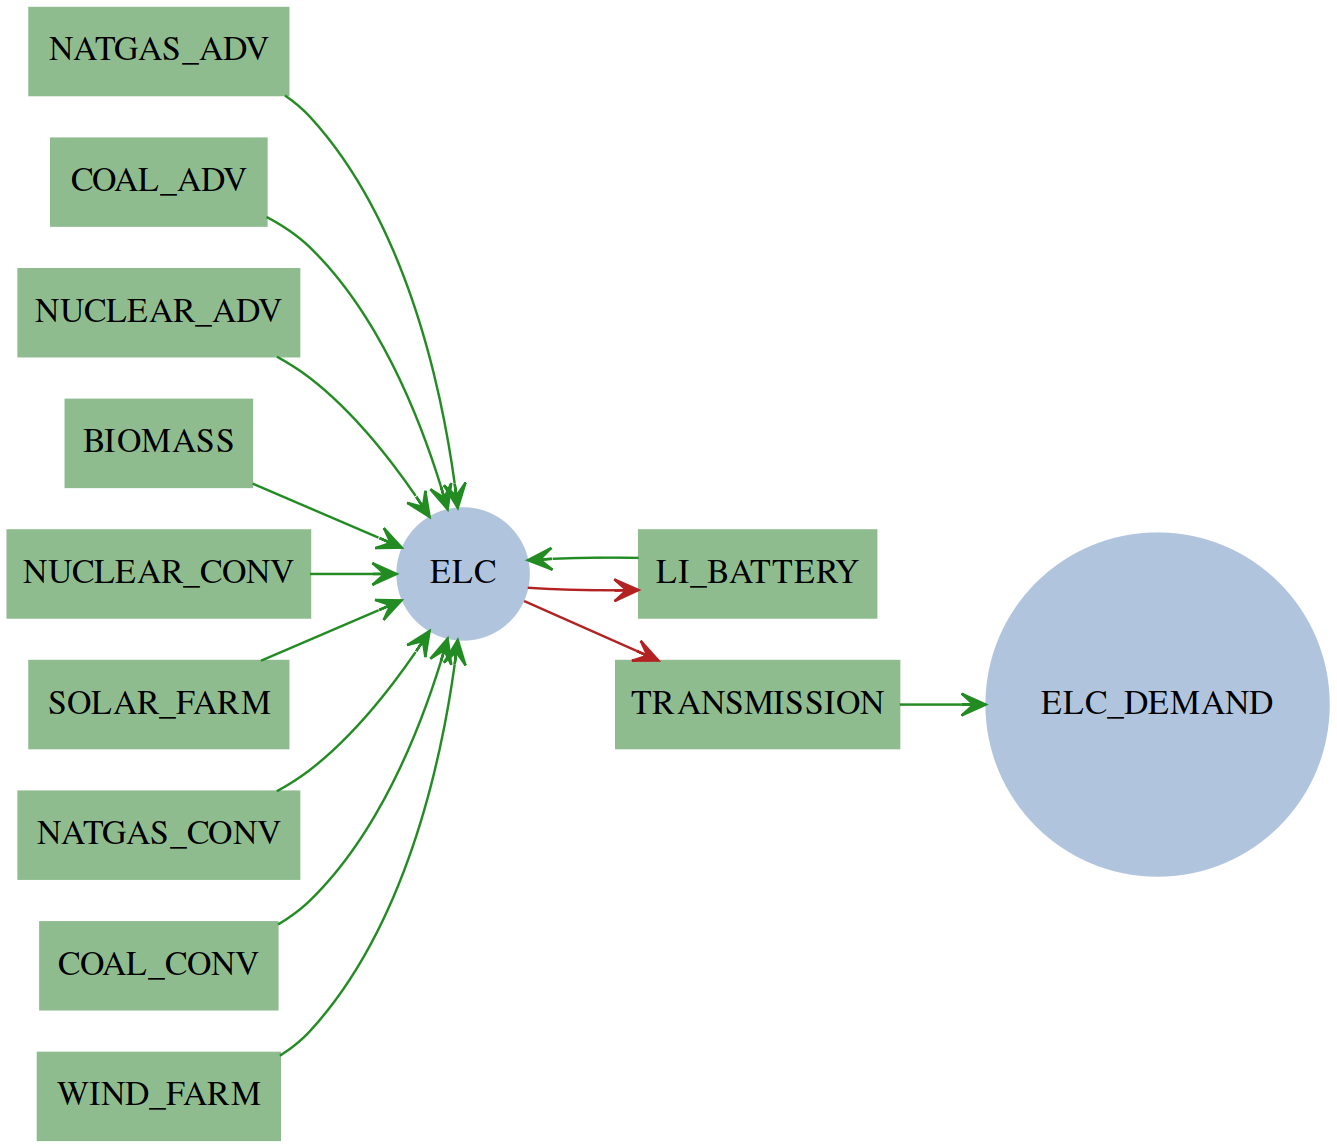
\includegraphics[width=0.6\columnwidth]{IL_system.png}
  \caption{The Illinois electricity grid modeled in \gls{temoa}.}
  \label{fig:ilsys}
\end{figure}

Figure \ref{fig:ilsys} shows the model topology of the Illinois system. There
are nine different electricity-generating technologies and one storage option.
All generated electricity passes through a \texttt{TRANSMISSION} technology
to simulate electricity delivery. The Illinois model is spatially and topologically
simple since there are only ten different technologies, one region, and one
end-use commodity.

The demand curve for the \texttt{ELC\_DEMAND} commodity uses hourly load
data from the PJM Interconnection. Figure \ref{fig:pjm-elc} shows the historical
electricity demand for PJM and the associated load curve. These data inform the
distribution of annual demand in the \gls{temoa} model, which is scaled by the
total annual demand.

\begin{figure}[H]
  \centering
  \resizebox{\columnwidth}{!}{%% Creator: Matplotlib, PGF backend
%%
%% To include the figure in your LaTeX document, write
%%   \input{<filename>.pgf}
%%
%% Make sure the required packages are loaded in your preamble
%%   \usepackage{pgf}
%%
%% Figures using additional raster images can only be included by \input if
%% they are in the same directory as the main LaTeX file. For loading figures
%% from other directories you can use the `import` package
%%   \usepackage{import}
%%
%% and then include the figures with
%%   \import{<path to file>}{<filename>.pgf}
%%
%% Matplotlib used the following preamble
%%
\begingroup%
\makeatletter%
\begin{pgfpicture}%
\pgfpathrectangle{\pgfpointorigin}{\pgfqpoint{14.900000in}{8.900000in}}%
\pgfusepath{use as bounding box, clip}%
\begin{pgfscope}%
\pgfsetbuttcap%
\pgfsetmiterjoin%
\definecolor{currentfill}{rgb}{1.000000,1.000000,1.000000}%
\pgfsetfillcolor{currentfill}%
\pgfsetlinewidth{0.000000pt}%
\definecolor{currentstroke}{rgb}{0.000000,0.000000,0.000000}%
\pgfsetstrokecolor{currentstroke}%
\pgfsetdash{}{0pt}%
\pgfpathmoveto{\pgfqpoint{0.000000in}{0.000000in}}%
\pgfpathlineto{\pgfqpoint{14.900000in}{0.000000in}}%
\pgfpathlineto{\pgfqpoint{14.900000in}{8.900000in}}%
\pgfpathlineto{\pgfqpoint{0.000000in}{8.900000in}}%
\pgfpathclose%
\pgfusepath{fill}%
\end{pgfscope}%
\begin{pgfscope}%
\pgfsetbuttcap%
\pgfsetmiterjoin%
\definecolor{currentfill}{rgb}{0.827451,0.827451,0.827451}%
\pgfsetfillcolor{currentfill}%
\pgfsetlinewidth{0.000000pt}%
\definecolor{currentstroke}{rgb}{0.000000,0.000000,0.000000}%
\pgfsetstrokecolor{currentstroke}%
\pgfsetstrokeopacity{0.000000}%
\pgfsetdash{}{0pt}%
\pgfpathmoveto{\pgfqpoint{1.079853in}{0.670138in}}%
\pgfpathlineto{\pgfqpoint{10.632936in}{0.670138in}}%
\pgfpathlineto{\pgfqpoint{10.632936in}{8.516628in}}%
\pgfpathlineto{\pgfqpoint{1.079853in}{8.516628in}}%
\pgfpathclose%
\pgfusepath{fill}%
\end{pgfscope}%
\begin{pgfscope}%
\pgfpathrectangle{\pgfqpoint{1.079853in}{0.670138in}}{\pgfqpoint{9.553083in}{7.846490in}}%
\pgfusepath{clip}%
\pgfsetrectcap%
\pgfsetroundjoin%
\pgfsetlinewidth{0.803000pt}%
\definecolor{currentstroke}{rgb}{1.000000,1.000000,1.000000}%
\pgfsetstrokecolor{currentstroke}%
\pgfsetdash{}{0pt}%
\pgfpathmoveto{\pgfqpoint{1.513913in}{0.670138in}}%
\pgfpathlineto{\pgfqpoint{1.513913in}{8.516628in}}%
\pgfusepath{stroke}%
\end{pgfscope}%
\begin{pgfscope}%
\pgfsetbuttcap%
\pgfsetroundjoin%
\definecolor{currentfill}{rgb}{0.000000,0.000000,0.000000}%
\pgfsetfillcolor{currentfill}%
\pgfsetlinewidth{0.803000pt}%
\definecolor{currentstroke}{rgb}{0.000000,0.000000,0.000000}%
\pgfsetstrokecolor{currentstroke}%
\pgfsetdash{}{0pt}%
\pgfsys@defobject{currentmarker}{\pgfqpoint{0.000000in}{-0.048611in}}{\pgfqpoint{0.000000in}{0.000000in}}{%
\pgfpathmoveto{\pgfqpoint{0.000000in}{0.000000in}}%
\pgfpathlineto{\pgfqpoint{0.000000in}{-0.048611in}}%
\pgfusepath{stroke,fill}%
}%
\begin{pgfscope}%
\pgfsys@transformshift{1.513913in}{0.670138in}%
\pgfsys@useobject{currentmarker}{}%
\end{pgfscope}%
\end{pgfscope}%
\begin{pgfscope}%
\definecolor{textcolor}{rgb}{0.000000,0.000000,0.000000}%
\pgfsetstrokecolor{textcolor}%
\pgfsetfillcolor{textcolor}%
\pgftext[x=1.513913in,y=0.572916in,right,top]{\color{textcolor}\rmfamily\fontsize{14.000000}{16.800000}\selectfont \(\displaystyle {2016}\)}%
\end{pgfscope}%
\begin{pgfscope}%
\pgfpathrectangle{\pgfqpoint{1.079853in}{0.670138in}}{\pgfqpoint{9.553083in}{7.846490in}}%
\pgfusepath{clip}%
\pgfsetrectcap%
\pgfsetroundjoin%
\pgfsetlinewidth{0.803000pt}%
\definecolor{currentstroke}{rgb}{1.000000,1.000000,1.000000}%
\pgfsetstrokecolor{currentstroke}%
\pgfsetdash{}{0pt}%
\pgfpathmoveto{\pgfqpoint{3.018236in}{0.670138in}}%
\pgfpathlineto{\pgfqpoint{3.018236in}{8.516628in}}%
\pgfusepath{stroke}%
\end{pgfscope}%
\begin{pgfscope}%
\pgfsetbuttcap%
\pgfsetroundjoin%
\definecolor{currentfill}{rgb}{0.000000,0.000000,0.000000}%
\pgfsetfillcolor{currentfill}%
\pgfsetlinewidth{0.803000pt}%
\definecolor{currentstroke}{rgb}{0.000000,0.000000,0.000000}%
\pgfsetstrokecolor{currentstroke}%
\pgfsetdash{}{0pt}%
\pgfsys@defobject{currentmarker}{\pgfqpoint{0.000000in}{-0.048611in}}{\pgfqpoint{0.000000in}{0.000000in}}{%
\pgfpathmoveto{\pgfqpoint{0.000000in}{0.000000in}}%
\pgfpathlineto{\pgfqpoint{0.000000in}{-0.048611in}}%
\pgfusepath{stroke,fill}%
}%
\begin{pgfscope}%
\pgfsys@transformshift{3.018236in}{0.670138in}%
\pgfsys@useobject{currentmarker}{}%
\end{pgfscope}%
\end{pgfscope}%
\begin{pgfscope}%
\definecolor{textcolor}{rgb}{0.000000,0.000000,0.000000}%
\pgfsetstrokecolor{textcolor}%
\pgfsetfillcolor{textcolor}%
\pgftext[x=3.018236in,y=0.572916in,right,top]{\color{textcolor}\rmfamily\fontsize{14.000000}{16.800000}\selectfont \(\displaystyle {2017}\)}%
\end{pgfscope}%
\begin{pgfscope}%
\pgfpathrectangle{\pgfqpoint{1.079853in}{0.670138in}}{\pgfqpoint{9.553083in}{7.846490in}}%
\pgfusepath{clip}%
\pgfsetrectcap%
\pgfsetroundjoin%
\pgfsetlinewidth{0.803000pt}%
\definecolor{currentstroke}{rgb}{1.000000,1.000000,1.000000}%
\pgfsetstrokecolor{currentstroke}%
\pgfsetdash{}{0pt}%
\pgfpathmoveto{\pgfqpoint{4.518448in}{0.670138in}}%
\pgfpathlineto{\pgfqpoint{4.518448in}{8.516628in}}%
\pgfusepath{stroke}%
\end{pgfscope}%
\begin{pgfscope}%
\pgfsetbuttcap%
\pgfsetroundjoin%
\definecolor{currentfill}{rgb}{0.000000,0.000000,0.000000}%
\pgfsetfillcolor{currentfill}%
\pgfsetlinewidth{0.803000pt}%
\definecolor{currentstroke}{rgb}{0.000000,0.000000,0.000000}%
\pgfsetstrokecolor{currentstroke}%
\pgfsetdash{}{0pt}%
\pgfsys@defobject{currentmarker}{\pgfqpoint{0.000000in}{-0.048611in}}{\pgfqpoint{0.000000in}{0.000000in}}{%
\pgfpathmoveto{\pgfqpoint{0.000000in}{0.000000in}}%
\pgfpathlineto{\pgfqpoint{0.000000in}{-0.048611in}}%
\pgfusepath{stroke,fill}%
}%
\begin{pgfscope}%
\pgfsys@transformshift{4.518448in}{0.670138in}%
\pgfsys@useobject{currentmarker}{}%
\end{pgfscope}%
\end{pgfscope}%
\begin{pgfscope}%
\definecolor{textcolor}{rgb}{0.000000,0.000000,0.000000}%
\pgfsetstrokecolor{textcolor}%
\pgfsetfillcolor{textcolor}%
\pgftext[x=4.518448in,y=0.572916in,right,top]{\color{textcolor}\rmfamily\fontsize{14.000000}{16.800000}\selectfont \(\displaystyle {2018}\)}%
\end{pgfscope}%
\begin{pgfscope}%
\pgfpathrectangle{\pgfqpoint{1.079853in}{0.670138in}}{\pgfqpoint{9.553083in}{7.846490in}}%
\pgfusepath{clip}%
\pgfsetrectcap%
\pgfsetroundjoin%
\pgfsetlinewidth{0.803000pt}%
\definecolor{currentstroke}{rgb}{1.000000,1.000000,1.000000}%
\pgfsetstrokecolor{currentstroke}%
\pgfsetdash{}{0pt}%
\pgfpathmoveto{\pgfqpoint{6.018661in}{0.670138in}}%
\pgfpathlineto{\pgfqpoint{6.018661in}{8.516628in}}%
\pgfusepath{stroke}%
\end{pgfscope}%
\begin{pgfscope}%
\pgfsetbuttcap%
\pgfsetroundjoin%
\definecolor{currentfill}{rgb}{0.000000,0.000000,0.000000}%
\pgfsetfillcolor{currentfill}%
\pgfsetlinewidth{0.803000pt}%
\definecolor{currentstroke}{rgb}{0.000000,0.000000,0.000000}%
\pgfsetstrokecolor{currentstroke}%
\pgfsetdash{}{0pt}%
\pgfsys@defobject{currentmarker}{\pgfqpoint{0.000000in}{-0.048611in}}{\pgfqpoint{0.000000in}{0.000000in}}{%
\pgfpathmoveto{\pgfqpoint{0.000000in}{0.000000in}}%
\pgfpathlineto{\pgfqpoint{0.000000in}{-0.048611in}}%
\pgfusepath{stroke,fill}%
}%
\begin{pgfscope}%
\pgfsys@transformshift{6.018661in}{0.670138in}%
\pgfsys@useobject{currentmarker}{}%
\end{pgfscope}%
\end{pgfscope}%
\begin{pgfscope}%
\definecolor{textcolor}{rgb}{0.000000,0.000000,0.000000}%
\pgfsetstrokecolor{textcolor}%
\pgfsetfillcolor{textcolor}%
\pgftext[x=6.018661in,y=0.572916in,right,top]{\color{textcolor}\rmfamily\fontsize{14.000000}{16.800000}\selectfont \(\displaystyle {2019}\)}%
\end{pgfscope}%
\begin{pgfscope}%
\pgfpathrectangle{\pgfqpoint{1.079853in}{0.670138in}}{\pgfqpoint{9.553083in}{7.846490in}}%
\pgfusepath{clip}%
\pgfsetrectcap%
\pgfsetroundjoin%
\pgfsetlinewidth{0.803000pt}%
\definecolor{currentstroke}{rgb}{1.000000,1.000000,1.000000}%
\pgfsetstrokecolor{currentstroke}%
\pgfsetdash{}{0pt}%
\pgfpathmoveto{\pgfqpoint{7.518873in}{0.670138in}}%
\pgfpathlineto{\pgfqpoint{7.518873in}{8.516628in}}%
\pgfusepath{stroke}%
\end{pgfscope}%
\begin{pgfscope}%
\pgfsetbuttcap%
\pgfsetroundjoin%
\definecolor{currentfill}{rgb}{0.000000,0.000000,0.000000}%
\pgfsetfillcolor{currentfill}%
\pgfsetlinewidth{0.803000pt}%
\definecolor{currentstroke}{rgb}{0.000000,0.000000,0.000000}%
\pgfsetstrokecolor{currentstroke}%
\pgfsetdash{}{0pt}%
\pgfsys@defobject{currentmarker}{\pgfqpoint{0.000000in}{-0.048611in}}{\pgfqpoint{0.000000in}{0.000000in}}{%
\pgfpathmoveto{\pgfqpoint{0.000000in}{0.000000in}}%
\pgfpathlineto{\pgfqpoint{0.000000in}{-0.048611in}}%
\pgfusepath{stroke,fill}%
}%
\begin{pgfscope}%
\pgfsys@transformshift{7.518873in}{0.670138in}%
\pgfsys@useobject{currentmarker}{}%
\end{pgfscope}%
\end{pgfscope}%
\begin{pgfscope}%
\definecolor{textcolor}{rgb}{0.000000,0.000000,0.000000}%
\pgfsetstrokecolor{textcolor}%
\pgfsetfillcolor{textcolor}%
\pgftext[x=7.518873in,y=0.572916in,right,top]{\color{textcolor}\rmfamily\fontsize{14.000000}{16.800000}\selectfont \(\displaystyle {2020}\)}%
\end{pgfscope}%
\begin{pgfscope}%
\pgfpathrectangle{\pgfqpoint{1.079853in}{0.670138in}}{\pgfqpoint{9.553083in}{7.846490in}}%
\pgfusepath{clip}%
\pgfsetrectcap%
\pgfsetroundjoin%
\pgfsetlinewidth{0.803000pt}%
\definecolor{currentstroke}{rgb}{1.000000,1.000000,1.000000}%
\pgfsetstrokecolor{currentstroke}%
\pgfsetdash{}{0pt}%
\pgfpathmoveto{\pgfqpoint{9.023196in}{0.670138in}}%
\pgfpathlineto{\pgfqpoint{9.023196in}{8.516628in}}%
\pgfusepath{stroke}%
\end{pgfscope}%
\begin{pgfscope}%
\pgfsetbuttcap%
\pgfsetroundjoin%
\definecolor{currentfill}{rgb}{0.000000,0.000000,0.000000}%
\pgfsetfillcolor{currentfill}%
\pgfsetlinewidth{0.803000pt}%
\definecolor{currentstroke}{rgb}{0.000000,0.000000,0.000000}%
\pgfsetstrokecolor{currentstroke}%
\pgfsetdash{}{0pt}%
\pgfsys@defobject{currentmarker}{\pgfqpoint{0.000000in}{-0.048611in}}{\pgfqpoint{0.000000in}{0.000000in}}{%
\pgfpathmoveto{\pgfqpoint{0.000000in}{0.000000in}}%
\pgfpathlineto{\pgfqpoint{0.000000in}{-0.048611in}}%
\pgfusepath{stroke,fill}%
}%
\begin{pgfscope}%
\pgfsys@transformshift{9.023196in}{0.670138in}%
\pgfsys@useobject{currentmarker}{}%
\end{pgfscope}%
\end{pgfscope}%
\begin{pgfscope}%
\definecolor{textcolor}{rgb}{0.000000,0.000000,0.000000}%
\pgfsetstrokecolor{textcolor}%
\pgfsetfillcolor{textcolor}%
\pgftext[x=9.023196in,y=0.572916in,right,top]{\color{textcolor}\rmfamily\fontsize{14.000000}{16.800000}\selectfont \(\displaystyle {2021}\)}%
\end{pgfscope}%
\begin{pgfscope}%
\pgfpathrectangle{\pgfqpoint{1.079853in}{0.670138in}}{\pgfqpoint{9.553083in}{7.846490in}}%
\pgfusepath{clip}%
\pgfsetrectcap%
\pgfsetroundjoin%
\pgfsetlinewidth{0.803000pt}%
\definecolor{currentstroke}{rgb}{1.000000,1.000000,1.000000}%
\pgfsetstrokecolor{currentstroke}%
\pgfsetdash{}{0pt}%
\pgfpathmoveto{\pgfqpoint{10.523409in}{0.670138in}}%
\pgfpathlineto{\pgfqpoint{10.523409in}{8.516628in}}%
\pgfusepath{stroke}%
\end{pgfscope}%
\begin{pgfscope}%
\pgfsetbuttcap%
\pgfsetroundjoin%
\definecolor{currentfill}{rgb}{0.000000,0.000000,0.000000}%
\pgfsetfillcolor{currentfill}%
\pgfsetlinewidth{0.803000pt}%
\definecolor{currentstroke}{rgb}{0.000000,0.000000,0.000000}%
\pgfsetstrokecolor{currentstroke}%
\pgfsetdash{}{0pt}%
\pgfsys@defobject{currentmarker}{\pgfqpoint{0.000000in}{-0.048611in}}{\pgfqpoint{0.000000in}{0.000000in}}{%
\pgfpathmoveto{\pgfqpoint{0.000000in}{0.000000in}}%
\pgfpathlineto{\pgfqpoint{0.000000in}{-0.048611in}}%
\pgfusepath{stroke,fill}%
}%
\begin{pgfscope}%
\pgfsys@transformshift{10.523409in}{0.670138in}%
\pgfsys@useobject{currentmarker}{}%
\end{pgfscope}%
\end{pgfscope}%
\begin{pgfscope}%
\definecolor{textcolor}{rgb}{0.000000,0.000000,0.000000}%
\pgfsetstrokecolor{textcolor}%
\pgfsetfillcolor{textcolor}%
\pgftext[x=10.523409in,y=0.572916in,right,top]{\color{textcolor}\rmfamily\fontsize{14.000000}{16.800000}\selectfont \(\displaystyle {2022}\)}%
\end{pgfscope}%
\begin{pgfscope}%
\pgfsetbuttcap%
\pgfsetroundjoin%
\definecolor{currentfill}{rgb}{0.000000,0.000000,0.000000}%
\pgfsetfillcolor{currentfill}%
\pgfsetlinewidth{0.602250pt}%
\definecolor{currentstroke}{rgb}{0.000000,0.000000,0.000000}%
\pgfsetstrokecolor{currentstroke}%
\pgfsetdash{}{0pt}%
\pgfsys@defobject{currentmarker}{\pgfqpoint{0.000000in}{-0.027778in}}{\pgfqpoint{0.000000in}{0.000000in}}{%
\pgfpathmoveto{\pgfqpoint{0.000000in}{0.000000in}}%
\pgfpathlineto{\pgfqpoint{0.000000in}{-0.027778in}}%
\pgfusepath{stroke,fill}%
}%
\begin{pgfscope}%
\pgfsys@transformshift{1.138860in}{0.670138in}%
\pgfsys@useobject{currentmarker}{}%
\end{pgfscope}%
\end{pgfscope}%
\begin{pgfscope}%
\pgfsetbuttcap%
\pgfsetroundjoin%
\definecolor{currentfill}{rgb}{0.000000,0.000000,0.000000}%
\pgfsetfillcolor{currentfill}%
\pgfsetlinewidth{0.602250pt}%
\definecolor{currentstroke}{rgb}{0.000000,0.000000,0.000000}%
\pgfsetstrokecolor{currentstroke}%
\pgfsetdash{}{0pt}%
\pgfsys@defobject{currentmarker}{\pgfqpoint{0.000000in}{-0.027778in}}{\pgfqpoint{0.000000in}{0.000000in}}{%
\pgfpathmoveto{\pgfqpoint{0.000000in}{0.000000in}}%
\pgfpathlineto{\pgfqpoint{0.000000in}{-0.027778in}}%
\pgfusepath{stroke,fill}%
}%
\begin{pgfscope}%
\pgfsys@transformshift{1.888966in}{0.670138in}%
\pgfsys@useobject{currentmarker}{}%
\end{pgfscope}%
\end{pgfscope}%
\begin{pgfscope}%
\pgfsetbuttcap%
\pgfsetroundjoin%
\definecolor{currentfill}{rgb}{0.000000,0.000000,0.000000}%
\pgfsetfillcolor{currentfill}%
\pgfsetlinewidth{0.602250pt}%
\definecolor{currentstroke}{rgb}{0.000000,0.000000,0.000000}%
\pgfsetstrokecolor{currentstroke}%
\pgfsetdash{}{0pt}%
\pgfsys@defobject{currentmarker}{\pgfqpoint{0.000000in}{-0.027778in}}{\pgfqpoint{0.000000in}{0.000000in}}{%
\pgfpathmoveto{\pgfqpoint{0.000000in}{0.000000in}}%
\pgfpathlineto{\pgfqpoint{0.000000in}{-0.027778in}}%
\pgfusepath{stroke,fill}%
}%
\begin{pgfscope}%
\pgfsys@transformshift{2.264019in}{0.670138in}%
\pgfsys@useobject{currentmarker}{}%
\end{pgfscope}%
\end{pgfscope}%
\begin{pgfscope}%
\pgfsetbuttcap%
\pgfsetroundjoin%
\definecolor{currentfill}{rgb}{0.000000,0.000000,0.000000}%
\pgfsetfillcolor{currentfill}%
\pgfsetlinewidth{0.602250pt}%
\definecolor{currentstroke}{rgb}{0.000000,0.000000,0.000000}%
\pgfsetstrokecolor{currentstroke}%
\pgfsetdash{}{0pt}%
\pgfsys@defobject{currentmarker}{\pgfqpoint{0.000000in}{-0.027778in}}{\pgfqpoint{0.000000in}{0.000000in}}{%
\pgfpathmoveto{\pgfqpoint{0.000000in}{0.000000in}}%
\pgfpathlineto{\pgfqpoint{0.000000in}{-0.027778in}}%
\pgfusepath{stroke,fill}%
}%
\begin{pgfscope}%
\pgfsys@transformshift{2.639072in}{0.670138in}%
\pgfsys@useobject{currentmarker}{}%
\end{pgfscope}%
\end{pgfscope}%
\begin{pgfscope}%
\pgfsetbuttcap%
\pgfsetroundjoin%
\definecolor{currentfill}{rgb}{0.000000,0.000000,0.000000}%
\pgfsetfillcolor{currentfill}%
\pgfsetlinewidth{0.602250pt}%
\definecolor{currentstroke}{rgb}{0.000000,0.000000,0.000000}%
\pgfsetstrokecolor{currentstroke}%
\pgfsetdash{}{0pt}%
\pgfsys@defobject{currentmarker}{\pgfqpoint{0.000000in}{-0.027778in}}{\pgfqpoint{0.000000in}{0.000000in}}{%
\pgfpathmoveto{\pgfqpoint{0.000000in}{0.000000in}}%
\pgfpathlineto{\pgfqpoint{0.000000in}{-0.027778in}}%
\pgfusepath{stroke,fill}%
}%
\begin{pgfscope}%
\pgfsys@transformshift{3.014126in}{0.670138in}%
\pgfsys@useobject{currentmarker}{}%
\end{pgfscope}%
\end{pgfscope}%
\begin{pgfscope}%
\pgfsetbuttcap%
\pgfsetroundjoin%
\definecolor{currentfill}{rgb}{0.000000,0.000000,0.000000}%
\pgfsetfillcolor{currentfill}%
\pgfsetlinewidth{0.602250pt}%
\definecolor{currentstroke}{rgb}{0.000000,0.000000,0.000000}%
\pgfsetstrokecolor{currentstroke}%
\pgfsetdash{}{0pt}%
\pgfsys@defobject{currentmarker}{\pgfqpoint{0.000000in}{-0.027778in}}{\pgfqpoint{0.000000in}{0.000000in}}{%
\pgfpathmoveto{\pgfqpoint{0.000000in}{0.000000in}}%
\pgfpathlineto{\pgfqpoint{0.000000in}{-0.027778in}}%
\pgfusepath{stroke,fill}%
}%
\begin{pgfscope}%
\pgfsys@transformshift{3.389179in}{0.670138in}%
\pgfsys@useobject{currentmarker}{}%
\end{pgfscope}%
\end{pgfscope}%
\begin{pgfscope}%
\pgfsetbuttcap%
\pgfsetroundjoin%
\definecolor{currentfill}{rgb}{0.000000,0.000000,0.000000}%
\pgfsetfillcolor{currentfill}%
\pgfsetlinewidth{0.602250pt}%
\definecolor{currentstroke}{rgb}{0.000000,0.000000,0.000000}%
\pgfsetstrokecolor{currentstroke}%
\pgfsetdash{}{0pt}%
\pgfsys@defobject{currentmarker}{\pgfqpoint{0.000000in}{-0.027778in}}{\pgfqpoint{0.000000in}{0.000000in}}{%
\pgfpathmoveto{\pgfqpoint{0.000000in}{0.000000in}}%
\pgfpathlineto{\pgfqpoint{0.000000in}{-0.027778in}}%
\pgfusepath{stroke,fill}%
}%
\begin{pgfscope}%
\pgfsys@transformshift{3.764232in}{0.670138in}%
\pgfsys@useobject{currentmarker}{}%
\end{pgfscope}%
\end{pgfscope}%
\begin{pgfscope}%
\pgfsetbuttcap%
\pgfsetroundjoin%
\definecolor{currentfill}{rgb}{0.000000,0.000000,0.000000}%
\pgfsetfillcolor{currentfill}%
\pgfsetlinewidth{0.602250pt}%
\definecolor{currentstroke}{rgb}{0.000000,0.000000,0.000000}%
\pgfsetstrokecolor{currentstroke}%
\pgfsetdash{}{0pt}%
\pgfsys@defobject{currentmarker}{\pgfqpoint{0.000000in}{-0.027778in}}{\pgfqpoint{0.000000in}{0.000000in}}{%
\pgfpathmoveto{\pgfqpoint{0.000000in}{0.000000in}}%
\pgfpathlineto{\pgfqpoint{0.000000in}{-0.027778in}}%
\pgfusepath{stroke,fill}%
}%
\begin{pgfscope}%
\pgfsys@transformshift{4.139285in}{0.670138in}%
\pgfsys@useobject{currentmarker}{}%
\end{pgfscope}%
\end{pgfscope}%
\begin{pgfscope}%
\pgfsetbuttcap%
\pgfsetroundjoin%
\definecolor{currentfill}{rgb}{0.000000,0.000000,0.000000}%
\pgfsetfillcolor{currentfill}%
\pgfsetlinewidth{0.602250pt}%
\definecolor{currentstroke}{rgb}{0.000000,0.000000,0.000000}%
\pgfsetstrokecolor{currentstroke}%
\pgfsetdash{}{0pt}%
\pgfsys@defobject{currentmarker}{\pgfqpoint{0.000000in}{-0.027778in}}{\pgfqpoint{0.000000in}{0.000000in}}{%
\pgfpathmoveto{\pgfqpoint{0.000000in}{0.000000in}}%
\pgfpathlineto{\pgfqpoint{0.000000in}{-0.027778in}}%
\pgfusepath{stroke,fill}%
}%
\begin{pgfscope}%
\pgfsys@transformshift{4.514338in}{0.670138in}%
\pgfsys@useobject{currentmarker}{}%
\end{pgfscope}%
\end{pgfscope}%
\begin{pgfscope}%
\pgfsetbuttcap%
\pgfsetroundjoin%
\definecolor{currentfill}{rgb}{0.000000,0.000000,0.000000}%
\pgfsetfillcolor{currentfill}%
\pgfsetlinewidth{0.602250pt}%
\definecolor{currentstroke}{rgb}{0.000000,0.000000,0.000000}%
\pgfsetstrokecolor{currentstroke}%
\pgfsetdash{}{0pt}%
\pgfsys@defobject{currentmarker}{\pgfqpoint{0.000000in}{-0.027778in}}{\pgfqpoint{0.000000in}{0.000000in}}{%
\pgfpathmoveto{\pgfqpoint{0.000000in}{0.000000in}}%
\pgfpathlineto{\pgfqpoint{0.000000in}{-0.027778in}}%
\pgfusepath{stroke,fill}%
}%
\begin{pgfscope}%
\pgfsys@transformshift{4.889391in}{0.670138in}%
\pgfsys@useobject{currentmarker}{}%
\end{pgfscope}%
\end{pgfscope}%
\begin{pgfscope}%
\pgfsetbuttcap%
\pgfsetroundjoin%
\definecolor{currentfill}{rgb}{0.000000,0.000000,0.000000}%
\pgfsetfillcolor{currentfill}%
\pgfsetlinewidth{0.602250pt}%
\definecolor{currentstroke}{rgb}{0.000000,0.000000,0.000000}%
\pgfsetstrokecolor{currentstroke}%
\pgfsetdash{}{0pt}%
\pgfsys@defobject{currentmarker}{\pgfqpoint{0.000000in}{-0.027778in}}{\pgfqpoint{0.000000in}{0.000000in}}{%
\pgfpathmoveto{\pgfqpoint{0.000000in}{0.000000in}}%
\pgfpathlineto{\pgfqpoint{0.000000in}{-0.027778in}}%
\pgfusepath{stroke,fill}%
}%
\begin{pgfscope}%
\pgfsys@transformshift{5.264444in}{0.670138in}%
\pgfsys@useobject{currentmarker}{}%
\end{pgfscope}%
\end{pgfscope}%
\begin{pgfscope}%
\pgfsetbuttcap%
\pgfsetroundjoin%
\definecolor{currentfill}{rgb}{0.000000,0.000000,0.000000}%
\pgfsetfillcolor{currentfill}%
\pgfsetlinewidth{0.602250pt}%
\definecolor{currentstroke}{rgb}{0.000000,0.000000,0.000000}%
\pgfsetstrokecolor{currentstroke}%
\pgfsetdash{}{0pt}%
\pgfsys@defobject{currentmarker}{\pgfqpoint{0.000000in}{-0.027778in}}{\pgfqpoint{0.000000in}{0.000000in}}{%
\pgfpathmoveto{\pgfqpoint{0.000000in}{0.000000in}}%
\pgfpathlineto{\pgfqpoint{0.000000in}{-0.027778in}}%
\pgfusepath{stroke,fill}%
}%
\begin{pgfscope}%
\pgfsys@transformshift{5.639498in}{0.670138in}%
\pgfsys@useobject{currentmarker}{}%
\end{pgfscope}%
\end{pgfscope}%
\begin{pgfscope}%
\pgfsetbuttcap%
\pgfsetroundjoin%
\definecolor{currentfill}{rgb}{0.000000,0.000000,0.000000}%
\pgfsetfillcolor{currentfill}%
\pgfsetlinewidth{0.602250pt}%
\definecolor{currentstroke}{rgb}{0.000000,0.000000,0.000000}%
\pgfsetstrokecolor{currentstroke}%
\pgfsetdash{}{0pt}%
\pgfsys@defobject{currentmarker}{\pgfqpoint{0.000000in}{-0.027778in}}{\pgfqpoint{0.000000in}{0.000000in}}{%
\pgfpathmoveto{\pgfqpoint{0.000000in}{0.000000in}}%
\pgfpathlineto{\pgfqpoint{0.000000in}{-0.027778in}}%
\pgfusepath{stroke,fill}%
}%
\begin{pgfscope}%
\pgfsys@transformshift{6.014551in}{0.670138in}%
\pgfsys@useobject{currentmarker}{}%
\end{pgfscope}%
\end{pgfscope}%
\begin{pgfscope}%
\pgfsetbuttcap%
\pgfsetroundjoin%
\definecolor{currentfill}{rgb}{0.000000,0.000000,0.000000}%
\pgfsetfillcolor{currentfill}%
\pgfsetlinewidth{0.602250pt}%
\definecolor{currentstroke}{rgb}{0.000000,0.000000,0.000000}%
\pgfsetstrokecolor{currentstroke}%
\pgfsetdash{}{0pt}%
\pgfsys@defobject{currentmarker}{\pgfqpoint{0.000000in}{-0.027778in}}{\pgfqpoint{0.000000in}{0.000000in}}{%
\pgfpathmoveto{\pgfqpoint{0.000000in}{0.000000in}}%
\pgfpathlineto{\pgfqpoint{0.000000in}{-0.027778in}}%
\pgfusepath{stroke,fill}%
}%
\begin{pgfscope}%
\pgfsys@transformshift{6.389604in}{0.670138in}%
\pgfsys@useobject{currentmarker}{}%
\end{pgfscope}%
\end{pgfscope}%
\begin{pgfscope}%
\pgfsetbuttcap%
\pgfsetroundjoin%
\definecolor{currentfill}{rgb}{0.000000,0.000000,0.000000}%
\pgfsetfillcolor{currentfill}%
\pgfsetlinewidth{0.602250pt}%
\definecolor{currentstroke}{rgb}{0.000000,0.000000,0.000000}%
\pgfsetstrokecolor{currentstroke}%
\pgfsetdash{}{0pt}%
\pgfsys@defobject{currentmarker}{\pgfqpoint{0.000000in}{-0.027778in}}{\pgfqpoint{0.000000in}{0.000000in}}{%
\pgfpathmoveto{\pgfqpoint{0.000000in}{0.000000in}}%
\pgfpathlineto{\pgfqpoint{0.000000in}{-0.027778in}}%
\pgfusepath{stroke,fill}%
}%
\begin{pgfscope}%
\pgfsys@transformshift{6.764657in}{0.670138in}%
\pgfsys@useobject{currentmarker}{}%
\end{pgfscope}%
\end{pgfscope}%
\begin{pgfscope}%
\pgfsetbuttcap%
\pgfsetroundjoin%
\definecolor{currentfill}{rgb}{0.000000,0.000000,0.000000}%
\pgfsetfillcolor{currentfill}%
\pgfsetlinewidth{0.602250pt}%
\definecolor{currentstroke}{rgb}{0.000000,0.000000,0.000000}%
\pgfsetstrokecolor{currentstroke}%
\pgfsetdash{}{0pt}%
\pgfsys@defobject{currentmarker}{\pgfqpoint{0.000000in}{-0.027778in}}{\pgfqpoint{0.000000in}{0.000000in}}{%
\pgfpathmoveto{\pgfqpoint{0.000000in}{0.000000in}}%
\pgfpathlineto{\pgfqpoint{0.000000in}{-0.027778in}}%
\pgfusepath{stroke,fill}%
}%
\begin{pgfscope}%
\pgfsys@transformshift{7.139710in}{0.670138in}%
\pgfsys@useobject{currentmarker}{}%
\end{pgfscope}%
\end{pgfscope}%
\begin{pgfscope}%
\pgfsetbuttcap%
\pgfsetroundjoin%
\definecolor{currentfill}{rgb}{0.000000,0.000000,0.000000}%
\pgfsetfillcolor{currentfill}%
\pgfsetlinewidth{0.602250pt}%
\definecolor{currentstroke}{rgb}{0.000000,0.000000,0.000000}%
\pgfsetstrokecolor{currentstroke}%
\pgfsetdash{}{0pt}%
\pgfsys@defobject{currentmarker}{\pgfqpoint{0.000000in}{-0.027778in}}{\pgfqpoint{0.000000in}{0.000000in}}{%
\pgfpathmoveto{\pgfqpoint{0.000000in}{0.000000in}}%
\pgfpathlineto{\pgfqpoint{0.000000in}{-0.027778in}}%
\pgfusepath{stroke,fill}%
}%
\begin{pgfscope}%
\pgfsys@transformshift{7.514763in}{0.670138in}%
\pgfsys@useobject{currentmarker}{}%
\end{pgfscope}%
\end{pgfscope}%
\begin{pgfscope}%
\pgfsetbuttcap%
\pgfsetroundjoin%
\definecolor{currentfill}{rgb}{0.000000,0.000000,0.000000}%
\pgfsetfillcolor{currentfill}%
\pgfsetlinewidth{0.602250pt}%
\definecolor{currentstroke}{rgb}{0.000000,0.000000,0.000000}%
\pgfsetstrokecolor{currentstroke}%
\pgfsetdash{}{0pt}%
\pgfsys@defobject{currentmarker}{\pgfqpoint{0.000000in}{-0.027778in}}{\pgfqpoint{0.000000in}{0.000000in}}{%
\pgfpathmoveto{\pgfqpoint{0.000000in}{0.000000in}}%
\pgfpathlineto{\pgfqpoint{0.000000in}{-0.027778in}}%
\pgfusepath{stroke,fill}%
}%
\begin{pgfscope}%
\pgfsys@transformshift{7.889816in}{0.670138in}%
\pgfsys@useobject{currentmarker}{}%
\end{pgfscope}%
\end{pgfscope}%
\begin{pgfscope}%
\pgfsetbuttcap%
\pgfsetroundjoin%
\definecolor{currentfill}{rgb}{0.000000,0.000000,0.000000}%
\pgfsetfillcolor{currentfill}%
\pgfsetlinewidth{0.602250pt}%
\definecolor{currentstroke}{rgb}{0.000000,0.000000,0.000000}%
\pgfsetstrokecolor{currentstroke}%
\pgfsetdash{}{0pt}%
\pgfsys@defobject{currentmarker}{\pgfqpoint{0.000000in}{-0.027778in}}{\pgfqpoint{0.000000in}{0.000000in}}{%
\pgfpathmoveto{\pgfqpoint{0.000000in}{0.000000in}}%
\pgfpathlineto{\pgfqpoint{0.000000in}{-0.027778in}}%
\pgfusepath{stroke,fill}%
}%
\begin{pgfscope}%
\pgfsys@transformshift{8.264869in}{0.670138in}%
\pgfsys@useobject{currentmarker}{}%
\end{pgfscope}%
\end{pgfscope}%
\begin{pgfscope}%
\pgfsetbuttcap%
\pgfsetroundjoin%
\definecolor{currentfill}{rgb}{0.000000,0.000000,0.000000}%
\pgfsetfillcolor{currentfill}%
\pgfsetlinewidth{0.602250pt}%
\definecolor{currentstroke}{rgb}{0.000000,0.000000,0.000000}%
\pgfsetstrokecolor{currentstroke}%
\pgfsetdash{}{0pt}%
\pgfsys@defobject{currentmarker}{\pgfqpoint{0.000000in}{-0.027778in}}{\pgfqpoint{0.000000in}{0.000000in}}{%
\pgfpathmoveto{\pgfqpoint{0.000000in}{0.000000in}}%
\pgfpathlineto{\pgfqpoint{0.000000in}{-0.027778in}}%
\pgfusepath{stroke,fill}%
}%
\begin{pgfscope}%
\pgfsys@transformshift{8.639923in}{0.670138in}%
\pgfsys@useobject{currentmarker}{}%
\end{pgfscope}%
\end{pgfscope}%
\begin{pgfscope}%
\pgfsetbuttcap%
\pgfsetroundjoin%
\definecolor{currentfill}{rgb}{0.000000,0.000000,0.000000}%
\pgfsetfillcolor{currentfill}%
\pgfsetlinewidth{0.602250pt}%
\definecolor{currentstroke}{rgb}{0.000000,0.000000,0.000000}%
\pgfsetstrokecolor{currentstroke}%
\pgfsetdash{}{0pt}%
\pgfsys@defobject{currentmarker}{\pgfqpoint{0.000000in}{-0.027778in}}{\pgfqpoint{0.000000in}{0.000000in}}{%
\pgfpathmoveto{\pgfqpoint{0.000000in}{0.000000in}}%
\pgfpathlineto{\pgfqpoint{0.000000in}{-0.027778in}}%
\pgfusepath{stroke,fill}%
}%
\begin{pgfscope}%
\pgfsys@transformshift{9.014976in}{0.670138in}%
\pgfsys@useobject{currentmarker}{}%
\end{pgfscope}%
\end{pgfscope}%
\begin{pgfscope}%
\pgfsetbuttcap%
\pgfsetroundjoin%
\definecolor{currentfill}{rgb}{0.000000,0.000000,0.000000}%
\pgfsetfillcolor{currentfill}%
\pgfsetlinewidth{0.602250pt}%
\definecolor{currentstroke}{rgb}{0.000000,0.000000,0.000000}%
\pgfsetstrokecolor{currentstroke}%
\pgfsetdash{}{0pt}%
\pgfsys@defobject{currentmarker}{\pgfqpoint{0.000000in}{-0.027778in}}{\pgfqpoint{0.000000in}{0.000000in}}{%
\pgfpathmoveto{\pgfqpoint{0.000000in}{0.000000in}}%
\pgfpathlineto{\pgfqpoint{0.000000in}{-0.027778in}}%
\pgfusepath{stroke,fill}%
}%
\begin{pgfscope}%
\pgfsys@transformshift{9.390029in}{0.670138in}%
\pgfsys@useobject{currentmarker}{}%
\end{pgfscope}%
\end{pgfscope}%
\begin{pgfscope}%
\pgfsetbuttcap%
\pgfsetroundjoin%
\definecolor{currentfill}{rgb}{0.000000,0.000000,0.000000}%
\pgfsetfillcolor{currentfill}%
\pgfsetlinewidth{0.602250pt}%
\definecolor{currentstroke}{rgb}{0.000000,0.000000,0.000000}%
\pgfsetstrokecolor{currentstroke}%
\pgfsetdash{}{0pt}%
\pgfsys@defobject{currentmarker}{\pgfqpoint{0.000000in}{-0.027778in}}{\pgfqpoint{0.000000in}{0.000000in}}{%
\pgfpathmoveto{\pgfqpoint{0.000000in}{0.000000in}}%
\pgfpathlineto{\pgfqpoint{0.000000in}{-0.027778in}}%
\pgfusepath{stroke,fill}%
}%
\begin{pgfscope}%
\pgfsys@transformshift{9.765082in}{0.670138in}%
\pgfsys@useobject{currentmarker}{}%
\end{pgfscope}%
\end{pgfscope}%
\begin{pgfscope}%
\pgfsetbuttcap%
\pgfsetroundjoin%
\definecolor{currentfill}{rgb}{0.000000,0.000000,0.000000}%
\pgfsetfillcolor{currentfill}%
\pgfsetlinewidth{0.602250pt}%
\definecolor{currentstroke}{rgb}{0.000000,0.000000,0.000000}%
\pgfsetstrokecolor{currentstroke}%
\pgfsetdash{}{0pt}%
\pgfsys@defobject{currentmarker}{\pgfqpoint{0.000000in}{-0.027778in}}{\pgfqpoint{0.000000in}{0.000000in}}{%
\pgfpathmoveto{\pgfqpoint{0.000000in}{0.000000in}}%
\pgfpathlineto{\pgfqpoint{0.000000in}{-0.027778in}}%
\pgfusepath{stroke,fill}%
}%
\begin{pgfscope}%
\pgfsys@transformshift{10.140135in}{0.670138in}%
\pgfsys@useobject{currentmarker}{}%
\end{pgfscope}%
\end{pgfscope}%
\begin{pgfscope}%
\pgfsetbuttcap%
\pgfsetroundjoin%
\definecolor{currentfill}{rgb}{0.000000,0.000000,0.000000}%
\pgfsetfillcolor{currentfill}%
\pgfsetlinewidth{0.602250pt}%
\definecolor{currentstroke}{rgb}{0.000000,0.000000,0.000000}%
\pgfsetstrokecolor{currentstroke}%
\pgfsetdash{}{0pt}%
\pgfsys@defobject{currentmarker}{\pgfqpoint{0.000000in}{-0.027778in}}{\pgfqpoint{0.000000in}{0.000000in}}{%
\pgfpathmoveto{\pgfqpoint{0.000000in}{0.000000in}}%
\pgfpathlineto{\pgfqpoint{0.000000in}{-0.027778in}}%
\pgfusepath{stroke,fill}%
}%
\begin{pgfscope}%
\pgfsys@transformshift{10.515188in}{0.670138in}%
\pgfsys@useobject{currentmarker}{}%
\end{pgfscope}%
\end{pgfscope}%
\begin{pgfscope}%
\definecolor{textcolor}{rgb}{0.000000,0.000000,0.000000}%
\pgfsetstrokecolor{textcolor}%
\pgfsetfillcolor{textcolor}%
\pgftext[x=5.856395in,y=0.339583in,,top]{\color{textcolor}\rmfamily\fontsize{18.000000}{21.600000}\selectfont Time [hours]}%
\end{pgfscope}%
\begin{pgfscope}%
\pgfpathrectangle{\pgfqpoint{1.079853in}{0.670138in}}{\pgfqpoint{9.553083in}{7.846490in}}%
\pgfusepath{clip}%
\pgfsetrectcap%
\pgfsetroundjoin%
\pgfsetlinewidth{0.803000pt}%
\definecolor{currentstroke}{rgb}{1.000000,1.000000,1.000000}%
\pgfsetstrokecolor{currentstroke}%
\pgfsetdash{}{0pt}%
\pgfpathmoveto{\pgfqpoint{1.079853in}{0.800497in}}%
\pgfpathlineto{\pgfqpoint{10.632936in}{0.800497in}}%
\pgfusepath{stroke}%
\end{pgfscope}%
\begin{pgfscope}%
\pgfsetbuttcap%
\pgfsetroundjoin%
\definecolor{currentfill}{rgb}{0.000000,0.000000,0.000000}%
\pgfsetfillcolor{currentfill}%
\pgfsetlinewidth{0.803000pt}%
\definecolor{currentstroke}{rgb}{0.000000,0.000000,0.000000}%
\pgfsetstrokecolor{currentstroke}%
\pgfsetdash{}{0pt}%
\pgfsys@defobject{currentmarker}{\pgfqpoint{-0.048611in}{0.000000in}}{\pgfqpoint{-0.000000in}{0.000000in}}{%
\pgfpathmoveto{\pgfqpoint{-0.000000in}{0.000000in}}%
\pgfpathlineto{\pgfqpoint{-0.048611in}{0.000000in}}%
\pgfusepath{stroke,fill}%
}%
\begin{pgfscope}%
\pgfsys@transformshift{1.079853in}{0.800497in}%
\pgfsys@useobject{currentmarker}{}%
\end{pgfscope}%
\end{pgfscope}%
\begin{pgfscope}%
\definecolor{textcolor}{rgb}{0.000000,0.000000,0.000000}%
\pgfsetstrokecolor{textcolor}%
\pgfsetfillcolor{textcolor}%
\pgftext[x=0.493054in, y=0.731053in, left, base]{\color{textcolor}\rmfamily\fontsize{14.000000}{16.800000}\selectfont \(\displaystyle {60000}\)}%
\end{pgfscope}%
\begin{pgfscope}%
\pgfpathrectangle{\pgfqpoint{1.079853in}{0.670138in}}{\pgfqpoint{9.553083in}{7.846490in}}%
\pgfusepath{clip}%
\pgfsetrectcap%
\pgfsetroundjoin%
\pgfsetlinewidth{0.803000pt}%
\definecolor{currentstroke}{rgb}{1.000000,1.000000,1.000000}%
\pgfsetstrokecolor{currentstroke}%
\pgfsetdash{}{0pt}%
\pgfpathmoveto{\pgfqpoint{1.079853in}{2.515745in}}%
\pgfpathlineto{\pgfqpoint{10.632936in}{2.515745in}}%
\pgfusepath{stroke}%
\end{pgfscope}%
\begin{pgfscope}%
\pgfsetbuttcap%
\pgfsetroundjoin%
\definecolor{currentfill}{rgb}{0.000000,0.000000,0.000000}%
\pgfsetfillcolor{currentfill}%
\pgfsetlinewidth{0.803000pt}%
\definecolor{currentstroke}{rgb}{0.000000,0.000000,0.000000}%
\pgfsetstrokecolor{currentstroke}%
\pgfsetdash{}{0pt}%
\pgfsys@defobject{currentmarker}{\pgfqpoint{-0.048611in}{0.000000in}}{\pgfqpoint{-0.000000in}{0.000000in}}{%
\pgfpathmoveto{\pgfqpoint{-0.000000in}{0.000000in}}%
\pgfpathlineto{\pgfqpoint{-0.048611in}{0.000000in}}%
\pgfusepath{stroke,fill}%
}%
\begin{pgfscope}%
\pgfsys@transformshift{1.079853in}{2.515745in}%
\pgfsys@useobject{currentmarker}{}%
\end{pgfscope}%
\end{pgfscope}%
\begin{pgfscope}%
\definecolor{textcolor}{rgb}{0.000000,0.000000,0.000000}%
\pgfsetstrokecolor{textcolor}%
\pgfsetfillcolor{textcolor}%
\pgftext[x=0.493054in, y=2.446301in, left, base]{\color{textcolor}\rmfamily\fontsize{14.000000}{16.800000}\selectfont \(\displaystyle {80000}\)}%
\end{pgfscope}%
\begin{pgfscope}%
\pgfpathrectangle{\pgfqpoint{1.079853in}{0.670138in}}{\pgfqpoint{9.553083in}{7.846490in}}%
\pgfusepath{clip}%
\pgfsetrectcap%
\pgfsetroundjoin%
\pgfsetlinewidth{0.803000pt}%
\definecolor{currentstroke}{rgb}{1.000000,1.000000,1.000000}%
\pgfsetstrokecolor{currentstroke}%
\pgfsetdash{}{0pt}%
\pgfpathmoveto{\pgfqpoint{1.079853in}{4.230994in}}%
\pgfpathlineto{\pgfqpoint{10.632936in}{4.230994in}}%
\pgfusepath{stroke}%
\end{pgfscope}%
\begin{pgfscope}%
\pgfsetbuttcap%
\pgfsetroundjoin%
\definecolor{currentfill}{rgb}{0.000000,0.000000,0.000000}%
\pgfsetfillcolor{currentfill}%
\pgfsetlinewidth{0.803000pt}%
\definecolor{currentstroke}{rgb}{0.000000,0.000000,0.000000}%
\pgfsetstrokecolor{currentstroke}%
\pgfsetdash{}{0pt}%
\pgfsys@defobject{currentmarker}{\pgfqpoint{-0.048611in}{0.000000in}}{\pgfqpoint{-0.000000in}{0.000000in}}{%
\pgfpathmoveto{\pgfqpoint{-0.000000in}{0.000000in}}%
\pgfpathlineto{\pgfqpoint{-0.048611in}{0.000000in}}%
\pgfusepath{stroke,fill}%
}%
\begin{pgfscope}%
\pgfsys@transformshift{1.079853in}{4.230994in}%
\pgfsys@useobject{currentmarker}{}%
\end{pgfscope}%
\end{pgfscope}%
\begin{pgfscope}%
\definecolor{textcolor}{rgb}{0.000000,0.000000,0.000000}%
\pgfsetstrokecolor{textcolor}%
\pgfsetfillcolor{textcolor}%
\pgftext[x=0.395138in, y=4.161550in, left, base]{\color{textcolor}\rmfamily\fontsize{14.000000}{16.800000}\selectfont \(\displaystyle {100000}\)}%
\end{pgfscope}%
\begin{pgfscope}%
\pgfpathrectangle{\pgfqpoint{1.079853in}{0.670138in}}{\pgfqpoint{9.553083in}{7.846490in}}%
\pgfusepath{clip}%
\pgfsetrectcap%
\pgfsetroundjoin%
\pgfsetlinewidth{0.803000pt}%
\definecolor{currentstroke}{rgb}{1.000000,1.000000,1.000000}%
\pgfsetstrokecolor{currentstroke}%
\pgfsetdash{}{0pt}%
\pgfpathmoveto{\pgfqpoint{1.079853in}{5.946243in}}%
\pgfpathlineto{\pgfqpoint{10.632936in}{5.946243in}}%
\pgfusepath{stroke}%
\end{pgfscope}%
\begin{pgfscope}%
\pgfsetbuttcap%
\pgfsetroundjoin%
\definecolor{currentfill}{rgb}{0.000000,0.000000,0.000000}%
\pgfsetfillcolor{currentfill}%
\pgfsetlinewidth{0.803000pt}%
\definecolor{currentstroke}{rgb}{0.000000,0.000000,0.000000}%
\pgfsetstrokecolor{currentstroke}%
\pgfsetdash{}{0pt}%
\pgfsys@defobject{currentmarker}{\pgfqpoint{-0.048611in}{0.000000in}}{\pgfqpoint{-0.000000in}{0.000000in}}{%
\pgfpathmoveto{\pgfqpoint{-0.000000in}{0.000000in}}%
\pgfpathlineto{\pgfqpoint{-0.048611in}{0.000000in}}%
\pgfusepath{stroke,fill}%
}%
\begin{pgfscope}%
\pgfsys@transformshift{1.079853in}{5.946243in}%
\pgfsys@useobject{currentmarker}{}%
\end{pgfscope}%
\end{pgfscope}%
\begin{pgfscope}%
\definecolor{textcolor}{rgb}{0.000000,0.000000,0.000000}%
\pgfsetstrokecolor{textcolor}%
\pgfsetfillcolor{textcolor}%
\pgftext[x=0.395138in, y=5.876798in, left, base]{\color{textcolor}\rmfamily\fontsize{14.000000}{16.800000}\selectfont \(\displaystyle {120000}\)}%
\end{pgfscope}%
\begin{pgfscope}%
\pgfpathrectangle{\pgfqpoint{1.079853in}{0.670138in}}{\pgfqpoint{9.553083in}{7.846490in}}%
\pgfusepath{clip}%
\pgfsetrectcap%
\pgfsetroundjoin%
\pgfsetlinewidth{0.803000pt}%
\definecolor{currentstroke}{rgb}{1.000000,1.000000,1.000000}%
\pgfsetstrokecolor{currentstroke}%
\pgfsetdash{}{0pt}%
\pgfpathmoveto{\pgfqpoint{1.079853in}{7.661491in}}%
\pgfpathlineto{\pgfqpoint{10.632936in}{7.661491in}}%
\pgfusepath{stroke}%
\end{pgfscope}%
\begin{pgfscope}%
\pgfsetbuttcap%
\pgfsetroundjoin%
\definecolor{currentfill}{rgb}{0.000000,0.000000,0.000000}%
\pgfsetfillcolor{currentfill}%
\pgfsetlinewidth{0.803000pt}%
\definecolor{currentstroke}{rgb}{0.000000,0.000000,0.000000}%
\pgfsetstrokecolor{currentstroke}%
\pgfsetdash{}{0pt}%
\pgfsys@defobject{currentmarker}{\pgfqpoint{-0.048611in}{0.000000in}}{\pgfqpoint{-0.000000in}{0.000000in}}{%
\pgfpathmoveto{\pgfqpoint{-0.000000in}{0.000000in}}%
\pgfpathlineto{\pgfqpoint{-0.048611in}{0.000000in}}%
\pgfusepath{stroke,fill}%
}%
\begin{pgfscope}%
\pgfsys@transformshift{1.079853in}{7.661491in}%
\pgfsys@useobject{currentmarker}{}%
\end{pgfscope}%
\end{pgfscope}%
\begin{pgfscope}%
\definecolor{textcolor}{rgb}{0.000000,0.000000,0.000000}%
\pgfsetstrokecolor{textcolor}%
\pgfsetfillcolor{textcolor}%
\pgftext[x=0.395138in, y=7.592047in, left, base]{\color{textcolor}\rmfamily\fontsize{14.000000}{16.800000}\selectfont \(\displaystyle {140000}\)}%
\end{pgfscope}%
\begin{pgfscope}%
\pgfsetbuttcap%
\pgfsetroundjoin%
\definecolor{currentfill}{rgb}{0.000000,0.000000,0.000000}%
\pgfsetfillcolor{currentfill}%
\pgfsetlinewidth{0.602250pt}%
\definecolor{currentstroke}{rgb}{0.000000,0.000000,0.000000}%
\pgfsetstrokecolor{currentstroke}%
\pgfsetdash{}{0pt}%
\pgfsys@defobject{currentmarker}{\pgfqpoint{-0.027778in}{0.000000in}}{\pgfqpoint{-0.000000in}{0.000000in}}{%
\pgfpathmoveto{\pgfqpoint{-0.000000in}{0.000000in}}%
\pgfpathlineto{\pgfqpoint{-0.027778in}{0.000000in}}%
\pgfusepath{stroke,fill}%
}%
\begin{pgfscope}%
\pgfsys@transformshift{1.079853in}{1.229309in}%
\pgfsys@useobject{currentmarker}{}%
\end{pgfscope}%
\end{pgfscope}%
\begin{pgfscope}%
\pgfsetbuttcap%
\pgfsetroundjoin%
\definecolor{currentfill}{rgb}{0.000000,0.000000,0.000000}%
\pgfsetfillcolor{currentfill}%
\pgfsetlinewidth{0.602250pt}%
\definecolor{currentstroke}{rgb}{0.000000,0.000000,0.000000}%
\pgfsetstrokecolor{currentstroke}%
\pgfsetdash{}{0pt}%
\pgfsys@defobject{currentmarker}{\pgfqpoint{-0.027778in}{0.000000in}}{\pgfqpoint{-0.000000in}{0.000000in}}{%
\pgfpathmoveto{\pgfqpoint{-0.000000in}{0.000000in}}%
\pgfpathlineto{\pgfqpoint{-0.027778in}{0.000000in}}%
\pgfusepath{stroke,fill}%
}%
\begin{pgfscope}%
\pgfsys@transformshift{1.079853in}{1.658121in}%
\pgfsys@useobject{currentmarker}{}%
\end{pgfscope}%
\end{pgfscope}%
\begin{pgfscope}%
\pgfsetbuttcap%
\pgfsetroundjoin%
\definecolor{currentfill}{rgb}{0.000000,0.000000,0.000000}%
\pgfsetfillcolor{currentfill}%
\pgfsetlinewidth{0.602250pt}%
\definecolor{currentstroke}{rgb}{0.000000,0.000000,0.000000}%
\pgfsetstrokecolor{currentstroke}%
\pgfsetdash{}{0pt}%
\pgfsys@defobject{currentmarker}{\pgfqpoint{-0.027778in}{0.000000in}}{\pgfqpoint{-0.000000in}{0.000000in}}{%
\pgfpathmoveto{\pgfqpoint{-0.000000in}{0.000000in}}%
\pgfpathlineto{\pgfqpoint{-0.027778in}{0.000000in}}%
\pgfusepath{stroke,fill}%
}%
\begin{pgfscope}%
\pgfsys@transformshift{1.079853in}{2.086933in}%
\pgfsys@useobject{currentmarker}{}%
\end{pgfscope}%
\end{pgfscope}%
\begin{pgfscope}%
\pgfsetbuttcap%
\pgfsetroundjoin%
\definecolor{currentfill}{rgb}{0.000000,0.000000,0.000000}%
\pgfsetfillcolor{currentfill}%
\pgfsetlinewidth{0.602250pt}%
\definecolor{currentstroke}{rgb}{0.000000,0.000000,0.000000}%
\pgfsetstrokecolor{currentstroke}%
\pgfsetdash{}{0pt}%
\pgfsys@defobject{currentmarker}{\pgfqpoint{-0.027778in}{0.000000in}}{\pgfqpoint{-0.000000in}{0.000000in}}{%
\pgfpathmoveto{\pgfqpoint{-0.000000in}{0.000000in}}%
\pgfpathlineto{\pgfqpoint{-0.027778in}{0.000000in}}%
\pgfusepath{stroke,fill}%
}%
\begin{pgfscope}%
\pgfsys@transformshift{1.079853in}{2.944558in}%
\pgfsys@useobject{currentmarker}{}%
\end{pgfscope}%
\end{pgfscope}%
\begin{pgfscope}%
\pgfsetbuttcap%
\pgfsetroundjoin%
\definecolor{currentfill}{rgb}{0.000000,0.000000,0.000000}%
\pgfsetfillcolor{currentfill}%
\pgfsetlinewidth{0.602250pt}%
\definecolor{currentstroke}{rgb}{0.000000,0.000000,0.000000}%
\pgfsetstrokecolor{currentstroke}%
\pgfsetdash{}{0pt}%
\pgfsys@defobject{currentmarker}{\pgfqpoint{-0.027778in}{0.000000in}}{\pgfqpoint{-0.000000in}{0.000000in}}{%
\pgfpathmoveto{\pgfqpoint{-0.000000in}{0.000000in}}%
\pgfpathlineto{\pgfqpoint{-0.027778in}{0.000000in}}%
\pgfusepath{stroke,fill}%
}%
\begin{pgfscope}%
\pgfsys@transformshift{1.079853in}{3.373370in}%
\pgfsys@useobject{currentmarker}{}%
\end{pgfscope}%
\end{pgfscope}%
\begin{pgfscope}%
\pgfsetbuttcap%
\pgfsetroundjoin%
\definecolor{currentfill}{rgb}{0.000000,0.000000,0.000000}%
\pgfsetfillcolor{currentfill}%
\pgfsetlinewidth{0.602250pt}%
\definecolor{currentstroke}{rgb}{0.000000,0.000000,0.000000}%
\pgfsetstrokecolor{currentstroke}%
\pgfsetdash{}{0pt}%
\pgfsys@defobject{currentmarker}{\pgfqpoint{-0.027778in}{0.000000in}}{\pgfqpoint{-0.000000in}{0.000000in}}{%
\pgfpathmoveto{\pgfqpoint{-0.000000in}{0.000000in}}%
\pgfpathlineto{\pgfqpoint{-0.027778in}{0.000000in}}%
\pgfusepath{stroke,fill}%
}%
\begin{pgfscope}%
\pgfsys@transformshift{1.079853in}{3.802182in}%
\pgfsys@useobject{currentmarker}{}%
\end{pgfscope}%
\end{pgfscope}%
\begin{pgfscope}%
\pgfsetbuttcap%
\pgfsetroundjoin%
\definecolor{currentfill}{rgb}{0.000000,0.000000,0.000000}%
\pgfsetfillcolor{currentfill}%
\pgfsetlinewidth{0.602250pt}%
\definecolor{currentstroke}{rgb}{0.000000,0.000000,0.000000}%
\pgfsetstrokecolor{currentstroke}%
\pgfsetdash{}{0pt}%
\pgfsys@defobject{currentmarker}{\pgfqpoint{-0.027778in}{0.000000in}}{\pgfqpoint{-0.000000in}{0.000000in}}{%
\pgfpathmoveto{\pgfqpoint{-0.000000in}{0.000000in}}%
\pgfpathlineto{\pgfqpoint{-0.027778in}{0.000000in}}%
\pgfusepath{stroke,fill}%
}%
\begin{pgfscope}%
\pgfsys@transformshift{1.079853in}{4.659806in}%
\pgfsys@useobject{currentmarker}{}%
\end{pgfscope}%
\end{pgfscope}%
\begin{pgfscope}%
\pgfsetbuttcap%
\pgfsetroundjoin%
\definecolor{currentfill}{rgb}{0.000000,0.000000,0.000000}%
\pgfsetfillcolor{currentfill}%
\pgfsetlinewidth{0.602250pt}%
\definecolor{currentstroke}{rgb}{0.000000,0.000000,0.000000}%
\pgfsetstrokecolor{currentstroke}%
\pgfsetdash{}{0pt}%
\pgfsys@defobject{currentmarker}{\pgfqpoint{-0.027778in}{0.000000in}}{\pgfqpoint{-0.000000in}{0.000000in}}{%
\pgfpathmoveto{\pgfqpoint{-0.000000in}{0.000000in}}%
\pgfpathlineto{\pgfqpoint{-0.027778in}{0.000000in}}%
\pgfusepath{stroke,fill}%
}%
\begin{pgfscope}%
\pgfsys@transformshift{1.079853in}{5.088618in}%
\pgfsys@useobject{currentmarker}{}%
\end{pgfscope}%
\end{pgfscope}%
\begin{pgfscope}%
\pgfsetbuttcap%
\pgfsetroundjoin%
\definecolor{currentfill}{rgb}{0.000000,0.000000,0.000000}%
\pgfsetfillcolor{currentfill}%
\pgfsetlinewidth{0.602250pt}%
\definecolor{currentstroke}{rgb}{0.000000,0.000000,0.000000}%
\pgfsetstrokecolor{currentstroke}%
\pgfsetdash{}{0pt}%
\pgfsys@defobject{currentmarker}{\pgfqpoint{-0.027778in}{0.000000in}}{\pgfqpoint{-0.000000in}{0.000000in}}{%
\pgfpathmoveto{\pgfqpoint{-0.000000in}{0.000000in}}%
\pgfpathlineto{\pgfqpoint{-0.027778in}{0.000000in}}%
\pgfusepath{stroke,fill}%
}%
\begin{pgfscope}%
\pgfsys@transformshift{1.079853in}{5.517430in}%
\pgfsys@useobject{currentmarker}{}%
\end{pgfscope}%
\end{pgfscope}%
\begin{pgfscope}%
\pgfsetbuttcap%
\pgfsetroundjoin%
\definecolor{currentfill}{rgb}{0.000000,0.000000,0.000000}%
\pgfsetfillcolor{currentfill}%
\pgfsetlinewidth{0.602250pt}%
\definecolor{currentstroke}{rgb}{0.000000,0.000000,0.000000}%
\pgfsetstrokecolor{currentstroke}%
\pgfsetdash{}{0pt}%
\pgfsys@defobject{currentmarker}{\pgfqpoint{-0.027778in}{0.000000in}}{\pgfqpoint{-0.000000in}{0.000000in}}{%
\pgfpathmoveto{\pgfqpoint{-0.000000in}{0.000000in}}%
\pgfpathlineto{\pgfqpoint{-0.027778in}{0.000000in}}%
\pgfusepath{stroke,fill}%
}%
\begin{pgfscope}%
\pgfsys@transformshift{1.079853in}{6.375055in}%
\pgfsys@useobject{currentmarker}{}%
\end{pgfscope}%
\end{pgfscope}%
\begin{pgfscope}%
\pgfsetbuttcap%
\pgfsetroundjoin%
\definecolor{currentfill}{rgb}{0.000000,0.000000,0.000000}%
\pgfsetfillcolor{currentfill}%
\pgfsetlinewidth{0.602250pt}%
\definecolor{currentstroke}{rgb}{0.000000,0.000000,0.000000}%
\pgfsetstrokecolor{currentstroke}%
\pgfsetdash{}{0pt}%
\pgfsys@defobject{currentmarker}{\pgfqpoint{-0.027778in}{0.000000in}}{\pgfqpoint{-0.000000in}{0.000000in}}{%
\pgfpathmoveto{\pgfqpoint{-0.000000in}{0.000000in}}%
\pgfpathlineto{\pgfqpoint{-0.027778in}{0.000000in}}%
\pgfusepath{stroke,fill}%
}%
\begin{pgfscope}%
\pgfsys@transformshift{1.079853in}{6.803867in}%
\pgfsys@useobject{currentmarker}{}%
\end{pgfscope}%
\end{pgfscope}%
\begin{pgfscope}%
\pgfsetbuttcap%
\pgfsetroundjoin%
\definecolor{currentfill}{rgb}{0.000000,0.000000,0.000000}%
\pgfsetfillcolor{currentfill}%
\pgfsetlinewidth{0.602250pt}%
\definecolor{currentstroke}{rgb}{0.000000,0.000000,0.000000}%
\pgfsetstrokecolor{currentstroke}%
\pgfsetdash{}{0pt}%
\pgfsys@defobject{currentmarker}{\pgfqpoint{-0.027778in}{0.000000in}}{\pgfqpoint{-0.000000in}{0.000000in}}{%
\pgfpathmoveto{\pgfqpoint{-0.000000in}{0.000000in}}%
\pgfpathlineto{\pgfqpoint{-0.027778in}{0.000000in}}%
\pgfusepath{stroke,fill}%
}%
\begin{pgfscope}%
\pgfsys@transformshift{1.079853in}{7.232679in}%
\pgfsys@useobject{currentmarker}{}%
\end{pgfscope}%
\end{pgfscope}%
\begin{pgfscope}%
\pgfsetbuttcap%
\pgfsetroundjoin%
\definecolor{currentfill}{rgb}{0.000000,0.000000,0.000000}%
\pgfsetfillcolor{currentfill}%
\pgfsetlinewidth{0.602250pt}%
\definecolor{currentstroke}{rgb}{0.000000,0.000000,0.000000}%
\pgfsetstrokecolor{currentstroke}%
\pgfsetdash{}{0pt}%
\pgfsys@defobject{currentmarker}{\pgfqpoint{-0.027778in}{0.000000in}}{\pgfqpoint{-0.000000in}{0.000000in}}{%
\pgfpathmoveto{\pgfqpoint{-0.000000in}{0.000000in}}%
\pgfpathlineto{\pgfqpoint{-0.027778in}{0.000000in}}%
\pgfusepath{stroke,fill}%
}%
\begin{pgfscope}%
\pgfsys@transformshift{1.079853in}{8.090303in}%
\pgfsys@useobject{currentmarker}{}%
\end{pgfscope}%
\end{pgfscope}%
\begin{pgfscope}%
\definecolor{textcolor}{rgb}{0.000000,0.000000,0.000000}%
\pgfsetstrokecolor{textcolor}%
\pgfsetfillcolor{textcolor}%
\pgftext[x=0.339583in,y=4.593383in,,bottom,rotate=90.000000]{\color{textcolor}\rmfamily\fontsize{18.000000}{21.600000}\selectfont Demand (MW)}%
\end{pgfscope}%
\begin{pgfscope}%
\pgfpathrectangle{\pgfqpoint{1.079853in}{0.670138in}}{\pgfqpoint{9.553083in}{7.846490in}}%
\pgfusepath{clip}%
\pgfsetrectcap%
\pgfsetroundjoin%
\pgfsetlinewidth{1.505625pt}%
\definecolor{currentstroke}{rgb}{0.121569,0.466667,0.705882}%
\pgfsetstrokecolor{currentstroke}%
\pgfsetdash{}{0pt}%
\pgfpathmoveto{\pgfqpoint{1.514084in}{2.400910in}}%
\pgfpathlineto{\pgfqpoint{1.514598in}{2.133760in}}%
\pgfpathlineto{\pgfqpoint{1.514769in}{2.158288in}}%
\pgfpathlineto{\pgfqpoint{1.516139in}{2.980921in}}%
\pgfpathlineto{\pgfqpoint{1.516482in}{2.897903in}}%
\pgfpathlineto{\pgfqpoint{1.516653in}{2.919515in}}%
\pgfpathlineto{\pgfqpoint{1.516824in}{3.118398in}}%
\pgfpathlineto{\pgfqpoint{1.517167in}{3.793177in}}%
\pgfpathlineto{\pgfqpoint{1.517510in}{3.657929in}}%
\pgfpathlineto{\pgfqpoint{1.518023in}{2.945673in}}%
\pgfpathlineto{\pgfqpoint{1.518537in}{2.542761in}}%
\pgfpathlineto{\pgfqpoint{1.518880in}{2.509999in}}%
\pgfpathlineto{\pgfqpoint{1.519736in}{3.303130in}}%
\pgfpathlineto{\pgfqpoint{1.519907in}{3.259306in}}%
\pgfpathlineto{\pgfqpoint{1.520763in}{2.720117in}}%
\pgfpathlineto{\pgfqpoint{1.520935in}{2.922517in}}%
\pgfpathlineto{\pgfqpoint{1.521448in}{3.820106in}}%
\pgfpathlineto{\pgfqpoint{1.521791in}{3.632887in}}%
\pgfpathlineto{\pgfqpoint{1.522647in}{2.718402in}}%
\pgfpathlineto{\pgfqpoint{1.522990in}{2.668231in}}%
\pgfpathlineto{\pgfqpoint{1.523161in}{2.707510in}}%
\pgfpathlineto{\pgfqpoint{1.523675in}{3.171056in}}%
\pgfpathlineto{\pgfqpoint{1.523846in}{3.145070in}}%
\pgfpathlineto{\pgfqpoint{1.524189in}{2.957079in}}%
\pgfpathlineto{\pgfqpoint{1.524360in}{2.969429in}}%
\pgfpathlineto{\pgfqpoint{1.524531in}{2.999703in}}%
\pgfpathlineto{\pgfqpoint{1.524702in}{2.990097in}}%
\pgfpathlineto{\pgfqpoint{1.524874in}{2.946873in}}%
\pgfpathlineto{\pgfqpoint{1.525045in}{3.186751in}}%
\pgfpathlineto{\pgfqpoint{1.525387in}{4.069761in}}%
\pgfpathlineto{\pgfqpoint{1.525559in}{4.069418in}}%
\pgfpathlineto{\pgfqpoint{1.525730in}{3.982712in}}%
\pgfpathlineto{\pgfqpoint{1.526586in}{2.860167in}}%
\pgfpathlineto{\pgfqpoint{1.526757in}{2.838126in}}%
\pgfpathlineto{\pgfqpoint{1.527100in}{2.974060in}}%
\pgfpathlineto{\pgfqpoint{1.527442in}{4.125849in}}%
\pgfpathlineto{\pgfqpoint{1.527785in}{4.636136in}}%
\pgfpathlineto{\pgfqpoint{1.528470in}{4.442227in}}%
\pgfpathlineto{\pgfqpoint{1.528984in}{4.549516in}}%
\pgfpathlineto{\pgfqpoint{1.529326in}{5.473606in}}%
\pgfpathlineto{\pgfqpoint{1.529498in}{5.749246in}}%
\pgfpathlineto{\pgfqpoint{1.529669in}{5.718543in}}%
\pgfpathlineto{\pgfqpoint{1.529840in}{5.628235in}}%
\pgfpathlineto{\pgfqpoint{1.530868in}{4.286225in}}%
\pgfpathlineto{\pgfqpoint{1.531039in}{4.321559in}}%
\pgfpathlineto{\pgfqpoint{1.531381in}{4.937505in}}%
\pgfpathlineto{\pgfqpoint{1.531724in}{6.166395in}}%
\pgfpathlineto{\pgfqpoint{1.531895in}{6.061250in}}%
\pgfpathlineto{\pgfqpoint{1.532751in}{4.872068in}}%
\pgfpathlineto{\pgfqpoint{1.533094in}{4.651744in}}%
\pgfpathlineto{\pgfqpoint{1.533265in}{4.826443in}}%
\pgfpathlineto{\pgfqpoint{1.533779in}{5.815026in}}%
\pgfpathlineto{\pgfqpoint{1.533950in}{5.722917in}}%
\pgfpathlineto{\pgfqpoint{1.534978in}{4.299347in}}%
\pgfpathlineto{\pgfqpoint{1.535149in}{4.345144in}}%
\pgfpathlineto{\pgfqpoint{1.535320in}{4.469928in}}%
\pgfpathlineto{\pgfqpoint{1.535834in}{6.047614in}}%
\pgfpathlineto{\pgfqpoint{1.536005in}{5.857221in}}%
\pgfpathlineto{\pgfqpoint{1.536862in}{4.363583in}}%
\pgfpathlineto{\pgfqpoint{1.537204in}{4.158868in}}%
\pgfpathlineto{\pgfqpoint{1.537375in}{4.282023in}}%
\pgfpathlineto{\pgfqpoint{1.537718in}{5.184243in}}%
\pgfpathlineto{\pgfqpoint{1.537889in}{5.156714in}}%
\pgfpathlineto{\pgfqpoint{1.538232in}{4.718811in}}%
\pgfpathlineto{\pgfqpoint{1.538917in}{3.544123in}}%
\pgfpathlineto{\pgfqpoint{1.539259in}{3.487691in}}%
\pgfpathlineto{\pgfqpoint{1.539430in}{3.545152in}}%
\pgfpathlineto{\pgfqpoint{1.539773in}{4.584078in}}%
\pgfpathlineto{\pgfqpoint{1.539944in}{5.062718in}}%
\pgfpathlineto{\pgfqpoint{1.540115in}{4.965549in}}%
\pgfpathlineto{\pgfqpoint{1.541143in}{3.885457in}}%
\pgfpathlineto{\pgfqpoint{1.541486in}{3.931083in}}%
\pgfpathlineto{\pgfqpoint{1.541828in}{4.661264in}}%
\pgfpathlineto{\pgfqpoint{1.541999in}{4.620012in}}%
\pgfpathlineto{\pgfqpoint{1.542342in}{4.239313in}}%
\pgfpathlineto{\pgfqpoint{1.543198in}{2.848418in}}%
\pgfpathlineto{\pgfqpoint{1.543369in}{2.821231in}}%
\pgfpathlineto{\pgfqpoint{1.543541in}{2.850390in}}%
\pgfpathlineto{\pgfqpoint{1.543883in}{3.882370in}}%
\pgfpathlineto{\pgfqpoint{1.544226in}{4.354749in}}%
\pgfpathlineto{\pgfqpoint{1.544739in}{4.206294in}}%
\pgfpathlineto{\pgfqpoint{1.545424in}{3.905440in}}%
\pgfpathlineto{\pgfqpoint{1.545596in}{4.010070in}}%
\pgfpathlineto{\pgfqpoint{1.545767in}{4.330307in}}%
\pgfpathlineto{\pgfqpoint{1.545938in}{4.317271in}}%
\pgfpathlineto{\pgfqpoint{1.546452in}{3.634259in}}%
\pgfpathlineto{\pgfqpoint{1.547308in}{2.241906in}}%
\pgfpathlineto{\pgfqpoint{1.547480in}{2.198339in}}%
\pgfpathlineto{\pgfqpoint{1.547993in}{2.440618in}}%
\pgfpathlineto{\pgfqpoint{1.548678in}{3.179975in}}%
\pgfpathlineto{\pgfqpoint{1.548850in}{3.156734in}}%
\pgfpathlineto{\pgfqpoint{1.549363in}{2.853992in}}%
\pgfpathlineto{\pgfqpoint{1.549535in}{2.873032in}}%
\pgfpathlineto{\pgfqpoint{1.550048in}{3.498754in}}%
\pgfpathlineto{\pgfqpoint{1.550220in}{3.387177in}}%
\pgfpathlineto{\pgfqpoint{1.550733in}{2.714200in}}%
\pgfpathlineto{\pgfqpoint{1.551590in}{1.880160in}}%
\pgfpathlineto{\pgfqpoint{1.551761in}{1.878616in}}%
\pgfpathlineto{\pgfqpoint{1.552103in}{2.143451in}}%
\pgfpathlineto{\pgfqpoint{1.552788in}{2.821231in}}%
\pgfpathlineto{\pgfqpoint{1.553816in}{3.342066in}}%
\pgfpathlineto{\pgfqpoint{1.554330in}{4.212812in}}%
\pgfpathlineto{\pgfqpoint{1.554501in}{4.165386in}}%
\pgfpathlineto{\pgfqpoint{1.555357in}{3.209478in}}%
\pgfpathlineto{\pgfqpoint{1.555529in}{3.229718in}}%
\pgfpathlineto{\pgfqpoint{1.555700in}{3.300986in}}%
\pgfpathlineto{\pgfqpoint{1.556042in}{4.040859in}}%
\pgfpathlineto{\pgfqpoint{1.556385in}{5.441788in}}%
\pgfpathlineto{\pgfqpoint{1.556556in}{5.389559in}}%
\pgfpathlineto{\pgfqpoint{1.557412in}{4.723785in}}%
\pgfpathlineto{\pgfqpoint{1.557755in}{4.624386in}}%
\pgfpathlineto{\pgfqpoint{1.557926in}{4.759119in}}%
\pgfpathlineto{\pgfqpoint{1.558269in}{5.661340in}}%
\pgfpathlineto{\pgfqpoint{1.558611in}{5.477294in}}%
\pgfpathlineto{\pgfqpoint{1.559810in}{3.857327in}}%
\pgfpathlineto{\pgfqpoint{1.560153in}{4.270187in}}%
\pgfpathlineto{\pgfqpoint{1.560495in}{5.359199in}}%
\pgfpathlineto{\pgfqpoint{1.560666in}{5.249509in}}%
\pgfpathlineto{\pgfqpoint{1.561180in}{4.995137in}}%
\pgfpathlineto{\pgfqpoint{1.561523in}{4.908860in}}%
\pgfpathlineto{\pgfqpoint{1.561865in}{4.712636in}}%
\pgfpathlineto{\pgfqpoint{1.562036in}{4.833561in}}%
\pgfpathlineto{\pgfqpoint{1.562379in}{5.651306in}}%
\pgfpathlineto{\pgfqpoint{1.562550in}{5.620946in}}%
\pgfpathlineto{\pgfqpoint{1.562721in}{5.527979in}}%
\pgfpathlineto{\pgfqpoint{1.563749in}{4.271045in}}%
\pgfpathlineto{\pgfqpoint{1.563920in}{4.314184in}}%
\pgfpathlineto{\pgfqpoint{1.564091in}{4.459208in}}%
\pgfpathlineto{\pgfqpoint{1.564605in}{6.122656in}}%
\pgfpathlineto{\pgfqpoint{1.564776in}{6.040581in}}%
\pgfpathlineto{\pgfqpoint{1.565633in}{5.137160in}}%
\pgfpathlineto{\pgfqpoint{1.565975in}{5.073095in}}%
\pgfpathlineto{\pgfqpoint{1.566147in}{5.267604in}}%
\pgfpathlineto{\pgfqpoint{1.566489in}{6.033206in}}%
\pgfpathlineto{\pgfqpoint{1.566832in}{5.777376in}}%
\pgfpathlineto{\pgfqpoint{1.568030in}{3.824566in}}%
\pgfpathlineto{\pgfqpoint{1.568202in}{3.936572in}}%
\pgfpathlineto{\pgfqpoint{1.568715in}{5.381154in}}%
\pgfpathlineto{\pgfqpoint{1.568887in}{5.211602in}}%
\pgfpathlineto{\pgfqpoint{1.569914in}{3.923707in}}%
\pgfpathlineto{\pgfqpoint{1.570085in}{3.888888in}}%
\pgfpathlineto{\pgfqpoint{1.570257in}{3.964016in}}%
\pgfpathlineto{\pgfqpoint{1.570599in}{4.622585in}}%
\pgfpathlineto{\pgfqpoint{1.570770in}{4.581334in}}%
\pgfpathlineto{\pgfqpoint{1.571113in}{4.181681in}}%
\pgfpathlineto{\pgfqpoint{1.571798in}{2.964026in}}%
\pgfpathlineto{\pgfqpoint{1.571969in}{2.931350in}}%
\pgfpathlineto{\pgfqpoint{1.572141in}{2.956221in}}%
\pgfpathlineto{\pgfqpoint{1.572312in}{3.065054in}}%
\pgfpathlineto{\pgfqpoint{1.572826in}{4.562208in}}%
\pgfpathlineto{\pgfqpoint{1.573168in}{4.311010in}}%
\pgfpathlineto{\pgfqpoint{1.573853in}{3.790432in}}%
\pgfpathlineto{\pgfqpoint{1.574024in}{3.771307in}}%
\pgfpathlineto{\pgfqpoint{1.574196in}{3.777397in}}%
\pgfpathlineto{\pgfqpoint{1.574709in}{4.263927in}}%
\pgfpathlineto{\pgfqpoint{1.575394in}{3.284177in}}%
\pgfpathlineto{\pgfqpoint{1.576079in}{2.363174in}}%
\pgfpathlineto{\pgfqpoint{1.576251in}{2.329041in}}%
\pgfpathlineto{\pgfqpoint{1.576422in}{2.378611in}}%
\pgfpathlineto{\pgfqpoint{1.576764in}{2.728694in}}%
\pgfpathlineto{\pgfqpoint{1.577278in}{3.417880in}}%
\pgfpathlineto{\pgfqpoint{1.577450in}{3.420539in}}%
\pgfpathlineto{\pgfqpoint{1.578135in}{3.223629in}}%
\pgfpathlineto{\pgfqpoint{1.578306in}{3.234092in}}%
\pgfpathlineto{\pgfqpoint{1.578477in}{3.370540in}}%
\pgfpathlineto{\pgfqpoint{1.578820in}{3.926623in}}%
\pgfpathlineto{\pgfqpoint{1.579333in}{3.558359in}}%
\pgfpathlineto{\pgfqpoint{1.580190in}{2.618746in}}%
\pgfpathlineto{\pgfqpoint{1.580361in}{2.568404in}}%
\pgfpathlineto{\pgfqpoint{1.580703in}{2.695932in}}%
\pgfpathlineto{\pgfqpoint{1.581902in}{4.014101in}}%
\pgfpathlineto{\pgfqpoint{1.582073in}{4.022248in}}%
\pgfpathlineto{\pgfqpoint{1.582245in}{3.991803in}}%
\pgfpathlineto{\pgfqpoint{1.582416in}{4.010585in}}%
\pgfpathlineto{\pgfqpoint{1.582758in}{4.654660in}}%
\pgfpathlineto{\pgfqpoint{1.582930in}{4.926098in}}%
\pgfpathlineto{\pgfqpoint{1.583101in}{4.861948in}}%
\pgfpathlineto{\pgfqpoint{1.583272in}{4.833904in}}%
\pgfpathlineto{\pgfqpoint{1.584129in}{3.818391in}}%
\pgfpathlineto{\pgfqpoint{1.584300in}{3.835458in}}%
\pgfpathlineto{\pgfqpoint{1.584642in}{4.160497in}}%
\pgfpathlineto{\pgfqpoint{1.585499in}{5.934922in}}%
\pgfpathlineto{\pgfqpoint{1.586012in}{5.748989in}}%
\pgfpathlineto{\pgfqpoint{1.586355in}{5.647103in}}%
\pgfpathlineto{\pgfqpoint{1.586526in}{5.675147in}}%
\pgfpathlineto{\pgfqpoint{1.586697in}{5.825575in}}%
\pgfpathlineto{\pgfqpoint{1.587040in}{6.740060in}}%
\pgfpathlineto{\pgfqpoint{1.587211in}{6.712873in}}%
\pgfpathlineto{\pgfqpoint{1.587382in}{6.607128in}}%
\pgfpathlineto{\pgfqpoint{1.588410in}{5.192648in}}%
\pgfpathlineto{\pgfqpoint{1.588752in}{5.364859in}}%
\pgfpathlineto{\pgfqpoint{1.589266in}{6.862185in}}%
\pgfpathlineto{\pgfqpoint{1.589438in}{6.741346in}}%
\pgfpathlineto{\pgfqpoint{1.590465in}{5.605423in}}%
\pgfpathlineto{\pgfqpoint{1.590636in}{5.550620in}}%
\pgfpathlineto{\pgfqpoint{1.590808in}{5.677978in}}%
\pgfpathlineto{\pgfqpoint{1.591150in}{6.606613in}}%
\pgfpathlineto{\pgfqpoint{1.591321in}{6.591347in}}%
\pgfpathlineto{\pgfqpoint{1.591493in}{6.477541in}}%
\pgfpathlineto{\pgfqpoint{1.592520in}{4.941965in}}%
\pgfpathlineto{\pgfqpoint{1.592691in}{4.958945in}}%
\pgfpathlineto{\pgfqpoint{1.593034in}{5.317089in}}%
\pgfpathlineto{\pgfqpoint{1.593376in}{6.335690in}}%
\pgfpathlineto{\pgfqpoint{1.593890in}{5.818800in}}%
\pgfpathlineto{\pgfqpoint{1.594404in}{5.370262in}}%
\pgfpathlineto{\pgfqpoint{1.594746in}{5.324036in}}%
\pgfpathlineto{\pgfqpoint{1.594918in}{5.366145in}}%
\pgfpathlineto{\pgfqpoint{1.595260in}{5.998986in}}%
\pgfpathlineto{\pgfqpoint{1.595603in}{5.760310in}}%
\pgfpathlineto{\pgfqpoint{1.596117in}{4.635964in}}%
\pgfpathlineto{\pgfqpoint{1.596630in}{4.199348in}}%
\pgfpathlineto{\pgfqpoint{1.596802in}{4.257237in}}%
\pgfpathlineto{\pgfqpoint{1.597144in}{4.689394in}}%
\pgfpathlineto{\pgfqpoint{1.597487in}{5.836467in}}%
\pgfpathlineto{\pgfqpoint{1.597658in}{5.780035in}}%
\pgfpathlineto{\pgfqpoint{1.598685in}{4.823269in}}%
\pgfpathlineto{\pgfqpoint{1.598857in}{4.806631in}}%
\pgfpathlineto{\pgfqpoint{1.599028in}{4.882445in}}%
\pgfpathlineto{\pgfqpoint{1.599542in}{5.738011in}}%
\pgfpathlineto{\pgfqpoint{1.599713in}{5.640414in}}%
\pgfpathlineto{\pgfqpoint{1.600740in}{4.282966in}}%
\pgfpathlineto{\pgfqpoint{1.600912in}{4.321388in}}%
\pgfpathlineto{\pgfqpoint{1.601254in}{4.740680in}}%
\pgfpathlineto{\pgfqpoint{1.601768in}{5.762454in}}%
\pgfpathlineto{\pgfqpoint{1.601939in}{5.762282in}}%
\pgfpathlineto{\pgfqpoint{1.602967in}{5.532182in}}%
\pgfpathlineto{\pgfqpoint{1.603138in}{5.631752in}}%
\pgfpathlineto{\pgfqpoint{1.603481in}{6.051902in}}%
\pgfpathlineto{\pgfqpoint{1.603994in}{5.339645in}}%
\pgfpathlineto{\pgfqpoint{1.604679in}{4.238713in}}%
\pgfpathlineto{\pgfqpoint{1.605022in}{4.152864in}}%
\pgfpathlineto{\pgfqpoint{1.605364in}{4.265127in}}%
\pgfpathlineto{\pgfqpoint{1.606221in}{5.056629in}}%
\pgfpathlineto{\pgfqpoint{1.606563in}{4.980129in}}%
\pgfpathlineto{\pgfqpoint{1.606906in}{4.765551in}}%
\pgfpathlineto{\pgfqpoint{1.607077in}{4.791623in}}%
\pgfpathlineto{\pgfqpoint{1.607248in}{4.874384in}}%
\pgfpathlineto{\pgfqpoint{1.607591in}{5.438958in}}%
\pgfpathlineto{\pgfqpoint{1.608105in}{4.838621in}}%
\pgfpathlineto{\pgfqpoint{1.608961in}{3.858614in}}%
\pgfpathlineto{\pgfqpoint{1.609132in}{3.880998in}}%
\pgfpathlineto{\pgfqpoint{1.609475in}{4.046776in}}%
\pgfpathlineto{\pgfqpoint{1.609988in}{4.485365in}}%
\pgfpathlineto{\pgfqpoint{1.610160in}{4.431335in}}%
\pgfpathlineto{\pgfqpoint{1.611187in}{3.708701in}}%
\pgfpathlineto{\pgfqpoint{1.611358in}{3.904068in}}%
\pgfpathlineto{\pgfqpoint{1.611872in}{4.935704in}}%
\pgfpathlineto{\pgfqpoint{1.612215in}{4.574044in}}%
\pgfpathlineto{\pgfqpoint{1.612900in}{3.777654in}}%
\pgfpathlineto{\pgfqpoint{1.613242in}{3.898150in}}%
\pgfpathlineto{\pgfqpoint{1.613585in}{4.423445in}}%
\pgfpathlineto{\pgfqpoint{1.614099in}{5.476865in}}%
\pgfpathlineto{\pgfqpoint{1.615126in}{4.236483in}}%
\pgfpathlineto{\pgfqpoint{1.615297in}{4.153465in}}%
\pgfpathlineto{\pgfqpoint{1.615469in}{4.270359in}}%
\pgfpathlineto{\pgfqpoint{1.615811in}{5.099167in}}%
\pgfpathlineto{\pgfqpoint{1.615982in}{5.012633in}}%
\pgfpathlineto{\pgfqpoint{1.616325in}{4.486738in}}%
\pgfpathlineto{\pgfqpoint{1.617010in}{3.278088in}}%
\pgfpathlineto{\pgfqpoint{1.617352in}{3.231604in}}%
\pgfpathlineto{\pgfqpoint{1.617695in}{3.557502in}}%
\pgfpathlineto{\pgfqpoint{1.618209in}{4.613580in}}%
\pgfpathlineto{\pgfqpoint{1.618722in}{4.303721in}}%
\pgfpathlineto{\pgfqpoint{1.619236in}{4.066759in}}%
\pgfpathlineto{\pgfqpoint{1.619408in}{4.074306in}}%
\pgfpathlineto{\pgfqpoint{1.619579in}{4.191972in}}%
\pgfpathlineto{\pgfqpoint{1.619921in}{4.795740in}}%
\pgfpathlineto{\pgfqpoint{1.620264in}{4.508521in}}%
\pgfpathlineto{\pgfqpoint{1.621291in}{2.861025in}}%
\pgfpathlineto{\pgfqpoint{1.621463in}{2.876977in}}%
\pgfpathlineto{\pgfqpoint{1.621805in}{3.445324in}}%
\pgfpathlineto{\pgfqpoint{1.622319in}{4.579790in}}%
\pgfpathlineto{\pgfqpoint{1.622661in}{4.528247in}}%
\pgfpathlineto{\pgfqpoint{1.623518in}{4.085541in}}%
\pgfpathlineto{\pgfqpoint{1.623689in}{4.182881in}}%
\pgfpathlineto{\pgfqpoint{1.624203in}{5.040763in}}%
\pgfpathlineto{\pgfqpoint{1.624374in}{4.966235in}}%
\pgfpathlineto{\pgfqpoint{1.625402in}{3.586489in}}%
\pgfpathlineto{\pgfqpoint{1.625744in}{3.806727in}}%
\pgfpathlineto{\pgfqpoint{1.626258in}{5.501479in}}%
\pgfpathlineto{\pgfqpoint{1.626429in}{5.382012in}}%
\pgfpathlineto{\pgfqpoint{1.627457in}{3.963930in}}%
\pgfpathlineto{\pgfqpoint{1.627628in}{3.956640in}}%
\pgfpathlineto{\pgfqpoint{1.627799in}{4.111270in}}%
\pgfpathlineto{\pgfqpoint{1.628142in}{4.827815in}}%
\pgfpathlineto{\pgfqpoint{1.628313in}{4.789908in}}%
\pgfpathlineto{\pgfqpoint{1.628655in}{4.360581in}}%
\pgfpathlineto{\pgfqpoint{1.629340in}{3.132377in}}%
\pgfpathlineto{\pgfqpoint{1.629512in}{3.087781in}}%
\pgfpathlineto{\pgfqpoint{1.629683in}{3.136751in}}%
\pgfpathlineto{\pgfqpoint{1.630025in}{3.628256in}}%
\pgfpathlineto{\pgfqpoint{1.630368in}{4.809976in}}%
\pgfpathlineto{\pgfqpoint{1.630539in}{4.778416in}}%
\pgfpathlineto{\pgfqpoint{1.631738in}{4.062214in}}%
\pgfpathlineto{\pgfqpoint{1.631909in}{4.170789in}}%
\pgfpathlineto{\pgfqpoint{1.632252in}{4.897111in}}%
\pgfpathlineto{\pgfqpoint{1.632423in}{4.856202in}}%
\pgfpathlineto{\pgfqpoint{1.632766in}{4.533049in}}%
\pgfpathlineto{\pgfqpoint{1.633622in}{3.322856in}}%
\pgfpathlineto{\pgfqpoint{1.633793in}{3.294039in}}%
\pgfpathlineto{\pgfqpoint{1.634136in}{3.550212in}}%
\pgfpathlineto{\pgfqpoint{1.634649in}{4.218730in}}%
\pgfpathlineto{\pgfqpoint{1.635163in}{3.525855in}}%
\pgfpathlineto{\pgfqpoint{1.635848in}{2.873546in}}%
\pgfpathlineto{\pgfqpoint{1.636019in}{2.961882in}}%
\pgfpathlineto{\pgfqpoint{1.636362in}{3.671651in}}%
\pgfpathlineto{\pgfqpoint{1.636533in}{3.659302in}}%
\pgfpathlineto{\pgfqpoint{1.636876in}{3.385720in}}%
\pgfpathlineto{\pgfqpoint{1.637732in}{2.341305in}}%
\pgfpathlineto{\pgfqpoint{1.637903in}{2.300139in}}%
\pgfpathlineto{\pgfqpoint{1.638075in}{2.338389in}}%
\pgfpathlineto{\pgfqpoint{1.638760in}{2.907937in}}%
\pgfpathlineto{\pgfqpoint{1.638931in}{2.877406in}}%
\pgfpathlineto{\pgfqpoint{1.639616in}{2.550651in}}%
\pgfpathlineto{\pgfqpoint{1.639787in}{2.460943in}}%
\pgfpathlineto{\pgfqpoint{1.639958in}{2.467890in}}%
\pgfpathlineto{\pgfqpoint{1.640130in}{2.575779in}}%
\pgfpathlineto{\pgfqpoint{1.640472in}{3.332375in}}%
\pgfpathlineto{\pgfqpoint{1.640643in}{3.315480in}}%
\pgfpathlineto{\pgfqpoint{1.640986in}{2.938983in}}%
\pgfpathlineto{\pgfqpoint{1.641671in}{2.012577in}}%
\pgfpathlineto{\pgfqpoint{1.641842in}{1.962063in}}%
\pgfpathlineto{\pgfqpoint{1.642013in}{1.998941in}}%
\pgfpathlineto{\pgfqpoint{1.642185in}{2.139506in}}%
\pgfpathlineto{\pgfqpoint{1.642698in}{3.694035in}}%
\pgfpathlineto{\pgfqpoint{1.643041in}{3.603728in}}%
\pgfpathlineto{\pgfqpoint{1.643384in}{3.481516in}}%
\pgfpathlineto{\pgfqpoint{1.643897in}{3.313165in}}%
\pgfpathlineto{\pgfqpoint{1.644069in}{3.296698in}}%
\pgfpathlineto{\pgfqpoint{1.644240in}{3.374570in}}%
\pgfpathlineto{\pgfqpoint{1.644754in}{4.064872in}}%
\pgfpathlineto{\pgfqpoint{1.645096in}{3.623968in}}%
\pgfpathlineto{\pgfqpoint{1.645781in}{2.538044in}}%
\pgfpathlineto{\pgfqpoint{1.645952in}{2.506912in}}%
\pgfpathlineto{\pgfqpoint{1.646124in}{2.553138in}}%
\pgfpathlineto{\pgfqpoint{1.646466in}{3.072344in}}%
\pgfpathlineto{\pgfqpoint{1.646809in}{4.323789in}}%
\pgfpathlineto{\pgfqpoint{1.646980in}{4.218644in}}%
\pgfpathlineto{\pgfqpoint{1.647836in}{3.463935in}}%
\pgfpathlineto{\pgfqpoint{1.648179in}{3.345411in}}%
\pgfpathlineto{\pgfqpoint{1.648350in}{3.483403in}}%
\pgfpathlineto{\pgfqpoint{1.648692in}{4.222332in}}%
\pgfpathlineto{\pgfqpoint{1.648864in}{4.177650in}}%
\pgfpathlineto{\pgfqpoint{1.649206in}{3.704498in}}%
\pgfpathlineto{\pgfqpoint{1.649891in}{2.389332in}}%
\pgfpathlineto{\pgfqpoint{1.650234in}{2.255542in}}%
\pgfpathlineto{\pgfqpoint{1.650576in}{2.665487in}}%
\pgfpathlineto{\pgfqpoint{1.650919in}{3.778511in}}%
\pgfpathlineto{\pgfqpoint{1.651090in}{3.771822in}}%
\pgfpathlineto{\pgfqpoint{1.652289in}{3.462391in}}%
\pgfpathlineto{\pgfqpoint{1.652460in}{3.546781in}}%
\pgfpathlineto{\pgfqpoint{1.652803in}{4.072419in}}%
\pgfpathlineto{\pgfqpoint{1.652974in}{3.988887in}}%
\pgfpathlineto{\pgfqpoint{1.653316in}{3.494209in}}%
\pgfpathlineto{\pgfqpoint{1.654001in}{2.234702in}}%
\pgfpathlineto{\pgfqpoint{1.654344in}{2.147482in}}%
\pgfpathlineto{\pgfqpoint{1.654515in}{2.271237in}}%
\pgfpathlineto{\pgfqpoint{1.655372in}{3.895320in}}%
\pgfpathlineto{\pgfqpoint{1.655543in}{3.914531in}}%
\pgfpathlineto{\pgfqpoint{1.656399in}{3.756814in}}%
\pgfpathlineto{\pgfqpoint{1.656742in}{4.254493in}}%
\pgfpathlineto{\pgfqpoint{1.656913in}{4.529619in}}%
\pgfpathlineto{\pgfqpoint{1.657084in}{4.501146in}}%
\pgfpathlineto{\pgfqpoint{1.657255in}{4.408179in}}%
\pgfpathlineto{\pgfqpoint{1.658112in}{2.918057in}}%
\pgfpathlineto{\pgfqpoint{1.658283in}{2.924832in}}%
\pgfpathlineto{\pgfqpoint{1.658625in}{3.080663in}}%
\pgfpathlineto{\pgfqpoint{1.659310in}{4.779702in}}%
\pgfpathlineto{\pgfqpoint{1.659482in}{4.704574in}}%
\pgfpathlineto{\pgfqpoint{1.660167in}{3.961014in}}%
\pgfpathlineto{\pgfqpoint{1.660509in}{3.717449in}}%
\pgfpathlineto{\pgfqpoint{1.660680in}{3.789575in}}%
\pgfpathlineto{\pgfqpoint{1.661023in}{4.562637in}}%
\pgfpathlineto{\pgfqpoint{1.661194in}{4.525759in}}%
\pgfpathlineto{\pgfqpoint{1.661537in}{4.239313in}}%
\pgfpathlineto{\pgfqpoint{1.662393in}{3.085380in}}%
\pgfpathlineto{\pgfqpoint{1.662564in}{3.097215in}}%
\pgfpathlineto{\pgfqpoint{1.662907in}{3.383232in}}%
\pgfpathlineto{\pgfqpoint{1.663421in}{4.149949in}}%
\pgfpathlineto{\pgfqpoint{1.663763in}{3.817105in}}%
\pgfpathlineto{\pgfqpoint{1.664619in}{2.934695in}}%
\pgfpathlineto{\pgfqpoint{1.664791in}{3.005706in}}%
\pgfpathlineto{\pgfqpoint{1.665304in}{3.900809in}}%
\pgfpathlineto{\pgfqpoint{1.665476in}{3.849437in}}%
\pgfpathlineto{\pgfqpoint{1.665989in}{3.224229in}}%
\pgfpathlineto{\pgfqpoint{1.666332in}{2.986410in}}%
\pgfpathlineto{\pgfqpoint{1.666503in}{2.953391in}}%
\pgfpathlineto{\pgfqpoint{1.667017in}{3.095671in}}%
\pgfpathlineto{\pgfqpoint{1.667531in}{3.596181in}}%
\pgfpathlineto{\pgfqpoint{1.667702in}{3.586489in}}%
\pgfpathlineto{\pgfqpoint{1.668387in}{3.197128in}}%
\pgfpathlineto{\pgfqpoint{1.668558in}{3.142669in}}%
\pgfpathlineto{\pgfqpoint{1.668730in}{3.148929in}}%
\pgfpathlineto{\pgfqpoint{1.668901in}{3.231433in}}%
\pgfpathlineto{\pgfqpoint{1.669243in}{3.779712in}}%
\pgfpathlineto{\pgfqpoint{1.669415in}{3.668049in}}%
\pgfpathlineto{\pgfqpoint{1.669757in}{3.465736in}}%
\pgfpathlineto{\pgfqpoint{1.670613in}{2.693188in}}%
\pgfpathlineto{\pgfqpoint{1.670956in}{2.857680in}}%
\pgfpathlineto{\pgfqpoint{1.671470in}{4.554661in}}%
\pgfpathlineto{\pgfqpoint{1.671812in}{4.364783in}}%
\pgfpathlineto{\pgfqpoint{1.672668in}{3.922764in}}%
\pgfpathlineto{\pgfqpoint{1.672840in}{3.960328in}}%
\pgfpathlineto{\pgfqpoint{1.673182in}{4.489568in}}%
\pgfpathlineto{\pgfqpoint{1.673354in}{4.819153in}}%
\pgfpathlineto{\pgfqpoint{1.673525in}{4.794110in}}%
\pgfpathlineto{\pgfqpoint{1.673867in}{4.360495in}}%
\pgfpathlineto{\pgfqpoint{1.674552in}{3.242496in}}%
\pgfpathlineto{\pgfqpoint{1.674724in}{3.167197in}}%
\pgfpathlineto{\pgfqpoint{1.674895in}{3.187866in}}%
\pgfpathlineto{\pgfqpoint{1.675237in}{3.723023in}}%
\pgfpathlineto{\pgfqpoint{1.675751in}{4.900284in}}%
\pgfpathlineto{\pgfqpoint{1.675922in}{4.906545in}}%
\pgfpathlineto{\pgfqpoint{1.676094in}{4.906202in}}%
\pgfpathlineto{\pgfqpoint{1.676779in}{4.678245in}}%
\pgfpathlineto{\pgfqpoint{1.676950in}{4.689308in}}%
\pgfpathlineto{\pgfqpoint{1.677292in}{5.164261in}}%
\pgfpathlineto{\pgfqpoint{1.677464in}{5.497791in}}%
\pgfpathlineto{\pgfqpoint{1.677635in}{5.459798in}}%
\pgfpathlineto{\pgfqpoint{1.677977in}{4.975069in}}%
\pgfpathlineto{\pgfqpoint{1.678491in}{3.936572in}}%
\pgfpathlineto{\pgfqpoint{1.678834in}{3.756814in}}%
\pgfpathlineto{\pgfqpoint{1.679005in}{3.813588in}}%
\pgfpathlineto{\pgfqpoint{1.679348in}{4.317185in}}%
\pgfpathlineto{\pgfqpoint{1.679690in}{5.448392in}}%
\pgfpathlineto{\pgfqpoint{1.679861in}{5.439044in}}%
\pgfpathlineto{\pgfqpoint{1.680889in}{4.829787in}}%
\pgfpathlineto{\pgfqpoint{1.681231in}{5.012461in}}%
\pgfpathlineto{\pgfqpoint{1.681745in}{5.842985in}}%
\pgfpathlineto{\pgfqpoint{1.682088in}{5.471719in}}%
\pgfpathlineto{\pgfqpoint{1.682773in}{4.401575in}}%
\pgfpathlineto{\pgfqpoint{1.682944in}{4.378677in}}%
\pgfpathlineto{\pgfqpoint{1.683286in}{4.568126in}}%
\pgfpathlineto{\pgfqpoint{1.683800in}{6.105932in}}%
\pgfpathlineto{\pgfqpoint{1.683971in}{5.974115in}}%
\pgfpathlineto{\pgfqpoint{1.684656in}{5.385528in}}%
\pgfpathlineto{\pgfqpoint{1.685170in}{5.142906in}}%
\pgfpathlineto{\pgfqpoint{1.685342in}{5.211087in}}%
\pgfpathlineto{\pgfqpoint{1.685855in}{6.116910in}}%
\pgfpathlineto{\pgfqpoint{1.686027in}{6.046928in}}%
\pgfpathlineto{\pgfqpoint{1.687225in}{4.565639in}}%
\pgfpathlineto{\pgfqpoint{1.687397in}{4.701915in}}%
\pgfpathlineto{\pgfqpoint{1.687910in}{6.139465in}}%
\pgfpathlineto{\pgfqpoint{1.688082in}{5.999415in}}%
\pgfpathlineto{\pgfqpoint{1.688767in}{5.395305in}}%
\pgfpathlineto{\pgfqpoint{1.689109in}{5.290417in}}%
\pgfpathlineto{\pgfqpoint{1.689280in}{5.297278in}}%
\pgfpathlineto{\pgfqpoint{1.689452in}{5.348993in}}%
\pgfpathlineto{\pgfqpoint{1.689794in}{5.781579in}}%
\pgfpathlineto{\pgfqpoint{1.689965in}{5.723689in}}%
\pgfpathlineto{\pgfqpoint{1.690308in}{5.425407in}}%
\pgfpathlineto{\pgfqpoint{1.691164in}{4.339055in}}%
\pgfpathlineto{\pgfqpoint{1.691336in}{4.362211in}}%
\pgfpathlineto{\pgfqpoint{1.691678in}{4.619155in}}%
\pgfpathlineto{\pgfqpoint{1.692363in}{5.436728in}}%
\pgfpathlineto{\pgfqpoint{1.692706in}{5.272407in}}%
\pgfpathlineto{\pgfqpoint{1.693219in}{4.942222in}}%
\pgfpathlineto{\pgfqpoint{1.693391in}{4.979100in}}%
\pgfpathlineto{\pgfqpoint{1.693733in}{5.485784in}}%
\pgfpathlineto{\pgfqpoint{1.694076in}{6.085006in}}%
\pgfpathlineto{\pgfqpoint{1.694247in}{6.038351in}}%
\pgfpathlineto{\pgfqpoint{1.694761in}{5.405339in}}%
\pgfpathlineto{\pgfqpoint{1.695274in}{5.077641in}}%
\pgfpathlineto{\pgfqpoint{1.695617in}{5.120608in}}%
\pgfpathlineto{\pgfqpoint{1.695959in}{5.445476in}}%
\pgfpathlineto{\pgfqpoint{1.696302in}{5.621632in}}%
\pgfpathlineto{\pgfqpoint{1.696816in}{5.131757in}}%
\pgfpathlineto{\pgfqpoint{1.697330in}{4.725071in}}%
\pgfpathlineto{\pgfqpoint{1.697501in}{4.756975in}}%
\pgfpathlineto{\pgfqpoint{1.698186in}{5.854820in}}%
\pgfpathlineto{\pgfqpoint{1.698357in}{5.732437in}}%
\pgfpathlineto{\pgfqpoint{1.699385in}{4.469671in}}%
\pgfpathlineto{\pgfqpoint{1.699556in}{4.435109in}}%
\pgfpathlineto{\pgfqpoint{1.699898in}{4.776271in}}%
\pgfpathlineto{\pgfqpoint{1.700412in}{5.697617in}}%
\pgfpathlineto{\pgfqpoint{1.700755in}{5.907478in}}%
\pgfpathlineto{\pgfqpoint{1.701097in}{5.770858in}}%
\pgfpathlineto{\pgfqpoint{1.701611in}{5.471805in}}%
\pgfpathlineto{\pgfqpoint{1.701782in}{5.502336in}}%
\pgfpathlineto{\pgfqpoint{1.702125in}{5.897958in}}%
\pgfpathlineto{\pgfqpoint{1.702467in}{5.463486in}}%
\pgfpathlineto{\pgfqpoint{1.703495in}{3.603642in}}%
\pgfpathlineto{\pgfqpoint{1.703666in}{3.577399in}}%
\pgfpathlineto{\pgfqpoint{1.704009in}{3.864703in}}%
\pgfpathlineto{\pgfqpoint{1.704522in}{4.671384in}}%
\pgfpathlineto{\pgfqpoint{1.704694in}{4.697885in}}%
\pgfpathlineto{\pgfqpoint{1.704865in}{4.697456in}}%
\pgfpathlineto{\pgfqpoint{1.705207in}{4.490425in}}%
\pgfpathlineto{\pgfqpoint{1.705721in}{4.080996in}}%
\pgfpathlineto{\pgfqpoint{1.705892in}{4.130052in}}%
\pgfpathlineto{\pgfqpoint{1.706406in}{4.814607in}}%
\pgfpathlineto{\pgfqpoint{1.706749in}{4.370358in}}%
\pgfpathlineto{\pgfqpoint{1.707434in}{3.152531in}}%
\pgfpathlineto{\pgfqpoint{1.707605in}{3.127918in}}%
\pgfpathlineto{\pgfqpoint{1.707776in}{3.151760in}}%
\pgfpathlineto{\pgfqpoint{1.707947in}{3.249529in}}%
\pgfpathlineto{\pgfqpoint{1.708461in}{4.696341in}}%
\pgfpathlineto{\pgfqpoint{1.708804in}{4.544541in}}%
\pgfpathlineto{\pgfqpoint{1.709831in}{4.000722in}}%
\pgfpathlineto{\pgfqpoint{1.710174in}{4.432793in}}%
\pgfpathlineto{\pgfqpoint{1.710516in}{4.891107in}}%
\pgfpathlineto{\pgfqpoint{1.710859in}{4.488882in}}%
\pgfpathlineto{\pgfqpoint{1.711544in}{3.411105in}}%
\pgfpathlineto{\pgfqpoint{1.711715in}{3.379630in}}%
\pgfpathlineto{\pgfqpoint{1.712058in}{3.570966in}}%
\pgfpathlineto{\pgfqpoint{1.712571in}{5.113318in}}%
\pgfpathlineto{\pgfqpoint{1.712743in}{4.970866in}}%
\pgfpathlineto{\pgfqpoint{1.713770in}{3.912815in}}%
\pgfpathlineto{\pgfqpoint{1.713941in}{3.861701in}}%
\pgfpathlineto{\pgfqpoint{1.714284in}{4.338540in}}%
\pgfpathlineto{\pgfqpoint{1.714626in}{5.020694in}}%
\pgfpathlineto{\pgfqpoint{1.714798in}{4.963491in}}%
\pgfpathlineto{\pgfqpoint{1.715825in}{3.531001in}}%
\pgfpathlineto{\pgfqpoint{1.715997in}{3.556901in}}%
\pgfpathlineto{\pgfqpoint{1.716339in}{4.123705in}}%
\pgfpathlineto{\pgfqpoint{1.716682in}{5.171122in}}%
\pgfpathlineto{\pgfqpoint{1.718052in}{3.724310in}}%
\pgfpathlineto{\pgfqpoint{1.718223in}{3.756985in}}%
\pgfpathlineto{\pgfqpoint{1.718565in}{4.257923in}}%
\pgfpathlineto{\pgfqpoint{1.718737in}{4.204922in}}%
\pgfpathlineto{\pgfqpoint{1.719079in}{3.747294in}}%
\pgfpathlineto{\pgfqpoint{1.719935in}{2.419263in}}%
\pgfpathlineto{\pgfqpoint{1.720107in}{2.350396in}}%
\pgfpathlineto{\pgfqpoint{1.720278in}{2.368663in}}%
\pgfpathlineto{\pgfqpoint{1.721134in}{2.949360in}}%
\pgfpathlineto{\pgfqpoint{1.721306in}{2.888726in}}%
\pgfpathlineto{\pgfqpoint{1.722333in}{2.098426in}}%
\pgfpathlineto{\pgfqpoint{1.722504in}{2.259745in}}%
\pgfpathlineto{\pgfqpoint{1.722847in}{2.799876in}}%
\pgfpathlineto{\pgfqpoint{1.723189in}{2.544219in}}%
\pgfpathlineto{\pgfqpoint{1.724046in}{1.703061in}}%
\pgfpathlineto{\pgfqpoint{1.724217in}{1.691912in}}%
\pgfpathlineto{\pgfqpoint{1.724559in}{1.780676in}}%
\pgfpathlineto{\pgfqpoint{1.725587in}{2.479382in}}%
\pgfpathlineto{\pgfqpoint{1.725758in}{2.456827in}}%
\pgfpathlineto{\pgfqpoint{1.726101in}{2.340190in}}%
\pgfpathlineto{\pgfqpoint{1.726272in}{2.373466in}}%
\pgfpathlineto{\pgfqpoint{1.726614in}{2.750992in}}%
\pgfpathlineto{\pgfqpoint{1.726957in}{3.143098in}}%
\pgfpathlineto{\pgfqpoint{1.727300in}{2.844816in}}%
\pgfpathlineto{\pgfqpoint{1.727985in}{2.052628in}}%
\pgfpathlineto{\pgfqpoint{1.728156in}{2.023984in}}%
\pgfpathlineto{\pgfqpoint{1.728327in}{2.083589in}}%
\pgfpathlineto{\pgfqpoint{1.728670in}{2.707853in}}%
\pgfpathlineto{\pgfqpoint{1.729183in}{3.852267in}}%
\pgfpathlineto{\pgfqpoint{1.730382in}{3.126717in}}%
\pgfpathlineto{\pgfqpoint{1.730553in}{3.201588in}}%
\pgfpathlineto{\pgfqpoint{1.731067in}{4.115729in}}%
\pgfpathlineto{\pgfqpoint{1.731238in}{3.983655in}}%
\pgfpathlineto{\pgfqpoint{1.732266in}{2.462830in}}%
\pgfpathlineto{\pgfqpoint{1.732437in}{2.494819in}}%
\pgfpathlineto{\pgfqpoint{1.732608in}{2.612914in}}%
\pgfpathlineto{\pgfqpoint{1.733294in}{4.165643in}}%
\pgfpathlineto{\pgfqpoint{1.733465in}{4.129709in}}%
\pgfpathlineto{\pgfqpoint{1.734492in}{3.721994in}}%
\pgfpathlineto{\pgfqpoint{1.734664in}{3.797551in}}%
\pgfpathlineto{\pgfqpoint{1.735177in}{4.378248in}}%
\pgfpathlineto{\pgfqpoint{1.735520in}{3.851238in}}%
\pgfpathlineto{\pgfqpoint{1.736205in}{2.496363in}}%
\pgfpathlineto{\pgfqpoint{1.736547in}{2.437702in}}%
\pgfpathlineto{\pgfqpoint{1.736719in}{2.533327in}}%
\pgfpathlineto{\pgfqpoint{1.737061in}{3.626197in}}%
\pgfpathlineto{\pgfqpoint{1.737404in}{4.070018in}}%
\pgfpathlineto{\pgfqpoint{1.737746in}{4.049006in}}%
\pgfpathlineto{\pgfqpoint{1.738260in}{3.814446in}}%
\pgfpathlineto{\pgfqpoint{1.738602in}{3.659302in}}%
\pgfpathlineto{\pgfqpoint{1.738774in}{3.718049in}}%
\pgfpathlineto{\pgfqpoint{1.739116in}{4.091373in}}%
\pgfpathlineto{\pgfqpoint{1.739288in}{4.041888in}}%
\pgfpathlineto{\pgfqpoint{1.739630in}{3.519938in}}%
\pgfpathlineto{\pgfqpoint{1.740315in}{2.292249in}}%
\pgfpathlineto{\pgfqpoint{1.740486in}{2.240362in}}%
\pgfpathlineto{\pgfqpoint{1.740658in}{2.264547in}}%
\pgfpathlineto{\pgfqpoint{1.741000in}{2.821317in}}%
\pgfpathlineto{\pgfqpoint{1.741514in}{4.041974in}}%
\pgfpathlineto{\pgfqpoint{1.741856in}{4.123019in}}%
\pgfpathlineto{\pgfqpoint{1.742028in}{4.119846in}}%
\pgfpathlineto{\pgfqpoint{1.742199in}{4.096690in}}%
\pgfpathlineto{\pgfqpoint{1.742370in}{4.113156in}}%
\pgfpathlineto{\pgfqpoint{1.742541in}{4.093002in}}%
\pgfpathlineto{\pgfqpoint{1.742713in}{4.100292in}}%
\pgfpathlineto{\pgfqpoint{1.743055in}{4.435795in}}%
\pgfpathlineto{\pgfqpoint{1.743398in}{4.797626in}}%
\pgfpathlineto{\pgfqpoint{1.743740in}{4.316499in}}%
\pgfpathlineto{\pgfqpoint{1.744425in}{3.072086in}}%
\pgfpathlineto{\pgfqpoint{1.744596in}{3.040011in}}%
\pgfpathlineto{\pgfqpoint{1.744768in}{3.075603in}}%
\pgfpathlineto{\pgfqpoint{1.744939in}{3.196785in}}%
\pgfpathlineto{\pgfqpoint{1.745453in}{4.648914in}}%
\pgfpathlineto{\pgfqpoint{1.745624in}{7.407034in}}%
\pgfpathlineto{\pgfqpoint{1.745967in}{4.428505in}}%
\pgfpathlineto{\pgfqpoint{1.746823in}{3.908442in}}%
\pgfpathlineto{\pgfqpoint{1.746994in}{3.950722in}}%
\pgfpathlineto{\pgfqpoint{1.747508in}{4.618897in}}%
\pgfpathlineto{\pgfqpoint{1.747850in}{4.286139in}}%
\pgfpathlineto{\pgfqpoint{1.748707in}{3.084007in}}%
\pgfpathlineto{\pgfqpoint{1.748878in}{3.068399in}}%
\pgfpathlineto{\pgfqpoint{1.749220in}{3.247814in}}%
\pgfpathlineto{\pgfqpoint{1.749734in}{3.809472in}}%
\pgfpathlineto{\pgfqpoint{1.750077in}{3.559646in}}%
\pgfpathlineto{\pgfqpoint{1.750933in}{2.731781in}}%
\pgfpathlineto{\pgfqpoint{1.751104in}{2.751506in}}%
\pgfpathlineto{\pgfqpoint{1.751276in}{2.906479in}}%
\pgfpathlineto{\pgfqpoint{1.751618in}{3.574140in}}%
\pgfpathlineto{\pgfqpoint{1.751789in}{3.543351in}}%
\pgfpathlineto{\pgfqpoint{1.752132in}{3.204246in}}%
\pgfpathlineto{\pgfqpoint{1.752817in}{2.530840in}}%
\pgfpathlineto{\pgfqpoint{1.752988in}{2.508970in}}%
\pgfpathlineto{\pgfqpoint{1.753159in}{2.516603in}}%
\pgfpathlineto{\pgfqpoint{1.753673in}{2.828264in}}%
\pgfpathlineto{\pgfqpoint{1.753844in}{2.823032in}}%
\pgfpathlineto{\pgfqpoint{1.754872in}{2.023126in}}%
\pgfpathlineto{\pgfqpoint{1.755043in}{2.048083in}}%
\pgfpathlineto{\pgfqpoint{1.755386in}{2.376467in}}%
\pgfpathlineto{\pgfqpoint{1.755728in}{2.996015in}}%
\pgfpathlineto{\pgfqpoint{1.755899in}{2.913340in}}%
\pgfpathlineto{\pgfqpoint{1.756927in}{1.793540in}}%
\pgfpathlineto{\pgfqpoint{1.757098in}{1.820469in}}%
\pgfpathlineto{\pgfqpoint{1.757270in}{1.935477in}}%
\pgfpathlineto{\pgfqpoint{1.757955in}{3.549612in}}%
\pgfpathlineto{\pgfqpoint{1.758126in}{3.542922in}}%
\pgfpathlineto{\pgfqpoint{1.758297in}{3.529200in}}%
\pgfpathlineto{\pgfqpoint{1.759153in}{2.913083in}}%
\pgfpathlineto{\pgfqpoint{1.759325in}{2.926204in}}%
\pgfpathlineto{\pgfqpoint{1.759838in}{3.762903in}}%
\pgfpathlineto{\pgfqpoint{1.760010in}{3.659387in}}%
\pgfpathlineto{\pgfqpoint{1.760866in}{2.413345in}}%
\pgfpathlineto{\pgfqpoint{1.761037in}{2.370978in}}%
\pgfpathlineto{\pgfqpoint{1.761208in}{2.396450in}}%
\pgfpathlineto{\pgfqpoint{1.761551in}{2.915313in}}%
\pgfpathlineto{\pgfqpoint{1.761893in}{4.001408in}}%
\pgfpathlineto{\pgfqpoint{1.763092in}{3.139067in}}%
\pgfpathlineto{\pgfqpoint{1.763264in}{3.121057in}}%
\pgfpathlineto{\pgfqpoint{1.763606in}{3.430831in}}%
\pgfpathlineto{\pgfqpoint{1.763949in}{3.932712in}}%
\pgfpathlineto{\pgfqpoint{1.764291in}{3.500041in}}%
\pgfpathlineto{\pgfqpoint{1.764976in}{2.369006in}}%
\pgfpathlineto{\pgfqpoint{1.765319in}{2.300053in}}%
\pgfpathlineto{\pgfqpoint{1.765661in}{2.818744in}}%
\pgfpathlineto{\pgfqpoint{1.766175in}{4.090429in}}%
\pgfpathlineto{\pgfqpoint{1.766689in}{3.975508in}}%
\pgfpathlineto{\pgfqpoint{1.767202in}{3.747380in}}%
\pgfpathlineto{\pgfqpoint{1.767374in}{3.756642in}}%
\pgfpathlineto{\pgfqpoint{1.767545in}{3.806298in}}%
\pgfpathlineto{\pgfqpoint{1.768059in}{4.813064in}}%
\pgfpathlineto{\pgfqpoint{1.768230in}{4.737593in}}%
\pgfpathlineto{\pgfqpoint{1.769258in}{3.252445in}}%
\pgfpathlineto{\pgfqpoint{1.769429in}{3.285806in}}%
\pgfpathlineto{\pgfqpoint{1.769771in}{3.910929in}}%
\pgfpathlineto{\pgfqpoint{1.770114in}{4.938963in}}%
\pgfpathlineto{\pgfqpoint{1.771141in}{4.060756in}}%
\pgfpathlineto{\pgfqpoint{1.771313in}{4.013844in}}%
\pgfpathlineto{\pgfqpoint{1.771484in}{4.061184in}}%
\pgfpathlineto{\pgfqpoint{1.772169in}{4.914263in}}%
\pgfpathlineto{\pgfqpoint{1.772340in}{4.770868in}}%
\pgfpathlineto{\pgfqpoint{1.773368in}{3.219598in}}%
\pgfpathlineto{\pgfqpoint{1.773539in}{3.222771in}}%
\pgfpathlineto{\pgfqpoint{1.773881in}{3.620537in}}%
\pgfpathlineto{\pgfqpoint{1.774395in}{4.692567in}}%
\pgfpathlineto{\pgfqpoint{1.774738in}{4.623271in}}%
\pgfpathlineto{\pgfqpoint{1.775594in}{4.051407in}}%
\pgfpathlineto{\pgfqpoint{1.775765in}{4.071733in}}%
\pgfpathlineto{\pgfqpoint{1.775937in}{4.170103in}}%
\pgfpathlineto{\pgfqpoint{1.776279in}{4.460752in}}%
\pgfpathlineto{\pgfqpoint{1.776622in}{4.085455in}}%
\pgfpathlineto{\pgfqpoint{1.777307in}{2.925433in}}%
\pgfpathlineto{\pgfqpoint{1.777649in}{2.871316in}}%
\pgfpathlineto{\pgfqpoint{1.777992in}{3.037524in}}%
\pgfpathlineto{\pgfqpoint{1.778677in}{3.683229in}}%
\pgfpathlineto{\pgfqpoint{1.779019in}{3.472340in}}%
\pgfpathlineto{\pgfqpoint{1.779533in}{3.207419in}}%
\pgfpathlineto{\pgfqpoint{1.779704in}{3.191210in}}%
\pgfpathlineto{\pgfqpoint{1.780047in}{3.361963in}}%
\pgfpathlineto{\pgfqpoint{1.780389in}{3.756042in}}%
\pgfpathlineto{\pgfqpoint{1.780732in}{3.477057in}}%
\pgfpathlineto{\pgfqpoint{1.781588in}{2.432213in}}%
\pgfpathlineto{\pgfqpoint{1.781759in}{2.403654in}}%
\pgfpathlineto{\pgfqpoint{1.782273in}{2.667202in}}%
\pgfpathlineto{\pgfqpoint{1.782787in}{3.140868in}}%
\pgfpathlineto{\pgfqpoint{1.783814in}{2.616774in}}%
\pgfpathlineto{\pgfqpoint{1.783986in}{2.696104in}}%
\pgfpathlineto{\pgfqpoint{1.784157in}{2.849104in}}%
\pgfpathlineto{\pgfqpoint{1.784499in}{3.638376in}}%
\pgfpathlineto{\pgfqpoint{1.784671in}{3.618050in}}%
\pgfpathlineto{\pgfqpoint{1.785527in}{2.669775in}}%
\pgfpathlineto{\pgfqpoint{1.785698in}{2.678265in}}%
\pgfpathlineto{\pgfqpoint{1.786041in}{2.819859in}}%
\pgfpathlineto{\pgfqpoint{1.786554in}{4.183739in}}%
\pgfpathlineto{\pgfqpoint{1.786726in}{3.955697in}}%
\pgfpathlineto{\pgfqpoint{1.787411in}{3.190867in}}%
\pgfpathlineto{\pgfqpoint{1.787925in}{2.886411in}}%
\pgfpathlineto{\pgfqpoint{1.788096in}{2.895073in}}%
\pgfpathlineto{\pgfqpoint{1.788267in}{3.041126in}}%
\pgfpathlineto{\pgfqpoint{1.788610in}{3.603042in}}%
\pgfpathlineto{\pgfqpoint{1.788952in}{3.105791in}}%
\pgfpathlineto{\pgfqpoint{1.789637in}{1.847142in}}%
\pgfpathlineto{\pgfqpoint{1.789808in}{1.779904in}}%
\pgfpathlineto{\pgfqpoint{1.789980in}{1.786936in}}%
\pgfpathlineto{\pgfqpoint{1.790322in}{2.240362in}}%
\pgfpathlineto{\pgfqpoint{1.790665in}{3.219083in}}%
\pgfpathlineto{\pgfqpoint{1.790836in}{3.175087in}}%
\pgfpathlineto{\pgfqpoint{1.791692in}{2.879121in}}%
\pgfpathlineto{\pgfqpoint{1.792035in}{2.798333in}}%
\pgfpathlineto{\pgfqpoint{1.792206in}{2.809482in}}%
\pgfpathlineto{\pgfqpoint{1.792377in}{2.872174in}}%
\pgfpathlineto{\pgfqpoint{1.792720in}{3.352272in}}%
\pgfpathlineto{\pgfqpoint{1.793062in}{2.826549in}}%
\pgfpathlineto{\pgfqpoint{1.793747in}{1.548688in}}%
\pgfpathlineto{\pgfqpoint{1.793919in}{1.471588in}}%
\pgfpathlineto{\pgfqpoint{1.794090in}{1.490456in}}%
\pgfpathlineto{\pgfqpoint{1.794261in}{1.638053in}}%
\pgfpathlineto{\pgfqpoint{1.794775in}{2.930321in}}%
\pgfpathlineto{\pgfqpoint{1.794946in}{2.922345in}}%
\pgfpathlineto{\pgfqpoint{1.795117in}{2.882037in}}%
\pgfpathlineto{\pgfqpoint{1.795289in}{2.889927in}}%
\pgfpathlineto{\pgfqpoint{1.795460in}{2.898760in}}%
\pgfpathlineto{\pgfqpoint{1.795631in}{2.888469in}}%
\pgfpathlineto{\pgfqpoint{1.795802in}{2.909223in}}%
\pgfpathlineto{\pgfqpoint{1.796145in}{2.872346in}}%
\pgfpathlineto{\pgfqpoint{1.796316in}{2.881694in}}%
\pgfpathlineto{\pgfqpoint{1.796487in}{2.952362in}}%
\pgfpathlineto{\pgfqpoint{1.796830in}{3.362306in}}%
\pgfpathlineto{\pgfqpoint{1.797172in}{2.833238in}}%
\pgfpathlineto{\pgfqpoint{1.797857in}{1.452034in}}%
\pgfpathlineto{\pgfqpoint{1.798200in}{1.318245in}}%
\pgfpathlineto{\pgfqpoint{1.798371in}{1.429050in}}%
\pgfpathlineto{\pgfqpoint{1.799227in}{2.909481in}}%
\pgfpathlineto{\pgfqpoint{1.799741in}{3.065826in}}%
\pgfpathlineto{\pgfqpoint{1.799913in}{3.099616in}}%
\pgfpathlineto{\pgfqpoint{1.800084in}{3.080405in}}%
\pgfpathlineto{\pgfqpoint{1.800255in}{3.079033in}}%
\pgfpathlineto{\pgfqpoint{1.800598in}{3.196956in}}%
\pgfpathlineto{\pgfqpoint{1.800940in}{3.404845in}}%
\pgfpathlineto{\pgfqpoint{1.801283in}{2.996015in}}%
\pgfpathlineto{\pgfqpoint{1.801968in}{1.641741in}}%
\pgfpathlineto{\pgfqpoint{1.802310in}{1.486082in}}%
\pgfpathlineto{\pgfqpoint{1.802481in}{1.572788in}}%
\pgfpathlineto{\pgfqpoint{1.802824in}{2.351853in}}%
\pgfpathlineto{\pgfqpoint{1.803338in}{2.941813in}}%
\pgfpathlineto{\pgfqpoint{1.803680in}{2.975175in}}%
\pgfpathlineto{\pgfqpoint{1.804708in}{2.683154in}}%
\pgfpathlineto{\pgfqpoint{1.805050in}{2.898160in}}%
\pgfpathlineto{\pgfqpoint{1.805221in}{2.857766in}}%
\pgfpathlineto{\pgfqpoint{1.805564in}{2.384700in}}%
\pgfpathlineto{\pgfqpoint{1.806249in}{1.521159in}}%
\pgfpathlineto{\pgfqpoint{1.806420in}{1.488998in}}%
\pgfpathlineto{\pgfqpoint{1.806592in}{1.513612in}}%
\pgfpathlineto{\pgfqpoint{1.806934in}{1.771499in}}%
\pgfpathlineto{\pgfqpoint{1.807619in}{2.328869in}}%
\pgfpathlineto{\pgfqpoint{1.807962in}{2.178613in}}%
\pgfpathlineto{\pgfqpoint{1.808475in}{1.988049in}}%
\pgfpathlineto{\pgfqpoint{1.808818in}{2.119352in}}%
\pgfpathlineto{\pgfqpoint{1.809160in}{2.491560in}}%
\pgfpathlineto{\pgfqpoint{1.809332in}{2.415661in}}%
\pgfpathlineto{\pgfqpoint{1.810530in}{1.247148in}}%
\pgfpathlineto{\pgfqpoint{1.810702in}{1.161128in}}%
\pgfpathlineto{\pgfqpoint{1.810873in}{1.165073in}}%
\pgfpathlineto{\pgfqpoint{1.811387in}{1.361898in}}%
\pgfpathlineto{\pgfqpoint{1.812414in}{2.146281in}}%
\pgfpathlineto{\pgfqpoint{1.812586in}{2.113949in}}%
\pgfpathlineto{\pgfqpoint{1.812757in}{2.130243in}}%
\pgfpathlineto{\pgfqpoint{1.813271in}{2.454597in}}%
\pgfpathlineto{\pgfqpoint{1.813613in}{2.778607in}}%
\pgfpathlineto{\pgfqpoint{1.813956in}{2.233330in}}%
\pgfpathlineto{\pgfqpoint{1.818237in}{2.047054in}}%
\pgfpathlineto{\pgfqpoint{1.818751in}{1.696886in}}%
\pgfpathlineto{\pgfqpoint{1.819093in}{2.011291in}}%
\pgfpathlineto{\pgfqpoint{1.819607in}{3.260078in}}%
\pgfpathlineto{\pgfqpoint{1.819778in}{3.257505in}}%
\pgfpathlineto{\pgfqpoint{1.819950in}{3.261192in}}%
\pgfpathlineto{\pgfqpoint{1.820635in}{2.985981in}}%
\pgfpathlineto{\pgfqpoint{1.820977in}{2.843015in}}%
\pgfpathlineto{\pgfqpoint{1.821148in}{2.839156in}}%
\pgfpathlineto{\pgfqpoint{1.821320in}{2.854336in}}%
\pgfpathlineto{\pgfqpoint{1.821662in}{3.303045in}}%
\pgfpathlineto{\pgfqpoint{1.822176in}{2.199797in}}%
\pgfpathlineto{\pgfqpoint{1.822690in}{1.674245in}}%
\pgfpathlineto{\pgfqpoint{1.822861in}{1.629820in}}%
\pgfpathlineto{\pgfqpoint{1.823203in}{1.961206in}}%
\pgfpathlineto{\pgfqpoint{1.823546in}{3.093784in}}%
\pgfpathlineto{\pgfqpoint{1.823717in}{3.090525in}}%
\pgfpathlineto{\pgfqpoint{1.824231in}{2.929292in}}%
\pgfpathlineto{\pgfqpoint{1.824402in}{2.881865in}}%
\pgfpathlineto{\pgfqpoint{1.824574in}{2.887183in}}%
\pgfpathlineto{\pgfqpoint{1.825087in}{2.810425in}}%
\pgfpathlineto{\pgfqpoint{1.825259in}{2.842500in}}%
\pgfpathlineto{\pgfqpoint{1.825430in}{2.841728in}}%
\pgfpathlineto{\pgfqpoint{1.825772in}{3.223629in}}%
\pgfpathlineto{\pgfqpoint{1.826971in}{1.553320in}}%
\pgfpathlineto{\pgfqpoint{1.827314in}{1.931017in}}%
\pgfpathlineto{\pgfqpoint{1.827656in}{3.158535in}}%
\pgfpathlineto{\pgfqpoint{1.827827in}{3.133664in}}%
\pgfpathlineto{\pgfqpoint{1.828512in}{2.925690in}}%
\pgfpathlineto{\pgfqpoint{1.828684in}{2.909824in}}%
\pgfpathlineto{\pgfqpoint{1.829197in}{2.722347in}}%
\pgfpathlineto{\pgfqpoint{1.829540in}{2.713599in}}%
\pgfpathlineto{\pgfqpoint{1.829883in}{3.193697in}}%
\pgfpathlineto{\pgfqpoint{1.830910in}{1.699373in}}%
\pgfpathlineto{\pgfqpoint{1.831081in}{1.703404in}}%
\pgfpathlineto{\pgfqpoint{1.831253in}{1.797485in}}%
\pgfpathlineto{\pgfqpoint{1.831595in}{2.850390in}}%
\pgfpathlineto{\pgfqpoint{1.831766in}{3.358447in}}%
\pgfpathlineto{\pgfqpoint{1.831938in}{3.329116in}}%
\pgfpathlineto{\pgfqpoint{1.832794in}{2.814027in}}%
\pgfpathlineto{\pgfqpoint{1.833650in}{2.526123in}}%
\pgfpathlineto{\pgfqpoint{1.833993in}{2.921831in}}%
\pgfpathlineto{\pgfqpoint{1.834335in}{2.544647in}}%
\pgfpathlineto{\pgfqpoint{1.834849in}{1.765667in}}%
\pgfpathlineto{\pgfqpoint{1.835191in}{1.692426in}}%
\pgfpathlineto{\pgfqpoint{1.835534in}{1.841653in}}%
\pgfpathlineto{\pgfqpoint{1.836390in}{2.937525in}}%
\pgfpathlineto{\pgfqpoint{1.836733in}{2.839584in}}%
\pgfpathlineto{\pgfqpoint{1.837247in}{2.591131in}}%
\pgfpathlineto{\pgfqpoint{1.837589in}{2.727922in}}%
\pgfpathlineto{\pgfqpoint{1.837932in}{3.055448in}}%
\pgfpathlineto{\pgfqpoint{1.838103in}{3.199615in}}%
\pgfpathlineto{\pgfqpoint{1.838445in}{2.787184in}}%
\pgfpathlineto{\pgfqpoint{1.839130in}{2.112062in}}%
\pgfpathlineto{\pgfqpoint{1.839302in}{2.055716in}}%
\pgfpathlineto{\pgfqpoint{1.839473in}{2.075270in}}%
\pgfpathlineto{\pgfqpoint{1.839987in}{2.497307in}}%
\pgfpathlineto{\pgfqpoint{1.840500in}{2.920801in}}%
\pgfpathlineto{\pgfqpoint{1.841357in}{2.679123in}}%
\pgfpathlineto{\pgfqpoint{1.841871in}{3.023974in}}%
\pgfpathlineto{\pgfqpoint{1.842213in}{3.511533in}}%
\pgfpathlineto{\pgfqpoint{1.842727in}{2.694131in}}%
\pgfpathlineto{\pgfqpoint{1.843241in}{2.332128in}}%
\pgfpathlineto{\pgfqpoint{1.843412in}{2.370978in}}%
\pgfpathlineto{\pgfqpoint{1.843583in}{2.504082in}}%
\pgfpathlineto{\pgfqpoint{1.844097in}{4.205351in}}%
\pgfpathlineto{\pgfqpoint{1.844268in}{4.158010in}}%
\pgfpathlineto{\pgfqpoint{1.845467in}{3.104762in}}%
\pgfpathlineto{\pgfqpoint{1.845638in}{3.062395in}}%
\pgfpathlineto{\pgfqpoint{1.845981in}{3.183063in}}%
\pgfpathlineto{\pgfqpoint{1.846323in}{3.800981in}}%
\pgfpathlineto{\pgfqpoint{1.846666in}{3.200558in}}%
\pgfpathlineto{\pgfqpoint{1.847179in}{2.449194in}}%
\pgfpathlineto{\pgfqpoint{1.847351in}{2.411287in}}%
\pgfpathlineto{\pgfqpoint{1.847522in}{2.464031in}}%
\pgfpathlineto{\pgfqpoint{1.847865in}{3.031778in}}%
\pgfpathlineto{\pgfqpoint{1.848207in}{4.205608in}}%
\pgfpathlineto{\pgfqpoint{1.848378in}{4.075078in}}%
\pgfpathlineto{\pgfqpoint{1.849406in}{2.863941in}}%
\pgfpathlineto{\pgfqpoint{1.849748in}{2.704594in}}%
\pgfpathlineto{\pgfqpoint{1.849920in}{2.716172in}}%
\pgfpathlineto{\pgfqpoint{1.850091in}{2.772518in}}%
\pgfpathlineto{\pgfqpoint{1.850433in}{3.307761in}}%
\pgfpathlineto{\pgfqpoint{1.850776in}{2.621662in}}%
\pgfpathlineto{\pgfqpoint{1.851461in}{1.647315in}}%
\pgfpathlineto{\pgfqpoint{1.851632in}{1.635223in}}%
\pgfpathlineto{\pgfqpoint{1.851975in}{2.139077in}}%
\pgfpathlineto{\pgfqpoint{1.852317in}{3.233062in}}%
\pgfpathlineto{\pgfqpoint{1.852488in}{3.223200in}}%
\pgfpathlineto{\pgfqpoint{1.853687in}{2.678866in}}%
\pgfpathlineto{\pgfqpoint{1.854030in}{2.714457in}}%
\pgfpathlineto{\pgfqpoint{1.854201in}{2.748505in}}%
\pgfpathlineto{\pgfqpoint{1.854544in}{3.120285in}}%
\pgfpathlineto{\pgfqpoint{1.854886in}{2.433585in}}%
\pgfpathlineto{\pgfqpoint{1.855400in}{1.492342in}}%
\pgfpathlineto{\pgfqpoint{1.855742in}{1.427249in}}%
\pgfpathlineto{\pgfqpoint{1.855914in}{1.518071in}}%
\pgfpathlineto{\pgfqpoint{1.856256in}{2.486500in}}%
\pgfpathlineto{\pgfqpoint{1.856599in}{2.991555in}}%
\pgfpathlineto{\pgfqpoint{1.857455in}{2.890442in}}%
\pgfpathlineto{\pgfqpoint{1.857797in}{2.766429in}}%
\pgfpathlineto{\pgfqpoint{1.857969in}{2.774748in}}%
\pgfpathlineto{\pgfqpoint{1.858140in}{2.797389in}}%
\pgfpathlineto{\pgfqpoint{1.858311in}{2.787184in}}%
\pgfpathlineto{\pgfqpoint{1.858654in}{3.049274in}}%
\pgfpathlineto{\pgfqpoint{1.858996in}{2.345164in}}%
\pgfpathlineto{\pgfqpoint{1.859681in}{1.246805in}}%
\pgfpathlineto{\pgfqpoint{1.859853in}{1.207697in}}%
\pgfpathlineto{\pgfqpoint{1.860024in}{1.281110in}}%
\pgfpathlineto{\pgfqpoint{1.860366in}{1.902544in}}%
\pgfpathlineto{\pgfqpoint{1.860880in}{2.699620in}}%
\pgfpathlineto{\pgfqpoint{1.861223in}{2.813341in}}%
\pgfpathlineto{\pgfqpoint{1.862250in}{2.416090in}}%
\pgfpathlineto{\pgfqpoint{1.862421in}{2.358629in}}%
\pgfpathlineto{\pgfqpoint{1.862764in}{2.666001in}}%
\pgfpathlineto{\pgfqpoint{1.862935in}{2.520548in}}%
\pgfpathlineto{\pgfqpoint{1.863791in}{1.473560in}}%
\pgfpathlineto{\pgfqpoint{1.863963in}{1.455979in}}%
\pgfpathlineto{\pgfqpoint{1.864305in}{1.611552in}}%
\pgfpathlineto{\pgfqpoint{1.864990in}{2.381184in}}%
\pgfpathlineto{\pgfqpoint{1.865161in}{2.309058in}}%
\pgfpathlineto{\pgfqpoint{1.866189in}{1.604520in}}%
\pgfpathlineto{\pgfqpoint{1.866532in}{1.757606in}}%
\pgfpathlineto{\pgfqpoint{1.866874in}{2.291562in}}%
\pgfpathlineto{\pgfqpoint{1.867045in}{2.203570in}}%
\pgfpathlineto{\pgfqpoint{1.867902in}{1.286513in}}%
\pgfpathlineto{\pgfqpoint{1.868073in}{1.246976in}}%
\pgfpathlineto{\pgfqpoint{1.868244in}{1.278966in}}%
\pgfpathlineto{\pgfqpoint{1.868929in}{1.851687in}}%
\pgfpathlineto{\pgfqpoint{1.869100in}{2.011977in}}%
\pgfpathlineto{\pgfqpoint{1.869272in}{1.980331in}}%
\pgfpathlineto{\pgfqpoint{1.870128in}{1.540455in}}%
\pgfpathlineto{\pgfqpoint{1.870299in}{1.580249in}}%
\pgfpathlineto{\pgfqpoint{1.870470in}{1.569786in}}%
\pgfpathlineto{\pgfqpoint{1.870642in}{1.684536in}}%
\pgfpathlineto{\pgfqpoint{1.870984in}{2.226555in}}%
\pgfpathlineto{\pgfqpoint{1.871155in}{2.115921in}}%
\pgfpathlineto{\pgfqpoint{1.871841in}{1.287456in}}%
\pgfpathlineto{\pgfqpoint{1.872183in}{1.193803in}}%
\pgfpathlineto{\pgfqpoint{1.872354in}{1.273305in}}%
\pgfpathlineto{\pgfqpoint{1.873382in}{3.099016in}}%
\pgfpathlineto{\pgfqpoint{1.873553in}{3.084265in}}%
\pgfpathlineto{\pgfqpoint{1.874067in}{2.867200in}}%
\pgfpathlineto{\pgfqpoint{1.874409in}{2.750906in}}%
\pgfpathlineto{\pgfqpoint{1.874752in}{2.850562in}}%
\pgfpathlineto{\pgfqpoint{1.875094in}{3.207162in}}%
\pgfpathlineto{\pgfqpoint{1.876122in}{1.758721in}}%
\pgfpathlineto{\pgfqpoint{1.876293in}{1.762580in}}%
\pgfpathlineto{\pgfqpoint{1.876464in}{1.825272in}}%
\pgfpathlineto{\pgfqpoint{1.876807in}{2.838813in}}%
\pgfpathlineto{\pgfqpoint{1.877149in}{3.253474in}}%
\pgfpathlineto{\pgfqpoint{1.878691in}{2.561028in}}%
\pgfpathlineto{\pgfqpoint{1.878862in}{2.607511in}}%
\pgfpathlineto{\pgfqpoint{1.879205in}{3.186065in}}%
\pgfpathlineto{\pgfqpoint{1.879376in}{3.025432in}}%
\pgfpathlineto{\pgfqpoint{1.879890in}{2.173639in}}%
\pgfpathlineto{\pgfqpoint{1.880232in}{2.038649in}}%
\pgfpathlineto{\pgfqpoint{1.880403in}{2.092079in}}%
\pgfpathlineto{\pgfqpoint{1.880746in}{2.511114in}}%
\pgfpathlineto{\pgfqpoint{1.881088in}{3.594122in}}%
\pgfpathlineto{\pgfqpoint{1.881260in}{3.501327in}}%
\pgfpathlineto{\pgfqpoint{1.882116in}{2.805451in}}%
\pgfpathlineto{\pgfqpoint{1.882630in}{2.593017in}}%
\pgfpathlineto{\pgfqpoint{1.882801in}{2.612914in}}%
\pgfpathlineto{\pgfqpoint{1.882972in}{2.675864in}}%
\pgfpathlineto{\pgfqpoint{1.883315in}{3.152103in}}%
\pgfpathlineto{\pgfqpoint{1.884514in}{1.516442in}}%
\pgfpathlineto{\pgfqpoint{1.884685in}{1.622959in}}%
\pgfpathlineto{\pgfqpoint{1.885027in}{2.402453in}}%
\pgfpathlineto{\pgfqpoint{1.885370in}{2.865056in}}%
\pgfpathlineto{\pgfqpoint{1.885712in}{2.953134in}}%
\pgfpathlineto{\pgfqpoint{1.885884in}{2.949275in}}%
\pgfpathlineto{\pgfqpoint{1.886226in}{2.910424in}}%
\pgfpathlineto{\pgfqpoint{1.886911in}{2.743788in}}%
\pgfpathlineto{\pgfqpoint{1.887082in}{2.712742in}}%
\pgfpathlineto{\pgfqpoint{1.887425in}{3.012910in}}%
\pgfpathlineto{\pgfqpoint{1.887939in}{2.028186in}}%
\pgfpathlineto{\pgfqpoint{1.888624in}{1.301607in}}%
\pgfpathlineto{\pgfqpoint{1.888795in}{1.380594in}}%
\pgfpathlineto{\pgfqpoint{1.889994in}{2.970115in}}%
\pgfpathlineto{\pgfqpoint{1.890679in}{2.806737in}}%
\pgfpathlineto{\pgfqpoint{1.890850in}{2.799190in}}%
\pgfpathlineto{\pgfqpoint{1.891193in}{2.713942in}}%
\pgfpathlineto{\pgfqpoint{1.891364in}{2.760511in}}%
\pgfpathlineto{\pgfqpoint{1.891535in}{2.890785in}}%
\pgfpathlineto{\pgfqpoint{1.891878in}{2.381613in}}%
\pgfpathlineto{\pgfqpoint{1.892563in}{1.345003in}}%
\pgfpathlineto{\pgfqpoint{1.892734in}{1.271247in}}%
\pgfpathlineto{\pgfqpoint{1.892905in}{1.289514in}}%
\pgfpathlineto{\pgfqpoint{1.893590in}{2.035733in}}%
\pgfpathlineto{\pgfqpoint{1.893933in}{2.405026in}}%
\pgfpathlineto{\pgfqpoint{1.894104in}{2.403826in}}%
\pgfpathlineto{\pgfqpoint{1.894789in}{2.029644in}}%
\pgfpathlineto{\pgfqpoint{1.894960in}{2.051685in}}%
\pgfpathlineto{\pgfqpoint{1.895303in}{2.182816in}}%
\pgfpathlineto{\pgfqpoint{1.895645in}{2.659826in}}%
\pgfpathlineto{\pgfqpoint{1.895817in}{2.572434in}}%
\pgfpathlineto{\pgfqpoint{1.896673in}{1.725445in}}%
\pgfpathlineto{\pgfqpoint{1.896844in}{1.716611in}}%
\pgfpathlineto{\pgfqpoint{1.897187in}{1.902544in}}%
\pgfpathlineto{\pgfqpoint{1.897872in}{2.637271in}}%
\pgfpathlineto{\pgfqpoint{1.898043in}{2.648591in}}%
\pgfpathlineto{\pgfqpoint{1.898557in}{2.331785in}}%
\pgfpathlineto{\pgfqpoint{1.898899in}{2.074584in}}%
\pgfpathlineto{\pgfqpoint{1.899070in}{2.075698in}}%
\pgfpathlineto{\pgfqpoint{1.899242in}{2.096796in}}%
\pgfpathlineto{\pgfqpoint{1.899584in}{2.480497in}}%
\pgfpathlineto{\pgfqpoint{1.899755in}{2.861625in}}%
\pgfpathlineto{\pgfqpoint{1.899927in}{2.730923in}}%
\pgfpathlineto{\pgfqpoint{1.900612in}{1.728618in}}%
\pgfpathlineto{\pgfqpoint{1.900783in}{1.701689in}}%
\pgfpathlineto{\pgfqpoint{1.900954in}{1.713524in}}%
\pgfpathlineto{\pgfqpoint{1.901125in}{1.787194in}}%
\pgfpathlineto{\pgfqpoint{1.901811in}{3.359991in}}%
\pgfpathlineto{\pgfqpoint{1.901982in}{3.329802in}}%
\pgfpathlineto{\pgfqpoint{1.902667in}{3.262307in}}%
\pgfpathlineto{\pgfqpoint{1.903009in}{3.160936in}}%
\pgfpathlineto{\pgfqpoint{1.903352in}{3.272427in}}%
\pgfpathlineto{\pgfqpoint{1.903694in}{3.492408in}}%
\pgfpathlineto{\pgfqpoint{1.903866in}{3.657929in}}%
\pgfpathlineto{\pgfqpoint{1.904893in}{2.347480in}}%
\pgfpathlineto{\pgfqpoint{1.905064in}{2.363174in}}%
\pgfpathlineto{\pgfqpoint{1.905236in}{2.455369in}}%
\pgfpathlineto{\pgfqpoint{1.905749in}{4.184768in}}%
\pgfpathlineto{\pgfqpoint{1.906092in}{4.038200in}}%
\pgfpathlineto{\pgfqpoint{1.907291in}{3.071400in}}%
\pgfpathlineto{\pgfqpoint{1.907462in}{3.096186in}}%
\pgfpathlineto{\pgfqpoint{1.907633in}{3.179547in}}%
\pgfpathlineto{\pgfqpoint{1.907976in}{3.920277in}}%
\pgfpathlineto{\pgfqpoint{1.908147in}{3.812388in}}%
\pgfpathlineto{\pgfqpoint{1.908832in}{2.761712in}}%
\pgfpathlineto{\pgfqpoint{1.909003in}{2.740014in}}%
\pgfpathlineto{\pgfqpoint{1.909346in}{2.869001in}}%
\pgfpathlineto{\pgfqpoint{1.909860in}{4.307666in}}%
\pgfpathlineto{\pgfqpoint{1.910031in}{4.123534in}}%
\pgfpathlineto{\pgfqpoint{1.910716in}{3.354588in}}%
\pgfpathlineto{\pgfqpoint{1.911401in}{2.966684in}}%
\pgfpathlineto{\pgfqpoint{1.911743in}{3.106048in}}%
\pgfpathlineto{\pgfqpoint{1.912086in}{3.523883in}}%
\pgfpathlineto{\pgfqpoint{1.913285in}{1.867896in}}%
\pgfpathlineto{\pgfqpoint{1.913456in}{1.955888in}}%
\pgfpathlineto{\pgfqpoint{1.913627in}{2.161547in}}%
\pgfpathlineto{\pgfqpoint{1.914141in}{3.338807in}}%
\pgfpathlineto{\pgfqpoint{1.914484in}{3.441294in}}%
\pgfpathlineto{\pgfqpoint{1.914826in}{3.362735in}}%
\pgfpathlineto{\pgfqpoint{1.915340in}{3.069170in}}%
\pgfpathlineto{\pgfqpoint{1.915511in}{3.076889in}}%
\pgfpathlineto{\pgfqpoint{1.916025in}{3.328859in}}%
\pgfpathlineto{\pgfqpoint{1.916196in}{3.525941in}}%
\pgfpathlineto{\pgfqpoint{1.916539in}{2.892843in}}%
\pgfpathlineto{\pgfqpoint{1.917052in}{2.225268in}}%
\pgfpathlineto{\pgfqpoint{1.917224in}{2.148511in}}%
\pgfpathlineto{\pgfqpoint{1.917395in}{2.166521in}}%
\pgfpathlineto{\pgfqpoint{1.917737in}{2.531268in}}%
\pgfpathlineto{\pgfqpoint{1.918251in}{3.646008in}}%
\pgfpathlineto{\pgfqpoint{1.918765in}{3.510161in}}%
\pgfpathlineto{\pgfqpoint{1.919621in}{3.049359in}}%
\pgfpathlineto{\pgfqpoint{1.919793in}{3.006478in}}%
\pgfpathlineto{\pgfqpoint{1.919964in}{3.010166in}}%
\pgfpathlineto{\pgfqpoint{1.920306in}{3.400385in}}%
\pgfpathlineto{\pgfqpoint{1.920478in}{3.297985in}}%
\pgfpathlineto{\pgfqpoint{1.921334in}{2.330156in}}%
\pgfpathlineto{\pgfqpoint{1.921505in}{2.303569in}}%
\pgfpathlineto{\pgfqpoint{1.921676in}{2.317549in}}%
\pgfpathlineto{\pgfqpoint{1.922361in}{3.125859in}}%
\pgfpathlineto{\pgfqpoint{1.922704in}{3.438120in}}%
\pgfpathlineto{\pgfqpoint{1.922875in}{3.410505in}}%
\pgfpathlineto{\pgfqpoint{1.923903in}{2.938726in}}%
\pgfpathlineto{\pgfqpoint{1.924074in}{2.964798in}}%
\pgfpathlineto{\pgfqpoint{1.924416in}{3.479029in}}%
\pgfpathlineto{\pgfqpoint{1.924588in}{3.447554in}}%
\pgfpathlineto{\pgfqpoint{1.925273in}{2.669174in}}%
\pgfpathlineto{\pgfqpoint{1.925615in}{2.620376in}}%
\pgfpathlineto{\pgfqpoint{1.925958in}{2.768745in}}%
\pgfpathlineto{\pgfqpoint{1.926472in}{3.068141in}}%
\pgfpathlineto{\pgfqpoint{1.926643in}{3.058622in}}%
\pgfpathlineto{\pgfqpoint{1.927670in}{2.449880in}}%
\pgfpathlineto{\pgfqpoint{1.927842in}{2.475008in}}%
\pgfpathlineto{\pgfqpoint{1.928184in}{2.616431in}}%
\pgfpathlineto{\pgfqpoint{1.928527in}{3.110679in}}%
\pgfpathlineto{\pgfqpoint{1.928698in}{2.940784in}}%
\pgfpathlineto{\pgfqpoint{1.929383in}{1.929302in}}%
\pgfpathlineto{\pgfqpoint{1.929554in}{1.847485in}}%
\pgfpathlineto{\pgfqpoint{1.929725in}{1.874929in}}%
\pgfpathlineto{\pgfqpoint{1.930068in}{2.319264in}}%
\pgfpathlineto{\pgfqpoint{1.930582in}{3.438120in}}%
\pgfpathlineto{\pgfqpoint{1.930924in}{3.383232in}}%
\pgfpathlineto{\pgfqpoint{1.931781in}{2.935467in}}%
\pgfpathlineto{\pgfqpoint{1.931952in}{2.941041in}}%
\pgfpathlineto{\pgfqpoint{1.932466in}{3.032721in}}%
\pgfpathlineto{\pgfqpoint{1.932637in}{3.250815in}}%
\pgfpathlineto{\pgfqpoint{1.932979in}{2.621662in}}%
\pgfpathlineto{\pgfqpoint{1.933493in}{1.729047in}}%
\pgfpathlineto{\pgfqpoint{1.933836in}{1.628362in}}%
\pgfpathlineto{\pgfqpoint{1.934178in}{2.082474in}}%
\pgfpathlineto{\pgfqpoint{1.934692in}{3.239409in}}%
\pgfpathlineto{\pgfqpoint{1.935034in}{3.253645in}}%
\pgfpathlineto{\pgfqpoint{1.935548in}{2.997816in}}%
\pgfpathlineto{\pgfqpoint{1.936062in}{2.738127in}}%
\pgfpathlineto{\pgfqpoint{1.936233in}{2.718059in}}%
\pgfpathlineto{\pgfqpoint{1.936404in}{2.731609in}}%
\pgfpathlineto{\pgfqpoint{1.936576in}{2.857337in}}%
\pgfpathlineto{\pgfqpoint{1.936747in}{3.232548in}}%
\pgfpathlineto{\pgfqpoint{1.936918in}{3.124916in}}%
\pgfpathlineto{\pgfqpoint{1.937603in}{2.037105in}}%
\pgfpathlineto{\pgfqpoint{1.937775in}{2.001257in}}%
\pgfpathlineto{\pgfqpoint{1.938117in}{2.100913in}}%
\pgfpathlineto{\pgfqpoint{1.938631in}{3.619508in}}%
\pgfpathlineto{\pgfqpoint{1.938802in}{3.490435in}}%
\pgfpathlineto{\pgfqpoint{1.939658in}{2.863598in}}%
\pgfpathlineto{\pgfqpoint{1.940172in}{2.661713in}}%
\pgfpathlineto{\pgfqpoint{1.940343in}{2.644218in}}%
\pgfpathlineto{\pgfqpoint{1.940515in}{2.668317in}}%
\pgfpathlineto{\pgfqpoint{1.940857in}{3.187523in}}%
\pgfpathlineto{\pgfqpoint{1.941028in}{3.087524in}}%
\pgfpathlineto{\pgfqpoint{1.941713in}{1.970811in}}%
\pgfpathlineto{\pgfqpoint{1.941885in}{1.954345in}}%
\pgfpathlineto{\pgfqpoint{1.942227in}{2.120895in}}%
\pgfpathlineto{\pgfqpoint{1.942741in}{3.547467in}}%
\pgfpathlineto{\pgfqpoint{1.942912in}{3.407160in}}%
\pgfpathlineto{\pgfqpoint{1.943597in}{2.853821in}}%
\pgfpathlineto{\pgfqpoint{1.944625in}{2.590873in}}%
\pgfpathlineto{\pgfqpoint{1.944796in}{2.694046in}}%
\pgfpathlineto{\pgfqpoint{1.944967in}{3.049102in}}%
\pgfpathlineto{\pgfqpoint{1.945139in}{2.937697in}}%
\pgfpathlineto{\pgfqpoint{1.945824in}{1.727503in}}%
\pgfpathlineto{\pgfqpoint{1.945995in}{1.667812in}}%
\pgfpathlineto{\pgfqpoint{1.946337in}{1.777331in}}%
\pgfpathlineto{\pgfqpoint{1.946851in}{3.197299in}}%
\pgfpathlineto{\pgfqpoint{1.947022in}{3.117369in}}%
\pgfpathlineto{\pgfqpoint{1.947879in}{2.687442in}}%
\pgfpathlineto{\pgfqpoint{1.948735in}{2.399366in}}%
\pgfpathlineto{\pgfqpoint{1.948906in}{2.401510in}}%
\pgfpathlineto{\pgfqpoint{1.949077in}{2.647134in}}%
\pgfpathlineto{\pgfqpoint{1.949249in}{2.563687in}}%
\pgfpathlineto{\pgfqpoint{1.950105in}{1.356752in}}%
\pgfpathlineto{\pgfqpoint{1.950276in}{1.337884in}}%
\pgfpathlineto{\pgfqpoint{1.950448in}{1.373561in}}%
\pgfpathlineto{\pgfqpoint{1.951304in}{2.055201in}}%
\pgfpathlineto{\pgfqpoint{1.951475in}{2.029987in}}%
\pgfpathlineto{\pgfqpoint{1.951818in}{1.922441in}}%
\pgfpathlineto{\pgfqpoint{1.952160in}{1.780075in}}%
\pgfpathlineto{\pgfqpoint{1.952331in}{1.806147in}}%
\pgfpathlineto{\pgfqpoint{1.953016in}{1.978101in}}%
\pgfpathlineto{\pgfqpoint{1.953188in}{2.210860in}}%
\pgfpathlineto{\pgfqpoint{1.953359in}{2.156229in}}%
\pgfpathlineto{\pgfqpoint{1.954386in}{1.022450in}}%
\pgfpathlineto{\pgfqpoint{1.954729in}{1.197577in}}%
\pgfpathlineto{\pgfqpoint{1.955071in}{1.381623in}}%
\pgfpathlineto{\pgfqpoint{1.955585in}{1.686680in}}%
\pgfpathlineto{\pgfqpoint{1.956099in}{1.769527in}}%
\pgfpathlineto{\pgfqpoint{1.956613in}{1.966180in}}%
\pgfpathlineto{\pgfqpoint{1.957298in}{2.565916in}}%
\pgfpathlineto{\pgfqpoint{1.957469in}{2.447993in}}%
\pgfpathlineto{\pgfqpoint{1.958154in}{1.179138in}}%
\pgfpathlineto{\pgfqpoint{1.958497in}{1.084199in}}%
\pgfpathlineto{\pgfqpoint{1.958668in}{1.212414in}}%
\pgfpathlineto{\pgfqpoint{1.959695in}{2.890527in}}%
\pgfpathlineto{\pgfqpoint{1.960894in}{3.445410in}}%
\pgfpathlineto{\pgfqpoint{1.961237in}{3.341552in}}%
\pgfpathlineto{\pgfqpoint{1.961408in}{3.489149in}}%
\pgfpathlineto{\pgfqpoint{1.961751in}{2.595762in}}%
\pgfpathlineto{\pgfqpoint{1.962436in}{1.247405in}}%
\pgfpathlineto{\pgfqpoint{1.962607in}{1.177937in}}%
\pgfpathlineto{\pgfqpoint{1.962778in}{1.260612in}}%
\pgfpathlineto{\pgfqpoint{1.963806in}{2.886325in}}%
\pgfpathlineto{\pgfqpoint{1.964491in}{3.146700in}}%
\pgfpathlineto{\pgfqpoint{1.964833in}{3.151159in}}%
\pgfpathlineto{\pgfqpoint{1.965004in}{3.127232in}}%
\pgfpathlineto{\pgfqpoint{1.965347in}{3.030234in}}%
\pgfpathlineto{\pgfqpoint{1.965518in}{3.260592in}}%
\pgfpathlineto{\pgfqpoint{1.965861in}{2.441904in}}%
\pgfpathlineto{\pgfqpoint{1.966546in}{1.232997in}}%
\pgfpathlineto{\pgfqpoint{1.966717in}{1.181625in}}%
\pgfpathlineto{\pgfqpoint{1.966888in}{1.278794in}}%
\pgfpathlineto{\pgfqpoint{1.967916in}{2.747132in}}%
\pgfpathlineto{\pgfqpoint{1.968258in}{2.804508in}}%
\pgfpathlineto{\pgfqpoint{1.968943in}{2.954592in}}%
\pgfpathlineto{\pgfqpoint{1.969115in}{2.988382in}}%
\pgfpathlineto{\pgfqpoint{1.969457in}{2.917628in}}%
\pgfpathlineto{\pgfqpoint{1.969628in}{3.151159in}}%
\pgfpathlineto{\pgfqpoint{1.969971in}{2.404083in}}%
\pgfpathlineto{\pgfqpoint{1.970656in}{1.247405in}}%
\pgfpathlineto{\pgfqpoint{1.970827in}{1.204181in}}%
\pgfpathlineto{\pgfqpoint{1.970998in}{1.319188in}}%
\pgfpathlineto{\pgfqpoint{1.971855in}{2.813684in}}%
\pgfpathlineto{\pgfqpoint{1.972368in}{2.902105in}}%
\pgfpathlineto{\pgfqpoint{1.972711in}{2.959223in}}%
\pgfpathlineto{\pgfqpoint{1.972882in}{2.952362in}}%
\pgfpathlineto{\pgfqpoint{1.973053in}{2.962139in}}%
\pgfpathlineto{\pgfqpoint{1.973225in}{2.954163in}}%
\pgfpathlineto{\pgfqpoint{1.973396in}{2.900390in}}%
\pgfpathlineto{\pgfqpoint{1.973567in}{2.936067in}}%
\pgfpathlineto{\pgfqpoint{1.973739in}{3.147900in}}%
\pgfpathlineto{\pgfqpoint{1.974081in}{2.446192in}}%
\pgfpathlineto{\pgfqpoint{1.974766in}{1.229738in}}%
\pgfpathlineto{\pgfqpoint{1.974937in}{1.181368in}}%
\pgfpathlineto{\pgfqpoint{1.975109in}{1.253065in}}%
\pgfpathlineto{\pgfqpoint{1.976307in}{3.040869in}}%
\pgfpathlineto{\pgfqpoint{1.976479in}{3.040011in}}%
\pgfpathlineto{\pgfqpoint{1.976650in}{3.052876in}}%
\pgfpathlineto{\pgfqpoint{1.977335in}{2.837355in}}%
\pgfpathlineto{\pgfqpoint{1.977677in}{2.653394in}}%
\pgfpathlineto{\pgfqpoint{1.977849in}{2.789070in}}%
\pgfpathlineto{\pgfqpoint{1.978020in}{2.671919in}}%
\pgfpathlineto{\pgfqpoint{1.978876in}{1.206668in}}%
\pgfpathlineto{\pgfqpoint{1.979047in}{1.116017in}}%
\pgfpathlineto{\pgfqpoint{1.979219in}{1.118933in}}%
\pgfpathlineto{\pgfqpoint{1.979733in}{1.485396in}}%
\pgfpathlineto{\pgfqpoint{1.980246in}{2.182730in}}%
\pgfpathlineto{\pgfqpoint{1.980418in}{2.190449in}}%
\pgfpathlineto{\pgfqpoint{1.981103in}{1.872270in}}%
\pgfpathlineto{\pgfqpoint{1.981274in}{1.888050in}}%
\pgfpathlineto{\pgfqpoint{1.981616in}{1.925185in}}%
\pgfpathlineto{\pgfqpoint{1.981788in}{1.922956in}}%
\pgfpathlineto{\pgfqpoint{1.981959in}{2.142936in}}%
\pgfpathlineto{\pgfqpoint{1.982130in}{2.119180in}}%
\pgfpathlineto{\pgfqpoint{1.982986in}{1.009500in}}%
\pgfpathlineto{\pgfqpoint{1.983158in}{0.951953in}}%
\pgfpathlineto{\pgfqpoint{1.983329in}{0.984457in}}%
\pgfpathlineto{\pgfqpoint{1.984356in}{1.622787in}}%
\pgfpathlineto{\pgfqpoint{1.984528in}{1.613267in}}%
\pgfpathlineto{\pgfqpoint{1.984870in}{1.598431in}}%
\pgfpathlineto{\pgfqpoint{1.985041in}{1.611552in}}%
\pgfpathlineto{\pgfqpoint{1.985384in}{1.784363in}}%
\pgfpathlineto{\pgfqpoint{1.986069in}{2.393706in}}%
\pgfpathlineto{\pgfqpoint{1.986240in}{2.314976in}}%
\pgfpathlineto{\pgfqpoint{1.986925in}{1.108298in}}%
\pgfpathlineto{\pgfqpoint{1.987097in}{1.005212in}}%
\pgfpathlineto{\pgfqpoint{1.987268in}{1.012244in}}%
\pgfpathlineto{\pgfqpoint{1.987439in}{1.098693in}}%
\pgfpathlineto{\pgfqpoint{1.988467in}{2.807938in}}%
\pgfpathlineto{\pgfqpoint{1.989494in}{3.287178in}}%
\pgfpathlineto{\pgfqpoint{1.989665in}{3.305274in}}%
\pgfpathlineto{\pgfqpoint{1.990008in}{3.217111in}}%
\pgfpathlineto{\pgfqpoint{1.990179in}{3.394639in}}%
\pgfpathlineto{\pgfqpoint{1.990350in}{3.234520in}}%
\pgfpathlineto{\pgfqpoint{1.991035in}{1.520644in}}%
\pgfpathlineto{\pgfqpoint{1.991378in}{1.231796in}}%
\pgfpathlineto{\pgfqpoint{1.991549in}{1.232825in}}%
\pgfpathlineto{\pgfqpoint{1.992748in}{3.188723in}}%
\pgfpathlineto{\pgfqpoint{1.993604in}{3.518480in}}%
\pgfpathlineto{\pgfqpoint{1.993776in}{3.498240in}}%
\pgfpathlineto{\pgfqpoint{1.994118in}{3.353816in}}%
\pgfpathlineto{\pgfqpoint{1.994289in}{3.480573in}}%
\pgfpathlineto{\pgfqpoint{1.994632in}{2.664114in}}%
\pgfpathlineto{\pgfqpoint{1.995317in}{1.405465in}}%
\pgfpathlineto{\pgfqpoint{1.995488in}{1.341143in}}%
\pgfpathlineto{\pgfqpoint{1.995659in}{1.413956in}}%
\pgfpathlineto{\pgfqpoint{1.996002in}{2.205886in}}%
\pgfpathlineto{\pgfqpoint{1.996516in}{2.888126in}}%
\pgfpathlineto{\pgfqpoint{1.996858in}{2.966684in}}%
\pgfpathlineto{\pgfqpoint{1.997029in}{2.962911in}}%
\pgfpathlineto{\pgfqpoint{1.997201in}{2.970801in}}%
\pgfpathlineto{\pgfqpoint{1.997886in}{2.869258in}}%
\pgfpathlineto{\pgfqpoint{1.998057in}{2.833066in}}%
\pgfpathlineto{\pgfqpoint{1.998228in}{2.854164in}}%
\pgfpathlineto{\pgfqpoint{1.998400in}{3.073802in}}%
\pgfpathlineto{\pgfqpoint{1.998571in}{2.893272in}}%
\pgfpathlineto{\pgfqpoint{1.999256in}{1.464127in}}%
\pgfpathlineto{\pgfqpoint{1.999598in}{1.309583in}}%
\pgfpathlineto{\pgfqpoint{1.999770in}{1.395860in}}%
\pgfpathlineto{\pgfqpoint{2.000968in}{3.011367in}}%
\pgfpathlineto{\pgfqpoint{2.001311in}{3.022601in}}%
\pgfpathlineto{\pgfqpoint{2.001653in}{2.972345in}}%
\pgfpathlineto{\pgfqpoint{2.002338in}{3.057078in}}%
\pgfpathlineto{\pgfqpoint{2.002510in}{3.167197in}}%
\pgfpathlineto{\pgfqpoint{2.002681in}{2.991984in}}%
\pgfpathlineto{\pgfqpoint{2.003366in}{1.569957in}}%
\pgfpathlineto{\pgfqpoint{2.003709in}{1.403921in}}%
\pgfpathlineto{\pgfqpoint{2.004051in}{1.708807in}}%
\pgfpathlineto{\pgfqpoint{2.004565in}{2.899361in}}%
\pgfpathlineto{\pgfqpoint{2.004907in}{3.023459in}}%
\pgfpathlineto{\pgfqpoint{2.005079in}{3.011367in}}%
\pgfpathlineto{\pgfqpoint{2.006449in}{2.679123in}}%
\pgfpathlineto{\pgfqpoint{2.006620in}{2.805880in}}%
\pgfpathlineto{\pgfqpoint{2.006791in}{2.695075in}}%
\pgfpathlineto{\pgfqpoint{2.007647in}{1.338570in}}%
\pgfpathlineto{\pgfqpoint{2.007819in}{1.272019in}}%
\pgfpathlineto{\pgfqpoint{2.007990in}{1.292259in}}%
\pgfpathlineto{\pgfqpoint{2.008504in}{1.616441in}}%
\pgfpathlineto{\pgfqpoint{2.009017in}{2.166178in}}%
\pgfpathlineto{\pgfqpoint{2.009189in}{2.145166in}}%
\pgfpathlineto{\pgfqpoint{2.009874in}{1.922098in}}%
\pgfpathlineto{\pgfqpoint{2.010388in}{2.068066in}}%
\pgfpathlineto{\pgfqpoint{2.010730in}{2.334958in}}%
\pgfpathlineto{\pgfqpoint{2.010901in}{2.237961in}}%
\pgfpathlineto{\pgfqpoint{2.011758in}{1.134627in}}%
\pgfpathlineto{\pgfqpoint{2.012100in}{1.059328in}}%
\pgfpathlineto{\pgfqpoint{2.012614in}{1.331967in}}%
\pgfpathlineto{\pgfqpoint{2.013299in}{2.082045in}}%
\pgfpathlineto{\pgfqpoint{2.013641in}{2.132730in}}%
\pgfpathlineto{\pgfqpoint{2.013813in}{2.125784in}}%
\pgfpathlineto{\pgfqpoint{2.013984in}{2.129386in}}%
\pgfpathlineto{\pgfqpoint{2.014840in}{2.612829in}}%
\pgfpathlineto{\pgfqpoint{2.015011in}{2.484528in}}%
\pgfpathlineto{\pgfqpoint{2.015697in}{1.264214in}}%
\pgfpathlineto{\pgfqpoint{2.016039in}{1.151951in}}%
\pgfpathlineto{\pgfqpoint{2.016382in}{1.577933in}}%
\pgfpathlineto{\pgfqpoint{2.016895in}{2.838212in}}%
\pgfpathlineto{\pgfqpoint{2.017580in}{3.098072in}}%
\pgfpathlineto{\pgfqpoint{2.017752in}{3.125859in}}%
\pgfpathlineto{\pgfqpoint{2.017923in}{3.111623in}}%
\pgfpathlineto{\pgfqpoint{2.018265in}{3.068399in}}%
\pgfpathlineto{\pgfqpoint{2.018437in}{3.065054in}}%
\pgfpathlineto{\pgfqpoint{2.018608in}{3.038982in}}%
\pgfpathlineto{\pgfqpoint{2.018779in}{3.065997in}}%
\pgfpathlineto{\pgfqpoint{2.018950in}{3.191639in}}%
\pgfpathlineto{\pgfqpoint{2.019122in}{3.001504in}}%
\pgfpathlineto{\pgfqpoint{2.019807in}{1.429736in}}%
\pgfpathlineto{\pgfqpoint{2.020149in}{1.268760in}}%
\pgfpathlineto{\pgfqpoint{2.020320in}{1.359325in}}%
\pgfpathlineto{\pgfqpoint{2.021519in}{3.015998in}}%
\pgfpathlineto{\pgfqpoint{2.021862in}{3.040354in}}%
\pgfpathlineto{\pgfqpoint{2.022376in}{2.921916in}}%
\pgfpathlineto{\pgfqpoint{2.022547in}{2.921831in}}%
\pgfpathlineto{\pgfqpoint{2.022889in}{2.855022in}}%
\pgfpathlineto{\pgfqpoint{2.023061in}{3.023888in}}%
\pgfpathlineto{\pgfqpoint{2.023232in}{2.902620in}}%
\pgfpathlineto{\pgfqpoint{2.024088in}{1.274592in}}%
\pgfpathlineto{\pgfqpoint{2.024259in}{1.231796in}}%
\pgfpathlineto{\pgfqpoint{2.024431in}{1.333425in}}%
\pgfpathlineto{\pgfqpoint{2.025458in}{2.936239in}}%
\pgfpathlineto{\pgfqpoint{2.025629in}{2.962997in}}%
\pgfpathlineto{\pgfqpoint{2.026314in}{2.845931in}}%
\pgfpathlineto{\pgfqpoint{2.026486in}{2.851848in}}%
\pgfpathlineto{\pgfqpoint{2.026999in}{2.905879in}}%
\pgfpathlineto{\pgfqpoint{2.027171in}{3.072858in}}%
\pgfpathlineto{\pgfqpoint{2.027342in}{2.944043in}}%
\pgfpathlineto{\pgfqpoint{2.028198in}{1.394316in}}%
\pgfpathlineto{\pgfqpoint{2.028370in}{1.361555in}}%
\pgfpathlineto{\pgfqpoint{2.028541in}{1.478792in}}%
\pgfpathlineto{\pgfqpoint{2.029568in}{3.078090in}}%
\pgfpathlineto{\pgfqpoint{2.029740in}{3.073373in}}%
\pgfpathlineto{\pgfqpoint{2.030938in}{2.822518in}}%
\pgfpathlineto{\pgfqpoint{2.031110in}{2.848161in}}%
\pgfpathlineto{\pgfqpoint{2.031281in}{3.019514in}}%
\pgfpathlineto{\pgfqpoint{2.031452in}{2.937697in}}%
\pgfpathlineto{\pgfqpoint{2.032137in}{1.594485in}}%
\pgfpathlineto{\pgfqpoint{2.032480in}{1.454007in}}%
\pgfpathlineto{\pgfqpoint{2.032651in}{1.548603in}}%
\pgfpathlineto{\pgfqpoint{2.033679in}{3.059565in}}%
\pgfpathlineto{\pgfqpoint{2.033850in}{3.033836in}}%
\pgfpathlineto{\pgfqpoint{2.034364in}{2.901505in}}%
\pgfpathlineto{\pgfqpoint{2.035220in}{2.662828in}}%
\pgfpathlineto{\pgfqpoint{2.035391in}{2.782467in}}%
\pgfpathlineto{\pgfqpoint{2.035562in}{2.735812in}}%
\pgfpathlineto{\pgfqpoint{2.036419in}{1.345774in}}%
\pgfpathlineto{\pgfqpoint{2.036590in}{1.274420in}}%
\pgfpathlineto{\pgfqpoint{2.036761in}{1.300492in}}%
\pgfpathlineto{\pgfqpoint{2.037789in}{2.141135in}}%
\pgfpathlineto{\pgfqpoint{2.037960in}{2.134274in}}%
\pgfpathlineto{\pgfqpoint{2.038816in}{1.855975in}}%
\pgfpathlineto{\pgfqpoint{2.039330in}{1.903059in}}%
\pgfpathlineto{\pgfqpoint{2.039673in}{2.158459in}}%
\pgfpathlineto{\pgfqpoint{2.040529in}{0.999123in}}%
\pgfpathlineto{\pgfqpoint{2.040700in}{0.921508in}}%
\pgfpathlineto{\pgfqpoint{2.040871in}{0.924681in}}%
\pgfpathlineto{\pgfqpoint{2.041214in}{1.064131in}}%
\pgfpathlineto{\pgfqpoint{2.041899in}{1.674673in}}%
\pgfpathlineto{\pgfqpoint{2.042413in}{1.618585in}}%
\pgfpathlineto{\pgfqpoint{2.042584in}{1.582393in}}%
\pgfpathlineto{\pgfqpoint{2.042755in}{1.583851in}}%
\pgfpathlineto{\pgfqpoint{2.043440in}{1.865066in}}%
\pgfpathlineto{\pgfqpoint{2.043783in}{2.212232in}}%
\pgfpathlineto{\pgfqpoint{2.044468in}{1.154867in}}%
\pgfpathlineto{\pgfqpoint{2.044810in}{1.077252in}}%
\pgfpathlineto{\pgfqpoint{2.044981in}{1.183169in}}%
\pgfpathlineto{\pgfqpoint{2.046180in}{2.922602in}}%
\pgfpathlineto{\pgfqpoint{2.046523in}{2.963511in}}%
\pgfpathlineto{\pgfqpoint{2.047037in}{2.849104in}}%
\pgfpathlineto{\pgfqpoint{2.047208in}{2.857766in}}%
\pgfpathlineto{\pgfqpoint{2.047379in}{2.855793in}}%
\pgfpathlineto{\pgfqpoint{2.047550in}{2.901248in}}%
\pgfpathlineto{\pgfqpoint{2.047722in}{3.093784in}}%
\pgfpathlineto{\pgfqpoint{2.047893in}{2.914112in}}%
\pgfpathlineto{\pgfqpoint{2.048578in}{1.471331in}}%
\pgfpathlineto{\pgfqpoint{2.048920in}{1.330852in}}%
\pgfpathlineto{\pgfqpoint{2.049092in}{1.413784in}}%
\pgfpathlineto{\pgfqpoint{2.050290in}{2.999874in}}%
\pgfpathlineto{\pgfqpoint{2.050462in}{2.989926in}}%
\pgfpathlineto{\pgfqpoint{2.050633in}{3.017198in}}%
\pgfpathlineto{\pgfqpoint{2.051489in}{2.889584in}}%
\pgfpathlineto{\pgfqpoint{2.051661in}{2.890270in}}%
\pgfpathlineto{\pgfqpoint{2.051832in}{3.060337in}}%
\pgfpathlineto{\pgfqpoint{2.052003in}{2.946787in}}%
\pgfpathlineto{\pgfqpoint{2.052688in}{1.401606in}}%
\pgfpathlineto{\pgfqpoint{2.053031in}{1.233426in}}%
\pgfpathlineto{\pgfqpoint{2.053202in}{1.310698in}}%
\pgfpathlineto{\pgfqpoint{2.054401in}{3.015226in}}%
\pgfpathlineto{\pgfqpoint{2.055257in}{3.164624in}}%
\pgfpathlineto{\pgfqpoint{2.055428in}{3.160336in}}%
\pgfpathlineto{\pgfqpoint{2.055771in}{3.058793in}}%
\pgfpathlineto{\pgfqpoint{2.055942in}{3.171228in}}%
\pgfpathlineto{\pgfqpoint{2.056113in}{3.074573in}}%
\pgfpathlineto{\pgfqpoint{2.056798in}{1.526390in}}%
\pgfpathlineto{\pgfqpoint{2.057141in}{1.331624in}}%
\pgfpathlineto{\pgfqpoint{2.057312in}{1.407009in}}%
\pgfpathlineto{\pgfqpoint{2.058511in}{3.191811in}}%
\pgfpathlineto{\pgfqpoint{2.059025in}{3.364450in}}%
\pgfpathlineto{\pgfqpoint{2.059196in}{3.358276in}}%
\pgfpathlineto{\pgfqpoint{2.059367in}{3.363593in}}%
\pgfpathlineto{\pgfqpoint{2.059538in}{3.344897in}}%
\pgfpathlineto{\pgfqpoint{2.059881in}{3.177317in}}%
\pgfpathlineto{\pgfqpoint{2.060052in}{3.297041in}}%
\pgfpathlineto{\pgfqpoint{2.060223in}{3.186322in}}%
\pgfpathlineto{\pgfqpoint{2.060908in}{1.558036in}}%
\pgfpathlineto{\pgfqpoint{2.061251in}{1.334197in}}%
\pgfpathlineto{\pgfqpoint{2.061422in}{1.408724in}}%
\pgfpathlineto{\pgfqpoint{2.062621in}{3.126031in}}%
\pgfpathlineto{\pgfqpoint{2.062963in}{3.135808in}}%
\pgfpathlineto{\pgfqpoint{2.063649in}{2.945758in}}%
\pgfpathlineto{\pgfqpoint{2.063991in}{2.666087in}}%
\pgfpathlineto{\pgfqpoint{2.064162in}{2.744131in}}%
\pgfpathlineto{\pgfqpoint{2.064334in}{2.720117in}}%
\pgfpathlineto{\pgfqpoint{2.065190in}{1.118418in}}%
\pgfpathlineto{\pgfqpoint{2.065532in}{1.055640in}}%
\pgfpathlineto{\pgfqpoint{2.066046in}{1.427763in}}%
\pgfpathlineto{\pgfqpoint{2.066731in}{2.191392in}}%
\pgfpathlineto{\pgfqpoint{2.066902in}{2.226469in}}%
\pgfpathlineto{\pgfqpoint{2.067074in}{2.210774in}}%
\pgfpathlineto{\pgfqpoint{2.067587in}{2.139420in}}%
\pgfpathlineto{\pgfqpoint{2.067759in}{2.163862in}}%
\pgfpathlineto{\pgfqpoint{2.068101in}{2.103314in}}%
\pgfpathlineto{\pgfqpoint{2.068272in}{2.244736in}}%
\pgfpathlineto{\pgfqpoint{2.068444in}{2.238476in}}%
\pgfpathlineto{\pgfqpoint{2.069300in}{1.093461in}}%
\pgfpathlineto{\pgfqpoint{2.069471in}{1.037373in}}%
\pgfpathlineto{\pgfqpoint{2.069643in}{1.058728in}}%
\pgfpathlineto{\pgfqpoint{2.070328in}{1.517299in}}%
\pgfpathlineto{\pgfqpoint{2.070841in}{1.844912in}}%
\pgfpathlineto{\pgfqpoint{2.071013in}{1.843883in}}%
\pgfpathlineto{\pgfqpoint{2.071526in}{1.696714in}}%
\pgfpathlineto{\pgfqpoint{2.071698in}{1.738824in}}%
\pgfpathlineto{\pgfqpoint{2.072554in}{2.392333in}}%
\pgfpathlineto{\pgfqpoint{2.073239in}{1.440027in}}%
\pgfpathlineto{\pgfqpoint{2.073410in}{1.421503in}}%
\pgfpathlineto{\pgfqpoint{2.073581in}{1.460868in}}%
\pgfpathlineto{\pgfqpoint{2.073924in}{1.942509in}}%
\pgfpathlineto{\pgfqpoint{2.074438in}{2.944386in}}%
\pgfpathlineto{\pgfqpoint{2.074780in}{2.923460in}}%
\pgfpathlineto{\pgfqpoint{2.075294in}{2.794130in}}%
\pgfpathlineto{\pgfqpoint{2.075808in}{2.657425in}}%
\pgfpathlineto{\pgfqpoint{2.075979in}{2.661627in}}%
\pgfpathlineto{\pgfqpoint{2.076150in}{2.634098in}}%
\pgfpathlineto{\pgfqpoint{2.076322in}{2.646790in}}%
\pgfpathlineto{\pgfqpoint{2.076493in}{2.836068in}}%
\pgfpathlineto{\pgfqpoint{2.076664in}{2.821746in}}%
\pgfpathlineto{\pgfqpoint{2.077349in}{1.324763in}}%
\pgfpathlineto{\pgfqpoint{2.077692in}{1.193289in}}%
\pgfpathlineto{\pgfqpoint{2.077863in}{1.292688in}}%
\pgfpathlineto{\pgfqpoint{2.079062in}{2.997387in}}%
\pgfpathlineto{\pgfqpoint{2.079233in}{2.985724in}}%
\pgfpathlineto{\pgfqpoint{2.080260in}{2.812398in}}%
\pgfpathlineto{\pgfqpoint{2.080432in}{2.811969in}}%
\pgfpathlineto{\pgfqpoint{2.080603in}{2.951076in}}%
\pgfpathlineto{\pgfqpoint{2.080774in}{2.882980in}}%
\pgfpathlineto{\pgfqpoint{2.081631in}{1.271676in}}%
\pgfpathlineto{\pgfqpoint{2.081802in}{1.247233in}}%
\pgfpathlineto{\pgfqpoint{2.081973in}{1.360354in}}%
\pgfpathlineto{\pgfqpoint{2.083001in}{2.891213in}}%
\pgfpathlineto{\pgfqpoint{2.083686in}{2.802964in}}%
\pgfpathlineto{\pgfqpoint{2.084028in}{2.766343in}}%
\pgfpathlineto{\pgfqpoint{2.084199in}{2.769688in}}%
\pgfpathlineto{\pgfqpoint{2.084542in}{2.690015in}}%
\pgfpathlineto{\pgfqpoint{2.084713in}{2.809568in}}%
\pgfpathlineto{\pgfqpoint{2.084884in}{2.760426in}}%
\pgfpathlineto{\pgfqpoint{2.085741in}{1.185141in}}%
\pgfpathlineto{\pgfqpoint{2.085912in}{1.153838in}}%
\pgfpathlineto{\pgfqpoint{2.086083in}{1.266101in}}%
\pgfpathlineto{\pgfqpoint{2.087111in}{2.852277in}}%
\pgfpathlineto{\pgfqpoint{2.087625in}{2.939841in}}%
\pgfpathlineto{\pgfqpoint{2.088652in}{2.728522in}}%
\pgfpathlineto{\pgfqpoint{2.088995in}{2.836668in}}%
\pgfpathlineto{\pgfqpoint{2.089851in}{1.193289in}}%
\pgfpathlineto{\pgfqpoint{2.090022in}{1.158469in}}%
\pgfpathlineto{\pgfqpoint{2.090193in}{1.236084in}}%
\pgfpathlineto{\pgfqpoint{2.090536in}{2.020725in}}%
\pgfpathlineto{\pgfqpoint{2.091050in}{2.735812in}}%
\pgfpathlineto{\pgfqpoint{2.091392in}{2.862483in}}%
\pgfpathlineto{\pgfqpoint{2.091563in}{2.861540in}}%
\pgfpathlineto{\pgfqpoint{2.091735in}{2.926376in}}%
\pgfpathlineto{\pgfqpoint{2.091906in}{2.912311in}}%
\pgfpathlineto{\pgfqpoint{2.092248in}{2.878006in}}%
\pgfpathlineto{\pgfqpoint{2.092420in}{2.824919in}}%
\pgfpathlineto{\pgfqpoint{2.092762in}{2.562829in}}%
\pgfpathlineto{\pgfqpoint{2.092933in}{2.657511in}}%
\pgfpathlineto{\pgfqpoint{2.093105in}{2.609998in}}%
\pgfpathlineto{\pgfqpoint{2.094132in}{0.984629in}}%
\pgfpathlineto{\pgfqpoint{2.094304in}{1.008128in}}%
\pgfpathlineto{\pgfqpoint{2.094646in}{1.229995in}}%
\pgfpathlineto{\pgfqpoint{2.095502in}{2.278784in}}%
\pgfpathlineto{\pgfqpoint{2.095674in}{2.249968in}}%
\pgfpathlineto{\pgfqpoint{2.096187in}{2.060519in}}%
\pgfpathlineto{\pgfqpoint{2.096359in}{2.067380in}}%
\pgfpathlineto{\pgfqpoint{2.096530in}{2.092679in}}%
\pgfpathlineto{\pgfqpoint{2.096701in}{2.080673in}}%
\pgfpathlineto{\pgfqpoint{2.096872in}{2.099369in}}%
\pgfpathlineto{\pgfqpoint{2.097044in}{2.190534in}}%
\pgfpathlineto{\pgfqpoint{2.097215in}{2.169265in}}%
\pgfpathlineto{\pgfqpoint{2.098414in}{0.862846in}}%
\pgfpathlineto{\pgfqpoint{2.098927in}{1.122020in}}%
\pgfpathlineto{\pgfqpoint{2.099613in}{1.876644in}}%
\pgfpathlineto{\pgfqpoint{2.099955in}{1.966180in}}%
\pgfpathlineto{\pgfqpoint{2.100126in}{1.958547in}}%
\pgfpathlineto{\pgfqpoint{2.100298in}{1.976300in}}%
\pgfpathlineto{\pgfqpoint{2.100811in}{2.191306in}}%
\pgfpathlineto{\pgfqpoint{2.100983in}{2.238218in}}%
\pgfpathlineto{\pgfqpoint{2.101325in}{2.368920in}}%
\pgfpathlineto{\pgfqpoint{2.102181in}{0.995864in}}%
\pgfpathlineto{\pgfqpoint{2.102353in}{1.006584in}}%
\pgfpathlineto{\pgfqpoint{2.102524in}{1.109327in}}%
\pgfpathlineto{\pgfqpoint{2.103723in}{3.082121in}}%
\pgfpathlineto{\pgfqpoint{2.104408in}{3.321140in}}%
\pgfpathlineto{\pgfqpoint{2.104750in}{3.350900in}}%
\pgfpathlineto{\pgfqpoint{2.105435in}{3.136494in}}%
\pgfpathlineto{\pgfqpoint{2.106292in}{1.324420in}}%
\pgfpathlineto{\pgfqpoint{2.106463in}{1.267559in}}%
\pgfpathlineto{\pgfqpoint{2.106634in}{1.341401in}}%
\pgfpathlineto{\pgfqpoint{2.108347in}{3.751839in}}%
\pgfpathlineto{\pgfqpoint{2.108860in}{4.016416in}}%
\pgfpathlineto{\pgfqpoint{2.109032in}{3.965902in}}%
\pgfpathlineto{\pgfqpoint{2.109545in}{3.720193in}}%
\pgfpathlineto{\pgfqpoint{2.110402in}{1.613010in}}%
\pgfpathlineto{\pgfqpoint{2.110573in}{1.496631in}}%
\pgfpathlineto{\pgfqpoint{2.110744in}{1.558551in}}%
\pgfpathlineto{\pgfqpoint{2.111258in}{2.704594in}}%
\pgfpathlineto{\pgfqpoint{2.112457in}{4.566068in}}%
\pgfpathlineto{\pgfqpoint{2.112971in}{4.926527in}}%
\pgfpathlineto{\pgfqpoint{2.113656in}{4.295402in}}%
\pgfpathlineto{\pgfqpoint{2.114512in}{1.951429in}}%
\pgfpathlineto{\pgfqpoint{2.114683in}{1.786250in}}%
\pgfpathlineto{\pgfqpoint{2.114854in}{1.823471in}}%
\pgfpathlineto{\pgfqpoint{2.115197in}{2.535128in}}%
\pgfpathlineto{\pgfqpoint{2.116053in}{4.414011in}}%
\pgfpathlineto{\pgfqpoint{2.116909in}{5.592901in}}%
\pgfpathlineto{\pgfqpoint{2.117081in}{5.614942in}}%
\pgfpathlineto{\pgfqpoint{2.117766in}{4.910490in}}%
\pgfpathlineto{\pgfqpoint{2.118622in}{2.343106in}}%
\pgfpathlineto{\pgfqpoint{2.118793in}{2.170294in}}%
\pgfpathlineto{\pgfqpoint{2.118965in}{2.181958in}}%
\pgfpathlineto{\pgfqpoint{2.119478in}{3.262908in}}%
\pgfpathlineto{\pgfqpoint{2.120506in}{5.774117in}}%
\pgfpathlineto{\pgfqpoint{2.121020in}{6.137922in}}%
\pgfpathlineto{\pgfqpoint{2.121191in}{6.095469in}}%
\pgfpathlineto{\pgfqpoint{2.122047in}{4.356379in}}%
\pgfpathlineto{\pgfqpoint{2.122732in}{2.333500in}}%
\pgfpathlineto{\pgfqpoint{2.123246in}{1.909662in}}%
\pgfpathlineto{\pgfqpoint{2.123417in}{1.907175in}}%
\pgfpathlineto{\pgfqpoint{2.123760in}{2.708025in}}%
\pgfpathlineto{\pgfqpoint{2.124616in}{4.948568in}}%
\pgfpathlineto{\pgfqpoint{2.125301in}{5.467602in}}%
\pgfpathlineto{\pgfqpoint{2.125644in}{4.956801in}}%
\pgfpathlineto{\pgfqpoint{2.126329in}{3.247470in}}%
\pgfpathlineto{\pgfqpoint{2.127014in}{1.846970in}}%
\pgfpathlineto{\pgfqpoint{2.127527in}{1.643627in}}%
\pgfpathlineto{\pgfqpoint{2.128041in}{2.831780in}}%
\pgfpathlineto{\pgfqpoint{2.128726in}{4.286568in}}%
\pgfpathlineto{\pgfqpoint{2.129240in}{4.492398in}}%
\pgfpathlineto{\pgfqpoint{2.129411in}{4.465726in}}%
\pgfpathlineto{\pgfqpoint{2.130268in}{3.297899in}}%
\pgfpathlineto{\pgfqpoint{2.130953in}{1.811979in}}%
\pgfpathlineto{\pgfqpoint{2.131295in}{1.597659in}}%
\pgfpathlineto{\pgfqpoint{2.131638in}{1.636423in}}%
\pgfpathlineto{\pgfqpoint{2.131980in}{2.158888in}}%
\pgfpathlineto{\pgfqpoint{2.133008in}{4.455434in}}%
\pgfpathlineto{\pgfqpoint{2.133521in}{4.737250in}}%
\pgfpathlineto{\pgfqpoint{2.134035in}{4.325504in}}%
\pgfpathlineto{\pgfqpoint{2.134206in}{4.157753in}}%
\pgfpathlineto{\pgfqpoint{2.135063in}{1.969096in}}%
\pgfpathlineto{\pgfqpoint{2.135234in}{1.858205in}}%
\pgfpathlineto{\pgfqpoint{2.135405in}{1.912664in}}%
\pgfpathlineto{\pgfqpoint{2.136090in}{3.636232in}}%
\pgfpathlineto{\pgfqpoint{2.137118in}{5.920685in}}%
\pgfpathlineto{\pgfqpoint{2.137460in}{6.157390in}}%
\pgfpathlineto{\pgfqpoint{2.137632in}{6.103445in}}%
\pgfpathlineto{\pgfqpoint{2.138317in}{4.935532in}}%
\pgfpathlineto{\pgfqpoint{2.139173in}{2.239247in}}%
\pgfpathlineto{\pgfqpoint{2.139344in}{2.083846in}}%
\pgfpathlineto{\pgfqpoint{2.139515in}{2.095081in}}%
\pgfpathlineto{\pgfqpoint{2.139858in}{2.767372in}}%
\pgfpathlineto{\pgfqpoint{2.140885in}{5.318204in}}%
\pgfpathlineto{\pgfqpoint{2.141571in}{6.189808in}}%
\pgfpathlineto{\pgfqpoint{2.141742in}{6.156704in}}%
\pgfpathlineto{\pgfqpoint{2.142427in}{4.979786in}}%
\pgfpathlineto{\pgfqpoint{2.143283in}{2.309744in}}%
\pgfpathlineto{\pgfqpoint{2.143454in}{2.158459in}}%
\pgfpathlineto{\pgfqpoint{2.143626in}{2.170552in}}%
\pgfpathlineto{\pgfqpoint{2.143968in}{2.927148in}}%
\pgfpathlineto{\pgfqpoint{2.144653in}{4.286997in}}%
\pgfpathlineto{\pgfqpoint{2.145681in}{5.594359in}}%
\pgfpathlineto{\pgfqpoint{2.145852in}{5.545217in}}%
\pgfpathlineto{\pgfqpoint{2.146708in}{3.996005in}}%
\pgfpathlineto{\pgfqpoint{2.147393in}{2.206915in}}%
\pgfpathlineto{\pgfqpoint{2.147565in}{2.102285in}}%
\pgfpathlineto{\pgfqpoint{2.147736in}{2.160346in}}%
\pgfpathlineto{\pgfqpoint{2.149791in}{5.294877in}}%
\pgfpathlineto{\pgfqpoint{2.149962in}{5.236816in}}%
\pgfpathlineto{\pgfqpoint{2.150818in}{3.807585in}}%
\pgfpathlineto{\pgfqpoint{2.151503in}{2.017723in}}%
\pgfpathlineto{\pgfqpoint{2.151846in}{1.730848in}}%
\pgfpathlineto{\pgfqpoint{2.152188in}{1.868411in}}%
\pgfpathlineto{\pgfqpoint{2.153901in}{4.398488in}}%
\pgfpathlineto{\pgfqpoint{2.154072in}{4.381936in}}%
\pgfpathlineto{\pgfqpoint{2.154929in}{3.455787in}}%
\pgfpathlineto{\pgfqpoint{2.155785in}{1.752288in}}%
\pgfpathlineto{\pgfqpoint{2.155956in}{1.695599in}}%
\pgfpathlineto{\pgfqpoint{2.156127in}{1.705805in}}%
\pgfpathlineto{\pgfqpoint{2.156299in}{1.686852in}}%
\pgfpathlineto{\pgfqpoint{2.156812in}{2.582640in}}%
\pgfpathlineto{\pgfqpoint{2.157669in}{3.934170in}}%
\pgfpathlineto{\pgfqpoint{2.158182in}{4.227478in}}%
\pgfpathlineto{\pgfqpoint{2.158867in}{3.654670in}}%
\pgfpathlineto{\pgfqpoint{2.159895in}{1.763866in}}%
\pgfpathlineto{\pgfqpoint{2.160066in}{1.835306in}}%
\pgfpathlineto{\pgfqpoint{2.160409in}{2.534956in}}%
\pgfpathlineto{\pgfqpoint{2.161265in}{4.685878in}}%
\pgfpathlineto{\pgfqpoint{2.162121in}{5.717686in}}%
\pgfpathlineto{\pgfqpoint{2.162293in}{5.692300in}}%
\pgfpathlineto{\pgfqpoint{2.162978in}{4.672413in}}%
\pgfpathlineto{\pgfqpoint{2.163834in}{2.239762in}}%
\pgfpathlineto{\pgfqpoint{2.164005in}{2.085818in}}%
\pgfpathlineto{\pgfqpoint{2.164176in}{2.108974in}}%
\pgfpathlineto{\pgfqpoint{2.164519in}{2.713599in}}%
\pgfpathlineto{\pgfqpoint{2.165375in}{4.544113in}}%
\pgfpathlineto{\pgfqpoint{2.165889in}{4.955515in}}%
\pgfpathlineto{\pgfqpoint{2.166403in}{4.627903in}}%
\pgfpathlineto{\pgfqpoint{2.167088in}{3.733829in}}%
\pgfpathlineto{\pgfqpoint{2.167944in}{1.683936in}}%
\pgfpathlineto{\pgfqpoint{2.168115in}{1.585309in}}%
\pgfpathlineto{\pgfqpoint{2.168287in}{1.594057in}}%
\pgfpathlineto{\pgfqpoint{2.169657in}{3.332461in}}%
\pgfpathlineto{\pgfqpoint{2.170342in}{3.427229in}}%
\pgfpathlineto{\pgfqpoint{2.170513in}{3.440951in}}%
\pgfpathlineto{\pgfqpoint{2.171198in}{3.043870in}}%
\pgfpathlineto{\pgfqpoint{2.172054in}{1.369273in}}%
\pgfpathlineto{\pgfqpoint{2.172226in}{1.289429in}}%
\pgfpathlineto{\pgfqpoint{2.172397in}{1.345689in}}%
\pgfpathlineto{\pgfqpoint{2.174109in}{3.504586in}}%
\pgfpathlineto{\pgfqpoint{2.174623in}{3.776625in}}%
\pgfpathlineto{\pgfqpoint{2.175308in}{3.398327in}}%
\pgfpathlineto{\pgfqpoint{2.176336in}{1.526990in}}%
\pgfpathlineto{\pgfqpoint{2.176507in}{1.520558in}}%
\pgfpathlineto{\pgfqpoint{2.176849in}{2.022097in}}%
\pgfpathlineto{\pgfqpoint{2.177706in}{3.672423in}}%
\pgfpathlineto{\pgfqpoint{2.178733in}{4.878929in}}%
\pgfpathlineto{\pgfqpoint{2.178905in}{4.794453in}}%
\pgfpathlineto{\pgfqpoint{2.179590in}{3.696265in}}%
\pgfpathlineto{\pgfqpoint{2.180446in}{1.814809in}}%
\pgfpathlineto{\pgfqpoint{2.180617in}{1.709664in}}%
\pgfpathlineto{\pgfqpoint{2.180788in}{1.724930in}}%
\pgfpathlineto{\pgfqpoint{2.180960in}{1.786851in}}%
\pgfpathlineto{\pgfqpoint{2.181473in}{3.180147in}}%
\pgfpathlineto{\pgfqpoint{2.182330in}{5.569145in}}%
\pgfpathlineto{\pgfqpoint{2.182843in}{6.288692in}}%
\pgfpathlineto{\pgfqpoint{2.183015in}{6.220940in}}%
\pgfpathlineto{\pgfqpoint{2.183700in}{4.981329in}}%
\pgfpathlineto{\pgfqpoint{2.184727in}{2.402024in}}%
\pgfpathlineto{\pgfqpoint{2.185070in}{2.233244in}}%
\pgfpathlineto{\pgfqpoint{2.186611in}{4.846854in}}%
\pgfpathlineto{\pgfqpoint{2.186954in}{4.931416in}}%
\pgfpathlineto{\pgfqpoint{2.187296in}{4.420700in}}%
\pgfpathlineto{\pgfqpoint{2.188666in}{1.639854in}}%
\pgfpathlineto{\pgfqpoint{2.188837in}{1.647572in}}%
\pgfpathlineto{\pgfqpoint{2.189180in}{2.202027in}}%
\pgfpathlineto{\pgfqpoint{2.189865in}{3.570452in}}%
\pgfpathlineto{\pgfqpoint{2.191064in}{5.061517in}}%
\pgfpathlineto{\pgfqpoint{2.191406in}{4.729188in}}%
\pgfpathlineto{\pgfqpoint{2.191920in}{3.761788in}}%
\pgfpathlineto{\pgfqpoint{2.192605in}{2.025270in}}%
\pgfpathlineto{\pgfqpoint{2.192776in}{1.883505in}}%
\pgfpathlineto{\pgfqpoint{2.192948in}{1.898771in}}%
\pgfpathlineto{\pgfqpoint{2.193290in}{2.477067in}}%
\pgfpathlineto{\pgfqpoint{2.194146in}{4.163327in}}%
\pgfpathlineto{\pgfqpoint{2.195174in}{5.465544in}}%
\pgfpathlineto{\pgfqpoint{2.195859in}{4.500974in}}%
\pgfpathlineto{\pgfqpoint{2.196715in}{2.203828in}}%
\pgfpathlineto{\pgfqpoint{2.196887in}{2.069695in}}%
\pgfpathlineto{\pgfqpoint{2.197058in}{2.091908in}}%
\pgfpathlineto{\pgfqpoint{2.197400in}{2.698419in}}%
\pgfpathlineto{\pgfqpoint{2.199113in}{6.206617in}}%
\pgfpathlineto{\pgfqpoint{2.199284in}{6.274370in}}%
\pgfpathlineto{\pgfqpoint{2.199627in}{5.799417in}}%
\pgfpathlineto{\pgfqpoint{2.200140in}{4.699000in}}%
\pgfpathlineto{\pgfqpoint{2.200825in}{2.794645in}}%
\pgfpathlineto{\pgfqpoint{2.201168in}{2.586414in}}%
\pgfpathlineto{\pgfqpoint{2.201511in}{3.159307in}}%
\pgfpathlineto{\pgfqpoint{2.202367in}{4.855430in}}%
\pgfpathlineto{\pgfqpoint{2.203052in}{5.417431in}}%
\pgfpathlineto{\pgfqpoint{2.203394in}{5.263059in}}%
\pgfpathlineto{\pgfqpoint{2.204079in}{4.314955in}}%
\pgfpathlineto{\pgfqpoint{2.204936in}{2.158545in}}%
\pgfpathlineto{\pgfqpoint{2.205107in}{2.018495in}}%
\pgfpathlineto{\pgfqpoint{2.205278in}{2.034961in}}%
\pgfpathlineto{\pgfqpoint{2.205792in}{2.908023in}}%
\pgfpathlineto{\pgfqpoint{2.206819in}{4.758090in}}%
\pgfpathlineto{\pgfqpoint{2.207505in}{5.277982in}}%
\pgfpathlineto{\pgfqpoint{2.208190in}{4.071733in}}%
\pgfpathlineto{\pgfqpoint{2.209217in}{1.606321in}}%
\pgfpathlineto{\pgfqpoint{2.209560in}{1.499890in}}%
\pgfpathlineto{\pgfqpoint{2.209731in}{1.547916in}}%
\pgfpathlineto{\pgfqpoint{2.211615in}{5.061603in}}%
\pgfpathlineto{\pgfqpoint{2.211786in}{4.959117in}}%
\pgfpathlineto{\pgfqpoint{2.212642in}{3.052790in}}%
\pgfpathlineto{\pgfqpoint{2.213327in}{1.629820in}}%
\pgfpathlineto{\pgfqpoint{2.213841in}{1.496116in}}%
\pgfpathlineto{\pgfqpoint{2.214355in}{2.716430in}}%
\pgfpathlineto{\pgfqpoint{2.215382in}{5.287158in}}%
\pgfpathlineto{\pgfqpoint{2.215725in}{5.690756in}}%
\pgfpathlineto{\pgfqpoint{2.215896in}{5.606709in}}%
\pgfpathlineto{\pgfqpoint{2.216581in}{4.406292in}}%
\pgfpathlineto{\pgfqpoint{2.217266in}{2.497135in}}%
\pgfpathlineto{\pgfqpoint{2.217437in}{2.342763in}}%
\pgfpathlineto{\pgfqpoint{2.217609in}{2.360859in}}%
\pgfpathlineto{\pgfqpoint{2.217951in}{2.885038in}}%
\pgfpathlineto{\pgfqpoint{2.219321in}{6.959354in}}%
\pgfpathlineto{\pgfqpoint{2.219835in}{7.286280in}}%
\pgfpathlineto{\pgfqpoint{2.220178in}{6.804810in}}%
\pgfpathlineto{\pgfqpoint{2.220863in}{4.519756in}}%
\pgfpathlineto{\pgfqpoint{2.221548in}{2.918400in}}%
\pgfpathlineto{\pgfqpoint{2.221719in}{2.886582in}}%
\pgfpathlineto{\pgfqpoint{2.222061in}{3.543522in}}%
\pgfpathlineto{\pgfqpoint{2.223089in}{6.073342in}}%
\pgfpathlineto{\pgfqpoint{2.223431in}{6.408588in}}%
\pgfpathlineto{\pgfqpoint{2.223945in}{6.324712in}}%
\pgfpathlineto{\pgfqpoint{2.224459in}{5.435184in}}%
\pgfpathlineto{\pgfqpoint{2.224801in}{4.554318in}}%
\pgfpathlineto{\pgfqpoint{2.225487in}{2.577066in}}%
\pgfpathlineto{\pgfqpoint{2.225829in}{2.397565in}}%
\pgfpathlineto{\pgfqpoint{2.226172in}{2.982036in}}%
\pgfpathlineto{\pgfqpoint{2.226857in}{4.557063in}}%
\pgfpathlineto{\pgfqpoint{2.227713in}{5.467517in}}%
\pgfpathlineto{\pgfqpoint{2.228055in}{5.573862in}}%
\pgfpathlineto{\pgfqpoint{2.228398in}{5.268977in}}%
\pgfpathlineto{\pgfqpoint{2.228912in}{4.303806in}}%
\pgfpathlineto{\pgfqpoint{2.229597in}{2.619089in}}%
\pgfpathlineto{\pgfqpoint{2.229768in}{2.471063in}}%
\pgfpathlineto{\pgfqpoint{2.229939in}{2.484442in}}%
\pgfpathlineto{\pgfqpoint{2.230967in}{4.385881in}}%
\pgfpathlineto{\pgfqpoint{2.231994in}{5.654736in}}%
\pgfpathlineto{\pgfqpoint{2.232166in}{5.588442in}}%
\pgfpathlineto{\pgfqpoint{2.233022in}{4.106295in}}%
\pgfpathlineto{\pgfqpoint{2.233707in}{2.413602in}}%
\pgfpathlineto{\pgfqpoint{2.233878in}{2.281700in}}%
\pgfpathlineto{\pgfqpoint{2.234049in}{2.289075in}}%
\pgfpathlineto{\pgfqpoint{2.234563in}{3.257419in}}%
\pgfpathlineto{\pgfqpoint{2.235933in}{5.841098in}}%
\pgfpathlineto{\pgfqpoint{2.236104in}{5.927461in}}%
\pgfpathlineto{\pgfqpoint{2.236276in}{5.899416in}}%
\pgfpathlineto{\pgfqpoint{2.236961in}{4.609292in}}%
\pgfpathlineto{\pgfqpoint{2.237988in}{2.006917in}}%
\pgfpathlineto{\pgfqpoint{2.238160in}{1.940708in}}%
\pgfpathlineto{\pgfqpoint{2.238331in}{1.952201in}}%
\pgfpathlineto{\pgfqpoint{2.238502in}{1.964979in}}%
\pgfpathlineto{\pgfqpoint{2.240386in}{5.758937in}}%
\pgfpathlineto{\pgfqpoint{2.240557in}{5.666057in}}%
\pgfpathlineto{\pgfqpoint{2.241242in}{4.197461in}}%
\pgfpathlineto{\pgfqpoint{2.242098in}{2.150054in}}%
\pgfpathlineto{\pgfqpoint{2.242612in}{1.879731in}}%
\pgfpathlineto{\pgfqpoint{2.243126in}{3.265652in}}%
\pgfpathlineto{\pgfqpoint{2.243982in}{5.449507in}}%
\pgfpathlineto{\pgfqpoint{2.244496in}{6.107476in}}%
\pgfpathlineto{\pgfqpoint{2.244667in}{6.004218in}}%
\pgfpathlineto{\pgfqpoint{2.245524in}{3.998835in}}%
\pgfpathlineto{\pgfqpoint{2.246209in}{2.495506in}}%
\pgfpathlineto{\pgfqpoint{2.246380in}{2.512143in}}%
\pgfpathlineto{\pgfqpoint{2.246722in}{3.091640in}}%
\pgfpathlineto{\pgfqpoint{2.248264in}{6.877022in}}%
\pgfpathlineto{\pgfqpoint{2.248435in}{6.950778in}}%
\pgfpathlineto{\pgfqpoint{2.248606in}{6.890401in}}%
\pgfpathlineto{\pgfqpoint{2.249120in}{5.935951in}}%
\pgfpathlineto{\pgfqpoint{2.249463in}{4.990763in}}%
\pgfpathlineto{\pgfqpoint{2.250148in}{2.854421in}}%
\pgfpathlineto{\pgfqpoint{2.250319in}{2.667716in}}%
\pgfpathlineto{\pgfqpoint{2.250490in}{2.670804in}}%
\pgfpathlineto{\pgfqpoint{2.251175in}{4.060498in}}%
\pgfpathlineto{\pgfqpoint{2.252203in}{5.624033in}}%
\pgfpathlineto{\pgfqpoint{2.252545in}{5.825060in}}%
\pgfpathlineto{\pgfqpoint{2.252716in}{5.784923in}}%
\pgfpathlineto{\pgfqpoint{2.253401in}{4.498230in}}%
\pgfpathlineto{\pgfqpoint{2.254258in}{2.229985in}}%
\pgfpathlineto{\pgfqpoint{2.254429in}{2.089935in}}%
\pgfpathlineto{\pgfqpoint{2.254600in}{2.109489in}}%
\pgfpathlineto{\pgfqpoint{2.254943in}{2.708711in}}%
\pgfpathlineto{\pgfqpoint{2.255799in}{4.497029in}}%
\pgfpathlineto{\pgfqpoint{2.256655in}{5.438357in}}%
\pgfpathlineto{\pgfqpoint{2.256827in}{5.463915in}}%
\pgfpathlineto{\pgfqpoint{2.257169in}{4.955686in}}%
\pgfpathlineto{\pgfqpoint{2.258539in}{1.915752in}}%
\pgfpathlineto{\pgfqpoint{2.258710in}{1.925872in}}%
\pgfpathlineto{\pgfqpoint{2.259224in}{2.879207in}}%
\pgfpathlineto{\pgfqpoint{2.260594in}{5.506453in}}%
\pgfpathlineto{\pgfqpoint{2.260937in}{5.652506in}}%
\pgfpathlineto{\pgfqpoint{2.261279in}{5.189475in}}%
\pgfpathlineto{\pgfqpoint{2.262821in}{2.184531in}}%
\pgfpathlineto{\pgfqpoint{2.263334in}{3.153475in}}%
\pgfpathlineto{\pgfqpoint{2.264876in}{5.502079in}}%
\pgfpathlineto{\pgfqpoint{2.265047in}{5.422063in}}%
\pgfpathlineto{\pgfqpoint{2.265732in}{4.153894in}}%
\pgfpathlineto{\pgfqpoint{2.266759in}{1.799886in}}%
\pgfpathlineto{\pgfqpoint{2.267102in}{1.643713in}}%
\pgfpathlineto{\pgfqpoint{2.267273in}{1.651260in}}%
\pgfpathlineto{\pgfqpoint{2.268815in}{3.642149in}}%
\pgfpathlineto{\pgfqpoint{2.268986in}{3.714361in}}%
\pgfpathlineto{\pgfqpoint{2.269157in}{3.679113in}}%
\pgfpathlineto{\pgfqpoint{2.270013in}{2.707682in}}%
\pgfpathlineto{\pgfqpoint{2.270698in}{1.563268in}}%
\pgfpathlineto{\pgfqpoint{2.271212in}{1.333853in}}%
\pgfpathlineto{\pgfqpoint{2.271383in}{1.290715in}}%
\pgfpathlineto{\pgfqpoint{2.271555in}{1.378364in}}%
\pgfpathlineto{\pgfqpoint{2.272925in}{2.941470in}}%
\pgfpathlineto{\pgfqpoint{2.273096in}{2.955106in}}%
\pgfpathlineto{\pgfqpoint{2.273267in}{2.937525in}}%
\pgfpathlineto{\pgfqpoint{2.274124in}{2.420892in}}%
\pgfpathlineto{\pgfqpoint{2.274980in}{1.199378in}}%
\pgfpathlineto{\pgfqpoint{2.275665in}{1.425448in}}%
\pgfpathlineto{\pgfqpoint{2.277035in}{3.420625in}}%
\pgfpathlineto{\pgfqpoint{2.277377in}{3.477314in}}%
\pgfpathlineto{\pgfqpoint{2.278234in}{3.010852in}}%
\pgfpathlineto{\pgfqpoint{2.278919in}{2.018666in}}%
\pgfpathlineto{\pgfqpoint{2.279090in}{1.989421in}}%
\pgfpathlineto{\pgfqpoint{2.279261in}{2.057603in}}%
\pgfpathlineto{\pgfqpoint{2.279604in}{2.670118in}}%
\pgfpathlineto{\pgfqpoint{2.281316in}{6.814330in}}%
\pgfpathlineto{\pgfqpoint{2.281488in}{6.944603in}}%
\pgfpathlineto{\pgfqpoint{2.281659in}{6.882940in}}%
\pgfpathlineto{\pgfqpoint{2.282344in}{5.355339in}}%
\pgfpathlineto{\pgfqpoint{2.283200in}{2.851162in}}%
\pgfpathlineto{\pgfqpoint{2.283371in}{2.799019in}}%
\pgfpathlineto{\pgfqpoint{2.283714in}{3.438892in}}%
\pgfpathlineto{\pgfqpoint{2.285255in}{7.404375in}}%
\pgfpathlineto{\pgfqpoint{2.285598in}{7.567067in}}%
\pgfpathlineto{\pgfqpoint{2.285769in}{7.445284in}}%
\pgfpathlineto{\pgfqpoint{2.286454in}{5.695816in}}%
\pgfpathlineto{\pgfqpoint{2.287139in}{3.419510in}}%
\pgfpathlineto{\pgfqpoint{2.287482in}{3.148072in}}%
\pgfpathlineto{\pgfqpoint{2.287824in}{3.716505in}}%
\pgfpathlineto{\pgfqpoint{2.289023in}{7.119644in}}%
\pgfpathlineto{\pgfqpoint{2.289365in}{7.262610in}}%
\pgfpathlineto{\pgfqpoint{2.289537in}{7.286280in}}%
\pgfpathlineto{\pgfqpoint{2.289708in}{7.268528in}}%
\pgfpathlineto{\pgfqpoint{2.289879in}{7.143229in}}%
\pgfpathlineto{\pgfqpoint{2.290564in}{5.524291in}}%
\pgfpathlineto{\pgfqpoint{2.291249in}{3.364365in}}%
\pgfpathlineto{\pgfqpoint{2.291592in}{3.108535in}}%
\pgfpathlineto{\pgfqpoint{2.291934in}{3.730656in}}%
\pgfpathlineto{\pgfqpoint{2.293304in}{7.173417in}}%
\pgfpathlineto{\pgfqpoint{2.293989in}{6.709271in}}%
\pgfpathlineto{\pgfqpoint{2.295873in}{2.606997in}}%
\pgfpathlineto{\pgfqpoint{2.296044in}{2.616602in}}%
\pgfpathlineto{\pgfqpoint{2.296558in}{3.832456in}}%
\pgfpathlineto{\pgfqpoint{2.297243in}{5.053284in}}%
\pgfpathlineto{\pgfqpoint{2.297928in}{5.348650in}}%
\pgfpathlineto{\pgfqpoint{2.298271in}{4.950455in}}%
\pgfpathlineto{\pgfqpoint{2.300155in}{1.815409in}}%
\pgfpathlineto{\pgfqpoint{2.300668in}{2.971315in}}%
\pgfpathlineto{\pgfqpoint{2.301525in}{4.770697in}}%
\pgfpathlineto{\pgfqpoint{2.302038in}{5.405853in}}%
\pgfpathlineto{\pgfqpoint{2.302210in}{5.379096in}}%
\pgfpathlineto{\pgfqpoint{2.302895in}{4.100292in}}%
\pgfpathlineto{\pgfqpoint{2.303580in}{2.411887in}}%
\pgfpathlineto{\pgfqpoint{2.303751in}{2.258115in}}%
\pgfpathlineto{\pgfqpoint{2.303922in}{2.273295in}}%
\pgfpathlineto{\pgfqpoint{2.304436in}{3.266338in}}%
\pgfpathlineto{\pgfqpoint{2.305635in}{6.647693in}}%
\pgfpathlineto{\pgfqpoint{2.306149in}{7.144086in}}%
\pgfpathlineto{\pgfqpoint{2.306491in}{6.649494in}}%
\pgfpathlineto{\pgfqpoint{2.308032in}{2.765743in}}%
\pgfpathlineto{\pgfqpoint{2.308375in}{3.328259in}}%
\pgfpathlineto{\pgfqpoint{2.309745in}{7.220415in}}%
\pgfpathlineto{\pgfqpoint{2.310088in}{7.397429in}}%
\pgfpathlineto{\pgfqpoint{2.310259in}{7.367583in}}%
\pgfpathlineto{\pgfqpoint{2.310430in}{7.230020in}}%
\pgfpathlineto{\pgfqpoint{2.311286in}{4.887248in}}%
\pgfpathlineto{\pgfqpoint{2.311971in}{3.238808in}}%
\pgfpathlineto{\pgfqpoint{2.312143in}{3.206648in}}%
\pgfpathlineto{\pgfqpoint{2.312656in}{4.333223in}}%
\pgfpathlineto{\pgfqpoint{2.313684in}{7.026335in}}%
\pgfpathlineto{\pgfqpoint{2.314026in}{7.312095in}}%
\pgfpathlineto{\pgfqpoint{2.314198in}{7.311752in}}%
\pgfpathlineto{\pgfqpoint{2.314369in}{7.267927in}}%
\pgfpathlineto{\pgfqpoint{2.314711in}{6.778824in}}%
\pgfpathlineto{\pgfqpoint{2.315225in}{5.479180in}}%
\pgfpathlineto{\pgfqpoint{2.315910in}{3.386920in}}%
\pgfpathlineto{\pgfqpoint{2.316253in}{3.191725in}}%
\pgfpathlineto{\pgfqpoint{2.316595in}{3.884771in}}%
\pgfpathlineto{\pgfqpoint{2.317965in}{7.659776in}}%
\pgfpathlineto{\pgfqpoint{2.318137in}{7.772896in}}%
\pgfpathlineto{\pgfqpoint{2.318308in}{7.768437in}}%
\pgfpathlineto{\pgfqpoint{2.318479in}{7.755744in}}%
\pgfpathlineto{\pgfqpoint{2.318650in}{7.663378in}}%
\pgfpathlineto{\pgfqpoint{2.319335in}{5.847273in}}%
\pgfpathlineto{\pgfqpoint{2.320020in}{3.637003in}}%
\pgfpathlineto{\pgfqpoint{2.320363in}{3.337864in}}%
\pgfpathlineto{\pgfqpoint{2.320705in}{3.859814in}}%
\pgfpathlineto{\pgfqpoint{2.321904in}{6.936198in}}%
\pgfpathlineto{\pgfqpoint{2.322247in}{7.130107in}}%
\pgfpathlineto{\pgfqpoint{2.322418in}{7.109781in}}%
\pgfpathlineto{\pgfqpoint{2.322589in}{7.021789in}}%
\pgfpathlineto{\pgfqpoint{2.323274in}{5.563399in}}%
\pgfpathlineto{\pgfqpoint{2.324302in}{2.650907in}}%
\pgfpathlineto{\pgfqpoint{2.324644in}{2.511200in}}%
\pgfpathlineto{\pgfqpoint{2.324816in}{2.551337in}}%
\pgfpathlineto{\pgfqpoint{2.326357in}{5.787239in}}%
\pgfpathlineto{\pgfqpoint{2.326528in}{5.781579in}}%
\pgfpathlineto{\pgfqpoint{2.326871in}{5.398306in}}%
\pgfpathlineto{\pgfqpoint{2.328926in}{1.871241in}}%
\pgfpathlineto{\pgfqpoint{2.329097in}{2.068752in}}%
\pgfpathlineto{\pgfqpoint{2.330638in}{6.314592in}}%
\pgfpathlineto{\pgfqpoint{2.330810in}{6.493407in}}%
\pgfpathlineto{\pgfqpoint{2.330981in}{6.485517in}}%
\pgfpathlineto{\pgfqpoint{2.331666in}{5.222150in}}%
\pgfpathlineto{\pgfqpoint{2.332522in}{3.216339in}}%
\pgfpathlineto{\pgfqpoint{2.332693in}{3.201159in}}%
\pgfpathlineto{\pgfqpoint{2.333036in}{3.742405in}}%
\pgfpathlineto{\pgfqpoint{2.334406in}{7.599228in}}%
\pgfpathlineto{\pgfqpoint{2.334577in}{7.567067in}}%
\pgfpathlineto{\pgfqpoint{2.335434in}{6.339892in}}%
\pgfpathlineto{\pgfqpoint{2.335776in}{5.367003in}}%
\pgfpathlineto{\pgfqpoint{2.336461in}{3.295755in}}%
\pgfpathlineto{\pgfqpoint{2.336804in}{3.047387in}}%
\pgfpathlineto{\pgfqpoint{2.337146in}{3.654670in}}%
\pgfpathlineto{\pgfqpoint{2.338516in}{7.163126in}}%
\pgfpathlineto{\pgfqpoint{2.338859in}{7.354204in}}%
\pgfpathlineto{\pgfqpoint{2.339030in}{7.300174in}}%
\pgfpathlineto{\pgfqpoint{2.339373in}{6.647522in}}%
\pgfpathlineto{\pgfqpoint{2.340914in}{2.737184in}}%
\pgfpathlineto{\pgfqpoint{2.341256in}{3.320540in}}%
\pgfpathlineto{\pgfqpoint{2.342798in}{6.971961in}}%
\pgfpathlineto{\pgfqpoint{2.343140in}{7.178134in}}%
\pgfpathlineto{\pgfqpoint{2.343483in}{6.609100in}}%
\pgfpathlineto{\pgfqpoint{2.345024in}{2.811026in}}%
\pgfpathlineto{\pgfqpoint{2.345367in}{3.424656in}}%
\pgfpathlineto{\pgfqpoint{2.346908in}{7.501716in}}%
\pgfpathlineto{\pgfqpoint{2.347250in}{7.652143in}}%
\pgfpathlineto{\pgfqpoint{2.347422in}{7.569382in}}%
\pgfpathlineto{\pgfqpoint{2.348278in}{5.065034in}}%
\pgfpathlineto{\pgfqpoint{2.348963in}{3.288208in}}%
\pgfpathlineto{\pgfqpoint{2.349134in}{3.246870in}}%
\pgfpathlineto{\pgfqpoint{2.349477in}{3.786573in}}%
\pgfpathlineto{\pgfqpoint{2.351018in}{7.813119in}}%
\pgfpathlineto{\pgfqpoint{2.351361in}{8.000510in}}%
\pgfpathlineto{\pgfqpoint{2.351532in}{7.895880in}}%
\pgfpathlineto{\pgfqpoint{2.352217in}{6.207046in}}%
\pgfpathlineto{\pgfqpoint{2.353073in}{3.572853in}}%
\pgfpathlineto{\pgfqpoint{2.353416in}{3.331260in}}%
\pgfpathlineto{\pgfqpoint{2.353587in}{3.361363in}}%
\pgfpathlineto{\pgfqpoint{2.353929in}{4.548143in}}%
\pgfpathlineto{\pgfqpoint{2.354786in}{7.516295in}}%
\pgfpathlineto{\pgfqpoint{2.355299in}{7.972466in}}%
\pgfpathlineto{\pgfqpoint{2.355471in}{7.892878in}}%
\pgfpathlineto{\pgfqpoint{2.356156in}{6.399754in}}%
\pgfpathlineto{\pgfqpoint{2.357183in}{3.283920in}}%
\pgfpathlineto{\pgfqpoint{2.357697in}{2.881265in}}%
\pgfpathlineto{\pgfqpoint{2.358040in}{3.815561in}}%
\pgfpathlineto{\pgfqpoint{2.359067in}{7.168786in}}%
\pgfpathlineto{\pgfqpoint{2.359581in}{7.576415in}}%
\pgfpathlineto{\pgfqpoint{2.359923in}{7.120416in}}%
\pgfpathlineto{\pgfqpoint{2.360437in}{5.902504in}}%
\pgfpathlineto{\pgfqpoint{2.361122in}{4.025507in}}%
\pgfpathlineto{\pgfqpoint{2.361465in}{3.820020in}}%
\pgfpathlineto{\pgfqpoint{2.361807in}{4.328677in}}%
\pgfpathlineto{\pgfqpoint{2.363349in}{8.457195in}}%
\pgfpathlineto{\pgfqpoint{2.363691in}{8.465342in}}%
\pgfpathlineto{\pgfqpoint{2.364205in}{7.348201in}}%
\pgfpathlineto{\pgfqpoint{2.364719in}{5.468803in}}%
\pgfpathlineto{\pgfqpoint{2.365404in}{3.689490in}}%
\pgfpathlineto{\pgfqpoint{2.365575in}{3.631686in}}%
\pgfpathlineto{\pgfqpoint{2.365917in}{4.270959in}}%
\pgfpathlineto{\pgfqpoint{2.367287in}{7.849740in}}%
\pgfpathlineto{\pgfqpoint{2.367630in}{7.974953in}}%
\pgfpathlineto{\pgfqpoint{2.367801in}{7.946137in}}%
\pgfpathlineto{\pgfqpoint{2.367972in}{7.843736in}}%
\pgfpathlineto{\pgfqpoint{2.368829in}{5.174038in}}%
\pgfpathlineto{\pgfqpoint{2.369514in}{3.497296in}}%
\pgfpathlineto{\pgfqpoint{2.369685in}{3.454844in}}%
\pgfpathlineto{\pgfqpoint{2.370199in}{4.468127in}}%
\pgfpathlineto{\pgfqpoint{2.371740in}{8.190302in}}%
\pgfpathlineto{\pgfqpoint{2.371911in}{8.185156in}}%
\pgfpathlineto{\pgfqpoint{2.372083in}{8.066719in}}%
\pgfpathlineto{\pgfqpoint{2.372939in}{5.380382in}}%
\pgfpathlineto{\pgfqpoint{2.373624in}{3.640863in}}%
\pgfpathlineto{\pgfqpoint{2.373795in}{3.597467in}}%
\pgfpathlineto{\pgfqpoint{2.374309in}{4.641882in}}%
\pgfpathlineto{\pgfqpoint{2.375508in}{7.455575in}}%
\pgfpathlineto{\pgfqpoint{2.376022in}{6.806354in}}%
\pgfpathlineto{\pgfqpoint{2.377049in}{4.616067in}}%
\pgfpathlineto{\pgfqpoint{2.377734in}{3.250729in}}%
\pgfpathlineto{\pgfqpoint{2.377905in}{3.229803in}}%
\pgfpathlineto{\pgfqpoint{2.378590in}{4.500460in}}%
\pgfpathlineto{\pgfqpoint{2.379618in}{6.877108in}}%
\pgfpathlineto{\pgfqpoint{2.379960in}{6.993573in}}%
\pgfpathlineto{\pgfqpoint{2.380132in}{6.927622in}}%
\pgfpathlineto{\pgfqpoint{2.380817in}{5.600877in}}%
\pgfpathlineto{\pgfqpoint{2.381844in}{2.881093in}}%
\pgfpathlineto{\pgfqpoint{2.382016in}{2.777321in}}%
\pgfpathlineto{\pgfqpoint{2.382187in}{2.796189in}}%
\pgfpathlineto{\pgfqpoint{2.382358in}{2.845073in}}%
\pgfpathlineto{\pgfqpoint{2.382701in}{3.606644in}}%
\pgfpathlineto{\pgfqpoint{2.383557in}{5.652420in}}%
\pgfpathlineto{\pgfqpoint{2.383728in}{5.695130in}}%
\pgfpathlineto{\pgfqpoint{2.384242in}{5.519574in}}%
\pgfpathlineto{\pgfqpoint{2.385098in}{4.217100in}}%
\pgfpathlineto{\pgfqpoint{2.385954in}{2.486929in}}%
\pgfpathlineto{\pgfqpoint{2.386297in}{2.386501in}}%
\pgfpathlineto{\pgfqpoint{2.386468in}{2.413174in}}%
\pgfpathlineto{\pgfqpoint{2.386639in}{2.591045in}}%
\pgfpathlineto{\pgfqpoint{2.388181in}{6.284490in}}%
\pgfpathlineto{\pgfqpoint{2.388352in}{6.290493in}}%
\pgfpathlineto{\pgfqpoint{2.389037in}{5.298736in}}%
\pgfpathlineto{\pgfqpoint{2.390065in}{2.905536in}}%
\pgfpathlineto{\pgfqpoint{2.390236in}{2.945415in}}%
\pgfpathlineto{\pgfqpoint{2.390578in}{3.589062in}}%
\pgfpathlineto{\pgfqpoint{2.392120in}{6.974105in}}%
\pgfpathlineto{\pgfqpoint{2.392291in}{7.006866in}}%
\pgfpathlineto{\pgfqpoint{2.392462in}{6.950177in}}%
\pgfpathlineto{\pgfqpoint{2.393147in}{5.788783in}}%
\pgfpathlineto{\pgfqpoint{2.394175in}{2.970286in}}%
\pgfpathlineto{\pgfqpoint{2.394346in}{2.971916in}}%
\pgfpathlineto{\pgfqpoint{2.394860in}{4.063843in}}%
\pgfpathlineto{\pgfqpoint{2.396230in}{6.982253in}}%
\pgfpathlineto{\pgfqpoint{2.396401in}{7.073332in}}%
\pgfpathlineto{\pgfqpoint{2.396572in}{7.043058in}}%
\pgfpathlineto{\pgfqpoint{2.397257in}{5.763912in}}%
\pgfpathlineto{\pgfqpoint{2.398285in}{2.847475in}}%
\pgfpathlineto{\pgfqpoint{2.398456in}{2.830236in}}%
\pgfpathlineto{\pgfqpoint{2.398970in}{3.913416in}}%
\pgfpathlineto{\pgfqpoint{2.400340in}{6.904123in}}%
\pgfpathlineto{\pgfqpoint{2.400511in}{6.999148in}}%
\pgfpathlineto{\pgfqpoint{2.400683in}{6.969903in}}%
\pgfpathlineto{\pgfqpoint{2.401368in}{5.736039in}}%
\pgfpathlineto{\pgfqpoint{2.402224in}{3.037353in}}%
\pgfpathlineto{\pgfqpoint{2.402566in}{2.803736in}}%
\pgfpathlineto{\pgfqpoint{2.403080in}{3.930740in}}%
\pgfpathlineto{\pgfqpoint{2.404621in}{7.182165in}}%
\pgfpathlineto{\pgfqpoint{2.404793in}{7.170244in}}%
\pgfpathlineto{\pgfqpoint{2.405307in}{6.217766in}}%
\pgfpathlineto{\pgfqpoint{2.405649in}{5.280726in}}%
\pgfpathlineto{\pgfqpoint{2.406505in}{3.013253in}}%
\pgfpathlineto{\pgfqpoint{2.406677in}{2.983236in}}%
\pgfpathlineto{\pgfqpoint{2.407190in}{3.995748in}}%
\pgfpathlineto{\pgfqpoint{2.408389in}{6.660815in}}%
\pgfpathlineto{\pgfqpoint{2.408732in}{6.827623in}}%
\pgfpathlineto{\pgfqpoint{2.408903in}{6.806097in}}%
\pgfpathlineto{\pgfqpoint{2.409588in}{5.668801in}}%
\pgfpathlineto{\pgfqpoint{2.410615in}{3.008794in}}%
\pgfpathlineto{\pgfqpoint{2.410787in}{2.899275in}}%
\pgfpathlineto{\pgfqpoint{2.410958in}{2.939926in}}%
\pgfpathlineto{\pgfqpoint{2.411129in}{2.986495in}}%
\pgfpathlineto{\pgfqpoint{2.411472in}{3.728683in}}%
\pgfpathlineto{\pgfqpoint{2.412499in}{6.286205in}}%
\pgfpathlineto{\pgfqpoint{2.412842in}{6.520336in}}%
\pgfpathlineto{\pgfqpoint{2.413013in}{6.486975in}}%
\pgfpathlineto{\pgfqpoint{2.413527in}{5.487414in}}%
\pgfpathlineto{\pgfqpoint{2.413869in}{4.571557in}}%
\pgfpathlineto{\pgfqpoint{2.414726in}{2.385644in}}%
\pgfpathlineto{\pgfqpoint{2.415239in}{2.113177in}}%
\pgfpathlineto{\pgfqpoint{2.415411in}{2.255113in}}%
\pgfpathlineto{\pgfqpoint{2.416609in}{5.421291in}}%
\pgfpathlineto{\pgfqpoint{2.417123in}{6.022142in}}%
\pgfpathlineto{\pgfqpoint{2.417466in}{5.535955in}}%
\pgfpathlineto{\pgfqpoint{2.418151in}{3.734687in}}%
\pgfpathlineto{\pgfqpoint{2.418836in}{2.563944in}}%
\pgfpathlineto{\pgfqpoint{2.419007in}{2.585127in}}%
\pgfpathlineto{\pgfqpoint{2.419692in}{3.965474in}}%
\pgfpathlineto{\pgfqpoint{2.420720in}{6.298726in}}%
\pgfpathlineto{\pgfqpoint{2.421233in}{6.496666in}}%
\pgfpathlineto{\pgfqpoint{2.421576in}{6.019827in}}%
\pgfpathlineto{\pgfqpoint{2.422090in}{4.706375in}}%
\pgfpathlineto{\pgfqpoint{2.422775in}{2.824061in}}%
\pgfpathlineto{\pgfqpoint{2.422946in}{2.642331in}}%
\pgfpathlineto{\pgfqpoint{2.423117in}{2.646533in}}%
\pgfpathlineto{\pgfqpoint{2.423802in}{4.158182in}}%
\pgfpathlineto{\pgfqpoint{2.425001in}{7.028736in}}%
\pgfpathlineto{\pgfqpoint{2.425172in}{7.114756in}}%
\pgfpathlineto{\pgfqpoint{2.425344in}{7.107294in}}%
\pgfpathlineto{\pgfqpoint{2.426029in}{6.079860in}}%
\pgfpathlineto{\pgfqpoint{2.426885in}{3.591292in}}%
\pgfpathlineto{\pgfqpoint{2.427056in}{3.417452in}}%
\pgfpathlineto{\pgfqpoint{2.427227in}{3.430745in}}%
\pgfpathlineto{\pgfqpoint{2.427912in}{5.046852in}}%
\pgfpathlineto{\pgfqpoint{2.429111in}{7.993906in}}%
\pgfpathlineto{\pgfqpoint{2.429283in}{8.090389in}}%
\pgfpathlineto{\pgfqpoint{2.429454in}{8.051882in}}%
\pgfpathlineto{\pgfqpoint{2.429796in}{7.520669in}}%
\pgfpathlineto{\pgfqpoint{2.430139in}{6.881825in}}%
\pgfpathlineto{\pgfqpoint{2.430995in}{4.034512in}}%
\pgfpathlineto{\pgfqpoint{2.431338in}{3.820020in}}%
\pgfpathlineto{\pgfqpoint{2.431851in}{4.962633in}}%
\pgfpathlineto{\pgfqpoint{2.432879in}{8.495188in}}%
\pgfpathlineto{\pgfqpoint{2.433050in}{8.459562in}}%
\pgfpathlineto{\pgfqpoint{2.433735in}{8.317059in}}%
\pgfpathlineto{\pgfqpoint{2.434420in}{6.657556in}}%
\pgfpathlineto{\pgfqpoint{2.435277in}{4.217529in}}%
\pgfpathlineto{\pgfqpoint{2.435448in}{4.178593in}}%
\pgfpathlineto{\pgfqpoint{2.435962in}{5.272922in}}%
\pgfpathlineto{\pgfqpoint{2.437160in}{8.396389in}}%
\pgfpathlineto{\pgfqpoint{2.437332in}{8.383696in}}%
\pgfpathlineto{\pgfqpoint{2.437674in}{8.198107in}}%
\pgfpathlineto{\pgfqpoint{2.438530in}{6.241523in}}%
\pgfpathlineto{\pgfqpoint{2.439387in}{4.006639in}}%
\pgfpathlineto{\pgfqpoint{2.439558in}{3.874823in}}%
\pgfpathlineto{\pgfqpoint{2.439729in}{3.882370in}}%
\pgfpathlineto{\pgfqpoint{2.439900in}{3.960328in}}%
\pgfpathlineto{\pgfqpoint{2.440243in}{4.917865in}}%
\pgfpathlineto{\pgfqpoint{2.441099in}{7.659690in}}%
\pgfpathlineto{\pgfqpoint{2.441442in}{7.800941in}}%
\pgfpathlineto{\pgfqpoint{2.441613in}{7.778471in}}%
\pgfpathlineto{\pgfqpoint{2.441956in}{7.462265in}}%
\pgfpathlineto{\pgfqpoint{2.444011in}{3.455959in}}%
\pgfpathlineto{\pgfqpoint{2.444182in}{3.667535in}}%
\pgfpathlineto{\pgfqpoint{2.445209in}{6.683799in}}%
\pgfpathlineto{\pgfqpoint{2.445894in}{7.149318in}}%
\pgfpathlineto{\pgfqpoint{2.446237in}{6.649666in}}%
\pgfpathlineto{\pgfqpoint{2.446579in}{5.999930in}}%
\pgfpathlineto{\pgfqpoint{2.447436in}{3.600040in}}%
\pgfpathlineto{\pgfqpoint{2.447607in}{3.431174in}}%
\pgfpathlineto{\pgfqpoint{2.447778in}{3.440607in}}%
\pgfpathlineto{\pgfqpoint{2.448121in}{4.153808in}}%
\pgfpathlineto{\pgfqpoint{2.449491in}{7.459006in}}%
\pgfpathlineto{\pgfqpoint{2.449833in}{7.564151in}}%
\pgfpathlineto{\pgfqpoint{2.450176in}{7.098032in}}%
\pgfpathlineto{\pgfqpoint{2.451717in}{3.407503in}}%
\pgfpathlineto{\pgfqpoint{2.451888in}{3.420368in}}%
\pgfpathlineto{\pgfqpoint{2.452402in}{4.697113in}}%
\pgfpathlineto{\pgfqpoint{2.453772in}{7.920408in}}%
\pgfpathlineto{\pgfqpoint{2.453944in}{7.928298in}}%
\pgfpathlineto{\pgfqpoint{2.454115in}{7.824182in}}%
\pgfpathlineto{\pgfqpoint{2.454971in}{5.835009in}}%
\pgfpathlineto{\pgfqpoint{2.455827in}{3.602698in}}%
\pgfpathlineto{\pgfqpoint{2.455999in}{3.591121in}}%
\pgfpathlineto{\pgfqpoint{2.456512in}{4.854144in}}%
\pgfpathlineto{\pgfqpoint{2.457711in}{7.297944in}}%
\pgfpathlineto{\pgfqpoint{2.458054in}{7.595282in}}%
\pgfpathlineto{\pgfqpoint{2.458225in}{7.571869in}}%
\pgfpathlineto{\pgfqpoint{2.458910in}{6.140837in}}%
\pgfpathlineto{\pgfqpoint{2.459766in}{3.447040in}}%
\pgfpathlineto{\pgfqpoint{2.460109in}{3.266338in}}%
\pgfpathlineto{\pgfqpoint{2.461136in}{5.505767in}}%
\pgfpathlineto{\pgfqpoint{2.461993in}{7.409178in}}%
\pgfpathlineto{\pgfqpoint{2.462335in}{7.558662in}}%
\pgfpathlineto{\pgfqpoint{2.463020in}{6.181146in}}%
\pgfpathlineto{\pgfqpoint{2.463876in}{3.359819in}}%
\pgfpathlineto{\pgfqpoint{2.464219in}{3.118484in}}%
\pgfpathlineto{\pgfqpoint{2.464561in}{3.767105in}}%
\pgfpathlineto{\pgfqpoint{2.466103in}{7.217070in}}%
\pgfpathlineto{\pgfqpoint{2.466274in}{7.292884in}}%
\pgfpathlineto{\pgfqpoint{2.466445in}{7.222730in}}%
\pgfpathlineto{\pgfqpoint{2.467130in}{5.688612in}}%
\pgfpathlineto{\pgfqpoint{2.467987in}{3.016255in}}%
\pgfpathlineto{\pgfqpoint{2.468500in}{2.703737in}}%
\pgfpathlineto{\pgfqpoint{2.468672in}{2.776463in}}%
\pgfpathlineto{\pgfqpoint{2.469014in}{3.593350in}}%
\pgfpathlineto{\pgfqpoint{2.470042in}{6.195468in}}%
\pgfpathlineto{\pgfqpoint{2.470384in}{6.383459in}}%
\pgfpathlineto{\pgfqpoint{2.470555in}{6.301470in}}%
\pgfpathlineto{\pgfqpoint{2.471412in}{4.535022in}}%
\pgfpathlineto{\pgfqpoint{2.472268in}{2.668746in}}%
\pgfpathlineto{\pgfqpoint{2.472611in}{2.513944in}}%
\pgfpathlineto{\pgfqpoint{2.472782in}{2.539673in}}%
\pgfpathlineto{\pgfqpoint{2.472953in}{2.713685in}}%
\pgfpathlineto{\pgfqpoint{2.473981in}{4.987076in}}%
\pgfpathlineto{\pgfqpoint{2.474323in}{5.137160in}}%
\pgfpathlineto{\pgfqpoint{2.474494in}{5.120951in}}%
\pgfpathlineto{\pgfqpoint{2.474666in}{5.125668in}}%
\pgfpathlineto{\pgfqpoint{2.475351in}{4.406292in}}%
\pgfpathlineto{\pgfqpoint{2.476207in}{2.341905in}}%
\pgfpathlineto{\pgfqpoint{2.476549in}{2.200311in}}%
\pgfpathlineto{\pgfqpoint{2.477063in}{3.200901in}}%
\pgfpathlineto{\pgfqpoint{2.478262in}{5.331069in}}%
\pgfpathlineto{\pgfqpoint{2.478776in}{5.612369in}}%
\pgfpathlineto{\pgfqpoint{2.479290in}{4.792652in}}%
\pgfpathlineto{\pgfqpoint{2.480488in}{2.003572in}}%
\pgfpathlineto{\pgfqpoint{2.480660in}{2.034361in}}%
\pgfpathlineto{\pgfqpoint{2.481858in}{4.448745in}}%
\pgfpathlineto{\pgfqpoint{2.482886in}{5.902675in}}%
\pgfpathlineto{\pgfqpoint{2.483400in}{5.155513in}}%
\pgfpathlineto{\pgfqpoint{2.484599in}{2.224754in}}%
\pgfpathlineto{\pgfqpoint{2.484770in}{2.244650in}}%
\pgfpathlineto{\pgfqpoint{2.485626in}{4.003381in}}%
\pgfpathlineto{\pgfqpoint{2.486996in}{6.673594in}}%
\pgfpathlineto{\pgfqpoint{2.487510in}{5.981748in}}%
\pgfpathlineto{\pgfqpoint{2.488024in}{4.167787in}}%
\pgfpathlineto{\pgfqpoint{2.488709in}{2.786069in}}%
\pgfpathlineto{\pgfqpoint{2.488880in}{2.803821in}}%
\pgfpathlineto{\pgfqpoint{2.489223in}{3.608788in}}%
\pgfpathlineto{\pgfqpoint{2.490935in}{7.560892in}}%
\pgfpathlineto{\pgfqpoint{2.491106in}{7.517067in}}%
\pgfpathlineto{\pgfqpoint{2.491791in}{6.295724in}}%
\pgfpathlineto{\pgfqpoint{2.492648in}{3.476628in}}%
\pgfpathlineto{\pgfqpoint{2.492990in}{3.267710in}}%
\pgfpathlineto{\pgfqpoint{2.493504in}{4.507321in}}%
\pgfpathlineto{\pgfqpoint{2.494703in}{7.740650in}}%
\pgfpathlineto{\pgfqpoint{2.495045in}{7.944421in}}%
\pgfpathlineto{\pgfqpoint{2.495217in}{7.859774in}}%
\pgfpathlineto{\pgfqpoint{2.495902in}{6.046756in}}%
\pgfpathlineto{\pgfqpoint{2.496929in}{2.949618in}}%
\pgfpathlineto{\pgfqpoint{2.497100in}{2.818487in}}%
\pgfpathlineto{\pgfqpoint{2.497272in}{2.825691in}}%
\pgfpathlineto{\pgfqpoint{2.497443in}{2.908709in}}%
\pgfpathlineto{\pgfqpoint{2.497785in}{3.731085in}}%
\pgfpathlineto{\pgfqpoint{2.498642in}{6.292894in}}%
\pgfpathlineto{\pgfqpoint{2.499155in}{6.803867in}}%
\pgfpathlineto{\pgfqpoint{2.499327in}{6.747692in}}%
\pgfpathlineto{\pgfqpoint{2.500012in}{5.362115in}}%
\pgfpathlineto{\pgfqpoint{2.501039in}{2.702708in}}%
\pgfpathlineto{\pgfqpoint{2.501553in}{2.455283in}}%
\pgfpathlineto{\pgfqpoint{2.501724in}{2.551680in}}%
\pgfpathlineto{\pgfqpoint{2.503094in}{6.684142in}}%
\pgfpathlineto{\pgfqpoint{2.503266in}{6.818103in}}%
\pgfpathlineto{\pgfqpoint{2.503437in}{6.801122in}}%
\pgfpathlineto{\pgfqpoint{2.504122in}{5.419232in}}%
\pgfpathlineto{\pgfqpoint{2.504978in}{2.986753in}}%
\pgfpathlineto{\pgfqpoint{2.505149in}{2.837869in}}%
\pgfpathlineto{\pgfqpoint{2.505321in}{2.889498in}}%
\pgfpathlineto{\pgfqpoint{2.505663in}{3.704584in}}%
\pgfpathlineto{\pgfqpoint{2.506348in}{5.702334in}}%
\pgfpathlineto{\pgfqpoint{2.507205in}{7.811404in}}%
\pgfpathlineto{\pgfqpoint{2.507376in}{7.865520in}}%
\pgfpathlineto{\pgfqpoint{2.507547in}{7.768951in}}%
\pgfpathlineto{\pgfqpoint{2.508061in}{6.740831in}}%
\pgfpathlineto{\pgfqpoint{2.509260in}{2.871745in}}%
\pgfpathlineto{\pgfqpoint{2.509431in}{2.846274in}}%
\pgfpathlineto{\pgfqpoint{2.510287in}{4.715809in}}%
\pgfpathlineto{\pgfqpoint{2.511315in}{7.301460in}}%
\pgfpathlineto{\pgfqpoint{2.511486in}{7.455061in}}%
\pgfpathlineto{\pgfqpoint{2.511657in}{7.427788in}}%
\pgfpathlineto{\pgfqpoint{2.512342in}{5.820686in}}%
\pgfpathlineto{\pgfqpoint{2.513027in}{3.346612in}}%
\pgfpathlineto{\pgfqpoint{2.513370in}{2.873718in}}%
\pgfpathlineto{\pgfqpoint{2.513541in}{2.884009in}}%
\pgfpathlineto{\pgfqpoint{2.514569in}{5.346163in}}%
\pgfpathlineto{\pgfqpoint{2.515254in}{6.954466in}}%
\pgfpathlineto{\pgfqpoint{2.515596in}{7.099747in}}%
\pgfpathlineto{\pgfqpoint{2.515939in}{6.559101in}}%
\pgfpathlineto{\pgfqpoint{2.516624in}{4.805860in}}%
\pgfpathlineto{\pgfqpoint{2.517309in}{3.004591in}}%
\pgfpathlineto{\pgfqpoint{2.517480in}{2.860596in}}%
\pgfpathlineto{\pgfqpoint{2.517651in}{2.865742in}}%
\pgfpathlineto{\pgfqpoint{2.518336in}{4.105609in}}%
\pgfpathlineto{\pgfqpoint{2.519364in}{5.351652in}}%
\pgfpathlineto{\pgfqpoint{2.519706in}{5.391274in}}%
\pgfpathlineto{\pgfqpoint{2.519878in}{5.339902in}}%
\pgfpathlineto{\pgfqpoint{2.520734in}{3.737860in}}%
\pgfpathlineto{\pgfqpoint{2.521419in}{2.202798in}}%
\pgfpathlineto{\pgfqpoint{2.521590in}{2.050055in}}%
\pgfpathlineto{\pgfqpoint{2.521761in}{2.070724in}}%
\pgfpathlineto{\pgfqpoint{2.523645in}{4.663322in}}%
\pgfpathlineto{\pgfqpoint{2.523816in}{4.684591in}}%
\pgfpathlineto{\pgfqpoint{2.523988in}{4.592997in}}%
\pgfpathlineto{\pgfqpoint{2.525872in}{1.584280in}}%
\pgfpathlineto{\pgfqpoint{2.526043in}{1.623044in}}%
\pgfpathlineto{\pgfqpoint{2.526557in}{2.068066in}}%
\pgfpathlineto{\pgfqpoint{2.527413in}{3.242582in}}%
\pgfpathlineto{\pgfqpoint{2.528098in}{3.661703in}}%
\pgfpathlineto{\pgfqpoint{2.528783in}{3.075431in}}%
\pgfpathlineto{\pgfqpoint{2.529639in}{1.504263in}}%
\pgfpathlineto{\pgfqpoint{2.529982in}{1.303922in}}%
\pgfpathlineto{\pgfqpoint{2.530324in}{1.322276in}}%
\pgfpathlineto{\pgfqpoint{2.530495in}{1.370817in}}%
\pgfpathlineto{\pgfqpoint{2.531009in}{2.327926in}}%
\pgfpathlineto{\pgfqpoint{2.532037in}{3.932283in}}%
\pgfpathlineto{\pgfqpoint{2.532208in}{3.995490in}}%
\pgfpathlineto{\pgfqpoint{2.532893in}{3.193869in}}%
\pgfpathlineto{\pgfqpoint{2.533749in}{1.487711in}}%
\pgfpathlineto{\pgfqpoint{2.534092in}{1.346546in}}%
\pgfpathlineto{\pgfqpoint{2.534263in}{1.346718in}}%
\pgfpathlineto{\pgfqpoint{2.534606in}{1.427592in}}%
\pgfpathlineto{\pgfqpoint{2.534948in}{2.166092in}}%
\pgfpathlineto{\pgfqpoint{2.536147in}{5.118464in}}%
\pgfpathlineto{\pgfqpoint{2.536318in}{5.317690in}}%
\pgfpathlineto{\pgfqpoint{2.536489in}{5.247365in}}%
\pgfpathlineto{\pgfqpoint{2.537003in}{4.554490in}}%
\pgfpathlineto{\pgfqpoint{2.537688in}{2.547306in}}%
\pgfpathlineto{\pgfqpoint{2.538031in}{2.219694in}}%
\pgfpathlineto{\pgfqpoint{2.538202in}{2.270036in}}%
\pgfpathlineto{\pgfqpoint{2.539230in}{5.008688in}}%
\pgfpathlineto{\pgfqpoint{2.540086in}{7.156007in}}%
\pgfpathlineto{\pgfqpoint{2.540428in}{7.357549in}}%
\pgfpathlineto{\pgfqpoint{2.541113in}{6.071370in}}%
\pgfpathlineto{\pgfqpoint{2.541970in}{3.270626in}}%
\pgfpathlineto{\pgfqpoint{2.542312in}{3.080405in}}%
\pgfpathlineto{\pgfqpoint{2.543340in}{5.545989in}}%
\pgfpathlineto{\pgfqpoint{2.544196in}{7.573928in}}%
\pgfpathlineto{\pgfqpoint{2.544367in}{7.796910in}}%
\pgfpathlineto{\pgfqpoint{2.544539in}{7.773411in}}%
\pgfpathlineto{\pgfqpoint{2.545224in}{6.306359in}}%
\pgfpathlineto{\pgfqpoint{2.546080in}{3.504586in}}%
\pgfpathlineto{\pgfqpoint{2.546251in}{3.326372in}}%
\pgfpathlineto{\pgfqpoint{2.546422in}{3.331089in}}%
\pgfpathlineto{\pgfqpoint{2.547279in}{5.307227in}}%
\pgfpathlineto{\pgfqpoint{2.548306in}{7.779329in}}%
\pgfpathlineto{\pgfqpoint{2.548477in}{7.921608in}}%
\pgfpathlineto{\pgfqpoint{2.548649in}{7.891420in}}%
\pgfpathlineto{\pgfqpoint{2.549334in}{6.593663in}}%
\pgfpathlineto{\pgfqpoint{2.550190in}{3.760501in}}%
\pgfpathlineto{\pgfqpoint{2.550533in}{3.543437in}}%
\pgfpathlineto{\pgfqpoint{2.551389in}{5.515458in}}%
\pgfpathlineto{\pgfqpoint{2.552588in}{7.613893in}}%
\pgfpathlineto{\pgfqpoint{2.552930in}{7.054722in}}%
\pgfpathlineto{\pgfqpoint{2.554643in}{3.083321in}}%
\pgfpathlineto{\pgfqpoint{2.554814in}{3.123286in}}%
\pgfpathlineto{\pgfqpoint{2.555157in}{3.464535in}}%
\pgfpathlineto{\pgfqpoint{2.556355in}{6.644606in}}%
\pgfpathlineto{\pgfqpoint{2.556527in}{6.722049in}}%
\pgfpathlineto{\pgfqpoint{2.556698in}{6.674966in}}%
\pgfpathlineto{\pgfqpoint{2.557383in}{5.582438in}}%
\pgfpathlineto{\pgfqpoint{2.558753in}{2.587100in}}%
\pgfpathlineto{\pgfqpoint{2.558924in}{2.565488in}}%
\pgfpathlineto{\pgfqpoint{2.559267in}{2.672776in}}%
\pgfpathlineto{\pgfqpoint{2.560465in}{4.399088in}}%
\pgfpathlineto{\pgfqpoint{2.560979in}{4.666153in}}%
\pgfpathlineto{\pgfqpoint{2.561664in}{3.710588in}}%
\pgfpathlineto{\pgfqpoint{2.562349in}{2.039335in}}%
\pgfpathlineto{\pgfqpoint{2.562692in}{1.760007in}}%
\pgfpathlineto{\pgfqpoint{2.562863in}{1.816010in}}%
\pgfpathlineto{\pgfqpoint{2.563719in}{3.442494in}}%
\pgfpathlineto{\pgfqpoint{2.564918in}{5.323865in}}%
\pgfpathlineto{\pgfqpoint{2.565089in}{5.359628in}}%
\pgfpathlineto{\pgfqpoint{2.565774in}{4.177564in}}%
\pgfpathlineto{\pgfqpoint{2.566459in}{2.199454in}}%
\pgfpathlineto{\pgfqpoint{2.566802in}{1.918324in}}%
\pgfpathlineto{\pgfqpoint{2.566973in}{1.975356in}}%
\pgfpathlineto{\pgfqpoint{2.569200in}{6.153959in}}%
\pgfpathlineto{\pgfqpoint{2.570056in}{4.236569in}}%
\pgfpathlineto{\pgfqpoint{2.570741in}{2.287617in}}%
\pgfpathlineto{\pgfqpoint{2.570912in}{2.163862in}}%
\pgfpathlineto{\pgfqpoint{2.571083in}{2.179128in}}%
\pgfpathlineto{\pgfqpoint{2.572453in}{5.318890in}}%
\pgfpathlineto{\pgfqpoint{2.573139in}{6.309704in}}%
\pgfpathlineto{\pgfqpoint{2.573310in}{6.217166in}}%
\pgfpathlineto{\pgfqpoint{2.574166in}{4.037085in}}%
\pgfpathlineto{\pgfqpoint{2.574851in}{2.207001in}}%
\pgfpathlineto{\pgfqpoint{2.575022in}{2.060519in}}%
\pgfpathlineto{\pgfqpoint{2.575194in}{2.067294in}}%
\pgfpathlineto{\pgfqpoint{2.576735in}{4.379878in}}%
\pgfpathlineto{\pgfqpoint{2.577249in}{4.746426in}}%
\pgfpathlineto{\pgfqpoint{2.577420in}{4.696598in}}%
\pgfpathlineto{\pgfqpoint{2.578276in}{3.262393in}}%
\pgfpathlineto{\pgfqpoint{2.578961in}{1.861721in}}%
\pgfpathlineto{\pgfqpoint{2.579133in}{1.770384in}}%
\pgfpathlineto{\pgfqpoint{2.579304in}{1.820041in}}%
\pgfpathlineto{\pgfqpoint{2.581359in}{4.949940in}}%
\pgfpathlineto{\pgfqpoint{2.581530in}{4.864092in}}%
\pgfpathlineto{\pgfqpoint{2.583414in}{1.830246in}}%
\pgfpathlineto{\pgfqpoint{2.583585in}{1.914465in}}%
\pgfpathlineto{\pgfqpoint{2.584099in}{2.521406in}}%
\pgfpathlineto{\pgfqpoint{2.585127in}{4.157753in}}%
\pgfpathlineto{\pgfqpoint{2.585469in}{4.333995in}}%
\pgfpathlineto{\pgfqpoint{2.585640in}{4.316242in}}%
\pgfpathlineto{\pgfqpoint{2.586325in}{3.707929in}}%
\pgfpathlineto{\pgfqpoint{2.587182in}{1.955202in}}%
\pgfpathlineto{\pgfqpoint{2.587524in}{1.724844in}}%
\pgfpathlineto{\pgfqpoint{2.587695in}{1.762580in}}%
\pgfpathlineto{\pgfqpoint{2.588038in}{2.019181in}}%
\pgfpathlineto{\pgfqpoint{2.589579in}{4.957831in}}%
\pgfpathlineto{\pgfqpoint{2.589750in}{5.032444in}}%
\pgfpathlineto{\pgfqpoint{2.590435in}{4.426275in}}%
\pgfpathlineto{\pgfqpoint{2.591121in}{2.680752in}}%
\pgfpathlineto{\pgfqpoint{2.591463in}{2.382814in}}%
\pgfpathlineto{\pgfqpoint{2.591634in}{2.468319in}}%
\pgfpathlineto{\pgfqpoint{2.592833in}{4.712893in}}%
\pgfpathlineto{\pgfqpoint{2.593518in}{5.311343in}}%
\pgfpathlineto{\pgfqpoint{2.593861in}{5.396420in}}%
\pgfpathlineto{\pgfqpoint{2.594374in}{5.012290in}}%
\pgfpathlineto{\pgfqpoint{2.595573in}{2.063006in}}%
\pgfpathlineto{\pgfqpoint{2.595744in}{2.127242in}}%
\pgfpathlineto{\pgfqpoint{2.597800in}{5.810652in}}%
\pgfpathlineto{\pgfqpoint{2.597971in}{5.768200in}}%
\pgfpathlineto{\pgfqpoint{2.598656in}{4.623529in}}%
\pgfpathlineto{\pgfqpoint{2.599341in}{2.420463in}}%
\pgfpathlineto{\pgfqpoint{2.599683in}{2.072011in}}%
\pgfpathlineto{\pgfqpoint{2.599855in}{2.115835in}}%
\pgfpathlineto{\pgfqpoint{2.601738in}{5.491873in}}%
\pgfpathlineto{\pgfqpoint{2.601910in}{5.572404in}}%
\pgfpathlineto{\pgfqpoint{2.602081in}{5.520861in}}%
\pgfpathlineto{\pgfqpoint{2.602766in}{4.446258in}}%
\pgfpathlineto{\pgfqpoint{2.603622in}{2.035304in}}%
\pgfpathlineto{\pgfqpoint{2.603794in}{1.929731in}}%
\pgfpathlineto{\pgfqpoint{2.603965in}{1.967895in}}%
\pgfpathlineto{\pgfqpoint{2.606020in}{5.989553in}}%
\pgfpathlineto{\pgfqpoint{2.606191in}{5.930548in}}%
\pgfpathlineto{\pgfqpoint{2.607047in}{3.932970in}}%
\pgfpathlineto{\pgfqpoint{2.607732in}{2.155029in}}%
\pgfpathlineto{\pgfqpoint{2.607904in}{2.020296in}}%
\pgfpathlineto{\pgfqpoint{2.608075in}{2.051599in}}%
\pgfpathlineto{\pgfqpoint{2.608417in}{2.952619in}}%
\pgfpathlineto{\pgfqpoint{2.610130in}{6.149071in}}%
\pgfpathlineto{\pgfqpoint{2.610301in}{6.029861in}}%
\pgfpathlineto{\pgfqpoint{2.612185in}{1.930674in}}%
\pgfpathlineto{\pgfqpoint{2.612356in}{1.984619in}}%
\pgfpathlineto{\pgfqpoint{2.614069in}{3.709130in}}%
\pgfpathlineto{\pgfqpoint{2.614240in}{3.787602in}}%
\pgfpathlineto{\pgfqpoint{2.614411in}{3.755699in}}%
\pgfpathlineto{\pgfqpoint{2.615268in}{2.646019in}}%
\pgfpathlineto{\pgfqpoint{2.616124in}{1.325792in}}%
\pgfpathlineto{\pgfqpoint{2.616295in}{1.263185in}}%
\pgfpathlineto{\pgfqpoint{2.616467in}{1.270046in}}%
\pgfpathlineto{\pgfqpoint{2.616809in}{1.429736in}}%
\pgfpathlineto{\pgfqpoint{2.618522in}{3.568136in}}%
\pgfpathlineto{\pgfqpoint{2.618693in}{3.500984in}}%
\pgfpathlineto{\pgfqpoint{2.618864in}{3.572767in}}%
\pgfpathlineto{\pgfqpoint{2.619035in}{3.552870in}}%
\pgfpathlineto{\pgfqpoint{2.620063in}{1.482909in}}%
\pgfpathlineto{\pgfqpoint{2.620234in}{1.427678in}}%
\pgfpathlineto{\pgfqpoint{2.620405in}{1.519015in}}%
\pgfpathlineto{\pgfqpoint{2.621433in}{3.253903in}}%
\pgfpathlineto{\pgfqpoint{2.621947in}{3.492494in}}%
\pgfpathlineto{\pgfqpoint{2.622632in}{3.438292in}}%
\pgfpathlineto{\pgfqpoint{2.622803in}{3.445753in}}%
\pgfpathlineto{\pgfqpoint{2.622974in}{3.540864in}}%
\pgfpathlineto{\pgfqpoint{2.623146in}{3.503643in}}%
\pgfpathlineto{\pgfqpoint{2.624173in}{1.483337in}}%
\pgfpathlineto{\pgfqpoint{2.624344in}{1.422360in}}%
\pgfpathlineto{\pgfqpoint{2.624516in}{1.498003in}}%
\pgfpathlineto{\pgfqpoint{2.625714in}{3.271741in}}%
\pgfpathlineto{\pgfqpoint{2.626571in}{3.666077in}}%
\pgfpathlineto{\pgfqpoint{2.626742in}{3.661703in}}%
\pgfpathlineto{\pgfqpoint{2.626913in}{3.535461in}}%
\pgfpathlineto{\pgfqpoint{2.627084in}{3.636146in}}%
\pgfpathlineto{\pgfqpoint{2.627256in}{3.562905in}}%
\pgfpathlineto{\pgfqpoint{2.628283in}{1.443629in}}%
\pgfpathlineto{\pgfqpoint{2.628455in}{1.373561in}}%
\pgfpathlineto{\pgfqpoint{2.628626in}{1.461211in}}%
\pgfpathlineto{\pgfqpoint{2.629653in}{3.164281in}}%
\pgfpathlineto{\pgfqpoint{2.630167in}{3.363421in}}%
\pgfpathlineto{\pgfqpoint{2.630338in}{3.356903in}}%
\pgfpathlineto{\pgfqpoint{2.630510in}{3.358361in}}%
\pgfpathlineto{\pgfqpoint{2.631023in}{3.393095in}}%
\pgfpathlineto{\pgfqpoint{2.631195in}{3.520023in}}%
\pgfpathlineto{\pgfqpoint{2.631366in}{3.420024in}}%
\pgfpathlineto{\pgfqpoint{2.632565in}{1.398347in}}%
\pgfpathlineto{\pgfqpoint{2.632736in}{1.488569in}}%
\pgfpathlineto{\pgfqpoint{2.633935in}{3.355274in}}%
\pgfpathlineto{\pgfqpoint{2.634106in}{3.356903in}}%
\pgfpathlineto{\pgfqpoint{2.634277in}{3.382632in}}%
\pgfpathlineto{\pgfqpoint{2.634791in}{3.235635in}}%
\pgfpathlineto{\pgfqpoint{2.634962in}{3.247299in}}%
\pgfpathlineto{\pgfqpoint{2.635134in}{3.263422in}}%
\pgfpathlineto{\pgfqpoint{2.635305in}{3.416079in}}%
\pgfpathlineto{\pgfqpoint{2.635476in}{3.346355in}}%
\pgfpathlineto{\pgfqpoint{2.636675in}{1.436511in}}%
\pgfpathlineto{\pgfqpoint{2.636846in}{1.520901in}}%
\pgfpathlineto{\pgfqpoint{2.637874in}{3.155962in}}%
\pgfpathlineto{\pgfqpoint{2.638216in}{3.206219in}}%
\pgfpathlineto{\pgfqpoint{2.638387in}{3.193869in}}%
\pgfpathlineto{\pgfqpoint{2.639244in}{2.978176in}}%
\pgfpathlineto{\pgfqpoint{2.639415in}{3.069256in}}%
\pgfpathlineto{\pgfqpoint{2.639758in}{2.699106in}}%
\pgfpathlineto{\pgfqpoint{2.640614in}{1.345517in}}%
\pgfpathlineto{\pgfqpoint{2.640956in}{1.270475in}}%
\pgfpathlineto{\pgfqpoint{2.641299in}{1.448689in}}%
\pgfpathlineto{\pgfqpoint{2.642326in}{2.472521in}}%
\pgfpathlineto{\pgfqpoint{2.642498in}{2.451424in}}%
\pgfpathlineto{\pgfqpoint{2.642840in}{2.396021in}}%
\pgfpathlineto{\pgfqpoint{2.643011in}{2.401167in}}%
\pgfpathlineto{\pgfqpoint{2.643354in}{2.437444in}}%
\pgfpathlineto{\pgfqpoint{2.643525in}{2.610341in}}%
\pgfpathlineto{\pgfqpoint{2.643696in}{2.569776in}}%
\pgfpathlineto{\pgfqpoint{2.645066in}{0.987202in}}%
\pgfpathlineto{\pgfqpoint{2.645580in}{1.220390in}}%
\pgfpathlineto{\pgfqpoint{2.646779in}{2.239162in}}%
\pgfpathlineto{\pgfqpoint{2.647122in}{2.395935in}}%
\pgfpathlineto{\pgfqpoint{2.647635in}{2.821746in}}%
\pgfpathlineto{\pgfqpoint{2.647807in}{2.788213in}}%
\pgfpathlineto{\pgfqpoint{2.648834in}{1.218074in}}%
\pgfpathlineto{\pgfqpoint{2.649005in}{1.193375in}}%
\pgfpathlineto{\pgfqpoint{2.649177in}{1.302979in}}%
\pgfpathlineto{\pgfqpoint{2.650204in}{3.091983in}}%
\pgfpathlineto{\pgfqpoint{2.650889in}{3.446525in}}%
\pgfpathlineto{\pgfqpoint{2.651060in}{3.453129in}}%
\pgfpathlineto{\pgfqpoint{2.651232in}{3.445324in}}%
\pgfpathlineto{\pgfqpoint{2.651574in}{3.370368in}}%
\pgfpathlineto{\pgfqpoint{2.651746in}{3.563505in}}%
\pgfpathlineto{\pgfqpoint{2.651917in}{3.454072in}}%
\pgfpathlineto{\pgfqpoint{2.652944in}{1.425877in}}%
\pgfpathlineto{\pgfqpoint{2.653116in}{1.348605in}}%
\pgfpathlineto{\pgfqpoint{2.653287in}{1.430079in}}%
\pgfpathlineto{\pgfqpoint{2.654314in}{3.070457in}}%
\pgfpathlineto{\pgfqpoint{2.654999in}{3.444209in}}%
\pgfpathlineto{\pgfqpoint{2.655342in}{3.499526in}}%
\pgfpathlineto{\pgfqpoint{2.655684in}{3.422597in}}%
\pgfpathlineto{\pgfqpoint{2.655856in}{3.619336in}}%
\pgfpathlineto{\pgfqpoint{2.656027in}{3.513420in}}%
\pgfpathlineto{\pgfqpoint{2.657054in}{1.421331in}}%
\pgfpathlineto{\pgfqpoint{2.657226in}{1.361640in}}%
\pgfpathlineto{\pgfqpoint{2.657397in}{1.425019in}}%
\pgfpathlineto{\pgfqpoint{2.658596in}{3.146700in}}%
\pgfpathlineto{\pgfqpoint{2.659452in}{3.543351in}}%
\pgfpathlineto{\pgfqpoint{2.659623in}{3.535289in}}%
\pgfpathlineto{\pgfqpoint{2.659795in}{3.491122in}}%
\pgfpathlineto{\pgfqpoint{2.659966in}{3.639919in}}%
\pgfpathlineto{\pgfqpoint{2.660137in}{3.527828in}}%
\pgfpathlineto{\pgfqpoint{2.661336in}{1.402892in}}%
\pgfpathlineto{\pgfqpoint{2.661507in}{1.482994in}}%
\pgfpathlineto{\pgfqpoint{2.662535in}{3.116426in}}%
\pgfpathlineto{\pgfqpoint{2.663562in}{3.668993in}}%
\pgfpathlineto{\pgfqpoint{2.663734in}{3.663590in}}%
\pgfpathlineto{\pgfqpoint{2.663905in}{3.603813in}}%
\pgfpathlineto{\pgfqpoint{2.664076in}{3.770278in}}%
\pgfpathlineto{\pgfqpoint{2.664247in}{3.631600in}}%
\pgfpathlineto{\pgfqpoint{2.665446in}{1.445945in}}%
\pgfpathlineto{\pgfqpoint{2.665617in}{1.509495in}}%
\pgfpathlineto{\pgfqpoint{2.666987in}{3.360505in}}%
\pgfpathlineto{\pgfqpoint{2.667330in}{3.484432in}}%
\pgfpathlineto{\pgfqpoint{2.667672in}{3.473283in}}%
\pgfpathlineto{\pgfqpoint{2.668357in}{3.202617in}}%
\pgfpathlineto{\pgfqpoint{2.669728in}{1.139602in}}%
\pgfpathlineto{\pgfqpoint{2.669899in}{1.171848in}}%
\pgfpathlineto{\pgfqpoint{2.671098in}{2.390189in}}%
\pgfpathlineto{\pgfqpoint{2.671611in}{2.266263in}}%
\pgfpathlineto{\pgfqpoint{2.671783in}{2.282986in}}%
\pgfpathlineto{\pgfqpoint{2.672125in}{2.373466in}}%
\pgfpathlineto{\pgfqpoint{2.672296in}{2.494819in}}%
\pgfpathlineto{\pgfqpoint{2.672468in}{2.415575in}}%
\pgfpathlineto{\pgfqpoint{2.673838in}{0.871851in}}%
\pgfpathlineto{\pgfqpoint{2.674180in}{1.042776in}}%
\pgfpathlineto{\pgfqpoint{2.675036in}{1.764038in}}%
\pgfpathlineto{\pgfqpoint{2.675208in}{1.807691in}}%
\pgfpathlineto{\pgfqpoint{2.675379in}{1.795084in}}%
\pgfpathlineto{\pgfqpoint{2.675550in}{1.757348in}}%
\pgfpathlineto{\pgfqpoint{2.675722in}{1.764038in}}%
\pgfpathlineto{\pgfqpoint{2.676235in}{2.122182in}}%
\pgfpathlineto{\pgfqpoint{2.676407in}{2.438731in}}%
\pgfpathlineto{\pgfqpoint{2.676578in}{2.411887in}}%
\pgfpathlineto{\pgfqpoint{2.677605in}{1.064559in}}%
\pgfpathlineto{\pgfqpoint{2.677777in}{1.071163in}}%
\pgfpathlineto{\pgfqpoint{2.677948in}{1.151094in}}%
\pgfpathlineto{\pgfqpoint{2.678290in}{1.987963in}}%
\pgfpathlineto{\pgfqpoint{2.678804in}{2.677665in}}%
\pgfpathlineto{\pgfqpoint{2.679147in}{2.741301in}}%
\pgfpathlineto{\pgfqpoint{2.679318in}{2.739157in}}%
\pgfpathlineto{\pgfqpoint{2.679489in}{2.742330in}}%
\pgfpathlineto{\pgfqpoint{2.679832in}{2.724663in}}%
\pgfpathlineto{\pgfqpoint{2.680174in}{2.810082in}}%
\pgfpathlineto{\pgfqpoint{2.680345in}{2.906222in}}%
\pgfpathlineto{\pgfqpoint{2.680517in}{3.202188in}}%
\pgfpathlineto{\pgfqpoint{2.680688in}{3.096872in}}%
\pgfpathlineto{\pgfqpoint{2.681716in}{1.396031in}}%
\pgfpathlineto{\pgfqpoint{2.681887in}{1.367215in}}%
\pgfpathlineto{\pgfqpoint{2.682058in}{1.441743in}}%
\pgfpathlineto{\pgfqpoint{2.682229in}{1.704433in}}%
\pgfpathlineto{\pgfqpoint{2.682743in}{2.932379in}}%
\pgfpathlineto{\pgfqpoint{2.683428in}{2.864284in}}%
\pgfpathlineto{\pgfqpoint{2.683599in}{2.876977in}}%
\pgfpathlineto{\pgfqpoint{2.683942in}{2.837955in}}%
\pgfpathlineto{\pgfqpoint{2.684456in}{3.009909in}}%
\pgfpathlineto{\pgfqpoint{2.684627in}{3.257419in}}%
\pgfpathlineto{\pgfqpoint{2.684798in}{3.149015in}}%
\pgfpathlineto{\pgfqpoint{2.685826in}{1.410268in}}%
\pgfpathlineto{\pgfqpoint{2.685997in}{1.390800in}}%
\pgfpathlineto{\pgfqpoint{2.686339in}{1.712752in}}%
\pgfpathlineto{\pgfqpoint{2.686853in}{2.866600in}}%
\pgfpathlineto{\pgfqpoint{2.687710in}{3.028262in}}%
\pgfpathlineto{\pgfqpoint{2.687881in}{3.019428in}}%
\pgfpathlineto{\pgfqpoint{2.688223in}{3.041126in}}%
\pgfpathlineto{\pgfqpoint{2.688566in}{3.113681in}}%
\pgfpathlineto{\pgfqpoint{2.688737in}{3.313851in}}%
\pgfpathlineto{\pgfqpoint{2.689080in}{2.823290in}}%
\pgfpathlineto{\pgfqpoint{2.689765in}{1.482994in}}%
\pgfpathlineto{\pgfqpoint{2.690107in}{1.311813in}}%
\pgfpathlineto{\pgfqpoint{2.690278in}{1.408295in}}%
\pgfpathlineto{\pgfqpoint{2.690621in}{2.271151in}}%
\pgfpathlineto{\pgfqpoint{2.690963in}{2.809739in}}%
\pgfpathlineto{\pgfqpoint{2.691820in}{2.966341in}}%
\pgfpathlineto{\pgfqpoint{2.692505in}{2.877834in}}%
\pgfpathlineto{\pgfqpoint{2.692676in}{2.954506in}}%
\pgfpathlineto{\pgfqpoint{2.692847in}{3.216939in}}%
\pgfpathlineto{\pgfqpoint{2.693018in}{3.125002in}}%
\pgfpathlineto{\pgfqpoint{2.694046in}{1.386597in}}%
\pgfpathlineto{\pgfqpoint{2.694217in}{1.362069in}}%
\pgfpathlineto{\pgfqpoint{2.694389in}{1.447060in}}%
\pgfpathlineto{\pgfqpoint{2.695074in}{2.848847in}}%
\pgfpathlineto{\pgfqpoint{2.695416in}{2.825605in}}%
\pgfpathlineto{\pgfqpoint{2.696444in}{2.598849in}}%
\pgfpathlineto{\pgfqpoint{2.696615in}{2.596019in}}%
\pgfpathlineto{\pgfqpoint{2.696957in}{2.831608in}}%
\pgfpathlineto{\pgfqpoint{2.697129in}{2.724405in}}%
\pgfpathlineto{\pgfqpoint{2.698327in}{1.211127in}}%
\pgfpathlineto{\pgfqpoint{2.698499in}{1.238743in}}%
\pgfpathlineto{\pgfqpoint{2.698841in}{1.563268in}}%
\pgfpathlineto{\pgfqpoint{2.699526in}{2.123297in}}%
\pgfpathlineto{\pgfqpoint{2.700211in}{1.969439in}}%
\pgfpathlineto{\pgfqpoint{2.700383in}{1.979559in}}%
\pgfpathlineto{\pgfqpoint{2.700896in}{2.226898in}}%
\pgfpathlineto{\pgfqpoint{2.701068in}{2.465489in}}%
\pgfpathlineto{\pgfqpoint{2.701239in}{2.372951in}}%
\pgfpathlineto{\pgfqpoint{2.702438in}{1.019963in}}%
\pgfpathlineto{\pgfqpoint{2.702609in}{1.017562in}}%
\pgfpathlineto{\pgfqpoint{2.702780in}{1.055554in}}%
\pgfpathlineto{\pgfqpoint{2.704321in}{2.117636in}}%
\pgfpathlineto{\pgfqpoint{2.704835in}{2.435643in}}%
\pgfpathlineto{\pgfqpoint{2.705178in}{2.919086in}}%
\pgfpathlineto{\pgfqpoint{2.705349in}{2.802192in}}%
\pgfpathlineto{\pgfqpoint{2.706377in}{1.200836in}}%
\pgfpathlineto{\pgfqpoint{2.706548in}{1.183083in}}%
\pgfpathlineto{\pgfqpoint{2.706719in}{1.291058in}}%
\pgfpathlineto{\pgfqpoint{2.707062in}{2.246623in}}%
\pgfpathlineto{\pgfqpoint{2.707575in}{3.036323in}}%
\pgfpathlineto{\pgfqpoint{2.708774in}{4.097976in}}%
\pgfpathlineto{\pgfqpoint{2.708945in}{4.098320in}}%
\pgfpathlineto{\pgfqpoint{2.709117in}{4.096519in}}%
\pgfpathlineto{\pgfqpoint{2.709288in}{4.243601in}}%
\pgfpathlineto{\pgfqpoint{2.709630in}{3.566764in}}%
\pgfpathlineto{\pgfqpoint{2.710487in}{1.630677in}}%
\pgfpathlineto{\pgfqpoint{2.710658in}{1.528963in}}%
\pgfpathlineto{\pgfqpoint{2.710829in}{1.589683in}}%
\pgfpathlineto{\pgfqpoint{2.712199in}{3.896949in}}%
\pgfpathlineto{\pgfqpoint{2.712713in}{4.289312in}}%
\pgfpathlineto{\pgfqpoint{2.712884in}{4.321045in}}%
\pgfpathlineto{\pgfqpoint{2.713227in}{4.262469in}}%
\pgfpathlineto{\pgfqpoint{2.713398in}{4.355092in}}%
\pgfpathlineto{\pgfqpoint{2.713741in}{3.675940in}}%
\pgfpathlineto{\pgfqpoint{2.714597in}{1.718241in}}%
\pgfpathlineto{\pgfqpoint{2.714768in}{1.634708in}}%
\pgfpathlineto{\pgfqpoint{2.714939in}{1.695428in}}%
\pgfpathlineto{\pgfqpoint{2.716481in}{4.269587in}}%
\pgfpathlineto{\pgfqpoint{2.716994in}{4.508007in}}%
\pgfpathlineto{\pgfqpoint{2.717337in}{4.353120in}}%
\pgfpathlineto{\pgfqpoint{2.717508in}{4.408780in}}%
\pgfpathlineto{\pgfqpoint{2.717851in}{3.626112in}}%
\pgfpathlineto{\pgfqpoint{2.718707in}{1.627504in}}%
\pgfpathlineto{\pgfqpoint{2.718878in}{1.541141in}}%
\pgfpathlineto{\pgfqpoint{2.719050in}{1.589769in}}%
\pgfpathlineto{\pgfqpoint{2.720420in}{3.690519in}}%
\pgfpathlineto{\pgfqpoint{2.720762in}{3.901152in}}%
\pgfpathlineto{\pgfqpoint{2.721105in}{3.877310in}}%
\pgfpathlineto{\pgfqpoint{2.721276in}{3.829369in}}%
\pgfpathlineto{\pgfqpoint{2.721618in}{3.949779in}}%
\pgfpathlineto{\pgfqpoint{2.721961in}{3.311106in}}%
\pgfpathlineto{\pgfqpoint{2.722646in}{1.699888in}}%
\pgfpathlineto{\pgfqpoint{2.722988in}{1.546287in}}%
\pgfpathlineto{\pgfqpoint{2.723160in}{1.613267in}}%
\pgfpathlineto{\pgfqpoint{2.723502in}{2.396536in}}%
\pgfpathlineto{\pgfqpoint{2.724016in}{3.183663in}}%
\pgfpathlineto{\pgfqpoint{2.724530in}{3.449441in}}%
\pgfpathlineto{\pgfqpoint{2.724701in}{3.453472in}}%
\pgfpathlineto{\pgfqpoint{2.725386in}{3.149616in}}%
\pgfpathlineto{\pgfqpoint{2.725557in}{3.197643in}}%
\pgfpathlineto{\pgfqpoint{2.725729in}{3.233920in}}%
\pgfpathlineto{\pgfqpoint{2.726242in}{2.311374in}}%
\pgfpathlineto{\pgfqpoint{2.726927in}{1.275278in}}%
\pgfpathlineto{\pgfqpoint{2.727099in}{1.189944in}}%
\pgfpathlineto{\pgfqpoint{2.727270in}{1.192603in}}%
\pgfpathlineto{\pgfqpoint{2.727612in}{1.500919in}}%
\pgfpathlineto{\pgfqpoint{2.728297in}{2.278355in}}%
\pgfpathlineto{\pgfqpoint{2.728469in}{2.270808in}}%
\pgfpathlineto{\pgfqpoint{2.729154in}{1.940537in}}%
\pgfpathlineto{\pgfqpoint{2.729325in}{1.959748in}}%
\pgfpathlineto{\pgfqpoint{2.729496in}{2.034790in}}%
\pgfpathlineto{\pgfqpoint{2.729839in}{2.501337in}}%
\pgfpathlineto{\pgfqpoint{2.730010in}{2.436587in}}%
\pgfpathlineto{\pgfqpoint{2.731380in}{1.220047in}}%
\pgfpathlineto{\pgfqpoint{2.731551in}{1.254352in}}%
\pgfpathlineto{\pgfqpoint{2.732408in}{1.855117in}}%
\pgfpathlineto{\pgfqpoint{2.733264in}{1.746028in}}%
\pgfpathlineto{\pgfqpoint{2.733606in}{1.998341in}}%
\pgfpathlineto{\pgfqpoint{2.733949in}{2.602280in}}%
\pgfpathlineto{\pgfqpoint{2.734120in}{2.485557in}}%
\pgfpathlineto{\pgfqpoint{2.735148in}{1.109928in}}%
\pgfpathlineto{\pgfqpoint{2.735319in}{1.082913in}}%
\pgfpathlineto{\pgfqpoint{2.735490in}{1.150836in}}%
\pgfpathlineto{\pgfqpoint{2.736518in}{2.805451in}}%
\pgfpathlineto{\pgfqpoint{2.736860in}{2.843272in}}%
\pgfpathlineto{\pgfqpoint{2.737203in}{2.780494in}}%
\pgfpathlineto{\pgfqpoint{2.737374in}{2.730838in}}%
\pgfpathlineto{\pgfqpoint{2.737545in}{2.735726in}}%
\pgfpathlineto{\pgfqpoint{2.737717in}{2.812998in}}%
\pgfpathlineto{\pgfqpoint{2.738059in}{3.258362in}}%
\pgfpathlineto{\pgfqpoint{2.738402in}{2.790786in}}%
\pgfpathlineto{\pgfqpoint{2.739087in}{1.497831in}}%
\pgfpathlineto{\pgfqpoint{2.739258in}{1.412240in}}%
\pgfpathlineto{\pgfqpoint{2.739429in}{1.420302in}}%
\pgfpathlineto{\pgfqpoint{2.739600in}{1.537711in}}%
\pgfpathlineto{\pgfqpoint{2.739943in}{2.613772in}}%
\pgfpathlineto{\pgfqpoint{2.740285in}{3.135122in}}%
\pgfpathlineto{\pgfqpoint{2.741484in}{2.731524in}}%
\pgfpathlineto{\pgfqpoint{2.741656in}{2.751421in}}%
\pgfpathlineto{\pgfqpoint{2.741827in}{2.866171in}}%
\pgfpathlineto{\pgfqpoint{2.742169in}{3.403987in}}%
\pgfpathlineto{\pgfqpoint{2.742512in}{2.996187in}}%
\pgfpathlineto{\pgfqpoint{2.743197in}{1.752203in}}%
\pgfpathlineto{\pgfqpoint{2.743539in}{1.691311in}}%
\pgfpathlineto{\pgfqpoint{2.743882in}{2.186761in}}%
\pgfpathlineto{\pgfqpoint{2.744396in}{3.419853in}}%
\pgfpathlineto{\pgfqpoint{2.745423in}{2.865828in}}%
\pgfpathlineto{\pgfqpoint{2.745594in}{2.832123in}}%
\pgfpathlineto{\pgfqpoint{2.745937in}{3.053819in}}%
\pgfpathlineto{\pgfqpoint{2.746279in}{3.486662in}}%
\pgfpathlineto{\pgfqpoint{2.746622in}{3.036066in}}%
\pgfpathlineto{\pgfqpoint{2.747307in}{1.677246in}}%
\pgfpathlineto{\pgfqpoint{2.747650in}{1.552462in}}%
\pgfpathlineto{\pgfqpoint{2.747992in}{1.949971in}}%
\pgfpathlineto{\pgfqpoint{2.748506in}{3.218483in}}%
\pgfpathlineto{\pgfqpoint{2.748848in}{3.246441in}}%
\pgfpathlineto{\pgfqpoint{2.749705in}{3.059565in}}%
\pgfpathlineto{\pgfqpoint{2.749876in}{3.093012in}}%
\pgfpathlineto{\pgfqpoint{2.750047in}{3.156477in}}%
\pgfpathlineto{\pgfqpoint{2.750390in}{3.431431in}}%
\pgfpathlineto{\pgfqpoint{2.750732in}{2.988468in}}%
\pgfpathlineto{\pgfqpoint{2.751588in}{1.496716in}}%
\pgfpathlineto{\pgfqpoint{2.751760in}{1.512411in}}%
\pgfpathlineto{\pgfqpoint{2.752102in}{1.828360in}}%
\pgfpathlineto{\pgfqpoint{2.752616in}{3.060423in}}%
\pgfpathlineto{\pgfqpoint{2.753130in}{2.940698in}}%
\pgfpathlineto{\pgfqpoint{2.753815in}{2.624063in}}%
\pgfpathlineto{\pgfqpoint{2.753986in}{2.633669in}}%
\pgfpathlineto{\pgfqpoint{2.754157in}{2.680409in}}%
\pgfpathlineto{\pgfqpoint{2.754500in}{3.032807in}}%
\pgfpathlineto{\pgfqpoint{2.754842in}{2.687613in}}%
\pgfpathlineto{\pgfqpoint{2.755699in}{1.540198in}}%
\pgfpathlineto{\pgfqpoint{2.755870in}{1.488054in}}%
\pgfpathlineto{\pgfqpoint{2.756041in}{1.520473in}}%
\pgfpathlineto{\pgfqpoint{2.756897in}{2.340790in}}%
\pgfpathlineto{\pgfqpoint{2.757069in}{2.327497in}}%
\pgfpathlineto{\pgfqpoint{2.757754in}{2.049970in}}%
\pgfpathlineto{\pgfqpoint{2.757925in}{2.064807in}}%
\pgfpathlineto{\pgfqpoint{2.758267in}{2.233930in}}%
\pgfpathlineto{\pgfqpoint{2.758610in}{2.557941in}}%
\pgfpathlineto{\pgfqpoint{2.758952in}{2.186246in}}%
\pgfpathlineto{\pgfqpoint{2.759980in}{0.945350in}}%
\pgfpathlineto{\pgfqpoint{2.760151in}{0.916362in}}%
\pgfpathlineto{\pgfqpoint{2.760323in}{0.945435in}}%
\pgfpathlineto{\pgfqpoint{2.760836in}{1.433081in}}%
\pgfpathlineto{\pgfqpoint{2.761521in}{1.998684in}}%
\pgfpathlineto{\pgfqpoint{2.762378in}{2.392848in}}%
\pgfpathlineto{\pgfqpoint{2.762720in}{2.759397in}}%
\pgfpathlineto{\pgfqpoint{2.762891in}{2.648420in}}%
\pgfpathlineto{\pgfqpoint{2.763919in}{1.140802in}}%
\pgfpathlineto{\pgfqpoint{2.764090in}{1.130854in}}%
\pgfpathlineto{\pgfqpoint{2.764261in}{1.219446in}}%
\pgfpathlineto{\pgfqpoint{2.764604in}{2.216778in}}%
\pgfpathlineto{\pgfqpoint{2.764946in}{2.861111in}}%
\pgfpathlineto{\pgfqpoint{2.765118in}{2.869859in}}%
\pgfpathlineto{\pgfqpoint{2.765289in}{2.860939in}}%
\pgfpathlineto{\pgfqpoint{2.766145in}{2.711027in}}%
\pgfpathlineto{\pgfqpoint{2.766317in}{2.744645in}}%
\pgfpathlineto{\pgfqpoint{2.766488in}{2.757681in}}%
\pgfpathlineto{\pgfqpoint{2.766830in}{3.039754in}}%
\pgfpathlineto{\pgfqpoint{2.767002in}{3.037524in}}%
\pgfpathlineto{\pgfqpoint{2.767344in}{2.418748in}}%
\pgfpathlineto{\pgfqpoint{2.768029in}{1.566956in}}%
\pgfpathlineto{\pgfqpoint{2.768200in}{1.566270in}}%
\pgfpathlineto{\pgfqpoint{2.768543in}{1.935220in}}%
\pgfpathlineto{\pgfqpoint{2.769057in}{3.149444in}}%
\pgfpathlineto{\pgfqpoint{2.769570in}{3.044900in}}%
\pgfpathlineto{\pgfqpoint{2.769742in}{3.030406in}}%
\pgfpathlineto{\pgfqpoint{2.770084in}{3.058793in}}%
\pgfpathlineto{\pgfqpoint{2.770255in}{3.025260in}}%
\pgfpathlineto{\pgfqpoint{2.770598in}{3.147300in}}%
\pgfpathlineto{\pgfqpoint{2.770940in}{3.533831in}}%
\pgfpathlineto{\pgfqpoint{2.771283in}{2.964969in}}%
\pgfpathlineto{\pgfqpoint{2.771968in}{1.542857in}}%
\pgfpathlineto{\pgfqpoint{2.772311in}{1.406837in}}%
\pgfpathlineto{\pgfqpoint{2.772482in}{1.480336in}}%
\pgfpathlineto{\pgfqpoint{2.772653in}{1.738481in}}%
\pgfpathlineto{\pgfqpoint{2.773167in}{2.936496in}}%
\pgfpathlineto{\pgfqpoint{2.773338in}{2.920287in}}%
\pgfpathlineto{\pgfqpoint{2.773681in}{2.988211in}}%
\pgfpathlineto{\pgfqpoint{2.773852in}{2.993442in}}%
\pgfpathlineto{\pgfqpoint{2.774537in}{3.155533in}}%
\pgfpathlineto{\pgfqpoint{2.774708in}{3.193612in}}%
\pgfpathlineto{\pgfqpoint{2.775051in}{3.515221in}}%
\pgfpathlineto{\pgfqpoint{2.775393in}{2.911711in}}%
\pgfpathlineto{\pgfqpoint{2.776078in}{1.559580in}}%
\pgfpathlineto{\pgfqpoint{2.776421in}{1.345517in}}%
\pgfpathlineto{\pgfqpoint{2.776592in}{1.419616in}}%
\pgfpathlineto{\pgfqpoint{2.776934in}{2.276125in}}%
\pgfpathlineto{\pgfqpoint{2.777277in}{2.901848in}}%
\pgfpathlineto{\pgfqpoint{2.777448in}{2.927148in}}%
\pgfpathlineto{\pgfqpoint{2.778133in}{3.152360in}}%
\pgfpathlineto{\pgfqpoint{2.778476in}{3.058193in}}%
\pgfpathlineto{\pgfqpoint{2.778647in}{3.058364in}}%
\pgfpathlineto{\pgfqpoint{2.778818in}{3.091983in}}%
\pgfpathlineto{\pgfqpoint{2.779161in}{3.371740in}}%
\pgfpathlineto{\pgfqpoint{2.779503in}{2.829379in}}%
\pgfpathlineto{\pgfqpoint{2.780188in}{1.435139in}}%
\pgfpathlineto{\pgfqpoint{2.780531in}{1.271075in}}%
\pgfpathlineto{\pgfqpoint{2.780702in}{1.350148in}}%
\pgfpathlineto{\pgfqpoint{2.780873in}{1.557779in}}%
\pgfpathlineto{\pgfqpoint{2.781387in}{2.846960in}}%
\pgfpathlineto{\pgfqpoint{2.781901in}{2.809568in}}%
\pgfpathlineto{\pgfqpoint{2.782757in}{2.585213in}}%
\pgfpathlineto{\pgfqpoint{2.782928in}{2.615830in}}%
\pgfpathlineto{\pgfqpoint{2.783271in}{2.933666in}}%
\pgfpathlineto{\pgfqpoint{2.783614in}{2.595505in}}%
\pgfpathlineto{\pgfqpoint{2.784470in}{1.497317in}}%
\pgfpathlineto{\pgfqpoint{2.784641in}{1.472446in}}%
\pgfpathlineto{\pgfqpoint{2.784812in}{1.504521in}}%
\pgfpathlineto{\pgfqpoint{2.785155in}{1.931446in}}%
\pgfpathlineto{\pgfqpoint{2.785669in}{2.495763in}}%
\pgfpathlineto{\pgfqpoint{2.786182in}{2.146452in}}%
\pgfpathlineto{\pgfqpoint{2.786696in}{1.907861in}}%
\pgfpathlineto{\pgfqpoint{2.787039in}{2.042337in}}%
\pgfpathlineto{\pgfqpoint{2.787381in}{2.499794in}}%
\pgfpathlineto{\pgfqpoint{2.787724in}{2.236160in}}%
\pgfpathlineto{\pgfqpoint{2.788580in}{1.241230in}}%
\pgfpathlineto{\pgfqpoint{2.788751in}{1.295689in}}%
\pgfpathlineto{\pgfqpoint{2.789608in}{1.973127in}}%
\pgfpathlineto{\pgfqpoint{2.790121in}{1.843711in}}%
\pgfpathlineto{\pgfqpoint{2.790464in}{1.823128in}}%
\pgfpathlineto{\pgfqpoint{2.790635in}{1.869440in}}%
\pgfpathlineto{\pgfqpoint{2.790806in}{2.040965in}}%
\pgfpathlineto{\pgfqpoint{2.791149in}{2.726635in}}%
\pgfpathlineto{\pgfqpoint{2.791491in}{2.487873in}}%
\pgfpathlineto{\pgfqpoint{2.792005in}{1.668842in}}%
\pgfpathlineto{\pgfqpoint{2.792690in}{1.459838in}}%
\pgfpathlineto{\pgfqpoint{2.792861in}{1.511382in}}%
\pgfpathlineto{\pgfqpoint{2.793204in}{2.069009in}}%
\pgfpathlineto{\pgfqpoint{2.793546in}{3.191039in}}%
\pgfpathlineto{\pgfqpoint{2.793718in}{3.174401in}}%
\pgfpathlineto{\pgfqpoint{2.794403in}{2.921059in}}%
\pgfpathlineto{\pgfqpoint{2.794916in}{2.862311in}}%
\pgfpathlineto{\pgfqpoint{2.795088in}{2.967971in}}%
\pgfpathlineto{\pgfqpoint{2.795430in}{3.543951in}}%
\pgfpathlineto{\pgfqpoint{2.795773in}{3.245584in}}%
\pgfpathlineto{\pgfqpoint{2.796629in}{1.894826in}}%
\pgfpathlineto{\pgfqpoint{2.796800in}{1.841138in}}%
\pgfpathlineto{\pgfqpoint{2.796972in}{1.869954in}}%
\pgfpathlineto{\pgfqpoint{2.797143in}{1.978958in}}%
\pgfpathlineto{\pgfqpoint{2.797657in}{3.283319in}}%
\pgfpathlineto{\pgfqpoint{2.797828in}{3.236407in}}%
\pgfpathlineto{\pgfqpoint{2.798513in}{2.857509in}}%
\pgfpathlineto{\pgfqpoint{2.798684in}{2.863083in}}%
\pgfpathlineto{\pgfqpoint{2.799027in}{2.826463in}}%
\pgfpathlineto{\pgfqpoint{2.799198in}{2.942328in}}%
\pgfpathlineto{\pgfqpoint{2.799540in}{3.467537in}}%
\pgfpathlineto{\pgfqpoint{2.799883in}{3.136408in}}%
\pgfpathlineto{\pgfqpoint{2.800910in}{1.566270in}}%
\pgfpathlineto{\pgfqpoint{2.801082in}{1.528448in}}%
\pgfpathlineto{\pgfqpoint{2.801424in}{1.919525in}}%
\pgfpathlineto{\pgfqpoint{2.801938in}{3.017627in}}%
\pgfpathlineto{\pgfqpoint{2.802281in}{3.122600in}}%
\pgfpathlineto{\pgfqpoint{2.803137in}{3.007421in}}%
\pgfpathlineto{\pgfqpoint{2.803651in}{3.625511in}}%
\pgfpathlineto{\pgfqpoint{2.803822in}{3.523626in}}%
\pgfpathlineto{\pgfqpoint{2.804164in}{3.025089in}}%
\pgfpathlineto{\pgfqpoint{2.804849in}{1.946111in}}%
\pgfpathlineto{\pgfqpoint{2.805021in}{1.887021in}}%
\pgfpathlineto{\pgfqpoint{2.805192in}{1.907261in}}%
\pgfpathlineto{\pgfqpoint{2.805363in}{2.013950in}}%
\pgfpathlineto{\pgfqpoint{2.805877in}{3.400128in}}%
\pgfpathlineto{\pgfqpoint{2.806219in}{3.190267in}}%
\pgfpathlineto{\pgfqpoint{2.807076in}{2.830065in}}%
\pgfpathlineto{\pgfqpoint{2.807247in}{2.800219in}}%
\pgfpathlineto{\pgfqpoint{2.807418in}{2.907594in}}%
\pgfpathlineto{\pgfqpoint{2.807761in}{3.516421in}}%
\pgfpathlineto{\pgfqpoint{2.808103in}{3.279717in}}%
\pgfpathlineto{\pgfqpoint{2.809131in}{1.791396in}}%
\pgfpathlineto{\pgfqpoint{2.809302in}{1.796199in}}%
\pgfpathlineto{\pgfqpoint{2.809645in}{2.116779in}}%
\pgfpathlineto{\pgfqpoint{2.810158in}{3.013253in}}%
\pgfpathlineto{\pgfqpoint{2.811186in}{2.669775in}}%
\pgfpathlineto{\pgfqpoint{2.811357in}{2.644303in}}%
\pgfpathlineto{\pgfqpoint{2.811528in}{2.772261in}}%
\pgfpathlineto{\pgfqpoint{2.811871in}{3.278688in}}%
\pgfpathlineto{\pgfqpoint{2.812385in}{2.820802in}}%
\pgfpathlineto{\pgfqpoint{2.813070in}{1.896112in}}%
\pgfpathlineto{\pgfqpoint{2.813241in}{1.861035in}}%
\pgfpathlineto{\pgfqpoint{2.813412in}{1.878531in}}%
\pgfpathlineto{\pgfqpoint{2.813755in}{2.167550in}}%
\pgfpathlineto{\pgfqpoint{2.814269in}{2.748076in}}%
\pgfpathlineto{\pgfqpoint{2.814440in}{2.729380in}}%
\pgfpathlineto{\pgfqpoint{2.815296in}{2.072954in}}%
\pgfpathlineto{\pgfqpoint{2.815467in}{2.099455in}}%
\pgfpathlineto{\pgfqpoint{2.815810in}{2.834181in}}%
\pgfpathlineto{\pgfqpoint{2.815981in}{3.051160in}}%
\pgfpathlineto{\pgfqpoint{2.816152in}{3.040183in}}%
\pgfpathlineto{\pgfqpoint{2.816495in}{2.875862in}}%
\pgfpathlineto{\pgfqpoint{2.817351in}{2.084446in}}%
\pgfpathlineto{\pgfqpoint{2.817522in}{2.084875in}}%
\pgfpathlineto{\pgfqpoint{2.817865in}{2.294478in}}%
\pgfpathlineto{\pgfqpoint{2.818379in}{2.679209in}}%
\pgfpathlineto{\pgfqpoint{2.819406in}{1.934190in}}%
\pgfpathlineto{\pgfqpoint{2.819578in}{1.966780in}}%
\pgfpathlineto{\pgfqpoint{2.820091in}{3.032121in}}%
\pgfpathlineto{\pgfqpoint{2.820434in}{2.986495in}}%
\pgfpathlineto{\pgfqpoint{2.821290in}{1.995854in}}%
\pgfpathlineto{\pgfqpoint{2.821461in}{2.001085in}}%
\pgfpathlineto{\pgfqpoint{2.821633in}{2.079215in}}%
\pgfpathlineto{\pgfqpoint{2.821975in}{2.762055in}}%
\pgfpathlineto{\pgfqpoint{2.822318in}{3.893519in}}%
\pgfpathlineto{\pgfqpoint{2.822489in}{3.814789in}}%
\pgfpathlineto{\pgfqpoint{2.823174in}{3.211365in}}%
\pgfpathlineto{\pgfqpoint{2.823688in}{3.103561in}}%
\pgfpathlineto{\pgfqpoint{2.823859in}{3.266167in}}%
\pgfpathlineto{\pgfqpoint{2.824201in}{3.831684in}}%
\pgfpathlineto{\pgfqpoint{2.824544in}{3.536061in}}%
\pgfpathlineto{\pgfqpoint{2.825572in}{1.889851in}}%
\pgfpathlineto{\pgfqpoint{2.825743in}{1.908633in}}%
\pgfpathlineto{\pgfqpoint{2.825914in}{2.023555in}}%
\pgfpathlineto{\pgfqpoint{2.826428in}{3.492408in}}%
\pgfpathlineto{\pgfqpoint{2.826770in}{3.374227in}}%
\pgfpathlineto{\pgfqpoint{2.827627in}{2.947731in}}%
\pgfpathlineto{\pgfqpoint{2.827798in}{2.910681in}}%
\pgfpathlineto{\pgfqpoint{2.827969in}{3.018999in}}%
\pgfpathlineto{\pgfqpoint{2.828312in}{3.640863in}}%
\pgfpathlineto{\pgfqpoint{2.828654in}{3.436491in}}%
\pgfpathlineto{\pgfqpoint{2.829682in}{1.918839in}}%
\pgfpathlineto{\pgfqpoint{2.829853in}{1.927758in}}%
\pgfpathlineto{\pgfqpoint{2.830024in}{2.054687in}}%
\pgfpathlineto{\pgfqpoint{2.830538in}{3.572853in}}%
\pgfpathlineto{\pgfqpoint{2.830709in}{3.478772in}}%
\pgfpathlineto{\pgfqpoint{2.831394in}{3.019771in}}%
\pgfpathlineto{\pgfqpoint{2.831566in}{3.023202in}}%
\pgfpathlineto{\pgfqpoint{2.831908in}{2.969858in}}%
\pgfpathlineto{\pgfqpoint{2.832079in}{3.087524in}}%
\pgfpathlineto{\pgfqpoint{2.832422in}{3.635974in}}%
\pgfpathlineto{\pgfqpoint{2.832764in}{3.391637in}}%
\pgfpathlineto{\pgfqpoint{2.833792in}{1.910434in}}%
\pgfpathlineto{\pgfqpoint{2.833963in}{1.922098in}}%
\pgfpathlineto{\pgfqpoint{2.834134in}{2.052971in}}%
\pgfpathlineto{\pgfqpoint{2.834648in}{3.460076in}}%
\pgfpathlineto{\pgfqpoint{2.834819in}{3.367624in}}%
\pgfpathlineto{\pgfqpoint{2.835504in}{2.928263in}}%
\pgfpathlineto{\pgfqpoint{2.836018in}{2.851934in}}%
\pgfpathlineto{\pgfqpoint{2.836189in}{2.966599in}}%
\pgfpathlineto{\pgfqpoint{2.836532in}{3.563162in}}%
\pgfpathlineto{\pgfqpoint{2.836874in}{3.341209in}}%
\pgfpathlineto{\pgfqpoint{2.837902in}{1.839251in}}%
\pgfpathlineto{\pgfqpoint{2.838073in}{1.859663in}}%
\pgfpathlineto{\pgfqpoint{2.838416in}{2.358543in}}%
\pgfpathlineto{\pgfqpoint{2.838758in}{3.384176in}}%
\pgfpathlineto{\pgfqpoint{2.840128in}{2.832723in}}%
\pgfpathlineto{\pgfqpoint{2.840300in}{2.899961in}}%
\pgfpathlineto{\pgfqpoint{2.840471in}{3.237522in}}%
\pgfpathlineto{\pgfqpoint{2.840642in}{3.236321in}}%
\pgfpathlineto{\pgfqpoint{2.841327in}{2.412230in}}%
\pgfpathlineto{\pgfqpoint{2.842012in}{1.526990in}}%
\pgfpathlineto{\pgfqpoint{2.842183in}{1.504778in}}%
\pgfpathlineto{\pgfqpoint{2.842526in}{1.770213in}}%
\pgfpathlineto{\pgfqpoint{2.843382in}{2.580325in}}%
\pgfpathlineto{\pgfqpoint{2.844067in}{2.522950in}}%
\pgfpathlineto{\pgfqpoint{2.844239in}{2.569433in}}%
\pgfpathlineto{\pgfqpoint{2.844752in}{3.220541in}}%
\pgfpathlineto{\pgfqpoint{2.844924in}{3.157935in}}%
\pgfpathlineto{\pgfqpoint{2.845266in}{2.889584in}}%
\pgfpathlineto{\pgfqpoint{2.846122in}{2.072611in}}%
\pgfpathlineto{\pgfqpoint{2.846294in}{2.071839in}}%
\pgfpathlineto{\pgfqpoint{2.846636in}{2.288389in}}%
\pgfpathlineto{\pgfqpoint{2.847664in}{3.105448in}}%
\pgfpathlineto{\pgfqpoint{2.847835in}{3.095414in}}%
\pgfpathlineto{\pgfqpoint{2.848177in}{3.054591in}}%
\pgfpathlineto{\pgfqpoint{2.848349in}{3.112909in}}%
\pgfpathlineto{\pgfqpoint{2.848862in}{4.050378in}}%
\pgfpathlineto{\pgfqpoint{2.849034in}{4.015559in}}%
\pgfpathlineto{\pgfqpoint{2.849376in}{3.623281in}}%
\pgfpathlineto{\pgfqpoint{2.850061in}{2.698677in}}%
\pgfpathlineto{\pgfqpoint{2.850233in}{2.683583in}}%
\pgfpathlineto{\pgfqpoint{2.850575in}{2.837440in}}%
\pgfpathlineto{\pgfqpoint{2.851089in}{4.384423in}}%
\pgfpathlineto{\pgfqpoint{2.851260in}{4.367871in}}%
\pgfpathlineto{\pgfqpoint{2.852288in}{3.657844in}}%
\pgfpathlineto{\pgfqpoint{2.852459in}{3.685716in}}%
\pgfpathlineto{\pgfqpoint{2.852973in}{4.738193in}}%
\pgfpathlineto{\pgfqpoint{2.853315in}{4.556548in}}%
\pgfpathlineto{\pgfqpoint{2.854343in}{2.937525in}}%
\pgfpathlineto{\pgfqpoint{2.854514in}{2.983408in}}%
\pgfpathlineto{\pgfqpoint{2.854856in}{3.523197in}}%
\pgfpathlineto{\pgfqpoint{2.855199in}{4.540168in}}%
\pgfpathlineto{\pgfqpoint{2.855713in}{4.079795in}}%
\pgfpathlineto{\pgfqpoint{2.856398in}{3.503900in}}%
\pgfpathlineto{\pgfqpoint{2.856569in}{3.514449in}}%
\pgfpathlineto{\pgfqpoint{2.857083in}{4.462467in}}%
\pgfpathlineto{\pgfqpoint{2.857254in}{4.415812in}}%
\pgfpathlineto{\pgfqpoint{2.857597in}{4.033312in}}%
\pgfpathlineto{\pgfqpoint{2.858282in}{2.958880in}}%
\pgfpathlineto{\pgfqpoint{2.858453in}{2.909652in}}%
\pgfpathlineto{\pgfqpoint{2.858624in}{2.937611in}}%
\pgfpathlineto{\pgfqpoint{2.858967in}{3.331260in}}%
\pgfpathlineto{\pgfqpoint{2.859309in}{4.289741in}}%
\pgfpathlineto{\pgfqpoint{2.859480in}{4.275247in}}%
\pgfpathlineto{\pgfqpoint{2.860508in}{3.399613in}}%
\pgfpathlineto{\pgfqpoint{2.860679in}{3.385291in}}%
\pgfpathlineto{\pgfqpoint{2.861022in}{3.975250in}}%
\pgfpathlineto{\pgfqpoint{2.861193in}{3.946777in}}%
\pgfpathlineto{\pgfqpoint{2.861707in}{3.321398in}}%
\pgfpathlineto{\pgfqpoint{2.862563in}{1.849972in}}%
\pgfpathlineto{\pgfqpoint{2.862906in}{1.808892in}}%
\pgfpathlineto{\pgfqpoint{2.863248in}{2.005288in}}%
\pgfpathlineto{\pgfqpoint{2.864104in}{2.880750in}}%
\pgfpathlineto{\pgfqpoint{2.864276in}{2.704594in}}%
\pgfpathlineto{\pgfqpoint{2.864961in}{2.114120in}}%
\pgfpathlineto{\pgfqpoint{2.865132in}{2.227498in}}%
\pgfpathlineto{\pgfqpoint{2.865303in}{2.199539in}}%
\pgfpathlineto{\pgfqpoint{2.865988in}{1.931189in}}%
\pgfpathlineto{\pgfqpoint{2.866673in}{1.404350in}}%
\pgfpathlineto{\pgfqpoint{2.866844in}{1.408124in}}%
\pgfpathlineto{\pgfqpoint{2.867358in}{1.881961in}}%
\pgfpathlineto{\pgfqpoint{2.868043in}{2.533069in}}%
\pgfpathlineto{\pgfqpoint{2.868215in}{2.539330in}}%
\pgfpathlineto{\pgfqpoint{2.868728in}{2.430755in}}%
\pgfpathlineto{\pgfqpoint{2.868900in}{2.450051in}}%
\pgfpathlineto{\pgfqpoint{2.869242in}{3.042413in}}%
\pgfpathlineto{\pgfqpoint{2.869413in}{3.029205in}}%
\pgfpathlineto{\pgfqpoint{2.869927in}{2.591903in}}%
\pgfpathlineto{\pgfqpoint{2.870783in}{1.564983in}}%
\pgfpathlineto{\pgfqpoint{2.870955in}{1.540198in}}%
\pgfpathlineto{\pgfqpoint{2.871126in}{1.586938in}}%
\pgfpathlineto{\pgfqpoint{2.872325in}{2.638986in}}%
\pgfpathlineto{\pgfqpoint{2.872838in}{2.378268in}}%
\pgfpathlineto{\pgfqpoint{2.873010in}{2.394735in}}%
\pgfpathlineto{\pgfqpoint{2.873524in}{3.202960in}}%
\pgfpathlineto{\pgfqpoint{2.873695in}{3.165739in}}%
\pgfpathlineto{\pgfqpoint{2.874037in}{2.932808in}}%
\pgfpathlineto{\pgfqpoint{2.874894in}{2.081702in}}%
\pgfpathlineto{\pgfqpoint{2.875065in}{2.086590in}}%
\pgfpathlineto{\pgfqpoint{2.875407in}{2.238819in}}%
\pgfpathlineto{\pgfqpoint{2.875921in}{2.697390in}}%
\pgfpathlineto{\pgfqpoint{2.876092in}{2.652108in}}%
\pgfpathlineto{\pgfqpoint{2.876777in}{2.280156in}}%
\pgfpathlineto{\pgfqpoint{2.876949in}{2.288818in}}%
\pgfpathlineto{\pgfqpoint{2.877120in}{2.337360in}}%
\pgfpathlineto{\pgfqpoint{2.877805in}{3.517365in}}%
\pgfpathlineto{\pgfqpoint{2.877976in}{3.450213in}}%
\pgfpathlineto{\pgfqpoint{2.879004in}{2.297223in}}%
\pgfpathlineto{\pgfqpoint{2.879346in}{2.491217in}}%
\pgfpathlineto{\pgfqpoint{2.879860in}{4.013329in}}%
\pgfpathlineto{\pgfqpoint{2.880203in}{3.860586in}}%
\pgfpathlineto{\pgfqpoint{2.881059in}{3.364365in}}%
\pgfpathlineto{\pgfqpoint{2.881230in}{3.400556in}}%
\pgfpathlineto{\pgfqpoint{2.881744in}{4.206637in}}%
\pgfpathlineto{\pgfqpoint{2.881915in}{4.083568in}}%
\pgfpathlineto{\pgfqpoint{2.882258in}{3.519595in}}%
\pgfpathlineto{\pgfqpoint{2.882943in}{2.052028in}}%
\pgfpathlineto{\pgfqpoint{2.883285in}{1.896455in}}%
\pgfpathlineto{\pgfqpoint{2.883456in}{1.972097in}}%
\pgfpathlineto{\pgfqpoint{2.883799in}{2.913512in}}%
\pgfpathlineto{\pgfqpoint{2.884141in}{3.364879in}}%
\pgfpathlineto{\pgfqpoint{2.884313in}{3.355531in}}%
\pgfpathlineto{\pgfqpoint{2.884484in}{3.360505in}}%
\pgfpathlineto{\pgfqpoint{2.885340in}{3.151502in}}%
\pgfpathlineto{\pgfqpoint{2.885512in}{3.294297in}}%
\pgfpathlineto{\pgfqpoint{2.885854in}{3.798751in}}%
\pgfpathlineto{\pgfqpoint{2.886197in}{3.507331in}}%
\pgfpathlineto{\pgfqpoint{2.887224in}{1.655634in}}%
\pgfpathlineto{\pgfqpoint{2.887395in}{1.633765in}}%
\pgfpathlineto{\pgfqpoint{2.887567in}{1.741225in}}%
\pgfpathlineto{\pgfqpoint{2.888594in}{3.245498in}}%
\pgfpathlineto{\pgfqpoint{2.888765in}{3.273457in}}%
\pgfpathlineto{\pgfqpoint{2.889279in}{3.213337in}}%
\pgfpathlineto{\pgfqpoint{2.889450in}{3.229117in}}%
\pgfpathlineto{\pgfqpoint{2.889964in}{3.857842in}}%
\pgfpathlineto{\pgfqpoint{2.890307in}{3.573711in}}%
\pgfpathlineto{\pgfqpoint{2.891334in}{1.840624in}}%
\pgfpathlineto{\pgfqpoint{2.891506in}{1.829475in}}%
\pgfpathlineto{\pgfqpoint{2.891848in}{2.308801in}}%
\pgfpathlineto{\pgfqpoint{2.892362in}{3.403301in}}%
\pgfpathlineto{\pgfqpoint{2.892876in}{3.354759in}}%
\pgfpathlineto{\pgfqpoint{2.893047in}{3.343953in}}%
\pgfpathlineto{\pgfqpoint{2.893732in}{3.624654in}}%
\pgfpathlineto{\pgfqpoint{2.894074in}{4.210497in}}%
\pgfpathlineto{\pgfqpoint{2.894417in}{4.028595in}}%
\pgfpathlineto{\pgfqpoint{2.895444in}{2.413602in}}%
\pgfpathlineto{\pgfqpoint{2.895616in}{2.421921in}}%
\pgfpathlineto{\pgfqpoint{2.895958in}{2.885725in}}%
\pgfpathlineto{\pgfqpoint{2.896301in}{3.979367in}}%
\pgfpathlineto{\pgfqpoint{2.896472in}{3.934428in}}%
\pgfpathlineto{\pgfqpoint{2.897328in}{3.488720in}}%
\pgfpathlineto{\pgfqpoint{2.897500in}{3.452528in}}%
\pgfpathlineto{\pgfqpoint{2.897671in}{3.491293in}}%
\pgfpathlineto{\pgfqpoint{2.898185in}{4.206637in}}%
\pgfpathlineto{\pgfqpoint{2.898356in}{4.090086in}}%
\pgfpathlineto{\pgfqpoint{2.898698in}{3.725424in}}%
\pgfpathlineto{\pgfqpoint{2.899555in}{2.455798in}}%
\pgfpathlineto{\pgfqpoint{2.899726in}{2.395249in}}%
\pgfpathlineto{\pgfqpoint{2.899897in}{2.455626in}}%
\pgfpathlineto{\pgfqpoint{2.900753in}{3.219512in}}%
\pgfpathlineto{\pgfqpoint{2.900925in}{3.209135in}}%
\pgfpathlineto{\pgfqpoint{2.901438in}{2.959480in}}%
\pgfpathlineto{\pgfqpoint{2.901610in}{2.972945in}}%
\pgfpathlineto{\pgfqpoint{2.901781in}{3.035294in}}%
\pgfpathlineto{\pgfqpoint{2.902295in}{3.760501in}}%
\pgfpathlineto{\pgfqpoint{2.902466in}{3.691634in}}%
\pgfpathlineto{\pgfqpoint{2.902808in}{3.377143in}}%
\pgfpathlineto{\pgfqpoint{2.903665in}{2.316348in}}%
\pgfpathlineto{\pgfqpoint{2.903836in}{2.281185in}}%
\pgfpathlineto{\pgfqpoint{2.904179in}{2.338989in}}%
\pgfpathlineto{\pgfqpoint{2.904864in}{2.964454in}}%
\pgfpathlineto{\pgfqpoint{2.905035in}{2.950561in}}%
\pgfpathlineto{\pgfqpoint{2.905377in}{2.879035in}}%
\pgfpathlineto{\pgfqpoint{2.905720in}{2.913512in}}%
\pgfpathlineto{\pgfqpoint{2.905891in}{2.999960in}}%
\pgfpathlineto{\pgfqpoint{2.906405in}{3.997634in}}%
\pgfpathlineto{\pgfqpoint{2.906576in}{3.941546in}}%
\pgfpathlineto{\pgfqpoint{2.906919in}{3.520109in}}%
\pgfpathlineto{\pgfqpoint{2.907604in}{2.409486in}}%
\pgfpathlineto{\pgfqpoint{2.907946in}{2.356656in}}%
\pgfpathlineto{\pgfqpoint{2.908289in}{2.806652in}}%
\pgfpathlineto{\pgfqpoint{2.908802in}{4.003895in}}%
\pgfpathlineto{\pgfqpoint{2.909145in}{3.858013in}}%
\pgfpathlineto{\pgfqpoint{2.909830in}{3.413335in}}%
\pgfpathlineto{\pgfqpoint{2.910001in}{3.451156in}}%
\pgfpathlineto{\pgfqpoint{2.910515in}{4.484079in}}%
\pgfpathlineto{\pgfqpoint{2.910686in}{4.441712in}}%
\pgfpathlineto{\pgfqpoint{2.911029in}{4.012043in}}%
\pgfpathlineto{\pgfqpoint{2.911714in}{2.664801in}}%
\pgfpathlineto{\pgfqpoint{2.911885in}{2.565402in}}%
\pgfpathlineto{\pgfqpoint{2.912056in}{2.572606in}}%
\pgfpathlineto{\pgfqpoint{2.912228in}{2.707853in}}%
\pgfpathlineto{\pgfqpoint{2.912741in}{4.143088in}}%
\pgfpathlineto{\pgfqpoint{2.913084in}{4.130223in}}%
\pgfpathlineto{\pgfqpoint{2.913255in}{4.153551in}}%
\pgfpathlineto{\pgfqpoint{2.913940in}{4.094374in}}%
\pgfpathlineto{\pgfqpoint{2.914111in}{4.168902in}}%
\pgfpathlineto{\pgfqpoint{2.914625in}{4.817352in}}%
\pgfpathlineto{\pgfqpoint{2.914968in}{4.509893in}}%
\pgfpathlineto{\pgfqpoint{2.915995in}{2.642245in}}%
\pgfpathlineto{\pgfqpoint{2.916167in}{2.640701in}}%
\pgfpathlineto{\pgfqpoint{2.916509in}{3.141382in}}%
\pgfpathlineto{\pgfqpoint{2.916852in}{4.212469in}}%
\pgfpathlineto{\pgfqpoint{2.917023in}{4.192915in}}%
\pgfpathlineto{\pgfqpoint{2.918050in}{3.561790in}}%
\pgfpathlineto{\pgfqpoint{2.918222in}{3.579457in}}%
\pgfpathlineto{\pgfqpoint{2.918735in}{4.677902in}}%
\pgfpathlineto{\pgfqpoint{2.919078in}{4.554833in}}%
\pgfpathlineto{\pgfqpoint{2.920277in}{2.953477in}}%
\pgfpathlineto{\pgfqpoint{2.920619in}{3.469424in}}%
\pgfpathlineto{\pgfqpoint{2.921133in}{4.542483in}}%
\pgfpathlineto{\pgfqpoint{2.921647in}{4.383222in}}%
\pgfpathlineto{\pgfqpoint{2.921989in}{4.274047in}}%
\pgfpathlineto{\pgfqpoint{2.922161in}{4.309295in}}%
\pgfpathlineto{\pgfqpoint{2.922332in}{4.303635in}}%
\pgfpathlineto{\pgfqpoint{2.922846in}{5.286729in}}%
\pgfpathlineto{\pgfqpoint{2.923017in}{5.256884in}}%
\pgfpathlineto{\pgfqpoint{2.923188in}{5.169835in}}%
\pgfpathlineto{\pgfqpoint{2.924216in}{3.564534in}}%
\pgfpathlineto{\pgfqpoint{2.924387in}{3.580143in}}%
\pgfpathlineto{\pgfqpoint{2.924729in}{4.045490in}}%
\pgfpathlineto{\pgfqpoint{2.925072in}{5.183300in}}%
\pgfpathlineto{\pgfqpoint{2.925243in}{5.084587in}}%
\pgfpathlineto{\pgfqpoint{2.926271in}{4.462553in}}%
\pgfpathlineto{\pgfqpoint{2.926442in}{4.490082in}}%
\pgfpathlineto{\pgfqpoint{2.926956in}{5.394361in}}%
\pgfpathlineto{\pgfqpoint{2.927127in}{5.285615in}}%
\pgfpathlineto{\pgfqpoint{2.927470in}{4.938277in}}%
\pgfpathlineto{\pgfqpoint{2.928326in}{3.640348in}}%
\pgfpathlineto{\pgfqpoint{2.928497in}{3.618736in}}%
\pgfpathlineto{\pgfqpoint{2.928840in}{3.833485in}}%
\pgfpathlineto{\pgfqpoint{2.929353in}{4.453891in}}%
\pgfpathlineto{\pgfqpoint{2.929525in}{4.410666in}}%
\pgfpathlineto{\pgfqpoint{2.930381in}{3.792233in}}%
\pgfpathlineto{\pgfqpoint{2.930552in}{3.829197in}}%
\pgfpathlineto{\pgfqpoint{2.931066in}{4.892565in}}%
\pgfpathlineto{\pgfqpoint{2.931237in}{4.841279in}}%
\pgfpathlineto{\pgfqpoint{2.931408in}{4.778673in}}%
\pgfpathlineto{\pgfqpoint{2.931751in}{4.301920in}}%
\pgfpathlineto{\pgfqpoint{2.932436in}{3.457674in}}%
\pgfpathlineto{\pgfqpoint{2.932607in}{3.415050in}}%
\pgfpathlineto{\pgfqpoint{2.932778in}{3.426371in}}%
\pgfpathlineto{\pgfqpoint{2.933806in}{4.027394in}}%
\pgfpathlineto{\pgfqpoint{2.933977in}{3.969247in}}%
\pgfpathlineto{\pgfqpoint{2.934320in}{3.913845in}}%
\pgfpathlineto{\pgfqpoint{2.934491in}{3.880054in}}%
\pgfpathlineto{\pgfqpoint{2.934662in}{3.928253in}}%
\pgfpathlineto{\pgfqpoint{2.935176in}{4.789650in}}%
\pgfpathlineto{\pgfqpoint{2.935347in}{4.714608in}}%
\pgfpathlineto{\pgfqpoint{2.935690in}{4.230479in}}%
\pgfpathlineto{\pgfqpoint{2.936546in}{2.870373in}}%
\pgfpathlineto{\pgfqpoint{2.936717in}{2.807509in}}%
\pgfpathlineto{\pgfqpoint{2.936889in}{2.883838in}}%
\pgfpathlineto{\pgfqpoint{2.937060in}{3.138295in}}%
\pgfpathlineto{\pgfqpoint{2.937574in}{4.333995in}}%
\pgfpathlineto{\pgfqpoint{2.937745in}{4.334423in}}%
\pgfpathlineto{\pgfqpoint{2.937916in}{4.339398in}}%
\pgfpathlineto{\pgfqpoint{2.938259in}{4.224648in}}%
\pgfpathlineto{\pgfqpoint{2.938772in}{3.897550in}}%
\pgfpathlineto{\pgfqpoint{2.939286in}{4.951055in}}%
\pgfpathlineto{\pgfqpoint{2.939629in}{4.777301in}}%
\pgfpathlineto{\pgfqpoint{2.940656in}{3.017284in}}%
\pgfpathlineto{\pgfqpoint{2.940999in}{3.209735in}}%
\pgfpathlineto{\pgfqpoint{2.941513in}{4.683820in}}%
\pgfpathlineto{\pgfqpoint{2.941684in}{4.663923in}}%
\pgfpathlineto{\pgfqpoint{2.942540in}{4.156038in}}%
\pgfpathlineto{\pgfqpoint{2.942711in}{4.182967in}}%
\pgfpathlineto{\pgfqpoint{2.942883in}{4.252606in}}%
\pgfpathlineto{\pgfqpoint{2.943396in}{5.147794in}}%
\pgfpathlineto{\pgfqpoint{2.943568in}{5.079013in}}%
\pgfpathlineto{\pgfqpoint{2.943910in}{4.616925in}}%
\pgfpathlineto{\pgfqpoint{2.944595in}{3.248585in}}%
\pgfpathlineto{\pgfqpoint{2.944766in}{3.196356in}}%
\pgfpathlineto{\pgfqpoint{2.944938in}{3.213080in}}%
\pgfpathlineto{\pgfqpoint{2.945280in}{3.735030in}}%
\pgfpathlineto{\pgfqpoint{2.945623in}{4.924469in}}%
\pgfpathlineto{\pgfqpoint{2.945794in}{4.851314in}}%
\pgfpathlineto{\pgfqpoint{2.946650in}{4.220016in}}%
\pgfpathlineto{\pgfqpoint{2.946822in}{4.244459in}}%
\pgfpathlineto{\pgfqpoint{2.946993in}{4.336739in}}%
\pgfpathlineto{\pgfqpoint{2.947507in}{5.425150in}}%
\pgfpathlineto{\pgfqpoint{2.947678in}{5.408255in}}%
\pgfpathlineto{\pgfqpoint{2.947849in}{5.330726in}}%
\pgfpathlineto{\pgfqpoint{2.948363in}{4.245488in}}%
\pgfpathlineto{\pgfqpoint{2.948877in}{3.750639in}}%
\pgfpathlineto{\pgfqpoint{2.949048in}{3.786230in}}%
\pgfpathlineto{\pgfqpoint{2.949390in}{4.471300in}}%
\pgfpathlineto{\pgfqpoint{2.949904in}{5.837324in}}%
\pgfpathlineto{\pgfqpoint{2.950932in}{5.501736in}}%
\pgfpathlineto{\pgfqpoint{2.951103in}{5.606881in}}%
\pgfpathlineto{\pgfqpoint{2.951617in}{6.958239in}}%
\pgfpathlineto{\pgfqpoint{2.951788in}{6.919560in}}%
\pgfpathlineto{\pgfqpoint{2.951959in}{6.835599in}}%
\pgfpathlineto{\pgfqpoint{2.952302in}{6.063137in}}%
\pgfpathlineto{\pgfqpoint{2.952816in}{5.141705in}}%
\pgfpathlineto{\pgfqpoint{2.953158in}{5.044022in}}%
\pgfpathlineto{\pgfqpoint{2.953329in}{5.147366in}}%
\pgfpathlineto{\pgfqpoint{2.953843in}{6.553440in}}%
\pgfpathlineto{\pgfqpoint{2.954014in}{6.485002in}}%
\pgfpathlineto{\pgfqpoint{2.954528in}{5.997528in}}%
\pgfpathlineto{\pgfqpoint{2.955042in}{5.629007in}}%
\pgfpathlineto{\pgfqpoint{2.955213in}{5.648818in}}%
\pgfpathlineto{\pgfqpoint{2.955556in}{6.289807in}}%
\pgfpathlineto{\pgfqpoint{2.955727in}{6.242723in}}%
\pgfpathlineto{\pgfqpoint{2.956241in}{5.520604in}}%
\pgfpathlineto{\pgfqpoint{2.957097in}{3.827310in}}%
\pgfpathlineto{\pgfqpoint{2.957268in}{3.749781in}}%
\pgfpathlineto{\pgfqpoint{2.957440in}{3.768735in}}%
\pgfpathlineto{\pgfqpoint{2.957782in}{4.001408in}}%
\pgfpathlineto{\pgfqpoint{2.958467in}{4.725843in}}%
\pgfpathlineto{\pgfqpoint{2.958638in}{4.694969in}}%
\pgfpathlineto{\pgfqpoint{2.959323in}{4.068045in}}%
\pgfpathlineto{\pgfqpoint{2.959495in}{4.158096in}}%
\pgfpathlineto{\pgfqpoint{2.959666in}{4.512466in}}%
\pgfpathlineto{\pgfqpoint{2.959837in}{4.488367in}}%
\pgfpathlineto{\pgfqpoint{2.960522in}{3.733658in}}%
\pgfpathlineto{\pgfqpoint{2.961207in}{2.537443in}}%
\pgfpathlineto{\pgfqpoint{2.961550in}{2.437359in}}%
\pgfpathlineto{\pgfqpoint{2.961892in}{2.662399in}}%
\pgfpathlineto{\pgfqpoint{2.962748in}{3.512391in}}%
\pgfpathlineto{\pgfqpoint{2.963434in}{3.673367in}}%
\pgfpathlineto{\pgfqpoint{2.964119in}{4.741452in}}%
\pgfpathlineto{\pgfqpoint{2.964290in}{4.711264in}}%
\pgfpathlineto{\pgfqpoint{2.965146in}{3.530915in}}%
\pgfpathlineto{\pgfqpoint{2.965489in}{3.537605in}}%
\pgfpathlineto{\pgfqpoint{2.965660in}{3.702354in}}%
\pgfpathlineto{\pgfqpoint{2.966345in}{5.498477in}}%
\pgfpathlineto{\pgfqpoint{2.966516in}{5.409884in}}%
\pgfpathlineto{\pgfqpoint{2.967372in}{4.809805in}}%
\pgfpathlineto{\pgfqpoint{2.967544in}{4.867008in}}%
\pgfpathlineto{\pgfqpoint{2.968057in}{6.009364in}}%
\pgfpathlineto{\pgfqpoint{2.968400in}{5.874888in}}%
\pgfpathlineto{\pgfqpoint{2.969428in}{4.260839in}}%
\pgfpathlineto{\pgfqpoint{2.969599in}{4.312125in}}%
\pgfpathlineto{\pgfqpoint{2.969941in}{4.854315in}}%
\pgfpathlineto{\pgfqpoint{2.970284in}{6.005076in}}%
\pgfpathlineto{\pgfqpoint{2.970455in}{5.902504in}}%
\pgfpathlineto{\pgfqpoint{2.971311in}{4.518984in}}%
\pgfpathlineto{\pgfqpoint{2.971483in}{4.453204in}}%
\pgfpathlineto{\pgfqpoint{2.971654in}{4.483907in}}%
\pgfpathlineto{\pgfqpoint{2.971825in}{4.729016in}}%
\pgfpathlineto{\pgfqpoint{2.972168in}{5.653793in}}%
\pgfpathlineto{\pgfqpoint{2.972339in}{5.627635in}}%
\pgfpathlineto{\pgfqpoint{2.972510in}{5.547533in}}%
\pgfpathlineto{\pgfqpoint{2.973538in}{3.903038in}}%
\pgfpathlineto{\pgfqpoint{2.973709in}{3.941031in}}%
\pgfpathlineto{\pgfqpoint{2.973880in}{4.051064in}}%
\pgfpathlineto{\pgfqpoint{2.974394in}{5.470004in}}%
\pgfpathlineto{\pgfqpoint{2.974736in}{5.140848in}}%
\pgfpathlineto{\pgfqpoint{2.975593in}{4.160926in}}%
\pgfpathlineto{\pgfqpoint{2.975764in}{4.208181in}}%
\pgfpathlineto{\pgfqpoint{2.976278in}{5.149767in}}%
\pgfpathlineto{\pgfqpoint{2.976449in}{5.070865in}}%
\pgfpathlineto{\pgfqpoint{2.976620in}{4.981072in}}%
\pgfpathlineto{\pgfqpoint{2.977819in}{3.128775in}}%
\pgfpathlineto{\pgfqpoint{2.977990in}{3.187608in}}%
\pgfpathlineto{\pgfqpoint{2.978333in}{3.992060in}}%
\pgfpathlineto{\pgfqpoint{2.978675in}{4.483050in}}%
\pgfpathlineto{\pgfqpoint{2.979703in}{3.650382in}}%
\pgfpathlineto{\pgfqpoint{2.979874in}{3.672423in}}%
\pgfpathlineto{\pgfqpoint{2.980388in}{4.678760in}}%
\pgfpathlineto{\pgfqpoint{2.980559in}{4.616496in}}%
\pgfpathlineto{\pgfqpoint{2.980902in}{4.322159in}}%
\pgfpathlineto{\pgfqpoint{2.981758in}{2.977233in}}%
\pgfpathlineto{\pgfqpoint{2.981929in}{2.997988in}}%
\pgfpathlineto{\pgfqpoint{2.982272in}{3.416422in}}%
\pgfpathlineto{\pgfqpoint{2.982786in}{4.355092in}}%
\pgfpathlineto{\pgfqpoint{2.983128in}{4.082711in}}%
\pgfpathlineto{\pgfqpoint{2.983813in}{3.437949in}}%
\pgfpathlineto{\pgfqpoint{2.983984in}{3.484689in}}%
\pgfpathlineto{\pgfqpoint{2.984498in}{4.309209in}}%
\pgfpathlineto{\pgfqpoint{2.985012in}{3.817019in}}%
\pgfpathlineto{\pgfqpoint{2.985868in}{2.406227in}}%
\pgfpathlineto{\pgfqpoint{2.986211in}{2.324066in}}%
\pgfpathlineto{\pgfqpoint{2.986382in}{2.321322in}}%
\pgfpathlineto{\pgfqpoint{2.986724in}{2.640187in}}%
\pgfpathlineto{\pgfqpoint{2.987410in}{3.392581in}}%
\pgfpathlineto{\pgfqpoint{2.988095in}{2.909995in}}%
\pgfpathlineto{\pgfqpoint{2.988266in}{3.021572in}}%
\pgfpathlineto{\pgfqpoint{2.988437in}{3.346097in}}%
\pgfpathlineto{\pgfqpoint{2.988608in}{3.274143in}}%
\pgfpathlineto{\pgfqpoint{2.990150in}{2.092251in}}%
\pgfpathlineto{\pgfqpoint{2.990492in}{2.232215in}}%
\pgfpathlineto{\pgfqpoint{2.991177in}{2.669775in}}%
\pgfpathlineto{\pgfqpoint{2.992205in}{2.179128in}}%
\pgfpathlineto{\pgfqpoint{2.992376in}{2.316948in}}%
\pgfpathlineto{\pgfqpoint{2.992718in}{2.862483in}}%
\pgfpathlineto{\pgfqpoint{2.993061in}{2.905621in}}%
\pgfpathlineto{\pgfqpoint{2.993232in}{2.848332in}}%
\pgfpathlineto{\pgfqpoint{2.994260in}{1.995682in}}%
\pgfpathlineto{\pgfqpoint{2.994431in}{2.003486in}}%
\pgfpathlineto{\pgfqpoint{2.994774in}{2.263261in}}%
\pgfpathlineto{\pgfqpoint{2.995630in}{3.010680in}}%
\pgfpathlineto{\pgfqpoint{2.995972in}{2.874661in}}%
\pgfpathlineto{\pgfqpoint{2.996315in}{2.774920in}}%
\pgfpathlineto{\pgfqpoint{2.996829in}{3.557587in}}%
\pgfpathlineto{\pgfqpoint{2.997000in}{3.473969in}}%
\pgfpathlineto{\pgfqpoint{2.997342in}{3.075431in}}%
\pgfpathlineto{\pgfqpoint{2.998199in}{1.787194in}}%
\pgfpathlineto{\pgfqpoint{2.998370in}{1.780590in}}%
\pgfpathlineto{\pgfqpoint{2.998541in}{1.791739in}}%
\pgfpathlineto{\pgfqpoint{2.998884in}{2.462830in}}%
\pgfpathlineto{\pgfqpoint{2.999398in}{3.225944in}}%
\pgfpathlineto{\pgfqpoint{2.999569in}{3.320026in}}%
\pgfpathlineto{\pgfqpoint{2.999740in}{3.299014in}}%
\pgfpathlineto{\pgfqpoint{3.000425in}{2.981007in}}%
\pgfpathlineto{\pgfqpoint{3.000596in}{3.152188in}}%
\pgfpathlineto{\pgfqpoint{3.000939in}{3.905097in}}%
\pgfpathlineto{\pgfqpoint{3.001281in}{3.694636in}}%
\pgfpathlineto{\pgfqpoint{3.002309in}{2.313689in}}%
\pgfpathlineto{\pgfqpoint{3.002480in}{2.343020in}}%
\pgfpathlineto{\pgfqpoint{3.002823in}{2.744988in}}%
\pgfpathlineto{\pgfqpoint{3.003336in}{3.865732in}}%
\pgfpathlineto{\pgfqpoint{3.003508in}{3.856384in}}%
\pgfpathlineto{\pgfqpoint{3.003850in}{3.666849in}}%
\pgfpathlineto{\pgfqpoint{3.004535in}{3.290180in}}%
\pgfpathlineto{\pgfqpoint{3.004706in}{3.528428in}}%
\pgfpathlineto{\pgfqpoint{3.005049in}{4.352091in}}%
\pgfpathlineto{\pgfqpoint{3.005392in}{4.191715in}}%
\pgfpathlineto{\pgfqpoint{3.005905in}{3.190010in}}%
\pgfpathlineto{\pgfqpoint{3.006419in}{2.696876in}}%
\pgfpathlineto{\pgfqpoint{3.006590in}{2.667545in}}%
\pgfpathlineto{\pgfqpoint{3.006933in}{2.968485in}}%
\pgfpathlineto{\pgfqpoint{3.007618in}{3.966846in}}%
\pgfpathlineto{\pgfqpoint{3.007789in}{4.004324in}}%
\pgfpathlineto{\pgfqpoint{3.008132in}{3.883656in}}%
\pgfpathlineto{\pgfqpoint{3.008645in}{3.624825in}}%
\pgfpathlineto{\pgfqpoint{3.008817in}{3.825681in}}%
\pgfpathlineto{\pgfqpoint{3.009159in}{4.508693in}}%
\pgfpathlineto{\pgfqpoint{3.009502in}{4.299604in}}%
\pgfpathlineto{\pgfqpoint{3.010700in}{2.851934in}}%
\pgfpathlineto{\pgfqpoint{3.011043in}{3.144899in}}%
\pgfpathlineto{\pgfqpoint{3.011557in}{4.009127in}}%
\pgfpathlineto{\pgfqpoint{3.011899in}{4.019161in}}%
\pgfpathlineto{\pgfqpoint{3.012242in}{3.916417in}}%
\pgfpathlineto{\pgfqpoint{3.012584in}{3.758100in}}%
\pgfpathlineto{\pgfqpoint{3.012756in}{3.758958in}}%
\pgfpathlineto{\pgfqpoint{3.013269in}{4.666839in}}%
\pgfpathlineto{\pgfqpoint{3.013441in}{4.578160in}}%
\pgfpathlineto{\pgfqpoint{3.013783in}{4.240256in}}%
\pgfpathlineto{\pgfqpoint{3.014639in}{3.045157in}}%
\pgfpathlineto{\pgfqpoint{3.014811in}{3.045157in}}%
\pgfpathlineto{\pgfqpoint{3.014982in}{3.056821in}}%
\pgfpathlineto{\pgfqpoint{3.015324in}{3.359734in}}%
\pgfpathlineto{\pgfqpoint{3.015838in}{3.676025in}}%
\pgfpathlineto{\pgfqpoint{3.016181in}{3.491722in}}%
\pgfpathlineto{\pgfqpoint{3.016523in}{3.319339in}}%
\pgfpathlineto{\pgfqpoint{3.016866in}{3.444209in}}%
\pgfpathlineto{\pgfqpoint{3.017037in}{3.602527in}}%
\pgfpathlineto{\pgfqpoint{3.017208in}{4.032197in}}%
\pgfpathlineto{\pgfqpoint{3.017380in}{4.012557in}}%
\pgfpathlineto{\pgfqpoint{3.018750in}{2.418577in}}%
\pgfpathlineto{\pgfqpoint{3.018921in}{2.340276in}}%
\pgfpathlineto{\pgfqpoint{3.019092in}{2.341047in}}%
\pgfpathlineto{\pgfqpoint{3.019435in}{2.449022in}}%
\pgfpathlineto{\pgfqpoint{3.019948in}{2.628523in}}%
\pgfpathlineto{\pgfqpoint{3.020633in}{2.334701in}}%
\pgfpathlineto{\pgfqpoint{3.020976in}{2.294307in}}%
\pgfpathlineto{\pgfqpoint{3.021147in}{2.477667in}}%
\pgfpathlineto{\pgfqpoint{3.021490in}{3.301844in}}%
\pgfpathlineto{\pgfqpoint{3.021661in}{3.299957in}}%
\pgfpathlineto{\pgfqpoint{3.021832in}{3.236579in}}%
\pgfpathlineto{\pgfqpoint{3.023031in}{2.069095in}}%
\pgfpathlineto{\pgfqpoint{3.023374in}{2.237704in}}%
\pgfpathlineto{\pgfqpoint{3.024401in}{3.400213in}}%
\pgfpathlineto{\pgfqpoint{3.024915in}{3.310249in}}%
\pgfpathlineto{\pgfqpoint{3.025086in}{3.315909in}}%
\pgfpathlineto{\pgfqpoint{3.025600in}{4.007240in}}%
\pgfpathlineto{\pgfqpoint{3.025771in}{3.906212in}}%
\pgfpathlineto{\pgfqpoint{3.026285in}{2.961024in}}%
\pgfpathlineto{\pgfqpoint{3.026799in}{2.309058in}}%
\pgfpathlineto{\pgfqpoint{3.026970in}{2.233073in}}%
\pgfpathlineto{\pgfqpoint{3.027141in}{2.247995in}}%
\pgfpathlineto{\pgfqpoint{3.027484in}{2.621233in}}%
\pgfpathlineto{\pgfqpoint{3.027997in}{3.811015in}}%
\pgfpathlineto{\pgfqpoint{3.028511in}{3.924479in}}%
\pgfpathlineto{\pgfqpoint{3.028682in}{3.911872in}}%
\pgfpathlineto{\pgfqpoint{3.029196in}{3.796093in}}%
\pgfpathlineto{\pgfqpoint{3.029710in}{4.424388in}}%
\pgfpathlineto{\pgfqpoint{3.029881in}{4.283652in}}%
\pgfpathlineto{\pgfqpoint{3.030224in}{3.747037in}}%
\pgfpathlineto{\pgfqpoint{3.030909in}{2.544905in}}%
\pgfpathlineto{\pgfqpoint{3.031080in}{2.501680in}}%
\pgfpathlineto{\pgfqpoint{3.031251in}{2.514631in}}%
\pgfpathlineto{\pgfqpoint{3.031423in}{2.545505in}}%
\pgfpathlineto{\pgfqpoint{3.031765in}{3.540692in}}%
\pgfpathlineto{\pgfqpoint{3.032108in}{4.050979in}}%
\pgfpathlineto{\pgfqpoint{3.032450in}{4.028080in}}%
\pgfpathlineto{\pgfqpoint{3.033135in}{3.764704in}}%
\pgfpathlineto{\pgfqpoint{3.033306in}{3.814103in}}%
\pgfpathlineto{\pgfqpoint{3.033478in}{4.064701in}}%
\pgfpathlineto{\pgfqpoint{3.033991in}{5.038619in}}%
\pgfpathlineto{\pgfqpoint{3.034163in}{4.955686in}}%
\pgfpathlineto{\pgfqpoint{3.035190in}{3.642406in}}%
\pgfpathlineto{\pgfqpoint{3.035533in}{3.806127in}}%
\pgfpathlineto{\pgfqpoint{3.036047in}{5.261944in}}%
\pgfpathlineto{\pgfqpoint{3.036389in}{5.228840in}}%
\pgfpathlineto{\pgfqpoint{3.036732in}{5.102855in}}%
\pgfpathlineto{\pgfqpoint{3.036903in}{4.984160in}}%
\pgfpathlineto{\pgfqpoint{3.037074in}{4.992050in}}%
\pgfpathlineto{\pgfqpoint{3.037588in}{5.151482in}}%
\pgfpathlineto{\pgfqpoint{3.037930in}{5.753792in}}%
\pgfpathlineto{\pgfqpoint{3.038273in}{5.473520in}}%
\pgfpathlineto{\pgfqpoint{3.039300in}{3.934170in}}%
\pgfpathlineto{\pgfqpoint{3.039472in}{3.956383in}}%
\pgfpathlineto{\pgfqpoint{3.039814in}{4.368385in}}%
\pgfpathlineto{\pgfqpoint{3.040328in}{5.521719in}}%
\pgfpathlineto{\pgfqpoint{3.040670in}{5.357398in}}%
\pgfpathlineto{\pgfqpoint{3.041184in}{5.104227in}}%
\pgfpathlineto{\pgfqpoint{3.041527in}{5.168377in}}%
\pgfpathlineto{\pgfqpoint{3.041698in}{5.298822in}}%
\pgfpathlineto{\pgfqpoint{3.042041in}{5.867341in}}%
\pgfpathlineto{\pgfqpoint{3.042383in}{5.637669in}}%
\pgfpathlineto{\pgfqpoint{3.043411in}{4.480648in}}%
\pgfpathlineto{\pgfqpoint{3.043582in}{4.474216in}}%
\pgfpathlineto{\pgfqpoint{3.043753in}{4.509893in}}%
\pgfpathlineto{\pgfqpoint{3.044096in}{4.794196in}}%
\pgfpathlineto{\pgfqpoint{3.044781in}{5.633381in}}%
\pgfpathlineto{\pgfqpoint{3.044952in}{5.597361in}}%
\pgfpathlineto{\pgfqpoint{3.045637in}{5.267519in}}%
\pgfpathlineto{\pgfqpoint{3.045808in}{5.400708in}}%
\pgfpathlineto{\pgfqpoint{3.046151in}{6.108162in}}%
\pgfpathlineto{\pgfqpoint{3.046493in}{5.951217in}}%
\pgfpathlineto{\pgfqpoint{3.047521in}{4.928157in}}%
\pgfpathlineto{\pgfqpoint{3.047692in}{4.924898in}}%
\pgfpathlineto{\pgfqpoint{3.048035in}{5.017778in}}%
\pgfpathlineto{\pgfqpoint{3.048548in}{5.569059in}}%
\pgfpathlineto{\pgfqpoint{3.048720in}{5.543331in}}%
\pgfpathlineto{\pgfqpoint{3.049405in}{5.259371in}}%
\pgfpathlineto{\pgfqpoint{3.049576in}{5.207313in}}%
\pgfpathlineto{\pgfqpoint{3.049747in}{5.258857in}}%
\pgfpathlineto{\pgfqpoint{3.049918in}{5.421119in}}%
\pgfpathlineto{\pgfqpoint{3.050261in}{6.289035in}}%
\pgfpathlineto{\pgfqpoint{3.050432in}{6.267166in}}%
\pgfpathlineto{\pgfqpoint{3.050603in}{6.200099in}}%
\pgfpathlineto{\pgfqpoint{3.051631in}{5.038447in}}%
\pgfpathlineto{\pgfqpoint{3.051802in}{5.056372in}}%
\pgfpathlineto{\pgfqpoint{3.052145in}{5.589471in}}%
\pgfpathlineto{\pgfqpoint{3.052487in}{6.664503in}}%
\pgfpathlineto{\pgfqpoint{3.052658in}{6.638860in}}%
\pgfpathlineto{\pgfqpoint{3.053172in}{6.077716in}}%
\pgfpathlineto{\pgfqpoint{3.053686in}{5.639985in}}%
\pgfpathlineto{\pgfqpoint{3.053857in}{5.602164in}}%
\pgfpathlineto{\pgfqpoint{3.054029in}{5.740927in}}%
\pgfpathlineto{\pgfqpoint{3.054371in}{6.424454in}}%
\pgfpathlineto{\pgfqpoint{3.054714in}{6.188007in}}%
\pgfpathlineto{\pgfqpoint{3.055741in}{4.513753in}}%
\pgfpathlineto{\pgfqpoint{3.055912in}{4.468727in}}%
\pgfpathlineto{\pgfqpoint{3.056255in}{4.867694in}}%
\pgfpathlineto{\pgfqpoint{3.056597in}{5.892126in}}%
\pgfpathlineto{\pgfqpoint{3.056769in}{5.850617in}}%
\pgfpathlineto{\pgfqpoint{3.057967in}{4.964520in}}%
\pgfpathlineto{\pgfqpoint{3.058481in}{5.459798in}}%
\pgfpathlineto{\pgfqpoint{3.058652in}{5.299422in}}%
\pgfpathlineto{\pgfqpoint{3.059166in}{4.293258in}}%
\pgfpathlineto{\pgfqpoint{3.059851in}{3.107763in}}%
\pgfpathlineto{\pgfqpoint{3.060023in}{3.075603in}}%
\pgfpathlineto{\pgfqpoint{3.060194in}{3.112566in}}%
\pgfpathlineto{\pgfqpoint{3.060708in}{4.571557in}}%
\pgfpathlineto{\pgfqpoint{3.061050in}{4.342828in}}%
\pgfpathlineto{\pgfqpoint{3.061906in}{3.762474in}}%
\pgfpathlineto{\pgfqpoint{3.062078in}{3.752011in}}%
\pgfpathlineto{\pgfqpoint{3.062591in}{4.424646in}}%
\pgfpathlineto{\pgfqpoint{3.062763in}{4.311525in}}%
\pgfpathlineto{\pgfqpoint{3.063105in}{3.788031in}}%
\pgfpathlineto{\pgfqpoint{3.063790in}{2.457255in}}%
\pgfpathlineto{\pgfqpoint{3.064133in}{2.289933in}}%
\pgfpathlineto{\pgfqpoint{3.064304in}{2.307085in}}%
\pgfpathlineto{\pgfqpoint{3.064646in}{3.236664in}}%
\pgfpathlineto{\pgfqpoint{3.064989in}{3.685202in}}%
\pgfpathlineto{\pgfqpoint{3.066188in}{3.330660in}}%
\pgfpathlineto{\pgfqpoint{3.066359in}{3.461705in}}%
\pgfpathlineto{\pgfqpoint{3.066702in}{3.983226in}}%
\pgfpathlineto{\pgfqpoint{3.067044in}{3.754498in}}%
\pgfpathlineto{\pgfqpoint{3.068072in}{2.322265in}}%
\pgfpathlineto{\pgfqpoint{3.068243in}{2.286245in}}%
\pgfpathlineto{\pgfqpoint{3.068414in}{2.286503in}}%
\pgfpathlineto{\pgfqpoint{3.069099in}{3.842061in}}%
\pgfpathlineto{\pgfqpoint{3.069442in}{3.804154in}}%
\pgfpathlineto{\pgfqpoint{3.070127in}{3.589062in}}%
\pgfpathlineto{\pgfqpoint{3.070298in}{3.606901in}}%
\pgfpathlineto{\pgfqpoint{3.070469in}{3.763932in}}%
\pgfpathlineto{\pgfqpoint{3.070812in}{4.324304in}}%
\pgfpathlineto{\pgfqpoint{3.071326in}{3.854497in}}%
\pgfpathlineto{\pgfqpoint{3.072011in}{2.799362in}}%
\pgfpathlineto{\pgfqpoint{3.072353in}{2.776377in}}%
\pgfpathlineto{\pgfqpoint{3.072524in}{2.782038in}}%
\pgfpathlineto{\pgfqpoint{3.072867in}{3.003991in}}%
\pgfpathlineto{\pgfqpoint{3.073552in}{3.968818in}}%
\pgfpathlineto{\pgfqpoint{3.073723in}{4.008012in}}%
\pgfpathlineto{\pgfqpoint{3.074066in}{3.882284in}}%
\pgfpathlineto{\pgfqpoint{3.074408in}{3.787516in}}%
\pgfpathlineto{\pgfqpoint{3.074922in}{4.285796in}}%
\pgfpathlineto{\pgfqpoint{3.075093in}{4.134683in}}%
\pgfpathlineto{\pgfqpoint{3.075436in}{3.739232in}}%
\pgfpathlineto{\pgfqpoint{3.076121in}{2.762741in}}%
\pgfpathlineto{\pgfqpoint{3.076292in}{2.720203in}}%
\pgfpathlineto{\pgfqpoint{3.076463in}{2.726121in}}%
\pgfpathlineto{\pgfqpoint{3.076806in}{2.734268in}}%
\pgfpathlineto{\pgfqpoint{3.077491in}{3.387006in}}%
\pgfpathlineto{\pgfqpoint{3.077662in}{3.342667in}}%
\pgfpathlineto{\pgfqpoint{3.078347in}{3.011967in}}%
\pgfpathlineto{\pgfqpoint{3.078518in}{3.083321in}}%
\pgfpathlineto{\pgfqpoint{3.079032in}{4.035541in}}%
\pgfpathlineto{\pgfqpoint{3.079375in}{3.881341in}}%
\pgfpathlineto{\pgfqpoint{3.080231in}{2.807080in}}%
\pgfpathlineto{\pgfqpoint{3.080402in}{2.808024in}}%
\pgfpathlineto{\pgfqpoint{3.080745in}{3.033579in}}%
\pgfpathlineto{\pgfqpoint{3.081087in}{3.709473in}}%
\pgfpathlineto{\pgfqpoint{3.081601in}{4.350890in}}%
\pgfpathlineto{\pgfqpoint{3.081772in}{4.363754in}}%
\pgfpathlineto{\pgfqpoint{3.082628in}{3.968132in}}%
\pgfpathlineto{\pgfqpoint{3.082800in}{4.099949in}}%
\pgfpathlineto{\pgfqpoint{3.083142in}{4.610922in}}%
\pgfpathlineto{\pgfqpoint{3.083485in}{4.293515in}}%
\pgfpathlineto{\pgfqpoint{3.084512in}{2.565402in}}%
\pgfpathlineto{\pgfqpoint{3.084855in}{2.653480in}}%
\pgfpathlineto{\pgfqpoint{3.085197in}{3.592321in}}%
\pgfpathlineto{\pgfqpoint{3.085540in}{4.056467in}}%
\pgfpathlineto{\pgfqpoint{3.086054in}{3.959470in}}%
\pgfpathlineto{\pgfqpoint{3.086739in}{3.752354in}}%
\pgfpathlineto{\pgfqpoint{3.086910in}{3.874994in}}%
\pgfpathlineto{\pgfqpoint{3.087252in}{4.295316in}}%
\pgfpathlineto{\pgfqpoint{3.087595in}{3.959556in}}%
\pgfpathlineto{\pgfqpoint{3.088622in}{2.330499in}}%
\pgfpathlineto{\pgfqpoint{3.088794in}{2.362316in}}%
\pgfpathlineto{\pgfqpoint{3.089136in}{2.786926in}}%
\pgfpathlineto{\pgfqpoint{3.089650in}{3.885114in}}%
\pgfpathlineto{\pgfqpoint{3.090849in}{3.626455in}}%
\pgfpathlineto{\pgfqpoint{3.091363in}{4.350547in}}%
\pgfpathlineto{\pgfqpoint{3.091534in}{4.272246in}}%
\pgfpathlineto{\pgfqpoint{3.091876in}{3.805698in}}%
\pgfpathlineto{\pgfqpoint{3.092561in}{2.695418in}}%
\pgfpathlineto{\pgfqpoint{3.092733in}{2.617974in}}%
\pgfpathlineto{\pgfqpoint{3.092904in}{2.627580in}}%
\pgfpathlineto{\pgfqpoint{3.093075in}{2.712828in}}%
\pgfpathlineto{\pgfqpoint{3.093246in}{2.958880in}}%
\pgfpathlineto{\pgfqpoint{3.093589in}{4.140172in}}%
\pgfpathlineto{\pgfqpoint{3.093760in}{4.115215in}}%
\pgfpathlineto{\pgfqpoint{3.094959in}{3.446096in}}%
\pgfpathlineto{\pgfqpoint{3.095130in}{3.574997in}}%
\pgfpathlineto{\pgfqpoint{3.095473in}{4.274647in}}%
\pgfpathlineto{\pgfqpoint{3.095644in}{4.241714in}}%
\pgfpathlineto{\pgfqpoint{3.095987in}{3.859300in}}%
\pgfpathlineto{\pgfqpoint{3.096672in}{2.767544in}}%
\pgfpathlineto{\pgfqpoint{3.097014in}{2.710340in}}%
\pgfpathlineto{\pgfqpoint{3.097185in}{2.780065in}}%
\pgfpathlineto{\pgfqpoint{3.097357in}{3.004591in}}%
\pgfpathlineto{\pgfqpoint{3.097870in}{4.106724in}}%
\pgfpathlineto{\pgfqpoint{3.098213in}{4.069503in}}%
\pgfpathlineto{\pgfqpoint{3.099069in}{3.622167in}}%
\pgfpathlineto{\pgfqpoint{3.099240in}{3.641463in}}%
\pgfpathlineto{\pgfqpoint{3.099583in}{3.959127in}}%
\pgfpathlineto{\pgfqpoint{3.100097in}{3.325857in}}%
\pgfpathlineto{\pgfqpoint{3.100782in}{2.124240in}}%
\pgfpathlineto{\pgfqpoint{3.101124in}{2.035390in}}%
\pgfpathlineto{\pgfqpoint{3.101467in}{2.133331in}}%
\pgfpathlineto{\pgfqpoint{3.102323in}{2.983580in}}%
\pgfpathlineto{\pgfqpoint{3.102494in}{2.939841in}}%
\pgfpathlineto{\pgfqpoint{3.103179in}{2.617974in}}%
\pgfpathlineto{\pgfqpoint{3.103351in}{2.674492in}}%
\pgfpathlineto{\pgfqpoint{3.103693in}{3.143698in}}%
\pgfpathlineto{\pgfqpoint{3.104036in}{2.900304in}}%
\pgfpathlineto{\pgfqpoint{3.104892in}{1.730762in}}%
\pgfpathlineto{\pgfqpoint{3.105063in}{1.735393in}}%
\pgfpathlineto{\pgfqpoint{3.105406in}{1.747143in}}%
\pgfpathlineto{\pgfqpoint{3.106091in}{2.219951in}}%
\pgfpathlineto{\pgfqpoint{3.106604in}{2.564544in}}%
\pgfpathlineto{\pgfqpoint{3.106776in}{2.580410in}}%
\pgfpathlineto{\pgfqpoint{3.107118in}{2.552366in}}%
\pgfpathlineto{\pgfqpoint{3.107290in}{2.579724in}}%
\pgfpathlineto{\pgfqpoint{3.107632in}{3.094042in}}%
\pgfpathlineto{\pgfqpoint{3.107803in}{3.324056in}}%
\pgfpathlineto{\pgfqpoint{3.107975in}{3.233405in}}%
\pgfpathlineto{\pgfqpoint{3.108317in}{2.810168in}}%
\pgfpathlineto{\pgfqpoint{3.109002in}{1.778360in}}%
\pgfpathlineto{\pgfqpoint{3.109173in}{1.774158in}}%
\pgfpathlineto{\pgfqpoint{3.109345in}{1.817039in}}%
\pgfpathlineto{\pgfqpoint{3.109516in}{1.940365in}}%
\pgfpathlineto{\pgfqpoint{3.110543in}{3.946349in}}%
\pgfpathlineto{\pgfqpoint{3.111057in}{4.012643in}}%
\pgfpathlineto{\pgfqpoint{3.111228in}{3.999607in}}%
\pgfpathlineto{\pgfqpoint{3.111400in}{4.019161in}}%
\pgfpathlineto{\pgfqpoint{3.111742in}{4.492569in}}%
\pgfpathlineto{\pgfqpoint{3.111913in}{4.642568in}}%
\pgfpathlineto{\pgfqpoint{3.112256in}{4.323875in}}%
\pgfpathlineto{\pgfqpoint{3.113284in}{2.595419in}}%
\pgfpathlineto{\pgfqpoint{3.113455in}{2.604767in}}%
\pgfpathlineto{\pgfqpoint{3.113797in}{3.113338in}}%
\pgfpathlineto{\pgfqpoint{3.114140in}{4.272246in}}%
\pgfpathlineto{\pgfqpoint{3.114311in}{4.248146in}}%
\pgfpathlineto{\pgfqpoint{3.115167in}{3.999435in}}%
\pgfpathlineto{\pgfqpoint{3.115510in}{3.938630in}}%
\pgfpathlineto{\pgfqpoint{3.115681in}{4.052351in}}%
\pgfpathlineto{\pgfqpoint{3.116024in}{4.576445in}}%
\pgfpathlineto{\pgfqpoint{3.116366in}{4.314012in}}%
\pgfpathlineto{\pgfqpoint{3.117394in}{2.640787in}}%
\pgfpathlineto{\pgfqpoint{3.117565in}{2.646104in}}%
\pgfpathlineto{\pgfqpoint{3.117736in}{2.715486in}}%
\pgfpathlineto{\pgfqpoint{3.118250in}{4.243858in}}%
\pgfpathlineto{\pgfqpoint{3.118592in}{3.891032in}}%
\pgfpathlineto{\pgfqpoint{3.119449in}{3.269683in}}%
\pgfpathlineto{\pgfqpoint{3.119620in}{3.202445in}}%
\pgfpathlineto{\pgfqpoint{3.119791in}{3.313679in}}%
\pgfpathlineto{\pgfqpoint{3.120134in}{3.989401in}}%
\pgfpathlineto{\pgfqpoint{3.120305in}{3.933999in}}%
\pgfpathlineto{\pgfqpoint{3.120648in}{3.494037in}}%
\pgfpathlineto{\pgfqpoint{3.121333in}{2.354684in}}%
\pgfpathlineto{\pgfqpoint{3.121504in}{2.352025in}}%
\pgfpathlineto{\pgfqpoint{3.121675in}{2.352368in}}%
\pgfpathlineto{\pgfqpoint{3.121846in}{2.387016in}}%
\pgfpathlineto{\pgfqpoint{3.122018in}{2.657168in}}%
\pgfpathlineto{\pgfqpoint{3.122531in}{3.901237in}}%
\pgfpathlineto{\pgfqpoint{3.123045in}{3.798666in}}%
\pgfpathlineto{\pgfqpoint{3.123559in}{3.666334in}}%
\pgfpathlineto{\pgfqpoint{3.123730in}{3.689061in}}%
\pgfpathlineto{\pgfqpoint{3.124244in}{4.558263in}}%
\pgfpathlineto{\pgfqpoint{3.124586in}{4.347288in}}%
\pgfpathlineto{\pgfqpoint{3.125614in}{2.854507in}}%
\pgfpathlineto{\pgfqpoint{3.125785in}{2.835296in}}%
\pgfpathlineto{\pgfqpoint{3.125957in}{2.912654in}}%
\pgfpathlineto{\pgfqpoint{3.126299in}{3.986571in}}%
\pgfpathlineto{\pgfqpoint{3.126642in}{4.485022in}}%
\pgfpathlineto{\pgfqpoint{3.127327in}{4.287511in}}%
\pgfpathlineto{\pgfqpoint{3.127498in}{4.289741in}}%
\pgfpathlineto{\pgfqpoint{3.127840in}{4.257409in}}%
\pgfpathlineto{\pgfqpoint{3.128354in}{4.825070in}}%
\pgfpathlineto{\pgfqpoint{3.128525in}{4.694454in}}%
\pgfpathlineto{\pgfqpoint{3.128868in}{4.285796in}}%
\pgfpathlineto{\pgfqpoint{3.129553in}{3.199272in}}%
\pgfpathlineto{\pgfqpoint{3.129724in}{3.193697in}}%
\pgfpathlineto{\pgfqpoint{3.129895in}{3.161794in}}%
\pgfpathlineto{\pgfqpoint{3.130238in}{3.235550in}}%
\pgfpathlineto{\pgfqpoint{3.131094in}{4.044203in}}%
\pgfpathlineto{\pgfqpoint{3.131437in}{3.804240in}}%
\pgfpathlineto{\pgfqpoint{3.131951in}{3.414965in}}%
\pgfpathlineto{\pgfqpoint{3.132122in}{3.521310in}}%
\pgfpathlineto{\pgfqpoint{3.132464in}{4.102350in}}%
\pgfpathlineto{\pgfqpoint{3.132636in}{4.055009in}}%
\pgfpathlineto{\pgfqpoint{3.132978in}{3.753726in}}%
\pgfpathlineto{\pgfqpoint{3.133492in}{2.902620in}}%
\pgfpathlineto{\pgfqpoint{3.133663in}{2.911968in}}%
\pgfpathlineto{\pgfqpoint{3.134177in}{2.828435in}}%
\pgfpathlineto{\pgfqpoint{3.134348in}{2.845330in}}%
\pgfpathlineto{\pgfqpoint{3.135033in}{3.426371in}}%
\pgfpathlineto{\pgfqpoint{3.135204in}{3.418910in}}%
\pgfpathlineto{\pgfqpoint{3.135718in}{3.252702in}}%
\pgfpathlineto{\pgfqpoint{3.136061in}{3.343867in}}%
\pgfpathlineto{\pgfqpoint{3.136403in}{3.981940in}}%
\pgfpathlineto{\pgfqpoint{3.136574in}{4.297803in}}%
\pgfpathlineto{\pgfqpoint{3.136746in}{4.289055in}}%
\pgfpathlineto{\pgfqpoint{3.137088in}{3.940860in}}%
\pgfpathlineto{\pgfqpoint{3.137773in}{3.054934in}}%
\pgfpathlineto{\pgfqpoint{3.137945in}{3.051846in}}%
\pgfpathlineto{\pgfqpoint{3.138287in}{3.267453in}}%
\pgfpathlineto{\pgfqpoint{3.138972in}{4.984331in}}%
\pgfpathlineto{\pgfqpoint{3.139143in}{4.855945in}}%
\pgfpathlineto{\pgfqpoint{3.140000in}{4.370873in}}%
\pgfpathlineto{\pgfqpoint{3.140171in}{4.360152in}}%
\pgfpathlineto{\pgfqpoint{3.140342in}{4.514439in}}%
\pgfpathlineto{\pgfqpoint{3.140685in}{5.342561in}}%
\pgfpathlineto{\pgfqpoint{3.140856in}{5.300880in}}%
\pgfpathlineto{\pgfqpoint{3.141198in}{4.824985in}}%
\pgfpathlineto{\pgfqpoint{3.141883in}{3.734258in}}%
\pgfpathlineto{\pgfqpoint{3.142055in}{3.729370in}}%
\pgfpathlineto{\pgfqpoint{3.142226in}{3.715819in}}%
\pgfpathlineto{\pgfqpoint{3.142397in}{3.741376in}}%
\pgfpathlineto{\pgfqpoint{3.142740in}{4.654660in}}%
\pgfpathlineto{\pgfqpoint{3.142911in}{5.044794in}}%
\pgfpathlineto{\pgfqpoint{3.143082in}{4.974812in}}%
\pgfpathlineto{\pgfqpoint{3.144281in}{3.956726in}}%
\pgfpathlineto{\pgfqpoint{3.144452in}{4.046776in}}%
\pgfpathlineto{\pgfqpoint{3.144795in}{4.656376in}}%
\pgfpathlineto{\pgfqpoint{3.144966in}{4.600630in}}%
\pgfpathlineto{\pgfqpoint{3.145309in}{4.101235in}}%
\pgfpathlineto{\pgfqpoint{3.145822in}{3.175001in}}%
\pgfpathlineto{\pgfqpoint{3.146165in}{2.943957in}}%
\pgfpathlineto{\pgfqpoint{3.146336in}{2.946616in}}%
\pgfpathlineto{\pgfqpoint{3.146507in}{3.028347in}}%
\pgfpathlineto{\pgfqpoint{3.146850in}{3.989401in}}%
\pgfpathlineto{\pgfqpoint{3.147021in}{4.400461in}}%
\pgfpathlineto{\pgfqpoint{3.147192in}{4.348746in}}%
\pgfpathlineto{\pgfqpoint{3.148220in}{3.815732in}}%
\pgfpathlineto{\pgfqpoint{3.148391in}{3.768048in}}%
\pgfpathlineto{\pgfqpoint{3.148562in}{3.862301in}}%
\pgfpathlineto{\pgfqpoint{3.148905in}{4.473101in}}%
\pgfpathlineto{\pgfqpoint{3.149076in}{4.432107in}}%
\pgfpathlineto{\pgfqpoint{3.149419in}{4.032797in}}%
\pgfpathlineto{\pgfqpoint{3.150104in}{2.867800in}}%
\pgfpathlineto{\pgfqpoint{3.150275in}{2.809139in}}%
\pgfpathlineto{\pgfqpoint{3.150446in}{2.834267in}}%
\pgfpathlineto{\pgfqpoint{3.150789in}{3.421139in}}%
\pgfpathlineto{\pgfqpoint{3.151131in}{4.600630in}}%
\pgfpathlineto{\pgfqpoint{3.151303in}{4.545999in}}%
\pgfpathlineto{\pgfqpoint{3.152159in}{3.940774in}}%
\pgfpathlineto{\pgfqpoint{3.152501in}{3.774995in}}%
\pgfpathlineto{\pgfqpoint{3.152673in}{3.908356in}}%
\pgfpathlineto{\pgfqpoint{3.153186in}{4.805345in}}%
\pgfpathlineto{\pgfqpoint{3.153358in}{4.719411in}}%
\pgfpathlineto{\pgfqpoint{3.154385in}{3.384862in}}%
\pgfpathlineto{\pgfqpoint{3.154556in}{3.415050in}}%
\pgfpathlineto{\pgfqpoint{3.154899in}{3.891632in}}%
\pgfpathlineto{\pgfqpoint{3.155242in}{5.081671in}}%
\pgfpathlineto{\pgfqpoint{3.155413in}{5.076440in}}%
\pgfpathlineto{\pgfqpoint{3.155927in}{4.796769in}}%
\pgfpathlineto{\pgfqpoint{3.156612in}{4.481506in}}%
\pgfpathlineto{\pgfqpoint{3.156954in}{4.867180in}}%
\pgfpathlineto{\pgfqpoint{3.157125in}{5.125325in}}%
\pgfpathlineto{\pgfqpoint{3.157297in}{5.073781in}}%
\pgfpathlineto{\pgfqpoint{3.157639in}{4.757575in}}%
\pgfpathlineto{\pgfqpoint{3.158324in}{3.745836in}}%
\pgfpathlineto{\pgfqpoint{3.158495in}{3.718049in}}%
\pgfpathlineto{\pgfqpoint{3.158667in}{3.732285in}}%
\pgfpathlineto{\pgfqpoint{3.159009in}{4.045833in}}%
\pgfpathlineto{\pgfqpoint{3.159523in}{4.764694in}}%
\pgfpathlineto{\pgfqpoint{3.160037in}{4.151063in}}%
\pgfpathlineto{\pgfqpoint{3.160722in}{3.538805in}}%
\pgfpathlineto{\pgfqpoint{3.160893in}{3.654585in}}%
\pgfpathlineto{\pgfqpoint{3.161407in}{4.455692in}}%
\pgfpathlineto{\pgfqpoint{3.161749in}{4.195660in}}%
\pgfpathlineto{\pgfqpoint{3.162606in}{3.149015in}}%
\pgfpathlineto{\pgfqpoint{3.162777in}{3.091812in}}%
\pgfpathlineto{\pgfqpoint{3.162948in}{3.104933in}}%
\pgfpathlineto{\pgfqpoint{3.163291in}{3.242153in}}%
\pgfpathlineto{\pgfqpoint{3.163804in}{3.628084in}}%
\pgfpathlineto{\pgfqpoint{3.164832in}{3.156991in}}%
\pgfpathlineto{\pgfqpoint{3.165003in}{3.188809in}}%
\pgfpathlineto{\pgfqpoint{3.165346in}{3.720450in}}%
\pgfpathlineto{\pgfqpoint{3.165517in}{3.625082in}}%
\pgfpathlineto{\pgfqpoint{3.165859in}{3.429115in}}%
\pgfpathlineto{\pgfqpoint{3.166716in}{2.779122in}}%
\pgfpathlineto{\pgfqpoint{3.167058in}{2.918915in}}%
\pgfpathlineto{\pgfqpoint{3.167572in}{4.598400in}}%
\pgfpathlineto{\pgfqpoint{3.167743in}{4.421044in}}%
\pgfpathlineto{\pgfqpoint{3.168600in}{3.257076in}}%
\pgfpathlineto{\pgfqpoint{3.168942in}{3.049359in}}%
\pgfpathlineto{\pgfqpoint{3.169113in}{3.134093in}}%
\pgfpathlineto{\pgfqpoint{3.169456in}{3.952866in}}%
\pgfpathlineto{\pgfqpoint{3.169627in}{3.943347in}}%
\pgfpathlineto{\pgfqpoint{3.169970in}{3.459389in}}%
\pgfpathlineto{\pgfqpoint{3.170655in}{2.250397in}}%
\pgfpathlineto{\pgfqpoint{3.170826in}{2.241735in}}%
\pgfpathlineto{\pgfqpoint{3.170997in}{2.127756in}}%
\pgfpathlineto{\pgfqpoint{3.171168in}{2.160260in}}%
\pgfpathlineto{\pgfqpoint{3.171682in}{3.646695in}}%
\pgfpathlineto{\pgfqpoint{3.172025in}{3.587175in}}%
\pgfpathlineto{\pgfqpoint{3.172196in}{3.579114in}}%
\pgfpathlineto{\pgfqpoint{3.173052in}{3.243097in}}%
\pgfpathlineto{\pgfqpoint{3.173224in}{3.325600in}}%
\pgfpathlineto{\pgfqpoint{3.173566in}{3.873450in}}%
\pgfpathlineto{\pgfqpoint{3.173737in}{3.797808in}}%
\pgfpathlineto{\pgfqpoint{3.174080in}{3.256561in}}%
\pgfpathlineto{\pgfqpoint{3.174765in}{1.999027in}}%
\pgfpathlineto{\pgfqpoint{3.175107in}{1.938736in}}%
\pgfpathlineto{\pgfqpoint{3.175279in}{1.977243in}}%
\pgfpathlineto{\pgfqpoint{3.175450in}{2.240191in}}%
\pgfpathlineto{\pgfqpoint{3.175964in}{3.452014in}}%
\pgfpathlineto{\pgfqpoint{3.177162in}{3.273542in}}%
\pgfpathlineto{\pgfqpoint{3.177334in}{3.343439in}}%
\pgfpathlineto{\pgfqpoint{3.177847in}{3.963758in}}%
\pgfpathlineto{\pgfqpoint{3.178190in}{3.557244in}}%
\pgfpathlineto{\pgfqpoint{3.178875in}{2.507941in}}%
\pgfpathlineto{\pgfqpoint{3.179218in}{2.463087in}}%
\pgfpathlineto{\pgfqpoint{3.179389in}{2.548936in}}%
\pgfpathlineto{\pgfqpoint{3.180416in}{4.688622in}}%
\pgfpathlineto{\pgfqpoint{3.180759in}{4.649772in}}%
\pgfpathlineto{\pgfqpoint{3.181273in}{4.535022in}}%
\pgfpathlineto{\pgfqpoint{3.181615in}{5.117949in}}%
\pgfpathlineto{\pgfqpoint{3.181958in}{5.655079in}}%
\pgfpathlineto{\pgfqpoint{3.182300in}{5.230298in}}%
\pgfpathlineto{\pgfqpoint{3.182985in}{4.197975in}}%
\pgfpathlineto{\pgfqpoint{3.183328in}{4.166329in}}%
\pgfpathlineto{\pgfqpoint{3.183499in}{4.292657in}}%
\pgfpathlineto{\pgfqpoint{3.184013in}{5.652335in}}%
\pgfpathlineto{\pgfqpoint{3.184184in}{5.567087in}}%
\pgfpathlineto{\pgfqpoint{3.185212in}{4.401318in}}%
\pgfpathlineto{\pgfqpoint{3.185383in}{4.343257in}}%
\pgfpathlineto{\pgfqpoint{3.185554in}{4.399174in}}%
\pgfpathlineto{\pgfqpoint{3.185897in}{4.842309in}}%
\pgfpathlineto{\pgfqpoint{3.186068in}{4.736735in}}%
\pgfpathlineto{\pgfqpoint{3.186582in}{3.840775in}}%
\pgfpathlineto{\pgfqpoint{3.187095in}{2.924146in}}%
\pgfpathlineto{\pgfqpoint{3.187438in}{2.829893in}}%
\pgfpathlineto{\pgfqpoint{3.187952in}{2.954420in}}%
\pgfpathlineto{\pgfqpoint{3.188465in}{3.425256in}}%
\pgfpathlineto{\pgfqpoint{3.188808in}{3.201502in}}%
\pgfpathlineto{\pgfqpoint{3.189493in}{2.558627in}}%
\pgfpathlineto{\pgfqpoint{3.189664in}{2.625607in}}%
\pgfpathlineto{\pgfqpoint{3.190007in}{3.191982in}}%
\pgfpathlineto{\pgfqpoint{3.190178in}{3.133149in}}%
\pgfpathlineto{\pgfqpoint{3.190692in}{2.627923in}}%
\pgfpathlineto{\pgfqpoint{3.191377in}{1.942509in}}%
\pgfpathlineto{\pgfqpoint{3.191719in}{1.859920in}}%
\pgfpathlineto{\pgfqpoint{3.192062in}{2.015922in}}%
\pgfpathlineto{\pgfqpoint{3.192918in}{2.777835in}}%
\pgfpathlineto{\pgfqpoint{3.193089in}{2.773547in}}%
\pgfpathlineto{\pgfqpoint{3.193432in}{2.675950in}}%
\pgfpathlineto{\pgfqpoint{3.193603in}{2.690872in}}%
\pgfpathlineto{\pgfqpoint{3.193946in}{3.094470in}}%
\pgfpathlineto{\pgfqpoint{3.194288in}{3.545409in}}%
\pgfpathlineto{\pgfqpoint{3.194631in}{3.169855in}}%
\pgfpathlineto{\pgfqpoint{3.195316in}{2.340619in}}%
\pgfpathlineto{\pgfqpoint{3.195487in}{2.368063in}}%
\pgfpathlineto{\pgfqpoint{3.195658in}{2.448851in}}%
\pgfpathlineto{\pgfqpoint{3.196001in}{3.148243in}}%
\pgfpathlineto{\pgfqpoint{3.196343in}{4.438625in}}%
\pgfpathlineto{\pgfqpoint{3.196514in}{4.409980in}}%
\pgfpathlineto{\pgfqpoint{3.197713in}{3.562476in}}%
\pgfpathlineto{\pgfqpoint{3.197885in}{3.646266in}}%
\pgfpathlineto{\pgfqpoint{3.198398in}{4.556634in}}%
\pgfpathlineto{\pgfqpoint{3.198570in}{4.476360in}}%
\pgfpathlineto{\pgfqpoint{3.199426in}{3.228517in}}%
\pgfpathlineto{\pgfqpoint{3.199597in}{3.229632in}}%
\pgfpathlineto{\pgfqpoint{3.199940in}{3.331346in}}%
\pgfpathlineto{\pgfqpoint{3.200282in}{4.392142in}}%
\pgfpathlineto{\pgfqpoint{3.200453in}{4.731418in}}%
\pgfpathlineto{\pgfqpoint{3.200625in}{4.601659in}}%
\pgfpathlineto{\pgfqpoint{3.201823in}{3.447554in}}%
\pgfpathlineto{\pgfqpoint{3.201995in}{3.510504in}}%
\pgfpathlineto{\pgfqpoint{3.202508in}{4.249090in}}%
\pgfpathlineto{\pgfqpoint{3.202851in}{3.838802in}}%
\pgfpathlineto{\pgfqpoint{3.203536in}{2.812827in}}%
\pgfpathlineto{\pgfqpoint{3.203707in}{2.741558in}}%
\pgfpathlineto{\pgfqpoint{3.203879in}{2.764714in}}%
\pgfpathlineto{\pgfqpoint{3.204221in}{3.159736in}}%
\pgfpathlineto{\pgfqpoint{3.204564in}{4.266071in}}%
\pgfpathlineto{\pgfqpoint{3.204735in}{4.252435in}}%
\pgfpathlineto{\pgfqpoint{3.205249in}{4.025936in}}%
\pgfpathlineto{\pgfqpoint{3.205762in}{3.746951in}}%
\pgfpathlineto{\pgfqpoint{3.205934in}{3.752697in}}%
\pgfpathlineto{\pgfqpoint{3.206105in}{3.877653in}}%
\pgfpathlineto{\pgfqpoint{3.206619in}{4.694283in}}%
\pgfpathlineto{\pgfqpoint{3.206790in}{4.603803in}}%
\pgfpathlineto{\pgfqpoint{3.207817in}{3.224915in}}%
\pgfpathlineto{\pgfqpoint{3.207989in}{3.268397in}}%
\pgfpathlineto{\pgfqpoint{3.208331in}{3.728855in}}%
\pgfpathlineto{\pgfqpoint{3.208674in}{4.843595in}}%
\pgfpathlineto{\pgfqpoint{3.210044in}{3.995662in}}%
\pgfpathlineto{\pgfqpoint{3.210215in}{4.093260in}}%
\pgfpathlineto{\pgfqpoint{3.210729in}{4.931416in}}%
\pgfpathlineto{\pgfqpoint{3.211071in}{4.526789in}}%
\pgfpathlineto{\pgfqpoint{3.211756in}{3.432803in}}%
\pgfpathlineto{\pgfqpoint{3.212099in}{3.248671in}}%
\pgfpathlineto{\pgfqpoint{3.212270in}{3.374656in}}%
\pgfpathlineto{\pgfqpoint{3.212784in}{4.818895in}}%
\pgfpathlineto{\pgfqpoint{3.212955in}{4.686907in}}%
\pgfpathlineto{\pgfqpoint{3.214154in}{3.046529in}}%
\pgfpathlineto{\pgfqpoint{3.214325in}{3.063510in}}%
\pgfpathlineto{\pgfqpoint{3.214839in}{3.692663in}}%
\pgfpathlineto{\pgfqpoint{3.215010in}{3.580658in}}%
\pgfpathlineto{\pgfqpoint{3.215524in}{2.715315in}}%
\pgfpathlineto{\pgfqpoint{3.215867in}{2.332042in}}%
\pgfpathlineto{\pgfqpoint{3.216552in}{2.540102in}}%
\pgfpathlineto{\pgfqpoint{3.217065in}{3.043870in}}%
\pgfpathlineto{\pgfqpoint{3.217579in}{2.555025in}}%
\pgfpathlineto{\pgfqpoint{3.218264in}{2.023040in}}%
\pgfpathlineto{\pgfqpoint{3.218435in}{2.095081in}}%
\pgfpathlineto{\pgfqpoint{3.218949in}{2.678951in}}%
\pgfpathlineto{\pgfqpoint{3.219463in}{2.119609in}}%
\pgfpathlineto{\pgfqpoint{3.220148in}{1.464641in}}%
\pgfpathlineto{\pgfqpoint{3.220662in}{1.495258in}}%
\pgfpathlineto{\pgfqpoint{3.221347in}{2.054858in}}%
\pgfpathlineto{\pgfqpoint{3.221518in}{2.047483in}}%
\pgfpathlineto{\pgfqpoint{3.221861in}{1.961892in}}%
\pgfpathlineto{\pgfqpoint{3.222203in}{1.796713in}}%
\pgfpathlineto{\pgfqpoint{3.222374in}{1.803145in}}%
\pgfpathlineto{\pgfqpoint{3.222546in}{1.855718in}}%
\pgfpathlineto{\pgfqpoint{3.223059in}{2.645847in}}%
\pgfpathlineto{\pgfqpoint{3.223231in}{2.541303in}}%
\pgfpathlineto{\pgfqpoint{3.224087in}{1.728618in}}%
\pgfpathlineto{\pgfqpoint{3.224429in}{1.689939in}}%
\pgfpathlineto{\pgfqpoint{3.224772in}{2.129986in}}%
\pgfpathlineto{\pgfqpoint{3.225286in}{3.104505in}}%
\pgfpathlineto{\pgfqpoint{3.225628in}{3.038467in}}%
\pgfpathlineto{\pgfqpoint{3.226484in}{2.642159in}}%
\pgfpathlineto{\pgfqpoint{3.226656in}{2.703651in}}%
\pgfpathlineto{\pgfqpoint{3.227170in}{3.476027in}}%
\pgfpathlineto{\pgfqpoint{3.227341in}{3.340094in}}%
\pgfpathlineto{\pgfqpoint{3.228368in}{1.829131in}}%
\pgfpathlineto{\pgfqpoint{3.228540in}{1.874157in}}%
\pgfpathlineto{\pgfqpoint{3.228882in}{2.434614in}}%
\pgfpathlineto{\pgfqpoint{3.229225in}{3.583402in}}%
\pgfpathlineto{\pgfqpoint{3.229396in}{3.531601in}}%
\pgfpathlineto{\pgfqpoint{3.230252in}{3.025346in}}%
\pgfpathlineto{\pgfqpoint{3.230595in}{2.968057in}}%
\pgfpathlineto{\pgfqpoint{3.230766in}{3.020800in}}%
\pgfpathlineto{\pgfqpoint{3.231280in}{3.662989in}}%
\pgfpathlineto{\pgfqpoint{3.231622in}{3.149616in}}%
\pgfpathlineto{\pgfqpoint{3.232307in}{1.970897in}}%
\pgfpathlineto{\pgfqpoint{3.232650in}{1.914808in}}%
\pgfpathlineto{\pgfqpoint{3.232992in}{2.273724in}}%
\pgfpathlineto{\pgfqpoint{3.233506in}{3.355274in}}%
\pgfpathlineto{\pgfqpoint{3.234020in}{3.166511in}}%
\pgfpathlineto{\pgfqpoint{3.234534in}{2.936324in}}%
\pgfpathlineto{\pgfqpoint{3.234705in}{2.907422in}}%
\pgfpathlineto{\pgfqpoint{3.234876in}{2.938468in}}%
\pgfpathlineto{\pgfqpoint{3.235390in}{3.461190in}}%
\pgfpathlineto{\pgfqpoint{3.235561in}{3.311707in}}%
\pgfpathlineto{\pgfqpoint{3.236589in}{1.661981in}}%
\pgfpathlineto{\pgfqpoint{3.236760in}{1.652375in}}%
\pgfpathlineto{\pgfqpoint{3.237102in}{2.030930in}}%
\pgfpathlineto{\pgfqpoint{3.237616in}{3.076203in}}%
\pgfpathlineto{\pgfqpoint{3.238815in}{2.808281in}}%
\pgfpathlineto{\pgfqpoint{3.238986in}{2.842758in}}%
\pgfpathlineto{\pgfqpoint{3.239500in}{3.326972in}}%
\pgfpathlineto{\pgfqpoint{3.239671in}{3.172257in}}%
\pgfpathlineto{\pgfqpoint{3.240699in}{1.477248in}}%
\pgfpathlineto{\pgfqpoint{3.240870in}{1.474504in}}%
\pgfpathlineto{\pgfqpoint{3.241041in}{1.527505in}}%
\pgfpathlineto{\pgfqpoint{3.242069in}{2.915398in}}%
\pgfpathlineto{\pgfqpoint{3.242411in}{2.925433in}}%
\pgfpathlineto{\pgfqpoint{3.242583in}{2.922002in}}%
\pgfpathlineto{\pgfqpoint{3.243096in}{2.811883in}}%
\pgfpathlineto{\pgfqpoint{3.243268in}{2.850562in}}%
\pgfpathlineto{\pgfqpoint{3.243439in}{3.092326in}}%
\pgfpathlineto{\pgfqpoint{3.243610in}{3.039154in}}%
\pgfpathlineto{\pgfqpoint{3.244124in}{2.199454in}}%
\pgfpathlineto{\pgfqpoint{3.244638in}{1.442600in}}%
\pgfpathlineto{\pgfqpoint{3.244809in}{1.327250in}}%
\pgfpathlineto{\pgfqpoint{3.244980in}{1.340371in}}%
\pgfpathlineto{\pgfqpoint{3.245152in}{1.354093in}}%
\pgfpathlineto{\pgfqpoint{3.245494in}{1.533937in}}%
\pgfpathlineto{\pgfqpoint{3.246350in}{2.543876in}}%
\pgfpathlineto{\pgfqpoint{3.246522in}{2.540874in}}%
\pgfpathlineto{\pgfqpoint{3.247035in}{2.496878in}}%
\pgfpathlineto{\pgfqpoint{3.247378in}{2.722690in}}%
\pgfpathlineto{\pgfqpoint{3.247720in}{3.052275in}}%
\pgfpathlineto{\pgfqpoint{3.248063in}{2.774834in}}%
\pgfpathlineto{\pgfqpoint{3.248748in}{2.028529in}}%
\pgfpathlineto{\pgfqpoint{3.248919in}{2.020039in}}%
\pgfpathlineto{\pgfqpoint{3.249090in}{2.038220in}}%
\pgfpathlineto{\pgfqpoint{3.249433in}{2.209917in}}%
\pgfpathlineto{\pgfqpoint{3.250118in}{2.883495in}}%
\pgfpathlineto{\pgfqpoint{3.250460in}{2.718831in}}%
\pgfpathlineto{\pgfqpoint{3.251146in}{2.301254in}}%
\pgfpathlineto{\pgfqpoint{3.251317in}{2.399880in}}%
\pgfpathlineto{\pgfqpoint{3.251831in}{3.538548in}}%
\pgfpathlineto{\pgfqpoint{3.252002in}{3.496782in}}%
\pgfpathlineto{\pgfqpoint{3.253029in}{2.494391in}}%
\pgfpathlineto{\pgfqpoint{3.253372in}{2.727579in}}%
\pgfpathlineto{\pgfqpoint{3.253886in}{4.159897in}}%
\pgfpathlineto{\pgfqpoint{3.254057in}{4.071562in}}%
\pgfpathlineto{\pgfqpoint{3.254913in}{3.338636in}}%
\pgfpathlineto{\pgfqpoint{3.255256in}{3.263422in}}%
\pgfpathlineto{\pgfqpoint{3.255427in}{3.332118in}}%
\pgfpathlineto{\pgfqpoint{3.255941in}{3.913416in}}%
\pgfpathlineto{\pgfqpoint{3.256283in}{3.427829in}}%
\pgfpathlineto{\pgfqpoint{3.256968in}{2.186589in}}%
\pgfpathlineto{\pgfqpoint{3.257140in}{2.125784in}}%
\pgfpathlineto{\pgfqpoint{3.257311in}{2.151684in}}%
\pgfpathlineto{\pgfqpoint{3.257482in}{2.214634in}}%
\pgfpathlineto{\pgfqpoint{3.257996in}{3.600554in}}%
\pgfpathlineto{\pgfqpoint{3.258167in}{3.460419in}}%
\pgfpathlineto{\pgfqpoint{3.258681in}{3.138466in}}%
\pgfpathlineto{\pgfqpoint{3.259366in}{3.026890in}}%
\pgfpathlineto{\pgfqpoint{3.259708in}{3.299271in}}%
\pgfpathlineto{\pgfqpoint{3.259880in}{3.592493in}}%
\pgfpathlineto{\pgfqpoint{3.260051in}{3.546353in}}%
\pgfpathlineto{\pgfqpoint{3.260393in}{2.982722in}}%
\pgfpathlineto{\pgfqpoint{3.261078in}{1.731019in}}%
\pgfpathlineto{\pgfqpoint{3.261421in}{1.639082in}}%
\pgfpathlineto{\pgfqpoint{3.261592in}{1.715325in}}%
\pgfpathlineto{\pgfqpoint{3.261935in}{2.570719in}}%
\pgfpathlineto{\pgfqpoint{3.262277in}{3.034351in}}%
\pgfpathlineto{\pgfqpoint{3.262620in}{3.138552in}}%
\pgfpathlineto{\pgfqpoint{3.263305in}{3.014626in}}%
\pgfpathlineto{\pgfqpoint{3.263476in}{3.017284in}}%
\pgfpathlineto{\pgfqpoint{3.263819in}{3.239152in}}%
\pgfpathlineto{\pgfqpoint{3.264161in}{3.561961in}}%
\pgfpathlineto{\pgfqpoint{3.264504in}{3.103218in}}%
\pgfpathlineto{\pgfqpoint{3.265017in}{2.081187in}}%
\pgfpathlineto{\pgfqpoint{3.265189in}{2.086505in}}%
\pgfpathlineto{\pgfqpoint{3.265702in}{2.018495in}}%
\pgfpathlineto{\pgfqpoint{3.266387in}{3.626540in}}%
\pgfpathlineto{\pgfqpoint{3.266559in}{3.554243in}}%
\pgfpathlineto{\pgfqpoint{3.266901in}{3.444981in}}%
\pgfpathlineto{\pgfqpoint{3.267586in}{3.238208in}}%
\pgfpathlineto{\pgfqpoint{3.267929in}{3.615992in}}%
\pgfpathlineto{\pgfqpoint{3.268271in}{4.236997in}}%
\pgfpathlineto{\pgfqpoint{3.268442in}{4.155695in}}%
\pgfpathlineto{\pgfqpoint{3.269470in}{2.889412in}}%
\pgfpathlineto{\pgfqpoint{3.269813in}{2.953991in}}%
\pgfpathlineto{\pgfqpoint{3.270326in}{4.388797in}}%
\pgfpathlineto{\pgfqpoint{3.270498in}{4.275247in}}%
\pgfpathlineto{\pgfqpoint{3.271183in}{3.921049in}}%
\pgfpathlineto{\pgfqpoint{3.271696in}{3.763589in}}%
\pgfpathlineto{\pgfqpoint{3.271868in}{3.785544in}}%
\pgfpathlineto{\pgfqpoint{3.272381in}{4.541626in}}%
\pgfpathlineto{\pgfqpoint{3.272553in}{4.467613in}}%
\pgfpathlineto{\pgfqpoint{3.273066in}{3.576712in}}%
\pgfpathlineto{\pgfqpoint{3.273580in}{3.147214in}}%
\pgfpathlineto{\pgfqpoint{3.273751in}{3.160765in}}%
\pgfpathlineto{\pgfqpoint{3.273923in}{3.245584in}}%
\pgfpathlineto{\pgfqpoint{3.274436in}{3.908956in}}%
\pgfpathlineto{\pgfqpoint{3.274608in}{3.905954in}}%
\pgfpathlineto{\pgfqpoint{3.274779in}{3.887172in}}%
\pgfpathlineto{\pgfqpoint{3.275122in}{3.652612in}}%
\pgfpathlineto{\pgfqpoint{3.275807in}{3.126031in}}%
\pgfpathlineto{\pgfqpoint{3.275978in}{3.163423in}}%
\pgfpathlineto{\pgfqpoint{3.276149in}{3.264108in}}%
\pgfpathlineto{\pgfqpoint{3.276492in}{3.999350in}}%
\pgfpathlineto{\pgfqpoint{3.276663in}{3.988972in}}%
\pgfpathlineto{\pgfqpoint{3.277005in}{3.663676in}}%
\pgfpathlineto{\pgfqpoint{3.277519in}{3.164109in}}%
\pgfpathlineto{\pgfqpoint{3.277690in}{3.133835in}}%
\pgfpathlineto{\pgfqpoint{3.278033in}{3.262136in}}%
\pgfpathlineto{\pgfqpoint{3.278547in}{3.711102in}}%
\pgfpathlineto{\pgfqpoint{3.278718in}{3.693692in}}%
\pgfpathlineto{\pgfqpoint{3.279917in}{2.739928in}}%
\pgfpathlineto{\pgfqpoint{3.280088in}{2.810768in}}%
\pgfpathlineto{\pgfqpoint{3.280602in}{3.777997in}}%
\pgfpathlineto{\pgfqpoint{3.280773in}{3.759558in}}%
\pgfpathlineto{\pgfqpoint{3.281801in}{2.722090in}}%
\pgfpathlineto{\pgfqpoint{3.281972in}{2.746189in}}%
\pgfpathlineto{\pgfqpoint{3.282314in}{3.258277in}}%
\pgfpathlineto{\pgfqpoint{3.282657in}{4.229279in}}%
\pgfpathlineto{\pgfqpoint{3.283856in}{3.242839in}}%
\pgfpathlineto{\pgfqpoint{3.284027in}{3.209049in}}%
\pgfpathlineto{\pgfqpoint{3.284369in}{3.519166in}}%
\pgfpathlineto{\pgfqpoint{3.284712in}{3.896521in}}%
\pgfpathlineto{\pgfqpoint{3.285054in}{3.358018in}}%
\pgfpathlineto{\pgfqpoint{3.285739in}{2.036934in}}%
\pgfpathlineto{\pgfqpoint{3.286082in}{1.976814in}}%
\pgfpathlineto{\pgfqpoint{3.286253in}{2.046797in}}%
\pgfpathlineto{\pgfqpoint{3.286938in}{3.430230in}}%
\pgfpathlineto{\pgfqpoint{3.287110in}{3.417109in}}%
\pgfpathlineto{\pgfqpoint{3.287281in}{3.390951in}}%
\pgfpathlineto{\pgfqpoint{3.288137in}{3.046615in}}%
\pgfpathlineto{\pgfqpoint{3.288308in}{3.084350in}}%
\pgfpathlineto{\pgfqpoint{3.288822in}{3.613848in}}%
\pgfpathlineto{\pgfqpoint{3.289165in}{3.114024in}}%
\pgfpathlineto{\pgfqpoint{3.289850in}{1.836421in}}%
\pgfpathlineto{\pgfqpoint{3.290192in}{1.908547in}}%
\pgfpathlineto{\pgfqpoint{3.290535in}{2.347565in}}%
\pgfpathlineto{\pgfqpoint{3.290877in}{3.353473in}}%
\pgfpathlineto{\pgfqpoint{3.291048in}{3.337178in}}%
\pgfpathlineto{\pgfqpoint{3.291905in}{2.879207in}}%
\pgfpathlineto{\pgfqpoint{3.292247in}{2.748505in}}%
\pgfpathlineto{\pgfqpoint{3.292418in}{2.761541in}}%
\pgfpathlineto{\pgfqpoint{3.292590in}{2.894644in}}%
\pgfpathlineto{\pgfqpoint{3.292932in}{3.488377in}}%
\pgfpathlineto{\pgfqpoint{3.293104in}{3.397297in}}%
\pgfpathlineto{\pgfqpoint{3.294131in}{2.013778in}}%
\pgfpathlineto{\pgfqpoint{3.294302in}{2.026299in}}%
\pgfpathlineto{\pgfqpoint{3.294645in}{2.462744in}}%
\pgfpathlineto{\pgfqpoint{3.294987in}{3.432546in}}%
\pgfpathlineto{\pgfqpoint{3.296357in}{2.744988in}}%
\pgfpathlineto{\pgfqpoint{3.296529in}{2.796532in}}%
\pgfpathlineto{\pgfqpoint{3.297042in}{3.435033in}}%
\pgfpathlineto{\pgfqpoint{3.297214in}{3.330746in}}%
\pgfpathlineto{\pgfqpoint{3.298241in}{2.028100in}}%
\pgfpathlineto{\pgfqpoint{3.298412in}{1.988564in}}%
\pgfpathlineto{\pgfqpoint{3.298584in}{2.132645in}}%
\pgfpathlineto{\pgfqpoint{3.299611in}{3.926623in}}%
\pgfpathlineto{\pgfqpoint{3.299783in}{3.897207in}}%
\pgfpathlineto{\pgfqpoint{3.300468in}{3.531773in}}%
\pgfpathlineto{\pgfqpoint{3.300639in}{3.607501in}}%
\pgfpathlineto{\pgfqpoint{3.301153in}{4.385281in}}%
\pgfpathlineto{\pgfqpoint{3.301324in}{4.326019in}}%
\pgfpathlineto{\pgfqpoint{3.302351in}{3.246699in}}%
\pgfpathlineto{\pgfqpoint{3.302523in}{3.270969in}}%
\pgfpathlineto{\pgfqpoint{3.302694in}{3.326801in}}%
\pgfpathlineto{\pgfqpoint{3.303550in}{4.068217in}}%
\pgfpathlineto{\pgfqpoint{3.303721in}{3.974136in}}%
\pgfpathlineto{\pgfqpoint{3.304578in}{3.357932in}}%
\pgfpathlineto{\pgfqpoint{3.304749in}{3.396097in}}%
\pgfpathlineto{\pgfqpoint{3.304920in}{3.501499in}}%
\pgfpathlineto{\pgfqpoint{3.305263in}{4.191886in}}%
\pgfpathlineto{\pgfqpoint{3.305434in}{4.163928in}}%
\pgfpathlineto{\pgfqpoint{3.306633in}{3.294811in}}%
\pgfpathlineto{\pgfqpoint{3.306804in}{3.326972in}}%
\pgfpathlineto{\pgfqpoint{3.306975in}{3.304846in}}%
\pgfpathlineto{\pgfqpoint{3.307660in}{3.793177in}}%
\pgfpathlineto{\pgfqpoint{3.308517in}{3.277144in}}%
\pgfpathlineto{\pgfqpoint{3.308859in}{3.089239in}}%
\pgfpathlineto{\pgfqpoint{3.309030in}{3.144813in}}%
\pgfpathlineto{\pgfqpoint{3.309373in}{3.871306in}}%
\pgfpathlineto{\pgfqpoint{3.309544in}{4.198662in}}%
\pgfpathlineto{\pgfqpoint{3.309715in}{4.109211in}}%
\pgfpathlineto{\pgfqpoint{3.310400in}{3.289923in}}%
\pgfpathlineto{\pgfqpoint{3.310743in}{3.384433in}}%
\pgfpathlineto{\pgfqpoint{3.311086in}{3.961528in}}%
\pgfpathlineto{\pgfqpoint{3.311428in}{5.274037in}}%
\pgfpathlineto{\pgfqpoint{3.311599in}{5.183557in}}%
\pgfpathlineto{\pgfqpoint{3.312627in}{3.923536in}}%
\pgfpathlineto{\pgfqpoint{3.312798in}{3.821907in}}%
\pgfpathlineto{\pgfqpoint{3.312969in}{3.862644in}}%
\pgfpathlineto{\pgfqpoint{3.313654in}{4.657662in}}%
\pgfpathlineto{\pgfqpoint{3.314682in}{3.297727in}}%
\pgfpathlineto{\pgfqpoint{3.314853in}{3.315995in}}%
\pgfpathlineto{\pgfqpoint{3.315196in}{3.688718in}}%
\pgfpathlineto{\pgfqpoint{3.315881in}{4.830045in}}%
\pgfpathlineto{\pgfqpoint{3.316052in}{4.873097in}}%
\pgfpathlineto{\pgfqpoint{3.316223in}{4.834418in}}%
\pgfpathlineto{\pgfqpoint{3.316908in}{4.429791in}}%
\pgfpathlineto{\pgfqpoint{3.317080in}{4.462896in}}%
\pgfpathlineto{\pgfqpoint{3.317422in}{4.687079in}}%
\pgfpathlineto{\pgfqpoint{3.317765in}{5.234757in}}%
\pgfpathlineto{\pgfqpoint{3.318792in}{4.106638in}}%
\pgfpathlineto{\pgfqpoint{3.319135in}{4.346773in}}%
\pgfpathlineto{\pgfqpoint{3.319820in}{5.821887in}}%
\pgfpathlineto{\pgfqpoint{3.319991in}{5.671545in}}%
\pgfpathlineto{\pgfqpoint{3.321190in}{4.962204in}}%
\pgfpathlineto{\pgfqpoint{3.321361in}{4.950283in}}%
\pgfpathlineto{\pgfqpoint{3.321532in}{4.977384in}}%
\pgfpathlineto{\pgfqpoint{3.321875in}{5.470604in}}%
\pgfpathlineto{\pgfqpoint{3.322902in}{3.858699in}}%
\pgfpathlineto{\pgfqpoint{3.323074in}{3.881684in}}%
\pgfpathlineto{\pgfqpoint{3.323245in}{4.014701in}}%
\pgfpathlineto{\pgfqpoint{3.323759in}{5.603622in}}%
\pgfpathlineto{\pgfqpoint{3.323930in}{5.468460in}}%
\pgfpathlineto{\pgfqpoint{3.324786in}{4.297803in}}%
\pgfpathlineto{\pgfqpoint{3.325471in}{3.954239in}}%
\pgfpathlineto{\pgfqpoint{3.325642in}{3.983998in}}%
\pgfpathlineto{\pgfqpoint{3.325985in}{4.656376in}}%
\pgfpathlineto{\pgfqpoint{3.326156in}{4.501317in}}%
\pgfpathlineto{\pgfqpoint{3.326841in}{3.496096in}}%
\pgfpathlineto{\pgfqpoint{3.327012in}{3.467966in}}%
\pgfpathlineto{\pgfqpoint{3.327355in}{3.609817in}}%
\pgfpathlineto{\pgfqpoint{3.327869in}{5.153283in}}%
\pgfpathlineto{\pgfqpoint{3.328040in}{5.036389in}}%
\pgfpathlineto{\pgfqpoint{3.328896in}{3.907327in}}%
\pgfpathlineto{\pgfqpoint{3.329239in}{3.760158in}}%
\pgfpathlineto{\pgfqpoint{3.329581in}{3.822765in}}%
\pgfpathlineto{\pgfqpoint{3.329753in}{3.798151in}}%
\pgfpathlineto{\pgfqpoint{3.330095in}{4.009041in}}%
\pgfpathlineto{\pgfqpoint{3.330609in}{3.193697in}}%
\pgfpathlineto{\pgfqpoint{3.331294in}{2.531354in}}%
\pgfpathlineto{\pgfqpoint{3.331465in}{2.554510in}}%
\pgfpathlineto{\pgfqpoint{3.331808in}{2.774920in}}%
\pgfpathlineto{\pgfqpoint{3.332493in}{3.529372in}}%
\pgfpathlineto{\pgfqpoint{3.333006in}{3.125516in}}%
\pgfpathlineto{\pgfqpoint{3.333520in}{2.930664in}}%
\pgfpathlineto{\pgfqpoint{3.333863in}{3.073201in}}%
\pgfpathlineto{\pgfqpoint{3.334205in}{3.395239in}}%
\pgfpathlineto{\pgfqpoint{3.335404in}{2.285645in}}%
\pgfpathlineto{\pgfqpoint{3.335575in}{2.333929in}}%
\pgfpathlineto{\pgfqpoint{3.336432in}{3.145670in}}%
\pgfpathlineto{\pgfqpoint{3.336774in}{3.025174in}}%
\pgfpathlineto{\pgfqpoint{3.337630in}{2.650049in}}%
\pgfpathlineto{\pgfqpoint{3.337973in}{2.830322in}}%
\pgfpathlineto{\pgfqpoint{3.338315in}{3.457245in}}%
\pgfpathlineto{\pgfqpoint{3.338487in}{3.313851in}}%
\pgfpathlineto{\pgfqpoint{3.339172in}{2.477495in}}%
\pgfpathlineto{\pgfqpoint{3.339514in}{2.494048in}}%
\pgfpathlineto{\pgfqpoint{3.339857in}{3.135808in}}%
\pgfpathlineto{\pgfqpoint{3.340199in}{4.418385in}}%
\pgfpathlineto{\pgfqpoint{3.340370in}{4.302091in}}%
\pgfpathlineto{\pgfqpoint{3.341227in}{3.405102in}}%
\pgfpathlineto{\pgfqpoint{3.341569in}{3.130919in}}%
\pgfpathlineto{\pgfqpoint{3.341741in}{3.170370in}}%
\pgfpathlineto{\pgfqpoint{3.342083in}{3.383575in}}%
\pgfpathlineto{\pgfqpoint{3.342426in}{3.724052in}}%
\pgfpathlineto{\pgfqpoint{3.343624in}{2.174239in}}%
\pgfpathlineto{\pgfqpoint{3.343796in}{2.222009in}}%
\pgfpathlineto{\pgfqpoint{3.343967in}{2.492933in}}%
\pgfpathlineto{\pgfqpoint{3.344481in}{3.711016in}}%
\pgfpathlineto{\pgfqpoint{3.344994in}{3.359390in}}%
\pgfpathlineto{\pgfqpoint{3.345679in}{2.838041in}}%
\pgfpathlineto{\pgfqpoint{3.345851in}{2.812226in}}%
\pgfpathlineto{\pgfqpoint{3.346193in}{2.920973in}}%
\pgfpathlineto{\pgfqpoint{3.346536in}{3.437692in}}%
\pgfpathlineto{\pgfqpoint{3.346878in}{2.831180in}}%
\pgfpathlineto{\pgfqpoint{3.347392in}{2.088220in}}%
\pgfpathlineto{\pgfqpoint{3.347563in}{2.078957in}}%
\pgfpathlineto{\pgfqpoint{3.347735in}{2.113005in}}%
\pgfpathlineto{\pgfqpoint{3.348077in}{2.655367in}}%
\pgfpathlineto{\pgfqpoint{3.348591in}{3.978424in}}%
\pgfpathlineto{\pgfqpoint{3.349961in}{3.236150in}}%
\pgfpathlineto{\pgfqpoint{3.350132in}{3.329459in}}%
\pgfpathlineto{\pgfqpoint{3.350303in}{3.480916in}}%
\pgfpathlineto{\pgfqpoint{3.350646in}{4.256723in}}%
\pgfpathlineto{\pgfqpoint{3.350817in}{4.106982in}}%
\pgfpathlineto{\pgfqpoint{3.351502in}{3.034694in}}%
\pgfpathlineto{\pgfqpoint{3.351673in}{3.042841in}}%
\pgfpathlineto{\pgfqpoint{3.352016in}{3.305103in}}%
\pgfpathlineto{\pgfqpoint{3.352530in}{5.038962in}}%
\pgfpathlineto{\pgfqpoint{3.352701in}{4.833904in}}%
\pgfpathlineto{\pgfqpoint{3.353729in}{3.340008in}}%
\pgfpathlineto{\pgfqpoint{3.354071in}{3.113938in}}%
\pgfpathlineto{\pgfqpoint{3.354242in}{3.140696in}}%
\pgfpathlineto{\pgfqpoint{3.354414in}{3.258191in}}%
\pgfpathlineto{\pgfqpoint{3.354756in}{3.884600in}}%
\pgfpathlineto{\pgfqpoint{3.354927in}{3.724996in}}%
\pgfpathlineto{\pgfqpoint{3.355612in}{2.611885in}}%
\pgfpathlineto{\pgfqpoint{3.355955in}{2.490017in}}%
\pgfpathlineto{\pgfqpoint{3.356297in}{2.959051in}}%
\pgfpathlineto{\pgfqpoint{3.356640in}{4.079280in}}%
\pgfpathlineto{\pgfqpoint{3.356811in}{3.987772in}}%
\pgfpathlineto{\pgfqpoint{3.358352in}{2.732467in}}%
\pgfpathlineto{\pgfqpoint{3.358524in}{2.695675in}}%
\pgfpathlineto{\pgfqpoint{3.358866in}{2.984351in}}%
\pgfpathlineto{\pgfqpoint{3.359209in}{2.404254in}}%
\pgfpathlineto{\pgfqpoint{3.359723in}{1.624417in}}%
\pgfpathlineto{\pgfqpoint{3.360065in}{1.438569in}}%
\pgfpathlineto{\pgfqpoint{3.360236in}{1.446803in}}%
\pgfpathlineto{\pgfqpoint{3.360579in}{1.656149in}}%
\pgfpathlineto{\pgfqpoint{3.361264in}{2.371750in}}%
\pgfpathlineto{\pgfqpoint{3.361435in}{2.353740in}}%
\pgfpathlineto{\pgfqpoint{3.362120in}{2.086676in}}%
\pgfpathlineto{\pgfqpoint{3.362634in}{2.213090in}}%
\pgfpathlineto{\pgfqpoint{3.362976in}{2.499451in}}%
\pgfpathlineto{\pgfqpoint{3.363490in}{1.673901in}}%
\pgfpathlineto{\pgfqpoint{3.364004in}{1.237800in}}%
\pgfpathlineto{\pgfqpoint{3.364175in}{1.205381in}}%
\pgfpathlineto{\pgfqpoint{3.364346in}{1.230510in}}%
\pgfpathlineto{\pgfqpoint{3.364860in}{1.503577in}}%
\pgfpathlineto{\pgfqpoint{3.365545in}{2.278184in}}%
\pgfpathlineto{\pgfqpoint{3.365717in}{2.320207in}}%
\pgfpathlineto{\pgfqpoint{3.365888in}{2.300996in}}%
\pgfpathlineto{\pgfqpoint{3.366059in}{2.256743in}}%
\pgfpathlineto{\pgfqpoint{3.366230in}{2.258715in}}%
\pgfpathlineto{\pgfqpoint{3.366744in}{2.515745in}}%
\pgfpathlineto{\pgfqpoint{3.367087in}{2.881093in}}%
\pgfpathlineto{\pgfqpoint{3.368114in}{1.555378in}}%
\pgfpathlineto{\pgfqpoint{3.368285in}{1.575618in}}%
\pgfpathlineto{\pgfqpoint{3.368628in}{1.989336in}}%
\pgfpathlineto{\pgfqpoint{3.369142in}{3.206733in}}%
\pgfpathlineto{\pgfqpoint{3.369484in}{3.230490in}}%
\pgfpathlineto{\pgfqpoint{3.370512in}{2.849447in}}%
\pgfpathlineto{\pgfqpoint{3.370683in}{2.857251in}}%
\pgfpathlineto{\pgfqpoint{3.370854in}{2.888297in}}%
\pgfpathlineto{\pgfqpoint{3.371197in}{3.264108in}}%
\pgfpathlineto{\pgfqpoint{3.372396in}{1.401863in}}%
\pgfpathlineto{\pgfqpoint{3.372567in}{1.450748in}}%
\pgfpathlineto{\pgfqpoint{3.373594in}{3.207934in}}%
\pgfpathlineto{\pgfqpoint{3.373766in}{3.209649in}}%
\pgfpathlineto{\pgfqpoint{3.374108in}{3.119599in}}%
\pgfpathlineto{\pgfqpoint{3.374451in}{2.976890in}}%
\pgfpathlineto{\pgfqpoint{3.374622in}{2.990355in}}%
\pgfpathlineto{\pgfqpoint{3.375307in}{3.315309in}}%
\pgfpathlineto{\pgfqpoint{3.376506in}{1.678361in}}%
\pgfpathlineto{\pgfqpoint{3.376677in}{1.756662in}}%
\pgfpathlineto{\pgfqpoint{3.376848in}{1.995596in}}%
\pgfpathlineto{\pgfqpoint{3.377362in}{3.153561in}}%
\pgfpathlineto{\pgfqpoint{3.377876in}{2.918915in}}%
\pgfpathlineto{\pgfqpoint{3.378561in}{2.682725in}}%
\pgfpathlineto{\pgfqpoint{3.378732in}{2.692159in}}%
\pgfpathlineto{\pgfqpoint{3.379075in}{2.763256in}}%
\pgfpathlineto{\pgfqpoint{3.379417in}{3.227316in}}%
\pgfpathlineto{\pgfqpoint{3.380445in}{1.819612in}}%
\pgfpathlineto{\pgfqpoint{3.380616in}{1.831704in}}%
\pgfpathlineto{\pgfqpoint{3.380787in}{1.923384in}}%
\pgfpathlineto{\pgfqpoint{3.380958in}{2.190877in}}%
\pgfpathlineto{\pgfqpoint{3.381472in}{3.389407in}}%
\pgfpathlineto{\pgfqpoint{3.381815in}{3.293954in}}%
\pgfpathlineto{\pgfqpoint{3.382671in}{3.053047in}}%
\pgfpathlineto{\pgfqpoint{3.382842in}{3.065397in}}%
\pgfpathlineto{\pgfqpoint{3.383185in}{3.173972in}}%
\pgfpathlineto{\pgfqpoint{3.383527in}{3.474912in}}%
\pgfpathlineto{\pgfqpoint{3.384726in}{1.865752in}}%
\pgfpathlineto{\pgfqpoint{3.385069in}{2.242078in}}%
\pgfpathlineto{\pgfqpoint{3.385582in}{3.458446in}}%
\pgfpathlineto{\pgfqpoint{3.385925in}{3.608702in}}%
\pgfpathlineto{\pgfqpoint{3.386096in}{3.591292in}}%
\pgfpathlineto{\pgfqpoint{3.387295in}{3.178861in}}%
\pgfpathlineto{\pgfqpoint{3.387637in}{3.274057in}}%
\pgfpathlineto{\pgfqpoint{3.388836in}{1.737366in}}%
\pgfpathlineto{\pgfqpoint{3.389008in}{1.765667in}}%
\pgfpathlineto{\pgfqpoint{3.389179in}{1.842167in}}%
\pgfpathlineto{\pgfqpoint{3.390035in}{2.727664in}}%
\pgfpathlineto{\pgfqpoint{3.390378in}{2.562229in}}%
\pgfpathlineto{\pgfqpoint{3.390891in}{2.227755in}}%
\pgfpathlineto{\pgfqpoint{3.391063in}{2.244908in}}%
\pgfpathlineto{\pgfqpoint{3.391405in}{2.339504in}}%
\pgfpathlineto{\pgfqpoint{3.391748in}{2.734868in}}%
\pgfpathlineto{\pgfqpoint{3.391919in}{2.615058in}}%
\pgfpathlineto{\pgfqpoint{3.392604in}{1.738909in}}%
\pgfpathlineto{\pgfqpoint{3.392775in}{1.741825in}}%
\pgfpathlineto{\pgfqpoint{3.392946in}{1.734707in}}%
\pgfpathlineto{\pgfqpoint{3.393289in}{1.883934in}}%
\pgfpathlineto{\pgfqpoint{3.393803in}{2.198510in}}%
\pgfpathlineto{\pgfqpoint{3.393974in}{2.193193in}}%
\pgfpathlineto{\pgfqpoint{3.395002in}{1.715325in}}%
\pgfpathlineto{\pgfqpoint{3.395344in}{1.860949in}}%
\pgfpathlineto{\pgfqpoint{3.395687in}{2.246366in}}%
\pgfpathlineto{\pgfqpoint{3.395858in}{2.585299in}}%
\pgfpathlineto{\pgfqpoint{3.396029in}{2.420292in}}%
\pgfpathlineto{\pgfqpoint{3.396714in}{1.581535in}}%
\pgfpathlineto{\pgfqpoint{3.396885in}{1.541227in}}%
\pgfpathlineto{\pgfqpoint{3.397057in}{1.582565in}}%
\pgfpathlineto{\pgfqpoint{3.397399in}{2.036762in}}%
\pgfpathlineto{\pgfqpoint{3.397742in}{3.138295in}}%
\pgfpathlineto{\pgfqpoint{3.397913in}{3.134093in}}%
\pgfpathlineto{\pgfqpoint{3.398769in}{2.832981in}}%
\pgfpathlineto{\pgfqpoint{3.399112in}{2.755537in}}%
\pgfpathlineto{\pgfqpoint{3.399283in}{2.777407in}}%
\pgfpathlineto{\pgfqpoint{3.399968in}{3.172085in}}%
\pgfpathlineto{\pgfqpoint{3.401167in}{1.521673in}}%
\pgfpathlineto{\pgfqpoint{3.401509in}{1.861378in}}%
\pgfpathlineto{\pgfqpoint{3.402023in}{2.956136in}}%
\pgfpathlineto{\pgfqpoint{3.402366in}{3.033751in}}%
\pgfpathlineto{\pgfqpoint{3.402537in}{3.026375in}}%
\pgfpathlineto{\pgfqpoint{3.403051in}{2.955192in}}%
\pgfpathlineto{\pgfqpoint{3.403222in}{2.891985in}}%
\pgfpathlineto{\pgfqpoint{3.403393in}{2.895930in}}%
\pgfpathlineto{\pgfqpoint{3.403736in}{2.936153in}}%
\pgfpathlineto{\pgfqpoint{3.404078in}{3.241982in}}%
\pgfpathlineto{\pgfqpoint{3.404421in}{2.502109in}}%
\pgfpathlineto{\pgfqpoint{3.404934in}{1.545001in}}%
\pgfpathlineto{\pgfqpoint{3.405106in}{1.490627in}}%
\pgfpathlineto{\pgfqpoint{3.405277in}{1.496030in}}%
\pgfpathlineto{\pgfqpoint{3.405619in}{1.803145in}}%
\pgfpathlineto{\pgfqpoint{3.406133in}{2.933752in}}%
\pgfpathlineto{\pgfqpoint{3.406304in}{2.920287in}}%
\pgfpathlineto{\pgfqpoint{3.406476in}{2.929806in}}%
\pgfpathlineto{\pgfqpoint{3.406818in}{2.862569in}}%
\pgfpathlineto{\pgfqpoint{3.406990in}{2.864627in}}%
\pgfpathlineto{\pgfqpoint{3.407332in}{2.849361in}}%
\pgfpathlineto{\pgfqpoint{3.407846in}{2.937096in}}%
\pgfpathlineto{\pgfqpoint{3.408188in}{3.237608in}}%
\pgfpathlineto{\pgfqpoint{3.409387in}{1.501605in}}%
\pgfpathlineto{\pgfqpoint{3.409730in}{1.909405in}}%
\pgfpathlineto{\pgfqpoint{3.410243in}{3.143355in}}%
\pgfpathlineto{\pgfqpoint{3.410757in}{3.352615in}}%
\pgfpathlineto{\pgfqpoint{3.411785in}{3.190353in}}%
\pgfpathlineto{\pgfqpoint{3.411956in}{3.218054in}}%
\pgfpathlineto{\pgfqpoint{3.412298in}{3.552613in}}%
\pgfpathlineto{\pgfqpoint{3.413326in}{2.129043in}}%
\pgfpathlineto{\pgfqpoint{3.413497in}{2.130844in}}%
\pgfpathlineto{\pgfqpoint{3.413840in}{2.530239in}}%
\pgfpathlineto{\pgfqpoint{3.414354in}{3.721822in}}%
\pgfpathlineto{\pgfqpoint{3.414525in}{3.722766in}}%
\pgfpathlineto{\pgfqpoint{3.414696in}{3.691120in}}%
\pgfpathlineto{\pgfqpoint{3.416066in}{3.120628in}}%
\pgfpathlineto{\pgfqpoint{3.416409in}{3.430831in}}%
\pgfpathlineto{\pgfqpoint{3.416580in}{3.311621in}}%
\pgfpathlineto{\pgfqpoint{3.417436in}{2.127327in}}%
\pgfpathlineto{\pgfqpoint{3.417607in}{2.133331in}}%
\pgfpathlineto{\pgfqpoint{3.417950in}{2.334272in}}%
\pgfpathlineto{\pgfqpoint{3.418464in}{2.838469in}}%
\pgfpathlineto{\pgfqpoint{3.418806in}{2.610942in}}%
\pgfpathlineto{\pgfqpoint{3.419491in}{2.084446in}}%
\pgfpathlineto{\pgfqpoint{3.419834in}{1.993967in}}%
\pgfpathlineto{\pgfqpoint{3.420348in}{2.072697in}}%
\pgfpathlineto{\pgfqpoint{3.420519in}{2.376038in}}%
\pgfpathlineto{\pgfqpoint{3.420690in}{2.341648in}}%
\pgfpathlineto{\pgfqpoint{3.421718in}{1.576904in}}%
\pgfpathlineto{\pgfqpoint{3.422231in}{1.889337in}}%
\pgfpathlineto{\pgfqpoint{3.422574in}{2.061891in}}%
\pgfpathlineto{\pgfqpoint{3.423601in}{1.644828in}}%
\pgfpathlineto{\pgfqpoint{3.424458in}{2.101170in}}%
\pgfpathlineto{\pgfqpoint{3.424629in}{2.447393in}}%
\pgfpathlineto{\pgfqpoint{3.424800in}{2.323123in}}%
\pgfpathlineto{\pgfqpoint{3.425485in}{1.323305in}}%
\pgfpathlineto{\pgfqpoint{3.425828in}{1.201522in}}%
\pgfpathlineto{\pgfqpoint{3.426170in}{1.620815in}}%
\pgfpathlineto{\pgfqpoint{3.426684in}{2.734611in}}%
\pgfpathlineto{\pgfqpoint{3.426855in}{2.745675in}}%
\pgfpathlineto{\pgfqpoint{3.427540in}{2.879292in}}%
\pgfpathlineto{\pgfqpoint{3.427712in}{2.873975in}}%
\pgfpathlineto{\pgfqpoint{3.428054in}{2.943614in}}%
\pgfpathlineto{\pgfqpoint{3.428568in}{2.998845in}}%
\pgfpathlineto{\pgfqpoint{3.428739in}{3.189752in}}%
\pgfpathlineto{\pgfqpoint{3.429253in}{2.006574in}}%
\pgfpathlineto{\pgfqpoint{3.429767in}{1.307267in}}%
\pgfpathlineto{\pgfqpoint{3.430109in}{1.266530in}}%
\pgfpathlineto{\pgfqpoint{3.430280in}{1.492771in}}%
\pgfpathlineto{\pgfqpoint{3.430794in}{2.632297in}}%
\pgfpathlineto{\pgfqpoint{3.431822in}{3.133321in}}%
\pgfpathlineto{\pgfqpoint{3.432336in}{3.267196in}}%
\pgfpathlineto{\pgfqpoint{3.432507in}{3.216596in}}%
\pgfpathlineto{\pgfqpoint{3.432678in}{3.224400in}}%
\pgfpathlineto{\pgfqpoint{3.432849in}{3.404073in}}%
\pgfpathlineto{\pgfqpoint{3.433192in}{2.618060in}}%
\pgfpathlineto{\pgfqpoint{3.433877in}{1.413527in}}%
\pgfpathlineto{\pgfqpoint{3.434048in}{1.342001in}}%
\pgfpathlineto{\pgfqpoint{3.434219in}{1.374762in}}%
\pgfpathlineto{\pgfqpoint{3.435076in}{2.851763in}}%
\pgfpathlineto{\pgfqpoint{3.435418in}{2.959051in}}%
\pgfpathlineto{\pgfqpoint{3.435589in}{2.954678in}}%
\pgfpathlineto{\pgfqpoint{3.436274in}{3.017456in}}%
\pgfpathlineto{\pgfqpoint{3.436446in}{3.003991in}}%
\pgfpathlineto{\pgfqpoint{3.436788in}{2.923117in}}%
\pgfpathlineto{\pgfqpoint{3.436960in}{3.149616in}}%
\pgfpathlineto{\pgfqpoint{3.437302in}{2.429554in}}%
\pgfpathlineto{\pgfqpoint{3.437816in}{1.485138in}}%
\pgfpathlineto{\pgfqpoint{3.438158in}{1.340457in}}%
\pgfpathlineto{\pgfqpoint{3.438501in}{1.690196in}}%
\pgfpathlineto{\pgfqpoint{3.439015in}{2.673463in}}%
\pgfpathlineto{\pgfqpoint{3.439357in}{2.771746in}}%
\pgfpathlineto{\pgfqpoint{3.440042in}{2.673463in}}%
\pgfpathlineto{\pgfqpoint{3.440213in}{2.663171in}}%
\pgfpathlineto{\pgfqpoint{3.440556in}{2.695675in}}%
\pgfpathlineto{\pgfqpoint{3.440727in}{2.643188in}}%
\pgfpathlineto{\pgfqpoint{3.440898in}{2.684097in}}%
\pgfpathlineto{\pgfqpoint{3.441070in}{2.869601in}}%
\pgfpathlineto{\pgfqpoint{3.441412in}{2.257343in}}%
\pgfpathlineto{\pgfqpoint{3.442097in}{1.179824in}}%
\pgfpathlineto{\pgfqpoint{3.442268in}{1.145348in}}%
\pgfpathlineto{\pgfqpoint{3.442611in}{1.372704in}}%
\pgfpathlineto{\pgfqpoint{3.443296in}{2.338217in}}%
\pgfpathlineto{\pgfqpoint{3.443467in}{2.350396in}}%
\pgfpathlineto{\pgfqpoint{3.444152in}{2.235988in}}%
\pgfpathlineto{\pgfqpoint{3.444324in}{2.249882in}}%
\pgfpathlineto{\pgfqpoint{3.444666in}{2.340104in}}%
\pgfpathlineto{\pgfqpoint{3.445009in}{2.258973in}}%
\pgfpathlineto{\pgfqpoint{3.445180in}{2.447907in}}%
\pgfpathlineto{\pgfqpoint{3.445522in}{1.948770in}}%
\pgfpathlineto{\pgfqpoint{3.446207in}{1.015932in}}%
\pgfpathlineto{\pgfqpoint{3.446379in}{0.940032in}}%
\pgfpathlineto{\pgfqpoint{3.446550in}{0.957271in}}%
\pgfpathlineto{\pgfqpoint{3.447064in}{1.294746in}}%
\pgfpathlineto{\pgfqpoint{3.447749in}{2.011291in}}%
\pgfpathlineto{\pgfqpoint{3.448262in}{2.053229in}}%
\pgfpathlineto{\pgfqpoint{3.449290in}{2.517118in}}%
\pgfpathlineto{\pgfqpoint{3.449461in}{2.412916in}}%
\pgfpathlineto{\pgfqpoint{3.450489in}{0.883858in}}%
\pgfpathlineto{\pgfqpoint{3.450660in}{0.845265in}}%
\pgfpathlineto{\pgfqpoint{3.451003in}{0.992776in}}%
\pgfpathlineto{\pgfqpoint{3.451345in}{1.382309in}}%
\pgfpathlineto{\pgfqpoint{3.452030in}{2.140278in}}%
\pgfpathlineto{\pgfqpoint{3.452715in}{2.303655in}}%
\pgfpathlineto{\pgfqpoint{3.452886in}{2.305199in}}%
\pgfpathlineto{\pgfqpoint{3.453229in}{2.367548in}}%
\pgfpathlineto{\pgfqpoint{3.453400in}{2.607769in}}%
\pgfpathlineto{\pgfqpoint{3.453571in}{2.530754in}}%
\pgfpathlineto{\pgfqpoint{3.454428in}{1.115159in}}%
\pgfpathlineto{\pgfqpoint{3.454599in}{1.071249in}}%
\pgfpathlineto{\pgfqpoint{3.454770in}{1.149207in}}%
\pgfpathlineto{\pgfqpoint{3.456140in}{3.080062in}}%
\pgfpathlineto{\pgfqpoint{3.456312in}{3.103990in}}%
\pgfpathlineto{\pgfqpoint{3.457168in}{2.915484in}}%
\pgfpathlineto{\pgfqpoint{3.457339in}{2.912054in}}%
\pgfpathlineto{\pgfqpoint{3.457510in}{3.065911in}}%
\pgfpathlineto{\pgfqpoint{3.457853in}{2.322094in}}%
\pgfpathlineto{\pgfqpoint{3.458367in}{1.347404in}}%
\pgfpathlineto{\pgfqpoint{3.458709in}{1.211642in}}%
\pgfpathlineto{\pgfqpoint{3.458880in}{1.266959in}}%
\pgfpathlineto{\pgfqpoint{3.459908in}{2.684183in}}%
\pgfpathlineto{\pgfqpoint{3.460935in}{2.894558in}}%
\pgfpathlineto{\pgfqpoint{3.461107in}{2.888640in}}%
\pgfpathlineto{\pgfqpoint{3.461449in}{2.854679in}}%
\pgfpathlineto{\pgfqpoint{3.461621in}{3.055105in}}%
\pgfpathlineto{\pgfqpoint{3.461792in}{2.866514in}}%
\pgfpathlineto{\pgfqpoint{3.462477in}{1.433338in}}%
\pgfpathlineto{\pgfqpoint{3.462819in}{1.271418in}}%
\pgfpathlineto{\pgfqpoint{3.462991in}{1.373647in}}%
\pgfpathlineto{\pgfqpoint{3.464018in}{2.893100in}}%
\pgfpathlineto{\pgfqpoint{3.464532in}{2.952019in}}%
\pgfpathlineto{\pgfqpoint{3.464703in}{2.945501in}}%
\pgfpathlineto{\pgfqpoint{3.464874in}{2.949189in}}%
\pgfpathlineto{\pgfqpoint{3.465217in}{2.987525in}}%
\pgfpathlineto{\pgfqpoint{3.465388in}{2.978005in}}%
\pgfpathlineto{\pgfqpoint{3.465731in}{3.156991in}}%
\pgfpathlineto{\pgfqpoint{3.466073in}{2.470206in}}%
\pgfpathlineto{\pgfqpoint{3.466758in}{1.410354in}}%
\pgfpathlineto{\pgfqpoint{3.466929in}{1.362069in}}%
\pgfpathlineto{\pgfqpoint{3.467101in}{1.402292in}}%
\pgfpathlineto{\pgfqpoint{3.467443in}{2.222781in}}%
\pgfpathlineto{\pgfqpoint{3.467957in}{2.902706in}}%
\pgfpathlineto{\pgfqpoint{3.468985in}{3.453729in}}%
\pgfpathlineto{\pgfqpoint{3.469156in}{3.486833in}}%
\pgfpathlineto{\pgfqpoint{3.469327in}{3.452185in}}%
\pgfpathlineto{\pgfqpoint{3.469670in}{3.332461in}}%
\pgfpathlineto{\pgfqpoint{3.469841in}{3.428601in}}%
\pgfpathlineto{\pgfqpoint{3.470183in}{2.657854in}}%
\pgfpathlineto{\pgfqpoint{3.470868in}{1.363613in}}%
\pgfpathlineto{\pgfqpoint{3.471040in}{1.290629in}}%
\pgfpathlineto{\pgfqpoint{3.471211in}{1.388570in}}%
\pgfpathlineto{\pgfqpoint{3.472410in}{3.067884in}}%
\pgfpathlineto{\pgfqpoint{3.472581in}{3.077404in}}%
\pgfpathlineto{\pgfqpoint{3.472923in}{3.139839in}}%
\pgfpathlineto{\pgfqpoint{3.473266in}{3.097129in}}%
\pgfpathlineto{\pgfqpoint{3.473780in}{2.873117in}}%
\pgfpathlineto{\pgfqpoint{3.473951in}{2.979806in}}%
\pgfpathlineto{\pgfqpoint{3.474294in}{2.405283in}}%
\pgfpathlineto{\pgfqpoint{3.474979in}{1.294746in}}%
\pgfpathlineto{\pgfqpoint{3.475321in}{1.219618in}}%
\pgfpathlineto{\pgfqpoint{3.475664in}{1.507865in}}%
\pgfpathlineto{\pgfqpoint{3.476520in}{2.297137in}}%
\pgfpathlineto{\pgfqpoint{3.476862in}{2.182558in}}%
\pgfpathlineto{\pgfqpoint{3.477376in}{2.030416in}}%
\pgfpathlineto{\pgfqpoint{3.477547in}{2.038563in}}%
\pgfpathlineto{\pgfqpoint{3.477719in}{2.036848in}}%
\pgfpathlineto{\pgfqpoint{3.477890in}{2.079129in}}%
\pgfpathlineto{\pgfqpoint{3.478061in}{2.242163in}}%
\pgfpathlineto{\pgfqpoint{3.478232in}{2.186589in}}%
\pgfpathlineto{\pgfqpoint{3.479089in}{1.187200in}}%
\pgfpathlineto{\pgfqpoint{3.479260in}{1.131025in}}%
\pgfpathlineto{\pgfqpoint{3.479431in}{1.145348in}}%
\pgfpathlineto{\pgfqpoint{3.480459in}{1.721242in}}%
\pgfpathlineto{\pgfqpoint{3.480630in}{1.711037in}}%
\pgfpathlineto{\pgfqpoint{3.480801in}{1.713438in}}%
\pgfpathlineto{\pgfqpoint{3.481144in}{1.654005in}}%
\pgfpathlineto{\pgfqpoint{3.481315in}{1.681792in}}%
\pgfpathlineto{\pgfqpoint{3.481829in}{2.002972in}}%
\pgfpathlineto{\pgfqpoint{3.482171in}{2.382385in}}%
\pgfpathlineto{\pgfqpoint{3.482343in}{2.297566in}}%
\pgfpathlineto{\pgfqpoint{3.483028in}{1.133255in}}%
\pgfpathlineto{\pgfqpoint{3.483370in}{1.155639in}}%
\pgfpathlineto{\pgfqpoint{3.483541in}{1.221590in}}%
\pgfpathlineto{\pgfqpoint{3.484569in}{2.945415in}}%
\pgfpathlineto{\pgfqpoint{3.485083in}{2.956564in}}%
\pgfpathlineto{\pgfqpoint{3.485425in}{2.859910in}}%
\pgfpathlineto{\pgfqpoint{3.485597in}{2.871402in}}%
\pgfpathlineto{\pgfqpoint{3.486282in}{3.056478in}}%
\pgfpathlineto{\pgfqpoint{3.486624in}{2.374066in}}%
\pgfpathlineto{\pgfqpoint{3.487138in}{1.417643in}}%
\pgfpathlineto{\pgfqpoint{3.487480in}{1.311212in}}%
\pgfpathlineto{\pgfqpoint{3.487652in}{1.314385in}}%
\pgfpathlineto{\pgfqpoint{3.488679in}{2.989411in}}%
\pgfpathlineto{\pgfqpoint{3.489193in}{3.065911in}}%
\pgfpathlineto{\pgfqpoint{3.489535in}{3.023545in}}%
\pgfpathlineto{\pgfqpoint{3.489878in}{3.083750in}}%
\pgfpathlineto{\pgfqpoint{3.490049in}{3.076632in}}%
\pgfpathlineto{\pgfqpoint{3.490220in}{3.088467in}}%
\pgfpathlineto{\pgfqpoint{3.490392in}{3.188123in}}%
\pgfpathlineto{\pgfqpoint{3.490563in}{3.010337in}}%
\pgfpathlineto{\pgfqpoint{3.491248in}{1.516442in}}%
\pgfpathlineto{\pgfqpoint{3.491591in}{1.338828in}}%
\pgfpathlineto{\pgfqpoint{3.491762in}{1.399633in}}%
\pgfpathlineto{\pgfqpoint{3.492961in}{3.080577in}}%
\pgfpathlineto{\pgfqpoint{3.493988in}{3.366680in}}%
\pgfpathlineto{\pgfqpoint{3.494159in}{3.319425in}}%
\pgfpathlineto{\pgfqpoint{3.494331in}{3.274743in}}%
\pgfpathlineto{\pgfqpoint{3.494502in}{3.408447in}}%
\pgfpathlineto{\pgfqpoint{3.494673in}{3.240438in}}%
\pgfpathlineto{\pgfqpoint{3.495358in}{1.580592in}}%
\pgfpathlineto{\pgfqpoint{3.495701in}{1.357781in}}%
\pgfpathlineto{\pgfqpoint{3.495872in}{1.436254in}}%
\pgfpathlineto{\pgfqpoint{3.497071in}{3.156391in}}%
\pgfpathlineto{\pgfqpoint{3.497756in}{3.431688in}}%
\pgfpathlineto{\pgfqpoint{3.497927in}{3.451070in}}%
\pgfpathlineto{\pgfqpoint{3.498098in}{3.438978in}}%
\pgfpathlineto{\pgfqpoint{3.498441in}{3.284777in}}%
\pgfpathlineto{\pgfqpoint{3.498612in}{3.407932in}}%
\pgfpathlineto{\pgfqpoint{3.498783in}{3.221570in}}%
\pgfpathlineto{\pgfqpoint{3.499468in}{1.593542in}}%
\pgfpathlineto{\pgfqpoint{3.499811in}{1.347232in}}%
\pgfpathlineto{\pgfqpoint{3.499982in}{1.414899in}}%
\pgfpathlineto{\pgfqpoint{3.501010in}{3.127403in}}%
\pgfpathlineto{\pgfqpoint{3.502037in}{3.696265in}}%
\pgfpathlineto{\pgfqpoint{3.502208in}{3.680142in}}%
\pgfpathlineto{\pgfqpoint{3.502893in}{3.236664in}}%
\pgfpathlineto{\pgfqpoint{3.503750in}{1.525790in}}%
\pgfpathlineto{\pgfqpoint{3.504092in}{1.422017in}}%
\pgfpathlineto{\pgfqpoint{3.504435in}{1.701345in}}%
\pgfpathlineto{\pgfqpoint{3.505805in}{3.407503in}}%
\pgfpathlineto{\pgfqpoint{3.506319in}{3.658530in}}%
\pgfpathlineto{\pgfqpoint{3.507004in}{3.348156in}}%
\pgfpathlineto{\pgfqpoint{3.507860in}{1.591570in}}%
\pgfpathlineto{\pgfqpoint{3.508202in}{1.364556in}}%
\pgfpathlineto{\pgfqpoint{3.508374in}{1.376906in}}%
\pgfpathlineto{\pgfqpoint{3.508545in}{1.429307in}}%
\pgfpathlineto{\pgfqpoint{3.508887in}{1.909748in}}%
\pgfpathlineto{\pgfqpoint{3.509915in}{3.025432in}}%
\pgfpathlineto{\pgfqpoint{3.510429in}{3.366938in}}%
\pgfpathlineto{\pgfqpoint{3.510600in}{3.344468in}}%
\pgfpathlineto{\pgfqpoint{3.510771in}{3.290523in}}%
\pgfpathlineto{\pgfqpoint{3.510943in}{3.410248in}}%
\pgfpathlineto{\pgfqpoint{3.511285in}{2.670375in}}%
\pgfpathlineto{\pgfqpoint{3.511970in}{1.554949in}}%
\pgfpathlineto{\pgfqpoint{3.512141in}{1.517042in}}%
\pgfpathlineto{\pgfqpoint{3.512313in}{1.592942in}}%
\pgfpathlineto{\pgfqpoint{3.512655in}{2.397050in}}%
\pgfpathlineto{\pgfqpoint{3.513169in}{3.165653in}}%
\pgfpathlineto{\pgfqpoint{3.513854in}{3.602184in}}%
\pgfpathlineto{\pgfqpoint{3.514539in}{3.684173in}}%
\pgfpathlineto{\pgfqpoint{3.514881in}{3.567364in}}%
\pgfpathlineto{\pgfqpoint{3.515053in}{3.647981in}}%
\pgfpathlineto{\pgfqpoint{3.515395in}{2.847303in}}%
\pgfpathlineto{\pgfqpoint{3.516080in}{1.657092in}}%
\pgfpathlineto{\pgfqpoint{3.516252in}{1.571501in}}%
\pgfpathlineto{\pgfqpoint{3.516423in}{1.637109in}}%
\pgfpathlineto{\pgfqpoint{3.517450in}{3.124487in}}%
\pgfpathlineto{\pgfqpoint{3.517793in}{3.162051in}}%
\pgfpathlineto{\pgfqpoint{3.517964in}{3.172600in}}%
\pgfpathlineto{\pgfqpoint{3.518135in}{3.169084in}}%
\pgfpathlineto{\pgfqpoint{3.518307in}{3.161279in}}%
\pgfpathlineto{\pgfqpoint{3.518649in}{3.195070in}}%
\pgfpathlineto{\pgfqpoint{3.518992in}{3.056220in}}%
\pgfpathlineto{\pgfqpoint{3.519163in}{3.165396in}}%
\pgfpathlineto{\pgfqpoint{3.519334in}{2.999188in}}%
\pgfpathlineto{\pgfqpoint{3.520019in}{1.547059in}}%
\pgfpathlineto{\pgfqpoint{3.520362in}{1.368244in}}%
\pgfpathlineto{\pgfqpoint{3.520533in}{1.466528in}}%
\pgfpathlineto{\pgfqpoint{3.521561in}{2.771575in}}%
\pgfpathlineto{\pgfqpoint{3.521732in}{2.777664in}}%
\pgfpathlineto{\pgfqpoint{3.522246in}{2.712399in}}%
\pgfpathlineto{\pgfqpoint{3.522417in}{2.675092in}}%
\pgfpathlineto{\pgfqpoint{3.522588in}{2.679895in}}%
\pgfpathlineto{\pgfqpoint{3.522759in}{2.707596in}}%
\pgfpathlineto{\pgfqpoint{3.522931in}{2.688728in}}%
\pgfpathlineto{\pgfqpoint{3.523102in}{2.690787in}}%
\pgfpathlineto{\pgfqpoint{3.523273in}{2.897731in}}%
\pgfpathlineto{\pgfqpoint{3.523444in}{2.800648in}}%
\pgfpathlineto{\pgfqpoint{3.524129in}{1.507522in}}%
\pgfpathlineto{\pgfqpoint{3.524472in}{1.396460in}}%
\pgfpathlineto{\pgfqpoint{3.524643in}{1.476476in}}%
\pgfpathlineto{\pgfqpoint{3.524986in}{2.201169in}}%
\pgfpathlineto{\pgfqpoint{3.525499in}{2.747819in}}%
\pgfpathlineto{\pgfqpoint{3.525842in}{2.804936in}}%
\pgfpathlineto{\pgfqpoint{3.526184in}{2.827320in}}%
\pgfpathlineto{\pgfqpoint{3.526698in}{2.775434in}}%
\pgfpathlineto{\pgfqpoint{3.527212in}{2.821403in}}%
\pgfpathlineto{\pgfqpoint{3.527383in}{2.968485in}}%
\pgfpathlineto{\pgfqpoint{3.527555in}{2.819688in}}%
\pgfpathlineto{\pgfqpoint{3.528240in}{1.626904in}}%
\pgfpathlineto{\pgfqpoint{3.528582in}{1.502291in}}%
\pgfpathlineto{\pgfqpoint{3.528753in}{1.567728in}}%
\pgfpathlineto{\pgfqpoint{3.529952in}{3.163423in}}%
\pgfpathlineto{\pgfqpoint{3.530123in}{3.150559in}}%
\pgfpathlineto{\pgfqpoint{3.530980in}{2.885210in}}%
\pgfpathlineto{\pgfqpoint{3.531322in}{2.756481in}}%
\pgfpathlineto{\pgfqpoint{3.531493in}{2.832981in}}%
\pgfpathlineto{\pgfqpoint{3.531665in}{2.730409in}}%
\pgfpathlineto{\pgfqpoint{3.532521in}{1.349376in}}%
\pgfpathlineto{\pgfqpoint{3.532863in}{1.385225in}}%
\pgfpathlineto{\pgfqpoint{3.534062in}{2.226383in}}%
\pgfpathlineto{\pgfqpoint{3.534234in}{2.158288in}}%
\pgfpathlineto{\pgfqpoint{3.534919in}{1.923470in}}%
\pgfpathlineto{\pgfqpoint{3.535432in}{1.987878in}}%
\pgfpathlineto{\pgfqpoint{3.535775in}{2.182215in}}%
\pgfpathlineto{\pgfqpoint{3.536631in}{1.249549in}}%
\pgfpathlineto{\pgfqpoint{3.537145in}{1.319274in}}%
\pgfpathlineto{\pgfqpoint{3.537316in}{1.316272in}}%
\pgfpathlineto{\pgfqpoint{3.537487in}{1.361040in}}%
\pgfpathlineto{\pgfqpoint{3.538001in}{1.797914in}}%
\pgfpathlineto{\pgfqpoint{3.538172in}{1.798772in}}%
\pgfpathlineto{\pgfqpoint{3.538515in}{1.748515in}}%
\pgfpathlineto{\pgfqpoint{3.538857in}{1.655120in}}%
\pgfpathlineto{\pgfqpoint{3.539200in}{1.817811in}}%
\pgfpathlineto{\pgfqpoint{3.539885in}{2.324324in}}%
\pgfpathlineto{\pgfqpoint{3.540570in}{1.464041in}}%
\pgfpathlineto{\pgfqpoint{3.540741in}{1.438055in}}%
\pgfpathlineto{\pgfqpoint{3.540913in}{1.447574in}}%
\pgfpathlineto{\pgfqpoint{3.541084in}{1.526905in}}%
\pgfpathlineto{\pgfqpoint{3.541769in}{2.940698in}}%
\pgfpathlineto{\pgfqpoint{3.541940in}{2.894044in}}%
\pgfpathlineto{\pgfqpoint{3.542625in}{2.752107in}}%
\pgfpathlineto{\pgfqpoint{3.543310in}{2.607940in}}%
\pgfpathlineto{\pgfqpoint{3.543481in}{2.615401in}}%
\pgfpathlineto{\pgfqpoint{3.543653in}{2.664543in}}%
\pgfpathlineto{\pgfqpoint{3.543824in}{2.886068in}}%
\pgfpathlineto{\pgfqpoint{3.543995in}{2.848761in}}%
\pgfpathlineto{\pgfqpoint{3.544680in}{1.652890in}}%
\pgfpathlineto{\pgfqpoint{3.544851in}{1.609237in}}%
\pgfpathlineto{\pgfqpoint{3.545023in}{1.614811in}}%
\pgfpathlineto{\pgfqpoint{3.545194in}{1.699630in}}%
\pgfpathlineto{\pgfqpoint{3.545879in}{2.955621in}}%
\pgfpathlineto{\pgfqpoint{3.546050in}{2.911625in}}%
\pgfpathlineto{\pgfqpoint{3.546907in}{2.743273in}}%
\pgfpathlineto{\pgfqpoint{3.547078in}{2.685384in}}%
\pgfpathlineto{\pgfqpoint{3.547249in}{2.712570in}}%
\pgfpathlineto{\pgfqpoint{3.547420in}{2.713085in}}%
\pgfpathlineto{\pgfqpoint{3.547763in}{2.686498in}}%
\pgfpathlineto{\pgfqpoint{3.547934in}{2.879893in}}%
\pgfpathlineto{\pgfqpoint{3.548105in}{2.795931in}}%
\pgfpathlineto{\pgfqpoint{3.548790in}{1.479307in}}%
\pgfpathlineto{\pgfqpoint{3.548962in}{1.403150in}}%
\pgfpathlineto{\pgfqpoint{3.549133in}{1.418501in}}%
\pgfpathlineto{\pgfqpoint{3.549304in}{1.503577in}}%
\pgfpathlineto{\pgfqpoint{3.550160in}{2.720289in}}%
\pgfpathlineto{\pgfqpoint{3.550503in}{2.749620in}}%
\pgfpathlineto{\pgfqpoint{3.551531in}{3.013939in}}%
\pgfpathlineto{\pgfqpoint{3.551873in}{2.964969in}}%
\pgfpathlineto{\pgfqpoint{3.552044in}{3.141811in}}%
\pgfpathlineto{\pgfqpoint{3.552216in}{3.018485in}}%
\pgfpathlineto{\pgfqpoint{3.552901in}{1.561810in}}%
\pgfpathlineto{\pgfqpoint{3.553243in}{1.371846in}}%
\pgfpathlineto{\pgfqpoint{3.553586in}{1.730505in}}%
\pgfpathlineto{\pgfqpoint{3.554271in}{2.880750in}}%
\pgfpathlineto{\pgfqpoint{3.554613in}{3.020029in}}%
\pgfpathlineto{\pgfqpoint{3.555983in}{2.844387in}}%
\pgfpathlineto{\pgfqpoint{3.556154in}{2.953648in}}%
\pgfpathlineto{\pgfqpoint{3.556326in}{2.852792in}}%
\pgfpathlineto{\pgfqpoint{3.557011in}{1.657864in}}%
\pgfpathlineto{\pgfqpoint{3.557353in}{1.499289in}}%
\pgfpathlineto{\pgfqpoint{3.557696in}{1.820384in}}%
\pgfpathlineto{\pgfqpoint{3.558381in}{2.796789in}}%
\pgfpathlineto{\pgfqpoint{3.558723in}{2.877749in}}%
\pgfpathlineto{\pgfqpoint{3.560093in}{2.554596in}}%
\pgfpathlineto{\pgfqpoint{3.560265in}{2.627322in}}%
\pgfpathlineto{\pgfqpoint{3.560436in}{2.585213in}}%
\pgfpathlineto{\pgfqpoint{3.561292in}{1.330852in}}%
\pgfpathlineto{\pgfqpoint{3.561635in}{1.286170in}}%
\pgfpathlineto{\pgfqpoint{3.561977in}{1.379136in}}%
\pgfpathlineto{\pgfqpoint{3.562662in}{2.285302in}}%
\pgfpathlineto{\pgfqpoint{3.562833in}{2.279041in}}%
\pgfpathlineto{\pgfqpoint{3.563519in}{2.061548in}}%
\pgfpathlineto{\pgfqpoint{3.563690in}{2.087705in}}%
\pgfpathlineto{\pgfqpoint{3.563861in}{2.127842in}}%
\pgfpathlineto{\pgfqpoint{3.564032in}{2.126384in}}%
\pgfpathlineto{\pgfqpoint{3.564204in}{2.124669in}}%
\pgfpathlineto{\pgfqpoint{3.564546in}{2.264890in}}%
\pgfpathlineto{\pgfqpoint{3.565402in}{1.267216in}}%
\pgfpathlineto{\pgfqpoint{3.565574in}{1.195947in}}%
\pgfpathlineto{\pgfqpoint{3.565745in}{1.196977in}}%
\pgfpathlineto{\pgfqpoint{3.566259in}{1.303665in}}%
\pgfpathlineto{\pgfqpoint{3.566944in}{1.703661in}}%
\pgfpathlineto{\pgfqpoint{3.567629in}{1.881447in}}%
\pgfpathlineto{\pgfqpoint{3.568656in}{2.432041in}}%
\pgfpathlineto{\pgfqpoint{3.569341in}{1.324677in}}%
\pgfpathlineto{\pgfqpoint{3.569684in}{1.204524in}}%
\pgfpathlineto{\pgfqpoint{3.570026in}{1.493800in}}%
\pgfpathlineto{\pgfqpoint{3.570711in}{2.660770in}}%
\pgfpathlineto{\pgfqpoint{3.571568in}{3.093784in}}%
\pgfpathlineto{\pgfqpoint{3.571910in}{3.223285in}}%
\pgfpathlineto{\pgfqpoint{3.572253in}{3.314966in}}%
\pgfpathlineto{\pgfqpoint{3.572766in}{3.182977in}}%
\pgfpathlineto{\pgfqpoint{3.573451in}{1.638739in}}%
\pgfpathlineto{\pgfqpoint{3.573794in}{1.412755in}}%
\pgfpathlineto{\pgfqpoint{3.573965in}{1.466785in}}%
\pgfpathlineto{\pgfqpoint{3.575335in}{3.453901in}}%
\pgfpathlineto{\pgfqpoint{3.576192in}{4.352262in}}%
\pgfpathlineto{\pgfqpoint{3.576705in}{4.116501in}}%
\pgfpathlineto{\pgfqpoint{3.576877in}{3.983569in}}%
\pgfpathlineto{\pgfqpoint{3.577562in}{2.097053in}}%
\pgfpathlineto{\pgfqpoint{3.577904in}{1.751259in}}%
\pgfpathlineto{\pgfqpoint{3.578075in}{1.784449in}}%
\pgfpathlineto{\pgfqpoint{3.578589in}{2.835296in}}%
\pgfpathlineto{\pgfqpoint{3.580130in}{5.754563in}}%
\pgfpathlineto{\pgfqpoint{3.580302in}{5.827890in}}%
\pgfpathlineto{\pgfqpoint{3.580987in}{5.108086in}}%
\pgfpathlineto{\pgfqpoint{3.581843in}{2.593704in}}%
\pgfpathlineto{\pgfqpoint{3.582014in}{2.417633in}}%
\pgfpathlineto{\pgfqpoint{3.582186in}{2.417719in}}%
\pgfpathlineto{\pgfqpoint{3.582699in}{3.606043in}}%
\pgfpathlineto{\pgfqpoint{3.584069in}{6.143582in}}%
\pgfpathlineto{\pgfqpoint{3.584241in}{6.294266in}}%
\pgfpathlineto{\pgfqpoint{3.584412in}{6.289292in}}%
\pgfpathlineto{\pgfqpoint{3.585097in}{5.160744in}}%
\pgfpathlineto{\pgfqpoint{3.585953in}{2.615487in}}%
\pgfpathlineto{\pgfqpoint{3.586124in}{2.438388in}}%
\pgfpathlineto{\pgfqpoint{3.586296in}{2.443534in}}%
\pgfpathlineto{\pgfqpoint{3.586638in}{3.158706in}}%
\pgfpathlineto{\pgfqpoint{3.587666in}{5.249594in}}%
\pgfpathlineto{\pgfqpoint{3.588180in}{5.652335in}}%
\pgfpathlineto{\pgfqpoint{3.588351in}{5.614085in}}%
\pgfpathlineto{\pgfqpoint{3.588693in}{5.058001in}}%
\pgfpathlineto{\pgfqpoint{3.590235in}{1.705805in}}%
\pgfpathlineto{\pgfqpoint{3.590406in}{1.678275in}}%
\pgfpathlineto{\pgfqpoint{3.590748in}{1.794998in}}%
\pgfpathlineto{\pgfqpoint{3.591947in}{2.763599in}}%
\pgfpathlineto{\pgfqpoint{3.592290in}{2.740014in}}%
\pgfpathlineto{\pgfqpoint{3.592461in}{2.741386in}}%
\pgfpathlineto{\pgfqpoint{3.592632in}{2.741901in}}%
\pgfpathlineto{\pgfqpoint{3.592975in}{2.583755in}}%
\pgfpathlineto{\pgfqpoint{3.593146in}{2.615744in}}%
\pgfpathlineto{\pgfqpoint{3.593317in}{2.568061in}}%
\pgfpathlineto{\pgfqpoint{3.594174in}{1.129053in}}%
\pgfpathlineto{\pgfqpoint{3.594516in}{1.076480in}}%
\pgfpathlineto{\pgfqpoint{3.594859in}{1.114044in}}%
\pgfpathlineto{\pgfqpoint{3.596057in}{2.096539in}}%
\pgfpathlineto{\pgfqpoint{3.596229in}{2.114463in}}%
\pgfpathlineto{\pgfqpoint{3.596571in}{2.255457in}}%
\pgfpathlineto{\pgfqpoint{3.597256in}{2.594647in}}%
\pgfpathlineto{\pgfqpoint{3.597427in}{2.544390in}}%
\pgfpathlineto{\pgfqpoint{3.598284in}{1.280423in}}%
\pgfpathlineto{\pgfqpoint{3.598455in}{1.237971in}}%
\pgfpathlineto{\pgfqpoint{3.598626in}{1.288914in}}%
\pgfpathlineto{\pgfqpoint{3.599825in}{3.110937in}}%
\pgfpathlineto{\pgfqpoint{3.600681in}{3.265738in}}%
\pgfpathlineto{\pgfqpoint{3.600853in}{3.252273in}}%
\pgfpathlineto{\pgfqpoint{3.601538in}{3.065225in}}%
\pgfpathlineto{\pgfqpoint{3.602223in}{1.640711in}}%
\pgfpathlineto{\pgfqpoint{3.602565in}{1.447403in}}%
\pgfpathlineto{\pgfqpoint{3.602736in}{1.488483in}}%
\pgfpathlineto{\pgfqpoint{3.603079in}{2.035133in}}%
\pgfpathlineto{\pgfqpoint{3.603593in}{2.863426in}}%
\pgfpathlineto{\pgfqpoint{3.604106in}{3.093184in}}%
\pgfpathlineto{\pgfqpoint{3.604449in}{3.135808in}}%
\pgfpathlineto{\pgfqpoint{3.604620in}{3.135036in}}%
\pgfpathlineto{\pgfqpoint{3.604791in}{3.120028in}}%
\pgfpathlineto{\pgfqpoint{3.604963in}{3.126889in}}%
\pgfpathlineto{\pgfqpoint{3.605305in}{3.027490in}}%
\pgfpathlineto{\pgfqpoint{3.605477in}{3.096100in}}%
\pgfpathlineto{\pgfqpoint{3.605648in}{2.975175in}}%
\pgfpathlineto{\pgfqpoint{3.606504in}{1.433338in}}%
\pgfpathlineto{\pgfqpoint{3.606675in}{1.377764in}}%
\pgfpathlineto{\pgfqpoint{3.606847in}{1.452634in}}%
\pgfpathlineto{\pgfqpoint{3.608217in}{3.028519in}}%
\pgfpathlineto{\pgfqpoint{3.608388in}{3.078090in}}%
\pgfpathlineto{\pgfqpoint{3.608559in}{3.063081in}}%
\pgfpathlineto{\pgfqpoint{3.608730in}{3.026289in}}%
\pgfpathlineto{\pgfqpoint{3.608902in}{3.034780in}}%
\pgfpathlineto{\pgfqpoint{3.609073in}{3.017370in}}%
\pgfpathlineto{\pgfqpoint{3.609415in}{2.921916in}}%
\pgfpathlineto{\pgfqpoint{3.609587in}{3.006221in}}%
\pgfpathlineto{\pgfqpoint{3.609758in}{2.874061in}}%
\pgfpathlineto{\pgfqpoint{3.610443in}{1.559323in}}%
\pgfpathlineto{\pgfqpoint{3.610785in}{1.410611in}}%
\pgfpathlineto{\pgfqpoint{3.610957in}{1.485481in}}%
\pgfpathlineto{\pgfqpoint{3.612156in}{3.098587in}}%
\pgfpathlineto{\pgfqpoint{3.612498in}{3.153818in}}%
\pgfpathlineto{\pgfqpoint{3.612841in}{3.124830in}}%
\pgfpathlineto{\pgfqpoint{3.613012in}{3.129033in}}%
\pgfpathlineto{\pgfqpoint{3.613183in}{3.116597in}}%
\pgfpathlineto{\pgfqpoint{3.613526in}{2.924060in}}%
\pgfpathlineto{\pgfqpoint{3.613697in}{2.947045in}}%
\pgfpathlineto{\pgfqpoint{3.613868in}{2.858538in}}%
\pgfpathlineto{\pgfqpoint{3.614724in}{1.467986in}}%
\pgfpathlineto{\pgfqpoint{3.614896in}{1.394230in}}%
\pgfpathlineto{\pgfqpoint{3.615067in}{1.464041in}}%
\pgfpathlineto{\pgfqpoint{3.615409in}{1.950314in}}%
\pgfpathlineto{\pgfqpoint{3.616094in}{2.968657in}}%
\pgfpathlineto{\pgfqpoint{3.616779in}{3.164195in}}%
\pgfpathlineto{\pgfqpoint{3.616951in}{3.158964in}}%
\pgfpathlineto{\pgfqpoint{3.617122in}{3.184264in}}%
\pgfpathlineto{\pgfqpoint{3.617293in}{3.174830in}}%
\pgfpathlineto{\pgfqpoint{3.618150in}{2.472350in}}%
\pgfpathlineto{\pgfqpoint{3.618835in}{1.297662in}}%
\pgfpathlineto{\pgfqpoint{3.619177in}{1.181454in}}%
\pgfpathlineto{\pgfqpoint{3.619520in}{1.262156in}}%
\pgfpathlineto{\pgfqpoint{3.619862in}{1.676903in}}%
\pgfpathlineto{\pgfqpoint{3.620376in}{2.379555in}}%
\pgfpathlineto{\pgfqpoint{3.621232in}{2.794130in}}%
\pgfpathlineto{\pgfqpoint{3.621403in}{2.840957in}}%
\pgfpathlineto{\pgfqpoint{3.622088in}{2.637099in}}%
\pgfpathlineto{\pgfqpoint{3.623116in}{1.114473in}}%
\pgfpathlineto{\pgfqpoint{3.623630in}{1.012930in}}%
\pgfpathlineto{\pgfqpoint{3.623801in}{1.096463in}}%
\pgfpathlineto{\pgfqpoint{3.624829in}{2.447136in}}%
\pgfpathlineto{\pgfqpoint{3.625514in}{2.630153in}}%
\pgfpathlineto{\pgfqpoint{3.625685in}{2.590101in}}%
\pgfpathlineto{\pgfqpoint{3.626370in}{2.148511in}}%
\pgfpathlineto{\pgfqpoint{3.627055in}{1.063616in}}%
\pgfpathlineto{\pgfqpoint{3.627569in}{1.124850in}}%
\pgfpathlineto{\pgfqpoint{3.627740in}{1.114387in}}%
\pgfpathlineto{\pgfqpoint{3.627911in}{1.181368in}}%
\pgfpathlineto{\pgfqpoint{3.629110in}{2.912740in}}%
\pgfpathlineto{\pgfqpoint{3.629624in}{3.133835in}}%
\pgfpathlineto{\pgfqpoint{3.629795in}{3.078004in}}%
\pgfpathlineto{\pgfqpoint{3.630309in}{2.900733in}}%
\pgfpathlineto{\pgfqpoint{3.630994in}{1.487111in}}%
\pgfpathlineto{\pgfqpoint{3.631336in}{1.343973in}}%
\pgfpathlineto{\pgfqpoint{3.631508in}{1.431280in}}%
\pgfpathlineto{\pgfqpoint{3.632878in}{3.499355in}}%
\pgfpathlineto{\pgfqpoint{3.633734in}{3.831255in}}%
\pgfpathlineto{\pgfqpoint{3.634419in}{3.333576in}}%
\pgfpathlineto{\pgfqpoint{3.635104in}{1.689081in}}%
\pgfpathlineto{\pgfqpoint{3.635447in}{1.459838in}}%
\pgfpathlineto{\pgfqpoint{3.635618in}{1.532479in}}%
\pgfpathlineto{\pgfqpoint{3.637502in}{4.104151in}}%
\pgfpathlineto{\pgfqpoint{3.637673in}{4.179622in}}%
\pgfpathlineto{\pgfqpoint{3.637844in}{4.176621in}}%
\pgfpathlineto{\pgfqpoint{3.638529in}{3.573797in}}%
\pgfpathlineto{\pgfqpoint{3.639214in}{1.869268in}}%
\pgfpathlineto{\pgfqpoint{3.639557in}{1.601432in}}%
\pgfpathlineto{\pgfqpoint{3.639728in}{1.642770in}}%
\pgfpathlineto{\pgfqpoint{3.639899in}{1.781362in}}%
\pgfpathlineto{\pgfqpoint{3.640927in}{3.608187in}}%
\pgfpathlineto{\pgfqpoint{3.641954in}{4.407579in}}%
\pgfpathlineto{\pgfqpoint{3.642639in}{3.662732in}}%
\pgfpathlineto{\pgfqpoint{3.643324in}{1.920125in}}%
\pgfpathlineto{\pgfqpoint{3.643667in}{1.606492in}}%
\pgfpathlineto{\pgfqpoint{3.643838in}{1.653061in}}%
\pgfpathlineto{\pgfqpoint{3.645893in}{4.292657in}}%
\pgfpathlineto{\pgfqpoint{3.646064in}{4.308609in}}%
\pgfpathlineto{\pgfqpoint{3.646407in}{3.878768in}}%
\pgfpathlineto{\pgfqpoint{3.647948in}{1.360011in}}%
\pgfpathlineto{\pgfqpoint{3.648120in}{1.414556in}}%
\pgfpathlineto{\pgfqpoint{3.648291in}{1.482308in}}%
\pgfpathlineto{\pgfqpoint{3.650003in}{3.691034in}}%
\pgfpathlineto{\pgfqpoint{3.650175in}{3.811616in}}%
\pgfpathlineto{\pgfqpoint{3.650346in}{3.801410in}}%
\pgfpathlineto{\pgfqpoint{3.651031in}{2.842329in}}%
\pgfpathlineto{\pgfqpoint{3.651716in}{1.500747in}}%
\pgfpathlineto{\pgfqpoint{3.652401in}{1.320217in}}%
\pgfpathlineto{\pgfqpoint{3.652743in}{1.679905in}}%
\pgfpathlineto{\pgfqpoint{3.654114in}{4.177392in}}%
\pgfpathlineto{\pgfqpoint{3.654285in}{4.282966in}}%
\pgfpathlineto{\pgfqpoint{3.654456in}{4.243086in}}%
\pgfpathlineto{\pgfqpoint{3.654970in}{3.832027in}}%
\pgfpathlineto{\pgfqpoint{3.655826in}{2.061891in}}%
\pgfpathlineto{\pgfqpoint{3.656169in}{1.951000in}}%
\pgfpathlineto{\pgfqpoint{3.657881in}{4.254579in}}%
\pgfpathlineto{\pgfqpoint{3.658566in}{3.979624in}}%
\pgfpathlineto{\pgfqpoint{3.659251in}{3.019685in}}%
\pgfpathlineto{\pgfqpoint{3.659936in}{1.675874in}}%
\pgfpathlineto{\pgfqpoint{3.660108in}{1.627418in}}%
\pgfpathlineto{\pgfqpoint{3.660279in}{1.645428in}}%
\pgfpathlineto{\pgfqpoint{3.660621in}{2.178785in}}%
\pgfpathlineto{\pgfqpoint{3.661306in}{3.329374in}}%
\pgfpathlineto{\pgfqpoint{3.661991in}{3.723109in}}%
\pgfpathlineto{\pgfqpoint{3.662334in}{3.778168in}}%
\pgfpathlineto{\pgfqpoint{3.662505in}{3.774052in}}%
\pgfpathlineto{\pgfqpoint{3.663190in}{3.209907in}}%
\pgfpathlineto{\pgfqpoint{3.664046in}{1.484367in}}%
\pgfpathlineto{\pgfqpoint{3.664218in}{1.410525in}}%
\pgfpathlineto{\pgfqpoint{3.664389in}{1.454778in}}%
\pgfpathlineto{\pgfqpoint{3.664731in}{1.982904in}}%
\pgfpathlineto{\pgfqpoint{3.665245in}{2.854507in}}%
\pgfpathlineto{\pgfqpoint{3.665759in}{3.129633in}}%
\pgfpathlineto{\pgfqpoint{3.665930in}{3.184435in}}%
\pgfpathlineto{\pgfqpoint{3.666102in}{3.177574in}}%
\pgfpathlineto{\pgfqpoint{3.667300in}{2.946530in}}%
\pgfpathlineto{\pgfqpoint{3.668157in}{1.499546in}}%
\pgfpathlineto{\pgfqpoint{3.668328in}{1.435396in}}%
\pgfpathlineto{\pgfqpoint{3.668499in}{1.502462in}}%
\pgfpathlineto{\pgfqpoint{3.670212in}{3.403387in}}%
\pgfpathlineto{\pgfqpoint{3.670725in}{3.525255in}}%
\pgfpathlineto{\pgfqpoint{3.671411in}{3.197728in}}%
\pgfpathlineto{\pgfqpoint{3.672267in}{1.473904in}}%
\pgfpathlineto{\pgfqpoint{3.672438in}{1.422103in}}%
\pgfpathlineto{\pgfqpoint{3.672609in}{1.461725in}}%
\pgfpathlineto{\pgfqpoint{3.673123in}{2.375438in}}%
\pgfpathlineto{\pgfqpoint{3.674151in}{3.937772in}}%
\pgfpathlineto{\pgfqpoint{3.674836in}{4.433908in}}%
\pgfpathlineto{\pgfqpoint{3.675178in}{4.041030in}}%
\pgfpathlineto{\pgfqpoint{3.676719in}{1.592513in}}%
\pgfpathlineto{\pgfqpoint{3.676891in}{1.605635in}}%
\pgfpathlineto{\pgfqpoint{3.677062in}{1.650060in}}%
\pgfpathlineto{\pgfqpoint{3.677576in}{2.659483in}}%
\pgfpathlineto{\pgfqpoint{3.678603in}{4.668640in}}%
\pgfpathlineto{\pgfqpoint{3.678946in}{5.063747in}}%
\pgfpathlineto{\pgfqpoint{3.679117in}{5.028842in}}%
\pgfpathlineto{\pgfqpoint{3.679802in}{3.787602in}}%
\pgfpathlineto{\pgfqpoint{3.680487in}{2.208373in}}%
\pgfpathlineto{\pgfqpoint{3.681172in}{1.699716in}}%
\pgfpathlineto{\pgfqpoint{3.681515in}{2.470634in}}%
\pgfpathlineto{\pgfqpoint{3.682371in}{5.180470in}}%
\pgfpathlineto{\pgfqpoint{3.683056in}{6.288177in}}%
\pgfpathlineto{\pgfqpoint{3.683227in}{6.266479in}}%
\pgfpathlineto{\pgfqpoint{3.683741in}{5.466230in}}%
\pgfpathlineto{\pgfqpoint{3.684769in}{2.777492in}}%
\pgfpathlineto{\pgfqpoint{3.684940in}{2.745932in}}%
\pgfpathlineto{\pgfqpoint{3.685282in}{3.271055in}}%
\pgfpathlineto{\pgfqpoint{3.686652in}{7.388767in}}%
\pgfpathlineto{\pgfqpoint{3.687166in}{7.779414in}}%
\pgfpathlineto{\pgfqpoint{3.687337in}{7.687391in}}%
\pgfpathlineto{\pgfqpoint{3.687851in}{6.637145in}}%
\pgfpathlineto{\pgfqpoint{3.688707in}{3.535890in}}%
\pgfpathlineto{\pgfqpoint{3.689050in}{3.250987in}}%
\pgfpathlineto{\pgfqpoint{3.689393in}{3.893004in}}%
\pgfpathlineto{\pgfqpoint{3.690591in}{7.384050in}}%
\pgfpathlineto{\pgfqpoint{3.691105in}{7.577101in}}%
\pgfpathlineto{\pgfqpoint{3.691448in}{7.301632in}}%
\pgfpathlineto{\pgfqpoint{3.692304in}{4.828415in}}%
\pgfpathlineto{\pgfqpoint{3.692989in}{3.202788in}}%
\pgfpathlineto{\pgfqpoint{3.693160in}{3.136923in}}%
\pgfpathlineto{\pgfqpoint{3.693503in}{3.766505in}}%
\pgfpathlineto{\pgfqpoint{3.694873in}{6.845290in}}%
\pgfpathlineto{\pgfqpoint{3.695044in}{6.906267in}}%
\pgfpathlineto{\pgfqpoint{3.695387in}{6.723936in}}%
\pgfpathlineto{\pgfqpoint{3.696243in}{4.643940in}}%
\pgfpathlineto{\pgfqpoint{3.696928in}{2.825691in}}%
\pgfpathlineto{\pgfqpoint{3.697270in}{2.656053in}}%
\pgfpathlineto{\pgfqpoint{3.697613in}{3.260592in}}%
\pgfpathlineto{\pgfqpoint{3.698469in}{5.145736in}}%
\pgfpathlineto{\pgfqpoint{3.699325in}{6.341436in}}%
\pgfpathlineto{\pgfqpoint{3.699497in}{6.342894in}}%
\pgfpathlineto{\pgfqpoint{3.700010in}{5.441874in}}%
\pgfpathlineto{\pgfqpoint{3.700353in}{4.577560in}}%
\pgfpathlineto{\pgfqpoint{3.701038in}{2.761283in}}%
\pgfpathlineto{\pgfqpoint{3.701381in}{2.565659in}}%
\pgfpathlineto{\pgfqpoint{3.701723in}{3.079891in}}%
\pgfpathlineto{\pgfqpoint{3.703093in}{5.677120in}}%
\pgfpathlineto{\pgfqpoint{3.703436in}{5.910565in}}%
\pgfpathlineto{\pgfqpoint{3.703607in}{5.889125in}}%
\pgfpathlineto{\pgfqpoint{3.704292in}{4.853715in}}%
\pgfpathlineto{\pgfqpoint{3.705491in}{2.385730in}}%
\pgfpathlineto{\pgfqpoint{3.705662in}{2.405798in}}%
\pgfpathlineto{\pgfqpoint{3.705833in}{2.484442in}}%
\pgfpathlineto{\pgfqpoint{3.706347in}{3.611446in}}%
\pgfpathlineto{\pgfqpoint{3.707032in}{5.056715in}}%
\pgfpathlineto{\pgfqpoint{3.707717in}{5.626520in}}%
\pgfpathlineto{\pgfqpoint{3.708402in}{4.803287in}}%
\pgfpathlineto{\pgfqpoint{3.709430in}{2.599964in}}%
\pgfpathlineto{\pgfqpoint{3.709772in}{2.463087in}}%
\pgfpathlineto{\pgfqpoint{3.709943in}{2.461715in}}%
\pgfpathlineto{\pgfqpoint{3.710457in}{3.677741in}}%
\pgfpathlineto{\pgfqpoint{3.711313in}{5.605337in}}%
\pgfpathlineto{\pgfqpoint{3.711656in}{5.881578in}}%
\pgfpathlineto{\pgfqpoint{3.711827in}{5.877461in}}%
\pgfpathlineto{\pgfqpoint{3.712512in}{5.120779in}}%
\pgfpathlineto{\pgfqpoint{3.713540in}{2.996958in}}%
\pgfpathlineto{\pgfqpoint{3.713711in}{3.026118in}}%
\pgfpathlineto{\pgfqpoint{3.714054in}{3.632458in}}%
\pgfpathlineto{\pgfqpoint{3.715252in}{6.285690in}}%
\pgfpathlineto{\pgfqpoint{3.715424in}{6.369737in}}%
\pgfpathlineto{\pgfqpoint{3.715766in}{5.932177in}}%
\pgfpathlineto{\pgfqpoint{3.717650in}{2.327668in}}%
\pgfpathlineto{\pgfqpoint{3.717821in}{2.340876in}}%
\pgfpathlineto{\pgfqpoint{3.718164in}{2.898589in}}%
\pgfpathlineto{\pgfqpoint{3.719191in}{4.885018in}}%
\pgfpathlineto{\pgfqpoint{3.719876in}{5.541444in}}%
\pgfpathlineto{\pgfqpoint{3.720048in}{5.530552in}}%
\pgfpathlineto{\pgfqpoint{3.720390in}{5.112889in}}%
\pgfpathlineto{\pgfqpoint{3.721760in}{2.258630in}}%
\pgfpathlineto{\pgfqpoint{3.721931in}{2.288904in}}%
\pgfpathlineto{\pgfqpoint{3.722445in}{3.116940in}}%
\pgfpathlineto{\pgfqpoint{3.723644in}{5.675662in}}%
\pgfpathlineto{\pgfqpoint{3.723986in}{5.971028in}}%
\pgfpathlineto{\pgfqpoint{3.724158in}{5.934836in}}%
\pgfpathlineto{\pgfqpoint{3.724843in}{4.871296in}}%
\pgfpathlineto{\pgfqpoint{3.725699in}{2.680409in}}%
\pgfpathlineto{\pgfqpoint{3.725870in}{2.529124in}}%
\pgfpathlineto{\pgfqpoint{3.726042in}{2.553052in}}%
\pgfpathlineto{\pgfqpoint{3.726384in}{3.061194in}}%
\pgfpathlineto{\pgfqpoint{3.727754in}{6.422653in}}%
\pgfpathlineto{\pgfqpoint{3.728097in}{6.837143in}}%
\pgfpathlineto{\pgfqpoint{3.728268in}{6.787315in}}%
\pgfpathlineto{\pgfqpoint{3.728953in}{5.812796in}}%
\pgfpathlineto{\pgfqpoint{3.729809in}{3.401929in}}%
\pgfpathlineto{\pgfqpoint{3.730152in}{3.239066in}}%
\pgfpathlineto{\pgfqpoint{3.731008in}{4.636393in}}%
\pgfpathlineto{\pgfqpoint{3.731864in}{5.854734in}}%
\pgfpathlineto{\pgfqpoint{3.732207in}{6.001216in}}%
\pgfpathlineto{\pgfqpoint{3.732378in}{5.957563in}}%
\pgfpathlineto{\pgfqpoint{3.733063in}{4.978585in}}%
\pgfpathlineto{\pgfqpoint{3.734091in}{2.670547in}}%
\pgfpathlineto{\pgfqpoint{3.734433in}{2.539244in}}%
\pgfpathlineto{\pgfqpoint{3.734604in}{2.555110in}}%
\pgfpathlineto{\pgfqpoint{3.736317in}{4.990763in}}%
\pgfpathlineto{\pgfqpoint{3.736488in}{5.017264in}}%
\pgfpathlineto{\pgfqpoint{3.736831in}{4.595399in}}%
\pgfpathlineto{\pgfqpoint{3.738201in}{1.857862in}}%
\pgfpathlineto{\pgfqpoint{3.738543in}{1.666354in}}%
\pgfpathlineto{\pgfqpoint{3.738715in}{1.680076in}}%
\pgfpathlineto{\pgfqpoint{3.739228in}{2.681953in}}%
\pgfpathlineto{\pgfqpoint{3.740085in}{3.880912in}}%
\pgfpathlineto{\pgfqpoint{3.740598in}{4.239913in}}%
\pgfpathlineto{\pgfqpoint{3.740770in}{4.182796in}}%
\pgfpathlineto{\pgfqpoint{3.741455in}{3.105362in}}%
\pgfpathlineto{\pgfqpoint{3.741968in}{1.832133in}}%
\pgfpathlineto{\pgfqpoint{3.742311in}{1.710608in}}%
\pgfpathlineto{\pgfqpoint{3.742653in}{1.814981in}}%
\pgfpathlineto{\pgfqpoint{3.742996in}{2.565230in}}%
\pgfpathlineto{\pgfqpoint{3.743852in}{4.071304in}}%
\pgfpathlineto{\pgfqpoint{3.744537in}{4.558435in}}%
\pgfpathlineto{\pgfqpoint{3.744709in}{4.562809in}}%
\pgfpathlineto{\pgfqpoint{3.745051in}{4.171218in}}%
\pgfpathlineto{\pgfqpoint{3.745736in}{2.603052in}}%
\pgfpathlineto{\pgfqpoint{3.746250in}{1.745256in}}%
\pgfpathlineto{\pgfqpoint{3.746421in}{1.698601in}}%
\pgfpathlineto{\pgfqpoint{3.746592in}{1.737966in}}%
\pgfpathlineto{\pgfqpoint{3.746935in}{2.190706in}}%
\pgfpathlineto{\pgfqpoint{3.748134in}{4.037857in}}%
\pgfpathlineto{\pgfqpoint{3.748647in}{4.367528in}}%
\pgfpathlineto{\pgfqpoint{3.748819in}{4.394714in}}%
\pgfpathlineto{\pgfqpoint{3.749161in}{4.024735in}}%
\pgfpathlineto{\pgfqpoint{3.749675in}{3.107678in}}%
\pgfpathlineto{\pgfqpoint{3.750189in}{1.858720in}}%
\pgfpathlineto{\pgfqpoint{3.750531in}{1.614725in}}%
\pgfpathlineto{\pgfqpoint{3.750703in}{1.643970in}}%
\pgfpathlineto{\pgfqpoint{3.750874in}{1.755204in}}%
\pgfpathlineto{\pgfqpoint{3.752758in}{4.569327in}}%
\pgfpathlineto{\pgfqpoint{3.752929in}{4.668382in}}%
\pgfpathlineto{\pgfqpoint{3.753271in}{4.301662in}}%
\pgfpathlineto{\pgfqpoint{3.753785in}{3.484346in}}%
\pgfpathlineto{\pgfqpoint{3.754470in}{2.042766in}}%
\pgfpathlineto{\pgfqpoint{3.754813in}{1.881189in}}%
\pgfpathlineto{\pgfqpoint{3.755155in}{2.447564in}}%
\pgfpathlineto{\pgfqpoint{3.756525in}{5.893499in}}%
\pgfpathlineto{\pgfqpoint{3.757039in}{6.337576in}}%
\pgfpathlineto{\pgfqpoint{3.757724in}{5.307655in}}%
\pgfpathlineto{\pgfqpoint{3.758752in}{2.697733in}}%
\pgfpathlineto{\pgfqpoint{3.758923in}{2.683840in}}%
\pgfpathlineto{\pgfqpoint{3.759437in}{3.592578in}}%
\pgfpathlineto{\pgfqpoint{3.760807in}{6.866388in}}%
\pgfpathlineto{\pgfqpoint{3.760978in}{6.892288in}}%
\pgfpathlineto{\pgfqpoint{3.761149in}{6.798635in}}%
\pgfpathlineto{\pgfqpoint{3.762006in}{4.819753in}}%
\pgfpathlineto{\pgfqpoint{3.762691in}{2.998588in}}%
\pgfpathlineto{\pgfqpoint{3.763033in}{2.651593in}}%
\pgfpathlineto{\pgfqpoint{3.763204in}{2.663000in}}%
\pgfpathlineto{\pgfqpoint{3.763376in}{2.684440in}}%
\pgfpathlineto{\pgfqpoint{3.763889in}{3.816161in}}%
\pgfpathlineto{\pgfqpoint{3.764574in}{5.332269in}}%
\pgfpathlineto{\pgfqpoint{3.765088in}{5.683209in}}%
\pgfpathlineto{\pgfqpoint{3.765259in}{5.666228in}}%
\pgfpathlineto{\pgfqpoint{3.765602in}{5.151739in}}%
\pgfpathlineto{\pgfqpoint{3.767143in}{2.177498in}}%
\pgfpathlineto{\pgfqpoint{3.767486in}{2.087705in}}%
\pgfpathlineto{\pgfqpoint{3.768171in}{3.959299in}}%
\pgfpathlineto{\pgfqpoint{3.769027in}{5.682695in}}%
\pgfpathlineto{\pgfqpoint{3.769370in}{6.006534in}}%
\pgfpathlineto{\pgfqpoint{3.769541in}{5.886466in}}%
\pgfpathlineto{\pgfqpoint{3.770397in}{3.780827in}}%
\pgfpathlineto{\pgfqpoint{3.771082in}{2.441132in}}%
\pgfpathlineto{\pgfqpoint{3.771253in}{2.393706in}}%
\pgfpathlineto{\pgfqpoint{3.771596in}{2.666087in}}%
\pgfpathlineto{\pgfqpoint{3.773309in}{6.476855in}}%
\pgfpathlineto{\pgfqpoint{3.773480in}{6.416649in}}%
\pgfpathlineto{\pgfqpoint{3.774165in}{4.869495in}}%
\pgfpathlineto{\pgfqpoint{3.775192in}{2.362745in}}%
\pgfpathlineto{\pgfqpoint{3.775706in}{2.193879in}}%
\pgfpathlineto{\pgfqpoint{3.776220in}{3.298585in}}%
\pgfpathlineto{\pgfqpoint{3.777076in}{5.427723in}}%
\pgfpathlineto{\pgfqpoint{3.777419in}{5.617258in}}%
\pgfpathlineto{\pgfqpoint{3.777590in}{5.580380in}}%
\pgfpathlineto{\pgfqpoint{3.778275in}{4.211011in}}%
\pgfpathlineto{\pgfqpoint{3.779303in}{2.326211in}}%
\pgfpathlineto{\pgfqpoint{3.779474in}{2.333243in}}%
\pgfpathlineto{\pgfqpoint{3.779816in}{2.920887in}}%
\pgfpathlineto{\pgfqpoint{3.781529in}{6.424540in}}%
\pgfpathlineto{\pgfqpoint{3.781700in}{6.379686in}}%
\pgfpathlineto{\pgfqpoint{3.782385in}{5.122066in}}%
\pgfpathlineto{\pgfqpoint{3.783241in}{2.896359in}}%
\pgfpathlineto{\pgfqpoint{3.783413in}{2.727579in}}%
\pgfpathlineto{\pgfqpoint{3.783584in}{2.731524in}}%
\pgfpathlineto{\pgfqpoint{3.784098in}{3.742062in}}%
\pgfpathlineto{\pgfqpoint{3.785125in}{5.562113in}}%
\pgfpathlineto{\pgfqpoint{3.785639in}{5.816141in}}%
\pgfpathlineto{\pgfqpoint{3.785810in}{5.813825in}}%
\pgfpathlineto{\pgfqpoint{3.786324in}{5.296935in}}%
\pgfpathlineto{\pgfqpoint{3.786667in}{4.599344in}}%
\pgfpathlineto{\pgfqpoint{3.787352in}{2.983236in}}%
\pgfpathlineto{\pgfqpoint{3.787694in}{2.795760in}}%
\pgfpathlineto{\pgfqpoint{3.788379in}{4.175591in}}%
\pgfpathlineto{\pgfqpoint{3.789578in}{6.158933in}}%
\pgfpathlineto{\pgfqpoint{3.789749in}{6.291265in}}%
\pgfpathlineto{\pgfqpoint{3.789920in}{6.285862in}}%
\pgfpathlineto{\pgfqpoint{3.790434in}{5.120350in}}%
\pgfpathlineto{\pgfqpoint{3.790948in}{3.656214in}}%
\pgfpathlineto{\pgfqpoint{3.791633in}{2.317291in}}%
\pgfpathlineto{\pgfqpoint{3.791976in}{2.175697in}}%
\pgfpathlineto{\pgfqpoint{3.792147in}{2.247138in}}%
\pgfpathlineto{\pgfqpoint{3.794031in}{5.351995in}}%
\pgfpathlineto{\pgfqpoint{3.794373in}{4.834590in}}%
\pgfpathlineto{\pgfqpoint{3.795743in}{1.878874in}}%
\pgfpathlineto{\pgfqpoint{3.796257in}{1.658035in}}%
\pgfpathlineto{\pgfqpoint{3.798141in}{5.171293in}}%
\pgfpathlineto{\pgfqpoint{3.798312in}{5.167091in}}%
\pgfpathlineto{\pgfqpoint{3.798997in}{3.875337in}}%
\pgfpathlineto{\pgfqpoint{3.799682in}{2.334701in}}%
\pgfpathlineto{\pgfqpoint{3.799853in}{2.241477in}}%
\pgfpathlineto{\pgfqpoint{3.800025in}{2.289247in}}%
\pgfpathlineto{\pgfqpoint{3.800538in}{3.197042in}}%
\pgfpathlineto{\pgfqpoint{3.801908in}{6.241866in}}%
\pgfpathlineto{\pgfqpoint{3.802251in}{6.421366in}}%
\pgfpathlineto{\pgfqpoint{3.802422in}{6.316479in}}%
\pgfpathlineto{\pgfqpoint{3.803107in}{4.898226in}}%
\pgfpathlineto{\pgfqpoint{3.803792in}{3.153046in}}%
\pgfpathlineto{\pgfqpoint{3.804135in}{2.936582in}}%
\pgfpathlineto{\pgfqpoint{3.804649in}{4.031425in}}%
\pgfpathlineto{\pgfqpoint{3.805847in}{6.744348in}}%
\pgfpathlineto{\pgfqpoint{3.806190in}{6.869389in}}%
\pgfpathlineto{\pgfqpoint{3.806361in}{6.841088in}}%
\pgfpathlineto{\pgfqpoint{3.806875in}{6.129174in}}%
\pgfpathlineto{\pgfqpoint{3.807217in}{5.297278in}}%
\pgfpathlineto{\pgfqpoint{3.808074in}{3.288636in}}%
\pgfpathlineto{\pgfqpoint{3.808245in}{3.288293in}}%
\pgfpathlineto{\pgfqpoint{3.808759in}{4.374560in}}%
\pgfpathlineto{\pgfqpoint{3.810129in}{7.194429in}}%
\pgfpathlineto{\pgfqpoint{3.810471in}{7.343227in}}%
\pgfpathlineto{\pgfqpoint{3.810643in}{7.280620in}}%
\pgfpathlineto{\pgfqpoint{3.811156in}{6.514847in}}%
\pgfpathlineto{\pgfqpoint{3.812184in}{3.649525in}}%
\pgfpathlineto{\pgfqpoint{3.812355in}{3.623453in}}%
\pgfpathlineto{\pgfqpoint{3.812698in}{4.255522in}}%
\pgfpathlineto{\pgfqpoint{3.813725in}{7.010812in}}%
\pgfpathlineto{\pgfqpoint{3.814068in}{7.329848in}}%
\pgfpathlineto{\pgfqpoint{3.814410in}{7.285080in}}%
\pgfpathlineto{\pgfqpoint{3.814753in}{7.034739in}}%
\pgfpathlineto{\pgfqpoint{3.815438in}{5.601821in}}%
\pgfpathlineto{\pgfqpoint{3.816294in}{3.409047in}}%
\pgfpathlineto{\pgfqpoint{3.816465in}{3.384090in}}%
\pgfpathlineto{\pgfqpoint{3.816979in}{4.328163in}}%
\pgfpathlineto{\pgfqpoint{3.818007in}{6.374540in}}%
\pgfpathlineto{\pgfqpoint{3.818349in}{6.506100in}}%
\pgfpathlineto{\pgfqpoint{3.818692in}{6.156360in}}%
\pgfpathlineto{\pgfqpoint{3.819548in}{4.479276in}}%
\pgfpathlineto{\pgfqpoint{3.820404in}{2.586071in}}%
\pgfpathlineto{\pgfqpoint{3.820575in}{2.446707in}}%
\pgfpathlineto{\pgfqpoint{3.820747in}{2.461715in}}%
\pgfpathlineto{\pgfqpoint{3.820918in}{2.519948in}}%
\pgfpathlineto{\pgfqpoint{3.821432in}{3.712131in}}%
\pgfpathlineto{\pgfqpoint{3.822288in}{5.261773in}}%
\pgfpathlineto{\pgfqpoint{3.822802in}{5.667858in}}%
\pgfpathlineto{\pgfqpoint{3.823144in}{5.223437in}}%
\pgfpathlineto{\pgfqpoint{3.824686in}{2.070381in}}%
\pgfpathlineto{\pgfqpoint{3.825028in}{1.987706in}}%
\pgfpathlineto{\pgfqpoint{3.825371in}{2.514459in}}%
\pgfpathlineto{\pgfqpoint{3.826569in}{5.349765in}}%
\pgfpathlineto{\pgfqpoint{3.826912in}{5.769400in}}%
\pgfpathlineto{\pgfqpoint{3.827083in}{5.732694in}}%
\pgfpathlineto{\pgfqpoint{3.827768in}{4.319587in}}%
\pgfpathlineto{\pgfqpoint{3.828453in}{2.703136in}}%
\pgfpathlineto{\pgfqpoint{3.828625in}{2.558284in}}%
\pgfpathlineto{\pgfqpoint{3.828796in}{2.582126in}}%
\pgfpathlineto{\pgfqpoint{3.829138in}{3.004077in}}%
\pgfpathlineto{\pgfqpoint{3.830680in}{6.884226in}}%
\pgfpathlineto{\pgfqpoint{3.830851in}{6.931138in}}%
\pgfpathlineto{\pgfqpoint{3.831022in}{6.873163in}}%
\pgfpathlineto{\pgfqpoint{3.831365in}{6.310990in}}%
\pgfpathlineto{\pgfqpoint{3.832735in}{2.844559in}}%
\pgfpathlineto{\pgfqpoint{3.832906in}{2.854421in}}%
\pgfpathlineto{\pgfqpoint{3.833420in}{3.835286in}}%
\pgfpathlineto{\pgfqpoint{3.834790in}{7.461236in}}%
\pgfpathlineto{\pgfqpoint{3.835132in}{7.610034in}}%
\pgfpathlineto{\pgfqpoint{3.835475in}{7.182165in}}%
\pgfpathlineto{\pgfqpoint{3.836331in}{4.554147in}}%
\pgfpathlineto{\pgfqpoint{3.836845in}{3.349270in}}%
\pgfpathlineto{\pgfqpoint{3.837016in}{3.288636in}}%
\pgfpathlineto{\pgfqpoint{3.837530in}{4.321645in}}%
\pgfpathlineto{\pgfqpoint{3.838729in}{7.953255in}}%
\pgfpathlineto{\pgfqpoint{3.839243in}{8.223492in}}%
\pgfpathlineto{\pgfqpoint{3.839414in}{8.106770in}}%
\pgfpathlineto{\pgfqpoint{3.839928in}{6.953865in}}%
\pgfpathlineto{\pgfqpoint{3.840955in}{3.656900in}}%
\pgfpathlineto{\pgfqpoint{3.841126in}{3.598839in}}%
\pgfpathlineto{\pgfqpoint{3.841469in}{4.237769in}}%
\pgfpathlineto{\pgfqpoint{3.843010in}{8.161572in}}%
\pgfpathlineto{\pgfqpoint{3.843181in}{8.183098in}}%
\pgfpathlineto{\pgfqpoint{3.843353in}{8.150165in}}%
\pgfpathlineto{\pgfqpoint{3.843695in}{7.718695in}}%
\pgfpathlineto{\pgfqpoint{3.844551in}{5.031929in}}%
\pgfpathlineto{\pgfqpoint{3.845065in}{3.878768in}}%
\pgfpathlineto{\pgfqpoint{3.845237in}{3.800552in}}%
\pgfpathlineto{\pgfqpoint{3.845579in}{4.353806in}}%
\pgfpathlineto{\pgfqpoint{3.846949in}{7.708060in}}%
\pgfpathlineto{\pgfqpoint{3.847292in}{7.878041in}}%
\pgfpathlineto{\pgfqpoint{3.847463in}{7.851112in}}%
\pgfpathlineto{\pgfqpoint{3.847805in}{7.283708in}}%
\pgfpathlineto{\pgfqpoint{3.848662in}{4.824556in}}%
\pgfpathlineto{\pgfqpoint{3.849347in}{3.448669in}}%
\pgfpathlineto{\pgfqpoint{3.849518in}{3.441379in}}%
\pgfpathlineto{\pgfqpoint{3.849689in}{3.494209in}}%
\pgfpathlineto{\pgfqpoint{3.850374in}{5.233986in}}%
\pgfpathlineto{\pgfqpoint{3.851059in}{6.562274in}}%
\pgfpathlineto{\pgfqpoint{3.851231in}{6.569392in}}%
\pgfpathlineto{\pgfqpoint{3.851402in}{6.595550in}}%
\pgfpathlineto{\pgfqpoint{3.851573in}{6.543921in}}%
\pgfpathlineto{\pgfqpoint{3.852429in}{4.997367in}}%
\pgfpathlineto{\pgfqpoint{3.853286in}{3.122686in}}%
\pgfpathlineto{\pgfqpoint{3.853799in}{2.917542in}}%
\pgfpathlineto{\pgfqpoint{3.854313in}{3.956726in}}%
\pgfpathlineto{\pgfqpoint{3.855169in}{5.770430in}}%
\pgfpathlineto{\pgfqpoint{3.855512in}{6.078059in}}%
\pgfpathlineto{\pgfqpoint{3.855683in}{6.047271in}}%
\pgfpathlineto{\pgfqpoint{3.856539in}{4.524387in}}%
\pgfpathlineto{\pgfqpoint{3.857396in}{2.875948in}}%
\pgfpathlineto{\pgfqpoint{3.857567in}{2.912054in}}%
\pgfpathlineto{\pgfqpoint{3.858081in}{3.905097in}}%
\pgfpathlineto{\pgfqpoint{3.859451in}{6.340064in}}%
\pgfpathlineto{\pgfqpoint{3.859622in}{6.445466in}}%
\pgfpathlineto{\pgfqpoint{3.859793in}{6.435088in}}%
\pgfpathlineto{\pgfqpoint{3.860136in}{5.854820in}}%
\pgfpathlineto{\pgfqpoint{3.861677in}{2.557598in}}%
\pgfpathlineto{\pgfqpoint{3.862533in}{4.030824in}}%
\pgfpathlineto{\pgfqpoint{3.863561in}{5.358598in}}%
\pgfpathlineto{\pgfqpoint{3.863904in}{5.518974in}}%
\pgfpathlineto{\pgfqpoint{3.864417in}{4.753888in}}%
\pgfpathlineto{\pgfqpoint{3.864760in}{3.992746in}}%
\pgfpathlineto{\pgfqpoint{3.865445in}{2.408371in}}%
\pgfpathlineto{\pgfqpoint{3.865616in}{2.266777in}}%
\pgfpathlineto{\pgfqpoint{3.865787in}{2.282815in}}%
\pgfpathlineto{\pgfqpoint{3.866644in}{3.832971in}}%
\pgfpathlineto{\pgfqpoint{3.867842in}{6.128059in}}%
\pgfpathlineto{\pgfqpoint{3.868014in}{6.153273in}}%
\pgfpathlineto{\pgfqpoint{3.868527in}{5.351823in}}%
\pgfpathlineto{\pgfqpoint{3.868699in}{5.138017in}}%
\pgfpathlineto{\pgfqpoint{3.869555in}{2.852277in}}%
\pgfpathlineto{\pgfqpoint{3.869726in}{2.687528in}}%
\pgfpathlineto{\pgfqpoint{3.869898in}{2.708111in}}%
\pgfpathlineto{\pgfqpoint{3.870754in}{4.388797in}}%
\pgfpathlineto{\pgfqpoint{3.871610in}{6.089037in}}%
\pgfpathlineto{\pgfqpoint{3.871953in}{6.237234in}}%
\pgfpathlineto{\pgfqpoint{3.872124in}{6.211677in}}%
\pgfpathlineto{\pgfqpoint{3.872809in}{5.243677in}}%
\pgfpathlineto{\pgfqpoint{3.873836in}{2.819859in}}%
\pgfpathlineto{\pgfqpoint{3.874008in}{2.830922in}}%
\pgfpathlineto{\pgfqpoint{3.874864in}{4.461438in}}%
\pgfpathlineto{\pgfqpoint{3.875549in}{5.739898in}}%
\pgfpathlineto{\pgfqpoint{3.875892in}{5.844357in}}%
\pgfpathlineto{\pgfqpoint{3.876234in}{5.639642in}}%
\pgfpathlineto{\pgfqpoint{3.877262in}{3.366080in}}%
\pgfpathlineto{\pgfqpoint{3.877775in}{2.337017in}}%
\pgfpathlineto{\pgfqpoint{3.878118in}{2.128785in}}%
\pgfpathlineto{\pgfqpoint{3.878289in}{2.160346in}}%
\pgfpathlineto{\pgfqpoint{3.878460in}{2.229642in}}%
\pgfpathlineto{\pgfqpoint{3.878632in}{2.192078in}}%
\pgfpathlineto{\pgfqpoint{3.879488in}{3.322770in}}%
\pgfpathlineto{\pgfqpoint{3.880173in}{3.640605in}}%
\pgfpathlineto{\pgfqpoint{3.880344in}{3.742663in}}%
\pgfpathlineto{\pgfqpoint{3.880515in}{3.703298in}}%
\pgfpathlineto{\pgfqpoint{3.881201in}{2.851677in}}%
\pgfpathlineto{\pgfqpoint{3.881886in}{1.671672in}}%
\pgfpathlineto{\pgfqpoint{3.882228in}{1.451948in}}%
\pgfpathlineto{\pgfqpoint{3.882399in}{1.458123in}}%
\pgfpathlineto{\pgfqpoint{3.882571in}{1.416614in}}%
\pgfpathlineto{\pgfqpoint{3.882913in}{1.779132in}}%
\pgfpathlineto{\pgfqpoint{3.884454in}{4.809376in}}%
\pgfpathlineto{\pgfqpoint{3.884626in}{4.832446in}}%
\pgfpathlineto{\pgfqpoint{3.885311in}{3.572682in}}%
\pgfpathlineto{\pgfqpoint{3.885996in}{2.085647in}}%
\pgfpathlineto{\pgfqpoint{3.886167in}{1.970811in}}%
\pgfpathlineto{\pgfqpoint{3.886338in}{2.009490in}}%
\pgfpathlineto{\pgfqpoint{3.887023in}{3.333662in}}%
\pgfpathlineto{\pgfqpoint{3.888393in}{6.644177in}}%
\pgfpathlineto{\pgfqpoint{3.888565in}{6.749408in}}%
\pgfpathlineto{\pgfqpoint{3.888736in}{6.629598in}}%
\pgfpathlineto{\pgfqpoint{3.889592in}{4.115815in}}%
\pgfpathlineto{\pgfqpoint{3.890277in}{2.516603in}}%
\pgfpathlineto{\pgfqpoint{3.890448in}{2.495420in}}%
\pgfpathlineto{\pgfqpoint{3.890962in}{3.462563in}}%
\pgfpathlineto{\pgfqpoint{3.892332in}{6.948376in}}%
\pgfpathlineto{\pgfqpoint{3.892503in}{7.052921in}}%
\pgfpathlineto{\pgfqpoint{3.892675in}{7.037827in}}%
\pgfpathlineto{\pgfqpoint{3.893360in}{5.648390in}}%
\pgfpathlineto{\pgfqpoint{3.894216in}{3.027919in}}%
\pgfpathlineto{\pgfqpoint{3.894559in}{2.805279in}}%
\pgfpathlineto{\pgfqpoint{3.895244in}{4.243430in}}%
\pgfpathlineto{\pgfqpoint{3.896442in}{6.777967in}}%
\pgfpathlineto{\pgfqpoint{3.896614in}{6.746320in}}%
\pgfpathlineto{\pgfqpoint{3.896956in}{6.275141in}}%
\pgfpathlineto{\pgfqpoint{3.898497in}{2.673548in}}%
\pgfpathlineto{\pgfqpoint{3.898669in}{2.655024in}}%
\pgfpathlineto{\pgfqpoint{3.899183in}{3.737517in}}%
\pgfpathlineto{\pgfqpoint{3.900724in}{7.013899in}}%
\pgfpathlineto{\pgfqpoint{3.901066in}{6.533715in}}%
\pgfpathlineto{\pgfqpoint{3.902608in}{2.734097in}}%
\pgfpathlineto{\pgfqpoint{3.902779in}{2.754851in}}%
\pgfpathlineto{\pgfqpoint{3.903464in}{3.999350in}}%
\pgfpathlineto{\pgfqpoint{3.904491in}{6.000702in}}%
\pgfpathlineto{\pgfqpoint{3.904663in}{5.978232in}}%
\pgfpathlineto{\pgfqpoint{3.904834in}{5.981319in}}%
\pgfpathlineto{\pgfqpoint{3.905005in}{5.886552in}}%
\pgfpathlineto{\pgfqpoint{3.905862in}{3.986914in}}%
\pgfpathlineto{\pgfqpoint{3.906547in}{2.404940in}}%
\pgfpathlineto{\pgfqpoint{3.906889in}{2.209745in}}%
\pgfpathlineto{\pgfqpoint{3.907060in}{2.236760in}}%
\pgfpathlineto{\pgfqpoint{3.907403in}{2.362488in}}%
\pgfpathlineto{\pgfqpoint{3.908430in}{3.710673in}}%
\pgfpathlineto{\pgfqpoint{3.909115in}{4.154322in}}%
\pgfpathlineto{\pgfqpoint{3.909800in}{3.334605in}}%
\pgfpathlineto{\pgfqpoint{3.910657in}{1.730676in}}%
\pgfpathlineto{\pgfqpoint{3.910999in}{1.513440in}}%
\pgfpathlineto{\pgfqpoint{3.911171in}{1.514984in}}%
\pgfpathlineto{\pgfqpoint{3.911342in}{1.533080in}}%
\pgfpathlineto{\pgfqpoint{3.912027in}{2.359829in}}%
\pgfpathlineto{\pgfqpoint{3.913054in}{3.615048in}}%
\pgfpathlineto{\pgfqpoint{3.913226in}{3.726196in}}%
\pgfpathlineto{\pgfqpoint{3.913397in}{3.689233in}}%
\pgfpathlineto{\pgfqpoint{3.914082in}{3.028948in}}%
\pgfpathlineto{\pgfqpoint{3.914596in}{2.025356in}}%
\pgfpathlineto{\pgfqpoint{3.914938in}{1.965408in}}%
\pgfpathlineto{\pgfqpoint{3.915109in}{2.031960in}}%
\pgfpathlineto{\pgfqpoint{3.915623in}{3.014111in}}%
\pgfpathlineto{\pgfqpoint{3.916479in}{4.214613in}}%
\pgfpathlineto{\pgfqpoint{3.916993in}{4.417356in}}%
\pgfpathlineto{\pgfqpoint{3.917336in}{4.457578in}}%
\pgfpathlineto{\pgfqpoint{3.918021in}{3.890174in}}%
\pgfpathlineto{\pgfqpoint{3.918877in}{2.119437in}}%
\pgfpathlineto{\pgfqpoint{3.919048in}{2.016951in}}%
\pgfpathlineto{\pgfqpoint{3.919220in}{2.074669in}}%
\pgfpathlineto{\pgfqpoint{3.920076in}{3.513934in}}%
\pgfpathlineto{\pgfqpoint{3.921103in}{4.861605in}}%
\pgfpathlineto{\pgfqpoint{3.921446in}{5.135273in}}%
\pgfpathlineto{\pgfqpoint{3.921617in}{5.059716in}}%
\pgfpathlineto{\pgfqpoint{3.923159in}{1.923813in}}%
\pgfpathlineto{\pgfqpoint{3.923330in}{1.957689in}}%
\pgfpathlineto{\pgfqpoint{3.924015in}{3.103647in}}%
\pgfpathlineto{\pgfqpoint{3.925385in}{5.745387in}}%
\pgfpathlineto{\pgfqpoint{3.925556in}{5.836124in}}%
\pgfpathlineto{\pgfqpoint{3.925899in}{5.244363in}}%
\pgfpathlineto{\pgfqpoint{3.926412in}{3.951923in}}%
\pgfpathlineto{\pgfqpoint{3.927097in}{2.290705in}}%
\pgfpathlineto{\pgfqpoint{3.927440in}{2.123125in}}%
\pgfpathlineto{\pgfqpoint{3.928296in}{3.761959in}}%
\pgfpathlineto{\pgfqpoint{3.929153in}{5.557481in}}%
\pgfpathlineto{\pgfqpoint{3.929495in}{5.792642in}}%
\pgfpathlineto{\pgfqpoint{3.929666in}{5.729349in}}%
\pgfpathlineto{\pgfqpoint{3.930351in}{4.694540in}}%
\pgfpathlineto{\pgfqpoint{3.931208in}{2.469176in}}%
\pgfpathlineto{\pgfqpoint{3.931379in}{2.334529in}}%
\pgfpathlineto{\pgfqpoint{3.931550in}{2.363260in}}%
\pgfpathlineto{\pgfqpoint{3.932406in}{3.942146in}}%
\pgfpathlineto{\pgfqpoint{3.933263in}{5.483726in}}%
\pgfpathlineto{\pgfqpoint{3.933434in}{5.528065in}}%
\pgfpathlineto{\pgfqpoint{3.933605in}{5.507739in}}%
\pgfpathlineto{\pgfqpoint{3.933776in}{5.403366in}}%
\pgfpathlineto{\pgfqpoint{3.934804in}{3.292238in}}%
\pgfpathlineto{\pgfqpoint{3.935318in}{2.355884in}}%
\pgfpathlineto{\pgfqpoint{3.935660in}{2.220465in}}%
\pgfpathlineto{\pgfqpoint{3.935832in}{2.247824in}}%
\pgfpathlineto{\pgfqpoint{3.936174in}{2.412659in}}%
\pgfpathlineto{\pgfqpoint{3.937887in}{4.771726in}}%
\pgfpathlineto{\pgfqpoint{3.938572in}{3.940431in}}%
\pgfpathlineto{\pgfqpoint{3.939428in}{2.155372in}}%
\pgfpathlineto{\pgfqpoint{3.939942in}{1.878874in}}%
\pgfpathlineto{\pgfqpoint{3.940113in}{1.873042in}}%
\pgfpathlineto{\pgfqpoint{3.940455in}{2.308029in}}%
\pgfpathlineto{\pgfqpoint{3.941997in}{4.893509in}}%
\pgfpathlineto{\pgfqpoint{3.942168in}{4.803801in}}%
\pgfpathlineto{\pgfqpoint{3.943709in}{2.082388in}}%
\pgfpathlineto{\pgfqpoint{3.943881in}{2.112062in}}%
\pgfpathlineto{\pgfqpoint{3.944223in}{2.733411in}}%
\pgfpathlineto{\pgfqpoint{3.946107in}{5.517602in}}%
\pgfpathlineto{\pgfqpoint{3.946792in}{4.852857in}}%
\pgfpathlineto{\pgfqpoint{3.947648in}{2.746446in}}%
\pgfpathlineto{\pgfqpoint{3.947820in}{2.607168in}}%
\pgfpathlineto{\pgfqpoint{3.947991in}{2.624406in}}%
\pgfpathlineto{\pgfqpoint{3.950217in}{6.121369in}}%
\pgfpathlineto{\pgfqpoint{3.950731in}{5.494446in}}%
\pgfpathlineto{\pgfqpoint{3.951073in}{4.614095in}}%
\pgfpathlineto{\pgfqpoint{3.951758in}{2.803478in}}%
\pgfpathlineto{\pgfqpoint{3.951930in}{2.610684in}}%
\pgfpathlineto{\pgfqpoint{3.952101in}{2.634441in}}%
\pgfpathlineto{\pgfqpoint{3.952615in}{3.698752in}}%
\pgfpathlineto{\pgfqpoint{3.953300in}{5.650534in}}%
\pgfpathlineto{\pgfqpoint{3.953985in}{7.161410in}}%
\pgfpathlineto{\pgfqpoint{3.954156in}{7.263296in}}%
\pgfpathlineto{\pgfqpoint{3.954327in}{7.189455in}}%
\pgfpathlineto{\pgfqpoint{3.955012in}{5.800361in}}%
\pgfpathlineto{\pgfqpoint{3.955869in}{3.191382in}}%
\pgfpathlineto{\pgfqpoint{3.956211in}{2.968743in}}%
\pgfpathlineto{\pgfqpoint{3.956725in}{4.127908in}}%
\pgfpathlineto{\pgfqpoint{3.958095in}{7.047861in}}%
\pgfpathlineto{\pgfqpoint{3.958266in}{7.091771in}}%
\pgfpathlineto{\pgfqpoint{3.958437in}{7.053435in}}%
\pgfpathlineto{\pgfqpoint{3.959123in}{5.854134in}}%
\pgfpathlineto{\pgfqpoint{3.959979in}{3.446096in}}%
\pgfpathlineto{\pgfqpoint{3.960150in}{3.260421in}}%
\pgfpathlineto{\pgfqpoint{3.960321in}{3.271827in}}%
\pgfpathlineto{\pgfqpoint{3.961349in}{5.517259in}}%
\pgfpathlineto{\pgfqpoint{3.962205in}{7.066043in}}%
\pgfpathlineto{\pgfqpoint{3.962376in}{7.124018in}}%
\pgfpathlineto{\pgfqpoint{3.962719in}{6.559530in}}%
\pgfpathlineto{\pgfqpoint{3.964089in}{2.952190in}}%
\pgfpathlineto{\pgfqpoint{3.964431in}{2.641130in}}%
\pgfpathlineto{\pgfqpoint{3.964603in}{2.655881in}}%
\pgfpathlineto{\pgfqpoint{3.964774in}{2.683754in}}%
\pgfpathlineto{\pgfqpoint{3.964945in}{2.893872in}}%
\pgfpathlineto{\pgfqpoint{3.965973in}{5.534240in}}%
\pgfpathlineto{\pgfqpoint{3.966487in}{6.097785in}}%
\pgfpathlineto{\pgfqpoint{3.966658in}{6.067854in}}%
\pgfpathlineto{\pgfqpoint{3.967172in}{5.076354in}}%
\pgfpathlineto{\pgfqpoint{3.968713in}{2.024927in}}%
\pgfpathlineto{\pgfqpoint{3.968884in}{2.051170in}}%
\pgfpathlineto{\pgfqpoint{3.969055in}{2.180929in}}%
\pgfpathlineto{\pgfqpoint{3.969912in}{4.518984in}}%
\pgfpathlineto{\pgfqpoint{3.970768in}{5.992040in}}%
\pgfpathlineto{\pgfqpoint{3.970939in}{5.862624in}}%
\pgfpathlineto{\pgfqpoint{3.972652in}{2.629895in}}%
\pgfpathlineto{\pgfqpoint{3.973166in}{3.742405in}}%
\pgfpathlineto{\pgfqpoint{3.974193in}{7.077449in}}%
\pgfpathlineto{\pgfqpoint{3.974536in}{6.807983in}}%
\pgfpathlineto{\pgfqpoint{3.974878in}{7.164412in}}%
\pgfpathlineto{\pgfqpoint{3.975563in}{5.973858in}}%
\pgfpathlineto{\pgfqpoint{3.976419in}{3.400985in}}%
\pgfpathlineto{\pgfqpoint{3.976591in}{3.236750in}}%
\pgfpathlineto{\pgfqpoint{3.976762in}{3.256304in}}%
\pgfpathlineto{\pgfqpoint{3.977618in}{5.181842in}}%
\pgfpathlineto{\pgfqpoint{3.978475in}{7.230192in}}%
\pgfpathlineto{\pgfqpoint{3.978817in}{7.344770in}}%
\pgfpathlineto{\pgfqpoint{3.978988in}{7.274703in}}%
\pgfpathlineto{\pgfqpoint{3.979502in}{6.399754in}}%
\pgfpathlineto{\pgfqpoint{3.980872in}{3.002447in}}%
\pgfpathlineto{\pgfqpoint{3.982756in}{5.681751in}}%
\pgfpathlineto{\pgfqpoint{3.982927in}{5.744615in}}%
\pgfpathlineto{\pgfqpoint{3.983099in}{5.690070in}}%
\pgfpathlineto{\pgfqpoint{3.983784in}{4.434766in}}%
\pgfpathlineto{\pgfqpoint{3.984469in}{2.453825in}}%
\pgfpathlineto{\pgfqpoint{3.984811in}{2.112405in}}%
\pgfpathlineto{\pgfqpoint{3.984982in}{2.140706in}}%
\pgfpathlineto{\pgfqpoint{3.985496in}{2.994386in}}%
\pgfpathlineto{\pgfqpoint{3.987037in}{4.889478in}}%
\pgfpathlineto{\pgfqpoint{3.987209in}{4.843423in}}%
\pgfpathlineto{\pgfqpoint{3.988065in}{3.275772in}}%
\pgfpathlineto{\pgfqpoint{3.988750in}{2.006660in}}%
\pgfpathlineto{\pgfqpoint{3.988921in}{1.888994in}}%
\pgfpathlineto{\pgfqpoint{3.989093in}{1.935305in}}%
\pgfpathlineto{\pgfqpoint{3.989435in}{2.450137in}}%
\pgfpathlineto{\pgfqpoint{3.990976in}{4.401661in}}%
\pgfpathlineto{\pgfqpoint{3.991148in}{4.449259in}}%
\pgfpathlineto{\pgfqpoint{3.991319in}{4.369843in}}%
\pgfpathlineto{\pgfqpoint{3.992346in}{2.449194in}}%
\pgfpathlineto{\pgfqpoint{3.992860in}{1.655463in}}%
\pgfpathlineto{\pgfqpoint{3.993031in}{1.630334in}}%
\pgfpathlineto{\pgfqpoint{3.993203in}{1.638139in}}%
\pgfpathlineto{\pgfqpoint{3.993888in}{2.028443in}}%
\pgfpathlineto{\pgfqpoint{3.994573in}{3.161537in}}%
\pgfpathlineto{\pgfqpoint{3.995258in}{3.689747in}}%
\pgfpathlineto{\pgfqpoint{3.995429in}{3.700982in}}%
\pgfpathlineto{\pgfqpoint{3.996114in}{3.034780in}}%
\pgfpathlineto{\pgfqpoint{3.996970in}{1.591141in}}%
\pgfpathlineto{\pgfqpoint{3.997484in}{1.375019in}}%
\pgfpathlineto{\pgfqpoint{3.997655in}{1.324934in}}%
\pgfpathlineto{\pgfqpoint{3.997827in}{1.352807in}}%
\pgfpathlineto{\pgfqpoint{3.999539in}{3.651154in}}%
\pgfpathlineto{\pgfqpoint{3.999710in}{3.586404in}}%
\pgfpathlineto{\pgfqpoint{4.000224in}{3.273028in}}%
\pgfpathlineto{\pgfqpoint{4.001081in}{1.775187in}}%
\pgfpathlineto{\pgfqpoint{4.001252in}{1.735307in}}%
\pgfpathlineto{\pgfqpoint{4.001423in}{1.735993in}}%
\pgfpathlineto{\pgfqpoint{4.003307in}{4.331079in}}%
\pgfpathlineto{\pgfqpoint{4.003478in}{4.315985in}}%
\pgfpathlineto{\pgfqpoint{4.003649in}{4.243687in}}%
\pgfpathlineto{\pgfqpoint{4.003992in}{3.927910in}}%
\pgfpathlineto{\pgfqpoint{4.004163in}{3.968732in}}%
\pgfpathlineto{\pgfqpoint{4.005362in}{1.897999in}}%
\pgfpathlineto{\pgfqpoint{4.005533in}{1.957261in}}%
\pgfpathlineto{\pgfqpoint{4.005876in}{2.629209in}}%
\pgfpathlineto{\pgfqpoint{4.006732in}{3.754069in}}%
\pgfpathlineto{\pgfqpoint{4.007246in}{3.996005in}}%
\pgfpathlineto{\pgfqpoint{4.007931in}{3.854154in}}%
\pgfpathlineto{\pgfqpoint{4.008445in}{3.500641in}}%
\pgfpathlineto{\pgfqpoint{4.009130in}{2.016951in}}%
\pgfpathlineto{\pgfqpoint{4.009472in}{1.755119in}}%
\pgfpathlineto{\pgfqpoint{4.009643in}{1.818668in}}%
\pgfpathlineto{\pgfqpoint{4.011356in}{4.407665in}}%
\pgfpathlineto{\pgfqpoint{4.011870in}{4.793424in}}%
\pgfpathlineto{\pgfqpoint{4.012555in}{4.054323in}}%
\pgfpathlineto{\pgfqpoint{4.013240in}{2.268321in}}%
\pgfpathlineto{\pgfqpoint{4.013582in}{1.958719in}}%
\pgfpathlineto{\pgfqpoint{4.013754in}{1.995253in}}%
\pgfpathlineto{\pgfqpoint{4.015637in}{5.006115in}}%
\pgfpathlineto{\pgfqpoint{4.015809in}{5.022667in}}%
\pgfpathlineto{\pgfqpoint{4.015980in}{4.938706in}}%
\pgfpathlineto{\pgfqpoint{4.017007in}{2.755451in}}%
\pgfpathlineto{\pgfqpoint{4.017692in}{1.606664in}}%
\pgfpathlineto{\pgfqpoint{4.017864in}{1.601346in}}%
\pgfpathlineto{\pgfqpoint{4.018891in}{2.984952in}}%
\pgfpathlineto{\pgfqpoint{4.019405in}{3.082978in}}%
\pgfpathlineto{\pgfqpoint{4.020090in}{2.890699in}}%
\pgfpathlineto{\pgfqpoint{4.020433in}{2.754937in}}%
\pgfpathlineto{\pgfqpoint{4.020604in}{2.789756in}}%
\pgfpathlineto{\pgfqpoint{4.021118in}{1.894997in}}%
\pgfpathlineto{\pgfqpoint{4.021631in}{1.254009in}}%
\pgfpathlineto{\pgfqpoint{4.021974in}{1.175021in}}%
\pgfpathlineto{\pgfqpoint{4.022488in}{1.315672in}}%
\pgfpathlineto{\pgfqpoint{4.023173in}{2.163862in}}%
\pgfpathlineto{\pgfqpoint{4.023515in}{2.187618in}}%
\pgfpathlineto{\pgfqpoint{4.023858in}{2.128357in}}%
\pgfpathlineto{\pgfqpoint{4.024543in}{2.296194in}}%
\pgfpathlineto{\pgfqpoint{4.024714in}{2.393448in}}%
\pgfpathlineto{\pgfqpoint{4.025057in}{1.952458in}}%
\pgfpathlineto{\pgfqpoint{4.025570in}{1.282825in}}%
\pgfpathlineto{\pgfqpoint{4.026084in}{1.117732in}}%
\pgfpathlineto{\pgfqpoint{4.026598in}{1.319788in}}%
\pgfpathlineto{\pgfqpoint{4.026769in}{1.409667in}}%
\pgfpathlineto{\pgfqpoint{4.027625in}{2.356999in}}%
\pgfpathlineto{\pgfqpoint{4.028310in}{2.833667in}}%
\pgfpathlineto{\pgfqpoint{4.028482in}{2.809739in}}%
\pgfpathlineto{\pgfqpoint{4.028995in}{2.545334in}}%
\pgfpathlineto{\pgfqpoint{4.029852in}{1.209412in}}%
\pgfpathlineto{\pgfqpoint{4.030194in}{1.156497in}}%
\pgfpathlineto{\pgfqpoint{4.030879in}{1.441314in}}%
\pgfpathlineto{\pgfqpoint{4.032249in}{3.970705in}}%
\pgfpathlineto{\pgfqpoint{4.032421in}{4.102265in}}%
\pgfpathlineto{\pgfqpoint{4.032592in}{4.042745in}}%
\pgfpathlineto{\pgfqpoint{4.032763in}{3.950808in}}%
\pgfpathlineto{\pgfqpoint{4.032934in}{4.035541in}}%
\pgfpathlineto{\pgfqpoint{4.034133in}{1.805976in}}%
\pgfpathlineto{\pgfqpoint{4.034304in}{1.872699in}}%
\pgfpathlineto{\pgfqpoint{4.036017in}{4.975669in}}%
\pgfpathlineto{\pgfqpoint{4.036359in}{5.099767in}}%
\pgfpathlineto{\pgfqpoint{4.037045in}{4.275076in}}%
\pgfpathlineto{\pgfqpoint{4.038243in}{1.789166in}}%
\pgfpathlineto{\pgfqpoint{4.038415in}{1.840795in}}%
\pgfpathlineto{\pgfqpoint{4.039613in}{3.456645in}}%
\pgfpathlineto{\pgfqpoint{4.039956in}{3.519852in}}%
\pgfpathlineto{\pgfqpoint{4.040983in}{3.226373in}}%
\pgfpathlineto{\pgfqpoint{4.041155in}{3.252530in}}%
\pgfpathlineto{\pgfqpoint{4.042353in}{1.464212in}}%
\pgfpathlineto{\pgfqpoint{4.042525in}{1.529049in}}%
\pgfpathlineto{\pgfqpoint{4.042867in}{2.256571in}}%
\pgfpathlineto{\pgfqpoint{4.043552in}{3.000389in}}%
\pgfpathlineto{\pgfqpoint{4.044237in}{3.237779in}}%
\pgfpathlineto{\pgfqpoint{4.044409in}{3.231947in}}%
\pgfpathlineto{\pgfqpoint{4.044580in}{3.275858in}}%
\pgfpathlineto{\pgfqpoint{4.044751in}{3.274057in}}%
\pgfpathlineto{\pgfqpoint{4.045094in}{3.166940in}}%
\pgfpathlineto{\pgfqpoint{4.045265in}{3.286407in}}%
\pgfpathlineto{\pgfqpoint{4.046464in}{1.393201in}}%
\pgfpathlineto{\pgfqpoint{4.046635in}{1.421846in}}%
\pgfpathlineto{\pgfqpoint{4.046977in}{2.107945in}}%
\pgfpathlineto{\pgfqpoint{4.047662in}{2.954935in}}%
\pgfpathlineto{\pgfqpoint{4.048347in}{3.197385in}}%
\pgfpathlineto{\pgfqpoint{4.048519in}{3.188123in}}%
\pgfpathlineto{\pgfqpoint{4.048690in}{3.194898in}}%
\pgfpathlineto{\pgfqpoint{4.048861in}{3.171828in}}%
\pgfpathlineto{\pgfqpoint{4.049204in}{2.925090in}}%
\pgfpathlineto{\pgfqpoint{4.049375in}{2.974060in}}%
\pgfpathlineto{\pgfqpoint{4.050574in}{1.215244in}}%
\pgfpathlineto{\pgfqpoint{4.050745in}{1.223563in}}%
\pgfpathlineto{\pgfqpoint{4.051088in}{1.422360in}}%
\pgfpathlineto{\pgfqpoint{4.051430in}{1.760264in}}%
\pgfpathlineto{\pgfqpoint{4.051944in}{2.231443in}}%
\pgfpathlineto{\pgfqpoint{4.052971in}{2.442504in}}%
\pgfpathlineto{\pgfqpoint{4.053314in}{2.374838in}}%
\pgfpathlineto{\pgfqpoint{4.053485in}{2.459914in}}%
\pgfpathlineto{\pgfqpoint{4.054855in}{1.029568in}}%
\pgfpathlineto{\pgfqpoint{4.055198in}{1.086000in}}%
\pgfpathlineto{\pgfqpoint{4.055369in}{1.150665in}}%
\pgfpathlineto{\pgfqpoint{4.056397in}{1.991823in}}%
\pgfpathlineto{\pgfqpoint{4.056739in}{2.154257in}}%
\pgfpathlineto{\pgfqpoint{4.057595in}{2.692502in}}%
\pgfpathlineto{\pgfqpoint{4.058794in}{1.159155in}}%
\pgfpathlineto{\pgfqpoint{4.058965in}{1.199721in}}%
\pgfpathlineto{\pgfqpoint{4.060335in}{3.093698in}}%
\pgfpathlineto{\pgfqpoint{4.060849in}{3.284177in}}%
\pgfpathlineto{\pgfqpoint{4.061021in}{3.313336in}}%
\pgfpathlineto{\pgfqpoint{4.061192in}{3.287436in}}%
\pgfpathlineto{\pgfqpoint{4.061363in}{3.219426in}}%
\pgfpathlineto{\pgfqpoint{4.061706in}{3.363078in}}%
\pgfpathlineto{\pgfqpoint{4.062733in}{1.487197in}}%
\pgfpathlineto{\pgfqpoint{4.062904in}{1.429050in}}%
\pgfpathlineto{\pgfqpoint{4.063076in}{1.516184in}}%
\pgfpathlineto{\pgfqpoint{4.064274in}{3.205704in}}%
\pgfpathlineto{\pgfqpoint{4.065131in}{3.720622in}}%
\pgfpathlineto{\pgfqpoint{4.065302in}{3.719936in}}%
\pgfpathlineto{\pgfqpoint{4.065473in}{3.600297in}}%
\pgfpathlineto{\pgfqpoint{4.065644in}{3.626455in}}%
\pgfpathlineto{\pgfqpoint{4.065816in}{3.685116in}}%
\pgfpathlineto{\pgfqpoint{4.067015in}{1.639511in}}%
\pgfpathlineto{\pgfqpoint{4.067186in}{1.726302in}}%
\pgfpathlineto{\pgfqpoint{4.068556in}{3.807756in}}%
\pgfpathlineto{\pgfqpoint{4.069070in}{4.085970in}}%
\pgfpathlineto{\pgfqpoint{4.069412in}{4.183567in}}%
\pgfpathlineto{\pgfqpoint{4.069583in}{4.101664in}}%
\pgfpathlineto{\pgfqpoint{4.069755in}{4.121561in}}%
\pgfpathlineto{\pgfqpoint{4.069926in}{4.097548in}}%
\pgfpathlineto{\pgfqpoint{4.071125in}{1.846027in}}%
\pgfpathlineto{\pgfqpoint{4.071296in}{1.906489in}}%
\pgfpathlineto{\pgfqpoint{4.072323in}{3.711359in}}%
\pgfpathlineto{\pgfqpoint{4.073180in}{4.426875in}}%
\pgfpathlineto{\pgfqpoint{4.073351in}{4.477218in}}%
\pgfpathlineto{\pgfqpoint{4.073522in}{4.462638in}}%
\pgfpathlineto{\pgfqpoint{4.073865in}{4.329106in}}%
\pgfpathlineto{\pgfqpoint{4.074036in}{4.325761in}}%
\pgfpathlineto{\pgfqpoint{4.075235in}{1.846455in}}%
\pgfpathlineto{\pgfqpoint{4.075406in}{1.886163in}}%
\pgfpathlineto{\pgfqpoint{4.077290in}{4.980043in}}%
\pgfpathlineto{\pgfqpoint{4.077461in}{5.074982in}}%
\pgfpathlineto{\pgfqpoint{4.077632in}{5.031844in}}%
\pgfpathlineto{\pgfqpoint{4.078660in}{2.962396in}}%
\pgfpathlineto{\pgfqpoint{4.079345in}{1.796199in}}%
\pgfpathlineto{\pgfqpoint{4.079516in}{1.759492in}}%
\pgfpathlineto{\pgfqpoint{4.079859in}{1.991909in}}%
\pgfpathlineto{\pgfqpoint{4.080201in}{2.560513in}}%
\pgfpathlineto{\pgfqpoint{4.081229in}{4.534850in}}%
\pgfpathlineto{\pgfqpoint{4.081571in}{4.750371in}}%
\pgfpathlineto{\pgfqpoint{4.081743in}{4.709634in}}%
\pgfpathlineto{\pgfqpoint{4.082599in}{3.302358in}}%
\pgfpathlineto{\pgfqpoint{4.083455in}{1.748000in}}%
\pgfpathlineto{\pgfqpoint{4.083626in}{1.668070in}}%
\pgfpathlineto{\pgfqpoint{4.083798in}{1.696886in}}%
\pgfpathlineto{\pgfqpoint{4.084311in}{2.171667in}}%
\pgfpathlineto{\pgfqpoint{4.085510in}{4.540768in}}%
\pgfpathlineto{\pgfqpoint{4.085853in}{4.751315in}}%
\pgfpathlineto{\pgfqpoint{4.086367in}{4.421387in}}%
\pgfpathlineto{\pgfqpoint{4.087394in}{1.985391in}}%
\pgfpathlineto{\pgfqpoint{4.087565in}{1.904517in}}%
\pgfpathlineto{\pgfqpoint{4.087737in}{1.979473in}}%
\pgfpathlineto{\pgfqpoint{4.089449in}{4.880473in}}%
\pgfpathlineto{\pgfqpoint{4.089792in}{5.064176in}}%
\pgfpathlineto{\pgfqpoint{4.089963in}{5.046337in}}%
\pgfpathlineto{\pgfqpoint{4.090648in}{4.189657in}}%
\pgfpathlineto{\pgfqpoint{4.091333in}{2.332128in}}%
\pgfpathlineto{\pgfqpoint{4.091676in}{2.046539in}}%
\pgfpathlineto{\pgfqpoint{4.091847in}{2.093108in}}%
\pgfpathlineto{\pgfqpoint{4.093217in}{4.469242in}}%
\pgfpathlineto{\pgfqpoint{4.093902in}{5.095822in}}%
\pgfpathlineto{\pgfqpoint{4.094073in}{5.116062in}}%
\pgfpathlineto{\pgfqpoint{4.094758in}{4.249604in}}%
\pgfpathlineto{\pgfqpoint{4.095614in}{2.093623in}}%
\pgfpathlineto{\pgfqpoint{4.095786in}{2.028015in}}%
\pgfpathlineto{\pgfqpoint{4.095957in}{2.085733in}}%
\pgfpathlineto{\pgfqpoint{4.097156in}{4.613409in}}%
\pgfpathlineto{\pgfqpoint{4.098012in}{6.236463in}}%
\pgfpathlineto{\pgfqpoint{4.098183in}{6.246840in}}%
\pgfpathlineto{\pgfqpoint{4.098868in}{4.934332in}}%
\pgfpathlineto{\pgfqpoint{4.099725in}{2.388560in}}%
\pgfpathlineto{\pgfqpoint{4.099896in}{2.227155in}}%
\pgfpathlineto{\pgfqpoint{4.100067in}{2.242506in}}%
\pgfpathlineto{\pgfqpoint{4.100923in}{4.219245in}}%
\pgfpathlineto{\pgfqpoint{4.101951in}{6.553012in}}%
\pgfpathlineto{\pgfqpoint{4.102122in}{6.670506in}}%
\pgfpathlineto{\pgfqpoint{4.102293in}{6.601896in}}%
\pgfpathlineto{\pgfqpoint{4.103150in}{4.481849in}}%
\pgfpathlineto{\pgfqpoint{4.103835in}{2.525780in}}%
\pgfpathlineto{\pgfqpoint{4.104006in}{2.362402in}}%
\pgfpathlineto{\pgfqpoint{4.104177in}{2.370464in}}%
\pgfpathlineto{\pgfqpoint{4.105034in}{4.171732in}}%
\pgfpathlineto{\pgfqpoint{4.106061in}{6.142295in}}%
\pgfpathlineto{\pgfqpoint{4.106232in}{6.205760in}}%
\pgfpathlineto{\pgfqpoint{4.106404in}{6.086035in}}%
\pgfpathlineto{\pgfqpoint{4.107431in}{3.415651in}}%
\pgfpathlineto{\pgfqpoint{4.107945in}{2.224325in}}%
\pgfpathlineto{\pgfqpoint{4.108287in}{1.936249in}}%
\pgfpathlineto{\pgfqpoint{4.108459in}{1.962149in}}%
\pgfpathlineto{\pgfqpoint{4.108973in}{2.673291in}}%
\pgfpathlineto{\pgfqpoint{4.110171in}{5.688698in}}%
\pgfpathlineto{\pgfqpoint{4.110343in}{5.863911in}}%
\pgfpathlineto{\pgfqpoint{4.110514in}{5.824460in}}%
\pgfpathlineto{\pgfqpoint{4.111370in}{3.774138in}}%
\pgfpathlineto{\pgfqpoint{4.112055in}{2.005459in}}%
\pgfpathlineto{\pgfqpoint{4.112569in}{1.722529in}}%
\pgfpathlineto{\pgfqpoint{4.113083in}{2.164977in}}%
\pgfpathlineto{\pgfqpoint{4.114624in}{6.155417in}}%
\pgfpathlineto{\pgfqpoint{4.115309in}{4.712550in}}%
\pgfpathlineto{\pgfqpoint{4.116165in}{2.390189in}}%
\pgfpathlineto{\pgfqpoint{4.116337in}{2.254342in}}%
\pgfpathlineto{\pgfqpoint{4.116508in}{2.290448in}}%
\pgfpathlineto{\pgfqpoint{4.117364in}{4.228164in}}%
\pgfpathlineto{\pgfqpoint{4.118392in}{6.963042in}}%
\pgfpathlineto{\pgfqpoint{4.118563in}{7.052492in}}%
\pgfpathlineto{\pgfqpoint{4.118734in}{6.936027in}}%
\pgfpathlineto{\pgfqpoint{4.119419in}{5.265032in}}%
\pgfpathlineto{\pgfqpoint{4.120275in}{2.588472in}}%
\pgfpathlineto{\pgfqpoint{4.120447in}{2.432299in}}%
\pgfpathlineto{\pgfqpoint{4.120618in}{2.454082in}}%
\pgfpathlineto{\pgfqpoint{4.121817in}{5.101568in}}%
\pgfpathlineto{\pgfqpoint{4.122502in}{6.591176in}}%
\pgfpathlineto{\pgfqpoint{4.122673in}{6.727967in}}%
\pgfpathlineto{\pgfqpoint{4.122844in}{6.687230in}}%
\pgfpathlineto{\pgfqpoint{4.123529in}{5.217090in}}%
\pgfpathlineto{\pgfqpoint{4.124214in}{2.906908in}}%
\pgfpathlineto{\pgfqpoint{4.124557in}{2.477924in}}%
\pgfpathlineto{\pgfqpoint{4.124728in}{2.496192in}}%
\pgfpathlineto{\pgfqpoint{4.126783in}{6.484144in}}%
\pgfpathlineto{\pgfqpoint{4.126955in}{6.387833in}}%
\pgfpathlineto{\pgfqpoint{4.127811in}{4.151921in}}%
\pgfpathlineto{\pgfqpoint{4.128496in}{2.444991in}}%
\pgfpathlineto{\pgfqpoint{4.128667in}{2.291048in}}%
\pgfpathlineto{\pgfqpoint{4.128838in}{2.326296in}}%
\pgfpathlineto{\pgfqpoint{4.130037in}{3.962558in}}%
\pgfpathlineto{\pgfqpoint{4.130893in}{4.451661in}}%
\pgfpathlineto{\pgfqpoint{4.131065in}{4.338369in}}%
\pgfpathlineto{\pgfqpoint{4.132777in}{1.457694in}}%
\pgfpathlineto{\pgfqpoint{4.132949in}{1.516527in}}%
\pgfpathlineto{\pgfqpoint{4.133291in}{2.282815in}}%
\pgfpathlineto{\pgfqpoint{4.133805in}{2.794216in}}%
\pgfpathlineto{\pgfqpoint{4.134832in}{3.306561in}}%
\pgfpathlineto{\pgfqpoint{4.135004in}{3.342238in}}%
\pgfpathlineto{\pgfqpoint{4.135175in}{3.278860in}}%
\pgfpathlineto{\pgfqpoint{4.136202in}{1.800058in}}%
\pgfpathlineto{\pgfqpoint{4.136716in}{1.192345in}}%
\pgfpathlineto{\pgfqpoint{4.136887in}{1.150665in}}%
\pgfpathlineto{\pgfqpoint{4.137059in}{1.152209in}}%
\pgfpathlineto{\pgfqpoint{4.137230in}{1.191917in}}%
\pgfpathlineto{\pgfqpoint{4.137572in}{1.463183in}}%
\pgfpathlineto{\pgfqpoint{4.138086in}{2.012406in}}%
\pgfpathlineto{\pgfqpoint{4.138429in}{2.064206in}}%
\pgfpathlineto{\pgfqpoint{4.138771in}{2.036334in}}%
\pgfpathlineto{\pgfqpoint{4.138943in}{2.045682in}}%
\pgfpathlineto{\pgfqpoint{4.139285in}{2.104772in}}%
\pgfpathlineto{\pgfqpoint{4.139456in}{2.103829in}}%
\pgfpathlineto{\pgfqpoint{4.139628in}{2.243707in}}%
\pgfpathlineto{\pgfqpoint{4.139799in}{2.210345in}}%
\pgfpathlineto{\pgfqpoint{4.140998in}{0.964904in}}%
\pgfpathlineto{\pgfqpoint{4.141169in}{0.955555in}}%
\pgfpathlineto{\pgfqpoint{4.141511in}{1.172191in}}%
\pgfpathlineto{\pgfqpoint{4.142710in}{1.765067in}}%
\pgfpathlineto{\pgfqpoint{4.143053in}{1.883591in}}%
\pgfpathlineto{\pgfqpoint{4.143738in}{2.517032in}}%
\pgfpathlineto{\pgfqpoint{4.143909in}{2.500994in}}%
\pgfpathlineto{\pgfqpoint{4.144937in}{1.095520in}}%
\pgfpathlineto{\pgfqpoint{4.145108in}{1.088316in}}%
\pgfpathlineto{\pgfqpoint{4.145279in}{1.202894in}}%
\pgfpathlineto{\pgfqpoint{4.146307in}{2.825005in}}%
\pgfpathlineto{\pgfqpoint{4.147505in}{3.402529in}}%
\pgfpathlineto{\pgfqpoint{4.147677in}{3.366337in}}%
\pgfpathlineto{\pgfqpoint{4.147848in}{3.507416in}}%
\pgfpathlineto{\pgfqpoint{4.148019in}{3.377744in}}%
\pgfpathlineto{\pgfqpoint{4.149047in}{1.380079in}}%
\pgfpathlineto{\pgfqpoint{4.149218in}{1.334883in}}%
\pgfpathlineto{\pgfqpoint{4.149389in}{1.410182in}}%
\pgfpathlineto{\pgfqpoint{4.150588in}{3.135122in}}%
\pgfpathlineto{\pgfqpoint{4.151616in}{3.735373in}}%
\pgfpathlineto{\pgfqpoint{4.151787in}{3.671308in}}%
\pgfpathlineto{\pgfqpoint{4.151958in}{3.796007in}}%
\pgfpathlineto{\pgfqpoint{4.152129in}{3.672252in}}%
\pgfpathlineto{\pgfqpoint{4.153157in}{1.566784in}}%
\pgfpathlineto{\pgfqpoint{4.153328in}{1.501519in}}%
\pgfpathlineto{\pgfqpoint{4.153499in}{1.590883in}}%
\pgfpathlineto{\pgfqpoint{4.154527in}{3.184264in}}%
\pgfpathlineto{\pgfqpoint{4.155726in}{3.970877in}}%
\pgfpathlineto{\pgfqpoint{4.155897in}{3.867790in}}%
\pgfpathlineto{\pgfqpoint{4.156068in}{3.968818in}}%
\pgfpathlineto{\pgfqpoint{4.156411in}{3.372426in}}%
\pgfpathlineto{\pgfqpoint{4.157096in}{1.778617in}}%
\pgfpathlineto{\pgfqpoint{4.157438in}{1.547402in}}%
\pgfpathlineto{\pgfqpoint{4.157610in}{1.623559in}}%
\pgfpathlineto{\pgfqpoint{4.158808in}{3.422254in}}%
\pgfpathlineto{\pgfqpoint{4.159665in}{3.985456in}}%
\pgfpathlineto{\pgfqpoint{4.159836in}{3.977137in}}%
\pgfpathlineto{\pgfqpoint{4.160007in}{3.908356in}}%
\pgfpathlineto{\pgfqpoint{4.160178in}{4.054409in}}%
\pgfpathlineto{\pgfqpoint{4.160350in}{3.908956in}}%
\pgfpathlineto{\pgfqpoint{4.161548in}{1.660437in}}%
\pgfpathlineto{\pgfqpoint{4.161720in}{1.724416in}}%
\pgfpathlineto{\pgfqpoint{4.163261in}{4.054666in}}%
\pgfpathlineto{\pgfqpoint{4.163775in}{4.196689in}}%
\pgfpathlineto{\pgfqpoint{4.164289in}{3.947035in}}%
\pgfpathlineto{\pgfqpoint{4.164974in}{2.624063in}}%
\pgfpathlineto{\pgfqpoint{4.165659in}{1.570987in}}%
\pgfpathlineto{\pgfqpoint{4.165830in}{1.534709in}}%
\pgfpathlineto{\pgfqpoint{4.166172in}{1.796370in}}%
\pgfpathlineto{\pgfqpoint{4.167885in}{3.990688in}}%
\pgfpathlineto{\pgfqpoint{4.168056in}{3.937258in}}%
\pgfpathlineto{\pgfqpoint{4.169084in}{2.880150in}}%
\pgfpathlineto{\pgfqpoint{4.169769in}{1.829389in}}%
\pgfpathlineto{\pgfqpoint{4.169940in}{1.748686in}}%
\pgfpathlineto{\pgfqpoint{4.170111in}{1.783077in}}%
\pgfpathlineto{\pgfqpoint{4.170625in}{2.226126in}}%
\pgfpathlineto{\pgfqpoint{4.171481in}{3.380316in}}%
\pgfpathlineto{\pgfqpoint{4.172338in}{3.791119in}}%
\pgfpathlineto{\pgfqpoint{4.172509in}{3.936057in}}%
\pgfpathlineto{\pgfqpoint{4.172851in}{3.491979in}}%
\pgfpathlineto{\pgfqpoint{4.173536in}{2.199882in}}%
\pgfpathlineto{\pgfqpoint{4.173879in}{2.032045in}}%
\pgfpathlineto{\pgfqpoint{4.174050in}{2.112576in}}%
\pgfpathlineto{\pgfqpoint{4.175763in}{4.788879in}}%
\pgfpathlineto{\pgfqpoint{4.176277in}{5.004657in}}%
\pgfpathlineto{\pgfqpoint{4.176448in}{4.991278in}}%
\pgfpathlineto{\pgfqpoint{4.176619in}{5.072495in}}%
\pgfpathlineto{\pgfqpoint{4.176962in}{4.324132in}}%
\pgfpathlineto{\pgfqpoint{4.177647in}{2.421578in}}%
\pgfpathlineto{\pgfqpoint{4.177989in}{2.064721in}}%
\pgfpathlineto{\pgfqpoint{4.178160in}{2.094652in}}%
\pgfpathlineto{\pgfqpoint{4.179873in}{4.882788in}}%
\pgfpathlineto{\pgfqpoint{4.180215in}{4.996509in}}%
\pgfpathlineto{\pgfqpoint{4.180901in}{4.533135in}}%
\pgfpathlineto{\pgfqpoint{4.181928in}{1.951686in}}%
\pgfpathlineto{\pgfqpoint{4.182099in}{1.895769in}}%
\pgfpathlineto{\pgfqpoint{4.182271in}{1.943882in}}%
\pgfpathlineto{\pgfqpoint{4.182613in}{2.835725in}}%
\pgfpathlineto{\pgfqpoint{4.183127in}{3.520367in}}%
\pgfpathlineto{\pgfqpoint{4.183983in}{3.963673in}}%
\pgfpathlineto{\pgfqpoint{4.184154in}{3.970791in}}%
\pgfpathlineto{\pgfqpoint{4.184326in}{3.993775in}}%
\pgfpathlineto{\pgfqpoint{4.184497in}{3.971048in}}%
\pgfpathlineto{\pgfqpoint{4.184839in}{4.068474in}}%
\pgfpathlineto{\pgfqpoint{4.185182in}{3.420110in}}%
\pgfpathlineto{\pgfqpoint{4.185867in}{1.806147in}}%
\pgfpathlineto{\pgfqpoint{4.186209in}{1.637367in}}%
\pgfpathlineto{\pgfqpoint{4.186381in}{1.673044in}}%
\pgfpathlineto{\pgfqpoint{4.186552in}{1.901515in}}%
\pgfpathlineto{\pgfqpoint{4.187066in}{3.029291in}}%
\pgfpathlineto{\pgfqpoint{4.187580in}{3.214023in}}%
\pgfpathlineto{\pgfqpoint{4.187751in}{3.222342in}}%
\pgfpathlineto{\pgfqpoint{4.187922in}{3.217539in}}%
\pgfpathlineto{\pgfqpoint{4.188436in}{3.109221in}}%
\pgfpathlineto{\pgfqpoint{4.188607in}{3.122343in}}%
\pgfpathlineto{\pgfqpoint{4.188950in}{3.351586in}}%
\pgfpathlineto{\pgfqpoint{4.189292in}{2.864027in}}%
\pgfpathlineto{\pgfqpoint{4.189977in}{1.535910in}}%
\pgfpathlineto{\pgfqpoint{4.190320in}{1.376820in}}%
\pgfpathlineto{\pgfqpoint{4.190491in}{1.435911in}}%
\pgfpathlineto{\pgfqpoint{4.190833in}{2.213261in}}%
\pgfpathlineto{\pgfqpoint{4.191347in}{2.839584in}}%
\pgfpathlineto{\pgfqpoint{4.191861in}{3.037696in}}%
\pgfpathlineto{\pgfqpoint{4.192375in}{3.130405in}}%
\pgfpathlineto{\pgfqpoint{4.192546in}{3.138552in}}%
\pgfpathlineto{\pgfqpoint{4.192889in}{3.096014in}}%
\pgfpathlineto{\pgfqpoint{4.193060in}{3.146785in}}%
\pgfpathlineto{\pgfqpoint{4.193402in}{2.687013in}}%
\pgfpathlineto{\pgfqpoint{4.194259in}{1.308125in}}%
\pgfpathlineto{\pgfqpoint{4.194601in}{1.285741in}}%
\pgfpathlineto{\pgfqpoint{4.194772in}{1.323905in}}%
\pgfpathlineto{\pgfqpoint{4.195286in}{1.870126in}}%
\pgfpathlineto{\pgfqpoint{4.195800in}{2.446192in}}%
\pgfpathlineto{\pgfqpoint{4.197170in}{2.901934in}}%
\pgfpathlineto{\pgfqpoint{4.197512in}{2.527924in}}%
\pgfpathlineto{\pgfqpoint{4.198369in}{1.302636in}}%
\pgfpathlineto{\pgfqpoint{4.198711in}{1.225536in}}%
\pgfpathlineto{\pgfqpoint{4.199225in}{1.433938in}}%
\pgfpathlineto{\pgfqpoint{4.200424in}{2.588729in}}%
\pgfpathlineto{\pgfqpoint{4.200938in}{2.818573in}}%
\pgfpathlineto{\pgfqpoint{4.201280in}{3.116940in}}%
\pgfpathlineto{\pgfqpoint{4.201623in}{2.633068in}}%
\pgfpathlineto{\pgfqpoint{4.202308in}{1.474247in}}%
\pgfpathlineto{\pgfqpoint{4.202650in}{1.281881in}}%
\pgfpathlineto{\pgfqpoint{4.202821in}{1.322104in}}%
\pgfpathlineto{\pgfqpoint{4.203164in}{2.179385in}}%
\pgfpathlineto{\pgfqpoint{4.203678in}{2.797647in}}%
\pgfpathlineto{\pgfqpoint{4.204020in}{2.879635in}}%
\pgfpathlineto{\pgfqpoint{4.204534in}{2.782981in}}%
\pgfpathlineto{\pgfqpoint{4.204705in}{2.737270in}}%
\pgfpathlineto{\pgfqpoint{4.204877in}{2.743102in}}%
\pgfpathlineto{\pgfqpoint{4.205048in}{2.773633in}}%
\pgfpathlineto{\pgfqpoint{4.205390in}{3.165224in}}%
\pgfpathlineto{\pgfqpoint{4.205562in}{3.031006in}}%
\pgfpathlineto{\pgfqpoint{4.206589in}{1.398090in}}%
\pgfpathlineto{\pgfqpoint{4.206760in}{1.390542in}}%
\pgfpathlineto{\pgfqpoint{4.206932in}{1.476905in}}%
\pgfpathlineto{\pgfqpoint{4.207274in}{2.469520in}}%
\pgfpathlineto{\pgfqpoint{4.207617in}{2.954678in}}%
\pgfpathlineto{\pgfqpoint{4.208473in}{2.742844in}}%
\pgfpathlineto{\pgfqpoint{4.208815in}{2.712313in}}%
\pgfpathlineto{\pgfqpoint{4.209158in}{2.816343in}}%
\pgfpathlineto{\pgfqpoint{4.209500in}{3.224057in}}%
\pgfpathlineto{\pgfqpoint{4.209672in}{3.101846in}}%
\pgfpathlineto{\pgfqpoint{4.210699in}{1.510696in}}%
\pgfpathlineto{\pgfqpoint{4.210871in}{1.496459in}}%
\pgfpathlineto{\pgfqpoint{4.211042in}{1.589683in}}%
\pgfpathlineto{\pgfqpoint{4.211384in}{2.595762in}}%
\pgfpathlineto{\pgfqpoint{4.211556in}{3.040783in}}%
\pgfpathlineto{\pgfqpoint{4.211727in}{3.032035in}}%
\pgfpathlineto{\pgfqpoint{4.212241in}{2.836840in}}%
\pgfpathlineto{\pgfqpoint{4.212412in}{2.816514in}}%
\pgfpathlineto{\pgfqpoint{4.212583in}{2.840185in}}%
\pgfpathlineto{\pgfqpoint{4.212754in}{2.836668in}}%
\pgfpathlineto{\pgfqpoint{4.212926in}{2.842415in}}%
\pgfpathlineto{\pgfqpoint{4.213439in}{3.027661in}}%
\pgfpathlineto{\pgfqpoint{4.213611in}{3.215738in}}%
\pgfpathlineto{\pgfqpoint{4.213953in}{2.745331in}}%
\pgfpathlineto{\pgfqpoint{4.214638in}{1.487883in}}%
\pgfpathlineto{\pgfqpoint{4.214981in}{1.405122in}}%
\pgfpathlineto{\pgfqpoint{4.215152in}{1.502720in}}%
\pgfpathlineto{\pgfqpoint{4.215494in}{2.430326in}}%
\pgfpathlineto{\pgfqpoint{4.215837in}{2.890442in}}%
\pgfpathlineto{\pgfqpoint{4.216351in}{2.821917in}}%
\pgfpathlineto{\pgfqpoint{4.216522in}{2.826549in}}%
\pgfpathlineto{\pgfqpoint{4.217036in}{2.917199in}}%
\pgfpathlineto{\pgfqpoint{4.217550in}{3.033836in}}%
\pgfpathlineto{\pgfqpoint{4.217721in}{3.212136in}}%
\pgfpathlineto{\pgfqpoint{4.218063in}{2.722776in}}%
\pgfpathlineto{\pgfqpoint{4.218748in}{1.428878in}}%
\pgfpathlineto{\pgfqpoint{4.219091in}{1.293288in}}%
\pgfpathlineto{\pgfqpoint{4.219433in}{1.643456in}}%
\pgfpathlineto{\pgfqpoint{4.219947in}{2.743359in}}%
\pgfpathlineto{\pgfqpoint{4.221317in}{3.002962in}}%
\pgfpathlineto{\pgfqpoint{4.221660in}{2.929549in}}%
\pgfpathlineto{\pgfqpoint{4.221831in}{2.985552in}}%
\pgfpathlineto{\pgfqpoint{4.222345in}{2.124840in}}%
\pgfpathlineto{\pgfqpoint{4.222859in}{1.336083in}}%
\pgfpathlineto{\pgfqpoint{4.223201in}{1.150150in}}%
\pgfpathlineto{\pgfqpoint{4.223372in}{1.188057in}}%
\pgfpathlineto{\pgfqpoint{4.224742in}{2.131101in}}%
\pgfpathlineto{\pgfqpoint{4.225256in}{2.208030in}}%
\pgfpathlineto{\pgfqpoint{4.225941in}{2.520977in}}%
\pgfpathlineto{\pgfqpoint{4.226455in}{1.869611in}}%
\pgfpathlineto{\pgfqpoint{4.227311in}{0.973651in}}%
\pgfpathlineto{\pgfqpoint{4.227482in}{0.963360in}}%
\pgfpathlineto{\pgfqpoint{4.227825in}{1.218331in}}%
\pgfpathlineto{\pgfqpoint{4.228510in}{1.758034in}}%
\pgfpathlineto{\pgfqpoint{4.229709in}{2.370550in}}%
\pgfpathlineto{\pgfqpoint{4.230051in}{2.753565in}}%
\pgfpathlineto{\pgfqpoint{4.230394in}{2.265576in}}%
\pgfpathlineto{\pgfqpoint{4.231079in}{1.148349in}}%
\pgfpathlineto{\pgfqpoint{4.231421in}{1.103753in}}%
\pgfpathlineto{\pgfqpoint{4.231593in}{1.172449in}}%
\pgfpathlineto{\pgfqpoint{4.232791in}{3.124659in}}%
\pgfpathlineto{\pgfqpoint{4.233134in}{3.237951in}}%
\pgfpathlineto{\pgfqpoint{4.233305in}{3.229718in}}%
\pgfpathlineto{\pgfqpoint{4.233648in}{3.179461in}}%
\pgfpathlineto{\pgfqpoint{4.233819in}{3.235121in}}%
\pgfpathlineto{\pgfqpoint{4.234161in}{3.532288in}}%
\pgfpathlineto{\pgfqpoint{4.234504in}{2.965226in}}%
\pgfpathlineto{\pgfqpoint{4.235189in}{1.672615in}}%
\pgfpathlineto{\pgfqpoint{4.235532in}{1.484795in}}%
\pgfpathlineto{\pgfqpoint{4.235703in}{1.552205in}}%
\pgfpathlineto{\pgfqpoint{4.236045in}{2.393963in}}%
\pgfpathlineto{\pgfqpoint{4.236388in}{3.022173in}}%
\pgfpathlineto{\pgfqpoint{4.237073in}{3.243440in}}%
\pgfpathlineto{\pgfqpoint{4.237244in}{3.241381in}}%
\pgfpathlineto{\pgfqpoint{4.237587in}{3.193183in}}%
\pgfpathlineto{\pgfqpoint{4.237929in}{3.240009in}}%
\pgfpathlineto{\pgfqpoint{4.238272in}{3.531087in}}%
\pgfpathlineto{\pgfqpoint{4.238614in}{2.971573in}}%
\pgfpathlineto{\pgfqpoint{4.239299in}{1.610437in}}%
\pgfpathlineto{\pgfqpoint{4.239642in}{1.455207in}}%
\pgfpathlineto{\pgfqpoint{4.239813in}{1.504349in}}%
\pgfpathlineto{\pgfqpoint{4.240155in}{2.383671in}}%
\pgfpathlineto{\pgfqpoint{4.240498in}{2.919772in}}%
\pgfpathlineto{\pgfqpoint{4.240841in}{2.890956in}}%
\pgfpathlineto{\pgfqpoint{4.241183in}{2.832638in}}%
\pgfpathlineto{\pgfqpoint{4.241354in}{2.845759in}}%
\pgfpathlineto{\pgfqpoint{4.241526in}{2.842758in}}%
\pgfpathlineto{\pgfqpoint{4.241697in}{2.811626in}}%
\pgfpathlineto{\pgfqpoint{4.242039in}{2.907937in}}%
\pgfpathlineto{\pgfqpoint{4.242382in}{3.314794in}}%
\pgfpathlineto{\pgfqpoint{4.242724in}{2.897303in}}%
\pgfpathlineto{\pgfqpoint{4.243409in}{1.769870in}}%
\pgfpathlineto{\pgfqpoint{4.243752in}{1.670643in}}%
\pgfpathlineto{\pgfqpoint{4.243923in}{1.751002in}}%
\pgfpathlineto{\pgfqpoint{4.244266in}{2.702021in}}%
\pgfpathlineto{\pgfqpoint{4.244608in}{3.211708in}}%
\pgfpathlineto{\pgfqpoint{4.245978in}{2.769516in}}%
\pgfpathlineto{\pgfqpoint{4.246149in}{2.797647in}}%
\pgfpathlineto{\pgfqpoint{4.246492in}{3.286321in}}%
\pgfpathlineto{\pgfqpoint{4.246663in}{3.197728in}}%
\pgfpathlineto{\pgfqpoint{4.247691in}{1.849714in}}%
\pgfpathlineto{\pgfqpoint{4.247862in}{1.867124in}}%
\pgfpathlineto{\pgfqpoint{4.248033in}{1.854689in}}%
\pgfpathlineto{\pgfqpoint{4.248205in}{2.111376in}}%
\pgfpathlineto{\pgfqpoint{4.248718in}{3.313936in}}%
\pgfpathlineto{\pgfqpoint{4.249575in}{2.742158in}}%
\pgfpathlineto{\pgfqpoint{4.250088in}{2.711970in}}%
\pgfpathlineto{\pgfqpoint{4.250260in}{2.743530in}}%
\pgfpathlineto{\pgfqpoint{4.250602in}{2.975689in}}%
\pgfpathlineto{\pgfqpoint{4.251116in}{2.290019in}}%
\pgfpathlineto{\pgfqpoint{4.251801in}{1.549803in}}%
\pgfpathlineto{\pgfqpoint{4.251972in}{1.500061in}}%
\pgfpathlineto{\pgfqpoint{4.252143in}{1.520044in}}%
\pgfpathlineto{\pgfqpoint{4.252657in}{2.092851in}}%
\pgfpathlineto{\pgfqpoint{4.253171in}{2.437530in}}%
\pgfpathlineto{\pgfqpoint{4.253514in}{2.346965in}}%
\pgfpathlineto{\pgfqpoint{4.254027in}{2.220980in}}%
\pgfpathlineto{\pgfqpoint{4.254370in}{2.388217in}}%
\pgfpathlineto{\pgfqpoint{4.254712in}{2.704937in}}%
\pgfpathlineto{\pgfqpoint{4.255055in}{2.381442in}}%
\pgfpathlineto{\pgfqpoint{4.255911in}{1.496116in}}%
\pgfpathlineto{\pgfqpoint{4.256254in}{1.423561in}}%
\pgfpathlineto{\pgfqpoint{4.256767in}{1.696200in}}%
\pgfpathlineto{\pgfqpoint{4.257624in}{2.480926in}}%
\pgfpathlineto{\pgfqpoint{4.257795in}{2.479211in}}%
\pgfpathlineto{\pgfqpoint{4.257966in}{2.455883in}}%
\pgfpathlineto{\pgfqpoint{4.258137in}{2.482727in}}%
\pgfpathlineto{\pgfqpoint{4.258823in}{3.045243in}}%
\pgfpathlineto{\pgfqpoint{4.258994in}{2.934952in}}%
\pgfpathlineto{\pgfqpoint{4.259850in}{1.816096in}}%
\pgfpathlineto{\pgfqpoint{4.260021in}{1.771585in}}%
\pgfpathlineto{\pgfqpoint{4.260193in}{1.792082in}}%
\pgfpathlineto{\pgfqpoint{4.260535in}{2.130758in}}%
\pgfpathlineto{\pgfqpoint{4.261049in}{3.486748in}}%
\pgfpathlineto{\pgfqpoint{4.261563in}{3.285377in}}%
\pgfpathlineto{\pgfqpoint{4.262076in}{3.026632in}}%
\pgfpathlineto{\pgfqpoint{4.262248in}{3.019685in}}%
\pgfpathlineto{\pgfqpoint{4.262419in}{3.055448in}}%
\pgfpathlineto{\pgfqpoint{4.262933in}{3.659387in}}%
\pgfpathlineto{\pgfqpoint{4.263104in}{3.528085in}}%
\pgfpathlineto{\pgfqpoint{4.264131in}{1.979730in}}%
\pgfpathlineto{\pgfqpoint{4.264303in}{1.979988in}}%
\pgfpathlineto{\pgfqpoint{4.264645in}{2.359058in}}%
\pgfpathlineto{\pgfqpoint{4.264988in}{3.581601in}}%
\pgfpathlineto{\pgfqpoint{4.265159in}{3.578256in}}%
\pgfpathlineto{\pgfqpoint{4.266187in}{2.936410in}}%
\pgfpathlineto{\pgfqpoint{4.266358in}{2.859396in}}%
\pgfpathlineto{\pgfqpoint{4.266529in}{2.888212in}}%
\pgfpathlineto{\pgfqpoint{4.266872in}{3.180833in}}%
\pgfpathlineto{\pgfqpoint{4.267214in}{3.337778in}}%
\pgfpathlineto{\pgfqpoint{4.267557in}{2.840871in}}%
\pgfpathlineto{\pgfqpoint{4.268242in}{2.052114in}}%
\pgfpathlineto{\pgfqpoint{4.268413in}{2.043966in}}%
\pgfpathlineto{\pgfqpoint{4.268584in}{2.123211in}}%
\pgfpathlineto{\pgfqpoint{4.268927in}{3.037696in}}%
\pgfpathlineto{\pgfqpoint{4.269269in}{3.564963in}}%
\pgfpathlineto{\pgfqpoint{4.270468in}{3.263165in}}%
\pgfpathlineto{\pgfqpoint{4.270639in}{3.290609in}}%
\pgfpathlineto{\pgfqpoint{4.270811in}{3.364622in}}%
\pgfpathlineto{\pgfqpoint{4.271153in}{3.649010in}}%
\pgfpathlineto{\pgfqpoint{4.271496in}{3.177231in}}%
\pgfpathlineto{\pgfqpoint{4.272352in}{1.677761in}}%
\pgfpathlineto{\pgfqpoint{4.272523in}{1.631878in}}%
\pgfpathlineto{\pgfqpoint{4.272694in}{1.698086in}}%
\pgfpathlineto{\pgfqpoint{4.273037in}{2.612400in}}%
\pgfpathlineto{\pgfqpoint{4.273379in}{3.139667in}}%
\pgfpathlineto{\pgfqpoint{4.274064in}{3.024660in}}%
\pgfpathlineto{\pgfqpoint{4.274236in}{3.065483in}}%
\pgfpathlineto{\pgfqpoint{4.274407in}{3.050388in}}%
\pgfpathlineto{\pgfqpoint{4.274578in}{3.048073in}}%
\pgfpathlineto{\pgfqpoint{4.274749in}{3.063767in}}%
\pgfpathlineto{\pgfqpoint{4.274921in}{3.110508in}}%
\pgfpathlineto{\pgfqpoint{4.275263in}{3.403644in}}%
\pgfpathlineto{\pgfqpoint{4.275606in}{2.886754in}}%
\pgfpathlineto{\pgfqpoint{4.276291in}{1.633164in}}%
\pgfpathlineto{\pgfqpoint{4.276633in}{1.479993in}}%
\pgfpathlineto{\pgfqpoint{4.276804in}{1.546201in}}%
\pgfpathlineto{\pgfqpoint{4.276976in}{1.758292in}}%
\pgfpathlineto{\pgfqpoint{4.277490in}{2.922602in}}%
\pgfpathlineto{\pgfqpoint{4.277661in}{2.931436in}}%
\pgfpathlineto{\pgfqpoint{4.278003in}{2.993185in}}%
\pgfpathlineto{\pgfqpoint{4.278175in}{2.985037in}}%
\pgfpathlineto{\pgfqpoint{4.278346in}{3.024574in}}%
\pgfpathlineto{\pgfqpoint{4.278860in}{2.895244in}}%
\pgfpathlineto{\pgfqpoint{4.279031in}{2.924060in}}%
\pgfpathlineto{\pgfqpoint{4.279373in}{3.105191in}}%
\pgfpathlineto{\pgfqpoint{4.279887in}{2.351768in}}%
\pgfpathlineto{\pgfqpoint{4.280572in}{1.423904in}}%
\pgfpathlineto{\pgfqpoint{4.280743in}{1.383939in}}%
\pgfpathlineto{\pgfqpoint{4.280915in}{1.395002in}}%
\pgfpathlineto{\pgfqpoint{4.281086in}{1.443544in}}%
\pgfpathlineto{\pgfqpoint{4.281942in}{2.392505in}}%
\pgfpathlineto{\pgfqpoint{4.282285in}{2.266177in}}%
\pgfpathlineto{\pgfqpoint{4.282798in}{2.078186in}}%
\pgfpathlineto{\pgfqpoint{4.283141in}{2.272266in}}%
\pgfpathlineto{\pgfqpoint{4.283484in}{2.594218in}}%
\pgfpathlineto{\pgfqpoint{4.283826in}{2.254599in}}%
\pgfpathlineto{\pgfqpoint{4.284169in}{1.646286in}}%
\pgfpathlineto{\pgfqpoint{4.288450in}{1.434024in}}%
\pgfpathlineto{\pgfqpoint{4.288792in}{1.298605in}}%
\pgfpathlineto{\pgfqpoint{4.288964in}{1.321075in}}%
\pgfpathlineto{\pgfqpoint{4.289135in}{1.408295in}}%
\pgfpathlineto{\pgfqpoint{4.290163in}{3.047044in}}%
\pgfpathlineto{\pgfqpoint{4.290334in}{3.050045in}}%
\pgfpathlineto{\pgfqpoint{4.290676in}{3.071143in}}%
\pgfpathlineto{\pgfqpoint{4.291019in}{3.027318in}}%
\pgfpathlineto{\pgfqpoint{4.291190in}{3.132292in}}%
\pgfpathlineto{\pgfqpoint{4.291533in}{3.585289in}}%
\pgfpathlineto{\pgfqpoint{4.291875in}{3.184607in}}%
\pgfpathlineto{\pgfqpoint{4.292731in}{1.759750in}}%
\pgfpathlineto{\pgfqpoint{4.292903in}{1.682907in}}%
\pgfpathlineto{\pgfqpoint{4.293074in}{1.699716in}}%
\pgfpathlineto{\pgfqpoint{4.293245in}{1.826387in}}%
\pgfpathlineto{\pgfqpoint{4.294273in}{3.360505in}}%
\pgfpathlineto{\pgfqpoint{4.294786in}{3.425084in}}%
\pgfpathlineto{\pgfqpoint{4.294958in}{3.429201in}}%
\pgfpathlineto{\pgfqpoint{4.295129in}{3.455101in}}%
\pgfpathlineto{\pgfqpoint{4.295643in}{4.042145in}}%
\pgfpathlineto{\pgfqpoint{4.295814in}{3.927567in}}%
\pgfpathlineto{\pgfqpoint{4.296157in}{3.377229in}}%
\pgfpathlineto{\pgfqpoint{4.296842in}{2.178099in}}%
\pgfpathlineto{\pgfqpoint{4.297013in}{2.135132in}}%
\pgfpathlineto{\pgfqpoint{4.297184in}{2.152970in}}%
\pgfpathlineto{\pgfqpoint{4.297527in}{2.679466in}}%
\pgfpathlineto{\pgfqpoint{4.298040in}{3.654928in}}%
\pgfpathlineto{\pgfqpoint{4.299068in}{3.288894in}}%
\pgfpathlineto{\pgfqpoint{4.299239in}{3.260935in}}%
\pgfpathlineto{\pgfqpoint{4.299410in}{3.388807in}}%
\pgfpathlineto{\pgfqpoint{4.299753in}{3.966846in}}%
\pgfpathlineto{\pgfqpoint{4.300095in}{3.717706in}}%
\pgfpathlineto{\pgfqpoint{4.301123in}{2.280070in}}%
\pgfpathlineto{\pgfqpoint{4.301294in}{2.283672in}}%
\pgfpathlineto{\pgfqpoint{4.301466in}{2.390618in}}%
\pgfpathlineto{\pgfqpoint{4.301979in}{3.647638in}}%
\pgfpathlineto{\pgfqpoint{4.302322in}{3.551584in}}%
\pgfpathlineto{\pgfqpoint{4.302836in}{3.290437in}}%
\pgfpathlineto{\pgfqpoint{4.303007in}{3.319339in}}%
\pgfpathlineto{\pgfqpoint{4.303349in}{3.255875in}}%
\pgfpathlineto{\pgfqpoint{4.303521in}{3.330917in}}%
\pgfpathlineto{\pgfqpoint{4.303863in}{3.815561in}}%
\pgfpathlineto{\pgfqpoint{4.304206in}{3.580486in}}%
\pgfpathlineto{\pgfqpoint{4.305233in}{2.257944in}}%
\pgfpathlineto{\pgfqpoint{4.305404in}{2.269436in}}%
\pgfpathlineto{\pgfqpoint{4.305747in}{2.767458in}}%
\pgfpathlineto{\pgfqpoint{4.306261in}{3.768735in}}%
\pgfpathlineto{\pgfqpoint{4.306432in}{3.765132in}}%
\pgfpathlineto{\pgfqpoint{4.306603in}{3.745922in}}%
\pgfpathlineto{\pgfqpoint{4.307117in}{3.529800in}}%
\pgfpathlineto{\pgfqpoint{4.307288in}{3.561275in}}%
\pgfpathlineto{\pgfqpoint{4.307460in}{3.584688in}}%
\pgfpathlineto{\pgfqpoint{4.307973in}{4.455606in}}%
\pgfpathlineto{\pgfqpoint{4.308145in}{4.375932in}}%
\pgfpathlineto{\pgfqpoint{4.308487in}{4.111613in}}%
\pgfpathlineto{\pgfqpoint{4.309343in}{3.069599in}}%
\pgfpathlineto{\pgfqpoint{4.309686in}{3.136322in}}%
\pgfpathlineto{\pgfqpoint{4.310371in}{3.925079in}}%
\pgfpathlineto{\pgfqpoint{4.310542in}{3.875594in}}%
\pgfpathlineto{\pgfqpoint{4.311398in}{3.202016in}}%
\pgfpathlineto{\pgfqpoint{4.311570in}{3.207419in}}%
\pgfpathlineto{\pgfqpoint{4.311741in}{3.361106in}}%
\pgfpathlineto{\pgfqpoint{4.312083in}{3.922850in}}%
\pgfpathlineto{\pgfqpoint{4.312426in}{3.781685in}}%
\pgfpathlineto{\pgfqpoint{4.313625in}{2.765743in}}%
\pgfpathlineto{\pgfqpoint{4.313796in}{2.776721in}}%
\pgfpathlineto{\pgfqpoint{4.314652in}{3.201759in}}%
\pgfpathlineto{\pgfqpoint{4.315337in}{2.881179in}}%
\pgfpathlineto{\pgfqpoint{4.315509in}{2.888555in}}%
\pgfpathlineto{\pgfqpoint{4.315680in}{2.913512in}}%
\pgfpathlineto{\pgfqpoint{4.315851in}{3.059994in}}%
\pgfpathlineto{\pgfqpoint{4.316194in}{3.623624in}}%
\pgfpathlineto{\pgfqpoint{4.316536in}{3.410762in}}%
\pgfpathlineto{\pgfqpoint{4.317564in}{2.292592in}}%
\pgfpathlineto{\pgfqpoint{4.317735in}{2.310259in}}%
\pgfpathlineto{\pgfqpoint{4.318077in}{2.814027in}}%
\pgfpathlineto{\pgfqpoint{4.318591in}{3.946606in}}%
\pgfpathlineto{\pgfqpoint{4.318762in}{3.962901in}}%
\pgfpathlineto{\pgfqpoint{4.318934in}{3.943347in}}%
\pgfpathlineto{\pgfqpoint{4.319619in}{3.679542in}}%
\pgfpathlineto{\pgfqpoint{4.319790in}{3.686231in}}%
\pgfpathlineto{\pgfqpoint{4.320304in}{4.325847in}}%
\pgfpathlineto{\pgfqpoint{4.320475in}{4.217100in}}%
\pgfpathlineto{\pgfqpoint{4.320818in}{3.701668in}}%
\pgfpathlineto{\pgfqpoint{4.321503in}{2.667202in}}%
\pgfpathlineto{\pgfqpoint{4.321674in}{2.613600in}}%
\pgfpathlineto{\pgfqpoint{4.321845in}{2.645247in}}%
\pgfpathlineto{\pgfqpoint{4.322016in}{2.753307in}}%
\pgfpathlineto{\pgfqpoint{4.322530in}{4.007068in}}%
\pgfpathlineto{\pgfqpoint{4.322873in}{3.832628in}}%
\pgfpathlineto{\pgfqpoint{4.323386in}{3.516850in}}%
\pgfpathlineto{\pgfqpoint{4.323558in}{3.543094in}}%
\pgfpathlineto{\pgfqpoint{4.323729in}{3.544809in}}%
\pgfpathlineto{\pgfqpoint{4.323900in}{3.511790in}}%
\pgfpathlineto{\pgfqpoint{4.324071in}{3.655099in}}%
\pgfpathlineto{\pgfqpoint{4.324414in}{4.225419in}}%
\pgfpathlineto{\pgfqpoint{4.324756in}{3.982969in}}%
\pgfpathlineto{\pgfqpoint{4.325613in}{2.838384in}}%
\pgfpathlineto{\pgfqpoint{4.325784in}{2.817715in}}%
\pgfpathlineto{\pgfqpoint{4.326127in}{2.977490in}}%
\pgfpathlineto{\pgfqpoint{4.326298in}{3.244469in}}%
\pgfpathlineto{\pgfqpoint{4.326640in}{4.257923in}}%
\pgfpathlineto{\pgfqpoint{4.327839in}{3.431602in}}%
\pgfpathlineto{\pgfqpoint{4.328010in}{3.465221in}}%
\pgfpathlineto{\pgfqpoint{4.328524in}{4.100292in}}%
\pgfpathlineto{\pgfqpoint{4.328695in}{3.984513in}}%
\pgfpathlineto{\pgfqpoint{4.329209in}{3.155019in}}%
\pgfpathlineto{\pgfqpoint{4.329894in}{2.262918in}}%
\pgfpathlineto{\pgfqpoint{4.330065in}{2.247566in}}%
\pgfpathlineto{\pgfqpoint{4.330237in}{2.279298in}}%
\pgfpathlineto{\pgfqpoint{4.330408in}{2.527409in}}%
\pgfpathlineto{\pgfqpoint{4.330750in}{3.633487in}}%
\pgfpathlineto{\pgfqpoint{4.330922in}{3.619765in}}%
\pgfpathlineto{\pgfqpoint{4.331778in}{3.343439in}}%
\pgfpathlineto{\pgfqpoint{4.331949in}{3.324914in}}%
\pgfpathlineto{\pgfqpoint{4.332121in}{3.343524in}}%
\pgfpathlineto{\pgfqpoint{4.332634in}{4.084426in}}%
\pgfpathlineto{\pgfqpoint{4.332806in}{4.020705in}}%
\pgfpathlineto{\pgfqpoint{4.333148in}{3.590863in}}%
\pgfpathlineto{\pgfqpoint{4.333833in}{2.522435in}}%
\pgfpathlineto{\pgfqpoint{4.334176in}{2.450995in}}%
\pgfpathlineto{\pgfqpoint{4.334347in}{2.501680in}}%
\pgfpathlineto{\pgfqpoint{4.334861in}{4.012471in}}%
\pgfpathlineto{\pgfqpoint{4.335032in}{3.929796in}}%
\pgfpathlineto{\pgfqpoint{4.336059in}{3.156048in}}%
\pgfpathlineto{\pgfqpoint{4.336231in}{3.185207in}}%
\pgfpathlineto{\pgfqpoint{4.336744in}{3.909899in}}%
\pgfpathlineto{\pgfqpoint{4.336916in}{3.829626in}}%
\pgfpathlineto{\pgfqpoint{4.337258in}{3.527056in}}%
\pgfpathlineto{\pgfqpoint{4.338115in}{2.524579in}}%
\pgfpathlineto{\pgfqpoint{4.338286in}{2.479811in}}%
\pgfpathlineto{\pgfqpoint{4.338457in}{2.492332in}}%
\pgfpathlineto{\pgfqpoint{4.338628in}{2.507855in}}%
\pgfpathlineto{\pgfqpoint{4.339313in}{3.205018in}}%
\pgfpathlineto{\pgfqpoint{4.339485in}{3.203732in}}%
\pgfpathlineto{\pgfqpoint{4.339827in}{3.056478in}}%
\pgfpathlineto{\pgfqpoint{4.340170in}{2.872003in}}%
\pgfpathlineto{\pgfqpoint{4.340341in}{2.877663in}}%
\pgfpathlineto{\pgfqpoint{4.340683in}{3.284949in}}%
\pgfpathlineto{\pgfqpoint{4.340855in}{3.235378in}}%
\pgfpathlineto{\pgfqpoint{4.341368in}{2.698934in}}%
\pgfpathlineto{\pgfqpoint{4.342053in}{1.938993in}}%
\pgfpathlineto{\pgfqpoint{4.342567in}{1.775530in}}%
\pgfpathlineto{\pgfqpoint{4.343081in}{2.117379in}}%
\pgfpathlineto{\pgfqpoint{4.343595in}{2.610256in}}%
\pgfpathlineto{\pgfqpoint{4.344280in}{2.673291in}}%
\pgfpathlineto{\pgfqpoint{4.344451in}{2.780837in}}%
\pgfpathlineto{\pgfqpoint{4.344965in}{3.738203in}}%
\pgfpathlineto{\pgfqpoint{4.345136in}{3.715819in}}%
\pgfpathlineto{\pgfqpoint{4.345479in}{3.376972in}}%
\pgfpathlineto{\pgfqpoint{4.345992in}{2.704766in}}%
\pgfpathlineto{\pgfqpoint{4.346164in}{2.633154in}}%
\pgfpathlineto{\pgfqpoint{4.346335in}{2.661799in}}%
\pgfpathlineto{\pgfqpoint{4.346677in}{2.800477in}}%
\pgfpathlineto{\pgfqpoint{4.347191in}{4.339226in}}%
\pgfpathlineto{\pgfqpoint{4.347362in}{4.243430in}}%
\pgfpathlineto{\pgfqpoint{4.348219in}{3.426285in}}%
\pgfpathlineto{\pgfqpoint{4.348390in}{3.343010in}}%
\pgfpathlineto{\pgfqpoint{4.348561in}{3.363764in}}%
\pgfpathlineto{\pgfqpoint{4.348732in}{3.559217in}}%
\pgfpathlineto{\pgfqpoint{4.349075in}{4.308352in}}%
\pgfpathlineto{\pgfqpoint{4.349246in}{4.274304in}}%
\pgfpathlineto{\pgfqpoint{4.349589in}{3.887258in}}%
\pgfpathlineto{\pgfqpoint{4.350274in}{2.846102in}}%
\pgfpathlineto{\pgfqpoint{4.350445in}{2.804851in}}%
\pgfpathlineto{\pgfqpoint{4.350616in}{2.832295in}}%
\pgfpathlineto{\pgfqpoint{4.350959in}{3.181433in}}%
\pgfpathlineto{\pgfqpoint{4.351301in}{4.193259in}}%
\pgfpathlineto{\pgfqpoint{4.352671in}{3.204847in}}%
\pgfpathlineto{\pgfqpoint{4.352843in}{3.343610in}}%
\pgfpathlineto{\pgfqpoint{4.353185in}{3.884171in}}%
\pgfpathlineto{\pgfqpoint{4.353528in}{3.620880in}}%
\pgfpathlineto{\pgfqpoint{4.354555in}{2.224925in}}%
\pgfpathlineto{\pgfqpoint{4.354726in}{2.220808in}}%
\pgfpathlineto{\pgfqpoint{4.355069in}{2.542589in}}%
\pgfpathlineto{\pgfqpoint{4.355583in}{3.608959in}}%
\pgfpathlineto{\pgfqpoint{4.355754in}{3.648496in}}%
\pgfpathlineto{\pgfqpoint{4.356097in}{3.557416in}}%
\pgfpathlineto{\pgfqpoint{4.356610in}{3.362306in}}%
\pgfpathlineto{\pgfqpoint{4.356782in}{3.359390in}}%
\pgfpathlineto{\pgfqpoint{4.357295in}{4.089915in}}%
\pgfpathlineto{\pgfqpoint{4.357467in}{3.999864in}}%
\pgfpathlineto{\pgfqpoint{4.357809in}{3.673195in}}%
\pgfpathlineto{\pgfqpoint{4.358494in}{2.533155in}}%
\pgfpathlineto{\pgfqpoint{4.358665in}{2.489245in}}%
\pgfpathlineto{\pgfqpoint{4.359179in}{2.738642in}}%
\pgfpathlineto{\pgfqpoint{4.359864in}{3.358533in}}%
\pgfpathlineto{\pgfqpoint{4.360207in}{3.143355in}}%
\pgfpathlineto{\pgfqpoint{4.360892in}{2.352968in}}%
\pgfpathlineto{\pgfqpoint{4.361063in}{2.350996in}}%
\pgfpathlineto{\pgfqpoint{4.361577in}{2.813170in}}%
\pgfpathlineto{\pgfqpoint{4.361748in}{2.865056in}}%
\pgfpathlineto{\pgfqpoint{4.361919in}{2.853564in}}%
\pgfpathlineto{\pgfqpoint{4.362604in}{2.495849in}}%
\pgfpathlineto{\pgfqpoint{4.362776in}{2.495849in}}%
\pgfpathlineto{\pgfqpoint{4.362947in}{2.541731in}}%
\pgfpathlineto{\pgfqpoint{4.363461in}{3.170113in}}%
\pgfpathlineto{\pgfqpoint{4.363632in}{3.354588in}}%
\pgfpathlineto{\pgfqpoint{4.363803in}{3.295755in}}%
\pgfpathlineto{\pgfqpoint{4.364659in}{2.359315in}}%
\pgfpathlineto{\pgfqpoint{4.364831in}{2.332814in}}%
\pgfpathlineto{\pgfqpoint{4.365002in}{2.370550in}}%
\pgfpathlineto{\pgfqpoint{4.365173in}{2.517118in}}%
\pgfpathlineto{\pgfqpoint{4.365516in}{3.114796in}}%
\pgfpathlineto{\pgfqpoint{4.365858in}{3.007679in}}%
\pgfpathlineto{\pgfqpoint{4.366372in}{2.336759in}}%
\pgfpathlineto{\pgfqpoint{4.366886in}{1.975442in}}%
\pgfpathlineto{\pgfqpoint{4.367057in}{1.955288in}}%
\pgfpathlineto{\pgfqpoint{4.367228in}{1.996282in}}%
\pgfpathlineto{\pgfqpoint{4.367913in}{2.650650in}}%
\pgfpathlineto{\pgfqpoint{4.368085in}{2.609655in}}%
\pgfpathlineto{\pgfqpoint{4.368941in}{2.075613in}}%
\pgfpathlineto{\pgfqpoint{4.369112in}{2.096882in}}%
\pgfpathlineto{\pgfqpoint{4.369626in}{2.853649in}}%
\pgfpathlineto{\pgfqpoint{4.369797in}{2.831694in}}%
\pgfpathlineto{\pgfqpoint{4.370140in}{2.611285in}}%
\pgfpathlineto{\pgfqpoint{4.370825in}{1.893196in}}%
\pgfpathlineto{\pgfqpoint{4.371167in}{1.866524in}}%
\pgfpathlineto{\pgfqpoint{4.371510in}{1.983590in}}%
\pgfpathlineto{\pgfqpoint{4.372195in}{2.492161in}}%
\pgfpathlineto{\pgfqpoint{4.373051in}{2.216520in}}%
\pgfpathlineto{\pgfqpoint{4.373222in}{2.275696in}}%
\pgfpathlineto{\pgfqpoint{4.373907in}{3.531687in}}%
\pgfpathlineto{\pgfqpoint{4.374079in}{3.474484in}}%
\pgfpathlineto{\pgfqpoint{4.375106in}{2.424580in}}%
\pgfpathlineto{\pgfqpoint{4.375277in}{2.428439in}}%
\pgfpathlineto{\pgfqpoint{4.375449in}{2.523378in}}%
\pgfpathlineto{\pgfqpoint{4.375962in}{4.052780in}}%
\pgfpathlineto{\pgfqpoint{4.376134in}{3.942661in}}%
\pgfpathlineto{\pgfqpoint{4.376990in}{3.064196in}}%
\pgfpathlineto{\pgfqpoint{4.377161in}{3.004077in}}%
\pgfpathlineto{\pgfqpoint{4.377332in}{3.025432in}}%
\pgfpathlineto{\pgfqpoint{4.377504in}{3.237351in}}%
\pgfpathlineto{\pgfqpoint{4.377846in}{4.012214in}}%
\pgfpathlineto{\pgfqpoint{4.378017in}{3.978166in}}%
\pgfpathlineto{\pgfqpoint{4.378360in}{3.572424in}}%
\pgfpathlineto{\pgfqpoint{4.379045in}{2.518747in}}%
\pgfpathlineto{\pgfqpoint{4.379216in}{2.519862in}}%
\pgfpathlineto{\pgfqpoint{4.379559in}{2.594390in}}%
\pgfpathlineto{\pgfqpoint{4.380073in}{4.114529in}}%
\pgfpathlineto{\pgfqpoint{4.380244in}{3.972163in}}%
\pgfpathlineto{\pgfqpoint{4.380929in}{3.155104in}}%
\pgfpathlineto{\pgfqpoint{4.381443in}{3.012138in}}%
\pgfpathlineto{\pgfqpoint{4.381956in}{3.905954in}}%
\pgfpathlineto{\pgfqpoint{4.382128in}{3.842662in}}%
\pgfpathlineto{\pgfqpoint{4.382470in}{3.406303in}}%
\pgfpathlineto{\pgfqpoint{4.383155in}{2.352197in}}%
\pgfpathlineto{\pgfqpoint{4.383326in}{2.288732in}}%
\pgfpathlineto{\pgfqpoint{4.383498in}{2.314032in}}%
\pgfpathlineto{\pgfqpoint{4.383669in}{2.410772in}}%
\pgfpathlineto{\pgfqpoint{4.383840in}{2.669089in}}%
\pgfpathlineto{\pgfqpoint{4.384183in}{3.714361in}}%
\pgfpathlineto{\pgfqpoint{4.384696in}{3.213852in}}%
\pgfpathlineto{\pgfqpoint{4.385210in}{2.952791in}}%
\pgfpathlineto{\pgfqpoint{4.385382in}{2.909481in}}%
\pgfpathlineto{\pgfqpoint{4.385553in}{2.918229in}}%
\pgfpathlineto{\pgfqpoint{4.385724in}{3.123286in}}%
\pgfpathlineto{\pgfqpoint{4.386067in}{3.835886in}}%
\pgfpathlineto{\pgfqpoint{4.386409in}{3.708958in}}%
\pgfpathlineto{\pgfqpoint{4.387437in}{2.375267in}}%
\pgfpathlineto{\pgfqpoint{4.387608in}{2.369606in}}%
\pgfpathlineto{\pgfqpoint{4.387779in}{2.438130in}}%
\pgfpathlineto{\pgfqpoint{4.388122in}{3.498497in}}%
\pgfpathlineto{\pgfqpoint{4.388293in}{3.906640in}}%
\pgfpathlineto{\pgfqpoint{4.388464in}{3.865646in}}%
\pgfpathlineto{\pgfqpoint{4.389320in}{3.179718in}}%
\pgfpathlineto{\pgfqpoint{4.389663in}{3.122172in}}%
\pgfpathlineto{\pgfqpoint{4.390177in}{3.954753in}}%
\pgfpathlineto{\pgfqpoint{4.390348in}{3.884257in}}%
\pgfpathlineto{\pgfqpoint{4.390690in}{3.443609in}}%
\pgfpathlineto{\pgfqpoint{4.391376in}{2.268750in}}%
\pgfpathlineto{\pgfqpoint{4.391547in}{2.253484in}}%
\pgfpathlineto{\pgfqpoint{4.391718in}{2.287017in}}%
\pgfpathlineto{\pgfqpoint{4.391889in}{2.381270in}}%
\pgfpathlineto{\pgfqpoint{4.392232in}{3.416079in}}%
\pgfpathlineto{\pgfqpoint{4.392403in}{3.829283in}}%
\pgfpathlineto{\pgfqpoint{4.392574in}{3.758271in}}%
\pgfpathlineto{\pgfqpoint{4.393431in}{2.989240in}}%
\pgfpathlineto{\pgfqpoint{4.393602in}{2.918743in}}%
\pgfpathlineto{\pgfqpoint{4.393773in}{2.926719in}}%
\pgfpathlineto{\pgfqpoint{4.394287in}{3.817705in}}%
\pgfpathlineto{\pgfqpoint{4.394629in}{3.725939in}}%
\pgfpathlineto{\pgfqpoint{4.395143in}{3.054848in}}%
\pgfpathlineto{\pgfqpoint{4.395486in}{2.788041in}}%
\pgfpathlineto{\pgfqpoint{4.395657in}{2.777664in}}%
\pgfpathlineto{\pgfqpoint{4.395828in}{2.781180in}}%
\pgfpathlineto{\pgfqpoint{4.395999in}{2.785383in}}%
\pgfpathlineto{\pgfqpoint{4.396171in}{2.813770in}}%
\pgfpathlineto{\pgfqpoint{4.396684in}{3.437606in}}%
\pgfpathlineto{\pgfqpoint{4.396856in}{3.338893in}}%
\pgfpathlineto{\pgfqpoint{4.397712in}{2.695504in}}%
\pgfpathlineto{\pgfqpoint{4.397883in}{2.664972in}}%
\pgfpathlineto{\pgfqpoint{4.398055in}{2.835468in}}%
\pgfpathlineto{\pgfqpoint{4.398397in}{3.474398in}}%
\pgfpathlineto{\pgfqpoint{4.398740in}{3.383747in}}%
\pgfpathlineto{\pgfqpoint{4.400110in}{2.308972in}}%
\pgfpathlineto{\pgfqpoint{4.400281in}{2.299624in}}%
\pgfpathlineto{\pgfqpoint{4.400795in}{2.862140in}}%
\pgfpathlineto{\pgfqpoint{4.400966in}{2.849447in}}%
\pgfpathlineto{\pgfqpoint{4.401480in}{2.479811in}}%
\pgfpathlineto{\pgfqpoint{4.401651in}{2.484013in}}%
\pgfpathlineto{\pgfqpoint{4.401822in}{2.454254in}}%
\pgfpathlineto{\pgfqpoint{4.401993in}{2.468147in}}%
\pgfpathlineto{\pgfqpoint{4.402165in}{2.689071in}}%
\pgfpathlineto{\pgfqpoint{4.402678in}{3.586404in}}%
\pgfpathlineto{\pgfqpoint{4.402850in}{3.545924in}}%
\pgfpathlineto{\pgfqpoint{4.403877in}{2.439245in}}%
\pgfpathlineto{\pgfqpoint{4.404049in}{2.503996in}}%
\pgfpathlineto{\pgfqpoint{4.404391in}{3.136065in}}%
\pgfpathlineto{\pgfqpoint{4.404734in}{4.335538in}}%
\pgfpathlineto{\pgfqpoint{4.404905in}{4.255265in}}%
\pgfpathlineto{\pgfqpoint{4.405761in}{3.260592in}}%
\pgfpathlineto{\pgfqpoint{4.406104in}{3.214023in}}%
\pgfpathlineto{\pgfqpoint{4.406617in}{4.227306in}}%
\pgfpathlineto{\pgfqpoint{4.406789in}{4.146775in}}%
\pgfpathlineto{\pgfqpoint{4.407131in}{3.643779in}}%
\pgfpathlineto{\pgfqpoint{4.407816in}{2.308115in}}%
\pgfpathlineto{\pgfqpoint{4.408159in}{2.177670in}}%
\pgfpathlineto{\pgfqpoint{4.408330in}{2.244050in}}%
\pgfpathlineto{\pgfqpoint{4.408501in}{2.453911in}}%
\pgfpathlineto{\pgfqpoint{4.409015in}{3.604671in}}%
\pgfpathlineto{\pgfqpoint{4.409358in}{3.549097in}}%
\pgfpathlineto{\pgfqpoint{4.409700in}{3.439321in}}%
\pgfpathlineto{\pgfqpoint{4.409871in}{3.443266in}}%
\pgfpathlineto{\pgfqpoint{4.410043in}{3.437520in}}%
\pgfpathlineto{\pgfqpoint{4.410214in}{3.469852in}}%
\pgfpathlineto{\pgfqpoint{4.410728in}{4.249947in}}%
\pgfpathlineto{\pgfqpoint{4.410899in}{4.153379in}}%
\pgfpathlineto{\pgfqpoint{4.411241in}{3.683315in}}%
\pgfpathlineto{\pgfqpoint{4.411926in}{2.476466in}}%
\pgfpathlineto{\pgfqpoint{4.412098in}{2.436244in}}%
\pgfpathlineto{\pgfqpoint{4.412269in}{2.449365in}}%
\pgfpathlineto{\pgfqpoint{4.412611in}{2.999531in}}%
\pgfpathlineto{\pgfqpoint{4.413125in}{4.117273in}}%
\pgfpathlineto{\pgfqpoint{4.413639in}{3.848065in}}%
\pgfpathlineto{\pgfqpoint{4.413981in}{3.706128in}}%
\pgfpathlineto{\pgfqpoint{4.414324in}{3.792748in}}%
\pgfpathlineto{\pgfqpoint{4.414838in}{4.747455in}}%
\pgfpathlineto{\pgfqpoint{4.415009in}{4.682790in}}%
\pgfpathlineto{\pgfqpoint{4.415352in}{4.262383in}}%
\pgfpathlineto{\pgfqpoint{4.416037in}{3.035552in}}%
\pgfpathlineto{\pgfqpoint{4.416208in}{2.955621in}}%
\pgfpathlineto{\pgfqpoint{4.416379in}{2.964798in}}%
\pgfpathlineto{\pgfqpoint{4.416550in}{3.070800in}}%
\pgfpathlineto{\pgfqpoint{4.416893in}{4.096347in}}%
\pgfpathlineto{\pgfqpoint{4.417064in}{4.529104in}}%
\pgfpathlineto{\pgfqpoint{4.417235in}{4.468470in}}%
\pgfpathlineto{\pgfqpoint{4.417920in}{3.935800in}}%
\pgfpathlineto{\pgfqpoint{4.418434in}{4.048577in}}%
\pgfpathlineto{\pgfqpoint{4.418948in}{4.970180in}}%
\pgfpathlineto{\pgfqpoint{4.419290in}{4.803201in}}%
\pgfpathlineto{\pgfqpoint{4.420318in}{3.295326in}}%
\pgfpathlineto{\pgfqpoint{4.420660in}{3.373284in}}%
\pgfpathlineto{\pgfqpoint{4.420832in}{3.609045in}}%
\pgfpathlineto{\pgfqpoint{4.421174in}{4.783904in}}%
\pgfpathlineto{\pgfqpoint{4.421346in}{4.767009in}}%
\pgfpathlineto{\pgfqpoint{4.422373in}{4.316756in}}%
\pgfpathlineto{\pgfqpoint{4.422544in}{4.342399in}}%
\pgfpathlineto{\pgfqpoint{4.423058in}{5.050969in}}%
\pgfpathlineto{\pgfqpoint{4.423572in}{4.516669in}}%
\pgfpathlineto{\pgfqpoint{4.424428in}{3.333233in}}%
\pgfpathlineto{\pgfqpoint{4.424599in}{3.319768in}}%
\pgfpathlineto{\pgfqpoint{4.424942in}{3.438549in}}%
\pgfpathlineto{\pgfqpoint{4.425969in}{4.466069in}}%
\pgfpathlineto{\pgfqpoint{4.426141in}{4.367356in}}%
\pgfpathlineto{\pgfqpoint{4.426483in}{4.217186in}}%
\pgfpathlineto{\pgfqpoint{4.426654in}{4.246002in}}%
\pgfpathlineto{\pgfqpoint{4.427168in}{4.919752in}}%
\pgfpathlineto{\pgfqpoint{4.427340in}{4.797541in}}%
\pgfpathlineto{\pgfqpoint{4.427853in}{4.107496in}}%
\pgfpathlineto{\pgfqpoint{4.428538in}{3.205447in}}%
\pgfpathlineto{\pgfqpoint{4.428710in}{3.166082in}}%
\pgfpathlineto{\pgfqpoint{4.428881in}{3.192497in}}%
\pgfpathlineto{\pgfqpoint{4.429737in}{3.930997in}}%
\pgfpathlineto{\pgfqpoint{4.430080in}{3.897807in}}%
\pgfpathlineto{\pgfqpoint{4.430593in}{3.790690in}}%
\pgfpathlineto{\pgfqpoint{4.430765in}{3.811358in}}%
\pgfpathlineto{\pgfqpoint{4.430936in}{4.000808in}}%
\pgfpathlineto{\pgfqpoint{4.431278in}{4.751915in}}%
\pgfpathlineto{\pgfqpoint{4.431450in}{4.728588in}}%
\pgfpathlineto{\pgfqpoint{4.431621in}{4.649257in}}%
\pgfpathlineto{\pgfqpoint{4.432648in}{3.126631in}}%
\pgfpathlineto{\pgfqpoint{4.432820in}{3.156048in}}%
\pgfpathlineto{\pgfqpoint{4.432991in}{3.255532in}}%
\pgfpathlineto{\pgfqpoint{4.433505in}{4.924040in}}%
\pgfpathlineto{\pgfqpoint{4.433847in}{4.644712in}}%
\pgfpathlineto{\pgfqpoint{4.434532in}{3.970619in}}%
\pgfpathlineto{\pgfqpoint{4.434875in}{4.096433in}}%
\pgfpathlineto{\pgfqpoint{4.435046in}{4.261097in}}%
\pgfpathlineto{\pgfqpoint{4.435389in}{5.008173in}}%
\pgfpathlineto{\pgfqpoint{4.435560in}{4.959889in}}%
\pgfpathlineto{\pgfqpoint{4.435902in}{4.517355in}}%
\pgfpathlineto{\pgfqpoint{4.436587in}{3.160336in}}%
\pgfpathlineto{\pgfqpoint{4.436930in}{3.068313in}}%
\pgfpathlineto{\pgfqpoint{4.437272in}{3.456216in}}%
\pgfpathlineto{\pgfqpoint{4.437786in}{4.592568in}}%
\pgfpathlineto{\pgfqpoint{4.438642in}{4.411524in}}%
\pgfpathlineto{\pgfqpoint{4.438985in}{4.487338in}}%
\pgfpathlineto{\pgfqpoint{4.439670in}{5.589985in}}%
\pgfpathlineto{\pgfqpoint{4.439841in}{5.551564in}}%
\pgfpathlineto{\pgfqpoint{4.440184in}{4.922411in}}%
\pgfpathlineto{\pgfqpoint{4.440698in}{4.308180in}}%
\pgfpathlineto{\pgfqpoint{4.440869in}{4.320273in}}%
\pgfpathlineto{\pgfqpoint{4.441040in}{4.300890in}}%
\pgfpathlineto{\pgfqpoint{4.441211in}{4.378248in}}%
\pgfpathlineto{\pgfqpoint{4.441725in}{5.905591in}}%
\pgfpathlineto{\pgfqpoint{4.441896in}{5.782093in}}%
\pgfpathlineto{\pgfqpoint{4.442753in}{4.933303in}}%
\pgfpathlineto{\pgfqpoint{4.442924in}{4.921210in}}%
\pgfpathlineto{\pgfqpoint{4.443266in}{5.252253in}}%
\pgfpathlineto{\pgfqpoint{4.443609in}{5.851990in}}%
\pgfpathlineto{\pgfqpoint{4.443951in}{5.563656in}}%
\pgfpathlineto{\pgfqpoint{4.444979in}{3.672252in}}%
\pgfpathlineto{\pgfqpoint{4.445150in}{3.665820in}}%
\pgfpathlineto{\pgfqpoint{4.445493in}{4.039744in}}%
\pgfpathlineto{\pgfqpoint{4.445835in}{5.057143in}}%
\pgfpathlineto{\pgfqpoint{4.446007in}{5.032530in}}%
\pgfpathlineto{\pgfqpoint{4.447034in}{4.486566in}}%
\pgfpathlineto{\pgfqpoint{4.447205in}{4.531334in}}%
\pgfpathlineto{\pgfqpoint{4.447719in}{5.546675in}}%
\pgfpathlineto{\pgfqpoint{4.448062in}{5.414258in}}%
\pgfpathlineto{\pgfqpoint{4.449089in}{3.852782in}}%
\pgfpathlineto{\pgfqpoint{4.449260in}{3.870706in}}%
\pgfpathlineto{\pgfqpoint{4.449432in}{4.002008in}}%
\pgfpathlineto{\pgfqpoint{4.449945in}{5.453452in}}%
\pgfpathlineto{\pgfqpoint{4.450288in}{5.369576in}}%
\pgfpathlineto{\pgfqpoint{4.450973in}{5.074124in}}%
\pgfpathlineto{\pgfqpoint{4.451144in}{5.117949in}}%
\pgfpathlineto{\pgfqpoint{4.451316in}{5.143249in}}%
\pgfpathlineto{\pgfqpoint{4.451487in}{5.281927in}}%
\pgfpathlineto{\pgfqpoint{4.451829in}{5.705507in}}%
\pgfpathlineto{\pgfqpoint{4.452343in}{5.162717in}}%
\pgfpathlineto{\pgfqpoint{4.453371in}{3.594894in}}%
\pgfpathlineto{\pgfqpoint{4.453542in}{3.618565in}}%
\pgfpathlineto{\pgfqpoint{4.454227in}{4.511780in}}%
\pgfpathlineto{\pgfqpoint{4.454398in}{4.441627in}}%
\pgfpathlineto{\pgfqpoint{4.455426in}{3.518737in}}%
\pgfpathlineto{\pgfqpoint{4.455597in}{3.669079in}}%
\pgfpathlineto{\pgfqpoint{4.455939in}{4.305693in}}%
\pgfpathlineto{\pgfqpoint{4.456453in}{4.054838in}}%
\pgfpathlineto{\pgfqpoint{4.457310in}{3.088810in}}%
\pgfpathlineto{\pgfqpoint{4.457481in}{3.076031in}}%
\pgfpathlineto{\pgfqpoint{4.457652in}{3.087867in}}%
\pgfpathlineto{\pgfqpoint{4.457995in}{3.372426in}}%
\pgfpathlineto{\pgfqpoint{4.458508in}{3.721479in}}%
\pgfpathlineto{\pgfqpoint{4.459022in}{3.401071in}}%
\pgfpathlineto{\pgfqpoint{4.459365in}{3.444553in}}%
\pgfpathlineto{\pgfqpoint{4.459536in}{3.429030in}}%
\pgfpathlineto{\pgfqpoint{4.460050in}{4.262212in}}%
\pgfpathlineto{\pgfqpoint{4.460221in}{4.222589in}}%
\pgfpathlineto{\pgfqpoint{4.460392in}{4.124134in}}%
\pgfpathlineto{\pgfqpoint{4.461420in}{2.688042in}}%
\pgfpathlineto{\pgfqpoint{4.461591in}{2.708196in}}%
\pgfpathlineto{\pgfqpoint{4.461933in}{3.124230in}}%
\pgfpathlineto{\pgfqpoint{4.462447in}{4.321045in}}%
\pgfpathlineto{\pgfqpoint{4.463475in}{3.639919in}}%
\pgfpathlineto{\pgfqpoint{4.463646in}{3.675253in}}%
\pgfpathlineto{\pgfqpoint{4.464160in}{4.514696in}}%
\pgfpathlineto{\pgfqpoint{4.464331in}{4.452261in}}%
\pgfpathlineto{\pgfqpoint{4.464674in}{3.974822in}}%
\pgfpathlineto{\pgfqpoint{4.465359in}{2.628523in}}%
\pgfpathlineto{\pgfqpoint{4.465530in}{2.527152in}}%
\pgfpathlineto{\pgfqpoint{4.465701in}{2.529811in}}%
\pgfpathlineto{\pgfqpoint{4.465872in}{2.633068in}}%
\pgfpathlineto{\pgfqpoint{4.466386in}{4.030053in}}%
\pgfpathlineto{\pgfqpoint{4.466729in}{3.821307in}}%
\pgfpathlineto{\pgfqpoint{4.467585in}{3.212908in}}%
\pgfpathlineto{\pgfqpoint{4.467756in}{3.241553in}}%
\pgfpathlineto{\pgfqpoint{4.468270in}{4.223275in}}%
\pgfpathlineto{\pgfqpoint{4.468441in}{4.142916in}}%
\pgfpathlineto{\pgfqpoint{4.468612in}{4.043174in}}%
\pgfpathlineto{\pgfqpoint{4.469640in}{2.416004in}}%
\pgfpathlineto{\pgfqpoint{4.469811in}{2.418748in}}%
\pgfpathlineto{\pgfqpoint{4.469983in}{2.550393in}}%
\pgfpathlineto{\pgfqpoint{4.470668in}{3.973535in}}%
\pgfpathlineto{\pgfqpoint{4.470839in}{3.944119in}}%
\pgfpathlineto{\pgfqpoint{4.471181in}{3.812388in}}%
\pgfpathlineto{\pgfqpoint{4.471695in}{3.546524in}}%
\pgfpathlineto{\pgfqpoint{4.471866in}{3.569165in}}%
\pgfpathlineto{\pgfqpoint{4.472380in}{4.659720in}}%
\pgfpathlineto{\pgfqpoint{4.472723in}{4.569670in}}%
\pgfpathlineto{\pgfqpoint{4.473750in}{3.203046in}}%
\pgfpathlineto{\pgfqpoint{4.473921in}{3.232977in}}%
\pgfpathlineto{\pgfqpoint{4.474264in}{3.592750in}}%
\pgfpathlineto{\pgfqpoint{4.474606in}{4.753544in}}%
\pgfpathlineto{\pgfqpoint{4.474778in}{4.726100in}}%
\pgfpathlineto{\pgfqpoint{4.475634in}{3.702697in}}%
\pgfpathlineto{\pgfqpoint{4.475805in}{3.637261in}}%
\pgfpathlineto{\pgfqpoint{4.475977in}{3.646437in}}%
\pgfpathlineto{\pgfqpoint{4.476490in}{4.659806in}}%
\pgfpathlineto{\pgfqpoint{4.476662in}{4.617611in}}%
\pgfpathlineto{\pgfqpoint{4.477004in}{4.297974in}}%
\pgfpathlineto{\pgfqpoint{4.477860in}{2.827492in}}%
\pgfpathlineto{\pgfqpoint{4.478032in}{2.774491in}}%
\pgfpathlineto{\pgfqpoint{4.478203in}{2.782895in}}%
\pgfpathlineto{\pgfqpoint{4.478545in}{3.514620in}}%
\pgfpathlineto{\pgfqpoint{4.478888in}{4.041802in}}%
\pgfpathlineto{\pgfqpoint{4.479059in}{4.024049in}}%
\pgfpathlineto{\pgfqpoint{4.479402in}{3.806298in}}%
\pgfpathlineto{\pgfqpoint{4.479915in}{3.403301in}}%
\pgfpathlineto{\pgfqpoint{4.480087in}{3.419424in}}%
\pgfpathlineto{\pgfqpoint{4.480429in}{4.025765in}}%
\pgfpathlineto{\pgfqpoint{4.480600in}{3.985199in}}%
\pgfpathlineto{\pgfqpoint{4.481286in}{3.080148in}}%
\pgfpathlineto{\pgfqpoint{4.481799in}{2.222953in}}%
\pgfpathlineto{\pgfqpoint{4.482142in}{2.108717in}}%
\pgfpathlineto{\pgfqpoint{4.482313in}{2.134446in}}%
\pgfpathlineto{\pgfqpoint{4.482998in}{2.774491in}}%
\pgfpathlineto{\pgfqpoint{4.483512in}{3.163166in}}%
\pgfpathlineto{\pgfqpoint{4.484026in}{2.924918in}}%
\pgfpathlineto{\pgfqpoint{4.484197in}{2.927662in}}%
\pgfpathlineto{\pgfqpoint{4.484711in}{3.519080in}}%
\pgfpathlineto{\pgfqpoint{4.484882in}{3.447468in}}%
\pgfpathlineto{\pgfqpoint{4.485224in}{3.229546in}}%
\pgfpathlineto{\pgfqpoint{4.486081in}{2.238904in}}%
\pgfpathlineto{\pgfqpoint{4.486423in}{2.170637in}}%
\pgfpathlineto{\pgfqpoint{4.486766in}{2.470634in}}%
\pgfpathlineto{\pgfqpoint{4.487451in}{3.171313in}}%
\pgfpathlineto{\pgfqpoint{4.487793in}{3.151674in}}%
\pgfpathlineto{\pgfqpoint{4.488136in}{3.099445in}}%
\pgfpathlineto{\pgfqpoint{4.488307in}{3.102704in}}%
\pgfpathlineto{\pgfqpoint{4.488650in}{3.624997in}}%
\pgfpathlineto{\pgfqpoint{4.488821in}{3.595666in}}%
\pgfpathlineto{\pgfqpoint{4.489677in}{2.979463in}}%
\pgfpathlineto{\pgfqpoint{4.490191in}{2.567803in}}%
\pgfpathlineto{\pgfqpoint{4.490362in}{2.523550in}}%
\pgfpathlineto{\pgfqpoint{4.490533in}{2.538901in}}%
\pgfpathlineto{\pgfqpoint{4.490876in}{2.975261in}}%
\pgfpathlineto{\pgfqpoint{4.491390in}{3.599611in}}%
\pgfpathlineto{\pgfqpoint{4.491561in}{3.612818in}}%
\pgfpathlineto{\pgfqpoint{4.491732in}{3.581772in}}%
\pgfpathlineto{\pgfqpoint{4.492246in}{3.304846in}}%
\pgfpathlineto{\pgfqpoint{4.492417in}{3.358876in}}%
\pgfpathlineto{\pgfqpoint{4.493274in}{4.269416in}}%
\pgfpathlineto{\pgfqpoint{4.493616in}{3.956383in}}%
\pgfpathlineto{\pgfqpoint{4.494130in}{3.492580in}}%
\pgfpathlineto{\pgfqpoint{4.494301in}{3.461105in}}%
\pgfpathlineto{\pgfqpoint{4.494644in}{3.564020in}}%
\pgfpathlineto{\pgfqpoint{4.494815in}{3.701668in}}%
\pgfpathlineto{\pgfqpoint{4.495500in}{4.759548in}}%
\pgfpathlineto{\pgfqpoint{4.495671in}{4.739136in}}%
\pgfpathlineto{\pgfqpoint{4.496356in}{4.389740in}}%
\pgfpathlineto{\pgfqpoint{4.496527in}{4.436995in}}%
\pgfpathlineto{\pgfqpoint{4.496699in}{4.663923in}}%
\pgfpathlineto{\pgfqpoint{4.497041in}{5.433383in}}%
\pgfpathlineto{\pgfqpoint{4.497212in}{5.387500in}}%
\pgfpathlineto{\pgfqpoint{4.497555in}{5.024897in}}%
\pgfpathlineto{\pgfqpoint{4.498240in}{4.124734in}}%
\pgfpathlineto{\pgfqpoint{4.498411in}{4.098405in}}%
\pgfpathlineto{\pgfqpoint{4.498754in}{4.217529in}}%
\pgfpathlineto{\pgfqpoint{4.499610in}{5.479352in}}%
\pgfpathlineto{\pgfqpoint{4.499781in}{5.430810in}}%
\pgfpathlineto{\pgfqpoint{4.500466in}{5.059802in}}%
\pgfpathlineto{\pgfqpoint{4.500638in}{5.077812in}}%
\pgfpathlineto{\pgfqpoint{4.500809in}{5.299251in}}%
\pgfpathlineto{\pgfqpoint{4.501151in}{6.213049in}}%
\pgfpathlineto{\pgfqpoint{4.501323in}{6.203101in}}%
\pgfpathlineto{\pgfqpoint{4.501494in}{6.133805in}}%
\pgfpathlineto{\pgfqpoint{4.502350in}{4.964520in}}%
\pgfpathlineto{\pgfqpoint{4.502521in}{5.068464in}}%
\pgfpathlineto{\pgfqpoint{4.502864in}{5.164947in}}%
\pgfpathlineto{\pgfqpoint{4.503549in}{6.301642in}}%
\pgfpathlineto{\pgfqpoint{4.503720in}{6.197869in}}%
\pgfpathlineto{\pgfqpoint{4.504576in}{5.518888in}}%
\pgfpathlineto{\pgfqpoint{4.504748in}{5.534068in}}%
\pgfpathlineto{\pgfqpoint{4.504919in}{5.747788in}}%
\pgfpathlineto{\pgfqpoint{4.505262in}{6.516477in}}%
\pgfpathlineto{\pgfqpoint{4.505604in}{6.356273in}}%
\pgfpathlineto{\pgfqpoint{4.506118in}{5.356283in}}%
\pgfpathlineto{\pgfqpoint{4.506632in}{4.828415in}}%
\pgfpathlineto{\pgfqpoint{4.506803in}{4.805860in}}%
\pgfpathlineto{\pgfqpoint{4.506974in}{4.841794in}}%
\pgfpathlineto{\pgfqpoint{4.507145in}{4.985532in}}%
\pgfpathlineto{\pgfqpoint{4.507659in}{5.800532in}}%
\pgfpathlineto{\pgfqpoint{4.508344in}{5.263745in}}%
\pgfpathlineto{\pgfqpoint{4.508687in}{5.067950in}}%
\pgfpathlineto{\pgfqpoint{4.508858in}{5.084159in}}%
\pgfpathlineto{\pgfqpoint{4.509029in}{5.220264in}}%
\pgfpathlineto{\pgfqpoint{4.509372in}{5.870343in}}%
\pgfpathlineto{\pgfqpoint{4.509885in}{5.479695in}}%
\pgfpathlineto{\pgfqpoint{4.510742in}{4.200463in}}%
\pgfpathlineto{\pgfqpoint{4.510913in}{4.198919in}}%
\pgfpathlineto{\pgfqpoint{4.511084in}{4.227735in}}%
\pgfpathlineto{\pgfqpoint{4.511598in}{4.716495in}}%
\pgfpathlineto{\pgfqpoint{4.512112in}{5.105342in}}%
\pgfpathlineto{\pgfqpoint{4.512283in}{5.072066in}}%
\pgfpathlineto{\pgfqpoint{4.512797in}{4.866837in}}%
\pgfpathlineto{\pgfqpoint{4.512968in}{4.877643in}}%
\pgfpathlineto{\pgfqpoint{4.513482in}{5.656537in}}%
\pgfpathlineto{\pgfqpoint{4.513824in}{5.587756in}}%
\pgfpathlineto{\pgfqpoint{4.514852in}{4.664180in}}%
\pgfpathlineto{\pgfqpoint{4.515023in}{4.681676in}}%
\pgfpathlineto{\pgfqpoint{4.515194in}{4.725157in}}%
\pgfpathlineto{\pgfqpoint{4.516222in}{5.428581in}}%
\pgfpathlineto{\pgfqpoint{4.516564in}{5.327552in}}%
\pgfpathlineto{\pgfqpoint{4.516736in}{5.330640in}}%
\pgfpathlineto{\pgfqpoint{4.516907in}{5.341360in}}%
\pgfpathlineto{\pgfqpoint{4.517078in}{5.398821in}}%
\pgfpathlineto{\pgfqpoint{4.517250in}{5.606109in}}%
\pgfpathlineto{\pgfqpoint{4.517592in}{6.353700in}}%
\pgfpathlineto{\pgfqpoint{4.519133in}{5.285100in}}%
\pgfpathlineto{\pgfqpoint{4.519647in}{5.655679in}}%
\pgfpathlineto{\pgfqpoint{4.519818in}{5.786467in}}%
\pgfpathlineto{\pgfqpoint{4.519990in}{5.773431in}}%
\pgfpathlineto{\pgfqpoint{4.520675in}{5.450536in}}%
\pgfpathlineto{\pgfqpoint{4.521188in}{5.525921in}}%
\pgfpathlineto{\pgfqpoint{4.521360in}{5.711082in}}%
\pgfpathlineto{\pgfqpoint{4.521873in}{6.671535in}}%
\pgfpathlineto{\pgfqpoint{4.522045in}{6.603268in}}%
\pgfpathlineto{\pgfqpoint{4.522901in}{5.452851in}}%
\pgfpathlineto{\pgfqpoint{4.523244in}{5.539214in}}%
\pgfpathlineto{\pgfqpoint{4.523586in}{6.151901in}}%
\pgfpathlineto{\pgfqpoint{4.524100in}{7.131308in}}%
\pgfpathlineto{\pgfqpoint{4.525127in}{6.029775in}}%
\pgfpathlineto{\pgfqpoint{4.525299in}{5.987752in}}%
\pgfpathlineto{\pgfqpoint{4.525984in}{7.158066in}}%
\pgfpathlineto{\pgfqpoint{4.526155in}{7.090399in}}%
\pgfpathlineto{\pgfqpoint{4.527182in}{5.746845in}}%
\pgfpathlineto{\pgfqpoint{4.527525in}{6.037065in}}%
\pgfpathlineto{\pgfqpoint{4.528039in}{7.329162in}}%
\pgfpathlineto{\pgfqpoint{4.528210in}{7.214412in}}%
\pgfpathlineto{\pgfqpoint{4.529066in}{5.844271in}}%
\pgfpathlineto{\pgfqpoint{4.529238in}{5.710396in}}%
\pgfpathlineto{\pgfqpoint{4.529409in}{5.759452in}}%
\pgfpathlineto{\pgfqpoint{4.529923in}{6.518621in}}%
\pgfpathlineto{\pgfqpoint{4.530094in}{6.446666in}}%
\pgfpathlineto{\pgfqpoint{4.530436in}{6.019827in}}%
\pgfpathlineto{\pgfqpoint{4.531121in}{4.999511in}}%
\pgfpathlineto{\pgfqpoint{4.531293in}{4.965120in}}%
\pgfpathlineto{\pgfqpoint{4.531464in}{4.978328in}}%
\pgfpathlineto{\pgfqpoint{4.531635in}{5.055342in}}%
\pgfpathlineto{\pgfqpoint{4.531806in}{5.278067in}}%
\pgfpathlineto{\pgfqpoint{4.532320in}{6.430972in}}%
\pgfpathlineto{\pgfqpoint{4.532663in}{6.561588in}}%
\pgfpathlineto{\pgfqpoint{4.532834in}{6.566905in}}%
\pgfpathlineto{\pgfqpoint{4.533519in}{6.321882in}}%
\pgfpathlineto{\pgfqpoint{4.533690in}{6.459531in}}%
\pgfpathlineto{\pgfqpoint{4.534033in}{7.261409in}}%
\pgfpathlineto{\pgfqpoint{4.534375in}{7.090313in}}%
\pgfpathlineto{\pgfqpoint{4.535403in}{5.965196in}}%
\pgfpathlineto{\pgfqpoint{4.535574in}{5.971028in}}%
\pgfpathlineto{\pgfqpoint{4.535745in}{6.066567in}}%
\pgfpathlineto{\pgfqpoint{4.536430in}{7.335937in}}%
\pgfpathlineto{\pgfqpoint{4.536602in}{7.219214in}}%
\pgfpathlineto{\pgfqpoint{4.537458in}{6.465448in}}%
\pgfpathlineto{\pgfqpoint{4.537629in}{6.463990in}}%
\pgfpathlineto{\pgfqpoint{4.538143in}{7.529846in}}%
\pgfpathlineto{\pgfqpoint{4.538314in}{7.472814in}}%
\pgfpathlineto{\pgfqpoint{4.538657in}{7.168271in}}%
\pgfpathlineto{\pgfqpoint{4.539513in}{6.144182in}}%
\pgfpathlineto{\pgfqpoint{4.539684in}{6.157904in}}%
\pgfpathlineto{\pgfqpoint{4.539855in}{6.215537in}}%
\pgfpathlineto{\pgfqpoint{4.540540in}{6.983282in}}%
\pgfpathlineto{\pgfqpoint{4.540712in}{6.877794in}}%
\pgfpathlineto{\pgfqpoint{4.541739in}{5.993155in}}%
\pgfpathlineto{\pgfqpoint{4.542253in}{7.143743in}}%
\pgfpathlineto{\pgfqpoint{4.542596in}{7.100262in}}%
\pgfpathlineto{\pgfqpoint{4.543794in}{6.067768in}}%
\pgfpathlineto{\pgfqpoint{4.544137in}{6.250356in}}%
\pgfpathlineto{\pgfqpoint{4.544651in}{6.666475in}}%
\pgfpathlineto{\pgfqpoint{4.545678in}{5.436985in}}%
\pgfpathlineto{\pgfqpoint{4.545849in}{5.510569in}}%
\pgfpathlineto{\pgfqpoint{4.546363in}{6.421967in}}%
\pgfpathlineto{\pgfqpoint{4.546534in}{6.343408in}}%
\pgfpathlineto{\pgfqpoint{4.546877in}{5.895300in}}%
\pgfpathlineto{\pgfqpoint{4.547562in}{4.826443in}}%
\pgfpathlineto{\pgfqpoint{4.547733in}{4.812635in}}%
\pgfpathlineto{\pgfqpoint{4.547905in}{4.821297in}}%
\pgfpathlineto{\pgfqpoint{4.548076in}{4.910318in}}%
\pgfpathlineto{\pgfqpoint{4.548418in}{5.741785in}}%
\pgfpathlineto{\pgfqpoint{4.548590in}{6.137750in}}%
\pgfpathlineto{\pgfqpoint{4.548761in}{6.104903in}}%
\pgfpathlineto{\pgfqpoint{4.549788in}{5.402680in}}%
\pgfpathlineto{\pgfqpoint{4.549960in}{5.392646in}}%
\pgfpathlineto{\pgfqpoint{4.550131in}{5.468374in}}%
\pgfpathlineto{\pgfqpoint{4.550473in}{5.873516in}}%
\pgfpathlineto{\pgfqpoint{4.550987in}{5.125839in}}%
\pgfpathlineto{\pgfqpoint{4.551672in}{3.799952in}}%
\pgfpathlineto{\pgfqpoint{4.551843in}{3.735888in}}%
\pgfpathlineto{\pgfqpoint{4.552015in}{3.759472in}}%
\pgfpathlineto{\pgfqpoint{4.552357in}{4.180308in}}%
\pgfpathlineto{\pgfqpoint{4.552700in}{5.251052in}}%
\pgfpathlineto{\pgfqpoint{4.552871in}{5.194964in}}%
\pgfpathlineto{\pgfqpoint{4.553727in}{4.210239in}}%
\pgfpathlineto{\pgfqpoint{4.553899in}{4.071133in}}%
\pgfpathlineto{\pgfqpoint{4.554070in}{4.085112in}}%
\pgfpathlineto{\pgfqpoint{4.554241in}{4.236654in}}%
\pgfpathlineto{\pgfqpoint{4.554584in}{5.046595in}}%
\pgfpathlineto{\pgfqpoint{4.554755in}{5.044193in}}%
\pgfpathlineto{\pgfqpoint{4.554926in}{4.958345in}}%
\pgfpathlineto{\pgfqpoint{4.555954in}{3.757500in}}%
\pgfpathlineto{\pgfqpoint{4.556125in}{3.784086in}}%
\pgfpathlineto{\pgfqpoint{4.556467in}{4.172676in}}%
\pgfpathlineto{\pgfqpoint{4.556810in}{5.217691in}}%
\pgfpathlineto{\pgfqpoint{4.556981in}{5.096594in}}%
\pgfpathlineto{\pgfqpoint{4.557666in}{4.250891in}}%
\pgfpathlineto{\pgfqpoint{4.558009in}{4.167959in}}%
\pgfpathlineto{\pgfqpoint{4.558180in}{4.178422in}}%
\pgfpathlineto{\pgfqpoint{4.558351in}{4.252177in}}%
\pgfpathlineto{\pgfqpoint{4.558694in}{4.771383in}}%
\pgfpathlineto{\pgfqpoint{4.559036in}{4.557406in}}%
\pgfpathlineto{\pgfqpoint{4.560235in}{2.885210in}}%
\pgfpathlineto{\pgfqpoint{4.560578in}{3.239752in}}%
\pgfpathlineto{\pgfqpoint{4.560920in}{4.185283in}}%
\pgfpathlineto{\pgfqpoint{4.561091in}{4.131595in}}%
\pgfpathlineto{\pgfqpoint{4.562119in}{3.467880in}}%
\pgfpathlineto{\pgfqpoint{4.562290in}{3.448669in}}%
\pgfpathlineto{\pgfqpoint{4.562461in}{3.543608in}}%
\pgfpathlineto{\pgfqpoint{4.562804in}{4.041459in}}%
\pgfpathlineto{\pgfqpoint{4.563146in}{3.813331in}}%
\pgfpathlineto{\pgfqpoint{4.564174in}{2.200569in}}%
\pgfpathlineto{\pgfqpoint{4.564345in}{2.160517in}}%
\pgfpathlineto{\pgfqpoint{4.564516in}{2.179986in}}%
\pgfpathlineto{\pgfqpoint{4.564688in}{2.385215in}}%
\pgfpathlineto{\pgfqpoint{4.565202in}{3.600726in}}%
\pgfpathlineto{\pgfqpoint{4.565887in}{3.813588in}}%
\pgfpathlineto{\pgfqpoint{4.566058in}{3.835029in}}%
\pgfpathlineto{\pgfqpoint{4.566400in}{3.778340in}}%
\pgfpathlineto{\pgfqpoint{4.566572in}{3.886401in}}%
\pgfpathlineto{\pgfqpoint{4.566914in}{4.251320in}}%
\pgfpathlineto{\pgfqpoint{4.567428in}{3.729455in}}%
\pgfpathlineto{\pgfqpoint{4.568113in}{2.896531in}}%
\pgfpathlineto{\pgfqpoint{4.568627in}{2.750048in}}%
\pgfpathlineto{\pgfqpoint{4.568969in}{3.207334in}}%
\pgfpathlineto{\pgfqpoint{4.569654in}{4.394543in}}%
\pgfpathlineto{\pgfqpoint{4.569825in}{4.365555in}}%
\pgfpathlineto{\pgfqpoint{4.570168in}{4.220874in}}%
\pgfpathlineto{\pgfqpoint{4.570339in}{4.222675in}}%
\pgfpathlineto{\pgfqpoint{4.570510in}{4.312039in}}%
\pgfpathlineto{\pgfqpoint{4.571024in}{5.375837in}}%
\pgfpathlineto{\pgfqpoint{4.571367in}{5.337930in}}%
\pgfpathlineto{\pgfqpoint{4.572223in}{4.630990in}}%
\pgfpathlineto{\pgfqpoint{4.572394in}{4.633391in}}%
\pgfpathlineto{\pgfqpoint{4.572566in}{4.627817in}}%
\pgfpathlineto{\pgfqpoint{4.572737in}{4.654746in}}%
\pgfpathlineto{\pgfqpoint{4.573079in}{5.072323in}}%
\pgfpathlineto{\pgfqpoint{4.573422in}{5.504223in}}%
\pgfpathlineto{\pgfqpoint{4.573764in}{5.163403in}}%
\pgfpathlineto{\pgfqpoint{4.574449in}{4.650630in}}%
\pgfpathlineto{\pgfqpoint{4.574621in}{4.714008in}}%
\pgfpathlineto{\pgfqpoint{4.575306in}{5.856363in}}%
\pgfpathlineto{\pgfqpoint{4.575477in}{5.822059in}}%
\pgfpathlineto{\pgfqpoint{4.576504in}{4.894709in}}%
\pgfpathlineto{\pgfqpoint{4.576847in}{5.075840in}}%
\pgfpathlineto{\pgfqpoint{4.577532in}{6.296839in}}%
\pgfpathlineto{\pgfqpoint{4.577703in}{6.235090in}}%
\pgfpathlineto{\pgfqpoint{4.578731in}{5.486299in}}%
\pgfpathlineto{\pgfqpoint{4.578902in}{5.541358in}}%
\pgfpathlineto{\pgfqpoint{4.579245in}{6.126772in}}%
\pgfpathlineto{\pgfqpoint{4.579587in}{5.859622in}}%
\pgfpathlineto{\pgfqpoint{4.580615in}{4.425846in}}%
\pgfpathlineto{\pgfqpoint{4.580957in}{4.609121in}}%
\pgfpathlineto{\pgfqpoint{4.581300in}{5.504566in}}%
\pgfpathlineto{\pgfqpoint{4.581471in}{5.961165in}}%
\pgfpathlineto{\pgfqpoint{4.581642in}{5.927203in}}%
\pgfpathlineto{\pgfqpoint{4.582670in}{5.157228in}}%
\pgfpathlineto{\pgfqpoint{4.582841in}{5.165033in}}%
\pgfpathlineto{\pgfqpoint{4.583012in}{5.274380in}}%
\pgfpathlineto{\pgfqpoint{4.583355in}{5.953790in}}%
\pgfpathlineto{\pgfqpoint{4.583526in}{5.926946in}}%
\pgfpathlineto{\pgfqpoint{4.583869in}{5.484669in}}%
\pgfpathlineto{\pgfqpoint{4.584554in}{4.547886in}}%
\pgfpathlineto{\pgfqpoint{4.584725in}{4.532277in}}%
\pgfpathlineto{\pgfqpoint{4.585067in}{4.629618in}}%
\pgfpathlineto{\pgfqpoint{4.585410in}{5.494875in}}%
\pgfpathlineto{\pgfqpoint{4.585752in}{6.105503in}}%
\pgfpathlineto{\pgfqpoint{4.585924in}{6.114165in}}%
\pgfpathlineto{\pgfqpoint{4.586266in}{5.982434in}}%
\pgfpathlineto{\pgfqpoint{4.586951in}{5.735353in}}%
\pgfpathlineto{\pgfqpoint{4.587122in}{5.884322in}}%
\pgfpathlineto{\pgfqpoint{4.587465in}{6.680369in}}%
\pgfpathlineto{\pgfqpoint{4.587636in}{6.636030in}}%
\pgfpathlineto{\pgfqpoint{4.587979in}{6.232346in}}%
\pgfpathlineto{\pgfqpoint{4.588492in}{5.302681in}}%
\pgfpathlineto{\pgfqpoint{4.588835in}{5.245478in}}%
\pgfpathlineto{\pgfqpoint{4.589178in}{5.413658in}}%
\pgfpathlineto{\pgfqpoint{4.589691in}{6.840916in}}%
\pgfpathlineto{\pgfqpoint{4.589863in}{6.684829in}}%
\pgfpathlineto{\pgfqpoint{4.590719in}{5.139304in}}%
\pgfpathlineto{\pgfqpoint{4.591061in}{4.988791in}}%
\pgfpathlineto{\pgfqpoint{4.591233in}{5.120693in}}%
\pgfpathlineto{\pgfqpoint{4.591575in}{5.851132in}}%
\pgfpathlineto{\pgfqpoint{4.591746in}{5.839897in}}%
\pgfpathlineto{\pgfqpoint{4.592089in}{5.477980in}}%
\pgfpathlineto{\pgfqpoint{4.592774in}{4.446686in}}%
\pgfpathlineto{\pgfqpoint{4.593116in}{4.396944in}}%
\pgfpathlineto{\pgfqpoint{4.593288in}{4.451403in}}%
\pgfpathlineto{\pgfqpoint{4.593801in}{5.956277in}}%
\pgfpathlineto{\pgfqpoint{4.593973in}{5.798903in}}%
\pgfpathlineto{\pgfqpoint{4.594829in}{4.248661in}}%
\pgfpathlineto{\pgfqpoint{4.595172in}{4.014272in}}%
\pgfpathlineto{\pgfqpoint{4.595514in}{4.584078in}}%
\pgfpathlineto{\pgfqpoint{4.595685in}{4.871211in}}%
\pgfpathlineto{\pgfqpoint{4.595857in}{4.820868in}}%
\pgfpathlineto{\pgfqpoint{4.596199in}{4.554318in}}%
\pgfpathlineto{\pgfqpoint{4.597055in}{3.319511in}}%
\pgfpathlineto{\pgfqpoint{4.597227in}{3.288551in}}%
\pgfpathlineto{\pgfqpoint{4.597569in}{3.473540in}}%
\pgfpathlineto{\pgfqpoint{4.598083in}{3.983484in}}%
\pgfpathlineto{\pgfqpoint{4.598597in}{3.415908in}}%
\pgfpathlineto{\pgfqpoint{4.599110in}{2.997301in}}%
\pgfpathlineto{\pgfqpoint{4.599282in}{2.996873in}}%
\pgfpathlineto{\pgfqpoint{4.599453in}{3.109307in}}%
\pgfpathlineto{\pgfqpoint{4.599795in}{3.684259in}}%
\pgfpathlineto{\pgfqpoint{4.599967in}{3.635974in}}%
\pgfpathlineto{\pgfqpoint{4.600309in}{3.378001in}}%
\pgfpathlineto{\pgfqpoint{4.600994in}{2.645418in}}%
\pgfpathlineto{\pgfqpoint{4.601166in}{2.659912in}}%
\pgfpathlineto{\pgfqpoint{4.601337in}{2.622777in}}%
\pgfpathlineto{\pgfqpoint{4.601508in}{2.626036in}}%
\pgfpathlineto{\pgfqpoint{4.601679in}{2.625950in}}%
\pgfpathlineto{\pgfqpoint{4.602364in}{3.113681in}}%
\pgfpathlineto{\pgfqpoint{4.603049in}{2.858624in}}%
\pgfpathlineto{\pgfqpoint{4.603392in}{2.891985in}}%
\pgfpathlineto{\pgfqpoint{4.603563in}{2.993185in}}%
\pgfpathlineto{\pgfqpoint{4.603906in}{3.592321in}}%
\pgfpathlineto{\pgfqpoint{4.604077in}{3.500984in}}%
\pgfpathlineto{\pgfqpoint{4.604419in}{3.087095in}}%
\pgfpathlineto{\pgfqpoint{4.605104in}{2.109146in}}%
\pgfpathlineto{\pgfqpoint{4.605276in}{2.080072in}}%
\pgfpathlineto{\pgfqpoint{4.605447in}{2.111290in}}%
\pgfpathlineto{\pgfqpoint{4.605618in}{2.228784in}}%
\pgfpathlineto{\pgfqpoint{4.606303in}{3.780570in}}%
\pgfpathlineto{\pgfqpoint{4.606474in}{3.703984in}}%
\pgfpathlineto{\pgfqpoint{4.607502in}{3.210250in}}%
\pgfpathlineto{\pgfqpoint{4.607673in}{3.347984in}}%
\pgfpathlineto{\pgfqpoint{4.608016in}{3.936057in}}%
\pgfpathlineto{\pgfqpoint{4.608187in}{3.864531in}}%
\pgfpathlineto{\pgfqpoint{4.608530in}{3.354416in}}%
\pgfpathlineto{\pgfqpoint{4.609215in}{2.210260in}}%
\pgfpathlineto{\pgfqpoint{4.609386in}{2.194737in}}%
\pgfpathlineto{\pgfqpoint{4.609557in}{2.221495in}}%
\pgfpathlineto{\pgfqpoint{4.609728in}{2.293449in}}%
\pgfpathlineto{\pgfqpoint{4.610071in}{3.206562in}}%
\pgfpathlineto{\pgfqpoint{4.610413in}{3.728941in}}%
\pgfpathlineto{\pgfqpoint{4.610585in}{3.722852in}}%
\pgfpathlineto{\pgfqpoint{4.610927in}{3.674482in}}%
\pgfpathlineto{\pgfqpoint{4.611441in}{3.542751in}}%
\pgfpathlineto{\pgfqpoint{4.611612in}{3.559131in}}%
\pgfpathlineto{\pgfqpoint{4.611955in}{4.069589in}}%
\pgfpathlineto{\pgfqpoint{4.612126in}{4.291800in}}%
\pgfpathlineto{\pgfqpoint{4.612297in}{4.239828in}}%
\pgfpathlineto{\pgfqpoint{4.612640in}{3.829283in}}%
\pgfpathlineto{\pgfqpoint{4.613325in}{2.798075in}}%
\pgfpathlineto{\pgfqpoint{4.613496in}{2.775263in}}%
\pgfpathlineto{\pgfqpoint{4.613839in}{2.942328in}}%
\pgfpathlineto{\pgfqpoint{4.614010in}{3.220284in}}%
\pgfpathlineto{\pgfqpoint{4.614524in}{4.462209in}}%
\pgfpathlineto{\pgfqpoint{4.615551in}{4.142487in}}%
\pgfpathlineto{\pgfqpoint{4.615722in}{4.191715in}}%
\pgfpathlineto{\pgfqpoint{4.616236in}{5.062890in}}%
\pgfpathlineto{\pgfqpoint{4.616407in}{5.008516in}}%
\pgfpathlineto{\pgfqpoint{4.616750in}{4.568984in}}%
\pgfpathlineto{\pgfqpoint{4.617264in}{3.677655in}}%
\pgfpathlineto{\pgfqpoint{4.617606in}{3.531944in}}%
\pgfpathlineto{\pgfqpoint{4.617777in}{3.570709in}}%
\pgfpathlineto{\pgfqpoint{4.618120in}{3.999092in}}%
\pgfpathlineto{\pgfqpoint{4.618462in}{5.223608in}}%
\pgfpathlineto{\pgfqpoint{4.618634in}{5.095136in}}%
\pgfpathlineto{\pgfqpoint{4.619490in}{4.124134in}}%
\pgfpathlineto{\pgfqpoint{4.619833in}{4.005353in}}%
\pgfpathlineto{\pgfqpoint{4.620004in}{4.133654in}}%
\pgfpathlineto{\pgfqpoint{4.620518in}{5.051740in}}%
\pgfpathlineto{\pgfqpoint{4.620689in}{4.967865in}}%
\pgfpathlineto{\pgfqpoint{4.621716in}{3.821050in}}%
\pgfpathlineto{\pgfqpoint{4.622059in}{3.959384in}}%
\pgfpathlineto{\pgfqpoint{4.622573in}{5.458940in}}%
\pgfpathlineto{\pgfqpoint{4.622744in}{5.258771in}}%
\pgfpathlineto{\pgfqpoint{4.623600in}{3.752783in}}%
\pgfpathlineto{\pgfqpoint{4.623943in}{3.587347in}}%
\pgfpathlineto{\pgfqpoint{4.624114in}{3.658530in}}%
\pgfpathlineto{\pgfqpoint{4.624456in}{4.280222in}}%
\pgfpathlineto{\pgfqpoint{4.624628in}{4.246431in}}%
\pgfpathlineto{\pgfqpoint{4.624970in}{3.954753in}}%
\pgfpathlineto{\pgfqpoint{4.625827in}{2.907508in}}%
\pgfpathlineto{\pgfqpoint{4.625998in}{2.924918in}}%
\pgfpathlineto{\pgfqpoint{4.626169in}{2.901419in}}%
\pgfpathlineto{\pgfqpoint{4.626340in}{2.953906in}}%
\pgfpathlineto{\pgfqpoint{4.626854in}{3.584860in}}%
\pgfpathlineto{\pgfqpoint{4.627197in}{3.353730in}}%
\pgfpathlineto{\pgfqpoint{4.627882in}{2.831523in}}%
\pgfpathlineto{\pgfqpoint{4.628053in}{2.857509in}}%
\pgfpathlineto{\pgfqpoint{4.628224in}{2.854936in}}%
\pgfpathlineto{\pgfqpoint{4.628567in}{3.342066in}}%
\pgfpathlineto{\pgfqpoint{4.628909in}{3.126974in}}%
\pgfpathlineto{\pgfqpoint{4.629937in}{2.029558in}}%
\pgfpathlineto{\pgfqpoint{4.630108in}{1.999884in}}%
\pgfpathlineto{\pgfqpoint{4.630450in}{2.123211in}}%
\pgfpathlineto{\pgfqpoint{4.631307in}{2.837869in}}%
\pgfpathlineto{\pgfqpoint{4.631478in}{2.808281in}}%
\pgfpathlineto{\pgfqpoint{4.631649in}{2.796274in}}%
\pgfpathlineto{\pgfqpoint{4.631992in}{2.695075in}}%
\pgfpathlineto{\pgfqpoint{4.632163in}{2.710512in}}%
\pgfpathlineto{\pgfqpoint{4.632334in}{2.835039in}}%
\pgfpathlineto{\pgfqpoint{4.632677in}{3.533317in}}%
\pgfpathlineto{\pgfqpoint{4.632848in}{3.533059in}}%
\pgfpathlineto{\pgfqpoint{4.633191in}{3.213766in}}%
\pgfpathlineto{\pgfqpoint{4.633876in}{2.435558in}}%
\pgfpathlineto{\pgfqpoint{4.634047in}{2.467204in}}%
\pgfpathlineto{\pgfqpoint{4.634218in}{2.443619in}}%
\pgfpathlineto{\pgfqpoint{4.634389in}{2.496878in}}%
\pgfpathlineto{\pgfqpoint{4.635074in}{4.318986in}}%
\pgfpathlineto{\pgfqpoint{4.635246in}{4.300290in}}%
\pgfpathlineto{\pgfqpoint{4.635417in}{4.279364in}}%
\pgfpathlineto{\pgfqpoint{4.635931in}{4.145146in}}%
\pgfpathlineto{\pgfqpoint{4.636102in}{4.128594in}}%
\pgfpathlineto{\pgfqpoint{4.636273in}{4.141201in}}%
\pgfpathlineto{\pgfqpoint{4.636787in}{4.905515in}}%
\pgfpathlineto{\pgfqpoint{4.636958in}{4.862806in}}%
\pgfpathlineto{\pgfqpoint{4.637301in}{4.402776in}}%
\pgfpathlineto{\pgfqpoint{4.637986in}{3.497639in}}%
\pgfpathlineto{\pgfqpoint{4.638157in}{3.469081in}}%
\pgfpathlineto{\pgfqpoint{4.638328in}{3.517365in}}%
\pgfpathlineto{\pgfqpoint{4.638671in}{3.988629in}}%
\pgfpathlineto{\pgfqpoint{4.639185in}{5.203368in}}%
\pgfpathlineto{\pgfqpoint{4.639527in}{5.099424in}}%
\pgfpathlineto{\pgfqpoint{4.640383in}{4.771383in}}%
\pgfpathlineto{\pgfqpoint{4.640726in}{5.465115in}}%
\pgfpathlineto{\pgfqpoint{4.641068in}{5.853276in}}%
\pgfpathlineto{\pgfqpoint{4.641240in}{5.757737in}}%
\pgfpathlineto{\pgfqpoint{4.642096in}{4.411009in}}%
\pgfpathlineto{\pgfqpoint{4.642267in}{4.414354in}}%
\pgfpathlineto{\pgfqpoint{4.642438in}{4.435452in}}%
\pgfpathlineto{\pgfqpoint{4.642610in}{4.566754in}}%
\pgfpathlineto{\pgfqpoint{4.643124in}{6.032262in}}%
\pgfpathlineto{\pgfqpoint{4.643295in}{5.823088in}}%
\pgfpathlineto{\pgfqpoint{4.644151in}{4.446258in}}%
\pgfpathlineto{\pgfqpoint{4.644322in}{4.376018in}}%
\pgfpathlineto{\pgfqpoint{4.644494in}{4.380135in}}%
\pgfpathlineto{\pgfqpoint{4.644665in}{4.511780in}}%
\pgfpathlineto{\pgfqpoint{4.645007in}{5.181842in}}%
\pgfpathlineto{\pgfqpoint{4.645179in}{5.110745in}}%
\pgfpathlineto{\pgfqpoint{4.645521in}{4.631590in}}%
\pgfpathlineto{\pgfqpoint{4.646206in}{3.445839in}}%
\pgfpathlineto{\pgfqpoint{4.646549in}{3.340180in}}%
\pgfpathlineto{\pgfqpoint{4.646720in}{3.395411in}}%
\pgfpathlineto{\pgfqpoint{4.647062in}{4.326190in}}%
\pgfpathlineto{\pgfqpoint{4.647234in}{4.692739in}}%
\pgfpathlineto{\pgfqpoint{4.647405in}{4.640338in}}%
\pgfpathlineto{\pgfqpoint{4.648090in}{4.181681in}}%
\pgfpathlineto{\pgfqpoint{4.648604in}{4.231251in}}%
\pgfpathlineto{\pgfqpoint{4.648775in}{4.297803in}}%
\pgfpathlineto{\pgfqpoint{4.649118in}{4.759033in}}%
\pgfpathlineto{\pgfqpoint{4.649289in}{4.733991in}}%
\pgfpathlineto{\pgfqpoint{4.649631in}{4.360667in}}%
\pgfpathlineto{\pgfqpoint{4.650316in}{3.445324in}}%
\pgfpathlineto{\pgfqpoint{4.650488in}{3.415136in}}%
\pgfpathlineto{\pgfqpoint{4.650659in}{3.448155in}}%
\pgfpathlineto{\pgfqpoint{4.651001in}{4.033569in}}%
\pgfpathlineto{\pgfqpoint{4.651515in}{5.323779in}}%
\pgfpathlineto{\pgfqpoint{4.652371in}{5.035103in}}%
\pgfpathlineto{\pgfqpoint{4.652543in}{4.994966in}}%
\pgfpathlineto{\pgfqpoint{4.652714in}{5.007315in}}%
\pgfpathlineto{\pgfqpoint{4.652885in}{5.144450in}}%
\pgfpathlineto{\pgfqpoint{4.653399in}{5.942640in}}%
\pgfpathlineto{\pgfqpoint{4.653741in}{5.675062in}}%
\pgfpathlineto{\pgfqpoint{4.654426in}{4.630390in}}%
\pgfpathlineto{\pgfqpoint{4.654598in}{4.602946in}}%
\pgfpathlineto{\pgfqpoint{4.654769in}{4.614524in}}%
\pgfpathlineto{\pgfqpoint{4.654940in}{4.609292in}}%
\pgfpathlineto{\pgfqpoint{4.655625in}{5.376351in}}%
\pgfpathlineto{\pgfqpoint{4.655797in}{5.204826in}}%
\pgfpathlineto{\pgfqpoint{4.656653in}{4.222075in}}%
\pgfpathlineto{\pgfqpoint{4.656824in}{4.200977in}}%
\pgfpathlineto{\pgfqpoint{4.656995in}{4.257237in}}%
\pgfpathlineto{\pgfqpoint{4.657509in}{4.814522in}}%
\pgfpathlineto{\pgfqpoint{4.657852in}{4.483393in}}%
\pgfpathlineto{\pgfqpoint{4.658708in}{3.341466in}}%
\pgfpathlineto{\pgfqpoint{4.658879in}{3.285292in}}%
\pgfpathlineto{\pgfqpoint{4.659050in}{3.294125in}}%
\pgfpathlineto{\pgfqpoint{4.659222in}{3.331946in}}%
\pgfpathlineto{\pgfqpoint{4.660249in}{4.229879in}}%
\pgfpathlineto{\pgfqpoint{4.661106in}{4.419243in}}%
\pgfpathlineto{\pgfqpoint{4.661277in}{4.620527in}}%
\pgfpathlineto{\pgfqpoint{4.661448in}{4.609464in}}%
\pgfpathlineto{\pgfqpoint{4.662647in}{3.460504in}}%
\pgfpathlineto{\pgfqpoint{4.662818in}{3.422083in}}%
\pgfpathlineto{\pgfqpoint{4.662989in}{3.448755in}}%
\pgfpathlineto{\pgfqpoint{4.663161in}{3.572167in}}%
\pgfpathlineto{\pgfqpoint{4.663846in}{5.334413in}}%
\pgfpathlineto{\pgfqpoint{4.664873in}{4.455434in}}%
\pgfpathlineto{\pgfqpoint{4.665044in}{4.472415in}}%
\pgfpathlineto{\pgfqpoint{4.665216in}{4.626273in}}%
\pgfpathlineto{\pgfqpoint{4.665729in}{5.607481in}}%
\pgfpathlineto{\pgfqpoint{4.665901in}{5.508425in}}%
\pgfpathlineto{\pgfqpoint{4.666928in}{4.075936in}}%
\pgfpathlineto{\pgfqpoint{4.667100in}{4.052522in}}%
\pgfpathlineto{\pgfqpoint{4.667271in}{4.122762in}}%
\pgfpathlineto{\pgfqpoint{4.667785in}{5.503623in}}%
\pgfpathlineto{\pgfqpoint{4.667956in}{5.423006in}}%
\pgfpathlineto{\pgfqpoint{4.668983in}{4.513324in}}%
\pgfpathlineto{\pgfqpoint{4.669155in}{4.550202in}}%
\pgfpathlineto{\pgfqpoint{4.669326in}{4.548058in}}%
\pgfpathlineto{\pgfqpoint{4.669668in}{5.181670in}}%
\pgfpathlineto{\pgfqpoint{4.669840in}{5.175924in}}%
\pgfpathlineto{\pgfqpoint{4.670182in}{4.782789in}}%
\pgfpathlineto{\pgfqpoint{4.670867in}{3.753812in}}%
\pgfpathlineto{\pgfqpoint{4.671038in}{3.698924in}}%
\pgfpathlineto{\pgfqpoint{4.671210in}{3.710759in}}%
\pgfpathlineto{\pgfqpoint{4.671552in}{4.006554in}}%
\pgfpathlineto{\pgfqpoint{4.672066in}{5.064176in}}%
\pgfpathlineto{\pgfqpoint{4.672408in}{5.125925in}}%
\pgfpathlineto{\pgfqpoint{4.672580in}{5.108258in}}%
\pgfpathlineto{\pgfqpoint{4.673265in}{4.843852in}}%
\pgfpathlineto{\pgfqpoint{4.673436in}{4.887848in}}%
\pgfpathlineto{\pgfqpoint{4.673779in}{5.293848in}}%
\pgfpathlineto{\pgfqpoint{4.674121in}{5.023696in}}%
\pgfpathlineto{\pgfqpoint{4.674977in}{3.791890in}}%
\pgfpathlineto{\pgfqpoint{4.675149in}{3.783486in}}%
\pgfpathlineto{\pgfqpoint{4.675491in}{4.033226in}}%
\pgfpathlineto{\pgfqpoint{4.676005in}{5.555595in}}%
\pgfpathlineto{\pgfqpoint{4.676347in}{5.255426in}}%
\pgfpathlineto{\pgfqpoint{4.677204in}{4.367785in}}%
\pgfpathlineto{\pgfqpoint{4.677375in}{4.366156in}}%
\pgfpathlineto{\pgfqpoint{4.677546in}{4.464525in}}%
\pgfpathlineto{\pgfqpoint{4.678060in}{5.414430in}}%
\pgfpathlineto{\pgfqpoint{4.678231in}{5.362200in}}%
\pgfpathlineto{\pgfqpoint{4.679259in}{4.073363in}}%
\pgfpathlineto{\pgfqpoint{4.679430in}{4.110498in}}%
\pgfpathlineto{\pgfqpoint{4.679601in}{4.235968in}}%
\pgfpathlineto{\pgfqpoint{4.680115in}{5.620860in}}%
\pgfpathlineto{\pgfqpoint{4.680286in}{5.441445in}}%
\pgfpathlineto{\pgfqpoint{4.681485in}{4.013072in}}%
\pgfpathlineto{\pgfqpoint{4.681656in}{4.091973in}}%
\pgfpathlineto{\pgfqpoint{4.681999in}{4.596085in}}%
\pgfpathlineto{\pgfqpoint{4.682170in}{4.527818in}}%
\pgfpathlineto{\pgfqpoint{4.682684in}{3.785630in}}%
\pgfpathlineto{\pgfqpoint{4.683369in}{2.927234in}}%
\pgfpathlineto{\pgfqpoint{4.683540in}{2.906479in}}%
\pgfpathlineto{\pgfqpoint{4.683711in}{2.924232in}}%
\pgfpathlineto{\pgfqpoint{4.684054in}{3.213509in}}%
\pgfpathlineto{\pgfqpoint{4.684739in}{3.770278in}}%
\pgfpathlineto{\pgfqpoint{4.685082in}{3.650468in}}%
\pgfpathlineto{\pgfqpoint{4.685595in}{3.442580in}}%
\pgfpathlineto{\pgfqpoint{4.685767in}{3.494466in}}%
\pgfpathlineto{\pgfqpoint{4.686109in}{3.874823in}}%
\pgfpathlineto{\pgfqpoint{4.686452in}{3.641034in}}%
\pgfpathlineto{\pgfqpoint{4.687650in}{2.368920in}}%
\pgfpathlineto{\pgfqpoint{4.687822in}{2.369949in}}%
\pgfpathlineto{\pgfqpoint{4.688507in}{2.803907in}}%
\pgfpathlineto{\pgfqpoint{4.689020in}{3.138038in}}%
\pgfpathlineto{\pgfqpoint{4.689192in}{3.129547in}}%
\pgfpathlineto{\pgfqpoint{4.689705in}{2.994214in}}%
\pgfpathlineto{\pgfqpoint{4.689877in}{3.084436in}}%
\pgfpathlineto{\pgfqpoint{4.690390in}{3.685631in}}%
\pgfpathlineto{\pgfqpoint{4.690733in}{3.275772in}}%
\pgfpathlineto{\pgfqpoint{4.691418in}{2.386501in}}%
\pgfpathlineto{\pgfqpoint{4.691589in}{2.358972in}}%
\pgfpathlineto{\pgfqpoint{4.691932in}{2.423122in}}%
\pgfpathlineto{\pgfqpoint{4.692788in}{4.211440in}}%
\pgfpathlineto{\pgfqpoint{4.692959in}{4.222675in}}%
\pgfpathlineto{\pgfqpoint{4.693302in}{4.033312in}}%
\pgfpathlineto{\pgfqpoint{4.693816in}{3.691120in}}%
\pgfpathlineto{\pgfqpoint{4.693987in}{3.800810in}}%
\pgfpathlineto{\pgfqpoint{4.694501in}{4.736392in}}%
\pgfpathlineto{\pgfqpoint{4.694672in}{4.657576in}}%
\pgfpathlineto{\pgfqpoint{4.695699in}{3.431431in}}%
\pgfpathlineto{\pgfqpoint{4.695871in}{3.470024in}}%
\pgfpathlineto{\pgfqpoint{4.696213in}{4.001665in}}%
\pgfpathlineto{\pgfqpoint{4.696556in}{5.109716in}}%
\pgfpathlineto{\pgfqpoint{4.697755in}{3.991031in}}%
\pgfpathlineto{\pgfqpoint{4.697926in}{4.029195in}}%
\pgfpathlineto{\pgfqpoint{4.698268in}{4.444028in}}%
\pgfpathlineto{\pgfqpoint{4.698611in}{4.779187in}}%
\pgfpathlineto{\pgfqpoint{4.698953in}{4.349260in}}%
\pgfpathlineto{\pgfqpoint{4.699638in}{3.071229in}}%
\pgfpathlineto{\pgfqpoint{4.699981in}{3.011281in}}%
\pgfpathlineto{\pgfqpoint{4.700152in}{3.064711in}}%
\pgfpathlineto{\pgfqpoint{4.700666in}{4.474731in}}%
\pgfpathlineto{\pgfqpoint{4.700837in}{4.344200in}}%
\pgfpathlineto{\pgfqpoint{4.701865in}{3.485118in}}%
\pgfpathlineto{\pgfqpoint{4.702036in}{3.469938in}}%
\pgfpathlineto{\pgfqpoint{4.702207in}{3.564105in}}%
\pgfpathlineto{\pgfqpoint{4.702550in}{4.077651in}}%
\pgfpathlineto{\pgfqpoint{4.702721in}{4.007326in}}%
\pgfpathlineto{\pgfqpoint{4.703064in}{3.547896in}}%
\pgfpathlineto{\pgfqpoint{4.703749in}{2.383500in}}%
\pgfpathlineto{\pgfqpoint{4.704091in}{2.263775in}}%
\pgfpathlineto{\pgfqpoint{4.704262in}{2.307171in}}%
\pgfpathlineto{\pgfqpoint{4.704434in}{2.510600in}}%
\pgfpathlineto{\pgfqpoint{4.704776in}{3.482631in}}%
\pgfpathlineto{\pgfqpoint{4.704947in}{3.479029in}}%
\pgfpathlineto{\pgfqpoint{4.706146in}{3.057507in}}%
\pgfpathlineto{\pgfqpoint{4.706317in}{3.097300in}}%
\pgfpathlineto{\pgfqpoint{4.706660in}{3.585203in}}%
\pgfpathlineto{\pgfqpoint{4.706831in}{3.556044in}}%
\pgfpathlineto{\pgfqpoint{4.707174in}{3.078433in}}%
\pgfpathlineto{\pgfqpoint{4.707859in}{2.016865in}}%
\pgfpathlineto{\pgfqpoint{4.708201in}{1.901601in}}%
\pgfpathlineto{\pgfqpoint{4.708544in}{2.141650in}}%
\pgfpathlineto{\pgfqpoint{4.709058in}{3.266767in}}%
\pgfpathlineto{\pgfqpoint{4.709400in}{3.421911in}}%
\pgfpathlineto{\pgfqpoint{4.709571in}{3.413850in}}%
\pgfpathlineto{\pgfqpoint{4.709743in}{3.438120in}}%
\pgfpathlineto{\pgfqpoint{4.709914in}{3.427829in}}%
\pgfpathlineto{\pgfqpoint{4.710256in}{3.378344in}}%
\pgfpathlineto{\pgfqpoint{4.710428in}{3.412563in}}%
\pgfpathlineto{\pgfqpoint{4.710770in}{3.827653in}}%
\pgfpathlineto{\pgfqpoint{4.710941in}{3.802868in}}%
\pgfpathlineto{\pgfqpoint{4.711284in}{3.526541in}}%
\pgfpathlineto{\pgfqpoint{4.711969in}{2.772861in}}%
\pgfpathlineto{\pgfqpoint{4.712140in}{2.763342in}}%
\pgfpathlineto{\pgfqpoint{4.712311in}{2.788041in}}%
\pgfpathlineto{\pgfqpoint{4.712654in}{2.943185in}}%
\pgfpathlineto{\pgfqpoint{4.713339in}{3.626283in}}%
\pgfpathlineto{\pgfqpoint{4.713510in}{3.594894in}}%
\pgfpathlineto{\pgfqpoint{4.713853in}{3.480487in}}%
\pgfpathlineto{\pgfqpoint{4.714366in}{3.658701in}}%
\pgfpathlineto{\pgfqpoint{4.714880in}{4.236054in}}%
\pgfpathlineto{\pgfqpoint{4.715052in}{4.196946in}}%
\pgfpathlineto{\pgfqpoint{4.715565in}{3.476885in}}%
\pgfpathlineto{\pgfqpoint{4.716250in}{2.706996in}}%
\pgfpathlineto{\pgfqpoint{4.716593in}{2.657854in}}%
\pgfpathlineto{\pgfqpoint{4.717449in}{3.225172in}}%
\pgfpathlineto{\pgfqpoint{4.718477in}{2.594218in}}%
\pgfpathlineto{\pgfqpoint{4.718648in}{2.683239in}}%
\pgfpathlineto{\pgfqpoint{4.719162in}{3.619508in}}%
\pgfpathlineto{\pgfqpoint{4.719333in}{3.584603in}}%
\pgfpathlineto{\pgfqpoint{4.720532in}{2.699792in}}%
\pgfpathlineto{\pgfqpoint{4.720703in}{2.707939in}}%
\pgfpathlineto{\pgfqpoint{4.721046in}{3.417280in}}%
\pgfpathlineto{\pgfqpoint{4.721559in}{3.904068in}}%
\pgfpathlineto{\pgfqpoint{4.721731in}{3.941889in}}%
\pgfpathlineto{\pgfqpoint{4.721902in}{3.915045in}}%
\pgfpathlineto{\pgfqpoint{4.722587in}{3.563591in}}%
\pgfpathlineto{\pgfqpoint{4.722758in}{3.595323in}}%
\pgfpathlineto{\pgfqpoint{4.723101in}{3.957926in}}%
\pgfpathlineto{\pgfqpoint{4.723272in}{3.907327in}}%
\pgfpathlineto{\pgfqpoint{4.723614in}{3.331861in}}%
\pgfpathlineto{\pgfqpoint{4.724299in}{2.149454in}}%
\pgfpathlineto{\pgfqpoint{4.724642in}{2.012577in}}%
\pgfpathlineto{\pgfqpoint{4.724813in}{2.088477in}}%
\pgfpathlineto{\pgfqpoint{4.724984in}{2.315233in}}%
\pgfpathlineto{\pgfqpoint{4.725327in}{3.290009in}}%
\pgfpathlineto{\pgfqpoint{4.725498in}{3.288551in}}%
\pgfpathlineto{\pgfqpoint{4.726354in}{2.965141in}}%
\pgfpathlineto{\pgfqpoint{4.726697in}{2.919944in}}%
\pgfpathlineto{\pgfqpoint{4.726868in}{2.971144in}}%
\pgfpathlineto{\pgfqpoint{4.727382in}{3.454587in}}%
\pgfpathlineto{\pgfqpoint{4.727553in}{3.304674in}}%
\pgfpathlineto{\pgfqpoint{4.728581in}{1.725187in}}%
\pgfpathlineto{\pgfqpoint{4.728752in}{1.699201in}}%
\pgfpathlineto{\pgfqpoint{4.728923in}{1.804689in}}%
\pgfpathlineto{\pgfqpoint{4.729780in}{3.099187in}}%
\pgfpathlineto{\pgfqpoint{4.729951in}{3.095585in}}%
\pgfpathlineto{\pgfqpoint{4.730122in}{3.085551in}}%
\pgfpathlineto{\pgfqpoint{4.730807in}{3.165139in}}%
\pgfpathlineto{\pgfqpoint{4.731150in}{3.457074in}}%
\pgfpathlineto{\pgfqpoint{4.731321in}{3.745836in}}%
\pgfpathlineto{\pgfqpoint{4.731492in}{3.733229in}}%
\pgfpathlineto{\pgfqpoint{4.731835in}{3.227145in}}%
\pgfpathlineto{\pgfqpoint{4.732520in}{2.052371in}}%
\pgfpathlineto{\pgfqpoint{4.732862in}{1.950743in}}%
\pgfpathlineto{\pgfqpoint{4.733205in}{2.361116in}}%
\pgfpathlineto{\pgfqpoint{4.733719in}{3.463678in}}%
\pgfpathlineto{\pgfqpoint{4.734061in}{3.549268in}}%
\pgfpathlineto{\pgfqpoint{4.734746in}{3.436920in}}%
\pgfpathlineto{\pgfqpoint{4.734917in}{3.446439in}}%
\pgfpathlineto{\pgfqpoint{4.735602in}{3.971048in}}%
\pgfpathlineto{\pgfqpoint{4.735945in}{3.512305in}}%
\pgfpathlineto{\pgfqpoint{4.736630in}{2.320464in}}%
\pgfpathlineto{\pgfqpoint{4.736801in}{2.288475in}}%
\pgfpathlineto{\pgfqpoint{4.736972in}{2.288647in}}%
\pgfpathlineto{\pgfqpoint{4.737315in}{2.624835in}}%
\pgfpathlineto{\pgfqpoint{4.737829in}{3.753040in}}%
\pgfpathlineto{\pgfqpoint{4.738171in}{3.781856in}}%
\pgfpathlineto{\pgfqpoint{4.739028in}{3.393781in}}%
\pgfpathlineto{\pgfqpoint{4.739199in}{3.399956in}}%
\pgfpathlineto{\pgfqpoint{4.739541in}{3.661017in}}%
\pgfpathlineto{\pgfqpoint{4.739713in}{3.586747in}}%
\pgfpathlineto{\pgfqpoint{4.740226in}{2.785640in}}%
\pgfpathlineto{\pgfqpoint{4.740911in}{1.978015in}}%
\pgfpathlineto{\pgfqpoint{4.741083in}{1.946883in}}%
\pgfpathlineto{\pgfqpoint{4.741425in}{2.061033in}}%
\pgfpathlineto{\pgfqpoint{4.742453in}{2.919686in}}%
\pgfpathlineto{\pgfqpoint{4.743138in}{2.636585in}}%
\pgfpathlineto{\pgfqpoint{4.743309in}{2.696618in}}%
\pgfpathlineto{\pgfqpoint{4.743651in}{3.090954in}}%
\pgfpathlineto{\pgfqpoint{4.743823in}{3.047215in}}%
\pgfpathlineto{\pgfqpoint{4.744336in}{2.459057in}}%
\pgfpathlineto{\pgfqpoint{4.745193in}{1.800401in}}%
\pgfpathlineto{\pgfqpoint{4.745364in}{1.794140in}}%
\pgfpathlineto{\pgfqpoint{4.745878in}{2.031960in}}%
\pgfpathlineto{\pgfqpoint{4.746563in}{2.588815in}}%
\pgfpathlineto{\pgfqpoint{4.746734in}{2.584012in}}%
\pgfpathlineto{\pgfqpoint{4.747248in}{2.453653in}}%
\pgfpathlineto{\pgfqpoint{4.747590in}{2.774233in}}%
\pgfpathlineto{\pgfqpoint{4.747933in}{3.218226in}}%
\pgfpathlineto{\pgfqpoint{4.748275in}{2.845759in}}%
\pgfpathlineto{\pgfqpoint{4.748960in}{2.018323in}}%
\pgfpathlineto{\pgfqpoint{4.749132in}{1.984876in}}%
\pgfpathlineto{\pgfqpoint{4.749303in}{1.986677in}}%
\pgfpathlineto{\pgfqpoint{4.749645in}{2.467976in}}%
\pgfpathlineto{\pgfqpoint{4.750159in}{3.634173in}}%
\pgfpathlineto{\pgfqpoint{4.750502in}{3.520624in}}%
\pgfpathlineto{\pgfqpoint{4.751358in}{3.074059in}}%
\pgfpathlineto{\pgfqpoint{4.751529in}{3.118570in}}%
\pgfpathlineto{\pgfqpoint{4.752043in}{3.860929in}}%
\pgfpathlineto{\pgfqpoint{4.752214in}{3.793434in}}%
\pgfpathlineto{\pgfqpoint{4.753242in}{2.738556in}}%
\pgfpathlineto{\pgfqpoint{4.753584in}{2.868229in}}%
\pgfpathlineto{\pgfqpoint{4.754098in}{4.266328in}}%
\pgfpathlineto{\pgfqpoint{4.754269in}{3.980310in}}%
\pgfpathlineto{\pgfqpoint{4.754954in}{3.040526in}}%
\pgfpathlineto{\pgfqpoint{4.755468in}{2.834782in}}%
\pgfpathlineto{\pgfqpoint{4.755639in}{2.814284in}}%
\pgfpathlineto{\pgfqpoint{4.756153in}{3.652441in}}%
\pgfpathlineto{\pgfqpoint{4.756324in}{3.568994in}}%
\pgfpathlineto{\pgfqpoint{4.757352in}{2.311202in}}%
\pgfpathlineto{\pgfqpoint{4.757523in}{2.333586in}}%
\pgfpathlineto{\pgfqpoint{4.757695in}{2.423894in}}%
\pgfpathlineto{\pgfqpoint{4.758208in}{3.677312in}}%
\pgfpathlineto{\pgfqpoint{4.758551in}{3.434347in}}%
\pgfpathlineto{\pgfqpoint{4.759578in}{2.926290in}}%
\pgfpathlineto{\pgfqpoint{4.759750in}{2.982465in}}%
\pgfpathlineto{\pgfqpoint{4.760263in}{3.564020in}}%
\pgfpathlineto{\pgfqpoint{4.760606in}{3.127832in}}%
\pgfpathlineto{\pgfqpoint{4.761291in}{2.077843in}}%
\pgfpathlineto{\pgfqpoint{4.761633in}{2.010262in}}%
\pgfpathlineto{\pgfqpoint{4.761976in}{2.439588in}}%
\pgfpathlineto{\pgfqpoint{4.762490in}{3.449184in}}%
\pgfpathlineto{\pgfqpoint{4.762832in}{3.475513in}}%
\pgfpathlineto{\pgfqpoint{4.763689in}{3.311106in}}%
\pgfpathlineto{\pgfqpoint{4.764031in}{3.602098in}}%
\pgfpathlineto{\pgfqpoint{4.764374in}{3.852096in}}%
\pgfpathlineto{\pgfqpoint{4.764716in}{3.449870in}}%
\pgfpathlineto{\pgfqpoint{4.765401in}{2.503481in}}%
\pgfpathlineto{\pgfqpoint{4.765572in}{2.479039in}}%
\pgfpathlineto{\pgfqpoint{4.765915in}{2.661970in}}%
\pgfpathlineto{\pgfqpoint{4.766257in}{3.573797in}}%
\pgfpathlineto{\pgfqpoint{4.766600in}{4.067016in}}%
\pgfpathlineto{\pgfqpoint{4.766771in}{4.058869in}}%
\pgfpathlineto{\pgfqpoint{4.766942in}{4.036056in}}%
\pgfpathlineto{\pgfqpoint{4.767799in}{3.441980in}}%
\pgfpathlineto{\pgfqpoint{4.767970in}{3.442408in}}%
\pgfpathlineto{\pgfqpoint{4.768484in}{4.009555in}}%
\pgfpathlineto{\pgfqpoint{4.768655in}{3.906812in}}%
\pgfpathlineto{\pgfqpoint{4.769683in}{2.775263in}}%
\pgfpathlineto{\pgfqpoint{4.769854in}{2.777835in}}%
\pgfpathlineto{\pgfqpoint{4.770025in}{2.785039in}}%
\pgfpathlineto{\pgfqpoint{4.770710in}{3.365823in}}%
\pgfpathlineto{\pgfqpoint{4.770881in}{3.312393in}}%
\pgfpathlineto{\pgfqpoint{4.771909in}{2.722261in}}%
\pgfpathlineto{\pgfqpoint{4.772251in}{2.914112in}}%
\pgfpathlineto{\pgfqpoint{4.772594in}{3.450899in}}%
\pgfpathlineto{\pgfqpoint{4.772765in}{3.443695in}}%
\pgfpathlineto{\pgfqpoint{4.773279in}{2.955878in}}%
\pgfpathlineto{\pgfqpoint{4.773793in}{2.549965in}}%
\pgfpathlineto{\pgfqpoint{4.773964in}{2.546534in}}%
\pgfpathlineto{\pgfqpoint{4.774306in}{2.646190in}}%
\pgfpathlineto{\pgfqpoint{4.774820in}{3.019171in}}%
\pgfpathlineto{\pgfqpoint{4.774992in}{2.991298in}}%
\pgfpathlineto{\pgfqpoint{4.776019in}{2.451595in}}%
\pgfpathlineto{\pgfqpoint{4.776362in}{2.821832in}}%
\pgfpathlineto{\pgfqpoint{4.776875in}{3.633058in}}%
\pgfpathlineto{\pgfqpoint{4.777732in}{2.823718in}}%
\pgfpathlineto{\pgfqpoint{4.777903in}{2.855193in}}%
\pgfpathlineto{\pgfqpoint{4.778245in}{3.077747in}}%
\pgfpathlineto{\pgfqpoint{4.778759in}{4.520356in}}%
\pgfpathlineto{\pgfqpoint{4.778930in}{4.364955in}}%
\pgfpathlineto{\pgfqpoint{4.779787in}{3.594122in}}%
\pgfpathlineto{\pgfqpoint{4.780129in}{3.442494in}}%
\pgfpathlineto{\pgfqpoint{4.780472in}{3.781170in}}%
\pgfpathlineto{\pgfqpoint{4.780814in}{4.373788in}}%
\pgfpathlineto{\pgfqpoint{4.780986in}{4.293429in}}%
\pgfpathlineto{\pgfqpoint{4.781842in}{3.083836in}}%
\pgfpathlineto{\pgfqpoint{4.782013in}{3.087009in}}%
\pgfpathlineto{\pgfqpoint{4.782184in}{3.056306in}}%
\pgfpathlineto{\pgfqpoint{4.782356in}{3.132635in}}%
\pgfpathlineto{\pgfqpoint{4.782869in}{4.424817in}}%
\pgfpathlineto{\pgfqpoint{4.783041in}{4.253464in}}%
\pgfpathlineto{\pgfqpoint{4.783726in}{3.596009in}}%
\pgfpathlineto{\pgfqpoint{4.784068in}{3.530658in}}%
\pgfpathlineto{\pgfqpoint{4.784239in}{3.539149in}}%
\pgfpathlineto{\pgfqpoint{4.784924in}{4.269416in}}%
\pgfpathlineto{\pgfqpoint{4.785096in}{4.156466in}}%
\pgfpathlineto{\pgfqpoint{4.786123in}{2.880407in}}%
\pgfpathlineto{\pgfqpoint{4.786294in}{2.900133in}}%
\pgfpathlineto{\pgfqpoint{4.786637in}{3.276115in}}%
\pgfpathlineto{\pgfqpoint{4.787151in}{4.318386in}}%
\pgfpathlineto{\pgfqpoint{4.787322in}{4.353120in}}%
\pgfpathlineto{\pgfqpoint{4.787493in}{4.348489in}}%
\pgfpathlineto{\pgfqpoint{4.788007in}{4.103723in}}%
\pgfpathlineto{\pgfqpoint{4.788350in}{3.896692in}}%
\pgfpathlineto{\pgfqpoint{4.788521in}{3.920534in}}%
\pgfpathlineto{\pgfqpoint{4.789035in}{4.495571in}}%
\pgfpathlineto{\pgfqpoint{4.789206in}{4.347888in}}%
\pgfpathlineto{\pgfqpoint{4.790233in}{3.178346in}}%
\pgfpathlineto{\pgfqpoint{4.790405in}{3.208277in}}%
\pgfpathlineto{\pgfqpoint{4.790747in}{3.638033in}}%
\pgfpathlineto{\pgfqpoint{4.791090in}{4.562895in}}%
\pgfpathlineto{\pgfqpoint{4.791946in}{4.081167in}}%
\pgfpathlineto{\pgfqpoint{4.792117in}{4.076279in}}%
\pgfpathlineto{\pgfqpoint{4.792288in}{4.084941in}}%
\pgfpathlineto{\pgfqpoint{4.792460in}{4.063500in}}%
\pgfpathlineto{\pgfqpoint{4.792802in}{4.380306in}}%
\pgfpathlineto{\pgfqpoint{4.793145in}{4.854573in}}%
\pgfpathlineto{\pgfqpoint{4.793316in}{4.764351in}}%
\pgfpathlineto{\pgfqpoint{4.794344in}{3.471997in}}%
\pgfpathlineto{\pgfqpoint{4.794515in}{3.449269in}}%
\pgfpathlineto{\pgfqpoint{4.794686in}{3.500984in}}%
\pgfpathlineto{\pgfqpoint{4.795200in}{4.788879in}}%
\pgfpathlineto{\pgfqpoint{4.795371in}{4.654832in}}%
\pgfpathlineto{\pgfqpoint{4.796399in}{3.874137in}}%
\pgfpathlineto{\pgfqpoint{4.796741in}{3.823966in}}%
\pgfpathlineto{\pgfqpoint{4.796912in}{3.895834in}}%
\pgfpathlineto{\pgfqpoint{4.797255in}{4.368643in}}%
\pgfpathlineto{\pgfqpoint{4.797597in}{4.094289in}}%
\pgfpathlineto{\pgfqpoint{4.798282in}{3.184349in}}%
\pgfpathlineto{\pgfqpoint{4.798625in}{3.112309in}}%
\pgfpathlineto{\pgfqpoint{4.798796in}{3.120542in}}%
\pgfpathlineto{\pgfqpoint{4.799481in}{3.707243in}}%
\pgfpathlineto{\pgfqpoint{4.799653in}{3.652269in}}%
\pgfpathlineto{\pgfqpoint{4.800851in}{2.964798in}}%
\pgfpathlineto{\pgfqpoint{4.801194in}{3.392581in}}%
\pgfpathlineto{\pgfqpoint{4.801365in}{3.572596in}}%
\pgfpathlineto{\pgfqpoint{4.801536in}{3.566678in}}%
\pgfpathlineto{\pgfqpoint{4.802735in}{2.769002in}}%
\pgfpathlineto{\pgfqpoint{4.802906in}{2.780408in}}%
\pgfpathlineto{\pgfqpoint{4.803078in}{2.829636in}}%
\pgfpathlineto{\pgfqpoint{4.803591in}{3.326886in}}%
\pgfpathlineto{\pgfqpoint{4.803934in}{3.193869in}}%
\pgfpathlineto{\pgfqpoint{4.804962in}{2.655624in}}%
\pgfpathlineto{\pgfqpoint{4.805133in}{2.695675in}}%
\pgfpathlineto{\pgfqpoint{4.805647in}{3.665048in}}%
\pgfpathlineto{\pgfqpoint{4.805818in}{3.547725in}}%
\pgfpathlineto{\pgfqpoint{4.806503in}{2.744131in}}%
\pgfpathlineto{\pgfqpoint{4.806674in}{2.735040in}}%
\pgfpathlineto{\pgfqpoint{4.807017in}{2.975689in}}%
\pgfpathlineto{\pgfqpoint{4.807702in}{4.638623in}}%
\pgfpathlineto{\pgfqpoint{4.807873in}{4.565467in}}%
\pgfpathlineto{\pgfqpoint{4.808900in}{4.035456in}}%
\pgfpathlineto{\pgfqpoint{4.809072in}{4.106982in}}%
\pgfpathlineto{\pgfqpoint{4.809757in}{4.673614in}}%
\pgfpathlineto{\pgfqpoint{4.810784in}{3.253903in}}%
\pgfpathlineto{\pgfqpoint{4.810956in}{3.285978in}}%
\pgfpathlineto{\pgfqpoint{4.811127in}{3.358104in}}%
\pgfpathlineto{\pgfqpoint{4.811641in}{4.920095in}}%
\pgfpathlineto{\pgfqpoint{4.811983in}{4.702173in}}%
\pgfpathlineto{\pgfqpoint{4.812668in}{4.093946in}}%
\pgfpathlineto{\pgfqpoint{4.812839in}{4.085884in}}%
\pgfpathlineto{\pgfqpoint{4.813182in}{4.017103in}}%
\pgfpathlineto{\pgfqpoint{4.813353in}{4.040601in}}%
\pgfpathlineto{\pgfqpoint{4.813696in}{4.512466in}}%
\pgfpathlineto{\pgfqpoint{4.813867in}{4.704831in}}%
\pgfpathlineto{\pgfqpoint{4.814894in}{3.456474in}}%
\pgfpathlineto{\pgfqpoint{4.815066in}{3.502614in}}%
\pgfpathlineto{\pgfqpoint{4.815237in}{3.597038in}}%
\pgfpathlineto{\pgfqpoint{4.815408in}{3.873450in}}%
\pgfpathlineto{\pgfqpoint{4.815751in}{5.099253in}}%
\pgfpathlineto{\pgfqpoint{4.815922in}{5.000197in}}%
\pgfpathlineto{\pgfqpoint{4.816607in}{4.338797in}}%
\pgfpathlineto{\pgfqpoint{4.817121in}{4.155008in}}%
\pgfpathlineto{\pgfqpoint{4.817463in}{4.241972in}}%
\pgfpathlineto{\pgfqpoint{4.817806in}{4.652173in}}%
\pgfpathlineto{\pgfqpoint{4.817977in}{4.810491in}}%
\pgfpathlineto{\pgfqpoint{4.818491in}{3.833571in}}%
\pgfpathlineto{\pgfqpoint{4.819005in}{3.376543in}}%
\pgfpathlineto{\pgfqpoint{4.819176in}{3.388550in}}%
\pgfpathlineto{\pgfqpoint{4.819347in}{3.447897in}}%
\pgfpathlineto{\pgfqpoint{4.819690in}{4.502175in}}%
\pgfpathlineto{\pgfqpoint{4.819861in}{4.921639in}}%
\pgfpathlineto{\pgfqpoint{4.820032in}{4.748141in}}%
\pgfpathlineto{\pgfqpoint{4.820717in}{3.749953in}}%
\pgfpathlineto{\pgfqpoint{4.821231in}{3.610760in}}%
\pgfpathlineto{\pgfqpoint{4.821573in}{3.512905in}}%
\pgfpathlineto{\pgfqpoint{4.821745in}{3.538634in}}%
\pgfpathlineto{\pgfqpoint{4.822087in}{4.074220in}}%
\pgfpathlineto{\pgfqpoint{4.822430in}{3.559989in}}%
\pgfpathlineto{\pgfqpoint{4.822944in}{3.055277in}}%
\pgfpathlineto{\pgfqpoint{4.823115in}{3.033665in}}%
\pgfpathlineto{\pgfqpoint{4.823457in}{3.153989in}}%
\pgfpathlineto{\pgfqpoint{4.823800in}{4.235968in}}%
\pgfpathlineto{\pgfqpoint{4.823971in}{4.723871in}}%
\pgfpathlineto{\pgfqpoint{4.824142in}{4.663065in}}%
\pgfpathlineto{\pgfqpoint{4.825341in}{3.503900in}}%
\pgfpathlineto{\pgfqpoint{4.825512in}{3.454758in}}%
\pgfpathlineto{\pgfqpoint{4.825684in}{3.467108in}}%
\pgfpathlineto{\pgfqpoint{4.825855in}{3.508103in}}%
\pgfpathlineto{\pgfqpoint{4.826197in}{4.024049in}}%
\pgfpathlineto{\pgfqpoint{4.826369in}{3.910157in}}%
\pgfpathlineto{\pgfqpoint{4.827054in}{3.072429in}}%
\pgfpathlineto{\pgfqpoint{4.827396in}{3.011795in}}%
\pgfpathlineto{\pgfqpoint{4.827567in}{3.022087in}}%
\pgfpathlineto{\pgfqpoint{4.827739in}{3.118913in}}%
\pgfpathlineto{\pgfqpoint{4.828252in}{3.849351in}}%
\pgfpathlineto{\pgfqpoint{4.828595in}{3.730227in}}%
\pgfpathlineto{\pgfqpoint{4.829623in}{3.074059in}}%
\pgfpathlineto{\pgfqpoint{4.829965in}{2.973888in}}%
\pgfpathlineto{\pgfqpoint{4.830308in}{3.351758in}}%
\pgfpathlineto{\pgfqpoint{4.830479in}{3.269597in}}%
\pgfpathlineto{\pgfqpoint{4.831335in}{2.437101in}}%
\pgfpathlineto{\pgfqpoint{4.831506in}{2.423637in}}%
\pgfpathlineto{\pgfqpoint{4.831678in}{2.455798in}}%
\pgfpathlineto{\pgfqpoint{4.832020in}{2.788813in}}%
\pgfpathlineto{\pgfqpoint{4.832363in}{3.108192in}}%
\pgfpathlineto{\pgfqpoint{4.832705in}{2.842586in}}%
\pgfpathlineto{\pgfqpoint{4.833390in}{2.362488in}}%
\pgfpathlineto{\pgfqpoint{4.833733in}{2.314890in}}%
\pgfpathlineto{\pgfqpoint{4.833904in}{2.336245in}}%
\pgfpathlineto{\pgfqpoint{4.834075in}{2.403568in}}%
\pgfpathlineto{\pgfqpoint{4.834418in}{3.102017in}}%
\pgfpathlineto{\pgfqpoint{4.834589in}{2.992670in}}%
\pgfpathlineto{\pgfqpoint{4.835274in}{2.295508in}}%
\pgfpathlineto{\pgfqpoint{4.835617in}{2.383671in}}%
\pgfpathlineto{\pgfqpoint{4.835788in}{2.514459in}}%
\pgfpathlineto{\pgfqpoint{4.836302in}{4.276705in}}%
\pgfpathlineto{\pgfqpoint{4.836473in}{4.179022in}}%
\pgfpathlineto{\pgfqpoint{4.837500in}{3.039325in}}%
\pgfpathlineto{\pgfqpoint{4.837672in}{3.023459in}}%
\pgfpathlineto{\pgfqpoint{4.837843in}{3.033236in}}%
\pgfpathlineto{\pgfqpoint{4.838185in}{3.199787in}}%
\pgfpathlineto{\pgfqpoint{4.838528in}{3.721051in}}%
\pgfpathlineto{\pgfqpoint{4.839555in}{2.533069in}}%
\pgfpathlineto{\pgfqpoint{4.839727in}{2.582383in}}%
\pgfpathlineto{\pgfqpoint{4.840069in}{3.050217in}}%
\pgfpathlineto{\pgfqpoint{4.840583in}{4.347631in}}%
\pgfpathlineto{\pgfqpoint{4.841097in}{4.424303in}}%
\pgfpathlineto{\pgfqpoint{4.841782in}{4.256122in}}%
\pgfpathlineto{\pgfqpoint{4.842296in}{4.495142in}}%
\pgfpathlineto{\pgfqpoint{4.842638in}{4.701830in}}%
\pgfpathlineto{\pgfqpoint{4.843666in}{3.266167in}}%
\pgfpathlineto{\pgfqpoint{4.843837in}{3.282547in}}%
\pgfpathlineto{\pgfqpoint{4.844179in}{3.668221in}}%
\pgfpathlineto{\pgfqpoint{4.844693in}{4.708262in}}%
\pgfpathlineto{\pgfqpoint{4.845036in}{4.855688in}}%
\pgfpathlineto{\pgfqpoint{4.845378in}{4.707061in}}%
\pgfpathlineto{\pgfqpoint{4.846063in}{4.323532in}}%
\pgfpathlineto{\pgfqpoint{4.846406in}{4.436223in}}%
\pgfpathlineto{\pgfqpoint{4.846748in}{4.693253in}}%
\pgfpathlineto{\pgfqpoint{4.847776in}{3.197042in}}%
\pgfpathlineto{\pgfqpoint{4.847947in}{3.215310in}}%
\pgfpathlineto{\pgfqpoint{4.848290in}{3.669164in}}%
\pgfpathlineto{\pgfqpoint{4.848803in}{4.775414in}}%
\pgfpathlineto{\pgfqpoint{4.850002in}{3.446268in}}%
\pgfpathlineto{\pgfqpoint{4.850173in}{3.385634in}}%
\pgfpathlineto{\pgfqpoint{4.850516in}{3.575512in}}%
\pgfpathlineto{\pgfqpoint{4.850858in}{4.153207in}}%
\pgfpathlineto{\pgfqpoint{4.851201in}{3.641720in}}%
\pgfpathlineto{\pgfqpoint{4.851886in}{3.013339in}}%
\pgfpathlineto{\pgfqpoint{4.852228in}{3.169341in}}%
\pgfpathlineto{\pgfqpoint{4.852742in}{4.688279in}}%
\pgfpathlineto{\pgfqpoint{4.852914in}{4.543512in}}%
\pgfpathlineto{\pgfqpoint{4.853770in}{3.485118in}}%
\pgfpathlineto{\pgfqpoint{4.854284in}{3.269854in}}%
\pgfpathlineto{\pgfqpoint{4.854455in}{3.275258in}}%
\pgfpathlineto{\pgfqpoint{4.854626in}{3.302358in}}%
\pgfpathlineto{\pgfqpoint{4.854969in}{3.760330in}}%
\pgfpathlineto{\pgfqpoint{4.855140in}{3.672938in}}%
\pgfpathlineto{\pgfqpoint{4.855825in}{2.800305in}}%
\pgfpathlineto{\pgfqpoint{4.855996in}{2.785383in}}%
\pgfpathlineto{\pgfqpoint{4.856339in}{2.877920in}}%
\pgfpathlineto{\pgfqpoint{4.856681in}{3.343696in}}%
\pgfpathlineto{\pgfqpoint{4.857024in}{3.695322in}}%
\pgfpathlineto{\pgfqpoint{4.857195in}{3.671737in}}%
\pgfpathlineto{\pgfqpoint{4.858222in}{2.917285in}}%
\pgfpathlineto{\pgfqpoint{4.858394in}{2.936753in}}%
\pgfpathlineto{\pgfqpoint{4.858565in}{2.950561in}}%
\pgfpathlineto{\pgfqpoint{4.858736in}{3.009137in}}%
\pgfpathlineto{\pgfqpoint{4.859079in}{3.436405in}}%
\pgfpathlineto{\pgfqpoint{4.859250in}{3.343267in}}%
\pgfpathlineto{\pgfqpoint{4.859935in}{2.688385in}}%
\pgfpathlineto{\pgfqpoint{4.860106in}{2.663257in}}%
\pgfpathlineto{\pgfqpoint{4.860278in}{2.671662in}}%
\pgfpathlineto{\pgfqpoint{4.860449in}{2.681867in}}%
\pgfpathlineto{\pgfqpoint{4.860620in}{2.738470in}}%
\pgfpathlineto{\pgfqpoint{4.861305in}{3.340523in}}%
\pgfpathlineto{\pgfqpoint{4.862504in}{2.590016in}}%
\pgfpathlineto{\pgfqpoint{4.862675in}{2.636156in}}%
\pgfpathlineto{\pgfqpoint{4.863018in}{3.149273in}}%
\pgfpathlineto{\pgfqpoint{4.863189in}{3.525255in}}%
\pgfpathlineto{\pgfqpoint{4.863360in}{3.447297in}}%
\pgfpathlineto{\pgfqpoint{4.864045in}{2.765486in}}%
\pgfpathlineto{\pgfqpoint{4.864216in}{2.753908in}}%
\pgfpathlineto{\pgfqpoint{4.864559in}{2.996701in}}%
\pgfpathlineto{\pgfqpoint{4.865073in}{4.573615in}}%
\pgfpathlineto{\pgfqpoint{4.865244in}{4.393857in}}%
\pgfpathlineto{\pgfqpoint{4.866100in}{3.356646in}}%
\pgfpathlineto{\pgfqpoint{4.866614in}{3.120371in}}%
\pgfpathlineto{\pgfqpoint{4.866957in}{3.262565in}}%
\pgfpathlineto{\pgfqpoint{4.867299in}{3.846435in}}%
\pgfpathlineto{\pgfqpoint{4.867642in}{3.247470in}}%
\pgfpathlineto{\pgfqpoint{4.868155in}{2.528781in}}%
\pgfpathlineto{\pgfqpoint{4.868327in}{2.506140in}}%
\pgfpathlineto{\pgfqpoint{4.868498in}{2.554081in}}%
\pgfpathlineto{\pgfqpoint{4.868840in}{3.092584in}}%
\pgfpathlineto{\pgfqpoint{4.869183in}{4.236397in}}%
\pgfpathlineto{\pgfqpoint{4.869354in}{4.203121in}}%
\pgfpathlineto{\pgfqpoint{4.870210in}{3.656900in}}%
\pgfpathlineto{\pgfqpoint{4.870382in}{3.584431in}}%
\pgfpathlineto{\pgfqpoint{4.870553in}{3.613161in}}%
\pgfpathlineto{\pgfqpoint{4.870896in}{3.734086in}}%
\pgfpathlineto{\pgfqpoint{4.871067in}{3.727397in}}%
\pgfpathlineto{\pgfqpoint{4.871409in}{3.915817in}}%
\pgfpathlineto{\pgfqpoint{4.872608in}{2.374323in}}%
\pgfpathlineto{\pgfqpoint{4.872951in}{2.679123in}}%
\pgfpathlineto{\pgfqpoint{4.873293in}{3.711960in}}%
\pgfpathlineto{\pgfqpoint{4.873464in}{3.704413in}}%
\pgfpathlineto{\pgfqpoint{4.874149in}{3.324914in}}%
\pgfpathlineto{\pgfqpoint{4.874663in}{3.179890in}}%
\pgfpathlineto{\pgfqpoint{4.874834in}{3.180576in}}%
\pgfpathlineto{\pgfqpoint{4.875348in}{3.317195in}}%
\pgfpathlineto{\pgfqpoint{4.875519in}{3.404330in}}%
\pgfpathlineto{\pgfqpoint{4.876718in}{1.916952in}}%
\pgfpathlineto{\pgfqpoint{4.876890in}{1.972869in}}%
\pgfpathlineto{\pgfqpoint{4.877061in}{2.177756in}}%
\pgfpathlineto{\pgfqpoint{4.877575in}{3.215824in}}%
\pgfpathlineto{\pgfqpoint{4.877917in}{3.195070in}}%
\pgfpathlineto{\pgfqpoint{4.878602in}{2.932122in}}%
\pgfpathlineto{\pgfqpoint{4.878773in}{2.909309in}}%
\pgfpathlineto{\pgfqpoint{4.878945in}{2.913940in}}%
\pgfpathlineto{\pgfqpoint{4.879116in}{2.911711in}}%
\pgfpathlineto{\pgfqpoint{4.879287in}{2.914198in}}%
\pgfpathlineto{\pgfqpoint{4.879630in}{3.140267in}}%
\pgfpathlineto{\pgfqpoint{4.880143in}{2.212833in}}%
\pgfpathlineto{\pgfqpoint{4.880657in}{1.675960in}}%
\pgfpathlineto{\pgfqpoint{4.880828in}{1.632564in}}%
\pgfpathlineto{\pgfqpoint{4.881171in}{1.818154in}}%
\pgfpathlineto{\pgfqpoint{4.881856in}{2.847818in}}%
\pgfpathlineto{\pgfqpoint{4.882027in}{2.959738in}}%
\pgfpathlineto{\pgfqpoint{4.882198in}{2.941127in}}%
\pgfpathlineto{\pgfqpoint{4.883055in}{2.516860in}}%
\pgfpathlineto{\pgfqpoint{4.883397in}{2.496277in}}%
\pgfpathlineto{\pgfqpoint{4.883740in}{2.803307in}}%
\pgfpathlineto{\pgfqpoint{4.883911in}{2.713514in}}%
\pgfpathlineto{\pgfqpoint{4.884767in}{1.893110in}}%
\pgfpathlineto{\pgfqpoint{4.885110in}{1.976814in}}%
\pgfpathlineto{\pgfqpoint{4.885281in}{2.052114in}}%
\pgfpathlineto{\pgfqpoint{4.885795in}{2.761798in}}%
\pgfpathlineto{\pgfqpoint{4.885966in}{2.754508in}}%
\pgfpathlineto{\pgfqpoint{4.886994in}{1.898856in}}%
\pgfpathlineto{\pgfqpoint{4.887507in}{2.037877in}}%
\pgfpathlineto{\pgfqpoint{4.887850in}{2.525008in}}%
\pgfpathlineto{\pgfqpoint{4.888021in}{2.446878in}}%
\pgfpathlineto{\pgfqpoint{4.888878in}{1.591827in}}%
\pgfpathlineto{\pgfqpoint{4.889049in}{1.568928in}}%
\pgfpathlineto{\pgfqpoint{4.889220in}{1.585480in}}%
\pgfpathlineto{\pgfqpoint{4.889563in}{1.728618in}}%
\pgfpathlineto{\pgfqpoint{4.890076in}{2.305113in}}%
\pgfpathlineto{\pgfqpoint{4.890248in}{2.273552in}}%
\pgfpathlineto{\pgfqpoint{4.890590in}{2.068923in}}%
\pgfpathlineto{\pgfqpoint{4.891275in}{1.585566in}}%
\pgfpathlineto{\pgfqpoint{4.891618in}{1.791053in}}%
\pgfpathlineto{\pgfqpoint{4.891960in}{2.441389in}}%
\pgfpathlineto{\pgfqpoint{4.892131in}{2.380327in}}%
\pgfpathlineto{\pgfqpoint{4.892816in}{1.776473in}}%
\pgfpathlineto{\pgfqpoint{4.892988in}{1.747228in}}%
\pgfpathlineto{\pgfqpoint{4.893159in}{1.780247in}}%
\pgfpathlineto{\pgfqpoint{4.893330in}{1.914722in}}%
\pgfpathlineto{\pgfqpoint{4.894358in}{3.699438in}}%
\pgfpathlineto{\pgfqpoint{4.894700in}{3.499955in}}%
\pgfpathlineto{\pgfqpoint{4.895385in}{3.190438in}}%
\pgfpathlineto{\pgfqpoint{4.895728in}{3.265995in}}%
\pgfpathlineto{\pgfqpoint{4.896070in}{3.650468in}}%
\pgfpathlineto{\pgfqpoint{4.896413in}{3.135465in}}%
\pgfpathlineto{\pgfqpoint{4.896927in}{2.346965in}}%
\pgfpathlineto{\pgfqpoint{4.897269in}{2.274925in}}%
\pgfpathlineto{\pgfqpoint{4.897440in}{2.358028in}}%
\pgfpathlineto{\pgfqpoint{4.897783in}{3.224743in}}%
\pgfpathlineto{\pgfqpoint{4.898125in}{3.749266in}}%
\pgfpathlineto{\pgfqpoint{4.898468in}{3.780655in}}%
\pgfpathlineto{\pgfqpoint{4.899153in}{3.467708in}}%
\pgfpathlineto{\pgfqpoint{4.899495in}{3.333233in}}%
\pgfpathlineto{\pgfqpoint{4.900180in}{3.558188in}}%
\pgfpathlineto{\pgfqpoint{4.901379in}{2.003830in}}%
\pgfpathlineto{\pgfqpoint{4.901722in}{2.488988in}}%
\pgfpathlineto{\pgfqpoint{4.902236in}{3.464535in}}%
\pgfpathlineto{\pgfqpoint{4.902578in}{3.530143in}}%
\pgfpathlineto{\pgfqpoint{4.902749in}{3.525427in}}%
\pgfpathlineto{\pgfqpoint{4.902921in}{3.524054in}}%
\pgfpathlineto{\pgfqpoint{4.903263in}{3.363936in}}%
\pgfpathlineto{\pgfqpoint{4.903606in}{3.221313in}}%
\pgfpathlineto{\pgfqpoint{4.903777in}{3.262307in}}%
\pgfpathlineto{\pgfqpoint{4.904119in}{3.614534in}}%
\pgfpathlineto{\pgfqpoint{4.904291in}{3.901838in}}%
\pgfpathlineto{\pgfqpoint{4.904462in}{3.758872in}}%
\pgfpathlineto{\pgfqpoint{4.905147in}{2.817629in}}%
\pgfpathlineto{\pgfqpoint{4.905489in}{2.803564in}}%
\pgfpathlineto{\pgfqpoint{4.905832in}{3.211193in}}%
\pgfpathlineto{\pgfqpoint{4.906174in}{4.288712in}}%
\pgfpathlineto{\pgfqpoint{4.906688in}{3.870706in}}%
\pgfpathlineto{\pgfqpoint{4.907545in}{3.149187in}}%
\pgfpathlineto{\pgfqpoint{4.907716in}{3.140267in}}%
\pgfpathlineto{\pgfqpoint{4.907887in}{3.098244in}}%
\pgfpathlineto{\pgfqpoint{4.908058in}{3.175773in}}%
\pgfpathlineto{\pgfqpoint{4.908401in}{3.735888in}}%
\pgfpathlineto{\pgfqpoint{4.908572in}{3.587347in}}%
\pgfpathlineto{\pgfqpoint{4.909257in}{2.653223in}}%
\pgfpathlineto{\pgfqpoint{4.909428in}{2.567975in}}%
\pgfpathlineto{\pgfqpoint{4.909600in}{2.570719in}}%
\pgfpathlineto{\pgfqpoint{4.909942in}{2.861540in}}%
\pgfpathlineto{\pgfqpoint{4.910456in}{3.880054in}}%
\pgfpathlineto{\pgfqpoint{4.910798in}{3.660931in}}%
\pgfpathlineto{\pgfqpoint{4.911655in}{2.995329in}}%
\pgfpathlineto{\pgfqpoint{4.911826in}{3.000989in}}%
\pgfpathlineto{\pgfqpoint{4.911997in}{3.024831in}}%
\pgfpathlineto{\pgfqpoint{4.912168in}{2.938983in}}%
\pgfpathlineto{\pgfqpoint{4.912511in}{3.206905in}}%
\pgfpathlineto{\pgfqpoint{4.913025in}{2.589244in}}%
\pgfpathlineto{\pgfqpoint{4.913539in}{2.106144in}}%
\pgfpathlineto{\pgfqpoint{4.913710in}{2.046025in}}%
\pgfpathlineto{\pgfqpoint{4.914052in}{2.245937in}}%
\pgfpathlineto{\pgfqpoint{4.914909in}{3.324571in}}%
\pgfpathlineto{\pgfqpoint{4.915080in}{3.281690in}}%
\pgfpathlineto{\pgfqpoint{4.915765in}{2.878692in}}%
\pgfpathlineto{\pgfqpoint{4.915936in}{2.882294in}}%
\pgfpathlineto{\pgfqpoint{4.916107in}{2.894644in}}%
\pgfpathlineto{\pgfqpoint{4.916279in}{2.952448in}}%
\pgfpathlineto{\pgfqpoint{4.916621in}{3.396954in}}%
\pgfpathlineto{\pgfqpoint{4.916792in}{3.340437in}}%
\pgfpathlineto{\pgfqpoint{4.917649in}{2.520377in}}%
\pgfpathlineto{\pgfqpoint{4.917820in}{2.508627in}}%
\pgfpathlineto{\pgfqpoint{4.918162in}{2.675006in}}%
\pgfpathlineto{\pgfqpoint{4.918676in}{3.129033in}}%
\pgfpathlineto{\pgfqpoint{4.919875in}{2.501423in}}%
\pgfpathlineto{\pgfqpoint{4.920046in}{2.541731in}}%
\pgfpathlineto{\pgfqpoint{4.920560in}{3.063853in}}%
\pgfpathlineto{\pgfqpoint{4.920731in}{3.418052in}}%
\pgfpathlineto{\pgfqpoint{4.920903in}{3.318911in}}%
\pgfpathlineto{\pgfqpoint{4.921588in}{2.528867in}}%
\pgfpathlineto{\pgfqpoint{4.921759in}{2.537872in}}%
\pgfpathlineto{\pgfqpoint{4.921930in}{2.579210in}}%
\pgfpathlineto{\pgfqpoint{4.922101in}{2.709140in}}%
\pgfpathlineto{\pgfqpoint{4.922786in}{4.320273in}}%
\pgfpathlineto{\pgfqpoint{4.922958in}{4.291199in}}%
\pgfpathlineto{\pgfqpoint{4.923985in}{3.634688in}}%
\pgfpathlineto{\pgfqpoint{4.924670in}{3.962986in}}%
\pgfpathlineto{\pgfqpoint{4.924842in}{4.098834in}}%
\pgfpathlineto{\pgfqpoint{4.925869in}{2.612228in}}%
\pgfpathlineto{\pgfqpoint{4.926040in}{2.635470in}}%
\pgfpathlineto{\pgfqpoint{4.926383in}{3.118398in}}%
\pgfpathlineto{\pgfqpoint{4.926725in}{4.213413in}}%
\pgfpathlineto{\pgfqpoint{4.927068in}{3.832456in}}%
\pgfpathlineto{\pgfqpoint{4.927924in}{3.179289in}}%
\pgfpathlineto{\pgfqpoint{4.928267in}{3.025089in}}%
\pgfpathlineto{\pgfqpoint{4.928609in}{3.183577in}}%
\pgfpathlineto{\pgfqpoint{4.928952in}{3.672938in}}%
\pgfpathlineto{\pgfqpoint{4.929123in}{3.519509in}}%
\pgfpathlineto{\pgfqpoint{4.929808in}{2.577494in}}%
\pgfpathlineto{\pgfqpoint{4.929979in}{2.588729in}}%
\pgfpathlineto{\pgfqpoint{4.930322in}{2.677922in}}%
\pgfpathlineto{\pgfqpoint{4.930836in}{4.024049in}}%
\pgfpathlineto{\pgfqpoint{4.931007in}{3.881426in}}%
\pgfpathlineto{\pgfqpoint{4.931692in}{3.117455in}}%
\pgfpathlineto{\pgfqpoint{4.932377in}{2.923117in}}%
\pgfpathlineto{\pgfqpoint{4.932548in}{2.940184in}}%
\pgfpathlineto{\pgfqpoint{4.932719in}{2.924489in}}%
\pgfpathlineto{\pgfqpoint{4.932891in}{3.021229in}}%
\pgfpathlineto{\pgfqpoint{4.933062in}{3.311449in}}%
\pgfpathlineto{\pgfqpoint{4.933233in}{3.153475in}}%
\pgfpathlineto{\pgfqpoint{4.933918in}{2.144737in}}%
\pgfpathlineto{\pgfqpoint{4.934261in}{2.088048in}}%
\pgfpathlineto{\pgfqpoint{4.934432in}{2.172524in}}%
\pgfpathlineto{\pgfqpoint{4.934603in}{2.405712in}}%
\pgfpathlineto{\pgfqpoint{4.934946in}{3.387692in}}%
\pgfpathlineto{\pgfqpoint{4.935117in}{3.314108in}}%
\pgfpathlineto{\pgfqpoint{4.935973in}{2.813513in}}%
\pgfpathlineto{\pgfqpoint{4.936316in}{2.678180in}}%
\pgfpathlineto{\pgfqpoint{4.936658in}{2.692759in}}%
\pgfpathlineto{\pgfqpoint{4.936830in}{2.674320in}}%
\pgfpathlineto{\pgfqpoint{4.937172in}{3.042670in}}%
\pgfpathlineto{\pgfqpoint{4.937343in}{2.868829in}}%
\pgfpathlineto{\pgfqpoint{4.938028in}{1.602461in}}%
\pgfpathlineto{\pgfqpoint{4.938371in}{1.472874in}}%
\pgfpathlineto{\pgfqpoint{4.938542in}{1.514984in}}%
\pgfpathlineto{\pgfqpoint{4.939398in}{2.774662in}}%
\pgfpathlineto{\pgfqpoint{4.939741in}{2.788041in}}%
\pgfpathlineto{\pgfqpoint{4.940083in}{2.836411in}}%
\pgfpathlineto{\pgfqpoint{4.940768in}{2.946959in}}%
\pgfpathlineto{\pgfqpoint{4.941111in}{2.872260in}}%
\pgfpathlineto{\pgfqpoint{4.941282in}{3.030234in}}%
\pgfpathlineto{\pgfqpoint{4.941625in}{2.447136in}}%
\pgfpathlineto{\pgfqpoint{4.942310in}{1.481879in}}%
\pgfpathlineto{\pgfqpoint{4.942652in}{1.368244in}}%
\pgfpathlineto{\pgfqpoint{4.943337in}{1.979216in}}%
\pgfpathlineto{\pgfqpoint{4.943851in}{2.410515in}}%
\pgfpathlineto{\pgfqpoint{4.944707in}{2.687270in}}%
\pgfpathlineto{\pgfqpoint{4.944879in}{2.755280in}}%
\pgfpathlineto{\pgfqpoint{4.945050in}{2.737784in}}%
\pgfpathlineto{\pgfqpoint{4.945221in}{2.737356in}}%
\pgfpathlineto{\pgfqpoint{4.945392in}{2.859567in}}%
\pgfpathlineto{\pgfqpoint{4.946762in}{1.346117in}}%
\pgfpathlineto{\pgfqpoint{4.947105in}{1.473646in}}%
\pgfpathlineto{\pgfqpoint{4.948475in}{2.429125in}}%
\pgfpathlineto{\pgfqpoint{4.948646in}{2.454768in}}%
\pgfpathlineto{\pgfqpoint{4.949503in}{3.038382in}}%
\pgfpathlineto{\pgfqpoint{4.949845in}{2.488988in}}%
\pgfpathlineto{\pgfqpoint{4.950359in}{1.936592in}}%
\pgfpathlineto{\pgfqpoint{4.950530in}{1.877759in}}%
\pgfpathlineto{\pgfqpoint{4.950701in}{1.883676in}}%
\pgfpathlineto{\pgfqpoint{4.950873in}{1.985305in}}%
\pgfpathlineto{\pgfqpoint{4.951215in}{2.930235in}}%
\pgfpathlineto{\pgfqpoint{4.951729in}{3.645322in}}%
\pgfpathlineto{\pgfqpoint{4.951900in}{3.666677in}}%
\pgfpathlineto{\pgfqpoint{4.952756in}{3.442408in}}%
\pgfpathlineto{\pgfqpoint{4.953613in}{3.932541in}}%
\pgfpathlineto{\pgfqpoint{4.954812in}{2.475437in}}%
\pgfpathlineto{\pgfqpoint{4.954983in}{2.551080in}}%
\pgfpathlineto{\pgfqpoint{4.955668in}{4.029967in}}%
\pgfpathlineto{\pgfqpoint{4.955839in}{3.987257in}}%
\pgfpathlineto{\pgfqpoint{4.956524in}{3.704070in}}%
\pgfpathlineto{\pgfqpoint{4.957038in}{3.483746in}}%
\pgfpathlineto{\pgfqpoint{4.957380in}{3.547039in}}%
\pgfpathlineto{\pgfqpoint{4.957723in}{3.887344in}}%
\pgfpathlineto{\pgfqpoint{4.957894in}{3.760587in}}%
\pgfpathlineto{\pgfqpoint{4.958579in}{2.586242in}}%
\pgfpathlineto{\pgfqpoint{4.959093in}{2.676979in}}%
\pgfpathlineto{\pgfqpoint{4.959607in}{3.973878in}}%
\pgfpathlineto{\pgfqpoint{4.959778in}{3.851581in}}%
\pgfpathlineto{\pgfqpoint{4.960806in}{2.941985in}}%
\pgfpathlineto{\pgfqpoint{4.960977in}{2.835039in}}%
\pgfpathlineto{\pgfqpoint{4.961148in}{2.852106in}}%
\pgfpathlineto{\pgfqpoint{4.961662in}{3.122600in}}%
\pgfpathlineto{\pgfqpoint{4.961833in}{3.385977in}}%
\pgfpathlineto{\pgfqpoint{4.962176in}{2.860253in}}%
\pgfpathlineto{\pgfqpoint{4.962861in}{2.025184in}}%
\pgfpathlineto{\pgfqpoint{4.963032in}{2.030244in}}%
\pgfpathlineto{\pgfqpoint{4.963374in}{2.447650in}}%
\pgfpathlineto{\pgfqpoint{4.963888in}{3.453815in}}%
\pgfpathlineto{\pgfqpoint{4.964059in}{3.479887in}}%
\pgfpathlineto{\pgfqpoint{4.964231in}{3.475170in}}%
\pgfpathlineto{\pgfqpoint{4.964573in}{3.432117in}}%
\pgfpathlineto{\pgfqpoint{4.965258in}{3.148158in}}%
\pgfpathlineto{\pgfqpoint{4.965601in}{3.176202in}}%
\pgfpathlineto{\pgfqpoint{4.965943in}{3.603985in}}%
\pgfpathlineto{\pgfqpoint{4.966114in}{3.535804in}}%
\pgfpathlineto{\pgfqpoint{4.966628in}{2.706738in}}%
\pgfpathlineto{\pgfqpoint{4.966971in}{2.595333in}}%
\pgfpathlineto{\pgfqpoint{4.967142in}{2.612657in}}%
\pgfpathlineto{\pgfqpoint{4.967313in}{2.686241in}}%
\pgfpathlineto{\pgfqpoint{4.967827in}{3.910671in}}%
\pgfpathlineto{\pgfqpoint{4.967998in}{3.741634in}}%
\pgfpathlineto{\pgfqpoint{4.968855in}{2.832809in}}%
\pgfpathlineto{\pgfqpoint{4.969540in}{2.585042in}}%
\pgfpathlineto{\pgfqpoint{4.969711in}{2.578352in}}%
\pgfpathlineto{\pgfqpoint{4.969882in}{2.608798in}}%
\pgfpathlineto{\pgfqpoint{4.970225in}{2.883924in}}%
\pgfpathlineto{\pgfqpoint{4.970910in}{2.073211in}}%
\pgfpathlineto{\pgfqpoint{4.971081in}{2.072268in}}%
\pgfpathlineto{\pgfqpoint{4.971595in}{2.247909in}}%
\pgfpathlineto{\pgfqpoint{4.972108in}{2.716344in}}%
\pgfpathlineto{\pgfqpoint{4.972451in}{2.467032in}}%
\pgfpathlineto{\pgfqpoint{4.973136in}{1.967037in}}%
\pgfpathlineto{\pgfqpoint{4.973307in}{1.974585in}}%
\pgfpathlineto{\pgfqpoint{4.973992in}{2.105372in}}%
\pgfpathlineto{\pgfqpoint{4.974164in}{2.388474in}}%
\pgfpathlineto{\pgfqpoint{4.974335in}{2.347051in}}%
\pgfpathlineto{\pgfqpoint{4.975191in}{1.550146in}}%
\pgfpathlineto{\pgfqpoint{4.975534in}{1.615326in}}%
\pgfpathlineto{\pgfqpoint{4.976390in}{1.905460in}}%
\pgfpathlineto{\pgfqpoint{4.977075in}{1.674931in}}%
\pgfpathlineto{\pgfqpoint{4.977246in}{1.638310in}}%
\pgfpathlineto{\pgfqpoint{4.977589in}{1.702546in}}%
\pgfpathlineto{\pgfqpoint{4.978274in}{2.387874in}}%
\pgfpathlineto{\pgfqpoint{4.978445in}{2.332471in}}%
\pgfpathlineto{\pgfqpoint{4.978959in}{1.600232in}}%
\pgfpathlineto{\pgfqpoint{4.979301in}{1.461897in}}%
\pgfpathlineto{\pgfqpoint{4.979473in}{1.486511in}}%
\pgfpathlineto{\pgfqpoint{4.979644in}{1.609665in}}%
\pgfpathlineto{\pgfqpoint{4.980158in}{2.875605in}}%
\pgfpathlineto{\pgfqpoint{4.980500in}{2.789499in}}%
\pgfpathlineto{\pgfqpoint{4.981185in}{2.658283in}}%
\pgfpathlineto{\pgfqpoint{4.981528in}{2.606568in}}%
\pgfpathlineto{\pgfqpoint{4.982041in}{2.710855in}}%
\pgfpathlineto{\pgfqpoint{4.982384in}{2.994557in}}%
\pgfpathlineto{\pgfqpoint{4.982726in}{2.349795in}}%
\pgfpathlineto{\pgfqpoint{4.983240in}{1.604777in}}%
\pgfpathlineto{\pgfqpoint{4.983583in}{1.518757in}}%
\pgfpathlineto{\pgfqpoint{4.983754in}{1.612238in}}%
\pgfpathlineto{\pgfqpoint{4.984610in}{2.858624in}}%
\pgfpathlineto{\pgfqpoint{4.984782in}{2.886239in}}%
\pgfpathlineto{\pgfqpoint{4.984953in}{2.877663in}}%
\pgfpathlineto{\pgfqpoint{4.985638in}{2.799190in}}%
\pgfpathlineto{\pgfqpoint{4.986323in}{2.982550in}}%
\pgfpathlineto{\pgfqpoint{4.986494in}{3.066512in}}%
\pgfpathlineto{\pgfqpoint{4.987693in}{1.593714in}}%
\pgfpathlineto{\pgfqpoint{4.988035in}{1.989336in}}%
\pgfpathlineto{\pgfqpoint{4.988549in}{2.942242in}}%
\pgfpathlineto{\pgfqpoint{4.988892in}{3.044642in}}%
\pgfpathlineto{\pgfqpoint{4.989919in}{2.823118in}}%
\pgfpathlineto{\pgfqpoint{4.990090in}{2.833924in}}%
\pgfpathlineto{\pgfqpoint{4.990262in}{2.758796in}}%
\pgfpathlineto{\pgfqpoint{4.990433in}{2.789499in}}%
\pgfpathlineto{\pgfqpoint{4.990604in}{2.954249in}}%
\pgfpathlineto{\pgfqpoint{4.990776in}{2.825091in}}%
\pgfpathlineto{\pgfqpoint{4.991461in}{1.700059in}}%
\pgfpathlineto{\pgfqpoint{4.991632in}{1.624845in}}%
\pgfpathlineto{\pgfqpoint{4.991803in}{1.628447in}}%
\pgfpathlineto{\pgfqpoint{4.992146in}{1.972183in}}%
\pgfpathlineto{\pgfqpoint{4.992488in}{2.832723in}}%
\pgfpathlineto{\pgfqpoint{4.992659in}{2.830151in}}%
\pgfpathlineto{\pgfqpoint{4.993516in}{2.573721in}}%
\pgfpathlineto{\pgfqpoint{4.993687in}{2.539587in}}%
\pgfpathlineto{\pgfqpoint{4.993858in}{2.543018in}}%
\pgfpathlineto{\pgfqpoint{4.994029in}{2.569004in}}%
\pgfpathlineto{\pgfqpoint{4.994201in}{2.564802in}}%
\pgfpathlineto{\pgfqpoint{4.994372in}{2.544733in}}%
\pgfpathlineto{\pgfqpoint{4.994543in}{2.613858in}}%
\pgfpathlineto{\pgfqpoint{4.994714in}{2.830151in}}%
\pgfpathlineto{\pgfqpoint{4.994886in}{2.722004in}}%
\pgfpathlineto{\pgfqpoint{4.995571in}{1.543285in}}%
\pgfpathlineto{\pgfqpoint{4.995913in}{1.435568in}}%
\pgfpathlineto{\pgfqpoint{4.996256in}{1.809749in}}%
\pgfpathlineto{\pgfqpoint{4.996770in}{2.831351in}}%
\pgfpathlineto{\pgfqpoint{4.997112in}{2.891299in}}%
\pgfpathlineto{\pgfqpoint{4.997968in}{2.674149in}}%
\pgfpathlineto{\pgfqpoint{4.998140in}{2.663428in}}%
\pgfpathlineto{\pgfqpoint{4.998653in}{2.499279in}}%
\pgfpathlineto{\pgfqpoint{4.998825in}{2.648763in}}%
\pgfpathlineto{\pgfqpoint{4.998996in}{2.553738in}}%
\pgfpathlineto{\pgfqpoint{4.999681in}{1.550918in}}%
\pgfpathlineto{\pgfqpoint{5.000023in}{1.454521in}}%
\pgfpathlineto{\pgfqpoint{5.000195in}{1.495601in}}%
\pgfpathlineto{\pgfqpoint{5.001222in}{2.149540in}}%
\pgfpathlineto{\pgfqpoint{5.002078in}{1.985476in}}%
\pgfpathlineto{\pgfqpoint{5.002764in}{2.185303in}}%
\pgfpathlineto{\pgfqpoint{5.002935in}{2.342334in}}%
\pgfpathlineto{\pgfqpoint{5.003106in}{2.321579in}}%
\pgfpathlineto{\pgfqpoint{5.003791in}{1.586252in}}%
\pgfpathlineto{\pgfqpoint{5.004134in}{1.464898in}}%
\pgfpathlineto{\pgfqpoint{5.004305in}{1.476819in}}%
\pgfpathlineto{\pgfqpoint{5.005161in}{1.992423in}}%
\pgfpathlineto{\pgfqpoint{5.005332in}{1.989850in}}%
\pgfpathlineto{\pgfqpoint{5.006189in}{1.770041in}}%
\pgfpathlineto{\pgfqpoint{5.006531in}{1.933247in}}%
\pgfpathlineto{\pgfqpoint{5.006874in}{2.194737in}}%
\pgfpathlineto{\pgfqpoint{5.007045in}{2.514202in}}%
\pgfpathlineto{\pgfqpoint{5.007216in}{2.501080in}}%
\pgfpathlineto{\pgfqpoint{5.007901in}{1.756491in}}%
\pgfpathlineto{\pgfqpoint{5.008072in}{1.708378in}}%
\pgfpathlineto{\pgfqpoint{5.008244in}{1.721500in}}%
\pgfpathlineto{\pgfqpoint{5.008415in}{1.841910in}}%
\pgfpathlineto{\pgfqpoint{5.008929in}{3.263765in}}%
\pgfpathlineto{\pgfqpoint{5.009100in}{3.219941in}}%
\pgfpathlineto{\pgfqpoint{5.009785in}{2.825176in}}%
\pgfpathlineto{\pgfqpoint{5.010299in}{2.634012in}}%
\pgfpathlineto{\pgfqpoint{5.010470in}{2.647905in}}%
\pgfpathlineto{\pgfqpoint{5.010984in}{2.712056in}}%
\pgfpathlineto{\pgfqpoint{5.011155in}{2.904507in}}%
\pgfpathlineto{\pgfqpoint{5.011326in}{2.817115in}}%
\pgfpathlineto{\pgfqpoint{5.012011in}{1.594485in}}%
\pgfpathlineto{\pgfqpoint{5.012183in}{1.544486in}}%
\pgfpathlineto{\pgfqpoint{5.012354in}{1.561038in}}%
\pgfpathlineto{\pgfqpoint{5.012525in}{1.672787in}}%
\pgfpathlineto{\pgfqpoint{5.013039in}{2.723462in}}%
\pgfpathlineto{\pgfqpoint{5.013210in}{2.697991in}}%
\pgfpathlineto{\pgfqpoint{5.013381in}{2.677579in}}%
\pgfpathlineto{\pgfqpoint{5.013895in}{2.752879in}}%
\pgfpathlineto{\pgfqpoint{5.014923in}{3.142326in}}%
\pgfpathlineto{\pgfqpoint{5.015094in}{3.114453in}}%
\pgfpathlineto{\pgfqpoint{5.015265in}{3.259391in}}%
\pgfpathlineto{\pgfqpoint{5.015437in}{3.115482in}}%
\pgfpathlineto{\pgfqpoint{5.016293in}{1.470473in}}%
\pgfpathlineto{\pgfqpoint{5.016464in}{1.406065in}}%
\pgfpathlineto{\pgfqpoint{5.016635in}{1.450319in}}%
\pgfpathlineto{\pgfqpoint{5.018348in}{3.780398in}}%
\pgfpathlineto{\pgfqpoint{5.018862in}{4.184682in}}%
\pgfpathlineto{\pgfqpoint{5.019204in}{4.047291in}}%
\pgfpathlineto{\pgfqpoint{5.019375in}{4.139400in}}%
\pgfpathlineto{\pgfqpoint{5.019547in}{3.932541in}}%
\pgfpathlineto{\pgfqpoint{5.020403in}{1.902544in}}%
\pgfpathlineto{\pgfqpoint{5.020574in}{1.782219in}}%
\pgfpathlineto{\pgfqpoint{5.020746in}{1.816953in}}%
\pgfpathlineto{\pgfqpoint{5.022801in}{4.822154in}}%
\pgfpathlineto{\pgfqpoint{5.022972in}{4.851914in}}%
\pgfpathlineto{\pgfqpoint{5.023657in}{4.288626in}}%
\pgfpathlineto{\pgfqpoint{5.024513in}{2.177756in}}%
\pgfpathlineto{\pgfqpoint{5.024684in}{2.052028in}}%
\pgfpathlineto{\pgfqpoint{5.024856in}{2.062320in}}%
\pgfpathlineto{\pgfqpoint{5.026568in}{4.478504in}}%
\pgfpathlineto{\pgfqpoint{5.026911in}{4.611350in}}%
\pgfpathlineto{\pgfqpoint{5.027253in}{4.280136in}}%
\pgfpathlineto{\pgfqpoint{5.028110in}{2.741815in}}%
\pgfpathlineto{\pgfqpoint{5.028623in}{1.699544in}}%
\pgfpathlineto{\pgfqpoint{5.028966in}{1.538140in}}%
\pgfpathlineto{\pgfqpoint{5.029137in}{1.546887in}}%
\pgfpathlineto{\pgfqpoint{5.029308in}{1.551433in}}%
\pgfpathlineto{\pgfqpoint{5.030678in}{2.528353in}}%
\pgfpathlineto{\pgfqpoint{5.030850in}{2.516517in}}%
\pgfpathlineto{\pgfqpoint{5.031021in}{2.522092in}}%
\pgfpathlineto{\pgfqpoint{5.031192in}{2.537615in}}%
\pgfpathlineto{\pgfqpoint{5.031535in}{2.434700in}}%
\pgfpathlineto{\pgfqpoint{5.031706in}{2.510342in}}%
\pgfpathlineto{\pgfqpoint{5.031877in}{2.401853in}}%
\pgfpathlineto{\pgfqpoint{5.032734in}{1.151951in}}%
\pgfpathlineto{\pgfqpoint{5.033076in}{1.040975in}}%
\pgfpathlineto{\pgfqpoint{5.033590in}{1.235227in}}%
\pgfpathlineto{\pgfqpoint{5.034446in}{2.002286in}}%
\pgfpathlineto{\pgfqpoint{5.034960in}{2.146452in}}%
\pgfpathlineto{\pgfqpoint{5.035645in}{2.444820in}}%
\pgfpathlineto{\pgfqpoint{5.035816in}{2.526123in}}%
\pgfpathlineto{\pgfqpoint{5.035987in}{2.417376in}}%
\pgfpathlineto{\pgfqpoint{5.036672in}{1.312241in}}%
\pgfpathlineto{\pgfqpoint{5.037015in}{1.193289in}}%
\pgfpathlineto{\pgfqpoint{5.037357in}{1.548688in}}%
\pgfpathlineto{\pgfqpoint{5.038042in}{2.719174in}}%
\pgfpathlineto{\pgfqpoint{5.038899in}{3.141468in}}%
\pgfpathlineto{\pgfqpoint{5.039413in}{3.284520in}}%
\pgfpathlineto{\pgfqpoint{5.039584in}{3.246870in}}%
\pgfpathlineto{\pgfqpoint{5.039755in}{3.152017in}}%
\pgfpathlineto{\pgfqpoint{5.039926in}{3.216253in}}%
\pgfpathlineto{\pgfqpoint{5.040098in}{3.055191in}}%
\pgfpathlineto{\pgfqpoint{5.040783in}{1.534366in}}%
\pgfpathlineto{\pgfqpoint{5.041125in}{1.343459in}}%
\pgfpathlineto{\pgfqpoint{5.041468in}{1.616441in}}%
\pgfpathlineto{\pgfqpoint{5.042153in}{2.739757in}}%
\pgfpathlineto{\pgfqpoint{5.043523in}{3.616335in}}%
\pgfpathlineto{\pgfqpoint{5.043694in}{3.572167in}}%
\pgfpathlineto{\pgfqpoint{5.044379in}{2.749791in}}%
\pgfpathlineto{\pgfqpoint{5.045064in}{1.473818in}}%
\pgfpathlineto{\pgfqpoint{5.045235in}{1.418501in}}%
\pgfpathlineto{\pgfqpoint{5.045407in}{1.484452in}}%
\pgfpathlineto{\pgfqpoint{5.046777in}{3.268740in}}%
\pgfpathlineto{\pgfqpoint{5.047633in}{3.931769in}}%
\pgfpathlineto{\pgfqpoint{5.048318in}{3.497211in}}%
\pgfpathlineto{\pgfqpoint{5.049003in}{1.797914in}}%
\pgfpathlineto{\pgfqpoint{5.049345in}{1.543028in}}%
\pgfpathlineto{\pgfqpoint{5.049517in}{1.603662in}}%
\pgfpathlineto{\pgfqpoint{5.051229in}{3.724310in}}%
\pgfpathlineto{\pgfqpoint{5.051743in}{3.897807in}}%
\pgfpathlineto{\pgfqpoint{5.052428in}{3.423884in}}%
\pgfpathlineto{\pgfqpoint{5.053113in}{1.756748in}}%
\pgfpathlineto{\pgfqpoint{5.053456in}{1.483423in}}%
\pgfpathlineto{\pgfqpoint{5.053627in}{1.525618in}}%
\pgfpathlineto{\pgfqpoint{5.054997in}{3.337607in}}%
\pgfpathlineto{\pgfqpoint{5.055682in}{3.761874in}}%
\pgfpathlineto{\pgfqpoint{5.055853in}{3.736917in}}%
\pgfpathlineto{\pgfqpoint{5.056710in}{2.760769in}}%
\pgfpathlineto{\pgfqpoint{5.057395in}{1.453664in}}%
\pgfpathlineto{\pgfqpoint{5.057737in}{1.305809in}}%
\pgfpathlineto{\pgfqpoint{5.058080in}{1.507780in}}%
\pgfpathlineto{\pgfqpoint{5.059963in}{3.474141in}}%
\pgfpathlineto{\pgfqpoint{5.060306in}{3.255532in}}%
\pgfpathlineto{\pgfqpoint{5.060648in}{2.971744in}}%
\pgfpathlineto{\pgfqpoint{5.061676in}{1.268159in}}%
\pgfpathlineto{\pgfqpoint{5.061847in}{1.215244in}}%
\pgfpathlineto{\pgfqpoint{5.062018in}{1.239772in}}%
\pgfpathlineto{\pgfqpoint{5.062190in}{1.265415in}}%
\pgfpathlineto{\pgfqpoint{5.063731in}{2.740872in}}%
\pgfpathlineto{\pgfqpoint{5.064074in}{2.844559in}}%
\pgfpathlineto{\pgfqpoint{5.064245in}{2.841728in}}%
\pgfpathlineto{\pgfqpoint{5.064416in}{2.857251in}}%
\pgfpathlineto{\pgfqpoint{5.064587in}{2.931436in}}%
\pgfpathlineto{\pgfqpoint{5.064759in}{2.832209in}}%
\pgfpathlineto{\pgfqpoint{5.065615in}{1.432480in}}%
\pgfpathlineto{\pgfqpoint{5.065786in}{1.394144in}}%
\pgfpathlineto{\pgfqpoint{5.065957in}{1.492428in}}%
\pgfpathlineto{\pgfqpoint{5.067499in}{3.943347in}}%
\pgfpathlineto{\pgfqpoint{5.068184in}{4.429105in}}%
\pgfpathlineto{\pgfqpoint{5.068355in}{4.334338in}}%
\pgfpathlineto{\pgfqpoint{5.068869in}{3.804755in}}%
\pgfpathlineto{\pgfqpoint{5.069554in}{2.037277in}}%
\pgfpathlineto{\pgfqpoint{5.069896in}{1.751259in}}%
\pgfpathlineto{\pgfqpoint{5.070068in}{1.799200in}}%
\pgfpathlineto{\pgfqpoint{5.072123in}{5.359199in}}%
\pgfpathlineto{\pgfqpoint{5.072294in}{5.234843in}}%
\pgfpathlineto{\pgfqpoint{5.073150in}{3.493952in}}%
\pgfpathlineto{\pgfqpoint{5.073835in}{1.938650in}}%
\pgfpathlineto{\pgfqpoint{5.074006in}{1.821756in}}%
\pgfpathlineto{\pgfqpoint{5.074178in}{1.874500in}}%
\pgfpathlineto{\pgfqpoint{5.075548in}{3.730227in}}%
\pgfpathlineto{\pgfqpoint{5.076233in}{3.891804in}}%
\pgfpathlineto{\pgfqpoint{5.076404in}{3.880483in}}%
\pgfpathlineto{\pgfqpoint{5.077089in}{3.482288in}}%
\pgfpathlineto{\pgfqpoint{5.077945in}{1.701431in}}%
\pgfpathlineto{\pgfqpoint{5.078117in}{1.620815in}}%
\pgfpathlineto{\pgfqpoint{5.078288in}{1.681277in}}%
\pgfpathlineto{\pgfqpoint{5.079658in}{3.699353in}}%
\pgfpathlineto{\pgfqpoint{5.080172in}{3.917790in}}%
\pgfpathlineto{\pgfqpoint{5.080343in}{3.956812in}}%
\pgfpathlineto{\pgfqpoint{5.080514in}{3.916417in}}%
\pgfpathlineto{\pgfqpoint{5.081371in}{2.963597in}}%
\pgfpathlineto{\pgfqpoint{5.081884in}{1.848257in}}%
\pgfpathlineto{\pgfqpoint{5.082227in}{1.624331in}}%
\pgfpathlineto{\pgfqpoint{5.082398in}{1.690282in}}%
\pgfpathlineto{\pgfqpoint{5.082741in}{2.312145in}}%
\pgfpathlineto{\pgfqpoint{5.083254in}{3.199100in}}%
\pgfpathlineto{\pgfqpoint{5.083768in}{3.435119in}}%
\pgfpathlineto{\pgfqpoint{5.083939in}{3.478686in}}%
\pgfpathlineto{\pgfqpoint{5.084111in}{3.472340in}}%
\pgfpathlineto{\pgfqpoint{5.085309in}{2.886496in}}%
\pgfpathlineto{\pgfqpoint{5.086337in}{1.381623in}}%
\pgfpathlineto{\pgfqpoint{5.086508in}{1.351778in}}%
\pgfpathlineto{\pgfqpoint{5.087022in}{1.834277in}}%
\pgfpathlineto{\pgfqpoint{5.087707in}{2.654338in}}%
\pgfpathlineto{\pgfqpoint{5.088050in}{2.752107in}}%
\pgfpathlineto{\pgfqpoint{5.088221in}{2.755794in}}%
\pgfpathlineto{\pgfqpoint{5.088735in}{2.882809in}}%
\pgfpathlineto{\pgfqpoint{5.089420in}{2.779551in}}%
\pgfpathlineto{\pgfqpoint{5.090447in}{1.313270in}}%
\pgfpathlineto{\pgfqpoint{5.090618in}{1.282396in}}%
\pgfpathlineto{\pgfqpoint{5.090961in}{1.356838in}}%
\pgfpathlineto{\pgfqpoint{5.091817in}{2.770374in}}%
\pgfpathlineto{\pgfqpoint{5.092674in}{3.728426in}}%
\pgfpathlineto{\pgfqpoint{5.092845in}{3.897121in}}%
\pgfpathlineto{\pgfqpoint{5.093016in}{3.896864in}}%
\pgfpathlineto{\pgfqpoint{5.093530in}{3.544637in}}%
\pgfpathlineto{\pgfqpoint{5.094386in}{1.629648in}}%
\pgfpathlineto{\pgfqpoint{5.094557in}{1.559923in}}%
\pgfpathlineto{\pgfqpoint{5.094729in}{1.611209in}}%
\pgfpathlineto{\pgfqpoint{5.096441in}{4.371130in}}%
\pgfpathlineto{\pgfqpoint{5.096955in}{4.611951in}}%
\pgfpathlineto{\pgfqpoint{5.097640in}{3.892919in}}%
\pgfpathlineto{\pgfqpoint{5.098325in}{1.949113in}}%
\pgfpathlineto{\pgfqpoint{5.098668in}{1.683936in}}%
\pgfpathlineto{\pgfqpoint{5.098839in}{1.760436in}}%
\pgfpathlineto{\pgfqpoint{5.100209in}{3.813245in}}%
\pgfpathlineto{\pgfqpoint{5.100894in}{4.243344in}}%
\pgfpathlineto{\pgfqpoint{5.101065in}{4.224476in}}%
\pgfpathlineto{\pgfqpoint{5.101750in}{3.655785in}}%
\pgfpathlineto{\pgfqpoint{5.102606in}{1.661552in}}%
\pgfpathlineto{\pgfqpoint{5.102778in}{1.578619in}}%
\pgfpathlineto{\pgfqpoint{5.102949in}{1.644313in}}%
\pgfpathlineto{\pgfqpoint{5.104661in}{4.320959in}}%
\pgfpathlineto{\pgfqpoint{5.105175in}{4.757918in}}%
\pgfpathlineto{\pgfqpoint{5.105518in}{4.391884in}}%
\pgfpathlineto{\pgfqpoint{5.105860in}{3.993689in}}%
\pgfpathlineto{\pgfqpoint{5.106717in}{1.646801in}}%
\pgfpathlineto{\pgfqpoint{5.106888in}{1.549717in}}%
\pgfpathlineto{\pgfqpoint{5.107059in}{1.602204in}}%
\pgfpathlineto{\pgfqpoint{5.109285in}{5.219320in}}%
\pgfpathlineto{\pgfqpoint{5.109457in}{5.120693in}}%
\pgfpathlineto{\pgfqpoint{5.110142in}{3.626798in}}%
\pgfpathlineto{\pgfqpoint{5.110827in}{1.755033in}}%
\pgfpathlineto{\pgfqpoint{5.110998in}{1.641998in}}%
\pgfpathlineto{\pgfqpoint{5.111169in}{1.649288in}}%
\pgfpathlineto{\pgfqpoint{5.111683in}{2.810511in}}%
\pgfpathlineto{\pgfqpoint{5.113224in}{5.811681in}}%
\pgfpathlineto{\pgfqpoint{5.113396in}{5.842384in}}%
\pgfpathlineto{\pgfqpoint{5.114081in}{4.769754in}}%
\pgfpathlineto{\pgfqpoint{5.115279in}{1.950657in}}%
\pgfpathlineto{\pgfqpoint{5.115451in}{1.941051in}}%
\pgfpathlineto{\pgfqpoint{5.115622in}{1.995768in}}%
\pgfpathlineto{\pgfqpoint{5.115964in}{2.870973in}}%
\pgfpathlineto{\pgfqpoint{5.116821in}{5.010146in}}%
\pgfpathlineto{\pgfqpoint{5.117335in}{5.370948in}}%
\pgfpathlineto{\pgfqpoint{5.117677in}{5.101740in}}%
\pgfpathlineto{\pgfqpoint{5.118705in}{2.963511in}}%
\pgfpathlineto{\pgfqpoint{5.119390in}{2.025785in}}%
\pgfpathlineto{\pgfqpoint{5.119732in}{1.964207in}}%
\pgfpathlineto{\pgfqpoint{5.120075in}{2.584527in}}%
\pgfpathlineto{\pgfqpoint{5.120931in}{4.539910in}}%
\pgfpathlineto{\pgfqpoint{5.121445in}{4.775585in}}%
\pgfpathlineto{\pgfqpoint{5.121616in}{4.744968in}}%
\pgfpathlineto{\pgfqpoint{5.122301in}{3.974564in}}%
\pgfpathlineto{\pgfqpoint{5.123329in}{1.813780in}}%
\pgfpathlineto{\pgfqpoint{5.123500in}{1.730419in}}%
\pgfpathlineto{\pgfqpoint{5.123671in}{1.749372in}}%
\pgfpathlineto{\pgfqpoint{5.123842in}{1.784363in}}%
\pgfpathlineto{\pgfqpoint{5.124185in}{2.448079in}}%
\pgfpathlineto{\pgfqpoint{5.124870in}{4.052094in}}%
\pgfpathlineto{\pgfqpoint{5.125726in}{4.710406in}}%
\pgfpathlineto{\pgfqpoint{5.126240in}{4.449688in}}%
\pgfpathlineto{\pgfqpoint{5.126582in}{3.793863in}}%
\pgfpathlineto{\pgfqpoint{5.127267in}{2.134875in}}%
\pgfpathlineto{\pgfqpoint{5.127439in}{2.019267in}}%
\pgfpathlineto{\pgfqpoint{5.127610in}{2.060090in}}%
\pgfpathlineto{\pgfqpoint{5.128124in}{3.376200in}}%
\pgfpathlineto{\pgfqpoint{5.129665in}{6.492549in}}%
\pgfpathlineto{\pgfqpoint{5.129836in}{6.528655in}}%
\pgfpathlineto{\pgfqpoint{5.130179in}{6.062365in}}%
\pgfpathlineto{\pgfqpoint{5.130693in}{4.751658in}}%
\pgfpathlineto{\pgfqpoint{5.131378in}{2.777835in}}%
\pgfpathlineto{\pgfqpoint{5.131549in}{2.604167in}}%
\pgfpathlineto{\pgfqpoint{5.131720in}{2.616173in}}%
\pgfpathlineto{\pgfqpoint{5.132234in}{3.889917in}}%
\pgfpathlineto{\pgfqpoint{5.133433in}{5.781407in}}%
\pgfpathlineto{\pgfqpoint{5.133604in}{5.848045in}}%
\pgfpathlineto{\pgfqpoint{5.133946in}{5.633896in}}%
\pgfpathlineto{\pgfqpoint{5.134803in}{4.205437in}}%
\pgfpathlineto{\pgfqpoint{5.135488in}{2.488216in}}%
\pgfpathlineto{\pgfqpoint{5.135659in}{2.370207in}}%
\pgfpathlineto{\pgfqpoint{5.135830in}{2.428096in}}%
\pgfpathlineto{\pgfqpoint{5.136344in}{3.704327in}}%
\pgfpathlineto{\pgfqpoint{5.137372in}{5.583124in}}%
\pgfpathlineto{\pgfqpoint{5.137885in}{6.007048in}}%
\pgfpathlineto{\pgfqpoint{5.138057in}{5.983120in}}%
\pgfpathlineto{\pgfqpoint{5.138742in}{5.072323in}}%
\pgfpathlineto{\pgfqpoint{5.139769in}{2.503310in}}%
\pgfpathlineto{\pgfqpoint{5.139940in}{2.512058in}}%
\pgfpathlineto{\pgfqpoint{5.140454in}{3.673967in}}%
\pgfpathlineto{\pgfqpoint{5.141311in}{5.141962in}}%
\pgfpathlineto{\pgfqpoint{5.141996in}{5.974801in}}%
\pgfpathlineto{\pgfqpoint{5.142167in}{5.958592in}}%
\pgfpathlineto{\pgfqpoint{5.142852in}{4.763750in}}%
\pgfpathlineto{\pgfqpoint{5.143708in}{2.462916in}}%
\pgfpathlineto{\pgfqpoint{5.144051in}{2.164377in}}%
\pgfpathlineto{\pgfqpoint{5.144393in}{2.211718in}}%
\pgfpathlineto{\pgfqpoint{5.145934in}{4.698828in}}%
\pgfpathlineto{\pgfqpoint{5.146106in}{4.709463in}}%
\pgfpathlineto{\pgfqpoint{5.146277in}{4.646513in}}%
\pgfpathlineto{\pgfqpoint{5.146962in}{3.896435in}}%
\pgfpathlineto{\pgfqpoint{5.147990in}{1.862579in}}%
\pgfpathlineto{\pgfqpoint{5.148503in}{1.696200in}}%
\pgfpathlineto{\pgfqpoint{5.149188in}{2.650049in}}%
\pgfpathlineto{\pgfqpoint{5.149873in}{3.212565in}}%
\pgfpathlineto{\pgfqpoint{5.150387in}{3.367624in}}%
\pgfpathlineto{\pgfqpoint{5.150730in}{3.199872in}}%
\pgfpathlineto{\pgfqpoint{5.151072in}{2.937525in}}%
\pgfpathlineto{\pgfqpoint{5.151928in}{1.498346in}}%
\pgfpathlineto{\pgfqpoint{5.152100in}{1.439427in}}%
\pgfpathlineto{\pgfqpoint{5.152271in}{1.512668in}}%
\pgfpathlineto{\pgfqpoint{5.154155in}{3.907498in}}%
\pgfpathlineto{\pgfqpoint{5.154497in}{4.160583in}}%
\pgfpathlineto{\pgfqpoint{5.154669in}{4.122848in}}%
\pgfpathlineto{\pgfqpoint{5.155182in}{3.638547in}}%
\pgfpathlineto{\pgfqpoint{5.156210in}{1.653490in}}%
\pgfpathlineto{\pgfqpoint{5.156381in}{1.672015in}}%
\pgfpathlineto{\pgfqpoint{5.158265in}{3.927481in}}%
\pgfpathlineto{\pgfqpoint{5.158436in}{3.970276in}}%
\pgfpathlineto{\pgfqpoint{5.158607in}{3.968561in}}%
\pgfpathlineto{\pgfqpoint{5.159293in}{3.387778in}}%
\pgfpathlineto{\pgfqpoint{5.160320in}{1.601346in}}%
\pgfpathlineto{\pgfqpoint{5.160491in}{1.652718in}}%
\pgfpathlineto{\pgfqpoint{5.161005in}{2.515488in}}%
\pgfpathlineto{\pgfqpoint{5.161861in}{3.356131in}}%
\pgfpathlineto{\pgfqpoint{5.162546in}{3.712131in}}%
\pgfpathlineto{\pgfqpoint{5.162718in}{3.706128in}}%
\pgfpathlineto{\pgfqpoint{5.163403in}{3.347555in}}%
\pgfpathlineto{\pgfqpoint{5.164430in}{1.619442in}}%
\pgfpathlineto{\pgfqpoint{5.164601in}{1.672100in}}%
\pgfpathlineto{\pgfqpoint{5.165115in}{2.521320in}}%
\pgfpathlineto{\pgfqpoint{5.166657in}{4.680818in}}%
\pgfpathlineto{\pgfqpoint{5.166828in}{4.756460in}}%
\pgfpathlineto{\pgfqpoint{5.167170in}{4.414183in}}%
\pgfpathlineto{\pgfqpoint{5.167855in}{3.029377in}}%
\pgfpathlineto{\pgfqpoint{5.168540in}{1.844226in}}%
\pgfpathlineto{\pgfqpoint{5.168712in}{1.841824in}}%
\pgfpathlineto{\pgfqpoint{5.169054in}{2.364546in}}%
\pgfpathlineto{\pgfqpoint{5.170595in}{5.166662in}}%
\pgfpathlineto{\pgfqpoint{5.170767in}{5.218034in}}%
\pgfpathlineto{\pgfqpoint{5.170938in}{5.152683in}}%
\pgfpathlineto{\pgfqpoint{5.171794in}{3.801667in}}%
\pgfpathlineto{\pgfqpoint{5.172651in}{1.965151in}}%
\pgfpathlineto{\pgfqpoint{5.172822in}{1.884791in}}%
\pgfpathlineto{\pgfqpoint{5.172993in}{1.906575in}}%
\pgfpathlineto{\pgfqpoint{5.173336in}{2.228441in}}%
\pgfpathlineto{\pgfqpoint{5.174706in}{4.694969in}}%
\pgfpathlineto{\pgfqpoint{5.174877in}{4.773098in}}%
\pgfpathlineto{\pgfqpoint{5.175048in}{4.755774in}}%
\pgfpathlineto{\pgfqpoint{5.175733in}{3.919162in}}%
\pgfpathlineto{\pgfqpoint{5.176932in}{1.824929in}}%
\pgfpathlineto{\pgfqpoint{5.177275in}{1.780161in}}%
\pgfpathlineto{\pgfqpoint{5.177788in}{2.532383in}}%
\pgfpathlineto{\pgfqpoint{5.178473in}{3.480916in}}%
\pgfpathlineto{\pgfqpoint{5.179158in}{3.641720in}}%
\pgfpathlineto{\pgfqpoint{5.179843in}{3.248757in}}%
\pgfpathlineto{\pgfqpoint{5.180871in}{1.745770in}}%
\pgfpathlineto{\pgfqpoint{5.181042in}{1.694828in}}%
\pgfpathlineto{\pgfqpoint{5.181213in}{1.830504in}}%
\pgfpathlineto{\pgfqpoint{5.182070in}{3.376114in}}%
\pgfpathlineto{\pgfqpoint{5.182583in}{3.602184in}}%
\pgfpathlineto{\pgfqpoint{5.183269in}{3.651497in}}%
\pgfpathlineto{\pgfqpoint{5.183954in}{3.376629in}}%
\pgfpathlineto{\pgfqpoint{5.184981in}{1.732220in}}%
\pgfpathlineto{\pgfqpoint{5.185152in}{1.693884in}}%
\pgfpathlineto{\pgfqpoint{5.185324in}{1.806319in}}%
\pgfpathlineto{\pgfqpoint{5.186180in}{3.375257in}}%
\pgfpathlineto{\pgfqpoint{5.187207in}{4.341713in}}%
\pgfpathlineto{\pgfqpoint{5.187379in}{4.414526in}}%
\pgfpathlineto{\pgfqpoint{5.188064in}{3.936057in}}%
\pgfpathlineto{\pgfqpoint{5.189091in}{2.057946in}}%
\pgfpathlineto{\pgfqpoint{5.189263in}{2.030930in}}%
\pgfpathlineto{\pgfqpoint{5.190119in}{3.782885in}}%
\pgfpathlineto{\pgfqpoint{5.191146in}{5.418461in}}%
\pgfpathlineto{\pgfqpoint{5.191489in}{5.632352in}}%
\pgfpathlineto{\pgfqpoint{5.191831in}{5.311858in}}%
\pgfpathlineto{\pgfqpoint{5.192345in}{4.369586in}}%
\pgfpathlineto{\pgfqpoint{5.193030in}{2.540874in}}%
\pgfpathlineto{\pgfqpoint{5.193373in}{2.320207in}}%
\pgfpathlineto{\pgfqpoint{5.194058in}{3.540435in}}%
\pgfpathlineto{\pgfqpoint{5.195428in}{5.666057in}}%
\pgfpathlineto{\pgfqpoint{5.195599in}{5.720859in}}%
\pgfpathlineto{\pgfqpoint{5.195942in}{5.241018in}}%
\pgfpathlineto{\pgfqpoint{5.197483in}{2.063863in}}%
\pgfpathlineto{\pgfqpoint{5.197825in}{2.622863in}}%
\pgfpathlineto{\pgfqpoint{5.198853in}{4.464611in}}%
\pgfpathlineto{\pgfqpoint{5.199709in}{5.579608in}}%
\pgfpathlineto{\pgfqpoint{5.200052in}{5.073009in}}%
\pgfpathlineto{\pgfqpoint{5.201593in}{1.907604in}}%
\pgfpathlineto{\pgfqpoint{5.201764in}{1.881104in}}%
\pgfpathlineto{\pgfqpoint{5.201936in}{1.930074in}}%
\pgfpathlineto{\pgfqpoint{5.202792in}{4.009984in}}%
\pgfpathlineto{\pgfqpoint{5.203819in}{5.672317in}}%
\pgfpathlineto{\pgfqpoint{5.203991in}{5.579865in}}%
\pgfpathlineto{\pgfqpoint{5.204847in}{3.800810in}}%
\pgfpathlineto{\pgfqpoint{5.205532in}{2.402110in}}%
\pgfpathlineto{\pgfqpoint{5.206046in}{2.115664in}}%
\pgfpathlineto{\pgfqpoint{5.206388in}{2.923803in}}%
\pgfpathlineto{\pgfqpoint{5.207416in}{6.130889in}}%
\pgfpathlineto{\pgfqpoint{5.207930in}{6.690660in}}%
\pgfpathlineto{\pgfqpoint{5.208272in}{6.356187in}}%
\pgfpathlineto{\pgfqpoint{5.208957in}{4.894538in}}%
\pgfpathlineto{\pgfqpoint{5.209642in}{3.267539in}}%
\pgfpathlineto{\pgfqpoint{5.209813in}{3.212394in}}%
\pgfpathlineto{\pgfqpoint{5.210156in}{3.836230in}}%
\pgfpathlineto{\pgfqpoint{5.211697in}{8.360969in}}%
\pgfpathlineto{\pgfqpoint{5.211868in}{8.447932in}}%
\pgfpathlineto{\pgfqpoint{5.212040in}{8.405909in}}%
\pgfpathlineto{\pgfqpoint{5.212211in}{8.298020in}}%
\pgfpathlineto{\pgfqpoint{5.212896in}{6.249241in}}%
\pgfpathlineto{\pgfqpoint{5.213581in}{4.087599in}}%
\pgfpathlineto{\pgfqpoint{5.213924in}{3.785801in}}%
\pgfpathlineto{\pgfqpoint{5.214266in}{4.392656in}}%
\pgfpathlineto{\pgfqpoint{5.215465in}{6.956781in}}%
\pgfpathlineto{\pgfqpoint{5.215807in}{7.071874in}}%
\pgfpathlineto{\pgfqpoint{5.216150in}{6.878737in}}%
\pgfpathlineto{\pgfqpoint{5.216835in}{5.494961in}}%
\pgfpathlineto{\pgfqpoint{5.217862in}{2.801163in}}%
\pgfpathlineto{\pgfqpoint{5.218034in}{2.799105in}}%
\pgfpathlineto{\pgfqpoint{5.218376in}{3.314708in}}%
\pgfpathlineto{\pgfqpoint{5.219746in}{6.150614in}}%
\pgfpathlineto{\pgfqpoint{5.219918in}{6.237749in}}%
\pgfpathlineto{\pgfqpoint{5.220089in}{6.206360in}}%
\pgfpathlineto{\pgfqpoint{5.220431in}{5.853705in}}%
\pgfpathlineto{\pgfqpoint{5.221288in}{3.984684in}}%
\pgfpathlineto{\pgfqpoint{5.221973in}{2.671576in}}%
\pgfpathlineto{\pgfqpoint{5.222144in}{2.686241in}}%
\pgfpathlineto{\pgfqpoint{5.222658in}{3.578513in}}%
\pgfpathlineto{\pgfqpoint{5.223856in}{5.378066in}}%
\pgfpathlineto{\pgfqpoint{5.224199in}{5.518288in}}%
\pgfpathlineto{\pgfqpoint{5.224370in}{5.474635in}}%
\pgfpathlineto{\pgfqpoint{5.225055in}{4.643683in}}%
\pgfpathlineto{\pgfqpoint{5.225912in}{2.640187in}}%
\pgfpathlineto{\pgfqpoint{5.226083in}{2.522864in}}%
\pgfpathlineto{\pgfqpoint{5.226254in}{2.531955in}}%
\pgfpathlineto{\pgfqpoint{5.227795in}{4.436738in}}%
\pgfpathlineto{\pgfqpoint{5.227967in}{4.434165in}}%
\pgfpathlineto{\pgfqpoint{5.228309in}{4.306036in}}%
\pgfpathlineto{\pgfqpoint{5.229165in}{3.590349in}}%
\pgfpathlineto{\pgfqpoint{5.230193in}{1.851773in}}%
\pgfpathlineto{\pgfqpoint{5.230364in}{1.817811in}}%
\pgfpathlineto{\pgfqpoint{5.230707in}{1.997483in}}%
\pgfpathlineto{\pgfqpoint{5.231221in}{2.769431in}}%
\pgfpathlineto{\pgfqpoint{5.231906in}{3.640520in}}%
\pgfpathlineto{\pgfqpoint{5.232591in}{4.091373in}}%
\pgfpathlineto{\pgfqpoint{5.232762in}{4.050293in}}%
\pgfpathlineto{\pgfqpoint{5.233447in}{3.301072in}}%
\pgfpathlineto{\pgfqpoint{5.234132in}{2.097139in}}%
\pgfpathlineto{\pgfqpoint{5.234646in}{1.810607in}}%
\pgfpathlineto{\pgfqpoint{5.234817in}{1.833934in}}%
\pgfpathlineto{\pgfqpoint{5.235331in}{2.935295in}}%
\pgfpathlineto{\pgfqpoint{5.236187in}{4.967093in}}%
\pgfpathlineto{\pgfqpoint{5.236701in}{5.390245in}}%
\pgfpathlineto{\pgfqpoint{5.236872in}{5.311000in}}%
\pgfpathlineto{\pgfqpoint{5.237557in}{3.988201in}}%
\pgfpathlineto{\pgfqpoint{5.238413in}{2.235045in}}%
\pgfpathlineto{\pgfqpoint{5.238585in}{2.255628in}}%
\pgfpathlineto{\pgfqpoint{5.238927in}{2.829379in}}%
\pgfpathlineto{\pgfqpoint{5.239783in}{4.595055in}}%
\pgfpathlineto{\pgfqpoint{5.240468in}{5.385356in}}%
\pgfpathlineto{\pgfqpoint{5.240811in}{5.477294in}}%
\pgfpathlineto{\pgfqpoint{5.241153in}{4.974983in}}%
\pgfpathlineto{\pgfqpoint{5.242523in}{2.108460in}}%
\pgfpathlineto{\pgfqpoint{5.242695in}{2.123811in}}%
\pgfpathlineto{\pgfqpoint{5.243551in}{3.569508in}}%
\pgfpathlineto{\pgfqpoint{5.244579in}{5.119664in}}%
\pgfpathlineto{\pgfqpoint{5.244750in}{5.200538in}}%
\pgfpathlineto{\pgfqpoint{5.244921in}{5.159801in}}%
\pgfpathlineto{\pgfqpoint{5.245264in}{4.724557in}}%
\pgfpathlineto{\pgfqpoint{5.245777in}{3.829111in}}%
\pgfpathlineto{\pgfqpoint{5.246462in}{2.391047in}}%
\pgfpathlineto{\pgfqpoint{5.246634in}{2.243021in}}%
\pgfpathlineto{\pgfqpoint{5.246805in}{2.299967in}}%
\pgfpathlineto{\pgfqpoint{5.248860in}{5.088532in}}%
\pgfpathlineto{\pgfqpoint{5.249031in}{5.119836in}}%
\pgfpathlineto{\pgfqpoint{5.249203in}{5.081500in}}%
\pgfpathlineto{\pgfqpoint{5.249888in}{4.202092in}}%
\pgfpathlineto{\pgfqpoint{5.250744in}{2.577323in}}%
\pgfpathlineto{\pgfqpoint{5.250915in}{2.577752in}}%
\pgfpathlineto{\pgfqpoint{5.251429in}{3.560589in}}%
\pgfpathlineto{\pgfqpoint{5.252799in}{6.649494in}}%
\pgfpathlineto{\pgfqpoint{5.253141in}{6.962270in}}%
\pgfpathlineto{\pgfqpoint{5.253313in}{6.865273in}}%
\pgfpathlineto{\pgfqpoint{5.253998in}{5.291961in}}%
\pgfpathlineto{\pgfqpoint{5.254854in}{2.873718in}}%
\pgfpathlineto{\pgfqpoint{5.255025in}{2.827063in}}%
\pgfpathlineto{\pgfqpoint{5.255368in}{3.261021in}}%
\pgfpathlineto{\pgfqpoint{5.257080in}{7.648026in}}%
\pgfpathlineto{\pgfqpoint{5.257252in}{7.731387in}}%
\pgfpathlineto{\pgfqpoint{5.257423in}{7.616466in}}%
\pgfpathlineto{\pgfqpoint{5.257937in}{6.361590in}}%
\pgfpathlineto{\pgfqpoint{5.258279in}{5.080471in}}%
\pgfpathlineto{\pgfqpoint{5.258450in}{2.893700in}}%
\pgfpathlineto{\pgfqpoint{5.258622in}{2.919686in}}%
\pgfpathlineto{\pgfqpoint{5.259135in}{4.692224in}}%
\pgfpathlineto{\pgfqpoint{5.259820in}{6.915529in}}%
\pgfpathlineto{\pgfqpoint{5.260505in}{7.653944in}}%
\pgfpathlineto{\pgfqpoint{5.260677in}{7.540823in}}%
\pgfpathlineto{\pgfqpoint{5.261362in}{5.786553in}}%
\pgfpathlineto{\pgfqpoint{5.262218in}{3.317453in}}%
\pgfpathlineto{\pgfqpoint{5.262389in}{3.074831in}}%
\pgfpathlineto{\pgfqpoint{5.262561in}{4.556291in}}%
\pgfpathlineto{\pgfqpoint{5.262732in}{4.080652in}}%
\pgfpathlineto{\pgfqpoint{5.263417in}{2.955792in}}%
\pgfpathlineto{\pgfqpoint{5.263588in}{2.876205in}}%
\pgfpathlineto{\pgfqpoint{5.264102in}{4.668382in}}%
\pgfpathlineto{\pgfqpoint{5.264958in}{7.440739in}}%
\pgfpathlineto{\pgfqpoint{5.265301in}{7.765006in}}%
\pgfpathlineto{\pgfqpoint{5.265472in}{7.755830in}}%
\pgfpathlineto{\pgfqpoint{5.265814in}{7.220672in}}%
\pgfpathlineto{\pgfqpoint{5.267356in}{3.565220in}}%
\pgfpathlineto{\pgfqpoint{5.267698in}{4.080824in}}%
\pgfpathlineto{\pgfqpoint{5.269240in}{8.135843in}}%
\pgfpathlineto{\pgfqpoint{5.269411in}{8.171091in}}%
\pgfpathlineto{\pgfqpoint{5.269753in}{8.047937in}}%
\pgfpathlineto{\pgfqpoint{5.270438in}{6.183118in}}%
\pgfpathlineto{\pgfqpoint{5.271295in}{3.706042in}}%
\pgfpathlineto{\pgfqpoint{5.271466in}{3.625168in}}%
\pgfpathlineto{\pgfqpoint{5.271808in}{4.169674in}}%
\pgfpathlineto{\pgfqpoint{5.273179in}{8.200165in}}%
\pgfpathlineto{\pgfqpoint{5.273350in}{8.210456in}}%
\pgfpathlineto{\pgfqpoint{5.273521in}{8.199736in}}%
\pgfpathlineto{\pgfqpoint{5.273864in}{7.822810in}}%
\pgfpathlineto{\pgfqpoint{5.275747in}{3.303816in}}%
\pgfpathlineto{\pgfqpoint{5.275919in}{3.282719in}}%
\pgfpathlineto{\pgfqpoint{5.276261in}{4.223533in}}%
\pgfpathlineto{\pgfqpoint{5.277117in}{7.130622in}}%
\pgfpathlineto{\pgfqpoint{5.277460in}{7.318956in}}%
\pgfpathlineto{\pgfqpoint{5.277631in}{7.275989in}}%
\pgfpathlineto{\pgfqpoint{5.277974in}{6.824364in}}%
\pgfpathlineto{\pgfqpoint{5.279686in}{3.472425in}}%
\pgfpathlineto{\pgfqpoint{5.280029in}{4.029109in}}%
\pgfpathlineto{\pgfqpoint{5.281399in}{7.853770in}}%
\pgfpathlineto{\pgfqpoint{5.282084in}{7.471013in}}%
\pgfpathlineto{\pgfqpoint{5.283796in}{3.632201in}}%
\pgfpathlineto{\pgfqpoint{5.284310in}{4.317014in}}%
\pgfpathlineto{\pgfqpoint{5.285338in}{5.832007in}}%
\pgfpathlineto{\pgfqpoint{5.285852in}{5.993926in}}%
\pgfpathlineto{\pgfqpoint{5.286023in}{5.905763in}}%
\pgfpathlineto{\pgfqpoint{5.286708in}{4.442055in}}%
\pgfpathlineto{\pgfqpoint{5.287907in}{1.951257in}}%
\pgfpathlineto{\pgfqpoint{5.288249in}{1.870469in}}%
\pgfpathlineto{\pgfqpoint{5.290133in}{4.354149in}}%
\pgfpathlineto{\pgfqpoint{5.290304in}{4.307494in}}%
\pgfpathlineto{\pgfqpoint{5.290989in}{3.047901in}}%
\pgfpathlineto{\pgfqpoint{5.291674in}{1.636338in}}%
\pgfpathlineto{\pgfqpoint{5.292359in}{1.417986in}}%
\pgfpathlineto{\pgfqpoint{5.292702in}{1.884620in}}%
\pgfpathlineto{\pgfqpoint{5.294414in}{5.188960in}}%
\pgfpathlineto{\pgfqpoint{5.294928in}{4.344972in}}%
\pgfpathlineto{\pgfqpoint{5.295956in}{2.061891in}}%
\pgfpathlineto{\pgfqpoint{5.296127in}{2.092079in}}%
\pgfpathlineto{\pgfqpoint{5.296641in}{2.895673in}}%
\pgfpathlineto{\pgfqpoint{5.298182in}{6.987484in}}%
\pgfpathlineto{\pgfqpoint{5.298353in}{7.168271in}}%
\pgfpathlineto{\pgfqpoint{5.298525in}{7.074619in}}%
\pgfpathlineto{\pgfqpoint{5.299038in}{5.807736in}}%
\pgfpathlineto{\pgfqpoint{5.299895in}{2.990698in}}%
\pgfpathlineto{\pgfqpoint{5.300237in}{2.754337in}}%
\pgfpathlineto{\pgfqpoint{5.300580in}{3.321483in}}%
\pgfpathlineto{\pgfqpoint{5.302463in}{7.757631in}}%
\pgfpathlineto{\pgfqpoint{5.302635in}{7.629587in}}%
\pgfpathlineto{\pgfqpoint{5.303320in}{5.526435in}}%
\pgfpathlineto{\pgfqpoint{5.304176in}{3.083578in}}%
\pgfpathlineto{\pgfqpoint{5.304347in}{3.031006in}}%
\pgfpathlineto{\pgfqpoint{5.304690in}{3.569508in}}%
\pgfpathlineto{\pgfqpoint{5.306231in}{7.127620in}}%
\pgfpathlineto{\pgfqpoint{5.306402in}{7.236367in}}%
\pgfpathlineto{\pgfqpoint{5.306574in}{7.209266in}}%
\pgfpathlineto{\pgfqpoint{5.306916in}{6.498981in}}%
\pgfpathlineto{\pgfqpoint{5.308457in}{2.684869in}}%
\pgfpathlineto{\pgfqpoint{5.308800in}{3.235206in}}%
\pgfpathlineto{\pgfqpoint{5.310341in}{6.607900in}}%
\pgfpathlineto{\pgfqpoint{5.310684in}{6.757555in}}%
\pgfpathlineto{\pgfqpoint{5.311026in}{6.172913in}}%
\pgfpathlineto{\pgfqpoint{5.312568in}{2.655881in}}%
\pgfpathlineto{\pgfqpoint{5.312910in}{3.202788in}}%
\pgfpathlineto{\pgfqpoint{5.314794in}{7.175047in}}%
\pgfpathlineto{\pgfqpoint{5.315137in}{6.552154in}}%
\pgfpathlineto{\pgfqpoint{5.316678in}{2.576723in}}%
\pgfpathlineto{\pgfqpoint{5.317020in}{2.568575in}}%
\pgfpathlineto{\pgfqpoint{5.317705in}{4.447801in}}%
\pgfpathlineto{\pgfqpoint{5.318390in}{5.974973in}}%
\pgfpathlineto{\pgfqpoint{5.318904in}{6.552497in}}%
\pgfpathlineto{\pgfqpoint{5.319075in}{6.473167in}}%
\pgfpathlineto{\pgfqpoint{5.319932in}{4.397630in}}%
\pgfpathlineto{\pgfqpoint{5.320617in}{2.875519in}}%
\pgfpathlineto{\pgfqpoint{5.321131in}{2.597649in}}%
\pgfpathlineto{\pgfqpoint{5.321302in}{2.716086in}}%
\pgfpathlineto{\pgfqpoint{5.322843in}{6.284318in}}%
\pgfpathlineto{\pgfqpoint{5.323014in}{6.419565in}}%
\pgfpathlineto{\pgfqpoint{5.323186in}{6.362705in}}%
\pgfpathlineto{\pgfqpoint{5.323699in}{5.631923in}}%
\pgfpathlineto{\pgfqpoint{5.324727in}{3.226459in}}%
\pgfpathlineto{\pgfqpoint{5.324898in}{3.238465in}}%
\pgfpathlineto{\pgfqpoint{5.325412in}{4.361610in}}%
\pgfpathlineto{\pgfqpoint{5.326782in}{8.040647in}}%
\pgfpathlineto{\pgfqpoint{5.326953in}{8.049823in}}%
\pgfpathlineto{\pgfqpoint{5.327296in}{7.811318in}}%
\pgfpathlineto{\pgfqpoint{5.327981in}{5.924630in}}%
\pgfpathlineto{\pgfqpoint{5.328666in}{3.817791in}}%
\pgfpathlineto{\pgfqpoint{5.329008in}{3.567364in}}%
\pgfpathlineto{\pgfqpoint{5.329351in}{4.190514in}}%
\pgfpathlineto{\pgfqpoint{5.330721in}{7.260294in}}%
\pgfpathlineto{\pgfqpoint{5.331748in}{5.795129in}}%
\pgfpathlineto{\pgfqpoint{5.332262in}{4.227392in}}%
\pgfpathlineto{\pgfqpoint{5.332947in}{2.677922in}}%
\pgfpathlineto{\pgfqpoint{5.333119in}{2.635384in}}%
\pgfpathlineto{\pgfqpoint{5.333461in}{3.141725in}}%
\pgfpathlineto{\pgfqpoint{5.335002in}{6.074972in}}%
\pgfpathlineto{\pgfqpoint{5.335345in}{6.331745in}}%
\pgfpathlineto{\pgfqpoint{5.335687in}{5.784923in}}%
\pgfpathlineto{\pgfqpoint{5.337057in}{2.310173in}}%
\pgfpathlineto{\pgfqpoint{5.337229in}{2.296194in}}%
\pgfpathlineto{\pgfqpoint{5.337742in}{3.241038in}}%
\pgfpathlineto{\pgfqpoint{5.339455in}{6.516991in}}%
\pgfpathlineto{\pgfqpoint{5.339798in}{5.973429in}}%
\pgfpathlineto{\pgfqpoint{5.341339in}{2.628609in}}%
\pgfpathlineto{\pgfqpoint{5.341681in}{3.185550in}}%
\pgfpathlineto{\pgfqpoint{5.342880in}{5.585612in}}%
\pgfpathlineto{\pgfqpoint{5.343394in}{5.750190in}}%
\pgfpathlineto{\pgfqpoint{5.343565in}{5.662969in}}%
\pgfpathlineto{\pgfqpoint{5.344593in}{3.496782in}}%
\pgfpathlineto{\pgfqpoint{5.345278in}{2.265062in}}%
\pgfpathlineto{\pgfqpoint{5.345449in}{2.221838in}}%
\pgfpathlineto{\pgfqpoint{5.345620in}{2.273810in}}%
\pgfpathlineto{\pgfqpoint{5.345792in}{2.249453in}}%
\pgfpathlineto{\pgfqpoint{5.347162in}{3.763675in}}%
\pgfpathlineto{\pgfqpoint{5.347504in}{3.797379in}}%
\pgfpathlineto{\pgfqpoint{5.347675in}{3.813245in}}%
\pgfpathlineto{\pgfqpoint{5.348360in}{3.391380in}}%
\pgfpathlineto{\pgfqpoint{5.349388in}{1.954259in}}%
\pgfpathlineto{\pgfqpoint{5.349559in}{1.875615in}}%
\pgfpathlineto{\pgfqpoint{5.349730in}{1.910263in}}%
\pgfpathlineto{\pgfqpoint{5.349902in}{1.920125in}}%
\pgfpathlineto{\pgfqpoint{5.350073in}{1.897313in}}%
\pgfpathlineto{\pgfqpoint{5.351786in}{4.594712in}}%
\pgfpathlineto{\pgfqpoint{5.351957in}{4.531334in}}%
\pgfpathlineto{\pgfqpoint{5.352642in}{3.708358in}}%
\pgfpathlineto{\pgfqpoint{5.353327in}{2.621491in}}%
\pgfpathlineto{\pgfqpoint{5.353498in}{2.540874in}}%
\pgfpathlineto{\pgfqpoint{5.353841in}{2.831608in}}%
\pgfpathlineto{\pgfqpoint{5.355211in}{5.689899in}}%
\pgfpathlineto{\pgfqpoint{5.355724in}{6.133976in}}%
\pgfpathlineto{\pgfqpoint{5.355896in}{6.104474in}}%
\pgfpathlineto{\pgfqpoint{5.356581in}{5.146251in}}%
\pgfpathlineto{\pgfqpoint{5.357608in}{2.953477in}}%
\pgfpathlineto{\pgfqpoint{5.357780in}{2.992756in}}%
\pgfpathlineto{\pgfqpoint{5.358807in}{5.041535in}}%
\pgfpathlineto{\pgfqpoint{5.359492in}{6.148127in}}%
\pgfpathlineto{\pgfqpoint{5.359835in}{6.318108in}}%
\pgfpathlineto{\pgfqpoint{5.360006in}{6.289035in}}%
\pgfpathlineto{\pgfqpoint{5.360691in}{5.410570in}}%
\pgfpathlineto{\pgfqpoint{5.361718in}{3.026718in}}%
\pgfpathlineto{\pgfqpoint{5.361890in}{3.012739in}}%
\pgfpathlineto{\pgfqpoint{5.362575in}{4.222075in}}%
\pgfpathlineto{\pgfqpoint{5.363774in}{6.458587in}}%
\pgfpathlineto{\pgfqpoint{5.363945in}{6.494951in}}%
\pgfpathlineto{\pgfqpoint{5.364116in}{6.425654in}}%
\pgfpathlineto{\pgfqpoint{5.364801in}{5.244191in}}%
\pgfpathlineto{\pgfqpoint{5.365829in}{2.816085in}}%
\pgfpathlineto{\pgfqpoint{5.366000in}{2.784182in}}%
\pgfpathlineto{\pgfqpoint{5.366514in}{3.728598in}}%
\pgfpathlineto{\pgfqpoint{5.368226in}{7.069216in}}%
\pgfpathlineto{\pgfqpoint{5.368740in}{5.972572in}}%
\pgfpathlineto{\pgfqpoint{5.369254in}{4.382107in}}%
\pgfpathlineto{\pgfqpoint{5.369939in}{2.846360in}}%
\pgfpathlineto{\pgfqpoint{5.370110in}{2.812483in}}%
\pgfpathlineto{\pgfqpoint{5.370624in}{3.711703in}}%
\pgfpathlineto{\pgfqpoint{5.371823in}{6.329772in}}%
\pgfpathlineto{\pgfqpoint{5.371994in}{6.313820in}}%
\pgfpathlineto{\pgfqpoint{5.372165in}{6.298469in}}%
\pgfpathlineto{\pgfqpoint{5.372508in}{5.750018in}}%
\pgfpathlineto{\pgfqpoint{5.374049in}{2.339418in}}%
\pgfpathlineto{\pgfqpoint{5.374220in}{2.241306in}}%
\pgfpathlineto{\pgfqpoint{5.374391in}{2.291562in}}%
\pgfpathlineto{\pgfqpoint{5.374563in}{2.346708in}}%
\pgfpathlineto{\pgfqpoint{5.374905in}{2.890527in}}%
\pgfpathlineto{\pgfqpoint{5.375933in}{5.003285in}}%
\pgfpathlineto{\pgfqpoint{5.376447in}{5.306369in}}%
\pgfpathlineto{\pgfqpoint{5.376789in}{4.814093in}}%
\pgfpathlineto{\pgfqpoint{5.378502in}{1.890280in}}%
\pgfpathlineto{\pgfqpoint{5.378673in}{1.883676in}}%
\pgfpathlineto{\pgfqpoint{5.378844in}{1.966952in}}%
\pgfpathlineto{\pgfqpoint{5.380385in}{4.971381in}}%
\pgfpathlineto{\pgfqpoint{5.380557in}{5.091706in}}%
\pgfpathlineto{\pgfqpoint{5.380728in}{5.018893in}}%
\pgfpathlineto{\pgfqpoint{5.382269in}{2.250568in}}%
\pgfpathlineto{\pgfqpoint{5.382612in}{2.330070in}}%
\pgfpathlineto{\pgfqpoint{5.383982in}{4.953628in}}%
\pgfpathlineto{\pgfqpoint{5.384496in}{5.131499in}}%
\pgfpathlineto{\pgfqpoint{5.384667in}{5.127726in}}%
\pgfpathlineto{\pgfqpoint{5.385352in}{4.432107in}}%
\pgfpathlineto{\pgfqpoint{5.386379in}{2.376553in}}%
\pgfpathlineto{\pgfqpoint{5.386551in}{2.436329in}}%
\pgfpathlineto{\pgfqpoint{5.387236in}{3.713246in}}%
\pgfpathlineto{\pgfqpoint{5.388263in}{5.285357in}}%
\pgfpathlineto{\pgfqpoint{5.388777in}{5.514514in}}%
\pgfpathlineto{\pgfqpoint{5.389462in}{4.834247in}}%
\pgfpathlineto{\pgfqpoint{5.390490in}{2.756138in}}%
\pgfpathlineto{\pgfqpoint{5.390661in}{2.773033in}}%
\pgfpathlineto{\pgfqpoint{5.391346in}{4.202264in}}%
\pgfpathlineto{\pgfqpoint{5.392887in}{6.482343in}}%
\pgfpathlineto{\pgfqpoint{5.393572in}{5.455253in}}%
\pgfpathlineto{\pgfqpoint{5.394600in}{2.908280in}}%
\pgfpathlineto{\pgfqpoint{5.394771in}{2.909824in}}%
\pgfpathlineto{\pgfqpoint{5.395627in}{4.616153in}}%
\pgfpathlineto{\pgfqpoint{5.396484in}{6.360475in}}%
\pgfpathlineto{\pgfqpoint{5.396826in}{6.478570in}}%
\pgfpathlineto{\pgfqpoint{5.396997in}{6.451984in}}%
\pgfpathlineto{\pgfqpoint{5.397682in}{5.380382in}}%
\pgfpathlineto{\pgfqpoint{5.398539in}{3.104676in}}%
\pgfpathlineto{\pgfqpoint{5.398710in}{2.934695in}}%
\pgfpathlineto{\pgfqpoint{5.398881in}{2.936153in}}%
\pgfpathlineto{\pgfqpoint{5.399395in}{3.965045in}}%
\pgfpathlineto{\pgfqpoint{5.400936in}{6.409617in}}%
\pgfpathlineto{\pgfqpoint{5.401108in}{6.389120in}}%
\pgfpathlineto{\pgfqpoint{5.401793in}{5.138103in}}%
\pgfpathlineto{\pgfqpoint{5.402820in}{2.766172in}}%
\pgfpathlineto{\pgfqpoint{5.402991in}{2.700735in}}%
\pgfpathlineto{\pgfqpoint{5.403334in}{2.828006in}}%
\pgfpathlineto{\pgfqpoint{5.403848in}{3.885200in}}%
\pgfpathlineto{\pgfqpoint{5.404875in}{6.537317in}}%
\pgfpathlineto{\pgfqpoint{5.405218in}{6.839458in}}%
\pgfpathlineto{\pgfqpoint{5.405560in}{6.289121in}}%
\pgfpathlineto{\pgfqpoint{5.407273in}{2.635041in}}%
\pgfpathlineto{\pgfqpoint{5.407444in}{2.618060in}}%
\pgfpathlineto{\pgfqpoint{5.407787in}{3.271570in}}%
\pgfpathlineto{\pgfqpoint{5.408985in}{6.949663in}}%
\pgfpathlineto{\pgfqpoint{5.409328in}{7.197088in}}%
\pgfpathlineto{\pgfqpoint{5.409670in}{6.738859in}}%
\pgfpathlineto{\pgfqpoint{5.410184in}{5.578493in}}%
\pgfpathlineto{\pgfqpoint{5.411041in}{3.331775in}}%
\pgfpathlineto{\pgfqpoint{5.411212in}{3.283491in}}%
\pgfpathlineto{\pgfqpoint{5.411554in}{3.782971in}}%
\pgfpathlineto{\pgfqpoint{5.412239in}{6.064509in}}%
\pgfpathlineto{\pgfqpoint{5.412924in}{7.575557in}}%
\pgfpathlineto{\pgfqpoint{5.413438in}{7.704286in}}%
\pgfpathlineto{\pgfqpoint{5.413609in}{7.600342in}}%
\pgfpathlineto{\pgfqpoint{5.414294in}{5.709710in}}%
\pgfpathlineto{\pgfqpoint{5.415151in}{3.463420in}}%
\pgfpathlineto{\pgfqpoint{5.415322in}{3.425942in}}%
\pgfpathlineto{\pgfqpoint{5.415836in}{4.509036in}}%
\pgfpathlineto{\pgfqpoint{5.416521in}{6.536374in}}%
\pgfpathlineto{\pgfqpoint{5.417035in}{7.554202in}}%
\pgfpathlineto{\pgfqpoint{5.417206in}{7.551115in}}%
\pgfpathlineto{\pgfqpoint{5.417548in}{7.246058in}}%
\pgfpathlineto{\pgfqpoint{5.418233in}{5.881578in}}%
\pgfpathlineto{\pgfqpoint{5.419090in}{3.403730in}}%
\pgfpathlineto{\pgfqpoint{5.419432in}{3.202359in}}%
\pgfpathlineto{\pgfqpoint{5.419946in}{4.286654in}}%
\pgfpathlineto{\pgfqpoint{5.420631in}{6.027974in}}%
\pgfpathlineto{\pgfqpoint{5.421316in}{7.354119in}}%
\pgfpathlineto{\pgfqpoint{5.421658in}{7.499572in}}%
\pgfpathlineto{\pgfqpoint{5.422172in}{6.567334in}}%
\pgfpathlineto{\pgfqpoint{5.422686in}{4.808261in}}%
\pgfpathlineto{\pgfqpoint{5.423371in}{3.232033in}}%
\pgfpathlineto{\pgfqpoint{5.423542in}{3.199529in}}%
\pgfpathlineto{\pgfqpoint{5.423885in}{3.847807in}}%
\pgfpathlineto{\pgfqpoint{5.425597in}{7.660205in}}%
\pgfpathlineto{\pgfqpoint{5.425769in}{7.678987in}}%
\pgfpathlineto{\pgfqpoint{5.426111in}{6.967930in}}%
\pgfpathlineto{\pgfqpoint{5.426625in}{5.322578in}}%
\pgfpathlineto{\pgfqpoint{5.427481in}{3.127060in}}%
\pgfpathlineto{\pgfqpoint{5.427652in}{3.093784in}}%
\pgfpathlineto{\pgfqpoint{5.427995in}{3.657158in}}%
\pgfpathlineto{\pgfqpoint{5.429365in}{7.035082in}}%
\pgfpathlineto{\pgfqpoint{5.429536in}{7.089884in}}%
\pgfpathlineto{\pgfqpoint{5.429708in}{7.068015in}}%
\pgfpathlineto{\pgfqpoint{5.429879in}{6.927793in}}%
\pgfpathlineto{\pgfqpoint{5.431763in}{2.816943in}}%
\pgfpathlineto{\pgfqpoint{5.431934in}{2.842929in}}%
\pgfpathlineto{\pgfqpoint{5.432276in}{3.139238in}}%
\pgfpathlineto{\pgfqpoint{5.433818in}{5.723003in}}%
\pgfpathlineto{\pgfqpoint{5.434160in}{5.347020in}}%
\pgfpathlineto{\pgfqpoint{5.436044in}{2.270122in}}%
\pgfpathlineto{\pgfqpoint{5.436215in}{2.310945in}}%
\pgfpathlineto{\pgfqpoint{5.436387in}{2.421321in}}%
\pgfpathlineto{\pgfqpoint{5.437072in}{4.236997in}}%
\pgfpathlineto{\pgfqpoint{5.437757in}{5.607567in}}%
\pgfpathlineto{\pgfqpoint{5.437928in}{5.681408in}}%
\pgfpathlineto{\pgfqpoint{5.438099in}{5.678492in}}%
\pgfpathlineto{\pgfqpoint{5.438613in}{5.025411in}}%
\pgfpathlineto{\pgfqpoint{5.439127in}{3.732285in}}%
\pgfpathlineto{\pgfqpoint{5.439640in}{2.784353in}}%
\pgfpathlineto{\pgfqpoint{5.439812in}{2.664972in}}%
\pgfpathlineto{\pgfqpoint{5.439983in}{2.709397in}}%
\pgfpathlineto{\pgfqpoint{5.440839in}{4.413239in}}%
\pgfpathlineto{\pgfqpoint{5.441696in}{6.199499in}}%
\pgfpathlineto{\pgfqpoint{5.442038in}{6.394952in}}%
\pgfpathlineto{\pgfqpoint{5.442209in}{6.345638in}}%
\pgfpathlineto{\pgfqpoint{5.442723in}{5.511084in}}%
\pgfpathlineto{\pgfqpoint{5.443237in}{3.987943in}}%
\pgfpathlineto{\pgfqpoint{5.443922in}{2.546620in}}%
\pgfpathlineto{\pgfqpoint{5.444093in}{2.555539in}}%
\pgfpathlineto{\pgfqpoint{5.444778in}{3.788288in}}%
\pgfpathlineto{\pgfqpoint{5.445977in}{6.501468in}}%
\pgfpathlineto{\pgfqpoint{5.446148in}{6.536888in}}%
\pgfpathlineto{\pgfqpoint{5.446319in}{6.516734in}}%
\pgfpathlineto{\pgfqpoint{5.447005in}{5.313745in}}%
\pgfpathlineto{\pgfqpoint{5.447861in}{2.874575in}}%
\pgfpathlineto{\pgfqpoint{5.448203in}{2.715829in}}%
\pgfpathlineto{\pgfqpoint{5.448888in}{4.095575in}}%
\pgfpathlineto{\pgfqpoint{5.450087in}{7.056523in}}%
\pgfpathlineto{\pgfqpoint{5.450258in}{7.153006in}}%
\pgfpathlineto{\pgfqpoint{5.450430in}{7.099919in}}%
\pgfpathlineto{\pgfqpoint{5.451115in}{5.757994in}}%
\pgfpathlineto{\pgfqpoint{5.451971in}{3.232462in}}%
\pgfpathlineto{\pgfqpoint{5.452313in}{3.032550in}}%
\pgfpathlineto{\pgfqpoint{5.452999in}{4.452690in}}%
\pgfpathlineto{\pgfqpoint{5.454540in}{7.075734in}}%
\pgfpathlineto{\pgfqpoint{5.455225in}{5.920257in}}%
\pgfpathlineto{\pgfqpoint{5.456081in}{3.455187in}}%
\pgfpathlineto{\pgfqpoint{5.456252in}{3.266167in}}%
\pgfpathlineto{\pgfqpoint{5.456424in}{3.272427in}}%
\pgfpathlineto{\pgfqpoint{5.456937in}{4.466755in}}%
\pgfpathlineto{\pgfqpoint{5.457794in}{6.424368in}}%
\pgfpathlineto{\pgfqpoint{5.458307in}{7.128821in}}%
\pgfpathlineto{\pgfqpoint{5.458479in}{7.177191in}}%
\pgfpathlineto{\pgfqpoint{5.458650in}{7.038856in}}%
\pgfpathlineto{\pgfqpoint{5.460534in}{2.962396in}}%
\pgfpathlineto{\pgfqpoint{5.460705in}{2.997645in}}%
\pgfpathlineto{\pgfqpoint{5.461048in}{3.334434in}}%
\pgfpathlineto{\pgfqpoint{5.462589in}{5.984064in}}%
\pgfpathlineto{\pgfqpoint{5.462931in}{5.516058in}}%
\pgfpathlineto{\pgfqpoint{5.464644in}{2.277583in}}%
\pgfpathlineto{\pgfqpoint{5.464815in}{2.246794in}}%
\pgfpathlineto{\pgfqpoint{5.465158in}{2.424923in}}%
\pgfpathlineto{\pgfqpoint{5.465672in}{3.370454in}}%
\pgfpathlineto{\pgfqpoint{5.466528in}{4.784076in}}%
\pgfpathlineto{\pgfqpoint{5.466870in}{5.010746in}}%
\pgfpathlineto{\pgfqpoint{5.467384in}{4.555691in}}%
\pgfpathlineto{\pgfqpoint{5.467898in}{3.472597in}}%
\pgfpathlineto{\pgfqpoint{5.468583in}{2.390275in}}%
\pgfpathlineto{\pgfqpoint{5.468754in}{2.449194in}}%
\pgfpathlineto{\pgfqpoint{5.469953in}{4.703116in}}%
\pgfpathlineto{\pgfqpoint{5.470638in}{5.555938in}}%
\pgfpathlineto{\pgfqpoint{5.470981in}{5.705422in}}%
\pgfpathlineto{\pgfqpoint{5.471666in}{4.900713in}}%
\pgfpathlineto{\pgfqpoint{5.472522in}{2.876291in}}%
\pgfpathlineto{\pgfqpoint{5.472693in}{2.751935in}}%
\pgfpathlineto{\pgfqpoint{5.472864in}{2.801249in}}%
\pgfpathlineto{\pgfqpoint{5.474577in}{5.537242in}}%
\pgfpathlineto{\pgfqpoint{5.474919in}{5.707823in}}%
\pgfpathlineto{\pgfqpoint{5.475091in}{5.670173in}}%
\pgfpathlineto{\pgfqpoint{5.475776in}{4.818638in}}%
\pgfpathlineto{\pgfqpoint{5.476461in}{3.029634in}}%
\pgfpathlineto{\pgfqpoint{5.476803in}{2.634869in}}%
\pgfpathlineto{\pgfqpoint{5.476975in}{2.644475in}}%
\pgfpathlineto{\pgfqpoint{5.478858in}{5.485613in}}%
\pgfpathlineto{\pgfqpoint{5.479201in}{5.567687in}}%
\pgfpathlineto{\pgfqpoint{5.479886in}{4.349861in}}%
\pgfpathlineto{\pgfqpoint{5.480742in}{2.213176in}}%
\pgfpathlineto{\pgfqpoint{5.480913in}{2.082559in}}%
\pgfpathlineto{\pgfqpoint{5.481085in}{2.097482in}}%
\pgfpathlineto{\pgfqpoint{5.482797in}{4.546171in}}%
\pgfpathlineto{\pgfqpoint{5.483311in}{5.096251in}}%
\pgfpathlineto{\pgfqpoint{5.483654in}{4.581076in}}%
\pgfpathlineto{\pgfqpoint{5.483996in}{4.021048in}}%
\pgfpathlineto{\pgfqpoint{5.484681in}{2.264719in}}%
\pgfpathlineto{\pgfqpoint{5.485024in}{1.902115in}}%
\pgfpathlineto{\pgfqpoint{5.485195in}{1.942509in}}%
\pgfpathlineto{\pgfqpoint{5.487250in}{5.087332in}}%
\pgfpathlineto{\pgfqpoint{5.487421in}{5.052083in}}%
\pgfpathlineto{\pgfqpoint{5.488277in}{3.358619in}}%
\pgfpathlineto{\pgfqpoint{5.488791in}{2.116950in}}%
\pgfpathlineto{\pgfqpoint{5.489305in}{1.845426in}}%
\pgfpathlineto{\pgfqpoint{5.489648in}{2.060347in}}%
\pgfpathlineto{\pgfqpoint{5.489990in}{2.531955in}}%
\pgfpathlineto{\pgfqpoint{5.491189in}{4.398917in}}%
\pgfpathlineto{\pgfqpoint{5.491531in}{4.683134in}}%
\pgfpathlineto{\pgfqpoint{5.491703in}{4.606205in}}%
\pgfpathlineto{\pgfqpoint{5.493415in}{1.983504in}}%
\pgfpathlineto{\pgfqpoint{5.493586in}{1.994567in}}%
\pgfpathlineto{\pgfqpoint{5.493758in}{1.986248in}}%
\pgfpathlineto{\pgfqpoint{5.493929in}{2.051256in}}%
\pgfpathlineto{\pgfqpoint{5.494443in}{3.512648in}}%
\pgfpathlineto{\pgfqpoint{5.495470in}{6.279858in}}%
\pgfpathlineto{\pgfqpoint{5.495642in}{6.445208in}}%
\pgfpathlineto{\pgfqpoint{5.496155in}{5.996328in}}%
\pgfpathlineto{\pgfqpoint{5.497354in}{3.215052in}}%
\pgfpathlineto{\pgfqpoint{5.497525in}{3.243182in}}%
\pgfpathlineto{\pgfqpoint{5.498210in}{4.773613in}}%
\pgfpathlineto{\pgfqpoint{5.499580in}{8.222978in}}%
\pgfpathlineto{\pgfqpoint{5.499752in}{8.214144in}}%
\pgfpathlineto{\pgfqpoint{5.500094in}{7.768694in}}%
\pgfpathlineto{\pgfqpoint{5.500437in}{6.929509in}}%
\pgfpathlineto{\pgfqpoint{5.501293in}{4.059641in}}%
\pgfpathlineto{\pgfqpoint{5.501636in}{3.793863in}}%
\pgfpathlineto{\pgfqpoint{5.501978in}{4.638366in}}%
\pgfpathlineto{\pgfqpoint{5.502834in}{7.012613in}}%
\pgfpathlineto{\pgfqpoint{5.503519in}{8.516628in}}%
\pgfpathlineto{\pgfqpoint{5.504033in}{8.422204in}}%
\pgfpathlineto{\pgfqpoint{5.504718in}{6.281488in}}%
\pgfpathlineto{\pgfqpoint{5.505403in}{4.110155in}}%
\pgfpathlineto{\pgfqpoint{5.505746in}{3.873708in}}%
\pgfpathlineto{\pgfqpoint{5.506088in}{4.698142in}}%
\pgfpathlineto{\pgfqpoint{5.507630in}{7.975982in}}%
\pgfpathlineto{\pgfqpoint{5.507801in}{8.012602in}}%
\pgfpathlineto{\pgfqpoint{5.507972in}{7.968949in}}%
\pgfpathlineto{\pgfqpoint{5.508486in}{7.065699in}}%
\pgfpathlineto{\pgfqpoint{5.509685in}{3.648496in}}%
\pgfpathlineto{\pgfqpoint{5.509856in}{3.604071in}}%
\pgfpathlineto{\pgfqpoint{5.510883in}{5.614857in}}%
\pgfpathlineto{\pgfqpoint{5.511740in}{7.064242in}}%
\pgfpathlineto{\pgfqpoint{5.511911in}{7.130707in}}%
\pgfpathlineto{\pgfqpoint{5.512082in}{7.059525in}}%
\pgfpathlineto{\pgfqpoint{5.512939in}{4.947882in}}%
\pgfpathlineto{\pgfqpoint{5.513624in}{3.156991in}}%
\pgfpathlineto{\pgfqpoint{5.513966in}{2.990526in}}%
\pgfpathlineto{\pgfqpoint{5.514994in}{4.921553in}}%
\pgfpathlineto{\pgfqpoint{5.515850in}{6.238950in}}%
\pgfpathlineto{\pgfqpoint{5.516021in}{6.302414in}}%
\pgfpathlineto{\pgfqpoint{5.516192in}{6.221540in}}%
\pgfpathlineto{\pgfqpoint{5.517049in}{4.360667in}}%
\pgfpathlineto{\pgfqpoint{5.517734in}{2.774062in}}%
\pgfpathlineto{\pgfqpoint{5.518076in}{2.513173in}}%
\pgfpathlineto{\pgfqpoint{5.518247in}{2.546363in}}%
\pgfpathlineto{\pgfqpoint{5.518590in}{2.774662in}}%
\pgfpathlineto{\pgfqpoint{5.520131in}{5.270949in}}%
\pgfpathlineto{\pgfqpoint{5.520303in}{5.267862in}}%
\pgfpathlineto{\pgfqpoint{5.521159in}{3.896692in}}%
\pgfpathlineto{\pgfqpoint{5.521844in}{2.611714in}}%
\pgfpathlineto{\pgfqpoint{5.522358in}{2.265233in}}%
\pgfpathlineto{\pgfqpoint{5.522700in}{2.405884in}}%
\pgfpathlineto{\pgfqpoint{5.523043in}{3.275515in}}%
\pgfpathlineto{\pgfqpoint{5.524070in}{6.192809in}}%
\pgfpathlineto{\pgfqpoint{5.524413in}{6.434145in}}%
\pgfpathlineto{\pgfqpoint{5.524927in}{5.617772in}}%
\pgfpathlineto{\pgfqpoint{5.526297in}{2.816943in}}%
\pgfpathlineto{\pgfqpoint{5.526810in}{2.988983in}}%
\pgfpathlineto{\pgfqpoint{5.527153in}{4.123019in}}%
\pgfpathlineto{\pgfqpoint{5.528009in}{7.102063in}}%
\pgfpathlineto{\pgfqpoint{5.528523in}{7.319814in}}%
\pgfpathlineto{\pgfqpoint{5.529037in}{6.593406in}}%
\pgfpathlineto{\pgfqpoint{5.530235in}{3.295926in}}%
\pgfpathlineto{\pgfqpoint{5.530407in}{3.295583in}}%
\pgfpathlineto{\pgfqpoint{5.531092in}{5.033645in}}%
\pgfpathlineto{\pgfqpoint{5.532462in}{8.463884in}}%
\pgfpathlineto{\pgfqpoint{5.532633in}{8.436783in}}%
\pgfpathlineto{\pgfqpoint{5.532976in}{7.922809in}}%
\pgfpathlineto{\pgfqpoint{5.533318in}{6.957467in}}%
\pgfpathlineto{\pgfqpoint{5.534174in}{3.940517in}}%
\pgfpathlineto{\pgfqpoint{5.534517in}{3.668135in}}%
\pgfpathlineto{\pgfqpoint{5.535031in}{4.908260in}}%
\pgfpathlineto{\pgfqpoint{5.535544in}{6.509616in}}%
\pgfpathlineto{\pgfqpoint{5.536229in}{8.280953in}}%
\pgfpathlineto{\pgfqpoint{5.536572in}{8.399648in}}%
\pgfpathlineto{\pgfqpoint{5.536743in}{8.320490in}}%
\pgfpathlineto{\pgfqpoint{5.537257in}{7.388767in}}%
\pgfpathlineto{\pgfqpoint{5.538456in}{3.717277in}}%
\pgfpathlineto{\pgfqpoint{5.538627in}{3.695408in}}%
\pgfpathlineto{\pgfqpoint{5.539483in}{5.526521in}}%
\pgfpathlineto{\pgfqpoint{5.540340in}{7.436022in}}%
\pgfpathlineto{\pgfqpoint{5.540682in}{7.522127in}}%
\pgfpathlineto{\pgfqpoint{5.540853in}{7.380105in}}%
\pgfpathlineto{\pgfqpoint{5.542566in}{3.189667in}}%
\pgfpathlineto{\pgfqpoint{5.542737in}{3.194126in}}%
\pgfpathlineto{\pgfqpoint{5.544450in}{6.168968in}}%
\pgfpathlineto{\pgfqpoint{5.544621in}{6.150957in}}%
\pgfpathlineto{\pgfqpoint{5.544792in}{6.076344in}}%
\pgfpathlineto{\pgfqpoint{5.545649in}{4.560493in}}%
\pgfpathlineto{\pgfqpoint{5.546505in}{2.618232in}}%
\pgfpathlineto{\pgfqpoint{5.547019in}{2.443019in}}%
\pgfpathlineto{\pgfqpoint{5.547532in}{2.898074in}}%
\pgfpathlineto{\pgfqpoint{5.548217in}{3.466250in}}%
\pgfpathlineto{\pgfqpoint{5.548560in}{3.341552in}}%
\pgfpathlineto{\pgfqpoint{5.549245in}{3.017970in}}%
\pgfpathlineto{\pgfqpoint{5.549416in}{3.034179in}}%
\pgfpathlineto{\pgfqpoint{5.549588in}{3.017713in}}%
\pgfpathlineto{\pgfqpoint{5.550786in}{1.390971in}}%
\pgfpathlineto{\pgfqpoint{5.550958in}{1.397661in}}%
\pgfpathlineto{\pgfqpoint{5.551471in}{1.592684in}}%
\pgfpathlineto{\pgfqpoint{5.552841in}{2.603652in}}%
\pgfpathlineto{\pgfqpoint{5.553698in}{2.856137in}}%
\pgfpathlineto{\pgfqpoint{5.554554in}{1.583336in}}%
\pgfpathlineto{\pgfqpoint{5.554725in}{1.585823in}}%
\pgfpathlineto{\pgfqpoint{5.554897in}{1.567813in}}%
\pgfpathlineto{\pgfqpoint{5.555068in}{1.577762in}}%
\pgfpathlineto{\pgfqpoint{5.555410in}{2.377325in}}%
\pgfpathlineto{\pgfqpoint{5.556095in}{3.341981in}}%
\pgfpathlineto{\pgfqpoint{5.556780in}{3.688289in}}%
\pgfpathlineto{\pgfqpoint{5.556952in}{3.702869in}}%
\pgfpathlineto{\pgfqpoint{5.557294in}{3.787860in}}%
\pgfpathlineto{\pgfqpoint{5.557465in}{3.763331in}}%
\pgfpathlineto{\pgfqpoint{5.557637in}{3.779283in}}%
\pgfpathlineto{\pgfqpoint{5.557808in}{3.762045in}}%
\pgfpathlineto{\pgfqpoint{5.558835in}{1.917638in}}%
\pgfpathlineto{\pgfqpoint{5.559007in}{1.844569in}}%
\pgfpathlineto{\pgfqpoint{5.559178in}{1.920125in}}%
\pgfpathlineto{\pgfqpoint{5.560548in}{3.945319in}}%
\pgfpathlineto{\pgfqpoint{5.561233in}{4.252006in}}%
\pgfpathlineto{\pgfqpoint{5.561404in}{4.272160in}}%
\pgfpathlineto{\pgfqpoint{5.561576in}{4.198747in}}%
\pgfpathlineto{\pgfqpoint{5.561747in}{4.231423in}}%
\pgfpathlineto{\pgfqpoint{5.561918in}{4.220874in}}%
\pgfpathlineto{\pgfqpoint{5.563117in}{2.087191in}}%
\pgfpathlineto{\pgfqpoint{5.563288in}{2.136332in}}%
\pgfpathlineto{\pgfqpoint{5.564829in}{4.694111in}}%
\pgfpathlineto{\pgfqpoint{5.565514in}{5.267519in}}%
\pgfpathlineto{\pgfqpoint{5.566199in}{4.511609in}}%
\pgfpathlineto{\pgfqpoint{5.566885in}{2.706052in}}%
\pgfpathlineto{\pgfqpoint{5.567227in}{2.379469in}}%
\pgfpathlineto{\pgfqpoint{5.567398in}{2.421064in}}%
\pgfpathlineto{\pgfqpoint{5.569111in}{5.315717in}}%
\pgfpathlineto{\pgfqpoint{5.569625in}{5.587584in}}%
\pgfpathlineto{\pgfqpoint{5.570138in}{5.231070in}}%
\pgfpathlineto{\pgfqpoint{5.571337in}{2.541646in}}%
\pgfpathlineto{\pgfqpoint{5.571508in}{2.561285in}}%
\pgfpathlineto{\pgfqpoint{5.573564in}{5.608253in}}%
\pgfpathlineto{\pgfqpoint{5.573735in}{5.568459in}}%
\pgfpathlineto{\pgfqpoint{5.574591in}{3.996777in}}%
\pgfpathlineto{\pgfqpoint{5.575447in}{2.330927in}}%
\pgfpathlineto{\pgfqpoint{5.575619in}{2.238047in}}%
\pgfpathlineto{\pgfqpoint{5.575790in}{2.299110in}}%
\pgfpathlineto{\pgfqpoint{5.576304in}{2.907251in}}%
\pgfpathlineto{\pgfqpoint{5.577331in}{4.945910in}}%
\pgfpathlineto{\pgfqpoint{5.577674in}{5.184929in}}%
\pgfpathlineto{\pgfqpoint{5.577845in}{5.173780in}}%
\pgfpathlineto{\pgfqpoint{5.578530in}{4.150806in}}%
\pgfpathlineto{\pgfqpoint{5.579558in}{1.952887in}}%
\pgfpathlineto{\pgfqpoint{5.579729in}{1.869440in}}%
\pgfpathlineto{\pgfqpoint{5.579900in}{1.873471in}}%
\pgfpathlineto{\pgfqpoint{5.580243in}{2.128614in}}%
\pgfpathlineto{\pgfqpoint{5.581955in}{5.447105in}}%
\pgfpathlineto{\pgfqpoint{5.582640in}{4.477732in}}%
\pgfpathlineto{\pgfqpoint{5.583496in}{2.455969in}}%
\pgfpathlineto{\pgfqpoint{5.583668in}{2.364032in}}%
\pgfpathlineto{\pgfqpoint{5.583839in}{2.440017in}}%
\pgfpathlineto{\pgfqpoint{5.585552in}{5.414687in}}%
\pgfpathlineto{\pgfqpoint{5.586065in}{5.630122in}}%
\pgfpathlineto{\pgfqpoint{5.586579in}{5.429781in}}%
\pgfpathlineto{\pgfqpoint{5.587778in}{2.662742in}}%
\pgfpathlineto{\pgfqpoint{5.587949in}{2.724749in}}%
\pgfpathlineto{\pgfqpoint{5.589833in}{5.934665in}}%
\pgfpathlineto{\pgfqpoint{5.590004in}{6.020684in}}%
\pgfpathlineto{\pgfqpoint{5.590175in}{5.983463in}}%
\pgfpathlineto{\pgfqpoint{5.590861in}{4.795825in}}%
\pgfpathlineto{\pgfqpoint{5.591717in}{2.424923in}}%
\pgfpathlineto{\pgfqpoint{5.591888in}{2.281357in}}%
\pgfpathlineto{\pgfqpoint{5.592059in}{2.336245in}}%
\pgfpathlineto{\pgfqpoint{5.593429in}{5.298822in}}%
\pgfpathlineto{\pgfqpoint{5.594114in}{6.269224in}}%
\pgfpathlineto{\pgfqpoint{5.594286in}{6.202586in}}%
\pgfpathlineto{\pgfqpoint{5.595313in}{3.548068in}}%
\pgfpathlineto{\pgfqpoint{5.595827in}{2.386244in}}%
\pgfpathlineto{\pgfqpoint{5.595998in}{2.262746in}}%
\pgfpathlineto{\pgfqpoint{5.596169in}{2.293363in}}%
\pgfpathlineto{\pgfqpoint{5.598225in}{6.217595in}}%
\pgfpathlineto{\pgfqpoint{5.598396in}{6.183118in}}%
\pgfpathlineto{\pgfqpoint{5.599081in}{5.159029in}}%
\pgfpathlineto{\pgfqpoint{5.599937in}{2.778350in}}%
\pgfpathlineto{\pgfqpoint{5.600108in}{2.646533in}}%
\pgfpathlineto{\pgfqpoint{5.600280in}{2.652108in}}%
\pgfpathlineto{\pgfqpoint{5.601992in}{5.417174in}}%
\pgfpathlineto{\pgfqpoint{5.602163in}{5.449249in}}%
\pgfpathlineto{\pgfqpoint{5.602335in}{5.431153in}}%
\pgfpathlineto{\pgfqpoint{5.603020in}{4.518127in}}%
\pgfpathlineto{\pgfqpoint{5.604219in}{2.002457in}}%
\pgfpathlineto{\pgfqpoint{5.604390in}{1.939250in}}%
\pgfpathlineto{\pgfqpoint{5.604732in}{2.187704in}}%
\pgfpathlineto{\pgfqpoint{5.605246in}{2.779808in}}%
\pgfpathlineto{\pgfqpoint{5.605760in}{3.167368in}}%
\pgfpathlineto{\pgfqpoint{5.605931in}{3.198329in}}%
\pgfpathlineto{\pgfqpoint{5.606274in}{3.115997in}}%
\pgfpathlineto{\pgfqpoint{5.606787in}{2.864198in}}%
\pgfpathlineto{\pgfqpoint{5.606959in}{2.913597in}}%
\pgfpathlineto{\pgfqpoint{5.607130in}{2.853306in}}%
\pgfpathlineto{\pgfqpoint{5.607815in}{1.776302in}}%
\pgfpathlineto{\pgfqpoint{5.608329in}{1.243974in}}%
\pgfpathlineto{\pgfqpoint{5.608500in}{1.211899in}}%
\pgfpathlineto{\pgfqpoint{5.608843in}{1.373476in}}%
\pgfpathlineto{\pgfqpoint{5.609185in}{1.618327in}}%
\pgfpathlineto{\pgfqpoint{5.609870in}{2.317463in}}%
\pgfpathlineto{\pgfqpoint{5.610898in}{2.750048in}}%
\pgfpathlineto{\pgfqpoint{5.611069in}{2.873461in}}%
\pgfpathlineto{\pgfqpoint{5.611240in}{2.866171in}}%
\pgfpathlineto{\pgfqpoint{5.612268in}{1.419187in}}%
\pgfpathlineto{\pgfqpoint{5.612439in}{1.388656in}}%
\pgfpathlineto{\pgfqpoint{5.612610in}{1.477077in}}%
\pgfpathlineto{\pgfqpoint{5.613809in}{3.347898in}}%
\pgfpathlineto{\pgfqpoint{5.614151in}{3.445324in}}%
\pgfpathlineto{\pgfqpoint{5.614323in}{3.430659in}}%
\pgfpathlineto{\pgfqpoint{5.614665in}{3.387006in}}%
\pgfpathlineto{\pgfqpoint{5.615008in}{3.476713in}}%
\pgfpathlineto{\pgfqpoint{5.615179in}{3.614791in}}%
\pgfpathlineto{\pgfqpoint{5.615350in}{3.519595in}}%
\pgfpathlineto{\pgfqpoint{5.616549in}{1.651517in}}%
\pgfpathlineto{\pgfqpoint{5.616720in}{1.745856in}}%
\pgfpathlineto{\pgfqpoint{5.618090in}{4.044118in}}%
\pgfpathlineto{\pgfqpoint{5.618775in}{4.420786in}}%
\pgfpathlineto{\pgfqpoint{5.618947in}{4.457150in}}%
\pgfpathlineto{\pgfqpoint{5.619118in}{4.397373in}}%
\pgfpathlineto{\pgfqpoint{5.619289in}{4.443084in}}%
\pgfpathlineto{\pgfqpoint{5.619460in}{4.308523in}}%
\pgfpathlineto{\pgfqpoint{5.620659in}{1.993967in}}%
\pgfpathlineto{\pgfqpoint{5.620831in}{2.068580in}}%
\pgfpathlineto{\pgfqpoint{5.622372in}{4.664780in}}%
\pgfpathlineto{\pgfqpoint{5.622886in}{4.977470in}}%
\pgfpathlineto{\pgfqpoint{5.623399in}{4.631762in}}%
\pgfpathlineto{\pgfqpoint{5.623742in}{3.956897in}}%
\pgfpathlineto{\pgfqpoint{5.624598in}{1.916095in}}%
\pgfpathlineto{\pgfqpoint{5.624769in}{1.793026in}}%
\pgfpathlineto{\pgfqpoint{5.624941in}{1.820813in}}%
\pgfpathlineto{\pgfqpoint{5.625283in}{2.525094in}}%
\pgfpathlineto{\pgfqpoint{5.625797in}{3.045414in}}%
\pgfpathlineto{\pgfqpoint{5.626482in}{3.306818in}}%
\pgfpathlineto{\pgfqpoint{5.626653in}{3.291295in}}%
\pgfpathlineto{\pgfqpoint{5.626825in}{3.249872in}}%
\pgfpathlineto{\pgfqpoint{5.626996in}{3.255446in}}%
\pgfpathlineto{\pgfqpoint{5.627338in}{3.268740in}}%
\pgfpathlineto{\pgfqpoint{5.627510in}{3.397555in}}%
\pgfpathlineto{\pgfqpoint{5.627681in}{3.318568in}}%
\pgfpathlineto{\pgfqpoint{5.628708in}{1.532393in}}%
\pgfpathlineto{\pgfqpoint{5.628880in}{1.484367in}}%
\pgfpathlineto{\pgfqpoint{5.629051in}{1.566698in}}%
\pgfpathlineto{\pgfqpoint{5.630078in}{3.072258in}}%
\pgfpathlineto{\pgfqpoint{5.631106in}{3.300729in}}%
\pgfpathlineto{\pgfqpoint{5.631277in}{3.270969in}}%
\pgfpathlineto{\pgfqpoint{5.632133in}{2.430583in}}%
\pgfpathlineto{\pgfqpoint{5.632819in}{1.328365in}}%
\pgfpathlineto{\pgfqpoint{5.632990in}{1.194404in}}%
\pgfpathlineto{\pgfqpoint{5.633161in}{1.216702in}}%
\pgfpathlineto{\pgfqpoint{5.633675in}{1.681363in}}%
\pgfpathlineto{\pgfqpoint{5.634531in}{2.391218in}}%
\pgfpathlineto{\pgfqpoint{5.635387in}{2.755623in}}%
\pgfpathlineto{\pgfqpoint{5.635559in}{2.681353in}}%
\pgfpathlineto{\pgfqpoint{5.635730in}{2.757081in}}%
\pgfpathlineto{\pgfqpoint{5.636072in}{2.390189in}}%
\pgfpathlineto{\pgfqpoint{5.636929in}{1.081969in}}%
\pgfpathlineto{\pgfqpoint{5.637271in}{0.986687in}}%
\pgfpathlineto{\pgfqpoint{5.637442in}{1.024165in}}%
\pgfpathlineto{\pgfqpoint{5.637956in}{1.492428in}}%
\pgfpathlineto{\pgfqpoint{5.638813in}{2.348080in}}%
\pgfpathlineto{\pgfqpoint{5.639840in}{3.180490in}}%
\pgfpathlineto{\pgfqpoint{5.640011in}{3.110765in}}%
\pgfpathlineto{\pgfqpoint{5.641039in}{1.371160in}}%
\pgfpathlineto{\pgfqpoint{5.641210in}{1.334368in}}%
\pgfpathlineto{\pgfqpoint{5.641381in}{1.438141in}}%
\pgfpathlineto{\pgfqpoint{5.643436in}{4.618554in}}%
\pgfpathlineto{\pgfqpoint{5.643608in}{4.636908in}}%
\pgfpathlineto{\pgfqpoint{5.644121in}{4.366070in}}%
\pgfpathlineto{\pgfqpoint{5.645149in}{1.925957in}}%
\pgfpathlineto{\pgfqpoint{5.645320in}{1.824243in}}%
\pgfpathlineto{\pgfqpoint{5.645492in}{1.890452in}}%
\pgfpathlineto{\pgfqpoint{5.646862in}{4.271474in}}%
\pgfpathlineto{\pgfqpoint{5.647375in}{4.675072in}}%
\pgfpathlineto{\pgfqpoint{5.647547in}{4.704660in}}%
\pgfpathlineto{\pgfqpoint{5.648232in}{4.454405in}}%
\pgfpathlineto{\pgfqpoint{5.649430in}{1.888479in}}%
\pgfpathlineto{\pgfqpoint{5.649602in}{1.935048in}}%
\pgfpathlineto{\pgfqpoint{5.651486in}{5.131757in}}%
\pgfpathlineto{\pgfqpoint{5.651657in}{5.292132in}}%
\pgfpathlineto{\pgfqpoint{5.651828in}{5.286301in}}%
\pgfpathlineto{\pgfqpoint{5.652513in}{4.329106in}}%
\pgfpathlineto{\pgfqpoint{5.653369in}{2.223381in}}%
\pgfpathlineto{\pgfqpoint{5.653541in}{2.083846in}}%
\pgfpathlineto{\pgfqpoint{5.653712in}{2.122353in}}%
\pgfpathlineto{\pgfqpoint{5.655424in}{4.865293in}}%
\pgfpathlineto{\pgfqpoint{5.655767in}{5.005343in}}%
\pgfpathlineto{\pgfqpoint{5.656452in}{4.494027in}}%
\pgfpathlineto{\pgfqpoint{5.657651in}{1.894654in}}%
\pgfpathlineto{\pgfqpoint{5.657822in}{1.949285in}}%
\pgfpathlineto{\pgfqpoint{5.659021in}{3.446954in}}%
\pgfpathlineto{\pgfqpoint{5.659877in}{3.678770in}}%
\pgfpathlineto{\pgfqpoint{5.660562in}{3.403472in}}%
\pgfpathlineto{\pgfqpoint{5.661076in}{2.376725in}}%
\pgfpathlineto{\pgfqpoint{5.661761in}{1.577848in}}%
\pgfpathlineto{\pgfqpoint{5.661932in}{1.565412in}}%
\pgfpathlineto{\pgfqpoint{5.662275in}{1.890966in}}%
\pgfpathlineto{\pgfqpoint{5.663816in}{3.567279in}}%
\pgfpathlineto{\pgfqpoint{5.664159in}{3.627998in}}%
\pgfpathlineto{\pgfqpoint{5.664330in}{3.590091in}}%
\pgfpathlineto{\pgfqpoint{5.664501in}{3.626712in}}%
\pgfpathlineto{\pgfqpoint{5.665015in}{2.914970in}}%
\pgfpathlineto{\pgfqpoint{5.665700in}{1.693112in}}%
\pgfpathlineto{\pgfqpoint{5.666042in}{1.505721in}}%
\pgfpathlineto{\pgfqpoint{5.666214in}{1.557093in}}%
\pgfpathlineto{\pgfqpoint{5.666727in}{2.126041in}}%
\pgfpathlineto{\pgfqpoint{5.667926in}{4.352005in}}%
\pgfpathlineto{\pgfqpoint{5.668269in}{4.605433in}}%
\pgfpathlineto{\pgfqpoint{5.668783in}{4.276277in}}%
\pgfpathlineto{\pgfqpoint{5.669810in}{2.045767in}}%
\pgfpathlineto{\pgfqpoint{5.669981in}{1.974070in}}%
\pgfpathlineto{\pgfqpoint{5.670153in}{2.040450in}}%
\pgfpathlineto{\pgfqpoint{5.671180in}{4.222675in}}%
\pgfpathlineto{\pgfqpoint{5.672036in}{5.548819in}}%
\pgfpathlineto{\pgfqpoint{5.672208in}{5.578665in}}%
\pgfpathlineto{\pgfqpoint{5.672379in}{5.544874in}}%
\pgfpathlineto{\pgfqpoint{5.672893in}{5.019665in}}%
\pgfpathlineto{\pgfqpoint{5.673920in}{2.350224in}}%
\pgfpathlineto{\pgfqpoint{5.674091in}{2.238218in}}%
\pgfpathlineto{\pgfqpoint{5.674263in}{2.277412in}}%
\pgfpathlineto{\pgfqpoint{5.676147in}{5.657309in}}%
\pgfpathlineto{\pgfqpoint{5.676318in}{5.681494in}}%
\pgfpathlineto{\pgfqpoint{5.677003in}{5.082186in}}%
\pgfpathlineto{\pgfqpoint{5.678030in}{2.308801in}}%
\pgfpathlineto{\pgfqpoint{5.678202in}{2.201683in}}%
\pgfpathlineto{\pgfqpoint{5.678373in}{2.242078in}}%
\pgfpathlineto{\pgfqpoint{5.680085in}{5.144621in}}%
\pgfpathlineto{\pgfqpoint{5.680257in}{5.183729in}}%
\pgfpathlineto{\pgfqpoint{5.680428in}{5.153798in}}%
\pgfpathlineto{\pgfqpoint{5.681113in}{4.740166in}}%
\pgfpathlineto{\pgfqpoint{5.682312in}{2.223982in}}%
\pgfpathlineto{\pgfqpoint{5.682483in}{2.280499in}}%
\pgfpathlineto{\pgfqpoint{5.683511in}{4.019761in}}%
\pgfpathlineto{\pgfqpoint{5.684024in}{4.254579in}}%
\pgfpathlineto{\pgfqpoint{5.684196in}{4.253121in}}%
\pgfpathlineto{\pgfqpoint{5.684881in}{4.062642in}}%
\pgfpathlineto{\pgfqpoint{5.685052in}{4.073020in}}%
\pgfpathlineto{\pgfqpoint{5.685394in}{3.469166in}}%
\pgfpathlineto{\pgfqpoint{5.686422in}{1.495087in}}%
\pgfpathlineto{\pgfqpoint{5.686593in}{1.495944in}}%
\pgfpathlineto{\pgfqpoint{5.686936in}{2.191649in}}%
\pgfpathlineto{\pgfqpoint{5.687278in}{2.656482in}}%
\pgfpathlineto{\pgfqpoint{5.687621in}{2.716430in}}%
\pgfpathlineto{\pgfqpoint{5.688306in}{2.674406in}}%
\pgfpathlineto{\pgfqpoint{5.688477in}{2.642931in}}%
\pgfpathlineto{\pgfqpoint{5.688648in}{2.654938in}}%
\pgfpathlineto{\pgfqpoint{5.688820in}{2.663943in}}%
\pgfpathlineto{\pgfqpoint{5.689162in}{2.822689in}}%
\pgfpathlineto{\pgfqpoint{5.689505in}{2.509313in}}%
\pgfpathlineto{\pgfqpoint{5.690361in}{1.288657in}}%
\pgfpathlineto{\pgfqpoint{5.690703in}{1.223820in}}%
\pgfpathlineto{\pgfqpoint{5.691046in}{1.519529in}}%
\pgfpathlineto{\pgfqpoint{5.691731in}{2.267549in}}%
\pgfpathlineto{\pgfqpoint{5.692073in}{2.164291in}}%
\pgfpathlineto{\pgfqpoint{5.692587in}{1.880846in}}%
\pgfpathlineto{\pgfqpoint{5.692930in}{1.984876in}}%
\pgfpathlineto{\pgfqpoint{5.693272in}{2.383843in}}%
\pgfpathlineto{\pgfqpoint{5.693444in}{2.324838in}}%
\pgfpathlineto{\pgfqpoint{5.693957in}{1.649116in}}%
\pgfpathlineto{\pgfqpoint{5.694471in}{1.181539in}}%
\pgfpathlineto{\pgfqpoint{5.694642in}{1.124507in}}%
\pgfpathlineto{\pgfqpoint{5.694814in}{1.124679in}}%
\pgfpathlineto{\pgfqpoint{5.694985in}{1.170905in}}%
\pgfpathlineto{\pgfqpoint{5.695499in}{1.687881in}}%
\pgfpathlineto{\pgfqpoint{5.696012in}{2.019181in}}%
\pgfpathlineto{\pgfqpoint{5.696184in}{2.013864in}}%
\pgfpathlineto{\pgfqpoint{5.696697in}{1.933161in}}%
\pgfpathlineto{\pgfqpoint{5.697040in}{2.155801in}}%
\pgfpathlineto{\pgfqpoint{5.697382in}{2.617202in}}%
\pgfpathlineto{\pgfqpoint{5.697554in}{2.522092in}}%
\pgfpathlineto{\pgfqpoint{5.698581in}{1.206496in}}%
\pgfpathlineto{\pgfqpoint{5.698753in}{1.211127in}}%
\pgfpathlineto{\pgfqpoint{5.698924in}{1.336512in}}%
\pgfpathlineto{\pgfqpoint{5.699780in}{2.953563in}}%
\pgfpathlineto{\pgfqpoint{5.700294in}{3.107678in}}%
\pgfpathlineto{\pgfqpoint{5.700465in}{3.122515in}}%
\pgfpathlineto{\pgfqpoint{5.700636in}{3.112309in}}%
\pgfpathlineto{\pgfqpoint{5.700808in}{3.045671in}}%
\pgfpathlineto{\pgfqpoint{5.700979in}{3.082635in}}%
\pgfpathlineto{\pgfqpoint{5.701321in}{3.304931in}}%
\pgfpathlineto{\pgfqpoint{5.701493in}{3.452700in}}%
\pgfpathlineto{\pgfqpoint{5.701835in}{2.996873in}}%
\pgfpathlineto{\pgfqpoint{5.702691in}{1.561810in}}%
\pgfpathlineto{\pgfqpoint{5.702863in}{1.525189in}}%
\pgfpathlineto{\pgfqpoint{5.703034in}{1.613954in}}%
\pgfpathlineto{\pgfqpoint{5.703376in}{2.507255in}}%
\pgfpathlineto{\pgfqpoint{5.703719in}{3.018571in}}%
\pgfpathlineto{\pgfqpoint{5.704061in}{2.962225in}}%
\pgfpathlineto{\pgfqpoint{5.704575in}{2.792587in}}%
\pgfpathlineto{\pgfqpoint{5.704918in}{2.740100in}}%
\pgfpathlineto{\pgfqpoint{5.705260in}{2.847131in}}%
\pgfpathlineto{\pgfqpoint{5.705603in}{3.303216in}}%
\pgfpathlineto{\pgfqpoint{5.705774in}{3.186065in}}%
\pgfpathlineto{\pgfqpoint{5.706973in}{1.600403in}}%
\pgfpathlineto{\pgfqpoint{5.707144in}{1.689853in}}%
\pgfpathlineto{\pgfqpoint{5.707487in}{2.621147in}}%
\pgfpathlineto{\pgfqpoint{5.707829in}{3.096186in}}%
\pgfpathlineto{\pgfqpoint{5.708685in}{2.821145in}}%
\pgfpathlineto{\pgfqpoint{5.709028in}{2.762741in}}%
\pgfpathlineto{\pgfqpoint{5.709370in}{2.874318in}}%
\pgfpathlineto{\pgfqpoint{5.709713in}{3.284434in}}%
\pgfpathlineto{\pgfqpoint{5.709884in}{3.187951in}}%
\pgfpathlineto{\pgfqpoint{5.710912in}{1.692340in}}%
\pgfpathlineto{\pgfqpoint{5.711083in}{1.698430in}}%
\pgfpathlineto{\pgfqpoint{5.711426in}{2.118580in}}%
\pgfpathlineto{\pgfqpoint{5.711939in}{3.300214in}}%
\pgfpathlineto{\pgfqpoint{5.712967in}{2.744817in}}%
\pgfpathlineto{\pgfqpoint{5.713138in}{2.699191in}}%
\pgfpathlineto{\pgfqpoint{5.713309in}{2.709311in}}%
\pgfpathlineto{\pgfqpoint{5.713652in}{3.023716in}}%
\pgfpathlineto{\pgfqpoint{5.713823in}{3.317624in}}%
\pgfpathlineto{\pgfqpoint{5.713994in}{3.265738in}}%
\pgfpathlineto{\pgfqpoint{5.715193in}{1.969010in}}%
\pgfpathlineto{\pgfqpoint{5.715536in}{2.345679in}}%
\pgfpathlineto{\pgfqpoint{5.716049in}{3.471568in}}%
\pgfpathlineto{\pgfqpoint{5.716906in}{2.784268in}}%
\pgfpathlineto{\pgfqpoint{5.717248in}{2.672519in}}%
\pgfpathlineto{\pgfqpoint{5.717420in}{2.681438in}}%
\pgfpathlineto{\pgfqpoint{5.717933in}{2.945758in}}%
\pgfpathlineto{\pgfqpoint{5.718276in}{2.610684in}}%
\pgfpathlineto{\pgfqpoint{5.719132in}{1.413012in}}%
\pgfpathlineto{\pgfqpoint{5.719303in}{1.340629in}}%
\pgfpathlineto{\pgfqpoint{5.719475in}{1.351521in}}%
\pgfpathlineto{\pgfqpoint{5.720502in}{2.375867in}}%
\pgfpathlineto{\pgfqpoint{5.720673in}{2.333586in}}%
\pgfpathlineto{\pgfqpoint{5.721358in}{1.988049in}}%
\pgfpathlineto{\pgfqpoint{5.721530in}{2.022526in}}%
\pgfpathlineto{\pgfqpoint{5.721872in}{2.314204in}}%
\pgfpathlineto{\pgfqpoint{5.722043in}{2.483156in}}%
\pgfpathlineto{\pgfqpoint{5.722215in}{2.429983in}}%
\pgfpathlineto{\pgfqpoint{5.723414in}{1.466871in}}%
\pgfpathlineto{\pgfqpoint{5.723585in}{1.498517in}}%
\pgfpathlineto{\pgfqpoint{5.724099in}{1.901772in}}%
\pgfpathlineto{\pgfqpoint{5.724612in}{2.335902in}}%
\pgfpathlineto{\pgfqpoint{5.724784in}{2.332728in}}%
\pgfpathlineto{\pgfqpoint{5.725469in}{2.080930in}}%
\pgfpathlineto{\pgfqpoint{5.725640in}{2.151169in}}%
\pgfpathlineto{\pgfqpoint{5.726154in}{2.995157in}}%
\pgfpathlineto{\pgfqpoint{5.726325in}{2.980149in}}%
\pgfpathlineto{\pgfqpoint{5.727181in}{1.987020in}}%
\pgfpathlineto{\pgfqpoint{5.727352in}{1.987792in}}%
\pgfpathlineto{\pgfqpoint{5.727524in}{2.017380in}}%
\pgfpathlineto{\pgfqpoint{5.727695in}{2.155801in}}%
\pgfpathlineto{\pgfqpoint{5.728209in}{3.784429in}}%
\pgfpathlineto{\pgfqpoint{5.728551in}{3.565735in}}%
\pgfpathlineto{\pgfqpoint{5.729579in}{2.770460in}}%
\pgfpathlineto{\pgfqpoint{5.729750in}{2.811111in}}%
\pgfpathlineto{\pgfqpoint{5.730093in}{3.215052in}}%
\pgfpathlineto{\pgfqpoint{5.730264in}{3.431431in}}%
\pgfpathlineto{\pgfqpoint{5.730435in}{3.309391in}}%
\pgfpathlineto{\pgfqpoint{5.731634in}{1.842167in}}%
\pgfpathlineto{\pgfqpoint{5.731976in}{2.237189in}}%
\pgfpathlineto{\pgfqpoint{5.732319in}{3.349013in}}%
\pgfpathlineto{\pgfqpoint{5.732490in}{3.332890in}}%
\pgfpathlineto{\pgfqpoint{5.733346in}{2.767887in}}%
\pgfpathlineto{\pgfqpoint{5.733689in}{2.684955in}}%
\pgfpathlineto{\pgfqpoint{5.734031in}{2.821917in}}%
\pgfpathlineto{\pgfqpoint{5.734374in}{3.249786in}}%
\pgfpathlineto{\pgfqpoint{5.734545in}{3.136322in}}%
\pgfpathlineto{\pgfqpoint{5.735573in}{1.794312in}}%
\pgfpathlineto{\pgfqpoint{5.735915in}{1.907690in}}%
\pgfpathlineto{\pgfqpoint{5.736258in}{2.909395in}}%
\pgfpathlineto{\pgfqpoint{5.736429in}{3.384605in}}%
\pgfpathlineto{\pgfqpoint{5.736600in}{3.380831in}}%
\pgfpathlineto{\pgfqpoint{5.737457in}{2.871402in}}%
\pgfpathlineto{\pgfqpoint{5.737799in}{2.814284in}}%
\pgfpathlineto{\pgfqpoint{5.737970in}{2.851334in}}%
\pgfpathlineto{\pgfqpoint{5.738313in}{3.247470in}}%
\pgfpathlineto{\pgfqpoint{5.738484in}{3.467108in}}%
\pgfpathlineto{\pgfqpoint{5.738655in}{3.388807in}}%
\pgfpathlineto{\pgfqpoint{5.739683in}{2.174411in}}%
\pgfpathlineto{\pgfqpoint{5.739854in}{2.211632in}}%
\pgfpathlineto{\pgfqpoint{5.740197in}{2.622348in}}%
\pgfpathlineto{\pgfqpoint{5.740539in}{3.791805in}}%
\pgfpathlineto{\pgfqpoint{5.740711in}{3.752011in}}%
\pgfpathlineto{\pgfqpoint{5.741567in}{2.998674in}}%
\pgfpathlineto{\pgfqpoint{5.741909in}{2.909824in}}%
\pgfpathlineto{\pgfqpoint{5.742252in}{3.085208in}}%
\pgfpathlineto{\pgfqpoint{5.742594in}{3.560418in}}%
\pgfpathlineto{\pgfqpoint{5.742937in}{3.190353in}}%
\pgfpathlineto{\pgfqpoint{5.743622in}{2.133331in}}%
\pgfpathlineto{\pgfqpoint{5.743964in}{2.045767in}}%
\pgfpathlineto{\pgfqpoint{5.744136in}{2.133845in}}%
\pgfpathlineto{\pgfqpoint{5.744307in}{2.371836in}}%
\pgfpathlineto{\pgfqpoint{5.744821in}{3.553728in}}%
\pgfpathlineto{\pgfqpoint{5.745163in}{3.511361in}}%
\pgfpathlineto{\pgfqpoint{5.746019in}{3.171142in}}%
\pgfpathlineto{\pgfqpoint{5.746191in}{3.193011in}}%
\pgfpathlineto{\pgfqpoint{5.746533in}{3.403901in}}%
\pgfpathlineto{\pgfqpoint{5.746705in}{3.382975in}}%
\pgfpathlineto{\pgfqpoint{5.747218in}{2.705280in}}%
\pgfpathlineto{\pgfqpoint{5.747903in}{1.797314in}}%
\pgfpathlineto{\pgfqpoint{5.748075in}{1.726302in}}%
\pgfpathlineto{\pgfqpoint{5.748246in}{1.734278in}}%
\pgfpathlineto{\pgfqpoint{5.748760in}{2.293106in}}%
\pgfpathlineto{\pgfqpoint{5.749445in}{2.849276in}}%
\pgfpathlineto{\pgfqpoint{5.750130in}{2.525951in}}%
\pgfpathlineto{\pgfqpoint{5.750301in}{2.544047in}}%
\pgfpathlineto{\pgfqpoint{5.750815in}{2.853478in}}%
\pgfpathlineto{\pgfqpoint{5.751328in}{2.402968in}}%
\pgfpathlineto{\pgfqpoint{5.752013in}{1.617813in}}%
\pgfpathlineto{\pgfqpoint{5.752185in}{1.564640in}}%
\pgfpathlineto{\pgfqpoint{5.752356in}{1.573731in}}%
\pgfpathlineto{\pgfqpoint{5.752699in}{1.819183in}}%
\pgfpathlineto{\pgfqpoint{5.753212in}{2.275611in}}%
\pgfpathlineto{\pgfqpoint{5.753384in}{2.313518in}}%
\pgfpathlineto{\pgfqpoint{5.753555in}{2.303912in}}%
\pgfpathlineto{\pgfqpoint{5.753726in}{2.310945in}}%
\pgfpathlineto{\pgfqpoint{5.754240in}{2.271580in}}%
\pgfpathlineto{\pgfqpoint{5.754411in}{2.322094in}}%
\pgfpathlineto{\pgfqpoint{5.754925in}{2.904850in}}%
\pgfpathlineto{\pgfqpoint{5.755096in}{2.792158in}}%
\pgfpathlineto{\pgfqpoint{5.756124in}{1.606321in}}%
\pgfpathlineto{\pgfqpoint{5.756295in}{1.631449in}}%
\pgfpathlineto{\pgfqpoint{5.756466in}{1.756491in}}%
\pgfpathlineto{\pgfqpoint{5.757151in}{3.281004in}}%
\pgfpathlineto{\pgfqpoint{5.757322in}{3.210164in}}%
\pgfpathlineto{\pgfqpoint{5.757494in}{3.193783in}}%
\pgfpathlineto{\pgfqpoint{5.758350in}{2.884438in}}%
\pgfpathlineto{\pgfqpoint{5.758521in}{2.899618in}}%
\pgfpathlineto{\pgfqpoint{5.759035in}{3.497639in}}%
\pgfpathlineto{\pgfqpoint{5.759206in}{3.376457in}}%
\pgfpathlineto{\pgfqpoint{5.760234in}{2.019353in}}%
\pgfpathlineto{\pgfqpoint{5.760405in}{2.040965in}}%
\pgfpathlineto{\pgfqpoint{5.760748in}{2.454940in}}%
\pgfpathlineto{\pgfqpoint{5.761090in}{3.699010in}}%
\pgfpathlineto{\pgfqpoint{5.761261in}{3.642835in}}%
\pgfpathlineto{\pgfqpoint{5.762118in}{2.900905in}}%
\pgfpathlineto{\pgfqpoint{5.762460in}{2.771489in}}%
\pgfpathlineto{\pgfqpoint{5.762631in}{2.808624in}}%
\pgfpathlineto{\pgfqpoint{5.763145in}{3.379716in}}%
\pgfpathlineto{\pgfqpoint{5.763316in}{3.272256in}}%
\pgfpathlineto{\pgfqpoint{5.764344in}{1.801688in}}%
\pgfpathlineto{\pgfqpoint{5.764515in}{1.800315in}}%
\pgfpathlineto{\pgfqpoint{5.764687in}{1.909920in}}%
\pgfpathlineto{\pgfqpoint{5.765029in}{2.889155in}}%
\pgfpathlineto{\pgfqpoint{5.765200in}{3.340866in}}%
\pgfpathlineto{\pgfqpoint{5.765372in}{3.323370in}}%
\pgfpathlineto{\pgfqpoint{5.766057in}{2.893272in}}%
\pgfpathlineto{\pgfqpoint{5.766570in}{2.783753in}}%
\pgfpathlineto{\pgfqpoint{5.767255in}{2.985037in}}%
\pgfpathlineto{\pgfqpoint{5.767427in}{2.921144in}}%
\pgfpathlineto{\pgfqpoint{5.768625in}{1.451691in}}%
\pgfpathlineto{\pgfqpoint{5.768968in}{1.835392in}}%
\pgfpathlineto{\pgfqpoint{5.769482in}{2.981007in}}%
\pgfpathlineto{\pgfqpoint{5.769653in}{2.950818in}}%
\pgfpathlineto{\pgfqpoint{5.769824in}{2.969086in}}%
\pgfpathlineto{\pgfqpoint{5.769995in}{2.969171in}}%
\pgfpathlineto{\pgfqpoint{5.770167in}{2.956221in}}%
\pgfpathlineto{\pgfqpoint{5.770852in}{3.004420in}}%
\pgfpathlineto{\pgfqpoint{5.771366in}{3.357418in}}%
\pgfpathlineto{\pgfqpoint{5.771708in}{2.896273in}}%
\pgfpathlineto{\pgfqpoint{5.772393in}{1.655377in}}%
\pgfpathlineto{\pgfqpoint{5.772736in}{1.518071in}}%
\pgfpathlineto{\pgfqpoint{5.772907in}{1.615669in}}%
\pgfpathlineto{\pgfqpoint{5.773249in}{2.489073in}}%
\pgfpathlineto{\pgfqpoint{5.773763in}{3.170713in}}%
\pgfpathlineto{\pgfqpoint{5.773934in}{3.229375in}}%
\pgfpathlineto{\pgfqpoint{5.774106in}{3.214195in}}%
\pgfpathlineto{\pgfqpoint{5.774791in}{3.027147in}}%
\pgfpathlineto{\pgfqpoint{5.774962in}{3.032979in}}%
\pgfpathlineto{\pgfqpoint{5.775304in}{3.231604in}}%
\pgfpathlineto{\pgfqpoint{5.775476in}{3.213594in}}%
\pgfpathlineto{\pgfqpoint{5.775989in}{2.461801in}}%
\pgfpathlineto{\pgfqpoint{5.776675in}{1.590969in}}%
\pgfpathlineto{\pgfqpoint{5.776846in}{1.532222in}}%
\pgfpathlineto{\pgfqpoint{5.777017in}{1.542085in}}%
\pgfpathlineto{\pgfqpoint{5.777188in}{1.574160in}}%
\pgfpathlineto{\pgfqpoint{5.778045in}{2.471406in}}%
\pgfpathlineto{\pgfqpoint{5.778558in}{2.188562in}}%
\pgfpathlineto{\pgfqpoint{5.778901in}{2.086247in}}%
\pgfpathlineto{\pgfqpoint{5.779243in}{2.218579in}}%
\pgfpathlineto{\pgfqpoint{5.779586in}{2.675521in}}%
\pgfpathlineto{\pgfqpoint{5.779928in}{2.540960in}}%
\pgfpathlineto{\pgfqpoint{5.780442in}{1.964379in}}%
\pgfpathlineto{\pgfqpoint{5.780442in}{1.708893in}}%
\pgfpathlineto{\pgfqpoint{5.780613in}{1.720213in}}%
\pgfpathlineto{\pgfqpoint{5.780785in}{1.736765in}}%
\pgfpathlineto{\pgfqpoint{5.781298in}{2.049712in}}%
\pgfpathlineto{\pgfqpoint{5.781641in}{2.350567in}}%
\pgfpathlineto{\pgfqpoint{5.781983in}{2.166692in}}%
\pgfpathlineto{\pgfqpoint{5.782326in}{2.018323in}}%
\pgfpathlineto{\pgfqpoint{5.782840in}{2.132988in}}%
\pgfpathlineto{\pgfqpoint{5.783011in}{2.292677in}}%
\pgfpathlineto{\pgfqpoint{5.783354in}{2.899189in}}%
\pgfpathlineto{\pgfqpoint{5.783696in}{2.653651in}}%
\pgfpathlineto{\pgfqpoint{5.784552in}{1.678447in}}%
\pgfpathlineto{\pgfqpoint{5.784895in}{1.542513in}}%
\pgfpathlineto{\pgfqpoint{5.785066in}{1.567127in}}%
\pgfpathlineto{\pgfqpoint{5.785237in}{1.656492in}}%
\pgfpathlineto{\pgfqpoint{5.786265in}{3.289151in}}%
\pgfpathlineto{\pgfqpoint{5.787121in}{3.086580in}}%
\pgfpathlineto{\pgfqpoint{5.787292in}{3.194727in}}%
\pgfpathlineto{\pgfqpoint{5.787635in}{3.573282in}}%
\pgfpathlineto{\pgfqpoint{5.787977in}{3.220970in}}%
\pgfpathlineto{\pgfqpoint{5.789005in}{1.642941in}}%
\pgfpathlineto{\pgfqpoint{5.789176in}{1.622787in}}%
\pgfpathlineto{\pgfqpoint{5.789519in}{2.052714in}}%
\pgfpathlineto{\pgfqpoint{5.790033in}{3.079891in}}%
\pgfpathlineto{\pgfqpoint{5.790375in}{3.263337in}}%
\pgfpathlineto{\pgfqpoint{5.790546in}{3.250386in}}%
\pgfpathlineto{\pgfqpoint{5.791231in}{3.089410in}}%
\pgfpathlineto{\pgfqpoint{5.791403in}{3.158449in}}%
\pgfpathlineto{\pgfqpoint{5.791745in}{3.561618in}}%
\pgfpathlineto{\pgfqpoint{5.792088in}{3.248928in}}%
\pgfpathlineto{\pgfqpoint{5.793115in}{1.802717in}}%
\pgfpathlineto{\pgfqpoint{5.793286in}{1.824500in}}%
\pgfpathlineto{\pgfqpoint{5.793458in}{1.934791in}}%
\pgfpathlineto{\pgfqpoint{5.793971in}{3.194984in}}%
\pgfpathlineto{\pgfqpoint{5.794143in}{3.149530in}}%
\pgfpathlineto{\pgfqpoint{5.794657in}{2.986753in}}%
\pgfpathlineto{\pgfqpoint{5.794828in}{2.972259in}}%
\pgfpathlineto{\pgfqpoint{5.794999in}{3.003648in}}%
\pgfpathlineto{\pgfqpoint{5.795170in}{2.970972in}}%
\pgfpathlineto{\pgfqpoint{5.795342in}{2.989926in}}%
\pgfpathlineto{\pgfqpoint{5.795855in}{3.598239in}}%
\pgfpathlineto{\pgfqpoint{5.796027in}{3.497983in}}%
\pgfpathlineto{\pgfqpoint{5.796369in}{3.050989in}}%
\pgfpathlineto{\pgfqpoint{5.797054in}{2.064121in}}%
\pgfpathlineto{\pgfqpoint{5.797225in}{1.996025in}}%
\pgfpathlineto{\pgfqpoint{5.797397in}{2.028272in}}%
\pgfpathlineto{\pgfqpoint{5.797739in}{2.427925in}}%
\pgfpathlineto{\pgfqpoint{5.798082in}{3.427057in}}%
\pgfpathlineto{\pgfqpoint{5.798253in}{3.424913in}}%
\pgfpathlineto{\pgfqpoint{5.799280in}{3.019257in}}%
\pgfpathlineto{\pgfqpoint{5.799452in}{3.022173in}}%
\pgfpathlineto{\pgfqpoint{5.799623in}{3.179890in}}%
\pgfpathlineto{\pgfqpoint{5.799965in}{3.740347in}}%
\pgfpathlineto{\pgfqpoint{5.800308in}{3.519938in}}%
\pgfpathlineto{\pgfqpoint{5.801336in}{2.111033in}}%
\pgfpathlineto{\pgfqpoint{5.801507in}{2.115835in}}%
\pgfpathlineto{\pgfqpoint{5.801849in}{2.562915in}}%
\pgfpathlineto{\pgfqpoint{5.802363in}{3.618393in}}%
\pgfpathlineto{\pgfqpoint{5.802706in}{3.697466in}}%
\pgfpathlineto{\pgfqpoint{5.802877in}{3.696608in}}%
\pgfpathlineto{\pgfqpoint{5.803562in}{3.590091in}}%
\pgfpathlineto{\pgfqpoint{5.803904in}{3.924222in}}%
\pgfpathlineto{\pgfqpoint{5.804076in}{3.890517in}}%
\pgfpathlineto{\pgfqpoint{5.805446in}{2.260602in}}%
\pgfpathlineto{\pgfqpoint{5.805788in}{2.342505in}}%
\pgfpathlineto{\pgfqpoint{5.806645in}{3.259048in}}%
\pgfpathlineto{\pgfqpoint{5.806816in}{3.238637in}}%
\pgfpathlineto{\pgfqpoint{5.807501in}{2.892157in}}%
\pgfpathlineto{\pgfqpoint{5.807672in}{2.946959in}}%
\pgfpathlineto{\pgfqpoint{5.808186in}{3.802868in}}%
\pgfpathlineto{\pgfqpoint{5.808528in}{3.691977in}}%
\pgfpathlineto{\pgfqpoint{5.809556in}{2.726206in}}%
\pgfpathlineto{\pgfqpoint{5.809727in}{2.754251in}}%
\pgfpathlineto{\pgfqpoint{5.810241in}{3.102017in}}%
\pgfpathlineto{\pgfqpoint{5.810583in}{3.276630in}}%
\pgfpathlineto{\pgfqpoint{5.811611in}{2.553996in}}%
\pgfpathlineto{\pgfqpoint{5.811782in}{2.601765in}}%
\pgfpathlineto{\pgfqpoint{5.812125in}{3.353730in}}%
\pgfpathlineto{\pgfqpoint{5.812467in}{3.625597in}}%
\pgfpathlineto{\pgfqpoint{5.812639in}{3.580915in}}%
\pgfpathlineto{\pgfqpoint{5.813495in}{2.772261in}}%
\pgfpathlineto{\pgfqpoint{5.813666in}{2.756995in}}%
\pgfpathlineto{\pgfqpoint{5.813837in}{2.798418in}}%
\pgfpathlineto{\pgfqpoint{5.814009in}{2.909481in}}%
\pgfpathlineto{\pgfqpoint{5.814694in}{4.148662in}}%
\pgfpathlineto{\pgfqpoint{5.814865in}{4.040516in}}%
\pgfpathlineto{\pgfqpoint{5.815721in}{3.732886in}}%
\pgfpathlineto{\pgfqpoint{5.815892in}{3.782971in}}%
\pgfpathlineto{\pgfqpoint{5.816406in}{4.381850in}}%
\pgfpathlineto{\pgfqpoint{5.816749in}{4.042059in}}%
\pgfpathlineto{\pgfqpoint{5.817776in}{2.445849in}}%
\pgfpathlineto{\pgfqpoint{5.817947in}{2.419863in}}%
\pgfpathlineto{\pgfqpoint{5.818290in}{2.938211in}}%
\pgfpathlineto{\pgfqpoint{5.818804in}{3.930139in}}%
\pgfpathlineto{\pgfqpoint{5.818975in}{3.928338in}}%
\pgfpathlineto{\pgfqpoint{5.819146in}{3.928767in}}%
\pgfpathlineto{\pgfqpoint{5.819831in}{3.814103in}}%
\pgfpathlineto{\pgfqpoint{5.820003in}{3.857241in}}%
\pgfpathlineto{\pgfqpoint{5.820516in}{4.444628in}}%
\pgfpathlineto{\pgfqpoint{5.820688in}{4.338969in}}%
\pgfpathlineto{\pgfqpoint{5.821201in}{3.550298in}}%
\pgfpathlineto{\pgfqpoint{5.821715in}{2.849018in}}%
\pgfpathlineto{\pgfqpoint{5.821886in}{2.828264in}}%
\pgfpathlineto{\pgfqpoint{5.822058in}{2.857080in}}%
\pgfpathlineto{\pgfqpoint{5.822400in}{3.316338in}}%
\pgfpathlineto{\pgfqpoint{5.822743in}{4.357922in}}%
\pgfpathlineto{\pgfqpoint{5.822914in}{4.320873in}}%
\pgfpathlineto{\pgfqpoint{5.823770in}{3.871649in}}%
\pgfpathlineto{\pgfqpoint{5.823941in}{3.856126in}}%
\pgfpathlineto{\pgfqpoint{5.824113in}{3.920534in}}%
\pgfpathlineto{\pgfqpoint{5.824627in}{4.737507in}}%
\pgfpathlineto{\pgfqpoint{5.824798in}{4.654489in}}%
\pgfpathlineto{\pgfqpoint{5.825140in}{4.197204in}}%
\pgfpathlineto{\pgfqpoint{5.825825in}{3.066941in}}%
\pgfpathlineto{\pgfqpoint{5.826168in}{2.990869in}}%
\pgfpathlineto{\pgfqpoint{5.826339in}{3.133921in}}%
\pgfpathlineto{\pgfqpoint{5.827195in}{4.692567in}}%
\pgfpathlineto{\pgfqpoint{5.827538in}{4.789136in}}%
\pgfpathlineto{\pgfqpoint{5.827880in}{4.744797in}}%
\pgfpathlineto{\pgfqpoint{5.828223in}{4.647971in}}%
\pgfpathlineto{\pgfqpoint{5.828565in}{5.059888in}}%
\pgfpathlineto{\pgfqpoint{5.828737in}{5.007058in}}%
\pgfpathlineto{\pgfqpoint{5.829250in}{4.252177in}}%
\pgfpathlineto{\pgfqpoint{5.829935in}{3.109822in}}%
\pgfpathlineto{\pgfqpoint{5.830107in}{3.039668in}}%
\pgfpathlineto{\pgfqpoint{5.830278in}{3.047129in}}%
\pgfpathlineto{\pgfqpoint{5.830621in}{3.437263in}}%
\pgfpathlineto{\pgfqpoint{5.830963in}{4.342742in}}%
\pgfpathlineto{\pgfqpoint{5.831134in}{4.332794in}}%
\pgfpathlineto{\pgfqpoint{5.832333in}{3.842747in}}%
\pgfpathlineto{\pgfqpoint{5.832676in}{4.297889in}}%
\pgfpathlineto{\pgfqpoint{5.832847in}{4.275505in}}%
\pgfpathlineto{\pgfqpoint{5.833361in}{3.766505in}}%
\pgfpathlineto{\pgfqpoint{5.834217in}{2.686584in}}%
\pgfpathlineto{\pgfqpoint{5.834559in}{2.668488in}}%
\pgfpathlineto{\pgfqpoint{5.835416in}{3.363593in}}%
\pgfpathlineto{\pgfqpoint{5.835587in}{3.314194in}}%
\pgfpathlineto{\pgfqpoint{5.836272in}{2.978691in}}%
\pgfpathlineto{\pgfqpoint{5.836443in}{2.986667in}}%
\pgfpathlineto{\pgfqpoint{5.836957in}{3.573368in}}%
\pgfpathlineto{\pgfqpoint{5.837128in}{3.509989in}}%
\pgfpathlineto{\pgfqpoint{5.837471in}{3.299871in}}%
\pgfpathlineto{\pgfqpoint{5.838327in}{2.570891in}}%
\pgfpathlineto{\pgfqpoint{5.838498in}{2.564973in}}%
\pgfpathlineto{\pgfqpoint{5.839012in}{2.790443in}}%
\pgfpathlineto{\pgfqpoint{5.839355in}{3.114539in}}%
\pgfpathlineto{\pgfqpoint{5.839526in}{3.081863in}}%
\pgfpathlineto{\pgfqpoint{5.840211in}{2.723376in}}%
\pgfpathlineto{\pgfqpoint{5.840553in}{2.777321in}}%
\pgfpathlineto{\pgfqpoint{5.841067in}{3.609474in}}%
\pgfpathlineto{\pgfqpoint{5.841410in}{3.478429in}}%
\pgfpathlineto{\pgfqpoint{5.842437in}{2.409657in}}%
\pgfpathlineto{\pgfqpoint{5.842609in}{2.450051in}}%
\pgfpathlineto{\pgfqpoint{5.842780in}{2.569776in}}%
\pgfpathlineto{\pgfqpoint{5.843294in}{4.040344in}}%
\pgfpathlineto{\pgfqpoint{5.843636in}{3.934771in}}%
\pgfpathlineto{\pgfqpoint{5.844492in}{3.435891in}}%
\pgfpathlineto{\pgfqpoint{5.844664in}{3.431860in}}%
\pgfpathlineto{\pgfqpoint{5.845177in}{4.104494in}}%
\pgfpathlineto{\pgfqpoint{5.845349in}{4.004667in}}%
\pgfpathlineto{\pgfqpoint{5.845691in}{3.527914in}}%
\pgfpathlineto{\pgfqpoint{5.846376in}{2.427667in}}%
\pgfpathlineto{\pgfqpoint{5.846719in}{2.350653in}}%
\pgfpathlineto{\pgfqpoint{5.847061in}{2.670547in}}%
\pgfpathlineto{\pgfqpoint{5.847575in}{3.806384in}}%
\pgfpathlineto{\pgfqpoint{5.847746in}{3.797808in}}%
\pgfpathlineto{\pgfqpoint{5.848603in}{3.649868in}}%
\pgfpathlineto{\pgfqpoint{5.848774in}{3.696437in}}%
\pgfpathlineto{\pgfqpoint{5.849288in}{4.364183in}}%
\pgfpathlineto{\pgfqpoint{5.849459in}{4.282023in}}%
\pgfpathlineto{\pgfqpoint{5.849801in}{3.885114in}}%
\pgfpathlineto{\pgfqpoint{5.850486in}{2.919772in}}%
\pgfpathlineto{\pgfqpoint{5.850658in}{2.904163in}}%
\pgfpathlineto{\pgfqpoint{5.851000in}{3.056992in}}%
\pgfpathlineto{\pgfqpoint{5.851514in}{4.325418in}}%
\pgfpathlineto{\pgfqpoint{5.851856in}{4.154408in}}%
\pgfpathlineto{\pgfqpoint{5.852713in}{3.667192in}}%
\pgfpathlineto{\pgfqpoint{5.852884in}{3.671223in}}%
\pgfpathlineto{\pgfqpoint{5.853398in}{4.261525in}}%
\pgfpathlineto{\pgfqpoint{5.853569in}{4.149605in}}%
\pgfpathlineto{\pgfqpoint{5.853911in}{3.783914in}}%
\pgfpathlineto{\pgfqpoint{5.854597in}{2.737270in}}%
\pgfpathlineto{\pgfqpoint{5.854768in}{2.697133in}}%
\pgfpathlineto{\pgfqpoint{5.855110in}{2.811369in}}%
\pgfpathlineto{\pgfqpoint{5.855282in}{2.864970in}}%
\pgfpathlineto{\pgfqpoint{5.855967in}{3.663933in}}%
\pgfpathlineto{\pgfqpoint{5.856138in}{3.705871in}}%
\pgfpathlineto{\pgfqpoint{5.856309in}{3.658358in}}%
\pgfpathlineto{\pgfqpoint{5.856994in}{3.002018in}}%
\pgfpathlineto{\pgfqpoint{5.857165in}{3.090611in}}%
\pgfpathlineto{\pgfqpoint{5.857679in}{3.489149in}}%
\pgfpathlineto{\pgfqpoint{5.857850in}{3.524483in}}%
\pgfpathlineto{\pgfqpoint{5.858022in}{3.488634in}}%
\pgfpathlineto{\pgfqpoint{5.858878in}{2.901333in}}%
\pgfpathlineto{\pgfqpoint{5.859049in}{2.921573in}}%
\pgfpathlineto{\pgfqpoint{5.859220in}{2.999017in}}%
\pgfpathlineto{\pgfqpoint{5.859905in}{3.870449in}}%
\pgfpathlineto{\pgfqpoint{5.860248in}{3.682114in}}%
\pgfpathlineto{\pgfqpoint{5.860762in}{3.247556in}}%
\pgfpathlineto{\pgfqpoint{5.860933in}{3.274400in}}%
\pgfpathlineto{\pgfqpoint{5.861104in}{3.347641in}}%
\pgfpathlineto{\pgfqpoint{5.861618in}{3.976365in}}%
\pgfpathlineto{\pgfqpoint{5.861789in}{3.874222in}}%
\pgfpathlineto{\pgfqpoint{5.862132in}{3.570023in}}%
\pgfpathlineto{\pgfqpoint{5.862988in}{2.582812in}}%
\pgfpathlineto{\pgfqpoint{5.863159in}{2.548764in}}%
\pgfpathlineto{\pgfqpoint{5.863502in}{2.618317in}}%
\pgfpathlineto{\pgfqpoint{5.863844in}{2.900390in}}%
\pgfpathlineto{\pgfqpoint{5.864358in}{3.411362in}}%
\pgfpathlineto{\pgfqpoint{5.864529in}{3.410248in}}%
\pgfpathlineto{\pgfqpoint{5.865214in}{3.219769in}}%
\pgfpathlineto{\pgfqpoint{5.865386in}{3.275086in}}%
\pgfpathlineto{\pgfqpoint{5.865557in}{3.493008in}}%
\pgfpathlineto{\pgfqpoint{5.865728in}{3.483917in}}%
\pgfpathlineto{\pgfqpoint{5.866242in}{3.031521in}}%
\pgfpathlineto{\pgfqpoint{5.866927in}{2.201598in}}%
\pgfpathlineto{\pgfqpoint{5.867270in}{2.133245in}}%
\pgfpathlineto{\pgfqpoint{5.867441in}{2.166950in}}%
\pgfpathlineto{\pgfqpoint{5.868297in}{2.615916in}}%
\pgfpathlineto{\pgfqpoint{5.868982in}{2.384443in}}%
\pgfpathlineto{\pgfqpoint{5.869325in}{2.491818in}}%
\pgfpathlineto{\pgfqpoint{5.870010in}{3.331003in}}%
\pgfpathlineto{\pgfqpoint{5.870181in}{3.246270in}}%
\pgfpathlineto{\pgfqpoint{5.871208in}{2.041050in}}%
\pgfpathlineto{\pgfqpoint{5.871380in}{2.052285in}}%
\pgfpathlineto{\pgfqpoint{5.871551in}{2.139763in}}%
\pgfpathlineto{\pgfqpoint{5.872579in}{3.824394in}}%
\pgfpathlineto{\pgfqpoint{5.872921in}{3.875423in}}%
\pgfpathlineto{\pgfqpoint{5.873092in}{3.872936in}}%
\pgfpathlineto{\pgfqpoint{5.873264in}{3.839574in}}%
\pgfpathlineto{\pgfqpoint{5.873435in}{3.882284in}}%
\pgfpathlineto{\pgfqpoint{5.873949in}{4.543684in}}%
\pgfpathlineto{\pgfqpoint{5.874120in}{4.461523in}}%
\pgfpathlineto{\pgfqpoint{5.874462in}{4.014444in}}%
\pgfpathlineto{\pgfqpoint{5.875147in}{2.899532in}}%
\pgfpathlineto{\pgfqpoint{5.875319in}{2.847389in}}%
\pgfpathlineto{\pgfqpoint{5.875490in}{2.896359in}}%
\pgfpathlineto{\pgfqpoint{5.875832in}{3.390608in}}%
\pgfpathlineto{\pgfqpoint{5.876175in}{4.506463in}}%
\pgfpathlineto{\pgfqpoint{5.876346in}{4.479705in}}%
\pgfpathlineto{\pgfqpoint{5.876689in}{4.409637in}}%
\pgfpathlineto{\pgfqpoint{5.877202in}{4.368900in}}%
\pgfpathlineto{\pgfqpoint{5.877545in}{4.449945in}}%
\pgfpathlineto{\pgfqpoint{5.878059in}{5.302596in}}%
\pgfpathlineto{\pgfqpoint{5.878230in}{5.230384in}}%
\pgfpathlineto{\pgfqpoint{5.878573in}{4.741280in}}%
\pgfpathlineto{\pgfqpoint{5.879258in}{3.512734in}}%
\pgfpathlineto{\pgfqpoint{5.879429in}{3.463935in}}%
\pgfpathlineto{\pgfqpoint{5.879600in}{3.491379in}}%
\pgfpathlineto{\pgfqpoint{5.879771in}{3.630400in}}%
\pgfpathlineto{\pgfqpoint{5.880285in}{5.085960in}}%
\pgfpathlineto{\pgfqpoint{5.880628in}{4.930215in}}%
\pgfpathlineto{\pgfqpoint{5.881313in}{4.612294in}}%
\pgfpathlineto{\pgfqpoint{5.881484in}{4.600802in}}%
\pgfpathlineto{\pgfqpoint{5.881655in}{4.679017in}}%
\pgfpathlineto{\pgfqpoint{5.882169in}{5.453023in}}%
\pgfpathlineto{\pgfqpoint{5.882340in}{5.381154in}}%
\pgfpathlineto{\pgfqpoint{5.882683in}{4.911347in}}%
\pgfpathlineto{\pgfqpoint{5.883368in}{3.697895in}}%
\pgfpathlineto{\pgfqpoint{5.883710in}{3.619079in}}%
\pgfpathlineto{\pgfqpoint{5.884053in}{4.040001in}}%
\pgfpathlineto{\pgfqpoint{5.884395in}{5.059716in}}%
\pgfpathlineto{\pgfqpoint{5.885594in}{4.167358in}}%
\pgfpathlineto{\pgfqpoint{5.885765in}{4.223190in}}%
\pgfpathlineto{\pgfqpoint{5.885937in}{4.394286in}}%
\pgfpathlineto{\pgfqpoint{5.886279in}{4.933989in}}%
\pgfpathlineto{\pgfqpoint{5.886622in}{4.694283in}}%
\pgfpathlineto{\pgfqpoint{5.887649in}{2.978605in}}%
\pgfpathlineto{\pgfqpoint{5.887820in}{2.995329in}}%
\pgfpathlineto{\pgfqpoint{5.887992in}{3.058622in}}%
\pgfpathlineto{\pgfqpoint{5.888163in}{3.278516in}}%
\pgfpathlineto{\pgfqpoint{5.888505in}{4.265814in}}%
\pgfpathlineto{\pgfqpoint{5.888677in}{4.252349in}}%
\pgfpathlineto{\pgfqpoint{5.889875in}{3.743435in}}%
\pgfpathlineto{\pgfqpoint{5.890218in}{4.224133in}}%
\pgfpathlineto{\pgfqpoint{5.890389in}{4.207667in}}%
\pgfpathlineto{\pgfqpoint{5.890903in}{3.664447in}}%
\pgfpathlineto{\pgfqpoint{5.891588in}{2.648163in}}%
\pgfpathlineto{\pgfqpoint{5.891931in}{2.556997in}}%
\pgfpathlineto{\pgfqpoint{5.892273in}{2.770117in}}%
\pgfpathlineto{\pgfqpoint{5.893129in}{3.499955in}}%
\pgfpathlineto{\pgfqpoint{5.893301in}{3.494809in}}%
\pgfpathlineto{\pgfqpoint{5.893814in}{3.364279in}}%
\pgfpathlineto{\pgfqpoint{5.893986in}{3.375171in}}%
\pgfpathlineto{\pgfqpoint{5.894328in}{3.834772in}}%
\pgfpathlineto{\pgfqpoint{5.894499in}{3.784858in}}%
\pgfpathlineto{\pgfqpoint{5.895013in}{3.258277in}}%
\pgfpathlineto{\pgfqpoint{5.895869in}{1.993967in}}%
\pgfpathlineto{\pgfqpoint{5.896041in}{1.952715in}}%
\pgfpathlineto{\pgfqpoint{5.896212in}{1.967638in}}%
\pgfpathlineto{\pgfqpoint{5.896726in}{2.295079in}}%
\pgfpathlineto{\pgfqpoint{5.897240in}{2.614887in}}%
\pgfpathlineto{\pgfqpoint{5.897411in}{2.623978in}}%
\pgfpathlineto{\pgfqpoint{5.897753in}{2.663428in}}%
\pgfpathlineto{\pgfqpoint{5.897925in}{2.640358in}}%
\pgfpathlineto{\pgfqpoint{5.898096in}{2.642502in}}%
\pgfpathlineto{\pgfqpoint{5.898610in}{3.414021in}}%
\pgfpathlineto{\pgfqpoint{5.898781in}{3.341037in}}%
\pgfpathlineto{\pgfqpoint{5.899123in}{2.954077in}}%
\pgfpathlineto{\pgfqpoint{5.899808in}{2.010433in}}%
\pgfpathlineto{\pgfqpoint{5.899980in}{1.958375in}}%
\pgfpathlineto{\pgfqpoint{5.900151in}{1.984190in}}%
\pgfpathlineto{\pgfqpoint{5.900322in}{2.086676in}}%
\pgfpathlineto{\pgfqpoint{5.901007in}{3.607501in}}%
\pgfpathlineto{\pgfqpoint{5.901178in}{3.560503in}}%
\pgfpathlineto{\pgfqpoint{5.902035in}{3.468137in}}%
\pgfpathlineto{\pgfqpoint{5.902206in}{3.517708in}}%
\pgfpathlineto{\pgfqpoint{5.902720in}{4.386653in}}%
\pgfpathlineto{\pgfqpoint{5.902891in}{4.312811in}}%
\pgfpathlineto{\pgfqpoint{5.903234in}{3.887601in}}%
\pgfpathlineto{\pgfqpoint{5.903919in}{2.743445in}}%
\pgfpathlineto{\pgfqpoint{5.904090in}{2.679723in}}%
\pgfpathlineto{\pgfqpoint{5.904261in}{2.702107in}}%
\pgfpathlineto{\pgfqpoint{5.904604in}{3.239838in}}%
\pgfpathlineto{\pgfqpoint{5.905117in}{4.309381in}}%
\pgfpathlineto{\pgfqpoint{5.905974in}{4.072934in}}%
\pgfpathlineto{\pgfqpoint{5.906145in}{4.079194in}}%
\pgfpathlineto{\pgfqpoint{5.906316in}{4.152093in}}%
\pgfpathlineto{\pgfqpoint{5.906830in}{5.020694in}}%
\pgfpathlineto{\pgfqpoint{5.907001in}{4.949083in}}%
\pgfpathlineto{\pgfqpoint{5.907344in}{4.532106in}}%
\pgfpathlineto{\pgfqpoint{5.908029in}{3.354845in}}%
\pgfpathlineto{\pgfqpoint{5.908200in}{3.329288in}}%
\pgfpathlineto{\pgfqpoint{5.908371in}{3.359476in}}%
\pgfpathlineto{\pgfqpoint{5.908714in}{3.797122in}}%
\pgfpathlineto{\pgfqpoint{5.909228in}{4.900027in}}%
\pgfpathlineto{\pgfqpoint{5.910084in}{4.560236in}}%
\pgfpathlineto{\pgfqpoint{5.910255in}{4.577560in}}%
\pgfpathlineto{\pgfqpoint{5.910426in}{4.527217in}}%
\pgfpathlineto{\pgfqpoint{5.910940in}{5.401222in}}%
\pgfpathlineto{\pgfqpoint{5.911111in}{5.339216in}}%
\pgfpathlineto{\pgfqpoint{5.911454in}{4.922411in}}%
\pgfpathlineto{\pgfqpoint{5.912139in}{3.625426in}}%
\pgfpathlineto{\pgfqpoint{5.912310in}{3.601155in}}%
\pgfpathlineto{\pgfqpoint{5.912481in}{3.616592in}}%
\pgfpathlineto{\pgfqpoint{5.912824in}{4.112556in}}%
\pgfpathlineto{\pgfqpoint{5.913166in}{5.152769in}}%
\pgfpathlineto{\pgfqpoint{5.913338in}{5.082701in}}%
\pgfpathlineto{\pgfqpoint{5.914194in}{4.349689in}}%
\pgfpathlineto{\pgfqpoint{5.914365in}{4.330564in}}%
\pgfpathlineto{\pgfqpoint{5.914708in}{4.636136in}}%
\pgfpathlineto{\pgfqpoint{5.915050in}{5.120951in}}%
\pgfpathlineto{\pgfqpoint{5.915393in}{4.914092in}}%
\pgfpathlineto{\pgfqpoint{5.916420in}{3.264709in}}%
\pgfpathlineto{\pgfqpoint{5.916592in}{3.296269in}}%
\pgfpathlineto{\pgfqpoint{5.916934in}{3.794549in}}%
\pgfpathlineto{\pgfqpoint{5.917277in}{4.918466in}}%
\pgfpathlineto{\pgfqpoint{5.917448in}{4.835448in}}%
\pgfpathlineto{\pgfqpoint{5.918133in}{4.106381in}}%
\pgfpathlineto{\pgfqpoint{5.918304in}{4.129623in}}%
\pgfpathlineto{\pgfqpoint{5.918475in}{4.107668in}}%
\pgfpathlineto{\pgfqpoint{5.918647in}{4.140257in}}%
\pgfpathlineto{\pgfqpoint{5.919160in}{4.985360in}}%
\pgfpathlineto{\pgfqpoint{5.919332in}{4.924640in}}%
\pgfpathlineto{\pgfqpoint{5.919674in}{4.685878in}}%
\pgfpathlineto{\pgfqpoint{5.920359in}{3.760330in}}%
\pgfpathlineto{\pgfqpoint{5.920702in}{3.711960in}}%
\pgfpathlineto{\pgfqpoint{5.921044in}{3.965130in}}%
\pgfpathlineto{\pgfqpoint{5.921558in}{4.575587in}}%
\pgfpathlineto{\pgfqpoint{5.921729in}{4.522672in}}%
\pgfpathlineto{\pgfqpoint{5.922414in}{3.854840in}}%
\pgfpathlineto{\pgfqpoint{5.922757in}{3.971734in}}%
\pgfpathlineto{\pgfqpoint{5.923271in}{4.739565in}}%
\pgfpathlineto{\pgfqpoint{5.923442in}{4.677302in}}%
\pgfpathlineto{\pgfqpoint{5.923784in}{4.418299in}}%
\pgfpathlineto{\pgfqpoint{5.924641in}{3.409990in}}%
\pgfpathlineto{\pgfqpoint{5.924812in}{3.379973in}}%
\pgfpathlineto{\pgfqpoint{5.925154in}{3.521910in}}%
\pgfpathlineto{\pgfqpoint{5.926011in}{4.283909in}}%
\pgfpathlineto{\pgfqpoint{5.926524in}{4.152864in}}%
\pgfpathlineto{\pgfqpoint{5.926867in}{4.197204in}}%
\pgfpathlineto{\pgfqpoint{5.927381in}{4.998997in}}%
\pgfpathlineto{\pgfqpoint{5.927552in}{4.921124in}}%
\pgfpathlineto{\pgfqpoint{5.927723in}{4.835876in}}%
\pgfpathlineto{\pgfqpoint{5.928580in}{3.629885in}}%
\pgfpathlineto{\pgfqpoint{5.928751in}{3.622853in}}%
\pgfpathlineto{\pgfqpoint{5.929093in}{3.855526in}}%
\pgfpathlineto{\pgfqpoint{5.929607in}{5.338701in}}%
\pgfpathlineto{\pgfqpoint{5.929950in}{5.183900in}}%
\pgfpathlineto{\pgfqpoint{5.930806in}{4.483393in}}%
\pgfpathlineto{\pgfqpoint{5.930977in}{4.535965in}}%
\pgfpathlineto{\pgfqpoint{5.931491in}{5.584154in}}%
\pgfpathlineto{\pgfqpoint{5.931662in}{5.564685in}}%
\pgfpathlineto{\pgfqpoint{5.932005in}{5.170007in}}%
\pgfpathlineto{\pgfqpoint{5.932518in}{4.146432in}}%
\pgfpathlineto{\pgfqpoint{5.932861in}{4.041631in}}%
\pgfpathlineto{\pgfqpoint{5.933032in}{4.093774in}}%
\pgfpathlineto{\pgfqpoint{5.933375in}{4.587165in}}%
\pgfpathlineto{\pgfqpoint{5.933717in}{5.717000in}}%
\pgfpathlineto{\pgfqpoint{5.933889in}{5.581152in}}%
\pgfpathlineto{\pgfqpoint{5.934745in}{4.293858in}}%
\pgfpathlineto{\pgfqpoint{5.934916in}{4.202950in}}%
\pgfpathlineto{\pgfqpoint{5.935087in}{4.214442in}}%
\pgfpathlineto{\pgfqpoint{5.935259in}{4.467269in}}%
\pgfpathlineto{\pgfqpoint{5.935601in}{5.309714in}}%
\pgfpathlineto{\pgfqpoint{5.935772in}{5.298993in}}%
\pgfpathlineto{\pgfqpoint{5.935944in}{5.206456in}}%
\pgfpathlineto{\pgfqpoint{5.936971in}{3.498583in}}%
\pgfpathlineto{\pgfqpoint{5.937142in}{3.526370in}}%
\pgfpathlineto{\pgfqpoint{5.937485in}{4.052351in}}%
\pgfpathlineto{\pgfqpoint{5.937827in}{5.110573in}}%
\pgfpathlineto{\pgfqpoint{5.937999in}{5.022238in}}%
\pgfpathlineto{\pgfqpoint{5.938684in}{4.220874in}}%
\pgfpathlineto{\pgfqpoint{5.938855in}{4.242143in}}%
\pgfpathlineto{\pgfqpoint{5.939026in}{4.200034in}}%
\pgfpathlineto{\pgfqpoint{5.939198in}{4.266928in}}%
\pgfpathlineto{\pgfqpoint{5.939711in}{5.023439in}}%
\pgfpathlineto{\pgfqpoint{5.939883in}{4.954743in}}%
\pgfpathlineto{\pgfqpoint{5.940225in}{4.558006in}}%
\pgfpathlineto{\pgfqpoint{5.940910in}{3.215824in}}%
\pgfpathlineto{\pgfqpoint{5.941253in}{3.155962in}}%
\pgfpathlineto{\pgfqpoint{5.941424in}{3.219683in}}%
\pgfpathlineto{\pgfqpoint{5.941938in}{4.694283in}}%
\pgfpathlineto{\pgfqpoint{5.942280in}{4.497544in}}%
\pgfpathlineto{\pgfqpoint{5.943136in}{3.825338in}}%
\pgfpathlineto{\pgfqpoint{5.943308in}{3.855183in}}%
\pgfpathlineto{\pgfqpoint{5.943821in}{4.684334in}}%
\pgfpathlineto{\pgfqpoint{5.943993in}{4.620870in}}%
\pgfpathlineto{\pgfqpoint{5.944164in}{4.531248in}}%
\pgfpathlineto{\pgfqpoint{5.945192in}{2.953477in}}%
\pgfpathlineto{\pgfqpoint{5.945363in}{2.978520in}}%
\pgfpathlineto{\pgfqpoint{5.945705in}{3.334605in}}%
\pgfpathlineto{\pgfqpoint{5.946048in}{4.382965in}}%
\pgfpathlineto{\pgfqpoint{5.946219in}{4.365813in}}%
\pgfpathlineto{\pgfqpoint{5.946562in}{4.218816in}}%
\pgfpathlineto{\pgfqpoint{5.947247in}{3.856898in}}%
\pgfpathlineto{\pgfqpoint{5.947418in}{3.835372in}}%
\pgfpathlineto{\pgfqpoint{5.947760in}{4.342142in}}%
\pgfpathlineto{\pgfqpoint{5.947932in}{4.287511in}}%
\pgfpathlineto{\pgfqpoint{5.948445in}{3.681428in}}%
\pgfpathlineto{\pgfqpoint{5.949302in}{2.342848in}}%
\pgfpathlineto{\pgfqpoint{5.949473in}{2.300310in}}%
\pgfpathlineto{\pgfqpoint{5.949644in}{2.340962in}}%
\pgfpathlineto{\pgfqpoint{5.950329in}{3.182034in}}%
\pgfpathlineto{\pgfqpoint{5.950672in}{3.393095in}}%
\pgfpathlineto{\pgfqpoint{5.950843in}{3.365823in}}%
\pgfpathlineto{\pgfqpoint{5.951528in}{3.105877in}}%
\pgfpathlineto{\pgfqpoint{5.952042in}{3.598753in}}%
\pgfpathlineto{\pgfqpoint{5.952556in}{3.178432in}}%
\pgfpathlineto{\pgfqpoint{5.953583in}{2.158459in}}%
\pgfpathlineto{\pgfqpoint{5.953754in}{2.160517in}}%
\pgfpathlineto{\pgfqpoint{5.953926in}{2.159917in}}%
\pgfpathlineto{\pgfqpoint{5.954268in}{2.584270in}}%
\pgfpathlineto{\pgfqpoint{5.954953in}{3.190181in}}%
\pgfpathlineto{\pgfqpoint{5.955124in}{3.211107in}}%
\pgfpathlineto{\pgfqpoint{5.955467in}{3.162823in}}%
\pgfpathlineto{\pgfqpoint{5.955638in}{3.196871in}}%
\pgfpathlineto{\pgfqpoint{5.956152in}{4.025765in}}%
\pgfpathlineto{\pgfqpoint{5.956323in}{4.014530in}}%
\pgfpathlineto{\pgfqpoint{5.956494in}{3.923707in}}%
\pgfpathlineto{\pgfqpoint{5.957522in}{2.640358in}}%
\pgfpathlineto{\pgfqpoint{5.957865in}{2.866257in}}%
\pgfpathlineto{\pgfqpoint{5.958207in}{3.900980in}}%
\pgfpathlineto{\pgfqpoint{5.958378in}{4.342228in}}%
\pgfpathlineto{\pgfqpoint{5.958550in}{4.277992in}}%
\pgfpathlineto{\pgfqpoint{5.959235in}{3.687174in}}%
\pgfpathlineto{\pgfqpoint{5.959577in}{3.609817in}}%
\pgfpathlineto{\pgfqpoint{5.959748in}{3.677741in}}%
\pgfpathlineto{\pgfqpoint{5.960262in}{4.656890in}}%
\pgfpathlineto{\pgfqpoint{5.960433in}{4.643854in}}%
\pgfpathlineto{\pgfqpoint{5.960776in}{4.275162in}}%
\pgfpathlineto{\pgfqpoint{5.961461in}{3.107849in}}%
\pgfpathlineto{\pgfqpoint{5.961632in}{3.070543in}}%
\pgfpathlineto{\pgfqpoint{5.961803in}{3.106048in}}%
\pgfpathlineto{\pgfqpoint{5.962146in}{3.606300in}}%
\pgfpathlineto{\pgfqpoint{5.962488in}{4.814950in}}%
\pgfpathlineto{\pgfqpoint{5.962660in}{4.739136in}}%
\pgfpathlineto{\pgfqpoint{5.963516in}{3.760244in}}%
\pgfpathlineto{\pgfqpoint{5.963687in}{3.675082in}}%
\pgfpathlineto{\pgfqpoint{5.963859in}{3.725339in}}%
\pgfpathlineto{\pgfqpoint{5.964544in}{4.962376in}}%
\pgfpathlineto{\pgfqpoint{5.964715in}{4.927385in}}%
\pgfpathlineto{\pgfqpoint{5.965742in}{3.579285in}}%
\pgfpathlineto{\pgfqpoint{5.965914in}{3.601069in}}%
\pgfpathlineto{\pgfqpoint{5.966085in}{3.715733in}}%
\pgfpathlineto{\pgfqpoint{5.966599in}{5.245135in}}%
\pgfpathlineto{\pgfqpoint{5.966770in}{5.099081in}}%
\pgfpathlineto{\pgfqpoint{5.967626in}{3.711188in}}%
\pgfpathlineto{\pgfqpoint{5.967797in}{3.578513in}}%
\pgfpathlineto{\pgfqpoint{5.967969in}{3.618736in}}%
\pgfpathlineto{\pgfqpoint{5.968482in}{4.681247in}}%
\pgfpathlineto{\pgfqpoint{5.968825in}{4.611693in}}%
\pgfpathlineto{\pgfqpoint{5.969168in}{3.961957in}}%
\pgfpathlineto{\pgfqpoint{5.969681in}{3.155362in}}%
\pgfpathlineto{\pgfqpoint{5.969853in}{3.097215in}}%
\pgfpathlineto{\pgfqpoint{5.970024in}{3.117883in}}%
\pgfpathlineto{\pgfqpoint{5.970195in}{3.152875in}}%
\pgfpathlineto{\pgfqpoint{5.970538in}{4.085541in}}%
\pgfpathlineto{\pgfqpoint{5.970709in}{4.511008in}}%
\pgfpathlineto{\pgfqpoint{5.970880in}{4.506377in}}%
\pgfpathlineto{\pgfqpoint{5.971736in}{4.152950in}}%
\pgfpathlineto{\pgfqpoint{5.972079in}{4.138714in}}%
\pgfpathlineto{\pgfqpoint{5.972421in}{4.671641in}}%
\pgfpathlineto{\pgfqpoint{5.972593in}{4.654575in}}%
\pgfpathlineto{\pgfqpoint{5.973106in}{3.994547in}}%
\pgfpathlineto{\pgfqpoint{5.973963in}{2.318406in}}%
\pgfpathlineto{\pgfqpoint{5.974305in}{2.258887in}}%
\pgfpathlineto{\pgfqpoint{5.974648in}{3.006564in}}%
\pgfpathlineto{\pgfqpoint{5.974990in}{3.627913in}}%
\pgfpathlineto{\pgfqpoint{5.975333in}{3.673796in}}%
\pgfpathlineto{\pgfqpoint{5.976018in}{3.438378in}}%
\pgfpathlineto{\pgfqpoint{5.976189in}{3.451242in}}%
\pgfpathlineto{\pgfqpoint{5.976532in}{3.999350in}}%
\pgfpathlineto{\pgfqpoint{5.976703in}{3.966760in}}%
\pgfpathlineto{\pgfqpoint{5.977217in}{3.451585in}}%
\pgfpathlineto{\pgfqpoint{5.977902in}{2.424323in}}%
\pgfpathlineto{\pgfqpoint{5.978244in}{2.308115in}}%
\pgfpathlineto{\pgfqpoint{5.978587in}{2.497907in}}%
\pgfpathlineto{\pgfqpoint{5.979443in}{3.438721in}}%
\pgfpathlineto{\pgfqpoint{5.979614in}{3.419510in}}%
\pgfpathlineto{\pgfqpoint{5.980128in}{3.175430in}}%
\pgfpathlineto{\pgfqpoint{5.980299in}{3.179975in}}%
\pgfpathlineto{\pgfqpoint{5.980813in}{3.896349in}}%
\pgfpathlineto{\pgfqpoint{5.980984in}{3.858270in}}%
\pgfpathlineto{\pgfqpoint{5.981327in}{3.640520in}}%
\pgfpathlineto{\pgfqpoint{5.982183in}{2.697648in}}%
\pgfpathlineto{\pgfqpoint{5.982354in}{2.670118in}}%
\pgfpathlineto{\pgfqpoint{5.982526in}{2.689843in}}%
\pgfpathlineto{\pgfqpoint{5.982868in}{2.994043in}}%
\pgfpathlineto{\pgfqpoint{5.983211in}{3.390608in}}%
\pgfpathlineto{\pgfqpoint{5.983553in}{3.113252in}}%
\pgfpathlineto{\pgfqpoint{5.983896in}{2.819945in}}%
\pgfpathlineto{\pgfqpoint{5.984067in}{2.820031in}}%
\pgfpathlineto{\pgfqpoint{5.984581in}{3.162909in}}%
\pgfpathlineto{\pgfqpoint{5.984923in}{3.744035in}}%
\pgfpathlineto{\pgfqpoint{5.985266in}{3.630914in}}%
\pgfpathlineto{\pgfqpoint{5.985779in}{2.896874in}}%
\pgfpathlineto{\pgfqpoint{5.986293in}{2.388217in}}%
\pgfpathlineto{\pgfqpoint{5.986464in}{2.379726in}}%
\pgfpathlineto{\pgfqpoint{5.986807in}{2.611028in}}%
\pgfpathlineto{\pgfqpoint{5.987492in}{3.461705in}}%
\pgfpathlineto{\pgfqpoint{5.987663in}{3.434175in}}%
\pgfpathlineto{\pgfqpoint{5.988520in}{3.028862in}}%
\pgfpathlineto{\pgfqpoint{5.988862in}{3.624482in}}%
\pgfpathlineto{\pgfqpoint{5.989205in}{3.489578in}}%
\pgfpathlineto{\pgfqpoint{5.989547in}{3.361535in}}%
\pgfpathlineto{\pgfqpoint{5.990575in}{2.596276in}}%
\pgfpathlineto{\pgfqpoint{5.990746in}{2.606396in}}%
\pgfpathlineto{\pgfqpoint{5.990917in}{2.677493in}}%
\pgfpathlineto{\pgfqpoint{5.991431in}{3.231176in}}%
\pgfpathlineto{\pgfqpoint{5.991945in}{3.008536in}}%
\pgfpathlineto{\pgfqpoint{5.992458in}{2.604510in}}%
\pgfpathlineto{\pgfqpoint{5.992630in}{2.606911in}}%
\pgfpathlineto{\pgfqpoint{5.993486in}{3.380316in}}%
\pgfpathlineto{\pgfqpoint{5.993657in}{3.360763in}}%
\pgfpathlineto{\pgfqpoint{5.994514in}{2.745846in}}%
\pgfpathlineto{\pgfqpoint{5.994685in}{2.785297in}}%
\pgfpathlineto{\pgfqpoint{5.994856in}{2.926204in}}%
\pgfpathlineto{\pgfqpoint{5.995541in}{4.378591in}}%
\pgfpathlineto{\pgfqpoint{5.995712in}{4.242915in}}%
\pgfpathlineto{\pgfqpoint{5.996569in}{3.281089in}}%
\pgfpathlineto{\pgfqpoint{5.996740in}{3.306218in}}%
\pgfpathlineto{\pgfqpoint{5.997254in}{4.374989in}}%
\pgfpathlineto{\pgfqpoint{5.997596in}{4.272246in}}%
\pgfpathlineto{\pgfqpoint{5.998624in}{3.055191in}}%
\pgfpathlineto{\pgfqpoint{5.998795in}{3.067198in}}%
\pgfpathlineto{\pgfqpoint{5.998966in}{3.141039in}}%
\pgfpathlineto{\pgfqpoint{5.999651in}{4.345573in}}%
\pgfpathlineto{\pgfqpoint{5.999823in}{4.193516in}}%
\pgfpathlineto{\pgfqpoint{6.000508in}{3.597553in}}%
\pgfpathlineto{\pgfqpoint{6.000679in}{3.528771in}}%
\pgfpathlineto{\pgfqpoint{6.000850in}{3.568393in}}%
\pgfpathlineto{\pgfqpoint{6.001193in}{4.220874in}}%
\pgfpathlineto{\pgfqpoint{6.001364in}{4.215214in}}%
\pgfpathlineto{\pgfqpoint{6.001878in}{3.577055in}}%
\pgfpathlineto{\pgfqpoint{6.002734in}{2.208888in}}%
\pgfpathlineto{\pgfqpoint{6.002905in}{2.156229in}}%
\pgfpathlineto{\pgfqpoint{6.003076in}{2.216863in}}%
\pgfpathlineto{\pgfqpoint{6.004275in}{3.542665in}}%
\pgfpathlineto{\pgfqpoint{6.004960in}{3.266681in}}%
\pgfpathlineto{\pgfqpoint{6.005132in}{3.376629in}}%
\pgfpathlineto{\pgfqpoint{6.005303in}{3.674739in}}%
\pgfpathlineto{\pgfqpoint{6.005474in}{3.649010in}}%
\pgfpathlineto{\pgfqpoint{6.005988in}{3.136408in}}%
\pgfpathlineto{\pgfqpoint{6.006844in}{2.014035in}}%
\pgfpathlineto{\pgfqpoint{6.007187in}{1.940966in}}%
\pgfpathlineto{\pgfqpoint{6.007529in}{2.229556in}}%
\pgfpathlineto{\pgfqpoint{6.008214in}{2.866428in}}%
\pgfpathlineto{\pgfqpoint{6.008385in}{2.882294in}}%
\pgfpathlineto{\pgfqpoint{6.008899in}{2.765400in}}%
\pgfpathlineto{\pgfqpoint{6.009070in}{2.810168in}}%
\pgfpathlineto{\pgfqpoint{6.009584in}{3.633144in}}%
\pgfpathlineto{\pgfqpoint{6.009755in}{3.586832in}}%
\pgfpathlineto{\pgfqpoint{6.010098in}{3.356217in}}%
\pgfpathlineto{\pgfqpoint{6.010954in}{2.350052in}}%
\pgfpathlineto{\pgfqpoint{6.011126in}{2.326211in}}%
\pgfpathlineto{\pgfqpoint{6.011468in}{2.387788in}}%
\pgfpathlineto{\pgfqpoint{6.012153in}{3.095585in}}%
\pgfpathlineto{\pgfqpoint{6.012324in}{3.028948in}}%
\pgfpathlineto{\pgfqpoint{6.013009in}{2.635127in}}%
\pgfpathlineto{\pgfqpoint{6.013181in}{2.669346in}}%
\pgfpathlineto{\pgfqpoint{6.013694in}{3.691034in}}%
\pgfpathlineto{\pgfqpoint{6.014037in}{3.636146in}}%
\pgfpathlineto{\pgfqpoint{6.014551in}{2.887869in}}%
\pgfpathlineto{\pgfqpoint{6.015064in}{2.548335in}}%
\pgfpathlineto{\pgfqpoint{6.015407in}{2.476895in}}%
\pgfpathlineto{\pgfqpoint{6.016606in}{3.612475in}}%
\pgfpathlineto{\pgfqpoint{6.016777in}{3.609302in}}%
\pgfpathlineto{\pgfqpoint{6.017291in}{3.457588in}}%
\pgfpathlineto{\pgfqpoint{6.017633in}{3.853897in}}%
\pgfpathlineto{\pgfqpoint{6.017805in}{3.717792in}}%
\pgfpathlineto{\pgfqpoint{6.019175in}{1.722958in}}%
\pgfpathlineto{\pgfqpoint{6.019517in}{1.559752in}}%
\pgfpathlineto{\pgfqpoint{6.019688in}{1.569186in}}%
\pgfpathlineto{\pgfqpoint{6.020202in}{1.844998in}}%
\pgfpathlineto{\pgfqpoint{6.020887in}{2.461972in}}%
\pgfpathlineto{\pgfqpoint{6.021058in}{2.456655in}}%
\pgfpathlineto{\pgfqpoint{6.021401in}{2.584355in}}%
\pgfpathlineto{\pgfqpoint{6.021915in}{3.359133in}}%
\pgfpathlineto{\pgfqpoint{6.022086in}{3.297813in}}%
\pgfpathlineto{\pgfqpoint{6.022428in}{2.971830in}}%
\pgfpathlineto{\pgfqpoint{6.023114in}{2.138219in}}%
\pgfpathlineto{\pgfqpoint{6.023456in}{2.161718in}}%
\pgfpathlineto{\pgfqpoint{6.023627in}{2.264376in}}%
\pgfpathlineto{\pgfqpoint{6.024655in}{3.959041in}}%
\pgfpathlineto{\pgfqpoint{6.024826in}{3.953467in}}%
\pgfpathlineto{\pgfqpoint{6.024997in}{3.907498in}}%
\pgfpathlineto{\pgfqpoint{6.025169in}{3.932198in}}%
\pgfpathlineto{\pgfqpoint{6.025340in}{3.916932in}}%
\pgfpathlineto{\pgfqpoint{6.025511in}{3.926880in}}%
\pgfpathlineto{\pgfqpoint{6.026025in}{4.536566in}}%
\pgfpathlineto{\pgfqpoint{6.026367in}{4.229622in}}%
\pgfpathlineto{\pgfqpoint{6.027395in}{2.554167in}}%
\pgfpathlineto{\pgfqpoint{6.027566in}{2.537786in}}%
\pgfpathlineto{\pgfqpoint{6.027737in}{2.602280in}}%
\pgfpathlineto{\pgfqpoint{6.028080in}{3.510247in}}%
\pgfpathlineto{\pgfqpoint{6.028422in}{3.989830in}}%
\pgfpathlineto{\pgfqpoint{6.029108in}{3.808871in}}%
\pgfpathlineto{\pgfqpoint{6.029450in}{3.649353in}}%
\pgfpathlineto{\pgfqpoint{6.029621in}{3.655271in}}%
\pgfpathlineto{\pgfqpoint{6.029793in}{3.849094in}}%
\pgfpathlineto{\pgfqpoint{6.030135in}{4.555519in}}%
\pgfpathlineto{\pgfqpoint{6.030306in}{4.513324in}}%
\pgfpathlineto{\pgfqpoint{6.030649in}{4.141715in}}%
\pgfpathlineto{\pgfqpoint{6.031334in}{2.985466in}}%
\pgfpathlineto{\pgfqpoint{6.031505in}{2.920115in}}%
\pgfpathlineto{\pgfqpoint{6.031676in}{2.929549in}}%
\pgfpathlineto{\pgfqpoint{6.032019in}{3.394038in}}%
\pgfpathlineto{\pgfqpoint{6.032361in}{4.435623in}}%
\pgfpathlineto{\pgfqpoint{6.032533in}{4.433393in}}%
\pgfpathlineto{\pgfqpoint{6.033731in}{3.631086in}}%
\pgfpathlineto{\pgfqpoint{6.034245in}{4.134940in}}%
\pgfpathlineto{\pgfqpoint{6.034416in}{3.991202in}}%
\pgfpathlineto{\pgfqpoint{6.034930in}{3.251158in}}%
\pgfpathlineto{\pgfqpoint{6.035444in}{2.479382in}}%
\pgfpathlineto{\pgfqpoint{6.035787in}{2.332643in}}%
\pgfpathlineto{\pgfqpoint{6.035958in}{2.372522in}}%
\pgfpathlineto{\pgfqpoint{6.036472in}{2.808710in}}%
\pgfpathlineto{\pgfqpoint{6.036985in}{3.218226in}}%
\pgfpathlineto{\pgfqpoint{6.037157in}{3.180147in}}%
\pgfpathlineto{\pgfqpoint{6.037842in}{2.746361in}}%
\pgfpathlineto{\pgfqpoint{6.038013in}{2.846617in}}%
\pgfpathlineto{\pgfqpoint{6.038355in}{3.461105in}}%
\pgfpathlineto{\pgfqpoint{6.038698in}{3.316938in}}%
\pgfpathlineto{\pgfqpoint{6.039897in}{2.285388in}}%
\pgfpathlineto{\pgfqpoint{6.040239in}{2.367376in}}%
\pgfpathlineto{\pgfqpoint{6.040582in}{2.650307in}}%
\pgfpathlineto{\pgfqpoint{6.040924in}{2.839927in}}%
\pgfpathlineto{\pgfqpoint{6.041781in}{2.477667in}}%
\pgfpathlineto{\pgfqpoint{6.041952in}{2.540960in}}%
\pgfpathlineto{\pgfqpoint{6.042466in}{3.674653in}}%
\pgfpathlineto{\pgfqpoint{6.042808in}{3.616763in}}%
\pgfpathlineto{\pgfqpoint{6.043664in}{2.634355in}}%
\pgfpathlineto{\pgfqpoint{6.043836in}{2.645418in}}%
\pgfpathlineto{\pgfqpoint{6.044178in}{2.796360in}}%
\pgfpathlineto{\pgfqpoint{6.044863in}{4.426361in}}%
\pgfpathlineto{\pgfqpoint{6.045034in}{4.365641in}}%
\pgfpathlineto{\pgfqpoint{6.045206in}{4.336568in}}%
\pgfpathlineto{\pgfqpoint{6.045719in}{4.116330in}}%
\pgfpathlineto{\pgfqpoint{6.045891in}{4.083826in}}%
\pgfpathlineto{\pgfqpoint{6.046062in}{4.087771in}}%
\pgfpathlineto{\pgfqpoint{6.046576in}{4.682619in}}%
\pgfpathlineto{\pgfqpoint{6.046747in}{4.549859in}}%
\pgfpathlineto{\pgfqpoint{6.047090in}{3.957755in}}%
\pgfpathlineto{\pgfqpoint{6.047775in}{2.617460in}}%
\pgfpathlineto{\pgfqpoint{6.047946in}{2.525865in}}%
\pgfpathlineto{\pgfqpoint{6.048117in}{2.559999in}}%
\pgfpathlineto{\pgfqpoint{6.048288in}{2.652708in}}%
\pgfpathlineto{\pgfqpoint{6.048802in}{3.964273in}}%
\pgfpathlineto{\pgfqpoint{6.049145in}{3.847293in}}%
\pgfpathlineto{\pgfqpoint{6.050172in}{3.305189in}}%
\pgfpathlineto{\pgfqpoint{6.050686in}{4.068474in}}%
\pgfpathlineto{\pgfqpoint{6.050857in}{3.995062in}}%
\pgfpathlineto{\pgfqpoint{6.051200in}{3.582030in}}%
\pgfpathlineto{\pgfqpoint{6.051885in}{2.604510in}}%
\pgfpathlineto{\pgfqpoint{6.052056in}{2.580496in}}%
\pgfpathlineto{\pgfqpoint{6.052398in}{2.710683in}}%
\pgfpathlineto{\pgfqpoint{6.053084in}{4.287769in}}%
\pgfpathlineto{\pgfqpoint{6.053255in}{4.200806in}}%
\pgfpathlineto{\pgfqpoint{6.053597in}{4.145918in}}%
\pgfpathlineto{\pgfqpoint{6.054111in}{4.252863in}}%
\pgfpathlineto{\pgfqpoint{6.054282in}{4.321902in}}%
\pgfpathlineto{\pgfqpoint{6.054796in}{5.193334in}}%
\pgfpathlineto{\pgfqpoint{6.054967in}{5.136131in}}%
\pgfpathlineto{\pgfqpoint{6.055310in}{4.762121in}}%
\pgfpathlineto{\pgfqpoint{6.055824in}{3.897807in}}%
\pgfpathlineto{\pgfqpoint{6.056166in}{3.781770in}}%
\pgfpathlineto{\pgfqpoint{6.056337in}{3.820535in}}%
\pgfpathlineto{\pgfqpoint{6.056680in}{4.297288in}}%
\pgfpathlineto{\pgfqpoint{6.057022in}{5.412543in}}%
\pgfpathlineto{\pgfqpoint{6.057194in}{5.360914in}}%
\pgfpathlineto{\pgfqpoint{6.058050in}{4.772155in}}%
\pgfpathlineto{\pgfqpoint{6.058221in}{4.727901in}}%
\pgfpathlineto{\pgfqpoint{6.058392in}{4.741280in}}%
\pgfpathlineto{\pgfqpoint{6.058906in}{5.612970in}}%
\pgfpathlineto{\pgfqpoint{6.059249in}{5.418461in}}%
\pgfpathlineto{\pgfqpoint{6.060276in}{3.966846in}}%
\pgfpathlineto{\pgfqpoint{6.060448in}{4.020361in}}%
\pgfpathlineto{\pgfqpoint{6.060790in}{4.460580in}}%
\pgfpathlineto{\pgfqpoint{6.061133in}{5.558425in}}%
\pgfpathlineto{\pgfqpoint{6.061304in}{5.439044in}}%
\pgfpathlineto{\pgfqpoint{6.062160in}{4.483907in}}%
\pgfpathlineto{\pgfqpoint{6.062503in}{4.349861in}}%
\pgfpathlineto{\pgfqpoint{6.062674in}{4.462124in}}%
\pgfpathlineto{\pgfqpoint{6.063016in}{5.101568in}}%
\pgfpathlineto{\pgfqpoint{6.063359in}{4.877643in}}%
\pgfpathlineto{\pgfqpoint{6.064558in}{3.484346in}}%
\pgfpathlineto{\pgfqpoint{6.064900in}{3.715733in}}%
\pgfpathlineto{\pgfqpoint{6.065585in}{4.450117in}}%
\pgfpathlineto{\pgfqpoint{6.065757in}{4.431850in}}%
\pgfpathlineto{\pgfqpoint{6.066270in}{4.173962in}}%
\pgfpathlineto{\pgfqpoint{6.066442in}{4.205351in}}%
\pgfpathlineto{\pgfqpoint{6.066784in}{4.383908in}}%
\pgfpathlineto{\pgfqpoint{6.067127in}{4.798227in}}%
\pgfpathlineto{\pgfqpoint{6.067812in}{4.155266in}}%
\pgfpathlineto{\pgfqpoint{6.068497in}{3.351672in}}%
\pgfpathlineto{\pgfqpoint{6.068668in}{3.308190in}}%
\pgfpathlineto{\pgfqpoint{6.069010in}{3.436148in}}%
\pgfpathlineto{\pgfqpoint{6.069867in}{4.123877in}}%
\pgfpathlineto{\pgfqpoint{6.070209in}{4.141544in}}%
\pgfpathlineto{\pgfqpoint{6.070552in}{4.076193in}}%
\pgfpathlineto{\pgfqpoint{6.070723in}{4.114529in}}%
\pgfpathlineto{\pgfqpoint{6.071237in}{4.886476in}}%
\pgfpathlineto{\pgfqpoint{6.071408in}{4.769582in}}%
\pgfpathlineto{\pgfqpoint{6.071579in}{4.661607in}}%
\pgfpathlineto{\pgfqpoint{6.072436in}{3.503471in}}%
\pgfpathlineto{\pgfqpoint{6.072778in}{3.557502in}}%
\pgfpathlineto{\pgfqpoint{6.073121in}{4.091630in}}%
\pgfpathlineto{\pgfqpoint{6.073634in}{5.329868in}}%
\pgfpathlineto{\pgfqpoint{6.073977in}{5.096508in}}%
\pgfpathlineto{\pgfqpoint{6.074662in}{4.535365in}}%
\pgfpathlineto{\pgfqpoint{6.074833in}{4.516154in}}%
\pgfpathlineto{\pgfqpoint{6.075176in}{5.224895in}}%
\pgfpathlineto{\pgfqpoint{6.075347in}{5.477379in}}%
\pgfpathlineto{\pgfqpoint{6.075518in}{5.424292in}}%
\pgfpathlineto{\pgfqpoint{6.075861in}{4.984331in}}%
\pgfpathlineto{\pgfqpoint{6.076374in}{4.056210in}}%
\pgfpathlineto{\pgfqpoint{6.076717in}{3.965902in}}%
\pgfpathlineto{\pgfqpoint{6.077060in}{4.101064in}}%
\pgfpathlineto{\pgfqpoint{6.077573in}{5.573948in}}%
\pgfpathlineto{\pgfqpoint{6.077745in}{5.502679in}}%
\pgfpathlineto{\pgfqpoint{6.078430in}{4.678845in}}%
\pgfpathlineto{\pgfqpoint{6.078772in}{4.528418in}}%
\pgfpathlineto{\pgfqpoint{6.078943in}{4.535536in}}%
\pgfpathlineto{\pgfqpoint{6.079457in}{5.410485in}}%
\pgfpathlineto{\pgfqpoint{6.079800in}{5.250795in}}%
\pgfpathlineto{\pgfqpoint{6.080827in}{3.953896in}}%
\pgfpathlineto{\pgfqpoint{6.080998in}{3.881769in}}%
\pgfpathlineto{\pgfqpoint{6.081170in}{3.977051in}}%
\pgfpathlineto{\pgfqpoint{6.081683in}{5.370262in}}%
\pgfpathlineto{\pgfqpoint{6.082026in}{5.055171in}}%
\pgfpathlineto{\pgfqpoint{6.082882in}{4.477647in}}%
\pgfpathlineto{\pgfqpoint{6.083054in}{4.489997in}}%
\pgfpathlineto{\pgfqpoint{6.083225in}{4.611693in}}%
\pgfpathlineto{\pgfqpoint{6.083567in}{5.083644in}}%
\pgfpathlineto{\pgfqpoint{6.083910in}{4.859118in}}%
\pgfpathlineto{\pgfqpoint{6.084937in}{3.478858in}}%
\pgfpathlineto{\pgfqpoint{6.085109in}{3.502785in}}%
\pgfpathlineto{\pgfqpoint{6.085451in}{3.910929in}}%
\pgfpathlineto{\pgfqpoint{6.085794in}{5.055428in}}%
\pgfpathlineto{\pgfqpoint{6.085965in}{5.005086in}}%
\pgfpathlineto{\pgfqpoint{6.086650in}{4.648057in}}%
\pgfpathlineto{\pgfqpoint{6.086992in}{4.574301in}}%
\pgfpathlineto{\pgfqpoint{6.087335in}{4.701572in}}%
\pgfpathlineto{\pgfqpoint{6.087677in}{5.181842in}}%
\pgfpathlineto{\pgfqpoint{6.088020in}{4.916407in}}%
\pgfpathlineto{\pgfqpoint{6.089048in}{3.412820in}}%
\pgfpathlineto{\pgfqpoint{6.089219in}{3.420882in}}%
\pgfpathlineto{\pgfqpoint{6.089561in}{3.764361in}}%
\pgfpathlineto{\pgfqpoint{6.090075in}{4.771983in}}%
\pgfpathlineto{\pgfqpoint{6.090589in}{4.524730in}}%
\pgfpathlineto{\pgfqpoint{6.091274in}{4.110240in}}%
\pgfpathlineto{\pgfqpoint{6.091445in}{4.169245in}}%
\pgfpathlineto{\pgfqpoint{6.091788in}{4.634163in}}%
\pgfpathlineto{\pgfqpoint{6.092301in}{4.109383in}}%
\pgfpathlineto{\pgfqpoint{6.092986in}{3.065997in}}%
\pgfpathlineto{\pgfqpoint{6.093329in}{3.003305in}}%
\pgfpathlineto{\pgfqpoint{6.093500in}{3.010938in}}%
\pgfpathlineto{\pgfqpoint{6.093843in}{3.273800in}}%
\pgfpathlineto{\pgfqpoint{6.094528in}{4.111012in}}%
\pgfpathlineto{\pgfqpoint{6.094699in}{4.126964in}}%
\pgfpathlineto{\pgfqpoint{6.095042in}{4.022162in}}%
\pgfpathlineto{\pgfqpoint{6.095213in}{3.963930in}}%
\pgfpathlineto{\pgfqpoint{6.095384in}{3.979196in}}%
\pgfpathlineto{\pgfqpoint{6.095898in}{4.471901in}}%
\pgfpathlineto{\pgfqpoint{6.096069in}{4.340084in}}%
\pgfpathlineto{\pgfqpoint{6.096583in}{3.663247in}}%
\pgfpathlineto{\pgfqpoint{6.097268in}{2.891814in}}%
\pgfpathlineto{\pgfqpoint{6.097439in}{2.849276in}}%
\pgfpathlineto{\pgfqpoint{6.097610in}{2.856394in}}%
\pgfpathlineto{\pgfqpoint{6.097782in}{2.914798in}}%
\pgfpathlineto{\pgfqpoint{6.098295in}{3.566507in}}%
\pgfpathlineto{\pgfqpoint{6.098809in}{4.034598in}}%
\pgfpathlineto{\pgfqpoint{6.098980in}{4.057325in}}%
\pgfpathlineto{\pgfqpoint{6.099152in}{4.053123in}}%
\pgfpathlineto{\pgfqpoint{6.099323in}{4.046433in}}%
\pgfpathlineto{\pgfqpoint{6.099494in}{4.139914in}}%
\pgfpathlineto{\pgfqpoint{6.100179in}{5.656366in}}%
\pgfpathlineto{\pgfqpoint{6.100350in}{5.625491in}}%
\pgfpathlineto{\pgfqpoint{6.101036in}{5.023267in}}%
\pgfpathlineto{\pgfqpoint{6.101207in}{5.090505in}}%
\pgfpathlineto{\pgfqpoint{6.101378in}{5.109887in}}%
\pgfpathlineto{\pgfqpoint{6.101721in}{5.384670in}}%
\pgfpathlineto{\pgfqpoint{6.102406in}{6.820676in}}%
\pgfpathlineto{\pgfqpoint{6.102748in}{6.633028in}}%
\pgfpathlineto{\pgfqpoint{6.103604in}{5.860480in}}%
\pgfpathlineto{\pgfqpoint{6.104118in}{6.990400in}}%
\pgfpathlineto{\pgfqpoint{6.104461in}{6.854124in}}%
\pgfpathlineto{\pgfqpoint{6.105488in}{5.460227in}}%
\pgfpathlineto{\pgfqpoint{6.105659in}{5.450965in}}%
\pgfpathlineto{\pgfqpoint{6.106002in}{5.900274in}}%
\pgfpathlineto{\pgfqpoint{6.106344in}{6.857554in}}%
\pgfpathlineto{\pgfqpoint{6.106516in}{6.734056in}}%
\pgfpathlineto{\pgfqpoint{6.107372in}{5.153026in}}%
\pgfpathlineto{\pgfqpoint{6.107543in}{5.002513in}}%
\pgfpathlineto{\pgfqpoint{6.107715in}{5.018122in}}%
\pgfpathlineto{\pgfqpoint{6.107886in}{5.152082in}}%
\pgfpathlineto{\pgfqpoint{6.108228in}{5.817170in}}%
\pgfpathlineto{\pgfqpoint{6.108571in}{5.547705in}}%
\pgfpathlineto{\pgfqpoint{6.109598in}{3.737002in}}%
\pgfpathlineto{\pgfqpoint{6.109770in}{3.715305in}}%
\pgfpathlineto{\pgfqpoint{6.110112in}{4.086399in}}%
\pgfpathlineto{\pgfqpoint{6.110455in}{5.073181in}}%
\pgfpathlineto{\pgfqpoint{6.110626in}{4.998739in}}%
\pgfpathlineto{\pgfqpoint{6.111653in}{4.334252in}}%
\pgfpathlineto{\pgfqpoint{6.111825in}{4.250462in}}%
\pgfpathlineto{\pgfqpoint{6.111996in}{4.321816in}}%
\pgfpathlineto{\pgfqpoint{6.112338in}{4.653031in}}%
\pgfpathlineto{\pgfqpoint{6.112681in}{4.470443in}}%
\pgfpathlineto{\pgfqpoint{6.113880in}{2.868658in}}%
\pgfpathlineto{\pgfqpoint{6.114222in}{3.331003in}}%
\pgfpathlineto{\pgfqpoint{6.114736in}{4.293258in}}%
\pgfpathlineto{\pgfqpoint{6.114907in}{4.297374in}}%
\pgfpathlineto{\pgfqpoint{6.115250in}{4.407150in}}%
\pgfpathlineto{\pgfqpoint{6.115421in}{4.405521in}}%
\pgfpathlineto{\pgfqpoint{6.115592in}{4.409980in}}%
\pgfpathlineto{\pgfqpoint{6.115935in}{4.315470in}}%
\pgfpathlineto{\pgfqpoint{6.116106in}{4.414354in}}%
\pgfpathlineto{\pgfqpoint{6.116449in}{5.030300in}}%
\pgfpathlineto{\pgfqpoint{6.116620in}{5.021123in}}%
\pgfpathlineto{\pgfqpoint{6.116962in}{4.680646in}}%
\pgfpathlineto{\pgfqpoint{6.117476in}{3.853897in}}%
\pgfpathlineto{\pgfqpoint{6.117819in}{3.768477in}}%
\pgfpathlineto{\pgfqpoint{6.117990in}{3.782113in}}%
\pgfpathlineto{\pgfqpoint{6.118161in}{3.851581in}}%
\pgfpathlineto{\pgfqpoint{6.118675in}{5.456539in}}%
\pgfpathlineto{\pgfqpoint{6.118846in}{5.372320in}}%
\pgfpathlineto{\pgfqpoint{6.119703in}{4.561780in}}%
\pgfpathlineto{\pgfqpoint{6.120045in}{4.481163in}}%
\pgfpathlineto{\pgfqpoint{6.120216in}{4.593083in}}%
\pgfpathlineto{\pgfqpoint{6.120559in}{5.351480in}}%
\pgfpathlineto{\pgfqpoint{6.120730in}{5.315374in}}%
\pgfpathlineto{\pgfqpoint{6.121073in}{5.061089in}}%
\pgfpathlineto{\pgfqpoint{6.121758in}{4.115644in}}%
\pgfpathlineto{\pgfqpoint{6.121929in}{4.094889in}}%
\pgfpathlineto{\pgfqpoint{6.122100in}{4.100635in}}%
\pgfpathlineto{\pgfqpoint{6.122443in}{4.353720in}}%
\pgfpathlineto{\pgfqpoint{6.122956in}{5.002856in}}%
\pgfpathlineto{\pgfqpoint{6.123470in}{4.487081in}}%
\pgfpathlineto{\pgfqpoint{6.123984in}{4.009898in}}%
\pgfpathlineto{\pgfqpoint{6.124155in}{4.000550in}}%
\pgfpathlineto{\pgfqpoint{6.124326in}{4.121390in}}%
\pgfpathlineto{\pgfqpoint{6.124669in}{4.709891in}}%
\pgfpathlineto{\pgfqpoint{6.124840in}{4.689566in}}%
\pgfpathlineto{\pgfqpoint{6.125183in}{4.452518in}}%
\pgfpathlineto{\pgfqpoint{6.125868in}{3.802353in}}%
\pgfpathlineto{\pgfqpoint{6.126039in}{3.787774in}}%
\pgfpathlineto{\pgfqpoint{6.126210in}{3.733229in}}%
\pgfpathlineto{\pgfqpoint{6.127067in}{4.179880in}}%
\pgfpathlineto{\pgfqpoint{6.127238in}{4.080738in}}%
\pgfpathlineto{\pgfqpoint{6.127752in}{3.761187in}}%
\pgfpathlineto{\pgfqpoint{6.128094in}{3.637346in}}%
\pgfpathlineto{\pgfqpoint{6.128265in}{3.691548in}}%
\pgfpathlineto{\pgfqpoint{6.128437in}{3.782199in}}%
\pgfpathlineto{\pgfqpoint{6.128779in}{4.585107in}}%
\pgfpathlineto{\pgfqpoint{6.128950in}{4.579361in}}%
\pgfpathlineto{\pgfqpoint{6.129293in}{4.290856in}}%
\pgfpathlineto{\pgfqpoint{6.129978in}{3.485547in}}%
\pgfpathlineto{\pgfqpoint{6.130149in}{3.501585in}}%
\pgfpathlineto{\pgfqpoint{6.130492in}{3.730656in}}%
\pgfpathlineto{\pgfqpoint{6.131177in}{5.426351in}}%
\pgfpathlineto{\pgfqpoint{6.132376in}{4.296602in}}%
\pgfpathlineto{\pgfqpoint{6.132718in}{4.936905in}}%
\pgfpathlineto{\pgfqpoint{6.133061in}{5.270863in}}%
\pgfpathlineto{\pgfqpoint{6.133403in}{4.887591in}}%
\pgfpathlineto{\pgfqpoint{6.133917in}{4.061870in}}%
\pgfpathlineto{\pgfqpoint{6.134259in}{3.919591in}}%
\pgfpathlineto{\pgfqpoint{6.134602in}{3.980568in}}%
\pgfpathlineto{\pgfqpoint{6.135116in}{5.472834in}}%
\pgfpathlineto{\pgfqpoint{6.135458in}{5.408083in}}%
\pgfpathlineto{\pgfqpoint{6.136314in}{5.186044in}}%
\pgfpathlineto{\pgfqpoint{6.136486in}{5.201825in}}%
\pgfpathlineto{\pgfqpoint{6.136828in}{5.675748in}}%
\pgfpathlineto{\pgfqpoint{6.137000in}{5.937409in}}%
\pgfpathlineto{\pgfqpoint{6.137171in}{5.868113in}}%
\pgfpathlineto{\pgfqpoint{6.137513in}{5.497877in}}%
\pgfpathlineto{\pgfqpoint{6.138027in}{4.708005in}}%
\pgfpathlineto{\pgfqpoint{6.138198in}{4.696084in}}%
\pgfpathlineto{\pgfqpoint{6.138370in}{4.698228in}}%
\pgfpathlineto{\pgfqpoint{6.138541in}{4.751143in}}%
\pgfpathlineto{\pgfqpoint{6.138883in}{5.382526in}}%
\pgfpathlineto{\pgfqpoint{6.139226in}{6.423939in}}%
\pgfpathlineto{\pgfqpoint{6.139397in}{6.386547in}}%
\pgfpathlineto{\pgfqpoint{6.140082in}{5.870943in}}%
\pgfpathlineto{\pgfqpoint{6.140253in}{5.887581in}}%
\pgfpathlineto{\pgfqpoint{6.140596in}{6.026173in}}%
\pgfpathlineto{\pgfqpoint{6.140767in}{6.221454in}}%
\pgfpathlineto{\pgfqpoint{6.141281in}{7.373587in}}%
\pgfpathlineto{\pgfqpoint{6.141452in}{7.299745in}}%
\pgfpathlineto{\pgfqpoint{6.142480in}{6.244610in}}%
\pgfpathlineto{\pgfqpoint{6.142651in}{6.224713in}}%
\pgfpathlineto{\pgfqpoint{6.142994in}{6.692118in}}%
\pgfpathlineto{\pgfqpoint{6.143336in}{7.572555in}}%
\pgfpathlineto{\pgfqpoint{6.143507in}{7.447857in}}%
\pgfpathlineto{\pgfqpoint{6.144535in}{6.068540in}}%
\pgfpathlineto{\pgfqpoint{6.144706in}{6.043154in}}%
\pgfpathlineto{\pgfqpoint{6.144877in}{6.187235in}}%
\pgfpathlineto{\pgfqpoint{6.145391in}{7.009354in}}%
\pgfpathlineto{\pgfqpoint{6.145734in}{6.620764in}}%
\pgfpathlineto{\pgfqpoint{6.146419in}{5.519832in}}%
\pgfpathlineto{\pgfqpoint{6.146761in}{5.360742in}}%
\pgfpathlineto{\pgfqpoint{6.146932in}{5.415373in}}%
\pgfpathlineto{\pgfqpoint{6.147446in}{6.599495in}}%
\pgfpathlineto{\pgfqpoint{6.147617in}{6.581399in}}%
\pgfpathlineto{\pgfqpoint{6.147960in}{6.420766in}}%
\pgfpathlineto{\pgfqpoint{6.148816in}{5.709710in}}%
\pgfpathlineto{\pgfqpoint{6.148988in}{5.681408in}}%
\pgfpathlineto{\pgfqpoint{6.149330in}{6.131318in}}%
\pgfpathlineto{\pgfqpoint{6.149501in}{6.065795in}}%
\pgfpathlineto{\pgfqpoint{6.150015in}{5.420004in}}%
\pgfpathlineto{\pgfqpoint{6.150700in}{4.730732in}}%
\pgfpathlineto{\pgfqpoint{6.150871in}{4.725243in}}%
\pgfpathlineto{\pgfqpoint{6.151043in}{4.782532in}}%
\pgfpathlineto{\pgfqpoint{6.151728in}{5.584154in}}%
\pgfpathlineto{\pgfqpoint{6.151899in}{5.402766in}}%
\pgfpathlineto{\pgfqpoint{6.152926in}{3.852953in}}%
\pgfpathlineto{\pgfqpoint{6.153098in}{3.918819in}}%
\pgfpathlineto{\pgfqpoint{6.153611in}{4.482278in}}%
\pgfpathlineto{\pgfqpoint{6.153954in}{4.256637in}}%
\pgfpathlineto{\pgfqpoint{6.154810in}{3.365480in}}%
\pgfpathlineto{\pgfqpoint{6.154982in}{3.350300in}}%
\pgfpathlineto{\pgfqpoint{6.155324in}{3.456988in}}%
\pgfpathlineto{\pgfqpoint{6.155838in}{3.846435in}}%
\pgfpathlineto{\pgfqpoint{6.156352in}{3.276115in}}%
\pgfpathlineto{\pgfqpoint{6.156865in}{2.925433in}}%
\pgfpathlineto{\pgfqpoint{6.157037in}{2.908109in}}%
\pgfpathlineto{\pgfqpoint{6.157208in}{3.008279in}}%
\pgfpathlineto{\pgfqpoint{6.157550in}{3.588719in}}%
\pgfpathlineto{\pgfqpoint{6.157722in}{3.491465in}}%
\pgfpathlineto{\pgfqpoint{6.158064in}{3.288208in}}%
\pgfpathlineto{\pgfqpoint{6.158749in}{2.710598in}}%
\pgfpathlineto{\pgfqpoint{6.158920in}{2.727150in}}%
\pgfpathlineto{\pgfqpoint{6.159263in}{3.001161in}}%
\pgfpathlineto{\pgfqpoint{6.159777in}{4.532020in}}%
\pgfpathlineto{\pgfqpoint{6.159948in}{4.404491in}}%
\pgfpathlineto{\pgfqpoint{6.160633in}{3.365908in}}%
\pgfpathlineto{\pgfqpoint{6.161147in}{3.175945in}}%
\pgfpathlineto{\pgfqpoint{6.161318in}{3.253560in}}%
\pgfpathlineto{\pgfqpoint{6.161661in}{3.902524in}}%
\pgfpathlineto{\pgfqpoint{6.161832in}{3.892919in}}%
\pgfpathlineto{\pgfqpoint{6.162174in}{3.489492in}}%
\pgfpathlineto{\pgfqpoint{6.162859in}{2.412916in}}%
\pgfpathlineto{\pgfqpoint{6.163031in}{2.396621in}}%
\pgfpathlineto{\pgfqpoint{6.163202in}{2.404855in}}%
\pgfpathlineto{\pgfqpoint{6.163373in}{2.491303in}}%
\pgfpathlineto{\pgfqpoint{6.163887in}{3.952866in}}%
\pgfpathlineto{\pgfqpoint{6.164058in}{3.866675in}}%
\pgfpathlineto{\pgfqpoint{6.164914in}{3.241467in}}%
\pgfpathlineto{\pgfqpoint{6.165257in}{3.177231in}}%
\pgfpathlineto{\pgfqpoint{6.165428in}{3.268225in}}%
\pgfpathlineto{\pgfqpoint{6.165771in}{3.840432in}}%
\pgfpathlineto{\pgfqpoint{6.165942in}{3.806298in}}%
\pgfpathlineto{\pgfqpoint{6.166113in}{3.701754in}}%
\pgfpathlineto{\pgfqpoint{6.166970in}{2.401338in}}%
\pgfpathlineto{\pgfqpoint{6.167312in}{2.376982in}}%
\pgfpathlineto{\pgfqpoint{6.167483in}{2.396621in}}%
\pgfpathlineto{\pgfqpoint{6.167997in}{3.835886in}}%
\pgfpathlineto{\pgfqpoint{6.168340in}{3.612904in}}%
\pgfpathlineto{\pgfqpoint{6.168853in}{3.492151in}}%
\pgfpathlineto{\pgfqpoint{6.169025in}{3.505187in}}%
\pgfpathlineto{\pgfqpoint{6.169367in}{3.460590in}}%
\pgfpathlineto{\pgfqpoint{6.169538in}{3.544294in}}%
\pgfpathlineto{\pgfqpoint{6.169881in}{4.009813in}}%
\pgfpathlineto{\pgfqpoint{6.170052in}{3.941632in}}%
\pgfpathlineto{\pgfqpoint{6.170395in}{3.465822in}}%
\pgfpathlineto{\pgfqpoint{6.171080in}{2.352282in}}%
\pgfpathlineto{\pgfqpoint{6.171422in}{2.323638in}}%
\pgfpathlineto{\pgfqpoint{6.171593in}{2.377411in}}%
\pgfpathlineto{\pgfqpoint{6.171936in}{3.269511in}}%
\pgfpathlineto{\pgfqpoint{6.172107in}{3.680313in}}%
\pgfpathlineto{\pgfqpoint{6.172278in}{3.671823in}}%
\pgfpathlineto{\pgfqpoint{6.173477in}{3.418652in}}%
\pgfpathlineto{\pgfqpoint{6.173820in}{3.767191in}}%
\pgfpathlineto{\pgfqpoint{6.173991in}{3.959899in}}%
\pgfpathlineto{\pgfqpoint{6.174162in}{3.920105in}}%
\pgfpathlineto{\pgfqpoint{6.174505in}{3.504500in}}%
\pgfpathlineto{\pgfqpoint{6.175190in}{2.532298in}}%
\pgfpathlineto{\pgfqpoint{6.175361in}{2.506998in}}%
\pgfpathlineto{\pgfqpoint{6.175532in}{2.518233in}}%
\pgfpathlineto{\pgfqpoint{6.175875in}{2.993785in}}%
\pgfpathlineto{\pgfqpoint{6.176389in}{4.238027in}}%
\pgfpathlineto{\pgfqpoint{6.176560in}{4.248918in}}%
\pgfpathlineto{\pgfqpoint{6.176731in}{4.222160in}}%
\pgfpathlineto{\pgfqpoint{6.177587in}{3.757585in}}%
\pgfpathlineto{\pgfqpoint{6.177930in}{4.225334in}}%
\pgfpathlineto{\pgfqpoint{6.178272in}{4.645141in}}%
\pgfpathlineto{\pgfqpoint{6.178615in}{4.416841in}}%
\pgfpathlineto{\pgfqpoint{6.179300in}{3.586489in}}%
\pgfpathlineto{\pgfqpoint{6.179471in}{3.581601in}}%
\pgfpathlineto{\pgfqpoint{6.179643in}{3.609988in}}%
\pgfpathlineto{\pgfqpoint{6.179985in}{3.856469in}}%
\pgfpathlineto{\pgfqpoint{6.180499in}{4.698828in}}%
\pgfpathlineto{\pgfqpoint{6.180670in}{4.698657in}}%
\pgfpathlineto{\pgfqpoint{6.181013in}{4.310667in}}%
\pgfpathlineto{\pgfqpoint{6.181526in}{3.756985in}}%
\pgfpathlineto{\pgfqpoint{6.181698in}{3.702440in}}%
\pgfpathlineto{\pgfqpoint{6.181869in}{3.804497in}}%
\pgfpathlineto{\pgfqpoint{6.182383in}{4.666238in}}%
\pgfpathlineto{\pgfqpoint{6.182554in}{4.637851in}}%
\pgfpathlineto{\pgfqpoint{6.182896in}{4.283481in}}%
\pgfpathlineto{\pgfqpoint{6.183410in}{3.777911in}}%
\pgfpathlineto{\pgfqpoint{6.183581in}{3.755184in}}%
\pgfpathlineto{\pgfqpoint{6.183753in}{3.765647in}}%
\pgfpathlineto{\pgfqpoint{6.183924in}{3.823622in}}%
\pgfpathlineto{\pgfqpoint{6.184438in}{4.380478in}}%
\pgfpathlineto{\pgfqpoint{6.184609in}{4.366241in}}%
\pgfpathlineto{\pgfqpoint{6.185123in}{3.892747in}}%
\pgfpathlineto{\pgfqpoint{6.185294in}{3.895920in}}%
\pgfpathlineto{\pgfqpoint{6.185637in}{3.827568in}}%
\pgfpathlineto{\pgfqpoint{6.185808in}{3.889059in}}%
\pgfpathlineto{\pgfqpoint{6.186322in}{4.636307in}}%
\pgfpathlineto{\pgfqpoint{6.186493in}{4.613494in}}%
\pgfpathlineto{\pgfqpoint{6.186835in}{4.179451in}}%
\pgfpathlineto{\pgfqpoint{6.187520in}{3.336663in}}%
\pgfpathlineto{\pgfqpoint{6.187692in}{3.324314in}}%
\pgfpathlineto{\pgfqpoint{6.188034in}{3.393695in}}%
\pgfpathlineto{\pgfqpoint{6.188719in}{4.847454in}}%
\pgfpathlineto{\pgfqpoint{6.189062in}{4.814865in}}%
\pgfpathlineto{\pgfqpoint{6.189918in}{4.499859in}}%
\pgfpathlineto{\pgfqpoint{6.190260in}{4.873612in}}%
\pgfpathlineto{\pgfqpoint{6.190432in}{5.072066in}}%
\pgfpathlineto{\pgfqpoint{6.190603in}{4.966235in}}%
\pgfpathlineto{\pgfqpoint{6.190946in}{4.469499in}}%
\pgfpathlineto{\pgfqpoint{6.191631in}{3.403215in}}%
\pgfpathlineto{\pgfqpoint{6.191802in}{3.385291in}}%
\pgfpathlineto{\pgfqpoint{6.191973in}{3.323113in}}%
\pgfpathlineto{\pgfqpoint{6.192144in}{3.330917in}}%
\pgfpathlineto{\pgfqpoint{6.193172in}{4.787163in}}%
\pgfpathlineto{\pgfqpoint{6.193686in}{4.665809in}}%
\pgfpathlineto{\pgfqpoint{6.194028in}{4.540768in}}%
\pgfpathlineto{\pgfqpoint{6.194199in}{4.604061in}}%
\pgfpathlineto{\pgfqpoint{6.194542in}{4.999425in}}%
\pgfpathlineto{\pgfqpoint{6.194884in}{4.737850in}}%
\pgfpathlineto{\pgfqpoint{6.195912in}{3.352958in}}%
\pgfpathlineto{\pgfqpoint{6.196083in}{3.378258in}}%
\pgfpathlineto{\pgfqpoint{6.196426in}{3.795064in}}%
\pgfpathlineto{\pgfqpoint{6.196768in}{4.864864in}}%
\pgfpathlineto{\pgfqpoint{6.196940in}{4.797198in}}%
\pgfpathlineto{\pgfqpoint{6.197453in}{4.456035in}}%
\pgfpathlineto{\pgfqpoint{6.197796in}{4.336310in}}%
\pgfpathlineto{\pgfqpoint{6.198138in}{4.124391in}}%
\pgfpathlineto{\pgfqpoint{6.198310in}{4.192658in}}%
\pgfpathlineto{\pgfqpoint{6.198823in}{4.934246in}}%
\pgfpathlineto{\pgfqpoint{6.198995in}{4.854144in}}%
\pgfpathlineto{\pgfqpoint{6.200022in}{3.482717in}}%
\pgfpathlineto{\pgfqpoint{6.200193in}{3.512391in}}%
\pgfpathlineto{\pgfqpoint{6.200365in}{3.597553in}}%
\pgfpathlineto{\pgfqpoint{6.200878in}{4.949340in}}%
\pgfpathlineto{\pgfqpoint{6.201050in}{4.709120in}}%
\pgfpathlineto{\pgfqpoint{6.201735in}{3.844377in}}%
\pgfpathlineto{\pgfqpoint{6.202248in}{3.643693in}}%
\pgfpathlineto{\pgfqpoint{6.202591in}{3.933656in}}%
\pgfpathlineto{\pgfqpoint{6.202762in}{4.232109in}}%
\pgfpathlineto{\pgfqpoint{6.202934in}{4.218644in}}%
\pgfpathlineto{\pgfqpoint{6.203276in}{3.844720in}}%
\pgfpathlineto{\pgfqpoint{6.204132in}{2.717630in}}%
\pgfpathlineto{\pgfqpoint{6.204304in}{2.717716in}}%
\pgfpathlineto{\pgfqpoint{6.204475in}{2.786412in}}%
\pgfpathlineto{\pgfqpoint{6.204646in}{2.983923in}}%
\pgfpathlineto{\pgfqpoint{6.205160in}{3.965559in}}%
\pgfpathlineto{\pgfqpoint{6.205674in}{3.632115in}}%
\pgfpathlineto{\pgfqpoint{6.206187in}{3.343696in}}%
\pgfpathlineto{\pgfqpoint{6.206359in}{3.341981in}}%
\pgfpathlineto{\pgfqpoint{6.206530in}{3.403558in}}%
\pgfpathlineto{\pgfqpoint{6.206872in}{3.852610in}}%
\pgfpathlineto{\pgfqpoint{6.207044in}{3.800810in}}%
\pgfpathlineto{\pgfqpoint{6.207386in}{3.462734in}}%
\pgfpathlineto{\pgfqpoint{6.208071in}{2.613858in}}%
\pgfpathlineto{\pgfqpoint{6.208242in}{2.556826in}}%
\pgfpathlineto{\pgfqpoint{6.208414in}{2.562915in}}%
\pgfpathlineto{\pgfqpoint{6.208585in}{2.612314in}}%
\pgfpathlineto{\pgfqpoint{6.208928in}{3.067198in}}%
\pgfpathlineto{\pgfqpoint{6.209441in}{3.717449in}}%
\pgfpathlineto{\pgfqpoint{6.209613in}{3.737603in}}%
\pgfpathlineto{\pgfqpoint{6.209955in}{3.529029in}}%
\pgfpathlineto{\pgfqpoint{6.210469in}{3.174315in}}%
\pgfpathlineto{\pgfqpoint{6.210640in}{3.256733in}}%
\pgfpathlineto{\pgfqpoint{6.211154in}{4.040087in}}%
\pgfpathlineto{\pgfqpoint{6.211496in}{3.849523in}}%
\pgfpathlineto{\pgfqpoint{6.212353in}{3.098158in}}%
\pgfpathlineto{\pgfqpoint{6.212524in}{3.055706in}}%
\pgfpathlineto{\pgfqpoint{6.212866in}{3.179375in}}%
\pgfpathlineto{\pgfqpoint{6.213380in}{3.674482in}}%
\pgfpathlineto{\pgfqpoint{6.213894in}{3.608359in}}%
\pgfpathlineto{\pgfqpoint{6.214065in}{3.696265in}}%
\pgfpathlineto{\pgfqpoint{6.214236in}{3.683401in}}%
\pgfpathlineto{\pgfqpoint{6.214579in}{3.587175in}}%
\pgfpathlineto{\pgfqpoint{6.215093in}{4.237598in}}%
\pgfpathlineto{\pgfqpoint{6.215264in}{4.216843in}}%
\pgfpathlineto{\pgfqpoint{6.215607in}{3.845149in}}%
\pgfpathlineto{\pgfqpoint{6.216292in}{2.911539in}}%
\pgfpathlineto{\pgfqpoint{6.216463in}{2.916599in}}%
\pgfpathlineto{\pgfqpoint{6.216805in}{2.980921in}}%
\pgfpathlineto{\pgfqpoint{6.217662in}{4.378162in}}%
\pgfpathlineto{\pgfqpoint{6.217833in}{4.363154in}}%
\pgfpathlineto{\pgfqpoint{6.218518in}{4.082025in}}%
\pgfpathlineto{\pgfqpoint{6.218689in}{4.100035in}}%
\pgfpathlineto{\pgfqpoint{6.219032in}{4.552517in}}%
\pgfpathlineto{\pgfqpoint{6.219374in}{4.927642in}}%
\pgfpathlineto{\pgfqpoint{6.219717in}{4.509636in}}%
\pgfpathlineto{\pgfqpoint{6.220230in}{3.678512in}}%
\pgfpathlineto{\pgfqpoint{6.220573in}{3.566936in}}%
\pgfpathlineto{\pgfqpoint{6.220916in}{3.773366in}}%
\pgfpathlineto{\pgfqpoint{6.221429in}{5.291961in}}%
\pgfpathlineto{\pgfqpoint{6.221601in}{5.092649in}}%
\pgfpathlineto{\pgfqpoint{6.222286in}{4.156638in}}%
\pgfpathlineto{\pgfqpoint{6.222457in}{4.095061in}}%
\pgfpathlineto{\pgfqpoint{6.222628in}{4.097891in}}%
\pgfpathlineto{\pgfqpoint{6.222799in}{4.131167in}}%
\pgfpathlineto{\pgfqpoint{6.222971in}{4.226620in}}%
\pgfpathlineto{\pgfqpoint{6.223484in}{4.939220in}}%
\pgfpathlineto{\pgfqpoint{6.223827in}{4.531591in}}%
\pgfpathlineto{\pgfqpoint{6.224512in}{3.534174in}}%
\pgfpathlineto{\pgfqpoint{6.224854in}{3.472854in}}%
\pgfpathlineto{\pgfqpoint{6.225197in}{3.847464in}}%
\pgfpathlineto{\pgfqpoint{6.225711in}{4.977985in}}%
\pgfpathlineto{\pgfqpoint{6.226224in}{5.155599in}}%
\pgfpathlineto{\pgfqpoint{6.226910in}{4.806203in}}%
\pgfpathlineto{\pgfqpoint{6.227081in}{4.843423in}}%
\pgfpathlineto{\pgfqpoint{6.227423in}{5.150367in}}%
\pgfpathlineto{\pgfqpoint{6.227766in}{4.769754in}}%
\pgfpathlineto{\pgfqpoint{6.228622in}{3.247642in}}%
\pgfpathlineto{\pgfqpoint{6.228965in}{3.213766in}}%
\pgfpathlineto{\pgfqpoint{6.229136in}{3.304417in}}%
\pgfpathlineto{\pgfqpoint{6.229478in}{4.167101in}}%
\pgfpathlineto{\pgfqpoint{6.229650in}{4.512724in}}%
\pgfpathlineto{\pgfqpoint{6.229821in}{4.502175in}}%
\pgfpathlineto{\pgfqpoint{6.231020in}{3.312307in}}%
\pgfpathlineto{\pgfqpoint{6.231362in}{3.677998in}}%
\pgfpathlineto{\pgfqpoint{6.231705in}{4.107668in}}%
\pgfpathlineto{\pgfqpoint{6.232047in}{3.745750in}}%
\pgfpathlineto{\pgfqpoint{6.232732in}{2.716687in}}%
\pgfpathlineto{\pgfqpoint{6.232904in}{2.719946in}}%
\pgfpathlineto{\pgfqpoint{6.233246in}{2.757338in}}%
\pgfpathlineto{\pgfqpoint{6.233931in}{4.174048in}}%
\pgfpathlineto{\pgfqpoint{6.234102in}{4.088714in}}%
\pgfpathlineto{\pgfqpoint{6.234616in}{3.776710in}}%
\pgfpathlineto{\pgfqpoint{6.235130in}{3.584431in}}%
\pgfpathlineto{\pgfqpoint{6.235472in}{3.862130in}}%
\pgfpathlineto{\pgfqpoint{6.235644in}{4.112470in}}%
\pgfpathlineto{\pgfqpoint{6.235815in}{4.096261in}}%
\pgfpathlineto{\pgfqpoint{6.236157in}{3.759386in}}%
\pgfpathlineto{\pgfqpoint{6.236842in}{2.780151in}}%
\pgfpathlineto{\pgfqpoint{6.237185in}{2.708968in}}%
\pgfpathlineto{\pgfqpoint{6.237356in}{2.731095in}}%
\pgfpathlineto{\pgfqpoint{6.237699in}{3.018571in}}%
\pgfpathlineto{\pgfqpoint{6.238384in}{3.718649in}}%
\pgfpathlineto{\pgfqpoint{6.238726in}{3.608788in}}%
\pgfpathlineto{\pgfqpoint{6.239240in}{3.390265in}}%
\pgfpathlineto{\pgfqpoint{6.239411in}{3.443695in}}%
\pgfpathlineto{\pgfqpoint{6.239754in}{3.799866in}}%
\pgfpathlineto{\pgfqpoint{6.239925in}{3.748838in}}%
\pgfpathlineto{\pgfqpoint{6.240610in}{2.952534in}}%
\pgfpathlineto{\pgfqpoint{6.241295in}{2.425523in}}%
\pgfpathlineto{\pgfqpoint{6.241466in}{2.390018in}}%
\pgfpathlineto{\pgfqpoint{6.241638in}{2.401853in}}%
\pgfpathlineto{\pgfqpoint{6.242836in}{3.220798in}}%
\pgfpathlineto{\pgfqpoint{6.243350in}{2.949961in}}%
\pgfpathlineto{\pgfqpoint{6.243521in}{2.992242in}}%
\pgfpathlineto{\pgfqpoint{6.244035in}{3.869505in}}%
\pgfpathlineto{\pgfqpoint{6.244206in}{3.810758in}}%
\pgfpathlineto{\pgfqpoint{6.245063in}{3.002876in}}%
\pgfpathlineto{\pgfqpoint{6.245234in}{3.025003in}}%
\pgfpathlineto{\pgfqpoint{6.245577in}{3.231776in}}%
\pgfpathlineto{\pgfqpoint{6.246090in}{4.810319in}}%
\pgfpathlineto{\pgfqpoint{6.246262in}{4.676959in}}%
\pgfpathlineto{\pgfqpoint{6.246947in}{4.068131in}}%
\pgfpathlineto{\pgfqpoint{6.247118in}{4.029881in}}%
\pgfpathlineto{\pgfqpoint{6.247460in}{3.845406in}}%
\pgfpathlineto{\pgfqpoint{6.247632in}{3.917275in}}%
\pgfpathlineto{\pgfqpoint{6.248145in}{4.806203in}}%
\pgfpathlineto{\pgfqpoint{6.248317in}{4.705089in}}%
\pgfpathlineto{\pgfqpoint{6.249344in}{3.439921in}}%
\pgfpathlineto{\pgfqpoint{6.249515in}{3.455101in}}%
\pgfpathlineto{\pgfqpoint{6.249858in}{4.025593in}}%
\pgfpathlineto{\pgfqpoint{6.250200in}{5.026698in}}%
\pgfpathlineto{\pgfqpoint{6.251399in}{3.748152in}}%
\pgfpathlineto{\pgfqpoint{6.251571in}{3.723109in}}%
\pgfpathlineto{\pgfqpoint{6.251742in}{3.788374in}}%
\pgfpathlineto{\pgfqpoint{6.252256in}{4.609121in}}%
\pgfpathlineto{\pgfqpoint{6.252427in}{4.542912in}}%
\pgfpathlineto{\pgfqpoint{6.253454in}{3.412735in}}%
\pgfpathlineto{\pgfqpoint{6.253797in}{3.528943in}}%
\pgfpathlineto{\pgfqpoint{6.254311in}{4.932616in}}%
\pgfpathlineto{\pgfqpoint{6.254482in}{4.785963in}}%
\pgfpathlineto{\pgfqpoint{6.255338in}{4.023792in}}%
\pgfpathlineto{\pgfqpoint{6.255681in}{3.901152in}}%
\pgfpathlineto{\pgfqpoint{6.256023in}{4.264098in}}%
\pgfpathlineto{\pgfqpoint{6.256366in}{4.572671in}}%
\pgfpathlineto{\pgfqpoint{6.256708in}{4.145403in}}%
\pgfpathlineto{\pgfqpoint{6.257393in}{3.115825in}}%
\pgfpathlineto{\pgfqpoint{6.257565in}{3.092155in}}%
\pgfpathlineto{\pgfqpoint{6.257736in}{3.112309in}}%
\pgfpathlineto{\pgfqpoint{6.258078in}{3.550555in}}%
\pgfpathlineto{\pgfqpoint{6.258421in}{4.528161in}}%
\pgfpathlineto{\pgfqpoint{6.259106in}{3.936057in}}%
\pgfpathlineto{\pgfqpoint{6.259620in}{3.594637in}}%
\pgfpathlineto{\pgfqpoint{6.259791in}{3.621738in}}%
\pgfpathlineto{\pgfqpoint{6.260133in}{4.022162in}}%
\pgfpathlineto{\pgfqpoint{6.260476in}{4.587594in}}%
\pgfpathlineto{\pgfqpoint{6.260647in}{4.526960in}}%
\pgfpathlineto{\pgfqpoint{6.261675in}{3.290094in}}%
\pgfpathlineto{\pgfqpoint{6.262017in}{3.435719in}}%
\pgfpathlineto{\pgfqpoint{6.262874in}{4.727130in}}%
\pgfpathlineto{\pgfqpoint{6.263045in}{4.640853in}}%
\pgfpathlineto{\pgfqpoint{6.263901in}{4.199262in}}%
\pgfpathlineto{\pgfqpoint{6.264244in}{4.392828in}}%
\pgfpathlineto{\pgfqpoint{6.264415in}{4.557663in}}%
\pgfpathlineto{\pgfqpoint{6.264586in}{4.532277in}}%
\pgfpathlineto{\pgfqpoint{6.264929in}{4.140172in}}%
\pgfpathlineto{\pgfqpoint{6.265614in}{3.123801in}}%
\pgfpathlineto{\pgfqpoint{6.265785in}{3.140096in}}%
\pgfpathlineto{\pgfqpoint{6.266127in}{3.080663in}}%
\pgfpathlineto{\pgfqpoint{6.266299in}{3.118655in}}%
\pgfpathlineto{\pgfqpoint{6.266984in}{3.911186in}}%
\pgfpathlineto{\pgfqpoint{6.267155in}{3.909471in}}%
\pgfpathlineto{\pgfqpoint{6.267840in}{3.264451in}}%
\pgfpathlineto{\pgfqpoint{6.268011in}{3.312821in}}%
\pgfpathlineto{\pgfqpoint{6.268354in}{3.557759in}}%
\pgfpathlineto{\pgfqpoint{6.268696in}{3.767448in}}%
\pgfpathlineto{\pgfqpoint{6.269039in}{3.497039in}}%
\pgfpathlineto{\pgfqpoint{6.269895in}{2.722004in}}%
\pgfpathlineto{\pgfqpoint{6.270066in}{2.679380in}}%
\pgfpathlineto{\pgfqpoint{6.270238in}{2.700563in}}%
\pgfpathlineto{\pgfqpoint{6.270751in}{3.066340in}}%
\pgfpathlineto{\pgfqpoint{6.271265in}{3.424827in}}%
\pgfpathlineto{\pgfqpoint{6.271436in}{3.435805in}}%
\pgfpathlineto{\pgfqpoint{6.271950in}{3.625426in}}%
\pgfpathlineto{\pgfqpoint{6.272464in}{4.184597in}}%
\pgfpathlineto{\pgfqpoint{6.272806in}{4.512552in}}%
\pgfpathlineto{\pgfqpoint{6.273149in}{4.150635in}}%
\pgfpathlineto{\pgfqpoint{6.273663in}{3.375514in}}%
\pgfpathlineto{\pgfqpoint{6.274005in}{3.289580in}}%
\pgfpathlineto{\pgfqpoint{6.274176in}{3.317367in}}%
\pgfpathlineto{\pgfqpoint{6.274348in}{3.470453in}}%
\pgfpathlineto{\pgfqpoint{6.275033in}{5.074896in}}%
\pgfpathlineto{\pgfqpoint{6.275204in}{5.006201in}}%
\pgfpathlineto{\pgfqpoint{6.276232in}{4.416670in}}%
\pgfpathlineto{\pgfqpoint{6.276403in}{4.508950in}}%
\pgfpathlineto{\pgfqpoint{6.276917in}{5.447448in}}%
\pgfpathlineto{\pgfqpoint{6.277088in}{5.383984in}}%
\pgfpathlineto{\pgfqpoint{6.278115in}{4.287854in}}%
\pgfpathlineto{\pgfqpoint{6.278287in}{4.319415in}}%
\pgfpathlineto{\pgfqpoint{6.278458in}{4.438196in}}%
\pgfpathlineto{\pgfqpoint{6.278972in}{5.825918in}}%
\pgfpathlineto{\pgfqpoint{6.279143in}{5.578064in}}%
\pgfpathlineto{\pgfqpoint{6.279828in}{4.809547in}}%
\pgfpathlineto{\pgfqpoint{6.280342in}{4.547200in}}%
\pgfpathlineto{\pgfqpoint{6.280684in}{4.886991in}}%
\pgfpathlineto{\pgfqpoint{6.281027in}{5.610911in}}%
\pgfpathlineto{\pgfqpoint{6.281198in}{5.557053in}}%
\pgfpathlineto{\pgfqpoint{6.282226in}{4.386396in}}%
\pgfpathlineto{\pgfqpoint{6.282568in}{4.635535in}}%
\pgfpathlineto{\pgfqpoint{6.283082in}{6.017082in}}%
\pgfpathlineto{\pgfqpoint{6.283253in}{5.795129in}}%
\pgfpathlineto{\pgfqpoint{6.284109in}{4.981244in}}%
\pgfpathlineto{\pgfqpoint{6.284452in}{4.829358in}}%
\pgfpathlineto{\pgfqpoint{6.284623in}{4.903629in}}%
\pgfpathlineto{\pgfqpoint{6.285137in}{5.744444in}}%
\pgfpathlineto{\pgfqpoint{6.285308in}{5.664084in}}%
\pgfpathlineto{\pgfqpoint{6.286336in}{4.291285in}}%
\pgfpathlineto{\pgfqpoint{6.286678in}{4.469070in}}%
\pgfpathlineto{\pgfqpoint{6.287192in}{5.744701in}}%
\pgfpathlineto{\pgfqpoint{6.287363in}{5.453366in}}%
\pgfpathlineto{\pgfqpoint{6.288048in}{4.584764in}}%
\pgfpathlineto{\pgfqpoint{6.288562in}{4.328849in}}%
\pgfpathlineto{\pgfqpoint{6.288905in}{4.575502in}}%
\pgfpathlineto{\pgfqpoint{6.289247in}{5.082358in}}%
\pgfpathlineto{\pgfqpoint{6.289418in}{4.994280in}}%
\pgfpathlineto{\pgfqpoint{6.290446in}{3.671651in}}%
\pgfpathlineto{\pgfqpoint{6.290617in}{3.720708in}}%
\pgfpathlineto{\pgfqpoint{6.290960in}{4.194459in}}%
\pgfpathlineto{\pgfqpoint{6.291302in}{5.046938in}}%
\pgfpathlineto{\pgfqpoint{6.291816in}{4.694969in}}%
\pgfpathlineto{\pgfqpoint{6.292501in}{4.233052in}}%
\pgfpathlineto{\pgfqpoint{6.292672in}{4.231680in}}%
\pgfpathlineto{\pgfqpoint{6.292844in}{4.246431in}}%
\pgfpathlineto{\pgfqpoint{6.293357in}{4.603632in}}%
\pgfpathlineto{\pgfqpoint{6.293871in}{3.899093in}}%
\pgfpathlineto{\pgfqpoint{6.294556in}{3.047301in}}%
\pgfpathlineto{\pgfqpoint{6.294727in}{3.037009in}}%
\pgfpathlineto{\pgfqpoint{6.294899in}{3.067198in}}%
\pgfpathlineto{\pgfqpoint{6.295241in}{3.395496in}}%
\pgfpathlineto{\pgfqpoint{6.295755in}{3.775252in}}%
\pgfpathlineto{\pgfqpoint{6.296097in}{3.523025in}}%
\pgfpathlineto{\pgfqpoint{6.296611in}{3.198500in}}%
\pgfpathlineto{\pgfqpoint{6.296782in}{3.229975in}}%
\pgfpathlineto{\pgfqpoint{6.297467in}{3.743177in}}%
\pgfpathlineto{\pgfqpoint{6.297639in}{3.619765in}}%
\pgfpathlineto{\pgfqpoint{6.298666in}{2.585556in}}%
\pgfpathlineto{\pgfqpoint{6.299009in}{2.488559in}}%
\pgfpathlineto{\pgfqpoint{6.299180in}{2.503996in}}%
\pgfpathlineto{\pgfqpoint{6.299351in}{2.547306in}}%
\pgfpathlineto{\pgfqpoint{6.300036in}{3.067112in}}%
\pgfpathlineto{\pgfqpoint{6.300208in}{3.076031in}}%
\pgfpathlineto{\pgfqpoint{6.300379in}{3.069256in}}%
\pgfpathlineto{\pgfqpoint{6.301064in}{2.845759in}}%
\pgfpathlineto{\pgfqpoint{6.301235in}{2.807509in}}%
\pgfpathlineto{\pgfqpoint{6.301406in}{2.900561in}}%
\pgfpathlineto{\pgfqpoint{6.301749in}{3.385033in}}%
\pgfpathlineto{\pgfqpoint{6.302091in}{2.935209in}}%
\pgfpathlineto{\pgfqpoint{6.302605in}{2.326725in}}%
\pgfpathlineto{\pgfqpoint{6.302948in}{2.259487in}}%
\pgfpathlineto{\pgfqpoint{6.303119in}{2.347308in}}%
\pgfpathlineto{\pgfqpoint{6.303804in}{3.995833in}}%
\pgfpathlineto{\pgfqpoint{6.303975in}{3.857070in}}%
\pgfpathlineto{\pgfqpoint{6.305003in}{3.048845in}}%
\pgfpathlineto{\pgfqpoint{6.305174in}{3.022258in}}%
\pgfpathlineto{\pgfqpoint{6.305517in}{3.200301in}}%
\pgfpathlineto{\pgfqpoint{6.305859in}{3.767963in}}%
\pgfpathlineto{\pgfqpoint{6.306887in}{2.666259in}}%
\pgfpathlineto{\pgfqpoint{6.307058in}{2.743273in}}%
\pgfpathlineto{\pgfqpoint{6.307229in}{2.848418in}}%
\pgfpathlineto{\pgfqpoint{6.307743in}{4.516754in}}%
\pgfpathlineto{\pgfqpoint{6.308085in}{4.156038in}}%
\pgfpathlineto{\pgfqpoint{6.308942in}{3.239152in}}%
\pgfpathlineto{\pgfqpoint{6.309284in}{3.078947in}}%
\pgfpathlineto{\pgfqpoint{6.309455in}{3.118998in}}%
\pgfpathlineto{\pgfqpoint{6.309969in}{3.939316in}}%
\pgfpathlineto{\pgfqpoint{6.310140in}{3.772422in}}%
\pgfpathlineto{\pgfqpoint{6.310826in}{2.805537in}}%
\pgfpathlineto{\pgfqpoint{6.310997in}{2.800219in}}%
\pgfpathlineto{\pgfqpoint{6.311168in}{2.867028in}}%
\pgfpathlineto{\pgfqpoint{6.311511in}{3.470624in}}%
\pgfpathlineto{\pgfqpoint{6.311853in}{4.664609in}}%
\pgfpathlineto{\pgfqpoint{6.312024in}{4.516754in}}%
\pgfpathlineto{\pgfqpoint{6.312709in}{3.413764in}}%
\pgfpathlineto{\pgfqpoint{6.313223in}{3.036752in}}%
\pgfpathlineto{\pgfqpoint{6.313394in}{3.068656in}}%
\pgfpathlineto{\pgfqpoint{6.313737in}{3.259820in}}%
\pgfpathlineto{\pgfqpoint{6.314079in}{3.556816in}}%
\pgfpathlineto{\pgfqpoint{6.315107in}{2.167207in}}%
\pgfpathlineto{\pgfqpoint{6.315278in}{2.173125in}}%
\pgfpathlineto{\pgfqpoint{6.315449in}{2.248767in}}%
\pgfpathlineto{\pgfqpoint{6.315792in}{3.197299in}}%
\pgfpathlineto{\pgfqpoint{6.315963in}{3.635545in}}%
\pgfpathlineto{\pgfqpoint{6.316134in}{3.574997in}}%
\pgfpathlineto{\pgfqpoint{6.316991in}{2.848504in}}%
\pgfpathlineto{\pgfqpoint{6.317333in}{2.761626in}}%
\pgfpathlineto{\pgfqpoint{6.317505in}{2.764971in}}%
\pgfpathlineto{\pgfqpoint{6.317676in}{2.780837in}}%
\pgfpathlineto{\pgfqpoint{6.318190in}{3.192668in}}%
\pgfpathlineto{\pgfqpoint{6.319388in}{1.667469in}}%
\pgfpathlineto{\pgfqpoint{6.319560in}{1.735822in}}%
\pgfpathlineto{\pgfqpoint{6.319902in}{2.555882in}}%
\pgfpathlineto{\pgfqpoint{6.320245in}{3.113252in}}%
\pgfpathlineto{\pgfqpoint{6.320587in}{3.143183in}}%
\pgfpathlineto{\pgfqpoint{6.320758in}{3.136837in}}%
\pgfpathlineto{\pgfqpoint{6.321443in}{2.992070in}}%
\pgfpathlineto{\pgfqpoint{6.321957in}{3.019943in}}%
\pgfpathlineto{\pgfqpoint{6.322300in}{3.192154in}}%
\pgfpathlineto{\pgfqpoint{6.323499in}{1.897827in}}%
\pgfpathlineto{\pgfqpoint{6.323841in}{2.023212in}}%
\pgfpathlineto{\pgfqpoint{6.324697in}{2.894215in}}%
\pgfpathlineto{\pgfqpoint{6.325725in}{2.280671in}}%
\pgfpathlineto{\pgfqpoint{6.326067in}{2.505540in}}%
\pgfpathlineto{\pgfqpoint{6.326410in}{3.053219in}}%
\pgfpathlineto{\pgfqpoint{6.326581in}{2.991212in}}%
\pgfpathlineto{\pgfqpoint{6.327437in}{2.311631in}}%
\pgfpathlineto{\pgfqpoint{6.327609in}{2.309744in}}%
\pgfpathlineto{\pgfqpoint{6.327951in}{2.508456in}}%
\pgfpathlineto{\pgfqpoint{6.328465in}{3.133235in}}%
\pgfpathlineto{\pgfqpoint{6.328808in}{2.893958in}}%
\pgfpathlineto{\pgfqpoint{6.329493in}{2.382728in}}%
\pgfpathlineto{\pgfqpoint{6.329664in}{2.364461in}}%
\pgfpathlineto{\pgfqpoint{6.329835in}{2.366004in}}%
\pgfpathlineto{\pgfqpoint{6.330006in}{2.403225in}}%
\pgfpathlineto{\pgfqpoint{6.330520in}{3.347041in}}%
\pgfpathlineto{\pgfqpoint{6.330691in}{3.223285in}}%
\pgfpathlineto{\pgfqpoint{6.331376in}{2.556826in}}%
\pgfpathlineto{\pgfqpoint{6.331548in}{2.552452in}}%
\pgfpathlineto{\pgfqpoint{6.331719in}{2.610084in}}%
\pgfpathlineto{\pgfqpoint{6.332061in}{3.146700in}}%
\pgfpathlineto{\pgfqpoint{6.332404in}{4.372845in}}%
\pgfpathlineto{\pgfqpoint{6.332575in}{4.333137in}}%
\pgfpathlineto{\pgfqpoint{6.333431in}{3.365737in}}%
\pgfpathlineto{\pgfqpoint{6.333774in}{3.244555in}}%
\pgfpathlineto{\pgfqpoint{6.333945in}{3.279031in}}%
\pgfpathlineto{\pgfqpoint{6.334288in}{3.515907in}}%
\pgfpathlineto{\pgfqpoint{6.334630in}{4.040687in}}%
\pgfpathlineto{\pgfqpoint{6.334973in}{3.479372in}}%
\pgfpathlineto{\pgfqpoint{6.335487in}{2.916685in}}%
\pgfpathlineto{\pgfqpoint{6.335658in}{2.906222in}}%
\pgfpathlineto{\pgfqpoint{6.336000in}{3.160936in}}%
\pgfpathlineto{\pgfqpoint{6.336514in}{4.834504in}}%
\pgfpathlineto{\pgfqpoint{6.336685in}{4.640853in}}%
\pgfpathlineto{\pgfqpoint{6.337370in}{3.347469in}}%
\pgfpathlineto{\pgfqpoint{6.337884in}{3.035552in}}%
\pgfpathlineto{\pgfqpoint{6.338055in}{3.049188in}}%
\pgfpathlineto{\pgfqpoint{6.338227in}{3.045328in}}%
\pgfpathlineto{\pgfqpoint{6.338398in}{3.140439in}}%
\pgfpathlineto{\pgfqpoint{6.338740in}{3.771650in}}%
\pgfpathlineto{\pgfqpoint{6.338912in}{3.627913in}}%
\pgfpathlineto{\pgfqpoint{6.339597in}{2.741815in}}%
\pgfpathlineto{\pgfqpoint{6.339768in}{2.728694in}}%
\pgfpathlineto{\pgfqpoint{6.340110in}{2.933494in}}%
\pgfpathlineto{\pgfqpoint{6.340624in}{4.552260in}}%
\pgfpathlineto{\pgfqpoint{6.340796in}{4.442913in}}%
\pgfpathlineto{\pgfqpoint{6.341652in}{3.291895in}}%
\pgfpathlineto{\pgfqpoint{6.341994in}{3.106306in}}%
\pgfpathlineto{\pgfqpoint{6.342166in}{3.116340in}}%
\pgfpathlineto{\pgfqpoint{6.342508in}{3.275000in}}%
\pgfpathlineto{\pgfqpoint{6.342851in}{3.655871in}}%
\pgfpathlineto{\pgfqpoint{6.344049in}{2.229299in}}%
\pgfpathlineto{\pgfqpoint{6.344221in}{2.312317in}}%
\pgfpathlineto{\pgfqpoint{6.344563in}{3.307418in}}%
\pgfpathlineto{\pgfqpoint{6.344906in}{3.857327in}}%
\pgfpathlineto{\pgfqpoint{6.345248in}{3.884514in}}%
\pgfpathlineto{\pgfqpoint{6.346104in}{3.552356in}}%
\pgfpathlineto{\pgfqpoint{6.346276in}{3.588891in}}%
\pgfpathlineto{\pgfqpoint{6.346961in}{3.871135in}}%
\pgfpathlineto{\pgfqpoint{6.347988in}{2.459485in}}%
\pgfpathlineto{\pgfqpoint{6.348160in}{2.469605in}}%
\pgfpathlineto{\pgfqpoint{6.348502in}{2.848589in}}%
\pgfpathlineto{\pgfqpoint{6.349016in}{4.006039in}}%
\pgfpathlineto{\pgfqpoint{6.349701in}{3.583831in}}%
\pgfpathlineto{\pgfqpoint{6.350386in}{3.266853in}}%
\pgfpathlineto{\pgfqpoint{6.350557in}{3.244469in}}%
\pgfpathlineto{\pgfqpoint{6.350728in}{3.289408in}}%
\pgfpathlineto{\pgfqpoint{6.351071in}{3.695665in}}%
\pgfpathlineto{\pgfqpoint{6.351413in}{3.294983in}}%
\pgfpathlineto{\pgfqpoint{6.351927in}{2.674577in}}%
\pgfpathlineto{\pgfqpoint{6.352098in}{2.674921in}}%
\pgfpathlineto{\pgfqpoint{6.352270in}{2.690615in}}%
\pgfpathlineto{\pgfqpoint{6.352441in}{2.750306in}}%
\pgfpathlineto{\pgfqpoint{6.353126in}{3.526713in}}%
\pgfpathlineto{\pgfqpoint{6.353297in}{3.431688in}}%
\pgfpathlineto{\pgfqpoint{6.354496in}{2.304941in}}%
\pgfpathlineto{\pgfqpoint{6.354667in}{2.347222in}}%
\pgfpathlineto{\pgfqpoint{6.355181in}{2.911711in}}%
\pgfpathlineto{\pgfqpoint{6.355524in}{2.782981in}}%
\pgfpathlineto{\pgfqpoint{6.356037in}{2.230585in}}%
\pgfpathlineto{\pgfqpoint{6.356209in}{2.241649in}}%
\pgfpathlineto{\pgfqpoint{6.356380in}{2.230242in}}%
\pgfpathlineto{\pgfqpoint{6.356722in}{2.464631in}}%
\pgfpathlineto{\pgfqpoint{6.357236in}{2.881608in}}%
\pgfpathlineto{\pgfqpoint{6.358435in}{2.116350in}}%
\pgfpathlineto{\pgfqpoint{6.359120in}{2.636842in}}%
\pgfpathlineto{\pgfqpoint{6.359291in}{2.801506in}}%
\pgfpathlineto{\pgfqpoint{6.360319in}{1.669871in}}%
\pgfpathlineto{\pgfqpoint{6.360490in}{1.707778in}}%
\pgfpathlineto{\pgfqpoint{6.360661in}{1.824500in}}%
\pgfpathlineto{\pgfqpoint{6.361346in}{3.402100in}}%
\pgfpathlineto{\pgfqpoint{6.361518in}{3.367195in}}%
\pgfpathlineto{\pgfqpoint{6.361689in}{3.352615in}}%
\pgfpathlineto{\pgfqpoint{6.362545in}{3.135722in}}%
\pgfpathlineto{\pgfqpoint{6.362716in}{3.144041in}}%
\pgfpathlineto{\pgfqpoint{6.363230in}{3.485976in}}%
\pgfpathlineto{\pgfqpoint{6.363401in}{3.622167in}}%
\pgfpathlineto{\pgfqpoint{6.364429in}{2.416690in}}%
\pgfpathlineto{\pgfqpoint{6.364772in}{2.628180in}}%
\pgfpathlineto{\pgfqpoint{6.365285in}{4.208524in}}%
\pgfpathlineto{\pgfqpoint{6.365628in}{3.888202in}}%
\pgfpathlineto{\pgfqpoint{6.366655in}{2.889327in}}%
\pgfpathlineto{\pgfqpoint{6.366998in}{2.942070in}}%
\pgfpathlineto{\pgfqpoint{6.367169in}{3.051846in}}%
\pgfpathlineto{\pgfqpoint{6.367512in}{3.714618in}}%
\pgfpathlineto{\pgfqpoint{6.367683in}{3.597982in}}%
\pgfpathlineto{\pgfqpoint{6.368197in}{2.802535in}}%
\pgfpathlineto{\pgfqpoint{6.368539in}{2.787355in}}%
\pgfpathlineto{\pgfqpoint{6.368710in}{2.829550in}}%
\pgfpathlineto{\pgfqpoint{6.369053in}{3.464449in}}%
\pgfpathlineto{\pgfqpoint{6.369395in}{4.609378in}}%
\pgfpathlineto{\pgfqpoint{6.370766in}{2.719431in}}%
\pgfpathlineto{\pgfqpoint{6.371108in}{2.771146in}}%
\pgfpathlineto{\pgfqpoint{6.371279in}{2.836926in}}%
\pgfpathlineto{\pgfqpoint{6.371622in}{3.433832in}}%
\pgfpathlineto{\pgfqpoint{6.371793in}{3.281690in}}%
\pgfpathlineto{\pgfqpoint{6.372478in}{2.483242in}}%
\pgfpathlineto{\pgfqpoint{6.372649in}{2.398422in}}%
\pgfpathlineto{\pgfqpoint{6.372821in}{2.405627in}}%
\pgfpathlineto{\pgfqpoint{6.373163in}{3.012824in}}%
\pgfpathlineto{\pgfqpoint{6.373506in}{4.146775in}}%
\pgfpathlineto{\pgfqpoint{6.374876in}{2.613429in}}%
\pgfpathlineto{\pgfqpoint{6.375389in}{2.733582in}}%
\pgfpathlineto{\pgfqpoint{6.375732in}{3.145242in}}%
\pgfpathlineto{\pgfqpoint{6.376760in}{1.748515in}}%
\pgfpathlineto{\pgfqpoint{6.376931in}{1.762151in}}%
\pgfpathlineto{\pgfqpoint{6.377273in}{2.094309in}}%
\pgfpathlineto{\pgfqpoint{6.377787in}{3.128690in}}%
\pgfpathlineto{\pgfqpoint{6.378130in}{3.058965in}}%
\pgfpathlineto{\pgfqpoint{6.379328in}{2.582040in}}%
\pgfpathlineto{\pgfqpoint{6.379500in}{2.587700in}}%
\pgfpathlineto{\pgfqpoint{6.379842in}{2.767887in}}%
\pgfpathlineto{\pgfqpoint{6.381041in}{1.495859in}}%
\pgfpathlineto{\pgfqpoint{6.381212in}{1.526647in}}%
\pgfpathlineto{\pgfqpoint{6.381555in}{1.726388in}}%
\pgfpathlineto{\pgfqpoint{6.382068in}{2.245851in}}%
\pgfpathlineto{\pgfqpoint{6.382411in}{2.181358in}}%
\pgfpathlineto{\pgfqpoint{6.382925in}{2.083503in}}%
\pgfpathlineto{\pgfqpoint{6.383096in}{2.082388in}}%
\pgfpathlineto{\pgfqpoint{6.383267in}{2.092765in}}%
\pgfpathlineto{\pgfqpoint{6.383610in}{2.160946in}}%
\pgfpathlineto{\pgfqpoint{6.383952in}{2.453310in}}%
\pgfpathlineto{\pgfqpoint{6.384295in}{2.065321in}}%
\pgfpathlineto{\pgfqpoint{6.384980in}{1.434796in}}%
\pgfpathlineto{\pgfqpoint{6.385151in}{1.430937in}}%
\pgfpathlineto{\pgfqpoint{6.385322in}{1.435739in}}%
\pgfpathlineto{\pgfqpoint{6.385494in}{1.474075in}}%
\pgfpathlineto{\pgfqpoint{6.386007in}{2.047826in}}%
\pgfpathlineto{\pgfqpoint{6.386521in}{2.514545in}}%
\pgfpathlineto{\pgfqpoint{6.386692in}{2.565488in}}%
\pgfpathlineto{\pgfqpoint{6.387377in}{2.362831in}}%
\pgfpathlineto{\pgfqpoint{6.387891in}{2.955278in}}%
\pgfpathlineto{\pgfqpoint{6.388062in}{3.292238in}}%
\pgfpathlineto{\pgfqpoint{6.388234in}{3.182891in}}%
\pgfpathlineto{\pgfqpoint{6.388919in}{2.514116in}}%
\pgfpathlineto{\pgfqpoint{6.389090in}{2.513001in}}%
\pgfpathlineto{\pgfqpoint{6.389433in}{2.767115in}}%
\pgfpathlineto{\pgfqpoint{6.389946in}{4.448659in}}%
\pgfpathlineto{\pgfqpoint{6.390118in}{4.306036in}}%
\pgfpathlineto{\pgfqpoint{6.391316in}{2.993013in}}%
\pgfpathlineto{\pgfqpoint{6.391488in}{2.931179in}}%
\pgfpathlineto{\pgfqpoint{6.391659in}{2.951247in}}%
\pgfpathlineto{\pgfqpoint{6.392001in}{3.372255in}}%
\pgfpathlineto{\pgfqpoint{6.392173in}{3.706471in}}%
\pgfpathlineto{\pgfqpoint{6.392344in}{3.592321in}}%
\pgfpathlineto{\pgfqpoint{6.393029in}{2.695418in}}%
\pgfpathlineto{\pgfqpoint{6.393371in}{2.663085in}}%
\pgfpathlineto{\pgfqpoint{6.393543in}{2.778950in}}%
\pgfpathlineto{\pgfqpoint{6.394056in}{4.269930in}}%
\pgfpathlineto{\pgfqpoint{6.394228in}{4.116415in}}%
\pgfpathlineto{\pgfqpoint{6.394913in}{3.332976in}}%
\pgfpathlineto{\pgfqpoint{6.395427in}{3.207505in}}%
\pgfpathlineto{\pgfqpoint{6.395940in}{3.334519in}}%
\pgfpathlineto{\pgfqpoint{6.396283in}{3.659044in}}%
\pgfpathlineto{\pgfqpoint{6.396625in}{3.065140in}}%
\pgfpathlineto{\pgfqpoint{6.397139in}{2.460943in}}%
\pgfpathlineto{\pgfqpoint{6.397310in}{2.441389in}}%
\pgfpathlineto{\pgfqpoint{6.397482in}{2.470892in}}%
\pgfpathlineto{\pgfqpoint{6.397653in}{2.573378in}}%
\pgfpathlineto{\pgfqpoint{6.398167in}{4.017874in}}%
\pgfpathlineto{\pgfqpoint{6.398338in}{3.803640in}}%
\pgfpathlineto{\pgfqpoint{6.399023in}{2.863426in}}%
\pgfpathlineto{\pgfqpoint{6.399708in}{2.589415in}}%
\pgfpathlineto{\pgfqpoint{6.399879in}{2.612571in}}%
\pgfpathlineto{\pgfqpoint{6.400050in}{2.678008in}}%
\pgfpathlineto{\pgfqpoint{6.400393in}{3.119084in}}%
\pgfpathlineto{\pgfqpoint{6.400564in}{2.928692in}}%
\pgfpathlineto{\pgfqpoint{6.401249in}{1.895340in}}%
\pgfpathlineto{\pgfqpoint{6.401421in}{1.868668in}}%
\pgfpathlineto{\pgfqpoint{6.401592in}{1.890109in}}%
\pgfpathlineto{\pgfqpoint{6.401934in}{2.357085in}}%
\pgfpathlineto{\pgfqpoint{6.402277in}{3.404244in}}%
\pgfpathlineto{\pgfqpoint{6.402448in}{3.348413in}}%
\pgfpathlineto{\pgfqpoint{6.403476in}{2.672433in}}%
\pgfpathlineto{\pgfqpoint{6.403647in}{2.612485in}}%
\pgfpathlineto{\pgfqpoint{6.403818in}{2.644303in}}%
\pgfpathlineto{\pgfqpoint{6.404332in}{2.939755in}}%
\pgfpathlineto{\pgfqpoint{6.404503in}{3.146614in}}%
\pgfpathlineto{\pgfqpoint{6.405017in}{2.257086in}}%
\pgfpathlineto{\pgfqpoint{6.405531in}{1.800401in}}%
\pgfpathlineto{\pgfqpoint{6.405702in}{1.780590in}}%
\pgfpathlineto{\pgfqpoint{6.405873in}{1.883248in}}%
\pgfpathlineto{\pgfqpoint{6.406901in}{3.419596in}}%
\pgfpathlineto{\pgfqpoint{6.407757in}{3.038467in}}%
\pgfpathlineto{\pgfqpoint{6.407928in}{3.042498in}}%
\pgfpathlineto{\pgfqpoint{6.408100in}{3.056220in}}%
\pgfpathlineto{\pgfqpoint{6.408271in}{3.028004in}}%
\pgfpathlineto{\pgfqpoint{6.408613in}{3.131863in}}%
\pgfpathlineto{\pgfqpoint{6.409983in}{1.634279in}}%
\pgfpathlineto{\pgfqpoint{6.410326in}{1.968667in}}%
\pgfpathlineto{\pgfqpoint{6.410840in}{2.400910in}}%
\pgfpathlineto{\pgfqpoint{6.411867in}{1.735736in}}%
\pgfpathlineto{\pgfqpoint{6.412724in}{2.209488in}}%
\pgfpathlineto{\pgfqpoint{6.412895in}{2.106573in}}%
\pgfpathlineto{\pgfqpoint{6.413237in}{1.653919in}}%
\pgfpathlineto{\pgfqpoint{6.413751in}{1.163100in}}%
\pgfpathlineto{\pgfqpoint{6.413922in}{1.137543in}}%
\pgfpathlineto{\pgfqpoint{6.414094in}{1.179910in}}%
\pgfpathlineto{\pgfqpoint{6.414950in}{1.813866in}}%
\pgfpathlineto{\pgfqpoint{6.415121in}{1.729476in}}%
\pgfpathlineto{\pgfqpoint{6.415464in}{1.685308in}}%
\pgfpathlineto{\pgfqpoint{6.415635in}{1.696028in}}%
\pgfpathlineto{\pgfqpoint{6.415977in}{1.800401in}}%
\pgfpathlineto{\pgfqpoint{6.416834in}{2.438045in}}%
\pgfpathlineto{\pgfqpoint{6.417176in}{1.983504in}}%
\pgfpathlineto{\pgfqpoint{6.417690in}{1.206839in}}%
\pgfpathlineto{\pgfqpoint{6.418032in}{1.098864in}}%
\pgfpathlineto{\pgfqpoint{6.418204in}{1.194490in}}%
\pgfpathlineto{\pgfqpoint{6.419231in}{2.763427in}}%
\pgfpathlineto{\pgfqpoint{6.419916in}{2.915827in}}%
\pgfpathlineto{\pgfqpoint{6.420088in}{2.914541in}}%
\pgfpathlineto{\pgfqpoint{6.420601in}{2.976290in}}%
\pgfpathlineto{\pgfqpoint{6.420944in}{3.131348in}}%
\pgfpathlineto{\pgfqpoint{6.421458in}{2.018323in}}%
\pgfpathlineto{\pgfqpoint{6.421971in}{1.388313in}}%
\pgfpathlineto{\pgfqpoint{6.422143in}{1.362584in}}%
\pgfpathlineto{\pgfqpoint{6.422314in}{1.433252in}}%
\pgfpathlineto{\pgfqpoint{6.423170in}{2.717287in}}%
\pgfpathlineto{\pgfqpoint{6.423513in}{2.784525in}}%
\pgfpathlineto{\pgfqpoint{6.423684in}{2.778264in}}%
\pgfpathlineto{\pgfqpoint{6.423855in}{2.792329in}}%
\pgfpathlineto{\pgfqpoint{6.424198in}{2.769173in}}%
\pgfpathlineto{\pgfqpoint{6.424540in}{2.843701in}}%
\pgfpathlineto{\pgfqpoint{6.424712in}{2.815228in}}%
\pgfpathlineto{\pgfqpoint{6.424883in}{2.862740in}}%
\pgfpathlineto{\pgfqpoint{6.425054in}{3.041812in}}%
\pgfpathlineto{\pgfqpoint{6.426253in}{1.476648in}}%
\pgfpathlineto{\pgfqpoint{6.426595in}{1.772185in}}%
\pgfpathlineto{\pgfqpoint{6.427109in}{2.784010in}}%
\pgfpathlineto{\pgfqpoint{6.427623in}{2.645590in}}%
\pgfpathlineto{\pgfqpoint{6.427794in}{2.662742in}}%
\pgfpathlineto{\pgfqpoint{6.428308in}{2.570290in}}%
\pgfpathlineto{\pgfqpoint{6.428479in}{2.609741in}}%
\pgfpathlineto{\pgfqpoint{6.428993in}{2.836154in}}%
\pgfpathlineto{\pgfqpoint{6.429164in}{3.082035in}}%
\pgfpathlineto{\pgfqpoint{6.430192in}{1.668584in}}%
\pgfpathlineto{\pgfqpoint{6.430363in}{1.683421in}}%
\pgfpathlineto{\pgfqpoint{6.430534in}{1.715668in}}%
\pgfpathlineto{\pgfqpoint{6.430706in}{1.972955in}}%
\pgfpathlineto{\pgfqpoint{6.431219in}{3.068227in}}%
\pgfpathlineto{\pgfqpoint{6.432418in}{2.649706in}}%
\pgfpathlineto{\pgfqpoint{6.432761in}{2.745160in}}%
\pgfpathlineto{\pgfqpoint{6.433103in}{2.913426in}}%
\pgfpathlineto{\pgfqpoint{6.433274in}{3.116254in}}%
\pgfpathlineto{\pgfqpoint{6.433617in}{2.433757in}}%
\pgfpathlineto{\pgfqpoint{6.434131in}{1.682821in}}%
\pgfpathlineto{\pgfqpoint{6.434473in}{1.567728in}}%
\pgfpathlineto{\pgfqpoint{6.434644in}{1.586338in}}%
\pgfpathlineto{\pgfqpoint{6.434816in}{1.775530in}}%
\pgfpathlineto{\pgfqpoint{6.435329in}{2.815571in}}%
\pgfpathlineto{\pgfqpoint{6.436357in}{2.707596in}}%
\pgfpathlineto{\pgfqpoint{6.436528in}{2.654681in}}%
\pgfpathlineto{\pgfqpoint{6.436700in}{2.679981in}}%
\pgfpathlineto{\pgfqpoint{6.436871in}{2.681353in}}%
\pgfpathlineto{\pgfqpoint{6.437042in}{2.618746in}}%
\pgfpathlineto{\pgfqpoint{6.437213in}{2.635813in}}%
\pgfpathlineto{\pgfqpoint{6.437385in}{2.704937in}}%
\pgfpathlineto{\pgfqpoint{6.437727in}{2.185389in}}%
\pgfpathlineto{\pgfqpoint{6.438241in}{1.445945in}}%
\pgfpathlineto{\pgfqpoint{6.438583in}{1.299977in}}%
\pgfpathlineto{\pgfqpoint{6.438755in}{1.298262in}}%
\pgfpathlineto{\pgfqpoint{6.439268in}{1.698430in}}%
\pgfpathlineto{\pgfqpoint{6.439782in}{2.157087in}}%
\pgfpathlineto{\pgfqpoint{6.440638in}{1.916952in}}%
\pgfpathlineto{\pgfqpoint{6.440810in}{1.954945in}}%
\pgfpathlineto{\pgfqpoint{6.441323in}{2.072011in}}%
\pgfpathlineto{\pgfqpoint{6.441495in}{2.247738in}}%
\pgfpathlineto{\pgfqpoint{6.441666in}{2.141907in}}%
\pgfpathlineto{\pgfqpoint{6.442522in}{1.068076in}}%
\pgfpathlineto{\pgfqpoint{6.442865in}{1.108899in}}%
\pgfpathlineto{\pgfqpoint{6.443207in}{1.265415in}}%
\pgfpathlineto{\pgfqpoint{6.444064in}{2.139591in}}%
\pgfpathlineto{\pgfqpoint{6.444406in}{2.247824in}}%
\pgfpathlineto{\pgfqpoint{6.444577in}{2.222009in}}%
\pgfpathlineto{\pgfqpoint{6.444920in}{2.343106in}}%
\pgfpathlineto{\pgfqpoint{6.445605in}{2.744388in}}%
\pgfpathlineto{\pgfqpoint{6.446632in}{1.485739in}}%
\pgfpathlineto{\pgfqpoint{6.446804in}{1.461125in}}%
\pgfpathlineto{\pgfqpoint{6.446975in}{1.504521in}}%
\pgfpathlineto{\pgfqpoint{6.447317in}{2.405798in}}%
\pgfpathlineto{\pgfqpoint{6.447831in}{3.063424in}}%
\pgfpathlineto{\pgfqpoint{6.448002in}{3.087009in}}%
\pgfpathlineto{\pgfqpoint{6.448688in}{2.806394in}}%
\pgfpathlineto{\pgfqpoint{6.449030in}{2.724577in}}%
\pgfpathlineto{\pgfqpoint{6.449373in}{2.810254in}}%
\pgfpathlineto{\pgfqpoint{6.449715in}{3.158792in}}%
\pgfpathlineto{\pgfqpoint{6.449886in}{3.009222in}}%
\pgfpathlineto{\pgfqpoint{6.450571in}{1.950828in}}%
\pgfpathlineto{\pgfqpoint{6.450743in}{1.881618in}}%
\pgfpathlineto{\pgfqpoint{6.450914in}{1.904860in}}%
\pgfpathlineto{\pgfqpoint{6.451085in}{1.981531in}}%
\pgfpathlineto{\pgfqpoint{6.451599in}{3.224315in}}%
\pgfpathlineto{\pgfqpoint{6.451941in}{2.992242in}}%
\pgfpathlineto{\pgfqpoint{6.452798in}{2.538730in}}%
\pgfpathlineto{\pgfqpoint{6.452969in}{2.509142in}}%
\pgfpathlineto{\pgfqpoint{6.453140in}{2.535042in}}%
\pgfpathlineto{\pgfqpoint{6.453825in}{2.930321in}}%
\pgfpathlineto{\pgfqpoint{6.454168in}{2.293964in}}%
\pgfpathlineto{\pgfqpoint{6.454853in}{1.425877in}}%
\pgfpathlineto{\pgfqpoint{6.455024in}{1.412412in}}%
\pgfpathlineto{\pgfqpoint{6.455367in}{1.752803in}}%
\pgfpathlineto{\pgfqpoint{6.455880in}{2.712313in}}%
\pgfpathlineto{\pgfqpoint{6.456052in}{2.705195in}}%
\pgfpathlineto{\pgfqpoint{6.456565in}{2.653737in}}%
\pgfpathlineto{\pgfqpoint{6.456908in}{2.715315in}}%
\pgfpathlineto{\pgfqpoint{6.457079in}{2.698677in}}%
\pgfpathlineto{\pgfqpoint{6.457764in}{2.801334in}}%
\pgfpathlineto{\pgfqpoint{6.457935in}{2.965741in}}%
\pgfpathlineto{\pgfqpoint{6.458278in}{2.298166in}}%
\pgfpathlineto{\pgfqpoint{6.458792in}{1.476648in}}%
\pgfpathlineto{\pgfqpoint{6.459134in}{1.345603in}}%
\pgfpathlineto{\pgfqpoint{6.459477in}{1.633336in}}%
\pgfpathlineto{\pgfqpoint{6.459990in}{2.643188in}}%
\pgfpathlineto{\pgfqpoint{6.460333in}{2.785297in}}%
\pgfpathlineto{\pgfqpoint{6.460504in}{2.780151in}}%
\pgfpathlineto{\pgfqpoint{6.460676in}{2.781866in}}%
\pgfpathlineto{\pgfqpoint{6.461532in}{2.973717in}}%
\pgfpathlineto{\pgfqpoint{6.461874in}{2.912139in}}%
\pgfpathlineto{\pgfqpoint{6.462046in}{3.068055in}}%
\pgfpathlineto{\pgfqpoint{6.462388in}{2.385901in}}%
\pgfpathlineto{\pgfqpoint{6.462902in}{1.421160in}}%
\pgfpathlineto{\pgfqpoint{6.463244in}{1.285312in}}%
\pgfpathlineto{\pgfqpoint{6.463587in}{1.433852in}}%
\pgfpathlineto{\pgfqpoint{6.464614in}{2.677322in}}%
\pgfpathlineto{\pgfqpoint{6.464957in}{2.680066in}}%
\pgfpathlineto{\pgfqpoint{6.465299in}{2.634698in}}%
\pgfpathlineto{\pgfqpoint{6.465471in}{2.652022in}}%
\pgfpathlineto{\pgfqpoint{6.465642in}{2.684697in}}%
\pgfpathlineto{\pgfqpoint{6.465984in}{2.605453in}}%
\pgfpathlineto{\pgfqpoint{6.466156in}{2.650307in}}%
\pgfpathlineto{\pgfqpoint{6.466498in}{2.185989in}}%
\pgfpathlineto{\pgfqpoint{6.467183in}{1.337370in}}%
\pgfpathlineto{\pgfqpoint{6.467526in}{1.292688in}}%
\pgfpathlineto{\pgfqpoint{6.467868in}{1.429564in}}%
\pgfpathlineto{\pgfqpoint{6.468725in}{2.259059in}}%
\pgfpathlineto{\pgfqpoint{6.469410in}{2.013178in}}%
\pgfpathlineto{\pgfqpoint{6.469581in}{2.021497in}}%
\pgfpathlineto{\pgfqpoint{6.469752in}{2.031702in}}%
\pgfpathlineto{\pgfqpoint{6.469923in}{2.024756in}}%
\pgfpathlineto{\pgfqpoint{6.470095in}{2.054086in}}%
\pgfpathlineto{\pgfqpoint{6.470266in}{2.236589in}}%
\pgfpathlineto{\pgfqpoint{6.470437in}{2.157001in}}%
\pgfpathlineto{\pgfqpoint{6.471465in}{1.030169in}}%
\pgfpathlineto{\pgfqpoint{6.471978in}{1.205038in}}%
\pgfpathlineto{\pgfqpoint{6.472835in}{1.663696in}}%
\pgfpathlineto{\pgfqpoint{6.473006in}{1.681020in}}%
\pgfpathlineto{\pgfqpoint{6.473520in}{1.447231in}}%
\pgfpathlineto{\pgfqpoint{6.473691in}{1.457780in}}%
\pgfpathlineto{\pgfqpoint{6.474034in}{1.578619in}}%
\pgfpathlineto{\pgfqpoint{6.474376in}{1.984533in}}%
\pgfpathlineto{\pgfqpoint{6.474547in}{1.923899in}}%
\pgfpathlineto{\pgfqpoint{6.475404in}{1.045777in}}%
\pgfpathlineto{\pgfqpoint{6.475575in}{1.069105in}}%
\pgfpathlineto{\pgfqpoint{6.475746in}{1.175021in}}%
\pgfpathlineto{\pgfqpoint{6.476774in}{2.633412in}}%
\pgfpathlineto{\pgfqpoint{6.477459in}{2.697305in}}%
\pgfpathlineto{\pgfqpoint{6.477630in}{2.688557in}}%
\pgfpathlineto{\pgfqpoint{6.478315in}{2.808024in}}%
\pgfpathlineto{\pgfqpoint{6.478486in}{2.949017in}}%
\pgfpathlineto{\pgfqpoint{6.478829in}{2.255628in}}%
\pgfpathlineto{\pgfqpoint{6.479343in}{1.439084in}}%
\pgfpathlineto{\pgfqpoint{6.479685in}{1.301778in}}%
\pgfpathlineto{\pgfqpoint{6.480028in}{1.581450in}}%
\pgfpathlineto{\pgfqpoint{6.480541in}{2.515145in}}%
\pgfpathlineto{\pgfqpoint{6.482596in}{3.173715in}}%
\pgfpathlineto{\pgfqpoint{6.482939in}{2.427239in}}%
\pgfpathlineto{\pgfqpoint{6.483624in}{1.406580in}}%
\pgfpathlineto{\pgfqpoint{6.483795in}{1.355980in}}%
\pgfpathlineto{\pgfqpoint{6.483966in}{1.427763in}}%
\pgfpathlineto{\pgfqpoint{6.484994in}{2.619690in}}%
\pgfpathlineto{\pgfqpoint{6.485337in}{2.672005in}}%
\pgfpathlineto{\pgfqpoint{6.486022in}{2.888640in}}%
\pgfpathlineto{\pgfqpoint{6.486193in}{2.924232in}}%
\pgfpathlineto{\pgfqpoint{6.486364in}{2.908023in}}%
\pgfpathlineto{\pgfqpoint{6.486535in}{2.881436in}}%
\pgfpathlineto{\pgfqpoint{6.486707in}{3.021658in}}%
\pgfpathlineto{\pgfqpoint{6.487049in}{2.303655in}}%
\pgfpathlineto{\pgfqpoint{6.487734in}{1.346461in}}%
\pgfpathlineto{\pgfqpoint{6.487905in}{1.294403in}}%
\pgfpathlineto{\pgfqpoint{6.488248in}{1.640025in}}%
\pgfpathlineto{\pgfqpoint{6.488762in}{2.532298in}}%
\pgfpathlineto{\pgfqpoint{6.489789in}{2.880922in}}%
\pgfpathlineto{\pgfqpoint{6.489960in}{2.873804in}}%
\pgfpathlineto{\pgfqpoint{6.490303in}{2.939326in}}%
\pgfpathlineto{\pgfqpoint{6.490474in}{2.899875in}}%
\pgfpathlineto{\pgfqpoint{6.490646in}{2.918915in}}%
\pgfpathlineto{\pgfqpoint{6.490817in}{3.021315in}}%
\pgfpathlineto{\pgfqpoint{6.491159in}{2.346107in}}%
\pgfpathlineto{\pgfqpoint{6.491844in}{1.361383in}}%
\pgfpathlineto{\pgfqpoint{6.492016in}{1.308382in}}%
\pgfpathlineto{\pgfqpoint{6.492358in}{1.663696in}}%
\pgfpathlineto{\pgfqpoint{6.493043in}{2.763427in}}%
\pgfpathlineto{\pgfqpoint{6.493386in}{2.912568in}}%
\pgfpathlineto{\pgfqpoint{6.493557in}{2.903649in}}%
\pgfpathlineto{\pgfqpoint{6.493728in}{2.877577in}}%
\pgfpathlineto{\pgfqpoint{6.494756in}{2.502452in}}%
\pgfpathlineto{\pgfqpoint{6.494927in}{2.546105in}}%
\pgfpathlineto{\pgfqpoint{6.495269in}{2.077757in}}%
\pgfpathlineto{\pgfqpoint{6.495954in}{1.351435in}}%
\pgfpathlineto{\pgfqpoint{6.496126in}{1.307953in}}%
\pgfpathlineto{\pgfqpoint{6.496468in}{1.405980in}}%
\pgfpathlineto{\pgfqpoint{6.496811in}{1.722958in}}%
\pgfpathlineto{\pgfqpoint{6.497153in}{2.026814in}}%
\pgfpathlineto{\pgfqpoint{6.498010in}{1.777245in}}%
\pgfpathlineto{\pgfqpoint{6.498181in}{1.767125in}}%
\pgfpathlineto{\pgfqpoint{6.498352in}{1.808291in}}%
\pgfpathlineto{\pgfqpoint{6.499037in}{2.279384in}}%
\pgfpathlineto{\pgfqpoint{6.499208in}{2.179128in}}%
\pgfpathlineto{\pgfqpoint{6.500065in}{1.223391in}}%
\pgfpathlineto{\pgfqpoint{6.500407in}{1.142517in}}%
\pgfpathlineto{\pgfqpoint{6.500578in}{1.150065in}}%
\pgfpathlineto{\pgfqpoint{6.500921in}{1.342258in}}%
\pgfpathlineto{\pgfqpoint{6.501435in}{1.895083in}}%
\pgfpathlineto{\pgfqpoint{6.501606in}{1.910263in}}%
\pgfpathlineto{\pgfqpoint{6.501948in}{1.859234in}}%
\pgfpathlineto{\pgfqpoint{6.502120in}{1.871670in}}%
\pgfpathlineto{\pgfqpoint{6.502291in}{1.882133in}}%
\pgfpathlineto{\pgfqpoint{6.503147in}{2.436244in}}%
\pgfpathlineto{\pgfqpoint{6.503319in}{2.335902in}}%
\pgfpathlineto{\pgfqpoint{6.504004in}{1.418158in}}%
\pgfpathlineto{\pgfqpoint{6.504346in}{1.361126in}}%
\pgfpathlineto{\pgfqpoint{6.504517in}{1.474075in}}%
\pgfpathlineto{\pgfqpoint{6.505202in}{2.870545in}}%
\pgfpathlineto{\pgfqpoint{6.505374in}{2.830922in}}%
\pgfpathlineto{\pgfqpoint{6.505716in}{2.744988in}}%
\pgfpathlineto{\pgfqpoint{6.506401in}{2.605710in}}%
\pgfpathlineto{\pgfqpoint{6.506744in}{2.724663in}}%
\pgfpathlineto{\pgfqpoint{6.507257in}{2.946016in}}%
\pgfpathlineto{\pgfqpoint{6.507600in}{2.303398in}}%
\pgfpathlineto{\pgfqpoint{6.508285in}{1.401692in}}%
\pgfpathlineto{\pgfqpoint{6.508456in}{1.337541in}}%
\pgfpathlineto{\pgfqpoint{6.508799in}{1.722786in}}%
\pgfpathlineto{\pgfqpoint{6.509313in}{2.711713in}}%
\pgfpathlineto{\pgfqpoint{6.510511in}{3.036924in}}%
\pgfpathlineto{\pgfqpoint{6.510854in}{3.203474in}}%
\pgfpathlineto{\pgfqpoint{6.511025in}{3.197471in}}%
\pgfpathlineto{\pgfqpoint{6.511196in}{3.186922in}}%
\pgfpathlineto{\pgfqpoint{6.511368in}{3.293525in}}%
\pgfpathlineto{\pgfqpoint{6.511710in}{2.575007in}}%
\pgfpathlineto{\pgfqpoint{6.512395in}{1.476991in}}%
\pgfpathlineto{\pgfqpoint{6.512566in}{1.425791in}}%
\pgfpathlineto{\pgfqpoint{6.512738in}{1.482222in}}%
\pgfpathlineto{\pgfqpoint{6.513080in}{2.284444in}}%
\pgfpathlineto{\pgfqpoint{6.513594in}{2.818487in}}%
\pgfpathlineto{\pgfqpoint{6.514450in}{3.175602in}}%
\pgfpathlineto{\pgfqpoint{6.514622in}{3.183835in}}%
\pgfpathlineto{\pgfqpoint{6.514964in}{3.250129in}}%
\pgfpathlineto{\pgfqpoint{6.515307in}{3.184092in}}%
\pgfpathlineto{\pgfqpoint{6.515478in}{3.257419in}}%
\pgfpathlineto{\pgfqpoint{6.515820in}{2.577323in}}%
\pgfpathlineto{\pgfqpoint{6.516505in}{1.508380in}}%
\pgfpathlineto{\pgfqpoint{6.516677in}{1.449547in}}%
\pgfpathlineto{\pgfqpoint{6.516848in}{1.540798in}}%
\pgfpathlineto{\pgfqpoint{6.518047in}{3.165224in}}%
\pgfpathlineto{\pgfqpoint{6.518903in}{3.709901in}}%
\pgfpathlineto{\pgfqpoint{6.519074in}{3.686403in}}%
\pgfpathlineto{\pgfqpoint{6.519759in}{3.268482in}}%
\pgfpathlineto{\pgfqpoint{6.520444in}{1.741053in}}%
\pgfpathlineto{\pgfqpoint{6.520787in}{1.524160in}}%
\pgfpathlineto{\pgfqpoint{6.520958in}{1.573988in}}%
\pgfpathlineto{\pgfqpoint{6.521129in}{1.744141in}}%
\pgfpathlineto{\pgfqpoint{6.521814in}{2.903735in}}%
\pgfpathlineto{\pgfqpoint{6.522499in}{3.213852in}}%
\pgfpathlineto{\pgfqpoint{6.522842in}{3.176030in}}%
\pgfpathlineto{\pgfqpoint{6.523013in}{3.215138in}}%
\pgfpathlineto{\pgfqpoint{6.523184in}{3.203989in}}%
\pgfpathlineto{\pgfqpoint{6.523869in}{2.842586in}}%
\pgfpathlineto{\pgfqpoint{6.524726in}{1.404693in}}%
\pgfpathlineto{\pgfqpoint{6.525068in}{1.317644in}}%
\pgfpathlineto{\pgfqpoint{6.525582in}{1.607436in}}%
\pgfpathlineto{\pgfqpoint{6.526267in}{2.368749in}}%
\pgfpathlineto{\pgfqpoint{6.526438in}{2.398594in}}%
\pgfpathlineto{\pgfqpoint{6.526610in}{2.386244in}}%
\pgfpathlineto{\pgfqpoint{6.526781in}{2.384100in}}%
\pgfpathlineto{\pgfqpoint{6.527295in}{2.517289in}}%
\pgfpathlineto{\pgfqpoint{6.527466in}{2.472178in}}%
\pgfpathlineto{\pgfqpoint{6.527637in}{2.431098in}}%
\pgfpathlineto{\pgfqpoint{6.527808in}{2.512572in}}%
\pgfpathlineto{\pgfqpoint{6.527980in}{2.408714in}}%
\pgfpathlineto{\pgfqpoint{6.528836in}{1.164387in}}%
\pgfpathlineto{\pgfqpoint{6.529007in}{1.080254in}}%
\pgfpathlineto{\pgfqpoint{6.529178in}{1.092346in}}%
\pgfpathlineto{\pgfqpoint{6.529521in}{1.213700in}}%
\pgfpathlineto{\pgfqpoint{6.530548in}{2.058717in}}%
\pgfpathlineto{\pgfqpoint{6.530720in}{2.053143in}}%
\pgfpathlineto{\pgfqpoint{6.530891in}{2.039164in}}%
\pgfpathlineto{\pgfqpoint{6.531062in}{2.053314in}}%
\pgfpathlineto{\pgfqpoint{6.531918in}{2.388303in}}%
\pgfpathlineto{\pgfqpoint{6.532090in}{2.274753in}}%
\pgfpathlineto{\pgfqpoint{6.532775in}{1.042090in}}%
\pgfpathlineto{\pgfqpoint{6.533117in}{1.054525in}}%
\pgfpathlineto{\pgfqpoint{6.533289in}{1.099808in}}%
\pgfpathlineto{\pgfqpoint{6.534316in}{2.656482in}}%
\pgfpathlineto{\pgfqpoint{6.535515in}{3.093527in}}%
\pgfpathlineto{\pgfqpoint{6.535686in}{3.063081in}}%
\pgfpathlineto{\pgfqpoint{6.535857in}{3.017113in}}%
\pgfpathlineto{\pgfqpoint{6.536029in}{3.097386in}}%
\pgfpathlineto{\pgfqpoint{6.536200in}{2.935038in}}%
\pgfpathlineto{\pgfqpoint{6.536885in}{1.395945in}}%
\pgfpathlineto{\pgfqpoint{6.537227in}{1.231539in}}%
\pgfpathlineto{\pgfqpoint{6.537399in}{1.302207in}}%
\pgfpathlineto{\pgfqpoint{6.537741in}{2.008975in}}%
\pgfpathlineto{\pgfqpoint{6.538255in}{2.679294in}}%
\pgfpathlineto{\pgfqpoint{6.539625in}{3.413507in}}%
\pgfpathlineto{\pgfqpoint{6.539968in}{3.282890in}}%
\pgfpathlineto{\pgfqpoint{6.540139in}{3.357761in}}%
\pgfpathlineto{\pgfqpoint{6.540310in}{3.153046in}}%
\pgfpathlineto{\pgfqpoint{6.540995in}{1.610780in}}%
\pgfpathlineto{\pgfqpoint{6.541338in}{1.419187in}}%
\pgfpathlineto{\pgfqpoint{6.541509in}{1.472789in}}%
\pgfpathlineto{\pgfqpoint{6.542708in}{2.972345in}}%
\pgfpathlineto{\pgfqpoint{6.543735in}{3.370883in}}%
\pgfpathlineto{\pgfqpoint{6.544420in}{3.128775in}}%
\pgfpathlineto{\pgfqpoint{6.545105in}{1.619871in}}%
\pgfpathlineto{\pgfqpoint{6.545448in}{1.435225in}}%
\pgfpathlineto{\pgfqpoint{6.545619in}{1.495001in}}%
\pgfpathlineto{\pgfqpoint{6.545790in}{1.657607in}}%
\pgfpathlineto{\pgfqpoint{6.546475in}{2.961024in}}%
\pgfpathlineto{\pgfqpoint{6.546989in}{3.303130in}}%
\pgfpathlineto{\pgfqpoint{6.547160in}{3.366251in}}%
\pgfpathlineto{\pgfqpoint{6.547332in}{3.354759in}}%
\pgfpathlineto{\pgfqpoint{6.547503in}{3.350385in}}%
\pgfpathlineto{\pgfqpoint{6.547674in}{3.355102in}}%
\pgfpathlineto{\pgfqpoint{6.547845in}{3.342495in}}%
\pgfpathlineto{\pgfqpoint{6.548188in}{3.206047in}}%
\pgfpathlineto{\pgfqpoint{6.548359in}{3.278945in}}%
\pgfpathlineto{\pgfqpoint{6.548530in}{3.094127in}}%
\pgfpathlineto{\pgfqpoint{6.549215in}{1.616441in}}%
\pgfpathlineto{\pgfqpoint{6.549558in}{1.510353in}}%
\pgfpathlineto{\pgfqpoint{6.549729in}{1.509238in}}%
\pgfpathlineto{\pgfqpoint{6.551099in}{3.178775in}}%
\pgfpathlineto{\pgfqpoint{6.551613in}{3.267110in}}%
\pgfpathlineto{\pgfqpoint{6.551956in}{3.199872in}}%
\pgfpathlineto{\pgfqpoint{6.552641in}{2.869944in}}%
\pgfpathlineto{\pgfqpoint{6.553497in}{1.354694in}}%
\pgfpathlineto{\pgfqpoint{6.553668in}{1.301092in}}%
\pgfpathlineto{\pgfqpoint{6.553839in}{1.313013in}}%
\pgfpathlineto{\pgfqpoint{6.554353in}{1.468415in}}%
\pgfpathlineto{\pgfqpoint{6.554867in}{2.022697in}}%
\pgfpathlineto{\pgfqpoint{6.555209in}{2.060347in}}%
\pgfpathlineto{\pgfqpoint{6.555381in}{2.055887in}}%
\pgfpathlineto{\pgfqpoint{6.555723in}{2.024069in}}%
\pgfpathlineto{\pgfqpoint{6.556066in}{2.102799in}}%
\pgfpathlineto{\pgfqpoint{6.556237in}{2.095424in}}%
\pgfpathlineto{\pgfqpoint{6.556408in}{2.112919in}}%
\pgfpathlineto{\pgfqpoint{6.556580in}{2.203913in}}%
\pgfpathlineto{\pgfqpoint{6.556751in}{2.153228in}}%
\pgfpathlineto{\pgfqpoint{6.557607in}{1.086858in}}%
\pgfpathlineto{\pgfqpoint{6.557778in}{1.073650in}}%
\pgfpathlineto{\pgfqpoint{6.558463in}{1.242774in}}%
\pgfpathlineto{\pgfqpoint{6.559148in}{1.968238in}}%
\pgfpathlineto{\pgfqpoint{6.559320in}{1.980588in}}%
\pgfpathlineto{\pgfqpoint{6.559491in}{1.966952in}}%
\pgfpathlineto{\pgfqpoint{6.559833in}{1.927673in}}%
\pgfpathlineto{\pgfqpoint{6.560347in}{2.119695in}}%
\pgfpathlineto{\pgfqpoint{6.560690in}{2.367376in}}%
\pgfpathlineto{\pgfqpoint{6.560861in}{2.260002in}}%
\pgfpathlineto{\pgfqpoint{6.561546in}{1.277679in}}%
\pgfpathlineto{\pgfqpoint{6.561888in}{1.251607in}}%
\pgfpathlineto{\pgfqpoint{6.562060in}{1.326735in}}%
\pgfpathlineto{\pgfqpoint{6.563259in}{3.017970in}}%
\pgfpathlineto{\pgfqpoint{6.563601in}{2.947988in}}%
\pgfpathlineto{\pgfqpoint{6.564115in}{2.842586in}}%
\pgfpathlineto{\pgfqpoint{6.564457in}{2.878263in}}%
\pgfpathlineto{\pgfqpoint{6.564629in}{2.876805in}}%
\pgfpathlineto{\pgfqpoint{6.564800in}{2.963597in}}%
\pgfpathlineto{\pgfqpoint{6.564971in}{2.819430in}}%
\pgfpathlineto{\pgfqpoint{6.565656in}{1.486339in}}%
\pgfpathlineto{\pgfqpoint{6.565827in}{1.387884in}}%
\pgfpathlineto{\pgfqpoint{6.566341in}{1.885477in}}%
\pgfpathlineto{\pgfqpoint{6.566855in}{2.792244in}}%
\pgfpathlineto{\pgfqpoint{6.567026in}{2.796189in}}%
\pgfpathlineto{\pgfqpoint{6.567197in}{2.814799in}}%
\pgfpathlineto{\pgfqpoint{6.567369in}{2.805279in}}%
\pgfpathlineto{\pgfqpoint{6.567711in}{2.764199in}}%
\pgfpathlineto{\pgfqpoint{6.568054in}{2.632554in}}%
\pgfpathlineto{\pgfqpoint{6.568910in}{2.806394in}}%
\pgfpathlineto{\pgfqpoint{6.569081in}{2.770631in}}%
\pgfpathlineto{\pgfqpoint{6.569766in}{1.607007in}}%
\pgfpathlineto{\pgfqpoint{6.569938in}{1.581878in}}%
\pgfpathlineto{\pgfqpoint{6.570109in}{1.583937in}}%
\pgfpathlineto{\pgfqpoint{6.570280in}{1.652804in}}%
\pgfpathlineto{\pgfqpoint{6.570451in}{1.841910in}}%
\pgfpathlineto{\pgfqpoint{6.570965in}{2.643875in}}%
\pgfpathlineto{\pgfqpoint{6.571136in}{2.600479in}}%
\pgfpathlineto{\pgfqpoint{6.571308in}{2.607426in}}%
\pgfpathlineto{\pgfqpoint{6.571479in}{2.590187in}}%
\pgfpathlineto{\pgfqpoint{6.571650in}{2.596962in}}%
\pgfpathlineto{\pgfqpoint{6.572164in}{2.690358in}}%
\pgfpathlineto{\pgfqpoint{6.572678in}{2.762227in}}%
\pgfpathlineto{\pgfqpoint{6.572849in}{2.751935in}}%
\pgfpathlineto{\pgfqpoint{6.573020in}{2.845159in}}%
\pgfpathlineto{\pgfqpoint{6.573191in}{2.771489in}}%
\pgfpathlineto{\pgfqpoint{6.573876in}{1.556064in}}%
\pgfpathlineto{\pgfqpoint{6.574219in}{1.396632in}}%
\pgfpathlineto{\pgfqpoint{6.574562in}{1.751431in}}%
\pgfpathlineto{\pgfqpoint{6.575075in}{2.625264in}}%
\pgfpathlineto{\pgfqpoint{6.575418in}{2.738728in}}%
\pgfpathlineto{\pgfqpoint{6.576617in}{3.198586in}}%
\pgfpathlineto{\pgfqpoint{6.577302in}{3.042413in}}%
\pgfpathlineto{\pgfqpoint{6.578158in}{1.529906in}}%
\pgfpathlineto{\pgfqpoint{6.578329in}{1.456923in}}%
\pgfpathlineto{\pgfqpoint{6.578500in}{1.457609in}}%
\pgfpathlineto{\pgfqpoint{6.580042in}{3.276458in}}%
\pgfpathlineto{\pgfqpoint{6.580384in}{3.414621in}}%
\pgfpathlineto{\pgfqpoint{6.580727in}{3.559303in}}%
\pgfpathlineto{\pgfqpoint{6.581412in}{3.161193in}}%
\pgfpathlineto{\pgfqpoint{6.582268in}{1.545515in}}%
\pgfpathlineto{\pgfqpoint{6.582611in}{1.382738in}}%
\pgfpathlineto{\pgfqpoint{6.582953in}{1.472360in}}%
\pgfpathlineto{\pgfqpoint{6.584152in}{3.043699in}}%
\pgfpathlineto{\pgfqpoint{6.584837in}{3.602527in}}%
\pgfpathlineto{\pgfqpoint{6.585008in}{3.544380in}}%
\pgfpathlineto{\pgfqpoint{6.585693in}{2.727493in}}%
\pgfpathlineto{\pgfqpoint{6.586550in}{1.427335in}}%
\pgfpathlineto{\pgfqpoint{6.587063in}{1.192345in}}%
\pgfpathlineto{\pgfqpoint{6.587235in}{1.329994in}}%
\pgfpathlineto{\pgfqpoint{6.588605in}{3.919076in}}%
\pgfpathlineto{\pgfqpoint{6.588947in}{4.182281in}}%
\pgfpathlineto{\pgfqpoint{6.589118in}{4.141115in}}%
\pgfpathlineto{\pgfqpoint{6.589632in}{3.676540in}}%
\pgfpathlineto{\pgfqpoint{6.590488in}{1.908290in}}%
\pgfpathlineto{\pgfqpoint{6.590660in}{1.871584in}}%
\pgfpathlineto{\pgfqpoint{6.590831in}{1.947226in}}%
\pgfpathlineto{\pgfqpoint{6.591345in}{2.954163in}}%
\pgfpathlineto{\pgfqpoint{6.592372in}{4.532277in}}%
\pgfpathlineto{\pgfqpoint{6.592886in}{4.769067in}}%
\pgfpathlineto{\pgfqpoint{6.593057in}{4.745997in}}%
\pgfpathlineto{\pgfqpoint{6.593742in}{3.877910in}}%
\pgfpathlineto{\pgfqpoint{6.594427in}{2.017809in}}%
\pgfpathlineto{\pgfqpoint{6.594770in}{1.704090in}}%
\pgfpathlineto{\pgfqpoint{6.594941in}{1.730676in}}%
\pgfpathlineto{\pgfqpoint{6.595112in}{1.873299in}}%
\pgfpathlineto{\pgfqpoint{6.595626in}{2.723205in}}%
\pgfpathlineto{\pgfqpoint{6.597167in}{3.309219in}}%
\pgfpathlineto{\pgfqpoint{6.597852in}{3.015655in}}%
\pgfpathlineto{\pgfqpoint{6.598538in}{1.638482in}}%
\pgfpathlineto{\pgfqpoint{6.598880in}{1.436768in}}%
\pgfpathlineto{\pgfqpoint{6.599051in}{1.470645in}}%
\pgfpathlineto{\pgfqpoint{6.600421in}{3.056220in}}%
\pgfpathlineto{\pgfqpoint{6.601278in}{3.697723in}}%
\pgfpathlineto{\pgfqpoint{6.601449in}{3.661875in}}%
\pgfpathlineto{\pgfqpoint{6.601963in}{3.403730in}}%
\pgfpathlineto{\pgfqpoint{6.602648in}{1.814809in}}%
\pgfpathlineto{\pgfqpoint{6.602990in}{1.596029in}}%
\pgfpathlineto{\pgfqpoint{6.603161in}{1.636423in}}%
\pgfpathlineto{\pgfqpoint{6.605388in}{4.347459in}}%
\pgfpathlineto{\pgfqpoint{6.605902in}{4.074135in}}%
\pgfpathlineto{\pgfqpoint{6.606073in}{3.956983in}}%
\pgfpathlineto{\pgfqpoint{6.606929in}{2.049970in}}%
\pgfpathlineto{\pgfqpoint{6.607100in}{1.937278in}}%
\pgfpathlineto{\pgfqpoint{6.607272in}{1.960520in}}%
\pgfpathlineto{\pgfqpoint{6.607785in}{2.773719in}}%
\pgfpathlineto{\pgfqpoint{6.608642in}{3.844634in}}%
\pgfpathlineto{\pgfqpoint{6.609498in}{4.392742in}}%
\pgfpathlineto{\pgfqpoint{6.610183in}{3.558274in}}%
\pgfpathlineto{\pgfqpoint{6.611039in}{1.711723in}}%
\pgfpathlineto{\pgfqpoint{6.611382in}{1.501519in}}%
\pgfpathlineto{\pgfqpoint{6.611553in}{1.501605in}}%
\pgfpathlineto{\pgfqpoint{6.611724in}{1.519186in}}%
\pgfpathlineto{\pgfqpoint{6.612067in}{1.945425in}}%
\pgfpathlineto{\pgfqpoint{6.612923in}{3.456817in}}%
\pgfpathlineto{\pgfqpoint{6.613608in}{3.914788in}}%
\pgfpathlineto{\pgfqpoint{6.614464in}{3.001418in}}%
\pgfpathlineto{\pgfqpoint{6.615321in}{1.568585in}}%
\pgfpathlineto{\pgfqpoint{6.615834in}{1.444315in}}%
\pgfpathlineto{\pgfqpoint{6.616177in}{1.951086in}}%
\pgfpathlineto{\pgfqpoint{6.617033in}{3.865046in}}%
\pgfpathlineto{\pgfqpoint{6.617547in}{4.296516in}}%
\pgfpathlineto{\pgfqpoint{6.617718in}{4.289655in}}%
\pgfpathlineto{\pgfqpoint{6.618575in}{3.057335in}}%
\pgfpathlineto{\pgfqpoint{6.619431in}{1.518414in}}%
\pgfpathlineto{\pgfqpoint{6.619602in}{1.523474in}}%
\pgfpathlineto{\pgfqpoint{6.620116in}{1.625703in}}%
\pgfpathlineto{\pgfqpoint{6.621828in}{4.158010in}}%
\pgfpathlineto{\pgfqpoint{6.622000in}{4.100292in}}%
\pgfpathlineto{\pgfqpoint{6.622685in}{3.036066in}}%
\pgfpathlineto{\pgfqpoint{6.623370in}{1.695256in}}%
\pgfpathlineto{\pgfqpoint{6.623541in}{1.650403in}}%
\pgfpathlineto{\pgfqpoint{6.623712in}{1.674588in}}%
\pgfpathlineto{\pgfqpoint{6.624055in}{2.387188in}}%
\pgfpathlineto{\pgfqpoint{6.624911in}{4.278935in}}%
\pgfpathlineto{\pgfqpoint{6.625767in}{5.434841in}}%
\pgfpathlineto{\pgfqpoint{6.625939in}{5.502079in}}%
\pgfpathlineto{\pgfqpoint{6.626452in}{4.864092in}}%
\pgfpathlineto{\pgfqpoint{6.626795in}{4.003123in}}%
\pgfpathlineto{\pgfqpoint{6.627480in}{2.387616in}}%
\pgfpathlineto{\pgfqpoint{6.627651in}{2.239590in}}%
\pgfpathlineto{\pgfqpoint{6.627822in}{2.265405in}}%
\pgfpathlineto{\pgfqpoint{6.628336in}{3.213680in}}%
\pgfpathlineto{\pgfqpoint{6.629364in}{5.217862in}}%
\pgfpathlineto{\pgfqpoint{6.629878in}{5.442388in}}%
\pgfpathlineto{\pgfqpoint{6.630049in}{5.377037in}}%
\pgfpathlineto{\pgfqpoint{6.630905in}{3.757928in}}%
\pgfpathlineto{\pgfqpoint{6.631590in}{2.315833in}}%
\pgfpathlineto{\pgfqpoint{6.631761in}{2.196538in}}%
\pgfpathlineto{\pgfqpoint{6.631933in}{2.219007in}}%
\pgfpathlineto{\pgfqpoint{6.632446in}{3.205704in}}%
\pgfpathlineto{\pgfqpoint{6.633645in}{4.916150in}}%
\pgfpathlineto{\pgfqpoint{6.634159in}{4.769496in}}%
\pgfpathlineto{\pgfqpoint{6.634844in}{4.062814in}}%
\pgfpathlineto{\pgfqpoint{6.635700in}{2.141736in}}%
\pgfpathlineto{\pgfqpoint{6.635872in}{2.017208in}}%
\pgfpathlineto{\pgfqpoint{6.636043in}{2.033075in}}%
\pgfpathlineto{\pgfqpoint{6.636385in}{2.587786in}}%
\pgfpathlineto{\pgfqpoint{6.637070in}{3.862987in}}%
\pgfpathlineto{\pgfqpoint{6.637927in}{4.899598in}}%
\pgfpathlineto{\pgfqpoint{6.638098in}{4.980901in}}%
\pgfpathlineto{\pgfqpoint{6.638269in}{4.924297in}}%
\pgfpathlineto{\pgfqpoint{6.639125in}{3.375943in}}%
\pgfpathlineto{\pgfqpoint{6.639810in}{1.899114in}}%
\pgfpathlineto{\pgfqpoint{6.640153in}{1.719270in}}%
\pgfpathlineto{\pgfqpoint{6.640667in}{1.984619in}}%
\pgfpathlineto{\pgfqpoint{6.642037in}{4.181080in}}%
\pgfpathlineto{\pgfqpoint{6.642379in}{4.369415in}}%
\pgfpathlineto{\pgfqpoint{6.643064in}{3.418652in}}%
\pgfpathlineto{\pgfqpoint{6.643921in}{1.599803in}}%
\pgfpathlineto{\pgfqpoint{6.644434in}{1.485396in}}%
\pgfpathlineto{\pgfqpoint{6.644606in}{1.460182in}}%
\pgfpathlineto{\pgfqpoint{6.644948in}{1.948942in}}%
\pgfpathlineto{\pgfqpoint{6.646147in}{3.740090in}}%
\pgfpathlineto{\pgfqpoint{6.646490in}{3.875080in}}%
\pgfpathlineto{\pgfqpoint{6.646832in}{3.534432in}}%
\pgfpathlineto{\pgfqpoint{6.647346in}{2.719174in}}%
\pgfpathlineto{\pgfqpoint{6.648031in}{1.574846in}}%
\pgfpathlineto{\pgfqpoint{6.648373in}{1.452720in}}%
\pgfpathlineto{\pgfqpoint{6.648545in}{1.602461in}}%
\pgfpathlineto{\pgfqpoint{6.649230in}{2.792844in}}%
\pgfpathlineto{\pgfqpoint{6.649915in}{3.219169in}}%
\pgfpathlineto{\pgfqpoint{6.650600in}{3.534860in}}%
\pgfpathlineto{\pgfqpoint{6.650771in}{3.470196in}}%
\pgfpathlineto{\pgfqpoint{6.651456in}{2.507770in}}%
\pgfpathlineto{\pgfqpoint{6.651970in}{1.494830in}}%
\pgfpathlineto{\pgfqpoint{6.652312in}{1.350406in}}%
\pgfpathlineto{\pgfqpoint{6.652484in}{1.429136in}}%
\pgfpathlineto{\pgfqpoint{6.654025in}{3.181348in}}%
\pgfpathlineto{\pgfqpoint{6.654710in}{3.804240in}}%
\pgfpathlineto{\pgfqpoint{6.654881in}{3.787173in}}%
\pgfpathlineto{\pgfqpoint{6.655395in}{3.442323in}}%
\pgfpathlineto{\pgfqpoint{6.656251in}{1.642684in}}%
\pgfpathlineto{\pgfqpoint{6.656422in}{1.590712in}}%
\pgfpathlineto{\pgfqpoint{6.656594in}{1.641741in}}%
\pgfpathlineto{\pgfqpoint{6.656765in}{1.802802in}}%
\pgfpathlineto{\pgfqpoint{6.657792in}{3.871478in}}%
\pgfpathlineto{\pgfqpoint{6.658649in}{4.936304in}}%
\pgfpathlineto{\pgfqpoint{6.658820in}{4.954057in}}%
\pgfpathlineto{\pgfqpoint{6.659334in}{4.471815in}}%
\pgfpathlineto{\pgfqpoint{6.659676in}{3.728769in}}%
\pgfpathlineto{\pgfqpoint{6.660361in}{2.225097in}}%
\pgfpathlineto{\pgfqpoint{6.660533in}{2.115921in}}%
\pgfpathlineto{\pgfqpoint{6.660704in}{2.147310in}}%
\pgfpathlineto{\pgfqpoint{6.661218in}{3.153989in}}%
\pgfpathlineto{\pgfqpoint{6.662416in}{5.324636in}}%
\pgfpathlineto{\pgfqpoint{6.662930in}{5.698389in}}%
\pgfpathlineto{\pgfqpoint{6.663273in}{5.202082in}}%
\pgfpathlineto{\pgfqpoint{6.663786in}{3.983055in}}%
\pgfpathlineto{\pgfqpoint{6.664300in}{2.486929in}}%
\pgfpathlineto{\pgfqpoint{6.664814in}{2.131959in}}%
\pgfpathlineto{\pgfqpoint{6.665499in}{3.292410in}}%
\pgfpathlineto{\pgfqpoint{6.666527in}{4.590339in}}%
\pgfpathlineto{\pgfqpoint{6.666869in}{4.667782in}}%
\pgfpathlineto{\pgfqpoint{6.667040in}{4.593340in}}%
\pgfpathlineto{\pgfqpoint{6.667897in}{3.251844in}}%
\pgfpathlineto{\pgfqpoint{6.668582in}{1.806662in}}%
\pgfpathlineto{\pgfqpoint{6.668924in}{1.681191in}}%
\pgfpathlineto{\pgfqpoint{6.669267in}{1.794912in}}%
\pgfpathlineto{\pgfqpoint{6.669780in}{2.603480in}}%
\pgfpathlineto{\pgfqpoint{6.670466in}{3.492494in}}%
\pgfpathlineto{\pgfqpoint{6.670979in}{3.760501in}}%
\pgfpathlineto{\pgfqpoint{6.671151in}{3.759987in}}%
\pgfpathlineto{\pgfqpoint{6.671836in}{3.125259in}}%
\pgfpathlineto{\pgfqpoint{6.672863in}{1.423561in}}%
\pgfpathlineto{\pgfqpoint{6.673206in}{1.379822in}}%
\pgfpathlineto{\pgfqpoint{6.673377in}{1.427763in}}%
\pgfpathlineto{\pgfqpoint{6.673891in}{2.136247in}}%
\pgfpathlineto{\pgfqpoint{6.674747in}{3.208706in}}%
\pgfpathlineto{\pgfqpoint{6.675261in}{3.556301in}}%
\pgfpathlineto{\pgfqpoint{6.675432in}{3.523969in}}%
\pgfpathlineto{\pgfqpoint{6.675946in}{3.281004in}}%
\pgfpathlineto{\pgfqpoint{6.676802in}{1.701689in}}%
\pgfpathlineto{\pgfqpoint{6.676973in}{1.635909in}}%
\pgfpathlineto{\pgfqpoint{6.677145in}{1.675788in}}%
\pgfpathlineto{\pgfqpoint{6.677487in}{2.311888in}}%
\pgfpathlineto{\pgfqpoint{6.678172in}{3.622938in}}%
\pgfpathlineto{\pgfqpoint{6.678857in}{4.151406in}}%
\pgfpathlineto{\pgfqpoint{6.679371in}{4.210411in}}%
\pgfpathlineto{\pgfqpoint{6.680056in}{3.600126in}}%
\pgfpathlineto{\pgfqpoint{6.680912in}{1.854431in}}%
\pgfpathlineto{\pgfqpoint{6.681083in}{1.755719in}}%
\pgfpathlineto{\pgfqpoint{6.681255in}{1.788480in}}%
\pgfpathlineto{\pgfqpoint{6.681597in}{2.173468in}}%
\pgfpathlineto{\pgfqpoint{6.682282in}{3.184864in}}%
\pgfpathlineto{\pgfqpoint{6.683139in}{3.990002in}}%
\pgfpathlineto{\pgfqpoint{6.683481in}{4.296259in}}%
\pgfpathlineto{\pgfqpoint{6.683652in}{4.201406in}}%
\pgfpathlineto{\pgfqpoint{6.684337in}{2.979549in}}%
\pgfpathlineto{\pgfqpoint{6.685022in}{1.546373in}}%
\pgfpathlineto{\pgfqpoint{6.685194in}{1.508208in}}%
\pgfpathlineto{\pgfqpoint{6.685365in}{1.516013in}}%
\pgfpathlineto{\pgfqpoint{6.685707in}{1.929216in}}%
\pgfpathlineto{\pgfqpoint{6.686392in}{3.089496in}}%
\pgfpathlineto{\pgfqpoint{6.687420in}{3.850209in}}%
\pgfpathlineto{\pgfqpoint{6.687591in}{3.846350in}}%
\pgfpathlineto{\pgfqpoint{6.688448in}{2.871316in}}%
\pgfpathlineto{\pgfqpoint{6.689133in}{1.626389in}}%
\pgfpathlineto{\pgfqpoint{6.689304in}{1.570729in}}%
\pgfpathlineto{\pgfqpoint{6.689475in}{1.643370in}}%
\pgfpathlineto{\pgfqpoint{6.691016in}{3.316080in}}%
\pgfpathlineto{\pgfqpoint{6.691359in}{3.397297in}}%
\pgfpathlineto{\pgfqpoint{6.691530in}{3.408704in}}%
\pgfpathlineto{\pgfqpoint{6.691701in}{3.402786in}}%
\pgfpathlineto{\pgfqpoint{6.692386in}{2.972688in}}%
\pgfpathlineto{\pgfqpoint{6.693243in}{1.394916in}}%
\pgfpathlineto{\pgfqpoint{6.693414in}{1.341315in}}%
\pgfpathlineto{\pgfqpoint{6.693756in}{1.534538in}}%
\pgfpathlineto{\pgfqpoint{6.695127in}{3.033836in}}%
\pgfpathlineto{\pgfqpoint{6.695640in}{3.255618in}}%
\pgfpathlineto{\pgfqpoint{6.695812in}{3.346955in}}%
\pgfpathlineto{\pgfqpoint{6.695983in}{3.288636in}}%
\pgfpathlineto{\pgfqpoint{6.696668in}{2.478182in}}%
\pgfpathlineto{\pgfqpoint{6.697353in}{1.210784in}}%
\pgfpathlineto{\pgfqpoint{6.697524in}{1.132140in}}%
\pgfpathlineto{\pgfqpoint{6.698209in}{1.385740in}}%
\pgfpathlineto{\pgfqpoint{6.699065in}{2.564373in}}%
\pgfpathlineto{\pgfqpoint{6.699922in}{3.186236in}}%
\pgfpathlineto{\pgfqpoint{6.700607in}{2.945415in}}%
\pgfpathlineto{\pgfqpoint{6.701634in}{1.249206in}}%
\pgfpathlineto{\pgfqpoint{6.701977in}{1.316873in}}%
\pgfpathlineto{\pgfqpoint{6.702148in}{1.276307in}}%
\pgfpathlineto{\pgfqpoint{6.702491in}{1.800744in}}%
\pgfpathlineto{\pgfqpoint{6.703347in}{3.371483in}}%
\pgfpathlineto{\pgfqpoint{6.704032in}{4.103723in}}%
\pgfpathlineto{\pgfqpoint{6.704203in}{4.076536in}}%
\pgfpathlineto{\pgfqpoint{6.704888in}{3.464878in}}%
\pgfpathlineto{\pgfqpoint{6.705573in}{2.110604in}}%
\pgfpathlineto{\pgfqpoint{6.705744in}{1.999541in}}%
\pgfpathlineto{\pgfqpoint{6.705916in}{2.020039in}}%
\pgfpathlineto{\pgfqpoint{6.706087in}{2.172267in}}%
\pgfpathlineto{\pgfqpoint{6.707628in}{5.238445in}}%
\pgfpathlineto{\pgfqpoint{6.707800in}{5.298736in}}%
\pgfpathlineto{\pgfqpoint{6.707971in}{5.273865in}}%
\pgfpathlineto{\pgfqpoint{6.708142in}{5.211001in}}%
\pgfpathlineto{\pgfqpoint{6.708827in}{4.324389in}}%
\pgfpathlineto{\pgfqpoint{6.709683in}{2.336245in}}%
\pgfpathlineto{\pgfqpoint{6.710026in}{2.216520in}}%
\pgfpathlineto{\pgfqpoint{6.710882in}{3.831598in}}%
\pgfpathlineto{\pgfqpoint{6.711910in}{5.265289in}}%
\pgfpathlineto{\pgfqpoint{6.712081in}{5.347878in}}%
\pgfpathlineto{\pgfqpoint{6.712252in}{5.337072in}}%
\pgfpathlineto{\pgfqpoint{6.712937in}{4.397116in}}%
\pgfpathlineto{\pgfqpoint{6.713965in}{2.253227in}}%
\pgfpathlineto{\pgfqpoint{6.714136in}{2.260431in}}%
\pgfpathlineto{\pgfqpoint{6.714992in}{3.930740in}}%
\pgfpathlineto{\pgfqpoint{6.716020in}{5.468117in}}%
\pgfpathlineto{\pgfqpoint{6.716191in}{5.540072in}}%
\pgfpathlineto{\pgfqpoint{6.716362in}{5.492645in}}%
\pgfpathlineto{\pgfqpoint{6.717047in}{4.558606in}}%
\pgfpathlineto{\pgfqpoint{6.717904in}{2.490531in}}%
\pgfpathlineto{\pgfqpoint{6.718075in}{2.399795in}}%
\pgfpathlineto{\pgfqpoint{6.718246in}{2.423465in}}%
\pgfpathlineto{\pgfqpoint{6.718931in}{3.725596in}}%
\pgfpathlineto{\pgfqpoint{6.719959in}{5.248394in}}%
\pgfpathlineto{\pgfqpoint{6.720301in}{5.303367in}}%
\pgfpathlineto{\pgfqpoint{6.720473in}{5.219406in}}%
\pgfpathlineto{\pgfqpoint{6.721329in}{3.749609in}}%
\pgfpathlineto{\pgfqpoint{6.721843in}{2.495934in}}%
\pgfpathlineto{\pgfqpoint{6.722185in}{2.158116in}}%
\pgfpathlineto{\pgfqpoint{6.722356in}{2.163090in}}%
\pgfpathlineto{\pgfqpoint{6.724240in}{4.404749in}}%
\pgfpathlineto{\pgfqpoint{6.724583in}{4.562294in}}%
\pgfpathlineto{\pgfqpoint{6.724925in}{4.079795in}}%
\pgfpathlineto{\pgfqpoint{6.726467in}{1.530936in}}%
\pgfpathlineto{\pgfqpoint{6.726809in}{1.646629in}}%
\pgfpathlineto{\pgfqpoint{6.728693in}{3.940688in}}%
\pgfpathlineto{\pgfqpoint{6.728864in}{3.904411in}}%
\pgfpathlineto{\pgfqpoint{6.729549in}{2.801163in}}%
\pgfpathlineto{\pgfqpoint{6.730234in}{1.462240in}}%
\pgfpathlineto{\pgfqpoint{6.730748in}{1.260784in}}%
\pgfpathlineto{\pgfqpoint{6.730919in}{1.262242in}}%
\pgfpathlineto{\pgfqpoint{6.731091in}{1.357009in}}%
\pgfpathlineto{\pgfqpoint{6.732461in}{4.073191in}}%
\pgfpathlineto{\pgfqpoint{6.732974in}{4.659377in}}%
\pgfpathlineto{\pgfqpoint{6.733659in}{3.449012in}}%
\pgfpathlineto{\pgfqpoint{6.734344in}{2.005888in}}%
\pgfpathlineto{\pgfqpoint{6.734516in}{1.882390in}}%
\pgfpathlineto{\pgfqpoint{6.734687in}{1.886078in}}%
\pgfpathlineto{\pgfqpoint{6.734858in}{2.017809in}}%
\pgfpathlineto{\pgfqpoint{6.736742in}{6.027974in}}%
\pgfpathlineto{\pgfqpoint{6.736913in}{5.988866in}}%
\pgfpathlineto{\pgfqpoint{6.737598in}{4.934160in}}%
\pgfpathlineto{\pgfqpoint{6.738626in}{2.559827in}}%
\pgfpathlineto{\pgfqpoint{6.738797in}{2.593875in}}%
\pgfpathlineto{\pgfqpoint{6.739311in}{3.473540in}}%
\pgfpathlineto{\pgfqpoint{6.740510in}{6.012623in}}%
\pgfpathlineto{\pgfqpoint{6.741023in}{6.451469in}}%
\pgfpathlineto{\pgfqpoint{6.741366in}{6.013051in}}%
\pgfpathlineto{\pgfqpoint{6.742907in}{2.461629in}}%
\pgfpathlineto{\pgfqpoint{6.743250in}{2.907937in}}%
\pgfpathlineto{\pgfqpoint{6.744962in}{7.116128in}}%
\pgfpathlineto{\pgfqpoint{6.745134in}{7.214068in}}%
\pgfpathlineto{\pgfqpoint{6.745305in}{7.097689in}}%
\pgfpathlineto{\pgfqpoint{6.745990in}{5.181156in}}%
\pgfpathlineto{\pgfqpoint{6.746675in}{3.012138in}}%
\pgfpathlineto{\pgfqpoint{6.747017in}{2.775606in}}%
\pgfpathlineto{\pgfqpoint{6.747360in}{3.231519in}}%
\pgfpathlineto{\pgfqpoint{6.749073in}{7.367069in}}%
\pgfpathlineto{\pgfqpoint{6.749244in}{7.337395in}}%
\pgfpathlineto{\pgfqpoint{6.749586in}{6.758155in}}%
\pgfpathlineto{\pgfqpoint{6.751128in}{2.793530in}}%
\pgfpathlineto{\pgfqpoint{6.751470in}{3.331175in}}%
\pgfpathlineto{\pgfqpoint{6.753011in}{7.283536in}}%
\pgfpathlineto{\pgfqpoint{6.753183in}{7.326074in}}%
\pgfpathlineto{\pgfqpoint{6.753354in}{7.285166in}}%
\pgfpathlineto{\pgfqpoint{6.753696in}{6.585344in}}%
\pgfpathlineto{\pgfqpoint{6.755238in}{2.697305in}}%
\pgfpathlineto{\pgfqpoint{6.755409in}{2.673977in}}%
\pgfpathlineto{\pgfqpoint{6.755580in}{2.701164in}}%
\pgfpathlineto{\pgfqpoint{6.756094in}{4.283052in}}%
\pgfpathlineto{\pgfqpoint{6.756779in}{6.490062in}}%
\pgfpathlineto{\pgfqpoint{6.757122in}{6.795376in}}%
\pgfpathlineto{\pgfqpoint{6.757293in}{6.702324in}}%
\pgfpathlineto{\pgfqpoint{6.758149in}{5.194878in}}%
\pgfpathlineto{\pgfqpoint{6.759348in}{2.473979in}}%
\pgfpathlineto{\pgfqpoint{6.759519in}{2.452710in}}%
\pgfpathlineto{\pgfqpoint{6.759690in}{2.460343in}}%
\pgfpathlineto{\pgfqpoint{6.760204in}{3.806642in}}%
\pgfpathlineto{\pgfqpoint{6.760889in}{5.576864in}}%
\pgfpathlineto{\pgfqpoint{6.761403in}{5.806450in}}%
\pgfpathlineto{\pgfqpoint{6.761574in}{5.820772in}}%
\pgfpathlineto{\pgfqpoint{6.761917in}{5.448306in}}%
\pgfpathlineto{\pgfqpoint{6.763458in}{2.239162in}}%
\pgfpathlineto{\pgfqpoint{6.763801in}{2.693359in}}%
\pgfpathlineto{\pgfqpoint{6.765684in}{6.934826in}}%
\pgfpathlineto{\pgfqpoint{6.765856in}{6.890315in}}%
\pgfpathlineto{\pgfqpoint{6.766369in}{5.691700in}}%
\pgfpathlineto{\pgfqpoint{6.767397in}{2.783667in}}%
\pgfpathlineto{\pgfqpoint{6.767568in}{2.760597in}}%
\pgfpathlineto{\pgfqpoint{6.767911in}{3.223714in}}%
\pgfpathlineto{\pgfqpoint{6.769623in}{7.609862in}}%
\pgfpathlineto{\pgfqpoint{6.769795in}{7.559434in}}%
\pgfpathlineto{\pgfqpoint{6.770137in}{6.893231in}}%
\pgfpathlineto{\pgfqpoint{6.771507in}{3.080148in}}%
\pgfpathlineto{\pgfqpoint{6.771678in}{3.032207in}}%
\pgfpathlineto{\pgfqpoint{6.772192in}{4.027566in}}%
\pgfpathlineto{\pgfqpoint{6.772877in}{6.004475in}}%
\pgfpathlineto{\pgfqpoint{6.773562in}{7.122217in}}%
\pgfpathlineto{\pgfqpoint{6.773734in}{7.166385in}}%
\pgfpathlineto{\pgfqpoint{6.773905in}{7.142285in}}%
\pgfpathlineto{\pgfqpoint{6.774247in}{6.482686in}}%
\pgfpathlineto{\pgfqpoint{6.775789in}{2.697476in}}%
\pgfpathlineto{\pgfqpoint{6.775960in}{2.644732in}}%
\pgfpathlineto{\pgfqpoint{6.776131in}{2.669946in}}%
\pgfpathlineto{\pgfqpoint{6.776645in}{4.100378in}}%
\pgfpathlineto{\pgfqpoint{6.777330in}{6.196840in}}%
\pgfpathlineto{\pgfqpoint{6.777672in}{6.363305in}}%
\pgfpathlineto{\pgfqpoint{6.777844in}{6.345295in}}%
\pgfpathlineto{\pgfqpoint{6.778015in}{6.235605in}}%
\pgfpathlineto{\pgfqpoint{6.779043in}{4.089486in}}%
\pgfpathlineto{\pgfqpoint{6.779728in}{2.834353in}}%
\pgfpathlineto{\pgfqpoint{6.779899in}{2.785554in}}%
\pgfpathlineto{\pgfqpoint{6.780413in}{3.433146in}}%
\pgfpathlineto{\pgfqpoint{6.781611in}{6.881825in}}%
\pgfpathlineto{\pgfqpoint{6.781954in}{7.091171in}}%
\pgfpathlineto{\pgfqpoint{6.782125in}{7.050777in}}%
\pgfpathlineto{\pgfqpoint{6.782810in}{5.714941in}}%
\pgfpathlineto{\pgfqpoint{6.783838in}{3.088982in}}%
\pgfpathlineto{\pgfqpoint{6.784180in}{2.944043in}}%
\pgfpathlineto{\pgfqpoint{6.784351in}{2.953477in}}%
\pgfpathlineto{\pgfqpoint{6.784694in}{3.904411in}}%
\pgfpathlineto{\pgfqpoint{6.785550in}{6.454814in}}%
\pgfpathlineto{\pgfqpoint{6.785893in}{6.489376in}}%
\pgfpathlineto{\pgfqpoint{6.786064in}{6.488518in}}%
\pgfpathlineto{\pgfqpoint{6.786407in}{6.090581in}}%
\pgfpathlineto{\pgfqpoint{6.787777in}{2.939669in}}%
\pgfpathlineto{\pgfqpoint{6.788290in}{2.530582in}}%
\pgfpathlineto{\pgfqpoint{6.788462in}{2.453825in}}%
\pgfpathlineto{\pgfqpoint{6.788804in}{3.091726in}}%
\pgfpathlineto{\pgfqpoint{6.789832in}{5.503537in}}%
\pgfpathlineto{\pgfqpoint{6.790345in}{5.823688in}}%
\pgfpathlineto{\pgfqpoint{6.790688in}{5.369662in}}%
\pgfpathlineto{\pgfqpoint{6.792058in}{2.670632in}}%
\pgfpathlineto{\pgfqpoint{6.792229in}{2.704852in}}%
\pgfpathlineto{\pgfqpoint{6.793257in}{4.677645in}}%
\pgfpathlineto{\pgfqpoint{6.794113in}{5.705079in}}%
\pgfpathlineto{\pgfqpoint{6.794456in}{5.968627in}}%
\pgfpathlineto{\pgfqpoint{6.794627in}{5.872315in}}%
\pgfpathlineto{\pgfqpoint{6.795312in}{4.356121in}}%
\pgfpathlineto{\pgfqpoint{6.795997in}{2.516946in}}%
\pgfpathlineto{\pgfqpoint{6.796339in}{2.360172in}}%
\pgfpathlineto{\pgfqpoint{6.796853in}{3.243182in}}%
\pgfpathlineto{\pgfqpoint{6.798395in}{7.083109in}}%
\pgfpathlineto{\pgfqpoint{6.798566in}{7.200604in}}%
\pgfpathlineto{\pgfqpoint{6.798737in}{7.081308in}}%
\pgfpathlineto{\pgfqpoint{6.799422in}{5.294362in}}%
\pgfpathlineto{\pgfqpoint{6.800107in}{3.169941in}}%
\pgfpathlineto{\pgfqpoint{6.800450in}{2.936753in}}%
\pgfpathlineto{\pgfqpoint{6.800963in}{3.906297in}}%
\pgfpathlineto{\pgfqpoint{6.802333in}{7.643224in}}%
\pgfpathlineto{\pgfqpoint{6.802676in}{7.883530in}}%
\pgfpathlineto{\pgfqpoint{6.802847in}{7.812947in}}%
\pgfpathlineto{\pgfqpoint{6.803361in}{6.629426in}}%
\pgfpathlineto{\pgfqpoint{6.804389in}{3.449269in}}%
\pgfpathlineto{\pgfqpoint{6.804560in}{3.388635in}}%
\pgfpathlineto{\pgfqpoint{6.805074in}{4.293944in}}%
\pgfpathlineto{\pgfqpoint{6.806272in}{7.001378in}}%
\pgfpathlineto{\pgfqpoint{6.806957in}{6.351470in}}%
\pgfpathlineto{\pgfqpoint{6.807814in}{4.077050in}}%
\pgfpathlineto{\pgfqpoint{6.808499in}{2.803135in}}%
\pgfpathlineto{\pgfqpoint{6.808670in}{2.778436in}}%
\pgfpathlineto{\pgfqpoint{6.809184in}{3.744035in}}%
\pgfpathlineto{\pgfqpoint{6.810211in}{6.238435in}}%
\pgfpathlineto{\pgfqpoint{6.810896in}{7.005837in}}%
\pgfpathlineto{\pgfqpoint{6.811239in}{6.451984in}}%
\pgfpathlineto{\pgfqpoint{6.812780in}{2.414203in}}%
\pgfpathlineto{\pgfqpoint{6.812951in}{2.407856in}}%
\pgfpathlineto{\pgfqpoint{6.813123in}{2.493018in}}%
\pgfpathlineto{\pgfqpoint{6.813636in}{3.948578in}}%
\pgfpathlineto{\pgfqpoint{6.814493in}{6.128573in}}%
\pgfpathlineto{\pgfqpoint{6.815007in}{6.862443in}}%
\pgfpathlineto{\pgfqpoint{6.815178in}{6.794176in}}%
\pgfpathlineto{\pgfqpoint{6.815692in}{5.572404in}}%
\pgfpathlineto{\pgfqpoint{6.816719in}{2.724577in}}%
\pgfpathlineto{\pgfqpoint{6.817233in}{2.433328in}}%
\pgfpathlineto{\pgfqpoint{6.817575in}{3.191382in}}%
\pgfpathlineto{\pgfqpoint{6.818603in}{6.428313in}}%
\pgfpathlineto{\pgfqpoint{6.819117in}{7.018530in}}%
\pgfpathlineto{\pgfqpoint{6.819288in}{6.916044in}}%
\pgfpathlineto{\pgfqpoint{6.819973in}{5.238016in}}%
\pgfpathlineto{\pgfqpoint{6.820829in}{2.852535in}}%
\pgfpathlineto{\pgfqpoint{6.821001in}{2.844730in}}%
\pgfpathlineto{\pgfqpoint{6.821343in}{3.332461in}}%
\pgfpathlineto{\pgfqpoint{6.823056in}{7.569983in}}%
\pgfpathlineto{\pgfqpoint{6.823227in}{7.627786in}}%
\pgfpathlineto{\pgfqpoint{6.823569in}{7.148031in}}%
\pgfpathlineto{\pgfqpoint{6.825111in}{3.146271in}}%
\pgfpathlineto{\pgfqpoint{6.825624in}{4.097976in}}%
\pgfpathlineto{\pgfqpoint{6.826995in}{7.566552in}}%
\pgfpathlineto{\pgfqpoint{6.827337in}{7.724355in}}%
\pgfpathlineto{\pgfqpoint{6.827680in}{7.225389in}}%
\pgfpathlineto{\pgfqpoint{6.828365in}{5.321463in}}%
\pgfpathlineto{\pgfqpoint{6.829050in}{3.687517in}}%
\pgfpathlineto{\pgfqpoint{6.829221in}{3.664876in}}%
\pgfpathlineto{\pgfqpoint{6.829735in}{4.624901in}}%
\pgfpathlineto{\pgfqpoint{6.830933in}{7.890906in}}%
\pgfpathlineto{\pgfqpoint{6.831276in}{8.001196in}}%
\pgfpathlineto{\pgfqpoint{6.831618in}{7.729158in}}%
\pgfpathlineto{\pgfqpoint{6.832475in}{5.209114in}}%
\pgfpathlineto{\pgfqpoint{6.833160in}{3.645322in}}%
\pgfpathlineto{\pgfqpoint{6.833331in}{3.621480in}}%
\pgfpathlineto{\pgfqpoint{6.833845in}{4.687765in}}%
\pgfpathlineto{\pgfqpoint{6.835386in}{7.466896in}}%
\pgfpathlineto{\pgfqpoint{6.835557in}{7.530103in}}%
\pgfpathlineto{\pgfqpoint{6.835900in}{7.229677in}}%
\pgfpathlineto{\pgfqpoint{6.836414in}{6.020513in}}%
\pgfpathlineto{\pgfqpoint{6.837099in}{4.029710in}}%
\pgfpathlineto{\pgfqpoint{6.837441in}{3.805098in}}%
\pgfpathlineto{\pgfqpoint{6.837955in}{4.814007in}}%
\pgfpathlineto{\pgfqpoint{6.839325in}{8.375412in}}%
\pgfpathlineto{\pgfqpoint{6.840010in}{8.435926in}}%
\pgfpathlineto{\pgfqpoint{6.840695in}{6.300699in}}%
\pgfpathlineto{\pgfqpoint{6.841380in}{4.445829in}}%
\pgfpathlineto{\pgfqpoint{6.841894in}{4.100035in}}%
\pgfpathlineto{\pgfqpoint{6.842236in}{5.055771in}}%
\pgfpathlineto{\pgfqpoint{6.843264in}{8.234298in}}%
\pgfpathlineto{\pgfqpoint{6.843606in}{8.471045in}}%
\pgfpathlineto{\pgfqpoint{6.843778in}{8.488241in}}%
\pgfpathlineto{\pgfqpoint{6.844463in}{7.093915in}}%
\pgfpathlineto{\pgfqpoint{6.845490in}{4.158525in}}%
\pgfpathlineto{\pgfqpoint{6.846004in}{3.753555in}}%
\pgfpathlineto{\pgfqpoint{6.846347in}{4.635707in}}%
\pgfpathlineto{\pgfqpoint{6.847374in}{7.529160in}}%
\pgfpathlineto{\pgfqpoint{6.847888in}{7.707374in}}%
\pgfpathlineto{\pgfqpoint{6.848230in}{7.050434in}}%
\pgfpathlineto{\pgfqpoint{6.849772in}{3.565821in}}%
\pgfpathlineto{\pgfqpoint{6.850285in}{4.494713in}}%
\pgfpathlineto{\pgfqpoint{6.851656in}{6.828995in}}%
\pgfpathlineto{\pgfqpoint{6.851998in}{6.397181in}}%
\pgfpathlineto{\pgfqpoint{6.853711in}{2.722090in}}%
\pgfpathlineto{\pgfqpoint{6.853882in}{2.733839in}}%
\pgfpathlineto{\pgfqpoint{6.855937in}{4.953800in}}%
\pgfpathlineto{\pgfqpoint{6.856108in}{4.975583in}}%
\pgfpathlineto{\pgfqpoint{6.856451in}{4.628246in}}%
\pgfpathlineto{\pgfqpoint{6.856965in}{3.640863in}}%
\pgfpathlineto{\pgfqpoint{6.857650in}{2.279813in}}%
\pgfpathlineto{\pgfqpoint{6.857821in}{2.156315in}}%
\pgfpathlineto{\pgfqpoint{6.857992in}{2.176298in}}%
\pgfpathlineto{\pgfqpoint{6.858677in}{3.429115in}}%
\pgfpathlineto{\pgfqpoint{6.860047in}{5.687154in}}%
\pgfpathlineto{\pgfqpoint{6.860218in}{5.739641in}}%
\pgfpathlineto{\pgfqpoint{6.860561in}{5.257570in}}%
\pgfpathlineto{\pgfqpoint{6.862102in}{2.187018in}}%
\pgfpathlineto{\pgfqpoint{6.862616in}{3.134093in}}%
\pgfpathlineto{\pgfqpoint{6.864329in}{6.248555in}}%
\pgfpathlineto{\pgfqpoint{6.864500in}{6.109706in}}%
\pgfpathlineto{\pgfqpoint{6.865185in}{4.284081in}}%
\pgfpathlineto{\pgfqpoint{6.865870in}{2.530068in}}%
\pgfpathlineto{\pgfqpoint{6.866212in}{2.336931in}}%
\pgfpathlineto{\pgfqpoint{6.866726in}{3.232205in}}%
\pgfpathlineto{\pgfqpoint{6.868267in}{6.530285in}}%
\pgfpathlineto{\pgfqpoint{6.868439in}{6.546837in}}%
\pgfpathlineto{\pgfqpoint{6.868781in}{5.927375in}}%
\pgfpathlineto{\pgfqpoint{6.870323in}{2.281357in}}%
\pgfpathlineto{\pgfqpoint{6.870494in}{2.299624in}}%
\pgfpathlineto{\pgfqpoint{6.870665in}{2.353740in}}%
\pgfpathlineto{\pgfqpoint{6.871008in}{3.102789in}}%
\pgfpathlineto{\pgfqpoint{6.872206in}{6.184576in}}%
\pgfpathlineto{\pgfqpoint{6.872549in}{6.473853in}}%
\pgfpathlineto{\pgfqpoint{6.872720in}{6.334661in}}%
\pgfpathlineto{\pgfqpoint{6.874775in}{2.369606in}}%
\pgfpathlineto{\pgfqpoint{6.874947in}{2.533069in}}%
\pgfpathlineto{\pgfqpoint{6.875460in}{4.375589in}}%
\pgfpathlineto{\pgfqpoint{6.876317in}{6.681827in}}%
\pgfpathlineto{\pgfqpoint{6.876659in}{7.067500in}}%
\pgfpathlineto{\pgfqpoint{6.876830in}{6.981995in}}%
\pgfpathlineto{\pgfqpoint{6.877515in}{5.273694in}}%
\pgfpathlineto{\pgfqpoint{6.878200in}{3.349871in}}%
\pgfpathlineto{\pgfqpoint{6.878543in}{3.143183in}}%
\pgfpathlineto{\pgfqpoint{6.879057in}{4.054581in}}%
\pgfpathlineto{\pgfqpoint{6.880427in}{7.616552in}}%
\pgfpathlineto{\pgfqpoint{6.880769in}{7.714578in}}%
\pgfpathlineto{\pgfqpoint{6.880941in}{7.625214in}}%
\pgfpathlineto{\pgfqpoint{6.881454in}{6.381744in}}%
\pgfpathlineto{\pgfqpoint{6.882311in}{3.529800in}}%
\pgfpathlineto{\pgfqpoint{6.882653in}{3.286578in}}%
\pgfpathlineto{\pgfqpoint{6.883167in}{4.203893in}}%
\pgfpathlineto{\pgfqpoint{6.884708in}{7.534048in}}%
\pgfpathlineto{\pgfqpoint{6.884879in}{7.458406in}}%
\pgfpathlineto{\pgfqpoint{6.885393in}{6.311333in}}%
\pgfpathlineto{\pgfqpoint{6.886763in}{3.035809in}}%
\pgfpathlineto{\pgfqpoint{6.887277in}{3.889316in}}%
\pgfpathlineto{\pgfqpoint{6.888647in}{6.705926in}}%
\pgfpathlineto{\pgfqpoint{6.888818in}{6.693062in}}%
\pgfpathlineto{\pgfqpoint{6.889161in}{6.297783in}}%
\pgfpathlineto{\pgfqpoint{6.890873in}{2.647391in}}%
\pgfpathlineto{\pgfqpoint{6.891387in}{3.685545in}}%
\pgfpathlineto{\pgfqpoint{6.892929in}{6.872048in}}%
\pgfpathlineto{\pgfqpoint{6.893100in}{6.853437in}}%
\pgfpathlineto{\pgfqpoint{6.893442in}{6.219739in}}%
\pgfpathlineto{\pgfqpoint{6.894984in}{2.772261in}}%
\pgfpathlineto{\pgfqpoint{6.895497in}{3.606043in}}%
\pgfpathlineto{\pgfqpoint{6.896011in}{4.698313in}}%
\pgfpathlineto{\pgfqpoint{6.896867in}{6.436461in}}%
\pgfpathlineto{\pgfqpoint{6.897039in}{6.562017in}}%
\pgfpathlineto{\pgfqpoint{6.897210in}{6.519650in}}%
\pgfpathlineto{\pgfqpoint{6.897724in}{5.354396in}}%
\pgfpathlineto{\pgfqpoint{6.899094in}{2.311802in}}%
\pgfpathlineto{\pgfqpoint{6.899265in}{2.331785in}}%
\pgfpathlineto{\pgfqpoint{6.899608in}{2.590959in}}%
\pgfpathlineto{\pgfqpoint{6.900978in}{6.009792in}}%
\pgfpathlineto{\pgfqpoint{6.901320in}{6.300098in}}%
\pgfpathlineto{\pgfqpoint{6.901491in}{6.154302in}}%
\pgfpathlineto{\pgfqpoint{6.903375in}{2.318835in}}%
\pgfpathlineto{\pgfqpoint{6.903546in}{2.291048in}}%
\pgfpathlineto{\pgfqpoint{6.903718in}{2.422350in}}%
\pgfpathlineto{\pgfqpoint{6.905430in}{6.494264in}}%
\pgfpathlineto{\pgfqpoint{6.905602in}{6.361161in}}%
\pgfpathlineto{\pgfqpoint{6.906458in}{4.099263in}}%
\pgfpathlineto{\pgfqpoint{6.907143in}{2.743788in}}%
\pgfpathlineto{\pgfqpoint{6.907314in}{2.758539in}}%
\pgfpathlineto{\pgfqpoint{6.907999in}{4.015559in}}%
\pgfpathlineto{\pgfqpoint{6.909198in}{7.061669in}}%
\pgfpathlineto{\pgfqpoint{6.909369in}{7.131908in}}%
\pgfpathlineto{\pgfqpoint{6.909540in}{7.112011in}}%
\pgfpathlineto{\pgfqpoint{6.910054in}{6.169911in}}%
\pgfpathlineto{\pgfqpoint{6.910568in}{4.428848in}}%
\pgfpathlineto{\pgfqpoint{6.911253in}{2.953477in}}%
\pgfpathlineto{\pgfqpoint{6.911424in}{2.952534in}}%
\pgfpathlineto{\pgfqpoint{6.912109in}{4.234424in}}%
\pgfpathlineto{\pgfqpoint{6.913137in}{6.662530in}}%
\pgfpathlineto{\pgfqpoint{6.913479in}{6.925478in}}%
\pgfpathlineto{\pgfqpoint{6.913651in}{6.917416in}}%
\pgfpathlineto{\pgfqpoint{6.914164in}{5.893584in}}%
\pgfpathlineto{\pgfqpoint{6.915534in}{2.882551in}}%
\pgfpathlineto{\pgfqpoint{6.916219in}{4.271645in}}%
\pgfpathlineto{\pgfqpoint{6.917247in}{6.778824in}}%
\pgfpathlineto{\pgfqpoint{6.917418in}{6.655927in}}%
\pgfpathlineto{\pgfqpoint{6.917932in}{6.254644in}}%
\pgfpathlineto{\pgfqpoint{6.918960in}{3.529372in}}%
\pgfpathlineto{\pgfqpoint{6.919473in}{2.688814in}}%
\pgfpathlineto{\pgfqpoint{6.919645in}{2.682896in}}%
\pgfpathlineto{\pgfqpoint{6.920158in}{3.623539in}}%
\pgfpathlineto{\pgfqpoint{6.921700in}{7.103950in}}%
\pgfpathlineto{\pgfqpoint{6.921871in}{7.094258in}}%
\pgfpathlineto{\pgfqpoint{6.922213in}{6.353099in}}%
\pgfpathlineto{\pgfqpoint{6.923755in}{2.693102in}}%
\pgfpathlineto{\pgfqpoint{6.924269in}{3.404845in}}%
\pgfpathlineto{\pgfqpoint{6.925810in}{6.458158in}}%
\pgfpathlineto{\pgfqpoint{6.925981in}{6.436375in}}%
\pgfpathlineto{\pgfqpoint{6.926324in}{5.678921in}}%
\pgfpathlineto{\pgfqpoint{6.927865in}{2.003143in}}%
\pgfpathlineto{\pgfqpoint{6.928036in}{2.004430in}}%
\pgfpathlineto{\pgfqpoint{6.928207in}{2.029644in}}%
\pgfpathlineto{\pgfqpoint{6.928721in}{2.990269in}}%
\pgfpathlineto{\pgfqpoint{6.929920in}{5.043421in}}%
\pgfpathlineto{\pgfqpoint{6.930091in}{5.156799in}}%
\pgfpathlineto{\pgfqpoint{6.930263in}{5.030043in}}%
\pgfpathlineto{\pgfqpoint{6.931975in}{1.722357in}}%
\pgfpathlineto{\pgfqpoint{6.932318in}{1.678104in}}%
\pgfpathlineto{\pgfqpoint{6.932489in}{1.788480in}}%
\pgfpathlineto{\pgfqpoint{6.933174in}{3.359734in}}%
\pgfpathlineto{\pgfqpoint{6.934030in}{5.101483in}}%
\pgfpathlineto{\pgfqpoint{6.934201in}{5.255941in}}%
\pgfpathlineto{\pgfqpoint{6.934373in}{5.190590in}}%
\pgfpathlineto{\pgfqpoint{6.935229in}{3.235464in}}%
\pgfpathlineto{\pgfqpoint{6.935743in}{2.314461in}}%
\pgfpathlineto{\pgfqpoint{6.935914in}{2.218236in}}%
\pgfpathlineto{\pgfqpoint{6.936085in}{2.224839in}}%
\pgfpathlineto{\pgfqpoint{6.936257in}{2.352797in}}%
\pgfpathlineto{\pgfqpoint{6.937113in}{4.637765in}}%
\pgfpathlineto{\pgfqpoint{6.937969in}{6.564504in}}%
\pgfpathlineto{\pgfqpoint{6.938312in}{6.726252in}}%
\pgfpathlineto{\pgfqpoint{6.938825in}{5.957220in}}%
\pgfpathlineto{\pgfqpoint{6.940024in}{3.115997in}}%
\pgfpathlineto{\pgfqpoint{6.940195in}{3.136665in}}%
\pgfpathlineto{\pgfqpoint{6.942251in}{6.153101in}}%
\pgfpathlineto{\pgfqpoint{6.942422in}{6.252414in}}%
\pgfpathlineto{\pgfqpoint{6.942593in}{6.147870in}}%
\pgfpathlineto{\pgfqpoint{6.943278in}{4.672842in}}%
\pgfpathlineto{\pgfqpoint{6.943963in}{3.022430in}}%
\pgfpathlineto{\pgfqpoint{6.944134in}{2.912311in}}%
\pgfpathlineto{\pgfqpoint{6.944306in}{2.919086in}}%
\pgfpathlineto{\pgfqpoint{6.945162in}{4.651573in}}%
\pgfpathlineto{\pgfqpoint{6.946189in}{6.581828in}}%
\pgfpathlineto{\pgfqpoint{6.946532in}{6.724880in}}%
\pgfpathlineto{\pgfqpoint{6.947046in}{5.788954in}}%
\pgfpathlineto{\pgfqpoint{6.948245in}{2.802792in}}%
\pgfpathlineto{\pgfqpoint{6.948416in}{2.806737in}}%
\pgfpathlineto{\pgfqpoint{6.949272in}{4.411181in}}%
\pgfpathlineto{\pgfqpoint{6.950128in}{6.318623in}}%
\pgfpathlineto{\pgfqpoint{6.950471in}{6.421366in}}%
\pgfpathlineto{\pgfqpoint{6.950642in}{6.345038in}}%
\pgfpathlineto{\pgfqpoint{6.951327in}{5.069751in}}%
\pgfpathlineto{\pgfqpoint{6.952183in}{2.809739in}}%
\pgfpathlineto{\pgfqpoint{6.952355in}{2.646705in}}%
\pgfpathlineto{\pgfqpoint{6.952526in}{2.669517in}}%
\pgfpathlineto{\pgfqpoint{6.953382in}{4.367270in}}%
\pgfpathlineto{\pgfqpoint{6.954581in}{6.628225in}}%
\pgfpathlineto{\pgfqpoint{6.954752in}{6.653096in}}%
\pgfpathlineto{\pgfqpoint{6.955437in}{5.270692in}}%
\pgfpathlineto{\pgfqpoint{6.956294in}{2.870802in}}%
\pgfpathlineto{\pgfqpoint{6.956636in}{2.596276in}}%
\pgfpathlineto{\pgfqpoint{6.956979in}{2.679637in}}%
\pgfpathlineto{\pgfqpoint{6.957150in}{2.809825in}}%
\pgfpathlineto{\pgfqpoint{6.958691in}{6.235176in}}%
\pgfpathlineto{\pgfqpoint{6.958863in}{6.243752in}}%
\pgfpathlineto{\pgfqpoint{6.959376in}{5.461084in}}%
\pgfpathlineto{\pgfqpoint{6.959890in}{4.023792in}}%
\pgfpathlineto{\pgfqpoint{6.960575in}{2.716515in}}%
\pgfpathlineto{\pgfqpoint{6.961089in}{2.511972in}}%
\pgfpathlineto{\pgfqpoint{6.961260in}{2.639672in}}%
\pgfpathlineto{\pgfqpoint{6.962973in}{6.837486in}}%
\pgfpathlineto{\pgfqpoint{6.963315in}{6.291265in}}%
\pgfpathlineto{\pgfqpoint{6.963658in}{5.534583in}}%
\pgfpathlineto{\pgfqpoint{6.964514in}{3.071486in}}%
\pgfpathlineto{\pgfqpoint{6.964685in}{2.918314in}}%
\pgfpathlineto{\pgfqpoint{6.964857in}{2.931093in}}%
\pgfpathlineto{\pgfqpoint{6.965542in}{4.508264in}}%
\pgfpathlineto{\pgfqpoint{6.966740in}{7.839448in}}%
\pgfpathlineto{\pgfqpoint{6.966912in}{7.842021in}}%
\pgfpathlineto{\pgfqpoint{6.967083in}{7.801541in}}%
\pgfpathlineto{\pgfqpoint{6.967254in}{7.688163in}}%
\pgfpathlineto{\pgfqpoint{6.967939in}{5.675491in}}%
\pgfpathlineto{\pgfqpoint{6.968624in}{3.577570in}}%
\pgfpathlineto{\pgfqpoint{6.968967in}{3.324828in}}%
\pgfpathlineto{\pgfqpoint{6.969480in}{4.280307in}}%
\pgfpathlineto{\pgfqpoint{6.969994in}{5.862538in}}%
\pgfpathlineto{\pgfqpoint{6.970679in}{7.438251in}}%
\pgfpathlineto{\pgfqpoint{6.970851in}{7.442625in}}%
\pgfpathlineto{\pgfqpoint{6.971022in}{7.393569in}}%
\pgfpathlineto{\pgfqpoint{6.971364in}{6.939886in}}%
\pgfpathlineto{\pgfqpoint{6.972049in}{5.016492in}}%
\pgfpathlineto{\pgfqpoint{6.972734in}{3.250901in}}%
\pgfpathlineto{\pgfqpoint{6.973077in}{3.072601in}}%
\pgfpathlineto{\pgfqpoint{6.973933in}{4.903629in}}%
\pgfpathlineto{\pgfqpoint{6.974961in}{7.377189in}}%
\pgfpathlineto{\pgfqpoint{6.975132in}{7.421270in}}%
\pgfpathlineto{\pgfqpoint{6.975303in}{7.321271in}}%
\pgfpathlineto{\pgfqpoint{6.975988in}{5.946071in}}%
\pgfpathlineto{\pgfqpoint{6.976673in}{3.669593in}}%
\pgfpathlineto{\pgfqpoint{6.977187in}{3.129890in}}%
\pgfpathlineto{\pgfqpoint{6.977872in}{4.486480in}}%
\pgfpathlineto{\pgfqpoint{6.979242in}{7.040142in}}%
\pgfpathlineto{\pgfqpoint{6.979413in}{6.959611in}}%
\pgfpathlineto{\pgfqpoint{6.980098in}{5.338787in}}%
\pgfpathlineto{\pgfqpoint{6.980783in}{3.186493in}}%
\pgfpathlineto{\pgfqpoint{6.981297in}{2.815142in}}%
\pgfpathlineto{\pgfqpoint{6.983010in}{4.491883in}}%
\pgfpathlineto{\pgfqpoint{6.983352in}{4.436138in}}%
\pgfpathlineto{\pgfqpoint{6.983695in}{4.097205in}}%
\pgfpathlineto{\pgfqpoint{6.985407in}{1.613525in}}%
\pgfpathlineto{\pgfqpoint{6.985750in}{1.719013in}}%
\pgfpathlineto{\pgfqpoint{6.986264in}{2.389932in}}%
\pgfpathlineto{\pgfqpoint{6.986949in}{3.140782in}}%
\pgfpathlineto{\pgfqpoint{6.987634in}{3.536318in}}%
\pgfpathlineto{\pgfqpoint{6.988147in}{3.136237in}}%
\pgfpathlineto{\pgfqpoint{6.988661in}{2.243021in}}%
\pgfpathlineto{\pgfqpoint{6.989175in}{1.480164in}}%
\pgfpathlineto{\pgfqpoint{6.989518in}{1.320646in}}%
\pgfpathlineto{\pgfqpoint{6.989860in}{1.414727in}}%
\pgfpathlineto{\pgfqpoint{6.990031in}{1.390199in}}%
\pgfpathlineto{\pgfqpoint{6.991744in}{3.701325in}}%
\pgfpathlineto{\pgfqpoint{6.991915in}{3.653899in}}%
\pgfpathlineto{\pgfqpoint{6.992429in}{3.263079in}}%
\pgfpathlineto{\pgfqpoint{6.993285in}{1.748858in}}%
\pgfpathlineto{\pgfqpoint{6.993456in}{1.712495in}}%
\pgfpathlineto{\pgfqpoint{6.993628in}{1.724844in}}%
\pgfpathlineto{\pgfqpoint{6.993970in}{2.422007in}}%
\pgfpathlineto{\pgfqpoint{6.994827in}{3.608273in}}%
\pgfpathlineto{\pgfqpoint{6.995683in}{4.108268in}}%
\pgfpathlineto{\pgfqpoint{6.995854in}{4.136998in}}%
\pgfpathlineto{\pgfqpoint{6.996539in}{3.671394in}}%
\pgfpathlineto{\pgfqpoint{6.997224in}{2.139763in}}%
\pgfpathlineto{\pgfqpoint{6.997567in}{1.972097in}}%
\pgfpathlineto{\pgfqpoint{6.997909in}{2.236846in}}%
\pgfpathlineto{\pgfqpoint{6.998594in}{3.494037in}}%
\pgfpathlineto{\pgfqpoint{6.999793in}{4.679360in}}%
\pgfpathlineto{\pgfqpoint{6.999964in}{4.752001in}}%
\pgfpathlineto{\pgfqpoint{7.000135in}{4.690681in}}%
\pgfpathlineto{\pgfqpoint{7.000649in}{4.161355in}}%
\pgfpathlineto{\pgfqpoint{7.001334in}{2.495077in}}%
\pgfpathlineto{\pgfqpoint{7.001677in}{2.153742in}}%
\pgfpathlineto{\pgfqpoint{7.001848in}{2.169008in}}%
\pgfpathlineto{\pgfqpoint{7.002533in}{3.421482in}}%
\pgfpathlineto{\pgfqpoint{7.003561in}{5.019494in}}%
\pgfpathlineto{\pgfqpoint{7.003903in}{5.134587in}}%
\pgfpathlineto{\pgfqpoint{7.004246in}{4.898912in}}%
\pgfpathlineto{\pgfqpoint{7.004931in}{3.451928in}}%
\pgfpathlineto{\pgfqpoint{7.005616in}{2.116607in}}%
\pgfpathlineto{\pgfqpoint{7.005787in}{1.963693in}}%
\pgfpathlineto{\pgfqpoint{7.005958in}{1.995168in}}%
\pgfpathlineto{\pgfqpoint{7.008185in}{5.512628in}}%
\pgfpathlineto{\pgfqpoint{7.008356in}{5.326609in}}%
\pgfpathlineto{\pgfqpoint{7.009897in}{1.993538in}}%
\pgfpathlineto{\pgfqpoint{7.010068in}{2.012406in}}%
\pgfpathlineto{\pgfqpoint{7.010925in}{3.468051in}}%
\pgfpathlineto{\pgfqpoint{7.012123in}{5.772745in}}%
\pgfpathlineto{\pgfqpoint{7.012295in}{5.753963in}}%
\pgfpathlineto{\pgfqpoint{7.012980in}{4.241371in}}%
\pgfpathlineto{\pgfqpoint{7.013836in}{2.071582in}}%
\pgfpathlineto{\pgfqpoint{7.014350in}{1.804946in}}%
\pgfpathlineto{\pgfqpoint{7.014692in}{2.029215in}}%
\pgfpathlineto{\pgfqpoint{7.016234in}{4.477904in}}%
\pgfpathlineto{\pgfqpoint{7.016405in}{4.433908in}}%
\pgfpathlineto{\pgfqpoint{7.017090in}{3.437520in}}%
\pgfpathlineto{\pgfqpoint{7.017946in}{1.803489in}}%
\pgfpathlineto{\pgfqpoint{7.018460in}{1.525704in}}%
\pgfpathlineto{\pgfqpoint{7.018803in}{1.652804in}}%
\pgfpathlineto{\pgfqpoint{7.020344in}{3.965902in}}%
\pgfpathlineto{\pgfqpoint{7.020515in}{3.988029in}}%
\pgfpathlineto{\pgfqpoint{7.021200in}{3.350385in}}%
\pgfpathlineto{\pgfqpoint{7.022056in}{1.783592in}}%
\pgfpathlineto{\pgfqpoint{7.022399in}{1.709064in}}%
\pgfpathlineto{\pgfqpoint{7.022741in}{1.813952in}}%
\pgfpathlineto{\pgfqpoint{7.022913in}{1.797228in}}%
\pgfpathlineto{\pgfqpoint{7.024625in}{5.157057in}}%
\pgfpathlineto{\pgfqpoint{7.024797in}{5.012633in}}%
\pgfpathlineto{\pgfqpoint{7.025482in}{3.667878in}}%
\pgfpathlineto{\pgfqpoint{7.026167in}{2.163262in}}%
\pgfpathlineto{\pgfqpoint{7.026338in}{2.032731in}}%
\pgfpathlineto{\pgfqpoint{7.026509in}{2.073211in}}%
\pgfpathlineto{\pgfqpoint{7.027365in}{3.810758in}}%
\pgfpathlineto{\pgfqpoint{7.028564in}{6.059620in}}%
\pgfpathlineto{\pgfqpoint{7.028735in}{6.158933in}}%
\pgfpathlineto{\pgfqpoint{7.029078in}{5.678664in}}%
\pgfpathlineto{\pgfqpoint{7.029249in}{5.482868in}}%
\pgfpathlineto{\pgfqpoint{7.030448in}{2.433242in}}%
\pgfpathlineto{\pgfqpoint{7.030619in}{2.479211in}}%
\pgfpathlineto{\pgfqpoint{7.031989in}{5.501736in}}%
\pgfpathlineto{\pgfqpoint{7.032674in}{6.538346in}}%
\pgfpathlineto{\pgfqpoint{7.032846in}{6.527883in}}%
\pgfpathlineto{\pgfqpoint{7.033531in}{5.037933in}}%
\pgfpathlineto{\pgfqpoint{7.034216in}{2.748162in}}%
\pgfpathlineto{\pgfqpoint{7.034729in}{2.369778in}}%
\pgfpathlineto{\pgfqpoint{7.034901in}{2.519776in}}%
\pgfpathlineto{\pgfqpoint{7.035586in}{3.554929in}}%
\pgfpathlineto{\pgfqpoint{7.036613in}{4.653717in}}%
\pgfpathlineto{\pgfqpoint{7.036785in}{4.708176in}}%
\pgfpathlineto{\pgfqpoint{7.036956in}{4.669583in}}%
\pgfpathlineto{\pgfqpoint{7.037641in}{3.843777in}}%
\pgfpathlineto{\pgfqpoint{7.038326in}{2.203570in}}%
\pgfpathlineto{\pgfqpoint{7.038668in}{1.926986in}}%
\pgfpathlineto{\pgfqpoint{7.038840in}{1.967809in}}%
\pgfpathlineto{\pgfqpoint{7.040723in}{3.830912in}}%
\pgfpathlineto{\pgfqpoint{7.040895in}{3.855698in}}%
\pgfpathlineto{\pgfqpoint{7.041066in}{3.813760in}}%
\pgfpathlineto{\pgfqpoint{7.041922in}{2.715572in}}%
\pgfpathlineto{\pgfqpoint{7.042779in}{1.471073in}}%
\pgfpathlineto{\pgfqpoint{7.042950in}{1.438655in}}%
\pgfpathlineto{\pgfqpoint{7.043292in}{1.624502in}}%
\pgfpathlineto{\pgfqpoint{7.043806in}{2.214376in}}%
\pgfpathlineto{\pgfqpoint{7.044834in}{3.521824in}}%
\pgfpathlineto{\pgfqpoint{7.045176in}{3.744378in}}%
\pgfpathlineto{\pgfqpoint{7.045690in}{3.342324in}}%
\pgfpathlineto{\pgfqpoint{7.047060in}{1.308125in}}%
\pgfpathlineto{\pgfqpoint{7.047402in}{1.386254in}}%
\pgfpathlineto{\pgfqpoint{7.047745in}{1.821756in}}%
\pgfpathlineto{\pgfqpoint{7.049115in}{3.656557in}}%
\pgfpathlineto{\pgfqpoint{7.049286in}{3.761102in}}%
\pgfpathlineto{\pgfqpoint{7.049458in}{3.715133in}}%
\pgfpathlineto{\pgfqpoint{7.049629in}{3.652612in}}%
\pgfpathlineto{\pgfqpoint{7.049800in}{3.662561in}}%
\pgfpathlineto{\pgfqpoint{7.050999in}{1.690111in}}%
\pgfpathlineto{\pgfqpoint{7.051170in}{1.720299in}}%
\pgfpathlineto{\pgfqpoint{7.051513in}{2.507941in}}%
\pgfpathlineto{\pgfqpoint{7.052540in}{4.235882in}}%
\pgfpathlineto{\pgfqpoint{7.053225in}{5.135445in}}%
\pgfpathlineto{\pgfqpoint{7.053396in}{5.139218in}}%
\pgfpathlineto{\pgfqpoint{7.053910in}{4.709891in}}%
\pgfpathlineto{\pgfqpoint{7.055109in}{2.018238in}}%
\pgfpathlineto{\pgfqpoint{7.055280in}{2.067465in}}%
\pgfpathlineto{\pgfqpoint{7.055623in}{2.878092in}}%
\pgfpathlineto{\pgfqpoint{7.057507in}{6.520765in}}%
\pgfpathlineto{\pgfqpoint{7.058020in}{5.810652in}}%
\pgfpathlineto{\pgfqpoint{7.059219in}{2.556826in}}%
\pgfpathlineto{\pgfqpoint{7.059390in}{2.588215in}}%
\pgfpathlineto{\pgfqpoint{7.060418in}{4.993079in}}%
\pgfpathlineto{\pgfqpoint{7.061274in}{7.547084in}}%
\pgfpathlineto{\pgfqpoint{7.061446in}{7.626071in}}%
\pgfpathlineto{\pgfqpoint{7.061788in}{7.240140in}}%
\pgfpathlineto{\pgfqpoint{7.062302in}{5.962709in}}%
\pgfpathlineto{\pgfqpoint{7.063158in}{3.092584in}}%
\pgfpathlineto{\pgfqpoint{7.063329in}{2.909138in}}%
\pgfpathlineto{\pgfqpoint{7.063501in}{2.926376in}}%
\pgfpathlineto{\pgfqpoint{7.064357in}{4.815465in}}%
\pgfpathlineto{\pgfqpoint{7.065384in}{7.009782in}}%
\pgfpathlineto{\pgfqpoint{7.065556in}{7.042972in}}%
\pgfpathlineto{\pgfqpoint{7.066069in}{6.215622in}}%
\pgfpathlineto{\pgfqpoint{7.066412in}{5.365459in}}%
\pgfpathlineto{\pgfqpoint{7.067268in}{2.769860in}}%
\pgfpathlineto{\pgfqpoint{7.067611in}{2.587529in}}%
\pgfpathlineto{\pgfqpoint{7.069323in}{5.047881in}}%
\pgfpathlineto{\pgfqpoint{7.069495in}{5.047109in}}%
\pgfpathlineto{\pgfqpoint{7.069666in}{5.020780in}}%
\pgfpathlineto{\pgfqpoint{7.070351in}{4.212212in}}%
\pgfpathlineto{\pgfqpoint{7.071721in}{1.752288in}}%
\pgfpathlineto{\pgfqpoint{7.071892in}{1.788480in}}%
\pgfpathlineto{\pgfqpoint{7.072406in}{2.399194in}}%
\pgfpathlineto{\pgfqpoint{7.073605in}{3.964359in}}%
\pgfpathlineto{\pgfqpoint{7.073947in}{4.182195in}}%
\pgfpathlineto{\pgfqpoint{7.074632in}{3.488291in}}%
\pgfpathlineto{\pgfqpoint{7.075831in}{1.618842in}}%
\pgfpathlineto{\pgfqpoint{7.076002in}{1.632564in}}%
\pgfpathlineto{\pgfqpoint{7.076345in}{1.731877in}}%
\pgfpathlineto{\pgfqpoint{7.078057in}{4.781589in}}%
\pgfpathlineto{\pgfqpoint{7.078571in}{4.332537in}}%
\pgfpathlineto{\pgfqpoint{7.079599in}{1.979902in}}%
\pgfpathlineto{\pgfqpoint{7.079770in}{1.900229in}}%
\pgfpathlineto{\pgfqpoint{7.079941in}{1.922527in}}%
\pgfpathlineto{\pgfqpoint{7.080969in}{4.121218in}}%
\pgfpathlineto{\pgfqpoint{7.081996in}{5.988180in}}%
\pgfpathlineto{\pgfqpoint{7.082168in}{5.977374in}}%
\pgfpathlineto{\pgfqpoint{7.082681in}{5.241275in}}%
\pgfpathlineto{\pgfqpoint{7.083709in}{2.297566in}}%
\pgfpathlineto{\pgfqpoint{7.083880in}{2.144994in}}%
\pgfpathlineto{\pgfqpoint{7.084051in}{2.152456in}}%
\pgfpathlineto{\pgfqpoint{7.086278in}{5.240246in}}%
\pgfpathlineto{\pgfqpoint{7.086963in}{3.943090in}}%
\pgfpathlineto{\pgfqpoint{7.087648in}{2.026814in}}%
\pgfpathlineto{\pgfqpoint{7.087990in}{1.690882in}}%
\pgfpathlineto{\pgfqpoint{7.088162in}{1.726817in}}%
\pgfpathlineto{\pgfqpoint{7.090217in}{4.677730in}}%
\pgfpathlineto{\pgfqpoint{7.090388in}{4.720697in}}%
\pgfpathlineto{\pgfqpoint{7.091073in}{3.627484in}}%
\pgfpathlineto{\pgfqpoint{7.091758in}{1.823385in}}%
\pgfpathlineto{\pgfqpoint{7.092101in}{1.534194in}}%
\pgfpathlineto{\pgfqpoint{7.092272in}{1.582908in}}%
\pgfpathlineto{\pgfqpoint{7.094498in}{4.382279in}}%
\pgfpathlineto{\pgfqpoint{7.095012in}{3.968389in}}%
\pgfpathlineto{\pgfqpoint{7.096211in}{1.557350in}}%
\pgfpathlineto{\pgfqpoint{7.096382in}{1.567470in}}%
\pgfpathlineto{\pgfqpoint{7.096725in}{2.300996in}}%
\pgfpathlineto{\pgfqpoint{7.097410in}{3.248071in}}%
\pgfpathlineto{\pgfqpoint{7.098608in}{4.806889in}}%
\pgfpathlineto{\pgfqpoint{7.099293in}{3.635374in}}%
\pgfpathlineto{\pgfqpoint{7.100150in}{1.767726in}}%
\pgfpathlineto{\pgfqpoint{7.100492in}{1.515155in}}%
\pgfpathlineto{\pgfqpoint{7.100835in}{1.719870in}}%
\pgfpathlineto{\pgfqpoint{7.101177in}{2.144651in}}%
\pgfpathlineto{\pgfqpoint{7.102547in}{4.726100in}}%
\pgfpathlineto{\pgfqpoint{7.102719in}{4.754231in}}%
\pgfpathlineto{\pgfqpoint{7.103404in}{3.718907in}}%
\pgfpathlineto{\pgfqpoint{7.104260in}{1.786679in}}%
\pgfpathlineto{\pgfqpoint{7.104602in}{1.551604in}}%
\pgfpathlineto{\pgfqpoint{7.104945in}{1.649202in}}%
\pgfpathlineto{\pgfqpoint{7.105287in}{2.061033in}}%
\pgfpathlineto{\pgfqpoint{7.106657in}{5.449592in}}%
\pgfpathlineto{\pgfqpoint{7.106829in}{5.503623in}}%
\pgfpathlineto{\pgfqpoint{7.107514in}{4.353977in}}%
\pgfpathlineto{\pgfqpoint{7.108370in}{2.270636in}}%
\pgfpathlineto{\pgfqpoint{7.108541in}{2.157516in}}%
\pgfpathlineto{\pgfqpoint{7.108713in}{2.186761in}}%
\pgfpathlineto{\pgfqpoint{7.109740in}{4.247718in}}%
\pgfpathlineto{\pgfqpoint{7.110596in}{5.817856in}}%
\pgfpathlineto{\pgfqpoint{7.110768in}{5.879605in}}%
\pgfpathlineto{\pgfqpoint{7.111281in}{5.289988in}}%
\pgfpathlineto{\pgfqpoint{7.111624in}{4.457836in}}%
\pgfpathlineto{\pgfqpoint{7.112480in}{2.127756in}}%
\pgfpathlineto{\pgfqpoint{7.112651in}{1.985648in}}%
\pgfpathlineto{\pgfqpoint{7.112823in}{1.987449in}}%
\pgfpathlineto{\pgfqpoint{7.114878in}{4.548315in}}%
\pgfpathlineto{\pgfqpoint{7.115049in}{4.541111in}}%
\pgfpathlineto{\pgfqpoint{7.115734in}{3.487176in}}%
\pgfpathlineto{\pgfqpoint{7.116419in}{1.738395in}}%
\pgfpathlineto{\pgfqpoint{7.116762in}{1.486854in}}%
\pgfpathlineto{\pgfqpoint{7.116933in}{1.526476in}}%
\pgfpathlineto{\pgfqpoint{7.118474in}{3.841633in}}%
\pgfpathlineto{\pgfqpoint{7.119159in}{4.631505in}}%
\pgfpathlineto{\pgfqpoint{7.119844in}{3.584774in}}%
\pgfpathlineto{\pgfqpoint{7.120529in}{1.919868in}}%
\pgfpathlineto{\pgfqpoint{7.120872in}{1.671586in}}%
\pgfpathlineto{\pgfqpoint{7.121043in}{1.732477in}}%
\pgfpathlineto{\pgfqpoint{7.123098in}{4.687850in}}%
\pgfpathlineto{\pgfqpoint{7.123269in}{4.606290in}}%
\pgfpathlineto{\pgfqpoint{7.124126in}{2.950218in}}%
\pgfpathlineto{\pgfqpoint{7.124811in}{1.601089in}}%
\pgfpathlineto{\pgfqpoint{7.124982in}{1.510867in}}%
\pgfpathlineto{\pgfqpoint{7.125153in}{1.529992in}}%
\pgfpathlineto{\pgfqpoint{7.127208in}{4.335881in}}%
\pgfpathlineto{\pgfqpoint{7.127380in}{4.299518in}}%
\pgfpathlineto{\pgfqpoint{7.128407in}{2.515145in}}%
\pgfpathlineto{\pgfqpoint{7.129092in}{1.557350in}}%
\pgfpathlineto{\pgfqpoint{7.129263in}{1.533508in}}%
\pgfpathlineto{\pgfqpoint{7.129606in}{1.753060in}}%
\pgfpathlineto{\pgfqpoint{7.130120in}{2.686842in}}%
\pgfpathlineto{\pgfqpoint{7.131318in}{4.539653in}}%
\pgfpathlineto{\pgfqpoint{7.131490in}{4.514610in}}%
\pgfpathlineto{\pgfqpoint{7.132346in}{3.292238in}}%
\pgfpathlineto{\pgfqpoint{7.133202in}{1.705205in}}%
\pgfpathlineto{\pgfqpoint{7.133545in}{1.579734in}}%
\pgfpathlineto{\pgfqpoint{7.133887in}{1.755719in}}%
\pgfpathlineto{\pgfqpoint{7.135257in}{4.233224in}}%
\pgfpathlineto{\pgfqpoint{7.135429in}{4.345487in}}%
\pgfpathlineto{\pgfqpoint{7.135600in}{4.342228in}}%
\pgfpathlineto{\pgfqpoint{7.136285in}{3.537948in}}%
\pgfpathlineto{\pgfqpoint{7.137141in}{1.820898in}}%
\pgfpathlineto{\pgfqpoint{7.137312in}{1.734107in}}%
\pgfpathlineto{\pgfqpoint{7.137484in}{1.798000in}}%
\pgfpathlineto{\pgfqpoint{7.139539in}{4.985789in}}%
\pgfpathlineto{\pgfqpoint{7.139710in}{5.007144in}}%
\pgfpathlineto{\pgfqpoint{7.140224in}{4.678331in}}%
\pgfpathlineto{\pgfqpoint{7.141423in}{2.007946in}}%
\pgfpathlineto{\pgfqpoint{7.141594in}{2.068323in}}%
\pgfpathlineto{\pgfqpoint{7.142964in}{5.055685in}}%
\pgfpathlineto{\pgfqpoint{7.143649in}{6.402927in}}%
\pgfpathlineto{\pgfqpoint{7.143820in}{6.410303in}}%
\pgfpathlineto{\pgfqpoint{7.144505in}{5.078927in}}%
\pgfpathlineto{\pgfqpoint{7.145362in}{2.615573in}}%
\pgfpathlineto{\pgfqpoint{7.145533in}{2.443705in}}%
\pgfpathlineto{\pgfqpoint{7.145704in}{2.459142in}}%
\pgfpathlineto{\pgfqpoint{7.146732in}{4.676959in}}%
\pgfpathlineto{\pgfqpoint{7.147417in}{6.289464in}}%
\pgfpathlineto{\pgfqpoint{7.147759in}{6.506871in}}%
\pgfpathlineto{\pgfqpoint{7.147930in}{6.428999in}}%
\pgfpathlineto{\pgfqpoint{7.148615in}{4.954057in}}%
\pgfpathlineto{\pgfqpoint{7.149472in}{2.534785in}}%
\pgfpathlineto{\pgfqpoint{7.149814in}{2.350396in}}%
\pgfpathlineto{\pgfqpoint{7.151527in}{5.035017in}}%
\pgfpathlineto{\pgfqpoint{7.151698in}{5.052684in}}%
\pgfpathlineto{\pgfqpoint{7.151869in}{5.036132in}}%
\pgfpathlineto{\pgfqpoint{7.152383in}{4.608434in}}%
\pgfpathlineto{\pgfqpoint{7.152726in}{3.864617in}}%
\pgfpathlineto{\pgfqpoint{7.153582in}{1.823814in}}%
\pgfpathlineto{\pgfqpoint{7.153753in}{1.746371in}}%
\pgfpathlineto{\pgfqpoint{7.153924in}{1.772871in}}%
\pgfpathlineto{\pgfqpoint{7.154952in}{3.150645in}}%
\pgfpathlineto{\pgfqpoint{7.155637in}{3.345583in}}%
\pgfpathlineto{\pgfqpoint{7.155979in}{3.304846in}}%
\pgfpathlineto{\pgfqpoint{7.156665in}{2.772175in}}%
\pgfpathlineto{\pgfqpoint{7.157863in}{1.019877in}}%
\pgfpathlineto{\pgfqpoint{7.158035in}{1.017647in}}%
\pgfpathlineto{\pgfqpoint{7.158206in}{1.065846in}}%
\pgfpathlineto{\pgfqpoint{7.159233in}{1.820212in}}%
\pgfpathlineto{\pgfqpoint{7.159576in}{1.812065in}}%
\pgfpathlineto{\pgfqpoint{7.159747in}{1.841481in}}%
\pgfpathlineto{\pgfqpoint{7.160603in}{2.345679in}}%
\pgfpathlineto{\pgfqpoint{7.160775in}{2.255714in}}%
\pgfpathlineto{\pgfqpoint{7.161973in}{0.915076in}}%
\pgfpathlineto{\pgfqpoint{7.162145in}{0.915419in}}%
\pgfpathlineto{\pgfqpoint{7.162316in}{0.934629in}}%
\pgfpathlineto{\pgfqpoint{7.162830in}{1.400491in}}%
\pgfpathlineto{\pgfqpoint{7.163515in}{2.101513in}}%
\pgfpathlineto{\pgfqpoint{7.164371in}{2.459485in}}%
\pgfpathlineto{\pgfqpoint{7.164714in}{2.774662in}}%
\pgfpathlineto{\pgfqpoint{7.164885in}{2.692159in}}%
\pgfpathlineto{\pgfqpoint{7.166084in}{1.244317in}}%
\pgfpathlineto{\pgfqpoint{7.166255in}{1.325277in}}%
\pgfpathlineto{\pgfqpoint{7.166597in}{2.196280in}}%
\pgfpathlineto{\pgfqpoint{7.167111in}{2.929549in}}%
\pgfpathlineto{\pgfqpoint{7.167796in}{3.390436in}}%
\pgfpathlineto{\pgfqpoint{7.168481in}{3.502614in}}%
\pgfpathlineto{\pgfqpoint{7.168653in}{3.521739in}}%
\pgfpathlineto{\pgfqpoint{7.168824in}{3.613333in}}%
\pgfpathlineto{\pgfqpoint{7.169166in}{2.980492in}}%
\pgfpathlineto{\pgfqpoint{7.169851in}{1.534795in}}%
\pgfpathlineto{\pgfqpoint{7.170194in}{1.332052in}}%
\pgfpathlineto{\pgfqpoint{7.170365in}{1.403578in}}%
\pgfpathlineto{\pgfqpoint{7.170536in}{1.610780in}}%
\pgfpathlineto{\pgfqpoint{7.171050in}{2.698848in}}%
\pgfpathlineto{\pgfqpoint{7.171735in}{2.892157in}}%
\pgfpathlineto{\pgfqpoint{7.171906in}{2.895073in}}%
\pgfpathlineto{\pgfqpoint{7.172249in}{2.851077in}}%
\pgfpathlineto{\pgfqpoint{7.172420in}{2.853735in}}%
\pgfpathlineto{\pgfqpoint{7.172591in}{2.869859in}}%
\pgfpathlineto{\pgfqpoint{7.172934in}{3.079719in}}%
\pgfpathlineto{\pgfqpoint{7.173105in}{2.959738in}}%
\pgfpathlineto{\pgfqpoint{7.174133in}{1.296032in}}%
\pgfpathlineto{\pgfqpoint{7.174304in}{1.269017in}}%
\pgfpathlineto{\pgfqpoint{7.174475in}{1.360183in}}%
\pgfpathlineto{\pgfqpoint{7.175503in}{2.732982in}}%
\pgfpathlineto{\pgfqpoint{7.176530in}{2.930578in}}%
\pgfpathlineto{\pgfqpoint{7.176873in}{2.983923in}}%
\pgfpathlineto{\pgfqpoint{7.177044in}{3.112309in}}%
\pgfpathlineto{\pgfqpoint{7.177387in}{2.663085in}}%
\pgfpathlineto{\pgfqpoint{7.178072in}{1.398861in}}%
\pgfpathlineto{\pgfqpoint{7.178414in}{1.264557in}}%
\pgfpathlineto{\pgfqpoint{7.178757in}{1.623730in}}%
\pgfpathlineto{\pgfqpoint{7.179270in}{2.586757in}}%
\pgfpathlineto{\pgfqpoint{7.179784in}{2.766772in}}%
\pgfpathlineto{\pgfqpoint{7.181154in}{3.308876in}}%
\pgfpathlineto{\pgfqpoint{7.181497in}{2.830494in}}%
\pgfpathlineto{\pgfqpoint{7.182182in}{1.375105in}}%
\pgfpathlineto{\pgfqpoint{7.182524in}{1.221848in}}%
\pgfpathlineto{\pgfqpoint{7.182696in}{1.312070in}}%
\pgfpathlineto{\pgfqpoint{7.183723in}{2.757510in}}%
\pgfpathlineto{\pgfqpoint{7.184751in}{2.906308in}}%
\pgfpathlineto{\pgfqpoint{7.185093in}{2.856308in}}%
\pgfpathlineto{\pgfqpoint{7.185264in}{2.901934in}}%
\pgfpathlineto{\pgfqpoint{7.185778in}{2.069438in}}%
\pgfpathlineto{\pgfqpoint{7.186463in}{1.103324in}}%
\pgfpathlineto{\pgfqpoint{7.186635in}{1.051438in}}%
\pgfpathlineto{\pgfqpoint{7.186806in}{1.056927in}}%
\pgfpathlineto{\pgfqpoint{7.186977in}{1.087801in}}%
\pgfpathlineto{\pgfqpoint{7.187320in}{1.446888in}}%
\pgfpathlineto{\pgfqpoint{7.187833in}{1.918925in}}%
\pgfpathlineto{\pgfqpoint{7.188518in}{1.805718in}}%
\pgfpathlineto{\pgfqpoint{7.188690in}{1.820555in}}%
\pgfpathlineto{\pgfqpoint{7.189032in}{1.937106in}}%
\pgfpathlineto{\pgfqpoint{7.189375in}{2.245594in}}%
\pgfpathlineto{\pgfqpoint{7.189546in}{2.190191in}}%
\pgfpathlineto{\pgfqpoint{7.190745in}{0.986258in}}%
\pgfpathlineto{\pgfqpoint{7.190916in}{0.976824in}}%
\pgfpathlineto{\pgfqpoint{7.191430in}{1.325106in}}%
\pgfpathlineto{\pgfqpoint{7.191943in}{1.689853in}}%
\pgfpathlineto{\pgfqpoint{7.192286in}{1.714639in}}%
\pgfpathlineto{\pgfqpoint{7.192800in}{1.771328in}}%
\pgfpathlineto{\pgfqpoint{7.193314in}{2.169180in}}%
\pgfpathlineto{\pgfqpoint{7.193485in}{2.351596in}}%
\pgfpathlineto{\pgfqpoint{7.193656in}{2.306742in}}%
\pgfpathlineto{\pgfqpoint{7.194512in}{1.145691in}}%
\pgfpathlineto{\pgfqpoint{7.194684in}{1.147921in}}%
\pgfpathlineto{\pgfqpoint{7.194855in}{1.165759in}}%
\pgfpathlineto{\pgfqpoint{7.195026in}{1.216445in}}%
\pgfpathlineto{\pgfqpoint{7.195369in}{2.053057in}}%
\pgfpathlineto{\pgfqpoint{7.195882in}{2.693960in}}%
\pgfpathlineto{\pgfqpoint{7.196054in}{2.715743in}}%
\pgfpathlineto{\pgfqpoint{7.196396in}{2.664886in}}%
\pgfpathlineto{\pgfqpoint{7.197081in}{2.792587in}}%
\pgfpathlineto{\pgfqpoint{7.197595in}{3.111537in}}%
\pgfpathlineto{\pgfqpoint{7.197937in}{2.596191in}}%
\pgfpathlineto{\pgfqpoint{7.198623in}{1.377078in}}%
\pgfpathlineto{\pgfqpoint{7.198794in}{1.316701in}}%
\pgfpathlineto{\pgfqpoint{7.198965in}{1.319531in}}%
\pgfpathlineto{\pgfqpoint{7.199136in}{1.402206in}}%
\pgfpathlineto{\pgfqpoint{7.199308in}{1.661981in}}%
\pgfpathlineto{\pgfqpoint{7.199821in}{2.805451in}}%
\pgfpathlineto{\pgfqpoint{7.200335in}{2.651422in}}%
\pgfpathlineto{\pgfqpoint{7.200849in}{2.703908in}}%
\pgfpathlineto{\pgfqpoint{7.201363in}{2.838555in}}%
\pgfpathlineto{\pgfqpoint{7.201705in}{3.102789in}}%
\pgfpathlineto{\pgfqpoint{7.202048in}{2.596877in}}%
\pgfpathlineto{\pgfqpoint{7.202733in}{1.362498in}}%
\pgfpathlineto{\pgfqpoint{7.203075in}{1.235741in}}%
\pgfpathlineto{\pgfqpoint{7.203246in}{1.333510in}}%
\pgfpathlineto{\pgfqpoint{7.204274in}{2.910081in}}%
\pgfpathlineto{\pgfqpoint{7.204788in}{2.976633in}}%
\pgfpathlineto{\pgfqpoint{7.205130in}{2.899704in}}%
\pgfpathlineto{\pgfqpoint{7.205302in}{2.920287in}}%
\pgfpathlineto{\pgfqpoint{7.205644in}{3.077747in}}%
\pgfpathlineto{\pgfqpoint{7.205815in}{3.182034in}}%
\pgfpathlineto{\pgfqpoint{7.206158in}{2.735983in}}%
\pgfpathlineto{\pgfqpoint{7.206843in}{1.574503in}}%
\pgfpathlineto{\pgfqpoint{7.207185in}{1.466957in}}%
\pgfpathlineto{\pgfqpoint{7.207357in}{1.585566in}}%
\pgfpathlineto{\pgfqpoint{7.208042in}{2.983408in}}%
\pgfpathlineto{\pgfqpoint{7.208213in}{2.957593in}}%
\pgfpathlineto{\pgfqpoint{7.208555in}{2.831265in}}%
\pgfpathlineto{\pgfqpoint{7.209240in}{2.631611in}}%
\pgfpathlineto{\pgfqpoint{7.209412in}{2.664629in}}%
\pgfpathlineto{\pgfqpoint{7.209754in}{2.960338in}}%
\pgfpathlineto{\pgfqpoint{7.209925in}{3.155705in}}%
\pgfpathlineto{\pgfqpoint{7.210097in}{3.046443in}}%
\pgfpathlineto{\pgfqpoint{7.211296in}{1.585480in}}%
\pgfpathlineto{\pgfqpoint{7.211638in}{1.942166in}}%
\pgfpathlineto{\pgfqpoint{7.212152in}{3.028691in}}%
\pgfpathlineto{\pgfqpoint{7.213351in}{2.381270in}}%
\pgfpathlineto{\pgfqpoint{7.213522in}{2.390961in}}%
\pgfpathlineto{\pgfqpoint{7.213864in}{2.579724in}}%
\pgfpathlineto{\pgfqpoint{7.214036in}{2.740014in}}%
\pgfpathlineto{\pgfqpoint{7.214207in}{2.642674in}}%
\pgfpathlineto{\pgfqpoint{7.215406in}{1.467900in}}%
\pgfpathlineto{\pgfqpoint{7.215577in}{1.495516in}}%
\pgfpathlineto{\pgfqpoint{7.215748in}{1.586252in}}%
\pgfpathlineto{\pgfqpoint{7.216262in}{2.322008in}}%
\pgfpathlineto{\pgfqpoint{7.216433in}{2.282214in}}%
\pgfpathlineto{\pgfqpoint{7.217290in}{1.763437in}}%
\pgfpathlineto{\pgfqpoint{7.217803in}{1.870555in}}%
\pgfpathlineto{\pgfqpoint{7.218146in}{2.221237in}}%
\pgfpathlineto{\pgfqpoint{7.218317in}{2.145595in}}%
\pgfpathlineto{\pgfqpoint{7.219516in}{1.017390in}}%
\pgfpathlineto{\pgfqpoint{7.219687in}{1.036086in}}%
\pgfpathlineto{\pgfqpoint{7.220030in}{1.250492in}}%
\pgfpathlineto{\pgfqpoint{7.221057in}{2.036762in}}%
\pgfpathlineto{\pgfqpoint{7.221228in}{2.040965in}}%
\pgfpathlineto{\pgfqpoint{7.221400in}{2.031445in}}%
\pgfpathlineto{\pgfqpoint{7.221571in}{2.054944in}}%
\pgfpathlineto{\pgfqpoint{7.222085in}{2.406055in}}%
\pgfpathlineto{\pgfqpoint{7.222256in}{2.566688in}}%
\pgfpathlineto{\pgfqpoint{7.222427in}{2.467032in}}%
\pgfpathlineto{\pgfqpoint{7.223455in}{1.128281in}}%
\pgfpathlineto{\pgfqpoint{7.223626in}{1.139259in}}%
\pgfpathlineto{\pgfqpoint{7.223969in}{1.511210in}}%
\pgfpathlineto{\pgfqpoint{7.224482in}{2.708797in}}%
\pgfpathlineto{\pgfqpoint{7.224654in}{2.728436in}}%
\pgfpathlineto{\pgfqpoint{7.224825in}{2.722947in}}%
\pgfpathlineto{\pgfqpoint{7.225681in}{2.683411in}}%
\pgfpathlineto{\pgfqpoint{7.226024in}{2.829379in}}%
\pgfpathlineto{\pgfqpoint{7.226366in}{3.114281in}}%
\pgfpathlineto{\pgfqpoint{7.226709in}{2.597906in}}%
\pgfpathlineto{\pgfqpoint{7.227394in}{1.403921in}}%
\pgfpathlineto{\pgfqpoint{7.227736in}{1.234198in}}%
\pgfpathlineto{\pgfqpoint{7.227907in}{1.291744in}}%
\pgfpathlineto{\pgfqpoint{7.228250in}{2.190277in}}%
\pgfpathlineto{\pgfqpoint{7.228593in}{2.788041in}}%
\pgfpathlineto{\pgfqpoint{7.229278in}{2.911453in}}%
\pgfpathlineto{\pgfqpoint{7.229449in}{2.915398in}}%
\pgfpathlineto{\pgfqpoint{7.229963in}{2.893700in}}%
\pgfpathlineto{\pgfqpoint{7.230305in}{3.064882in}}%
\pgfpathlineto{\pgfqpoint{7.230476in}{3.179804in}}%
\pgfpathlineto{\pgfqpoint{7.230819in}{2.688814in}}%
\pgfpathlineto{\pgfqpoint{7.231504in}{1.522617in}}%
\pgfpathlineto{\pgfqpoint{7.231846in}{1.401692in}}%
\pgfpathlineto{\pgfqpoint{7.232189in}{1.715754in}}%
\pgfpathlineto{\pgfqpoint{7.232703in}{2.848246in}}%
\pgfpathlineto{\pgfqpoint{7.233388in}{2.577666in}}%
\pgfpathlineto{\pgfqpoint{7.233559in}{2.575436in}}%
\pgfpathlineto{\pgfqpoint{7.233901in}{2.509828in}}%
\pgfpathlineto{\pgfqpoint{7.234244in}{2.639758in}}%
\pgfpathlineto{\pgfqpoint{7.234587in}{3.020715in}}%
\pgfpathlineto{\pgfqpoint{7.234929in}{2.629552in}}%
\pgfpathlineto{\pgfqpoint{7.235614in}{1.635651in}}%
\pgfpathlineto{\pgfqpoint{7.235785in}{1.593285in}}%
\pgfpathlineto{\pgfqpoint{7.235957in}{1.596286in}}%
\pgfpathlineto{\pgfqpoint{7.236299in}{1.958461in}}%
\pgfpathlineto{\pgfqpoint{7.236642in}{3.106992in}}%
\pgfpathlineto{\pgfqpoint{7.236813in}{3.099359in}}%
\pgfpathlineto{\pgfqpoint{7.237498in}{2.635298in}}%
\pgfpathlineto{\pgfqpoint{7.238012in}{2.541560in}}%
\pgfpathlineto{\pgfqpoint{7.238354in}{2.661456in}}%
\pgfpathlineto{\pgfqpoint{7.238697in}{3.004591in}}%
\pgfpathlineto{\pgfqpoint{7.239039in}{2.617374in}}%
\pgfpathlineto{\pgfqpoint{7.239724in}{1.529306in}}%
\pgfpathlineto{\pgfqpoint{7.239895in}{1.485567in}}%
\pgfpathlineto{\pgfqpoint{7.240067in}{1.495773in}}%
\pgfpathlineto{\pgfqpoint{7.240409in}{1.815066in}}%
\pgfpathlineto{\pgfqpoint{7.240923in}{2.955964in}}%
\pgfpathlineto{\pgfqpoint{7.241266in}{2.879292in}}%
\pgfpathlineto{\pgfqpoint{7.242122in}{2.536414in}}%
\pgfpathlineto{\pgfqpoint{7.242293in}{2.544476in}}%
\pgfpathlineto{\pgfqpoint{7.242464in}{2.582126in}}%
\pgfpathlineto{\pgfqpoint{7.242807in}{2.772432in}}%
\pgfpathlineto{\pgfqpoint{7.243321in}{2.097396in}}%
\pgfpathlineto{\pgfqpoint{7.244177in}{1.246633in}}%
\pgfpathlineto{\pgfqpoint{7.244348in}{1.266101in}}%
\pgfpathlineto{\pgfqpoint{7.244691in}{1.575360in}}%
\pgfpathlineto{\pgfqpoint{7.245376in}{2.154771in}}%
\pgfpathlineto{\pgfqpoint{7.245718in}{2.116864in}}%
\pgfpathlineto{\pgfqpoint{7.246232in}{2.022440in}}%
\pgfpathlineto{\pgfqpoint{7.246575in}{2.186675in}}%
\pgfpathlineto{\pgfqpoint{7.246917in}{2.397651in}}%
\pgfpathlineto{\pgfqpoint{7.247602in}{1.637109in}}%
\pgfpathlineto{\pgfqpoint{7.248287in}{1.019877in}}%
\pgfpathlineto{\pgfqpoint{7.248458in}{1.012244in}}%
\pgfpathlineto{\pgfqpoint{7.248801in}{1.193632in}}%
\pgfpathlineto{\pgfqpoint{7.249828in}{2.180843in}}%
\pgfpathlineto{\pgfqpoint{7.250342in}{2.103314in}}%
\pgfpathlineto{\pgfqpoint{7.250685in}{2.289333in}}%
\pgfpathlineto{\pgfqpoint{7.251027in}{2.660598in}}%
\pgfpathlineto{\pgfqpoint{7.251370in}{2.236417in}}%
\pgfpathlineto{\pgfqpoint{7.252055in}{1.228795in}}%
\pgfpathlineto{\pgfqpoint{7.252226in}{1.155896in}}%
\pgfpathlineto{\pgfqpoint{7.252397in}{1.180682in}}%
\pgfpathlineto{\pgfqpoint{7.252740in}{1.608379in}}%
\pgfpathlineto{\pgfqpoint{7.253254in}{2.824662in}}%
\pgfpathlineto{\pgfqpoint{7.253767in}{2.730752in}}%
\pgfpathlineto{\pgfqpoint{7.253939in}{2.722604in}}%
\pgfpathlineto{\pgfqpoint{7.254110in}{2.731181in}}%
\pgfpathlineto{\pgfqpoint{7.254452in}{2.715229in}}%
\pgfpathlineto{\pgfqpoint{7.254795in}{2.830922in}}%
\pgfpathlineto{\pgfqpoint{7.255137in}{3.122943in}}%
\pgfpathlineto{\pgfqpoint{7.255480in}{2.617031in}}%
\pgfpathlineto{\pgfqpoint{7.256165in}{1.404093in}}%
\pgfpathlineto{\pgfqpoint{7.256336in}{1.329908in}}%
\pgfpathlineto{\pgfqpoint{7.256507in}{1.334368in}}%
\pgfpathlineto{\pgfqpoint{7.256850in}{1.696457in}}%
\pgfpathlineto{\pgfqpoint{7.257364in}{2.866342in}}%
\pgfpathlineto{\pgfqpoint{7.257535in}{2.875433in}}%
\pgfpathlineto{\pgfqpoint{7.257706in}{2.904764in}}%
\pgfpathlineto{\pgfqpoint{7.257877in}{2.892586in}}%
\pgfpathlineto{\pgfqpoint{7.258563in}{2.792501in}}%
\pgfpathlineto{\pgfqpoint{7.258734in}{2.808881in}}%
\pgfpathlineto{\pgfqpoint{7.258905in}{2.894301in}}%
\pgfpathlineto{\pgfqpoint{7.259248in}{3.192583in}}%
\pgfpathlineto{\pgfqpoint{7.259590in}{2.708797in}}%
\pgfpathlineto{\pgfqpoint{7.260275in}{1.524503in}}%
\pgfpathlineto{\pgfqpoint{7.260618in}{1.408467in}}%
\pgfpathlineto{\pgfqpoint{7.260960in}{1.748086in}}%
\pgfpathlineto{\pgfqpoint{7.261474in}{2.952448in}}%
\pgfpathlineto{\pgfqpoint{7.261645in}{2.964283in}}%
\pgfpathlineto{\pgfqpoint{7.261988in}{3.040783in}}%
\pgfpathlineto{\pgfqpoint{7.262673in}{2.969171in}}%
\pgfpathlineto{\pgfqpoint{7.263015in}{3.122000in}}%
\pgfpathlineto{\pgfqpoint{7.263358in}{3.305789in}}%
\pgfpathlineto{\pgfqpoint{7.263700in}{2.833924in}}%
\pgfpathlineto{\pgfqpoint{7.264385in}{1.668327in}}%
\pgfpathlineto{\pgfqpoint{7.264728in}{1.513783in}}%
\pgfpathlineto{\pgfqpoint{7.265070in}{1.788737in}}%
\pgfpathlineto{\pgfqpoint{7.265584in}{3.098501in}}%
\pgfpathlineto{\pgfqpoint{7.266269in}{3.397555in}}%
\pgfpathlineto{\pgfqpoint{7.266440in}{3.410934in}}%
\pgfpathlineto{\pgfqpoint{7.266783in}{3.375257in}}%
\pgfpathlineto{\pgfqpoint{7.267468in}{3.572939in}}%
\pgfpathlineto{\pgfqpoint{7.267639in}{3.484947in}}%
\pgfpathlineto{\pgfqpoint{7.268667in}{1.841224in}}%
\pgfpathlineto{\pgfqpoint{7.268838in}{1.848085in}}%
\pgfpathlineto{\pgfqpoint{7.269180in}{2.088048in}}%
\pgfpathlineto{\pgfqpoint{7.269694in}{3.365308in}}%
\pgfpathlineto{\pgfqpoint{7.270208in}{3.115739in}}%
\pgfpathlineto{\pgfqpoint{7.270893in}{2.676550in}}%
\pgfpathlineto{\pgfqpoint{7.271064in}{2.702021in}}%
\pgfpathlineto{\pgfqpoint{7.271578in}{3.244726in}}%
\pgfpathlineto{\pgfqpoint{7.271749in}{3.183835in}}%
\pgfpathlineto{\pgfqpoint{7.272263in}{2.499279in}}%
\pgfpathlineto{\pgfqpoint{7.272777in}{2.083074in}}%
\pgfpathlineto{\pgfqpoint{7.273119in}{2.132387in}}%
\pgfpathlineto{\pgfqpoint{7.273462in}{2.499708in}}%
\pgfpathlineto{\pgfqpoint{7.273804in}{3.028090in}}%
\pgfpathlineto{\pgfqpoint{7.273976in}{2.961196in}}%
\pgfpathlineto{\pgfqpoint{7.274832in}{2.196709in}}%
\pgfpathlineto{\pgfqpoint{7.275174in}{2.248424in}}%
\pgfpathlineto{\pgfqpoint{7.275346in}{2.319264in}}%
\pgfpathlineto{\pgfqpoint{7.275688in}{2.761369in}}%
\pgfpathlineto{\pgfqpoint{7.276031in}{2.591731in}}%
\pgfpathlineto{\pgfqpoint{7.276716in}{1.802459in}}%
\pgfpathlineto{\pgfqpoint{7.276887in}{1.812236in}}%
\pgfpathlineto{\pgfqpoint{7.277230in}{2.002372in}}%
\pgfpathlineto{\pgfqpoint{7.277743in}{2.452796in}}%
\pgfpathlineto{\pgfqpoint{7.278600in}{2.066265in}}%
\pgfpathlineto{\pgfqpoint{7.278771in}{2.064635in}}%
\pgfpathlineto{\pgfqpoint{7.279113in}{2.311717in}}%
\pgfpathlineto{\pgfqpoint{7.279627in}{2.991555in}}%
\pgfpathlineto{\pgfqpoint{7.279798in}{2.906651in}}%
\pgfpathlineto{\pgfqpoint{7.280655in}{2.109746in}}%
\pgfpathlineto{\pgfqpoint{7.280826in}{2.076728in}}%
\pgfpathlineto{\pgfqpoint{7.281340in}{2.298166in}}%
\pgfpathlineto{\pgfqpoint{7.281853in}{3.692577in}}%
\pgfpathlineto{\pgfqpoint{7.282025in}{3.523969in}}%
\pgfpathlineto{\pgfqpoint{7.282710in}{2.895845in}}%
\pgfpathlineto{\pgfqpoint{7.282881in}{2.890098in}}%
\pgfpathlineto{\pgfqpoint{7.283052in}{2.852363in}}%
\pgfpathlineto{\pgfqpoint{7.283224in}{2.869172in}}%
\pgfpathlineto{\pgfqpoint{7.283395in}{3.005963in}}%
\pgfpathlineto{\pgfqpoint{7.283737in}{3.554328in}}%
\pgfpathlineto{\pgfqpoint{7.284080in}{3.241467in}}%
\pgfpathlineto{\pgfqpoint{7.284936in}{2.008718in}}%
\pgfpathlineto{\pgfqpoint{7.285107in}{1.956746in}}%
\pgfpathlineto{\pgfqpoint{7.285279in}{1.985476in}}%
\pgfpathlineto{\pgfqpoint{7.285621in}{2.394649in}}%
\pgfpathlineto{\pgfqpoint{7.285964in}{3.306818in}}%
\pgfpathlineto{\pgfqpoint{7.286135in}{3.300643in}}%
\pgfpathlineto{\pgfqpoint{7.286820in}{3.008708in}}%
\pgfpathlineto{\pgfqpoint{7.286991in}{2.996701in}}%
\pgfpathlineto{\pgfqpoint{7.287334in}{2.906908in}}%
\pgfpathlineto{\pgfqpoint{7.287505in}{3.000475in}}%
\pgfpathlineto{\pgfqpoint{7.287847in}{3.523111in}}%
\pgfpathlineto{\pgfqpoint{7.288019in}{3.468051in}}%
\pgfpathlineto{\pgfqpoint{7.288361in}{3.030234in}}%
\pgfpathlineto{\pgfqpoint{7.288875in}{2.205629in}}%
\pgfpathlineto{\pgfqpoint{7.289218in}{2.062148in}}%
\pgfpathlineto{\pgfqpoint{7.289389in}{2.089249in}}%
\pgfpathlineto{\pgfqpoint{7.289560in}{2.186332in}}%
\pgfpathlineto{\pgfqpoint{7.290074in}{3.511190in}}%
\pgfpathlineto{\pgfqpoint{7.290245in}{3.415136in}}%
\pgfpathlineto{\pgfqpoint{7.290930in}{2.898760in}}%
\pgfpathlineto{\pgfqpoint{7.291273in}{2.878092in}}%
\pgfpathlineto{\pgfqpoint{7.291444in}{2.904078in}}%
\pgfpathlineto{\pgfqpoint{7.291615in}{3.013939in}}%
\pgfpathlineto{\pgfqpoint{7.291958in}{3.574483in}}%
\pgfpathlineto{\pgfqpoint{7.292300in}{3.383575in}}%
\pgfpathlineto{\pgfqpoint{7.293328in}{2.037363in}}%
\pgfpathlineto{\pgfqpoint{7.293499in}{2.039592in}}%
\pgfpathlineto{\pgfqpoint{7.293841in}{2.401510in}}%
\pgfpathlineto{\pgfqpoint{7.294355in}{3.408875in}}%
\pgfpathlineto{\pgfqpoint{7.294527in}{3.425342in}}%
\pgfpathlineto{\pgfqpoint{7.294698in}{3.409218in}}%
\pgfpathlineto{\pgfqpoint{7.295212in}{3.285549in}}%
\pgfpathlineto{\pgfqpoint{7.295383in}{3.268482in}}%
\pgfpathlineto{\pgfqpoint{7.295554in}{3.296012in}}%
\pgfpathlineto{\pgfqpoint{7.296068in}{3.841118in}}%
\pgfpathlineto{\pgfqpoint{7.296239in}{3.734001in}}%
\pgfpathlineto{\pgfqpoint{7.296582in}{3.329631in}}%
\pgfpathlineto{\pgfqpoint{7.297095in}{2.529639in}}%
\pgfpathlineto{\pgfqpoint{7.297438in}{2.441304in}}%
\pgfpathlineto{\pgfqpoint{7.297780in}{2.628952in}}%
\pgfpathlineto{\pgfqpoint{7.298294in}{3.988544in}}%
\pgfpathlineto{\pgfqpoint{7.298637in}{3.852439in}}%
\pgfpathlineto{\pgfqpoint{7.299493in}{3.411706in}}%
\pgfpathlineto{\pgfqpoint{7.299664in}{3.430659in}}%
\pgfpathlineto{\pgfqpoint{7.300178in}{4.228936in}}%
\pgfpathlineto{\pgfqpoint{7.300349in}{4.156981in}}%
\pgfpathlineto{\pgfqpoint{7.300692in}{3.849180in}}%
\pgfpathlineto{\pgfqpoint{7.301377in}{2.893529in}}%
\pgfpathlineto{\pgfqpoint{7.301548in}{2.852106in}}%
\pgfpathlineto{\pgfqpoint{7.301719in}{2.855708in}}%
\pgfpathlineto{\pgfqpoint{7.302062in}{3.126545in}}%
\pgfpathlineto{\pgfqpoint{7.302576in}{3.627055in}}%
\pgfpathlineto{\pgfqpoint{7.303603in}{2.802964in}}%
\pgfpathlineto{\pgfqpoint{7.303774in}{2.861454in}}%
\pgfpathlineto{\pgfqpoint{7.304288in}{3.512734in}}%
\pgfpathlineto{\pgfqpoint{7.304459in}{3.483317in}}%
\pgfpathlineto{\pgfqpoint{7.304631in}{3.420711in}}%
\pgfpathlineto{\pgfqpoint{7.305829in}{2.233673in}}%
\pgfpathlineto{\pgfqpoint{7.306001in}{2.259659in}}%
\pgfpathlineto{\pgfqpoint{7.306343in}{2.504082in}}%
\pgfpathlineto{\pgfqpoint{7.306686in}{2.712999in}}%
\pgfpathlineto{\pgfqpoint{7.307713in}{2.351253in}}%
\pgfpathlineto{\pgfqpoint{7.307885in}{2.390961in}}%
\pgfpathlineto{\pgfqpoint{7.308056in}{2.503224in}}%
\pgfpathlineto{\pgfqpoint{7.308398in}{3.031778in}}%
\pgfpathlineto{\pgfqpoint{7.308741in}{2.876291in}}%
\pgfpathlineto{\pgfqpoint{7.309597in}{1.930245in}}%
\pgfpathlineto{\pgfqpoint{7.309940in}{1.910949in}}%
\pgfpathlineto{\pgfqpoint{7.310282in}{2.454768in}}%
\pgfpathlineto{\pgfqpoint{7.310625in}{3.448841in}}%
\pgfpathlineto{\pgfqpoint{7.310796in}{3.440093in}}%
\pgfpathlineto{\pgfqpoint{7.311652in}{3.027490in}}%
\pgfpathlineto{\pgfqpoint{7.311823in}{3.020800in}}%
\pgfpathlineto{\pgfqpoint{7.311995in}{3.057936in}}%
\pgfpathlineto{\pgfqpoint{7.312509in}{3.741119in}}%
\pgfpathlineto{\pgfqpoint{7.312680in}{3.671308in}}%
\pgfpathlineto{\pgfqpoint{7.313022in}{3.213509in}}%
\pgfpathlineto{\pgfqpoint{7.313707in}{2.295336in}}%
\pgfpathlineto{\pgfqpoint{7.314050in}{2.175783in}}%
\pgfpathlineto{\pgfqpoint{7.314221in}{2.235045in}}%
\pgfpathlineto{\pgfqpoint{7.315249in}{4.146003in}}%
\pgfpathlineto{\pgfqpoint{7.315762in}{4.287854in}}%
\pgfpathlineto{\pgfqpoint{7.315934in}{4.254750in}}%
\pgfpathlineto{\pgfqpoint{7.316105in}{4.287340in}}%
\pgfpathlineto{\pgfqpoint{7.316619in}{5.158858in}}%
\pgfpathlineto{\pgfqpoint{7.316790in}{5.100625in}}%
\pgfpathlineto{\pgfqpoint{7.317132in}{4.702859in}}%
\pgfpathlineto{\pgfqpoint{7.317817in}{3.770364in}}%
\pgfpathlineto{\pgfqpoint{7.317989in}{3.701668in}}%
\pgfpathlineto{\pgfqpoint{7.318160in}{3.710845in}}%
\pgfpathlineto{\pgfqpoint{7.318503in}{4.435537in}}%
\pgfpathlineto{\pgfqpoint{7.318845in}{5.421805in}}%
\pgfpathlineto{\pgfqpoint{7.320044in}{4.256465in}}%
\pgfpathlineto{\pgfqpoint{7.320215in}{4.312039in}}%
\pgfpathlineto{\pgfqpoint{7.320729in}{5.225238in}}%
\pgfpathlineto{\pgfqpoint{7.320900in}{5.171207in}}%
\pgfpathlineto{\pgfqpoint{7.321243in}{4.755174in}}%
\pgfpathlineto{\pgfqpoint{7.321928in}{3.596524in}}%
\pgfpathlineto{\pgfqpoint{7.322099in}{3.559217in}}%
\pgfpathlineto{\pgfqpoint{7.322270in}{3.594465in}}%
\pgfpathlineto{\pgfqpoint{7.322613in}{4.188370in}}%
\pgfpathlineto{\pgfqpoint{7.322955in}{5.124638in}}%
\pgfpathlineto{\pgfqpoint{7.324154in}{3.947292in}}%
\pgfpathlineto{\pgfqpoint{7.324325in}{3.980825in}}%
\pgfpathlineto{\pgfqpoint{7.324497in}{4.118817in}}%
\pgfpathlineto{\pgfqpoint{7.324839in}{4.643168in}}%
\pgfpathlineto{\pgfqpoint{7.325182in}{4.420786in}}%
\pgfpathlineto{\pgfqpoint{7.326209in}{3.151674in}}%
\pgfpathlineto{\pgfqpoint{7.326380in}{3.096186in}}%
\pgfpathlineto{\pgfqpoint{7.326552in}{3.199787in}}%
\pgfpathlineto{\pgfqpoint{7.327065in}{4.557749in}}%
\pgfpathlineto{\pgfqpoint{7.327237in}{4.454405in}}%
\pgfpathlineto{\pgfqpoint{7.328093in}{3.515221in}}%
\pgfpathlineto{\pgfqpoint{7.328607in}{3.613161in}}%
\pgfpathlineto{\pgfqpoint{7.328949in}{4.040601in}}%
\pgfpathlineto{\pgfqpoint{7.329463in}{3.643436in}}%
\pgfpathlineto{\pgfqpoint{7.330319in}{2.698762in}}%
\pgfpathlineto{\pgfqpoint{7.330491in}{2.698162in}}%
\pgfpathlineto{\pgfqpoint{7.330833in}{2.840528in}}%
\pgfpathlineto{\pgfqpoint{7.331347in}{3.490950in}}%
\pgfpathlineto{\pgfqpoint{7.331861in}{3.145242in}}%
\pgfpathlineto{\pgfqpoint{7.332374in}{2.793959in}}%
\pgfpathlineto{\pgfqpoint{7.332717in}{3.109221in}}%
\pgfpathlineto{\pgfqpoint{7.333059in}{3.730141in}}%
\pgfpathlineto{\pgfqpoint{7.333231in}{3.709901in}}%
\pgfpathlineto{\pgfqpoint{7.333573in}{3.481602in}}%
\pgfpathlineto{\pgfqpoint{7.334258in}{2.831780in}}%
\pgfpathlineto{\pgfqpoint{7.334772in}{2.660598in}}%
\pgfpathlineto{\pgfqpoint{7.335114in}{2.979720in}}%
\pgfpathlineto{\pgfqpoint{7.335628in}{3.335549in}}%
\pgfpathlineto{\pgfqpoint{7.336313in}{3.003219in}}%
\pgfpathlineto{\pgfqpoint{7.336485in}{2.968485in}}%
\pgfpathlineto{\pgfqpoint{7.336656in}{3.011710in}}%
\pgfpathlineto{\pgfqpoint{7.337170in}{3.706042in}}%
\pgfpathlineto{\pgfqpoint{7.337341in}{3.644979in}}%
\pgfpathlineto{\pgfqpoint{7.337512in}{3.539492in}}%
\pgfpathlineto{\pgfqpoint{7.338368in}{2.439074in}}%
\pgfpathlineto{\pgfqpoint{7.338882in}{2.586757in}}%
\pgfpathlineto{\pgfqpoint{7.339567in}{4.078165in}}%
\pgfpathlineto{\pgfqpoint{7.339738in}{4.036571in}}%
\pgfpathlineto{\pgfqpoint{7.340595in}{3.520452in}}%
\pgfpathlineto{\pgfqpoint{7.340766in}{3.543008in}}%
\pgfpathlineto{\pgfqpoint{7.341280in}{4.207152in}}%
\pgfpathlineto{\pgfqpoint{7.341451in}{4.096261in}}%
\pgfpathlineto{\pgfqpoint{7.341793in}{3.613762in}}%
\pgfpathlineto{\pgfqpoint{7.342479in}{2.460343in}}%
\pgfpathlineto{\pgfqpoint{7.342650in}{2.431698in}}%
\pgfpathlineto{\pgfqpoint{7.342821in}{2.443534in}}%
\pgfpathlineto{\pgfqpoint{7.343164in}{2.839327in}}%
\pgfpathlineto{\pgfqpoint{7.343506in}{3.873879in}}%
\pgfpathlineto{\pgfqpoint{7.343677in}{3.845235in}}%
\pgfpathlineto{\pgfqpoint{7.344705in}{3.351415in}}%
\pgfpathlineto{\pgfqpoint{7.344876in}{3.387177in}}%
\pgfpathlineto{\pgfqpoint{7.345390in}{4.033397in}}%
\pgfpathlineto{\pgfqpoint{7.345561in}{3.929453in}}%
\pgfpathlineto{\pgfqpoint{7.345904in}{3.496953in}}%
\pgfpathlineto{\pgfqpoint{7.346589in}{2.414117in}}%
\pgfpathlineto{\pgfqpoint{7.346760in}{2.338732in}}%
\pgfpathlineto{\pgfqpoint{7.346931in}{2.364461in}}%
\pgfpathlineto{\pgfqpoint{7.347274in}{2.746704in}}%
\pgfpathlineto{\pgfqpoint{7.347616in}{3.777311in}}%
\pgfpathlineto{\pgfqpoint{7.347787in}{3.765561in}}%
\pgfpathlineto{\pgfqpoint{7.348644in}{3.302616in}}%
\pgfpathlineto{\pgfqpoint{7.348815in}{3.297727in}}%
\pgfpathlineto{\pgfqpoint{7.348986in}{3.338036in}}%
\pgfpathlineto{\pgfqpoint{7.349500in}{4.039572in}}%
\pgfpathlineto{\pgfqpoint{7.349671in}{3.961014in}}%
\pgfpathlineto{\pgfqpoint{7.350014in}{3.612647in}}%
\pgfpathlineto{\pgfqpoint{7.350699in}{2.634012in}}%
\pgfpathlineto{\pgfqpoint{7.350870in}{2.596534in}}%
\pgfpathlineto{\pgfqpoint{7.351213in}{2.710083in}}%
\pgfpathlineto{\pgfqpoint{7.351726in}{4.098834in}}%
\pgfpathlineto{\pgfqpoint{7.351898in}{3.948493in}}%
\pgfpathlineto{\pgfqpoint{7.352583in}{3.245755in}}%
\pgfpathlineto{\pgfqpoint{7.352925in}{3.205275in}}%
\pgfpathlineto{\pgfqpoint{7.353096in}{3.240095in}}%
\pgfpathlineto{\pgfqpoint{7.353610in}{3.838116in}}%
\pgfpathlineto{\pgfqpoint{7.353953in}{3.566592in}}%
\pgfpathlineto{\pgfqpoint{7.354980in}{2.097739in}}%
\pgfpathlineto{\pgfqpoint{7.355152in}{2.086848in}}%
\pgfpathlineto{\pgfqpoint{7.355494in}{2.460343in}}%
\pgfpathlineto{\pgfqpoint{7.356008in}{3.477142in}}%
\pgfpathlineto{\pgfqpoint{7.356350in}{3.571824in}}%
\pgfpathlineto{\pgfqpoint{7.356864in}{3.384262in}}%
\pgfpathlineto{\pgfqpoint{7.357207in}{3.244812in}}%
\pgfpathlineto{\pgfqpoint{7.357720in}{3.811959in}}%
\pgfpathlineto{\pgfqpoint{7.357892in}{3.723280in}}%
\pgfpathlineto{\pgfqpoint{7.358234in}{3.435719in}}%
\pgfpathlineto{\pgfqpoint{7.358919in}{2.583669in}}%
\pgfpathlineto{\pgfqpoint{7.359090in}{2.564973in}}%
\pgfpathlineto{\pgfqpoint{7.359262in}{2.569519in}}%
\pgfpathlineto{\pgfqpoint{7.359433in}{2.604853in}}%
\pgfpathlineto{\pgfqpoint{7.360118in}{3.458275in}}%
\pgfpathlineto{\pgfqpoint{7.360289in}{3.427057in}}%
\pgfpathlineto{\pgfqpoint{7.361146in}{3.083836in}}%
\pgfpathlineto{\pgfqpoint{7.361317in}{3.116940in}}%
\pgfpathlineto{\pgfqpoint{7.361659in}{3.614105in}}%
\pgfpathlineto{\pgfqpoint{7.361831in}{3.602012in}}%
\pgfpathlineto{\pgfqpoint{7.362516in}{2.991127in}}%
\pgfpathlineto{\pgfqpoint{7.363201in}{2.282472in}}%
\pgfpathlineto{\pgfqpoint{7.363372in}{2.255542in}}%
\pgfpathlineto{\pgfqpoint{7.363714in}{2.319435in}}%
\pgfpathlineto{\pgfqpoint{7.364571in}{3.028176in}}%
\pgfpathlineto{\pgfqpoint{7.364913in}{2.866342in}}%
\pgfpathlineto{\pgfqpoint{7.365256in}{2.663857in}}%
\pgfpathlineto{\pgfqpoint{7.365427in}{2.690872in}}%
\pgfpathlineto{\pgfqpoint{7.365941in}{3.626369in}}%
\pgfpathlineto{\pgfqpoint{7.366112in}{3.591635in}}%
\pgfpathlineto{\pgfqpoint{7.366283in}{3.506301in}}%
\pgfpathlineto{\pgfqpoint{7.367140in}{2.528867in}}%
\pgfpathlineto{\pgfqpoint{7.367311in}{2.515660in}}%
\pgfpathlineto{\pgfqpoint{7.367482in}{2.466604in}}%
\pgfpathlineto{\pgfqpoint{7.367825in}{3.048159in}}%
\pgfpathlineto{\pgfqpoint{7.368167in}{4.147376in}}%
\pgfpathlineto{\pgfqpoint{7.369366in}{2.947216in}}%
\pgfpathlineto{\pgfqpoint{7.369537in}{2.962310in}}%
\pgfpathlineto{\pgfqpoint{7.370051in}{3.801324in}}%
\pgfpathlineto{\pgfqpoint{7.370222in}{3.768220in}}%
\pgfpathlineto{\pgfqpoint{7.370565in}{3.391980in}}%
\pgfpathlineto{\pgfqpoint{7.371250in}{2.461029in}}%
\pgfpathlineto{\pgfqpoint{7.371421in}{2.455626in}}%
\pgfpathlineto{\pgfqpoint{7.371763in}{2.628609in}}%
\pgfpathlineto{\pgfqpoint{7.372277in}{4.029023in}}%
\pgfpathlineto{\pgfqpoint{7.372449in}{3.863502in}}%
\pgfpathlineto{\pgfqpoint{7.373134in}{2.971916in}}%
\pgfpathlineto{\pgfqpoint{7.373305in}{2.952705in}}%
\pgfpathlineto{\pgfqpoint{7.373647in}{3.008708in}}%
\pgfpathlineto{\pgfqpoint{7.374161in}{3.585374in}}%
\pgfpathlineto{\pgfqpoint{7.374332in}{3.512219in}}%
\pgfpathlineto{\pgfqpoint{7.374675in}{3.097729in}}%
\pgfpathlineto{\pgfqpoint{7.375531in}{1.954688in}}%
\pgfpathlineto{\pgfqpoint{7.375702in}{1.942424in}}%
\pgfpathlineto{\pgfqpoint{7.376045in}{2.302026in}}%
\pgfpathlineto{\pgfqpoint{7.376730in}{3.407932in}}%
\pgfpathlineto{\pgfqpoint{7.376901in}{3.461534in}}%
\pgfpathlineto{\pgfqpoint{7.377757in}{3.201502in}}%
\pgfpathlineto{\pgfqpoint{7.377929in}{3.318568in}}%
\pgfpathlineto{\pgfqpoint{7.378100in}{3.630743in}}%
\pgfpathlineto{\pgfqpoint{7.378271in}{3.612304in}}%
\pgfpathlineto{\pgfqpoint{7.378785in}{3.058793in}}%
\pgfpathlineto{\pgfqpoint{7.379470in}{1.981360in}}%
\pgfpathlineto{\pgfqpoint{7.379984in}{1.877416in}}%
\pgfpathlineto{\pgfqpoint{7.380326in}{2.198596in}}%
\pgfpathlineto{\pgfqpoint{7.381183in}{3.057164in}}%
\pgfpathlineto{\pgfqpoint{7.381868in}{2.449623in}}%
\pgfpathlineto{\pgfqpoint{7.382039in}{2.509313in}}%
\pgfpathlineto{\pgfqpoint{7.382210in}{2.706052in}}%
\pgfpathlineto{\pgfqpoint{7.382381in}{2.686842in}}%
\pgfpathlineto{\pgfqpoint{7.382895in}{2.602880in}}%
\pgfpathlineto{\pgfqpoint{7.383751in}{1.983847in}}%
\pgfpathlineto{\pgfqpoint{7.383923in}{2.007260in}}%
\pgfpathlineto{\pgfqpoint{7.384094in}{2.082559in}}%
\pgfpathlineto{\pgfqpoint{7.384779in}{2.933408in}}%
\pgfpathlineto{\pgfqpoint{7.384950in}{2.911368in}}%
\pgfpathlineto{\pgfqpoint{7.385293in}{2.796960in}}%
\pgfpathlineto{\pgfqpoint{7.385807in}{2.568832in}}%
\pgfpathlineto{\pgfqpoint{7.385978in}{2.661113in}}%
\pgfpathlineto{\pgfqpoint{7.386320in}{3.348499in}}%
\pgfpathlineto{\pgfqpoint{7.386492in}{3.346440in}}%
\pgfpathlineto{\pgfqpoint{7.387005in}{2.964283in}}%
\pgfpathlineto{\pgfqpoint{7.387690in}{2.030502in}}%
\pgfpathlineto{\pgfqpoint{7.387862in}{2.057946in}}%
\pgfpathlineto{\pgfqpoint{7.388033in}{2.032303in}}%
\pgfpathlineto{\pgfqpoint{7.388204in}{2.032388in}}%
\pgfpathlineto{\pgfqpoint{7.388375in}{2.112062in}}%
\pgfpathlineto{\pgfqpoint{7.389232in}{3.019771in}}%
\pgfpathlineto{\pgfqpoint{7.389917in}{2.801677in}}%
\pgfpathlineto{\pgfqpoint{7.390088in}{2.857594in}}%
\pgfpathlineto{\pgfqpoint{7.390602in}{3.445839in}}%
\pgfpathlineto{\pgfqpoint{7.390944in}{3.249100in}}%
\pgfpathlineto{\pgfqpoint{7.392143in}{2.004087in}}%
\pgfpathlineto{\pgfqpoint{7.392314in}{1.994739in}}%
\pgfpathlineto{\pgfqpoint{7.392657in}{2.185131in}}%
\pgfpathlineto{\pgfqpoint{7.393684in}{3.103304in}}%
\pgfpathlineto{\pgfqpoint{7.394027in}{3.062738in}}%
\pgfpathlineto{\pgfqpoint{7.394198in}{4.524988in}}%
\pgfpathlineto{\pgfqpoint{7.394369in}{3.328430in}}%
\pgfpathlineto{\pgfqpoint{7.394541in}{3.706471in}}%
\pgfpathlineto{\pgfqpoint{7.394712in}{3.742577in}}%
\pgfpathlineto{\pgfqpoint{7.395054in}{3.536833in}}%
\pgfpathlineto{\pgfqpoint{7.395911in}{2.323037in}}%
\pgfpathlineto{\pgfqpoint{7.396082in}{2.350396in}}%
\pgfpathlineto{\pgfqpoint{7.396253in}{2.339675in}}%
\pgfpathlineto{\pgfqpoint{7.396425in}{2.432642in}}%
\pgfpathlineto{\pgfqpoint{7.397281in}{4.165557in}}%
\pgfpathlineto{\pgfqpoint{7.397452in}{4.178593in}}%
\pgfpathlineto{\pgfqpoint{7.397795in}{4.132367in}}%
\pgfpathlineto{\pgfqpoint{7.398137in}{4.130480in}}%
\pgfpathlineto{\pgfqpoint{7.398308in}{4.171046in}}%
\pgfpathlineto{\pgfqpoint{7.398822in}{4.801143in}}%
\pgfpathlineto{\pgfqpoint{7.399165in}{4.520013in}}%
\pgfpathlineto{\pgfqpoint{7.400192in}{2.875862in}}%
\pgfpathlineto{\pgfqpoint{7.400363in}{2.883066in}}%
\pgfpathlineto{\pgfqpoint{7.400535in}{3.007765in}}%
\pgfpathlineto{\pgfqpoint{7.401048in}{4.440426in}}%
\pgfpathlineto{\pgfqpoint{7.401391in}{4.259296in}}%
\pgfpathlineto{\pgfqpoint{7.402247in}{3.877653in}}%
\pgfpathlineto{\pgfqpoint{7.402419in}{3.938716in}}%
\pgfpathlineto{\pgfqpoint{7.402932in}{4.780474in}}%
\pgfpathlineto{\pgfqpoint{7.403104in}{4.717782in}}%
\pgfpathlineto{\pgfqpoint{7.403446in}{4.260754in}}%
\pgfpathlineto{\pgfqpoint{7.404131in}{3.075088in}}%
\pgfpathlineto{\pgfqpoint{7.404302in}{3.041984in}}%
\pgfpathlineto{\pgfqpoint{7.404474in}{3.058707in}}%
\pgfpathlineto{\pgfqpoint{7.404645in}{3.106906in}}%
\pgfpathlineto{\pgfqpoint{7.404987in}{4.109983in}}%
\pgfpathlineto{\pgfqpoint{7.405159in}{4.513838in}}%
\pgfpathlineto{\pgfqpoint{7.405330in}{4.472072in}}%
\pgfpathlineto{\pgfqpoint{7.406357in}{3.738803in}}%
\pgfpathlineto{\pgfqpoint{7.406529in}{3.777225in}}%
\pgfpathlineto{\pgfqpoint{7.407042in}{4.568726in}}%
\pgfpathlineto{\pgfqpoint{7.407214in}{4.494199in}}%
\pgfpathlineto{\pgfqpoint{7.407556in}{4.080567in}}%
\pgfpathlineto{\pgfqpoint{7.408241in}{2.949618in}}%
\pgfpathlineto{\pgfqpoint{7.408413in}{2.891299in}}%
\pgfpathlineto{\pgfqpoint{7.408584in}{2.910510in}}%
\pgfpathlineto{\pgfqpoint{7.408926in}{3.292410in}}%
\pgfpathlineto{\pgfqpoint{7.409269in}{4.380907in}}%
\pgfpathlineto{\pgfqpoint{7.409440in}{4.344286in}}%
\pgfpathlineto{\pgfqpoint{7.410125in}{3.669936in}}%
\pgfpathlineto{\pgfqpoint{7.410468in}{3.564963in}}%
\pgfpathlineto{\pgfqpoint{7.410639in}{3.594208in}}%
\pgfpathlineto{\pgfqpoint{7.411153in}{4.493084in}}%
\pgfpathlineto{\pgfqpoint{7.411324in}{4.470700in}}%
\pgfpathlineto{\pgfqpoint{7.411495in}{4.390512in}}%
\pgfpathlineto{\pgfqpoint{7.412523in}{3.022944in}}%
\pgfpathlineto{\pgfqpoint{7.412694in}{3.029548in}}%
\pgfpathlineto{\pgfqpoint{7.412865in}{3.123715in}}%
\pgfpathlineto{\pgfqpoint{7.413379in}{4.439054in}}%
\pgfpathlineto{\pgfqpoint{7.413721in}{4.153122in}}%
\pgfpathlineto{\pgfqpoint{7.414407in}{3.699696in}}%
\pgfpathlineto{\pgfqpoint{7.414749in}{3.614705in}}%
\pgfpathlineto{\pgfqpoint{7.415092in}{4.096090in}}%
\pgfpathlineto{\pgfqpoint{7.415263in}{4.077822in}}%
\pgfpathlineto{\pgfqpoint{7.415777in}{3.604242in}}%
\pgfpathlineto{\pgfqpoint{7.416633in}{2.637785in}}%
\pgfpathlineto{\pgfqpoint{7.416804in}{2.652965in}}%
\pgfpathlineto{\pgfqpoint{7.417318in}{3.155705in}}%
\pgfpathlineto{\pgfqpoint{7.417832in}{3.647381in}}%
\pgfpathlineto{\pgfqpoint{7.418688in}{2.908023in}}%
\pgfpathlineto{\pgfqpoint{7.418859in}{2.993785in}}%
\pgfpathlineto{\pgfqpoint{7.419544in}{3.993518in}}%
\pgfpathlineto{\pgfqpoint{7.419715in}{3.977137in}}%
\pgfpathlineto{\pgfqpoint{7.420058in}{3.656471in}}%
\pgfpathlineto{\pgfqpoint{7.420743in}{3.021315in}}%
\pgfpathlineto{\pgfqpoint{7.420914in}{3.004849in}}%
\pgfpathlineto{\pgfqpoint{7.421257in}{3.180576in}}%
\pgfpathlineto{\pgfqpoint{7.421771in}{3.704241in}}%
\pgfpathlineto{\pgfqpoint{7.422627in}{3.013939in}}%
\pgfpathlineto{\pgfqpoint{7.422798in}{3.017456in}}%
\pgfpathlineto{\pgfqpoint{7.422969in}{3.044128in}}%
\pgfpathlineto{\pgfqpoint{7.423483in}{3.872421in}}%
\pgfpathlineto{\pgfqpoint{7.423654in}{3.815132in}}%
\pgfpathlineto{\pgfqpoint{7.423997in}{3.411362in}}%
\pgfpathlineto{\pgfqpoint{7.424853in}{2.180414in}}%
\pgfpathlineto{\pgfqpoint{7.425024in}{2.203999in}}%
\pgfpathlineto{\pgfqpoint{7.425367in}{2.758710in}}%
\pgfpathlineto{\pgfqpoint{7.425881in}{3.866161in}}%
\pgfpathlineto{\pgfqpoint{7.426223in}{3.901838in}}%
\pgfpathlineto{\pgfqpoint{7.426737in}{3.820964in}}%
\pgfpathlineto{\pgfqpoint{7.427080in}{3.776024in}}%
\pgfpathlineto{\pgfqpoint{7.427422in}{4.251663in}}%
\pgfpathlineto{\pgfqpoint{7.427593in}{4.241972in}}%
\pgfpathlineto{\pgfqpoint{7.428107in}{3.572424in}}%
\pgfpathlineto{\pgfqpoint{7.428792in}{2.178613in}}%
\pgfpathlineto{\pgfqpoint{7.428963in}{2.110346in}}%
\pgfpathlineto{\pgfqpoint{7.429135in}{2.115921in}}%
\pgfpathlineto{\pgfqpoint{7.429477in}{2.619518in}}%
\pgfpathlineto{\pgfqpoint{7.429991in}{3.729970in}}%
\pgfpathlineto{\pgfqpoint{7.430505in}{3.815132in}}%
\pgfpathlineto{\pgfqpoint{7.430676in}{3.811787in}}%
\pgfpathlineto{\pgfqpoint{7.430847in}{3.821821in}}%
\pgfpathlineto{\pgfqpoint{7.431018in}{3.793263in}}%
\pgfpathlineto{\pgfqpoint{7.431190in}{3.869848in}}%
\pgfpathlineto{\pgfqpoint{7.431703in}{4.529104in}}%
\pgfpathlineto{\pgfqpoint{7.431875in}{4.473787in}}%
\pgfpathlineto{\pgfqpoint{7.432217in}{4.114700in}}%
\pgfpathlineto{\pgfqpoint{7.432902in}{3.055363in}}%
\pgfpathlineto{\pgfqpoint{7.433074in}{3.039925in}}%
\pgfpathlineto{\pgfqpoint{7.433416in}{3.318568in}}%
\pgfpathlineto{\pgfqpoint{7.434101in}{4.891536in}}%
\pgfpathlineto{\pgfqpoint{7.434272in}{4.727387in}}%
\pgfpathlineto{\pgfqpoint{7.434957in}{4.193859in}}%
\pgfpathlineto{\pgfqpoint{7.435129in}{4.195831in}}%
\pgfpathlineto{\pgfqpoint{7.435300in}{4.197804in}}%
\pgfpathlineto{\pgfqpoint{7.435814in}{5.269577in}}%
\pgfpathlineto{\pgfqpoint{7.435985in}{5.240246in}}%
\pgfpathlineto{\pgfqpoint{7.436156in}{5.159887in}}%
\pgfpathlineto{\pgfqpoint{7.436670in}{4.144117in}}%
\pgfpathlineto{\pgfqpoint{7.437184in}{3.637089in}}%
\pgfpathlineto{\pgfqpoint{7.437355in}{3.660159in}}%
\pgfpathlineto{\pgfqpoint{7.437697in}{4.315813in}}%
\pgfpathlineto{\pgfqpoint{7.438040in}{5.439987in}}%
\pgfpathlineto{\pgfqpoint{7.438383in}{4.941193in}}%
\pgfpathlineto{\pgfqpoint{7.439068in}{4.107410in}}%
\pgfpathlineto{\pgfqpoint{7.439239in}{4.073363in}}%
\pgfpathlineto{\pgfqpoint{7.439410in}{4.099434in}}%
\pgfpathlineto{\pgfqpoint{7.439924in}{5.100368in}}%
\pgfpathlineto{\pgfqpoint{7.440266in}{4.960489in}}%
\pgfpathlineto{\pgfqpoint{7.440609in}{4.261268in}}%
\pgfpathlineto{\pgfqpoint{7.441123in}{3.420368in}}%
\pgfpathlineto{\pgfqpoint{7.441294in}{3.355445in}}%
\pgfpathlineto{\pgfqpoint{7.441465in}{3.360591in}}%
\pgfpathlineto{\pgfqpoint{7.441636in}{3.372598in}}%
\pgfpathlineto{\pgfqpoint{7.441979in}{4.217787in}}%
\pgfpathlineto{\pgfqpoint{7.442321in}{4.627559in}}%
\pgfpathlineto{\pgfqpoint{7.442664in}{4.532363in}}%
\pgfpathlineto{\pgfqpoint{7.443520in}{4.029109in}}%
\pgfpathlineto{\pgfqpoint{7.443863in}{4.496343in}}%
\pgfpathlineto{\pgfqpoint{7.444034in}{4.416584in}}%
\pgfpathlineto{\pgfqpoint{7.444719in}{3.489406in}}%
\pgfpathlineto{\pgfqpoint{7.445404in}{2.499022in}}%
\pgfpathlineto{\pgfqpoint{7.445575in}{2.429383in}}%
\pgfpathlineto{\pgfqpoint{7.445747in}{2.453739in}}%
\pgfpathlineto{\pgfqpoint{7.445918in}{2.493533in}}%
\pgfpathlineto{\pgfqpoint{7.446774in}{3.387006in}}%
\pgfpathlineto{\pgfqpoint{7.446945in}{3.377915in}}%
\pgfpathlineto{\pgfqpoint{7.447630in}{3.114453in}}%
\pgfpathlineto{\pgfqpoint{7.448144in}{3.703298in}}%
\pgfpathlineto{\pgfqpoint{7.448315in}{3.632887in}}%
\pgfpathlineto{\pgfqpoint{7.448658in}{3.393781in}}%
\pgfpathlineto{\pgfqpoint{7.449514in}{2.495420in}}%
\pgfpathlineto{\pgfqpoint{7.449685in}{2.453997in}}%
\pgfpathlineto{\pgfqpoint{7.449857in}{2.471664in}}%
\pgfpathlineto{\pgfqpoint{7.450028in}{2.519605in}}%
\pgfpathlineto{\pgfqpoint{7.450713in}{3.152960in}}%
\pgfpathlineto{\pgfqpoint{7.450884in}{3.130233in}}%
\pgfpathlineto{\pgfqpoint{7.451056in}{3.107935in}}%
\pgfpathlineto{\pgfqpoint{7.451398in}{2.950818in}}%
\pgfpathlineto{\pgfqpoint{7.451569in}{2.958365in}}%
\pgfpathlineto{\pgfqpoint{7.451741in}{3.029634in}}%
\pgfpathlineto{\pgfqpoint{7.452426in}{4.148834in}}%
\pgfpathlineto{\pgfqpoint{7.452597in}{4.093002in}}%
\pgfpathlineto{\pgfqpoint{7.453796in}{2.780408in}}%
\pgfpathlineto{\pgfqpoint{7.453967in}{2.812741in}}%
\pgfpathlineto{\pgfqpoint{7.454823in}{4.490768in}}%
\pgfpathlineto{\pgfqpoint{7.454994in}{4.491454in}}%
\pgfpathlineto{\pgfqpoint{7.455679in}{4.345830in}}%
\pgfpathlineto{\pgfqpoint{7.455851in}{4.380907in}}%
\pgfpathlineto{\pgfqpoint{7.456365in}{5.021381in}}%
\pgfpathlineto{\pgfqpoint{7.456707in}{4.732704in}}%
\pgfpathlineto{\pgfqpoint{7.457735in}{3.064110in}}%
\pgfpathlineto{\pgfqpoint{7.457906in}{3.070628in}}%
\pgfpathlineto{\pgfqpoint{7.458248in}{3.487948in}}%
\pgfpathlineto{\pgfqpoint{7.458762in}{4.560322in}}%
\pgfpathlineto{\pgfqpoint{7.459105in}{4.523272in}}%
\pgfpathlineto{\pgfqpoint{7.459790in}{4.308180in}}%
\pgfpathlineto{\pgfqpoint{7.459961in}{4.315470in}}%
\pgfpathlineto{\pgfqpoint{7.460475in}{5.023782in}}%
\pgfpathlineto{\pgfqpoint{7.460646in}{4.936561in}}%
\pgfpathlineto{\pgfqpoint{7.460988in}{4.563323in}}%
\pgfpathlineto{\pgfqpoint{7.461673in}{3.413421in}}%
\pgfpathlineto{\pgfqpoint{7.461845in}{3.385205in}}%
\pgfpathlineto{\pgfqpoint{7.462016in}{3.450642in}}%
\pgfpathlineto{\pgfqpoint{7.462359in}{4.049435in}}%
\pgfpathlineto{\pgfqpoint{7.462701in}{5.113061in}}%
\pgfpathlineto{\pgfqpoint{7.462872in}{5.031243in}}%
\pgfpathlineto{\pgfqpoint{7.463386in}{4.549944in}}%
\pgfpathlineto{\pgfqpoint{7.463900in}{4.471729in}}%
\pgfpathlineto{\pgfqpoint{7.464071in}{4.538452in}}%
\pgfpathlineto{\pgfqpoint{7.464585in}{5.674033in}}%
\pgfpathlineto{\pgfqpoint{7.464756in}{5.649161in}}%
\pgfpathlineto{\pgfqpoint{7.464927in}{5.581323in}}%
\pgfpathlineto{\pgfqpoint{7.465270in}{4.985618in}}%
\pgfpathlineto{\pgfqpoint{7.465784in}{4.296516in}}%
\pgfpathlineto{\pgfqpoint{7.465955in}{4.279450in}}%
\pgfpathlineto{\pgfqpoint{7.466126in}{4.309724in}}%
\pgfpathlineto{\pgfqpoint{7.466469in}{4.954572in}}%
\pgfpathlineto{\pgfqpoint{7.466811in}{6.067854in}}%
\pgfpathlineto{\pgfqpoint{7.466982in}{5.960479in}}%
\pgfpathlineto{\pgfqpoint{7.467839in}{4.656033in}}%
\pgfpathlineto{\pgfqpoint{7.468010in}{4.577560in}}%
\pgfpathlineto{\pgfqpoint{7.468181in}{4.590682in}}%
\pgfpathlineto{\pgfqpoint{7.468695in}{5.667858in}}%
\pgfpathlineto{\pgfqpoint{7.469038in}{5.569488in}}%
\pgfpathlineto{\pgfqpoint{7.469380in}{4.922239in}}%
\pgfpathlineto{\pgfqpoint{7.469894in}{4.132281in}}%
\pgfpathlineto{\pgfqpoint{7.470065in}{4.125163in}}%
\pgfpathlineto{\pgfqpoint{7.470236in}{4.075335in}}%
\pgfpathlineto{\pgfqpoint{7.470579in}{4.650715in}}%
\pgfpathlineto{\pgfqpoint{7.470921in}{5.740584in}}%
\pgfpathlineto{\pgfqpoint{7.471093in}{5.614342in}}%
\pgfpathlineto{\pgfqpoint{7.471949in}{4.094203in}}%
\pgfpathlineto{\pgfqpoint{7.472120in}{4.009041in}}%
\pgfpathlineto{\pgfqpoint{7.472291in}{4.050721in}}%
\pgfpathlineto{\pgfqpoint{7.472805in}{4.940764in}}%
\pgfpathlineto{\pgfqpoint{7.472976in}{4.888106in}}%
\pgfpathlineto{\pgfqpoint{7.473319in}{4.654832in}}%
\pgfpathlineto{\pgfqpoint{7.474347in}{3.469166in}}%
\pgfpathlineto{\pgfqpoint{7.474518in}{3.473712in}}%
\pgfpathlineto{\pgfqpoint{7.474689in}{3.562219in}}%
\pgfpathlineto{\pgfqpoint{7.475374in}{4.373617in}}%
\pgfpathlineto{\pgfqpoint{7.476402in}{3.498669in}}%
\pgfpathlineto{\pgfqpoint{7.476573in}{3.608959in}}%
\pgfpathlineto{\pgfqpoint{7.477087in}{4.262383in}}%
\pgfpathlineto{\pgfqpoint{7.477258in}{4.261097in}}%
\pgfpathlineto{\pgfqpoint{7.477600in}{4.007840in}}%
\pgfpathlineto{\pgfqpoint{7.478285in}{3.261879in}}%
\pgfpathlineto{\pgfqpoint{7.478457in}{3.234863in}}%
\pgfpathlineto{\pgfqpoint{7.478799in}{3.420368in}}%
\pgfpathlineto{\pgfqpoint{7.479313in}{4.039830in}}%
\pgfpathlineto{\pgfqpoint{7.480341in}{2.970887in}}%
\pgfpathlineto{\pgfqpoint{7.480512in}{2.975775in}}%
\pgfpathlineto{\pgfqpoint{7.480683in}{3.093012in}}%
\pgfpathlineto{\pgfqpoint{7.481026in}{3.833142in}}%
\pgfpathlineto{\pgfqpoint{7.481197in}{3.846178in}}%
\pgfpathlineto{\pgfqpoint{7.481368in}{3.826796in}}%
\pgfpathlineto{\pgfqpoint{7.481711in}{3.482717in}}%
\pgfpathlineto{\pgfqpoint{7.482224in}{2.915999in}}%
\pgfpathlineto{\pgfqpoint{7.482396in}{2.897474in}}%
\pgfpathlineto{\pgfqpoint{7.482567in}{2.907165in}}%
\pgfpathlineto{\pgfqpoint{7.482909in}{3.276801in}}%
\pgfpathlineto{\pgfqpoint{7.483423in}{4.268987in}}%
\pgfpathlineto{\pgfqpoint{7.483766in}{3.923364in}}%
\pgfpathlineto{\pgfqpoint{7.484451in}{3.018828in}}%
\pgfpathlineto{\pgfqpoint{7.484622in}{3.001933in}}%
\pgfpathlineto{\pgfqpoint{7.485136in}{3.860157in}}%
\pgfpathlineto{\pgfqpoint{7.485478in}{3.739833in}}%
\pgfpathlineto{\pgfqpoint{7.485992in}{2.998674in}}%
\pgfpathlineto{\pgfqpoint{7.486506in}{2.523293in}}%
\pgfpathlineto{\pgfqpoint{7.486677in}{2.527838in}}%
\pgfpathlineto{\pgfqpoint{7.486848in}{2.577237in}}%
\pgfpathlineto{\pgfqpoint{7.487020in}{2.717030in}}%
\pgfpathlineto{\pgfqpoint{7.487533in}{3.466250in}}%
\pgfpathlineto{\pgfqpoint{7.487876in}{3.194469in}}%
\pgfpathlineto{\pgfqpoint{7.488561in}{2.502281in}}%
\pgfpathlineto{\pgfqpoint{7.488732in}{2.499965in}}%
\pgfpathlineto{\pgfqpoint{7.489246in}{3.122000in}}%
\pgfpathlineto{\pgfqpoint{7.489417in}{3.026032in}}%
\pgfpathlineto{\pgfqpoint{7.489931in}{2.940698in}}%
\pgfpathlineto{\pgfqpoint{7.490616in}{2.394049in}}%
\pgfpathlineto{\pgfqpoint{7.490787in}{2.422779in}}%
\pgfpathlineto{\pgfqpoint{7.491301in}{2.851505in}}%
\pgfpathlineto{\pgfqpoint{7.491643in}{3.184778in}}%
\pgfpathlineto{\pgfqpoint{7.492842in}{2.071410in}}%
\pgfpathlineto{\pgfqpoint{7.493014in}{2.173725in}}%
\pgfpathlineto{\pgfqpoint{7.493527in}{2.738042in}}%
\pgfpathlineto{\pgfqpoint{7.493699in}{2.775091in}}%
\pgfpathlineto{\pgfqpoint{7.493870in}{2.735126in}}%
\pgfpathlineto{\pgfqpoint{7.494555in}{2.292849in}}%
\pgfpathlineto{\pgfqpoint{7.494897in}{2.268064in}}%
\pgfpathlineto{\pgfqpoint{7.495069in}{2.343878in}}%
\pgfpathlineto{\pgfqpoint{7.495754in}{3.601326in}}%
\pgfpathlineto{\pgfqpoint{7.495925in}{3.497039in}}%
\pgfpathlineto{\pgfqpoint{7.496781in}{2.759053in}}%
\pgfpathlineto{\pgfqpoint{7.496952in}{2.745074in}}%
\pgfpathlineto{\pgfqpoint{7.497466in}{3.510675in}}%
\pgfpathlineto{\pgfqpoint{7.497637in}{3.425685in}}%
\pgfpathlineto{\pgfqpoint{7.497980in}{3.083407in}}%
\pgfpathlineto{\pgfqpoint{7.498665in}{2.170981in}}%
\pgfpathlineto{\pgfqpoint{7.499008in}{2.003229in}}%
\pgfpathlineto{\pgfqpoint{7.499179in}{2.088649in}}%
\pgfpathlineto{\pgfqpoint{7.500035in}{3.224572in}}%
\pgfpathlineto{\pgfqpoint{7.500206in}{3.220627in}}%
\pgfpathlineto{\pgfqpoint{7.501063in}{2.825005in}}%
\pgfpathlineto{\pgfqpoint{7.501576in}{3.412649in}}%
\pgfpathlineto{\pgfqpoint{7.501748in}{3.306304in}}%
\pgfpathlineto{\pgfqpoint{7.502090in}{2.991384in}}%
\pgfpathlineto{\pgfqpoint{7.502946in}{1.961206in}}%
\pgfpathlineto{\pgfqpoint{7.503118in}{1.958719in}}%
\pgfpathlineto{\pgfqpoint{7.503460in}{2.093537in}}%
\pgfpathlineto{\pgfqpoint{7.504145in}{2.714800in}}%
\pgfpathlineto{\pgfqpoint{7.504317in}{2.678694in}}%
\pgfpathlineto{\pgfqpoint{7.505002in}{2.323638in}}%
\pgfpathlineto{\pgfqpoint{7.505173in}{2.333586in}}%
\pgfpathlineto{\pgfqpoint{7.505344in}{2.481698in}}%
\pgfpathlineto{\pgfqpoint{7.505687in}{3.018056in}}%
\pgfpathlineto{\pgfqpoint{7.506029in}{2.894387in}}%
\pgfpathlineto{\pgfqpoint{7.507228in}{1.861807in}}%
\pgfpathlineto{\pgfqpoint{7.507399in}{1.807605in}}%
\pgfpathlineto{\pgfqpoint{7.508084in}{2.260774in}}%
\pgfpathlineto{\pgfqpoint{7.508598in}{2.575865in}}%
\pgfpathlineto{\pgfqpoint{7.508769in}{2.599621in}}%
\pgfpathlineto{\pgfqpoint{7.508940in}{2.596276in}}%
\pgfpathlineto{\pgfqpoint{7.509112in}{2.562658in}}%
\pgfpathlineto{\pgfqpoint{7.509283in}{2.588901in}}%
\pgfpathlineto{\pgfqpoint{7.509797in}{3.138295in}}%
\pgfpathlineto{\pgfqpoint{7.510311in}{2.664886in}}%
\pgfpathlineto{\pgfqpoint{7.510996in}{1.626046in}}%
\pgfpathlineto{\pgfqpoint{7.511167in}{1.636080in}}%
\pgfpathlineto{\pgfqpoint{7.511338in}{1.594743in}}%
\pgfpathlineto{\pgfqpoint{7.511509in}{1.634880in}}%
\pgfpathlineto{\pgfqpoint{7.511852in}{2.281099in}}%
\pgfpathlineto{\pgfqpoint{7.512366in}{3.077404in}}%
\pgfpathlineto{\pgfqpoint{7.512708in}{3.300900in}}%
\pgfpathlineto{\pgfqpoint{7.512879in}{3.293782in}}%
\pgfpathlineto{\pgfqpoint{7.513222in}{3.217111in}}%
\pgfpathlineto{\pgfqpoint{7.513393in}{3.221828in}}%
\pgfpathlineto{\pgfqpoint{7.513907in}{3.809214in}}%
\pgfpathlineto{\pgfqpoint{7.514078in}{3.690691in}}%
\pgfpathlineto{\pgfqpoint{7.514421in}{3.304331in}}%
\pgfpathlineto{\pgfqpoint{7.515106in}{2.229213in}}%
\pgfpathlineto{\pgfqpoint{7.515277in}{2.169437in}}%
\pgfpathlineto{\pgfqpoint{7.515619in}{2.241048in}}%
\pgfpathlineto{\pgfqpoint{7.515962in}{2.837612in}}%
\pgfpathlineto{\pgfqpoint{7.516476in}{3.473026in}}%
\pgfpathlineto{\pgfqpoint{7.516647in}{3.548497in}}%
\pgfpathlineto{\pgfqpoint{7.516818in}{3.533574in}}%
\pgfpathlineto{\pgfqpoint{7.517332in}{3.267968in}}%
\pgfpathlineto{\pgfqpoint{7.517503in}{3.277830in}}%
\pgfpathlineto{\pgfqpoint{7.517846in}{3.901838in}}%
\pgfpathlineto{\pgfqpoint{7.518017in}{3.890346in}}%
\pgfpathlineto{\pgfqpoint{7.519387in}{2.352454in}}%
\pgfpathlineto{\pgfqpoint{7.519558in}{2.307000in}}%
\pgfpathlineto{\pgfqpoint{7.519730in}{2.319778in}}%
\pgfpathlineto{\pgfqpoint{7.519901in}{2.379212in}}%
\pgfpathlineto{\pgfqpoint{7.520586in}{2.793187in}}%
\pgfpathlineto{\pgfqpoint{7.520757in}{2.799876in}}%
\pgfpathlineto{\pgfqpoint{7.521271in}{2.657253in}}%
\pgfpathlineto{\pgfqpoint{7.521613in}{2.600650in}}%
\pgfpathlineto{\pgfqpoint{7.522299in}{3.618908in}}%
\pgfpathlineto{\pgfqpoint{7.522470in}{3.578685in}}%
\pgfpathlineto{\pgfqpoint{7.523326in}{2.696190in}}%
\pgfpathlineto{\pgfqpoint{7.523497in}{2.798761in}}%
\pgfpathlineto{\pgfqpoint{7.523669in}{2.816514in}}%
\pgfpathlineto{\pgfqpoint{7.523840in}{2.903906in}}%
\pgfpathlineto{\pgfqpoint{7.524354in}{4.316671in}}%
\pgfpathlineto{\pgfqpoint{7.524525in}{4.294630in}}%
\pgfpathlineto{\pgfqpoint{7.525381in}{3.455187in}}%
\pgfpathlineto{\pgfqpoint{7.525724in}{3.384347in}}%
\pgfpathlineto{\pgfqpoint{7.526237in}{4.044546in}}%
\pgfpathlineto{\pgfqpoint{7.526409in}{3.897893in}}%
\pgfpathlineto{\pgfqpoint{7.526922in}{3.028605in}}%
\pgfpathlineto{\pgfqpoint{7.527607in}{2.230242in}}%
\pgfpathlineto{\pgfqpoint{7.527779in}{2.220723in}}%
\pgfpathlineto{\pgfqpoint{7.527950in}{2.240362in}}%
\pgfpathlineto{\pgfqpoint{7.528121in}{2.416261in}}%
\pgfpathlineto{\pgfqpoint{7.528635in}{3.416851in}}%
\pgfpathlineto{\pgfqpoint{7.529149in}{3.476542in}}%
\pgfpathlineto{\pgfqpoint{7.529834in}{3.342066in}}%
\pgfpathlineto{\pgfqpoint{7.530176in}{3.721737in}}%
\pgfpathlineto{\pgfqpoint{7.530348in}{3.666935in}}%
\pgfpathlineto{\pgfqpoint{7.531033in}{2.773805in}}%
\pgfpathlineto{\pgfqpoint{7.531718in}{1.991137in}}%
\pgfpathlineto{\pgfqpoint{7.532060in}{1.900400in}}%
\pgfpathlineto{\pgfqpoint{7.532403in}{2.108889in}}%
\pgfpathlineto{\pgfqpoint{7.533259in}{2.962396in}}%
\pgfpathlineto{\pgfqpoint{7.533601in}{2.914627in}}%
\pgfpathlineto{\pgfqpoint{7.533773in}{2.865742in}}%
\pgfpathlineto{\pgfqpoint{7.533944in}{2.892500in}}%
\pgfpathlineto{\pgfqpoint{7.534458in}{3.460762in}}%
\pgfpathlineto{\pgfqpoint{7.534629in}{3.380402in}}%
\pgfpathlineto{\pgfqpoint{7.534972in}{3.158535in}}%
\pgfpathlineto{\pgfqpoint{7.535828in}{2.380412in}}%
\pgfpathlineto{\pgfqpoint{7.536342in}{2.550222in}}%
\pgfpathlineto{\pgfqpoint{7.537369in}{3.216768in}}%
\pgfpathlineto{\pgfqpoint{7.538054in}{3.149701in}}%
\pgfpathlineto{\pgfqpoint{7.538568in}{4.064358in}}%
\pgfpathlineto{\pgfqpoint{7.538910in}{3.974736in}}%
\pgfpathlineto{\pgfqpoint{7.539938in}{2.732896in}}%
\pgfpathlineto{\pgfqpoint{7.540109in}{2.732381in}}%
\pgfpathlineto{\pgfqpoint{7.540281in}{2.823804in}}%
\pgfpathlineto{\pgfqpoint{7.540794in}{4.404234in}}%
\pgfpathlineto{\pgfqpoint{7.540966in}{4.383222in}}%
\pgfpathlineto{\pgfqpoint{7.541993in}{3.370282in}}%
\pgfpathlineto{\pgfqpoint{7.542164in}{3.395239in}}%
\pgfpathlineto{\pgfqpoint{7.542336in}{3.526799in}}%
\pgfpathlineto{\pgfqpoint{7.542678in}{4.310496in}}%
\pgfpathlineto{\pgfqpoint{7.542849in}{4.300633in}}%
\pgfpathlineto{\pgfqpoint{7.543192in}{3.967961in}}%
\pgfpathlineto{\pgfqpoint{7.543877in}{3.054505in}}%
\pgfpathlineto{\pgfqpoint{7.544048in}{3.059136in}}%
\pgfpathlineto{\pgfqpoint{7.544219in}{3.073030in}}%
\pgfpathlineto{\pgfqpoint{7.544391in}{3.122343in}}%
\pgfpathlineto{\pgfqpoint{7.544904in}{4.609892in}}%
\pgfpathlineto{\pgfqpoint{7.545076in}{4.557492in}}%
\pgfpathlineto{\pgfqpoint{7.545761in}{3.989401in}}%
\pgfpathlineto{\pgfqpoint{7.546103in}{3.940431in}}%
\pgfpathlineto{\pgfqpoint{7.546275in}{3.957755in}}%
\pgfpathlineto{\pgfqpoint{7.546788in}{4.743339in}}%
\pgfpathlineto{\pgfqpoint{7.546960in}{4.664866in}}%
\pgfpathlineto{\pgfqpoint{7.547302in}{4.245659in}}%
\pgfpathlineto{\pgfqpoint{7.547987in}{3.384176in}}%
\pgfpathlineto{\pgfqpoint{7.548158in}{3.378773in}}%
\pgfpathlineto{\pgfqpoint{7.548501in}{3.461276in}}%
\pgfpathlineto{\pgfqpoint{7.548843in}{4.354663in}}%
\pgfpathlineto{\pgfqpoint{7.549015in}{4.778759in}}%
\pgfpathlineto{\pgfqpoint{7.549186in}{4.745569in}}%
\pgfpathlineto{\pgfqpoint{7.550042in}{3.947978in}}%
\pgfpathlineto{\pgfqpoint{7.550213in}{3.875680in}}%
\pgfpathlineto{\pgfqpoint{7.550385in}{3.917790in}}%
\pgfpathlineto{\pgfqpoint{7.550898in}{4.954143in}}%
\pgfpathlineto{\pgfqpoint{7.551070in}{4.924812in}}%
\pgfpathlineto{\pgfqpoint{7.551412in}{4.594112in}}%
\pgfpathlineto{\pgfqpoint{7.551926in}{3.740862in}}%
\pgfpathlineto{\pgfqpoint{7.552269in}{3.615906in}}%
\pgfpathlineto{\pgfqpoint{7.552611in}{3.845063in}}%
\pgfpathlineto{\pgfqpoint{7.553125in}{5.338273in}}%
\pgfpathlineto{\pgfqpoint{7.553296in}{5.214517in}}%
\pgfpathlineto{\pgfqpoint{7.554152in}{3.981168in}}%
\pgfpathlineto{\pgfqpoint{7.554324in}{3.896006in}}%
\pgfpathlineto{\pgfqpoint{7.554666in}{4.179708in}}%
\pgfpathlineto{\pgfqpoint{7.555009in}{4.739308in}}%
\pgfpathlineto{\pgfqpoint{7.555351in}{4.498916in}}%
\pgfpathlineto{\pgfqpoint{7.556379in}{2.934952in}}%
\pgfpathlineto{\pgfqpoint{7.556550in}{2.883666in}}%
\pgfpathlineto{\pgfqpoint{7.556721in}{2.894901in}}%
\pgfpathlineto{\pgfqpoint{7.557235in}{4.168216in}}%
\pgfpathlineto{\pgfqpoint{7.557577in}{3.996091in}}%
\pgfpathlineto{\pgfqpoint{7.558605in}{3.289923in}}%
\pgfpathlineto{\pgfqpoint{7.558948in}{3.696523in}}%
\pgfpathlineto{\pgfqpoint{7.559119in}{3.671480in}}%
\pgfpathlineto{\pgfqpoint{7.559633in}{3.110765in}}%
\pgfpathlineto{\pgfqpoint{7.560660in}{1.913436in}}%
\pgfpathlineto{\pgfqpoint{7.560831in}{1.922870in}}%
\pgfpathlineto{\pgfqpoint{7.561859in}{2.603566in}}%
\pgfpathlineto{\pgfqpoint{7.562201in}{2.550479in}}%
\pgfpathlineto{\pgfqpoint{7.562715in}{2.402968in}}%
\pgfpathlineto{\pgfqpoint{7.563229in}{2.889327in}}%
\pgfpathlineto{\pgfqpoint{7.563400in}{2.765571in}}%
\pgfpathlineto{\pgfqpoint{7.564085in}{1.976643in}}%
\pgfpathlineto{\pgfqpoint{7.564599in}{1.556150in}}%
\pgfpathlineto{\pgfqpoint{7.564942in}{1.420645in}}%
\pgfpathlineto{\pgfqpoint{7.565455in}{1.853745in}}%
\pgfpathlineto{\pgfqpoint{7.566140in}{2.308543in}}%
\pgfpathlineto{\pgfqpoint{7.566312in}{2.319778in}}%
\pgfpathlineto{\pgfqpoint{7.566654in}{2.297652in}}%
\pgfpathlineto{\pgfqpoint{7.566997in}{2.560256in}}%
\pgfpathlineto{\pgfqpoint{7.567339in}{3.192411in}}%
\pgfpathlineto{\pgfqpoint{7.567682in}{3.020200in}}%
\pgfpathlineto{\pgfqpoint{7.568538in}{2.008975in}}%
\pgfpathlineto{\pgfqpoint{7.568709in}{1.969868in}}%
\pgfpathlineto{\pgfqpoint{7.568880in}{2.008032in}}%
\pgfpathlineto{\pgfqpoint{7.569052in}{2.143451in}}%
\pgfpathlineto{\pgfqpoint{7.569737in}{3.804326in}}%
\pgfpathlineto{\pgfqpoint{7.569908in}{3.789746in}}%
\pgfpathlineto{\pgfqpoint{7.570936in}{3.356732in}}%
\pgfpathlineto{\pgfqpoint{7.571107in}{3.485375in}}%
\pgfpathlineto{\pgfqpoint{7.571449in}{4.050636in}}%
\pgfpathlineto{\pgfqpoint{7.571792in}{3.832799in}}%
\pgfpathlineto{\pgfqpoint{7.572819in}{2.432813in}}%
\pgfpathlineto{\pgfqpoint{7.572991in}{2.443791in}}%
\pgfpathlineto{\pgfqpoint{7.573333in}{2.893272in}}%
\pgfpathlineto{\pgfqpoint{7.573847in}{3.889488in}}%
\pgfpathlineto{\pgfqpoint{7.574361in}{3.770707in}}%
\pgfpathlineto{\pgfqpoint{7.575046in}{3.513849in}}%
\pgfpathlineto{\pgfqpoint{7.575217in}{3.606644in}}%
\pgfpathlineto{\pgfqpoint{7.575559in}{4.037257in}}%
\pgfpathlineto{\pgfqpoint{7.575902in}{3.759215in}}%
\pgfpathlineto{\pgfqpoint{7.576930in}{2.435558in}}%
\pgfpathlineto{\pgfqpoint{7.577101in}{2.415146in}}%
\pgfpathlineto{\pgfqpoint{7.577443in}{2.763685in}}%
\pgfpathlineto{\pgfqpoint{7.577786in}{3.844463in}}%
\pgfpathlineto{\pgfqpoint{7.577957in}{3.833742in}}%
\pgfpathlineto{\pgfqpoint{7.578985in}{3.100216in}}%
\pgfpathlineto{\pgfqpoint{7.579156in}{3.110679in}}%
\pgfpathlineto{\pgfqpoint{7.579670in}{3.838202in}}%
\pgfpathlineto{\pgfqpoint{7.579841in}{3.756127in}}%
\pgfpathlineto{\pgfqpoint{7.580183in}{3.371140in}}%
\pgfpathlineto{\pgfqpoint{7.580868in}{2.287446in}}%
\pgfpathlineto{\pgfqpoint{7.581040in}{2.276554in}}%
\pgfpathlineto{\pgfqpoint{7.581211in}{2.214634in}}%
\pgfpathlineto{\pgfqpoint{7.581553in}{2.604424in}}%
\pgfpathlineto{\pgfqpoint{7.582067in}{3.762645in}}%
\pgfpathlineto{\pgfqpoint{7.582752in}{3.496439in}}%
\pgfpathlineto{\pgfqpoint{7.582924in}{3.503900in}}%
\pgfpathlineto{\pgfqpoint{7.583266in}{3.532802in}}%
\pgfpathlineto{\pgfqpoint{7.583780in}{4.536823in}}%
\pgfpathlineto{\pgfqpoint{7.584122in}{4.457578in}}%
\pgfpathlineto{\pgfqpoint{7.585150in}{3.367109in}}%
\pgfpathlineto{\pgfqpoint{7.585321in}{3.410591in}}%
\pgfpathlineto{\pgfqpoint{7.585664in}{3.941975in}}%
\pgfpathlineto{\pgfqpoint{7.586006in}{5.070865in}}%
\pgfpathlineto{\pgfqpoint{7.586177in}{5.045480in}}%
\pgfpathlineto{\pgfqpoint{7.587205in}{4.131081in}}%
\pgfpathlineto{\pgfqpoint{7.587547in}{4.371216in}}%
\pgfpathlineto{\pgfqpoint{7.587890in}{4.967693in}}%
\pgfpathlineto{\pgfqpoint{7.588232in}{4.737678in}}%
\pgfpathlineto{\pgfqpoint{7.589603in}{3.359047in}}%
\pgfpathlineto{\pgfqpoint{7.589945in}{3.653899in}}%
\pgfpathlineto{\pgfqpoint{7.590630in}{4.404663in}}%
\pgfpathlineto{\pgfqpoint{7.590801in}{4.409894in}}%
\pgfpathlineto{\pgfqpoint{7.590973in}{4.361782in}}%
\pgfpathlineto{\pgfqpoint{7.591486in}{4.123619in}}%
\pgfpathlineto{\pgfqpoint{7.591829in}{4.472930in}}%
\pgfpathlineto{\pgfqpoint{7.592000in}{4.455177in}}%
\pgfpathlineto{\pgfqpoint{7.593541in}{2.907079in}}%
\pgfpathlineto{\pgfqpoint{7.593884in}{3.000818in}}%
\pgfpathlineto{\pgfqpoint{7.594569in}{3.689319in}}%
\pgfpathlineto{\pgfqpoint{7.594740in}{3.681085in}}%
\pgfpathlineto{\pgfqpoint{7.595254in}{3.596181in}}%
\pgfpathlineto{\pgfqpoint{7.595425in}{3.607244in}}%
\pgfpathlineto{\pgfqpoint{7.595597in}{3.711874in}}%
\pgfpathlineto{\pgfqpoint{7.596110in}{4.759548in}}%
\pgfpathlineto{\pgfqpoint{7.596453in}{4.700543in}}%
\pgfpathlineto{\pgfqpoint{7.597309in}{3.902267in}}%
\pgfpathlineto{\pgfqpoint{7.597480in}{3.905011in}}%
\pgfpathlineto{\pgfqpoint{7.597652in}{3.907069in}}%
\pgfpathlineto{\pgfqpoint{7.597823in}{4.027222in}}%
\pgfpathlineto{\pgfqpoint{7.598508in}{5.398135in}}%
\pgfpathlineto{\pgfqpoint{7.598679in}{5.304311in}}%
\pgfpathlineto{\pgfqpoint{7.599535in}{4.509036in}}%
\pgfpathlineto{\pgfqpoint{7.599707in}{4.535022in}}%
\pgfpathlineto{\pgfqpoint{7.600220in}{5.552250in}}%
\pgfpathlineto{\pgfqpoint{7.600563in}{5.379867in}}%
\pgfpathlineto{\pgfqpoint{7.601419in}{4.127993in}}%
\pgfpathlineto{\pgfqpoint{7.601591in}{4.166415in}}%
\pgfpathlineto{\pgfqpoint{7.601762in}{4.202778in}}%
\pgfpathlineto{\pgfqpoint{7.601933in}{4.352262in}}%
\pgfpathlineto{\pgfqpoint{7.602447in}{5.926346in}}%
\pgfpathlineto{\pgfqpoint{7.602618in}{5.769315in}}%
\pgfpathlineto{\pgfqpoint{7.603474in}{4.493341in}}%
\pgfpathlineto{\pgfqpoint{7.603817in}{4.444971in}}%
\pgfpathlineto{\pgfqpoint{7.603988in}{4.596256in}}%
\pgfpathlineto{\pgfqpoint{7.604331in}{5.450707in}}%
\pgfpathlineto{\pgfqpoint{7.604502in}{5.437414in}}%
\pgfpathlineto{\pgfqpoint{7.604844in}{5.089133in}}%
\pgfpathlineto{\pgfqpoint{7.605529in}{4.104752in}}%
\pgfpathlineto{\pgfqpoint{7.605872in}{4.176535in}}%
\pgfpathlineto{\pgfqpoint{7.606214in}{4.822069in}}%
\pgfpathlineto{\pgfqpoint{7.606557in}{5.954561in}}%
\pgfpathlineto{\pgfqpoint{7.606900in}{5.270349in}}%
\pgfpathlineto{\pgfqpoint{7.607585in}{4.161955in}}%
\pgfpathlineto{\pgfqpoint{7.607927in}{4.053552in}}%
\pgfpathlineto{\pgfqpoint{7.608098in}{4.166929in}}%
\pgfpathlineto{\pgfqpoint{7.608612in}{4.994880in}}%
\pgfpathlineto{\pgfqpoint{7.608783in}{4.913663in}}%
\pgfpathlineto{\pgfqpoint{7.609468in}{3.779283in}}%
\pgfpathlineto{\pgfqpoint{7.609811in}{3.779626in}}%
\pgfpathlineto{\pgfqpoint{7.609982in}{3.794721in}}%
\pgfpathlineto{\pgfqpoint{7.610153in}{3.908785in}}%
\pgfpathlineto{\pgfqpoint{7.610667in}{5.367603in}}%
\pgfpathlineto{\pgfqpoint{7.610838in}{5.239560in}}%
\pgfpathlineto{\pgfqpoint{7.611695in}{4.080309in}}%
\pgfpathlineto{\pgfqpoint{7.612037in}{3.964187in}}%
\pgfpathlineto{\pgfqpoint{7.612551in}{4.660750in}}%
\pgfpathlineto{\pgfqpoint{7.612722in}{4.604146in}}%
\pgfpathlineto{\pgfqpoint{7.613065in}{4.143774in}}%
\pgfpathlineto{\pgfqpoint{7.613750in}{3.146099in}}%
\pgfpathlineto{\pgfqpoint{7.613921in}{3.137695in}}%
\pgfpathlineto{\pgfqpoint{7.614092in}{3.156905in}}%
\pgfpathlineto{\pgfqpoint{7.614264in}{3.220798in}}%
\pgfpathlineto{\pgfqpoint{7.614435in}{3.422254in}}%
\pgfpathlineto{\pgfqpoint{7.614777in}{4.426618in}}%
\pgfpathlineto{\pgfqpoint{7.614949in}{4.391799in}}%
\pgfpathlineto{\pgfqpoint{7.615976in}{3.567193in}}%
\pgfpathlineto{\pgfqpoint{7.616147in}{3.529543in}}%
\pgfpathlineto{\pgfqpoint{7.616661in}{3.926023in}}%
\pgfpathlineto{\pgfqpoint{7.617346in}{3.082892in}}%
\pgfpathlineto{\pgfqpoint{7.618031in}{2.372351in}}%
\pgfpathlineto{\pgfqpoint{7.618202in}{2.328783in}}%
\pgfpathlineto{\pgfqpoint{7.618374in}{2.338903in}}%
\pgfpathlineto{\pgfqpoint{7.619059in}{3.180576in}}%
\pgfpathlineto{\pgfqpoint{7.619401in}{3.435033in}}%
\pgfpathlineto{\pgfqpoint{7.619573in}{3.417366in}}%
\pgfpathlineto{\pgfqpoint{7.620258in}{3.093870in}}%
\pgfpathlineto{\pgfqpoint{7.620429in}{3.191125in}}%
\pgfpathlineto{\pgfqpoint{7.620771in}{3.626369in}}%
\pgfpathlineto{\pgfqpoint{7.621114in}{3.446611in}}%
\pgfpathlineto{\pgfqpoint{7.622141in}{2.625864in}}%
\pgfpathlineto{\pgfqpoint{7.622313in}{2.604853in}}%
\pgfpathlineto{\pgfqpoint{7.622484in}{2.633926in}}%
\pgfpathlineto{\pgfqpoint{7.622655in}{2.711370in}}%
\pgfpathlineto{\pgfqpoint{7.623169in}{3.244555in}}%
\pgfpathlineto{\pgfqpoint{7.623340in}{3.217368in}}%
\pgfpathlineto{\pgfqpoint{7.623854in}{3.089067in}}%
\pgfpathlineto{\pgfqpoint{7.624025in}{3.059393in}}%
\pgfpathlineto{\pgfqpoint{7.624368in}{3.169169in}}%
\pgfpathlineto{\pgfqpoint{7.624539in}{3.305017in}}%
\pgfpathlineto{\pgfqpoint{7.624882in}{3.927567in}}%
\pgfpathlineto{\pgfqpoint{7.625053in}{3.926366in}}%
\pgfpathlineto{\pgfqpoint{7.625395in}{3.560075in}}%
\pgfpathlineto{\pgfqpoint{7.625909in}{2.959823in}}%
\pgfpathlineto{\pgfqpoint{7.626423in}{2.844644in}}%
\pgfpathlineto{\pgfqpoint{7.626594in}{2.965912in}}%
\pgfpathlineto{\pgfqpoint{7.627108in}{4.498659in}}%
\pgfpathlineto{\pgfqpoint{7.627450in}{4.334852in}}%
\pgfpathlineto{\pgfqpoint{7.628307in}{3.892147in}}%
\pgfpathlineto{\pgfqpoint{7.628478in}{3.879540in}}%
\pgfpathlineto{\pgfqpoint{7.628820in}{4.346173in}}%
\pgfpathlineto{\pgfqpoint{7.628992in}{4.538710in}}%
\pgfpathlineto{\pgfqpoint{7.629163in}{4.449088in}}%
\pgfpathlineto{\pgfqpoint{7.629505in}{3.975679in}}%
\pgfpathlineto{\pgfqpoint{7.630190in}{2.932379in}}%
\pgfpathlineto{\pgfqpoint{7.630362in}{2.933752in}}%
\pgfpathlineto{\pgfqpoint{7.630533in}{2.945930in}}%
\pgfpathlineto{\pgfqpoint{7.630704in}{3.002790in}}%
\pgfpathlineto{\pgfqpoint{7.631047in}{3.937000in}}%
\pgfpathlineto{\pgfqpoint{7.631218in}{4.375332in}}%
\pgfpathlineto{\pgfqpoint{7.631389in}{4.356121in}}%
\pgfpathlineto{\pgfqpoint{7.631903in}{4.168730in}}%
\pgfpathlineto{\pgfqpoint{7.632417in}{4.055267in}}%
\pgfpathlineto{\pgfqpoint{7.632588in}{4.057239in}}%
\pgfpathlineto{\pgfqpoint{7.633102in}{4.693168in}}%
\pgfpathlineto{\pgfqpoint{7.633273in}{4.617354in}}%
\pgfpathlineto{\pgfqpoint{7.633616in}{4.161355in}}%
\pgfpathlineto{\pgfqpoint{7.634129in}{3.300643in}}%
\pgfpathlineto{\pgfqpoint{7.634472in}{3.171142in}}%
\pgfpathlineto{\pgfqpoint{7.634643in}{3.187780in}}%
\pgfpathlineto{\pgfqpoint{7.634814in}{3.235721in}}%
\pgfpathlineto{\pgfqpoint{7.635157in}{4.185368in}}%
\pgfpathlineto{\pgfqpoint{7.635328in}{4.589567in}}%
\pgfpathlineto{\pgfqpoint{7.635499in}{4.580476in}}%
\pgfpathlineto{\pgfqpoint{7.636527in}{3.794892in}}%
\pgfpathlineto{\pgfqpoint{7.636698in}{3.805870in}}%
\pgfpathlineto{\pgfqpoint{7.637041in}{4.402948in}}%
\pgfpathlineto{\pgfqpoint{7.637212in}{4.679789in}}%
\pgfpathlineto{\pgfqpoint{7.637383in}{4.655604in}}%
\pgfpathlineto{\pgfqpoint{7.637555in}{4.564353in}}%
\pgfpathlineto{\pgfqpoint{7.638411in}{3.439750in}}%
\pgfpathlineto{\pgfqpoint{7.638582in}{3.471739in}}%
\pgfpathlineto{\pgfqpoint{7.638925in}{3.593608in}}%
\pgfpathlineto{\pgfqpoint{7.639438in}{5.016149in}}%
\pgfpathlineto{\pgfqpoint{7.639610in}{4.900970in}}%
\pgfpathlineto{\pgfqpoint{7.640466in}{4.006897in}}%
\pgfpathlineto{\pgfqpoint{7.640637in}{3.960757in}}%
\pgfpathlineto{\pgfqpoint{7.640808in}{4.001408in}}%
\pgfpathlineto{\pgfqpoint{7.641151in}{4.486309in}}%
\pgfpathlineto{\pgfqpoint{7.641322in}{4.730131in}}%
\pgfpathlineto{\pgfqpoint{7.641493in}{4.705517in}}%
\pgfpathlineto{\pgfqpoint{7.641836in}{4.304750in}}%
\pgfpathlineto{\pgfqpoint{7.642521in}{3.300557in}}%
\pgfpathlineto{\pgfqpoint{7.642692in}{3.251330in}}%
\pgfpathlineto{\pgfqpoint{7.642864in}{3.270283in}}%
\pgfpathlineto{\pgfqpoint{7.643035in}{3.336663in}}%
\pgfpathlineto{\pgfqpoint{7.643377in}{4.268472in}}%
\pgfpathlineto{\pgfqpoint{7.643549in}{4.659034in}}%
\pgfpathlineto{\pgfqpoint{7.643720in}{4.602174in}}%
\pgfpathlineto{\pgfqpoint{7.644747in}{3.847722in}}%
\pgfpathlineto{\pgfqpoint{7.644919in}{3.830827in}}%
\pgfpathlineto{\pgfqpoint{7.645432in}{4.266157in}}%
\pgfpathlineto{\pgfqpoint{7.645604in}{4.141115in}}%
\pgfpathlineto{\pgfqpoint{7.646117in}{3.450813in}}%
\pgfpathlineto{\pgfqpoint{7.646802in}{2.797904in}}%
\pgfpathlineto{\pgfqpoint{7.647316in}{2.897388in}}%
\pgfpathlineto{\pgfqpoint{7.648001in}{3.645837in}}%
\pgfpathlineto{\pgfqpoint{7.648172in}{3.608788in}}%
\pgfpathlineto{\pgfqpoint{7.648858in}{3.125859in}}%
\pgfpathlineto{\pgfqpoint{7.649029in}{3.197986in}}%
\pgfpathlineto{\pgfqpoint{7.649200in}{3.244726in}}%
\pgfpathlineto{\pgfqpoint{7.649543in}{3.655700in}}%
\pgfpathlineto{\pgfqpoint{7.649885in}{3.492494in}}%
\pgfpathlineto{\pgfqpoint{7.650913in}{2.553395in}}%
\pgfpathlineto{\pgfqpoint{7.651084in}{2.562572in}}%
\pgfpathlineto{\pgfqpoint{7.651598in}{2.812741in}}%
\pgfpathlineto{\pgfqpoint{7.651940in}{3.096529in}}%
\pgfpathlineto{\pgfqpoint{7.652111in}{3.097644in}}%
\pgfpathlineto{\pgfqpoint{7.652283in}{3.101760in}}%
\pgfpathlineto{\pgfqpoint{7.652625in}{2.977405in}}%
\pgfpathlineto{\pgfqpoint{7.653139in}{2.761798in}}%
\pgfpathlineto{\pgfqpoint{7.653310in}{2.797904in}}%
\pgfpathlineto{\pgfqpoint{7.653653in}{3.321912in}}%
\pgfpathlineto{\pgfqpoint{7.655023in}{2.243536in}}%
\pgfpathlineto{\pgfqpoint{7.655194in}{2.282386in}}%
\pgfpathlineto{\pgfqpoint{7.655365in}{2.400995in}}%
\pgfpathlineto{\pgfqpoint{7.655879in}{3.870106in}}%
\pgfpathlineto{\pgfqpoint{7.656222in}{3.537433in}}%
\pgfpathlineto{\pgfqpoint{7.656907in}{2.878177in}}%
\pgfpathlineto{\pgfqpoint{7.657249in}{2.791729in}}%
\pgfpathlineto{\pgfqpoint{7.657420in}{2.904249in}}%
\pgfpathlineto{\pgfqpoint{7.657763in}{3.538805in}}%
\pgfpathlineto{\pgfqpoint{7.657934in}{3.508017in}}%
\pgfpathlineto{\pgfqpoint{7.658277in}{3.065654in}}%
\pgfpathlineto{\pgfqpoint{7.658962in}{2.108202in}}%
\pgfpathlineto{\pgfqpoint{7.659304in}{1.993023in}}%
\pgfpathlineto{\pgfqpoint{7.659475in}{2.060090in}}%
\pgfpathlineto{\pgfqpoint{7.659818in}{2.895073in}}%
\pgfpathlineto{\pgfqpoint{7.660160in}{3.358790in}}%
\pgfpathlineto{\pgfqpoint{7.660332in}{3.367967in}}%
\pgfpathlineto{\pgfqpoint{7.660674in}{3.301158in}}%
\pgfpathlineto{\pgfqpoint{7.661188in}{3.117969in}}%
\pgfpathlineto{\pgfqpoint{7.661359in}{3.119599in}}%
\pgfpathlineto{\pgfqpoint{7.661702in}{3.557673in}}%
\pgfpathlineto{\pgfqpoint{7.661873in}{3.751839in}}%
\pgfpathlineto{\pgfqpoint{7.662044in}{3.683830in}}%
\pgfpathlineto{\pgfqpoint{7.662387in}{3.189066in}}%
\pgfpathlineto{\pgfqpoint{7.663072in}{2.229127in}}%
\pgfpathlineto{\pgfqpoint{7.663243in}{2.181529in}}%
\pgfpathlineto{\pgfqpoint{7.663414in}{2.208201in}}%
\pgfpathlineto{\pgfqpoint{7.663586in}{2.294221in}}%
\pgfpathlineto{\pgfqpoint{7.663928in}{3.275944in}}%
\pgfpathlineto{\pgfqpoint{7.664271in}{3.850638in}}%
\pgfpathlineto{\pgfqpoint{7.664442in}{3.859814in}}%
\pgfpathlineto{\pgfqpoint{7.664613in}{3.888459in}}%
\pgfpathlineto{\pgfqpoint{7.665298in}{3.799009in}}%
\pgfpathlineto{\pgfqpoint{7.665469in}{3.823108in}}%
\pgfpathlineto{\pgfqpoint{7.665983in}{4.449517in}}%
\pgfpathlineto{\pgfqpoint{7.666154in}{4.373188in}}%
\pgfpathlineto{\pgfqpoint{7.666497in}{3.913673in}}%
\pgfpathlineto{\pgfqpoint{7.667182in}{2.824061in}}%
\pgfpathlineto{\pgfqpoint{7.667353in}{2.795931in}}%
\pgfpathlineto{\pgfqpoint{7.667525in}{2.803478in}}%
\pgfpathlineto{\pgfqpoint{7.667867in}{3.077404in}}%
\pgfpathlineto{\pgfqpoint{7.668381in}{4.167873in}}%
\pgfpathlineto{\pgfqpoint{7.668723in}{4.196775in}}%
\pgfpathlineto{\pgfqpoint{7.668895in}{4.186054in}}%
\pgfpathlineto{\pgfqpoint{7.669580in}{3.997206in}}%
\pgfpathlineto{\pgfqpoint{7.669751in}{4.070961in}}%
\pgfpathlineto{\pgfqpoint{7.670093in}{4.386052in}}%
\pgfpathlineto{\pgfqpoint{7.670436in}{4.113328in}}%
\pgfpathlineto{\pgfqpoint{7.671463in}{2.694131in}}%
\pgfpathlineto{\pgfqpoint{7.671635in}{2.675864in}}%
\pgfpathlineto{\pgfqpoint{7.671977in}{2.955621in}}%
\pgfpathlineto{\pgfqpoint{7.672491in}{4.052008in}}%
\pgfpathlineto{\pgfqpoint{7.672662in}{4.048577in}}%
\pgfpathlineto{\pgfqpoint{7.672834in}{4.051579in}}%
\pgfpathlineto{\pgfqpoint{7.673519in}{3.872250in}}%
\pgfpathlineto{\pgfqpoint{7.673690in}{3.877567in}}%
\pgfpathlineto{\pgfqpoint{7.674032in}{4.289655in}}%
\pgfpathlineto{\pgfqpoint{7.674204in}{4.542312in}}%
\pgfpathlineto{\pgfqpoint{7.674375in}{4.472501in}}%
\pgfpathlineto{\pgfqpoint{7.674717in}{4.128336in}}%
\pgfpathlineto{\pgfqpoint{7.675402in}{3.117969in}}%
\pgfpathlineto{\pgfqpoint{7.675745in}{3.110937in}}%
\pgfpathlineto{\pgfqpoint{7.675916in}{3.147043in}}%
\pgfpathlineto{\pgfqpoint{7.676259in}{3.512476in}}%
\pgfpathlineto{\pgfqpoint{7.676601in}{3.858871in}}%
\pgfpathlineto{\pgfqpoint{7.677457in}{3.261450in}}%
\pgfpathlineto{\pgfqpoint{7.677629in}{3.300729in}}%
\pgfpathlineto{\pgfqpoint{7.677971in}{3.373370in}}%
\pgfpathlineto{\pgfqpoint{7.678314in}{3.954839in}}%
\pgfpathlineto{\pgfqpoint{7.678485in}{3.934342in}}%
\pgfpathlineto{\pgfqpoint{7.678828in}{3.693435in}}%
\pgfpathlineto{\pgfqpoint{7.679684in}{2.887011in}}%
\pgfpathlineto{\pgfqpoint{7.679855in}{2.892586in}}%
\pgfpathlineto{\pgfqpoint{7.680198in}{3.056992in}}%
\pgfpathlineto{\pgfqpoint{7.680711in}{3.532888in}}%
\pgfpathlineto{\pgfqpoint{7.681225in}{3.049016in}}%
\pgfpathlineto{\pgfqpoint{7.681396in}{3.061023in}}%
\pgfpathlineto{\pgfqpoint{7.681568in}{2.995672in}}%
\pgfpathlineto{\pgfqpoint{7.681739in}{3.025174in}}%
\pgfpathlineto{\pgfqpoint{7.681910in}{2.982979in}}%
\pgfpathlineto{\pgfqpoint{7.682081in}{3.090868in}}%
\pgfpathlineto{\pgfqpoint{7.682595in}{3.829712in}}%
\pgfpathlineto{\pgfqpoint{7.682938in}{3.433661in}}%
\pgfpathlineto{\pgfqpoint{7.683623in}{2.614887in}}%
\pgfpathlineto{\pgfqpoint{7.683965in}{2.570891in}}%
\pgfpathlineto{\pgfqpoint{7.684136in}{2.585299in}}%
\pgfpathlineto{\pgfqpoint{7.684822in}{4.053037in}}%
\pgfpathlineto{\pgfqpoint{7.684993in}{4.014873in}}%
\pgfpathlineto{\pgfqpoint{7.686020in}{3.771908in}}%
\pgfpathlineto{\pgfqpoint{7.686363in}{4.077222in}}%
\pgfpathlineto{\pgfqpoint{7.686534in}{4.232366in}}%
\pgfpathlineto{\pgfqpoint{7.686705in}{4.140686in}}%
\pgfpathlineto{\pgfqpoint{7.687219in}{3.197214in}}%
\pgfpathlineto{\pgfqpoint{7.687733in}{2.523550in}}%
\pgfpathlineto{\pgfqpoint{7.688075in}{2.432556in}}%
\pgfpathlineto{\pgfqpoint{7.688247in}{2.513001in}}%
\pgfpathlineto{\pgfqpoint{7.688418in}{2.735212in}}%
\pgfpathlineto{\pgfqpoint{7.688932in}{3.827224in}}%
\pgfpathlineto{\pgfqpoint{7.689274in}{3.803726in}}%
\pgfpathlineto{\pgfqpoint{7.689617in}{3.678084in}}%
\pgfpathlineto{\pgfqpoint{7.690130in}{3.458532in}}%
\pgfpathlineto{\pgfqpoint{7.690473in}{3.797980in}}%
\pgfpathlineto{\pgfqpoint{7.690644in}{4.045318in}}%
\pgfpathlineto{\pgfqpoint{7.690816in}{4.021476in}}%
\pgfpathlineto{\pgfqpoint{7.691158in}{3.600983in}}%
\pgfpathlineto{\pgfqpoint{7.691843in}{2.672862in}}%
\pgfpathlineto{\pgfqpoint{7.692014in}{2.671147in}}%
\pgfpathlineto{\pgfqpoint{7.692357in}{2.719345in}}%
\pgfpathlineto{\pgfqpoint{7.692871in}{4.214013in}}%
\pgfpathlineto{\pgfqpoint{7.693213in}{4.009641in}}%
\pgfpathlineto{\pgfqpoint{7.693898in}{3.669593in}}%
\pgfpathlineto{\pgfqpoint{7.694241in}{3.774309in}}%
\pgfpathlineto{\pgfqpoint{7.694754in}{4.454920in}}%
\pgfpathlineto{\pgfqpoint{7.694926in}{4.390169in}}%
\pgfpathlineto{\pgfqpoint{7.695268in}{3.922078in}}%
\pgfpathlineto{\pgfqpoint{7.695953in}{2.811797in}}%
\pgfpathlineto{\pgfqpoint{7.696296in}{2.729294in}}%
\pgfpathlineto{\pgfqpoint{7.696467in}{2.808110in}}%
\pgfpathlineto{\pgfqpoint{7.696810in}{3.650554in}}%
\pgfpathlineto{\pgfqpoint{7.697152in}{4.078165in}}%
\pgfpathlineto{\pgfqpoint{7.697323in}{4.073534in}}%
\pgfpathlineto{\pgfqpoint{7.697495in}{4.091201in}}%
\pgfpathlineto{\pgfqpoint{7.698351in}{3.876624in}}%
\pgfpathlineto{\pgfqpoint{7.698522in}{3.952781in}}%
\pgfpathlineto{\pgfqpoint{7.699036in}{4.436223in}}%
\pgfpathlineto{\pgfqpoint{7.699378in}{4.121647in}}%
\pgfpathlineto{\pgfqpoint{7.700063in}{3.261364in}}%
\pgfpathlineto{\pgfqpoint{7.700406in}{3.230833in}}%
\pgfpathlineto{\pgfqpoint{7.700577in}{3.333061in}}%
\pgfpathlineto{\pgfqpoint{7.701262in}{4.910833in}}%
\pgfpathlineto{\pgfqpoint{7.701433in}{4.767352in}}%
\pgfpathlineto{\pgfqpoint{7.702290in}{4.108268in}}%
\pgfpathlineto{\pgfqpoint{7.702461in}{4.085112in}}%
\pgfpathlineto{\pgfqpoint{7.702804in}{4.597800in}}%
\pgfpathlineto{\pgfqpoint{7.703146in}{5.102169in}}%
\pgfpathlineto{\pgfqpoint{7.703317in}{5.050197in}}%
\pgfpathlineto{\pgfqpoint{7.703831in}{4.360409in}}%
\pgfpathlineto{\pgfqpoint{7.704345in}{4.102179in}}%
\pgfpathlineto{\pgfqpoint{7.704516in}{4.115558in}}%
\pgfpathlineto{\pgfqpoint{7.704859in}{4.411781in}}%
\pgfpathlineto{\pgfqpoint{7.705201in}{4.926527in}}%
\pgfpathlineto{\pgfqpoint{7.705372in}{4.847026in}}%
\pgfpathlineto{\pgfqpoint{7.706400in}{3.667706in}}%
\pgfpathlineto{\pgfqpoint{7.706571in}{3.646437in}}%
\pgfpathlineto{\pgfqpoint{7.706914in}{3.944290in}}%
\pgfpathlineto{\pgfqpoint{7.707256in}{4.291542in}}%
\pgfpathlineto{\pgfqpoint{7.707599in}{4.023620in}}%
\pgfpathlineto{\pgfqpoint{7.708455in}{3.089582in}}%
\pgfpathlineto{\pgfqpoint{7.708626in}{3.057592in}}%
\pgfpathlineto{\pgfqpoint{7.708798in}{3.078347in}}%
\pgfpathlineto{\pgfqpoint{7.708969in}{3.066855in}}%
\pgfpathlineto{\pgfqpoint{7.709483in}{3.553385in}}%
\pgfpathlineto{\pgfqpoint{7.709654in}{3.519423in}}%
\pgfpathlineto{\pgfqpoint{7.710339in}{2.899275in}}%
\pgfpathlineto{\pgfqpoint{7.710681in}{2.782467in}}%
\pgfpathlineto{\pgfqpoint{7.710853in}{2.817886in}}%
\pgfpathlineto{\pgfqpoint{7.711366in}{3.557244in}}%
\pgfpathlineto{\pgfqpoint{7.711709in}{3.317453in}}%
\pgfpathlineto{\pgfqpoint{7.712223in}{2.793701in}}%
\pgfpathlineto{\pgfqpoint{7.712394in}{2.761884in}}%
\pgfpathlineto{\pgfqpoint{7.712908in}{2.889927in}}%
\pgfpathlineto{\pgfqpoint{7.713421in}{4.130223in}}%
\pgfpathlineto{\pgfqpoint{7.713593in}{4.062214in}}%
\pgfpathlineto{\pgfqpoint{7.714620in}{3.110422in}}%
\pgfpathlineto{\pgfqpoint{7.714792in}{3.092069in}}%
\pgfpathlineto{\pgfqpoint{7.715134in}{3.560589in}}%
\pgfpathlineto{\pgfqpoint{7.715477in}{3.970105in}}%
\pgfpathlineto{\pgfqpoint{7.715819in}{3.589491in}}%
\pgfpathlineto{\pgfqpoint{7.716504in}{2.625350in}}%
\pgfpathlineto{\pgfqpoint{7.716847in}{2.679895in}}%
\pgfpathlineto{\pgfqpoint{7.717018in}{2.722347in}}%
\pgfpathlineto{\pgfqpoint{7.717360in}{3.635460in}}%
\pgfpathlineto{\pgfqpoint{7.717532in}{3.981340in}}%
\pgfpathlineto{\pgfqpoint{7.717703in}{3.943518in}}%
\pgfpathlineto{\pgfqpoint{7.718730in}{3.289923in}}%
\pgfpathlineto{\pgfqpoint{7.718902in}{3.281347in}}%
\pgfpathlineto{\pgfqpoint{7.719244in}{3.644379in}}%
\pgfpathlineto{\pgfqpoint{7.719415in}{3.888802in}}%
\pgfpathlineto{\pgfqpoint{7.719587in}{3.876967in}}%
\pgfpathlineto{\pgfqpoint{7.719929in}{3.422855in}}%
\pgfpathlineto{\pgfqpoint{7.720614in}{2.432299in}}%
\pgfpathlineto{\pgfqpoint{7.720786in}{2.449365in}}%
\pgfpathlineto{\pgfqpoint{7.721128in}{2.567031in}}%
\pgfpathlineto{\pgfqpoint{7.721642in}{4.077479in}}%
\pgfpathlineto{\pgfqpoint{7.721984in}{3.905183in}}%
\pgfpathlineto{\pgfqpoint{7.723012in}{3.213080in}}%
\pgfpathlineto{\pgfqpoint{7.723354in}{3.699953in}}%
\pgfpathlineto{\pgfqpoint{7.723697in}{4.309381in}}%
\pgfpathlineto{\pgfqpoint{7.723868in}{4.253121in}}%
\pgfpathlineto{\pgfqpoint{7.724211in}{3.709473in}}%
\pgfpathlineto{\pgfqpoint{7.724553in}{3.243354in}}%
\pgfpathlineto{\pgfqpoint{7.724724in}{3.256733in}}%
\pgfpathlineto{\pgfqpoint{7.725238in}{3.398412in}}%
\pgfpathlineto{\pgfqpoint{7.725752in}{4.780474in}}%
\pgfpathlineto{\pgfqpoint{7.726094in}{4.632877in}}%
\pgfpathlineto{\pgfqpoint{7.726951in}{4.169674in}}%
\pgfpathlineto{\pgfqpoint{7.727122in}{4.182024in}}%
\pgfpathlineto{\pgfqpoint{7.727465in}{4.605862in}}%
\pgfpathlineto{\pgfqpoint{7.727807in}{5.055600in}}%
\pgfpathlineto{\pgfqpoint{7.727978in}{4.956115in}}%
\pgfpathlineto{\pgfqpoint{7.728835in}{3.698409in}}%
\pgfpathlineto{\pgfqpoint{7.729006in}{3.726196in}}%
\pgfpathlineto{\pgfqpoint{7.729177in}{3.798408in}}%
\pgfpathlineto{\pgfqpoint{7.729520in}{4.503719in}}%
\pgfpathlineto{\pgfqpoint{7.729862in}{5.571375in}}%
\pgfpathlineto{\pgfqpoint{7.730376in}{4.754917in}}%
\pgfpathlineto{\pgfqpoint{7.731061in}{3.947035in}}%
\pgfpathlineto{\pgfqpoint{7.731232in}{3.876109in}}%
\pgfpathlineto{\pgfqpoint{7.731403in}{3.937601in}}%
\pgfpathlineto{\pgfqpoint{7.731917in}{4.621042in}}%
\pgfpathlineto{\pgfqpoint{7.732088in}{4.561351in}}%
\pgfpathlineto{\pgfqpoint{7.733116in}{3.541550in}}%
\pgfpathlineto{\pgfqpoint{7.733287in}{3.565649in}}%
\pgfpathlineto{\pgfqpoint{7.733630in}{3.814360in}}%
\pgfpathlineto{\pgfqpoint{7.733972in}{4.262898in}}%
\pgfpathlineto{\pgfqpoint{7.734315in}{3.852610in}}%
\pgfpathlineto{\pgfqpoint{7.735171in}{2.684612in}}%
\pgfpathlineto{\pgfqpoint{7.735342in}{2.615916in}}%
\pgfpathlineto{\pgfqpoint{7.735685in}{2.850219in}}%
\pgfpathlineto{\pgfqpoint{7.736199in}{3.436662in}}%
\pgfpathlineto{\pgfqpoint{7.736541in}{3.169427in}}%
\pgfpathlineto{\pgfqpoint{7.737055in}{2.859739in}}%
\pgfpathlineto{\pgfqpoint{7.737226in}{2.854336in}}%
\pgfpathlineto{\pgfqpoint{7.737397in}{2.868229in}}%
\pgfpathlineto{\pgfqpoint{7.737740in}{3.114710in}}%
\pgfpathlineto{\pgfqpoint{7.738082in}{3.529886in}}%
\pgfpathlineto{\pgfqpoint{7.738425in}{3.120285in}}%
\pgfpathlineto{\pgfqpoint{7.738939in}{2.638472in}}%
\pgfpathlineto{\pgfqpoint{7.739453in}{2.347051in}}%
\pgfpathlineto{\pgfqpoint{7.739795in}{2.634269in}}%
\pgfpathlineto{\pgfqpoint{7.740138in}{3.225773in}}%
\pgfpathlineto{\pgfqpoint{7.740309in}{3.190696in}}%
\pgfpathlineto{\pgfqpoint{7.740994in}{2.534870in}}%
\pgfpathlineto{\pgfqpoint{7.741165in}{2.502452in}}%
\pgfpathlineto{\pgfqpoint{7.741508in}{2.626636in}}%
\pgfpathlineto{\pgfqpoint{7.741679in}{2.738556in}}%
\pgfpathlineto{\pgfqpoint{7.742193in}{4.136398in}}%
\pgfpathlineto{\pgfqpoint{7.742364in}{3.979967in}}%
\pgfpathlineto{\pgfqpoint{7.743049in}{3.335377in}}%
\pgfpathlineto{\pgfqpoint{7.743563in}{3.197986in}}%
\pgfpathlineto{\pgfqpoint{7.743905in}{3.570194in}}%
\pgfpathlineto{\pgfqpoint{7.744076in}{3.865389in}}%
\pgfpathlineto{\pgfqpoint{7.744248in}{3.854497in}}%
\pgfpathlineto{\pgfqpoint{7.744590in}{3.349442in}}%
\pgfpathlineto{\pgfqpoint{7.745275in}{2.396621in}}%
\pgfpathlineto{\pgfqpoint{7.745447in}{2.319178in}}%
\pgfpathlineto{\pgfqpoint{7.745618in}{2.329641in}}%
\pgfpathlineto{\pgfqpoint{7.745789in}{2.407599in}}%
\pgfpathlineto{\pgfqpoint{7.746474in}{3.661103in}}%
\pgfpathlineto{\pgfqpoint{7.746817in}{3.614276in}}%
\pgfpathlineto{\pgfqpoint{7.747330in}{3.356646in}}%
\pgfpathlineto{\pgfqpoint{7.747673in}{3.366509in}}%
\pgfpathlineto{\pgfqpoint{7.748015in}{3.652098in}}%
\pgfpathlineto{\pgfqpoint{7.748187in}{3.874308in}}%
\pgfpathlineto{\pgfqpoint{7.748358in}{3.852610in}}%
\pgfpathlineto{\pgfqpoint{7.748700in}{3.371054in}}%
\pgfpathlineto{\pgfqpoint{7.749385in}{2.383243in}}%
\pgfpathlineto{\pgfqpoint{7.749557in}{2.305885in}}%
\pgfpathlineto{\pgfqpoint{7.749728in}{2.314290in}}%
\pgfpathlineto{\pgfqpoint{7.749899in}{2.369349in}}%
\pgfpathlineto{\pgfqpoint{7.750070in}{2.609055in}}%
\pgfpathlineto{\pgfqpoint{7.750584in}{3.676368in}}%
\pgfpathlineto{\pgfqpoint{7.751612in}{3.503128in}}%
\pgfpathlineto{\pgfqpoint{7.751783in}{3.518137in}}%
\pgfpathlineto{\pgfqpoint{7.752297in}{4.090687in}}%
\pgfpathlineto{\pgfqpoint{7.752468in}{4.078766in}}%
\pgfpathlineto{\pgfqpoint{7.752811in}{3.687432in}}%
\pgfpathlineto{\pgfqpoint{7.753324in}{2.937782in}}%
\pgfpathlineto{\pgfqpoint{7.753496in}{2.858195in}}%
\pgfpathlineto{\pgfqpoint{7.753667in}{2.863255in}}%
\pgfpathlineto{\pgfqpoint{7.753838in}{2.858795in}}%
\pgfpathlineto{\pgfqpoint{7.754009in}{2.900304in}}%
\pgfpathlineto{\pgfqpoint{7.754523in}{4.450289in}}%
\pgfpathlineto{\pgfqpoint{7.754694in}{4.438282in}}%
\pgfpathlineto{\pgfqpoint{7.755722in}{3.810672in}}%
\pgfpathlineto{\pgfqpoint{7.756064in}{4.028852in}}%
\pgfpathlineto{\pgfqpoint{7.756578in}{4.890421in}}%
\pgfpathlineto{\pgfqpoint{7.756750in}{4.807060in}}%
\pgfpathlineto{\pgfqpoint{7.757606in}{3.408104in}}%
\pgfpathlineto{\pgfqpoint{7.757777in}{3.427572in}}%
\pgfpathlineto{\pgfqpoint{7.757948in}{3.397212in}}%
\pgfpathlineto{\pgfqpoint{7.758120in}{3.518308in}}%
\pgfpathlineto{\pgfqpoint{7.758633in}{4.810233in}}%
\pgfpathlineto{\pgfqpoint{7.758805in}{4.680904in}}%
\pgfpathlineto{\pgfqpoint{7.759661in}{3.834943in}}%
\pgfpathlineto{\pgfqpoint{7.760003in}{3.722594in}}%
\pgfpathlineto{\pgfqpoint{7.760688in}{4.394371in}}%
\pgfpathlineto{\pgfqpoint{7.760860in}{4.281851in}}%
\pgfpathlineto{\pgfqpoint{7.761887in}{3.152531in}}%
\pgfpathlineto{\pgfqpoint{7.762058in}{3.179032in}}%
\pgfpathlineto{\pgfqpoint{7.762230in}{3.258705in}}%
\pgfpathlineto{\pgfqpoint{7.762915in}{4.033397in}}%
\pgfpathlineto{\pgfqpoint{7.763771in}{3.506301in}}%
\pgfpathlineto{\pgfqpoint{7.764114in}{3.344811in}}%
\pgfpathlineto{\pgfqpoint{7.764285in}{3.370282in}}%
\pgfpathlineto{\pgfqpoint{7.764799in}{4.173362in}}%
\pgfpathlineto{\pgfqpoint{7.764970in}{4.138628in}}%
\pgfpathlineto{\pgfqpoint{7.765997in}{3.281690in}}%
\pgfpathlineto{\pgfqpoint{7.766169in}{3.300815in}}%
\pgfpathlineto{\pgfqpoint{7.766511in}{3.429887in}}%
\pgfpathlineto{\pgfqpoint{7.766854in}{3.753212in}}%
\pgfpathlineto{\pgfqpoint{7.768224in}{2.511457in}}%
\pgfpathlineto{\pgfqpoint{7.768395in}{2.607168in}}%
\pgfpathlineto{\pgfqpoint{7.768909in}{3.463678in}}%
\pgfpathlineto{\pgfqpoint{7.769080in}{3.434175in}}%
\pgfpathlineto{\pgfqpoint{7.769936in}{2.577837in}}%
\pgfpathlineto{\pgfqpoint{7.770108in}{2.545334in}}%
\pgfpathlineto{\pgfqpoint{7.770279in}{2.596191in}}%
\pgfpathlineto{\pgfqpoint{7.770621in}{3.056563in}}%
\pgfpathlineto{\pgfqpoint{7.770964in}{3.975336in}}%
\pgfpathlineto{\pgfqpoint{7.771991in}{3.066083in}}%
\pgfpathlineto{\pgfqpoint{7.772334in}{3.040268in}}%
\pgfpathlineto{\pgfqpoint{7.772676in}{3.344468in}}%
\pgfpathlineto{\pgfqpoint{7.772848in}{3.601669in}}%
\pgfpathlineto{\pgfqpoint{7.773019in}{3.592321in}}%
\pgfpathlineto{\pgfqpoint{7.773361in}{3.084265in}}%
\pgfpathlineto{\pgfqpoint{7.774046in}{2.068837in}}%
\pgfpathlineto{\pgfqpoint{7.774218in}{2.005030in}}%
\pgfpathlineto{\pgfqpoint{7.774389in}{2.019267in}}%
\pgfpathlineto{\pgfqpoint{7.774560in}{2.114206in}}%
\pgfpathlineto{\pgfqpoint{7.775074in}{3.331346in}}%
\pgfpathlineto{\pgfqpoint{7.775417in}{3.254331in}}%
\pgfpathlineto{\pgfqpoint{7.775588in}{3.250043in}}%
\pgfpathlineto{\pgfqpoint{7.775930in}{3.188637in}}%
\pgfpathlineto{\pgfqpoint{7.776102in}{3.203732in}}%
\pgfpathlineto{\pgfqpoint{7.776444in}{3.006478in}}%
\pgfpathlineto{\pgfqpoint{7.776615in}{3.020715in}}%
\pgfpathlineto{\pgfqpoint{7.777129in}{3.552785in}}%
\pgfpathlineto{\pgfqpoint{7.777300in}{3.416766in}}%
\pgfpathlineto{\pgfqpoint{7.778328in}{2.225440in}}%
\pgfpathlineto{\pgfqpoint{7.778499in}{2.254427in}}%
\pgfpathlineto{\pgfqpoint{7.778842in}{2.720889in}}%
\pgfpathlineto{\pgfqpoint{7.779184in}{3.651583in}}%
\pgfpathlineto{\pgfqpoint{7.780383in}{2.820202in}}%
\pgfpathlineto{\pgfqpoint{7.780554in}{2.783496in}}%
\pgfpathlineto{\pgfqpoint{7.780897in}{3.070457in}}%
\pgfpathlineto{\pgfqpoint{7.781239in}{3.535461in}}%
\pgfpathlineto{\pgfqpoint{7.781411in}{3.436319in}}%
\pgfpathlineto{\pgfqpoint{7.782267in}{2.326897in}}%
\pgfpathlineto{\pgfqpoint{7.782438in}{2.343792in}}%
\pgfpathlineto{\pgfqpoint{7.782609in}{2.393620in}}%
\pgfpathlineto{\pgfqpoint{7.782952in}{2.889155in}}%
\pgfpathlineto{\pgfqpoint{7.783294in}{3.881512in}}%
\pgfpathlineto{\pgfqpoint{7.784493in}{2.898074in}}%
\pgfpathlineto{\pgfqpoint{7.784664in}{2.862483in}}%
\pgfpathlineto{\pgfqpoint{7.784836in}{2.924918in}}%
\pgfpathlineto{\pgfqpoint{7.785349in}{3.684859in}}%
\pgfpathlineto{\pgfqpoint{7.785521in}{3.617621in}}%
\pgfpathlineto{\pgfqpoint{7.786548in}{2.529639in}}%
\pgfpathlineto{\pgfqpoint{7.786720in}{2.557254in}}%
\pgfpathlineto{\pgfqpoint{7.787062in}{2.972602in}}%
\pgfpathlineto{\pgfqpoint{7.787576in}{3.972506in}}%
\pgfpathlineto{\pgfqpoint{7.787747in}{3.961528in}}%
\pgfpathlineto{\pgfqpoint{7.788432in}{3.763074in}}%
\pgfpathlineto{\pgfqpoint{7.788775in}{3.636575in}}%
\pgfpathlineto{\pgfqpoint{7.789117in}{3.878510in}}%
\pgfpathlineto{\pgfqpoint{7.789288in}{4.076536in}}%
\pgfpathlineto{\pgfqpoint{7.789460in}{4.068131in}}%
\pgfpathlineto{\pgfqpoint{7.789802in}{3.706900in}}%
\pgfpathlineto{\pgfqpoint{7.790487in}{2.759311in}}%
\pgfpathlineto{\pgfqpoint{7.790830in}{2.651164in}}%
\pgfpathlineto{\pgfqpoint{7.791001in}{2.672262in}}%
\pgfpathlineto{\pgfqpoint{7.791686in}{3.362221in}}%
\pgfpathlineto{\pgfqpoint{7.791857in}{3.316938in}}%
\pgfpathlineto{\pgfqpoint{7.792885in}{2.429897in}}%
\pgfpathlineto{\pgfqpoint{7.793227in}{2.664029in}}%
\pgfpathlineto{\pgfqpoint{7.793741in}{3.266767in}}%
\pgfpathlineto{\pgfqpoint{7.794084in}{2.981864in}}%
\pgfpathlineto{\pgfqpoint{7.794426in}{2.682811in}}%
\pgfpathlineto{\pgfqpoint{7.798536in}{2.083074in}}%
\pgfpathlineto{\pgfqpoint{7.798879in}{1.959233in}}%
\pgfpathlineto{\pgfqpoint{7.799050in}{2.009318in}}%
\pgfpathlineto{\pgfqpoint{7.799393in}{2.472350in}}%
\pgfpathlineto{\pgfqpoint{7.799735in}{3.688890in}}%
\pgfpathlineto{\pgfqpoint{7.799906in}{3.628170in}}%
\pgfpathlineto{\pgfqpoint{7.800591in}{2.834439in}}%
\pgfpathlineto{\pgfqpoint{7.801105in}{2.544390in}}%
\pgfpathlineto{\pgfqpoint{7.801276in}{2.567975in}}%
\pgfpathlineto{\pgfqpoint{7.801619in}{2.788985in}}%
\pgfpathlineto{\pgfqpoint{7.801961in}{3.091812in}}%
\pgfpathlineto{\pgfqpoint{7.803160in}{1.535910in}}%
\pgfpathlineto{\pgfqpoint{7.803331in}{1.646972in}}%
\pgfpathlineto{\pgfqpoint{7.804016in}{3.122086in}}%
\pgfpathlineto{\pgfqpoint{7.804188in}{3.096443in}}%
\pgfpathlineto{\pgfqpoint{7.804530in}{3.077489in}}%
\pgfpathlineto{\pgfqpoint{7.805044in}{2.913683in}}%
\pgfpathlineto{\pgfqpoint{7.805215in}{2.846017in}}%
\pgfpathlineto{\pgfqpoint{7.805387in}{2.851334in}}%
\pgfpathlineto{\pgfqpoint{7.806072in}{3.240524in}}%
\pgfpathlineto{\pgfqpoint{7.807099in}{1.756576in}}%
\pgfpathlineto{\pgfqpoint{7.807270in}{1.765582in}}%
\pgfpathlineto{\pgfqpoint{7.807613in}{2.164377in}}%
\pgfpathlineto{\pgfqpoint{7.808127in}{3.301587in}}%
\pgfpathlineto{\pgfqpoint{7.808812in}{3.078004in}}%
\pgfpathlineto{\pgfqpoint{7.808983in}{3.043956in}}%
\pgfpathlineto{\pgfqpoint{7.809325in}{2.861711in}}%
\pgfpathlineto{\pgfqpoint{7.809668in}{2.960767in}}%
\pgfpathlineto{\pgfqpoint{7.810182in}{3.315823in}}%
\pgfpathlineto{\pgfqpoint{7.811381in}{2.001600in}}%
\pgfpathlineto{\pgfqpoint{7.811723in}{2.373637in}}%
\pgfpathlineto{\pgfqpoint{7.812237in}{3.499097in}}%
\pgfpathlineto{\pgfqpoint{7.813607in}{2.726121in}}%
\pgfpathlineto{\pgfqpoint{7.814292in}{3.146957in}}%
\pgfpathlineto{\pgfqpoint{7.815491in}{1.674845in}}%
\pgfpathlineto{\pgfqpoint{7.815833in}{1.991222in}}%
\pgfpathlineto{\pgfqpoint{7.816347in}{3.058279in}}%
\pgfpathlineto{\pgfqpoint{7.816518in}{3.075517in}}%
\pgfpathlineto{\pgfqpoint{7.816690in}{3.050989in}}%
\pgfpathlineto{\pgfqpoint{7.817717in}{2.485900in}}%
\pgfpathlineto{\pgfqpoint{7.818060in}{2.567460in}}%
\pgfpathlineto{\pgfqpoint{7.818402in}{2.848418in}}%
\pgfpathlineto{\pgfqpoint{7.819601in}{1.732563in}}%
\pgfpathlineto{\pgfqpoint{7.819943in}{1.824157in}}%
\pgfpathlineto{\pgfqpoint{7.820800in}{2.568061in}}%
\pgfpathlineto{\pgfqpoint{7.821313in}{2.424666in}}%
\pgfpathlineto{\pgfqpoint{7.821485in}{2.358286in}}%
\pgfpathlineto{\pgfqpoint{7.821656in}{2.358886in}}%
\pgfpathlineto{\pgfqpoint{7.821827in}{2.416604in}}%
\pgfpathlineto{\pgfqpoint{7.822512in}{2.965398in}}%
\pgfpathlineto{\pgfqpoint{7.823711in}{1.922012in}}%
\pgfpathlineto{\pgfqpoint{7.823882in}{1.922784in}}%
\pgfpathlineto{\pgfqpoint{7.824225in}{2.089763in}}%
\pgfpathlineto{\pgfqpoint{7.824910in}{2.758968in}}%
\pgfpathlineto{\pgfqpoint{7.825081in}{2.697991in}}%
\pgfpathlineto{\pgfqpoint{7.825424in}{2.501166in}}%
\pgfpathlineto{\pgfqpoint{7.825766in}{2.319607in}}%
\pgfpathlineto{\pgfqpoint{7.825937in}{2.322180in}}%
\pgfpathlineto{\pgfqpoint{7.826622in}{3.047215in}}%
\pgfpathlineto{\pgfqpoint{7.826794in}{2.906308in}}%
\pgfpathlineto{\pgfqpoint{7.827479in}{2.280842in}}%
\pgfpathlineto{\pgfqpoint{7.827650in}{2.253570in}}%
\pgfpathlineto{\pgfqpoint{7.827992in}{2.437101in}}%
\pgfpathlineto{\pgfqpoint{7.828678in}{3.846950in}}%
\pgfpathlineto{\pgfqpoint{7.828849in}{3.729284in}}%
\pgfpathlineto{\pgfqpoint{7.829876in}{3.103475in}}%
\pgfpathlineto{\pgfqpoint{7.830048in}{3.104933in}}%
\pgfpathlineto{\pgfqpoint{7.830561in}{3.541121in}}%
\pgfpathlineto{\pgfqpoint{7.830733in}{3.505530in}}%
\pgfpathlineto{\pgfqpoint{7.831760in}{2.207258in}}%
\pgfpathlineto{\pgfqpoint{7.831931in}{2.182644in}}%
\pgfpathlineto{\pgfqpoint{7.832274in}{2.498679in}}%
\pgfpathlineto{\pgfqpoint{7.832959in}{3.554843in}}%
\pgfpathlineto{\pgfqpoint{7.833130in}{3.543608in}}%
\pgfpathlineto{\pgfqpoint{7.834158in}{2.846445in}}%
\pgfpathlineto{\pgfqpoint{7.834843in}{3.178432in}}%
\pgfpathlineto{\pgfqpoint{7.835870in}{1.995253in}}%
\pgfpathlineto{\pgfqpoint{7.836042in}{2.039592in}}%
\pgfpathlineto{\pgfqpoint{7.836384in}{2.407856in}}%
\pgfpathlineto{\pgfqpoint{7.836898in}{3.355017in}}%
\pgfpathlineto{\pgfqpoint{7.837583in}{3.063510in}}%
\pgfpathlineto{\pgfqpoint{7.838097in}{2.880322in}}%
\pgfpathlineto{\pgfqpoint{7.838268in}{2.906393in}}%
\pgfpathlineto{\pgfqpoint{7.838782in}{3.242925in}}%
\pgfpathlineto{\pgfqpoint{7.838953in}{3.191982in}}%
\pgfpathlineto{\pgfqpoint{7.839980in}{1.798343in}}%
\pgfpathlineto{\pgfqpoint{7.840152in}{1.782906in}}%
\pgfpathlineto{\pgfqpoint{7.840323in}{1.832133in}}%
\pgfpathlineto{\pgfqpoint{7.840666in}{2.444820in}}%
\pgfpathlineto{\pgfqpoint{7.841179in}{3.084779in}}%
\pgfpathlineto{\pgfqpoint{7.841351in}{3.114710in}}%
\pgfpathlineto{\pgfqpoint{7.841693in}{3.062309in}}%
\pgfpathlineto{\pgfqpoint{7.841864in}{3.050303in}}%
\pgfpathlineto{\pgfqpoint{7.842378in}{2.839070in}}%
\pgfpathlineto{\pgfqpoint{7.842892in}{3.051761in}}%
\pgfpathlineto{\pgfqpoint{7.843063in}{2.984866in}}%
\pgfpathlineto{\pgfqpoint{7.844262in}{1.432137in}}%
\pgfpathlineto{\pgfqpoint{7.844433in}{1.438312in}}%
\pgfpathlineto{\pgfqpoint{7.844604in}{1.588225in}}%
\pgfpathlineto{\pgfqpoint{7.845289in}{2.675006in}}%
\pgfpathlineto{\pgfqpoint{7.845803in}{2.882551in}}%
\pgfpathlineto{\pgfqpoint{7.845974in}{2.876977in}}%
\pgfpathlineto{\pgfqpoint{7.846488in}{2.618403in}}%
\pgfpathlineto{\pgfqpoint{7.847002in}{2.881008in}}%
\pgfpathlineto{\pgfqpoint{7.847173in}{2.855536in}}%
\pgfpathlineto{\pgfqpoint{7.848372in}{1.409153in}}%
\pgfpathlineto{\pgfqpoint{7.848543in}{1.405122in}}%
\pgfpathlineto{\pgfqpoint{7.849057in}{1.865666in}}%
\pgfpathlineto{\pgfqpoint{7.849742in}{2.502538in}}%
\pgfpathlineto{\pgfqpoint{7.849913in}{2.488387in}}%
\pgfpathlineto{\pgfqpoint{7.850427in}{2.249282in}}%
\pgfpathlineto{\pgfqpoint{7.850598in}{2.271237in}}%
\pgfpathlineto{\pgfqpoint{7.851283in}{2.857680in}}%
\pgfpathlineto{\pgfqpoint{7.852482in}{1.863093in}}%
\pgfpathlineto{\pgfqpoint{7.852825in}{2.049455in}}%
\pgfpathlineto{\pgfqpoint{7.853339in}{2.470206in}}%
\pgfpathlineto{\pgfqpoint{7.853510in}{2.507684in}}%
\pgfpathlineto{\pgfqpoint{7.853852in}{2.417891in}}%
\pgfpathlineto{\pgfqpoint{7.854537in}{2.151341in}}%
\pgfpathlineto{\pgfqpoint{7.855394in}{2.917628in}}%
\pgfpathlineto{\pgfqpoint{7.856421in}{1.918667in}}%
\pgfpathlineto{\pgfqpoint{7.856592in}{1.874414in}}%
\pgfpathlineto{\pgfqpoint{7.856764in}{1.966437in}}%
\pgfpathlineto{\pgfqpoint{7.857962in}{3.616678in}}%
\pgfpathlineto{\pgfqpoint{7.858134in}{3.602613in}}%
\pgfpathlineto{\pgfqpoint{7.858305in}{3.563762in}}%
\pgfpathlineto{\pgfqpoint{7.858819in}{3.214452in}}%
\pgfpathlineto{\pgfqpoint{7.858990in}{3.241982in}}%
\pgfpathlineto{\pgfqpoint{7.859161in}{3.209135in}}%
\pgfpathlineto{\pgfqpoint{7.859504in}{3.305789in}}%
\pgfpathlineto{\pgfqpoint{7.860531in}{2.039507in}}%
\pgfpathlineto{\pgfqpoint{7.860703in}{2.043280in}}%
\pgfpathlineto{\pgfqpoint{7.860874in}{2.117293in}}%
\pgfpathlineto{\pgfqpoint{7.861216in}{2.703565in}}%
\pgfpathlineto{\pgfqpoint{7.861559in}{3.176802in}}%
\pgfpathlineto{\pgfqpoint{7.862073in}{2.994643in}}%
\pgfpathlineto{\pgfqpoint{7.862415in}{2.802192in}}%
\pgfpathlineto{\pgfqpoint{7.862758in}{2.505368in}}%
\pgfpathlineto{\pgfqpoint{7.862929in}{2.515317in}}%
\pgfpathlineto{\pgfqpoint{7.863614in}{2.974917in}}%
\pgfpathlineto{\pgfqpoint{7.864642in}{1.875186in}}%
\pgfpathlineto{\pgfqpoint{7.864813in}{1.876387in}}%
\pgfpathlineto{\pgfqpoint{7.865155in}{2.153657in}}%
\pgfpathlineto{\pgfqpoint{7.865840in}{3.176373in}}%
\pgfpathlineto{\pgfqpoint{7.866012in}{3.216596in}}%
\pgfpathlineto{\pgfqpoint{7.866354in}{3.145242in}}%
\pgfpathlineto{\pgfqpoint{7.867039in}{2.770803in}}%
\pgfpathlineto{\pgfqpoint{7.867724in}{2.969686in}}%
\pgfpathlineto{\pgfqpoint{7.868752in}{1.837879in}}%
\pgfpathlineto{\pgfqpoint{7.868923in}{1.856661in}}%
\pgfpathlineto{\pgfqpoint{7.869265in}{2.150655in}}%
\pgfpathlineto{\pgfqpoint{7.869779in}{2.920973in}}%
\pgfpathlineto{\pgfqpoint{7.871149in}{2.170037in}}%
\pgfpathlineto{\pgfqpoint{7.871834in}{2.654423in}}%
\pgfpathlineto{\pgfqpoint{7.873033in}{1.354951in}}%
\pgfpathlineto{\pgfqpoint{7.873376in}{1.573817in}}%
\pgfpathlineto{\pgfqpoint{7.873889in}{2.371236in}}%
\pgfpathlineto{\pgfqpoint{7.874061in}{2.374323in}}%
\pgfpathlineto{\pgfqpoint{7.874232in}{2.357600in}}%
\pgfpathlineto{\pgfqpoint{7.874403in}{2.360859in}}%
\pgfpathlineto{\pgfqpoint{7.874574in}{2.382556in}}%
\pgfpathlineto{\pgfqpoint{7.875259in}{2.121067in}}%
\pgfpathlineto{\pgfqpoint{7.875944in}{2.409915in}}%
\pgfpathlineto{\pgfqpoint{7.877143in}{1.090460in}}%
\pgfpathlineto{\pgfqpoint{7.877315in}{1.102638in}}%
\pgfpathlineto{\pgfqpoint{7.877486in}{1.144833in}}%
\pgfpathlineto{\pgfqpoint{7.878342in}{1.998598in}}%
\pgfpathlineto{\pgfqpoint{7.878856in}{2.209917in}}%
\pgfpathlineto{\pgfqpoint{7.879198in}{2.152799in}}%
\pgfpathlineto{\pgfqpoint{7.879883in}{2.450652in}}%
\pgfpathlineto{\pgfqpoint{7.880055in}{2.417805in}}%
\pgfpathlineto{\pgfqpoint{7.881253in}{1.023994in}}%
\pgfpathlineto{\pgfqpoint{7.881425in}{0.991661in}}%
\pgfpathlineto{\pgfqpoint{7.881596in}{1.022450in}}%
\pgfpathlineto{\pgfqpoint{7.882966in}{2.022011in}}%
\pgfpathlineto{\pgfqpoint{7.883309in}{1.938736in}}%
\pgfpathlineto{\pgfqpoint{7.884165in}{2.374924in}}%
\pgfpathlineto{\pgfqpoint{7.885364in}{1.069276in}}%
\pgfpathlineto{\pgfqpoint{7.885535in}{1.127852in}}%
\pgfpathlineto{\pgfqpoint{7.886734in}{2.479897in}}%
\pgfpathlineto{\pgfqpoint{7.886905in}{2.478353in}}%
\pgfpathlineto{\pgfqpoint{7.887419in}{2.388303in}}%
\pgfpathlineto{\pgfqpoint{7.887932in}{2.505282in}}%
\pgfpathlineto{\pgfqpoint{7.888275in}{2.669003in}}%
\pgfpathlineto{\pgfqpoint{7.889474in}{1.442772in}}%
\pgfpathlineto{\pgfqpoint{7.889645in}{1.466785in}}%
\pgfpathlineto{\pgfqpoint{7.891015in}{2.910510in}}%
\pgfpathlineto{\pgfqpoint{7.891529in}{2.781352in}}%
\pgfpathlineto{\pgfqpoint{7.891871in}{2.942414in}}%
\pgfpathlineto{\pgfqpoint{7.892214in}{3.053476in}}%
\pgfpathlineto{\pgfqpoint{7.892385in}{3.027147in}}%
\pgfpathlineto{\pgfqpoint{7.893584in}{1.827845in}}%
\pgfpathlineto{\pgfqpoint{7.893755in}{1.899457in}}%
\pgfpathlineto{\pgfqpoint{7.894098in}{2.451509in}}%
\pgfpathlineto{\pgfqpoint{7.894612in}{2.976204in}}%
\pgfpathlineto{\pgfqpoint{7.895125in}{2.767287in}}%
\pgfpathlineto{\pgfqpoint{7.895639in}{2.415746in}}%
\pgfpathlineto{\pgfqpoint{7.895810in}{2.428954in}}%
\pgfpathlineto{\pgfqpoint{7.896495in}{2.812827in}}%
\pgfpathlineto{\pgfqpoint{7.897523in}{1.805633in}}%
\pgfpathlineto{\pgfqpoint{7.897694in}{1.830589in}}%
\pgfpathlineto{\pgfqpoint{7.898037in}{2.189762in}}%
\pgfpathlineto{\pgfqpoint{7.898379in}{2.827921in}}%
\pgfpathlineto{\pgfqpoint{7.898550in}{2.816343in}}%
\pgfpathlineto{\pgfqpoint{7.899749in}{2.017895in}}%
\pgfpathlineto{\pgfqpoint{7.899920in}{2.011034in}}%
\pgfpathlineto{\pgfqpoint{7.900606in}{2.536414in}}%
\pgfpathlineto{\pgfqpoint{7.900777in}{2.376725in}}%
\pgfpathlineto{\pgfqpoint{7.901462in}{1.621072in}}%
\pgfpathlineto{\pgfqpoint{7.901633in}{1.591655in}}%
\pgfpathlineto{\pgfqpoint{7.901804in}{1.600832in}}%
\pgfpathlineto{\pgfqpoint{7.902147in}{1.841653in}}%
\pgfpathlineto{\pgfqpoint{7.902661in}{2.597134in}}%
\pgfpathlineto{\pgfqpoint{7.904031in}{1.958547in}}%
\pgfpathlineto{\pgfqpoint{7.904202in}{2.038306in}}%
\pgfpathlineto{\pgfqpoint{7.904544in}{2.175697in}}%
\pgfpathlineto{\pgfqpoint{7.904716in}{2.305456in}}%
\pgfpathlineto{\pgfqpoint{7.905914in}{1.209498in}}%
\pgfpathlineto{\pgfqpoint{7.906257in}{1.331709in}}%
\pgfpathlineto{\pgfqpoint{7.906771in}{1.736851in}}%
\pgfpathlineto{\pgfqpoint{7.907113in}{1.799286in}}%
\pgfpathlineto{\pgfqpoint{7.907285in}{1.797228in}}%
\pgfpathlineto{\pgfqpoint{7.907627in}{1.678190in}}%
\pgfpathlineto{\pgfqpoint{7.907970in}{1.526562in}}%
\pgfpathlineto{\pgfqpoint{7.908312in}{1.704947in}}%
\pgfpathlineto{\pgfqpoint{7.908826in}{2.063091in}}%
\pgfpathlineto{\pgfqpoint{7.910025in}{0.979312in}}%
\pgfpathlineto{\pgfqpoint{7.910196in}{1.012845in}}%
\pgfpathlineto{\pgfqpoint{7.911395in}{1.536424in}}%
\pgfpathlineto{\pgfqpoint{7.911566in}{1.519701in}}%
\pgfpathlineto{\pgfqpoint{7.911908in}{1.413698in}}%
\pgfpathlineto{\pgfqpoint{7.912251in}{1.541742in}}%
\pgfpathlineto{\pgfqpoint{7.912936in}{2.055201in}}%
\pgfpathlineto{\pgfqpoint{7.914135in}{0.987373in}}%
\pgfpathlineto{\pgfqpoint{7.914306in}{1.067904in}}%
\pgfpathlineto{\pgfqpoint{7.914991in}{2.162061in}}%
\pgfpathlineto{\pgfqpoint{7.915162in}{2.145252in}}%
\pgfpathlineto{\pgfqpoint{7.916190in}{1.882133in}}%
\pgfpathlineto{\pgfqpoint{7.916875in}{2.201512in}}%
\pgfpathlineto{\pgfqpoint{7.917046in}{2.339161in}}%
\pgfpathlineto{\pgfqpoint{7.918074in}{1.065246in}}%
\pgfpathlineto{\pgfqpoint{7.918245in}{1.041232in}}%
\pgfpathlineto{\pgfqpoint{7.918416in}{1.094834in}}%
\pgfpathlineto{\pgfqpoint{7.919273in}{2.104772in}}%
\pgfpathlineto{\pgfqpoint{7.919444in}{2.094995in}}%
\pgfpathlineto{\pgfqpoint{7.919615in}{2.098168in}}%
\pgfpathlineto{\pgfqpoint{7.919958in}{2.157687in}}%
\pgfpathlineto{\pgfqpoint{7.920300in}{2.127499in}}%
\pgfpathlineto{\pgfqpoint{7.920985in}{2.304684in}}%
\pgfpathlineto{\pgfqpoint{7.921156in}{2.411373in}}%
\pgfpathlineto{\pgfqpoint{7.922355in}{0.943634in}}%
\pgfpathlineto{\pgfqpoint{7.922526in}{0.980770in}}%
\pgfpathlineto{\pgfqpoint{7.923040in}{1.604348in}}%
\pgfpathlineto{\pgfqpoint{7.923554in}{1.996711in}}%
\pgfpathlineto{\pgfqpoint{7.923896in}{2.126813in}}%
\pgfpathlineto{\pgfqpoint{7.924068in}{2.126641in}}%
\pgfpathlineto{\pgfqpoint{7.924410in}{2.108889in}}%
\pgfpathlineto{\pgfqpoint{7.925267in}{2.404340in}}%
\pgfpathlineto{\pgfqpoint{7.926465in}{0.926139in}}%
\pgfpathlineto{\pgfqpoint{7.926808in}{1.146034in}}%
\pgfpathlineto{\pgfqpoint{7.927493in}{2.088477in}}%
\pgfpathlineto{\pgfqpoint{7.927835in}{2.140363in}}%
\pgfpathlineto{\pgfqpoint{7.928178in}{2.208201in}}%
\pgfpathlineto{\pgfqpoint{7.928692in}{2.011205in}}%
\pgfpathlineto{\pgfqpoint{7.929377in}{2.443362in}}%
\pgfpathlineto{\pgfqpoint{7.929890in}{1.775616in}}%
\pgfpathlineto{\pgfqpoint{7.930404in}{1.413870in}}%
\pgfpathlineto{\pgfqpoint{7.930576in}{1.419873in}}%
\pgfpathlineto{\pgfqpoint{7.930747in}{1.485653in}}%
\pgfpathlineto{\pgfqpoint{7.931774in}{2.456655in}}%
\pgfpathlineto{\pgfqpoint{7.931946in}{2.464288in}}%
\pgfpathlineto{\pgfqpoint{7.932288in}{2.323037in}}%
\pgfpathlineto{\pgfqpoint{7.932802in}{2.103914in}}%
\pgfpathlineto{\pgfqpoint{7.933487in}{2.552709in}}%
\pgfpathlineto{\pgfqpoint{7.933658in}{2.416433in}}%
\pgfpathlineto{\pgfqpoint{7.934514in}{1.610952in}}%
\pgfpathlineto{\pgfqpoint{7.934686in}{1.603233in}}%
\pgfpathlineto{\pgfqpoint{7.935028in}{1.772357in}}%
\pgfpathlineto{\pgfqpoint{7.935371in}{2.010948in}}%
\pgfpathlineto{\pgfqpoint{7.936227in}{1.661037in}}%
\pgfpathlineto{\pgfqpoint{7.936741in}{1.353236in}}%
\pgfpathlineto{\pgfqpoint{7.936912in}{1.407095in}}%
\pgfpathlineto{\pgfqpoint{7.937597in}{1.988221in}}%
\pgfpathlineto{\pgfqpoint{7.937768in}{1.865924in}}%
\pgfpathlineto{\pgfqpoint{7.938625in}{1.130339in}}%
\pgfpathlineto{\pgfqpoint{7.938796in}{1.095949in}}%
\pgfpathlineto{\pgfqpoint{7.939138in}{1.177852in}}%
\pgfpathlineto{\pgfqpoint{7.939652in}{1.370989in}}%
\pgfpathlineto{\pgfqpoint{7.940337in}{1.569014in}}%
\pgfpathlineto{\pgfqpoint{7.940680in}{1.374333in}}%
\pgfpathlineto{\pgfqpoint{7.940851in}{1.392429in}}%
\pgfpathlineto{\pgfqpoint{7.941536in}{1.688910in}}%
\pgfpathlineto{\pgfqpoint{7.941707in}{1.777074in}}%
\pgfpathlineto{\pgfqpoint{7.942906in}{0.732916in}}%
\pgfpathlineto{\pgfqpoint{7.943077in}{0.796723in}}%
\pgfpathlineto{\pgfqpoint{7.943591in}{1.686337in}}%
\pgfpathlineto{\pgfqpoint{7.944276in}{2.552280in}}%
\pgfpathlineto{\pgfqpoint{7.944447in}{2.581954in}}%
\pgfpathlineto{\pgfqpoint{7.945132in}{2.328526in}}%
\pgfpathlineto{\pgfqpoint{7.945475in}{2.338646in}}%
\pgfpathlineto{\pgfqpoint{7.945646in}{2.364975in}}%
\pgfpathlineto{\pgfqpoint{7.945817in}{2.487873in}}%
\pgfpathlineto{\pgfqpoint{7.947016in}{1.318674in}}%
\pgfpathlineto{\pgfqpoint{7.947187in}{1.382652in}}%
\pgfpathlineto{\pgfqpoint{7.948215in}{2.421664in}}%
\pgfpathlineto{\pgfqpoint{7.948386in}{2.409400in}}%
\pgfpathlineto{\pgfqpoint{7.949071in}{2.186246in}}%
\pgfpathlineto{\pgfqpoint{7.949243in}{2.187104in}}%
\pgfpathlineto{\pgfqpoint{7.949928in}{2.635641in}}%
\pgfpathlineto{\pgfqpoint{7.950270in}{2.226297in}}%
\pgfpathlineto{\pgfqpoint{7.950784in}{1.725788in}}%
\pgfpathlineto{\pgfqpoint{7.950955in}{1.719613in}}%
\pgfpathlineto{\pgfqpoint{7.951126in}{1.748944in}}%
\pgfpathlineto{\pgfqpoint{7.951469in}{2.085390in}}%
\pgfpathlineto{\pgfqpoint{7.951983in}{2.960252in}}%
\pgfpathlineto{\pgfqpoint{7.952154in}{2.923975in}}%
\pgfpathlineto{\pgfqpoint{7.953181in}{2.232043in}}%
\pgfpathlineto{\pgfqpoint{7.953353in}{2.225868in}}%
\pgfpathlineto{\pgfqpoint{7.953866in}{2.508884in}}%
\pgfpathlineto{\pgfqpoint{7.954038in}{2.721061in}}%
\pgfpathlineto{\pgfqpoint{7.954209in}{2.631096in}}%
\pgfpathlineto{\pgfqpoint{7.954894in}{1.890537in}}%
\pgfpathlineto{\pgfqpoint{7.955065in}{1.838651in}}%
\pgfpathlineto{\pgfqpoint{7.955237in}{1.856919in}}%
\pgfpathlineto{\pgfqpoint{7.955579in}{2.211032in}}%
\pgfpathlineto{\pgfqpoint{7.956093in}{2.861625in}}%
\pgfpathlineto{\pgfqpoint{7.956264in}{2.815399in}}%
\pgfpathlineto{\pgfqpoint{7.956778in}{2.582640in}}%
\pgfpathlineto{\pgfqpoint{7.957463in}{2.208201in}}%
\pgfpathlineto{\pgfqpoint{7.957977in}{2.471578in}}%
\pgfpathlineto{\pgfqpoint{7.958148in}{2.714371in}}%
\pgfpathlineto{\pgfqpoint{7.958319in}{2.620461in}}%
\pgfpathlineto{\pgfqpoint{7.959004in}{1.934619in}}%
\pgfpathlineto{\pgfqpoint{7.959175in}{1.928530in}}%
\pgfpathlineto{\pgfqpoint{7.959347in}{1.954945in}}%
\pgfpathlineto{\pgfqpoint{7.959689in}{2.255113in}}%
\pgfpathlineto{\pgfqpoint{7.960203in}{2.833667in}}%
\pgfpathlineto{\pgfqpoint{7.961231in}{2.470720in}}%
\pgfpathlineto{\pgfqpoint{7.961402in}{2.473036in}}%
\pgfpathlineto{\pgfqpoint{7.961744in}{2.538129in}}%
\pgfpathlineto{\pgfqpoint{7.961916in}{2.494734in}}%
\pgfpathlineto{\pgfqpoint{7.962087in}{2.505111in}}%
\pgfpathlineto{\pgfqpoint{7.962258in}{2.566174in}}%
\pgfpathlineto{\pgfqpoint{7.963457in}{1.377249in}}%
\pgfpathlineto{\pgfqpoint{7.963628in}{1.394144in}}%
\pgfpathlineto{\pgfqpoint{7.963971in}{1.629305in}}%
\pgfpathlineto{\pgfqpoint{7.964313in}{1.945254in}}%
\pgfpathlineto{\pgfqpoint{7.964656in}{2.166349in}}%
\pgfpathlineto{\pgfqpoint{7.964827in}{2.164377in}}%
\pgfpathlineto{\pgfqpoint{7.965169in}{2.017294in}}%
\pgfpathlineto{\pgfqpoint{7.965683in}{1.772014in}}%
\pgfpathlineto{\pgfqpoint{7.966026in}{1.860177in}}%
\pgfpathlineto{\pgfqpoint{7.966368in}{2.194479in}}%
\pgfpathlineto{\pgfqpoint{7.966540in}{2.161032in}}%
\pgfpathlineto{\pgfqpoint{7.967225in}{1.672272in}}%
\pgfpathlineto{\pgfqpoint{7.967396in}{1.621672in}}%
\pgfpathlineto{\pgfqpoint{7.967567in}{1.626989in}}%
\pgfpathlineto{\pgfqpoint{7.968081in}{1.891652in}}%
\pgfpathlineto{\pgfqpoint{7.968252in}{1.887965in}}%
\pgfpathlineto{\pgfqpoint{7.969451in}{1.304780in}}%
\pgfpathlineto{\pgfqpoint{7.969793in}{1.476048in}}%
\pgfpathlineto{\pgfqpoint{7.970478in}{1.914637in}}%
\pgfpathlineto{\pgfqpoint{7.970992in}{1.375019in}}%
\pgfpathlineto{\pgfqpoint{7.971506in}{1.028282in}}%
\pgfpathlineto{\pgfqpoint{7.971677in}{1.038230in}}%
\pgfpathlineto{\pgfqpoint{7.972020in}{1.372790in}}%
\pgfpathlineto{\pgfqpoint{7.972705in}{2.387616in}}%
\pgfpathlineto{\pgfqpoint{7.972876in}{2.399537in}}%
\pgfpathlineto{\pgfqpoint{7.973390in}{2.183416in}}%
\pgfpathlineto{\pgfqpoint{7.973904in}{1.875615in}}%
\pgfpathlineto{\pgfqpoint{7.974417in}{2.021325in}}%
\pgfpathlineto{\pgfqpoint{7.974589in}{2.205371in}}%
\pgfpathlineto{\pgfqpoint{7.974760in}{2.102113in}}%
\pgfpathlineto{\pgfqpoint{7.975445in}{1.279137in}}%
\pgfpathlineto{\pgfqpoint{7.975616in}{1.215587in}}%
\pgfpathlineto{\pgfqpoint{7.975787in}{1.219103in}}%
\pgfpathlineto{\pgfqpoint{7.976130in}{1.553062in}}%
\pgfpathlineto{\pgfqpoint{7.976644in}{2.214033in}}%
\pgfpathlineto{\pgfqpoint{7.977329in}{2.398851in}}%
\pgfpathlineto{\pgfqpoint{7.978014in}{2.027672in}}%
\pgfpathlineto{\pgfqpoint{7.978185in}{2.107002in}}%
\pgfpathlineto{\pgfqpoint{7.978528in}{2.234616in}}%
\pgfpathlineto{\pgfqpoint{7.978699in}{2.448079in}}%
\pgfpathlineto{\pgfqpoint{7.978870in}{2.392934in}}%
\pgfpathlineto{\pgfqpoint{7.979555in}{1.650317in}}%
\pgfpathlineto{\pgfqpoint{7.979726in}{1.659150in}}%
\pgfpathlineto{\pgfqpoint{7.979898in}{1.700231in}}%
\pgfpathlineto{\pgfqpoint{7.980240in}{2.056402in}}%
\pgfpathlineto{\pgfqpoint{7.980754in}{2.725606in}}%
\pgfpathlineto{\pgfqpoint{7.982124in}{2.033075in}}%
\pgfpathlineto{\pgfqpoint{7.982809in}{2.447650in}}%
\pgfpathlineto{\pgfqpoint{7.983151in}{2.014893in}}%
\pgfpathlineto{\pgfqpoint{7.983836in}{1.352893in}}%
\pgfpathlineto{\pgfqpoint{7.984008in}{1.341915in}}%
\pgfpathlineto{\pgfqpoint{7.984350in}{1.617813in}}%
\pgfpathlineto{\pgfqpoint{7.985035in}{2.475952in}}%
\pgfpathlineto{\pgfqpoint{7.985207in}{2.472950in}}%
\pgfpathlineto{\pgfqpoint{7.985549in}{2.426038in}}%
\pgfpathlineto{\pgfqpoint{7.986063in}{2.200140in}}%
\pgfpathlineto{\pgfqpoint{7.986234in}{2.201255in}}%
\pgfpathlineto{\pgfqpoint{7.986577in}{2.338303in}}%
\pgfpathlineto{\pgfqpoint{7.986748in}{2.344564in}}%
\pgfpathlineto{\pgfqpoint{7.986919in}{2.368406in}}%
\pgfpathlineto{\pgfqpoint{7.988118in}{1.168847in}}%
\pgfpathlineto{\pgfqpoint{7.988289in}{1.228880in}}%
\pgfpathlineto{\pgfqpoint{7.988632in}{1.627847in}}%
\pgfpathlineto{\pgfqpoint{7.989317in}{2.427239in}}%
\pgfpathlineto{\pgfqpoint{7.989488in}{2.434443in}}%
\pgfpathlineto{\pgfqpoint{7.989659in}{2.417290in}}%
\pgfpathlineto{\pgfqpoint{7.990687in}{2.069181in}}%
\pgfpathlineto{\pgfqpoint{7.990858in}{2.047826in}}%
\pgfpathlineto{\pgfqpoint{7.991029in}{2.133674in}}%
\pgfpathlineto{\pgfqpoint{7.991372in}{1.738566in}}%
\pgfpathlineto{\pgfqpoint{7.992057in}{1.083684in}}%
\pgfpathlineto{\pgfqpoint{7.992228in}{1.066103in}}%
\pgfpathlineto{\pgfqpoint{7.992399in}{1.082484in}}%
\pgfpathlineto{\pgfqpoint{7.993427in}{1.517728in}}%
\pgfpathlineto{\pgfqpoint{7.993769in}{1.495001in}}%
\pgfpathlineto{\pgfqpoint{7.994112in}{1.387026in}}%
\pgfpathlineto{\pgfqpoint{7.994626in}{1.657778in}}%
\pgfpathlineto{\pgfqpoint{7.995139in}{1.928359in}}%
\pgfpathlineto{\pgfqpoint{7.996338in}{0.901182in}}%
\pgfpathlineto{\pgfqpoint{7.996510in}{0.912417in}}%
\pgfpathlineto{\pgfqpoint{7.996681in}{0.943549in}}%
\pgfpathlineto{\pgfqpoint{7.997195in}{1.367129in}}%
\pgfpathlineto{\pgfqpoint{7.997708in}{1.813437in}}%
\pgfpathlineto{\pgfqpoint{7.997880in}{1.880589in}}%
\pgfpathlineto{\pgfqpoint{7.998051in}{1.870297in}}%
\pgfpathlineto{\pgfqpoint{7.998393in}{1.840538in}}%
\pgfpathlineto{\pgfqpoint{7.999250in}{2.142507in}}%
\pgfpathlineto{\pgfqpoint{7.999592in}{1.787108in}}%
\pgfpathlineto{\pgfqpoint{8.000106in}{1.319531in}}%
\pgfpathlineto{\pgfqpoint{8.000448in}{1.259840in}}%
\pgfpathlineto{\pgfqpoint{8.000791in}{1.577762in}}%
\pgfpathlineto{\pgfqpoint{8.001476in}{2.583498in}}%
\pgfpathlineto{\pgfqpoint{8.001647in}{2.578095in}}%
\pgfpathlineto{\pgfqpoint{8.001990in}{2.506483in}}%
\pgfpathlineto{\pgfqpoint{8.002675in}{2.135218in}}%
\pgfpathlineto{\pgfqpoint{8.002846in}{2.176984in}}%
\pgfpathlineto{\pgfqpoint{8.003189in}{2.240791in}}%
\pgfpathlineto{\pgfqpoint{8.003360in}{2.390018in}}%
\pgfpathlineto{\pgfqpoint{8.003531in}{2.286074in}}%
\pgfpathlineto{\pgfqpoint{8.004216in}{1.478449in}}%
\pgfpathlineto{\pgfqpoint{8.004559in}{1.403493in}}%
\pgfpathlineto{\pgfqpoint{8.004730in}{1.442686in}}%
\pgfpathlineto{\pgfqpoint{8.005415in}{2.282214in}}%
\pgfpathlineto{\pgfqpoint{8.005586in}{2.264119in}}%
\pgfpathlineto{\pgfqpoint{8.006614in}{2.009919in}}%
\pgfpathlineto{\pgfqpoint{8.006785in}{2.015493in}}%
\pgfpathlineto{\pgfqpoint{8.007470in}{2.275353in}}%
\pgfpathlineto{\pgfqpoint{8.007812in}{1.830418in}}%
\pgfpathlineto{\pgfqpoint{8.008498in}{1.101952in}}%
\pgfpathlineto{\pgfqpoint{8.008669in}{1.078624in}}%
\pgfpathlineto{\pgfqpoint{8.009011in}{1.328193in}}%
\pgfpathlineto{\pgfqpoint{8.009868in}{2.147139in}}%
\pgfpathlineto{\pgfqpoint{8.010210in}{2.180586in}}%
\pgfpathlineto{\pgfqpoint{8.010381in}{2.176212in}}%
\pgfpathlineto{\pgfqpoint{8.010724in}{2.119952in}}%
\pgfpathlineto{\pgfqpoint{8.011580in}{2.332300in}}%
\pgfpathlineto{\pgfqpoint{8.012094in}{1.546630in}}%
\pgfpathlineto{\pgfqpoint{8.012779in}{1.038745in}}%
\pgfpathlineto{\pgfqpoint{8.013121in}{1.199206in}}%
\pgfpathlineto{\pgfqpoint{8.014149in}{2.490360in}}%
\pgfpathlineto{\pgfqpoint{8.014320in}{2.513258in}}%
\pgfpathlineto{\pgfqpoint{8.014492in}{2.487444in}}%
\pgfpathlineto{\pgfqpoint{8.015005in}{2.321494in}}%
\pgfpathlineto{\pgfqpoint{8.015177in}{2.375781in}}%
\pgfpathlineto{\pgfqpoint{8.015348in}{2.345250in}}%
\pgfpathlineto{\pgfqpoint{8.015862in}{2.178613in}}%
\pgfpathlineto{\pgfqpoint{8.016547in}{1.346975in}}%
\pgfpathlineto{\pgfqpoint{8.016889in}{1.231110in}}%
\pgfpathlineto{\pgfqpoint{8.017060in}{1.258983in}}%
\pgfpathlineto{\pgfqpoint{8.017403in}{1.561724in}}%
\pgfpathlineto{\pgfqpoint{8.017917in}{2.178442in}}%
\pgfpathlineto{\pgfqpoint{8.018088in}{2.193708in}}%
\pgfpathlineto{\pgfqpoint{8.018602in}{2.050999in}}%
\pgfpathlineto{\pgfqpoint{8.019115in}{1.838137in}}%
\pgfpathlineto{\pgfqpoint{8.019629in}{1.875958in}}%
\pgfpathlineto{\pgfqpoint{8.019800in}{1.999027in}}%
\pgfpathlineto{\pgfqpoint{8.019972in}{1.932389in}}%
\pgfpathlineto{\pgfqpoint{8.020828in}{1.067390in}}%
\pgfpathlineto{\pgfqpoint{8.020999in}{1.037459in}}%
\pgfpathlineto{\pgfqpoint{8.021513in}{1.191145in}}%
\pgfpathlineto{\pgfqpoint{8.021684in}{1.140888in}}%
\pgfpathlineto{\pgfqpoint{8.021856in}{1.156154in}}%
\pgfpathlineto{\pgfqpoint{8.022369in}{1.245261in}}%
\pgfpathlineto{\pgfqpoint{8.022541in}{1.237885in}}%
\pgfpathlineto{\pgfqpoint{8.022883in}{1.200493in}}%
\pgfpathlineto{\pgfqpoint{8.023054in}{1.241745in}}%
\pgfpathlineto{\pgfqpoint{8.023911in}{1.773386in}}%
\pgfpathlineto{\pgfqpoint{8.024082in}{1.717640in}}%
\pgfpathlineto{\pgfqpoint{8.024938in}{0.804785in}}%
\pgfpathlineto{\pgfqpoint{8.025452in}{0.670138in}}%
\pgfpathlineto{\pgfqpoint{8.025794in}{0.782144in}}%
\pgfpathlineto{\pgfqpoint{8.028021in}{2.115321in}}%
\pgfpathlineto{\pgfqpoint{8.028192in}{2.001771in}}%
\pgfpathlineto{\pgfqpoint{8.028877in}{1.039688in}}%
\pgfpathlineto{\pgfqpoint{8.029220in}{0.829999in}}%
\pgfpathlineto{\pgfqpoint{8.029391in}{0.858815in}}%
\pgfpathlineto{\pgfqpoint{8.029905in}{1.514898in}}%
\pgfpathlineto{\pgfqpoint{8.030418in}{2.033246in}}%
\pgfpathlineto{\pgfqpoint{8.030932in}{2.218664in}}%
\pgfpathlineto{\pgfqpoint{8.031446in}{2.092336in}}%
\pgfpathlineto{\pgfqpoint{8.031788in}{2.214719in}}%
\pgfpathlineto{\pgfqpoint{8.031960in}{2.162747in}}%
\pgfpathlineto{\pgfqpoint{8.032131in}{2.246537in}}%
\pgfpathlineto{\pgfqpoint{8.032302in}{2.132816in}}%
\pgfpathlineto{\pgfqpoint{8.032987in}{1.178538in}}%
\pgfpathlineto{\pgfqpoint{8.033330in}{1.068076in}}%
\pgfpathlineto{\pgfqpoint{8.033672in}{1.362584in}}%
\pgfpathlineto{\pgfqpoint{8.034700in}{2.234616in}}%
\pgfpathlineto{\pgfqpoint{8.035042in}{2.315233in}}%
\pgfpathlineto{\pgfqpoint{8.035385in}{2.101341in}}%
\pgfpathlineto{\pgfqpoint{8.035556in}{2.114377in}}%
\pgfpathlineto{\pgfqpoint{8.036070in}{2.261631in}}%
\pgfpathlineto{\pgfqpoint{8.036241in}{2.332986in}}%
\pgfpathlineto{\pgfqpoint{8.036584in}{1.926729in}}%
\pgfpathlineto{\pgfqpoint{8.037097in}{1.355380in}}%
\pgfpathlineto{\pgfqpoint{8.037440in}{1.275535in}}%
\pgfpathlineto{\pgfqpoint{8.037782in}{1.497059in}}%
\pgfpathlineto{\pgfqpoint{8.038639in}{2.486072in}}%
\pgfpathlineto{\pgfqpoint{8.038810in}{2.497735in}}%
\pgfpathlineto{\pgfqpoint{8.038981in}{2.490874in}}%
\pgfpathlineto{\pgfqpoint{8.039324in}{2.351253in}}%
\pgfpathlineto{\pgfqpoint{8.039666in}{2.244479in}}%
\pgfpathlineto{\pgfqpoint{8.039838in}{2.302883in}}%
\pgfpathlineto{\pgfqpoint{8.040009in}{2.286245in}}%
\pgfpathlineto{\pgfqpoint{8.040180in}{2.284101in}}%
\pgfpathlineto{\pgfqpoint{8.040351in}{2.366776in}}%
\pgfpathlineto{\pgfqpoint{8.040523in}{2.315233in}}%
\pgfpathlineto{\pgfqpoint{8.041208in}{1.540627in}}%
\pgfpathlineto{\pgfqpoint{8.041379in}{1.505121in}}%
\pgfpathlineto{\pgfqpoint{8.041550in}{1.531021in}}%
\pgfpathlineto{\pgfqpoint{8.041893in}{1.762751in}}%
\pgfpathlineto{\pgfqpoint{8.042406in}{2.293020in}}%
\pgfpathlineto{\pgfqpoint{8.043605in}{1.817125in}}%
\pgfpathlineto{\pgfqpoint{8.043776in}{1.832819in}}%
\pgfpathlineto{\pgfqpoint{8.044462in}{2.107688in}}%
\pgfpathlineto{\pgfqpoint{8.044633in}{2.074240in}}%
\pgfpathlineto{\pgfqpoint{8.045318in}{1.252379in}}%
\pgfpathlineto{\pgfqpoint{8.045489in}{1.186256in}}%
\pgfpathlineto{\pgfqpoint{8.045660in}{1.219704in}}%
\pgfpathlineto{\pgfqpoint{8.046174in}{1.584451in}}%
\pgfpathlineto{\pgfqpoint{8.046859in}{2.322694in}}%
\pgfpathlineto{\pgfqpoint{8.047202in}{2.455969in}}%
\pgfpathlineto{\pgfqpoint{8.047373in}{2.438474in}}%
\pgfpathlineto{\pgfqpoint{8.047887in}{2.295765in}}%
\pgfpathlineto{\pgfqpoint{8.048229in}{2.343963in}}%
\pgfpathlineto{\pgfqpoint{8.048400in}{2.321322in}}%
\pgfpathlineto{\pgfqpoint{8.048572in}{2.381870in}}%
\pgfpathlineto{\pgfqpoint{8.048743in}{2.328698in}}%
\pgfpathlineto{\pgfqpoint{8.049428in}{1.675874in}}%
\pgfpathlineto{\pgfqpoint{8.049599in}{1.638139in}}%
\pgfpathlineto{\pgfqpoint{8.049770in}{1.643713in}}%
\pgfpathlineto{\pgfqpoint{8.050798in}{2.107602in}}%
\pgfpathlineto{\pgfqpoint{8.050969in}{2.098426in}}%
\pgfpathlineto{\pgfqpoint{8.051141in}{2.086848in}}%
\pgfpathlineto{\pgfqpoint{8.051826in}{1.913865in}}%
\pgfpathlineto{\pgfqpoint{8.051997in}{1.916523in}}%
\pgfpathlineto{\pgfqpoint{8.052168in}{1.919868in}}%
\pgfpathlineto{\pgfqpoint{8.052339in}{1.916438in}}%
\pgfpathlineto{\pgfqpoint{8.052853in}{2.257086in}}%
\pgfpathlineto{\pgfqpoint{8.053709in}{1.613611in}}%
\pgfpathlineto{\pgfqpoint{8.053881in}{1.607607in}}%
\pgfpathlineto{\pgfqpoint{8.054223in}{1.738309in}}%
\pgfpathlineto{\pgfqpoint{8.054394in}{1.722786in}}%
\pgfpathlineto{\pgfqpoint{8.054737in}{1.679562in}}%
\pgfpathlineto{\pgfqpoint{8.054908in}{1.668584in}}%
\pgfpathlineto{\pgfqpoint{8.055936in}{1.331709in}}%
\pgfpathlineto{\pgfqpoint{8.056621in}{1.628276in}}%
\pgfpathlineto{\pgfqpoint{8.056792in}{1.809663in}}%
\pgfpathlineto{\pgfqpoint{8.056963in}{1.806576in}}%
\pgfpathlineto{\pgfqpoint{8.057648in}{1.198863in}}%
\pgfpathlineto{\pgfqpoint{8.057991in}{1.225793in}}%
\pgfpathlineto{\pgfqpoint{8.058333in}{1.549717in}}%
\pgfpathlineto{\pgfqpoint{8.059190in}{2.553910in}}%
\pgfpathlineto{\pgfqpoint{8.059361in}{2.590702in}}%
\pgfpathlineto{\pgfqpoint{8.059532in}{2.576980in}}%
\pgfpathlineto{\pgfqpoint{8.060217in}{2.308458in}}%
\pgfpathlineto{\pgfqpoint{8.060902in}{2.564030in}}%
\pgfpathlineto{\pgfqpoint{8.061073in}{2.468662in}}%
\pgfpathlineto{\pgfqpoint{8.061758in}{1.631106in}}%
\pgfpathlineto{\pgfqpoint{8.061930in}{1.588482in}}%
\pgfpathlineto{\pgfqpoint{8.062101in}{1.617127in}}%
\pgfpathlineto{\pgfqpoint{8.062444in}{1.887021in}}%
\pgfpathlineto{\pgfqpoint{8.062957in}{2.511286in}}%
\pgfpathlineto{\pgfqpoint{8.063814in}{2.219007in}}%
\pgfpathlineto{\pgfqpoint{8.064156in}{2.002029in}}%
\pgfpathlineto{\pgfqpoint{8.064327in}{2.011205in}}%
\pgfpathlineto{\pgfqpoint{8.064841in}{2.121153in}}%
\pgfpathlineto{\pgfqpoint{8.065184in}{2.230500in}}%
\pgfpathlineto{\pgfqpoint{8.065869in}{1.491914in}}%
\pgfpathlineto{\pgfqpoint{8.066040in}{1.493286in}}%
\pgfpathlineto{\pgfqpoint{8.066211in}{1.516099in}}%
\pgfpathlineto{\pgfqpoint{8.066554in}{1.803145in}}%
\pgfpathlineto{\pgfqpoint{8.067067in}{2.354512in}}%
\pgfpathlineto{\pgfqpoint{8.067752in}{2.137104in}}%
\pgfpathlineto{\pgfqpoint{8.068095in}{2.006145in}}%
\pgfpathlineto{\pgfqpoint{8.068266in}{1.914465in}}%
\pgfpathlineto{\pgfqpoint{8.068438in}{1.924757in}}%
\pgfpathlineto{\pgfqpoint{8.069123in}{2.189677in}}%
\pgfpathlineto{\pgfqpoint{8.069294in}{2.152284in}}%
\pgfpathlineto{\pgfqpoint{8.069979in}{1.258640in}}%
\pgfpathlineto{\pgfqpoint{8.070321in}{1.184370in}}%
\pgfpathlineto{\pgfqpoint{8.070664in}{1.455979in}}%
\pgfpathlineto{\pgfqpoint{8.071349in}{2.164205in}}%
\pgfpathlineto{\pgfqpoint{8.071863in}{2.220122in}}%
\pgfpathlineto{\pgfqpoint{8.072034in}{2.231100in}}%
\pgfpathlineto{\pgfqpoint{8.072205in}{2.222009in}}%
\pgfpathlineto{\pgfqpoint{8.072376in}{2.194051in}}%
\pgfpathlineto{\pgfqpoint{8.072548in}{2.214462in}}%
\pgfpathlineto{\pgfqpoint{8.072890in}{2.338989in}}%
\pgfpathlineto{\pgfqpoint{8.073061in}{2.304341in}}%
\pgfpathlineto{\pgfqpoint{8.073233in}{2.368920in}}%
\pgfpathlineto{\pgfqpoint{8.073404in}{2.293535in}}%
\pgfpathlineto{\pgfqpoint{8.074089in}{1.335226in}}%
\pgfpathlineto{\pgfqpoint{8.074432in}{1.123135in}}%
\pgfpathlineto{\pgfqpoint{8.074603in}{1.157697in}}%
\pgfpathlineto{\pgfqpoint{8.074945in}{1.515841in}}%
\pgfpathlineto{\pgfqpoint{8.075630in}{2.298681in}}%
\pgfpathlineto{\pgfqpoint{8.076315in}{2.762741in}}%
\pgfpathlineto{\pgfqpoint{8.076829in}{3.001504in}}%
\pgfpathlineto{\pgfqpoint{8.077000in}{2.979206in}}%
\pgfpathlineto{\pgfqpoint{8.077685in}{2.384786in}}%
\pgfpathlineto{\pgfqpoint{8.078542in}{1.188486in}}%
\pgfpathlineto{\pgfqpoint{8.078884in}{1.104439in}}%
\pgfpathlineto{\pgfqpoint{8.079055in}{1.115417in}}%
\pgfpathlineto{\pgfqpoint{8.080939in}{2.552623in}}%
\pgfpathlineto{\pgfqpoint{8.081111in}{2.532212in}}%
\pgfpathlineto{\pgfqpoint{8.081796in}{1.977929in}}%
\pgfpathlineto{\pgfqpoint{8.082652in}{0.927854in}}%
\pgfpathlineto{\pgfqpoint{8.083166in}{0.840119in}}%
\pgfpathlineto{\pgfqpoint{8.083679in}{1.274077in}}%
\pgfpathlineto{\pgfqpoint{8.084707in}{2.040279in}}%
\pgfpathlineto{\pgfqpoint{8.085221in}{2.298852in}}%
\pgfpathlineto{\pgfqpoint{8.085392in}{2.271408in}}%
\pgfpathlineto{\pgfqpoint{8.085563in}{2.300911in}}%
\pgfpathlineto{\pgfqpoint{8.085734in}{2.184445in}}%
\pgfpathlineto{\pgfqpoint{8.086591in}{1.066017in}}%
\pgfpathlineto{\pgfqpoint{8.086933in}{0.918935in}}%
\pgfpathlineto{\pgfqpoint{8.087276in}{1.316529in}}%
\pgfpathlineto{\pgfqpoint{8.087961in}{2.413088in}}%
\pgfpathlineto{\pgfqpoint{8.088475in}{2.627494in}}%
\pgfpathlineto{\pgfqpoint{8.088988in}{2.495162in}}%
\pgfpathlineto{\pgfqpoint{8.089160in}{2.542246in}}%
\pgfpathlineto{\pgfqpoint{8.089331in}{2.511800in}}%
\pgfpathlineto{\pgfqpoint{8.089845in}{2.308629in}}%
\pgfpathlineto{\pgfqpoint{8.090701in}{1.176737in}}%
\pgfpathlineto{\pgfqpoint{8.091043in}{1.110785in}}%
\pgfpathlineto{\pgfqpoint{8.091386in}{1.432394in}}%
\pgfpathlineto{\pgfqpoint{8.092071in}{2.217550in}}%
\pgfpathlineto{\pgfqpoint{8.092414in}{2.332900in}}%
\pgfpathlineto{\pgfqpoint{8.092585in}{2.327240in}}%
\pgfpathlineto{\pgfqpoint{8.092927in}{2.215320in}}%
\pgfpathlineto{\pgfqpoint{8.093099in}{2.238047in}}%
\pgfpathlineto{\pgfqpoint{8.093270in}{2.297051in}}%
\pgfpathlineto{\pgfqpoint{8.093441in}{2.294821in}}%
\pgfpathlineto{\pgfqpoint{8.093612in}{2.258287in}}%
\pgfpathlineto{\pgfqpoint{8.093784in}{2.305713in}}%
\pgfpathlineto{\pgfqpoint{8.093955in}{2.199282in}}%
\pgfpathlineto{\pgfqpoint{8.094811in}{1.147663in}}%
\pgfpathlineto{\pgfqpoint{8.094982in}{1.106840in}}%
\pgfpathlineto{\pgfqpoint{8.095154in}{1.111214in}}%
\pgfpathlineto{\pgfqpoint{8.095496in}{1.492600in}}%
\pgfpathlineto{\pgfqpoint{8.096010in}{2.223038in}}%
\pgfpathlineto{\pgfqpoint{8.096524in}{2.327840in}}%
\pgfpathlineto{\pgfqpoint{8.096866in}{2.230757in}}%
\pgfpathlineto{\pgfqpoint{8.097209in}{2.145338in}}%
\pgfpathlineto{\pgfqpoint{8.097551in}{2.247395in}}%
\pgfpathlineto{\pgfqpoint{8.097722in}{2.208544in}}%
\pgfpathlineto{\pgfqpoint{8.097894in}{2.269950in}}%
\pgfpathlineto{\pgfqpoint{8.098065in}{2.232558in}}%
\pgfpathlineto{\pgfqpoint{8.098750in}{1.263871in}}%
\pgfpathlineto{\pgfqpoint{8.099093in}{1.184112in}}%
\pgfpathlineto{\pgfqpoint{8.099264in}{1.210527in}}%
\pgfpathlineto{\pgfqpoint{8.100634in}{2.281871in}}%
\pgfpathlineto{\pgfqpoint{8.100805in}{2.293878in}}%
\pgfpathlineto{\pgfqpoint{8.101148in}{2.232129in}}%
\pgfpathlineto{\pgfqpoint{8.101319in}{2.241306in}}%
\pgfpathlineto{\pgfqpoint{8.101661in}{2.316434in}}%
\pgfpathlineto{\pgfqpoint{8.101833in}{2.281185in}}%
\pgfpathlineto{\pgfqpoint{8.102004in}{2.312317in}}%
\pgfpathlineto{\pgfqpoint{8.102175in}{2.261460in}}%
\pgfpathlineto{\pgfqpoint{8.103031in}{1.065932in}}%
\pgfpathlineto{\pgfqpoint{8.103203in}{1.067561in}}%
\pgfpathlineto{\pgfqpoint{8.103374in}{1.102295in}}%
\pgfpathlineto{\pgfqpoint{8.103545in}{1.199292in}}%
\pgfpathlineto{\pgfqpoint{8.104573in}{2.382728in}}%
\pgfpathlineto{\pgfqpoint{8.104915in}{2.510514in}}%
\pgfpathlineto{\pgfqpoint{8.105087in}{2.512143in}}%
\pgfpathlineto{\pgfqpoint{8.105258in}{2.490531in}}%
\pgfpathlineto{\pgfqpoint{8.105600in}{2.539930in}}%
\pgfpathlineto{\pgfqpoint{8.105772in}{2.508799in}}%
\pgfpathlineto{\pgfqpoint{8.106285in}{2.312489in}}%
\pgfpathlineto{\pgfqpoint{8.107142in}{1.054611in}}%
\pgfpathlineto{\pgfqpoint{8.107484in}{0.956756in}}%
\pgfpathlineto{\pgfqpoint{8.107655in}{0.964475in}}%
\pgfpathlineto{\pgfqpoint{8.107827in}{0.990203in}}%
\pgfpathlineto{\pgfqpoint{8.109882in}{2.753908in}}%
\pgfpathlineto{\pgfqpoint{8.110567in}{2.098769in}}%
\pgfpathlineto{\pgfqpoint{8.111594in}{0.849038in}}%
\pgfpathlineto{\pgfqpoint{8.111766in}{0.846123in}}%
\pgfpathlineto{\pgfqpoint{8.112108in}{0.803070in}}%
\pgfpathlineto{\pgfqpoint{8.113136in}{2.257000in}}%
\pgfpathlineto{\pgfqpoint{8.113992in}{2.822518in}}%
\pgfpathlineto{\pgfqpoint{8.114506in}{2.591045in}}%
\pgfpathlineto{\pgfqpoint{8.115704in}{1.005040in}}%
\pgfpathlineto{\pgfqpoint{8.116047in}{0.980512in}}%
\pgfpathlineto{\pgfqpoint{8.116218in}{1.083427in}}%
\pgfpathlineto{\pgfqpoint{8.117588in}{3.134350in}}%
\pgfpathlineto{\pgfqpoint{8.117931in}{3.443952in}}%
\pgfpathlineto{\pgfqpoint{8.118102in}{3.408961in}}%
\pgfpathlineto{\pgfqpoint{8.118787in}{2.679294in}}%
\pgfpathlineto{\pgfqpoint{8.119643in}{1.313356in}}%
\pgfpathlineto{\pgfqpoint{8.119815in}{1.277508in}}%
\pgfpathlineto{\pgfqpoint{8.119986in}{1.338485in}}%
\pgfpathlineto{\pgfqpoint{8.120500in}{2.528781in}}%
\pgfpathlineto{\pgfqpoint{8.121527in}{4.548486in}}%
\pgfpathlineto{\pgfqpoint{8.122041in}{4.961090in}}%
\pgfpathlineto{\pgfqpoint{8.122212in}{4.918894in}}%
\pgfpathlineto{\pgfqpoint{8.122897in}{3.662218in}}%
\pgfpathlineto{\pgfqpoint{8.123754in}{1.822699in}}%
\pgfpathlineto{\pgfqpoint{8.123925in}{1.778532in}}%
\pgfpathlineto{\pgfqpoint{8.124267in}{2.059747in}}%
\pgfpathlineto{\pgfqpoint{8.125980in}{4.727987in}}%
\pgfpathlineto{\pgfqpoint{8.126151in}{4.691967in}}%
\pgfpathlineto{\pgfqpoint{8.126494in}{4.301920in}}%
\pgfpathlineto{\pgfqpoint{8.127007in}{3.494638in}}%
\pgfpathlineto{\pgfqpoint{8.127864in}{1.931875in}}%
\pgfpathlineto{\pgfqpoint{8.128035in}{1.875529in}}%
\pgfpathlineto{\pgfqpoint{8.128378in}{2.244050in}}%
\pgfpathlineto{\pgfqpoint{8.129748in}{4.384852in}}%
\pgfpathlineto{\pgfqpoint{8.130261in}{4.657405in}}%
\pgfpathlineto{\pgfqpoint{8.130433in}{4.577903in}}%
\pgfpathlineto{\pgfqpoint{8.131118in}{3.465736in}}%
\pgfpathlineto{\pgfqpoint{8.131974in}{1.889594in}}%
\pgfpathlineto{\pgfqpoint{8.132145in}{1.874843in}}%
\pgfpathlineto{\pgfqpoint{8.132488in}{2.159660in}}%
\pgfpathlineto{\pgfqpoint{8.133858in}{4.540425in}}%
\pgfpathlineto{\pgfqpoint{8.134372in}{4.348832in}}%
\pgfpathlineto{\pgfqpoint{8.135228in}{2.942671in}}%
\pgfpathlineto{\pgfqpoint{8.136084in}{1.447832in}}%
\pgfpathlineto{\pgfqpoint{8.136427in}{1.326392in}}%
\pgfpathlineto{\pgfqpoint{8.136598in}{1.328450in}}%
\pgfpathlineto{\pgfqpoint{8.138139in}{2.982122in}}%
\pgfpathlineto{\pgfqpoint{8.138482in}{3.204418in}}%
\pgfpathlineto{\pgfqpoint{8.138653in}{3.157420in}}%
\pgfpathlineto{\pgfqpoint{8.139509in}{1.902544in}}%
\pgfpathlineto{\pgfqpoint{8.140194in}{0.958128in}}%
\pgfpathlineto{\pgfqpoint{8.140708in}{0.748782in}}%
\pgfpathlineto{\pgfqpoint{8.142763in}{2.269779in}}%
\pgfpathlineto{\pgfqpoint{8.142934in}{2.199797in}}%
\pgfpathlineto{\pgfqpoint{8.143448in}{1.737880in}}%
\pgfpathlineto{\pgfqpoint{8.144133in}{0.978540in}}%
\pgfpathlineto{\pgfqpoint{8.144304in}{0.899467in}}%
\pgfpathlineto{\pgfqpoint{8.144476in}{0.921851in}}%
\pgfpathlineto{\pgfqpoint{8.146188in}{2.505711in}}%
\pgfpathlineto{\pgfqpoint{8.146531in}{2.641645in}}%
\pgfpathlineto{\pgfqpoint{8.146873in}{2.837097in}}%
\pgfpathlineto{\pgfqpoint{8.147387in}{2.535985in}}%
\pgfpathlineto{\pgfqpoint{8.148243in}{1.169704in}}%
\pgfpathlineto{\pgfqpoint{8.148415in}{1.091060in}}%
\pgfpathlineto{\pgfqpoint{8.148586in}{1.123650in}}%
\pgfpathlineto{\pgfqpoint{8.150983in}{4.356036in}}%
\pgfpathlineto{\pgfqpoint{8.151155in}{4.281680in}}%
\pgfpathlineto{\pgfqpoint{8.151497in}{3.944891in}}%
\pgfpathlineto{\pgfqpoint{8.152525in}{1.831018in}}%
\pgfpathlineto{\pgfqpoint{8.152696in}{1.799543in}}%
\pgfpathlineto{\pgfqpoint{8.153039in}{2.123554in}}%
\pgfpathlineto{\pgfqpoint{8.154580in}{5.106628in}}%
\pgfpathlineto{\pgfqpoint{8.154922in}{5.558511in}}%
\pgfpathlineto{\pgfqpoint{8.155094in}{5.512713in}}%
\pgfpathlineto{\pgfqpoint{8.155779in}{3.973192in}}%
\pgfpathlineto{\pgfqpoint{8.156635in}{2.128700in}}%
\pgfpathlineto{\pgfqpoint{8.156806in}{2.074669in}}%
\pgfpathlineto{\pgfqpoint{8.157149in}{2.408457in}}%
\pgfpathlineto{\pgfqpoint{8.158519in}{5.723775in}}%
\pgfpathlineto{\pgfqpoint{8.159033in}{5.915368in}}%
\pgfpathlineto{\pgfqpoint{8.159375in}{5.367432in}}%
\pgfpathlineto{\pgfqpoint{8.160916in}{2.192678in}}%
\pgfpathlineto{\pgfqpoint{8.161259in}{2.484699in}}%
\pgfpathlineto{\pgfqpoint{8.162800in}{5.700362in}}%
\pgfpathlineto{\pgfqpoint{8.162971in}{5.726176in}}%
\pgfpathlineto{\pgfqpoint{8.163143in}{5.648647in}}%
\pgfpathlineto{\pgfqpoint{8.163828in}{4.454234in}}%
\pgfpathlineto{\pgfqpoint{8.164855in}{2.119695in}}%
\pgfpathlineto{\pgfqpoint{8.165369in}{1.949799in}}%
\pgfpathlineto{\pgfqpoint{8.165883in}{3.181776in}}%
\pgfpathlineto{\pgfqpoint{8.166739in}{5.010317in}}%
\pgfpathlineto{\pgfqpoint{8.167253in}{5.369833in}}%
\pgfpathlineto{\pgfqpoint{8.167424in}{5.245392in}}%
\pgfpathlineto{\pgfqpoint{8.169308in}{1.288142in}}%
\pgfpathlineto{\pgfqpoint{8.169479in}{1.222705in}}%
\pgfpathlineto{\pgfqpoint{8.169822in}{1.724930in}}%
\pgfpathlineto{\pgfqpoint{8.171021in}{3.521224in}}%
\pgfpathlineto{\pgfqpoint{8.171534in}{4.037857in}}%
\pgfpathlineto{\pgfqpoint{8.172048in}{3.260592in}}%
\pgfpathlineto{\pgfqpoint{8.173076in}{1.358124in}}%
\pgfpathlineto{\pgfqpoint{8.173247in}{1.329823in}}%
\pgfpathlineto{\pgfqpoint{8.173589in}{1.684193in}}%
\pgfpathlineto{\pgfqpoint{8.175473in}{5.241190in}}%
\pgfpathlineto{\pgfqpoint{8.175644in}{5.212459in}}%
\pgfpathlineto{\pgfqpoint{8.176330in}{3.701325in}}%
\pgfpathlineto{\pgfqpoint{8.177015in}{1.919096in}}%
\pgfpathlineto{\pgfqpoint{8.177357in}{1.746971in}}%
\pgfpathlineto{\pgfqpoint{8.177528in}{1.771928in}}%
\pgfpathlineto{\pgfqpoint{8.177871in}{2.446535in}}%
\pgfpathlineto{\pgfqpoint{8.179412in}{6.531657in}}%
\pgfpathlineto{\pgfqpoint{8.179583in}{6.615447in}}%
\pgfpathlineto{\pgfqpoint{8.179926in}{6.180031in}}%
\pgfpathlineto{\pgfqpoint{8.181467in}{2.876977in}}%
\pgfpathlineto{\pgfqpoint{8.181638in}{2.994814in}}%
\pgfpathlineto{\pgfqpoint{8.181981in}{3.677312in}}%
\pgfpathlineto{\pgfqpoint{8.183180in}{6.897948in}}%
\pgfpathlineto{\pgfqpoint{8.183351in}{6.939972in}}%
\pgfpathlineto{\pgfqpoint{8.183694in}{6.840745in}}%
\pgfpathlineto{\pgfqpoint{8.184207in}{5.530123in}}%
\pgfpathlineto{\pgfqpoint{8.185577in}{2.644904in}}%
\pgfpathlineto{\pgfqpoint{8.185920in}{2.973031in}}%
\pgfpathlineto{\pgfqpoint{8.187119in}{4.984503in}}%
\pgfpathlineto{\pgfqpoint{8.187804in}{5.189389in}}%
\pgfpathlineto{\pgfqpoint{8.187975in}{5.113918in}}%
\pgfpathlineto{\pgfqpoint{8.188660in}{3.650382in}}%
\pgfpathlineto{\pgfqpoint{8.189516in}{1.923813in}}%
\pgfpathlineto{\pgfqpoint{8.189688in}{1.914465in}}%
\pgfpathlineto{\pgfqpoint{8.190030in}{2.129386in}}%
\pgfpathlineto{\pgfqpoint{8.191229in}{4.498315in}}%
\pgfpathlineto{\pgfqpoint{8.191914in}{5.006715in}}%
\pgfpathlineto{\pgfqpoint{8.192256in}{4.425332in}}%
\pgfpathlineto{\pgfqpoint{8.193455in}{1.624502in}}%
\pgfpathlineto{\pgfqpoint{8.194140in}{1.166016in}}%
\pgfpathlineto{\pgfqpoint{8.196024in}{2.974746in}}%
\pgfpathlineto{\pgfqpoint{8.196195in}{2.942842in}}%
\pgfpathlineto{\pgfqpoint{8.198079in}{0.921508in}}%
\pgfpathlineto{\pgfqpoint{8.198250in}{0.876397in}}%
\pgfpathlineto{\pgfqpoint{8.198593in}{1.034371in}}%
\pgfpathlineto{\pgfqpoint{8.199449in}{1.983332in}}%
\pgfpathlineto{\pgfqpoint{8.200306in}{2.664801in}}%
\pgfpathlineto{\pgfqpoint{8.200477in}{2.569947in}}%
\pgfpathlineto{\pgfqpoint{8.200991in}{2.168751in}}%
\pgfpathlineto{\pgfqpoint{8.201676in}{1.115074in}}%
\pgfpathlineto{\pgfqpoint{8.202018in}{1.217731in}}%
\pgfpathlineto{\pgfqpoint{8.202361in}{1.493972in}}%
\pgfpathlineto{\pgfqpoint{8.203217in}{2.852449in}}%
\pgfpathlineto{\pgfqpoint{8.204073in}{3.461105in}}%
\pgfpathlineto{\pgfqpoint{8.204244in}{3.578685in}}%
\pgfpathlineto{\pgfqpoint{8.204416in}{3.536147in}}%
\pgfpathlineto{\pgfqpoint{8.205272in}{2.300911in}}%
\pgfpathlineto{\pgfqpoint{8.205786in}{1.419873in}}%
\pgfpathlineto{\pgfqpoint{8.205957in}{1.372618in}}%
\pgfpathlineto{\pgfqpoint{8.206128in}{1.405465in}}%
\pgfpathlineto{\pgfqpoint{8.206300in}{1.386597in}}%
\pgfpathlineto{\pgfqpoint{8.208355in}{4.154665in}}%
\pgfpathlineto{\pgfqpoint{8.208526in}{4.093088in}}%
\pgfpathlineto{\pgfqpoint{8.209382in}{2.590873in}}%
\pgfpathlineto{\pgfqpoint{8.209896in}{1.610523in}}%
\pgfpathlineto{\pgfqpoint{8.210067in}{1.539169in}}%
\pgfpathlineto{\pgfqpoint{8.210238in}{1.551947in}}%
\pgfpathlineto{\pgfqpoint{8.210410in}{1.525275in}}%
\pgfpathlineto{\pgfqpoint{8.210752in}{2.174154in}}%
\pgfpathlineto{\pgfqpoint{8.211608in}{3.679713in}}%
\pgfpathlineto{\pgfqpoint{8.212294in}{4.264098in}}%
\pgfpathlineto{\pgfqpoint{8.212465in}{4.308352in}}%
\pgfpathlineto{\pgfqpoint{8.212636in}{4.231423in}}%
\pgfpathlineto{\pgfqpoint{8.213492in}{2.870030in}}%
\pgfpathlineto{\pgfqpoint{8.214006in}{1.757949in}}%
\pgfpathlineto{\pgfqpoint{8.214177in}{1.691740in}}%
\pgfpathlineto{\pgfqpoint{8.214349in}{1.705977in}}%
\pgfpathlineto{\pgfqpoint{8.214520in}{1.751860in}}%
\pgfpathlineto{\pgfqpoint{8.215034in}{2.844730in}}%
\pgfpathlineto{\pgfqpoint{8.216061in}{4.675329in}}%
\pgfpathlineto{\pgfqpoint{8.216575in}{5.018293in}}%
\pgfpathlineto{\pgfqpoint{8.216917in}{4.630304in}}%
\pgfpathlineto{\pgfqpoint{8.217774in}{2.575007in}}%
\pgfpathlineto{\pgfqpoint{8.218288in}{1.890280in}}%
\pgfpathlineto{\pgfqpoint{8.218459in}{1.877501in}}%
\pgfpathlineto{\pgfqpoint{8.218801in}{2.028958in}}%
\pgfpathlineto{\pgfqpoint{8.220343in}{5.407912in}}%
\pgfpathlineto{\pgfqpoint{8.220514in}{5.463743in}}%
\pgfpathlineto{\pgfqpoint{8.220685in}{5.424035in}}%
\pgfpathlineto{\pgfqpoint{8.221028in}{4.915035in}}%
\pgfpathlineto{\pgfqpoint{8.222740in}{1.750487in}}%
\pgfpathlineto{\pgfqpoint{8.222911in}{1.696714in}}%
\pgfpathlineto{\pgfqpoint{8.223254in}{2.346365in}}%
\pgfpathlineto{\pgfqpoint{8.224282in}{4.786391in}}%
\pgfpathlineto{\pgfqpoint{8.224795in}{5.005000in}}%
\pgfpathlineto{\pgfqpoint{8.225138in}{4.615724in}}%
\pgfpathlineto{\pgfqpoint{8.226850in}{1.654862in}}%
\pgfpathlineto{\pgfqpoint{8.227022in}{1.584623in}}%
\pgfpathlineto{\pgfqpoint{8.227364in}{2.167207in}}%
\pgfpathlineto{\pgfqpoint{8.228392in}{4.944795in}}%
\pgfpathlineto{\pgfqpoint{8.228905in}{5.276609in}}%
\pgfpathlineto{\pgfqpoint{8.229248in}{4.895310in}}%
\pgfpathlineto{\pgfqpoint{8.230789in}{2.193879in}}%
\pgfpathlineto{\pgfqpoint{8.231132in}{2.561028in}}%
\pgfpathlineto{\pgfqpoint{8.232502in}{6.315964in}}%
\pgfpathlineto{\pgfqpoint{8.232844in}{6.359703in}}%
\pgfpathlineto{\pgfqpoint{8.233187in}{5.991525in}}%
\pgfpathlineto{\pgfqpoint{8.234899in}{2.370721in}}%
\pgfpathlineto{\pgfqpoint{8.235242in}{2.764113in}}%
\pgfpathlineto{\pgfqpoint{8.236955in}{6.009792in}}%
\pgfpathlineto{\pgfqpoint{8.237126in}{6.049844in}}%
\pgfpathlineto{\pgfqpoint{8.237468in}{5.462714in}}%
\pgfpathlineto{\pgfqpoint{8.239010in}{2.376210in}}%
\pgfpathlineto{\pgfqpoint{8.239352in}{2.744302in}}%
\pgfpathlineto{\pgfqpoint{8.240551in}{4.822497in}}%
\pgfpathlineto{\pgfqpoint{8.241236in}{5.359628in}}%
\pgfpathlineto{\pgfqpoint{8.241407in}{5.257828in}}%
\pgfpathlineto{\pgfqpoint{8.242264in}{3.140267in}}%
\pgfpathlineto{\pgfqpoint{8.242949in}{1.980245in}}%
\pgfpathlineto{\pgfqpoint{8.243120in}{1.940880in}}%
\pgfpathlineto{\pgfqpoint{8.243462in}{2.276125in}}%
\pgfpathlineto{\pgfqpoint{8.244832in}{5.046509in}}%
\pgfpathlineto{\pgfqpoint{8.245346in}{5.354911in}}%
\pgfpathlineto{\pgfqpoint{8.245689in}{4.853715in}}%
\pgfpathlineto{\pgfqpoint{8.247230in}{1.964379in}}%
\pgfpathlineto{\pgfqpoint{8.247401in}{1.971240in}}%
\pgfpathlineto{\pgfqpoint{8.247744in}{2.579210in}}%
\pgfpathlineto{\pgfqpoint{8.249114in}{5.517259in}}%
\pgfpathlineto{\pgfqpoint{8.249285in}{5.589128in}}%
\pgfpathlineto{\pgfqpoint{8.249456in}{5.581066in}}%
\pgfpathlineto{\pgfqpoint{8.250141in}{4.521729in}}%
\pgfpathlineto{\pgfqpoint{8.251340in}{2.067380in}}%
\pgfpathlineto{\pgfqpoint{8.251511in}{2.025956in}}%
\pgfpathlineto{\pgfqpoint{8.251854in}{2.273381in}}%
\pgfpathlineto{\pgfqpoint{8.253395in}{5.326437in}}%
\pgfpathlineto{\pgfqpoint{8.253566in}{5.381497in}}%
\pgfpathlineto{\pgfqpoint{8.253738in}{5.294105in}}%
\pgfpathlineto{\pgfqpoint{8.254594in}{3.712817in}}%
\pgfpathlineto{\pgfqpoint{8.255279in}{2.202112in}}%
\pgfpathlineto{\pgfqpoint{8.255793in}{2.005545in}}%
\pgfpathlineto{\pgfqpoint{8.256307in}{3.149444in}}%
\pgfpathlineto{\pgfqpoint{8.257163in}{5.407311in}}%
\pgfpathlineto{\pgfqpoint{8.257677in}{5.912281in}}%
\pgfpathlineto{\pgfqpoint{8.258019in}{5.493245in}}%
\pgfpathlineto{\pgfqpoint{8.259560in}{2.444134in}}%
\pgfpathlineto{\pgfqpoint{8.259903in}{2.726978in}}%
\pgfpathlineto{\pgfqpoint{8.261444in}{6.859784in}}%
\pgfpathlineto{\pgfqpoint{8.261616in}{6.898377in}}%
\pgfpathlineto{\pgfqpoint{8.261787in}{6.880796in}}%
\pgfpathlineto{\pgfqpoint{8.262129in}{6.350012in}}%
\pgfpathlineto{\pgfqpoint{8.263499in}{2.582726in}}%
\pgfpathlineto{\pgfqpoint{8.263671in}{2.507512in}}%
\pgfpathlineto{\pgfqpoint{8.264013in}{2.886925in}}%
\pgfpathlineto{\pgfqpoint{8.264527in}{4.268987in}}%
\pgfpathlineto{\pgfqpoint{8.265383in}{6.351727in}}%
\pgfpathlineto{\pgfqpoint{8.265897in}{6.542977in}}%
\pgfpathlineto{\pgfqpoint{8.266240in}{5.987494in}}%
\pgfpathlineto{\pgfqpoint{8.267781in}{2.500480in}}%
\pgfpathlineto{\pgfqpoint{8.268123in}{2.889327in}}%
\pgfpathlineto{\pgfqpoint{8.269836in}{6.460903in}}%
\pgfpathlineto{\pgfqpoint{8.270007in}{6.448982in}}%
\pgfpathlineto{\pgfqpoint{8.270350in}{5.889296in}}%
\pgfpathlineto{\pgfqpoint{8.271720in}{2.405283in}}%
\pgfpathlineto{\pgfqpoint{8.271891in}{2.345764in}}%
\pgfpathlineto{\pgfqpoint{8.272234in}{2.644218in}}%
\pgfpathlineto{\pgfqpoint{8.274117in}{7.064327in}}%
\pgfpathlineto{\pgfqpoint{8.274289in}{6.955495in}}%
\pgfpathlineto{\pgfqpoint{8.274974in}{5.004571in}}%
\pgfpathlineto{\pgfqpoint{8.275830in}{2.603395in}}%
\pgfpathlineto{\pgfqpoint{8.276172in}{2.401253in}}%
\pgfpathlineto{\pgfqpoint{8.276344in}{2.435729in}}%
\pgfpathlineto{\pgfqpoint{8.276857in}{3.940602in}}%
\pgfpathlineto{\pgfqpoint{8.277714in}{6.607299in}}%
\pgfpathlineto{\pgfqpoint{8.278228in}{7.197602in}}%
\pgfpathlineto{\pgfqpoint{8.278399in}{7.068101in}}%
\pgfpathlineto{\pgfqpoint{8.279084in}{5.071466in}}%
\pgfpathlineto{\pgfqpoint{8.279940in}{2.771746in}}%
\pgfpathlineto{\pgfqpoint{8.280454in}{2.346365in}}%
\pgfpathlineto{\pgfqpoint{8.280796in}{3.055963in}}%
\pgfpathlineto{\pgfqpoint{8.281824in}{6.155331in}}%
\pgfpathlineto{\pgfqpoint{8.282166in}{6.409445in}}%
\pgfpathlineto{\pgfqpoint{8.282338in}{6.392979in}}%
\pgfpathlineto{\pgfqpoint{8.282680in}{5.791870in}}%
\pgfpathlineto{\pgfqpoint{8.284050in}{2.460600in}}%
\pgfpathlineto{\pgfqpoint{8.284564in}{2.116178in}}%
\pgfpathlineto{\pgfqpoint{8.284907in}{2.807681in}}%
\pgfpathlineto{\pgfqpoint{8.286105in}{6.651467in}}%
\pgfpathlineto{\pgfqpoint{8.286448in}{6.924191in}}%
\pgfpathlineto{\pgfqpoint{8.286619in}{6.812786in}}%
\pgfpathlineto{\pgfqpoint{8.287304in}{5.279097in}}%
\pgfpathlineto{\pgfqpoint{8.288160in}{2.930407in}}%
\pgfpathlineto{\pgfqpoint{8.288332in}{2.869087in}}%
\pgfpathlineto{\pgfqpoint{8.288674in}{3.131091in}}%
\pgfpathlineto{\pgfqpoint{8.290044in}{7.848968in}}%
\pgfpathlineto{\pgfqpoint{8.290216in}{7.795366in}}%
\pgfpathlineto{\pgfqpoint{8.290729in}{7.251890in}}%
\pgfpathlineto{\pgfqpoint{8.292442in}{3.082892in}}%
\pgfpathlineto{\pgfqpoint{8.292784in}{3.441637in}}%
\pgfpathlineto{\pgfqpoint{8.293298in}{4.964520in}}%
\pgfpathlineto{\pgfqpoint{8.294154in}{7.202319in}}%
\pgfpathlineto{\pgfqpoint{8.294497in}{7.335851in}}%
\pgfpathlineto{\pgfqpoint{8.294668in}{7.319556in}}%
\pgfpathlineto{\pgfqpoint{8.295011in}{6.765102in}}%
\pgfpathlineto{\pgfqpoint{8.296552in}{3.152617in}}%
\pgfpathlineto{\pgfqpoint{8.296895in}{3.484689in}}%
\pgfpathlineto{\pgfqpoint{8.297580in}{5.724375in}}%
\pgfpathlineto{\pgfqpoint{8.298265in}{7.518182in}}%
\pgfpathlineto{\pgfqpoint{8.298607in}{7.613979in}}%
\pgfpathlineto{\pgfqpoint{8.298778in}{7.575986in}}%
\pgfpathlineto{\pgfqpoint{8.299121in}{6.999662in}}%
\pgfpathlineto{\pgfqpoint{8.300662in}{3.238380in}}%
\pgfpathlineto{\pgfqpoint{8.300833in}{3.336663in}}%
\pgfpathlineto{\pgfqpoint{8.301176in}{4.113499in}}%
\pgfpathlineto{\pgfqpoint{8.302546in}{7.922895in}}%
\pgfpathlineto{\pgfqpoint{8.302889in}{8.032757in}}%
\pgfpathlineto{\pgfqpoint{8.303231in}{7.492368in}}%
\pgfpathlineto{\pgfqpoint{8.304772in}{3.453129in}}%
\pgfpathlineto{\pgfqpoint{8.305115in}{3.828597in}}%
\pgfpathlineto{\pgfqpoint{8.306656in}{6.628140in}}%
\pgfpathlineto{\pgfqpoint{8.306999in}{6.508758in}}%
\pgfpathlineto{\pgfqpoint{8.307684in}{5.185187in}}%
\pgfpathlineto{\pgfqpoint{8.308883in}{2.644389in}}%
\pgfpathlineto{\pgfqpoint{8.309225in}{2.587271in}}%
\pgfpathlineto{\pgfqpoint{8.309739in}{3.858871in}}%
\pgfpathlineto{\pgfqpoint{8.310424in}{5.454567in}}%
\pgfpathlineto{\pgfqpoint{8.311109in}{6.199585in}}%
\pgfpathlineto{\pgfqpoint{8.311280in}{6.099757in}}%
\pgfpathlineto{\pgfqpoint{8.312136in}{3.906898in}}%
\pgfpathlineto{\pgfqpoint{8.312821in}{2.391647in}}%
\pgfpathlineto{\pgfqpoint{8.313335in}{2.012149in}}%
\pgfpathlineto{\pgfqpoint{8.313678in}{2.641302in}}%
\pgfpathlineto{\pgfqpoint{8.314705in}{5.347106in}}%
\pgfpathlineto{\pgfqpoint{8.315219in}{5.696845in}}%
\pgfpathlineto{\pgfqpoint{8.315562in}{5.253625in}}%
\pgfpathlineto{\pgfqpoint{8.317103in}{2.416090in}}%
\pgfpathlineto{\pgfqpoint{8.317445in}{2.758625in}}%
\pgfpathlineto{\pgfqpoint{8.319158in}{6.602840in}}%
\pgfpathlineto{\pgfqpoint{8.319329in}{6.677453in}}%
\pgfpathlineto{\pgfqpoint{8.320014in}{5.233557in}}%
\pgfpathlineto{\pgfqpoint{8.321213in}{2.471406in}}%
\pgfpathlineto{\pgfqpoint{8.321556in}{2.750649in}}%
\pgfpathlineto{\pgfqpoint{8.322241in}{4.618640in}}%
\pgfpathlineto{\pgfqpoint{8.323097in}{6.539375in}}%
\pgfpathlineto{\pgfqpoint{8.323439in}{6.892288in}}%
\pgfpathlineto{\pgfqpoint{8.323611in}{6.772135in}}%
\pgfpathlineto{\pgfqpoint{8.324467in}{4.254750in}}%
\pgfpathlineto{\pgfqpoint{8.325152in}{2.671919in}}%
\pgfpathlineto{\pgfqpoint{8.325323in}{2.631267in}}%
\pgfpathlineto{\pgfqpoint{8.325666in}{2.840614in}}%
\pgfpathlineto{\pgfqpoint{8.326180in}{4.452347in}}%
\pgfpathlineto{\pgfqpoint{8.327036in}{6.843317in}}%
\pgfpathlineto{\pgfqpoint{8.327550in}{7.095802in}}%
\pgfpathlineto{\pgfqpoint{8.327721in}{6.941430in}}%
\pgfpathlineto{\pgfqpoint{8.329433in}{3.000303in}}%
\pgfpathlineto{\pgfqpoint{8.329605in}{3.039411in}}%
\pgfpathlineto{\pgfqpoint{8.329947in}{3.588976in}}%
\pgfpathlineto{\pgfqpoint{8.331146in}{6.413991in}}%
\pgfpathlineto{\pgfqpoint{8.331660in}{6.678911in}}%
\pgfpathlineto{\pgfqpoint{8.332002in}{6.127287in}}%
\pgfpathlineto{\pgfqpoint{8.333544in}{2.938983in}}%
\pgfpathlineto{\pgfqpoint{8.333886in}{3.149444in}}%
\pgfpathlineto{\pgfqpoint{8.334742in}{5.850532in}}%
\pgfpathlineto{\pgfqpoint{8.335427in}{7.267413in}}%
\pgfpathlineto{\pgfqpoint{8.335770in}{7.503517in}}%
\pgfpathlineto{\pgfqpoint{8.335941in}{7.396828in}}%
\pgfpathlineto{\pgfqpoint{8.336797in}{4.952856in}}%
\pgfpathlineto{\pgfqpoint{8.337482in}{2.989240in}}%
\pgfpathlineto{\pgfqpoint{8.337996in}{2.771060in}}%
\pgfpathlineto{\pgfqpoint{8.338168in}{2.890699in}}%
\pgfpathlineto{\pgfqpoint{8.339538in}{7.231392in}}%
\pgfpathlineto{\pgfqpoint{8.339880in}{7.560892in}}%
\pgfpathlineto{\pgfqpoint{8.340051in}{7.452660in}}%
\pgfpathlineto{\pgfqpoint{8.340908in}{5.284671in}}%
\pgfpathlineto{\pgfqpoint{8.341593in}{3.358190in}}%
\pgfpathlineto{\pgfqpoint{8.341935in}{3.022773in}}%
\pgfpathlineto{\pgfqpoint{8.342106in}{3.029034in}}%
\pgfpathlineto{\pgfqpoint{8.342278in}{3.229032in}}%
\pgfpathlineto{\pgfqpoint{8.343648in}{7.135253in}}%
\pgfpathlineto{\pgfqpoint{8.343990in}{7.353089in}}%
\pgfpathlineto{\pgfqpoint{8.344333in}{6.914500in}}%
\pgfpathlineto{\pgfqpoint{8.345874in}{3.683572in}}%
\pgfpathlineto{\pgfqpoint{8.346388in}{4.441369in}}%
\pgfpathlineto{\pgfqpoint{8.347587in}{7.917835in}}%
\pgfpathlineto{\pgfqpoint{8.347929in}{8.127009in}}%
\pgfpathlineto{\pgfqpoint{8.348100in}{8.095106in}}%
\pgfpathlineto{\pgfqpoint{8.348272in}{7.931128in}}%
\pgfpathlineto{\pgfqpoint{8.349984in}{3.479458in}}%
\pgfpathlineto{\pgfqpoint{8.350156in}{3.565135in}}%
\pgfpathlineto{\pgfqpoint{8.350498in}{4.101836in}}%
\pgfpathlineto{\pgfqpoint{8.351868in}{7.682074in}}%
\pgfpathlineto{\pgfqpoint{8.352039in}{7.795881in}}%
\pgfpathlineto{\pgfqpoint{8.352211in}{7.782845in}}%
\pgfpathlineto{\pgfqpoint{8.352382in}{7.616208in}}%
\pgfpathlineto{\pgfqpoint{8.354094in}{3.502785in}}%
\pgfpathlineto{\pgfqpoint{8.354437in}{3.918476in}}%
\pgfpathlineto{\pgfqpoint{8.355122in}{5.691014in}}%
\pgfpathlineto{\pgfqpoint{8.355807in}{7.428646in}}%
\pgfpathlineto{\pgfqpoint{8.355978in}{7.452488in}}%
\pgfpathlineto{\pgfqpoint{8.356321in}{7.232507in}}%
\pgfpathlineto{\pgfqpoint{8.357177in}{5.161173in}}%
\pgfpathlineto{\pgfqpoint{8.358033in}{3.209649in}}%
\pgfpathlineto{\pgfqpoint{8.358205in}{3.171056in}}%
\pgfpathlineto{\pgfqpoint{8.358547in}{3.605957in}}%
\pgfpathlineto{\pgfqpoint{8.359575in}{6.110735in}}%
\pgfpathlineto{\pgfqpoint{8.360260in}{7.206693in}}%
\pgfpathlineto{\pgfqpoint{8.360431in}{7.201890in}}%
\pgfpathlineto{\pgfqpoint{8.360945in}{6.093754in}}%
\pgfpathlineto{\pgfqpoint{8.362315in}{3.075774in}}%
\pgfpathlineto{\pgfqpoint{8.362657in}{3.414536in}}%
\pgfpathlineto{\pgfqpoint{8.364541in}{6.679769in}}%
\pgfpathlineto{\pgfqpoint{8.364884in}{6.126001in}}%
\pgfpathlineto{\pgfqpoint{8.366425in}{2.563772in}}%
\pgfpathlineto{\pgfqpoint{8.366767in}{2.435558in}}%
\pgfpathlineto{\pgfqpoint{8.367110in}{3.204246in}}%
\pgfpathlineto{\pgfqpoint{8.368309in}{6.705326in}}%
\pgfpathlineto{\pgfqpoint{8.368651in}{7.081480in}}%
\pgfpathlineto{\pgfqpoint{8.368823in}{6.986283in}}%
\pgfpathlineto{\pgfqpoint{8.369508in}{5.271550in}}%
\pgfpathlineto{\pgfqpoint{8.370364in}{3.001675in}}%
\pgfpathlineto{\pgfqpoint{8.370878in}{2.638214in}}%
\pgfpathlineto{\pgfqpoint{8.371220in}{3.476542in}}%
\pgfpathlineto{\pgfqpoint{8.372248in}{7.034482in}}%
\pgfpathlineto{\pgfqpoint{8.372761in}{7.673155in}}%
\pgfpathlineto{\pgfqpoint{8.372933in}{7.583619in}}%
\pgfpathlineto{\pgfqpoint{8.373446in}{6.379943in}}%
\pgfpathlineto{\pgfqpoint{8.374474in}{3.514363in}}%
\pgfpathlineto{\pgfqpoint{8.374645in}{3.469509in}}%
\pgfpathlineto{\pgfqpoint{8.374988in}{3.889316in}}%
\pgfpathlineto{\pgfqpoint{8.376700in}{8.052739in}}%
\pgfpathlineto{\pgfqpoint{8.377043in}{7.871266in}}%
\pgfpathlineto{\pgfqpoint{8.378755in}{3.615391in}}%
\pgfpathlineto{\pgfqpoint{8.378927in}{3.756728in}}%
\pgfpathlineto{\pgfqpoint{8.379269in}{4.489653in}}%
\pgfpathlineto{\pgfqpoint{8.380468in}{7.592795in}}%
\pgfpathlineto{\pgfqpoint{8.380982in}{7.739363in}}%
\pgfpathlineto{\pgfqpoint{8.381153in}{7.596140in}}%
\pgfpathlineto{\pgfqpoint{8.381838in}{5.462714in}}%
\pgfpathlineto{\pgfqpoint{8.382523in}{3.500470in}}%
\pgfpathlineto{\pgfqpoint{8.382866in}{3.208963in}}%
\pgfpathlineto{\pgfqpoint{8.383208in}{3.563505in}}%
\pgfpathlineto{\pgfqpoint{8.384921in}{7.720667in}}%
\pgfpathlineto{\pgfqpoint{8.385092in}{7.820409in}}%
\pgfpathlineto{\pgfqpoint{8.385263in}{7.718008in}}%
\pgfpathlineto{\pgfqpoint{8.386120in}{4.941536in}}%
\pgfpathlineto{\pgfqpoint{8.386805in}{3.429544in}}%
\pgfpathlineto{\pgfqpoint{8.386976in}{3.355617in}}%
\pgfpathlineto{\pgfqpoint{8.387318in}{3.691548in}}%
\pgfpathlineto{\pgfqpoint{8.388860in}{7.206178in}}%
\pgfpathlineto{\pgfqpoint{8.389202in}{6.949663in}}%
\pgfpathlineto{\pgfqpoint{8.390230in}{4.523958in}}%
\pgfpathlineto{\pgfqpoint{8.390915in}{3.110594in}}%
\pgfpathlineto{\pgfqpoint{8.391086in}{3.075603in}}%
\pgfpathlineto{\pgfqpoint{8.391428in}{3.438463in}}%
\pgfpathlineto{\pgfqpoint{8.393312in}{6.001817in}}%
\pgfpathlineto{\pgfqpoint{8.393655in}{5.473949in}}%
\pgfpathlineto{\pgfqpoint{8.395196in}{2.437702in}}%
\pgfpathlineto{\pgfqpoint{8.395367in}{2.447993in}}%
\pgfpathlineto{\pgfqpoint{8.395539in}{2.487958in}}%
\pgfpathlineto{\pgfqpoint{8.395881in}{2.961796in}}%
\pgfpathlineto{\pgfqpoint{8.397080in}{5.542816in}}%
\pgfpathlineto{\pgfqpoint{8.397422in}{5.739040in}}%
\pgfpathlineto{\pgfqpoint{8.397936in}{4.982702in}}%
\pgfpathlineto{\pgfqpoint{8.398279in}{4.305264in}}%
\pgfpathlineto{\pgfqpoint{8.398964in}{2.891899in}}%
\pgfpathlineto{\pgfqpoint{8.399649in}{2.645761in}}%
\pgfpathlineto{\pgfqpoint{8.399820in}{2.686498in}}%
\pgfpathlineto{\pgfqpoint{8.400163in}{3.427143in}}%
\pgfpathlineto{\pgfqpoint{8.401190in}{5.798645in}}%
\pgfpathlineto{\pgfqpoint{8.401533in}{6.066824in}}%
\pgfpathlineto{\pgfqpoint{8.401704in}{5.980547in}}%
\pgfpathlineto{\pgfqpoint{8.402560in}{4.096261in}}%
\pgfpathlineto{\pgfqpoint{8.406842in}{3.242067in}}%
\pgfpathlineto{\pgfqpoint{8.407355in}{2.617288in}}%
\pgfpathlineto{\pgfqpoint{8.407527in}{2.602108in}}%
\pgfpathlineto{\pgfqpoint{8.407869in}{3.011538in}}%
\pgfpathlineto{\pgfqpoint{8.409753in}{4.991792in}}%
\pgfpathlineto{\pgfqpoint{8.409924in}{4.923954in}}%
\pgfpathlineto{\pgfqpoint{8.411637in}{2.144994in}}%
\pgfpathlineto{\pgfqpoint{8.412151in}{2.763342in}}%
\pgfpathlineto{\pgfqpoint{8.413692in}{5.613141in}}%
\pgfpathlineto{\pgfqpoint{8.413863in}{5.682266in}}%
\pgfpathlineto{\pgfqpoint{8.414034in}{5.552078in}}%
\pgfpathlineto{\pgfqpoint{8.415576in}{2.316519in}}%
\pgfpathlineto{\pgfqpoint{8.415747in}{2.321922in}}%
\pgfpathlineto{\pgfqpoint{8.416261in}{2.893014in}}%
\pgfpathlineto{\pgfqpoint{8.417631in}{5.492988in}}%
\pgfpathlineto{\pgfqpoint{8.417802in}{5.570432in}}%
\pgfpathlineto{\pgfqpoint{8.417973in}{5.537499in}}%
\pgfpathlineto{\pgfqpoint{8.418658in}{4.446343in}}%
\pgfpathlineto{\pgfqpoint{8.419686in}{2.389760in}}%
\pgfpathlineto{\pgfqpoint{8.419857in}{2.344821in}}%
\pgfpathlineto{\pgfqpoint{8.420371in}{2.885982in}}%
\pgfpathlineto{\pgfqpoint{8.421741in}{5.668029in}}%
\pgfpathlineto{\pgfqpoint{8.421912in}{5.781236in}}%
\pgfpathlineto{\pgfqpoint{8.422083in}{5.780292in}}%
\pgfpathlineto{\pgfqpoint{8.422769in}{4.420100in}}%
\pgfpathlineto{\pgfqpoint{8.423796in}{2.248681in}}%
\pgfpathlineto{\pgfqpoint{8.423967in}{2.155629in}}%
\pgfpathlineto{\pgfqpoint{8.424139in}{2.162576in}}%
\pgfpathlineto{\pgfqpoint{8.424310in}{2.161118in}}%
\pgfpathlineto{\pgfqpoint{8.424652in}{2.586071in}}%
\pgfpathlineto{\pgfqpoint{8.426194in}{5.843070in}}%
\pgfpathlineto{\pgfqpoint{8.426365in}{5.780635in}}%
\pgfpathlineto{\pgfqpoint{8.427221in}{3.643178in}}%
\pgfpathlineto{\pgfqpoint{8.427906in}{2.185732in}}%
\pgfpathlineto{\pgfqpoint{8.428420in}{2.051428in}}%
\pgfpathlineto{\pgfqpoint{8.428591in}{2.109918in}}%
\pgfpathlineto{\pgfqpoint{8.429105in}{3.959213in}}%
\pgfpathlineto{\pgfqpoint{8.429961in}{6.418879in}}%
\pgfpathlineto{\pgfqpoint{8.430304in}{6.817160in}}%
\pgfpathlineto{\pgfqpoint{8.430475in}{6.737144in}}%
\pgfpathlineto{\pgfqpoint{8.431160in}{5.066148in}}%
\pgfpathlineto{\pgfqpoint{8.431845in}{3.153218in}}%
\pgfpathlineto{\pgfqpoint{8.432016in}{2.992327in}}%
\pgfpathlineto{\pgfqpoint{8.432188in}{3.041984in}}%
\pgfpathlineto{\pgfqpoint{8.432359in}{3.121314in}}%
\pgfpathlineto{\pgfqpoint{8.432701in}{3.781427in}}%
\pgfpathlineto{\pgfqpoint{8.434071in}{7.789963in}}%
\pgfpathlineto{\pgfqpoint{8.434243in}{7.768780in}}%
\pgfpathlineto{\pgfqpoint{8.434757in}{6.930795in}}%
\pgfpathlineto{\pgfqpoint{8.435442in}{4.763407in}}%
\pgfpathlineto{\pgfqpoint{8.436127in}{3.218912in}}%
\pgfpathlineto{\pgfqpoint{8.436298in}{3.172000in}}%
\pgfpathlineto{\pgfqpoint{8.436640in}{3.473026in}}%
\pgfpathlineto{\pgfqpoint{8.437325in}{5.351652in}}%
\pgfpathlineto{\pgfqpoint{8.438010in}{7.203777in}}%
\pgfpathlineto{\pgfqpoint{8.438524in}{7.559262in}}%
\pgfpathlineto{\pgfqpoint{8.438867in}{6.900264in}}%
\pgfpathlineto{\pgfqpoint{8.439723in}{4.284939in}}%
\pgfpathlineto{\pgfqpoint{8.440237in}{3.288636in}}%
\pgfpathlineto{\pgfqpoint{8.440408in}{3.257762in}}%
\pgfpathlineto{\pgfqpoint{8.440751in}{3.634088in}}%
\pgfpathlineto{\pgfqpoint{8.441093in}{4.344200in}}%
\pgfpathlineto{\pgfqpoint{8.442121in}{7.170587in}}%
\pgfpathlineto{\pgfqpoint{8.442292in}{7.170673in}}%
\pgfpathlineto{\pgfqpoint{8.442463in}{7.153177in}}%
\pgfpathlineto{\pgfqpoint{8.442806in}{6.738087in}}%
\pgfpathlineto{\pgfqpoint{8.444518in}{3.004248in}}%
\pgfpathlineto{\pgfqpoint{8.445032in}{3.827653in}}%
\pgfpathlineto{\pgfqpoint{8.445203in}{7.539280in}}%
\pgfpathlineto{\pgfqpoint{8.445374in}{4.518470in}}%
\pgfpathlineto{\pgfqpoint{8.445546in}{4.994280in}}%
\pgfpathlineto{\pgfqpoint{8.446402in}{6.649323in}}%
\pgfpathlineto{\pgfqpoint{8.446745in}{6.748636in}}%
\pgfpathlineto{\pgfqpoint{8.447258in}{5.860823in}}%
\pgfpathlineto{\pgfqpoint{8.448628in}{3.010166in}}%
\pgfpathlineto{\pgfqpoint{8.449142in}{3.808528in}}%
\pgfpathlineto{\pgfqpoint{8.450512in}{6.802323in}}%
\pgfpathlineto{\pgfqpoint{8.450683in}{6.796834in}}%
\pgfpathlineto{\pgfqpoint{8.450855in}{6.675309in}}%
\pgfpathlineto{\pgfqpoint{8.451711in}{4.501403in}}%
\pgfpathlineto{\pgfqpoint{8.452567in}{2.631611in}}%
\pgfpathlineto{\pgfqpoint{8.452910in}{2.478782in}}%
\pgfpathlineto{\pgfqpoint{8.453252in}{2.641044in}}%
\pgfpathlineto{\pgfqpoint{8.454451in}{4.867265in}}%
\pgfpathlineto{\pgfqpoint{8.454794in}{4.987933in}}%
\pgfpathlineto{\pgfqpoint{8.454965in}{4.968294in}}%
\pgfpathlineto{\pgfqpoint{8.455821in}{3.681257in}}%
\pgfpathlineto{\pgfqpoint{8.456677in}{2.079043in}}%
\pgfpathlineto{\pgfqpoint{8.457020in}{1.911635in}}%
\pgfpathlineto{\pgfqpoint{8.457191in}{1.925357in}}%
\pgfpathlineto{\pgfqpoint{8.457362in}{1.982132in}}%
\pgfpathlineto{\pgfqpoint{8.459075in}{4.416327in}}%
\pgfpathlineto{\pgfqpoint{8.459246in}{4.414011in}}%
\pgfpathlineto{\pgfqpoint{8.459931in}{3.403301in}}%
\pgfpathlineto{\pgfqpoint{8.460616in}{2.100227in}}%
\pgfpathlineto{\pgfqpoint{8.460959in}{1.979473in}}%
\pgfpathlineto{\pgfqpoint{8.461301in}{2.344821in}}%
\pgfpathlineto{\pgfqpoint{8.462329in}{4.956201in}}%
\pgfpathlineto{\pgfqpoint{8.462843in}{5.813397in}}%
\pgfpathlineto{\pgfqpoint{8.463014in}{5.839125in}}%
\pgfpathlineto{\pgfqpoint{8.463185in}{5.831235in}}%
\pgfpathlineto{\pgfqpoint{8.463699in}{4.908517in}}%
\pgfpathlineto{\pgfqpoint{8.464213in}{3.412477in}}%
\pgfpathlineto{\pgfqpoint{8.464898in}{2.259830in}}%
\pgfpathlineto{\pgfqpoint{8.465069in}{2.243192in}}%
\pgfpathlineto{\pgfqpoint{8.465583in}{2.842243in}}%
\pgfpathlineto{\pgfqpoint{8.466953in}{5.521204in}}%
\pgfpathlineto{\pgfqpoint{8.467295in}{5.642558in}}%
\pgfpathlineto{\pgfqpoint{8.467638in}{5.020694in}}%
\pgfpathlineto{\pgfqpoint{8.468323in}{3.360591in}}%
\pgfpathlineto{\pgfqpoint{8.469008in}{2.221666in}}%
\pgfpathlineto{\pgfqpoint{8.469179in}{2.215234in}}%
\pgfpathlineto{\pgfqpoint{8.470035in}{3.446182in}}%
\pgfpathlineto{\pgfqpoint{8.471406in}{5.423606in}}%
\pgfpathlineto{\pgfqpoint{8.471577in}{5.322750in}}%
\pgfpathlineto{\pgfqpoint{8.472947in}{2.159488in}}%
\pgfpathlineto{\pgfqpoint{8.473289in}{1.998255in}}%
\pgfpathlineto{\pgfqpoint{8.473803in}{2.552881in}}%
\pgfpathlineto{\pgfqpoint{8.475516in}{5.751733in}}%
\pgfpathlineto{\pgfqpoint{8.475687in}{5.608339in}}%
\pgfpathlineto{\pgfqpoint{8.477228in}{2.194051in}}%
\pgfpathlineto{\pgfqpoint{8.477400in}{2.183159in}}%
\pgfpathlineto{\pgfqpoint{8.477742in}{2.474408in}}%
\pgfpathlineto{\pgfqpoint{8.478085in}{3.139067in}}%
\pgfpathlineto{\pgfqpoint{8.479455in}{6.146927in}}%
\pgfpathlineto{\pgfqpoint{8.479626in}{6.154645in}}%
\pgfpathlineto{\pgfqpoint{8.480482in}{4.377991in}}%
\pgfpathlineto{\pgfqpoint{8.481338in}{2.441304in}}%
\pgfpathlineto{\pgfqpoint{8.481681in}{2.358371in}}%
\pgfpathlineto{\pgfqpoint{8.482023in}{2.519176in}}%
\pgfpathlineto{\pgfqpoint{8.482537in}{3.896349in}}%
\pgfpathlineto{\pgfqpoint{8.483394in}{5.905763in}}%
\pgfpathlineto{\pgfqpoint{8.483736in}{6.060049in}}%
\pgfpathlineto{\pgfqpoint{8.484079in}{5.454567in}}%
\pgfpathlineto{\pgfqpoint{8.484764in}{3.758700in}}%
\pgfpathlineto{\pgfqpoint{8.485449in}{2.310859in}}%
\pgfpathlineto{\pgfqpoint{8.485962in}{2.235388in}}%
\pgfpathlineto{\pgfqpoint{8.486134in}{2.321408in}}%
\pgfpathlineto{\pgfqpoint{8.486647in}{3.773966in}}%
\pgfpathlineto{\pgfqpoint{8.487504in}{6.132175in}}%
\pgfpathlineto{\pgfqpoint{8.487846in}{6.415620in}}%
\pgfpathlineto{\pgfqpoint{8.488360in}{5.555166in}}%
\pgfpathlineto{\pgfqpoint{8.489559in}{2.900304in}}%
\pgfpathlineto{\pgfqpoint{8.489730in}{2.893357in}}%
\pgfpathlineto{\pgfqpoint{8.490244in}{3.671994in}}%
\pgfpathlineto{\pgfqpoint{8.491785in}{7.752228in}}%
\pgfpathlineto{\pgfqpoint{8.491956in}{7.731044in}}%
\pgfpathlineto{\pgfqpoint{8.492470in}{6.638088in}}%
\pgfpathlineto{\pgfqpoint{8.493840in}{3.339322in}}%
\pgfpathlineto{\pgfqpoint{8.494354in}{4.131595in}}%
\pgfpathlineto{\pgfqpoint{8.495039in}{6.292551in}}%
\pgfpathlineto{\pgfqpoint{8.495553in}{7.452316in}}%
\pgfpathlineto{\pgfqpoint{8.495895in}{7.614150in}}%
\pgfpathlineto{\pgfqpoint{8.496067in}{7.571612in}}%
\pgfpathlineto{\pgfqpoint{8.496409in}{6.786543in}}%
\pgfpathlineto{\pgfqpoint{8.497094in}{4.539910in}}%
\pgfpathlineto{\pgfqpoint{8.497779in}{2.889155in}}%
\pgfpathlineto{\pgfqpoint{8.497950in}{2.830322in}}%
\pgfpathlineto{\pgfqpoint{8.498464in}{3.449269in}}%
\pgfpathlineto{\pgfqpoint{8.500177in}{6.827537in}}%
\pgfpathlineto{\pgfqpoint{8.500519in}{6.249155in}}%
\pgfpathlineto{\pgfqpoint{8.500862in}{5.520775in}}%
\pgfpathlineto{\pgfqpoint{8.501889in}{3.099445in}}%
\pgfpathlineto{\pgfqpoint{8.502061in}{3.086066in}}%
\pgfpathlineto{\pgfqpoint{8.502574in}{3.931083in}}%
\pgfpathlineto{\pgfqpoint{8.503259in}{6.329858in}}%
\pgfpathlineto{\pgfqpoint{8.503773in}{7.669982in}}%
\pgfpathlineto{\pgfqpoint{8.504116in}{7.799225in}}%
\pgfpathlineto{\pgfqpoint{8.504287in}{7.760461in}}%
\pgfpathlineto{\pgfqpoint{8.504629in}{7.124104in}}%
\pgfpathlineto{\pgfqpoint{8.505143in}{5.511770in}}%
\pgfpathlineto{\pgfqpoint{8.505999in}{3.433146in}}%
\pgfpathlineto{\pgfqpoint{8.506171in}{3.377143in}}%
\pgfpathlineto{\pgfqpoint{8.506513in}{3.864017in}}%
\pgfpathlineto{\pgfqpoint{8.507198in}{5.591872in}}%
\pgfpathlineto{\pgfqpoint{8.507883in}{7.143143in}}%
\pgfpathlineto{\pgfqpoint{8.508055in}{7.152148in}}%
\pgfpathlineto{\pgfqpoint{8.508397in}{6.712101in}}%
\pgfpathlineto{\pgfqpoint{8.510281in}{2.780580in}}%
\pgfpathlineto{\pgfqpoint{8.510452in}{2.804165in}}%
\pgfpathlineto{\pgfqpoint{8.510795in}{3.052961in}}%
\pgfpathlineto{\pgfqpoint{8.511993in}{5.002255in}}%
\pgfpathlineto{\pgfqpoint{8.512507in}{5.505252in}}%
\pgfpathlineto{\pgfqpoint{8.512679in}{5.375236in}}%
\pgfpathlineto{\pgfqpoint{8.514391in}{1.848771in}}%
\pgfpathlineto{\pgfqpoint{8.514734in}{1.740367in}}%
\pgfpathlineto{\pgfqpoint{8.514905in}{1.798085in}}%
\pgfpathlineto{\pgfqpoint{8.516617in}{4.449517in}}%
\pgfpathlineto{\pgfqpoint{8.516789in}{4.335796in}}%
\pgfpathlineto{\pgfqpoint{8.518159in}{1.980759in}}%
\pgfpathlineto{\pgfqpoint{8.518330in}{1.899457in}}%
\pgfpathlineto{\pgfqpoint{8.518501in}{1.931532in}}%
\pgfpathlineto{\pgfqpoint{8.519358in}{3.293096in}}%
\pgfpathlineto{\pgfqpoint{8.520385in}{4.686650in}}%
\pgfpathlineto{\pgfqpoint{8.520728in}{4.774042in}}%
\pgfpathlineto{\pgfqpoint{8.521241in}{4.407322in}}%
\pgfpathlineto{\pgfqpoint{8.522440in}{2.322265in}}%
\pgfpathlineto{\pgfqpoint{8.522611in}{2.325867in}}%
\pgfpathlineto{\pgfqpoint{8.522954in}{2.731867in}}%
\pgfpathlineto{\pgfqpoint{8.524324in}{5.130470in}}%
\pgfpathlineto{\pgfqpoint{8.524667in}{5.288616in}}%
\pgfpathlineto{\pgfqpoint{8.524838in}{5.288359in}}%
\pgfpathlineto{\pgfqpoint{8.525523in}{4.649172in}}%
\pgfpathlineto{\pgfqpoint{8.526208in}{2.952791in}}%
\pgfpathlineto{\pgfqpoint{8.526550in}{2.722433in}}%
\pgfpathlineto{\pgfqpoint{8.526722in}{2.753908in}}%
\pgfpathlineto{\pgfqpoint{8.527235in}{3.553642in}}%
\pgfpathlineto{\pgfqpoint{8.528605in}{6.328314in}}%
\pgfpathlineto{\pgfqpoint{8.528777in}{6.371367in}}%
\pgfpathlineto{\pgfqpoint{8.528948in}{6.341178in}}%
\pgfpathlineto{\pgfqpoint{8.529462in}{5.687240in}}%
\pgfpathlineto{\pgfqpoint{8.530661in}{2.900390in}}%
\pgfpathlineto{\pgfqpoint{8.530832in}{2.876977in}}%
\pgfpathlineto{\pgfqpoint{8.531346in}{3.628256in}}%
\pgfpathlineto{\pgfqpoint{8.532716in}{6.509101in}}%
\pgfpathlineto{\pgfqpoint{8.533058in}{6.478656in}}%
\pgfpathlineto{\pgfqpoint{8.533743in}{5.049253in}}%
\pgfpathlineto{\pgfqpoint{8.534599in}{2.951933in}}%
\pgfpathlineto{\pgfqpoint{8.534942in}{2.649192in}}%
\pgfpathlineto{\pgfqpoint{8.535284in}{3.062824in}}%
\pgfpathlineto{\pgfqpoint{8.535798in}{3.960156in}}%
\pgfpathlineto{\pgfqpoint{8.536655in}{5.657309in}}%
\pgfpathlineto{\pgfqpoint{8.536997in}{5.745816in}}%
\pgfpathlineto{\pgfqpoint{8.537168in}{5.649848in}}%
\pgfpathlineto{\pgfqpoint{8.538025in}{3.411019in}}%
\pgfpathlineto{\pgfqpoint{8.538710in}{1.896026in}}%
\pgfpathlineto{\pgfqpoint{8.539223in}{1.616012in}}%
\pgfpathlineto{\pgfqpoint{8.539566in}{1.738909in}}%
\pgfpathlineto{\pgfqpoint{8.541278in}{4.104923in}}%
\pgfpathlineto{\pgfqpoint{8.541621in}{3.598410in}}%
\pgfpathlineto{\pgfqpoint{8.542135in}{2.693960in}}%
\pgfpathlineto{\pgfqpoint{8.542820in}{1.572016in}}%
\pgfpathlineto{\pgfqpoint{8.543334in}{1.293717in}}%
\pgfpathlineto{\pgfqpoint{8.543847in}{1.483766in}}%
\pgfpathlineto{\pgfqpoint{8.545389in}{4.083054in}}%
\pgfpathlineto{\pgfqpoint{8.545902in}{3.549268in}}%
\pgfpathlineto{\pgfqpoint{8.547444in}{1.514126in}}%
\pgfpathlineto{\pgfqpoint{8.547786in}{1.534538in}}%
\pgfpathlineto{\pgfqpoint{8.548471in}{3.128775in}}%
\pgfpathlineto{\pgfqpoint{8.549328in}{4.556720in}}%
\pgfpathlineto{\pgfqpoint{8.549499in}{4.580733in}}%
\pgfpathlineto{\pgfqpoint{8.550355in}{3.057164in}}%
\pgfpathlineto{\pgfqpoint{8.551040in}{1.896026in}}%
\pgfpathlineto{\pgfqpoint{8.551211in}{1.831790in}}%
\pgfpathlineto{\pgfqpoint{8.551554in}{2.011462in}}%
\pgfpathlineto{\pgfqpoint{8.553438in}{5.994784in}}%
\pgfpathlineto{\pgfqpoint{8.553609in}{5.962452in}}%
\pgfpathlineto{\pgfqpoint{8.554294in}{4.536823in}}%
\pgfpathlineto{\pgfqpoint{8.554979in}{2.762398in}}%
\pgfpathlineto{\pgfqpoint{8.555322in}{2.417719in}}%
\pgfpathlineto{\pgfqpoint{8.555493in}{2.434528in}}%
\pgfpathlineto{\pgfqpoint{8.556349in}{3.836658in}}%
\pgfpathlineto{\pgfqpoint{8.557377in}{5.520604in}}%
\pgfpathlineto{\pgfqpoint{8.557548in}{5.601906in}}%
\pgfpathlineto{\pgfqpoint{8.557719in}{5.588527in}}%
\pgfpathlineto{\pgfqpoint{8.558404in}{4.572414in}}%
\pgfpathlineto{\pgfqpoint{8.559260in}{2.739328in}}%
\pgfpathlineto{\pgfqpoint{8.559432in}{2.605882in}}%
\pgfpathlineto{\pgfqpoint{8.559603in}{2.645847in}}%
\pgfpathlineto{\pgfqpoint{8.559945in}{3.190353in}}%
\pgfpathlineto{\pgfqpoint{8.561144in}{5.356369in}}%
\pgfpathlineto{\pgfqpoint{8.561658in}{5.658081in}}%
\pgfpathlineto{\pgfqpoint{8.561829in}{5.623004in}}%
\pgfpathlineto{\pgfqpoint{8.562514in}{4.585536in}}%
\pgfpathlineto{\pgfqpoint{8.563371in}{2.726550in}}%
\pgfpathlineto{\pgfqpoint{8.563542in}{2.632640in}}%
\pgfpathlineto{\pgfqpoint{8.563713in}{2.644561in}}%
\pgfpathlineto{\pgfqpoint{8.563884in}{2.717802in}}%
\pgfpathlineto{\pgfqpoint{8.564741in}{4.040516in}}%
\pgfpathlineto{\pgfqpoint{8.565254in}{4.453033in}}%
\pgfpathlineto{\pgfqpoint{8.565426in}{4.472587in}}%
\pgfpathlineto{\pgfqpoint{8.565768in}{4.433822in}}%
\pgfpathlineto{\pgfqpoint{8.566111in}{4.127136in}}%
\pgfpathlineto{\pgfqpoint{8.566625in}{3.486662in}}%
\pgfpathlineto{\pgfqpoint{8.567481in}{1.976643in}}%
\pgfpathlineto{\pgfqpoint{8.567823in}{1.793283in}}%
\pgfpathlineto{\pgfqpoint{8.568166in}{1.935648in}}%
\pgfpathlineto{\pgfqpoint{8.568508in}{2.154171in}}%
\pgfpathlineto{\pgfqpoint{8.569878in}{3.686403in}}%
\pgfpathlineto{\pgfqpoint{8.570050in}{3.745579in}}%
\pgfpathlineto{\pgfqpoint{8.570563in}{3.477228in}}%
\pgfpathlineto{\pgfqpoint{8.571762in}{1.644056in}}%
\pgfpathlineto{\pgfqpoint{8.572105in}{1.551090in}}%
\pgfpathlineto{\pgfqpoint{8.572276in}{1.549975in}}%
\pgfpathlineto{\pgfqpoint{8.572447in}{1.630677in}}%
\pgfpathlineto{\pgfqpoint{8.572961in}{2.523293in}}%
\pgfpathlineto{\pgfqpoint{8.573817in}{3.779112in}}%
\pgfpathlineto{\pgfqpoint{8.574160in}{4.076879in}}%
\pgfpathlineto{\pgfqpoint{8.574674in}{3.848837in}}%
\pgfpathlineto{\pgfqpoint{8.575701in}{1.917038in}}%
\pgfpathlineto{\pgfqpoint{8.575872in}{1.840452in}}%
\pgfpathlineto{\pgfqpoint{8.576044in}{1.896884in}}%
\pgfpathlineto{\pgfqpoint{8.577756in}{4.114529in}}%
\pgfpathlineto{\pgfqpoint{8.577927in}{4.151235in}}%
\pgfpathlineto{\pgfqpoint{8.578099in}{4.133825in}}%
\pgfpathlineto{\pgfqpoint{8.578270in}{4.046176in}}%
\pgfpathlineto{\pgfqpoint{8.579298in}{2.258287in}}%
\pgfpathlineto{\pgfqpoint{8.579983in}{1.372618in}}%
\pgfpathlineto{\pgfqpoint{8.580154in}{1.405637in}}%
\pgfpathlineto{\pgfqpoint{8.580496in}{1.891652in}}%
\pgfpathlineto{\pgfqpoint{8.581181in}{2.519262in}}%
\pgfpathlineto{\pgfqpoint{8.582380in}{3.219941in}}%
\pgfpathlineto{\pgfqpoint{8.582894in}{3.025775in}}%
\pgfpathlineto{\pgfqpoint{8.583921in}{1.336684in}}%
\pgfpathlineto{\pgfqpoint{8.584093in}{1.273391in}}%
\pgfpathlineto{\pgfqpoint{8.584264in}{1.319788in}}%
\pgfpathlineto{\pgfqpoint{8.586148in}{3.321569in}}%
\pgfpathlineto{\pgfqpoint{8.586490in}{3.531601in}}%
\pgfpathlineto{\pgfqpoint{8.587004in}{3.382375in}}%
\pgfpathlineto{\pgfqpoint{8.588032in}{1.519015in}}%
\pgfpathlineto{\pgfqpoint{8.588203in}{1.435568in}}%
\pgfpathlineto{\pgfqpoint{8.588374in}{1.467300in}}%
\pgfpathlineto{\pgfqpoint{8.590087in}{3.436920in}}%
\pgfpathlineto{\pgfqpoint{8.590258in}{3.433318in}}%
\pgfpathlineto{\pgfqpoint{8.590429in}{3.448926in}}%
\pgfpathlineto{\pgfqpoint{8.590601in}{3.436748in}}%
\pgfpathlineto{\pgfqpoint{8.591114in}{3.273971in}}%
\pgfpathlineto{\pgfqpoint{8.592142in}{1.553748in}}%
\pgfpathlineto{\pgfqpoint{8.592313in}{1.472188in}}%
\pgfpathlineto{\pgfqpoint{8.592484in}{1.513526in}}%
\pgfpathlineto{\pgfqpoint{8.592998in}{2.302969in}}%
\pgfpathlineto{\pgfqpoint{8.593683in}{2.877406in}}%
\pgfpathlineto{\pgfqpoint{8.594026in}{2.960852in}}%
\pgfpathlineto{\pgfqpoint{8.594711in}{2.874318in}}%
\pgfpathlineto{\pgfqpoint{8.595567in}{2.016951in}}%
\pgfpathlineto{\pgfqpoint{8.596252in}{1.147492in}}%
\pgfpathlineto{\pgfqpoint{8.596423in}{1.115588in}}%
\pgfpathlineto{\pgfqpoint{8.596595in}{1.119190in}}%
\pgfpathlineto{\pgfqpoint{8.597108in}{1.291487in}}%
\pgfpathlineto{\pgfqpoint{8.597622in}{1.663610in}}%
\pgfpathlineto{\pgfqpoint{8.597793in}{1.662581in}}%
\pgfpathlineto{\pgfqpoint{8.597965in}{1.657521in}}%
\pgfpathlineto{\pgfqpoint{8.598307in}{1.627247in}}%
\pgfpathlineto{\pgfqpoint{8.598650in}{1.740024in}}%
\pgfpathlineto{\pgfqpoint{8.599335in}{2.076899in}}%
\pgfpathlineto{\pgfqpoint{8.600362in}{0.998780in}}%
\pgfpathlineto{\pgfqpoint{8.600876in}{0.915419in}}%
\pgfpathlineto{\pgfqpoint{8.601218in}{1.139259in}}%
\pgfpathlineto{\pgfqpoint{8.601903in}{1.519615in}}%
\pgfpathlineto{\pgfqpoint{8.602760in}{1.771242in}}%
\pgfpathlineto{\pgfqpoint{8.603445in}{2.216863in}}%
\pgfpathlineto{\pgfqpoint{8.604301in}{1.134542in}}%
\pgfpathlineto{\pgfqpoint{8.604644in}{1.108556in}}%
\pgfpathlineto{\pgfqpoint{8.604986in}{1.373733in}}%
\pgfpathlineto{\pgfqpoint{8.605500in}{2.437616in}}%
\pgfpathlineto{\pgfqpoint{8.606356in}{2.580325in}}%
\pgfpathlineto{\pgfqpoint{8.606527in}{2.575265in}}%
\pgfpathlineto{\pgfqpoint{8.606699in}{2.584012in}}%
\pgfpathlineto{\pgfqpoint{8.607384in}{2.817458in}}%
\pgfpathlineto{\pgfqpoint{8.607555in}{2.764371in}}%
\pgfpathlineto{\pgfqpoint{8.608411in}{1.431537in}}%
\pgfpathlineto{\pgfqpoint{8.608754in}{1.325277in}}%
\pgfpathlineto{\pgfqpoint{8.609096in}{1.608636in}}%
\pgfpathlineto{\pgfqpoint{8.609610in}{2.536243in}}%
\pgfpathlineto{\pgfqpoint{8.609953in}{2.532383in}}%
\pgfpathlineto{\pgfqpoint{8.610980in}{2.838641in}}%
\pgfpathlineto{\pgfqpoint{8.611494in}{2.958365in}}%
\pgfpathlineto{\pgfqpoint{8.611665in}{2.874747in}}%
\pgfpathlineto{\pgfqpoint{8.612693in}{1.245947in}}%
\pgfpathlineto{\pgfqpoint{8.612864in}{1.239772in}}%
\pgfpathlineto{\pgfqpoint{8.613206in}{1.597744in}}%
\pgfpathlineto{\pgfqpoint{8.613891in}{2.555797in}}%
\pgfpathlineto{\pgfqpoint{8.614234in}{2.709997in}}%
\pgfpathlineto{\pgfqpoint{8.615262in}{3.417280in}}%
\pgfpathlineto{\pgfqpoint{8.615775in}{3.243525in}}%
\pgfpathlineto{\pgfqpoint{8.616803in}{1.392601in}}%
\pgfpathlineto{\pgfqpoint{8.616974in}{1.331795in}}%
\pgfpathlineto{\pgfqpoint{8.617317in}{1.573817in}}%
\pgfpathlineto{\pgfqpoint{8.618002in}{2.701078in}}%
\pgfpathlineto{\pgfqpoint{8.619029in}{3.320712in}}%
\pgfpathlineto{\pgfqpoint{8.619372in}{3.367366in}}%
\pgfpathlineto{\pgfqpoint{8.619885in}{3.228689in}}%
\pgfpathlineto{\pgfqpoint{8.620913in}{1.407952in}}%
\pgfpathlineto{\pgfqpoint{8.621084in}{1.360011in}}%
\pgfpathlineto{\pgfqpoint{8.621256in}{1.392515in}}%
\pgfpathlineto{\pgfqpoint{8.621598in}{1.864723in}}%
\pgfpathlineto{\pgfqpoint{8.622283in}{2.843615in}}%
\pgfpathlineto{\pgfqpoint{8.623139in}{3.401929in}}%
\pgfpathlineto{\pgfqpoint{8.623311in}{3.454930in}}%
\pgfpathlineto{\pgfqpoint{8.623482in}{3.453815in}}%
\pgfpathlineto{\pgfqpoint{8.624167in}{2.808024in}}%
\pgfpathlineto{\pgfqpoint{8.625194in}{1.334711in}}%
\pgfpathlineto{\pgfqpoint{8.625366in}{1.302893in}}%
\pgfpathlineto{\pgfqpoint{8.625537in}{1.311984in}}%
\pgfpathlineto{\pgfqpoint{8.625879in}{1.569357in}}%
\pgfpathlineto{\pgfqpoint{8.626907in}{2.641302in}}%
\pgfpathlineto{\pgfqpoint{8.627935in}{3.023373in}}%
\pgfpathlineto{\pgfqpoint{8.628106in}{2.924146in}}%
\pgfpathlineto{\pgfqpoint{8.629305in}{1.262156in}}%
\pgfpathlineto{\pgfqpoint{8.629647in}{1.193546in}}%
\pgfpathlineto{\pgfqpoint{8.629818in}{1.224163in}}%
\pgfpathlineto{\pgfqpoint{8.630332in}{1.860521in}}%
\pgfpathlineto{\pgfqpoint{8.631360in}{3.132549in}}%
\pgfpathlineto{\pgfqpoint{8.631702in}{3.348499in}}%
\pgfpathlineto{\pgfqpoint{8.631873in}{3.303388in}}%
\pgfpathlineto{\pgfqpoint{8.632045in}{3.369682in}}%
\pgfpathlineto{\pgfqpoint{8.632216in}{3.256476in}}%
\pgfpathlineto{\pgfqpoint{8.633244in}{1.601947in}}%
\pgfpathlineto{\pgfqpoint{8.633415in}{1.538568in}}%
\pgfpathlineto{\pgfqpoint{8.633586in}{1.569443in}}%
\pgfpathlineto{\pgfqpoint{8.633757in}{1.712152in}}%
\pgfpathlineto{\pgfqpoint{8.634614in}{3.271570in}}%
\pgfpathlineto{\pgfqpoint{8.635470in}{4.111355in}}%
\pgfpathlineto{\pgfqpoint{8.635641in}{4.144803in}}%
\pgfpathlineto{\pgfqpoint{8.635812in}{4.122590in}}%
\pgfpathlineto{\pgfqpoint{8.636497in}{3.283748in}}%
\pgfpathlineto{\pgfqpoint{8.637182in}{1.837107in}}%
\pgfpathlineto{\pgfqpoint{8.637525in}{1.622273in}}%
\pgfpathlineto{\pgfqpoint{8.637696in}{1.668327in}}%
\pgfpathlineto{\pgfqpoint{8.638039in}{2.322694in}}%
\pgfpathlineto{\pgfqpoint{8.638553in}{3.052189in}}%
\pgfpathlineto{\pgfqpoint{8.639238in}{3.484346in}}%
\pgfpathlineto{\pgfqpoint{8.639409in}{3.500641in}}%
\pgfpathlineto{\pgfqpoint{8.639923in}{3.386577in}}%
\pgfpathlineto{\pgfqpoint{8.640094in}{3.389922in}}%
\pgfpathlineto{\pgfqpoint{8.640265in}{3.428515in}}%
\pgfpathlineto{\pgfqpoint{8.640608in}{2.811883in}}%
\pgfpathlineto{\pgfqpoint{8.641293in}{1.665325in}}%
\pgfpathlineto{\pgfqpoint{8.641635in}{1.469358in}}%
\pgfpathlineto{\pgfqpoint{8.641806in}{1.479993in}}%
\pgfpathlineto{\pgfqpoint{8.641978in}{1.540541in}}%
\pgfpathlineto{\pgfqpoint{8.642663in}{2.551165in}}%
\pgfpathlineto{\pgfqpoint{8.643348in}{2.759740in}}%
\pgfpathlineto{\pgfqpoint{8.643519in}{2.751678in}}%
\pgfpathlineto{\pgfqpoint{8.643690in}{2.750906in}}%
\pgfpathlineto{\pgfqpoint{8.644375in}{2.931436in}}%
\pgfpathlineto{\pgfqpoint{8.644547in}{2.826034in}}%
\pgfpathlineto{\pgfqpoint{8.645574in}{1.301950in}}%
\pgfpathlineto{\pgfqpoint{8.645745in}{1.260184in}}%
\pgfpathlineto{\pgfqpoint{8.645917in}{1.299205in}}%
\pgfpathlineto{\pgfqpoint{8.647287in}{2.745675in}}%
\pgfpathlineto{\pgfqpoint{8.647629in}{2.819344in}}%
\pgfpathlineto{\pgfqpoint{8.647800in}{2.813255in}}%
\pgfpathlineto{\pgfqpoint{8.647972in}{2.817029in}}%
\pgfpathlineto{\pgfqpoint{8.648314in}{2.862311in}}%
\pgfpathlineto{\pgfqpoint{8.648485in}{2.953563in}}%
\pgfpathlineto{\pgfqpoint{8.648828in}{2.506740in}}%
\pgfpathlineto{\pgfqpoint{8.649684in}{1.292516in}}%
\pgfpathlineto{\pgfqpoint{8.649855in}{1.267902in}}%
\pgfpathlineto{\pgfqpoint{8.650027in}{1.322190in}}%
\pgfpathlineto{\pgfqpoint{8.650369in}{1.895769in}}%
\pgfpathlineto{\pgfqpoint{8.650883in}{2.602366in}}%
\pgfpathlineto{\pgfqpoint{8.651054in}{2.624235in}}%
\pgfpathlineto{\pgfqpoint{8.652082in}{2.400481in}}%
\pgfpathlineto{\pgfqpoint{8.652253in}{2.403139in}}%
\pgfpathlineto{\pgfqpoint{8.652424in}{2.406741in}}%
\pgfpathlineto{\pgfqpoint{8.652596in}{2.567031in}}%
\pgfpathlineto{\pgfqpoint{8.652767in}{2.484957in}}%
\pgfpathlineto{\pgfqpoint{8.653966in}{1.178195in}}%
\pgfpathlineto{\pgfqpoint{8.654137in}{1.191659in}}%
\pgfpathlineto{\pgfqpoint{8.654479in}{1.350234in}}%
\pgfpathlineto{\pgfqpoint{8.655164in}{1.855632in}}%
\pgfpathlineto{\pgfqpoint{8.656021in}{1.687023in}}%
\pgfpathlineto{\pgfqpoint{8.656535in}{1.982904in}}%
\pgfpathlineto{\pgfqpoint{8.656706in}{2.173125in}}%
\pgfpathlineto{\pgfqpoint{8.656877in}{2.101770in}}%
\pgfpathlineto{\pgfqpoint{8.658076in}{1.027853in}}%
\pgfpathlineto{\pgfqpoint{8.658247in}{1.018934in}}%
\pgfpathlineto{\pgfqpoint{8.658418in}{1.037802in}}%
\pgfpathlineto{\pgfqpoint{8.659446in}{1.680677in}}%
\pgfpathlineto{\pgfqpoint{8.659617in}{1.715153in}}%
\pgfpathlineto{\pgfqpoint{8.659960in}{1.671586in}}%
\pgfpathlineto{\pgfqpoint{8.660131in}{1.706405in}}%
\pgfpathlineto{\pgfqpoint{8.660816in}{2.340276in}}%
\pgfpathlineto{\pgfqpoint{8.660987in}{2.255714in}}%
\pgfpathlineto{\pgfqpoint{8.661843in}{1.196805in}}%
\pgfpathlineto{\pgfqpoint{8.662015in}{1.136686in}}%
\pgfpathlineto{\pgfqpoint{8.662186in}{1.140459in}}%
\pgfpathlineto{\pgfqpoint{8.662529in}{1.481022in}}%
\pgfpathlineto{\pgfqpoint{8.663042in}{2.603909in}}%
\pgfpathlineto{\pgfqpoint{8.663727in}{2.683411in}}%
\pgfpathlineto{\pgfqpoint{8.663899in}{2.675435in}}%
\pgfpathlineto{\pgfqpoint{8.664241in}{2.579467in}}%
\pgfpathlineto{\pgfqpoint{8.664412in}{2.594304in}}%
\pgfpathlineto{\pgfqpoint{8.664926in}{2.897474in}}%
\pgfpathlineto{\pgfqpoint{8.665097in}{2.775177in}}%
\pgfpathlineto{\pgfqpoint{8.665954in}{1.445773in}}%
\pgfpathlineto{\pgfqpoint{8.666296in}{1.358382in}}%
\pgfpathlineto{\pgfqpoint{8.666639in}{1.672015in}}%
\pgfpathlineto{\pgfqpoint{8.667152in}{2.688557in}}%
\pgfpathlineto{\pgfqpoint{8.667495in}{2.615058in}}%
\pgfpathlineto{\pgfqpoint{8.667666in}{2.623463in}}%
\pgfpathlineto{\pgfqpoint{8.667837in}{2.640358in}}%
\pgfpathlineto{\pgfqpoint{8.668009in}{2.631353in}}%
\pgfpathlineto{\pgfqpoint{8.668180in}{2.631096in}}%
\pgfpathlineto{\pgfqpoint{8.668523in}{2.710255in}}%
\pgfpathlineto{\pgfqpoint{8.669036in}{2.965055in}}%
\pgfpathlineto{\pgfqpoint{8.669379in}{2.489245in}}%
\pgfpathlineto{\pgfqpoint{8.670235in}{1.263357in}}%
\pgfpathlineto{\pgfqpoint{8.670406in}{1.238486in}}%
\pgfpathlineto{\pgfqpoint{8.670578in}{1.316873in}}%
\pgfpathlineto{\pgfqpoint{8.671605in}{2.614458in}}%
\pgfpathlineto{\pgfqpoint{8.672804in}{3.199100in}}%
\pgfpathlineto{\pgfqpoint{8.672975in}{3.177145in}}%
\pgfpathlineto{\pgfqpoint{8.673146in}{3.253731in}}%
\pgfpathlineto{\pgfqpoint{8.673489in}{2.673548in}}%
\pgfpathlineto{\pgfqpoint{8.674174in}{1.412326in}}%
\pgfpathlineto{\pgfqpoint{8.674517in}{1.227165in}}%
\pgfpathlineto{\pgfqpoint{8.674688in}{1.297490in}}%
\pgfpathlineto{\pgfqpoint{8.676058in}{2.656653in}}%
\pgfpathlineto{\pgfqpoint{8.677257in}{2.929206in}}%
\pgfpathlineto{\pgfqpoint{8.677599in}{2.452367in}}%
\pgfpathlineto{\pgfqpoint{8.678455in}{1.288314in}}%
\pgfpathlineto{\pgfqpoint{8.678627in}{1.255124in}}%
\pgfpathlineto{\pgfqpoint{8.678969in}{1.519443in}}%
\pgfpathlineto{\pgfqpoint{8.679483in}{2.458027in}}%
\pgfpathlineto{\pgfqpoint{8.680511in}{2.641473in}}%
\pgfpathlineto{\pgfqpoint{8.680853in}{2.678694in}}%
\pgfpathlineto{\pgfqpoint{8.681367in}{2.774062in}}%
\pgfpathlineto{\pgfqpoint{8.681881in}{2.157945in}}%
\pgfpathlineto{\pgfqpoint{8.682566in}{1.235227in}}%
\pgfpathlineto{\pgfqpoint{8.682908in}{1.082141in}}%
\pgfpathlineto{\pgfqpoint{8.683251in}{1.356838in}}%
\pgfpathlineto{\pgfqpoint{8.684107in}{2.131358in}}%
\pgfpathlineto{\pgfqpoint{8.684449in}{2.183502in}}%
\pgfpathlineto{\pgfqpoint{8.684621in}{2.162919in}}%
\pgfpathlineto{\pgfqpoint{8.684792in}{2.171581in}}%
\pgfpathlineto{\pgfqpoint{8.685477in}{2.511114in}}%
\pgfpathlineto{\pgfqpoint{8.685991in}{1.926901in}}%
\pgfpathlineto{\pgfqpoint{8.686847in}{0.979655in}}%
\pgfpathlineto{\pgfqpoint{8.687018in}{0.899295in}}%
\pgfpathlineto{\pgfqpoint{8.687190in}{0.921336in}}%
\pgfpathlineto{\pgfqpoint{8.687703in}{1.428964in}}%
\pgfpathlineto{\pgfqpoint{8.688388in}{2.075956in}}%
\pgfpathlineto{\pgfqpoint{8.689245in}{2.352968in}}%
\pgfpathlineto{\pgfqpoint{8.689587in}{2.543704in}}%
\pgfpathlineto{\pgfqpoint{8.689930in}{2.187104in}}%
\pgfpathlineto{\pgfqpoint{8.690786in}{1.197234in}}%
\pgfpathlineto{\pgfqpoint{8.690957in}{1.149121in}}%
\pgfpathlineto{\pgfqpoint{8.691128in}{1.181539in}}%
\pgfpathlineto{\pgfqpoint{8.692670in}{3.099788in}}%
\pgfpathlineto{\pgfqpoint{8.693012in}{2.984351in}}%
\pgfpathlineto{\pgfqpoint{8.693184in}{2.986324in}}%
\pgfpathlineto{\pgfqpoint{8.693697in}{3.156991in}}%
\pgfpathlineto{\pgfqpoint{8.694211in}{2.235731in}}%
\pgfpathlineto{\pgfqpoint{8.694896in}{1.279652in}}%
\pgfpathlineto{\pgfqpoint{8.695067in}{1.221676in}}%
\pgfpathlineto{\pgfqpoint{8.695239in}{1.275878in}}%
\pgfpathlineto{\pgfqpoint{8.695581in}{1.954087in}}%
\pgfpathlineto{\pgfqpoint{8.696095in}{2.656825in}}%
\pgfpathlineto{\pgfqpoint{8.696609in}{2.774748in}}%
\pgfpathlineto{\pgfqpoint{8.696780in}{2.772347in}}%
\pgfpathlineto{\pgfqpoint{8.697122in}{2.748333in}}%
\pgfpathlineto{\pgfqpoint{8.697294in}{2.761712in}}%
\pgfpathlineto{\pgfqpoint{8.697807in}{2.974917in}}%
\pgfpathlineto{\pgfqpoint{8.698150in}{2.465489in}}%
\pgfpathlineto{\pgfqpoint{8.698835in}{1.393973in}}%
\pgfpathlineto{\pgfqpoint{8.699178in}{1.273562in}}%
\pgfpathlineto{\pgfqpoint{8.699349in}{1.367472in}}%
\pgfpathlineto{\pgfqpoint{8.700205in}{2.611885in}}%
\pgfpathlineto{\pgfqpoint{8.700376in}{2.589244in}}%
\pgfpathlineto{\pgfqpoint{8.700719in}{2.596362in}}%
\pgfpathlineto{\pgfqpoint{8.701404in}{2.736584in}}%
\pgfpathlineto{\pgfqpoint{8.701918in}{3.017541in}}%
\pgfpathlineto{\pgfqpoint{8.702260in}{2.514545in}}%
\pgfpathlineto{\pgfqpoint{8.703116in}{1.274334in}}%
\pgfpathlineto{\pgfqpoint{8.703288in}{1.240372in}}%
\pgfpathlineto{\pgfqpoint{8.703459in}{1.315929in}}%
\pgfpathlineto{\pgfqpoint{8.704487in}{2.610856in}}%
\pgfpathlineto{\pgfqpoint{8.705514in}{2.843358in}}%
\pgfpathlineto{\pgfqpoint{8.705857in}{2.978176in}}%
\pgfpathlineto{\pgfqpoint{8.706028in}{3.066169in}}%
\pgfpathlineto{\pgfqpoint{8.706542in}{2.275353in}}%
\pgfpathlineto{\pgfqpoint{8.707227in}{1.364556in}}%
\pgfpathlineto{\pgfqpoint{8.707398in}{1.313013in}}%
\pgfpathlineto{\pgfqpoint{8.707569in}{1.386254in}}%
\pgfpathlineto{\pgfqpoint{8.708597in}{2.832466in}}%
\pgfpathlineto{\pgfqpoint{8.708768in}{2.826034in}}%
\pgfpathlineto{\pgfqpoint{8.708939in}{2.804851in}}%
\pgfpathlineto{\pgfqpoint{8.709282in}{2.648420in}}%
\pgfpathlineto{\pgfqpoint{8.709624in}{2.473979in}}%
\pgfpathlineto{\pgfqpoint{8.709967in}{2.599107in}}%
\pgfpathlineto{\pgfqpoint{8.710138in}{2.719345in}}%
\pgfpathlineto{\pgfqpoint{8.710652in}{2.166864in}}%
\pgfpathlineto{\pgfqpoint{8.711337in}{1.377507in}}%
\pgfpathlineto{\pgfqpoint{8.711508in}{1.373733in}}%
\pgfpathlineto{\pgfqpoint{8.711851in}{1.532565in}}%
\pgfpathlineto{\pgfqpoint{8.712536in}{2.165835in}}%
\pgfpathlineto{\pgfqpoint{8.712707in}{2.088563in}}%
\pgfpathlineto{\pgfqpoint{8.713392in}{1.804175in}}%
\pgfpathlineto{\pgfqpoint{8.713563in}{1.788051in}}%
\pgfpathlineto{\pgfqpoint{8.713906in}{1.905717in}}%
\pgfpathlineto{\pgfqpoint{8.714248in}{2.314118in}}%
\pgfpathlineto{\pgfqpoint{8.714419in}{2.242935in}}%
\pgfpathlineto{\pgfqpoint{8.715618in}{1.314214in}}%
\pgfpathlineto{\pgfqpoint{8.715789in}{1.317473in}}%
\pgfpathlineto{\pgfqpoint{8.716132in}{1.455979in}}%
\pgfpathlineto{\pgfqpoint{8.716646in}{1.835821in}}%
\pgfpathlineto{\pgfqpoint{8.716817in}{1.819440in}}%
\pgfpathlineto{\pgfqpoint{8.716988in}{1.802802in}}%
\pgfpathlineto{\pgfqpoint{8.717160in}{1.814981in}}%
\pgfpathlineto{\pgfqpoint{8.717331in}{1.801430in}}%
\pgfpathlineto{\pgfqpoint{8.717502in}{1.804260in}}%
\pgfpathlineto{\pgfqpoint{8.717673in}{1.814295in}}%
\pgfpathlineto{\pgfqpoint{8.718016in}{2.056916in}}%
\pgfpathlineto{\pgfqpoint{8.718358in}{2.456312in}}%
\pgfpathlineto{\pgfqpoint{8.718701in}{2.081702in}}%
\pgfpathlineto{\pgfqpoint{8.719386in}{1.308382in}}%
\pgfpathlineto{\pgfqpoint{8.719728in}{1.248263in}}%
\pgfpathlineto{\pgfqpoint{8.719900in}{1.337455in}}%
\pgfpathlineto{\pgfqpoint{8.721098in}{2.811369in}}%
\pgfpathlineto{\pgfqpoint{8.721270in}{2.823890in}}%
\pgfpathlineto{\pgfqpoint{8.721783in}{2.745846in}}%
\pgfpathlineto{\pgfqpoint{8.721955in}{2.771832in}}%
\pgfpathlineto{\pgfqpoint{8.722469in}{3.084093in}}%
\pgfpathlineto{\pgfqpoint{8.723839in}{1.327336in}}%
\pgfpathlineto{\pgfqpoint{8.724010in}{1.368673in}}%
\pgfpathlineto{\pgfqpoint{8.725209in}{2.869172in}}%
\pgfpathlineto{\pgfqpoint{8.725380in}{2.909481in}}%
\pgfpathlineto{\pgfqpoint{8.725551in}{2.894987in}}%
\pgfpathlineto{\pgfqpoint{8.725722in}{2.880493in}}%
\pgfpathlineto{\pgfqpoint{8.725894in}{2.890870in}}%
\pgfpathlineto{\pgfqpoint{8.726579in}{3.200044in}}%
\pgfpathlineto{\pgfqpoint{8.727949in}{1.376477in}}%
\pgfpathlineto{\pgfqpoint{8.728120in}{1.446116in}}%
\pgfpathlineto{\pgfqpoint{8.729319in}{2.946959in}}%
\pgfpathlineto{\pgfqpoint{8.729833in}{3.065654in}}%
\pgfpathlineto{\pgfqpoint{8.730004in}{3.074659in}}%
\pgfpathlineto{\pgfqpoint{8.730689in}{3.324314in}}%
\pgfpathlineto{\pgfqpoint{8.731203in}{2.443019in}}%
\pgfpathlineto{\pgfqpoint{8.731888in}{1.449204in}}%
\pgfpathlineto{\pgfqpoint{8.732059in}{1.394230in}}%
\pgfpathlineto{\pgfqpoint{8.732230in}{1.457437in}}%
\pgfpathlineto{\pgfqpoint{8.733771in}{3.236407in}}%
\pgfpathlineto{\pgfqpoint{8.734285in}{3.398069in}}%
\pgfpathlineto{\pgfqpoint{8.734799in}{3.485633in}}%
\pgfpathlineto{\pgfqpoint{8.735313in}{2.502795in}}%
\pgfpathlineto{\pgfqpoint{8.736169in}{1.388570in}}%
\pgfpathlineto{\pgfqpoint{8.736340in}{1.437883in}}%
\pgfpathlineto{\pgfqpoint{8.737882in}{3.176459in}}%
\pgfpathlineto{\pgfqpoint{8.738053in}{3.212222in}}%
\pgfpathlineto{\pgfqpoint{8.738224in}{3.195241in}}%
\pgfpathlineto{\pgfqpoint{8.738395in}{3.197557in}}%
\pgfpathlineto{\pgfqpoint{8.738909in}{3.125945in}}%
\pgfpathlineto{\pgfqpoint{8.740451in}{1.167646in}}%
\pgfpathlineto{\pgfqpoint{8.740622in}{1.218503in}}%
\pgfpathlineto{\pgfqpoint{8.741821in}{2.247652in}}%
\pgfpathlineto{\pgfqpoint{8.742334in}{2.219951in}}%
\pgfpathlineto{\pgfqpoint{8.742506in}{2.236074in}}%
\pgfpathlineto{\pgfqpoint{8.742677in}{2.285045in}}%
\pgfpathlineto{\pgfqpoint{8.743019in}{2.503739in}}%
\pgfpathlineto{\pgfqpoint{8.743533in}{1.878188in}}%
\pgfpathlineto{\pgfqpoint{8.744218in}{1.190201in}}%
\pgfpathlineto{\pgfqpoint{8.744561in}{1.151608in}}%
\pgfpathlineto{\pgfqpoint{8.744732in}{1.168160in}}%
\pgfpathlineto{\pgfqpoint{8.745417in}{1.868239in}}%
\pgfpathlineto{\pgfqpoint{8.745931in}{2.170552in}}%
\pgfpathlineto{\pgfqpoint{8.746445in}{2.119180in}}%
\pgfpathlineto{\pgfqpoint{8.747130in}{2.674663in}}%
\pgfpathlineto{\pgfqpoint{8.747301in}{2.518233in}}%
\pgfpathlineto{\pgfqpoint{8.748328in}{1.395259in}}%
\pgfpathlineto{\pgfqpoint{8.748500in}{1.350406in}}%
\pgfpathlineto{\pgfqpoint{8.748671in}{1.431794in}}%
\pgfpathlineto{\pgfqpoint{8.749870in}{3.156905in}}%
\pgfpathlineto{\pgfqpoint{8.750212in}{3.068656in}}%
\pgfpathlineto{\pgfqpoint{8.750555in}{2.929721in}}%
\pgfpathlineto{\pgfqpoint{8.750726in}{2.938040in}}%
\pgfpathlineto{\pgfqpoint{8.751068in}{3.253388in}}%
\pgfpathlineto{\pgfqpoint{8.751240in}{3.242839in}}%
\pgfpathlineto{\pgfqpoint{8.751753in}{2.360001in}}%
\pgfpathlineto{\pgfqpoint{8.752439in}{1.497745in}}%
\pgfpathlineto{\pgfqpoint{8.752610in}{1.462068in}}%
\pgfpathlineto{\pgfqpoint{8.752781in}{1.550747in}}%
\pgfpathlineto{\pgfqpoint{8.753809in}{3.044642in}}%
\pgfpathlineto{\pgfqpoint{8.754665in}{2.844216in}}%
\pgfpathlineto{\pgfqpoint{8.754836in}{2.863512in}}%
\pgfpathlineto{\pgfqpoint{8.755179in}{3.186150in}}%
\pgfpathlineto{\pgfqpoint{8.755350in}{3.181691in}}%
\pgfpathlineto{\pgfqpoint{8.756720in}{1.483938in}}%
\pgfpathlineto{\pgfqpoint{8.756891in}{1.546287in}}%
\pgfpathlineto{\pgfqpoint{8.757919in}{3.016855in}}%
\pgfpathlineto{\pgfqpoint{8.758433in}{2.995672in}}%
\pgfpathlineto{\pgfqpoint{8.758604in}{2.970458in}}%
\pgfpathlineto{\pgfqpoint{8.758946in}{2.882809in}}%
\pgfpathlineto{\pgfqpoint{8.759289in}{3.184692in}}%
\pgfpathlineto{\pgfqpoint{8.759460in}{3.171142in}}%
\pgfpathlineto{\pgfqpoint{8.760145in}{2.055973in}}%
\pgfpathlineto{\pgfqpoint{8.760659in}{1.550661in}}%
\pgfpathlineto{\pgfqpoint{8.760830in}{1.507865in}}%
\pgfpathlineto{\pgfqpoint{8.761001in}{1.587196in}}%
\pgfpathlineto{\pgfqpoint{8.762200in}{3.275258in}}%
\pgfpathlineto{\pgfqpoint{8.762371in}{3.275601in}}%
\pgfpathlineto{\pgfqpoint{8.762885in}{3.120542in}}%
\pgfpathlineto{\pgfqpoint{8.763056in}{3.129547in}}%
\pgfpathlineto{\pgfqpoint{8.763399in}{3.345926in}}%
\pgfpathlineto{\pgfqpoint{8.763570in}{3.317624in}}%
\pgfpathlineto{\pgfqpoint{8.764255in}{2.202970in}}%
\pgfpathlineto{\pgfqpoint{8.764769in}{1.702375in}}%
\pgfpathlineto{\pgfqpoint{8.764940in}{1.676046in}}%
\pgfpathlineto{\pgfqpoint{8.765283in}{2.007689in}}%
\pgfpathlineto{\pgfqpoint{8.765968in}{3.178003in}}%
\pgfpathlineto{\pgfqpoint{8.766139in}{3.207076in}}%
\pgfpathlineto{\pgfqpoint{8.766653in}{3.033665in}}%
\pgfpathlineto{\pgfqpoint{8.766995in}{2.864455in}}%
\pgfpathlineto{\pgfqpoint{8.767167in}{2.879121in}}%
\pgfpathlineto{\pgfqpoint{8.767338in}{2.939583in}}%
\pgfpathlineto{\pgfqpoint{8.767680in}{3.184864in}}%
\pgfpathlineto{\pgfqpoint{8.768194in}{2.636842in}}%
\pgfpathlineto{\pgfqpoint{8.768879in}{1.855375in}}%
\pgfpathlineto{\pgfqpoint{8.769050in}{1.833677in}}%
\pgfpathlineto{\pgfqpoint{8.769222in}{1.889937in}}%
\pgfpathlineto{\pgfqpoint{8.770078in}{2.783496in}}%
\pgfpathlineto{\pgfqpoint{8.770249in}{2.657168in}}%
\pgfpathlineto{\pgfqpoint{8.770763in}{2.335301in}}%
\pgfpathlineto{\pgfqpoint{8.771106in}{2.216949in}}%
\pgfpathlineto{\pgfqpoint{8.771448in}{2.338732in}}%
\pgfpathlineto{\pgfqpoint{8.771791in}{2.599878in}}%
\pgfpathlineto{\pgfqpoint{8.772133in}{2.479725in}}%
\pgfpathlineto{\pgfqpoint{8.772647in}{1.895169in}}%
\pgfpathlineto{\pgfqpoint{8.772818in}{1.575704in}}%
\pgfpathlineto{\pgfqpoint{8.772989in}{1.556321in}}%
\pgfpathlineto{\pgfqpoint{8.773332in}{1.656577in}}%
\pgfpathlineto{\pgfqpoint{8.773674in}{1.901343in}}%
\pgfpathlineto{\pgfqpoint{8.774359in}{2.447221in}}%
\pgfpathlineto{\pgfqpoint{8.774531in}{2.468490in}}%
\pgfpathlineto{\pgfqpoint{8.775044in}{2.376725in}}%
\pgfpathlineto{\pgfqpoint{8.775387in}{2.891899in}}%
\pgfpathlineto{\pgfqpoint{8.775558in}{3.046272in}}%
\pgfpathlineto{\pgfqpoint{8.775729in}{2.956822in}}%
\pgfpathlineto{\pgfqpoint{8.776243in}{2.379555in}}%
\pgfpathlineto{\pgfqpoint{8.776415in}{2.211117in}}%
\pgfpathlineto{\pgfqpoint{8.776586in}{1.724844in}}%
\pgfpathlineto{\pgfqpoint{8.776757in}{2.097311in}}%
\pgfpathlineto{\pgfqpoint{8.776928in}{2.059918in}}%
\pgfpathlineto{\pgfqpoint{8.777100in}{2.060519in}}%
\pgfpathlineto{\pgfqpoint{8.777442in}{2.296108in}}%
\pgfpathlineto{\pgfqpoint{8.778127in}{3.727912in}}%
\pgfpathlineto{\pgfqpoint{8.778298in}{3.650640in}}%
\pgfpathlineto{\pgfqpoint{8.779155in}{3.108878in}}%
\pgfpathlineto{\pgfqpoint{8.779326in}{3.145670in}}%
\pgfpathlineto{\pgfqpoint{8.779840in}{3.981683in}}%
\pgfpathlineto{\pgfqpoint{8.780011in}{3.850981in}}%
\pgfpathlineto{\pgfqpoint{8.780525in}{3.013168in}}%
\pgfpathlineto{\pgfqpoint{8.781210in}{2.324152in}}%
\pgfpathlineto{\pgfqpoint{8.781381in}{2.338818in}}%
\pgfpathlineto{\pgfqpoint{8.781723in}{2.737098in}}%
\pgfpathlineto{\pgfqpoint{8.782066in}{3.483146in}}%
\pgfpathlineto{\pgfqpoint{8.782237in}{3.441208in}}%
\pgfpathlineto{\pgfqpoint{8.783094in}{2.786669in}}%
\pgfpathlineto{\pgfqpoint{8.783436in}{2.714714in}}%
\pgfpathlineto{\pgfqpoint{8.783607in}{2.848418in}}%
\pgfpathlineto{\pgfqpoint{8.783950in}{3.373884in}}%
\pgfpathlineto{\pgfqpoint{8.784464in}{2.825176in}}%
\pgfpathlineto{\pgfqpoint{8.785149in}{2.044224in}}%
\pgfpathlineto{\pgfqpoint{8.785320in}{2.000828in}}%
\pgfpathlineto{\pgfqpoint{8.785491in}{2.010519in}}%
\pgfpathlineto{\pgfqpoint{8.785662in}{2.138391in}}%
\pgfpathlineto{\pgfqpoint{8.786176in}{3.295412in}}%
\pgfpathlineto{\pgfqpoint{8.786347in}{3.217968in}}%
\pgfpathlineto{\pgfqpoint{8.787032in}{2.713942in}}%
\pgfpathlineto{\pgfqpoint{8.787375in}{2.670975in}}%
\pgfpathlineto{\pgfqpoint{8.787546in}{2.681181in}}%
\pgfpathlineto{\pgfqpoint{8.787717in}{2.769002in}}%
\pgfpathlineto{\pgfqpoint{8.788060in}{3.221656in}}%
\pgfpathlineto{\pgfqpoint{8.788574in}{2.528438in}}%
\pgfpathlineto{\pgfqpoint{8.789259in}{1.653747in}}%
\pgfpathlineto{\pgfqpoint{8.789430in}{1.597487in}}%
\pgfpathlineto{\pgfqpoint{8.789601in}{1.619442in}}%
\pgfpathlineto{\pgfqpoint{8.789944in}{2.104172in}}%
\pgfpathlineto{\pgfqpoint{8.790458in}{2.893615in}}%
\pgfpathlineto{\pgfqpoint{8.790971in}{2.665572in}}%
\pgfpathlineto{\pgfqpoint{8.791314in}{2.629552in}}%
\pgfpathlineto{\pgfqpoint{8.791485in}{2.644218in}}%
\pgfpathlineto{\pgfqpoint{8.791656in}{2.643531in}}%
\pgfpathlineto{\pgfqpoint{8.791828in}{2.708968in}}%
\pgfpathlineto{\pgfqpoint{8.792170in}{3.100903in}}%
\pgfpathlineto{\pgfqpoint{8.792684in}{2.449022in}}%
\pgfpathlineto{\pgfqpoint{8.793369in}{1.523474in}}%
\pgfpathlineto{\pgfqpoint{8.793540in}{1.460096in}}%
\pgfpathlineto{\pgfqpoint{8.793711in}{1.462754in}}%
\pgfpathlineto{\pgfqpoint{8.794054in}{1.880332in}}%
\pgfpathlineto{\pgfqpoint{8.794568in}{2.777664in}}%
\pgfpathlineto{\pgfqpoint{8.795424in}{2.586071in}}%
\pgfpathlineto{\pgfqpoint{8.795938in}{2.624063in}}%
\pgfpathlineto{\pgfqpoint{8.796280in}{2.888640in}}%
\pgfpathlineto{\pgfqpoint{8.797822in}{1.280080in}}%
\pgfpathlineto{\pgfqpoint{8.797993in}{1.336598in}}%
\pgfpathlineto{\pgfqpoint{8.798849in}{1.971411in}}%
\pgfpathlineto{\pgfqpoint{8.799020in}{1.966694in}}%
\pgfpathlineto{\pgfqpoint{8.799363in}{1.951514in}}%
\pgfpathlineto{\pgfqpoint{8.799534in}{1.954516in}}%
\pgfpathlineto{\pgfqpoint{8.799705in}{1.939250in}}%
\pgfpathlineto{\pgfqpoint{8.800048in}{2.078957in}}%
\pgfpathlineto{\pgfqpoint{8.800391in}{2.426724in}}%
\pgfpathlineto{\pgfqpoint{8.801076in}{1.707606in}}%
\pgfpathlineto{\pgfqpoint{8.801761in}{1.071935in}}%
\pgfpathlineto{\pgfqpoint{8.801932in}{1.040374in}}%
\pgfpathlineto{\pgfqpoint{8.802103in}{1.067561in}}%
\pgfpathlineto{\pgfqpoint{8.802446in}{1.340028in}}%
\pgfpathlineto{\pgfqpoint{8.802959in}{1.643284in}}%
\pgfpathlineto{\pgfqpoint{8.803302in}{1.710007in}}%
\pgfpathlineto{\pgfqpoint{8.803987in}{2.023126in}}%
\pgfpathlineto{\pgfqpoint{8.804501in}{2.594561in}}%
\pgfpathlineto{\pgfqpoint{8.804672in}{2.445335in}}%
\pgfpathlineto{\pgfqpoint{8.805871in}{1.109070in}}%
\pgfpathlineto{\pgfqpoint{8.806042in}{1.136171in}}%
\pgfpathlineto{\pgfqpoint{8.806385in}{1.498689in}}%
\pgfpathlineto{\pgfqpoint{8.806898in}{2.590101in}}%
\pgfpathlineto{\pgfqpoint{8.808268in}{3.047901in}}%
\pgfpathlineto{\pgfqpoint{8.808611in}{3.340351in}}%
\pgfpathlineto{\pgfqpoint{8.810152in}{1.306152in}}%
\pgfpathlineto{\pgfqpoint{8.810323in}{1.333768in}}%
\pgfpathlineto{\pgfqpoint{8.811351in}{2.704509in}}%
\pgfpathlineto{\pgfqpoint{8.812036in}{3.107420in}}%
\pgfpathlineto{\pgfqpoint{8.812207in}{3.114110in}}%
\pgfpathlineto{\pgfqpoint{8.812379in}{3.133492in}}%
\pgfpathlineto{\pgfqpoint{8.812721in}{3.418738in}}%
\pgfpathlineto{\pgfqpoint{8.813406in}{2.234530in}}%
\pgfpathlineto{\pgfqpoint{8.814091in}{1.394059in}}%
\pgfpathlineto{\pgfqpoint{8.814262in}{1.360697in}}%
\pgfpathlineto{\pgfqpoint{8.814434in}{1.395774in}}%
\pgfpathlineto{\pgfqpoint{8.814776in}{1.981360in}}%
\pgfpathlineto{\pgfqpoint{8.815461in}{2.969086in}}%
\pgfpathlineto{\pgfqpoint{8.815975in}{3.094985in}}%
\pgfpathlineto{\pgfqpoint{8.816317in}{3.021401in}}%
\pgfpathlineto{\pgfqpoint{8.816489in}{3.098330in}}%
\pgfpathlineto{\pgfqpoint{8.816831in}{3.404158in}}%
\pgfpathlineto{\pgfqpoint{8.817345in}{2.709826in}}%
\pgfpathlineto{\pgfqpoint{8.818201in}{1.690454in}}%
\pgfpathlineto{\pgfqpoint{8.818373in}{1.663524in}}%
\pgfpathlineto{\pgfqpoint{8.818544in}{1.690025in}}%
\pgfpathlineto{\pgfqpoint{8.818886in}{2.353054in}}%
\pgfpathlineto{\pgfqpoint{8.819400in}{3.026118in}}%
\pgfpathlineto{\pgfqpoint{8.819571in}{3.044471in}}%
\pgfpathlineto{\pgfqpoint{8.819743in}{3.035809in}}%
\pgfpathlineto{\pgfqpoint{8.819914in}{3.014969in}}%
\pgfpathlineto{\pgfqpoint{8.820428in}{2.847303in}}%
\pgfpathlineto{\pgfqpoint{8.820599in}{2.955621in}}%
\pgfpathlineto{\pgfqpoint{8.820941in}{3.341295in}}%
\pgfpathlineto{\pgfqpoint{8.821455in}{2.740272in}}%
\pgfpathlineto{\pgfqpoint{8.822311in}{1.830504in}}%
\pgfpathlineto{\pgfqpoint{8.822483in}{1.808720in}}%
\pgfpathlineto{\pgfqpoint{8.822654in}{1.855546in}}%
\pgfpathlineto{\pgfqpoint{8.823510in}{3.087609in}}%
\pgfpathlineto{\pgfqpoint{8.823681in}{3.043870in}}%
\pgfpathlineto{\pgfqpoint{8.824538in}{2.636327in}}%
\pgfpathlineto{\pgfqpoint{8.824709in}{2.751335in}}%
\pgfpathlineto{\pgfqpoint{8.825052in}{3.217025in}}%
\pgfpathlineto{\pgfqpoint{8.825737in}{2.518661in}}%
\pgfpathlineto{\pgfqpoint{8.826422in}{1.934190in}}%
\pgfpathlineto{\pgfqpoint{8.826593in}{1.966523in}}%
\pgfpathlineto{\pgfqpoint{8.826764in}{1.946798in}}%
\pgfpathlineto{\pgfqpoint{8.827449in}{2.577066in}}%
\pgfpathlineto{\pgfqpoint{8.827620in}{2.539159in}}%
\pgfpathlineto{\pgfqpoint{8.828134in}{2.286846in}}%
\pgfpathlineto{\pgfqpoint{8.828305in}{2.294650in}}%
\pgfpathlineto{\pgfqpoint{8.828477in}{2.266691in}}%
\pgfpathlineto{\pgfqpoint{8.828819in}{2.416690in}}%
\pgfpathlineto{\pgfqpoint{8.829162in}{2.912311in}}%
\pgfpathlineto{\pgfqpoint{8.829504in}{2.713085in}}%
\pgfpathlineto{\pgfqpoint{8.830703in}{1.633507in}}%
\pgfpathlineto{\pgfqpoint{8.830874in}{1.607864in}}%
\pgfpathlineto{\pgfqpoint{8.831388in}{1.838480in}}%
\pgfpathlineto{\pgfqpoint{8.832416in}{2.303827in}}%
\pgfpathlineto{\pgfqpoint{8.832587in}{2.270722in}}%
\pgfpathlineto{\pgfqpoint{8.832758in}{2.296537in}}%
\pgfpathlineto{\pgfqpoint{8.833272in}{2.895845in}}%
\pgfpathlineto{\pgfqpoint{8.833443in}{2.766429in}}%
\pgfpathlineto{\pgfqpoint{8.834642in}{1.631878in}}%
\pgfpathlineto{\pgfqpoint{8.834813in}{1.655548in}}%
\pgfpathlineto{\pgfqpoint{8.835156in}{2.120895in}}%
\pgfpathlineto{\pgfqpoint{8.835669in}{3.182977in}}%
\pgfpathlineto{\pgfqpoint{8.836526in}{2.809224in}}%
\pgfpathlineto{\pgfqpoint{8.836697in}{2.814113in}}%
\pgfpathlineto{\pgfqpoint{8.836868in}{2.814713in}}%
\pgfpathlineto{\pgfqpoint{8.837040in}{2.988897in}}%
\pgfpathlineto{\pgfqpoint{8.837382in}{3.615734in}}%
\pgfpathlineto{\pgfqpoint{8.837725in}{3.341895in}}%
\pgfpathlineto{\pgfqpoint{8.838581in}{2.217464in}}%
\pgfpathlineto{\pgfqpoint{8.838752in}{2.182730in}}%
\pgfpathlineto{\pgfqpoint{8.838923in}{2.217035in}}%
\pgfpathlineto{\pgfqpoint{8.839266in}{2.604938in}}%
\pgfpathlineto{\pgfqpoint{8.839780in}{3.610331in}}%
\pgfpathlineto{\pgfqpoint{8.840293in}{3.418395in}}%
\pgfpathlineto{\pgfqpoint{8.840465in}{3.427572in}}%
\pgfpathlineto{\pgfqpoint{8.840807in}{3.337950in}}%
\pgfpathlineto{\pgfqpoint{8.840978in}{3.349614in}}%
\pgfpathlineto{\pgfqpoint{8.841492in}{4.183396in}}%
\pgfpathlineto{\pgfqpoint{8.841663in}{4.061099in}}%
\pgfpathlineto{\pgfqpoint{8.842177in}{3.291981in}}%
\pgfpathlineto{\pgfqpoint{8.842691in}{2.667459in}}%
\pgfpathlineto{\pgfqpoint{8.842862in}{2.627408in}}%
\pgfpathlineto{\pgfqpoint{8.843034in}{2.659826in}}%
\pgfpathlineto{\pgfqpoint{8.843205in}{2.781352in}}%
\pgfpathlineto{\pgfqpoint{8.843890in}{4.080395in}}%
\pgfpathlineto{\pgfqpoint{8.844061in}{3.915989in}}%
\pgfpathlineto{\pgfqpoint{8.844917in}{3.382032in}}%
\pgfpathlineto{\pgfqpoint{8.845089in}{3.436748in}}%
\pgfpathlineto{\pgfqpoint{8.845602in}{4.309810in}}%
\pgfpathlineto{\pgfqpoint{8.845774in}{4.232109in}}%
\pgfpathlineto{\pgfqpoint{8.846116in}{3.898236in}}%
\pgfpathlineto{\pgfqpoint{8.846801in}{3.033922in}}%
\pgfpathlineto{\pgfqpoint{8.847144in}{2.963340in}}%
\pgfpathlineto{\pgfqpoint{8.847486in}{3.394725in}}%
\pgfpathlineto{\pgfqpoint{8.847829in}{4.274733in}}%
\pgfpathlineto{\pgfqpoint{8.848000in}{4.171561in}}%
\pgfpathlineto{\pgfqpoint{8.848685in}{3.259563in}}%
\pgfpathlineto{\pgfqpoint{8.849199in}{3.178346in}}%
\pgfpathlineto{\pgfqpoint{8.849370in}{3.259477in}}%
\pgfpathlineto{\pgfqpoint{8.849713in}{3.764961in}}%
\pgfpathlineto{\pgfqpoint{8.850226in}{3.200215in}}%
\pgfpathlineto{\pgfqpoint{8.851083in}{2.141478in}}%
\pgfpathlineto{\pgfqpoint{8.851254in}{2.155972in}}%
\pgfpathlineto{\pgfqpoint{8.851596in}{2.536243in}}%
\pgfpathlineto{\pgfqpoint{8.851939in}{3.345154in}}%
\pgfpathlineto{\pgfqpoint{8.852110in}{3.300986in}}%
\pgfpathlineto{\pgfqpoint{8.852795in}{2.717544in}}%
\pgfpathlineto{\pgfqpoint{8.853309in}{2.582726in}}%
\pgfpathlineto{\pgfqpoint{8.853480in}{2.698248in}}%
\pgfpathlineto{\pgfqpoint{8.853823in}{3.096186in}}%
\pgfpathlineto{\pgfqpoint{8.854679in}{2.130243in}}%
\pgfpathlineto{\pgfqpoint{8.855193in}{1.723215in}}%
\pgfpathlineto{\pgfqpoint{8.855364in}{1.695771in}}%
\pgfpathlineto{\pgfqpoint{8.855535in}{1.700145in}}%
\pgfpathlineto{\pgfqpoint{8.855707in}{1.777074in}}%
\pgfpathlineto{\pgfqpoint{8.856392in}{2.306571in}}%
\pgfpathlineto{\pgfqpoint{8.856563in}{2.331270in}}%
\pgfpathlineto{\pgfqpoint{8.857077in}{2.256743in}}%
\pgfpathlineto{\pgfqpoint{8.857248in}{2.213862in}}%
\pgfpathlineto{\pgfqpoint{8.857419in}{2.242764in}}%
\pgfpathlineto{\pgfqpoint{8.857933in}{2.828264in}}%
\pgfpathlineto{\pgfqpoint{8.858618in}{2.161375in}}%
\pgfpathlineto{\pgfqpoint{8.859303in}{1.576647in}}%
\pgfpathlineto{\pgfqpoint{8.859645in}{1.563096in}}%
\pgfpathlineto{\pgfqpoint{8.860159in}{1.881961in}}%
\pgfpathlineto{\pgfqpoint{8.860844in}{2.376038in}}%
\pgfpathlineto{\pgfqpoint{8.861016in}{2.404083in}}%
\pgfpathlineto{\pgfqpoint{8.861187in}{2.397308in}}%
\pgfpathlineto{\pgfqpoint{8.861358in}{2.376896in}}%
\pgfpathlineto{\pgfqpoint{8.861529in}{2.422693in}}%
\pgfpathlineto{\pgfqpoint{8.862043in}{3.037867in}}%
\pgfpathlineto{\pgfqpoint{8.862557in}{2.472864in}}%
\pgfpathlineto{\pgfqpoint{8.863242in}{1.702718in}}%
\pgfpathlineto{\pgfqpoint{8.863584in}{1.595086in}}%
\pgfpathlineto{\pgfqpoint{8.863756in}{1.669956in}}%
\pgfpathlineto{\pgfqpoint{8.864612in}{3.185807in}}%
\pgfpathlineto{\pgfqpoint{8.864783in}{3.164624in}}%
\pgfpathlineto{\pgfqpoint{8.865468in}{2.953648in}}%
\pgfpathlineto{\pgfqpoint{8.865639in}{3.022944in}}%
\pgfpathlineto{\pgfqpoint{8.866153in}{3.827911in}}%
\pgfpathlineto{\pgfqpoint{8.866325in}{3.703812in}}%
\pgfpathlineto{\pgfqpoint{8.866838in}{2.960681in}}%
\pgfpathlineto{\pgfqpoint{8.867523in}{2.373723in}}%
\pgfpathlineto{\pgfqpoint{8.867695in}{2.391647in}}%
\pgfpathlineto{\pgfqpoint{8.868037in}{2.760168in}}%
\pgfpathlineto{\pgfqpoint{8.868551in}{3.727997in}}%
\pgfpathlineto{\pgfqpoint{8.869407in}{3.159478in}}%
\pgfpathlineto{\pgfqpoint{8.869578in}{3.121829in}}%
\pgfpathlineto{\pgfqpoint{8.869750in}{3.172343in}}%
\pgfpathlineto{\pgfqpoint{8.870263in}{3.867190in}}%
\pgfpathlineto{\pgfqpoint{8.870777in}{3.275258in}}%
\pgfpathlineto{\pgfqpoint{8.871633in}{2.218064in}}%
\pgfpathlineto{\pgfqpoint{8.871805in}{2.201941in}}%
\pgfpathlineto{\pgfqpoint{8.872147in}{2.462315in}}%
\pgfpathlineto{\pgfqpoint{8.872661in}{3.394382in}}%
\pgfpathlineto{\pgfqpoint{8.873175in}{3.285034in}}%
\pgfpathlineto{\pgfqpoint{8.873860in}{3.025260in}}%
\pgfpathlineto{\pgfqpoint{8.874031in}{3.143269in}}%
\pgfpathlineto{\pgfqpoint{8.874202in}{3.455016in}}%
\pgfpathlineto{\pgfqpoint{8.874374in}{3.395754in}}%
\pgfpathlineto{\pgfqpoint{8.875059in}{2.460943in}}%
\pgfpathlineto{\pgfqpoint{8.875744in}{1.454178in}}%
\pgfpathlineto{\pgfqpoint{8.876086in}{1.382824in}}%
\pgfpathlineto{\pgfqpoint{8.876257in}{1.346032in}}%
\pgfpathlineto{\pgfqpoint{8.876771in}{1.905031in}}%
\pgfpathlineto{\pgfqpoint{8.877285in}{2.495677in}}%
\pgfpathlineto{\pgfqpoint{8.877456in}{2.487530in}}%
\pgfpathlineto{\pgfqpoint{8.878141in}{2.145423in}}%
\pgfpathlineto{\pgfqpoint{8.878313in}{2.264290in}}%
\pgfpathlineto{\pgfqpoint{8.878998in}{1.814552in}}%
\pgfpathlineto{\pgfqpoint{8.879683in}{1.273305in}}%
\pgfpathlineto{\pgfqpoint{8.880025in}{1.189858in}}%
\pgfpathlineto{\pgfqpoint{8.880196in}{1.213357in}}%
\pgfpathlineto{\pgfqpoint{8.881395in}{2.184188in}}%
\pgfpathlineto{\pgfqpoint{8.881566in}{2.179385in}}%
\pgfpathlineto{\pgfqpoint{8.881909in}{2.077499in}}%
\pgfpathlineto{\pgfqpoint{8.882080in}{2.081187in}}%
\pgfpathlineto{\pgfqpoint{8.882594in}{2.731609in}}%
\pgfpathlineto{\pgfqpoint{8.882765in}{2.621662in}}%
\pgfpathlineto{\pgfqpoint{8.883279in}{2.041994in}}%
\pgfpathlineto{\pgfqpoint{8.883793in}{1.537625in}}%
\pgfpathlineto{\pgfqpoint{8.884135in}{1.470044in}}%
\pgfpathlineto{\pgfqpoint{8.884478in}{1.541484in}}%
\pgfpathlineto{\pgfqpoint{8.885163in}{2.149540in}}%
\pgfpathlineto{\pgfqpoint{8.885677in}{2.049798in}}%
\pgfpathlineto{\pgfqpoint{8.886019in}{1.988993in}}%
\pgfpathlineto{\pgfqpoint{8.886190in}{1.995682in}}%
\pgfpathlineto{\pgfqpoint{8.886362in}{2.187361in}}%
\pgfpathlineto{\pgfqpoint{8.886704in}{2.902963in}}%
\pgfpathlineto{\pgfqpoint{8.886875in}{2.883838in}}%
\pgfpathlineto{\pgfqpoint{8.887218in}{2.677493in}}%
\pgfpathlineto{\pgfqpoint{8.887903in}{2.077071in}}%
\pgfpathlineto{\pgfqpoint{8.888417in}{2.023126in}}%
\pgfpathlineto{\pgfqpoint{8.888759in}{2.340361in}}%
\pgfpathlineto{\pgfqpoint{8.889102in}{2.577752in}}%
\pgfpathlineto{\pgfqpoint{8.889958in}{2.058632in}}%
\pgfpathlineto{\pgfqpoint{8.890129in}{2.032388in}}%
\pgfpathlineto{\pgfqpoint{8.890301in}{2.122353in}}%
\pgfpathlineto{\pgfqpoint{8.890814in}{3.135036in}}%
\pgfpathlineto{\pgfqpoint{8.890986in}{3.072601in}}%
\pgfpathlineto{\pgfqpoint{8.891328in}{2.693359in}}%
\pgfpathlineto{\pgfqpoint{8.892013in}{1.837536in}}%
\pgfpathlineto{\pgfqpoint{8.892184in}{1.822356in}}%
\pgfpathlineto{\pgfqpoint{8.892356in}{1.778617in}}%
\pgfpathlineto{\pgfqpoint{8.892527in}{1.846027in}}%
\pgfpathlineto{\pgfqpoint{8.892869in}{2.640015in}}%
\pgfpathlineto{\pgfqpoint{8.893383in}{3.527313in}}%
\pgfpathlineto{\pgfqpoint{8.893897in}{3.704498in}}%
\pgfpathlineto{\pgfqpoint{8.894411in}{3.588805in}}%
\pgfpathlineto{\pgfqpoint{8.894753in}{4.101750in}}%
\pgfpathlineto{\pgfqpoint{8.894924in}{4.084941in}}%
\pgfpathlineto{\pgfqpoint{8.895438in}{3.423970in}}%
\pgfpathlineto{\pgfqpoint{8.896123in}{2.469091in}}%
\pgfpathlineto{\pgfqpoint{8.896295in}{2.410601in}}%
\pgfpathlineto{\pgfqpoint{8.896466in}{2.422607in}}%
\pgfpathlineto{\pgfqpoint{8.896637in}{2.527238in}}%
\pgfpathlineto{\pgfqpoint{8.897493in}{3.940002in}}%
\pgfpathlineto{\pgfqpoint{8.897665in}{3.929882in}}%
\pgfpathlineto{\pgfqpoint{8.898521in}{4.057582in}}%
\pgfpathlineto{\pgfqpoint{8.899035in}{4.769925in}}%
\pgfpathlineto{\pgfqpoint{8.899206in}{4.632105in}}%
\pgfpathlineto{\pgfqpoint{8.899720in}{3.739833in}}%
\pgfpathlineto{\pgfqpoint{8.900405in}{2.925004in}}%
\pgfpathlineto{\pgfqpoint{8.900576in}{2.952105in}}%
\pgfpathlineto{\pgfqpoint{8.900918in}{3.368481in}}%
\pgfpathlineto{\pgfqpoint{8.901432in}{4.429191in}}%
\pgfpathlineto{\pgfqpoint{8.902460in}{3.703469in}}%
\pgfpathlineto{\pgfqpoint{8.902631in}{3.697981in}}%
\pgfpathlineto{\pgfqpoint{8.902802in}{3.875337in}}%
\pgfpathlineto{\pgfqpoint{8.903145in}{4.593769in}}%
\pgfpathlineto{\pgfqpoint{8.903487in}{4.377133in}}%
\pgfpathlineto{\pgfqpoint{8.904515in}{3.097129in}}%
\pgfpathlineto{\pgfqpoint{8.904857in}{3.279203in}}%
\pgfpathlineto{\pgfqpoint{8.905371in}{4.567268in}}%
\pgfpathlineto{\pgfqpoint{8.905542in}{4.542483in}}%
\pgfpathlineto{\pgfqpoint{8.906399in}{3.597381in}}%
\pgfpathlineto{\pgfqpoint{8.906570in}{3.565563in}}%
\pgfpathlineto{\pgfqpoint{8.906741in}{3.600126in}}%
\pgfpathlineto{\pgfqpoint{8.906912in}{3.746007in}}%
\pgfpathlineto{\pgfqpoint{8.907255in}{4.303978in}}%
\pgfpathlineto{\pgfqpoint{8.907597in}{4.004667in}}%
\pgfpathlineto{\pgfqpoint{8.908625in}{2.484528in}}%
\pgfpathlineto{\pgfqpoint{8.908796in}{2.478696in}}%
\pgfpathlineto{\pgfqpoint{8.909139in}{2.816686in}}%
\pgfpathlineto{\pgfqpoint{8.909653in}{3.786402in}}%
\pgfpathlineto{\pgfqpoint{8.909995in}{3.715047in}}%
\pgfpathlineto{\pgfqpoint{8.910851in}{3.442494in}}%
\pgfpathlineto{\pgfqpoint{8.911365in}{3.925251in}}%
\pgfpathlineto{\pgfqpoint{8.912050in}{3.075431in}}%
\pgfpathlineto{\pgfqpoint{8.912735in}{2.257086in}}%
\pgfpathlineto{\pgfqpoint{8.912906in}{2.243021in}}%
\pgfpathlineto{\pgfqpoint{8.913078in}{2.277154in}}%
\pgfpathlineto{\pgfqpoint{8.914277in}{3.172257in}}%
\pgfpathlineto{\pgfqpoint{8.914448in}{3.146957in}}%
\pgfpathlineto{\pgfqpoint{8.914790in}{3.106306in}}%
\pgfpathlineto{\pgfqpoint{8.914962in}{3.163595in}}%
\pgfpathlineto{\pgfqpoint{8.915475in}{3.893605in}}%
\pgfpathlineto{\pgfqpoint{8.915647in}{3.810072in}}%
\pgfpathlineto{\pgfqpoint{8.916160in}{3.213080in}}%
\pgfpathlineto{\pgfqpoint{8.916674in}{2.626036in}}%
\pgfpathlineto{\pgfqpoint{8.917017in}{2.574493in}}%
\pgfpathlineto{\pgfqpoint{8.917188in}{2.585813in}}%
\pgfpathlineto{\pgfqpoint{8.917530in}{2.859567in}}%
\pgfpathlineto{\pgfqpoint{8.918044in}{3.171142in}}%
\pgfpathlineto{\pgfqpoint{8.918387in}{3.062052in}}%
\pgfpathlineto{\pgfqpoint{8.918558in}{3.096186in}}%
\pgfpathlineto{\pgfqpoint{8.918900in}{3.018999in}}%
\pgfpathlineto{\pgfqpoint{8.919072in}{3.080234in}}%
\pgfpathlineto{\pgfqpoint{8.919585in}{4.123534in}}%
\pgfpathlineto{\pgfqpoint{8.919757in}{4.088114in}}%
\pgfpathlineto{\pgfqpoint{8.920099in}{3.764704in}}%
\pgfpathlineto{\pgfqpoint{8.920784in}{2.878692in}}%
\pgfpathlineto{\pgfqpoint{8.920956in}{2.820888in}}%
\pgfpathlineto{\pgfqpoint{8.921127in}{2.821832in}}%
\pgfpathlineto{\pgfqpoint{8.921298in}{2.928949in}}%
\pgfpathlineto{\pgfqpoint{8.922154in}{4.543427in}}%
\pgfpathlineto{\pgfqpoint{8.922326in}{4.514782in}}%
\pgfpathlineto{\pgfqpoint{8.923011in}{4.271731in}}%
\pgfpathlineto{\pgfqpoint{8.923182in}{4.312811in}}%
\pgfpathlineto{\pgfqpoint{8.923696in}{5.074296in}}%
\pgfpathlineto{\pgfqpoint{8.923867in}{4.937505in}}%
\pgfpathlineto{\pgfqpoint{8.924209in}{4.470100in}}%
\pgfpathlineto{\pgfqpoint{8.924894in}{3.286578in}}%
\pgfpathlineto{\pgfqpoint{8.925066in}{3.219340in}}%
\pgfpathlineto{\pgfqpoint{8.925237in}{3.220198in}}%
\pgfpathlineto{\pgfqpoint{8.925408in}{3.312650in}}%
\pgfpathlineto{\pgfqpoint{8.926093in}{4.645312in}}%
\pgfpathlineto{\pgfqpoint{8.926265in}{4.545999in}}%
\pgfpathlineto{\pgfqpoint{8.927121in}{3.995319in}}%
\pgfpathlineto{\pgfqpoint{8.927292in}{4.070447in}}%
\pgfpathlineto{\pgfqpoint{8.927463in}{4.247117in}}%
\pgfpathlineto{\pgfqpoint{8.927806in}{5.017350in}}%
\pgfpathlineto{\pgfqpoint{8.928148in}{4.729274in}}%
\pgfpathlineto{\pgfqpoint{8.929176in}{3.324142in}}%
\pgfpathlineto{\pgfqpoint{8.929347in}{3.299957in}}%
\pgfpathlineto{\pgfqpoint{8.929690in}{3.715648in}}%
\pgfpathlineto{\pgfqpoint{8.930203in}{4.720097in}}%
\pgfpathlineto{\pgfqpoint{8.930546in}{4.468727in}}%
\pgfpathlineto{\pgfqpoint{8.931402in}{3.830912in}}%
\pgfpathlineto{\pgfqpoint{8.931573in}{4.018046in}}%
\pgfpathlineto{\pgfqpoint{8.931916in}{4.616753in}}%
\pgfpathlineto{\pgfqpoint{8.932259in}{4.359037in}}%
\pgfpathlineto{\pgfqpoint{8.933286in}{2.973888in}}%
\pgfpathlineto{\pgfqpoint{8.933629in}{3.156734in}}%
\pgfpathlineto{\pgfqpoint{8.934314in}{4.449774in}}%
\pgfpathlineto{\pgfqpoint{8.934485in}{4.136141in}}%
\pgfpathlineto{\pgfqpoint{8.935170in}{3.268740in}}%
\pgfpathlineto{\pgfqpoint{8.935341in}{3.187351in}}%
\pgfpathlineto{\pgfqpoint{8.935512in}{3.217882in}}%
\pgfpathlineto{\pgfqpoint{8.935684in}{3.436920in}}%
\pgfpathlineto{\pgfqpoint{8.936026in}{4.181681in}}%
\pgfpathlineto{\pgfqpoint{8.936369in}{4.007411in}}%
\pgfpathlineto{\pgfqpoint{8.937396in}{2.755966in}}%
\pgfpathlineto{\pgfqpoint{8.937567in}{2.772004in}}%
\pgfpathlineto{\pgfqpoint{8.937739in}{2.863169in}}%
\pgfpathlineto{\pgfqpoint{8.938081in}{3.660245in}}%
\pgfpathlineto{\pgfqpoint{8.938424in}{4.086742in}}%
\pgfpathlineto{\pgfqpoint{8.939280in}{3.054762in}}%
\pgfpathlineto{\pgfqpoint{8.939623in}{2.952877in}}%
\pgfpathlineto{\pgfqpoint{8.940136in}{3.672166in}}%
\pgfpathlineto{\pgfqpoint{8.940308in}{3.577827in}}%
\pgfpathlineto{\pgfqpoint{8.940650in}{3.250901in}}%
\pgfpathlineto{\pgfqpoint{8.941335in}{2.351853in}}%
\pgfpathlineto{\pgfqpoint{8.941678in}{2.199625in}}%
\pgfpathlineto{\pgfqpoint{8.941849in}{2.230328in}}%
\pgfpathlineto{\pgfqpoint{8.942363in}{2.600993in}}%
\pgfpathlineto{\pgfqpoint{8.942876in}{2.933494in}}%
\pgfpathlineto{\pgfqpoint{8.943219in}{2.789242in}}%
\pgfpathlineto{\pgfqpoint{8.943733in}{2.517203in}}%
\pgfpathlineto{\pgfqpoint{8.944247in}{3.268654in}}%
\pgfpathlineto{\pgfqpoint{8.944418in}{3.151159in}}%
\pgfpathlineto{\pgfqpoint{8.944932in}{2.499536in}}%
\pgfpathlineto{\pgfqpoint{8.945617in}{1.846112in}}%
\pgfpathlineto{\pgfqpoint{8.945959in}{1.817811in}}%
\pgfpathlineto{\pgfqpoint{8.946130in}{1.846455in}}%
\pgfpathlineto{\pgfqpoint{8.946987in}{2.390189in}}%
\pgfpathlineto{\pgfqpoint{8.947158in}{2.430498in}}%
\pgfpathlineto{\pgfqpoint{8.947329in}{2.424151in}}%
\pgfpathlineto{\pgfqpoint{8.947672in}{2.466003in}}%
\pgfpathlineto{\pgfqpoint{8.947843in}{2.532726in}}%
\pgfpathlineto{\pgfqpoint{8.948357in}{3.490864in}}%
\pgfpathlineto{\pgfqpoint{8.948528in}{3.418910in}}%
\pgfpathlineto{\pgfqpoint{8.948870in}{3.089067in}}%
\pgfpathlineto{\pgfqpoint{8.949555in}{2.246794in}}%
\pgfpathlineto{\pgfqpoint{8.949727in}{2.244136in}}%
\pgfpathlineto{\pgfqpoint{8.949898in}{2.201340in}}%
\pgfpathlineto{\pgfqpoint{8.950069in}{2.208459in}}%
\pgfpathlineto{\pgfqpoint{8.951268in}{4.331250in}}%
\pgfpathlineto{\pgfqpoint{8.951611in}{4.370444in}}%
\pgfpathlineto{\pgfqpoint{8.951953in}{4.227649in}}%
\pgfpathlineto{\pgfqpoint{8.952124in}{4.397973in}}%
\pgfpathlineto{\pgfqpoint{8.952467in}{4.948997in}}%
\pgfpathlineto{\pgfqpoint{8.952981in}{4.337339in}}%
\pgfpathlineto{\pgfqpoint{8.953666in}{3.345411in}}%
\pgfpathlineto{\pgfqpoint{8.953837in}{3.280146in}}%
\pgfpathlineto{\pgfqpoint{8.954008in}{3.289923in}}%
\pgfpathlineto{\pgfqpoint{8.954351in}{3.752354in}}%
\pgfpathlineto{\pgfqpoint{8.954864in}{4.849856in}}%
\pgfpathlineto{\pgfqpoint{8.955721in}{3.940602in}}%
\pgfpathlineto{\pgfqpoint{8.956063in}{4.066930in}}%
\pgfpathlineto{\pgfqpoint{8.956577in}{5.096423in}}%
\pgfpathlineto{\pgfqpoint{8.956748in}{5.020008in}}%
\pgfpathlineto{\pgfqpoint{8.957091in}{4.615982in}}%
\pgfpathlineto{\pgfqpoint{8.957776in}{3.582544in}}%
\pgfpathlineto{\pgfqpoint{8.958118in}{3.461019in}}%
\pgfpathlineto{\pgfqpoint{8.958461in}{3.797980in}}%
\pgfpathlineto{\pgfqpoint{8.959146in}{4.950884in}}%
\pgfpathlineto{\pgfqpoint{8.959660in}{5.130385in}}%
\pgfpathlineto{\pgfqpoint{8.960002in}{5.071809in}}%
\pgfpathlineto{\pgfqpoint{8.960173in}{5.038876in}}%
\pgfpathlineto{\pgfqpoint{8.960516in}{5.532782in}}%
\pgfpathlineto{\pgfqpoint{8.960687in}{5.444875in}}%
\pgfpathlineto{\pgfqpoint{8.962229in}{3.532802in}}%
\pgfpathlineto{\pgfqpoint{8.962571in}{3.907327in}}%
\pgfpathlineto{\pgfqpoint{8.963085in}{4.794453in}}%
\pgfpathlineto{\pgfqpoint{8.963256in}{4.751143in}}%
\pgfpathlineto{\pgfqpoint{8.964112in}{4.341799in}}%
\pgfpathlineto{\pgfqpoint{8.964284in}{4.411267in}}%
\pgfpathlineto{\pgfqpoint{8.964797in}{5.232528in}}%
\pgfpathlineto{\pgfqpoint{8.964969in}{5.113404in}}%
\pgfpathlineto{\pgfqpoint{8.965311in}{4.649429in}}%
\pgfpathlineto{\pgfqpoint{8.965996in}{3.539749in}}%
\pgfpathlineto{\pgfqpoint{8.966167in}{3.485461in}}%
\pgfpathlineto{\pgfqpoint{8.966339in}{3.513248in}}%
\pgfpathlineto{\pgfqpoint{8.966510in}{3.595151in}}%
\pgfpathlineto{\pgfqpoint{8.966852in}{4.293772in}}%
\pgfpathlineto{\pgfqpoint{8.967366in}{4.952599in}}%
\pgfpathlineto{\pgfqpoint{8.968223in}{4.448488in}}%
\pgfpathlineto{\pgfqpoint{8.968394in}{4.451575in}}%
\pgfpathlineto{\pgfqpoint{8.968565in}{4.606033in}}%
\pgfpathlineto{\pgfqpoint{8.968908in}{5.103627in}}%
\pgfpathlineto{\pgfqpoint{8.969421in}{4.673785in}}%
\pgfpathlineto{\pgfqpoint{8.970278in}{3.564277in}}%
\pgfpathlineto{\pgfqpoint{8.970449in}{3.580229in}}%
\pgfpathlineto{\pgfqpoint{8.970791in}{3.806727in}}%
\pgfpathlineto{\pgfqpoint{8.971305in}{4.497544in}}%
\pgfpathlineto{\pgfqpoint{8.971476in}{4.483479in}}%
\pgfpathlineto{\pgfqpoint{8.972504in}{3.902095in}}%
\pgfpathlineto{\pgfqpoint{8.973018in}{4.572586in}}%
\pgfpathlineto{\pgfqpoint{8.973189in}{4.502346in}}%
\pgfpathlineto{\pgfqpoint{8.973531in}{4.197204in}}%
\pgfpathlineto{\pgfqpoint{8.974559in}{3.005535in}}%
\pgfpathlineto{\pgfqpoint{8.974730in}{3.018313in}}%
\pgfpathlineto{\pgfqpoint{8.975073in}{3.128003in}}%
\pgfpathlineto{\pgfqpoint{8.975758in}{3.738375in}}%
\pgfpathlineto{\pgfqpoint{8.975929in}{3.751411in}}%
\pgfpathlineto{\pgfqpoint{8.976100in}{3.744807in}}%
\pgfpathlineto{\pgfqpoint{8.976614in}{3.586061in}}%
\pgfpathlineto{\pgfqpoint{8.976785in}{3.750210in}}%
\pgfpathlineto{\pgfqpoint{8.977128in}{4.282023in}}%
\pgfpathlineto{\pgfqpoint{8.977470in}{4.089486in}}%
\pgfpathlineto{\pgfqpoint{8.978498in}{2.966684in}}%
\pgfpathlineto{\pgfqpoint{8.978669in}{2.952276in}}%
\pgfpathlineto{\pgfqpoint{8.979012in}{3.239752in}}%
\pgfpathlineto{\pgfqpoint{8.979697in}{4.358094in}}%
\pgfpathlineto{\pgfqpoint{8.979868in}{4.340084in}}%
\pgfpathlineto{\pgfqpoint{8.980724in}{3.870449in}}%
\pgfpathlineto{\pgfqpoint{8.981238in}{4.600115in}}%
\pgfpathlineto{\pgfqpoint{8.981409in}{4.477647in}}%
\pgfpathlineto{\pgfqpoint{8.981923in}{3.701239in}}%
\pgfpathlineto{\pgfqpoint{8.982608in}{2.824833in}}%
\pgfpathlineto{\pgfqpoint{8.982779in}{2.811626in}}%
\pgfpathlineto{\pgfqpoint{8.983122in}{3.076203in}}%
\pgfpathlineto{\pgfqpoint{8.983636in}{4.101836in}}%
\pgfpathlineto{\pgfqpoint{8.984149in}{3.889316in}}%
\pgfpathlineto{\pgfqpoint{8.984834in}{3.686317in}}%
\pgfpathlineto{\pgfqpoint{8.985348in}{4.505605in}}%
\pgfpathlineto{\pgfqpoint{8.985519in}{4.414011in}}%
\pgfpathlineto{\pgfqpoint{8.985862in}{4.099091in}}%
\pgfpathlineto{\pgfqpoint{8.986718in}{3.094042in}}%
\pgfpathlineto{\pgfqpoint{8.986890in}{3.117026in}}%
\pgfpathlineto{\pgfqpoint{8.987061in}{3.219512in}}%
\pgfpathlineto{\pgfqpoint{8.987746in}{4.506377in}}%
\pgfpathlineto{\pgfqpoint{8.987917in}{4.253807in}}%
\pgfpathlineto{\pgfqpoint{8.988602in}{3.542493in}}%
\pgfpathlineto{\pgfqpoint{8.988773in}{3.490435in}}%
\pgfpathlineto{\pgfqpoint{8.989116in}{3.645751in}}%
\pgfpathlineto{\pgfqpoint{8.989458in}{4.147719in}}%
\pgfpathlineto{\pgfqpoint{8.989972in}{3.629628in}}%
\pgfpathlineto{\pgfqpoint{8.990828in}{2.408714in}}%
\pgfpathlineto{\pgfqpoint{8.991000in}{2.315319in}}%
\pgfpathlineto{\pgfqpoint{8.991171in}{2.336931in}}%
\pgfpathlineto{\pgfqpoint{8.991513in}{2.600393in}}%
\pgfpathlineto{\pgfqpoint{8.992199in}{3.270112in}}%
\pgfpathlineto{\pgfqpoint{8.992370in}{3.316852in}}%
\pgfpathlineto{\pgfqpoint{8.992541in}{3.297213in}}%
\pgfpathlineto{\pgfqpoint{8.992884in}{3.272856in}}%
\pgfpathlineto{\pgfqpoint{8.993055in}{3.303559in}}%
\pgfpathlineto{\pgfqpoint{8.993397in}{3.721051in}}%
\pgfpathlineto{\pgfqpoint{8.993569in}{3.637089in}}%
\pgfpathlineto{\pgfqpoint{8.995110in}{2.248424in}}%
\pgfpathlineto{\pgfqpoint{8.995281in}{2.293020in}}%
\pgfpathlineto{\pgfqpoint{8.995624in}{2.643617in}}%
\pgfpathlineto{\pgfqpoint{8.996309in}{3.623796in}}%
\pgfpathlineto{\pgfqpoint{8.996651in}{3.699353in}}%
\pgfpathlineto{\pgfqpoint{8.996994in}{3.612561in}}%
\pgfpathlineto{\pgfqpoint{8.997165in}{3.710073in}}%
\pgfpathlineto{\pgfqpoint{8.997679in}{4.515811in}}%
\pgfpathlineto{\pgfqpoint{8.997850in}{4.511952in}}%
\pgfpathlineto{\pgfqpoint{8.998021in}{4.499773in}}%
\pgfpathlineto{\pgfqpoint{8.998364in}{4.296345in}}%
\pgfpathlineto{\pgfqpoint{8.999391in}{3.662218in}}%
\pgfpathlineto{\pgfqpoint{9.000076in}{4.379363in}}%
\pgfpathlineto{\pgfqpoint{9.000248in}{4.341027in}}%
\pgfpathlineto{\pgfqpoint{9.001104in}{3.824909in}}%
\pgfpathlineto{\pgfqpoint{9.001275in}{3.838374in}}%
\pgfpathlineto{\pgfqpoint{9.001789in}{4.752430in}}%
\pgfpathlineto{\pgfqpoint{9.002131in}{4.609464in}}%
\pgfpathlineto{\pgfqpoint{9.003159in}{3.494552in}}%
\pgfpathlineto{\pgfqpoint{9.003330in}{3.502185in}}%
\pgfpathlineto{\pgfqpoint{9.003501in}{3.529029in}}%
\pgfpathlineto{\pgfqpoint{9.004187in}{4.104837in}}%
\pgfpathlineto{\pgfqpoint{9.005043in}{3.348241in}}%
\pgfpathlineto{\pgfqpoint{9.005214in}{3.282204in}}%
\pgfpathlineto{\pgfqpoint{9.005385in}{3.348413in}}%
\pgfpathlineto{\pgfqpoint{9.005899in}{4.254836in}}%
\pgfpathlineto{\pgfqpoint{9.006242in}{4.126107in}}%
\pgfpathlineto{\pgfqpoint{9.007269in}{3.040011in}}%
\pgfpathlineto{\pgfqpoint{9.007440in}{3.009651in}}%
\pgfpathlineto{\pgfqpoint{9.007783in}{3.186922in}}%
\pgfpathlineto{\pgfqpoint{9.008468in}{4.104923in}}%
\pgfpathlineto{\pgfqpoint{9.008810in}{3.916503in}}%
\pgfpathlineto{\pgfqpoint{9.009495in}{3.542322in}}%
\pgfpathlineto{\pgfqpoint{9.010009in}{4.373274in}}%
\pgfpathlineto{\pgfqpoint{9.010181in}{4.268558in}}%
\pgfpathlineto{\pgfqpoint{9.010694in}{3.551413in}}%
\pgfpathlineto{\pgfqpoint{9.011208in}{3.056220in}}%
\pgfpathlineto{\pgfqpoint{9.011551in}{3.015483in}}%
\pgfpathlineto{\pgfqpoint{9.011722in}{3.068399in}}%
\pgfpathlineto{\pgfqpoint{9.012064in}{3.729541in}}%
\pgfpathlineto{\pgfqpoint{9.012407in}{4.266757in}}%
\pgfpathlineto{\pgfqpoint{9.013263in}{3.746865in}}%
\pgfpathlineto{\pgfqpoint{9.013434in}{3.777911in}}%
\pgfpathlineto{\pgfqpoint{9.013606in}{3.828768in}}%
\pgfpathlineto{\pgfqpoint{9.014119in}{4.888363in}}%
\pgfpathlineto{\pgfqpoint{9.014291in}{4.818295in}}%
\pgfpathlineto{\pgfqpoint{9.014633in}{4.438453in}}%
\pgfpathlineto{\pgfqpoint{9.015318in}{3.421482in}}%
\pgfpathlineto{\pgfqpoint{9.015489in}{3.395153in}}%
\pgfpathlineto{\pgfqpoint{9.015661in}{3.398927in}}%
\pgfpathlineto{\pgfqpoint{9.015832in}{3.426285in}}%
\pgfpathlineto{\pgfqpoint{9.016175in}{3.992403in}}%
\pgfpathlineto{\pgfqpoint{9.016517in}{4.413068in}}%
\pgfpathlineto{\pgfqpoint{9.017031in}{3.912644in}}%
\pgfpathlineto{\pgfqpoint{9.017373in}{3.737517in}}%
\pgfpathlineto{\pgfqpoint{9.017716in}{3.685888in}}%
\pgfpathlineto{\pgfqpoint{9.018230in}{4.342399in}}%
\pgfpathlineto{\pgfqpoint{9.018401in}{4.183310in}}%
\pgfpathlineto{\pgfqpoint{9.019086in}{3.183406in}}%
\pgfpathlineto{\pgfqpoint{9.019600in}{2.581611in}}%
\pgfpathlineto{\pgfqpoint{9.019771in}{2.546791in}}%
\pgfpathlineto{\pgfqpoint{9.019942in}{2.567289in}}%
\pgfpathlineto{\pgfqpoint{9.020113in}{2.641902in}}%
\pgfpathlineto{\pgfqpoint{9.020970in}{3.597381in}}%
\pgfpathlineto{\pgfqpoint{9.021141in}{3.590091in}}%
\pgfpathlineto{\pgfqpoint{9.021655in}{3.446525in}}%
\pgfpathlineto{\pgfqpoint{9.021826in}{3.461019in}}%
\pgfpathlineto{\pgfqpoint{9.022169in}{4.043003in}}%
\pgfpathlineto{\pgfqpoint{9.022340in}{4.031253in}}%
\pgfpathlineto{\pgfqpoint{9.023539in}{2.722604in}}%
\pgfpathlineto{\pgfqpoint{9.023710in}{2.725349in}}%
\pgfpathlineto{\pgfqpoint{9.024052in}{2.768402in}}%
\pgfpathlineto{\pgfqpoint{9.024737in}{3.093784in}}%
\pgfpathlineto{\pgfqpoint{9.025422in}{3.688718in}}%
\pgfpathlineto{\pgfqpoint{9.025594in}{3.687346in}}%
\pgfpathlineto{\pgfqpoint{9.025765in}{3.656557in}}%
\pgfpathlineto{\pgfqpoint{9.025936in}{3.670708in}}%
\pgfpathlineto{\pgfqpoint{9.026279in}{4.068045in}}%
\pgfpathlineto{\pgfqpoint{9.026450in}{4.007754in}}%
\pgfpathlineto{\pgfqpoint{9.027306in}{2.961367in}}%
\pgfpathlineto{\pgfqpoint{9.027820in}{2.396450in}}%
\pgfpathlineto{\pgfqpoint{9.027991in}{2.351510in}}%
\pgfpathlineto{\pgfqpoint{9.028163in}{2.354684in}}%
\pgfpathlineto{\pgfqpoint{9.029190in}{2.881179in}}%
\pgfpathlineto{\pgfqpoint{9.029361in}{2.859824in}}%
\pgfpathlineto{\pgfqpoint{9.029875in}{2.643875in}}%
\pgfpathlineto{\pgfqpoint{9.030046in}{2.699363in}}%
\pgfpathlineto{\pgfqpoint{9.030560in}{3.500384in}}%
\pgfpathlineto{\pgfqpoint{9.030731in}{3.427572in}}%
\pgfpathlineto{\pgfqpoint{9.031245in}{2.945844in}}%
\pgfpathlineto{\pgfqpoint{9.031930in}{2.337274in}}%
\pgfpathlineto{\pgfqpoint{9.032444in}{2.247824in}}%
\pgfpathlineto{\pgfqpoint{9.032615in}{2.326554in}}%
\pgfpathlineto{\pgfqpoint{9.033643in}{3.407503in}}%
\pgfpathlineto{\pgfqpoint{9.033814in}{3.410676in}}%
\pgfpathlineto{\pgfqpoint{9.033985in}{3.394810in}}%
\pgfpathlineto{\pgfqpoint{9.034157in}{3.424827in}}%
\pgfpathlineto{\pgfqpoint{9.034670in}{4.037085in}}%
\pgfpathlineto{\pgfqpoint{9.034842in}{3.924908in}}%
\pgfpathlineto{\pgfqpoint{9.036040in}{2.676893in}}%
\pgfpathlineto{\pgfqpoint{9.036212in}{2.681610in}}%
\pgfpathlineto{\pgfqpoint{9.036383in}{2.801249in}}%
\pgfpathlineto{\pgfqpoint{9.037068in}{4.411267in}}%
\pgfpathlineto{\pgfqpoint{9.037239in}{4.354663in}}%
\pgfpathlineto{\pgfqpoint{9.038095in}{4.074735in}}%
\pgfpathlineto{\pgfqpoint{9.038267in}{4.050293in}}%
\pgfpathlineto{\pgfqpoint{9.038438in}{4.148662in}}%
\pgfpathlineto{\pgfqpoint{9.038780in}{4.613837in}}%
\pgfpathlineto{\pgfqpoint{9.039294in}{3.987858in}}%
\pgfpathlineto{\pgfqpoint{9.040151in}{2.974317in}}%
\pgfpathlineto{\pgfqpoint{9.040493in}{3.008794in}}%
\pgfpathlineto{\pgfqpoint{9.040836in}{3.683144in}}%
\pgfpathlineto{\pgfqpoint{9.041178in}{4.329964in}}%
\pgfpathlineto{\pgfqpoint{9.041349in}{4.331079in}}%
\pgfpathlineto{\pgfqpoint{9.041521in}{4.323703in}}%
\pgfpathlineto{\pgfqpoint{9.042377in}{4.187084in}}%
\pgfpathlineto{\pgfqpoint{9.042548in}{4.315899in}}%
\pgfpathlineto{\pgfqpoint{9.042891in}{4.728673in}}%
\pgfpathlineto{\pgfqpoint{9.043576in}{3.811358in}}%
\pgfpathlineto{\pgfqpoint{9.044089in}{3.138981in}}%
\pgfpathlineto{\pgfqpoint{9.044432in}{3.067026in}}%
\pgfpathlineto{\pgfqpoint{9.044774in}{3.349614in}}%
\pgfpathlineto{\pgfqpoint{9.045288in}{4.376790in}}%
\pgfpathlineto{\pgfqpoint{9.045459in}{4.375161in}}%
\pgfpathlineto{\pgfqpoint{9.046316in}{4.185025in}}%
\pgfpathlineto{\pgfqpoint{9.046487in}{4.201921in}}%
\pgfpathlineto{\pgfqpoint{9.046658in}{4.340341in}}%
\pgfpathlineto{\pgfqpoint{9.047001in}{4.789479in}}%
\pgfpathlineto{\pgfqpoint{9.047515in}{4.170703in}}%
\pgfpathlineto{\pgfqpoint{9.048200in}{3.301758in}}%
\pgfpathlineto{\pgfqpoint{9.048371in}{3.249186in}}%
\pgfpathlineto{\pgfqpoint{9.048542in}{3.260078in}}%
\pgfpathlineto{\pgfqpoint{9.048885in}{3.597896in}}%
\pgfpathlineto{\pgfqpoint{9.049398in}{4.641539in}}%
\pgfpathlineto{\pgfqpoint{9.050255in}{3.905611in}}%
\pgfpathlineto{\pgfqpoint{9.050426in}{3.872679in}}%
\pgfpathlineto{\pgfqpoint{9.050597in}{3.894119in}}%
\pgfpathlineto{\pgfqpoint{9.051111in}{4.715809in}}%
\pgfpathlineto{\pgfqpoint{9.051282in}{4.625844in}}%
\pgfpathlineto{\pgfqpoint{9.051625in}{4.239999in}}%
\pgfpathlineto{\pgfqpoint{9.052310in}{3.392495in}}%
\pgfpathlineto{\pgfqpoint{9.052481in}{3.338121in}}%
\pgfpathlineto{\pgfqpoint{9.052652in}{3.346012in}}%
\pgfpathlineto{\pgfqpoint{9.052995in}{3.595323in}}%
\pgfpathlineto{\pgfqpoint{9.053680in}{4.744196in}}%
\pgfpathlineto{\pgfqpoint{9.054194in}{4.584335in}}%
\pgfpathlineto{\pgfqpoint{9.054707in}{4.345658in}}%
\pgfpathlineto{\pgfqpoint{9.054879in}{4.460923in}}%
\pgfpathlineto{\pgfqpoint{9.055221in}{4.809376in}}%
\pgfpathlineto{\pgfqpoint{9.055735in}{4.280136in}}%
\pgfpathlineto{\pgfqpoint{9.056591in}{3.397126in}}%
\pgfpathlineto{\pgfqpoint{9.056762in}{3.400042in}}%
\pgfpathlineto{\pgfqpoint{9.056934in}{3.377572in}}%
\pgfpathlineto{\pgfqpoint{9.057276in}{3.646437in}}%
\pgfpathlineto{\pgfqpoint{9.057619in}{4.047377in}}%
\pgfpathlineto{\pgfqpoint{9.057961in}{3.876538in}}%
\pgfpathlineto{\pgfqpoint{9.058646in}{3.438206in}}%
\pgfpathlineto{\pgfqpoint{9.058818in}{3.440264in}}%
\pgfpathlineto{\pgfqpoint{9.058989in}{3.583316in}}%
\pgfpathlineto{\pgfqpoint{9.059331in}{4.228936in}}%
\pgfpathlineto{\pgfqpoint{9.059674in}{4.060498in}}%
\pgfpathlineto{\pgfqpoint{9.060701in}{3.170027in}}%
\pgfpathlineto{\pgfqpoint{9.060873in}{3.228260in}}%
\pgfpathlineto{\pgfqpoint{9.061044in}{3.177488in}}%
\pgfpathlineto{\pgfqpoint{9.061215in}{3.233920in}}%
\pgfpathlineto{\pgfqpoint{9.061729in}{3.749609in}}%
\pgfpathlineto{\pgfqpoint{9.062414in}{3.252273in}}%
\pgfpathlineto{\pgfqpoint{9.062756in}{3.068055in}}%
\pgfpathlineto{\pgfqpoint{9.062928in}{3.088810in}}%
\pgfpathlineto{\pgfqpoint{9.063099in}{3.272170in}}%
\pgfpathlineto{\pgfqpoint{9.063613in}{4.164528in}}%
\pgfpathlineto{\pgfqpoint{9.063784in}{4.110498in}}%
\pgfpathlineto{\pgfqpoint{9.064469in}{3.584517in}}%
\pgfpathlineto{\pgfqpoint{9.064812in}{3.506730in}}%
\pgfpathlineto{\pgfqpoint{9.065154in}{3.670022in}}%
\pgfpathlineto{\pgfqpoint{9.065839in}{5.057744in}}%
\pgfpathlineto{\pgfqpoint{9.066010in}{5.011775in}}%
\pgfpathlineto{\pgfqpoint{9.067038in}{4.408522in}}%
\pgfpathlineto{\pgfqpoint{9.067209in}{4.501832in}}%
\pgfpathlineto{\pgfqpoint{9.067552in}{4.960403in}}%
\pgfpathlineto{\pgfqpoint{9.068065in}{4.417013in}}%
\pgfpathlineto{\pgfqpoint{9.068922in}{3.583230in}}%
\pgfpathlineto{\pgfqpoint{9.069093in}{3.590091in}}%
\pgfpathlineto{\pgfqpoint{9.069435in}{3.959470in}}%
\pgfpathlineto{\pgfqpoint{9.069949in}{5.067263in}}%
\pgfpathlineto{\pgfqpoint{9.070977in}{3.886315in}}%
\pgfpathlineto{\pgfqpoint{9.071148in}{3.837430in}}%
\pgfpathlineto{\pgfqpoint{9.071319in}{3.999778in}}%
\pgfpathlineto{\pgfqpoint{9.071662in}{4.757833in}}%
\pgfpathlineto{\pgfqpoint{9.072004in}{4.562123in}}%
\pgfpathlineto{\pgfqpoint{9.073032in}{3.491379in}}%
\pgfpathlineto{\pgfqpoint{9.073374in}{3.645837in}}%
\pgfpathlineto{\pgfqpoint{9.073717in}{4.488281in}}%
\pgfpathlineto{\pgfqpoint{9.074059in}{4.989391in}}%
\pgfpathlineto{\pgfqpoint{9.074916in}{3.726711in}}%
\pgfpathlineto{\pgfqpoint{9.075258in}{3.690691in}}%
\pgfpathlineto{\pgfqpoint{9.075429in}{3.784944in}}%
\pgfpathlineto{\pgfqpoint{9.075772in}{4.439911in}}%
\pgfpathlineto{\pgfqpoint{9.076115in}{4.231766in}}%
\pgfpathlineto{\pgfqpoint{9.076971in}{3.185207in}}%
\pgfpathlineto{\pgfqpoint{9.077142in}{3.208963in}}%
\pgfpathlineto{\pgfqpoint{9.077313in}{3.166253in}}%
\pgfpathlineto{\pgfqpoint{9.077485in}{3.242067in}}%
\pgfpathlineto{\pgfqpoint{9.077827in}{4.047891in}}%
\pgfpathlineto{\pgfqpoint{9.078170in}{4.595227in}}%
\pgfpathlineto{\pgfqpoint{9.079197in}{3.462048in}}%
\pgfpathlineto{\pgfqpoint{9.079368in}{3.450127in}}%
\pgfpathlineto{\pgfqpoint{9.079540in}{3.587862in}}%
\pgfpathlineto{\pgfqpoint{9.079882in}{4.205694in}}%
\pgfpathlineto{\pgfqpoint{9.080225in}{4.002180in}}%
\pgfpathlineto{\pgfqpoint{9.081252in}{3.001590in}}%
\pgfpathlineto{\pgfqpoint{9.081423in}{3.044557in}}%
\pgfpathlineto{\pgfqpoint{9.081766in}{3.333747in}}%
\pgfpathlineto{\pgfqpoint{9.082280in}{4.386996in}}%
\pgfpathlineto{\pgfqpoint{9.083479in}{3.742491in}}%
\pgfpathlineto{\pgfqpoint{9.083650in}{3.828597in}}%
\pgfpathlineto{\pgfqpoint{9.083992in}{4.146261in}}%
\pgfpathlineto{\pgfqpoint{9.084506in}{3.583745in}}%
\pgfpathlineto{\pgfqpoint{9.085191in}{2.734611in}}%
\pgfpathlineto{\pgfqpoint{9.085705in}{2.697991in}}%
\pgfpathlineto{\pgfqpoint{9.086219in}{3.331089in}}%
\pgfpathlineto{\pgfqpoint{9.086561in}{3.600640in}}%
\pgfpathlineto{\pgfqpoint{9.086732in}{3.572767in}}%
\pgfpathlineto{\pgfqpoint{9.087246in}{3.350557in}}%
\pgfpathlineto{\pgfqpoint{9.087589in}{3.452443in}}%
\pgfpathlineto{\pgfqpoint{9.087760in}{3.588805in}}%
\pgfpathlineto{\pgfqpoint{9.088103in}{4.086227in}}%
\pgfpathlineto{\pgfqpoint{9.088445in}{3.878682in}}%
\pgfpathlineto{\pgfqpoint{9.089473in}{2.944300in}}%
\pgfpathlineto{\pgfqpoint{9.089644in}{2.918829in}}%
\pgfpathlineto{\pgfqpoint{9.089815in}{2.920887in}}%
\pgfpathlineto{\pgfqpoint{9.089986in}{2.941556in}}%
\pgfpathlineto{\pgfqpoint{9.090671in}{3.412220in}}%
\pgfpathlineto{\pgfqpoint{9.090843in}{3.362135in}}%
\pgfpathlineto{\pgfqpoint{9.091356in}{3.259306in}}%
\pgfpathlineto{\pgfqpoint{9.091870in}{3.464878in}}%
\pgfpathlineto{\pgfqpoint{9.092213in}{3.977738in}}%
\pgfpathlineto{\pgfqpoint{9.092726in}{3.518308in}}%
\pgfpathlineto{\pgfqpoint{9.093411in}{2.899704in}}%
\pgfpathlineto{\pgfqpoint{9.093754in}{2.850133in}}%
\pgfpathlineto{\pgfqpoint{9.093925in}{2.879550in}}%
\pgfpathlineto{\pgfqpoint{9.094610in}{4.215557in}}%
\pgfpathlineto{\pgfqpoint{9.094782in}{4.210754in}}%
\pgfpathlineto{\pgfqpoint{9.095295in}{4.111270in}}%
\pgfpathlineto{\pgfqpoint{9.095467in}{4.115472in}}%
\pgfpathlineto{\pgfqpoint{9.095638in}{4.093946in}}%
\pgfpathlineto{\pgfqpoint{9.095809in}{4.111870in}}%
\pgfpathlineto{\pgfqpoint{9.096323in}{4.785705in}}%
\pgfpathlineto{\pgfqpoint{9.096494in}{4.660835in}}%
\pgfpathlineto{\pgfqpoint{9.097522in}{3.291552in}}%
\pgfpathlineto{\pgfqpoint{9.097864in}{3.350986in}}%
\pgfpathlineto{\pgfqpoint{9.098035in}{3.396697in}}%
\pgfpathlineto{\pgfqpoint{9.098378in}{4.231166in}}%
\pgfpathlineto{\pgfqpoint{9.098720in}{4.774556in}}%
\pgfpathlineto{\pgfqpoint{9.099748in}{3.831684in}}%
\pgfpathlineto{\pgfqpoint{9.099919in}{3.806642in}}%
\pgfpathlineto{\pgfqpoint{9.100091in}{3.913759in}}%
\pgfpathlineto{\pgfqpoint{9.100433in}{4.582191in}}%
\pgfpathlineto{\pgfqpoint{9.100776in}{4.370615in}}%
\pgfpathlineto{\pgfqpoint{9.101803in}{3.272856in}}%
\pgfpathlineto{\pgfqpoint{9.101974in}{3.244812in}}%
\pgfpathlineto{\pgfqpoint{9.102146in}{3.293525in}}%
\pgfpathlineto{\pgfqpoint{9.102317in}{3.476199in}}%
\pgfpathlineto{\pgfqpoint{9.102831in}{4.555605in}}%
\pgfpathlineto{\pgfqpoint{9.103858in}{4.035627in}}%
\pgfpathlineto{\pgfqpoint{9.104029in}{4.044890in}}%
\pgfpathlineto{\pgfqpoint{9.104201in}{4.200806in}}%
\pgfpathlineto{\pgfqpoint{9.104543in}{4.966235in}}%
\pgfpathlineto{\pgfqpoint{9.104714in}{4.893680in}}%
\pgfpathlineto{\pgfqpoint{9.105057in}{4.559979in}}%
\pgfpathlineto{\pgfqpoint{9.105742in}{3.709387in}}%
\pgfpathlineto{\pgfqpoint{9.106256in}{3.772251in}}%
\pgfpathlineto{\pgfqpoint{9.106598in}{4.497629in}}%
\pgfpathlineto{\pgfqpoint{9.106941in}{4.917436in}}%
\pgfpathlineto{\pgfqpoint{9.108140in}{3.676711in}}%
\pgfpathlineto{\pgfqpoint{9.108311in}{3.739146in}}%
\pgfpathlineto{\pgfqpoint{9.108653in}{4.414783in}}%
\pgfpathlineto{\pgfqpoint{9.108825in}{4.366070in}}%
\pgfpathlineto{\pgfqpoint{9.109167in}{3.974564in}}%
\pgfpathlineto{\pgfqpoint{9.109852in}{3.134178in}}%
\pgfpathlineto{\pgfqpoint{9.110023in}{3.072258in}}%
\pgfpathlineto{\pgfqpoint{9.110195in}{3.076031in}}%
\pgfpathlineto{\pgfqpoint{9.110537in}{3.481945in}}%
\pgfpathlineto{\pgfqpoint{9.111051in}{4.534421in}}%
\pgfpathlineto{\pgfqpoint{9.112250in}{3.732629in}}%
\pgfpathlineto{\pgfqpoint{9.112421in}{3.859728in}}%
\pgfpathlineto{\pgfqpoint{9.112764in}{4.479362in}}%
\pgfpathlineto{\pgfqpoint{9.112935in}{4.411009in}}%
\pgfpathlineto{\pgfqpoint{9.113449in}{3.857070in}}%
\pgfpathlineto{\pgfqpoint{9.114134in}{3.296269in}}%
\pgfpathlineto{\pgfqpoint{9.114305in}{3.324742in}}%
\pgfpathlineto{\pgfqpoint{9.114647in}{3.550383in}}%
\pgfpathlineto{\pgfqpoint{9.115161in}{4.368814in}}%
\pgfpathlineto{\pgfqpoint{9.115332in}{4.332451in}}%
\pgfpathlineto{\pgfqpoint{9.116360in}{3.704327in}}%
\pgfpathlineto{\pgfqpoint{9.116531in}{3.823537in}}%
\pgfpathlineto{\pgfqpoint{9.116874in}{4.684420in}}%
\pgfpathlineto{\pgfqpoint{9.117045in}{4.672156in}}%
\pgfpathlineto{\pgfqpoint{9.117387in}{4.445486in}}%
\pgfpathlineto{\pgfqpoint{9.118244in}{3.667792in}}%
\pgfpathlineto{\pgfqpoint{9.118415in}{3.632115in}}%
\pgfpathlineto{\pgfqpoint{9.118929in}{3.856641in}}%
\pgfpathlineto{\pgfqpoint{9.119271in}{4.141458in}}%
\pgfpathlineto{\pgfqpoint{9.120128in}{3.882284in}}%
\pgfpathlineto{\pgfqpoint{9.120641in}{4.037600in}}%
\pgfpathlineto{\pgfqpoint{9.120984in}{4.535451in}}%
\pgfpathlineto{\pgfqpoint{9.121326in}{4.272074in}}%
\pgfpathlineto{\pgfqpoint{9.122183in}{3.167626in}}%
\pgfpathlineto{\pgfqpoint{9.122354in}{3.160593in}}%
\pgfpathlineto{\pgfqpoint{9.122525in}{3.116940in}}%
\pgfpathlineto{\pgfqpoint{9.122696in}{3.212051in}}%
\pgfpathlineto{\pgfqpoint{9.123553in}{4.835105in}}%
\pgfpathlineto{\pgfqpoint{9.123724in}{4.828329in}}%
\pgfpathlineto{\pgfqpoint{9.124580in}{4.575587in}}%
\pgfpathlineto{\pgfqpoint{9.124752in}{4.666324in}}%
\pgfpathlineto{\pgfqpoint{9.125094in}{5.028585in}}%
\pgfpathlineto{\pgfqpoint{9.125608in}{4.321130in}}%
\pgfpathlineto{\pgfqpoint{9.126293in}{3.300815in}}%
\pgfpathlineto{\pgfqpoint{9.126635in}{3.196528in}}%
\pgfpathlineto{\pgfqpoint{9.126978in}{3.517451in}}%
\pgfpathlineto{\pgfqpoint{9.127663in}{4.694111in}}%
\pgfpathlineto{\pgfqpoint{9.127834in}{4.715809in}}%
\pgfpathlineto{\pgfqpoint{9.128348in}{4.591797in}}%
\pgfpathlineto{\pgfqpoint{9.128690in}{4.391112in}}%
\pgfpathlineto{\pgfqpoint{9.128862in}{4.421901in}}%
\pgfpathlineto{\pgfqpoint{9.129204in}{4.730131in}}%
\pgfpathlineto{\pgfqpoint{9.129718in}{4.055781in}}%
\pgfpathlineto{\pgfqpoint{9.130403in}{3.119513in}}%
\pgfpathlineto{\pgfqpoint{9.130574in}{3.067112in}}%
\pgfpathlineto{\pgfqpoint{9.130746in}{3.082035in}}%
\pgfpathlineto{\pgfqpoint{9.130917in}{3.161965in}}%
\pgfpathlineto{\pgfqpoint{9.131259in}{3.885114in}}%
\pgfpathlineto{\pgfqpoint{9.131602in}{4.509893in}}%
\pgfpathlineto{\pgfqpoint{9.131773in}{4.524559in}}%
\pgfpathlineto{\pgfqpoint{9.132287in}{4.371730in}}%
\pgfpathlineto{\pgfqpoint{9.132801in}{4.213927in}}%
\pgfpathlineto{\pgfqpoint{9.132972in}{4.347974in}}%
\pgfpathlineto{\pgfqpoint{9.133314in}{4.931244in}}%
\pgfpathlineto{\pgfqpoint{9.133657in}{4.682362in}}%
\pgfpathlineto{\pgfqpoint{9.134513in}{3.624139in}}%
\pgfpathlineto{\pgfqpoint{9.134684in}{3.648667in}}%
\pgfpathlineto{\pgfqpoint{9.134856in}{3.643178in}}%
\pgfpathlineto{\pgfqpoint{9.135198in}{4.076107in}}%
\pgfpathlineto{\pgfqpoint{9.135712in}{5.403538in}}%
\pgfpathlineto{\pgfqpoint{9.135883in}{5.376780in}}%
\pgfpathlineto{\pgfqpoint{9.136568in}{4.783390in}}%
\pgfpathlineto{\pgfqpoint{9.136740in}{4.792223in}}%
\pgfpathlineto{\pgfqpoint{9.136911in}{4.757661in}}%
\pgfpathlineto{\pgfqpoint{9.137082in}{4.887162in}}%
\pgfpathlineto{\pgfqpoint{9.137425in}{5.660997in}}%
\pgfpathlineto{\pgfqpoint{9.137596in}{5.607996in}}%
\pgfpathlineto{\pgfqpoint{9.137938in}{5.202168in}}%
\pgfpathlineto{\pgfqpoint{9.138623in}{4.345830in}}%
\pgfpathlineto{\pgfqpoint{9.138795in}{4.354663in}}%
\pgfpathlineto{\pgfqpoint{9.138966in}{4.403720in}}%
\pgfpathlineto{\pgfqpoint{9.139308in}{4.745483in}}%
\pgfpathlineto{\pgfqpoint{9.139822in}{5.774289in}}%
\pgfpathlineto{\pgfqpoint{9.140850in}{4.882617in}}%
\pgfpathlineto{\pgfqpoint{9.141021in}{4.828158in}}%
\pgfpathlineto{\pgfqpoint{9.141192in}{4.861519in}}%
\pgfpathlineto{\pgfqpoint{9.141535in}{5.467002in}}%
\pgfpathlineto{\pgfqpoint{9.141706in}{5.386385in}}%
\pgfpathlineto{\pgfqpoint{9.142220in}{4.737593in}}%
\pgfpathlineto{\pgfqpoint{9.142905in}{4.104323in}}%
\pgfpathlineto{\pgfqpoint{9.143076in}{4.108268in}}%
\pgfpathlineto{\pgfqpoint{9.143419in}{4.372931in}}%
\pgfpathlineto{\pgfqpoint{9.143932in}{4.875327in}}%
\pgfpathlineto{\pgfqpoint{9.145131in}{3.864360in}}%
\pgfpathlineto{\pgfqpoint{9.145474in}{4.364869in}}%
\pgfpathlineto{\pgfqpoint{9.145645in}{4.649858in}}%
\pgfpathlineto{\pgfqpoint{9.145816in}{4.625330in}}%
\pgfpathlineto{\pgfqpoint{9.146159in}{4.351576in}}%
\pgfpathlineto{\pgfqpoint{9.147015in}{3.480230in}}%
\pgfpathlineto{\pgfqpoint{9.147357in}{3.352958in}}%
\pgfpathlineto{\pgfqpoint{9.147529in}{3.361277in}}%
\pgfpathlineto{\pgfqpoint{9.148728in}{4.453376in}}%
\pgfpathlineto{\pgfqpoint{9.148899in}{4.450460in}}%
\pgfpathlineto{\pgfqpoint{9.149241in}{4.381679in}}%
\pgfpathlineto{\pgfqpoint{9.149755in}{4.959374in}}%
\pgfpathlineto{\pgfqpoint{9.149926in}{4.830216in}}%
\pgfpathlineto{\pgfqpoint{9.151125in}{3.646352in}}%
\pgfpathlineto{\pgfqpoint{9.151296in}{3.680142in}}%
\pgfpathlineto{\pgfqpoint{9.151639in}{3.966417in}}%
\pgfpathlineto{\pgfqpoint{9.152324in}{5.175753in}}%
\pgfpathlineto{\pgfqpoint{9.152495in}{5.195907in}}%
\pgfpathlineto{\pgfqpoint{9.152666in}{5.184072in}}%
\pgfpathlineto{\pgfqpoint{9.153009in}{5.069579in}}%
\pgfpathlineto{\pgfqpoint{9.153351in}{4.925155in}}%
\pgfpathlineto{\pgfqpoint{9.153523in}{5.008087in}}%
\pgfpathlineto{\pgfqpoint{9.153865in}{5.465716in}}%
\pgfpathlineto{\pgfqpoint{9.154208in}{5.080299in}}%
\pgfpathlineto{\pgfqpoint{9.155064in}{3.843777in}}%
\pgfpathlineto{\pgfqpoint{9.155235in}{3.796522in}}%
\pgfpathlineto{\pgfqpoint{9.155407in}{3.804069in}}%
\pgfpathlineto{\pgfqpoint{9.155749in}{4.175849in}}%
\pgfpathlineto{\pgfqpoint{9.156434in}{5.106543in}}%
\pgfpathlineto{\pgfqpoint{9.156948in}{4.855430in}}%
\pgfpathlineto{\pgfqpoint{9.157462in}{4.655261in}}%
\pgfpathlineto{\pgfqpoint{9.157633in}{4.765294in}}%
\pgfpathlineto{\pgfqpoint{9.157975in}{5.383641in}}%
\pgfpathlineto{\pgfqpoint{9.158147in}{5.281498in}}%
\pgfpathlineto{\pgfqpoint{9.159517in}{3.929625in}}%
\pgfpathlineto{\pgfqpoint{9.159859in}{4.238541in}}%
\pgfpathlineto{\pgfqpoint{9.160373in}{5.274637in}}%
\pgfpathlineto{\pgfqpoint{9.161743in}{4.417699in}}%
\pgfpathlineto{\pgfqpoint{9.162086in}{5.082872in}}%
\pgfpathlineto{\pgfqpoint{9.162257in}{5.069836in}}%
\pgfpathlineto{\pgfqpoint{9.162599in}{4.699343in}}%
\pgfpathlineto{\pgfqpoint{9.163284in}{3.867876in}}%
\pgfpathlineto{\pgfqpoint{9.163456in}{3.838545in}}%
\pgfpathlineto{\pgfqpoint{9.163798in}{4.008183in}}%
\pgfpathlineto{\pgfqpoint{9.164312in}{5.377037in}}%
\pgfpathlineto{\pgfqpoint{9.164483in}{5.367260in}}%
\pgfpathlineto{\pgfqpoint{9.165339in}{4.271131in}}%
\pgfpathlineto{\pgfqpoint{9.165682in}{4.097205in}}%
\pgfpathlineto{\pgfqpoint{9.166025in}{4.578761in}}%
\pgfpathlineto{\pgfqpoint{9.166196in}{4.839650in}}%
\pgfpathlineto{\pgfqpoint{9.166367in}{4.756203in}}%
\pgfpathlineto{\pgfqpoint{9.166881in}{4.041888in}}%
\pgfpathlineto{\pgfqpoint{9.167566in}{3.265223in}}%
\pgfpathlineto{\pgfqpoint{9.167737in}{3.255875in}}%
\pgfpathlineto{\pgfqpoint{9.168080in}{3.586146in}}%
\pgfpathlineto{\pgfqpoint{9.168593in}{4.683820in}}%
\pgfpathlineto{\pgfqpoint{9.169792in}{3.912472in}}%
\pgfpathlineto{\pgfqpoint{9.169963in}{3.942318in}}%
\pgfpathlineto{\pgfqpoint{9.170306in}{4.525245in}}%
\pgfpathlineto{\pgfqpoint{9.170477in}{4.474559in}}%
\pgfpathlineto{\pgfqpoint{9.170991in}{3.887687in}}%
\pgfpathlineto{\pgfqpoint{9.171505in}{3.364022in}}%
\pgfpathlineto{\pgfqpoint{9.172019in}{3.459990in}}%
\pgfpathlineto{\pgfqpoint{9.172704in}{4.105524in}}%
\pgfpathlineto{\pgfqpoint{9.172875in}{4.016159in}}%
\pgfpathlineto{\pgfqpoint{9.173731in}{3.405959in}}%
\pgfpathlineto{\pgfqpoint{9.173902in}{3.374227in}}%
\pgfpathlineto{\pgfqpoint{9.174074in}{3.450299in}}%
\pgfpathlineto{\pgfqpoint{9.174587in}{4.176449in}}%
\pgfpathlineto{\pgfqpoint{9.174930in}{3.910243in}}%
\pgfpathlineto{\pgfqpoint{9.175786in}{3.119170in}}%
\pgfpathlineto{\pgfqpoint{9.175957in}{3.116769in}}%
\pgfpathlineto{\pgfqpoint{9.176300in}{3.256819in}}%
\pgfpathlineto{\pgfqpoint{9.176814in}{3.927223in}}%
\pgfpathlineto{\pgfqpoint{9.177327in}{4.354578in}}%
\pgfpathlineto{\pgfqpoint{9.177499in}{4.330821in}}%
\pgfpathlineto{\pgfqpoint{9.178013in}{3.965902in}}%
\pgfpathlineto{\pgfqpoint{9.178184in}{4.105266in}}%
\pgfpathlineto{\pgfqpoint{9.178526in}{4.858689in}}%
\pgfpathlineto{\pgfqpoint{9.178698in}{4.755517in}}%
\pgfpathlineto{\pgfqpoint{9.178869in}{4.705089in}}%
\pgfpathlineto{\pgfqpoint{9.179725in}{4.024650in}}%
\pgfpathlineto{\pgfqpoint{9.179896in}{4.061442in}}%
\pgfpathlineto{\pgfqpoint{9.180068in}{4.123448in}}%
\pgfpathlineto{\pgfqpoint{9.180410in}{4.659377in}}%
\pgfpathlineto{\pgfqpoint{9.180924in}{5.720859in}}%
\pgfpathlineto{\pgfqpoint{9.182123in}{4.534078in}}%
\pgfpathlineto{\pgfqpoint{9.182294in}{4.568984in}}%
\pgfpathlineto{\pgfqpoint{9.182636in}{5.304482in}}%
\pgfpathlineto{\pgfqpoint{9.182808in}{5.274808in}}%
\pgfpathlineto{\pgfqpoint{9.183321in}{4.626445in}}%
\pgfpathlineto{\pgfqpoint{9.184007in}{3.945405in}}%
\pgfpathlineto{\pgfqpoint{9.184178in}{3.862902in}}%
\pgfpathlineto{\pgfqpoint{9.184349in}{3.941717in}}%
\pgfpathlineto{\pgfqpoint{9.184692in}{4.665123in}}%
\pgfpathlineto{\pgfqpoint{9.185034in}{5.180384in}}%
\pgfpathlineto{\pgfqpoint{9.185205in}{5.131414in}}%
\pgfpathlineto{\pgfqpoint{9.186233in}{4.381679in}}%
\pgfpathlineto{\pgfqpoint{9.186404in}{4.426961in}}%
\pgfpathlineto{\pgfqpoint{9.186747in}{4.924040in}}%
\pgfpathlineto{\pgfqpoint{9.186918in}{4.898226in}}%
\pgfpathlineto{\pgfqpoint{9.187432in}{4.173019in}}%
\pgfpathlineto{\pgfqpoint{9.187945in}{3.713589in}}%
\pgfpathlineto{\pgfqpoint{9.188117in}{3.681514in}}%
\pgfpathlineto{\pgfqpoint{9.188288in}{3.708100in}}%
\pgfpathlineto{\pgfqpoint{9.188459in}{3.785630in}}%
\pgfpathlineto{\pgfqpoint{9.189144in}{5.173266in}}%
\pgfpathlineto{\pgfqpoint{9.189315in}{5.072581in}}%
\pgfpathlineto{\pgfqpoint{9.190001in}{4.621470in}}%
\pgfpathlineto{\pgfqpoint{9.190172in}{4.626273in}}%
\pgfpathlineto{\pgfqpoint{9.190857in}{5.276524in}}%
\pgfpathlineto{\pgfqpoint{9.191028in}{5.186816in}}%
\pgfpathlineto{\pgfqpoint{9.192056in}{3.754155in}}%
\pgfpathlineto{\pgfqpoint{9.192398in}{3.762903in}}%
\pgfpathlineto{\pgfqpoint{9.192569in}{3.804755in}}%
\pgfpathlineto{\pgfqpoint{9.192912in}{4.545656in}}%
\pgfpathlineto{\pgfqpoint{9.193426in}{5.264517in}}%
\pgfpathlineto{\pgfqpoint{9.193597in}{5.261944in}}%
\pgfpathlineto{\pgfqpoint{9.194282in}{5.048481in}}%
\pgfpathlineto{\pgfqpoint{9.194624in}{5.096251in}}%
\pgfpathlineto{\pgfqpoint{9.194967in}{5.525063in}}%
\pgfpathlineto{\pgfqpoint{9.195138in}{5.418889in}}%
\pgfpathlineto{\pgfqpoint{9.196166in}{4.078851in}}%
\pgfpathlineto{\pgfqpoint{9.196508in}{4.123362in}}%
\pgfpathlineto{\pgfqpoint{9.196680in}{4.086570in}}%
\pgfpathlineto{\pgfqpoint{9.197022in}{4.858260in}}%
\pgfpathlineto{\pgfqpoint{9.197536in}{5.484669in}}%
\pgfpathlineto{\pgfqpoint{9.197707in}{5.446333in}}%
\pgfpathlineto{\pgfqpoint{9.198563in}{4.968551in}}%
\pgfpathlineto{\pgfqpoint{9.198735in}{4.982616in}}%
\pgfpathlineto{\pgfqpoint{9.199077in}{5.358856in}}%
\pgfpathlineto{\pgfqpoint{9.199248in}{5.264431in}}%
\pgfpathlineto{\pgfqpoint{9.200618in}{3.812045in}}%
\pgfpathlineto{\pgfqpoint{9.200961in}{3.847722in}}%
\pgfpathlineto{\pgfqpoint{9.201817in}{4.859290in}}%
\pgfpathlineto{\pgfqpoint{9.202160in}{4.793510in}}%
\pgfpathlineto{\pgfqpoint{9.202674in}{4.612808in}}%
\pgfpathlineto{\pgfqpoint{9.202845in}{4.680218in}}%
\pgfpathlineto{\pgfqpoint{9.203187in}{5.061174in}}%
\pgfpathlineto{\pgfqpoint{9.203359in}{4.986647in}}%
\pgfpathlineto{\pgfqpoint{9.204729in}{3.825166in}}%
\pgfpathlineto{\pgfqpoint{9.205071in}{3.868219in}}%
\pgfpathlineto{\pgfqpoint{9.205414in}{4.165900in}}%
\pgfpathlineto{\pgfqpoint{9.205927in}{4.484079in}}%
\pgfpathlineto{\pgfqpoint{9.206441in}{4.264613in}}%
\pgfpathlineto{\pgfqpoint{9.206612in}{4.275590in}}%
\pgfpathlineto{\pgfqpoint{9.206955in}{4.361782in}}%
\pgfpathlineto{\pgfqpoint{9.207297in}{4.854058in}}%
\pgfpathlineto{\pgfqpoint{9.207469in}{4.815293in}}%
\pgfpathlineto{\pgfqpoint{9.208668in}{3.784086in}}%
\pgfpathlineto{\pgfqpoint{9.208839in}{3.779969in}}%
\pgfpathlineto{\pgfqpoint{9.209181in}{3.977394in}}%
\pgfpathlineto{\pgfqpoint{9.209866in}{5.120951in}}%
\pgfpathlineto{\pgfqpoint{9.210038in}{5.151396in}}%
\pgfpathlineto{\pgfqpoint{9.210209in}{5.132014in}}%
\pgfpathlineto{\pgfqpoint{9.210894in}{4.956887in}}%
\pgfpathlineto{\pgfqpoint{9.211236in}{5.304139in}}%
\pgfpathlineto{\pgfqpoint{9.211408in}{5.441959in}}%
\pgfpathlineto{\pgfqpoint{9.211750in}{5.057915in}}%
\pgfpathlineto{\pgfqpoint{9.212778in}{3.605872in}}%
\pgfpathlineto{\pgfqpoint{9.212949in}{3.583316in}}%
\pgfpathlineto{\pgfqpoint{9.213120in}{3.658787in}}%
\pgfpathlineto{\pgfqpoint{9.213805in}{4.666324in}}%
\pgfpathlineto{\pgfqpoint{9.213977in}{4.629189in}}%
\pgfpathlineto{\pgfqpoint{9.214833in}{4.222932in}}%
\pgfpathlineto{\pgfqpoint{9.215004in}{4.299432in}}%
\pgfpathlineto{\pgfqpoint{9.215347in}{4.735449in}}%
\pgfpathlineto{\pgfqpoint{9.215689in}{5.203883in}}%
\pgfpathlineto{\pgfqpoint{9.216032in}{4.896339in}}%
\pgfpathlineto{\pgfqpoint{9.216545in}{4.316413in}}%
\pgfpathlineto{\pgfqpoint{9.216888in}{4.263841in}}%
\pgfpathlineto{\pgfqpoint{9.217059in}{4.320187in}}%
\pgfpathlineto{\pgfqpoint{9.217402in}{4.715466in}}%
\pgfpathlineto{\pgfqpoint{9.217744in}{5.663227in}}%
\pgfpathlineto{\pgfqpoint{9.217915in}{5.653535in}}%
\pgfpathlineto{\pgfqpoint{9.218772in}{4.601745in}}%
\pgfpathlineto{\pgfqpoint{9.219114in}{4.492569in}}%
\pgfpathlineto{\pgfqpoint{9.219457in}{4.940163in}}%
\pgfpathlineto{\pgfqpoint{9.219799in}{5.395219in}}%
\pgfpathlineto{\pgfqpoint{9.220142in}{4.982787in}}%
\pgfpathlineto{\pgfqpoint{9.220827in}{4.084340in}}%
\pgfpathlineto{\pgfqpoint{9.221169in}{4.011185in}}%
\pgfpathlineto{\pgfqpoint{9.221512in}{4.326362in}}%
\pgfpathlineto{\pgfqpoint{9.222197in}{5.532182in}}%
\pgfpathlineto{\pgfqpoint{9.222368in}{5.546590in}}%
\pgfpathlineto{\pgfqpoint{9.223224in}{5.066320in}}%
\pgfpathlineto{\pgfqpoint{9.223396in}{5.115805in}}%
\pgfpathlineto{\pgfqpoint{9.223738in}{5.513314in}}%
\pgfpathlineto{\pgfqpoint{9.223909in}{5.423435in}}%
\pgfpathlineto{\pgfqpoint{9.224594in}{4.295830in}}%
\pgfpathlineto{\pgfqpoint{9.225108in}{3.913845in}}%
\pgfpathlineto{\pgfqpoint{9.225451in}{4.021734in}}%
\pgfpathlineto{\pgfqpoint{9.225793in}{4.736907in}}%
\pgfpathlineto{\pgfqpoint{9.226307in}{5.428066in}}%
\pgfpathlineto{\pgfqpoint{9.226650in}{5.329010in}}%
\pgfpathlineto{\pgfqpoint{9.227506in}{4.869238in}}%
\pgfpathlineto{\pgfqpoint{9.227848in}{5.205341in}}%
\pgfpathlineto{\pgfqpoint{9.228020in}{5.194964in}}%
\pgfpathlineto{\pgfqpoint{9.228533in}{4.604404in}}%
\pgfpathlineto{\pgfqpoint{9.229218in}{3.896177in}}%
\pgfpathlineto{\pgfqpoint{9.229390in}{3.906297in}}%
\pgfpathlineto{\pgfqpoint{9.229732in}{4.183224in}}%
\pgfpathlineto{\pgfqpoint{9.230246in}{4.783476in}}%
\pgfpathlineto{\pgfqpoint{9.231102in}{4.299089in}}%
\pgfpathlineto{\pgfqpoint{9.231445in}{4.104837in}}%
\pgfpathlineto{\pgfqpoint{9.231787in}{4.441112in}}%
\pgfpathlineto{\pgfqpoint{9.232130in}{5.004057in}}%
\pgfpathlineto{\pgfqpoint{9.232472in}{4.788536in}}%
\pgfpathlineto{\pgfqpoint{9.233157in}{4.106124in}}%
\pgfpathlineto{\pgfqpoint{9.233329in}{4.108525in}}%
\pgfpathlineto{\pgfqpoint{9.233500in}{4.136398in}}%
\pgfpathlineto{\pgfqpoint{9.233842in}{4.351319in}}%
\pgfpathlineto{\pgfqpoint{9.234185in}{4.731418in}}%
\pgfpathlineto{\pgfqpoint{9.234527in}{4.409723in}}%
\pgfpathlineto{\pgfqpoint{9.235384in}{3.597124in}}%
\pgfpathlineto{\pgfqpoint{9.235555in}{3.550898in}}%
\pgfpathlineto{\pgfqpoint{9.235726in}{3.634602in}}%
\pgfpathlineto{\pgfqpoint{9.236240in}{4.543169in}}%
\pgfpathlineto{\pgfqpoint{9.236582in}{4.215214in}}%
\pgfpathlineto{\pgfqpoint{9.237267in}{3.360934in}}%
\pgfpathlineto{\pgfqpoint{9.237439in}{3.331861in}}%
\pgfpathlineto{\pgfqpoint{9.237610in}{3.341123in}}%
\pgfpathlineto{\pgfqpoint{9.237952in}{3.779626in}}%
\pgfpathlineto{\pgfqpoint{9.238466in}{4.941021in}}%
\pgfpathlineto{\pgfqpoint{9.238809in}{5.085617in}}%
\pgfpathlineto{\pgfqpoint{9.238980in}{5.076783in}}%
\pgfpathlineto{\pgfqpoint{9.239494in}{4.736563in}}%
\pgfpathlineto{\pgfqpoint{9.239836in}{4.536994in}}%
\pgfpathlineto{\pgfqpoint{9.240179in}{4.892222in}}%
\pgfpathlineto{\pgfqpoint{9.240350in}{4.882531in}}%
\pgfpathlineto{\pgfqpoint{9.240693in}{4.394200in}}%
\pgfpathlineto{\pgfqpoint{9.241378in}{3.439493in}}%
\pgfpathlineto{\pgfqpoint{9.241720in}{3.358704in}}%
\pgfpathlineto{\pgfqpoint{9.242063in}{3.731771in}}%
\pgfpathlineto{\pgfqpoint{9.242405in}{4.622585in}}%
\pgfpathlineto{\pgfqpoint{9.242576in}{4.543427in}}%
\pgfpathlineto{\pgfqpoint{9.243433in}{3.718563in}}%
\pgfpathlineto{\pgfqpoint{9.243775in}{3.412477in}}%
\pgfpathlineto{\pgfqpoint{9.243946in}{3.459990in}}%
\pgfpathlineto{\pgfqpoint{9.244460in}{4.062042in}}%
\pgfpathlineto{\pgfqpoint{9.244632in}{3.951494in}}%
\pgfpathlineto{\pgfqpoint{9.245659in}{2.942585in}}%
\pgfpathlineto{\pgfqpoint{9.245830in}{3.008279in}}%
\pgfpathlineto{\pgfqpoint{9.246173in}{3.422426in}}%
\pgfpathlineto{\pgfqpoint{9.246515in}{4.300290in}}%
\pgfpathlineto{\pgfqpoint{9.246858in}{3.806298in}}%
\pgfpathlineto{\pgfqpoint{9.247372in}{3.122086in}}%
\pgfpathlineto{\pgfqpoint{9.247885in}{3.050131in}}%
\pgfpathlineto{\pgfqpoint{9.248228in}{3.276801in}}%
\pgfpathlineto{\pgfqpoint{9.248570in}{3.637861in}}%
\pgfpathlineto{\pgfqpoint{9.248913in}{3.270283in}}%
\pgfpathlineto{\pgfqpoint{9.249598in}{2.504253in}}%
\pgfpathlineto{\pgfqpoint{9.249769in}{2.462744in}}%
\pgfpathlineto{\pgfqpoint{9.250112in}{2.619518in}}%
\pgfpathlineto{\pgfqpoint{9.250454in}{3.473626in}}%
\pgfpathlineto{\pgfqpoint{9.250626in}{3.837087in}}%
\pgfpathlineto{\pgfqpoint{9.250797in}{3.811959in}}%
\pgfpathlineto{\pgfqpoint{9.251653in}{3.061709in}}%
\pgfpathlineto{\pgfqpoint{9.251996in}{2.996101in}}%
\pgfpathlineto{\pgfqpoint{9.252338in}{3.298242in}}%
\pgfpathlineto{\pgfqpoint{9.252681in}{3.889402in}}%
\pgfpathlineto{\pgfqpoint{9.252852in}{3.836658in}}%
\pgfpathlineto{\pgfqpoint{9.253708in}{2.847989in}}%
\pgfpathlineto{\pgfqpoint{9.253879in}{2.878949in}}%
\pgfpathlineto{\pgfqpoint{9.254051in}{2.851077in}}%
\pgfpathlineto{\pgfqpoint{9.254222in}{2.955364in}}%
\pgfpathlineto{\pgfqpoint{9.254736in}{4.217615in}}%
\pgfpathlineto{\pgfqpoint{9.255078in}{4.012300in}}%
\pgfpathlineto{\pgfqpoint{9.255763in}{3.515135in}}%
\pgfpathlineto{\pgfqpoint{9.256106in}{3.559989in}}%
\pgfpathlineto{\pgfqpoint{9.256620in}{4.034255in}}%
\pgfpathlineto{\pgfqpoint{9.256791in}{4.026022in}}%
\pgfpathlineto{\pgfqpoint{9.258161in}{2.546706in}}%
\pgfpathlineto{\pgfqpoint{9.258332in}{2.550222in}}%
\pgfpathlineto{\pgfqpoint{9.258503in}{2.594561in}}%
\pgfpathlineto{\pgfqpoint{9.259188in}{3.367195in}}%
\pgfpathlineto{\pgfqpoint{9.259360in}{3.347984in}}%
\pgfpathlineto{\pgfqpoint{9.260216in}{2.511200in}}%
\pgfpathlineto{\pgfqpoint{9.260387in}{2.545591in}}%
\pgfpathlineto{\pgfqpoint{9.260901in}{3.136151in}}%
\pgfpathlineto{\pgfqpoint{9.261072in}{3.039754in}}%
\pgfpathlineto{\pgfqpoint{9.262442in}{1.928101in}}%
\pgfpathlineto{\pgfqpoint{9.262614in}{1.943367in}}%
\pgfpathlineto{\pgfqpoint{9.263812in}{2.958280in}}%
\pgfpathlineto{\pgfqpoint{9.263984in}{2.934523in}}%
\pgfpathlineto{\pgfqpoint{9.264326in}{2.864198in}}%
\pgfpathlineto{\pgfqpoint{9.264840in}{3.367366in}}%
\pgfpathlineto{\pgfqpoint{9.265011in}{3.351672in}}%
\pgfpathlineto{\pgfqpoint{9.266381in}{1.916352in}}%
\pgfpathlineto{\pgfqpoint{9.266724in}{2.442076in}}%
\pgfpathlineto{\pgfqpoint{9.267237in}{3.706385in}}%
\pgfpathlineto{\pgfqpoint{9.267580in}{3.831770in}}%
\pgfpathlineto{\pgfqpoint{9.267751in}{3.812473in}}%
\pgfpathlineto{\pgfqpoint{9.268436in}{3.564620in}}%
\pgfpathlineto{\pgfqpoint{9.268779in}{3.839403in}}%
\pgfpathlineto{\pgfqpoint{9.269121in}{4.325161in}}%
\pgfpathlineto{\pgfqpoint{9.269464in}{3.979882in}}%
\pgfpathlineto{\pgfqpoint{9.270149in}{3.172943in}}%
\pgfpathlineto{\pgfqpoint{9.270491in}{3.207248in}}%
\pgfpathlineto{\pgfqpoint{9.270834in}{3.874565in}}%
\pgfpathlineto{\pgfqpoint{9.271176in}{4.841365in}}%
\pgfpathlineto{\pgfqpoint{9.271519in}{4.444457in}}%
\pgfpathlineto{\pgfqpoint{9.272375in}{3.644636in}}%
\pgfpathlineto{\pgfqpoint{9.272546in}{3.555701in}}%
\pgfpathlineto{\pgfqpoint{9.272889in}{3.844634in}}%
\pgfpathlineto{\pgfqpoint{9.273231in}{4.482535in}}%
\pgfpathlineto{\pgfqpoint{9.273403in}{4.426704in}}%
\pgfpathlineto{\pgfqpoint{9.274430in}{3.290009in}}%
\pgfpathlineto{\pgfqpoint{9.274602in}{3.286835in}}%
\pgfpathlineto{\pgfqpoint{9.274773in}{3.415393in}}%
\pgfpathlineto{\pgfqpoint{9.275287in}{4.649943in}}%
\pgfpathlineto{\pgfqpoint{9.276485in}{2.993356in}}%
\pgfpathlineto{\pgfqpoint{9.276657in}{2.907079in}}%
\pgfpathlineto{\pgfqpoint{9.276828in}{2.923717in}}%
\pgfpathlineto{\pgfqpoint{9.277342in}{3.652441in}}%
\pgfpathlineto{\pgfqpoint{9.277513in}{3.554586in}}%
\pgfpathlineto{\pgfqpoint{9.278540in}{2.601251in}}%
\pgfpathlineto{\pgfqpoint{9.278712in}{2.558112in}}%
\pgfpathlineto{\pgfqpoint{9.279054in}{3.097043in}}%
\pgfpathlineto{\pgfqpoint{9.279397in}{3.984599in}}%
\pgfpathlineto{\pgfqpoint{9.280596in}{3.326372in}}%
\pgfpathlineto{\pgfqpoint{9.280767in}{3.332547in}}%
\pgfpathlineto{\pgfqpoint{9.280938in}{3.405445in}}%
\pgfpathlineto{\pgfqpoint{9.281452in}{4.265728in}}%
\pgfpathlineto{\pgfqpoint{9.281623in}{4.195060in}}%
\pgfpathlineto{\pgfqpoint{9.282479in}{3.255618in}}%
\pgfpathlineto{\pgfqpoint{9.282651in}{3.260678in}}%
\pgfpathlineto{\pgfqpoint{9.282822in}{3.314365in}}%
\pgfpathlineto{\pgfqpoint{9.283164in}{3.933313in}}%
\pgfpathlineto{\pgfqpoint{9.283507in}{4.812549in}}%
\pgfpathlineto{\pgfqpoint{9.284021in}{4.206723in}}%
\pgfpathlineto{\pgfqpoint{9.284877in}{3.402700in}}%
\pgfpathlineto{\pgfqpoint{9.285048in}{3.497983in}}%
\pgfpathlineto{\pgfqpoint{9.285562in}{4.266242in}}%
\pgfpathlineto{\pgfqpoint{9.285733in}{4.172332in}}%
\pgfpathlineto{\pgfqpoint{9.286761in}{3.110422in}}%
\pgfpathlineto{\pgfqpoint{9.286932in}{3.111022in}}%
\pgfpathlineto{\pgfqpoint{9.287275in}{3.329459in}}%
\pgfpathlineto{\pgfqpoint{9.287617in}{3.698409in}}%
\pgfpathlineto{\pgfqpoint{9.288131in}{3.452957in}}%
\pgfpathlineto{\pgfqpoint{9.288987in}{2.906994in}}%
\pgfpathlineto{\pgfqpoint{9.289330in}{3.170284in}}%
\pgfpathlineto{\pgfqpoint{9.289672in}{3.752525in}}%
\pgfpathlineto{\pgfqpoint{9.289843in}{3.708358in}}%
\pgfpathlineto{\pgfqpoint{9.290186in}{3.410162in}}%
\pgfpathlineto{\pgfqpoint{9.290700in}{3.061366in}}%
\pgfpathlineto{\pgfqpoint{9.291042in}{3.043356in}}%
\pgfpathlineto{\pgfqpoint{9.291727in}{3.580057in}}%
\pgfpathlineto{\pgfqpoint{9.291898in}{3.414879in}}%
\pgfpathlineto{\pgfqpoint{9.292755in}{2.700735in}}%
\pgfpathlineto{\pgfqpoint{9.293097in}{2.554853in}}%
\pgfpathlineto{\pgfqpoint{9.293440in}{2.979720in}}%
\pgfpathlineto{\pgfqpoint{9.293782in}{3.722423in}}%
\pgfpathlineto{\pgfqpoint{9.293954in}{3.714961in}}%
\pgfpathlineto{\pgfqpoint{9.294639in}{3.106649in}}%
\pgfpathlineto{\pgfqpoint{9.294981in}{3.183406in}}%
\pgfpathlineto{\pgfqpoint{9.295324in}{3.510933in}}%
\pgfpathlineto{\pgfqpoint{9.295837in}{4.783647in}}%
\pgfpathlineto{\pgfqpoint{9.297036in}{3.081949in}}%
\pgfpathlineto{\pgfqpoint{9.297207in}{3.019685in}}%
\pgfpathlineto{\pgfqpoint{9.297379in}{3.045671in}}%
\pgfpathlineto{\pgfqpoint{9.297550in}{3.185807in}}%
\pgfpathlineto{\pgfqpoint{9.297892in}{3.738889in}}%
\pgfpathlineto{\pgfqpoint{9.298235in}{3.376028in}}%
\pgfpathlineto{\pgfqpoint{9.298920in}{2.514030in}}%
\pgfpathlineto{\pgfqpoint{9.299091in}{2.487701in}}%
\pgfpathlineto{\pgfqpoint{9.299263in}{2.521492in}}%
\pgfpathlineto{\pgfqpoint{9.299605in}{3.021572in}}%
\pgfpathlineto{\pgfqpoint{9.299948in}{3.852439in}}%
\pgfpathlineto{\pgfqpoint{9.301318in}{2.669946in}}%
\pgfpathlineto{\pgfqpoint{9.301489in}{2.695332in}}%
\pgfpathlineto{\pgfqpoint{9.302003in}{3.247213in}}%
\pgfpathlineto{\pgfqpoint{9.302174in}{3.110508in}}%
\pgfpathlineto{\pgfqpoint{9.303030in}{2.109918in}}%
\pgfpathlineto{\pgfqpoint{9.303201in}{2.078786in}}%
\pgfpathlineto{\pgfqpoint{9.303373in}{2.134274in}}%
\pgfpathlineto{\pgfqpoint{9.303715in}{2.567117in}}%
\pgfpathlineto{\pgfqpoint{9.304058in}{3.360077in}}%
\pgfpathlineto{\pgfqpoint{9.305257in}{2.545419in}}%
\pgfpathlineto{\pgfqpoint{9.305428in}{2.559742in}}%
\pgfpathlineto{\pgfqpoint{9.305599in}{2.604595in}}%
\pgfpathlineto{\pgfqpoint{9.306113in}{3.146442in}}%
\pgfpathlineto{\pgfqpoint{9.306627in}{2.418920in}}%
\pgfpathlineto{\pgfqpoint{9.307140in}{1.781876in}}%
\pgfpathlineto{\pgfqpoint{9.307483in}{1.699373in}}%
\pgfpathlineto{\pgfqpoint{9.307825in}{2.059061in}}%
\pgfpathlineto{\pgfqpoint{9.308339in}{2.879721in}}%
\pgfpathlineto{\pgfqpoint{9.309024in}{2.599535in}}%
\pgfpathlineto{\pgfqpoint{9.309367in}{2.571320in}}%
\pgfpathlineto{\pgfqpoint{9.309538in}{2.558284in}}%
\pgfpathlineto{\pgfqpoint{9.309709in}{2.600908in}}%
\pgfpathlineto{\pgfqpoint{9.310223in}{3.059822in}}%
\pgfpathlineto{\pgfqpoint{9.310737in}{2.200483in}}%
\pgfpathlineto{\pgfqpoint{9.311251in}{1.653490in}}%
\pgfpathlineto{\pgfqpoint{9.311593in}{1.598859in}}%
\pgfpathlineto{\pgfqpoint{9.311764in}{1.618327in}}%
\pgfpathlineto{\pgfqpoint{9.312107in}{2.262575in}}%
\pgfpathlineto{\pgfqpoint{9.312449in}{2.743874in}}%
\pgfpathlineto{\pgfqpoint{9.312621in}{2.748076in}}%
\pgfpathlineto{\pgfqpoint{9.312963in}{2.669003in}}%
\pgfpathlineto{\pgfqpoint{9.313648in}{2.375095in}}%
\pgfpathlineto{\pgfqpoint{9.313991in}{2.546448in}}%
\pgfpathlineto{\pgfqpoint{9.314333in}{2.849704in}}%
\pgfpathlineto{\pgfqpoint{9.315018in}{2.019095in}}%
\pgfpathlineto{\pgfqpoint{9.315532in}{1.689081in}}%
\pgfpathlineto{\pgfqpoint{9.315703in}{1.626818in}}%
\pgfpathlineto{\pgfqpoint{9.315874in}{1.643456in}}%
\pgfpathlineto{\pgfqpoint{9.316731in}{2.419520in}}%
\pgfpathlineto{\pgfqpoint{9.317073in}{2.275439in}}%
\pgfpathlineto{\pgfqpoint{9.317587in}{2.040622in}}%
\pgfpathlineto{\pgfqpoint{9.317758in}{2.006831in}}%
\pgfpathlineto{\pgfqpoint{9.318101in}{2.185474in}}%
\pgfpathlineto{\pgfqpoint{9.318443in}{2.739585in}}%
\pgfpathlineto{\pgfqpoint{9.318615in}{2.701507in}}%
\pgfpathlineto{\pgfqpoint{9.319985in}{1.873471in}}%
\pgfpathlineto{\pgfqpoint{9.320670in}{2.429383in}}%
\pgfpathlineto{\pgfqpoint{9.320841in}{2.368920in}}%
\pgfpathlineto{\pgfqpoint{9.321526in}{2.071668in}}%
\pgfpathlineto{\pgfqpoint{9.321868in}{2.023555in}}%
\pgfpathlineto{\pgfqpoint{9.322211in}{2.215491in}}%
\pgfpathlineto{\pgfqpoint{9.322725in}{3.016427in}}%
\pgfpathlineto{\pgfqpoint{9.322896in}{2.897989in}}%
\pgfpathlineto{\pgfqpoint{9.323410in}{2.405198in}}%
\pgfpathlineto{\pgfqpoint{9.323581in}{2.409057in}}%
\pgfpathlineto{\pgfqpoint{9.323752in}{2.398508in}}%
\pgfpathlineto{\pgfqpoint{9.323924in}{2.409314in}}%
\pgfpathlineto{\pgfqpoint{9.324266in}{2.948245in}}%
\pgfpathlineto{\pgfqpoint{9.324780in}{4.314012in}}%
\pgfpathlineto{\pgfqpoint{9.325979in}{3.492923in}}%
\pgfpathlineto{\pgfqpoint{9.326150in}{3.552013in}}%
\pgfpathlineto{\pgfqpoint{9.326835in}{4.087085in}}%
\pgfpathlineto{\pgfqpoint{9.327862in}{2.695589in}}%
\pgfpathlineto{\pgfqpoint{9.328034in}{2.697047in}}%
\pgfpathlineto{\pgfqpoint{9.328205in}{2.712313in}}%
\pgfpathlineto{\pgfqpoint{9.328548in}{3.508446in}}%
\pgfpathlineto{\pgfqpoint{9.328890in}{4.119417in}}%
\pgfpathlineto{\pgfqpoint{9.329061in}{4.123362in}}%
\pgfpathlineto{\pgfqpoint{9.329575in}{3.906126in}}%
\pgfpathlineto{\pgfqpoint{9.330260in}{3.515993in}}%
\pgfpathlineto{\pgfqpoint{9.330945in}{3.727740in}}%
\pgfpathlineto{\pgfqpoint{9.331973in}{2.315319in}}%
\pgfpathlineto{\pgfqpoint{9.332144in}{2.310259in}}%
\pgfpathlineto{\pgfqpoint{9.332486in}{2.646362in}}%
\pgfpathlineto{\pgfqpoint{9.333000in}{3.845235in}}%
\pgfpathlineto{\pgfqpoint{9.333171in}{3.834085in}}%
\pgfpathlineto{\pgfqpoint{9.333856in}{3.322255in}}%
\pgfpathlineto{\pgfqpoint{9.334370in}{3.136580in}}%
\pgfpathlineto{\pgfqpoint{9.334542in}{3.118827in}}%
\pgfpathlineto{\pgfqpoint{9.335055in}{3.359562in}}%
\pgfpathlineto{\pgfqpoint{9.336254in}{2.022612in}}%
\pgfpathlineto{\pgfqpoint{9.336425in}{2.096453in}}%
\pgfpathlineto{\pgfqpoint{9.336768in}{2.830665in}}%
\pgfpathlineto{\pgfqpoint{9.337282in}{3.622338in}}%
\pgfpathlineto{\pgfqpoint{9.337624in}{3.725424in}}%
\pgfpathlineto{\pgfqpoint{9.338138in}{3.514363in}}%
\pgfpathlineto{\pgfqpoint{9.338480in}{3.377058in}}%
\pgfpathlineto{\pgfqpoint{9.338994in}{3.538377in}}%
\pgfpathlineto{\pgfqpoint{9.339165in}{3.521053in}}%
\pgfpathlineto{\pgfqpoint{9.339679in}{2.739414in}}%
\pgfpathlineto{\pgfqpoint{9.340193in}{2.365747in}}%
\pgfpathlineto{\pgfqpoint{9.340364in}{2.379469in}}%
\pgfpathlineto{\pgfqpoint{9.340707in}{2.811111in}}%
\pgfpathlineto{\pgfqpoint{9.341221in}{4.059984in}}%
\pgfpathlineto{\pgfqpoint{9.341392in}{4.017960in}}%
\pgfpathlineto{\pgfqpoint{9.342591in}{2.888383in}}%
\pgfpathlineto{\pgfqpoint{9.342762in}{2.914712in}}%
\pgfpathlineto{\pgfqpoint{9.342933in}{2.996444in}}%
\pgfpathlineto{\pgfqpoint{9.343276in}{3.502356in}}%
\pgfpathlineto{\pgfqpoint{9.343447in}{3.433489in}}%
\pgfpathlineto{\pgfqpoint{9.344132in}{2.766601in}}%
\pgfpathlineto{\pgfqpoint{9.344303in}{2.746275in}}%
\pgfpathlineto{\pgfqpoint{9.344646in}{2.832295in}}%
\pgfpathlineto{\pgfqpoint{9.344988in}{3.197385in}}%
\pgfpathlineto{\pgfqpoint{9.345331in}{3.508703in}}%
\pgfpathlineto{\pgfqpoint{9.346701in}{2.004430in}}%
\pgfpathlineto{\pgfqpoint{9.347215in}{2.411287in}}%
\pgfpathlineto{\pgfqpoint{9.347386in}{2.655710in}}%
\pgfpathlineto{\pgfqpoint{9.347557in}{2.611714in}}%
\pgfpathlineto{\pgfqpoint{9.348242in}{2.198939in}}%
\pgfpathlineto{\pgfqpoint{9.348413in}{2.193107in}}%
\pgfpathlineto{\pgfqpoint{9.348756in}{2.276383in}}%
\pgfpathlineto{\pgfqpoint{9.349098in}{2.605796in}}%
\pgfpathlineto{\pgfqpoint{9.349441in}{2.831866in}}%
\pgfpathlineto{\pgfqpoint{9.350468in}{1.747829in}}%
\pgfpathlineto{\pgfqpoint{9.350640in}{1.716783in}}%
\pgfpathlineto{\pgfqpoint{9.350811in}{1.767640in}}%
\pgfpathlineto{\pgfqpoint{9.351496in}{2.539673in}}%
\pgfpathlineto{\pgfqpoint{9.351667in}{2.392162in}}%
\pgfpathlineto{\pgfqpoint{9.352352in}{1.867467in}}%
\pgfpathlineto{\pgfqpoint{9.352524in}{1.854260in}}%
\pgfpathlineto{\pgfqpoint{9.352695in}{1.860864in}}%
\pgfpathlineto{\pgfqpoint{9.353037in}{2.477581in}}%
\pgfpathlineto{\pgfqpoint{9.353380in}{3.606729in}}%
\pgfpathlineto{\pgfqpoint{9.353551in}{3.576284in}}%
\pgfpathlineto{\pgfqpoint{9.354236in}{2.678523in}}%
\pgfpathlineto{\pgfqpoint{9.354750in}{2.404340in}}%
\pgfpathlineto{\pgfqpoint{9.354921in}{2.440360in}}%
\pgfpathlineto{\pgfqpoint{9.355264in}{2.552109in}}%
\pgfpathlineto{\pgfqpoint{9.355606in}{2.876462in}}%
\pgfpathlineto{\pgfqpoint{9.356634in}{1.786765in}}%
\pgfpathlineto{\pgfqpoint{9.356976in}{1.919268in}}%
\pgfpathlineto{\pgfqpoint{9.357319in}{2.767887in}}%
\pgfpathlineto{\pgfqpoint{9.357661in}{3.248414in}}%
\pgfpathlineto{\pgfqpoint{9.358860in}{2.499193in}}%
\pgfpathlineto{\pgfqpoint{9.359374in}{2.657339in}}%
\pgfpathlineto{\pgfqpoint{9.359716in}{2.876205in}}%
\pgfpathlineto{\pgfqpoint{9.360915in}{1.543114in}}%
\pgfpathlineto{\pgfqpoint{9.361086in}{1.610866in}}%
\pgfpathlineto{\pgfqpoint{9.361429in}{2.224325in}}%
\pgfpathlineto{\pgfqpoint{9.361943in}{2.912654in}}%
\pgfpathlineto{\pgfqpoint{9.362285in}{2.982893in}}%
\pgfpathlineto{\pgfqpoint{9.362456in}{2.977147in}}%
\pgfpathlineto{\pgfqpoint{9.362628in}{2.962396in}}%
\pgfpathlineto{\pgfqpoint{9.362970in}{2.844730in}}%
\pgfpathlineto{\pgfqpoint{9.363141in}{2.844987in}}%
\pgfpathlineto{\pgfqpoint{9.363313in}{2.865742in}}%
\pgfpathlineto{\pgfqpoint{9.363484in}{2.844216in}}%
\pgfpathlineto{\pgfqpoint{9.363826in}{2.928177in}}%
\pgfpathlineto{\pgfqpoint{9.365025in}{1.486854in}}%
\pgfpathlineto{\pgfqpoint{9.365368in}{1.823728in}}%
\pgfpathlineto{\pgfqpoint{9.366053in}{2.854936in}}%
\pgfpathlineto{\pgfqpoint{9.366224in}{2.851334in}}%
\pgfpathlineto{\pgfqpoint{9.366567in}{2.808710in}}%
\pgfpathlineto{\pgfqpoint{9.367252in}{2.596191in}}%
\pgfpathlineto{\pgfqpoint{9.367423in}{2.649106in}}%
\pgfpathlineto{\pgfqpoint{9.367937in}{2.869258in}}%
\pgfpathlineto{\pgfqpoint{9.369135in}{1.460267in}}%
\pgfpathlineto{\pgfqpoint{9.369307in}{1.506407in}}%
\pgfpathlineto{\pgfqpoint{9.369649in}{2.092937in}}%
\pgfpathlineto{\pgfqpoint{9.370163in}{2.792072in}}%
\pgfpathlineto{\pgfqpoint{9.370334in}{2.834696in}}%
\pgfpathlineto{\pgfqpoint{9.370506in}{2.817972in}}%
\pgfpathlineto{\pgfqpoint{9.371191in}{2.593103in}}%
\pgfpathlineto{\pgfqpoint{9.371876in}{2.659741in}}%
\pgfpathlineto{\pgfqpoint{9.372047in}{2.702193in}}%
\pgfpathlineto{\pgfqpoint{9.373074in}{1.391657in}}%
\pgfpathlineto{\pgfqpoint{9.373246in}{1.402292in}}%
\pgfpathlineto{\pgfqpoint{9.373417in}{1.383338in}}%
\pgfpathlineto{\pgfqpoint{9.373759in}{1.644571in}}%
\pgfpathlineto{\pgfqpoint{9.374273in}{2.020725in}}%
\pgfpathlineto{\pgfqpoint{9.375129in}{1.717212in}}%
\pgfpathlineto{\pgfqpoint{9.375301in}{1.728018in}}%
\pgfpathlineto{\pgfqpoint{9.376157in}{2.179557in}}%
\pgfpathlineto{\pgfqpoint{9.377527in}{1.057956in}}%
\pgfpathlineto{\pgfqpoint{9.377698in}{1.052896in}}%
\pgfpathlineto{\pgfqpoint{9.378041in}{1.317387in}}%
\pgfpathlineto{\pgfqpoint{9.378726in}{2.117207in}}%
\pgfpathlineto{\pgfqpoint{9.378897in}{2.159660in}}%
\pgfpathlineto{\pgfqpoint{9.379068in}{2.139677in}}%
\pgfpathlineto{\pgfqpoint{9.379411in}{2.095424in}}%
\pgfpathlineto{\pgfqpoint{9.379925in}{2.401939in}}%
\pgfpathlineto{\pgfqpoint{9.380267in}{2.625864in}}%
\pgfpathlineto{\pgfqpoint{9.381295in}{1.713009in}}%
\pgfpathlineto{\pgfqpoint{9.381466in}{1.733678in}}%
\pgfpathlineto{\pgfqpoint{9.381808in}{2.238047in}}%
\pgfpathlineto{\pgfqpoint{9.382322in}{3.415736in}}%
\pgfpathlineto{\pgfqpoint{9.383692in}{2.428868in}}%
\pgfpathlineto{\pgfqpoint{9.384035in}{2.576122in}}%
\pgfpathlineto{\pgfqpoint{9.384377in}{2.976547in}}%
\pgfpathlineto{\pgfqpoint{9.384549in}{2.836926in}}%
\pgfpathlineto{\pgfqpoint{9.385234in}{1.977758in}}%
\pgfpathlineto{\pgfqpoint{9.385405in}{1.936077in}}%
\pgfpathlineto{\pgfqpoint{9.385576in}{1.971068in}}%
\pgfpathlineto{\pgfqpoint{9.385919in}{2.447221in}}%
\pgfpathlineto{\pgfqpoint{9.386261in}{3.383318in}}%
\pgfpathlineto{\pgfqpoint{9.386432in}{3.276973in}}%
\pgfpathlineto{\pgfqpoint{9.387117in}{2.586156in}}%
\pgfpathlineto{\pgfqpoint{9.387802in}{2.344564in}}%
\pgfpathlineto{\pgfqpoint{9.388316in}{2.660512in}}%
\pgfpathlineto{\pgfqpoint{9.388488in}{2.809310in}}%
\pgfpathlineto{\pgfqpoint{9.389686in}{1.365671in}}%
\pgfpathlineto{\pgfqpoint{9.389858in}{1.456151in}}%
\pgfpathlineto{\pgfqpoint{9.390885in}{2.845416in}}%
\pgfpathlineto{\pgfqpoint{9.391228in}{2.892929in}}%
\pgfpathlineto{\pgfqpoint{9.391399in}{2.885639in}}%
\pgfpathlineto{\pgfqpoint{9.391741in}{2.791729in}}%
\pgfpathlineto{\pgfqpoint{9.391913in}{2.806223in}}%
\pgfpathlineto{\pgfqpoint{9.392598in}{3.039411in}}%
\pgfpathlineto{\pgfqpoint{9.393625in}{1.816524in}}%
\pgfpathlineto{\pgfqpoint{9.393796in}{1.840709in}}%
\pgfpathlineto{\pgfqpoint{9.394139in}{2.308200in}}%
\pgfpathlineto{\pgfqpoint{9.394653in}{3.522339in}}%
\pgfpathlineto{\pgfqpoint{9.394824in}{3.560846in}}%
\pgfpathlineto{\pgfqpoint{9.394995in}{3.556816in}}%
\pgfpathlineto{\pgfqpoint{9.395338in}{3.392152in}}%
\pgfpathlineto{\pgfqpoint{9.395852in}{3.179718in}}%
\pgfpathlineto{\pgfqpoint{9.396365in}{3.412134in}}%
\pgfpathlineto{\pgfqpoint{9.396708in}{3.808700in}}%
\pgfpathlineto{\pgfqpoint{9.397050in}{3.352444in}}%
\pgfpathlineto{\pgfqpoint{9.397735in}{2.721661in}}%
\pgfpathlineto{\pgfqpoint{9.397907in}{2.765914in}}%
\pgfpathlineto{\pgfqpoint{9.398249in}{3.196185in}}%
\pgfpathlineto{\pgfqpoint{9.398592in}{3.945662in}}%
\pgfpathlineto{\pgfqpoint{9.398763in}{3.911100in}}%
\pgfpathlineto{\pgfqpoint{9.400133in}{2.676807in}}%
\pgfpathlineto{\pgfqpoint{9.400304in}{2.715658in}}%
\pgfpathlineto{\pgfqpoint{9.400647in}{3.030749in}}%
\pgfpathlineto{\pgfqpoint{9.400818in}{3.298499in}}%
\pgfpathlineto{\pgfqpoint{9.400989in}{3.236493in}}%
\pgfpathlineto{\pgfqpoint{9.401846in}{2.542418in}}%
\pgfpathlineto{\pgfqpoint{9.402017in}{2.562486in}}%
\pgfpathlineto{\pgfqpoint{9.402359in}{2.812140in}}%
\pgfpathlineto{\pgfqpoint{9.402702in}{3.242239in}}%
\pgfpathlineto{\pgfqpoint{9.402873in}{3.183749in}}%
\pgfpathlineto{\pgfqpoint{9.404243in}{1.769184in}}%
\pgfpathlineto{\pgfqpoint{9.404757in}{2.196623in}}%
\pgfpathlineto{\pgfqpoint{9.404928in}{2.443448in}}%
\pgfpathlineto{\pgfqpoint{9.405099in}{2.409743in}}%
\pgfpathlineto{\pgfqpoint{9.406127in}{1.572788in}}%
\pgfpathlineto{\pgfqpoint{9.406298in}{1.586338in}}%
\pgfpathlineto{\pgfqpoint{9.406983in}{2.127413in}}%
\pgfpathlineto{\pgfqpoint{9.407155in}{2.061119in}}%
\pgfpathlineto{\pgfqpoint{9.408011in}{1.422703in}}%
\pgfpathlineto{\pgfqpoint{9.408182in}{1.396632in}}%
\pgfpathlineto{\pgfqpoint{9.408525in}{1.508123in}}%
\pgfpathlineto{\pgfqpoint{9.409038in}{2.020553in}}%
\pgfpathlineto{\pgfqpoint{9.409210in}{1.924070in}}%
\pgfpathlineto{\pgfqpoint{9.409895in}{1.230252in}}%
\pgfpathlineto{\pgfqpoint{9.410066in}{1.220304in}}%
\pgfpathlineto{\pgfqpoint{9.410237in}{1.269703in}}%
\pgfpathlineto{\pgfqpoint{9.410580in}{1.769098in}}%
\pgfpathlineto{\pgfqpoint{9.411093in}{2.697390in}}%
\pgfpathlineto{\pgfqpoint{9.412292in}{2.360001in}}%
\pgfpathlineto{\pgfqpoint{9.412635in}{2.486844in}}%
\pgfpathlineto{\pgfqpoint{9.413149in}{2.800305in}}%
\pgfpathlineto{\pgfqpoint{9.414347in}{1.290715in}}%
\pgfpathlineto{\pgfqpoint{9.414519in}{1.398347in}}%
\pgfpathlineto{\pgfqpoint{9.415204in}{2.608712in}}%
\pgfpathlineto{\pgfqpoint{9.415375in}{2.557512in}}%
\pgfpathlineto{\pgfqpoint{9.415717in}{2.513344in}}%
\pgfpathlineto{\pgfqpoint{9.416402in}{2.578867in}}%
\pgfpathlineto{\pgfqpoint{9.417259in}{2.946359in}}%
\pgfpathlineto{\pgfqpoint{9.417772in}{1.948427in}}%
\pgfpathlineto{\pgfqpoint{9.418286in}{1.290372in}}%
\pgfpathlineto{\pgfqpoint{9.418458in}{1.236427in}}%
\pgfpathlineto{\pgfqpoint{9.418629in}{1.317987in}}%
\pgfpathlineto{\pgfqpoint{9.419656in}{2.640787in}}%
\pgfpathlineto{\pgfqpoint{9.419828in}{2.646362in}}%
\pgfpathlineto{\pgfqpoint{9.421026in}{2.999617in}}%
\pgfpathlineto{\pgfqpoint{9.421198in}{3.004677in}}%
\pgfpathlineto{\pgfqpoint{9.421369in}{3.087266in}}%
\pgfpathlineto{\pgfqpoint{9.422568in}{1.223477in}}%
\pgfpathlineto{\pgfqpoint{9.422739in}{1.325106in}}%
\pgfpathlineto{\pgfqpoint{9.423766in}{2.542932in}}%
\pgfpathlineto{\pgfqpoint{9.424623in}{2.650650in}}%
\pgfpathlineto{\pgfqpoint{9.424794in}{2.638128in}}%
\pgfpathlineto{\pgfqpoint{9.424965in}{2.698162in}}%
\pgfpathlineto{\pgfqpoint{9.425137in}{2.687956in}}%
\pgfpathlineto{\pgfqpoint{9.425479in}{2.798933in}}%
\pgfpathlineto{\pgfqpoint{9.426678in}{1.154010in}}%
\pgfpathlineto{\pgfqpoint{9.426849in}{1.229481in}}%
\pgfpathlineto{\pgfqpoint{9.427877in}{2.617374in}}%
\pgfpathlineto{\pgfqpoint{9.428390in}{2.714285in}}%
\pgfpathlineto{\pgfqpoint{9.429418in}{2.573978in}}%
\pgfpathlineto{\pgfqpoint{9.429589in}{2.583412in}}%
\pgfpathlineto{\pgfqpoint{9.430103in}{1.769184in}}%
\pgfpathlineto{\pgfqpoint{9.430788in}{1.048865in}}%
\pgfpathlineto{\pgfqpoint{9.430959in}{1.053925in}}%
\pgfpathlineto{\pgfqpoint{9.431473in}{1.491228in}}%
\pgfpathlineto{\pgfqpoint{9.431987in}{1.953144in}}%
\pgfpathlineto{\pgfqpoint{9.432158in}{1.962492in}}%
\pgfpathlineto{\pgfqpoint{9.432329in}{1.962235in}}%
\pgfpathlineto{\pgfqpoint{9.432672in}{1.936077in}}%
\pgfpathlineto{\pgfqpoint{9.433014in}{2.043538in}}%
\pgfpathlineto{\pgfqpoint{9.433699in}{2.312660in}}%
\pgfpathlineto{\pgfqpoint{9.435069in}{0.922108in}}%
\pgfpathlineto{\pgfqpoint{9.435241in}{0.969363in}}%
\pgfpathlineto{\pgfqpoint{9.435754in}{1.482737in}}%
\pgfpathlineto{\pgfqpoint{9.436440in}{1.985219in}}%
\pgfpathlineto{\pgfqpoint{9.436611in}{1.979645in}}%
\pgfpathlineto{\pgfqpoint{9.436782in}{1.979988in}}%
\pgfpathlineto{\pgfqpoint{9.437125in}{2.109232in}}%
\pgfpathlineto{\pgfqpoint{9.437810in}{2.462573in}}%
\pgfpathlineto{\pgfqpoint{9.439008in}{1.077681in}}%
\pgfpathlineto{\pgfqpoint{9.439180in}{1.184713in}}%
\pgfpathlineto{\pgfqpoint{9.440207in}{2.818315in}}%
\pgfpathlineto{\pgfqpoint{9.440378in}{2.805966in}}%
\pgfpathlineto{\pgfqpoint{9.440550in}{2.828435in}}%
\pgfpathlineto{\pgfqpoint{9.440892in}{2.717802in}}%
\pgfpathlineto{\pgfqpoint{9.441235in}{2.615316in}}%
\pgfpathlineto{\pgfqpoint{9.441920in}{2.810511in}}%
\pgfpathlineto{\pgfqpoint{9.442434in}{1.898084in}}%
\pgfpathlineto{\pgfqpoint{9.442947in}{1.453406in}}%
\pgfpathlineto{\pgfqpoint{9.443119in}{1.417729in}}%
\pgfpathlineto{\pgfqpoint{9.443461in}{1.799286in}}%
\pgfpathlineto{\pgfqpoint{9.443975in}{2.738814in}}%
\pgfpathlineto{\pgfqpoint{9.444660in}{2.500222in}}%
\pgfpathlineto{\pgfqpoint{9.445174in}{2.319178in}}%
\pgfpathlineto{\pgfqpoint{9.445345in}{2.341991in}}%
\pgfpathlineto{\pgfqpoint{9.446030in}{2.716858in}}%
\pgfpathlineto{\pgfqpoint{9.446372in}{2.148339in}}%
\pgfpathlineto{\pgfqpoint{9.446886in}{1.437454in}}%
\pgfpathlineto{\pgfqpoint{9.447229in}{1.355380in}}%
\pgfpathlineto{\pgfqpoint{9.447571in}{1.729218in}}%
\pgfpathlineto{\pgfqpoint{9.448085in}{2.593275in}}%
\pgfpathlineto{\pgfqpoint{9.448428in}{2.548421in}}%
\pgfpathlineto{\pgfqpoint{9.448599in}{2.553481in}}%
\pgfpathlineto{\pgfqpoint{9.448941in}{2.614887in}}%
\pgfpathlineto{\pgfqpoint{9.449284in}{2.539244in}}%
\pgfpathlineto{\pgfqpoint{9.449455in}{2.541303in}}%
\pgfpathlineto{\pgfqpoint{9.449969in}{2.675435in}}%
\pgfpathlineto{\pgfqpoint{9.450140in}{2.764113in}}%
\pgfpathlineto{\pgfqpoint{9.451339in}{1.427335in}}%
\pgfpathlineto{\pgfqpoint{9.451681in}{1.774844in}}%
\pgfpathlineto{\pgfqpoint{9.452195in}{2.809396in}}%
\pgfpathlineto{\pgfqpoint{9.452366in}{2.856480in}}%
\pgfpathlineto{\pgfqpoint{9.452538in}{2.850562in}}%
\pgfpathlineto{\pgfqpoint{9.452709in}{2.834696in}}%
\pgfpathlineto{\pgfqpoint{9.453223in}{2.668145in}}%
\pgfpathlineto{\pgfqpoint{9.453394in}{2.579553in}}%
\pgfpathlineto{\pgfqpoint{9.453565in}{2.584613in}}%
\pgfpathlineto{\pgfqpoint{9.454079in}{2.759482in}}%
\pgfpathlineto{\pgfqpoint{9.454250in}{2.922345in}}%
\pgfpathlineto{\pgfqpoint{9.454593in}{2.381870in}}%
\pgfpathlineto{\pgfqpoint{9.455107in}{1.873213in}}%
\pgfpathlineto{\pgfqpoint{9.455278in}{1.824329in}}%
\pgfpathlineto{\pgfqpoint{9.455449in}{1.837193in}}%
\pgfpathlineto{\pgfqpoint{9.455792in}{2.159746in}}%
\pgfpathlineto{\pgfqpoint{9.456305in}{3.018228in}}%
\pgfpathlineto{\pgfqpoint{9.456990in}{2.824233in}}%
\pgfpathlineto{\pgfqpoint{9.457675in}{2.438216in}}%
\pgfpathlineto{\pgfqpoint{9.458018in}{2.490188in}}%
\pgfpathlineto{\pgfqpoint{9.458360in}{2.666773in}}%
\pgfpathlineto{\pgfqpoint{9.458532in}{2.556997in}}%
\pgfpathlineto{\pgfqpoint{9.459217in}{1.743455in}}%
\pgfpathlineto{\pgfqpoint{9.459559in}{1.669613in}}%
\pgfpathlineto{\pgfqpoint{9.459902in}{1.780504in}}%
\pgfpathlineto{\pgfqpoint{9.460416in}{2.155372in}}%
\pgfpathlineto{\pgfqpoint{9.460587in}{2.166178in}}%
\pgfpathlineto{\pgfqpoint{9.460929in}{2.066693in}}%
\pgfpathlineto{\pgfqpoint{9.461443in}{1.791568in}}%
\pgfpathlineto{\pgfqpoint{9.462471in}{2.210946in}}%
\pgfpathlineto{\pgfqpoint{9.462642in}{2.145338in}}%
\pgfpathlineto{\pgfqpoint{9.463327in}{1.488226in}}%
\pgfpathlineto{\pgfqpoint{9.463498in}{1.481879in}}%
\pgfpathlineto{\pgfqpoint{9.463669in}{1.441914in}}%
\pgfpathlineto{\pgfqpoint{9.463841in}{1.458123in}}%
\pgfpathlineto{\pgfqpoint{9.464183in}{1.605806in}}%
\pgfpathlineto{\pgfqpoint{9.464526in}{1.731277in}}%
\pgfpathlineto{\pgfqpoint{9.465039in}{1.593456in}}%
\pgfpathlineto{\pgfqpoint{9.465382in}{1.601346in}}%
\pgfpathlineto{\pgfqpoint{9.465896in}{1.713867in}}%
\pgfpathlineto{\pgfqpoint{9.466581in}{2.230928in}}%
\pgfpathlineto{\pgfqpoint{9.466752in}{2.123382in}}%
\pgfpathlineto{\pgfqpoint{9.467437in}{1.367472in}}%
\pgfpathlineto{\pgfqpoint{9.467608in}{1.358382in}}%
\pgfpathlineto{\pgfqpoint{9.467780in}{1.379908in}}%
\pgfpathlineto{\pgfqpoint{9.468122in}{1.737023in}}%
\pgfpathlineto{\pgfqpoint{9.468636in}{2.754251in}}%
\pgfpathlineto{\pgfqpoint{9.468978in}{2.699877in}}%
\pgfpathlineto{\pgfqpoint{9.469321in}{2.724663in}}%
\pgfpathlineto{\pgfqpoint{9.469663in}{2.584956in}}%
\pgfpathlineto{\pgfqpoint{9.470006in}{2.442762in}}%
\pgfpathlineto{\pgfqpoint{9.470348in}{2.483842in}}%
\pgfpathlineto{\pgfqpoint{9.470691in}{2.742158in}}%
\pgfpathlineto{\pgfqpoint{9.471033in}{2.200740in}}%
\pgfpathlineto{\pgfqpoint{9.471547in}{1.637538in}}%
\pgfpathlineto{\pgfqpoint{9.471718in}{1.598259in}}%
\pgfpathlineto{\pgfqpoint{9.471890in}{1.623559in}}%
\pgfpathlineto{\pgfqpoint{9.472232in}{1.952286in}}%
\pgfpathlineto{\pgfqpoint{9.472746in}{2.844473in}}%
\pgfpathlineto{\pgfqpoint{9.473431in}{2.579295in}}%
\pgfpathlineto{\pgfqpoint{9.473945in}{2.455283in}}%
\pgfpathlineto{\pgfqpoint{9.474801in}{2.877491in}}%
\pgfpathlineto{\pgfqpoint{9.475829in}{1.645428in}}%
\pgfpathlineto{\pgfqpoint{9.476000in}{1.654005in}}%
\pgfpathlineto{\pgfqpoint{9.476342in}{1.937792in}}%
\pgfpathlineto{\pgfqpoint{9.476856in}{2.906908in}}%
\pgfpathlineto{\pgfqpoint{9.477199in}{2.935810in}}%
\pgfpathlineto{\pgfqpoint{9.477370in}{2.929120in}}%
\pgfpathlineto{\pgfqpoint{9.477541in}{2.955192in}}%
\pgfpathlineto{\pgfqpoint{9.477884in}{2.898160in}}%
\pgfpathlineto{\pgfqpoint{9.478226in}{2.750477in}}%
\pgfpathlineto{\pgfqpoint{9.478740in}{3.035208in}}%
\pgfpathlineto{\pgfqpoint{9.478911in}{3.238465in}}%
\pgfpathlineto{\pgfqpoint{9.479083in}{3.130748in}}%
\pgfpathlineto{\pgfqpoint{9.479768in}{2.255457in}}%
\pgfpathlineto{\pgfqpoint{9.479939in}{2.245937in}}%
\pgfpathlineto{\pgfqpoint{9.480110in}{2.299710in}}%
\pgfpathlineto{\pgfqpoint{9.480453in}{2.778178in}}%
\pgfpathlineto{\pgfqpoint{9.480795in}{3.616335in}}%
\pgfpathlineto{\pgfqpoint{9.480966in}{3.580486in}}%
\pgfpathlineto{\pgfqpoint{9.482165in}{2.868315in}}%
\pgfpathlineto{\pgfqpoint{9.482679in}{2.949618in}}%
\pgfpathlineto{\pgfqpoint{9.483021in}{3.267110in}}%
\pgfpathlineto{\pgfqpoint{9.483193in}{3.176030in}}%
\pgfpathlineto{\pgfqpoint{9.483878in}{2.337788in}}%
\pgfpathlineto{\pgfqpoint{9.484220in}{2.234959in}}%
\pgfpathlineto{\pgfqpoint{9.484392in}{2.334958in}}%
\pgfpathlineto{\pgfqpoint{9.484905in}{3.473626in}}%
\pgfpathlineto{\pgfqpoint{9.485077in}{3.369425in}}%
\pgfpathlineto{\pgfqpoint{9.485933in}{2.540702in}}%
\pgfpathlineto{\pgfqpoint{9.486275in}{2.347994in}}%
\pgfpathlineto{\pgfqpoint{9.486447in}{2.386587in}}%
\pgfpathlineto{\pgfqpoint{9.486618in}{2.393620in}}%
\pgfpathlineto{\pgfqpoint{9.486789in}{2.336674in}}%
\pgfpathlineto{\pgfqpoint{9.486960in}{2.374924in}}%
\pgfpathlineto{\pgfqpoint{9.487132in}{2.532984in}}%
\pgfpathlineto{\pgfqpoint{9.487303in}{2.476466in}}%
\pgfpathlineto{\pgfqpoint{9.487988in}{1.685222in}}%
\pgfpathlineto{\pgfqpoint{9.488330in}{1.563868in}}%
\pgfpathlineto{\pgfqpoint{9.488673in}{1.795341in}}%
\pgfpathlineto{\pgfqpoint{9.489358in}{2.138562in}}%
\pgfpathlineto{\pgfqpoint{9.490214in}{1.911978in}}%
\pgfpathlineto{\pgfqpoint{9.490386in}{1.918410in}}%
\pgfpathlineto{\pgfqpoint{9.491242in}{2.287446in}}%
\pgfpathlineto{\pgfqpoint{9.491756in}{1.686766in}}%
\pgfpathlineto{\pgfqpoint{9.492441in}{1.207783in}}%
\pgfpathlineto{\pgfqpoint{9.492612in}{1.226222in}}%
\pgfpathlineto{\pgfqpoint{9.493811in}{1.866781in}}%
\pgfpathlineto{\pgfqpoint{9.493982in}{1.826130in}}%
\pgfpathlineto{\pgfqpoint{9.494496in}{1.694484in}}%
\pgfpathlineto{\pgfqpoint{9.494667in}{1.734450in}}%
\pgfpathlineto{\pgfqpoint{9.495352in}{2.287360in}}%
\pgfpathlineto{\pgfqpoint{9.495523in}{2.217635in}}%
\pgfpathlineto{\pgfqpoint{9.496208in}{1.492771in}}%
\pgfpathlineto{\pgfqpoint{9.496551in}{1.510438in}}%
\pgfpathlineto{\pgfqpoint{9.496893in}{1.991137in}}%
\pgfpathlineto{\pgfqpoint{9.497407in}{2.893615in}}%
\pgfpathlineto{\pgfqpoint{9.498263in}{2.425180in}}%
\pgfpathlineto{\pgfqpoint{9.498606in}{2.322265in}}%
\pgfpathlineto{\pgfqpoint{9.498948in}{2.445678in}}%
\pgfpathlineto{\pgfqpoint{9.499462in}{2.726464in}}%
\pgfpathlineto{\pgfqpoint{9.499633in}{2.588729in}}%
\pgfpathlineto{\pgfqpoint{9.500318in}{1.412326in}}%
\pgfpathlineto{\pgfqpoint{9.500661in}{1.323562in}}%
\pgfpathlineto{\pgfqpoint{9.500832in}{1.394316in}}%
\pgfpathlineto{\pgfqpoint{9.501517in}{2.561628in}}%
\pgfpathlineto{\pgfqpoint{9.501688in}{2.549536in}}%
\pgfpathlineto{\pgfqpoint{9.501860in}{2.556568in}}%
\pgfpathlineto{\pgfqpoint{9.502374in}{2.757767in}}%
\pgfpathlineto{\pgfqpoint{9.503230in}{3.333662in}}%
\pgfpathlineto{\pgfqpoint{9.503572in}{3.315051in}}%
\pgfpathlineto{\pgfqpoint{9.503915in}{2.603395in}}%
\pgfpathlineto{\pgfqpoint{9.504600in}{1.306066in}}%
\pgfpathlineto{\pgfqpoint{9.504771in}{1.211899in}}%
\pgfpathlineto{\pgfqpoint{9.504942in}{1.267130in}}%
\pgfpathlineto{\pgfqpoint{9.506826in}{3.634945in}}%
\pgfpathlineto{\pgfqpoint{9.507169in}{3.806985in}}%
\pgfpathlineto{\pgfqpoint{9.507511in}{3.693349in}}%
\pgfpathlineto{\pgfqpoint{9.507682in}{3.741119in}}%
\pgfpathlineto{\pgfqpoint{9.508196in}{2.412488in}}%
\pgfpathlineto{\pgfqpoint{9.508710in}{1.583422in}}%
\pgfpathlineto{\pgfqpoint{9.508881in}{1.528534in}}%
\pgfpathlineto{\pgfqpoint{9.509053in}{1.567813in}}%
\pgfpathlineto{\pgfqpoint{9.510765in}{3.557930in}}%
\pgfpathlineto{\pgfqpoint{9.511108in}{3.476542in}}%
\pgfpathlineto{\pgfqpoint{9.511279in}{3.517193in}}%
\pgfpathlineto{\pgfqpoint{9.511964in}{3.137866in}}%
\pgfpathlineto{\pgfqpoint{9.512820in}{1.431537in}}%
\pgfpathlineto{\pgfqpoint{9.512991in}{1.356495in}}%
\pgfpathlineto{\pgfqpoint{9.513163in}{1.422961in}}%
\pgfpathlineto{\pgfqpoint{9.514362in}{2.623034in}}%
\pgfpathlineto{\pgfqpoint{9.514533in}{2.622348in}}%
\pgfpathlineto{\pgfqpoint{9.515389in}{2.438988in}}%
\pgfpathlineto{\pgfqpoint{9.515732in}{2.356485in}}%
\pgfpathlineto{\pgfqpoint{9.515903in}{2.436673in}}%
\pgfpathlineto{\pgfqpoint{9.516074in}{2.370035in}}%
\pgfpathlineto{\pgfqpoint{9.516930in}{1.260612in}}%
\pgfpathlineto{\pgfqpoint{9.517102in}{1.250921in}}%
\pgfpathlineto{\pgfqpoint{9.517273in}{1.295689in}}%
\pgfpathlineto{\pgfqpoint{9.517958in}{1.901515in}}%
\pgfpathlineto{\pgfqpoint{9.518129in}{1.833505in}}%
\pgfpathlineto{\pgfqpoint{9.518300in}{1.840023in}}%
\pgfpathlineto{\pgfqpoint{9.518814in}{1.582136in}}%
\pgfpathlineto{\pgfqpoint{9.518985in}{1.573817in}}%
\pgfpathlineto{\pgfqpoint{9.519328in}{1.723644in}}%
\pgfpathlineto{\pgfqpoint{9.520013in}{2.153657in}}%
\pgfpathlineto{\pgfqpoint{9.520184in}{2.104343in}}%
\pgfpathlineto{\pgfqpoint{9.521212in}{0.927768in}}%
\pgfpathlineto{\pgfqpoint{9.521383in}{0.918335in}}%
\pgfpathlineto{\pgfqpoint{9.521897in}{1.142174in}}%
\pgfpathlineto{\pgfqpoint{9.522582in}{1.696543in}}%
\pgfpathlineto{\pgfqpoint{9.523267in}{2.337788in}}%
\pgfpathlineto{\pgfqpoint{9.523781in}{2.882980in}}%
\pgfpathlineto{\pgfqpoint{9.523952in}{2.854850in}}%
\pgfpathlineto{\pgfqpoint{9.524123in}{2.929635in}}%
\pgfpathlineto{\pgfqpoint{9.524294in}{2.771918in}}%
\pgfpathlineto{\pgfqpoint{9.525151in}{1.244489in}}%
\pgfpathlineto{\pgfqpoint{9.525322in}{1.217645in}}%
\pgfpathlineto{\pgfqpoint{9.525493in}{1.283168in}}%
\pgfpathlineto{\pgfqpoint{9.526863in}{3.044471in}}%
\pgfpathlineto{\pgfqpoint{9.527206in}{3.188209in}}%
\pgfpathlineto{\pgfqpoint{9.527377in}{3.176288in}}%
\pgfpathlineto{\pgfqpoint{9.527720in}{3.254932in}}%
\pgfpathlineto{\pgfqpoint{9.527891in}{3.236321in}}%
\pgfpathlineto{\pgfqpoint{9.528233in}{3.180576in}}%
\pgfpathlineto{\pgfqpoint{9.528576in}{2.549193in}}%
\pgfpathlineto{\pgfqpoint{9.529261in}{1.426563in}}%
\pgfpathlineto{\pgfqpoint{9.529432in}{1.340886in}}%
\pgfpathlineto{\pgfqpoint{9.529603in}{1.389256in}}%
\pgfpathlineto{\pgfqpoint{9.531145in}{3.537004in}}%
\pgfpathlineto{\pgfqpoint{9.531658in}{3.710073in}}%
\pgfpathlineto{\pgfqpoint{9.531830in}{3.688032in}}%
\pgfpathlineto{\pgfqpoint{9.532515in}{3.115997in}}%
\pgfpathlineto{\pgfqpoint{9.533371in}{1.480765in}}%
\pgfpathlineto{\pgfqpoint{9.533542in}{1.432909in}}%
\pgfpathlineto{\pgfqpoint{9.533714in}{1.462154in}}%
\pgfpathlineto{\pgfqpoint{9.534056in}{2.082731in}}%
\pgfpathlineto{\pgfqpoint{9.534570in}{2.847818in}}%
\pgfpathlineto{\pgfqpoint{9.535255in}{3.135293in}}%
\pgfpathlineto{\pgfqpoint{9.535426in}{3.131777in}}%
\pgfpathlineto{\pgfqpoint{9.535597in}{3.065826in}}%
\pgfpathlineto{\pgfqpoint{9.535769in}{3.095499in}}%
\pgfpathlineto{\pgfqpoint{9.535940in}{3.116854in}}%
\pgfpathlineto{\pgfqpoint{9.536625in}{2.731181in}}%
\pgfpathlineto{\pgfqpoint{9.537310in}{1.517299in}}%
\pgfpathlineto{\pgfqpoint{9.537652in}{1.401005in}}%
\pgfpathlineto{\pgfqpoint{9.537824in}{1.464555in}}%
\pgfpathlineto{\pgfqpoint{9.538509in}{2.559570in}}%
\pgfpathlineto{\pgfqpoint{9.538851in}{2.527323in}}%
\pgfpathlineto{\pgfqpoint{9.539365in}{2.440103in}}%
\pgfpathlineto{\pgfqpoint{9.539708in}{2.428868in}}%
\pgfpathlineto{\pgfqpoint{9.540393in}{2.546448in}}%
\pgfpathlineto{\pgfqpoint{9.540564in}{2.661713in}}%
\pgfpathlineto{\pgfqpoint{9.540735in}{2.547906in}}%
\pgfpathlineto{\pgfqpoint{9.541420in}{1.439427in}}%
\pgfpathlineto{\pgfqpoint{9.541763in}{1.365929in}}%
\pgfpathlineto{\pgfqpoint{9.541934in}{1.431966in}}%
\pgfpathlineto{\pgfqpoint{9.542790in}{2.581611in}}%
\pgfpathlineto{\pgfqpoint{9.542961in}{2.557941in}}%
\pgfpathlineto{\pgfqpoint{9.543133in}{2.535042in}}%
\pgfpathlineto{\pgfqpoint{9.543304in}{2.550994in}}%
\pgfpathlineto{\pgfqpoint{9.544160in}{2.401338in}}%
\pgfpathlineto{\pgfqpoint{9.544332in}{2.424666in}}%
\pgfpathlineto{\pgfqpoint{9.544503in}{2.375095in}}%
\pgfpathlineto{\pgfqpoint{9.544674in}{2.461286in}}%
\pgfpathlineto{\pgfqpoint{9.544845in}{2.395764in}}%
\pgfpathlineto{\pgfqpoint{9.545702in}{1.407009in}}%
\pgfpathlineto{\pgfqpoint{9.545873in}{1.358210in}}%
\pgfpathlineto{\pgfqpoint{9.546044in}{1.368587in}}%
\pgfpathlineto{\pgfqpoint{9.546900in}{2.093366in}}%
\pgfpathlineto{\pgfqpoint{9.547072in}{2.081616in}}%
\pgfpathlineto{\pgfqpoint{9.547585in}{1.878273in}}%
\pgfpathlineto{\pgfqpoint{9.547928in}{1.758034in}}%
\pgfpathlineto{\pgfqpoint{9.548270in}{1.816181in}}%
\pgfpathlineto{\pgfqpoint{9.548613in}{1.907947in}}%
\pgfpathlineto{\pgfqpoint{9.548955in}{2.118494in}}%
\pgfpathlineto{\pgfqpoint{9.549983in}{1.253580in}}%
\pgfpathlineto{\pgfqpoint{9.550154in}{1.259840in}}%
\pgfpathlineto{\pgfqpoint{9.550668in}{1.589340in}}%
\pgfpathlineto{\pgfqpoint{9.551182in}{2.038821in}}%
\pgfpathlineto{\pgfqpoint{9.551867in}{1.941738in}}%
\pgfpathlineto{\pgfqpoint{9.552038in}{1.935991in}}%
\pgfpathlineto{\pgfqpoint{9.552209in}{1.952801in}}%
\pgfpathlineto{\pgfqpoint{9.552894in}{2.346622in}}%
\pgfpathlineto{\pgfqpoint{9.553066in}{2.291991in}}%
\pgfpathlineto{\pgfqpoint{9.553922in}{1.359153in}}%
\pgfpathlineto{\pgfqpoint{9.554093in}{1.353750in}}%
\pgfpathlineto{\pgfqpoint{9.554436in}{1.758978in}}%
\pgfpathlineto{\pgfqpoint{9.555121in}{2.855450in}}%
\pgfpathlineto{\pgfqpoint{9.555463in}{2.767801in}}%
\pgfpathlineto{\pgfqpoint{9.556320in}{2.472178in}}%
\pgfpathlineto{\pgfqpoint{9.556491in}{2.514202in}}%
\pgfpathlineto{\pgfqpoint{9.557005in}{2.696704in}}%
\pgfpathlineto{\pgfqpoint{9.557176in}{2.609998in}}%
\pgfpathlineto{\pgfqpoint{9.557861in}{1.519786in}}%
\pgfpathlineto{\pgfqpoint{9.558203in}{1.434710in}}%
\pgfpathlineto{\pgfqpoint{9.558375in}{1.522874in}}%
\pgfpathlineto{\pgfqpoint{9.559060in}{2.644904in}}%
\pgfpathlineto{\pgfqpoint{9.559231in}{2.605968in}}%
\pgfpathlineto{\pgfqpoint{9.559745in}{2.505368in}}%
\pgfpathlineto{\pgfqpoint{9.560087in}{2.532126in}}%
\pgfpathlineto{\pgfqpoint{9.560430in}{2.482212in}}%
\pgfpathlineto{\pgfqpoint{9.561115in}{2.681867in}}%
\pgfpathlineto{\pgfqpoint{9.561286in}{2.618489in}}%
\pgfpathlineto{\pgfqpoint{9.561971in}{1.518243in}}%
\pgfpathlineto{\pgfqpoint{9.562314in}{1.412240in}}%
\pgfpathlineto{\pgfqpoint{9.562656in}{1.820041in}}%
\pgfpathlineto{\pgfqpoint{9.563170in}{2.690701in}}%
\pgfpathlineto{\pgfqpoint{9.564197in}{2.469777in}}%
\pgfpathlineto{\pgfqpoint{9.564369in}{2.433070in}}%
\pgfpathlineto{\pgfqpoint{9.564540in}{2.445077in}}%
\pgfpathlineto{\pgfqpoint{9.565225in}{2.614029in}}%
\pgfpathlineto{\pgfqpoint{9.565396in}{2.576808in}}%
\pgfpathlineto{\pgfqpoint{9.566081in}{1.584966in}}%
\pgfpathlineto{\pgfqpoint{9.566252in}{1.533165in}}%
\pgfpathlineto{\pgfqpoint{9.566424in}{1.545344in}}%
\pgfpathlineto{\pgfqpoint{9.566766in}{1.904602in}}%
\pgfpathlineto{\pgfqpoint{9.567280in}{2.651850in}}%
\pgfpathlineto{\pgfqpoint{9.567794in}{2.502795in}}%
\pgfpathlineto{\pgfqpoint{9.567965in}{2.529896in}}%
\pgfpathlineto{\pgfqpoint{9.568136in}{2.519776in}}%
\pgfpathlineto{\pgfqpoint{9.568308in}{2.504768in}}%
\pgfpathlineto{\pgfqpoint{9.568650in}{2.525865in}}%
\pgfpathlineto{\pgfqpoint{9.568821in}{2.581268in}}%
\pgfpathlineto{\pgfqpoint{9.568993in}{2.554682in}}%
\pgfpathlineto{\pgfqpoint{9.569164in}{2.552452in}}%
\pgfpathlineto{\pgfqpoint{9.569335in}{2.630839in}}%
\pgfpathlineto{\pgfqpoint{9.569506in}{2.564887in}}%
\pgfpathlineto{\pgfqpoint{9.570191in}{1.453492in}}%
\pgfpathlineto{\pgfqpoint{9.570363in}{1.396546in}}%
\pgfpathlineto{\pgfqpoint{9.570534in}{1.403407in}}%
\pgfpathlineto{\pgfqpoint{9.570705in}{1.489427in}}%
\pgfpathlineto{\pgfqpoint{9.571390in}{2.540874in}}%
\pgfpathlineto{\pgfqpoint{9.571733in}{2.516346in}}%
\pgfpathlineto{\pgfqpoint{9.572246in}{2.580410in}}%
\pgfpathlineto{\pgfqpoint{9.572418in}{2.557169in}}%
\pgfpathlineto{\pgfqpoint{9.572589in}{2.495849in}}%
\pgfpathlineto{\pgfqpoint{9.572760in}{2.524236in}}%
\pgfpathlineto{\pgfqpoint{9.572931in}{2.542761in}}%
\pgfpathlineto{\pgfqpoint{9.573616in}{2.384872in}}%
\pgfpathlineto{\pgfqpoint{9.574473in}{1.280509in}}%
\pgfpathlineto{\pgfqpoint{9.574644in}{1.249549in}}%
\pgfpathlineto{\pgfqpoint{9.574815in}{1.265587in}}%
\pgfpathlineto{\pgfqpoint{9.576014in}{1.831447in}}%
\pgfpathlineto{\pgfqpoint{9.576870in}{2.018666in}}%
\pgfpathlineto{\pgfqpoint{9.577213in}{2.152627in}}%
\pgfpathlineto{\pgfqpoint{9.577384in}{2.098082in}}%
\pgfpathlineto{\pgfqpoint{9.577555in}{2.147825in}}%
\pgfpathlineto{\pgfqpoint{9.577727in}{2.107859in}}%
\pgfpathlineto{\pgfqpoint{9.578583in}{1.038916in}}%
\pgfpathlineto{\pgfqpoint{9.578925in}{0.946636in}}%
\pgfpathlineto{\pgfqpoint{9.579439in}{1.126137in}}%
\pgfpathlineto{\pgfqpoint{9.580296in}{1.736422in}}%
\pgfpathlineto{\pgfqpoint{9.581666in}{2.273638in}}%
\pgfpathlineto{\pgfqpoint{9.581837in}{2.206143in}}%
\pgfpathlineto{\pgfqpoint{9.582693in}{1.158555in}}%
\pgfpathlineto{\pgfqpoint{9.582864in}{1.116703in}}%
\pgfpathlineto{\pgfqpoint{9.583207in}{1.409239in}}%
\pgfpathlineto{\pgfqpoint{9.583892in}{2.524751in}}%
\pgfpathlineto{\pgfqpoint{9.584748in}{2.911796in}}%
\pgfpathlineto{\pgfqpoint{9.584919in}{2.919086in}}%
\pgfpathlineto{\pgfqpoint{9.585262in}{3.026890in}}%
\pgfpathlineto{\pgfqpoint{9.585433in}{3.014797in}}%
\pgfpathlineto{\pgfqpoint{9.585947in}{2.805365in}}%
\pgfpathlineto{\pgfqpoint{9.586632in}{1.539769in}}%
\pgfpathlineto{\pgfqpoint{9.586975in}{1.392000in}}%
\pgfpathlineto{\pgfqpoint{9.587146in}{1.459238in}}%
\pgfpathlineto{\pgfqpoint{9.589201in}{3.550298in}}%
\pgfpathlineto{\pgfqpoint{9.589372in}{3.659816in}}%
\pgfpathlineto{\pgfqpoint{9.589543in}{3.650211in}}%
\pgfpathlineto{\pgfqpoint{9.590057in}{3.257162in}}%
\pgfpathlineto{\pgfqpoint{9.590913in}{1.550489in}}%
\pgfpathlineto{\pgfqpoint{9.591085in}{1.483509in}}%
\pgfpathlineto{\pgfqpoint{9.591256in}{1.527591in}}%
\pgfpathlineto{\pgfqpoint{9.591598in}{2.023984in}}%
\pgfpathlineto{\pgfqpoint{9.592284in}{3.134178in}}%
\pgfpathlineto{\pgfqpoint{9.593482in}{4.709634in}}%
\pgfpathlineto{\pgfqpoint{9.593654in}{4.656204in}}%
\pgfpathlineto{\pgfqpoint{9.594167in}{3.989916in}}%
\pgfpathlineto{\pgfqpoint{9.595024in}{1.900057in}}%
\pgfpathlineto{\pgfqpoint{9.595366in}{1.751173in}}%
\pgfpathlineto{\pgfqpoint{9.595709in}{2.184102in}}%
\pgfpathlineto{\pgfqpoint{9.596907in}{4.485966in}}%
\pgfpathlineto{\pgfqpoint{9.597592in}{5.130813in}}%
\pgfpathlineto{\pgfqpoint{9.597935in}{4.633563in}}%
\pgfpathlineto{\pgfqpoint{9.598620in}{2.997645in}}%
\pgfpathlineto{\pgfqpoint{9.599305in}{1.793540in}}%
\pgfpathlineto{\pgfqpoint{9.599476in}{1.789252in}}%
\pgfpathlineto{\pgfqpoint{9.599990in}{2.606053in}}%
\pgfpathlineto{\pgfqpoint{9.601531in}{5.055428in}}%
\pgfpathlineto{\pgfqpoint{9.601703in}{5.120007in}}%
\pgfpathlineto{\pgfqpoint{9.602045in}{4.588966in}}%
\pgfpathlineto{\pgfqpoint{9.603586in}{1.695342in}}%
\pgfpathlineto{\pgfqpoint{9.603758in}{1.734021in}}%
\pgfpathlineto{\pgfqpoint{9.603929in}{1.777931in}}%
\pgfpathlineto{\pgfqpoint{9.604614in}{3.079548in}}%
\pgfpathlineto{\pgfqpoint{9.605642in}{4.813578in}}%
\pgfpathlineto{\pgfqpoint{9.605813in}{4.851399in}}%
\pgfpathlineto{\pgfqpoint{9.606155in}{4.528504in}}%
\pgfpathlineto{\pgfqpoint{9.606669in}{3.640605in}}%
\pgfpathlineto{\pgfqpoint{9.607525in}{1.994481in}}%
\pgfpathlineto{\pgfqpoint{9.608039in}{1.809835in}}%
\pgfpathlineto{\pgfqpoint{9.608382in}{2.459571in}}%
\pgfpathlineto{\pgfqpoint{9.609580in}{5.208171in}}%
\pgfpathlineto{\pgfqpoint{9.609923in}{5.581581in}}%
\pgfpathlineto{\pgfqpoint{9.610094in}{5.539043in}}%
\pgfpathlineto{\pgfqpoint{9.610779in}{4.142916in}}%
\pgfpathlineto{\pgfqpoint{9.611636in}{2.273209in}}%
\pgfpathlineto{\pgfqpoint{9.611807in}{2.222095in}}%
\pgfpathlineto{\pgfqpoint{9.612834in}{3.681686in}}%
\pgfpathlineto{\pgfqpoint{9.613519in}{4.438539in}}%
\pgfpathlineto{\pgfqpoint{9.614033in}{4.566154in}}%
\pgfpathlineto{\pgfqpoint{9.614204in}{4.504662in}}%
\pgfpathlineto{\pgfqpoint{9.614718in}{3.888287in}}%
\pgfpathlineto{\pgfqpoint{9.615574in}{1.978615in}}%
\pgfpathlineto{\pgfqpoint{9.615746in}{1.866781in}}%
\pgfpathlineto{\pgfqpoint{9.615917in}{1.885563in}}%
\pgfpathlineto{\pgfqpoint{9.616431in}{2.939240in}}%
\pgfpathlineto{\pgfqpoint{9.617287in}{4.413411in}}%
\pgfpathlineto{\pgfqpoint{9.618143in}{5.307312in}}%
\pgfpathlineto{\pgfqpoint{9.618315in}{5.218034in}}%
\pgfpathlineto{\pgfqpoint{9.619000in}{3.915817in}}%
\pgfpathlineto{\pgfqpoint{9.619685in}{2.341047in}}%
\pgfpathlineto{\pgfqpoint{9.619856in}{2.193708in}}%
\pgfpathlineto{\pgfqpoint{9.620027in}{2.212747in}}%
\pgfpathlineto{\pgfqpoint{9.620370in}{2.791815in}}%
\pgfpathlineto{\pgfqpoint{9.621568in}{5.435270in}}%
\pgfpathlineto{\pgfqpoint{9.622082in}{5.981319in}}%
\pgfpathlineto{\pgfqpoint{9.622254in}{5.884065in}}%
\pgfpathlineto{\pgfqpoint{9.622939in}{4.412982in}}%
\pgfpathlineto{\pgfqpoint{9.623795in}{2.217550in}}%
\pgfpathlineto{\pgfqpoint{9.624137in}{2.089592in}}%
\pgfpathlineto{\pgfqpoint{9.624480in}{2.555625in}}%
\pgfpathlineto{\pgfqpoint{9.625165in}{3.813417in}}%
\pgfpathlineto{\pgfqpoint{9.626192in}{4.932016in}}%
\pgfpathlineto{\pgfqpoint{9.626364in}{4.942050in}}%
\pgfpathlineto{\pgfqpoint{9.627049in}{3.852782in}}%
\pgfpathlineto{\pgfqpoint{9.627905in}{1.900657in}}%
\pgfpathlineto{\pgfqpoint{9.628076in}{1.780761in}}%
\pgfpathlineto{\pgfqpoint{9.628248in}{1.798171in}}%
\pgfpathlineto{\pgfqpoint{9.628761in}{2.657168in}}%
\pgfpathlineto{\pgfqpoint{9.629446in}{3.333662in}}%
\pgfpathlineto{\pgfqpoint{9.629789in}{3.485976in}}%
\pgfpathlineto{\pgfqpoint{9.630131in}{3.387778in}}%
\pgfpathlineto{\pgfqpoint{9.630474in}{3.277916in}}%
\pgfpathlineto{\pgfqpoint{9.631330in}{2.376038in}}%
\pgfpathlineto{\pgfqpoint{9.632186in}{1.291830in}}%
\pgfpathlineto{\pgfqpoint{9.632358in}{1.207868in}}%
\pgfpathlineto{\pgfqpoint{9.632871in}{1.414299in}}%
\pgfpathlineto{\pgfqpoint{9.633556in}{2.147825in}}%
\pgfpathlineto{\pgfqpoint{9.633728in}{2.135218in}}%
\pgfpathlineto{\pgfqpoint{9.634242in}{1.937021in}}%
\pgfpathlineto{\pgfqpoint{9.634413in}{1.949370in}}%
\pgfpathlineto{\pgfqpoint{9.634584in}{1.989164in}}%
\pgfpathlineto{\pgfqpoint{9.634755in}{1.986591in}}%
\pgfpathlineto{\pgfqpoint{9.634927in}{1.969953in}}%
\pgfpathlineto{\pgfqpoint{9.635098in}{2.006660in}}%
\pgfpathlineto{\pgfqpoint{9.635269in}{1.991651in}}%
\pgfpathlineto{\pgfqpoint{9.636125in}{1.203666in}}%
\pgfpathlineto{\pgfqpoint{9.636468in}{1.076137in}}%
\pgfpathlineto{\pgfqpoint{9.636639in}{1.095691in}}%
\pgfpathlineto{\pgfqpoint{9.636810in}{1.104782in}}%
\pgfpathlineto{\pgfqpoint{9.637838in}{1.862236in}}%
\pgfpathlineto{\pgfqpoint{9.638352in}{1.744227in}}%
\pgfpathlineto{\pgfqpoint{9.638523in}{1.787365in}}%
\pgfpathlineto{\pgfqpoint{9.638865in}{1.860006in}}%
\pgfpathlineto{\pgfqpoint{9.639037in}{1.864294in}}%
\pgfpathlineto{\pgfqpoint{9.639379in}{1.909148in}}%
\pgfpathlineto{\pgfqpoint{9.640407in}{0.953669in}}%
\pgfpathlineto{\pgfqpoint{9.640921in}{1.129739in}}%
\pgfpathlineto{\pgfqpoint{9.641263in}{1.292259in}}%
\pgfpathlineto{\pgfqpoint{9.641777in}{1.643542in}}%
\pgfpathlineto{\pgfqpoint{9.641948in}{1.664811in}}%
\pgfpathlineto{\pgfqpoint{9.642119in}{1.655377in}}%
\pgfpathlineto{\pgfqpoint{9.642291in}{1.665497in}}%
\pgfpathlineto{\pgfqpoint{9.642633in}{1.893625in}}%
\pgfpathlineto{\pgfqpoint{9.643147in}{2.189419in}}%
\pgfpathlineto{\pgfqpoint{9.643318in}{2.203742in}}%
\pgfpathlineto{\pgfqpoint{9.643489in}{2.199454in}}%
\pgfpathlineto{\pgfqpoint{9.644346in}{1.090374in}}%
\pgfpathlineto{\pgfqpoint{9.644517in}{1.036086in}}%
\pgfpathlineto{\pgfqpoint{9.644688in}{1.066618in}}%
\pgfpathlineto{\pgfqpoint{9.645202in}{2.108117in}}%
\pgfpathlineto{\pgfqpoint{9.646230in}{3.218997in}}%
\pgfpathlineto{\pgfqpoint{9.646915in}{3.573625in}}%
\pgfpathlineto{\pgfqpoint{9.647428in}{3.328430in}}%
\pgfpathlineto{\pgfqpoint{9.647600in}{3.184006in}}%
\pgfpathlineto{\pgfqpoint{9.648456in}{1.615926in}}%
\pgfpathlineto{\pgfqpoint{9.648627in}{1.527076in}}%
\pgfpathlineto{\pgfqpoint{9.648798in}{1.565069in}}%
\pgfpathlineto{\pgfqpoint{9.649141in}{2.014893in}}%
\pgfpathlineto{\pgfqpoint{9.649826in}{3.032035in}}%
\pgfpathlineto{\pgfqpoint{9.650853in}{3.792319in}}%
\pgfpathlineto{\pgfqpoint{9.651025in}{3.821564in}}%
\pgfpathlineto{\pgfqpoint{9.651710in}{3.293782in}}%
\pgfpathlineto{\pgfqpoint{9.652566in}{1.735222in}}%
\pgfpathlineto{\pgfqpoint{9.652737in}{1.697743in}}%
\pgfpathlineto{\pgfqpoint{9.652909in}{1.759921in}}%
\pgfpathlineto{\pgfqpoint{9.655135in}{4.388968in}}%
\pgfpathlineto{\pgfqpoint{9.655477in}{4.095918in}}%
\pgfpathlineto{\pgfqpoint{9.655991in}{3.350128in}}%
\pgfpathlineto{\pgfqpoint{9.656847in}{2.018066in}}%
\pgfpathlineto{\pgfqpoint{9.657019in}{2.037020in}}%
\pgfpathlineto{\pgfqpoint{9.657361in}{2.553824in}}%
\pgfpathlineto{\pgfqpoint{9.658218in}{4.073105in}}%
\pgfpathlineto{\pgfqpoint{9.659245in}{5.252510in}}%
\pgfpathlineto{\pgfqpoint{9.659416in}{5.166748in}}%
\pgfpathlineto{\pgfqpoint{9.659930in}{4.267872in}}%
\pgfpathlineto{\pgfqpoint{9.660958in}{1.944911in}}%
\pgfpathlineto{\pgfqpoint{9.661300in}{1.845169in}}%
\pgfpathlineto{\pgfqpoint{9.661471in}{1.893882in}}%
\pgfpathlineto{\pgfqpoint{9.661985in}{3.227316in}}%
\pgfpathlineto{\pgfqpoint{9.663013in}{5.671031in}}%
\pgfpathlineto{\pgfqpoint{9.663355in}{6.067425in}}%
\pgfpathlineto{\pgfqpoint{9.663526in}{6.023858in}}%
\pgfpathlineto{\pgfqpoint{9.664040in}{4.937248in}}%
\pgfpathlineto{\pgfqpoint{9.665068in}{2.230242in}}%
\pgfpathlineto{\pgfqpoint{9.665582in}{1.970811in}}%
\pgfpathlineto{\pgfqpoint{9.665924in}{2.837783in}}%
\pgfpathlineto{\pgfqpoint{9.666952in}{5.889725in}}%
\pgfpathlineto{\pgfqpoint{9.667465in}{6.489976in}}%
\pgfpathlineto{\pgfqpoint{9.667637in}{6.460731in}}%
\pgfpathlineto{\pgfqpoint{9.668150in}{5.535784in}}%
\pgfpathlineto{\pgfqpoint{9.669007in}{3.174058in}}%
\pgfpathlineto{\pgfqpoint{9.669349in}{2.972602in}}%
\pgfpathlineto{\pgfqpoint{9.669692in}{3.506473in}}%
\pgfpathlineto{\pgfqpoint{9.670891in}{6.679082in}}%
\pgfpathlineto{\pgfqpoint{9.671404in}{7.021103in}}%
\pgfpathlineto{\pgfqpoint{9.671576in}{6.998633in}}%
\pgfpathlineto{\pgfqpoint{9.672089in}{6.126601in}}%
\pgfpathlineto{\pgfqpoint{9.672432in}{5.156799in}}%
\pgfpathlineto{\pgfqpoint{9.673117in}{3.339665in}}%
\pgfpathlineto{\pgfqpoint{9.673459in}{3.118055in}}%
\pgfpathlineto{\pgfqpoint{9.673802in}{3.722509in}}%
\pgfpathlineto{\pgfqpoint{9.675001in}{6.865616in}}%
\pgfpathlineto{\pgfqpoint{9.675343in}{6.975563in}}%
\pgfpathlineto{\pgfqpoint{9.675686in}{6.833541in}}%
\pgfpathlineto{\pgfqpoint{9.676371in}{5.529266in}}%
\pgfpathlineto{\pgfqpoint{9.677227in}{3.153218in}}%
\pgfpathlineto{\pgfqpoint{9.677570in}{2.956393in}}%
\pgfpathlineto{\pgfqpoint{9.677912in}{3.532888in}}%
\pgfpathlineto{\pgfqpoint{9.679111in}{6.401469in}}%
\pgfpathlineto{\pgfqpoint{9.679625in}{6.716818in}}%
\pgfpathlineto{\pgfqpoint{9.679796in}{6.644777in}}%
\pgfpathlineto{\pgfqpoint{9.680481in}{5.346677in}}%
\pgfpathlineto{\pgfqpoint{9.681508in}{2.795074in}}%
\pgfpathlineto{\pgfqpoint{9.681680in}{2.780580in}}%
\pgfpathlineto{\pgfqpoint{9.682022in}{3.339065in}}%
\pgfpathlineto{\pgfqpoint{9.683392in}{6.401555in}}%
\pgfpathlineto{\pgfqpoint{9.683564in}{6.483287in}}%
\pgfpathlineto{\pgfqpoint{9.683735in}{6.467421in}}%
\pgfpathlineto{\pgfqpoint{9.684077in}{6.045384in}}%
\pgfpathlineto{\pgfqpoint{9.685790in}{2.559141in}}%
\pgfpathlineto{\pgfqpoint{9.686132in}{2.993185in}}%
\pgfpathlineto{\pgfqpoint{9.687331in}{5.072838in}}%
\pgfpathlineto{\pgfqpoint{9.687502in}{5.128841in}}%
\pgfpathlineto{\pgfqpoint{9.687674in}{5.119836in}}%
\pgfpathlineto{\pgfqpoint{9.688188in}{4.828158in}}%
\pgfpathlineto{\pgfqpoint{9.688873in}{3.759043in}}%
\pgfpathlineto{\pgfqpoint{9.689729in}{2.092937in}}%
\pgfpathlineto{\pgfqpoint{9.690071in}{2.005288in}}%
\pgfpathlineto{\pgfqpoint{9.690414in}{2.302797in}}%
\pgfpathlineto{\pgfqpoint{9.691784in}{4.500116in}}%
\pgfpathlineto{\pgfqpoint{9.691955in}{4.534507in}}%
\pgfpathlineto{\pgfqpoint{9.692126in}{4.633048in}}%
\pgfpathlineto{\pgfqpoint{9.692298in}{4.631247in}}%
\pgfpathlineto{\pgfqpoint{9.692811in}{4.012128in}}%
\pgfpathlineto{\pgfqpoint{9.694010in}{1.836336in}}%
\pgfpathlineto{\pgfqpoint{9.694353in}{1.739252in}}%
\pgfpathlineto{\pgfqpoint{9.694695in}{2.314804in}}%
\pgfpathlineto{\pgfqpoint{9.695894in}{4.723871in}}%
\pgfpathlineto{\pgfqpoint{9.696237in}{4.952771in}}%
\pgfpathlineto{\pgfqpoint{9.696579in}{4.663923in}}%
\pgfpathlineto{\pgfqpoint{9.697093in}{3.776110in}}%
\pgfpathlineto{\pgfqpoint{9.697778in}{2.164034in}}%
\pgfpathlineto{\pgfqpoint{9.697949in}{2.035390in}}%
\pgfpathlineto{\pgfqpoint{9.698120in}{2.056145in}}%
\pgfpathlineto{\pgfqpoint{9.698292in}{2.141392in}}%
\pgfpathlineto{\pgfqpoint{9.700347in}{5.994784in}}%
\pgfpathlineto{\pgfqpoint{9.700689in}{5.444189in}}%
\pgfpathlineto{\pgfqpoint{9.702231in}{2.121496in}}%
\pgfpathlineto{\pgfqpoint{9.702573in}{2.496020in}}%
\pgfpathlineto{\pgfqpoint{9.703772in}{4.641796in}}%
\pgfpathlineto{\pgfqpoint{9.704457in}{5.028585in}}%
\pgfpathlineto{\pgfqpoint{9.704799in}{4.585965in}}%
\pgfpathlineto{\pgfqpoint{9.706170in}{1.797056in}}%
\pgfpathlineto{\pgfqpoint{9.706341in}{1.821241in}}%
\pgfpathlineto{\pgfqpoint{9.706683in}{2.270551in}}%
\pgfpathlineto{\pgfqpoint{9.707882in}{3.947035in}}%
\pgfpathlineto{\pgfqpoint{9.708567in}{4.655518in}}%
\pgfpathlineto{\pgfqpoint{9.708738in}{4.596170in}}%
\pgfpathlineto{\pgfqpoint{9.709423in}{3.124744in}}%
\pgfpathlineto{\pgfqpoint{9.710108in}{1.756662in}}%
\pgfpathlineto{\pgfqpoint{9.710280in}{1.649459in}}%
\pgfpathlineto{\pgfqpoint{9.710451in}{1.701774in}}%
\pgfpathlineto{\pgfqpoint{9.710793in}{2.036848in}}%
\pgfpathlineto{\pgfqpoint{9.712506in}{4.851485in}}%
\pgfpathlineto{\pgfqpoint{9.712849in}{5.091534in}}%
\pgfpathlineto{\pgfqpoint{9.713362in}{4.192487in}}%
\pgfpathlineto{\pgfqpoint{9.714219in}{2.207601in}}%
\pgfpathlineto{\pgfqpoint{9.714390in}{2.058889in}}%
\pgfpathlineto{\pgfqpoint{9.714561in}{2.080844in}}%
\pgfpathlineto{\pgfqpoint{9.714904in}{2.275353in}}%
\pgfpathlineto{\pgfqpoint{9.716787in}{5.696074in}}%
\pgfpathlineto{\pgfqpoint{9.716959in}{5.580466in}}%
\pgfpathlineto{\pgfqpoint{9.717986in}{3.287607in}}%
\pgfpathlineto{\pgfqpoint{9.718671in}{2.322008in}}%
\pgfpathlineto{\pgfqpoint{9.718843in}{2.299881in}}%
\pgfpathlineto{\pgfqpoint{9.719014in}{2.328869in}}%
\pgfpathlineto{\pgfqpoint{9.719528in}{3.295240in}}%
\pgfpathlineto{\pgfqpoint{9.720555in}{5.292390in}}%
\pgfpathlineto{\pgfqpoint{9.720726in}{5.333813in}}%
\pgfpathlineto{\pgfqpoint{9.720898in}{5.327981in}}%
\pgfpathlineto{\pgfqpoint{9.721240in}{4.928843in}}%
\pgfpathlineto{\pgfqpoint{9.723124in}{1.890109in}}%
\pgfpathlineto{\pgfqpoint{9.723466in}{2.571834in}}%
\pgfpathlineto{\pgfqpoint{9.724494in}{5.526092in}}%
\pgfpathlineto{\pgfqpoint{9.725008in}{6.139465in}}%
\pgfpathlineto{\pgfqpoint{9.725350in}{5.836638in}}%
\pgfpathlineto{\pgfqpoint{9.726035in}{4.376533in}}%
\pgfpathlineto{\pgfqpoint{9.726720in}{3.014025in}}%
\pgfpathlineto{\pgfqpoint{9.726892in}{3.014282in}}%
\pgfpathlineto{\pgfqpoint{9.727234in}{3.450384in}}%
\pgfpathlineto{\pgfqpoint{9.728775in}{6.678311in}}%
\pgfpathlineto{\pgfqpoint{9.728947in}{6.641947in}}%
\pgfpathlineto{\pgfqpoint{9.729289in}{6.133891in}}%
\pgfpathlineto{\pgfqpoint{9.730831in}{2.403997in}}%
\pgfpathlineto{\pgfqpoint{9.731002in}{2.416861in}}%
\pgfpathlineto{\pgfqpoint{9.731173in}{2.523807in}}%
\pgfpathlineto{\pgfqpoint{9.732201in}{3.906726in}}%
\pgfpathlineto{\pgfqpoint{9.732543in}{3.865217in}}%
\pgfpathlineto{\pgfqpoint{9.733742in}{3.236493in}}%
\pgfpathlineto{\pgfqpoint{9.733913in}{3.103904in}}%
\pgfpathlineto{\pgfqpoint{9.734769in}{1.699630in}}%
\pgfpathlineto{\pgfqpoint{9.734941in}{1.636509in}}%
\pgfpathlineto{\pgfqpoint{9.735112in}{1.686509in}}%
\pgfpathlineto{\pgfqpoint{9.735454in}{2.071582in}}%
\pgfpathlineto{\pgfqpoint{9.736140in}{2.894901in}}%
\pgfpathlineto{\pgfqpoint{9.737510in}{4.062042in}}%
\pgfpathlineto{\pgfqpoint{9.738023in}{3.499183in}}%
\pgfpathlineto{\pgfqpoint{9.738880in}{1.822270in}}%
\pgfpathlineto{\pgfqpoint{9.739222in}{1.684365in}}%
\pgfpathlineto{\pgfqpoint{9.739565in}{2.008289in}}%
\pgfpathlineto{\pgfqpoint{9.740935in}{4.174562in}}%
\pgfpathlineto{\pgfqpoint{9.741448in}{4.815808in}}%
\pgfpathlineto{\pgfqpoint{9.741620in}{4.739136in}}%
\pgfpathlineto{\pgfqpoint{9.742305in}{3.668392in}}%
\pgfpathlineto{\pgfqpoint{9.743161in}{2.089849in}}%
\pgfpathlineto{\pgfqpoint{9.743332in}{2.061805in}}%
\pgfpathlineto{\pgfqpoint{9.743504in}{2.114292in}}%
\pgfpathlineto{\pgfqpoint{9.744189in}{3.426199in}}%
\pgfpathlineto{\pgfqpoint{9.745387in}{5.119321in}}%
\pgfpathlineto{\pgfqpoint{9.745559in}{5.160230in}}%
\pgfpathlineto{\pgfqpoint{9.745901in}{4.766237in}}%
\pgfpathlineto{\pgfqpoint{9.747442in}{2.328698in}}%
\pgfpathlineto{\pgfqpoint{9.747614in}{2.363431in}}%
\pgfpathlineto{\pgfqpoint{9.747956in}{2.645504in}}%
\pgfpathlineto{\pgfqpoint{9.749498in}{5.714341in}}%
\pgfpathlineto{\pgfqpoint{9.749669in}{5.812282in}}%
\pgfpathlineto{\pgfqpoint{9.749840in}{5.749075in}}%
\pgfpathlineto{\pgfqpoint{9.750696in}{4.013329in}}%
\pgfpathlineto{\pgfqpoint{9.751381in}{2.584956in}}%
\pgfpathlineto{\pgfqpoint{9.751895in}{2.405970in}}%
\pgfpathlineto{\pgfqpoint{9.752409in}{3.778254in}}%
\pgfpathlineto{\pgfqpoint{9.753265in}{6.097184in}}%
\pgfpathlineto{\pgfqpoint{9.753779in}{6.730883in}}%
\pgfpathlineto{\pgfqpoint{9.753950in}{6.711844in}}%
\pgfpathlineto{\pgfqpoint{9.754464in}{5.729778in}}%
\pgfpathlineto{\pgfqpoint{9.755663in}{3.170713in}}%
\pgfpathlineto{\pgfqpoint{9.756005in}{3.647466in}}%
\pgfpathlineto{\pgfqpoint{9.757718in}{7.812519in}}%
\pgfpathlineto{\pgfqpoint{9.757889in}{7.822639in}}%
\pgfpathlineto{\pgfqpoint{9.758060in}{7.781473in}}%
\pgfpathlineto{\pgfqpoint{9.758574in}{6.643663in}}%
\pgfpathlineto{\pgfqpoint{9.759602in}{3.628856in}}%
\pgfpathlineto{\pgfqpoint{9.759773in}{3.546181in}}%
\pgfpathlineto{\pgfqpoint{9.760116in}{4.043775in}}%
\pgfpathlineto{\pgfqpoint{9.761486in}{8.142275in}}%
\pgfpathlineto{\pgfqpoint{9.761828in}{8.327865in}}%
\pgfpathlineto{\pgfqpoint{9.761999in}{8.291073in}}%
\pgfpathlineto{\pgfqpoint{9.762342in}{7.809946in}}%
\pgfpathlineto{\pgfqpoint{9.763883in}{3.709130in}}%
\pgfpathlineto{\pgfqpoint{9.764054in}{3.802096in}}%
\pgfpathlineto{\pgfqpoint{9.764568in}{5.335185in}}%
\pgfpathlineto{\pgfqpoint{9.765424in}{7.520755in}}%
\pgfpathlineto{\pgfqpoint{9.765938in}{7.646568in}}%
\pgfpathlineto{\pgfqpoint{9.766110in}{7.619382in}}%
\pgfpathlineto{\pgfqpoint{9.766281in}{7.498800in}}%
\pgfpathlineto{\pgfqpoint{9.766966in}{5.444104in}}%
\pgfpathlineto{\pgfqpoint{9.767822in}{3.363936in}}%
\pgfpathlineto{\pgfqpoint{9.767993in}{3.308019in}}%
\pgfpathlineto{\pgfqpoint{9.768165in}{3.375943in}}%
\pgfpathlineto{\pgfqpoint{9.768678in}{4.513838in}}%
\pgfpathlineto{\pgfqpoint{9.769535in}{5.848816in}}%
\pgfpathlineto{\pgfqpoint{9.769706in}{5.848988in}}%
\pgfpathlineto{\pgfqpoint{9.770391in}{5.366317in}}%
\pgfpathlineto{\pgfqpoint{9.772104in}{2.420378in}}%
\pgfpathlineto{\pgfqpoint{9.772617in}{2.955792in}}%
\pgfpathlineto{\pgfqpoint{9.773302in}{3.930311in}}%
\pgfpathlineto{\pgfqpoint{9.774159in}{4.582277in}}%
\pgfpathlineto{\pgfqpoint{9.774330in}{4.584850in}}%
\pgfpathlineto{\pgfqpoint{9.774672in}{4.113757in}}%
\pgfpathlineto{\pgfqpoint{9.776042in}{1.581450in}}%
\pgfpathlineto{\pgfqpoint{9.776214in}{1.450233in}}%
\pgfpathlineto{\pgfqpoint{9.776385in}{1.465413in}}%
\pgfpathlineto{\pgfqpoint{9.776556in}{1.455293in}}%
\pgfpathlineto{\pgfqpoint{9.778440in}{3.889917in}}%
\pgfpathlineto{\pgfqpoint{9.778611in}{3.862473in}}%
\pgfpathlineto{\pgfqpoint{9.779468in}{2.631954in}}%
\pgfpathlineto{\pgfqpoint{9.780153in}{1.552976in}}%
\pgfpathlineto{\pgfqpoint{9.780666in}{1.383853in}}%
\pgfpathlineto{\pgfqpoint{9.781009in}{1.837107in}}%
\pgfpathlineto{\pgfqpoint{9.782550in}{5.117434in}}%
\pgfpathlineto{\pgfqpoint{9.782721in}{5.064605in}}%
\pgfpathlineto{\pgfqpoint{9.783749in}{3.052704in}}%
\pgfpathlineto{\pgfqpoint{9.784263in}{2.038135in}}%
\pgfpathlineto{\pgfqpoint{9.784605in}{1.951171in}}%
\pgfpathlineto{\pgfqpoint{9.784777in}{1.996711in}}%
\pgfpathlineto{\pgfqpoint{9.785119in}{2.678265in}}%
\pgfpathlineto{\pgfqpoint{9.786318in}{6.473081in}}%
\pgfpathlineto{\pgfqpoint{9.786660in}{6.945289in}}%
\pgfpathlineto{\pgfqpoint{9.786832in}{6.877537in}}%
\pgfpathlineto{\pgfqpoint{9.787345in}{5.815369in}}%
\pgfpathlineto{\pgfqpoint{9.788373in}{3.115654in}}%
\pgfpathlineto{\pgfqpoint{9.788544in}{3.075174in}}%
\pgfpathlineto{\pgfqpoint{9.788887in}{3.532288in}}%
\pgfpathlineto{\pgfqpoint{9.790599in}{8.256082in}}%
\pgfpathlineto{\pgfqpoint{9.790771in}{8.249821in}}%
\pgfpathlineto{\pgfqpoint{9.791284in}{7.141085in}}%
\pgfpathlineto{\pgfqpoint{9.792654in}{3.464964in}}%
\pgfpathlineto{\pgfqpoint{9.792826in}{3.591378in}}%
\pgfpathlineto{\pgfqpoint{9.793168in}{4.416927in}}%
\pgfpathlineto{\pgfqpoint{9.794367in}{7.965862in}}%
\pgfpathlineto{\pgfqpoint{9.794709in}{7.835331in}}%
\pgfpathlineto{\pgfqpoint{9.794881in}{7.754629in}}%
\pgfpathlineto{\pgfqpoint{9.795394in}{6.601896in}}%
\pgfpathlineto{\pgfqpoint{9.796765in}{3.394810in}}%
\pgfpathlineto{\pgfqpoint{9.796936in}{3.557845in}}%
\pgfpathlineto{\pgfqpoint{9.798477in}{6.090152in}}%
\pgfpathlineto{\pgfqpoint{9.798648in}{5.972486in}}%
\pgfpathlineto{\pgfqpoint{9.798991in}{5.839211in}}%
\pgfpathlineto{\pgfqpoint{9.799847in}{4.278421in}}%
\pgfpathlineto{\pgfqpoint{9.800703in}{2.752707in}}%
\pgfpathlineto{\pgfqpoint{9.800875in}{2.743959in}}%
\pgfpathlineto{\pgfqpoint{9.801388in}{3.509046in}}%
\pgfpathlineto{\pgfqpoint{9.802930in}{6.046842in}}%
\pgfpathlineto{\pgfqpoint{9.803101in}{5.985179in}}%
\pgfpathlineto{\pgfqpoint{9.803786in}{4.593254in}}%
\pgfpathlineto{\pgfqpoint{9.804814in}{2.328612in}}%
\pgfpathlineto{\pgfqpoint{9.805327in}{2.200912in}}%
\pgfpathlineto{\pgfqpoint{9.806012in}{3.479115in}}%
\pgfpathlineto{\pgfqpoint{9.806869in}{4.595656in}}%
\pgfpathlineto{\pgfqpoint{9.807211in}{4.849341in}}%
\pgfpathlineto{\pgfqpoint{9.807554in}{4.432107in}}%
\pgfpathlineto{\pgfqpoint{9.809266in}{2.142936in}}%
\pgfpathlineto{\pgfqpoint{9.809438in}{2.126127in}}%
\pgfpathlineto{\pgfqpoint{9.809780in}{2.584527in}}%
\pgfpathlineto{\pgfqpoint{9.811150in}{5.156885in}}%
\pgfpathlineto{\pgfqpoint{9.811321in}{5.296335in}}%
\pgfpathlineto{\pgfqpoint{9.811493in}{5.271378in}}%
\pgfpathlineto{\pgfqpoint{9.812178in}{4.336653in}}%
\pgfpathlineto{\pgfqpoint{9.813034in}{2.878778in}}%
\pgfpathlineto{\pgfqpoint{9.813205in}{2.904335in}}%
\pgfpathlineto{\pgfqpoint{9.813548in}{3.424999in}}%
\pgfpathlineto{\pgfqpoint{9.815089in}{7.041171in}}%
\pgfpathlineto{\pgfqpoint{9.815260in}{7.034053in}}%
\pgfpathlineto{\pgfqpoint{9.815603in}{6.725137in}}%
\pgfpathlineto{\pgfqpoint{9.817315in}{3.224057in}}%
\pgfpathlineto{\pgfqpoint{9.817829in}{4.056382in}}%
\pgfpathlineto{\pgfqpoint{9.818857in}{6.343580in}}%
\pgfpathlineto{\pgfqpoint{9.819370in}{6.754468in}}%
\pgfpathlineto{\pgfqpoint{9.819542in}{6.770762in}}%
\pgfpathlineto{\pgfqpoint{9.819884in}{6.322825in}}%
\pgfpathlineto{\pgfqpoint{9.820569in}{4.564867in}}%
\pgfpathlineto{\pgfqpoint{9.821254in}{3.233577in}}%
\pgfpathlineto{\pgfqpoint{9.821426in}{3.193783in}}%
\pgfpathlineto{\pgfqpoint{9.821768in}{3.635717in}}%
\pgfpathlineto{\pgfqpoint{9.823309in}{7.358407in}}%
\pgfpathlineto{\pgfqpoint{9.823481in}{7.369813in}}%
\pgfpathlineto{\pgfqpoint{9.823823in}{7.029508in}}%
\pgfpathlineto{\pgfqpoint{9.824851in}{4.186226in}}%
\pgfpathlineto{\pgfqpoint{9.825536in}{3.173286in}}%
\pgfpathlineto{\pgfqpoint{9.825878in}{3.653298in}}%
\pgfpathlineto{\pgfqpoint{9.826563in}{5.588956in}}%
\pgfpathlineto{\pgfqpoint{9.827248in}{7.287481in}}%
\pgfpathlineto{\pgfqpoint{9.827591in}{7.559005in}}%
\pgfpathlineto{\pgfqpoint{9.827762in}{7.554460in}}%
\pgfpathlineto{\pgfqpoint{9.828105in}{7.032681in}}%
\pgfpathlineto{\pgfqpoint{9.829646in}{3.428429in}}%
\pgfpathlineto{\pgfqpoint{9.829988in}{3.836315in}}%
\pgfpathlineto{\pgfqpoint{9.831358in}{7.223159in}}%
\pgfpathlineto{\pgfqpoint{9.831530in}{7.218785in}}%
\pgfpathlineto{\pgfqpoint{9.831872in}{7.072818in}}%
\pgfpathlineto{\pgfqpoint{9.832386in}{6.023858in}}%
\pgfpathlineto{\pgfqpoint{9.832900in}{4.564438in}}%
\pgfpathlineto{\pgfqpoint{9.833585in}{3.258019in}}%
\pgfpathlineto{\pgfqpoint{9.833927in}{3.106734in}}%
\pgfpathlineto{\pgfqpoint{9.834099in}{3.142926in}}%
\pgfpathlineto{\pgfqpoint{9.834441in}{3.969504in}}%
\pgfpathlineto{\pgfqpoint{9.835469in}{6.198813in}}%
\pgfpathlineto{\pgfqpoint{9.836154in}{5.797530in}}%
\pgfpathlineto{\pgfqpoint{9.838038in}{2.475952in}}%
\pgfpathlineto{\pgfqpoint{9.838209in}{2.453482in}}%
\pgfpathlineto{\pgfqpoint{9.838551in}{2.933837in}}%
\pgfpathlineto{\pgfqpoint{9.839579in}{4.970952in}}%
\pgfpathlineto{\pgfqpoint{9.840093in}{5.382012in}}%
\pgfpathlineto{\pgfqpoint{9.840264in}{5.300623in}}%
\pgfpathlineto{\pgfqpoint{9.841120in}{3.527228in}}%
\pgfpathlineto{\pgfqpoint{9.841634in}{2.633926in}}%
\pgfpathlineto{\pgfqpoint{9.841805in}{2.516260in}}%
\pgfpathlineto{\pgfqpoint{9.841976in}{2.521149in}}%
\pgfpathlineto{\pgfqpoint{9.842319in}{2.897989in}}%
\pgfpathlineto{\pgfqpoint{9.843175in}{5.071637in}}%
\pgfpathlineto{\pgfqpoint{9.844032in}{6.662101in}}%
\pgfpathlineto{\pgfqpoint{9.844203in}{6.741517in}}%
\pgfpathlineto{\pgfqpoint{9.844545in}{6.177201in}}%
\pgfpathlineto{\pgfqpoint{9.846087in}{2.710512in}}%
\pgfpathlineto{\pgfqpoint{9.846429in}{3.186836in}}%
\pgfpathlineto{\pgfqpoint{9.847114in}{4.912291in}}%
\pgfpathlineto{\pgfqpoint{9.847970in}{7.165698in}}%
\pgfpathlineto{\pgfqpoint{9.848313in}{7.373844in}}%
\pgfpathlineto{\pgfqpoint{9.848655in}{6.681827in}}%
\pgfpathlineto{\pgfqpoint{9.850197in}{2.976204in}}%
\pgfpathlineto{\pgfqpoint{9.850711in}{3.794463in}}%
\pgfpathlineto{\pgfqpoint{9.852081in}{6.148813in}}%
\pgfpathlineto{\pgfqpoint{9.852252in}{6.126344in}}%
\pgfpathlineto{\pgfqpoint{9.852423in}{6.126858in}}%
\pgfpathlineto{\pgfqpoint{9.852766in}{5.546075in}}%
\pgfpathlineto{\pgfqpoint{9.854307in}{2.383414in}}%
\pgfpathlineto{\pgfqpoint{9.854649in}{2.798075in}}%
\pgfpathlineto{\pgfqpoint{9.856362in}{5.834494in}}%
\pgfpathlineto{\pgfqpoint{9.856533in}{5.892384in}}%
\pgfpathlineto{\pgfqpoint{9.856876in}{5.392046in}}%
\pgfpathlineto{\pgfqpoint{9.858246in}{2.428354in}}%
\pgfpathlineto{\pgfqpoint{9.858417in}{2.411544in}}%
\pgfpathlineto{\pgfqpoint{9.858931in}{3.153475in}}%
\pgfpathlineto{\pgfqpoint{9.860643in}{6.125915in}}%
\pgfpathlineto{\pgfqpoint{9.860986in}{5.586726in}}%
\pgfpathlineto{\pgfqpoint{9.862356in}{2.420292in}}%
\pgfpathlineto{\pgfqpoint{9.862527in}{2.315662in}}%
\pgfpathlineto{\pgfqpoint{9.862699in}{2.329898in}}%
\pgfpathlineto{\pgfqpoint{9.862870in}{2.346793in}}%
\pgfpathlineto{\pgfqpoint{9.863212in}{2.832295in}}%
\pgfpathlineto{\pgfqpoint{9.864582in}{6.010393in}}%
\pgfpathlineto{\pgfqpoint{9.864754in}{6.000959in}}%
\pgfpathlineto{\pgfqpoint{9.865439in}{4.908346in}}%
\pgfpathlineto{\pgfqpoint{9.866466in}{2.745160in}}%
\pgfpathlineto{\pgfqpoint{9.866980in}{2.539502in}}%
\pgfpathlineto{\pgfqpoint{9.867322in}{3.056306in}}%
\pgfpathlineto{\pgfqpoint{9.868008in}{5.227039in}}%
\pgfpathlineto{\pgfqpoint{9.868693in}{6.662359in}}%
\pgfpathlineto{\pgfqpoint{9.868864in}{6.781654in}}%
\pgfpathlineto{\pgfqpoint{9.869035in}{6.724451in}}%
\pgfpathlineto{\pgfqpoint{9.869720in}{5.286386in}}%
\pgfpathlineto{\pgfqpoint{9.870576in}{3.214795in}}%
\pgfpathlineto{\pgfqpoint{9.870748in}{3.178260in}}%
\pgfpathlineto{\pgfqpoint{9.871261in}{3.985971in}}%
\pgfpathlineto{\pgfqpoint{9.872631in}{7.562950in}}%
\pgfpathlineto{\pgfqpoint{9.872803in}{7.695367in}}%
\pgfpathlineto{\pgfqpoint{9.872974in}{7.688506in}}%
\pgfpathlineto{\pgfqpoint{9.873145in}{7.546312in}}%
\pgfpathlineto{\pgfqpoint{9.874002in}{4.647113in}}%
\pgfpathlineto{\pgfqpoint{9.874687in}{3.039668in}}%
\pgfpathlineto{\pgfqpoint{9.874858in}{2.981178in}}%
\pgfpathlineto{\pgfqpoint{9.875200in}{3.473798in}}%
\pgfpathlineto{\pgfqpoint{9.875714in}{4.871554in}}%
\pgfpathlineto{\pgfqpoint{9.876742in}{7.545283in}}%
\pgfpathlineto{\pgfqpoint{9.877084in}{7.748883in}}%
\pgfpathlineto{\pgfqpoint{9.877255in}{7.656603in}}%
\pgfpathlineto{\pgfqpoint{9.877940in}{5.469746in}}%
\pgfpathlineto{\pgfqpoint{9.878625in}{3.423369in}}%
\pgfpathlineto{\pgfqpoint{9.878968in}{3.179718in}}%
\pgfpathlineto{\pgfqpoint{9.879310in}{3.564791in}}%
\pgfpathlineto{\pgfqpoint{9.881023in}{7.463980in}}%
\pgfpathlineto{\pgfqpoint{9.881194in}{7.480961in}}%
\pgfpathlineto{\pgfqpoint{9.881537in}{6.909269in}}%
\pgfpathlineto{\pgfqpoint{9.883078in}{3.219512in}}%
\pgfpathlineto{\pgfqpoint{9.883421in}{3.718649in}}%
\pgfpathlineto{\pgfqpoint{9.884962in}{6.840745in}}%
\pgfpathlineto{\pgfqpoint{9.885133in}{6.832083in}}%
\pgfpathlineto{\pgfqpoint{9.885304in}{6.779768in}}%
\pgfpathlineto{\pgfqpoint{9.885647in}{6.271368in}}%
\pgfpathlineto{\pgfqpoint{9.887188in}{3.108278in}}%
\pgfpathlineto{\pgfqpoint{9.887531in}{3.486576in}}%
\pgfpathlineto{\pgfqpoint{9.888901in}{6.109963in}}%
\pgfpathlineto{\pgfqpoint{9.889243in}{6.203101in}}%
\pgfpathlineto{\pgfqpoint{9.889415in}{6.129002in}}%
\pgfpathlineto{\pgfqpoint{9.890100in}{4.519242in}}%
\pgfpathlineto{\pgfqpoint{9.891127in}{2.069695in}}%
\pgfpathlineto{\pgfqpoint{9.891298in}{1.998512in}}%
\pgfpathlineto{\pgfqpoint{9.891470in}{2.017980in}}%
\pgfpathlineto{\pgfqpoint{9.891641in}{2.050999in}}%
\pgfpathlineto{\pgfqpoint{9.891984in}{2.490960in}}%
\pgfpathlineto{\pgfqpoint{9.893182in}{4.356121in}}%
\pgfpathlineto{\pgfqpoint{9.893525in}{4.635621in}}%
\pgfpathlineto{\pgfqpoint{9.893867in}{4.253635in}}%
\pgfpathlineto{\pgfqpoint{9.894552in}{3.032207in}}%
\pgfpathlineto{\pgfqpoint{9.895237in}{2.006831in}}%
\pgfpathlineto{\pgfqpoint{9.895580in}{1.893625in}}%
\pgfpathlineto{\pgfqpoint{9.895751in}{1.886592in}}%
\pgfpathlineto{\pgfqpoint{9.896094in}{2.264119in}}%
\pgfpathlineto{\pgfqpoint{9.897635in}{4.266757in}}%
\pgfpathlineto{\pgfqpoint{9.897806in}{4.247803in}}%
\pgfpathlineto{\pgfqpoint{9.898491in}{3.249186in}}%
\pgfpathlineto{\pgfqpoint{9.899176in}{2.040193in}}%
\pgfpathlineto{\pgfqpoint{9.899348in}{1.979216in}}%
\pgfpathlineto{\pgfqpoint{9.899519in}{2.001342in}}%
\pgfpathlineto{\pgfqpoint{9.899861in}{2.307943in}}%
\pgfpathlineto{\pgfqpoint{9.901231in}{4.711692in}}%
\pgfpathlineto{\pgfqpoint{9.901745in}{5.171894in}}%
\pgfpathlineto{\pgfqpoint{9.901916in}{5.099853in}}%
\pgfpathlineto{\pgfqpoint{9.902601in}{3.525255in}}%
\pgfpathlineto{\pgfqpoint{9.903286in}{2.101599in}}%
\pgfpathlineto{\pgfqpoint{9.903458in}{1.974585in}}%
\pgfpathlineto{\pgfqpoint{9.903629in}{1.989679in}}%
\pgfpathlineto{\pgfqpoint{9.904657in}{3.624053in}}%
\pgfpathlineto{\pgfqpoint{9.905855in}{5.110916in}}%
\pgfpathlineto{\pgfqpoint{9.906198in}{4.728759in}}%
\pgfpathlineto{\pgfqpoint{9.906712in}{3.742920in}}%
\pgfpathlineto{\pgfqpoint{9.907397in}{2.210260in}}%
\pgfpathlineto{\pgfqpoint{9.907568in}{2.095424in}}%
\pgfpathlineto{\pgfqpoint{9.907739in}{2.102714in}}%
\pgfpathlineto{\pgfqpoint{9.908424in}{3.169770in}}%
\pgfpathlineto{\pgfqpoint{9.909966in}{5.367861in}}%
\pgfpathlineto{\pgfqpoint{9.910308in}{4.902257in}}%
\pgfpathlineto{\pgfqpoint{9.910993in}{3.305875in}}%
\pgfpathlineto{\pgfqpoint{9.911507in}{2.318921in}}%
\pgfpathlineto{\pgfqpoint{9.911849in}{2.197224in}}%
\pgfpathlineto{\pgfqpoint{9.912534in}{3.183921in}}%
\pgfpathlineto{\pgfqpoint{9.914076in}{6.375741in}}%
\pgfpathlineto{\pgfqpoint{9.914418in}{5.831064in}}%
\pgfpathlineto{\pgfqpoint{9.915960in}{2.519605in}}%
\pgfpathlineto{\pgfqpoint{9.916302in}{2.928005in}}%
\pgfpathlineto{\pgfqpoint{9.916816in}{4.117959in}}%
\pgfpathlineto{\pgfqpoint{9.917843in}{6.778567in}}%
\pgfpathlineto{\pgfqpoint{9.918015in}{6.922562in}}%
\pgfpathlineto{\pgfqpoint{9.918186in}{6.894775in}}%
\pgfpathlineto{\pgfqpoint{9.918871in}{5.262544in}}%
\pgfpathlineto{\pgfqpoint{9.919727in}{2.769173in}}%
\pgfpathlineto{\pgfqpoint{9.920241in}{2.491303in}}%
\pgfpathlineto{\pgfqpoint{9.920412in}{2.517118in}}%
\pgfpathlineto{\pgfqpoint{9.920583in}{2.676807in}}%
\pgfpathlineto{\pgfqpoint{9.921782in}{5.386042in}}%
\pgfpathlineto{\pgfqpoint{9.922125in}{5.518116in}}%
\pgfpathlineto{\pgfqpoint{9.922296in}{5.440759in}}%
\pgfpathlineto{\pgfqpoint{9.923152in}{4.046862in}}%
\pgfpathlineto{\pgfqpoint{9.924009in}{2.333243in}}%
\pgfpathlineto{\pgfqpoint{9.924180in}{2.233673in}}%
\pgfpathlineto{\pgfqpoint{9.924351in}{2.254513in}}%
\pgfpathlineto{\pgfqpoint{9.924522in}{2.218836in}}%
\pgfpathlineto{\pgfqpoint{9.924865in}{2.663171in}}%
\pgfpathlineto{\pgfqpoint{9.926406in}{6.214936in}}%
\pgfpathlineto{\pgfqpoint{9.926577in}{6.130460in}}%
\pgfpathlineto{\pgfqpoint{9.928119in}{2.771661in}}%
\pgfpathlineto{\pgfqpoint{9.928290in}{2.812912in}}%
\pgfpathlineto{\pgfqpoint{9.928804in}{3.660245in}}%
\pgfpathlineto{\pgfqpoint{9.930174in}{7.089713in}}%
\pgfpathlineto{\pgfqpoint{9.930345in}{7.117500in}}%
\pgfpathlineto{\pgfqpoint{9.930516in}{7.075905in}}%
\pgfpathlineto{\pgfqpoint{9.931373in}{5.107829in}}%
\pgfpathlineto{\pgfqpoint{9.932229in}{3.260592in}}%
\pgfpathlineto{\pgfqpoint{9.932400in}{3.254932in}}%
\pgfpathlineto{\pgfqpoint{9.932914in}{4.153207in}}%
\pgfpathlineto{\pgfqpoint{9.933770in}{6.710815in}}%
\pgfpathlineto{\pgfqpoint{9.934284in}{7.642280in}}%
\pgfpathlineto{\pgfqpoint{9.934455in}{7.728471in}}%
\pgfpathlineto{\pgfqpoint{9.934627in}{7.671611in}}%
\pgfpathlineto{\pgfqpoint{9.934969in}{6.974448in}}%
\pgfpathlineto{\pgfqpoint{9.936339in}{3.392924in}}%
\pgfpathlineto{\pgfqpoint{9.936510in}{3.373284in}}%
\pgfpathlineto{\pgfqpoint{9.937024in}{4.339140in}}%
\pgfpathlineto{\pgfqpoint{9.938565in}{7.796052in}}%
\pgfpathlineto{\pgfqpoint{9.938908in}{7.403175in}}%
\pgfpathlineto{\pgfqpoint{9.940621in}{3.533745in}}%
\pgfpathlineto{\pgfqpoint{9.940963in}{4.071047in}}%
\pgfpathlineto{\pgfqpoint{9.941648in}{6.033806in}}%
\pgfpathlineto{\pgfqpoint{9.942504in}{8.375034in}}%
\pgfpathlineto{\pgfqpoint{9.942676in}{8.425977in}}%
\pgfpathlineto{\pgfqpoint{9.943018in}{8.161314in}}%
\pgfpathlineto{\pgfqpoint{9.944731in}{3.762388in}}%
\pgfpathlineto{\pgfqpoint{9.944902in}{3.896949in}}%
\pgfpathlineto{\pgfqpoint{9.945416in}{5.069493in}}%
\pgfpathlineto{\pgfqpoint{9.946615in}{7.885417in}}%
\pgfpathlineto{\pgfqpoint{9.946786in}{7.856172in}}%
\pgfpathlineto{\pgfqpoint{9.947128in}{7.246315in}}%
\pgfpathlineto{\pgfqpoint{9.948670in}{3.184521in}}%
\pgfpathlineto{\pgfqpoint{9.949012in}{3.051332in}}%
\pgfpathlineto{\pgfqpoint{9.949183in}{3.087524in}}%
\pgfpathlineto{\pgfqpoint{9.949355in}{3.247642in}}%
\pgfpathlineto{\pgfqpoint{9.950725in}{6.217252in}}%
\pgfpathlineto{\pgfqpoint{9.950896in}{6.382516in}}%
\pgfpathlineto{\pgfqpoint{9.951067in}{6.319824in}}%
\pgfpathlineto{\pgfqpoint{9.951752in}{4.820696in}}%
\pgfpathlineto{\pgfqpoint{9.952780in}{2.428268in}}%
\pgfpathlineto{\pgfqpoint{9.953294in}{2.193107in}}%
\pgfpathlineto{\pgfqpoint{9.953465in}{2.271323in}}%
\pgfpathlineto{\pgfqpoint{9.955177in}{4.984331in}}%
\pgfpathlineto{\pgfqpoint{9.955349in}{4.912891in}}%
\pgfpathlineto{\pgfqpoint{9.956890in}{2.572949in}}%
\pgfpathlineto{\pgfqpoint{9.957061in}{2.629038in}}%
\pgfpathlineto{\pgfqpoint{9.957404in}{3.091211in}}%
\pgfpathlineto{\pgfqpoint{9.958774in}{5.499592in}}%
\pgfpathlineto{\pgfqpoint{9.959288in}{5.744100in}}%
\pgfpathlineto{\pgfqpoint{9.959630in}{5.380468in}}%
\pgfpathlineto{\pgfqpoint{9.959973in}{4.843166in}}%
\pgfpathlineto{\pgfqpoint{9.960829in}{3.006392in}}%
\pgfpathlineto{\pgfqpoint{9.961000in}{2.867457in}}%
\pgfpathlineto{\pgfqpoint{9.961171in}{2.888469in}}%
\pgfpathlineto{\pgfqpoint{9.962028in}{4.417956in}}%
\pgfpathlineto{\pgfqpoint{9.963055in}{6.349583in}}%
\pgfpathlineto{\pgfqpoint{9.963226in}{6.424968in}}%
\pgfpathlineto{\pgfqpoint{9.963398in}{6.415277in}}%
\pgfpathlineto{\pgfqpoint{9.964083in}{5.399936in}}%
\pgfpathlineto{\pgfqpoint{9.964939in}{3.417280in}}%
\pgfpathlineto{\pgfqpoint{9.965110in}{3.250558in}}%
\pgfpathlineto{\pgfqpoint{9.965282in}{3.278860in}}%
\pgfpathlineto{\pgfqpoint{9.966138in}{4.905601in}}%
\pgfpathlineto{\pgfqpoint{9.967165in}{6.945889in}}%
\pgfpathlineto{\pgfqpoint{9.967508in}{7.054979in}}%
\pgfpathlineto{\pgfqpoint{9.968022in}{6.293237in}}%
\pgfpathlineto{\pgfqpoint{9.969392in}{3.486833in}}%
\pgfpathlineto{\pgfqpoint{9.969906in}{4.392570in}}%
\pgfpathlineto{\pgfqpoint{9.971447in}{7.297086in}}%
\pgfpathlineto{\pgfqpoint{9.971618in}{7.294256in}}%
\pgfpathlineto{\pgfqpoint{9.972132in}{6.328314in}}%
\pgfpathlineto{\pgfqpoint{9.973331in}{3.328602in}}%
\pgfpathlineto{\pgfqpoint{9.973502in}{3.286064in}}%
\pgfpathlineto{\pgfqpoint{9.973844in}{3.831856in}}%
\pgfpathlineto{\pgfqpoint{9.975728in}{6.790402in}}%
\pgfpathlineto{\pgfqpoint{9.976242in}{5.736382in}}%
\pgfpathlineto{\pgfqpoint{9.977612in}{2.726550in}}%
\pgfpathlineto{\pgfqpoint{9.977783in}{2.731438in}}%
\pgfpathlineto{\pgfqpoint{9.978126in}{3.030063in}}%
\pgfpathlineto{\pgfqpoint{9.979496in}{6.128230in}}%
\pgfpathlineto{\pgfqpoint{9.979838in}{6.225571in}}%
\pgfpathlineto{\pgfqpoint{9.980181in}{5.728149in}}%
\pgfpathlineto{\pgfqpoint{9.980866in}{4.121990in}}%
\pgfpathlineto{\pgfqpoint{9.981551in}{2.834353in}}%
\pgfpathlineto{\pgfqpoint{9.981894in}{2.648591in}}%
\pgfpathlineto{\pgfqpoint{9.982065in}{2.644475in}}%
\pgfpathlineto{\pgfqpoint{9.982236in}{2.611199in}}%
\pgfpathlineto{\pgfqpoint{9.982750in}{4.030567in}}%
\pgfpathlineto{\pgfqpoint{9.983435in}{5.606023in}}%
\pgfpathlineto{\pgfqpoint{9.983949in}{5.948987in}}%
\pgfpathlineto{\pgfqpoint{9.984462in}{5.323007in}}%
\pgfpathlineto{\pgfqpoint{9.985147in}{3.601412in}}%
\pgfpathlineto{\pgfqpoint{9.985661in}{2.884267in}}%
\pgfpathlineto{\pgfqpoint{9.985832in}{2.923632in}}%
\pgfpathlineto{\pgfqpoint{9.986517in}{4.301834in}}%
\pgfpathlineto{\pgfqpoint{9.987888in}{7.739535in}}%
\pgfpathlineto{\pgfqpoint{9.988059in}{7.772382in}}%
\pgfpathlineto{\pgfqpoint{9.988401in}{7.168357in}}%
\pgfpathlineto{\pgfqpoint{9.988915in}{5.610225in}}%
\pgfpathlineto{\pgfqpoint{9.989600in}{3.596609in}}%
\pgfpathlineto{\pgfqpoint{9.989943in}{3.317967in}}%
\pgfpathlineto{\pgfqpoint{9.990456in}{4.294973in}}%
\pgfpathlineto{\pgfqpoint{9.992169in}{8.483953in}}%
\pgfpathlineto{\pgfqpoint{9.992511in}{7.757459in}}%
\pgfpathlineto{\pgfqpoint{9.993025in}{5.892898in}}%
\pgfpathlineto{\pgfqpoint{9.993882in}{3.534946in}}%
\pgfpathlineto{\pgfqpoint{9.994053in}{3.485375in}}%
\pgfpathlineto{\pgfqpoint{9.994395in}{4.096604in}}%
\pgfpathlineto{\pgfqpoint{9.994909in}{5.421977in}}%
\pgfpathlineto{\pgfqpoint{9.995765in}{7.869208in}}%
\pgfpathlineto{\pgfqpoint{9.996108in}{8.066290in}}%
\pgfpathlineto{\pgfqpoint{9.996279in}{8.001453in}}%
\pgfpathlineto{\pgfqpoint{9.996622in}{7.343570in}}%
\pgfpathlineto{\pgfqpoint{9.997135in}{5.575320in}}%
\pgfpathlineto{\pgfqpoint{9.997820in}{3.719250in}}%
\pgfpathlineto{\pgfqpoint{9.998163in}{3.474569in}}%
\pgfpathlineto{\pgfqpoint{9.998505in}{4.155866in}}%
\pgfpathlineto{\pgfqpoint{9.999190in}{6.047785in}}%
\pgfpathlineto{\pgfqpoint{9.999876in}{8.165345in}}%
\pgfpathlineto{\pgfqpoint{10.000047in}{8.212086in}}%
\pgfpathlineto{\pgfqpoint{10.000389in}{8.048451in}}%
\pgfpathlineto{\pgfqpoint{10.000903in}{7.034139in}}%
\pgfpathlineto{\pgfqpoint{10.002102in}{3.656729in}}%
\pgfpathlineto{\pgfqpoint{10.002273in}{3.600812in}}%
\pgfpathlineto{\pgfqpoint{10.002616in}{4.214356in}}%
\pgfpathlineto{\pgfqpoint{10.003301in}{6.158676in}}%
\pgfpathlineto{\pgfqpoint{10.003986in}{8.191846in}}%
\pgfpathlineto{\pgfqpoint{10.004157in}{8.164145in}}%
\pgfpathlineto{\pgfqpoint{10.004499in}{7.916463in}}%
\pgfpathlineto{\pgfqpoint{10.005356in}{5.598219in}}%
\pgfpathlineto{\pgfqpoint{10.006212in}{3.537176in}}%
\pgfpathlineto{\pgfqpoint{10.006555in}{3.394382in}}%
\pgfpathlineto{\pgfqpoint{10.006897in}{3.612818in}}%
\pgfpathlineto{\pgfqpoint{10.008267in}{6.737144in}}%
\pgfpathlineto{\pgfqpoint{10.008438in}{6.797606in}}%
\pgfpathlineto{\pgfqpoint{10.008610in}{6.748207in}}%
\pgfpathlineto{\pgfqpoint{10.009295in}{5.432611in}}%
\pgfpathlineto{\pgfqpoint{10.010322in}{3.079033in}}%
\pgfpathlineto{\pgfqpoint{10.010665in}{2.912826in}}%
\pgfpathlineto{\pgfqpoint{10.011007in}{3.040697in}}%
\pgfpathlineto{\pgfqpoint{10.012549in}{6.118368in}}%
\pgfpathlineto{\pgfqpoint{10.012720in}{6.128659in}}%
\pgfpathlineto{\pgfqpoint{10.012891in}{6.065281in}}%
\pgfpathlineto{\pgfqpoint{10.013405in}{5.302939in}}%
\pgfpathlineto{\pgfqpoint{10.014261in}{3.252530in}}%
\pgfpathlineto{\pgfqpoint{10.014432in}{3.113767in}}%
\pgfpathlineto{\pgfqpoint{10.014604in}{3.133835in}}%
\pgfpathlineto{\pgfqpoint{10.015289in}{4.592568in}}%
\pgfpathlineto{\pgfqpoint{10.015974in}{6.411075in}}%
\pgfpathlineto{\pgfqpoint{10.016487in}{7.361408in}}%
\pgfpathlineto{\pgfqpoint{10.016659in}{7.405747in}}%
\pgfpathlineto{\pgfqpoint{10.016830in}{7.327704in}}%
\pgfpathlineto{\pgfqpoint{10.017515in}{5.649762in}}%
\pgfpathlineto{\pgfqpoint{10.018200in}{3.526198in}}%
\pgfpathlineto{\pgfqpoint{10.018714in}{3.069685in}}%
\pgfpathlineto{\pgfqpoint{10.019741in}{4.995738in}}%
\pgfpathlineto{\pgfqpoint{10.020426in}{6.183290in}}%
\pgfpathlineto{\pgfqpoint{10.020598in}{6.203873in}}%
\pgfpathlineto{\pgfqpoint{10.020769in}{6.190408in}}%
\pgfpathlineto{\pgfqpoint{10.021111in}{5.836209in}}%
\pgfpathlineto{\pgfqpoint{10.021625in}{5.015291in}}%
\pgfpathlineto{\pgfqpoint{10.022481in}{3.072429in}}%
\pgfpathlineto{\pgfqpoint{10.022653in}{2.930578in}}%
\pgfpathlineto{\pgfqpoint{10.022824in}{2.944215in}}%
\pgfpathlineto{\pgfqpoint{10.023166in}{3.500813in}}%
\pgfpathlineto{\pgfqpoint{10.024365in}{5.078841in}}%
\pgfpathlineto{\pgfqpoint{10.025050in}{5.304740in}}%
\pgfpathlineto{\pgfqpoint{10.025564in}{4.499087in}}%
\pgfpathlineto{\pgfqpoint{10.026763in}{2.002200in}}%
\pgfpathlineto{\pgfqpoint{10.026934in}{2.012920in}}%
\pgfpathlineto{\pgfqpoint{10.027277in}{2.577237in}}%
\pgfpathlineto{\pgfqpoint{10.028989in}{4.656376in}}%
\pgfpathlineto{\pgfqpoint{10.029160in}{4.720526in}}%
\pgfpathlineto{\pgfqpoint{10.029674in}{4.014101in}}%
\pgfpathlineto{\pgfqpoint{10.030702in}{1.899800in}}%
\pgfpathlineto{\pgfqpoint{10.031044in}{1.798171in}}%
\pgfpathlineto{\pgfqpoint{10.031387in}{2.208802in}}%
\pgfpathlineto{\pgfqpoint{10.032757in}{3.832456in}}%
\pgfpathlineto{\pgfqpoint{10.033271in}{4.089915in}}%
\pgfpathlineto{\pgfqpoint{10.033956in}{3.184435in}}%
\pgfpathlineto{\pgfqpoint{10.034812in}{1.652975in}}%
\pgfpathlineto{\pgfqpoint{10.035154in}{1.583765in}}%
\pgfpathlineto{\pgfqpoint{10.035668in}{1.755633in}}%
\pgfpathlineto{\pgfqpoint{10.036353in}{2.648677in}}%
\pgfpathlineto{\pgfqpoint{10.037381in}{3.905183in}}%
\pgfpathlineto{\pgfqpoint{10.037895in}{3.470967in}}%
\pgfpathlineto{\pgfqpoint{10.039093in}{1.719527in}}%
\pgfpathlineto{\pgfqpoint{10.039265in}{1.706234in}}%
\pgfpathlineto{\pgfqpoint{10.039436in}{1.710865in}}%
\pgfpathlineto{\pgfqpoint{10.039778in}{1.848085in}}%
\pgfpathlineto{\pgfqpoint{10.041320in}{3.744206in}}%
\pgfpathlineto{\pgfqpoint{10.041491in}{3.839145in}}%
\pgfpathlineto{\pgfqpoint{10.041834in}{3.649868in}}%
\pgfpathlineto{\pgfqpoint{10.042176in}{3.227488in}}%
\pgfpathlineto{\pgfqpoint{10.043032in}{1.871584in}}%
\pgfpathlineto{\pgfqpoint{10.043204in}{1.787279in}}%
\pgfpathlineto{\pgfqpoint{10.043375in}{1.803489in}}%
\pgfpathlineto{\pgfqpoint{10.044060in}{2.029901in}}%
\pgfpathlineto{\pgfqpoint{10.045430in}{4.737850in}}%
\pgfpathlineto{\pgfqpoint{10.045601in}{4.861948in}}%
\pgfpathlineto{\pgfqpoint{10.046115in}{4.142401in}}%
\pgfpathlineto{\pgfqpoint{10.047142in}{1.938907in}}%
\pgfpathlineto{\pgfqpoint{10.047314in}{1.839337in}}%
\pgfpathlineto{\pgfqpoint{10.047485in}{1.878788in}}%
\pgfpathlineto{\pgfqpoint{10.048341in}{3.397040in}}%
\pgfpathlineto{\pgfqpoint{10.049711in}{5.867770in}}%
\pgfpathlineto{\pgfqpoint{10.050225in}{5.038447in}}%
\pgfpathlineto{\pgfqpoint{10.051253in}{2.439588in}}%
\pgfpathlineto{\pgfqpoint{10.051424in}{2.319778in}}%
\pgfpathlineto{\pgfqpoint{10.051595in}{2.323123in}}%
\pgfpathlineto{\pgfqpoint{10.051938in}{3.028433in}}%
\pgfpathlineto{\pgfqpoint{10.053650in}{5.900874in}}%
\pgfpathlineto{\pgfqpoint{10.053822in}{5.892641in}}%
\pgfpathlineto{\pgfqpoint{10.054507in}{4.546428in}}%
\pgfpathlineto{\pgfqpoint{10.055192in}{2.678866in}}%
\pgfpathlineto{\pgfqpoint{10.055705in}{2.295679in}}%
\pgfpathlineto{\pgfqpoint{10.057247in}{4.183653in}}%
\pgfpathlineto{\pgfqpoint{10.057932in}{4.355607in}}%
\pgfpathlineto{\pgfqpoint{10.058445in}{3.948750in}}%
\pgfpathlineto{\pgfqpoint{10.059644in}{1.753232in}}%
\pgfpathlineto{\pgfqpoint{10.059815in}{1.769955in}}%
\pgfpathlineto{\pgfqpoint{10.061699in}{3.971906in}}%
\pgfpathlineto{\pgfqpoint{10.062042in}{4.157667in}}%
\pgfpathlineto{\pgfqpoint{10.062556in}{3.483917in}}%
\pgfpathlineto{\pgfqpoint{10.063583in}{1.624331in}}%
\pgfpathlineto{\pgfqpoint{10.063926in}{1.482737in}}%
\pgfpathlineto{\pgfqpoint{10.064439in}{1.793626in}}%
\pgfpathlineto{\pgfqpoint{10.065467in}{3.256647in}}%
\pgfpathlineto{\pgfqpoint{10.066152in}{4.149262in}}%
\pgfpathlineto{\pgfqpoint{10.066666in}{3.704670in}}%
\pgfpathlineto{\pgfqpoint{10.067865in}{1.746800in}}%
\pgfpathlineto{\pgfqpoint{10.068207in}{1.697315in}}%
\pgfpathlineto{\pgfqpoint{10.068550in}{1.845169in}}%
\pgfpathlineto{\pgfqpoint{10.069235in}{3.376800in}}%
\pgfpathlineto{\pgfqpoint{10.070091in}{5.405682in}}%
\pgfpathlineto{\pgfqpoint{10.070262in}{5.528665in}}%
\pgfpathlineto{\pgfqpoint{10.070776in}{4.985618in}}%
\pgfpathlineto{\pgfqpoint{10.071803in}{2.644475in}}%
\pgfpathlineto{\pgfqpoint{10.071975in}{2.526466in}}%
\pgfpathlineto{\pgfqpoint{10.072146in}{2.558026in}}%
\pgfpathlineto{\pgfqpoint{10.073002in}{4.231509in}}%
\pgfpathlineto{\pgfqpoint{10.074201in}{6.953436in}}%
\pgfpathlineto{\pgfqpoint{10.074372in}{6.905924in}}%
\pgfpathlineto{\pgfqpoint{10.075057in}{5.264603in}}%
\pgfpathlineto{\pgfqpoint{10.075914in}{2.899790in}}%
\pgfpathlineto{\pgfqpoint{10.076085in}{2.759997in}}%
\pgfpathlineto{\pgfqpoint{10.076256in}{2.760854in}}%
\pgfpathlineto{\pgfqpoint{10.077112in}{4.404834in}}%
\pgfpathlineto{\pgfqpoint{10.078140in}{6.981738in}}%
\pgfpathlineto{\pgfqpoint{10.078311in}{7.067844in}}%
\pgfpathlineto{\pgfqpoint{10.078483in}{7.007038in}}%
\pgfpathlineto{\pgfqpoint{10.079168in}{5.321206in}}%
\pgfpathlineto{\pgfqpoint{10.080024in}{2.991898in}}%
\pgfpathlineto{\pgfqpoint{10.080366in}{2.805279in}}%
\pgfpathlineto{\pgfqpoint{10.081394in}{4.643426in}}%
\pgfpathlineto{\pgfqpoint{10.082250in}{6.051902in}}%
\pgfpathlineto{\pgfqpoint{10.082421in}{6.098900in}}%
\pgfpathlineto{\pgfqpoint{10.082593in}{6.029775in}}%
\pgfpathlineto{\pgfqpoint{10.083278in}{4.673871in}}%
\pgfpathlineto{\pgfqpoint{10.083963in}{2.830151in}}%
\pgfpathlineto{\pgfqpoint{10.084305in}{2.452110in}}%
\pgfpathlineto{\pgfqpoint{10.084477in}{2.458113in}}%
\pgfpathlineto{\pgfqpoint{10.085675in}{4.420786in}}%
\pgfpathlineto{\pgfqpoint{10.086360in}{5.393589in}}%
\pgfpathlineto{\pgfqpoint{10.086532in}{5.458340in}}%
\pgfpathlineto{\pgfqpoint{10.086703in}{5.408426in}}%
\pgfpathlineto{\pgfqpoint{10.087217in}{4.849770in}}%
\pgfpathlineto{\pgfqpoint{10.088244in}{2.602623in}}%
\pgfpathlineto{\pgfqpoint{10.088415in}{2.499708in}}%
\pgfpathlineto{\pgfqpoint{10.088587in}{2.534184in}}%
\pgfpathlineto{\pgfqpoint{10.089785in}{4.720697in}}%
\pgfpathlineto{\pgfqpoint{10.090642in}{5.892041in}}%
\pgfpathlineto{\pgfqpoint{10.090813in}{5.852161in}}%
\pgfpathlineto{\pgfqpoint{10.091669in}{4.046605in}}%
\pgfpathlineto{\pgfqpoint{10.092354in}{2.553738in}}%
\pgfpathlineto{\pgfqpoint{10.092697in}{2.286245in}}%
\pgfpathlineto{\pgfqpoint{10.093039in}{2.466261in}}%
\pgfpathlineto{\pgfqpoint{10.093382in}{2.959652in}}%
\pgfpathlineto{\pgfqpoint{10.094752in}{5.759109in}}%
\pgfpathlineto{\pgfqpoint{10.094923in}{5.732180in}}%
\pgfpathlineto{\pgfqpoint{10.095779in}{3.734515in}}%
\pgfpathlineto{\pgfqpoint{10.096636in}{2.122010in}}%
\pgfpathlineto{\pgfqpoint{10.096978in}{1.993967in}}%
\pgfpathlineto{\pgfqpoint{10.097321in}{2.097482in}}%
\pgfpathlineto{\pgfqpoint{10.098177in}{4.004067in}}%
\pgfpathlineto{\pgfqpoint{10.098862in}{5.221035in}}%
\pgfpathlineto{\pgfqpoint{10.099033in}{5.272922in}}%
\pgfpathlineto{\pgfqpoint{10.099718in}{3.979453in}}%
\pgfpathlineto{\pgfqpoint{10.100403in}{2.416690in}}%
\pgfpathlineto{\pgfqpoint{10.100746in}{2.128185in}}%
\pgfpathlineto{\pgfqpoint{10.100917in}{2.171838in}}%
\pgfpathlineto{\pgfqpoint{10.102972in}{5.168120in}}%
\pgfpathlineto{\pgfqpoint{10.103144in}{5.179869in}}%
\pgfpathlineto{\pgfqpoint{10.103829in}{4.141286in}}%
\pgfpathlineto{\pgfqpoint{10.104685in}{2.330756in}}%
\pgfpathlineto{\pgfqpoint{10.104856in}{2.207687in}}%
\pgfpathlineto{\pgfqpoint{10.105027in}{2.231872in}}%
\pgfpathlineto{\pgfqpoint{10.106740in}{4.376962in}}%
\pgfpathlineto{\pgfqpoint{10.107082in}{4.473016in}}%
\pgfpathlineto{\pgfqpoint{10.107254in}{4.454834in}}%
\pgfpathlineto{\pgfqpoint{10.107767in}{4.238455in}}%
\pgfpathlineto{\pgfqpoint{10.108795in}{2.318835in}}%
\pgfpathlineto{\pgfqpoint{10.108966in}{2.251769in}}%
\pgfpathlineto{\pgfqpoint{10.109138in}{2.287875in}}%
\pgfpathlineto{\pgfqpoint{10.110850in}{4.522586in}}%
\pgfpathlineto{\pgfqpoint{10.111021in}{4.527389in}}%
\pgfpathlineto{\pgfqpoint{10.111364in}{4.418556in}}%
\pgfpathlineto{\pgfqpoint{10.111878in}{4.106896in}}%
\pgfpathlineto{\pgfqpoint{10.112905in}{2.224411in}}%
\pgfpathlineto{\pgfqpoint{10.113076in}{2.141392in}}%
\pgfpathlineto{\pgfqpoint{10.113248in}{2.171667in}}%
\pgfpathlineto{\pgfqpoint{10.114447in}{3.622767in}}%
\pgfpathlineto{\pgfqpoint{10.114789in}{3.707843in}}%
\pgfpathlineto{\pgfqpoint{10.115817in}{3.474398in}}%
\pgfpathlineto{\pgfqpoint{10.115988in}{3.353130in}}%
\pgfpathlineto{\pgfqpoint{10.117015in}{1.555464in}}%
\pgfpathlineto{\pgfqpoint{10.117187in}{1.487626in}}%
\pgfpathlineto{\pgfqpoint{10.117358in}{1.524589in}}%
\pgfpathlineto{\pgfqpoint{10.118385in}{2.745246in}}%
\pgfpathlineto{\pgfqpoint{10.119584in}{3.382117in}}%
\pgfpathlineto{\pgfqpoint{10.120269in}{2.650736in}}%
\pgfpathlineto{\pgfqpoint{10.121126in}{1.341315in}}%
\pgfpathlineto{\pgfqpoint{10.121468in}{1.229395in}}%
\pgfpathlineto{\pgfqpoint{10.122153in}{1.740882in}}%
\pgfpathlineto{\pgfqpoint{10.123009in}{2.248424in}}%
\pgfpathlineto{\pgfqpoint{10.123694in}{2.609998in}}%
\pgfpathlineto{\pgfqpoint{10.124037in}{2.600136in}}%
\pgfpathlineto{\pgfqpoint{10.124208in}{2.513087in}}%
\pgfpathlineto{\pgfqpoint{10.125407in}{1.138058in}}%
\pgfpathlineto{\pgfqpoint{10.125578in}{1.108727in}}%
\pgfpathlineto{\pgfqpoint{10.125921in}{1.255895in}}%
\pgfpathlineto{\pgfqpoint{10.126092in}{1.304780in}}%
\pgfpathlineto{\pgfqpoint{10.126948in}{1.978873in}}%
\pgfpathlineto{\pgfqpoint{10.127462in}{2.391476in}}%
\pgfpathlineto{\pgfqpoint{10.127976in}{2.803564in}}%
\pgfpathlineto{\pgfqpoint{10.128147in}{2.868744in}}%
\pgfpathlineto{\pgfqpoint{10.128318in}{2.817458in}}%
\pgfpathlineto{\pgfqpoint{10.129346in}{1.334282in}}%
\pgfpathlineto{\pgfqpoint{10.129517in}{1.302293in}}%
\pgfpathlineto{\pgfqpoint{10.129688in}{1.387283in}}%
\pgfpathlineto{\pgfqpoint{10.131058in}{3.389150in}}%
\pgfpathlineto{\pgfqpoint{10.131915in}{4.442227in}}%
\pgfpathlineto{\pgfqpoint{10.132429in}{3.992489in}}%
\pgfpathlineto{\pgfqpoint{10.133456in}{1.845083in}}%
\pgfpathlineto{\pgfqpoint{10.133627in}{1.755805in}}%
\pgfpathlineto{\pgfqpoint{10.133799in}{1.792682in}}%
\pgfpathlineto{\pgfqpoint{10.135854in}{4.315127in}}%
\pgfpathlineto{\pgfqpoint{10.136025in}{4.335967in}}%
\pgfpathlineto{\pgfqpoint{10.136539in}{3.875680in}}%
\pgfpathlineto{\pgfqpoint{10.137566in}{1.682563in}}%
\pgfpathlineto{\pgfqpoint{10.137737in}{1.591398in}}%
\pgfpathlineto{\pgfqpoint{10.137909in}{1.639597in}}%
\pgfpathlineto{\pgfqpoint{10.139279in}{3.166597in}}%
\pgfpathlineto{\pgfqpoint{10.139964in}{3.836916in}}%
\pgfpathlineto{\pgfqpoint{10.140135in}{3.908956in}}%
\pgfpathlineto{\pgfqpoint{10.140649in}{3.445582in}}%
\pgfpathlineto{\pgfqpoint{10.141505in}{1.666612in}}%
\pgfpathlineto{\pgfqpoint{10.141848in}{1.486425in}}%
\pgfpathlineto{\pgfqpoint{10.142019in}{1.524932in}}%
\pgfpathlineto{\pgfqpoint{10.143046in}{2.808538in}}%
\pgfpathlineto{\pgfqpoint{10.144245in}{3.603642in}}%
\pgfpathlineto{\pgfqpoint{10.144759in}{3.288208in}}%
\pgfpathlineto{\pgfqpoint{10.145615in}{1.609923in}}%
\pgfpathlineto{\pgfqpoint{10.145958in}{1.432566in}}%
\pgfpathlineto{\pgfqpoint{10.146129in}{1.475619in}}%
\pgfpathlineto{\pgfqpoint{10.147157in}{2.727579in}}%
\pgfpathlineto{\pgfqpoint{10.147499in}{2.936410in}}%
\pgfpathlineto{\pgfqpoint{10.148355in}{3.524397in}}%
\pgfpathlineto{\pgfqpoint{10.149040in}{2.760769in}}%
\pgfpathlineto{\pgfqpoint{10.149897in}{1.418930in}}%
\pgfpathlineto{\pgfqpoint{10.150239in}{1.330080in}}%
\pgfpathlineto{\pgfqpoint{10.150582in}{1.587539in}}%
\pgfpathlineto{\pgfqpoint{10.152294in}{3.040097in}}%
\pgfpathlineto{\pgfqpoint{10.152466in}{3.088638in}}%
\pgfpathlineto{\pgfqpoint{10.152979in}{2.912654in}}%
\pgfpathlineto{\pgfqpoint{10.154178in}{1.369616in}}%
\pgfpathlineto{\pgfqpoint{10.154349in}{1.319360in}}%
\pgfpathlineto{\pgfqpoint{10.154521in}{1.353236in}}%
\pgfpathlineto{\pgfqpoint{10.155206in}{2.022783in}}%
\pgfpathlineto{\pgfqpoint{10.156576in}{3.650211in}}%
\pgfpathlineto{\pgfqpoint{10.156747in}{3.643864in}}%
\pgfpathlineto{\pgfqpoint{10.156918in}{3.747723in}}%
\pgfpathlineto{\pgfqpoint{10.157261in}{3.236922in}}%
\pgfpathlineto{\pgfqpoint{10.158117in}{1.843883in}}%
\pgfpathlineto{\pgfqpoint{10.158288in}{1.781276in}}%
\pgfpathlineto{\pgfqpoint{10.158460in}{1.839251in}}%
\pgfpathlineto{\pgfqpoint{10.160172in}{4.385795in}}%
\pgfpathlineto{\pgfqpoint{10.160515in}{4.534679in}}%
\pgfpathlineto{\pgfqpoint{10.160686in}{4.523958in}}%
\pgfpathlineto{\pgfqpoint{10.161200in}{4.104752in}}%
\pgfpathlineto{\pgfqpoint{10.162227in}{1.943882in}}%
\pgfpathlineto{\pgfqpoint{10.162399in}{1.815238in}}%
\pgfpathlineto{\pgfqpoint{10.162570in}{1.857605in}}%
\pgfpathlineto{\pgfqpoint{10.164111in}{3.984084in}}%
\pgfpathlineto{\pgfqpoint{10.164625in}{4.207066in}}%
\pgfpathlineto{\pgfqpoint{10.164796in}{4.196946in}}%
\pgfpathlineto{\pgfqpoint{10.165139in}{4.115386in}}%
\pgfpathlineto{\pgfqpoint{10.165481in}{3.499355in}}%
\pgfpathlineto{\pgfqpoint{10.166337in}{1.856661in}}%
\pgfpathlineto{\pgfqpoint{10.166509in}{1.786079in}}%
\pgfpathlineto{\pgfqpoint{10.166680in}{1.835392in}}%
\pgfpathlineto{\pgfqpoint{10.167879in}{3.566592in}}%
\pgfpathlineto{\pgfqpoint{10.168564in}{3.914616in}}%
\pgfpathlineto{\pgfqpoint{10.168906in}{3.966417in}}%
\pgfpathlineto{\pgfqpoint{10.169078in}{3.959299in}}%
\pgfpathlineto{\pgfqpoint{10.169249in}{4.013672in}}%
\pgfpathlineto{\pgfqpoint{10.169591in}{3.439407in}}%
\pgfpathlineto{\pgfqpoint{10.170448in}{1.870555in}}%
\pgfpathlineto{\pgfqpoint{10.170619in}{1.773729in}}%
\pgfpathlineto{\pgfqpoint{10.170790in}{1.813265in}}%
\pgfpathlineto{\pgfqpoint{10.172503in}{4.050979in}}%
\pgfpathlineto{\pgfqpoint{10.172674in}{4.044461in}}%
\pgfpathlineto{\pgfqpoint{10.172845in}{4.101750in}}%
\pgfpathlineto{\pgfqpoint{10.173188in}{3.979796in}}%
\pgfpathlineto{\pgfqpoint{10.173359in}{4.014787in}}%
\pgfpathlineto{\pgfqpoint{10.173701in}{3.421568in}}%
\pgfpathlineto{\pgfqpoint{10.174387in}{2.020982in}}%
\pgfpathlineto{\pgfqpoint{10.174729in}{1.748258in}}%
\pgfpathlineto{\pgfqpoint{10.174900in}{1.796456in}}%
\pgfpathlineto{\pgfqpoint{10.176613in}{4.040516in}}%
\pgfpathlineto{\pgfqpoint{10.176955in}{4.011785in}}%
\pgfpathlineto{\pgfqpoint{10.177469in}{3.707757in}}%
\pgfpathlineto{\pgfqpoint{10.177983in}{2.857080in}}%
\pgfpathlineto{\pgfqpoint{10.178668in}{1.679047in}}%
\pgfpathlineto{\pgfqpoint{10.179010in}{1.543285in}}%
\pgfpathlineto{\pgfqpoint{10.179353in}{1.784878in}}%
\pgfpathlineto{\pgfqpoint{10.180381in}{2.853907in}}%
\pgfpathlineto{\pgfqpoint{10.181066in}{3.196013in}}%
\pgfpathlineto{\pgfqpoint{10.181237in}{3.193183in}}%
\pgfpathlineto{\pgfqpoint{10.181751in}{2.963768in}}%
\pgfpathlineto{\pgfqpoint{10.183121in}{1.404693in}}%
\pgfpathlineto{\pgfqpoint{10.183292in}{1.443201in}}%
\pgfpathlineto{\pgfqpoint{10.183806in}{1.963778in}}%
\pgfpathlineto{\pgfqpoint{10.184491in}{2.761798in}}%
\pgfpathlineto{\pgfqpoint{10.185689in}{3.440607in}}%
\pgfpathlineto{\pgfqpoint{10.186032in}{2.941813in}}%
\pgfpathlineto{\pgfqpoint{10.186888in}{1.654090in}}%
\pgfpathlineto{\pgfqpoint{10.187060in}{1.608379in}}%
\pgfpathlineto{\pgfqpoint{10.187231in}{1.673044in}}%
\pgfpathlineto{\pgfqpoint{10.188943in}{3.911100in}}%
\pgfpathlineto{\pgfqpoint{10.189286in}{3.948578in}}%
\pgfpathlineto{\pgfqpoint{10.189628in}{3.930826in}}%
\pgfpathlineto{\pgfqpoint{10.189800in}{3.948235in}}%
\pgfpathlineto{\pgfqpoint{10.190313in}{2.842329in}}%
\pgfpathlineto{\pgfqpoint{10.190998in}{1.720299in}}%
\pgfpathlineto{\pgfqpoint{10.191170in}{1.641998in}}%
\pgfpathlineto{\pgfqpoint{10.191341in}{1.723129in}}%
\pgfpathlineto{\pgfqpoint{10.192711in}{3.418481in}}%
\pgfpathlineto{\pgfqpoint{10.193396in}{3.640262in}}%
\pgfpathlineto{\pgfqpoint{10.193910in}{3.708444in}}%
\pgfpathlineto{\pgfqpoint{10.194252in}{3.116254in}}%
\pgfpathlineto{\pgfqpoint{10.195109in}{1.659065in}}%
\pgfpathlineto{\pgfqpoint{10.195280in}{1.593971in}}%
\pgfpathlineto{\pgfqpoint{10.195451in}{1.660008in}}%
\pgfpathlineto{\pgfqpoint{10.196821in}{3.389150in}}%
\pgfpathlineto{\pgfqpoint{10.197506in}{3.707157in}}%
\pgfpathlineto{\pgfqpoint{10.198020in}{3.739918in}}%
\pgfpathlineto{\pgfqpoint{10.198534in}{2.715743in}}%
\pgfpathlineto{\pgfqpoint{10.198705in}{2.338989in}}%
\pgfpathlineto{\pgfqpoint{10.198705in}{2.338989in}}%
\pgfusepath{stroke}%
\end{pgfscope}%
\begin{pgfscope}%
\pgfsetrectcap%
\pgfsetmiterjoin%
\pgfsetlinewidth{0.803000pt}%
\definecolor{currentstroke}{rgb}{0.000000,0.000000,0.000000}%
\pgfsetstrokecolor{currentstroke}%
\pgfsetdash{}{0pt}%
\pgfpathmoveto{\pgfqpoint{1.079853in}{0.670138in}}%
\pgfpathlineto{\pgfqpoint{1.079853in}{8.516628in}}%
\pgfusepath{stroke}%
\end{pgfscope}%
\begin{pgfscope}%
\pgfsetrectcap%
\pgfsetmiterjoin%
\pgfsetlinewidth{0.803000pt}%
\definecolor{currentstroke}{rgb}{0.000000,0.000000,0.000000}%
\pgfsetstrokecolor{currentstroke}%
\pgfsetdash{}{0pt}%
\pgfpathmoveto{\pgfqpoint{10.632936in}{0.670138in}}%
\pgfpathlineto{\pgfqpoint{10.632936in}{8.516628in}}%
\pgfusepath{stroke}%
\end{pgfscope}%
\begin{pgfscope}%
\pgfsetrectcap%
\pgfsetmiterjoin%
\pgfsetlinewidth{0.803000pt}%
\definecolor{currentstroke}{rgb}{0.000000,0.000000,0.000000}%
\pgfsetstrokecolor{currentstroke}%
\pgfsetdash{}{0pt}%
\pgfpathmoveto{\pgfqpoint{1.079853in}{0.670138in}}%
\pgfpathlineto{\pgfqpoint{10.632936in}{0.670138in}}%
\pgfusepath{stroke}%
\end{pgfscope}%
\begin{pgfscope}%
\pgfsetrectcap%
\pgfsetmiterjoin%
\pgfsetlinewidth{0.803000pt}%
\definecolor{currentstroke}{rgb}{0.000000,0.000000,0.000000}%
\pgfsetstrokecolor{currentstroke}%
\pgfsetdash{}{0pt}%
\pgfpathmoveto{\pgfqpoint{1.079853in}{8.516628in}}%
\pgfpathlineto{\pgfqpoint{10.632936in}{8.516628in}}%
\pgfusepath{stroke}%
\end{pgfscope}%
\begin{pgfscope}%
\definecolor{textcolor}{rgb}{0.000000,0.000000,0.000000}%
\pgfsetstrokecolor{textcolor}%
\pgfsetfillcolor{textcolor}%
\pgftext[x=5.856395in,y=8.599962in,,base]{\color{textcolor}\rmfamily\fontsize{20.000000}{24.000000}\selectfont Demand Curve for the PJM Interconnection}%
\end{pgfscope}%
\begin{pgfscope}%
\pgfsetbuttcap%
\pgfsetmiterjoin%
\definecolor{currentfill}{rgb}{0.827451,0.827451,0.827451}%
\pgfsetfillcolor{currentfill}%
\pgfsetlinewidth{0.000000pt}%
\definecolor{currentstroke}{rgb}{0.000000,0.000000,0.000000}%
\pgfsetstrokecolor{currentstroke}%
\pgfsetstrokeopacity{0.000000}%
\pgfsetdash{}{0pt}%
\pgfpathmoveto{\pgfqpoint{10.831894in}{0.670138in}}%
\pgfpathlineto{\pgfqpoint{14.653127in}{0.670138in}}%
\pgfpathlineto{\pgfqpoint{14.653127in}{8.516628in}}%
\pgfpathlineto{\pgfqpoint{10.831894in}{8.516628in}}%
\pgfpathclose%
\pgfusepath{fill}%
\end{pgfscope}%
\begin{pgfscope}%
\pgfpathrectangle{\pgfqpoint{10.831894in}{0.670138in}}{\pgfqpoint{3.821233in}{7.846490in}}%
\pgfusepath{clip}%
\pgfsetrectcap%
\pgfsetroundjoin%
\pgfsetlinewidth{0.803000pt}%
\definecolor{currentstroke}{rgb}{1.000000,1.000000,1.000000}%
\pgfsetstrokecolor{currentstroke}%
\pgfsetdash{}{0pt}%
\pgfpathmoveto{\pgfqpoint{10.831894in}{0.670138in}}%
\pgfpathlineto{\pgfqpoint{10.831894in}{8.516628in}}%
\pgfusepath{stroke}%
\end{pgfscope}%
\begin{pgfscope}%
\pgfsetbuttcap%
\pgfsetroundjoin%
\definecolor{currentfill}{rgb}{0.000000,0.000000,0.000000}%
\pgfsetfillcolor{currentfill}%
\pgfsetlinewidth{0.803000pt}%
\definecolor{currentstroke}{rgb}{0.000000,0.000000,0.000000}%
\pgfsetstrokecolor{currentstroke}%
\pgfsetdash{}{0pt}%
\pgfsys@defobject{currentmarker}{\pgfqpoint{0.000000in}{-0.048611in}}{\pgfqpoint{0.000000in}{0.000000in}}{%
\pgfpathmoveto{\pgfqpoint{0.000000in}{0.000000in}}%
\pgfpathlineto{\pgfqpoint{0.000000in}{-0.048611in}}%
\pgfusepath{stroke,fill}%
}%
\begin{pgfscope}%
\pgfsys@transformshift{10.831894in}{0.670138in}%
\pgfsys@useobject{currentmarker}{}%
\end{pgfscope}%
\end{pgfscope}%
\begin{pgfscope}%
\definecolor{textcolor}{rgb}{0.000000,0.000000,0.000000}%
\pgfsetstrokecolor{textcolor}%
\pgfsetfillcolor{textcolor}%
\pgftext[x=10.831894in,y=0.572916in,,top]{\color{textcolor}\rmfamily\fontsize{14.000000}{16.800000}\selectfont \(\displaystyle {0}\)}%
\end{pgfscope}%
\begin{pgfscope}%
\pgfpathrectangle{\pgfqpoint{10.831894in}{0.670138in}}{\pgfqpoint{3.821233in}{7.846490in}}%
\pgfusepath{clip}%
\pgfsetrectcap%
\pgfsetroundjoin%
\pgfsetlinewidth{0.803000pt}%
\definecolor{currentstroke}{rgb}{1.000000,1.000000,1.000000}%
\pgfsetstrokecolor{currentstroke}%
\pgfsetdash{}{0pt}%
\pgfpathmoveto{\pgfqpoint{11.596140in}{0.670138in}}%
\pgfpathlineto{\pgfqpoint{11.596140in}{8.516628in}}%
\pgfusepath{stroke}%
\end{pgfscope}%
\begin{pgfscope}%
\pgfsetbuttcap%
\pgfsetroundjoin%
\definecolor{currentfill}{rgb}{0.000000,0.000000,0.000000}%
\pgfsetfillcolor{currentfill}%
\pgfsetlinewidth{0.803000pt}%
\definecolor{currentstroke}{rgb}{0.000000,0.000000,0.000000}%
\pgfsetstrokecolor{currentstroke}%
\pgfsetdash{}{0pt}%
\pgfsys@defobject{currentmarker}{\pgfqpoint{0.000000in}{-0.048611in}}{\pgfqpoint{0.000000in}{0.000000in}}{%
\pgfpathmoveto{\pgfqpoint{0.000000in}{0.000000in}}%
\pgfpathlineto{\pgfqpoint{0.000000in}{-0.048611in}}%
\pgfusepath{stroke,fill}%
}%
\begin{pgfscope}%
\pgfsys@transformshift{11.596140in}{0.670138in}%
\pgfsys@useobject{currentmarker}{}%
\end{pgfscope}%
\end{pgfscope}%
\begin{pgfscope}%
\definecolor{textcolor}{rgb}{0.000000,0.000000,0.000000}%
\pgfsetstrokecolor{textcolor}%
\pgfsetfillcolor{textcolor}%
\pgftext[x=11.596140in,y=0.572916in,,top]{\color{textcolor}\rmfamily\fontsize{14.000000}{16.800000}\selectfont \(\displaystyle {20}\)}%
\end{pgfscope}%
\begin{pgfscope}%
\pgfpathrectangle{\pgfqpoint{10.831894in}{0.670138in}}{\pgfqpoint{3.821233in}{7.846490in}}%
\pgfusepath{clip}%
\pgfsetrectcap%
\pgfsetroundjoin%
\pgfsetlinewidth{0.803000pt}%
\definecolor{currentstroke}{rgb}{1.000000,1.000000,1.000000}%
\pgfsetstrokecolor{currentstroke}%
\pgfsetdash{}{0pt}%
\pgfpathmoveto{\pgfqpoint{12.360387in}{0.670138in}}%
\pgfpathlineto{\pgfqpoint{12.360387in}{8.516628in}}%
\pgfusepath{stroke}%
\end{pgfscope}%
\begin{pgfscope}%
\pgfsetbuttcap%
\pgfsetroundjoin%
\definecolor{currentfill}{rgb}{0.000000,0.000000,0.000000}%
\pgfsetfillcolor{currentfill}%
\pgfsetlinewidth{0.803000pt}%
\definecolor{currentstroke}{rgb}{0.000000,0.000000,0.000000}%
\pgfsetstrokecolor{currentstroke}%
\pgfsetdash{}{0pt}%
\pgfsys@defobject{currentmarker}{\pgfqpoint{0.000000in}{-0.048611in}}{\pgfqpoint{0.000000in}{0.000000in}}{%
\pgfpathmoveto{\pgfqpoint{0.000000in}{0.000000in}}%
\pgfpathlineto{\pgfqpoint{0.000000in}{-0.048611in}}%
\pgfusepath{stroke,fill}%
}%
\begin{pgfscope}%
\pgfsys@transformshift{12.360387in}{0.670138in}%
\pgfsys@useobject{currentmarker}{}%
\end{pgfscope}%
\end{pgfscope}%
\begin{pgfscope}%
\definecolor{textcolor}{rgb}{0.000000,0.000000,0.000000}%
\pgfsetstrokecolor{textcolor}%
\pgfsetfillcolor{textcolor}%
\pgftext[x=12.360387in,y=0.572916in,,top]{\color{textcolor}\rmfamily\fontsize{14.000000}{16.800000}\selectfont \(\displaystyle {40}\)}%
\end{pgfscope}%
\begin{pgfscope}%
\pgfpathrectangle{\pgfqpoint{10.831894in}{0.670138in}}{\pgfqpoint{3.821233in}{7.846490in}}%
\pgfusepath{clip}%
\pgfsetrectcap%
\pgfsetroundjoin%
\pgfsetlinewidth{0.803000pt}%
\definecolor{currentstroke}{rgb}{1.000000,1.000000,1.000000}%
\pgfsetstrokecolor{currentstroke}%
\pgfsetdash{}{0pt}%
\pgfpathmoveto{\pgfqpoint{13.124634in}{0.670138in}}%
\pgfpathlineto{\pgfqpoint{13.124634in}{8.516628in}}%
\pgfusepath{stroke}%
\end{pgfscope}%
\begin{pgfscope}%
\pgfsetbuttcap%
\pgfsetroundjoin%
\definecolor{currentfill}{rgb}{0.000000,0.000000,0.000000}%
\pgfsetfillcolor{currentfill}%
\pgfsetlinewidth{0.803000pt}%
\definecolor{currentstroke}{rgb}{0.000000,0.000000,0.000000}%
\pgfsetstrokecolor{currentstroke}%
\pgfsetdash{}{0pt}%
\pgfsys@defobject{currentmarker}{\pgfqpoint{0.000000in}{-0.048611in}}{\pgfqpoint{0.000000in}{0.000000in}}{%
\pgfpathmoveto{\pgfqpoint{0.000000in}{0.000000in}}%
\pgfpathlineto{\pgfqpoint{0.000000in}{-0.048611in}}%
\pgfusepath{stroke,fill}%
}%
\begin{pgfscope}%
\pgfsys@transformshift{13.124634in}{0.670138in}%
\pgfsys@useobject{currentmarker}{}%
\end{pgfscope}%
\end{pgfscope}%
\begin{pgfscope}%
\definecolor{textcolor}{rgb}{0.000000,0.000000,0.000000}%
\pgfsetstrokecolor{textcolor}%
\pgfsetfillcolor{textcolor}%
\pgftext[x=13.124634in,y=0.572916in,,top]{\color{textcolor}\rmfamily\fontsize{14.000000}{16.800000}\selectfont \(\displaystyle {60}\)}%
\end{pgfscope}%
\begin{pgfscope}%
\pgfpathrectangle{\pgfqpoint{10.831894in}{0.670138in}}{\pgfqpoint{3.821233in}{7.846490in}}%
\pgfusepath{clip}%
\pgfsetrectcap%
\pgfsetroundjoin%
\pgfsetlinewidth{0.803000pt}%
\definecolor{currentstroke}{rgb}{1.000000,1.000000,1.000000}%
\pgfsetstrokecolor{currentstroke}%
\pgfsetdash{}{0pt}%
\pgfpathmoveto{\pgfqpoint{13.888880in}{0.670138in}}%
\pgfpathlineto{\pgfqpoint{13.888880in}{8.516628in}}%
\pgfusepath{stroke}%
\end{pgfscope}%
\begin{pgfscope}%
\pgfsetbuttcap%
\pgfsetroundjoin%
\definecolor{currentfill}{rgb}{0.000000,0.000000,0.000000}%
\pgfsetfillcolor{currentfill}%
\pgfsetlinewidth{0.803000pt}%
\definecolor{currentstroke}{rgb}{0.000000,0.000000,0.000000}%
\pgfsetstrokecolor{currentstroke}%
\pgfsetdash{}{0pt}%
\pgfsys@defobject{currentmarker}{\pgfqpoint{0.000000in}{-0.048611in}}{\pgfqpoint{0.000000in}{0.000000in}}{%
\pgfpathmoveto{\pgfqpoint{0.000000in}{0.000000in}}%
\pgfpathlineto{\pgfqpoint{0.000000in}{-0.048611in}}%
\pgfusepath{stroke,fill}%
}%
\begin{pgfscope}%
\pgfsys@transformshift{13.888880in}{0.670138in}%
\pgfsys@useobject{currentmarker}{}%
\end{pgfscope}%
\end{pgfscope}%
\begin{pgfscope}%
\definecolor{textcolor}{rgb}{0.000000,0.000000,0.000000}%
\pgfsetstrokecolor{textcolor}%
\pgfsetfillcolor{textcolor}%
\pgftext[x=13.888880in,y=0.572916in,,top]{\color{textcolor}\rmfamily\fontsize{14.000000}{16.800000}\selectfont \(\displaystyle {80}\)}%
\end{pgfscope}%
\begin{pgfscope}%
\pgfpathrectangle{\pgfqpoint{10.831894in}{0.670138in}}{\pgfqpoint{3.821233in}{7.846490in}}%
\pgfusepath{clip}%
\pgfsetrectcap%
\pgfsetroundjoin%
\pgfsetlinewidth{0.803000pt}%
\definecolor{currentstroke}{rgb}{1.000000,1.000000,1.000000}%
\pgfsetstrokecolor{currentstroke}%
\pgfsetdash{}{0pt}%
\pgfpathmoveto{\pgfqpoint{14.653127in}{0.670138in}}%
\pgfpathlineto{\pgfqpoint{14.653127in}{8.516628in}}%
\pgfusepath{stroke}%
\end{pgfscope}%
\begin{pgfscope}%
\pgfsetbuttcap%
\pgfsetroundjoin%
\definecolor{currentfill}{rgb}{0.000000,0.000000,0.000000}%
\pgfsetfillcolor{currentfill}%
\pgfsetlinewidth{0.803000pt}%
\definecolor{currentstroke}{rgb}{0.000000,0.000000,0.000000}%
\pgfsetstrokecolor{currentstroke}%
\pgfsetdash{}{0pt}%
\pgfsys@defobject{currentmarker}{\pgfqpoint{0.000000in}{-0.048611in}}{\pgfqpoint{0.000000in}{0.000000in}}{%
\pgfpathmoveto{\pgfqpoint{0.000000in}{0.000000in}}%
\pgfpathlineto{\pgfqpoint{0.000000in}{-0.048611in}}%
\pgfusepath{stroke,fill}%
}%
\begin{pgfscope}%
\pgfsys@transformshift{14.653127in}{0.670138in}%
\pgfsys@useobject{currentmarker}{}%
\end{pgfscope}%
\end{pgfscope}%
\begin{pgfscope}%
\definecolor{textcolor}{rgb}{0.000000,0.000000,0.000000}%
\pgfsetstrokecolor{textcolor}%
\pgfsetfillcolor{textcolor}%
\pgftext[x=14.653127in,y=0.572916in,,top]{\color{textcolor}\rmfamily\fontsize{14.000000}{16.800000}\selectfont \(\displaystyle {100}\)}%
\end{pgfscope}%
\begin{pgfscope}%
\pgfsetbuttcap%
\pgfsetroundjoin%
\definecolor{currentfill}{rgb}{0.000000,0.000000,0.000000}%
\pgfsetfillcolor{currentfill}%
\pgfsetlinewidth{0.602250pt}%
\definecolor{currentstroke}{rgb}{0.000000,0.000000,0.000000}%
\pgfsetstrokecolor{currentstroke}%
\pgfsetdash{}{0pt}%
\pgfsys@defobject{currentmarker}{\pgfqpoint{0.000000in}{-0.027778in}}{\pgfqpoint{0.000000in}{0.000000in}}{%
\pgfpathmoveto{\pgfqpoint{0.000000in}{0.000000in}}%
\pgfpathlineto{\pgfqpoint{0.000000in}{-0.027778in}}%
\pgfusepath{stroke,fill}%
}%
\begin{pgfscope}%
\pgfsys@transformshift{11.022955in}{0.670138in}%
\pgfsys@useobject{currentmarker}{}%
\end{pgfscope}%
\end{pgfscope}%
\begin{pgfscope}%
\pgfsetbuttcap%
\pgfsetroundjoin%
\definecolor{currentfill}{rgb}{0.000000,0.000000,0.000000}%
\pgfsetfillcolor{currentfill}%
\pgfsetlinewidth{0.602250pt}%
\definecolor{currentstroke}{rgb}{0.000000,0.000000,0.000000}%
\pgfsetstrokecolor{currentstroke}%
\pgfsetdash{}{0pt}%
\pgfsys@defobject{currentmarker}{\pgfqpoint{0.000000in}{-0.027778in}}{\pgfqpoint{0.000000in}{0.000000in}}{%
\pgfpathmoveto{\pgfqpoint{0.000000in}{0.000000in}}%
\pgfpathlineto{\pgfqpoint{0.000000in}{-0.027778in}}%
\pgfusepath{stroke,fill}%
}%
\begin{pgfscope}%
\pgfsys@transformshift{11.214017in}{0.670138in}%
\pgfsys@useobject{currentmarker}{}%
\end{pgfscope}%
\end{pgfscope}%
\begin{pgfscope}%
\pgfsetbuttcap%
\pgfsetroundjoin%
\definecolor{currentfill}{rgb}{0.000000,0.000000,0.000000}%
\pgfsetfillcolor{currentfill}%
\pgfsetlinewidth{0.602250pt}%
\definecolor{currentstroke}{rgb}{0.000000,0.000000,0.000000}%
\pgfsetstrokecolor{currentstroke}%
\pgfsetdash{}{0pt}%
\pgfsys@defobject{currentmarker}{\pgfqpoint{0.000000in}{-0.027778in}}{\pgfqpoint{0.000000in}{0.000000in}}{%
\pgfpathmoveto{\pgfqpoint{0.000000in}{0.000000in}}%
\pgfpathlineto{\pgfqpoint{0.000000in}{-0.027778in}}%
\pgfusepath{stroke,fill}%
}%
\begin{pgfscope}%
\pgfsys@transformshift{11.405079in}{0.670138in}%
\pgfsys@useobject{currentmarker}{}%
\end{pgfscope}%
\end{pgfscope}%
\begin{pgfscope}%
\pgfsetbuttcap%
\pgfsetroundjoin%
\definecolor{currentfill}{rgb}{0.000000,0.000000,0.000000}%
\pgfsetfillcolor{currentfill}%
\pgfsetlinewidth{0.602250pt}%
\definecolor{currentstroke}{rgb}{0.000000,0.000000,0.000000}%
\pgfsetstrokecolor{currentstroke}%
\pgfsetdash{}{0pt}%
\pgfsys@defobject{currentmarker}{\pgfqpoint{0.000000in}{-0.027778in}}{\pgfqpoint{0.000000in}{0.000000in}}{%
\pgfpathmoveto{\pgfqpoint{0.000000in}{0.000000in}}%
\pgfpathlineto{\pgfqpoint{0.000000in}{-0.027778in}}%
\pgfusepath{stroke,fill}%
}%
\begin{pgfscope}%
\pgfsys@transformshift{11.787202in}{0.670138in}%
\pgfsys@useobject{currentmarker}{}%
\end{pgfscope}%
\end{pgfscope}%
\begin{pgfscope}%
\pgfsetbuttcap%
\pgfsetroundjoin%
\definecolor{currentfill}{rgb}{0.000000,0.000000,0.000000}%
\pgfsetfillcolor{currentfill}%
\pgfsetlinewidth{0.602250pt}%
\definecolor{currentstroke}{rgb}{0.000000,0.000000,0.000000}%
\pgfsetstrokecolor{currentstroke}%
\pgfsetdash{}{0pt}%
\pgfsys@defobject{currentmarker}{\pgfqpoint{0.000000in}{-0.027778in}}{\pgfqpoint{0.000000in}{0.000000in}}{%
\pgfpathmoveto{\pgfqpoint{0.000000in}{0.000000in}}%
\pgfpathlineto{\pgfqpoint{0.000000in}{-0.027778in}}%
\pgfusepath{stroke,fill}%
}%
\begin{pgfscope}%
\pgfsys@transformshift{11.978264in}{0.670138in}%
\pgfsys@useobject{currentmarker}{}%
\end{pgfscope}%
\end{pgfscope}%
\begin{pgfscope}%
\pgfsetbuttcap%
\pgfsetroundjoin%
\definecolor{currentfill}{rgb}{0.000000,0.000000,0.000000}%
\pgfsetfillcolor{currentfill}%
\pgfsetlinewidth{0.602250pt}%
\definecolor{currentstroke}{rgb}{0.000000,0.000000,0.000000}%
\pgfsetstrokecolor{currentstroke}%
\pgfsetdash{}{0pt}%
\pgfsys@defobject{currentmarker}{\pgfqpoint{0.000000in}{-0.027778in}}{\pgfqpoint{0.000000in}{0.000000in}}{%
\pgfpathmoveto{\pgfqpoint{0.000000in}{0.000000in}}%
\pgfpathlineto{\pgfqpoint{0.000000in}{-0.027778in}}%
\pgfusepath{stroke,fill}%
}%
\begin{pgfscope}%
\pgfsys@transformshift{12.169325in}{0.670138in}%
\pgfsys@useobject{currentmarker}{}%
\end{pgfscope}%
\end{pgfscope}%
\begin{pgfscope}%
\pgfsetbuttcap%
\pgfsetroundjoin%
\definecolor{currentfill}{rgb}{0.000000,0.000000,0.000000}%
\pgfsetfillcolor{currentfill}%
\pgfsetlinewidth{0.602250pt}%
\definecolor{currentstroke}{rgb}{0.000000,0.000000,0.000000}%
\pgfsetstrokecolor{currentstroke}%
\pgfsetdash{}{0pt}%
\pgfsys@defobject{currentmarker}{\pgfqpoint{0.000000in}{-0.027778in}}{\pgfqpoint{0.000000in}{0.000000in}}{%
\pgfpathmoveto{\pgfqpoint{0.000000in}{0.000000in}}%
\pgfpathlineto{\pgfqpoint{0.000000in}{-0.027778in}}%
\pgfusepath{stroke,fill}%
}%
\begin{pgfscope}%
\pgfsys@transformshift{12.551449in}{0.670138in}%
\pgfsys@useobject{currentmarker}{}%
\end{pgfscope}%
\end{pgfscope}%
\begin{pgfscope}%
\pgfsetbuttcap%
\pgfsetroundjoin%
\definecolor{currentfill}{rgb}{0.000000,0.000000,0.000000}%
\pgfsetfillcolor{currentfill}%
\pgfsetlinewidth{0.602250pt}%
\definecolor{currentstroke}{rgb}{0.000000,0.000000,0.000000}%
\pgfsetstrokecolor{currentstroke}%
\pgfsetdash{}{0pt}%
\pgfsys@defobject{currentmarker}{\pgfqpoint{0.000000in}{-0.027778in}}{\pgfqpoint{0.000000in}{0.000000in}}{%
\pgfpathmoveto{\pgfqpoint{0.000000in}{0.000000in}}%
\pgfpathlineto{\pgfqpoint{0.000000in}{-0.027778in}}%
\pgfusepath{stroke,fill}%
}%
\begin{pgfscope}%
\pgfsys@transformshift{12.742510in}{0.670138in}%
\pgfsys@useobject{currentmarker}{}%
\end{pgfscope}%
\end{pgfscope}%
\begin{pgfscope}%
\pgfsetbuttcap%
\pgfsetroundjoin%
\definecolor{currentfill}{rgb}{0.000000,0.000000,0.000000}%
\pgfsetfillcolor{currentfill}%
\pgfsetlinewidth{0.602250pt}%
\definecolor{currentstroke}{rgb}{0.000000,0.000000,0.000000}%
\pgfsetstrokecolor{currentstroke}%
\pgfsetdash{}{0pt}%
\pgfsys@defobject{currentmarker}{\pgfqpoint{0.000000in}{-0.027778in}}{\pgfqpoint{0.000000in}{0.000000in}}{%
\pgfpathmoveto{\pgfqpoint{0.000000in}{0.000000in}}%
\pgfpathlineto{\pgfqpoint{0.000000in}{-0.027778in}}%
\pgfusepath{stroke,fill}%
}%
\begin{pgfscope}%
\pgfsys@transformshift{12.933572in}{0.670138in}%
\pgfsys@useobject{currentmarker}{}%
\end{pgfscope}%
\end{pgfscope}%
\begin{pgfscope}%
\pgfsetbuttcap%
\pgfsetroundjoin%
\definecolor{currentfill}{rgb}{0.000000,0.000000,0.000000}%
\pgfsetfillcolor{currentfill}%
\pgfsetlinewidth{0.602250pt}%
\definecolor{currentstroke}{rgb}{0.000000,0.000000,0.000000}%
\pgfsetstrokecolor{currentstroke}%
\pgfsetdash{}{0pt}%
\pgfsys@defobject{currentmarker}{\pgfqpoint{0.000000in}{-0.027778in}}{\pgfqpoint{0.000000in}{0.000000in}}{%
\pgfpathmoveto{\pgfqpoint{0.000000in}{0.000000in}}%
\pgfpathlineto{\pgfqpoint{0.000000in}{-0.027778in}}%
\pgfusepath{stroke,fill}%
}%
\begin{pgfscope}%
\pgfsys@transformshift{13.315695in}{0.670138in}%
\pgfsys@useobject{currentmarker}{}%
\end{pgfscope}%
\end{pgfscope}%
\begin{pgfscope}%
\pgfsetbuttcap%
\pgfsetroundjoin%
\definecolor{currentfill}{rgb}{0.000000,0.000000,0.000000}%
\pgfsetfillcolor{currentfill}%
\pgfsetlinewidth{0.602250pt}%
\definecolor{currentstroke}{rgb}{0.000000,0.000000,0.000000}%
\pgfsetstrokecolor{currentstroke}%
\pgfsetdash{}{0pt}%
\pgfsys@defobject{currentmarker}{\pgfqpoint{0.000000in}{-0.027778in}}{\pgfqpoint{0.000000in}{0.000000in}}{%
\pgfpathmoveto{\pgfqpoint{0.000000in}{0.000000in}}%
\pgfpathlineto{\pgfqpoint{0.000000in}{-0.027778in}}%
\pgfusepath{stroke,fill}%
}%
\begin{pgfscope}%
\pgfsys@transformshift{13.506757in}{0.670138in}%
\pgfsys@useobject{currentmarker}{}%
\end{pgfscope}%
\end{pgfscope}%
\begin{pgfscope}%
\pgfsetbuttcap%
\pgfsetroundjoin%
\definecolor{currentfill}{rgb}{0.000000,0.000000,0.000000}%
\pgfsetfillcolor{currentfill}%
\pgfsetlinewidth{0.602250pt}%
\definecolor{currentstroke}{rgb}{0.000000,0.000000,0.000000}%
\pgfsetstrokecolor{currentstroke}%
\pgfsetdash{}{0pt}%
\pgfsys@defobject{currentmarker}{\pgfqpoint{0.000000in}{-0.027778in}}{\pgfqpoint{0.000000in}{0.000000in}}{%
\pgfpathmoveto{\pgfqpoint{0.000000in}{0.000000in}}%
\pgfpathlineto{\pgfqpoint{0.000000in}{-0.027778in}}%
\pgfusepath{stroke,fill}%
}%
\begin{pgfscope}%
\pgfsys@transformshift{13.697819in}{0.670138in}%
\pgfsys@useobject{currentmarker}{}%
\end{pgfscope}%
\end{pgfscope}%
\begin{pgfscope}%
\pgfsetbuttcap%
\pgfsetroundjoin%
\definecolor{currentfill}{rgb}{0.000000,0.000000,0.000000}%
\pgfsetfillcolor{currentfill}%
\pgfsetlinewidth{0.602250pt}%
\definecolor{currentstroke}{rgb}{0.000000,0.000000,0.000000}%
\pgfsetstrokecolor{currentstroke}%
\pgfsetdash{}{0pt}%
\pgfsys@defobject{currentmarker}{\pgfqpoint{0.000000in}{-0.027778in}}{\pgfqpoint{0.000000in}{0.000000in}}{%
\pgfpathmoveto{\pgfqpoint{0.000000in}{0.000000in}}%
\pgfpathlineto{\pgfqpoint{0.000000in}{-0.027778in}}%
\pgfusepath{stroke,fill}%
}%
\begin{pgfscope}%
\pgfsys@transformshift{14.079942in}{0.670138in}%
\pgfsys@useobject{currentmarker}{}%
\end{pgfscope}%
\end{pgfscope}%
\begin{pgfscope}%
\pgfsetbuttcap%
\pgfsetroundjoin%
\definecolor{currentfill}{rgb}{0.000000,0.000000,0.000000}%
\pgfsetfillcolor{currentfill}%
\pgfsetlinewidth{0.602250pt}%
\definecolor{currentstroke}{rgb}{0.000000,0.000000,0.000000}%
\pgfsetstrokecolor{currentstroke}%
\pgfsetdash{}{0pt}%
\pgfsys@defobject{currentmarker}{\pgfqpoint{0.000000in}{-0.027778in}}{\pgfqpoint{0.000000in}{0.000000in}}{%
\pgfpathmoveto{\pgfqpoint{0.000000in}{0.000000in}}%
\pgfpathlineto{\pgfqpoint{0.000000in}{-0.027778in}}%
\pgfusepath{stroke,fill}%
}%
\begin{pgfscope}%
\pgfsys@transformshift{14.271004in}{0.670138in}%
\pgfsys@useobject{currentmarker}{}%
\end{pgfscope}%
\end{pgfscope}%
\begin{pgfscope}%
\pgfsetbuttcap%
\pgfsetroundjoin%
\definecolor{currentfill}{rgb}{0.000000,0.000000,0.000000}%
\pgfsetfillcolor{currentfill}%
\pgfsetlinewidth{0.602250pt}%
\definecolor{currentstroke}{rgb}{0.000000,0.000000,0.000000}%
\pgfsetstrokecolor{currentstroke}%
\pgfsetdash{}{0pt}%
\pgfsys@defobject{currentmarker}{\pgfqpoint{0.000000in}{-0.027778in}}{\pgfqpoint{0.000000in}{0.000000in}}{%
\pgfpathmoveto{\pgfqpoint{0.000000in}{0.000000in}}%
\pgfpathlineto{\pgfqpoint{0.000000in}{-0.027778in}}%
\pgfusepath{stroke,fill}%
}%
\begin{pgfscope}%
\pgfsys@transformshift{14.462065in}{0.670138in}%
\pgfsys@useobject{currentmarker}{}%
\end{pgfscope}%
\end{pgfscope}%
\begin{pgfscope}%
\definecolor{textcolor}{rgb}{0.000000,0.000000,0.000000}%
\pgfsetstrokecolor{textcolor}%
\pgfsetfillcolor{textcolor}%
\pgftext[x=12.742510in,y=0.339583in,,top]{\color{textcolor}\rmfamily\fontsize{18.000000}{21.600000}\selectfont Time [\%]}%
\end{pgfscope}%
\begin{pgfscope}%
\pgfpathrectangle{\pgfqpoint{10.831894in}{0.670138in}}{\pgfqpoint{3.821233in}{7.846490in}}%
\pgfusepath{clip}%
\pgfsetrectcap%
\pgfsetroundjoin%
\pgfsetlinewidth{0.803000pt}%
\definecolor{currentstroke}{rgb}{1.000000,1.000000,1.000000}%
\pgfsetstrokecolor{currentstroke}%
\pgfsetdash{}{0pt}%
\pgfpathmoveto{\pgfqpoint{10.831894in}{0.800497in}}%
\pgfpathlineto{\pgfqpoint{14.653127in}{0.800497in}}%
\pgfusepath{stroke}%
\end{pgfscope}%
\begin{pgfscope}%
\pgfsetbuttcap%
\pgfsetroundjoin%
\definecolor{currentfill}{rgb}{0.000000,0.000000,0.000000}%
\pgfsetfillcolor{currentfill}%
\pgfsetlinewidth{0.803000pt}%
\definecolor{currentstroke}{rgb}{0.000000,0.000000,0.000000}%
\pgfsetstrokecolor{currentstroke}%
\pgfsetdash{}{0pt}%
\pgfsys@defobject{currentmarker}{\pgfqpoint{-0.048611in}{0.000000in}}{\pgfqpoint{-0.000000in}{0.000000in}}{%
\pgfpathmoveto{\pgfqpoint{-0.000000in}{0.000000in}}%
\pgfpathlineto{\pgfqpoint{-0.048611in}{0.000000in}}%
\pgfusepath{stroke,fill}%
}%
\begin{pgfscope}%
\pgfsys@transformshift{10.831894in}{0.800497in}%
\pgfsys@useobject{currentmarker}{}%
\end{pgfscope}%
\end{pgfscope}%
\begin{pgfscope}%
\pgfpathrectangle{\pgfqpoint{10.831894in}{0.670138in}}{\pgfqpoint{3.821233in}{7.846490in}}%
\pgfusepath{clip}%
\pgfsetrectcap%
\pgfsetroundjoin%
\pgfsetlinewidth{0.803000pt}%
\definecolor{currentstroke}{rgb}{1.000000,1.000000,1.000000}%
\pgfsetstrokecolor{currentstroke}%
\pgfsetdash{}{0pt}%
\pgfpathmoveto{\pgfqpoint{10.831894in}{2.515745in}}%
\pgfpathlineto{\pgfqpoint{14.653127in}{2.515745in}}%
\pgfusepath{stroke}%
\end{pgfscope}%
\begin{pgfscope}%
\pgfsetbuttcap%
\pgfsetroundjoin%
\definecolor{currentfill}{rgb}{0.000000,0.000000,0.000000}%
\pgfsetfillcolor{currentfill}%
\pgfsetlinewidth{0.803000pt}%
\definecolor{currentstroke}{rgb}{0.000000,0.000000,0.000000}%
\pgfsetstrokecolor{currentstroke}%
\pgfsetdash{}{0pt}%
\pgfsys@defobject{currentmarker}{\pgfqpoint{-0.048611in}{0.000000in}}{\pgfqpoint{-0.000000in}{0.000000in}}{%
\pgfpathmoveto{\pgfqpoint{-0.000000in}{0.000000in}}%
\pgfpathlineto{\pgfqpoint{-0.048611in}{0.000000in}}%
\pgfusepath{stroke,fill}%
}%
\begin{pgfscope}%
\pgfsys@transformshift{10.831894in}{2.515745in}%
\pgfsys@useobject{currentmarker}{}%
\end{pgfscope}%
\end{pgfscope}%
\begin{pgfscope}%
\pgfpathrectangle{\pgfqpoint{10.831894in}{0.670138in}}{\pgfqpoint{3.821233in}{7.846490in}}%
\pgfusepath{clip}%
\pgfsetrectcap%
\pgfsetroundjoin%
\pgfsetlinewidth{0.803000pt}%
\definecolor{currentstroke}{rgb}{1.000000,1.000000,1.000000}%
\pgfsetstrokecolor{currentstroke}%
\pgfsetdash{}{0pt}%
\pgfpathmoveto{\pgfqpoint{10.831894in}{4.230994in}}%
\pgfpathlineto{\pgfqpoint{14.653127in}{4.230994in}}%
\pgfusepath{stroke}%
\end{pgfscope}%
\begin{pgfscope}%
\pgfsetbuttcap%
\pgfsetroundjoin%
\definecolor{currentfill}{rgb}{0.000000,0.000000,0.000000}%
\pgfsetfillcolor{currentfill}%
\pgfsetlinewidth{0.803000pt}%
\definecolor{currentstroke}{rgb}{0.000000,0.000000,0.000000}%
\pgfsetstrokecolor{currentstroke}%
\pgfsetdash{}{0pt}%
\pgfsys@defobject{currentmarker}{\pgfqpoint{-0.048611in}{0.000000in}}{\pgfqpoint{-0.000000in}{0.000000in}}{%
\pgfpathmoveto{\pgfqpoint{-0.000000in}{0.000000in}}%
\pgfpathlineto{\pgfqpoint{-0.048611in}{0.000000in}}%
\pgfusepath{stroke,fill}%
}%
\begin{pgfscope}%
\pgfsys@transformshift{10.831894in}{4.230994in}%
\pgfsys@useobject{currentmarker}{}%
\end{pgfscope}%
\end{pgfscope}%
\begin{pgfscope}%
\pgfpathrectangle{\pgfqpoint{10.831894in}{0.670138in}}{\pgfqpoint{3.821233in}{7.846490in}}%
\pgfusepath{clip}%
\pgfsetrectcap%
\pgfsetroundjoin%
\pgfsetlinewidth{0.803000pt}%
\definecolor{currentstroke}{rgb}{1.000000,1.000000,1.000000}%
\pgfsetstrokecolor{currentstroke}%
\pgfsetdash{}{0pt}%
\pgfpathmoveto{\pgfqpoint{10.831894in}{5.946243in}}%
\pgfpathlineto{\pgfqpoint{14.653127in}{5.946243in}}%
\pgfusepath{stroke}%
\end{pgfscope}%
\begin{pgfscope}%
\pgfsetbuttcap%
\pgfsetroundjoin%
\definecolor{currentfill}{rgb}{0.000000,0.000000,0.000000}%
\pgfsetfillcolor{currentfill}%
\pgfsetlinewidth{0.803000pt}%
\definecolor{currentstroke}{rgb}{0.000000,0.000000,0.000000}%
\pgfsetstrokecolor{currentstroke}%
\pgfsetdash{}{0pt}%
\pgfsys@defobject{currentmarker}{\pgfqpoint{-0.048611in}{0.000000in}}{\pgfqpoint{-0.000000in}{0.000000in}}{%
\pgfpathmoveto{\pgfqpoint{-0.000000in}{0.000000in}}%
\pgfpathlineto{\pgfqpoint{-0.048611in}{0.000000in}}%
\pgfusepath{stroke,fill}%
}%
\begin{pgfscope}%
\pgfsys@transformshift{10.831894in}{5.946243in}%
\pgfsys@useobject{currentmarker}{}%
\end{pgfscope}%
\end{pgfscope}%
\begin{pgfscope}%
\pgfpathrectangle{\pgfqpoint{10.831894in}{0.670138in}}{\pgfqpoint{3.821233in}{7.846490in}}%
\pgfusepath{clip}%
\pgfsetrectcap%
\pgfsetroundjoin%
\pgfsetlinewidth{0.803000pt}%
\definecolor{currentstroke}{rgb}{1.000000,1.000000,1.000000}%
\pgfsetstrokecolor{currentstroke}%
\pgfsetdash{}{0pt}%
\pgfpathmoveto{\pgfqpoint{10.831894in}{7.661491in}}%
\pgfpathlineto{\pgfqpoint{14.653127in}{7.661491in}}%
\pgfusepath{stroke}%
\end{pgfscope}%
\begin{pgfscope}%
\pgfsetbuttcap%
\pgfsetroundjoin%
\definecolor{currentfill}{rgb}{0.000000,0.000000,0.000000}%
\pgfsetfillcolor{currentfill}%
\pgfsetlinewidth{0.803000pt}%
\definecolor{currentstroke}{rgb}{0.000000,0.000000,0.000000}%
\pgfsetstrokecolor{currentstroke}%
\pgfsetdash{}{0pt}%
\pgfsys@defobject{currentmarker}{\pgfqpoint{-0.048611in}{0.000000in}}{\pgfqpoint{-0.000000in}{0.000000in}}{%
\pgfpathmoveto{\pgfqpoint{-0.000000in}{0.000000in}}%
\pgfpathlineto{\pgfqpoint{-0.048611in}{0.000000in}}%
\pgfusepath{stroke,fill}%
}%
\begin{pgfscope}%
\pgfsys@transformshift{10.831894in}{7.661491in}%
\pgfsys@useobject{currentmarker}{}%
\end{pgfscope}%
\end{pgfscope}%
\begin{pgfscope}%
\pgfsetbuttcap%
\pgfsetroundjoin%
\definecolor{currentfill}{rgb}{0.000000,0.000000,0.000000}%
\pgfsetfillcolor{currentfill}%
\pgfsetlinewidth{0.602250pt}%
\definecolor{currentstroke}{rgb}{0.000000,0.000000,0.000000}%
\pgfsetstrokecolor{currentstroke}%
\pgfsetdash{}{0pt}%
\pgfsys@defobject{currentmarker}{\pgfqpoint{-0.027778in}{0.000000in}}{\pgfqpoint{-0.000000in}{0.000000in}}{%
\pgfpathmoveto{\pgfqpoint{-0.000000in}{0.000000in}}%
\pgfpathlineto{\pgfqpoint{-0.027778in}{0.000000in}}%
\pgfusepath{stroke,fill}%
}%
\begin{pgfscope}%
\pgfsys@transformshift{10.831894in}{1.229309in}%
\pgfsys@useobject{currentmarker}{}%
\end{pgfscope}%
\end{pgfscope}%
\begin{pgfscope}%
\pgfsetbuttcap%
\pgfsetroundjoin%
\definecolor{currentfill}{rgb}{0.000000,0.000000,0.000000}%
\pgfsetfillcolor{currentfill}%
\pgfsetlinewidth{0.602250pt}%
\definecolor{currentstroke}{rgb}{0.000000,0.000000,0.000000}%
\pgfsetstrokecolor{currentstroke}%
\pgfsetdash{}{0pt}%
\pgfsys@defobject{currentmarker}{\pgfqpoint{-0.027778in}{0.000000in}}{\pgfqpoint{-0.000000in}{0.000000in}}{%
\pgfpathmoveto{\pgfqpoint{-0.000000in}{0.000000in}}%
\pgfpathlineto{\pgfqpoint{-0.027778in}{0.000000in}}%
\pgfusepath{stroke,fill}%
}%
\begin{pgfscope}%
\pgfsys@transformshift{10.831894in}{1.658121in}%
\pgfsys@useobject{currentmarker}{}%
\end{pgfscope}%
\end{pgfscope}%
\begin{pgfscope}%
\pgfsetbuttcap%
\pgfsetroundjoin%
\definecolor{currentfill}{rgb}{0.000000,0.000000,0.000000}%
\pgfsetfillcolor{currentfill}%
\pgfsetlinewidth{0.602250pt}%
\definecolor{currentstroke}{rgb}{0.000000,0.000000,0.000000}%
\pgfsetstrokecolor{currentstroke}%
\pgfsetdash{}{0pt}%
\pgfsys@defobject{currentmarker}{\pgfqpoint{-0.027778in}{0.000000in}}{\pgfqpoint{-0.000000in}{0.000000in}}{%
\pgfpathmoveto{\pgfqpoint{-0.000000in}{0.000000in}}%
\pgfpathlineto{\pgfqpoint{-0.027778in}{0.000000in}}%
\pgfusepath{stroke,fill}%
}%
\begin{pgfscope}%
\pgfsys@transformshift{10.831894in}{2.086933in}%
\pgfsys@useobject{currentmarker}{}%
\end{pgfscope}%
\end{pgfscope}%
\begin{pgfscope}%
\pgfsetbuttcap%
\pgfsetroundjoin%
\definecolor{currentfill}{rgb}{0.000000,0.000000,0.000000}%
\pgfsetfillcolor{currentfill}%
\pgfsetlinewidth{0.602250pt}%
\definecolor{currentstroke}{rgb}{0.000000,0.000000,0.000000}%
\pgfsetstrokecolor{currentstroke}%
\pgfsetdash{}{0pt}%
\pgfsys@defobject{currentmarker}{\pgfqpoint{-0.027778in}{0.000000in}}{\pgfqpoint{-0.000000in}{0.000000in}}{%
\pgfpathmoveto{\pgfqpoint{-0.000000in}{0.000000in}}%
\pgfpathlineto{\pgfqpoint{-0.027778in}{0.000000in}}%
\pgfusepath{stroke,fill}%
}%
\begin{pgfscope}%
\pgfsys@transformshift{10.831894in}{2.944558in}%
\pgfsys@useobject{currentmarker}{}%
\end{pgfscope}%
\end{pgfscope}%
\begin{pgfscope}%
\pgfsetbuttcap%
\pgfsetroundjoin%
\definecolor{currentfill}{rgb}{0.000000,0.000000,0.000000}%
\pgfsetfillcolor{currentfill}%
\pgfsetlinewidth{0.602250pt}%
\definecolor{currentstroke}{rgb}{0.000000,0.000000,0.000000}%
\pgfsetstrokecolor{currentstroke}%
\pgfsetdash{}{0pt}%
\pgfsys@defobject{currentmarker}{\pgfqpoint{-0.027778in}{0.000000in}}{\pgfqpoint{-0.000000in}{0.000000in}}{%
\pgfpathmoveto{\pgfqpoint{-0.000000in}{0.000000in}}%
\pgfpathlineto{\pgfqpoint{-0.027778in}{0.000000in}}%
\pgfusepath{stroke,fill}%
}%
\begin{pgfscope}%
\pgfsys@transformshift{10.831894in}{3.373370in}%
\pgfsys@useobject{currentmarker}{}%
\end{pgfscope}%
\end{pgfscope}%
\begin{pgfscope}%
\pgfsetbuttcap%
\pgfsetroundjoin%
\definecolor{currentfill}{rgb}{0.000000,0.000000,0.000000}%
\pgfsetfillcolor{currentfill}%
\pgfsetlinewidth{0.602250pt}%
\definecolor{currentstroke}{rgb}{0.000000,0.000000,0.000000}%
\pgfsetstrokecolor{currentstroke}%
\pgfsetdash{}{0pt}%
\pgfsys@defobject{currentmarker}{\pgfqpoint{-0.027778in}{0.000000in}}{\pgfqpoint{-0.000000in}{0.000000in}}{%
\pgfpathmoveto{\pgfqpoint{-0.000000in}{0.000000in}}%
\pgfpathlineto{\pgfqpoint{-0.027778in}{0.000000in}}%
\pgfusepath{stroke,fill}%
}%
\begin{pgfscope}%
\pgfsys@transformshift{10.831894in}{3.802182in}%
\pgfsys@useobject{currentmarker}{}%
\end{pgfscope}%
\end{pgfscope}%
\begin{pgfscope}%
\pgfsetbuttcap%
\pgfsetroundjoin%
\definecolor{currentfill}{rgb}{0.000000,0.000000,0.000000}%
\pgfsetfillcolor{currentfill}%
\pgfsetlinewidth{0.602250pt}%
\definecolor{currentstroke}{rgb}{0.000000,0.000000,0.000000}%
\pgfsetstrokecolor{currentstroke}%
\pgfsetdash{}{0pt}%
\pgfsys@defobject{currentmarker}{\pgfqpoint{-0.027778in}{0.000000in}}{\pgfqpoint{-0.000000in}{0.000000in}}{%
\pgfpathmoveto{\pgfqpoint{-0.000000in}{0.000000in}}%
\pgfpathlineto{\pgfqpoint{-0.027778in}{0.000000in}}%
\pgfusepath{stroke,fill}%
}%
\begin{pgfscope}%
\pgfsys@transformshift{10.831894in}{4.659806in}%
\pgfsys@useobject{currentmarker}{}%
\end{pgfscope}%
\end{pgfscope}%
\begin{pgfscope}%
\pgfsetbuttcap%
\pgfsetroundjoin%
\definecolor{currentfill}{rgb}{0.000000,0.000000,0.000000}%
\pgfsetfillcolor{currentfill}%
\pgfsetlinewidth{0.602250pt}%
\definecolor{currentstroke}{rgb}{0.000000,0.000000,0.000000}%
\pgfsetstrokecolor{currentstroke}%
\pgfsetdash{}{0pt}%
\pgfsys@defobject{currentmarker}{\pgfqpoint{-0.027778in}{0.000000in}}{\pgfqpoint{-0.000000in}{0.000000in}}{%
\pgfpathmoveto{\pgfqpoint{-0.000000in}{0.000000in}}%
\pgfpathlineto{\pgfqpoint{-0.027778in}{0.000000in}}%
\pgfusepath{stroke,fill}%
}%
\begin{pgfscope}%
\pgfsys@transformshift{10.831894in}{5.088618in}%
\pgfsys@useobject{currentmarker}{}%
\end{pgfscope}%
\end{pgfscope}%
\begin{pgfscope}%
\pgfsetbuttcap%
\pgfsetroundjoin%
\definecolor{currentfill}{rgb}{0.000000,0.000000,0.000000}%
\pgfsetfillcolor{currentfill}%
\pgfsetlinewidth{0.602250pt}%
\definecolor{currentstroke}{rgb}{0.000000,0.000000,0.000000}%
\pgfsetstrokecolor{currentstroke}%
\pgfsetdash{}{0pt}%
\pgfsys@defobject{currentmarker}{\pgfqpoint{-0.027778in}{0.000000in}}{\pgfqpoint{-0.000000in}{0.000000in}}{%
\pgfpathmoveto{\pgfqpoint{-0.000000in}{0.000000in}}%
\pgfpathlineto{\pgfqpoint{-0.027778in}{0.000000in}}%
\pgfusepath{stroke,fill}%
}%
\begin{pgfscope}%
\pgfsys@transformshift{10.831894in}{5.517430in}%
\pgfsys@useobject{currentmarker}{}%
\end{pgfscope}%
\end{pgfscope}%
\begin{pgfscope}%
\pgfsetbuttcap%
\pgfsetroundjoin%
\definecolor{currentfill}{rgb}{0.000000,0.000000,0.000000}%
\pgfsetfillcolor{currentfill}%
\pgfsetlinewidth{0.602250pt}%
\definecolor{currentstroke}{rgb}{0.000000,0.000000,0.000000}%
\pgfsetstrokecolor{currentstroke}%
\pgfsetdash{}{0pt}%
\pgfsys@defobject{currentmarker}{\pgfqpoint{-0.027778in}{0.000000in}}{\pgfqpoint{-0.000000in}{0.000000in}}{%
\pgfpathmoveto{\pgfqpoint{-0.000000in}{0.000000in}}%
\pgfpathlineto{\pgfqpoint{-0.027778in}{0.000000in}}%
\pgfusepath{stroke,fill}%
}%
\begin{pgfscope}%
\pgfsys@transformshift{10.831894in}{6.375055in}%
\pgfsys@useobject{currentmarker}{}%
\end{pgfscope}%
\end{pgfscope}%
\begin{pgfscope}%
\pgfsetbuttcap%
\pgfsetroundjoin%
\definecolor{currentfill}{rgb}{0.000000,0.000000,0.000000}%
\pgfsetfillcolor{currentfill}%
\pgfsetlinewidth{0.602250pt}%
\definecolor{currentstroke}{rgb}{0.000000,0.000000,0.000000}%
\pgfsetstrokecolor{currentstroke}%
\pgfsetdash{}{0pt}%
\pgfsys@defobject{currentmarker}{\pgfqpoint{-0.027778in}{0.000000in}}{\pgfqpoint{-0.000000in}{0.000000in}}{%
\pgfpathmoveto{\pgfqpoint{-0.000000in}{0.000000in}}%
\pgfpathlineto{\pgfqpoint{-0.027778in}{0.000000in}}%
\pgfusepath{stroke,fill}%
}%
\begin{pgfscope}%
\pgfsys@transformshift{10.831894in}{6.803867in}%
\pgfsys@useobject{currentmarker}{}%
\end{pgfscope}%
\end{pgfscope}%
\begin{pgfscope}%
\pgfsetbuttcap%
\pgfsetroundjoin%
\definecolor{currentfill}{rgb}{0.000000,0.000000,0.000000}%
\pgfsetfillcolor{currentfill}%
\pgfsetlinewidth{0.602250pt}%
\definecolor{currentstroke}{rgb}{0.000000,0.000000,0.000000}%
\pgfsetstrokecolor{currentstroke}%
\pgfsetdash{}{0pt}%
\pgfsys@defobject{currentmarker}{\pgfqpoint{-0.027778in}{0.000000in}}{\pgfqpoint{-0.000000in}{0.000000in}}{%
\pgfpathmoveto{\pgfqpoint{-0.000000in}{0.000000in}}%
\pgfpathlineto{\pgfqpoint{-0.027778in}{0.000000in}}%
\pgfusepath{stroke,fill}%
}%
\begin{pgfscope}%
\pgfsys@transformshift{10.831894in}{7.232679in}%
\pgfsys@useobject{currentmarker}{}%
\end{pgfscope}%
\end{pgfscope}%
\begin{pgfscope}%
\pgfsetbuttcap%
\pgfsetroundjoin%
\definecolor{currentfill}{rgb}{0.000000,0.000000,0.000000}%
\pgfsetfillcolor{currentfill}%
\pgfsetlinewidth{0.602250pt}%
\definecolor{currentstroke}{rgb}{0.000000,0.000000,0.000000}%
\pgfsetstrokecolor{currentstroke}%
\pgfsetdash{}{0pt}%
\pgfsys@defobject{currentmarker}{\pgfqpoint{-0.027778in}{0.000000in}}{\pgfqpoint{-0.000000in}{0.000000in}}{%
\pgfpathmoveto{\pgfqpoint{-0.000000in}{0.000000in}}%
\pgfpathlineto{\pgfqpoint{-0.027778in}{0.000000in}}%
\pgfusepath{stroke,fill}%
}%
\begin{pgfscope}%
\pgfsys@transformshift{10.831894in}{8.090303in}%
\pgfsys@useobject{currentmarker}{}%
\end{pgfscope}%
\end{pgfscope}%
\begin{pgfscope}%
\pgfpathrectangle{\pgfqpoint{10.831894in}{0.670138in}}{\pgfqpoint{3.821233in}{7.846490in}}%
\pgfusepath{clip}%
\pgfsetrectcap%
\pgfsetroundjoin%
\pgfsetlinewidth{1.505625pt}%
\definecolor{currentstroke}{rgb}{0.839216,0.152941,0.156863}%
\pgfsetstrokecolor{currentstroke}%
\pgfsetdash{}{0pt}%
\pgfpathmoveto{\pgfqpoint{10.831969in}{8.516628in}}%
\pgfpathlineto{\pgfqpoint{10.832347in}{8.479836in}}%
\pgfpathlineto{\pgfqpoint{10.832800in}{8.457195in}}%
\pgfpathlineto{\pgfqpoint{10.833932in}{8.396389in}}%
\pgfpathlineto{\pgfqpoint{10.835669in}{8.280867in}}%
\pgfpathlineto{\pgfqpoint{10.835820in}{8.269547in}}%
\pgfpathlineto{\pgfqpoint{10.836348in}{8.222720in}}%
\pgfpathlineto{\pgfqpoint{10.836726in}{8.212086in}}%
\pgfpathlineto{\pgfqpoint{10.836801in}{8.210456in}}%
\pgfpathlineto{\pgfqpoint{10.837254in}{8.185156in}}%
\pgfpathlineto{\pgfqpoint{10.837330in}{8.183098in}}%
\pgfpathlineto{\pgfqpoint{10.837707in}{8.161314in}}%
\pgfpathlineto{\pgfqpoint{10.838991in}{8.090389in}}%
\pgfpathlineto{\pgfqpoint{10.839066in}{8.090389in}}%
\pgfpathlineto{\pgfqpoint{10.842313in}{7.968949in}}%
\pgfpathlineto{\pgfqpoint{10.843974in}{7.916892in}}%
\pgfpathlineto{\pgfqpoint{10.844125in}{7.914576in}}%
\pgfpathlineto{\pgfqpoint{10.844578in}{7.895880in}}%
\pgfpathlineto{\pgfqpoint{10.844955in}{7.891334in}}%
\pgfpathlineto{\pgfqpoint{10.845106in}{7.889276in}}%
\pgfpathlineto{\pgfqpoint{10.846088in}{7.851112in}}%
\pgfpathlineto{\pgfqpoint{10.846541in}{7.839448in}}%
\pgfpathlineto{\pgfqpoint{10.847220in}{7.814062in}}%
\pgfpathlineto{\pgfqpoint{10.847749in}{7.809946in}}%
\pgfpathlineto{\pgfqpoint{10.848353in}{7.796052in}}%
\pgfpathlineto{\pgfqpoint{10.848504in}{7.795366in}}%
\pgfpathlineto{\pgfqpoint{10.848957in}{7.781473in}}%
\pgfpathlineto{\pgfqpoint{10.851448in}{7.739363in}}%
\pgfpathlineto{\pgfqpoint{10.851826in}{7.731044in}}%
\pgfpathlineto{\pgfqpoint{10.851901in}{7.730959in}}%
\pgfpathlineto{\pgfqpoint{10.852883in}{7.713292in}}%
\pgfpathlineto{\pgfqpoint{10.852958in}{7.712863in}}%
\pgfpathlineto{\pgfqpoint{10.853487in}{7.705230in}}%
\pgfpathlineto{\pgfqpoint{10.853713in}{7.701799in}}%
\pgfpathlineto{\pgfqpoint{10.854544in}{7.680530in}}%
\pgfpathlineto{\pgfqpoint{10.854770in}{7.678901in}}%
\pgfpathlineto{\pgfqpoint{10.855223in}{7.669982in}}%
\pgfpathlineto{\pgfqpoint{10.855299in}{7.669896in}}%
\pgfpathlineto{\pgfqpoint{10.855903in}{7.657889in}}%
\pgfpathlineto{\pgfqpoint{10.858696in}{7.613893in}}%
\pgfpathlineto{\pgfqpoint{10.858772in}{7.613807in}}%
\pgfpathlineto{\pgfqpoint{10.859602in}{7.593481in}}%
\pgfpathlineto{\pgfqpoint{10.859829in}{7.589708in}}%
\pgfpathlineto{\pgfqpoint{10.860206in}{7.583962in}}%
\pgfpathlineto{\pgfqpoint{10.860357in}{7.582075in}}%
\pgfpathlineto{\pgfqpoint{10.861188in}{7.571869in}}%
\pgfpathlineto{\pgfqpoint{10.861339in}{7.570583in}}%
\pgfpathlineto{\pgfqpoint{10.862094in}{7.562950in}}%
\pgfpathlineto{\pgfqpoint{10.862471in}{7.559434in}}%
\pgfpathlineto{\pgfqpoint{10.862773in}{7.558405in}}%
\pgfpathlineto{\pgfqpoint{10.863227in}{7.552315in}}%
\pgfpathlineto{\pgfqpoint{10.864661in}{7.529160in}}%
\pgfpathlineto{\pgfqpoint{10.865039in}{7.518697in}}%
\pgfpathlineto{\pgfqpoint{10.865416in}{7.515180in}}%
\pgfpathlineto{\pgfqpoint{10.865869in}{7.501716in}}%
\pgfpathlineto{\pgfqpoint{10.866171in}{7.498800in}}%
\pgfpathlineto{\pgfqpoint{10.866624in}{7.492368in}}%
\pgfpathlineto{\pgfqpoint{10.866775in}{7.490910in}}%
\pgfpathlineto{\pgfqpoint{10.867908in}{7.471442in}}%
\pgfpathlineto{\pgfqpoint{10.868059in}{7.471013in}}%
\pgfpathlineto{\pgfqpoint{10.868738in}{7.461236in}}%
\pgfpathlineto{\pgfqpoint{10.869191in}{7.456262in}}%
\pgfpathlineto{\pgfqpoint{10.869267in}{7.456262in}}%
\pgfpathlineto{\pgfqpoint{10.869871in}{7.452145in}}%
\pgfpathlineto{\pgfqpoint{10.870475in}{7.440910in}}%
\pgfpathlineto{\pgfqpoint{10.870626in}{7.440739in}}%
\pgfpathlineto{\pgfqpoint{10.871607in}{7.421270in}}%
\pgfpathlineto{\pgfqpoint{10.871909in}{7.420499in}}%
\pgfpathlineto{\pgfqpoint{10.872362in}{7.405747in}}%
\pgfpathlineto{\pgfqpoint{10.873042in}{7.397686in}}%
\pgfpathlineto{\pgfqpoint{10.873193in}{7.396828in}}%
\pgfpathlineto{\pgfqpoint{10.873797in}{7.384564in}}%
\pgfpathlineto{\pgfqpoint{10.873948in}{7.382935in}}%
\pgfpathlineto{\pgfqpoint{10.874401in}{7.375731in}}%
\pgfpathlineto{\pgfqpoint{10.875231in}{7.361923in}}%
\pgfpathlineto{\pgfqpoint{10.875760in}{7.357549in}}%
\pgfpathlineto{\pgfqpoint{10.876213in}{7.353089in}}%
\pgfpathlineto{\pgfqpoint{10.876439in}{7.348201in}}%
\pgfpathlineto{\pgfqpoint{10.876892in}{7.337223in}}%
\pgfpathlineto{\pgfqpoint{10.876968in}{7.337138in}}%
\pgfpathlineto{\pgfqpoint{10.877647in}{7.330191in}}%
\pgfpathlineto{\pgfqpoint{10.877949in}{7.327704in}}%
\pgfpathlineto{\pgfqpoint{10.878629in}{7.318956in}}%
\pgfpathlineto{\pgfqpoint{10.878780in}{7.318441in}}%
\pgfpathlineto{\pgfqpoint{10.879308in}{7.304376in}}%
\pgfpathlineto{\pgfqpoint{10.879384in}{7.303947in}}%
\pgfpathlineto{\pgfqpoint{10.879761in}{7.300174in}}%
\pgfpathlineto{\pgfqpoint{10.880063in}{7.297086in}}%
\pgfpathlineto{\pgfqpoint{10.880516in}{7.292370in}}%
\pgfpathlineto{\pgfqpoint{10.881875in}{7.280449in}}%
\pgfpathlineto{\pgfqpoint{10.882328in}{7.274788in}}%
\pgfpathlineto{\pgfqpoint{10.882404in}{7.274703in}}%
\pgfpathlineto{\pgfqpoint{10.884518in}{7.251890in}}%
\pgfpathlineto{\pgfqpoint{10.884820in}{7.245372in}}%
\pgfpathlineto{\pgfqpoint{10.885046in}{7.244514in}}%
\pgfpathlineto{\pgfqpoint{10.885801in}{7.231392in}}%
\pgfpathlineto{\pgfqpoint{10.886405in}{7.225389in}}%
\pgfpathlineto{\pgfqpoint{10.886783in}{7.220672in}}%
\pgfpathlineto{\pgfqpoint{10.886934in}{7.219214in}}%
\pgfpathlineto{\pgfqpoint{10.887236in}{7.217070in}}%
\pgfpathlineto{\pgfqpoint{10.887764in}{7.209266in}}%
\pgfpathlineto{\pgfqpoint{10.887840in}{7.209180in}}%
\pgfpathlineto{\pgfqpoint{10.888444in}{7.202319in}}%
\pgfpathlineto{\pgfqpoint{10.888746in}{7.200089in}}%
\pgfpathlineto{\pgfqpoint{10.889274in}{7.189969in}}%
\pgfpathlineto{\pgfqpoint{10.889425in}{7.189455in}}%
\pgfpathlineto{\pgfqpoint{10.889803in}{7.182165in}}%
\pgfpathlineto{\pgfqpoint{10.889878in}{7.182165in}}%
\pgfpathlineto{\pgfqpoint{10.890935in}{7.170673in}}%
\pgfpathlineto{\pgfqpoint{10.891162in}{7.170244in}}%
\pgfpathlineto{\pgfqpoint{10.891615in}{7.167156in}}%
\pgfpathlineto{\pgfqpoint{10.894257in}{7.140313in}}%
\pgfpathlineto{\pgfqpoint{10.894710in}{7.130707in}}%
\pgfpathlineto{\pgfqpoint{10.895012in}{7.130107in}}%
\pgfpathlineto{\pgfqpoint{10.896296in}{7.121445in}}%
\pgfpathlineto{\pgfqpoint{10.897353in}{7.103950in}}%
\pgfpathlineto{\pgfqpoint{10.897881in}{7.097689in}}%
\pgfpathlineto{\pgfqpoint{10.898561in}{7.090399in}}%
\pgfpathlineto{\pgfqpoint{10.898712in}{7.089884in}}%
\pgfpathlineto{\pgfqpoint{10.898863in}{7.089284in}}%
\pgfpathlineto{\pgfqpoint{10.899240in}{7.087655in}}%
\pgfpathlineto{\pgfqpoint{10.899316in}{7.087569in}}%
\pgfpathlineto{\pgfqpoint{10.899693in}{7.082166in}}%
\pgfpathlineto{\pgfqpoint{10.900071in}{7.080708in}}%
\pgfpathlineto{\pgfqpoint{10.900524in}{7.075905in}}%
\pgfpathlineto{\pgfqpoint{10.900675in}{7.075734in}}%
\pgfpathlineto{\pgfqpoint{10.901354in}{7.068958in}}%
\pgfpathlineto{\pgfqpoint{10.902185in}{7.065271in}}%
\pgfpathlineto{\pgfqpoint{10.903393in}{7.053435in}}%
\pgfpathlineto{\pgfqpoint{10.903544in}{7.053350in}}%
\pgfpathlineto{\pgfqpoint{10.904827in}{7.044859in}}%
\pgfpathlineto{\pgfqpoint{10.905356in}{7.038427in}}%
\pgfpathlineto{\pgfqpoint{10.905582in}{7.037484in}}%
\pgfpathlineto{\pgfqpoint{10.907168in}{7.021103in}}%
\pgfpathlineto{\pgfqpoint{10.909433in}{6.998119in}}%
\pgfpathlineto{\pgfqpoint{10.909584in}{6.997947in}}%
\pgfpathlineto{\pgfqpoint{10.909961in}{6.994002in}}%
\pgfpathlineto{\pgfqpoint{10.910188in}{6.991944in}}%
\pgfpathlineto{\pgfqpoint{10.910565in}{6.989114in}}%
\pgfpathlineto{\pgfqpoint{10.911245in}{6.986198in}}%
\pgfpathlineto{\pgfqpoint{10.911698in}{6.981738in}}%
\pgfpathlineto{\pgfqpoint{10.912755in}{6.968874in}}%
\pgfpathlineto{\pgfqpoint{10.912981in}{6.967930in}}%
\pgfpathlineto{\pgfqpoint{10.913434in}{6.961670in}}%
\pgfpathlineto{\pgfqpoint{10.913812in}{6.958239in}}%
\pgfpathlineto{\pgfqpoint{10.914567in}{6.953265in}}%
\pgfpathlineto{\pgfqpoint{10.918719in}{6.922219in}}%
\pgfpathlineto{\pgfqpoint{10.918870in}{6.922047in}}%
\pgfpathlineto{\pgfqpoint{10.919701in}{6.913643in}}%
\pgfpathlineto{\pgfqpoint{10.919776in}{6.913385in}}%
\pgfpathlineto{\pgfqpoint{10.920229in}{6.908240in}}%
\pgfpathlineto{\pgfqpoint{10.920305in}{6.908240in}}%
\pgfpathlineto{\pgfqpoint{10.920833in}{6.905667in}}%
\pgfpathlineto{\pgfqpoint{10.920909in}{6.905667in}}%
\pgfpathlineto{\pgfqpoint{10.921362in}{6.901036in}}%
\pgfpathlineto{\pgfqpoint{10.921588in}{6.900264in}}%
\pgfpathlineto{\pgfqpoint{10.922494in}{6.892974in}}%
\pgfpathlineto{\pgfqpoint{10.924306in}{6.878652in}}%
\pgfpathlineto{\pgfqpoint{10.925363in}{6.874707in}}%
\pgfpathlineto{\pgfqpoint{10.925967in}{6.868017in}}%
\pgfpathlineto{\pgfqpoint{10.926043in}{6.867931in}}%
\pgfpathlineto{\pgfqpoint{10.926420in}{6.865530in}}%
\pgfpathlineto{\pgfqpoint{10.926571in}{6.865187in}}%
\pgfpathlineto{\pgfqpoint{10.927100in}{6.854810in}}%
\pgfpathlineto{\pgfqpoint{10.927779in}{6.848377in}}%
\pgfpathlineto{\pgfqpoint{10.928534in}{6.840916in}}%
\pgfpathlineto{\pgfqpoint{10.929063in}{6.839372in}}%
\pgfpathlineto{\pgfqpoint{10.930044in}{6.833541in}}%
\pgfpathlineto{\pgfqpoint{10.930346in}{6.832083in}}%
\pgfpathlineto{\pgfqpoint{10.930724in}{6.826937in}}%
\pgfpathlineto{\pgfqpoint{10.930799in}{6.826937in}}%
\pgfpathlineto{\pgfqpoint{10.931177in}{6.824364in}}%
\pgfpathlineto{\pgfqpoint{10.931554in}{6.817160in}}%
\pgfpathlineto{\pgfqpoint{10.931630in}{6.817160in}}%
\pgfpathlineto{\pgfqpoint{10.932309in}{6.811757in}}%
\pgfpathlineto{\pgfqpoint{10.932687in}{6.806354in}}%
\pgfpathlineto{\pgfqpoint{10.932838in}{6.806097in}}%
\pgfpathlineto{\pgfqpoint{10.933518in}{6.801122in}}%
\pgfpathlineto{\pgfqpoint{10.934197in}{6.794519in}}%
\pgfpathlineto{\pgfqpoint{10.934273in}{6.794176in}}%
\pgfpathlineto{\pgfqpoint{10.934952in}{6.782169in}}%
\pgfpathlineto{\pgfqpoint{10.935028in}{6.782169in}}%
\pgfpathlineto{\pgfqpoint{10.936160in}{6.775222in}}%
\pgfpathlineto{\pgfqpoint{10.936538in}{6.770076in}}%
\pgfpathlineto{\pgfqpoint{10.936840in}{6.767332in}}%
\pgfpathlineto{\pgfqpoint{10.937293in}{6.760557in}}%
\pgfpathlineto{\pgfqpoint{10.937368in}{6.760557in}}%
\pgfpathlineto{\pgfqpoint{10.937897in}{6.756183in}}%
\pgfpathlineto{\pgfqpoint{10.939860in}{6.743662in}}%
\pgfpathlineto{\pgfqpoint{10.940237in}{6.741346in}}%
\pgfpathlineto{\pgfqpoint{10.940539in}{6.740831in}}%
\pgfpathlineto{\pgfqpoint{10.941068in}{6.737830in}}%
\pgfpathlineto{\pgfqpoint{10.941219in}{6.737487in}}%
\pgfpathlineto{\pgfqpoint{10.941445in}{6.735428in}}%
\pgfpathlineto{\pgfqpoint{10.942955in}{6.724022in}}%
\pgfpathlineto{\pgfqpoint{10.943182in}{6.723593in}}%
\pgfpathlineto{\pgfqpoint{10.943710in}{6.717332in}}%
\pgfpathlineto{\pgfqpoint{10.944088in}{6.715446in}}%
\pgfpathlineto{\pgfqpoint{10.944616in}{6.711329in}}%
\pgfpathlineto{\pgfqpoint{10.944843in}{6.710815in}}%
\pgfpathlineto{\pgfqpoint{10.945447in}{6.705926in}}%
\pgfpathlineto{\pgfqpoint{10.945673in}{6.702324in}}%
\pgfpathlineto{\pgfqpoint{10.946353in}{6.692118in}}%
\pgfpathlineto{\pgfqpoint{10.946428in}{6.691947in}}%
\pgfpathlineto{\pgfqpoint{10.946806in}{6.689974in}}%
\pgfpathlineto{\pgfqpoint{10.947108in}{6.687230in}}%
\pgfpathlineto{\pgfqpoint{10.947485in}{6.683456in}}%
\pgfpathlineto{\pgfqpoint{10.948391in}{6.677624in}}%
\pgfpathlineto{\pgfqpoint{10.948542in}{6.677453in}}%
\pgfpathlineto{\pgfqpoint{10.952846in}{6.647522in}}%
\pgfpathlineto{\pgfqpoint{10.953223in}{6.643920in}}%
\pgfpathlineto{\pgfqpoint{10.953299in}{6.643663in}}%
\pgfpathlineto{\pgfqpoint{10.953827in}{6.638688in}}%
\pgfpathlineto{\pgfqpoint{10.954960in}{6.633886in}}%
\pgfpathlineto{\pgfqpoint{10.955715in}{6.628225in}}%
\pgfpathlineto{\pgfqpoint{10.955866in}{6.628140in}}%
\pgfpathlineto{\pgfqpoint{10.955941in}{6.627453in}}%
\pgfpathlineto{\pgfqpoint{10.956319in}{6.622479in}}%
\pgfpathlineto{\pgfqpoint{10.956847in}{6.619906in}}%
\pgfpathlineto{\pgfqpoint{10.956923in}{6.619906in}}%
\pgfpathlineto{\pgfqpoint{10.957980in}{6.609015in}}%
\pgfpathlineto{\pgfqpoint{10.959943in}{6.595550in}}%
\pgfpathlineto{\pgfqpoint{10.960094in}{6.595378in}}%
\pgfpathlineto{\pgfqpoint{10.960547in}{6.590747in}}%
\pgfpathlineto{\pgfqpoint{10.960698in}{6.590490in}}%
\pgfpathlineto{\pgfqpoint{10.962585in}{6.574452in}}%
\pgfpathlineto{\pgfqpoint{10.963038in}{6.569478in}}%
\pgfpathlineto{\pgfqpoint{10.963114in}{6.569392in}}%
\pgfpathlineto{\pgfqpoint{10.963642in}{6.567334in}}%
\pgfpathlineto{\pgfqpoint{10.964397in}{6.564161in}}%
\pgfpathlineto{\pgfqpoint{10.964850in}{6.559787in}}%
\pgfpathlineto{\pgfqpoint{10.965228in}{6.557900in}}%
\pgfpathlineto{\pgfqpoint{10.965832in}{6.552497in}}%
\pgfpathlineto{\pgfqpoint{10.966134in}{6.550610in}}%
\pgfpathlineto{\pgfqpoint{10.966738in}{6.543321in}}%
\pgfpathlineto{\pgfqpoint{10.967040in}{6.540833in}}%
\pgfpathlineto{\pgfqpoint{10.967493in}{6.536888in}}%
\pgfpathlineto{\pgfqpoint{10.968776in}{6.527883in}}%
\pgfpathlineto{\pgfqpoint{10.969229in}{6.521623in}}%
\pgfpathlineto{\pgfqpoint{10.969682in}{6.519136in}}%
\pgfpathlineto{\pgfqpoint{10.969833in}{6.518621in}}%
\pgfpathlineto{\pgfqpoint{10.970513in}{6.513561in}}%
\pgfpathlineto{\pgfqpoint{10.970664in}{6.512532in}}%
\pgfpathlineto{\pgfqpoint{10.971117in}{6.509101in}}%
\pgfpathlineto{\pgfqpoint{10.971796in}{6.504899in}}%
\pgfpathlineto{\pgfqpoint{10.972325in}{6.500096in}}%
\pgfpathlineto{\pgfqpoint{10.973684in}{6.492549in}}%
\pgfpathlineto{\pgfqpoint{10.974061in}{6.489033in}}%
\pgfpathlineto{\pgfqpoint{10.974892in}{6.485088in}}%
\pgfpathlineto{\pgfqpoint{10.975043in}{6.484831in}}%
\pgfpathlineto{\pgfqpoint{10.977685in}{6.465791in}}%
\pgfpathlineto{\pgfqpoint{10.978138in}{6.462532in}}%
\pgfpathlineto{\pgfqpoint{10.979195in}{6.453527in}}%
\pgfpathlineto{\pgfqpoint{10.983423in}{6.428313in}}%
\pgfpathlineto{\pgfqpoint{10.984027in}{6.424454in}}%
\pgfpathlineto{\pgfqpoint{10.984329in}{6.423939in}}%
\pgfpathlineto{\pgfqpoint{10.984858in}{6.419565in}}%
\pgfpathlineto{\pgfqpoint{10.984933in}{6.419565in}}%
\pgfpathlineto{\pgfqpoint{10.986141in}{6.411118in}}%
\pgfpathlineto{\pgfqpoint{10.986292in}{6.411075in}}%
\pgfpathlineto{\pgfqpoint{10.986745in}{6.409017in}}%
\pgfpathlineto{\pgfqpoint{10.987198in}{6.405157in}}%
\pgfpathlineto{\pgfqpoint{10.987576in}{6.401813in}}%
\pgfpathlineto{\pgfqpoint{10.988331in}{6.398811in}}%
\pgfpathlineto{\pgfqpoint{10.988784in}{6.394608in}}%
\pgfpathlineto{\pgfqpoint{10.989237in}{6.392379in}}%
\pgfpathlineto{\pgfqpoint{10.989463in}{6.391950in}}%
\pgfpathlineto{\pgfqpoint{10.989841in}{6.389120in}}%
\pgfpathlineto{\pgfqpoint{10.990294in}{6.386633in}}%
\pgfpathlineto{\pgfqpoint{10.990596in}{6.386032in}}%
\pgfpathlineto{\pgfqpoint{10.991275in}{6.380286in}}%
\pgfpathlineto{\pgfqpoint{10.992030in}{6.375741in}}%
\pgfpathlineto{\pgfqpoint{10.993465in}{6.362533in}}%
\pgfpathlineto{\pgfqpoint{10.994220in}{6.359103in}}%
\pgfpathlineto{\pgfqpoint{10.994371in}{6.358588in}}%
\pgfpathlineto{\pgfqpoint{10.994899in}{6.355244in}}%
\pgfpathlineto{\pgfqpoint{10.995277in}{6.353700in}}%
\pgfpathlineto{\pgfqpoint{10.996032in}{6.350184in}}%
\pgfpathlineto{\pgfqpoint{10.996636in}{6.348297in}}%
\pgfpathlineto{\pgfqpoint{10.997013in}{6.345638in}}%
\pgfpathlineto{\pgfqpoint{10.997164in}{6.345381in}}%
\pgfpathlineto{\pgfqpoint{10.997391in}{6.345038in}}%
\pgfpathlineto{\pgfqpoint{10.998221in}{6.340492in}}%
\pgfpathlineto{\pgfqpoint{10.999278in}{6.333374in}}%
\pgfpathlineto{\pgfqpoint{10.999807in}{6.329258in}}%
\pgfpathlineto{\pgfqpoint{10.999882in}{6.329172in}}%
\pgfpathlineto{\pgfqpoint{11.001015in}{6.321282in}}%
\pgfpathlineto{\pgfqpoint{11.001090in}{6.321110in}}%
\pgfpathlineto{\pgfqpoint{11.001468in}{6.318623in}}%
\pgfpathlineto{\pgfqpoint{11.001845in}{6.315964in}}%
\pgfpathlineto{\pgfqpoint{11.002223in}{6.314335in}}%
\pgfpathlineto{\pgfqpoint{11.002525in}{6.312362in}}%
\pgfpathlineto{\pgfqpoint{11.003053in}{6.308932in}}%
\pgfpathlineto{\pgfqpoint{11.003129in}{6.308760in}}%
\pgfpathlineto{\pgfqpoint{11.003506in}{6.303872in}}%
\pgfpathlineto{\pgfqpoint{11.003582in}{6.303786in}}%
\pgfpathlineto{\pgfqpoint{11.004564in}{6.298726in}}%
\pgfpathlineto{\pgfqpoint{11.004866in}{6.297354in}}%
\pgfpathlineto{\pgfqpoint{11.006300in}{6.289292in}}%
\pgfpathlineto{\pgfqpoint{11.006753in}{6.287663in}}%
\pgfpathlineto{\pgfqpoint{11.007131in}{6.285004in}}%
\pgfpathlineto{\pgfqpoint{11.007433in}{6.284318in}}%
\pgfpathlineto{\pgfqpoint{11.008263in}{6.273083in}}%
\pgfpathlineto{\pgfqpoint{11.008414in}{6.272912in}}%
\pgfpathlineto{\pgfqpoint{11.008792in}{6.269910in}}%
\pgfpathlineto{\pgfqpoint{11.008943in}{6.269653in}}%
\pgfpathlineto{\pgfqpoint{11.009320in}{6.266479in}}%
\pgfpathlineto{\pgfqpoint{11.009773in}{6.259447in}}%
\pgfpathlineto{\pgfqpoint{11.009924in}{6.259104in}}%
\pgfpathlineto{\pgfqpoint{11.011057in}{6.251900in}}%
\pgfpathlineto{\pgfqpoint{11.011208in}{6.251728in}}%
\pgfpathlineto{\pgfqpoint{11.011736in}{6.249155in}}%
\pgfpathlineto{\pgfqpoint{11.012038in}{6.246840in}}%
\pgfpathlineto{\pgfqpoint{11.012416in}{6.243752in}}%
\pgfpathlineto{\pgfqpoint{11.012567in}{6.243238in}}%
\pgfpathlineto{\pgfqpoint{11.014001in}{6.235176in}}%
\pgfpathlineto{\pgfqpoint{11.014152in}{6.234747in}}%
\pgfpathlineto{\pgfqpoint{11.014681in}{6.231317in}}%
\pgfpathlineto{\pgfqpoint{11.015662in}{6.223512in}}%
\pgfpathlineto{\pgfqpoint{11.015889in}{6.223255in}}%
\pgfpathlineto{\pgfqpoint{11.016342in}{6.221540in}}%
\pgfpathlineto{\pgfqpoint{11.016719in}{6.220940in}}%
\pgfpathlineto{\pgfqpoint{11.017172in}{6.217766in}}%
\pgfpathlineto{\pgfqpoint{11.017550in}{6.217166in}}%
\pgfpathlineto{\pgfqpoint{11.017927in}{6.214936in}}%
\pgfpathlineto{\pgfqpoint{11.018984in}{6.210391in}}%
\pgfpathlineto{\pgfqpoint{11.019437in}{6.208418in}}%
\pgfpathlineto{\pgfqpoint{11.019815in}{6.206617in}}%
\pgfpathlineto{\pgfqpoint{11.019966in}{6.206360in}}%
\pgfpathlineto{\pgfqpoint{11.020645in}{6.203015in}}%
\pgfpathlineto{\pgfqpoint{11.021476in}{6.199585in}}%
\pgfpathlineto{\pgfqpoint{11.021627in}{6.199242in}}%
\pgfpathlineto{\pgfqpoint{11.023665in}{6.186549in}}%
\pgfpathlineto{\pgfqpoint{11.024118in}{6.183290in}}%
\pgfpathlineto{\pgfqpoint{11.024420in}{6.183118in}}%
\pgfpathlineto{\pgfqpoint{11.024798in}{6.179859in}}%
\pgfpathlineto{\pgfqpoint{11.024949in}{6.178916in}}%
\pgfpathlineto{\pgfqpoint{11.025553in}{6.174542in}}%
\pgfpathlineto{\pgfqpoint{11.026610in}{6.168539in}}%
\pgfpathlineto{\pgfqpoint{11.027138in}{6.164937in}}%
\pgfpathlineto{\pgfqpoint{11.027591in}{6.163650in}}%
\pgfpathlineto{\pgfqpoint{11.027742in}{6.163479in}}%
\pgfpathlineto{\pgfqpoint{11.028120in}{6.160134in}}%
\pgfpathlineto{\pgfqpoint{11.028195in}{6.160134in}}%
\pgfpathlineto{\pgfqpoint{11.028573in}{6.157647in}}%
\pgfpathlineto{\pgfqpoint{11.030158in}{6.151901in}}%
\pgfpathlineto{\pgfqpoint{11.030536in}{6.150443in}}%
\pgfpathlineto{\pgfqpoint{11.031064in}{6.148985in}}%
\pgfpathlineto{\pgfqpoint{11.031366in}{6.147613in}}%
\pgfpathlineto{\pgfqpoint{11.032197in}{6.141781in}}%
\pgfpathlineto{\pgfqpoint{11.032725in}{6.138007in}}%
\pgfpathlineto{\pgfqpoint{11.033103in}{6.137578in}}%
\pgfpathlineto{\pgfqpoint{11.033556in}{6.133805in}}%
\pgfpathlineto{\pgfqpoint{11.033782in}{6.133376in}}%
\pgfpathlineto{\pgfqpoint{11.034311in}{6.130374in}}%
\pgfpathlineto{\pgfqpoint{11.034386in}{6.130289in}}%
\pgfpathlineto{\pgfqpoint{11.034764in}{6.128659in}}%
\pgfpathlineto{\pgfqpoint{11.034915in}{6.128573in}}%
\pgfpathlineto{\pgfqpoint{11.035594in}{6.126601in}}%
\pgfpathlineto{\pgfqpoint{11.036047in}{6.125915in}}%
\pgfpathlineto{\pgfqpoint{11.038539in}{6.110735in}}%
\pgfpathlineto{\pgfqpoint{11.039218in}{6.107476in}}%
\pgfpathlineto{\pgfqpoint{11.040049in}{6.103445in}}%
\pgfpathlineto{\pgfqpoint{11.040124in}{6.103445in}}%
\pgfpathlineto{\pgfqpoint{11.040502in}{6.100786in}}%
\pgfpathlineto{\pgfqpoint{11.040955in}{6.097956in}}%
\pgfpathlineto{\pgfqpoint{11.041181in}{6.097356in}}%
\pgfpathlineto{\pgfqpoint{11.041408in}{6.096670in}}%
\pgfpathlineto{\pgfqpoint{11.041785in}{6.094869in}}%
\pgfpathlineto{\pgfqpoint{11.042012in}{6.092553in}}%
\pgfpathlineto{\pgfqpoint{11.042465in}{6.089037in}}%
\pgfpathlineto{\pgfqpoint{11.042691in}{6.088522in}}%
\pgfpathlineto{\pgfqpoint{11.045485in}{6.071027in}}%
\pgfpathlineto{\pgfqpoint{11.045560in}{6.070941in}}%
\pgfpathlineto{\pgfqpoint{11.046164in}{6.067854in}}%
\pgfpathlineto{\pgfqpoint{11.046315in}{6.067425in}}%
\pgfpathlineto{\pgfqpoint{11.047372in}{6.063137in}}%
\pgfpathlineto{\pgfqpoint{11.048656in}{6.052245in}}%
\pgfpathlineto{\pgfqpoint{11.049033in}{6.051816in}}%
\pgfpathlineto{\pgfqpoint{11.049864in}{6.047785in}}%
\pgfpathlineto{\pgfqpoint{11.050770in}{6.045127in}}%
\pgfpathlineto{\pgfqpoint{11.051525in}{6.040067in}}%
\pgfpathlineto{\pgfqpoint{11.053110in}{6.032005in}}%
\pgfpathlineto{\pgfqpoint{11.053412in}{6.029775in}}%
\pgfpathlineto{\pgfqpoint{11.053714in}{6.029261in}}%
\pgfpathlineto{\pgfqpoint{11.056055in}{6.019827in}}%
\pgfpathlineto{\pgfqpoint{11.056206in}{6.019827in}}%
\pgfpathlineto{\pgfqpoint{11.056734in}{6.016225in}}%
\pgfpathlineto{\pgfqpoint{11.057187in}{6.012966in}}%
\pgfpathlineto{\pgfqpoint{11.057565in}{6.012194in}}%
\pgfpathlineto{\pgfqpoint{11.058395in}{6.007048in}}%
\pgfpathlineto{\pgfqpoint{11.060434in}{5.994784in}}%
\pgfpathlineto{\pgfqpoint{11.060509in}{5.994784in}}%
\pgfpathlineto{\pgfqpoint{11.060887in}{5.992983in}}%
\pgfpathlineto{\pgfqpoint{11.060962in}{5.992983in}}%
\pgfpathlineto{\pgfqpoint{11.066096in}{5.970856in}}%
\pgfpathlineto{\pgfqpoint{11.066247in}{5.970342in}}%
\pgfpathlineto{\pgfqpoint{11.066851in}{5.964767in}}%
\pgfpathlineto{\pgfqpoint{11.066927in}{5.964424in}}%
\pgfpathlineto{\pgfqpoint{11.067304in}{5.961422in}}%
\pgfpathlineto{\pgfqpoint{11.067455in}{5.961165in}}%
\pgfpathlineto{\pgfqpoint{11.068814in}{5.953704in}}%
\pgfpathlineto{\pgfqpoint{11.068890in}{5.953532in}}%
\pgfpathlineto{\pgfqpoint{11.069569in}{5.947357in}}%
\pgfpathlineto{\pgfqpoint{11.069645in}{5.947357in}}%
\pgfpathlineto{\pgfqpoint{11.070022in}{5.946071in}}%
\pgfpathlineto{\pgfqpoint{11.070098in}{5.946071in}}%
\pgfpathlineto{\pgfqpoint{11.070475in}{5.943670in}}%
\pgfpathlineto{\pgfqpoint{11.070626in}{5.943155in}}%
\pgfpathlineto{\pgfqpoint{11.072061in}{5.932177in}}%
\pgfpathlineto{\pgfqpoint{11.072438in}{5.929004in}}%
\pgfpathlineto{\pgfqpoint{11.075836in}{5.914768in}}%
\pgfpathlineto{\pgfqpoint{11.076138in}{5.913996in}}%
\pgfpathlineto{\pgfqpoint{11.076516in}{5.912366in}}%
\pgfpathlineto{\pgfqpoint{11.076893in}{5.911680in}}%
\pgfpathlineto{\pgfqpoint{11.077875in}{5.905934in}}%
\pgfpathlineto{\pgfqpoint{11.078328in}{5.904648in}}%
\pgfpathlineto{\pgfqpoint{11.078781in}{5.902675in}}%
\pgfpathlineto{\pgfqpoint{11.079007in}{5.902161in}}%
\pgfpathlineto{\pgfqpoint{11.079385in}{5.900017in}}%
\pgfpathlineto{\pgfqpoint{11.079460in}{5.899931in}}%
\pgfpathlineto{\pgfqpoint{11.080819in}{5.892384in}}%
\pgfpathlineto{\pgfqpoint{11.081952in}{5.887581in}}%
\pgfpathlineto{\pgfqpoint{11.082329in}{5.886037in}}%
\pgfpathlineto{\pgfqpoint{11.082556in}{5.885608in}}%
\pgfpathlineto{\pgfqpoint{11.083084in}{5.882607in}}%
\pgfpathlineto{\pgfqpoint{11.083990in}{5.880034in}}%
\pgfpathlineto{\pgfqpoint{11.084745in}{5.876946in}}%
\pgfpathlineto{\pgfqpoint{11.084821in}{5.876946in}}%
\pgfpathlineto{\pgfqpoint{11.085349in}{5.873516in}}%
\pgfpathlineto{\pgfqpoint{11.086331in}{5.870600in}}%
\pgfpathlineto{\pgfqpoint{11.087690in}{5.865283in}}%
\pgfpathlineto{\pgfqpoint{11.088218in}{5.860480in}}%
\pgfpathlineto{\pgfqpoint{11.088520in}{5.858936in}}%
\pgfpathlineto{\pgfqpoint{11.088973in}{5.856621in}}%
\pgfpathlineto{\pgfqpoint{11.091540in}{5.847101in}}%
\pgfpathlineto{\pgfqpoint{11.092824in}{5.839897in}}%
\pgfpathlineto{\pgfqpoint{11.092899in}{5.839811in}}%
\pgfpathlineto{\pgfqpoint{11.093503in}{5.836638in}}%
\pgfpathlineto{\pgfqpoint{11.093654in}{5.836467in}}%
\pgfpathlineto{\pgfqpoint{11.094032in}{5.836124in}}%
\pgfpathlineto{\pgfqpoint{11.094107in}{5.836038in}}%
\pgfpathlineto{\pgfqpoint{11.094636in}{5.833808in}}%
\pgfpathlineto{\pgfqpoint{11.094787in}{5.833293in}}%
\pgfpathlineto{\pgfqpoint{11.095240in}{5.829606in}}%
\pgfpathlineto{\pgfqpoint{11.095315in}{5.829606in}}%
\pgfpathlineto{\pgfqpoint{11.095768in}{5.827462in}}%
\pgfpathlineto{\pgfqpoint{11.096297in}{5.825060in}}%
\pgfpathlineto{\pgfqpoint{11.096674in}{5.823688in}}%
\pgfpathlineto{\pgfqpoint{11.097203in}{5.821887in}}%
\pgfpathlineto{\pgfqpoint{11.097278in}{5.821887in}}%
\pgfpathlineto{\pgfqpoint{11.097731in}{5.818800in}}%
\pgfpathlineto{\pgfqpoint{11.098637in}{5.816141in}}%
\pgfpathlineto{\pgfqpoint{11.099090in}{5.814683in}}%
\pgfpathlineto{\pgfqpoint{11.100223in}{5.811681in}}%
\pgfpathlineto{\pgfqpoint{11.101733in}{5.801733in}}%
\pgfpathlineto{\pgfqpoint{11.101808in}{5.801733in}}%
\pgfpathlineto{\pgfqpoint{11.102488in}{5.798988in}}%
\pgfpathlineto{\pgfqpoint{11.102639in}{5.798645in}}%
\pgfpathlineto{\pgfqpoint{11.103469in}{5.795129in}}%
\pgfpathlineto{\pgfqpoint{11.103620in}{5.794872in}}%
\pgfpathlineto{\pgfqpoint{11.105583in}{5.787239in}}%
\pgfpathlineto{\pgfqpoint{11.106112in}{5.784923in}}%
\pgfpathlineto{\pgfqpoint{11.106187in}{5.784923in}}%
\pgfpathlineto{\pgfqpoint{11.106942in}{5.781579in}}%
\pgfpathlineto{\pgfqpoint{11.108301in}{5.777805in}}%
\pgfpathlineto{\pgfqpoint{11.109283in}{5.773603in}}%
\pgfpathlineto{\pgfqpoint{11.109736in}{5.772745in}}%
\pgfpathlineto{\pgfqpoint{11.110264in}{5.770430in}}%
\pgfpathlineto{\pgfqpoint{11.113058in}{5.758937in}}%
\pgfpathlineto{\pgfqpoint{11.113133in}{5.758937in}}%
\pgfpathlineto{\pgfqpoint{11.114115in}{5.753792in}}%
\pgfpathlineto{\pgfqpoint{11.114341in}{5.753449in}}%
\pgfpathlineto{\pgfqpoint{11.114794in}{5.750190in}}%
\pgfpathlineto{\pgfqpoint{11.116229in}{5.746330in}}%
\pgfpathlineto{\pgfqpoint{11.116833in}{5.744701in}}%
\pgfpathlineto{\pgfqpoint{11.117059in}{5.744100in}}%
\pgfpathlineto{\pgfqpoint{11.117437in}{5.742557in}}%
\pgfpathlineto{\pgfqpoint{11.118343in}{5.739641in}}%
\pgfpathlineto{\pgfqpoint{11.118418in}{5.739641in}}%
\pgfpathlineto{\pgfqpoint{11.118796in}{5.738955in}}%
\pgfpathlineto{\pgfqpoint{11.118947in}{5.738783in}}%
\pgfpathlineto{\pgfqpoint{11.119324in}{5.737411in}}%
\pgfpathlineto{\pgfqpoint{11.119777in}{5.736039in}}%
\pgfpathlineto{\pgfqpoint{11.120381in}{5.732523in}}%
\pgfpathlineto{\pgfqpoint{11.120683in}{5.732008in}}%
\pgfpathlineto{\pgfqpoint{11.121212in}{5.729349in}}%
\pgfpathlineto{\pgfqpoint{11.121589in}{5.727977in}}%
\pgfpathlineto{\pgfqpoint{11.122193in}{5.725576in}}%
\pgfpathlineto{\pgfqpoint{11.122269in}{5.725576in}}%
\pgfpathlineto{\pgfqpoint{11.122797in}{5.723775in}}%
\pgfpathlineto{\pgfqpoint{11.123024in}{5.723346in}}%
\pgfpathlineto{\pgfqpoint{11.124911in}{5.713483in}}%
\pgfpathlineto{\pgfqpoint{11.125440in}{5.710739in}}%
\pgfpathlineto{\pgfqpoint{11.126195in}{5.706537in}}%
\pgfpathlineto{\pgfqpoint{11.126648in}{5.704307in}}%
\pgfpathlineto{\pgfqpoint{11.126723in}{5.704307in}}%
\pgfpathlineto{\pgfqpoint{11.129668in}{5.691957in}}%
\pgfpathlineto{\pgfqpoint{11.129894in}{5.691700in}}%
\pgfpathlineto{\pgfqpoint{11.130725in}{5.689727in}}%
\pgfpathlineto{\pgfqpoint{11.130800in}{5.689727in}}%
\pgfpathlineto{\pgfqpoint{11.132084in}{5.682609in}}%
\pgfpathlineto{\pgfqpoint{11.132235in}{5.682266in}}%
\pgfpathlineto{\pgfqpoint{11.132612in}{5.681408in}}%
\pgfpathlineto{\pgfqpoint{11.132763in}{5.680894in}}%
\pgfpathlineto{\pgfqpoint{11.133216in}{5.679864in}}%
\pgfpathlineto{\pgfqpoint{11.133745in}{5.676091in}}%
\pgfpathlineto{\pgfqpoint{11.134575in}{5.674118in}}%
\pgfpathlineto{\pgfqpoint{11.134877in}{5.673604in}}%
\pgfpathlineto{\pgfqpoint{11.135934in}{5.667858in}}%
\pgfpathlineto{\pgfqpoint{11.136010in}{5.667858in}}%
\pgfpathlineto{\pgfqpoint{11.136312in}{5.666142in}}%
\pgfpathlineto{\pgfqpoint{11.136538in}{5.665542in}}%
\pgfpathlineto{\pgfqpoint{11.136916in}{5.663913in}}%
\pgfpathlineto{\pgfqpoint{11.137293in}{5.662455in}}%
\pgfpathlineto{\pgfqpoint{11.137595in}{5.661254in}}%
\pgfpathlineto{\pgfqpoint{11.139332in}{5.654736in}}%
\pgfpathlineto{\pgfqpoint{11.139785in}{5.652935in}}%
\pgfpathlineto{\pgfqpoint{11.140162in}{5.652335in}}%
\pgfpathlineto{\pgfqpoint{11.140313in}{5.652163in}}%
\pgfpathlineto{\pgfqpoint{11.140766in}{5.649848in}}%
\pgfpathlineto{\pgfqpoint{11.140842in}{5.649762in}}%
\pgfpathlineto{\pgfqpoint{11.141974in}{5.642558in}}%
\pgfpathlineto{\pgfqpoint{11.142201in}{5.642300in}}%
\pgfpathlineto{\pgfqpoint{11.142729in}{5.639813in}}%
\pgfpathlineto{\pgfqpoint{11.142956in}{5.639642in}}%
\pgfpathlineto{\pgfqpoint{11.143711in}{5.636469in}}%
\pgfpathlineto{\pgfqpoint{11.144088in}{5.633724in}}%
\pgfpathlineto{\pgfqpoint{11.144843in}{5.631580in}}%
\pgfpathlineto{\pgfqpoint{11.144919in}{5.631494in}}%
\pgfpathlineto{\pgfqpoint{11.145599in}{5.628150in}}%
\pgfpathlineto{\pgfqpoint{11.145976in}{5.627549in}}%
\pgfpathlineto{\pgfqpoint{11.146505in}{5.625405in}}%
\pgfpathlineto{\pgfqpoint{11.146656in}{5.624976in}}%
\pgfpathlineto{\pgfqpoint{11.149223in}{5.615628in}}%
\pgfpathlineto{\pgfqpoint{11.149600in}{5.614685in}}%
\pgfpathlineto{\pgfqpoint{11.150355in}{5.612369in}}%
\pgfpathlineto{\pgfqpoint{11.150431in}{5.612284in}}%
\pgfpathlineto{\pgfqpoint{11.150959in}{5.610140in}}%
\pgfpathlineto{\pgfqpoint{11.151035in}{5.610140in}}%
\pgfpathlineto{\pgfqpoint{11.151488in}{5.607481in}}%
\pgfpathlineto{\pgfqpoint{11.151563in}{5.607395in}}%
\pgfpathlineto{\pgfqpoint{11.152092in}{5.605423in}}%
\pgfpathlineto{\pgfqpoint{11.152545in}{5.604908in}}%
\pgfpathlineto{\pgfqpoint{11.153149in}{5.600963in}}%
\pgfpathlineto{\pgfqpoint{11.153300in}{5.600706in}}%
\pgfpathlineto{\pgfqpoint{11.153753in}{5.598733in}}%
\pgfpathlineto{\pgfqpoint{11.154281in}{5.597018in}}%
\pgfpathlineto{\pgfqpoint{11.154583in}{5.596075in}}%
\pgfpathlineto{\pgfqpoint{11.154961in}{5.594445in}}%
\pgfpathlineto{\pgfqpoint{11.155414in}{5.593673in}}%
\pgfpathlineto{\pgfqpoint{11.156773in}{5.588785in}}%
\pgfpathlineto{\pgfqpoint{11.159491in}{5.580466in}}%
\pgfpathlineto{\pgfqpoint{11.160095in}{5.579608in}}%
\pgfpathlineto{\pgfqpoint{11.160774in}{5.575663in}}%
\pgfpathlineto{\pgfqpoint{11.161982in}{5.571375in}}%
\pgfpathlineto{\pgfqpoint{11.162209in}{5.571118in}}%
\pgfpathlineto{\pgfqpoint{11.162737in}{5.568545in}}%
\pgfpathlineto{\pgfqpoint{11.162813in}{5.568459in}}%
\pgfpathlineto{\pgfqpoint{11.163190in}{5.567087in}}%
\pgfpathlineto{\pgfqpoint{11.163417in}{5.566658in}}%
\pgfpathlineto{\pgfqpoint{11.164096in}{5.564342in}}%
\pgfpathlineto{\pgfqpoint{11.164172in}{5.564257in}}%
\pgfpathlineto{\pgfqpoint{11.164625in}{5.562799in}}%
\pgfpathlineto{\pgfqpoint{11.164700in}{5.562799in}}%
\pgfpathlineto{\pgfqpoint{11.165153in}{5.560740in}}%
\pgfpathlineto{\pgfqpoint{11.165380in}{5.559883in}}%
\pgfpathlineto{\pgfqpoint{11.165833in}{5.557481in}}%
\pgfpathlineto{\pgfqpoint{11.165984in}{5.557310in}}%
\pgfpathlineto{\pgfqpoint{11.168626in}{5.549162in}}%
\pgfpathlineto{\pgfqpoint{11.168853in}{5.548819in}}%
\pgfpathlineto{\pgfqpoint{11.169608in}{5.545989in}}%
\pgfpathlineto{\pgfqpoint{11.169683in}{5.545989in}}%
\pgfpathlineto{\pgfqpoint{11.170287in}{5.542902in}}%
\pgfpathlineto{\pgfqpoint{11.170514in}{5.542816in}}%
\pgfpathlineto{\pgfqpoint{11.172099in}{5.536813in}}%
\pgfpathlineto{\pgfqpoint{11.172250in}{5.536298in}}%
\pgfpathlineto{\pgfqpoint{11.173307in}{5.532782in}}%
\pgfpathlineto{\pgfqpoint{11.173609in}{5.532182in}}%
\pgfpathlineto{\pgfqpoint{11.173987in}{5.529952in}}%
\pgfpathlineto{\pgfqpoint{11.174062in}{5.529866in}}%
\pgfpathlineto{\pgfqpoint{11.174591in}{5.527636in}}%
\pgfpathlineto{\pgfqpoint{11.175270in}{5.526178in}}%
\pgfpathlineto{\pgfqpoint{11.175572in}{5.525835in}}%
\pgfpathlineto{\pgfqpoint{11.176252in}{5.521204in}}%
\pgfpathlineto{\pgfqpoint{11.176856in}{5.520518in}}%
\pgfpathlineto{\pgfqpoint{11.176931in}{5.520518in}}%
\pgfpathlineto{\pgfqpoint{11.177384in}{5.518888in}}%
\pgfpathlineto{\pgfqpoint{11.179423in}{5.512799in}}%
\pgfpathlineto{\pgfqpoint{11.179649in}{5.512628in}}%
\pgfpathlineto{\pgfqpoint{11.180027in}{5.511170in}}%
\pgfpathlineto{\pgfqpoint{11.180253in}{5.510569in}}%
\pgfpathlineto{\pgfqpoint{11.180631in}{5.508340in}}%
\pgfpathlineto{\pgfqpoint{11.180857in}{5.507739in}}%
\pgfpathlineto{\pgfqpoint{11.181839in}{5.503623in}}%
\pgfpathlineto{\pgfqpoint{11.182518in}{5.502679in}}%
\pgfpathlineto{\pgfqpoint{11.182971in}{5.501736in}}%
\pgfpathlineto{\pgfqpoint{11.183198in}{5.501479in}}%
\pgfpathlineto{\pgfqpoint{11.183575in}{5.500021in}}%
\pgfpathlineto{\pgfqpoint{11.184179in}{5.498048in}}%
\pgfpathlineto{\pgfqpoint{11.184783in}{5.496333in}}%
\pgfpathlineto{\pgfqpoint{11.185161in}{5.494875in}}%
\pgfpathlineto{\pgfqpoint{11.185387in}{5.494618in}}%
\pgfpathlineto{\pgfqpoint{11.185765in}{5.493846in}}%
\pgfpathlineto{\pgfqpoint{11.187426in}{5.487414in}}%
\pgfpathlineto{\pgfqpoint{11.187879in}{5.485784in}}%
\pgfpathlineto{\pgfqpoint{11.189162in}{5.482182in}}%
\pgfpathlineto{\pgfqpoint{11.189691in}{5.479695in}}%
\pgfpathlineto{\pgfqpoint{11.189766in}{5.479695in}}%
\pgfpathlineto{\pgfqpoint{11.190219in}{5.478923in}}%
\pgfpathlineto{\pgfqpoint{11.190295in}{5.478837in}}%
\pgfpathlineto{\pgfqpoint{11.190672in}{5.477294in}}%
\pgfpathlineto{\pgfqpoint{11.190823in}{5.476865in}}%
\pgfpathlineto{\pgfqpoint{11.191352in}{5.473949in}}%
\pgfpathlineto{\pgfqpoint{11.191578in}{5.473863in}}%
\pgfpathlineto{\pgfqpoint{11.193919in}{5.466745in}}%
\pgfpathlineto{\pgfqpoint{11.194070in}{5.466230in}}%
\pgfpathlineto{\pgfqpoint{11.194598in}{5.465115in}}%
\pgfpathlineto{\pgfqpoint{11.194749in}{5.464858in}}%
\pgfpathlineto{\pgfqpoint{11.195127in}{5.463743in}}%
\pgfpathlineto{\pgfqpoint{11.195278in}{5.463486in}}%
\pgfpathlineto{\pgfqpoint{11.200185in}{5.447534in}}%
\pgfpathlineto{\pgfqpoint{11.200336in}{5.447448in}}%
\pgfpathlineto{\pgfqpoint{11.200638in}{5.445476in}}%
\pgfpathlineto{\pgfqpoint{11.201091in}{5.443760in}}%
\pgfpathlineto{\pgfqpoint{11.202601in}{5.439901in}}%
\pgfpathlineto{\pgfqpoint{11.202979in}{5.438872in}}%
\pgfpathlineto{\pgfqpoint{11.203507in}{5.437671in}}%
\pgfpathlineto{\pgfqpoint{11.204866in}{5.433898in}}%
\pgfpathlineto{\pgfqpoint{11.205470in}{5.431582in}}%
\pgfpathlineto{\pgfqpoint{11.206376in}{5.429267in}}%
\pgfpathlineto{\pgfqpoint{11.206905in}{5.426436in}}%
\pgfpathlineto{\pgfqpoint{11.207056in}{5.426265in}}%
\pgfpathlineto{\pgfqpoint{11.207433in}{5.424635in}}%
\pgfpathlineto{\pgfqpoint{11.208113in}{5.422834in}}%
\pgfpathlineto{\pgfqpoint{11.208792in}{5.421291in}}%
\pgfpathlineto{\pgfqpoint{11.208943in}{5.421119in}}%
\pgfpathlineto{\pgfqpoint{11.209396in}{5.419404in}}%
\pgfpathlineto{\pgfqpoint{11.209849in}{5.418117in}}%
\pgfpathlineto{\pgfqpoint{11.210302in}{5.416488in}}%
\pgfpathlineto{\pgfqpoint{11.210529in}{5.415973in}}%
\pgfpathlineto{\pgfqpoint{11.211661in}{5.412114in}}%
\pgfpathlineto{\pgfqpoint{11.212039in}{5.409970in}}%
\pgfpathlineto{\pgfqpoint{11.212190in}{5.409713in}}%
\pgfpathlineto{\pgfqpoint{11.212643in}{5.408255in}}%
\pgfpathlineto{\pgfqpoint{11.214002in}{5.404567in}}%
\pgfpathlineto{\pgfqpoint{11.214379in}{5.402680in}}%
\pgfpathlineto{\pgfqpoint{11.214681in}{5.402423in}}%
\pgfpathlineto{\pgfqpoint{11.215210in}{5.400708in}}%
\pgfpathlineto{\pgfqpoint{11.215285in}{5.400708in}}%
\pgfpathlineto{\pgfqpoint{11.216041in}{5.398564in}}%
\pgfpathlineto{\pgfqpoint{11.218004in}{5.392646in}}%
\pgfpathlineto{\pgfqpoint{11.218155in}{5.392560in}}%
\pgfpathlineto{\pgfqpoint{11.221552in}{5.381840in}}%
\pgfpathlineto{\pgfqpoint{11.221703in}{5.381583in}}%
\pgfpathlineto{\pgfqpoint{11.222232in}{5.380639in}}%
\pgfpathlineto{\pgfqpoint{11.222911in}{5.378495in}}%
\pgfpathlineto{\pgfqpoint{11.223440in}{5.377037in}}%
\pgfpathlineto{\pgfqpoint{11.223666in}{5.376780in}}%
\pgfpathlineto{\pgfqpoint{11.224119in}{5.375236in}}%
\pgfpathlineto{\pgfqpoint{11.224497in}{5.373264in}}%
\pgfpathlineto{\pgfqpoint{11.224950in}{5.371720in}}%
\pgfpathlineto{\pgfqpoint{11.225478in}{5.369833in}}%
\pgfpathlineto{\pgfqpoint{11.225856in}{5.368804in}}%
\pgfpathlineto{\pgfqpoint{11.226233in}{5.367260in}}%
\pgfpathlineto{\pgfqpoint{11.227290in}{5.364516in}}%
\pgfpathlineto{\pgfqpoint{11.227517in}{5.364001in}}%
\pgfpathlineto{\pgfqpoint{11.227970in}{5.361772in}}%
\pgfpathlineto{\pgfqpoint{11.228121in}{5.361686in}}%
\pgfpathlineto{\pgfqpoint{11.228574in}{5.359885in}}%
\pgfpathlineto{\pgfqpoint{11.231216in}{5.351652in}}%
\pgfpathlineto{\pgfqpoint{11.231367in}{5.351480in}}%
\pgfpathlineto{\pgfqpoint{11.231518in}{5.350537in}}%
\pgfpathlineto{\pgfqpoint{11.232198in}{5.347964in}}%
\pgfpathlineto{\pgfqpoint{11.232273in}{5.347878in}}%
\pgfpathlineto{\pgfqpoint{11.232726in}{5.345906in}}%
\pgfpathlineto{\pgfqpoint{11.233104in}{5.345219in}}%
\pgfpathlineto{\pgfqpoint{11.233179in}{5.345219in}}%
\pgfpathlineto{\pgfqpoint{11.233859in}{5.341789in}}%
\pgfpathlineto{\pgfqpoint{11.234765in}{5.339559in}}%
\pgfpathlineto{\pgfqpoint{11.235293in}{5.338701in}}%
\pgfpathlineto{\pgfqpoint{11.235822in}{5.337072in}}%
\pgfpathlineto{\pgfqpoint{11.235897in}{5.337072in}}%
\pgfpathlineto{\pgfqpoint{11.236728in}{5.334413in}}%
\pgfpathlineto{\pgfqpoint{11.236803in}{5.334328in}}%
\pgfpathlineto{\pgfqpoint{11.237483in}{5.331412in}}%
\pgfpathlineto{\pgfqpoint{11.238087in}{5.330468in}}%
\pgfpathlineto{\pgfqpoint{11.238540in}{5.329010in}}%
\pgfpathlineto{\pgfqpoint{11.239521in}{5.325837in}}%
\pgfpathlineto{\pgfqpoint{11.239748in}{5.325580in}}%
\pgfpathlineto{\pgfqpoint{11.240201in}{5.324036in}}%
\pgfpathlineto{\pgfqpoint{11.240578in}{5.323436in}}%
\pgfpathlineto{\pgfqpoint{11.241031in}{5.322407in}}%
\pgfpathlineto{\pgfqpoint{11.241711in}{5.320434in}}%
\pgfpathlineto{\pgfqpoint{11.241786in}{5.320348in}}%
\pgfpathlineto{\pgfqpoint{11.242315in}{5.318376in}}%
\pgfpathlineto{\pgfqpoint{11.242843in}{5.316575in}}%
\pgfpathlineto{\pgfqpoint{11.243221in}{5.314688in}}%
\pgfpathlineto{\pgfqpoint{11.243372in}{5.314688in}}%
\pgfpathlineto{\pgfqpoint{11.244882in}{5.308942in}}%
\pgfpathlineto{\pgfqpoint{11.245033in}{5.308770in}}%
\pgfpathlineto{\pgfqpoint{11.245410in}{5.307312in}}%
\pgfpathlineto{\pgfqpoint{11.245561in}{5.307141in}}%
\pgfpathlineto{\pgfqpoint{11.246090in}{5.304311in}}%
\pgfpathlineto{\pgfqpoint{11.246845in}{5.302424in}}%
\pgfpathlineto{\pgfqpoint{11.247222in}{5.300709in}}%
\pgfpathlineto{\pgfqpoint{11.247298in}{5.300623in}}%
\pgfpathlineto{\pgfqpoint{11.247751in}{5.299165in}}%
\pgfpathlineto{\pgfqpoint{11.248430in}{5.296935in}}%
\pgfpathlineto{\pgfqpoint{11.248883in}{5.295649in}}%
\pgfpathlineto{\pgfqpoint{11.249789in}{5.293419in}}%
\pgfpathlineto{\pgfqpoint{11.249865in}{5.293419in}}%
\pgfpathlineto{\pgfqpoint{11.250242in}{5.292132in}}%
\pgfpathlineto{\pgfqpoint{11.251752in}{5.288359in}}%
\pgfpathlineto{\pgfqpoint{11.252205in}{5.286729in}}%
\pgfpathlineto{\pgfqpoint{11.252658in}{5.286043in}}%
\pgfpathlineto{\pgfqpoint{11.252809in}{5.285615in}}%
\pgfpathlineto{\pgfqpoint{11.255905in}{5.275923in}}%
\pgfpathlineto{\pgfqpoint{11.256131in}{5.275495in}}%
\pgfpathlineto{\pgfqpoint{11.256509in}{5.274723in}}%
\pgfpathlineto{\pgfqpoint{11.256660in}{5.274380in}}%
\pgfpathlineto{\pgfqpoint{11.257264in}{5.272922in}}%
\pgfpathlineto{\pgfqpoint{11.257339in}{5.272922in}}%
\pgfpathlineto{\pgfqpoint{11.257792in}{5.271550in}}%
\pgfpathlineto{\pgfqpoint{11.258094in}{5.271378in}}%
\pgfpathlineto{\pgfqpoint{11.258547in}{5.270349in}}%
\pgfpathlineto{\pgfqpoint{11.258623in}{5.270349in}}%
\pgfpathlineto{\pgfqpoint{11.259378in}{5.267519in}}%
\pgfpathlineto{\pgfqpoint{11.259529in}{5.267261in}}%
\pgfpathlineto{\pgfqpoint{11.261416in}{5.261687in}}%
\pgfpathlineto{\pgfqpoint{11.261718in}{5.261515in}}%
\pgfpathlineto{\pgfqpoint{11.261794in}{5.261344in}}%
\pgfpathlineto{\pgfqpoint{11.262247in}{5.258857in}}%
\pgfpathlineto{\pgfqpoint{11.262398in}{5.258685in}}%
\pgfpathlineto{\pgfqpoint{11.262851in}{5.256284in}}%
\pgfpathlineto{\pgfqpoint{11.263304in}{5.255426in}}%
\pgfpathlineto{\pgfqpoint{11.263908in}{5.253368in}}%
\pgfpathlineto{\pgfqpoint{11.265040in}{5.250795in}}%
\pgfpathlineto{\pgfqpoint{11.265493in}{5.247965in}}%
\pgfpathlineto{\pgfqpoint{11.265795in}{5.247279in}}%
\pgfpathlineto{\pgfqpoint{11.266173in}{5.245135in}}%
\pgfpathlineto{\pgfqpoint{11.269268in}{5.237673in}}%
\pgfpathlineto{\pgfqpoint{11.269721in}{5.235615in}}%
\pgfpathlineto{\pgfqpoint{11.271458in}{5.230641in}}%
\pgfpathlineto{\pgfqpoint{11.271760in}{5.230384in}}%
\pgfpathlineto{\pgfqpoint{11.271835in}{5.230298in}}%
\pgfpathlineto{\pgfqpoint{11.272288in}{5.228668in}}%
\pgfpathlineto{\pgfqpoint{11.274478in}{5.223351in}}%
\pgfpathlineto{\pgfqpoint{11.274855in}{5.221807in}}%
\pgfpathlineto{\pgfqpoint{11.274931in}{5.221722in}}%
\pgfpathlineto{\pgfqpoint{11.275535in}{5.219320in}}%
\pgfpathlineto{\pgfqpoint{11.275610in}{5.219320in}}%
\pgfpathlineto{\pgfqpoint{11.275988in}{5.218205in}}%
\pgfpathlineto{\pgfqpoint{11.277045in}{5.215547in}}%
\pgfpathlineto{\pgfqpoint{11.277573in}{5.212459in}}%
\pgfpathlineto{\pgfqpoint{11.277800in}{5.212030in}}%
\pgfpathlineto{\pgfqpoint{11.278177in}{5.211087in}}%
\pgfpathlineto{\pgfqpoint{11.278404in}{5.211001in}}%
\pgfpathlineto{\pgfqpoint{11.278781in}{5.210058in}}%
\pgfpathlineto{\pgfqpoint{11.278932in}{5.209886in}}%
\pgfpathlineto{\pgfqpoint{11.279461in}{5.208171in}}%
\pgfpathlineto{\pgfqpoint{11.279838in}{5.207914in}}%
\pgfpathlineto{\pgfqpoint{11.281122in}{5.203368in}}%
\pgfpathlineto{\pgfqpoint{11.281499in}{5.201567in}}%
\pgfpathlineto{\pgfqpoint{11.282179in}{5.197622in}}%
\pgfpathlineto{\pgfqpoint{11.282405in}{5.197365in}}%
\pgfpathlineto{\pgfqpoint{11.283160in}{5.195736in}}%
\pgfpathlineto{\pgfqpoint{11.283764in}{5.193849in}}%
\pgfpathlineto{\pgfqpoint{11.284142in}{5.192905in}}%
\pgfpathlineto{\pgfqpoint{11.284368in}{5.192648in}}%
\pgfpathlineto{\pgfqpoint{11.284897in}{5.189561in}}%
\pgfpathlineto{\pgfqpoint{11.285123in}{5.188960in}}%
\pgfpathlineto{\pgfqpoint{11.285501in}{5.187331in}}%
\pgfpathlineto{\pgfqpoint{11.286029in}{5.185444in}}%
\pgfpathlineto{\pgfqpoint{11.286709in}{5.183300in}}%
\pgfpathlineto{\pgfqpoint{11.287162in}{5.181842in}}%
\pgfpathlineto{\pgfqpoint{11.287389in}{5.181670in}}%
\pgfpathlineto{\pgfqpoint{11.287842in}{5.180213in}}%
\pgfpathlineto{\pgfqpoint{11.288219in}{5.179869in}}%
\pgfpathlineto{\pgfqpoint{11.288748in}{5.177211in}}%
\pgfpathlineto{\pgfqpoint{11.288823in}{5.177125in}}%
\pgfpathlineto{\pgfqpoint{11.289276in}{5.174981in}}%
\pgfpathlineto{\pgfqpoint{11.290182in}{5.171979in}}%
\pgfpathlineto{\pgfqpoint{11.290333in}{5.171894in}}%
\pgfpathlineto{\pgfqpoint{11.291013in}{5.168377in}}%
\pgfpathlineto{\pgfqpoint{11.292221in}{5.165118in}}%
\pgfpathlineto{\pgfqpoint{11.292825in}{5.164089in}}%
\pgfpathlineto{\pgfqpoint{11.294561in}{5.159630in}}%
\pgfpathlineto{\pgfqpoint{11.295241in}{5.157142in}}%
\pgfpathlineto{\pgfqpoint{11.295769in}{5.156371in}}%
\pgfpathlineto{\pgfqpoint{11.296147in}{5.155427in}}%
\pgfpathlineto{\pgfqpoint{11.296298in}{5.155341in}}%
\pgfpathlineto{\pgfqpoint{11.296751in}{5.153283in}}%
\pgfpathlineto{\pgfqpoint{11.296902in}{5.153026in}}%
\pgfpathlineto{\pgfqpoint{11.297506in}{5.151739in}}%
\pgfpathlineto{\pgfqpoint{11.297808in}{5.151482in}}%
\pgfpathlineto{\pgfqpoint{11.297959in}{5.151225in}}%
\pgfpathlineto{\pgfqpoint{11.298487in}{5.149767in}}%
\pgfpathlineto{\pgfqpoint{11.298563in}{5.149681in}}%
\pgfpathlineto{\pgfqpoint{11.299167in}{5.147366in}}%
\pgfpathlineto{\pgfqpoint{11.299393in}{5.146937in}}%
\pgfpathlineto{\pgfqpoint{11.299771in}{5.145736in}}%
\pgfpathlineto{\pgfqpoint{11.299846in}{5.145736in}}%
\pgfpathlineto{\pgfqpoint{11.300299in}{5.144621in}}%
\pgfpathlineto{\pgfqpoint{11.303168in}{5.137503in}}%
\pgfpathlineto{\pgfqpoint{11.303923in}{5.135359in}}%
\pgfpathlineto{\pgfqpoint{11.304754in}{5.134587in}}%
\pgfpathlineto{\pgfqpoint{11.305207in}{5.132529in}}%
\pgfpathlineto{\pgfqpoint{11.305660in}{5.131757in}}%
\pgfpathlineto{\pgfqpoint{11.306037in}{5.131328in}}%
\pgfpathlineto{\pgfqpoint{11.306264in}{5.131156in}}%
\pgfpathlineto{\pgfqpoint{11.307094in}{5.128584in}}%
\pgfpathlineto{\pgfqpoint{11.307321in}{5.128069in}}%
\pgfpathlineto{\pgfqpoint{11.308227in}{5.125153in}}%
\pgfpathlineto{\pgfqpoint{11.308378in}{5.124638in}}%
\pgfpathlineto{\pgfqpoint{11.308982in}{5.122323in}}%
\pgfpathlineto{\pgfqpoint{11.309661in}{5.120951in}}%
\pgfpathlineto{\pgfqpoint{11.309963in}{5.120693in}}%
\pgfpathlineto{\pgfqpoint{11.310945in}{5.119321in}}%
\pgfpathlineto{\pgfqpoint{11.311247in}{5.118292in}}%
\pgfpathlineto{\pgfqpoint{11.311700in}{5.117434in}}%
\pgfpathlineto{\pgfqpoint{11.312681in}{5.115891in}}%
\pgfpathlineto{\pgfqpoint{11.312832in}{5.115376in}}%
\pgfpathlineto{\pgfqpoint{11.313361in}{5.113747in}}%
\pgfpathlineto{\pgfqpoint{11.314116in}{5.112289in}}%
\pgfpathlineto{\pgfqpoint{11.314418in}{5.110916in}}%
\pgfpathlineto{\pgfqpoint{11.314946in}{5.109201in}}%
\pgfpathlineto{\pgfqpoint{11.315399in}{5.108001in}}%
\pgfpathlineto{\pgfqpoint{11.316834in}{5.104227in}}%
\pgfpathlineto{\pgfqpoint{11.317211in}{5.103198in}}%
\pgfpathlineto{\pgfqpoint{11.318721in}{5.100453in}}%
\pgfpathlineto{\pgfqpoint{11.319703in}{5.099081in}}%
\pgfpathlineto{\pgfqpoint{11.320835in}{5.095222in}}%
\pgfpathlineto{\pgfqpoint{11.320911in}{5.095136in}}%
\pgfpathlineto{\pgfqpoint{11.321364in}{5.093678in}}%
\pgfpathlineto{\pgfqpoint{11.322949in}{5.089133in}}%
\pgfpathlineto{\pgfqpoint{11.323100in}{5.088876in}}%
\pgfpathlineto{\pgfqpoint{11.323478in}{5.088104in}}%
\pgfpathlineto{\pgfqpoint{11.324761in}{5.084587in}}%
\pgfpathlineto{\pgfqpoint{11.325139in}{5.083987in}}%
\pgfpathlineto{\pgfqpoint{11.325743in}{5.082443in}}%
\pgfpathlineto{\pgfqpoint{11.325969in}{5.081843in}}%
\pgfpathlineto{\pgfqpoint{11.326120in}{5.081500in}}%
\pgfpathlineto{\pgfqpoint{11.326498in}{5.079870in}}%
\pgfpathlineto{\pgfqpoint{11.327404in}{5.077726in}}%
\pgfpathlineto{\pgfqpoint{11.327555in}{5.077555in}}%
\pgfpathlineto{\pgfqpoint{11.328083in}{5.075840in}}%
\pgfpathlineto{\pgfqpoint{11.328763in}{5.074039in}}%
\pgfpathlineto{\pgfqpoint{11.329593in}{5.072838in}}%
\pgfpathlineto{\pgfqpoint{11.329971in}{5.072323in}}%
\pgfpathlineto{\pgfqpoint{11.330197in}{5.072066in}}%
\pgfpathlineto{\pgfqpoint{11.330801in}{5.070865in}}%
\pgfpathlineto{\pgfqpoint{11.330952in}{5.070608in}}%
\pgfpathlineto{\pgfqpoint{11.331103in}{5.070351in}}%
\pgfpathlineto{\pgfqpoint{11.331481in}{5.069493in}}%
\pgfpathlineto{\pgfqpoint{11.331707in}{5.069322in}}%
\pgfpathlineto{\pgfqpoint{11.332311in}{5.068207in}}%
\pgfpathlineto{\pgfqpoint{11.332613in}{5.067950in}}%
\pgfpathlineto{\pgfqpoint{11.333066in}{5.066406in}}%
\pgfpathlineto{\pgfqpoint{11.333444in}{5.065805in}}%
\pgfpathlineto{\pgfqpoint{11.333821in}{5.064605in}}%
\pgfpathlineto{\pgfqpoint{11.333897in}{5.064605in}}%
\pgfpathlineto{\pgfqpoint{11.334350in}{5.063318in}}%
\pgfpathlineto{\pgfqpoint{11.334878in}{5.062461in}}%
\pgfpathlineto{\pgfqpoint{11.335482in}{5.061174in}}%
\pgfpathlineto{\pgfqpoint{11.335784in}{5.061003in}}%
\pgfpathlineto{\pgfqpoint{11.336464in}{5.058344in}}%
\pgfpathlineto{\pgfqpoint{11.336690in}{5.058173in}}%
\pgfpathlineto{\pgfqpoint{11.339106in}{5.053370in}}%
\pgfpathlineto{\pgfqpoint{11.339484in}{5.052684in}}%
\pgfpathlineto{\pgfqpoint{11.340012in}{5.050197in}}%
\pgfpathlineto{\pgfqpoint{11.340314in}{5.049939in}}%
\pgfpathlineto{\pgfqpoint{11.340767in}{5.049082in}}%
\pgfpathlineto{\pgfqpoint{11.341447in}{5.047109in}}%
\pgfpathlineto{\pgfqpoint{11.341749in}{5.046852in}}%
\pgfpathlineto{\pgfqpoint{11.344165in}{5.039562in}}%
\pgfpathlineto{\pgfqpoint{11.344542in}{5.038876in}}%
\pgfpathlineto{\pgfqpoint{11.344920in}{5.038447in}}%
\pgfpathlineto{\pgfqpoint{11.345071in}{5.038190in}}%
\pgfpathlineto{\pgfqpoint{11.348468in}{5.031157in}}%
\pgfpathlineto{\pgfqpoint{11.348770in}{5.030471in}}%
\pgfpathlineto{\pgfqpoint{11.350809in}{5.025411in}}%
\pgfpathlineto{\pgfqpoint{11.351262in}{5.024125in}}%
\pgfpathlineto{\pgfqpoint{11.352394in}{5.022495in}}%
\pgfpathlineto{\pgfqpoint{11.353451in}{5.020694in}}%
\pgfpathlineto{\pgfqpoint{11.353753in}{5.020437in}}%
\pgfpathlineto{\pgfqpoint{11.353980in}{5.019923in}}%
\pgfpathlineto{\pgfqpoint{11.354508in}{5.019065in}}%
\pgfpathlineto{\pgfqpoint{11.356471in}{5.013919in}}%
\pgfpathlineto{\pgfqpoint{11.356849in}{5.012633in}}%
\pgfpathlineto{\pgfqpoint{11.357378in}{5.011775in}}%
\pgfpathlineto{\pgfqpoint{11.357831in}{5.010489in}}%
\pgfpathlineto{\pgfqpoint{11.358208in}{5.009717in}}%
\pgfpathlineto{\pgfqpoint{11.358586in}{5.008087in}}%
\pgfpathlineto{\pgfqpoint{11.358737in}{5.007830in}}%
\pgfpathlineto{\pgfqpoint{11.363040in}{4.998739in}}%
\pgfpathlineto{\pgfqpoint{11.363116in}{4.998739in}}%
\pgfpathlineto{\pgfqpoint{11.363644in}{4.997453in}}%
\pgfpathlineto{\pgfqpoint{11.364022in}{4.996767in}}%
\pgfpathlineto{\pgfqpoint{11.365003in}{4.994280in}}%
\pgfpathlineto{\pgfqpoint{11.365154in}{4.994194in}}%
\pgfpathlineto{\pgfqpoint{11.365683in}{4.992479in}}%
\pgfpathlineto{\pgfqpoint{11.365909in}{4.992221in}}%
\pgfpathlineto{\pgfqpoint{11.366589in}{4.991364in}}%
\pgfpathlineto{\pgfqpoint{11.367117in}{4.990506in}}%
\pgfpathlineto{\pgfqpoint{11.368476in}{4.986732in}}%
\pgfpathlineto{\pgfqpoint{11.368703in}{4.986218in}}%
\pgfpathlineto{\pgfqpoint{11.369080in}{4.985618in}}%
\pgfpathlineto{\pgfqpoint{11.369533in}{4.984760in}}%
\pgfpathlineto{\pgfqpoint{11.369911in}{4.984331in}}%
\pgfpathlineto{\pgfqpoint{11.370364in}{4.983559in}}%
\pgfpathlineto{\pgfqpoint{11.370741in}{4.983045in}}%
\pgfpathlineto{\pgfqpoint{11.371345in}{4.982101in}}%
\pgfpathlineto{\pgfqpoint{11.372176in}{4.980129in}}%
\pgfpathlineto{\pgfqpoint{11.372629in}{4.979443in}}%
\pgfpathlineto{\pgfqpoint{11.373233in}{4.977985in}}%
\pgfpathlineto{\pgfqpoint{11.374139in}{4.975755in}}%
\pgfpathlineto{\pgfqpoint{11.374516in}{4.975498in}}%
\pgfpathlineto{\pgfqpoint{11.374894in}{4.974983in}}%
\pgfpathlineto{\pgfqpoint{11.375045in}{4.974812in}}%
\pgfpathlineto{\pgfqpoint{11.376177in}{4.970866in}}%
\pgfpathlineto{\pgfqpoint{11.376328in}{4.970352in}}%
\pgfpathlineto{\pgfqpoint{11.376555in}{4.969494in}}%
\pgfpathlineto{\pgfqpoint{11.376932in}{4.968379in}}%
\pgfpathlineto{\pgfqpoint{11.377612in}{4.967436in}}%
\pgfpathlineto{\pgfqpoint{11.378140in}{4.966321in}}%
\pgfpathlineto{\pgfqpoint{11.378895in}{4.965120in}}%
\pgfpathlineto{\pgfqpoint{11.379348in}{4.964177in}}%
\pgfpathlineto{\pgfqpoint{11.379499in}{4.963920in}}%
\pgfpathlineto{\pgfqpoint{11.379952in}{4.962891in}}%
\pgfpathlineto{\pgfqpoint{11.380405in}{4.962204in}}%
\pgfpathlineto{\pgfqpoint{11.380707in}{4.961947in}}%
\pgfpathlineto{\pgfqpoint{11.381236in}{4.960489in}}%
\pgfpathlineto{\pgfqpoint{11.381387in}{4.960403in}}%
\pgfpathlineto{\pgfqpoint{11.381915in}{4.958602in}}%
\pgfpathlineto{\pgfqpoint{11.383048in}{4.955686in}}%
\pgfpathlineto{\pgfqpoint{11.383199in}{4.955515in}}%
\pgfpathlineto{\pgfqpoint{11.383576in}{4.954229in}}%
\pgfpathlineto{\pgfqpoint{11.384784in}{4.952513in}}%
\pgfpathlineto{\pgfqpoint{11.385237in}{4.951055in}}%
\pgfpathlineto{\pgfqpoint{11.387729in}{4.944795in}}%
\pgfpathlineto{\pgfqpoint{11.388182in}{4.943508in}}%
\pgfpathlineto{\pgfqpoint{11.388484in}{4.943079in}}%
\pgfpathlineto{\pgfqpoint{11.388861in}{4.942050in}}%
\pgfpathlineto{\pgfqpoint{11.389088in}{4.941879in}}%
\pgfpathlineto{\pgfqpoint{11.389465in}{4.941193in}}%
\pgfpathlineto{\pgfqpoint{11.389843in}{4.940935in}}%
\pgfpathlineto{\pgfqpoint{11.390145in}{4.940163in}}%
\pgfpathlineto{\pgfqpoint{11.390522in}{4.938706in}}%
\pgfpathlineto{\pgfqpoint{11.391504in}{4.936133in}}%
\pgfpathlineto{\pgfqpoint{11.391655in}{4.935961in}}%
\pgfpathlineto{\pgfqpoint{11.392259in}{4.934846in}}%
\pgfpathlineto{\pgfqpoint{11.392863in}{4.933989in}}%
\pgfpathlineto{\pgfqpoint{11.393693in}{4.931416in}}%
\pgfpathlineto{\pgfqpoint{11.393920in}{4.931244in}}%
\pgfpathlineto{\pgfqpoint{11.397166in}{4.924555in}}%
\pgfpathlineto{\pgfqpoint{11.398148in}{4.923183in}}%
\pgfpathlineto{\pgfqpoint{11.398752in}{4.921982in}}%
\pgfpathlineto{\pgfqpoint{11.399356in}{4.921124in}}%
\pgfpathlineto{\pgfqpoint{11.399733in}{4.919409in}}%
\pgfpathlineto{\pgfqpoint{11.399960in}{4.918894in}}%
\pgfpathlineto{\pgfqpoint{11.400413in}{4.917608in}}%
\pgfpathlineto{\pgfqpoint{11.400564in}{4.917436in}}%
\pgfpathlineto{\pgfqpoint{11.400941in}{4.916493in}}%
\pgfpathlineto{\pgfqpoint{11.401319in}{4.916407in}}%
\pgfpathlineto{\pgfqpoint{11.403206in}{4.910833in}}%
\pgfpathlineto{\pgfqpoint{11.403282in}{4.910833in}}%
\pgfpathlineto{\pgfqpoint{11.404037in}{4.908517in}}%
\pgfpathlineto{\pgfqpoint{11.404263in}{4.908260in}}%
\pgfpathlineto{\pgfqpoint{11.404716in}{4.906459in}}%
\pgfpathlineto{\pgfqpoint{11.405698in}{4.905258in}}%
\pgfpathlineto{\pgfqpoint{11.406604in}{4.901485in}}%
\pgfpathlineto{\pgfqpoint{11.408340in}{4.898226in}}%
\pgfpathlineto{\pgfqpoint{11.408567in}{4.898140in}}%
\pgfpathlineto{\pgfqpoint{11.409171in}{4.897025in}}%
\pgfpathlineto{\pgfqpoint{11.409624in}{4.896253in}}%
\pgfpathlineto{\pgfqpoint{11.410077in}{4.894538in}}%
\pgfpathlineto{\pgfqpoint{11.412417in}{4.887420in}}%
\pgfpathlineto{\pgfqpoint{11.413021in}{4.886390in}}%
\pgfpathlineto{\pgfqpoint{11.414380in}{4.882617in}}%
\pgfpathlineto{\pgfqpoint{11.414607in}{4.882445in}}%
\pgfpathlineto{\pgfqpoint{11.415588in}{4.878329in}}%
\pgfpathlineto{\pgfqpoint{11.415739in}{4.878157in}}%
\pgfpathlineto{\pgfqpoint{11.419212in}{4.870867in}}%
\pgfpathlineto{\pgfqpoint{11.419288in}{4.870867in}}%
\pgfpathlineto{\pgfqpoint{11.419816in}{4.869581in}}%
\pgfpathlineto{\pgfqpoint{11.420269in}{4.868895in}}%
\pgfpathlineto{\pgfqpoint{11.420722in}{4.867780in}}%
\pgfpathlineto{\pgfqpoint{11.421628in}{4.866751in}}%
\pgfpathlineto{\pgfqpoint{11.422081in}{4.864950in}}%
\pgfpathlineto{\pgfqpoint{11.422912in}{4.863663in}}%
\pgfpathlineto{\pgfqpoint{11.427367in}{4.854144in}}%
\pgfpathlineto{\pgfqpoint{11.427518in}{4.854058in}}%
\pgfpathlineto{\pgfqpoint{11.427971in}{4.853458in}}%
\pgfpathlineto{\pgfqpoint{11.428348in}{4.852772in}}%
\pgfpathlineto{\pgfqpoint{11.428726in}{4.851485in}}%
\pgfpathlineto{\pgfqpoint{11.429103in}{4.850885in}}%
\pgfpathlineto{\pgfqpoint{11.429632in}{4.849598in}}%
\pgfpathlineto{\pgfqpoint{11.429858in}{4.849255in}}%
\pgfpathlineto{\pgfqpoint{11.430538in}{4.846854in}}%
\pgfpathlineto{\pgfqpoint{11.430689in}{4.846682in}}%
\pgfpathlineto{\pgfqpoint{11.430764in}{4.846425in}}%
\pgfpathlineto{\pgfqpoint{11.431142in}{4.844110in}}%
\pgfpathlineto{\pgfqpoint{11.432350in}{4.840851in}}%
\pgfpathlineto{\pgfqpoint{11.432803in}{4.840250in}}%
\pgfpathlineto{\pgfqpoint{11.433180in}{4.839050in}}%
\pgfpathlineto{\pgfqpoint{11.433784in}{4.838106in}}%
\pgfpathlineto{\pgfqpoint{11.434313in}{4.836648in}}%
\pgfpathlineto{\pgfqpoint{11.434766in}{4.835705in}}%
\pgfpathlineto{\pgfqpoint{11.434992in}{4.835105in}}%
\pgfpathlineto{\pgfqpoint{11.435445in}{4.833904in}}%
\pgfpathlineto{\pgfqpoint{11.435672in}{4.833818in}}%
\pgfpathlineto{\pgfqpoint{11.437484in}{4.828415in}}%
\pgfpathlineto{\pgfqpoint{11.438012in}{4.828158in}}%
\pgfpathlineto{\pgfqpoint{11.438692in}{4.826271in}}%
\pgfpathlineto{\pgfqpoint{11.442089in}{4.819153in}}%
\pgfpathlineto{\pgfqpoint{11.442240in}{4.818895in}}%
\pgfpathlineto{\pgfqpoint{11.442693in}{4.818295in}}%
\pgfpathlineto{\pgfqpoint{11.443222in}{4.816580in}}%
\pgfpathlineto{\pgfqpoint{11.443373in}{4.816408in}}%
\pgfpathlineto{\pgfqpoint{11.444052in}{4.815465in}}%
\pgfpathlineto{\pgfqpoint{11.444430in}{4.815293in}}%
\pgfpathlineto{\pgfqpoint{11.444807in}{4.814779in}}%
\pgfpathlineto{\pgfqpoint{11.447450in}{4.809376in}}%
\pgfpathlineto{\pgfqpoint{11.447525in}{4.809376in}}%
\pgfpathlineto{\pgfqpoint{11.448054in}{4.807661in}}%
\pgfpathlineto{\pgfqpoint{11.450319in}{4.803201in}}%
\pgfpathlineto{\pgfqpoint{11.450470in}{4.802772in}}%
\pgfpathlineto{\pgfqpoint{11.453263in}{4.794110in}}%
\pgfpathlineto{\pgfqpoint{11.453490in}{4.793939in}}%
\pgfpathlineto{\pgfqpoint{11.454018in}{4.792824in}}%
\pgfpathlineto{\pgfqpoint{11.454169in}{4.792652in}}%
\pgfpathlineto{\pgfqpoint{11.454698in}{4.791709in}}%
\pgfpathlineto{\pgfqpoint{11.454849in}{4.791366in}}%
\pgfpathlineto{\pgfqpoint{11.455226in}{4.790422in}}%
\pgfpathlineto{\pgfqpoint{11.455377in}{4.789908in}}%
\pgfpathlineto{\pgfqpoint{11.455906in}{4.788879in}}%
\pgfpathlineto{\pgfqpoint{11.456283in}{4.788707in}}%
\pgfpathlineto{\pgfqpoint{11.456434in}{4.788536in}}%
\pgfpathlineto{\pgfqpoint{11.456812in}{4.786220in}}%
\pgfpathlineto{\pgfqpoint{11.458397in}{4.781932in}}%
\pgfpathlineto{\pgfqpoint{11.458926in}{4.780731in}}%
\pgfpathlineto{\pgfqpoint{11.459228in}{4.780474in}}%
\pgfpathlineto{\pgfqpoint{11.459756in}{4.779102in}}%
\pgfpathlineto{\pgfqpoint{11.459907in}{4.778844in}}%
\pgfpathlineto{\pgfqpoint{11.460209in}{4.778416in}}%
\pgfpathlineto{\pgfqpoint{11.460587in}{4.777558in}}%
\pgfpathlineto{\pgfqpoint{11.460964in}{4.777301in}}%
\pgfpathlineto{\pgfqpoint{11.461870in}{4.775928in}}%
\pgfpathlineto{\pgfqpoint{11.463003in}{4.773956in}}%
\pgfpathlineto{\pgfqpoint{11.463154in}{4.773699in}}%
\pgfpathlineto{\pgfqpoint{11.463380in}{4.773098in}}%
\pgfpathlineto{\pgfqpoint{11.463758in}{4.772069in}}%
\pgfpathlineto{\pgfqpoint{11.464739in}{4.770697in}}%
\pgfpathlineto{\pgfqpoint{11.465192in}{4.769582in}}%
\pgfpathlineto{\pgfqpoint{11.466023in}{4.768982in}}%
\pgfpathlineto{\pgfqpoint{11.466249in}{4.768724in}}%
\pgfpathlineto{\pgfqpoint{11.466778in}{4.768296in}}%
\pgfpathlineto{\pgfqpoint{11.467155in}{4.767009in}}%
\pgfpathlineto{\pgfqpoint{11.467684in}{4.766237in}}%
\pgfpathlineto{\pgfqpoint{11.468137in}{4.765465in}}%
\pgfpathlineto{\pgfqpoint{11.471081in}{4.759462in}}%
\pgfpathlineto{\pgfqpoint{11.471232in}{4.759205in}}%
\pgfpathlineto{\pgfqpoint{11.472516in}{4.757575in}}%
\pgfpathlineto{\pgfqpoint{11.472893in}{4.756460in}}%
\pgfpathlineto{\pgfqpoint{11.474177in}{4.754231in}}%
\pgfpathlineto{\pgfqpoint{11.475234in}{4.753116in}}%
\pgfpathlineto{\pgfqpoint{11.475611in}{4.752001in}}%
\pgfpathlineto{\pgfqpoint{11.475913in}{4.751315in}}%
\pgfpathlineto{\pgfqpoint{11.476517in}{4.749771in}}%
\pgfpathlineto{\pgfqpoint{11.476895in}{4.747884in}}%
\pgfpathlineto{\pgfqpoint{11.477121in}{4.747455in}}%
\pgfpathlineto{\pgfqpoint{11.477499in}{4.746169in}}%
\pgfpathlineto{\pgfqpoint{11.478178in}{4.745311in}}%
\pgfpathlineto{\pgfqpoint{11.478858in}{4.744196in}}%
\pgfpathlineto{\pgfqpoint{11.480141in}{4.740766in}}%
\pgfpathlineto{\pgfqpoint{11.480443in}{4.740166in}}%
\pgfpathlineto{\pgfqpoint{11.480972in}{4.739308in}}%
\pgfpathlineto{\pgfqpoint{11.481349in}{4.739136in}}%
\pgfpathlineto{\pgfqpoint{11.482029in}{4.737678in}}%
\pgfpathlineto{\pgfqpoint{11.483237in}{4.736049in}}%
\pgfpathlineto{\pgfqpoint{11.483841in}{4.734591in}}%
\pgfpathlineto{\pgfqpoint{11.484973in}{4.731589in}}%
\pgfpathlineto{\pgfqpoint{11.485275in}{4.731332in}}%
\pgfpathlineto{\pgfqpoint{11.485653in}{4.730560in}}%
\pgfpathlineto{\pgfqpoint{11.486106in}{4.729874in}}%
\pgfpathlineto{\pgfqpoint{11.486408in}{4.729188in}}%
\pgfpathlineto{\pgfqpoint{11.486936in}{4.728673in}}%
\pgfpathlineto{\pgfqpoint{11.487087in}{4.728330in}}%
\pgfpathlineto{\pgfqpoint{11.487540in}{4.727558in}}%
\pgfpathlineto{\pgfqpoint{11.489654in}{4.723442in}}%
\pgfpathlineto{\pgfqpoint{11.489730in}{4.723442in}}%
\pgfpathlineto{\pgfqpoint{11.490107in}{4.721984in}}%
\pgfpathlineto{\pgfqpoint{11.490258in}{4.721898in}}%
\pgfpathlineto{\pgfqpoint{11.490636in}{4.720697in}}%
\pgfpathlineto{\pgfqpoint{11.492372in}{4.716495in}}%
\pgfpathlineto{\pgfqpoint{11.492750in}{4.715209in}}%
\pgfpathlineto{\pgfqpoint{11.493429in}{4.714351in}}%
\pgfpathlineto{\pgfqpoint{11.493731in}{4.713751in}}%
\pgfpathlineto{\pgfqpoint{11.494335in}{4.712550in}}%
\pgfpathlineto{\pgfqpoint{11.494486in}{4.712378in}}%
\pgfpathlineto{\pgfqpoint{11.495996in}{4.709634in}}%
\pgfpathlineto{\pgfqpoint{11.496298in}{4.709120in}}%
\pgfpathlineto{\pgfqpoint{11.496751in}{4.707833in}}%
\pgfpathlineto{\pgfqpoint{11.497280in}{4.706975in}}%
\pgfpathlineto{\pgfqpoint{11.499621in}{4.702344in}}%
\pgfpathlineto{\pgfqpoint{11.501055in}{4.700543in}}%
\pgfpathlineto{\pgfqpoint{11.501433in}{4.699343in}}%
\pgfpathlineto{\pgfqpoint{11.503245in}{4.696941in}}%
\pgfpathlineto{\pgfqpoint{11.503924in}{4.694883in}}%
\pgfpathlineto{\pgfqpoint{11.504000in}{4.694883in}}%
\pgfpathlineto{\pgfqpoint{11.504453in}{4.694111in}}%
\pgfpathlineto{\pgfqpoint{11.504755in}{4.694025in}}%
\pgfpathlineto{\pgfqpoint{11.505208in}{4.692739in}}%
\pgfpathlineto{\pgfqpoint{11.505661in}{4.692482in}}%
\pgfpathlineto{\pgfqpoint{11.506265in}{4.691710in}}%
\pgfpathlineto{\pgfqpoint{11.506642in}{4.690509in}}%
\pgfpathlineto{\pgfqpoint{11.506793in}{4.690252in}}%
\pgfpathlineto{\pgfqpoint{11.506944in}{4.689909in}}%
\pgfpathlineto{\pgfqpoint{11.507473in}{4.688708in}}%
\pgfpathlineto{\pgfqpoint{11.508379in}{4.687336in}}%
\pgfpathlineto{\pgfqpoint{11.508983in}{4.686221in}}%
\pgfpathlineto{\pgfqpoint{11.509436in}{4.685535in}}%
\pgfpathlineto{\pgfqpoint{11.509889in}{4.684334in}}%
\pgfpathlineto{\pgfqpoint{11.512833in}{4.678331in}}%
\pgfpathlineto{\pgfqpoint{11.514343in}{4.676444in}}%
\pgfpathlineto{\pgfqpoint{11.514796in}{4.675072in}}%
\pgfpathlineto{\pgfqpoint{11.515023in}{4.674815in}}%
\pgfpathlineto{\pgfqpoint{11.515174in}{4.674471in}}%
\pgfpathlineto{\pgfqpoint{11.515778in}{4.672842in}}%
\pgfpathlineto{\pgfqpoint{11.516155in}{4.672585in}}%
\pgfpathlineto{\pgfqpoint{11.518420in}{4.668125in}}%
\pgfpathlineto{\pgfqpoint{11.519402in}{4.666667in}}%
\pgfpathlineto{\pgfqpoint{11.519779in}{4.666238in}}%
\pgfpathlineto{\pgfqpoint{11.520157in}{4.665466in}}%
\pgfpathlineto{\pgfqpoint{11.521138in}{4.663923in}}%
\pgfpathlineto{\pgfqpoint{11.521289in}{4.663665in}}%
\pgfpathlineto{\pgfqpoint{11.522346in}{4.660750in}}%
\pgfpathlineto{\pgfqpoint{11.522724in}{4.659720in}}%
\pgfpathlineto{\pgfqpoint{11.523101in}{4.659463in}}%
\pgfpathlineto{\pgfqpoint{11.523856in}{4.658434in}}%
\pgfpathlineto{\pgfqpoint{11.524158in}{4.657576in}}%
\pgfpathlineto{\pgfqpoint{11.524762in}{4.656633in}}%
\pgfpathlineto{\pgfqpoint{11.525366in}{4.655518in}}%
\pgfpathlineto{\pgfqpoint{11.525744in}{4.655261in}}%
\pgfpathlineto{\pgfqpoint{11.526574in}{4.654660in}}%
\pgfpathlineto{\pgfqpoint{11.527103in}{4.654403in}}%
\pgfpathlineto{\pgfqpoint{11.527631in}{4.653631in}}%
\pgfpathlineto{\pgfqpoint{11.528235in}{4.652173in}}%
\pgfpathlineto{\pgfqpoint{11.529368in}{4.650630in}}%
\pgfpathlineto{\pgfqpoint{11.529745in}{4.649858in}}%
\pgfpathlineto{\pgfqpoint{11.530123in}{4.649172in}}%
\pgfpathlineto{\pgfqpoint{11.530727in}{4.648057in}}%
\pgfpathlineto{\pgfqpoint{11.530953in}{4.647885in}}%
\pgfpathlineto{\pgfqpoint{11.532916in}{4.644112in}}%
\pgfpathlineto{\pgfqpoint{11.534124in}{4.642568in}}%
\pgfpathlineto{\pgfqpoint{11.534502in}{4.641882in}}%
\pgfpathlineto{\pgfqpoint{11.534728in}{4.641453in}}%
\pgfpathlineto{\pgfqpoint{11.535106in}{4.640853in}}%
\pgfpathlineto{\pgfqpoint{11.535710in}{4.639909in}}%
\pgfpathlineto{\pgfqpoint{11.536238in}{4.637937in}}%
\pgfpathlineto{\pgfqpoint{11.536616in}{4.637165in}}%
\pgfpathlineto{\pgfqpoint{11.537446in}{4.635964in}}%
\pgfpathlineto{\pgfqpoint{11.537824in}{4.635707in}}%
\pgfpathlineto{\pgfqpoint{11.538881in}{4.634163in}}%
\pgfpathlineto{\pgfqpoint{11.539334in}{4.633048in}}%
\pgfpathlineto{\pgfqpoint{11.540391in}{4.631247in}}%
\pgfpathlineto{\pgfqpoint{11.540617in}{4.630990in}}%
\pgfpathlineto{\pgfqpoint{11.542278in}{4.627903in}}%
\pgfpathlineto{\pgfqpoint{11.542656in}{4.627302in}}%
\pgfpathlineto{\pgfqpoint{11.543109in}{4.626273in}}%
\pgfpathlineto{\pgfqpoint{11.543486in}{4.625844in}}%
\pgfpathlineto{\pgfqpoint{11.543864in}{4.625158in}}%
\pgfpathlineto{\pgfqpoint{11.544543in}{4.623700in}}%
\pgfpathlineto{\pgfqpoint{11.544921in}{4.623443in}}%
\pgfpathlineto{\pgfqpoint{11.549224in}{4.614266in}}%
\pgfpathlineto{\pgfqpoint{11.549451in}{4.614095in}}%
\pgfpathlineto{\pgfqpoint{11.549979in}{4.613580in}}%
\pgfpathlineto{\pgfqpoint{11.550432in}{4.612723in}}%
\pgfpathlineto{\pgfqpoint{11.550810in}{4.612122in}}%
\pgfpathlineto{\pgfqpoint{11.551036in}{4.611865in}}%
\pgfpathlineto{\pgfqpoint{11.551791in}{4.610922in}}%
\pgfpathlineto{\pgfqpoint{11.552169in}{4.609464in}}%
\pgfpathlineto{\pgfqpoint{11.552773in}{4.609121in}}%
\pgfpathlineto{\pgfqpoint{11.552848in}{4.609121in}}%
\pgfpathlineto{\pgfqpoint{11.553150in}{4.608349in}}%
\pgfpathlineto{\pgfqpoint{11.553301in}{4.608091in}}%
\pgfpathlineto{\pgfqpoint{11.553377in}{4.608006in}}%
\pgfpathlineto{\pgfqpoint{11.553679in}{4.607491in}}%
\pgfpathlineto{\pgfqpoint{11.554056in}{4.606719in}}%
\pgfpathlineto{\pgfqpoint{11.554509in}{4.606033in}}%
\pgfpathlineto{\pgfqpoint{11.554887in}{4.605776in}}%
\pgfpathlineto{\pgfqpoint{11.555566in}{4.603975in}}%
\pgfpathlineto{\pgfqpoint{11.555944in}{4.602946in}}%
\pgfpathlineto{\pgfqpoint{11.556321in}{4.601745in}}%
\pgfpathlineto{\pgfqpoint{11.556472in}{4.601659in}}%
\pgfpathlineto{\pgfqpoint{11.556774in}{4.600630in}}%
\pgfpathlineto{\pgfqpoint{11.557001in}{4.600373in}}%
\pgfpathlineto{\pgfqpoint{11.557680in}{4.599515in}}%
\pgfpathlineto{\pgfqpoint{11.559039in}{4.597800in}}%
\pgfpathlineto{\pgfqpoint{11.559643in}{4.595656in}}%
\pgfpathlineto{\pgfqpoint{11.559945in}{4.595399in}}%
\pgfpathlineto{\pgfqpoint{11.562210in}{4.592568in}}%
\pgfpathlineto{\pgfqpoint{11.562588in}{4.591196in}}%
\pgfpathlineto{\pgfqpoint{11.562890in}{4.590596in}}%
\pgfpathlineto{\pgfqpoint{11.563418in}{4.589652in}}%
\pgfpathlineto{\pgfqpoint{11.563494in}{4.589567in}}%
\pgfpathlineto{\pgfqpoint{11.563871in}{4.588538in}}%
\pgfpathlineto{\pgfqpoint{11.564249in}{4.587766in}}%
\pgfpathlineto{\pgfqpoint{11.566589in}{4.583049in}}%
\pgfpathlineto{\pgfqpoint{11.566665in}{4.583049in}}%
\pgfpathlineto{\pgfqpoint{11.567042in}{4.582191in}}%
\pgfpathlineto{\pgfqpoint{11.567269in}{4.581591in}}%
\pgfpathlineto{\pgfqpoint{11.567873in}{4.580905in}}%
\pgfpathlineto{\pgfqpoint{11.568099in}{4.580733in}}%
\pgfpathlineto{\pgfqpoint{11.569610in}{4.577903in}}%
\pgfpathlineto{\pgfqpoint{11.569685in}{4.577903in}}%
\pgfpathlineto{\pgfqpoint{11.569987in}{4.577560in}}%
\pgfpathlineto{\pgfqpoint{11.570214in}{4.577303in}}%
\pgfpathlineto{\pgfqpoint{11.570742in}{4.576445in}}%
\pgfpathlineto{\pgfqpoint{11.570893in}{4.576188in}}%
\pgfpathlineto{\pgfqpoint{11.571271in}{4.575244in}}%
\pgfpathlineto{\pgfqpoint{11.571497in}{4.574816in}}%
\pgfpathlineto{\pgfqpoint{11.571950in}{4.573615in}}%
\pgfpathlineto{\pgfqpoint{11.573536in}{4.570613in}}%
\pgfpathlineto{\pgfqpoint{11.573989in}{4.570356in}}%
\pgfpathlineto{\pgfqpoint{11.577839in}{4.562294in}}%
\pgfpathlineto{\pgfqpoint{11.578141in}{4.561780in}}%
\pgfpathlineto{\pgfqpoint{11.578670in}{4.560236in}}%
\pgfpathlineto{\pgfqpoint{11.578972in}{4.559979in}}%
\pgfpathlineto{\pgfqpoint{11.579425in}{4.559293in}}%
\pgfpathlineto{\pgfqpoint{11.579576in}{4.558778in}}%
\pgfpathlineto{\pgfqpoint{11.580255in}{4.557920in}}%
\pgfpathlineto{\pgfqpoint{11.580708in}{4.557663in}}%
\pgfpathlineto{\pgfqpoint{11.583577in}{4.554061in}}%
\pgfpathlineto{\pgfqpoint{11.586522in}{4.548058in}}%
\pgfpathlineto{\pgfqpoint{11.586748in}{4.547886in}}%
\pgfpathlineto{\pgfqpoint{11.589089in}{4.543255in}}%
\pgfpathlineto{\pgfqpoint{11.589466in}{4.542998in}}%
\pgfpathlineto{\pgfqpoint{11.590901in}{4.541111in}}%
\pgfpathlineto{\pgfqpoint{11.591429in}{4.539996in}}%
\pgfpathlineto{\pgfqpoint{11.592260in}{4.538710in}}%
\pgfpathlineto{\pgfqpoint{11.593317in}{4.535965in}}%
\pgfpathlineto{\pgfqpoint{11.593468in}{4.535879in}}%
\pgfpathlineto{\pgfqpoint{11.593845in}{4.535365in}}%
\pgfpathlineto{\pgfqpoint{11.593921in}{4.535365in}}%
\pgfpathlineto{\pgfqpoint{11.594298in}{4.534850in}}%
\pgfpathlineto{\pgfqpoint{11.594751in}{4.534421in}}%
\pgfpathlineto{\pgfqpoint{11.594827in}{4.534421in}}%
\pgfpathlineto{\pgfqpoint{11.595280in}{4.533564in}}%
\pgfpathlineto{\pgfqpoint{11.595657in}{4.533392in}}%
\pgfpathlineto{\pgfqpoint{11.596186in}{4.532449in}}%
\pgfpathlineto{\pgfqpoint{11.596865in}{4.532020in}}%
\pgfpathlineto{\pgfqpoint{11.597167in}{4.531934in}}%
\pgfpathlineto{\pgfqpoint{11.597545in}{4.531334in}}%
\pgfpathlineto{\pgfqpoint{11.597771in}{4.531248in}}%
\pgfpathlineto{\pgfqpoint{11.598149in}{4.530562in}}%
\pgfpathlineto{\pgfqpoint{11.598526in}{4.529962in}}%
\pgfpathlineto{\pgfqpoint{11.598979in}{4.529104in}}%
\pgfpathlineto{\pgfqpoint{11.599281in}{4.529018in}}%
\pgfpathlineto{\pgfqpoint{11.599659in}{4.528418in}}%
\pgfpathlineto{\pgfqpoint{11.600112in}{4.527818in}}%
\pgfpathlineto{\pgfqpoint{11.600489in}{4.527217in}}%
\pgfpathlineto{\pgfqpoint{11.601848in}{4.524730in}}%
\pgfpathlineto{\pgfqpoint{11.602150in}{4.524559in}}%
\pgfpathlineto{\pgfqpoint{11.602754in}{4.523787in}}%
\pgfpathlineto{\pgfqpoint{11.602905in}{4.523787in}}%
\pgfpathlineto{\pgfqpoint{11.603358in}{4.522586in}}%
\pgfpathlineto{\pgfqpoint{11.603585in}{4.522329in}}%
\pgfpathlineto{\pgfqpoint{11.603660in}{4.522243in}}%
\pgfpathlineto{\pgfqpoint{11.604264in}{4.520013in}}%
\pgfpathlineto{\pgfqpoint{11.604793in}{4.518984in}}%
\pgfpathlineto{\pgfqpoint{11.605019in}{4.518727in}}%
\pgfpathlineto{\pgfqpoint{11.605850in}{4.516754in}}%
\pgfpathlineto{\pgfqpoint{11.606076in}{4.516497in}}%
\pgfpathlineto{\pgfqpoint{11.607511in}{4.513838in}}%
\pgfpathlineto{\pgfqpoint{11.607813in}{4.513753in}}%
\pgfpathlineto{\pgfqpoint{11.608190in}{4.513324in}}%
\pgfpathlineto{\pgfqpoint{11.609549in}{4.511609in}}%
\pgfpathlineto{\pgfqpoint{11.610078in}{4.510322in}}%
\pgfpathlineto{\pgfqpoint{11.611965in}{4.507921in}}%
\pgfpathlineto{\pgfqpoint{11.612267in}{4.507235in}}%
\pgfpathlineto{\pgfqpoint{11.612947in}{4.506206in}}%
\pgfpathlineto{\pgfqpoint{11.614306in}{4.502346in}}%
\pgfpathlineto{\pgfqpoint{11.614759in}{4.502089in}}%
\pgfpathlineto{\pgfqpoint{11.615514in}{4.500460in}}%
\pgfpathlineto{\pgfqpoint{11.615740in}{4.500202in}}%
\pgfpathlineto{\pgfqpoint{11.618836in}{4.497029in}}%
\pgfpathlineto{\pgfqpoint{11.618911in}{4.497029in}}%
\pgfpathlineto{\pgfqpoint{11.619364in}{4.496257in}}%
\pgfpathlineto{\pgfqpoint{11.619968in}{4.495142in}}%
\pgfpathlineto{\pgfqpoint{11.620270in}{4.494713in}}%
\pgfpathlineto{\pgfqpoint{11.620723in}{4.493427in}}%
\pgfpathlineto{\pgfqpoint{11.621931in}{4.491883in}}%
\pgfpathlineto{\pgfqpoint{11.622309in}{4.491111in}}%
\pgfpathlineto{\pgfqpoint{11.625178in}{4.487509in}}%
\pgfpathlineto{\pgfqpoint{11.625706in}{4.486995in}}%
\pgfpathlineto{\pgfqpoint{11.627367in}{4.484765in}}%
\pgfpathlineto{\pgfqpoint{11.627745in}{4.483993in}}%
\pgfpathlineto{\pgfqpoint{11.630161in}{4.480906in}}%
\pgfpathlineto{\pgfqpoint{11.631444in}{4.478676in}}%
\pgfpathlineto{\pgfqpoint{11.631671in}{4.478504in}}%
\pgfpathlineto{\pgfqpoint{11.632048in}{4.477561in}}%
\pgfpathlineto{\pgfqpoint{11.632275in}{4.477304in}}%
\pgfpathlineto{\pgfqpoint{11.633407in}{4.475674in}}%
\pgfpathlineto{\pgfqpoint{11.633936in}{4.474474in}}%
\pgfpathlineto{\pgfqpoint{11.639448in}{4.468041in}}%
\pgfpathlineto{\pgfqpoint{11.639901in}{4.466926in}}%
\pgfpathlineto{\pgfqpoint{11.640731in}{4.465726in}}%
\pgfpathlineto{\pgfqpoint{11.641109in}{4.464697in}}%
\pgfpathlineto{\pgfqpoint{11.641335in}{4.464354in}}%
\pgfpathlineto{\pgfqpoint{11.641713in}{4.463410in}}%
\pgfpathlineto{\pgfqpoint{11.641864in}{4.463153in}}%
\pgfpathlineto{\pgfqpoint{11.642619in}{4.461438in}}%
\pgfpathlineto{\pgfqpoint{11.644129in}{4.459722in}}%
\pgfpathlineto{\pgfqpoint{11.644582in}{4.458179in}}%
\pgfpathlineto{\pgfqpoint{11.644884in}{4.457921in}}%
\pgfpathlineto{\pgfqpoint{11.645639in}{4.456978in}}%
\pgfpathlineto{\pgfqpoint{11.646016in}{4.455949in}}%
\pgfpathlineto{\pgfqpoint{11.646847in}{4.455348in}}%
\pgfpathlineto{\pgfqpoint{11.647073in}{4.455091in}}%
\pgfpathlineto{\pgfqpoint{11.647451in}{4.454834in}}%
\pgfpathlineto{\pgfqpoint{11.647602in}{4.454748in}}%
\pgfpathlineto{\pgfqpoint{11.647979in}{4.454234in}}%
\pgfpathlineto{\pgfqpoint{11.648281in}{4.453976in}}%
\pgfpathlineto{\pgfqpoint{11.648885in}{4.453033in}}%
\pgfpathlineto{\pgfqpoint{11.649414in}{4.451918in}}%
\pgfpathlineto{\pgfqpoint{11.649565in}{4.451661in}}%
\pgfpathlineto{\pgfqpoint{11.650320in}{4.450460in}}%
\pgfpathlineto{\pgfqpoint{11.650773in}{4.450117in}}%
\pgfpathlineto{\pgfqpoint{11.651754in}{4.448659in}}%
\pgfpathlineto{\pgfqpoint{11.653642in}{4.445057in}}%
\pgfpathlineto{\pgfqpoint{11.654699in}{4.443513in}}%
\pgfpathlineto{\pgfqpoint{11.655152in}{4.442741in}}%
\pgfpathlineto{\pgfqpoint{11.657039in}{4.440254in}}%
\pgfpathlineto{\pgfqpoint{11.659380in}{4.435623in}}%
\pgfpathlineto{\pgfqpoint{11.659682in}{4.435366in}}%
\pgfpathlineto{\pgfqpoint{11.660361in}{4.433994in}}%
\pgfpathlineto{\pgfqpoint{11.660663in}{4.433822in}}%
\pgfpathlineto{\pgfqpoint{11.661041in}{4.433308in}}%
\pgfpathlineto{\pgfqpoint{11.661267in}{4.432793in}}%
\pgfpathlineto{\pgfqpoint{11.661720in}{4.432107in}}%
\pgfpathlineto{\pgfqpoint{11.662249in}{4.431850in}}%
\pgfpathlineto{\pgfqpoint{11.662702in}{4.431249in}}%
\pgfpathlineto{\pgfqpoint{11.665118in}{4.428162in}}%
\pgfpathlineto{\pgfqpoint{11.665722in}{4.427047in}}%
\pgfpathlineto{\pgfqpoint{11.666779in}{4.425589in}}%
\pgfpathlineto{\pgfqpoint{11.667307in}{4.424560in}}%
\pgfpathlineto{\pgfqpoint{11.667760in}{4.424303in}}%
\pgfpathlineto{\pgfqpoint{11.669874in}{4.420100in}}%
\pgfpathlineto{\pgfqpoint{11.670252in}{4.419843in}}%
\pgfpathlineto{\pgfqpoint{11.670629in}{4.419157in}}%
\pgfpathlineto{\pgfqpoint{11.671158in}{4.417956in}}%
\pgfpathlineto{\pgfqpoint{11.671988in}{4.416670in}}%
\pgfpathlineto{\pgfqpoint{11.672139in}{4.416584in}}%
\pgfpathlineto{\pgfqpoint{11.673045in}{4.414354in}}%
\pgfpathlineto{\pgfqpoint{11.673272in}{4.414183in}}%
\pgfpathlineto{\pgfqpoint{11.673725in}{4.413839in}}%
\pgfpathlineto{\pgfqpoint{11.673951in}{4.413839in}}%
\pgfpathlineto{\pgfqpoint{11.674404in}{4.413068in}}%
\pgfpathlineto{\pgfqpoint{11.674706in}{4.412382in}}%
\pgfpathlineto{\pgfqpoint{11.675159in}{4.411524in}}%
\pgfpathlineto{\pgfqpoint{11.677953in}{4.408179in}}%
\pgfpathlineto{\pgfqpoint{11.678406in}{4.407322in}}%
\pgfpathlineto{\pgfqpoint{11.679916in}{4.405263in}}%
\pgfpathlineto{\pgfqpoint{11.680369in}{4.404491in}}%
\pgfpathlineto{\pgfqpoint{11.681124in}{4.403462in}}%
\pgfpathlineto{\pgfqpoint{11.681577in}{4.402776in}}%
\pgfpathlineto{\pgfqpoint{11.682105in}{4.401661in}}%
\pgfpathlineto{\pgfqpoint{11.683313in}{4.399946in}}%
\pgfpathlineto{\pgfqpoint{11.683993in}{4.398488in}}%
\pgfpathlineto{\pgfqpoint{11.684219in}{4.398402in}}%
\pgfpathlineto{\pgfqpoint{11.684672in}{4.397373in}}%
\pgfpathlineto{\pgfqpoint{11.685050in}{4.397116in}}%
\pgfpathlineto{\pgfqpoint{11.685352in}{4.396601in}}%
\pgfpathlineto{\pgfqpoint{11.686031in}{4.394714in}}%
\pgfpathlineto{\pgfqpoint{11.686484in}{4.394543in}}%
\pgfpathlineto{\pgfqpoint{11.687541in}{4.392828in}}%
\pgfpathlineto{\pgfqpoint{11.688598in}{4.391284in}}%
\pgfpathlineto{\pgfqpoint{11.690335in}{4.388025in}}%
\pgfpathlineto{\pgfqpoint{11.690637in}{4.387339in}}%
\pgfpathlineto{\pgfqpoint{11.691467in}{4.386138in}}%
\pgfpathlineto{\pgfqpoint{11.692298in}{4.384852in}}%
\pgfpathlineto{\pgfqpoint{11.692751in}{4.384251in}}%
\pgfpathlineto{\pgfqpoint{11.693657in}{4.382965in}}%
\pgfpathlineto{\pgfqpoint{11.694185in}{4.381936in}}%
\pgfpathlineto{\pgfqpoint{11.694638in}{4.381679in}}%
\pgfpathlineto{\pgfqpoint{11.695318in}{4.380821in}}%
\pgfpathlineto{\pgfqpoint{11.695469in}{4.380564in}}%
\pgfpathlineto{\pgfqpoint{11.696299in}{4.379363in}}%
\pgfpathlineto{\pgfqpoint{11.696677in}{4.378591in}}%
\pgfpathlineto{\pgfqpoint{11.697130in}{4.378162in}}%
\pgfpathlineto{\pgfqpoint{11.697658in}{4.377905in}}%
\pgfpathlineto{\pgfqpoint{11.698036in}{4.377047in}}%
\pgfpathlineto{\pgfqpoint{11.698489in}{4.376447in}}%
\pgfpathlineto{\pgfqpoint{11.698866in}{4.375847in}}%
\pgfpathlineto{\pgfqpoint{11.699395in}{4.374989in}}%
\pgfpathlineto{\pgfqpoint{11.699546in}{4.374903in}}%
\pgfpathlineto{\pgfqpoint{11.699999in}{4.374046in}}%
\pgfpathlineto{\pgfqpoint{11.700829in}{4.372845in}}%
\pgfpathlineto{\pgfqpoint{11.700980in}{4.372588in}}%
\pgfpathlineto{\pgfqpoint{11.701207in}{4.372073in}}%
\pgfpathlineto{\pgfqpoint{11.701584in}{4.371387in}}%
\pgfpathlineto{\pgfqpoint{11.701811in}{4.371130in}}%
\pgfpathlineto{\pgfqpoint{11.702490in}{4.370358in}}%
\pgfpathlineto{\pgfqpoint{11.702868in}{4.369586in}}%
\pgfpathlineto{\pgfqpoint{11.704151in}{4.367356in}}%
\pgfpathlineto{\pgfqpoint{11.704453in}{4.367185in}}%
\pgfpathlineto{\pgfqpoint{11.704831in}{4.366156in}}%
\pgfpathlineto{\pgfqpoint{11.706039in}{4.364526in}}%
\pgfpathlineto{\pgfqpoint{11.706492in}{4.363754in}}%
\pgfpathlineto{\pgfqpoint{11.707700in}{4.361610in}}%
\pgfpathlineto{\pgfqpoint{11.708002in}{4.361439in}}%
\pgfpathlineto{\pgfqpoint{11.708379in}{4.360581in}}%
\pgfpathlineto{\pgfqpoint{11.709210in}{4.359295in}}%
\pgfpathlineto{\pgfqpoint{11.710041in}{4.358008in}}%
\pgfpathlineto{\pgfqpoint{11.710267in}{4.357837in}}%
\pgfpathlineto{\pgfqpoint{11.711777in}{4.355092in}}%
\pgfpathlineto{\pgfqpoint{11.712155in}{4.354835in}}%
\pgfpathlineto{\pgfqpoint{11.713589in}{4.352862in}}%
\pgfpathlineto{\pgfqpoint{11.714269in}{4.352005in}}%
\pgfpathlineto{\pgfqpoint{11.714420in}{4.351747in}}%
\pgfpathlineto{\pgfqpoint{11.715175in}{4.350633in}}%
\pgfpathlineto{\pgfqpoint{11.715477in}{4.350547in}}%
\pgfpathlineto{\pgfqpoint{11.715854in}{4.349861in}}%
\pgfpathlineto{\pgfqpoint{11.716081in}{4.349603in}}%
\pgfpathlineto{\pgfqpoint{11.718572in}{4.346602in}}%
\pgfpathlineto{\pgfqpoint{11.718950in}{4.345830in}}%
\pgfpathlineto{\pgfqpoint{11.719252in}{4.345573in}}%
\pgfpathlineto{\pgfqpoint{11.720762in}{4.344200in}}%
\pgfpathlineto{\pgfqpoint{11.720837in}{4.344200in}}%
\pgfpathlineto{\pgfqpoint{11.721215in}{4.343600in}}%
\pgfpathlineto{\pgfqpoint{11.721592in}{4.343000in}}%
\pgfpathlineto{\pgfqpoint{11.723480in}{4.340856in}}%
\pgfpathlineto{\pgfqpoint{11.723857in}{4.339998in}}%
\pgfpathlineto{\pgfqpoint{11.724537in}{4.339140in}}%
\pgfpathlineto{\pgfqpoint{11.724914in}{4.338969in}}%
\pgfpathlineto{\pgfqpoint{11.726273in}{4.336568in}}%
\pgfpathlineto{\pgfqpoint{11.727632in}{4.334681in}}%
\pgfpathlineto{\pgfqpoint{11.728312in}{4.333823in}}%
\pgfpathlineto{\pgfqpoint{11.728614in}{4.333566in}}%
\pgfpathlineto{\pgfqpoint{11.729142in}{4.332451in}}%
\pgfpathlineto{\pgfqpoint{11.729746in}{4.331508in}}%
\pgfpathlineto{\pgfqpoint{11.730199in}{4.330821in}}%
\pgfpathlineto{\pgfqpoint{11.730954in}{4.329792in}}%
\pgfpathlineto{\pgfqpoint{11.731332in}{4.329106in}}%
\pgfpathlineto{\pgfqpoint{11.731558in}{4.328849in}}%
\pgfpathlineto{\pgfqpoint{11.732917in}{4.326362in}}%
\pgfpathlineto{\pgfqpoint{11.733068in}{4.326190in}}%
\pgfpathlineto{\pgfqpoint{11.734276in}{4.324132in}}%
\pgfpathlineto{\pgfqpoint{11.734503in}{4.323875in}}%
\pgfpathlineto{\pgfqpoint{11.735107in}{4.322846in}}%
\pgfpathlineto{\pgfqpoint{11.735635in}{4.321645in}}%
\pgfpathlineto{\pgfqpoint{11.736466in}{4.321045in}}%
\pgfpathlineto{\pgfqpoint{11.736768in}{4.320787in}}%
\pgfpathlineto{\pgfqpoint{11.738127in}{4.318986in}}%
\pgfpathlineto{\pgfqpoint{11.738504in}{4.317786in}}%
\pgfpathlineto{\pgfqpoint{11.739033in}{4.317271in}}%
\pgfpathlineto{\pgfqpoint{11.741071in}{4.314698in}}%
\pgfpathlineto{\pgfqpoint{11.741524in}{4.313412in}}%
\pgfpathlineto{\pgfqpoint{11.741826in}{4.313240in}}%
\pgfpathlineto{\pgfqpoint{11.742279in}{4.312468in}}%
\pgfpathlineto{\pgfqpoint{11.742657in}{4.311696in}}%
\pgfpathlineto{\pgfqpoint{11.744016in}{4.309295in}}%
\pgfpathlineto{\pgfqpoint{11.745677in}{4.307151in}}%
\pgfpathlineto{\pgfqpoint{11.746205in}{4.306036in}}%
\pgfpathlineto{\pgfqpoint{11.746356in}{4.305865in}}%
\pgfpathlineto{\pgfqpoint{11.747262in}{4.304492in}}%
\pgfpathlineto{\pgfqpoint{11.751113in}{4.300119in}}%
\pgfpathlineto{\pgfqpoint{11.751490in}{4.299261in}}%
\pgfpathlineto{\pgfqpoint{11.751641in}{4.299089in}}%
\pgfpathlineto{\pgfqpoint{11.752170in}{4.297803in}}%
\pgfpathlineto{\pgfqpoint{11.752321in}{4.297803in}}%
\pgfpathlineto{\pgfqpoint{11.752774in}{4.296945in}}%
\pgfpathlineto{\pgfqpoint{11.754737in}{4.294544in}}%
\pgfpathlineto{\pgfqpoint{11.755190in}{4.293686in}}%
\pgfpathlineto{\pgfqpoint{11.755794in}{4.293429in}}%
\pgfpathlineto{\pgfqpoint{11.756247in}{4.293000in}}%
\pgfpathlineto{\pgfqpoint{11.756473in}{4.292829in}}%
\pgfpathlineto{\pgfqpoint{11.757455in}{4.291199in}}%
\pgfpathlineto{\pgfqpoint{11.757757in}{4.290942in}}%
\pgfpathlineto{\pgfqpoint{11.757983in}{4.290427in}}%
\pgfpathlineto{\pgfqpoint{11.758436in}{4.289741in}}%
\pgfpathlineto{\pgfqpoint{11.760475in}{4.287769in}}%
\pgfpathlineto{\pgfqpoint{11.760777in}{4.287511in}}%
\pgfpathlineto{\pgfqpoint{11.763042in}{4.282966in}}%
\pgfpathlineto{\pgfqpoint{11.763344in}{4.282709in}}%
\pgfpathlineto{\pgfqpoint{11.763797in}{4.282023in}}%
\pgfpathlineto{\pgfqpoint{11.764174in}{4.281765in}}%
\pgfpathlineto{\pgfqpoint{11.764325in}{4.281508in}}%
\pgfpathlineto{\pgfqpoint{11.764703in}{4.280650in}}%
\pgfpathlineto{\pgfqpoint{11.765760in}{4.279793in}}%
\pgfpathlineto{\pgfqpoint{11.765835in}{4.279793in}}%
\pgfpathlineto{\pgfqpoint{11.766288in}{4.278935in}}%
\pgfpathlineto{\pgfqpoint{11.766666in}{4.278678in}}%
\pgfpathlineto{\pgfqpoint{11.768553in}{4.276191in}}%
\pgfpathlineto{\pgfqpoint{11.768931in}{4.275590in}}%
\pgfpathlineto{\pgfqpoint{11.769233in}{4.275419in}}%
\pgfpathlineto{\pgfqpoint{11.769610in}{4.275162in}}%
\pgfpathlineto{\pgfqpoint{11.769912in}{4.274904in}}%
\pgfpathlineto{\pgfqpoint{11.770894in}{4.273446in}}%
\pgfpathlineto{\pgfqpoint{11.771498in}{4.272246in}}%
\pgfpathlineto{\pgfqpoint{11.771875in}{4.271988in}}%
\pgfpathlineto{\pgfqpoint{11.774820in}{4.268386in}}%
\pgfpathlineto{\pgfqpoint{11.775575in}{4.266757in}}%
\pgfpathlineto{\pgfqpoint{11.775877in}{4.266500in}}%
\pgfpathlineto{\pgfqpoint{11.776405in}{4.265899in}}%
\pgfpathlineto{\pgfqpoint{11.777009in}{4.265642in}}%
\pgfpathlineto{\pgfqpoint{11.777462in}{4.264699in}}%
\pgfpathlineto{\pgfqpoint{11.777764in}{4.264441in}}%
\pgfpathlineto{\pgfqpoint{11.778217in}{4.264013in}}%
\pgfpathlineto{\pgfqpoint{11.778444in}{4.263841in}}%
\pgfpathlineto{\pgfqpoint{11.779123in}{4.262898in}}%
\pgfpathlineto{\pgfqpoint{11.779199in}{4.262898in}}%
\pgfpathlineto{\pgfqpoint{11.779576in}{4.262297in}}%
\pgfpathlineto{\pgfqpoint{11.779728in}{4.262212in}}%
\pgfpathlineto{\pgfqpoint{11.780181in}{4.261611in}}%
\pgfpathlineto{\pgfqpoint{11.781313in}{4.259982in}}%
\pgfpathlineto{\pgfqpoint{11.781917in}{4.258438in}}%
\pgfpathlineto{\pgfqpoint{11.781993in}{4.258438in}}%
\pgfpathlineto{\pgfqpoint{11.782521in}{4.257323in}}%
\pgfpathlineto{\pgfqpoint{11.784107in}{4.255265in}}%
\pgfpathlineto{\pgfqpoint{11.784484in}{4.254664in}}%
\pgfpathlineto{\pgfqpoint{11.784937in}{4.253807in}}%
\pgfpathlineto{\pgfqpoint{11.785919in}{4.252177in}}%
\pgfpathlineto{\pgfqpoint{11.786221in}{4.252006in}}%
\pgfpathlineto{\pgfqpoint{11.787504in}{4.249690in}}%
\pgfpathlineto{\pgfqpoint{11.787806in}{4.249433in}}%
\pgfpathlineto{\pgfqpoint{11.789014in}{4.247375in}}%
\pgfpathlineto{\pgfqpoint{11.789392in}{4.247117in}}%
\pgfpathlineto{\pgfqpoint{11.789845in}{4.246431in}}%
\pgfpathlineto{\pgfqpoint{11.790600in}{4.245231in}}%
\pgfpathlineto{\pgfqpoint{11.791053in}{4.244030in}}%
\pgfpathlineto{\pgfqpoint{11.791355in}{4.243773in}}%
\pgfpathlineto{\pgfqpoint{11.792336in}{4.242400in}}%
\pgfpathlineto{\pgfqpoint{11.792714in}{4.241972in}}%
\pgfpathlineto{\pgfqpoint{11.793091in}{4.241714in}}%
\pgfpathlineto{\pgfqpoint{11.794148in}{4.239999in}}%
\pgfpathlineto{\pgfqpoint{11.794677in}{4.239141in}}%
\pgfpathlineto{\pgfqpoint{11.795281in}{4.237683in}}%
\pgfpathlineto{\pgfqpoint{11.797244in}{4.235111in}}%
\pgfpathlineto{\pgfqpoint{11.797772in}{4.234253in}}%
\pgfpathlineto{\pgfqpoint{11.798150in}{4.234081in}}%
\pgfpathlineto{\pgfqpoint{11.799207in}{4.232366in}}%
\pgfpathlineto{\pgfqpoint{11.802378in}{4.228507in}}%
\pgfpathlineto{\pgfqpoint{11.802831in}{4.227735in}}%
\pgfpathlineto{\pgfqpoint{11.803208in}{4.227478in}}%
\pgfpathlineto{\pgfqpoint{11.803888in}{4.226449in}}%
\pgfpathlineto{\pgfqpoint{11.804341in}{4.225505in}}%
\pgfpathlineto{\pgfqpoint{11.805624in}{4.224047in}}%
\pgfpathlineto{\pgfqpoint{11.806002in}{4.223018in}}%
\pgfpathlineto{\pgfqpoint{11.808040in}{4.220445in}}%
\pgfpathlineto{\pgfqpoint{11.808644in}{4.218816in}}%
\pgfpathlineto{\pgfqpoint{11.809022in}{4.218558in}}%
\pgfpathlineto{\pgfqpoint{11.809324in}{4.217958in}}%
\pgfpathlineto{\pgfqpoint{11.809475in}{4.217787in}}%
\pgfpathlineto{\pgfqpoint{11.810079in}{4.217100in}}%
\pgfpathlineto{\pgfqpoint{11.810456in}{4.216843in}}%
\pgfpathlineto{\pgfqpoint{11.811891in}{4.214270in}}%
\pgfpathlineto{\pgfqpoint{11.812117in}{4.213927in}}%
\pgfpathlineto{\pgfqpoint{11.812495in}{4.212984in}}%
\pgfpathlineto{\pgfqpoint{11.813854in}{4.210497in}}%
\pgfpathlineto{\pgfqpoint{11.814156in}{4.210239in}}%
\pgfpathlineto{\pgfqpoint{11.815817in}{4.207152in}}%
\pgfpathlineto{\pgfqpoint{11.818233in}{4.204150in}}%
\pgfpathlineto{\pgfqpoint{11.819139in}{4.201921in}}%
\pgfpathlineto{\pgfqpoint{11.820573in}{4.200034in}}%
\pgfpathlineto{\pgfqpoint{11.820951in}{4.199348in}}%
\pgfpathlineto{\pgfqpoint{11.821253in}{4.199090in}}%
\pgfpathlineto{\pgfqpoint{11.822159in}{4.197718in}}%
\pgfpathlineto{\pgfqpoint{11.823291in}{4.196775in}}%
\pgfpathlineto{\pgfqpoint{11.823518in}{4.196689in}}%
\pgfpathlineto{\pgfqpoint{11.823895in}{4.195831in}}%
\pgfpathlineto{\pgfqpoint{11.824499in}{4.195060in}}%
\pgfpathlineto{\pgfqpoint{11.824801in}{4.194802in}}%
\pgfpathlineto{\pgfqpoint{11.825254in}{4.194030in}}%
\pgfpathlineto{\pgfqpoint{11.828048in}{4.191200in}}%
\pgfpathlineto{\pgfqpoint{11.828350in}{4.191029in}}%
\pgfpathlineto{\pgfqpoint{11.829331in}{4.189485in}}%
\pgfpathlineto{\pgfqpoint{11.830841in}{4.187512in}}%
\pgfpathlineto{\pgfqpoint{11.831219in}{4.187084in}}%
\pgfpathlineto{\pgfqpoint{11.832125in}{4.185797in}}%
\pgfpathlineto{\pgfqpoint{11.832578in}{4.185025in}}%
\pgfpathlineto{\pgfqpoint{11.832955in}{4.184768in}}%
\pgfpathlineto{\pgfqpoint{11.834994in}{4.182796in}}%
\pgfpathlineto{\pgfqpoint{11.835145in}{4.182624in}}%
\pgfpathlineto{\pgfqpoint{11.835522in}{4.182024in}}%
\pgfpathlineto{\pgfqpoint{11.836428in}{4.180909in}}%
\pgfpathlineto{\pgfqpoint{11.836806in}{4.180051in}}%
\pgfpathlineto{\pgfqpoint{11.837032in}{4.179880in}}%
\pgfpathlineto{\pgfqpoint{11.837485in}{4.179451in}}%
\pgfpathlineto{\pgfqpoint{11.837863in}{4.179193in}}%
\pgfpathlineto{\pgfqpoint{11.838542in}{4.178765in}}%
\pgfpathlineto{\pgfqpoint{11.838995in}{4.178507in}}%
\pgfpathlineto{\pgfqpoint{11.840052in}{4.176964in}}%
\pgfpathlineto{\pgfqpoint{11.840505in}{4.176192in}}%
\pgfpathlineto{\pgfqpoint{11.840807in}{4.175935in}}%
\pgfpathlineto{\pgfqpoint{11.841713in}{4.174562in}}%
\pgfpathlineto{\pgfqpoint{11.842166in}{4.173362in}}%
\pgfpathlineto{\pgfqpoint{11.842695in}{4.172761in}}%
\pgfpathlineto{\pgfqpoint{11.842997in}{4.172590in}}%
\pgfpathlineto{\pgfqpoint{11.843676in}{4.171218in}}%
\pgfpathlineto{\pgfqpoint{11.846092in}{4.168216in}}%
\pgfpathlineto{\pgfqpoint{11.846470in}{4.167873in}}%
\pgfpathlineto{\pgfqpoint{11.847149in}{4.166844in}}%
\pgfpathlineto{\pgfqpoint{11.847527in}{4.166243in}}%
\pgfpathlineto{\pgfqpoint{11.847753in}{4.165986in}}%
\pgfpathlineto{\pgfqpoint{11.848357in}{4.164957in}}%
\pgfpathlineto{\pgfqpoint{11.849263in}{4.163585in}}%
\pgfpathlineto{\pgfqpoint{11.849792in}{4.162641in}}%
\pgfpathlineto{\pgfqpoint{11.851000in}{4.160583in}}%
\pgfpathlineto{\pgfqpoint{11.851529in}{4.159640in}}%
\pgfpathlineto{\pgfqpoint{11.851982in}{4.158611in}}%
\pgfpathlineto{\pgfqpoint{11.854398in}{4.155609in}}%
\pgfpathlineto{\pgfqpoint{11.854775in}{4.155008in}}%
\pgfpathlineto{\pgfqpoint{11.857040in}{4.152093in}}%
\pgfpathlineto{\pgfqpoint{11.857720in}{4.151235in}}%
\pgfpathlineto{\pgfqpoint{11.857871in}{4.151063in}}%
\pgfpathlineto{\pgfqpoint{11.858550in}{4.149691in}}%
\pgfpathlineto{\pgfqpoint{11.858701in}{4.149605in}}%
\pgfpathlineto{\pgfqpoint{11.859154in}{4.148662in}}%
\pgfpathlineto{\pgfqpoint{11.859683in}{4.148405in}}%
\pgfpathlineto{\pgfqpoint{11.862552in}{4.144803in}}%
\pgfpathlineto{\pgfqpoint{11.862929in}{4.144117in}}%
\pgfpathlineto{\pgfqpoint{11.863156in}{4.143859in}}%
\pgfpathlineto{\pgfqpoint{11.864364in}{4.142401in}}%
\pgfpathlineto{\pgfqpoint{11.864741in}{4.141544in}}%
\pgfpathlineto{\pgfqpoint{11.867459in}{4.138371in}}%
\pgfpathlineto{\pgfqpoint{11.867837in}{4.137599in}}%
\pgfpathlineto{\pgfqpoint{11.867912in}{4.137599in}}%
\pgfpathlineto{\pgfqpoint{11.868441in}{4.136398in}}%
\pgfpathlineto{\pgfqpoint{11.868667in}{4.136141in}}%
\pgfpathlineto{\pgfqpoint{11.869422in}{4.135026in}}%
\pgfpathlineto{\pgfqpoint{11.869649in}{4.134854in}}%
\pgfpathlineto{\pgfqpoint{11.870932in}{4.132624in}}%
\pgfpathlineto{\pgfqpoint{11.871385in}{4.132367in}}%
\pgfpathlineto{\pgfqpoint{11.871461in}{4.132281in}}%
\pgfpathlineto{\pgfqpoint{11.871763in}{4.131510in}}%
\pgfpathlineto{\pgfqpoint{11.873197in}{4.130223in}}%
\pgfpathlineto{\pgfqpoint{11.873424in}{4.130052in}}%
\pgfpathlineto{\pgfqpoint{11.873877in}{4.129280in}}%
\pgfpathlineto{\pgfqpoint{11.874481in}{4.128594in}}%
\pgfpathlineto{\pgfqpoint{11.875689in}{4.127565in}}%
\pgfpathlineto{\pgfqpoint{11.875991in}{4.127393in}}%
\pgfpathlineto{\pgfqpoint{11.876595in}{4.126278in}}%
\pgfpathlineto{\pgfqpoint{11.877425in}{4.124992in}}%
\pgfpathlineto{\pgfqpoint{11.877576in}{4.124734in}}%
\pgfpathlineto{\pgfqpoint{11.879615in}{4.122762in}}%
\pgfpathlineto{\pgfqpoint{11.879841in}{4.122505in}}%
\pgfpathlineto{\pgfqpoint{11.880219in}{4.121818in}}%
\pgfpathlineto{\pgfqpoint{11.881049in}{4.121047in}}%
\pgfpathlineto{\pgfqpoint{11.881427in}{4.119503in}}%
\pgfpathlineto{\pgfqpoint{11.882937in}{4.117616in}}%
\pgfpathlineto{\pgfqpoint{11.883465in}{4.116415in}}%
\pgfpathlineto{\pgfqpoint{11.887014in}{4.112127in}}%
\pgfpathlineto{\pgfqpoint{11.887467in}{4.111527in}}%
\pgfpathlineto{\pgfqpoint{11.887995in}{4.111012in}}%
\pgfpathlineto{\pgfqpoint{11.889958in}{4.108439in}}%
\pgfpathlineto{\pgfqpoint{11.890411in}{4.108011in}}%
\pgfpathlineto{\pgfqpoint{11.890638in}{4.107753in}}%
\pgfpathlineto{\pgfqpoint{11.893507in}{4.104837in}}%
\pgfpathlineto{\pgfqpoint{11.893884in}{4.104752in}}%
\pgfpathlineto{\pgfqpoint{11.894262in}{4.104323in}}%
\pgfpathlineto{\pgfqpoint{11.894639in}{4.104066in}}%
\pgfpathlineto{\pgfqpoint{11.895168in}{4.103551in}}%
\pgfpathlineto{\pgfqpoint{11.895243in}{4.103551in}}%
\pgfpathlineto{\pgfqpoint{11.895772in}{4.102265in}}%
\pgfpathlineto{\pgfqpoint{11.898037in}{4.100035in}}%
\pgfpathlineto{\pgfqpoint{11.898716in}{4.099777in}}%
\pgfpathlineto{\pgfqpoint{11.899396in}{4.098834in}}%
\pgfpathlineto{\pgfqpoint{11.899773in}{4.098577in}}%
\pgfpathlineto{\pgfqpoint{11.902114in}{4.096261in}}%
\pgfpathlineto{\pgfqpoint{11.902340in}{4.096004in}}%
\pgfpathlineto{\pgfqpoint{11.910796in}{4.086742in}}%
\pgfpathlineto{\pgfqpoint{11.911023in}{4.086570in}}%
\pgfpathlineto{\pgfqpoint{11.911476in}{4.086227in}}%
\pgfpathlineto{\pgfqpoint{11.913363in}{4.083826in}}%
\pgfpathlineto{\pgfqpoint{11.913741in}{4.083397in}}%
\pgfpathlineto{\pgfqpoint{11.914118in}{4.082711in}}%
\pgfpathlineto{\pgfqpoint{11.914496in}{4.081939in}}%
\pgfpathlineto{\pgfqpoint{11.915326in}{4.080652in}}%
\pgfpathlineto{\pgfqpoint{11.915855in}{4.080395in}}%
\pgfpathlineto{\pgfqpoint{11.920234in}{4.075078in}}%
\pgfpathlineto{\pgfqpoint{11.920914in}{4.074220in}}%
\pgfpathlineto{\pgfqpoint{11.921065in}{4.074135in}}%
\pgfpathlineto{\pgfqpoint{11.921442in}{4.073363in}}%
\pgfpathlineto{\pgfqpoint{11.921744in}{4.073105in}}%
\pgfpathlineto{\pgfqpoint{11.923028in}{4.071304in}}%
\pgfpathlineto{\pgfqpoint{11.923481in}{4.070961in}}%
\pgfpathlineto{\pgfqpoint{11.923783in}{4.070704in}}%
\pgfpathlineto{\pgfqpoint{11.924538in}{4.069589in}}%
\pgfpathlineto{\pgfqpoint{11.924915in}{4.069418in}}%
\pgfpathlineto{\pgfqpoint{11.925368in}{4.068388in}}%
\pgfpathlineto{\pgfqpoint{11.926501in}{4.066502in}}%
\pgfpathlineto{\pgfqpoint{11.926652in}{4.066502in}}%
\pgfpathlineto{\pgfqpoint{11.927029in}{4.065473in}}%
\pgfpathlineto{\pgfqpoint{11.927709in}{4.064615in}}%
\pgfpathlineto{\pgfqpoint{11.928539in}{4.063500in}}%
\pgfpathlineto{\pgfqpoint{11.928917in}{4.062728in}}%
\pgfpathlineto{\pgfqpoint{11.931484in}{4.059641in}}%
\pgfpathlineto{\pgfqpoint{11.931861in}{4.058783in}}%
\pgfpathlineto{\pgfqpoint{11.933673in}{4.056382in}}%
\pgfpathlineto{\pgfqpoint{11.934579in}{4.055009in}}%
\pgfpathlineto{\pgfqpoint{11.934806in}{4.054838in}}%
\pgfpathlineto{\pgfqpoint{11.935334in}{4.054323in}}%
\pgfpathlineto{\pgfqpoint{11.935410in}{4.054323in}}%
\pgfpathlineto{\pgfqpoint{11.935787in}{4.053208in}}%
\pgfpathlineto{\pgfqpoint{11.938430in}{4.050035in}}%
\pgfpathlineto{\pgfqpoint{11.938732in}{4.049435in}}%
\pgfpathlineto{\pgfqpoint{11.939034in}{4.049178in}}%
\pgfpathlineto{\pgfqpoint{11.939713in}{4.048320in}}%
\pgfpathlineto{\pgfqpoint{11.943111in}{4.044804in}}%
\pgfpathlineto{\pgfqpoint{11.943337in}{4.044546in}}%
\pgfpathlineto{\pgfqpoint{11.944621in}{4.043432in}}%
\pgfpathlineto{\pgfqpoint{11.945074in}{4.043174in}}%
\pgfpathlineto{\pgfqpoint{11.945829in}{4.042059in}}%
\pgfpathlineto{\pgfqpoint{11.946357in}{4.041802in}}%
\pgfpathlineto{\pgfqpoint{11.946961in}{4.041116in}}%
\pgfpathlineto{\pgfqpoint{11.947943in}{4.040344in}}%
\pgfpathlineto{\pgfqpoint{11.948320in}{4.040087in}}%
\pgfpathlineto{\pgfqpoint{11.951793in}{4.036485in}}%
\pgfpathlineto{\pgfqpoint{11.952171in}{4.036399in}}%
\pgfpathlineto{\pgfqpoint{11.952699in}{4.035541in}}%
\pgfpathlineto{\pgfqpoint{11.953152in}{4.035284in}}%
\pgfpathlineto{\pgfqpoint{11.956097in}{4.031854in}}%
\pgfpathlineto{\pgfqpoint{11.956474in}{4.031082in}}%
\pgfpathlineto{\pgfqpoint{11.956852in}{4.030824in}}%
\pgfpathlineto{\pgfqpoint{11.959419in}{4.027566in}}%
\pgfpathlineto{\pgfqpoint{11.960174in}{4.026451in}}%
\pgfpathlineto{\pgfqpoint{11.960400in}{4.026279in}}%
\pgfpathlineto{\pgfqpoint{11.960929in}{4.025765in}}%
\pgfpathlineto{\pgfqpoint{11.961306in}{4.025507in}}%
\pgfpathlineto{\pgfqpoint{11.961759in}{4.025078in}}%
\pgfpathlineto{\pgfqpoint{11.961835in}{4.025078in}}%
\pgfpathlineto{\pgfqpoint{11.962288in}{4.024049in}}%
\pgfpathlineto{\pgfqpoint{11.962816in}{4.023792in}}%
\pgfpathlineto{\pgfqpoint{11.963043in}{4.023277in}}%
\pgfpathlineto{\pgfqpoint{11.963420in}{4.022162in}}%
\pgfpathlineto{\pgfqpoint{11.963647in}{4.021905in}}%
\pgfpathlineto{\pgfqpoint{11.964402in}{4.020705in}}%
\pgfpathlineto{\pgfqpoint{11.964855in}{4.019761in}}%
\pgfpathlineto{\pgfqpoint{11.966289in}{4.017874in}}%
\pgfpathlineto{\pgfqpoint{11.966667in}{4.017017in}}%
\pgfpathlineto{\pgfqpoint{11.966818in}{4.016845in}}%
\pgfpathlineto{\pgfqpoint{11.967422in}{4.015559in}}%
\pgfpathlineto{\pgfqpoint{11.967724in}{4.015301in}}%
\pgfpathlineto{\pgfqpoint{11.968479in}{4.014272in}}%
\pgfpathlineto{\pgfqpoint{11.969385in}{4.013072in}}%
\pgfpathlineto{\pgfqpoint{11.969762in}{4.012643in}}%
\pgfpathlineto{\pgfqpoint{11.971574in}{4.010242in}}%
\pgfpathlineto{\pgfqpoint{11.972027in}{4.009813in}}%
\pgfpathlineto{\pgfqpoint{11.972254in}{4.009555in}}%
\pgfpathlineto{\pgfqpoint{11.972631in}{4.008955in}}%
\pgfpathlineto{\pgfqpoint{11.973009in}{4.008698in}}%
\pgfpathlineto{\pgfqpoint{11.973688in}{4.007840in}}%
\pgfpathlineto{\pgfqpoint{11.974670in}{4.007068in}}%
\pgfpathlineto{\pgfqpoint{11.975123in}{4.006811in}}%
\pgfpathlineto{\pgfqpoint{11.978218in}{4.003123in}}%
\pgfpathlineto{\pgfqpoint{11.978596in}{4.002351in}}%
\pgfpathlineto{\pgfqpoint{11.979200in}{4.001665in}}%
\pgfpathlineto{\pgfqpoint{11.979728in}{4.001408in}}%
\pgfpathlineto{\pgfqpoint{11.979804in}{4.001408in}}%
\pgfpathlineto{\pgfqpoint{11.980257in}{4.000550in}}%
\pgfpathlineto{\pgfqpoint{11.980936in}{3.999607in}}%
\pgfpathlineto{\pgfqpoint{11.981389in}{3.999350in}}%
\pgfpathlineto{\pgfqpoint{11.983352in}{3.996777in}}%
\pgfpathlineto{\pgfqpoint{11.983881in}{3.995833in}}%
\pgfpathlineto{\pgfqpoint{11.984938in}{3.994547in}}%
\pgfpathlineto{\pgfqpoint{11.985315in}{3.993604in}}%
\pgfpathlineto{\pgfqpoint{11.986070in}{3.992403in}}%
\pgfpathlineto{\pgfqpoint{11.986523in}{3.992060in}}%
\pgfpathlineto{\pgfqpoint{11.986674in}{3.991803in}}%
\pgfpathlineto{\pgfqpoint{11.987731in}{3.990087in}}%
\pgfpathlineto{\pgfqpoint{11.988637in}{3.989401in}}%
\pgfpathlineto{\pgfqpoint{11.989015in}{3.989144in}}%
\pgfpathlineto{\pgfqpoint{11.990525in}{3.987772in}}%
\pgfpathlineto{\pgfqpoint{11.990676in}{3.987686in}}%
\pgfpathlineto{\pgfqpoint{11.991053in}{3.987257in}}%
\pgfpathlineto{\pgfqpoint{11.991205in}{3.987171in}}%
\pgfpathlineto{\pgfqpoint{11.991733in}{3.986314in}}%
\pgfpathlineto{\pgfqpoint{11.995433in}{3.982454in}}%
\pgfpathlineto{\pgfqpoint{11.995584in}{3.982283in}}%
\pgfpathlineto{\pgfqpoint{11.996339in}{3.981168in}}%
\pgfpathlineto{\pgfqpoint{11.996414in}{3.981168in}}%
\pgfpathlineto{\pgfqpoint{11.996943in}{3.980053in}}%
\pgfpathlineto{\pgfqpoint{11.997396in}{3.979796in}}%
\pgfpathlineto{\pgfqpoint{11.998377in}{3.978166in}}%
\pgfpathlineto{\pgfqpoint{11.998604in}{3.977909in}}%
\pgfpathlineto{\pgfqpoint{11.999132in}{3.977394in}}%
\pgfpathlineto{\pgfqpoint{12.000340in}{3.976365in}}%
\pgfpathlineto{\pgfqpoint{12.000567in}{3.976108in}}%
\pgfpathlineto{\pgfqpoint{12.002681in}{3.973364in}}%
\pgfpathlineto{\pgfqpoint{12.003511in}{3.972163in}}%
\pgfpathlineto{\pgfqpoint{12.003813in}{3.971906in}}%
\pgfpathlineto{\pgfqpoint{12.005248in}{3.970619in}}%
\pgfpathlineto{\pgfqpoint{12.005474in}{3.970448in}}%
\pgfpathlineto{\pgfqpoint{12.006078in}{3.969762in}}%
\pgfpathlineto{\pgfqpoint{12.006380in}{3.969504in}}%
\pgfpathlineto{\pgfqpoint{12.006984in}{3.968818in}}%
\pgfpathlineto{\pgfqpoint{12.010155in}{3.965559in}}%
\pgfpathlineto{\pgfqpoint{12.010457in}{3.965302in}}%
\pgfpathlineto{\pgfqpoint{12.011967in}{3.963930in}}%
\pgfpathlineto{\pgfqpoint{12.012345in}{3.963673in}}%
\pgfpathlineto{\pgfqpoint{12.013704in}{3.961957in}}%
\pgfpathlineto{\pgfqpoint{12.014157in}{3.961014in}}%
\pgfpathlineto{\pgfqpoint{12.014383in}{3.960757in}}%
\pgfpathlineto{\pgfqpoint{12.014836in}{3.960328in}}%
\pgfpathlineto{\pgfqpoint{12.015138in}{3.960156in}}%
\pgfpathlineto{\pgfqpoint{12.015667in}{3.959556in}}%
\pgfpathlineto{\pgfqpoint{12.016271in}{3.959299in}}%
\pgfpathlineto{\pgfqpoint{12.016799in}{3.959041in}}%
\pgfpathlineto{\pgfqpoint{12.017026in}{3.958784in}}%
\pgfpathlineto{\pgfqpoint{12.019140in}{3.956125in}}%
\pgfpathlineto{\pgfqpoint{12.019668in}{3.954925in}}%
\pgfpathlineto{\pgfqpoint{12.020650in}{3.953467in}}%
\pgfpathlineto{\pgfqpoint{12.021405in}{3.952438in}}%
\pgfpathlineto{\pgfqpoint{12.023519in}{3.949779in}}%
\pgfpathlineto{\pgfqpoint{12.024047in}{3.948921in}}%
\pgfpathlineto{\pgfqpoint{12.024953in}{3.948235in}}%
\pgfpathlineto{\pgfqpoint{12.025180in}{3.947978in}}%
\pgfpathlineto{\pgfqpoint{12.027973in}{3.944547in}}%
\pgfpathlineto{\pgfqpoint{12.028426in}{3.943947in}}%
\pgfpathlineto{\pgfqpoint{12.028955in}{3.943347in}}%
\pgfpathlineto{\pgfqpoint{12.029106in}{3.943090in}}%
\pgfpathlineto{\pgfqpoint{12.029936in}{3.941889in}}%
\pgfpathlineto{\pgfqpoint{12.031522in}{3.940431in}}%
\pgfpathlineto{\pgfqpoint{12.031673in}{3.940259in}}%
\pgfpathlineto{\pgfqpoint{12.032126in}{3.939659in}}%
\pgfpathlineto{\pgfqpoint{12.032579in}{3.939402in}}%
\pgfpathlineto{\pgfqpoint{12.033938in}{3.937515in}}%
\pgfpathlineto{\pgfqpoint{12.034542in}{3.936743in}}%
\pgfpathlineto{\pgfqpoint{12.034844in}{3.936572in}}%
\pgfpathlineto{\pgfqpoint{12.035372in}{3.936057in}}%
\pgfpathlineto{\pgfqpoint{12.036127in}{3.935800in}}%
\pgfpathlineto{\pgfqpoint{12.036656in}{3.934599in}}%
\pgfpathlineto{\pgfqpoint{12.036882in}{3.934342in}}%
\pgfpathlineto{\pgfqpoint{12.043677in}{3.926366in}}%
\pgfpathlineto{\pgfqpoint{12.044281in}{3.925251in}}%
\pgfpathlineto{\pgfqpoint{12.044508in}{3.925079in}}%
\pgfpathlineto{\pgfqpoint{12.045187in}{3.924222in}}%
\pgfpathlineto{\pgfqpoint{12.045414in}{3.923965in}}%
\pgfpathlineto{\pgfqpoint{12.046395in}{3.922421in}}%
\pgfpathlineto{\pgfqpoint{12.047603in}{3.920791in}}%
\pgfpathlineto{\pgfqpoint{12.047981in}{3.920277in}}%
\pgfpathlineto{\pgfqpoint{12.048283in}{3.920105in}}%
\pgfpathlineto{\pgfqpoint{12.050170in}{3.916503in}}%
\pgfpathlineto{\pgfqpoint{12.053870in}{3.912644in}}%
\pgfpathlineto{\pgfqpoint{12.054096in}{3.912472in}}%
\pgfpathlineto{\pgfqpoint{12.054776in}{3.911100in}}%
\pgfpathlineto{\pgfqpoint{12.055455in}{3.910157in}}%
\pgfpathlineto{\pgfqpoint{12.055682in}{3.909899in}}%
\pgfpathlineto{\pgfqpoint{12.056210in}{3.909299in}}%
\pgfpathlineto{\pgfqpoint{12.056512in}{3.909128in}}%
\pgfpathlineto{\pgfqpoint{12.057116in}{3.908356in}}%
\pgfpathlineto{\pgfqpoint{12.057343in}{3.908270in}}%
\pgfpathlineto{\pgfqpoint{12.057645in}{3.907498in}}%
\pgfpathlineto{\pgfqpoint{12.058098in}{3.907069in}}%
\pgfpathlineto{\pgfqpoint{12.058400in}{3.906812in}}%
\pgfpathlineto{\pgfqpoint{12.060212in}{3.905097in}}%
\pgfpathlineto{\pgfqpoint{12.060438in}{3.904925in}}%
\pgfpathlineto{\pgfqpoint{12.060816in}{3.904496in}}%
\pgfpathlineto{\pgfqpoint{12.062704in}{3.902095in}}%
\pgfpathlineto{\pgfqpoint{12.063232in}{3.901237in}}%
\pgfpathlineto{\pgfqpoint{12.065346in}{3.898493in}}%
\pgfpathlineto{\pgfqpoint{12.065799in}{3.897807in}}%
\pgfpathlineto{\pgfqpoint{12.066177in}{3.897550in}}%
\pgfpathlineto{\pgfqpoint{12.066630in}{3.896949in}}%
\pgfpathlineto{\pgfqpoint{12.067007in}{3.896692in}}%
\pgfpathlineto{\pgfqpoint{12.067611in}{3.896006in}}%
\pgfpathlineto{\pgfqpoint{12.068442in}{3.894805in}}%
\pgfpathlineto{\pgfqpoint{12.068970in}{3.893690in}}%
\pgfpathlineto{\pgfqpoint{12.069423in}{3.893519in}}%
\pgfpathlineto{\pgfqpoint{12.069574in}{3.893262in}}%
\pgfpathlineto{\pgfqpoint{12.070027in}{3.892919in}}%
\pgfpathlineto{\pgfqpoint{12.070178in}{3.892747in}}%
\pgfpathlineto{\pgfqpoint{12.070631in}{3.892147in}}%
\pgfpathlineto{\pgfqpoint{12.070707in}{3.892147in}}%
\pgfpathlineto{\pgfqpoint{12.071160in}{3.891203in}}%
\pgfpathlineto{\pgfqpoint{12.071537in}{3.890946in}}%
\pgfpathlineto{\pgfqpoint{12.072821in}{3.889831in}}%
\pgfpathlineto{\pgfqpoint{12.073123in}{3.889574in}}%
\pgfpathlineto{\pgfqpoint{12.074557in}{3.888287in}}%
\pgfpathlineto{\pgfqpoint{12.075010in}{3.888030in}}%
\pgfpathlineto{\pgfqpoint{12.076822in}{3.885800in}}%
\pgfpathlineto{\pgfqpoint{12.077200in}{3.885200in}}%
\pgfpathlineto{\pgfqpoint{12.077577in}{3.885114in}}%
\pgfpathlineto{\pgfqpoint{12.077955in}{3.884428in}}%
\pgfpathlineto{\pgfqpoint{12.078257in}{3.884171in}}%
\pgfpathlineto{\pgfqpoint{12.078936in}{3.883142in}}%
\pgfpathlineto{\pgfqpoint{12.079314in}{3.882541in}}%
\pgfpathlineto{\pgfqpoint{12.080069in}{3.882284in}}%
\pgfpathlineto{\pgfqpoint{12.080446in}{3.881684in}}%
\pgfpathlineto{\pgfqpoint{12.081352in}{3.880998in}}%
\pgfpathlineto{\pgfqpoint{12.081730in}{3.880912in}}%
\pgfpathlineto{\pgfqpoint{12.082107in}{3.880483in}}%
\pgfpathlineto{\pgfqpoint{12.082258in}{3.880226in}}%
\pgfpathlineto{\pgfqpoint{12.087317in}{3.874823in}}%
\pgfpathlineto{\pgfqpoint{12.087543in}{3.874565in}}%
\pgfpathlineto{\pgfqpoint{12.087996in}{3.874222in}}%
\pgfpathlineto{\pgfqpoint{12.089657in}{3.872679in}}%
\pgfpathlineto{\pgfqpoint{12.089959in}{3.872421in}}%
\pgfpathlineto{\pgfqpoint{12.090714in}{3.871392in}}%
\pgfpathlineto{\pgfqpoint{12.091243in}{3.871135in}}%
\pgfpathlineto{\pgfqpoint{12.093357in}{3.868390in}}%
\pgfpathlineto{\pgfqpoint{12.093885in}{3.867876in}}%
\pgfpathlineto{\pgfqpoint{12.094036in}{3.867790in}}%
\pgfpathlineto{\pgfqpoint{12.094414in}{3.866675in}}%
\pgfpathlineto{\pgfqpoint{12.094716in}{3.866418in}}%
\pgfpathlineto{\pgfqpoint{12.095169in}{3.865818in}}%
\pgfpathlineto{\pgfqpoint{12.095773in}{3.865560in}}%
\pgfpathlineto{\pgfqpoint{12.096905in}{3.864017in}}%
\pgfpathlineto{\pgfqpoint{12.097434in}{3.862902in}}%
\pgfpathlineto{\pgfqpoint{12.097962in}{3.862387in}}%
\pgfpathlineto{\pgfqpoint{12.099774in}{3.860071in}}%
\pgfpathlineto{\pgfqpoint{12.100227in}{3.859300in}}%
\pgfpathlineto{\pgfqpoint{12.100454in}{3.859128in}}%
\pgfpathlineto{\pgfqpoint{12.100907in}{3.858699in}}%
\pgfpathlineto{\pgfqpoint{12.101133in}{3.858528in}}%
\pgfpathlineto{\pgfqpoint{12.101813in}{3.857670in}}%
\pgfpathlineto{\pgfqpoint{12.103851in}{3.855698in}}%
\pgfpathlineto{\pgfqpoint{12.104002in}{3.855526in}}%
\pgfpathlineto{\pgfqpoint{12.104606in}{3.854840in}}%
\pgfpathlineto{\pgfqpoint{12.104682in}{3.854840in}}%
\pgfpathlineto{\pgfqpoint{12.104984in}{3.854497in}}%
\pgfpathlineto{\pgfqpoint{12.105286in}{3.854240in}}%
\pgfpathlineto{\pgfqpoint{12.108079in}{3.851409in}}%
\pgfpathlineto{\pgfqpoint{12.108306in}{3.851238in}}%
\pgfpathlineto{\pgfqpoint{12.108910in}{3.850466in}}%
\pgfpathlineto{\pgfqpoint{12.109212in}{3.850209in}}%
\pgfpathlineto{\pgfqpoint{12.110495in}{3.849094in}}%
\pgfpathlineto{\pgfqpoint{12.110646in}{3.848837in}}%
\pgfpathlineto{\pgfqpoint{12.111930in}{3.847722in}}%
\pgfpathlineto{\pgfqpoint{12.112307in}{3.847464in}}%
\pgfpathlineto{\pgfqpoint{12.113591in}{3.846350in}}%
\pgfpathlineto{\pgfqpoint{12.113968in}{3.846178in}}%
\pgfpathlineto{\pgfqpoint{12.114723in}{3.845063in}}%
\pgfpathlineto{\pgfqpoint{12.114874in}{3.844977in}}%
\pgfpathlineto{\pgfqpoint{12.115327in}{3.844377in}}%
\pgfpathlineto{\pgfqpoint{12.115629in}{3.844291in}}%
\pgfpathlineto{\pgfqpoint{12.116007in}{3.843862in}}%
\pgfpathlineto{\pgfqpoint{12.116611in}{3.843519in}}%
\pgfpathlineto{\pgfqpoint{12.116837in}{3.843262in}}%
\pgfpathlineto{\pgfqpoint{12.117290in}{3.842061in}}%
\pgfpathlineto{\pgfqpoint{12.120990in}{3.838202in}}%
\pgfpathlineto{\pgfqpoint{12.121292in}{3.837945in}}%
\pgfpathlineto{\pgfqpoint{12.121896in}{3.837259in}}%
\pgfpathlineto{\pgfqpoint{12.126501in}{3.832370in}}%
\pgfpathlineto{\pgfqpoint{12.126652in}{3.832284in}}%
\pgfpathlineto{\pgfqpoint{12.127030in}{3.831770in}}%
\pgfpathlineto{\pgfqpoint{12.127407in}{3.831598in}}%
\pgfpathlineto{\pgfqpoint{12.128162in}{3.830569in}}%
\pgfpathlineto{\pgfqpoint{12.129521in}{3.829369in}}%
\pgfpathlineto{\pgfqpoint{12.130050in}{3.829111in}}%
\pgfpathlineto{\pgfqpoint{12.130578in}{3.828511in}}%
\pgfpathlineto{\pgfqpoint{12.131031in}{3.828254in}}%
\pgfpathlineto{\pgfqpoint{12.133750in}{3.824823in}}%
\pgfpathlineto{\pgfqpoint{12.134127in}{3.824394in}}%
\pgfpathlineto{\pgfqpoint{12.142583in}{3.815132in}}%
\pgfpathlineto{\pgfqpoint{12.142961in}{3.814960in}}%
\pgfpathlineto{\pgfqpoint{12.143565in}{3.814189in}}%
\pgfpathlineto{\pgfqpoint{12.144169in}{3.813931in}}%
\pgfpathlineto{\pgfqpoint{12.145075in}{3.813245in}}%
\pgfpathlineto{\pgfqpoint{12.145452in}{3.812988in}}%
\pgfpathlineto{\pgfqpoint{12.146283in}{3.812388in}}%
\pgfpathlineto{\pgfqpoint{12.146660in}{3.812130in}}%
\pgfpathlineto{\pgfqpoint{12.148774in}{3.810072in}}%
\pgfpathlineto{\pgfqpoint{12.148850in}{3.810072in}}%
\pgfpathlineto{\pgfqpoint{12.149303in}{3.809214in}}%
\pgfpathlineto{\pgfqpoint{12.149831in}{3.808614in}}%
\pgfpathlineto{\pgfqpoint{12.150058in}{3.808443in}}%
\pgfpathlineto{\pgfqpoint{12.150662in}{3.807756in}}%
\pgfpathlineto{\pgfqpoint{12.150964in}{3.807499in}}%
\pgfpathlineto{\pgfqpoint{12.151643in}{3.806642in}}%
\pgfpathlineto{\pgfqpoint{12.152323in}{3.806384in}}%
\pgfpathlineto{\pgfqpoint{12.152927in}{3.806041in}}%
\pgfpathlineto{\pgfqpoint{12.153455in}{3.805784in}}%
\pgfpathlineto{\pgfqpoint{12.155041in}{3.804326in}}%
\pgfpathlineto{\pgfqpoint{12.155569in}{3.804069in}}%
\pgfpathlineto{\pgfqpoint{12.156928in}{3.802868in}}%
\pgfpathlineto{\pgfqpoint{12.157079in}{3.802696in}}%
\pgfpathlineto{\pgfqpoint{12.157608in}{3.801324in}}%
\pgfpathlineto{\pgfqpoint{12.157834in}{3.801153in}}%
\pgfpathlineto{\pgfqpoint{12.158287in}{3.800724in}}%
\pgfpathlineto{\pgfqpoint{12.158589in}{3.800467in}}%
\pgfpathlineto{\pgfqpoint{12.161458in}{3.797551in}}%
\pgfpathlineto{\pgfqpoint{12.161911in}{3.797293in}}%
\pgfpathlineto{\pgfqpoint{12.163421in}{3.795321in}}%
\pgfpathlineto{\pgfqpoint{12.163799in}{3.794978in}}%
\pgfpathlineto{\pgfqpoint{12.167272in}{3.790690in}}%
\pgfpathlineto{\pgfqpoint{12.167725in}{3.790004in}}%
\pgfpathlineto{\pgfqpoint{12.170141in}{3.787173in}}%
\pgfpathlineto{\pgfqpoint{12.170518in}{3.786487in}}%
\pgfpathlineto{\pgfqpoint{12.173161in}{3.783143in}}%
\pgfpathlineto{\pgfqpoint{12.174293in}{3.781170in}}%
\pgfpathlineto{\pgfqpoint{12.174671in}{3.780999in}}%
\pgfpathlineto{\pgfqpoint{12.175199in}{3.780484in}}%
\pgfpathlineto{\pgfqpoint{12.177540in}{3.778168in}}%
\pgfpathlineto{\pgfqpoint{12.177917in}{3.777911in}}%
\pgfpathlineto{\pgfqpoint{12.178446in}{3.777654in}}%
\pgfpathlineto{\pgfqpoint{12.178823in}{3.777397in}}%
\pgfpathlineto{\pgfqpoint{12.181239in}{3.774995in}}%
\pgfpathlineto{\pgfqpoint{12.181541in}{3.774738in}}%
\pgfpathlineto{\pgfqpoint{12.182070in}{3.774138in}}%
\pgfpathlineto{\pgfqpoint{12.182674in}{3.773880in}}%
\pgfpathlineto{\pgfqpoint{12.183278in}{3.772422in}}%
\pgfpathlineto{\pgfqpoint{12.183806in}{3.771822in}}%
\pgfpathlineto{\pgfqpoint{12.184033in}{3.771650in}}%
\pgfpathlineto{\pgfqpoint{12.184637in}{3.770964in}}%
\pgfpathlineto{\pgfqpoint{12.187279in}{3.767791in}}%
\pgfpathlineto{\pgfqpoint{12.187657in}{3.767105in}}%
\pgfpathlineto{\pgfqpoint{12.187732in}{3.767105in}}%
\pgfpathlineto{\pgfqpoint{12.188110in}{3.765990in}}%
\pgfpathlineto{\pgfqpoint{12.189016in}{3.765304in}}%
\pgfpathlineto{\pgfqpoint{12.189318in}{3.765132in}}%
\pgfpathlineto{\pgfqpoint{12.189771in}{3.764789in}}%
\pgfpathlineto{\pgfqpoint{12.191507in}{3.763160in}}%
\pgfpathlineto{\pgfqpoint{12.191885in}{3.762903in}}%
\pgfpathlineto{\pgfqpoint{12.192338in}{3.762560in}}%
\pgfpathlineto{\pgfqpoint{12.194452in}{3.760501in}}%
\pgfpathlineto{\pgfqpoint{12.194905in}{3.760244in}}%
\pgfpathlineto{\pgfqpoint{12.196339in}{3.758958in}}%
\pgfpathlineto{\pgfqpoint{12.196641in}{3.758700in}}%
\pgfpathlineto{\pgfqpoint{12.197094in}{3.757928in}}%
\pgfpathlineto{\pgfqpoint{12.198302in}{3.756899in}}%
\pgfpathlineto{\pgfqpoint{12.198831in}{3.756642in}}%
\pgfpathlineto{\pgfqpoint{12.199888in}{3.755184in}}%
\pgfpathlineto{\pgfqpoint{12.200492in}{3.754069in}}%
\pgfpathlineto{\pgfqpoint{12.201398in}{3.752697in}}%
\pgfpathlineto{\pgfqpoint{12.201851in}{3.752440in}}%
\pgfpathlineto{\pgfqpoint{12.204494in}{3.749266in}}%
\pgfpathlineto{\pgfqpoint{12.205098in}{3.747294in}}%
\pgfpathlineto{\pgfqpoint{12.205551in}{3.746865in}}%
\pgfpathlineto{\pgfqpoint{12.205777in}{3.746608in}}%
\pgfpathlineto{\pgfqpoint{12.206381in}{3.745922in}}%
\pgfpathlineto{\pgfqpoint{12.210685in}{3.740776in}}%
\pgfpathlineto{\pgfqpoint{12.211062in}{3.739918in}}%
\pgfpathlineto{\pgfqpoint{12.211440in}{3.739661in}}%
\pgfpathlineto{\pgfqpoint{12.211893in}{3.738632in}}%
\pgfpathlineto{\pgfqpoint{12.212119in}{3.738375in}}%
\pgfpathlineto{\pgfqpoint{12.213101in}{3.737603in}}%
\pgfpathlineto{\pgfqpoint{12.213403in}{3.737517in}}%
\pgfpathlineto{\pgfqpoint{12.213780in}{3.737002in}}%
\pgfpathlineto{\pgfqpoint{12.214233in}{3.736831in}}%
\pgfpathlineto{\pgfqpoint{12.214913in}{3.735888in}}%
\pgfpathlineto{\pgfqpoint{12.215139in}{3.735630in}}%
\pgfpathlineto{\pgfqpoint{12.215668in}{3.734687in}}%
\pgfpathlineto{\pgfqpoint{12.216196in}{3.734430in}}%
\pgfpathlineto{\pgfqpoint{12.216800in}{3.733743in}}%
\pgfpathlineto{\pgfqpoint{12.220877in}{3.729455in}}%
\pgfpathlineto{\pgfqpoint{12.221330in}{3.729284in}}%
\pgfpathlineto{\pgfqpoint{12.221859in}{3.728683in}}%
\pgfpathlineto{\pgfqpoint{12.222312in}{3.728426in}}%
\pgfpathlineto{\pgfqpoint{12.222689in}{3.727912in}}%
\pgfpathlineto{\pgfqpoint{12.223444in}{3.726711in}}%
\pgfpathlineto{\pgfqpoint{12.223822in}{3.725939in}}%
\pgfpathlineto{\pgfqpoint{12.224652in}{3.724653in}}%
\pgfpathlineto{\pgfqpoint{12.225332in}{3.723109in}}%
\pgfpathlineto{\pgfqpoint{12.225634in}{3.722852in}}%
\pgfpathlineto{\pgfqpoint{12.228050in}{3.720450in}}%
\pgfpathlineto{\pgfqpoint{12.228503in}{3.720193in}}%
\pgfpathlineto{\pgfqpoint{12.229333in}{3.719593in}}%
\pgfpathlineto{\pgfqpoint{12.229635in}{3.719335in}}%
\pgfpathlineto{\pgfqpoint{12.230617in}{3.718563in}}%
\pgfpathlineto{\pgfqpoint{12.230692in}{3.718563in}}%
\pgfpathlineto{\pgfqpoint{12.231070in}{3.718049in}}%
\pgfpathlineto{\pgfqpoint{12.231598in}{3.717449in}}%
\pgfpathlineto{\pgfqpoint{12.232051in}{3.717191in}}%
\pgfpathlineto{\pgfqpoint{12.233033in}{3.715648in}}%
\pgfpathlineto{\pgfqpoint{12.233335in}{3.715476in}}%
\pgfpathlineto{\pgfqpoint{12.233788in}{3.715133in}}%
\pgfpathlineto{\pgfqpoint{12.234467in}{3.714704in}}%
\pgfpathlineto{\pgfqpoint{12.234845in}{3.714447in}}%
\pgfpathlineto{\pgfqpoint{12.240507in}{3.708358in}}%
\pgfpathlineto{\pgfqpoint{12.240809in}{3.708100in}}%
\pgfpathlineto{\pgfqpoint{12.241489in}{3.707672in}}%
\pgfpathlineto{\pgfqpoint{12.241791in}{3.707414in}}%
\pgfpathlineto{\pgfqpoint{12.242319in}{3.706900in}}%
\pgfpathlineto{\pgfqpoint{12.244886in}{3.704327in}}%
\pgfpathlineto{\pgfqpoint{12.245264in}{3.704070in}}%
\pgfpathlineto{\pgfqpoint{12.247906in}{3.701411in}}%
\pgfpathlineto{\pgfqpoint{12.248284in}{3.701239in}}%
\pgfpathlineto{\pgfqpoint{12.248963in}{3.699867in}}%
\pgfpathlineto{\pgfqpoint{12.249945in}{3.699095in}}%
\pgfpathlineto{\pgfqpoint{12.250322in}{3.698924in}}%
\pgfpathlineto{\pgfqpoint{12.250926in}{3.698152in}}%
\pgfpathlineto{\pgfqpoint{12.251228in}{3.697895in}}%
\pgfpathlineto{\pgfqpoint{12.252210in}{3.696265in}}%
\pgfpathlineto{\pgfqpoint{12.252738in}{3.696094in}}%
\pgfpathlineto{\pgfqpoint{12.253116in}{3.695665in}}%
\pgfpathlineto{\pgfqpoint{12.253644in}{3.695408in}}%
\pgfpathlineto{\pgfqpoint{12.256664in}{3.692320in}}%
\pgfpathlineto{\pgfqpoint{12.256815in}{3.692320in}}%
\pgfpathlineto{\pgfqpoint{12.257193in}{3.691634in}}%
\pgfpathlineto{\pgfqpoint{12.257646in}{3.691377in}}%
\pgfpathlineto{\pgfqpoint{12.258250in}{3.691034in}}%
\pgfpathlineto{\pgfqpoint{12.258476in}{3.690776in}}%
\pgfpathlineto{\pgfqpoint{12.266404in}{3.682114in}}%
\pgfpathlineto{\pgfqpoint{12.266479in}{3.682114in}}%
\pgfpathlineto{\pgfqpoint{12.266857in}{3.681514in}}%
\pgfpathlineto{\pgfqpoint{12.267234in}{3.681257in}}%
\pgfpathlineto{\pgfqpoint{12.267914in}{3.680313in}}%
\pgfpathlineto{\pgfqpoint{12.268291in}{3.680056in}}%
\pgfpathlineto{\pgfqpoint{12.269801in}{3.678684in}}%
\pgfpathlineto{\pgfqpoint{12.270103in}{3.678427in}}%
\pgfpathlineto{\pgfqpoint{12.275540in}{3.672595in}}%
\pgfpathlineto{\pgfqpoint{12.275917in}{3.672423in}}%
\pgfpathlineto{\pgfqpoint{12.276370in}{3.672080in}}%
\pgfpathlineto{\pgfqpoint{12.277352in}{3.671308in}}%
\pgfpathlineto{\pgfqpoint{12.278031in}{3.671051in}}%
\pgfpathlineto{\pgfqpoint{12.278786in}{3.670022in}}%
\pgfpathlineto{\pgfqpoint{12.279390in}{3.669765in}}%
\pgfpathlineto{\pgfqpoint{12.281353in}{3.667878in}}%
\pgfpathlineto{\pgfqpoint{12.281655in}{3.667706in}}%
\pgfpathlineto{\pgfqpoint{12.282637in}{3.666163in}}%
\pgfpathlineto{\pgfqpoint{12.282863in}{3.665820in}}%
\pgfpathlineto{\pgfqpoint{12.283241in}{3.664962in}}%
\pgfpathlineto{\pgfqpoint{12.283467in}{3.664447in}}%
\pgfpathlineto{\pgfqpoint{12.283845in}{3.664019in}}%
\pgfpathlineto{\pgfqpoint{12.286336in}{3.661531in}}%
\pgfpathlineto{\pgfqpoint{12.286789in}{3.661274in}}%
\pgfpathlineto{\pgfqpoint{12.289054in}{3.659044in}}%
\pgfpathlineto{\pgfqpoint{12.289432in}{3.658787in}}%
\pgfpathlineto{\pgfqpoint{12.290564in}{3.657844in}}%
\pgfpathlineto{\pgfqpoint{12.291093in}{3.657586in}}%
\pgfpathlineto{\pgfqpoint{12.292980in}{3.655785in}}%
\pgfpathlineto{\pgfqpoint{12.293433in}{3.655614in}}%
\pgfpathlineto{\pgfqpoint{12.294113in}{3.654756in}}%
\pgfpathlineto{\pgfqpoint{12.294943in}{3.654156in}}%
\pgfpathlineto{\pgfqpoint{12.295245in}{3.653899in}}%
\pgfpathlineto{\pgfqpoint{12.296076in}{3.652612in}}%
\pgfpathlineto{\pgfqpoint{12.296604in}{3.652355in}}%
\pgfpathlineto{\pgfqpoint{12.298567in}{3.650468in}}%
\pgfpathlineto{\pgfqpoint{12.299247in}{3.650211in}}%
\pgfpathlineto{\pgfqpoint{12.299624in}{3.649611in}}%
\pgfpathlineto{\pgfqpoint{12.300455in}{3.649010in}}%
\pgfpathlineto{\pgfqpoint{12.300606in}{3.648753in}}%
\pgfpathlineto{\pgfqpoint{12.305589in}{3.642750in}}%
\pgfpathlineto{\pgfqpoint{12.306117in}{3.641720in}}%
\pgfpathlineto{\pgfqpoint{12.306495in}{3.641463in}}%
\pgfpathlineto{\pgfqpoint{12.306872in}{3.640863in}}%
\pgfpathlineto{\pgfqpoint{12.307476in}{3.640605in}}%
\pgfpathlineto{\pgfqpoint{12.308005in}{3.640348in}}%
\pgfpathlineto{\pgfqpoint{12.308458in}{3.640177in}}%
\pgfpathlineto{\pgfqpoint{12.308835in}{3.639919in}}%
\pgfpathlineto{\pgfqpoint{12.309062in}{3.639748in}}%
\pgfpathlineto{\pgfqpoint{12.309741in}{3.638890in}}%
\pgfpathlineto{\pgfqpoint{12.309892in}{3.638804in}}%
\pgfpathlineto{\pgfqpoint{12.310421in}{3.637947in}}%
\pgfpathlineto{\pgfqpoint{12.311176in}{3.637432in}}%
\pgfpathlineto{\pgfqpoint{12.311553in}{3.637175in}}%
\pgfpathlineto{\pgfqpoint{12.312761in}{3.636146in}}%
\pgfpathlineto{\pgfqpoint{12.313139in}{3.635889in}}%
\pgfpathlineto{\pgfqpoint{12.314498in}{3.634688in}}%
\pgfpathlineto{\pgfqpoint{12.314951in}{3.634431in}}%
\pgfpathlineto{\pgfqpoint{12.315857in}{3.633744in}}%
\pgfpathlineto{\pgfqpoint{12.316083in}{3.633487in}}%
\pgfpathlineto{\pgfqpoint{12.316914in}{3.632887in}}%
\pgfpathlineto{\pgfqpoint{12.317367in}{3.632630in}}%
\pgfpathlineto{\pgfqpoint{12.317895in}{3.632115in}}%
\pgfpathlineto{\pgfqpoint{12.318046in}{3.631858in}}%
\pgfpathlineto{\pgfqpoint{12.319254in}{3.629799in}}%
\pgfpathlineto{\pgfqpoint{12.319556in}{3.629628in}}%
\pgfpathlineto{\pgfqpoint{12.320538in}{3.628084in}}%
\pgfpathlineto{\pgfqpoint{12.324388in}{3.624053in}}%
\pgfpathlineto{\pgfqpoint{12.324917in}{3.623796in}}%
\pgfpathlineto{\pgfqpoint{12.326653in}{3.622167in}}%
\pgfpathlineto{\pgfqpoint{12.327031in}{3.621995in}}%
\pgfpathlineto{\pgfqpoint{12.327559in}{3.621480in}}%
\pgfpathlineto{\pgfqpoint{12.332014in}{3.616763in}}%
\pgfpathlineto{\pgfqpoint{12.332618in}{3.616506in}}%
\pgfpathlineto{\pgfqpoint{12.333146in}{3.615992in}}%
\pgfpathlineto{\pgfqpoint{12.333977in}{3.615391in}}%
\pgfpathlineto{\pgfqpoint{12.334430in}{3.615134in}}%
\pgfpathlineto{\pgfqpoint{12.336468in}{3.613161in}}%
\pgfpathlineto{\pgfqpoint{12.336997in}{3.612904in}}%
\pgfpathlineto{\pgfqpoint{12.338431in}{3.611017in}}%
\pgfpathlineto{\pgfqpoint{12.338809in}{3.610674in}}%
\pgfpathlineto{\pgfqpoint{12.340319in}{3.609302in}}%
\pgfpathlineto{\pgfqpoint{12.340696in}{3.609045in}}%
\pgfpathlineto{\pgfqpoint{12.342886in}{3.606901in}}%
\pgfpathlineto{\pgfqpoint{12.343414in}{3.606644in}}%
\pgfpathlineto{\pgfqpoint{12.345453in}{3.604671in}}%
\pgfpathlineto{\pgfqpoint{12.345906in}{3.604414in}}%
\pgfpathlineto{\pgfqpoint{12.346435in}{3.603899in}}%
\pgfpathlineto{\pgfqpoint{12.347039in}{3.603556in}}%
\pgfpathlineto{\pgfqpoint{12.347416in}{3.603299in}}%
\pgfpathlineto{\pgfqpoint{12.348624in}{3.602270in}}%
\pgfpathlineto{\pgfqpoint{12.349077in}{3.602012in}}%
\pgfpathlineto{\pgfqpoint{12.349530in}{3.601412in}}%
\pgfpathlineto{\pgfqpoint{12.349832in}{3.601155in}}%
\pgfpathlineto{\pgfqpoint{12.350587in}{3.600640in}}%
\pgfpathlineto{\pgfqpoint{12.350889in}{3.600554in}}%
\pgfpathlineto{\pgfqpoint{12.351267in}{3.600126in}}%
\pgfpathlineto{\pgfqpoint{12.351720in}{3.599868in}}%
\pgfpathlineto{\pgfqpoint{12.352324in}{3.598753in}}%
\pgfpathlineto{\pgfqpoint{12.352550in}{3.598582in}}%
\pgfpathlineto{\pgfqpoint{12.353079in}{3.598067in}}%
\pgfpathlineto{\pgfqpoint{12.353834in}{3.597553in}}%
\pgfpathlineto{\pgfqpoint{12.354589in}{3.597381in}}%
\pgfpathlineto{\pgfqpoint{12.355042in}{3.596609in}}%
\pgfpathlineto{\pgfqpoint{12.355344in}{3.596438in}}%
\pgfpathlineto{\pgfqpoint{12.355797in}{3.596095in}}%
\pgfpathlineto{\pgfqpoint{12.356778in}{3.595323in}}%
\pgfpathlineto{\pgfqpoint{12.357005in}{3.595151in}}%
\pgfpathlineto{\pgfqpoint{12.357382in}{3.594894in}}%
\pgfpathlineto{\pgfqpoint{12.357609in}{3.594637in}}%
\pgfpathlineto{\pgfqpoint{12.360855in}{3.590692in}}%
\pgfpathlineto{\pgfqpoint{12.361233in}{3.590091in}}%
\pgfpathlineto{\pgfqpoint{12.361686in}{3.589834in}}%
\pgfpathlineto{\pgfqpoint{12.365008in}{3.586404in}}%
\pgfpathlineto{\pgfqpoint{12.365687in}{3.586146in}}%
\pgfpathlineto{\pgfqpoint{12.368254in}{3.583573in}}%
\pgfpathlineto{\pgfqpoint{12.368707in}{3.583316in}}%
\pgfpathlineto{\pgfqpoint{12.369764in}{3.581772in}}%
\pgfpathlineto{\pgfqpoint{12.370444in}{3.580915in}}%
\pgfpathlineto{\pgfqpoint{12.371501in}{3.580057in}}%
\pgfpathlineto{\pgfqpoint{12.372029in}{3.579886in}}%
\pgfpathlineto{\pgfqpoint{12.372407in}{3.579714in}}%
\pgfpathlineto{\pgfqpoint{12.373313in}{3.579028in}}%
\pgfpathlineto{\pgfqpoint{12.373690in}{3.578771in}}%
\pgfpathlineto{\pgfqpoint{12.377314in}{3.574397in}}%
\pgfpathlineto{\pgfqpoint{12.377767in}{3.573797in}}%
\pgfpathlineto{\pgfqpoint{12.378145in}{3.573625in}}%
\pgfpathlineto{\pgfqpoint{12.378598in}{3.572939in}}%
\pgfpathlineto{\pgfqpoint{12.379353in}{3.572424in}}%
\pgfpathlineto{\pgfqpoint{12.379806in}{3.572167in}}%
\pgfpathlineto{\pgfqpoint{12.380636in}{3.570966in}}%
\pgfpathlineto{\pgfqpoint{12.387431in}{3.563591in}}%
\pgfpathlineto{\pgfqpoint{12.387809in}{3.563334in}}%
\pgfpathlineto{\pgfqpoint{12.391735in}{3.559217in}}%
\pgfpathlineto{\pgfqpoint{12.392112in}{3.558960in}}%
\pgfpathlineto{\pgfqpoint{12.392716in}{3.558274in}}%
\pgfpathlineto{\pgfqpoint{12.393094in}{3.558016in}}%
\pgfpathlineto{\pgfqpoint{12.394151in}{3.557159in}}%
\pgfpathlineto{\pgfqpoint{12.394604in}{3.556901in}}%
\pgfpathlineto{\pgfqpoint{12.395661in}{3.556044in}}%
\pgfpathlineto{\pgfqpoint{12.396038in}{3.555786in}}%
\pgfpathlineto{\pgfqpoint{12.396265in}{3.555186in}}%
\pgfpathlineto{\pgfqpoint{12.396793in}{3.554586in}}%
\pgfpathlineto{\pgfqpoint{12.397171in}{3.554328in}}%
\pgfpathlineto{\pgfqpoint{12.401097in}{3.550212in}}%
\pgfpathlineto{\pgfqpoint{12.401323in}{3.550040in}}%
\pgfpathlineto{\pgfqpoint{12.401927in}{3.549268in}}%
\pgfpathlineto{\pgfqpoint{12.402229in}{3.549097in}}%
\pgfpathlineto{\pgfqpoint{12.403211in}{3.547553in}}%
\pgfpathlineto{\pgfqpoint{12.404268in}{3.546696in}}%
\pgfpathlineto{\pgfqpoint{12.404570in}{3.546438in}}%
\pgfpathlineto{\pgfqpoint{12.406910in}{3.544123in}}%
\pgfpathlineto{\pgfqpoint{12.407363in}{3.543865in}}%
\pgfpathlineto{\pgfqpoint{12.408118in}{3.543351in}}%
\pgfpathlineto{\pgfqpoint{12.408420in}{3.543094in}}%
\pgfpathlineto{\pgfqpoint{12.409100in}{3.542665in}}%
\pgfpathlineto{\pgfqpoint{12.409326in}{3.542493in}}%
\pgfpathlineto{\pgfqpoint{12.410610in}{3.540263in}}%
\pgfpathlineto{\pgfqpoint{12.412875in}{3.538034in}}%
\pgfpathlineto{\pgfqpoint{12.413101in}{3.537776in}}%
\pgfpathlineto{\pgfqpoint{12.413932in}{3.537176in}}%
\pgfpathlineto{\pgfqpoint{12.414234in}{3.536919in}}%
\pgfpathlineto{\pgfqpoint{12.415593in}{3.535718in}}%
\pgfpathlineto{\pgfqpoint{12.416046in}{3.535461in}}%
\pgfpathlineto{\pgfqpoint{12.416650in}{3.534775in}}%
\pgfpathlineto{\pgfqpoint{12.420199in}{3.531087in}}%
\pgfpathlineto{\pgfqpoint{12.420576in}{3.530830in}}%
\pgfpathlineto{\pgfqpoint{12.421331in}{3.529800in}}%
\pgfpathlineto{\pgfqpoint{12.421633in}{3.529543in}}%
\pgfpathlineto{\pgfqpoint{12.422086in}{3.529114in}}%
\pgfpathlineto{\pgfqpoint{12.422615in}{3.528857in}}%
\pgfpathlineto{\pgfqpoint{12.423445in}{3.528257in}}%
\pgfpathlineto{\pgfqpoint{12.423823in}{3.527999in}}%
\pgfpathlineto{\pgfqpoint{12.424653in}{3.526713in}}%
\pgfpathlineto{\pgfqpoint{12.425182in}{3.526113in}}%
\pgfpathlineto{\pgfqpoint{12.425786in}{3.525855in}}%
\pgfpathlineto{\pgfqpoint{12.426239in}{3.525255in}}%
\pgfpathlineto{\pgfqpoint{12.426541in}{3.524998in}}%
\pgfpathlineto{\pgfqpoint{12.427749in}{3.523969in}}%
\pgfpathlineto{\pgfqpoint{12.428202in}{3.523797in}}%
\pgfpathlineto{\pgfqpoint{12.428806in}{3.523111in}}%
\pgfpathlineto{\pgfqpoint{12.429259in}{3.522253in}}%
\pgfpathlineto{\pgfqpoint{12.429787in}{3.521739in}}%
\pgfpathlineto{\pgfqpoint{12.431977in}{3.519595in}}%
\pgfpathlineto{\pgfqpoint{12.432430in}{3.519337in}}%
\pgfpathlineto{\pgfqpoint{12.434468in}{3.517365in}}%
\pgfpathlineto{\pgfqpoint{12.434770in}{3.517108in}}%
\pgfpathlineto{\pgfqpoint{12.437262in}{3.514620in}}%
\pgfpathlineto{\pgfqpoint{12.437715in}{3.514363in}}%
\pgfpathlineto{\pgfqpoint{12.439300in}{3.512905in}}%
\pgfpathlineto{\pgfqpoint{12.439678in}{3.512648in}}%
\pgfpathlineto{\pgfqpoint{12.440131in}{3.512305in}}%
\pgfpathlineto{\pgfqpoint{12.440584in}{3.512048in}}%
\pgfpathlineto{\pgfqpoint{12.440961in}{3.511790in}}%
\pgfpathlineto{\pgfqpoint{12.441339in}{3.511533in}}%
\pgfpathlineto{\pgfqpoint{12.442698in}{3.510332in}}%
\pgfpathlineto{\pgfqpoint{12.443226in}{3.510075in}}%
\pgfpathlineto{\pgfqpoint{12.444132in}{3.508703in}}%
\pgfpathlineto{\pgfqpoint{12.444661in}{3.508103in}}%
\pgfpathlineto{\pgfqpoint{12.445114in}{3.507845in}}%
\pgfpathlineto{\pgfqpoint{12.445491in}{3.507416in}}%
\pgfpathlineto{\pgfqpoint{12.446775in}{3.506301in}}%
\pgfpathlineto{\pgfqpoint{12.446850in}{3.506301in}}%
\pgfpathlineto{\pgfqpoint{12.447379in}{3.505187in}}%
\pgfpathlineto{\pgfqpoint{12.447756in}{3.504929in}}%
\pgfpathlineto{\pgfqpoint{12.448209in}{3.504500in}}%
\pgfpathlineto{\pgfqpoint{12.448360in}{3.504243in}}%
\pgfpathlineto{\pgfqpoint{12.449040in}{3.503386in}}%
\pgfpathlineto{\pgfqpoint{12.450021in}{3.502614in}}%
\pgfpathlineto{\pgfqpoint{12.450474in}{3.502356in}}%
\pgfpathlineto{\pgfqpoint{12.451682in}{3.501327in}}%
\pgfpathlineto{\pgfqpoint{12.452286in}{3.501070in}}%
\pgfpathlineto{\pgfqpoint{12.452815in}{3.500813in}}%
\pgfpathlineto{\pgfqpoint{12.453419in}{3.500555in}}%
\pgfpathlineto{\pgfqpoint{12.454778in}{3.499355in}}%
\pgfpathlineto{\pgfqpoint{12.455004in}{3.499097in}}%
\pgfpathlineto{\pgfqpoint{12.455382in}{3.498583in}}%
\pgfpathlineto{\pgfqpoint{12.455684in}{3.498411in}}%
\pgfpathlineto{\pgfqpoint{12.456288in}{3.497725in}}%
\pgfpathlineto{\pgfqpoint{12.457420in}{3.496782in}}%
\pgfpathlineto{\pgfqpoint{12.457798in}{3.496525in}}%
\pgfpathlineto{\pgfqpoint{12.460138in}{3.494209in}}%
\pgfpathlineto{\pgfqpoint{12.460742in}{3.493952in}}%
\pgfpathlineto{\pgfqpoint{12.462328in}{3.492494in}}%
\pgfpathlineto{\pgfqpoint{12.462705in}{3.492408in}}%
\pgfpathlineto{\pgfqpoint{12.463083in}{3.492065in}}%
\pgfpathlineto{\pgfqpoint{12.464064in}{3.491293in}}%
\pgfpathlineto{\pgfqpoint{12.464442in}{3.491036in}}%
\pgfpathlineto{\pgfqpoint{12.467235in}{3.488206in}}%
\pgfpathlineto{\pgfqpoint{12.467386in}{3.487948in}}%
\pgfpathlineto{\pgfqpoint{12.468896in}{3.486576in}}%
\pgfpathlineto{\pgfqpoint{12.469047in}{3.486405in}}%
\pgfpathlineto{\pgfqpoint{12.469425in}{3.485719in}}%
\pgfpathlineto{\pgfqpoint{12.470029in}{3.485461in}}%
\pgfpathlineto{\pgfqpoint{12.470633in}{3.485118in}}%
\pgfpathlineto{\pgfqpoint{12.471010in}{3.484861in}}%
\pgfpathlineto{\pgfqpoint{12.473275in}{3.482631in}}%
\pgfpathlineto{\pgfqpoint{12.473351in}{3.482631in}}%
\pgfpathlineto{\pgfqpoint{12.473728in}{3.482116in}}%
\pgfpathlineto{\pgfqpoint{12.474785in}{3.481259in}}%
\pgfpathlineto{\pgfqpoint{12.475012in}{3.481173in}}%
\pgfpathlineto{\pgfqpoint{12.475389in}{3.480744in}}%
\pgfpathlineto{\pgfqpoint{12.479164in}{3.476799in}}%
\pgfpathlineto{\pgfqpoint{12.479617in}{3.476542in}}%
\pgfpathlineto{\pgfqpoint{12.479995in}{3.476027in}}%
\pgfpathlineto{\pgfqpoint{12.482260in}{3.473798in}}%
\pgfpathlineto{\pgfqpoint{12.482939in}{3.473540in}}%
\pgfpathlineto{\pgfqpoint{12.483317in}{3.473026in}}%
\pgfpathlineto{\pgfqpoint{12.483770in}{3.472854in}}%
\pgfpathlineto{\pgfqpoint{12.484298in}{3.472254in}}%
\pgfpathlineto{\pgfqpoint{12.484751in}{3.471997in}}%
\pgfpathlineto{\pgfqpoint{12.486413in}{3.470453in}}%
\pgfpathlineto{\pgfqpoint{12.486715in}{3.470196in}}%
\pgfpathlineto{\pgfqpoint{12.487319in}{3.469852in}}%
\pgfpathlineto{\pgfqpoint{12.487696in}{3.469595in}}%
\pgfpathlineto{\pgfqpoint{12.488376in}{3.469166in}}%
\pgfpathlineto{\pgfqpoint{12.488904in}{3.468909in}}%
\pgfpathlineto{\pgfqpoint{12.490867in}{3.467022in}}%
\pgfpathlineto{\pgfqpoint{12.491169in}{3.466765in}}%
\pgfpathlineto{\pgfqpoint{12.491924in}{3.465736in}}%
\pgfpathlineto{\pgfqpoint{12.492226in}{3.465479in}}%
\pgfpathlineto{\pgfqpoint{12.492755in}{3.464621in}}%
\pgfpathlineto{\pgfqpoint{12.495624in}{3.461705in}}%
\pgfpathlineto{\pgfqpoint{12.495926in}{3.461534in}}%
\pgfpathlineto{\pgfqpoint{12.496379in}{3.461105in}}%
\pgfpathlineto{\pgfqpoint{12.496756in}{3.461019in}}%
\pgfpathlineto{\pgfqpoint{12.497134in}{3.460590in}}%
\pgfpathlineto{\pgfqpoint{12.497587in}{3.460419in}}%
\pgfpathlineto{\pgfqpoint{12.498115in}{3.459904in}}%
\pgfpathlineto{\pgfqpoint{12.498342in}{3.459818in}}%
\pgfpathlineto{\pgfqpoint{12.498795in}{3.458961in}}%
\pgfpathlineto{\pgfqpoint{12.499172in}{3.458703in}}%
\pgfpathlineto{\pgfqpoint{12.499776in}{3.458446in}}%
\pgfpathlineto{\pgfqpoint{12.500456in}{3.457588in}}%
\pgfpathlineto{\pgfqpoint{12.500758in}{3.457331in}}%
\pgfpathlineto{\pgfqpoint{12.501815in}{3.456474in}}%
\pgfpathlineto{\pgfqpoint{12.502117in}{3.456216in}}%
\pgfpathlineto{\pgfqpoint{12.503627in}{3.454844in}}%
\pgfpathlineto{\pgfqpoint{12.504004in}{3.454587in}}%
\pgfpathlineto{\pgfqpoint{12.504382in}{3.453901in}}%
\pgfpathlineto{\pgfqpoint{12.507930in}{3.450213in}}%
\pgfpathlineto{\pgfqpoint{12.508157in}{3.450127in}}%
\pgfpathlineto{\pgfqpoint{12.508534in}{3.449698in}}%
\pgfpathlineto{\pgfqpoint{12.509516in}{3.448926in}}%
\pgfpathlineto{\pgfqpoint{12.509969in}{3.448669in}}%
\pgfpathlineto{\pgfqpoint{12.510422in}{3.447897in}}%
\pgfpathlineto{\pgfqpoint{12.510875in}{3.447554in}}%
\pgfpathlineto{\pgfqpoint{12.511177in}{3.447297in}}%
\pgfpathlineto{\pgfqpoint{12.511781in}{3.446954in}}%
\pgfpathlineto{\pgfqpoint{12.512083in}{3.446697in}}%
\pgfpathlineto{\pgfqpoint{12.512611in}{3.446439in}}%
\pgfpathlineto{\pgfqpoint{12.512989in}{3.446182in}}%
\pgfpathlineto{\pgfqpoint{12.513593in}{3.445839in}}%
\pgfpathlineto{\pgfqpoint{12.513819in}{3.445582in}}%
\pgfpathlineto{\pgfqpoint{12.514725in}{3.444896in}}%
\pgfpathlineto{\pgfqpoint{12.514876in}{3.444810in}}%
\pgfpathlineto{\pgfqpoint{12.515254in}{3.444467in}}%
\pgfpathlineto{\pgfqpoint{12.515707in}{3.444038in}}%
\pgfpathlineto{\pgfqpoint{12.516009in}{3.443866in}}%
\pgfpathlineto{\pgfqpoint{12.516537in}{3.443266in}}%
\pgfpathlineto{\pgfqpoint{12.516764in}{3.443095in}}%
\pgfpathlineto{\pgfqpoint{12.517066in}{3.442580in}}%
\pgfpathlineto{\pgfqpoint{12.517972in}{3.442323in}}%
\pgfpathlineto{\pgfqpoint{12.518425in}{3.441294in}}%
\pgfpathlineto{\pgfqpoint{12.518727in}{3.441036in}}%
\pgfpathlineto{\pgfqpoint{12.519708in}{3.440264in}}%
\pgfpathlineto{\pgfqpoint{12.519935in}{3.440093in}}%
\pgfpathlineto{\pgfqpoint{12.520539in}{3.439321in}}%
\pgfpathlineto{\pgfqpoint{12.520992in}{3.439064in}}%
\pgfpathlineto{\pgfqpoint{12.521973in}{3.438292in}}%
\pgfpathlineto{\pgfqpoint{12.522653in}{3.438035in}}%
\pgfpathlineto{\pgfqpoint{12.523332in}{3.437606in}}%
\pgfpathlineto{\pgfqpoint{12.523936in}{3.437349in}}%
\pgfpathlineto{\pgfqpoint{12.524616in}{3.436920in}}%
\pgfpathlineto{\pgfqpoint{12.525144in}{3.436662in}}%
\pgfpathlineto{\pgfqpoint{12.525597in}{3.436319in}}%
\pgfpathlineto{\pgfqpoint{12.529825in}{3.431860in}}%
\pgfpathlineto{\pgfqpoint{12.530354in}{3.431602in}}%
\pgfpathlineto{\pgfqpoint{12.530882in}{3.431345in}}%
\pgfpathlineto{\pgfqpoint{12.531486in}{3.431088in}}%
\pgfpathlineto{\pgfqpoint{12.531788in}{3.430831in}}%
\pgfpathlineto{\pgfqpoint{12.532392in}{3.430573in}}%
\pgfpathlineto{\pgfqpoint{12.536545in}{3.426199in}}%
\pgfpathlineto{\pgfqpoint{12.536847in}{3.425942in}}%
\pgfpathlineto{\pgfqpoint{12.537300in}{3.425513in}}%
\pgfpathlineto{\pgfqpoint{12.537677in}{3.425256in}}%
\pgfpathlineto{\pgfqpoint{12.538206in}{3.424999in}}%
\pgfpathlineto{\pgfqpoint{12.538659in}{3.424827in}}%
\pgfpathlineto{\pgfqpoint{12.539489in}{3.423627in}}%
\pgfpathlineto{\pgfqpoint{12.540999in}{3.422254in}}%
\pgfpathlineto{\pgfqpoint{12.541301in}{3.421997in}}%
\pgfpathlineto{\pgfqpoint{12.542585in}{3.420882in}}%
\pgfpathlineto{\pgfqpoint{12.542887in}{3.420625in}}%
\pgfpathlineto{\pgfqpoint{12.544019in}{3.419681in}}%
\pgfpathlineto{\pgfqpoint{12.544548in}{3.419424in}}%
\pgfpathlineto{\pgfqpoint{12.544925in}{3.418910in}}%
\pgfpathlineto{\pgfqpoint{12.545831in}{3.418652in}}%
\pgfpathlineto{\pgfqpoint{12.546360in}{3.418052in}}%
\pgfpathlineto{\pgfqpoint{12.546964in}{3.417795in}}%
\pgfpathlineto{\pgfqpoint{12.547719in}{3.417280in}}%
\pgfpathlineto{\pgfqpoint{12.547945in}{3.417023in}}%
\pgfpathlineto{\pgfqpoint{12.552249in}{3.412477in}}%
\pgfpathlineto{\pgfqpoint{12.552551in}{3.412220in}}%
\pgfpathlineto{\pgfqpoint{12.553910in}{3.411019in}}%
\pgfpathlineto{\pgfqpoint{12.554136in}{3.410762in}}%
\pgfpathlineto{\pgfqpoint{12.555118in}{3.409990in}}%
\pgfpathlineto{\pgfqpoint{12.555496in}{3.409819in}}%
\pgfpathlineto{\pgfqpoint{12.556100in}{3.409047in}}%
\pgfpathlineto{\pgfqpoint{12.556553in}{3.408790in}}%
\pgfpathlineto{\pgfqpoint{12.557459in}{3.408104in}}%
\pgfpathlineto{\pgfqpoint{12.557836in}{3.407846in}}%
\pgfpathlineto{\pgfqpoint{12.560026in}{3.405702in}}%
\pgfpathlineto{\pgfqpoint{12.560328in}{3.405445in}}%
\pgfpathlineto{\pgfqpoint{12.561158in}{3.404845in}}%
\pgfpathlineto{\pgfqpoint{12.561611in}{3.404587in}}%
\pgfpathlineto{\pgfqpoint{12.562064in}{3.404244in}}%
\pgfpathlineto{\pgfqpoint{12.562517in}{3.403987in}}%
\pgfpathlineto{\pgfqpoint{12.563197in}{3.403558in}}%
\pgfpathlineto{\pgfqpoint{12.563650in}{3.403301in}}%
\pgfpathlineto{\pgfqpoint{12.566896in}{3.399956in}}%
\pgfpathlineto{\pgfqpoint{12.567198in}{3.399699in}}%
\pgfpathlineto{\pgfqpoint{12.572710in}{3.393781in}}%
\pgfpathlineto{\pgfqpoint{12.572936in}{3.393695in}}%
\pgfpathlineto{\pgfqpoint{12.573389in}{3.393095in}}%
\pgfpathlineto{\pgfqpoint{12.573842in}{3.392838in}}%
\pgfpathlineto{\pgfqpoint{12.574220in}{3.392409in}}%
\pgfpathlineto{\pgfqpoint{12.576409in}{3.390265in}}%
\pgfpathlineto{\pgfqpoint{12.576485in}{3.390265in}}%
\pgfpathlineto{\pgfqpoint{12.576938in}{3.389407in}}%
\pgfpathlineto{\pgfqpoint{12.577466in}{3.388807in}}%
\pgfpathlineto{\pgfqpoint{12.577919in}{3.388550in}}%
\pgfpathlineto{\pgfqpoint{12.578372in}{3.388207in}}%
\pgfpathlineto{\pgfqpoint{12.579731in}{3.387006in}}%
\pgfpathlineto{\pgfqpoint{12.579958in}{3.386749in}}%
\pgfpathlineto{\pgfqpoint{12.581015in}{3.385891in}}%
\pgfpathlineto{\pgfqpoint{12.581543in}{3.385634in}}%
\pgfpathlineto{\pgfqpoint{12.582072in}{3.385119in}}%
\pgfpathlineto{\pgfqpoint{12.582978in}{3.384433in}}%
\pgfpathlineto{\pgfqpoint{12.583506in}{3.384176in}}%
\pgfpathlineto{\pgfqpoint{12.584412in}{3.383490in}}%
\pgfpathlineto{\pgfqpoint{12.584790in}{3.383232in}}%
\pgfpathlineto{\pgfqpoint{12.587055in}{3.381003in}}%
\pgfpathlineto{\pgfqpoint{12.587432in}{3.380831in}}%
\pgfpathlineto{\pgfqpoint{12.588036in}{3.380145in}}%
\pgfpathlineto{\pgfqpoint{12.589546in}{3.378773in}}%
\pgfpathlineto{\pgfqpoint{12.589924in}{3.378515in}}%
\pgfpathlineto{\pgfqpoint{12.590452in}{3.378001in}}%
\pgfpathlineto{\pgfqpoint{12.591509in}{3.377143in}}%
\pgfpathlineto{\pgfqpoint{12.592113in}{3.376886in}}%
\pgfpathlineto{\pgfqpoint{12.592944in}{3.376286in}}%
\pgfpathlineto{\pgfqpoint{12.593321in}{3.376028in}}%
\pgfpathlineto{\pgfqpoint{12.593548in}{3.375514in}}%
\pgfpathlineto{\pgfqpoint{12.593925in}{3.375171in}}%
\pgfpathlineto{\pgfqpoint{12.596417in}{3.372255in}}%
\pgfpathlineto{\pgfqpoint{12.596794in}{3.371483in}}%
\pgfpathlineto{\pgfqpoint{12.597021in}{3.371226in}}%
\pgfpathlineto{\pgfqpoint{12.597549in}{3.370968in}}%
\pgfpathlineto{\pgfqpoint{12.597927in}{3.370797in}}%
\pgfpathlineto{\pgfqpoint{12.598304in}{3.370282in}}%
\pgfpathlineto{\pgfqpoint{12.598757in}{3.370025in}}%
\pgfpathlineto{\pgfqpoint{12.599210in}{3.369682in}}%
\pgfpathlineto{\pgfqpoint{12.601702in}{3.367195in}}%
\pgfpathlineto{\pgfqpoint{12.602079in}{3.366938in}}%
\pgfpathlineto{\pgfqpoint{12.603136in}{3.366080in}}%
\pgfpathlineto{\pgfqpoint{12.603816in}{3.365823in}}%
\pgfpathlineto{\pgfqpoint{12.605854in}{3.363850in}}%
\pgfpathlineto{\pgfqpoint{12.606307in}{3.363593in}}%
\pgfpathlineto{\pgfqpoint{12.609025in}{3.360848in}}%
\pgfpathlineto{\pgfqpoint{12.609478in}{3.360591in}}%
\pgfpathlineto{\pgfqpoint{12.610309in}{3.359991in}}%
\pgfpathlineto{\pgfqpoint{12.610762in}{3.359734in}}%
\pgfpathlineto{\pgfqpoint{12.611139in}{3.359476in}}%
\pgfpathlineto{\pgfqpoint{12.611592in}{3.359219in}}%
\pgfpathlineto{\pgfqpoint{12.612347in}{3.358704in}}%
\pgfpathlineto{\pgfqpoint{12.612800in}{3.358447in}}%
\pgfpathlineto{\pgfqpoint{12.613480in}{3.358018in}}%
\pgfpathlineto{\pgfqpoint{12.614008in}{3.357761in}}%
\pgfpathlineto{\pgfqpoint{12.616953in}{3.354759in}}%
\pgfpathlineto{\pgfqpoint{12.617708in}{3.354588in}}%
\pgfpathlineto{\pgfqpoint{12.618161in}{3.354159in}}%
\pgfpathlineto{\pgfqpoint{12.618614in}{3.353902in}}%
\pgfpathlineto{\pgfqpoint{12.619067in}{3.353730in}}%
\pgfpathlineto{\pgfqpoint{12.619444in}{3.353473in}}%
\pgfpathlineto{\pgfqpoint{12.620048in}{3.353130in}}%
\pgfpathlineto{\pgfqpoint{12.620577in}{3.352873in}}%
\pgfpathlineto{\pgfqpoint{12.621785in}{3.351843in}}%
\pgfpathlineto{\pgfqpoint{12.622162in}{3.351586in}}%
\pgfpathlineto{\pgfqpoint{12.622615in}{3.351157in}}%
\pgfpathlineto{\pgfqpoint{12.623068in}{3.350900in}}%
\pgfpathlineto{\pgfqpoint{12.623521in}{3.350300in}}%
\pgfpathlineto{\pgfqpoint{12.623823in}{3.350042in}}%
\pgfpathlineto{\pgfqpoint{12.624503in}{3.349614in}}%
\pgfpathlineto{\pgfqpoint{12.624805in}{3.349356in}}%
\pgfpathlineto{\pgfqpoint{12.626013in}{3.348327in}}%
\pgfpathlineto{\pgfqpoint{12.626542in}{3.348070in}}%
\pgfpathlineto{\pgfqpoint{12.626995in}{3.347898in}}%
\pgfpathlineto{\pgfqpoint{12.627297in}{3.347641in}}%
\pgfpathlineto{\pgfqpoint{12.627825in}{3.347384in}}%
\pgfpathlineto{\pgfqpoint{12.628354in}{3.347126in}}%
\pgfpathlineto{\pgfqpoint{12.629260in}{3.346440in}}%
\pgfpathlineto{\pgfqpoint{12.629864in}{3.346183in}}%
\pgfpathlineto{\pgfqpoint{12.630845in}{3.345411in}}%
\pgfpathlineto{\pgfqpoint{12.631374in}{3.345154in}}%
\pgfpathlineto{\pgfqpoint{12.632355in}{3.344382in}}%
\pgfpathlineto{\pgfqpoint{12.632733in}{3.344125in}}%
\pgfpathlineto{\pgfqpoint{12.633412in}{3.343696in}}%
\pgfpathlineto{\pgfqpoint{12.633941in}{3.343439in}}%
\pgfpathlineto{\pgfqpoint{12.635451in}{3.342066in}}%
\pgfpathlineto{\pgfqpoint{12.635828in}{3.341809in}}%
\pgfpathlineto{\pgfqpoint{12.637414in}{3.340351in}}%
\pgfpathlineto{\pgfqpoint{12.637867in}{3.340094in}}%
\pgfpathlineto{\pgfqpoint{12.639377in}{3.338722in}}%
\pgfpathlineto{\pgfqpoint{12.639603in}{3.338464in}}%
\pgfpathlineto{\pgfqpoint{12.640056in}{3.338121in}}%
\pgfpathlineto{\pgfqpoint{12.640509in}{3.337864in}}%
\pgfpathlineto{\pgfqpoint{12.641491in}{3.337092in}}%
\pgfpathlineto{\pgfqpoint{12.641642in}{3.336921in}}%
\pgfpathlineto{\pgfqpoint{12.642095in}{3.336235in}}%
\pgfpathlineto{\pgfqpoint{12.642472in}{3.335977in}}%
\pgfpathlineto{\pgfqpoint{12.642850in}{3.335549in}}%
\pgfpathlineto{\pgfqpoint{12.643227in}{3.335377in}}%
\pgfpathlineto{\pgfqpoint{12.643605in}{3.334777in}}%
\pgfpathlineto{\pgfqpoint{12.644888in}{3.333662in}}%
\pgfpathlineto{\pgfqpoint{12.645190in}{3.333404in}}%
\pgfpathlineto{\pgfqpoint{12.646247in}{3.332547in}}%
\pgfpathlineto{\pgfqpoint{12.646927in}{3.332290in}}%
\pgfpathlineto{\pgfqpoint{12.647455in}{3.331775in}}%
\pgfpathlineto{\pgfqpoint{12.647682in}{3.331603in}}%
\pgfpathlineto{\pgfqpoint{12.648059in}{3.331260in}}%
\pgfpathlineto{\pgfqpoint{12.648890in}{3.331003in}}%
\pgfpathlineto{\pgfqpoint{12.649494in}{3.330660in}}%
\pgfpathlineto{\pgfqpoint{12.649796in}{3.330403in}}%
\pgfpathlineto{\pgfqpoint{12.650928in}{3.329459in}}%
\pgfpathlineto{\pgfqpoint{12.651532in}{3.329202in}}%
\pgfpathlineto{\pgfqpoint{12.652514in}{3.328430in}}%
\pgfpathlineto{\pgfqpoint{12.652816in}{3.328259in}}%
\pgfpathlineto{\pgfqpoint{12.653269in}{3.327830in}}%
\pgfpathlineto{\pgfqpoint{12.653571in}{3.327658in}}%
\pgfpathlineto{\pgfqpoint{12.654326in}{3.326543in}}%
\pgfpathlineto{\pgfqpoint{12.654779in}{3.326286in}}%
\pgfpathlineto{\pgfqpoint{12.655383in}{3.325514in}}%
\pgfpathlineto{\pgfqpoint{12.655760in}{3.325257in}}%
\pgfpathlineto{\pgfqpoint{12.656138in}{3.324657in}}%
\pgfpathlineto{\pgfqpoint{12.658025in}{3.322856in}}%
\pgfpathlineto{\pgfqpoint{12.658478in}{3.322598in}}%
\pgfpathlineto{\pgfqpoint{12.659233in}{3.321483in}}%
\pgfpathlineto{\pgfqpoint{12.660139in}{3.321226in}}%
\pgfpathlineto{\pgfqpoint{12.662555in}{3.318825in}}%
\pgfpathlineto{\pgfqpoint{12.663008in}{3.318568in}}%
\pgfpathlineto{\pgfqpoint{12.663839in}{3.317967in}}%
\pgfpathlineto{\pgfqpoint{12.664367in}{3.317710in}}%
\pgfpathlineto{\pgfqpoint{12.664896in}{3.317453in}}%
\pgfpathlineto{\pgfqpoint{12.665424in}{3.317195in}}%
\pgfpathlineto{\pgfqpoint{12.668746in}{3.313765in}}%
\pgfpathlineto{\pgfqpoint{12.669048in}{3.313593in}}%
\pgfpathlineto{\pgfqpoint{12.669426in}{3.313336in}}%
\pgfpathlineto{\pgfqpoint{12.669803in}{3.313165in}}%
\pgfpathlineto{\pgfqpoint{12.670256in}{3.312393in}}%
\pgfpathlineto{\pgfqpoint{12.671162in}{3.311707in}}%
\pgfpathlineto{\pgfqpoint{12.671691in}{3.311449in}}%
\pgfpathlineto{\pgfqpoint{12.672144in}{3.311020in}}%
\pgfpathlineto{\pgfqpoint{12.672597in}{3.310849in}}%
\pgfpathlineto{\pgfqpoint{12.672974in}{3.310163in}}%
\pgfpathlineto{\pgfqpoint{12.673276in}{3.309991in}}%
\pgfpathlineto{\pgfqpoint{12.673805in}{3.309477in}}%
\pgfpathlineto{\pgfqpoint{12.674409in}{3.308705in}}%
\pgfpathlineto{\pgfqpoint{12.674786in}{3.307761in}}%
\pgfpathlineto{\pgfqpoint{12.675315in}{3.307504in}}%
\pgfpathlineto{\pgfqpoint{12.675466in}{3.307333in}}%
\pgfpathlineto{\pgfqpoint{12.675768in}{3.306818in}}%
\pgfpathlineto{\pgfqpoint{12.675994in}{3.306561in}}%
\pgfpathlineto{\pgfqpoint{12.676976in}{3.305789in}}%
\pgfpathlineto{\pgfqpoint{12.677429in}{3.305617in}}%
\pgfpathlineto{\pgfqpoint{12.677957in}{3.305103in}}%
\pgfpathlineto{\pgfqpoint{12.678486in}{3.304846in}}%
\pgfpathlineto{\pgfqpoint{12.678863in}{3.304674in}}%
\pgfpathlineto{\pgfqpoint{12.679241in}{3.304331in}}%
\pgfpathlineto{\pgfqpoint{12.679769in}{3.303816in}}%
\pgfpathlineto{\pgfqpoint{12.680147in}{3.303559in}}%
\pgfpathlineto{\pgfqpoint{12.680902in}{3.303045in}}%
\pgfpathlineto{\pgfqpoint{12.681279in}{3.302787in}}%
\pgfpathlineto{\pgfqpoint{12.683167in}{3.300986in}}%
\pgfpathlineto{\pgfqpoint{12.683771in}{3.300729in}}%
\pgfpathlineto{\pgfqpoint{12.684828in}{3.299871in}}%
\pgfpathlineto{\pgfqpoint{12.685054in}{3.299614in}}%
\pgfpathlineto{\pgfqpoint{12.685432in}{3.299185in}}%
\pgfpathlineto{\pgfqpoint{12.687017in}{3.297727in}}%
\pgfpathlineto{\pgfqpoint{12.687168in}{3.297727in}}%
\pgfpathlineto{\pgfqpoint{12.687546in}{3.297127in}}%
\pgfpathlineto{\pgfqpoint{12.687772in}{3.297041in}}%
\pgfpathlineto{\pgfqpoint{12.688225in}{3.296269in}}%
\pgfpathlineto{\pgfqpoint{12.688452in}{3.296012in}}%
\pgfpathlineto{\pgfqpoint{12.690943in}{3.293525in}}%
\pgfpathlineto{\pgfqpoint{12.691245in}{3.293353in}}%
\pgfpathlineto{\pgfqpoint{12.691698in}{3.292753in}}%
\pgfpathlineto{\pgfqpoint{12.694114in}{3.290352in}}%
\pgfpathlineto{\pgfqpoint{12.694643in}{3.290094in}}%
\pgfpathlineto{\pgfqpoint{12.696228in}{3.288636in}}%
\pgfpathlineto{\pgfqpoint{12.696682in}{3.288551in}}%
\pgfpathlineto{\pgfqpoint{12.697059in}{3.288122in}}%
\pgfpathlineto{\pgfqpoint{12.697135in}{3.288122in}}%
\pgfpathlineto{\pgfqpoint{12.697437in}{3.287693in}}%
\pgfpathlineto{\pgfqpoint{12.699400in}{3.285806in}}%
\pgfpathlineto{\pgfqpoint{12.699626in}{3.285549in}}%
\pgfpathlineto{\pgfqpoint{12.700834in}{3.284520in}}%
\pgfpathlineto{\pgfqpoint{12.701136in}{3.284348in}}%
\pgfpathlineto{\pgfqpoint{12.701665in}{3.283748in}}%
\pgfpathlineto{\pgfqpoint{12.701891in}{3.283491in}}%
\pgfpathlineto{\pgfqpoint{12.702495in}{3.282805in}}%
\pgfpathlineto{\pgfqpoint{12.706119in}{3.279031in}}%
\pgfpathlineto{\pgfqpoint{12.706648in}{3.278860in}}%
\pgfpathlineto{\pgfqpoint{12.707176in}{3.278345in}}%
\pgfpathlineto{\pgfqpoint{12.708233in}{3.277487in}}%
\pgfpathlineto{\pgfqpoint{12.708309in}{3.277487in}}%
\pgfpathlineto{\pgfqpoint{12.708762in}{3.276715in}}%
\pgfpathlineto{\pgfqpoint{12.709290in}{3.276458in}}%
\pgfpathlineto{\pgfqpoint{12.710347in}{3.275601in}}%
\pgfpathlineto{\pgfqpoint{12.710800in}{3.275343in}}%
\pgfpathlineto{\pgfqpoint{12.711404in}{3.275000in}}%
\pgfpathlineto{\pgfqpoint{12.711782in}{3.274743in}}%
\pgfpathlineto{\pgfqpoint{12.712688in}{3.274057in}}%
\pgfpathlineto{\pgfqpoint{12.713216in}{3.273800in}}%
\pgfpathlineto{\pgfqpoint{12.713594in}{3.273371in}}%
\pgfpathlineto{\pgfqpoint{12.714424in}{3.272770in}}%
\pgfpathlineto{\pgfqpoint{12.714726in}{3.272599in}}%
\pgfpathlineto{\pgfqpoint{12.715255in}{3.272084in}}%
\pgfpathlineto{\pgfqpoint{12.717369in}{3.270026in}}%
\pgfpathlineto{\pgfqpoint{12.717595in}{3.269769in}}%
\pgfpathlineto{\pgfqpoint{12.718879in}{3.268654in}}%
\pgfpathlineto{\pgfqpoint{12.719256in}{3.268397in}}%
\pgfpathlineto{\pgfqpoint{12.719860in}{3.268053in}}%
\pgfpathlineto{\pgfqpoint{12.720313in}{3.267796in}}%
\pgfpathlineto{\pgfqpoint{12.721521in}{3.266767in}}%
\pgfpathlineto{\pgfqpoint{12.722050in}{3.266510in}}%
\pgfpathlineto{\pgfqpoint{12.722503in}{3.266167in}}%
\pgfpathlineto{\pgfqpoint{12.723031in}{3.265909in}}%
\pgfpathlineto{\pgfqpoint{12.723862in}{3.265309in}}%
\pgfpathlineto{\pgfqpoint{12.724390in}{3.265052in}}%
\pgfpathlineto{\pgfqpoint{12.724768in}{3.264451in}}%
\pgfpathlineto{\pgfqpoint{12.724994in}{3.264280in}}%
\pgfpathlineto{\pgfqpoint{12.725447in}{3.263937in}}%
\pgfpathlineto{\pgfqpoint{12.727184in}{3.262307in}}%
\pgfpathlineto{\pgfqpoint{12.727637in}{3.262050in}}%
\pgfpathlineto{\pgfqpoint{12.728165in}{3.261450in}}%
\pgfpathlineto{\pgfqpoint{12.728543in}{3.261192in}}%
\pgfpathlineto{\pgfqpoint{12.729373in}{3.260592in}}%
\pgfpathlineto{\pgfqpoint{12.729977in}{3.260335in}}%
\pgfpathlineto{\pgfqpoint{12.730581in}{3.259563in}}%
\pgfpathlineto{\pgfqpoint{12.731110in}{3.259306in}}%
\pgfpathlineto{\pgfqpoint{12.732318in}{3.258277in}}%
\pgfpathlineto{\pgfqpoint{12.732997in}{3.258019in}}%
\pgfpathlineto{\pgfqpoint{12.733526in}{3.257419in}}%
\pgfpathlineto{\pgfqpoint{12.733979in}{3.257162in}}%
\pgfpathlineto{\pgfqpoint{12.735262in}{3.256047in}}%
\pgfpathlineto{\pgfqpoint{12.735640in}{3.255789in}}%
\pgfpathlineto{\pgfqpoint{12.737678in}{3.253817in}}%
\pgfpathlineto{\pgfqpoint{12.738131in}{3.253560in}}%
\pgfpathlineto{\pgfqpoint{12.739339in}{3.252530in}}%
\pgfpathlineto{\pgfqpoint{12.739717in}{3.252273in}}%
\pgfpathlineto{\pgfqpoint{12.740396in}{3.251330in}}%
\pgfpathlineto{\pgfqpoint{12.740774in}{3.251073in}}%
\pgfpathlineto{\pgfqpoint{12.741302in}{3.250815in}}%
\pgfpathlineto{\pgfqpoint{12.741680in}{3.250558in}}%
\pgfpathlineto{\pgfqpoint{12.742208in}{3.250043in}}%
\pgfpathlineto{\pgfqpoint{12.743265in}{3.249186in}}%
\pgfpathlineto{\pgfqpoint{12.743643in}{3.248928in}}%
\pgfpathlineto{\pgfqpoint{12.745757in}{3.246870in}}%
\pgfpathlineto{\pgfqpoint{12.746059in}{3.246613in}}%
\pgfpathlineto{\pgfqpoint{12.747267in}{3.245584in}}%
\pgfpathlineto{\pgfqpoint{12.747493in}{3.245326in}}%
\pgfpathlineto{\pgfqpoint{12.748022in}{3.244812in}}%
\pgfpathlineto{\pgfqpoint{12.749532in}{3.243440in}}%
\pgfpathlineto{\pgfqpoint{12.750211in}{3.243182in}}%
\pgfpathlineto{\pgfqpoint{12.750589in}{3.243097in}}%
\pgfpathlineto{\pgfqpoint{12.751042in}{3.242839in}}%
\pgfpathlineto{\pgfqpoint{12.751797in}{3.242325in}}%
\pgfpathlineto{\pgfqpoint{12.752476in}{3.242067in}}%
\pgfpathlineto{\pgfqpoint{12.754137in}{3.240524in}}%
\pgfpathlineto{\pgfqpoint{12.754741in}{3.240266in}}%
\pgfpathlineto{\pgfqpoint{12.756025in}{3.239152in}}%
\pgfpathlineto{\pgfqpoint{12.756478in}{3.239066in}}%
\pgfpathlineto{\pgfqpoint{12.756855in}{3.238637in}}%
\pgfpathlineto{\pgfqpoint{12.757761in}{3.237951in}}%
\pgfpathlineto{\pgfqpoint{12.757988in}{3.237779in}}%
\pgfpathlineto{\pgfqpoint{12.758441in}{3.237351in}}%
\pgfpathlineto{\pgfqpoint{12.758894in}{3.237179in}}%
\pgfpathlineto{\pgfqpoint{12.759347in}{3.236836in}}%
\pgfpathlineto{\pgfqpoint{12.759951in}{3.236493in}}%
\pgfpathlineto{\pgfqpoint{12.760706in}{3.236321in}}%
\pgfpathlineto{\pgfqpoint{12.761310in}{3.235550in}}%
\pgfpathlineto{\pgfqpoint{12.761914in}{3.235292in}}%
\pgfpathlineto{\pgfqpoint{12.763424in}{3.233405in}}%
\pgfpathlineto{\pgfqpoint{12.763877in}{3.232548in}}%
\pgfpathlineto{\pgfqpoint{12.764179in}{3.232376in}}%
\pgfpathlineto{\pgfqpoint{12.764707in}{3.231776in}}%
\pgfpathlineto{\pgfqpoint{12.765236in}{3.231519in}}%
\pgfpathlineto{\pgfqpoint{12.767124in}{3.229718in}}%
\pgfpathlineto{\pgfqpoint{12.767652in}{3.229460in}}%
\pgfpathlineto{\pgfqpoint{12.770597in}{3.226459in}}%
\pgfpathlineto{\pgfqpoint{12.771050in}{3.226201in}}%
\pgfpathlineto{\pgfqpoint{12.771578in}{3.225687in}}%
\pgfpathlineto{\pgfqpoint{12.773088in}{3.224315in}}%
\pgfpathlineto{\pgfqpoint{12.773390in}{3.224057in}}%
\pgfpathlineto{\pgfqpoint{12.774523in}{3.223114in}}%
\pgfpathlineto{\pgfqpoint{12.774900in}{3.222857in}}%
\pgfpathlineto{\pgfqpoint{12.777467in}{3.220284in}}%
\pgfpathlineto{\pgfqpoint{12.777996in}{3.220027in}}%
\pgfpathlineto{\pgfqpoint{12.778675in}{3.219598in}}%
\pgfpathlineto{\pgfqpoint{12.779279in}{3.219340in}}%
\pgfpathlineto{\pgfqpoint{12.780336in}{3.218483in}}%
\pgfpathlineto{\pgfqpoint{12.780714in}{3.218226in}}%
\pgfpathlineto{\pgfqpoint{12.781318in}{3.217539in}}%
\pgfpathlineto{\pgfqpoint{12.781997in}{3.217111in}}%
\pgfpathlineto{\pgfqpoint{12.782450in}{3.216853in}}%
\pgfpathlineto{\pgfqpoint{12.783658in}{3.215824in}}%
\pgfpathlineto{\pgfqpoint{12.783960in}{3.215653in}}%
\pgfpathlineto{\pgfqpoint{12.784413in}{3.215310in}}%
\pgfpathlineto{\pgfqpoint{12.785999in}{3.213852in}}%
\pgfpathlineto{\pgfqpoint{12.786603in}{3.213594in}}%
\pgfpathlineto{\pgfqpoint{12.787509in}{3.212908in}}%
\pgfpathlineto{\pgfqpoint{12.787886in}{3.212737in}}%
\pgfpathlineto{\pgfqpoint{12.788415in}{3.212222in}}%
\pgfpathlineto{\pgfqpoint{12.788943in}{3.211965in}}%
\pgfpathlineto{\pgfqpoint{12.789925in}{3.210764in}}%
\pgfpathlineto{\pgfqpoint{12.790227in}{3.210250in}}%
\pgfpathlineto{\pgfqpoint{12.790680in}{3.209992in}}%
\pgfpathlineto{\pgfqpoint{12.791510in}{3.209392in}}%
\pgfpathlineto{\pgfqpoint{12.792039in}{3.209135in}}%
\pgfpathlineto{\pgfqpoint{12.792718in}{3.208706in}}%
\pgfpathlineto{\pgfqpoint{12.792869in}{3.208534in}}%
\pgfpathlineto{\pgfqpoint{12.793322in}{3.207934in}}%
\pgfpathlineto{\pgfqpoint{12.794153in}{3.207334in}}%
\pgfpathlineto{\pgfqpoint{12.794530in}{3.207076in}}%
\pgfpathlineto{\pgfqpoint{12.795059in}{3.206819in}}%
\pgfpathlineto{\pgfqpoint{12.795512in}{3.206562in}}%
\pgfpathlineto{\pgfqpoint{12.796040in}{3.206047in}}%
\pgfpathlineto{\pgfqpoint{12.796493in}{3.205876in}}%
\pgfpathlineto{\pgfqpoint{12.796946in}{3.205447in}}%
\pgfpathlineto{\pgfqpoint{12.797173in}{3.205190in}}%
\pgfpathlineto{\pgfqpoint{12.797852in}{3.204246in}}%
\pgfpathlineto{\pgfqpoint{12.798305in}{3.203989in}}%
\pgfpathlineto{\pgfqpoint{12.800268in}{3.202102in}}%
\pgfpathlineto{\pgfqpoint{12.800646in}{3.201845in}}%
\pgfpathlineto{\pgfqpoint{12.801250in}{3.201502in}}%
\pgfpathlineto{\pgfqpoint{12.801401in}{3.201416in}}%
\pgfpathlineto{\pgfqpoint{12.801854in}{3.200730in}}%
\pgfpathlineto{\pgfqpoint{12.802080in}{3.200473in}}%
\pgfpathlineto{\pgfqpoint{12.802458in}{3.200215in}}%
\pgfpathlineto{\pgfqpoint{12.802760in}{3.200044in}}%
\pgfpathlineto{\pgfqpoint{12.803213in}{3.199701in}}%
\pgfpathlineto{\pgfqpoint{12.804043in}{3.199100in}}%
\pgfpathlineto{\pgfqpoint{12.804421in}{3.198843in}}%
\pgfpathlineto{\pgfqpoint{12.804949in}{3.198329in}}%
\pgfpathlineto{\pgfqpoint{12.805931in}{3.197557in}}%
\pgfpathlineto{\pgfqpoint{12.806459in}{3.197299in}}%
\pgfpathlineto{\pgfqpoint{12.807290in}{3.196699in}}%
\pgfpathlineto{\pgfqpoint{12.807667in}{3.196442in}}%
\pgfpathlineto{\pgfqpoint{12.810008in}{3.194126in}}%
\pgfpathlineto{\pgfqpoint{12.810687in}{3.193869in}}%
\pgfpathlineto{\pgfqpoint{12.811140in}{3.193697in}}%
\pgfpathlineto{\pgfqpoint{12.811518in}{3.193526in}}%
\pgfpathlineto{\pgfqpoint{12.812197in}{3.192583in}}%
\pgfpathlineto{\pgfqpoint{12.812499in}{3.192411in}}%
\pgfpathlineto{\pgfqpoint{12.812952in}{3.191982in}}%
\pgfpathlineto{\pgfqpoint{12.813179in}{3.191725in}}%
\pgfpathlineto{\pgfqpoint{12.814840in}{3.190181in}}%
\pgfpathlineto{\pgfqpoint{12.815066in}{3.190010in}}%
\pgfpathlineto{\pgfqpoint{12.815670in}{3.189238in}}%
\pgfpathlineto{\pgfqpoint{12.815972in}{3.189066in}}%
\pgfpathlineto{\pgfqpoint{12.816501in}{3.188552in}}%
\pgfpathlineto{\pgfqpoint{12.816954in}{3.188294in}}%
\pgfpathlineto{\pgfqpoint{12.817558in}{3.187951in}}%
\pgfpathlineto{\pgfqpoint{12.817935in}{3.187780in}}%
\pgfpathlineto{\pgfqpoint{12.818539in}{3.187094in}}%
\pgfpathlineto{\pgfqpoint{12.819068in}{3.186836in}}%
\pgfpathlineto{\pgfqpoint{12.820351in}{3.185722in}}%
\pgfpathlineto{\pgfqpoint{12.820729in}{3.185464in}}%
\pgfpathlineto{\pgfqpoint{12.821786in}{3.184607in}}%
\pgfpathlineto{\pgfqpoint{12.822314in}{3.184349in}}%
\pgfpathlineto{\pgfqpoint{12.822994in}{3.183921in}}%
\pgfpathlineto{\pgfqpoint{12.823673in}{3.183663in}}%
\pgfpathlineto{\pgfqpoint{12.826542in}{3.180747in}}%
\pgfpathlineto{\pgfqpoint{12.827146in}{3.180490in}}%
\pgfpathlineto{\pgfqpoint{12.827675in}{3.179975in}}%
\pgfpathlineto{\pgfqpoint{12.828354in}{3.179718in}}%
\pgfpathlineto{\pgfqpoint{12.829034in}{3.178861in}}%
\pgfpathlineto{\pgfqpoint{12.829336in}{3.178775in}}%
\pgfpathlineto{\pgfqpoint{12.829713in}{3.178432in}}%
\pgfpathlineto{\pgfqpoint{12.831601in}{3.176631in}}%
\pgfpathlineto{\pgfqpoint{12.832280in}{3.176373in}}%
\pgfpathlineto{\pgfqpoint{12.832733in}{3.176202in}}%
\pgfpathlineto{\pgfqpoint{12.833111in}{3.175945in}}%
\pgfpathlineto{\pgfqpoint{12.833866in}{3.175430in}}%
\pgfpathlineto{\pgfqpoint{12.834017in}{3.175259in}}%
\pgfpathlineto{\pgfqpoint{12.834847in}{3.174058in}}%
\pgfpathlineto{\pgfqpoint{12.835300in}{3.173801in}}%
\pgfpathlineto{\pgfqpoint{12.836357in}{3.172943in}}%
\pgfpathlineto{\pgfqpoint{12.836659in}{3.172686in}}%
\pgfpathlineto{\pgfqpoint{12.837868in}{3.171657in}}%
\pgfpathlineto{\pgfqpoint{12.838094in}{3.171485in}}%
\pgfpathlineto{\pgfqpoint{12.838547in}{3.171142in}}%
\pgfpathlineto{\pgfqpoint{12.839302in}{3.170885in}}%
\pgfpathlineto{\pgfqpoint{12.840586in}{3.169770in}}%
\pgfpathlineto{\pgfqpoint{12.840812in}{3.169598in}}%
\pgfpathlineto{\pgfqpoint{12.841341in}{3.168998in}}%
\pgfpathlineto{\pgfqpoint{12.841567in}{3.168741in}}%
\pgfpathlineto{\pgfqpoint{12.843228in}{3.167197in}}%
\pgfpathlineto{\pgfqpoint{12.843681in}{3.166940in}}%
\pgfpathlineto{\pgfqpoint{12.844361in}{3.166511in}}%
\pgfpathlineto{\pgfqpoint{12.844663in}{3.166253in}}%
\pgfpathlineto{\pgfqpoint{12.845267in}{3.165567in}}%
\pgfpathlineto{\pgfqpoint{12.845946in}{3.165139in}}%
\pgfpathlineto{\pgfqpoint{12.846324in}{3.164881in}}%
\pgfpathlineto{\pgfqpoint{12.847607in}{3.163080in}}%
\pgfpathlineto{\pgfqpoint{12.848211in}{3.162394in}}%
\pgfpathlineto{\pgfqpoint{12.848513in}{3.162223in}}%
\pgfpathlineto{\pgfqpoint{12.849117in}{3.161537in}}%
\pgfpathlineto{\pgfqpoint{12.849344in}{3.161279in}}%
\pgfpathlineto{\pgfqpoint{12.850099in}{3.160765in}}%
\pgfpathlineto{\pgfqpoint{12.850476in}{3.160507in}}%
\pgfpathlineto{\pgfqpoint{12.852515in}{3.158535in}}%
\pgfpathlineto{\pgfqpoint{12.852817in}{3.158278in}}%
\pgfpathlineto{\pgfqpoint{12.853194in}{3.157849in}}%
\pgfpathlineto{\pgfqpoint{12.853270in}{3.157849in}}%
\pgfpathlineto{\pgfqpoint{12.853647in}{3.157248in}}%
\pgfpathlineto{\pgfqpoint{12.854176in}{3.156991in}}%
\pgfpathlineto{\pgfqpoint{12.855384in}{3.155962in}}%
\pgfpathlineto{\pgfqpoint{12.855837in}{3.155705in}}%
\pgfpathlineto{\pgfqpoint{12.856365in}{3.155190in}}%
\pgfpathlineto{\pgfqpoint{12.856818in}{3.154933in}}%
\pgfpathlineto{\pgfqpoint{12.857422in}{3.153818in}}%
\pgfpathlineto{\pgfqpoint{12.857875in}{3.153475in}}%
\pgfpathlineto{\pgfqpoint{12.858177in}{3.153218in}}%
\pgfpathlineto{\pgfqpoint{12.859008in}{3.152617in}}%
\pgfpathlineto{\pgfqpoint{12.859385in}{3.152360in}}%
\pgfpathlineto{\pgfqpoint{12.860442in}{3.151502in}}%
\pgfpathlineto{\pgfqpoint{12.860669in}{3.151245in}}%
\pgfpathlineto{\pgfqpoint{12.861348in}{3.150816in}}%
\pgfpathlineto{\pgfqpoint{12.862028in}{3.150559in}}%
\pgfpathlineto{\pgfqpoint{12.862405in}{3.149959in}}%
\pgfpathlineto{\pgfqpoint{12.862858in}{3.149616in}}%
\pgfpathlineto{\pgfqpoint{12.863387in}{3.149358in}}%
\pgfpathlineto{\pgfqpoint{12.863991in}{3.149015in}}%
\pgfpathlineto{\pgfqpoint{12.864368in}{3.148758in}}%
\pgfpathlineto{\pgfqpoint{12.865425in}{3.147900in}}%
\pgfpathlineto{\pgfqpoint{12.865954in}{3.147643in}}%
\pgfpathlineto{\pgfqpoint{12.866784in}{3.147043in}}%
\pgfpathlineto{\pgfqpoint{12.867162in}{3.146785in}}%
\pgfpathlineto{\pgfqpoint{12.867766in}{3.146442in}}%
\pgfpathlineto{\pgfqpoint{12.868370in}{3.146185in}}%
\pgfpathlineto{\pgfqpoint{12.869502in}{3.145242in}}%
\pgfpathlineto{\pgfqpoint{12.870257in}{3.144984in}}%
\pgfpathlineto{\pgfqpoint{12.873504in}{3.141640in}}%
\pgfpathlineto{\pgfqpoint{12.873957in}{3.141382in}}%
\pgfpathlineto{\pgfqpoint{12.874787in}{3.140782in}}%
\pgfpathlineto{\pgfqpoint{12.875165in}{3.140525in}}%
\pgfpathlineto{\pgfqpoint{12.875693in}{3.140267in}}%
\pgfpathlineto{\pgfqpoint{12.876297in}{3.140010in}}%
\pgfpathlineto{\pgfqpoint{12.877807in}{3.138638in}}%
\pgfpathlineto{\pgfqpoint{12.878260in}{3.138466in}}%
\pgfpathlineto{\pgfqpoint{12.878638in}{3.138295in}}%
\pgfpathlineto{\pgfqpoint{12.879015in}{3.138038in}}%
\pgfpathlineto{\pgfqpoint{12.879846in}{3.136837in}}%
\pgfpathlineto{\pgfqpoint{12.880525in}{3.136408in}}%
\pgfpathlineto{\pgfqpoint{12.881129in}{3.136151in}}%
\pgfpathlineto{\pgfqpoint{12.881809in}{3.135722in}}%
\pgfpathlineto{\pgfqpoint{12.882111in}{3.135465in}}%
\pgfpathlineto{\pgfqpoint{12.882941in}{3.134864in}}%
\pgfpathlineto{\pgfqpoint{12.883168in}{3.134607in}}%
\pgfpathlineto{\pgfqpoint{12.883923in}{3.134093in}}%
\pgfpathlineto{\pgfqpoint{12.884451in}{3.133835in}}%
\pgfpathlineto{\pgfqpoint{12.885131in}{3.133406in}}%
\pgfpathlineto{\pgfqpoint{12.885659in}{3.133149in}}%
\pgfpathlineto{\pgfqpoint{12.886188in}{3.132549in}}%
\pgfpathlineto{\pgfqpoint{12.886943in}{3.132292in}}%
\pgfpathlineto{\pgfqpoint{12.887320in}{3.131863in}}%
\pgfpathlineto{\pgfqpoint{12.887622in}{3.131605in}}%
\pgfpathlineto{\pgfqpoint{12.888528in}{3.130919in}}%
\pgfpathlineto{\pgfqpoint{12.889132in}{3.130662in}}%
\pgfpathlineto{\pgfqpoint{12.892379in}{3.127317in}}%
\pgfpathlineto{\pgfqpoint{12.892832in}{3.127060in}}%
\pgfpathlineto{\pgfqpoint{12.893587in}{3.126545in}}%
\pgfpathlineto{\pgfqpoint{12.893964in}{3.126288in}}%
\pgfpathlineto{\pgfqpoint{12.894568in}{3.125945in}}%
\pgfpathlineto{\pgfqpoint{12.895097in}{3.125688in}}%
\pgfpathlineto{\pgfqpoint{12.895776in}{3.125259in}}%
\pgfpathlineto{\pgfqpoint{12.896229in}{3.125002in}}%
\pgfpathlineto{\pgfqpoint{12.898721in}{3.122515in}}%
\pgfpathlineto{\pgfqpoint{12.899098in}{3.122343in}}%
\pgfpathlineto{\pgfqpoint{12.899551in}{3.122000in}}%
\pgfpathlineto{\pgfqpoint{12.900080in}{3.121743in}}%
\pgfpathlineto{\pgfqpoint{12.900910in}{3.121142in}}%
\pgfpathlineto{\pgfqpoint{12.901439in}{3.120885in}}%
\pgfpathlineto{\pgfqpoint{12.901816in}{3.120542in}}%
\pgfpathlineto{\pgfqpoint{12.902194in}{3.120285in}}%
\pgfpathlineto{\pgfqpoint{12.902571in}{3.120028in}}%
\pgfpathlineto{\pgfqpoint{12.903175in}{3.119341in}}%
\pgfpathlineto{\pgfqpoint{12.903930in}{3.118827in}}%
\pgfpathlineto{\pgfqpoint{12.904383in}{3.118570in}}%
\pgfpathlineto{\pgfqpoint{12.905138in}{3.118055in}}%
\pgfpathlineto{\pgfqpoint{12.905818in}{3.117798in}}%
\pgfpathlineto{\pgfqpoint{12.906271in}{3.117369in}}%
\pgfpathlineto{\pgfqpoint{12.907026in}{3.117112in}}%
\pgfpathlineto{\pgfqpoint{12.907554in}{3.116854in}}%
\pgfpathlineto{\pgfqpoint{12.908008in}{3.116597in}}%
\pgfpathlineto{\pgfqpoint{12.909291in}{3.115482in}}%
\pgfpathlineto{\pgfqpoint{12.909820in}{3.115225in}}%
\pgfpathlineto{\pgfqpoint{12.910348in}{3.114710in}}%
\pgfpathlineto{\pgfqpoint{12.910877in}{3.114453in}}%
\pgfpathlineto{\pgfqpoint{12.911405in}{3.114196in}}%
\pgfpathlineto{\pgfqpoint{12.912160in}{3.113681in}}%
\pgfpathlineto{\pgfqpoint{12.912387in}{3.113424in}}%
\pgfpathlineto{\pgfqpoint{12.913670in}{3.112309in}}%
\pgfpathlineto{\pgfqpoint{12.914199in}{3.112052in}}%
\pgfpathlineto{\pgfqpoint{12.914652in}{3.111623in}}%
\pgfpathlineto{\pgfqpoint{12.915180in}{3.111366in}}%
\pgfpathlineto{\pgfqpoint{12.916011in}{3.110765in}}%
\pgfpathlineto{\pgfqpoint{12.916766in}{3.110508in}}%
\pgfpathlineto{\pgfqpoint{12.919559in}{3.107678in}}%
\pgfpathlineto{\pgfqpoint{12.919937in}{3.107420in}}%
\pgfpathlineto{\pgfqpoint{12.920918in}{3.106649in}}%
\pgfpathlineto{\pgfqpoint{12.921296in}{3.106391in}}%
\pgfpathlineto{\pgfqpoint{12.922428in}{3.105448in}}%
\pgfpathlineto{\pgfqpoint{12.922730in}{3.105191in}}%
\pgfpathlineto{\pgfqpoint{12.923485in}{3.104676in}}%
\pgfpathlineto{\pgfqpoint{12.924014in}{3.104419in}}%
\pgfpathlineto{\pgfqpoint{12.925071in}{3.103561in}}%
\pgfpathlineto{\pgfqpoint{12.925448in}{3.103304in}}%
\pgfpathlineto{\pgfqpoint{12.926883in}{3.102017in}}%
\pgfpathlineto{\pgfqpoint{12.927562in}{3.101760in}}%
\pgfpathlineto{\pgfqpoint{12.928317in}{3.100817in}}%
\pgfpathlineto{\pgfqpoint{12.928695in}{3.100131in}}%
\pgfpathlineto{\pgfqpoint{12.929676in}{3.099359in}}%
\pgfpathlineto{\pgfqpoint{12.930205in}{3.099101in}}%
\pgfpathlineto{\pgfqpoint{12.931790in}{3.097644in}}%
\pgfpathlineto{\pgfqpoint{12.932319in}{3.097386in}}%
\pgfpathlineto{\pgfqpoint{12.933225in}{3.096700in}}%
\pgfpathlineto{\pgfqpoint{12.933678in}{3.096443in}}%
\pgfpathlineto{\pgfqpoint{12.934282in}{3.096100in}}%
\pgfpathlineto{\pgfqpoint{12.934886in}{3.095843in}}%
\pgfpathlineto{\pgfqpoint{12.936924in}{3.093870in}}%
\pgfpathlineto{\pgfqpoint{12.937755in}{3.093698in}}%
\pgfpathlineto{\pgfqpoint{12.938510in}{3.092669in}}%
\pgfpathlineto{\pgfqpoint{12.939416in}{3.091983in}}%
\pgfpathlineto{\pgfqpoint{12.939869in}{3.091726in}}%
\pgfpathlineto{\pgfqpoint{12.941001in}{3.090783in}}%
\pgfpathlineto{\pgfqpoint{12.941605in}{3.090525in}}%
\pgfpathlineto{\pgfqpoint{12.943266in}{3.088982in}}%
\pgfpathlineto{\pgfqpoint{12.943493in}{3.088810in}}%
\pgfpathlineto{\pgfqpoint{12.944021in}{3.088295in}}%
\pgfpathlineto{\pgfqpoint{12.944474in}{3.088124in}}%
\pgfpathlineto{\pgfqpoint{12.944852in}{3.087867in}}%
\pgfpathlineto{\pgfqpoint{12.945456in}{3.087524in}}%
\pgfpathlineto{\pgfqpoint{12.945984in}{3.087266in}}%
\pgfpathlineto{\pgfqpoint{12.946362in}{3.087009in}}%
\pgfpathlineto{\pgfqpoint{12.947041in}{3.086752in}}%
\pgfpathlineto{\pgfqpoint{12.948325in}{3.084436in}}%
\pgfpathlineto{\pgfqpoint{12.948778in}{3.084265in}}%
\pgfpathlineto{\pgfqpoint{12.949306in}{3.083750in}}%
\pgfpathlineto{\pgfqpoint{12.949835in}{3.083578in}}%
\pgfpathlineto{\pgfqpoint{12.950288in}{3.083150in}}%
\pgfpathlineto{\pgfqpoint{12.950816in}{3.082892in}}%
\pgfpathlineto{\pgfqpoint{12.951269in}{3.082292in}}%
\pgfpathlineto{\pgfqpoint{12.951798in}{3.081777in}}%
\pgfpathlineto{\pgfqpoint{12.951949in}{3.081520in}}%
\pgfpathlineto{\pgfqpoint{12.953459in}{3.080148in}}%
\pgfpathlineto{\pgfqpoint{12.953912in}{3.079891in}}%
\pgfpathlineto{\pgfqpoint{12.955799in}{3.078090in}}%
\pgfpathlineto{\pgfqpoint{12.956328in}{3.077832in}}%
\pgfpathlineto{\pgfqpoint{12.957007in}{3.077404in}}%
\pgfpathlineto{\pgfqpoint{12.957309in}{3.077146in}}%
\pgfpathlineto{\pgfqpoint{12.958064in}{3.076632in}}%
\pgfpathlineto{\pgfqpoint{12.958593in}{3.076374in}}%
\pgfpathlineto{\pgfqpoint{12.959574in}{3.075603in}}%
\pgfpathlineto{\pgfqpoint{12.960027in}{3.075345in}}%
\pgfpathlineto{\pgfqpoint{12.960556in}{3.074831in}}%
\pgfpathlineto{\pgfqpoint{12.961084in}{3.074573in}}%
\pgfpathlineto{\pgfqpoint{12.962217in}{3.073630in}}%
\pgfpathlineto{\pgfqpoint{12.962443in}{3.073373in}}%
\pgfpathlineto{\pgfqpoint{12.963727in}{3.072258in}}%
\pgfpathlineto{\pgfqpoint{12.964255in}{3.072001in}}%
\pgfpathlineto{\pgfqpoint{12.965312in}{3.071143in}}%
\pgfpathlineto{\pgfqpoint{12.965690in}{3.070886in}}%
\pgfpathlineto{\pgfqpoint{12.966294in}{3.070543in}}%
\pgfpathlineto{\pgfqpoint{12.966973in}{3.070285in}}%
\pgfpathlineto{\pgfqpoint{12.969238in}{3.068055in}}%
\pgfpathlineto{\pgfqpoint{12.969691in}{3.067798in}}%
\pgfpathlineto{\pgfqpoint{12.970522in}{3.067198in}}%
\pgfpathlineto{\pgfqpoint{12.971201in}{3.066941in}}%
\pgfpathlineto{\pgfqpoint{12.972183in}{3.066169in}}%
\pgfpathlineto{\pgfqpoint{12.972787in}{3.065911in}}%
\pgfpathlineto{\pgfqpoint{12.973466in}{3.065483in}}%
\pgfpathlineto{\pgfqpoint{12.973919in}{3.065225in}}%
\pgfpathlineto{\pgfqpoint{12.974750in}{3.064625in}}%
\pgfpathlineto{\pgfqpoint{12.975052in}{3.064368in}}%
\pgfpathlineto{\pgfqpoint{12.975580in}{3.064110in}}%
\pgfpathlineto{\pgfqpoint{12.976033in}{3.063853in}}%
\pgfpathlineto{\pgfqpoint{12.977090in}{3.062996in}}%
\pgfpathlineto{\pgfqpoint{12.977543in}{3.062738in}}%
\pgfpathlineto{\pgfqpoint{12.978525in}{3.061966in}}%
\pgfpathlineto{\pgfqpoint{12.978903in}{3.061709in}}%
\pgfpathlineto{\pgfqpoint{12.980413in}{3.060337in}}%
\pgfpathlineto{\pgfqpoint{12.980866in}{3.060080in}}%
\pgfpathlineto{\pgfqpoint{12.981545in}{3.059651in}}%
\pgfpathlineto{\pgfqpoint{12.982149in}{3.059393in}}%
\pgfpathlineto{\pgfqpoint{12.982980in}{3.058793in}}%
\pgfpathlineto{\pgfqpoint{12.983584in}{3.058622in}}%
\pgfpathlineto{\pgfqpoint{12.984188in}{3.057936in}}%
\pgfpathlineto{\pgfqpoint{12.985320in}{3.056992in}}%
\pgfpathlineto{\pgfqpoint{12.985698in}{3.056735in}}%
\pgfpathlineto{\pgfqpoint{12.986151in}{3.056392in}}%
\pgfpathlineto{\pgfqpoint{12.987283in}{3.055448in}}%
\pgfpathlineto{\pgfqpoint{12.987661in}{3.055191in}}%
\pgfpathlineto{\pgfqpoint{12.989699in}{3.053219in}}%
\pgfpathlineto{\pgfqpoint{12.990001in}{3.052961in}}%
\pgfpathlineto{\pgfqpoint{12.991889in}{3.051160in}}%
\pgfpathlineto{\pgfqpoint{12.992417in}{3.050903in}}%
\pgfpathlineto{\pgfqpoint{12.993172in}{3.049788in}}%
\pgfpathlineto{\pgfqpoint{12.993852in}{3.049531in}}%
\pgfpathlineto{\pgfqpoint{12.994380in}{3.049274in}}%
\pgfpathlineto{\pgfqpoint{12.994833in}{3.049016in}}%
\pgfpathlineto{\pgfqpoint{12.996117in}{3.047901in}}%
\pgfpathlineto{\pgfqpoint{12.996343in}{3.047816in}}%
\pgfpathlineto{\pgfqpoint{12.996645in}{3.047301in}}%
\pgfpathlineto{\pgfqpoint{12.997627in}{3.047044in}}%
\pgfpathlineto{\pgfqpoint{12.999514in}{3.045243in}}%
\pgfpathlineto{\pgfqpoint{12.999892in}{3.045071in}}%
\pgfpathlineto{\pgfqpoint{13.000269in}{3.044814in}}%
\pgfpathlineto{\pgfqpoint{13.000798in}{3.044557in}}%
\pgfpathlineto{\pgfqpoint{13.001402in}{3.044214in}}%
\pgfpathlineto{\pgfqpoint{13.001779in}{3.043956in}}%
\pgfpathlineto{\pgfqpoint{13.002610in}{3.043356in}}%
\pgfpathlineto{\pgfqpoint{13.002987in}{3.043184in}}%
\pgfpathlineto{\pgfqpoint{13.003440in}{3.042498in}}%
\pgfpathlineto{\pgfqpoint{13.004648in}{3.041469in}}%
\pgfpathlineto{\pgfqpoint{13.004799in}{3.041383in}}%
\pgfpathlineto{\pgfqpoint{13.005177in}{3.041040in}}%
\pgfpathlineto{\pgfqpoint{13.005630in}{3.040783in}}%
\pgfpathlineto{\pgfqpoint{13.006611in}{3.040011in}}%
\pgfpathlineto{\pgfqpoint{13.007442in}{3.039754in}}%
\pgfpathlineto{\pgfqpoint{13.008121in}{3.039325in}}%
\pgfpathlineto{\pgfqpoint{13.008574in}{3.039068in}}%
\pgfpathlineto{\pgfqpoint{13.009631in}{3.038210in}}%
\pgfpathlineto{\pgfqpoint{13.009782in}{3.038124in}}%
\pgfpathlineto{\pgfqpoint{13.010160in}{3.037696in}}%
\pgfpathlineto{\pgfqpoint{13.010915in}{3.037438in}}%
\pgfpathlineto{\pgfqpoint{13.011594in}{3.037009in}}%
\pgfpathlineto{\pgfqpoint{13.012123in}{3.036752in}}%
\pgfpathlineto{\pgfqpoint{13.012651in}{3.036238in}}%
\pgfpathlineto{\pgfqpoint{13.013029in}{3.035980in}}%
\pgfpathlineto{\pgfqpoint{13.013708in}{3.035552in}}%
\pgfpathlineto{\pgfqpoint{13.013935in}{3.035294in}}%
\pgfpathlineto{\pgfqpoint{13.014916in}{3.034522in}}%
\pgfpathlineto{\pgfqpoint{13.015218in}{3.034351in}}%
\pgfpathlineto{\pgfqpoint{13.015671in}{3.034008in}}%
\pgfpathlineto{\pgfqpoint{13.016275in}{3.033665in}}%
\pgfpathlineto{\pgfqpoint{13.016577in}{3.033493in}}%
\pgfpathlineto{\pgfqpoint{13.017106in}{3.032636in}}%
\pgfpathlineto{\pgfqpoint{13.017559in}{3.032378in}}%
\pgfpathlineto{\pgfqpoint{13.018163in}{3.032035in}}%
\pgfpathlineto{\pgfqpoint{13.018691in}{3.031778in}}%
\pgfpathlineto{\pgfqpoint{13.019220in}{3.031263in}}%
\pgfpathlineto{\pgfqpoint{13.019824in}{3.030920in}}%
\pgfpathlineto{\pgfqpoint{13.020277in}{3.030663in}}%
\pgfpathlineto{\pgfqpoint{13.021107in}{3.030063in}}%
\pgfpathlineto{\pgfqpoint{13.021409in}{3.029977in}}%
\pgfpathlineto{\pgfqpoint{13.021787in}{3.029634in}}%
\pgfpathlineto{\pgfqpoint{13.022240in}{3.029377in}}%
\pgfpathlineto{\pgfqpoint{13.022693in}{3.029205in}}%
\pgfpathlineto{\pgfqpoint{13.023221in}{3.028948in}}%
\pgfpathlineto{\pgfqpoint{13.025109in}{3.027147in}}%
\pgfpathlineto{\pgfqpoint{13.025713in}{3.026890in}}%
\pgfpathlineto{\pgfqpoint{13.026241in}{3.026632in}}%
\pgfpathlineto{\pgfqpoint{13.026619in}{3.026375in}}%
\pgfpathlineto{\pgfqpoint{13.027449in}{3.025775in}}%
\pgfpathlineto{\pgfqpoint{13.027600in}{3.025689in}}%
\pgfpathlineto{\pgfqpoint{13.027902in}{3.025432in}}%
\pgfpathlineto{\pgfqpoint{13.028582in}{3.025174in}}%
\pgfpathlineto{\pgfqpoint{13.030469in}{3.023373in}}%
\pgfpathlineto{\pgfqpoint{13.030771in}{3.023116in}}%
\pgfpathlineto{\pgfqpoint{13.031677in}{3.022430in}}%
\pgfpathlineto{\pgfqpoint{13.032281in}{3.022173in}}%
\pgfpathlineto{\pgfqpoint{13.032885in}{3.021830in}}%
\pgfpathlineto{\pgfqpoint{13.033489in}{3.021572in}}%
\pgfpathlineto{\pgfqpoint{13.034471in}{3.020800in}}%
\pgfpathlineto{\pgfqpoint{13.034999in}{3.020543in}}%
\pgfpathlineto{\pgfqpoint{13.035981in}{3.019771in}}%
\pgfpathlineto{\pgfqpoint{13.036358in}{3.019514in}}%
\pgfpathlineto{\pgfqpoint{13.037491in}{3.018571in}}%
\pgfpathlineto{\pgfqpoint{13.037944in}{3.018313in}}%
\pgfpathlineto{\pgfqpoint{13.038548in}{3.017970in}}%
\pgfpathlineto{\pgfqpoint{13.038850in}{3.017713in}}%
\pgfpathlineto{\pgfqpoint{13.039529in}{3.017284in}}%
\pgfpathlineto{\pgfqpoint{13.039982in}{3.017027in}}%
\pgfpathlineto{\pgfqpoint{13.040888in}{3.016341in}}%
\pgfpathlineto{\pgfqpoint{13.041190in}{3.016083in}}%
\pgfpathlineto{\pgfqpoint{13.043078in}{3.014282in}}%
\pgfpathlineto{\pgfqpoint{13.043606in}{3.014025in}}%
\pgfpathlineto{\pgfqpoint{13.044890in}{3.012910in}}%
\pgfpathlineto{\pgfqpoint{13.045418in}{3.012653in}}%
\pgfpathlineto{\pgfqpoint{13.046551in}{3.011710in}}%
\pgfpathlineto{\pgfqpoint{13.046853in}{3.011452in}}%
\pgfpathlineto{\pgfqpoint{13.047834in}{3.010680in}}%
\pgfpathlineto{\pgfqpoint{13.048212in}{3.010423in}}%
\pgfpathlineto{\pgfqpoint{13.050024in}{3.008708in}}%
\pgfpathlineto{\pgfqpoint{13.050779in}{3.008451in}}%
\pgfpathlineto{\pgfqpoint{13.053044in}{3.006221in}}%
\pgfpathlineto{\pgfqpoint{13.053799in}{3.005963in}}%
\pgfpathlineto{\pgfqpoint{13.055309in}{3.004591in}}%
\pgfpathlineto{\pgfqpoint{13.055838in}{3.004334in}}%
\pgfpathlineto{\pgfqpoint{13.056442in}{3.003991in}}%
\pgfpathlineto{\pgfqpoint{13.056517in}{3.003991in}}%
\pgfpathlineto{\pgfqpoint{13.056970in}{3.003219in}}%
\pgfpathlineto{\pgfqpoint{13.057272in}{3.002962in}}%
\pgfpathlineto{\pgfqpoint{13.058480in}{3.001933in}}%
\pgfpathlineto{\pgfqpoint{13.058858in}{3.001675in}}%
\pgfpathlineto{\pgfqpoint{13.059613in}{3.001161in}}%
\pgfpathlineto{\pgfqpoint{13.060141in}{3.000989in}}%
\pgfpathlineto{\pgfqpoint{13.060670in}{3.000475in}}%
\pgfpathlineto{\pgfqpoint{13.061349in}{3.000046in}}%
\pgfpathlineto{\pgfqpoint{13.061802in}{2.999789in}}%
\pgfpathlineto{\pgfqpoint{13.062255in}{2.999617in}}%
\pgfpathlineto{\pgfqpoint{13.062633in}{2.999360in}}%
\pgfpathlineto{\pgfqpoint{13.063388in}{2.998845in}}%
\pgfpathlineto{\pgfqpoint{13.064067in}{2.998588in}}%
\pgfpathlineto{\pgfqpoint{13.065502in}{2.997301in}}%
\pgfpathlineto{\pgfqpoint{13.065804in}{2.997044in}}%
\pgfpathlineto{\pgfqpoint{13.066936in}{2.996101in}}%
\pgfpathlineto{\pgfqpoint{13.067314in}{2.996015in}}%
\pgfpathlineto{\pgfqpoint{13.067767in}{2.995329in}}%
\pgfpathlineto{\pgfqpoint{13.068220in}{2.995157in}}%
\pgfpathlineto{\pgfqpoint{13.068748in}{2.994643in}}%
\pgfpathlineto{\pgfqpoint{13.069352in}{2.994386in}}%
\pgfpathlineto{\pgfqpoint{13.070183in}{2.993785in}}%
\pgfpathlineto{\pgfqpoint{13.070636in}{2.993528in}}%
\pgfpathlineto{\pgfqpoint{13.071391in}{2.993013in}}%
\pgfpathlineto{\pgfqpoint{13.071768in}{2.992756in}}%
\pgfpathlineto{\pgfqpoint{13.072674in}{2.992070in}}%
\pgfpathlineto{\pgfqpoint{13.073052in}{2.991898in}}%
\pgfpathlineto{\pgfqpoint{13.073656in}{2.991212in}}%
\pgfpathlineto{\pgfqpoint{13.074109in}{2.991041in}}%
\pgfpathlineto{\pgfqpoint{13.074713in}{2.990355in}}%
\pgfpathlineto{\pgfqpoint{13.075392in}{2.989926in}}%
\pgfpathlineto{\pgfqpoint{13.075694in}{2.989669in}}%
\pgfpathlineto{\pgfqpoint{13.076147in}{2.989240in}}%
\pgfpathlineto{\pgfqpoint{13.076525in}{2.988983in}}%
\pgfpathlineto{\pgfqpoint{13.076978in}{2.988811in}}%
\pgfpathlineto{\pgfqpoint{13.077431in}{2.988639in}}%
\pgfpathlineto{\pgfqpoint{13.078035in}{2.987953in}}%
\pgfpathlineto{\pgfqpoint{13.078261in}{2.987696in}}%
\pgfpathlineto{\pgfqpoint{13.079469in}{2.986667in}}%
\pgfpathlineto{\pgfqpoint{13.080073in}{2.986410in}}%
\pgfpathlineto{\pgfqpoint{13.081357in}{2.985295in}}%
\pgfpathlineto{\pgfqpoint{13.081734in}{2.985037in}}%
\pgfpathlineto{\pgfqpoint{13.083018in}{2.983923in}}%
\pgfpathlineto{\pgfqpoint{13.083244in}{2.983665in}}%
\pgfpathlineto{\pgfqpoint{13.084075in}{2.983065in}}%
\pgfpathlineto{\pgfqpoint{13.084528in}{2.982808in}}%
\pgfpathlineto{\pgfqpoint{13.086340in}{2.981092in}}%
\pgfpathlineto{\pgfqpoint{13.086793in}{2.980921in}}%
\pgfpathlineto{\pgfqpoint{13.087397in}{2.980235in}}%
\pgfpathlineto{\pgfqpoint{13.088227in}{2.979634in}}%
\pgfpathlineto{\pgfqpoint{13.088605in}{2.979463in}}%
\pgfpathlineto{\pgfqpoint{13.089133in}{2.978948in}}%
\pgfpathlineto{\pgfqpoint{13.090115in}{2.978176in}}%
\pgfpathlineto{\pgfqpoint{13.090266in}{2.978005in}}%
\pgfpathlineto{\pgfqpoint{13.090719in}{2.977576in}}%
\pgfpathlineto{\pgfqpoint{13.091021in}{2.977405in}}%
\pgfpathlineto{\pgfqpoint{13.091398in}{2.977147in}}%
\pgfpathlineto{\pgfqpoint{13.092153in}{2.976890in}}%
\pgfpathlineto{\pgfqpoint{13.092682in}{2.976375in}}%
\pgfpathlineto{\pgfqpoint{13.093210in}{2.976118in}}%
\pgfpathlineto{\pgfqpoint{13.093512in}{2.975861in}}%
\pgfpathlineto{\pgfqpoint{13.094418in}{2.975175in}}%
\pgfpathlineto{\pgfqpoint{13.095022in}{2.974917in}}%
\pgfpathlineto{\pgfqpoint{13.095551in}{2.974317in}}%
\pgfpathlineto{\pgfqpoint{13.096381in}{2.974060in}}%
\pgfpathlineto{\pgfqpoint{13.096910in}{2.973460in}}%
\pgfpathlineto{\pgfqpoint{13.097363in}{2.973202in}}%
\pgfpathlineto{\pgfqpoint{13.097740in}{2.972945in}}%
\pgfpathlineto{\pgfqpoint{13.098118in}{2.972688in}}%
\pgfpathlineto{\pgfqpoint{13.099099in}{2.971916in}}%
\pgfpathlineto{\pgfqpoint{13.099703in}{2.971744in}}%
\pgfpathlineto{\pgfqpoint{13.100232in}{2.971230in}}%
\pgfpathlineto{\pgfqpoint{13.100911in}{2.970801in}}%
\pgfpathlineto{\pgfqpoint{13.101364in}{2.970544in}}%
\pgfpathlineto{\pgfqpoint{13.102044in}{2.970115in}}%
\pgfpathlineto{\pgfqpoint{13.102421in}{2.969858in}}%
\pgfpathlineto{\pgfqpoint{13.103705in}{2.968743in}}%
\pgfpathlineto{\pgfqpoint{13.104384in}{2.968485in}}%
\pgfpathlineto{\pgfqpoint{13.104762in}{2.968228in}}%
\pgfpathlineto{\pgfqpoint{13.105517in}{2.967971in}}%
\pgfpathlineto{\pgfqpoint{13.105894in}{2.967456in}}%
\pgfpathlineto{\pgfqpoint{13.106121in}{2.967199in}}%
\pgfpathlineto{\pgfqpoint{13.107555in}{2.965912in}}%
\pgfpathlineto{\pgfqpoint{13.107933in}{2.965741in}}%
\pgfpathlineto{\pgfqpoint{13.108386in}{2.965312in}}%
\pgfpathlineto{\pgfqpoint{13.108914in}{2.965055in}}%
\pgfpathlineto{\pgfqpoint{13.109443in}{2.964798in}}%
\pgfpathlineto{\pgfqpoint{13.109896in}{2.964540in}}%
\pgfpathlineto{\pgfqpoint{13.110424in}{2.964283in}}%
\pgfpathlineto{\pgfqpoint{13.110877in}{2.964026in}}%
\pgfpathlineto{\pgfqpoint{13.111557in}{2.963597in}}%
\pgfpathlineto{\pgfqpoint{13.112010in}{2.963340in}}%
\pgfpathlineto{\pgfqpoint{13.113142in}{2.962396in}}%
\pgfpathlineto{\pgfqpoint{13.113671in}{2.962139in}}%
\pgfpathlineto{\pgfqpoint{13.114275in}{2.961453in}}%
\pgfpathlineto{\pgfqpoint{13.114803in}{2.961196in}}%
\pgfpathlineto{\pgfqpoint{13.115483in}{2.960938in}}%
\pgfpathlineto{\pgfqpoint{13.116842in}{2.959738in}}%
\pgfpathlineto{\pgfqpoint{13.117295in}{2.959480in}}%
\pgfpathlineto{\pgfqpoint{13.117672in}{2.959051in}}%
\pgfpathlineto{\pgfqpoint{13.118050in}{2.958794in}}%
\pgfpathlineto{\pgfqpoint{13.118503in}{2.958365in}}%
\pgfpathlineto{\pgfqpoint{13.119031in}{2.958108in}}%
\pgfpathlineto{\pgfqpoint{13.121297in}{2.955878in}}%
\pgfpathlineto{\pgfqpoint{13.121825in}{2.955621in}}%
\pgfpathlineto{\pgfqpoint{13.123184in}{2.954420in}}%
\pgfpathlineto{\pgfqpoint{13.123562in}{2.954163in}}%
\pgfpathlineto{\pgfqpoint{13.124317in}{2.953648in}}%
\pgfpathlineto{\pgfqpoint{13.125072in}{2.953391in}}%
\pgfpathlineto{\pgfqpoint{13.125600in}{2.953134in}}%
\pgfpathlineto{\pgfqpoint{13.125978in}{2.952877in}}%
\pgfpathlineto{\pgfqpoint{13.126657in}{2.952448in}}%
\pgfpathlineto{\pgfqpoint{13.127035in}{2.952190in}}%
\pgfpathlineto{\pgfqpoint{13.127563in}{2.951933in}}%
\pgfpathlineto{\pgfqpoint{13.128092in}{2.951676in}}%
\pgfpathlineto{\pgfqpoint{13.128620in}{2.951161in}}%
\pgfpathlineto{\pgfqpoint{13.129224in}{2.950818in}}%
\pgfpathlineto{\pgfqpoint{13.129753in}{2.950561in}}%
\pgfpathlineto{\pgfqpoint{13.130357in}{2.949875in}}%
\pgfpathlineto{\pgfqpoint{13.130885in}{2.949618in}}%
\pgfpathlineto{\pgfqpoint{13.131716in}{2.949017in}}%
\pgfpathlineto{\pgfqpoint{13.131942in}{2.948760in}}%
\pgfpathlineto{\pgfqpoint{13.132320in}{2.948245in}}%
\pgfpathlineto{\pgfqpoint{13.132848in}{2.947988in}}%
\pgfpathlineto{\pgfqpoint{13.133377in}{2.947388in}}%
\pgfpathlineto{\pgfqpoint{13.133905in}{2.947130in}}%
\pgfpathlineto{\pgfqpoint{13.134660in}{2.946616in}}%
\pgfpathlineto{\pgfqpoint{13.135189in}{2.946359in}}%
\pgfpathlineto{\pgfqpoint{13.136095in}{2.945673in}}%
\pgfpathlineto{\pgfqpoint{13.136925in}{2.945415in}}%
\pgfpathlineto{\pgfqpoint{13.137680in}{2.944386in}}%
\pgfpathlineto{\pgfqpoint{13.138435in}{2.943871in}}%
\pgfpathlineto{\pgfqpoint{13.138662in}{2.943614in}}%
\pgfpathlineto{\pgfqpoint{13.139115in}{2.943185in}}%
\pgfpathlineto{\pgfqpoint{13.139341in}{2.943100in}}%
\pgfpathlineto{\pgfqpoint{13.139719in}{2.942585in}}%
\pgfpathlineto{\pgfqpoint{13.140247in}{2.942328in}}%
\pgfpathlineto{\pgfqpoint{13.141153in}{2.941642in}}%
\pgfpathlineto{\pgfqpoint{13.142135in}{2.941384in}}%
\pgfpathlineto{\pgfqpoint{13.143041in}{2.940698in}}%
\pgfpathlineto{\pgfqpoint{13.143343in}{2.940441in}}%
\pgfpathlineto{\pgfqpoint{13.143796in}{2.940098in}}%
\pgfpathlineto{\pgfqpoint{13.144551in}{2.939583in}}%
\pgfpathlineto{\pgfqpoint{13.145306in}{2.939326in}}%
\pgfpathlineto{\pgfqpoint{13.146740in}{2.938040in}}%
\pgfpathlineto{\pgfqpoint{13.147344in}{2.937782in}}%
\pgfpathlineto{\pgfqpoint{13.147873in}{2.937525in}}%
\pgfpathlineto{\pgfqpoint{13.148250in}{2.937268in}}%
\pgfpathlineto{\pgfqpoint{13.149005in}{2.936753in}}%
\pgfpathlineto{\pgfqpoint{13.149458in}{2.936496in}}%
\pgfpathlineto{\pgfqpoint{13.150062in}{2.936153in}}%
\pgfpathlineto{\pgfqpoint{13.150440in}{2.935896in}}%
\pgfpathlineto{\pgfqpoint{13.151421in}{2.935124in}}%
\pgfpathlineto{\pgfqpoint{13.152025in}{2.934866in}}%
\pgfpathlineto{\pgfqpoint{13.152554in}{2.934609in}}%
\pgfpathlineto{\pgfqpoint{13.152931in}{2.934438in}}%
\pgfpathlineto{\pgfqpoint{13.153535in}{2.933752in}}%
\pgfpathlineto{\pgfqpoint{13.154215in}{2.933494in}}%
\pgfpathlineto{\pgfqpoint{13.155498in}{2.932379in}}%
\pgfpathlineto{\pgfqpoint{13.156027in}{2.932122in}}%
\pgfpathlineto{\pgfqpoint{13.156555in}{2.931865in}}%
\pgfpathlineto{\pgfqpoint{13.156631in}{2.931865in}}%
\pgfpathlineto{\pgfqpoint{13.157008in}{2.931436in}}%
\pgfpathlineto{\pgfqpoint{13.157612in}{2.931093in}}%
\pgfpathlineto{\pgfqpoint{13.158292in}{2.930836in}}%
\pgfpathlineto{\pgfqpoint{13.158745in}{2.930407in}}%
\pgfpathlineto{\pgfqpoint{13.159424in}{2.930150in}}%
\pgfpathlineto{\pgfqpoint{13.160255in}{2.929549in}}%
\pgfpathlineto{\pgfqpoint{13.160859in}{2.929292in}}%
\pgfpathlineto{\pgfqpoint{13.162067in}{2.928263in}}%
\pgfpathlineto{\pgfqpoint{13.162444in}{2.928005in}}%
\pgfpathlineto{\pgfqpoint{13.162973in}{2.927748in}}%
\pgfpathlineto{\pgfqpoint{13.163426in}{2.927491in}}%
\pgfpathlineto{\pgfqpoint{13.164709in}{2.926376in}}%
\pgfpathlineto{\pgfqpoint{13.165389in}{2.926204in}}%
\pgfpathlineto{\pgfqpoint{13.165766in}{2.925690in}}%
\pgfpathlineto{\pgfqpoint{13.166370in}{2.925433in}}%
\pgfpathlineto{\pgfqpoint{13.167125in}{2.924918in}}%
\pgfpathlineto{\pgfqpoint{13.167880in}{2.924661in}}%
\pgfpathlineto{\pgfqpoint{13.168937in}{2.923803in}}%
\pgfpathlineto{\pgfqpoint{13.169315in}{2.923632in}}%
\pgfpathlineto{\pgfqpoint{13.170070in}{2.922517in}}%
\pgfpathlineto{\pgfqpoint{13.170825in}{2.922259in}}%
\pgfpathlineto{\pgfqpoint{13.171278in}{2.921916in}}%
\pgfpathlineto{\pgfqpoint{13.172486in}{2.920887in}}%
\pgfpathlineto{\pgfqpoint{13.173014in}{2.920630in}}%
\pgfpathlineto{\pgfqpoint{13.173769in}{2.920115in}}%
\pgfpathlineto{\pgfqpoint{13.174298in}{2.919858in}}%
\pgfpathlineto{\pgfqpoint{13.175279in}{2.919086in}}%
\pgfpathlineto{\pgfqpoint{13.175959in}{2.918829in}}%
\pgfpathlineto{\pgfqpoint{13.176789in}{2.918229in}}%
\pgfpathlineto{\pgfqpoint{13.177167in}{2.917971in}}%
\pgfpathlineto{\pgfqpoint{13.177544in}{2.917542in}}%
\pgfpathlineto{\pgfqpoint{13.177771in}{2.917285in}}%
\pgfpathlineto{\pgfqpoint{13.178752in}{2.916513in}}%
\pgfpathlineto{\pgfqpoint{13.179054in}{2.916256in}}%
\pgfpathlineto{\pgfqpoint{13.180111in}{2.915398in}}%
\pgfpathlineto{\pgfqpoint{13.180338in}{2.915313in}}%
\pgfpathlineto{\pgfqpoint{13.180791in}{2.914627in}}%
\pgfpathlineto{\pgfqpoint{13.181319in}{2.914455in}}%
\pgfpathlineto{\pgfqpoint{13.181772in}{2.914112in}}%
\pgfpathlineto{\pgfqpoint{13.182074in}{2.913940in}}%
\pgfpathlineto{\pgfqpoint{13.182527in}{2.913597in}}%
\pgfpathlineto{\pgfqpoint{13.183056in}{2.913340in}}%
\pgfpathlineto{\pgfqpoint{13.183207in}{2.913083in}}%
\pgfpathlineto{\pgfqpoint{13.183886in}{2.912654in}}%
\pgfpathlineto{\pgfqpoint{13.184339in}{2.912397in}}%
\pgfpathlineto{\pgfqpoint{13.185245in}{2.911711in}}%
\pgfpathlineto{\pgfqpoint{13.186000in}{2.911453in}}%
\pgfpathlineto{\pgfqpoint{13.187586in}{2.909995in}}%
\pgfpathlineto{\pgfqpoint{13.188039in}{2.909738in}}%
\pgfpathlineto{\pgfqpoint{13.188567in}{2.909481in}}%
\pgfpathlineto{\pgfqpoint{13.189096in}{2.909223in}}%
\pgfpathlineto{\pgfqpoint{13.189322in}{2.908709in}}%
\pgfpathlineto{\pgfqpoint{13.189775in}{2.908109in}}%
\pgfpathlineto{\pgfqpoint{13.190229in}{2.907937in}}%
\pgfpathlineto{\pgfqpoint{13.190682in}{2.907680in}}%
\pgfpathlineto{\pgfqpoint{13.191361in}{2.907251in}}%
\pgfpathlineto{\pgfqpoint{13.192116in}{2.906994in}}%
\pgfpathlineto{\pgfqpoint{13.192796in}{2.906565in}}%
\pgfpathlineto{\pgfqpoint{13.193626in}{2.906308in}}%
\pgfpathlineto{\pgfqpoint{13.195665in}{2.904335in}}%
\pgfpathlineto{\pgfqpoint{13.196118in}{2.904078in}}%
\pgfpathlineto{\pgfqpoint{13.196571in}{2.903735in}}%
\pgfpathlineto{\pgfqpoint{13.197175in}{2.903477in}}%
\pgfpathlineto{\pgfqpoint{13.197703in}{2.902620in}}%
\pgfpathlineto{\pgfqpoint{13.198005in}{2.902534in}}%
\pgfpathlineto{\pgfqpoint{13.198383in}{2.902105in}}%
\pgfpathlineto{\pgfqpoint{13.199138in}{2.901848in}}%
\pgfpathlineto{\pgfqpoint{13.199666in}{2.901333in}}%
\pgfpathlineto{\pgfqpoint{13.200497in}{2.900733in}}%
\pgfpathlineto{\pgfqpoint{13.200799in}{2.900561in}}%
\pgfpathlineto{\pgfqpoint{13.201176in}{2.900304in}}%
\pgfpathlineto{\pgfqpoint{13.201629in}{2.900047in}}%
\pgfpathlineto{\pgfqpoint{13.202158in}{2.899790in}}%
\pgfpathlineto{\pgfqpoint{13.202686in}{2.899532in}}%
\pgfpathlineto{\pgfqpoint{13.203215in}{2.899018in}}%
\pgfpathlineto{\pgfqpoint{13.204347in}{2.898074in}}%
\pgfpathlineto{\pgfqpoint{13.204725in}{2.897903in}}%
\pgfpathlineto{\pgfqpoint{13.205178in}{2.897474in}}%
\pgfpathlineto{\pgfqpoint{13.205555in}{2.897217in}}%
\pgfpathlineto{\pgfqpoint{13.206084in}{2.896702in}}%
\pgfpathlineto{\pgfqpoint{13.206688in}{2.896359in}}%
\pgfpathlineto{\pgfqpoint{13.207065in}{2.896102in}}%
\pgfpathlineto{\pgfqpoint{13.207669in}{2.895759in}}%
\pgfpathlineto{\pgfqpoint{13.207896in}{2.895673in}}%
\pgfpathlineto{\pgfqpoint{13.208349in}{2.895073in}}%
\pgfpathlineto{\pgfqpoint{13.209028in}{2.894644in}}%
\pgfpathlineto{\pgfqpoint{13.209481in}{2.894387in}}%
\pgfpathlineto{\pgfqpoint{13.210161in}{2.893958in}}%
\pgfpathlineto{\pgfqpoint{13.210991in}{2.893700in}}%
\pgfpathlineto{\pgfqpoint{13.211595in}{2.893357in}}%
\pgfpathlineto{\pgfqpoint{13.212048in}{2.893100in}}%
\pgfpathlineto{\pgfqpoint{13.212879in}{2.892500in}}%
\pgfpathlineto{\pgfqpoint{13.213181in}{2.892243in}}%
\pgfpathlineto{\pgfqpoint{13.213785in}{2.891899in}}%
\pgfpathlineto{\pgfqpoint{13.214238in}{2.891814in}}%
\pgfpathlineto{\pgfqpoint{13.214691in}{2.891042in}}%
\pgfpathlineto{\pgfqpoint{13.215295in}{2.890699in}}%
\pgfpathlineto{\pgfqpoint{13.215974in}{2.890442in}}%
\pgfpathlineto{\pgfqpoint{13.216729in}{2.889927in}}%
\pgfpathlineto{\pgfqpoint{13.217258in}{2.889670in}}%
\pgfpathlineto{\pgfqpoint{13.217786in}{2.889412in}}%
\pgfpathlineto{\pgfqpoint{13.218617in}{2.889155in}}%
\pgfpathlineto{\pgfqpoint{13.219372in}{2.888640in}}%
\pgfpathlineto{\pgfqpoint{13.220202in}{2.888383in}}%
\pgfpathlineto{\pgfqpoint{13.220731in}{2.888126in}}%
\pgfpathlineto{\pgfqpoint{13.221033in}{2.887869in}}%
\pgfpathlineto{\pgfqpoint{13.222920in}{2.886068in}}%
\pgfpathlineto{\pgfqpoint{13.223524in}{2.885810in}}%
\pgfpathlineto{\pgfqpoint{13.225865in}{2.883495in}}%
\pgfpathlineto{\pgfqpoint{13.226167in}{2.883237in}}%
\pgfpathlineto{\pgfqpoint{13.226544in}{2.882980in}}%
\pgfpathlineto{\pgfqpoint{13.227375in}{2.882723in}}%
\pgfpathlineto{\pgfqpoint{13.227828in}{2.882294in}}%
\pgfpathlineto{\pgfqpoint{13.228130in}{2.882037in}}%
\pgfpathlineto{\pgfqpoint{13.229489in}{2.880836in}}%
\pgfpathlineto{\pgfqpoint{13.229866in}{2.880750in}}%
\pgfpathlineto{\pgfqpoint{13.230244in}{2.880407in}}%
\pgfpathlineto{\pgfqpoint{13.230923in}{2.880150in}}%
\pgfpathlineto{\pgfqpoint{13.231754in}{2.879550in}}%
\pgfpathlineto{\pgfqpoint{13.232282in}{2.879292in}}%
\pgfpathlineto{\pgfqpoint{13.232811in}{2.879035in}}%
\pgfpathlineto{\pgfqpoint{13.233339in}{2.878778in}}%
\pgfpathlineto{\pgfqpoint{13.233943in}{2.878435in}}%
\pgfpathlineto{\pgfqpoint{13.234472in}{2.878177in}}%
\pgfpathlineto{\pgfqpoint{13.234849in}{2.878092in}}%
\pgfpathlineto{\pgfqpoint{13.235529in}{2.877834in}}%
\pgfpathlineto{\pgfqpoint{13.236586in}{2.876977in}}%
\pgfpathlineto{\pgfqpoint{13.237643in}{2.876720in}}%
\pgfpathlineto{\pgfqpoint{13.238322in}{2.876291in}}%
\pgfpathlineto{\pgfqpoint{13.239077in}{2.876033in}}%
\pgfpathlineto{\pgfqpoint{13.239681in}{2.875690in}}%
\pgfpathlineto{\pgfqpoint{13.240361in}{2.875433in}}%
\pgfpathlineto{\pgfqpoint{13.240965in}{2.874747in}}%
\pgfpathlineto{\pgfqpoint{13.242173in}{2.873718in}}%
\pgfpathlineto{\pgfqpoint{13.242701in}{2.873461in}}%
\pgfpathlineto{\pgfqpoint{13.243154in}{2.872689in}}%
\pgfpathlineto{\pgfqpoint{13.243834in}{2.872431in}}%
\pgfpathlineto{\pgfqpoint{13.244513in}{2.872003in}}%
\pgfpathlineto{\pgfqpoint{13.244966in}{2.871745in}}%
\pgfpathlineto{\pgfqpoint{13.245419in}{2.871402in}}%
\pgfpathlineto{\pgfqpoint{13.245797in}{2.871145in}}%
\pgfpathlineto{\pgfqpoint{13.246778in}{2.870373in}}%
\pgfpathlineto{\pgfqpoint{13.247458in}{2.870116in}}%
\pgfpathlineto{\pgfqpoint{13.247986in}{2.869859in}}%
\pgfpathlineto{\pgfqpoint{13.248364in}{2.869601in}}%
\pgfpathlineto{\pgfqpoint{13.249043in}{2.869172in}}%
\pgfpathlineto{\pgfqpoint{13.249723in}{2.868915in}}%
\pgfpathlineto{\pgfqpoint{13.252063in}{2.866600in}}%
\pgfpathlineto{\pgfqpoint{13.252743in}{2.866342in}}%
\pgfpathlineto{\pgfqpoint{13.255914in}{2.863083in}}%
\pgfpathlineto{\pgfqpoint{13.255989in}{2.863083in}}%
\pgfpathlineto{\pgfqpoint{13.256367in}{2.862569in}}%
\pgfpathlineto{\pgfqpoint{13.258405in}{2.860596in}}%
\pgfpathlineto{\pgfqpoint{13.259009in}{2.860339in}}%
\pgfpathlineto{\pgfqpoint{13.260746in}{2.858709in}}%
\pgfpathlineto{\pgfqpoint{13.261426in}{2.858452in}}%
\pgfpathlineto{\pgfqpoint{13.261879in}{2.857766in}}%
\pgfpathlineto{\pgfqpoint{13.262785in}{2.857509in}}%
\pgfpathlineto{\pgfqpoint{13.263464in}{2.857080in}}%
\pgfpathlineto{\pgfqpoint{13.263691in}{2.856823in}}%
\pgfpathlineto{\pgfqpoint{13.265125in}{2.855536in}}%
\pgfpathlineto{\pgfqpoint{13.265729in}{2.855279in}}%
\pgfpathlineto{\pgfqpoint{13.266560in}{2.854679in}}%
\pgfpathlineto{\pgfqpoint{13.267390in}{2.854421in}}%
\pgfpathlineto{\pgfqpoint{13.268296in}{2.853735in}}%
\pgfpathlineto{\pgfqpoint{13.269202in}{2.853478in}}%
\pgfpathlineto{\pgfqpoint{13.270108in}{2.852792in}}%
\pgfpathlineto{\pgfqpoint{13.270486in}{2.852535in}}%
\pgfpathlineto{\pgfqpoint{13.271316in}{2.851934in}}%
\pgfpathlineto{\pgfqpoint{13.271694in}{2.851677in}}%
\pgfpathlineto{\pgfqpoint{13.272298in}{2.851334in}}%
\pgfpathlineto{\pgfqpoint{13.272977in}{2.851077in}}%
\pgfpathlineto{\pgfqpoint{13.273506in}{2.850562in}}%
\pgfpathlineto{\pgfqpoint{13.273959in}{2.850390in}}%
\pgfpathlineto{\pgfqpoint{13.274336in}{2.850133in}}%
\pgfpathlineto{\pgfqpoint{13.275846in}{2.848761in}}%
\pgfpathlineto{\pgfqpoint{13.276526in}{2.848504in}}%
\pgfpathlineto{\pgfqpoint{13.276903in}{2.848418in}}%
\pgfpathlineto{\pgfqpoint{13.277281in}{2.848161in}}%
\pgfpathlineto{\pgfqpoint{13.277734in}{2.847818in}}%
\pgfpathlineto{\pgfqpoint{13.279168in}{2.846531in}}%
\pgfpathlineto{\pgfqpoint{13.279697in}{2.846274in}}%
\pgfpathlineto{\pgfqpoint{13.280225in}{2.845759in}}%
\pgfpathlineto{\pgfqpoint{13.280829in}{2.845502in}}%
\pgfpathlineto{\pgfqpoint{13.281584in}{2.844987in}}%
\pgfpathlineto{\pgfqpoint{13.281962in}{2.844730in}}%
\pgfpathlineto{\pgfqpoint{13.284000in}{2.842758in}}%
\pgfpathlineto{\pgfqpoint{13.284680in}{2.842500in}}%
\pgfpathlineto{\pgfqpoint{13.285510in}{2.841900in}}%
\pgfpathlineto{\pgfqpoint{13.286039in}{2.841643in}}%
\pgfpathlineto{\pgfqpoint{13.286643in}{2.840871in}}%
\pgfpathlineto{\pgfqpoint{13.286945in}{2.840614in}}%
\pgfpathlineto{\pgfqpoint{13.288983in}{2.838641in}}%
\pgfpathlineto{\pgfqpoint{13.289512in}{2.838384in}}%
\pgfpathlineto{\pgfqpoint{13.289965in}{2.838041in}}%
\pgfpathlineto{\pgfqpoint{13.291097in}{2.837097in}}%
\pgfpathlineto{\pgfqpoint{13.291550in}{2.836840in}}%
\pgfpathlineto{\pgfqpoint{13.292154in}{2.836154in}}%
\pgfpathlineto{\pgfqpoint{13.292758in}{2.835897in}}%
\pgfpathlineto{\pgfqpoint{13.294042in}{2.834782in}}%
\pgfpathlineto{\pgfqpoint{13.294570in}{2.834696in}}%
\pgfpathlineto{\pgfqpoint{13.294948in}{2.834353in}}%
\pgfpathlineto{\pgfqpoint{13.296609in}{2.832809in}}%
\pgfpathlineto{\pgfqpoint{13.297137in}{2.832638in}}%
\pgfpathlineto{\pgfqpoint{13.297590in}{2.832295in}}%
\pgfpathlineto{\pgfqpoint{13.298119in}{2.832123in}}%
\pgfpathlineto{\pgfqpoint{13.298647in}{2.831608in}}%
\pgfpathlineto{\pgfqpoint{13.299402in}{2.831351in}}%
\pgfpathlineto{\pgfqpoint{13.300082in}{2.830922in}}%
\pgfpathlineto{\pgfqpoint{13.300535in}{2.830665in}}%
\pgfpathlineto{\pgfqpoint{13.301063in}{2.830151in}}%
\pgfpathlineto{\pgfqpoint{13.301667in}{2.829893in}}%
\pgfpathlineto{\pgfqpoint{13.303404in}{2.828264in}}%
\pgfpathlineto{\pgfqpoint{13.303857in}{2.828006in}}%
\pgfpathlineto{\pgfqpoint{13.304536in}{2.827578in}}%
\pgfpathlineto{\pgfqpoint{13.305216in}{2.827320in}}%
\pgfpathlineto{\pgfqpoint{13.305820in}{2.826549in}}%
\pgfpathlineto{\pgfqpoint{13.306197in}{2.826291in}}%
\pgfpathlineto{\pgfqpoint{13.306650in}{2.825691in}}%
\pgfpathlineto{\pgfqpoint{13.307254in}{2.825434in}}%
\pgfpathlineto{\pgfqpoint{13.307783in}{2.825176in}}%
\pgfpathlineto{\pgfqpoint{13.308613in}{2.824919in}}%
\pgfpathlineto{\pgfqpoint{13.309670in}{2.824061in}}%
\pgfpathlineto{\pgfqpoint{13.310199in}{2.823804in}}%
\pgfpathlineto{\pgfqpoint{13.312011in}{2.822089in}}%
\pgfpathlineto{\pgfqpoint{13.312690in}{2.821832in}}%
\pgfpathlineto{\pgfqpoint{13.313445in}{2.821317in}}%
\pgfpathlineto{\pgfqpoint{13.314049in}{2.821060in}}%
\pgfpathlineto{\pgfqpoint{13.315559in}{2.819688in}}%
\pgfpathlineto{\pgfqpoint{13.316088in}{2.819430in}}%
\pgfpathlineto{\pgfqpoint{13.318504in}{2.817029in}}%
\pgfpathlineto{\pgfqpoint{13.318881in}{2.816772in}}%
\pgfpathlineto{\pgfqpoint{13.320618in}{2.815142in}}%
\pgfpathlineto{\pgfqpoint{13.320920in}{2.814885in}}%
\pgfpathlineto{\pgfqpoint{13.321977in}{2.814027in}}%
\pgfpathlineto{\pgfqpoint{13.322279in}{2.813770in}}%
\pgfpathlineto{\pgfqpoint{13.323034in}{2.813255in}}%
\pgfpathlineto{\pgfqpoint{13.323940in}{2.812998in}}%
\pgfpathlineto{\pgfqpoint{13.324393in}{2.812827in}}%
\pgfpathlineto{\pgfqpoint{13.324921in}{2.812569in}}%
\pgfpathlineto{\pgfqpoint{13.325525in}{2.812226in}}%
\pgfpathlineto{\pgfqpoint{13.325903in}{2.811969in}}%
\pgfpathlineto{\pgfqpoint{13.326733in}{2.811369in}}%
\pgfpathlineto{\pgfqpoint{13.327337in}{2.811111in}}%
\pgfpathlineto{\pgfqpoint{13.328092in}{2.810597in}}%
\pgfpathlineto{\pgfqpoint{13.328696in}{2.810425in}}%
\pgfpathlineto{\pgfqpoint{13.329074in}{2.810168in}}%
\pgfpathlineto{\pgfqpoint{13.329376in}{2.809911in}}%
\pgfpathlineto{\pgfqpoint{13.329980in}{2.809568in}}%
\pgfpathlineto{\pgfqpoint{13.330508in}{2.809310in}}%
\pgfpathlineto{\pgfqpoint{13.331264in}{2.808796in}}%
\pgfpathlineto{\pgfqpoint{13.332094in}{2.808538in}}%
\pgfpathlineto{\pgfqpoint{13.332472in}{2.808110in}}%
\pgfpathlineto{\pgfqpoint{13.333000in}{2.807852in}}%
\pgfpathlineto{\pgfqpoint{13.334057in}{2.806995in}}%
\pgfpathlineto{\pgfqpoint{13.334586in}{2.806737in}}%
\pgfpathlineto{\pgfqpoint{13.335341in}{2.806223in}}%
\pgfpathlineto{\pgfqpoint{13.335869in}{2.805966in}}%
\pgfpathlineto{\pgfqpoint{13.336700in}{2.805365in}}%
\pgfpathlineto{\pgfqpoint{13.337077in}{2.805279in}}%
\pgfpathlineto{\pgfqpoint{13.337455in}{2.804936in}}%
\pgfpathlineto{\pgfqpoint{13.338134in}{2.804508in}}%
\pgfpathlineto{\pgfqpoint{13.338361in}{2.804250in}}%
\pgfpathlineto{\pgfqpoint{13.341305in}{2.801249in}}%
\pgfpathlineto{\pgfqpoint{13.341532in}{2.801163in}}%
\pgfpathlineto{\pgfqpoint{13.341985in}{2.800562in}}%
\pgfpathlineto{\pgfqpoint{13.342362in}{2.800305in}}%
\pgfpathlineto{\pgfqpoint{13.343872in}{2.798933in}}%
\pgfpathlineto{\pgfqpoint{13.344174in}{2.798761in}}%
\pgfpathlineto{\pgfqpoint{13.344778in}{2.798075in}}%
\pgfpathlineto{\pgfqpoint{13.345231in}{2.797818in}}%
\pgfpathlineto{\pgfqpoint{13.346892in}{2.796274in}}%
\pgfpathlineto{\pgfqpoint{13.347270in}{2.796017in}}%
\pgfpathlineto{\pgfqpoint{13.348251in}{2.795245in}}%
\pgfpathlineto{\pgfqpoint{13.348704in}{2.794988in}}%
\pgfpathlineto{\pgfqpoint{13.349157in}{2.794559in}}%
\pgfpathlineto{\pgfqpoint{13.349384in}{2.794302in}}%
\pgfpathlineto{\pgfqpoint{13.350969in}{2.792844in}}%
\pgfpathlineto{\pgfqpoint{13.351422in}{2.792587in}}%
\pgfpathlineto{\pgfqpoint{13.352026in}{2.792244in}}%
\pgfpathlineto{\pgfqpoint{13.352404in}{2.791986in}}%
\pgfpathlineto{\pgfqpoint{13.352781in}{2.791729in}}%
\pgfpathlineto{\pgfqpoint{13.353008in}{2.791557in}}%
\pgfpathlineto{\pgfqpoint{13.353385in}{2.791300in}}%
\pgfpathlineto{\pgfqpoint{13.353612in}{2.791129in}}%
\pgfpathlineto{\pgfqpoint{13.354065in}{2.790528in}}%
\pgfpathlineto{\pgfqpoint{13.354518in}{2.789756in}}%
\pgfpathlineto{\pgfqpoint{13.354895in}{2.789328in}}%
\pgfpathlineto{\pgfqpoint{13.356254in}{2.788127in}}%
\pgfpathlineto{\pgfqpoint{13.356783in}{2.787870in}}%
\pgfpathlineto{\pgfqpoint{13.357689in}{2.787184in}}%
\pgfpathlineto{\pgfqpoint{13.358142in}{2.786926in}}%
\pgfpathlineto{\pgfqpoint{13.359199in}{2.786069in}}%
\pgfpathlineto{\pgfqpoint{13.359576in}{2.785811in}}%
\pgfpathlineto{\pgfqpoint{13.360029in}{2.785383in}}%
\pgfpathlineto{\pgfqpoint{13.360407in}{2.785211in}}%
\pgfpathlineto{\pgfqpoint{13.361086in}{2.784353in}}%
\pgfpathlineto{\pgfqpoint{13.361464in}{2.784182in}}%
\pgfpathlineto{\pgfqpoint{13.361841in}{2.783925in}}%
\pgfpathlineto{\pgfqpoint{13.362370in}{2.783667in}}%
\pgfpathlineto{\pgfqpoint{13.363351in}{2.782895in}}%
\pgfpathlineto{\pgfqpoint{13.363880in}{2.782638in}}%
\pgfpathlineto{\pgfqpoint{13.364333in}{2.782467in}}%
\pgfpathlineto{\pgfqpoint{13.364937in}{2.782209in}}%
\pgfpathlineto{\pgfqpoint{13.365616in}{2.781352in}}%
\pgfpathlineto{\pgfqpoint{13.366673in}{2.780494in}}%
\pgfpathlineto{\pgfqpoint{13.367353in}{2.780237in}}%
\pgfpathlineto{\pgfqpoint{13.367806in}{2.780065in}}%
\pgfpathlineto{\pgfqpoint{13.368259in}{2.779808in}}%
\pgfpathlineto{\pgfqpoint{13.369316in}{2.778950in}}%
\pgfpathlineto{\pgfqpoint{13.369618in}{2.778693in}}%
\pgfpathlineto{\pgfqpoint{13.370373in}{2.778178in}}%
\pgfpathlineto{\pgfqpoint{13.370448in}{2.778178in}}%
\pgfpathlineto{\pgfqpoint{13.370750in}{2.777835in}}%
\pgfpathlineto{\pgfqpoint{13.371128in}{2.777664in}}%
\pgfpathlineto{\pgfqpoint{13.371807in}{2.776721in}}%
\pgfpathlineto{\pgfqpoint{13.372109in}{2.776463in}}%
\pgfpathlineto{\pgfqpoint{13.373997in}{2.774662in}}%
\pgfpathlineto{\pgfqpoint{13.374299in}{2.774491in}}%
\pgfpathlineto{\pgfqpoint{13.374676in}{2.774062in}}%
\pgfpathlineto{\pgfqpoint{13.375054in}{2.773805in}}%
\pgfpathlineto{\pgfqpoint{13.376790in}{2.772175in}}%
\pgfpathlineto{\pgfqpoint{13.377168in}{2.771918in}}%
\pgfpathlineto{\pgfqpoint{13.377696in}{2.771661in}}%
\pgfpathlineto{\pgfqpoint{13.378149in}{2.771489in}}%
\pgfpathlineto{\pgfqpoint{13.378527in}{2.770889in}}%
\pgfpathlineto{\pgfqpoint{13.379357in}{2.770288in}}%
\pgfpathlineto{\pgfqpoint{13.379584in}{2.770031in}}%
\pgfpathlineto{\pgfqpoint{13.380339in}{2.769516in}}%
\pgfpathlineto{\pgfqpoint{13.380792in}{2.769259in}}%
\pgfpathlineto{\pgfqpoint{13.382302in}{2.767887in}}%
\pgfpathlineto{\pgfqpoint{13.382906in}{2.767630in}}%
\pgfpathlineto{\pgfqpoint{13.383963in}{2.766772in}}%
\pgfpathlineto{\pgfqpoint{13.384189in}{2.766601in}}%
\pgfpathlineto{\pgfqpoint{13.384642in}{2.766258in}}%
\pgfpathlineto{\pgfqpoint{13.385624in}{2.765486in}}%
\pgfpathlineto{\pgfqpoint{13.386077in}{2.765228in}}%
\pgfpathlineto{\pgfqpoint{13.386681in}{2.764885in}}%
\pgfpathlineto{\pgfqpoint{13.387360in}{2.764628in}}%
\pgfpathlineto{\pgfqpoint{13.388040in}{2.764199in}}%
\pgfpathlineto{\pgfqpoint{13.388644in}{2.763942in}}%
\pgfpathlineto{\pgfqpoint{13.389021in}{2.763513in}}%
\pgfpathlineto{\pgfqpoint{13.389550in}{2.763256in}}%
\pgfpathlineto{\pgfqpoint{13.389776in}{2.762999in}}%
\pgfpathlineto{\pgfqpoint{13.390154in}{2.762655in}}%
\pgfpathlineto{\pgfqpoint{13.390456in}{2.762398in}}%
\pgfpathlineto{\pgfqpoint{13.390984in}{2.761798in}}%
\pgfpathlineto{\pgfqpoint{13.391513in}{2.761541in}}%
\pgfpathlineto{\pgfqpoint{13.391966in}{2.761112in}}%
\pgfpathlineto{\pgfqpoint{13.392268in}{2.760854in}}%
\pgfpathlineto{\pgfqpoint{13.392872in}{2.760511in}}%
\pgfpathlineto{\pgfqpoint{13.393174in}{2.760254in}}%
\pgfpathlineto{\pgfqpoint{13.394231in}{2.759397in}}%
\pgfpathlineto{\pgfqpoint{13.394533in}{2.759139in}}%
\pgfpathlineto{\pgfqpoint{13.396496in}{2.757252in}}%
\pgfpathlineto{\pgfqpoint{13.396798in}{2.756995in}}%
\pgfpathlineto{\pgfqpoint{13.397402in}{2.756309in}}%
\pgfpathlineto{\pgfqpoint{13.398308in}{2.755623in}}%
\pgfpathlineto{\pgfqpoint{13.398685in}{2.755451in}}%
\pgfpathlineto{\pgfqpoint{13.399289in}{2.754765in}}%
\pgfpathlineto{\pgfqpoint{13.399667in}{2.754508in}}%
\pgfpathlineto{\pgfqpoint{13.400195in}{2.753908in}}%
\pgfpathlineto{\pgfqpoint{13.400724in}{2.753650in}}%
\pgfpathlineto{\pgfqpoint{13.401630in}{2.752450in}}%
\pgfpathlineto{\pgfqpoint{13.402008in}{2.752021in}}%
\pgfpathlineto{\pgfqpoint{13.404046in}{2.750048in}}%
\pgfpathlineto{\pgfqpoint{13.404424in}{2.749791in}}%
\pgfpathlineto{\pgfqpoint{13.406915in}{2.747304in}}%
\pgfpathlineto{\pgfqpoint{13.407217in}{2.747047in}}%
\pgfpathlineto{\pgfqpoint{13.407746in}{2.746532in}}%
\pgfpathlineto{\pgfqpoint{13.408274in}{2.746275in}}%
\pgfpathlineto{\pgfqpoint{13.408803in}{2.746018in}}%
\pgfpathlineto{\pgfqpoint{13.409860in}{2.745160in}}%
\pgfpathlineto{\pgfqpoint{13.410464in}{2.744988in}}%
\pgfpathlineto{\pgfqpoint{13.410917in}{2.744645in}}%
\pgfpathlineto{\pgfqpoint{13.411974in}{2.743788in}}%
\pgfpathlineto{\pgfqpoint{13.412351in}{2.743530in}}%
\pgfpathlineto{\pgfqpoint{13.412955in}{2.743187in}}%
\pgfpathlineto{\pgfqpoint{13.413484in}{2.742930in}}%
\pgfpathlineto{\pgfqpoint{13.415220in}{2.741301in}}%
\pgfpathlineto{\pgfqpoint{13.415371in}{2.741215in}}%
\pgfpathlineto{\pgfqpoint{13.415900in}{2.740357in}}%
\pgfpathlineto{\pgfqpoint{13.417032in}{2.739414in}}%
\pgfpathlineto{\pgfqpoint{13.417334in}{2.739157in}}%
\pgfpathlineto{\pgfqpoint{13.417712in}{2.738642in}}%
\pgfpathlineto{\pgfqpoint{13.418316in}{2.738385in}}%
\pgfpathlineto{\pgfqpoint{13.419146in}{2.737784in}}%
\pgfpathlineto{\pgfqpoint{13.419524in}{2.737527in}}%
\pgfpathlineto{\pgfqpoint{13.419977in}{2.737098in}}%
\pgfpathlineto{\pgfqpoint{13.420203in}{2.736841in}}%
\pgfpathlineto{\pgfqpoint{13.420656in}{2.736498in}}%
\pgfpathlineto{\pgfqpoint{13.421185in}{2.736241in}}%
\pgfpathlineto{\pgfqpoint{13.421638in}{2.735983in}}%
\pgfpathlineto{\pgfqpoint{13.422166in}{2.735469in}}%
\pgfpathlineto{\pgfqpoint{13.423223in}{2.734611in}}%
\pgfpathlineto{\pgfqpoint{13.423525in}{2.734354in}}%
\pgfpathlineto{\pgfqpoint{13.425488in}{2.732467in}}%
\pgfpathlineto{\pgfqpoint{13.425866in}{2.732296in}}%
\pgfpathlineto{\pgfqpoint{13.426243in}{2.731867in}}%
\pgfpathlineto{\pgfqpoint{13.427149in}{2.731181in}}%
\pgfpathlineto{\pgfqpoint{13.427527in}{2.730923in}}%
\pgfpathlineto{\pgfqpoint{13.427980in}{2.730752in}}%
\pgfpathlineto{\pgfqpoint{13.428206in}{2.730495in}}%
\pgfpathlineto{\pgfqpoint{13.429867in}{2.728951in}}%
\pgfpathlineto{\pgfqpoint{13.430169in}{2.728694in}}%
\pgfpathlineto{\pgfqpoint{13.431453in}{2.727579in}}%
\pgfpathlineto{\pgfqpoint{13.431830in}{2.727407in}}%
\pgfpathlineto{\pgfqpoint{13.432434in}{2.726721in}}%
\pgfpathlineto{\pgfqpoint{13.433189in}{2.726206in}}%
\pgfpathlineto{\pgfqpoint{13.433567in}{2.725949in}}%
\pgfpathlineto{\pgfqpoint{13.434020in}{2.725606in}}%
\pgfpathlineto{\pgfqpoint{13.434624in}{2.725349in}}%
\pgfpathlineto{\pgfqpoint{13.435454in}{2.724749in}}%
\pgfpathlineto{\pgfqpoint{13.436209in}{2.724491in}}%
\pgfpathlineto{\pgfqpoint{13.437568in}{2.723291in}}%
\pgfpathlineto{\pgfqpoint{13.437870in}{2.723033in}}%
\pgfpathlineto{\pgfqpoint{13.438701in}{2.722433in}}%
\pgfpathlineto{\pgfqpoint{13.439154in}{2.722176in}}%
\pgfpathlineto{\pgfqpoint{13.439909in}{2.721661in}}%
\pgfpathlineto{\pgfqpoint{13.440211in}{2.721404in}}%
\pgfpathlineto{\pgfqpoint{13.440588in}{2.720975in}}%
\pgfpathlineto{\pgfqpoint{13.440890in}{2.720803in}}%
\pgfpathlineto{\pgfqpoint{13.441343in}{2.720117in}}%
\pgfpathlineto{\pgfqpoint{13.441570in}{2.719860in}}%
\pgfpathlineto{\pgfqpoint{13.442476in}{2.719174in}}%
\pgfpathlineto{\pgfqpoint{13.442929in}{2.719002in}}%
\pgfpathlineto{\pgfqpoint{13.443306in}{2.718745in}}%
\pgfpathlineto{\pgfqpoint{13.443684in}{2.718488in}}%
\pgfpathlineto{\pgfqpoint{13.444741in}{2.717630in}}%
\pgfpathlineto{\pgfqpoint{13.445043in}{2.717373in}}%
\pgfpathlineto{\pgfqpoint{13.446100in}{2.716515in}}%
\pgfpathlineto{\pgfqpoint{13.446477in}{2.716344in}}%
\pgfpathlineto{\pgfqpoint{13.447006in}{2.715829in}}%
\pgfpathlineto{\pgfqpoint{13.447761in}{2.715315in}}%
\pgfpathlineto{\pgfqpoint{13.448063in}{2.715143in}}%
\pgfpathlineto{\pgfqpoint{13.448440in}{2.714714in}}%
\pgfpathlineto{\pgfqpoint{13.448742in}{2.714457in}}%
\pgfpathlineto{\pgfqpoint{13.449799in}{2.713599in}}%
\pgfpathlineto{\pgfqpoint{13.450630in}{2.713342in}}%
\pgfpathlineto{\pgfqpoint{13.451838in}{2.712313in}}%
\pgfpathlineto{\pgfqpoint{13.452366in}{2.712056in}}%
\pgfpathlineto{\pgfqpoint{13.453499in}{2.711112in}}%
\pgfpathlineto{\pgfqpoint{13.453801in}{2.710855in}}%
\pgfpathlineto{\pgfqpoint{13.454405in}{2.710512in}}%
\pgfpathlineto{\pgfqpoint{13.454858in}{2.710255in}}%
\pgfpathlineto{\pgfqpoint{13.456443in}{2.708797in}}%
\pgfpathlineto{\pgfqpoint{13.456821in}{2.708539in}}%
\pgfpathlineto{\pgfqpoint{13.458482in}{2.706996in}}%
\pgfpathlineto{\pgfqpoint{13.458708in}{2.706738in}}%
\pgfpathlineto{\pgfqpoint{13.459312in}{2.706052in}}%
\pgfpathlineto{\pgfqpoint{13.460898in}{2.704594in}}%
\pgfpathlineto{\pgfqpoint{13.461426in}{2.704337in}}%
\pgfpathlineto{\pgfqpoint{13.462030in}{2.703994in}}%
\pgfpathlineto{\pgfqpoint{13.462408in}{2.703737in}}%
\pgfpathlineto{\pgfqpoint{13.464673in}{2.701507in}}%
\pgfpathlineto{\pgfqpoint{13.465201in}{2.701335in}}%
\pgfpathlineto{\pgfqpoint{13.465654in}{2.700992in}}%
\pgfpathlineto{\pgfqpoint{13.466183in}{2.700735in}}%
\pgfpathlineto{\pgfqpoint{13.466862in}{2.699877in}}%
\pgfpathlineto{\pgfqpoint{13.467542in}{2.699449in}}%
\pgfpathlineto{\pgfqpoint{13.467995in}{2.699191in}}%
\pgfpathlineto{\pgfqpoint{13.468750in}{2.698677in}}%
\pgfpathlineto{\pgfqpoint{13.469127in}{2.698419in}}%
\pgfpathlineto{\pgfqpoint{13.470109in}{2.697648in}}%
\pgfpathlineto{\pgfqpoint{13.470713in}{2.697390in}}%
\pgfpathlineto{\pgfqpoint{13.471241in}{2.697133in}}%
\pgfpathlineto{\pgfqpoint{13.471619in}{2.696876in}}%
\pgfpathlineto{\pgfqpoint{13.472601in}{2.696104in}}%
\pgfpathlineto{\pgfqpoint{13.472903in}{2.695932in}}%
\pgfpathlineto{\pgfqpoint{13.473280in}{2.695675in}}%
\pgfpathlineto{\pgfqpoint{13.473884in}{2.695418in}}%
\pgfpathlineto{\pgfqpoint{13.475470in}{2.693960in}}%
\pgfpathlineto{\pgfqpoint{13.475621in}{2.693960in}}%
\pgfpathlineto{\pgfqpoint{13.475998in}{2.693445in}}%
\pgfpathlineto{\pgfqpoint{13.476678in}{2.693188in}}%
\pgfpathlineto{\pgfqpoint{13.479169in}{2.690701in}}%
\pgfpathlineto{\pgfqpoint{13.479622in}{2.690444in}}%
\pgfpathlineto{\pgfqpoint{13.482491in}{2.687528in}}%
\pgfpathlineto{\pgfqpoint{13.483095in}{2.687270in}}%
\pgfpathlineto{\pgfqpoint{13.484303in}{2.686241in}}%
\pgfpathlineto{\pgfqpoint{13.484605in}{2.685984in}}%
\pgfpathlineto{\pgfqpoint{13.485285in}{2.685126in}}%
\pgfpathlineto{\pgfqpoint{13.485511in}{2.684869in}}%
\pgfpathlineto{\pgfqpoint{13.487097in}{2.683411in}}%
\pgfpathlineto{\pgfqpoint{13.487701in}{2.683154in}}%
\pgfpathlineto{\pgfqpoint{13.488154in}{2.682811in}}%
\pgfpathlineto{\pgfqpoint{13.488456in}{2.682725in}}%
\pgfpathlineto{\pgfqpoint{13.488984in}{2.681867in}}%
\pgfpathlineto{\pgfqpoint{13.489739in}{2.681353in}}%
\pgfpathlineto{\pgfqpoint{13.490268in}{2.681095in}}%
\pgfpathlineto{\pgfqpoint{13.491174in}{2.680409in}}%
\pgfpathlineto{\pgfqpoint{13.491476in}{2.680152in}}%
\pgfpathlineto{\pgfqpoint{13.492533in}{2.679294in}}%
\pgfpathlineto{\pgfqpoint{13.493137in}{2.679037in}}%
\pgfpathlineto{\pgfqpoint{13.493892in}{2.678523in}}%
\pgfpathlineto{\pgfqpoint{13.494420in}{2.678265in}}%
\pgfpathlineto{\pgfqpoint{13.495477in}{2.677408in}}%
\pgfpathlineto{\pgfqpoint{13.495779in}{2.677150in}}%
\pgfpathlineto{\pgfqpoint{13.496232in}{2.676807in}}%
\pgfpathlineto{\pgfqpoint{13.497742in}{2.675435in}}%
\pgfpathlineto{\pgfqpoint{13.497969in}{2.675349in}}%
\pgfpathlineto{\pgfqpoint{13.498346in}{2.675006in}}%
\pgfpathlineto{\pgfqpoint{13.499026in}{2.674577in}}%
\pgfpathlineto{\pgfqpoint{13.499403in}{2.674320in}}%
\pgfpathlineto{\pgfqpoint{13.500385in}{2.673548in}}%
\pgfpathlineto{\pgfqpoint{13.501064in}{2.673291in}}%
\pgfpathlineto{\pgfqpoint{13.502574in}{2.671919in}}%
\pgfpathlineto{\pgfqpoint{13.503103in}{2.671662in}}%
\pgfpathlineto{\pgfqpoint{13.505066in}{2.669775in}}%
\pgfpathlineto{\pgfqpoint{13.505519in}{2.669517in}}%
\pgfpathlineto{\pgfqpoint{13.506727in}{2.668488in}}%
\pgfpathlineto{\pgfqpoint{13.507104in}{2.668231in}}%
\pgfpathlineto{\pgfqpoint{13.507935in}{2.667631in}}%
\pgfpathlineto{\pgfqpoint{13.508312in}{2.667459in}}%
\pgfpathlineto{\pgfqpoint{13.508690in}{2.667030in}}%
\pgfpathlineto{\pgfqpoint{13.510351in}{2.665487in}}%
\pgfpathlineto{\pgfqpoint{13.510577in}{2.665229in}}%
\pgfpathlineto{\pgfqpoint{13.511257in}{2.664801in}}%
\pgfpathlineto{\pgfqpoint{13.511785in}{2.664543in}}%
\pgfpathlineto{\pgfqpoint{13.512238in}{2.664114in}}%
\pgfpathlineto{\pgfqpoint{13.512540in}{2.663857in}}%
\pgfpathlineto{\pgfqpoint{13.513446in}{2.663171in}}%
\pgfpathlineto{\pgfqpoint{13.513975in}{2.663000in}}%
\pgfpathlineto{\pgfqpoint{13.514428in}{2.662571in}}%
\pgfpathlineto{\pgfqpoint{13.514654in}{2.662399in}}%
\pgfpathlineto{\pgfqpoint{13.515258in}{2.661627in}}%
\pgfpathlineto{\pgfqpoint{13.515485in}{2.661456in}}%
\pgfpathlineto{\pgfqpoint{13.515862in}{2.660941in}}%
\pgfpathlineto{\pgfqpoint{13.516391in}{2.660684in}}%
\pgfpathlineto{\pgfqpoint{13.516768in}{2.660598in}}%
\pgfpathlineto{\pgfqpoint{13.517070in}{2.660427in}}%
\pgfpathlineto{\pgfqpoint{13.517750in}{2.659483in}}%
\pgfpathlineto{\pgfqpoint{13.517825in}{2.659483in}}%
\pgfpathlineto{\pgfqpoint{13.518203in}{2.658883in}}%
\pgfpathlineto{\pgfqpoint{13.518354in}{2.658797in}}%
\pgfpathlineto{\pgfqpoint{13.518807in}{2.657854in}}%
\pgfpathlineto{\pgfqpoint{13.519260in}{2.657597in}}%
\pgfpathlineto{\pgfqpoint{13.519788in}{2.657339in}}%
\pgfpathlineto{\pgfqpoint{13.520317in}{2.657168in}}%
\pgfpathlineto{\pgfqpoint{13.520694in}{2.656482in}}%
\pgfpathlineto{\pgfqpoint{13.521072in}{2.656224in}}%
\pgfpathlineto{\pgfqpoint{13.521525in}{2.655881in}}%
\pgfpathlineto{\pgfqpoint{13.524092in}{2.653308in}}%
\pgfpathlineto{\pgfqpoint{13.524545in}{2.653051in}}%
\pgfpathlineto{\pgfqpoint{13.526281in}{2.651422in}}%
\pgfpathlineto{\pgfqpoint{13.526885in}{2.651164in}}%
\pgfpathlineto{\pgfqpoint{13.527942in}{2.650307in}}%
\pgfpathlineto{\pgfqpoint{13.528320in}{2.650049in}}%
\pgfpathlineto{\pgfqpoint{13.529830in}{2.648677in}}%
\pgfpathlineto{\pgfqpoint{13.530434in}{2.648420in}}%
\pgfpathlineto{\pgfqpoint{13.532548in}{2.646362in}}%
\pgfpathlineto{\pgfqpoint{13.533076in}{2.646104in}}%
\pgfpathlineto{\pgfqpoint{13.533680in}{2.645761in}}%
\pgfpathlineto{\pgfqpoint{13.534209in}{2.645504in}}%
\pgfpathlineto{\pgfqpoint{13.535417in}{2.644475in}}%
\pgfpathlineto{\pgfqpoint{13.536172in}{2.644218in}}%
\pgfpathlineto{\pgfqpoint{13.537380in}{2.643188in}}%
\pgfpathlineto{\pgfqpoint{13.537606in}{2.642931in}}%
\pgfpathlineto{\pgfqpoint{13.538437in}{2.642331in}}%
\pgfpathlineto{\pgfqpoint{13.538739in}{2.642159in}}%
\pgfpathlineto{\pgfqpoint{13.539343in}{2.641473in}}%
\pgfpathlineto{\pgfqpoint{13.539720in}{2.641302in}}%
\pgfpathlineto{\pgfqpoint{13.540249in}{2.640787in}}%
\pgfpathlineto{\pgfqpoint{13.541759in}{2.639415in}}%
\pgfpathlineto{\pgfqpoint{13.541985in}{2.639158in}}%
\pgfpathlineto{\pgfqpoint{13.544779in}{2.636327in}}%
\pgfpathlineto{\pgfqpoint{13.545308in}{2.636070in}}%
\pgfpathlineto{\pgfqpoint{13.547120in}{2.634355in}}%
\pgfpathlineto{\pgfqpoint{13.547422in}{2.634098in}}%
\pgfpathlineto{\pgfqpoint{13.548328in}{2.633412in}}%
\pgfpathlineto{\pgfqpoint{13.548554in}{2.633154in}}%
\pgfpathlineto{\pgfqpoint{13.552933in}{2.628523in}}%
\pgfpathlineto{\pgfqpoint{13.553235in}{2.628352in}}%
\pgfpathlineto{\pgfqpoint{13.553915in}{2.627494in}}%
\pgfpathlineto{\pgfqpoint{13.554594in}{2.627237in}}%
\pgfpathlineto{\pgfqpoint{13.555123in}{2.626636in}}%
\pgfpathlineto{\pgfqpoint{13.555425in}{2.626379in}}%
\pgfpathlineto{\pgfqpoint{13.556104in}{2.625950in}}%
\pgfpathlineto{\pgfqpoint{13.556482in}{2.625693in}}%
\pgfpathlineto{\pgfqpoint{13.557161in}{2.625264in}}%
\pgfpathlineto{\pgfqpoint{13.557463in}{2.625007in}}%
\pgfpathlineto{\pgfqpoint{13.558445in}{2.624235in}}%
\pgfpathlineto{\pgfqpoint{13.559275in}{2.623978in}}%
\pgfpathlineto{\pgfqpoint{13.559653in}{2.623206in}}%
\pgfpathlineto{\pgfqpoint{13.561163in}{2.621834in}}%
\pgfpathlineto{\pgfqpoint{13.561767in}{2.621576in}}%
\pgfpathlineto{\pgfqpoint{13.565164in}{2.618060in}}%
\pgfpathlineto{\pgfqpoint{13.565391in}{2.617974in}}%
\pgfpathlineto{\pgfqpoint{13.565768in}{2.617288in}}%
\pgfpathlineto{\pgfqpoint{13.566448in}{2.616859in}}%
\pgfpathlineto{\pgfqpoint{13.566750in}{2.616602in}}%
\pgfpathlineto{\pgfqpoint{13.567354in}{2.615916in}}%
\pgfpathlineto{\pgfqpoint{13.569317in}{2.614029in}}%
\pgfpathlineto{\pgfqpoint{13.569694in}{2.613772in}}%
\pgfpathlineto{\pgfqpoint{13.570147in}{2.613429in}}%
\pgfpathlineto{\pgfqpoint{13.571355in}{2.612400in}}%
\pgfpathlineto{\pgfqpoint{13.571657in}{2.612228in}}%
\pgfpathlineto{\pgfqpoint{13.572035in}{2.611885in}}%
\pgfpathlineto{\pgfqpoint{13.572412in}{2.611628in}}%
\pgfpathlineto{\pgfqpoint{13.573696in}{2.610513in}}%
\pgfpathlineto{\pgfqpoint{13.573998in}{2.610256in}}%
\pgfpathlineto{\pgfqpoint{13.574979in}{2.609484in}}%
\pgfpathlineto{\pgfqpoint{13.575206in}{2.609312in}}%
\pgfpathlineto{\pgfqpoint{13.575583in}{2.609055in}}%
\pgfpathlineto{\pgfqpoint{13.575885in}{2.608798in}}%
\pgfpathlineto{\pgfqpoint{13.577320in}{2.607511in}}%
\pgfpathlineto{\pgfqpoint{13.577546in}{2.607254in}}%
\pgfpathlineto{\pgfqpoint{13.579056in}{2.605882in}}%
\pgfpathlineto{\pgfqpoint{13.579434in}{2.605624in}}%
\pgfpathlineto{\pgfqpoint{13.580717in}{2.604510in}}%
\pgfpathlineto{\pgfqpoint{13.580944in}{2.604424in}}%
\pgfpathlineto{\pgfqpoint{13.581397in}{2.603738in}}%
\pgfpathlineto{\pgfqpoint{13.582303in}{2.603480in}}%
\pgfpathlineto{\pgfqpoint{13.584039in}{2.601851in}}%
\pgfpathlineto{\pgfqpoint{13.584417in}{2.601594in}}%
\pgfpathlineto{\pgfqpoint{13.587135in}{2.598335in}}%
\pgfpathlineto{\pgfqpoint{13.587512in}{2.597820in}}%
\pgfpathlineto{\pgfqpoint{13.587814in}{2.597649in}}%
\pgfpathlineto{\pgfqpoint{13.588192in}{2.597134in}}%
\pgfpathlineto{\pgfqpoint{13.588645in}{2.596877in}}%
\pgfpathlineto{\pgfqpoint{13.590381in}{2.595247in}}%
\pgfpathlineto{\pgfqpoint{13.590683in}{2.595076in}}%
\pgfpathlineto{\pgfqpoint{13.591061in}{2.594561in}}%
\pgfpathlineto{\pgfqpoint{13.591514in}{2.594218in}}%
\pgfpathlineto{\pgfqpoint{13.592873in}{2.593017in}}%
\pgfpathlineto{\pgfqpoint{13.593024in}{2.593017in}}%
\pgfpathlineto{\pgfqpoint{13.593401in}{2.592160in}}%
\pgfpathlineto{\pgfqpoint{13.594760in}{2.590959in}}%
\pgfpathlineto{\pgfqpoint{13.595213in}{2.590702in}}%
\pgfpathlineto{\pgfqpoint{13.596119in}{2.590016in}}%
\pgfpathlineto{\pgfqpoint{13.596421in}{2.589758in}}%
\pgfpathlineto{\pgfqpoint{13.597101in}{2.588901in}}%
\pgfpathlineto{\pgfqpoint{13.597705in}{2.588729in}}%
\pgfpathlineto{\pgfqpoint{13.598082in}{2.588386in}}%
\pgfpathlineto{\pgfqpoint{13.599139in}{2.587529in}}%
\pgfpathlineto{\pgfqpoint{13.599743in}{2.587271in}}%
\pgfpathlineto{\pgfqpoint{13.600498in}{2.586757in}}%
\pgfpathlineto{\pgfqpoint{13.600725in}{2.586585in}}%
\pgfpathlineto{\pgfqpoint{13.601178in}{2.586242in}}%
\pgfpathlineto{\pgfqpoint{13.601706in}{2.586071in}}%
\pgfpathlineto{\pgfqpoint{13.602235in}{2.585556in}}%
\pgfpathlineto{\pgfqpoint{13.602688in}{2.585299in}}%
\pgfpathlineto{\pgfqpoint{13.604122in}{2.584012in}}%
\pgfpathlineto{\pgfqpoint{13.604349in}{2.583755in}}%
\pgfpathlineto{\pgfqpoint{13.604953in}{2.583412in}}%
\pgfpathlineto{\pgfqpoint{13.605179in}{2.583326in}}%
\pgfpathlineto{\pgfqpoint{13.605632in}{2.582640in}}%
\pgfpathlineto{\pgfqpoint{13.606312in}{2.582383in}}%
\pgfpathlineto{\pgfqpoint{13.607444in}{2.581439in}}%
\pgfpathlineto{\pgfqpoint{13.607822in}{2.581182in}}%
\pgfpathlineto{\pgfqpoint{13.608426in}{2.580496in}}%
\pgfpathlineto{\pgfqpoint{13.608879in}{2.580325in}}%
\pgfpathlineto{\pgfqpoint{13.609030in}{2.580067in}}%
\pgfpathlineto{\pgfqpoint{13.609634in}{2.579381in}}%
\pgfpathlineto{\pgfqpoint{13.610087in}{2.579124in}}%
\pgfpathlineto{\pgfqpoint{13.610691in}{2.578438in}}%
\pgfpathlineto{\pgfqpoint{13.612729in}{2.576465in}}%
\pgfpathlineto{\pgfqpoint{13.612956in}{2.576294in}}%
\pgfpathlineto{\pgfqpoint{13.613485in}{2.575779in}}%
\pgfpathlineto{\pgfqpoint{13.619978in}{2.568747in}}%
\pgfpathlineto{\pgfqpoint{13.620431in}{2.568489in}}%
\pgfpathlineto{\pgfqpoint{13.621186in}{2.567975in}}%
\pgfpathlineto{\pgfqpoint{13.621563in}{2.567717in}}%
\pgfpathlineto{\pgfqpoint{13.622016in}{2.567117in}}%
\pgfpathlineto{\pgfqpoint{13.623677in}{2.565573in}}%
\pgfpathlineto{\pgfqpoint{13.624357in}{2.565316in}}%
\pgfpathlineto{\pgfqpoint{13.624810in}{2.565145in}}%
\pgfpathlineto{\pgfqpoint{13.625338in}{2.564887in}}%
\pgfpathlineto{\pgfqpoint{13.626622in}{2.563172in}}%
\pgfpathlineto{\pgfqpoint{13.626999in}{2.562829in}}%
\pgfpathlineto{\pgfqpoint{13.627452in}{2.562572in}}%
\pgfpathlineto{\pgfqpoint{13.630623in}{2.559313in}}%
\pgfpathlineto{\pgfqpoint{13.630925in}{2.559055in}}%
\pgfpathlineto{\pgfqpoint{13.631303in}{2.558541in}}%
\pgfpathlineto{\pgfqpoint{13.631756in}{2.558284in}}%
\pgfpathlineto{\pgfqpoint{13.632662in}{2.557598in}}%
\pgfpathlineto{\pgfqpoint{13.632964in}{2.557340in}}%
\pgfpathlineto{\pgfqpoint{13.633945in}{2.556568in}}%
\pgfpathlineto{\pgfqpoint{13.634323in}{2.556311in}}%
\pgfpathlineto{\pgfqpoint{13.635682in}{2.555110in}}%
\pgfpathlineto{\pgfqpoint{13.635984in}{2.554853in}}%
\pgfpathlineto{\pgfqpoint{13.636588in}{2.554167in}}%
\pgfpathlineto{\pgfqpoint{13.638400in}{2.552452in}}%
\pgfpathlineto{\pgfqpoint{13.638702in}{2.552280in}}%
\pgfpathlineto{\pgfqpoint{13.639532in}{2.551080in}}%
\pgfpathlineto{\pgfqpoint{13.640438in}{2.550393in}}%
\pgfpathlineto{\pgfqpoint{13.640665in}{2.550222in}}%
\pgfpathlineto{\pgfqpoint{13.641118in}{2.549536in}}%
\pgfpathlineto{\pgfqpoint{13.641344in}{2.549279in}}%
\pgfpathlineto{\pgfqpoint{13.644213in}{2.546363in}}%
\pgfpathlineto{\pgfqpoint{13.644742in}{2.546105in}}%
\pgfpathlineto{\pgfqpoint{13.645119in}{2.545505in}}%
\pgfpathlineto{\pgfqpoint{13.645723in}{2.545248in}}%
\pgfpathlineto{\pgfqpoint{13.646478in}{2.544733in}}%
\pgfpathlineto{\pgfqpoint{13.646705in}{2.544476in}}%
\pgfpathlineto{\pgfqpoint{13.648819in}{2.542418in}}%
\pgfpathlineto{\pgfqpoint{13.649347in}{2.542246in}}%
\pgfpathlineto{\pgfqpoint{13.649800in}{2.541646in}}%
\pgfpathlineto{\pgfqpoint{13.650933in}{2.540702in}}%
\pgfpathlineto{\pgfqpoint{13.651461in}{2.540445in}}%
\pgfpathlineto{\pgfqpoint{13.651914in}{2.540102in}}%
\pgfpathlineto{\pgfqpoint{13.652443in}{2.539845in}}%
\pgfpathlineto{\pgfqpoint{13.653198in}{2.539330in}}%
\pgfpathlineto{\pgfqpoint{13.653651in}{2.539159in}}%
\pgfpathlineto{\pgfqpoint{13.654179in}{2.538558in}}%
\pgfpathlineto{\pgfqpoint{13.654406in}{2.538387in}}%
\pgfpathlineto{\pgfqpoint{13.654783in}{2.537872in}}%
\pgfpathlineto{\pgfqpoint{13.655312in}{2.537615in}}%
\pgfpathlineto{\pgfqpoint{13.655765in}{2.537272in}}%
\pgfpathlineto{\pgfqpoint{13.655840in}{2.537272in}}%
\pgfpathlineto{\pgfqpoint{13.656293in}{2.536500in}}%
\pgfpathlineto{\pgfqpoint{13.656671in}{2.536243in}}%
\pgfpathlineto{\pgfqpoint{13.657275in}{2.535042in}}%
\pgfpathlineto{\pgfqpoint{13.657803in}{2.534785in}}%
\pgfpathlineto{\pgfqpoint{13.658709in}{2.533327in}}%
\pgfpathlineto{\pgfqpoint{13.659238in}{2.533069in}}%
\pgfpathlineto{\pgfqpoint{13.660295in}{2.532212in}}%
\pgfpathlineto{\pgfqpoint{13.660974in}{2.531955in}}%
\pgfpathlineto{\pgfqpoint{13.661503in}{2.530840in}}%
\pgfpathlineto{\pgfqpoint{13.661956in}{2.530582in}}%
\pgfpathlineto{\pgfqpoint{13.662937in}{2.529811in}}%
\pgfpathlineto{\pgfqpoint{13.663617in}{2.529553in}}%
\pgfpathlineto{\pgfqpoint{13.665429in}{2.527838in}}%
\pgfpathlineto{\pgfqpoint{13.665731in}{2.527666in}}%
\pgfpathlineto{\pgfqpoint{13.666184in}{2.527323in}}%
\pgfpathlineto{\pgfqpoint{13.669732in}{2.523636in}}%
\pgfpathlineto{\pgfqpoint{13.670185in}{2.523378in}}%
\pgfpathlineto{\pgfqpoint{13.672299in}{2.521320in}}%
\pgfpathlineto{\pgfqpoint{13.672677in}{2.521063in}}%
\pgfpathlineto{\pgfqpoint{13.675621in}{2.518061in}}%
\pgfpathlineto{\pgfqpoint{13.675848in}{2.518061in}}%
\pgfpathlineto{\pgfqpoint{13.676225in}{2.517546in}}%
\pgfpathlineto{\pgfqpoint{13.677131in}{2.516860in}}%
\pgfpathlineto{\pgfqpoint{13.677509in}{2.516603in}}%
\pgfpathlineto{\pgfqpoint{13.680076in}{2.514030in}}%
\pgfpathlineto{\pgfqpoint{13.680604in}{2.513773in}}%
\pgfpathlineto{\pgfqpoint{13.683096in}{2.511286in}}%
\pgfpathlineto{\pgfqpoint{13.683625in}{2.511114in}}%
\pgfpathlineto{\pgfqpoint{13.684002in}{2.510600in}}%
\pgfpathlineto{\pgfqpoint{13.684380in}{2.510342in}}%
\pgfpathlineto{\pgfqpoint{13.689212in}{2.505197in}}%
\pgfpathlineto{\pgfqpoint{13.689438in}{2.504939in}}%
\pgfpathlineto{\pgfqpoint{13.691099in}{2.503396in}}%
\pgfpathlineto{\pgfqpoint{13.691628in}{2.503138in}}%
\pgfpathlineto{\pgfqpoint{13.694723in}{2.499965in}}%
\pgfpathlineto{\pgfqpoint{13.695327in}{2.499708in}}%
\pgfpathlineto{\pgfqpoint{13.696082in}{2.499193in}}%
\pgfpathlineto{\pgfqpoint{13.696611in}{2.499022in}}%
\pgfpathlineto{\pgfqpoint{13.697139in}{2.498507in}}%
\pgfpathlineto{\pgfqpoint{13.697517in}{2.498250in}}%
\pgfpathlineto{\pgfqpoint{13.698196in}{2.497307in}}%
\pgfpathlineto{\pgfqpoint{13.698574in}{2.497135in}}%
\pgfpathlineto{\pgfqpoint{13.699178in}{2.496449in}}%
\pgfpathlineto{\pgfqpoint{13.700008in}{2.495849in}}%
\pgfpathlineto{\pgfqpoint{13.700461in}{2.495591in}}%
\pgfpathlineto{\pgfqpoint{13.701443in}{2.494819in}}%
\pgfpathlineto{\pgfqpoint{13.702122in}{2.494562in}}%
\pgfpathlineto{\pgfqpoint{13.702651in}{2.493962in}}%
\pgfpathlineto{\pgfqpoint{13.702802in}{2.493790in}}%
\pgfpathlineto{\pgfqpoint{13.703406in}{2.493018in}}%
\pgfpathlineto{\pgfqpoint{13.703708in}{2.492933in}}%
\pgfpathlineto{\pgfqpoint{13.704161in}{2.491560in}}%
\pgfpathlineto{\pgfqpoint{13.704689in}{2.491303in}}%
\pgfpathlineto{\pgfqpoint{13.707030in}{2.488988in}}%
\pgfpathlineto{\pgfqpoint{13.707256in}{2.488730in}}%
\pgfpathlineto{\pgfqpoint{13.710125in}{2.485814in}}%
\pgfpathlineto{\pgfqpoint{13.710427in}{2.485557in}}%
\pgfpathlineto{\pgfqpoint{13.711862in}{2.483670in}}%
\pgfpathlineto{\pgfqpoint{13.712315in}{2.482984in}}%
\pgfpathlineto{\pgfqpoint{13.715486in}{2.479725in}}%
\pgfpathlineto{\pgfqpoint{13.715712in}{2.479554in}}%
\pgfpathlineto{\pgfqpoint{13.716316in}{2.478782in}}%
\pgfpathlineto{\pgfqpoint{13.716694in}{2.478525in}}%
\pgfpathlineto{\pgfqpoint{13.717147in}{2.478182in}}%
\pgfpathlineto{\pgfqpoint{13.717373in}{2.477924in}}%
\pgfpathlineto{\pgfqpoint{13.717977in}{2.477581in}}%
\pgfpathlineto{\pgfqpoint{13.718204in}{2.477495in}}%
\pgfpathlineto{\pgfqpoint{13.718657in}{2.476895in}}%
\pgfpathlineto{\pgfqpoint{13.718883in}{2.476809in}}%
\pgfpathlineto{\pgfqpoint{13.719336in}{2.475952in}}%
\pgfpathlineto{\pgfqpoint{13.719638in}{2.475694in}}%
\pgfpathlineto{\pgfqpoint{13.720091in}{2.475094in}}%
\pgfpathlineto{\pgfqpoint{13.723640in}{2.471406in}}%
\pgfpathlineto{\pgfqpoint{13.724168in}{2.471149in}}%
\pgfpathlineto{\pgfqpoint{13.725301in}{2.470206in}}%
\pgfpathlineto{\pgfqpoint{13.725527in}{2.469948in}}%
\pgfpathlineto{\pgfqpoint{13.725980in}{2.469605in}}%
\pgfpathlineto{\pgfqpoint{13.727792in}{2.467890in}}%
\pgfpathlineto{\pgfqpoint{13.728019in}{2.467633in}}%
\pgfpathlineto{\pgfqpoint{13.728547in}{2.467032in}}%
\pgfpathlineto{\pgfqpoint{13.728925in}{2.466775in}}%
\pgfpathlineto{\pgfqpoint{13.729604in}{2.465917in}}%
\pgfpathlineto{\pgfqpoint{13.730586in}{2.464460in}}%
\pgfpathlineto{\pgfqpoint{13.731492in}{2.463087in}}%
\pgfpathlineto{\pgfqpoint{13.732247in}{2.462573in}}%
\pgfpathlineto{\pgfqpoint{13.732549in}{2.462315in}}%
\pgfpathlineto{\pgfqpoint{13.733077in}{2.461715in}}%
\pgfpathlineto{\pgfqpoint{13.733379in}{2.461629in}}%
\pgfpathlineto{\pgfqpoint{13.733832in}{2.460772in}}%
\pgfpathlineto{\pgfqpoint{13.735267in}{2.459485in}}%
\pgfpathlineto{\pgfqpoint{13.735871in}{2.459228in}}%
\pgfpathlineto{\pgfqpoint{13.738438in}{2.456655in}}%
\pgfpathlineto{\pgfqpoint{13.738740in}{2.456398in}}%
\pgfpathlineto{\pgfqpoint{13.740023in}{2.455283in}}%
\pgfpathlineto{\pgfqpoint{13.740401in}{2.455111in}}%
\pgfpathlineto{\pgfqpoint{13.740854in}{2.454768in}}%
\pgfpathlineto{\pgfqpoint{13.741231in}{2.454511in}}%
\pgfpathlineto{\pgfqpoint{13.741609in}{2.454082in}}%
\pgfpathlineto{\pgfqpoint{13.742288in}{2.453653in}}%
\pgfpathlineto{\pgfqpoint{13.742741in}{2.453396in}}%
\pgfpathlineto{\pgfqpoint{13.746969in}{2.448937in}}%
\pgfpathlineto{\pgfqpoint{13.747347in}{2.448765in}}%
\pgfpathlineto{\pgfqpoint{13.747800in}{2.448079in}}%
\pgfpathlineto{\pgfqpoint{13.749763in}{2.446192in}}%
\pgfpathlineto{\pgfqpoint{13.749989in}{2.446192in}}%
\pgfpathlineto{\pgfqpoint{13.750518in}{2.445077in}}%
\pgfpathlineto{\pgfqpoint{13.751046in}{2.444820in}}%
\pgfpathlineto{\pgfqpoint{13.756332in}{2.439160in}}%
\pgfpathlineto{\pgfqpoint{13.756785in}{2.438902in}}%
\pgfpathlineto{\pgfqpoint{13.759805in}{2.435300in}}%
\pgfpathlineto{\pgfqpoint{13.760182in}{2.434614in}}%
\pgfpathlineto{\pgfqpoint{13.765165in}{2.429297in}}%
\pgfpathlineto{\pgfqpoint{13.765392in}{2.429040in}}%
\pgfpathlineto{\pgfqpoint{13.766373in}{2.428268in}}%
\pgfpathlineto{\pgfqpoint{13.766675in}{2.428096in}}%
\pgfpathlineto{\pgfqpoint{13.767128in}{2.427753in}}%
\pgfpathlineto{\pgfqpoint{13.767430in}{2.427496in}}%
\pgfpathlineto{\pgfqpoint{13.771734in}{2.422951in}}%
\pgfpathlineto{\pgfqpoint{13.772187in}{2.422693in}}%
\pgfpathlineto{\pgfqpoint{13.774603in}{2.420292in}}%
\pgfpathlineto{\pgfqpoint{13.774754in}{2.420120in}}%
\pgfpathlineto{\pgfqpoint{13.775282in}{2.419520in}}%
\pgfpathlineto{\pgfqpoint{13.775735in}{2.419263in}}%
\pgfpathlineto{\pgfqpoint{13.776641in}{2.417891in}}%
\pgfpathlineto{\pgfqpoint{13.777321in}{2.417462in}}%
\pgfpathlineto{\pgfqpoint{13.777774in}{2.417204in}}%
\pgfpathlineto{\pgfqpoint{13.778604in}{2.416604in}}%
\pgfpathlineto{\pgfqpoint{13.778982in}{2.416347in}}%
\pgfpathlineto{\pgfqpoint{13.780265in}{2.414717in}}%
\pgfpathlineto{\pgfqpoint{13.780643in}{2.414031in}}%
\pgfpathlineto{\pgfqpoint{13.781171in}{2.413517in}}%
\pgfpathlineto{\pgfqpoint{13.781700in}{2.413259in}}%
\pgfpathlineto{\pgfqpoint{13.782530in}{2.412659in}}%
\pgfpathlineto{\pgfqpoint{13.782681in}{2.412488in}}%
\pgfpathlineto{\pgfqpoint{13.783134in}{2.411887in}}%
\pgfpathlineto{\pgfqpoint{13.783285in}{2.411716in}}%
\pgfpathlineto{\pgfqpoint{13.784040in}{2.410601in}}%
\pgfpathlineto{\pgfqpoint{13.784342in}{2.410429in}}%
\pgfpathlineto{\pgfqpoint{13.785022in}{2.409572in}}%
\pgfpathlineto{\pgfqpoint{13.787513in}{2.406570in}}%
\pgfpathlineto{\pgfqpoint{13.787891in}{2.405970in}}%
\pgfpathlineto{\pgfqpoint{13.788872in}{2.405198in}}%
\pgfpathlineto{\pgfqpoint{13.789325in}{2.404940in}}%
\pgfpathlineto{\pgfqpoint{13.790382in}{2.404083in}}%
\pgfpathlineto{\pgfqpoint{13.790911in}{2.403826in}}%
\pgfpathlineto{\pgfqpoint{13.791439in}{2.403225in}}%
\pgfpathlineto{\pgfqpoint{13.791968in}{2.402968in}}%
\pgfpathlineto{\pgfqpoint{13.792723in}{2.401939in}}%
\pgfpathlineto{\pgfqpoint{13.793025in}{2.401853in}}%
\pgfpathlineto{\pgfqpoint{13.793402in}{2.401424in}}%
\pgfpathlineto{\pgfqpoint{13.796196in}{2.397994in}}%
\pgfpathlineto{\pgfqpoint{13.796573in}{2.397651in}}%
\pgfpathlineto{\pgfqpoint{13.805709in}{2.387616in}}%
\pgfpathlineto{\pgfqpoint{13.806162in}{2.387445in}}%
\pgfpathlineto{\pgfqpoint{13.806841in}{2.386587in}}%
\pgfpathlineto{\pgfqpoint{13.807143in}{2.386501in}}%
\pgfpathlineto{\pgfqpoint{13.807672in}{2.385644in}}%
\pgfpathlineto{\pgfqpoint{13.810541in}{2.382728in}}%
\pgfpathlineto{\pgfqpoint{13.810843in}{2.382556in}}%
\pgfpathlineto{\pgfqpoint{13.811371in}{2.382042in}}%
\pgfpathlineto{\pgfqpoint{13.812353in}{2.381270in}}%
\pgfpathlineto{\pgfqpoint{13.812579in}{2.381013in}}%
\pgfpathlineto{\pgfqpoint{13.815675in}{2.377325in}}%
\pgfpathlineto{\pgfqpoint{13.816052in}{2.376810in}}%
\pgfpathlineto{\pgfqpoint{13.816430in}{2.376725in}}%
\pgfpathlineto{\pgfqpoint{13.816656in}{2.376467in}}%
\pgfpathlineto{\pgfqpoint{13.818166in}{2.375095in}}%
\pgfpathlineto{\pgfqpoint{13.818695in}{2.374838in}}%
\pgfpathlineto{\pgfqpoint{13.819601in}{2.373466in}}%
\pgfpathlineto{\pgfqpoint{13.821035in}{2.371493in}}%
\pgfpathlineto{\pgfqpoint{13.821639in}{2.370721in}}%
\pgfpathlineto{\pgfqpoint{13.822168in}{2.370464in}}%
\pgfpathlineto{\pgfqpoint{13.825717in}{2.366776in}}%
\pgfpathlineto{\pgfqpoint{13.826094in}{2.366519in}}%
\pgfpathlineto{\pgfqpoint{13.826321in}{2.366004in}}%
\pgfpathlineto{\pgfqpoint{13.826774in}{2.365404in}}%
\pgfpathlineto{\pgfqpoint{13.830549in}{2.360859in}}%
\pgfpathlineto{\pgfqpoint{13.830926in}{2.360344in}}%
\pgfpathlineto{\pgfqpoint{13.831530in}{2.359658in}}%
\pgfpathlineto{\pgfqpoint{13.831681in}{2.359401in}}%
\pgfpathlineto{\pgfqpoint{13.834475in}{2.355884in}}%
\pgfpathlineto{\pgfqpoint{13.835607in}{2.353998in}}%
\pgfpathlineto{\pgfqpoint{13.839080in}{2.350396in}}%
\pgfpathlineto{\pgfqpoint{13.839382in}{2.350138in}}%
\pgfpathlineto{\pgfqpoint{13.840364in}{2.348680in}}%
\pgfpathlineto{\pgfqpoint{13.841043in}{2.347308in}}%
\pgfpathlineto{\pgfqpoint{13.841647in}{2.346965in}}%
\pgfpathlineto{\pgfqpoint{13.842025in}{2.346708in}}%
\pgfpathlineto{\pgfqpoint{13.843686in}{2.345164in}}%
\pgfpathlineto{\pgfqpoint{13.843912in}{2.344992in}}%
\pgfpathlineto{\pgfqpoint{13.844365in}{2.344564in}}%
\pgfpathlineto{\pgfqpoint{13.844667in}{2.344306in}}%
\pgfpathlineto{\pgfqpoint{13.845498in}{2.343106in}}%
\pgfpathlineto{\pgfqpoint{13.849424in}{2.338989in}}%
\pgfpathlineto{\pgfqpoint{13.849801in}{2.338732in}}%
\pgfpathlineto{\pgfqpoint{13.850481in}{2.337788in}}%
\pgfpathlineto{\pgfqpoint{13.850858in}{2.337017in}}%
\pgfpathlineto{\pgfqpoint{13.853199in}{2.334701in}}%
\pgfpathlineto{\pgfqpoint{13.853501in}{2.334529in}}%
\pgfpathlineto{\pgfqpoint{13.854180in}{2.333672in}}%
\pgfpathlineto{\pgfqpoint{13.855841in}{2.332128in}}%
\pgfpathlineto{\pgfqpoint{13.856219in}{2.331871in}}%
\pgfpathlineto{\pgfqpoint{13.860069in}{2.327240in}}%
\pgfpathlineto{\pgfqpoint{13.860447in}{2.326554in}}%
\pgfpathlineto{\pgfqpoint{13.860975in}{2.326296in}}%
\pgfpathlineto{\pgfqpoint{13.861655in}{2.325867in}}%
\pgfpathlineto{\pgfqpoint{13.861957in}{2.325610in}}%
\pgfpathlineto{\pgfqpoint{13.865430in}{2.322008in}}%
\pgfpathlineto{\pgfqpoint{13.865656in}{2.321837in}}%
\pgfpathlineto{\pgfqpoint{13.866034in}{2.321408in}}%
\pgfpathlineto{\pgfqpoint{13.870790in}{2.316348in}}%
\pgfpathlineto{\pgfqpoint{13.870941in}{2.316176in}}%
\pgfpathlineto{\pgfqpoint{13.871394in}{2.315576in}}%
\pgfpathlineto{\pgfqpoint{13.872149in}{2.315061in}}%
\pgfpathlineto{\pgfqpoint{13.872678in}{2.314804in}}%
\pgfpathlineto{\pgfqpoint{13.874037in}{2.313089in}}%
\pgfpathlineto{\pgfqpoint{13.874414in}{2.312574in}}%
\pgfpathlineto{\pgfqpoint{13.875471in}{2.311717in}}%
\pgfpathlineto{\pgfqpoint{13.875773in}{2.311459in}}%
\pgfpathlineto{\pgfqpoint{13.878793in}{2.308372in}}%
\pgfpathlineto{\pgfqpoint{13.879397in}{2.308115in}}%
\pgfpathlineto{\pgfqpoint{13.880983in}{2.306657in}}%
\pgfpathlineto{\pgfqpoint{13.881285in}{2.306485in}}%
\pgfpathlineto{\pgfqpoint{13.881738in}{2.305799in}}%
\pgfpathlineto{\pgfqpoint{13.881964in}{2.305713in}}%
\pgfpathlineto{\pgfqpoint{13.882417in}{2.305113in}}%
\pgfpathlineto{\pgfqpoint{13.882644in}{2.304941in}}%
\pgfpathlineto{\pgfqpoint{13.883021in}{2.304427in}}%
\pgfpathlineto{\pgfqpoint{13.883323in}{2.304255in}}%
\pgfpathlineto{\pgfqpoint{13.883701in}{2.303655in}}%
\pgfpathlineto{\pgfqpoint{13.884154in}{2.303398in}}%
\pgfpathlineto{\pgfqpoint{13.884909in}{2.302883in}}%
\pgfpathlineto{\pgfqpoint{13.885211in}{2.302712in}}%
\pgfpathlineto{\pgfqpoint{13.886268in}{2.300996in}}%
\pgfpathlineto{\pgfqpoint{13.887400in}{2.300053in}}%
\pgfpathlineto{\pgfqpoint{13.888004in}{2.299796in}}%
\pgfpathlineto{\pgfqpoint{13.888608in}{2.299453in}}%
\pgfpathlineto{\pgfqpoint{13.888835in}{2.299195in}}%
\pgfpathlineto{\pgfqpoint{13.889514in}{2.298166in}}%
\pgfpathlineto{\pgfqpoint{13.889892in}{2.297652in}}%
\pgfpathlineto{\pgfqpoint{13.890345in}{2.297394in}}%
\pgfpathlineto{\pgfqpoint{13.891024in}{2.296537in}}%
\pgfpathlineto{\pgfqpoint{13.891251in}{2.296279in}}%
\pgfpathlineto{\pgfqpoint{13.892081in}{2.295679in}}%
\pgfpathlineto{\pgfqpoint{13.892232in}{2.295508in}}%
\pgfpathlineto{\pgfqpoint{13.892761in}{2.294993in}}%
\pgfpathlineto{\pgfqpoint{13.896310in}{2.290619in}}%
\pgfpathlineto{\pgfqpoint{13.896838in}{2.290105in}}%
\pgfpathlineto{\pgfqpoint{13.898499in}{2.288561in}}%
\pgfpathlineto{\pgfqpoint{13.899028in}{2.288304in}}%
\pgfpathlineto{\pgfqpoint{13.899481in}{2.287532in}}%
\pgfpathlineto{\pgfqpoint{13.900009in}{2.287274in}}%
\pgfpathlineto{\pgfqpoint{13.900538in}{2.286760in}}%
\pgfpathlineto{\pgfqpoint{13.903105in}{2.284187in}}%
\pgfpathlineto{\pgfqpoint{13.903331in}{2.283930in}}%
\pgfpathlineto{\pgfqpoint{13.903784in}{2.283244in}}%
\pgfpathlineto{\pgfqpoint{13.904162in}{2.282986in}}%
\pgfpathlineto{\pgfqpoint{13.907257in}{2.279813in}}%
\pgfpathlineto{\pgfqpoint{13.907408in}{2.279727in}}%
\pgfpathlineto{\pgfqpoint{13.907786in}{2.279298in}}%
\pgfpathlineto{\pgfqpoint{13.911863in}{2.275010in}}%
\pgfpathlineto{\pgfqpoint{13.912316in}{2.274753in}}%
\pgfpathlineto{\pgfqpoint{13.912618in}{2.274153in}}%
\pgfpathlineto{\pgfqpoint{13.913071in}{2.273552in}}%
\pgfpathlineto{\pgfqpoint{13.913750in}{2.272695in}}%
\pgfpathlineto{\pgfqpoint{13.916619in}{2.269350in}}%
\pgfpathlineto{\pgfqpoint{13.916921in}{2.268578in}}%
\pgfpathlineto{\pgfqpoint{13.917223in}{2.268321in}}%
\pgfpathlineto{\pgfqpoint{13.918205in}{2.266691in}}%
\pgfpathlineto{\pgfqpoint{13.918658in}{2.266434in}}%
\pgfpathlineto{\pgfqpoint{13.921149in}{2.263947in}}%
\pgfpathlineto{\pgfqpoint{13.921451in}{2.263775in}}%
\pgfpathlineto{\pgfqpoint{13.921829in}{2.262918in}}%
\pgfpathlineto{\pgfqpoint{13.922055in}{2.262575in}}%
\pgfpathlineto{\pgfqpoint{13.922508in}{2.261374in}}%
\pgfpathlineto{\pgfqpoint{13.922810in}{2.261117in}}%
\pgfpathlineto{\pgfqpoint{13.923339in}{2.260516in}}%
\pgfpathlineto{\pgfqpoint{13.923943in}{2.260345in}}%
\pgfpathlineto{\pgfqpoint{13.924547in}{2.259659in}}%
\pgfpathlineto{\pgfqpoint{13.924773in}{2.259487in}}%
\pgfpathlineto{\pgfqpoint{13.925302in}{2.258973in}}%
\pgfpathlineto{\pgfqpoint{13.927718in}{2.256571in}}%
\pgfpathlineto{\pgfqpoint{13.927869in}{2.256400in}}%
\pgfpathlineto{\pgfqpoint{13.928473in}{2.255714in}}%
\pgfpathlineto{\pgfqpoint{13.929001in}{2.255457in}}%
\pgfpathlineto{\pgfqpoint{13.929530in}{2.255199in}}%
\pgfpathlineto{\pgfqpoint{13.930436in}{2.254513in}}%
\pgfpathlineto{\pgfqpoint{13.930813in}{2.254256in}}%
\pgfpathlineto{\pgfqpoint{13.931266in}{2.253484in}}%
\pgfpathlineto{\pgfqpoint{13.931568in}{2.253227in}}%
\pgfpathlineto{\pgfqpoint{13.932323in}{2.252198in}}%
\pgfpathlineto{\pgfqpoint{13.932550in}{2.252026in}}%
\pgfpathlineto{\pgfqpoint{13.933229in}{2.250568in}}%
\pgfpathlineto{\pgfqpoint{13.933531in}{2.250311in}}%
\pgfpathlineto{\pgfqpoint{13.935494in}{2.248424in}}%
\pgfpathlineto{\pgfqpoint{13.935645in}{2.248167in}}%
\pgfpathlineto{\pgfqpoint{13.936098in}{2.247824in}}%
\pgfpathlineto{\pgfqpoint{13.940024in}{2.243707in}}%
\pgfpathlineto{\pgfqpoint{13.940175in}{2.243536in}}%
\pgfpathlineto{\pgfqpoint{13.940553in}{2.243021in}}%
\pgfpathlineto{\pgfqpoint{13.941081in}{2.242764in}}%
\pgfpathlineto{\pgfqpoint{13.942742in}{2.240791in}}%
\pgfpathlineto{\pgfqpoint{13.943120in}{2.240191in}}%
\pgfpathlineto{\pgfqpoint{13.943648in}{2.239676in}}%
\pgfpathlineto{\pgfqpoint{13.943950in}{2.239590in}}%
\pgfpathlineto{\pgfqpoint{13.944403in}{2.238819in}}%
\pgfpathlineto{\pgfqpoint{13.944479in}{2.238819in}}%
\pgfpathlineto{\pgfqpoint{13.944932in}{2.238047in}}%
\pgfpathlineto{\pgfqpoint{13.945309in}{2.237789in}}%
\pgfpathlineto{\pgfqpoint{13.945536in}{2.237189in}}%
\pgfpathlineto{\pgfqpoint{13.945989in}{2.236760in}}%
\pgfpathlineto{\pgfqpoint{13.946215in}{2.236503in}}%
\pgfpathlineto{\pgfqpoint{13.951651in}{2.229985in}}%
\pgfpathlineto{\pgfqpoint{13.952104in}{2.229299in}}%
\pgfpathlineto{\pgfqpoint{13.955351in}{2.225268in}}%
\pgfpathlineto{\pgfqpoint{13.955804in}{2.224839in}}%
\pgfpathlineto{\pgfqpoint{13.956408in}{2.224668in}}%
\pgfpathlineto{\pgfqpoint{13.957238in}{2.223467in}}%
\pgfpathlineto{\pgfqpoint{13.958975in}{2.221152in}}%
\pgfpathlineto{\pgfqpoint{13.959730in}{2.220122in}}%
\pgfpathlineto{\pgfqpoint{13.960183in}{2.219951in}}%
\pgfpathlineto{\pgfqpoint{13.960938in}{2.218922in}}%
\pgfpathlineto{\pgfqpoint{13.964939in}{2.214719in}}%
\pgfpathlineto{\pgfqpoint{13.965241in}{2.214462in}}%
\pgfpathlineto{\pgfqpoint{13.965846in}{2.213433in}}%
\pgfpathlineto{\pgfqpoint{13.966676in}{2.212232in}}%
\pgfpathlineto{\pgfqpoint{13.968790in}{2.210174in}}%
\pgfpathlineto{\pgfqpoint{13.969092in}{2.209917in}}%
\pgfpathlineto{\pgfqpoint{13.973245in}{2.204857in}}%
\pgfpathlineto{\pgfqpoint{13.974151in}{2.203399in}}%
\pgfpathlineto{\pgfqpoint{13.974377in}{2.203141in}}%
\pgfpathlineto{\pgfqpoint{13.977926in}{2.199454in}}%
\pgfpathlineto{\pgfqpoint{13.978454in}{2.199282in}}%
\pgfpathlineto{\pgfqpoint{13.979738in}{2.197052in}}%
\pgfpathlineto{\pgfqpoint{13.980115in}{2.196795in}}%
\pgfpathlineto{\pgfqpoint{13.981021in}{2.195509in}}%
\pgfpathlineto{\pgfqpoint{13.981474in}{2.194908in}}%
\pgfpathlineto{\pgfqpoint{13.982154in}{2.194051in}}%
\pgfpathlineto{\pgfqpoint{13.982607in}{2.193793in}}%
\pgfpathlineto{\pgfqpoint{13.986910in}{2.188562in}}%
\pgfpathlineto{\pgfqpoint{13.987741in}{2.187361in}}%
\pgfpathlineto{\pgfqpoint{13.988722in}{2.186589in}}%
\pgfpathlineto{\pgfqpoint{13.989024in}{2.186332in}}%
\pgfpathlineto{\pgfqpoint{13.990232in}{2.185303in}}%
\pgfpathlineto{\pgfqpoint{13.990383in}{2.185131in}}%
\pgfpathlineto{\pgfqpoint{13.990836in}{2.184188in}}%
\pgfpathlineto{\pgfqpoint{13.994536in}{2.180329in}}%
\pgfpathlineto{\pgfqpoint{13.994762in}{2.180071in}}%
\pgfpathlineto{\pgfqpoint{13.996499in}{2.178442in}}%
\pgfpathlineto{\pgfqpoint{13.996725in}{2.178185in}}%
\pgfpathlineto{\pgfqpoint{13.998764in}{2.176212in}}%
\pgfpathlineto{\pgfqpoint{13.998990in}{2.176040in}}%
\pgfpathlineto{\pgfqpoint{13.999368in}{2.175697in}}%
\pgfpathlineto{\pgfqpoint{13.999519in}{2.175612in}}%
\pgfpathlineto{\pgfqpoint{13.999896in}{2.174325in}}%
\pgfpathlineto{\pgfqpoint{14.003671in}{2.169951in}}%
\pgfpathlineto{\pgfqpoint{14.004049in}{2.169265in}}%
\pgfpathlineto{\pgfqpoint{14.007144in}{2.166092in}}%
\pgfpathlineto{\pgfqpoint{14.007371in}{2.165835in}}%
\pgfpathlineto{\pgfqpoint{14.007824in}{2.165149in}}%
\pgfpathlineto{\pgfqpoint{14.008277in}{2.164891in}}%
\pgfpathlineto{\pgfqpoint{14.008654in}{2.164377in}}%
\pgfpathlineto{\pgfqpoint{14.009258in}{2.164120in}}%
\pgfpathlineto{\pgfqpoint{14.017714in}{2.154857in}}%
\pgfpathlineto{\pgfqpoint{14.018016in}{2.154600in}}%
\pgfpathlineto{\pgfqpoint{14.018469in}{2.154171in}}%
\pgfpathlineto{\pgfqpoint{14.018771in}{2.153914in}}%
\pgfpathlineto{\pgfqpoint{14.021338in}{2.150655in}}%
\pgfpathlineto{\pgfqpoint{14.021716in}{2.149969in}}%
\pgfpathlineto{\pgfqpoint{14.022546in}{2.149368in}}%
\pgfpathlineto{\pgfqpoint{14.022697in}{2.149197in}}%
\pgfpathlineto{\pgfqpoint{14.023150in}{2.148425in}}%
\pgfpathlineto{\pgfqpoint{14.023377in}{2.148339in}}%
\pgfpathlineto{\pgfqpoint{14.023754in}{2.147739in}}%
\pgfpathlineto{\pgfqpoint{14.024358in}{2.147482in}}%
\pgfpathlineto{\pgfqpoint{14.025113in}{2.146452in}}%
\pgfpathlineto{\pgfqpoint{14.025415in}{2.146195in}}%
\pgfpathlineto{\pgfqpoint{14.026019in}{2.145852in}}%
\pgfpathlineto{\pgfqpoint{14.026321in}{2.145595in}}%
\pgfpathlineto{\pgfqpoint{14.026699in}{2.145338in}}%
\pgfpathlineto{\pgfqpoint{14.027076in}{2.145166in}}%
\pgfpathlineto{\pgfqpoint{14.027605in}{2.144651in}}%
\pgfpathlineto{\pgfqpoint{14.027680in}{2.144651in}}%
\pgfpathlineto{\pgfqpoint{14.028058in}{2.143794in}}%
\pgfpathlineto{\pgfqpoint{14.029039in}{2.142164in}}%
\pgfpathlineto{\pgfqpoint{14.029341in}{2.141907in}}%
\pgfpathlineto{\pgfqpoint{14.030323in}{2.141135in}}%
\pgfpathlineto{\pgfqpoint{14.030474in}{2.141049in}}%
\pgfpathlineto{\pgfqpoint{14.031002in}{2.139763in}}%
\pgfpathlineto{\pgfqpoint{14.031455in}{2.139506in}}%
\pgfpathlineto{\pgfqpoint{14.032965in}{2.137876in}}%
\pgfpathlineto{\pgfqpoint{14.033267in}{2.137104in}}%
\pgfpathlineto{\pgfqpoint{14.033418in}{2.136847in}}%
\pgfpathlineto{\pgfqpoint{14.034022in}{2.136075in}}%
\pgfpathlineto{\pgfqpoint{14.034249in}{2.135904in}}%
\pgfpathlineto{\pgfqpoint{14.035004in}{2.134875in}}%
\pgfpathlineto{\pgfqpoint{14.036665in}{2.133331in}}%
\pgfpathlineto{\pgfqpoint{14.037043in}{2.133074in}}%
\pgfpathlineto{\pgfqpoint{14.039383in}{2.130758in}}%
\pgfpathlineto{\pgfqpoint{14.039534in}{2.130586in}}%
\pgfpathlineto{\pgfqpoint{14.040138in}{2.129900in}}%
\pgfpathlineto{\pgfqpoint{14.040591in}{2.129643in}}%
\pgfpathlineto{\pgfqpoint{14.042630in}{2.127670in}}%
\pgfpathlineto{\pgfqpoint{14.042932in}{2.127413in}}%
\pgfpathlineto{\pgfqpoint{14.045499in}{2.124240in}}%
\pgfpathlineto{\pgfqpoint{14.046027in}{2.123297in}}%
\pgfpathlineto{\pgfqpoint{14.046405in}{2.123039in}}%
\pgfpathlineto{\pgfqpoint{14.046933in}{2.122096in}}%
\pgfpathlineto{\pgfqpoint{14.048594in}{2.119952in}}%
\pgfpathlineto{\pgfqpoint{14.048972in}{2.119609in}}%
\pgfpathlineto{\pgfqpoint{14.049425in}{2.119180in}}%
\pgfpathlineto{\pgfqpoint{14.049651in}{2.118923in}}%
\pgfpathlineto{\pgfqpoint{14.050104in}{2.118494in}}%
\pgfpathlineto{\pgfqpoint{14.050482in}{2.118322in}}%
\pgfpathlineto{\pgfqpoint{14.051010in}{2.117465in}}%
\pgfpathlineto{\pgfqpoint{14.051765in}{2.116950in}}%
\pgfpathlineto{\pgfqpoint{14.052067in}{2.116779in}}%
\pgfpathlineto{\pgfqpoint{14.052596in}{2.116178in}}%
\pgfpathlineto{\pgfqpoint{14.053049in}{2.115921in}}%
\pgfpathlineto{\pgfqpoint{14.057730in}{2.110947in}}%
\pgfpathlineto{\pgfqpoint{14.058107in}{2.110690in}}%
\pgfpathlineto{\pgfqpoint{14.062260in}{2.105630in}}%
\pgfpathlineto{\pgfqpoint{14.062864in}{2.104429in}}%
\pgfpathlineto{\pgfqpoint{14.066261in}{2.100227in}}%
\pgfpathlineto{\pgfqpoint{14.066790in}{2.099369in}}%
\pgfpathlineto{\pgfqpoint{14.067167in}{2.099197in}}%
\pgfpathlineto{\pgfqpoint{14.067545in}{2.098769in}}%
\pgfpathlineto{\pgfqpoint{14.067847in}{2.098597in}}%
\pgfpathlineto{\pgfqpoint{14.068300in}{2.098168in}}%
\pgfpathlineto{\pgfqpoint{14.068677in}{2.097997in}}%
\pgfpathlineto{\pgfqpoint{14.069206in}{2.097396in}}%
\pgfpathlineto{\pgfqpoint{14.069583in}{2.097139in}}%
\pgfpathlineto{\pgfqpoint{14.070414in}{2.095853in}}%
\pgfpathlineto{\pgfqpoint{14.070791in}{2.095424in}}%
\pgfpathlineto{\pgfqpoint{14.073509in}{2.092679in}}%
\pgfpathlineto{\pgfqpoint{14.073736in}{2.092508in}}%
\pgfpathlineto{\pgfqpoint{14.074189in}{2.092079in}}%
\pgfpathlineto{\pgfqpoint{14.074642in}{2.091822in}}%
\pgfpathlineto{\pgfqpoint{14.075472in}{2.089935in}}%
\pgfpathlineto{\pgfqpoint{14.075925in}{2.089678in}}%
\pgfpathlineto{\pgfqpoint{14.080002in}{2.084875in}}%
\pgfpathlineto{\pgfqpoint{14.080304in}{2.084446in}}%
\pgfpathlineto{\pgfqpoint{14.080531in}{2.084275in}}%
\pgfpathlineto{\pgfqpoint{14.081361in}{2.083074in}}%
\pgfpathlineto{\pgfqpoint{14.081437in}{2.083074in}}%
\pgfpathlineto{\pgfqpoint{14.081814in}{2.082559in}}%
\pgfpathlineto{\pgfqpoint{14.082116in}{2.082388in}}%
\pgfpathlineto{\pgfqpoint{14.082720in}{2.081702in}}%
\pgfpathlineto{\pgfqpoint{14.083928in}{2.080072in}}%
\pgfpathlineto{\pgfqpoint{14.084306in}{2.079129in}}%
\pgfpathlineto{\pgfqpoint{14.084910in}{2.078872in}}%
\pgfpathlineto{\pgfqpoint{14.085061in}{2.078529in}}%
\pgfpathlineto{\pgfqpoint{14.085438in}{2.077843in}}%
\pgfpathlineto{\pgfqpoint{14.085740in}{2.077757in}}%
\pgfpathlineto{\pgfqpoint{14.086193in}{2.077071in}}%
\pgfpathlineto{\pgfqpoint{14.086344in}{2.076899in}}%
\pgfpathlineto{\pgfqpoint{14.087628in}{2.074669in}}%
\pgfpathlineto{\pgfqpoint{14.087779in}{2.074584in}}%
\pgfpathlineto{\pgfqpoint{14.088232in}{2.073812in}}%
\pgfpathlineto{\pgfqpoint{14.088685in}{2.073211in}}%
\pgfpathlineto{\pgfqpoint{14.089062in}{2.072954in}}%
\pgfpathlineto{\pgfqpoint{14.089515in}{2.072354in}}%
\pgfpathlineto{\pgfqpoint{14.090497in}{2.070896in}}%
\pgfpathlineto{\pgfqpoint{14.091327in}{2.069695in}}%
\pgfpathlineto{\pgfqpoint{14.092158in}{2.069095in}}%
\pgfpathlineto{\pgfqpoint{14.092686in}{2.068837in}}%
\pgfpathlineto{\pgfqpoint{14.094498in}{2.067122in}}%
\pgfpathlineto{\pgfqpoint{14.094649in}{2.066951in}}%
\pgfpathlineto{\pgfqpoint{14.095480in}{2.065750in}}%
\pgfpathlineto{\pgfqpoint{14.095782in}{2.065578in}}%
\pgfpathlineto{\pgfqpoint{14.096159in}{2.065064in}}%
\pgfpathlineto{\pgfqpoint{14.096612in}{2.064807in}}%
\pgfpathlineto{\pgfqpoint{14.099708in}{2.061633in}}%
\pgfpathlineto{\pgfqpoint{14.099859in}{2.061548in}}%
\pgfpathlineto{\pgfqpoint{14.100236in}{2.061119in}}%
\pgfpathlineto{\pgfqpoint{14.102501in}{2.058203in}}%
\pgfpathlineto{\pgfqpoint{14.102879in}{2.057860in}}%
\pgfpathlineto{\pgfqpoint{14.106050in}{2.054086in}}%
\pgfpathlineto{\pgfqpoint{14.106427in}{2.053143in}}%
\pgfpathlineto{\pgfqpoint{14.107107in}{2.052714in}}%
\pgfpathlineto{\pgfqpoint{14.107334in}{2.052628in}}%
\pgfpathlineto{\pgfqpoint{14.107711in}{2.052114in}}%
\pgfpathlineto{\pgfqpoint{14.108164in}{2.051942in}}%
\pgfpathlineto{\pgfqpoint{14.108617in}{2.051256in}}%
\pgfpathlineto{\pgfqpoint{14.110505in}{2.048769in}}%
\pgfpathlineto{\pgfqpoint{14.111109in}{2.048083in}}%
\pgfpathlineto{\pgfqpoint{14.111411in}{2.047826in}}%
\pgfpathlineto{\pgfqpoint{14.112392in}{2.046539in}}%
\pgfpathlineto{\pgfqpoint{14.112845in}{2.045767in}}%
\pgfpathlineto{\pgfqpoint{14.113147in}{2.045682in}}%
\pgfpathlineto{\pgfqpoint{14.113676in}{2.044138in}}%
\pgfpathlineto{\pgfqpoint{14.114582in}{2.042766in}}%
\pgfpathlineto{\pgfqpoint{14.114884in}{2.042508in}}%
\pgfpathlineto{\pgfqpoint{14.115488in}{2.042165in}}%
\pgfpathlineto{\pgfqpoint{14.115865in}{2.041908in}}%
\pgfpathlineto{\pgfqpoint{14.116847in}{2.040279in}}%
\pgfpathlineto{\pgfqpoint{14.116998in}{2.040193in}}%
\pgfpathlineto{\pgfqpoint{14.117375in}{2.039592in}}%
\pgfpathlineto{\pgfqpoint{14.117677in}{2.039335in}}%
\pgfpathlineto{\pgfqpoint{14.118432in}{2.038306in}}%
\pgfpathlineto{\pgfqpoint{14.118734in}{2.037791in}}%
\pgfpathlineto{\pgfqpoint{14.119112in}{2.037277in}}%
\pgfpathlineto{\pgfqpoint{14.120320in}{2.035562in}}%
\pgfpathlineto{\pgfqpoint{14.120773in}{2.035219in}}%
\pgfpathlineto{\pgfqpoint{14.121905in}{2.033589in}}%
\pgfpathlineto{\pgfqpoint{14.122434in}{2.032989in}}%
\pgfpathlineto{\pgfqpoint{14.122811in}{2.032731in}}%
\pgfpathlineto{\pgfqpoint{14.123189in}{2.032303in}}%
\pgfpathlineto{\pgfqpoint{14.123642in}{2.032045in}}%
\pgfpathlineto{\pgfqpoint{14.126284in}{2.028958in}}%
\pgfpathlineto{\pgfqpoint{14.126662in}{2.028186in}}%
\pgfpathlineto{\pgfqpoint{14.127039in}{2.028015in}}%
\pgfpathlineto{\pgfqpoint{14.128172in}{2.026128in}}%
\pgfpathlineto{\pgfqpoint{14.128549in}{2.025870in}}%
\pgfpathlineto{\pgfqpoint{14.131871in}{2.022440in}}%
\pgfpathlineto{\pgfqpoint{14.132173in}{2.022268in}}%
\pgfpathlineto{\pgfqpoint{14.133004in}{2.020982in}}%
\pgfpathlineto{\pgfqpoint{14.133608in}{2.020725in}}%
\pgfpathlineto{\pgfqpoint{14.134136in}{2.020210in}}%
\pgfpathlineto{\pgfqpoint{14.136099in}{2.018323in}}%
\pgfpathlineto{\pgfqpoint{14.136628in}{2.018066in}}%
\pgfpathlineto{\pgfqpoint{14.137232in}{2.017723in}}%
\pgfpathlineto{\pgfqpoint{14.137383in}{2.017466in}}%
\pgfpathlineto{\pgfqpoint{14.138893in}{2.015493in}}%
\pgfpathlineto{\pgfqpoint{14.139346in}{2.014035in}}%
\pgfpathlineto{\pgfqpoint{14.141082in}{2.012406in}}%
\pgfpathlineto{\pgfqpoint{14.141535in}{2.012149in}}%
\pgfpathlineto{\pgfqpoint{14.144480in}{2.008461in}}%
\pgfpathlineto{\pgfqpoint{14.145461in}{2.006917in}}%
\pgfpathlineto{\pgfqpoint{14.147500in}{2.004344in}}%
\pgfpathlineto{\pgfqpoint{14.148028in}{2.003486in}}%
\pgfpathlineto{\pgfqpoint{14.148783in}{2.002457in}}%
\pgfpathlineto{\pgfqpoint{14.150293in}{2.001085in}}%
\pgfpathlineto{\pgfqpoint{14.150595in}{2.000828in}}%
\pgfpathlineto{\pgfqpoint{14.153011in}{1.998427in}}%
\pgfpathlineto{\pgfqpoint{14.153464in}{1.998169in}}%
\pgfpathlineto{\pgfqpoint{14.154219in}{1.997054in}}%
\pgfpathlineto{\pgfqpoint{14.154295in}{1.997054in}}%
\pgfpathlineto{\pgfqpoint{14.154748in}{1.996197in}}%
\pgfpathlineto{\pgfqpoint{14.155201in}{1.995768in}}%
\pgfpathlineto{\pgfqpoint{14.155503in}{1.995596in}}%
\pgfpathlineto{\pgfqpoint{14.155880in}{1.995168in}}%
\pgfpathlineto{\pgfqpoint{14.156333in}{1.994567in}}%
\pgfpathlineto{\pgfqpoint{14.159504in}{1.990879in}}%
\pgfpathlineto{\pgfqpoint{14.159882in}{1.989421in}}%
\pgfpathlineto{\pgfqpoint{14.163883in}{1.985219in}}%
\pgfpathlineto{\pgfqpoint{14.164336in}{1.984962in}}%
\pgfpathlineto{\pgfqpoint{14.165016in}{1.984533in}}%
\pgfpathlineto{\pgfqpoint{14.165393in}{1.984276in}}%
\pgfpathlineto{\pgfqpoint{14.167281in}{1.982046in}}%
\pgfpathlineto{\pgfqpoint{14.167658in}{1.981360in}}%
\pgfpathlineto{\pgfqpoint{14.167885in}{1.981188in}}%
\pgfpathlineto{\pgfqpoint{14.168413in}{1.980588in}}%
\pgfpathlineto{\pgfqpoint{14.168640in}{1.980331in}}%
\pgfpathlineto{\pgfqpoint{14.172188in}{1.976643in}}%
\pgfpathlineto{\pgfqpoint{14.172415in}{1.976386in}}%
\pgfpathlineto{\pgfqpoint{14.174227in}{1.974070in}}%
\pgfpathlineto{\pgfqpoint{14.174680in}{1.973298in}}%
\pgfpathlineto{\pgfqpoint{14.175888in}{1.971240in}}%
\pgfpathlineto{\pgfqpoint{14.177927in}{1.968667in}}%
\pgfpathlineto{\pgfqpoint{14.178455in}{1.967724in}}%
\pgfpathlineto{\pgfqpoint{14.180796in}{1.964979in}}%
\pgfpathlineto{\pgfqpoint{14.181173in}{1.964207in}}%
\pgfpathlineto{\pgfqpoint{14.181400in}{1.964122in}}%
\pgfpathlineto{\pgfqpoint{14.181777in}{1.963693in}}%
\pgfpathlineto{\pgfqpoint{14.182532in}{1.962063in}}%
\pgfpathlineto{\pgfqpoint{14.184344in}{1.958547in}}%
\pgfpathlineto{\pgfqpoint{14.184722in}{1.958375in}}%
\pgfpathlineto{\pgfqpoint{14.185250in}{1.956746in}}%
\pgfpathlineto{\pgfqpoint{14.186232in}{1.955202in}}%
\pgfpathlineto{\pgfqpoint{14.187364in}{1.954259in}}%
\pgfpathlineto{\pgfqpoint{14.187742in}{1.954087in}}%
\pgfpathlineto{\pgfqpoint{14.188723in}{1.952458in}}%
\pgfpathlineto{\pgfqpoint{14.189252in}{1.952201in}}%
\pgfpathlineto{\pgfqpoint{14.189629in}{1.951429in}}%
\pgfpathlineto{\pgfqpoint{14.190158in}{1.951171in}}%
\pgfpathlineto{\pgfqpoint{14.190762in}{1.950142in}}%
\pgfpathlineto{\pgfqpoint{14.191366in}{1.949370in}}%
\pgfpathlineto{\pgfqpoint{14.191819in}{1.949113in}}%
\pgfpathlineto{\pgfqpoint{14.192272in}{1.948427in}}%
\pgfpathlineto{\pgfqpoint{14.192876in}{1.946883in}}%
\pgfpathlineto{\pgfqpoint{14.193102in}{1.946454in}}%
\pgfpathlineto{\pgfqpoint{14.193555in}{1.945511in}}%
\pgfpathlineto{\pgfqpoint{14.194386in}{1.944482in}}%
\pgfpathlineto{\pgfqpoint{14.194763in}{1.943710in}}%
\pgfpathlineto{\pgfqpoint{14.195745in}{1.942081in}}%
\pgfpathlineto{\pgfqpoint{14.196122in}{1.941823in}}%
\pgfpathlineto{\pgfqpoint{14.197632in}{1.939765in}}%
\pgfpathlineto{\pgfqpoint{14.198010in}{1.939165in}}%
\pgfpathlineto{\pgfqpoint{14.199218in}{1.937707in}}%
\pgfpathlineto{\pgfqpoint{14.199595in}{1.937106in}}%
\pgfpathlineto{\pgfqpoint{14.200728in}{1.935477in}}%
\pgfpathlineto{\pgfqpoint{14.201558in}{1.934190in}}%
\pgfpathlineto{\pgfqpoint{14.201634in}{1.934190in}}%
\pgfpathlineto{\pgfqpoint{14.201936in}{1.933333in}}%
\pgfpathlineto{\pgfqpoint{14.202313in}{1.933161in}}%
\pgfpathlineto{\pgfqpoint{14.202993in}{1.932218in}}%
\pgfpathlineto{\pgfqpoint{14.203446in}{1.931961in}}%
\pgfpathlineto{\pgfqpoint{14.206013in}{1.928787in}}%
\pgfpathlineto{\pgfqpoint{14.206390in}{1.928359in}}%
\pgfpathlineto{\pgfqpoint{14.206541in}{1.928101in}}%
\pgfpathlineto{\pgfqpoint{14.207825in}{1.925872in}}%
\pgfpathlineto{\pgfqpoint{14.208202in}{1.925614in}}%
\pgfpathlineto{\pgfqpoint{14.208882in}{1.925185in}}%
\pgfpathlineto{\pgfqpoint{14.209108in}{1.925014in}}%
\pgfpathlineto{\pgfqpoint{14.209939in}{1.923813in}}%
\pgfpathlineto{\pgfqpoint{14.210090in}{1.923642in}}%
\pgfpathlineto{\pgfqpoint{14.210543in}{1.923213in}}%
\pgfpathlineto{\pgfqpoint{14.210769in}{1.922956in}}%
\pgfpathlineto{\pgfqpoint{14.213563in}{1.920125in}}%
\pgfpathlineto{\pgfqpoint{14.213865in}{1.919868in}}%
\pgfpathlineto{\pgfqpoint{14.214318in}{1.919182in}}%
\pgfpathlineto{\pgfqpoint{14.214846in}{1.918925in}}%
\pgfpathlineto{\pgfqpoint{14.220509in}{1.912235in}}%
\pgfpathlineto{\pgfqpoint{14.221113in}{1.911120in}}%
\pgfpathlineto{\pgfqpoint{14.221792in}{1.910263in}}%
\pgfpathlineto{\pgfqpoint{14.223604in}{1.907861in}}%
\pgfpathlineto{\pgfqpoint{14.224510in}{1.906489in}}%
\pgfpathlineto{\pgfqpoint{14.224586in}{1.906403in}}%
\pgfpathlineto{\pgfqpoint{14.224963in}{1.905460in}}%
\pgfpathlineto{\pgfqpoint{14.225416in}{1.904774in}}%
\pgfpathlineto{\pgfqpoint{14.225643in}{1.904517in}}%
\pgfpathlineto{\pgfqpoint{14.226926in}{1.902887in}}%
\pgfpathlineto{\pgfqpoint{14.227228in}{1.902544in}}%
\pgfpathlineto{\pgfqpoint{14.227379in}{1.902287in}}%
\pgfpathlineto{\pgfqpoint{14.228059in}{1.901429in}}%
\pgfpathlineto{\pgfqpoint{14.229871in}{1.899114in}}%
\pgfpathlineto{\pgfqpoint{14.230701in}{1.897227in}}%
\pgfpathlineto{\pgfqpoint{14.233117in}{1.894654in}}%
\pgfpathlineto{\pgfqpoint{14.233495in}{1.893539in}}%
\pgfpathlineto{\pgfqpoint{14.234023in}{1.892596in}}%
\pgfpathlineto{\pgfqpoint{14.234401in}{1.891652in}}%
\pgfpathlineto{\pgfqpoint{14.234778in}{1.891395in}}%
\pgfpathlineto{\pgfqpoint{14.235156in}{1.890452in}}%
\pgfpathlineto{\pgfqpoint{14.235533in}{1.890194in}}%
\pgfpathlineto{\pgfqpoint{14.237572in}{1.887621in}}%
\pgfpathlineto{\pgfqpoint{14.238025in}{1.887021in}}%
\pgfpathlineto{\pgfqpoint{14.238327in}{1.886764in}}%
\pgfpathlineto{\pgfqpoint{14.239459in}{1.884877in}}%
\pgfpathlineto{\pgfqpoint{14.239912in}{1.884620in}}%
\pgfpathlineto{\pgfqpoint{14.241045in}{1.883162in}}%
\pgfpathlineto{\pgfqpoint{14.241498in}{1.882390in}}%
\pgfpathlineto{\pgfqpoint{14.241951in}{1.881961in}}%
\pgfpathlineto{\pgfqpoint{14.242177in}{1.881875in}}%
\pgfpathlineto{\pgfqpoint{14.242857in}{1.880417in}}%
\pgfpathlineto{\pgfqpoint{14.243159in}{1.880160in}}%
\pgfpathlineto{\pgfqpoint{14.243763in}{1.879474in}}%
\pgfpathlineto{\pgfqpoint{14.243989in}{1.879217in}}%
\pgfpathlineto{\pgfqpoint{14.248444in}{1.873814in}}%
\pgfpathlineto{\pgfqpoint{14.249124in}{1.872870in}}%
\pgfpathlineto{\pgfqpoint{14.249501in}{1.872613in}}%
\pgfpathlineto{\pgfqpoint{14.250558in}{1.870898in}}%
\pgfpathlineto{\pgfqpoint{14.252295in}{1.868668in}}%
\pgfpathlineto{\pgfqpoint{14.252748in}{1.868068in}}%
\pgfpathlineto{\pgfqpoint{14.253125in}{1.867896in}}%
\pgfpathlineto{\pgfqpoint{14.253729in}{1.866781in}}%
\pgfpathlineto{\pgfqpoint{14.253956in}{1.866524in}}%
\pgfpathlineto{\pgfqpoint{14.254635in}{1.865666in}}%
\pgfpathlineto{\pgfqpoint{14.255239in}{1.864723in}}%
\pgfpathlineto{\pgfqpoint{14.255692in}{1.863951in}}%
\pgfpathlineto{\pgfqpoint{14.255843in}{1.863780in}}%
\pgfpathlineto{\pgfqpoint{14.256221in}{1.862922in}}%
\pgfpathlineto{\pgfqpoint{14.257353in}{1.861378in}}%
\pgfpathlineto{\pgfqpoint{14.258033in}{1.860006in}}%
\pgfpathlineto{\pgfqpoint{14.258561in}{1.859148in}}%
\pgfpathlineto{\pgfqpoint{14.258939in}{1.858376in}}%
\pgfpathlineto{\pgfqpoint{14.259618in}{1.857262in}}%
\pgfpathlineto{\pgfqpoint{14.260600in}{1.855718in}}%
\pgfpathlineto{\pgfqpoint{14.261053in}{1.855117in}}%
\pgfpathlineto{\pgfqpoint{14.261430in}{1.854346in}}%
\pgfpathlineto{\pgfqpoint{14.261959in}{1.853745in}}%
\pgfpathlineto{\pgfqpoint{14.262261in}{1.853145in}}%
\pgfpathlineto{\pgfqpoint{14.262412in}{1.852888in}}%
\pgfpathlineto{\pgfqpoint{14.263016in}{1.851773in}}%
\pgfpathlineto{\pgfqpoint{14.263242in}{1.851344in}}%
\pgfpathlineto{\pgfqpoint{14.263620in}{1.849714in}}%
\pgfpathlineto{\pgfqpoint{14.263846in}{1.849200in}}%
\pgfpathlineto{\pgfqpoint{14.264224in}{1.848257in}}%
\pgfpathlineto{\pgfqpoint{14.264526in}{1.848085in}}%
\pgfpathlineto{\pgfqpoint{14.265281in}{1.846970in}}%
\pgfpathlineto{\pgfqpoint{14.265507in}{1.846713in}}%
\pgfpathlineto{\pgfqpoint{14.266262in}{1.845684in}}%
\pgfpathlineto{\pgfqpoint{14.267093in}{1.845083in}}%
\pgfpathlineto{\pgfqpoint{14.267470in}{1.844912in}}%
\pgfpathlineto{\pgfqpoint{14.268150in}{1.844054in}}%
\pgfpathlineto{\pgfqpoint{14.268754in}{1.843711in}}%
\pgfpathlineto{\pgfqpoint{14.269056in}{1.843454in}}%
\pgfpathlineto{\pgfqpoint{14.270037in}{1.841910in}}%
\pgfpathlineto{\pgfqpoint{14.273435in}{1.837879in}}%
\pgfpathlineto{\pgfqpoint{14.273812in}{1.837193in}}%
\pgfpathlineto{\pgfqpoint{14.274265in}{1.836936in}}%
\pgfpathlineto{\pgfqpoint{14.274643in}{1.835992in}}%
\pgfpathlineto{\pgfqpoint{14.274945in}{1.835821in}}%
\pgfpathlineto{\pgfqpoint{14.275322in}{1.835392in}}%
\pgfpathlineto{\pgfqpoint{14.276983in}{1.833334in}}%
\pgfpathlineto{\pgfqpoint{14.277436in}{1.832133in}}%
\pgfpathlineto{\pgfqpoint{14.277965in}{1.831018in}}%
\pgfpathlineto{\pgfqpoint{14.278116in}{1.831018in}}%
\pgfpathlineto{\pgfqpoint{14.278493in}{1.830418in}}%
\pgfpathlineto{\pgfqpoint{14.281513in}{1.824243in}}%
\pgfpathlineto{\pgfqpoint{14.282344in}{1.822957in}}%
\pgfpathlineto{\pgfqpoint{14.282872in}{1.822356in}}%
\pgfpathlineto{\pgfqpoint{14.283325in}{1.822099in}}%
\pgfpathlineto{\pgfqpoint{14.285666in}{1.819097in}}%
\pgfpathlineto{\pgfqpoint{14.286496in}{1.817811in}}%
\pgfpathlineto{\pgfqpoint{14.286949in}{1.817554in}}%
\pgfpathlineto{\pgfqpoint{14.287402in}{1.816953in}}%
\pgfpathlineto{\pgfqpoint{14.288459in}{1.815409in}}%
\pgfpathlineto{\pgfqpoint{14.288912in}{1.814981in}}%
\pgfpathlineto{\pgfqpoint{14.289290in}{1.814809in}}%
\pgfpathlineto{\pgfqpoint{14.289818in}{1.813952in}}%
\pgfpathlineto{\pgfqpoint{14.291932in}{1.811379in}}%
\pgfpathlineto{\pgfqpoint{14.292536in}{1.809663in}}%
\pgfpathlineto{\pgfqpoint{14.292687in}{1.809578in}}%
\pgfpathlineto{\pgfqpoint{14.293291in}{1.808463in}}%
\pgfpathlineto{\pgfqpoint{14.294046in}{1.807434in}}%
\pgfpathlineto{\pgfqpoint{14.294122in}{1.807434in}}%
\pgfpathlineto{\pgfqpoint{14.294499in}{1.806662in}}%
\pgfpathlineto{\pgfqpoint{14.295103in}{1.806404in}}%
\pgfpathlineto{\pgfqpoint{14.297142in}{1.804175in}}%
\pgfpathlineto{\pgfqpoint{14.297519in}{1.803145in}}%
\pgfpathlineto{\pgfqpoint{14.297897in}{1.802888in}}%
\pgfpathlineto{\pgfqpoint{14.298425in}{1.802202in}}%
\pgfpathlineto{\pgfqpoint{14.298803in}{1.801602in}}%
\pgfpathlineto{\pgfqpoint{14.299256in}{1.801344in}}%
\pgfpathlineto{\pgfqpoint{14.301219in}{1.798772in}}%
\pgfpathlineto{\pgfqpoint{14.301596in}{1.798171in}}%
\pgfpathlineto{\pgfqpoint{14.302125in}{1.797914in}}%
\pgfpathlineto{\pgfqpoint{14.302729in}{1.797228in}}%
\pgfpathlineto{\pgfqpoint{14.303484in}{1.796113in}}%
\pgfpathlineto{\pgfqpoint{14.304088in}{1.794912in}}%
\pgfpathlineto{\pgfqpoint{14.304239in}{1.794655in}}%
\pgfpathlineto{\pgfqpoint{14.304994in}{1.793626in}}%
\pgfpathlineto{\pgfqpoint{14.305296in}{1.793026in}}%
\pgfpathlineto{\pgfqpoint{14.305749in}{1.792168in}}%
\pgfpathlineto{\pgfqpoint{14.306579in}{1.791053in}}%
\pgfpathlineto{\pgfqpoint{14.307032in}{1.789252in}}%
\pgfpathlineto{\pgfqpoint{14.307183in}{1.789166in}}%
\pgfpathlineto{\pgfqpoint{14.307636in}{1.788480in}}%
\pgfpathlineto{\pgfqpoint{14.307712in}{1.788480in}}%
\pgfpathlineto{\pgfqpoint{14.308165in}{1.787365in}}%
\pgfpathlineto{\pgfqpoint{14.309675in}{1.785564in}}%
\pgfpathlineto{\pgfqpoint{14.310052in}{1.784707in}}%
\pgfpathlineto{\pgfqpoint{14.310203in}{1.784449in}}%
\pgfpathlineto{\pgfqpoint{14.310958in}{1.783592in}}%
\pgfpathlineto{\pgfqpoint{14.311411in}{1.782305in}}%
\pgfpathlineto{\pgfqpoint{14.312091in}{1.781190in}}%
\pgfpathlineto{\pgfqpoint{14.312619in}{1.780590in}}%
\pgfpathlineto{\pgfqpoint{14.312997in}{1.780333in}}%
\pgfpathlineto{\pgfqpoint{14.318131in}{1.774158in}}%
\pgfpathlineto{\pgfqpoint{14.319415in}{1.771928in}}%
\pgfpathlineto{\pgfqpoint{14.321302in}{1.769441in}}%
\pgfpathlineto{\pgfqpoint{14.322284in}{1.766954in}}%
\pgfpathlineto{\pgfqpoint{14.322510in}{1.766782in}}%
\pgfpathlineto{\pgfqpoint{14.322963in}{1.766182in}}%
\pgfpathlineto{\pgfqpoint{14.323718in}{1.764981in}}%
\pgfpathlineto{\pgfqpoint{14.324171in}{1.764038in}}%
\pgfpathlineto{\pgfqpoint{14.324473in}{1.763866in}}%
\pgfpathlineto{\pgfqpoint{14.325530in}{1.762151in}}%
\pgfpathlineto{\pgfqpoint{14.325757in}{1.761551in}}%
\pgfpathlineto{\pgfqpoint{14.326512in}{1.759835in}}%
\pgfpathlineto{\pgfqpoint{14.326965in}{1.758978in}}%
\pgfpathlineto{\pgfqpoint{14.327493in}{1.758034in}}%
\pgfpathlineto{\pgfqpoint{14.327644in}{1.757949in}}%
\pgfpathlineto{\pgfqpoint{14.328173in}{1.756662in}}%
\pgfpathlineto{\pgfqpoint{14.330287in}{1.754004in}}%
\pgfpathlineto{\pgfqpoint{14.330815in}{1.752803in}}%
\pgfpathlineto{\pgfqpoint{14.331797in}{1.751259in}}%
\pgfpathlineto{\pgfqpoint{14.333005in}{1.749887in}}%
\pgfpathlineto{\pgfqpoint{14.333382in}{1.749029in}}%
\pgfpathlineto{\pgfqpoint{14.335496in}{1.746371in}}%
\pgfpathlineto{\pgfqpoint{14.335874in}{1.745942in}}%
\pgfpathlineto{\pgfqpoint{14.336402in}{1.745084in}}%
\pgfpathlineto{\pgfqpoint{14.337384in}{1.742511in}}%
\pgfpathlineto{\pgfqpoint{14.337610in}{1.742340in}}%
\pgfpathlineto{\pgfqpoint{14.338063in}{1.741053in}}%
\pgfpathlineto{\pgfqpoint{14.338894in}{1.740024in}}%
\pgfpathlineto{\pgfqpoint{14.339271in}{1.738909in}}%
\pgfpathlineto{\pgfqpoint{14.340102in}{1.737794in}}%
\pgfpathlineto{\pgfqpoint{14.340555in}{1.736851in}}%
\pgfpathlineto{\pgfqpoint{14.340706in}{1.736422in}}%
\pgfpathlineto{\pgfqpoint{14.341083in}{1.735822in}}%
\pgfpathlineto{\pgfqpoint{14.342820in}{1.733592in}}%
\pgfpathlineto{\pgfqpoint{14.343197in}{1.732563in}}%
\pgfpathlineto{\pgfqpoint{14.343650in}{1.731705in}}%
\pgfpathlineto{\pgfqpoint{14.344405in}{1.730676in}}%
\pgfpathlineto{\pgfqpoint{14.344858in}{1.730419in}}%
\pgfpathlineto{\pgfqpoint{14.345840in}{1.729047in}}%
\pgfpathlineto{\pgfqpoint{14.346217in}{1.728618in}}%
\pgfpathlineto{\pgfqpoint{14.346746in}{1.727760in}}%
\pgfpathlineto{\pgfqpoint{14.347425in}{1.726388in}}%
\pgfpathlineto{\pgfqpoint{14.347652in}{1.726302in}}%
\pgfpathlineto{\pgfqpoint{14.348105in}{1.724930in}}%
\pgfpathlineto{\pgfqpoint{14.348482in}{1.724844in}}%
\pgfpathlineto{\pgfqpoint{14.349011in}{1.723301in}}%
\pgfpathlineto{\pgfqpoint{14.350143in}{1.722014in}}%
\pgfpathlineto{\pgfqpoint{14.350521in}{1.721328in}}%
\pgfpathlineto{\pgfqpoint{14.350672in}{1.721157in}}%
\pgfpathlineto{\pgfqpoint{14.351049in}{1.720299in}}%
\pgfpathlineto{\pgfqpoint{14.351955in}{1.719013in}}%
\pgfpathlineto{\pgfqpoint{14.352408in}{1.718155in}}%
\pgfpathlineto{\pgfqpoint{14.353163in}{1.717040in}}%
\pgfpathlineto{\pgfqpoint{14.353390in}{1.716783in}}%
\pgfpathlineto{\pgfqpoint{14.354975in}{1.713781in}}%
\pgfpathlineto{\pgfqpoint{14.355277in}{1.713524in}}%
\pgfpathlineto{\pgfqpoint{14.356561in}{1.711723in}}%
\pgfpathlineto{\pgfqpoint{14.356938in}{1.710694in}}%
\pgfpathlineto{\pgfqpoint{14.357391in}{1.710007in}}%
\pgfpathlineto{\pgfqpoint{14.357995in}{1.708378in}}%
\pgfpathlineto{\pgfqpoint{14.358675in}{1.707349in}}%
\pgfpathlineto{\pgfqpoint{14.359807in}{1.704433in}}%
\pgfpathlineto{\pgfqpoint{14.360185in}{1.704176in}}%
\pgfpathlineto{\pgfqpoint{14.361317in}{1.702546in}}%
\pgfpathlineto{\pgfqpoint{14.361997in}{1.701689in}}%
\pgfpathlineto{\pgfqpoint{14.362223in}{1.701431in}}%
\pgfpathlineto{\pgfqpoint{14.362525in}{1.700745in}}%
\pgfpathlineto{\pgfqpoint{14.362903in}{1.699802in}}%
\pgfpathlineto{\pgfqpoint{14.363356in}{1.699630in}}%
\pgfpathlineto{\pgfqpoint{14.363658in}{1.699373in}}%
\pgfpathlineto{\pgfqpoint{14.364337in}{1.698430in}}%
\pgfpathlineto{\pgfqpoint{14.364564in}{1.698172in}}%
\pgfpathlineto{\pgfqpoint{14.365017in}{1.697315in}}%
\pgfpathlineto{\pgfqpoint{14.365470in}{1.696714in}}%
\pgfpathlineto{\pgfqpoint{14.365772in}{1.696457in}}%
\pgfpathlineto{\pgfqpoint{14.366149in}{1.696028in}}%
\pgfpathlineto{\pgfqpoint{14.366376in}{1.695771in}}%
\pgfpathlineto{\pgfqpoint{14.367886in}{1.693027in}}%
\pgfpathlineto{\pgfqpoint{14.368112in}{1.692769in}}%
\pgfpathlineto{\pgfqpoint{14.371887in}{1.688310in}}%
\pgfpathlineto{\pgfqpoint{14.372416in}{1.687109in}}%
\pgfpathlineto{\pgfqpoint{14.373020in}{1.686251in}}%
\pgfpathlineto{\pgfqpoint{14.373548in}{1.684536in}}%
\pgfpathlineto{\pgfqpoint{14.375134in}{1.682392in}}%
\pgfpathlineto{\pgfqpoint{14.375738in}{1.681277in}}%
\pgfpathlineto{\pgfqpoint{14.377097in}{1.679476in}}%
\pgfpathlineto{\pgfqpoint{14.377550in}{1.678447in}}%
\pgfpathlineto{\pgfqpoint{14.378154in}{1.678190in}}%
\pgfpathlineto{\pgfqpoint{14.379362in}{1.676817in}}%
\pgfpathlineto{\pgfqpoint{14.379664in}{1.675874in}}%
\pgfpathlineto{\pgfqpoint{14.379890in}{1.675703in}}%
\pgfpathlineto{\pgfqpoint{14.380343in}{1.674673in}}%
\pgfpathlineto{\pgfqpoint{14.380570in}{1.674588in}}%
\pgfpathlineto{\pgfqpoint{14.381098in}{1.673387in}}%
\pgfpathlineto{\pgfqpoint{14.383061in}{1.671071in}}%
\pgfpathlineto{\pgfqpoint{14.383514in}{1.669871in}}%
\pgfpathlineto{\pgfqpoint{14.383665in}{1.669613in}}%
\pgfpathlineto{\pgfqpoint{14.384118in}{1.668584in}}%
\pgfpathlineto{\pgfqpoint{14.384496in}{1.668327in}}%
\pgfpathlineto{\pgfqpoint{14.385175in}{1.667298in}}%
\pgfpathlineto{\pgfqpoint{14.385553in}{1.665926in}}%
\pgfpathlineto{\pgfqpoint{14.386383in}{1.665325in}}%
\pgfpathlineto{\pgfqpoint{14.386459in}{1.665325in}}%
\pgfpathlineto{\pgfqpoint{14.386912in}{1.664382in}}%
\pgfpathlineto{\pgfqpoint{14.387818in}{1.663095in}}%
\pgfpathlineto{\pgfqpoint{14.388422in}{1.661552in}}%
\pgfpathlineto{\pgfqpoint{14.388800in}{1.660866in}}%
\pgfpathlineto{\pgfqpoint{14.389630in}{1.658979in}}%
\pgfpathlineto{\pgfqpoint{14.389781in}{1.658722in}}%
\pgfpathlineto{\pgfqpoint{14.391065in}{1.656406in}}%
\pgfpathlineto{\pgfqpoint{14.391291in}{1.656149in}}%
\pgfpathlineto{\pgfqpoint{14.391971in}{1.655120in}}%
\pgfpathlineto{\pgfqpoint{14.392499in}{1.654090in}}%
\pgfpathlineto{\pgfqpoint{14.393028in}{1.653833in}}%
\pgfpathlineto{\pgfqpoint{14.394236in}{1.652804in}}%
\pgfpathlineto{\pgfqpoint{14.394613in}{1.652632in}}%
\pgfpathlineto{\pgfqpoint{14.395066in}{1.652032in}}%
\pgfpathlineto{\pgfqpoint{14.395142in}{1.652032in}}%
\pgfpathlineto{\pgfqpoint{14.395670in}{1.650917in}}%
\pgfpathlineto{\pgfqpoint{14.396274in}{1.649974in}}%
\pgfpathlineto{\pgfqpoint{14.396727in}{1.648687in}}%
\pgfpathlineto{\pgfqpoint{14.398766in}{1.646286in}}%
\pgfpathlineto{\pgfqpoint{14.399143in}{1.645257in}}%
\pgfpathlineto{\pgfqpoint{14.401031in}{1.643456in}}%
\pgfpathlineto{\pgfqpoint{14.401408in}{1.643284in}}%
\pgfpathlineto{\pgfqpoint{14.401937in}{1.641998in}}%
\pgfpathlineto{\pgfqpoint{14.402163in}{1.641741in}}%
\pgfpathlineto{\pgfqpoint{14.402616in}{1.640797in}}%
\pgfpathlineto{\pgfqpoint{14.402767in}{1.640711in}}%
\pgfpathlineto{\pgfqpoint{14.403145in}{1.640025in}}%
\pgfpathlineto{\pgfqpoint{14.404504in}{1.637538in}}%
\pgfpathlineto{\pgfqpoint{14.404730in}{1.637367in}}%
\pgfpathlineto{\pgfqpoint{14.405334in}{1.636252in}}%
\pgfpathlineto{\pgfqpoint{14.405636in}{1.635994in}}%
\pgfpathlineto{\pgfqpoint{14.406693in}{1.634537in}}%
\pgfpathlineto{\pgfqpoint{14.407297in}{1.633336in}}%
\pgfpathlineto{\pgfqpoint{14.407901in}{1.632478in}}%
\pgfpathlineto{\pgfqpoint{14.408354in}{1.631706in}}%
\pgfpathlineto{\pgfqpoint{14.409185in}{1.629820in}}%
\pgfpathlineto{\pgfqpoint{14.409487in}{1.629648in}}%
\pgfpathlineto{\pgfqpoint{14.410015in}{1.628447in}}%
\pgfpathlineto{\pgfqpoint{14.412129in}{1.625703in}}%
\pgfpathlineto{\pgfqpoint{14.412733in}{1.624588in}}%
\pgfpathlineto{\pgfqpoint{14.415074in}{1.621672in}}%
\pgfpathlineto{\pgfqpoint{14.415451in}{1.620815in}}%
\pgfpathlineto{\pgfqpoint{14.415829in}{1.620643in}}%
\pgfpathlineto{\pgfqpoint{14.416206in}{1.619442in}}%
\pgfpathlineto{\pgfqpoint{14.416357in}{1.619442in}}%
\pgfpathlineto{\pgfqpoint{14.416735in}{1.618842in}}%
\pgfpathlineto{\pgfqpoint{14.416961in}{1.618585in}}%
\pgfpathlineto{\pgfqpoint{14.417641in}{1.617127in}}%
\pgfpathlineto{\pgfqpoint{14.417716in}{1.617127in}}%
\pgfpathlineto{\pgfqpoint{14.418094in}{1.616441in}}%
\pgfpathlineto{\pgfqpoint{14.418245in}{1.616441in}}%
\pgfpathlineto{\pgfqpoint{14.418698in}{1.615326in}}%
\pgfpathlineto{\pgfqpoint{14.420812in}{1.611123in}}%
\pgfpathlineto{\pgfqpoint{14.421038in}{1.610866in}}%
\pgfpathlineto{\pgfqpoint{14.422548in}{1.608894in}}%
\pgfpathlineto{\pgfqpoint{14.423001in}{1.608293in}}%
\pgfpathlineto{\pgfqpoint{14.424134in}{1.606321in}}%
\pgfpathlineto{\pgfqpoint{14.424209in}{1.606321in}}%
\pgfpathlineto{\pgfqpoint{14.424587in}{1.605549in}}%
\pgfpathlineto{\pgfqpoint{14.424662in}{1.605549in}}%
\pgfpathlineto{\pgfqpoint{14.425040in}{1.604520in}}%
\pgfpathlineto{\pgfqpoint{14.425493in}{1.603662in}}%
\pgfpathlineto{\pgfqpoint{14.426776in}{1.601346in}}%
\pgfpathlineto{\pgfqpoint{14.426927in}{1.601089in}}%
\pgfpathlineto{\pgfqpoint{14.427078in}{1.600832in}}%
\pgfpathlineto{\pgfqpoint{14.427456in}{1.600232in}}%
\pgfpathlineto{\pgfqpoint{14.429041in}{1.597230in}}%
\pgfpathlineto{\pgfqpoint{14.429268in}{1.596973in}}%
\pgfpathlineto{\pgfqpoint{14.429721in}{1.596286in}}%
\pgfpathlineto{\pgfqpoint{14.429872in}{1.596029in}}%
\pgfpathlineto{\pgfqpoint{14.431382in}{1.593971in}}%
\pgfpathlineto{\pgfqpoint{14.431986in}{1.592684in}}%
\pgfpathlineto{\pgfqpoint{14.432212in}{1.592513in}}%
\pgfpathlineto{\pgfqpoint{14.432741in}{1.591570in}}%
\pgfpathlineto{\pgfqpoint{14.432892in}{1.591398in}}%
\pgfpathlineto{\pgfqpoint{14.433269in}{1.590969in}}%
\pgfpathlineto{\pgfqpoint{14.434477in}{1.589340in}}%
\pgfpathlineto{\pgfqpoint{14.435006in}{1.587968in}}%
\pgfpathlineto{\pgfqpoint{14.435157in}{1.587882in}}%
\pgfpathlineto{\pgfqpoint{14.435610in}{1.587196in}}%
\pgfpathlineto{\pgfqpoint{14.435836in}{1.586938in}}%
\pgfpathlineto{\pgfqpoint{14.436742in}{1.585480in}}%
\pgfpathlineto{\pgfqpoint{14.437120in}{1.585223in}}%
\pgfpathlineto{\pgfqpoint{14.437648in}{1.584280in}}%
\pgfpathlineto{\pgfqpoint{14.437724in}{1.584280in}}%
\pgfpathlineto{\pgfqpoint{14.438177in}{1.583336in}}%
\pgfpathlineto{\pgfqpoint{14.438403in}{1.583251in}}%
\pgfpathlineto{\pgfqpoint{14.438856in}{1.582479in}}%
\pgfpathlineto{\pgfqpoint{14.440291in}{1.580592in}}%
\pgfpathlineto{\pgfqpoint{14.440744in}{1.579992in}}%
\pgfpathlineto{\pgfqpoint{14.441046in}{1.579734in}}%
\pgfpathlineto{\pgfqpoint{14.441423in}{1.578962in}}%
\pgfpathlineto{\pgfqpoint{14.441801in}{1.578534in}}%
\pgfpathlineto{\pgfqpoint{14.442405in}{1.577762in}}%
\pgfpathlineto{\pgfqpoint{14.442556in}{1.577676in}}%
\pgfpathlineto{\pgfqpoint{14.442933in}{1.576561in}}%
\pgfpathlineto{\pgfqpoint{14.444443in}{1.573817in}}%
\pgfpathlineto{\pgfqpoint{14.444745in}{1.573559in}}%
\pgfpathlineto{\pgfqpoint{14.444896in}{1.573302in}}%
\pgfpathlineto{\pgfqpoint{14.445349in}{1.572101in}}%
\pgfpathlineto{\pgfqpoint{14.445500in}{1.572016in}}%
\pgfpathlineto{\pgfqpoint{14.446029in}{1.570729in}}%
\pgfpathlineto{\pgfqpoint{14.447463in}{1.568843in}}%
\pgfpathlineto{\pgfqpoint{14.448294in}{1.566956in}}%
\pgfpathlineto{\pgfqpoint{14.448898in}{1.566270in}}%
\pgfpathlineto{\pgfqpoint{14.449049in}{1.566270in}}%
\pgfpathlineto{\pgfqpoint{14.449502in}{1.565412in}}%
\pgfpathlineto{\pgfqpoint{14.450030in}{1.564640in}}%
\pgfpathlineto{\pgfqpoint{14.450634in}{1.561810in}}%
\pgfpathlineto{\pgfqpoint{14.450861in}{1.561724in}}%
\pgfpathlineto{\pgfqpoint{14.451389in}{1.559580in}}%
\pgfpathlineto{\pgfqpoint{14.451691in}{1.559323in}}%
\pgfpathlineto{\pgfqpoint{14.451918in}{1.558723in}}%
\pgfpathlineto{\pgfqpoint{14.454711in}{1.552976in}}%
\pgfpathlineto{\pgfqpoint{14.454787in}{1.552976in}}%
\pgfpathlineto{\pgfqpoint{14.455164in}{1.552119in}}%
\pgfpathlineto{\pgfqpoint{14.455315in}{1.551947in}}%
\pgfpathlineto{\pgfqpoint{14.456599in}{1.549717in}}%
\pgfpathlineto{\pgfqpoint{14.456750in}{1.549460in}}%
\pgfpathlineto{\pgfqpoint{14.457127in}{1.548603in}}%
\pgfpathlineto{\pgfqpoint{14.457203in}{1.548603in}}%
\pgfpathlineto{\pgfqpoint{14.457731in}{1.547316in}}%
\pgfpathlineto{\pgfqpoint{14.457958in}{1.547059in}}%
\pgfpathlineto{\pgfqpoint{14.458788in}{1.545858in}}%
\pgfpathlineto{\pgfqpoint{14.458864in}{1.545858in}}%
\pgfpathlineto{\pgfqpoint{14.459619in}{1.543714in}}%
\pgfpathlineto{\pgfqpoint{14.460223in}{1.542513in}}%
\pgfpathlineto{\pgfqpoint{14.460374in}{1.542342in}}%
\pgfpathlineto{\pgfqpoint{14.460903in}{1.541399in}}%
\pgfpathlineto{\pgfqpoint{14.461884in}{1.540198in}}%
\pgfpathlineto{\pgfqpoint{14.462337in}{1.538911in}}%
\pgfpathlineto{\pgfqpoint{14.462413in}{1.538911in}}%
\pgfpathlineto{\pgfqpoint{14.463017in}{1.537453in}}%
\pgfpathlineto{\pgfqpoint{14.464451in}{1.533423in}}%
\pgfpathlineto{\pgfqpoint{14.464678in}{1.533165in}}%
\pgfpathlineto{\pgfqpoint{14.465357in}{1.532222in}}%
\pgfpathlineto{\pgfqpoint{14.465961in}{1.530764in}}%
\pgfpathlineto{\pgfqpoint{14.466716in}{1.529049in}}%
\pgfpathlineto{\pgfqpoint{14.467547in}{1.528191in}}%
\pgfpathlineto{\pgfqpoint{14.467924in}{1.526990in}}%
\pgfpathlineto{\pgfqpoint{14.468226in}{1.526733in}}%
\pgfpathlineto{\pgfqpoint{14.469057in}{1.525447in}}%
\pgfpathlineto{\pgfqpoint{14.469812in}{1.524332in}}%
\pgfpathlineto{\pgfqpoint{14.470038in}{1.524160in}}%
\pgfpathlineto{\pgfqpoint{14.470567in}{1.522617in}}%
\pgfpathlineto{\pgfqpoint{14.471095in}{1.521673in}}%
\pgfpathlineto{\pgfqpoint{14.471473in}{1.520816in}}%
\pgfpathlineto{\pgfqpoint{14.472681in}{1.518672in}}%
\pgfpathlineto{\pgfqpoint{14.472832in}{1.518414in}}%
\pgfpathlineto{\pgfqpoint{14.473587in}{1.517299in}}%
\pgfpathlineto{\pgfqpoint{14.473813in}{1.517042in}}%
\pgfpathlineto{\pgfqpoint{14.474266in}{1.516184in}}%
\pgfpathlineto{\pgfqpoint{14.474568in}{1.515841in}}%
\pgfpathlineto{\pgfqpoint{14.474946in}{1.514984in}}%
\pgfpathlineto{\pgfqpoint{14.475097in}{1.514898in}}%
\pgfpathlineto{\pgfqpoint{14.475625in}{1.514040in}}%
\pgfpathlineto{\pgfqpoint{14.478645in}{1.507865in}}%
\pgfpathlineto{\pgfqpoint{14.479098in}{1.507265in}}%
\pgfpathlineto{\pgfqpoint{14.479476in}{1.505893in}}%
\pgfpathlineto{\pgfqpoint{14.479627in}{1.505721in}}%
\pgfpathlineto{\pgfqpoint{14.480004in}{1.504778in}}%
\pgfpathlineto{\pgfqpoint{14.480306in}{1.504521in}}%
\pgfpathlineto{\pgfqpoint{14.480986in}{1.503492in}}%
\pgfpathlineto{\pgfqpoint{14.481363in}{1.502548in}}%
\pgfpathlineto{\pgfqpoint{14.481590in}{1.502291in}}%
\pgfpathlineto{\pgfqpoint{14.481967in}{1.501605in}}%
\pgfpathlineto{\pgfqpoint{14.482496in}{1.500747in}}%
\pgfpathlineto{\pgfqpoint{14.483402in}{1.498517in}}%
\pgfpathlineto{\pgfqpoint{14.483553in}{1.498346in}}%
\pgfpathlineto{\pgfqpoint{14.483930in}{1.497917in}}%
\pgfpathlineto{\pgfqpoint{14.484987in}{1.496459in}}%
\pgfpathlineto{\pgfqpoint{14.485365in}{1.495859in}}%
\pgfpathlineto{\pgfqpoint{14.485667in}{1.495601in}}%
\pgfpathlineto{\pgfqpoint{14.486573in}{1.494229in}}%
\pgfpathlineto{\pgfqpoint{14.487026in}{1.493543in}}%
\pgfpathlineto{\pgfqpoint{14.487177in}{1.493286in}}%
\pgfpathlineto{\pgfqpoint{14.488158in}{1.491914in}}%
\pgfpathlineto{\pgfqpoint{14.488611in}{1.490456in}}%
\pgfpathlineto{\pgfqpoint{14.489442in}{1.489427in}}%
\pgfpathlineto{\pgfqpoint{14.489895in}{1.488226in}}%
\pgfpathlineto{\pgfqpoint{14.490046in}{1.488054in}}%
\pgfpathlineto{\pgfqpoint{14.491103in}{1.486339in}}%
\pgfpathlineto{\pgfqpoint{14.491329in}{1.486082in}}%
\pgfpathlineto{\pgfqpoint{14.491707in}{1.485481in}}%
\pgfpathlineto{\pgfqpoint{14.493292in}{1.483337in}}%
\pgfpathlineto{\pgfqpoint{14.493745in}{1.482737in}}%
\pgfpathlineto{\pgfqpoint{14.493821in}{1.482737in}}%
\pgfpathlineto{\pgfqpoint{14.494198in}{1.481879in}}%
\pgfpathlineto{\pgfqpoint{14.494274in}{1.481879in}}%
\pgfpathlineto{\pgfqpoint{14.494802in}{1.480765in}}%
\pgfpathlineto{\pgfqpoint{14.494878in}{1.480765in}}%
\pgfpathlineto{\pgfqpoint{14.495406in}{1.479135in}}%
\pgfpathlineto{\pgfqpoint{14.495708in}{1.478449in}}%
\pgfpathlineto{\pgfqpoint{14.496086in}{1.477248in}}%
\pgfpathlineto{\pgfqpoint{14.497973in}{1.473646in}}%
\pgfpathlineto{\pgfqpoint{14.498124in}{1.473560in}}%
\pgfpathlineto{\pgfqpoint{14.498728in}{1.472103in}}%
\pgfpathlineto{\pgfqpoint{14.500616in}{1.468500in}}%
\pgfpathlineto{\pgfqpoint{14.500993in}{1.468243in}}%
\pgfpathlineto{\pgfqpoint{14.501673in}{1.466785in}}%
\pgfpathlineto{\pgfqpoint{14.501824in}{1.466528in}}%
\pgfpathlineto{\pgfqpoint{14.503183in}{1.464127in}}%
\pgfpathlineto{\pgfqpoint{14.503409in}{1.463612in}}%
\pgfpathlineto{\pgfqpoint{14.503938in}{1.462669in}}%
\pgfpathlineto{\pgfqpoint{14.504089in}{1.462669in}}%
\pgfpathlineto{\pgfqpoint{14.504466in}{1.461897in}}%
\pgfpathlineto{\pgfqpoint{14.508241in}{1.453921in}}%
\pgfpathlineto{\pgfqpoint{14.508468in}{1.453664in}}%
\pgfpathlineto{\pgfqpoint{14.509374in}{1.452206in}}%
\pgfpathlineto{\pgfqpoint{14.509600in}{1.451948in}}%
\pgfpathlineto{\pgfqpoint{14.509827in}{1.450748in}}%
\pgfpathlineto{\pgfqpoint{14.510355in}{1.449461in}}%
\pgfpathlineto{\pgfqpoint{14.510582in}{1.449204in}}%
\pgfpathlineto{\pgfqpoint{14.513677in}{1.442772in}}%
\pgfpathlineto{\pgfqpoint{14.513904in}{1.442600in}}%
\pgfpathlineto{\pgfqpoint{14.514659in}{1.440799in}}%
\pgfpathlineto{\pgfqpoint{14.514734in}{1.440799in}}%
\pgfpathlineto{\pgfqpoint{14.515187in}{1.439427in}}%
\pgfpathlineto{\pgfqpoint{14.515640in}{1.438655in}}%
\pgfpathlineto{\pgfqpoint{14.515867in}{1.438484in}}%
\pgfpathlineto{\pgfqpoint{14.516395in}{1.437883in}}%
\pgfpathlineto{\pgfqpoint{14.516622in}{1.437712in}}%
\pgfpathlineto{\pgfqpoint{14.517528in}{1.435568in}}%
\pgfpathlineto{\pgfqpoint{14.519189in}{1.432480in}}%
\pgfpathlineto{\pgfqpoint{14.520699in}{1.430508in}}%
\pgfpathlineto{\pgfqpoint{14.521227in}{1.429650in}}%
\pgfpathlineto{\pgfqpoint{14.521982in}{1.428878in}}%
\pgfpathlineto{\pgfqpoint{14.522284in}{1.427763in}}%
\pgfpathlineto{\pgfqpoint{14.522737in}{1.427592in}}%
\pgfpathlineto{\pgfqpoint{14.523945in}{1.425019in}}%
\pgfpathlineto{\pgfqpoint{14.524247in}{1.423561in}}%
\pgfpathlineto{\pgfqpoint{14.524398in}{1.423475in}}%
\pgfpathlineto{\pgfqpoint{14.524851in}{1.422103in}}%
\pgfpathlineto{\pgfqpoint{14.525229in}{1.421331in}}%
\pgfpathlineto{\pgfqpoint{14.532477in}{1.405465in}}%
\pgfpathlineto{\pgfqpoint{14.532553in}{1.405465in}}%
\pgfpathlineto{\pgfqpoint{14.533006in}{1.404607in}}%
\pgfpathlineto{\pgfqpoint{14.533459in}{1.403921in}}%
\pgfpathlineto{\pgfqpoint{14.533912in}{1.403150in}}%
\pgfpathlineto{\pgfqpoint{14.534818in}{1.401692in}}%
\pgfpathlineto{\pgfqpoint{14.535044in}{1.401434in}}%
\pgfpathlineto{\pgfqpoint{14.535573in}{1.399976in}}%
\pgfpathlineto{\pgfqpoint{14.535875in}{1.399290in}}%
\pgfpathlineto{\pgfqpoint{14.536252in}{1.398518in}}%
\pgfpathlineto{\pgfqpoint{14.538517in}{1.394059in}}%
\pgfpathlineto{\pgfqpoint{14.539650in}{1.392429in}}%
\pgfpathlineto{\pgfqpoint{14.540329in}{1.390542in}}%
\pgfpathlineto{\pgfqpoint{14.540480in}{1.390199in}}%
\pgfpathlineto{\pgfqpoint{14.540933in}{1.388570in}}%
\pgfpathlineto{\pgfqpoint{14.541084in}{1.388313in}}%
\pgfpathlineto{\pgfqpoint{14.541688in}{1.386769in}}%
\pgfpathlineto{\pgfqpoint{14.542217in}{1.386254in}}%
\pgfpathlineto{\pgfqpoint{14.542594in}{1.385654in}}%
\pgfpathlineto{\pgfqpoint{14.543349in}{1.382738in}}%
\pgfpathlineto{\pgfqpoint{14.543576in}{1.382309in}}%
\pgfpathlineto{\pgfqpoint{14.543953in}{1.381109in}}%
\pgfpathlineto{\pgfqpoint{14.545010in}{1.378450in}}%
\pgfpathlineto{\pgfqpoint{14.545086in}{1.378364in}}%
\pgfpathlineto{\pgfqpoint{14.545539in}{1.376820in}}%
\pgfpathlineto{\pgfqpoint{14.546218in}{1.374934in}}%
\pgfpathlineto{\pgfqpoint{14.547049in}{1.373733in}}%
\pgfpathlineto{\pgfqpoint{14.547426in}{1.373476in}}%
\pgfpathlineto{\pgfqpoint{14.547879in}{1.372618in}}%
\pgfpathlineto{\pgfqpoint{14.548030in}{1.372361in}}%
\pgfpathlineto{\pgfqpoint{14.548936in}{1.369616in}}%
\pgfpathlineto{\pgfqpoint{14.549465in}{1.368244in}}%
\pgfpathlineto{\pgfqpoint{14.549540in}{1.368244in}}%
\pgfpathlineto{\pgfqpoint{14.550069in}{1.367129in}}%
\pgfpathlineto{\pgfqpoint{14.550144in}{1.367129in}}%
\pgfpathlineto{\pgfqpoint{14.550673in}{1.365414in}}%
\pgfpathlineto{\pgfqpoint{14.550748in}{1.365414in}}%
\pgfpathlineto{\pgfqpoint{14.551579in}{1.362755in}}%
\pgfpathlineto{\pgfqpoint{14.552862in}{1.361040in}}%
\pgfpathlineto{\pgfqpoint{14.553315in}{1.360183in}}%
\pgfpathlineto{\pgfqpoint{14.553693in}{1.359925in}}%
\pgfpathlineto{\pgfqpoint{14.554070in}{1.358810in}}%
\pgfpathlineto{\pgfqpoint{14.558525in}{1.348605in}}%
\pgfpathlineto{\pgfqpoint{14.558902in}{1.346975in}}%
\pgfpathlineto{\pgfqpoint{14.559506in}{1.345774in}}%
\pgfpathlineto{\pgfqpoint{14.560110in}{1.344831in}}%
\pgfpathlineto{\pgfqpoint{14.561620in}{1.340629in}}%
\pgfpathlineto{\pgfqpoint{14.562149in}{1.339857in}}%
\pgfpathlineto{\pgfqpoint{14.562526in}{1.338570in}}%
\pgfpathlineto{\pgfqpoint{14.562602in}{1.338485in}}%
\pgfpathlineto{\pgfqpoint{14.562979in}{1.337541in}}%
\pgfpathlineto{\pgfqpoint{14.563659in}{1.336512in}}%
\pgfpathlineto{\pgfqpoint{14.564414in}{1.334368in}}%
\pgfpathlineto{\pgfqpoint{14.564716in}{1.334197in}}%
\pgfpathlineto{\pgfqpoint{14.565169in}{1.333510in}}%
\pgfpathlineto{\pgfqpoint{14.565471in}{1.332910in}}%
\pgfpathlineto{\pgfqpoint{14.565773in}{1.331967in}}%
\pgfpathlineto{\pgfqpoint{14.566981in}{1.329823in}}%
\pgfpathlineto{\pgfqpoint{14.567056in}{1.329823in}}%
\pgfpathlineto{\pgfqpoint{14.567509in}{1.328193in}}%
\pgfpathlineto{\pgfqpoint{14.567660in}{1.327679in}}%
\pgfpathlineto{\pgfqpoint{14.568340in}{1.325706in}}%
\pgfpathlineto{\pgfqpoint{14.568566in}{1.325449in}}%
\pgfpathlineto{\pgfqpoint{14.569321in}{1.324420in}}%
\pgfpathlineto{\pgfqpoint{14.569397in}{1.324420in}}%
\pgfpathlineto{\pgfqpoint{14.569850in}{1.323133in}}%
\pgfpathlineto{\pgfqpoint{14.571133in}{1.319531in}}%
\pgfpathlineto{\pgfqpoint{14.571435in}{1.319274in}}%
\pgfpathlineto{\pgfqpoint{14.571888in}{1.318416in}}%
\pgfpathlineto{\pgfqpoint{14.573172in}{1.315672in}}%
\pgfpathlineto{\pgfqpoint{14.573549in}{1.313356in}}%
\pgfpathlineto{\pgfqpoint{14.573851in}{1.312756in}}%
\pgfpathlineto{\pgfqpoint{14.574304in}{1.312070in}}%
\pgfpathlineto{\pgfqpoint{14.574531in}{1.311813in}}%
\pgfpathlineto{\pgfqpoint{14.575059in}{1.309583in}}%
\pgfpathlineto{\pgfqpoint{14.576116in}{1.307267in}}%
\pgfpathlineto{\pgfqpoint{14.576418in}{1.305895in}}%
\pgfpathlineto{\pgfqpoint{14.576494in}{1.305809in}}%
\pgfpathlineto{\pgfqpoint{14.576796in}{1.304780in}}%
\pgfpathlineto{\pgfqpoint{14.577022in}{1.304180in}}%
\pgfpathlineto{\pgfqpoint{14.577626in}{1.302979in}}%
\pgfpathlineto{\pgfqpoint{14.577777in}{1.302636in}}%
\pgfpathlineto{\pgfqpoint{14.578230in}{1.301778in}}%
\pgfpathlineto{\pgfqpoint{14.578759in}{1.299977in}}%
\pgfpathlineto{\pgfqpoint{14.579212in}{1.297662in}}%
\pgfpathlineto{\pgfqpoint{14.583138in}{1.288142in}}%
\pgfpathlineto{\pgfqpoint{14.583742in}{1.285140in}}%
\pgfpathlineto{\pgfqpoint{14.583968in}{1.284969in}}%
\pgfpathlineto{\pgfqpoint{14.584497in}{1.282653in}}%
\pgfpathlineto{\pgfqpoint{14.584648in}{1.282396in}}%
\pgfpathlineto{\pgfqpoint{14.585252in}{1.280080in}}%
\pgfpathlineto{\pgfqpoint{14.587517in}{1.273305in}}%
\pgfpathlineto{\pgfqpoint{14.587668in}{1.273134in}}%
\pgfpathlineto{\pgfqpoint{14.589480in}{1.267902in}}%
\pgfpathlineto{\pgfqpoint{14.589631in}{1.267559in}}%
\pgfpathlineto{\pgfqpoint{14.590386in}{1.265415in}}%
\pgfpathlineto{\pgfqpoint{14.590461in}{1.265415in}}%
\pgfpathlineto{\pgfqpoint{14.591065in}{1.263357in}}%
\pgfpathlineto{\pgfqpoint{14.592198in}{1.260184in}}%
\pgfpathlineto{\pgfqpoint{14.593859in}{1.253751in}}%
\pgfpathlineto{\pgfqpoint{14.594010in}{1.253580in}}%
\pgfpathlineto{\pgfqpoint{14.594916in}{1.249206in}}%
\pgfpathlineto{\pgfqpoint{14.595067in}{1.248691in}}%
\pgfpathlineto{\pgfqpoint{14.595973in}{1.245947in}}%
\pgfpathlineto{\pgfqpoint{14.596577in}{1.242774in}}%
\pgfpathlineto{\pgfqpoint{14.596652in}{1.242774in}}%
\pgfpathlineto{\pgfqpoint{14.599446in}{1.231196in}}%
\pgfpathlineto{\pgfqpoint{14.599521in}{1.231110in}}%
\pgfpathlineto{\pgfqpoint{14.599974in}{1.229481in}}%
\pgfpathlineto{\pgfqpoint{14.600428in}{1.228623in}}%
\pgfpathlineto{\pgfqpoint{14.600956in}{1.226908in}}%
\pgfpathlineto{\pgfqpoint{14.601107in}{1.226736in}}%
\pgfpathlineto{\pgfqpoint{14.601787in}{1.223820in}}%
\pgfpathlineto{\pgfqpoint{14.603146in}{1.220047in}}%
\pgfpathlineto{\pgfqpoint{14.603448in}{1.219446in}}%
\pgfpathlineto{\pgfqpoint{14.605260in}{1.212414in}}%
\pgfpathlineto{\pgfqpoint{14.606392in}{1.209412in}}%
\pgfpathlineto{\pgfqpoint{14.606845in}{1.207783in}}%
\pgfpathlineto{\pgfqpoint{14.606921in}{1.207697in}}%
\pgfpathlineto{\pgfqpoint{14.607298in}{1.206239in}}%
\pgfpathlineto{\pgfqpoint{14.607600in}{1.205896in}}%
\pgfpathlineto{\pgfqpoint{14.608355in}{1.202294in}}%
\pgfpathlineto{\pgfqpoint{14.608959in}{1.201351in}}%
\pgfpathlineto{\pgfqpoint{14.609488in}{1.199292in}}%
\pgfpathlineto{\pgfqpoint{14.609714in}{1.198863in}}%
\pgfpathlineto{\pgfqpoint{14.610092in}{1.196977in}}%
\pgfpathlineto{\pgfqpoint{14.610318in}{1.195776in}}%
\pgfpathlineto{\pgfqpoint{14.610922in}{1.193289in}}%
\pgfpathlineto{\pgfqpoint{14.611224in}{1.193289in}}%
\pgfpathlineto{\pgfqpoint{14.611677in}{1.191917in}}%
\pgfpathlineto{\pgfqpoint{14.612130in}{1.189858in}}%
\pgfpathlineto{\pgfqpoint{14.612659in}{1.186256in}}%
\pgfpathlineto{\pgfqpoint{14.613489in}{1.182912in}}%
\pgfpathlineto{\pgfqpoint{14.613791in}{1.181454in}}%
\pgfpathlineto{\pgfqpoint{14.614018in}{1.180853in}}%
\pgfpathlineto{\pgfqpoint{14.614622in}{1.178881in}}%
\pgfpathlineto{\pgfqpoint{14.615528in}{1.174507in}}%
\pgfpathlineto{\pgfqpoint{14.615905in}{1.170991in}}%
\pgfpathlineto{\pgfqpoint{14.616056in}{1.170562in}}%
\pgfpathlineto{\pgfqpoint{14.616283in}{1.168847in}}%
\pgfpathlineto{\pgfqpoint{14.619001in}{1.154867in}}%
\pgfpathlineto{\pgfqpoint{14.619378in}{1.153752in}}%
\pgfpathlineto{\pgfqpoint{14.619756in}{1.151951in}}%
\pgfpathlineto{\pgfqpoint{14.619982in}{1.151608in}}%
\pgfpathlineto{\pgfqpoint{14.620435in}{1.150150in}}%
\pgfpathlineto{\pgfqpoint{14.620586in}{1.150065in}}%
\pgfpathlineto{\pgfqpoint{14.621266in}{1.146291in}}%
\pgfpathlineto{\pgfqpoint{14.621492in}{1.146034in}}%
\pgfpathlineto{\pgfqpoint{14.622096in}{1.144147in}}%
\pgfpathlineto{\pgfqpoint{14.622474in}{1.141317in}}%
\pgfpathlineto{\pgfqpoint{14.622927in}{1.140459in}}%
\pgfpathlineto{\pgfqpoint{14.623380in}{1.138058in}}%
\pgfpathlineto{\pgfqpoint{14.623531in}{1.137886in}}%
\pgfpathlineto{\pgfqpoint{14.625494in}{1.127852in}}%
\pgfpathlineto{\pgfqpoint{14.626022in}{1.124679in}}%
\pgfpathlineto{\pgfqpoint{14.626173in}{1.123650in}}%
\pgfpathlineto{\pgfqpoint{14.626551in}{1.120734in}}%
\pgfpathlineto{\pgfqpoint{14.626853in}{1.119019in}}%
\pgfpathlineto{\pgfqpoint{14.626928in}{1.118933in}}%
\pgfpathlineto{\pgfqpoint{14.627910in}{1.114044in}}%
\pgfpathlineto{\pgfqpoint{14.628287in}{1.112329in}}%
\pgfpathlineto{\pgfqpoint{14.628665in}{1.110014in}}%
\pgfpathlineto{\pgfqpoint{14.628740in}{1.109928in}}%
\pgfpathlineto{\pgfqpoint{14.629193in}{1.108298in}}%
\pgfpathlineto{\pgfqpoint{14.629797in}{1.106755in}}%
\pgfpathlineto{\pgfqpoint{14.630175in}{1.102638in}}%
\pgfpathlineto{\pgfqpoint{14.630930in}{1.098693in}}%
\pgfpathlineto{\pgfqpoint{14.631307in}{1.095949in}}%
\pgfpathlineto{\pgfqpoint{14.631534in}{1.094834in}}%
\pgfpathlineto{\pgfqpoint{14.631987in}{1.090545in}}%
\pgfpathlineto{\pgfqpoint{14.632364in}{1.089774in}}%
\pgfpathlineto{\pgfqpoint{14.632742in}{1.088144in}}%
\pgfpathlineto{\pgfqpoint{14.634025in}{1.081969in}}%
\pgfpathlineto{\pgfqpoint{14.634478in}{1.077595in}}%
\pgfpathlineto{\pgfqpoint{14.635158in}{1.073650in}}%
\pgfpathlineto{\pgfqpoint{14.635762in}{1.068247in}}%
\pgfpathlineto{\pgfqpoint{14.636894in}{1.065246in}}%
\pgfpathlineto{\pgfqpoint{14.638404in}{1.053925in}}%
\pgfpathlineto{\pgfqpoint{14.638631in}{1.052896in}}%
\pgfpathlineto{\pgfqpoint{14.639386in}{1.043548in}}%
\pgfpathlineto{\pgfqpoint{14.639537in}{1.043376in}}%
\pgfpathlineto{\pgfqpoint{14.640367in}{1.038916in}}%
\pgfpathlineto{\pgfqpoint{14.640594in}{1.037802in}}%
\pgfpathlineto{\pgfqpoint{14.641273in}{1.034114in}}%
\pgfpathlineto{\pgfqpoint{14.641651in}{1.028453in}}%
\pgfpathlineto{\pgfqpoint{14.641802in}{1.027853in}}%
\pgfpathlineto{\pgfqpoint{14.643538in}{1.012244in}}%
\pgfpathlineto{\pgfqpoint{14.643614in}{1.012244in}}%
\pgfpathlineto{\pgfqpoint{14.644067in}{1.005212in}}%
\pgfpathlineto{\pgfqpoint{14.644142in}{1.005040in}}%
\pgfpathlineto{\pgfqpoint{14.644973in}{0.991661in}}%
\pgfpathlineto{\pgfqpoint{14.645048in}{0.991490in}}%
\pgfpathlineto{\pgfqpoint{14.645577in}{0.986687in}}%
\pgfpathlineto{\pgfqpoint{14.646105in}{0.982485in}}%
\pgfpathlineto{\pgfqpoint{14.646558in}{0.977768in}}%
\pgfpathlineto{\pgfqpoint{14.646634in}{0.977682in}}%
\pgfpathlineto{\pgfqpoint{14.646785in}{0.973651in}}%
\pgfpathlineto{\pgfqpoint{14.647238in}{0.963103in}}%
\pgfpathlineto{\pgfqpoint{14.647691in}{0.956585in}}%
\pgfpathlineto{\pgfqpoint{14.647917in}{0.951953in}}%
\pgfpathlineto{\pgfqpoint{14.648295in}{0.945350in}}%
\pgfpathlineto{\pgfqpoint{14.648748in}{0.938574in}}%
\pgfpathlineto{\pgfqpoint{14.649201in}{0.927768in}}%
\pgfpathlineto{\pgfqpoint{14.649729in}{0.921508in}}%
\pgfpathlineto{\pgfqpoint{14.649880in}{0.920822in}}%
\pgfpathlineto{\pgfqpoint{14.650862in}{0.895179in}}%
\pgfpathlineto{\pgfqpoint{14.651239in}{0.874767in}}%
\pgfpathlineto{\pgfqpoint{14.651466in}{0.871851in}}%
\pgfpathlineto{\pgfqpoint{14.651994in}{0.840119in}}%
\pgfpathlineto{\pgfqpoint{14.652598in}{0.782144in}}%
\pgfpathlineto{\pgfqpoint{14.653127in}{0.670138in}}%
\pgfpathlineto{\pgfqpoint{14.653127in}{0.670138in}}%
\pgfusepath{stroke}%
\end{pgfscope}%
\begin{pgfscope}%
\pgfsetrectcap%
\pgfsetmiterjoin%
\pgfsetlinewidth{0.803000pt}%
\definecolor{currentstroke}{rgb}{0.000000,0.000000,0.000000}%
\pgfsetstrokecolor{currentstroke}%
\pgfsetdash{}{0pt}%
\pgfpathmoveto{\pgfqpoint{10.831894in}{0.670138in}}%
\pgfpathlineto{\pgfqpoint{10.831894in}{8.516628in}}%
\pgfusepath{stroke}%
\end{pgfscope}%
\begin{pgfscope}%
\pgfsetrectcap%
\pgfsetmiterjoin%
\pgfsetlinewidth{0.803000pt}%
\definecolor{currentstroke}{rgb}{0.000000,0.000000,0.000000}%
\pgfsetstrokecolor{currentstroke}%
\pgfsetdash{}{0pt}%
\pgfpathmoveto{\pgfqpoint{14.653127in}{0.670138in}}%
\pgfpathlineto{\pgfqpoint{14.653127in}{8.516628in}}%
\pgfusepath{stroke}%
\end{pgfscope}%
\begin{pgfscope}%
\pgfsetrectcap%
\pgfsetmiterjoin%
\pgfsetlinewidth{0.803000pt}%
\definecolor{currentstroke}{rgb}{0.000000,0.000000,0.000000}%
\pgfsetstrokecolor{currentstroke}%
\pgfsetdash{}{0pt}%
\pgfpathmoveto{\pgfqpoint{10.831894in}{0.670138in}}%
\pgfpathlineto{\pgfqpoint{14.653127in}{0.670138in}}%
\pgfusepath{stroke}%
\end{pgfscope}%
\begin{pgfscope}%
\pgfsetrectcap%
\pgfsetmiterjoin%
\pgfsetlinewidth{0.803000pt}%
\definecolor{currentstroke}{rgb}{0.000000,0.000000,0.000000}%
\pgfsetstrokecolor{currentstroke}%
\pgfsetdash{}{0pt}%
\pgfpathmoveto{\pgfqpoint{10.831894in}{8.516628in}}%
\pgfpathlineto{\pgfqpoint{14.653127in}{8.516628in}}%
\pgfusepath{stroke}%
\end{pgfscope}%
\begin{pgfscope}%
\definecolor{textcolor}{rgb}{0.000000,0.000000,0.000000}%
\pgfsetstrokecolor{textcolor}%
\pgfsetfillcolor{textcolor}%
\pgftext[x=12.742510in,y=8.599962in,,base]{\color{textcolor}\rmfamily\fontsize{20.000000}{24.000000}\selectfont Load Duration Curve}%
\end{pgfscope}%
\end{pgfpicture}%
\makeatother%
\endgroup%
}
  \caption{Historical electricity demand for the PJM Interconnection (left) and
  the associated load curve (right.)}
  \label{fig:pjm-elc}
\end{figure}

\subsection{Scenarios}
I consider four scenarios in the Illinois case study. Each scenario forces
all carbon emissions from the electric sector to zero in 2030. This constraint
reflects Illinois' current policy goal of 100\% clean electricity by 2030 \cite{office_of_governor_jb_pritzker_gov_2021}.
Further, each scenario adds a new constraint on nuclear energy in Illinois. Table
\ref{tab:il-scenarios} summarizes these constraints.

\begin{table}[H]
  \centering
  \caption{Summary of Illinois Case Study Scenarios}
  \label{tab:il-scenarios}
  \resizebox{\columnwidth}{!}{
  \begin{tabular}{lrrrrr}
    \toprule
    Name & Abbreviation & Time Horizon & Zero Emissions Year& Linear Growth Rate & Note\\
    \midrule
    Least Cost & LC & 2025-2050 & 2030& 1.0\% & All technology options available\\
    Zero Advanced Nuclear  &ZAN &2025-2050 & 2030& 1.0\% & Advanced nuclear is explicitly disallowed\\
    Expensive Nuclear & XN & 2025-2050 & 2030& 1.0\% & Advanced nuclear capital costs doubled\\
    100\% Renewable & ZN &  2025-2050 &2030& 1.0\% & Nuclear energy is explicitly phased-out by 2050\\
    \bottomrule
  \end{tabular}
  }
\end{table}

The ``zero advanced nuclear'' scenario simulates the Illinois moratorium on new nuclear
power plants. The moratorium stipulates that no new nuclear reactors may be
commissioned in Illinois unless the United States Government offers a means to
dispose of high-level nuclear waste or by specific approval from the Illinois
General Assembly \cite{shea_states_2021}. The ``expensive nuclear'' scenario
simulates the \textit{expectation} of significant cost overruns for \textit{every}
new reactor build. Finally, the ``100\% renewable'' (nuclear phaseout) scenario reflects
current Illinois policy to have 100\% renewable energy, as written in the \gls{ceja} bill
\cite{harmon_climate_2021}. This policy implicitly requires the retirement of
all existing Illinois nuclear plants.

\subsection{Model and Data}

Table \ref{tab:il-tech} summarizes the technologies and some key parameters
used in the \gls{temoa} model. All technologies have an ``efficiency'' of unity
because fuel resources are unmodeled. The variable costs
include variable operating and management costs and the cost of fuel. \gls{temoa}
implements technology ramp rates to improve operational detail and partially
close the gap between \glspl{esom} and unit-commitment models \cite{de_queiroz_repurposing_2019}.
Ramp rates limit the change in power output between time slices. For example,
\texttt{NUCLEAR\_ADV} has a 25\% ramp rate and can increase or decrease
its power output by 25\% per hour, allowing for modest load-following capability
\cite{baseload_2017,lokhov_technical_2011}. ``LC'' indicates that a technology's cost
uses learning curves from NREL's 2020 Annual Technology Baseline \cite{nrel_2020_2020}.
Figure \ref{fig:fix_costs} and Figure \ref{fig:cap_costs} show the learning curves
for fixed costs and capital costs, respectively.

\begin{table}[H]
  \centering
  \caption{Summary of Technologies and Parameters in the Illinois model}
  \label{tab:il-tech}
  \resizebox{\textwidth}{!}{
  % \begin{tabular}{llrrrrrrrrrrrr}
\toprule
        Name &                   Long Name & Efficiency &  Lifetime & Fixed Cost & Capital Cost & Variable Cost &        Sector & Baseload & Storage & Ramp Rate & CF& Primary Fuel &  CO$_2$ Rate \\
        &  & & [years] & [M\$/MW-year] & [M\$/MW] & [M\$/GWh] & & (Y/N) & [hours] & [\%] & [\%] &  & [MT/GWh] \\
\midrule
      ABBOTT &          Abbott Power Plant &       1.0$^\text{a}$ &        40 &                  0.0799 &                   0.613 &                  0.023 &         Steam &               Y &                      - &       - &                0.57 &  Natural Gas &                     0.000334 \\
   ABBOTT\_TB &        Abbott Steam Turbine &        0.4 &        40 &                     0.0 &                     0.0 &                    0.0 &      Electric &               N &                      - &       - &                 - &        Steam &                     - \\
 NUCLEAR\_THM &             Nuclear Reactor &       1.0$^\text{a}$ &        60 &                   0.121 &                    5.91 &                 0.0092 &         Steam &               N &                      - &      0.25 &                0.93 &      Uranium &                     - \\
  NUCLEAR\_TB &       Nuclear Steam Turbine &       0.33 &        60 &                     0.0 &                     0.0 &                    0.0 &      Electric &               N &                      - &       - &                 - &        Steam &                     - \\
     IMP\_ELC &        Imported Electricity &        1.0 &      1000 &                  0.0001 &                    0.49 &                 0.1161 &      Electric &               N &                      - &       - &                 - &          - &                     0.000850 \\
  SOLAR\_FARM &         Utility Scale Solar &        1.0 &        25 &                 0.07251 &                   1.274 &                    - &      Electric &               N &                      - &       - &              Varies &          - &                     - \\
   WIND\_FARM &     Utility Scale Wind Farm &        1.0 &        25 &                 0.04072 &                   1.754 &                    - &      Electric &               N &                      - &       - &              Varies &          - &                     - \\
  LI\_BATTERY &         Lithium-Ion Battery &        0.8 &        12 &                  0.0251 &                   1.608 &                    - &      Electric &               N &                      4.0 &       - &                 0.2 &          - &                     - \\
         CWS &        Chilled Water System &      1.467 &        40 &                0.000406 &                0.00189$^\text{a}$ &                 7.635$^\text{a}$ & Cooling &               N &                      - &       0.2 &               0.375 &  Electricity &                     - \\
  CW\_STORAGE &       Chilled Water Storage &       0.95 &       100 &                     - &                0.00178$^\text{a}$ &                    - & Cooling &               N &                      4.0 &     0.583 &                 0.5 &          - &                     - \\
TRANSMISSION & Electric Transmission Lines &        1.0 &      1000 &                     - &                     - &                    - &      Electric &               N &                      - &       - &                 - &          - &                     - \\
  STM\_TUNNEL &               Steam Tunnels &        1.0 &      1000 &                     - &                     - &                    - &         Steam &               N &                      - &       - &                 - &          - &                     - \\
    CW\_PIPES &         Chilled Water Pipes &        1.0 &      1000 &                     - &                     - &                    - & Cooling &               N &                      - &       - &                 - &          - &                     - \\
\bottomrule
\end{tabular}

  \begin{tabular}{llrrrrrrrrrrrr}
\toprule
        Name &                                          Long Name &  Efficiency &  Lifetime & Fixed Cost & Investment Cost& Variable Cost & Baseload & Storage Duration & Ramp Rate & Cap. Factor & Primary Fuel &  CO2 Rate & Source \\
        &  & [\%]  & [years] & [M\$/MW-year] & [M\$/MW] & [M\$/GWh] &(Y/N) & [hours] & [\%] & [\%] & & [MT/GWh] &  \\
\midrule
 NATGAS\_CONV &     Conventional   &         1.0 &        40 &                   0.011 &                    0.96 &                 0.0224 &               N &                      - &       - &                0.57 &  Natural Gas &                     0.000181 &   \cite{sargent__lundy_capital_2020}     \\
 &Combined Cycle&&&&&&&&&&&&\\
 &Natural Gas (NGCC)&&&&&&&&&&&&\\
  NATGAS\_ADV &            "Advanced"   &         1.0 &        40 &                      LC &                      LC &                 0.0275 &               N &                      - &       - &                0.57 &  Natural Gas &                     0.000018 &    \cite{nrel_2020_2020}    \\
  &NGCC with 90\%&&&&&&&&&&&&\\
  &carbon capture&&&&&&&&&&&&\\
NUCLEAR\_CONV &             Conventional   &         1.0 &        60 &                   0.178 &                    0.05 &                 0.0058 &               Y &                      - &       - &                0.93 &      Uranium &                     - &  \cite{desai_nuclear_2020,nei_status_2010}      \\
&Nuclear Reactor&&&&&&&&&&&&\\
&(PWR/BWR)&&&&&&&&&&&&\\
 NUCLEAR\_ADV &                "Advanced"   &         1.0 &        60 &                      0.119 &                      LC &                 0.0092 &               N &                      - &      0.25 &                0.93 &      Uranium &                     - &   \cite{nrel_2020_2020}     \\
 &Nuclear Reactor&&&&&&&&&&&&\\
 &(AP1000)&&&&&&&&&&&&\\
     BIOMASS &                            Dedicated Biomass  &         1.0 &        60 &                      0.123 &                      LC &                  0.047 &               Y &                      - &       - &                0.61 &      Biomass &                     - &       \cite{nrel_2020_2020} \\
     &Plant&&&&&&&&&&&&\\
  SOLAR\_FARM &                                Utility Scale Solar &         1.0 &        25 &                      LC &                      LC &                    - &               N &                      - &       - &          Mean: 0.17 &          - &                     - &       \cite{nrel_2020_2020} \\
   WIND\_FARM &                Utility Scale Wind Farm &         1.0 &        25 &                      LC &                      LC &                    - &               N &                      - &       - &         Mean: 0.347 &          - &                     - &     \cite{nrel_2020_2020}   \\
   &land-based&&&&&&&&&&&&\\
  LI\_BATTERY &                                Lithium-Ion Battery &         0.8 &        12 &                      LC &                      LC &                    - &               N &                      4.0 &       - &                 0.2 &  Electricity &                     - &     \cite{nrel_2020_2020}   \\
   COAL\_CONV &                      Conventional  &         1.0 &        40 &                  0.041 &                     1.0 &                0.02137 &               Y &                      - &       - &                0.54 &         Coal &                     0.000326 &    \cite{sargent__lundy_capital_2020}    \\
   &Coal-fired Plant&&&&&&&&&&&&\\
    COAL\_ADV & "Advanced"   &         1.0 &        40 &                      0.058 &                      LC &                0.03663 &               N &                      - &       0.5 &                0.54 &         Coal &                     0.000033 &    \cite{nrel_2020_2020}    \\
    &Coal-fired Plant&&&&&&&&&&&&\\
    &with 90\% carbon&&&&&&&&&&&&\\
    & capture&&&&&&&&&&&&\\
TRANSMISSION &                        Electric Transmission &         1.0 &      1000 &                     - &                     - &                    - &               N &                      - &       - &                 - &          - &                     - &        \\
\bottomrule
\end{tabular}

  } % end resize box
\end{table}

% \begin{figure}[H]
%   \centering
%   \resizebox{0.8\textwidth}{!}{%% Creator: Matplotlib, PGF backend
%%
%% To include the figure in your LaTeX document, write
%%   \input{<filename>.pgf}
%%
%% Make sure the required packages are loaded in your preamble
%%   \usepackage{pgf}
%%
%% Figures using additional raster images can only be included by \input if
%% they are in the same directory as the main LaTeX file. For loading figures
%% from other directories you can use the `import` package
%%   \usepackage{import}
%%
%% and then include the figures with
%%   \import{<path to file>}{<filename>.pgf}
%%
%% Matplotlib used the following preamble
%%
\begingroup%
\makeatletter%
\begin{pgfpicture}%
\pgfpathrectangle{\pgfpointorigin}{\pgfqpoint{10.024487in}{7.822276in}}%
\pgfusepath{use as bounding box, clip}%
\begin{pgfscope}%
\pgfsetbuttcap%
\pgfsetmiterjoin%
\definecolor{currentfill}{rgb}{1.000000,1.000000,1.000000}%
\pgfsetfillcolor{currentfill}%
\pgfsetlinewidth{0.000000pt}%
\definecolor{currentstroke}{rgb}{0.000000,0.000000,0.000000}%
\pgfsetstrokecolor{currentstroke}%
\pgfsetdash{}{0pt}%
\pgfpathmoveto{\pgfqpoint{0.000000in}{0.000000in}}%
\pgfpathlineto{\pgfqpoint{10.024487in}{0.000000in}}%
\pgfpathlineto{\pgfqpoint{10.024487in}{7.822276in}}%
\pgfpathlineto{\pgfqpoint{0.000000in}{7.822276in}}%
\pgfpathclose%
\pgfusepath{fill}%
\end{pgfscope}%
\begin{pgfscope}%
\pgfsetbuttcap%
\pgfsetmiterjoin%
\definecolor{currentfill}{rgb}{0.827451,0.827451,0.827451}%
\pgfsetfillcolor{currentfill}%
\pgfsetlinewidth{0.000000pt}%
\definecolor{currentstroke}{rgb}{0.000000,0.000000,0.000000}%
\pgfsetstrokecolor{currentstroke}%
\pgfsetstrokeopacity{0.000000}%
\pgfsetdash{}{0pt}%
\pgfpathmoveto{\pgfqpoint{0.590276in}{0.643904in}}%
\pgfpathlineto{\pgfqpoint{9.890276in}{0.643904in}}%
\pgfpathlineto{\pgfqpoint{9.890276in}{7.438904in}}%
\pgfpathlineto{\pgfqpoint{0.590276in}{7.438904in}}%
\pgfpathclose%
\pgfusepath{fill}%
\end{pgfscope}%
\begin{pgfscope}%
\pgfpathrectangle{\pgfqpoint{0.590276in}{0.643904in}}{\pgfqpoint{9.300000in}{6.795000in}}%
\pgfusepath{clip}%
\pgfsetrectcap%
\pgfsetroundjoin%
\pgfsetlinewidth{0.803000pt}%
\definecolor{currentstroke}{rgb}{1.000000,1.000000,1.000000}%
\pgfsetstrokecolor{currentstroke}%
\pgfsetdash{}{0pt}%
\pgfpathmoveto{\pgfqpoint{1.013003in}{0.643904in}}%
\pgfpathlineto{\pgfqpoint{1.013003in}{7.438904in}}%
\pgfusepath{stroke}%
\end{pgfscope}%
\begin{pgfscope}%
\pgfsetbuttcap%
\pgfsetroundjoin%
\definecolor{currentfill}{rgb}{0.000000,0.000000,0.000000}%
\pgfsetfillcolor{currentfill}%
\pgfsetlinewidth{0.803000pt}%
\definecolor{currentstroke}{rgb}{0.000000,0.000000,0.000000}%
\pgfsetstrokecolor{currentstroke}%
\pgfsetdash{}{0pt}%
\pgfsys@defobject{currentmarker}{\pgfqpoint{0.000000in}{-0.048611in}}{\pgfqpoint{0.000000in}{0.000000in}}{%
\pgfpathmoveto{\pgfqpoint{0.000000in}{0.000000in}}%
\pgfpathlineto{\pgfqpoint{0.000000in}{-0.048611in}}%
\pgfusepath{stroke,fill}%
}%
\begin{pgfscope}%
\pgfsys@transformshift{1.013003in}{0.643904in}%
\pgfsys@useobject{currentmarker}{}%
\end{pgfscope}%
\end{pgfscope}%
\begin{pgfscope}%
\definecolor{textcolor}{rgb}{0.000000,0.000000,0.000000}%
\pgfsetstrokecolor{textcolor}%
\pgfsetfillcolor{textcolor}%
\pgftext[x=1.013003in,y=0.546682in,,top]{\color{textcolor}\rmfamily\fontsize{14.000000}{16.800000}\selectfont 2000-01-01}%
\end{pgfscope}%
\begin{pgfscope}%
\pgfpathrectangle{\pgfqpoint{0.590276in}{0.643904in}}{\pgfqpoint{9.300000in}{6.795000in}}%
\pgfusepath{clip}%
\pgfsetrectcap%
\pgfsetroundjoin%
\pgfsetlinewidth{0.803000pt}%
\definecolor{currentstroke}{rgb}{1.000000,1.000000,1.000000}%
\pgfsetstrokecolor{currentstroke}%
\pgfsetdash{}{0pt}%
\pgfpathmoveto{\pgfqpoint{2.422094in}{0.643904in}}%
\pgfpathlineto{\pgfqpoint{2.422094in}{7.438904in}}%
\pgfusepath{stroke}%
\end{pgfscope}%
\begin{pgfscope}%
\pgfsetbuttcap%
\pgfsetroundjoin%
\definecolor{currentfill}{rgb}{0.000000,0.000000,0.000000}%
\pgfsetfillcolor{currentfill}%
\pgfsetlinewidth{0.803000pt}%
\definecolor{currentstroke}{rgb}{0.000000,0.000000,0.000000}%
\pgfsetstrokecolor{currentstroke}%
\pgfsetdash{}{0pt}%
\pgfsys@defobject{currentmarker}{\pgfqpoint{0.000000in}{-0.048611in}}{\pgfqpoint{0.000000in}{0.000000in}}{%
\pgfpathmoveto{\pgfqpoint{0.000000in}{0.000000in}}%
\pgfpathlineto{\pgfqpoint{0.000000in}{-0.048611in}}%
\pgfusepath{stroke,fill}%
}%
\begin{pgfscope}%
\pgfsys@transformshift{2.422094in}{0.643904in}%
\pgfsys@useobject{currentmarker}{}%
\end{pgfscope}%
\end{pgfscope}%
\begin{pgfscope}%
\definecolor{textcolor}{rgb}{0.000000,0.000000,0.000000}%
\pgfsetstrokecolor{textcolor}%
\pgfsetfillcolor{textcolor}%
\pgftext[x=2.422094in,y=0.546682in,,top]{\color{textcolor}\rmfamily\fontsize{14.000000}{16.800000}\selectfont 2010-01-01}%
\end{pgfscope}%
\begin{pgfscope}%
\pgfpathrectangle{\pgfqpoint{0.590276in}{0.643904in}}{\pgfqpoint{9.300000in}{6.795000in}}%
\pgfusepath{clip}%
\pgfsetrectcap%
\pgfsetroundjoin%
\pgfsetlinewidth{0.803000pt}%
\definecolor{currentstroke}{rgb}{1.000000,1.000000,1.000000}%
\pgfsetstrokecolor{currentstroke}%
\pgfsetdash{}{0pt}%
\pgfpathmoveto{\pgfqpoint{3.831185in}{0.643904in}}%
\pgfpathlineto{\pgfqpoint{3.831185in}{7.438904in}}%
\pgfusepath{stroke}%
\end{pgfscope}%
\begin{pgfscope}%
\pgfsetbuttcap%
\pgfsetroundjoin%
\definecolor{currentfill}{rgb}{0.000000,0.000000,0.000000}%
\pgfsetfillcolor{currentfill}%
\pgfsetlinewidth{0.803000pt}%
\definecolor{currentstroke}{rgb}{0.000000,0.000000,0.000000}%
\pgfsetstrokecolor{currentstroke}%
\pgfsetdash{}{0pt}%
\pgfsys@defobject{currentmarker}{\pgfqpoint{0.000000in}{-0.048611in}}{\pgfqpoint{0.000000in}{0.000000in}}{%
\pgfpathmoveto{\pgfqpoint{0.000000in}{0.000000in}}%
\pgfpathlineto{\pgfqpoint{0.000000in}{-0.048611in}}%
\pgfusepath{stroke,fill}%
}%
\begin{pgfscope}%
\pgfsys@transformshift{3.831185in}{0.643904in}%
\pgfsys@useobject{currentmarker}{}%
\end{pgfscope}%
\end{pgfscope}%
\begin{pgfscope}%
\definecolor{textcolor}{rgb}{0.000000,0.000000,0.000000}%
\pgfsetstrokecolor{textcolor}%
\pgfsetfillcolor{textcolor}%
\pgftext[x=3.831185in,y=0.546682in,,top]{\color{textcolor}\rmfamily\fontsize{14.000000}{16.800000}\selectfont 2020-01-01}%
\end{pgfscope}%
\begin{pgfscope}%
\pgfpathrectangle{\pgfqpoint{0.590276in}{0.643904in}}{\pgfqpoint{9.300000in}{6.795000in}}%
\pgfusepath{clip}%
\pgfsetrectcap%
\pgfsetroundjoin%
\pgfsetlinewidth{0.803000pt}%
\definecolor{currentstroke}{rgb}{1.000000,1.000000,1.000000}%
\pgfsetstrokecolor{currentstroke}%
\pgfsetdash{}{0pt}%
\pgfpathmoveto{\pgfqpoint{5.240276in}{0.643904in}}%
\pgfpathlineto{\pgfqpoint{5.240276in}{7.438904in}}%
\pgfusepath{stroke}%
\end{pgfscope}%
\begin{pgfscope}%
\pgfsetbuttcap%
\pgfsetroundjoin%
\definecolor{currentfill}{rgb}{0.000000,0.000000,0.000000}%
\pgfsetfillcolor{currentfill}%
\pgfsetlinewidth{0.803000pt}%
\definecolor{currentstroke}{rgb}{0.000000,0.000000,0.000000}%
\pgfsetstrokecolor{currentstroke}%
\pgfsetdash{}{0pt}%
\pgfsys@defobject{currentmarker}{\pgfqpoint{0.000000in}{-0.048611in}}{\pgfqpoint{0.000000in}{0.000000in}}{%
\pgfpathmoveto{\pgfqpoint{0.000000in}{0.000000in}}%
\pgfpathlineto{\pgfqpoint{0.000000in}{-0.048611in}}%
\pgfusepath{stroke,fill}%
}%
\begin{pgfscope}%
\pgfsys@transformshift{5.240276in}{0.643904in}%
\pgfsys@useobject{currentmarker}{}%
\end{pgfscope}%
\end{pgfscope}%
\begin{pgfscope}%
\definecolor{textcolor}{rgb}{0.000000,0.000000,0.000000}%
\pgfsetstrokecolor{textcolor}%
\pgfsetfillcolor{textcolor}%
\pgftext[x=5.240276in,y=0.546682in,,top]{\color{textcolor}\rmfamily\fontsize{14.000000}{16.800000}\selectfont 2030-01-01}%
\end{pgfscope}%
\begin{pgfscope}%
\pgfpathrectangle{\pgfqpoint{0.590276in}{0.643904in}}{\pgfqpoint{9.300000in}{6.795000in}}%
\pgfusepath{clip}%
\pgfsetrectcap%
\pgfsetroundjoin%
\pgfsetlinewidth{0.803000pt}%
\definecolor{currentstroke}{rgb}{1.000000,1.000000,1.000000}%
\pgfsetstrokecolor{currentstroke}%
\pgfsetdash{}{0pt}%
\pgfpathmoveto{\pgfqpoint{6.649367in}{0.643904in}}%
\pgfpathlineto{\pgfqpoint{6.649367in}{7.438904in}}%
\pgfusepath{stroke}%
\end{pgfscope}%
\begin{pgfscope}%
\pgfsetbuttcap%
\pgfsetroundjoin%
\definecolor{currentfill}{rgb}{0.000000,0.000000,0.000000}%
\pgfsetfillcolor{currentfill}%
\pgfsetlinewidth{0.803000pt}%
\definecolor{currentstroke}{rgb}{0.000000,0.000000,0.000000}%
\pgfsetstrokecolor{currentstroke}%
\pgfsetdash{}{0pt}%
\pgfsys@defobject{currentmarker}{\pgfqpoint{0.000000in}{-0.048611in}}{\pgfqpoint{0.000000in}{0.000000in}}{%
\pgfpathmoveto{\pgfqpoint{0.000000in}{0.000000in}}%
\pgfpathlineto{\pgfqpoint{0.000000in}{-0.048611in}}%
\pgfusepath{stroke,fill}%
}%
\begin{pgfscope}%
\pgfsys@transformshift{6.649367in}{0.643904in}%
\pgfsys@useobject{currentmarker}{}%
\end{pgfscope}%
\end{pgfscope}%
\begin{pgfscope}%
\definecolor{textcolor}{rgb}{0.000000,0.000000,0.000000}%
\pgfsetstrokecolor{textcolor}%
\pgfsetfillcolor{textcolor}%
\pgftext[x=6.649367in,y=0.546682in,,top]{\color{textcolor}\rmfamily\fontsize{14.000000}{16.800000}\selectfont 2040-01-01}%
\end{pgfscope}%
\begin{pgfscope}%
\pgfpathrectangle{\pgfqpoint{0.590276in}{0.643904in}}{\pgfqpoint{9.300000in}{6.795000in}}%
\pgfusepath{clip}%
\pgfsetrectcap%
\pgfsetroundjoin%
\pgfsetlinewidth{0.803000pt}%
\definecolor{currentstroke}{rgb}{1.000000,1.000000,1.000000}%
\pgfsetstrokecolor{currentstroke}%
\pgfsetdash{}{0pt}%
\pgfpathmoveto{\pgfqpoint{8.058458in}{0.643904in}}%
\pgfpathlineto{\pgfqpoint{8.058458in}{7.438904in}}%
\pgfusepath{stroke}%
\end{pgfscope}%
\begin{pgfscope}%
\pgfsetbuttcap%
\pgfsetroundjoin%
\definecolor{currentfill}{rgb}{0.000000,0.000000,0.000000}%
\pgfsetfillcolor{currentfill}%
\pgfsetlinewidth{0.803000pt}%
\definecolor{currentstroke}{rgb}{0.000000,0.000000,0.000000}%
\pgfsetstrokecolor{currentstroke}%
\pgfsetdash{}{0pt}%
\pgfsys@defobject{currentmarker}{\pgfqpoint{0.000000in}{-0.048611in}}{\pgfqpoint{0.000000in}{0.000000in}}{%
\pgfpathmoveto{\pgfqpoint{0.000000in}{0.000000in}}%
\pgfpathlineto{\pgfqpoint{0.000000in}{-0.048611in}}%
\pgfusepath{stroke,fill}%
}%
\begin{pgfscope}%
\pgfsys@transformshift{8.058458in}{0.643904in}%
\pgfsys@useobject{currentmarker}{}%
\end{pgfscope}%
\end{pgfscope}%
\begin{pgfscope}%
\definecolor{textcolor}{rgb}{0.000000,0.000000,0.000000}%
\pgfsetstrokecolor{textcolor}%
\pgfsetfillcolor{textcolor}%
\pgftext[x=8.058458in,y=0.546682in,,top]{\color{textcolor}\rmfamily\fontsize{14.000000}{16.800000}\selectfont 2050-01-01}%
\end{pgfscope}%
\begin{pgfscope}%
\pgfpathrectangle{\pgfqpoint{0.590276in}{0.643904in}}{\pgfqpoint{9.300000in}{6.795000in}}%
\pgfusepath{clip}%
\pgfsetrectcap%
\pgfsetroundjoin%
\pgfsetlinewidth{0.803000pt}%
\definecolor{currentstroke}{rgb}{1.000000,1.000000,1.000000}%
\pgfsetstrokecolor{currentstroke}%
\pgfsetdash{}{0pt}%
\pgfpathmoveto{\pgfqpoint{9.467549in}{0.643904in}}%
\pgfpathlineto{\pgfqpoint{9.467549in}{7.438904in}}%
\pgfusepath{stroke}%
\end{pgfscope}%
\begin{pgfscope}%
\pgfsetbuttcap%
\pgfsetroundjoin%
\definecolor{currentfill}{rgb}{0.000000,0.000000,0.000000}%
\pgfsetfillcolor{currentfill}%
\pgfsetlinewidth{0.803000pt}%
\definecolor{currentstroke}{rgb}{0.000000,0.000000,0.000000}%
\pgfsetstrokecolor{currentstroke}%
\pgfsetdash{}{0pt}%
\pgfsys@defobject{currentmarker}{\pgfqpoint{0.000000in}{-0.048611in}}{\pgfqpoint{0.000000in}{0.000000in}}{%
\pgfpathmoveto{\pgfqpoint{0.000000in}{0.000000in}}%
\pgfpathlineto{\pgfqpoint{0.000000in}{-0.048611in}}%
\pgfusepath{stroke,fill}%
}%
\begin{pgfscope}%
\pgfsys@transformshift{9.467549in}{0.643904in}%
\pgfsys@useobject{currentmarker}{}%
\end{pgfscope}%
\end{pgfscope}%
\begin{pgfscope}%
\definecolor{textcolor}{rgb}{0.000000,0.000000,0.000000}%
\pgfsetstrokecolor{textcolor}%
\pgfsetfillcolor{textcolor}%
\pgftext[x=9.467549in,y=0.546682in,,top]{\color{textcolor}\rmfamily\fontsize{14.000000}{16.800000}\selectfont 2060-01-01}%
\end{pgfscope}%
\begin{pgfscope}%
\pgfpathrectangle{\pgfqpoint{0.590276in}{0.643904in}}{\pgfqpoint{9.300000in}{6.795000in}}%
\pgfusepath{clip}%
\pgfsetbuttcap%
\pgfsetroundjoin%
\pgfsetlinewidth{0.501875pt}%
\definecolor{currentstroke}{rgb}{1.000000,1.000000,1.000000}%
\pgfsetstrokecolor{currentstroke}%
\pgfsetdash{{1.850000pt}{0.800000pt}}{0.000000pt}%
\pgfpathmoveto{\pgfqpoint{0.731185in}{0.643904in}}%
\pgfpathlineto{\pgfqpoint{0.731185in}{7.438904in}}%
\pgfusepath{stroke}%
\end{pgfscope}%
\begin{pgfscope}%
\pgfsetbuttcap%
\pgfsetroundjoin%
\definecolor{currentfill}{rgb}{0.000000,0.000000,0.000000}%
\pgfsetfillcolor{currentfill}%
\pgfsetlinewidth{0.602250pt}%
\definecolor{currentstroke}{rgb}{0.000000,0.000000,0.000000}%
\pgfsetstrokecolor{currentstroke}%
\pgfsetdash{}{0pt}%
\pgfsys@defobject{currentmarker}{\pgfqpoint{0.000000in}{-0.027778in}}{\pgfqpoint{0.000000in}{0.000000in}}{%
\pgfpathmoveto{\pgfqpoint{0.000000in}{0.000000in}}%
\pgfpathlineto{\pgfqpoint{0.000000in}{-0.027778in}}%
\pgfusepath{stroke,fill}%
}%
\begin{pgfscope}%
\pgfsys@transformshift{0.731185in}{0.643904in}%
\pgfsys@useobject{currentmarker}{}%
\end{pgfscope}%
\end{pgfscope}%
\begin{pgfscope}%
\pgfpathrectangle{\pgfqpoint{0.590276in}{0.643904in}}{\pgfqpoint{9.300000in}{6.795000in}}%
\pgfusepath{clip}%
\pgfsetbuttcap%
\pgfsetroundjoin%
\pgfsetlinewidth{0.501875pt}%
\definecolor{currentstroke}{rgb}{1.000000,1.000000,1.000000}%
\pgfsetstrokecolor{currentstroke}%
\pgfsetdash{{1.850000pt}{0.800000pt}}{0.000000pt}%
\pgfpathmoveto{\pgfqpoint{1.294822in}{0.643904in}}%
\pgfpathlineto{\pgfqpoint{1.294822in}{7.438904in}}%
\pgfusepath{stroke}%
\end{pgfscope}%
\begin{pgfscope}%
\pgfsetbuttcap%
\pgfsetroundjoin%
\definecolor{currentfill}{rgb}{0.000000,0.000000,0.000000}%
\pgfsetfillcolor{currentfill}%
\pgfsetlinewidth{0.602250pt}%
\definecolor{currentstroke}{rgb}{0.000000,0.000000,0.000000}%
\pgfsetstrokecolor{currentstroke}%
\pgfsetdash{}{0pt}%
\pgfsys@defobject{currentmarker}{\pgfqpoint{0.000000in}{-0.027778in}}{\pgfqpoint{0.000000in}{0.000000in}}{%
\pgfpathmoveto{\pgfqpoint{0.000000in}{0.000000in}}%
\pgfpathlineto{\pgfqpoint{0.000000in}{-0.027778in}}%
\pgfusepath{stroke,fill}%
}%
\begin{pgfscope}%
\pgfsys@transformshift{1.294822in}{0.643904in}%
\pgfsys@useobject{currentmarker}{}%
\end{pgfscope}%
\end{pgfscope}%
\begin{pgfscope}%
\pgfpathrectangle{\pgfqpoint{0.590276in}{0.643904in}}{\pgfqpoint{9.300000in}{6.795000in}}%
\pgfusepath{clip}%
\pgfsetbuttcap%
\pgfsetroundjoin%
\pgfsetlinewidth{0.501875pt}%
\definecolor{currentstroke}{rgb}{1.000000,1.000000,1.000000}%
\pgfsetstrokecolor{currentstroke}%
\pgfsetdash{{1.850000pt}{0.800000pt}}{0.000000pt}%
\pgfpathmoveto{\pgfqpoint{1.576640in}{0.643904in}}%
\pgfpathlineto{\pgfqpoint{1.576640in}{7.438904in}}%
\pgfusepath{stroke}%
\end{pgfscope}%
\begin{pgfscope}%
\pgfsetbuttcap%
\pgfsetroundjoin%
\definecolor{currentfill}{rgb}{0.000000,0.000000,0.000000}%
\pgfsetfillcolor{currentfill}%
\pgfsetlinewidth{0.602250pt}%
\definecolor{currentstroke}{rgb}{0.000000,0.000000,0.000000}%
\pgfsetstrokecolor{currentstroke}%
\pgfsetdash{}{0pt}%
\pgfsys@defobject{currentmarker}{\pgfqpoint{0.000000in}{-0.027778in}}{\pgfqpoint{0.000000in}{0.000000in}}{%
\pgfpathmoveto{\pgfqpoint{0.000000in}{0.000000in}}%
\pgfpathlineto{\pgfqpoint{0.000000in}{-0.027778in}}%
\pgfusepath{stroke,fill}%
}%
\begin{pgfscope}%
\pgfsys@transformshift{1.576640in}{0.643904in}%
\pgfsys@useobject{currentmarker}{}%
\end{pgfscope}%
\end{pgfscope}%
\begin{pgfscope}%
\pgfpathrectangle{\pgfqpoint{0.590276in}{0.643904in}}{\pgfqpoint{9.300000in}{6.795000in}}%
\pgfusepath{clip}%
\pgfsetbuttcap%
\pgfsetroundjoin%
\pgfsetlinewidth{0.501875pt}%
\definecolor{currentstroke}{rgb}{1.000000,1.000000,1.000000}%
\pgfsetstrokecolor{currentstroke}%
\pgfsetdash{{1.850000pt}{0.800000pt}}{0.000000pt}%
\pgfpathmoveto{\pgfqpoint{1.858458in}{0.643904in}}%
\pgfpathlineto{\pgfqpoint{1.858458in}{7.438904in}}%
\pgfusepath{stroke}%
\end{pgfscope}%
\begin{pgfscope}%
\pgfsetbuttcap%
\pgfsetroundjoin%
\definecolor{currentfill}{rgb}{0.000000,0.000000,0.000000}%
\pgfsetfillcolor{currentfill}%
\pgfsetlinewidth{0.602250pt}%
\definecolor{currentstroke}{rgb}{0.000000,0.000000,0.000000}%
\pgfsetstrokecolor{currentstroke}%
\pgfsetdash{}{0pt}%
\pgfsys@defobject{currentmarker}{\pgfqpoint{0.000000in}{-0.027778in}}{\pgfqpoint{0.000000in}{0.000000in}}{%
\pgfpathmoveto{\pgfqpoint{0.000000in}{0.000000in}}%
\pgfpathlineto{\pgfqpoint{0.000000in}{-0.027778in}}%
\pgfusepath{stroke,fill}%
}%
\begin{pgfscope}%
\pgfsys@transformshift{1.858458in}{0.643904in}%
\pgfsys@useobject{currentmarker}{}%
\end{pgfscope}%
\end{pgfscope}%
\begin{pgfscope}%
\pgfpathrectangle{\pgfqpoint{0.590276in}{0.643904in}}{\pgfqpoint{9.300000in}{6.795000in}}%
\pgfusepath{clip}%
\pgfsetbuttcap%
\pgfsetroundjoin%
\pgfsetlinewidth{0.501875pt}%
\definecolor{currentstroke}{rgb}{1.000000,1.000000,1.000000}%
\pgfsetstrokecolor{currentstroke}%
\pgfsetdash{{1.850000pt}{0.800000pt}}{0.000000pt}%
\pgfpathmoveto{\pgfqpoint{2.140276in}{0.643904in}}%
\pgfpathlineto{\pgfqpoint{2.140276in}{7.438904in}}%
\pgfusepath{stroke}%
\end{pgfscope}%
\begin{pgfscope}%
\pgfsetbuttcap%
\pgfsetroundjoin%
\definecolor{currentfill}{rgb}{0.000000,0.000000,0.000000}%
\pgfsetfillcolor{currentfill}%
\pgfsetlinewidth{0.602250pt}%
\definecolor{currentstroke}{rgb}{0.000000,0.000000,0.000000}%
\pgfsetstrokecolor{currentstroke}%
\pgfsetdash{}{0pt}%
\pgfsys@defobject{currentmarker}{\pgfqpoint{0.000000in}{-0.027778in}}{\pgfqpoint{0.000000in}{0.000000in}}{%
\pgfpathmoveto{\pgfqpoint{0.000000in}{0.000000in}}%
\pgfpathlineto{\pgfqpoint{0.000000in}{-0.027778in}}%
\pgfusepath{stroke,fill}%
}%
\begin{pgfscope}%
\pgfsys@transformshift{2.140276in}{0.643904in}%
\pgfsys@useobject{currentmarker}{}%
\end{pgfscope}%
\end{pgfscope}%
\begin{pgfscope}%
\pgfpathrectangle{\pgfqpoint{0.590276in}{0.643904in}}{\pgfqpoint{9.300000in}{6.795000in}}%
\pgfusepath{clip}%
\pgfsetbuttcap%
\pgfsetroundjoin%
\pgfsetlinewidth{0.501875pt}%
\definecolor{currentstroke}{rgb}{1.000000,1.000000,1.000000}%
\pgfsetstrokecolor{currentstroke}%
\pgfsetdash{{1.850000pt}{0.800000pt}}{0.000000pt}%
\pgfpathmoveto{\pgfqpoint{2.703912in}{0.643904in}}%
\pgfpathlineto{\pgfqpoint{2.703912in}{7.438904in}}%
\pgfusepath{stroke}%
\end{pgfscope}%
\begin{pgfscope}%
\pgfsetbuttcap%
\pgfsetroundjoin%
\definecolor{currentfill}{rgb}{0.000000,0.000000,0.000000}%
\pgfsetfillcolor{currentfill}%
\pgfsetlinewidth{0.602250pt}%
\definecolor{currentstroke}{rgb}{0.000000,0.000000,0.000000}%
\pgfsetstrokecolor{currentstroke}%
\pgfsetdash{}{0pt}%
\pgfsys@defobject{currentmarker}{\pgfqpoint{0.000000in}{-0.027778in}}{\pgfqpoint{0.000000in}{0.000000in}}{%
\pgfpathmoveto{\pgfqpoint{0.000000in}{0.000000in}}%
\pgfpathlineto{\pgfqpoint{0.000000in}{-0.027778in}}%
\pgfusepath{stroke,fill}%
}%
\begin{pgfscope}%
\pgfsys@transformshift{2.703912in}{0.643904in}%
\pgfsys@useobject{currentmarker}{}%
\end{pgfscope}%
\end{pgfscope}%
\begin{pgfscope}%
\pgfpathrectangle{\pgfqpoint{0.590276in}{0.643904in}}{\pgfqpoint{9.300000in}{6.795000in}}%
\pgfusepath{clip}%
\pgfsetbuttcap%
\pgfsetroundjoin%
\pgfsetlinewidth{0.501875pt}%
\definecolor{currentstroke}{rgb}{1.000000,1.000000,1.000000}%
\pgfsetstrokecolor{currentstroke}%
\pgfsetdash{{1.850000pt}{0.800000pt}}{0.000000pt}%
\pgfpathmoveto{\pgfqpoint{2.985731in}{0.643904in}}%
\pgfpathlineto{\pgfqpoint{2.985731in}{7.438904in}}%
\pgfusepath{stroke}%
\end{pgfscope}%
\begin{pgfscope}%
\pgfsetbuttcap%
\pgfsetroundjoin%
\definecolor{currentfill}{rgb}{0.000000,0.000000,0.000000}%
\pgfsetfillcolor{currentfill}%
\pgfsetlinewidth{0.602250pt}%
\definecolor{currentstroke}{rgb}{0.000000,0.000000,0.000000}%
\pgfsetstrokecolor{currentstroke}%
\pgfsetdash{}{0pt}%
\pgfsys@defobject{currentmarker}{\pgfqpoint{0.000000in}{-0.027778in}}{\pgfqpoint{0.000000in}{0.000000in}}{%
\pgfpathmoveto{\pgfqpoint{0.000000in}{0.000000in}}%
\pgfpathlineto{\pgfqpoint{0.000000in}{-0.027778in}}%
\pgfusepath{stroke,fill}%
}%
\begin{pgfscope}%
\pgfsys@transformshift{2.985731in}{0.643904in}%
\pgfsys@useobject{currentmarker}{}%
\end{pgfscope}%
\end{pgfscope}%
\begin{pgfscope}%
\pgfpathrectangle{\pgfqpoint{0.590276in}{0.643904in}}{\pgfqpoint{9.300000in}{6.795000in}}%
\pgfusepath{clip}%
\pgfsetbuttcap%
\pgfsetroundjoin%
\pgfsetlinewidth{0.501875pt}%
\definecolor{currentstroke}{rgb}{1.000000,1.000000,1.000000}%
\pgfsetstrokecolor{currentstroke}%
\pgfsetdash{{1.850000pt}{0.800000pt}}{0.000000pt}%
\pgfpathmoveto{\pgfqpoint{3.267549in}{0.643904in}}%
\pgfpathlineto{\pgfqpoint{3.267549in}{7.438904in}}%
\pgfusepath{stroke}%
\end{pgfscope}%
\begin{pgfscope}%
\pgfsetbuttcap%
\pgfsetroundjoin%
\definecolor{currentfill}{rgb}{0.000000,0.000000,0.000000}%
\pgfsetfillcolor{currentfill}%
\pgfsetlinewidth{0.602250pt}%
\definecolor{currentstroke}{rgb}{0.000000,0.000000,0.000000}%
\pgfsetstrokecolor{currentstroke}%
\pgfsetdash{}{0pt}%
\pgfsys@defobject{currentmarker}{\pgfqpoint{0.000000in}{-0.027778in}}{\pgfqpoint{0.000000in}{0.000000in}}{%
\pgfpathmoveto{\pgfqpoint{0.000000in}{0.000000in}}%
\pgfpathlineto{\pgfqpoint{0.000000in}{-0.027778in}}%
\pgfusepath{stroke,fill}%
}%
\begin{pgfscope}%
\pgfsys@transformshift{3.267549in}{0.643904in}%
\pgfsys@useobject{currentmarker}{}%
\end{pgfscope}%
\end{pgfscope}%
\begin{pgfscope}%
\pgfpathrectangle{\pgfqpoint{0.590276in}{0.643904in}}{\pgfqpoint{9.300000in}{6.795000in}}%
\pgfusepath{clip}%
\pgfsetbuttcap%
\pgfsetroundjoin%
\pgfsetlinewidth{0.501875pt}%
\definecolor{currentstroke}{rgb}{1.000000,1.000000,1.000000}%
\pgfsetstrokecolor{currentstroke}%
\pgfsetdash{{1.850000pt}{0.800000pt}}{0.000000pt}%
\pgfpathmoveto{\pgfqpoint{3.549367in}{0.643904in}}%
\pgfpathlineto{\pgfqpoint{3.549367in}{7.438904in}}%
\pgfusepath{stroke}%
\end{pgfscope}%
\begin{pgfscope}%
\pgfsetbuttcap%
\pgfsetroundjoin%
\definecolor{currentfill}{rgb}{0.000000,0.000000,0.000000}%
\pgfsetfillcolor{currentfill}%
\pgfsetlinewidth{0.602250pt}%
\definecolor{currentstroke}{rgb}{0.000000,0.000000,0.000000}%
\pgfsetstrokecolor{currentstroke}%
\pgfsetdash{}{0pt}%
\pgfsys@defobject{currentmarker}{\pgfqpoint{0.000000in}{-0.027778in}}{\pgfqpoint{0.000000in}{0.000000in}}{%
\pgfpathmoveto{\pgfqpoint{0.000000in}{0.000000in}}%
\pgfpathlineto{\pgfqpoint{0.000000in}{-0.027778in}}%
\pgfusepath{stroke,fill}%
}%
\begin{pgfscope}%
\pgfsys@transformshift{3.549367in}{0.643904in}%
\pgfsys@useobject{currentmarker}{}%
\end{pgfscope}%
\end{pgfscope}%
\begin{pgfscope}%
\pgfpathrectangle{\pgfqpoint{0.590276in}{0.643904in}}{\pgfqpoint{9.300000in}{6.795000in}}%
\pgfusepath{clip}%
\pgfsetbuttcap%
\pgfsetroundjoin%
\pgfsetlinewidth{0.501875pt}%
\definecolor{currentstroke}{rgb}{1.000000,1.000000,1.000000}%
\pgfsetstrokecolor{currentstroke}%
\pgfsetdash{{1.850000pt}{0.800000pt}}{0.000000pt}%
\pgfpathmoveto{\pgfqpoint{4.113003in}{0.643904in}}%
\pgfpathlineto{\pgfqpoint{4.113003in}{7.438904in}}%
\pgfusepath{stroke}%
\end{pgfscope}%
\begin{pgfscope}%
\pgfsetbuttcap%
\pgfsetroundjoin%
\definecolor{currentfill}{rgb}{0.000000,0.000000,0.000000}%
\pgfsetfillcolor{currentfill}%
\pgfsetlinewidth{0.602250pt}%
\definecolor{currentstroke}{rgb}{0.000000,0.000000,0.000000}%
\pgfsetstrokecolor{currentstroke}%
\pgfsetdash{}{0pt}%
\pgfsys@defobject{currentmarker}{\pgfqpoint{0.000000in}{-0.027778in}}{\pgfqpoint{0.000000in}{0.000000in}}{%
\pgfpathmoveto{\pgfqpoint{0.000000in}{0.000000in}}%
\pgfpathlineto{\pgfqpoint{0.000000in}{-0.027778in}}%
\pgfusepath{stroke,fill}%
}%
\begin{pgfscope}%
\pgfsys@transformshift{4.113003in}{0.643904in}%
\pgfsys@useobject{currentmarker}{}%
\end{pgfscope}%
\end{pgfscope}%
\begin{pgfscope}%
\pgfpathrectangle{\pgfqpoint{0.590276in}{0.643904in}}{\pgfqpoint{9.300000in}{6.795000in}}%
\pgfusepath{clip}%
\pgfsetbuttcap%
\pgfsetroundjoin%
\pgfsetlinewidth{0.501875pt}%
\definecolor{currentstroke}{rgb}{1.000000,1.000000,1.000000}%
\pgfsetstrokecolor{currentstroke}%
\pgfsetdash{{1.850000pt}{0.800000pt}}{0.000000pt}%
\pgfpathmoveto{\pgfqpoint{4.394822in}{0.643904in}}%
\pgfpathlineto{\pgfqpoint{4.394822in}{7.438904in}}%
\pgfusepath{stroke}%
\end{pgfscope}%
\begin{pgfscope}%
\pgfsetbuttcap%
\pgfsetroundjoin%
\definecolor{currentfill}{rgb}{0.000000,0.000000,0.000000}%
\pgfsetfillcolor{currentfill}%
\pgfsetlinewidth{0.602250pt}%
\definecolor{currentstroke}{rgb}{0.000000,0.000000,0.000000}%
\pgfsetstrokecolor{currentstroke}%
\pgfsetdash{}{0pt}%
\pgfsys@defobject{currentmarker}{\pgfqpoint{0.000000in}{-0.027778in}}{\pgfqpoint{0.000000in}{0.000000in}}{%
\pgfpathmoveto{\pgfqpoint{0.000000in}{0.000000in}}%
\pgfpathlineto{\pgfqpoint{0.000000in}{-0.027778in}}%
\pgfusepath{stroke,fill}%
}%
\begin{pgfscope}%
\pgfsys@transformshift{4.394822in}{0.643904in}%
\pgfsys@useobject{currentmarker}{}%
\end{pgfscope}%
\end{pgfscope}%
\begin{pgfscope}%
\pgfpathrectangle{\pgfqpoint{0.590276in}{0.643904in}}{\pgfqpoint{9.300000in}{6.795000in}}%
\pgfusepath{clip}%
\pgfsetbuttcap%
\pgfsetroundjoin%
\pgfsetlinewidth{0.501875pt}%
\definecolor{currentstroke}{rgb}{1.000000,1.000000,1.000000}%
\pgfsetstrokecolor{currentstroke}%
\pgfsetdash{{1.850000pt}{0.800000pt}}{0.000000pt}%
\pgfpathmoveto{\pgfqpoint{4.676640in}{0.643904in}}%
\pgfpathlineto{\pgfqpoint{4.676640in}{7.438904in}}%
\pgfusepath{stroke}%
\end{pgfscope}%
\begin{pgfscope}%
\pgfsetbuttcap%
\pgfsetroundjoin%
\definecolor{currentfill}{rgb}{0.000000,0.000000,0.000000}%
\pgfsetfillcolor{currentfill}%
\pgfsetlinewidth{0.602250pt}%
\definecolor{currentstroke}{rgb}{0.000000,0.000000,0.000000}%
\pgfsetstrokecolor{currentstroke}%
\pgfsetdash{}{0pt}%
\pgfsys@defobject{currentmarker}{\pgfqpoint{0.000000in}{-0.027778in}}{\pgfqpoint{0.000000in}{0.000000in}}{%
\pgfpathmoveto{\pgfqpoint{0.000000in}{0.000000in}}%
\pgfpathlineto{\pgfqpoint{0.000000in}{-0.027778in}}%
\pgfusepath{stroke,fill}%
}%
\begin{pgfscope}%
\pgfsys@transformshift{4.676640in}{0.643904in}%
\pgfsys@useobject{currentmarker}{}%
\end{pgfscope}%
\end{pgfscope}%
\begin{pgfscope}%
\pgfpathrectangle{\pgfqpoint{0.590276in}{0.643904in}}{\pgfqpoint{9.300000in}{6.795000in}}%
\pgfusepath{clip}%
\pgfsetbuttcap%
\pgfsetroundjoin%
\pgfsetlinewidth{0.501875pt}%
\definecolor{currentstroke}{rgb}{1.000000,1.000000,1.000000}%
\pgfsetstrokecolor{currentstroke}%
\pgfsetdash{{1.850000pt}{0.800000pt}}{0.000000pt}%
\pgfpathmoveto{\pgfqpoint{4.958458in}{0.643904in}}%
\pgfpathlineto{\pgfqpoint{4.958458in}{7.438904in}}%
\pgfusepath{stroke}%
\end{pgfscope}%
\begin{pgfscope}%
\pgfsetbuttcap%
\pgfsetroundjoin%
\definecolor{currentfill}{rgb}{0.000000,0.000000,0.000000}%
\pgfsetfillcolor{currentfill}%
\pgfsetlinewidth{0.602250pt}%
\definecolor{currentstroke}{rgb}{0.000000,0.000000,0.000000}%
\pgfsetstrokecolor{currentstroke}%
\pgfsetdash{}{0pt}%
\pgfsys@defobject{currentmarker}{\pgfqpoint{0.000000in}{-0.027778in}}{\pgfqpoint{0.000000in}{0.000000in}}{%
\pgfpathmoveto{\pgfqpoint{0.000000in}{0.000000in}}%
\pgfpathlineto{\pgfqpoint{0.000000in}{-0.027778in}}%
\pgfusepath{stroke,fill}%
}%
\begin{pgfscope}%
\pgfsys@transformshift{4.958458in}{0.643904in}%
\pgfsys@useobject{currentmarker}{}%
\end{pgfscope}%
\end{pgfscope}%
\begin{pgfscope}%
\pgfpathrectangle{\pgfqpoint{0.590276in}{0.643904in}}{\pgfqpoint{9.300000in}{6.795000in}}%
\pgfusepath{clip}%
\pgfsetbuttcap%
\pgfsetroundjoin%
\pgfsetlinewidth{0.501875pt}%
\definecolor{currentstroke}{rgb}{1.000000,1.000000,1.000000}%
\pgfsetstrokecolor{currentstroke}%
\pgfsetdash{{1.850000pt}{0.800000pt}}{0.000000pt}%
\pgfpathmoveto{\pgfqpoint{5.522094in}{0.643904in}}%
\pgfpathlineto{\pgfqpoint{5.522094in}{7.438904in}}%
\pgfusepath{stroke}%
\end{pgfscope}%
\begin{pgfscope}%
\pgfsetbuttcap%
\pgfsetroundjoin%
\definecolor{currentfill}{rgb}{0.000000,0.000000,0.000000}%
\pgfsetfillcolor{currentfill}%
\pgfsetlinewidth{0.602250pt}%
\definecolor{currentstroke}{rgb}{0.000000,0.000000,0.000000}%
\pgfsetstrokecolor{currentstroke}%
\pgfsetdash{}{0pt}%
\pgfsys@defobject{currentmarker}{\pgfqpoint{0.000000in}{-0.027778in}}{\pgfqpoint{0.000000in}{0.000000in}}{%
\pgfpathmoveto{\pgfqpoint{0.000000in}{0.000000in}}%
\pgfpathlineto{\pgfqpoint{0.000000in}{-0.027778in}}%
\pgfusepath{stroke,fill}%
}%
\begin{pgfscope}%
\pgfsys@transformshift{5.522094in}{0.643904in}%
\pgfsys@useobject{currentmarker}{}%
\end{pgfscope}%
\end{pgfscope}%
\begin{pgfscope}%
\pgfpathrectangle{\pgfqpoint{0.590276in}{0.643904in}}{\pgfqpoint{9.300000in}{6.795000in}}%
\pgfusepath{clip}%
\pgfsetbuttcap%
\pgfsetroundjoin%
\pgfsetlinewidth{0.501875pt}%
\definecolor{currentstroke}{rgb}{1.000000,1.000000,1.000000}%
\pgfsetstrokecolor{currentstroke}%
\pgfsetdash{{1.850000pt}{0.800000pt}}{0.000000pt}%
\pgfpathmoveto{\pgfqpoint{5.803912in}{0.643904in}}%
\pgfpathlineto{\pgfqpoint{5.803912in}{7.438904in}}%
\pgfusepath{stroke}%
\end{pgfscope}%
\begin{pgfscope}%
\pgfsetbuttcap%
\pgfsetroundjoin%
\definecolor{currentfill}{rgb}{0.000000,0.000000,0.000000}%
\pgfsetfillcolor{currentfill}%
\pgfsetlinewidth{0.602250pt}%
\definecolor{currentstroke}{rgb}{0.000000,0.000000,0.000000}%
\pgfsetstrokecolor{currentstroke}%
\pgfsetdash{}{0pt}%
\pgfsys@defobject{currentmarker}{\pgfqpoint{0.000000in}{-0.027778in}}{\pgfqpoint{0.000000in}{0.000000in}}{%
\pgfpathmoveto{\pgfqpoint{0.000000in}{0.000000in}}%
\pgfpathlineto{\pgfqpoint{0.000000in}{-0.027778in}}%
\pgfusepath{stroke,fill}%
}%
\begin{pgfscope}%
\pgfsys@transformshift{5.803912in}{0.643904in}%
\pgfsys@useobject{currentmarker}{}%
\end{pgfscope}%
\end{pgfscope}%
\begin{pgfscope}%
\pgfpathrectangle{\pgfqpoint{0.590276in}{0.643904in}}{\pgfqpoint{9.300000in}{6.795000in}}%
\pgfusepath{clip}%
\pgfsetbuttcap%
\pgfsetroundjoin%
\pgfsetlinewidth{0.501875pt}%
\definecolor{currentstroke}{rgb}{1.000000,1.000000,1.000000}%
\pgfsetstrokecolor{currentstroke}%
\pgfsetdash{{1.850000pt}{0.800000pt}}{0.000000pt}%
\pgfpathmoveto{\pgfqpoint{6.085731in}{0.643904in}}%
\pgfpathlineto{\pgfqpoint{6.085731in}{7.438904in}}%
\pgfusepath{stroke}%
\end{pgfscope}%
\begin{pgfscope}%
\pgfsetbuttcap%
\pgfsetroundjoin%
\definecolor{currentfill}{rgb}{0.000000,0.000000,0.000000}%
\pgfsetfillcolor{currentfill}%
\pgfsetlinewidth{0.602250pt}%
\definecolor{currentstroke}{rgb}{0.000000,0.000000,0.000000}%
\pgfsetstrokecolor{currentstroke}%
\pgfsetdash{}{0pt}%
\pgfsys@defobject{currentmarker}{\pgfqpoint{0.000000in}{-0.027778in}}{\pgfqpoint{0.000000in}{0.000000in}}{%
\pgfpathmoveto{\pgfqpoint{0.000000in}{0.000000in}}%
\pgfpathlineto{\pgfqpoint{0.000000in}{-0.027778in}}%
\pgfusepath{stroke,fill}%
}%
\begin{pgfscope}%
\pgfsys@transformshift{6.085731in}{0.643904in}%
\pgfsys@useobject{currentmarker}{}%
\end{pgfscope}%
\end{pgfscope}%
\begin{pgfscope}%
\pgfpathrectangle{\pgfqpoint{0.590276in}{0.643904in}}{\pgfqpoint{9.300000in}{6.795000in}}%
\pgfusepath{clip}%
\pgfsetbuttcap%
\pgfsetroundjoin%
\pgfsetlinewidth{0.501875pt}%
\definecolor{currentstroke}{rgb}{1.000000,1.000000,1.000000}%
\pgfsetstrokecolor{currentstroke}%
\pgfsetdash{{1.850000pt}{0.800000pt}}{0.000000pt}%
\pgfpathmoveto{\pgfqpoint{6.367549in}{0.643904in}}%
\pgfpathlineto{\pgfqpoint{6.367549in}{7.438904in}}%
\pgfusepath{stroke}%
\end{pgfscope}%
\begin{pgfscope}%
\pgfsetbuttcap%
\pgfsetroundjoin%
\definecolor{currentfill}{rgb}{0.000000,0.000000,0.000000}%
\pgfsetfillcolor{currentfill}%
\pgfsetlinewidth{0.602250pt}%
\definecolor{currentstroke}{rgb}{0.000000,0.000000,0.000000}%
\pgfsetstrokecolor{currentstroke}%
\pgfsetdash{}{0pt}%
\pgfsys@defobject{currentmarker}{\pgfqpoint{0.000000in}{-0.027778in}}{\pgfqpoint{0.000000in}{0.000000in}}{%
\pgfpathmoveto{\pgfqpoint{0.000000in}{0.000000in}}%
\pgfpathlineto{\pgfqpoint{0.000000in}{-0.027778in}}%
\pgfusepath{stroke,fill}%
}%
\begin{pgfscope}%
\pgfsys@transformshift{6.367549in}{0.643904in}%
\pgfsys@useobject{currentmarker}{}%
\end{pgfscope}%
\end{pgfscope}%
\begin{pgfscope}%
\pgfpathrectangle{\pgfqpoint{0.590276in}{0.643904in}}{\pgfqpoint{9.300000in}{6.795000in}}%
\pgfusepath{clip}%
\pgfsetbuttcap%
\pgfsetroundjoin%
\pgfsetlinewidth{0.501875pt}%
\definecolor{currentstroke}{rgb}{1.000000,1.000000,1.000000}%
\pgfsetstrokecolor{currentstroke}%
\pgfsetdash{{1.850000pt}{0.800000pt}}{0.000000pt}%
\pgfpathmoveto{\pgfqpoint{6.931185in}{0.643904in}}%
\pgfpathlineto{\pgfqpoint{6.931185in}{7.438904in}}%
\pgfusepath{stroke}%
\end{pgfscope}%
\begin{pgfscope}%
\pgfsetbuttcap%
\pgfsetroundjoin%
\definecolor{currentfill}{rgb}{0.000000,0.000000,0.000000}%
\pgfsetfillcolor{currentfill}%
\pgfsetlinewidth{0.602250pt}%
\definecolor{currentstroke}{rgb}{0.000000,0.000000,0.000000}%
\pgfsetstrokecolor{currentstroke}%
\pgfsetdash{}{0pt}%
\pgfsys@defobject{currentmarker}{\pgfqpoint{0.000000in}{-0.027778in}}{\pgfqpoint{0.000000in}{0.000000in}}{%
\pgfpathmoveto{\pgfqpoint{0.000000in}{0.000000in}}%
\pgfpathlineto{\pgfqpoint{0.000000in}{-0.027778in}}%
\pgfusepath{stroke,fill}%
}%
\begin{pgfscope}%
\pgfsys@transformshift{6.931185in}{0.643904in}%
\pgfsys@useobject{currentmarker}{}%
\end{pgfscope}%
\end{pgfscope}%
\begin{pgfscope}%
\pgfpathrectangle{\pgfqpoint{0.590276in}{0.643904in}}{\pgfqpoint{9.300000in}{6.795000in}}%
\pgfusepath{clip}%
\pgfsetbuttcap%
\pgfsetroundjoin%
\pgfsetlinewidth{0.501875pt}%
\definecolor{currentstroke}{rgb}{1.000000,1.000000,1.000000}%
\pgfsetstrokecolor{currentstroke}%
\pgfsetdash{{1.850000pt}{0.800000pt}}{0.000000pt}%
\pgfpathmoveto{\pgfqpoint{7.213003in}{0.643904in}}%
\pgfpathlineto{\pgfqpoint{7.213003in}{7.438904in}}%
\pgfusepath{stroke}%
\end{pgfscope}%
\begin{pgfscope}%
\pgfsetbuttcap%
\pgfsetroundjoin%
\definecolor{currentfill}{rgb}{0.000000,0.000000,0.000000}%
\pgfsetfillcolor{currentfill}%
\pgfsetlinewidth{0.602250pt}%
\definecolor{currentstroke}{rgb}{0.000000,0.000000,0.000000}%
\pgfsetstrokecolor{currentstroke}%
\pgfsetdash{}{0pt}%
\pgfsys@defobject{currentmarker}{\pgfqpoint{0.000000in}{-0.027778in}}{\pgfqpoint{0.000000in}{0.000000in}}{%
\pgfpathmoveto{\pgfqpoint{0.000000in}{0.000000in}}%
\pgfpathlineto{\pgfqpoint{0.000000in}{-0.027778in}}%
\pgfusepath{stroke,fill}%
}%
\begin{pgfscope}%
\pgfsys@transformshift{7.213003in}{0.643904in}%
\pgfsys@useobject{currentmarker}{}%
\end{pgfscope}%
\end{pgfscope}%
\begin{pgfscope}%
\pgfpathrectangle{\pgfqpoint{0.590276in}{0.643904in}}{\pgfqpoint{9.300000in}{6.795000in}}%
\pgfusepath{clip}%
\pgfsetbuttcap%
\pgfsetroundjoin%
\pgfsetlinewidth{0.501875pt}%
\definecolor{currentstroke}{rgb}{1.000000,1.000000,1.000000}%
\pgfsetstrokecolor{currentstroke}%
\pgfsetdash{{1.850000pt}{0.800000pt}}{0.000000pt}%
\pgfpathmoveto{\pgfqpoint{7.494822in}{0.643904in}}%
\pgfpathlineto{\pgfqpoint{7.494822in}{7.438904in}}%
\pgfusepath{stroke}%
\end{pgfscope}%
\begin{pgfscope}%
\pgfsetbuttcap%
\pgfsetroundjoin%
\definecolor{currentfill}{rgb}{0.000000,0.000000,0.000000}%
\pgfsetfillcolor{currentfill}%
\pgfsetlinewidth{0.602250pt}%
\definecolor{currentstroke}{rgb}{0.000000,0.000000,0.000000}%
\pgfsetstrokecolor{currentstroke}%
\pgfsetdash{}{0pt}%
\pgfsys@defobject{currentmarker}{\pgfqpoint{0.000000in}{-0.027778in}}{\pgfqpoint{0.000000in}{0.000000in}}{%
\pgfpathmoveto{\pgfqpoint{0.000000in}{0.000000in}}%
\pgfpathlineto{\pgfqpoint{0.000000in}{-0.027778in}}%
\pgfusepath{stroke,fill}%
}%
\begin{pgfscope}%
\pgfsys@transformshift{7.494822in}{0.643904in}%
\pgfsys@useobject{currentmarker}{}%
\end{pgfscope}%
\end{pgfscope}%
\begin{pgfscope}%
\pgfpathrectangle{\pgfqpoint{0.590276in}{0.643904in}}{\pgfqpoint{9.300000in}{6.795000in}}%
\pgfusepath{clip}%
\pgfsetbuttcap%
\pgfsetroundjoin%
\pgfsetlinewidth{0.501875pt}%
\definecolor{currentstroke}{rgb}{1.000000,1.000000,1.000000}%
\pgfsetstrokecolor{currentstroke}%
\pgfsetdash{{1.850000pt}{0.800000pt}}{0.000000pt}%
\pgfpathmoveto{\pgfqpoint{7.776640in}{0.643904in}}%
\pgfpathlineto{\pgfqpoint{7.776640in}{7.438904in}}%
\pgfusepath{stroke}%
\end{pgfscope}%
\begin{pgfscope}%
\pgfsetbuttcap%
\pgfsetroundjoin%
\definecolor{currentfill}{rgb}{0.000000,0.000000,0.000000}%
\pgfsetfillcolor{currentfill}%
\pgfsetlinewidth{0.602250pt}%
\definecolor{currentstroke}{rgb}{0.000000,0.000000,0.000000}%
\pgfsetstrokecolor{currentstroke}%
\pgfsetdash{}{0pt}%
\pgfsys@defobject{currentmarker}{\pgfqpoint{0.000000in}{-0.027778in}}{\pgfqpoint{0.000000in}{0.000000in}}{%
\pgfpathmoveto{\pgfqpoint{0.000000in}{0.000000in}}%
\pgfpathlineto{\pgfqpoint{0.000000in}{-0.027778in}}%
\pgfusepath{stroke,fill}%
}%
\begin{pgfscope}%
\pgfsys@transformshift{7.776640in}{0.643904in}%
\pgfsys@useobject{currentmarker}{}%
\end{pgfscope}%
\end{pgfscope}%
\begin{pgfscope}%
\pgfpathrectangle{\pgfqpoint{0.590276in}{0.643904in}}{\pgfqpoint{9.300000in}{6.795000in}}%
\pgfusepath{clip}%
\pgfsetbuttcap%
\pgfsetroundjoin%
\pgfsetlinewidth{0.501875pt}%
\definecolor{currentstroke}{rgb}{1.000000,1.000000,1.000000}%
\pgfsetstrokecolor{currentstroke}%
\pgfsetdash{{1.850000pt}{0.800000pt}}{0.000000pt}%
\pgfpathmoveto{\pgfqpoint{8.340276in}{0.643904in}}%
\pgfpathlineto{\pgfqpoint{8.340276in}{7.438904in}}%
\pgfusepath{stroke}%
\end{pgfscope}%
\begin{pgfscope}%
\pgfsetbuttcap%
\pgfsetroundjoin%
\definecolor{currentfill}{rgb}{0.000000,0.000000,0.000000}%
\pgfsetfillcolor{currentfill}%
\pgfsetlinewidth{0.602250pt}%
\definecolor{currentstroke}{rgb}{0.000000,0.000000,0.000000}%
\pgfsetstrokecolor{currentstroke}%
\pgfsetdash{}{0pt}%
\pgfsys@defobject{currentmarker}{\pgfqpoint{0.000000in}{-0.027778in}}{\pgfqpoint{0.000000in}{0.000000in}}{%
\pgfpathmoveto{\pgfqpoint{0.000000in}{0.000000in}}%
\pgfpathlineto{\pgfqpoint{0.000000in}{-0.027778in}}%
\pgfusepath{stroke,fill}%
}%
\begin{pgfscope}%
\pgfsys@transformshift{8.340276in}{0.643904in}%
\pgfsys@useobject{currentmarker}{}%
\end{pgfscope}%
\end{pgfscope}%
\begin{pgfscope}%
\pgfpathrectangle{\pgfqpoint{0.590276in}{0.643904in}}{\pgfqpoint{9.300000in}{6.795000in}}%
\pgfusepath{clip}%
\pgfsetbuttcap%
\pgfsetroundjoin%
\pgfsetlinewidth{0.501875pt}%
\definecolor{currentstroke}{rgb}{1.000000,1.000000,1.000000}%
\pgfsetstrokecolor{currentstroke}%
\pgfsetdash{{1.850000pt}{0.800000pt}}{0.000000pt}%
\pgfpathmoveto{\pgfqpoint{8.622094in}{0.643904in}}%
\pgfpathlineto{\pgfqpoint{8.622094in}{7.438904in}}%
\pgfusepath{stroke}%
\end{pgfscope}%
\begin{pgfscope}%
\pgfsetbuttcap%
\pgfsetroundjoin%
\definecolor{currentfill}{rgb}{0.000000,0.000000,0.000000}%
\pgfsetfillcolor{currentfill}%
\pgfsetlinewidth{0.602250pt}%
\definecolor{currentstroke}{rgb}{0.000000,0.000000,0.000000}%
\pgfsetstrokecolor{currentstroke}%
\pgfsetdash{}{0pt}%
\pgfsys@defobject{currentmarker}{\pgfqpoint{0.000000in}{-0.027778in}}{\pgfqpoint{0.000000in}{0.000000in}}{%
\pgfpathmoveto{\pgfqpoint{0.000000in}{0.000000in}}%
\pgfpathlineto{\pgfqpoint{0.000000in}{-0.027778in}}%
\pgfusepath{stroke,fill}%
}%
\begin{pgfscope}%
\pgfsys@transformshift{8.622094in}{0.643904in}%
\pgfsys@useobject{currentmarker}{}%
\end{pgfscope}%
\end{pgfscope}%
\begin{pgfscope}%
\pgfpathrectangle{\pgfqpoint{0.590276in}{0.643904in}}{\pgfqpoint{9.300000in}{6.795000in}}%
\pgfusepath{clip}%
\pgfsetbuttcap%
\pgfsetroundjoin%
\pgfsetlinewidth{0.501875pt}%
\definecolor{currentstroke}{rgb}{1.000000,1.000000,1.000000}%
\pgfsetstrokecolor{currentstroke}%
\pgfsetdash{{1.850000pt}{0.800000pt}}{0.000000pt}%
\pgfpathmoveto{\pgfqpoint{8.903912in}{0.643904in}}%
\pgfpathlineto{\pgfqpoint{8.903912in}{7.438904in}}%
\pgfusepath{stroke}%
\end{pgfscope}%
\begin{pgfscope}%
\pgfsetbuttcap%
\pgfsetroundjoin%
\definecolor{currentfill}{rgb}{0.000000,0.000000,0.000000}%
\pgfsetfillcolor{currentfill}%
\pgfsetlinewidth{0.602250pt}%
\definecolor{currentstroke}{rgb}{0.000000,0.000000,0.000000}%
\pgfsetstrokecolor{currentstroke}%
\pgfsetdash{}{0pt}%
\pgfsys@defobject{currentmarker}{\pgfqpoint{0.000000in}{-0.027778in}}{\pgfqpoint{0.000000in}{0.000000in}}{%
\pgfpathmoveto{\pgfqpoint{0.000000in}{0.000000in}}%
\pgfpathlineto{\pgfqpoint{0.000000in}{-0.027778in}}%
\pgfusepath{stroke,fill}%
}%
\begin{pgfscope}%
\pgfsys@transformshift{8.903912in}{0.643904in}%
\pgfsys@useobject{currentmarker}{}%
\end{pgfscope}%
\end{pgfscope}%
\begin{pgfscope}%
\pgfpathrectangle{\pgfqpoint{0.590276in}{0.643904in}}{\pgfqpoint{9.300000in}{6.795000in}}%
\pgfusepath{clip}%
\pgfsetbuttcap%
\pgfsetroundjoin%
\pgfsetlinewidth{0.501875pt}%
\definecolor{currentstroke}{rgb}{1.000000,1.000000,1.000000}%
\pgfsetstrokecolor{currentstroke}%
\pgfsetdash{{1.850000pt}{0.800000pt}}{0.000000pt}%
\pgfpathmoveto{\pgfqpoint{9.185731in}{0.643904in}}%
\pgfpathlineto{\pgfqpoint{9.185731in}{7.438904in}}%
\pgfusepath{stroke}%
\end{pgfscope}%
\begin{pgfscope}%
\pgfsetbuttcap%
\pgfsetroundjoin%
\definecolor{currentfill}{rgb}{0.000000,0.000000,0.000000}%
\pgfsetfillcolor{currentfill}%
\pgfsetlinewidth{0.602250pt}%
\definecolor{currentstroke}{rgb}{0.000000,0.000000,0.000000}%
\pgfsetstrokecolor{currentstroke}%
\pgfsetdash{}{0pt}%
\pgfsys@defobject{currentmarker}{\pgfqpoint{0.000000in}{-0.027778in}}{\pgfqpoint{0.000000in}{0.000000in}}{%
\pgfpathmoveto{\pgfqpoint{0.000000in}{0.000000in}}%
\pgfpathlineto{\pgfqpoint{0.000000in}{-0.027778in}}%
\pgfusepath{stroke,fill}%
}%
\begin{pgfscope}%
\pgfsys@transformshift{9.185731in}{0.643904in}%
\pgfsys@useobject{currentmarker}{}%
\end{pgfscope}%
\end{pgfscope}%
\begin{pgfscope}%
\pgfpathrectangle{\pgfqpoint{0.590276in}{0.643904in}}{\pgfqpoint{9.300000in}{6.795000in}}%
\pgfusepath{clip}%
\pgfsetbuttcap%
\pgfsetroundjoin%
\pgfsetlinewidth{0.501875pt}%
\definecolor{currentstroke}{rgb}{1.000000,1.000000,1.000000}%
\pgfsetstrokecolor{currentstroke}%
\pgfsetdash{{1.850000pt}{0.800000pt}}{0.000000pt}%
\pgfpathmoveto{\pgfqpoint{9.749367in}{0.643904in}}%
\pgfpathlineto{\pgfqpoint{9.749367in}{7.438904in}}%
\pgfusepath{stroke}%
\end{pgfscope}%
\begin{pgfscope}%
\pgfsetbuttcap%
\pgfsetroundjoin%
\definecolor{currentfill}{rgb}{0.000000,0.000000,0.000000}%
\pgfsetfillcolor{currentfill}%
\pgfsetlinewidth{0.602250pt}%
\definecolor{currentstroke}{rgb}{0.000000,0.000000,0.000000}%
\pgfsetstrokecolor{currentstroke}%
\pgfsetdash{}{0pt}%
\pgfsys@defobject{currentmarker}{\pgfqpoint{0.000000in}{-0.027778in}}{\pgfqpoint{0.000000in}{0.000000in}}{%
\pgfpathmoveto{\pgfqpoint{0.000000in}{0.000000in}}%
\pgfpathlineto{\pgfqpoint{0.000000in}{-0.027778in}}%
\pgfusepath{stroke,fill}%
}%
\begin{pgfscope}%
\pgfsys@transformshift{9.749367in}{0.643904in}%
\pgfsys@useobject{currentmarker}{}%
\end{pgfscope}%
\end{pgfscope}%
\begin{pgfscope}%
\definecolor{textcolor}{rgb}{0.000000,0.000000,0.000000}%
\pgfsetstrokecolor{textcolor}%
\pgfsetfillcolor{textcolor}%
\pgftext[x=5.240276in,y=0.313349in,,top]{\color{textcolor}\rmfamily\fontsize{16.000000}{19.200000}\selectfont Year}%
\end{pgfscope}%
\begin{pgfscope}%
\pgfpathrectangle{\pgfqpoint{0.590276in}{0.643904in}}{\pgfqpoint{9.300000in}{6.795000in}}%
\pgfusepath{clip}%
\pgfsetrectcap%
\pgfsetroundjoin%
\pgfsetlinewidth{0.803000pt}%
\definecolor{currentstroke}{rgb}{1.000000,1.000000,1.000000}%
\pgfsetstrokecolor{currentstroke}%
\pgfsetdash{}{0pt}%
\pgfpathmoveto{\pgfqpoint{0.590276in}{1.386498in}}%
\pgfpathlineto{\pgfqpoint{9.890276in}{1.386498in}}%
\pgfusepath{stroke}%
\end{pgfscope}%
\begin{pgfscope}%
\pgfsetbuttcap%
\pgfsetroundjoin%
\definecolor{currentfill}{rgb}{0.000000,0.000000,0.000000}%
\pgfsetfillcolor{currentfill}%
\pgfsetlinewidth{0.803000pt}%
\definecolor{currentstroke}{rgb}{0.000000,0.000000,0.000000}%
\pgfsetstrokecolor{currentstroke}%
\pgfsetdash{}{0pt}%
\pgfsys@defobject{currentmarker}{\pgfqpoint{-0.048611in}{0.000000in}}{\pgfqpoint{-0.000000in}{0.000000in}}{%
\pgfpathmoveto{\pgfqpoint{-0.000000in}{0.000000in}}%
\pgfpathlineto{\pgfqpoint{-0.048611in}{0.000000in}}%
\pgfusepath{stroke,fill}%
}%
\begin{pgfscope}%
\pgfsys@transformshift{0.590276in}{1.386498in}%
\pgfsys@useobject{currentmarker}{}%
\end{pgfscope}%
\end{pgfscope}%
\begin{pgfscope}%
\definecolor{textcolor}{rgb}{0.000000,0.000000,0.000000}%
\pgfsetstrokecolor{textcolor}%
\pgfsetfillcolor{textcolor}%
\pgftext[x=0.395138in, y=1.317054in, left, base]{\color{textcolor}\rmfamily\fontsize{14.000000}{16.800000}\selectfont \(\displaystyle {1}\)}%
\end{pgfscope}%
\begin{pgfscope}%
\pgfpathrectangle{\pgfqpoint{0.590276in}{0.643904in}}{\pgfqpoint{9.300000in}{6.795000in}}%
\pgfusepath{clip}%
\pgfsetrectcap%
\pgfsetroundjoin%
\pgfsetlinewidth{0.803000pt}%
\definecolor{currentstroke}{rgb}{1.000000,1.000000,1.000000}%
\pgfsetstrokecolor{currentstroke}%
\pgfsetdash{}{0pt}%
\pgfpathmoveto{\pgfqpoint{0.590276in}{2.507249in}}%
\pgfpathlineto{\pgfqpoint{9.890276in}{2.507249in}}%
\pgfusepath{stroke}%
\end{pgfscope}%
\begin{pgfscope}%
\pgfsetbuttcap%
\pgfsetroundjoin%
\definecolor{currentfill}{rgb}{0.000000,0.000000,0.000000}%
\pgfsetfillcolor{currentfill}%
\pgfsetlinewidth{0.803000pt}%
\definecolor{currentstroke}{rgb}{0.000000,0.000000,0.000000}%
\pgfsetstrokecolor{currentstroke}%
\pgfsetdash{}{0pt}%
\pgfsys@defobject{currentmarker}{\pgfqpoint{-0.048611in}{0.000000in}}{\pgfqpoint{-0.000000in}{0.000000in}}{%
\pgfpathmoveto{\pgfqpoint{-0.000000in}{0.000000in}}%
\pgfpathlineto{\pgfqpoint{-0.048611in}{0.000000in}}%
\pgfusepath{stroke,fill}%
}%
\begin{pgfscope}%
\pgfsys@transformshift{0.590276in}{2.507249in}%
\pgfsys@useobject{currentmarker}{}%
\end{pgfscope}%
\end{pgfscope}%
\begin{pgfscope}%
\definecolor{textcolor}{rgb}{0.000000,0.000000,0.000000}%
\pgfsetstrokecolor{textcolor}%
\pgfsetfillcolor{textcolor}%
\pgftext[x=0.395138in, y=2.437804in, left, base]{\color{textcolor}\rmfamily\fontsize{14.000000}{16.800000}\selectfont \(\displaystyle {2}\)}%
\end{pgfscope}%
\begin{pgfscope}%
\pgfpathrectangle{\pgfqpoint{0.590276in}{0.643904in}}{\pgfqpoint{9.300000in}{6.795000in}}%
\pgfusepath{clip}%
\pgfsetrectcap%
\pgfsetroundjoin%
\pgfsetlinewidth{0.803000pt}%
\definecolor{currentstroke}{rgb}{1.000000,1.000000,1.000000}%
\pgfsetstrokecolor{currentstroke}%
\pgfsetdash{}{0pt}%
\pgfpathmoveto{\pgfqpoint{0.590276in}{3.627999in}}%
\pgfpathlineto{\pgfqpoint{9.890276in}{3.627999in}}%
\pgfusepath{stroke}%
\end{pgfscope}%
\begin{pgfscope}%
\pgfsetbuttcap%
\pgfsetroundjoin%
\definecolor{currentfill}{rgb}{0.000000,0.000000,0.000000}%
\pgfsetfillcolor{currentfill}%
\pgfsetlinewidth{0.803000pt}%
\definecolor{currentstroke}{rgb}{0.000000,0.000000,0.000000}%
\pgfsetstrokecolor{currentstroke}%
\pgfsetdash{}{0pt}%
\pgfsys@defobject{currentmarker}{\pgfqpoint{-0.048611in}{0.000000in}}{\pgfqpoint{-0.000000in}{0.000000in}}{%
\pgfpathmoveto{\pgfqpoint{-0.000000in}{0.000000in}}%
\pgfpathlineto{\pgfqpoint{-0.048611in}{0.000000in}}%
\pgfusepath{stroke,fill}%
}%
\begin{pgfscope}%
\pgfsys@transformshift{0.590276in}{3.627999in}%
\pgfsys@useobject{currentmarker}{}%
\end{pgfscope}%
\end{pgfscope}%
\begin{pgfscope}%
\definecolor{textcolor}{rgb}{0.000000,0.000000,0.000000}%
\pgfsetstrokecolor{textcolor}%
\pgfsetfillcolor{textcolor}%
\pgftext[x=0.395138in, y=3.558555in, left, base]{\color{textcolor}\rmfamily\fontsize{14.000000}{16.800000}\selectfont \(\displaystyle {3}\)}%
\end{pgfscope}%
\begin{pgfscope}%
\pgfpathrectangle{\pgfqpoint{0.590276in}{0.643904in}}{\pgfqpoint{9.300000in}{6.795000in}}%
\pgfusepath{clip}%
\pgfsetrectcap%
\pgfsetroundjoin%
\pgfsetlinewidth{0.803000pt}%
\definecolor{currentstroke}{rgb}{1.000000,1.000000,1.000000}%
\pgfsetstrokecolor{currentstroke}%
\pgfsetdash{}{0pt}%
\pgfpathmoveto{\pgfqpoint{0.590276in}{4.748750in}}%
\pgfpathlineto{\pgfqpoint{9.890276in}{4.748750in}}%
\pgfusepath{stroke}%
\end{pgfscope}%
\begin{pgfscope}%
\pgfsetbuttcap%
\pgfsetroundjoin%
\definecolor{currentfill}{rgb}{0.000000,0.000000,0.000000}%
\pgfsetfillcolor{currentfill}%
\pgfsetlinewidth{0.803000pt}%
\definecolor{currentstroke}{rgb}{0.000000,0.000000,0.000000}%
\pgfsetstrokecolor{currentstroke}%
\pgfsetdash{}{0pt}%
\pgfsys@defobject{currentmarker}{\pgfqpoint{-0.048611in}{0.000000in}}{\pgfqpoint{-0.000000in}{0.000000in}}{%
\pgfpathmoveto{\pgfqpoint{-0.000000in}{0.000000in}}%
\pgfpathlineto{\pgfqpoint{-0.048611in}{0.000000in}}%
\pgfusepath{stroke,fill}%
}%
\begin{pgfscope}%
\pgfsys@transformshift{0.590276in}{4.748750in}%
\pgfsys@useobject{currentmarker}{}%
\end{pgfscope}%
\end{pgfscope}%
\begin{pgfscope}%
\definecolor{textcolor}{rgb}{0.000000,0.000000,0.000000}%
\pgfsetstrokecolor{textcolor}%
\pgfsetfillcolor{textcolor}%
\pgftext[x=0.395138in, y=4.679306in, left, base]{\color{textcolor}\rmfamily\fontsize{14.000000}{16.800000}\selectfont \(\displaystyle {4}\)}%
\end{pgfscope}%
\begin{pgfscope}%
\pgfpathrectangle{\pgfqpoint{0.590276in}{0.643904in}}{\pgfqpoint{9.300000in}{6.795000in}}%
\pgfusepath{clip}%
\pgfsetrectcap%
\pgfsetroundjoin%
\pgfsetlinewidth{0.803000pt}%
\definecolor{currentstroke}{rgb}{1.000000,1.000000,1.000000}%
\pgfsetstrokecolor{currentstroke}%
\pgfsetdash{}{0pt}%
\pgfpathmoveto{\pgfqpoint{0.590276in}{5.869501in}}%
\pgfpathlineto{\pgfqpoint{9.890276in}{5.869501in}}%
\pgfusepath{stroke}%
\end{pgfscope}%
\begin{pgfscope}%
\pgfsetbuttcap%
\pgfsetroundjoin%
\definecolor{currentfill}{rgb}{0.000000,0.000000,0.000000}%
\pgfsetfillcolor{currentfill}%
\pgfsetlinewidth{0.803000pt}%
\definecolor{currentstroke}{rgb}{0.000000,0.000000,0.000000}%
\pgfsetstrokecolor{currentstroke}%
\pgfsetdash{}{0pt}%
\pgfsys@defobject{currentmarker}{\pgfqpoint{-0.048611in}{0.000000in}}{\pgfqpoint{-0.000000in}{0.000000in}}{%
\pgfpathmoveto{\pgfqpoint{-0.000000in}{0.000000in}}%
\pgfpathlineto{\pgfqpoint{-0.048611in}{0.000000in}}%
\pgfusepath{stroke,fill}%
}%
\begin{pgfscope}%
\pgfsys@transformshift{0.590276in}{5.869501in}%
\pgfsys@useobject{currentmarker}{}%
\end{pgfscope}%
\end{pgfscope}%
\begin{pgfscope}%
\definecolor{textcolor}{rgb}{0.000000,0.000000,0.000000}%
\pgfsetstrokecolor{textcolor}%
\pgfsetfillcolor{textcolor}%
\pgftext[x=0.395138in, y=5.800056in, left, base]{\color{textcolor}\rmfamily\fontsize{14.000000}{16.800000}\selectfont \(\displaystyle {5}\)}%
\end{pgfscope}%
\begin{pgfscope}%
\pgfpathrectangle{\pgfqpoint{0.590276in}{0.643904in}}{\pgfqpoint{9.300000in}{6.795000in}}%
\pgfusepath{clip}%
\pgfsetrectcap%
\pgfsetroundjoin%
\pgfsetlinewidth{0.803000pt}%
\definecolor{currentstroke}{rgb}{1.000000,1.000000,1.000000}%
\pgfsetstrokecolor{currentstroke}%
\pgfsetdash{}{0pt}%
\pgfpathmoveto{\pgfqpoint{0.590276in}{6.990251in}}%
\pgfpathlineto{\pgfqpoint{9.890276in}{6.990251in}}%
\pgfusepath{stroke}%
\end{pgfscope}%
\begin{pgfscope}%
\pgfsetbuttcap%
\pgfsetroundjoin%
\definecolor{currentfill}{rgb}{0.000000,0.000000,0.000000}%
\pgfsetfillcolor{currentfill}%
\pgfsetlinewidth{0.803000pt}%
\definecolor{currentstroke}{rgb}{0.000000,0.000000,0.000000}%
\pgfsetstrokecolor{currentstroke}%
\pgfsetdash{}{0pt}%
\pgfsys@defobject{currentmarker}{\pgfqpoint{-0.048611in}{0.000000in}}{\pgfqpoint{-0.000000in}{0.000000in}}{%
\pgfpathmoveto{\pgfqpoint{-0.000000in}{0.000000in}}%
\pgfpathlineto{\pgfqpoint{-0.048611in}{0.000000in}}%
\pgfusepath{stroke,fill}%
}%
\begin{pgfscope}%
\pgfsys@transformshift{0.590276in}{6.990251in}%
\pgfsys@useobject{currentmarker}{}%
\end{pgfscope}%
\end{pgfscope}%
\begin{pgfscope}%
\definecolor{textcolor}{rgb}{0.000000,0.000000,0.000000}%
\pgfsetstrokecolor{textcolor}%
\pgfsetfillcolor{textcolor}%
\pgftext[x=0.395138in, y=6.920807in, left, base]{\color{textcolor}\rmfamily\fontsize{14.000000}{16.800000}\selectfont \(\displaystyle {6}\)}%
\end{pgfscope}%
\begin{pgfscope}%
\pgfpathrectangle{\pgfqpoint{0.590276in}{0.643904in}}{\pgfqpoint{9.300000in}{6.795000in}}%
\pgfusepath{clip}%
\pgfsetbuttcap%
\pgfsetroundjoin%
\pgfsetlinewidth{0.501875pt}%
\definecolor{currentstroke}{rgb}{1.000000,1.000000,1.000000}%
\pgfsetstrokecolor{currentstroke}%
\pgfsetdash{{1.850000pt}{0.800000pt}}{0.000000pt}%
\pgfpathmoveto{\pgfqpoint{0.590276in}{0.714047in}}%
\pgfpathlineto{\pgfqpoint{9.890276in}{0.714047in}}%
\pgfusepath{stroke}%
\end{pgfscope}%
\begin{pgfscope}%
\pgfsetbuttcap%
\pgfsetroundjoin%
\definecolor{currentfill}{rgb}{0.000000,0.000000,0.000000}%
\pgfsetfillcolor{currentfill}%
\pgfsetlinewidth{0.602250pt}%
\definecolor{currentstroke}{rgb}{0.000000,0.000000,0.000000}%
\pgfsetstrokecolor{currentstroke}%
\pgfsetdash{}{0pt}%
\pgfsys@defobject{currentmarker}{\pgfqpoint{-0.027778in}{0.000000in}}{\pgfqpoint{-0.000000in}{0.000000in}}{%
\pgfpathmoveto{\pgfqpoint{-0.000000in}{0.000000in}}%
\pgfpathlineto{\pgfqpoint{-0.027778in}{0.000000in}}%
\pgfusepath{stroke,fill}%
}%
\begin{pgfscope}%
\pgfsys@transformshift{0.590276in}{0.714047in}%
\pgfsys@useobject{currentmarker}{}%
\end{pgfscope}%
\end{pgfscope}%
\begin{pgfscope}%
\pgfpathrectangle{\pgfqpoint{0.590276in}{0.643904in}}{\pgfqpoint{9.300000in}{6.795000in}}%
\pgfusepath{clip}%
\pgfsetbuttcap%
\pgfsetroundjoin%
\pgfsetlinewidth{0.501875pt}%
\definecolor{currentstroke}{rgb}{1.000000,1.000000,1.000000}%
\pgfsetstrokecolor{currentstroke}%
\pgfsetdash{{1.850000pt}{0.800000pt}}{0.000000pt}%
\pgfpathmoveto{\pgfqpoint{0.590276in}{0.938198in}}%
\pgfpathlineto{\pgfqpoint{9.890276in}{0.938198in}}%
\pgfusepath{stroke}%
\end{pgfscope}%
\begin{pgfscope}%
\pgfsetbuttcap%
\pgfsetroundjoin%
\definecolor{currentfill}{rgb}{0.000000,0.000000,0.000000}%
\pgfsetfillcolor{currentfill}%
\pgfsetlinewidth{0.602250pt}%
\definecolor{currentstroke}{rgb}{0.000000,0.000000,0.000000}%
\pgfsetstrokecolor{currentstroke}%
\pgfsetdash{}{0pt}%
\pgfsys@defobject{currentmarker}{\pgfqpoint{-0.027778in}{0.000000in}}{\pgfqpoint{-0.000000in}{0.000000in}}{%
\pgfpathmoveto{\pgfqpoint{-0.000000in}{0.000000in}}%
\pgfpathlineto{\pgfqpoint{-0.027778in}{0.000000in}}%
\pgfusepath{stroke,fill}%
}%
\begin{pgfscope}%
\pgfsys@transformshift{0.590276in}{0.938198in}%
\pgfsys@useobject{currentmarker}{}%
\end{pgfscope}%
\end{pgfscope}%
\begin{pgfscope}%
\pgfpathrectangle{\pgfqpoint{0.590276in}{0.643904in}}{\pgfqpoint{9.300000in}{6.795000in}}%
\pgfusepath{clip}%
\pgfsetbuttcap%
\pgfsetroundjoin%
\pgfsetlinewidth{0.501875pt}%
\definecolor{currentstroke}{rgb}{1.000000,1.000000,1.000000}%
\pgfsetstrokecolor{currentstroke}%
\pgfsetdash{{1.850000pt}{0.800000pt}}{0.000000pt}%
\pgfpathmoveto{\pgfqpoint{0.590276in}{1.162348in}}%
\pgfpathlineto{\pgfqpoint{9.890276in}{1.162348in}}%
\pgfusepath{stroke}%
\end{pgfscope}%
\begin{pgfscope}%
\pgfsetbuttcap%
\pgfsetroundjoin%
\definecolor{currentfill}{rgb}{0.000000,0.000000,0.000000}%
\pgfsetfillcolor{currentfill}%
\pgfsetlinewidth{0.602250pt}%
\definecolor{currentstroke}{rgb}{0.000000,0.000000,0.000000}%
\pgfsetstrokecolor{currentstroke}%
\pgfsetdash{}{0pt}%
\pgfsys@defobject{currentmarker}{\pgfqpoint{-0.027778in}{0.000000in}}{\pgfqpoint{-0.000000in}{0.000000in}}{%
\pgfpathmoveto{\pgfqpoint{-0.000000in}{0.000000in}}%
\pgfpathlineto{\pgfqpoint{-0.027778in}{0.000000in}}%
\pgfusepath{stroke,fill}%
}%
\begin{pgfscope}%
\pgfsys@transformshift{0.590276in}{1.162348in}%
\pgfsys@useobject{currentmarker}{}%
\end{pgfscope}%
\end{pgfscope}%
\begin{pgfscope}%
\pgfpathrectangle{\pgfqpoint{0.590276in}{0.643904in}}{\pgfqpoint{9.300000in}{6.795000in}}%
\pgfusepath{clip}%
\pgfsetbuttcap%
\pgfsetroundjoin%
\pgfsetlinewidth{0.501875pt}%
\definecolor{currentstroke}{rgb}{1.000000,1.000000,1.000000}%
\pgfsetstrokecolor{currentstroke}%
\pgfsetdash{{1.850000pt}{0.800000pt}}{0.000000pt}%
\pgfpathmoveto{\pgfqpoint{0.590276in}{1.610648in}}%
\pgfpathlineto{\pgfqpoint{9.890276in}{1.610648in}}%
\pgfusepath{stroke}%
\end{pgfscope}%
\begin{pgfscope}%
\pgfsetbuttcap%
\pgfsetroundjoin%
\definecolor{currentfill}{rgb}{0.000000,0.000000,0.000000}%
\pgfsetfillcolor{currentfill}%
\pgfsetlinewidth{0.602250pt}%
\definecolor{currentstroke}{rgb}{0.000000,0.000000,0.000000}%
\pgfsetstrokecolor{currentstroke}%
\pgfsetdash{}{0pt}%
\pgfsys@defobject{currentmarker}{\pgfqpoint{-0.027778in}{0.000000in}}{\pgfqpoint{-0.000000in}{0.000000in}}{%
\pgfpathmoveto{\pgfqpoint{-0.000000in}{0.000000in}}%
\pgfpathlineto{\pgfqpoint{-0.027778in}{0.000000in}}%
\pgfusepath{stroke,fill}%
}%
\begin{pgfscope}%
\pgfsys@transformshift{0.590276in}{1.610648in}%
\pgfsys@useobject{currentmarker}{}%
\end{pgfscope}%
\end{pgfscope}%
\begin{pgfscope}%
\pgfpathrectangle{\pgfqpoint{0.590276in}{0.643904in}}{\pgfqpoint{9.300000in}{6.795000in}}%
\pgfusepath{clip}%
\pgfsetbuttcap%
\pgfsetroundjoin%
\pgfsetlinewidth{0.501875pt}%
\definecolor{currentstroke}{rgb}{1.000000,1.000000,1.000000}%
\pgfsetstrokecolor{currentstroke}%
\pgfsetdash{{1.850000pt}{0.800000pt}}{0.000000pt}%
\pgfpathmoveto{\pgfqpoint{0.590276in}{1.834798in}}%
\pgfpathlineto{\pgfqpoint{9.890276in}{1.834798in}}%
\pgfusepath{stroke}%
\end{pgfscope}%
\begin{pgfscope}%
\pgfsetbuttcap%
\pgfsetroundjoin%
\definecolor{currentfill}{rgb}{0.000000,0.000000,0.000000}%
\pgfsetfillcolor{currentfill}%
\pgfsetlinewidth{0.602250pt}%
\definecolor{currentstroke}{rgb}{0.000000,0.000000,0.000000}%
\pgfsetstrokecolor{currentstroke}%
\pgfsetdash{}{0pt}%
\pgfsys@defobject{currentmarker}{\pgfqpoint{-0.027778in}{0.000000in}}{\pgfqpoint{-0.000000in}{0.000000in}}{%
\pgfpathmoveto{\pgfqpoint{-0.000000in}{0.000000in}}%
\pgfpathlineto{\pgfqpoint{-0.027778in}{0.000000in}}%
\pgfusepath{stroke,fill}%
}%
\begin{pgfscope}%
\pgfsys@transformshift{0.590276in}{1.834798in}%
\pgfsys@useobject{currentmarker}{}%
\end{pgfscope}%
\end{pgfscope}%
\begin{pgfscope}%
\pgfpathrectangle{\pgfqpoint{0.590276in}{0.643904in}}{\pgfqpoint{9.300000in}{6.795000in}}%
\pgfusepath{clip}%
\pgfsetbuttcap%
\pgfsetroundjoin%
\pgfsetlinewidth{0.501875pt}%
\definecolor{currentstroke}{rgb}{1.000000,1.000000,1.000000}%
\pgfsetstrokecolor{currentstroke}%
\pgfsetdash{{1.850000pt}{0.800000pt}}{0.000000pt}%
\pgfpathmoveto{\pgfqpoint{0.590276in}{2.058948in}}%
\pgfpathlineto{\pgfqpoint{9.890276in}{2.058948in}}%
\pgfusepath{stroke}%
\end{pgfscope}%
\begin{pgfscope}%
\pgfsetbuttcap%
\pgfsetroundjoin%
\definecolor{currentfill}{rgb}{0.000000,0.000000,0.000000}%
\pgfsetfillcolor{currentfill}%
\pgfsetlinewidth{0.602250pt}%
\definecolor{currentstroke}{rgb}{0.000000,0.000000,0.000000}%
\pgfsetstrokecolor{currentstroke}%
\pgfsetdash{}{0pt}%
\pgfsys@defobject{currentmarker}{\pgfqpoint{-0.027778in}{0.000000in}}{\pgfqpoint{-0.000000in}{0.000000in}}{%
\pgfpathmoveto{\pgfqpoint{-0.000000in}{0.000000in}}%
\pgfpathlineto{\pgfqpoint{-0.027778in}{0.000000in}}%
\pgfusepath{stroke,fill}%
}%
\begin{pgfscope}%
\pgfsys@transformshift{0.590276in}{2.058948in}%
\pgfsys@useobject{currentmarker}{}%
\end{pgfscope}%
\end{pgfscope}%
\begin{pgfscope}%
\pgfpathrectangle{\pgfqpoint{0.590276in}{0.643904in}}{\pgfqpoint{9.300000in}{6.795000in}}%
\pgfusepath{clip}%
\pgfsetbuttcap%
\pgfsetroundjoin%
\pgfsetlinewidth{0.501875pt}%
\definecolor{currentstroke}{rgb}{1.000000,1.000000,1.000000}%
\pgfsetstrokecolor{currentstroke}%
\pgfsetdash{{1.850000pt}{0.800000pt}}{0.000000pt}%
\pgfpathmoveto{\pgfqpoint{0.590276in}{2.283098in}}%
\pgfpathlineto{\pgfqpoint{9.890276in}{2.283098in}}%
\pgfusepath{stroke}%
\end{pgfscope}%
\begin{pgfscope}%
\pgfsetbuttcap%
\pgfsetroundjoin%
\definecolor{currentfill}{rgb}{0.000000,0.000000,0.000000}%
\pgfsetfillcolor{currentfill}%
\pgfsetlinewidth{0.602250pt}%
\definecolor{currentstroke}{rgb}{0.000000,0.000000,0.000000}%
\pgfsetstrokecolor{currentstroke}%
\pgfsetdash{}{0pt}%
\pgfsys@defobject{currentmarker}{\pgfqpoint{-0.027778in}{0.000000in}}{\pgfqpoint{-0.000000in}{0.000000in}}{%
\pgfpathmoveto{\pgfqpoint{-0.000000in}{0.000000in}}%
\pgfpathlineto{\pgfqpoint{-0.027778in}{0.000000in}}%
\pgfusepath{stroke,fill}%
}%
\begin{pgfscope}%
\pgfsys@transformshift{0.590276in}{2.283098in}%
\pgfsys@useobject{currentmarker}{}%
\end{pgfscope}%
\end{pgfscope}%
\begin{pgfscope}%
\pgfpathrectangle{\pgfqpoint{0.590276in}{0.643904in}}{\pgfqpoint{9.300000in}{6.795000in}}%
\pgfusepath{clip}%
\pgfsetbuttcap%
\pgfsetroundjoin%
\pgfsetlinewidth{0.501875pt}%
\definecolor{currentstroke}{rgb}{1.000000,1.000000,1.000000}%
\pgfsetstrokecolor{currentstroke}%
\pgfsetdash{{1.850000pt}{0.800000pt}}{0.000000pt}%
\pgfpathmoveto{\pgfqpoint{0.590276in}{2.731399in}}%
\pgfpathlineto{\pgfqpoint{9.890276in}{2.731399in}}%
\pgfusepath{stroke}%
\end{pgfscope}%
\begin{pgfscope}%
\pgfsetbuttcap%
\pgfsetroundjoin%
\definecolor{currentfill}{rgb}{0.000000,0.000000,0.000000}%
\pgfsetfillcolor{currentfill}%
\pgfsetlinewidth{0.602250pt}%
\definecolor{currentstroke}{rgb}{0.000000,0.000000,0.000000}%
\pgfsetstrokecolor{currentstroke}%
\pgfsetdash{}{0pt}%
\pgfsys@defobject{currentmarker}{\pgfqpoint{-0.027778in}{0.000000in}}{\pgfqpoint{-0.000000in}{0.000000in}}{%
\pgfpathmoveto{\pgfqpoint{-0.000000in}{0.000000in}}%
\pgfpathlineto{\pgfqpoint{-0.027778in}{0.000000in}}%
\pgfusepath{stroke,fill}%
}%
\begin{pgfscope}%
\pgfsys@transformshift{0.590276in}{2.731399in}%
\pgfsys@useobject{currentmarker}{}%
\end{pgfscope}%
\end{pgfscope}%
\begin{pgfscope}%
\pgfpathrectangle{\pgfqpoint{0.590276in}{0.643904in}}{\pgfqpoint{9.300000in}{6.795000in}}%
\pgfusepath{clip}%
\pgfsetbuttcap%
\pgfsetroundjoin%
\pgfsetlinewidth{0.501875pt}%
\definecolor{currentstroke}{rgb}{1.000000,1.000000,1.000000}%
\pgfsetstrokecolor{currentstroke}%
\pgfsetdash{{1.850000pt}{0.800000pt}}{0.000000pt}%
\pgfpathmoveto{\pgfqpoint{0.590276in}{2.955549in}}%
\pgfpathlineto{\pgfqpoint{9.890276in}{2.955549in}}%
\pgfusepath{stroke}%
\end{pgfscope}%
\begin{pgfscope}%
\pgfsetbuttcap%
\pgfsetroundjoin%
\definecolor{currentfill}{rgb}{0.000000,0.000000,0.000000}%
\pgfsetfillcolor{currentfill}%
\pgfsetlinewidth{0.602250pt}%
\definecolor{currentstroke}{rgb}{0.000000,0.000000,0.000000}%
\pgfsetstrokecolor{currentstroke}%
\pgfsetdash{}{0pt}%
\pgfsys@defobject{currentmarker}{\pgfqpoint{-0.027778in}{0.000000in}}{\pgfqpoint{-0.000000in}{0.000000in}}{%
\pgfpathmoveto{\pgfqpoint{-0.000000in}{0.000000in}}%
\pgfpathlineto{\pgfqpoint{-0.027778in}{0.000000in}}%
\pgfusepath{stroke,fill}%
}%
\begin{pgfscope}%
\pgfsys@transformshift{0.590276in}{2.955549in}%
\pgfsys@useobject{currentmarker}{}%
\end{pgfscope}%
\end{pgfscope}%
\begin{pgfscope}%
\pgfpathrectangle{\pgfqpoint{0.590276in}{0.643904in}}{\pgfqpoint{9.300000in}{6.795000in}}%
\pgfusepath{clip}%
\pgfsetbuttcap%
\pgfsetroundjoin%
\pgfsetlinewidth{0.501875pt}%
\definecolor{currentstroke}{rgb}{1.000000,1.000000,1.000000}%
\pgfsetstrokecolor{currentstroke}%
\pgfsetdash{{1.850000pt}{0.800000pt}}{0.000000pt}%
\pgfpathmoveto{\pgfqpoint{0.590276in}{3.179699in}}%
\pgfpathlineto{\pgfqpoint{9.890276in}{3.179699in}}%
\pgfusepath{stroke}%
\end{pgfscope}%
\begin{pgfscope}%
\pgfsetbuttcap%
\pgfsetroundjoin%
\definecolor{currentfill}{rgb}{0.000000,0.000000,0.000000}%
\pgfsetfillcolor{currentfill}%
\pgfsetlinewidth{0.602250pt}%
\definecolor{currentstroke}{rgb}{0.000000,0.000000,0.000000}%
\pgfsetstrokecolor{currentstroke}%
\pgfsetdash{}{0pt}%
\pgfsys@defobject{currentmarker}{\pgfqpoint{-0.027778in}{0.000000in}}{\pgfqpoint{-0.000000in}{0.000000in}}{%
\pgfpathmoveto{\pgfqpoint{-0.000000in}{0.000000in}}%
\pgfpathlineto{\pgfqpoint{-0.027778in}{0.000000in}}%
\pgfusepath{stroke,fill}%
}%
\begin{pgfscope}%
\pgfsys@transformshift{0.590276in}{3.179699in}%
\pgfsys@useobject{currentmarker}{}%
\end{pgfscope}%
\end{pgfscope}%
\begin{pgfscope}%
\pgfpathrectangle{\pgfqpoint{0.590276in}{0.643904in}}{\pgfqpoint{9.300000in}{6.795000in}}%
\pgfusepath{clip}%
\pgfsetbuttcap%
\pgfsetroundjoin%
\pgfsetlinewidth{0.501875pt}%
\definecolor{currentstroke}{rgb}{1.000000,1.000000,1.000000}%
\pgfsetstrokecolor{currentstroke}%
\pgfsetdash{{1.850000pt}{0.800000pt}}{0.000000pt}%
\pgfpathmoveto{\pgfqpoint{0.590276in}{3.403849in}}%
\pgfpathlineto{\pgfqpoint{9.890276in}{3.403849in}}%
\pgfusepath{stroke}%
\end{pgfscope}%
\begin{pgfscope}%
\pgfsetbuttcap%
\pgfsetroundjoin%
\definecolor{currentfill}{rgb}{0.000000,0.000000,0.000000}%
\pgfsetfillcolor{currentfill}%
\pgfsetlinewidth{0.602250pt}%
\definecolor{currentstroke}{rgb}{0.000000,0.000000,0.000000}%
\pgfsetstrokecolor{currentstroke}%
\pgfsetdash{}{0pt}%
\pgfsys@defobject{currentmarker}{\pgfqpoint{-0.027778in}{0.000000in}}{\pgfqpoint{-0.000000in}{0.000000in}}{%
\pgfpathmoveto{\pgfqpoint{-0.000000in}{0.000000in}}%
\pgfpathlineto{\pgfqpoint{-0.027778in}{0.000000in}}%
\pgfusepath{stroke,fill}%
}%
\begin{pgfscope}%
\pgfsys@transformshift{0.590276in}{3.403849in}%
\pgfsys@useobject{currentmarker}{}%
\end{pgfscope}%
\end{pgfscope}%
\begin{pgfscope}%
\pgfpathrectangle{\pgfqpoint{0.590276in}{0.643904in}}{\pgfqpoint{9.300000in}{6.795000in}}%
\pgfusepath{clip}%
\pgfsetbuttcap%
\pgfsetroundjoin%
\pgfsetlinewidth{0.501875pt}%
\definecolor{currentstroke}{rgb}{1.000000,1.000000,1.000000}%
\pgfsetstrokecolor{currentstroke}%
\pgfsetdash{{1.850000pt}{0.800000pt}}{0.000000pt}%
\pgfpathmoveto{\pgfqpoint{0.590276in}{3.852149in}}%
\pgfpathlineto{\pgfqpoint{9.890276in}{3.852149in}}%
\pgfusepath{stroke}%
\end{pgfscope}%
\begin{pgfscope}%
\pgfsetbuttcap%
\pgfsetroundjoin%
\definecolor{currentfill}{rgb}{0.000000,0.000000,0.000000}%
\pgfsetfillcolor{currentfill}%
\pgfsetlinewidth{0.602250pt}%
\definecolor{currentstroke}{rgb}{0.000000,0.000000,0.000000}%
\pgfsetstrokecolor{currentstroke}%
\pgfsetdash{}{0pt}%
\pgfsys@defobject{currentmarker}{\pgfqpoint{-0.027778in}{0.000000in}}{\pgfqpoint{-0.000000in}{0.000000in}}{%
\pgfpathmoveto{\pgfqpoint{-0.000000in}{0.000000in}}%
\pgfpathlineto{\pgfqpoint{-0.027778in}{0.000000in}}%
\pgfusepath{stroke,fill}%
}%
\begin{pgfscope}%
\pgfsys@transformshift{0.590276in}{3.852149in}%
\pgfsys@useobject{currentmarker}{}%
\end{pgfscope}%
\end{pgfscope}%
\begin{pgfscope}%
\pgfpathrectangle{\pgfqpoint{0.590276in}{0.643904in}}{\pgfqpoint{9.300000in}{6.795000in}}%
\pgfusepath{clip}%
\pgfsetbuttcap%
\pgfsetroundjoin%
\pgfsetlinewidth{0.501875pt}%
\definecolor{currentstroke}{rgb}{1.000000,1.000000,1.000000}%
\pgfsetstrokecolor{currentstroke}%
\pgfsetdash{{1.850000pt}{0.800000pt}}{0.000000pt}%
\pgfpathmoveto{\pgfqpoint{0.590276in}{4.076300in}}%
\pgfpathlineto{\pgfqpoint{9.890276in}{4.076300in}}%
\pgfusepath{stroke}%
\end{pgfscope}%
\begin{pgfscope}%
\pgfsetbuttcap%
\pgfsetroundjoin%
\definecolor{currentfill}{rgb}{0.000000,0.000000,0.000000}%
\pgfsetfillcolor{currentfill}%
\pgfsetlinewidth{0.602250pt}%
\definecolor{currentstroke}{rgb}{0.000000,0.000000,0.000000}%
\pgfsetstrokecolor{currentstroke}%
\pgfsetdash{}{0pt}%
\pgfsys@defobject{currentmarker}{\pgfqpoint{-0.027778in}{0.000000in}}{\pgfqpoint{-0.000000in}{0.000000in}}{%
\pgfpathmoveto{\pgfqpoint{-0.000000in}{0.000000in}}%
\pgfpathlineto{\pgfqpoint{-0.027778in}{0.000000in}}%
\pgfusepath{stroke,fill}%
}%
\begin{pgfscope}%
\pgfsys@transformshift{0.590276in}{4.076300in}%
\pgfsys@useobject{currentmarker}{}%
\end{pgfscope}%
\end{pgfscope}%
\begin{pgfscope}%
\pgfpathrectangle{\pgfqpoint{0.590276in}{0.643904in}}{\pgfqpoint{9.300000in}{6.795000in}}%
\pgfusepath{clip}%
\pgfsetbuttcap%
\pgfsetroundjoin%
\pgfsetlinewidth{0.501875pt}%
\definecolor{currentstroke}{rgb}{1.000000,1.000000,1.000000}%
\pgfsetstrokecolor{currentstroke}%
\pgfsetdash{{1.850000pt}{0.800000pt}}{0.000000pt}%
\pgfpathmoveto{\pgfqpoint{0.590276in}{4.300450in}}%
\pgfpathlineto{\pgfqpoint{9.890276in}{4.300450in}}%
\pgfusepath{stroke}%
\end{pgfscope}%
\begin{pgfscope}%
\pgfsetbuttcap%
\pgfsetroundjoin%
\definecolor{currentfill}{rgb}{0.000000,0.000000,0.000000}%
\pgfsetfillcolor{currentfill}%
\pgfsetlinewidth{0.602250pt}%
\definecolor{currentstroke}{rgb}{0.000000,0.000000,0.000000}%
\pgfsetstrokecolor{currentstroke}%
\pgfsetdash{}{0pt}%
\pgfsys@defobject{currentmarker}{\pgfqpoint{-0.027778in}{0.000000in}}{\pgfqpoint{-0.000000in}{0.000000in}}{%
\pgfpathmoveto{\pgfqpoint{-0.000000in}{0.000000in}}%
\pgfpathlineto{\pgfqpoint{-0.027778in}{0.000000in}}%
\pgfusepath{stroke,fill}%
}%
\begin{pgfscope}%
\pgfsys@transformshift{0.590276in}{4.300450in}%
\pgfsys@useobject{currentmarker}{}%
\end{pgfscope}%
\end{pgfscope}%
\begin{pgfscope}%
\pgfpathrectangle{\pgfqpoint{0.590276in}{0.643904in}}{\pgfqpoint{9.300000in}{6.795000in}}%
\pgfusepath{clip}%
\pgfsetbuttcap%
\pgfsetroundjoin%
\pgfsetlinewidth{0.501875pt}%
\definecolor{currentstroke}{rgb}{1.000000,1.000000,1.000000}%
\pgfsetstrokecolor{currentstroke}%
\pgfsetdash{{1.850000pt}{0.800000pt}}{0.000000pt}%
\pgfpathmoveto{\pgfqpoint{0.590276in}{4.524600in}}%
\pgfpathlineto{\pgfqpoint{9.890276in}{4.524600in}}%
\pgfusepath{stroke}%
\end{pgfscope}%
\begin{pgfscope}%
\pgfsetbuttcap%
\pgfsetroundjoin%
\definecolor{currentfill}{rgb}{0.000000,0.000000,0.000000}%
\pgfsetfillcolor{currentfill}%
\pgfsetlinewidth{0.602250pt}%
\definecolor{currentstroke}{rgb}{0.000000,0.000000,0.000000}%
\pgfsetstrokecolor{currentstroke}%
\pgfsetdash{}{0pt}%
\pgfsys@defobject{currentmarker}{\pgfqpoint{-0.027778in}{0.000000in}}{\pgfqpoint{-0.000000in}{0.000000in}}{%
\pgfpathmoveto{\pgfqpoint{-0.000000in}{0.000000in}}%
\pgfpathlineto{\pgfqpoint{-0.027778in}{0.000000in}}%
\pgfusepath{stroke,fill}%
}%
\begin{pgfscope}%
\pgfsys@transformshift{0.590276in}{4.524600in}%
\pgfsys@useobject{currentmarker}{}%
\end{pgfscope}%
\end{pgfscope}%
\begin{pgfscope}%
\pgfpathrectangle{\pgfqpoint{0.590276in}{0.643904in}}{\pgfqpoint{9.300000in}{6.795000in}}%
\pgfusepath{clip}%
\pgfsetbuttcap%
\pgfsetroundjoin%
\pgfsetlinewidth{0.501875pt}%
\definecolor{currentstroke}{rgb}{1.000000,1.000000,1.000000}%
\pgfsetstrokecolor{currentstroke}%
\pgfsetdash{{1.850000pt}{0.800000pt}}{0.000000pt}%
\pgfpathmoveto{\pgfqpoint{0.590276in}{4.972900in}}%
\pgfpathlineto{\pgfqpoint{9.890276in}{4.972900in}}%
\pgfusepath{stroke}%
\end{pgfscope}%
\begin{pgfscope}%
\pgfsetbuttcap%
\pgfsetroundjoin%
\definecolor{currentfill}{rgb}{0.000000,0.000000,0.000000}%
\pgfsetfillcolor{currentfill}%
\pgfsetlinewidth{0.602250pt}%
\definecolor{currentstroke}{rgb}{0.000000,0.000000,0.000000}%
\pgfsetstrokecolor{currentstroke}%
\pgfsetdash{}{0pt}%
\pgfsys@defobject{currentmarker}{\pgfqpoint{-0.027778in}{0.000000in}}{\pgfqpoint{-0.000000in}{0.000000in}}{%
\pgfpathmoveto{\pgfqpoint{-0.000000in}{0.000000in}}%
\pgfpathlineto{\pgfqpoint{-0.027778in}{0.000000in}}%
\pgfusepath{stroke,fill}%
}%
\begin{pgfscope}%
\pgfsys@transformshift{0.590276in}{4.972900in}%
\pgfsys@useobject{currentmarker}{}%
\end{pgfscope}%
\end{pgfscope}%
\begin{pgfscope}%
\pgfpathrectangle{\pgfqpoint{0.590276in}{0.643904in}}{\pgfqpoint{9.300000in}{6.795000in}}%
\pgfusepath{clip}%
\pgfsetbuttcap%
\pgfsetroundjoin%
\pgfsetlinewidth{0.501875pt}%
\definecolor{currentstroke}{rgb}{1.000000,1.000000,1.000000}%
\pgfsetstrokecolor{currentstroke}%
\pgfsetdash{{1.850000pt}{0.800000pt}}{0.000000pt}%
\pgfpathmoveto{\pgfqpoint{0.590276in}{5.197050in}}%
\pgfpathlineto{\pgfqpoint{9.890276in}{5.197050in}}%
\pgfusepath{stroke}%
\end{pgfscope}%
\begin{pgfscope}%
\pgfsetbuttcap%
\pgfsetroundjoin%
\definecolor{currentfill}{rgb}{0.000000,0.000000,0.000000}%
\pgfsetfillcolor{currentfill}%
\pgfsetlinewidth{0.602250pt}%
\definecolor{currentstroke}{rgb}{0.000000,0.000000,0.000000}%
\pgfsetstrokecolor{currentstroke}%
\pgfsetdash{}{0pt}%
\pgfsys@defobject{currentmarker}{\pgfqpoint{-0.027778in}{0.000000in}}{\pgfqpoint{-0.000000in}{0.000000in}}{%
\pgfpathmoveto{\pgfqpoint{-0.000000in}{0.000000in}}%
\pgfpathlineto{\pgfqpoint{-0.027778in}{0.000000in}}%
\pgfusepath{stroke,fill}%
}%
\begin{pgfscope}%
\pgfsys@transformshift{0.590276in}{5.197050in}%
\pgfsys@useobject{currentmarker}{}%
\end{pgfscope}%
\end{pgfscope}%
\begin{pgfscope}%
\pgfpathrectangle{\pgfqpoint{0.590276in}{0.643904in}}{\pgfqpoint{9.300000in}{6.795000in}}%
\pgfusepath{clip}%
\pgfsetbuttcap%
\pgfsetroundjoin%
\pgfsetlinewidth{0.501875pt}%
\definecolor{currentstroke}{rgb}{1.000000,1.000000,1.000000}%
\pgfsetstrokecolor{currentstroke}%
\pgfsetdash{{1.850000pt}{0.800000pt}}{0.000000pt}%
\pgfpathmoveto{\pgfqpoint{0.590276in}{5.421200in}}%
\pgfpathlineto{\pgfqpoint{9.890276in}{5.421200in}}%
\pgfusepath{stroke}%
\end{pgfscope}%
\begin{pgfscope}%
\pgfsetbuttcap%
\pgfsetroundjoin%
\definecolor{currentfill}{rgb}{0.000000,0.000000,0.000000}%
\pgfsetfillcolor{currentfill}%
\pgfsetlinewidth{0.602250pt}%
\definecolor{currentstroke}{rgb}{0.000000,0.000000,0.000000}%
\pgfsetstrokecolor{currentstroke}%
\pgfsetdash{}{0pt}%
\pgfsys@defobject{currentmarker}{\pgfqpoint{-0.027778in}{0.000000in}}{\pgfqpoint{-0.000000in}{0.000000in}}{%
\pgfpathmoveto{\pgfqpoint{-0.000000in}{0.000000in}}%
\pgfpathlineto{\pgfqpoint{-0.027778in}{0.000000in}}%
\pgfusepath{stroke,fill}%
}%
\begin{pgfscope}%
\pgfsys@transformshift{0.590276in}{5.421200in}%
\pgfsys@useobject{currentmarker}{}%
\end{pgfscope}%
\end{pgfscope}%
\begin{pgfscope}%
\pgfpathrectangle{\pgfqpoint{0.590276in}{0.643904in}}{\pgfqpoint{9.300000in}{6.795000in}}%
\pgfusepath{clip}%
\pgfsetbuttcap%
\pgfsetroundjoin%
\pgfsetlinewidth{0.501875pt}%
\definecolor{currentstroke}{rgb}{1.000000,1.000000,1.000000}%
\pgfsetstrokecolor{currentstroke}%
\pgfsetdash{{1.850000pt}{0.800000pt}}{0.000000pt}%
\pgfpathmoveto{\pgfqpoint{0.590276in}{5.645351in}}%
\pgfpathlineto{\pgfqpoint{9.890276in}{5.645351in}}%
\pgfusepath{stroke}%
\end{pgfscope}%
\begin{pgfscope}%
\pgfsetbuttcap%
\pgfsetroundjoin%
\definecolor{currentfill}{rgb}{0.000000,0.000000,0.000000}%
\pgfsetfillcolor{currentfill}%
\pgfsetlinewidth{0.602250pt}%
\definecolor{currentstroke}{rgb}{0.000000,0.000000,0.000000}%
\pgfsetstrokecolor{currentstroke}%
\pgfsetdash{}{0pt}%
\pgfsys@defobject{currentmarker}{\pgfqpoint{-0.027778in}{0.000000in}}{\pgfqpoint{-0.000000in}{0.000000in}}{%
\pgfpathmoveto{\pgfqpoint{-0.000000in}{0.000000in}}%
\pgfpathlineto{\pgfqpoint{-0.027778in}{0.000000in}}%
\pgfusepath{stroke,fill}%
}%
\begin{pgfscope}%
\pgfsys@transformshift{0.590276in}{5.645351in}%
\pgfsys@useobject{currentmarker}{}%
\end{pgfscope}%
\end{pgfscope}%
\begin{pgfscope}%
\pgfpathrectangle{\pgfqpoint{0.590276in}{0.643904in}}{\pgfqpoint{9.300000in}{6.795000in}}%
\pgfusepath{clip}%
\pgfsetbuttcap%
\pgfsetroundjoin%
\pgfsetlinewidth{0.501875pt}%
\definecolor{currentstroke}{rgb}{1.000000,1.000000,1.000000}%
\pgfsetstrokecolor{currentstroke}%
\pgfsetdash{{1.850000pt}{0.800000pt}}{0.000000pt}%
\pgfpathmoveto{\pgfqpoint{0.590276in}{6.093651in}}%
\pgfpathlineto{\pgfqpoint{9.890276in}{6.093651in}}%
\pgfusepath{stroke}%
\end{pgfscope}%
\begin{pgfscope}%
\pgfsetbuttcap%
\pgfsetroundjoin%
\definecolor{currentfill}{rgb}{0.000000,0.000000,0.000000}%
\pgfsetfillcolor{currentfill}%
\pgfsetlinewidth{0.602250pt}%
\definecolor{currentstroke}{rgb}{0.000000,0.000000,0.000000}%
\pgfsetstrokecolor{currentstroke}%
\pgfsetdash{}{0pt}%
\pgfsys@defobject{currentmarker}{\pgfqpoint{-0.027778in}{0.000000in}}{\pgfqpoint{-0.000000in}{0.000000in}}{%
\pgfpathmoveto{\pgfqpoint{-0.000000in}{0.000000in}}%
\pgfpathlineto{\pgfqpoint{-0.027778in}{0.000000in}}%
\pgfusepath{stroke,fill}%
}%
\begin{pgfscope}%
\pgfsys@transformshift{0.590276in}{6.093651in}%
\pgfsys@useobject{currentmarker}{}%
\end{pgfscope}%
\end{pgfscope}%
\begin{pgfscope}%
\pgfpathrectangle{\pgfqpoint{0.590276in}{0.643904in}}{\pgfqpoint{9.300000in}{6.795000in}}%
\pgfusepath{clip}%
\pgfsetbuttcap%
\pgfsetroundjoin%
\pgfsetlinewidth{0.501875pt}%
\definecolor{currentstroke}{rgb}{1.000000,1.000000,1.000000}%
\pgfsetstrokecolor{currentstroke}%
\pgfsetdash{{1.850000pt}{0.800000pt}}{0.000000pt}%
\pgfpathmoveto{\pgfqpoint{0.590276in}{6.317801in}}%
\pgfpathlineto{\pgfqpoint{9.890276in}{6.317801in}}%
\pgfusepath{stroke}%
\end{pgfscope}%
\begin{pgfscope}%
\pgfsetbuttcap%
\pgfsetroundjoin%
\definecolor{currentfill}{rgb}{0.000000,0.000000,0.000000}%
\pgfsetfillcolor{currentfill}%
\pgfsetlinewidth{0.602250pt}%
\definecolor{currentstroke}{rgb}{0.000000,0.000000,0.000000}%
\pgfsetstrokecolor{currentstroke}%
\pgfsetdash{}{0pt}%
\pgfsys@defobject{currentmarker}{\pgfqpoint{-0.027778in}{0.000000in}}{\pgfqpoint{-0.000000in}{0.000000in}}{%
\pgfpathmoveto{\pgfqpoint{-0.000000in}{0.000000in}}%
\pgfpathlineto{\pgfqpoint{-0.027778in}{0.000000in}}%
\pgfusepath{stroke,fill}%
}%
\begin{pgfscope}%
\pgfsys@transformshift{0.590276in}{6.317801in}%
\pgfsys@useobject{currentmarker}{}%
\end{pgfscope}%
\end{pgfscope}%
\begin{pgfscope}%
\pgfpathrectangle{\pgfqpoint{0.590276in}{0.643904in}}{\pgfqpoint{9.300000in}{6.795000in}}%
\pgfusepath{clip}%
\pgfsetbuttcap%
\pgfsetroundjoin%
\pgfsetlinewidth{0.501875pt}%
\definecolor{currentstroke}{rgb}{1.000000,1.000000,1.000000}%
\pgfsetstrokecolor{currentstroke}%
\pgfsetdash{{1.850000pt}{0.800000pt}}{0.000000pt}%
\pgfpathmoveto{\pgfqpoint{0.590276in}{6.541951in}}%
\pgfpathlineto{\pgfqpoint{9.890276in}{6.541951in}}%
\pgfusepath{stroke}%
\end{pgfscope}%
\begin{pgfscope}%
\pgfsetbuttcap%
\pgfsetroundjoin%
\definecolor{currentfill}{rgb}{0.000000,0.000000,0.000000}%
\pgfsetfillcolor{currentfill}%
\pgfsetlinewidth{0.602250pt}%
\definecolor{currentstroke}{rgb}{0.000000,0.000000,0.000000}%
\pgfsetstrokecolor{currentstroke}%
\pgfsetdash{}{0pt}%
\pgfsys@defobject{currentmarker}{\pgfqpoint{-0.027778in}{0.000000in}}{\pgfqpoint{-0.000000in}{0.000000in}}{%
\pgfpathmoveto{\pgfqpoint{-0.000000in}{0.000000in}}%
\pgfpathlineto{\pgfqpoint{-0.027778in}{0.000000in}}%
\pgfusepath{stroke,fill}%
}%
\begin{pgfscope}%
\pgfsys@transformshift{0.590276in}{6.541951in}%
\pgfsys@useobject{currentmarker}{}%
\end{pgfscope}%
\end{pgfscope}%
\begin{pgfscope}%
\pgfpathrectangle{\pgfqpoint{0.590276in}{0.643904in}}{\pgfqpoint{9.300000in}{6.795000in}}%
\pgfusepath{clip}%
\pgfsetbuttcap%
\pgfsetroundjoin%
\pgfsetlinewidth{0.501875pt}%
\definecolor{currentstroke}{rgb}{1.000000,1.000000,1.000000}%
\pgfsetstrokecolor{currentstroke}%
\pgfsetdash{{1.850000pt}{0.800000pt}}{0.000000pt}%
\pgfpathmoveto{\pgfqpoint{0.590276in}{6.766101in}}%
\pgfpathlineto{\pgfqpoint{9.890276in}{6.766101in}}%
\pgfusepath{stroke}%
\end{pgfscope}%
\begin{pgfscope}%
\pgfsetbuttcap%
\pgfsetroundjoin%
\definecolor{currentfill}{rgb}{0.000000,0.000000,0.000000}%
\pgfsetfillcolor{currentfill}%
\pgfsetlinewidth{0.602250pt}%
\definecolor{currentstroke}{rgb}{0.000000,0.000000,0.000000}%
\pgfsetstrokecolor{currentstroke}%
\pgfsetdash{}{0pt}%
\pgfsys@defobject{currentmarker}{\pgfqpoint{-0.027778in}{0.000000in}}{\pgfqpoint{-0.000000in}{0.000000in}}{%
\pgfpathmoveto{\pgfqpoint{-0.000000in}{0.000000in}}%
\pgfpathlineto{\pgfqpoint{-0.027778in}{0.000000in}}%
\pgfusepath{stroke,fill}%
}%
\begin{pgfscope}%
\pgfsys@transformshift{0.590276in}{6.766101in}%
\pgfsys@useobject{currentmarker}{}%
\end{pgfscope}%
\end{pgfscope}%
\begin{pgfscope}%
\pgfpathrectangle{\pgfqpoint{0.590276in}{0.643904in}}{\pgfqpoint{9.300000in}{6.795000in}}%
\pgfusepath{clip}%
\pgfsetbuttcap%
\pgfsetroundjoin%
\pgfsetlinewidth{0.501875pt}%
\definecolor{currentstroke}{rgb}{1.000000,1.000000,1.000000}%
\pgfsetstrokecolor{currentstroke}%
\pgfsetdash{{1.850000pt}{0.800000pt}}{0.000000pt}%
\pgfpathmoveto{\pgfqpoint{0.590276in}{7.214402in}}%
\pgfpathlineto{\pgfqpoint{9.890276in}{7.214402in}}%
\pgfusepath{stroke}%
\end{pgfscope}%
\begin{pgfscope}%
\pgfsetbuttcap%
\pgfsetroundjoin%
\definecolor{currentfill}{rgb}{0.000000,0.000000,0.000000}%
\pgfsetfillcolor{currentfill}%
\pgfsetlinewidth{0.602250pt}%
\definecolor{currentstroke}{rgb}{0.000000,0.000000,0.000000}%
\pgfsetstrokecolor{currentstroke}%
\pgfsetdash{}{0pt}%
\pgfsys@defobject{currentmarker}{\pgfqpoint{-0.027778in}{0.000000in}}{\pgfqpoint{-0.000000in}{0.000000in}}{%
\pgfpathmoveto{\pgfqpoint{-0.000000in}{0.000000in}}%
\pgfpathlineto{\pgfqpoint{-0.027778in}{0.000000in}}%
\pgfusepath{stroke,fill}%
}%
\begin{pgfscope}%
\pgfsys@transformshift{0.590276in}{7.214402in}%
\pgfsys@useobject{currentmarker}{}%
\end{pgfscope}%
\end{pgfscope}%
\begin{pgfscope}%
\pgfpathrectangle{\pgfqpoint{0.590276in}{0.643904in}}{\pgfqpoint{9.300000in}{6.795000in}}%
\pgfusepath{clip}%
\pgfsetbuttcap%
\pgfsetroundjoin%
\pgfsetlinewidth{0.501875pt}%
\definecolor{currentstroke}{rgb}{1.000000,1.000000,1.000000}%
\pgfsetstrokecolor{currentstroke}%
\pgfsetdash{{1.850000pt}{0.800000pt}}{0.000000pt}%
\pgfpathmoveto{\pgfqpoint{0.590276in}{7.438552in}}%
\pgfpathlineto{\pgfqpoint{9.890276in}{7.438552in}}%
\pgfusepath{stroke}%
\end{pgfscope}%
\begin{pgfscope}%
\pgfsetbuttcap%
\pgfsetroundjoin%
\definecolor{currentfill}{rgb}{0.000000,0.000000,0.000000}%
\pgfsetfillcolor{currentfill}%
\pgfsetlinewidth{0.602250pt}%
\definecolor{currentstroke}{rgb}{0.000000,0.000000,0.000000}%
\pgfsetstrokecolor{currentstroke}%
\pgfsetdash{}{0pt}%
\pgfsys@defobject{currentmarker}{\pgfqpoint{-0.027778in}{0.000000in}}{\pgfqpoint{-0.000000in}{0.000000in}}{%
\pgfpathmoveto{\pgfqpoint{-0.000000in}{0.000000in}}%
\pgfpathlineto{\pgfqpoint{-0.027778in}{0.000000in}}%
\pgfusepath{stroke,fill}%
}%
\begin{pgfscope}%
\pgfsys@transformshift{0.590276in}{7.438552in}%
\pgfsys@useobject{currentmarker}{}%
\end{pgfscope}%
\end{pgfscope}%
\begin{pgfscope}%
\definecolor{textcolor}{rgb}{0.000000,0.000000,0.000000}%
\pgfsetstrokecolor{textcolor}%
\pgfsetfillcolor{textcolor}%
\pgftext[x=0.339583in,y=4.041404in,,bottom,rotate=90.000000]{\color{textcolor}\rmfamily\fontsize{16.000000}{19.200000}\selectfont Investment Cost [M\$/MW]}%
\end{pgfscope}%
\begin{pgfscope}%
\pgfpathrectangle{\pgfqpoint{0.590276in}{0.643904in}}{\pgfqpoint{9.300000in}{6.795000in}}%
\pgfusepath{clip}%
\pgfsetrectcap%
\pgfsetroundjoin%
\pgfsetlinewidth{1.505625pt}%
\definecolor{currentstroke}{rgb}{0.121569,0.466667,0.705882}%
\pgfsetstrokecolor{currentstroke}%
\pgfsetdash{}{0pt}%
\pgfpathmoveto{\pgfqpoint{1.013003in}{2.334147in}}%
\pgfpathlineto{\pgfqpoint{1.153912in}{2.334147in}}%
\pgfpathlineto{\pgfqpoint{1.294822in}{2.334147in}}%
\pgfpathlineto{\pgfqpoint{1.435731in}{2.334147in}}%
\pgfpathlineto{\pgfqpoint{1.576640in}{2.334147in}}%
\pgfpathlineto{\pgfqpoint{1.717549in}{2.334147in}}%
\pgfpathlineto{\pgfqpoint{1.858458in}{2.334147in}}%
\pgfpathlineto{\pgfqpoint{1.999367in}{2.334147in}}%
\pgfpathlineto{\pgfqpoint{2.140276in}{2.334147in}}%
\pgfpathlineto{\pgfqpoint{2.281185in}{2.334147in}}%
\pgfpathlineto{\pgfqpoint{2.422094in}{2.334147in}}%
\pgfpathlineto{\pgfqpoint{2.563003in}{2.334147in}}%
\pgfpathlineto{\pgfqpoint{2.703912in}{2.334147in}}%
\pgfpathlineto{\pgfqpoint{2.844822in}{2.334147in}}%
\pgfpathlineto{\pgfqpoint{2.985731in}{2.334147in}}%
\pgfpathlineto{\pgfqpoint{3.126640in}{2.334147in}}%
\pgfpathlineto{\pgfqpoint{3.267549in}{2.334147in}}%
\pgfpathlineto{\pgfqpoint{3.408458in}{2.334147in}}%
\pgfpathlineto{\pgfqpoint{3.549367in}{2.334147in}}%
\pgfpathlineto{\pgfqpoint{3.690276in}{2.301480in}}%
\pgfpathlineto{\pgfqpoint{3.831185in}{2.267387in}}%
\pgfpathlineto{\pgfqpoint{3.972094in}{2.231869in}}%
\pgfpathlineto{\pgfqpoint{4.113003in}{2.194926in}}%
\pgfpathlineto{\pgfqpoint{4.253912in}{2.156559in}}%
\pgfpathlineto{\pgfqpoint{4.394822in}{2.116766in}}%
\pgfpathlineto{\pgfqpoint{4.535731in}{2.075548in}}%
\pgfpathlineto{\pgfqpoint{4.676640in}{2.032905in}}%
\pgfpathlineto{\pgfqpoint{4.817549in}{1.988837in}}%
\pgfpathlineto{\pgfqpoint{4.958458in}{1.943344in}}%
\pgfpathlineto{\pgfqpoint{5.099367in}{1.896426in}}%
\pgfpathlineto{\pgfqpoint{5.240276in}{1.848083in}}%
\pgfpathlineto{\pgfqpoint{5.381185in}{1.835911in}}%
\pgfpathlineto{\pgfqpoint{5.522094in}{1.823656in}}%
\pgfpathlineto{\pgfqpoint{5.663003in}{1.811318in}}%
\pgfpathlineto{\pgfqpoint{5.803912in}{1.798898in}}%
\pgfpathlineto{\pgfqpoint{5.944822in}{1.786395in}}%
\pgfpathlineto{\pgfqpoint{6.085731in}{1.773810in}}%
\pgfpathlineto{\pgfqpoint{6.226640in}{1.761142in}}%
\pgfpathlineto{\pgfqpoint{6.367549in}{1.748391in}}%
\pgfpathlineto{\pgfqpoint{6.508458in}{1.735557in}}%
\pgfpathlineto{\pgfqpoint{6.649367in}{1.722641in}}%
\pgfpathlineto{\pgfqpoint{6.790276in}{1.709643in}}%
\pgfpathlineto{\pgfqpoint{6.931185in}{1.696561in}}%
\pgfpathlineto{\pgfqpoint{7.072094in}{1.683397in}}%
\pgfpathlineto{\pgfqpoint{7.213003in}{1.670151in}}%
\pgfpathlineto{\pgfqpoint{7.353912in}{1.656821in}}%
\pgfpathlineto{\pgfqpoint{7.494822in}{1.643409in}}%
\pgfpathlineto{\pgfqpoint{7.635731in}{1.629915in}}%
\pgfpathlineto{\pgfqpoint{7.776640in}{1.616338in}}%
\pgfpathlineto{\pgfqpoint{7.917549in}{1.602678in}}%
\pgfpathlineto{\pgfqpoint{8.058458in}{1.588936in}}%
\pgfpathlineto{\pgfqpoint{8.199367in}{1.588936in}}%
\pgfpathlineto{\pgfqpoint{8.340276in}{1.588936in}}%
\pgfpathlineto{\pgfqpoint{8.481185in}{1.588936in}}%
\pgfpathlineto{\pgfqpoint{8.622094in}{1.588936in}}%
\pgfpathlineto{\pgfqpoint{8.763003in}{1.588936in}}%
\pgfpathlineto{\pgfqpoint{8.903912in}{1.588936in}}%
\pgfpathlineto{\pgfqpoint{9.044822in}{1.588936in}}%
\pgfpathlineto{\pgfqpoint{9.185731in}{1.588936in}}%
\pgfpathlineto{\pgfqpoint{9.326640in}{1.588936in}}%
\pgfpathlineto{\pgfqpoint{9.467549in}{1.588936in}}%
\pgfusepath{stroke}%
\end{pgfscope}%
\begin{pgfscope}%
\pgfpathrectangle{\pgfqpoint{0.590276in}{0.643904in}}{\pgfqpoint{9.300000in}{6.795000in}}%
\pgfusepath{clip}%
\pgfsetbuttcap%
\pgfsetroundjoin%
\definecolor{currentfill}{rgb}{0.121569,0.466667,0.705882}%
\pgfsetfillcolor{currentfill}%
\pgfsetlinewidth{1.003750pt}%
\definecolor{currentstroke}{rgb}{0.121569,0.466667,0.705882}%
\pgfsetstrokecolor{currentstroke}%
\pgfsetdash{}{0pt}%
\pgfsys@defobject{currentmarker}{\pgfqpoint{-0.041667in}{-0.041667in}}{\pgfqpoint{0.041667in}{0.041667in}}{%
\pgfpathmoveto{\pgfqpoint{0.000000in}{-0.041667in}}%
\pgfpathcurveto{\pgfqpoint{0.011050in}{-0.041667in}}{\pgfqpoint{0.021649in}{-0.037276in}}{\pgfqpoint{0.029463in}{-0.029463in}}%
\pgfpathcurveto{\pgfqpoint{0.037276in}{-0.021649in}}{\pgfqpoint{0.041667in}{-0.011050in}}{\pgfqpoint{0.041667in}{0.000000in}}%
\pgfpathcurveto{\pgfqpoint{0.041667in}{0.011050in}}{\pgfqpoint{0.037276in}{0.021649in}}{\pgfqpoint{0.029463in}{0.029463in}}%
\pgfpathcurveto{\pgfqpoint{0.021649in}{0.037276in}}{\pgfqpoint{0.011050in}{0.041667in}}{\pgfqpoint{0.000000in}{0.041667in}}%
\pgfpathcurveto{\pgfqpoint{-0.011050in}{0.041667in}}{\pgfqpoint{-0.021649in}{0.037276in}}{\pgfqpoint{-0.029463in}{0.029463in}}%
\pgfpathcurveto{\pgfqpoint{-0.037276in}{0.021649in}}{\pgfqpoint{-0.041667in}{0.011050in}}{\pgfqpoint{-0.041667in}{0.000000in}}%
\pgfpathcurveto{\pgfqpoint{-0.041667in}{-0.011050in}}{\pgfqpoint{-0.037276in}{-0.021649in}}{\pgfqpoint{-0.029463in}{-0.029463in}}%
\pgfpathcurveto{\pgfqpoint{-0.021649in}{-0.037276in}}{\pgfqpoint{-0.011050in}{-0.041667in}}{\pgfqpoint{0.000000in}{-0.041667in}}%
\pgfpathclose%
\pgfusepath{stroke,fill}%
}%
\begin{pgfscope}%
\pgfsys@transformshift{1.013003in}{2.334147in}%
\pgfsys@useobject{currentmarker}{}%
\end{pgfscope}%
\begin{pgfscope}%
\pgfsys@transformshift{1.153912in}{2.334147in}%
\pgfsys@useobject{currentmarker}{}%
\end{pgfscope}%
\begin{pgfscope}%
\pgfsys@transformshift{1.294822in}{2.334147in}%
\pgfsys@useobject{currentmarker}{}%
\end{pgfscope}%
\begin{pgfscope}%
\pgfsys@transformshift{1.435731in}{2.334147in}%
\pgfsys@useobject{currentmarker}{}%
\end{pgfscope}%
\begin{pgfscope}%
\pgfsys@transformshift{1.576640in}{2.334147in}%
\pgfsys@useobject{currentmarker}{}%
\end{pgfscope}%
\begin{pgfscope}%
\pgfsys@transformshift{1.717549in}{2.334147in}%
\pgfsys@useobject{currentmarker}{}%
\end{pgfscope}%
\begin{pgfscope}%
\pgfsys@transformshift{1.858458in}{2.334147in}%
\pgfsys@useobject{currentmarker}{}%
\end{pgfscope}%
\begin{pgfscope}%
\pgfsys@transformshift{1.999367in}{2.334147in}%
\pgfsys@useobject{currentmarker}{}%
\end{pgfscope}%
\begin{pgfscope}%
\pgfsys@transformshift{2.140276in}{2.334147in}%
\pgfsys@useobject{currentmarker}{}%
\end{pgfscope}%
\begin{pgfscope}%
\pgfsys@transformshift{2.281185in}{2.334147in}%
\pgfsys@useobject{currentmarker}{}%
\end{pgfscope}%
\begin{pgfscope}%
\pgfsys@transformshift{2.422094in}{2.334147in}%
\pgfsys@useobject{currentmarker}{}%
\end{pgfscope}%
\begin{pgfscope}%
\pgfsys@transformshift{2.563003in}{2.334147in}%
\pgfsys@useobject{currentmarker}{}%
\end{pgfscope}%
\begin{pgfscope}%
\pgfsys@transformshift{2.703912in}{2.334147in}%
\pgfsys@useobject{currentmarker}{}%
\end{pgfscope}%
\begin{pgfscope}%
\pgfsys@transformshift{2.844822in}{2.334147in}%
\pgfsys@useobject{currentmarker}{}%
\end{pgfscope}%
\begin{pgfscope}%
\pgfsys@transformshift{2.985731in}{2.334147in}%
\pgfsys@useobject{currentmarker}{}%
\end{pgfscope}%
\begin{pgfscope}%
\pgfsys@transformshift{3.126640in}{2.334147in}%
\pgfsys@useobject{currentmarker}{}%
\end{pgfscope}%
\begin{pgfscope}%
\pgfsys@transformshift{3.267549in}{2.334147in}%
\pgfsys@useobject{currentmarker}{}%
\end{pgfscope}%
\begin{pgfscope}%
\pgfsys@transformshift{3.408458in}{2.334147in}%
\pgfsys@useobject{currentmarker}{}%
\end{pgfscope}%
\begin{pgfscope}%
\pgfsys@transformshift{3.549367in}{2.334147in}%
\pgfsys@useobject{currentmarker}{}%
\end{pgfscope}%
\begin{pgfscope}%
\pgfsys@transformshift{3.690276in}{2.301480in}%
\pgfsys@useobject{currentmarker}{}%
\end{pgfscope}%
\begin{pgfscope}%
\pgfsys@transformshift{3.831185in}{2.267387in}%
\pgfsys@useobject{currentmarker}{}%
\end{pgfscope}%
\begin{pgfscope}%
\pgfsys@transformshift{3.972094in}{2.231869in}%
\pgfsys@useobject{currentmarker}{}%
\end{pgfscope}%
\begin{pgfscope}%
\pgfsys@transformshift{4.113003in}{2.194926in}%
\pgfsys@useobject{currentmarker}{}%
\end{pgfscope}%
\begin{pgfscope}%
\pgfsys@transformshift{4.253912in}{2.156559in}%
\pgfsys@useobject{currentmarker}{}%
\end{pgfscope}%
\begin{pgfscope}%
\pgfsys@transformshift{4.394822in}{2.116766in}%
\pgfsys@useobject{currentmarker}{}%
\end{pgfscope}%
\begin{pgfscope}%
\pgfsys@transformshift{4.535731in}{2.075548in}%
\pgfsys@useobject{currentmarker}{}%
\end{pgfscope}%
\begin{pgfscope}%
\pgfsys@transformshift{4.676640in}{2.032905in}%
\pgfsys@useobject{currentmarker}{}%
\end{pgfscope}%
\begin{pgfscope}%
\pgfsys@transformshift{4.817549in}{1.988837in}%
\pgfsys@useobject{currentmarker}{}%
\end{pgfscope}%
\begin{pgfscope}%
\pgfsys@transformshift{4.958458in}{1.943344in}%
\pgfsys@useobject{currentmarker}{}%
\end{pgfscope}%
\begin{pgfscope}%
\pgfsys@transformshift{5.099367in}{1.896426in}%
\pgfsys@useobject{currentmarker}{}%
\end{pgfscope}%
\begin{pgfscope}%
\pgfsys@transformshift{5.240276in}{1.848083in}%
\pgfsys@useobject{currentmarker}{}%
\end{pgfscope}%
\begin{pgfscope}%
\pgfsys@transformshift{5.381185in}{1.835911in}%
\pgfsys@useobject{currentmarker}{}%
\end{pgfscope}%
\begin{pgfscope}%
\pgfsys@transformshift{5.522094in}{1.823656in}%
\pgfsys@useobject{currentmarker}{}%
\end{pgfscope}%
\begin{pgfscope}%
\pgfsys@transformshift{5.663003in}{1.811318in}%
\pgfsys@useobject{currentmarker}{}%
\end{pgfscope}%
\begin{pgfscope}%
\pgfsys@transformshift{5.803912in}{1.798898in}%
\pgfsys@useobject{currentmarker}{}%
\end{pgfscope}%
\begin{pgfscope}%
\pgfsys@transformshift{5.944822in}{1.786395in}%
\pgfsys@useobject{currentmarker}{}%
\end{pgfscope}%
\begin{pgfscope}%
\pgfsys@transformshift{6.085731in}{1.773810in}%
\pgfsys@useobject{currentmarker}{}%
\end{pgfscope}%
\begin{pgfscope}%
\pgfsys@transformshift{6.226640in}{1.761142in}%
\pgfsys@useobject{currentmarker}{}%
\end{pgfscope}%
\begin{pgfscope}%
\pgfsys@transformshift{6.367549in}{1.748391in}%
\pgfsys@useobject{currentmarker}{}%
\end{pgfscope}%
\begin{pgfscope}%
\pgfsys@transformshift{6.508458in}{1.735557in}%
\pgfsys@useobject{currentmarker}{}%
\end{pgfscope}%
\begin{pgfscope}%
\pgfsys@transformshift{6.649367in}{1.722641in}%
\pgfsys@useobject{currentmarker}{}%
\end{pgfscope}%
\begin{pgfscope}%
\pgfsys@transformshift{6.790276in}{1.709643in}%
\pgfsys@useobject{currentmarker}{}%
\end{pgfscope}%
\begin{pgfscope}%
\pgfsys@transformshift{6.931185in}{1.696561in}%
\pgfsys@useobject{currentmarker}{}%
\end{pgfscope}%
\begin{pgfscope}%
\pgfsys@transformshift{7.072094in}{1.683397in}%
\pgfsys@useobject{currentmarker}{}%
\end{pgfscope}%
\begin{pgfscope}%
\pgfsys@transformshift{7.213003in}{1.670151in}%
\pgfsys@useobject{currentmarker}{}%
\end{pgfscope}%
\begin{pgfscope}%
\pgfsys@transformshift{7.353912in}{1.656821in}%
\pgfsys@useobject{currentmarker}{}%
\end{pgfscope}%
\begin{pgfscope}%
\pgfsys@transformshift{7.494822in}{1.643409in}%
\pgfsys@useobject{currentmarker}{}%
\end{pgfscope}%
\begin{pgfscope}%
\pgfsys@transformshift{7.635731in}{1.629915in}%
\pgfsys@useobject{currentmarker}{}%
\end{pgfscope}%
\begin{pgfscope}%
\pgfsys@transformshift{7.776640in}{1.616338in}%
\pgfsys@useobject{currentmarker}{}%
\end{pgfscope}%
\begin{pgfscope}%
\pgfsys@transformshift{7.917549in}{1.602678in}%
\pgfsys@useobject{currentmarker}{}%
\end{pgfscope}%
\begin{pgfscope}%
\pgfsys@transformshift{8.058458in}{1.588936in}%
\pgfsys@useobject{currentmarker}{}%
\end{pgfscope}%
\begin{pgfscope}%
\pgfsys@transformshift{8.199367in}{1.588936in}%
\pgfsys@useobject{currentmarker}{}%
\end{pgfscope}%
\begin{pgfscope}%
\pgfsys@transformshift{8.340276in}{1.588936in}%
\pgfsys@useobject{currentmarker}{}%
\end{pgfscope}%
\begin{pgfscope}%
\pgfsys@transformshift{8.481185in}{1.588936in}%
\pgfsys@useobject{currentmarker}{}%
\end{pgfscope}%
\begin{pgfscope}%
\pgfsys@transformshift{8.622094in}{1.588936in}%
\pgfsys@useobject{currentmarker}{}%
\end{pgfscope}%
\begin{pgfscope}%
\pgfsys@transformshift{8.763003in}{1.588936in}%
\pgfsys@useobject{currentmarker}{}%
\end{pgfscope}%
\begin{pgfscope}%
\pgfsys@transformshift{8.903912in}{1.588936in}%
\pgfsys@useobject{currentmarker}{}%
\end{pgfscope}%
\begin{pgfscope}%
\pgfsys@transformshift{9.044822in}{1.588936in}%
\pgfsys@useobject{currentmarker}{}%
\end{pgfscope}%
\begin{pgfscope}%
\pgfsys@transformshift{9.185731in}{1.588936in}%
\pgfsys@useobject{currentmarker}{}%
\end{pgfscope}%
\begin{pgfscope}%
\pgfsys@transformshift{9.326640in}{1.588936in}%
\pgfsys@useobject{currentmarker}{}%
\end{pgfscope}%
\begin{pgfscope}%
\pgfsys@transformshift{9.467549in}{1.588936in}%
\pgfsys@useobject{currentmarker}{}%
\end{pgfscope}%
\end{pgfscope}%
\begin{pgfscope}%
\pgfpathrectangle{\pgfqpoint{0.590276in}{0.643904in}}{\pgfqpoint{9.300000in}{6.795000in}}%
\pgfusepath{clip}%
\pgfsetrectcap%
\pgfsetroundjoin%
\pgfsetlinewidth{1.505625pt}%
\definecolor{currentstroke}{rgb}{1.000000,1.000000,0.000000}%
\pgfsetstrokecolor{currentstroke}%
\pgfsetdash{}{0pt}%
\pgfpathmoveto{\pgfqpoint{1.013003in}{2.020710in}}%
\pgfpathlineto{\pgfqpoint{1.153912in}{2.020710in}}%
\pgfpathlineto{\pgfqpoint{1.294822in}{2.020710in}}%
\pgfpathlineto{\pgfqpoint{1.435731in}{2.020710in}}%
\pgfpathlineto{\pgfqpoint{1.576640in}{2.020710in}}%
\pgfpathlineto{\pgfqpoint{1.717549in}{2.020710in}}%
\pgfpathlineto{\pgfqpoint{1.858458in}{2.020710in}}%
\pgfpathlineto{\pgfqpoint{1.999367in}{2.020710in}}%
\pgfpathlineto{\pgfqpoint{2.140276in}{2.020710in}}%
\pgfpathlineto{\pgfqpoint{2.281185in}{2.020710in}}%
\pgfpathlineto{\pgfqpoint{2.422094in}{2.020710in}}%
\pgfpathlineto{\pgfqpoint{2.563003in}{2.020710in}}%
\pgfpathlineto{\pgfqpoint{2.703912in}{2.020710in}}%
\pgfpathlineto{\pgfqpoint{2.844822in}{2.020710in}}%
\pgfpathlineto{\pgfqpoint{2.985731in}{2.020710in}}%
\pgfpathlineto{\pgfqpoint{3.126640in}{2.020710in}}%
\pgfpathlineto{\pgfqpoint{3.267549in}{2.020710in}}%
\pgfpathlineto{\pgfqpoint{3.408458in}{2.020710in}}%
\pgfpathlineto{\pgfqpoint{3.549367in}{2.020710in}}%
\pgfpathlineto{\pgfqpoint{3.690276in}{1.807203in}}%
\pgfpathlineto{\pgfqpoint{3.831185in}{1.750475in}}%
\pgfpathlineto{\pgfqpoint{3.972094in}{1.693746in}}%
\pgfpathlineto{\pgfqpoint{4.113003in}{1.637018in}}%
\pgfpathlineto{\pgfqpoint{4.253912in}{1.580290in}}%
\pgfpathlineto{\pgfqpoint{4.394822in}{1.523562in}}%
\pgfpathlineto{\pgfqpoint{4.535731in}{1.466834in}}%
\pgfpathlineto{\pgfqpoint{4.676640in}{1.410106in}}%
\pgfpathlineto{\pgfqpoint{4.817549in}{1.353378in}}%
\pgfpathlineto{\pgfqpoint{4.958458in}{1.296650in}}%
\pgfpathlineto{\pgfqpoint{5.099367in}{1.239921in}}%
\pgfpathlineto{\pgfqpoint{5.240276in}{1.183193in}}%
\pgfpathlineto{\pgfqpoint{5.381185in}{1.175044in}}%
\pgfpathlineto{\pgfqpoint{5.522094in}{1.166894in}}%
\pgfpathlineto{\pgfqpoint{5.663003in}{1.158744in}}%
\pgfpathlineto{\pgfqpoint{5.803912in}{1.150594in}}%
\pgfpathlineto{\pgfqpoint{5.944822in}{1.142445in}}%
\pgfpathlineto{\pgfqpoint{6.085731in}{1.134295in}}%
\pgfpathlineto{\pgfqpoint{6.226640in}{1.126145in}}%
\pgfpathlineto{\pgfqpoint{6.367549in}{1.117996in}}%
\pgfpathlineto{\pgfqpoint{6.508458in}{1.109846in}}%
\pgfpathlineto{\pgfqpoint{6.649367in}{1.101696in}}%
\pgfpathlineto{\pgfqpoint{6.790276in}{1.093546in}}%
\pgfpathlineto{\pgfqpoint{6.931185in}{1.085397in}}%
\pgfpathlineto{\pgfqpoint{7.072094in}{1.077247in}}%
\pgfpathlineto{\pgfqpoint{7.213003in}{1.069097in}}%
\pgfpathlineto{\pgfqpoint{7.353912in}{1.060947in}}%
\pgfpathlineto{\pgfqpoint{7.494822in}{1.052798in}}%
\pgfpathlineto{\pgfqpoint{7.635731in}{1.044648in}}%
\pgfpathlineto{\pgfqpoint{7.776640in}{1.036498in}}%
\pgfpathlineto{\pgfqpoint{7.917549in}{1.028349in}}%
\pgfpathlineto{\pgfqpoint{8.058458in}{1.020199in}}%
\pgfpathlineto{\pgfqpoint{8.199367in}{1.020199in}}%
\pgfpathlineto{\pgfqpoint{8.340276in}{1.020199in}}%
\pgfpathlineto{\pgfqpoint{8.481185in}{1.020199in}}%
\pgfpathlineto{\pgfqpoint{8.622094in}{1.020199in}}%
\pgfpathlineto{\pgfqpoint{8.763003in}{1.020199in}}%
\pgfpathlineto{\pgfqpoint{8.903912in}{1.020199in}}%
\pgfpathlineto{\pgfqpoint{9.044822in}{1.020199in}}%
\pgfpathlineto{\pgfqpoint{9.185731in}{1.020199in}}%
\pgfpathlineto{\pgfqpoint{9.326640in}{1.020199in}}%
\pgfpathlineto{\pgfqpoint{9.467549in}{1.020199in}}%
\pgfusepath{stroke}%
\end{pgfscope}%
\begin{pgfscope}%
\pgfpathrectangle{\pgfqpoint{0.590276in}{0.643904in}}{\pgfqpoint{9.300000in}{6.795000in}}%
\pgfusepath{clip}%
\pgfsetbuttcap%
\pgfsetroundjoin%
\definecolor{currentfill}{rgb}{1.000000,1.000000,0.000000}%
\pgfsetfillcolor{currentfill}%
\pgfsetlinewidth{1.003750pt}%
\definecolor{currentstroke}{rgb}{1.000000,1.000000,0.000000}%
\pgfsetstrokecolor{currentstroke}%
\pgfsetdash{}{0pt}%
\pgfsys@defobject{currentmarker}{\pgfqpoint{-0.041667in}{-0.041667in}}{\pgfqpoint{0.041667in}{0.041667in}}{%
\pgfpathmoveto{\pgfqpoint{0.000000in}{-0.041667in}}%
\pgfpathcurveto{\pgfqpoint{0.011050in}{-0.041667in}}{\pgfqpoint{0.021649in}{-0.037276in}}{\pgfqpoint{0.029463in}{-0.029463in}}%
\pgfpathcurveto{\pgfqpoint{0.037276in}{-0.021649in}}{\pgfqpoint{0.041667in}{-0.011050in}}{\pgfqpoint{0.041667in}{0.000000in}}%
\pgfpathcurveto{\pgfqpoint{0.041667in}{0.011050in}}{\pgfqpoint{0.037276in}{0.021649in}}{\pgfqpoint{0.029463in}{0.029463in}}%
\pgfpathcurveto{\pgfqpoint{0.021649in}{0.037276in}}{\pgfqpoint{0.011050in}{0.041667in}}{\pgfqpoint{0.000000in}{0.041667in}}%
\pgfpathcurveto{\pgfqpoint{-0.011050in}{0.041667in}}{\pgfqpoint{-0.021649in}{0.037276in}}{\pgfqpoint{-0.029463in}{0.029463in}}%
\pgfpathcurveto{\pgfqpoint{-0.037276in}{0.021649in}}{\pgfqpoint{-0.041667in}{0.011050in}}{\pgfqpoint{-0.041667in}{0.000000in}}%
\pgfpathcurveto{\pgfqpoint{-0.041667in}{-0.011050in}}{\pgfqpoint{-0.037276in}{-0.021649in}}{\pgfqpoint{-0.029463in}{-0.029463in}}%
\pgfpathcurveto{\pgfqpoint{-0.021649in}{-0.037276in}}{\pgfqpoint{-0.011050in}{-0.041667in}}{\pgfqpoint{0.000000in}{-0.041667in}}%
\pgfpathclose%
\pgfusepath{stroke,fill}%
}%
\begin{pgfscope}%
\pgfsys@transformshift{1.013003in}{2.020710in}%
\pgfsys@useobject{currentmarker}{}%
\end{pgfscope}%
\begin{pgfscope}%
\pgfsys@transformshift{1.153912in}{2.020710in}%
\pgfsys@useobject{currentmarker}{}%
\end{pgfscope}%
\begin{pgfscope}%
\pgfsys@transformshift{1.294822in}{2.020710in}%
\pgfsys@useobject{currentmarker}{}%
\end{pgfscope}%
\begin{pgfscope}%
\pgfsys@transformshift{1.435731in}{2.020710in}%
\pgfsys@useobject{currentmarker}{}%
\end{pgfscope}%
\begin{pgfscope}%
\pgfsys@transformshift{1.576640in}{2.020710in}%
\pgfsys@useobject{currentmarker}{}%
\end{pgfscope}%
\begin{pgfscope}%
\pgfsys@transformshift{1.717549in}{2.020710in}%
\pgfsys@useobject{currentmarker}{}%
\end{pgfscope}%
\begin{pgfscope}%
\pgfsys@transformshift{1.858458in}{2.020710in}%
\pgfsys@useobject{currentmarker}{}%
\end{pgfscope}%
\begin{pgfscope}%
\pgfsys@transformshift{1.999367in}{2.020710in}%
\pgfsys@useobject{currentmarker}{}%
\end{pgfscope}%
\begin{pgfscope}%
\pgfsys@transformshift{2.140276in}{2.020710in}%
\pgfsys@useobject{currentmarker}{}%
\end{pgfscope}%
\begin{pgfscope}%
\pgfsys@transformshift{2.281185in}{2.020710in}%
\pgfsys@useobject{currentmarker}{}%
\end{pgfscope}%
\begin{pgfscope}%
\pgfsys@transformshift{2.422094in}{2.020710in}%
\pgfsys@useobject{currentmarker}{}%
\end{pgfscope}%
\begin{pgfscope}%
\pgfsys@transformshift{2.563003in}{2.020710in}%
\pgfsys@useobject{currentmarker}{}%
\end{pgfscope}%
\begin{pgfscope}%
\pgfsys@transformshift{2.703912in}{2.020710in}%
\pgfsys@useobject{currentmarker}{}%
\end{pgfscope}%
\begin{pgfscope}%
\pgfsys@transformshift{2.844822in}{2.020710in}%
\pgfsys@useobject{currentmarker}{}%
\end{pgfscope}%
\begin{pgfscope}%
\pgfsys@transformshift{2.985731in}{2.020710in}%
\pgfsys@useobject{currentmarker}{}%
\end{pgfscope}%
\begin{pgfscope}%
\pgfsys@transformshift{3.126640in}{2.020710in}%
\pgfsys@useobject{currentmarker}{}%
\end{pgfscope}%
\begin{pgfscope}%
\pgfsys@transformshift{3.267549in}{2.020710in}%
\pgfsys@useobject{currentmarker}{}%
\end{pgfscope}%
\begin{pgfscope}%
\pgfsys@transformshift{3.408458in}{2.020710in}%
\pgfsys@useobject{currentmarker}{}%
\end{pgfscope}%
\begin{pgfscope}%
\pgfsys@transformshift{3.549367in}{2.020710in}%
\pgfsys@useobject{currentmarker}{}%
\end{pgfscope}%
\begin{pgfscope}%
\pgfsys@transformshift{3.690276in}{1.807203in}%
\pgfsys@useobject{currentmarker}{}%
\end{pgfscope}%
\begin{pgfscope}%
\pgfsys@transformshift{3.831185in}{1.750475in}%
\pgfsys@useobject{currentmarker}{}%
\end{pgfscope}%
\begin{pgfscope}%
\pgfsys@transformshift{3.972094in}{1.693746in}%
\pgfsys@useobject{currentmarker}{}%
\end{pgfscope}%
\begin{pgfscope}%
\pgfsys@transformshift{4.113003in}{1.637018in}%
\pgfsys@useobject{currentmarker}{}%
\end{pgfscope}%
\begin{pgfscope}%
\pgfsys@transformshift{4.253912in}{1.580290in}%
\pgfsys@useobject{currentmarker}{}%
\end{pgfscope}%
\begin{pgfscope}%
\pgfsys@transformshift{4.394822in}{1.523562in}%
\pgfsys@useobject{currentmarker}{}%
\end{pgfscope}%
\begin{pgfscope}%
\pgfsys@transformshift{4.535731in}{1.466834in}%
\pgfsys@useobject{currentmarker}{}%
\end{pgfscope}%
\begin{pgfscope}%
\pgfsys@transformshift{4.676640in}{1.410106in}%
\pgfsys@useobject{currentmarker}{}%
\end{pgfscope}%
\begin{pgfscope}%
\pgfsys@transformshift{4.817549in}{1.353378in}%
\pgfsys@useobject{currentmarker}{}%
\end{pgfscope}%
\begin{pgfscope}%
\pgfsys@transformshift{4.958458in}{1.296650in}%
\pgfsys@useobject{currentmarker}{}%
\end{pgfscope}%
\begin{pgfscope}%
\pgfsys@transformshift{5.099367in}{1.239921in}%
\pgfsys@useobject{currentmarker}{}%
\end{pgfscope}%
\begin{pgfscope}%
\pgfsys@transformshift{5.240276in}{1.183193in}%
\pgfsys@useobject{currentmarker}{}%
\end{pgfscope}%
\begin{pgfscope}%
\pgfsys@transformshift{5.381185in}{1.175044in}%
\pgfsys@useobject{currentmarker}{}%
\end{pgfscope}%
\begin{pgfscope}%
\pgfsys@transformshift{5.522094in}{1.166894in}%
\pgfsys@useobject{currentmarker}{}%
\end{pgfscope}%
\begin{pgfscope}%
\pgfsys@transformshift{5.663003in}{1.158744in}%
\pgfsys@useobject{currentmarker}{}%
\end{pgfscope}%
\begin{pgfscope}%
\pgfsys@transformshift{5.803912in}{1.150594in}%
\pgfsys@useobject{currentmarker}{}%
\end{pgfscope}%
\begin{pgfscope}%
\pgfsys@transformshift{5.944822in}{1.142445in}%
\pgfsys@useobject{currentmarker}{}%
\end{pgfscope}%
\begin{pgfscope}%
\pgfsys@transformshift{6.085731in}{1.134295in}%
\pgfsys@useobject{currentmarker}{}%
\end{pgfscope}%
\begin{pgfscope}%
\pgfsys@transformshift{6.226640in}{1.126145in}%
\pgfsys@useobject{currentmarker}{}%
\end{pgfscope}%
\begin{pgfscope}%
\pgfsys@transformshift{6.367549in}{1.117996in}%
\pgfsys@useobject{currentmarker}{}%
\end{pgfscope}%
\begin{pgfscope}%
\pgfsys@transformshift{6.508458in}{1.109846in}%
\pgfsys@useobject{currentmarker}{}%
\end{pgfscope}%
\begin{pgfscope}%
\pgfsys@transformshift{6.649367in}{1.101696in}%
\pgfsys@useobject{currentmarker}{}%
\end{pgfscope}%
\begin{pgfscope}%
\pgfsys@transformshift{6.790276in}{1.093546in}%
\pgfsys@useobject{currentmarker}{}%
\end{pgfscope}%
\begin{pgfscope}%
\pgfsys@transformshift{6.931185in}{1.085397in}%
\pgfsys@useobject{currentmarker}{}%
\end{pgfscope}%
\begin{pgfscope}%
\pgfsys@transformshift{7.072094in}{1.077247in}%
\pgfsys@useobject{currentmarker}{}%
\end{pgfscope}%
\begin{pgfscope}%
\pgfsys@transformshift{7.213003in}{1.069097in}%
\pgfsys@useobject{currentmarker}{}%
\end{pgfscope}%
\begin{pgfscope}%
\pgfsys@transformshift{7.353912in}{1.060947in}%
\pgfsys@useobject{currentmarker}{}%
\end{pgfscope}%
\begin{pgfscope}%
\pgfsys@transformshift{7.494822in}{1.052798in}%
\pgfsys@useobject{currentmarker}{}%
\end{pgfscope}%
\begin{pgfscope}%
\pgfsys@transformshift{7.635731in}{1.044648in}%
\pgfsys@useobject{currentmarker}{}%
\end{pgfscope}%
\begin{pgfscope}%
\pgfsys@transformshift{7.776640in}{1.036498in}%
\pgfsys@useobject{currentmarker}{}%
\end{pgfscope}%
\begin{pgfscope}%
\pgfsys@transformshift{7.917549in}{1.028349in}%
\pgfsys@useobject{currentmarker}{}%
\end{pgfscope}%
\begin{pgfscope}%
\pgfsys@transformshift{8.058458in}{1.020199in}%
\pgfsys@useobject{currentmarker}{}%
\end{pgfscope}%
\begin{pgfscope}%
\pgfsys@transformshift{8.199367in}{1.020199in}%
\pgfsys@useobject{currentmarker}{}%
\end{pgfscope}%
\begin{pgfscope}%
\pgfsys@transformshift{8.340276in}{1.020199in}%
\pgfsys@useobject{currentmarker}{}%
\end{pgfscope}%
\begin{pgfscope}%
\pgfsys@transformshift{8.481185in}{1.020199in}%
\pgfsys@useobject{currentmarker}{}%
\end{pgfscope}%
\begin{pgfscope}%
\pgfsys@transformshift{8.622094in}{1.020199in}%
\pgfsys@useobject{currentmarker}{}%
\end{pgfscope}%
\begin{pgfscope}%
\pgfsys@transformshift{8.763003in}{1.020199in}%
\pgfsys@useobject{currentmarker}{}%
\end{pgfscope}%
\begin{pgfscope}%
\pgfsys@transformshift{8.903912in}{1.020199in}%
\pgfsys@useobject{currentmarker}{}%
\end{pgfscope}%
\begin{pgfscope}%
\pgfsys@transformshift{9.044822in}{1.020199in}%
\pgfsys@useobject{currentmarker}{}%
\end{pgfscope}%
\begin{pgfscope}%
\pgfsys@transformshift{9.185731in}{1.020199in}%
\pgfsys@useobject{currentmarker}{}%
\end{pgfscope}%
\begin{pgfscope}%
\pgfsys@transformshift{9.326640in}{1.020199in}%
\pgfsys@useobject{currentmarker}{}%
\end{pgfscope}%
\begin{pgfscope}%
\pgfsys@transformshift{9.467549in}{1.020199in}%
\pgfsys@useobject{currentmarker}{}%
\end{pgfscope}%
\end{pgfscope}%
\begin{pgfscope}%
\pgfpathrectangle{\pgfqpoint{0.590276in}{0.643904in}}{\pgfqpoint{9.300000in}{6.795000in}}%
\pgfusepath{clip}%
\pgfsetrectcap%
\pgfsetroundjoin%
\pgfsetlinewidth{1.505625pt}%
\definecolor{currentstroke}{rgb}{0.890196,0.466667,0.760784}%
\pgfsetstrokecolor{currentstroke}%
\pgfsetdash{}{0pt}%
\pgfpathmoveto{\pgfqpoint{1.013003in}{3.688876in}}%
\pgfpathlineto{\pgfqpoint{1.153912in}{3.688876in}}%
\pgfpathlineto{\pgfqpoint{1.294822in}{3.688876in}}%
\pgfpathlineto{\pgfqpoint{1.435731in}{3.688876in}}%
\pgfpathlineto{\pgfqpoint{1.576640in}{3.688876in}}%
\pgfpathlineto{\pgfqpoint{1.717549in}{3.688876in}}%
\pgfpathlineto{\pgfqpoint{1.858458in}{3.688876in}}%
\pgfpathlineto{\pgfqpoint{1.999367in}{3.688876in}}%
\pgfpathlineto{\pgfqpoint{2.140276in}{3.688876in}}%
\pgfpathlineto{\pgfqpoint{2.281185in}{3.688876in}}%
\pgfpathlineto{\pgfqpoint{2.422094in}{3.688876in}}%
\pgfpathlineto{\pgfqpoint{2.563003in}{3.688876in}}%
\pgfpathlineto{\pgfqpoint{2.703912in}{3.688876in}}%
\pgfpathlineto{\pgfqpoint{2.844822in}{3.688876in}}%
\pgfpathlineto{\pgfqpoint{2.985731in}{3.688876in}}%
\pgfpathlineto{\pgfqpoint{3.126640in}{3.688876in}}%
\pgfpathlineto{\pgfqpoint{3.267549in}{3.688876in}}%
\pgfpathlineto{\pgfqpoint{3.408458in}{3.688876in}}%
\pgfpathlineto{\pgfqpoint{3.549367in}{3.688876in}}%
\pgfpathlineto{\pgfqpoint{3.690276in}{3.399641in}}%
\pgfpathlineto{\pgfqpoint{3.831185in}{3.229324in}}%
\pgfpathlineto{\pgfqpoint{3.972094in}{3.059008in}}%
\pgfpathlineto{\pgfqpoint{4.113003in}{2.888691in}}%
\pgfpathlineto{\pgfqpoint{4.253912in}{2.718375in}}%
\pgfpathlineto{\pgfqpoint{4.394822in}{2.548059in}}%
\pgfpathlineto{\pgfqpoint{4.535731in}{2.377742in}}%
\pgfpathlineto{\pgfqpoint{4.676640in}{2.207426in}}%
\pgfpathlineto{\pgfqpoint{4.817549in}{2.037109in}}%
\pgfpathlineto{\pgfqpoint{4.958458in}{1.866793in}}%
\pgfpathlineto{\pgfqpoint{5.099367in}{1.696476in}}%
\pgfpathlineto{\pgfqpoint{5.240276in}{1.526160in}}%
\pgfpathlineto{\pgfqpoint{5.381185in}{1.511200in}}%
\pgfpathlineto{\pgfqpoint{5.522094in}{1.496241in}}%
\pgfpathlineto{\pgfqpoint{5.663003in}{1.481281in}}%
\pgfpathlineto{\pgfqpoint{5.803912in}{1.466321in}}%
\pgfpathlineto{\pgfqpoint{5.944822in}{1.451362in}}%
\pgfpathlineto{\pgfqpoint{6.085731in}{1.436402in}}%
\pgfpathlineto{\pgfqpoint{6.226640in}{1.421442in}}%
\pgfpathlineto{\pgfqpoint{6.367549in}{1.406483in}}%
\pgfpathlineto{\pgfqpoint{6.508458in}{1.391523in}}%
\pgfpathlineto{\pgfqpoint{6.649367in}{1.376563in}}%
\pgfpathlineto{\pgfqpoint{6.790276in}{1.361604in}}%
\pgfpathlineto{\pgfqpoint{6.931185in}{1.346644in}}%
\pgfpathlineto{\pgfqpoint{7.072094in}{1.331684in}}%
\pgfpathlineto{\pgfqpoint{7.213003in}{1.316725in}}%
\pgfpathlineto{\pgfqpoint{7.353912in}{1.301765in}}%
\pgfpathlineto{\pgfqpoint{7.494822in}{1.286806in}}%
\pgfpathlineto{\pgfqpoint{7.635731in}{1.271846in}}%
\pgfpathlineto{\pgfqpoint{7.776640in}{1.256886in}}%
\pgfpathlineto{\pgfqpoint{7.917549in}{1.241927in}}%
\pgfpathlineto{\pgfqpoint{8.058458in}{1.226967in}}%
\pgfpathlineto{\pgfqpoint{8.199367in}{1.226967in}}%
\pgfpathlineto{\pgfqpoint{8.340276in}{1.226967in}}%
\pgfpathlineto{\pgfqpoint{8.481185in}{1.226967in}}%
\pgfpathlineto{\pgfqpoint{8.622094in}{1.226967in}}%
\pgfpathlineto{\pgfqpoint{8.763003in}{1.226967in}}%
\pgfpathlineto{\pgfqpoint{8.903912in}{1.226967in}}%
\pgfpathlineto{\pgfqpoint{9.044822in}{1.226967in}}%
\pgfpathlineto{\pgfqpoint{9.185731in}{1.226967in}}%
\pgfpathlineto{\pgfqpoint{9.326640in}{1.226967in}}%
\pgfpathlineto{\pgfqpoint{9.467549in}{1.226967in}}%
\pgfusepath{stroke}%
\end{pgfscope}%
\begin{pgfscope}%
\pgfpathrectangle{\pgfqpoint{0.590276in}{0.643904in}}{\pgfqpoint{9.300000in}{6.795000in}}%
\pgfusepath{clip}%
\pgfsetbuttcap%
\pgfsetroundjoin%
\definecolor{currentfill}{rgb}{0.890196,0.466667,0.760784}%
\pgfsetfillcolor{currentfill}%
\pgfsetlinewidth{1.003750pt}%
\definecolor{currentstroke}{rgb}{0.890196,0.466667,0.760784}%
\pgfsetstrokecolor{currentstroke}%
\pgfsetdash{}{0pt}%
\pgfsys@defobject{currentmarker}{\pgfqpoint{-0.041667in}{-0.041667in}}{\pgfqpoint{0.041667in}{0.041667in}}{%
\pgfpathmoveto{\pgfqpoint{0.000000in}{-0.041667in}}%
\pgfpathcurveto{\pgfqpoint{0.011050in}{-0.041667in}}{\pgfqpoint{0.021649in}{-0.037276in}}{\pgfqpoint{0.029463in}{-0.029463in}}%
\pgfpathcurveto{\pgfqpoint{0.037276in}{-0.021649in}}{\pgfqpoint{0.041667in}{-0.011050in}}{\pgfqpoint{0.041667in}{0.000000in}}%
\pgfpathcurveto{\pgfqpoint{0.041667in}{0.011050in}}{\pgfqpoint{0.037276in}{0.021649in}}{\pgfqpoint{0.029463in}{0.029463in}}%
\pgfpathcurveto{\pgfqpoint{0.021649in}{0.037276in}}{\pgfqpoint{0.011050in}{0.041667in}}{\pgfqpoint{0.000000in}{0.041667in}}%
\pgfpathcurveto{\pgfqpoint{-0.011050in}{0.041667in}}{\pgfqpoint{-0.021649in}{0.037276in}}{\pgfqpoint{-0.029463in}{0.029463in}}%
\pgfpathcurveto{\pgfqpoint{-0.037276in}{0.021649in}}{\pgfqpoint{-0.041667in}{0.011050in}}{\pgfqpoint{-0.041667in}{0.000000in}}%
\pgfpathcurveto{\pgfqpoint{-0.041667in}{-0.011050in}}{\pgfqpoint{-0.037276in}{-0.021649in}}{\pgfqpoint{-0.029463in}{-0.029463in}}%
\pgfpathcurveto{\pgfqpoint{-0.021649in}{-0.037276in}}{\pgfqpoint{-0.011050in}{-0.041667in}}{\pgfqpoint{0.000000in}{-0.041667in}}%
\pgfpathclose%
\pgfusepath{stroke,fill}%
}%
\begin{pgfscope}%
\pgfsys@transformshift{1.013003in}{3.688876in}%
\pgfsys@useobject{currentmarker}{}%
\end{pgfscope}%
\begin{pgfscope}%
\pgfsys@transformshift{1.153912in}{3.688876in}%
\pgfsys@useobject{currentmarker}{}%
\end{pgfscope}%
\begin{pgfscope}%
\pgfsys@transformshift{1.294822in}{3.688876in}%
\pgfsys@useobject{currentmarker}{}%
\end{pgfscope}%
\begin{pgfscope}%
\pgfsys@transformshift{1.435731in}{3.688876in}%
\pgfsys@useobject{currentmarker}{}%
\end{pgfscope}%
\begin{pgfscope}%
\pgfsys@transformshift{1.576640in}{3.688876in}%
\pgfsys@useobject{currentmarker}{}%
\end{pgfscope}%
\begin{pgfscope}%
\pgfsys@transformshift{1.717549in}{3.688876in}%
\pgfsys@useobject{currentmarker}{}%
\end{pgfscope}%
\begin{pgfscope}%
\pgfsys@transformshift{1.858458in}{3.688876in}%
\pgfsys@useobject{currentmarker}{}%
\end{pgfscope}%
\begin{pgfscope}%
\pgfsys@transformshift{1.999367in}{3.688876in}%
\pgfsys@useobject{currentmarker}{}%
\end{pgfscope}%
\begin{pgfscope}%
\pgfsys@transformshift{2.140276in}{3.688876in}%
\pgfsys@useobject{currentmarker}{}%
\end{pgfscope}%
\begin{pgfscope}%
\pgfsys@transformshift{2.281185in}{3.688876in}%
\pgfsys@useobject{currentmarker}{}%
\end{pgfscope}%
\begin{pgfscope}%
\pgfsys@transformshift{2.422094in}{3.688876in}%
\pgfsys@useobject{currentmarker}{}%
\end{pgfscope}%
\begin{pgfscope}%
\pgfsys@transformshift{2.563003in}{3.688876in}%
\pgfsys@useobject{currentmarker}{}%
\end{pgfscope}%
\begin{pgfscope}%
\pgfsys@transformshift{2.703912in}{3.688876in}%
\pgfsys@useobject{currentmarker}{}%
\end{pgfscope}%
\begin{pgfscope}%
\pgfsys@transformshift{2.844822in}{3.688876in}%
\pgfsys@useobject{currentmarker}{}%
\end{pgfscope}%
\begin{pgfscope}%
\pgfsys@transformshift{2.985731in}{3.688876in}%
\pgfsys@useobject{currentmarker}{}%
\end{pgfscope}%
\begin{pgfscope}%
\pgfsys@transformshift{3.126640in}{3.688876in}%
\pgfsys@useobject{currentmarker}{}%
\end{pgfscope}%
\begin{pgfscope}%
\pgfsys@transformshift{3.267549in}{3.688876in}%
\pgfsys@useobject{currentmarker}{}%
\end{pgfscope}%
\begin{pgfscope}%
\pgfsys@transformshift{3.408458in}{3.688876in}%
\pgfsys@useobject{currentmarker}{}%
\end{pgfscope}%
\begin{pgfscope}%
\pgfsys@transformshift{3.549367in}{3.688876in}%
\pgfsys@useobject{currentmarker}{}%
\end{pgfscope}%
\begin{pgfscope}%
\pgfsys@transformshift{3.690276in}{3.399641in}%
\pgfsys@useobject{currentmarker}{}%
\end{pgfscope}%
\begin{pgfscope}%
\pgfsys@transformshift{3.831185in}{3.229324in}%
\pgfsys@useobject{currentmarker}{}%
\end{pgfscope}%
\begin{pgfscope}%
\pgfsys@transformshift{3.972094in}{3.059008in}%
\pgfsys@useobject{currentmarker}{}%
\end{pgfscope}%
\begin{pgfscope}%
\pgfsys@transformshift{4.113003in}{2.888691in}%
\pgfsys@useobject{currentmarker}{}%
\end{pgfscope}%
\begin{pgfscope}%
\pgfsys@transformshift{4.253912in}{2.718375in}%
\pgfsys@useobject{currentmarker}{}%
\end{pgfscope}%
\begin{pgfscope}%
\pgfsys@transformshift{4.394822in}{2.548059in}%
\pgfsys@useobject{currentmarker}{}%
\end{pgfscope}%
\begin{pgfscope}%
\pgfsys@transformshift{4.535731in}{2.377742in}%
\pgfsys@useobject{currentmarker}{}%
\end{pgfscope}%
\begin{pgfscope}%
\pgfsys@transformshift{4.676640in}{2.207426in}%
\pgfsys@useobject{currentmarker}{}%
\end{pgfscope}%
\begin{pgfscope}%
\pgfsys@transformshift{4.817549in}{2.037109in}%
\pgfsys@useobject{currentmarker}{}%
\end{pgfscope}%
\begin{pgfscope}%
\pgfsys@transformshift{4.958458in}{1.866793in}%
\pgfsys@useobject{currentmarker}{}%
\end{pgfscope}%
\begin{pgfscope}%
\pgfsys@transformshift{5.099367in}{1.696476in}%
\pgfsys@useobject{currentmarker}{}%
\end{pgfscope}%
\begin{pgfscope}%
\pgfsys@transformshift{5.240276in}{1.526160in}%
\pgfsys@useobject{currentmarker}{}%
\end{pgfscope}%
\begin{pgfscope}%
\pgfsys@transformshift{5.381185in}{1.511200in}%
\pgfsys@useobject{currentmarker}{}%
\end{pgfscope}%
\begin{pgfscope}%
\pgfsys@transformshift{5.522094in}{1.496241in}%
\pgfsys@useobject{currentmarker}{}%
\end{pgfscope}%
\begin{pgfscope}%
\pgfsys@transformshift{5.663003in}{1.481281in}%
\pgfsys@useobject{currentmarker}{}%
\end{pgfscope}%
\begin{pgfscope}%
\pgfsys@transformshift{5.803912in}{1.466321in}%
\pgfsys@useobject{currentmarker}{}%
\end{pgfscope}%
\begin{pgfscope}%
\pgfsys@transformshift{5.944822in}{1.451362in}%
\pgfsys@useobject{currentmarker}{}%
\end{pgfscope}%
\begin{pgfscope}%
\pgfsys@transformshift{6.085731in}{1.436402in}%
\pgfsys@useobject{currentmarker}{}%
\end{pgfscope}%
\begin{pgfscope}%
\pgfsys@transformshift{6.226640in}{1.421442in}%
\pgfsys@useobject{currentmarker}{}%
\end{pgfscope}%
\begin{pgfscope}%
\pgfsys@transformshift{6.367549in}{1.406483in}%
\pgfsys@useobject{currentmarker}{}%
\end{pgfscope}%
\begin{pgfscope}%
\pgfsys@transformshift{6.508458in}{1.391523in}%
\pgfsys@useobject{currentmarker}{}%
\end{pgfscope}%
\begin{pgfscope}%
\pgfsys@transformshift{6.649367in}{1.376563in}%
\pgfsys@useobject{currentmarker}{}%
\end{pgfscope}%
\begin{pgfscope}%
\pgfsys@transformshift{6.790276in}{1.361604in}%
\pgfsys@useobject{currentmarker}{}%
\end{pgfscope}%
\begin{pgfscope}%
\pgfsys@transformshift{6.931185in}{1.346644in}%
\pgfsys@useobject{currentmarker}{}%
\end{pgfscope}%
\begin{pgfscope}%
\pgfsys@transformshift{7.072094in}{1.331684in}%
\pgfsys@useobject{currentmarker}{}%
\end{pgfscope}%
\begin{pgfscope}%
\pgfsys@transformshift{7.213003in}{1.316725in}%
\pgfsys@useobject{currentmarker}{}%
\end{pgfscope}%
\begin{pgfscope}%
\pgfsys@transformshift{7.353912in}{1.301765in}%
\pgfsys@useobject{currentmarker}{}%
\end{pgfscope}%
\begin{pgfscope}%
\pgfsys@transformshift{7.494822in}{1.286806in}%
\pgfsys@useobject{currentmarker}{}%
\end{pgfscope}%
\begin{pgfscope}%
\pgfsys@transformshift{7.635731in}{1.271846in}%
\pgfsys@useobject{currentmarker}{}%
\end{pgfscope}%
\begin{pgfscope}%
\pgfsys@transformshift{7.776640in}{1.256886in}%
\pgfsys@useobject{currentmarker}{}%
\end{pgfscope}%
\begin{pgfscope}%
\pgfsys@transformshift{7.917549in}{1.241927in}%
\pgfsys@useobject{currentmarker}{}%
\end{pgfscope}%
\begin{pgfscope}%
\pgfsys@transformshift{8.058458in}{1.226967in}%
\pgfsys@useobject{currentmarker}{}%
\end{pgfscope}%
\begin{pgfscope}%
\pgfsys@transformshift{8.199367in}{1.226967in}%
\pgfsys@useobject{currentmarker}{}%
\end{pgfscope}%
\begin{pgfscope}%
\pgfsys@transformshift{8.340276in}{1.226967in}%
\pgfsys@useobject{currentmarker}{}%
\end{pgfscope}%
\begin{pgfscope}%
\pgfsys@transformshift{8.481185in}{1.226967in}%
\pgfsys@useobject{currentmarker}{}%
\end{pgfscope}%
\begin{pgfscope}%
\pgfsys@transformshift{8.622094in}{1.226967in}%
\pgfsys@useobject{currentmarker}{}%
\end{pgfscope}%
\begin{pgfscope}%
\pgfsys@transformshift{8.763003in}{1.226967in}%
\pgfsys@useobject{currentmarker}{}%
\end{pgfscope}%
\begin{pgfscope}%
\pgfsys@transformshift{8.903912in}{1.226967in}%
\pgfsys@useobject{currentmarker}{}%
\end{pgfscope}%
\begin{pgfscope}%
\pgfsys@transformshift{9.044822in}{1.226967in}%
\pgfsys@useobject{currentmarker}{}%
\end{pgfscope}%
\begin{pgfscope}%
\pgfsys@transformshift{9.185731in}{1.226967in}%
\pgfsys@useobject{currentmarker}{}%
\end{pgfscope}%
\begin{pgfscope}%
\pgfsys@transformshift{9.326640in}{1.226967in}%
\pgfsys@useobject{currentmarker}{}%
\end{pgfscope}%
\begin{pgfscope}%
\pgfsys@transformshift{9.467549in}{1.226967in}%
\pgfsys@useobject{currentmarker}{}%
\end{pgfscope}%
\end{pgfscope}%
\begin{pgfscope}%
\pgfpathrectangle{\pgfqpoint{0.590276in}{0.643904in}}{\pgfqpoint{9.300000in}{6.795000in}}%
\pgfusepath{clip}%
\pgfsetrectcap%
\pgfsetroundjoin%
\pgfsetlinewidth{1.505625pt}%
\definecolor{currentstroke}{rgb}{0.698039,0.133333,0.133333}%
\pgfsetstrokecolor{currentstroke}%
\pgfsetdash{}{0pt}%
\pgfpathmoveto{\pgfqpoint{1.013003in}{6.912544in}}%
\pgfpathlineto{\pgfqpoint{1.153912in}{6.912544in}}%
\pgfpathlineto{\pgfqpoint{1.294822in}{6.912544in}}%
\pgfpathlineto{\pgfqpoint{1.435731in}{6.912544in}}%
\pgfpathlineto{\pgfqpoint{1.576640in}{6.912544in}}%
\pgfpathlineto{\pgfqpoint{1.717549in}{6.912544in}}%
\pgfpathlineto{\pgfqpoint{1.858458in}{6.912544in}}%
\pgfpathlineto{\pgfqpoint{1.999367in}{6.912544in}}%
\pgfpathlineto{\pgfqpoint{2.140276in}{6.912544in}}%
\pgfpathlineto{\pgfqpoint{2.281185in}{6.912544in}}%
\pgfpathlineto{\pgfqpoint{2.422094in}{6.912544in}}%
\pgfpathlineto{\pgfqpoint{2.563003in}{6.912544in}}%
\pgfpathlineto{\pgfqpoint{2.703912in}{6.912544in}}%
\pgfpathlineto{\pgfqpoint{2.844822in}{6.912544in}}%
\pgfpathlineto{\pgfqpoint{2.985731in}{6.912544in}}%
\pgfpathlineto{\pgfqpoint{3.126640in}{6.912544in}}%
\pgfpathlineto{\pgfqpoint{3.267549in}{6.912544in}}%
\pgfpathlineto{\pgfqpoint{3.408458in}{6.912544in}}%
\pgfpathlineto{\pgfqpoint{3.549367in}{6.912544in}}%
\pgfpathlineto{\pgfqpoint{3.690276in}{6.887706in}}%
\pgfpathlineto{\pgfqpoint{3.831185in}{6.862868in}}%
\pgfpathlineto{\pgfqpoint{3.972094in}{6.838030in}}%
\pgfpathlineto{\pgfqpoint{4.113003in}{6.813192in}}%
\pgfpathlineto{\pgfqpoint{4.253912in}{6.788354in}}%
\pgfpathlineto{\pgfqpoint{4.394822in}{6.763516in}}%
\pgfpathlineto{\pgfqpoint{4.535731in}{6.722041in}}%
\pgfpathlineto{\pgfqpoint{4.676640in}{6.693680in}}%
\pgfpathlineto{\pgfqpoint{4.817549in}{6.661376in}}%
\pgfpathlineto{\pgfqpoint{4.958458in}{6.632155in}}%
\pgfpathlineto{\pgfqpoint{5.099367in}{6.601226in}}%
\pgfpathlineto{\pgfqpoint{5.240276in}{6.563865in}}%
\pgfpathlineto{\pgfqpoint{5.381185in}{6.528144in}}%
\pgfpathlineto{\pgfqpoint{5.522094in}{6.490324in}}%
\pgfpathlineto{\pgfqpoint{5.663003in}{6.451568in}}%
\pgfpathlineto{\pgfqpoint{5.803912in}{6.419473in}}%
\pgfpathlineto{\pgfqpoint{5.944822in}{6.385586in}}%
\pgfpathlineto{\pgfqpoint{6.085731in}{6.343194in}}%
\pgfpathlineto{\pgfqpoint{6.226640in}{6.309690in}}%
\pgfpathlineto{\pgfqpoint{6.367549in}{6.273886in}}%
\pgfpathlineto{\pgfqpoint{6.508458in}{6.233412in}}%
\pgfpathlineto{\pgfqpoint{6.649367in}{6.191818in}}%
\pgfpathlineto{\pgfqpoint{6.790276in}{6.160599in}}%
\pgfpathlineto{\pgfqpoint{6.931185in}{6.121263in}}%
\pgfpathlineto{\pgfqpoint{7.072094in}{6.085958in}}%
\pgfpathlineto{\pgfqpoint{7.213003in}{6.050372in}}%
\pgfpathlineto{\pgfqpoint{7.353912in}{6.018018in}}%
\pgfpathlineto{\pgfqpoint{7.494822in}{5.975182in}}%
\pgfpathlineto{\pgfqpoint{7.635731in}{5.939905in}}%
\pgfpathlineto{\pgfqpoint{7.776640in}{5.904386in}}%
\pgfpathlineto{\pgfqpoint{7.917549in}{5.868742in}}%
\pgfpathlineto{\pgfqpoint{8.058458in}{5.785010in}}%
\pgfpathlineto{\pgfqpoint{8.199367in}{5.785010in}}%
\pgfpathlineto{\pgfqpoint{8.340276in}{5.785010in}}%
\pgfpathlineto{\pgfqpoint{8.481185in}{5.785010in}}%
\pgfpathlineto{\pgfqpoint{8.622094in}{5.785010in}}%
\pgfpathlineto{\pgfqpoint{8.763003in}{5.785010in}}%
\pgfpathlineto{\pgfqpoint{8.903912in}{5.785010in}}%
\pgfpathlineto{\pgfqpoint{9.044822in}{5.785010in}}%
\pgfpathlineto{\pgfqpoint{9.185731in}{5.785010in}}%
\pgfpathlineto{\pgfqpoint{9.326640in}{5.785010in}}%
\pgfpathlineto{\pgfqpoint{9.467549in}{5.785010in}}%
\pgfusepath{stroke}%
\end{pgfscope}%
\begin{pgfscope}%
\pgfpathrectangle{\pgfqpoint{0.590276in}{0.643904in}}{\pgfqpoint{9.300000in}{6.795000in}}%
\pgfusepath{clip}%
\pgfsetbuttcap%
\pgfsetroundjoin%
\definecolor{currentfill}{rgb}{0.698039,0.133333,0.133333}%
\pgfsetfillcolor{currentfill}%
\pgfsetlinewidth{1.003750pt}%
\definecolor{currentstroke}{rgb}{0.698039,0.133333,0.133333}%
\pgfsetstrokecolor{currentstroke}%
\pgfsetdash{}{0pt}%
\pgfsys@defobject{currentmarker}{\pgfqpoint{-0.041667in}{-0.041667in}}{\pgfqpoint{0.041667in}{0.041667in}}{%
\pgfpathmoveto{\pgfqpoint{0.000000in}{-0.041667in}}%
\pgfpathcurveto{\pgfqpoint{0.011050in}{-0.041667in}}{\pgfqpoint{0.021649in}{-0.037276in}}{\pgfqpoint{0.029463in}{-0.029463in}}%
\pgfpathcurveto{\pgfqpoint{0.037276in}{-0.021649in}}{\pgfqpoint{0.041667in}{-0.011050in}}{\pgfqpoint{0.041667in}{0.000000in}}%
\pgfpathcurveto{\pgfqpoint{0.041667in}{0.011050in}}{\pgfqpoint{0.037276in}{0.021649in}}{\pgfqpoint{0.029463in}{0.029463in}}%
\pgfpathcurveto{\pgfqpoint{0.021649in}{0.037276in}}{\pgfqpoint{0.011050in}{0.041667in}}{\pgfqpoint{0.000000in}{0.041667in}}%
\pgfpathcurveto{\pgfqpoint{-0.011050in}{0.041667in}}{\pgfqpoint{-0.021649in}{0.037276in}}{\pgfqpoint{-0.029463in}{0.029463in}}%
\pgfpathcurveto{\pgfqpoint{-0.037276in}{0.021649in}}{\pgfqpoint{-0.041667in}{0.011050in}}{\pgfqpoint{-0.041667in}{0.000000in}}%
\pgfpathcurveto{\pgfqpoint{-0.041667in}{-0.011050in}}{\pgfqpoint{-0.037276in}{-0.021649in}}{\pgfqpoint{-0.029463in}{-0.029463in}}%
\pgfpathcurveto{\pgfqpoint{-0.021649in}{-0.037276in}}{\pgfqpoint{-0.011050in}{-0.041667in}}{\pgfqpoint{0.000000in}{-0.041667in}}%
\pgfpathclose%
\pgfusepath{stroke,fill}%
}%
\begin{pgfscope}%
\pgfsys@transformshift{1.013003in}{6.912544in}%
\pgfsys@useobject{currentmarker}{}%
\end{pgfscope}%
\begin{pgfscope}%
\pgfsys@transformshift{1.153912in}{6.912544in}%
\pgfsys@useobject{currentmarker}{}%
\end{pgfscope}%
\begin{pgfscope}%
\pgfsys@transformshift{1.294822in}{6.912544in}%
\pgfsys@useobject{currentmarker}{}%
\end{pgfscope}%
\begin{pgfscope}%
\pgfsys@transformshift{1.435731in}{6.912544in}%
\pgfsys@useobject{currentmarker}{}%
\end{pgfscope}%
\begin{pgfscope}%
\pgfsys@transformshift{1.576640in}{6.912544in}%
\pgfsys@useobject{currentmarker}{}%
\end{pgfscope}%
\begin{pgfscope}%
\pgfsys@transformshift{1.717549in}{6.912544in}%
\pgfsys@useobject{currentmarker}{}%
\end{pgfscope}%
\begin{pgfscope}%
\pgfsys@transformshift{1.858458in}{6.912544in}%
\pgfsys@useobject{currentmarker}{}%
\end{pgfscope}%
\begin{pgfscope}%
\pgfsys@transformshift{1.999367in}{6.912544in}%
\pgfsys@useobject{currentmarker}{}%
\end{pgfscope}%
\begin{pgfscope}%
\pgfsys@transformshift{2.140276in}{6.912544in}%
\pgfsys@useobject{currentmarker}{}%
\end{pgfscope}%
\begin{pgfscope}%
\pgfsys@transformshift{2.281185in}{6.912544in}%
\pgfsys@useobject{currentmarker}{}%
\end{pgfscope}%
\begin{pgfscope}%
\pgfsys@transformshift{2.422094in}{6.912544in}%
\pgfsys@useobject{currentmarker}{}%
\end{pgfscope}%
\begin{pgfscope}%
\pgfsys@transformshift{2.563003in}{6.912544in}%
\pgfsys@useobject{currentmarker}{}%
\end{pgfscope}%
\begin{pgfscope}%
\pgfsys@transformshift{2.703912in}{6.912544in}%
\pgfsys@useobject{currentmarker}{}%
\end{pgfscope}%
\begin{pgfscope}%
\pgfsys@transformshift{2.844822in}{6.912544in}%
\pgfsys@useobject{currentmarker}{}%
\end{pgfscope}%
\begin{pgfscope}%
\pgfsys@transformshift{2.985731in}{6.912544in}%
\pgfsys@useobject{currentmarker}{}%
\end{pgfscope}%
\begin{pgfscope}%
\pgfsys@transformshift{3.126640in}{6.912544in}%
\pgfsys@useobject{currentmarker}{}%
\end{pgfscope}%
\begin{pgfscope}%
\pgfsys@transformshift{3.267549in}{6.912544in}%
\pgfsys@useobject{currentmarker}{}%
\end{pgfscope}%
\begin{pgfscope}%
\pgfsys@transformshift{3.408458in}{6.912544in}%
\pgfsys@useobject{currentmarker}{}%
\end{pgfscope}%
\begin{pgfscope}%
\pgfsys@transformshift{3.549367in}{6.912544in}%
\pgfsys@useobject{currentmarker}{}%
\end{pgfscope}%
\begin{pgfscope}%
\pgfsys@transformshift{3.690276in}{6.887706in}%
\pgfsys@useobject{currentmarker}{}%
\end{pgfscope}%
\begin{pgfscope}%
\pgfsys@transformshift{3.831185in}{6.862868in}%
\pgfsys@useobject{currentmarker}{}%
\end{pgfscope}%
\begin{pgfscope}%
\pgfsys@transformshift{3.972094in}{6.838030in}%
\pgfsys@useobject{currentmarker}{}%
\end{pgfscope}%
\begin{pgfscope}%
\pgfsys@transformshift{4.113003in}{6.813192in}%
\pgfsys@useobject{currentmarker}{}%
\end{pgfscope}%
\begin{pgfscope}%
\pgfsys@transformshift{4.253912in}{6.788354in}%
\pgfsys@useobject{currentmarker}{}%
\end{pgfscope}%
\begin{pgfscope}%
\pgfsys@transformshift{4.394822in}{6.763516in}%
\pgfsys@useobject{currentmarker}{}%
\end{pgfscope}%
\begin{pgfscope}%
\pgfsys@transformshift{4.535731in}{6.722041in}%
\pgfsys@useobject{currentmarker}{}%
\end{pgfscope}%
\begin{pgfscope}%
\pgfsys@transformshift{4.676640in}{6.693680in}%
\pgfsys@useobject{currentmarker}{}%
\end{pgfscope}%
\begin{pgfscope}%
\pgfsys@transformshift{4.817549in}{6.661376in}%
\pgfsys@useobject{currentmarker}{}%
\end{pgfscope}%
\begin{pgfscope}%
\pgfsys@transformshift{4.958458in}{6.632155in}%
\pgfsys@useobject{currentmarker}{}%
\end{pgfscope}%
\begin{pgfscope}%
\pgfsys@transformshift{5.099367in}{6.601226in}%
\pgfsys@useobject{currentmarker}{}%
\end{pgfscope}%
\begin{pgfscope}%
\pgfsys@transformshift{5.240276in}{6.563865in}%
\pgfsys@useobject{currentmarker}{}%
\end{pgfscope}%
\begin{pgfscope}%
\pgfsys@transformshift{5.381185in}{6.528144in}%
\pgfsys@useobject{currentmarker}{}%
\end{pgfscope}%
\begin{pgfscope}%
\pgfsys@transformshift{5.522094in}{6.490324in}%
\pgfsys@useobject{currentmarker}{}%
\end{pgfscope}%
\begin{pgfscope}%
\pgfsys@transformshift{5.663003in}{6.451568in}%
\pgfsys@useobject{currentmarker}{}%
\end{pgfscope}%
\begin{pgfscope}%
\pgfsys@transformshift{5.803912in}{6.419473in}%
\pgfsys@useobject{currentmarker}{}%
\end{pgfscope}%
\begin{pgfscope}%
\pgfsys@transformshift{5.944822in}{6.385586in}%
\pgfsys@useobject{currentmarker}{}%
\end{pgfscope}%
\begin{pgfscope}%
\pgfsys@transformshift{6.085731in}{6.343194in}%
\pgfsys@useobject{currentmarker}{}%
\end{pgfscope}%
\begin{pgfscope}%
\pgfsys@transformshift{6.226640in}{6.309690in}%
\pgfsys@useobject{currentmarker}{}%
\end{pgfscope}%
\begin{pgfscope}%
\pgfsys@transformshift{6.367549in}{6.273886in}%
\pgfsys@useobject{currentmarker}{}%
\end{pgfscope}%
\begin{pgfscope}%
\pgfsys@transformshift{6.508458in}{6.233412in}%
\pgfsys@useobject{currentmarker}{}%
\end{pgfscope}%
\begin{pgfscope}%
\pgfsys@transformshift{6.649367in}{6.191818in}%
\pgfsys@useobject{currentmarker}{}%
\end{pgfscope}%
\begin{pgfscope}%
\pgfsys@transformshift{6.790276in}{6.160599in}%
\pgfsys@useobject{currentmarker}{}%
\end{pgfscope}%
\begin{pgfscope}%
\pgfsys@transformshift{6.931185in}{6.121263in}%
\pgfsys@useobject{currentmarker}{}%
\end{pgfscope}%
\begin{pgfscope}%
\pgfsys@transformshift{7.072094in}{6.085958in}%
\pgfsys@useobject{currentmarker}{}%
\end{pgfscope}%
\begin{pgfscope}%
\pgfsys@transformshift{7.213003in}{6.050372in}%
\pgfsys@useobject{currentmarker}{}%
\end{pgfscope}%
\begin{pgfscope}%
\pgfsys@transformshift{7.353912in}{6.018018in}%
\pgfsys@useobject{currentmarker}{}%
\end{pgfscope}%
\begin{pgfscope}%
\pgfsys@transformshift{7.494822in}{5.975182in}%
\pgfsys@useobject{currentmarker}{}%
\end{pgfscope}%
\begin{pgfscope}%
\pgfsys@transformshift{7.635731in}{5.939905in}%
\pgfsys@useobject{currentmarker}{}%
\end{pgfscope}%
\begin{pgfscope}%
\pgfsys@transformshift{7.776640in}{5.904386in}%
\pgfsys@useobject{currentmarker}{}%
\end{pgfscope}%
\begin{pgfscope}%
\pgfsys@transformshift{7.917549in}{5.868742in}%
\pgfsys@useobject{currentmarker}{}%
\end{pgfscope}%
\begin{pgfscope}%
\pgfsys@transformshift{8.058458in}{5.785010in}%
\pgfsys@useobject{currentmarker}{}%
\end{pgfscope}%
\begin{pgfscope}%
\pgfsys@transformshift{8.199367in}{5.785010in}%
\pgfsys@useobject{currentmarker}{}%
\end{pgfscope}%
\begin{pgfscope}%
\pgfsys@transformshift{8.340276in}{5.785010in}%
\pgfsys@useobject{currentmarker}{}%
\end{pgfscope}%
\begin{pgfscope}%
\pgfsys@transformshift{8.481185in}{5.785010in}%
\pgfsys@useobject{currentmarker}{}%
\end{pgfscope}%
\begin{pgfscope}%
\pgfsys@transformshift{8.622094in}{5.785010in}%
\pgfsys@useobject{currentmarker}{}%
\end{pgfscope}%
\begin{pgfscope}%
\pgfsys@transformshift{8.763003in}{5.785010in}%
\pgfsys@useobject{currentmarker}{}%
\end{pgfscope}%
\begin{pgfscope}%
\pgfsys@transformshift{8.903912in}{5.785010in}%
\pgfsys@useobject{currentmarker}{}%
\end{pgfscope}%
\begin{pgfscope}%
\pgfsys@transformshift{9.044822in}{5.785010in}%
\pgfsys@useobject{currentmarker}{}%
\end{pgfscope}%
\begin{pgfscope}%
\pgfsys@transformshift{9.185731in}{5.785010in}%
\pgfsys@useobject{currentmarker}{}%
\end{pgfscope}%
\begin{pgfscope}%
\pgfsys@transformshift{9.326640in}{5.785010in}%
\pgfsys@useobject{currentmarker}{}%
\end{pgfscope}%
\begin{pgfscope}%
\pgfsys@transformshift{9.467549in}{5.785010in}%
\pgfsys@useobject{currentmarker}{}%
\end{pgfscope}%
\end{pgfscope}%
\begin{pgfscope}%
\pgfpathrectangle{\pgfqpoint{0.590276in}{0.643904in}}{\pgfqpoint{9.300000in}{6.795000in}}%
\pgfusepath{clip}%
\pgfsetrectcap%
\pgfsetroundjoin%
\pgfsetlinewidth{1.505625pt}%
\definecolor{currentstroke}{rgb}{0.172549,0.627451,0.172549}%
\pgfsetstrokecolor{currentstroke}%
\pgfsetdash{}{0pt}%
\pgfpathmoveto{\pgfqpoint{1.013003in}{7.130040in}}%
\pgfpathlineto{\pgfqpoint{1.153912in}{7.130040in}}%
\pgfpathlineto{\pgfqpoint{1.294822in}{7.130040in}}%
\pgfpathlineto{\pgfqpoint{1.435731in}{7.130040in}}%
\pgfpathlineto{\pgfqpoint{1.576640in}{7.130040in}}%
\pgfpathlineto{\pgfqpoint{1.717549in}{7.130040in}}%
\pgfpathlineto{\pgfqpoint{1.858458in}{7.130040in}}%
\pgfpathlineto{\pgfqpoint{1.999367in}{7.130040in}}%
\pgfpathlineto{\pgfqpoint{2.140276in}{7.130040in}}%
\pgfpathlineto{\pgfqpoint{2.281185in}{7.130040in}}%
\pgfpathlineto{\pgfqpoint{2.422094in}{7.130040in}}%
\pgfpathlineto{\pgfqpoint{2.563003in}{7.130040in}}%
\pgfpathlineto{\pgfqpoint{2.703912in}{7.130040in}}%
\pgfpathlineto{\pgfqpoint{2.844822in}{7.130040in}}%
\pgfpathlineto{\pgfqpoint{2.985731in}{7.130040in}}%
\pgfpathlineto{\pgfqpoint{3.126640in}{7.130040in}}%
\pgfpathlineto{\pgfqpoint{3.267549in}{7.130040in}}%
\pgfpathlineto{\pgfqpoint{3.408458in}{7.130040in}}%
\pgfpathlineto{\pgfqpoint{3.549367in}{7.130040in}}%
\pgfpathlineto{\pgfqpoint{3.690276in}{7.094997in}}%
\pgfpathlineto{\pgfqpoint{3.831185in}{7.059953in}}%
\pgfpathlineto{\pgfqpoint{3.972094in}{7.024910in}}%
\pgfpathlineto{\pgfqpoint{4.113003in}{6.989867in}}%
\pgfpathlineto{\pgfqpoint{4.253912in}{6.954823in}}%
\pgfpathlineto{\pgfqpoint{4.394822in}{6.919780in}}%
\pgfpathlineto{\pgfqpoint{4.535731in}{6.884736in}}%
\pgfpathlineto{\pgfqpoint{4.676640in}{6.849693in}}%
\pgfpathlineto{\pgfqpoint{4.817549in}{6.810599in}}%
\pgfpathlineto{\pgfqpoint{4.958458in}{6.774651in}}%
\pgfpathlineto{\pgfqpoint{5.099367in}{6.736942in}}%
\pgfpathlineto{\pgfqpoint{5.240276in}{6.692661in}}%
\pgfpathlineto{\pgfqpoint{5.381185in}{6.650052in}}%
\pgfpathlineto{\pgfqpoint{5.522094in}{6.605305in}}%
\pgfpathlineto{\pgfqpoint{5.663003in}{6.559609in}}%
\pgfpathlineto{\pgfqpoint{5.803912in}{6.520688in}}%
\pgfpathlineto{\pgfqpoint{5.944822in}{6.479937in}}%
\pgfpathlineto{\pgfqpoint{6.085731in}{6.430555in}}%
\pgfpathlineto{\pgfqpoint{6.226640in}{6.390191in}}%
\pgfpathlineto{\pgfqpoint{6.367549in}{6.347493in}}%
\pgfpathlineto{\pgfqpoint{6.508458in}{6.300071in}}%
\pgfpathlineto{\pgfqpoint{6.649367in}{6.251526in}}%
\pgfpathlineto{\pgfqpoint{6.790276in}{6.213462in}}%
\pgfpathlineto{\pgfqpoint{6.931185in}{6.167206in}}%
\pgfpathlineto{\pgfqpoint{7.072094in}{6.125013in}}%
\pgfpathlineto{\pgfqpoint{7.213003in}{6.082536in}}%
\pgfpathlineto{\pgfqpoint{7.353912in}{6.043304in}}%
\pgfpathlineto{\pgfqpoint{7.494822in}{5.993546in}}%
\pgfpathlineto{\pgfqpoint{7.635731in}{5.951376in}}%
\pgfpathlineto{\pgfqpoint{7.776640in}{5.908962in}}%
\pgfpathlineto{\pgfqpoint{7.917549in}{5.866422in}}%
\pgfpathlineto{\pgfqpoint{8.058458in}{5.775871in}}%
\pgfpathlineto{\pgfqpoint{8.199367in}{5.775871in}}%
\pgfpathlineto{\pgfqpoint{8.340276in}{5.775871in}}%
\pgfpathlineto{\pgfqpoint{8.481185in}{5.775871in}}%
\pgfpathlineto{\pgfqpoint{8.622094in}{5.775871in}}%
\pgfpathlineto{\pgfqpoint{8.763003in}{5.775871in}}%
\pgfpathlineto{\pgfqpoint{8.903912in}{5.775871in}}%
\pgfpathlineto{\pgfqpoint{9.044822in}{5.775871in}}%
\pgfpathlineto{\pgfqpoint{9.185731in}{5.775871in}}%
\pgfpathlineto{\pgfqpoint{9.326640in}{5.775871in}}%
\pgfpathlineto{\pgfqpoint{9.467549in}{5.775871in}}%
\pgfusepath{stroke}%
\end{pgfscope}%
\begin{pgfscope}%
\pgfpathrectangle{\pgfqpoint{0.590276in}{0.643904in}}{\pgfqpoint{9.300000in}{6.795000in}}%
\pgfusepath{clip}%
\pgfsetbuttcap%
\pgfsetroundjoin%
\definecolor{currentfill}{rgb}{0.172549,0.627451,0.172549}%
\pgfsetfillcolor{currentfill}%
\pgfsetlinewidth{1.003750pt}%
\definecolor{currentstroke}{rgb}{0.172549,0.627451,0.172549}%
\pgfsetstrokecolor{currentstroke}%
\pgfsetdash{}{0pt}%
\pgfsys@defobject{currentmarker}{\pgfqpoint{-0.041667in}{-0.041667in}}{\pgfqpoint{0.041667in}{0.041667in}}{%
\pgfpathmoveto{\pgfqpoint{0.000000in}{-0.041667in}}%
\pgfpathcurveto{\pgfqpoint{0.011050in}{-0.041667in}}{\pgfqpoint{0.021649in}{-0.037276in}}{\pgfqpoint{0.029463in}{-0.029463in}}%
\pgfpathcurveto{\pgfqpoint{0.037276in}{-0.021649in}}{\pgfqpoint{0.041667in}{-0.011050in}}{\pgfqpoint{0.041667in}{0.000000in}}%
\pgfpathcurveto{\pgfqpoint{0.041667in}{0.011050in}}{\pgfqpoint{0.037276in}{0.021649in}}{\pgfqpoint{0.029463in}{0.029463in}}%
\pgfpathcurveto{\pgfqpoint{0.021649in}{0.037276in}}{\pgfqpoint{0.011050in}{0.041667in}}{\pgfqpoint{0.000000in}{0.041667in}}%
\pgfpathcurveto{\pgfqpoint{-0.011050in}{0.041667in}}{\pgfqpoint{-0.021649in}{0.037276in}}{\pgfqpoint{-0.029463in}{0.029463in}}%
\pgfpathcurveto{\pgfqpoint{-0.037276in}{0.021649in}}{\pgfqpoint{-0.041667in}{0.011050in}}{\pgfqpoint{-0.041667in}{0.000000in}}%
\pgfpathcurveto{\pgfqpoint{-0.041667in}{-0.011050in}}{\pgfqpoint{-0.037276in}{-0.021649in}}{\pgfqpoint{-0.029463in}{-0.029463in}}%
\pgfpathcurveto{\pgfqpoint{-0.021649in}{-0.037276in}}{\pgfqpoint{-0.011050in}{-0.041667in}}{\pgfqpoint{0.000000in}{-0.041667in}}%
\pgfpathclose%
\pgfusepath{stroke,fill}%
}%
\begin{pgfscope}%
\pgfsys@transformshift{1.013003in}{7.130040in}%
\pgfsys@useobject{currentmarker}{}%
\end{pgfscope}%
\begin{pgfscope}%
\pgfsys@transformshift{1.153912in}{7.130040in}%
\pgfsys@useobject{currentmarker}{}%
\end{pgfscope}%
\begin{pgfscope}%
\pgfsys@transformshift{1.294822in}{7.130040in}%
\pgfsys@useobject{currentmarker}{}%
\end{pgfscope}%
\begin{pgfscope}%
\pgfsys@transformshift{1.435731in}{7.130040in}%
\pgfsys@useobject{currentmarker}{}%
\end{pgfscope}%
\begin{pgfscope}%
\pgfsys@transformshift{1.576640in}{7.130040in}%
\pgfsys@useobject{currentmarker}{}%
\end{pgfscope}%
\begin{pgfscope}%
\pgfsys@transformshift{1.717549in}{7.130040in}%
\pgfsys@useobject{currentmarker}{}%
\end{pgfscope}%
\begin{pgfscope}%
\pgfsys@transformshift{1.858458in}{7.130040in}%
\pgfsys@useobject{currentmarker}{}%
\end{pgfscope}%
\begin{pgfscope}%
\pgfsys@transformshift{1.999367in}{7.130040in}%
\pgfsys@useobject{currentmarker}{}%
\end{pgfscope}%
\begin{pgfscope}%
\pgfsys@transformshift{2.140276in}{7.130040in}%
\pgfsys@useobject{currentmarker}{}%
\end{pgfscope}%
\begin{pgfscope}%
\pgfsys@transformshift{2.281185in}{7.130040in}%
\pgfsys@useobject{currentmarker}{}%
\end{pgfscope}%
\begin{pgfscope}%
\pgfsys@transformshift{2.422094in}{7.130040in}%
\pgfsys@useobject{currentmarker}{}%
\end{pgfscope}%
\begin{pgfscope}%
\pgfsys@transformshift{2.563003in}{7.130040in}%
\pgfsys@useobject{currentmarker}{}%
\end{pgfscope}%
\begin{pgfscope}%
\pgfsys@transformshift{2.703912in}{7.130040in}%
\pgfsys@useobject{currentmarker}{}%
\end{pgfscope}%
\begin{pgfscope}%
\pgfsys@transformshift{2.844822in}{7.130040in}%
\pgfsys@useobject{currentmarker}{}%
\end{pgfscope}%
\begin{pgfscope}%
\pgfsys@transformshift{2.985731in}{7.130040in}%
\pgfsys@useobject{currentmarker}{}%
\end{pgfscope}%
\begin{pgfscope}%
\pgfsys@transformshift{3.126640in}{7.130040in}%
\pgfsys@useobject{currentmarker}{}%
\end{pgfscope}%
\begin{pgfscope}%
\pgfsys@transformshift{3.267549in}{7.130040in}%
\pgfsys@useobject{currentmarker}{}%
\end{pgfscope}%
\begin{pgfscope}%
\pgfsys@transformshift{3.408458in}{7.130040in}%
\pgfsys@useobject{currentmarker}{}%
\end{pgfscope}%
\begin{pgfscope}%
\pgfsys@transformshift{3.549367in}{7.130040in}%
\pgfsys@useobject{currentmarker}{}%
\end{pgfscope}%
\begin{pgfscope}%
\pgfsys@transformshift{3.690276in}{7.094997in}%
\pgfsys@useobject{currentmarker}{}%
\end{pgfscope}%
\begin{pgfscope}%
\pgfsys@transformshift{3.831185in}{7.059953in}%
\pgfsys@useobject{currentmarker}{}%
\end{pgfscope}%
\begin{pgfscope}%
\pgfsys@transformshift{3.972094in}{7.024910in}%
\pgfsys@useobject{currentmarker}{}%
\end{pgfscope}%
\begin{pgfscope}%
\pgfsys@transformshift{4.113003in}{6.989867in}%
\pgfsys@useobject{currentmarker}{}%
\end{pgfscope}%
\begin{pgfscope}%
\pgfsys@transformshift{4.253912in}{6.954823in}%
\pgfsys@useobject{currentmarker}{}%
\end{pgfscope}%
\begin{pgfscope}%
\pgfsys@transformshift{4.394822in}{6.919780in}%
\pgfsys@useobject{currentmarker}{}%
\end{pgfscope}%
\begin{pgfscope}%
\pgfsys@transformshift{4.535731in}{6.884736in}%
\pgfsys@useobject{currentmarker}{}%
\end{pgfscope}%
\begin{pgfscope}%
\pgfsys@transformshift{4.676640in}{6.849693in}%
\pgfsys@useobject{currentmarker}{}%
\end{pgfscope}%
\begin{pgfscope}%
\pgfsys@transformshift{4.817549in}{6.810599in}%
\pgfsys@useobject{currentmarker}{}%
\end{pgfscope}%
\begin{pgfscope}%
\pgfsys@transformshift{4.958458in}{6.774651in}%
\pgfsys@useobject{currentmarker}{}%
\end{pgfscope}%
\begin{pgfscope}%
\pgfsys@transformshift{5.099367in}{6.736942in}%
\pgfsys@useobject{currentmarker}{}%
\end{pgfscope}%
\begin{pgfscope}%
\pgfsys@transformshift{5.240276in}{6.692661in}%
\pgfsys@useobject{currentmarker}{}%
\end{pgfscope}%
\begin{pgfscope}%
\pgfsys@transformshift{5.381185in}{6.650052in}%
\pgfsys@useobject{currentmarker}{}%
\end{pgfscope}%
\begin{pgfscope}%
\pgfsys@transformshift{5.522094in}{6.605305in}%
\pgfsys@useobject{currentmarker}{}%
\end{pgfscope}%
\begin{pgfscope}%
\pgfsys@transformshift{5.663003in}{6.559609in}%
\pgfsys@useobject{currentmarker}{}%
\end{pgfscope}%
\begin{pgfscope}%
\pgfsys@transformshift{5.803912in}{6.520688in}%
\pgfsys@useobject{currentmarker}{}%
\end{pgfscope}%
\begin{pgfscope}%
\pgfsys@transformshift{5.944822in}{6.479937in}%
\pgfsys@useobject{currentmarker}{}%
\end{pgfscope}%
\begin{pgfscope}%
\pgfsys@transformshift{6.085731in}{6.430555in}%
\pgfsys@useobject{currentmarker}{}%
\end{pgfscope}%
\begin{pgfscope}%
\pgfsys@transformshift{6.226640in}{6.390191in}%
\pgfsys@useobject{currentmarker}{}%
\end{pgfscope}%
\begin{pgfscope}%
\pgfsys@transformshift{6.367549in}{6.347493in}%
\pgfsys@useobject{currentmarker}{}%
\end{pgfscope}%
\begin{pgfscope}%
\pgfsys@transformshift{6.508458in}{6.300071in}%
\pgfsys@useobject{currentmarker}{}%
\end{pgfscope}%
\begin{pgfscope}%
\pgfsys@transformshift{6.649367in}{6.251526in}%
\pgfsys@useobject{currentmarker}{}%
\end{pgfscope}%
\begin{pgfscope}%
\pgfsys@transformshift{6.790276in}{6.213462in}%
\pgfsys@useobject{currentmarker}{}%
\end{pgfscope}%
\begin{pgfscope}%
\pgfsys@transformshift{6.931185in}{6.167206in}%
\pgfsys@useobject{currentmarker}{}%
\end{pgfscope}%
\begin{pgfscope}%
\pgfsys@transformshift{7.072094in}{6.125013in}%
\pgfsys@useobject{currentmarker}{}%
\end{pgfscope}%
\begin{pgfscope}%
\pgfsys@transformshift{7.213003in}{6.082536in}%
\pgfsys@useobject{currentmarker}{}%
\end{pgfscope}%
\begin{pgfscope}%
\pgfsys@transformshift{7.353912in}{6.043304in}%
\pgfsys@useobject{currentmarker}{}%
\end{pgfscope}%
\begin{pgfscope}%
\pgfsys@transformshift{7.494822in}{5.993546in}%
\pgfsys@useobject{currentmarker}{}%
\end{pgfscope}%
\begin{pgfscope}%
\pgfsys@transformshift{7.635731in}{5.951376in}%
\pgfsys@useobject{currentmarker}{}%
\end{pgfscope}%
\begin{pgfscope}%
\pgfsys@transformshift{7.776640in}{5.908962in}%
\pgfsys@useobject{currentmarker}{}%
\end{pgfscope}%
\begin{pgfscope}%
\pgfsys@transformshift{7.917549in}{5.866422in}%
\pgfsys@useobject{currentmarker}{}%
\end{pgfscope}%
\begin{pgfscope}%
\pgfsys@transformshift{8.058458in}{5.775871in}%
\pgfsys@useobject{currentmarker}{}%
\end{pgfscope}%
\begin{pgfscope}%
\pgfsys@transformshift{8.199367in}{5.775871in}%
\pgfsys@useobject{currentmarker}{}%
\end{pgfscope}%
\begin{pgfscope}%
\pgfsys@transformshift{8.340276in}{5.775871in}%
\pgfsys@useobject{currentmarker}{}%
\end{pgfscope}%
\begin{pgfscope}%
\pgfsys@transformshift{8.481185in}{5.775871in}%
\pgfsys@useobject{currentmarker}{}%
\end{pgfscope}%
\begin{pgfscope}%
\pgfsys@transformshift{8.622094in}{5.775871in}%
\pgfsys@useobject{currentmarker}{}%
\end{pgfscope}%
\begin{pgfscope}%
\pgfsys@transformshift{8.763003in}{5.775871in}%
\pgfsys@useobject{currentmarker}{}%
\end{pgfscope}%
\begin{pgfscope}%
\pgfsys@transformshift{8.903912in}{5.775871in}%
\pgfsys@useobject{currentmarker}{}%
\end{pgfscope}%
\begin{pgfscope}%
\pgfsys@transformshift{9.044822in}{5.775871in}%
\pgfsys@useobject{currentmarker}{}%
\end{pgfscope}%
\begin{pgfscope}%
\pgfsys@transformshift{9.185731in}{5.775871in}%
\pgfsys@useobject{currentmarker}{}%
\end{pgfscope}%
\begin{pgfscope}%
\pgfsys@transformshift{9.326640in}{5.775871in}%
\pgfsys@useobject{currentmarker}{}%
\end{pgfscope}%
\begin{pgfscope}%
\pgfsys@transformshift{9.467549in}{5.775871in}%
\pgfsys@useobject{currentmarker}{}%
\end{pgfscope}%
\end{pgfscope}%
\begin{pgfscope}%
\pgfpathrectangle{\pgfqpoint{0.590276in}{0.643904in}}{\pgfqpoint{9.300000in}{6.795000in}}%
\pgfusepath{clip}%
\pgfsetrectcap%
\pgfsetroundjoin%
\pgfsetlinewidth{1.505625pt}%
\definecolor{currentstroke}{rgb}{1.000000,0.498039,0.054902}%
\pgfsetstrokecolor{currentstroke}%
\pgfsetdash{}{0pt}%
\pgfpathmoveto{\pgfqpoint{1.013003in}{3.253532in}}%
\pgfpathlineto{\pgfqpoint{1.153912in}{3.253532in}}%
\pgfpathlineto{\pgfqpoint{1.294822in}{3.253532in}}%
\pgfpathlineto{\pgfqpoint{1.435731in}{3.253532in}}%
\pgfpathlineto{\pgfqpoint{1.576640in}{3.253532in}}%
\pgfpathlineto{\pgfqpoint{1.717549in}{3.253532in}}%
\pgfpathlineto{\pgfqpoint{1.858458in}{3.253532in}}%
\pgfpathlineto{\pgfqpoint{1.999367in}{3.253532in}}%
\pgfpathlineto{\pgfqpoint{2.140276in}{3.253532in}}%
\pgfpathlineto{\pgfqpoint{2.281185in}{3.253532in}}%
\pgfpathlineto{\pgfqpoint{2.422094in}{3.253532in}}%
\pgfpathlineto{\pgfqpoint{2.563003in}{3.253532in}}%
\pgfpathlineto{\pgfqpoint{2.703912in}{3.253532in}}%
\pgfpathlineto{\pgfqpoint{2.844822in}{3.253532in}}%
\pgfpathlineto{\pgfqpoint{2.985731in}{3.253532in}}%
\pgfpathlineto{\pgfqpoint{3.126640in}{3.253532in}}%
\pgfpathlineto{\pgfqpoint{3.267549in}{3.253532in}}%
\pgfpathlineto{\pgfqpoint{3.408458in}{3.253532in}}%
\pgfpathlineto{\pgfqpoint{3.549367in}{3.253532in}}%
\pgfpathlineto{\pgfqpoint{3.690276in}{3.209913in}}%
\pgfpathlineto{\pgfqpoint{3.831185in}{3.166293in}}%
\pgfpathlineto{\pgfqpoint{3.972094in}{3.122674in}}%
\pgfpathlineto{\pgfqpoint{4.113003in}{3.079054in}}%
\pgfpathlineto{\pgfqpoint{4.253912in}{3.035434in}}%
\pgfpathlineto{\pgfqpoint{4.394822in}{2.971583in}}%
\pgfpathlineto{\pgfqpoint{4.535731in}{2.926382in}}%
\pgfpathlineto{\pgfqpoint{4.676640in}{2.894708in}}%
\pgfpathlineto{\pgfqpoint{4.817549in}{2.861468in}}%
\pgfpathlineto{\pgfqpoint{4.958458in}{2.836061in}}%
\pgfpathlineto{\pgfqpoint{5.099367in}{2.815589in}}%
\pgfpathlineto{\pgfqpoint{5.240276in}{2.791441in}}%
\pgfpathlineto{\pgfqpoint{5.381185in}{2.769228in}}%
\pgfpathlineto{\pgfqpoint{5.522094in}{2.746273in}}%
\pgfpathlineto{\pgfqpoint{5.663003in}{2.721554in}}%
\pgfpathlineto{\pgfqpoint{5.803912in}{2.700569in}}%
\pgfpathlineto{\pgfqpoint{5.944822in}{2.682617in}}%
\pgfpathlineto{\pgfqpoint{6.085731in}{2.662427in}}%
\pgfpathlineto{\pgfqpoint{6.226640in}{2.645744in}}%
\pgfpathlineto{\pgfqpoint{6.367549in}{2.628154in}}%
\pgfpathlineto{\pgfqpoint{6.508458in}{2.608729in}}%
\pgfpathlineto{\pgfqpoint{6.649367in}{2.588869in}}%
\pgfpathlineto{\pgfqpoint{6.790276in}{2.573077in}}%
\pgfpathlineto{\pgfqpoint{6.931185in}{2.554107in}}%
\pgfpathlineto{\pgfqpoint{7.072094in}{2.536713in}}%
\pgfpathlineto{\pgfqpoint{7.213003in}{2.519208in}}%
\pgfpathlineto{\pgfqpoint{7.353912in}{2.502959in}}%
\pgfpathlineto{\pgfqpoint{7.494822in}{2.482635in}}%
\pgfpathlineto{\pgfqpoint{7.635731in}{2.465249in}}%
\pgfpathlineto{\pgfqpoint{7.776640in}{2.447768in}}%
\pgfpathlineto{\pgfqpoint{7.917549in}{2.430238in}}%
\pgfpathlineto{\pgfqpoint{8.058458in}{2.394162in}}%
\pgfpathlineto{\pgfqpoint{8.199367in}{2.394162in}}%
\pgfpathlineto{\pgfqpoint{8.340276in}{2.394162in}}%
\pgfpathlineto{\pgfqpoint{8.481185in}{2.394162in}}%
\pgfpathlineto{\pgfqpoint{8.622094in}{2.394162in}}%
\pgfpathlineto{\pgfqpoint{8.763003in}{2.394162in}}%
\pgfpathlineto{\pgfqpoint{8.903912in}{2.394162in}}%
\pgfpathlineto{\pgfqpoint{9.044822in}{2.394162in}}%
\pgfpathlineto{\pgfqpoint{9.185731in}{2.394162in}}%
\pgfpathlineto{\pgfqpoint{9.326640in}{2.394162in}}%
\pgfpathlineto{\pgfqpoint{9.467549in}{2.394162in}}%
\pgfusepath{stroke}%
\end{pgfscope}%
\begin{pgfscope}%
\pgfpathrectangle{\pgfqpoint{0.590276in}{0.643904in}}{\pgfqpoint{9.300000in}{6.795000in}}%
\pgfusepath{clip}%
\pgfsetbuttcap%
\pgfsetroundjoin%
\definecolor{currentfill}{rgb}{1.000000,0.498039,0.054902}%
\pgfsetfillcolor{currentfill}%
\pgfsetlinewidth{1.003750pt}%
\definecolor{currentstroke}{rgb}{1.000000,0.498039,0.054902}%
\pgfsetstrokecolor{currentstroke}%
\pgfsetdash{}{0pt}%
\pgfsys@defobject{currentmarker}{\pgfqpoint{-0.041667in}{-0.041667in}}{\pgfqpoint{0.041667in}{0.041667in}}{%
\pgfpathmoveto{\pgfqpoint{0.000000in}{-0.041667in}}%
\pgfpathcurveto{\pgfqpoint{0.011050in}{-0.041667in}}{\pgfqpoint{0.021649in}{-0.037276in}}{\pgfqpoint{0.029463in}{-0.029463in}}%
\pgfpathcurveto{\pgfqpoint{0.037276in}{-0.021649in}}{\pgfqpoint{0.041667in}{-0.011050in}}{\pgfqpoint{0.041667in}{0.000000in}}%
\pgfpathcurveto{\pgfqpoint{0.041667in}{0.011050in}}{\pgfqpoint{0.037276in}{0.021649in}}{\pgfqpoint{0.029463in}{0.029463in}}%
\pgfpathcurveto{\pgfqpoint{0.021649in}{0.037276in}}{\pgfqpoint{0.011050in}{0.041667in}}{\pgfqpoint{0.000000in}{0.041667in}}%
\pgfpathcurveto{\pgfqpoint{-0.011050in}{0.041667in}}{\pgfqpoint{-0.021649in}{0.037276in}}{\pgfqpoint{-0.029463in}{0.029463in}}%
\pgfpathcurveto{\pgfqpoint{-0.037276in}{0.021649in}}{\pgfqpoint{-0.041667in}{0.011050in}}{\pgfqpoint{-0.041667in}{0.000000in}}%
\pgfpathcurveto{\pgfqpoint{-0.041667in}{-0.011050in}}{\pgfqpoint{-0.037276in}{-0.021649in}}{\pgfqpoint{-0.029463in}{-0.029463in}}%
\pgfpathcurveto{\pgfqpoint{-0.021649in}{-0.037276in}}{\pgfqpoint{-0.011050in}{-0.041667in}}{\pgfqpoint{0.000000in}{-0.041667in}}%
\pgfpathclose%
\pgfusepath{stroke,fill}%
}%
\begin{pgfscope}%
\pgfsys@transformshift{1.013003in}{3.253532in}%
\pgfsys@useobject{currentmarker}{}%
\end{pgfscope}%
\begin{pgfscope}%
\pgfsys@transformshift{1.153912in}{3.253532in}%
\pgfsys@useobject{currentmarker}{}%
\end{pgfscope}%
\begin{pgfscope}%
\pgfsys@transformshift{1.294822in}{3.253532in}%
\pgfsys@useobject{currentmarker}{}%
\end{pgfscope}%
\begin{pgfscope}%
\pgfsys@transformshift{1.435731in}{3.253532in}%
\pgfsys@useobject{currentmarker}{}%
\end{pgfscope}%
\begin{pgfscope}%
\pgfsys@transformshift{1.576640in}{3.253532in}%
\pgfsys@useobject{currentmarker}{}%
\end{pgfscope}%
\begin{pgfscope}%
\pgfsys@transformshift{1.717549in}{3.253532in}%
\pgfsys@useobject{currentmarker}{}%
\end{pgfscope}%
\begin{pgfscope}%
\pgfsys@transformshift{1.858458in}{3.253532in}%
\pgfsys@useobject{currentmarker}{}%
\end{pgfscope}%
\begin{pgfscope}%
\pgfsys@transformshift{1.999367in}{3.253532in}%
\pgfsys@useobject{currentmarker}{}%
\end{pgfscope}%
\begin{pgfscope}%
\pgfsys@transformshift{2.140276in}{3.253532in}%
\pgfsys@useobject{currentmarker}{}%
\end{pgfscope}%
\begin{pgfscope}%
\pgfsys@transformshift{2.281185in}{3.253532in}%
\pgfsys@useobject{currentmarker}{}%
\end{pgfscope}%
\begin{pgfscope}%
\pgfsys@transformshift{2.422094in}{3.253532in}%
\pgfsys@useobject{currentmarker}{}%
\end{pgfscope}%
\begin{pgfscope}%
\pgfsys@transformshift{2.563003in}{3.253532in}%
\pgfsys@useobject{currentmarker}{}%
\end{pgfscope}%
\begin{pgfscope}%
\pgfsys@transformshift{2.703912in}{3.253532in}%
\pgfsys@useobject{currentmarker}{}%
\end{pgfscope}%
\begin{pgfscope}%
\pgfsys@transformshift{2.844822in}{3.253532in}%
\pgfsys@useobject{currentmarker}{}%
\end{pgfscope}%
\begin{pgfscope}%
\pgfsys@transformshift{2.985731in}{3.253532in}%
\pgfsys@useobject{currentmarker}{}%
\end{pgfscope}%
\begin{pgfscope}%
\pgfsys@transformshift{3.126640in}{3.253532in}%
\pgfsys@useobject{currentmarker}{}%
\end{pgfscope}%
\begin{pgfscope}%
\pgfsys@transformshift{3.267549in}{3.253532in}%
\pgfsys@useobject{currentmarker}{}%
\end{pgfscope}%
\begin{pgfscope}%
\pgfsys@transformshift{3.408458in}{3.253532in}%
\pgfsys@useobject{currentmarker}{}%
\end{pgfscope}%
\begin{pgfscope}%
\pgfsys@transformshift{3.549367in}{3.253532in}%
\pgfsys@useobject{currentmarker}{}%
\end{pgfscope}%
\begin{pgfscope}%
\pgfsys@transformshift{3.690276in}{3.209913in}%
\pgfsys@useobject{currentmarker}{}%
\end{pgfscope}%
\begin{pgfscope}%
\pgfsys@transformshift{3.831185in}{3.166293in}%
\pgfsys@useobject{currentmarker}{}%
\end{pgfscope}%
\begin{pgfscope}%
\pgfsys@transformshift{3.972094in}{3.122674in}%
\pgfsys@useobject{currentmarker}{}%
\end{pgfscope}%
\begin{pgfscope}%
\pgfsys@transformshift{4.113003in}{3.079054in}%
\pgfsys@useobject{currentmarker}{}%
\end{pgfscope}%
\begin{pgfscope}%
\pgfsys@transformshift{4.253912in}{3.035434in}%
\pgfsys@useobject{currentmarker}{}%
\end{pgfscope}%
\begin{pgfscope}%
\pgfsys@transformshift{4.394822in}{2.971583in}%
\pgfsys@useobject{currentmarker}{}%
\end{pgfscope}%
\begin{pgfscope}%
\pgfsys@transformshift{4.535731in}{2.926382in}%
\pgfsys@useobject{currentmarker}{}%
\end{pgfscope}%
\begin{pgfscope}%
\pgfsys@transformshift{4.676640in}{2.894708in}%
\pgfsys@useobject{currentmarker}{}%
\end{pgfscope}%
\begin{pgfscope}%
\pgfsys@transformshift{4.817549in}{2.861468in}%
\pgfsys@useobject{currentmarker}{}%
\end{pgfscope}%
\begin{pgfscope}%
\pgfsys@transformshift{4.958458in}{2.836061in}%
\pgfsys@useobject{currentmarker}{}%
\end{pgfscope}%
\begin{pgfscope}%
\pgfsys@transformshift{5.099367in}{2.815589in}%
\pgfsys@useobject{currentmarker}{}%
\end{pgfscope}%
\begin{pgfscope}%
\pgfsys@transformshift{5.240276in}{2.791441in}%
\pgfsys@useobject{currentmarker}{}%
\end{pgfscope}%
\begin{pgfscope}%
\pgfsys@transformshift{5.381185in}{2.769228in}%
\pgfsys@useobject{currentmarker}{}%
\end{pgfscope}%
\begin{pgfscope}%
\pgfsys@transformshift{5.522094in}{2.746273in}%
\pgfsys@useobject{currentmarker}{}%
\end{pgfscope}%
\begin{pgfscope}%
\pgfsys@transformshift{5.663003in}{2.721554in}%
\pgfsys@useobject{currentmarker}{}%
\end{pgfscope}%
\begin{pgfscope}%
\pgfsys@transformshift{5.803912in}{2.700569in}%
\pgfsys@useobject{currentmarker}{}%
\end{pgfscope}%
\begin{pgfscope}%
\pgfsys@transformshift{5.944822in}{2.682617in}%
\pgfsys@useobject{currentmarker}{}%
\end{pgfscope}%
\begin{pgfscope}%
\pgfsys@transformshift{6.085731in}{2.662427in}%
\pgfsys@useobject{currentmarker}{}%
\end{pgfscope}%
\begin{pgfscope}%
\pgfsys@transformshift{6.226640in}{2.645744in}%
\pgfsys@useobject{currentmarker}{}%
\end{pgfscope}%
\begin{pgfscope}%
\pgfsys@transformshift{6.367549in}{2.628154in}%
\pgfsys@useobject{currentmarker}{}%
\end{pgfscope}%
\begin{pgfscope}%
\pgfsys@transformshift{6.508458in}{2.608729in}%
\pgfsys@useobject{currentmarker}{}%
\end{pgfscope}%
\begin{pgfscope}%
\pgfsys@transformshift{6.649367in}{2.588869in}%
\pgfsys@useobject{currentmarker}{}%
\end{pgfscope}%
\begin{pgfscope}%
\pgfsys@transformshift{6.790276in}{2.573077in}%
\pgfsys@useobject{currentmarker}{}%
\end{pgfscope}%
\begin{pgfscope}%
\pgfsys@transformshift{6.931185in}{2.554107in}%
\pgfsys@useobject{currentmarker}{}%
\end{pgfscope}%
\begin{pgfscope}%
\pgfsys@transformshift{7.072094in}{2.536713in}%
\pgfsys@useobject{currentmarker}{}%
\end{pgfscope}%
\begin{pgfscope}%
\pgfsys@transformshift{7.213003in}{2.519208in}%
\pgfsys@useobject{currentmarker}{}%
\end{pgfscope}%
\begin{pgfscope}%
\pgfsys@transformshift{7.353912in}{2.502959in}%
\pgfsys@useobject{currentmarker}{}%
\end{pgfscope}%
\begin{pgfscope}%
\pgfsys@transformshift{7.494822in}{2.482635in}%
\pgfsys@useobject{currentmarker}{}%
\end{pgfscope}%
\begin{pgfscope}%
\pgfsys@transformshift{7.635731in}{2.465249in}%
\pgfsys@useobject{currentmarker}{}%
\end{pgfscope}%
\begin{pgfscope}%
\pgfsys@transformshift{7.776640in}{2.447768in}%
\pgfsys@useobject{currentmarker}{}%
\end{pgfscope}%
\begin{pgfscope}%
\pgfsys@transformshift{7.917549in}{2.430238in}%
\pgfsys@useobject{currentmarker}{}%
\end{pgfscope}%
\begin{pgfscope}%
\pgfsys@transformshift{8.058458in}{2.394162in}%
\pgfsys@useobject{currentmarker}{}%
\end{pgfscope}%
\begin{pgfscope}%
\pgfsys@transformshift{8.199367in}{2.394162in}%
\pgfsys@useobject{currentmarker}{}%
\end{pgfscope}%
\begin{pgfscope}%
\pgfsys@transformshift{8.340276in}{2.394162in}%
\pgfsys@useobject{currentmarker}{}%
\end{pgfscope}%
\begin{pgfscope}%
\pgfsys@transformshift{8.481185in}{2.394162in}%
\pgfsys@useobject{currentmarker}{}%
\end{pgfscope}%
\begin{pgfscope}%
\pgfsys@transformshift{8.622094in}{2.394162in}%
\pgfsys@useobject{currentmarker}{}%
\end{pgfscope}%
\begin{pgfscope}%
\pgfsys@transformshift{8.763003in}{2.394162in}%
\pgfsys@useobject{currentmarker}{}%
\end{pgfscope}%
\begin{pgfscope}%
\pgfsys@transformshift{8.903912in}{2.394162in}%
\pgfsys@useobject{currentmarker}{}%
\end{pgfscope}%
\begin{pgfscope}%
\pgfsys@transformshift{9.044822in}{2.394162in}%
\pgfsys@useobject{currentmarker}{}%
\end{pgfscope}%
\begin{pgfscope}%
\pgfsys@transformshift{9.185731in}{2.394162in}%
\pgfsys@useobject{currentmarker}{}%
\end{pgfscope}%
\begin{pgfscope}%
\pgfsys@transformshift{9.326640in}{2.394162in}%
\pgfsys@useobject{currentmarker}{}%
\end{pgfscope}%
\begin{pgfscope}%
\pgfsys@transformshift{9.467549in}{2.394162in}%
\pgfsys@useobject{currentmarker}{}%
\end{pgfscope}%
\end{pgfscope}%
\begin{pgfscope}%
\pgfpathrectangle{\pgfqpoint{0.590276in}{0.643904in}}{\pgfqpoint{9.300000in}{6.795000in}}%
\pgfusepath{clip}%
\pgfsetrectcap%
\pgfsetroundjoin%
\pgfsetlinewidth{1.505625pt}%
\definecolor{currentstroke}{rgb}{0.411765,0.411765,0.411765}%
\pgfsetstrokecolor{currentstroke}%
\pgfsetdash{}{0pt}%
\pgfpathmoveto{\pgfqpoint{1.013003in}{2.095933in}}%
\pgfpathlineto{\pgfqpoint{1.153912in}{2.095933in}}%
\pgfpathlineto{\pgfqpoint{1.294822in}{2.095933in}}%
\pgfpathlineto{\pgfqpoint{1.435731in}{2.095933in}}%
\pgfpathlineto{\pgfqpoint{1.576640in}{2.095933in}}%
\pgfpathlineto{\pgfqpoint{1.717549in}{2.095933in}}%
\pgfpathlineto{\pgfqpoint{1.858458in}{2.095933in}}%
\pgfpathlineto{\pgfqpoint{1.999367in}{2.095933in}}%
\pgfpathlineto{\pgfqpoint{2.140276in}{2.095933in}}%
\pgfpathlineto{\pgfqpoint{2.281185in}{2.095933in}}%
\pgfpathlineto{\pgfqpoint{2.422094in}{2.095933in}}%
\pgfpathlineto{\pgfqpoint{2.563003in}{2.095933in}}%
\pgfpathlineto{\pgfqpoint{2.703912in}{2.095933in}}%
\pgfpathlineto{\pgfqpoint{2.844822in}{2.095933in}}%
\pgfpathlineto{\pgfqpoint{2.985731in}{2.095933in}}%
\pgfpathlineto{\pgfqpoint{3.126640in}{2.095933in}}%
\pgfpathlineto{\pgfqpoint{3.267549in}{2.095933in}}%
\pgfpathlineto{\pgfqpoint{3.408458in}{2.095933in}}%
\pgfpathlineto{\pgfqpoint{3.549367in}{2.095933in}}%
\pgfpathlineto{\pgfqpoint{3.690276in}{1.996186in}}%
\pgfpathlineto{\pgfqpoint{3.831185in}{1.896439in}}%
\pgfpathlineto{\pgfqpoint{3.972094in}{1.795572in}}%
\pgfpathlineto{\pgfqpoint{4.113003in}{1.693584in}}%
\pgfpathlineto{\pgfqpoint{4.253912in}{1.592716in}}%
\pgfpathlineto{\pgfqpoint{4.394822in}{1.491848in}}%
\pgfpathlineto{\pgfqpoint{4.535731in}{1.390981in}}%
\pgfpathlineto{\pgfqpoint{4.676640in}{1.349513in}}%
\pgfpathlineto{\pgfqpoint{4.817549in}{1.306925in}}%
\pgfpathlineto{\pgfqpoint{4.958458in}{1.265457in}}%
\pgfpathlineto{\pgfqpoint{5.099367in}{1.223989in}}%
\pgfpathlineto{\pgfqpoint{5.240276in}{1.181401in}}%
\pgfpathlineto{\pgfqpoint{5.381185in}{1.170193in}}%
\pgfpathlineto{\pgfqpoint{5.522094in}{1.158986in}}%
\pgfpathlineto{\pgfqpoint{5.663003in}{1.147778in}}%
\pgfpathlineto{\pgfqpoint{5.803912in}{1.135450in}}%
\pgfpathlineto{\pgfqpoint{5.944822in}{1.124242in}}%
\pgfpathlineto{\pgfqpoint{6.085731in}{1.113035in}}%
\pgfpathlineto{\pgfqpoint{6.226640in}{1.101827in}}%
\pgfpathlineto{\pgfqpoint{6.367549in}{1.090620in}}%
\pgfpathlineto{\pgfqpoint{6.508458in}{1.078291in}}%
\pgfpathlineto{\pgfqpoint{6.649367in}{1.067084in}}%
\pgfpathlineto{\pgfqpoint{6.790276in}{1.055876in}}%
\pgfpathlineto{\pgfqpoint{6.931185in}{1.044669in}}%
\pgfpathlineto{\pgfqpoint{7.072094in}{1.032341in}}%
\pgfpathlineto{\pgfqpoint{7.213003in}{1.021133in}}%
\pgfpathlineto{\pgfqpoint{7.353912in}{1.009926in}}%
\pgfpathlineto{\pgfqpoint{7.494822in}{0.998718in}}%
\pgfpathlineto{\pgfqpoint{7.635731in}{0.987511in}}%
\pgfpathlineto{\pgfqpoint{7.776640in}{0.975182in}}%
\pgfpathlineto{\pgfqpoint{7.917549in}{0.963975in}}%
\pgfpathlineto{\pgfqpoint{8.058458in}{0.952767in}}%
\pgfpathlineto{\pgfqpoint{8.199367in}{0.952767in}}%
\pgfpathlineto{\pgfqpoint{8.340276in}{0.952767in}}%
\pgfpathlineto{\pgfqpoint{8.481185in}{0.952767in}}%
\pgfpathlineto{\pgfqpoint{8.622094in}{0.952767in}}%
\pgfpathlineto{\pgfqpoint{8.763003in}{0.952767in}}%
\pgfpathlineto{\pgfqpoint{8.903912in}{0.952767in}}%
\pgfpathlineto{\pgfqpoint{9.044822in}{0.952767in}}%
\pgfpathlineto{\pgfqpoint{9.185731in}{0.952767in}}%
\pgfpathlineto{\pgfqpoint{9.326640in}{0.952767in}}%
\pgfpathlineto{\pgfqpoint{9.467549in}{0.952767in}}%
\pgfusepath{stroke}%
\end{pgfscope}%
\begin{pgfscope}%
\pgfpathrectangle{\pgfqpoint{0.590276in}{0.643904in}}{\pgfqpoint{9.300000in}{6.795000in}}%
\pgfusepath{clip}%
\pgfsetbuttcap%
\pgfsetroundjoin%
\definecolor{currentfill}{rgb}{0.411765,0.411765,0.411765}%
\pgfsetfillcolor{currentfill}%
\pgfsetlinewidth{1.003750pt}%
\definecolor{currentstroke}{rgb}{0.411765,0.411765,0.411765}%
\pgfsetstrokecolor{currentstroke}%
\pgfsetdash{}{0pt}%
\pgfsys@defobject{currentmarker}{\pgfqpoint{-0.041667in}{-0.041667in}}{\pgfqpoint{0.041667in}{0.041667in}}{%
\pgfpathmoveto{\pgfqpoint{0.000000in}{-0.041667in}}%
\pgfpathcurveto{\pgfqpoint{0.011050in}{-0.041667in}}{\pgfqpoint{0.021649in}{-0.037276in}}{\pgfqpoint{0.029463in}{-0.029463in}}%
\pgfpathcurveto{\pgfqpoint{0.037276in}{-0.021649in}}{\pgfqpoint{0.041667in}{-0.011050in}}{\pgfqpoint{0.041667in}{0.000000in}}%
\pgfpathcurveto{\pgfqpoint{0.041667in}{0.011050in}}{\pgfqpoint{0.037276in}{0.021649in}}{\pgfqpoint{0.029463in}{0.029463in}}%
\pgfpathcurveto{\pgfqpoint{0.021649in}{0.037276in}}{\pgfqpoint{0.011050in}{0.041667in}}{\pgfqpoint{0.000000in}{0.041667in}}%
\pgfpathcurveto{\pgfqpoint{-0.011050in}{0.041667in}}{\pgfqpoint{-0.021649in}{0.037276in}}{\pgfqpoint{-0.029463in}{0.029463in}}%
\pgfpathcurveto{\pgfqpoint{-0.037276in}{0.021649in}}{\pgfqpoint{-0.041667in}{0.011050in}}{\pgfqpoint{-0.041667in}{0.000000in}}%
\pgfpathcurveto{\pgfqpoint{-0.041667in}{-0.011050in}}{\pgfqpoint{-0.037276in}{-0.021649in}}{\pgfqpoint{-0.029463in}{-0.029463in}}%
\pgfpathcurveto{\pgfqpoint{-0.021649in}{-0.037276in}}{\pgfqpoint{-0.011050in}{-0.041667in}}{\pgfqpoint{0.000000in}{-0.041667in}}%
\pgfpathclose%
\pgfusepath{stroke,fill}%
}%
\begin{pgfscope}%
\pgfsys@transformshift{1.013003in}{2.095933in}%
\pgfsys@useobject{currentmarker}{}%
\end{pgfscope}%
\begin{pgfscope}%
\pgfsys@transformshift{1.153912in}{2.095933in}%
\pgfsys@useobject{currentmarker}{}%
\end{pgfscope}%
\begin{pgfscope}%
\pgfsys@transformshift{1.294822in}{2.095933in}%
\pgfsys@useobject{currentmarker}{}%
\end{pgfscope}%
\begin{pgfscope}%
\pgfsys@transformshift{1.435731in}{2.095933in}%
\pgfsys@useobject{currentmarker}{}%
\end{pgfscope}%
\begin{pgfscope}%
\pgfsys@transformshift{1.576640in}{2.095933in}%
\pgfsys@useobject{currentmarker}{}%
\end{pgfscope}%
\begin{pgfscope}%
\pgfsys@transformshift{1.717549in}{2.095933in}%
\pgfsys@useobject{currentmarker}{}%
\end{pgfscope}%
\begin{pgfscope}%
\pgfsys@transformshift{1.858458in}{2.095933in}%
\pgfsys@useobject{currentmarker}{}%
\end{pgfscope}%
\begin{pgfscope}%
\pgfsys@transformshift{1.999367in}{2.095933in}%
\pgfsys@useobject{currentmarker}{}%
\end{pgfscope}%
\begin{pgfscope}%
\pgfsys@transformshift{2.140276in}{2.095933in}%
\pgfsys@useobject{currentmarker}{}%
\end{pgfscope}%
\begin{pgfscope}%
\pgfsys@transformshift{2.281185in}{2.095933in}%
\pgfsys@useobject{currentmarker}{}%
\end{pgfscope}%
\begin{pgfscope}%
\pgfsys@transformshift{2.422094in}{2.095933in}%
\pgfsys@useobject{currentmarker}{}%
\end{pgfscope}%
\begin{pgfscope}%
\pgfsys@transformshift{2.563003in}{2.095933in}%
\pgfsys@useobject{currentmarker}{}%
\end{pgfscope}%
\begin{pgfscope}%
\pgfsys@transformshift{2.703912in}{2.095933in}%
\pgfsys@useobject{currentmarker}{}%
\end{pgfscope}%
\begin{pgfscope}%
\pgfsys@transformshift{2.844822in}{2.095933in}%
\pgfsys@useobject{currentmarker}{}%
\end{pgfscope}%
\begin{pgfscope}%
\pgfsys@transformshift{2.985731in}{2.095933in}%
\pgfsys@useobject{currentmarker}{}%
\end{pgfscope}%
\begin{pgfscope}%
\pgfsys@transformshift{3.126640in}{2.095933in}%
\pgfsys@useobject{currentmarker}{}%
\end{pgfscope}%
\begin{pgfscope}%
\pgfsys@transformshift{3.267549in}{2.095933in}%
\pgfsys@useobject{currentmarker}{}%
\end{pgfscope}%
\begin{pgfscope}%
\pgfsys@transformshift{3.408458in}{2.095933in}%
\pgfsys@useobject{currentmarker}{}%
\end{pgfscope}%
\begin{pgfscope}%
\pgfsys@transformshift{3.549367in}{2.095933in}%
\pgfsys@useobject{currentmarker}{}%
\end{pgfscope}%
\begin{pgfscope}%
\pgfsys@transformshift{3.690276in}{1.996186in}%
\pgfsys@useobject{currentmarker}{}%
\end{pgfscope}%
\begin{pgfscope}%
\pgfsys@transformshift{3.831185in}{1.896439in}%
\pgfsys@useobject{currentmarker}{}%
\end{pgfscope}%
\begin{pgfscope}%
\pgfsys@transformshift{3.972094in}{1.795572in}%
\pgfsys@useobject{currentmarker}{}%
\end{pgfscope}%
\begin{pgfscope}%
\pgfsys@transformshift{4.113003in}{1.693584in}%
\pgfsys@useobject{currentmarker}{}%
\end{pgfscope}%
\begin{pgfscope}%
\pgfsys@transformshift{4.253912in}{1.592716in}%
\pgfsys@useobject{currentmarker}{}%
\end{pgfscope}%
\begin{pgfscope}%
\pgfsys@transformshift{4.394822in}{1.491848in}%
\pgfsys@useobject{currentmarker}{}%
\end{pgfscope}%
\begin{pgfscope}%
\pgfsys@transformshift{4.535731in}{1.390981in}%
\pgfsys@useobject{currentmarker}{}%
\end{pgfscope}%
\begin{pgfscope}%
\pgfsys@transformshift{4.676640in}{1.349513in}%
\pgfsys@useobject{currentmarker}{}%
\end{pgfscope}%
\begin{pgfscope}%
\pgfsys@transformshift{4.817549in}{1.306925in}%
\pgfsys@useobject{currentmarker}{}%
\end{pgfscope}%
\begin{pgfscope}%
\pgfsys@transformshift{4.958458in}{1.265457in}%
\pgfsys@useobject{currentmarker}{}%
\end{pgfscope}%
\begin{pgfscope}%
\pgfsys@transformshift{5.099367in}{1.223989in}%
\pgfsys@useobject{currentmarker}{}%
\end{pgfscope}%
\begin{pgfscope}%
\pgfsys@transformshift{5.240276in}{1.181401in}%
\pgfsys@useobject{currentmarker}{}%
\end{pgfscope}%
\begin{pgfscope}%
\pgfsys@transformshift{5.381185in}{1.170193in}%
\pgfsys@useobject{currentmarker}{}%
\end{pgfscope}%
\begin{pgfscope}%
\pgfsys@transformshift{5.522094in}{1.158986in}%
\pgfsys@useobject{currentmarker}{}%
\end{pgfscope}%
\begin{pgfscope}%
\pgfsys@transformshift{5.663003in}{1.147778in}%
\pgfsys@useobject{currentmarker}{}%
\end{pgfscope}%
\begin{pgfscope}%
\pgfsys@transformshift{5.803912in}{1.135450in}%
\pgfsys@useobject{currentmarker}{}%
\end{pgfscope}%
\begin{pgfscope}%
\pgfsys@transformshift{5.944822in}{1.124242in}%
\pgfsys@useobject{currentmarker}{}%
\end{pgfscope}%
\begin{pgfscope}%
\pgfsys@transformshift{6.085731in}{1.113035in}%
\pgfsys@useobject{currentmarker}{}%
\end{pgfscope}%
\begin{pgfscope}%
\pgfsys@transformshift{6.226640in}{1.101827in}%
\pgfsys@useobject{currentmarker}{}%
\end{pgfscope}%
\begin{pgfscope}%
\pgfsys@transformshift{6.367549in}{1.090620in}%
\pgfsys@useobject{currentmarker}{}%
\end{pgfscope}%
\begin{pgfscope}%
\pgfsys@transformshift{6.508458in}{1.078291in}%
\pgfsys@useobject{currentmarker}{}%
\end{pgfscope}%
\begin{pgfscope}%
\pgfsys@transformshift{6.649367in}{1.067084in}%
\pgfsys@useobject{currentmarker}{}%
\end{pgfscope}%
\begin{pgfscope}%
\pgfsys@transformshift{6.790276in}{1.055876in}%
\pgfsys@useobject{currentmarker}{}%
\end{pgfscope}%
\begin{pgfscope}%
\pgfsys@transformshift{6.931185in}{1.044669in}%
\pgfsys@useobject{currentmarker}{}%
\end{pgfscope}%
\begin{pgfscope}%
\pgfsys@transformshift{7.072094in}{1.032341in}%
\pgfsys@useobject{currentmarker}{}%
\end{pgfscope}%
\begin{pgfscope}%
\pgfsys@transformshift{7.213003in}{1.021133in}%
\pgfsys@useobject{currentmarker}{}%
\end{pgfscope}%
\begin{pgfscope}%
\pgfsys@transformshift{7.353912in}{1.009926in}%
\pgfsys@useobject{currentmarker}{}%
\end{pgfscope}%
\begin{pgfscope}%
\pgfsys@transformshift{7.494822in}{0.998718in}%
\pgfsys@useobject{currentmarker}{}%
\end{pgfscope}%
\begin{pgfscope}%
\pgfsys@transformshift{7.635731in}{0.987511in}%
\pgfsys@useobject{currentmarker}{}%
\end{pgfscope}%
\begin{pgfscope}%
\pgfsys@transformshift{7.776640in}{0.975182in}%
\pgfsys@useobject{currentmarker}{}%
\end{pgfscope}%
\begin{pgfscope}%
\pgfsys@transformshift{7.917549in}{0.963975in}%
\pgfsys@useobject{currentmarker}{}%
\end{pgfscope}%
\begin{pgfscope}%
\pgfsys@transformshift{8.058458in}{0.952767in}%
\pgfsys@useobject{currentmarker}{}%
\end{pgfscope}%
\begin{pgfscope}%
\pgfsys@transformshift{8.199367in}{0.952767in}%
\pgfsys@useobject{currentmarker}{}%
\end{pgfscope}%
\begin{pgfscope}%
\pgfsys@transformshift{8.340276in}{0.952767in}%
\pgfsys@useobject{currentmarker}{}%
\end{pgfscope}%
\begin{pgfscope}%
\pgfsys@transformshift{8.481185in}{0.952767in}%
\pgfsys@useobject{currentmarker}{}%
\end{pgfscope}%
\begin{pgfscope}%
\pgfsys@transformshift{8.622094in}{0.952767in}%
\pgfsys@useobject{currentmarker}{}%
\end{pgfscope}%
\begin{pgfscope}%
\pgfsys@transformshift{8.763003in}{0.952767in}%
\pgfsys@useobject{currentmarker}{}%
\end{pgfscope}%
\begin{pgfscope}%
\pgfsys@transformshift{8.903912in}{0.952767in}%
\pgfsys@useobject{currentmarker}{}%
\end{pgfscope}%
\begin{pgfscope}%
\pgfsys@transformshift{9.044822in}{0.952767in}%
\pgfsys@useobject{currentmarker}{}%
\end{pgfscope}%
\begin{pgfscope}%
\pgfsys@transformshift{9.185731in}{0.952767in}%
\pgfsys@useobject{currentmarker}{}%
\end{pgfscope}%
\begin{pgfscope}%
\pgfsys@transformshift{9.326640in}{0.952767in}%
\pgfsys@useobject{currentmarker}{}%
\end{pgfscope}%
\begin{pgfscope}%
\pgfsys@transformshift{9.467549in}{0.952767in}%
\pgfsys@useobject{currentmarker}{}%
\end{pgfscope}%
\end{pgfscope}%
\begin{pgfscope}%
\pgfpathrectangle{\pgfqpoint{0.590276in}{0.643904in}}{\pgfqpoint{9.300000in}{6.795000in}}%
\pgfusepath{clip}%
\pgfsetrectcap%
\pgfsetroundjoin%
\pgfsetlinewidth{1.505625pt}%
\definecolor{currentstroke}{rgb}{0.549020,0.337255,0.294118}%
\pgfsetstrokecolor{currentstroke}%
\pgfsetdash{}{0pt}%
\pgfpathmoveto{\pgfqpoint{1.013003in}{4.771165in}}%
\pgfpathlineto{\pgfqpoint{1.153912in}{4.771165in}}%
\pgfpathlineto{\pgfqpoint{1.294822in}{4.771165in}}%
\pgfpathlineto{\pgfqpoint{1.435731in}{4.771165in}}%
\pgfpathlineto{\pgfqpoint{1.576640in}{4.771165in}}%
\pgfpathlineto{\pgfqpoint{1.717549in}{4.771165in}}%
\pgfpathlineto{\pgfqpoint{1.858458in}{4.771165in}}%
\pgfpathlineto{\pgfqpoint{1.999367in}{4.771165in}}%
\pgfpathlineto{\pgfqpoint{2.140276in}{4.771165in}}%
\pgfpathlineto{\pgfqpoint{2.281185in}{4.771165in}}%
\pgfpathlineto{\pgfqpoint{2.422094in}{4.771165in}}%
\pgfpathlineto{\pgfqpoint{2.563003in}{4.771165in}}%
\pgfpathlineto{\pgfqpoint{2.703912in}{4.771165in}}%
\pgfpathlineto{\pgfqpoint{2.844822in}{4.771165in}}%
\pgfpathlineto{\pgfqpoint{2.985731in}{4.771165in}}%
\pgfpathlineto{\pgfqpoint{3.126640in}{4.771165in}}%
\pgfpathlineto{\pgfqpoint{3.267549in}{4.771165in}}%
\pgfpathlineto{\pgfqpoint{3.408458in}{4.771165in}}%
\pgfpathlineto{\pgfqpoint{3.549367in}{4.771165in}}%
\pgfpathlineto{\pgfqpoint{3.690276in}{4.758837in}}%
\pgfpathlineto{\pgfqpoint{3.831185in}{4.745388in}}%
\pgfpathlineto{\pgfqpoint{3.972094in}{4.731939in}}%
\pgfpathlineto{\pgfqpoint{4.113003in}{4.718490in}}%
\pgfpathlineto{\pgfqpoint{4.253912in}{4.705041in}}%
\pgfpathlineto{\pgfqpoint{4.394822in}{4.691592in}}%
\pgfpathlineto{\pgfqpoint{4.535731in}{4.666935in}}%
\pgfpathlineto{\pgfqpoint{4.676640in}{4.651245in}}%
\pgfpathlineto{\pgfqpoint{4.817549in}{4.632192in}}%
\pgfpathlineto{\pgfqpoint{4.958458in}{4.616501in}}%
\pgfpathlineto{\pgfqpoint{5.099367in}{4.598569in}}%
\pgfpathlineto{\pgfqpoint{5.240276in}{4.577275in}}%
\pgfpathlineto{\pgfqpoint{5.381185in}{4.555981in}}%
\pgfpathlineto{\pgfqpoint{5.522094in}{4.533566in}}%
\pgfpathlineto{\pgfqpoint{5.663003in}{4.511151in}}%
\pgfpathlineto{\pgfqpoint{5.803912in}{4.493219in}}%
\pgfpathlineto{\pgfqpoint{5.944822in}{4.473045in}}%
\pgfpathlineto{\pgfqpoint{6.085731in}{4.448389in}}%
\pgfpathlineto{\pgfqpoint{6.226640in}{4.429336in}}%
\pgfpathlineto{\pgfqpoint{6.367549in}{4.408042in}}%
\pgfpathlineto{\pgfqpoint{6.508458in}{4.384506in}}%
\pgfpathlineto{\pgfqpoint{6.649367in}{4.358729in}}%
\pgfpathlineto{\pgfqpoint{6.790276in}{4.341917in}}%
\pgfpathlineto{\pgfqpoint{6.931185in}{4.318382in}}%
\pgfpathlineto{\pgfqpoint{7.072094in}{4.298208in}}%
\pgfpathlineto{\pgfqpoint{7.213003in}{4.276914in}}%
\pgfpathlineto{\pgfqpoint{7.353912in}{4.258982in}}%
\pgfpathlineto{\pgfqpoint{7.494822in}{4.233205in}}%
\pgfpathlineto{\pgfqpoint{7.635731in}{4.213031in}}%
\pgfpathlineto{\pgfqpoint{7.776640in}{4.191737in}}%
\pgfpathlineto{\pgfqpoint{7.917549in}{4.171563in}}%
\pgfpathlineto{\pgfqpoint{8.058458in}{4.116647in}}%
\pgfpathlineto{\pgfqpoint{8.199367in}{4.116647in}}%
\pgfpathlineto{\pgfqpoint{8.340276in}{4.116647in}}%
\pgfpathlineto{\pgfqpoint{8.481185in}{4.116647in}}%
\pgfpathlineto{\pgfqpoint{8.622094in}{4.116647in}}%
\pgfpathlineto{\pgfqpoint{8.763003in}{4.116647in}}%
\pgfpathlineto{\pgfqpoint{8.903912in}{4.116647in}}%
\pgfpathlineto{\pgfqpoint{9.044822in}{4.116647in}}%
\pgfpathlineto{\pgfqpoint{9.185731in}{4.116647in}}%
\pgfpathlineto{\pgfqpoint{9.326640in}{4.116647in}}%
\pgfpathlineto{\pgfqpoint{9.467549in}{4.116647in}}%
\pgfusepath{stroke}%
\end{pgfscope}%
\begin{pgfscope}%
\pgfpathrectangle{\pgfqpoint{0.590276in}{0.643904in}}{\pgfqpoint{9.300000in}{6.795000in}}%
\pgfusepath{clip}%
\pgfsetbuttcap%
\pgfsetroundjoin%
\definecolor{currentfill}{rgb}{0.549020,0.337255,0.294118}%
\pgfsetfillcolor{currentfill}%
\pgfsetlinewidth{1.003750pt}%
\definecolor{currentstroke}{rgb}{0.549020,0.337255,0.294118}%
\pgfsetstrokecolor{currentstroke}%
\pgfsetdash{}{0pt}%
\pgfsys@defobject{currentmarker}{\pgfqpoint{-0.041667in}{-0.041667in}}{\pgfqpoint{0.041667in}{0.041667in}}{%
\pgfpathmoveto{\pgfqpoint{0.000000in}{-0.041667in}}%
\pgfpathcurveto{\pgfqpoint{0.011050in}{-0.041667in}}{\pgfqpoint{0.021649in}{-0.037276in}}{\pgfqpoint{0.029463in}{-0.029463in}}%
\pgfpathcurveto{\pgfqpoint{0.037276in}{-0.021649in}}{\pgfqpoint{0.041667in}{-0.011050in}}{\pgfqpoint{0.041667in}{0.000000in}}%
\pgfpathcurveto{\pgfqpoint{0.041667in}{0.011050in}}{\pgfqpoint{0.037276in}{0.021649in}}{\pgfqpoint{0.029463in}{0.029463in}}%
\pgfpathcurveto{\pgfqpoint{0.021649in}{0.037276in}}{\pgfqpoint{0.011050in}{0.041667in}}{\pgfqpoint{0.000000in}{0.041667in}}%
\pgfpathcurveto{\pgfqpoint{-0.011050in}{0.041667in}}{\pgfqpoint{-0.021649in}{0.037276in}}{\pgfqpoint{-0.029463in}{0.029463in}}%
\pgfpathcurveto{\pgfqpoint{-0.037276in}{0.021649in}}{\pgfqpoint{-0.041667in}{0.011050in}}{\pgfqpoint{-0.041667in}{0.000000in}}%
\pgfpathcurveto{\pgfqpoint{-0.041667in}{-0.011050in}}{\pgfqpoint{-0.037276in}{-0.021649in}}{\pgfqpoint{-0.029463in}{-0.029463in}}%
\pgfpathcurveto{\pgfqpoint{-0.021649in}{-0.037276in}}{\pgfqpoint{-0.011050in}{-0.041667in}}{\pgfqpoint{0.000000in}{-0.041667in}}%
\pgfpathclose%
\pgfusepath{stroke,fill}%
}%
\begin{pgfscope}%
\pgfsys@transformshift{1.013003in}{4.771165in}%
\pgfsys@useobject{currentmarker}{}%
\end{pgfscope}%
\begin{pgfscope}%
\pgfsys@transformshift{1.153912in}{4.771165in}%
\pgfsys@useobject{currentmarker}{}%
\end{pgfscope}%
\begin{pgfscope}%
\pgfsys@transformshift{1.294822in}{4.771165in}%
\pgfsys@useobject{currentmarker}{}%
\end{pgfscope}%
\begin{pgfscope}%
\pgfsys@transformshift{1.435731in}{4.771165in}%
\pgfsys@useobject{currentmarker}{}%
\end{pgfscope}%
\begin{pgfscope}%
\pgfsys@transformshift{1.576640in}{4.771165in}%
\pgfsys@useobject{currentmarker}{}%
\end{pgfscope}%
\begin{pgfscope}%
\pgfsys@transformshift{1.717549in}{4.771165in}%
\pgfsys@useobject{currentmarker}{}%
\end{pgfscope}%
\begin{pgfscope}%
\pgfsys@transformshift{1.858458in}{4.771165in}%
\pgfsys@useobject{currentmarker}{}%
\end{pgfscope}%
\begin{pgfscope}%
\pgfsys@transformshift{1.999367in}{4.771165in}%
\pgfsys@useobject{currentmarker}{}%
\end{pgfscope}%
\begin{pgfscope}%
\pgfsys@transformshift{2.140276in}{4.771165in}%
\pgfsys@useobject{currentmarker}{}%
\end{pgfscope}%
\begin{pgfscope}%
\pgfsys@transformshift{2.281185in}{4.771165in}%
\pgfsys@useobject{currentmarker}{}%
\end{pgfscope}%
\begin{pgfscope}%
\pgfsys@transformshift{2.422094in}{4.771165in}%
\pgfsys@useobject{currentmarker}{}%
\end{pgfscope}%
\begin{pgfscope}%
\pgfsys@transformshift{2.563003in}{4.771165in}%
\pgfsys@useobject{currentmarker}{}%
\end{pgfscope}%
\begin{pgfscope}%
\pgfsys@transformshift{2.703912in}{4.771165in}%
\pgfsys@useobject{currentmarker}{}%
\end{pgfscope}%
\begin{pgfscope}%
\pgfsys@transformshift{2.844822in}{4.771165in}%
\pgfsys@useobject{currentmarker}{}%
\end{pgfscope}%
\begin{pgfscope}%
\pgfsys@transformshift{2.985731in}{4.771165in}%
\pgfsys@useobject{currentmarker}{}%
\end{pgfscope}%
\begin{pgfscope}%
\pgfsys@transformshift{3.126640in}{4.771165in}%
\pgfsys@useobject{currentmarker}{}%
\end{pgfscope}%
\begin{pgfscope}%
\pgfsys@transformshift{3.267549in}{4.771165in}%
\pgfsys@useobject{currentmarker}{}%
\end{pgfscope}%
\begin{pgfscope}%
\pgfsys@transformshift{3.408458in}{4.771165in}%
\pgfsys@useobject{currentmarker}{}%
\end{pgfscope}%
\begin{pgfscope}%
\pgfsys@transformshift{3.549367in}{4.771165in}%
\pgfsys@useobject{currentmarker}{}%
\end{pgfscope}%
\begin{pgfscope}%
\pgfsys@transformshift{3.690276in}{4.758837in}%
\pgfsys@useobject{currentmarker}{}%
\end{pgfscope}%
\begin{pgfscope}%
\pgfsys@transformshift{3.831185in}{4.745388in}%
\pgfsys@useobject{currentmarker}{}%
\end{pgfscope}%
\begin{pgfscope}%
\pgfsys@transformshift{3.972094in}{4.731939in}%
\pgfsys@useobject{currentmarker}{}%
\end{pgfscope}%
\begin{pgfscope}%
\pgfsys@transformshift{4.113003in}{4.718490in}%
\pgfsys@useobject{currentmarker}{}%
\end{pgfscope}%
\begin{pgfscope}%
\pgfsys@transformshift{4.253912in}{4.705041in}%
\pgfsys@useobject{currentmarker}{}%
\end{pgfscope}%
\begin{pgfscope}%
\pgfsys@transformshift{4.394822in}{4.691592in}%
\pgfsys@useobject{currentmarker}{}%
\end{pgfscope}%
\begin{pgfscope}%
\pgfsys@transformshift{4.535731in}{4.666935in}%
\pgfsys@useobject{currentmarker}{}%
\end{pgfscope}%
\begin{pgfscope}%
\pgfsys@transformshift{4.676640in}{4.651245in}%
\pgfsys@useobject{currentmarker}{}%
\end{pgfscope}%
\begin{pgfscope}%
\pgfsys@transformshift{4.817549in}{4.632192in}%
\pgfsys@useobject{currentmarker}{}%
\end{pgfscope}%
\begin{pgfscope}%
\pgfsys@transformshift{4.958458in}{4.616501in}%
\pgfsys@useobject{currentmarker}{}%
\end{pgfscope}%
\begin{pgfscope}%
\pgfsys@transformshift{5.099367in}{4.598569in}%
\pgfsys@useobject{currentmarker}{}%
\end{pgfscope}%
\begin{pgfscope}%
\pgfsys@transformshift{5.240276in}{4.577275in}%
\pgfsys@useobject{currentmarker}{}%
\end{pgfscope}%
\begin{pgfscope}%
\pgfsys@transformshift{5.381185in}{4.555981in}%
\pgfsys@useobject{currentmarker}{}%
\end{pgfscope}%
\begin{pgfscope}%
\pgfsys@transformshift{5.522094in}{4.533566in}%
\pgfsys@useobject{currentmarker}{}%
\end{pgfscope}%
\begin{pgfscope}%
\pgfsys@transformshift{5.663003in}{4.511151in}%
\pgfsys@useobject{currentmarker}{}%
\end{pgfscope}%
\begin{pgfscope}%
\pgfsys@transformshift{5.803912in}{4.493219in}%
\pgfsys@useobject{currentmarker}{}%
\end{pgfscope}%
\begin{pgfscope}%
\pgfsys@transformshift{5.944822in}{4.473045in}%
\pgfsys@useobject{currentmarker}{}%
\end{pgfscope}%
\begin{pgfscope}%
\pgfsys@transformshift{6.085731in}{4.448389in}%
\pgfsys@useobject{currentmarker}{}%
\end{pgfscope}%
\begin{pgfscope}%
\pgfsys@transformshift{6.226640in}{4.429336in}%
\pgfsys@useobject{currentmarker}{}%
\end{pgfscope}%
\begin{pgfscope}%
\pgfsys@transformshift{6.367549in}{4.408042in}%
\pgfsys@useobject{currentmarker}{}%
\end{pgfscope}%
\begin{pgfscope}%
\pgfsys@transformshift{6.508458in}{4.384506in}%
\pgfsys@useobject{currentmarker}{}%
\end{pgfscope}%
\begin{pgfscope}%
\pgfsys@transformshift{6.649367in}{4.358729in}%
\pgfsys@useobject{currentmarker}{}%
\end{pgfscope}%
\begin{pgfscope}%
\pgfsys@transformshift{6.790276in}{4.341917in}%
\pgfsys@useobject{currentmarker}{}%
\end{pgfscope}%
\begin{pgfscope}%
\pgfsys@transformshift{6.931185in}{4.318382in}%
\pgfsys@useobject{currentmarker}{}%
\end{pgfscope}%
\begin{pgfscope}%
\pgfsys@transformshift{7.072094in}{4.298208in}%
\pgfsys@useobject{currentmarker}{}%
\end{pgfscope}%
\begin{pgfscope}%
\pgfsys@transformshift{7.213003in}{4.276914in}%
\pgfsys@useobject{currentmarker}{}%
\end{pgfscope}%
\begin{pgfscope}%
\pgfsys@transformshift{7.353912in}{4.258982in}%
\pgfsys@useobject{currentmarker}{}%
\end{pgfscope}%
\begin{pgfscope}%
\pgfsys@transformshift{7.494822in}{4.233205in}%
\pgfsys@useobject{currentmarker}{}%
\end{pgfscope}%
\begin{pgfscope}%
\pgfsys@transformshift{7.635731in}{4.213031in}%
\pgfsys@useobject{currentmarker}{}%
\end{pgfscope}%
\begin{pgfscope}%
\pgfsys@transformshift{7.776640in}{4.191737in}%
\pgfsys@useobject{currentmarker}{}%
\end{pgfscope}%
\begin{pgfscope}%
\pgfsys@transformshift{7.917549in}{4.171563in}%
\pgfsys@useobject{currentmarker}{}%
\end{pgfscope}%
\begin{pgfscope}%
\pgfsys@transformshift{8.058458in}{4.116647in}%
\pgfsys@useobject{currentmarker}{}%
\end{pgfscope}%
\begin{pgfscope}%
\pgfsys@transformshift{8.199367in}{4.116647in}%
\pgfsys@useobject{currentmarker}{}%
\end{pgfscope}%
\begin{pgfscope}%
\pgfsys@transformshift{8.340276in}{4.116647in}%
\pgfsys@useobject{currentmarker}{}%
\end{pgfscope}%
\begin{pgfscope}%
\pgfsys@transformshift{8.481185in}{4.116647in}%
\pgfsys@useobject{currentmarker}{}%
\end{pgfscope}%
\begin{pgfscope}%
\pgfsys@transformshift{8.622094in}{4.116647in}%
\pgfsys@useobject{currentmarker}{}%
\end{pgfscope}%
\begin{pgfscope}%
\pgfsys@transformshift{8.763003in}{4.116647in}%
\pgfsys@useobject{currentmarker}{}%
\end{pgfscope}%
\begin{pgfscope}%
\pgfsys@transformshift{8.903912in}{4.116647in}%
\pgfsys@useobject{currentmarker}{}%
\end{pgfscope}%
\begin{pgfscope}%
\pgfsys@transformshift{9.044822in}{4.116647in}%
\pgfsys@useobject{currentmarker}{}%
\end{pgfscope}%
\begin{pgfscope}%
\pgfsys@transformshift{9.185731in}{4.116647in}%
\pgfsys@useobject{currentmarker}{}%
\end{pgfscope}%
\begin{pgfscope}%
\pgfsys@transformshift{9.326640in}{4.116647in}%
\pgfsys@useobject{currentmarker}{}%
\end{pgfscope}%
\begin{pgfscope}%
\pgfsys@transformshift{9.467549in}{4.116647in}%
\pgfsys@useobject{currentmarker}{}%
\end{pgfscope}%
\end{pgfscope}%
\begin{pgfscope}%
\pgfsetrectcap%
\pgfsetmiterjoin%
\pgfsetlinewidth{0.803000pt}%
\definecolor{currentstroke}{rgb}{0.000000,0.000000,0.000000}%
\pgfsetstrokecolor{currentstroke}%
\pgfsetdash{}{0pt}%
\pgfpathmoveto{\pgfqpoint{0.590276in}{0.643904in}}%
\pgfpathlineto{\pgfqpoint{0.590276in}{7.438904in}}%
\pgfusepath{stroke}%
\end{pgfscope}%
\begin{pgfscope}%
\pgfsetrectcap%
\pgfsetmiterjoin%
\pgfsetlinewidth{0.803000pt}%
\definecolor{currentstroke}{rgb}{0.000000,0.000000,0.000000}%
\pgfsetstrokecolor{currentstroke}%
\pgfsetdash{}{0pt}%
\pgfpathmoveto{\pgfqpoint{9.890276in}{0.643904in}}%
\pgfpathlineto{\pgfqpoint{9.890276in}{7.438904in}}%
\pgfusepath{stroke}%
\end{pgfscope}%
\begin{pgfscope}%
\pgfsetrectcap%
\pgfsetmiterjoin%
\pgfsetlinewidth{0.803000pt}%
\definecolor{currentstroke}{rgb}{0.000000,0.000000,0.000000}%
\pgfsetstrokecolor{currentstroke}%
\pgfsetdash{}{0pt}%
\pgfpathmoveto{\pgfqpoint{0.590276in}{0.643904in}}%
\pgfpathlineto{\pgfqpoint{9.890276in}{0.643904in}}%
\pgfusepath{stroke}%
\end{pgfscope}%
\begin{pgfscope}%
\pgfsetrectcap%
\pgfsetmiterjoin%
\pgfsetlinewidth{0.803000pt}%
\definecolor{currentstroke}{rgb}{0.000000,0.000000,0.000000}%
\pgfsetstrokecolor{currentstroke}%
\pgfsetdash{}{0pt}%
\pgfpathmoveto{\pgfqpoint{0.590276in}{7.438904in}}%
\pgfpathlineto{\pgfqpoint{9.890276in}{7.438904in}}%
\pgfusepath{stroke}%
\end{pgfscope}%
\begin{pgfscope}%
\definecolor{textcolor}{rgb}{0.000000,0.000000,0.000000}%
\pgfsetstrokecolor{textcolor}%
\pgfsetfillcolor{textcolor}%
\pgftext[x=5.240276in,y=7.522237in,,base]{\color{textcolor}\rmfamily\fontsize{21.000000}{25.200000}\selectfont Capital Cost Learning Curves}%
\end{pgfscope}%
\begin{pgfscope}%
\pgfsetbuttcap%
\pgfsetmiterjoin%
\definecolor{currentfill}{rgb}{0.248235,0.248235,0.248235}%
\pgfsetfillcolor{currentfill}%
\pgfsetfillopacity{0.500000}%
\pgfsetlinewidth{1.003750pt}%
\definecolor{currentstroke}{rgb}{0.248235,0.248235,0.248235}%
\pgfsetstrokecolor{currentstroke}%
\pgfsetstrokeopacity{0.500000}%
\pgfsetdash{}{0pt}%
\pgfpathmoveto{\pgfqpoint{0.754165in}{0.713348in}}%
\pgfpathlineto{\pgfqpoint{2.820282in}{0.713348in}}%
\pgfpathquadraticcurveto{\pgfqpoint{2.859171in}{0.713348in}}{\pgfqpoint{2.859171in}{0.752237in}}%
\pgfpathlineto{\pgfqpoint{2.859171in}{2.932789in}}%
\pgfpathquadraticcurveto{\pgfqpoint{2.859171in}{2.971678in}}{\pgfqpoint{2.820282in}{2.971678in}}%
\pgfpathlineto{\pgfqpoint{0.754165in}{2.971678in}}%
\pgfpathquadraticcurveto{\pgfqpoint{0.715276in}{2.971678in}}{\pgfqpoint{0.715276in}{2.932789in}}%
\pgfpathlineto{\pgfqpoint{0.715276in}{0.752237in}}%
\pgfpathquadraticcurveto{\pgfqpoint{0.715276in}{0.713348in}}{\pgfqpoint{0.754165in}{0.713348in}}%
\pgfpathclose%
\pgfusepath{stroke,fill}%
\end{pgfscope}%
\begin{pgfscope}%
\pgfsetbuttcap%
\pgfsetmiterjoin%
\definecolor{currentfill}{rgb}{0.827451,0.827451,0.827451}%
\pgfsetfillcolor{currentfill}%
\pgfsetlinewidth{1.003750pt}%
\definecolor{currentstroke}{rgb}{0.000000,0.000000,0.000000}%
\pgfsetstrokecolor{currentstroke}%
\pgfsetdash{}{0pt}%
\pgfpathmoveto{\pgfqpoint{0.726387in}{0.741126in}}%
\pgfpathlineto{\pgfqpoint{2.792504in}{0.741126in}}%
\pgfpathquadraticcurveto{\pgfqpoint{2.831393in}{0.741126in}}{\pgfqpoint{2.831393in}{0.780015in}}%
\pgfpathlineto{\pgfqpoint{2.831393in}{2.960567in}}%
\pgfpathquadraticcurveto{\pgfqpoint{2.831393in}{2.999456in}}{\pgfqpoint{2.792504in}{2.999456in}}%
\pgfpathlineto{\pgfqpoint{0.726387in}{2.999456in}}%
\pgfpathquadraticcurveto{\pgfqpoint{0.687498in}{2.999456in}}{\pgfqpoint{0.687498in}{2.960567in}}%
\pgfpathlineto{\pgfqpoint{0.687498in}{0.780015in}}%
\pgfpathquadraticcurveto{\pgfqpoint{0.687498in}{0.741126in}}{\pgfqpoint{0.726387in}{0.741126in}}%
\pgfpathclose%
\pgfusepath{stroke,fill}%
\end{pgfscope}%
\begin{pgfscope}%
\pgfsetrectcap%
\pgfsetroundjoin%
\pgfsetlinewidth{1.505625pt}%
\definecolor{currentstroke}{rgb}{0.121569,0.466667,0.705882}%
\pgfsetstrokecolor{currentstroke}%
\pgfsetdash{}{0pt}%
\pgfpathmoveto{\pgfqpoint{0.765276in}{2.850845in}}%
\pgfpathlineto{\pgfqpoint{1.154165in}{2.850845in}}%
\pgfusepath{stroke}%
\end{pgfscope}%
\begin{pgfscope}%
\pgfsetbuttcap%
\pgfsetroundjoin%
\definecolor{currentfill}{rgb}{0.121569,0.466667,0.705882}%
\pgfsetfillcolor{currentfill}%
\pgfsetlinewidth{1.003750pt}%
\definecolor{currentstroke}{rgb}{0.121569,0.466667,0.705882}%
\pgfsetstrokecolor{currentstroke}%
\pgfsetdash{}{0pt}%
\pgfsys@defobject{currentmarker}{\pgfqpoint{-0.041667in}{-0.041667in}}{\pgfqpoint{0.041667in}{0.041667in}}{%
\pgfpathmoveto{\pgfqpoint{0.000000in}{-0.041667in}}%
\pgfpathcurveto{\pgfqpoint{0.011050in}{-0.041667in}}{\pgfqpoint{0.021649in}{-0.037276in}}{\pgfqpoint{0.029463in}{-0.029463in}}%
\pgfpathcurveto{\pgfqpoint{0.037276in}{-0.021649in}}{\pgfqpoint{0.041667in}{-0.011050in}}{\pgfqpoint{0.041667in}{0.000000in}}%
\pgfpathcurveto{\pgfqpoint{0.041667in}{0.011050in}}{\pgfqpoint{0.037276in}{0.021649in}}{\pgfqpoint{0.029463in}{0.029463in}}%
\pgfpathcurveto{\pgfqpoint{0.021649in}{0.037276in}}{\pgfqpoint{0.011050in}{0.041667in}}{\pgfqpoint{0.000000in}{0.041667in}}%
\pgfpathcurveto{\pgfqpoint{-0.011050in}{0.041667in}}{\pgfqpoint{-0.021649in}{0.037276in}}{\pgfqpoint{-0.029463in}{0.029463in}}%
\pgfpathcurveto{\pgfqpoint{-0.037276in}{0.021649in}}{\pgfqpoint{-0.041667in}{0.011050in}}{\pgfqpoint{-0.041667in}{0.000000in}}%
\pgfpathcurveto{\pgfqpoint{-0.041667in}{-0.011050in}}{\pgfqpoint{-0.037276in}{-0.021649in}}{\pgfqpoint{-0.029463in}{-0.029463in}}%
\pgfpathcurveto{\pgfqpoint{-0.021649in}{-0.037276in}}{\pgfqpoint{-0.011050in}{-0.041667in}}{\pgfqpoint{0.000000in}{-0.041667in}}%
\pgfpathclose%
\pgfusepath{stroke,fill}%
}%
\begin{pgfscope}%
\pgfsys@transformshift{0.959721in}{2.850845in}%
\pgfsys@useobject{currentmarker}{}%
\end{pgfscope}%
\end{pgfscope}%
\begin{pgfscope}%
\definecolor{textcolor}{rgb}{0.000000,0.000000,0.000000}%
\pgfsetstrokecolor{textcolor}%
\pgfsetfillcolor{textcolor}%
\pgftext[x=1.309721in,y=2.782790in,left,base]{\color{textcolor}\rmfamily\fontsize{14.000000}{16.800000}\selectfont LandbasedWind}%
\end{pgfscope}%
\begin{pgfscope}%
\pgfsetrectcap%
\pgfsetroundjoin%
\pgfsetlinewidth{1.505625pt}%
\definecolor{currentstroke}{rgb}{1.000000,1.000000,0.000000}%
\pgfsetstrokecolor{currentstroke}%
\pgfsetdash{}{0pt}%
\pgfpathmoveto{\pgfqpoint{0.765276in}{2.575846in}}%
\pgfpathlineto{\pgfqpoint{1.154165in}{2.575846in}}%
\pgfusepath{stroke}%
\end{pgfscope}%
\begin{pgfscope}%
\pgfsetbuttcap%
\pgfsetroundjoin%
\definecolor{currentfill}{rgb}{1.000000,1.000000,0.000000}%
\pgfsetfillcolor{currentfill}%
\pgfsetlinewidth{1.003750pt}%
\definecolor{currentstroke}{rgb}{1.000000,1.000000,0.000000}%
\pgfsetstrokecolor{currentstroke}%
\pgfsetdash{}{0pt}%
\pgfsys@defobject{currentmarker}{\pgfqpoint{-0.041667in}{-0.041667in}}{\pgfqpoint{0.041667in}{0.041667in}}{%
\pgfpathmoveto{\pgfqpoint{0.000000in}{-0.041667in}}%
\pgfpathcurveto{\pgfqpoint{0.011050in}{-0.041667in}}{\pgfqpoint{0.021649in}{-0.037276in}}{\pgfqpoint{0.029463in}{-0.029463in}}%
\pgfpathcurveto{\pgfqpoint{0.037276in}{-0.021649in}}{\pgfqpoint{0.041667in}{-0.011050in}}{\pgfqpoint{0.041667in}{0.000000in}}%
\pgfpathcurveto{\pgfqpoint{0.041667in}{0.011050in}}{\pgfqpoint{0.037276in}{0.021649in}}{\pgfqpoint{0.029463in}{0.029463in}}%
\pgfpathcurveto{\pgfqpoint{0.021649in}{0.037276in}}{\pgfqpoint{0.011050in}{0.041667in}}{\pgfqpoint{0.000000in}{0.041667in}}%
\pgfpathcurveto{\pgfqpoint{-0.011050in}{0.041667in}}{\pgfqpoint{-0.021649in}{0.037276in}}{\pgfqpoint{-0.029463in}{0.029463in}}%
\pgfpathcurveto{\pgfqpoint{-0.037276in}{0.021649in}}{\pgfqpoint{-0.041667in}{0.011050in}}{\pgfqpoint{-0.041667in}{0.000000in}}%
\pgfpathcurveto{\pgfqpoint{-0.041667in}{-0.011050in}}{\pgfqpoint{-0.037276in}{-0.021649in}}{\pgfqpoint{-0.029463in}{-0.029463in}}%
\pgfpathcurveto{\pgfqpoint{-0.021649in}{-0.037276in}}{\pgfqpoint{-0.011050in}{-0.041667in}}{\pgfqpoint{0.000000in}{-0.041667in}}%
\pgfpathclose%
\pgfusepath{stroke,fill}%
}%
\begin{pgfscope}%
\pgfsys@transformshift{0.959721in}{2.575846in}%
\pgfsys@useobject{currentmarker}{}%
\end{pgfscope}%
\end{pgfscope}%
\begin{pgfscope}%
\definecolor{textcolor}{rgb}{0.000000,0.000000,0.000000}%
\pgfsetstrokecolor{textcolor}%
\pgfsetfillcolor{textcolor}%
\pgftext[x=1.309721in,y=2.507790in,left,base]{\color{textcolor}\rmfamily\fontsize{14.000000}{16.800000}\selectfont UtilityPV}%
\end{pgfscope}%
\begin{pgfscope}%
\pgfsetrectcap%
\pgfsetroundjoin%
\pgfsetlinewidth{1.505625pt}%
\definecolor{currentstroke}{rgb}{0.890196,0.466667,0.760784}%
\pgfsetstrokecolor{currentstroke}%
\pgfsetdash{}{0pt}%
\pgfpathmoveto{\pgfqpoint{0.765276in}{2.300846in}}%
\pgfpathlineto{\pgfqpoint{1.154165in}{2.300846in}}%
\pgfusepath{stroke}%
\end{pgfscope}%
\begin{pgfscope}%
\pgfsetbuttcap%
\pgfsetroundjoin%
\definecolor{currentfill}{rgb}{0.890196,0.466667,0.760784}%
\pgfsetfillcolor{currentfill}%
\pgfsetlinewidth{1.003750pt}%
\definecolor{currentstroke}{rgb}{0.890196,0.466667,0.760784}%
\pgfsetstrokecolor{currentstroke}%
\pgfsetdash{}{0pt}%
\pgfsys@defobject{currentmarker}{\pgfqpoint{-0.041667in}{-0.041667in}}{\pgfqpoint{0.041667in}{0.041667in}}{%
\pgfpathmoveto{\pgfqpoint{0.000000in}{-0.041667in}}%
\pgfpathcurveto{\pgfqpoint{0.011050in}{-0.041667in}}{\pgfqpoint{0.021649in}{-0.037276in}}{\pgfqpoint{0.029463in}{-0.029463in}}%
\pgfpathcurveto{\pgfqpoint{0.037276in}{-0.021649in}}{\pgfqpoint{0.041667in}{-0.011050in}}{\pgfqpoint{0.041667in}{0.000000in}}%
\pgfpathcurveto{\pgfqpoint{0.041667in}{0.011050in}}{\pgfqpoint{0.037276in}{0.021649in}}{\pgfqpoint{0.029463in}{0.029463in}}%
\pgfpathcurveto{\pgfqpoint{0.021649in}{0.037276in}}{\pgfqpoint{0.011050in}{0.041667in}}{\pgfqpoint{0.000000in}{0.041667in}}%
\pgfpathcurveto{\pgfqpoint{-0.011050in}{0.041667in}}{\pgfqpoint{-0.021649in}{0.037276in}}{\pgfqpoint{-0.029463in}{0.029463in}}%
\pgfpathcurveto{\pgfqpoint{-0.037276in}{0.021649in}}{\pgfqpoint{-0.041667in}{0.011050in}}{\pgfqpoint{-0.041667in}{0.000000in}}%
\pgfpathcurveto{\pgfqpoint{-0.041667in}{-0.011050in}}{\pgfqpoint{-0.037276in}{-0.021649in}}{\pgfqpoint{-0.029463in}{-0.029463in}}%
\pgfpathcurveto{\pgfqpoint{-0.021649in}{-0.037276in}}{\pgfqpoint{-0.011050in}{-0.041667in}}{\pgfqpoint{0.000000in}{-0.041667in}}%
\pgfpathclose%
\pgfusepath{stroke,fill}%
}%
\begin{pgfscope}%
\pgfsys@transformshift{0.959721in}{2.300846in}%
\pgfsys@useobject{currentmarker}{}%
\end{pgfscope}%
\end{pgfscope}%
\begin{pgfscope}%
\definecolor{textcolor}{rgb}{0.000000,0.000000,0.000000}%
\pgfsetstrokecolor{textcolor}%
\pgfsetfillcolor{textcolor}%
\pgftext[x=1.309721in,y=2.232790in,left,base]{\color{textcolor}\rmfamily\fontsize{14.000000}{16.800000}\selectfont Res PV}%
\end{pgfscope}%
\begin{pgfscope}%
\pgfsetrectcap%
\pgfsetroundjoin%
\pgfsetlinewidth{1.505625pt}%
\definecolor{currentstroke}{rgb}{0.698039,0.133333,0.133333}%
\pgfsetstrokecolor{currentstroke}%
\pgfsetdash{}{0pt}%
\pgfpathmoveto{\pgfqpoint{0.765276in}{2.025846in}}%
\pgfpathlineto{\pgfqpoint{1.154165in}{2.025846in}}%
\pgfusepath{stroke}%
\end{pgfscope}%
\begin{pgfscope}%
\pgfsetbuttcap%
\pgfsetroundjoin%
\definecolor{currentfill}{rgb}{0.698039,0.133333,0.133333}%
\pgfsetfillcolor{currentfill}%
\pgfsetlinewidth{1.003750pt}%
\definecolor{currentstroke}{rgb}{0.698039,0.133333,0.133333}%
\pgfsetstrokecolor{currentstroke}%
\pgfsetdash{}{0pt}%
\pgfsys@defobject{currentmarker}{\pgfqpoint{-0.041667in}{-0.041667in}}{\pgfqpoint{0.041667in}{0.041667in}}{%
\pgfpathmoveto{\pgfqpoint{0.000000in}{-0.041667in}}%
\pgfpathcurveto{\pgfqpoint{0.011050in}{-0.041667in}}{\pgfqpoint{0.021649in}{-0.037276in}}{\pgfqpoint{0.029463in}{-0.029463in}}%
\pgfpathcurveto{\pgfqpoint{0.037276in}{-0.021649in}}{\pgfqpoint{0.041667in}{-0.011050in}}{\pgfqpoint{0.041667in}{0.000000in}}%
\pgfpathcurveto{\pgfqpoint{0.041667in}{0.011050in}}{\pgfqpoint{0.037276in}{0.021649in}}{\pgfqpoint{0.029463in}{0.029463in}}%
\pgfpathcurveto{\pgfqpoint{0.021649in}{0.037276in}}{\pgfqpoint{0.011050in}{0.041667in}}{\pgfqpoint{0.000000in}{0.041667in}}%
\pgfpathcurveto{\pgfqpoint{-0.011050in}{0.041667in}}{\pgfqpoint{-0.021649in}{0.037276in}}{\pgfqpoint{-0.029463in}{0.029463in}}%
\pgfpathcurveto{\pgfqpoint{-0.037276in}{0.021649in}}{\pgfqpoint{-0.041667in}{0.011050in}}{\pgfqpoint{-0.041667in}{0.000000in}}%
\pgfpathcurveto{\pgfqpoint{-0.041667in}{-0.011050in}}{\pgfqpoint{-0.037276in}{-0.021649in}}{\pgfqpoint{-0.029463in}{-0.029463in}}%
\pgfpathcurveto{\pgfqpoint{-0.021649in}{-0.037276in}}{\pgfqpoint{-0.011050in}{-0.041667in}}{\pgfqpoint{0.000000in}{-0.041667in}}%
\pgfpathclose%
\pgfusepath{stroke,fill}%
}%
\begin{pgfscope}%
\pgfsys@transformshift{0.959721in}{2.025846in}%
\pgfsys@useobject{currentmarker}{}%
\end{pgfscope}%
\end{pgfscope}%
\begin{pgfscope}%
\definecolor{textcolor}{rgb}{0.000000,0.000000,0.000000}%
\pgfsetstrokecolor{textcolor}%
\pgfsetfillcolor{textcolor}%
\pgftext[x=1.309721in,y=1.957791in,left,base]{\color{textcolor}\rmfamily\fontsize{14.000000}{16.800000}\selectfont Coal-CCS}%
\end{pgfscope}%
\begin{pgfscope}%
\pgfsetrectcap%
\pgfsetroundjoin%
\pgfsetlinewidth{1.505625pt}%
\definecolor{currentstroke}{rgb}{0.172549,0.627451,0.172549}%
\pgfsetstrokecolor{currentstroke}%
\pgfsetdash{}{0pt}%
\pgfpathmoveto{\pgfqpoint{0.765276in}{1.750847in}}%
\pgfpathlineto{\pgfqpoint{1.154165in}{1.750847in}}%
\pgfusepath{stroke}%
\end{pgfscope}%
\begin{pgfscope}%
\pgfsetbuttcap%
\pgfsetroundjoin%
\definecolor{currentfill}{rgb}{0.172549,0.627451,0.172549}%
\pgfsetfillcolor{currentfill}%
\pgfsetlinewidth{1.003750pt}%
\definecolor{currentstroke}{rgb}{0.172549,0.627451,0.172549}%
\pgfsetstrokecolor{currentstroke}%
\pgfsetdash{}{0pt}%
\pgfsys@defobject{currentmarker}{\pgfqpoint{-0.041667in}{-0.041667in}}{\pgfqpoint{0.041667in}{0.041667in}}{%
\pgfpathmoveto{\pgfqpoint{0.000000in}{-0.041667in}}%
\pgfpathcurveto{\pgfqpoint{0.011050in}{-0.041667in}}{\pgfqpoint{0.021649in}{-0.037276in}}{\pgfqpoint{0.029463in}{-0.029463in}}%
\pgfpathcurveto{\pgfqpoint{0.037276in}{-0.021649in}}{\pgfqpoint{0.041667in}{-0.011050in}}{\pgfqpoint{0.041667in}{0.000000in}}%
\pgfpathcurveto{\pgfqpoint{0.041667in}{0.011050in}}{\pgfqpoint{0.037276in}{0.021649in}}{\pgfqpoint{0.029463in}{0.029463in}}%
\pgfpathcurveto{\pgfqpoint{0.021649in}{0.037276in}}{\pgfqpoint{0.011050in}{0.041667in}}{\pgfqpoint{0.000000in}{0.041667in}}%
\pgfpathcurveto{\pgfqpoint{-0.011050in}{0.041667in}}{\pgfqpoint{-0.021649in}{0.037276in}}{\pgfqpoint{-0.029463in}{0.029463in}}%
\pgfpathcurveto{\pgfqpoint{-0.037276in}{0.021649in}}{\pgfqpoint{-0.041667in}{0.011050in}}{\pgfqpoint{-0.041667in}{0.000000in}}%
\pgfpathcurveto{\pgfqpoint{-0.041667in}{-0.011050in}}{\pgfqpoint{-0.037276in}{-0.021649in}}{\pgfqpoint{-0.029463in}{-0.029463in}}%
\pgfpathcurveto{\pgfqpoint{-0.021649in}{-0.037276in}}{\pgfqpoint{-0.011050in}{-0.041667in}}{\pgfqpoint{0.000000in}{-0.041667in}}%
\pgfpathclose%
\pgfusepath{stroke,fill}%
}%
\begin{pgfscope}%
\pgfsys@transformshift{0.959721in}{1.750847in}%
\pgfsys@useobject{currentmarker}{}%
\end{pgfscope}%
\end{pgfscope}%
\begin{pgfscope}%
\definecolor{textcolor}{rgb}{0.000000,0.000000,0.000000}%
\pgfsetstrokecolor{textcolor}%
\pgfsetfillcolor{textcolor}%
\pgftext[x=1.309721in,y=1.682791in,left,base]{\color{textcolor}\rmfamily\fontsize{14.000000}{16.800000}\selectfont Nuclear}%
\end{pgfscope}%
\begin{pgfscope}%
\pgfsetrectcap%
\pgfsetroundjoin%
\pgfsetlinewidth{1.505625pt}%
\definecolor{currentstroke}{rgb}{1.000000,0.498039,0.054902}%
\pgfsetstrokecolor{currentstroke}%
\pgfsetdash{}{0pt}%
\pgfpathmoveto{\pgfqpoint{0.765276in}{1.475847in}}%
\pgfpathlineto{\pgfqpoint{1.154165in}{1.475847in}}%
\pgfusepath{stroke}%
\end{pgfscope}%
\begin{pgfscope}%
\pgfsetbuttcap%
\pgfsetroundjoin%
\definecolor{currentfill}{rgb}{1.000000,0.498039,0.054902}%
\pgfsetfillcolor{currentfill}%
\pgfsetlinewidth{1.003750pt}%
\definecolor{currentstroke}{rgb}{1.000000,0.498039,0.054902}%
\pgfsetstrokecolor{currentstroke}%
\pgfsetdash{}{0pt}%
\pgfsys@defobject{currentmarker}{\pgfqpoint{-0.041667in}{-0.041667in}}{\pgfqpoint{0.041667in}{0.041667in}}{%
\pgfpathmoveto{\pgfqpoint{0.000000in}{-0.041667in}}%
\pgfpathcurveto{\pgfqpoint{0.011050in}{-0.041667in}}{\pgfqpoint{0.021649in}{-0.037276in}}{\pgfqpoint{0.029463in}{-0.029463in}}%
\pgfpathcurveto{\pgfqpoint{0.037276in}{-0.021649in}}{\pgfqpoint{0.041667in}{-0.011050in}}{\pgfqpoint{0.041667in}{0.000000in}}%
\pgfpathcurveto{\pgfqpoint{0.041667in}{0.011050in}}{\pgfqpoint{0.037276in}{0.021649in}}{\pgfqpoint{0.029463in}{0.029463in}}%
\pgfpathcurveto{\pgfqpoint{0.021649in}{0.037276in}}{\pgfqpoint{0.011050in}{0.041667in}}{\pgfqpoint{0.000000in}{0.041667in}}%
\pgfpathcurveto{\pgfqpoint{-0.011050in}{0.041667in}}{\pgfqpoint{-0.021649in}{0.037276in}}{\pgfqpoint{-0.029463in}{0.029463in}}%
\pgfpathcurveto{\pgfqpoint{-0.037276in}{0.021649in}}{\pgfqpoint{-0.041667in}{0.011050in}}{\pgfqpoint{-0.041667in}{0.000000in}}%
\pgfpathcurveto{\pgfqpoint{-0.041667in}{-0.011050in}}{\pgfqpoint{-0.037276in}{-0.021649in}}{\pgfqpoint{-0.029463in}{-0.029463in}}%
\pgfpathcurveto{\pgfqpoint{-0.021649in}{-0.037276in}}{\pgfqpoint{-0.011050in}{-0.041667in}}{\pgfqpoint{0.000000in}{-0.041667in}}%
\pgfpathclose%
\pgfusepath{stroke,fill}%
}%
\begin{pgfscope}%
\pgfsys@transformshift{0.959721in}{1.475847in}%
\pgfsys@useobject{currentmarker}{}%
\end{pgfscope}%
\end{pgfscope}%
\begin{pgfscope}%
\definecolor{textcolor}{rgb}{0.000000,0.000000,0.000000}%
\pgfsetstrokecolor{textcolor}%
\pgfsetfillcolor{textcolor}%
\pgftext[x=1.309721in,y=1.407792in,left,base]{\color{textcolor}\rmfamily\fontsize{14.000000}{16.800000}\selectfont NaturalGas-CCS}%
\end{pgfscope}%
\begin{pgfscope}%
\pgfsetrectcap%
\pgfsetroundjoin%
\pgfsetlinewidth{1.505625pt}%
\definecolor{currentstroke}{rgb}{0.411765,0.411765,0.411765}%
\pgfsetstrokecolor{currentstroke}%
\pgfsetdash{}{0pt}%
\pgfpathmoveto{\pgfqpoint{0.765276in}{1.200848in}}%
\pgfpathlineto{\pgfqpoint{1.154165in}{1.200848in}}%
\pgfusepath{stroke}%
\end{pgfscope}%
\begin{pgfscope}%
\pgfsetbuttcap%
\pgfsetroundjoin%
\definecolor{currentfill}{rgb}{0.411765,0.411765,0.411765}%
\pgfsetfillcolor{currentfill}%
\pgfsetlinewidth{1.003750pt}%
\definecolor{currentstroke}{rgb}{0.411765,0.411765,0.411765}%
\pgfsetstrokecolor{currentstroke}%
\pgfsetdash{}{0pt}%
\pgfsys@defobject{currentmarker}{\pgfqpoint{-0.041667in}{-0.041667in}}{\pgfqpoint{0.041667in}{0.041667in}}{%
\pgfpathmoveto{\pgfqpoint{0.000000in}{-0.041667in}}%
\pgfpathcurveto{\pgfqpoint{0.011050in}{-0.041667in}}{\pgfqpoint{0.021649in}{-0.037276in}}{\pgfqpoint{0.029463in}{-0.029463in}}%
\pgfpathcurveto{\pgfqpoint{0.037276in}{-0.021649in}}{\pgfqpoint{0.041667in}{-0.011050in}}{\pgfqpoint{0.041667in}{0.000000in}}%
\pgfpathcurveto{\pgfqpoint{0.041667in}{0.011050in}}{\pgfqpoint{0.037276in}{0.021649in}}{\pgfqpoint{0.029463in}{0.029463in}}%
\pgfpathcurveto{\pgfqpoint{0.021649in}{0.037276in}}{\pgfqpoint{0.011050in}{0.041667in}}{\pgfqpoint{0.000000in}{0.041667in}}%
\pgfpathcurveto{\pgfqpoint{-0.011050in}{0.041667in}}{\pgfqpoint{-0.021649in}{0.037276in}}{\pgfqpoint{-0.029463in}{0.029463in}}%
\pgfpathcurveto{\pgfqpoint{-0.037276in}{0.021649in}}{\pgfqpoint{-0.041667in}{0.011050in}}{\pgfqpoint{-0.041667in}{0.000000in}}%
\pgfpathcurveto{\pgfqpoint{-0.041667in}{-0.011050in}}{\pgfqpoint{-0.037276in}{-0.021649in}}{\pgfqpoint{-0.029463in}{-0.029463in}}%
\pgfpathcurveto{\pgfqpoint{-0.021649in}{-0.037276in}}{\pgfqpoint{-0.011050in}{-0.041667in}}{\pgfqpoint{0.000000in}{-0.041667in}}%
\pgfpathclose%
\pgfusepath{stroke,fill}%
}%
\begin{pgfscope}%
\pgfsys@transformshift{0.959721in}{1.200848in}%
\pgfsys@useobject{currentmarker}{}%
\end{pgfscope}%
\end{pgfscope}%
\begin{pgfscope}%
\definecolor{textcolor}{rgb}{0.000000,0.000000,0.000000}%
\pgfsetstrokecolor{textcolor}%
\pgfsetfillcolor{textcolor}%
\pgftext[x=1.309721in,y=1.132792in,left,base]{\color{textcolor}\rmfamily\fontsize{14.000000}{16.800000}\selectfont Battery}%
\end{pgfscope}%
\begin{pgfscope}%
\pgfsetrectcap%
\pgfsetroundjoin%
\pgfsetlinewidth{1.505625pt}%
\definecolor{currentstroke}{rgb}{0.549020,0.337255,0.294118}%
\pgfsetstrokecolor{currentstroke}%
\pgfsetdash{}{0pt}%
\pgfpathmoveto{\pgfqpoint{0.765276in}{0.925848in}}%
\pgfpathlineto{\pgfqpoint{1.154165in}{0.925848in}}%
\pgfusepath{stroke}%
\end{pgfscope}%
\begin{pgfscope}%
\pgfsetbuttcap%
\pgfsetroundjoin%
\definecolor{currentfill}{rgb}{0.549020,0.337255,0.294118}%
\pgfsetfillcolor{currentfill}%
\pgfsetlinewidth{1.003750pt}%
\definecolor{currentstroke}{rgb}{0.549020,0.337255,0.294118}%
\pgfsetstrokecolor{currentstroke}%
\pgfsetdash{}{0pt}%
\pgfsys@defobject{currentmarker}{\pgfqpoint{-0.041667in}{-0.041667in}}{\pgfqpoint{0.041667in}{0.041667in}}{%
\pgfpathmoveto{\pgfqpoint{0.000000in}{-0.041667in}}%
\pgfpathcurveto{\pgfqpoint{0.011050in}{-0.041667in}}{\pgfqpoint{0.021649in}{-0.037276in}}{\pgfqpoint{0.029463in}{-0.029463in}}%
\pgfpathcurveto{\pgfqpoint{0.037276in}{-0.021649in}}{\pgfqpoint{0.041667in}{-0.011050in}}{\pgfqpoint{0.041667in}{0.000000in}}%
\pgfpathcurveto{\pgfqpoint{0.041667in}{0.011050in}}{\pgfqpoint{0.037276in}{0.021649in}}{\pgfqpoint{0.029463in}{0.029463in}}%
\pgfpathcurveto{\pgfqpoint{0.021649in}{0.037276in}}{\pgfqpoint{0.011050in}{0.041667in}}{\pgfqpoint{0.000000in}{0.041667in}}%
\pgfpathcurveto{\pgfqpoint{-0.011050in}{0.041667in}}{\pgfqpoint{-0.021649in}{0.037276in}}{\pgfqpoint{-0.029463in}{0.029463in}}%
\pgfpathcurveto{\pgfqpoint{-0.037276in}{0.021649in}}{\pgfqpoint{-0.041667in}{0.011050in}}{\pgfqpoint{-0.041667in}{0.000000in}}%
\pgfpathcurveto{\pgfqpoint{-0.041667in}{-0.011050in}}{\pgfqpoint{-0.037276in}{-0.021649in}}{\pgfqpoint{-0.029463in}{-0.029463in}}%
\pgfpathcurveto{\pgfqpoint{-0.021649in}{-0.037276in}}{\pgfqpoint{-0.011050in}{-0.041667in}}{\pgfqpoint{0.000000in}{-0.041667in}}%
\pgfpathclose%
\pgfusepath{stroke,fill}%
}%
\begin{pgfscope}%
\pgfsys@transformshift{0.959721in}{0.925848in}%
\pgfsys@useobject{currentmarker}{}%
\end{pgfscope}%
\end{pgfscope}%
\begin{pgfscope}%
\definecolor{textcolor}{rgb}{0.000000,0.000000,0.000000}%
\pgfsetstrokecolor{textcolor}%
\pgfsetfillcolor{textcolor}%
\pgftext[x=1.309721in,y=0.857792in,left,base]{\color{textcolor}\rmfamily\fontsize{14.000000}{16.800000}\selectfont Biomass}%
\end{pgfscope}%
\end{pgfpicture}%
\makeatother%
\endgroup%
}
%   \caption{Capital cost learning curves for various technologies.}
%   \label{fig:capital-cost}
% \end{figure}

\begin{figure}[H]
  \begin{minipage}{0.48\textwidth}
    \captionsetup{type=figure}
    \centering
    \resizebox{\columnwidth}{!}{%% Creator: Matplotlib, PGF backend
%%
%% To include the figure in your LaTeX document, write
%%   \input{<filename>.pgf}
%%
%% Make sure the required packages are loaded in your preamble
%%   \usepackage{pgf}
%%
%% Figures using additional raster images can only be included by \input if
%% they are in the same directory as the main LaTeX file. For loading figures
%% from other directories you can use the `import` package
%%   \usepackage{import}
%%
%% and then include the figures with
%%   \import{<path to file>}{<filename>.pgf}
%%
%% Matplotlib used the following preamble
%%
\begingroup%
\makeatletter%
\begin{pgfpicture}%
\pgfpathrectangle{\pgfpointorigin}{\pgfqpoint{10.274716in}{7.822276in}}%
\pgfusepath{use as bounding box, clip}%
\begin{pgfscope}%
\pgfsetbuttcap%
\pgfsetmiterjoin%
\definecolor{currentfill}{rgb}{1.000000,1.000000,1.000000}%
\pgfsetfillcolor{currentfill}%
\pgfsetlinewidth{0.000000pt}%
\definecolor{currentstroke}{rgb}{0.000000,0.000000,0.000000}%
\pgfsetstrokecolor{currentstroke}%
\pgfsetdash{}{0pt}%
\pgfpathmoveto{\pgfqpoint{0.000000in}{0.000000in}}%
\pgfpathlineto{\pgfqpoint{10.274716in}{0.000000in}}%
\pgfpathlineto{\pgfqpoint{10.274716in}{7.822276in}}%
\pgfpathlineto{\pgfqpoint{0.000000in}{7.822276in}}%
\pgfpathclose%
\pgfusepath{fill}%
\end{pgfscope}%
\begin{pgfscope}%
\pgfsetbuttcap%
\pgfsetmiterjoin%
\definecolor{currentfill}{rgb}{0.827451,0.827451,0.827451}%
\pgfsetfillcolor{currentfill}%
\pgfsetlinewidth{0.000000pt}%
\definecolor{currentstroke}{rgb}{0.000000,0.000000,0.000000}%
\pgfsetstrokecolor{currentstroke}%
\pgfsetstrokeopacity{0.000000}%
\pgfsetdash{}{0pt}%
\pgfpathmoveto{\pgfqpoint{0.840504in}{0.643904in}}%
\pgfpathlineto{\pgfqpoint{10.140504in}{0.643904in}}%
\pgfpathlineto{\pgfqpoint{10.140504in}{7.438904in}}%
\pgfpathlineto{\pgfqpoint{0.840504in}{7.438904in}}%
\pgfpathclose%
\pgfusepath{fill}%
\end{pgfscope}%
\begin{pgfscope}%
\pgfpathrectangle{\pgfqpoint{0.840504in}{0.643904in}}{\pgfqpoint{9.300000in}{6.795000in}}%
\pgfusepath{clip}%
\pgfsetrectcap%
\pgfsetroundjoin%
\pgfsetlinewidth{0.803000pt}%
\definecolor{currentstroke}{rgb}{1.000000,1.000000,1.000000}%
\pgfsetstrokecolor{currentstroke}%
\pgfsetdash{}{0pt}%
\pgfpathmoveto{\pgfqpoint{1.263232in}{0.643904in}}%
\pgfpathlineto{\pgfqpoint{1.263232in}{7.438904in}}%
\pgfusepath{stroke}%
\end{pgfscope}%
\begin{pgfscope}%
\pgfsetbuttcap%
\pgfsetroundjoin%
\definecolor{currentfill}{rgb}{0.000000,0.000000,0.000000}%
\pgfsetfillcolor{currentfill}%
\pgfsetlinewidth{0.803000pt}%
\definecolor{currentstroke}{rgb}{0.000000,0.000000,0.000000}%
\pgfsetstrokecolor{currentstroke}%
\pgfsetdash{}{0pt}%
\pgfsys@defobject{currentmarker}{\pgfqpoint{0.000000in}{-0.048611in}}{\pgfqpoint{0.000000in}{0.000000in}}{%
\pgfpathmoveto{\pgfqpoint{0.000000in}{0.000000in}}%
\pgfpathlineto{\pgfqpoint{0.000000in}{-0.048611in}}%
\pgfusepath{stroke,fill}%
}%
\begin{pgfscope}%
\pgfsys@transformshift{1.263232in}{0.643904in}%
\pgfsys@useobject{currentmarker}{}%
\end{pgfscope}%
\end{pgfscope}%
\begin{pgfscope}%
\definecolor{textcolor}{rgb}{0.000000,0.000000,0.000000}%
\pgfsetstrokecolor{textcolor}%
\pgfsetfillcolor{textcolor}%
\pgftext[x=1.263232in,y=0.546682in,,top]{\color{textcolor}\rmfamily\fontsize{14.000000}{16.800000}\selectfont 2000-01-01}%
\end{pgfscope}%
\begin{pgfscope}%
\pgfpathrectangle{\pgfqpoint{0.840504in}{0.643904in}}{\pgfqpoint{9.300000in}{6.795000in}}%
\pgfusepath{clip}%
\pgfsetrectcap%
\pgfsetroundjoin%
\pgfsetlinewidth{0.803000pt}%
\definecolor{currentstroke}{rgb}{1.000000,1.000000,1.000000}%
\pgfsetstrokecolor{currentstroke}%
\pgfsetdash{}{0pt}%
\pgfpathmoveto{\pgfqpoint{2.672323in}{0.643904in}}%
\pgfpathlineto{\pgfqpoint{2.672323in}{7.438904in}}%
\pgfusepath{stroke}%
\end{pgfscope}%
\begin{pgfscope}%
\pgfsetbuttcap%
\pgfsetroundjoin%
\definecolor{currentfill}{rgb}{0.000000,0.000000,0.000000}%
\pgfsetfillcolor{currentfill}%
\pgfsetlinewidth{0.803000pt}%
\definecolor{currentstroke}{rgb}{0.000000,0.000000,0.000000}%
\pgfsetstrokecolor{currentstroke}%
\pgfsetdash{}{0pt}%
\pgfsys@defobject{currentmarker}{\pgfqpoint{0.000000in}{-0.048611in}}{\pgfqpoint{0.000000in}{0.000000in}}{%
\pgfpathmoveto{\pgfqpoint{0.000000in}{0.000000in}}%
\pgfpathlineto{\pgfqpoint{0.000000in}{-0.048611in}}%
\pgfusepath{stroke,fill}%
}%
\begin{pgfscope}%
\pgfsys@transformshift{2.672323in}{0.643904in}%
\pgfsys@useobject{currentmarker}{}%
\end{pgfscope}%
\end{pgfscope}%
\begin{pgfscope}%
\definecolor{textcolor}{rgb}{0.000000,0.000000,0.000000}%
\pgfsetstrokecolor{textcolor}%
\pgfsetfillcolor{textcolor}%
\pgftext[x=2.672323in,y=0.546682in,,top]{\color{textcolor}\rmfamily\fontsize{14.000000}{16.800000}\selectfont 2010-01-01}%
\end{pgfscope}%
\begin{pgfscope}%
\pgfpathrectangle{\pgfqpoint{0.840504in}{0.643904in}}{\pgfqpoint{9.300000in}{6.795000in}}%
\pgfusepath{clip}%
\pgfsetrectcap%
\pgfsetroundjoin%
\pgfsetlinewidth{0.803000pt}%
\definecolor{currentstroke}{rgb}{1.000000,1.000000,1.000000}%
\pgfsetstrokecolor{currentstroke}%
\pgfsetdash{}{0pt}%
\pgfpathmoveto{\pgfqpoint{4.081414in}{0.643904in}}%
\pgfpathlineto{\pgfqpoint{4.081414in}{7.438904in}}%
\pgfusepath{stroke}%
\end{pgfscope}%
\begin{pgfscope}%
\pgfsetbuttcap%
\pgfsetroundjoin%
\definecolor{currentfill}{rgb}{0.000000,0.000000,0.000000}%
\pgfsetfillcolor{currentfill}%
\pgfsetlinewidth{0.803000pt}%
\definecolor{currentstroke}{rgb}{0.000000,0.000000,0.000000}%
\pgfsetstrokecolor{currentstroke}%
\pgfsetdash{}{0pt}%
\pgfsys@defobject{currentmarker}{\pgfqpoint{0.000000in}{-0.048611in}}{\pgfqpoint{0.000000in}{0.000000in}}{%
\pgfpathmoveto{\pgfqpoint{0.000000in}{0.000000in}}%
\pgfpathlineto{\pgfqpoint{0.000000in}{-0.048611in}}%
\pgfusepath{stroke,fill}%
}%
\begin{pgfscope}%
\pgfsys@transformshift{4.081414in}{0.643904in}%
\pgfsys@useobject{currentmarker}{}%
\end{pgfscope}%
\end{pgfscope}%
\begin{pgfscope}%
\definecolor{textcolor}{rgb}{0.000000,0.000000,0.000000}%
\pgfsetstrokecolor{textcolor}%
\pgfsetfillcolor{textcolor}%
\pgftext[x=4.081414in,y=0.546682in,,top]{\color{textcolor}\rmfamily\fontsize{14.000000}{16.800000}\selectfont 2020-01-01}%
\end{pgfscope}%
\begin{pgfscope}%
\pgfpathrectangle{\pgfqpoint{0.840504in}{0.643904in}}{\pgfqpoint{9.300000in}{6.795000in}}%
\pgfusepath{clip}%
\pgfsetrectcap%
\pgfsetroundjoin%
\pgfsetlinewidth{0.803000pt}%
\definecolor{currentstroke}{rgb}{1.000000,1.000000,1.000000}%
\pgfsetstrokecolor{currentstroke}%
\pgfsetdash{}{0pt}%
\pgfpathmoveto{\pgfqpoint{5.490504in}{0.643904in}}%
\pgfpathlineto{\pgfqpoint{5.490504in}{7.438904in}}%
\pgfusepath{stroke}%
\end{pgfscope}%
\begin{pgfscope}%
\pgfsetbuttcap%
\pgfsetroundjoin%
\definecolor{currentfill}{rgb}{0.000000,0.000000,0.000000}%
\pgfsetfillcolor{currentfill}%
\pgfsetlinewidth{0.803000pt}%
\definecolor{currentstroke}{rgb}{0.000000,0.000000,0.000000}%
\pgfsetstrokecolor{currentstroke}%
\pgfsetdash{}{0pt}%
\pgfsys@defobject{currentmarker}{\pgfqpoint{0.000000in}{-0.048611in}}{\pgfqpoint{0.000000in}{0.000000in}}{%
\pgfpathmoveto{\pgfqpoint{0.000000in}{0.000000in}}%
\pgfpathlineto{\pgfqpoint{0.000000in}{-0.048611in}}%
\pgfusepath{stroke,fill}%
}%
\begin{pgfscope}%
\pgfsys@transformshift{5.490504in}{0.643904in}%
\pgfsys@useobject{currentmarker}{}%
\end{pgfscope}%
\end{pgfscope}%
\begin{pgfscope}%
\definecolor{textcolor}{rgb}{0.000000,0.000000,0.000000}%
\pgfsetstrokecolor{textcolor}%
\pgfsetfillcolor{textcolor}%
\pgftext[x=5.490504in,y=0.546682in,,top]{\color{textcolor}\rmfamily\fontsize{14.000000}{16.800000}\selectfont 2030-01-01}%
\end{pgfscope}%
\begin{pgfscope}%
\pgfpathrectangle{\pgfqpoint{0.840504in}{0.643904in}}{\pgfqpoint{9.300000in}{6.795000in}}%
\pgfusepath{clip}%
\pgfsetrectcap%
\pgfsetroundjoin%
\pgfsetlinewidth{0.803000pt}%
\definecolor{currentstroke}{rgb}{1.000000,1.000000,1.000000}%
\pgfsetstrokecolor{currentstroke}%
\pgfsetdash{}{0pt}%
\pgfpathmoveto{\pgfqpoint{6.899595in}{0.643904in}}%
\pgfpathlineto{\pgfqpoint{6.899595in}{7.438904in}}%
\pgfusepath{stroke}%
\end{pgfscope}%
\begin{pgfscope}%
\pgfsetbuttcap%
\pgfsetroundjoin%
\definecolor{currentfill}{rgb}{0.000000,0.000000,0.000000}%
\pgfsetfillcolor{currentfill}%
\pgfsetlinewidth{0.803000pt}%
\definecolor{currentstroke}{rgb}{0.000000,0.000000,0.000000}%
\pgfsetstrokecolor{currentstroke}%
\pgfsetdash{}{0pt}%
\pgfsys@defobject{currentmarker}{\pgfqpoint{0.000000in}{-0.048611in}}{\pgfqpoint{0.000000in}{0.000000in}}{%
\pgfpathmoveto{\pgfqpoint{0.000000in}{0.000000in}}%
\pgfpathlineto{\pgfqpoint{0.000000in}{-0.048611in}}%
\pgfusepath{stroke,fill}%
}%
\begin{pgfscope}%
\pgfsys@transformshift{6.899595in}{0.643904in}%
\pgfsys@useobject{currentmarker}{}%
\end{pgfscope}%
\end{pgfscope}%
\begin{pgfscope}%
\definecolor{textcolor}{rgb}{0.000000,0.000000,0.000000}%
\pgfsetstrokecolor{textcolor}%
\pgfsetfillcolor{textcolor}%
\pgftext[x=6.899595in,y=0.546682in,,top]{\color{textcolor}\rmfamily\fontsize{14.000000}{16.800000}\selectfont 2040-01-01}%
\end{pgfscope}%
\begin{pgfscope}%
\pgfpathrectangle{\pgfqpoint{0.840504in}{0.643904in}}{\pgfqpoint{9.300000in}{6.795000in}}%
\pgfusepath{clip}%
\pgfsetrectcap%
\pgfsetroundjoin%
\pgfsetlinewidth{0.803000pt}%
\definecolor{currentstroke}{rgb}{1.000000,1.000000,1.000000}%
\pgfsetstrokecolor{currentstroke}%
\pgfsetdash{}{0pt}%
\pgfpathmoveto{\pgfqpoint{8.308686in}{0.643904in}}%
\pgfpathlineto{\pgfqpoint{8.308686in}{7.438904in}}%
\pgfusepath{stroke}%
\end{pgfscope}%
\begin{pgfscope}%
\pgfsetbuttcap%
\pgfsetroundjoin%
\definecolor{currentfill}{rgb}{0.000000,0.000000,0.000000}%
\pgfsetfillcolor{currentfill}%
\pgfsetlinewidth{0.803000pt}%
\definecolor{currentstroke}{rgb}{0.000000,0.000000,0.000000}%
\pgfsetstrokecolor{currentstroke}%
\pgfsetdash{}{0pt}%
\pgfsys@defobject{currentmarker}{\pgfqpoint{0.000000in}{-0.048611in}}{\pgfqpoint{0.000000in}{0.000000in}}{%
\pgfpathmoveto{\pgfqpoint{0.000000in}{0.000000in}}%
\pgfpathlineto{\pgfqpoint{0.000000in}{-0.048611in}}%
\pgfusepath{stroke,fill}%
}%
\begin{pgfscope}%
\pgfsys@transformshift{8.308686in}{0.643904in}%
\pgfsys@useobject{currentmarker}{}%
\end{pgfscope}%
\end{pgfscope}%
\begin{pgfscope}%
\definecolor{textcolor}{rgb}{0.000000,0.000000,0.000000}%
\pgfsetstrokecolor{textcolor}%
\pgfsetfillcolor{textcolor}%
\pgftext[x=8.308686in,y=0.546682in,,top]{\color{textcolor}\rmfamily\fontsize{14.000000}{16.800000}\selectfont 2050-01-01}%
\end{pgfscope}%
\begin{pgfscope}%
\pgfpathrectangle{\pgfqpoint{0.840504in}{0.643904in}}{\pgfqpoint{9.300000in}{6.795000in}}%
\pgfusepath{clip}%
\pgfsetrectcap%
\pgfsetroundjoin%
\pgfsetlinewidth{0.803000pt}%
\definecolor{currentstroke}{rgb}{1.000000,1.000000,1.000000}%
\pgfsetstrokecolor{currentstroke}%
\pgfsetdash{}{0pt}%
\pgfpathmoveto{\pgfqpoint{9.717777in}{0.643904in}}%
\pgfpathlineto{\pgfqpoint{9.717777in}{7.438904in}}%
\pgfusepath{stroke}%
\end{pgfscope}%
\begin{pgfscope}%
\pgfsetbuttcap%
\pgfsetroundjoin%
\definecolor{currentfill}{rgb}{0.000000,0.000000,0.000000}%
\pgfsetfillcolor{currentfill}%
\pgfsetlinewidth{0.803000pt}%
\definecolor{currentstroke}{rgb}{0.000000,0.000000,0.000000}%
\pgfsetstrokecolor{currentstroke}%
\pgfsetdash{}{0pt}%
\pgfsys@defobject{currentmarker}{\pgfqpoint{0.000000in}{-0.048611in}}{\pgfqpoint{0.000000in}{0.000000in}}{%
\pgfpathmoveto{\pgfqpoint{0.000000in}{0.000000in}}%
\pgfpathlineto{\pgfqpoint{0.000000in}{-0.048611in}}%
\pgfusepath{stroke,fill}%
}%
\begin{pgfscope}%
\pgfsys@transformshift{9.717777in}{0.643904in}%
\pgfsys@useobject{currentmarker}{}%
\end{pgfscope}%
\end{pgfscope}%
\begin{pgfscope}%
\definecolor{textcolor}{rgb}{0.000000,0.000000,0.000000}%
\pgfsetstrokecolor{textcolor}%
\pgfsetfillcolor{textcolor}%
\pgftext[x=9.717777in,y=0.546682in,,top]{\color{textcolor}\rmfamily\fontsize{14.000000}{16.800000}\selectfont 2060-01-01}%
\end{pgfscope}%
\begin{pgfscope}%
\pgfpathrectangle{\pgfqpoint{0.840504in}{0.643904in}}{\pgfqpoint{9.300000in}{6.795000in}}%
\pgfusepath{clip}%
\pgfsetbuttcap%
\pgfsetroundjoin%
\pgfsetlinewidth{0.501875pt}%
\definecolor{currentstroke}{rgb}{1.000000,1.000000,1.000000}%
\pgfsetstrokecolor{currentstroke}%
\pgfsetdash{{1.850000pt}{0.800000pt}}{0.000000pt}%
\pgfpathmoveto{\pgfqpoint{0.981414in}{0.643904in}}%
\pgfpathlineto{\pgfqpoint{0.981414in}{7.438904in}}%
\pgfusepath{stroke}%
\end{pgfscope}%
\begin{pgfscope}%
\pgfsetbuttcap%
\pgfsetroundjoin%
\definecolor{currentfill}{rgb}{0.000000,0.000000,0.000000}%
\pgfsetfillcolor{currentfill}%
\pgfsetlinewidth{0.602250pt}%
\definecolor{currentstroke}{rgb}{0.000000,0.000000,0.000000}%
\pgfsetstrokecolor{currentstroke}%
\pgfsetdash{}{0pt}%
\pgfsys@defobject{currentmarker}{\pgfqpoint{0.000000in}{-0.027778in}}{\pgfqpoint{0.000000in}{0.000000in}}{%
\pgfpathmoveto{\pgfqpoint{0.000000in}{0.000000in}}%
\pgfpathlineto{\pgfqpoint{0.000000in}{-0.027778in}}%
\pgfusepath{stroke,fill}%
}%
\begin{pgfscope}%
\pgfsys@transformshift{0.981414in}{0.643904in}%
\pgfsys@useobject{currentmarker}{}%
\end{pgfscope}%
\end{pgfscope}%
\begin{pgfscope}%
\pgfpathrectangle{\pgfqpoint{0.840504in}{0.643904in}}{\pgfqpoint{9.300000in}{6.795000in}}%
\pgfusepath{clip}%
\pgfsetbuttcap%
\pgfsetroundjoin%
\pgfsetlinewidth{0.501875pt}%
\definecolor{currentstroke}{rgb}{1.000000,1.000000,1.000000}%
\pgfsetstrokecolor{currentstroke}%
\pgfsetdash{{1.850000pt}{0.800000pt}}{0.000000pt}%
\pgfpathmoveto{\pgfqpoint{1.545050in}{0.643904in}}%
\pgfpathlineto{\pgfqpoint{1.545050in}{7.438904in}}%
\pgfusepath{stroke}%
\end{pgfscope}%
\begin{pgfscope}%
\pgfsetbuttcap%
\pgfsetroundjoin%
\definecolor{currentfill}{rgb}{0.000000,0.000000,0.000000}%
\pgfsetfillcolor{currentfill}%
\pgfsetlinewidth{0.602250pt}%
\definecolor{currentstroke}{rgb}{0.000000,0.000000,0.000000}%
\pgfsetstrokecolor{currentstroke}%
\pgfsetdash{}{0pt}%
\pgfsys@defobject{currentmarker}{\pgfqpoint{0.000000in}{-0.027778in}}{\pgfqpoint{0.000000in}{0.000000in}}{%
\pgfpathmoveto{\pgfqpoint{0.000000in}{0.000000in}}%
\pgfpathlineto{\pgfqpoint{0.000000in}{-0.027778in}}%
\pgfusepath{stroke,fill}%
}%
\begin{pgfscope}%
\pgfsys@transformshift{1.545050in}{0.643904in}%
\pgfsys@useobject{currentmarker}{}%
\end{pgfscope}%
\end{pgfscope}%
\begin{pgfscope}%
\pgfpathrectangle{\pgfqpoint{0.840504in}{0.643904in}}{\pgfqpoint{9.300000in}{6.795000in}}%
\pgfusepath{clip}%
\pgfsetbuttcap%
\pgfsetroundjoin%
\pgfsetlinewidth{0.501875pt}%
\definecolor{currentstroke}{rgb}{1.000000,1.000000,1.000000}%
\pgfsetstrokecolor{currentstroke}%
\pgfsetdash{{1.850000pt}{0.800000pt}}{0.000000pt}%
\pgfpathmoveto{\pgfqpoint{1.826868in}{0.643904in}}%
\pgfpathlineto{\pgfqpoint{1.826868in}{7.438904in}}%
\pgfusepath{stroke}%
\end{pgfscope}%
\begin{pgfscope}%
\pgfsetbuttcap%
\pgfsetroundjoin%
\definecolor{currentfill}{rgb}{0.000000,0.000000,0.000000}%
\pgfsetfillcolor{currentfill}%
\pgfsetlinewidth{0.602250pt}%
\definecolor{currentstroke}{rgb}{0.000000,0.000000,0.000000}%
\pgfsetstrokecolor{currentstroke}%
\pgfsetdash{}{0pt}%
\pgfsys@defobject{currentmarker}{\pgfqpoint{0.000000in}{-0.027778in}}{\pgfqpoint{0.000000in}{0.000000in}}{%
\pgfpathmoveto{\pgfqpoint{0.000000in}{0.000000in}}%
\pgfpathlineto{\pgfqpoint{0.000000in}{-0.027778in}}%
\pgfusepath{stroke,fill}%
}%
\begin{pgfscope}%
\pgfsys@transformshift{1.826868in}{0.643904in}%
\pgfsys@useobject{currentmarker}{}%
\end{pgfscope}%
\end{pgfscope}%
\begin{pgfscope}%
\pgfpathrectangle{\pgfqpoint{0.840504in}{0.643904in}}{\pgfqpoint{9.300000in}{6.795000in}}%
\pgfusepath{clip}%
\pgfsetbuttcap%
\pgfsetroundjoin%
\pgfsetlinewidth{0.501875pt}%
\definecolor{currentstroke}{rgb}{1.000000,1.000000,1.000000}%
\pgfsetstrokecolor{currentstroke}%
\pgfsetdash{{1.850000pt}{0.800000pt}}{0.000000pt}%
\pgfpathmoveto{\pgfqpoint{2.108686in}{0.643904in}}%
\pgfpathlineto{\pgfqpoint{2.108686in}{7.438904in}}%
\pgfusepath{stroke}%
\end{pgfscope}%
\begin{pgfscope}%
\pgfsetbuttcap%
\pgfsetroundjoin%
\definecolor{currentfill}{rgb}{0.000000,0.000000,0.000000}%
\pgfsetfillcolor{currentfill}%
\pgfsetlinewidth{0.602250pt}%
\definecolor{currentstroke}{rgb}{0.000000,0.000000,0.000000}%
\pgfsetstrokecolor{currentstroke}%
\pgfsetdash{}{0pt}%
\pgfsys@defobject{currentmarker}{\pgfqpoint{0.000000in}{-0.027778in}}{\pgfqpoint{0.000000in}{0.000000in}}{%
\pgfpathmoveto{\pgfqpoint{0.000000in}{0.000000in}}%
\pgfpathlineto{\pgfqpoint{0.000000in}{-0.027778in}}%
\pgfusepath{stroke,fill}%
}%
\begin{pgfscope}%
\pgfsys@transformshift{2.108686in}{0.643904in}%
\pgfsys@useobject{currentmarker}{}%
\end{pgfscope}%
\end{pgfscope}%
\begin{pgfscope}%
\pgfpathrectangle{\pgfqpoint{0.840504in}{0.643904in}}{\pgfqpoint{9.300000in}{6.795000in}}%
\pgfusepath{clip}%
\pgfsetbuttcap%
\pgfsetroundjoin%
\pgfsetlinewidth{0.501875pt}%
\definecolor{currentstroke}{rgb}{1.000000,1.000000,1.000000}%
\pgfsetstrokecolor{currentstroke}%
\pgfsetdash{{1.850000pt}{0.800000pt}}{0.000000pt}%
\pgfpathmoveto{\pgfqpoint{2.390504in}{0.643904in}}%
\pgfpathlineto{\pgfqpoint{2.390504in}{7.438904in}}%
\pgfusepath{stroke}%
\end{pgfscope}%
\begin{pgfscope}%
\pgfsetbuttcap%
\pgfsetroundjoin%
\definecolor{currentfill}{rgb}{0.000000,0.000000,0.000000}%
\pgfsetfillcolor{currentfill}%
\pgfsetlinewidth{0.602250pt}%
\definecolor{currentstroke}{rgb}{0.000000,0.000000,0.000000}%
\pgfsetstrokecolor{currentstroke}%
\pgfsetdash{}{0pt}%
\pgfsys@defobject{currentmarker}{\pgfqpoint{0.000000in}{-0.027778in}}{\pgfqpoint{0.000000in}{0.000000in}}{%
\pgfpathmoveto{\pgfqpoint{0.000000in}{0.000000in}}%
\pgfpathlineto{\pgfqpoint{0.000000in}{-0.027778in}}%
\pgfusepath{stroke,fill}%
}%
\begin{pgfscope}%
\pgfsys@transformshift{2.390504in}{0.643904in}%
\pgfsys@useobject{currentmarker}{}%
\end{pgfscope}%
\end{pgfscope}%
\begin{pgfscope}%
\pgfpathrectangle{\pgfqpoint{0.840504in}{0.643904in}}{\pgfqpoint{9.300000in}{6.795000in}}%
\pgfusepath{clip}%
\pgfsetbuttcap%
\pgfsetroundjoin%
\pgfsetlinewidth{0.501875pt}%
\definecolor{currentstroke}{rgb}{1.000000,1.000000,1.000000}%
\pgfsetstrokecolor{currentstroke}%
\pgfsetdash{{1.850000pt}{0.800000pt}}{0.000000pt}%
\pgfpathmoveto{\pgfqpoint{2.954141in}{0.643904in}}%
\pgfpathlineto{\pgfqpoint{2.954141in}{7.438904in}}%
\pgfusepath{stroke}%
\end{pgfscope}%
\begin{pgfscope}%
\pgfsetbuttcap%
\pgfsetroundjoin%
\definecolor{currentfill}{rgb}{0.000000,0.000000,0.000000}%
\pgfsetfillcolor{currentfill}%
\pgfsetlinewidth{0.602250pt}%
\definecolor{currentstroke}{rgb}{0.000000,0.000000,0.000000}%
\pgfsetstrokecolor{currentstroke}%
\pgfsetdash{}{0pt}%
\pgfsys@defobject{currentmarker}{\pgfqpoint{0.000000in}{-0.027778in}}{\pgfqpoint{0.000000in}{0.000000in}}{%
\pgfpathmoveto{\pgfqpoint{0.000000in}{0.000000in}}%
\pgfpathlineto{\pgfqpoint{0.000000in}{-0.027778in}}%
\pgfusepath{stroke,fill}%
}%
\begin{pgfscope}%
\pgfsys@transformshift{2.954141in}{0.643904in}%
\pgfsys@useobject{currentmarker}{}%
\end{pgfscope}%
\end{pgfscope}%
\begin{pgfscope}%
\pgfpathrectangle{\pgfqpoint{0.840504in}{0.643904in}}{\pgfqpoint{9.300000in}{6.795000in}}%
\pgfusepath{clip}%
\pgfsetbuttcap%
\pgfsetroundjoin%
\pgfsetlinewidth{0.501875pt}%
\definecolor{currentstroke}{rgb}{1.000000,1.000000,1.000000}%
\pgfsetstrokecolor{currentstroke}%
\pgfsetdash{{1.850000pt}{0.800000pt}}{0.000000pt}%
\pgfpathmoveto{\pgfqpoint{3.235959in}{0.643904in}}%
\pgfpathlineto{\pgfqpoint{3.235959in}{7.438904in}}%
\pgfusepath{stroke}%
\end{pgfscope}%
\begin{pgfscope}%
\pgfsetbuttcap%
\pgfsetroundjoin%
\definecolor{currentfill}{rgb}{0.000000,0.000000,0.000000}%
\pgfsetfillcolor{currentfill}%
\pgfsetlinewidth{0.602250pt}%
\definecolor{currentstroke}{rgb}{0.000000,0.000000,0.000000}%
\pgfsetstrokecolor{currentstroke}%
\pgfsetdash{}{0pt}%
\pgfsys@defobject{currentmarker}{\pgfqpoint{0.000000in}{-0.027778in}}{\pgfqpoint{0.000000in}{0.000000in}}{%
\pgfpathmoveto{\pgfqpoint{0.000000in}{0.000000in}}%
\pgfpathlineto{\pgfqpoint{0.000000in}{-0.027778in}}%
\pgfusepath{stroke,fill}%
}%
\begin{pgfscope}%
\pgfsys@transformshift{3.235959in}{0.643904in}%
\pgfsys@useobject{currentmarker}{}%
\end{pgfscope}%
\end{pgfscope}%
\begin{pgfscope}%
\pgfpathrectangle{\pgfqpoint{0.840504in}{0.643904in}}{\pgfqpoint{9.300000in}{6.795000in}}%
\pgfusepath{clip}%
\pgfsetbuttcap%
\pgfsetroundjoin%
\pgfsetlinewidth{0.501875pt}%
\definecolor{currentstroke}{rgb}{1.000000,1.000000,1.000000}%
\pgfsetstrokecolor{currentstroke}%
\pgfsetdash{{1.850000pt}{0.800000pt}}{0.000000pt}%
\pgfpathmoveto{\pgfqpoint{3.517777in}{0.643904in}}%
\pgfpathlineto{\pgfqpoint{3.517777in}{7.438904in}}%
\pgfusepath{stroke}%
\end{pgfscope}%
\begin{pgfscope}%
\pgfsetbuttcap%
\pgfsetroundjoin%
\definecolor{currentfill}{rgb}{0.000000,0.000000,0.000000}%
\pgfsetfillcolor{currentfill}%
\pgfsetlinewidth{0.602250pt}%
\definecolor{currentstroke}{rgb}{0.000000,0.000000,0.000000}%
\pgfsetstrokecolor{currentstroke}%
\pgfsetdash{}{0pt}%
\pgfsys@defobject{currentmarker}{\pgfqpoint{0.000000in}{-0.027778in}}{\pgfqpoint{0.000000in}{0.000000in}}{%
\pgfpathmoveto{\pgfqpoint{0.000000in}{0.000000in}}%
\pgfpathlineto{\pgfqpoint{0.000000in}{-0.027778in}}%
\pgfusepath{stroke,fill}%
}%
\begin{pgfscope}%
\pgfsys@transformshift{3.517777in}{0.643904in}%
\pgfsys@useobject{currentmarker}{}%
\end{pgfscope}%
\end{pgfscope}%
\begin{pgfscope}%
\pgfpathrectangle{\pgfqpoint{0.840504in}{0.643904in}}{\pgfqpoint{9.300000in}{6.795000in}}%
\pgfusepath{clip}%
\pgfsetbuttcap%
\pgfsetroundjoin%
\pgfsetlinewidth{0.501875pt}%
\definecolor{currentstroke}{rgb}{1.000000,1.000000,1.000000}%
\pgfsetstrokecolor{currentstroke}%
\pgfsetdash{{1.850000pt}{0.800000pt}}{0.000000pt}%
\pgfpathmoveto{\pgfqpoint{3.799595in}{0.643904in}}%
\pgfpathlineto{\pgfqpoint{3.799595in}{7.438904in}}%
\pgfusepath{stroke}%
\end{pgfscope}%
\begin{pgfscope}%
\pgfsetbuttcap%
\pgfsetroundjoin%
\definecolor{currentfill}{rgb}{0.000000,0.000000,0.000000}%
\pgfsetfillcolor{currentfill}%
\pgfsetlinewidth{0.602250pt}%
\definecolor{currentstroke}{rgb}{0.000000,0.000000,0.000000}%
\pgfsetstrokecolor{currentstroke}%
\pgfsetdash{}{0pt}%
\pgfsys@defobject{currentmarker}{\pgfqpoint{0.000000in}{-0.027778in}}{\pgfqpoint{0.000000in}{0.000000in}}{%
\pgfpathmoveto{\pgfqpoint{0.000000in}{0.000000in}}%
\pgfpathlineto{\pgfqpoint{0.000000in}{-0.027778in}}%
\pgfusepath{stroke,fill}%
}%
\begin{pgfscope}%
\pgfsys@transformshift{3.799595in}{0.643904in}%
\pgfsys@useobject{currentmarker}{}%
\end{pgfscope}%
\end{pgfscope}%
\begin{pgfscope}%
\pgfpathrectangle{\pgfqpoint{0.840504in}{0.643904in}}{\pgfqpoint{9.300000in}{6.795000in}}%
\pgfusepath{clip}%
\pgfsetbuttcap%
\pgfsetroundjoin%
\pgfsetlinewidth{0.501875pt}%
\definecolor{currentstroke}{rgb}{1.000000,1.000000,1.000000}%
\pgfsetstrokecolor{currentstroke}%
\pgfsetdash{{1.850000pt}{0.800000pt}}{0.000000pt}%
\pgfpathmoveto{\pgfqpoint{4.363232in}{0.643904in}}%
\pgfpathlineto{\pgfqpoint{4.363232in}{7.438904in}}%
\pgfusepath{stroke}%
\end{pgfscope}%
\begin{pgfscope}%
\pgfsetbuttcap%
\pgfsetroundjoin%
\definecolor{currentfill}{rgb}{0.000000,0.000000,0.000000}%
\pgfsetfillcolor{currentfill}%
\pgfsetlinewidth{0.602250pt}%
\definecolor{currentstroke}{rgb}{0.000000,0.000000,0.000000}%
\pgfsetstrokecolor{currentstroke}%
\pgfsetdash{}{0pt}%
\pgfsys@defobject{currentmarker}{\pgfqpoint{0.000000in}{-0.027778in}}{\pgfqpoint{0.000000in}{0.000000in}}{%
\pgfpathmoveto{\pgfqpoint{0.000000in}{0.000000in}}%
\pgfpathlineto{\pgfqpoint{0.000000in}{-0.027778in}}%
\pgfusepath{stroke,fill}%
}%
\begin{pgfscope}%
\pgfsys@transformshift{4.363232in}{0.643904in}%
\pgfsys@useobject{currentmarker}{}%
\end{pgfscope}%
\end{pgfscope}%
\begin{pgfscope}%
\pgfpathrectangle{\pgfqpoint{0.840504in}{0.643904in}}{\pgfqpoint{9.300000in}{6.795000in}}%
\pgfusepath{clip}%
\pgfsetbuttcap%
\pgfsetroundjoin%
\pgfsetlinewidth{0.501875pt}%
\definecolor{currentstroke}{rgb}{1.000000,1.000000,1.000000}%
\pgfsetstrokecolor{currentstroke}%
\pgfsetdash{{1.850000pt}{0.800000pt}}{0.000000pt}%
\pgfpathmoveto{\pgfqpoint{4.645050in}{0.643904in}}%
\pgfpathlineto{\pgfqpoint{4.645050in}{7.438904in}}%
\pgfusepath{stroke}%
\end{pgfscope}%
\begin{pgfscope}%
\pgfsetbuttcap%
\pgfsetroundjoin%
\definecolor{currentfill}{rgb}{0.000000,0.000000,0.000000}%
\pgfsetfillcolor{currentfill}%
\pgfsetlinewidth{0.602250pt}%
\definecolor{currentstroke}{rgb}{0.000000,0.000000,0.000000}%
\pgfsetstrokecolor{currentstroke}%
\pgfsetdash{}{0pt}%
\pgfsys@defobject{currentmarker}{\pgfqpoint{0.000000in}{-0.027778in}}{\pgfqpoint{0.000000in}{0.000000in}}{%
\pgfpathmoveto{\pgfqpoint{0.000000in}{0.000000in}}%
\pgfpathlineto{\pgfqpoint{0.000000in}{-0.027778in}}%
\pgfusepath{stroke,fill}%
}%
\begin{pgfscope}%
\pgfsys@transformshift{4.645050in}{0.643904in}%
\pgfsys@useobject{currentmarker}{}%
\end{pgfscope}%
\end{pgfscope}%
\begin{pgfscope}%
\pgfpathrectangle{\pgfqpoint{0.840504in}{0.643904in}}{\pgfqpoint{9.300000in}{6.795000in}}%
\pgfusepath{clip}%
\pgfsetbuttcap%
\pgfsetroundjoin%
\pgfsetlinewidth{0.501875pt}%
\definecolor{currentstroke}{rgb}{1.000000,1.000000,1.000000}%
\pgfsetstrokecolor{currentstroke}%
\pgfsetdash{{1.850000pt}{0.800000pt}}{0.000000pt}%
\pgfpathmoveto{\pgfqpoint{4.926868in}{0.643904in}}%
\pgfpathlineto{\pgfqpoint{4.926868in}{7.438904in}}%
\pgfusepath{stroke}%
\end{pgfscope}%
\begin{pgfscope}%
\pgfsetbuttcap%
\pgfsetroundjoin%
\definecolor{currentfill}{rgb}{0.000000,0.000000,0.000000}%
\pgfsetfillcolor{currentfill}%
\pgfsetlinewidth{0.602250pt}%
\definecolor{currentstroke}{rgb}{0.000000,0.000000,0.000000}%
\pgfsetstrokecolor{currentstroke}%
\pgfsetdash{}{0pt}%
\pgfsys@defobject{currentmarker}{\pgfqpoint{0.000000in}{-0.027778in}}{\pgfqpoint{0.000000in}{0.000000in}}{%
\pgfpathmoveto{\pgfqpoint{0.000000in}{0.000000in}}%
\pgfpathlineto{\pgfqpoint{0.000000in}{-0.027778in}}%
\pgfusepath{stroke,fill}%
}%
\begin{pgfscope}%
\pgfsys@transformshift{4.926868in}{0.643904in}%
\pgfsys@useobject{currentmarker}{}%
\end{pgfscope}%
\end{pgfscope}%
\begin{pgfscope}%
\pgfpathrectangle{\pgfqpoint{0.840504in}{0.643904in}}{\pgfqpoint{9.300000in}{6.795000in}}%
\pgfusepath{clip}%
\pgfsetbuttcap%
\pgfsetroundjoin%
\pgfsetlinewidth{0.501875pt}%
\definecolor{currentstroke}{rgb}{1.000000,1.000000,1.000000}%
\pgfsetstrokecolor{currentstroke}%
\pgfsetdash{{1.850000pt}{0.800000pt}}{0.000000pt}%
\pgfpathmoveto{\pgfqpoint{5.208686in}{0.643904in}}%
\pgfpathlineto{\pgfqpoint{5.208686in}{7.438904in}}%
\pgfusepath{stroke}%
\end{pgfscope}%
\begin{pgfscope}%
\pgfsetbuttcap%
\pgfsetroundjoin%
\definecolor{currentfill}{rgb}{0.000000,0.000000,0.000000}%
\pgfsetfillcolor{currentfill}%
\pgfsetlinewidth{0.602250pt}%
\definecolor{currentstroke}{rgb}{0.000000,0.000000,0.000000}%
\pgfsetstrokecolor{currentstroke}%
\pgfsetdash{}{0pt}%
\pgfsys@defobject{currentmarker}{\pgfqpoint{0.000000in}{-0.027778in}}{\pgfqpoint{0.000000in}{0.000000in}}{%
\pgfpathmoveto{\pgfqpoint{0.000000in}{0.000000in}}%
\pgfpathlineto{\pgfqpoint{0.000000in}{-0.027778in}}%
\pgfusepath{stroke,fill}%
}%
\begin{pgfscope}%
\pgfsys@transformshift{5.208686in}{0.643904in}%
\pgfsys@useobject{currentmarker}{}%
\end{pgfscope}%
\end{pgfscope}%
\begin{pgfscope}%
\pgfpathrectangle{\pgfqpoint{0.840504in}{0.643904in}}{\pgfqpoint{9.300000in}{6.795000in}}%
\pgfusepath{clip}%
\pgfsetbuttcap%
\pgfsetroundjoin%
\pgfsetlinewidth{0.501875pt}%
\definecolor{currentstroke}{rgb}{1.000000,1.000000,1.000000}%
\pgfsetstrokecolor{currentstroke}%
\pgfsetdash{{1.850000pt}{0.800000pt}}{0.000000pt}%
\pgfpathmoveto{\pgfqpoint{5.772323in}{0.643904in}}%
\pgfpathlineto{\pgfqpoint{5.772323in}{7.438904in}}%
\pgfusepath{stroke}%
\end{pgfscope}%
\begin{pgfscope}%
\pgfsetbuttcap%
\pgfsetroundjoin%
\definecolor{currentfill}{rgb}{0.000000,0.000000,0.000000}%
\pgfsetfillcolor{currentfill}%
\pgfsetlinewidth{0.602250pt}%
\definecolor{currentstroke}{rgb}{0.000000,0.000000,0.000000}%
\pgfsetstrokecolor{currentstroke}%
\pgfsetdash{}{0pt}%
\pgfsys@defobject{currentmarker}{\pgfqpoint{0.000000in}{-0.027778in}}{\pgfqpoint{0.000000in}{0.000000in}}{%
\pgfpathmoveto{\pgfqpoint{0.000000in}{0.000000in}}%
\pgfpathlineto{\pgfqpoint{0.000000in}{-0.027778in}}%
\pgfusepath{stroke,fill}%
}%
\begin{pgfscope}%
\pgfsys@transformshift{5.772323in}{0.643904in}%
\pgfsys@useobject{currentmarker}{}%
\end{pgfscope}%
\end{pgfscope}%
\begin{pgfscope}%
\pgfpathrectangle{\pgfqpoint{0.840504in}{0.643904in}}{\pgfqpoint{9.300000in}{6.795000in}}%
\pgfusepath{clip}%
\pgfsetbuttcap%
\pgfsetroundjoin%
\pgfsetlinewidth{0.501875pt}%
\definecolor{currentstroke}{rgb}{1.000000,1.000000,1.000000}%
\pgfsetstrokecolor{currentstroke}%
\pgfsetdash{{1.850000pt}{0.800000pt}}{0.000000pt}%
\pgfpathmoveto{\pgfqpoint{6.054141in}{0.643904in}}%
\pgfpathlineto{\pgfqpoint{6.054141in}{7.438904in}}%
\pgfusepath{stroke}%
\end{pgfscope}%
\begin{pgfscope}%
\pgfsetbuttcap%
\pgfsetroundjoin%
\definecolor{currentfill}{rgb}{0.000000,0.000000,0.000000}%
\pgfsetfillcolor{currentfill}%
\pgfsetlinewidth{0.602250pt}%
\definecolor{currentstroke}{rgb}{0.000000,0.000000,0.000000}%
\pgfsetstrokecolor{currentstroke}%
\pgfsetdash{}{0pt}%
\pgfsys@defobject{currentmarker}{\pgfqpoint{0.000000in}{-0.027778in}}{\pgfqpoint{0.000000in}{0.000000in}}{%
\pgfpathmoveto{\pgfqpoint{0.000000in}{0.000000in}}%
\pgfpathlineto{\pgfqpoint{0.000000in}{-0.027778in}}%
\pgfusepath{stroke,fill}%
}%
\begin{pgfscope}%
\pgfsys@transformshift{6.054141in}{0.643904in}%
\pgfsys@useobject{currentmarker}{}%
\end{pgfscope}%
\end{pgfscope}%
\begin{pgfscope}%
\pgfpathrectangle{\pgfqpoint{0.840504in}{0.643904in}}{\pgfqpoint{9.300000in}{6.795000in}}%
\pgfusepath{clip}%
\pgfsetbuttcap%
\pgfsetroundjoin%
\pgfsetlinewidth{0.501875pt}%
\definecolor{currentstroke}{rgb}{1.000000,1.000000,1.000000}%
\pgfsetstrokecolor{currentstroke}%
\pgfsetdash{{1.850000pt}{0.800000pt}}{0.000000pt}%
\pgfpathmoveto{\pgfqpoint{6.335959in}{0.643904in}}%
\pgfpathlineto{\pgfqpoint{6.335959in}{7.438904in}}%
\pgfusepath{stroke}%
\end{pgfscope}%
\begin{pgfscope}%
\pgfsetbuttcap%
\pgfsetroundjoin%
\definecolor{currentfill}{rgb}{0.000000,0.000000,0.000000}%
\pgfsetfillcolor{currentfill}%
\pgfsetlinewidth{0.602250pt}%
\definecolor{currentstroke}{rgb}{0.000000,0.000000,0.000000}%
\pgfsetstrokecolor{currentstroke}%
\pgfsetdash{}{0pt}%
\pgfsys@defobject{currentmarker}{\pgfqpoint{0.000000in}{-0.027778in}}{\pgfqpoint{0.000000in}{0.000000in}}{%
\pgfpathmoveto{\pgfqpoint{0.000000in}{0.000000in}}%
\pgfpathlineto{\pgfqpoint{0.000000in}{-0.027778in}}%
\pgfusepath{stroke,fill}%
}%
\begin{pgfscope}%
\pgfsys@transformshift{6.335959in}{0.643904in}%
\pgfsys@useobject{currentmarker}{}%
\end{pgfscope}%
\end{pgfscope}%
\begin{pgfscope}%
\pgfpathrectangle{\pgfqpoint{0.840504in}{0.643904in}}{\pgfqpoint{9.300000in}{6.795000in}}%
\pgfusepath{clip}%
\pgfsetbuttcap%
\pgfsetroundjoin%
\pgfsetlinewidth{0.501875pt}%
\definecolor{currentstroke}{rgb}{1.000000,1.000000,1.000000}%
\pgfsetstrokecolor{currentstroke}%
\pgfsetdash{{1.850000pt}{0.800000pt}}{0.000000pt}%
\pgfpathmoveto{\pgfqpoint{6.617777in}{0.643904in}}%
\pgfpathlineto{\pgfqpoint{6.617777in}{7.438904in}}%
\pgfusepath{stroke}%
\end{pgfscope}%
\begin{pgfscope}%
\pgfsetbuttcap%
\pgfsetroundjoin%
\definecolor{currentfill}{rgb}{0.000000,0.000000,0.000000}%
\pgfsetfillcolor{currentfill}%
\pgfsetlinewidth{0.602250pt}%
\definecolor{currentstroke}{rgb}{0.000000,0.000000,0.000000}%
\pgfsetstrokecolor{currentstroke}%
\pgfsetdash{}{0pt}%
\pgfsys@defobject{currentmarker}{\pgfqpoint{0.000000in}{-0.027778in}}{\pgfqpoint{0.000000in}{0.000000in}}{%
\pgfpathmoveto{\pgfqpoint{0.000000in}{0.000000in}}%
\pgfpathlineto{\pgfqpoint{0.000000in}{-0.027778in}}%
\pgfusepath{stroke,fill}%
}%
\begin{pgfscope}%
\pgfsys@transformshift{6.617777in}{0.643904in}%
\pgfsys@useobject{currentmarker}{}%
\end{pgfscope}%
\end{pgfscope}%
\begin{pgfscope}%
\pgfpathrectangle{\pgfqpoint{0.840504in}{0.643904in}}{\pgfqpoint{9.300000in}{6.795000in}}%
\pgfusepath{clip}%
\pgfsetbuttcap%
\pgfsetroundjoin%
\pgfsetlinewidth{0.501875pt}%
\definecolor{currentstroke}{rgb}{1.000000,1.000000,1.000000}%
\pgfsetstrokecolor{currentstroke}%
\pgfsetdash{{1.850000pt}{0.800000pt}}{0.000000pt}%
\pgfpathmoveto{\pgfqpoint{7.181414in}{0.643904in}}%
\pgfpathlineto{\pgfqpoint{7.181414in}{7.438904in}}%
\pgfusepath{stroke}%
\end{pgfscope}%
\begin{pgfscope}%
\pgfsetbuttcap%
\pgfsetroundjoin%
\definecolor{currentfill}{rgb}{0.000000,0.000000,0.000000}%
\pgfsetfillcolor{currentfill}%
\pgfsetlinewidth{0.602250pt}%
\definecolor{currentstroke}{rgb}{0.000000,0.000000,0.000000}%
\pgfsetstrokecolor{currentstroke}%
\pgfsetdash{}{0pt}%
\pgfsys@defobject{currentmarker}{\pgfqpoint{0.000000in}{-0.027778in}}{\pgfqpoint{0.000000in}{0.000000in}}{%
\pgfpathmoveto{\pgfqpoint{0.000000in}{0.000000in}}%
\pgfpathlineto{\pgfqpoint{0.000000in}{-0.027778in}}%
\pgfusepath{stroke,fill}%
}%
\begin{pgfscope}%
\pgfsys@transformshift{7.181414in}{0.643904in}%
\pgfsys@useobject{currentmarker}{}%
\end{pgfscope}%
\end{pgfscope}%
\begin{pgfscope}%
\pgfpathrectangle{\pgfqpoint{0.840504in}{0.643904in}}{\pgfqpoint{9.300000in}{6.795000in}}%
\pgfusepath{clip}%
\pgfsetbuttcap%
\pgfsetroundjoin%
\pgfsetlinewidth{0.501875pt}%
\definecolor{currentstroke}{rgb}{1.000000,1.000000,1.000000}%
\pgfsetstrokecolor{currentstroke}%
\pgfsetdash{{1.850000pt}{0.800000pt}}{0.000000pt}%
\pgfpathmoveto{\pgfqpoint{7.463232in}{0.643904in}}%
\pgfpathlineto{\pgfqpoint{7.463232in}{7.438904in}}%
\pgfusepath{stroke}%
\end{pgfscope}%
\begin{pgfscope}%
\pgfsetbuttcap%
\pgfsetroundjoin%
\definecolor{currentfill}{rgb}{0.000000,0.000000,0.000000}%
\pgfsetfillcolor{currentfill}%
\pgfsetlinewidth{0.602250pt}%
\definecolor{currentstroke}{rgb}{0.000000,0.000000,0.000000}%
\pgfsetstrokecolor{currentstroke}%
\pgfsetdash{}{0pt}%
\pgfsys@defobject{currentmarker}{\pgfqpoint{0.000000in}{-0.027778in}}{\pgfqpoint{0.000000in}{0.000000in}}{%
\pgfpathmoveto{\pgfqpoint{0.000000in}{0.000000in}}%
\pgfpathlineto{\pgfqpoint{0.000000in}{-0.027778in}}%
\pgfusepath{stroke,fill}%
}%
\begin{pgfscope}%
\pgfsys@transformshift{7.463232in}{0.643904in}%
\pgfsys@useobject{currentmarker}{}%
\end{pgfscope}%
\end{pgfscope}%
\begin{pgfscope}%
\pgfpathrectangle{\pgfqpoint{0.840504in}{0.643904in}}{\pgfqpoint{9.300000in}{6.795000in}}%
\pgfusepath{clip}%
\pgfsetbuttcap%
\pgfsetroundjoin%
\pgfsetlinewidth{0.501875pt}%
\definecolor{currentstroke}{rgb}{1.000000,1.000000,1.000000}%
\pgfsetstrokecolor{currentstroke}%
\pgfsetdash{{1.850000pt}{0.800000pt}}{0.000000pt}%
\pgfpathmoveto{\pgfqpoint{7.745050in}{0.643904in}}%
\pgfpathlineto{\pgfqpoint{7.745050in}{7.438904in}}%
\pgfusepath{stroke}%
\end{pgfscope}%
\begin{pgfscope}%
\pgfsetbuttcap%
\pgfsetroundjoin%
\definecolor{currentfill}{rgb}{0.000000,0.000000,0.000000}%
\pgfsetfillcolor{currentfill}%
\pgfsetlinewidth{0.602250pt}%
\definecolor{currentstroke}{rgb}{0.000000,0.000000,0.000000}%
\pgfsetstrokecolor{currentstroke}%
\pgfsetdash{}{0pt}%
\pgfsys@defobject{currentmarker}{\pgfqpoint{0.000000in}{-0.027778in}}{\pgfqpoint{0.000000in}{0.000000in}}{%
\pgfpathmoveto{\pgfqpoint{0.000000in}{0.000000in}}%
\pgfpathlineto{\pgfqpoint{0.000000in}{-0.027778in}}%
\pgfusepath{stroke,fill}%
}%
\begin{pgfscope}%
\pgfsys@transformshift{7.745050in}{0.643904in}%
\pgfsys@useobject{currentmarker}{}%
\end{pgfscope}%
\end{pgfscope}%
\begin{pgfscope}%
\pgfpathrectangle{\pgfqpoint{0.840504in}{0.643904in}}{\pgfqpoint{9.300000in}{6.795000in}}%
\pgfusepath{clip}%
\pgfsetbuttcap%
\pgfsetroundjoin%
\pgfsetlinewidth{0.501875pt}%
\definecolor{currentstroke}{rgb}{1.000000,1.000000,1.000000}%
\pgfsetstrokecolor{currentstroke}%
\pgfsetdash{{1.850000pt}{0.800000pt}}{0.000000pt}%
\pgfpathmoveto{\pgfqpoint{8.026868in}{0.643904in}}%
\pgfpathlineto{\pgfqpoint{8.026868in}{7.438904in}}%
\pgfusepath{stroke}%
\end{pgfscope}%
\begin{pgfscope}%
\pgfsetbuttcap%
\pgfsetroundjoin%
\definecolor{currentfill}{rgb}{0.000000,0.000000,0.000000}%
\pgfsetfillcolor{currentfill}%
\pgfsetlinewidth{0.602250pt}%
\definecolor{currentstroke}{rgb}{0.000000,0.000000,0.000000}%
\pgfsetstrokecolor{currentstroke}%
\pgfsetdash{}{0pt}%
\pgfsys@defobject{currentmarker}{\pgfqpoint{0.000000in}{-0.027778in}}{\pgfqpoint{0.000000in}{0.000000in}}{%
\pgfpathmoveto{\pgfqpoint{0.000000in}{0.000000in}}%
\pgfpathlineto{\pgfqpoint{0.000000in}{-0.027778in}}%
\pgfusepath{stroke,fill}%
}%
\begin{pgfscope}%
\pgfsys@transformshift{8.026868in}{0.643904in}%
\pgfsys@useobject{currentmarker}{}%
\end{pgfscope}%
\end{pgfscope}%
\begin{pgfscope}%
\pgfpathrectangle{\pgfqpoint{0.840504in}{0.643904in}}{\pgfqpoint{9.300000in}{6.795000in}}%
\pgfusepath{clip}%
\pgfsetbuttcap%
\pgfsetroundjoin%
\pgfsetlinewidth{0.501875pt}%
\definecolor{currentstroke}{rgb}{1.000000,1.000000,1.000000}%
\pgfsetstrokecolor{currentstroke}%
\pgfsetdash{{1.850000pt}{0.800000pt}}{0.000000pt}%
\pgfpathmoveto{\pgfqpoint{8.590504in}{0.643904in}}%
\pgfpathlineto{\pgfqpoint{8.590504in}{7.438904in}}%
\pgfusepath{stroke}%
\end{pgfscope}%
\begin{pgfscope}%
\pgfsetbuttcap%
\pgfsetroundjoin%
\definecolor{currentfill}{rgb}{0.000000,0.000000,0.000000}%
\pgfsetfillcolor{currentfill}%
\pgfsetlinewidth{0.602250pt}%
\definecolor{currentstroke}{rgb}{0.000000,0.000000,0.000000}%
\pgfsetstrokecolor{currentstroke}%
\pgfsetdash{}{0pt}%
\pgfsys@defobject{currentmarker}{\pgfqpoint{0.000000in}{-0.027778in}}{\pgfqpoint{0.000000in}{0.000000in}}{%
\pgfpathmoveto{\pgfqpoint{0.000000in}{0.000000in}}%
\pgfpathlineto{\pgfqpoint{0.000000in}{-0.027778in}}%
\pgfusepath{stroke,fill}%
}%
\begin{pgfscope}%
\pgfsys@transformshift{8.590504in}{0.643904in}%
\pgfsys@useobject{currentmarker}{}%
\end{pgfscope}%
\end{pgfscope}%
\begin{pgfscope}%
\pgfpathrectangle{\pgfqpoint{0.840504in}{0.643904in}}{\pgfqpoint{9.300000in}{6.795000in}}%
\pgfusepath{clip}%
\pgfsetbuttcap%
\pgfsetroundjoin%
\pgfsetlinewidth{0.501875pt}%
\definecolor{currentstroke}{rgb}{1.000000,1.000000,1.000000}%
\pgfsetstrokecolor{currentstroke}%
\pgfsetdash{{1.850000pt}{0.800000pt}}{0.000000pt}%
\pgfpathmoveto{\pgfqpoint{8.872323in}{0.643904in}}%
\pgfpathlineto{\pgfqpoint{8.872323in}{7.438904in}}%
\pgfusepath{stroke}%
\end{pgfscope}%
\begin{pgfscope}%
\pgfsetbuttcap%
\pgfsetroundjoin%
\definecolor{currentfill}{rgb}{0.000000,0.000000,0.000000}%
\pgfsetfillcolor{currentfill}%
\pgfsetlinewidth{0.602250pt}%
\definecolor{currentstroke}{rgb}{0.000000,0.000000,0.000000}%
\pgfsetstrokecolor{currentstroke}%
\pgfsetdash{}{0pt}%
\pgfsys@defobject{currentmarker}{\pgfqpoint{0.000000in}{-0.027778in}}{\pgfqpoint{0.000000in}{0.000000in}}{%
\pgfpathmoveto{\pgfqpoint{0.000000in}{0.000000in}}%
\pgfpathlineto{\pgfqpoint{0.000000in}{-0.027778in}}%
\pgfusepath{stroke,fill}%
}%
\begin{pgfscope}%
\pgfsys@transformshift{8.872323in}{0.643904in}%
\pgfsys@useobject{currentmarker}{}%
\end{pgfscope}%
\end{pgfscope}%
\begin{pgfscope}%
\pgfpathrectangle{\pgfqpoint{0.840504in}{0.643904in}}{\pgfqpoint{9.300000in}{6.795000in}}%
\pgfusepath{clip}%
\pgfsetbuttcap%
\pgfsetroundjoin%
\pgfsetlinewidth{0.501875pt}%
\definecolor{currentstroke}{rgb}{1.000000,1.000000,1.000000}%
\pgfsetstrokecolor{currentstroke}%
\pgfsetdash{{1.850000pt}{0.800000pt}}{0.000000pt}%
\pgfpathmoveto{\pgfqpoint{9.154141in}{0.643904in}}%
\pgfpathlineto{\pgfqpoint{9.154141in}{7.438904in}}%
\pgfusepath{stroke}%
\end{pgfscope}%
\begin{pgfscope}%
\pgfsetbuttcap%
\pgfsetroundjoin%
\definecolor{currentfill}{rgb}{0.000000,0.000000,0.000000}%
\pgfsetfillcolor{currentfill}%
\pgfsetlinewidth{0.602250pt}%
\definecolor{currentstroke}{rgb}{0.000000,0.000000,0.000000}%
\pgfsetstrokecolor{currentstroke}%
\pgfsetdash{}{0pt}%
\pgfsys@defobject{currentmarker}{\pgfqpoint{0.000000in}{-0.027778in}}{\pgfqpoint{0.000000in}{0.000000in}}{%
\pgfpathmoveto{\pgfqpoint{0.000000in}{0.000000in}}%
\pgfpathlineto{\pgfqpoint{0.000000in}{-0.027778in}}%
\pgfusepath{stroke,fill}%
}%
\begin{pgfscope}%
\pgfsys@transformshift{9.154141in}{0.643904in}%
\pgfsys@useobject{currentmarker}{}%
\end{pgfscope}%
\end{pgfscope}%
\begin{pgfscope}%
\pgfpathrectangle{\pgfqpoint{0.840504in}{0.643904in}}{\pgfqpoint{9.300000in}{6.795000in}}%
\pgfusepath{clip}%
\pgfsetbuttcap%
\pgfsetroundjoin%
\pgfsetlinewidth{0.501875pt}%
\definecolor{currentstroke}{rgb}{1.000000,1.000000,1.000000}%
\pgfsetstrokecolor{currentstroke}%
\pgfsetdash{{1.850000pt}{0.800000pt}}{0.000000pt}%
\pgfpathmoveto{\pgfqpoint{9.435959in}{0.643904in}}%
\pgfpathlineto{\pgfqpoint{9.435959in}{7.438904in}}%
\pgfusepath{stroke}%
\end{pgfscope}%
\begin{pgfscope}%
\pgfsetbuttcap%
\pgfsetroundjoin%
\definecolor{currentfill}{rgb}{0.000000,0.000000,0.000000}%
\pgfsetfillcolor{currentfill}%
\pgfsetlinewidth{0.602250pt}%
\definecolor{currentstroke}{rgb}{0.000000,0.000000,0.000000}%
\pgfsetstrokecolor{currentstroke}%
\pgfsetdash{}{0pt}%
\pgfsys@defobject{currentmarker}{\pgfqpoint{0.000000in}{-0.027778in}}{\pgfqpoint{0.000000in}{0.000000in}}{%
\pgfpathmoveto{\pgfqpoint{0.000000in}{0.000000in}}%
\pgfpathlineto{\pgfqpoint{0.000000in}{-0.027778in}}%
\pgfusepath{stroke,fill}%
}%
\begin{pgfscope}%
\pgfsys@transformshift{9.435959in}{0.643904in}%
\pgfsys@useobject{currentmarker}{}%
\end{pgfscope}%
\end{pgfscope}%
\begin{pgfscope}%
\pgfpathrectangle{\pgfqpoint{0.840504in}{0.643904in}}{\pgfqpoint{9.300000in}{6.795000in}}%
\pgfusepath{clip}%
\pgfsetbuttcap%
\pgfsetroundjoin%
\pgfsetlinewidth{0.501875pt}%
\definecolor{currentstroke}{rgb}{1.000000,1.000000,1.000000}%
\pgfsetstrokecolor{currentstroke}%
\pgfsetdash{{1.850000pt}{0.800000pt}}{0.000000pt}%
\pgfpathmoveto{\pgfqpoint{9.999595in}{0.643904in}}%
\pgfpathlineto{\pgfqpoint{9.999595in}{7.438904in}}%
\pgfusepath{stroke}%
\end{pgfscope}%
\begin{pgfscope}%
\pgfsetbuttcap%
\pgfsetroundjoin%
\definecolor{currentfill}{rgb}{0.000000,0.000000,0.000000}%
\pgfsetfillcolor{currentfill}%
\pgfsetlinewidth{0.602250pt}%
\definecolor{currentstroke}{rgb}{0.000000,0.000000,0.000000}%
\pgfsetstrokecolor{currentstroke}%
\pgfsetdash{}{0pt}%
\pgfsys@defobject{currentmarker}{\pgfqpoint{0.000000in}{-0.027778in}}{\pgfqpoint{0.000000in}{0.000000in}}{%
\pgfpathmoveto{\pgfqpoint{0.000000in}{0.000000in}}%
\pgfpathlineto{\pgfqpoint{0.000000in}{-0.027778in}}%
\pgfusepath{stroke,fill}%
}%
\begin{pgfscope}%
\pgfsys@transformshift{9.999595in}{0.643904in}%
\pgfsys@useobject{currentmarker}{}%
\end{pgfscope}%
\end{pgfscope}%
\begin{pgfscope}%
\definecolor{textcolor}{rgb}{0.000000,0.000000,0.000000}%
\pgfsetstrokecolor{textcolor}%
\pgfsetfillcolor{textcolor}%
\pgftext[x=5.490504in,y=0.313349in,,top]{\color{textcolor}\rmfamily\fontsize{16.000000}{19.200000}\selectfont Year}%
\end{pgfscope}%
\begin{pgfscope}%
\pgfpathrectangle{\pgfqpoint{0.840504in}{0.643904in}}{\pgfqpoint{9.300000in}{6.795000in}}%
\pgfusepath{clip}%
\pgfsetrectcap%
\pgfsetroundjoin%
\pgfsetlinewidth{0.803000pt}%
\definecolor{currentstroke}{rgb}{1.000000,1.000000,1.000000}%
\pgfsetstrokecolor{currentstroke}%
\pgfsetdash{}{0pt}%
\pgfpathmoveto{\pgfqpoint{0.840504in}{1.671755in}}%
\pgfpathlineto{\pgfqpoint{10.140504in}{1.671755in}}%
\pgfusepath{stroke}%
\end{pgfscope}%
\begin{pgfscope}%
\pgfsetbuttcap%
\pgfsetroundjoin%
\definecolor{currentfill}{rgb}{0.000000,0.000000,0.000000}%
\pgfsetfillcolor{currentfill}%
\pgfsetlinewidth{0.803000pt}%
\definecolor{currentstroke}{rgb}{0.000000,0.000000,0.000000}%
\pgfsetstrokecolor{currentstroke}%
\pgfsetdash{}{0pt}%
\pgfsys@defobject{currentmarker}{\pgfqpoint{-0.048611in}{0.000000in}}{\pgfqpoint{-0.000000in}{0.000000in}}{%
\pgfpathmoveto{\pgfqpoint{-0.000000in}{0.000000in}}%
\pgfpathlineto{\pgfqpoint{-0.048611in}{0.000000in}}%
\pgfusepath{stroke,fill}%
}%
\begin{pgfscope}%
\pgfsys@transformshift{0.840504in}{1.671755in}%
\pgfsys@useobject{currentmarker}{}%
\end{pgfscope}%
\end{pgfscope}%
\begin{pgfscope}%
\definecolor{textcolor}{rgb}{0.000000,0.000000,0.000000}%
\pgfsetstrokecolor{textcolor}%
\pgfsetfillcolor{textcolor}%
\pgftext[x=0.395138in, y=1.602310in, left, base]{\color{textcolor}\rmfamily\fontsize{14.000000}{16.800000}\selectfont \(\displaystyle {0.02}\)}%
\end{pgfscope}%
\begin{pgfscope}%
\pgfpathrectangle{\pgfqpoint{0.840504in}{0.643904in}}{\pgfqpoint{9.300000in}{6.795000in}}%
\pgfusepath{clip}%
\pgfsetrectcap%
\pgfsetroundjoin%
\pgfsetlinewidth{0.803000pt}%
\definecolor{currentstroke}{rgb}{1.000000,1.000000,1.000000}%
\pgfsetstrokecolor{currentstroke}%
\pgfsetdash{}{0pt}%
\pgfpathmoveto{\pgfqpoint{0.840504in}{2.731616in}}%
\pgfpathlineto{\pgfqpoint{10.140504in}{2.731616in}}%
\pgfusepath{stroke}%
\end{pgfscope}%
\begin{pgfscope}%
\pgfsetbuttcap%
\pgfsetroundjoin%
\definecolor{currentfill}{rgb}{0.000000,0.000000,0.000000}%
\pgfsetfillcolor{currentfill}%
\pgfsetlinewidth{0.803000pt}%
\definecolor{currentstroke}{rgb}{0.000000,0.000000,0.000000}%
\pgfsetstrokecolor{currentstroke}%
\pgfsetdash{}{0pt}%
\pgfsys@defobject{currentmarker}{\pgfqpoint{-0.048611in}{0.000000in}}{\pgfqpoint{-0.000000in}{0.000000in}}{%
\pgfpathmoveto{\pgfqpoint{-0.000000in}{0.000000in}}%
\pgfpathlineto{\pgfqpoint{-0.048611in}{0.000000in}}%
\pgfusepath{stroke,fill}%
}%
\begin{pgfscope}%
\pgfsys@transformshift{0.840504in}{2.731616in}%
\pgfsys@useobject{currentmarker}{}%
\end{pgfscope}%
\end{pgfscope}%
\begin{pgfscope}%
\definecolor{textcolor}{rgb}{0.000000,0.000000,0.000000}%
\pgfsetstrokecolor{textcolor}%
\pgfsetfillcolor{textcolor}%
\pgftext[x=0.395138in, y=2.662172in, left, base]{\color{textcolor}\rmfamily\fontsize{14.000000}{16.800000}\selectfont \(\displaystyle {0.04}\)}%
\end{pgfscope}%
\begin{pgfscope}%
\pgfpathrectangle{\pgfqpoint{0.840504in}{0.643904in}}{\pgfqpoint{9.300000in}{6.795000in}}%
\pgfusepath{clip}%
\pgfsetrectcap%
\pgfsetroundjoin%
\pgfsetlinewidth{0.803000pt}%
\definecolor{currentstroke}{rgb}{1.000000,1.000000,1.000000}%
\pgfsetstrokecolor{currentstroke}%
\pgfsetdash{}{0pt}%
\pgfpathmoveto{\pgfqpoint{0.840504in}{3.791477in}}%
\pgfpathlineto{\pgfqpoint{10.140504in}{3.791477in}}%
\pgfusepath{stroke}%
\end{pgfscope}%
\begin{pgfscope}%
\pgfsetbuttcap%
\pgfsetroundjoin%
\definecolor{currentfill}{rgb}{0.000000,0.000000,0.000000}%
\pgfsetfillcolor{currentfill}%
\pgfsetlinewidth{0.803000pt}%
\definecolor{currentstroke}{rgb}{0.000000,0.000000,0.000000}%
\pgfsetstrokecolor{currentstroke}%
\pgfsetdash{}{0pt}%
\pgfsys@defobject{currentmarker}{\pgfqpoint{-0.048611in}{0.000000in}}{\pgfqpoint{-0.000000in}{0.000000in}}{%
\pgfpathmoveto{\pgfqpoint{-0.000000in}{0.000000in}}%
\pgfpathlineto{\pgfqpoint{-0.048611in}{0.000000in}}%
\pgfusepath{stroke,fill}%
}%
\begin{pgfscope}%
\pgfsys@transformshift{0.840504in}{3.791477in}%
\pgfsys@useobject{currentmarker}{}%
\end{pgfscope}%
\end{pgfscope}%
\begin{pgfscope}%
\definecolor{textcolor}{rgb}{0.000000,0.000000,0.000000}%
\pgfsetstrokecolor{textcolor}%
\pgfsetfillcolor{textcolor}%
\pgftext[x=0.395138in, y=3.722033in, left, base]{\color{textcolor}\rmfamily\fontsize{14.000000}{16.800000}\selectfont \(\displaystyle {0.06}\)}%
\end{pgfscope}%
\begin{pgfscope}%
\pgfpathrectangle{\pgfqpoint{0.840504in}{0.643904in}}{\pgfqpoint{9.300000in}{6.795000in}}%
\pgfusepath{clip}%
\pgfsetrectcap%
\pgfsetroundjoin%
\pgfsetlinewidth{0.803000pt}%
\definecolor{currentstroke}{rgb}{1.000000,1.000000,1.000000}%
\pgfsetstrokecolor{currentstroke}%
\pgfsetdash{}{0pt}%
\pgfpathmoveto{\pgfqpoint{0.840504in}{4.851338in}}%
\pgfpathlineto{\pgfqpoint{10.140504in}{4.851338in}}%
\pgfusepath{stroke}%
\end{pgfscope}%
\begin{pgfscope}%
\pgfsetbuttcap%
\pgfsetroundjoin%
\definecolor{currentfill}{rgb}{0.000000,0.000000,0.000000}%
\pgfsetfillcolor{currentfill}%
\pgfsetlinewidth{0.803000pt}%
\definecolor{currentstroke}{rgb}{0.000000,0.000000,0.000000}%
\pgfsetstrokecolor{currentstroke}%
\pgfsetdash{}{0pt}%
\pgfsys@defobject{currentmarker}{\pgfqpoint{-0.048611in}{0.000000in}}{\pgfqpoint{-0.000000in}{0.000000in}}{%
\pgfpathmoveto{\pgfqpoint{-0.000000in}{0.000000in}}%
\pgfpathlineto{\pgfqpoint{-0.048611in}{0.000000in}}%
\pgfusepath{stroke,fill}%
}%
\begin{pgfscope}%
\pgfsys@transformshift{0.840504in}{4.851338in}%
\pgfsys@useobject{currentmarker}{}%
\end{pgfscope}%
\end{pgfscope}%
\begin{pgfscope}%
\definecolor{textcolor}{rgb}{0.000000,0.000000,0.000000}%
\pgfsetstrokecolor{textcolor}%
\pgfsetfillcolor{textcolor}%
\pgftext[x=0.395138in, y=4.781894in, left, base]{\color{textcolor}\rmfamily\fontsize{14.000000}{16.800000}\selectfont \(\displaystyle {0.08}\)}%
\end{pgfscope}%
\begin{pgfscope}%
\pgfpathrectangle{\pgfqpoint{0.840504in}{0.643904in}}{\pgfqpoint{9.300000in}{6.795000in}}%
\pgfusepath{clip}%
\pgfsetrectcap%
\pgfsetroundjoin%
\pgfsetlinewidth{0.803000pt}%
\definecolor{currentstroke}{rgb}{1.000000,1.000000,1.000000}%
\pgfsetstrokecolor{currentstroke}%
\pgfsetdash{}{0pt}%
\pgfpathmoveto{\pgfqpoint{0.840504in}{5.911200in}}%
\pgfpathlineto{\pgfqpoint{10.140504in}{5.911200in}}%
\pgfusepath{stroke}%
\end{pgfscope}%
\begin{pgfscope}%
\pgfsetbuttcap%
\pgfsetroundjoin%
\definecolor{currentfill}{rgb}{0.000000,0.000000,0.000000}%
\pgfsetfillcolor{currentfill}%
\pgfsetlinewidth{0.803000pt}%
\definecolor{currentstroke}{rgb}{0.000000,0.000000,0.000000}%
\pgfsetstrokecolor{currentstroke}%
\pgfsetdash{}{0pt}%
\pgfsys@defobject{currentmarker}{\pgfqpoint{-0.048611in}{0.000000in}}{\pgfqpoint{-0.000000in}{0.000000in}}{%
\pgfpathmoveto{\pgfqpoint{-0.000000in}{0.000000in}}%
\pgfpathlineto{\pgfqpoint{-0.048611in}{0.000000in}}%
\pgfusepath{stroke,fill}%
}%
\begin{pgfscope}%
\pgfsys@transformshift{0.840504in}{5.911200in}%
\pgfsys@useobject{currentmarker}{}%
\end{pgfscope}%
\end{pgfscope}%
\begin{pgfscope}%
\definecolor{textcolor}{rgb}{0.000000,0.000000,0.000000}%
\pgfsetstrokecolor{textcolor}%
\pgfsetfillcolor{textcolor}%
\pgftext[x=0.395138in, y=5.841755in, left, base]{\color{textcolor}\rmfamily\fontsize{14.000000}{16.800000}\selectfont \(\displaystyle {0.10}\)}%
\end{pgfscope}%
\begin{pgfscope}%
\pgfpathrectangle{\pgfqpoint{0.840504in}{0.643904in}}{\pgfqpoint{9.300000in}{6.795000in}}%
\pgfusepath{clip}%
\pgfsetrectcap%
\pgfsetroundjoin%
\pgfsetlinewidth{0.803000pt}%
\definecolor{currentstroke}{rgb}{1.000000,1.000000,1.000000}%
\pgfsetstrokecolor{currentstroke}%
\pgfsetdash{}{0pt}%
\pgfpathmoveto{\pgfqpoint{0.840504in}{6.971061in}}%
\pgfpathlineto{\pgfqpoint{10.140504in}{6.971061in}}%
\pgfusepath{stroke}%
\end{pgfscope}%
\begin{pgfscope}%
\pgfsetbuttcap%
\pgfsetroundjoin%
\definecolor{currentfill}{rgb}{0.000000,0.000000,0.000000}%
\pgfsetfillcolor{currentfill}%
\pgfsetlinewidth{0.803000pt}%
\definecolor{currentstroke}{rgb}{0.000000,0.000000,0.000000}%
\pgfsetstrokecolor{currentstroke}%
\pgfsetdash{}{0pt}%
\pgfsys@defobject{currentmarker}{\pgfqpoint{-0.048611in}{0.000000in}}{\pgfqpoint{-0.000000in}{0.000000in}}{%
\pgfpathmoveto{\pgfqpoint{-0.000000in}{0.000000in}}%
\pgfpathlineto{\pgfqpoint{-0.048611in}{0.000000in}}%
\pgfusepath{stroke,fill}%
}%
\begin{pgfscope}%
\pgfsys@transformshift{0.840504in}{6.971061in}%
\pgfsys@useobject{currentmarker}{}%
\end{pgfscope}%
\end{pgfscope}%
\begin{pgfscope}%
\definecolor{textcolor}{rgb}{0.000000,0.000000,0.000000}%
\pgfsetstrokecolor{textcolor}%
\pgfsetfillcolor{textcolor}%
\pgftext[x=0.395138in, y=6.901617in, left, base]{\color{textcolor}\rmfamily\fontsize{14.000000}{16.800000}\selectfont \(\displaystyle {0.12}\)}%
\end{pgfscope}%
\begin{pgfscope}%
\pgfpathrectangle{\pgfqpoint{0.840504in}{0.643904in}}{\pgfqpoint{9.300000in}{6.795000in}}%
\pgfusepath{clip}%
\pgfsetbuttcap%
\pgfsetroundjoin%
\pgfsetlinewidth{0.501875pt}%
\definecolor{currentstroke}{rgb}{1.000000,1.000000,1.000000}%
\pgfsetstrokecolor{currentstroke}%
\pgfsetdash{{1.850000pt}{0.800000pt}}{0.000000pt}%
\pgfpathmoveto{\pgfqpoint{0.840504in}{0.876859in}}%
\pgfpathlineto{\pgfqpoint{10.140504in}{0.876859in}}%
\pgfusepath{stroke}%
\end{pgfscope}%
\begin{pgfscope}%
\pgfsetbuttcap%
\pgfsetroundjoin%
\definecolor{currentfill}{rgb}{0.000000,0.000000,0.000000}%
\pgfsetfillcolor{currentfill}%
\pgfsetlinewidth{0.602250pt}%
\definecolor{currentstroke}{rgb}{0.000000,0.000000,0.000000}%
\pgfsetstrokecolor{currentstroke}%
\pgfsetdash{}{0pt}%
\pgfsys@defobject{currentmarker}{\pgfqpoint{-0.027778in}{0.000000in}}{\pgfqpoint{-0.000000in}{0.000000in}}{%
\pgfpathmoveto{\pgfqpoint{-0.000000in}{0.000000in}}%
\pgfpathlineto{\pgfqpoint{-0.027778in}{0.000000in}}%
\pgfusepath{stroke,fill}%
}%
\begin{pgfscope}%
\pgfsys@transformshift{0.840504in}{0.876859in}%
\pgfsys@useobject{currentmarker}{}%
\end{pgfscope}%
\end{pgfscope}%
\begin{pgfscope}%
\pgfpathrectangle{\pgfqpoint{0.840504in}{0.643904in}}{\pgfqpoint{9.300000in}{6.795000in}}%
\pgfusepath{clip}%
\pgfsetbuttcap%
\pgfsetroundjoin%
\pgfsetlinewidth{0.501875pt}%
\definecolor{currentstroke}{rgb}{1.000000,1.000000,1.000000}%
\pgfsetstrokecolor{currentstroke}%
\pgfsetdash{{1.850000pt}{0.800000pt}}{0.000000pt}%
\pgfpathmoveto{\pgfqpoint{0.840504in}{1.141824in}}%
\pgfpathlineto{\pgfqpoint{10.140504in}{1.141824in}}%
\pgfusepath{stroke}%
\end{pgfscope}%
\begin{pgfscope}%
\pgfsetbuttcap%
\pgfsetroundjoin%
\definecolor{currentfill}{rgb}{0.000000,0.000000,0.000000}%
\pgfsetfillcolor{currentfill}%
\pgfsetlinewidth{0.602250pt}%
\definecolor{currentstroke}{rgb}{0.000000,0.000000,0.000000}%
\pgfsetstrokecolor{currentstroke}%
\pgfsetdash{}{0pt}%
\pgfsys@defobject{currentmarker}{\pgfqpoint{-0.027778in}{0.000000in}}{\pgfqpoint{-0.000000in}{0.000000in}}{%
\pgfpathmoveto{\pgfqpoint{-0.000000in}{0.000000in}}%
\pgfpathlineto{\pgfqpoint{-0.027778in}{0.000000in}}%
\pgfusepath{stroke,fill}%
}%
\begin{pgfscope}%
\pgfsys@transformshift{0.840504in}{1.141824in}%
\pgfsys@useobject{currentmarker}{}%
\end{pgfscope}%
\end{pgfscope}%
\begin{pgfscope}%
\pgfpathrectangle{\pgfqpoint{0.840504in}{0.643904in}}{\pgfqpoint{9.300000in}{6.795000in}}%
\pgfusepath{clip}%
\pgfsetbuttcap%
\pgfsetroundjoin%
\pgfsetlinewidth{0.501875pt}%
\definecolor{currentstroke}{rgb}{1.000000,1.000000,1.000000}%
\pgfsetstrokecolor{currentstroke}%
\pgfsetdash{{1.850000pt}{0.800000pt}}{0.000000pt}%
\pgfpathmoveto{\pgfqpoint{0.840504in}{1.406789in}}%
\pgfpathlineto{\pgfqpoint{10.140504in}{1.406789in}}%
\pgfusepath{stroke}%
\end{pgfscope}%
\begin{pgfscope}%
\pgfsetbuttcap%
\pgfsetroundjoin%
\definecolor{currentfill}{rgb}{0.000000,0.000000,0.000000}%
\pgfsetfillcolor{currentfill}%
\pgfsetlinewidth{0.602250pt}%
\definecolor{currentstroke}{rgb}{0.000000,0.000000,0.000000}%
\pgfsetstrokecolor{currentstroke}%
\pgfsetdash{}{0pt}%
\pgfsys@defobject{currentmarker}{\pgfqpoint{-0.027778in}{0.000000in}}{\pgfqpoint{-0.000000in}{0.000000in}}{%
\pgfpathmoveto{\pgfqpoint{-0.000000in}{0.000000in}}%
\pgfpathlineto{\pgfqpoint{-0.027778in}{0.000000in}}%
\pgfusepath{stroke,fill}%
}%
\begin{pgfscope}%
\pgfsys@transformshift{0.840504in}{1.406789in}%
\pgfsys@useobject{currentmarker}{}%
\end{pgfscope}%
\end{pgfscope}%
\begin{pgfscope}%
\pgfpathrectangle{\pgfqpoint{0.840504in}{0.643904in}}{\pgfqpoint{9.300000in}{6.795000in}}%
\pgfusepath{clip}%
\pgfsetbuttcap%
\pgfsetroundjoin%
\pgfsetlinewidth{0.501875pt}%
\definecolor{currentstroke}{rgb}{1.000000,1.000000,1.000000}%
\pgfsetstrokecolor{currentstroke}%
\pgfsetdash{{1.850000pt}{0.800000pt}}{0.000000pt}%
\pgfpathmoveto{\pgfqpoint{0.840504in}{1.936720in}}%
\pgfpathlineto{\pgfqpoint{10.140504in}{1.936720in}}%
\pgfusepath{stroke}%
\end{pgfscope}%
\begin{pgfscope}%
\pgfsetbuttcap%
\pgfsetroundjoin%
\definecolor{currentfill}{rgb}{0.000000,0.000000,0.000000}%
\pgfsetfillcolor{currentfill}%
\pgfsetlinewidth{0.602250pt}%
\definecolor{currentstroke}{rgb}{0.000000,0.000000,0.000000}%
\pgfsetstrokecolor{currentstroke}%
\pgfsetdash{}{0pt}%
\pgfsys@defobject{currentmarker}{\pgfqpoint{-0.027778in}{0.000000in}}{\pgfqpoint{-0.000000in}{0.000000in}}{%
\pgfpathmoveto{\pgfqpoint{-0.000000in}{0.000000in}}%
\pgfpathlineto{\pgfqpoint{-0.027778in}{0.000000in}}%
\pgfusepath{stroke,fill}%
}%
\begin{pgfscope}%
\pgfsys@transformshift{0.840504in}{1.936720in}%
\pgfsys@useobject{currentmarker}{}%
\end{pgfscope}%
\end{pgfscope}%
\begin{pgfscope}%
\pgfpathrectangle{\pgfqpoint{0.840504in}{0.643904in}}{\pgfqpoint{9.300000in}{6.795000in}}%
\pgfusepath{clip}%
\pgfsetbuttcap%
\pgfsetroundjoin%
\pgfsetlinewidth{0.501875pt}%
\definecolor{currentstroke}{rgb}{1.000000,1.000000,1.000000}%
\pgfsetstrokecolor{currentstroke}%
\pgfsetdash{{1.850000pt}{0.800000pt}}{0.000000pt}%
\pgfpathmoveto{\pgfqpoint{0.840504in}{2.201685in}}%
\pgfpathlineto{\pgfqpoint{10.140504in}{2.201685in}}%
\pgfusepath{stroke}%
\end{pgfscope}%
\begin{pgfscope}%
\pgfsetbuttcap%
\pgfsetroundjoin%
\definecolor{currentfill}{rgb}{0.000000,0.000000,0.000000}%
\pgfsetfillcolor{currentfill}%
\pgfsetlinewidth{0.602250pt}%
\definecolor{currentstroke}{rgb}{0.000000,0.000000,0.000000}%
\pgfsetstrokecolor{currentstroke}%
\pgfsetdash{}{0pt}%
\pgfsys@defobject{currentmarker}{\pgfqpoint{-0.027778in}{0.000000in}}{\pgfqpoint{-0.000000in}{0.000000in}}{%
\pgfpathmoveto{\pgfqpoint{-0.000000in}{0.000000in}}%
\pgfpathlineto{\pgfqpoint{-0.027778in}{0.000000in}}%
\pgfusepath{stroke,fill}%
}%
\begin{pgfscope}%
\pgfsys@transformshift{0.840504in}{2.201685in}%
\pgfsys@useobject{currentmarker}{}%
\end{pgfscope}%
\end{pgfscope}%
\begin{pgfscope}%
\pgfpathrectangle{\pgfqpoint{0.840504in}{0.643904in}}{\pgfqpoint{9.300000in}{6.795000in}}%
\pgfusepath{clip}%
\pgfsetbuttcap%
\pgfsetroundjoin%
\pgfsetlinewidth{0.501875pt}%
\definecolor{currentstroke}{rgb}{1.000000,1.000000,1.000000}%
\pgfsetstrokecolor{currentstroke}%
\pgfsetdash{{1.850000pt}{0.800000pt}}{0.000000pt}%
\pgfpathmoveto{\pgfqpoint{0.840504in}{2.466651in}}%
\pgfpathlineto{\pgfqpoint{10.140504in}{2.466651in}}%
\pgfusepath{stroke}%
\end{pgfscope}%
\begin{pgfscope}%
\pgfsetbuttcap%
\pgfsetroundjoin%
\definecolor{currentfill}{rgb}{0.000000,0.000000,0.000000}%
\pgfsetfillcolor{currentfill}%
\pgfsetlinewidth{0.602250pt}%
\definecolor{currentstroke}{rgb}{0.000000,0.000000,0.000000}%
\pgfsetstrokecolor{currentstroke}%
\pgfsetdash{}{0pt}%
\pgfsys@defobject{currentmarker}{\pgfqpoint{-0.027778in}{0.000000in}}{\pgfqpoint{-0.000000in}{0.000000in}}{%
\pgfpathmoveto{\pgfqpoint{-0.000000in}{0.000000in}}%
\pgfpathlineto{\pgfqpoint{-0.027778in}{0.000000in}}%
\pgfusepath{stroke,fill}%
}%
\begin{pgfscope}%
\pgfsys@transformshift{0.840504in}{2.466651in}%
\pgfsys@useobject{currentmarker}{}%
\end{pgfscope}%
\end{pgfscope}%
\begin{pgfscope}%
\pgfpathrectangle{\pgfqpoint{0.840504in}{0.643904in}}{\pgfqpoint{9.300000in}{6.795000in}}%
\pgfusepath{clip}%
\pgfsetbuttcap%
\pgfsetroundjoin%
\pgfsetlinewidth{0.501875pt}%
\definecolor{currentstroke}{rgb}{1.000000,1.000000,1.000000}%
\pgfsetstrokecolor{currentstroke}%
\pgfsetdash{{1.850000pt}{0.800000pt}}{0.000000pt}%
\pgfpathmoveto{\pgfqpoint{0.840504in}{2.996581in}}%
\pgfpathlineto{\pgfqpoint{10.140504in}{2.996581in}}%
\pgfusepath{stroke}%
\end{pgfscope}%
\begin{pgfscope}%
\pgfsetbuttcap%
\pgfsetroundjoin%
\definecolor{currentfill}{rgb}{0.000000,0.000000,0.000000}%
\pgfsetfillcolor{currentfill}%
\pgfsetlinewidth{0.602250pt}%
\definecolor{currentstroke}{rgb}{0.000000,0.000000,0.000000}%
\pgfsetstrokecolor{currentstroke}%
\pgfsetdash{}{0pt}%
\pgfsys@defobject{currentmarker}{\pgfqpoint{-0.027778in}{0.000000in}}{\pgfqpoint{-0.000000in}{0.000000in}}{%
\pgfpathmoveto{\pgfqpoint{-0.000000in}{0.000000in}}%
\pgfpathlineto{\pgfqpoint{-0.027778in}{0.000000in}}%
\pgfusepath{stroke,fill}%
}%
\begin{pgfscope}%
\pgfsys@transformshift{0.840504in}{2.996581in}%
\pgfsys@useobject{currentmarker}{}%
\end{pgfscope}%
\end{pgfscope}%
\begin{pgfscope}%
\pgfpathrectangle{\pgfqpoint{0.840504in}{0.643904in}}{\pgfqpoint{9.300000in}{6.795000in}}%
\pgfusepath{clip}%
\pgfsetbuttcap%
\pgfsetroundjoin%
\pgfsetlinewidth{0.501875pt}%
\definecolor{currentstroke}{rgb}{1.000000,1.000000,1.000000}%
\pgfsetstrokecolor{currentstroke}%
\pgfsetdash{{1.850000pt}{0.800000pt}}{0.000000pt}%
\pgfpathmoveto{\pgfqpoint{0.840504in}{3.261546in}}%
\pgfpathlineto{\pgfqpoint{10.140504in}{3.261546in}}%
\pgfusepath{stroke}%
\end{pgfscope}%
\begin{pgfscope}%
\pgfsetbuttcap%
\pgfsetroundjoin%
\definecolor{currentfill}{rgb}{0.000000,0.000000,0.000000}%
\pgfsetfillcolor{currentfill}%
\pgfsetlinewidth{0.602250pt}%
\definecolor{currentstroke}{rgb}{0.000000,0.000000,0.000000}%
\pgfsetstrokecolor{currentstroke}%
\pgfsetdash{}{0pt}%
\pgfsys@defobject{currentmarker}{\pgfqpoint{-0.027778in}{0.000000in}}{\pgfqpoint{-0.000000in}{0.000000in}}{%
\pgfpathmoveto{\pgfqpoint{-0.000000in}{0.000000in}}%
\pgfpathlineto{\pgfqpoint{-0.027778in}{0.000000in}}%
\pgfusepath{stroke,fill}%
}%
\begin{pgfscope}%
\pgfsys@transformshift{0.840504in}{3.261546in}%
\pgfsys@useobject{currentmarker}{}%
\end{pgfscope}%
\end{pgfscope}%
\begin{pgfscope}%
\pgfpathrectangle{\pgfqpoint{0.840504in}{0.643904in}}{\pgfqpoint{9.300000in}{6.795000in}}%
\pgfusepath{clip}%
\pgfsetbuttcap%
\pgfsetroundjoin%
\pgfsetlinewidth{0.501875pt}%
\definecolor{currentstroke}{rgb}{1.000000,1.000000,1.000000}%
\pgfsetstrokecolor{currentstroke}%
\pgfsetdash{{1.850000pt}{0.800000pt}}{0.000000pt}%
\pgfpathmoveto{\pgfqpoint{0.840504in}{3.526512in}}%
\pgfpathlineto{\pgfqpoint{10.140504in}{3.526512in}}%
\pgfusepath{stroke}%
\end{pgfscope}%
\begin{pgfscope}%
\pgfsetbuttcap%
\pgfsetroundjoin%
\definecolor{currentfill}{rgb}{0.000000,0.000000,0.000000}%
\pgfsetfillcolor{currentfill}%
\pgfsetlinewidth{0.602250pt}%
\definecolor{currentstroke}{rgb}{0.000000,0.000000,0.000000}%
\pgfsetstrokecolor{currentstroke}%
\pgfsetdash{}{0pt}%
\pgfsys@defobject{currentmarker}{\pgfqpoint{-0.027778in}{0.000000in}}{\pgfqpoint{-0.000000in}{0.000000in}}{%
\pgfpathmoveto{\pgfqpoint{-0.000000in}{0.000000in}}%
\pgfpathlineto{\pgfqpoint{-0.027778in}{0.000000in}}%
\pgfusepath{stroke,fill}%
}%
\begin{pgfscope}%
\pgfsys@transformshift{0.840504in}{3.526512in}%
\pgfsys@useobject{currentmarker}{}%
\end{pgfscope}%
\end{pgfscope}%
\begin{pgfscope}%
\pgfpathrectangle{\pgfqpoint{0.840504in}{0.643904in}}{\pgfqpoint{9.300000in}{6.795000in}}%
\pgfusepath{clip}%
\pgfsetbuttcap%
\pgfsetroundjoin%
\pgfsetlinewidth{0.501875pt}%
\definecolor{currentstroke}{rgb}{1.000000,1.000000,1.000000}%
\pgfsetstrokecolor{currentstroke}%
\pgfsetdash{{1.850000pt}{0.800000pt}}{0.000000pt}%
\pgfpathmoveto{\pgfqpoint{0.840504in}{4.056442in}}%
\pgfpathlineto{\pgfqpoint{10.140504in}{4.056442in}}%
\pgfusepath{stroke}%
\end{pgfscope}%
\begin{pgfscope}%
\pgfsetbuttcap%
\pgfsetroundjoin%
\definecolor{currentfill}{rgb}{0.000000,0.000000,0.000000}%
\pgfsetfillcolor{currentfill}%
\pgfsetlinewidth{0.602250pt}%
\definecolor{currentstroke}{rgb}{0.000000,0.000000,0.000000}%
\pgfsetstrokecolor{currentstroke}%
\pgfsetdash{}{0pt}%
\pgfsys@defobject{currentmarker}{\pgfqpoint{-0.027778in}{0.000000in}}{\pgfqpoint{-0.000000in}{0.000000in}}{%
\pgfpathmoveto{\pgfqpoint{-0.000000in}{0.000000in}}%
\pgfpathlineto{\pgfqpoint{-0.027778in}{0.000000in}}%
\pgfusepath{stroke,fill}%
}%
\begin{pgfscope}%
\pgfsys@transformshift{0.840504in}{4.056442in}%
\pgfsys@useobject{currentmarker}{}%
\end{pgfscope}%
\end{pgfscope}%
\begin{pgfscope}%
\pgfpathrectangle{\pgfqpoint{0.840504in}{0.643904in}}{\pgfqpoint{9.300000in}{6.795000in}}%
\pgfusepath{clip}%
\pgfsetbuttcap%
\pgfsetroundjoin%
\pgfsetlinewidth{0.501875pt}%
\definecolor{currentstroke}{rgb}{1.000000,1.000000,1.000000}%
\pgfsetstrokecolor{currentstroke}%
\pgfsetdash{{1.850000pt}{0.800000pt}}{0.000000pt}%
\pgfpathmoveto{\pgfqpoint{0.840504in}{4.321408in}}%
\pgfpathlineto{\pgfqpoint{10.140504in}{4.321408in}}%
\pgfusepath{stroke}%
\end{pgfscope}%
\begin{pgfscope}%
\pgfsetbuttcap%
\pgfsetroundjoin%
\definecolor{currentfill}{rgb}{0.000000,0.000000,0.000000}%
\pgfsetfillcolor{currentfill}%
\pgfsetlinewidth{0.602250pt}%
\definecolor{currentstroke}{rgb}{0.000000,0.000000,0.000000}%
\pgfsetstrokecolor{currentstroke}%
\pgfsetdash{}{0pt}%
\pgfsys@defobject{currentmarker}{\pgfqpoint{-0.027778in}{0.000000in}}{\pgfqpoint{-0.000000in}{0.000000in}}{%
\pgfpathmoveto{\pgfqpoint{-0.000000in}{0.000000in}}%
\pgfpathlineto{\pgfqpoint{-0.027778in}{0.000000in}}%
\pgfusepath{stroke,fill}%
}%
\begin{pgfscope}%
\pgfsys@transformshift{0.840504in}{4.321408in}%
\pgfsys@useobject{currentmarker}{}%
\end{pgfscope}%
\end{pgfscope}%
\begin{pgfscope}%
\pgfpathrectangle{\pgfqpoint{0.840504in}{0.643904in}}{\pgfqpoint{9.300000in}{6.795000in}}%
\pgfusepath{clip}%
\pgfsetbuttcap%
\pgfsetroundjoin%
\pgfsetlinewidth{0.501875pt}%
\definecolor{currentstroke}{rgb}{1.000000,1.000000,1.000000}%
\pgfsetstrokecolor{currentstroke}%
\pgfsetdash{{1.850000pt}{0.800000pt}}{0.000000pt}%
\pgfpathmoveto{\pgfqpoint{0.840504in}{4.586373in}}%
\pgfpathlineto{\pgfqpoint{10.140504in}{4.586373in}}%
\pgfusepath{stroke}%
\end{pgfscope}%
\begin{pgfscope}%
\pgfsetbuttcap%
\pgfsetroundjoin%
\definecolor{currentfill}{rgb}{0.000000,0.000000,0.000000}%
\pgfsetfillcolor{currentfill}%
\pgfsetlinewidth{0.602250pt}%
\definecolor{currentstroke}{rgb}{0.000000,0.000000,0.000000}%
\pgfsetstrokecolor{currentstroke}%
\pgfsetdash{}{0pt}%
\pgfsys@defobject{currentmarker}{\pgfqpoint{-0.027778in}{0.000000in}}{\pgfqpoint{-0.000000in}{0.000000in}}{%
\pgfpathmoveto{\pgfqpoint{-0.000000in}{0.000000in}}%
\pgfpathlineto{\pgfqpoint{-0.027778in}{0.000000in}}%
\pgfusepath{stroke,fill}%
}%
\begin{pgfscope}%
\pgfsys@transformshift{0.840504in}{4.586373in}%
\pgfsys@useobject{currentmarker}{}%
\end{pgfscope}%
\end{pgfscope}%
\begin{pgfscope}%
\pgfpathrectangle{\pgfqpoint{0.840504in}{0.643904in}}{\pgfqpoint{9.300000in}{6.795000in}}%
\pgfusepath{clip}%
\pgfsetbuttcap%
\pgfsetroundjoin%
\pgfsetlinewidth{0.501875pt}%
\definecolor{currentstroke}{rgb}{1.000000,1.000000,1.000000}%
\pgfsetstrokecolor{currentstroke}%
\pgfsetdash{{1.850000pt}{0.800000pt}}{0.000000pt}%
\pgfpathmoveto{\pgfqpoint{0.840504in}{5.116304in}}%
\pgfpathlineto{\pgfqpoint{10.140504in}{5.116304in}}%
\pgfusepath{stroke}%
\end{pgfscope}%
\begin{pgfscope}%
\pgfsetbuttcap%
\pgfsetroundjoin%
\definecolor{currentfill}{rgb}{0.000000,0.000000,0.000000}%
\pgfsetfillcolor{currentfill}%
\pgfsetlinewidth{0.602250pt}%
\definecolor{currentstroke}{rgb}{0.000000,0.000000,0.000000}%
\pgfsetstrokecolor{currentstroke}%
\pgfsetdash{}{0pt}%
\pgfsys@defobject{currentmarker}{\pgfqpoint{-0.027778in}{0.000000in}}{\pgfqpoint{-0.000000in}{0.000000in}}{%
\pgfpathmoveto{\pgfqpoint{-0.000000in}{0.000000in}}%
\pgfpathlineto{\pgfqpoint{-0.027778in}{0.000000in}}%
\pgfusepath{stroke,fill}%
}%
\begin{pgfscope}%
\pgfsys@transformshift{0.840504in}{5.116304in}%
\pgfsys@useobject{currentmarker}{}%
\end{pgfscope}%
\end{pgfscope}%
\begin{pgfscope}%
\pgfpathrectangle{\pgfqpoint{0.840504in}{0.643904in}}{\pgfqpoint{9.300000in}{6.795000in}}%
\pgfusepath{clip}%
\pgfsetbuttcap%
\pgfsetroundjoin%
\pgfsetlinewidth{0.501875pt}%
\definecolor{currentstroke}{rgb}{1.000000,1.000000,1.000000}%
\pgfsetstrokecolor{currentstroke}%
\pgfsetdash{{1.850000pt}{0.800000pt}}{0.000000pt}%
\pgfpathmoveto{\pgfqpoint{0.840504in}{5.381269in}}%
\pgfpathlineto{\pgfqpoint{10.140504in}{5.381269in}}%
\pgfusepath{stroke}%
\end{pgfscope}%
\begin{pgfscope}%
\pgfsetbuttcap%
\pgfsetroundjoin%
\definecolor{currentfill}{rgb}{0.000000,0.000000,0.000000}%
\pgfsetfillcolor{currentfill}%
\pgfsetlinewidth{0.602250pt}%
\definecolor{currentstroke}{rgb}{0.000000,0.000000,0.000000}%
\pgfsetstrokecolor{currentstroke}%
\pgfsetdash{}{0pt}%
\pgfsys@defobject{currentmarker}{\pgfqpoint{-0.027778in}{0.000000in}}{\pgfqpoint{-0.000000in}{0.000000in}}{%
\pgfpathmoveto{\pgfqpoint{-0.000000in}{0.000000in}}%
\pgfpathlineto{\pgfqpoint{-0.027778in}{0.000000in}}%
\pgfusepath{stroke,fill}%
}%
\begin{pgfscope}%
\pgfsys@transformshift{0.840504in}{5.381269in}%
\pgfsys@useobject{currentmarker}{}%
\end{pgfscope}%
\end{pgfscope}%
\begin{pgfscope}%
\pgfpathrectangle{\pgfqpoint{0.840504in}{0.643904in}}{\pgfqpoint{9.300000in}{6.795000in}}%
\pgfusepath{clip}%
\pgfsetbuttcap%
\pgfsetroundjoin%
\pgfsetlinewidth{0.501875pt}%
\definecolor{currentstroke}{rgb}{1.000000,1.000000,1.000000}%
\pgfsetstrokecolor{currentstroke}%
\pgfsetdash{{1.850000pt}{0.800000pt}}{0.000000pt}%
\pgfpathmoveto{\pgfqpoint{0.840504in}{5.646234in}}%
\pgfpathlineto{\pgfqpoint{10.140504in}{5.646234in}}%
\pgfusepath{stroke}%
\end{pgfscope}%
\begin{pgfscope}%
\pgfsetbuttcap%
\pgfsetroundjoin%
\definecolor{currentfill}{rgb}{0.000000,0.000000,0.000000}%
\pgfsetfillcolor{currentfill}%
\pgfsetlinewidth{0.602250pt}%
\definecolor{currentstroke}{rgb}{0.000000,0.000000,0.000000}%
\pgfsetstrokecolor{currentstroke}%
\pgfsetdash{}{0pt}%
\pgfsys@defobject{currentmarker}{\pgfqpoint{-0.027778in}{0.000000in}}{\pgfqpoint{-0.000000in}{0.000000in}}{%
\pgfpathmoveto{\pgfqpoint{-0.000000in}{0.000000in}}%
\pgfpathlineto{\pgfqpoint{-0.027778in}{0.000000in}}%
\pgfusepath{stroke,fill}%
}%
\begin{pgfscope}%
\pgfsys@transformshift{0.840504in}{5.646234in}%
\pgfsys@useobject{currentmarker}{}%
\end{pgfscope}%
\end{pgfscope}%
\begin{pgfscope}%
\pgfpathrectangle{\pgfqpoint{0.840504in}{0.643904in}}{\pgfqpoint{9.300000in}{6.795000in}}%
\pgfusepath{clip}%
\pgfsetbuttcap%
\pgfsetroundjoin%
\pgfsetlinewidth{0.501875pt}%
\definecolor{currentstroke}{rgb}{1.000000,1.000000,1.000000}%
\pgfsetstrokecolor{currentstroke}%
\pgfsetdash{{1.850000pt}{0.800000pt}}{0.000000pt}%
\pgfpathmoveto{\pgfqpoint{0.840504in}{6.176165in}}%
\pgfpathlineto{\pgfqpoint{10.140504in}{6.176165in}}%
\pgfusepath{stroke}%
\end{pgfscope}%
\begin{pgfscope}%
\pgfsetbuttcap%
\pgfsetroundjoin%
\definecolor{currentfill}{rgb}{0.000000,0.000000,0.000000}%
\pgfsetfillcolor{currentfill}%
\pgfsetlinewidth{0.602250pt}%
\definecolor{currentstroke}{rgb}{0.000000,0.000000,0.000000}%
\pgfsetstrokecolor{currentstroke}%
\pgfsetdash{}{0pt}%
\pgfsys@defobject{currentmarker}{\pgfqpoint{-0.027778in}{0.000000in}}{\pgfqpoint{-0.000000in}{0.000000in}}{%
\pgfpathmoveto{\pgfqpoint{-0.000000in}{0.000000in}}%
\pgfpathlineto{\pgfqpoint{-0.027778in}{0.000000in}}%
\pgfusepath{stroke,fill}%
}%
\begin{pgfscope}%
\pgfsys@transformshift{0.840504in}{6.176165in}%
\pgfsys@useobject{currentmarker}{}%
\end{pgfscope}%
\end{pgfscope}%
\begin{pgfscope}%
\pgfpathrectangle{\pgfqpoint{0.840504in}{0.643904in}}{\pgfqpoint{9.300000in}{6.795000in}}%
\pgfusepath{clip}%
\pgfsetbuttcap%
\pgfsetroundjoin%
\pgfsetlinewidth{0.501875pt}%
\definecolor{currentstroke}{rgb}{1.000000,1.000000,1.000000}%
\pgfsetstrokecolor{currentstroke}%
\pgfsetdash{{1.850000pt}{0.800000pt}}{0.000000pt}%
\pgfpathmoveto{\pgfqpoint{0.840504in}{6.441130in}}%
\pgfpathlineto{\pgfqpoint{10.140504in}{6.441130in}}%
\pgfusepath{stroke}%
\end{pgfscope}%
\begin{pgfscope}%
\pgfsetbuttcap%
\pgfsetroundjoin%
\definecolor{currentfill}{rgb}{0.000000,0.000000,0.000000}%
\pgfsetfillcolor{currentfill}%
\pgfsetlinewidth{0.602250pt}%
\definecolor{currentstroke}{rgb}{0.000000,0.000000,0.000000}%
\pgfsetstrokecolor{currentstroke}%
\pgfsetdash{}{0pt}%
\pgfsys@defobject{currentmarker}{\pgfqpoint{-0.027778in}{0.000000in}}{\pgfqpoint{-0.000000in}{0.000000in}}{%
\pgfpathmoveto{\pgfqpoint{-0.000000in}{0.000000in}}%
\pgfpathlineto{\pgfqpoint{-0.027778in}{0.000000in}}%
\pgfusepath{stroke,fill}%
}%
\begin{pgfscope}%
\pgfsys@transformshift{0.840504in}{6.441130in}%
\pgfsys@useobject{currentmarker}{}%
\end{pgfscope}%
\end{pgfscope}%
\begin{pgfscope}%
\pgfpathrectangle{\pgfqpoint{0.840504in}{0.643904in}}{\pgfqpoint{9.300000in}{6.795000in}}%
\pgfusepath{clip}%
\pgfsetbuttcap%
\pgfsetroundjoin%
\pgfsetlinewidth{0.501875pt}%
\definecolor{currentstroke}{rgb}{1.000000,1.000000,1.000000}%
\pgfsetstrokecolor{currentstroke}%
\pgfsetdash{{1.850000pt}{0.800000pt}}{0.000000pt}%
\pgfpathmoveto{\pgfqpoint{0.840504in}{6.706096in}}%
\pgfpathlineto{\pgfqpoint{10.140504in}{6.706096in}}%
\pgfusepath{stroke}%
\end{pgfscope}%
\begin{pgfscope}%
\pgfsetbuttcap%
\pgfsetroundjoin%
\definecolor{currentfill}{rgb}{0.000000,0.000000,0.000000}%
\pgfsetfillcolor{currentfill}%
\pgfsetlinewidth{0.602250pt}%
\definecolor{currentstroke}{rgb}{0.000000,0.000000,0.000000}%
\pgfsetstrokecolor{currentstroke}%
\pgfsetdash{}{0pt}%
\pgfsys@defobject{currentmarker}{\pgfqpoint{-0.027778in}{0.000000in}}{\pgfqpoint{-0.000000in}{0.000000in}}{%
\pgfpathmoveto{\pgfqpoint{-0.000000in}{0.000000in}}%
\pgfpathlineto{\pgfqpoint{-0.027778in}{0.000000in}}%
\pgfusepath{stroke,fill}%
}%
\begin{pgfscope}%
\pgfsys@transformshift{0.840504in}{6.706096in}%
\pgfsys@useobject{currentmarker}{}%
\end{pgfscope}%
\end{pgfscope}%
\begin{pgfscope}%
\pgfpathrectangle{\pgfqpoint{0.840504in}{0.643904in}}{\pgfqpoint{9.300000in}{6.795000in}}%
\pgfusepath{clip}%
\pgfsetbuttcap%
\pgfsetroundjoin%
\pgfsetlinewidth{0.501875pt}%
\definecolor{currentstroke}{rgb}{1.000000,1.000000,1.000000}%
\pgfsetstrokecolor{currentstroke}%
\pgfsetdash{{1.850000pt}{0.800000pt}}{0.000000pt}%
\pgfpathmoveto{\pgfqpoint{0.840504in}{7.236026in}}%
\pgfpathlineto{\pgfqpoint{10.140504in}{7.236026in}}%
\pgfusepath{stroke}%
\end{pgfscope}%
\begin{pgfscope}%
\pgfsetbuttcap%
\pgfsetroundjoin%
\definecolor{currentfill}{rgb}{0.000000,0.000000,0.000000}%
\pgfsetfillcolor{currentfill}%
\pgfsetlinewidth{0.602250pt}%
\definecolor{currentstroke}{rgb}{0.000000,0.000000,0.000000}%
\pgfsetstrokecolor{currentstroke}%
\pgfsetdash{}{0pt}%
\pgfsys@defobject{currentmarker}{\pgfqpoint{-0.027778in}{0.000000in}}{\pgfqpoint{-0.000000in}{0.000000in}}{%
\pgfpathmoveto{\pgfqpoint{-0.000000in}{0.000000in}}%
\pgfpathlineto{\pgfqpoint{-0.027778in}{0.000000in}}%
\pgfusepath{stroke,fill}%
}%
\begin{pgfscope}%
\pgfsys@transformshift{0.840504in}{7.236026in}%
\pgfsys@useobject{currentmarker}{}%
\end{pgfscope}%
\end{pgfscope}%
\begin{pgfscope}%
\definecolor{textcolor}{rgb}{0.000000,0.000000,0.000000}%
\pgfsetstrokecolor{textcolor}%
\pgfsetfillcolor{textcolor}%
\pgftext[x=0.339583in,y=4.041404in,,bottom,rotate=90.000000]{\color{textcolor}\rmfamily\fontsize{16.000000}{19.200000}\selectfont Fixed Cost [M\$/MW-year]}%
\end{pgfscope}%
\begin{pgfscope}%
\pgfpathrectangle{\pgfqpoint{0.840504in}{0.643904in}}{\pgfqpoint{9.300000in}{6.795000in}}%
\pgfusepath{clip}%
\pgfsetrectcap%
\pgfsetroundjoin%
\pgfsetlinewidth{1.505625pt}%
\definecolor{currentstroke}{rgb}{1.000000,1.000000,0.000000}%
\pgfsetstrokecolor{currentstroke}%
\pgfsetdash{}{0pt}%
\pgfpathmoveto{\pgfqpoint{1.263232in}{1.606043in}}%
\pgfpathlineto{\pgfqpoint{1.404141in}{1.606043in}}%
\pgfpathlineto{\pgfqpoint{1.545050in}{1.606043in}}%
\pgfpathlineto{\pgfqpoint{1.685959in}{1.606043in}}%
\pgfpathlineto{\pgfqpoint{1.826868in}{1.606043in}}%
\pgfpathlineto{\pgfqpoint{1.967777in}{1.606043in}}%
\pgfpathlineto{\pgfqpoint{2.108686in}{1.606043in}}%
\pgfpathlineto{\pgfqpoint{2.249595in}{1.606043in}}%
\pgfpathlineto{\pgfqpoint{2.390504in}{1.606043in}}%
\pgfpathlineto{\pgfqpoint{2.531414in}{1.606043in}}%
\pgfpathlineto{\pgfqpoint{2.672323in}{1.606043in}}%
\pgfpathlineto{\pgfqpoint{2.813232in}{1.606043in}}%
\pgfpathlineto{\pgfqpoint{2.954141in}{1.606043in}}%
\pgfpathlineto{\pgfqpoint{3.095050in}{1.606043in}}%
\pgfpathlineto{\pgfqpoint{3.235959in}{1.606043in}}%
\pgfpathlineto{\pgfqpoint{3.376868in}{1.606043in}}%
\pgfpathlineto{\pgfqpoint{3.517777in}{1.606043in}}%
\pgfpathlineto{\pgfqpoint{3.658686in}{1.606043in}}%
\pgfpathlineto{\pgfqpoint{3.799595in}{1.606043in}}%
\pgfpathlineto{\pgfqpoint{3.940504in}{1.464022in}}%
\pgfpathlineto{\pgfqpoint{4.081414in}{1.451931in}}%
\pgfpathlineto{\pgfqpoint{4.222323in}{1.419835in}}%
\pgfpathlineto{\pgfqpoint{4.363232in}{1.387739in}}%
\pgfpathlineto{\pgfqpoint{4.504141in}{1.355643in}}%
\pgfpathlineto{\pgfqpoint{4.645050in}{1.323547in}}%
\pgfpathlineto{\pgfqpoint{4.785959in}{1.291451in}}%
\pgfpathlineto{\pgfqpoint{4.926868in}{1.259355in}}%
\pgfpathlineto{\pgfqpoint{5.067777in}{1.227259in}}%
\pgfpathlineto{\pgfqpoint{5.208686in}{1.195163in}}%
\pgfpathlineto{\pgfqpoint{5.349595in}{1.163067in}}%
\pgfpathlineto{\pgfqpoint{5.490504in}{1.130971in}}%
\pgfpathlineto{\pgfqpoint{5.631414in}{1.126360in}}%
\pgfpathlineto{\pgfqpoint{5.772323in}{1.121749in}}%
\pgfpathlineto{\pgfqpoint{5.913232in}{1.117138in}}%
\pgfpathlineto{\pgfqpoint{6.054141in}{1.112527in}}%
\pgfpathlineto{\pgfqpoint{6.195050in}{1.107916in}}%
\pgfpathlineto{\pgfqpoint{6.335959in}{1.103305in}}%
\pgfpathlineto{\pgfqpoint{6.476868in}{1.098694in}}%
\pgfpathlineto{\pgfqpoint{6.617777in}{1.094083in}}%
\pgfpathlineto{\pgfqpoint{6.758686in}{1.089472in}}%
\pgfpathlineto{\pgfqpoint{6.899595in}{1.084861in}}%
\pgfpathlineto{\pgfqpoint{7.040504in}{1.080250in}}%
\pgfpathlineto{\pgfqpoint{7.181414in}{1.075639in}}%
\pgfpathlineto{\pgfqpoint{7.322323in}{1.071028in}}%
\pgfpathlineto{\pgfqpoint{7.463232in}{1.066417in}}%
\pgfpathlineto{\pgfqpoint{7.604141in}{1.061806in}}%
\pgfpathlineto{\pgfqpoint{7.745050in}{1.057195in}}%
\pgfpathlineto{\pgfqpoint{7.885959in}{1.052584in}}%
\pgfpathlineto{\pgfqpoint{8.026868in}{1.047973in}}%
\pgfpathlineto{\pgfqpoint{8.167777in}{1.043362in}}%
\pgfpathlineto{\pgfqpoint{8.308686in}{1.038751in}}%
\pgfpathlineto{\pgfqpoint{8.449595in}{1.038751in}}%
\pgfpathlineto{\pgfqpoint{8.590504in}{1.038751in}}%
\pgfpathlineto{\pgfqpoint{8.731414in}{1.038751in}}%
\pgfpathlineto{\pgfqpoint{8.872323in}{1.038751in}}%
\pgfpathlineto{\pgfqpoint{9.013232in}{1.038751in}}%
\pgfpathlineto{\pgfqpoint{9.154141in}{1.038751in}}%
\pgfpathlineto{\pgfqpoint{9.295050in}{1.038751in}}%
\pgfpathlineto{\pgfqpoint{9.435959in}{1.038751in}}%
\pgfpathlineto{\pgfqpoint{9.576868in}{1.038751in}}%
\pgfpathlineto{\pgfqpoint{9.717777in}{1.038751in}}%
\pgfusepath{stroke}%
\end{pgfscope}%
\begin{pgfscope}%
\pgfpathrectangle{\pgfqpoint{0.840504in}{0.643904in}}{\pgfqpoint{9.300000in}{6.795000in}}%
\pgfusepath{clip}%
\pgfsetbuttcap%
\pgfsetroundjoin%
\definecolor{currentfill}{rgb}{1.000000,1.000000,0.000000}%
\pgfsetfillcolor{currentfill}%
\pgfsetlinewidth{1.003750pt}%
\definecolor{currentstroke}{rgb}{1.000000,1.000000,0.000000}%
\pgfsetstrokecolor{currentstroke}%
\pgfsetdash{}{0pt}%
\pgfsys@defobject{currentmarker}{\pgfqpoint{-0.041667in}{-0.041667in}}{\pgfqpoint{0.041667in}{0.041667in}}{%
\pgfpathmoveto{\pgfqpoint{0.000000in}{-0.041667in}}%
\pgfpathcurveto{\pgfqpoint{0.011050in}{-0.041667in}}{\pgfqpoint{0.021649in}{-0.037276in}}{\pgfqpoint{0.029463in}{-0.029463in}}%
\pgfpathcurveto{\pgfqpoint{0.037276in}{-0.021649in}}{\pgfqpoint{0.041667in}{-0.011050in}}{\pgfqpoint{0.041667in}{0.000000in}}%
\pgfpathcurveto{\pgfqpoint{0.041667in}{0.011050in}}{\pgfqpoint{0.037276in}{0.021649in}}{\pgfqpoint{0.029463in}{0.029463in}}%
\pgfpathcurveto{\pgfqpoint{0.021649in}{0.037276in}}{\pgfqpoint{0.011050in}{0.041667in}}{\pgfqpoint{0.000000in}{0.041667in}}%
\pgfpathcurveto{\pgfqpoint{-0.011050in}{0.041667in}}{\pgfqpoint{-0.021649in}{0.037276in}}{\pgfqpoint{-0.029463in}{0.029463in}}%
\pgfpathcurveto{\pgfqpoint{-0.037276in}{0.021649in}}{\pgfqpoint{-0.041667in}{0.011050in}}{\pgfqpoint{-0.041667in}{0.000000in}}%
\pgfpathcurveto{\pgfqpoint{-0.041667in}{-0.011050in}}{\pgfqpoint{-0.037276in}{-0.021649in}}{\pgfqpoint{-0.029463in}{-0.029463in}}%
\pgfpathcurveto{\pgfqpoint{-0.021649in}{-0.037276in}}{\pgfqpoint{-0.011050in}{-0.041667in}}{\pgfqpoint{0.000000in}{-0.041667in}}%
\pgfpathclose%
\pgfusepath{stroke,fill}%
}%
\begin{pgfscope}%
\pgfsys@transformshift{1.263232in}{1.606043in}%
\pgfsys@useobject{currentmarker}{}%
\end{pgfscope}%
\begin{pgfscope}%
\pgfsys@transformshift{1.404141in}{1.606043in}%
\pgfsys@useobject{currentmarker}{}%
\end{pgfscope}%
\begin{pgfscope}%
\pgfsys@transformshift{1.545050in}{1.606043in}%
\pgfsys@useobject{currentmarker}{}%
\end{pgfscope}%
\begin{pgfscope}%
\pgfsys@transformshift{1.685959in}{1.606043in}%
\pgfsys@useobject{currentmarker}{}%
\end{pgfscope}%
\begin{pgfscope}%
\pgfsys@transformshift{1.826868in}{1.606043in}%
\pgfsys@useobject{currentmarker}{}%
\end{pgfscope}%
\begin{pgfscope}%
\pgfsys@transformshift{1.967777in}{1.606043in}%
\pgfsys@useobject{currentmarker}{}%
\end{pgfscope}%
\begin{pgfscope}%
\pgfsys@transformshift{2.108686in}{1.606043in}%
\pgfsys@useobject{currentmarker}{}%
\end{pgfscope}%
\begin{pgfscope}%
\pgfsys@transformshift{2.249595in}{1.606043in}%
\pgfsys@useobject{currentmarker}{}%
\end{pgfscope}%
\begin{pgfscope}%
\pgfsys@transformshift{2.390504in}{1.606043in}%
\pgfsys@useobject{currentmarker}{}%
\end{pgfscope}%
\begin{pgfscope}%
\pgfsys@transformshift{2.531414in}{1.606043in}%
\pgfsys@useobject{currentmarker}{}%
\end{pgfscope}%
\begin{pgfscope}%
\pgfsys@transformshift{2.672323in}{1.606043in}%
\pgfsys@useobject{currentmarker}{}%
\end{pgfscope}%
\begin{pgfscope}%
\pgfsys@transformshift{2.813232in}{1.606043in}%
\pgfsys@useobject{currentmarker}{}%
\end{pgfscope}%
\begin{pgfscope}%
\pgfsys@transformshift{2.954141in}{1.606043in}%
\pgfsys@useobject{currentmarker}{}%
\end{pgfscope}%
\begin{pgfscope}%
\pgfsys@transformshift{3.095050in}{1.606043in}%
\pgfsys@useobject{currentmarker}{}%
\end{pgfscope}%
\begin{pgfscope}%
\pgfsys@transformshift{3.235959in}{1.606043in}%
\pgfsys@useobject{currentmarker}{}%
\end{pgfscope}%
\begin{pgfscope}%
\pgfsys@transformshift{3.376868in}{1.606043in}%
\pgfsys@useobject{currentmarker}{}%
\end{pgfscope}%
\begin{pgfscope}%
\pgfsys@transformshift{3.517777in}{1.606043in}%
\pgfsys@useobject{currentmarker}{}%
\end{pgfscope}%
\begin{pgfscope}%
\pgfsys@transformshift{3.658686in}{1.606043in}%
\pgfsys@useobject{currentmarker}{}%
\end{pgfscope}%
\begin{pgfscope}%
\pgfsys@transformshift{3.799595in}{1.606043in}%
\pgfsys@useobject{currentmarker}{}%
\end{pgfscope}%
\begin{pgfscope}%
\pgfsys@transformshift{3.940504in}{1.464022in}%
\pgfsys@useobject{currentmarker}{}%
\end{pgfscope}%
\begin{pgfscope}%
\pgfsys@transformshift{4.081414in}{1.451931in}%
\pgfsys@useobject{currentmarker}{}%
\end{pgfscope}%
\begin{pgfscope}%
\pgfsys@transformshift{4.222323in}{1.419835in}%
\pgfsys@useobject{currentmarker}{}%
\end{pgfscope}%
\begin{pgfscope}%
\pgfsys@transformshift{4.363232in}{1.387739in}%
\pgfsys@useobject{currentmarker}{}%
\end{pgfscope}%
\begin{pgfscope}%
\pgfsys@transformshift{4.504141in}{1.355643in}%
\pgfsys@useobject{currentmarker}{}%
\end{pgfscope}%
\begin{pgfscope}%
\pgfsys@transformshift{4.645050in}{1.323547in}%
\pgfsys@useobject{currentmarker}{}%
\end{pgfscope}%
\begin{pgfscope}%
\pgfsys@transformshift{4.785959in}{1.291451in}%
\pgfsys@useobject{currentmarker}{}%
\end{pgfscope}%
\begin{pgfscope}%
\pgfsys@transformshift{4.926868in}{1.259355in}%
\pgfsys@useobject{currentmarker}{}%
\end{pgfscope}%
\begin{pgfscope}%
\pgfsys@transformshift{5.067777in}{1.227259in}%
\pgfsys@useobject{currentmarker}{}%
\end{pgfscope}%
\begin{pgfscope}%
\pgfsys@transformshift{5.208686in}{1.195163in}%
\pgfsys@useobject{currentmarker}{}%
\end{pgfscope}%
\begin{pgfscope}%
\pgfsys@transformshift{5.349595in}{1.163067in}%
\pgfsys@useobject{currentmarker}{}%
\end{pgfscope}%
\begin{pgfscope}%
\pgfsys@transformshift{5.490504in}{1.130971in}%
\pgfsys@useobject{currentmarker}{}%
\end{pgfscope}%
\begin{pgfscope}%
\pgfsys@transformshift{5.631414in}{1.126360in}%
\pgfsys@useobject{currentmarker}{}%
\end{pgfscope}%
\begin{pgfscope}%
\pgfsys@transformshift{5.772323in}{1.121749in}%
\pgfsys@useobject{currentmarker}{}%
\end{pgfscope}%
\begin{pgfscope}%
\pgfsys@transformshift{5.913232in}{1.117138in}%
\pgfsys@useobject{currentmarker}{}%
\end{pgfscope}%
\begin{pgfscope}%
\pgfsys@transformshift{6.054141in}{1.112527in}%
\pgfsys@useobject{currentmarker}{}%
\end{pgfscope}%
\begin{pgfscope}%
\pgfsys@transformshift{6.195050in}{1.107916in}%
\pgfsys@useobject{currentmarker}{}%
\end{pgfscope}%
\begin{pgfscope}%
\pgfsys@transformshift{6.335959in}{1.103305in}%
\pgfsys@useobject{currentmarker}{}%
\end{pgfscope}%
\begin{pgfscope}%
\pgfsys@transformshift{6.476868in}{1.098694in}%
\pgfsys@useobject{currentmarker}{}%
\end{pgfscope}%
\begin{pgfscope}%
\pgfsys@transformshift{6.617777in}{1.094083in}%
\pgfsys@useobject{currentmarker}{}%
\end{pgfscope}%
\begin{pgfscope}%
\pgfsys@transformshift{6.758686in}{1.089472in}%
\pgfsys@useobject{currentmarker}{}%
\end{pgfscope}%
\begin{pgfscope}%
\pgfsys@transformshift{6.899595in}{1.084861in}%
\pgfsys@useobject{currentmarker}{}%
\end{pgfscope}%
\begin{pgfscope}%
\pgfsys@transformshift{7.040504in}{1.080250in}%
\pgfsys@useobject{currentmarker}{}%
\end{pgfscope}%
\begin{pgfscope}%
\pgfsys@transformshift{7.181414in}{1.075639in}%
\pgfsys@useobject{currentmarker}{}%
\end{pgfscope}%
\begin{pgfscope}%
\pgfsys@transformshift{7.322323in}{1.071028in}%
\pgfsys@useobject{currentmarker}{}%
\end{pgfscope}%
\begin{pgfscope}%
\pgfsys@transformshift{7.463232in}{1.066417in}%
\pgfsys@useobject{currentmarker}{}%
\end{pgfscope}%
\begin{pgfscope}%
\pgfsys@transformshift{7.604141in}{1.061806in}%
\pgfsys@useobject{currentmarker}{}%
\end{pgfscope}%
\begin{pgfscope}%
\pgfsys@transformshift{7.745050in}{1.057195in}%
\pgfsys@useobject{currentmarker}{}%
\end{pgfscope}%
\begin{pgfscope}%
\pgfsys@transformshift{7.885959in}{1.052584in}%
\pgfsys@useobject{currentmarker}{}%
\end{pgfscope}%
\begin{pgfscope}%
\pgfsys@transformshift{8.026868in}{1.047973in}%
\pgfsys@useobject{currentmarker}{}%
\end{pgfscope}%
\begin{pgfscope}%
\pgfsys@transformshift{8.167777in}{1.043362in}%
\pgfsys@useobject{currentmarker}{}%
\end{pgfscope}%
\begin{pgfscope}%
\pgfsys@transformshift{8.308686in}{1.038751in}%
\pgfsys@useobject{currentmarker}{}%
\end{pgfscope}%
\begin{pgfscope}%
\pgfsys@transformshift{8.449595in}{1.038751in}%
\pgfsys@useobject{currentmarker}{}%
\end{pgfscope}%
\begin{pgfscope}%
\pgfsys@transformshift{8.590504in}{1.038751in}%
\pgfsys@useobject{currentmarker}{}%
\end{pgfscope}%
\begin{pgfscope}%
\pgfsys@transformshift{8.731414in}{1.038751in}%
\pgfsys@useobject{currentmarker}{}%
\end{pgfscope}%
\begin{pgfscope}%
\pgfsys@transformshift{8.872323in}{1.038751in}%
\pgfsys@useobject{currentmarker}{}%
\end{pgfscope}%
\begin{pgfscope}%
\pgfsys@transformshift{9.013232in}{1.038751in}%
\pgfsys@useobject{currentmarker}{}%
\end{pgfscope}%
\begin{pgfscope}%
\pgfsys@transformshift{9.154141in}{1.038751in}%
\pgfsys@useobject{currentmarker}{}%
\end{pgfscope}%
\begin{pgfscope}%
\pgfsys@transformshift{9.295050in}{1.038751in}%
\pgfsys@useobject{currentmarker}{}%
\end{pgfscope}%
\begin{pgfscope}%
\pgfsys@transformshift{9.435959in}{1.038751in}%
\pgfsys@useobject{currentmarker}{}%
\end{pgfscope}%
\begin{pgfscope}%
\pgfsys@transformshift{9.576868in}{1.038751in}%
\pgfsys@useobject{currentmarker}{}%
\end{pgfscope}%
\begin{pgfscope}%
\pgfsys@transformshift{9.717777in}{1.038751in}%
\pgfsys@useobject{currentmarker}{}%
\end{pgfscope}%
\end{pgfscope}%
\begin{pgfscope}%
\pgfpathrectangle{\pgfqpoint{0.840504in}{0.643904in}}{\pgfqpoint{9.300000in}{6.795000in}}%
\pgfusepath{clip}%
\pgfsetrectcap%
\pgfsetroundjoin%
\pgfsetlinewidth{1.505625pt}%
\definecolor{currentstroke}{rgb}{0.890196,0.466667,0.760784}%
\pgfsetstrokecolor{currentstroke}%
\pgfsetdash{}{0pt}%
\pgfpathmoveto{\pgfqpoint{1.263232in}{1.777741in}}%
\pgfpathlineto{\pgfqpoint{1.404141in}{1.777741in}}%
\pgfpathlineto{\pgfqpoint{1.545050in}{1.777741in}}%
\pgfpathlineto{\pgfqpoint{1.685959in}{1.777741in}}%
\pgfpathlineto{\pgfqpoint{1.826868in}{1.777741in}}%
\pgfpathlineto{\pgfqpoint{1.967777in}{1.777741in}}%
\pgfpathlineto{\pgfqpoint{2.108686in}{1.777741in}}%
\pgfpathlineto{\pgfqpoint{2.249595in}{1.777741in}}%
\pgfpathlineto{\pgfqpoint{2.390504in}{1.777741in}}%
\pgfpathlineto{\pgfqpoint{2.531414in}{1.777741in}}%
\pgfpathlineto{\pgfqpoint{2.672323in}{1.777741in}}%
\pgfpathlineto{\pgfqpoint{2.813232in}{1.777741in}}%
\pgfpathlineto{\pgfqpoint{2.954141in}{1.777741in}}%
\pgfpathlineto{\pgfqpoint{3.095050in}{1.777741in}}%
\pgfpathlineto{\pgfqpoint{3.235959in}{1.777741in}}%
\pgfpathlineto{\pgfqpoint{3.376868in}{1.777741in}}%
\pgfpathlineto{\pgfqpoint{3.517777in}{1.777741in}}%
\pgfpathlineto{\pgfqpoint{3.658686in}{1.777741in}}%
\pgfpathlineto{\pgfqpoint{3.799595in}{1.777741in}}%
\pgfpathlineto{\pgfqpoint{3.940504in}{1.724748in}}%
\pgfpathlineto{\pgfqpoint{4.081414in}{1.662857in}}%
\pgfpathlineto{\pgfqpoint{4.222323in}{1.602458in}}%
\pgfpathlineto{\pgfqpoint{4.363232in}{1.542059in}}%
\pgfpathlineto{\pgfqpoint{4.504141in}{1.481660in}}%
\pgfpathlineto{\pgfqpoint{4.645050in}{1.421262in}}%
\pgfpathlineto{\pgfqpoint{4.785959in}{1.360863in}}%
\pgfpathlineto{\pgfqpoint{4.926868in}{1.300464in}}%
\pgfpathlineto{\pgfqpoint{5.067777in}{1.240065in}}%
\pgfpathlineto{\pgfqpoint{5.208686in}{1.179667in}}%
\pgfpathlineto{\pgfqpoint{5.349595in}{1.119268in}}%
\pgfpathlineto{\pgfqpoint{5.490504in}{1.058869in}}%
\pgfpathlineto{\pgfqpoint{5.631414in}{1.053564in}}%
\pgfpathlineto{\pgfqpoint{5.772323in}{1.048259in}}%
\pgfpathlineto{\pgfqpoint{5.913232in}{1.042954in}}%
\pgfpathlineto{\pgfqpoint{6.054141in}{1.037649in}}%
\pgfpathlineto{\pgfqpoint{6.195050in}{1.032344in}}%
\pgfpathlineto{\pgfqpoint{6.335959in}{1.027039in}}%
\pgfpathlineto{\pgfqpoint{6.476868in}{1.021734in}}%
\pgfpathlineto{\pgfqpoint{6.617777in}{1.016428in}}%
\pgfpathlineto{\pgfqpoint{6.758686in}{1.011123in}}%
\pgfpathlineto{\pgfqpoint{6.899595in}{1.005818in}}%
\pgfpathlineto{\pgfqpoint{7.040504in}{1.000513in}}%
\pgfpathlineto{\pgfqpoint{7.181414in}{0.995208in}}%
\pgfpathlineto{\pgfqpoint{7.322323in}{0.989903in}}%
\pgfpathlineto{\pgfqpoint{7.463232in}{0.984598in}}%
\pgfpathlineto{\pgfqpoint{7.604141in}{0.979293in}}%
\pgfpathlineto{\pgfqpoint{7.745050in}{0.973988in}}%
\pgfpathlineto{\pgfqpoint{7.885959in}{0.968683in}}%
\pgfpathlineto{\pgfqpoint{8.026868in}{0.963378in}}%
\pgfpathlineto{\pgfqpoint{8.167777in}{0.958072in}}%
\pgfpathlineto{\pgfqpoint{8.308686in}{0.952767in}}%
\pgfpathlineto{\pgfqpoint{8.449595in}{0.952767in}}%
\pgfpathlineto{\pgfqpoint{8.590504in}{0.952767in}}%
\pgfpathlineto{\pgfqpoint{8.731414in}{0.952767in}}%
\pgfpathlineto{\pgfqpoint{8.872323in}{0.952767in}}%
\pgfpathlineto{\pgfqpoint{9.013232in}{0.952767in}}%
\pgfpathlineto{\pgfqpoint{9.154141in}{0.952767in}}%
\pgfpathlineto{\pgfqpoint{9.295050in}{0.952767in}}%
\pgfpathlineto{\pgfqpoint{9.435959in}{0.952767in}}%
\pgfpathlineto{\pgfqpoint{9.576868in}{0.952767in}}%
\pgfpathlineto{\pgfqpoint{9.717777in}{0.952767in}}%
\pgfusepath{stroke}%
\end{pgfscope}%
\begin{pgfscope}%
\pgfpathrectangle{\pgfqpoint{0.840504in}{0.643904in}}{\pgfqpoint{9.300000in}{6.795000in}}%
\pgfusepath{clip}%
\pgfsetbuttcap%
\pgfsetroundjoin%
\definecolor{currentfill}{rgb}{0.890196,0.466667,0.760784}%
\pgfsetfillcolor{currentfill}%
\pgfsetlinewidth{1.003750pt}%
\definecolor{currentstroke}{rgb}{0.890196,0.466667,0.760784}%
\pgfsetstrokecolor{currentstroke}%
\pgfsetdash{}{0pt}%
\pgfsys@defobject{currentmarker}{\pgfqpoint{-0.041667in}{-0.041667in}}{\pgfqpoint{0.041667in}{0.041667in}}{%
\pgfpathmoveto{\pgfqpoint{0.000000in}{-0.041667in}}%
\pgfpathcurveto{\pgfqpoint{0.011050in}{-0.041667in}}{\pgfqpoint{0.021649in}{-0.037276in}}{\pgfqpoint{0.029463in}{-0.029463in}}%
\pgfpathcurveto{\pgfqpoint{0.037276in}{-0.021649in}}{\pgfqpoint{0.041667in}{-0.011050in}}{\pgfqpoint{0.041667in}{0.000000in}}%
\pgfpathcurveto{\pgfqpoint{0.041667in}{0.011050in}}{\pgfqpoint{0.037276in}{0.021649in}}{\pgfqpoint{0.029463in}{0.029463in}}%
\pgfpathcurveto{\pgfqpoint{0.021649in}{0.037276in}}{\pgfqpoint{0.011050in}{0.041667in}}{\pgfqpoint{0.000000in}{0.041667in}}%
\pgfpathcurveto{\pgfqpoint{-0.011050in}{0.041667in}}{\pgfqpoint{-0.021649in}{0.037276in}}{\pgfqpoint{-0.029463in}{0.029463in}}%
\pgfpathcurveto{\pgfqpoint{-0.037276in}{0.021649in}}{\pgfqpoint{-0.041667in}{0.011050in}}{\pgfqpoint{-0.041667in}{0.000000in}}%
\pgfpathcurveto{\pgfqpoint{-0.041667in}{-0.011050in}}{\pgfqpoint{-0.037276in}{-0.021649in}}{\pgfqpoint{-0.029463in}{-0.029463in}}%
\pgfpathcurveto{\pgfqpoint{-0.021649in}{-0.037276in}}{\pgfqpoint{-0.011050in}{-0.041667in}}{\pgfqpoint{0.000000in}{-0.041667in}}%
\pgfpathclose%
\pgfusepath{stroke,fill}%
}%
\begin{pgfscope}%
\pgfsys@transformshift{1.263232in}{1.777741in}%
\pgfsys@useobject{currentmarker}{}%
\end{pgfscope}%
\begin{pgfscope}%
\pgfsys@transformshift{1.404141in}{1.777741in}%
\pgfsys@useobject{currentmarker}{}%
\end{pgfscope}%
\begin{pgfscope}%
\pgfsys@transformshift{1.545050in}{1.777741in}%
\pgfsys@useobject{currentmarker}{}%
\end{pgfscope}%
\begin{pgfscope}%
\pgfsys@transformshift{1.685959in}{1.777741in}%
\pgfsys@useobject{currentmarker}{}%
\end{pgfscope}%
\begin{pgfscope}%
\pgfsys@transformshift{1.826868in}{1.777741in}%
\pgfsys@useobject{currentmarker}{}%
\end{pgfscope}%
\begin{pgfscope}%
\pgfsys@transformshift{1.967777in}{1.777741in}%
\pgfsys@useobject{currentmarker}{}%
\end{pgfscope}%
\begin{pgfscope}%
\pgfsys@transformshift{2.108686in}{1.777741in}%
\pgfsys@useobject{currentmarker}{}%
\end{pgfscope}%
\begin{pgfscope}%
\pgfsys@transformshift{2.249595in}{1.777741in}%
\pgfsys@useobject{currentmarker}{}%
\end{pgfscope}%
\begin{pgfscope}%
\pgfsys@transformshift{2.390504in}{1.777741in}%
\pgfsys@useobject{currentmarker}{}%
\end{pgfscope}%
\begin{pgfscope}%
\pgfsys@transformshift{2.531414in}{1.777741in}%
\pgfsys@useobject{currentmarker}{}%
\end{pgfscope}%
\begin{pgfscope}%
\pgfsys@transformshift{2.672323in}{1.777741in}%
\pgfsys@useobject{currentmarker}{}%
\end{pgfscope}%
\begin{pgfscope}%
\pgfsys@transformshift{2.813232in}{1.777741in}%
\pgfsys@useobject{currentmarker}{}%
\end{pgfscope}%
\begin{pgfscope}%
\pgfsys@transformshift{2.954141in}{1.777741in}%
\pgfsys@useobject{currentmarker}{}%
\end{pgfscope}%
\begin{pgfscope}%
\pgfsys@transformshift{3.095050in}{1.777741in}%
\pgfsys@useobject{currentmarker}{}%
\end{pgfscope}%
\begin{pgfscope}%
\pgfsys@transformshift{3.235959in}{1.777741in}%
\pgfsys@useobject{currentmarker}{}%
\end{pgfscope}%
\begin{pgfscope}%
\pgfsys@transformshift{3.376868in}{1.777741in}%
\pgfsys@useobject{currentmarker}{}%
\end{pgfscope}%
\begin{pgfscope}%
\pgfsys@transformshift{3.517777in}{1.777741in}%
\pgfsys@useobject{currentmarker}{}%
\end{pgfscope}%
\begin{pgfscope}%
\pgfsys@transformshift{3.658686in}{1.777741in}%
\pgfsys@useobject{currentmarker}{}%
\end{pgfscope}%
\begin{pgfscope}%
\pgfsys@transformshift{3.799595in}{1.777741in}%
\pgfsys@useobject{currentmarker}{}%
\end{pgfscope}%
\begin{pgfscope}%
\pgfsys@transformshift{3.940504in}{1.724748in}%
\pgfsys@useobject{currentmarker}{}%
\end{pgfscope}%
\begin{pgfscope}%
\pgfsys@transformshift{4.081414in}{1.662857in}%
\pgfsys@useobject{currentmarker}{}%
\end{pgfscope}%
\begin{pgfscope}%
\pgfsys@transformshift{4.222323in}{1.602458in}%
\pgfsys@useobject{currentmarker}{}%
\end{pgfscope}%
\begin{pgfscope}%
\pgfsys@transformshift{4.363232in}{1.542059in}%
\pgfsys@useobject{currentmarker}{}%
\end{pgfscope}%
\begin{pgfscope}%
\pgfsys@transformshift{4.504141in}{1.481660in}%
\pgfsys@useobject{currentmarker}{}%
\end{pgfscope}%
\begin{pgfscope}%
\pgfsys@transformshift{4.645050in}{1.421262in}%
\pgfsys@useobject{currentmarker}{}%
\end{pgfscope}%
\begin{pgfscope}%
\pgfsys@transformshift{4.785959in}{1.360863in}%
\pgfsys@useobject{currentmarker}{}%
\end{pgfscope}%
\begin{pgfscope}%
\pgfsys@transformshift{4.926868in}{1.300464in}%
\pgfsys@useobject{currentmarker}{}%
\end{pgfscope}%
\begin{pgfscope}%
\pgfsys@transformshift{5.067777in}{1.240065in}%
\pgfsys@useobject{currentmarker}{}%
\end{pgfscope}%
\begin{pgfscope}%
\pgfsys@transformshift{5.208686in}{1.179667in}%
\pgfsys@useobject{currentmarker}{}%
\end{pgfscope}%
\begin{pgfscope}%
\pgfsys@transformshift{5.349595in}{1.119268in}%
\pgfsys@useobject{currentmarker}{}%
\end{pgfscope}%
\begin{pgfscope}%
\pgfsys@transformshift{5.490504in}{1.058869in}%
\pgfsys@useobject{currentmarker}{}%
\end{pgfscope}%
\begin{pgfscope}%
\pgfsys@transformshift{5.631414in}{1.053564in}%
\pgfsys@useobject{currentmarker}{}%
\end{pgfscope}%
\begin{pgfscope}%
\pgfsys@transformshift{5.772323in}{1.048259in}%
\pgfsys@useobject{currentmarker}{}%
\end{pgfscope}%
\begin{pgfscope}%
\pgfsys@transformshift{5.913232in}{1.042954in}%
\pgfsys@useobject{currentmarker}{}%
\end{pgfscope}%
\begin{pgfscope}%
\pgfsys@transformshift{6.054141in}{1.037649in}%
\pgfsys@useobject{currentmarker}{}%
\end{pgfscope}%
\begin{pgfscope}%
\pgfsys@transformshift{6.195050in}{1.032344in}%
\pgfsys@useobject{currentmarker}{}%
\end{pgfscope}%
\begin{pgfscope}%
\pgfsys@transformshift{6.335959in}{1.027039in}%
\pgfsys@useobject{currentmarker}{}%
\end{pgfscope}%
\begin{pgfscope}%
\pgfsys@transformshift{6.476868in}{1.021734in}%
\pgfsys@useobject{currentmarker}{}%
\end{pgfscope}%
\begin{pgfscope}%
\pgfsys@transformshift{6.617777in}{1.016428in}%
\pgfsys@useobject{currentmarker}{}%
\end{pgfscope}%
\begin{pgfscope}%
\pgfsys@transformshift{6.758686in}{1.011123in}%
\pgfsys@useobject{currentmarker}{}%
\end{pgfscope}%
\begin{pgfscope}%
\pgfsys@transformshift{6.899595in}{1.005818in}%
\pgfsys@useobject{currentmarker}{}%
\end{pgfscope}%
\begin{pgfscope}%
\pgfsys@transformshift{7.040504in}{1.000513in}%
\pgfsys@useobject{currentmarker}{}%
\end{pgfscope}%
\begin{pgfscope}%
\pgfsys@transformshift{7.181414in}{0.995208in}%
\pgfsys@useobject{currentmarker}{}%
\end{pgfscope}%
\begin{pgfscope}%
\pgfsys@transformshift{7.322323in}{0.989903in}%
\pgfsys@useobject{currentmarker}{}%
\end{pgfscope}%
\begin{pgfscope}%
\pgfsys@transformshift{7.463232in}{0.984598in}%
\pgfsys@useobject{currentmarker}{}%
\end{pgfscope}%
\begin{pgfscope}%
\pgfsys@transformshift{7.604141in}{0.979293in}%
\pgfsys@useobject{currentmarker}{}%
\end{pgfscope}%
\begin{pgfscope}%
\pgfsys@transformshift{7.745050in}{0.973988in}%
\pgfsys@useobject{currentmarker}{}%
\end{pgfscope}%
\begin{pgfscope}%
\pgfsys@transformshift{7.885959in}{0.968683in}%
\pgfsys@useobject{currentmarker}{}%
\end{pgfscope}%
\begin{pgfscope}%
\pgfsys@transformshift{8.026868in}{0.963378in}%
\pgfsys@useobject{currentmarker}{}%
\end{pgfscope}%
\begin{pgfscope}%
\pgfsys@transformshift{8.167777in}{0.958072in}%
\pgfsys@useobject{currentmarker}{}%
\end{pgfscope}%
\begin{pgfscope}%
\pgfsys@transformshift{8.308686in}{0.952767in}%
\pgfsys@useobject{currentmarker}{}%
\end{pgfscope}%
\begin{pgfscope}%
\pgfsys@transformshift{8.449595in}{0.952767in}%
\pgfsys@useobject{currentmarker}{}%
\end{pgfscope}%
\begin{pgfscope}%
\pgfsys@transformshift{8.590504in}{0.952767in}%
\pgfsys@useobject{currentmarker}{}%
\end{pgfscope}%
\begin{pgfscope}%
\pgfsys@transformshift{8.731414in}{0.952767in}%
\pgfsys@useobject{currentmarker}{}%
\end{pgfscope}%
\begin{pgfscope}%
\pgfsys@transformshift{8.872323in}{0.952767in}%
\pgfsys@useobject{currentmarker}{}%
\end{pgfscope}%
\begin{pgfscope}%
\pgfsys@transformshift{9.013232in}{0.952767in}%
\pgfsys@useobject{currentmarker}{}%
\end{pgfscope}%
\begin{pgfscope}%
\pgfsys@transformshift{9.154141in}{0.952767in}%
\pgfsys@useobject{currentmarker}{}%
\end{pgfscope}%
\begin{pgfscope}%
\pgfsys@transformshift{9.295050in}{0.952767in}%
\pgfsys@useobject{currentmarker}{}%
\end{pgfscope}%
\begin{pgfscope}%
\pgfsys@transformshift{9.435959in}{0.952767in}%
\pgfsys@useobject{currentmarker}{}%
\end{pgfscope}%
\begin{pgfscope}%
\pgfsys@transformshift{9.576868in}{0.952767in}%
\pgfsys@useobject{currentmarker}{}%
\end{pgfscope}%
\begin{pgfscope}%
\pgfsys@transformshift{9.717777in}{0.952767in}%
\pgfsys@useobject{currentmarker}{}%
\end{pgfscope}%
\end{pgfscope}%
\begin{pgfscope}%
\pgfpathrectangle{\pgfqpoint{0.840504in}{0.643904in}}{\pgfqpoint{9.300000in}{6.795000in}}%
\pgfusepath{clip}%
\pgfsetrectcap%
\pgfsetroundjoin%
\pgfsetlinewidth{1.505625pt}%
\definecolor{currentstroke}{rgb}{0.172549,0.627451,0.172549}%
\pgfsetstrokecolor{currentstroke}%
\pgfsetdash{}{0pt}%
\pgfpathmoveto{\pgfqpoint{1.263232in}{6.917443in}}%
\pgfpathlineto{\pgfqpoint{1.404141in}{6.917443in}}%
\pgfpathlineto{\pgfqpoint{1.545050in}{6.917443in}}%
\pgfpathlineto{\pgfqpoint{1.685959in}{6.917443in}}%
\pgfpathlineto{\pgfqpoint{1.826868in}{6.917443in}}%
\pgfpathlineto{\pgfqpoint{1.967777in}{6.917443in}}%
\pgfpathlineto{\pgfqpoint{2.108686in}{6.917443in}}%
\pgfpathlineto{\pgfqpoint{2.249595in}{6.917443in}}%
\pgfpathlineto{\pgfqpoint{2.390504in}{6.917443in}}%
\pgfpathlineto{\pgfqpoint{2.531414in}{6.917443in}}%
\pgfpathlineto{\pgfqpoint{2.672323in}{6.917443in}}%
\pgfpathlineto{\pgfqpoint{2.813232in}{6.917443in}}%
\pgfpathlineto{\pgfqpoint{2.954141in}{6.917443in}}%
\pgfpathlineto{\pgfqpoint{3.095050in}{6.917443in}}%
\pgfpathlineto{\pgfqpoint{3.235959in}{6.917443in}}%
\pgfpathlineto{\pgfqpoint{3.376868in}{6.917443in}}%
\pgfpathlineto{\pgfqpoint{3.517777in}{6.917443in}}%
\pgfpathlineto{\pgfqpoint{3.658686in}{6.917443in}}%
\pgfpathlineto{\pgfqpoint{3.799595in}{6.917443in}}%
\pgfpathlineto{\pgfqpoint{3.940504in}{6.917443in}}%
\pgfpathlineto{\pgfqpoint{4.081414in}{6.917443in}}%
\pgfpathlineto{\pgfqpoint{4.222323in}{6.917443in}}%
\pgfpathlineto{\pgfqpoint{4.363232in}{6.917443in}}%
\pgfpathlineto{\pgfqpoint{4.504141in}{6.917443in}}%
\pgfpathlineto{\pgfqpoint{4.645050in}{6.917443in}}%
\pgfpathlineto{\pgfqpoint{4.785959in}{6.917443in}}%
\pgfpathlineto{\pgfqpoint{4.926868in}{6.917443in}}%
\pgfpathlineto{\pgfqpoint{5.067777in}{6.917443in}}%
\pgfpathlineto{\pgfqpoint{5.208686in}{6.917443in}}%
\pgfpathlineto{\pgfqpoint{5.349595in}{6.917443in}}%
\pgfpathlineto{\pgfqpoint{5.490504in}{6.917443in}}%
\pgfpathlineto{\pgfqpoint{5.631414in}{6.917443in}}%
\pgfpathlineto{\pgfqpoint{5.772323in}{6.917443in}}%
\pgfpathlineto{\pgfqpoint{5.913232in}{6.917443in}}%
\pgfpathlineto{\pgfqpoint{6.054141in}{6.917443in}}%
\pgfpathlineto{\pgfqpoint{6.195050in}{6.917443in}}%
\pgfpathlineto{\pgfqpoint{6.335959in}{6.917443in}}%
\pgfpathlineto{\pgfqpoint{6.476868in}{6.917443in}}%
\pgfpathlineto{\pgfqpoint{6.617777in}{6.917443in}}%
\pgfpathlineto{\pgfqpoint{6.758686in}{6.917443in}}%
\pgfpathlineto{\pgfqpoint{6.899595in}{6.917443in}}%
\pgfpathlineto{\pgfqpoint{7.040504in}{6.917443in}}%
\pgfpathlineto{\pgfqpoint{7.181414in}{6.917443in}}%
\pgfpathlineto{\pgfqpoint{7.322323in}{6.917443in}}%
\pgfpathlineto{\pgfqpoint{7.463232in}{6.917443in}}%
\pgfpathlineto{\pgfqpoint{7.604141in}{6.917443in}}%
\pgfpathlineto{\pgfqpoint{7.745050in}{6.917443in}}%
\pgfpathlineto{\pgfqpoint{7.885959in}{6.917443in}}%
\pgfpathlineto{\pgfqpoint{8.026868in}{6.917443in}}%
\pgfpathlineto{\pgfqpoint{8.167777in}{6.917443in}}%
\pgfpathlineto{\pgfqpoint{8.308686in}{6.917443in}}%
\pgfpathlineto{\pgfqpoint{8.449595in}{6.917443in}}%
\pgfpathlineto{\pgfqpoint{8.590504in}{6.917443in}}%
\pgfpathlineto{\pgfqpoint{8.731414in}{6.917443in}}%
\pgfpathlineto{\pgfqpoint{8.872323in}{6.917443in}}%
\pgfpathlineto{\pgfqpoint{9.013232in}{6.917443in}}%
\pgfpathlineto{\pgfqpoint{9.154141in}{6.917443in}}%
\pgfpathlineto{\pgfqpoint{9.295050in}{6.917443in}}%
\pgfpathlineto{\pgfqpoint{9.435959in}{6.917443in}}%
\pgfpathlineto{\pgfqpoint{9.576868in}{6.917443in}}%
\pgfpathlineto{\pgfqpoint{9.717777in}{6.917443in}}%
\pgfusepath{stroke}%
\end{pgfscope}%
\begin{pgfscope}%
\pgfpathrectangle{\pgfqpoint{0.840504in}{0.643904in}}{\pgfqpoint{9.300000in}{6.795000in}}%
\pgfusepath{clip}%
\pgfsetbuttcap%
\pgfsetroundjoin%
\definecolor{currentfill}{rgb}{0.172549,0.627451,0.172549}%
\pgfsetfillcolor{currentfill}%
\pgfsetlinewidth{1.003750pt}%
\definecolor{currentstroke}{rgb}{0.172549,0.627451,0.172549}%
\pgfsetstrokecolor{currentstroke}%
\pgfsetdash{}{0pt}%
\pgfsys@defobject{currentmarker}{\pgfqpoint{-0.041667in}{-0.041667in}}{\pgfqpoint{0.041667in}{0.041667in}}{%
\pgfpathmoveto{\pgfqpoint{0.000000in}{-0.041667in}}%
\pgfpathcurveto{\pgfqpoint{0.011050in}{-0.041667in}}{\pgfqpoint{0.021649in}{-0.037276in}}{\pgfqpoint{0.029463in}{-0.029463in}}%
\pgfpathcurveto{\pgfqpoint{0.037276in}{-0.021649in}}{\pgfqpoint{0.041667in}{-0.011050in}}{\pgfqpoint{0.041667in}{0.000000in}}%
\pgfpathcurveto{\pgfqpoint{0.041667in}{0.011050in}}{\pgfqpoint{0.037276in}{0.021649in}}{\pgfqpoint{0.029463in}{0.029463in}}%
\pgfpathcurveto{\pgfqpoint{0.021649in}{0.037276in}}{\pgfqpoint{0.011050in}{0.041667in}}{\pgfqpoint{0.000000in}{0.041667in}}%
\pgfpathcurveto{\pgfqpoint{-0.011050in}{0.041667in}}{\pgfqpoint{-0.021649in}{0.037276in}}{\pgfqpoint{-0.029463in}{0.029463in}}%
\pgfpathcurveto{\pgfqpoint{-0.037276in}{0.021649in}}{\pgfqpoint{-0.041667in}{0.011050in}}{\pgfqpoint{-0.041667in}{0.000000in}}%
\pgfpathcurveto{\pgfqpoint{-0.041667in}{-0.011050in}}{\pgfqpoint{-0.037276in}{-0.021649in}}{\pgfqpoint{-0.029463in}{-0.029463in}}%
\pgfpathcurveto{\pgfqpoint{-0.021649in}{-0.037276in}}{\pgfqpoint{-0.011050in}{-0.041667in}}{\pgfqpoint{0.000000in}{-0.041667in}}%
\pgfpathclose%
\pgfusepath{stroke,fill}%
}%
\begin{pgfscope}%
\pgfsys@transformshift{1.263232in}{6.917443in}%
\pgfsys@useobject{currentmarker}{}%
\end{pgfscope}%
\begin{pgfscope}%
\pgfsys@transformshift{1.404141in}{6.917443in}%
\pgfsys@useobject{currentmarker}{}%
\end{pgfscope}%
\begin{pgfscope}%
\pgfsys@transformshift{1.545050in}{6.917443in}%
\pgfsys@useobject{currentmarker}{}%
\end{pgfscope}%
\begin{pgfscope}%
\pgfsys@transformshift{1.685959in}{6.917443in}%
\pgfsys@useobject{currentmarker}{}%
\end{pgfscope}%
\begin{pgfscope}%
\pgfsys@transformshift{1.826868in}{6.917443in}%
\pgfsys@useobject{currentmarker}{}%
\end{pgfscope}%
\begin{pgfscope}%
\pgfsys@transformshift{1.967777in}{6.917443in}%
\pgfsys@useobject{currentmarker}{}%
\end{pgfscope}%
\begin{pgfscope}%
\pgfsys@transformshift{2.108686in}{6.917443in}%
\pgfsys@useobject{currentmarker}{}%
\end{pgfscope}%
\begin{pgfscope}%
\pgfsys@transformshift{2.249595in}{6.917443in}%
\pgfsys@useobject{currentmarker}{}%
\end{pgfscope}%
\begin{pgfscope}%
\pgfsys@transformshift{2.390504in}{6.917443in}%
\pgfsys@useobject{currentmarker}{}%
\end{pgfscope}%
\begin{pgfscope}%
\pgfsys@transformshift{2.531414in}{6.917443in}%
\pgfsys@useobject{currentmarker}{}%
\end{pgfscope}%
\begin{pgfscope}%
\pgfsys@transformshift{2.672323in}{6.917443in}%
\pgfsys@useobject{currentmarker}{}%
\end{pgfscope}%
\begin{pgfscope}%
\pgfsys@transformshift{2.813232in}{6.917443in}%
\pgfsys@useobject{currentmarker}{}%
\end{pgfscope}%
\begin{pgfscope}%
\pgfsys@transformshift{2.954141in}{6.917443in}%
\pgfsys@useobject{currentmarker}{}%
\end{pgfscope}%
\begin{pgfscope}%
\pgfsys@transformshift{3.095050in}{6.917443in}%
\pgfsys@useobject{currentmarker}{}%
\end{pgfscope}%
\begin{pgfscope}%
\pgfsys@transformshift{3.235959in}{6.917443in}%
\pgfsys@useobject{currentmarker}{}%
\end{pgfscope}%
\begin{pgfscope}%
\pgfsys@transformshift{3.376868in}{6.917443in}%
\pgfsys@useobject{currentmarker}{}%
\end{pgfscope}%
\begin{pgfscope}%
\pgfsys@transformshift{3.517777in}{6.917443in}%
\pgfsys@useobject{currentmarker}{}%
\end{pgfscope}%
\begin{pgfscope}%
\pgfsys@transformshift{3.658686in}{6.917443in}%
\pgfsys@useobject{currentmarker}{}%
\end{pgfscope}%
\begin{pgfscope}%
\pgfsys@transformshift{3.799595in}{6.917443in}%
\pgfsys@useobject{currentmarker}{}%
\end{pgfscope}%
\begin{pgfscope}%
\pgfsys@transformshift{3.940504in}{6.917443in}%
\pgfsys@useobject{currentmarker}{}%
\end{pgfscope}%
\begin{pgfscope}%
\pgfsys@transformshift{4.081414in}{6.917443in}%
\pgfsys@useobject{currentmarker}{}%
\end{pgfscope}%
\begin{pgfscope}%
\pgfsys@transformshift{4.222323in}{6.917443in}%
\pgfsys@useobject{currentmarker}{}%
\end{pgfscope}%
\begin{pgfscope}%
\pgfsys@transformshift{4.363232in}{6.917443in}%
\pgfsys@useobject{currentmarker}{}%
\end{pgfscope}%
\begin{pgfscope}%
\pgfsys@transformshift{4.504141in}{6.917443in}%
\pgfsys@useobject{currentmarker}{}%
\end{pgfscope}%
\begin{pgfscope}%
\pgfsys@transformshift{4.645050in}{6.917443in}%
\pgfsys@useobject{currentmarker}{}%
\end{pgfscope}%
\begin{pgfscope}%
\pgfsys@transformshift{4.785959in}{6.917443in}%
\pgfsys@useobject{currentmarker}{}%
\end{pgfscope}%
\begin{pgfscope}%
\pgfsys@transformshift{4.926868in}{6.917443in}%
\pgfsys@useobject{currentmarker}{}%
\end{pgfscope}%
\begin{pgfscope}%
\pgfsys@transformshift{5.067777in}{6.917443in}%
\pgfsys@useobject{currentmarker}{}%
\end{pgfscope}%
\begin{pgfscope}%
\pgfsys@transformshift{5.208686in}{6.917443in}%
\pgfsys@useobject{currentmarker}{}%
\end{pgfscope}%
\begin{pgfscope}%
\pgfsys@transformshift{5.349595in}{6.917443in}%
\pgfsys@useobject{currentmarker}{}%
\end{pgfscope}%
\begin{pgfscope}%
\pgfsys@transformshift{5.490504in}{6.917443in}%
\pgfsys@useobject{currentmarker}{}%
\end{pgfscope}%
\begin{pgfscope}%
\pgfsys@transformshift{5.631414in}{6.917443in}%
\pgfsys@useobject{currentmarker}{}%
\end{pgfscope}%
\begin{pgfscope}%
\pgfsys@transformshift{5.772323in}{6.917443in}%
\pgfsys@useobject{currentmarker}{}%
\end{pgfscope}%
\begin{pgfscope}%
\pgfsys@transformshift{5.913232in}{6.917443in}%
\pgfsys@useobject{currentmarker}{}%
\end{pgfscope}%
\begin{pgfscope}%
\pgfsys@transformshift{6.054141in}{6.917443in}%
\pgfsys@useobject{currentmarker}{}%
\end{pgfscope}%
\begin{pgfscope}%
\pgfsys@transformshift{6.195050in}{6.917443in}%
\pgfsys@useobject{currentmarker}{}%
\end{pgfscope}%
\begin{pgfscope}%
\pgfsys@transformshift{6.335959in}{6.917443in}%
\pgfsys@useobject{currentmarker}{}%
\end{pgfscope}%
\begin{pgfscope}%
\pgfsys@transformshift{6.476868in}{6.917443in}%
\pgfsys@useobject{currentmarker}{}%
\end{pgfscope}%
\begin{pgfscope}%
\pgfsys@transformshift{6.617777in}{6.917443in}%
\pgfsys@useobject{currentmarker}{}%
\end{pgfscope}%
\begin{pgfscope}%
\pgfsys@transformshift{6.758686in}{6.917443in}%
\pgfsys@useobject{currentmarker}{}%
\end{pgfscope}%
\begin{pgfscope}%
\pgfsys@transformshift{6.899595in}{6.917443in}%
\pgfsys@useobject{currentmarker}{}%
\end{pgfscope}%
\begin{pgfscope}%
\pgfsys@transformshift{7.040504in}{6.917443in}%
\pgfsys@useobject{currentmarker}{}%
\end{pgfscope}%
\begin{pgfscope}%
\pgfsys@transformshift{7.181414in}{6.917443in}%
\pgfsys@useobject{currentmarker}{}%
\end{pgfscope}%
\begin{pgfscope}%
\pgfsys@transformshift{7.322323in}{6.917443in}%
\pgfsys@useobject{currentmarker}{}%
\end{pgfscope}%
\begin{pgfscope}%
\pgfsys@transformshift{7.463232in}{6.917443in}%
\pgfsys@useobject{currentmarker}{}%
\end{pgfscope}%
\begin{pgfscope}%
\pgfsys@transformshift{7.604141in}{6.917443in}%
\pgfsys@useobject{currentmarker}{}%
\end{pgfscope}%
\begin{pgfscope}%
\pgfsys@transformshift{7.745050in}{6.917443in}%
\pgfsys@useobject{currentmarker}{}%
\end{pgfscope}%
\begin{pgfscope}%
\pgfsys@transformshift{7.885959in}{6.917443in}%
\pgfsys@useobject{currentmarker}{}%
\end{pgfscope}%
\begin{pgfscope}%
\pgfsys@transformshift{8.026868in}{6.917443in}%
\pgfsys@useobject{currentmarker}{}%
\end{pgfscope}%
\begin{pgfscope}%
\pgfsys@transformshift{8.167777in}{6.917443in}%
\pgfsys@useobject{currentmarker}{}%
\end{pgfscope}%
\begin{pgfscope}%
\pgfsys@transformshift{8.308686in}{6.917443in}%
\pgfsys@useobject{currentmarker}{}%
\end{pgfscope}%
\begin{pgfscope}%
\pgfsys@transformshift{8.449595in}{6.917443in}%
\pgfsys@useobject{currentmarker}{}%
\end{pgfscope}%
\begin{pgfscope}%
\pgfsys@transformshift{8.590504in}{6.917443in}%
\pgfsys@useobject{currentmarker}{}%
\end{pgfscope}%
\begin{pgfscope}%
\pgfsys@transformshift{8.731414in}{6.917443in}%
\pgfsys@useobject{currentmarker}{}%
\end{pgfscope}%
\begin{pgfscope}%
\pgfsys@transformshift{8.872323in}{6.917443in}%
\pgfsys@useobject{currentmarker}{}%
\end{pgfscope}%
\begin{pgfscope}%
\pgfsys@transformshift{9.013232in}{6.917443in}%
\pgfsys@useobject{currentmarker}{}%
\end{pgfscope}%
\begin{pgfscope}%
\pgfsys@transformshift{9.154141in}{6.917443in}%
\pgfsys@useobject{currentmarker}{}%
\end{pgfscope}%
\begin{pgfscope}%
\pgfsys@transformshift{9.295050in}{6.917443in}%
\pgfsys@useobject{currentmarker}{}%
\end{pgfscope}%
\begin{pgfscope}%
\pgfsys@transformshift{9.435959in}{6.917443in}%
\pgfsys@useobject{currentmarker}{}%
\end{pgfscope}%
\begin{pgfscope}%
\pgfsys@transformshift{9.576868in}{6.917443in}%
\pgfsys@useobject{currentmarker}{}%
\end{pgfscope}%
\begin{pgfscope}%
\pgfsys@transformshift{9.717777in}{6.917443in}%
\pgfsys@useobject{currentmarker}{}%
\end{pgfscope}%
\end{pgfscope}%
\begin{pgfscope}%
\pgfpathrectangle{\pgfqpoint{0.840504in}{0.643904in}}{\pgfqpoint{9.300000in}{6.795000in}}%
\pgfusepath{clip}%
\pgfsetrectcap%
\pgfsetroundjoin%
\pgfsetlinewidth{1.505625pt}%
\definecolor{currentstroke}{rgb}{0.121569,0.466667,0.705882}%
\pgfsetstrokecolor{currentstroke}%
\pgfsetdash{}{0pt}%
\pgfpathmoveto{\pgfqpoint{1.263232in}{2.901479in}}%
\pgfpathlineto{\pgfqpoint{1.404141in}{2.901479in}}%
\pgfpathlineto{\pgfqpoint{1.545050in}{2.901479in}}%
\pgfpathlineto{\pgfqpoint{1.685959in}{2.901479in}}%
\pgfpathlineto{\pgfqpoint{1.826868in}{2.901479in}}%
\pgfpathlineto{\pgfqpoint{1.967777in}{2.901479in}}%
\pgfpathlineto{\pgfqpoint{2.108686in}{2.901479in}}%
\pgfpathlineto{\pgfqpoint{2.249595in}{2.901479in}}%
\pgfpathlineto{\pgfqpoint{2.390504in}{2.901479in}}%
\pgfpathlineto{\pgfqpoint{2.531414in}{2.901479in}}%
\pgfpathlineto{\pgfqpoint{2.672323in}{2.901479in}}%
\pgfpathlineto{\pgfqpoint{2.813232in}{2.901479in}}%
\pgfpathlineto{\pgfqpoint{2.954141in}{2.901479in}}%
\pgfpathlineto{\pgfqpoint{3.095050in}{2.901479in}}%
\pgfpathlineto{\pgfqpoint{3.235959in}{2.901479in}}%
\pgfpathlineto{\pgfqpoint{3.376868in}{2.901479in}}%
\pgfpathlineto{\pgfqpoint{3.517777in}{2.901479in}}%
\pgfpathlineto{\pgfqpoint{3.658686in}{2.901479in}}%
\pgfpathlineto{\pgfqpoint{3.799595in}{2.901479in}}%
\pgfpathlineto{\pgfqpoint{3.940504in}{2.882687in}}%
\pgfpathlineto{\pgfqpoint{4.081414in}{2.863895in}}%
\pgfpathlineto{\pgfqpoint{4.222323in}{2.845103in}}%
\pgfpathlineto{\pgfqpoint{4.363232in}{2.826310in}}%
\pgfpathlineto{\pgfqpoint{4.504141in}{2.807518in}}%
\pgfpathlineto{\pgfqpoint{4.645050in}{2.788726in}}%
\pgfpathlineto{\pgfqpoint{4.785959in}{2.769934in}}%
\pgfpathlineto{\pgfqpoint{4.926868in}{2.751142in}}%
\pgfpathlineto{\pgfqpoint{5.067777in}{2.732350in}}%
\pgfpathlineto{\pgfqpoint{5.208686in}{2.713557in}}%
\pgfpathlineto{\pgfqpoint{5.349595in}{2.694765in}}%
\pgfpathlineto{\pgfqpoint{5.490504in}{2.675973in}}%
\pgfpathlineto{\pgfqpoint{5.631414in}{2.660493in}}%
\pgfpathlineto{\pgfqpoint{5.772323in}{2.645012in}}%
\pgfpathlineto{\pgfqpoint{5.913232in}{2.629531in}}%
\pgfpathlineto{\pgfqpoint{6.054141in}{2.614051in}}%
\pgfpathlineto{\pgfqpoint{6.195050in}{2.598570in}}%
\pgfpathlineto{\pgfqpoint{6.335959in}{2.583090in}}%
\pgfpathlineto{\pgfqpoint{6.476868in}{2.567609in}}%
\pgfpathlineto{\pgfqpoint{6.617777in}{2.552128in}}%
\pgfpathlineto{\pgfqpoint{6.758686in}{2.536648in}}%
\pgfpathlineto{\pgfqpoint{6.899595in}{2.521167in}}%
\pgfpathlineto{\pgfqpoint{7.040504in}{2.505687in}}%
\pgfpathlineto{\pgfqpoint{7.181414in}{2.490206in}}%
\pgfpathlineto{\pgfqpoint{7.322323in}{2.474725in}}%
\pgfpathlineto{\pgfqpoint{7.463232in}{2.459245in}}%
\pgfpathlineto{\pgfqpoint{7.604141in}{2.443764in}}%
\pgfpathlineto{\pgfqpoint{7.745050in}{2.428284in}}%
\pgfpathlineto{\pgfqpoint{7.885959in}{2.412803in}}%
\pgfpathlineto{\pgfqpoint{8.026868in}{2.397322in}}%
\pgfpathlineto{\pgfqpoint{8.167777in}{2.381842in}}%
\pgfpathlineto{\pgfqpoint{8.308686in}{2.366361in}}%
\pgfpathlineto{\pgfqpoint{8.449595in}{2.366361in}}%
\pgfpathlineto{\pgfqpoint{8.590504in}{2.366361in}}%
\pgfpathlineto{\pgfqpoint{8.731414in}{2.366361in}}%
\pgfpathlineto{\pgfqpoint{8.872323in}{2.366361in}}%
\pgfpathlineto{\pgfqpoint{9.013232in}{2.366361in}}%
\pgfpathlineto{\pgfqpoint{9.154141in}{2.366361in}}%
\pgfpathlineto{\pgfqpoint{9.295050in}{2.366361in}}%
\pgfpathlineto{\pgfqpoint{9.435959in}{2.366361in}}%
\pgfpathlineto{\pgfqpoint{9.576868in}{2.366361in}}%
\pgfpathlineto{\pgfqpoint{9.717777in}{2.366361in}}%
\pgfusepath{stroke}%
\end{pgfscope}%
\begin{pgfscope}%
\pgfpathrectangle{\pgfqpoint{0.840504in}{0.643904in}}{\pgfqpoint{9.300000in}{6.795000in}}%
\pgfusepath{clip}%
\pgfsetbuttcap%
\pgfsetroundjoin%
\definecolor{currentfill}{rgb}{0.121569,0.466667,0.705882}%
\pgfsetfillcolor{currentfill}%
\pgfsetlinewidth{1.003750pt}%
\definecolor{currentstroke}{rgb}{0.121569,0.466667,0.705882}%
\pgfsetstrokecolor{currentstroke}%
\pgfsetdash{}{0pt}%
\pgfsys@defobject{currentmarker}{\pgfqpoint{-0.041667in}{-0.041667in}}{\pgfqpoint{0.041667in}{0.041667in}}{%
\pgfpathmoveto{\pgfqpoint{0.000000in}{-0.041667in}}%
\pgfpathcurveto{\pgfqpoint{0.011050in}{-0.041667in}}{\pgfqpoint{0.021649in}{-0.037276in}}{\pgfqpoint{0.029463in}{-0.029463in}}%
\pgfpathcurveto{\pgfqpoint{0.037276in}{-0.021649in}}{\pgfqpoint{0.041667in}{-0.011050in}}{\pgfqpoint{0.041667in}{0.000000in}}%
\pgfpathcurveto{\pgfqpoint{0.041667in}{0.011050in}}{\pgfqpoint{0.037276in}{0.021649in}}{\pgfqpoint{0.029463in}{0.029463in}}%
\pgfpathcurveto{\pgfqpoint{0.021649in}{0.037276in}}{\pgfqpoint{0.011050in}{0.041667in}}{\pgfqpoint{0.000000in}{0.041667in}}%
\pgfpathcurveto{\pgfqpoint{-0.011050in}{0.041667in}}{\pgfqpoint{-0.021649in}{0.037276in}}{\pgfqpoint{-0.029463in}{0.029463in}}%
\pgfpathcurveto{\pgfqpoint{-0.037276in}{0.021649in}}{\pgfqpoint{-0.041667in}{0.011050in}}{\pgfqpoint{-0.041667in}{0.000000in}}%
\pgfpathcurveto{\pgfqpoint{-0.041667in}{-0.011050in}}{\pgfqpoint{-0.037276in}{-0.021649in}}{\pgfqpoint{-0.029463in}{-0.029463in}}%
\pgfpathcurveto{\pgfqpoint{-0.021649in}{-0.037276in}}{\pgfqpoint{-0.011050in}{-0.041667in}}{\pgfqpoint{0.000000in}{-0.041667in}}%
\pgfpathclose%
\pgfusepath{stroke,fill}%
}%
\begin{pgfscope}%
\pgfsys@transformshift{1.263232in}{2.901479in}%
\pgfsys@useobject{currentmarker}{}%
\end{pgfscope}%
\begin{pgfscope}%
\pgfsys@transformshift{1.404141in}{2.901479in}%
\pgfsys@useobject{currentmarker}{}%
\end{pgfscope}%
\begin{pgfscope}%
\pgfsys@transformshift{1.545050in}{2.901479in}%
\pgfsys@useobject{currentmarker}{}%
\end{pgfscope}%
\begin{pgfscope}%
\pgfsys@transformshift{1.685959in}{2.901479in}%
\pgfsys@useobject{currentmarker}{}%
\end{pgfscope}%
\begin{pgfscope}%
\pgfsys@transformshift{1.826868in}{2.901479in}%
\pgfsys@useobject{currentmarker}{}%
\end{pgfscope}%
\begin{pgfscope}%
\pgfsys@transformshift{1.967777in}{2.901479in}%
\pgfsys@useobject{currentmarker}{}%
\end{pgfscope}%
\begin{pgfscope}%
\pgfsys@transformshift{2.108686in}{2.901479in}%
\pgfsys@useobject{currentmarker}{}%
\end{pgfscope}%
\begin{pgfscope}%
\pgfsys@transformshift{2.249595in}{2.901479in}%
\pgfsys@useobject{currentmarker}{}%
\end{pgfscope}%
\begin{pgfscope}%
\pgfsys@transformshift{2.390504in}{2.901479in}%
\pgfsys@useobject{currentmarker}{}%
\end{pgfscope}%
\begin{pgfscope}%
\pgfsys@transformshift{2.531414in}{2.901479in}%
\pgfsys@useobject{currentmarker}{}%
\end{pgfscope}%
\begin{pgfscope}%
\pgfsys@transformshift{2.672323in}{2.901479in}%
\pgfsys@useobject{currentmarker}{}%
\end{pgfscope}%
\begin{pgfscope}%
\pgfsys@transformshift{2.813232in}{2.901479in}%
\pgfsys@useobject{currentmarker}{}%
\end{pgfscope}%
\begin{pgfscope}%
\pgfsys@transformshift{2.954141in}{2.901479in}%
\pgfsys@useobject{currentmarker}{}%
\end{pgfscope}%
\begin{pgfscope}%
\pgfsys@transformshift{3.095050in}{2.901479in}%
\pgfsys@useobject{currentmarker}{}%
\end{pgfscope}%
\begin{pgfscope}%
\pgfsys@transformshift{3.235959in}{2.901479in}%
\pgfsys@useobject{currentmarker}{}%
\end{pgfscope}%
\begin{pgfscope}%
\pgfsys@transformshift{3.376868in}{2.901479in}%
\pgfsys@useobject{currentmarker}{}%
\end{pgfscope}%
\begin{pgfscope}%
\pgfsys@transformshift{3.517777in}{2.901479in}%
\pgfsys@useobject{currentmarker}{}%
\end{pgfscope}%
\begin{pgfscope}%
\pgfsys@transformshift{3.658686in}{2.901479in}%
\pgfsys@useobject{currentmarker}{}%
\end{pgfscope}%
\begin{pgfscope}%
\pgfsys@transformshift{3.799595in}{2.901479in}%
\pgfsys@useobject{currentmarker}{}%
\end{pgfscope}%
\begin{pgfscope}%
\pgfsys@transformshift{3.940504in}{2.882687in}%
\pgfsys@useobject{currentmarker}{}%
\end{pgfscope}%
\begin{pgfscope}%
\pgfsys@transformshift{4.081414in}{2.863895in}%
\pgfsys@useobject{currentmarker}{}%
\end{pgfscope}%
\begin{pgfscope}%
\pgfsys@transformshift{4.222323in}{2.845103in}%
\pgfsys@useobject{currentmarker}{}%
\end{pgfscope}%
\begin{pgfscope}%
\pgfsys@transformshift{4.363232in}{2.826310in}%
\pgfsys@useobject{currentmarker}{}%
\end{pgfscope}%
\begin{pgfscope}%
\pgfsys@transformshift{4.504141in}{2.807518in}%
\pgfsys@useobject{currentmarker}{}%
\end{pgfscope}%
\begin{pgfscope}%
\pgfsys@transformshift{4.645050in}{2.788726in}%
\pgfsys@useobject{currentmarker}{}%
\end{pgfscope}%
\begin{pgfscope}%
\pgfsys@transformshift{4.785959in}{2.769934in}%
\pgfsys@useobject{currentmarker}{}%
\end{pgfscope}%
\begin{pgfscope}%
\pgfsys@transformshift{4.926868in}{2.751142in}%
\pgfsys@useobject{currentmarker}{}%
\end{pgfscope}%
\begin{pgfscope}%
\pgfsys@transformshift{5.067777in}{2.732350in}%
\pgfsys@useobject{currentmarker}{}%
\end{pgfscope}%
\begin{pgfscope}%
\pgfsys@transformshift{5.208686in}{2.713557in}%
\pgfsys@useobject{currentmarker}{}%
\end{pgfscope}%
\begin{pgfscope}%
\pgfsys@transformshift{5.349595in}{2.694765in}%
\pgfsys@useobject{currentmarker}{}%
\end{pgfscope}%
\begin{pgfscope}%
\pgfsys@transformshift{5.490504in}{2.675973in}%
\pgfsys@useobject{currentmarker}{}%
\end{pgfscope}%
\begin{pgfscope}%
\pgfsys@transformshift{5.631414in}{2.660493in}%
\pgfsys@useobject{currentmarker}{}%
\end{pgfscope}%
\begin{pgfscope}%
\pgfsys@transformshift{5.772323in}{2.645012in}%
\pgfsys@useobject{currentmarker}{}%
\end{pgfscope}%
\begin{pgfscope}%
\pgfsys@transformshift{5.913232in}{2.629531in}%
\pgfsys@useobject{currentmarker}{}%
\end{pgfscope}%
\begin{pgfscope}%
\pgfsys@transformshift{6.054141in}{2.614051in}%
\pgfsys@useobject{currentmarker}{}%
\end{pgfscope}%
\begin{pgfscope}%
\pgfsys@transformshift{6.195050in}{2.598570in}%
\pgfsys@useobject{currentmarker}{}%
\end{pgfscope}%
\begin{pgfscope}%
\pgfsys@transformshift{6.335959in}{2.583090in}%
\pgfsys@useobject{currentmarker}{}%
\end{pgfscope}%
\begin{pgfscope}%
\pgfsys@transformshift{6.476868in}{2.567609in}%
\pgfsys@useobject{currentmarker}{}%
\end{pgfscope}%
\begin{pgfscope}%
\pgfsys@transformshift{6.617777in}{2.552128in}%
\pgfsys@useobject{currentmarker}{}%
\end{pgfscope}%
\begin{pgfscope}%
\pgfsys@transformshift{6.758686in}{2.536648in}%
\pgfsys@useobject{currentmarker}{}%
\end{pgfscope}%
\begin{pgfscope}%
\pgfsys@transformshift{6.899595in}{2.521167in}%
\pgfsys@useobject{currentmarker}{}%
\end{pgfscope}%
\begin{pgfscope}%
\pgfsys@transformshift{7.040504in}{2.505687in}%
\pgfsys@useobject{currentmarker}{}%
\end{pgfscope}%
\begin{pgfscope}%
\pgfsys@transformshift{7.181414in}{2.490206in}%
\pgfsys@useobject{currentmarker}{}%
\end{pgfscope}%
\begin{pgfscope}%
\pgfsys@transformshift{7.322323in}{2.474725in}%
\pgfsys@useobject{currentmarker}{}%
\end{pgfscope}%
\begin{pgfscope}%
\pgfsys@transformshift{7.463232in}{2.459245in}%
\pgfsys@useobject{currentmarker}{}%
\end{pgfscope}%
\begin{pgfscope}%
\pgfsys@transformshift{7.604141in}{2.443764in}%
\pgfsys@useobject{currentmarker}{}%
\end{pgfscope}%
\begin{pgfscope}%
\pgfsys@transformshift{7.745050in}{2.428284in}%
\pgfsys@useobject{currentmarker}{}%
\end{pgfscope}%
\begin{pgfscope}%
\pgfsys@transformshift{7.885959in}{2.412803in}%
\pgfsys@useobject{currentmarker}{}%
\end{pgfscope}%
\begin{pgfscope}%
\pgfsys@transformshift{8.026868in}{2.397322in}%
\pgfsys@useobject{currentmarker}{}%
\end{pgfscope}%
\begin{pgfscope}%
\pgfsys@transformshift{8.167777in}{2.381842in}%
\pgfsys@useobject{currentmarker}{}%
\end{pgfscope}%
\begin{pgfscope}%
\pgfsys@transformshift{8.308686in}{2.366361in}%
\pgfsys@useobject{currentmarker}{}%
\end{pgfscope}%
\begin{pgfscope}%
\pgfsys@transformshift{8.449595in}{2.366361in}%
\pgfsys@useobject{currentmarker}{}%
\end{pgfscope}%
\begin{pgfscope}%
\pgfsys@transformshift{8.590504in}{2.366361in}%
\pgfsys@useobject{currentmarker}{}%
\end{pgfscope}%
\begin{pgfscope}%
\pgfsys@transformshift{8.731414in}{2.366361in}%
\pgfsys@useobject{currentmarker}{}%
\end{pgfscope}%
\begin{pgfscope}%
\pgfsys@transformshift{8.872323in}{2.366361in}%
\pgfsys@useobject{currentmarker}{}%
\end{pgfscope}%
\begin{pgfscope}%
\pgfsys@transformshift{9.013232in}{2.366361in}%
\pgfsys@useobject{currentmarker}{}%
\end{pgfscope}%
\begin{pgfscope}%
\pgfsys@transformshift{9.154141in}{2.366361in}%
\pgfsys@useobject{currentmarker}{}%
\end{pgfscope}%
\begin{pgfscope}%
\pgfsys@transformshift{9.295050in}{2.366361in}%
\pgfsys@useobject{currentmarker}{}%
\end{pgfscope}%
\begin{pgfscope}%
\pgfsys@transformshift{9.435959in}{2.366361in}%
\pgfsys@useobject{currentmarker}{}%
\end{pgfscope}%
\begin{pgfscope}%
\pgfsys@transformshift{9.576868in}{2.366361in}%
\pgfsys@useobject{currentmarker}{}%
\end{pgfscope}%
\begin{pgfscope}%
\pgfsys@transformshift{9.717777in}{2.366361in}%
\pgfsys@useobject{currentmarker}{}%
\end{pgfscope}%
\end{pgfscope}%
\begin{pgfscope}%
\pgfpathrectangle{\pgfqpoint{0.840504in}{0.643904in}}{\pgfqpoint{9.300000in}{6.795000in}}%
\pgfusepath{clip}%
\pgfsetrectcap%
\pgfsetroundjoin%
\pgfsetlinewidth{1.505625pt}%
\definecolor{currentstroke}{rgb}{1.000000,0.498039,0.054902}%
\pgfsetstrokecolor{currentstroke}%
\pgfsetdash{}{0pt}%
\pgfpathmoveto{\pgfqpoint{1.263232in}{2.042394in}}%
\pgfpathlineto{\pgfqpoint{1.404141in}{2.042394in}}%
\pgfpathlineto{\pgfqpoint{1.545050in}{2.042394in}}%
\pgfpathlineto{\pgfqpoint{1.685959in}{2.042394in}}%
\pgfpathlineto{\pgfqpoint{1.826868in}{2.042394in}}%
\pgfpathlineto{\pgfqpoint{1.967777in}{2.042394in}}%
\pgfpathlineto{\pgfqpoint{2.108686in}{2.042394in}}%
\pgfpathlineto{\pgfqpoint{2.249595in}{2.042394in}}%
\pgfpathlineto{\pgfqpoint{2.390504in}{2.042394in}}%
\pgfpathlineto{\pgfqpoint{2.531414in}{2.042394in}}%
\pgfpathlineto{\pgfqpoint{2.672323in}{2.042394in}}%
\pgfpathlineto{\pgfqpoint{2.813232in}{2.042394in}}%
\pgfpathlineto{\pgfqpoint{2.954141in}{2.042394in}}%
\pgfpathlineto{\pgfqpoint{3.095050in}{2.042394in}}%
\pgfpathlineto{\pgfqpoint{3.235959in}{2.042394in}}%
\pgfpathlineto{\pgfqpoint{3.376868in}{2.042394in}}%
\pgfpathlineto{\pgfqpoint{3.517777in}{2.042394in}}%
\pgfpathlineto{\pgfqpoint{3.658686in}{2.042394in}}%
\pgfpathlineto{\pgfqpoint{3.799595in}{2.042394in}}%
\pgfpathlineto{\pgfqpoint{3.940504in}{2.042394in}}%
\pgfpathlineto{\pgfqpoint{4.081414in}{2.042394in}}%
\pgfpathlineto{\pgfqpoint{4.222323in}{2.042394in}}%
\pgfpathlineto{\pgfqpoint{4.363232in}{2.042394in}}%
\pgfpathlineto{\pgfqpoint{4.504141in}{2.042394in}}%
\pgfpathlineto{\pgfqpoint{4.645050in}{2.042394in}}%
\pgfpathlineto{\pgfqpoint{4.785959in}{2.042394in}}%
\pgfpathlineto{\pgfqpoint{4.926868in}{2.042394in}}%
\pgfpathlineto{\pgfqpoint{5.067777in}{2.042394in}}%
\pgfpathlineto{\pgfqpoint{5.208686in}{2.042394in}}%
\pgfpathlineto{\pgfqpoint{5.349595in}{2.042394in}}%
\pgfpathlineto{\pgfqpoint{5.490504in}{2.042394in}}%
\pgfpathlineto{\pgfqpoint{5.631414in}{2.042394in}}%
\pgfpathlineto{\pgfqpoint{5.772323in}{2.042394in}}%
\pgfpathlineto{\pgfqpoint{5.913232in}{2.042394in}}%
\pgfpathlineto{\pgfqpoint{6.054141in}{2.042394in}}%
\pgfpathlineto{\pgfqpoint{6.195050in}{2.042394in}}%
\pgfpathlineto{\pgfqpoint{6.335959in}{2.042394in}}%
\pgfpathlineto{\pgfqpoint{6.476868in}{2.042394in}}%
\pgfpathlineto{\pgfqpoint{6.617777in}{2.042394in}}%
\pgfpathlineto{\pgfqpoint{6.758686in}{2.042394in}}%
\pgfpathlineto{\pgfqpoint{6.899595in}{2.042394in}}%
\pgfpathlineto{\pgfqpoint{7.040504in}{2.042394in}}%
\pgfpathlineto{\pgfqpoint{7.181414in}{2.042394in}}%
\pgfpathlineto{\pgfqpoint{7.322323in}{2.042394in}}%
\pgfpathlineto{\pgfqpoint{7.463232in}{2.042394in}}%
\pgfpathlineto{\pgfqpoint{7.604141in}{2.042394in}}%
\pgfpathlineto{\pgfqpoint{7.745050in}{2.042394in}}%
\pgfpathlineto{\pgfqpoint{7.885959in}{2.042394in}}%
\pgfpathlineto{\pgfqpoint{8.026868in}{2.042394in}}%
\pgfpathlineto{\pgfqpoint{8.167777in}{2.042394in}}%
\pgfpathlineto{\pgfqpoint{8.308686in}{2.042394in}}%
\pgfpathlineto{\pgfqpoint{8.449595in}{2.042394in}}%
\pgfpathlineto{\pgfqpoint{8.590504in}{2.042394in}}%
\pgfpathlineto{\pgfqpoint{8.731414in}{2.042394in}}%
\pgfpathlineto{\pgfqpoint{8.872323in}{2.042394in}}%
\pgfpathlineto{\pgfqpoint{9.013232in}{2.042394in}}%
\pgfpathlineto{\pgfqpoint{9.154141in}{2.042394in}}%
\pgfpathlineto{\pgfqpoint{9.295050in}{2.042394in}}%
\pgfpathlineto{\pgfqpoint{9.435959in}{2.042394in}}%
\pgfpathlineto{\pgfqpoint{9.576868in}{2.042394in}}%
\pgfpathlineto{\pgfqpoint{9.717777in}{2.042394in}}%
\pgfusepath{stroke}%
\end{pgfscope}%
\begin{pgfscope}%
\pgfpathrectangle{\pgfqpoint{0.840504in}{0.643904in}}{\pgfqpoint{9.300000in}{6.795000in}}%
\pgfusepath{clip}%
\pgfsetbuttcap%
\pgfsetroundjoin%
\definecolor{currentfill}{rgb}{1.000000,0.498039,0.054902}%
\pgfsetfillcolor{currentfill}%
\pgfsetlinewidth{1.003750pt}%
\definecolor{currentstroke}{rgb}{1.000000,0.498039,0.054902}%
\pgfsetstrokecolor{currentstroke}%
\pgfsetdash{}{0pt}%
\pgfsys@defobject{currentmarker}{\pgfqpoint{-0.041667in}{-0.041667in}}{\pgfqpoint{0.041667in}{0.041667in}}{%
\pgfpathmoveto{\pgfqpoint{0.000000in}{-0.041667in}}%
\pgfpathcurveto{\pgfqpoint{0.011050in}{-0.041667in}}{\pgfqpoint{0.021649in}{-0.037276in}}{\pgfqpoint{0.029463in}{-0.029463in}}%
\pgfpathcurveto{\pgfqpoint{0.037276in}{-0.021649in}}{\pgfqpoint{0.041667in}{-0.011050in}}{\pgfqpoint{0.041667in}{0.000000in}}%
\pgfpathcurveto{\pgfqpoint{0.041667in}{0.011050in}}{\pgfqpoint{0.037276in}{0.021649in}}{\pgfqpoint{0.029463in}{0.029463in}}%
\pgfpathcurveto{\pgfqpoint{0.021649in}{0.037276in}}{\pgfqpoint{0.011050in}{0.041667in}}{\pgfqpoint{0.000000in}{0.041667in}}%
\pgfpathcurveto{\pgfqpoint{-0.011050in}{0.041667in}}{\pgfqpoint{-0.021649in}{0.037276in}}{\pgfqpoint{-0.029463in}{0.029463in}}%
\pgfpathcurveto{\pgfqpoint{-0.037276in}{0.021649in}}{\pgfqpoint{-0.041667in}{0.011050in}}{\pgfqpoint{-0.041667in}{0.000000in}}%
\pgfpathcurveto{\pgfqpoint{-0.041667in}{-0.011050in}}{\pgfqpoint{-0.037276in}{-0.021649in}}{\pgfqpoint{-0.029463in}{-0.029463in}}%
\pgfpathcurveto{\pgfqpoint{-0.021649in}{-0.037276in}}{\pgfqpoint{-0.011050in}{-0.041667in}}{\pgfqpoint{0.000000in}{-0.041667in}}%
\pgfpathclose%
\pgfusepath{stroke,fill}%
}%
\begin{pgfscope}%
\pgfsys@transformshift{1.263232in}{2.042394in}%
\pgfsys@useobject{currentmarker}{}%
\end{pgfscope}%
\begin{pgfscope}%
\pgfsys@transformshift{1.404141in}{2.042394in}%
\pgfsys@useobject{currentmarker}{}%
\end{pgfscope}%
\begin{pgfscope}%
\pgfsys@transformshift{1.545050in}{2.042394in}%
\pgfsys@useobject{currentmarker}{}%
\end{pgfscope}%
\begin{pgfscope}%
\pgfsys@transformshift{1.685959in}{2.042394in}%
\pgfsys@useobject{currentmarker}{}%
\end{pgfscope}%
\begin{pgfscope}%
\pgfsys@transformshift{1.826868in}{2.042394in}%
\pgfsys@useobject{currentmarker}{}%
\end{pgfscope}%
\begin{pgfscope}%
\pgfsys@transformshift{1.967777in}{2.042394in}%
\pgfsys@useobject{currentmarker}{}%
\end{pgfscope}%
\begin{pgfscope}%
\pgfsys@transformshift{2.108686in}{2.042394in}%
\pgfsys@useobject{currentmarker}{}%
\end{pgfscope}%
\begin{pgfscope}%
\pgfsys@transformshift{2.249595in}{2.042394in}%
\pgfsys@useobject{currentmarker}{}%
\end{pgfscope}%
\begin{pgfscope}%
\pgfsys@transformshift{2.390504in}{2.042394in}%
\pgfsys@useobject{currentmarker}{}%
\end{pgfscope}%
\begin{pgfscope}%
\pgfsys@transformshift{2.531414in}{2.042394in}%
\pgfsys@useobject{currentmarker}{}%
\end{pgfscope}%
\begin{pgfscope}%
\pgfsys@transformshift{2.672323in}{2.042394in}%
\pgfsys@useobject{currentmarker}{}%
\end{pgfscope}%
\begin{pgfscope}%
\pgfsys@transformshift{2.813232in}{2.042394in}%
\pgfsys@useobject{currentmarker}{}%
\end{pgfscope}%
\begin{pgfscope}%
\pgfsys@transformshift{2.954141in}{2.042394in}%
\pgfsys@useobject{currentmarker}{}%
\end{pgfscope}%
\begin{pgfscope}%
\pgfsys@transformshift{3.095050in}{2.042394in}%
\pgfsys@useobject{currentmarker}{}%
\end{pgfscope}%
\begin{pgfscope}%
\pgfsys@transformshift{3.235959in}{2.042394in}%
\pgfsys@useobject{currentmarker}{}%
\end{pgfscope}%
\begin{pgfscope}%
\pgfsys@transformshift{3.376868in}{2.042394in}%
\pgfsys@useobject{currentmarker}{}%
\end{pgfscope}%
\begin{pgfscope}%
\pgfsys@transformshift{3.517777in}{2.042394in}%
\pgfsys@useobject{currentmarker}{}%
\end{pgfscope}%
\begin{pgfscope}%
\pgfsys@transformshift{3.658686in}{2.042394in}%
\pgfsys@useobject{currentmarker}{}%
\end{pgfscope}%
\begin{pgfscope}%
\pgfsys@transformshift{3.799595in}{2.042394in}%
\pgfsys@useobject{currentmarker}{}%
\end{pgfscope}%
\begin{pgfscope}%
\pgfsys@transformshift{3.940504in}{2.042394in}%
\pgfsys@useobject{currentmarker}{}%
\end{pgfscope}%
\begin{pgfscope}%
\pgfsys@transformshift{4.081414in}{2.042394in}%
\pgfsys@useobject{currentmarker}{}%
\end{pgfscope}%
\begin{pgfscope}%
\pgfsys@transformshift{4.222323in}{2.042394in}%
\pgfsys@useobject{currentmarker}{}%
\end{pgfscope}%
\begin{pgfscope}%
\pgfsys@transformshift{4.363232in}{2.042394in}%
\pgfsys@useobject{currentmarker}{}%
\end{pgfscope}%
\begin{pgfscope}%
\pgfsys@transformshift{4.504141in}{2.042394in}%
\pgfsys@useobject{currentmarker}{}%
\end{pgfscope}%
\begin{pgfscope}%
\pgfsys@transformshift{4.645050in}{2.042394in}%
\pgfsys@useobject{currentmarker}{}%
\end{pgfscope}%
\begin{pgfscope}%
\pgfsys@transformshift{4.785959in}{2.042394in}%
\pgfsys@useobject{currentmarker}{}%
\end{pgfscope}%
\begin{pgfscope}%
\pgfsys@transformshift{4.926868in}{2.042394in}%
\pgfsys@useobject{currentmarker}{}%
\end{pgfscope}%
\begin{pgfscope}%
\pgfsys@transformshift{5.067777in}{2.042394in}%
\pgfsys@useobject{currentmarker}{}%
\end{pgfscope}%
\begin{pgfscope}%
\pgfsys@transformshift{5.208686in}{2.042394in}%
\pgfsys@useobject{currentmarker}{}%
\end{pgfscope}%
\begin{pgfscope}%
\pgfsys@transformshift{5.349595in}{2.042394in}%
\pgfsys@useobject{currentmarker}{}%
\end{pgfscope}%
\begin{pgfscope}%
\pgfsys@transformshift{5.490504in}{2.042394in}%
\pgfsys@useobject{currentmarker}{}%
\end{pgfscope}%
\begin{pgfscope}%
\pgfsys@transformshift{5.631414in}{2.042394in}%
\pgfsys@useobject{currentmarker}{}%
\end{pgfscope}%
\begin{pgfscope}%
\pgfsys@transformshift{5.772323in}{2.042394in}%
\pgfsys@useobject{currentmarker}{}%
\end{pgfscope}%
\begin{pgfscope}%
\pgfsys@transformshift{5.913232in}{2.042394in}%
\pgfsys@useobject{currentmarker}{}%
\end{pgfscope}%
\begin{pgfscope}%
\pgfsys@transformshift{6.054141in}{2.042394in}%
\pgfsys@useobject{currentmarker}{}%
\end{pgfscope}%
\begin{pgfscope}%
\pgfsys@transformshift{6.195050in}{2.042394in}%
\pgfsys@useobject{currentmarker}{}%
\end{pgfscope}%
\begin{pgfscope}%
\pgfsys@transformshift{6.335959in}{2.042394in}%
\pgfsys@useobject{currentmarker}{}%
\end{pgfscope}%
\begin{pgfscope}%
\pgfsys@transformshift{6.476868in}{2.042394in}%
\pgfsys@useobject{currentmarker}{}%
\end{pgfscope}%
\begin{pgfscope}%
\pgfsys@transformshift{6.617777in}{2.042394in}%
\pgfsys@useobject{currentmarker}{}%
\end{pgfscope}%
\begin{pgfscope}%
\pgfsys@transformshift{6.758686in}{2.042394in}%
\pgfsys@useobject{currentmarker}{}%
\end{pgfscope}%
\begin{pgfscope}%
\pgfsys@transformshift{6.899595in}{2.042394in}%
\pgfsys@useobject{currentmarker}{}%
\end{pgfscope}%
\begin{pgfscope}%
\pgfsys@transformshift{7.040504in}{2.042394in}%
\pgfsys@useobject{currentmarker}{}%
\end{pgfscope}%
\begin{pgfscope}%
\pgfsys@transformshift{7.181414in}{2.042394in}%
\pgfsys@useobject{currentmarker}{}%
\end{pgfscope}%
\begin{pgfscope}%
\pgfsys@transformshift{7.322323in}{2.042394in}%
\pgfsys@useobject{currentmarker}{}%
\end{pgfscope}%
\begin{pgfscope}%
\pgfsys@transformshift{7.463232in}{2.042394in}%
\pgfsys@useobject{currentmarker}{}%
\end{pgfscope}%
\begin{pgfscope}%
\pgfsys@transformshift{7.604141in}{2.042394in}%
\pgfsys@useobject{currentmarker}{}%
\end{pgfscope}%
\begin{pgfscope}%
\pgfsys@transformshift{7.745050in}{2.042394in}%
\pgfsys@useobject{currentmarker}{}%
\end{pgfscope}%
\begin{pgfscope}%
\pgfsys@transformshift{7.885959in}{2.042394in}%
\pgfsys@useobject{currentmarker}{}%
\end{pgfscope}%
\begin{pgfscope}%
\pgfsys@transformshift{8.026868in}{2.042394in}%
\pgfsys@useobject{currentmarker}{}%
\end{pgfscope}%
\begin{pgfscope}%
\pgfsys@transformshift{8.167777in}{2.042394in}%
\pgfsys@useobject{currentmarker}{}%
\end{pgfscope}%
\begin{pgfscope}%
\pgfsys@transformshift{8.308686in}{2.042394in}%
\pgfsys@useobject{currentmarker}{}%
\end{pgfscope}%
\begin{pgfscope}%
\pgfsys@transformshift{8.449595in}{2.042394in}%
\pgfsys@useobject{currentmarker}{}%
\end{pgfscope}%
\begin{pgfscope}%
\pgfsys@transformshift{8.590504in}{2.042394in}%
\pgfsys@useobject{currentmarker}{}%
\end{pgfscope}%
\begin{pgfscope}%
\pgfsys@transformshift{8.731414in}{2.042394in}%
\pgfsys@useobject{currentmarker}{}%
\end{pgfscope}%
\begin{pgfscope}%
\pgfsys@transformshift{8.872323in}{2.042394in}%
\pgfsys@useobject{currentmarker}{}%
\end{pgfscope}%
\begin{pgfscope}%
\pgfsys@transformshift{9.013232in}{2.042394in}%
\pgfsys@useobject{currentmarker}{}%
\end{pgfscope}%
\begin{pgfscope}%
\pgfsys@transformshift{9.154141in}{2.042394in}%
\pgfsys@useobject{currentmarker}{}%
\end{pgfscope}%
\begin{pgfscope}%
\pgfsys@transformshift{9.295050in}{2.042394in}%
\pgfsys@useobject{currentmarker}{}%
\end{pgfscope}%
\begin{pgfscope}%
\pgfsys@transformshift{9.435959in}{2.042394in}%
\pgfsys@useobject{currentmarker}{}%
\end{pgfscope}%
\begin{pgfscope}%
\pgfsys@transformshift{9.576868in}{2.042394in}%
\pgfsys@useobject{currentmarker}{}%
\end{pgfscope}%
\begin{pgfscope}%
\pgfsys@transformshift{9.717777in}{2.042394in}%
\pgfsys@useobject{currentmarker}{}%
\end{pgfscope}%
\end{pgfscope}%
\begin{pgfscope}%
\pgfpathrectangle{\pgfqpoint{0.840504in}{0.643904in}}{\pgfqpoint{9.300000in}{6.795000in}}%
\pgfusepath{clip}%
\pgfsetrectcap%
\pgfsetroundjoin%
\pgfsetlinewidth{1.505625pt}%
\definecolor{currentstroke}{rgb}{0.698039,0.133333,0.133333}%
\pgfsetstrokecolor{currentstroke}%
\pgfsetdash{}{0pt}%
\pgfpathmoveto{\pgfqpoint{1.263232in}{3.698297in}}%
\pgfpathlineto{\pgfqpoint{1.404141in}{3.698297in}}%
\pgfpathlineto{\pgfqpoint{1.545050in}{3.698297in}}%
\pgfpathlineto{\pgfqpoint{1.685959in}{3.698297in}}%
\pgfpathlineto{\pgfqpoint{1.826868in}{3.698297in}}%
\pgfpathlineto{\pgfqpoint{1.967777in}{3.698297in}}%
\pgfpathlineto{\pgfqpoint{2.108686in}{3.698297in}}%
\pgfpathlineto{\pgfqpoint{2.249595in}{3.698297in}}%
\pgfpathlineto{\pgfqpoint{2.390504in}{3.698297in}}%
\pgfpathlineto{\pgfqpoint{2.531414in}{3.698297in}}%
\pgfpathlineto{\pgfqpoint{2.672323in}{3.698297in}}%
\pgfpathlineto{\pgfqpoint{2.813232in}{3.698297in}}%
\pgfpathlineto{\pgfqpoint{2.954141in}{3.698297in}}%
\pgfpathlineto{\pgfqpoint{3.095050in}{3.698297in}}%
\pgfpathlineto{\pgfqpoint{3.235959in}{3.698297in}}%
\pgfpathlineto{\pgfqpoint{3.376868in}{3.698297in}}%
\pgfpathlineto{\pgfqpoint{3.517777in}{3.698297in}}%
\pgfpathlineto{\pgfqpoint{3.658686in}{3.698297in}}%
\pgfpathlineto{\pgfqpoint{3.799595in}{3.698297in}}%
\pgfpathlineto{\pgfqpoint{3.940504in}{3.698297in}}%
\pgfpathlineto{\pgfqpoint{4.081414in}{3.698297in}}%
\pgfpathlineto{\pgfqpoint{4.222323in}{3.698297in}}%
\pgfpathlineto{\pgfqpoint{4.363232in}{3.698297in}}%
\pgfpathlineto{\pgfqpoint{4.504141in}{3.698297in}}%
\pgfpathlineto{\pgfqpoint{4.645050in}{3.698297in}}%
\pgfpathlineto{\pgfqpoint{4.785959in}{3.698297in}}%
\pgfpathlineto{\pgfqpoint{4.926868in}{3.698297in}}%
\pgfpathlineto{\pgfqpoint{5.067777in}{3.698297in}}%
\pgfpathlineto{\pgfqpoint{5.208686in}{3.698297in}}%
\pgfpathlineto{\pgfqpoint{5.349595in}{3.698297in}}%
\pgfpathlineto{\pgfqpoint{5.490504in}{3.698297in}}%
\pgfpathlineto{\pgfqpoint{5.631414in}{3.698297in}}%
\pgfpathlineto{\pgfqpoint{5.772323in}{3.698297in}}%
\pgfpathlineto{\pgfqpoint{5.913232in}{3.698297in}}%
\pgfpathlineto{\pgfqpoint{6.054141in}{3.698297in}}%
\pgfpathlineto{\pgfqpoint{6.195050in}{3.698297in}}%
\pgfpathlineto{\pgfqpoint{6.335959in}{3.698297in}}%
\pgfpathlineto{\pgfqpoint{6.476868in}{3.698297in}}%
\pgfpathlineto{\pgfqpoint{6.617777in}{3.698297in}}%
\pgfpathlineto{\pgfqpoint{6.758686in}{3.698297in}}%
\pgfpathlineto{\pgfqpoint{6.899595in}{3.698297in}}%
\pgfpathlineto{\pgfqpoint{7.040504in}{3.698297in}}%
\pgfpathlineto{\pgfqpoint{7.181414in}{3.698297in}}%
\pgfpathlineto{\pgfqpoint{7.322323in}{3.698297in}}%
\pgfpathlineto{\pgfqpoint{7.463232in}{3.698297in}}%
\pgfpathlineto{\pgfqpoint{7.604141in}{3.698297in}}%
\pgfpathlineto{\pgfqpoint{7.745050in}{3.698297in}}%
\pgfpathlineto{\pgfqpoint{7.885959in}{3.698297in}}%
\pgfpathlineto{\pgfqpoint{8.026868in}{3.698297in}}%
\pgfpathlineto{\pgfqpoint{8.167777in}{3.698297in}}%
\pgfpathlineto{\pgfqpoint{8.308686in}{3.698297in}}%
\pgfpathlineto{\pgfqpoint{8.449595in}{3.698297in}}%
\pgfpathlineto{\pgfqpoint{8.590504in}{3.698297in}}%
\pgfpathlineto{\pgfqpoint{8.731414in}{3.698297in}}%
\pgfpathlineto{\pgfqpoint{8.872323in}{3.698297in}}%
\pgfpathlineto{\pgfqpoint{9.013232in}{3.698297in}}%
\pgfpathlineto{\pgfqpoint{9.154141in}{3.698297in}}%
\pgfpathlineto{\pgfqpoint{9.295050in}{3.698297in}}%
\pgfpathlineto{\pgfqpoint{9.435959in}{3.698297in}}%
\pgfpathlineto{\pgfqpoint{9.576868in}{3.698297in}}%
\pgfpathlineto{\pgfqpoint{9.717777in}{3.698297in}}%
\pgfusepath{stroke}%
\end{pgfscope}%
\begin{pgfscope}%
\pgfpathrectangle{\pgfqpoint{0.840504in}{0.643904in}}{\pgfqpoint{9.300000in}{6.795000in}}%
\pgfusepath{clip}%
\pgfsetbuttcap%
\pgfsetroundjoin%
\definecolor{currentfill}{rgb}{0.698039,0.133333,0.133333}%
\pgfsetfillcolor{currentfill}%
\pgfsetlinewidth{1.003750pt}%
\definecolor{currentstroke}{rgb}{0.698039,0.133333,0.133333}%
\pgfsetstrokecolor{currentstroke}%
\pgfsetdash{}{0pt}%
\pgfsys@defobject{currentmarker}{\pgfqpoint{-0.041667in}{-0.041667in}}{\pgfqpoint{0.041667in}{0.041667in}}{%
\pgfpathmoveto{\pgfqpoint{0.000000in}{-0.041667in}}%
\pgfpathcurveto{\pgfqpoint{0.011050in}{-0.041667in}}{\pgfqpoint{0.021649in}{-0.037276in}}{\pgfqpoint{0.029463in}{-0.029463in}}%
\pgfpathcurveto{\pgfqpoint{0.037276in}{-0.021649in}}{\pgfqpoint{0.041667in}{-0.011050in}}{\pgfqpoint{0.041667in}{0.000000in}}%
\pgfpathcurveto{\pgfqpoint{0.041667in}{0.011050in}}{\pgfqpoint{0.037276in}{0.021649in}}{\pgfqpoint{0.029463in}{0.029463in}}%
\pgfpathcurveto{\pgfqpoint{0.021649in}{0.037276in}}{\pgfqpoint{0.011050in}{0.041667in}}{\pgfqpoint{0.000000in}{0.041667in}}%
\pgfpathcurveto{\pgfqpoint{-0.011050in}{0.041667in}}{\pgfqpoint{-0.021649in}{0.037276in}}{\pgfqpoint{-0.029463in}{0.029463in}}%
\pgfpathcurveto{\pgfqpoint{-0.037276in}{0.021649in}}{\pgfqpoint{-0.041667in}{0.011050in}}{\pgfqpoint{-0.041667in}{0.000000in}}%
\pgfpathcurveto{\pgfqpoint{-0.041667in}{-0.011050in}}{\pgfqpoint{-0.037276in}{-0.021649in}}{\pgfqpoint{-0.029463in}{-0.029463in}}%
\pgfpathcurveto{\pgfqpoint{-0.021649in}{-0.037276in}}{\pgfqpoint{-0.011050in}{-0.041667in}}{\pgfqpoint{0.000000in}{-0.041667in}}%
\pgfpathclose%
\pgfusepath{stroke,fill}%
}%
\begin{pgfscope}%
\pgfsys@transformshift{1.263232in}{3.698297in}%
\pgfsys@useobject{currentmarker}{}%
\end{pgfscope}%
\begin{pgfscope}%
\pgfsys@transformshift{1.404141in}{3.698297in}%
\pgfsys@useobject{currentmarker}{}%
\end{pgfscope}%
\begin{pgfscope}%
\pgfsys@transformshift{1.545050in}{3.698297in}%
\pgfsys@useobject{currentmarker}{}%
\end{pgfscope}%
\begin{pgfscope}%
\pgfsys@transformshift{1.685959in}{3.698297in}%
\pgfsys@useobject{currentmarker}{}%
\end{pgfscope}%
\begin{pgfscope}%
\pgfsys@transformshift{1.826868in}{3.698297in}%
\pgfsys@useobject{currentmarker}{}%
\end{pgfscope}%
\begin{pgfscope}%
\pgfsys@transformshift{1.967777in}{3.698297in}%
\pgfsys@useobject{currentmarker}{}%
\end{pgfscope}%
\begin{pgfscope}%
\pgfsys@transformshift{2.108686in}{3.698297in}%
\pgfsys@useobject{currentmarker}{}%
\end{pgfscope}%
\begin{pgfscope}%
\pgfsys@transformshift{2.249595in}{3.698297in}%
\pgfsys@useobject{currentmarker}{}%
\end{pgfscope}%
\begin{pgfscope}%
\pgfsys@transformshift{2.390504in}{3.698297in}%
\pgfsys@useobject{currentmarker}{}%
\end{pgfscope}%
\begin{pgfscope}%
\pgfsys@transformshift{2.531414in}{3.698297in}%
\pgfsys@useobject{currentmarker}{}%
\end{pgfscope}%
\begin{pgfscope}%
\pgfsys@transformshift{2.672323in}{3.698297in}%
\pgfsys@useobject{currentmarker}{}%
\end{pgfscope}%
\begin{pgfscope}%
\pgfsys@transformshift{2.813232in}{3.698297in}%
\pgfsys@useobject{currentmarker}{}%
\end{pgfscope}%
\begin{pgfscope}%
\pgfsys@transformshift{2.954141in}{3.698297in}%
\pgfsys@useobject{currentmarker}{}%
\end{pgfscope}%
\begin{pgfscope}%
\pgfsys@transformshift{3.095050in}{3.698297in}%
\pgfsys@useobject{currentmarker}{}%
\end{pgfscope}%
\begin{pgfscope}%
\pgfsys@transformshift{3.235959in}{3.698297in}%
\pgfsys@useobject{currentmarker}{}%
\end{pgfscope}%
\begin{pgfscope}%
\pgfsys@transformshift{3.376868in}{3.698297in}%
\pgfsys@useobject{currentmarker}{}%
\end{pgfscope}%
\begin{pgfscope}%
\pgfsys@transformshift{3.517777in}{3.698297in}%
\pgfsys@useobject{currentmarker}{}%
\end{pgfscope}%
\begin{pgfscope}%
\pgfsys@transformshift{3.658686in}{3.698297in}%
\pgfsys@useobject{currentmarker}{}%
\end{pgfscope}%
\begin{pgfscope}%
\pgfsys@transformshift{3.799595in}{3.698297in}%
\pgfsys@useobject{currentmarker}{}%
\end{pgfscope}%
\begin{pgfscope}%
\pgfsys@transformshift{3.940504in}{3.698297in}%
\pgfsys@useobject{currentmarker}{}%
\end{pgfscope}%
\begin{pgfscope}%
\pgfsys@transformshift{4.081414in}{3.698297in}%
\pgfsys@useobject{currentmarker}{}%
\end{pgfscope}%
\begin{pgfscope}%
\pgfsys@transformshift{4.222323in}{3.698297in}%
\pgfsys@useobject{currentmarker}{}%
\end{pgfscope}%
\begin{pgfscope}%
\pgfsys@transformshift{4.363232in}{3.698297in}%
\pgfsys@useobject{currentmarker}{}%
\end{pgfscope}%
\begin{pgfscope}%
\pgfsys@transformshift{4.504141in}{3.698297in}%
\pgfsys@useobject{currentmarker}{}%
\end{pgfscope}%
\begin{pgfscope}%
\pgfsys@transformshift{4.645050in}{3.698297in}%
\pgfsys@useobject{currentmarker}{}%
\end{pgfscope}%
\begin{pgfscope}%
\pgfsys@transformshift{4.785959in}{3.698297in}%
\pgfsys@useobject{currentmarker}{}%
\end{pgfscope}%
\begin{pgfscope}%
\pgfsys@transformshift{4.926868in}{3.698297in}%
\pgfsys@useobject{currentmarker}{}%
\end{pgfscope}%
\begin{pgfscope}%
\pgfsys@transformshift{5.067777in}{3.698297in}%
\pgfsys@useobject{currentmarker}{}%
\end{pgfscope}%
\begin{pgfscope}%
\pgfsys@transformshift{5.208686in}{3.698297in}%
\pgfsys@useobject{currentmarker}{}%
\end{pgfscope}%
\begin{pgfscope}%
\pgfsys@transformshift{5.349595in}{3.698297in}%
\pgfsys@useobject{currentmarker}{}%
\end{pgfscope}%
\begin{pgfscope}%
\pgfsys@transformshift{5.490504in}{3.698297in}%
\pgfsys@useobject{currentmarker}{}%
\end{pgfscope}%
\begin{pgfscope}%
\pgfsys@transformshift{5.631414in}{3.698297in}%
\pgfsys@useobject{currentmarker}{}%
\end{pgfscope}%
\begin{pgfscope}%
\pgfsys@transformshift{5.772323in}{3.698297in}%
\pgfsys@useobject{currentmarker}{}%
\end{pgfscope}%
\begin{pgfscope}%
\pgfsys@transformshift{5.913232in}{3.698297in}%
\pgfsys@useobject{currentmarker}{}%
\end{pgfscope}%
\begin{pgfscope}%
\pgfsys@transformshift{6.054141in}{3.698297in}%
\pgfsys@useobject{currentmarker}{}%
\end{pgfscope}%
\begin{pgfscope}%
\pgfsys@transformshift{6.195050in}{3.698297in}%
\pgfsys@useobject{currentmarker}{}%
\end{pgfscope}%
\begin{pgfscope}%
\pgfsys@transformshift{6.335959in}{3.698297in}%
\pgfsys@useobject{currentmarker}{}%
\end{pgfscope}%
\begin{pgfscope}%
\pgfsys@transformshift{6.476868in}{3.698297in}%
\pgfsys@useobject{currentmarker}{}%
\end{pgfscope}%
\begin{pgfscope}%
\pgfsys@transformshift{6.617777in}{3.698297in}%
\pgfsys@useobject{currentmarker}{}%
\end{pgfscope}%
\begin{pgfscope}%
\pgfsys@transformshift{6.758686in}{3.698297in}%
\pgfsys@useobject{currentmarker}{}%
\end{pgfscope}%
\begin{pgfscope}%
\pgfsys@transformshift{6.899595in}{3.698297in}%
\pgfsys@useobject{currentmarker}{}%
\end{pgfscope}%
\begin{pgfscope}%
\pgfsys@transformshift{7.040504in}{3.698297in}%
\pgfsys@useobject{currentmarker}{}%
\end{pgfscope}%
\begin{pgfscope}%
\pgfsys@transformshift{7.181414in}{3.698297in}%
\pgfsys@useobject{currentmarker}{}%
\end{pgfscope}%
\begin{pgfscope}%
\pgfsys@transformshift{7.322323in}{3.698297in}%
\pgfsys@useobject{currentmarker}{}%
\end{pgfscope}%
\begin{pgfscope}%
\pgfsys@transformshift{7.463232in}{3.698297in}%
\pgfsys@useobject{currentmarker}{}%
\end{pgfscope}%
\begin{pgfscope}%
\pgfsys@transformshift{7.604141in}{3.698297in}%
\pgfsys@useobject{currentmarker}{}%
\end{pgfscope}%
\begin{pgfscope}%
\pgfsys@transformshift{7.745050in}{3.698297in}%
\pgfsys@useobject{currentmarker}{}%
\end{pgfscope}%
\begin{pgfscope}%
\pgfsys@transformshift{7.885959in}{3.698297in}%
\pgfsys@useobject{currentmarker}{}%
\end{pgfscope}%
\begin{pgfscope}%
\pgfsys@transformshift{8.026868in}{3.698297in}%
\pgfsys@useobject{currentmarker}{}%
\end{pgfscope}%
\begin{pgfscope}%
\pgfsys@transformshift{8.167777in}{3.698297in}%
\pgfsys@useobject{currentmarker}{}%
\end{pgfscope}%
\begin{pgfscope}%
\pgfsys@transformshift{8.308686in}{3.698297in}%
\pgfsys@useobject{currentmarker}{}%
\end{pgfscope}%
\begin{pgfscope}%
\pgfsys@transformshift{8.449595in}{3.698297in}%
\pgfsys@useobject{currentmarker}{}%
\end{pgfscope}%
\begin{pgfscope}%
\pgfsys@transformshift{8.590504in}{3.698297in}%
\pgfsys@useobject{currentmarker}{}%
\end{pgfscope}%
\begin{pgfscope}%
\pgfsys@transformshift{8.731414in}{3.698297in}%
\pgfsys@useobject{currentmarker}{}%
\end{pgfscope}%
\begin{pgfscope}%
\pgfsys@transformshift{8.872323in}{3.698297in}%
\pgfsys@useobject{currentmarker}{}%
\end{pgfscope}%
\begin{pgfscope}%
\pgfsys@transformshift{9.013232in}{3.698297in}%
\pgfsys@useobject{currentmarker}{}%
\end{pgfscope}%
\begin{pgfscope}%
\pgfsys@transformshift{9.154141in}{3.698297in}%
\pgfsys@useobject{currentmarker}{}%
\end{pgfscope}%
\begin{pgfscope}%
\pgfsys@transformshift{9.295050in}{3.698297in}%
\pgfsys@useobject{currentmarker}{}%
\end{pgfscope}%
\begin{pgfscope}%
\pgfsys@transformshift{9.435959in}{3.698297in}%
\pgfsys@useobject{currentmarker}{}%
\end{pgfscope}%
\begin{pgfscope}%
\pgfsys@transformshift{9.576868in}{3.698297in}%
\pgfsys@useobject{currentmarker}{}%
\end{pgfscope}%
\begin{pgfscope}%
\pgfsys@transformshift{9.717777in}{3.698297in}%
\pgfsys@useobject{currentmarker}{}%
\end{pgfscope}%
\end{pgfscope}%
\begin{pgfscope}%
\pgfpathrectangle{\pgfqpoint{0.840504in}{0.643904in}}{\pgfqpoint{9.300000in}{6.795000in}}%
\pgfusepath{clip}%
\pgfsetrectcap%
\pgfsetroundjoin%
\pgfsetlinewidth{1.505625pt}%
\definecolor{currentstroke}{rgb}{0.411765,0.411765,0.411765}%
\pgfsetstrokecolor{currentstroke}%
\pgfsetdash{}{0pt}%
\pgfpathmoveto{\pgfqpoint{1.263232in}{2.775854in}}%
\pgfpathlineto{\pgfqpoint{1.404141in}{2.775854in}}%
\pgfpathlineto{\pgfqpoint{1.545050in}{2.775854in}}%
\pgfpathlineto{\pgfqpoint{1.685959in}{2.775854in}}%
\pgfpathlineto{\pgfqpoint{1.826868in}{2.775854in}}%
\pgfpathlineto{\pgfqpoint{1.967777in}{2.775854in}}%
\pgfpathlineto{\pgfqpoint{2.108686in}{2.775854in}}%
\pgfpathlineto{\pgfqpoint{2.249595in}{2.775854in}}%
\pgfpathlineto{\pgfqpoint{2.390504in}{2.775854in}}%
\pgfpathlineto{\pgfqpoint{2.531414in}{2.775854in}}%
\pgfpathlineto{\pgfqpoint{2.672323in}{2.775854in}}%
\pgfpathlineto{\pgfqpoint{2.813232in}{2.775854in}}%
\pgfpathlineto{\pgfqpoint{2.954141in}{2.775854in}}%
\pgfpathlineto{\pgfqpoint{3.095050in}{2.775854in}}%
\pgfpathlineto{\pgfqpoint{3.235959in}{2.775854in}}%
\pgfpathlineto{\pgfqpoint{3.376868in}{2.775854in}}%
\pgfpathlineto{\pgfqpoint{3.517777in}{2.775854in}}%
\pgfpathlineto{\pgfqpoint{3.658686in}{2.775854in}}%
\pgfpathlineto{\pgfqpoint{3.799595in}{2.775854in}}%
\pgfpathlineto{\pgfqpoint{3.940504in}{2.657426in}}%
\pgfpathlineto{\pgfqpoint{4.081414in}{2.538998in}}%
\pgfpathlineto{\pgfqpoint{4.222323in}{2.419621in}}%
\pgfpathlineto{\pgfqpoint{4.363232in}{2.300245in}}%
\pgfpathlineto{\pgfqpoint{4.504141in}{2.180869in}}%
\pgfpathlineto{\pgfqpoint{4.645050in}{2.061493in}}%
\pgfpathlineto{\pgfqpoint{4.785959in}{1.942117in}}%
\pgfpathlineto{\pgfqpoint{4.926868in}{1.892610in}}%
\pgfpathlineto{\pgfqpoint{5.067777in}{1.843104in}}%
\pgfpathlineto{\pgfqpoint{5.208686in}{1.793598in}}%
\pgfpathlineto{\pgfqpoint{5.349595in}{1.744092in}}%
\pgfpathlineto{\pgfqpoint{5.490504in}{1.694585in}}%
\pgfpathlineto{\pgfqpoint{5.631414in}{1.681052in}}%
\pgfpathlineto{\pgfqpoint{5.772323in}{1.667518in}}%
\pgfpathlineto{\pgfqpoint{5.913232in}{1.653984in}}%
\pgfpathlineto{\pgfqpoint{6.054141in}{1.640451in}}%
\pgfpathlineto{\pgfqpoint{6.195050in}{1.626917in}}%
\pgfpathlineto{\pgfqpoint{6.335959in}{1.613383in}}%
\pgfpathlineto{\pgfqpoint{6.476868in}{1.599850in}}%
\pgfpathlineto{\pgfqpoint{6.617777in}{1.586316in}}%
\pgfpathlineto{\pgfqpoint{6.758686in}{1.572782in}}%
\pgfpathlineto{\pgfqpoint{6.899595in}{1.559249in}}%
\pgfpathlineto{\pgfqpoint{7.040504in}{1.545715in}}%
\pgfpathlineto{\pgfqpoint{7.181414in}{1.532181in}}%
\pgfpathlineto{\pgfqpoint{7.322323in}{1.518648in}}%
\pgfpathlineto{\pgfqpoint{7.463232in}{1.505114in}}%
\pgfpathlineto{\pgfqpoint{7.604141in}{1.491580in}}%
\pgfpathlineto{\pgfqpoint{7.745050in}{1.478047in}}%
\pgfpathlineto{\pgfqpoint{7.885959in}{1.464513in}}%
\pgfpathlineto{\pgfqpoint{8.026868in}{1.450980in}}%
\pgfpathlineto{\pgfqpoint{8.167777in}{1.437446in}}%
\pgfpathlineto{\pgfqpoint{8.308686in}{1.423912in}}%
\pgfpathlineto{\pgfqpoint{8.449595in}{1.423912in}}%
\pgfpathlineto{\pgfqpoint{8.590504in}{1.423912in}}%
\pgfpathlineto{\pgfqpoint{8.731414in}{1.423912in}}%
\pgfpathlineto{\pgfqpoint{8.872323in}{1.423912in}}%
\pgfpathlineto{\pgfqpoint{9.013232in}{1.423912in}}%
\pgfpathlineto{\pgfqpoint{9.154141in}{1.423912in}}%
\pgfpathlineto{\pgfqpoint{9.295050in}{1.423912in}}%
\pgfpathlineto{\pgfqpoint{9.435959in}{1.423912in}}%
\pgfpathlineto{\pgfqpoint{9.576868in}{1.423912in}}%
\pgfpathlineto{\pgfqpoint{9.717777in}{1.423912in}}%
\pgfusepath{stroke}%
\end{pgfscope}%
\begin{pgfscope}%
\pgfpathrectangle{\pgfqpoint{0.840504in}{0.643904in}}{\pgfqpoint{9.300000in}{6.795000in}}%
\pgfusepath{clip}%
\pgfsetbuttcap%
\pgfsetroundjoin%
\definecolor{currentfill}{rgb}{0.411765,0.411765,0.411765}%
\pgfsetfillcolor{currentfill}%
\pgfsetlinewidth{1.003750pt}%
\definecolor{currentstroke}{rgb}{0.411765,0.411765,0.411765}%
\pgfsetstrokecolor{currentstroke}%
\pgfsetdash{}{0pt}%
\pgfsys@defobject{currentmarker}{\pgfqpoint{-0.041667in}{-0.041667in}}{\pgfqpoint{0.041667in}{0.041667in}}{%
\pgfpathmoveto{\pgfqpoint{0.000000in}{-0.041667in}}%
\pgfpathcurveto{\pgfqpoint{0.011050in}{-0.041667in}}{\pgfqpoint{0.021649in}{-0.037276in}}{\pgfqpoint{0.029463in}{-0.029463in}}%
\pgfpathcurveto{\pgfqpoint{0.037276in}{-0.021649in}}{\pgfqpoint{0.041667in}{-0.011050in}}{\pgfqpoint{0.041667in}{0.000000in}}%
\pgfpathcurveto{\pgfqpoint{0.041667in}{0.011050in}}{\pgfqpoint{0.037276in}{0.021649in}}{\pgfqpoint{0.029463in}{0.029463in}}%
\pgfpathcurveto{\pgfqpoint{0.021649in}{0.037276in}}{\pgfqpoint{0.011050in}{0.041667in}}{\pgfqpoint{0.000000in}{0.041667in}}%
\pgfpathcurveto{\pgfqpoint{-0.011050in}{0.041667in}}{\pgfqpoint{-0.021649in}{0.037276in}}{\pgfqpoint{-0.029463in}{0.029463in}}%
\pgfpathcurveto{\pgfqpoint{-0.037276in}{0.021649in}}{\pgfqpoint{-0.041667in}{0.011050in}}{\pgfqpoint{-0.041667in}{0.000000in}}%
\pgfpathcurveto{\pgfqpoint{-0.041667in}{-0.011050in}}{\pgfqpoint{-0.037276in}{-0.021649in}}{\pgfqpoint{-0.029463in}{-0.029463in}}%
\pgfpathcurveto{\pgfqpoint{-0.021649in}{-0.037276in}}{\pgfqpoint{-0.011050in}{-0.041667in}}{\pgfqpoint{0.000000in}{-0.041667in}}%
\pgfpathclose%
\pgfusepath{stroke,fill}%
}%
\begin{pgfscope}%
\pgfsys@transformshift{1.263232in}{2.775854in}%
\pgfsys@useobject{currentmarker}{}%
\end{pgfscope}%
\begin{pgfscope}%
\pgfsys@transformshift{1.404141in}{2.775854in}%
\pgfsys@useobject{currentmarker}{}%
\end{pgfscope}%
\begin{pgfscope}%
\pgfsys@transformshift{1.545050in}{2.775854in}%
\pgfsys@useobject{currentmarker}{}%
\end{pgfscope}%
\begin{pgfscope}%
\pgfsys@transformshift{1.685959in}{2.775854in}%
\pgfsys@useobject{currentmarker}{}%
\end{pgfscope}%
\begin{pgfscope}%
\pgfsys@transformshift{1.826868in}{2.775854in}%
\pgfsys@useobject{currentmarker}{}%
\end{pgfscope}%
\begin{pgfscope}%
\pgfsys@transformshift{1.967777in}{2.775854in}%
\pgfsys@useobject{currentmarker}{}%
\end{pgfscope}%
\begin{pgfscope}%
\pgfsys@transformshift{2.108686in}{2.775854in}%
\pgfsys@useobject{currentmarker}{}%
\end{pgfscope}%
\begin{pgfscope}%
\pgfsys@transformshift{2.249595in}{2.775854in}%
\pgfsys@useobject{currentmarker}{}%
\end{pgfscope}%
\begin{pgfscope}%
\pgfsys@transformshift{2.390504in}{2.775854in}%
\pgfsys@useobject{currentmarker}{}%
\end{pgfscope}%
\begin{pgfscope}%
\pgfsys@transformshift{2.531414in}{2.775854in}%
\pgfsys@useobject{currentmarker}{}%
\end{pgfscope}%
\begin{pgfscope}%
\pgfsys@transformshift{2.672323in}{2.775854in}%
\pgfsys@useobject{currentmarker}{}%
\end{pgfscope}%
\begin{pgfscope}%
\pgfsys@transformshift{2.813232in}{2.775854in}%
\pgfsys@useobject{currentmarker}{}%
\end{pgfscope}%
\begin{pgfscope}%
\pgfsys@transformshift{2.954141in}{2.775854in}%
\pgfsys@useobject{currentmarker}{}%
\end{pgfscope}%
\begin{pgfscope}%
\pgfsys@transformshift{3.095050in}{2.775854in}%
\pgfsys@useobject{currentmarker}{}%
\end{pgfscope}%
\begin{pgfscope}%
\pgfsys@transformshift{3.235959in}{2.775854in}%
\pgfsys@useobject{currentmarker}{}%
\end{pgfscope}%
\begin{pgfscope}%
\pgfsys@transformshift{3.376868in}{2.775854in}%
\pgfsys@useobject{currentmarker}{}%
\end{pgfscope}%
\begin{pgfscope}%
\pgfsys@transformshift{3.517777in}{2.775854in}%
\pgfsys@useobject{currentmarker}{}%
\end{pgfscope}%
\begin{pgfscope}%
\pgfsys@transformshift{3.658686in}{2.775854in}%
\pgfsys@useobject{currentmarker}{}%
\end{pgfscope}%
\begin{pgfscope}%
\pgfsys@transformshift{3.799595in}{2.775854in}%
\pgfsys@useobject{currentmarker}{}%
\end{pgfscope}%
\begin{pgfscope}%
\pgfsys@transformshift{3.940504in}{2.657426in}%
\pgfsys@useobject{currentmarker}{}%
\end{pgfscope}%
\begin{pgfscope}%
\pgfsys@transformshift{4.081414in}{2.538998in}%
\pgfsys@useobject{currentmarker}{}%
\end{pgfscope}%
\begin{pgfscope}%
\pgfsys@transformshift{4.222323in}{2.419621in}%
\pgfsys@useobject{currentmarker}{}%
\end{pgfscope}%
\begin{pgfscope}%
\pgfsys@transformshift{4.363232in}{2.300245in}%
\pgfsys@useobject{currentmarker}{}%
\end{pgfscope}%
\begin{pgfscope}%
\pgfsys@transformshift{4.504141in}{2.180869in}%
\pgfsys@useobject{currentmarker}{}%
\end{pgfscope}%
\begin{pgfscope}%
\pgfsys@transformshift{4.645050in}{2.061493in}%
\pgfsys@useobject{currentmarker}{}%
\end{pgfscope}%
\begin{pgfscope}%
\pgfsys@transformshift{4.785959in}{1.942117in}%
\pgfsys@useobject{currentmarker}{}%
\end{pgfscope}%
\begin{pgfscope}%
\pgfsys@transformshift{4.926868in}{1.892610in}%
\pgfsys@useobject{currentmarker}{}%
\end{pgfscope}%
\begin{pgfscope}%
\pgfsys@transformshift{5.067777in}{1.843104in}%
\pgfsys@useobject{currentmarker}{}%
\end{pgfscope}%
\begin{pgfscope}%
\pgfsys@transformshift{5.208686in}{1.793598in}%
\pgfsys@useobject{currentmarker}{}%
\end{pgfscope}%
\begin{pgfscope}%
\pgfsys@transformshift{5.349595in}{1.744092in}%
\pgfsys@useobject{currentmarker}{}%
\end{pgfscope}%
\begin{pgfscope}%
\pgfsys@transformshift{5.490504in}{1.694585in}%
\pgfsys@useobject{currentmarker}{}%
\end{pgfscope}%
\begin{pgfscope}%
\pgfsys@transformshift{5.631414in}{1.681052in}%
\pgfsys@useobject{currentmarker}{}%
\end{pgfscope}%
\begin{pgfscope}%
\pgfsys@transformshift{5.772323in}{1.667518in}%
\pgfsys@useobject{currentmarker}{}%
\end{pgfscope}%
\begin{pgfscope}%
\pgfsys@transformshift{5.913232in}{1.653984in}%
\pgfsys@useobject{currentmarker}{}%
\end{pgfscope}%
\begin{pgfscope}%
\pgfsys@transformshift{6.054141in}{1.640451in}%
\pgfsys@useobject{currentmarker}{}%
\end{pgfscope}%
\begin{pgfscope}%
\pgfsys@transformshift{6.195050in}{1.626917in}%
\pgfsys@useobject{currentmarker}{}%
\end{pgfscope}%
\begin{pgfscope}%
\pgfsys@transformshift{6.335959in}{1.613383in}%
\pgfsys@useobject{currentmarker}{}%
\end{pgfscope}%
\begin{pgfscope}%
\pgfsys@transformshift{6.476868in}{1.599850in}%
\pgfsys@useobject{currentmarker}{}%
\end{pgfscope}%
\begin{pgfscope}%
\pgfsys@transformshift{6.617777in}{1.586316in}%
\pgfsys@useobject{currentmarker}{}%
\end{pgfscope}%
\begin{pgfscope}%
\pgfsys@transformshift{6.758686in}{1.572782in}%
\pgfsys@useobject{currentmarker}{}%
\end{pgfscope}%
\begin{pgfscope}%
\pgfsys@transformshift{6.899595in}{1.559249in}%
\pgfsys@useobject{currentmarker}{}%
\end{pgfscope}%
\begin{pgfscope}%
\pgfsys@transformshift{7.040504in}{1.545715in}%
\pgfsys@useobject{currentmarker}{}%
\end{pgfscope}%
\begin{pgfscope}%
\pgfsys@transformshift{7.181414in}{1.532181in}%
\pgfsys@useobject{currentmarker}{}%
\end{pgfscope}%
\begin{pgfscope}%
\pgfsys@transformshift{7.322323in}{1.518648in}%
\pgfsys@useobject{currentmarker}{}%
\end{pgfscope}%
\begin{pgfscope}%
\pgfsys@transformshift{7.463232in}{1.505114in}%
\pgfsys@useobject{currentmarker}{}%
\end{pgfscope}%
\begin{pgfscope}%
\pgfsys@transformshift{7.604141in}{1.491580in}%
\pgfsys@useobject{currentmarker}{}%
\end{pgfscope}%
\begin{pgfscope}%
\pgfsys@transformshift{7.745050in}{1.478047in}%
\pgfsys@useobject{currentmarker}{}%
\end{pgfscope}%
\begin{pgfscope}%
\pgfsys@transformshift{7.885959in}{1.464513in}%
\pgfsys@useobject{currentmarker}{}%
\end{pgfscope}%
\begin{pgfscope}%
\pgfsys@transformshift{8.026868in}{1.450980in}%
\pgfsys@useobject{currentmarker}{}%
\end{pgfscope}%
\begin{pgfscope}%
\pgfsys@transformshift{8.167777in}{1.437446in}%
\pgfsys@useobject{currentmarker}{}%
\end{pgfscope}%
\begin{pgfscope}%
\pgfsys@transformshift{8.308686in}{1.423912in}%
\pgfsys@useobject{currentmarker}{}%
\end{pgfscope}%
\begin{pgfscope}%
\pgfsys@transformshift{8.449595in}{1.423912in}%
\pgfsys@useobject{currentmarker}{}%
\end{pgfscope}%
\begin{pgfscope}%
\pgfsys@transformshift{8.590504in}{1.423912in}%
\pgfsys@useobject{currentmarker}{}%
\end{pgfscope}%
\begin{pgfscope}%
\pgfsys@transformshift{8.731414in}{1.423912in}%
\pgfsys@useobject{currentmarker}{}%
\end{pgfscope}%
\begin{pgfscope}%
\pgfsys@transformshift{8.872323in}{1.423912in}%
\pgfsys@useobject{currentmarker}{}%
\end{pgfscope}%
\begin{pgfscope}%
\pgfsys@transformshift{9.013232in}{1.423912in}%
\pgfsys@useobject{currentmarker}{}%
\end{pgfscope}%
\begin{pgfscope}%
\pgfsys@transformshift{9.154141in}{1.423912in}%
\pgfsys@useobject{currentmarker}{}%
\end{pgfscope}%
\begin{pgfscope}%
\pgfsys@transformshift{9.295050in}{1.423912in}%
\pgfsys@useobject{currentmarker}{}%
\end{pgfscope}%
\begin{pgfscope}%
\pgfsys@transformshift{9.435959in}{1.423912in}%
\pgfsys@useobject{currentmarker}{}%
\end{pgfscope}%
\begin{pgfscope}%
\pgfsys@transformshift{9.576868in}{1.423912in}%
\pgfsys@useobject{currentmarker}{}%
\end{pgfscope}%
\begin{pgfscope}%
\pgfsys@transformshift{9.717777in}{1.423912in}%
\pgfsys@useobject{currentmarker}{}%
\end{pgfscope}%
\end{pgfscope}%
\begin{pgfscope}%
\pgfpathrectangle{\pgfqpoint{0.840504in}{0.643904in}}{\pgfqpoint{9.300000in}{6.795000in}}%
\pgfusepath{clip}%
\pgfsetrectcap%
\pgfsetroundjoin%
\pgfsetlinewidth{1.505625pt}%
\definecolor{currentstroke}{rgb}{0.549020,0.337255,0.294118}%
\pgfsetstrokecolor{currentstroke}%
\pgfsetdash{}{0pt}%
\pgfpathmoveto{\pgfqpoint{1.263232in}{7.130040in}}%
\pgfpathlineto{\pgfqpoint{1.404141in}{7.130040in}}%
\pgfpathlineto{\pgfqpoint{1.545050in}{7.130040in}}%
\pgfpathlineto{\pgfqpoint{1.685959in}{7.130040in}}%
\pgfpathlineto{\pgfqpoint{1.826868in}{7.130040in}}%
\pgfpathlineto{\pgfqpoint{1.967777in}{7.130040in}}%
\pgfpathlineto{\pgfqpoint{2.108686in}{7.130040in}}%
\pgfpathlineto{\pgfqpoint{2.249595in}{7.130040in}}%
\pgfpathlineto{\pgfqpoint{2.390504in}{7.130040in}}%
\pgfpathlineto{\pgfqpoint{2.531414in}{7.130040in}}%
\pgfpathlineto{\pgfqpoint{2.672323in}{7.130040in}}%
\pgfpathlineto{\pgfqpoint{2.813232in}{7.130040in}}%
\pgfpathlineto{\pgfqpoint{2.954141in}{7.130040in}}%
\pgfpathlineto{\pgfqpoint{3.095050in}{7.130040in}}%
\pgfpathlineto{\pgfqpoint{3.235959in}{7.130040in}}%
\pgfpathlineto{\pgfqpoint{3.376868in}{7.130040in}}%
\pgfpathlineto{\pgfqpoint{3.517777in}{7.130040in}}%
\pgfpathlineto{\pgfqpoint{3.658686in}{7.130040in}}%
\pgfpathlineto{\pgfqpoint{3.799595in}{7.130040in}}%
\pgfpathlineto{\pgfqpoint{3.940504in}{7.130040in}}%
\pgfpathlineto{\pgfqpoint{4.081414in}{7.130040in}}%
\pgfpathlineto{\pgfqpoint{4.222323in}{7.130040in}}%
\pgfpathlineto{\pgfqpoint{4.363232in}{7.130040in}}%
\pgfpathlineto{\pgfqpoint{4.504141in}{7.130040in}}%
\pgfpathlineto{\pgfqpoint{4.645050in}{7.130040in}}%
\pgfpathlineto{\pgfqpoint{4.785959in}{7.130040in}}%
\pgfpathlineto{\pgfqpoint{4.926868in}{7.130040in}}%
\pgfpathlineto{\pgfqpoint{5.067777in}{7.130040in}}%
\pgfpathlineto{\pgfqpoint{5.208686in}{7.130040in}}%
\pgfpathlineto{\pgfqpoint{5.349595in}{7.130040in}}%
\pgfpathlineto{\pgfqpoint{5.490504in}{7.130040in}}%
\pgfpathlineto{\pgfqpoint{5.631414in}{7.130040in}}%
\pgfpathlineto{\pgfqpoint{5.772323in}{7.130040in}}%
\pgfpathlineto{\pgfqpoint{5.913232in}{7.130040in}}%
\pgfpathlineto{\pgfqpoint{6.054141in}{7.130040in}}%
\pgfpathlineto{\pgfqpoint{6.195050in}{7.130040in}}%
\pgfpathlineto{\pgfqpoint{6.335959in}{7.130040in}}%
\pgfpathlineto{\pgfqpoint{6.476868in}{7.130040in}}%
\pgfpathlineto{\pgfqpoint{6.617777in}{7.130040in}}%
\pgfpathlineto{\pgfqpoint{6.758686in}{7.130040in}}%
\pgfpathlineto{\pgfqpoint{6.899595in}{7.130040in}}%
\pgfpathlineto{\pgfqpoint{7.040504in}{7.130040in}}%
\pgfpathlineto{\pgfqpoint{7.181414in}{7.130040in}}%
\pgfpathlineto{\pgfqpoint{7.322323in}{7.130040in}}%
\pgfpathlineto{\pgfqpoint{7.463232in}{7.130040in}}%
\pgfpathlineto{\pgfqpoint{7.604141in}{7.130040in}}%
\pgfpathlineto{\pgfqpoint{7.745050in}{7.130040in}}%
\pgfpathlineto{\pgfqpoint{7.885959in}{7.130040in}}%
\pgfpathlineto{\pgfqpoint{8.026868in}{7.130040in}}%
\pgfpathlineto{\pgfqpoint{8.167777in}{7.130040in}}%
\pgfpathlineto{\pgfqpoint{8.308686in}{7.130040in}}%
\pgfpathlineto{\pgfqpoint{8.449595in}{7.130040in}}%
\pgfpathlineto{\pgfqpoint{8.590504in}{7.130040in}}%
\pgfpathlineto{\pgfqpoint{8.731414in}{7.130040in}}%
\pgfpathlineto{\pgfqpoint{8.872323in}{7.130040in}}%
\pgfpathlineto{\pgfqpoint{9.013232in}{7.130040in}}%
\pgfpathlineto{\pgfqpoint{9.154141in}{7.130040in}}%
\pgfpathlineto{\pgfqpoint{9.295050in}{7.130040in}}%
\pgfpathlineto{\pgfqpoint{9.435959in}{7.130040in}}%
\pgfpathlineto{\pgfqpoint{9.576868in}{7.130040in}}%
\pgfpathlineto{\pgfqpoint{9.717777in}{7.130040in}}%
\pgfusepath{stroke}%
\end{pgfscope}%
\begin{pgfscope}%
\pgfpathrectangle{\pgfqpoint{0.840504in}{0.643904in}}{\pgfqpoint{9.300000in}{6.795000in}}%
\pgfusepath{clip}%
\pgfsetbuttcap%
\pgfsetroundjoin%
\definecolor{currentfill}{rgb}{0.549020,0.337255,0.294118}%
\pgfsetfillcolor{currentfill}%
\pgfsetlinewidth{1.003750pt}%
\definecolor{currentstroke}{rgb}{0.549020,0.337255,0.294118}%
\pgfsetstrokecolor{currentstroke}%
\pgfsetdash{}{0pt}%
\pgfsys@defobject{currentmarker}{\pgfqpoint{-0.041667in}{-0.041667in}}{\pgfqpoint{0.041667in}{0.041667in}}{%
\pgfpathmoveto{\pgfqpoint{0.000000in}{-0.041667in}}%
\pgfpathcurveto{\pgfqpoint{0.011050in}{-0.041667in}}{\pgfqpoint{0.021649in}{-0.037276in}}{\pgfqpoint{0.029463in}{-0.029463in}}%
\pgfpathcurveto{\pgfqpoint{0.037276in}{-0.021649in}}{\pgfqpoint{0.041667in}{-0.011050in}}{\pgfqpoint{0.041667in}{0.000000in}}%
\pgfpathcurveto{\pgfqpoint{0.041667in}{0.011050in}}{\pgfqpoint{0.037276in}{0.021649in}}{\pgfqpoint{0.029463in}{0.029463in}}%
\pgfpathcurveto{\pgfqpoint{0.021649in}{0.037276in}}{\pgfqpoint{0.011050in}{0.041667in}}{\pgfqpoint{0.000000in}{0.041667in}}%
\pgfpathcurveto{\pgfqpoint{-0.011050in}{0.041667in}}{\pgfqpoint{-0.021649in}{0.037276in}}{\pgfqpoint{-0.029463in}{0.029463in}}%
\pgfpathcurveto{\pgfqpoint{-0.037276in}{0.021649in}}{\pgfqpoint{-0.041667in}{0.011050in}}{\pgfqpoint{-0.041667in}{0.000000in}}%
\pgfpathcurveto{\pgfqpoint{-0.041667in}{-0.011050in}}{\pgfqpoint{-0.037276in}{-0.021649in}}{\pgfqpoint{-0.029463in}{-0.029463in}}%
\pgfpathcurveto{\pgfqpoint{-0.021649in}{-0.037276in}}{\pgfqpoint{-0.011050in}{-0.041667in}}{\pgfqpoint{0.000000in}{-0.041667in}}%
\pgfpathclose%
\pgfusepath{stroke,fill}%
}%
\begin{pgfscope}%
\pgfsys@transformshift{1.263232in}{7.130040in}%
\pgfsys@useobject{currentmarker}{}%
\end{pgfscope}%
\begin{pgfscope}%
\pgfsys@transformshift{1.404141in}{7.130040in}%
\pgfsys@useobject{currentmarker}{}%
\end{pgfscope}%
\begin{pgfscope}%
\pgfsys@transformshift{1.545050in}{7.130040in}%
\pgfsys@useobject{currentmarker}{}%
\end{pgfscope}%
\begin{pgfscope}%
\pgfsys@transformshift{1.685959in}{7.130040in}%
\pgfsys@useobject{currentmarker}{}%
\end{pgfscope}%
\begin{pgfscope}%
\pgfsys@transformshift{1.826868in}{7.130040in}%
\pgfsys@useobject{currentmarker}{}%
\end{pgfscope}%
\begin{pgfscope}%
\pgfsys@transformshift{1.967777in}{7.130040in}%
\pgfsys@useobject{currentmarker}{}%
\end{pgfscope}%
\begin{pgfscope}%
\pgfsys@transformshift{2.108686in}{7.130040in}%
\pgfsys@useobject{currentmarker}{}%
\end{pgfscope}%
\begin{pgfscope}%
\pgfsys@transformshift{2.249595in}{7.130040in}%
\pgfsys@useobject{currentmarker}{}%
\end{pgfscope}%
\begin{pgfscope}%
\pgfsys@transformshift{2.390504in}{7.130040in}%
\pgfsys@useobject{currentmarker}{}%
\end{pgfscope}%
\begin{pgfscope}%
\pgfsys@transformshift{2.531414in}{7.130040in}%
\pgfsys@useobject{currentmarker}{}%
\end{pgfscope}%
\begin{pgfscope}%
\pgfsys@transformshift{2.672323in}{7.130040in}%
\pgfsys@useobject{currentmarker}{}%
\end{pgfscope}%
\begin{pgfscope}%
\pgfsys@transformshift{2.813232in}{7.130040in}%
\pgfsys@useobject{currentmarker}{}%
\end{pgfscope}%
\begin{pgfscope}%
\pgfsys@transformshift{2.954141in}{7.130040in}%
\pgfsys@useobject{currentmarker}{}%
\end{pgfscope}%
\begin{pgfscope}%
\pgfsys@transformshift{3.095050in}{7.130040in}%
\pgfsys@useobject{currentmarker}{}%
\end{pgfscope}%
\begin{pgfscope}%
\pgfsys@transformshift{3.235959in}{7.130040in}%
\pgfsys@useobject{currentmarker}{}%
\end{pgfscope}%
\begin{pgfscope}%
\pgfsys@transformshift{3.376868in}{7.130040in}%
\pgfsys@useobject{currentmarker}{}%
\end{pgfscope}%
\begin{pgfscope}%
\pgfsys@transformshift{3.517777in}{7.130040in}%
\pgfsys@useobject{currentmarker}{}%
\end{pgfscope}%
\begin{pgfscope}%
\pgfsys@transformshift{3.658686in}{7.130040in}%
\pgfsys@useobject{currentmarker}{}%
\end{pgfscope}%
\begin{pgfscope}%
\pgfsys@transformshift{3.799595in}{7.130040in}%
\pgfsys@useobject{currentmarker}{}%
\end{pgfscope}%
\begin{pgfscope}%
\pgfsys@transformshift{3.940504in}{7.130040in}%
\pgfsys@useobject{currentmarker}{}%
\end{pgfscope}%
\begin{pgfscope}%
\pgfsys@transformshift{4.081414in}{7.130040in}%
\pgfsys@useobject{currentmarker}{}%
\end{pgfscope}%
\begin{pgfscope}%
\pgfsys@transformshift{4.222323in}{7.130040in}%
\pgfsys@useobject{currentmarker}{}%
\end{pgfscope}%
\begin{pgfscope}%
\pgfsys@transformshift{4.363232in}{7.130040in}%
\pgfsys@useobject{currentmarker}{}%
\end{pgfscope}%
\begin{pgfscope}%
\pgfsys@transformshift{4.504141in}{7.130040in}%
\pgfsys@useobject{currentmarker}{}%
\end{pgfscope}%
\begin{pgfscope}%
\pgfsys@transformshift{4.645050in}{7.130040in}%
\pgfsys@useobject{currentmarker}{}%
\end{pgfscope}%
\begin{pgfscope}%
\pgfsys@transformshift{4.785959in}{7.130040in}%
\pgfsys@useobject{currentmarker}{}%
\end{pgfscope}%
\begin{pgfscope}%
\pgfsys@transformshift{4.926868in}{7.130040in}%
\pgfsys@useobject{currentmarker}{}%
\end{pgfscope}%
\begin{pgfscope}%
\pgfsys@transformshift{5.067777in}{7.130040in}%
\pgfsys@useobject{currentmarker}{}%
\end{pgfscope}%
\begin{pgfscope}%
\pgfsys@transformshift{5.208686in}{7.130040in}%
\pgfsys@useobject{currentmarker}{}%
\end{pgfscope}%
\begin{pgfscope}%
\pgfsys@transformshift{5.349595in}{7.130040in}%
\pgfsys@useobject{currentmarker}{}%
\end{pgfscope}%
\begin{pgfscope}%
\pgfsys@transformshift{5.490504in}{7.130040in}%
\pgfsys@useobject{currentmarker}{}%
\end{pgfscope}%
\begin{pgfscope}%
\pgfsys@transformshift{5.631414in}{7.130040in}%
\pgfsys@useobject{currentmarker}{}%
\end{pgfscope}%
\begin{pgfscope}%
\pgfsys@transformshift{5.772323in}{7.130040in}%
\pgfsys@useobject{currentmarker}{}%
\end{pgfscope}%
\begin{pgfscope}%
\pgfsys@transformshift{5.913232in}{7.130040in}%
\pgfsys@useobject{currentmarker}{}%
\end{pgfscope}%
\begin{pgfscope}%
\pgfsys@transformshift{6.054141in}{7.130040in}%
\pgfsys@useobject{currentmarker}{}%
\end{pgfscope}%
\begin{pgfscope}%
\pgfsys@transformshift{6.195050in}{7.130040in}%
\pgfsys@useobject{currentmarker}{}%
\end{pgfscope}%
\begin{pgfscope}%
\pgfsys@transformshift{6.335959in}{7.130040in}%
\pgfsys@useobject{currentmarker}{}%
\end{pgfscope}%
\begin{pgfscope}%
\pgfsys@transformshift{6.476868in}{7.130040in}%
\pgfsys@useobject{currentmarker}{}%
\end{pgfscope}%
\begin{pgfscope}%
\pgfsys@transformshift{6.617777in}{7.130040in}%
\pgfsys@useobject{currentmarker}{}%
\end{pgfscope}%
\begin{pgfscope}%
\pgfsys@transformshift{6.758686in}{7.130040in}%
\pgfsys@useobject{currentmarker}{}%
\end{pgfscope}%
\begin{pgfscope}%
\pgfsys@transformshift{6.899595in}{7.130040in}%
\pgfsys@useobject{currentmarker}{}%
\end{pgfscope}%
\begin{pgfscope}%
\pgfsys@transformshift{7.040504in}{7.130040in}%
\pgfsys@useobject{currentmarker}{}%
\end{pgfscope}%
\begin{pgfscope}%
\pgfsys@transformshift{7.181414in}{7.130040in}%
\pgfsys@useobject{currentmarker}{}%
\end{pgfscope}%
\begin{pgfscope}%
\pgfsys@transformshift{7.322323in}{7.130040in}%
\pgfsys@useobject{currentmarker}{}%
\end{pgfscope}%
\begin{pgfscope}%
\pgfsys@transformshift{7.463232in}{7.130040in}%
\pgfsys@useobject{currentmarker}{}%
\end{pgfscope}%
\begin{pgfscope}%
\pgfsys@transformshift{7.604141in}{7.130040in}%
\pgfsys@useobject{currentmarker}{}%
\end{pgfscope}%
\begin{pgfscope}%
\pgfsys@transformshift{7.745050in}{7.130040in}%
\pgfsys@useobject{currentmarker}{}%
\end{pgfscope}%
\begin{pgfscope}%
\pgfsys@transformshift{7.885959in}{7.130040in}%
\pgfsys@useobject{currentmarker}{}%
\end{pgfscope}%
\begin{pgfscope}%
\pgfsys@transformshift{8.026868in}{7.130040in}%
\pgfsys@useobject{currentmarker}{}%
\end{pgfscope}%
\begin{pgfscope}%
\pgfsys@transformshift{8.167777in}{7.130040in}%
\pgfsys@useobject{currentmarker}{}%
\end{pgfscope}%
\begin{pgfscope}%
\pgfsys@transformshift{8.308686in}{7.130040in}%
\pgfsys@useobject{currentmarker}{}%
\end{pgfscope}%
\begin{pgfscope}%
\pgfsys@transformshift{8.449595in}{7.130040in}%
\pgfsys@useobject{currentmarker}{}%
\end{pgfscope}%
\begin{pgfscope}%
\pgfsys@transformshift{8.590504in}{7.130040in}%
\pgfsys@useobject{currentmarker}{}%
\end{pgfscope}%
\begin{pgfscope}%
\pgfsys@transformshift{8.731414in}{7.130040in}%
\pgfsys@useobject{currentmarker}{}%
\end{pgfscope}%
\begin{pgfscope}%
\pgfsys@transformshift{8.872323in}{7.130040in}%
\pgfsys@useobject{currentmarker}{}%
\end{pgfscope}%
\begin{pgfscope}%
\pgfsys@transformshift{9.013232in}{7.130040in}%
\pgfsys@useobject{currentmarker}{}%
\end{pgfscope}%
\begin{pgfscope}%
\pgfsys@transformshift{9.154141in}{7.130040in}%
\pgfsys@useobject{currentmarker}{}%
\end{pgfscope}%
\begin{pgfscope}%
\pgfsys@transformshift{9.295050in}{7.130040in}%
\pgfsys@useobject{currentmarker}{}%
\end{pgfscope}%
\begin{pgfscope}%
\pgfsys@transformshift{9.435959in}{7.130040in}%
\pgfsys@useobject{currentmarker}{}%
\end{pgfscope}%
\begin{pgfscope}%
\pgfsys@transformshift{9.576868in}{7.130040in}%
\pgfsys@useobject{currentmarker}{}%
\end{pgfscope}%
\begin{pgfscope}%
\pgfsys@transformshift{9.717777in}{7.130040in}%
\pgfsys@useobject{currentmarker}{}%
\end{pgfscope}%
\end{pgfscope}%
\begin{pgfscope}%
\pgfsetrectcap%
\pgfsetmiterjoin%
\pgfsetlinewidth{0.803000pt}%
\definecolor{currentstroke}{rgb}{0.000000,0.000000,0.000000}%
\pgfsetstrokecolor{currentstroke}%
\pgfsetdash{}{0pt}%
\pgfpathmoveto{\pgfqpoint{0.840504in}{0.643904in}}%
\pgfpathlineto{\pgfqpoint{0.840504in}{7.438904in}}%
\pgfusepath{stroke}%
\end{pgfscope}%
\begin{pgfscope}%
\pgfsetrectcap%
\pgfsetmiterjoin%
\pgfsetlinewidth{0.803000pt}%
\definecolor{currentstroke}{rgb}{0.000000,0.000000,0.000000}%
\pgfsetstrokecolor{currentstroke}%
\pgfsetdash{}{0pt}%
\pgfpathmoveto{\pgfqpoint{10.140504in}{0.643904in}}%
\pgfpathlineto{\pgfqpoint{10.140504in}{7.438904in}}%
\pgfusepath{stroke}%
\end{pgfscope}%
\begin{pgfscope}%
\pgfsetrectcap%
\pgfsetmiterjoin%
\pgfsetlinewidth{0.803000pt}%
\definecolor{currentstroke}{rgb}{0.000000,0.000000,0.000000}%
\pgfsetstrokecolor{currentstroke}%
\pgfsetdash{}{0pt}%
\pgfpathmoveto{\pgfqpoint{0.840504in}{0.643904in}}%
\pgfpathlineto{\pgfqpoint{10.140504in}{0.643904in}}%
\pgfusepath{stroke}%
\end{pgfscope}%
\begin{pgfscope}%
\pgfsetrectcap%
\pgfsetmiterjoin%
\pgfsetlinewidth{0.803000pt}%
\definecolor{currentstroke}{rgb}{0.000000,0.000000,0.000000}%
\pgfsetstrokecolor{currentstroke}%
\pgfsetdash{}{0pt}%
\pgfpathmoveto{\pgfqpoint{0.840504in}{7.438904in}}%
\pgfpathlineto{\pgfqpoint{10.140504in}{7.438904in}}%
\pgfusepath{stroke}%
\end{pgfscope}%
\begin{pgfscope}%
\definecolor{textcolor}{rgb}{0.000000,0.000000,0.000000}%
\pgfsetstrokecolor{textcolor}%
\pgfsetfillcolor{textcolor}%
\pgftext[x=5.490504in,y=7.522237in,,base]{\color{textcolor}\rmfamily\fontsize{21.000000}{25.200000}\selectfont Fixed Cost Learning Curves}%
\end{pgfscope}%
\begin{pgfscope}%
\pgfsetbuttcap%
\pgfsetmiterjoin%
\definecolor{currentfill}{rgb}{0.248235,0.248235,0.248235}%
\pgfsetfillcolor{currentfill}%
\pgfsetfillopacity{0.500000}%
\pgfsetlinewidth{1.003750pt}%
\definecolor{currentstroke}{rgb}{0.248235,0.248235,0.248235}%
\pgfsetstrokecolor{currentstroke}%
\pgfsetstrokeopacity{0.500000}%
\pgfsetdash{}{0pt}%
\pgfpathmoveto{\pgfqpoint{1.004393in}{0.713348in}}%
\pgfpathlineto{\pgfqpoint{3.070510in}{0.713348in}}%
\pgfpathquadraticcurveto{\pgfqpoint{3.109399in}{0.713348in}}{\pgfqpoint{3.109399in}{0.752237in}}%
\pgfpathlineto{\pgfqpoint{3.109399in}{2.932789in}}%
\pgfpathquadraticcurveto{\pgfqpoint{3.109399in}{2.971678in}}{\pgfqpoint{3.070510in}{2.971678in}}%
\pgfpathlineto{\pgfqpoint{1.004393in}{2.971678in}}%
\pgfpathquadraticcurveto{\pgfqpoint{0.965504in}{2.971678in}}{\pgfqpoint{0.965504in}{2.932789in}}%
\pgfpathlineto{\pgfqpoint{0.965504in}{0.752237in}}%
\pgfpathquadraticcurveto{\pgfqpoint{0.965504in}{0.713348in}}{\pgfqpoint{1.004393in}{0.713348in}}%
\pgfpathclose%
\pgfusepath{stroke,fill}%
\end{pgfscope}%
\begin{pgfscope}%
\pgfsetbuttcap%
\pgfsetmiterjoin%
\definecolor{currentfill}{rgb}{0.827451,0.827451,0.827451}%
\pgfsetfillcolor{currentfill}%
\pgfsetlinewidth{1.003750pt}%
\definecolor{currentstroke}{rgb}{0.000000,0.000000,0.000000}%
\pgfsetstrokecolor{currentstroke}%
\pgfsetdash{}{0pt}%
\pgfpathmoveto{\pgfqpoint{0.976616in}{0.741126in}}%
\pgfpathlineto{\pgfqpoint{3.042733in}{0.741126in}}%
\pgfpathquadraticcurveto{\pgfqpoint{3.081621in}{0.741126in}}{\pgfqpoint{3.081621in}{0.780015in}}%
\pgfpathlineto{\pgfqpoint{3.081621in}{2.960567in}}%
\pgfpathquadraticcurveto{\pgfqpoint{3.081621in}{2.999456in}}{\pgfqpoint{3.042733in}{2.999456in}}%
\pgfpathlineto{\pgfqpoint{0.976616in}{2.999456in}}%
\pgfpathquadraticcurveto{\pgfqpoint{0.937727in}{2.999456in}}{\pgfqpoint{0.937727in}{2.960567in}}%
\pgfpathlineto{\pgfqpoint{0.937727in}{0.780015in}}%
\pgfpathquadraticcurveto{\pgfqpoint{0.937727in}{0.741126in}}{\pgfqpoint{0.976616in}{0.741126in}}%
\pgfpathclose%
\pgfusepath{stroke,fill}%
\end{pgfscope}%
\begin{pgfscope}%
\pgfsetrectcap%
\pgfsetroundjoin%
\pgfsetlinewidth{1.505625pt}%
\definecolor{currentstroke}{rgb}{1.000000,1.000000,0.000000}%
\pgfsetstrokecolor{currentstroke}%
\pgfsetdash{}{0pt}%
\pgfpathmoveto{\pgfqpoint{1.015504in}{2.850845in}}%
\pgfpathlineto{\pgfqpoint{1.404393in}{2.850845in}}%
\pgfusepath{stroke}%
\end{pgfscope}%
\begin{pgfscope}%
\pgfsetbuttcap%
\pgfsetroundjoin%
\definecolor{currentfill}{rgb}{1.000000,1.000000,0.000000}%
\pgfsetfillcolor{currentfill}%
\pgfsetlinewidth{1.003750pt}%
\definecolor{currentstroke}{rgb}{1.000000,1.000000,0.000000}%
\pgfsetstrokecolor{currentstroke}%
\pgfsetdash{}{0pt}%
\pgfsys@defobject{currentmarker}{\pgfqpoint{-0.041667in}{-0.041667in}}{\pgfqpoint{0.041667in}{0.041667in}}{%
\pgfpathmoveto{\pgfqpoint{0.000000in}{-0.041667in}}%
\pgfpathcurveto{\pgfqpoint{0.011050in}{-0.041667in}}{\pgfqpoint{0.021649in}{-0.037276in}}{\pgfqpoint{0.029463in}{-0.029463in}}%
\pgfpathcurveto{\pgfqpoint{0.037276in}{-0.021649in}}{\pgfqpoint{0.041667in}{-0.011050in}}{\pgfqpoint{0.041667in}{0.000000in}}%
\pgfpathcurveto{\pgfqpoint{0.041667in}{0.011050in}}{\pgfqpoint{0.037276in}{0.021649in}}{\pgfqpoint{0.029463in}{0.029463in}}%
\pgfpathcurveto{\pgfqpoint{0.021649in}{0.037276in}}{\pgfqpoint{0.011050in}{0.041667in}}{\pgfqpoint{0.000000in}{0.041667in}}%
\pgfpathcurveto{\pgfqpoint{-0.011050in}{0.041667in}}{\pgfqpoint{-0.021649in}{0.037276in}}{\pgfqpoint{-0.029463in}{0.029463in}}%
\pgfpathcurveto{\pgfqpoint{-0.037276in}{0.021649in}}{\pgfqpoint{-0.041667in}{0.011050in}}{\pgfqpoint{-0.041667in}{0.000000in}}%
\pgfpathcurveto{\pgfqpoint{-0.041667in}{-0.011050in}}{\pgfqpoint{-0.037276in}{-0.021649in}}{\pgfqpoint{-0.029463in}{-0.029463in}}%
\pgfpathcurveto{\pgfqpoint{-0.021649in}{-0.037276in}}{\pgfqpoint{-0.011050in}{-0.041667in}}{\pgfqpoint{0.000000in}{-0.041667in}}%
\pgfpathclose%
\pgfusepath{stroke,fill}%
}%
\begin{pgfscope}%
\pgfsys@transformshift{1.209949in}{2.850845in}%
\pgfsys@useobject{currentmarker}{}%
\end{pgfscope}%
\end{pgfscope}%
\begin{pgfscope}%
\definecolor{textcolor}{rgb}{0.000000,0.000000,0.000000}%
\pgfsetstrokecolor{textcolor}%
\pgfsetfillcolor{textcolor}%
\pgftext[x=1.559949in,y=2.782790in,left,base]{\color{textcolor}\rmfamily\fontsize{14.000000}{16.800000}\selectfont UtilityPV}%
\end{pgfscope}%
\begin{pgfscope}%
\pgfsetrectcap%
\pgfsetroundjoin%
\pgfsetlinewidth{1.505625pt}%
\definecolor{currentstroke}{rgb}{0.890196,0.466667,0.760784}%
\pgfsetstrokecolor{currentstroke}%
\pgfsetdash{}{0pt}%
\pgfpathmoveto{\pgfqpoint{1.015504in}{2.575846in}}%
\pgfpathlineto{\pgfqpoint{1.404393in}{2.575846in}}%
\pgfusepath{stroke}%
\end{pgfscope}%
\begin{pgfscope}%
\pgfsetbuttcap%
\pgfsetroundjoin%
\definecolor{currentfill}{rgb}{0.890196,0.466667,0.760784}%
\pgfsetfillcolor{currentfill}%
\pgfsetlinewidth{1.003750pt}%
\definecolor{currentstroke}{rgb}{0.890196,0.466667,0.760784}%
\pgfsetstrokecolor{currentstroke}%
\pgfsetdash{}{0pt}%
\pgfsys@defobject{currentmarker}{\pgfqpoint{-0.041667in}{-0.041667in}}{\pgfqpoint{0.041667in}{0.041667in}}{%
\pgfpathmoveto{\pgfqpoint{0.000000in}{-0.041667in}}%
\pgfpathcurveto{\pgfqpoint{0.011050in}{-0.041667in}}{\pgfqpoint{0.021649in}{-0.037276in}}{\pgfqpoint{0.029463in}{-0.029463in}}%
\pgfpathcurveto{\pgfqpoint{0.037276in}{-0.021649in}}{\pgfqpoint{0.041667in}{-0.011050in}}{\pgfqpoint{0.041667in}{0.000000in}}%
\pgfpathcurveto{\pgfqpoint{0.041667in}{0.011050in}}{\pgfqpoint{0.037276in}{0.021649in}}{\pgfqpoint{0.029463in}{0.029463in}}%
\pgfpathcurveto{\pgfqpoint{0.021649in}{0.037276in}}{\pgfqpoint{0.011050in}{0.041667in}}{\pgfqpoint{0.000000in}{0.041667in}}%
\pgfpathcurveto{\pgfqpoint{-0.011050in}{0.041667in}}{\pgfqpoint{-0.021649in}{0.037276in}}{\pgfqpoint{-0.029463in}{0.029463in}}%
\pgfpathcurveto{\pgfqpoint{-0.037276in}{0.021649in}}{\pgfqpoint{-0.041667in}{0.011050in}}{\pgfqpoint{-0.041667in}{0.000000in}}%
\pgfpathcurveto{\pgfqpoint{-0.041667in}{-0.011050in}}{\pgfqpoint{-0.037276in}{-0.021649in}}{\pgfqpoint{-0.029463in}{-0.029463in}}%
\pgfpathcurveto{\pgfqpoint{-0.021649in}{-0.037276in}}{\pgfqpoint{-0.011050in}{-0.041667in}}{\pgfqpoint{0.000000in}{-0.041667in}}%
\pgfpathclose%
\pgfusepath{stroke,fill}%
}%
\begin{pgfscope}%
\pgfsys@transformshift{1.209949in}{2.575846in}%
\pgfsys@useobject{currentmarker}{}%
\end{pgfscope}%
\end{pgfscope}%
\begin{pgfscope}%
\definecolor{textcolor}{rgb}{0.000000,0.000000,0.000000}%
\pgfsetstrokecolor{textcolor}%
\pgfsetfillcolor{textcolor}%
\pgftext[x=1.559949in,y=2.507790in,left,base]{\color{textcolor}\rmfamily\fontsize{14.000000}{16.800000}\selectfont ResPV}%
\end{pgfscope}%
\begin{pgfscope}%
\pgfsetrectcap%
\pgfsetroundjoin%
\pgfsetlinewidth{1.505625pt}%
\definecolor{currentstroke}{rgb}{0.172549,0.627451,0.172549}%
\pgfsetstrokecolor{currentstroke}%
\pgfsetdash{}{0pt}%
\pgfpathmoveto{\pgfqpoint{1.015504in}{2.300846in}}%
\pgfpathlineto{\pgfqpoint{1.404393in}{2.300846in}}%
\pgfusepath{stroke}%
\end{pgfscope}%
\begin{pgfscope}%
\pgfsetbuttcap%
\pgfsetroundjoin%
\definecolor{currentfill}{rgb}{0.172549,0.627451,0.172549}%
\pgfsetfillcolor{currentfill}%
\pgfsetlinewidth{1.003750pt}%
\definecolor{currentstroke}{rgb}{0.172549,0.627451,0.172549}%
\pgfsetstrokecolor{currentstroke}%
\pgfsetdash{}{0pt}%
\pgfsys@defobject{currentmarker}{\pgfqpoint{-0.041667in}{-0.041667in}}{\pgfqpoint{0.041667in}{0.041667in}}{%
\pgfpathmoveto{\pgfqpoint{0.000000in}{-0.041667in}}%
\pgfpathcurveto{\pgfqpoint{0.011050in}{-0.041667in}}{\pgfqpoint{0.021649in}{-0.037276in}}{\pgfqpoint{0.029463in}{-0.029463in}}%
\pgfpathcurveto{\pgfqpoint{0.037276in}{-0.021649in}}{\pgfqpoint{0.041667in}{-0.011050in}}{\pgfqpoint{0.041667in}{0.000000in}}%
\pgfpathcurveto{\pgfqpoint{0.041667in}{0.011050in}}{\pgfqpoint{0.037276in}{0.021649in}}{\pgfqpoint{0.029463in}{0.029463in}}%
\pgfpathcurveto{\pgfqpoint{0.021649in}{0.037276in}}{\pgfqpoint{0.011050in}{0.041667in}}{\pgfqpoint{0.000000in}{0.041667in}}%
\pgfpathcurveto{\pgfqpoint{-0.011050in}{0.041667in}}{\pgfqpoint{-0.021649in}{0.037276in}}{\pgfqpoint{-0.029463in}{0.029463in}}%
\pgfpathcurveto{\pgfqpoint{-0.037276in}{0.021649in}}{\pgfqpoint{-0.041667in}{0.011050in}}{\pgfqpoint{-0.041667in}{0.000000in}}%
\pgfpathcurveto{\pgfqpoint{-0.041667in}{-0.011050in}}{\pgfqpoint{-0.037276in}{-0.021649in}}{\pgfqpoint{-0.029463in}{-0.029463in}}%
\pgfpathcurveto{\pgfqpoint{-0.021649in}{-0.037276in}}{\pgfqpoint{-0.011050in}{-0.041667in}}{\pgfqpoint{0.000000in}{-0.041667in}}%
\pgfpathclose%
\pgfusepath{stroke,fill}%
}%
\begin{pgfscope}%
\pgfsys@transformshift{1.209949in}{2.300846in}%
\pgfsys@useobject{currentmarker}{}%
\end{pgfscope}%
\end{pgfscope}%
\begin{pgfscope}%
\definecolor{textcolor}{rgb}{0.000000,0.000000,0.000000}%
\pgfsetstrokecolor{textcolor}%
\pgfsetfillcolor{textcolor}%
\pgftext[x=1.559949in,y=2.232790in,left,base]{\color{textcolor}\rmfamily\fontsize{14.000000}{16.800000}\selectfont Nuclear}%
\end{pgfscope}%
\begin{pgfscope}%
\pgfsetrectcap%
\pgfsetroundjoin%
\pgfsetlinewidth{1.505625pt}%
\definecolor{currentstroke}{rgb}{0.121569,0.466667,0.705882}%
\pgfsetstrokecolor{currentstroke}%
\pgfsetdash{}{0pt}%
\pgfpathmoveto{\pgfqpoint{1.015504in}{2.025846in}}%
\pgfpathlineto{\pgfqpoint{1.404393in}{2.025846in}}%
\pgfusepath{stroke}%
\end{pgfscope}%
\begin{pgfscope}%
\pgfsetbuttcap%
\pgfsetroundjoin%
\definecolor{currentfill}{rgb}{0.121569,0.466667,0.705882}%
\pgfsetfillcolor{currentfill}%
\pgfsetlinewidth{1.003750pt}%
\definecolor{currentstroke}{rgb}{0.121569,0.466667,0.705882}%
\pgfsetstrokecolor{currentstroke}%
\pgfsetdash{}{0pt}%
\pgfsys@defobject{currentmarker}{\pgfqpoint{-0.041667in}{-0.041667in}}{\pgfqpoint{0.041667in}{0.041667in}}{%
\pgfpathmoveto{\pgfqpoint{0.000000in}{-0.041667in}}%
\pgfpathcurveto{\pgfqpoint{0.011050in}{-0.041667in}}{\pgfqpoint{0.021649in}{-0.037276in}}{\pgfqpoint{0.029463in}{-0.029463in}}%
\pgfpathcurveto{\pgfqpoint{0.037276in}{-0.021649in}}{\pgfqpoint{0.041667in}{-0.011050in}}{\pgfqpoint{0.041667in}{0.000000in}}%
\pgfpathcurveto{\pgfqpoint{0.041667in}{0.011050in}}{\pgfqpoint{0.037276in}{0.021649in}}{\pgfqpoint{0.029463in}{0.029463in}}%
\pgfpathcurveto{\pgfqpoint{0.021649in}{0.037276in}}{\pgfqpoint{0.011050in}{0.041667in}}{\pgfqpoint{0.000000in}{0.041667in}}%
\pgfpathcurveto{\pgfqpoint{-0.011050in}{0.041667in}}{\pgfqpoint{-0.021649in}{0.037276in}}{\pgfqpoint{-0.029463in}{0.029463in}}%
\pgfpathcurveto{\pgfqpoint{-0.037276in}{0.021649in}}{\pgfqpoint{-0.041667in}{0.011050in}}{\pgfqpoint{-0.041667in}{0.000000in}}%
\pgfpathcurveto{\pgfqpoint{-0.041667in}{-0.011050in}}{\pgfqpoint{-0.037276in}{-0.021649in}}{\pgfqpoint{-0.029463in}{-0.029463in}}%
\pgfpathcurveto{\pgfqpoint{-0.021649in}{-0.037276in}}{\pgfqpoint{-0.011050in}{-0.041667in}}{\pgfqpoint{0.000000in}{-0.041667in}}%
\pgfpathclose%
\pgfusepath{stroke,fill}%
}%
\begin{pgfscope}%
\pgfsys@transformshift{1.209949in}{2.025846in}%
\pgfsys@useobject{currentmarker}{}%
\end{pgfscope}%
\end{pgfscope}%
\begin{pgfscope}%
\definecolor{textcolor}{rgb}{0.000000,0.000000,0.000000}%
\pgfsetstrokecolor{textcolor}%
\pgfsetfillcolor{textcolor}%
\pgftext[x=1.559949in,y=1.957791in,left,base]{\color{textcolor}\rmfamily\fontsize{14.000000}{16.800000}\selectfont LandbasedWind}%
\end{pgfscope}%
\begin{pgfscope}%
\pgfsetrectcap%
\pgfsetroundjoin%
\pgfsetlinewidth{1.505625pt}%
\definecolor{currentstroke}{rgb}{1.000000,0.498039,0.054902}%
\pgfsetstrokecolor{currentstroke}%
\pgfsetdash{}{0pt}%
\pgfpathmoveto{\pgfqpoint{1.015504in}{1.750847in}}%
\pgfpathlineto{\pgfqpoint{1.404393in}{1.750847in}}%
\pgfusepath{stroke}%
\end{pgfscope}%
\begin{pgfscope}%
\pgfsetbuttcap%
\pgfsetroundjoin%
\definecolor{currentfill}{rgb}{1.000000,0.498039,0.054902}%
\pgfsetfillcolor{currentfill}%
\pgfsetlinewidth{1.003750pt}%
\definecolor{currentstroke}{rgb}{1.000000,0.498039,0.054902}%
\pgfsetstrokecolor{currentstroke}%
\pgfsetdash{}{0pt}%
\pgfsys@defobject{currentmarker}{\pgfqpoint{-0.041667in}{-0.041667in}}{\pgfqpoint{0.041667in}{0.041667in}}{%
\pgfpathmoveto{\pgfqpoint{0.000000in}{-0.041667in}}%
\pgfpathcurveto{\pgfqpoint{0.011050in}{-0.041667in}}{\pgfqpoint{0.021649in}{-0.037276in}}{\pgfqpoint{0.029463in}{-0.029463in}}%
\pgfpathcurveto{\pgfqpoint{0.037276in}{-0.021649in}}{\pgfqpoint{0.041667in}{-0.011050in}}{\pgfqpoint{0.041667in}{0.000000in}}%
\pgfpathcurveto{\pgfqpoint{0.041667in}{0.011050in}}{\pgfqpoint{0.037276in}{0.021649in}}{\pgfqpoint{0.029463in}{0.029463in}}%
\pgfpathcurveto{\pgfqpoint{0.021649in}{0.037276in}}{\pgfqpoint{0.011050in}{0.041667in}}{\pgfqpoint{0.000000in}{0.041667in}}%
\pgfpathcurveto{\pgfqpoint{-0.011050in}{0.041667in}}{\pgfqpoint{-0.021649in}{0.037276in}}{\pgfqpoint{-0.029463in}{0.029463in}}%
\pgfpathcurveto{\pgfqpoint{-0.037276in}{0.021649in}}{\pgfqpoint{-0.041667in}{0.011050in}}{\pgfqpoint{-0.041667in}{0.000000in}}%
\pgfpathcurveto{\pgfqpoint{-0.041667in}{-0.011050in}}{\pgfqpoint{-0.037276in}{-0.021649in}}{\pgfqpoint{-0.029463in}{-0.029463in}}%
\pgfpathcurveto{\pgfqpoint{-0.021649in}{-0.037276in}}{\pgfqpoint{-0.011050in}{-0.041667in}}{\pgfqpoint{0.000000in}{-0.041667in}}%
\pgfpathclose%
\pgfusepath{stroke,fill}%
}%
\begin{pgfscope}%
\pgfsys@transformshift{1.209949in}{1.750847in}%
\pgfsys@useobject{currentmarker}{}%
\end{pgfscope}%
\end{pgfscope}%
\begin{pgfscope}%
\definecolor{textcolor}{rgb}{0.000000,0.000000,0.000000}%
\pgfsetstrokecolor{textcolor}%
\pgfsetfillcolor{textcolor}%
\pgftext[x=1.559949in,y=1.682791in,left,base]{\color{textcolor}\rmfamily\fontsize{14.000000}{16.800000}\selectfont NaturalGas-CCS}%
\end{pgfscope}%
\begin{pgfscope}%
\pgfsetrectcap%
\pgfsetroundjoin%
\pgfsetlinewidth{1.505625pt}%
\definecolor{currentstroke}{rgb}{0.698039,0.133333,0.133333}%
\pgfsetstrokecolor{currentstroke}%
\pgfsetdash{}{0pt}%
\pgfpathmoveto{\pgfqpoint{1.015504in}{1.475847in}}%
\pgfpathlineto{\pgfqpoint{1.404393in}{1.475847in}}%
\pgfusepath{stroke}%
\end{pgfscope}%
\begin{pgfscope}%
\pgfsetbuttcap%
\pgfsetroundjoin%
\definecolor{currentfill}{rgb}{0.698039,0.133333,0.133333}%
\pgfsetfillcolor{currentfill}%
\pgfsetlinewidth{1.003750pt}%
\definecolor{currentstroke}{rgb}{0.698039,0.133333,0.133333}%
\pgfsetstrokecolor{currentstroke}%
\pgfsetdash{}{0pt}%
\pgfsys@defobject{currentmarker}{\pgfqpoint{-0.041667in}{-0.041667in}}{\pgfqpoint{0.041667in}{0.041667in}}{%
\pgfpathmoveto{\pgfqpoint{0.000000in}{-0.041667in}}%
\pgfpathcurveto{\pgfqpoint{0.011050in}{-0.041667in}}{\pgfqpoint{0.021649in}{-0.037276in}}{\pgfqpoint{0.029463in}{-0.029463in}}%
\pgfpathcurveto{\pgfqpoint{0.037276in}{-0.021649in}}{\pgfqpoint{0.041667in}{-0.011050in}}{\pgfqpoint{0.041667in}{0.000000in}}%
\pgfpathcurveto{\pgfqpoint{0.041667in}{0.011050in}}{\pgfqpoint{0.037276in}{0.021649in}}{\pgfqpoint{0.029463in}{0.029463in}}%
\pgfpathcurveto{\pgfqpoint{0.021649in}{0.037276in}}{\pgfqpoint{0.011050in}{0.041667in}}{\pgfqpoint{0.000000in}{0.041667in}}%
\pgfpathcurveto{\pgfqpoint{-0.011050in}{0.041667in}}{\pgfqpoint{-0.021649in}{0.037276in}}{\pgfqpoint{-0.029463in}{0.029463in}}%
\pgfpathcurveto{\pgfqpoint{-0.037276in}{0.021649in}}{\pgfqpoint{-0.041667in}{0.011050in}}{\pgfqpoint{-0.041667in}{0.000000in}}%
\pgfpathcurveto{\pgfqpoint{-0.041667in}{-0.011050in}}{\pgfqpoint{-0.037276in}{-0.021649in}}{\pgfqpoint{-0.029463in}{-0.029463in}}%
\pgfpathcurveto{\pgfqpoint{-0.021649in}{-0.037276in}}{\pgfqpoint{-0.011050in}{-0.041667in}}{\pgfqpoint{0.000000in}{-0.041667in}}%
\pgfpathclose%
\pgfusepath{stroke,fill}%
}%
\begin{pgfscope}%
\pgfsys@transformshift{1.209949in}{1.475847in}%
\pgfsys@useobject{currentmarker}{}%
\end{pgfscope}%
\end{pgfscope}%
\begin{pgfscope}%
\definecolor{textcolor}{rgb}{0.000000,0.000000,0.000000}%
\pgfsetstrokecolor{textcolor}%
\pgfsetfillcolor{textcolor}%
\pgftext[x=1.559949in,y=1.407792in,left,base]{\color{textcolor}\rmfamily\fontsize{14.000000}{16.800000}\selectfont Coal-CCS}%
\end{pgfscope}%
\begin{pgfscope}%
\pgfsetrectcap%
\pgfsetroundjoin%
\pgfsetlinewidth{1.505625pt}%
\definecolor{currentstroke}{rgb}{0.411765,0.411765,0.411765}%
\pgfsetstrokecolor{currentstroke}%
\pgfsetdash{}{0pt}%
\pgfpathmoveto{\pgfqpoint{1.015504in}{1.200848in}}%
\pgfpathlineto{\pgfqpoint{1.404393in}{1.200848in}}%
\pgfusepath{stroke}%
\end{pgfscope}%
\begin{pgfscope}%
\pgfsetbuttcap%
\pgfsetroundjoin%
\definecolor{currentfill}{rgb}{0.411765,0.411765,0.411765}%
\pgfsetfillcolor{currentfill}%
\pgfsetlinewidth{1.003750pt}%
\definecolor{currentstroke}{rgb}{0.411765,0.411765,0.411765}%
\pgfsetstrokecolor{currentstroke}%
\pgfsetdash{}{0pt}%
\pgfsys@defobject{currentmarker}{\pgfqpoint{-0.041667in}{-0.041667in}}{\pgfqpoint{0.041667in}{0.041667in}}{%
\pgfpathmoveto{\pgfqpoint{0.000000in}{-0.041667in}}%
\pgfpathcurveto{\pgfqpoint{0.011050in}{-0.041667in}}{\pgfqpoint{0.021649in}{-0.037276in}}{\pgfqpoint{0.029463in}{-0.029463in}}%
\pgfpathcurveto{\pgfqpoint{0.037276in}{-0.021649in}}{\pgfqpoint{0.041667in}{-0.011050in}}{\pgfqpoint{0.041667in}{0.000000in}}%
\pgfpathcurveto{\pgfqpoint{0.041667in}{0.011050in}}{\pgfqpoint{0.037276in}{0.021649in}}{\pgfqpoint{0.029463in}{0.029463in}}%
\pgfpathcurveto{\pgfqpoint{0.021649in}{0.037276in}}{\pgfqpoint{0.011050in}{0.041667in}}{\pgfqpoint{0.000000in}{0.041667in}}%
\pgfpathcurveto{\pgfqpoint{-0.011050in}{0.041667in}}{\pgfqpoint{-0.021649in}{0.037276in}}{\pgfqpoint{-0.029463in}{0.029463in}}%
\pgfpathcurveto{\pgfqpoint{-0.037276in}{0.021649in}}{\pgfqpoint{-0.041667in}{0.011050in}}{\pgfqpoint{-0.041667in}{0.000000in}}%
\pgfpathcurveto{\pgfqpoint{-0.041667in}{-0.011050in}}{\pgfqpoint{-0.037276in}{-0.021649in}}{\pgfqpoint{-0.029463in}{-0.029463in}}%
\pgfpathcurveto{\pgfqpoint{-0.021649in}{-0.037276in}}{\pgfqpoint{-0.011050in}{-0.041667in}}{\pgfqpoint{0.000000in}{-0.041667in}}%
\pgfpathclose%
\pgfusepath{stroke,fill}%
}%
\begin{pgfscope}%
\pgfsys@transformshift{1.209949in}{1.200848in}%
\pgfsys@useobject{currentmarker}{}%
\end{pgfscope}%
\end{pgfscope}%
\begin{pgfscope}%
\definecolor{textcolor}{rgb}{0.000000,0.000000,0.000000}%
\pgfsetstrokecolor{textcolor}%
\pgfsetfillcolor{textcolor}%
\pgftext[x=1.559949in,y=1.132792in,left,base]{\color{textcolor}\rmfamily\fontsize{14.000000}{16.800000}\selectfont Battery}%
\end{pgfscope}%
\begin{pgfscope}%
\pgfsetrectcap%
\pgfsetroundjoin%
\pgfsetlinewidth{1.505625pt}%
\definecolor{currentstroke}{rgb}{0.549020,0.337255,0.294118}%
\pgfsetstrokecolor{currentstroke}%
\pgfsetdash{}{0pt}%
\pgfpathmoveto{\pgfqpoint{1.015504in}{0.925848in}}%
\pgfpathlineto{\pgfqpoint{1.404393in}{0.925848in}}%
\pgfusepath{stroke}%
\end{pgfscope}%
\begin{pgfscope}%
\pgfsetbuttcap%
\pgfsetroundjoin%
\definecolor{currentfill}{rgb}{0.549020,0.337255,0.294118}%
\pgfsetfillcolor{currentfill}%
\pgfsetlinewidth{1.003750pt}%
\definecolor{currentstroke}{rgb}{0.549020,0.337255,0.294118}%
\pgfsetstrokecolor{currentstroke}%
\pgfsetdash{}{0pt}%
\pgfsys@defobject{currentmarker}{\pgfqpoint{-0.041667in}{-0.041667in}}{\pgfqpoint{0.041667in}{0.041667in}}{%
\pgfpathmoveto{\pgfqpoint{0.000000in}{-0.041667in}}%
\pgfpathcurveto{\pgfqpoint{0.011050in}{-0.041667in}}{\pgfqpoint{0.021649in}{-0.037276in}}{\pgfqpoint{0.029463in}{-0.029463in}}%
\pgfpathcurveto{\pgfqpoint{0.037276in}{-0.021649in}}{\pgfqpoint{0.041667in}{-0.011050in}}{\pgfqpoint{0.041667in}{0.000000in}}%
\pgfpathcurveto{\pgfqpoint{0.041667in}{0.011050in}}{\pgfqpoint{0.037276in}{0.021649in}}{\pgfqpoint{0.029463in}{0.029463in}}%
\pgfpathcurveto{\pgfqpoint{0.021649in}{0.037276in}}{\pgfqpoint{0.011050in}{0.041667in}}{\pgfqpoint{0.000000in}{0.041667in}}%
\pgfpathcurveto{\pgfqpoint{-0.011050in}{0.041667in}}{\pgfqpoint{-0.021649in}{0.037276in}}{\pgfqpoint{-0.029463in}{0.029463in}}%
\pgfpathcurveto{\pgfqpoint{-0.037276in}{0.021649in}}{\pgfqpoint{-0.041667in}{0.011050in}}{\pgfqpoint{-0.041667in}{0.000000in}}%
\pgfpathcurveto{\pgfqpoint{-0.041667in}{-0.011050in}}{\pgfqpoint{-0.037276in}{-0.021649in}}{\pgfqpoint{-0.029463in}{-0.029463in}}%
\pgfpathcurveto{\pgfqpoint{-0.021649in}{-0.037276in}}{\pgfqpoint{-0.011050in}{-0.041667in}}{\pgfqpoint{0.000000in}{-0.041667in}}%
\pgfpathclose%
\pgfusepath{stroke,fill}%
}%
\begin{pgfscope}%
\pgfsys@transformshift{1.209949in}{0.925848in}%
\pgfsys@useobject{currentmarker}{}%
\end{pgfscope}%
\end{pgfscope}%
\begin{pgfscope}%
\definecolor{textcolor}{rgb}{0.000000,0.000000,0.000000}%
\pgfsetstrokecolor{textcolor}%
\pgfsetfillcolor{textcolor}%
\pgftext[x=1.559949in,y=0.857792in,left,base]{\color{textcolor}\rmfamily\fontsize{14.000000}{16.800000}\selectfont Biomass}%
\end{pgfscope}%
\end{pgfpicture}%
\makeatother%
\endgroup%
}
    \caption[]{Fixed cost learning curve \cite{nrel_2020_2020}.}
    \label{fig:fix_costs}
  \end{minipage}
  \begin{minipage}{0.48\textwidth}
    \captionsetup{type=figure}
    \centering
    \resizebox{\columnwidth}{!}{%% Creator: Matplotlib, PGF backend
%%
%% To include the figure in your LaTeX document, write
%%   \input{<filename>.pgf}
%%
%% Make sure the required packages are loaded in your preamble
%%   \usepackage{pgf}
%%
%% Figures using additional raster images can only be included by \input if
%% they are in the same directory as the main LaTeX file. For loading figures
%% from other directories you can use the `import` package
%%   \usepackage{import}
%%
%% and then include the figures with
%%   \import{<path to file>}{<filename>.pgf}
%%
%% Matplotlib used the following preamble
%%
\begingroup%
\makeatletter%
\begin{pgfpicture}%
\pgfpathrectangle{\pgfpointorigin}{\pgfqpoint{10.024487in}{7.822276in}}%
\pgfusepath{use as bounding box, clip}%
\begin{pgfscope}%
\pgfsetbuttcap%
\pgfsetmiterjoin%
\definecolor{currentfill}{rgb}{1.000000,1.000000,1.000000}%
\pgfsetfillcolor{currentfill}%
\pgfsetlinewidth{0.000000pt}%
\definecolor{currentstroke}{rgb}{0.000000,0.000000,0.000000}%
\pgfsetstrokecolor{currentstroke}%
\pgfsetdash{}{0pt}%
\pgfpathmoveto{\pgfqpoint{0.000000in}{0.000000in}}%
\pgfpathlineto{\pgfqpoint{10.024487in}{0.000000in}}%
\pgfpathlineto{\pgfqpoint{10.024487in}{7.822276in}}%
\pgfpathlineto{\pgfqpoint{0.000000in}{7.822276in}}%
\pgfpathclose%
\pgfusepath{fill}%
\end{pgfscope}%
\begin{pgfscope}%
\pgfsetbuttcap%
\pgfsetmiterjoin%
\definecolor{currentfill}{rgb}{0.827451,0.827451,0.827451}%
\pgfsetfillcolor{currentfill}%
\pgfsetlinewidth{0.000000pt}%
\definecolor{currentstroke}{rgb}{0.000000,0.000000,0.000000}%
\pgfsetstrokecolor{currentstroke}%
\pgfsetstrokeopacity{0.000000}%
\pgfsetdash{}{0pt}%
\pgfpathmoveto{\pgfqpoint{0.590276in}{0.643904in}}%
\pgfpathlineto{\pgfqpoint{9.890276in}{0.643904in}}%
\pgfpathlineto{\pgfqpoint{9.890276in}{7.438904in}}%
\pgfpathlineto{\pgfqpoint{0.590276in}{7.438904in}}%
\pgfpathclose%
\pgfusepath{fill}%
\end{pgfscope}%
\begin{pgfscope}%
\pgfpathrectangle{\pgfqpoint{0.590276in}{0.643904in}}{\pgfqpoint{9.300000in}{6.795000in}}%
\pgfusepath{clip}%
\pgfsetrectcap%
\pgfsetroundjoin%
\pgfsetlinewidth{0.803000pt}%
\definecolor{currentstroke}{rgb}{1.000000,1.000000,1.000000}%
\pgfsetstrokecolor{currentstroke}%
\pgfsetdash{}{0pt}%
\pgfpathmoveto{\pgfqpoint{1.013003in}{0.643904in}}%
\pgfpathlineto{\pgfqpoint{1.013003in}{7.438904in}}%
\pgfusepath{stroke}%
\end{pgfscope}%
\begin{pgfscope}%
\pgfsetbuttcap%
\pgfsetroundjoin%
\definecolor{currentfill}{rgb}{0.000000,0.000000,0.000000}%
\pgfsetfillcolor{currentfill}%
\pgfsetlinewidth{0.803000pt}%
\definecolor{currentstroke}{rgb}{0.000000,0.000000,0.000000}%
\pgfsetstrokecolor{currentstroke}%
\pgfsetdash{}{0pt}%
\pgfsys@defobject{currentmarker}{\pgfqpoint{0.000000in}{-0.048611in}}{\pgfqpoint{0.000000in}{0.000000in}}{%
\pgfpathmoveto{\pgfqpoint{0.000000in}{0.000000in}}%
\pgfpathlineto{\pgfqpoint{0.000000in}{-0.048611in}}%
\pgfusepath{stroke,fill}%
}%
\begin{pgfscope}%
\pgfsys@transformshift{1.013003in}{0.643904in}%
\pgfsys@useobject{currentmarker}{}%
\end{pgfscope}%
\end{pgfscope}%
\begin{pgfscope}%
\definecolor{textcolor}{rgb}{0.000000,0.000000,0.000000}%
\pgfsetstrokecolor{textcolor}%
\pgfsetfillcolor{textcolor}%
\pgftext[x=1.013003in,y=0.546682in,,top]{\color{textcolor}\rmfamily\fontsize{14.000000}{16.800000}\selectfont 2000-01-01}%
\end{pgfscope}%
\begin{pgfscope}%
\pgfpathrectangle{\pgfqpoint{0.590276in}{0.643904in}}{\pgfqpoint{9.300000in}{6.795000in}}%
\pgfusepath{clip}%
\pgfsetrectcap%
\pgfsetroundjoin%
\pgfsetlinewidth{0.803000pt}%
\definecolor{currentstroke}{rgb}{1.000000,1.000000,1.000000}%
\pgfsetstrokecolor{currentstroke}%
\pgfsetdash{}{0pt}%
\pgfpathmoveto{\pgfqpoint{2.422094in}{0.643904in}}%
\pgfpathlineto{\pgfqpoint{2.422094in}{7.438904in}}%
\pgfusepath{stroke}%
\end{pgfscope}%
\begin{pgfscope}%
\pgfsetbuttcap%
\pgfsetroundjoin%
\definecolor{currentfill}{rgb}{0.000000,0.000000,0.000000}%
\pgfsetfillcolor{currentfill}%
\pgfsetlinewidth{0.803000pt}%
\definecolor{currentstroke}{rgb}{0.000000,0.000000,0.000000}%
\pgfsetstrokecolor{currentstroke}%
\pgfsetdash{}{0pt}%
\pgfsys@defobject{currentmarker}{\pgfqpoint{0.000000in}{-0.048611in}}{\pgfqpoint{0.000000in}{0.000000in}}{%
\pgfpathmoveto{\pgfqpoint{0.000000in}{0.000000in}}%
\pgfpathlineto{\pgfqpoint{0.000000in}{-0.048611in}}%
\pgfusepath{stroke,fill}%
}%
\begin{pgfscope}%
\pgfsys@transformshift{2.422094in}{0.643904in}%
\pgfsys@useobject{currentmarker}{}%
\end{pgfscope}%
\end{pgfscope}%
\begin{pgfscope}%
\definecolor{textcolor}{rgb}{0.000000,0.000000,0.000000}%
\pgfsetstrokecolor{textcolor}%
\pgfsetfillcolor{textcolor}%
\pgftext[x=2.422094in,y=0.546682in,,top]{\color{textcolor}\rmfamily\fontsize{14.000000}{16.800000}\selectfont 2010-01-01}%
\end{pgfscope}%
\begin{pgfscope}%
\pgfpathrectangle{\pgfqpoint{0.590276in}{0.643904in}}{\pgfqpoint{9.300000in}{6.795000in}}%
\pgfusepath{clip}%
\pgfsetrectcap%
\pgfsetroundjoin%
\pgfsetlinewidth{0.803000pt}%
\definecolor{currentstroke}{rgb}{1.000000,1.000000,1.000000}%
\pgfsetstrokecolor{currentstroke}%
\pgfsetdash{}{0pt}%
\pgfpathmoveto{\pgfqpoint{3.831185in}{0.643904in}}%
\pgfpathlineto{\pgfqpoint{3.831185in}{7.438904in}}%
\pgfusepath{stroke}%
\end{pgfscope}%
\begin{pgfscope}%
\pgfsetbuttcap%
\pgfsetroundjoin%
\definecolor{currentfill}{rgb}{0.000000,0.000000,0.000000}%
\pgfsetfillcolor{currentfill}%
\pgfsetlinewidth{0.803000pt}%
\definecolor{currentstroke}{rgb}{0.000000,0.000000,0.000000}%
\pgfsetstrokecolor{currentstroke}%
\pgfsetdash{}{0pt}%
\pgfsys@defobject{currentmarker}{\pgfqpoint{0.000000in}{-0.048611in}}{\pgfqpoint{0.000000in}{0.000000in}}{%
\pgfpathmoveto{\pgfqpoint{0.000000in}{0.000000in}}%
\pgfpathlineto{\pgfqpoint{0.000000in}{-0.048611in}}%
\pgfusepath{stroke,fill}%
}%
\begin{pgfscope}%
\pgfsys@transformshift{3.831185in}{0.643904in}%
\pgfsys@useobject{currentmarker}{}%
\end{pgfscope}%
\end{pgfscope}%
\begin{pgfscope}%
\definecolor{textcolor}{rgb}{0.000000,0.000000,0.000000}%
\pgfsetstrokecolor{textcolor}%
\pgfsetfillcolor{textcolor}%
\pgftext[x=3.831185in,y=0.546682in,,top]{\color{textcolor}\rmfamily\fontsize{14.000000}{16.800000}\selectfont 2020-01-01}%
\end{pgfscope}%
\begin{pgfscope}%
\pgfpathrectangle{\pgfqpoint{0.590276in}{0.643904in}}{\pgfqpoint{9.300000in}{6.795000in}}%
\pgfusepath{clip}%
\pgfsetrectcap%
\pgfsetroundjoin%
\pgfsetlinewidth{0.803000pt}%
\definecolor{currentstroke}{rgb}{1.000000,1.000000,1.000000}%
\pgfsetstrokecolor{currentstroke}%
\pgfsetdash{}{0pt}%
\pgfpathmoveto{\pgfqpoint{5.240276in}{0.643904in}}%
\pgfpathlineto{\pgfqpoint{5.240276in}{7.438904in}}%
\pgfusepath{stroke}%
\end{pgfscope}%
\begin{pgfscope}%
\pgfsetbuttcap%
\pgfsetroundjoin%
\definecolor{currentfill}{rgb}{0.000000,0.000000,0.000000}%
\pgfsetfillcolor{currentfill}%
\pgfsetlinewidth{0.803000pt}%
\definecolor{currentstroke}{rgb}{0.000000,0.000000,0.000000}%
\pgfsetstrokecolor{currentstroke}%
\pgfsetdash{}{0pt}%
\pgfsys@defobject{currentmarker}{\pgfqpoint{0.000000in}{-0.048611in}}{\pgfqpoint{0.000000in}{0.000000in}}{%
\pgfpathmoveto{\pgfqpoint{0.000000in}{0.000000in}}%
\pgfpathlineto{\pgfqpoint{0.000000in}{-0.048611in}}%
\pgfusepath{stroke,fill}%
}%
\begin{pgfscope}%
\pgfsys@transformshift{5.240276in}{0.643904in}%
\pgfsys@useobject{currentmarker}{}%
\end{pgfscope}%
\end{pgfscope}%
\begin{pgfscope}%
\definecolor{textcolor}{rgb}{0.000000,0.000000,0.000000}%
\pgfsetstrokecolor{textcolor}%
\pgfsetfillcolor{textcolor}%
\pgftext[x=5.240276in,y=0.546682in,,top]{\color{textcolor}\rmfamily\fontsize{14.000000}{16.800000}\selectfont 2030-01-01}%
\end{pgfscope}%
\begin{pgfscope}%
\pgfpathrectangle{\pgfqpoint{0.590276in}{0.643904in}}{\pgfqpoint{9.300000in}{6.795000in}}%
\pgfusepath{clip}%
\pgfsetrectcap%
\pgfsetroundjoin%
\pgfsetlinewidth{0.803000pt}%
\definecolor{currentstroke}{rgb}{1.000000,1.000000,1.000000}%
\pgfsetstrokecolor{currentstroke}%
\pgfsetdash{}{0pt}%
\pgfpathmoveto{\pgfqpoint{6.649367in}{0.643904in}}%
\pgfpathlineto{\pgfqpoint{6.649367in}{7.438904in}}%
\pgfusepath{stroke}%
\end{pgfscope}%
\begin{pgfscope}%
\pgfsetbuttcap%
\pgfsetroundjoin%
\definecolor{currentfill}{rgb}{0.000000,0.000000,0.000000}%
\pgfsetfillcolor{currentfill}%
\pgfsetlinewidth{0.803000pt}%
\definecolor{currentstroke}{rgb}{0.000000,0.000000,0.000000}%
\pgfsetstrokecolor{currentstroke}%
\pgfsetdash{}{0pt}%
\pgfsys@defobject{currentmarker}{\pgfqpoint{0.000000in}{-0.048611in}}{\pgfqpoint{0.000000in}{0.000000in}}{%
\pgfpathmoveto{\pgfqpoint{0.000000in}{0.000000in}}%
\pgfpathlineto{\pgfqpoint{0.000000in}{-0.048611in}}%
\pgfusepath{stroke,fill}%
}%
\begin{pgfscope}%
\pgfsys@transformshift{6.649367in}{0.643904in}%
\pgfsys@useobject{currentmarker}{}%
\end{pgfscope}%
\end{pgfscope}%
\begin{pgfscope}%
\definecolor{textcolor}{rgb}{0.000000,0.000000,0.000000}%
\pgfsetstrokecolor{textcolor}%
\pgfsetfillcolor{textcolor}%
\pgftext[x=6.649367in,y=0.546682in,,top]{\color{textcolor}\rmfamily\fontsize{14.000000}{16.800000}\selectfont 2040-01-01}%
\end{pgfscope}%
\begin{pgfscope}%
\pgfpathrectangle{\pgfqpoint{0.590276in}{0.643904in}}{\pgfqpoint{9.300000in}{6.795000in}}%
\pgfusepath{clip}%
\pgfsetrectcap%
\pgfsetroundjoin%
\pgfsetlinewidth{0.803000pt}%
\definecolor{currentstroke}{rgb}{1.000000,1.000000,1.000000}%
\pgfsetstrokecolor{currentstroke}%
\pgfsetdash{}{0pt}%
\pgfpathmoveto{\pgfqpoint{8.058458in}{0.643904in}}%
\pgfpathlineto{\pgfqpoint{8.058458in}{7.438904in}}%
\pgfusepath{stroke}%
\end{pgfscope}%
\begin{pgfscope}%
\pgfsetbuttcap%
\pgfsetroundjoin%
\definecolor{currentfill}{rgb}{0.000000,0.000000,0.000000}%
\pgfsetfillcolor{currentfill}%
\pgfsetlinewidth{0.803000pt}%
\definecolor{currentstroke}{rgb}{0.000000,0.000000,0.000000}%
\pgfsetstrokecolor{currentstroke}%
\pgfsetdash{}{0pt}%
\pgfsys@defobject{currentmarker}{\pgfqpoint{0.000000in}{-0.048611in}}{\pgfqpoint{0.000000in}{0.000000in}}{%
\pgfpathmoveto{\pgfqpoint{0.000000in}{0.000000in}}%
\pgfpathlineto{\pgfqpoint{0.000000in}{-0.048611in}}%
\pgfusepath{stroke,fill}%
}%
\begin{pgfscope}%
\pgfsys@transformshift{8.058458in}{0.643904in}%
\pgfsys@useobject{currentmarker}{}%
\end{pgfscope}%
\end{pgfscope}%
\begin{pgfscope}%
\definecolor{textcolor}{rgb}{0.000000,0.000000,0.000000}%
\pgfsetstrokecolor{textcolor}%
\pgfsetfillcolor{textcolor}%
\pgftext[x=8.058458in,y=0.546682in,,top]{\color{textcolor}\rmfamily\fontsize{14.000000}{16.800000}\selectfont 2050-01-01}%
\end{pgfscope}%
\begin{pgfscope}%
\pgfpathrectangle{\pgfqpoint{0.590276in}{0.643904in}}{\pgfqpoint{9.300000in}{6.795000in}}%
\pgfusepath{clip}%
\pgfsetrectcap%
\pgfsetroundjoin%
\pgfsetlinewidth{0.803000pt}%
\definecolor{currentstroke}{rgb}{1.000000,1.000000,1.000000}%
\pgfsetstrokecolor{currentstroke}%
\pgfsetdash{}{0pt}%
\pgfpathmoveto{\pgfqpoint{9.467549in}{0.643904in}}%
\pgfpathlineto{\pgfqpoint{9.467549in}{7.438904in}}%
\pgfusepath{stroke}%
\end{pgfscope}%
\begin{pgfscope}%
\pgfsetbuttcap%
\pgfsetroundjoin%
\definecolor{currentfill}{rgb}{0.000000,0.000000,0.000000}%
\pgfsetfillcolor{currentfill}%
\pgfsetlinewidth{0.803000pt}%
\definecolor{currentstroke}{rgb}{0.000000,0.000000,0.000000}%
\pgfsetstrokecolor{currentstroke}%
\pgfsetdash{}{0pt}%
\pgfsys@defobject{currentmarker}{\pgfqpoint{0.000000in}{-0.048611in}}{\pgfqpoint{0.000000in}{0.000000in}}{%
\pgfpathmoveto{\pgfqpoint{0.000000in}{0.000000in}}%
\pgfpathlineto{\pgfqpoint{0.000000in}{-0.048611in}}%
\pgfusepath{stroke,fill}%
}%
\begin{pgfscope}%
\pgfsys@transformshift{9.467549in}{0.643904in}%
\pgfsys@useobject{currentmarker}{}%
\end{pgfscope}%
\end{pgfscope}%
\begin{pgfscope}%
\definecolor{textcolor}{rgb}{0.000000,0.000000,0.000000}%
\pgfsetstrokecolor{textcolor}%
\pgfsetfillcolor{textcolor}%
\pgftext[x=9.467549in,y=0.546682in,,top]{\color{textcolor}\rmfamily\fontsize{14.000000}{16.800000}\selectfont 2060-01-01}%
\end{pgfscope}%
\begin{pgfscope}%
\pgfpathrectangle{\pgfqpoint{0.590276in}{0.643904in}}{\pgfqpoint{9.300000in}{6.795000in}}%
\pgfusepath{clip}%
\pgfsetbuttcap%
\pgfsetroundjoin%
\pgfsetlinewidth{0.501875pt}%
\definecolor{currentstroke}{rgb}{1.000000,1.000000,1.000000}%
\pgfsetstrokecolor{currentstroke}%
\pgfsetdash{{1.850000pt}{0.800000pt}}{0.000000pt}%
\pgfpathmoveto{\pgfqpoint{0.731185in}{0.643904in}}%
\pgfpathlineto{\pgfqpoint{0.731185in}{7.438904in}}%
\pgfusepath{stroke}%
\end{pgfscope}%
\begin{pgfscope}%
\pgfsetbuttcap%
\pgfsetroundjoin%
\definecolor{currentfill}{rgb}{0.000000,0.000000,0.000000}%
\pgfsetfillcolor{currentfill}%
\pgfsetlinewidth{0.602250pt}%
\definecolor{currentstroke}{rgb}{0.000000,0.000000,0.000000}%
\pgfsetstrokecolor{currentstroke}%
\pgfsetdash{}{0pt}%
\pgfsys@defobject{currentmarker}{\pgfqpoint{0.000000in}{-0.027778in}}{\pgfqpoint{0.000000in}{0.000000in}}{%
\pgfpathmoveto{\pgfqpoint{0.000000in}{0.000000in}}%
\pgfpathlineto{\pgfqpoint{0.000000in}{-0.027778in}}%
\pgfusepath{stroke,fill}%
}%
\begin{pgfscope}%
\pgfsys@transformshift{0.731185in}{0.643904in}%
\pgfsys@useobject{currentmarker}{}%
\end{pgfscope}%
\end{pgfscope}%
\begin{pgfscope}%
\pgfpathrectangle{\pgfqpoint{0.590276in}{0.643904in}}{\pgfqpoint{9.300000in}{6.795000in}}%
\pgfusepath{clip}%
\pgfsetbuttcap%
\pgfsetroundjoin%
\pgfsetlinewidth{0.501875pt}%
\definecolor{currentstroke}{rgb}{1.000000,1.000000,1.000000}%
\pgfsetstrokecolor{currentstroke}%
\pgfsetdash{{1.850000pt}{0.800000pt}}{0.000000pt}%
\pgfpathmoveto{\pgfqpoint{1.294822in}{0.643904in}}%
\pgfpathlineto{\pgfqpoint{1.294822in}{7.438904in}}%
\pgfusepath{stroke}%
\end{pgfscope}%
\begin{pgfscope}%
\pgfsetbuttcap%
\pgfsetroundjoin%
\definecolor{currentfill}{rgb}{0.000000,0.000000,0.000000}%
\pgfsetfillcolor{currentfill}%
\pgfsetlinewidth{0.602250pt}%
\definecolor{currentstroke}{rgb}{0.000000,0.000000,0.000000}%
\pgfsetstrokecolor{currentstroke}%
\pgfsetdash{}{0pt}%
\pgfsys@defobject{currentmarker}{\pgfqpoint{0.000000in}{-0.027778in}}{\pgfqpoint{0.000000in}{0.000000in}}{%
\pgfpathmoveto{\pgfqpoint{0.000000in}{0.000000in}}%
\pgfpathlineto{\pgfqpoint{0.000000in}{-0.027778in}}%
\pgfusepath{stroke,fill}%
}%
\begin{pgfscope}%
\pgfsys@transformshift{1.294822in}{0.643904in}%
\pgfsys@useobject{currentmarker}{}%
\end{pgfscope}%
\end{pgfscope}%
\begin{pgfscope}%
\pgfpathrectangle{\pgfqpoint{0.590276in}{0.643904in}}{\pgfqpoint{9.300000in}{6.795000in}}%
\pgfusepath{clip}%
\pgfsetbuttcap%
\pgfsetroundjoin%
\pgfsetlinewidth{0.501875pt}%
\definecolor{currentstroke}{rgb}{1.000000,1.000000,1.000000}%
\pgfsetstrokecolor{currentstroke}%
\pgfsetdash{{1.850000pt}{0.800000pt}}{0.000000pt}%
\pgfpathmoveto{\pgfqpoint{1.576640in}{0.643904in}}%
\pgfpathlineto{\pgfqpoint{1.576640in}{7.438904in}}%
\pgfusepath{stroke}%
\end{pgfscope}%
\begin{pgfscope}%
\pgfsetbuttcap%
\pgfsetroundjoin%
\definecolor{currentfill}{rgb}{0.000000,0.000000,0.000000}%
\pgfsetfillcolor{currentfill}%
\pgfsetlinewidth{0.602250pt}%
\definecolor{currentstroke}{rgb}{0.000000,0.000000,0.000000}%
\pgfsetstrokecolor{currentstroke}%
\pgfsetdash{}{0pt}%
\pgfsys@defobject{currentmarker}{\pgfqpoint{0.000000in}{-0.027778in}}{\pgfqpoint{0.000000in}{0.000000in}}{%
\pgfpathmoveto{\pgfqpoint{0.000000in}{0.000000in}}%
\pgfpathlineto{\pgfqpoint{0.000000in}{-0.027778in}}%
\pgfusepath{stroke,fill}%
}%
\begin{pgfscope}%
\pgfsys@transformshift{1.576640in}{0.643904in}%
\pgfsys@useobject{currentmarker}{}%
\end{pgfscope}%
\end{pgfscope}%
\begin{pgfscope}%
\pgfpathrectangle{\pgfqpoint{0.590276in}{0.643904in}}{\pgfqpoint{9.300000in}{6.795000in}}%
\pgfusepath{clip}%
\pgfsetbuttcap%
\pgfsetroundjoin%
\pgfsetlinewidth{0.501875pt}%
\definecolor{currentstroke}{rgb}{1.000000,1.000000,1.000000}%
\pgfsetstrokecolor{currentstroke}%
\pgfsetdash{{1.850000pt}{0.800000pt}}{0.000000pt}%
\pgfpathmoveto{\pgfqpoint{1.858458in}{0.643904in}}%
\pgfpathlineto{\pgfqpoint{1.858458in}{7.438904in}}%
\pgfusepath{stroke}%
\end{pgfscope}%
\begin{pgfscope}%
\pgfsetbuttcap%
\pgfsetroundjoin%
\definecolor{currentfill}{rgb}{0.000000,0.000000,0.000000}%
\pgfsetfillcolor{currentfill}%
\pgfsetlinewidth{0.602250pt}%
\definecolor{currentstroke}{rgb}{0.000000,0.000000,0.000000}%
\pgfsetstrokecolor{currentstroke}%
\pgfsetdash{}{0pt}%
\pgfsys@defobject{currentmarker}{\pgfqpoint{0.000000in}{-0.027778in}}{\pgfqpoint{0.000000in}{0.000000in}}{%
\pgfpathmoveto{\pgfqpoint{0.000000in}{0.000000in}}%
\pgfpathlineto{\pgfqpoint{0.000000in}{-0.027778in}}%
\pgfusepath{stroke,fill}%
}%
\begin{pgfscope}%
\pgfsys@transformshift{1.858458in}{0.643904in}%
\pgfsys@useobject{currentmarker}{}%
\end{pgfscope}%
\end{pgfscope}%
\begin{pgfscope}%
\pgfpathrectangle{\pgfqpoint{0.590276in}{0.643904in}}{\pgfqpoint{9.300000in}{6.795000in}}%
\pgfusepath{clip}%
\pgfsetbuttcap%
\pgfsetroundjoin%
\pgfsetlinewidth{0.501875pt}%
\definecolor{currentstroke}{rgb}{1.000000,1.000000,1.000000}%
\pgfsetstrokecolor{currentstroke}%
\pgfsetdash{{1.850000pt}{0.800000pt}}{0.000000pt}%
\pgfpathmoveto{\pgfqpoint{2.140276in}{0.643904in}}%
\pgfpathlineto{\pgfqpoint{2.140276in}{7.438904in}}%
\pgfusepath{stroke}%
\end{pgfscope}%
\begin{pgfscope}%
\pgfsetbuttcap%
\pgfsetroundjoin%
\definecolor{currentfill}{rgb}{0.000000,0.000000,0.000000}%
\pgfsetfillcolor{currentfill}%
\pgfsetlinewidth{0.602250pt}%
\definecolor{currentstroke}{rgb}{0.000000,0.000000,0.000000}%
\pgfsetstrokecolor{currentstroke}%
\pgfsetdash{}{0pt}%
\pgfsys@defobject{currentmarker}{\pgfqpoint{0.000000in}{-0.027778in}}{\pgfqpoint{0.000000in}{0.000000in}}{%
\pgfpathmoveto{\pgfqpoint{0.000000in}{0.000000in}}%
\pgfpathlineto{\pgfqpoint{0.000000in}{-0.027778in}}%
\pgfusepath{stroke,fill}%
}%
\begin{pgfscope}%
\pgfsys@transformshift{2.140276in}{0.643904in}%
\pgfsys@useobject{currentmarker}{}%
\end{pgfscope}%
\end{pgfscope}%
\begin{pgfscope}%
\pgfpathrectangle{\pgfqpoint{0.590276in}{0.643904in}}{\pgfqpoint{9.300000in}{6.795000in}}%
\pgfusepath{clip}%
\pgfsetbuttcap%
\pgfsetroundjoin%
\pgfsetlinewidth{0.501875pt}%
\definecolor{currentstroke}{rgb}{1.000000,1.000000,1.000000}%
\pgfsetstrokecolor{currentstroke}%
\pgfsetdash{{1.850000pt}{0.800000pt}}{0.000000pt}%
\pgfpathmoveto{\pgfqpoint{2.703912in}{0.643904in}}%
\pgfpathlineto{\pgfqpoint{2.703912in}{7.438904in}}%
\pgfusepath{stroke}%
\end{pgfscope}%
\begin{pgfscope}%
\pgfsetbuttcap%
\pgfsetroundjoin%
\definecolor{currentfill}{rgb}{0.000000,0.000000,0.000000}%
\pgfsetfillcolor{currentfill}%
\pgfsetlinewidth{0.602250pt}%
\definecolor{currentstroke}{rgb}{0.000000,0.000000,0.000000}%
\pgfsetstrokecolor{currentstroke}%
\pgfsetdash{}{0pt}%
\pgfsys@defobject{currentmarker}{\pgfqpoint{0.000000in}{-0.027778in}}{\pgfqpoint{0.000000in}{0.000000in}}{%
\pgfpathmoveto{\pgfqpoint{0.000000in}{0.000000in}}%
\pgfpathlineto{\pgfqpoint{0.000000in}{-0.027778in}}%
\pgfusepath{stroke,fill}%
}%
\begin{pgfscope}%
\pgfsys@transformshift{2.703912in}{0.643904in}%
\pgfsys@useobject{currentmarker}{}%
\end{pgfscope}%
\end{pgfscope}%
\begin{pgfscope}%
\pgfpathrectangle{\pgfqpoint{0.590276in}{0.643904in}}{\pgfqpoint{9.300000in}{6.795000in}}%
\pgfusepath{clip}%
\pgfsetbuttcap%
\pgfsetroundjoin%
\pgfsetlinewidth{0.501875pt}%
\definecolor{currentstroke}{rgb}{1.000000,1.000000,1.000000}%
\pgfsetstrokecolor{currentstroke}%
\pgfsetdash{{1.850000pt}{0.800000pt}}{0.000000pt}%
\pgfpathmoveto{\pgfqpoint{2.985731in}{0.643904in}}%
\pgfpathlineto{\pgfqpoint{2.985731in}{7.438904in}}%
\pgfusepath{stroke}%
\end{pgfscope}%
\begin{pgfscope}%
\pgfsetbuttcap%
\pgfsetroundjoin%
\definecolor{currentfill}{rgb}{0.000000,0.000000,0.000000}%
\pgfsetfillcolor{currentfill}%
\pgfsetlinewidth{0.602250pt}%
\definecolor{currentstroke}{rgb}{0.000000,0.000000,0.000000}%
\pgfsetstrokecolor{currentstroke}%
\pgfsetdash{}{0pt}%
\pgfsys@defobject{currentmarker}{\pgfqpoint{0.000000in}{-0.027778in}}{\pgfqpoint{0.000000in}{0.000000in}}{%
\pgfpathmoveto{\pgfqpoint{0.000000in}{0.000000in}}%
\pgfpathlineto{\pgfqpoint{0.000000in}{-0.027778in}}%
\pgfusepath{stroke,fill}%
}%
\begin{pgfscope}%
\pgfsys@transformshift{2.985731in}{0.643904in}%
\pgfsys@useobject{currentmarker}{}%
\end{pgfscope}%
\end{pgfscope}%
\begin{pgfscope}%
\pgfpathrectangle{\pgfqpoint{0.590276in}{0.643904in}}{\pgfqpoint{9.300000in}{6.795000in}}%
\pgfusepath{clip}%
\pgfsetbuttcap%
\pgfsetroundjoin%
\pgfsetlinewidth{0.501875pt}%
\definecolor{currentstroke}{rgb}{1.000000,1.000000,1.000000}%
\pgfsetstrokecolor{currentstroke}%
\pgfsetdash{{1.850000pt}{0.800000pt}}{0.000000pt}%
\pgfpathmoveto{\pgfqpoint{3.267549in}{0.643904in}}%
\pgfpathlineto{\pgfqpoint{3.267549in}{7.438904in}}%
\pgfusepath{stroke}%
\end{pgfscope}%
\begin{pgfscope}%
\pgfsetbuttcap%
\pgfsetroundjoin%
\definecolor{currentfill}{rgb}{0.000000,0.000000,0.000000}%
\pgfsetfillcolor{currentfill}%
\pgfsetlinewidth{0.602250pt}%
\definecolor{currentstroke}{rgb}{0.000000,0.000000,0.000000}%
\pgfsetstrokecolor{currentstroke}%
\pgfsetdash{}{0pt}%
\pgfsys@defobject{currentmarker}{\pgfqpoint{0.000000in}{-0.027778in}}{\pgfqpoint{0.000000in}{0.000000in}}{%
\pgfpathmoveto{\pgfqpoint{0.000000in}{0.000000in}}%
\pgfpathlineto{\pgfqpoint{0.000000in}{-0.027778in}}%
\pgfusepath{stroke,fill}%
}%
\begin{pgfscope}%
\pgfsys@transformshift{3.267549in}{0.643904in}%
\pgfsys@useobject{currentmarker}{}%
\end{pgfscope}%
\end{pgfscope}%
\begin{pgfscope}%
\pgfpathrectangle{\pgfqpoint{0.590276in}{0.643904in}}{\pgfqpoint{9.300000in}{6.795000in}}%
\pgfusepath{clip}%
\pgfsetbuttcap%
\pgfsetroundjoin%
\pgfsetlinewidth{0.501875pt}%
\definecolor{currentstroke}{rgb}{1.000000,1.000000,1.000000}%
\pgfsetstrokecolor{currentstroke}%
\pgfsetdash{{1.850000pt}{0.800000pt}}{0.000000pt}%
\pgfpathmoveto{\pgfqpoint{3.549367in}{0.643904in}}%
\pgfpathlineto{\pgfqpoint{3.549367in}{7.438904in}}%
\pgfusepath{stroke}%
\end{pgfscope}%
\begin{pgfscope}%
\pgfsetbuttcap%
\pgfsetroundjoin%
\definecolor{currentfill}{rgb}{0.000000,0.000000,0.000000}%
\pgfsetfillcolor{currentfill}%
\pgfsetlinewidth{0.602250pt}%
\definecolor{currentstroke}{rgb}{0.000000,0.000000,0.000000}%
\pgfsetstrokecolor{currentstroke}%
\pgfsetdash{}{0pt}%
\pgfsys@defobject{currentmarker}{\pgfqpoint{0.000000in}{-0.027778in}}{\pgfqpoint{0.000000in}{0.000000in}}{%
\pgfpathmoveto{\pgfqpoint{0.000000in}{0.000000in}}%
\pgfpathlineto{\pgfqpoint{0.000000in}{-0.027778in}}%
\pgfusepath{stroke,fill}%
}%
\begin{pgfscope}%
\pgfsys@transformshift{3.549367in}{0.643904in}%
\pgfsys@useobject{currentmarker}{}%
\end{pgfscope}%
\end{pgfscope}%
\begin{pgfscope}%
\pgfpathrectangle{\pgfqpoint{0.590276in}{0.643904in}}{\pgfqpoint{9.300000in}{6.795000in}}%
\pgfusepath{clip}%
\pgfsetbuttcap%
\pgfsetroundjoin%
\pgfsetlinewidth{0.501875pt}%
\definecolor{currentstroke}{rgb}{1.000000,1.000000,1.000000}%
\pgfsetstrokecolor{currentstroke}%
\pgfsetdash{{1.850000pt}{0.800000pt}}{0.000000pt}%
\pgfpathmoveto{\pgfqpoint{4.113003in}{0.643904in}}%
\pgfpathlineto{\pgfqpoint{4.113003in}{7.438904in}}%
\pgfusepath{stroke}%
\end{pgfscope}%
\begin{pgfscope}%
\pgfsetbuttcap%
\pgfsetroundjoin%
\definecolor{currentfill}{rgb}{0.000000,0.000000,0.000000}%
\pgfsetfillcolor{currentfill}%
\pgfsetlinewidth{0.602250pt}%
\definecolor{currentstroke}{rgb}{0.000000,0.000000,0.000000}%
\pgfsetstrokecolor{currentstroke}%
\pgfsetdash{}{0pt}%
\pgfsys@defobject{currentmarker}{\pgfqpoint{0.000000in}{-0.027778in}}{\pgfqpoint{0.000000in}{0.000000in}}{%
\pgfpathmoveto{\pgfqpoint{0.000000in}{0.000000in}}%
\pgfpathlineto{\pgfqpoint{0.000000in}{-0.027778in}}%
\pgfusepath{stroke,fill}%
}%
\begin{pgfscope}%
\pgfsys@transformshift{4.113003in}{0.643904in}%
\pgfsys@useobject{currentmarker}{}%
\end{pgfscope}%
\end{pgfscope}%
\begin{pgfscope}%
\pgfpathrectangle{\pgfqpoint{0.590276in}{0.643904in}}{\pgfqpoint{9.300000in}{6.795000in}}%
\pgfusepath{clip}%
\pgfsetbuttcap%
\pgfsetroundjoin%
\pgfsetlinewidth{0.501875pt}%
\definecolor{currentstroke}{rgb}{1.000000,1.000000,1.000000}%
\pgfsetstrokecolor{currentstroke}%
\pgfsetdash{{1.850000pt}{0.800000pt}}{0.000000pt}%
\pgfpathmoveto{\pgfqpoint{4.394822in}{0.643904in}}%
\pgfpathlineto{\pgfqpoint{4.394822in}{7.438904in}}%
\pgfusepath{stroke}%
\end{pgfscope}%
\begin{pgfscope}%
\pgfsetbuttcap%
\pgfsetroundjoin%
\definecolor{currentfill}{rgb}{0.000000,0.000000,0.000000}%
\pgfsetfillcolor{currentfill}%
\pgfsetlinewidth{0.602250pt}%
\definecolor{currentstroke}{rgb}{0.000000,0.000000,0.000000}%
\pgfsetstrokecolor{currentstroke}%
\pgfsetdash{}{0pt}%
\pgfsys@defobject{currentmarker}{\pgfqpoint{0.000000in}{-0.027778in}}{\pgfqpoint{0.000000in}{0.000000in}}{%
\pgfpathmoveto{\pgfqpoint{0.000000in}{0.000000in}}%
\pgfpathlineto{\pgfqpoint{0.000000in}{-0.027778in}}%
\pgfusepath{stroke,fill}%
}%
\begin{pgfscope}%
\pgfsys@transformshift{4.394822in}{0.643904in}%
\pgfsys@useobject{currentmarker}{}%
\end{pgfscope}%
\end{pgfscope}%
\begin{pgfscope}%
\pgfpathrectangle{\pgfqpoint{0.590276in}{0.643904in}}{\pgfqpoint{9.300000in}{6.795000in}}%
\pgfusepath{clip}%
\pgfsetbuttcap%
\pgfsetroundjoin%
\pgfsetlinewidth{0.501875pt}%
\definecolor{currentstroke}{rgb}{1.000000,1.000000,1.000000}%
\pgfsetstrokecolor{currentstroke}%
\pgfsetdash{{1.850000pt}{0.800000pt}}{0.000000pt}%
\pgfpathmoveto{\pgfqpoint{4.676640in}{0.643904in}}%
\pgfpathlineto{\pgfqpoint{4.676640in}{7.438904in}}%
\pgfusepath{stroke}%
\end{pgfscope}%
\begin{pgfscope}%
\pgfsetbuttcap%
\pgfsetroundjoin%
\definecolor{currentfill}{rgb}{0.000000,0.000000,0.000000}%
\pgfsetfillcolor{currentfill}%
\pgfsetlinewidth{0.602250pt}%
\definecolor{currentstroke}{rgb}{0.000000,0.000000,0.000000}%
\pgfsetstrokecolor{currentstroke}%
\pgfsetdash{}{0pt}%
\pgfsys@defobject{currentmarker}{\pgfqpoint{0.000000in}{-0.027778in}}{\pgfqpoint{0.000000in}{0.000000in}}{%
\pgfpathmoveto{\pgfqpoint{0.000000in}{0.000000in}}%
\pgfpathlineto{\pgfqpoint{0.000000in}{-0.027778in}}%
\pgfusepath{stroke,fill}%
}%
\begin{pgfscope}%
\pgfsys@transformshift{4.676640in}{0.643904in}%
\pgfsys@useobject{currentmarker}{}%
\end{pgfscope}%
\end{pgfscope}%
\begin{pgfscope}%
\pgfpathrectangle{\pgfqpoint{0.590276in}{0.643904in}}{\pgfqpoint{9.300000in}{6.795000in}}%
\pgfusepath{clip}%
\pgfsetbuttcap%
\pgfsetroundjoin%
\pgfsetlinewidth{0.501875pt}%
\definecolor{currentstroke}{rgb}{1.000000,1.000000,1.000000}%
\pgfsetstrokecolor{currentstroke}%
\pgfsetdash{{1.850000pt}{0.800000pt}}{0.000000pt}%
\pgfpathmoveto{\pgfqpoint{4.958458in}{0.643904in}}%
\pgfpathlineto{\pgfqpoint{4.958458in}{7.438904in}}%
\pgfusepath{stroke}%
\end{pgfscope}%
\begin{pgfscope}%
\pgfsetbuttcap%
\pgfsetroundjoin%
\definecolor{currentfill}{rgb}{0.000000,0.000000,0.000000}%
\pgfsetfillcolor{currentfill}%
\pgfsetlinewidth{0.602250pt}%
\definecolor{currentstroke}{rgb}{0.000000,0.000000,0.000000}%
\pgfsetstrokecolor{currentstroke}%
\pgfsetdash{}{0pt}%
\pgfsys@defobject{currentmarker}{\pgfqpoint{0.000000in}{-0.027778in}}{\pgfqpoint{0.000000in}{0.000000in}}{%
\pgfpathmoveto{\pgfqpoint{0.000000in}{0.000000in}}%
\pgfpathlineto{\pgfqpoint{0.000000in}{-0.027778in}}%
\pgfusepath{stroke,fill}%
}%
\begin{pgfscope}%
\pgfsys@transformshift{4.958458in}{0.643904in}%
\pgfsys@useobject{currentmarker}{}%
\end{pgfscope}%
\end{pgfscope}%
\begin{pgfscope}%
\pgfpathrectangle{\pgfqpoint{0.590276in}{0.643904in}}{\pgfqpoint{9.300000in}{6.795000in}}%
\pgfusepath{clip}%
\pgfsetbuttcap%
\pgfsetroundjoin%
\pgfsetlinewidth{0.501875pt}%
\definecolor{currentstroke}{rgb}{1.000000,1.000000,1.000000}%
\pgfsetstrokecolor{currentstroke}%
\pgfsetdash{{1.850000pt}{0.800000pt}}{0.000000pt}%
\pgfpathmoveto{\pgfqpoint{5.522094in}{0.643904in}}%
\pgfpathlineto{\pgfqpoint{5.522094in}{7.438904in}}%
\pgfusepath{stroke}%
\end{pgfscope}%
\begin{pgfscope}%
\pgfsetbuttcap%
\pgfsetroundjoin%
\definecolor{currentfill}{rgb}{0.000000,0.000000,0.000000}%
\pgfsetfillcolor{currentfill}%
\pgfsetlinewidth{0.602250pt}%
\definecolor{currentstroke}{rgb}{0.000000,0.000000,0.000000}%
\pgfsetstrokecolor{currentstroke}%
\pgfsetdash{}{0pt}%
\pgfsys@defobject{currentmarker}{\pgfqpoint{0.000000in}{-0.027778in}}{\pgfqpoint{0.000000in}{0.000000in}}{%
\pgfpathmoveto{\pgfqpoint{0.000000in}{0.000000in}}%
\pgfpathlineto{\pgfqpoint{0.000000in}{-0.027778in}}%
\pgfusepath{stroke,fill}%
}%
\begin{pgfscope}%
\pgfsys@transformshift{5.522094in}{0.643904in}%
\pgfsys@useobject{currentmarker}{}%
\end{pgfscope}%
\end{pgfscope}%
\begin{pgfscope}%
\pgfpathrectangle{\pgfqpoint{0.590276in}{0.643904in}}{\pgfqpoint{9.300000in}{6.795000in}}%
\pgfusepath{clip}%
\pgfsetbuttcap%
\pgfsetroundjoin%
\pgfsetlinewidth{0.501875pt}%
\definecolor{currentstroke}{rgb}{1.000000,1.000000,1.000000}%
\pgfsetstrokecolor{currentstroke}%
\pgfsetdash{{1.850000pt}{0.800000pt}}{0.000000pt}%
\pgfpathmoveto{\pgfqpoint{5.803912in}{0.643904in}}%
\pgfpathlineto{\pgfqpoint{5.803912in}{7.438904in}}%
\pgfusepath{stroke}%
\end{pgfscope}%
\begin{pgfscope}%
\pgfsetbuttcap%
\pgfsetroundjoin%
\definecolor{currentfill}{rgb}{0.000000,0.000000,0.000000}%
\pgfsetfillcolor{currentfill}%
\pgfsetlinewidth{0.602250pt}%
\definecolor{currentstroke}{rgb}{0.000000,0.000000,0.000000}%
\pgfsetstrokecolor{currentstroke}%
\pgfsetdash{}{0pt}%
\pgfsys@defobject{currentmarker}{\pgfqpoint{0.000000in}{-0.027778in}}{\pgfqpoint{0.000000in}{0.000000in}}{%
\pgfpathmoveto{\pgfqpoint{0.000000in}{0.000000in}}%
\pgfpathlineto{\pgfqpoint{0.000000in}{-0.027778in}}%
\pgfusepath{stroke,fill}%
}%
\begin{pgfscope}%
\pgfsys@transformshift{5.803912in}{0.643904in}%
\pgfsys@useobject{currentmarker}{}%
\end{pgfscope}%
\end{pgfscope}%
\begin{pgfscope}%
\pgfpathrectangle{\pgfqpoint{0.590276in}{0.643904in}}{\pgfqpoint{9.300000in}{6.795000in}}%
\pgfusepath{clip}%
\pgfsetbuttcap%
\pgfsetroundjoin%
\pgfsetlinewidth{0.501875pt}%
\definecolor{currentstroke}{rgb}{1.000000,1.000000,1.000000}%
\pgfsetstrokecolor{currentstroke}%
\pgfsetdash{{1.850000pt}{0.800000pt}}{0.000000pt}%
\pgfpathmoveto{\pgfqpoint{6.085731in}{0.643904in}}%
\pgfpathlineto{\pgfqpoint{6.085731in}{7.438904in}}%
\pgfusepath{stroke}%
\end{pgfscope}%
\begin{pgfscope}%
\pgfsetbuttcap%
\pgfsetroundjoin%
\definecolor{currentfill}{rgb}{0.000000,0.000000,0.000000}%
\pgfsetfillcolor{currentfill}%
\pgfsetlinewidth{0.602250pt}%
\definecolor{currentstroke}{rgb}{0.000000,0.000000,0.000000}%
\pgfsetstrokecolor{currentstroke}%
\pgfsetdash{}{0pt}%
\pgfsys@defobject{currentmarker}{\pgfqpoint{0.000000in}{-0.027778in}}{\pgfqpoint{0.000000in}{0.000000in}}{%
\pgfpathmoveto{\pgfqpoint{0.000000in}{0.000000in}}%
\pgfpathlineto{\pgfqpoint{0.000000in}{-0.027778in}}%
\pgfusepath{stroke,fill}%
}%
\begin{pgfscope}%
\pgfsys@transformshift{6.085731in}{0.643904in}%
\pgfsys@useobject{currentmarker}{}%
\end{pgfscope}%
\end{pgfscope}%
\begin{pgfscope}%
\pgfpathrectangle{\pgfqpoint{0.590276in}{0.643904in}}{\pgfqpoint{9.300000in}{6.795000in}}%
\pgfusepath{clip}%
\pgfsetbuttcap%
\pgfsetroundjoin%
\pgfsetlinewidth{0.501875pt}%
\definecolor{currentstroke}{rgb}{1.000000,1.000000,1.000000}%
\pgfsetstrokecolor{currentstroke}%
\pgfsetdash{{1.850000pt}{0.800000pt}}{0.000000pt}%
\pgfpathmoveto{\pgfqpoint{6.367549in}{0.643904in}}%
\pgfpathlineto{\pgfqpoint{6.367549in}{7.438904in}}%
\pgfusepath{stroke}%
\end{pgfscope}%
\begin{pgfscope}%
\pgfsetbuttcap%
\pgfsetroundjoin%
\definecolor{currentfill}{rgb}{0.000000,0.000000,0.000000}%
\pgfsetfillcolor{currentfill}%
\pgfsetlinewidth{0.602250pt}%
\definecolor{currentstroke}{rgb}{0.000000,0.000000,0.000000}%
\pgfsetstrokecolor{currentstroke}%
\pgfsetdash{}{0pt}%
\pgfsys@defobject{currentmarker}{\pgfqpoint{0.000000in}{-0.027778in}}{\pgfqpoint{0.000000in}{0.000000in}}{%
\pgfpathmoveto{\pgfqpoint{0.000000in}{0.000000in}}%
\pgfpathlineto{\pgfqpoint{0.000000in}{-0.027778in}}%
\pgfusepath{stroke,fill}%
}%
\begin{pgfscope}%
\pgfsys@transformshift{6.367549in}{0.643904in}%
\pgfsys@useobject{currentmarker}{}%
\end{pgfscope}%
\end{pgfscope}%
\begin{pgfscope}%
\pgfpathrectangle{\pgfqpoint{0.590276in}{0.643904in}}{\pgfqpoint{9.300000in}{6.795000in}}%
\pgfusepath{clip}%
\pgfsetbuttcap%
\pgfsetroundjoin%
\pgfsetlinewidth{0.501875pt}%
\definecolor{currentstroke}{rgb}{1.000000,1.000000,1.000000}%
\pgfsetstrokecolor{currentstroke}%
\pgfsetdash{{1.850000pt}{0.800000pt}}{0.000000pt}%
\pgfpathmoveto{\pgfqpoint{6.931185in}{0.643904in}}%
\pgfpathlineto{\pgfqpoint{6.931185in}{7.438904in}}%
\pgfusepath{stroke}%
\end{pgfscope}%
\begin{pgfscope}%
\pgfsetbuttcap%
\pgfsetroundjoin%
\definecolor{currentfill}{rgb}{0.000000,0.000000,0.000000}%
\pgfsetfillcolor{currentfill}%
\pgfsetlinewidth{0.602250pt}%
\definecolor{currentstroke}{rgb}{0.000000,0.000000,0.000000}%
\pgfsetstrokecolor{currentstroke}%
\pgfsetdash{}{0pt}%
\pgfsys@defobject{currentmarker}{\pgfqpoint{0.000000in}{-0.027778in}}{\pgfqpoint{0.000000in}{0.000000in}}{%
\pgfpathmoveto{\pgfqpoint{0.000000in}{0.000000in}}%
\pgfpathlineto{\pgfqpoint{0.000000in}{-0.027778in}}%
\pgfusepath{stroke,fill}%
}%
\begin{pgfscope}%
\pgfsys@transformshift{6.931185in}{0.643904in}%
\pgfsys@useobject{currentmarker}{}%
\end{pgfscope}%
\end{pgfscope}%
\begin{pgfscope}%
\pgfpathrectangle{\pgfqpoint{0.590276in}{0.643904in}}{\pgfqpoint{9.300000in}{6.795000in}}%
\pgfusepath{clip}%
\pgfsetbuttcap%
\pgfsetroundjoin%
\pgfsetlinewidth{0.501875pt}%
\definecolor{currentstroke}{rgb}{1.000000,1.000000,1.000000}%
\pgfsetstrokecolor{currentstroke}%
\pgfsetdash{{1.850000pt}{0.800000pt}}{0.000000pt}%
\pgfpathmoveto{\pgfqpoint{7.213003in}{0.643904in}}%
\pgfpathlineto{\pgfqpoint{7.213003in}{7.438904in}}%
\pgfusepath{stroke}%
\end{pgfscope}%
\begin{pgfscope}%
\pgfsetbuttcap%
\pgfsetroundjoin%
\definecolor{currentfill}{rgb}{0.000000,0.000000,0.000000}%
\pgfsetfillcolor{currentfill}%
\pgfsetlinewidth{0.602250pt}%
\definecolor{currentstroke}{rgb}{0.000000,0.000000,0.000000}%
\pgfsetstrokecolor{currentstroke}%
\pgfsetdash{}{0pt}%
\pgfsys@defobject{currentmarker}{\pgfqpoint{0.000000in}{-0.027778in}}{\pgfqpoint{0.000000in}{0.000000in}}{%
\pgfpathmoveto{\pgfqpoint{0.000000in}{0.000000in}}%
\pgfpathlineto{\pgfqpoint{0.000000in}{-0.027778in}}%
\pgfusepath{stroke,fill}%
}%
\begin{pgfscope}%
\pgfsys@transformshift{7.213003in}{0.643904in}%
\pgfsys@useobject{currentmarker}{}%
\end{pgfscope}%
\end{pgfscope}%
\begin{pgfscope}%
\pgfpathrectangle{\pgfqpoint{0.590276in}{0.643904in}}{\pgfqpoint{9.300000in}{6.795000in}}%
\pgfusepath{clip}%
\pgfsetbuttcap%
\pgfsetroundjoin%
\pgfsetlinewidth{0.501875pt}%
\definecolor{currentstroke}{rgb}{1.000000,1.000000,1.000000}%
\pgfsetstrokecolor{currentstroke}%
\pgfsetdash{{1.850000pt}{0.800000pt}}{0.000000pt}%
\pgfpathmoveto{\pgfqpoint{7.494822in}{0.643904in}}%
\pgfpathlineto{\pgfqpoint{7.494822in}{7.438904in}}%
\pgfusepath{stroke}%
\end{pgfscope}%
\begin{pgfscope}%
\pgfsetbuttcap%
\pgfsetroundjoin%
\definecolor{currentfill}{rgb}{0.000000,0.000000,0.000000}%
\pgfsetfillcolor{currentfill}%
\pgfsetlinewidth{0.602250pt}%
\definecolor{currentstroke}{rgb}{0.000000,0.000000,0.000000}%
\pgfsetstrokecolor{currentstroke}%
\pgfsetdash{}{0pt}%
\pgfsys@defobject{currentmarker}{\pgfqpoint{0.000000in}{-0.027778in}}{\pgfqpoint{0.000000in}{0.000000in}}{%
\pgfpathmoveto{\pgfqpoint{0.000000in}{0.000000in}}%
\pgfpathlineto{\pgfqpoint{0.000000in}{-0.027778in}}%
\pgfusepath{stroke,fill}%
}%
\begin{pgfscope}%
\pgfsys@transformshift{7.494822in}{0.643904in}%
\pgfsys@useobject{currentmarker}{}%
\end{pgfscope}%
\end{pgfscope}%
\begin{pgfscope}%
\pgfpathrectangle{\pgfqpoint{0.590276in}{0.643904in}}{\pgfqpoint{9.300000in}{6.795000in}}%
\pgfusepath{clip}%
\pgfsetbuttcap%
\pgfsetroundjoin%
\pgfsetlinewidth{0.501875pt}%
\definecolor{currentstroke}{rgb}{1.000000,1.000000,1.000000}%
\pgfsetstrokecolor{currentstroke}%
\pgfsetdash{{1.850000pt}{0.800000pt}}{0.000000pt}%
\pgfpathmoveto{\pgfqpoint{7.776640in}{0.643904in}}%
\pgfpathlineto{\pgfqpoint{7.776640in}{7.438904in}}%
\pgfusepath{stroke}%
\end{pgfscope}%
\begin{pgfscope}%
\pgfsetbuttcap%
\pgfsetroundjoin%
\definecolor{currentfill}{rgb}{0.000000,0.000000,0.000000}%
\pgfsetfillcolor{currentfill}%
\pgfsetlinewidth{0.602250pt}%
\definecolor{currentstroke}{rgb}{0.000000,0.000000,0.000000}%
\pgfsetstrokecolor{currentstroke}%
\pgfsetdash{}{0pt}%
\pgfsys@defobject{currentmarker}{\pgfqpoint{0.000000in}{-0.027778in}}{\pgfqpoint{0.000000in}{0.000000in}}{%
\pgfpathmoveto{\pgfqpoint{0.000000in}{0.000000in}}%
\pgfpathlineto{\pgfqpoint{0.000000in}{-0.027778in}}%
\pgfusepath{stroke,fill}%
}%
\begin{pgfscope}%
\pgfsys@transformshift{7.776640in}{0.643904in}%
\pgfsys@useobject{currentmarker}{}%
\end{pgfscope}%
\end{pgfscope}%
\begin{pgfscope}%
\pgfpathrectangle{\pgfqpoint{0.590276in}{0.643904in}}{\pgfqpoint{9.300000in}{6.795000in}}%
\pgfusepath{clip}%
\pgfsetbuttcap%
\pgfsetroundjoin%
\pgfsetlinewidth{0.501875pt}%
\definecolor{currentstroke}{rgb}{1.000000,1.000000,1.000000}%
\pgfsetstrokecolor{currentstroke}%
\pgfsetdash{{1.850000pt}{0.800000pt}}{0.000000pt}%
\pgfpathmoveto{\pgfqpoint{8.340276in}{0.643904in}}%
\pgfpathlineto{\pgfqpoint{8.340276in}{7.438904in}}%
\pgfusepath{stroke}%
\end{pgfscope}%
\begin{pgfscope}%
\pgfsetbuttcap%
\pgfsetroundjoin%
\definecolor{currentfill}{rgb}{0.000000,0.000000,0.000000}%
\pgfsetfillcolor{currentfill}%
\pgfsetlinewidth{0.602250pt}%
\definecolor{currentstroke}{rgb}{0.000000,0.000000,0.000000}%
\pgfsetstrokecolor{currentstroke}%
\pgfsetdash{}{0pt}%
\pgfsys@defobject{currentmarker}{\pgfqpoint{0.000000in}{-0.027778in}}{\pgfqpoint{0.000000in}{0.000000in}}{%
\pgfpathmoveto{\pgfqpoint{0.000000in}{0.000000in}}%
\pgfpathlineto{\pgfqpoint{0.000000in}{-0.027778in}}%
\pgfusepath{stroke,fill}%
}%
\begin{pgfscope}%
\pgfsys@transformshift{8.340276in}{0.643904in}%
\pgfsys@useobject{currentmarker}{}%
\end{pgfscope}%
\end{pgfscope}%
\begin{pgfscope}%
\pgfpathrectangle{\pgfqpoint{0.590276in}{0.643904in}}{\pgfqpoint{9.300000in}{6.795000in}}%
\pgfusepath{clip}%
\pgfsetbuttcap%
\pgfsetroundjoin%
\pgfsetlinewidth{0.501875pt}%
\definecolor{currentstroke}{rgb}{1.000000,1.000000,1.000000}%
\pgfsetstrokecolor{currentstroke}%
\pgfsetdash{{1.850000pt}{0.800000pt}}{0.000000pt}%
\pgfpathmoveto{\pgfqpoint{8.622094in}{0.643904in}}%
\pgfpathlineto{\pgfqpoint{8.622094in}{7.438904in}}%
\pgfusepath{stroke}%
\end{pgfscope}%
\begin{pgfscope}%
\pgfsetbuttcap%
\pgfsetroundjoin%
\definecolor{currentfill}{rgb}{0.000000,0.000000,0.000000}%
\pgfsetfillcolor{currentfill}%
\pgfsetlinewidth{0.602250pt}%
\definecolor{currentstroke}{rgb}{0.000000,0.000000,0.000000}%
\pgfsetstrokecolor{currentstroke}%
\pgfsetdash{}{0pt}%
\pgfsys@defobject{currentmarker}{\pgfqpoint{0.000000in}{-0.027778in}}{\pgfqpoint{0.000000in}{0.000000in}}{%
\pgfpathmoveto{\pgfqpoint{0.000000in}{0.000000in}}%
\pgfpathlineto{\pgfqpoint{0.000000in}{-0.027778in}}%
\pgfusepath{stroke,fill}%
}%
\begin{pgfscope}%
\pgfsys@transformshift{8.622094in}{0.643904in}%
\pgfsys@useobject{currentmarker}{}%
\end{pgfscope}%
\end{pgfscope}%
\begin{pgfscope}%
\pgfpathrectangle{\pgfqpoint{0.590276in}{0.643904in}}{\pgfqpoint{9.300000in}{6.795000in}}%
\pgfusepath{clip}%
\pgfsetbuttcap%
\pgfsetroundjoin%
\pgfsetlinewidth{0.501875pt}%
\definecolor{currentstroke}{rgb}{1.000000,1.000000,1.000000}%
\pgfsetstrokecolor{currentstroke}%
\pgfsetdash{{1.850000pt}{0.800000pt}}{0.000000pt}%
\pgfpathmoveto{\pgfqpoint{8.903912in}{0.643904in}}%
\pgfpathlineto{\pgfqpoint{8.903912in}{7.438904in}}%
\pgfusepath{stroke}%
\end{pgfscope}%
\begin{pgfscope}%
\pgfsetbuttcap%
\pgfsetroundjoin%
\definecolor{currentfill}{rgb}{0.000000,0.000000,0.000000}%
\pgfsetfillcolor{currentfill}%
\pgfsetlinewidth{0.602250pt}%
\definecolor{currentstroke}{rgb}{0.000000,0.000000,0.000000}%
\pgfsetstrokecolor{currentstroke}%
\pgfsetdash{}{0pt}%
\pgfsys@defobject{currentmarker}{\pgfqpoint{0.000000in}{-0.027778in}}{\pgfqpoint{0.000000in}{0.000000in}}{%
\pgfpathmoveto{\pgfqpoint{0.000000in}{0.000000in}}%
\pgfpathlineto{\pgfqpoint{0.000000in}{-0.027778in}}%
\pgfusepath{stroke,fill}%
}%
\begin{pgfscope}%
\pgfsys@transformshift{8.903912in}{0.643904in}%
\pgfsys@useobject{currentmarker}{}%
\end{pgfscope}%
\end{pgfscope}%
\begin{pgfscope}%
\pgfpathrectangle{\pgfqpoint{0.590276in}{0.643904in}}{\pgfqpoint{9.300000in}{6.795000in}}%
\pgfusepath{clip}%
\pgfsetbuttcap%
\pgfsetroundjoin%
\pgfsetlinewidth{0.501875pt}%
\definecolor{currentstroke}{rgb}{1.000000,1.000000,1.000000}%
\pgfsetstrokecolor{currentstroke}%
\pgfsetdash{{1.850000pt}{0.800000pt}}{0.000000pt}%
\pgfpathmoveto{\pgfqpoint{9.185731in}{0.643904in}}%
\pgfpathlineto{\pgfqpoint{9.185731in}{7.438904in}}%
\pgfusepath{stroke}%
\end{pgfscope}%
\begin{pgfscope}%
\pgfsetbuttcap%
\pgfsetroundjoin%
\definecolor{currentfill}{rgb}{0.000000,0.000000,0.000000}%
\pgfsetfillcolor{currentfill}%
\pgfsetlinewidth{0.602250pt}%
\definecolor{currentstroke}{rgb}{0.000000,0.000000,0.000000}%
\pgfsetstrokecolor{currentstroke}%
\pgfsetdash{}{0pt}%
\pgfsys@defobject{currentmarker}{\pgfqpoint{0.000000in}{-0.027778in}}{\pgfqpoint{0.000000in}{0.000000in}}{%
\pgfpathmoveto{\pgfqpoint{0.000000in}{0.000000in}}%
\pgfpathlineto{\pgfqpoint{0.000000in}{-0.027778in}}%
\pgfusepath{stroke,fill}%
}%
\begin{pgfscope}%
\pgfsys@transformshift{9.185731in}{0.643904in}%
\pgfsys@useobject{currentmarker}{}%
\end{pgfscope}%
\end{pgfscope}%
\begin{pgfscope}%
\pgfpathrectangle{\pgfqpoint{0.590276in}{0.643904in}}{\pgfqpoint{9.300000in}{6.795000in}}%
\pgfusepath{clip}%
\pgfsetbuttcap%
\pgfsetroundjoin%
\pgfsetlinewidth{0.501875pt}%
\definecolor{currentstroke}{rgb}{1.000000,1.000000,1.000000}%
\pgfsetstrokecolor{currentstroke}%
\pgfsetdash{{1.850000pt}{0.800000pt}}{0.000000pt}%
\pgfpathmoveto{\pgfqpoint{9.749367in}{0.643904in}}%
\pgfpathlineto{\pgfqpoint{9.749367in}{7.438904in}}%
\pgfusepath{stroke}%
\end{pgfscope}%
\begin{pgfscope}%
\pgfsetbuttcap%
\pgfsetroundjoin%
\definecolor{currentfill}{rgb}{0.000000,0.000000,0.000000}%
\pgfsetfillcolor{currentfill}%
\pgfsetlinewidth{0.602250pt}%
\definecolor{currentstroke}{rgb}{0.000000,0.000000,0.000000}%
\pgfsetstrokecolor{currentstroke}%
\pgfsetdash{}{0pt}%
\pgfsys@defobject{currentmarker}{\pgfqpoint{0.000000in}{-0.027778in}}{\pgfqpoint{0.000000in}{0.000000in}}{%
\pgfpathmoveto{\pgfqpoint{0.000000in}{0.000000in}}%
\pgfpathlineto{\pgfqpoint{0.000000in}{-0.027778in}}%
\pgfusepath{stroke,fill}%
}%
\begin{pgfscope}%
\pgfsys@transformshift{9.749367in}{0.643904in}%
\pgfsys@useobject{currentmarker}{}%
\end{pgfscope}%
\end{pgfscope}%
\begin{pgfscope}%
\definecolor{textcolor}{rgb}{0.000000,0.000000,0.000000}%
\pgfsetstrokecolor{textcolor}%
\pgfsetfillcolor{textcolor}%
\pgftext[x=5.240276in,y=0.313349in,,top]{\color{textcolor}\rmfamily\fontsize{16.000000}{19.200000}\selectfont Year}%
\end{pgfscope}%
\begin{pgfscope}%
\pgfpathrectangle{\pgfqpoint{0.590276in}{0.643904in}}{\pgfqpoint{9.300000in}{6.795000in}}%
\pgfusepath{clip}%
\pgfsetrectcap%
\pgfsetroundjoin%
\pgfsetlinewidth{0.803000pt}%
\definecolor{currentstroke}{rgb}{1.000000,1.000000,1.000000}%
\pgfsetstrokecolor{currentstroke}%
\pgfsetdash{}{0pt}%
\pgfpathmoveto{\pgfqpoint{0.590276in}{1.386498in}}%
\pgfpathlineto{\pgfqpoint{9.890276in}{1.386498in}}%
\pgfusepath{stroke}%
\end{pgfscope}%
\begin{pgfscope}%
\pgfsetbuttcap%
\pgfsetroundjoin%
\definecolor{currentfill}{rgb}{0.000000,0.000000,0.000000}%
\pgfsetfillcolor{currentfill}%
\pgfsetlinewidth{0.803000pt}%
\definecolor{currentstroke}{rgb}{0.000000,0.000000,0.000000}%
\pgfsetstrokecolor{currentstroke}%
\pgfsetdash{}{0pt}%
\pgfsys@defobject{currentmarker}{\pgfqpoint{-0.048611in}{0.000000in}}{\pgfqpoint{-0.000000in}{0.000000in}}{%
\pgfpathmoveto{\pgfqpoint{-0.000000in}{0.000000in}}%
\pgfpathlineto{\pgfqpoint{-0.048611in}{0.000000in}}%
\pgfusepath{stroke,fill}%
}%
\begin{pgfscope}%
\pgfsys@transformshift{0.590276in}{1.386498in}%
\pgfsys@useobject{currentmarker}{}%
\end{pgfscope}%
\end{pgfscope}%
\begin{pgfscope}%
\definecolor{textcolor}{rgb}{0.000000,0.000000,0.000000}%
\pgfsetstrokecolor{textcolor}%
\pgfsetfillcolor{textcolor}%
\pgftext[x=0.395138in, y=1.317054in, left, base]{\color{textcolor}\rmfamily\fontsize{14.000000}{16.800000}\selectfont \(\displaystyle {1}\)}%
\end{pgfscope}%
\begin{pgfscope}%
\pgfpathrectangle{\pgfqpoint{0.590276in}{0.643904in}}{\pgfqpoint{9.300000in}{6.795000in}}%
\pgfusepath{clip}%
\pgfsetrectcap%
\pgfsetroundjoin%
\pgfsetlinewidth{0.803000pt}%
\definecolor{currentstroke}{rgb}{1.000000,1.000000,1.000000}%
\pgfsetstrokecolor{currentstroke}%
\pgfsetdash{}{0pt}%
\pgfpathmoveto{\pgfqpoint{0.590276in}{2.507249in}}%
\pgfpathlineto{\pgfqpoint{9.890276in}{2.507249in}}%
\pgfusepath{stroke}%
\end{pgfscope}%
\begin{pgfscope}%
\pgfsetbuttcap%
\pgfsetroundjoin%
\definecolor{currentfill}{rgb}{0.000000,0.000000,0.000000}%
\pgfsetfillcolor{currentfill}%
\pgfsetlinewidth{0.803000pt}%
\definecolor{currentstroke}{rgb}{0.000000,0.000000,0.000000}%
\pgfsetstrokecolor{currentstroke}%
\pgfsetdash{}{0pt}%
\pgfsys@defobject{currentmarker}{\pgfqpoint{-0.048611in}{0.000000in}}{\pgfqpoint{-0.000000in}{0.000000in}}{%
\pgfpathmoveto{\pgfqpoint{-0.000000in}{0.000000in}}%
\pgfpathlineto{\pgfqpoint{-0.048611in}{0.000000in}}%
\pgfusepath{stroke,fill}%
}%
\begin{pgfscope}%
\pgfsys@transformshift{0.590276in}{2.507249in}%
\pgfsys@useobject{currentmarker}{}%
\end{pgfscope}%
\end{pgfscope}%
\begin{pgfscope}%
\definecolor{textcolor}{rgb}{0.000000,0.000000,0.000000}%
\pgfsetstrokecolor{textcolor}%
\pgfsetfillcolor{textcolor}%
\pgftext[x=0.395138in, y=2.437804in, left, base]{\color{textcolor}\rmfamily\fontsize{14.000000}{16.800000}\selectfont \(\displaystyle {2}\)}%
\end{pgfscope}%
\begin{pgfscope}%
\pgfpathrectangle{\pgfqpoint{0.590276in}{0.643904in}}{\pgfqpoint{9.300000in}{6.795000in}}%
\pgfusepath{clip}%
\pgfsetrectcap%
\pgfsetroundjoin%
\pgfsetlinewidth{0.803000pt}%
\definecolor{currentstroke}{rgb}{1.000000,1.000000,1.000000}%
\pgfsetstrokecolor{currentstroke}%
\pgfsetdash{}{0pt}%
\pgfpathmoveto{\pgfqpoint{0.590276in}{3.627999in}}%
\pgfpathlineto{\pgfqpoint{9.890276in}{3.627999in}}%
\pgfusepath{stroke}%
\end{pgfscope}%
\begin{pgfscope}%
\pgfsetbuttcap%
\pgfsetroundjoin%
\definecolor{currentfill}{rgb}{0.000000,0.000000,0.000000}%
\pgfsetfillcolor{currentfill}%
\pgfsetlinewidth{0.803000pt}%
\definecolor{currentstroke}{rgb}{0.000000,0.000000,0.000000}%
\pgfsetstrokecolor{currentstroke}%
\pgfsetdash{}{0pt}%
\pgfsys@defobject{currentmarker}{\pgfqpoint{-0.048611in}{0.000000in}}{\pgfqpoint{-0.000000in}{0.000000in}}{%
\pgfpathmoveto{\pgfqpoint{-0.000000in}{0.000000in}}%
\pgfpathlineto{\pgfqpoint{-0.048611in}{0.000000in}}%
\pgfusepath{stroke,fill}%
}%
\begin{pgfscope}%
\pgfsys@transformshift{0.590276in}{3.627999in}%
\pgfsys@useobject{currentmarker}{}%
\end{pgfscope}%
\end{pgfscope}%
\begin{pgfscope}%
\definecolor{textcolor}{rgb}{0.000000,0.000000,0.000000}%
\pgfsetstrokecolor{textcolor}%
\pgfsetfillcolor{textcolor}%
\pgftext[x=0.395138in, y=3.558555in, left, base]{\color{textcolor}\rmfamily\fontsize{14.000000}{16.800000}\selectfont \(\displaystyle {3}\)}%
\end{pgfscope}%
\begin{pgfscope}%
\pgfpathrectangle{\pgfqpoint{0.590276in}{0.643904in}}{\pgfqpoint{9.300000in}{6.795000in}}%
\pgfusepath{clip}%
\pgfsetrectcap%
\pgfsetroundjoin%
\pgfsetlinewidth{0.803000pt}%
\definecolor{currentstroke}{rgb}{1.000000,1.000000,1.000000}%
\pgfsetstrokecolor{currentstroke}%
\pgfsetdash{}{0pt}%
\pgfpathmoveto{\pgfqpoint{0.590276in}{4.748750in}}%
\pgfpathlineto{\pgfqpoint{9.890276in}{4.748750in}}%
\pgfusepath{stroke}%
\end{pgfscope}%
\begin{pgfscope}%
\pgfsetbuttcap%
\pgfsetroundjoin%
\definecolor{currentfill}{rgb}{0.000000,0.000000,0.000000}%
\pgfsetfillcolor{currentfill}%
\pgfsetlinewidth{0.803000pt}%
\definecolor{currentstroke}{rgb}{0.000000,0.000000,0.000000}%
\pgfsetstrokecolor{currentstroke}%
\pgfsetdash{}{0pt}%
\pgfsys@defobject{currentmarker}{\pgfqpoint{-0.048611in}{0.000000in}}{\pgfqpoint{-0.000000in}{0.000000in}}{%
\pgfpathmoveto{\pgfqpoint{-0.000000in}{0.000000in}}%
\pgfpathlineto{\pgfqpoint{-0.048611in}{0.000000in}}%
\pgfusepath{stroke,fill}%
}%
\begin{pgfscope}%
\pgfsys@transformshift{0.590276in}{4.748750in}%
\pgfsys@useobject{currentmarker}{}%
\end{pgfscope}%
\end{pgfscope}%
\begin{pgfscope}%
\definecolor{textcolor}{rgb}{0.000000,0.000000,0.000000}%
\pgfsetstrokecolor{textcolor}%
\pgfsetfillcolor{textcolor}%
\pgftext[x=0.395138in, y=4.679306in, left, base]{\color{textcolor}\rmfamily\fontsize{14.000000}{16.800000}\selectfont \(\displaystyle {4}\)}%
\end{pgfscope}%
\begin{pgfscope}%
\pgfpathrectangle{\pgfqpoint{0.590276in}{0.643904in}}{\pgfqpoint{9.300000in}{6.795000in}}%
\pgfusepath{clip}%
\pgfsetrectcap%
\pgfsetroundjoin%
\pgfsetlinewidth{0.803000pt}%
\definecolor{currentstroke}{rgb}{1.000000,1.000000,1.000000}%
\pgfsetstrokecolor{currentstroke}%
\pgfsetdash{}{0pt}%
\pgfpathmoveto{\pgfqpoint{0.590276in}{5.869501in}}%
\pgfpathlineto{\pgfqpoint{9.890276in}{5.869501in}}%
\pgfusepath{stroke}%
\end{pgfscope}%
\begin{pgfscope}%
\pgfsetbuttcap%
\pgfsetroundjoin%
\definecolor{currentfill}{rgb}{0.000000,0.000000,0.000000}%
\pgfsetfillcolor{currentfill}%
\pgfsetlinewidth{0.803000pt}%
\definecolor{currentstroke}{rgb}{0.000000,0.000000,0.000000}%
\pgfsetstrokecolor{currentstroke}%
\pgfsetdash{}{0pt}%
\pgfsys@defobject{currentmarker}{\pgfqpoint{-0.048611in}{0.000000in}}{\pgfqpoint{-0.000000in}{0.000000in}}{%
\pgfpathmoveto{\pgfqpoint{-0.000000in}{0.000000in}}%
\pgfpathlineto{\pgfqpoint{-0.048611in}{0.000000in}}%
\pgfusepath{stroke,fill}%
}%
\begin{pgfscope}%
\pgfsys@transformshift{0.590276in}{5.869501in}%
\pgfsys@useobject{currentmarker}{}%
\end{pgfscope}%
\end{pgfscope}%
\begin{pgfscope}%
\definecolor{textcolor}{rgb}{0.000000,0.000000,0.000000}%
\pgfsetstrokecolor{textcolor}%
\pgfsetfillcolor{textcolor}%
\pgftext[x=0.395138in, y=5.800056in, left, base]{\color{textcolor}\rmfamily\fontsize{14.000000}{16.800000}\selectfont \(\displaystyle {5}\)}%
\end{pgfscope}%
\begin{pgfscope}%
\pgfpathrectangle{\pgfqpoint{0.590276in}{0.643904in}}{\pgfqpoint{9.300000in}{6.795000in}}%
\pgfusepath{clip}%
\pgfsetrectcap%
\pgfsetroundjoin%
\pgfsetlinewidth{0.803000pt}%
\definecolor{currentstroke}{rgb}{1.000000,1.000000,1.000000}%
\pgfsetstrokecolor{currentstroke}%
\pgfsetdash{}{0pt}%
\pgfpathmoveto{\pgfqpoint{0.590276in}{6.990251in}}%
\pgfpathlineto{\pgfqpoint{9.890276in}{6.990251in}}%
\pgfusepath{stroke}%
\end{pgfscope}%
\begin{pgfscope}%
\pgfsetbuttcap%
\pgfsetroundjoin%
\definecolor{currentfill}{rgb}{0.000000,0.000000,0.000000}%
\pgfsetfillcolor{currentfill}%
\pgfsetlinewidth{0.803000pt}%
\definecolor{currentstroke}{rgb}{0.000000,0.000000,0.000000}%
\pgfsetstrokecolor{currentstroke}%
\pgfsetdash{}{0pt}%
\pgfsys@defobject{currentmarker}{\pgfqpoint{-0.048611in}{0.000000in}}{\pgfqpoint{-0.000000in}{0.000000in}}{%
\pgfpathmoveto{\pgfqpoint{-0.000000in}{0.000000in}}%
\pgfpathlineto{\pgfqpoint{-0.048611in}{0.000000in}}%
\pgfusepath{stroke,fill}%
}%
\begin{pgfscope}%
\pgfsys@transformshift{0.590276in}{6.990251in}%
\pgfsys@useobject{currentmarker}{}%
\end{pgfscope}%
\end{pgfscope}%
\begin{pgfscope}%
\definecolor{textcolor}{rgb}{0.000000,0.000000,0.000000}%
\pgfsetstrokecolor{textcolor}%
\pgfsetfillcolor{textcolor}%
\pgftext[x=0.395138in, y=6.920807in, left, base]{\color{textcolor}\rmfamily\fontsize{14.000000}{16.800000}\selectfont \(\displaystyle {6}\)}%
\end{pgfscope}%
\begin{pgfscope}%
\pgfpathrectangle{\pgfqpoint{0.590276in}{0.643904in}}{\pgfqpoint{9.300000in}{6.795000in}}%
\pgfusepath{clip}%
\pgfsetbuttcap%
\pgfsetroundjoin%
\pgfsetlinewidth{0.501875pt}%
\definecolor{currentstroke}{rgb}{1.000000,1.000000,1.000000}%
\pgfsetstrokecolor{currentstroke}%
\pgfsetdash{{1.850000pt}{0.800000pt}}{0.000000pt}%
\pgfpathmoveto{\pgfqpoint{0.590276in}{0.714047in}}%
\pgfpathlineto{\pgfqpoint{9.890276in}{0.714047in}}%
\pgfusepath{stroke}%
\end{pgfscope}%
\begin{pgfscope}%
\pgfsetbuttcap%
\pgfsetroundjoin%
\definecolor{currentfill}{rgb}{0.000000,0.000000,0.000000}%
\pgfsetfillcolor{currentfill}%
\pgfsetlinewidth{0.602250pt}%
\definecolor{currentstroke}{rgb}{0.000000,0.000000,0.000000}%
\pgfsetstrokecolor{currentstroke}%
\pgfsetdash{}{0pt}%
\pgfsys@defobject{currentmarker}{\pgfqpoint{-0.027778in}{0.000000in}}{\pgfqpoint{-0.000000in}{0.000000in}}{%
\pgfpathmoveto{\pgfqpoint{-0.000000in}{0.000000in}}%
\pgfpathlineto{\pgfqpoint{-0.027778in}{0.000000in}}%
\pgfusepath{stroke,fill}%
}%
\begin{pgfscope}%
\pgfsys@transformshift{0.590276in}{0.714047in}%
\pgfsys@useobject{currentmarker}{}%
\end{pgfscope}%
\end{pgfscope}%
\begin{pgfscope}%
\pgfpathrectangle{\pgfqpoint{0.590276in}{0.643904in}}{\pgfqpoint{9.300000in}{6.795000in}}%
\pgfusepath{clip}%
\pgfsetbuttcap%
\pgfsetroundjoin%
\pgfsetlinewidth{0.501875pt}%
\definecolor{currentstroke}{rgb}{1.000000,1.000000,1.000000}%
\pgfsetstrokecolor{currentstroke}%
\pgfsetdash{{1.850000pt}{0.800000pt}}{0.000000pt}%
\pgfpathmoveto{\pgfqpoint{0.590276in}{0.938198in}}%
\pgfpathlineto{\pgfqpoint{9.890276in}{0.938198in}}%
\pgfusepath{stroke}%
\end{pgfscope}%
\begin{pgfscope}%
\pgfsetbuttcap%
\pgfsetroundjoin%
\definecolor{currentfill}{rgb}{0.000000,0.000000,0.000000}%
\pgfsetfillcolor{currentfill}%
\pgfsetlinewidth{0.602250pt}%
\definecolor{currentstroke}{rgb}{0.000000,0.000000,0.000000}%
\pgfsetstrokecolor{currentstroke}%
\pgfsetdash{}{0pt}%
\pgfsys@defobject{currentmarker}{\pgfqpoint{-0.027778in}{0.000000in}}{\pgfqpoint{-0.000000in}{0.000000in}}{%
\pgfpathmoveto{\pgfqpoint{-0.000000in}{0.000000in}}%
\pgfpathlineto{\pgfqpoint{-0.027778in}{0.000000in}}%
\pgfusepath{stroke,fill}%
}%
\begin{pgfscope}%
\pgfsys@transformshift{0.590276in}{0.938198in}%
\pgfsys@useobject{currentmarker}{}%
\end{pgfscope}%
\end{pgfscope}%
\begin{pgfscope}%
\pgfpathrectangle{\pgfqpoint{0.590276in}{0.643904in}}{\pgfqpoint{9.300000in}{6.795000in}}%
\pgfusepath{clip}%
\pgfsetbuttcap%
\pgfsetroundjoin%
\pgfsetlinewidth{0.501875pt}%
\definecolor{currentstroke}{rgb}{1.000000,1.000000,1.000000}%
\pgfsetstrokecolor{currentstroke}%
\pgfsetdash{{1.850000pt}{0.800000pt}}{0.000000pt}%
\pgfpathmoveto{\pgfqpoint{0.590276in}{1.162348in}}%
\pgfpathlineto{\pgfqpoint{9.890276in}{1.162348in}}%
\pgfusepath{stroke}%
\end{pgfscope}%
\begin{pgfscope}%
\pgfsetbuttcap%
\pgfsetroundjoin%
\definecolor{currentfill}{rgb}{0.000000,0.000000,0.000000}%
\pgfsetfillcolor{currentfill}%
\pgfsetlinewidth{0.602250pt}%
\definecolor{currentstroke}{rgb}{0.000000,0.000000,0.000000}%
\pgfsetstrokecolor{currentstroke}%
\pgfsetdash{}{0pt}%
\pgfsys@defobject{currentmarker}{\pgfqpoint{-0.027778in}{0.000000in}}{\pgfqpoint{-0.000000in}{0.000000in}}{%
\pgfpathmoveto{\pgfqpoint{-0.000000in}{0.000000in}}%
\pgfpathlineto{\pgfqpoint{-0.027778in}{0.000000in}}%
\pgfusepath{stroke,fill}%
}%
\begin{pgfscope}%
\pgfsys@transformshift{0.590276in}{1.162348in}%
\pgfsys@useobject{currentmarker}{}%
\end{pgfscope}%
\end{pgfscope}%
\begin{pgfscope}%
\pgfpathrectangle{\pgfqpoint{0.590276in}{0.643904in}}{\pgfqpoint{9.300000in}{6.795000in}}%
\pgfusepath{clip}%
\pgfsetbuttcap%
\pgfsetroundjoin%
\pgfsetlinewidth{0.501875pt}%
\definecolor{currentstroke}{rgb}{1.000000,1.000000,1.000000}%
\pgfsetstrokecolor{currentstroke}%
\pgfsetdash{{1.850000pt}{0.800000pt}}{0.000000pt}%
\pgfpathmoveto{\pgfqpoint{0.590276in}{1.610648in}}%
\pgfpathlineto{\pgfqpoint{9.890276in}{1.610648in}}%
\pgfusepath{stroke}%
\end{pgfscope}%
\begin{pgfscope}%
\pgfsetbuttcap%
\pgfsetroundjoin%
\definecolor{currentfill}{rgb}{0.000000,0.000000,0.000000}%
\pgfsetfillcolor{currentfill}%
\pgfsetlinewidth{0.602250pt}%
\definecolor{currentstroke}{rgb}{0.000000,0.000000,0.000000}%
\pgfsetstrokecolor{currentstroke}%
\pgfsetdash{}{0pt}%
\pgfsys@defobject{currentmarker}{\pgfqpoint{-0.027778in}{0.000000in}}{\pgfqpoint{-0.000000in}{0.000000in}}{%
\pgfpathmoveto{\pgfqpoint{-0.000000in}{0.000000in}}%
\pgfpathlineto{\pgfqpoint{-0.027778in}{0.000000in}}%
\pgfusepath{stroke,fill}%
}%
\begin{pgfscope}%
\pgfsys@transformshift{0.590276in}{1.610648in}%
\pgfsys@useobject{currentmarker}{}%
\end{pgfscope}%
\end{pgfscope}%
\begin{pgfscope}%
\pgfpathrectangle{\pgfqpoint{0.590276in}{0.643904in}}{\pgfqpoint{9.300000in}{6.795000in}}%
\pgfusepath{clip}%
\pgfsetbuttcap%
\pgfsetroundjoin%
\pgfsetlinewidth{0.501875pt}%
\definecolor{currentstroke}{rgb}{1.000000,1.000000,1.000000}%
\pgfsetstrokecolor{currentstroke}%
\pgfsetdash{{1.850000pt}{0.800000pt}}{0.000000pt}%
\pgfpathmoveto{\pgfqpoint{0.590276in}{1.834798in}}%
\pgfpathlineto{\pgfqpoint{9.890276in}{1.834798in}}%
\pgfusepath{stroke}%
\end{pgfscope}%
\begin{pgfscope}%
\pgfsetbuttcap%
\pgfsetroundjoin%
\definecolor{currentfill}{rgb}{0.000000,0.000000,0.000000}%
\pgfsetfillcolor{currentfill}%
\pgfsetlinewidth{0.602250pt}%
\definecolor{currentstroke}{rgb}{0.000000,0.000000,0.000000}%
\pgfsetstrokecolor{currentstroke}%
\pgfsetdash{}{0pt}%
\pgfsys@defobject{currentmarker}{\pgfqpoint{-0.027778in}{0.000000in}}{\pgfqpoint{-0.000000in}{0.000000in}}{%
\pgfpathmoveto{\pgfqpoint{-0.000000in}{0.000000in}}%
\pgfpathlineto{\pgfqpoint{-0.027778in}{0.000000in}}%
\pgfusepath{stroke,fill}%
}%
\begin{pgfscope}%
\pgfsys@transformshift{0.590276in}{1.834798in}%
\pgfsys@useobject{currentmarker}{}%
\end{pgfscope}%
\end{pgfscope}%
\begin{pgfscope}%
\pgfpathrectangle{\pgfqpoint{0.590276in}{0.643904in}}{\pgfqpoint{9.300000in}{6.795000in}}%
\pgfusepath{clip}%
\pgfsetbuttcap%
\pgfsetroundjoin%
\pgfsetlinewidth{0.501875pt}%
\definecolor{currentstroke}{rgb}{1.000000,1.000000,1.000000}%
\pgfsetstrokecolor{currentstroke}%
\pgfsetdash{{1.850000pt}{0.800000pt}}{0.000000pt}%
\pgfpathmoveto{\pgfqpoint{0.590276in}{2.058948in}}%
\pgfpathlineto{\pgfqpoint{9.890276in}{2.058948in}}%
\pgfusepath{stroke}%
\end{pgfscope}%
\begin{pgfscope}%
\pgfsetbuttcap%
\pgfsetroundjoin%
\definecolor{currentfill}{rgb}{0.000000,0.000000,0.000000}%
\pgfsetfillcolor{currentfill}%
\pgfsetlinewidth{0.602250pt}%
\definecolor{currentstroke}{rgb}{0.000000,0.000000,0.000000}%
\pgfsetstrokecolor{currentstroke}%
\pgfsetdash{}{0pt}%
\pgfsys@defobject{currentmarker}{\pgfqpoint{-0.027778in}{0.000000in}}{\pgfqpoint{-0.000000in}{0.000000in}}{%
\pgfpathmoveto{\pgfqpoint{-0.000000in}{0.000000in}}%
\pgfpathlineto{\pgfqpoint{-0.027778in}{0.000000in}}%
\pgfusepath{stroke,fill}%
}%
\begin{pgfscope}%
\pgfsys@transformshift{0.590276in}{2.058948in}%
\pgfsys@useobject{currentmarker}{}%
\end{pgfscope}%
\end{pgfscope}%
\begin{pgfscope}%
\pgfpathrectangle{\pgfqpoint{0.590276in}{0.643904in}}{\pgfqpoint{9.300000in}{6.795000in}}%
\pgfusepath{clip}%
\pgfsetbuttcap%
\pgfsetroundjoin%
\pgfsetlinewidth{0.501875pt}%
\definecolor{currentstroke}{rgb}{1.000000,1.000000,1.000000}%
\pgfsetstrokecolor{currentstroke}%
\pgfsetdash{{1.850000pt}{0.800000pt}}{0.000000pt}%
\pgfpathmoveto{\pgfqpoint{0.590276in}{2.283098in}}%
\pgfpathlineto{\pgfqpoint{9.890276in}{2.283098in}}%
\pgfusepath{stroke}%
\end{pgfscope}%
\begin{pgfscope}%
\pgfsetbuttcap%
\pgfsetroundjoin%
\definecolor{currentfill}{rgb}{0.000000,0.000000,0.000000}%
\pgfsetfillcolor{currentfill}%
\pgfsetlinewidth{0.602250pt}%
\definecolor{currentstroke}{rgb}{0.000000,0.000000,0.000000}%
\pgfsetstrokecolor{currentstroke}%
\pgfsetdash{}{0pt}%
\pgfsys@defobject{currentmarker}{\pgfqpoint{-0.027778in}{0.000000in}}{\pgfqpoint{-0.000000in}{0.000000in}}{%
\pgfpathmoveto{\pgfqpoint{-0.000000in}{0.000000in}}%
\pgfpathlineto{\pgfqpoint{-0.027778in}{0.000000in}}%
\pgfusepath{stroke,fill}%
}%
\begin{pgfscope}%
\pgfsys@transformshift{0.590276in}{2.283098in}%
\pgfsys@useobject{currentmarker}{}%
\end{pgfscope}%
\end{pgfscope}%
\begin{pgfscope}%
\pgfpathrectangle{\pgfqpoint{0.590276in}{0.643904in}}{\pgfqpoint{9.300000in}{6.795000in}}%
\pgfusepath{clip}%
\pgfsetbuttcap%
\pgfsetroundjoin%
\pgfsetlinewidth{0.501875pt}%
\definecolor{currentstroke}{rgb}{1.000000,1.000000,1.000000}%
\pgfsetstrokecolor{currentstroke}%
\pgfsetdash{{1.850000pt}{0.800000pt}}{0.000000pt}%
\pgfpathmoveto{\pgfqpoint{0.590276in}{2.731399in}}%
\pgfpathlineto{\pgfqpoint{9.890276in}{2.731399in}}%
\pgfusepath{stroke}%
\end{pgfscope}%
\begin{pgfscope}%
\pgfsetbuttcap%
\pgfsetroundjoin%
\definecolor{currentfill}{rgb}{0.000000,0.000000,0.000000}%
\pgfsetfillcolor{currentfill}%
\pgfsetlinewidth{0.602250pt}%
\definecolor{currentstroke}{rgb}{0.000000,0.000000,0.000000}%
\pgfsetstrokecolor{currentstroke}%
\pgfsetdash{}{0pt}%
\pgfsys@defobject{currentmarker}{\pgfqpoint{-0.027778in}{0.000000in}}{\pgfqpoint{-0.000000in}{0.000000in}}{%
\pgfpathmoveto{\pgfqpoint{-0.000000in}{0.000000in}}%
\pgfpathlineto{\pgfqpoint{-0.027778in}{0.000000in}}%
\pgfusepath{stroke,fill}%
}%
\begin{pgfscope}%
\pgfsys@transformshift{0.590276in}{2.731399in}%
\pgfsys@useobject{currentmarker}{}%
\end{pgfscope}%
\end{pgfscope}%
\begin{pgfscope}%
\pgfpathrectangle{\pgfqpoint{0.590276in}{0.643904in}}{\pgfqpoint{9.300000in}{6.795000in}}%
\pgfusepath{clip}%
\pgfsetbuttcap%
\pgfsetroundjoin%
\pgfsetlinewidth{0.501875pt}%
\definecolor{currentstroke}{rgb}{1.000000,1.000000,1.000000}%
\pgfsetstrokecolor{currentstroke}%
\pgfsetdash{{1.850000pt}{0.800000pt}}{0.000000pt}%
\pgfpathmoveto{\pgfqpoint{0.590276in}{2.955549in}}%
\pgfpathlineto{\pgfqpoint{9.890276in}{2.955549in}}%
\pgfusepath{stroke}%
\end{pgfscope}%
\begin{pgfscope}%
\pgfsetbuttcap%
\pgfsetroundjoin%
\definecolor{currentfill}{rgb}{0.000000,0.000000,0.000000}%
\pgfsetfillcolor{currentfill}%
\pgfsetlinewidth{0.602250pt}%
\definecolor{currentstroke}{rgb}{0.000000,0.000000,0.000000}%
\pgfsetstrokecolor{currentstroke}%
\pgfsetdash{}{0pt}%
\pgfsys@defobject{currentmarker}{\pgfqpoint{-0.027778in}{0.000000in}}{\pgfqpoint{-0.000000in}{0.000000in}}{%
\pgfpathmoveto{\pgfqpoint{-0.000000in}{0.000000in}}%
\pgfpathlineto{\pgfqpoint{-0.027778in}{0.000000in}}%
\pgfusepath{stroke,fill}%
}%
\begin{pgfscope}%
\pgfsys@transformshift{0.590276in}{2.955549in}%
\pgfsys@useobject{currentmarker}{}%
\end{pgfscope}%
\end{pgfscope}%
\begin{pgfscope}%
\pgfpathrectangle{\pgfqpoint{0.590276in}{0.643904in}}{\pgfqpoint{9.300000in}{6.795000in}}%
\pgfusepath{clip}%
\pgfsetbuttcap%
\pgfsetroundjoin%
\pgfsetlinewidth{0.501875pt}%
\definecolor{currentstroke}{rgb}{1.000000,1.000000,1.000000}%
\pgfsetstrokecolor{currentstroke}%
\pgfsetdash{{1.850000pt}{0.800000pt}}{0.000000pt}%
\pgfpathmoveto{\pgfqpoint{0.590276in}{3.179699in}}%
\pgfpathlineto{\pgfqpoint{9.890276in}{3.179699in}}%
\pgfusepath{stroke}%
\end{pgfscope}%
\begin{pgfscope}%
\pgfsetbuttcap%
\pgfsetroundjoin%
\definecolor{currentfill}{rgb}{0.000000,0.000000,0.000000}%
\pgfsetfillcolor{currentfill}%
\pgfsetlinewidth{0.602250pt}%
\definecolor{currentstroke}{rgb}{0.000000,0.000000,0.000000}%
\pgfsetstrokecolor{currentstroke}%
\pgfsetdash{}{0pt}%
\pgfsys@defobject{currentmarker}{\pgfqpoint{-0.027778in}{0.000000in}}{\pgfqpoint{-0.000000in}{0.000000in}}{%
\pgfpathmoveto{\pgfqpoint{-0.000000in}{0.000000in}}%
\pgfpathlineto{\pgfqpoint{-0.027778in}{0.000000in}}%
\pgfusepath{stroke,fill}%
}%
\begin{pgfscope}%
\pgfsys@transformshift{0.590276in}{3.179699in}%
\pgfsys@useobject{currentmarker}{}%
\end{pgfscope}%
\end{pgfscope}%
\begin{pgfscope}%
\pgfpathrectangle{\pgfqpoint{0.590276in}{0.643904in}}{\pgfqpoint{9.300000in}{6.795000in}}%
\pgfusepath{clip}%
\pgfsetbuttcap%
\pgfsetroundjoin%
\pgfsetlinewidth{0.501875pt}%
\definecolor{currentstroke}{rgb}{1.000000,1.000000,1.000000}%
\pgfsetstrokecolor{currentstroke}%
\pgfsetdash{{1.850000pt}{0.800000pt}}{0.000000pt}%
\pgfpathmoveto{\pgfqpoint{0.590276in}{3.403849in}}%
\pgfpathlineto{\pgfqpoint{9.890276in}{3.403849in}}%
\pgfusepath{stroke}%
\end{pgfscope}%
\begin{pgfscope}%
\pgfsetbuttcap%
\pgfsetroundjoin%
\definecolor{currentfill}{rgb}{0.000000,0.000000,0.000000}%
\pgfsetfillcolor{currentfill}%
\pgfsetlinewidth{0.602250pt}%
\definecolor{currentstroke}{rgb}{0.000000,0.000000,0.000000}%
\pgfsetstrokecolor{currentstroke}%
\pgfsetdash{}{0pt}%
\pgfsys@defobject{currentmarker}{\pgfqpoint{-0.027778in}{0.000000in}}{\pgfqpoint{-0.000000in}{0.000000in}}{%
\pgfpathmoveto{\pgfqpoint{-0.000000in}{0.000000in}}%
\pgfpathlineto{\pgfqpoint{-0.027778in}{0.000000in}}%
\pgfusepath{stroke,fill}%
}%
\begin{pgfscope}%
\pgfsys@transformshift{0.590276in}{3.403849in}%
\pgfsys@useobject{currentmarker}{}%
\end{pgfscope}%
\end{pgfscope}%
\begin{pgfscope}%
\pgfpathrectangle{\pgfqpoint{0.590276in}{0.643904in}}{\pgfqpoint{9.300000in}{6.795000in}}%
\pgfusepath{clip}%
\pgfsetbuttcap%
\pgfsetroundjoin%
\pgfsetlinewidth{0.501875pt}%
\definecolor{currentstroke}{rgb}{1.000000,1.000000,1.000000}%
\pgfsetstrokecolor{currentstroke}%
\pgfsetdash{{1.850000pt}{0.800000pt}}{0.000000pt}%
\pgfpathmoveto{\pgfqpoint{0.590276in}{3.852149in}}%
\pgfpathlineto{\pgfqpoint{9.890276in}{3.852149in}}%
\pgfusepath{stroke}%
\end{pgfscope}%
\begin{pgfscope}%
\pgfsetbuttcap%
\pgfsetroundjoin%
\definecolor{currentfill}{rgb}{0.000000,0.000000,0.000000}%
\pgfsetfillcolor{currentfill}%
\pgfsetlinewidth{0.602250pt}%
\definecolor{currentstroke}{rgb}{0.000000,0.000000,0.000000}%
\pgfsetstrokecolor{currentstroke}%
\pgfsetdash{}{0pt}%
\pgfsys@defobject{currentmarker}{\pgfqpoint{-0.027778in}{0.000000in}}{\pgfqpoint{-0.000000in}{0.000000in}}{%
\pgfpathmoveto{\pgfqpoint{-0.000000in}{0.000000in}}%
\pgfpathlineto{\pgfqpoint{-0.027778in}{0.000000in}}%
\pgfusepath{stroke,fill}%
}%
\begin{pgfscope}%
\pgfsys@transformshift{0.590276in}{3.852149in}%
\pgfsys@useobject{currentmarker}{}%
\end{pgfscope}%
\end{pgfscope}%
\begin{pgfscope}%
\pgfpathrectangle{\pgfqpoint{0.590276in}{0.643904in}}{\pgfqpoint{9.300000in}{6.795000in}}%
\pgfusepath{clip}%
\pgfsetbuttcap%
\pgfsetroundjoin%
\pgfsetlinewidth{0.501875pt}%
\definecolor{currentstroke}{rgb}{1.000000,1.000000,1.000000}%
\pgfsetstrokecolor{currentstroke}%
\pgfsetdash{{1.850000pt}{0.800000pt}}{0.000000pt}%
\pgfpathmoveto{\pgfqpoint{0.590276in}{4.076300in}}%
\pgfpathlineto{\pgfqpoint{9.890276in}{4.076300in}}%
\pgfusepath{stroke}%
\end{pgfscope}%
\begin{pgfscope}%
\pgfsetbuttcap%
\pgfsetroundjoin%
\definecolor{currentfill}{rgb}{0.000000,0.000000,0.000000}%
\pgfsetfillcolor{currentfill}%
\pgfsetlinewidth{0.602250pt}%
\definecolor{currentstroke}{rgb}{0.000000,0.000000,0.000000}%
\pgfsetstrokecolor{currentstroke}%
\pgfsetdash{}{0pt}%
\pgfsys@defobject{currentmarker}{\pgfqpoint{-0.027778in}{0.000000in}}{\pgfqpoint{-0.000000in}{0.000000in}}{%
\pgfpathmoveto{\pgfqpoint{-0.000000in}{0.000000in}}%
\pgfpathlineto{\pgfqpoint{-0.027778in}{0.000000in}}%
\pgfusepath{stroke,fill}%
}%
\begin{pgfscope}%
\pgfsys@transformshift{0.590276in}{4.076300in}%
\pgfsys@useobject{currentmarker}{}%
\end{pgfscope}%
\end{pgfscope}%
\begin{pgfscope}%
\pgfpathrectangle{\pgfqpoint{0.590276in}{0.643904in}}{\pgfqpoint{9.300000in}{6.795000in}}%
\pgfusepath{clip}%
\pgfsetbuttcap%
\pgfsetroundjoin%
\pgfsetlinewidth{0.501875pt}%
\definecolor{currentstroke}{rgb}{1.000000,1.000000,1.000000}%
\pgfsetstrokecolor{currentstroke}%
\pgfsetdash{{1.850000pt}{0.800000pt}}{0.000000pt}%
\pgfpathmoveto{\pgfqpoint{0.590276in}{4.300450in}}%
\pgfpathlineto{\pgfqpoint{9.890276in}{4.300450in}}%
\pgfusepath{stroke}%
\end{pgfscope}%
\begin{pgfscope}%
\pgfsetbuttcap%
\pgfsetroundjoin%
\definecolor{currentfill}{rgb}{0.000000,0.000000,0.000000}%
\pgfsetfillcolor{currentfill}%
\pgfsetlinewidth{0.602250pt}%
\definecolor{currentstroke}{rgb}{0.000000,0.000000,0.000000}%
\pgfsetstrokecolor{currentstroke}%
\pgfsetdash{}{0pt}%
\pgfsys@defobject{currentmarker}{\pgfqpoint{-0.027778in}{0.000000in}}{\pgfqpoint{-0.000000in}{0.000000in}}{%
\pgfpathmoveto{\pgfqpoint{-0.000000in}{0.000000in}}%
\pgfpathlineto{\pgfqpoint{-0.027778in}{0.000000in}}%
\pgfusepath{stroke,fill}%
}%
\begin{pgfscope}%
\pgfsys@transformshift{0.590276in}{4.300450in}%
\pgfsys@useobject{currentmarker}{}%
\end{pgfscope}%
\end{pgfscope}%
\begin{pgfscope}%
\pgfpathrectangle{\pgfqpoint{0.590276in}{0.643904in}}{\pgfqpoint{9.300000in}{6.795000in}}%
\pgfusepath{clip}%
\pgfsetbuttcap%
\pgfsetroundjoin%
\pgfsetlinewidth{0.501875pt}%
\definecolor{currentstroke}{rgb}{1.000000,1.000000,1.000000}%
\pgfsetstrokecolor{currentstroke}%
\pgfsetdash{{1.850000pt}{0.800000pt}}{0.000000pt}%
\pgfpathmoveto{\pgfqpoint{0.590276in}{4.524600in}}%
\pgfpathlineto{\pgfqpoint{9.890276in}{4.524600in}}%
\pgfusepath{stroke}%
\end{pgfscope}%
\begin{pgfscope}%
\pgfsetbuttcap%
\pgfsetroundjoin%
\definecolor{currentfill}{rgb}{0.000000,0.000000,0.000000}%
\pgfsetfillcolor{currentfill}%
\pgfsetlinewidth{0.602250pt}%
\definecolor{currentstroke}{rgb}{0.000000,0.000000,0.000000}%
\pgfsetstrokecolor{currentstroke}%
\pgfsetdash{}{0pt}%
\pgfsys@defobject{currentmarker}{\pgfqpoint{-0.027778in}{0.000000in}}{\pgfqpoint{-0.000000in}{0.000000in}}{%
\pgfpathmoveto{\pgfqpoint{-0.000000in}{0.000000in}}%
\pgfpathlineto{\pgfqpoint{-0.027778in}{0.000000in}}%
\pgfusepath{stroke,fill}%
}%
\begin{pgfscope}%
\pgfsys@transformshift{0.590276in}{4.524600in}%
\pgfsys@useobject{currentmarker}{}%
\end{pgfscope}%
\end{pgfscope}%
\begin{pgfscope}%
\pgfpathrectangle{\pgfqpoint{0.590276in}{0.643904in}}{\pgfqpoint{9.300000in}{6.795000in}}%
\pgfusepath{clip}%
\pgfsetbuttcap%
\pgfsetroundjoin%
\pgfsetlinewidth{0.501875pt}%
\definecolor{currentstroke}{rgb}{1.000000,1.000000,1.000000}%
\pgfsetstrokecolor{currentstroke}%
\pgfsetdash{{1.850000pt}{0.800000pt}}{0.000000pt}%
\pgfpathmoveto{\pgfqpoint{0.590276in}{4.972900in}}%
\pgfpathlineto{\pgfqpoint{9.890276in}{4.972900in}}%
\pgfusepath{stroke}%
\end{pgfscope}%
\begin{pgfscope}%
\pgfsetbuttcap%
\pgfsetroundjoin%
\definecolor{currentfill}{rgb}{0.000000,0.000000,0.000000}%
\pgfsetfillcolor{currentfill}%
\pgfsetlinewidth{0.602250pt}%
\definecolor{currentstroke}{rgb}{0.000000,0.000000,0.000000}%
\pgfsetstrokecolor{currentstroke}%
\pgfsetdash{}{0pt}%
\pgfsys@defobject{currentmarker}{\pgfqpoint{-0.027778in}{0.000000in}}{\pgfqpoint{-0.000000in}{0.000000in}}{%
\pgfpathmoveto{\pgfqpoint{-0.000000in}{0.000000in}}%
\pgfpathlineto{\pgfqpoint{-0.027778in}{0.000000in}}%
\pgfusepath{stroke,fill}%
}%
\begin{pgfscope}%
\pgfsys@transformshift{0.590276in}{4.972900in}%
\pgfsys@useobject{currentmarker}{}%
\end{pgfscope}%
\end{pgfscope}%
\begin{pgfscope}%
\pgfpathrectangle{\pgfqpoint{0.590276in}{0.643904in}}{\pgfqpoint{9.300000in}{6.795000in}}%
\pgfusepath{clip}%
\pgfsetbuttcap%
\pgfsetroundjoin%
\pgfsetlinewidth{0.501875pt}%
\definecolor{currentstroke}{rgb}{1.000000,1.000000,1.000000}%
\pgfsetstrokecolor{currentstroke}%
\pgfsetdash{{1.850000pt}{0.800000pt}}{0.000000pt}%
\pgfpathmoveto{\pgfqpoint{0.590276in}{5.197050in}}%
\pgfpathlineto{\pgfqpoint{9.890276in}{5.197050in}}%
\pgfusepath{stroke}%
\end{pgfscope}%
\begin{pgfscope}%
\pgfsetbuttcap%
\pgfsetroundjoin%
\definecolor{currentfill}{rgb}{0.000000,0.000000,0.000000}%
\pgfsetfillcolor{currentfill}%
\pgfsetlinewidth{0.602250pt}%
\definecolor{currentstroke}{rgb}{0.000000,0.000000,0.000000}%
\pgfsetstrokecolor{currentstroke}%
\pgfsetdash{}{0pt}%
\pgfsys@defobject{currentmarker}{\pgfqpoint{-0.027778in}{0.000000in}}{\pgfqpoint{-0.000000in}{0.000000in}}{%
\pgfpathmoveto{\pgfqpoint{-0.000000in}{0.000000in}}%
\pgfpathlineto{\pgfqpoint{-0.027778in}{0.000000in}}%
\pgfusepath{stroke,fill}%
}%
\begin{pgfscope}%
\pgfsys@transformshift{0.590276in}{5.197050in}%
\pgfsys@useobject{currentmarker}{}%
\end{pgfscope}%
\end{pgfscope}%
\begin{pgfscope}%
\pgfpathrectangle{\pgfqpoint{0.590276in}{0.643904in}}{\pgfqpoint{9.300000in}{6.795000in}}%
\pgfusepath{clip}%
\pgfsetbuttcap%
\pgfsetroundjoin%
\pgfsetlinewidth{0.501875pt}%
\definecolor{currentstroke}{rgb}{1.000000,1.000000,1.000000}%
\pgfsetstrokecolor{currentstroke}%
\pgfsetdash{{1.850000pt}{0.800000pt}}{0.000000pt}%
\pgfpathmoveto{\pgfqpoint{0.590276in}{5.421200in}}%
\pgfpathlineto{\pgfqpoint{9.890276in}{5.421200in}}%
\pgfusepath{stroke}%
\end{pgfscope}%
\begin{pgfscope}%
\pgfsetbuttcap%
\pgfsetroundjoin%
\definecolor{currentfill}{rgb}{0.000000,0.000000,0.000000}%
\pgfsetfillcolor{currentfill}%
\pgfsetlinewidth{0.602250pt}%
\definecolor{currentstroke}{rgb}{0.000000,0.000000,0.000000}%
\pgfsetstrokecolor{currentstroke}%
\pgfsetdash{}{0pt}%
\pgfsys@defobject{currentmarker}{\pgfqpoint{-0.027778in}{0.000000in}}{\pgfqpoint{-0.000000in}{0.000000in}}{%
\pgfpathmoveto{\pgfqpoint{-0.000000in}{0.000000in}}%
\pgfpathlineto{\pgfqpoint{-0.027778in}{0.000000in}}%
\pgfusepath{stroke,fill}%
}%
\begin{pgfscope}%
\pgfsys@transformshift{0.590276in}{5.421200in}%
\pgfsys@useobject{currentmarker}{}%
\end{pgfscope}%
\end{pgfscope}%
\begin{pgfscope}%
\pgfpathrectangle{\pgfqpoint{0.590276in}{0.643904in}}{\pgfqpoint{9.300000in}{6.795000in}}%
\pgfusepath{clip}%
\pgfsetbuttcap%
\pgfsetroundjoin%
\pgfsetlinewidth{0.501875pt}%
\definecolor{currentstroke}{rgb}{1.000000,1.000000,1.000000}%
\pgfsetstrokecolor{currentstroke}%
\pgfsetdash{{1.850000pt}{0.800000pt}}{0.000000pt}%
\pgfpathmoveto{\pgfqpoint{0.590276in}{5.645351in}}%
\pgfpathlineto{\pgfqpoint{9.890276in}{5.645351in}}%
\pgfusepath{stroke}%
\end{pgfscope}%
\begin{pgfscope}%
\pgfsetbuttcap%
\pgfsetroundjoin%
\definecolor{currentfill}{rgb}{0.000000,0.000000,0.000000}%
\pgfsetfillcolor{currentfill}%
\pgfsetlinewidth{0.602250pt}%
\definecolor{currentstroke}{rgb}{0.000000,0.000000,0.000000}%
\pgfsetstrokecolor{currentstroke}%
\pgfsetdash{}{0pt}%
\pgfsys@defobject{currentmarker}{\pgfqpoint{-0.027778in}{0.000000in}}{\pgfqpoint{-0.000000in}{0.000000in}}{%
\pgfpathmoveto{\pgfqpoint{-0.000000in}{0.000000in}}%
\pgfpathlineto{\pgfqpoint{-0.027778in}{0.000000in}}%
\pgfusepath{stroke,fill}%
}%
\begin{pgfscope}%
\pgfsys@transformshift{0.590276in}{5.645351in}%
\pgfsys@useobject{currentmarker}{}%
\end{pgfscope}%
\end{pgfscope}%
\begin{pgfscope}%
\pgfpathrectangle{\pgfqpoint{0.590276in}{0.643904in}}{\pgfqpoint{9.300000in}{6.795000in}}%
\pgfusepath{clip}%
\pgfsetbuttcap%
\pgfsetroundjoin%
\pgfsetlinewidth{0.501875pt}%
\definecolor{currentstroke}{rgb}{1.000000,1.000000,1.000000}%
\pgfsetstrokecolor{currentstroke}%
\pgfsetdash{{1.850000pt}{0.800000pt}}{0.000000pt}%
\pgfpathmoveto{\pgfqpoint{0.590276in}{6.093651in}}%
\pgfpathlineto{\pgfqpoint{9.890276in}{6.093651in}}%
\pgfusepath{stroke}%
\end{pgfscope}%
\begin{pgfscope}%
\pgfsetbuttcap%
\pgfsetroundjoin%
\definecolor{currentfill}{rgb}{0.000000,0.000000,0.000000}%
\pgfsetfillcolor{currentfill}%
\pgfsetlinewidth{0.602250pt}%
\definecolor{currentstroke}{rgb}{0.000000,0.000000,0.000000}%
\pgfsetstrokecolor{currentstroke}%
\pgfsetdash{}{0pt}%
\pgfsys@defobject{currentmarker}{\pgfqpoint{-0.027778in}{0.000000in}}{\pgfqpoint{-0.000000in}{0.000000in}}{%
\pgfpathmoveto{\pgfqpoint{-0.000000in}{0.000000in}}%
\pgfpathlineto{\pgfqpoint{-0.027778in}{0.000000in}}%
\pgfusepath{stroke,fill}%
}%
\begin{pgfscope}%
\pgfsys@transformshift{0.590276in}{6.093651in}%
\pgfsys@useobject{currentmarker}{}%
\end{pgfscope}%
\end{pgfscope}%
\begin{pgfscope}%
\pgfpathrectangle{\pgfqpoint{0.590276in}{0.643904in}}{\pgfqpoint{9.300000in}{6.795000in}}%
\pgfusepath{clip}%
\pgfsetbuttcap%
\pgfsetroundjoin%
\pgfsetlinewidth{0.501875pt}%
\definecolor{currentstroke}{rgb}{1.000000,1.000000,1.000000}%
\pgfsetstrokecolor{currentstroke}%
\pgfsetdash{{1.850000pt}{0.800000pt}}{0.000000pt}%
\pgfpathmoveto{\pgfqpoint{0.590276in}{6.317801in}}%
\pgfpathlineto{\pgfqpoint{9.890276in}{6.317801in}}%
\pgfusepath{stroke}%
\end{pgfscope}%
\begin{pgfscope}%
\pgfsetbuttcap%
\pgfsetroundjoin%
\definecolor{currentfill}{rgb}{0.000000,0.000000,0.000000}%
\pgfsetfillcolor{currentfill}%
\pgfsetlinewidth{0.602250pt}%
\definecolor{currentstroke}{rgb}{0.000000,0.000000,0.000000}%
\pgfsetstrokecolor{currentstroke}%
\pgfsetdash{}{0pt}%
\pgfsys@defobject{currentmarker}{\pgfqpoint{-0.027778in}{0.000000in}}{\pgfqpoint{-0.000000in}{0.000000in}}{%
\pgfpathmoveto{\pgfqpoint{-0.000000in}{0.000000in}}%
\pgfpathlineto{\pgfqpoint{-0.027778in}{0.000000in}}%
\pgfusepath{stroke,fill}%
}%
\begin{pgfscope}%
\pgfsys@transformshift{0.590276in}{6.317801in}%
\pgfsys@useobject{currentmarker}{}%
\end{pgfscope}%
\end{pgfscope}%
\begin{pgfscope}%
\pgfpathrectangle{\pgfqpoint{0.590276in}{0.643904in}}{\pgfqpoint{9.300000in}{6.795000in}}%
\pgfusepath{clip}%
\pgfsetbuttcap%
\pgfsetroundjoin%
\pgfsetlinewidth{0.501875pt}%
\definecolor{currentstroke}{rgb}{1.000000,1.000000,1.000000}%
\pgfsetstrokecolor{currentstroke}%
\pgfsetdash{{1.850000pt}{0.800000pt}}{0.000000pt}%
\pgfpathmoveto{\pgfqpoint{0.590276in}{6.541951in}}%
\pgfpathlineto{\pgfqpoint{9.890276in}{6.541951in}}%
\pgfusepath{stroke}%
\end{pgfscope}%
\begin{pgfscope}%
\pgfsetbuttcap%
\pgfsetroundjoin%
\definecolor{currentfill}{rgb}{0.000000,0.000000,0.000000}%
\pgfsetfillcolor{currentfill}%
\pgfsetlinewidth{0.602250pt}%
\definecolor{currentstroke}{rgb}{0.000000,0.000000,0.000000}%
\pgfsetstrokecolor{currentstroke}%
\pgfsetdash{}{0pt}%
\pgfsys@defobject{currentmarker}{\pgfqpoint{-0.027778in}{0.000000in}}{\pgfqpoint{-0.000000in}{0.000000in}}{%
\pgfpathmoveto{\pgfqpoint{-0.000000in}{0.000000in}}%
\pgfpathlineto{\pgfqpoint{-0.027778in}{0.000000in}}%
\pgfusepath{stroke,fill}%
}%
\begin{pgfscope}%
\pgfsys@transformshift{0.590276in}{6.541951in}%
\pgfsys@useobject{currentmarker}{}%
\end{pgfscope}%
\end{pgfscope}%
\begin{pgfscope}%
\pgfpathrectangle{\pgfqpoint{0.590276in}{0.643904in}}{\pgfqpoint{9.300000in}{6.795000in}}%
\pgfusepath{clip}%
\pgfsetbuttcap%
\pgfsetroundjoin%
\pgfsetlinewidth{0.501875pt}%
\definecolor{currentstroke}{rgb}{1.000000,1.000000,1.000000}%
\pgfsetstrokecolor{currentstroke}%
\pgfsetdash{{1.850000pt}{0.800000pt}}{0.000000pt}%
\pgfpathmoveto{\pgfqpoint{0.590276in}{6.766101in}}%
\pgfpathlineto{\pgfqpoint{9.890276in}{6.766101in}}%
\pgfusepath{stroke}%
\end{pgfscope}%
\begin{pgfscope}%
\pgfsetbuttcap%
\pgfsetroundjoin%
\definecolor{currentfill}{rgb}{0.000000,0.000000,0.000000}%
\pgfsetfillcolor{currentfill}%
\pgfsetlinewidth{0.602250pt}%
\definecolor{currentstroke}{rgb}{0.000000,0.000000,0.000000}%
\pgfsetstrokecolor{currentstroke}%
\pgfsetdash{}{0pt}%
\pgfsys@defobject{currentmarker}{\pgfqpoint{-0.027778in}{0.000000in}}{\pgfqpoint{-0.000000in}{0.000000in}}{%
\pgfpathmoveto{\pgfqpoint{-0.000000in}{0.000000in}}%
\pgfpathlineto{\pgfqpoint{-0.027778in}{0.000000in}}%
\pgfusepath{stroke,fill}%
}%
\begin{pgfscope}%
\pgfsys@transformshift{0.590276in}{6.766101in}%
\pgfsys@useobject{currentmarker}{}%
\end{pgfscope}%
\end{pgfscope}%
\begin{pgfscope}%
\pgfpathrectangle{\pgfqpoint{0.590276in}{0.643904in}}{\pgfqpoint{9.300000in}{6.795000in}}%
\pgfusepath{clip}%
\pgfsetbuttcap%
\pgfsetroundjoin%
\pgfsetlinewidth{0.501875pt}%
\definecolor{currentstroke}{rgb}{1.000000,1.000000,1.000000}%
\pgfsetstrokecolor{currentstroke}%
\pgfsetdash{{1.850000pt}{0.800000pt}}{0.000000pt}%
\pgfpathmoveto{\pgfqpoint{0.590276in}{7.214402in}}%
\pgfpathlineto{\pgfqpoint{9.890276in}{7.214402in}}%
\pgfusepath{stroke}%
\end{pgfscope}%
\begin{pgfscope}%
\pgfsetbuttcap%
\pgfsetroundjoin%
\definecolor{currentfill}{rgb}{0.000000,0.000000,0.000000}%
\pgfsetfillcolor{currentfill}%
\pgfsetlinewidth{0.602250pt}%
\definecolor{currentstroke}{rgb}{0.000000,0.000000,0.000000}%
\pgfsetstrokecolor{currentstroke}%
\pgfsetdash{}{0pt}%
\pgfsys@defobject{currentmarker}{\pgfqpoint{-0.027778in}{0.000000in}}{\pgfqpoint{-0.000000in}{0.000000in}}{%
\pgfpathmoveto{\pgfqpoint{-0.000000in}{0.000000in}}%
\pgfpathlineto{\pgfqpoint{-0.027778in}{0.000000in}}%
\pgfusepath{stroke,fill}%
}%
\begin{pgfscope}%
\pgfsys@transformshift{0.590276in}{7.214402in}%
\pgfsys@useobject{currentmarker}{}%
\end{pgfscope}%
\end{pgfscope}%
\begin{pgfscope}%
\pgfpathrectangle{\pgfqpoint{0.590276in}{0.643904in}}{\pgfqpoint{9.300000in}{6.795000in}}%
\pgfusepath{clip}%
\pgfsetbuttcap%
\pgfsetroundjoin%
\pgfsetlinewidth{0.501875pt}%
\definecolor{currentstroke}{rgb}{1.000000,1.000000,1.000000}%
\pgfsetstrokecolor{currentstroke}%
\pgfsetdash{{1.850000pt}{0.800000pt}}{0.000000pt}%
\pgfpathmoveto{\pgfqpoint{0.590276in}{7.438552in}}%
\pgfpathlineto{\pgfqpoint{9.890276in}{7.438552in}}%
\pgfusepath{stroke}%
\end{pgfscope}%
\begin{pgfscope}%
\pgfsetbuttcap%
\pgfsetroundjoin%
\definecolor{currentfill}{rgb}{0.000000,0.000000,0.000000}%
\pgfsetfillcolor{currentfill}%
\pgfsetlinewidth{0.602250pt}%
\definecolor{currentstroke}{rgb}{0.000000,0.000000,0.000000}%
\pgfsetstrokecolor{currentstroke}%
\pgfsetdash{}{0pt}%
\pgfsys@defobject{currentmarker}{\pgfqpoint{-0.027778in}{0.000000in}}{\pgfqpoint{-0.000000in}{0.000000in}}{%
\pgfpathmoveto{\pgfqpoint{-0.000000in}{0.000000in}}%
\pgfpathlineto{\pgfqpoint{-0.027778in}{0.000000in}}%
\pgfusepath{stroke,fill}%
}%
\begin{pgfscope}%
\pgfsys@transformshift{0.590276in}{7.438552in}%
\pgfsys@useobject{currentmarker}{}%
\end{pgfscope}%
\end{pgfscope}%
\begin{pgfscope}%
\definecolor{textcolor}{rgb}{0.000000,0.000000,0.000000}%
\pgfsetstrokecolor{textcolor}%
\pgfsetfillcolor{textcolor}%
\pgftext[x=0.339583in,y=4.041404in,,bottom,rotate=90.000000]{\color{textcolor}\rmfamily\fontsize{16.000000}{19.200000}\selectfont Investment Cost [M\$/MW]}%
\end{pgfscope}%
\begin{pgfscope}%
\pgfpathrectangle{\pgfqpoint{0.590276in}{0.643904in}}{\pgfqpoint{9.300000in}{6.795000in}}%
\pgfusepath{clip}%
\pgfsetrectcap%
\pgfsetroundjoin%
\pgfsetlinewidth{1.505625pt}%
\definecolor{currentstroke}{rgb}{0.121569,0.466667,0.705882}%
\pgfsetstrokecolor{currentstroke}%
\pgfsetdash{}{0pt}%
\pgfpathmoveto{\pgfqpoint{1.013003in}{2.334147in}}%
\pgfpathlineto{\pgfqpoint{1.153912in}{2.334147in}}%
\pgfpathlineto{\pgfqpoint{1.294822in}{2.334147in}}%
\pgfpathlineto{\pgfqpoint{1.435731in}{2.334147in}}%
\pgfpathlineto{\pgfqpoint{1.576640in}{2.334147in}}%
\pgfpathlineto{\pgfqpoint{1.717549in}{2.334147in}}%
\pgfpathlineto{\pgfqpoint{1.858458in}{2.334147in}}%
\pgfpathlineto{\pgfqpoint{1.999367in}{2.334147in}}%
\pgfpathlineto{\pgfqpoint{2.140276in}{2.334147in}}%
\pgfpathlineto{\pgfqpoint{2.281185in}{2.334147in}}%
\pgfpathlineto{\pgfqpoint{2.422094in}{2.334147in}}%
\pgfpathlineto{\pgfqpoint{2.563003in}{2.334147in}}%
\pgfpathlineto{\pgfqpoint{2.703912in}{2.334147in}}%
\pgfpathlineto{\pgfqpoint{2.844822in}{2.334147in}}%
\pgfpathlineto{\pgfqpoint{2.985731in}{2.334147in}}%
\pgfpathlineto{\pgfqpoint{3.126640in}{2.334147in}}%
\pgfpathlineto{\pgfqpoint{3.267549in}{2.334147in}}%
\pgfpathlineto{\pgfqpoint{3.408458in}{2.334147in}}%
\pgfpathlineto{\pgfqpoint{3.549367in}{2.334147in}}%
\pgfpathlineto{\pgfqpoint{3.690276in}{2.301480in}}%
\pgfpathlineto{\pgfqpoint{3.831185in}{2.267387in}}%
\pgfpathlineto{\pgfqpoint{3.972094in}{2.231869in}}%
\pgfpathlineto{\pgfqpoint{4.113003in}{2.194926in}}%
\pgfpathlineto{\pgfqpoint{4.253912in}{2.156559in}}%
\pgfpathlineto{\pgfqpoint{4.394822in}{2.116766in}}%
\pgfpathlineto{\pgfqpoint{4.535731in}{2.075548in}}%
\pgfpathlineto{\pgfqpoint{4.676640in}{2.032905in}}%
\pgfpathlineto{\pgfqpoint{4.817549in}{1.988837in}}%
\pgfpathlineto{\pgfqpoint{4.958458in}{1.943344in}}%
\pgfpathlineto{\pgfqpoint{5.099367in}{1.896426in}}%
\pgfpathlineto{\pgfqpoint{5.240276in}{1.848083in}}%
\pgfpathlineto{\pgfqpoint{5.381185in}{1.835911in}}%
\pgfpathlineto{\pgfqpoint{5.522094in}{1.823656in}}%
\pgfpathlineto{\pgfqpoint{5.663003in}{1.811318in}}%
\pgfpathlineto{\pgfqpoint{5.803912in}{1.798898in}}%
\pgfpathlineto{\pgfqpoint{5.944822in}{1.786395in}}%
\pgfpathlineto{\pgfqpoint{6.085731in}{1.773810in}}%
\pgfpathlineto{\pgfqpoint{6.226640in}{1.761142in}}%
\pgfpathlineto{\pgfqpoint{6.367549in}{1.748391in}}%
\pgfpathlineto{\pgfqpoint{6.508458in}{1.735557in}}%
\pgfpathlineto{\pgfqpoint{6.649367in}{1.722641in}}%
\pgfpathlineto{\pgfqpoint{6.790276in}{1.709643in}}%
\pgfpathlineto{\pgfqpoint{6.931185in}{1.696561in}}%
\pgfpathlineto{\pgfqpoint{7.072094in}{1.683397in}}%
\pgfpathlineto{\pgfqpoint{7.213003in}{1.670151in}}%
\pgfpathlineto{\pgfqpoint{7.353912in}{1.656821in}}%
\pgfpathlineto{\pgfqpoint{7.494822in}{1.643409in}}%
\pgfpathlineto{\pgfqpoint{7.635731in}{1.629915in}}%
\pgfpathlineto{\pgfqpoint{7.776640in}{1.616338in}}%
\pgfpathlineto{\pgfqpoint{7.917549in}{1.602678in}}%
\pgfpathlineto{\pgfqpoint{8.058458in}{1.588936in}}%
\pgfpathlineto{\pgfqpoint{8.199367in}{1.588936in}}%
\pgfpathlineto{\pgfqpoint{8.340276in}{1.588936in}}%
\pgfpathlineto{\pgfqpoint{8.481185in}{1.588936in}}%
\pgfpathlineto{\pgfqpoint{8.622094in}{1.588936in}}%
\pgfpathlineto{\pgfqpoint{8.763003in}{1.588936in}}%
\pgfpathlineto{\pgfqpoint{8.903912in}{1.588936in}}%
\pgfpathlineto{\pgfqpoint{9.044822in}{1.588936in}}%
\pgfpathlineto{\pgfqpoint{9.185731in}{1.588936in}}%
\pgfpathlineto{\pgfqpoint{9.326640in}{1.588936in}}%
\pgfpathlineto{\pgfqpoint{9.467549in}{1.588936in}}%
\pgfusepath{stroke}%
\end{pgfscope}%
\begin{pgfscope}%
\pgfpathrectangle{\pgfqpoint{0.590276in}{0.643904in}}{\pgfqpoint{9.300000in}{6.795000in}}%
\pgfusepath{clip}%
\pgfsetbuttcap%
\pgfsetroundjoin%
\definecolor{currentfill}{rgb}{0.121569,0.466667,0.705882}%
\pgfsetfillcolor{currentfill}%
\pgfsetlinewidth{1.003750pt}%
\definecolor{currentstroke}{rgb}{0.121569,0.466667,0.705882}%
\pgfsetstrokecolor{currentstroke}%
\pgfsetdash{}{0pt}%
\pgfsys@defobject{currentmarker}{\pgfqpoint{-0.041667in}{-0.041667in}}{\pgfqpoint{0.041667in}{0.041667in}}{%
\pgfpathmoveto{\pgfqpoint{0.000000in}{-0.041667in}}%
\pgfpathcurveto{\pgfqpoint{0.011050in}{-0.041667in}}{\pgfqpoint{0.021649in}{-0.037276in}}{\pgfqpoint{0.029463in}{-0.029463in}}%
\pgfpathcurveto{\pgfqpoint{0.037276in}{-0.021649in}}{\pgfqpoint{0.041667in}{-0.011050in}}{\pgfqpoint{0.041667in}{0.000000in}}%
\pgfpathcurveto{\pgfqpoint{0.041667in}{0.011050in}}{\pgfqpoint{0.037276in}{0.021649in}}{\pgfqpoint{0.029463in}{0.029463in}}%
\pgfpathcurveto{\pgfqpoint{0.021649in}{0.037276in}}{\pgfqpoint{0.011050in}{0.041667in}}{\pgfqpoint{0.000000in}{0.041667in}}%
\pgfpathcurveto{\pgfqpoint{-0.011050in}{0.041667in}}{\pgfqpoint{-0.021649in}{0.037276in}}{\pgfqpoint{-0.029463in}{0.029463in}}%
\pgfpathcurveto{\pgfqpoint{-0.037276in}{0.021649in}}{\pgfqpoint{-0.041667in}{0.011050in}}{\pgfqpoint{-0.041667in}{0.000000in}}%
\pgfpathcurveto{\pgfqpoint{-0.041667in}{-0.011050in}}{\pgfqpoint{-0.037276in}{-0.021649in}}{\pgfqpoint{-0.029463in}{-0.029463in}}%
\pgfpathcurveto{\pgfqpoint{-0.021649in}{-0.037276in}}{\pgfqpoint{-0.011050in}{-0.041667in}}{\pgfqpoint{0.000000in}{-0.041667in}}%
\pgfpathclose%
\pgfusepath{stroke,fill}%
}%
\begin{pgfscope}%
\pgfsys@transformshift{1.013003in}{2.334147in}%
\pgfsys@useobject{currentmarker}{}%
\end{pgfscope}%
\begin{pgfscope}%
\pgfsys@transformshift{1.153912in}{2.334147in}%
\pgfsys@useobject{currentmarker}{}%
\end{pgfscope}%
\begin{pgfscope}%
\pgfsys@transformshift{1.294822in}{2.334147in}%
\pgfsys@useobject{currentmarker}{}%
\end{pgfscope}%
\begin{pgfscope}%
\pgfsys@transformshift{1.435731in}{2.334147in}%
\pgfsys@useobject{currentmarker}{}%
\end{pgfscope}%
\begin{pgfscope}%
\pgfsys@transformshift{1.576640in}{2.334147in}%
\pgfsys@useobject{currentmarker}{}%
\end{pgfscope}%
\begin{pgfscope}%
\pgfsys@transformshift{1.717549in}{2.334147in}%
\pgfsys@useobject{currentmarker}{}%
\end{pgfscope}%
\begin{pgfscope}%
\pgfsys@transformshift{1.858458in}{2.334147in}%
\pgfsys@useobject{currentmarker}{}%
\end{pgfscope}%
\begin{pgfscope}%
\pgfsys@transformshift{1.999367in}{2.334147in}%
\pgfsys@useobject{currentmarker}{}%
\end{pgfscope}%
\begin{pgfscope}%
\pgfsys@transformshift{2.140276in}{2.334147in}%
\pgfsys@useobject{currentmarker}{}%
\end{pgfscope}%
\begin{pgfscope}%
\pgfsys@transformshift{2.281185in}{2.334147in}%
\pgfsys@useobject{currentmarker}{}%
\end{pgfscope}%
\begin{pgfscope}%
\pgfsys@transformshift{2.422094in}{2.334147in}%
\pgfsys@useobject{currentmarker}{}%
\end{pgfscope}%
\begin{pgfscope}%
\pgfsys@transformshift{2.563003in}{2.334147in}%
\pgfsys@useobject{currentmarker}{}%
\end{pgfscope}%
\begin{pgfscope}%
\pgfsys@transformshift{2.703912in}{2.334147in}%
\pgfsys@useobject{currentmarker}{}%
\end{pgfscope}%
\begin{pgfscope}%
\pgfsys@transformshift{2.844822in}{2.334147in}%
\pgfsys@useobject{currentmarker}{}%
\end{pgfscope}%
\begin{pgfscope}%
\pgfsys@transformshift{2.985731in}{2.334147in}%
\pgfsys@useobject{currentmarker}{}%
\end{pgfscope}%
\begin{pgfscope}%
\pgfsys@transformshift{3.126640in}{2.334147in}%
\pgfsys@useobject{currentmarker}{}%
\end{pgfscope}%
\begin{pgfscope}%
\pgfsys@transformshift{3.267549in}{2.334147in}%
\pgfsys@useobject{currentmarker}{}%
\end{pgfscope}%
\begin{pgfscope}%
\pgfsys@transformshift{3.408458in}{2.334147in}%
\pgfsys@useobject{currentmarker}{}%
\end{pgfscope}%
\begin{pgfscope}%
\pgfsys@transformshift{3.549367in}{2.334147in}%
\pgfsys@useobject{currentmarker}{}%
\end{pgfscope}%
\begin{pgfscope}%
\pgfsys@transformshift{3.690276in}{2.301480in}%
\pgfsys@useobject{currentmarker}{}%
\end{pgfscope}%
\begin{pgfscope}%
\pgfsys@transformshift{3.831185in}{2.267387in}%
\pgfsys@useobject{currentmarker}{}%
\end{pgfscope}%
\begin{pgfscope}%
\pgfsys@transformshift{3.972094in}{2.231869in}%
\pgfsys@useobject{currentmarker}{}%
\end{pgfscope}%
\begin{pgfscope}%
\pgfsys@transformshift{4.113003in}{2.194926in}%
\pgfsys@useobject{currentmarker}{}%
\end{pgfscope}%
\begin{pgfscope}%
\pgfsys@transformshift{4.253912in}{2.156559in}%
\pgfsys@useobject{currentmarker}{}%
\end{pgfscope}%
\begin{pgfscope}%
\pgfsys@transformshift{4.394822in}{2.116766in}%
\pgfsys@useobject{currentmarker}{}%
\end{pgfscope}%
\begin{pgfscope}%
\pgfsys@transformshift{4.535731in}{2.075548in}%
\pgfsys@useobject{currentmarker}{}%
\end{pgfscope}%
\begin{pgfscope}%
\pgfsys@transformshift{4.676640in}{2.032905in}%
\pgfsys@useobject{currentmarker}{}%
\end{pgfscope}%
\begin{pgfscope}%
\pgfsys@transformshift{4.817549in}{1.988837in}%
\pgfsys@useobject{currentmarker}{}%
\end{pgfscope}%
\begin{pgfscope}%
\pgfsys@transformshift{4.958458in}{1.943344in}%
\pgfsys@useobject{currentmarker}{}%
\end{pgfscope}%
\begin{pgfscope}%
\pgfsys@transformshift{5.099367in}{1.896426in}%
\pgfsys@useobject{currentmarker}{}%
\end{pgfscope}%
\begin{pgfscope}%
\pgfsys@transformshift{5.240276in}{1.848083in}%
\pgfsys@useobject{currentmarker}{}%
\end{pgfscope}%
\begin{pgfscope}%
\pgfsys@transformshift{5.381185in}{1.835911in}%
\pgfsys@useobject{currentmarker}{}%
\end{pgfscope}%
\begin{pgfscope}%
\pgfsys@transformshift{5.522094in}{1.823656in}%
\pgfsys@useobject{currentmarker}{}%
\end{pgfscope}%
\begin{pgfscope}%
\pgfsys@transformshift{5.663003in}{1.811318in}%
\pgfsys@useobject{currentmarker}{}%
\end{pgfscope}%
\begin{pgfscope}%
\pgfsys@transformshift{5.803912in}{1.798898in}%
\pgfsys@useobject{currentmarker}{}%
\end{pgfscope}%
\begin{pgfscope}%
\pgfsys@transformshift{5.944822in}{1.786395in}%
\pgfsys@useobject{currentmarker}{}%
\end{pgfscope}%
\begin{pgfscope}%
\pgfsys@transformshift{6.085731in}{1.773810in}%
\pgfsys@useobject{currentmarker}{}%
\end{pgfscope}%
\begin{pgfscope}%
\pgfsys@transformshift{6.226640in}{1.761142in}%
\pgfsys@useobject{currentmarker}{}%
\end{pgfscope}%
\begin{pgfscope}%
\pgfsys@transformshift{6.367549in}{1.748391in}%
\pgfsys@useobject{currentmarker}{}%
\end{pgfscope}%
\begin{pgfscope}%
\pgfsys@transformshift{6.508458in}{1.735557in}%
\pgfsys@useobject{currentmarker}{}%
\end{pgfscope}%
\begin{pgfscope}%
\pgfsys@transformshift{6.649367in}{1.722641in}%
\pgfsys@useobject{currentmarker}{}%
\end{pgfscope}%
\begin{pgfscope}%
\pgfsys@transformshift{6.790276in}{1.709643in}%
\pgfsys@useobject{currentmarker}{}%
\end{pgfscope}%
\begin{pgfscope}%
\pgfsys@transformshift{6.931185in}{1.696561in}%
\pgfsys@useobject{currentmarker}{}%
\end{pgfscope}%
\begin{pgfscope}%
\pgfsys@transformshift{7.072094in}{1.683397in}%
\pgfsys@useobject{currentmarker}{}%
\end{pgfscope}%
\begin{pgfscope}%
\pgfsys@transformshift{7.213003in}{1.670151in}%
\pgfsys@useobject{currentmarker}{}%
\end{pgfscope}%
\begin{pgfscope}%
\pgfsys@transformshift{7.353912in}{1.656821in}%
\pgfsys@useobject{currentmarker}{}%
\end{pgfscope}%
\begin{pgfscope}%
\pgfsys@transformshift{7.494822in}{1.643409in}%
\pgfsys@useobject{currentmarker}{}%
\end{pgfscope}%
\begin{pgfscope}%
\pgfsys@transformshift{7.635731in}{1.629915in}%
\pgfsys@useobject{currentmarker}{}%
\end{pgfscope}%
\begin{pgfscope}%
\pgfsys@transformshift{7.776640in}{1.616338in}%
\pgfsys@useobject{currentmarker}{}%
\end{pgfscope}%
\begin{pgfscope}%
\pgfsys@transformshift{7.917549in}{1.602678in}%
\pgfsys@useobject{currentmarker}{}%
\end{pgfscope}%
\begin{pgfscope}%
\pgfsys@transformshift{8.058458in}{1.588936in}%
\pgfsys@useobject{currentmarker}{}%
\end{pgfscope}%
\begin{pgfscope}%
\pgfsys@transformshift{8.199367in}{1.588936in}%
\pgfsys@useobject{currentmarker}{}%
\end{pgfscope}%
\begin{pgfscope}%
\pgfsys@transformshift{8.340276in}{1.588936in}%
\pgfsys@useobject{currentmarker}{}%
\end{pgfscope}%
\begin{pgfscope}%
\pgfsys@transformshift{8.481185in}{1.588936in}%
\pgfsys@useobject{currentmarker}{}%
\end{pgfscope}%
\begin{pgfscope}%
\pgfsys@transformshift{8.622094in}{1.588936in}%
\pgfsys@useobject{currentmarker}{}%
\end{pgfscope}%
\begin{pgfscope}%
\pgfsys@transformshift{8.763003in}{1.588936in}%
\pgfsys@useobject{currentmarker}{}%
\end{pgfscope}%
\begin{pgfscope}%
\pgfsys@transformshift{8.903912in}{1.588936in}%
\pgfsys@useobject{currentmarker}{}%
\end{pgfscope}%
\begin{pgfscope}%
\pgfsys@transformshift{9.044822in}{1.588936in}%
\pgfsys@useobject{currentmarker}{}%
\end{pgfscope}%
\begin{pgfscope}%
\pgfsys@transformshift{9.185731in}{1.588936in}%
\pgfsys@useobject{currentmarker}{}%
\end{pgfscope}%
\begin{pgfscope}%
\pgfsys@transformshift{9.326640in}{1.588936in}%
\pgfsys@useobject{currentmarker}{}%
\end{pgfscope}%
\begin{pgfscope}%
\pgfsys@transformshift{9.467549in}{1.588936in}%
\pgfsys@useobject{currentmarker}{}%
\end{pgfscope}%
\end{pgfscope}%
\begin{pgfscope}%
\pgfpathrectangle{\pgfqpoint{0.590276in}{0.643904in}}{\pgfqpoint{9.300000in}{6.795000in}}%
\pgfusepath{clip}%
\pgfsetrectcap%
\pgfsetroundjoin%
\pgfsetlinewidth{1.505625pt}%
\definecolor{currentstroke}{rgb}{1.000000,1.000000,0.000000}%
\pgfsetstrokecolor{currentstroke}%
\pgfsetdash{}{0pt}%
\pgfpathmoveto{\pgfqpoint{1.013003in}{2.020710in}}%
\pgfpathlineto{\pgfqpoint{1.153912in}{2.020710in}}%
\pgfpathlineto{\pgfqpoint{1.294822in}{2.020710in}}%
\pgfpathlineto{\pgfqpoint{1.435731in}{2.020710in}}%
\pgfpathlineto{\pgfqpoint{1.576640in}{2.020710in}}%
\pgfpathlineto{\pgfqpoint{1.717549in}{2.020710in}}%
\pgfpathlineto{\pgfqpoint{1.858458in}{2.020710in}}%
\pgfpathlineto{\pgfqpoint{1.999367in}{2.020710in}}%
\pgfpathlineto{\pgfqpoint{2.140276in}{2.020710in}}%
\pgfpathlineto{\pgfqpoint{2.281185in}{2.020710in}}%
\pgfpathlineto{\pgfqpoint{2.422094in}{2.020710in}}%
\pgfpathlineto{\pgfqpoint{2.563003in}{2.020710in}}%
\pgfpathlineto{\pgfqpoint{2.703912in}{2.020710in}}%
\pgfpathlineto{\pgfqpoint{2.844822in}{2.020710in}}%
\pgfpathlineto{\pgfqpoint{2.985731in}{2.020710in}}%
\pgfpathlineto{\pgfqpoint{3.126640in}{2.020710in}}%
\pgfpathlineto{\pgfqpoint{3.267549in}{2.020710in}}%
\pgfpathlineto{\pgfqpoint{3.408458in}{2.020710in}}%
\pgfpathlineto{\pgfqpoint{3.549367in}{2.020710in}}%
\pgfpathlineto{\pgfqpoint{3.690276in}{1.807203in}}%
\pgfpathlineto{\pgfqpoint{3.831185in}{1.750475in}}%
\pgfpathlineto{\pgfqpoint{3.972094in}{1.693746in}}%
\pgfpathlineto{\pgfqpoint{4.113003in}{1.637018in}}%
\pgfpathlineto{\pgfqpoint{4.253912in}{1.580290in}}%
\pgfpathlineto{\pgfqpoint{4.394822in}{1.523562in}}%
\pgfpathlineto{\pgfqpoint{4.535731in}{1.466834in}}%
\pgfpathlineto{\pgfqpoint{4.676640in}{1.410106in}}%
\pgfpathlineto{\pgfqpoint{4.817549in}{1.353378in}}%
\pgfpathlineto{\pgfqpoint{4.958458in}{1.296650in}}%
\pgfpathlineto{\pgfqpoint{5.099367in}{1.239921in}}%
\pgfpathlineto{\pgfqpoint{5.240276in}{1.183193in}}%
\pgfpathlineto{\pgfqpoint{5.381185in}{1.175044in}}%
\pgfpathlineto{\pgfqpoint{5.522094in}{1.166894in}}%
\pgfpathlineto{\pgfqpoint{5.663003in}{1.158744in}}%
\pgfpathlineto{\pgfqpoint{5.803912in}{1.150594in}}%
\pgfpathlineto{\pgfqpoint{5.944822in}{1.142445in}}%
\pgfpathlineto{\pgfqpoint{6.085731in}{1.134295in}}%
\pgfpathlineto{\pgfqpoint{6.226640in}{1.126145in}}%
\pgfpathlineto{\pgfqpoint{6.367549in}{1.117996in}}%
\pgfpathlineto{\pgfqpoint{6.508458in}{1.109846in}}%
\pgfpathlineto{\pgfqpoint{6.649367in}{1.101696in}}%
\pgfpathlineto{\pgfqpoint{6.790276in}{1.093546in}}%
\pgfpathlineto{\pgfqpoint{6.931185in}{1.085397in}}%
\pgfpathlineto{\pgfqpoint{7.072094in}{1.077247in}}%
\pgfpathlineto{\pgfqpoint{7.213003in}{1.069097in}}%
\pgfpathlineto{\pgfqpoint{7.353912in}{1.060947in}}%
\pgfpathlineto{\pgfqpoint{7.494822in}{1.052798in}}%
\pgfpathlineto{\pgfqpoint{7.635731in}{1.044648in}}%
\pgfpathlineto{\pgfqpoint{7.776640in}{1.036498in}}%
\pgfpathlineto{\pgfqpoint{7.917549in}{1.028349in}}%
\pgfpathlineto{\pgfqpoint{8.058458in}{1.020199in}}%
\pgfpathlineto{\pgfqpoint{8.199367in}{1.020199in}}%
\pgfpathlineto{\pgfqpoint{8.340276in}{1.020199in}}%
\pgfpathlineto{\pgfqpoint{8.481185in}{1.020199in}}%
\pgfpathlineto{\pgfqpoint{8.622094in}{1.020199in}}%
\pgfpathlineto{\pgfqpoint{8.763003in}{1.020199in}}%
\pgfpathlineto{\pgfqpoint{8.903912in}{1.020199in}}%
\pgfpathlineto{\pgfqpoint{9.044822in}{1.020199in}}%
\pgfpathlineto{\pgfqpoint{9.185731in}{1.020199in}}%
\pgfpathlineto{\pgfqpoint{9.326640in}{1.020199in}}%
\pgfpathlineto{\pgfqpoint{9.467549in}{1.020199in}}%
\pgfusepath{stroke}%
\end{pgfscope}%
\begin{pgfscope}%
\pgfpathrectangle{\pgfqpoint{0.590276in}{0.643904in}}{\pgfqpoint{9.300000in}{6.795000in}}%
\pgfusepath{clip}%
\pgfsetbuttcap%
\pgfsetroundjoin%
\definecolor{currentfill}{rgb}{1.000000,1.000000,0.000000}%
\pgfsetfillcolor{currentfill}%
\pgfsetlinewidth{1.003750pt}%
\definecolor{currentstroke}{rgb}{1.000000,1.000000,0.000000}%
\pgfsetstrokecolor{currentstroke}%
\pgfsetdash{}{0pt}%
\pgfsys@defobject{currentmarker}{\pgfqpoint{-0.041667in}{-0.041667in}}{\pgfqpoint{0.041667in}{0.041667in}}{%
\pgfpathmoveto{\pgfqpoint{0.000000in}{-0.041667in}}%
\pgfpathcurveto{\pgfqpoint{0.011050in}{-0.041667in}}{\pgfqpoint{0.021649in}{-0.037276in}}{\pgfqpoint{0.029463in}{-0.029463in}}%
\pgfpathcurveto{\pgfqpoint{0.037276in}{-0.021649in}}{\pgfqpoint{0.041667in}{-0.011050in}}{\pgfqpoint{0.041667in}{0.000000in}}%
\pgfpathcurveto{\pgfqpoint{0.041667in}{0.011050in}}{\pgfqpoint{0.037276in}{0.021649in}}{\pgfqpoint{0.029463in}{0.029463in}}%
\pgfpathcurveto{\pgfqpoint{0.021649in}{0.037276in}}{\pgfqpoint{0.011050in}{0.041667in}}{\pgfqpoint{0.000000in}{0.041667in}}%
\pgfpathcurveto{\pgfqpoint{-0.011050in}{0.041667in}}{\pgfqpoint{-0.021649in}{0.037276in}}{\pgfqpoint{-0.029463in}{0.029463in}}%
\pgfpathcurveto{\pgfqpoint{-0.037276in}{0.021649in}}{\pgfqpoint{-0.041667in}{0.011050in}}{\pgfqpoint{-0.041667in}{0.000000in}}%
\pgfpathcurveto{\pgfqpoint{-0.041667in}{-0.011050in}}{\pgfqpoint{-0.037276in}{-0.021649in}}{\pgfqpoint{-0.029463in}{-0.029463in}}%
\pgfpathcurveto{\pgfqpoint{-0.021649in}{-0.037276in}}{\pgfqpoint{-0.011050in}{-0.041667in}}{\pgfqpoint{0.000000in}{-0.041667in}}%
\pgfpathclose%
\pgfusepath{stroke,fill}%
}%
\begin{pgfscope}%
\pgfsys@transformshift{1.013003in}{2.020710in}%
\pgfsys@useobject{currentmarker}{}%
\end{pgfscope}%
\begin{pgfscope}%
\pgfsys@transformshift{1.153912in}{2.020710in}%
\pgfsys@useobject{currentmarker}{}%
\end{pgfscope}%
\begin{pgfscope}%
\pgfsys@transformshift{1.294822in}{2.020710in}%
\pgfsys@useobject{currentmarker}{}%
\end{pgfscope}%
\begin{pgfscope}%
\pgfsys@transformshift{1.435731in}{2.020710in}%
\pgfsys@useobject{currentmarker}{}%
\end{pgfscope}%
\begin{pgfscope}%
\pgfsys@transformshift{1.576640in}{2.020710in}%
\pgfsys@useobject{currentmarker}{}%
\end{pgfscope}%
\begin{pgfscope}%
\pgfsys@transformshift{1.717549in}{2.020710in}%
\pgfsys@useobject{currentmarker}{}%
\end{pgfscope}%
\begin{pgfscope}%
\pgfsys@transformshift{1.858458in}{2.020710in}%
\pgfsys@useobject{currentmarker}{}%
\end{pgfscope}%
\begin{pgfscope}%
\pgfsys@transformshift{1.999367in}{2.020710in}%
\pgfsys@useobject{currentmarker}{}%
\end{pgfscope}%
\begin{pgfscope}%
\pgfsys@transformshift{2.140276in}{2.020710in}%
\pgfsys@useobject{currentmarker}{}%
\end{pgfscope}%
\begin{pgfscope}%
\pgfsys@transformshift{2.281185in}{2.020710in}%
\pgfsys@useobject{currentmarker}{}%
\end{pgfscope}%
\begin{pgfscope}%
\pgfsys@transformshift{2.422094in}{2.020710in}%
\pgfsys@useobject{currentmarker}{}%
\end{pgfscope}%
\begin{pgfscope}%
\pgfsys@transformshift{2.563003in}{2.020710in}%
\pgfsys@useobject{currentmarker}{}%
\end{pgfscope}%
\begin{pgfscope}%
\pgfsys@transformshift{2.703912in}{2.020710in}%
\pgfsys@useobject{currentmarker}{}%
\end{pgfscope}%
\begin{pgfscope}%
\pgfsys@transformshift{2.844822in}{2.020710in}%
\pgfsys@useobject{currentmarker}{}%
\end{pgfscope}%
\begin{pgfscope}%
\pgfsys@transformshift{2.985731in}{2.020710in}%
\pgfsys@useobject{currentmarker}{}%
\end{pgfscope}%
\begin{pgfscope}%
\pgfsys@transformshift{3.126640in}{2.020710in}%
\pgfsys@useobject{currentmarker}{}%
\end{pgfscope}%
\begin{pgfscope}%
\pgfsys@transformshift{3.267549in}{2.020710in}%
\pgfsys@useobject{currentmarker}{}%
\end{pgfscope}%
\begin{pgfscope}%
\pgfsys@transformshift{3.408458in}{2.020710in}%
\pgfsys@useobject{currentmarker}{}%
\end{pgfscope}%
\begin{pgfscope}%
\pgfsys@transformshift{3.549367in}{2.020710in}%
\pgfsys@useobject{currentmarker}{}%
\end{pgfscope}%
\begin{pgfscope}%
\pgfsys@transformshift{3.690276in}{1.807203in}%
\pgfsys@useobject{currentmarker}{}%
\end{pgfscope}%
\begin{pgfscope}%
\pgfsys@transformshift{3.831185in}{1.750475in}%
\pgfsys@useobject{currentmarker}{}%
\end{pgfscope}%
\begin{pgfscope}%
\pgfsys@transformshift{3.972094in}{1.693746in}%
\pgfsys@useobject{currentmarker}{}%
\end{pgfscope}%
\begin{pgfscope}%
\pgfsys@transformshift{4.113003in}{1.637018in}%
\pgfsys@useobject{currentmarker}{}%
\end{pgfscope}%
\begin{pgfscope}%
\pgfsys@transformshift{4.253912in}{1.580290in}%
\pgfsys@useobject{currentmarker}{}%
\end{pgfscope}%
\begin{pgfscope}%
\pgfsys@transformshift{4.394822in}{1.523562in}%
\pgfsys@useobject{currentmarker}{}%
\end{pgfscope}%
\begin{pgfscope}%
\pgfsys@transformshift{4.535731in}{1.466834in}%
\pgfsys@useobject{currentmarker}{}%
\end{pgfscope}%
\begin{pgfscope}%
\pgfsys@transformshift{4.676640in}{1.410106in}%
\pgfsys@useobject{currentmarker}{}%
\end{pgfscope}%
\begin{pgfscope}%
\pgfsys@transformshift{4.817549in}{1.353378in}%
\pgfsys@useobject{currentmarker}{}%
\end{pgfscope}%
\begin{pgfscope}%
\pgfsys@transformshift{4.958458in}{1.296650in}%
\pgfsys@useobject{currentmarker}{}%
\end{pgfscope}%
\begin{pgfscope}%
\pgfsys@transformshift{5.099367in}{1.239921in}%
\pgfsys@useobject{currentmarker}{}%
\end{pgfscope}%
\begin{pgfscope}%
\pgfsys@transformshift{5.240276in}{1.183193in}%
\pgfsys@useobject{currentmarker}{}%
\end{pgfscope}%
\begin{pgfscope}%
\pgfsys@transformshift{5.381185in}{1.175044in}%
\pgfsys@useobject{currentmarker}{}%
\end{pgfscope}%
\begin{pgfscope}%
\pgfsys@transformshift{5.522094in}{1.166894in}%
\pgfsys@useobject{currentmarker}{}%
\end{pgfscope}%
\begin{pgfscope}%
\pgfsys@transformshift{5.663003in}{1.158744in}%
\pgfsys@useobject{currentmarker}{}%
\end{pgfscope}%
\begin{pgfscope}%
\pgfsys@transformshift{5.803912in}{1.150594in}%
\pgfsys@useobject{currentmarker}{}%
\end{pgfscope}%
\begin{pgfscope}%
\pgfsys@transformshift{5.944822in}{1.142445in}%
\pgfsys@useobject{currentmarker}{}%
\end{pgfscope}%
\begin{pgfscope}%
\pgfsys@transformshift{6.085731in}{1.134295in}%
\pgfsys@useobject{currentmarker}{}%
\end{pgfscope}%
\begin{pgfscope}%
\pgfsys@transformshift{6.226640in}{1.126145in}%
\pgfsys@useobject{currentmarker}{}%
\end{pgfscope}%
\begin{pgfscope}%
\pgfsys@transformshift{6.367549in}{1.117996in}%
\pgfsys@useobject{currentmarker}{}%
\end{pgfscope}%
\begin{pgfscope}%
\pgfsys@transformshift{6.508458in}{1.109846in}%
\pgfsys@useobject{currentmarker}{}%
\end{pgfscope}%
\begin{pgfscope}%
\pgfsys@transformshift{6.649367in}{1.101696in}%
\pgfsys@useobject{currentmarker}{}%
\end{pgfscope}%
\begin{pgfscope}%
\pgfsys@transformshift{6.790276in}{1.093546in}%
\pgfsys@useobject{currentmarker}{}%
\end{pgfscope}%
\begin{pgfscope}%
\pgfsys@transformshift{6.931185in}{1.085397in}%
\pgfsys@useobject{currentmarker}{}%
\end{pgfscope}%
\begin{pgfscope}%
\pgfsys@transformshift{7.072094in}{1.077247in}%
\pgfsys@useobject{currentmarker}{}%
\end{pgfscope}%
\begin{pgfscope}%
\pgfsys@transformshift{7.213003in}{1.069097in}%
\pgfsys@useobject{currentmarker}{}%
\end{pgfscope}%
\begin{pgfscope}%
\pgfsys@transformshift{7.353912in}{1.060947in}%
\pgfsys@useobject{currentmarker}{}%
\end{pgfscope}%
\begin{pgfscope}%
\pgfsys@transformshift{7.494822in}{1.052798in}%
\pgfsys@useobject{currentmarker}{}%
\end{pgfscope}%
\begin{pgfscope}%
\pgfsys@transformshift{7.635731in}{1.044648in}%
\pgfsys@useobject{currentmarker}{}%
\end{pgfscope}%
\begin{pgfscope}%
\pgfsys@transformshift{7.776640in}{1.036498in}%
\pgfsys@useobject{currentmarker}{}%
\end{pgfscope}%
\begin{pgfscope}%
\pgfsys@transformshift{7.917549in}{1.028349in}%
\pgfsys@useobject{currentmarker}{}%
\end{pgfscope}%
\begin{pgfscope}%
\pgfsys@transformshift{8.058458in}{1.020199in}%
\pgfsys@useobject{currentmarker}{}%
\end{pgfscope}%
\begin{pgfscope}%
\pgfsys@transformshift{8.199367in}{1.020199in}%
\pgfsys@useobject{currentmarker}{}%
\end{pgfscope}%
\begin{pgfscope}%
\pgfsys@transformshift{8.340276in}{1.020199in}%
\pgfsys@useobject{currentmarker}{}%
\end{pgfscope}%
\begin{pgfscope}%
\pgfsys@transformshift{8.481185in}{1.020199in}%
\pgfsys@useobject{currentmarker}{}%
\end{pgfscope}%
\begin{pgfscope}%
\pgfsys@transformshift{8.622094in}{1.020199in}%
\pgfsys@useobject{currentmarker}{}%
\end{pgfscope}%
\begin{pgfscope}%
\pgfsys@transformshift{8.763003in}{1.020199in}%
\pgfsys@useobject{currentmarker}{}%
\end{pgfscope}%
\begin{pgfscope}%
\pgfsys@transformshift{8.903912in}{1.020199in}%
\pgfsys@useobject{currentmarker}{}%
\end{pgfscope}%
\begin{pgfscope}%
\pgfsys@transformshift{9.044822in}{1.020199in}%
\pgfsys@useobject{currentmarker}{}%
\end{pgfscope}%
\begin{pgfscope}%
\pgfsys@transformshift{9.185731in}{1.020199in}%
\pgfsys@useobject{currentmarker}{}%
\end{pgfscope}%
\begin{pgfscope}%
\pgfsys@transformshift{9.326640in}{1.020199in}%
\pgfsys@useobject{currentmarker}{}%
\end{pgfscope}%
\begin{pgfscope}%
\pgfsys@transformshift{9.467549in}{1.020199in}%
\pgfsys@useobject{currentmarker}{}%
\end{pgfscope}%
\end{pgfscope}%
\begin{pgfscope}%
\pgfpathrectangle{\pgfqpoint{0.590276in}{0.643904in}}{\pgfqpoint{9.300000in}{6.795000in}}%
\pgfusepath{clip}%
\pgfsetrectcap%
\pgfsetroundjoin%
\pgfsetlinewidth{1.505625pt}%
\definecolor{currentstroke}{rgb}{0.890196,0.466667,0.760784}%
\pgfsetstrokecolor{currentstroke}%
\pgfsetdash{}{0pt}%
\pgfpathmoveto{\pgfqpoint{1.013003in}{3.688876in}}%
\pgfpathlineto{\pgfqpoint{1.153912in}{3.688876in}}%
\pgfpathlineto{\pgfqpoint{1.294822in}{3.688876in}}%
\pgfpathlineto{\pgfqpoint{1.435731in}{3.688876in}}%
\pgfpathlineto{\pgfqpoint{1.576640in}{3.688876in}}%
\pgfpathlineto{\pgfqpoint{1.717549in}{3.688876in}}%
\pgfpathlineto{\pgfqpoint{1.858458in}{3.688876in}}%
\pgfpathlineto{\pgfqpoint{1.999367in}{3.688876in}}%
\pgfpathlineto{\pgfqpoint{2.140276in}{3.688876in}}%
\pgfpathlineto{\pgfqpoint{2.281185in}{3.688876in}}%
\pgfpathlineto{\pgfqpoint{2.422094in}{3.688876in}}%
\pgfpathlineto{\pgfqpoint{2.563003in}{3.688876in}}%
\pgfpathlineto{\pgfqpoint{2.703912in}{3.688876in}}%
\pgfpathlineto{\pgfqpoint{2.844822in}{3.688876in}}%
\pgfpathlineto{\pgfqpoint{2.985731in}{3.688876in}}%
\pgfpathlineto{\pgfqpoint{3.126640in}{3.688876in}}%
\pgfpathlineto{\pgfqpoint{3.267549in}{3.688876in}}%
\pgfpathlineto{\pgfqpoint{3.408458in}{3.688876in}}%
\pgfpathlineto{\pgfqpoint{3.549367in}{3.688876in}}%
\pgfpathlineto{\pgfqpoint{3.690276in}{3.399641in}}%
\pgfpathlineto{\pgfqpoint{3.831185in}{3.229324in}}%
\pgfpathlineto{\pgfqpoint{3.972094in}{3.059008in}}%
\pgfpathlineto{\pgfqpoint{4.113003in}{2.888691in}}%
\pgfpathlineto{\pgfqpoint{4.253912in}{2.718375in}}%
\pgfpathlineto{\pgfqpoint{4.394822in}{2.548059in}}%
\pgfpathlineto{\pgfqpoint{4.535731in}{2.377742in}}%
\pgfpathlineto{\pgfqpoint{4.676640in}{2.207426in}}%
\pgfpathlineto{\pgfqpoint{4.817549in}{2.037109in}}%
\pgfpathlineto{\pgfqpoint{4.958458in}{1.866793in}}%
\pgfpathlineto{\pgfqpoint{5.099367in}{1.696476in}}%
\pgfpathlineto{\pgfqpoint{5.240276in}{1.526160in}}%
\pgfpathlineto{\pgfqpoint{5.381185in}{1.511200in}}%
\pgfpathlineto{\pgfqpoint{5.522094in}{1.496241in}}%
\pgfpathlineto{\pgfqpoint{5.663003in}{1.481281in}}%
\pgfpathlineto{\pgfqpoint{5.803912in}{1.466321in}}%
\pgfpathlineto{\pgfqpoint{5.944822in}{1.451362in}}%
\pgfpathlineto{\pgfqpoint{6.085731in}{1.436402in}}%
\pgfpathlineto{\pgfqpoint{6.226640in}{1.421442in}}%
\pgfpathlineto{\pgfqpoint{6.367549in}{1.406483in}}%
\pgfpathlineto{\pgfqpoint{6.508458in}{1.391523in}}%
\pgfpathlineto{\pgfqpoint{6.649367in}{1.376563in}}%
\pgfpathlineto{\pgfqpoint{6.790276in}{1.361604in}}%
\pgfpathlineto{\pgfqpoint{6.931185in}{1.346644in}}%
\pgfpathlineto{\pgfqpoint{7.072094in}{1.331684in}}%
\pgfpathlineto{\pgfqpoint{7.213003in}{1.316725in}}%
\pgfpathlineto{\pgfqpoint{7.353912in}{1.301765in}}%
\pgfpathlineto{\pgfqpoint{7.494822in}{1.286806in}}%
\pgfpathlineto{\pgfqpoint{7.635731in}{1.271846in}}%
\pgfpathlineto{\pgfqpoint{7.776640in}{1.256886in}}%
\pgfpathlineto{\pgfqpoint{7.917549in}{1.241927in}}%
\pgfpathlineto{\pgfqpoint{8.058458in}{1.226967in}}%
\pgfpathlineto{\pgfqpoint{8.199367in}{1.226967in}}%
\pgfpathlineto{\pgfqpoint{8.340276in}{1.226967in}}%
\pgfpathlineto{\pgfqpoint{8.481185in}{1.226967in}}%
\pgfpathlineto{\pgfqpoint{8.622094in}{1.226967in}}%
\pgfpathlineto{\pgfqpoint{8.763003in}{1.226967in}}%
\pgfpathlineto{\pgfqpoint{8.903912in}{1.226967in}}%
\pgfpathlineto{\pgfqpoint{9.044822in}{1.226967in}}%
\pgfpathlineto{\pgfqpoint{9.185731in}{1.226967in}}%
\pgfpathlineto{\pgfqpoint{9.326640in}{1.226967in}}%
\pgfpathlineto{\pgfqpoint{9.467549in}{1.226967in}}%
\pgfusepath{stroke}%
\end{pgfscope}%
\begin{pgfscope}%
\pgfpathrectangle{\pgfqpoint{0.590276in}{0.643904in}}{\pgfqpoint{9.300000in}{6.795000in}}%
\pgfusepath{clip}%
\pgfsetbuttcap%
\pgfsetroundjoin%
\definecolor{currentfill}{rgb}{0.890196,0.466667,0.760784}%
\pgfsetfillcolor{currentfill}%
\pgfsetlinewidth{1.003750pt}%
\definecolor{currentstroke}{rgb}{0.890196,0.466667,0.760784}%
\pgfsetstrokecolor{currentstroke}%
\pgfsetdash{}{0pt}%
\pgfsys@defobject{currentmarker}{\pgfqpoint{-0.041667in}{-0.041667in}}{\pgfqpoint{0.041667in}{0.041667in}}{%
\pgfpathmoveto{\pgfqpoint{0.000000in}{-0.041667in}}%
\pgfpathcurveto{\pgfqpoint{0.011050in}{-0.041667in}}{\pgfqpoint{0.021649in}{-0.037276in}}{\pgfqpoint{0.029463in}{-0.029463in}}%
\pgfpathcurveto{\pgfqpoint{0.037276in}{-0.021649in}}{\pgfqpoint{0.041667in}{-0.011050in}}{\pgfqpoint{0.041667in}{0.000000in}}%
\pgfpathcurveto{\pgfqpoint{0.041667in}{0.011050in}}{\pgfqpoint{0.037276in}{0.021649in}}{\pgfqpoint{0.029463in}{0.029463in}}%
\pgfpathcurveto{\pgfqpoint{0.021649in}{0.037276in}}{\pgfqpoint{0.011050in}{0.041667in}}{\pgfqpoint{0.000000in}{0.041667in}}%
\pgfpathcurveto{\pgfqpoint{-0.011050in}{0.041667in}}{\pgfqpoint{-0.021649in}{0.037276in}}{\pgfqpoint{-0.029463in}{0.029463in}}%
\pgfpathcurveto{\pgfqpoint{-0.037276in}{0.021649in}}{\pgfqpoint{-0.041667in}{0.011050in}}{\pgfqpoint{-0.041667in}{0.000000in}}%
\pgfpathcurveto{\pgfqpoint{-0.041667in}{-0.011050in}}{\pgfqpoint{-0.037276in}{-0.021649in}}{\pgfqpoint{-0.029463in}{-0.029463in}}%
\pgfpathcurveto{\pgfqpoint{-0.021649in}{-0.037276in}}{\pgfqpoint{-0.011050in}{-0.041667in}}{\pgfqpoint{0.000000in}{-0.041667in}}%
\pgfpathclose%
\pgfusepath{stroke,fill}%
}%
\begin{pgfscope}%
\pgfsys@transformshift{1.013003in}{3.688876in}%
\pgfsys@useobject{currentmarker}{}%
\end{pgfscope}%
\begin{pgfscope}%
\pgfsys@transformshift{1.153912in}{3.688876in}%
\pgfsys@useobject{currentmarker}{}%
\end{pgfscope}%
\begin{pgfscope}%
\pgfsys@transformshift{1.294822in}{3.688876in}%
\pgfsys@useobject{currentmarker}{}%
\end{pgfscope}%
\begin{pgfscope}%
\pgfsys@transformshift{1.435731in}{3.688876in}%
\pgfsys@useobject{currentmarker}{}%
\end{pgfscope}%
\begin{pgfscope}%
\pgfsys@transformshift{1.576640in}{3.688876in}%
\pgfsys@useobject{currentmarker}{}%
\end{pgfscope}%
\begin{pgfscope}%
\pgfsys@transformshift{1.717549in}{3.688876in}%
\pgfsys@useobject{currentmarker}{}%
\end{pgfscope}%
\begin{pgfscope}%
\pgfsys@transformshift{1.858458in}{3.688876in}%
\pgfsys@useobject{currentmarker}{}%
\end{pgfscope}%
\begin{pgfscope}%
\pgfsys@transformshift{1.999367in}{3.688876in}%
\pgfsys@useobject{currentmarker}{}%
\end{pgfscope}%
\begin{pgfscope}%
\pgfsys@transformshift{2.140276in}{3.688876in}%
\pgfsys@useobject{currentmarker}{}%
\end{pgfscope}%
\begin{pgfscope}%
\pgfsys@transformshift{2.281185in}{3.688876in}%
\pgfsys@useobject{currentmarker}{}%
\end{pgfscope}%
\begin{pgfscope}%
\pgfsys@transformshift{2.422094in}{3.688876in}%
\pgfsys@useobject{currentmarker}{}%
\end{pgfscope}%
\begin{pgfscope}%
\pgfsys@transformshift{2.563003in}{3.688876in}%
\pgfsys@useobject{currentmarker}{}%
\end{pgfscope}%
\begin{pgfscope}%
\pgfsys@transformshift{2.703912in}{3.688876in}%
\pgfsys@useobject{currentmarker}{}%
\end{pgfscope}%
\begin{pgfscope}%
\pgfsys@transformshift{2.844822in}{3.688876in}%
\pgfsys@useobject{currentmarker}{}%
\end{pgfscope}%
\begin{pgfscope}%
\pgfsys@transformshift{2.985731in}{3.688876in}%
\pgfsys@useobject{currentmarker}{}%
\end{pgfscope}%
\begin{pgfscope}%
\pgfsys@transformshift{3.126640in}{3.688876in}%
\pgfsys@useobject{currentmarker}{}%
\end{pgfscope}%
\begin{pgfscope}%
\pgfsys@transformshift{3.267549in}{3.688876in}%
\pgfsys@useobject{currentmarker}{}%
\end{pgfscope}%
\begin{pgfscope}%
\pgfsys@transformshift{3.408458in}{3.688876in}%
\pgfsys@useobject{currentmarker}{}%
\end{pgfscope}%
\begin{pgfscope}%
\pgfsys@transformshift{3.549367in}{3.688876in}%
\pgfsys@useobject{currentmarker}{}%
\end{pgfscope}%
\begin{pgfscope}%
\pgfsys@transformshift{3.690276in}{3.399641in}%
\pgfsys@useobject{currentmarker}{}%
\end{pgfscope}%
\begin{pgfscope}%
\pgfsys@transformshift{3.831185in}{3.229324in}%
\pgfsys@useobject{currentmarker}{}%
\end{pgfscope}%
\begin{pgfscope}%
\pgfsys@transformshift{3.972094in}{3.059008in}%
\pgfsys@useobject{currentmarker}{}%
\end{pgfscope}%
\begin{pgfscope}%
\pgfsys@transformshift{4.113003in}{2.888691in}%
\pgfsys@useobject{currentmarker}{}%
\end{pgfscope}%
\begin{pgfscope}%
\pgfsys@transformshift{4.253912in}{2.718375in}%
\pgfsys@useobject{currentmarker}{}%
\end{pgfscope}%
\begin{pgfscope}%
\pgfsys@transformshift{4.394822in}{2.548059in}%
\pgfsys@useobject{currentmarker}{}%
\end{pgfscope}%
\begin{pgfscope}%
\pgfsys@transformshift{4.535731in}{2.377742in}%
\pgfsys@useobject{currentmarker}{}%
\end{pgfscope}%
\begin{pgfscope}%
\pgfsys@transformshift{4.676640in}{2.207426in}%
\pgfsys@useobject{currentmarker}{}%
\end{pgfscope}%
\begin{pgfscope}%
\pgfsys@transformshift{4.817549in}{2.037109in}%
\pgfsys@useobject{currentmarker}{}%
\end{pgfscope}%
\begin{pgfscope}%
\pgfsys@transformshift{4.958458in}{1.866793in}%
\pgfsys@useobject{currentmarker}{}%
\end{pgfscope}%
\begin{pgfscope}%
\pgfsys@transformshift{5.099367in}{1.696476in}%
\pgfsys@useobject{currentmarker}{}%
\end{pgfscope}%
\begin{pgfscope}%
\pgfsys@transformshift{5.240276in}{1.526160in}%
\pgfsys@useobject{currentmarker}{}%
\end{pgfscope}%
\begin{pgfscope}%
\pgfsys@transformshift{5.381185in}{1.511200in}%
\pgfsys@useobject{currentmarker}{}%
\end{pgfscope}%
\begin{pgfscope}%
\pgfsys@transformshift{5.522094in}{1.496241in}%
\pgfsys@useobject{currentmarker}{}%
\end{pgfscope}%
\begin{pgfscope}%
\pgfsys@transformshift{5.663003in}{1.481281in}%
\pgfsys@useobject{currentmarker}{}%
\end{pgfscope}%
\begin{pgfscope}%
\pgfsys@transformshift{5.803912in}{1.466321in}%
\pgfsys@useobject{currentmarker}{}%
\end{pgfscope}%
\begin{pgfscope}%
\pgfsys@transformshift{5.944822in}{1.451362in}%
\pgfsys@useobject{currentmarker}{}%
\end{pgfscope}%
\begin{pgfscope}%
\pgfsys@transformshift{6.085731in}{1.436402in}%
\pgfsys@useobject{currentmarker}{}%
\end{pgfscope}%
\begin{pgfscope}%
\pgfsys@transformshift{6.226640in}{1.421442in}%
\pgfsys@useobject{currentmarker}{}%
\end{pgfscope}%
\begin{pgfscope}%
\pgfsys@transformshift{6.367549in}{1.406483in}%
\pgfsys@useobject{currentmarker}{}%
\end{pgfscope}%
\begin{pgfscope}%
\pgfsys@transformshift{6.508458in}{1.391523in}%
\pgfsys@useobject{currentmarker}{}%
\end{pgfscope}%
\begin{pgfscope}%
\pgfsys@transformshift{6.649367in}{1.376563in}%
\pgfsys@useobject{currentmarker}{}%
\end{pgfscope}%
\begin{pgfscope}%
\pgfsys@transformshift{6.790276in}{1.361604in}%
\pgfsys@useobject{currentmarker}{}%
\end{pgfscope}%
\begin{pgfscope}%
\pgfsys@transformshift{6.931185in}{1.346644in}%
\pgfsys@useobject{currentmarker}{}%
\end{pgfscope}%
\begin{pgfscope}%
\pgfsys@transformshift{7.072094in}{1.331684in}%
\pgfsys@useobject{currentmarker}{}%
\end{pgfscope}%
\begin{pgfscope}%
\pgfsys@transformshift{7.213003in}{1.316725in}%
\pgfsys@useobject{currentmarker}{}%
\end{pgfscope}%
\begin{pgfscope}%
\pgfsys@transformshift{7.353912in}{1.301765in}%
\pgfsys@useobject{currentmarker}{}%
\end{pgfscope}%
\begin{pgfscope}%
\pgfsys@transformshift{7.494822in}{1.286806in}%
\pgfsys@useobject{currentmarker}{}%
\end{pgfscope}%
\begin{pgfscope}%
\pgfsys@transformshift{7.635731in}{1.271846in}%
\pgfsys@useobject{currentmarker}{}%
\end{pgfscope}%
\begin{pgfscope}%
\pgfsys@transformshift{7.776640in}{1.256886in}%
\pgfsys@useobject{currentmarker}{}%
\end{pgfscope}%
\begin{pgfscope}%
\pgfsys@transformshift{7.917549in}{1.241927in}%
\pgfsys@useobject{currentmarker}{}%
\end{pgfscope}%
\begin{pgfscope}%
\pgfsys@transformshift{8.058458in}{1.226967in}%
\pgfsys@useobject{currentmarker}{}%
\end{pgfscope}%
\begin{pgfscope}%
\pgfsys@transformshift{8.199367in}{1.226967in}%
\pgfsys@useobject{currentmarker}{}%
\end{pgfscope}%
\begin{pgfscope}%
\pgfsys@transformshift{8.340276in}{1.226967in}%
\pgfsys@useobject{currentmarker}{}%
\end{pgfscope}%
\begin{pgfscope}%
\pgfsys@transformshift{8.481185in}{1.226967in}%
\pgfsys@useobject{currentmarker}{}%
\end{pgfscope}%
\begin{pgfscope}%
\pgfsys@transformshift{8.622094in}{1.226967in}%
\pgfsys@useobject{currentmarker}{}%
\end{pgfscope}%
\begin{pgfscope}%
\pgfsys@transformshift{8.763003in}{1.226967in}%
\pgfsys@useobject{currentmarker}{}%
\end{pgfscope}%
\begin{pgfscope}%
\pgfsys@transformshift{8.903912in}{1.226967in}%
\pgfsys@useobject{currentmarker}{}%
\end{pgfscope}%
\begin{pgfscope}%
\pgfsys@transformshift{9.044822in}{1.226967in}%
\pgfsys@useobject{currentmarker}{}%
\end{pgfscope}%
\begin{pgfscope}%
\pgfsys@transformshift{9.185731in}{1.226967in}%
\pgfsys@useobject{currentmarker}{}%
\end{pgfscope}%
\begin{pgfscope}%
\pgfsys@transformshift{9.326640in}{1.226967in}%
\pgfsys@useobject{currentmarker}{}%
\end{pgfscope}%
\begin{pgfscope}%
\pgfsys@transformshift{9.467549in}{1.226967in}%
\pgfsys@useobject{currentmarker}{}%
\end{pgfscope}%
\end{pgfscope}%
\begin{pgfscope}%
\pgfpathrectangle{\pgfqpoint{0.590276in}{0.643904in}}{\pgfqpoint{9.300000in}{6.795000in}}%
\pgfusepath{clip}%
\pgfsetrectcap%
\pgfsetroundjoin%
\pgfsetlinewidth{1.505625pt}%
\definecolor{currentstroke}{rgb}{0.698039,0.133333,0.133333}%
\pgfsetstrokecolor{currentstroke}%
\pgfsetdash{}{0pt}%
\pgfpathmoveto{\pgfqpoint{1.013003in}{6.912544in}}%
\pgfpathlineto{\pgfqpoint{1.153912in}{6.912544in}}%
\pgfpathlineto{\pgfqpoint{1.294822in}{6.912544in}}%
\pgfpathlineto{\pgfqpoint{1.435731in}{6.912544in}}%
\pgfpathlineto{\pgfqpoint{1.576640in}{6.912544in}}%
\pgfpathlineto{\pgfqpoint{1.717549in}{6.912544in}}%
\pgfpathlineto{\pgfqpoint{1.858458in}{6.912544in}}%
\pgfpathlineto{\pgfqpoint{1.999367in}{6.912544in}}%
\pgfpathlineto{\pgfqpoint{2.140276in}{6.912544in}}%
\pgfpathlineto{\pgfqpoint{2.281185in}{6.912544in}}%
\pgfpathlineto{\pgfqpoint{2.422094in}{6.912544in}}%
\pgfpathlineto{\pgfqpoint{2.563003in}{6.912544in}}%
\pgfpathlineto{\pgfqpoint{2.703912in}{6.912544in}}%
\pgfpathlineto{\pgfqpoint{2.844822in}{6.912544in}}%
\pgfpathlineto{\pgfqpoint{2.985731in}{6.912544in}}%
\pgfpathlineto{\pgfqpoint{3.126640in}{6.912544in}}%
\pgfpathlineto{\pgfqpoint{3.267549in}{6.912544in}}%
\pgfpathlineto{\pgfqpoint{3.408458in}{6.912544in}}%
\pgfpathlineto{\pgfqpoint{3.549367in}{6.912544in}}%
\pgfpathlineto{\pgfqpoint{3.690276in}{6.887706in}}%
\pgfpathlineto{\pgfqpoint{3.831185in}{6.862868in}}%
\pgfpathlineto{\pgfqpoint{3.972094in}{6.838030in}}%
\pgfpathlineto{\pgfqpoint{4.113003in}{6.813192in}}%
\pgfpathlineto{\pgfqpoint{4.253912in}{6.788354in}}%
\pgfpathlineto{\pgfqpoint{4.394822in}{6.763516in}}%
\pgfpathlineto{\pgfqpoint{4.535731in}{6.722041in}}%
\pgfpathlineto{\pgfqpoint{4.676640in}{6.693680in}}%
\pgfpathlineto{\pgfqpoint{4.817549in}{6.661376in}}%
\pgfpathlineto{\pgfqpoint{4.958458in}{6.632155in}}%
\pgfpathlineto{\pgfqpoint{5.099367in}{6.601226in}}%
\pgfpathlineto{\pgfqpoint{5.240276in}{6.563865in}}%
\pgfpathlineto{\pgfqpoint{5.381185in}{6.528144in}}%
\pgfpathlineto{\pgfqpoint{5.522094in}{6.490324in}}%
\pgfpathlineto{\pgfqpoint{5.663003in}{6.451568in}}%
\pgfpathlineto{\pgfqpoint{5.803912in}{6.419473in}}%
\pgfpathlineto{\pgfqpoint{5.944822in}{6.385586in}}%
\pgfpathlineto{\pgfqpoint{6.085731in}{6.343194in}}%
\pgfpathlineto{\pgfqpoint{6.226640in}{6.309690in}}%
\pgfpathlineto{\pgfqpoint{6.367549in}{6.273886in}}%
\pgfpathlineto{\pgfqpoint{6.508458in}{6.233412in}}%
\pgfpathlineto{\pgfqpoint{6.649367in}{6.191818in}}%
\pgfpathlineto{\pgfqpoint{6.790276in}{6.160599in}}%
\pgfpathlineto{\pgfqpoint{6.931185in}{6.121263in}}%
\pgfpathlineto{\pgfqpoint{7.072094in}{6.085958in}}%
\pgfpathlineto{\pgfqpoint{7.213003in}{6.050372in}}%
\pgfpathlineto{\pgfqpoint{7.353912in}{6.018018in}}%
\pgfpathlineto{\pgfqpoint{7.494822in}{5.975182in}}%
\pgfpathlineto{\pgfqpoint{7.635731in}{5.939905in}}%
\pgfpathlineto{\pgfqpoint{7.776640in}{5.904386in}}%
\pgfpathlineto{\pgfqpoint{7.917549in}{5.868742in}}%
\pgfpathlineto{\pgfqpoint{8.058458in}{5.785010in}}%
\pgfpathlineto{\pgfqpoint{8.199367in}{5.785010in}}%
\pgfpathlineto{\pgfqpoint{8.340276in}{5.785010in}}%
\pgfpathlineto{\pgfqpoint{8.481185in}{5.785010in}}%
\pgfpathlineto{\pgfqpoint{8.622094in}{5.785010in}}%
\pgfpathlineto{\pgfqpoint{8.763003in}{5.785010in}}%
\pgfpathlineto{\pgfqpoint{8.903912in}{5.785010in}}%
\pgfpathlineto{\pgfqpoint{9.044822in}{5.785010in}}%
\pgfpathlineto{\pgfqpoint{9.185731in}{5.785010in}}%
\pgfpathlineto{\pgfqpoint{9.326640in}{5.785010in}}%
\pgfpathlineto{\pgfqpoint{9.467549in}{5.785010in}}%
\pgfusepath{stroke}%
\end{pgfscope}%
\begin{pgfscope}%
\pgfpathrectangle{\pgfqpoint{0.590276in}{0.643904in}}{\pgfqpoint{9.300000in}{6.795000in}}%
\pgfusepath{clip}%
\pgfsetbuttcap%
\pgfsetroundjoin%
\definecolor{currentfill}{rgb}{0.698039,0.133333,0.133333}%
\pgfsetfillcolor{currentfill}%
\pgfsetlinewidth{1.003750pt}%
\definecolor{currentstroke}{rgb}{0.698039,0.133333,0.133333}%
\pgfsetstrokecolor{currentstroke}%
\pgfsetdash{}{0pt}%
\pgfsys@defobject{currentmarker}{\pgfqpoint{-0.041667in}{-0.041667in}}{\pgfqpoint{0.041667in}{0.041667in}}{%
\pgfpathmoveto{\pgfqpoint{0.000000in}{-0.041667in}}%
\pgfpathcurveto{\pgfqpoint{0.011050in}{-0.041667in}}{\pgfqpoint{0.021649in}{-0.037276in}}{\pgfqpoint{0.029463in}{-0.029463in}}%
\pgfpathcurveto{\pgfqpoint{0.037276in}{-0.021649in}}{\pgfqpoint{0.041667in}{-0.011050in}}{\pgfqpoint{0.041667in}{0.000000in}}%
\pgfpathcurveto{\pgfqpoint{0.041667in}{0.011050in}}{\pgfqpoint{0.037276in}{0.021649in}}{\pgfqpoint{0.029463in}{0.029463in}}%
\pgfpathcurveto{\pgfqpoint{0.021649in}{0.037276in}}{\pgfqpoint{0.011050in}{0.041667in}}{\pgfqpoint{0.000000in}{0.041667in}}%
\pgfpathcurveto{\pgfqpoint{-0.011050in}{0.041667in}}{\pgfqpoint{-0.021649in}{0.037276in}}{\pgfqpoint{-0.029463in}{0.029463in}}%
\pgfpathcurveto{\pgfqpoint{-0.037276in}{0.021649in}}{\pgfqpoint{-0.041667in}{0.011050in}}{\pgfqpoint{-0.041667in}{0.000000in}}%
\pgfpathcurveto{\pgfqpoint{-0.041667in}{-0.011050in}}{\pgfqpoint{-0.037276in}{-0.021649in}}{\pgfqpoint{-0.029463in}{-0.029463in}}%
\pgfpathcurveto{\pgfqpoint{-0.021649in}{-0.037276in}}{\pgfqpoint{-0.011050in}{-0.041667in}}{\pgfqpoint{0.000000in}{-0.041667in}}%
\pgfpathclose%
\pgfusepath{stroke,fill}%
}%
\begin{pgfscope}%
\pgfsys@transformshift{1.013003in}{6.912544in}%
\pgfsys@useobject{currentmarker}{}%
\end{pgfscope}%
\begin{pgfscope}%
\pgfsys@transformshift{1.153912in}{6.912544in}%
\pgfsys@useobject{currentmarker}{}%
\end{pgfscope}%
\begin{pgfscope}%
\pgfsys@transformshift{1.294822in}{6.912544in}%
\pgfsys@useobject{currentmarker}{}%
\end{pgfscope}%
\begin{pgfscope}%
\pgfsys@transformshift{1.435731in}{6.912544in}%
\pgfsys@useobject{currentmarker}{}%
\end{pgfscope}%
\begin{pgfscope}%
\pgfsys@transformshift{1.576640in}{6.912544in}%
\pgfsys@useobject{currentmarker}{}%
\end{pgfscope}%
\begin{pgfscope}%
\pgfsys@transformshift{1.717549in}{6.912544in}%
\pgfsys@useobject{currentmarker}{}%
\end{pgfscope}%
\begin{pgfscope}%
\pgfsys@transformshift{1.858458in}{6.912544in}%
\pgfsys@useobject{currentmarker}{}%
\end{pgfscope}%
\begin{pgfscope}%
\pgfsys@transformshift{1.999367in}{6.912544in}%
\pgfsys@useobject{currentmarker}{}%
\end{pgfscope}%
\begin{pgfscope}%
\pgfsys@transformshift{2.140276in}{6.912544in}%
\pgfsys@useobject{currentmarker}{}%
\end{pgfscope}%
\begin{pgfscope}%
\pgfsys@transformshift{2.281185in}{6.912544in}%
\pgfsys@useobject{currentmarker}{}%
\end{pgfscope}%
\begin{pgfscope}%
\pgfsys@transformshift{2.422094in}{6.912544in}%
\pgfsys@useobject{currentmarker}{}%
\end{pgfscope}%
\begin{pgfscope}%
\pgfsys@transformshift{2.563003in}{6.912544in}%
\pgfsys@useobject{currentmarker}{}%
\end{pgfscope}%
\begin{pgfscope}%
\pgfsys@transformshift{2.703912in}{6.912544in}%
\pgfsys@useobject{currentmarker}{}%
\end{pgfscope}%
\begin{pgfscope}%
\pgfsys@transformshift{2.844822in}{6.912544in}%
\pgfsys@useobject{currentmarker}{}%
\end{pgfscope}%
\begin{pgfscope}%
\pgfsys@transformshift{2.985731in}{6.912544in}%
\pgfsys@useobject{currentmarker}{}%
\end{pgfscope}%
\begin{pgfscope}%
\pgfsys@transformshift{3.126640in}{6.912544in}%
\pgfsys@useobject{currentmarker}{}%
\end{pgfscope}%
\begin{pgfscope}%
\pgfsys@transformshift{3.267549in}{6.912544in}%
\pgfsys@useobject{currentmarker}{}%
\end{pgfscope}%
\begin{pgfscope}%
\pgfsys@transformshift{3.408458in}{6.912544in}%
\pgfsys@useobject{currentmarker}{}%
\end{pgfscope}%
\begin{pgfscope}%
\pgfsys@transformshift{3.549367in}{6.912544in}%
\pgfsys@useobject{currentmarker}{}%
\end{pgfscope}%
\begin{pgfscope}%
\pgfsys@transformshift{3.690276in}{6.887706in}%
\pgfsys@useobject{currentmarker}{}%
\end{pgfscope}%
\begin{pgfscope}%
\pgfsys@transformshift{3.831185in}{6.862868in}%
\pgfsys@useobject{currentmarker}{}%
\end{pgfscope}%
\begin{pgfscope}%
\pgfsys@transformshift{3.972094in}{6.838030in}%
\pgfsys@useobject{currentmarker}{}%
\end{pgfscope}%
\begin{pgfscope}%
\pgfsys@transformshift{4.113003in}{6.813192in}%
\pgfsys@useobject{currentmarker}{}%
\end{pgfscope}%
\begin{pgfscope}%
\pgfsys@transformshift{4.253912in}{6.788354in}%
\pgfsys@useobject{currentmarker}{}%
\end{pgfscope}%
\begin{pgfscope}%
\pgfsys@transformshift{4.394822in}{6.763516in}%
\pgfsys@useobject{currentmarker}{}%
\end{pgfscope}%
\begin{pgfscope}%
\pgfsys@transformshift{4.535731in}{6.722041in}%
\pgfsys@useobject{currentmarker}{}%
\end{pgfscope}%
\begin{pgfscope}%
\pgfsys@transformshift{4.676640in}{6.693680in}%
\pgfsys@useobject{currentmarker}{}%
\end{pgfscope}%
\begin{pgfscope}%
\pgfsys@transformshift{4.817549in}{6.661376in}%
\pgfsys@useobject{currentmarker}{}%
\end{pgfscope}%
\begin{pgfscope}%
\pgfsys@transformshift{4.958458in}{6.632155in}%
\pgfsys@useobject{currentmarker}{}%
\end{pgfscope}%
\begin{pgfscope}%
\pgfsys@transformshift{5.099367in}{6.601226in}%
\pgfsys@useobject{currentmarker}{}%
\end{pgfscope}%
\begin{pgfscope}%
\pgfsys@transformshift{5.240276in}{6.563865in}%
\pgfsys@useobject{currentmarker}{}%
\end{pgfscope}%
\begin{pgfscope}%
\pgfsys@transformshift{5.381185in}{6.528144in}%
\pgfsys@useobject{currentmarker}{}%
\end{pgfscope}%
\begin{pgfscope}%
\pgfsys@transformshift{5.522094in}{6.490324in}%
\pgfsys@useobject{currentmarker}{}%
\end{pgfscope}%
\begin{pgfscope}%
\pgfsys@transformshift{5.663003in}{6.451568in}%
\pgfsys@useobject{currentmarker}{}%
\end{pgfscope}%
\begin{pgfscope}%
\pgfsys@transformshift{5.803912in}{6.419473in}%
\pgfsys@useobject{currentmarker}{}%
\end{pgfscope}%
\begin{pgfscope}%
\pgfsys@transformshift{5.944822in}{6.385586in}%
\pgfsys@useobject{currentmarker}{}%
\end{pgfscope}%
\begin{pgfscope}%
\pgfsys@transformshift{6.085731in}{6.343194in}%
\pgfsys@useobject{currentmarker}{}%
\end{pgfscope}%
\begin{pgfscope}%
\pgfsys@transformshift{6.226640in}{6.309690in}%
\pgfsys@useobject{currentmarker}{}%
\end{pgfscope}%
\begin{pgfscope}%
\pgfsys@transformshift{6.367549in}{6.273886in}%
\pgfsys@useobject{currentmarker}{}%
\end{pgfscope}%
\begin{pgfscope}%
\pgfsys@transformshift{6.508458in}{6.233412in}%
\pgfsys@useobject{currentmarker}{}%
\end{pgfscope}%
\begin{pgfscope}%
\pgfsys@transformshift{6.649367in}{6.191818in}%
\pgfsys@useobject{currentmarker}{}%
\end{pgfscope}%
\begin{pgfscope}%
\pgfsys@transformshift{6.790276in}{6.160599in}%
\pgfsys@useobject{currentmarker}{}%
\end{pgfscope}%
\begin{pgfscope}%
\pgfsys@transformshift{6.931185in}{6.121263in}%
\pgfsys@useobject{currentmarker}{}%
\end{pgfscope}%
\begin{pgfscope}%
\pgfsys@transformshift{7.072094in}{6.085958in}%
\pgfsys@useobject{currentmarker}{}%
\end{pgfscope}%
\begin{pgfscope}%
\pgfsys@transformshift{7.213003in}{6.050372in}%
\pgfsys@useobject{currentmarker}{}%
\end{pgfscope}%
\begin{pgfscope}%
\pgfsys@transformshift{7.353912in}{6.018018in}%
\pgfsys@useobject{currentmarker}{}%
\end{pgfscope}%
\begin{pgfscope}%
\pgfsys@transformshift{7.494822in}{5.975182in}%
\pgfsys@useobject{currentmarker}{}%
\end{pgfscope}%
\begin{pgfscope}%
\pgfsys@transformshift{7.635731in}{5.939905in}%
\pgfsys@useobject{currentmarker}{}%
\end{pgfscope}%
\begin{pgfscope}%
\pgfsys@transformshift{7.776640in}{5.904386in}%
\pgfsys@useobject{currentmarker}{}%
\end{pgfscope}%
\begin{pgfscope}%
\pgfsys@transformshift{7.917549in}{5.868742in}%
\pgfsys@useobject{currentmarker}{}%
\end{pgfscope}%
\begin{pgfscope}%
\pgfsys@transformshift{8.058458in}{5.785010in}%
\pgfsys@useobject{currentmarker}{}%
\end{pgfscope}%
\begin{pgfscope}%
\pgfsys@transformshift{8.199367in}{5.785010in}%
\pgfsys@useobject{currentmarker}{}%
\end{pgfscope}%
\begin{pgfscope}%
\pgfsys@transformshift{8.340276in}{5.785010in}%
\pgfsys@useobject{currentmarker}{}%
\end{pgfscope}%
\begin{pgfscope}%
\pgfsys@transformshift{8.481185in}{5.785010in}%
\pgfsys@useobject{currentmarker}{}%
\end{pgfscope}%
\begin{pgfscope}%
\pgfsys@transformshift{8.622094in}{5.785010in}%
\pgfsys@useobject{currentmarker}{}%
\end{pgfscope}%
\begin{pgfscope}%
\pgfsys@transformshift{8.763003in}{5.785010in}%
\pgfsys@useobject{currentmarker}{}%
\end{pgfscope}%
\begin{pgfscope}%
\pgfsys@transformshift{8.903912in}{5.785010in}%
\pgfsys@useobject{currentmarker}{}%
\end{pgfscope}%
\begin{pgfscope}%
\pgfsys@transformshift{9.044822in}{5.785010in}%
\pgfsys@useobject{currentmarker}{}%
\end{pgfscope}%
\begin{pgfscope}%
\pgfsys@transformshift{9.185731in}{5.785010in}%
\pgfsys@useobject{currentmarker}{}%
\end{pgfscope}%
\begin{pgfscope}%
\pgfsys@transformshift{9.326640in}{5.785010in}%
\pgfsys@useobject{currentmarker}{}%
\end{pgfscope}%
\begin{pgfscope}%
\pgfsys@transformshift{9.467549in}{5.785010in}%
\pgfsys@useobject{currentmarker}{}%
\end{pgfscope}%
\end{pgfscope}%
\begin{pgfscope}%
\pgfpathrectangle{\pgfqpoint{0.590276in}{0.643904in}}{\pgfqpoint{9.300000in}{6.795000in}}%
\pgfusepath{clip}%
\pgfsetrectcap%
\pgfsetroundjoin%
\pgfsetlinewidth{1.505625pt}%
\definecolor{currentstroke}{rgb}{0.172549,0.627451,0.172549}%
\pgfsetstrokecolor{currentstroke}%
\pgfsetdash{}{0pt}%
\pgfpathmoveto{\pgfqpoint{1.013003in}{7.130040in}}%
\pgfpathlineto{\pgfqpoint{1.153912in}{7.130040in}}%
\pgfpathlineto{\pgfqpoint{1.294822in}{7.130040in}}%
\pgfpathlineto{\pgfqpoint{1.435731in}{7.130040in}}%
\pgfpathlineto{\pgfqpoint{1.576640in}{7.130040in}}%
\pgfpathlineto{\pgfqpoint{1.717549in}{7.130040in}}%
\pgfpathlineto{\pgfqpoint{1.858458in}{7.130040in}}%
\pgfpathlineto{\pgfqpoint{1.999367in}{7.130040in}}%
\pgfpathlineto{\pgfqpoint{2.140276in}{7.130040in}}%
\pgfpathlineto{\pgfqpoint{2.281185in}{7.130040in}}%
\pgfpathlineto{\pgfqpoint{2.422094in}{7.130040in}}%
\pgfpathlineto{\pgfqpoint{2.563003in}{7.130040in}}%
\pgfpathlineto{\pgfqpoint{2.703912in}{7.130040in}}%
\pgfpathlineto{\pgfqpoint{2.844822in}{7.130040in}}%
\pgfpathlineto{\pgfqpoint{2.985731in}{7.130040in}}%
\pgfpathlineto{\pgfqpoint{3.126640in}{7.130040in}}%
\pgfpathlineto{\pgfqpoint{3.267549in}{7.130040in}}%
\pgfpathlineto{\pgfqpoint{3.408458in}{7.130040in}}%
\pgfpathlineto{\pgfqpoint{3.549367in}{7.130040in}}%
\pgfpathlineto{\pgfqpoint{3.690276in}{7.094997in}}%
\pgfpathlineto{\pgfqpoint{3.831185in}{7.059953in}}%
\pgfpathlineto{\pgfqpoint{3.972094in}{7.024910in}}%
\pgfpathlineto{\pgfqpoint{4.113003in}{6.989867in}}%
\pgfpathlineto{\pgfqpoint{4.253912in}{6.954823in}}%
\pgfpathlineto{\pgfqpoint{4.394822in}{6.919780in}}%
\pgfpathlineto{\pgfqpoint{4.535731in}{6.884736in}}%
\pgfpathlineto{\pgfqpoint{4.676640in}{6.849693in}}%
\pgfpathlineto{\pgfqpoint{4.817549in}{6.810599in}}%
\pgfpathlineto{\pgfqpoint{4.958458in}{6.774651in}}%
\pgfpathlineto{\pgfqpoint{5.099367in}{6.736942in}}%
\pgfpathlineto{\pgfqpoint{5.240276in}{6.692661in}}%
\pgfpathlineto{\pgfqpoint{5.381185in}{6.650052in}}%
\pgfpathlineto{\pgfqpoint{5.522094in}{6.605305in}}%
\pgfpathlineto{\pgfqpoint{5.663003in}{6.559609in}}%
\pgfpathlineto{\pgfqpoint{5.803912in}{6.520688in}}%
\pgfpathlineto{\pgfqpoint{5.944822in}{6.479937in}}%
\pgfpathlineto{\pgfqpoint{6.085731in}{6.430555in}}%
\pgfpathlineto{\pgfqpoint{6.226640in}{6.390191in}}%
\pgfpathlineto{\pgfqpoint{6.367549in}{6.347493in}}%
\pgfpathlineto{\pgfqpoint{6.508458in}{6.300071in}}%
\pgfpathlineto{\pgfqpoint{6.649367in}{6.251526in}}%
\pgfpathlineto{\pgfqpoint{6.790276in}{6.213462in}}%
\pgfpathlineto{\pgfqpoint{6.931185in}{6.167206in}}%
\pgfpathlineto{\pgfqpoint{7.072094in}{6.125013in}}%
\pgfpathlineto{\pgfqpoint{7.213003in}{6.082536in}}%
\pgfpathlineto{\pgfqpoint{7.353912in}{6.043304in}}%
\pgfpathlineto{\pgfqpoint{7.494822in}{5.993546in}}%
\pgfpathlineto{\pgfqpoint{7.635731in}{5.951376in}}%
\pgfpathlineto{\pgfqpoint{7.776640in}{5.908962in}}%
\pgfpathlineto{\pgfqpoint{7.917549in}{5.866422in}}%
\pgfpathlineto{\pgfqpoint{8.058458in}{5.775871in}}%
\pgfpathlineto{\pgfqpoint{8.199367in}{5.775871in}}%
\pgfpathlineto{\pgfqpoint{8.340276in}{5.775871in}}%
\pgfpathlineto{\pgfqpoint{8.481185in}{5.775871in}}%
\pgfpathlineto{\pgfqpoint{8.622094in}{5.775871in}}%
\pgfpathlineto{\pgfqpoint{8.763003in}{5.775871in}}%
\pgfpathlineto{\pgfqpoint{8.903912in}{5.775871in}}%
\pgfpathlineto{\pgfqpoint{9.044822in}{5.775871in}}%
\pgfpathlineto{\pgfqpoint{9.185731in}{5.775871in}}%
\pgfpathlineto{\pgfqpoint{9.326640in}{5.775871in}}%
\pgfpathlineto{\pgfqpoint{9.467549in}{5.775871in}}%
\pgfusepath{stroke}%
\end{pgfscope}%
\begin{pgfscope}%
\pgfpathrectangle{\pgfqpoint{0.590276in}{0.643904in}}{\pgfqpoint{9.300000in}{6.795000in}}%
\pgfusepath{clip}%
\pgfsetbuttcap%
\pgfsetroundjoin%
\definecolor{currentfill}{rgb}{0.172549,0.627451,0.172549}%
\pgfsetfillcolor{currentfill}%
\pgfsetlinewidth{1.003750pt}%
\definecolor{currentstroke}{rgb}{0.172549,0.627451,0.172549}%
\pgfsetstrokecolor{currentstroke}%
\pgfsetdash{}{0pt}%
\pgfsys@defobject{currentmarker}{\pgfqpoint{-0.041667in}{-0.041667in}}{\pgfqpoint{0.041667in}{0.041667in}}{%
\pgfpathmoveto{\pgfqpoint{0.000000in}{-0.041667in}}%
\pgfpathcurveto{\pgfqpoint{0.011050in}{-0.041667in}}{\pgfqpoint{0.021649in}{-0.037276in}}{\pgfqpoint{0.029463in}{-0.029463in}}%
\pgfpathcurveto{\pgfqpoint{0.037276in}{-0.021649in}}{\pgfqpoint{0.041667in}{-0.011050in}}{\pgfqpoint{0.041667in}{0.000000in}}%
\pgfpathcurveto{\pgfqpoint{0.041667in}{0.011050in}}{\pgfqpoint{0.037276in}{0.021649in}}{\pgfqpoint{0.029463in}{0.029463in}}%
\pgfpathcurveto{\pgfqpoint{0.021649in}{0.037276in}}{\pgfqpoint{0.011050in}{0.041667in}}{\pgfqpoint{0.000000in}{0.041667in}}%
\pgfpathcurveto{\pgfqpoint{-0.011050in}{0.041667in}}{\pgfqpoint{-0.021649in}{0.037276in}}{\pgfqpoint{-0.029463in}{0.029463in}}%
\pgfpathcurveto{\pgfqpoint{-0.037276in}{0.021649in}}{\pgfqpoint{-0.041667in}{0.011050in}}{\pgfqpoint{-0.041667in}{0.000000in}}%
\pgfpathcurveto{\pgfqpoint{-0.041667in}{-0.011050in}}{\pgfqpoint{-0.037276in}{-0.021649in}}{\pgfqpoint{-0.029463in}{-0.029463in}}%
\pgfpathcurveto{\pgfqpoint{-0.021649in}{-0.037276in}}{\pgfqpoint{-0.011050in}{-0.041667in}}{\pgfqpoint{0.000000in}{-0.041667in}}%
\pgfpathclose%
\pgfusepath{stroke,fill}%
}%
\begin{pgfscope}%
\pgfsys@transformshift{1.013003in}{7.130040in}%
\pgfsys@useobject{currentmarker}{}%
\end{pgfscope}%
\begin{pgfscope}%
\pgfsys@transformshift{1.153912in}{7.130040in}%
\pgfsys@useobject{currentmarker}{}%
\end{pgfscope}%
\begin{pgfscope}%
\pgfsys@transformshift{1.294822in}{7.130040in}%
\pgfsys@useobject{currentmarker}{}%
\end{pgfscope}%
\begin{pgfscope}%
\pgfsys@transformshift{1.435731in}{7.130040in}%
\pgfsys@useobject{currentmarker}{}%
\end{pgfscope}%
\begin{pgfscope}%
\pgfsys@transformshift{1.576640in}{7.130040in}%
\pgfsys@useobject{currentmarker}{}%
\end{pgfscope}%
\begin{pgfscope}%
\pgfsys@transformshift{1.717549in}{7.130040in}%
\pgfsys@useobject{currentmarker}{}%
\end{pgfscope}%
\begin{pgfscope}%
\pgfsys@transformshift{1.858458in}{7.130040in}%
\pgfsys@useobject{currentmarker}{}%
\end{pgfscope}%
\begin{pgfscope}%
\pgfsys@transformshift{1.999367in}{7.130040in}%
\pgfsys@useobject{currentmarker}{}%
\end{pgfscope}%
\begin{pgfscope}%
\pgfsys@transformshift{2.140276in}{7.130040in}%
\pgfsys@useobject{currentmarker}{}%
\end{pgfscope}%
\begin{pgfscope}%
\pgfsys@transformshift{2.281185in}{7.130040in}%
\pgfsys@useobject{currentmarker}{}%
\end{pgfscope}%
\begin{pgfscope}%
\pgfsys@transformshift{2.422094in}{7.130040in}%
\pgfsys@useobject{currentmarker}{}%
\end{pgfscope}%
\begin{pgfscope}%
\pgfsys@transformshift{2.563003in}{7.130040in}%
\pgfsys@useobject{currentmarker}{}%
\end{pgfscope}%
\begin{pgfscope}%
\pgfsys@transformshift{2.703912in}{7.130040in}%
\pgfsys@useobject{currentmarker}{}%
\end{pgfscope}%
\begin{pgfscope}%
\pgfsys@transformshift{2.844822in}{7.130040in}%
\pgfsys@useobject{currentmarker}{}%
\end{pgfscope}%
\begin{pgfscope}%
\pgfsys@transformshift{2.985731in}{7.130040in}%
\pgfsys@useobject{currentmarker}{}%
\end{pgfscope}%
\begin{pgfscope}%
\pgfsys@transformshift{3.126640in}{7.130040in}%
\pgfsys@useobject{currentmarker}{}%
\end{pgfscope}%
\begin{pgfscope}%
\pgfsys@transformshift{3.267549in}{7.130040in}%
\pgfsys@useobject{currentmarker}{}%
\end{pgfscope}%
\begin{pgfscope}%
\pgfsys@transformshift{3.408458in}{7.130040in}%
\pgfsys@useobject{currentmarker}{}%
\end{pgfscope}%
\begin{pgfscope}%
\pgfsys@transformshift{3.549367in}{7.130040in}%
\pgfsys@useobject{currentmarker}{}%
\end{pgfscope}%
\begin{pgfscope}%
\pgfsys@transformshift{3.690276in}{7.094997in}%
\pgfsys@useobject{currentmarker}{}%
\end{pgfscope}%
\begin{pgfscope}%
\pgfsys@transformshift{3.831185in}{7.059953in}%
\pgfsys@useobject{currentmarker}{}%
\end{pgfscope}%
\begin{pgfscope}%
\pgfsys@transformshift{3.972094in}{7.024910in}%
\pgfsys@useobject{currentmarker}{}%
\end{pgfscope}%
\begin{pgfscope}%
\pgfsys@transformshift{4.113003in}{6.989867in}%
\pgfsys@useobject{currentmarker}{}%
\end{pgfscope}%
\begin{pgfscope}%
\pgfsys@transformshift{4.253912in}{6.954823in}%
\pgfsys@useobject{currentmarker}{}%
\end{pgfscope}%
\begin{pgfscope}%
\pgfsys@transformshift{4.394822in}{6.919780in}%
\pgfsys@useobject{currentmarker}{}%
\end{pgfscope}%
\begin{pgfscope}%
\pgfsys@transformshift{4.535731in}{6.884736in}%
\pgfsys@useobject{currentmarker}{}%
\end{pgfscope}%
\begin{pgfscope}%
\pgfsys@transformshift{4.676640in}{6.849693in}%
\pgfsys@useobject{currentmarker}{}%
\end{pgfscope}%
\begin{pgfscope}%
\pgfsys@transformshift{4.817549in}{6.810599in}%
\pgfsys@useobject{currentmarker}{}%
\end{pgfscope}%
\begin{pgfscope}%
\pgfsys@transformshift{4.958458in}{6.774651in}%
\pgfsys@useobject{currentmarker}{}%
\end{pgfscope}%
\begin{pgfscope}%
\pgfsys@transformshift{5.099367in}{6.736942in}%
\pgfsys@useobject{currentmarker}{}%
\end{pgfscope}%
\begin{pgfscope}%
\pgfsys@transformshift{5.240276in}{6.692661in}%
\pgfsys@useobject{currentmarker}{}%
\end{pgfscope}%
\begin{pgfscope}%
\pgfsys@transformshift{5.381185in}{6.650052in}%
\pgfsys@useobject{currentmarker}{}%
\end{pgfscope}%
\begin{pgfscope}%
\pgfsys@transformshift{5.522094in}{6.605305in}%
\pgfsys@useobject{currentmarker}{}%
\end{pgfscope}%
\begin{pgfscope}%
\pgfsys@transformshift{5.663003in}{6.559609in}%
\pgfsys@useobject{currentmarker}{}%
\end{pgfscope}%
\begin{pgfscope}%
\pgfsys@transformshift{5.803912in}{6.520688in}%
\pgfsys@useobject{currentmarker}{}%
\end{pgfscope}%
\begin{pgfscope}%
\pgfsys@transformshift{5.944822in}{6.479937in}%
\pgfsys@useobject{currentmarker}{}%
\end{pgfscope}%
\begin{pgfscope}%
\pgfsys@transformshift{6.085731in}{6.430555in}%
\pgfsys@useobject{currentmarker}{}%
\end{pgfscope}%
\begin{pgfscope}%
\pgfsys@transformshift{6.226640in}{6.390191in}%
\pgfsys@useobject{currentmarker}{}%
\end{pgfscope}%
\begin{pgfscope}%
\pgfsys@transformshift{6.367549in}{6.347493in}%
\pgfsys@useobject{currentmarker}{}%
\end{pgfscope}%
\begin{pgfscope}%
\pgfsys@transformshift{6.508458in}{6.300071in}%
\pgfsys@useobject{currentmarker}{}%
\end{pgfscope}%
\begin{pgfscope}%
\pgfsys@transformshift{6.649367in}{6.251526in}%
\pgfsys@useobject{currentmarker}{}%
\end{pgfscope}%
\begin{pgfscope}%
\pgfsys@transformshift{6.790276in}{6.213462in}%
\pgfsys@useobject{currentmarker}{}%
\end{pgfscope}%
\begin{pgfscope}%
\pgfsys@transformshift{6.931185in}{6.167206in}%
\pgfsys@useobject{currentmarker}{}%
\end{pgfscope}%
\begin{pgfscope}%
\pgfsys@transformshift{7.072094in}{6.125013in}%
\pgfsys@useobject{currentmarker}{}%
\end{pgfscope}%
\begin{pgfscope}%
\pgfsys@transformshift{7.213003in}{6.082536in}%
\pgfsys@useobject{currentmarker}{}%
\end{pgfscope}%
\begin{pgfscope}%
\pgfsys@transformshift{7.353912in}{6.043304in}%
\pgfsys@useobject{currentmarker}{}%
\end{pgfscope}%
\begin{pgfscope}%
\pgfsys@transformshift{7.494822in}{5.993546in}%
\pgfsys@useobject{currentmarker}{}%
\end{pgfscope}%
\begin{pgfscope}%
\pgfsys@transformshift{7.635731in}{5.951376in}%
\pgfsys@useobject{currentmarker}{}%
\end{pgfscope}%
\begin{pgfscope}%
\pgfsys@transformshift{7.776640in}{5.908962in}%
\pgfsys@useobject{currentmarker}{}%
\end{pgfscope}%
\begin{pgfscope}%
\pgfsys@transformshift{7.917549in}{5.866422in}%
\pgfsys@useobject{currentmarker}{}%
\end{pgfscope}%
\begin{pgfscope}%
\pgfsys@transformshift{8.058458in}{5.775871in}%
\pgfsys@useobject{currentmarker}{}%
\end{pgfscope}%
\begin{pgfscope}%
\pgfsys@transformshift{8.199367in}{5.775871in}%
\pgfsys@useobject{currentmarker}{}%
\end{pgfscope}%
\begin{pgfscope}%
\pgfsys@transformshift{8.340276in}{5.775871in}%
\pgfsys@useobject{currentmarker}{}%
\end{pgfscope}%
\begin{pgfscope}%
\pgfsys@transformshift{8.481185in}{5.775871in}%
\pgfsys@useobject{currentmarker}{}%
\end{pgfscope}%
\begin{pgfscope}%
\pgfsys@transformshift{8.622094in}{5.775871in}%
\pgfsys@useobject{currentmarker}{}%
\end{pgfscope}%
\begin{pgfscope}%
\pgfsys@transformshift{8.763003in}{5.775871in}%
\pgfsys@useobject{currentmarker}{}%
\end{pgfscope}%
\begin{pgfscope}%
\pgfsys@transformshift{8.903912in}{5.775871in}%
\pgfsys@useobject{currentmarker}{}%
\end{pgfscope}%
\begin{pgfscope}%
\pgfsys@transformshift{9.044822in}{5.775871in}%
\pgfsys@useobject{currentmarker}{}%
\end{pgfscope}%
\begin{pgfscope}%
\pgfsys@transformshift{9.185731in}{5.775871in}%
\pgfsys@useobject{currentmarker}{}%
\end{pgfscope}%
\begin{pgfscope}%
\pgfsys@transformshift{9.326640in}{5.775871in}%
\pgfsys@useobject{currentmarker}{}%
\end{pgfscope}%
\begin{pgfscope}%
\pgfsys@transformshift{9.467549in}{5.775871in}%
\pgfsys@useobject{currentmarker}{}%
\end{pgfscope}%
\end{pgfscope}%
\begin{pgfscope}%
\pgfpathrectangle{\pgfqpoint{0.590276in}{0.643904in}}{\pgfqpoint{9.300000in}{6.795000in}}%
\pgfusepath{clip}%
\pgfsetrectcap%
\pgfsetroundjoin%
\pgfsetlinewidth{1.505625pt}%
\definecolor{currentstroke}{rgb}{1.000000,0.498039,0.054902}%
\pgfsetstrokecolor{currentstroke}%
\pgfsetdash{}{0pt}%
\pgfpathmoveto{\pgfqpoint{1.013003in}{3.253532in}}%
\pgfpathlineto{\pgfqpoint{1.153912in}{3.253532in}}%
\pgfpathlineto{\pgfqpoint{1.294822in}{3.253532in}}%
\pgfpathlineto{\pgfqpoint{1.435731in}{3.253532in}}%
\pgfpathlineto{\pgfqpoint{1.576640in}{3.253532in}}%
\pgfpathlineto{\pgfqpoint{1.717549in}{3.253532in}}%
\pgfpathlineto{\pgfqpoint{1.858458in}{3.253532in}}%
\pgfpathlineto{\pgfqpoint{1.999367in}{3.253532in}}%
\pgfpathlineto{\pgfqpoint{2.140276in}{3.253532in}}%
\pgfpathlineto{\pgfqpoint{2.281185in}{3.253532in}}%
\pgfpathlineto{\pgfqpoint{2.422094in}{3.253532in}}%
\pgfpathlineto{\pgfqpoint{2.563003in}{3.253532in}}%
\pgfpathlineto{\pgfqpoint{2.703912in}{3.253532in}}%
\pgfpathlineto{\pgfqpoint{2.844822in}{3.253532in}}%
\pgfpathlineto{\pgfqpoint{2.985731in}{3.253532in}}%
\pgfpathlineto{\pgfqpoint{3.126640in}{3.253532in}}%
\pgfpathlineto{\pgfqpoint{3.267549in}{3.253532in}}%
\pgfpathlineto{\pgfqpoint{3.408458in}{3.253532in}}%
\pgfpathlineto{\pgfqpoint{3.549367in}{3.253532in}}%
\pgfpathlineto{\pgfqpoint{3.690276in}{3.209913in}}%
\pgfpathlineto{\pgfqpoint{3.831185in}{3.166293in}}%
\pgfpathlineto{\pgfqpoint{3.972094in}{3.122674in}}%
\pgfpathlineto{\pgfqpoint{4.113003in}{3.079054in}}%
\pgfpathlineto{\pgfqpoint{4.253912in}{3.035434in}}%
\pgfpathlineto{\pgfqpoint{4.394822in}{2.971583in}}%
\pgfpathlineto{\pgfqpoint{4.535731in}{2.926382in}}%
\pgfpathlineto{\pgfqpoint{4.676640in}{2.894708in}}%
\pgfpathlineto{\pgfqpoint{4.817549in}{2.861468in}}%
\pgfpathlineto{\pgfqpoint{4.958458in}{2.836061in}}%
\pgfpathlineto{\pgfqpoint{5.099367in}{2.815589in}}%
\pgfpathlineto{\pgfqpoint{5.240276in}{2.791441in}}%
\pgfpathlineto{\pgfqpoint{5.381185in}{2.769228in}}%
\pgfpathlineto{\pgfqpoint{5.522094in}{2.746273in}}%
\pgfpathlineto{\pgfqpoint{5.663003in}{2.721554in}}%
\pgfpathlineto{\pgfqpoint{5.803912in}{2.700569in}}%
\pgfpathlineto{\pgfqpoint{5.944822in}{2.682617in}}%
\pgfpathlineto{\pgfqpoint{6.085731in}{2.662427in}}%
\pgfpathlineto{\pgfqpoint{6.226640in}{2.645744in}}%
\pgfpathlineto{\pgfqpoint{6.367549in}{2.628154in}}%
\pgfpathlineto{\pgfqpoint{6.508458in}{2.608729in}}%
\pgfpathlineto{\pgfqpoint{6.649367in}{2.588869in}}%
\pgfpathlineto{\pgfqpoint{6.790276in}{2.573077in}}%
\pgfpathlineto{\pgfqpoint{6.931185in}{2.554107in}}%
\pgfpathlineto{\pgfqpoint{7.072094in}{2.536713in}}%
\pgfpathlineto{\pgfqpoint{7.213003in}{2.519208in}}%
\pgfpathlineto{\pgfqpoint{7.353912in}{2.502959in}}%
\pgfpathlineto{\pgfqpoint{7.494822in}{2.482635in}}%
\pgfpathlineto{\pgfqpoint{7.635731in}{2.465249in}}%
\pgfpathlineto{\pgfqpoint{7.776640in}{2.447768in}}%
\pgfpathlineto{\pgfqpoint{7.917549in}{2.430238in}}%
\pgfpathlineto{\pgfqpoint{8.058458in}{2.394162in}}%
\pgfpathlineto{\pgfqpoint{8.199367in}{2.394162in}}%
\pgfpathlineto{\pgfqpoint{8.340276in}{2.394162in}}%
\pgfpathlineto{\pgfqpoint{8.481185in}{2.394162in}}%
\pgfpathlineto{\pgfqpoint{8.622094in}{2.394162in}}%
\pgfpathlineto{\pgfqpoint{8.763003in}{2.394162in}}%
\pgfpathlineto{\pgfqpoint{8.903912in}{2.394162in}}%
\pgfpathlineto{\pgfqpoint{9.044822in}{2.394162in}}%
\pgfpathlineto{\pgfqpoint{9.185731in}{2.394162in}}%
\pgfpathlineto{\pgfqpoint{9.326640in}{2.394162in}}%
\pgfpathlineto{\pgfqpoint{9.467549in}{2.394162in}}%
\pgfusepath{stroke}%
\end{pgfscope}%
\begin{pgfscope}%
\pgfpathrectangle{\pgfqpoint{0.590276in}{0.643904in}}{\pgfqpoint{9.300000in}{6.795000in}}%
\pgfusepath{clip}%
\pgfsetbuttcap%
\pgfsetroundjoin%
\definecolor{currentfill}{rgb}{1.000000,0.498039,0.054902}%
\pgfsetfillcolor{currentfill}%
\pgfsetlinewidth{1.003750pt}%
\definecolor{currentstroke}{rgb}{1.000000,0.498039,0.054902}%
\pgfsetstrokecolor{currentstroke}%
\pgfsetdash{}{0pt}%
\pgfsys@defobject{currentmarker}{\pgfqpoint{-0.041667in}{-0.041667in}}{\pgfqpoint{0.041667in}{0.041667in}}{%
\pgfpathmoveto{\pgfqpoint{0.000000in}{-0.041667in}}%
\pgfpathcurveto{\pgfqpoint{0.011050in}{-0.041667in}}{\pgfqpoint{0.021649in}{-0.037276in}}{\pgfqpoint{0.029463in}{-0.029463in}}%
\pgfpathcurveto{\pgfqpoint{0.037276in}{-0.021649in}}{\pgfqpoint{0.041667in}{-0.011050in}}{\pgfqpoint{0.041667in}{0.000000in}}%
\pgfpathcurveto{\pgfqpoint{0.041667in}{0.011050in}}{\pgfqpoint{0.037276in}{0.021649in}}{\pgfqpoint{0.029463in}{0.029463in}}%
\pgfpathcurveto{\pgfqpoint{0.021649in}{0.037276in}}{\pgfqpoint{0.011050in}{0.041667in}}{\pgfqpoint{0.000000in}{0.041667in}}%
\pgfpathcurveto{\pgfqpoint{-0.011050in}{0.041667in}}{\pgfqpoint{-0.021649in}{0.037276in}}{\pgfqpoint{-0.029463in}{0.029463in}}%
\pgfpathcurveto{\pgfqpoint{-0.037276in}{0.021649in}}{\pgfqpoint{-0.041667in}{0.011050in}}{\pgfqpoint{-0.041667in}{0.000000in}}%
\pgfpathcurveto{\pgfqpoint{-0.041667in}{-0.011050in}}{\pgfqpoint{-0.037276in}{-0.021649in}}{\pgfqpoint{-0.029463in}{-0.029463in}}%
\pgfpathcurveto{\pgfqpoint{-0.021649in}{-0.037276in}}{\pgfqpoint{-0.011050in}{-0.041667in}}{\pgfqpoint{0.000000in}{-0.041667in}}%
\pgfpathclose%
\pgfusepath{stroke,fill}%
}%
\begin{pgfscope}%
\pgfsys@transformshift{1.013003in}{3.253532in}%
\pgfsys@useobject{currentmarker}{}%
\end{pgfscope}%
\begin{pgfscope}%
\pgfsys@transformshift{1.153912in}{3.253532in}%
\pgfsys@useobject{currentmarker}{}%
\end{pgfscope}%
\begin{pgfscope}%
\pgfsys@transformshift{1.294822in}{3.253532in}%
\pgfsys@useobject{currentmarker}{}%
\end{pgfscope}%
\begin{pgfscope}%
\pgfsys@transformshift{1.435731in}{3.253532in}%
\pgfsys@useobject{currentmarker}{}%
\end{pgfscope}%
\begin{pgfscope}%
\pgfsys@transformshift{1.576640in}{3.253532in}%
\pgfsys@useobject{currentmarker}{}%
\end{pgfscope}%
\begin{pgfscope}%
\pgfsys@transformshift{1.717549in}{3.253532in}%
\pgfsys@useobject{currentmarker}{}%
\end{pgfscope}%
\begin{pgfscope}%
\pgfsys@transformshift{1.858458in}{3.253532in}%
\pgfsys@useobject{currentmarker}{}%
\end{pgfscope}%
\begin{pgfscope}%
\pgfsys@transformshift{1.999367in}{3.253532in}%
\pgfsys@useobject{currentmarker}{}%
\end{pgfscope}%
\begin{pgfscope}%
\pgfsys@transformshift{2.140276in}{3.253532in}%
\pgfsys@useobject{currentmarker}{}%
\end{pgfscope}%
\begin{pgfscope}%
\pgfsys@transformshift{2.281185in}{3.253532in}%
\pgfsys@useobject{currentmarker}{}%
\end{pgfscope}%
\begin{pgfscope}%
\pgfsys@transformshift{2.422094in}{3.253532in}%
\pgfsys@useobject{currentmarker}{}%
\end{pgfscope}%
\begin{pgfscope}%
\pgfsys@transformshift{2.563003in}{3.253532in}%
\pgfsys@useobject{currentmarker}{}%
\end{pgfscope}%
\begin{pgfscope}%
\pgfsys@transformshift{2.703912in}{3.253532in}%
\pgfsys@useobject{currentmarker}{}%
\end{pgfscope}%
\begin{pgfscope}%
\pgfsys@transformshift{2.844822in}{3.253532in}%
\pgfsys@useobject{currentmarker}{}%
\end{pgfscope}%
\begin{pgfscope}%
\pgfsys@transformshift{2.985731in}{3.253532in}%
\pgfsys@useobject{currentmarker}{}%
\end{pgfscope}%
\begin{pgfscope}%
\pgfsys@transformshift{3.126640in}{3.253532in}%
\pgfsys@useobject{currentmarker}{}%
\end{pgfscope}%
\begin{pgfscope}%
\pgfsys@transformshift{3.267549in}{3.253532in}%
\pgfsys@useobject{currentmarker}{}%
\end{pgfscope}%
\begin{pgfscope}%
\pgfsys@transformshift{3.408458in}{3.253532in}%
\pgfsys@useobject{currentmarker}{}%
\end{pgfscope}%
\begin{pgfscope}%
\pgfsys@transformshift{3.549367in}{3.253532in}%
\pgfsys@useobject{currentmarker}{}%
\end{pgfscope}%
\begin{pgfscope}%
\pgfsys@transformshift{3.690276in}{3.209913in}%
\pgfsys@useobject{currentmarker}{}%
\end{pgfscope}%
\begin{pgfscope}%
\pgfsys@transformshift{3.831185in}{3.166293in}%
\pgfsys@useobject{currentmarker}{}%
\end{pgfscope}%
\begin{pgfscope}%
\pgfsys@transformshift{3.972094in}{3.122674in}%
\pgfsys@useobject{currentmarker}{}%
\end{pgfscope}%
\begin{pgfscope}%
\pgfsys@transformshift{4.113003in}{3.079054in}%
\pgfsys@useobject{currentmarker}{}%
\end{pgfscope}%
\begin{pgfscope}%
\pgfsys@transformshift{4.253912in}{3.035434in}%
\pgfsys@useobject{currentmarker}{}%
\end{pgfscope}%
\begin{pgfscope}%
\pgfsys@transformshift{4.394822in}{2.971583in}%
\pgfsys@useobject{currentmarker}{}%
\end{pgfscope}%
\begin{pgfscope}%
\pgfsys@transformshift{4.535731in}{2.926382in}%
\pgfsys@useobject{currentmarker}{}%
\end{pgfscope}%
\begin{pgfscope}%
\pgfsys@transformshift{4.676640in}{2.894708in}%
\pgfsys@useobject{currentmarker}{}%
\end{pgfscope}%
\begin{pgfscope}%
\pgfsys@transformshift{4.817549in}{2.861468in}%
\pgfsys@useobject{currentmarker}{}%
\end{pgfscope}%
\begin{pgfscope}%
\pgfsys@transformshift{4.958458in}{2.836061in}%
\pgfsys@useobject{currentmarker}{}%
\end{pgfscope}%
\begin{pgfscope}%
\pgfsys@transformshift{5.099367in}{2.815589in}%
\pgfsys@useobject{currentmarker}{}%
\end{pgfscope}%
\begin{pgfscope}%
\pgfsys@transformshift{5.240276in}{2.791441in}%
\pgfsys@useobject{currentmarker}{}%
\end{pgfscope}%
\begin{pgfscope}%
\pgfsys@transformshift{5.381185in}{2.769228in}%
\pgfsys@useobject{currentmarker}{}%
\end{pgfscope}%
\begin{pgfscope}%
\pgfsys@transformshift{5.522094in}{2.746273in}%
\pgfsys@useobject{currentmarker}{}%
\end{pgfscope}%
\begin{pgfscope}%
\pgfsys@transformshift{5.663003in}{2.721554in}%
\pgfsys@useobject{currentmarker}{}%
\end{pgfscope}%
\begin{pgfscope}%
\pgfsys@transformshift{5.803912in}{2.700569in}%
\pgfsys@useobject{currentmarker}{}%
\end{pgfscope}%
\begin{pgfscope}%
\pgfsys@transformshift{5.944822in}{2.682617in}%
\pgfsys@useobject{currentmarker}{}%
\end{pgfscope}%
\begin{pgfscope}%
\pgfsys@transformshift{6.085731in}{2.662427in}%
\pgfsys@useobject{currentmarker}{}%
\end{pgfscope}%
\begin{pgfscope}%
\pgfsys@transformshift{6.226640in}{2.645744in}%
\pgfsys@useobject{currentmarker}{}%
\end{pgfscope}%
\begin{pgfscope}%
\pgfsys@transformshift{6.367549in}{2.628154in}%
\pgfsys@useobject{currentmarker}{}%
\end{pgfscope}%
\begin{pgfscope}%
\pgfsys@transformshift{6.508458in}{2.608729in}%
\pgfsys@useobject{currentmarker}{}%
\end{pgfscope}%
\begin{pgfscope}%
\pgfsys@transformshift{6.649367in}{2.588869in}%
\pgfsys@useobject{currentmarker}{}%
\end{pgfscope}%
\begin{pgfscope}%
\pgfsys@transformshift{6.790276in}{2.573077in}%
\pgfsys@useobject{currentmarker}{}%
\end{pgfscope}%
\begin{pgfscope}%
\pgfsys@transformshift{6.931185in}{2.554107in}%
\pgfsys@useobject{currentmarker}{}%
\end{pgfscope}%
\begin{pgfscope}%
\pgfsys@transformshift{7.072094in}{2.536713in}%
\pgfsys@useobject{currentmarker}{}%
\end{pgfscope}%
\begin{pgfscope}%
\pgfsys@transformshift{7.213003in}{2.519208in}%
\pgfsys@useobject{currentmarker}{}%
\end{pgfscope}%
\begin{pgfscope}%
\pgfsys@transformshift{7.353912in}{2.502959in}%
\pgfsys@useobject{currentmarker}{}%
\end{pgfscope}%
\begin{pgfscope}%
\pgfsys@transformshift{7.494822in}{2.482635in}%
\pgfsys@useobject{currentmarker}{}%
\end{pgfscope}%
\begin{pgfscope}%
\pgfsys@transformshift{7.635731in}{2.465249in}%
\pgfsys@useobject{currentmarker}{}%
\end{pgfscope}%
\begin{pgfscope}%
\pgfsys@transformshift{7.776640in}{2.447768in}%
\pgfsys@useobject{currentmarker}{}%
\end{pgfscope}%
\begin{pgfscope}%
\pgfsys@transformshift{7.917549in}{2.430238in}%
\pgfsys@useobject{currentmarker}{}%
\end{pgfscope}%
\begin{pgfscope}%
\pgfsys@transformshift{8.058458in}{2.394162in}%
\pgfsys@useobject{currentmarker}{}%
\end{pgfscope}%
\begin{pgfscope}%
\pgfsys@transformshift{8.199367in}{2.394162in}%
\pgfsys@useobject{currentmarker}{}%
\end{pgfscope}%
\begin{pgfscope}%
\pgfsys@transformshift{8.340276in}{2.394162in}%
\pgfsys@useobject{currentmarker}{}%
\end{pgfscope}%
\begin{pgfscope}%
\pgfsys@transformshift{8.481185in}{2.394162in}%
\pgfsys@useobject{currentmarker}{}%
\end{pgfscope}%
\begin{pgfscope}%
\pgfsys@transformshift{8.622094in}{2.394162in}%
\pgfsys@useobject{currentmarker}{}%
\end{pgfscope}%
\begin{pgfscope}%
\pgfsys@transformshift{8.763003in}{2.394162in}%
\pgfsys@useobject{currentmarker}{}%
\end{pgfscope}%
\begin{pgfscope}%
\pgfsys@transformshift{8.903912in}{2.394162in}%
\pgfsys@useobject{currentmarker}{}%
\end{pgfscope}%
\begin{pgfscope}%
\pgfsys@transformshift{9.044822in}{2.394162in}%
\pgfsys@useobject{currentmarker}{}%
\end{pgfscope}%
\begin{pgfscope}%
\pgfsys@transformshift{9.185731in}{2.394162in}%
\pgfsys@useobject{currentmarker}{}%
\end{pgfscope}%
\begin{pgfscope}%
\pgfsys@transformshift{9.326640in}{2.394162in}%
\pgfsys@useobject{currentmarker}{}%
\end{pgfscope}%
\begin{pgfscope}%
\pgfsys@transformshift{9.467549in}{2.394162in}%
\pgfsys@useobject{currentmarker}{}%
\end{pgfscope}%
\end{pgfscope}%
\begin{pgfscope}%
\pgfpathrectangle{\pgfqpoint{0.590276in}{0.643904in}}{\pgfqpoint{9.300000in}{6.795000in}}%
\pgfusepath{clip}%
\pgfsetrectcap%
\pgfsetroundjoin%
\pgfsetlinewidth{1.505625pt}%
\definecolor{currentstroke}{rgb}{0.411765,0.411765,0.411765}%
\pgfsetstrokecolor{currentstroke}%
\pgfsetdash{}{0pt}%
\pgfpathmoveto{\pgfqpoint{1.013003in}{2.095933in}}%
\pgfpathlineto{\pgfqpoint{1.153912in}{2.095933in}}%
\pgfpathlineto{\pgfqpoint{1.294822in}{2.095933in}}%
\pgfpathlineto{\pgfqpoint{1.435731in}{2.095933in}}%
\pgfpathlineto{\pgfqpoint{1.576640in}{2.095933in}}%
\pgfpathlineto{\pgfqpoint{1.717549in}{2.095933in}}%
\pgfpathlineto{\pgfqpoint{1.858458in}{2.095933in}}%
\pgfpathlineto{\pgfqpoint{1.999367in}{2.095933in}}%
\pgfpathlineto{\pgfqpoint{2.140276in}{2.095933in}}%
\pgfpathlineto{\pgfqpoint{2.281185in}{2.095933in}}%
\pgfpathlineto{\pgfqpoint{2.422094in}{2.095933in}}%
\pgfpathlineto{\pgfqpoint{2.563003in}{2.095933in}}%
\pgfpathlineto{\pgfqpoint{2.703912in}{2.095933in}}%
\pgfpathlineto{\pgfqpoint{2.844822in}{2.095933in}}%
\pgfpathlineto{\pgfqpoint{2.985731in}{2.095933in}}%
\pgfpathlineto{\pgfqpoint{3.126640in}{2.095933in}}%
\pgfpathlineto{\pgfqpoint{3.267549in}{2.095933in}}%
\pgfpathlineto{\pgfqpoint{3.408458in}{2.095933in}}%
\pgfpathlineto{\pgfqpoint{3.549367in}{2.095933in}}%
\pgfpathlineto{\pgfqpoint{3.690276in}{1.996186in}}%
\pgfpathlineto{\pgfqpoint{3.831185in}{1.896439in}}%
\pgfpathlineto{\pgfqpoint{3.972094in}{1.795572in}}%
\pgfpathlineto{\pgfqpoint{4.113003in}{1.693584in}}%
\pgfpathlineto{\pgfqpoint{4.253912in}{1.592716in}}%
\pgfpathlineto{\pgfqpoint{4.394822in}{1.491848in}}%
\pgfpathlineto{\pgfqpoint{4.535731in}{1.390981in}}%
\pgfpathlineto{\pgfqpoint{4.676640in}{1.349513in}}%
\pgfpathlineto{\pgfqpoint{4.817549in}{1.306925in}}%
\pgfpathlineto{\pgfqpoint{4.958458in}{1.265457in}}%
\pgfpathlineto{\pgfqpoint{5.099367in}{1.223989in}}%
\pgfpathlineto{\pgfqpoint{5.240276in}{1.181401in}}%
\pgfpathlineto{\pgfqpoint{5.381185in}{1.170193in}}%
\pgfpathlineto{\pgfqpoint{5.522094in}{1.158986in}}%
\pgfpathlineto{\pgfqpoint{5.663003in}{1.147778in}}%
\pgfpathlineto{\pgfqpoint{5.803912in}{1.135450in}}%
\pgfpathlineto{\pgfqpoint{5.944822in}{1.124242in}}%
\pgfpathlineto{\pgfqpoint{6.085731in}{1.113035in}}%
\pgfpathlineto{\pgfqpoint{6.226640in}{1.101827in}}%
\pgfpathlineto{\pgfqpoint{6.367549in}{1.090620in}}%
\pgfpathlineto{\pgfqpoint{6.508458in}{1.078291in}}%
\pgfpathlineto{\pgfqpoint{6.649367in}{1.067084in}}%
\pgfpathlineto{\pgfqpoint{6.790276in}{1.055876in}}%
\pgfpathlineto{\pgfqpoint{6.931185in}{1.044669in}}%
\pgfpathlineto{\pgfqpoint{7.072094in}{1.032341in}}%
\pgfpathlineto{\pgfqpoint{7.213003in}{1.021133in}}%
\pgfpathlineto{\pgfqpoint{7.353912in}{1.009926in}}%
\pgfpathlineto{\pgfqpoint{7.494822in}{0.998718in}}%
\pgfpathlineto{\pgfqpoint{7.635731in}{0.987511in}}%
\pgfpathlineto{\pgfqpoint{7.776640in}{0.975182in}}%
\pgfpathlineto{\pgfqpoint{7.917549in}{0.963975in}}%
\pgfpathlineto{\pgfqpoint{8.058458in}{0.952767in}}%
\pgfpathlineto{\pgfqpoint{8.199367in}{0.952767in}}%
\pgfpathlineto{\pgfqpoint{8.340276in}{0.952767in}}%
\pgfpathlineto{\pgfqpoint{8.481185in}{0.952767in}}%
\pgfpathlineto{\pgfqpoint{8.622094in}{0.952767in}}%
\pgfpathlineto{\pgfqpoint{8.763003in}{0.952767in}}%
\pgfpathlineto{\pgfqpoint{8.903912in}{0.952767in}}%
\pgfpathlineto{\pgfqpoint{9.044822in}{0.952767in}}%
\pgfpathlineto{\pgfqpoint{9.185731in}{0.952767in}}%
\pgfpathlineto{\pgfqpoint{9.326640in}{0.952767in}}%
\pgfpathlineto{\pgfqpoint{9.467549in}{0.952767in}}%
\pgfusepath{stroke}%
\end{pgfscope}%
\begin{pgfscope}%
\pgfpathrectangle{\pgfqpoint{0.590276in}{0.643904in}}{\pgfqpoint{9.300000in}{6.795000in}}%
\pgfusepath{clip}%
\pgfsetbuttcap%
\pgfsetroundjoin%
\definecolor{currentfill}{rgb}{0.411765,0.411765,0.411765}%
\pgfsetfillcolor{currentfill}%
\pgfsetlinewidth{1.003750pt}%
\definecolor{currentstroke}{rgb}{0.411765,0.411765,0.411765}%
\pgfsetstrokecolor{currentstroke}%
\pgfsetdash{}{0pt}%
\pgfsys@defobject{currentmarker}{\pgfqpoint{-0.041667in}{-0.041667in}}{\pgfqpoint{0.041667in}{0.041667in}}{%
\pgfpathmoveto{\pgfqpoint{0.000000in}{-0.041667in}}%
\pgfpathcurveto{\pgfqpoint{0.011050in}{-0.041667in}}{\pgfqpoint{0.021649in}{-0.037276in}}{\pgfqpoint{0.029463in}{-0.029463in}}%
\pgfpathcurveto{\pgfqpoint{0.037276in}{-0.021649in}}{\pgfqpoint{0.041667in}{-0.011050in}}{\pgfqpoint{0.041667in}{0.000000in}}%
\pgfpathcurveto{\pgfqpoint{0.041667in}{0.011050in}}{\pgfqpoint{0.037276in}{0.021649in}}{\pgfqpoint{0.029463in}{0.029463in}}%
\pgfpathcurveto{\pgfqpoint{0.021649in}{0.037276in}}{\pgfqpoint{0.011050in}{0.041667in}}{\pgfqpoint{0.000000in}{0.041667in}}%
\pgfpathcurveto{\pgfqpoint{-0.011050in}{0.041667in}}{\pgfqpoint{-0.021649in}{0.037276in}}{\pgfqpoint{-0.029463in}{0.029463in}}%
\pgfpathcurveto{\pgfqpoint{-0.037276in}{0.021649in}}{\pgfqpoint{-0.041667in}{0.011050in}}{\pgfqpoint{-0.041667in}{0.000000in}}%
\pgfpathcurveto{\pgfqpoint{-0.041667in}{-0.011050in}}{\pgfqpoint{-0.037276in}{-0.021649in}}{\pgfqpoint{-0.029463in}{-0.029463in}}%
\pgfpathcurveto{\pgfqpoint{-0.021649in}{-0.037276in}}{\pgfqpoint{-0.011050in}{-0.041667in}}{\pgfqpoint{0.000000in}{-0.041667in}}%
\pgfpathclose%
\pgfusepath{stroke,fill}%
}%
\begin{pgfscope}%
\pgfsys@transformshift{1.013003in}{2.095933in}%
\pgfsys@useobject{currentmarker}{}%
\end{pgfscope}%
\begin{pgfscope}%
\pgfsys@transformshift{1.153912in}{2.095933in}%
\pgfsys@useobject{currentmarker}{}%
\end{pgfscope}%
\begin{pgfscope}%
\pgfsys@transformshift{1.294822in}{2.095933in}%
\pgfsys@useobject{currentmarker}{}%
\end{pgfscope}%
\begin{pgfscope}%
\pgfsys@transformshift{1.435731in}{2.095933in}%
\pgfsys@useobject{currentmarker}{}%
\end{pgfscope}%
\begin{pgfscope}%
\pgfsys@transformshift{1.576640in}{2.095933in}%
\pgfsys@useobject{currentmarker}{}%
\end{pgfscope}%
\begin{pgfscope}%
\pgfsys@transformshift{1.717549in}{2.095933in}%
\pgfsys@useobject{currentmarker}{}%
\end{pgfscope}%
\begin{pgfscope}%
\pgfsys@transformshift{1.858458in}{2.095933in}%
\pgfsys@useobject{currentmarker}{}%
\end{pgfscope}%
\begin{pgfscope}%
\pgfsys@transformshift{1.999367in}{2.095933in}%
\pgfsys@useobject{currentmarker}{}%
\end{pgfscope}%
\begin{pgfscope}%
\pgfsys@transformshift{2.140276in}{2.095933in}%
\pgfsys@useobject{currentmarker}{}%
\end{pgfscope}%
\begin{pgfscope}%
\pgfsys@transformshift{2.281185in}{2.095933in}%
\pgfsys@useobject{currentmarker}{}%
\end{pgfscope}%
\begin{pgfscope}%
\pgfsys@transformshift{2.422094in}{2.095933in}%
\pgfsys@useobject{currentmarker}{}%
\end{pgfscope}%
\begin{pgfscope}%
\pgfsys@transformshift{2.563003in}{2.095933in}%
\pgfsys@useobject{currentmarker}{}%
\end{pgfscope}%
\begin{pgfscope}%
\pgfsys@transformshift{2.703912in}{2.095933in}%
\pgfsys@useobject{currentmarker}{}%
\end{pgfscope}%
\begin{pgfscope}%
\pgfsys@transformshift{2.844822in}{2.095933in}%
\pgfsys@useobject{currentmarker}{}%
\end{pgfscope}%
\begin{pgfscope}%
\pgfsys@transformshift{2.985731in}{2.095933in}%
\pgfsys@useobject{currentmarker}{}%
\end{pgfscope}%
\begin{pgfscope}%
\pgfsys@transformshift{3.126640in}{2.095933in}%
\pgfsys@useobject{currentmarker}{}%
\end{pgfscope}%
\begin{pgfscope}%
\pgfsys@transformshift{3.267549in}{2.095933in}%
\pgfsys@useobject{currentmarker}{}%
\end{pgfscope}%
\begin{pgfscope}%
\pgfsys@transformshift{3.408458in}{2.095933in}%
\pgfsys@useobject{currentmarker}{}%
\end{pgfscope}%
\begin{pgfscope}%
\pgfsys@transformshift{3.549367in}{2.095933in}%
\pgfsys@useobject{currentmarker}{}%
\end{pgfscope}%
\begin{pgfscope}%
\pgfsys@transformshift{3.690276in}{1.996186in}%
\pgfsys@useobject{currentmarker}{}%
\end{pgfscope}%
\begin{pgfscope}%
\pgfsys@transformshift{3.831185in}{1.896439in}%
\pgfsys@useobject{currentmarker}{}%
\end{pgfscope}%
\begin{pgfscope}%
\pgfsys@transformshift{3.972094in}{1.795572in}%
\pgfsys@useobject{currentmarker}{}%
\end{pgfscope}%
\begin{pgfscope}%
\pgfsys@transformshift{4.113003in}{1.693584in}%
\pgfsys@useobject{currentmarker}{}%
\end{pgfscope}%
\begin{pgfscope}%
\pgfsys@transformshift{4.253912in}{1.592716in}%
\pgfsys@useobject{currentmarker}{}%
\end{pgfscope}%
\begin{pgfscope}%
\pgfsys@transformshift{4.394822in}{1.491848in}%
\pgfsys@useobject{currentmarker}{}%
\end{pgfscope}%
\begin{pgfscope}%
\pgfsys@transformshift{4.535731in}{1.390981in}%
\pgfsys@useobject{currentmarker}{}%
\end{pgfscope}%
\begin{pgfscope}%
\pgfsys@transformshift{4.676640in}{1.349513in}%
\pgfsys@useobject{currentmarker}{}%
\end{pgfscope}%
\begin{pgfscope}%
\pgfsys@transformshift{4.817549in}{1.306925in}%
\pgfsys@useobject{currentmarker}{}%
\end{pgfscope}%
\begin{pgfscope}%
\pgfsys@transformshift{4.958458in}{1.265457in}%
\pgfsys@useobject{currentmarker}{}%
\end{pgfscope}%
\begin{pgfscope}%
\pgfsys@transformshift{5.099367in}{1.223989in}%
\pgfsys@useobject{currentmarker}{}%
\end{pgfscope}%
\begin{pgfscope}%
\pgfsys@transformshift{5.240276in}{1.181401in}%
\pgfsys@useobject{currentmarker}{}%
\end{pgfscope}%
\begin{pgfscope}%
\pgfsys@transformshift{5.381185in}{1.170193in}%
\pgfsys@useobject{currentmarker}{}%
\end{pgfscope}%
\begin{pgfscope}%
\pgfsys@transformshift{5.522094in}{1.158986in}%
\pgfsys@useobject{currentmarker}{}%
\end{pgfscope}%
\begin{pgfscope}%
\pgfsys@transformshift{5.663003in}{1.147778in}%
\pgfsys@useobject{currentmarker}{}%
\end{pgfscope}%
\begin{pgfscope}%
\pgfsys@transformshift{5.803912in}{1.135450in}%
\pgfsys@useobject{currentmarker}{}%
\end{pgfscope}%
\begin{pgfscope}%
\pgfsys@transformshift{5.944822in}{1.124242in}%
\pgfsys@useobject{currentmarker}{}%
\end{pgfscope}%
\begin{pgfscope}%
\pgfsys@transformshift{6.085731in}{1.113035in}%
\pgfsys@useobject{currentmarker}{}%
\end{pgfscope}%
\begin{pgfscope}%
\pgfsys@transformshift{6.226640in}{1.101827in}%
\pgfsys@useobject{currentmarker}{}%
\end{pgfscope}%
\begin{pgfscope}%
\pgfsys@transformshift{6.367549in}{1.090620in}%
\pgfsys@useobject{currentmarker}{}%
\end{pgfscope}%
\begin{pgfscope}%
\pgfsys@transformshift{6.508458in}{1.078291in}%
\pgfsys@useobject{currentmarker}{}%
\end{pgfscope}%
\begin{pgfscope}%
\pgfsys@transformshift{6.649367in}{1.067084in}%
\pgfsys@useobject{currentmarker}{}%
\end{pgfscope}%
\begin{pgfscope}%
\pgfsys@transformshift{6.790276in}{1.055876in}%
\pgfsys@useobject{currentmarker}{}%
\end{pgfscope}%
\begin{pgfscope}%
\pgfsys@transformshift{6.931185in}{1.044669in}%
\pgfsys@useobject{currentmarker}{}%
\end{pgfscope}%
\begin{pgfscope}%
\pgfsys@transformshift{7.072094in}{1.032341in}%
\pgfsys@useobject{currentmarker}{}%
\end{pgfscope}%
\begin{pgfscope}%
\pgfsys@transformshift{7.213003in}{1.021133in}%
\pgfsys@useobject{currentmarker}{}%
\end{pgfscope}%
\begin{pgfscope}%
\pgfsys@transformshift{7.353912in}{1.009926in}%
\pgfsys@useobject{currentmarker}{}%
\end{pgfscope}%
\begin{pgfscope}%
\pgfsys@transformshift{7.494822in}{0.998718in}%
\pgfsys@useobject{currentmarker}{}%
\end{pgfscope}%
\begin{pgfscope}%
\pgfsys@transformshift{7.635731in}{0.987511in}%
\pgfsys@useobject{currentmarker}{}%
\end{pgfscope}%
\begin{pgfscope}%
\pgfsys@transformshift{7.776640in}{0.975182in}%
\pgfsys@useobject{currentmarker}{}%
\end{pgfscope}%
\begin{pgfscope}%
\pgfsys@transformshift{7.917549in}{0.963975in}%
\pgfsys@useobject{currentmarker}{}%
\end{pgfscope}%
\begin{pgfscope}%
\pgfsys@transformshift{8.058458in}{0.952767in}%
\pgfsys@useobject{currentmarker}{}%
\end{pgfscope}%
\begin{pgfscope}%
\pgfsys@transformshift{8.199367in}{0.952767in}%
\pgfsys@useobject{currentmarker}{}%
\end{pgfscope}%
\begin{pgfscope}%
\pgfsys@transformshift{8.340276in}{0.952767in}%
\pgfsys@useobject{currentmarker}{}%
\end{pgfscope}%
\begin{pgfscope}%
\pgfsys@transformshift{8.481185in}{0.952767in}%
\pgfsys@useobject{currentmarker}{}%
\end{pgfscope}%
\begin{pgfscope}%
\pgfsys@transformshift{8.622094in}{0.952767in}%
\pgfsys@useobject{currentmarker}{}%
\end{pgfscope}%
\begin{pgfscope}%
\pgfsys@transformshift{8.763003in}{0.952767in}%
\pgfsys@useobject{currentmarker}{}%
\end{pgfscope}%
\begin{pgfscope}%
\pgfsys@transformshift{8.903912in}{0.952767in}%
\pgfsys@useobject{currentmarker}{}%
\end{pgfscope}%
\begin{pgfscope}%
\pgfsys@transformshift{9.044822in}{0.952767in}%
\pgfsys@useobject{currentmarker}{}%
\end{pgfscope}%
\begin{pgfscope}%
\pgfsys@transformshift{9.185731in}{0.952767in}%
\pgfsys@useobject{currentmarker}{}%
\end{pgfscope}%
\begin{pgfscope}%
\pgfsys@transformshift{9.326640in}{0.952767in}%
\pgfsys@useobject{currentmarker}{}%
\end{pgfscope}%
\begin{pgfscope}%
\pgfsys@transformshift{9.467549in}{0.952767in}%
\pgfsys@useobject{currentmarker}{}%
\end{pgfscope}%
\end{pgfscope}%
\begin{pgfscope}%
\pgfpathrectangle{\pgfqpoint{0.590276in}{0.643904in}}{\pgfqpoint{9.300000in}{6.795000in}}%
\pgfusepath{clip}%
\pgfsetrectcap%
\pgfsetroundjoin%
\pgfsetlinewidth{1.505625pt}%
\definecolor{currentstroke}{rgb}{0.549020,0.337255,0.294118}%
\pgfsetstrokecolor{currentstroke}%
\pgfsetdash{}{0pt}%
\pgfpathmoveto{\pgfqpoint{1.013003in}{4.771165in}}%
\pgfpathlineto{\pgfqpoint{1.153912in}{4.771165in}}%
\pgfpathlineto{\pgfqpoint{1.294822in}{4.771165in}}%
\pgfpathlineto{\pgfqpoint{1.435731in}{4.771165in}}%
\pgfpathlineto{\pgfqpoint{1.576640in}{4.771165in}}%
\pgfpathlineto{\pgfqpoint{1.717549in}{4.771165in}}%
\pgfpathlineto{\pgfqpoint{1.858458in}{4.771165in}}%
\pgfpathlineto{\pgfqpoint{1.999367in}{4.771165in}}%
\pgfpathlineto{\pgfqpoint{2.140276in}{4.771165in}}%
\pgfpathlineto{\pgfqpoint{2.281185in}{4.771165in}}%
\pgfpathlineto{\pgfqpoint{2.422094in}{4.771165in}}%
\pgfpathlineto{\pgfqpoint{2.563003in}{4.771165in}}%
\pgfpathlineto{\pgfqpoint{2.703912in}{4.771165in}}%
\pgfpathlineto{\pgfqpoint{2.844822in}{4.771165in}}%
\pgfpathlineto{\pgfqpoint{2.985731in}{4.771165in}}%
\pgfpathlineto{\pgfqpoint{3.126640in}{4.771165in}}%
\pgfpathlineto{\pgfqpoint{3.267549in}{4.771165in}}%
\pgfpathlineto{\pgfqpoint{3.408458in}{4.771165in}}%
\pgfpathlineto{\pgfqpoint{3.549367in}{4.771165in}}%
\pgfpathlineto{\pgfqpoint{3.690276in}{4.758837in}}%
\pgfpathlineto{\pgfqpoint{3.831185in}{4.745388in}}%
\pgfpathlineto{\pgfqpoint{3.972094in}{4.731939in}}%
\pgfpathlineto{\pgfqpoint{4.113003in}{4.718490in}}%
\pgfpathlineto{\pgfqpoint{4.253912in}{4.705041in}}%
\pgfpathlineto{\pgfqpoint{4.394822in}{4.691592in}}%
\pgfpathlineto{\pgfqpoint{4.535731in}{4.666935in}}%
\pgfpathlineto{\pgfqpoint{4.676640in}{4.651245in}}%
\pgfpathlineto{\pgfqpoint{4.817549in}{4.632192in}}%
\pgfpathlineto{\pgfqpoint{4.958458in}{4.616501in}}%
\pgfpathlineto{\pgfqpoint{5.099367in}{4.598569in}}%
\pgfpathlineto{\pgfqpoint{5.240276in}{4.577275in}}%
\pgfpathlineto{\pgfqpoint{5.381185in}{4.555981in}}%
\pgfpathlineto{\pgfqpoint{5.522094in}{4.533566in}}%
\pgfpathlineto{\pgfqpoint{5.663003in}{4.511151in}}%
\pgfpathlineto{\pgfqpoint{5.803912in}{4.493219in}}%
\pgfpathlineto{\pgfqpoint{5.944822in}{4.473045in}}%
\pgfpathlineto{\pgfqpoint{6.085731in}{4.448389in}}%
\pgfpathlineto{\pgfqpoint{6.226640in}{4.429336in}}%
\pgfpathlineto{\pgfqpoint{6.367549in}{4.408042in}}%
\pgfpathlineto{\pgfqpoint{6.508458in}{4.384506in}}%
\pgfpathlineto{\pgfqpoint{6.649367in}{4.358729in}}%
\pgfpathlineto{\pgfqpoint{6.790276in}{4.341917in}}%
\pgfpathlineto{\pgfqpoint{6.931185in}{4.318382in}}%
\pgfpathlineto{\pgfqpoint{7.072094in}{4.298208in}}%
\pgfpathlineto{\pgfqpoint{7.213003in}{4.276914in}}%
\pgfpathlineto{\pgfqpoint{7.353912in}{4.258982in}}%
\pgfpathlineto{\pgfqpoint{7.494822in}{4.233205in}}%
\pgfpathlineto{\pgfqpoint{7.635731in}{4.213031in}}%
\pgfpathlineto{\pgfqpoint{7.776640in}{4.191737in}}%
\pgfpathlineto{\pgfqpoint{7.917549in}{4.171563in}}%
\pgfpathlineto{\pgfqpoint{8.058458in}{4.116647in}}%
\pgfpathlineto{\pgfqpoint{8.199367in}{4.116647in}}%
\pgfpathlineto{\pgfqpoint{8.340276in}{4.116647in}}%
\pgfpathlineto{\pgfqpoint{8.481185in}{4.116647in}}%
\pgfpathlineto{\pgfqpoint{8.622094in}{4.116647in}}%
\pgfpathlineto{\pgfqpoint{8.763003in}{4.116647in}}%
\pgfpathlineto{\pgfqpoint{8.903912in}{4.116647in}}%
\pgfpathlineto{\pgfqpoint{9.044822in}{4.116647in}}%
\pgfpathlineto{\pgfqpoint{9.185731in}{4.116647in}}%
\pgfpathlineto{\pgfqpoint{9.326640in}{4.116647in}}%
\pgfpathlineto{\pgfqpoint{9.467549in}{4.116647in}}%
\pgfusepath{stroke}%
\end{pgfscope}%
\begin{pgfscope}%
\pgfpathrectangle{\pgfqpoint{0.590276in}{0.643904in}}{\pgfqpoint{9.300000in}{6.795000in}}%
\pgfusepath{clip}%
\pgfsetbuttcap%
\pgfsetroundjoin%
\definecolor{currentfill}{rgb}{0.549020,0.337255,0.294118}%
\pgfsetfillcolor{currentfill}%
\pgfsetlinewidth{1.003750pt}%
\definecolor{currentstroke}{rgb}{0.549020,0.337255,0.294118}%
\pgfsetstrokecolor{currentstroke}%
\pgfsetdash{}{0pt}%
\pgfsys@defobject{currentmarker}{\pgfqpoint{-0.041667in}{-0.041667in}}{\pgfqpoint{0.041667in}{0.041667in}}{%
\pgfpathmoveto{\pgfqpoint{0.000000in}{-0.041667in}}%
\pgfpathcurveto{\pgfqpoint{0.011050in}{-0.041667in}}{\pgfqpoint{0.021649in}{-0.037276in}}{\pgfqpoint{0.029463in}{-0.029463in}}%
\pgfpathcurveto{\pgfqpoint{0.037276in}{-0.021649in}}{\pgfqpoint{0.041667in}{-0.011050in}}{\pgfqpoint{0.041667in}{0.000000in}}%
\pgfpathcurveto{\pgfqpoint{0.041667in}{0.011050in}}{\pgfqpoint{0.037276in}{0.021649in}}{\pgfqpoint{0.029463in}{0.029463in}}%
\pgfpathcurveto{\pgfqpoint{0.021649in}{0.037276in}}{\pgfqpoint{0.011050in}{0.041667in}}{\pgfqpoint{0.000000in}{0.041667in}}%
\pgfpathcurveto{\pgfqpoint{-0.011050in}{0.041667in}}{\pgfqpoint{-0.021649in}{0.037276in}}{\pgfqpoint{-0.029463in}{0.029463in}}%
\pgfpathcurveto{\pgfqpoint{-0.037276in}{0.021649in}}{\pgfqpoint{-0.041667in}{0.011050in}}{\pgfqpoint{-0.041667in}{0.000000in}}%
\pgfpathcurveto{\pgfqpoint{-0.041667in}{-0.011050in}}{\pgfqpoint{-0.037276in}{-0.021649in}}{\pgfqpoint{-0.029463in}{-0.029463in}}%
\pgfpathcurveto{\pgfqpoint{-0.021649in}{-0.037276in}}{\pgfqpoint{-0.011050in}{-0.041667in}}{\pgfqpoint{0.000000in}{-0.041667in}}%
\pgfpathclose%
\pgfusepath{stroke,fill}%
}%
\begin{pgfscope}%
\pgfsys@transformshift{1.013003in}{4.771165in}%
\pgfsys@useobject{currentmarker}{}%
\end{pgfscope}%
\begin{pgfscope}%
\pgfsys@transformshift{1.153912in}{4.771165in}%
\pgfsys@useobject{currentmarker}{}%
\end{pgfscope}%
\begin{pgfscope}%
\pgfsys@transformshift{1.294822in}{4.771165in}%
\pgfsys@useobject{currentmarker}{}%
\end{pgfscope}%
\begin{pgfscope}%
\pgfsys@transformshift{1.435731in}{4.771165in}%
\pgfsys@useobject{currentmarker}{}%
\end{pgfscope}%
\begin{pgfscope}%
\pgfsys@transformshift{1.576640in}{4.771165in}%
\pgfsys@useobject{currentmarker}{}%
\end{pgfscope}%
\begin{pgfscope}%
\pgfsys@transformshift{1.717549in}{4.771165in}%
\pgfsys@useobject{currentmarker}{}%
\end{pgfscope}%
\begin{pgfscope}%
\pgfsys@transformshift{1.858458in}{4.771165in}%
\pgfsys@useobject{currentmarker}{}%
\end{pgfscope}%
\begin{pgfscope}%
\pgfsys@transformshift{1.999367in}{4.771165in}%
\pgfsys@useobject{currentmarker}{}%
\end{pgfscope}%
\begin{pgfscope}%
\pgfsys@transformshift{2.140276in}{4.771165in}%
\pgfsys@useobject{currentmarker}{}%
\end{pgfscope}%
\begin{pgfscope}%
\pgfsys@transformshift{2.281185in}{4.771165in}%
\pgfsys@useobject{currentmarker}{}%
\end{pgfscope}%
\begin{pgfscope}%
\pgfsys@transformshift{2.422094in}{4.771165in}%
\pgfsys@useobject{currentmarker}{}%
\end{pgfscope}%
\begin{pgfscope}%
\pgfsys@transformshift{2.563003in}{4.771165in}%
\pgfsys@useobject{currentmarker}{}%
\end{pgfscope}%
\begin{pgfscope}%
\pgfsys@transformshift{2.703912in}{4.771165in}%
\pgfsys@useobject{currentmarker}{}%
\end{pgfscope}%
\begin{pgfscope}%
\pgfsys@transformshift{2.844822in}{4.771165in}%
\pgfsys@useobject{currentmarker}{}%
\end{pgfscope}%
\begin{pgfscope}%
\pgfsys@transformshift{2.985731in}{4.771165in}%
\pgfsys@useobject{currentmarker}{}%
\end{pgfscope}%
\begin{pgfscope}%
\pgfsys@transformshift{3.126640in}{4.771165in}%
\pgfsys@useobject{currentmarker}{}%
\end{pgfscope}%
\begin{pgfscope}%
\pgfsys@transformshift{3.267549in}{4.771165in}%
\pgfsys@useobject{currentmarker}{}%
\end{pgfscope}%
\begin{pgfscope}%
\pgfsys@transformshift{3.408458in}{4.771165in}%
\pgfsys@useobject{currentmarker}{}%
\end{pgfscope}%
\begin{pgfscope}%
\pgfsys@transformshift{3.549367in}{4.771165in}%
\pgfsys@useobject{currentmarker}{}%
\end{pgfscope}%
\begin{pgfscope}%
\pgfsys@transformshift{3.690276in}{4.758837in}%
\pgfsys@useobject{currentmarker}{}%
\end{pgfscope}%
\begin{pgfscope}%
\pgfsys@transformshift{3.831185in}{4.745388in}%
\pgfsys@useobject{currentmarker}{}%
\end{pgfscope}%
\begin{pgfscope}%
\pgfsys@transformshift{3.972094in}{4.731939in}%
\pgfsys@useobject{currentmarker}{}%
\end{pgfscope}%
\begin{pgfscope}%
\pgfsys@transformshift{4.113003in}{4.718490in}%
\pgfsys@useobject{currentmarker}{}%
\end{pgfscope}%
\begin{pgfscope}%
\pgfsys@transformshift{4.253912in}{4.705041in}%
\pgfsys@useobject{currentmarker}{}%
\end{pgfscope}%
\begin{pgfscope}%
\pgfsys@transformshift{4.394822in}{4.691592in}%
\pgfsys@useobject{currentmarker}{}%
\end{pgfscope}%
\begin{pgfscope}%
\pgfsys@transformshift{4.535731in}{4.666935in}%
\pgfsys@useobject{currentmarker}{}%
\end{pgfscope}%
\begin{pgfscope}%
\pgfsys@transformshift{4.676640in}{4.651245in}%
\pgfsys@useobject{currentmarker}{}%
\end{pgfscope}%
\begin{pgfscope}%
\pgfsys@transformshift{4.817549in}{4.632192in}%
\pgfsys@useobject{currentmarker}{}%
\end{pgfscope}%
\begin{pgfscope}%
\pgfsys@transformshift{4.958458in}{4.616501in}%
\pgfsys@useobject{currentmarker}{}%
\end{pgfscope}%
\begin{pgfscope}%
\pgfsys@transformshift{5.099367in}{4.598569in}%
\pgfsys@useobject{currentmarker}{}%
\end{pgfscope}%
\begin{pgfscope}%
\pgfsys@transformshift{5.240276in}{4.577275in}%
\pgfsys@useobject{currentmarker}{}%
\end{pgfscope}%
\begin{pgfscope}%
\pgfsys@transformshift{5.381185in}{4.555981in}%
\pgfsys@useobject{currentmarker}{}%
\end{pgfscope}%
\begin{pgfscope}%
\pgfsys@transformshift{5.522094in}{4.533566in}%
\pgfsys@useobject{currentmarker}{}%
\end{pgfscope}%
\begin{pgfscope}%
\pgfsys@transformshift{5.663003in}{4.511151in}%
\pgfsys@useobject{currentmarker}{}%
\end{pgfscope}%
\begin{pgfscope}%
\pgfsys@transformshift{5.803912in}{4.493219in}%
\pgfsys@useobject{currentmarker}{}%
\end{pgfscope}%
\begin{pgfscope}%
\pgfsys@transformshift{5.944822in}{4.473045in}%
\pgfsys@useobject{currentmarker}{}%
\end{pgfscope}%
\begin{pgfscope}%
\pgfsys@transformshift{6.085731in}{4.448389in}%
\pgfsys@useobject{currentmarker}{}%
\end{pgfscope}%
\begin{pgfscope}%
\pgfsys@transformshift{6.226640in}{4.429336in}%
\pgfsys@useobject{currentmarker}{}%
\end{pgfscope}%
\begin{pgfscope}%
\pgfsys@transformshift{6.367549in}{4.408042in}%
\pgfsys@useobject{currentmarker}{}%
\end{pgfscope}%
\begin{pgfscope}%
\pgfsys@transformshift{6.508458in}{4.384506in}%
\pgfsys@useobject{currentmarker}{}%
\end{pgfscope}%
\begin{pgfscope}%
\pgfsys@transformshift{6.649367in}{4.358729in}%
\pgfsys@useobject{currentmarker}{}%
\end{pgfscope}%
\begin{pgfscope}%
\pgfsys@transformshift{6.790276in}{4.341917in}%
\pgfsys@useobject{currentmarker}{}%
\end{pgfscope}%
\begin{pgfscope}%
\pgfsys@transformshift{6.931185in}{4.318382in}%
\pgfsys@useobject{currentmarker}{}%
\end{pgfscope}%
\begin{pgfscope}%
\pgfsys@transformshift{7.072094in}{4.298208in}%
\pgfsys@useobject{currentmarker}{}%
\end{pgfscope}%
\begin{pgfscope}%
\pgfsys@transformshift{7.213003in}{4.276914in}%
\pgfsys@useobject{currentmarker}{}%
\end{pgfscope}%
\begin{pgfscope}%
\pgfsys@transformshift{7.353912in}{4.258982in}%
\pgfsys@useobject{currentmarker}{}%
\end{pgfscope}%
\begin{pgfscope}%
\pgfsys@transformshift{7.494822in}{4.233205in}%
\pgfsys@useobject{currentmarker}{}%
\end{pgfscope}%
\begin{pgfscope}%
\pgfsys@transformshift{7.635731in}{4.213031in}%
\pgfsys@useobject{currentmarker}{}%
\end{pgfscope}%
\begin{pgfscope}%
\pgfsys@transformshift{7.776640in}{4.191737in}%
\pgfsys@useobject{currentmarker}{}%
\end{pgfscope}%
\begin{pgfscope}%
\pgfsys@transformshift{7.917549in}{4.171563in}%
\pgfsys@useobject{currentmarker}{}%
\end{pgfscope}%
\begin{pgfscope}%
\pgfsys@transformshift{8.058458in}{4.116647in}%
\pgfsys@useobject{currentmarker}{}%
\end{pgfscope}%
\begin{pgfscope}%
\pgfsys@transformshift{8.199367in}{4.116647in}%
\pgfsys@useobject{currentmarker}{}%
\end{pgfscope}%
\begin{pgfscope}%
\pgfsys@transformshift{8.340276in}{4.116647in}%
\pgfsys@useobject{currentmarker}{}%
\end{pgfscope}%
\begin{pgfscope}%
\pgfsys@transformshift{8.481185in}{4.116647in}%
\pgfsys@useobject{currentmarker}{}%
\end{pgfscope}%
\begin{pgfscope}%
\pgfsys@transformshift{8.622094in}{4.116647in}%
\pgfsys@useobject{currentmarker}{}%
\end{pgfscope}%
\begin{pgfscope}%
\pgfsys@transformshift{8.763003in}{4.116647in}%
\pgfsys@useobject{currentmarker}{}%
\end{pgfscope}%
\begin{pgfscope}%
\pgfsys@transformshift{8.903912in}{4.116647in}%
\pgfsys@useobject{currentmarker}{}%
\end{pgfscope}%
\begin{pgfscope}%
\pgfsys@transformshift{9.044822in}{4.116647in}%
\pgfsys@useobject{currentmarker}{}%
\end{pgfscope}%
\begin{pgfscope}%
\pgfsys@transformshift{9.185731in}{4.116647in}%
\pgfsys@useobject{currentmarker}{}%
\end{pgfscope}%
\begin{pgfscope}%
\pgfsys@transformshift{9.326640in}{4.116647in}%
\pgfsys@useobject{currentmarker}{}%
\end{pgfscope}%
\begin{pgfscope}%
\pgfsys@transformshift{9.467549in}{4.116647in}%
\pgfsys@useobject{currentmarker}{}%
\end{pgfscope}%
\end{pgfscope}%
\begin{pgfscope}%
\pgfsetrectcap%
\pgfsetmiterjoin%
\pgfsetlinewidth{0.803000pt}%
\definecolor{currentstroke}{rgb}{0.000000,0.000000,0.000000}%
\pgfsetstrokecolor{currentstroke}%
\pgfsetdash{}{0pt}%
\pgfpathmoveto{\pgfqpoint{0.590276in}{0.643904in}}%
\pgfpathlineto{\pgfqpoint{0.590276in}{7.438904in}}%
\pgfusepath{stroke}%
\end{pgfscope}%
\begin{pgfscope}%
\pgfsetrectcap%
\pgfsetmiterjoin%
\pgfsetlinewidth{0.803000pt}%
\definecolor{currentstroke}{rgb}{0.000000,0.000000,0.000000}%
\pgfsetstrokecolor{currentstroke}%
\pgfsetdash{}{0pt}%
\pgfpathmoveto{\pgfqpoint{9.890276in}{0.643904in}}%
\pgfpathlineto{\pgfqpoint{9.890276in}{7.438904in}}%
\pgfusepath{stroke}%
\end{pgfscope}%
\begin{pgfscope}%
\pgfsetrectcap%
\pgfsetmiterjoin%
\pgfsetlinewidth{0.803000pt}%
\definecolor{currentstroke}{rgb}{0.000000,0.000000,0.000000}%
\pgfsetstrokecolor{currentstroke}%
\pgfsetdash{}{0pt}%
\pgfpathmoveto{\pgfqpoint{0.590276in}{0.643904in}}%
\pgfpathlineto{\pgfqpoint{9.890276in}{0.643904in}}%
\pgfusepath{stroke}%
\end{pgfscope}%
\begin{pgfscope}%
\pgfsetrectcap%
\pgfsetmiterjoin%
\pgfsetlinewidth{0.803000pt}%
\definecolor{currentstroke}{rgb}{0.000000,0.000000,0.000000}%
\pgfsetstrokecolor{currentstroke}%
\pgfsetdash{}{0pt}%
\pgfpathmoveto{\pgfqpoint{0.590276in}{7.438904in}}%
\pgfpathlineto{\pgfqpoint{9.890276in}{7.438904in}}%
\pgfusepath{stroke}%
\end{pgfscope}%
\begin{pgfscope}%
\definecolor{textcolor}{rgb}{0.000000,0.000000,0.000000}%
\pgfsetstrokecolor{textcolor}%
\pgfsetfillcolor{textcolor}%
\pgftext[x=5.240276in,y=7.522237in,,base]{\color{textcolor}\rmfamily\fontsize{21.000000}{25.200000}\selectfont Capital Cost Learning Curves}%
\end{pgfscope}%
\begin{pgfscope}%
\pgfsetbuttcap%
\pgfsetmiterjoin%
\definecolor{currentfill}{rgb}{0.248235,0.248235,0.248235}%
\pgfsetfillcolor{currentfill}%
\pgfsetfillopacity{0.500000}%
\pgfsetlinewidth{1.003750pt}%
\definecolor{currentstroke}{rgb}{0.248235,0.248235,0.248235}%
\pgfsetstrokecolor{currentstroke}%
\pgfsetstrokeopacity{0.500000}%
\pgfsetdash{}{0pt}%
\pgfpathmoveto{\pgfqpoint{0.754165in}{0.713348in}}%
\pgfpathlineto{\pgfqpoint{2.820282in}{0.713348in}}%
\pgfpathquadraticcurveto{\pgfqpoint{2.859171in}{0.713348in}}{\pgfqpoint{2.859171in}{0.752237in}}%
\pgfpathlineto{\pgfqpoint{2.859171in}{2.932789in}}%
\pgfpathquadraticcurveto{\pgfqpoint{2.859171in}{2.971678in}}{\pgfqpoint{2.820282in}{2.971678in}}%
\pgfpathlineto{\pgfqpoint{0.754165in}{2.971678in}}%
\pgfpathquadraticcurveto{\pgfqpoint{0.715276in}{2.971678in}}{\pgfqpoint{0.715276in}{2.932789in}}%
\pgfpathlineto{\pgfqpoint{0.715276in}{0.752237in}}%
\pgfpathquadraticcurveto{\pgfqpoint{0.715276in}{0.713348in}}{\pgfqpoint{0.754165in}{0.713348in}}%
\pgfpathclose%
\pgfusepath{stroke,fill}%
\end{pgfscope}%
\begin{pgfscope}%
\pgfsetbuttcap%
\pgfsetmiterjoin%
\definecolor{currentfill}{rgb}{0.827451,0.827451,0.827451}%
\pgfsetfillcolor{currentfill}%
\pgfsetlinewidth{1.003750pt}%
\definecolor{currentstroke}{rgb}{0.000000,0.000000,0.000000}%
\pgfsetstrokecolor{currentstroke}%
\pgfsetdash{}{0pt}%
\pgfpathmoveto{\pgfqpoint{0.726387in}{0.741126in}}%
\pgfpathlineto{\pgfqpoint{2.792504in}{0.741126in}}%
\pgfpathquadraticcurveto{\pgfqpoint{2.831393in}{0.741126in}}{\pgfqpoint{2.831393in}{0.780015in}}%
\pgfpathlineto{\pgfqpoint{2.831393in}{2.960567in}}%
\pgfpathquadraticcurveto{\pgfqpoint{2.831393in}{2.999456in}}{\pgfqpoint{2.792504in}{2.999456in}}%
\pgfpathlineto{\pgfqpoint{0.726387in}{2.999456in}}%
\pgfpathquadraticcurveto{\pgfqpoint{0.687498in}{2.999456in}}{\pgfqpoint{0.687498in}{2.960567in}}%
\pgfpathlineto{\pgfqpoint{0.687498in}{0.780015in}}%
\pgfpathquadraticcurveto{\pgfqpoint{0.687498in}{0.741126in}}{\pgfqpoint{0.726387in}{0.741126in}}%
\pgfpathclose%
\pgfusepath{stroke,fill}%
\end{pgfscope}%
\begin{pgfscope}%
\pgfsetrectcap%
\pgfsetroundjoin%
\pgfsetlinewidth{1.505625pt}%
\definecolor{currentstroke}{rgb}{0.121569,0.466667,0.705882}%
\pgfsetstrokecolor{currentstroke}%
\pgfsetdash{}{0pt}%
\pgfpathmoveto{\pgfqpoint{0.765276in}{2.850845in}}%
\pgfpathlineto{\pgfqpoint{1.154165in}{2.850845in}}%
\pgfusepath{stroke}%
\end{pgfscope}%
\begin{pgfscope}%
\pgfsetbuttcap%
\pgfsetroundjoin%
\definecolor{currentfill}{rgb}{0.121569,0.466667,0.705882}%
\pgfsetfillcolor{currentfill}%
\pgfsetlinewidth{1.003750pt}%
\definecolor{currentstroke}{rgb}{0.121569,0.466667,0.705882}%
\pgfsetstrokecolor{currentstroke}%
\pgfsetdash{}{0pt}%
\pgfsys@defobject{currentmarker}{\pgfqpoint{-0.041667in}{-0.041667in}}{\pgfqpoint{0.041667in}{0.041667in}}{%
\pgfpathmoveto{\pgfqpoint{0.000000in}{-0.041667in}}%
\pgfpathcurveto{\pgfqpoint{0.011050in}{-0.041667in}}{\pgfqpoint{0.021649in}{-0.037276in}}{\pgfqpoint{0.029463in}{-0.029463in}}%
\pgfpathcurveto{\pgfqpoint{0.037276in}{-0.021649in}}{\pgfqpoint{0.041667in}{-0.011050in}}{\pgfqpoint{0.041667in}{0.000000in}}%
\pgfpathcurveto{\pgfqpoint{0.041667in}{0.011050in}}{\pgfqpoint{0.037276in}{0.021649in}}{\pgfqpoint{0.029463in}{0.029463in}}%
\pgfpathcurveto{\pgfqpoint{0.021649in}{0.037276in}}{\pgfqpoint{0.011050in}{0.041667in}}{\pgfqpoint{0.000000in}{0.041667in}}%
\pgfpathcurveto{\pgfqpoint{-0.011050in}{0.041667in}}{\pgfqpoint{-0.021649in}{0.037276in}}{\pgfqpoint{-0.029463in}{0.029463in}}%
\pgfpathcurveto{\pgfqpoint{-0.037276in}{0.021649in}}{\pgfqpoint{-0.041667in}{0.011050in}}{\pgfqpoint{-0.041667in}{0.000000in}}%
\pgfpathcurveto{\pgfqpoint{-0.041667in}{-0.011050in}}{\pgfqpoint{-0.037276in}{-0.021649in}}{\pgfqpoint{-0.029463in}{-0.029463in}}%
\pgfpathcurveto{\pgfqpoint{-0.021649in}{-0.037276in}}{\pgfqpoint{-0.011050in}{-0.041667in}}{\pgfqpoint{0.000000in}{-0.041667in}}%
\pgfpathclose%
\pgfusepath{stroke,fill}%
}%
\begin{pgfscope}%
\pgfsys@transformshift{0.959721in}{2.850845in}%
\pgfsys@useobject{currentmarker}{}%
\end{pgfscope}%
\end{pgfscope}%
\begin{pgfscope}%
\definecolor{textcolor}{rgb}{0.000000,0.000000,0.000000}%
\pgfsetstrokecolor{textcolor}%
\pgfsetfillcolor{textcolor}%
\pgftext[x=1.309721in,y=2.782790in,left,base]{\color{textcolor}\rmfamily\fontsize{14.000000}{16.800000}\selectfont LandbasedWind}%
\end{pgfscope}%
\begin{pgfscope}%
\pgfsetrectcap%
\pgfsetroundjoin%
\pgfsetlinewidth{1.505625pt}%
\definecolor{currentstroke}{rgb}{1.000000,1.000000,0.000000}%
\pgfsetstrokecolor{currentstroke}%
\pgfsetdash{}{0pt}%
\pgfpathmoveto{\pgfqpoint{0.765276in}{2.575846in}}%
\pgfpathlineto{\pgfqpoint{1.154165in}{2.575846in}}%
\pgfusepath{stroke}%
\end{pgfscope}%
\begin{pgfscope}%
\pgfsetbuttcap%
\pgfsetroundjoin%
\definecolor{currentfill}{rgb}{1.000000,1.000000,0.000000}%
\pgfsetfillcolor{currentfill}%
\pgfsetlinewidth{1.003750pt}%
\definecolor{currentstroke}{rgb}{1.000000,1.000000,0.000000}%
\pgfsetstrokecolor{currentstroke}%
\pgfsetdash{}{0pt}%
\pgfsys@defobject{currentmarker}{\pgfqpoint{-0.041667in}{-0.041667in}}{\pgfqpoint{0.041667in}{0.041667in}}{%
\pgfpathmoveto{\pgfqpoint{0.000000in}{-0.041667in}}%
\pgfpathcurveto{\pgfqpoint{0.011050in}{-0.041667in}}{\pgfqpoint{0.021649in}{-0.037276in}}{\pgfqpoint{0.029463in}{-0.029463in}}%
\pgfpathcurveto{\pgfqpoint{0.037276in}{-0.021649in}}{\pgfqpoint{0.041667in}{-0.011050in}}{\pgfqpoint{0.041667in}{0.000000in}}%
\pgfpathcurveto{\pgfqpoint{0.041667in}{0.011050in}}{\pgfqpoint{0.037276in}{0.021649in}}{\pgfqpoint{0.029463in}{0.029463in}}%
\pgfpathcurveto{\pgfqpoint{0.021649in}{0.037276in}}{\pgfqpoint{0.011050in}{0.041667in}}{\pgfqpoint{0.000000in}{0.041667in}}%
\pgfpathcurveto{\pgfqpoint{-0.011050in}{0.041667in}}{\pgfqpoint{-0.021649in}{0.037276in}}{\pgfqpoint{-0.029463in}{0.029463in}}%
\pgfpathcurveto{\pgfqpoint{-0.037276in}{0.021649in}}{\pgfqpoint{-0.041667in}{0.011050in}}{\pgfqpoint{-0.041667in}{0.000000in}}%
\pgfpathcurveto{\pgfqpoint{-0.041667in}{-0.011050in}}{\pgfqpoint{-0.037276in}{-0.021649in}}{\pgfqpoint{-0.029463in}{-0.029463in}}%
\pgfpathcurveto{\pgfqpoint{-0.021649in}{-0.037276in}}{\pgfqpoint{-0.011050in}{-0.041667in}}{\pgfqpoint{0.000000in}{-0.041667in}}%
\pgfpathclose%
\pgfusepath{stroke,fill}%
}%
\begin{pgfscope}%
\pgfsys@transformshift{0.959721in}{2.575846in}%
\pgfsys@useobject{currentmarker}{}%
\end{pgfscope}%
\end{pgfscope}%
\begin{pgfscope}%
\definecolor{textcolor}{rgb}{0.000000,0.000000,0.000000}%
\pgfsetstrokecolor{textcolor}%
\pgfsetfillcolor{textcolor}%
\pgftext[x=1.309721in,y=2.507790in,left,base]{\color{textcolor}\rmfamily\fontsize{14.000000}{16.800000}\selectfont UtilityPV}%
\end{pgfscope}%
\begin{pgfscope}%
\pgfsetrectcap%
\pgfsetroundjoin%
\pgfsetlinewidth{1.505625pt}%
\definecolor{currentstroke}{rgb}{0.890196,0.466667,0.760784}%
\pgfsetstrokecolor{currentstroke}%
\pgfsetdash{}{0pt}%
\pgfpathmoveto{\pgfqpoint{0.765276in}{2.300846in}}%
\pgfpathlineto{\pgfqpoint{1.154165in}{2.300846in}}%
\pgfusepath{stroke}%
\end{pgfscope}%
\begin{pgfscope}%
\pgfsetbuttcap%
\pgfsetroundjoin%
\definecolor{currentfill}{rgb}{0.890196,0.466667,0.760784}%
\pgfsetfillcolor{currentfill}%
\pgfsetlinewidth{1.003750pt}%
\definecolor{currentstroke}{rgb}{0.890196,0.466667,0.760784}%
\pgfsetstrokecolor{currentstroke}%
\pgfsetdash{}{0pt}%
\pgfsys@defobject{currentmarker}{\pgfqpoint{-0.041667in}{-0.041667in}}{\pgfqpoint{0.041667in}{0.041667in}}{%
\pgfpathmoveto{\pgfqpoint{0.000000in}{-0.041667in}}%
\pgfpathcurveto{\pgfqpoint{0.011050in}{-0.041667in}}{\pgfqpoint{0.021649in}{-0.037276in}}{\pgfqpoint{0.029463in}{-0.029463in}}%
\pgfpathcurveto{\pgfqpoint{0.037276in}{-0.021649in}}{\pgfqpoint{0.041667in}{-0.011050in}}{\pgfqpoint{0.041667in}{0.000000in}}%
\pgfpathcurveto{\pgfqpoint{0.041667in}{0.011050in}}{\pgfqpoint{0.037276in}{0.021649in}}{\pgfqpoint{0.029463in}{0.029463in}}%
\pgfpathcurveto{\pgfqpoint{0.021649in}{0.037276in}}{\pgfqpoint{0.011050in}{0.041667in}}{\pgfqpoint{0.000000in}{0.041667in}}%
\pgfpathcurveto{\pgfqpoint{-0.011050in}{0.041667in}}{\pgfqpoint{-0.021649in}{0.037276in}}{\pgfqpoint{-0.029463in}{0.029463in}}%
\pgfpathcurveto{\pgfqpoint{-0.037276in}{0.021649in}}{\pgfqpoint{-0.041667in}{0.011050in}}{\pgfqpoint{-0.041667in}{0.000000in}}%
\pgfpathcurveto{\pgfqpoint{-0.041667in}{-0.011050in}}{\pgfqpoint{-0.037276in}{-0.021649in}}{\pgfqpoint{-0.029463in}{-0.029463in}}%
\pgfpathcurveto{\pgfqpoint{-0.021649in}{-0.037276in}}{\pgfqpoint{-0.011050in}{-0.041667in}}{\pgfqpoint{0.000000in}{-0.041667in}}%
\pgfpathclose%
\pgfusepath{stroke,fill}%
}%
\begin{pgfscope}%
\pgfsys@transformshift{0.959721in}{2.300846in}%
\pgfsys@useobject{currentmarker}{}%
\end{pgfscope}%
\end{pgfscope}%
\begin{pgfscope}%
\definecolor{textcolor}{rgb}{0.000000,0.000000,0.000000}%
\pgfsetstrokecolor{textcolor}%
\pgfsetfillcolor{textcolor}%
\pgftext[x=1.309721in,y=2.232790in,left,base]{\color{textcolor}\rmfamily\fontsize{14.000000}{16.800000}\selectfont Res PV}%
\end{pgfscope}%
\begin{pgfscope}%
\pgfsetrectcap%
\pgfsetroundjoin%
\pgfsetlinewidth{1.505625pt}%
\definecolor{currentstroke}{rgb}{0.698039,0.133333,0.133333}%
\pgfsetstrokecolor{currentstroke}%
\pgfsetdash{}{0pt}%
\pgfpathmoveto{\pgfqpoint{0.765276in}{2.025846in}}%
\pgfpathlineto{\pgfqpoint{1.154165in}{2.025846in}}%
\pgfusepath{stroke}%
\end{pgfscope}%
\begin{pgfscope}%
\pgfsetbuttcap%
\pgfsetroundjoin%
\definecolor{currentfill}{rgb}{0.698039,0.133333,0.133333}%
\pgfsetfillcolor{currentfill}%
\pgfsetlinewidth{1.003750pt}%
\definecolor{currentstroke}{rgb}{0.698039,0.133333,0.133333}%
\pgfsetstrokecolor{currentstroke}%
\pgfsetdash{}{0pt}%
\pgfsys@defobject{currentmarker}{\pgfqpoint{-0.041667in}{-0.041667in}}{\pgfqpoint{0.041667in}{0.041667in}}{%
\pgfpathmoveto{\pgfqpoint{0.000000in}{-0.041667in}}%
\pgfpathcurveto{\pgfqpoint{0.011050in}{-0.041667in}}{\pgfqpoint{0.021649in}{-0.037276in}}{\pgfqpoint{0.029463in}{-0.029463in}}%
\pgfpathcurveto{\pgfqpoint{0.037276in}{-0.021649in}}{\pgfqpoint{0.041667in}{-0.011050in}}{\pgfqpoint{0.041667in}{0.000000in}}%
\pgfpathcurveto{\pgfqpoint{0.041667in}{0.011050in}}{\pgfqpoint{0.037276in}{0.021649in}}{\pgfqpoint{0.029463in}{0.029463in}}%
\pgfpathcurveto{\pgfqpoint{0.021649in}{0.037276in}}{\pgfqpoint{0.011050in}{0.041667in}}{\pgfqpoint{0.000000in}{0.041667in}}%
\pgfpathcurveto{\pgfqpoint{-0.011050in}{0.041667in}}{\pgfqpoint{-0.021649in}{0.037276in}}{\pgfqpoint{-0.029463in}{0.029463in}}%
\pgfpathcurveto{\pgfqpoint{-0.037276in}{0.021649in}}{\pgfqpoint{-0.041667in}{0.011050in}}{\pgfqpoint{-0.041667in}{0.000000in}}%
\pgfpathcurveto{\pgfqpoint{-0.041667in}{-0.011050in}}{\pgfqpoint{-0.037276in}{-0.021649in}}{\pgfqpoint{-0.029463in}{-0.029463in}}%
\pgfpathcurveto{\pgfqpoint{-0.021649in}{-0.037276in}}{\pgfqpoint{-0.011050in}{-0.041667in}}{\pgfqpoint{0.000000in}{-0.041667in}}%
\pgfpathclose%
\pgfusepath{stroke,fill}%
}%
\begin{pgfscope}%
\pgfsys@transformshift{0.959721in}{2.025846in}%
\pgfsys@useobject{currentmarker}{}%
\end{pgfscope}%
\end{pgfscope}%
\begin{pgfscope}%
\definecolor{textcolor}{rgb}{0.000000,0.000000,0.000000}%
\pgfsetstrokecolor{textcolor}%
\pgfsetfillcolor{textcolor}%
\pgftext[x=1.309721in,y=1.957791in,left,base]{\color{textcolor}\rmfamily\fontsize{14.000000}{16.800000}\selectfont Coal-CCS}%
\end{pgfscope}%
\begin{pgfscope}%
\pgfsetrectcap%
\pgfsetroundjoin%
\pgfsetlinewidth{1.505625pt}%
\definecolor{currentstroke}{rgb}{0.172549,0.627451,0.172549}%
\pgfsetstrokecolor{currentstroke}%
\pgfsetdash{}{0pt}%
\pgfpathmoveto{\pgfqpoint{0.765276in}{1.750847in}}%
\pgfpathlineto{\pgfqpoint{1.154165in}{1.750847in}}%
\pgfusepath{stroke}%
\end{pgfscope}%
\begin{pgfscope}%
\pgfsetbuttcap%
\pgfsetroundjoin%
\definecolor{currentfill}{rgb}{0.172549,0.627451,0.172549}%
\pgfsetfillcolor{currentfill}%
\pgfsetlinewidth{1.003750pt}%
\definecolor{currentstroke}{rgb}{0.172549,0.627451,0.172549}%
\pgfsetstrokecolor{currentstroke}%
\pgfsetdash{}{0pt}%
\pgfsys@defobject{currentmarker}{\pgfqpoint{-0.041667in}{-0.041667in}}{\pgfqpoint{0.041667in}{0.041667in}}{%
\pgfpathmoveto{\pgfqpoint{0.000000in}{-0.041667in}}%
\pgfpathcurveto{\pgfqpoint{0.011050in}{-0.041667in}}{\pgfqpoint{0.021649in}{-0.037276in}}{\pgfqpoint{0.029463in}{-0.029463in}}%
\pgfpathcurveto{\pgfqpoint{0.037276in}{-0.021649in}}{\pgfqpoint{0.041667in}{-0.011050in}}{\pgfqpoint{0.041667in}{0.000000in}}%
\pgfpathcurveto{\pgfqpoint{0.041667in}{0.011050in}}{\pgfqpoint{0.037276in}{0.021649in}}{\pgfqpoint{0.029463in}{0.029463in}}%
\pgfpathcurveto{\pgfqpoint{0.021649in}{0.037276in}}{\pgfqpoint{0.011050in}{0.041667in}}{\pgfqpoint{0.000000in}{0.041667in}}%
\pgfpathcurveto{\pgfqpoint{-0.011050in}{0.041667in}}{\pgfqpoint{-0.021649in}{0.037276in}}{\pgfqpoint{-0.029463in}{0.029463in}}%
\pgfpathcurveto{\pgfqpoint{-0.037276in}{0.021649in}}{\pgfqpoint{-0.041667in}{0.011050in}}{\pgfqpoint{-0.041667in}{0.000000in}}%
\pgfpathcurveto{\pgfqpoint{-0.041667in}{-0.011050in}}{\pgfqpoint{-0.037276in}{-0.021649in}}{\pgfqpoint{-0.029463in}{-0.029463in}}%
\pgfpathcurveto{\pgfqpoint{-0.021649in}{-0.037276in}}{\pgfqpoint{-0.011050in}{-0.041667in}}{\pgfqpoint{0.000000in}{-0.041667in}}%
\pgfpathclose%
\pgfusepath{stroke,fill}%
}%
\begin{pgfscope}%
\pgfsys@transformshift{0.959721in}{1.750847in}%
\pgfsys@useobject{currentmarker}{}%
\end{pgfscope}%
\end{pgfscope}%
\begin{pgfscope}%
\definecolor{textcolor}{rgb}{0.000000,0.000000,0.000000}%
\pgfsetstrokecolor{textcolor}%
\pgfsetfillcolor{textcolor}%
\pgftext[x=1.309721in,y=1.682791in,left,base]{\color{textcolor}\rmfamily\fontsize{14.000000}{16.800000}\selectfont Nuclear}%
\end{pgfscope}%
\begin{pgfscope}%
\pgfsetrectcap%
\pgfsetroundjoin%
\pgfsetlinewidth{1.505625pt}%
\definecolor{currentstroke}{rgb}{1.000000,0.498039,0.054902}%
\pgfsetstrokecolor{currentstroke}%
\pgfsetdash{}{0pt}%
\pgfpathmoveto{\pgfqpoint{0.765276in}{1.475847in}}%
\pgfpathlineto{\pgfqpoint{1.154165in}{1.475847in}}%
\pgfusepath{stroke}%
\end{pgfscope}%
\begin{pgfscope}%
\pgfsetbuttcap%
\pgfsetroundjoin%
\definecolor{currentfill}{rgb}{1.000000,0.498039,0.054902}%
\pgfsetfillcolor{currentfill}%
\pgfsetlinewidth{1.003750pt}%
\definecolor{currentstroke}{rgb}{1.000000,0.498039,0.054902}%
\pgfsetstrokecolor{currentstroke}%
\pgfsetdash{}{0pt}%
\pgfsys@defobject{currentmarker}{\pgfqpoint{-0.041667in}{-0.041667in}}{\pgfqpoint{0.041667in}{0.041667in}}{%
\pgfpathmoveto{\pgfqpoint{0.000000in}{-0.041667in}}%
\pgfpathcurveto{\pgfqpoint{0.011050in}{-0.041667in}}{\pgfqpoint{0.021649in}{-0.037276in}}{\pgfqpoint{0.029463in}{-0.029463in}}%
\pgfpathcurveto{\pgfqpoint{0.037276in}{-0.021649in}}{\pgfqpoint{0.041667in}{-0.011050in}}{\pgfqpoint{0.041667in}{0.000000in}}%
\pgfpathcurveto{\pgfqpoint{0.041667in}{0.011050in}}{\pgfqpoint{0.037276in}{0.021649in}}{\pgfqpoint{0.029463in}{0.029463in}}%
\pgfpathcurveto{\pgfqpoint{0.021649in}{0.037276in}}{\pgfqpoint{0.011050in}{0.041667in}}{\pgfqpoint{0.000000in}{0.041667in}}%
\pgfpathcurveto{\pgfqpoint{-0.011050in}{0.041667in}}{\pgfqpoint{-0.021649in}{0.037276in}}{\pgfqpoint{-0.029463in}{0.029463in}}%
\pgfpathcurveto{\pgfqpoint{-0.037276in}{0.021649in}}{\pgfqpoint{-0.041667in}{0.011050in}}{\pgfqpoint{-0.041667in}{0.000000in}}%
\pgfpathcurveto{\pgfqpoint{-0.041667in}{-0.011050in}}{\pgfqpoint{-0.037276in}{-0.021649in}}{\pgfqpoint{-0.029463in}{-0.029463in}}%
\pgfpathcurveto{\pgfqpoint{-0.021649in}{-0.037276in}}{\pgfqpoint{-0.011050in}{-0.041667in}}{\pgfqpoint{0.000000in}{-0.041667in}}%
\pgfpathclose%
\pgfusepath{stroke,fill}%
}%
\begin{pgfscope}%
\pgfsys@transformshift{0.959721in}{1.475847in}%
\pgfsys@useobject{currentmarker}{}%
\end{pgfscope}%
\end{pgfscope}%
\begin{pgfscope}%
\definecolor{textcolor}{rgb}{0.000000,0.000000,0.000000}%
\pgfsetstrokecolor{textcolor}%
\pgfsetfillcolor{textcolor}%
\pgftext[x=1.309721in,y=1.407792in,left,base]{\color{textcolor}\rmfamily\fontsize{14.000000}{16.800000}\selectfont NaturalGas-CCS}%
\end{pgfscope}%
\begin{pgfscope}%
\pgfsetrectcap%
\pgfsetroundjoin%
\pgfsetlinewidth{1.505625pt}%
\definecolor{currentstroke}{rgb}{0.411765,0.411765,0.411765}%
\pgfsetstrokecolor{currentstroke}%
\pgfsetdash{}{0pt}%
\pgfpathmoveto{\pgfqpoint{0.765276in}{1.200848in}}%
\pgfpathlineto{\pgfqpoint{1.154165in}{1.200848in}}%
\pgfusepath{stroke}%
\end{pgfscope}%
\begin{pgfscope}%
\pgfsetbuttcap%
\pgfsetroundjoin%
\definecolor{currentfill}{rgb}{0.411765,0.411765,0.411765}%
\pgfsetfillcolor{currentfill}%
\pgfsetlinewidth{1.003750pt}%
\definecolor{currentstroke}{rgb}{0.411765,0.411765,0.411765}%
\pgfsetstrokecolor{currentstroke}%
\pgfsetdash{}{0pt}%
\pgfsys@defobject{currentmarker}{\pgfqpoint{-0.041667in}{-0.041667in}}{\pgfqpoint{0.041667in}{0.041667in}}{%
\pgfpathmoveto{\pgfqpoint{0.000000in}{-0.041667in}}%
\pgfpathcurveto{\pgfqpoint{0.011050in}{-0.041667in}}{\pgfqpoint{0.021649in}{-0.037276in}}{\pgfqpoint{0.029463in}{-0.029463in}}%
\pgfpathcurveto{\pgfqpoint{0.037276in}{-0.021649in}}{\pgfqpoint{0.041667in}{-0.011050in}}{\pgfqpoint{0.041667in}{0.000000in}}%
\pgfpathcurveto{\pgfqpoint{0.041667in}{0.011050in}}{\pgfqpoint{0.037276in}{0.021649in}}{\pgfqpoint{0.029463in}{0.029463in}}%
\pgfpathcurveto{\pgfqpoint{0.021649in}{0.037276in}}{\pgfqpoint{0.011050in}{0.041667in}}{\pgfqpoint{0.000000in}{0.041667in}}%
\pgfpathcurveto{\pgfqpoint{-0.011050in}{0.041667in}}{\pgfqpoint{-0.021649in}{0.037276in}}{\pgfqpoint{-0.029463in}{0.029463in}}%
\pgfpathcurveto{\pgfqpoint{-0.037276in}{0.021649in}}{\pgfqpoint{-0.041667in}{0.011050in}}{\pgfqpoint{-0.041667in}{0.000000in}}%
\pgfpathcurveto{\pgfqpoint{-0.041667in}{-0.011050in}}{\pgfqpoint{-0.037276in}{-0.021649in}}{\pgfqpoint{-0.029463in}{-0.029463in}}%
\pgfpathcurveto{\pgfqpoint{-0.021649in}{-0.037276in}}{\pgfqpoint{-0.011050in}{-0.041667in}}{\pgfqpoint{0.000000in}{-0.041667in}}%
\pgfpathclose%
\pgfusepath{stroke,fill}%
}%
\begin{pgfscope}%
\pgfsys@transformshift{0.959721in}{1.200848in}%
\pgfsys@useobject{currentmarker}{}%
\end{pgfscope}%
\end{pgfscope}%
\begin{pgfscope}%
\definecolor{textcolor}{rgb}{0.000000,0.000000,0.000000}%
\pgfsetstrokecolor{textcolor}%
\pgfsetfillcolor{textcolor}%
\pgftext[x=1.309721in,y=1.132792in,left,base]{\color{textcolor}\rmfamily\fontsize{14.000000}{16.800000}\selectfont Battery}%
\end{pgfscope}%
\begin{pgfscope}%
\pgfsetrectcap%
\pgfsetroundjoin%
\pgfsetlinewidth{1.505625pt}%
\definecolor{currentstroke}{rgb}{0.549020,0.337255,0.294118}%
\pgfsetstrokecolor{currentstroke}%
\pgfsetdash{}{0pt}%
\pgfpathmoveto{\pgfqpoint{0.765276in}{0.925848in}}%
\pgfpathlineto{\pgfqpoint{1.154165in}{0.925848in}}%
\pgfusepath{stroke}%
\end{pgfscope}%
\begin{pgfscope}%
\pgfsetbuttcap%
\pgfsetroundjoin%
\definecolor{currentfill}{rgb}{0.549020,0.337255,0.294118}%
\pgfsetfillcolor{currentfill}%
\pgfsetlinewidth{1.003750pt}%
\definecolor{currentstroke}{rgb}{0.549020,0.337255,0.294118}%
\pgfsetstrokecolor{currentstroke}%
\pgfsetdash{}{0pt}%
\pgfsys@defobject{currentmarker}{\pgfqpoint{-0.041667in}{-0.041667in}}{\pgfqpoint{0.041667in}{0.041667in}}{%
\pgfpathmoveto{\pgfqpoint{0.000000in}{-0.041667in}}%
\pgfpathcurveto{\pgfqpoint{0.011050in}{-0.041667in}}{\pgfqpoint{0.021649in}{-0.037276in}}{\pgfqpoint{0.029463in}{-0.029463in}}%
\pgfpathcurveto{\pgfqpoint{0.037276in}{-0.021649in}}{\pgfqpoint{0.041667in}{-0.011050in}}{\pgfqpoint{0.041667in}{0.000000in}}%
\pgfpathcurveto{\pgfqpoint{0.041667in}{0.011050in}}{\pgfqpoint{0.037276in}{0.021649in}}{\pgfqpoint{0.029463in}{0.029463in}}%
\pgfpathcurveto{\pgfqpoint{0.021649in}{0.037276in}}{\pgfqpoint{0.011050in}{0.041667in}}{\pgfqpoint{0.000000in}{0.041667in}}%
\pgfpathcurveto{\pgfqpoint{-0.011050in}{0.041667in}}{\pgfqpoint{-0.021649in}{0.037276in}}{\pgfqpoint{-0.029463in}{0.029463in}}%
\pgfpathcurveto{\pgfqpoint{-0.037276in}{0.021649in}}{\pgfqpoint{-0.041667in}{0.011050in}}{\pgfqpoint{-0.041667in}{0.000000in}}%
\pgfpathcurveto{\pgfqpoint{-0.041667in}{-0.011050in}}{\pgfqpoint{-0.037276in}{-0.021649in}}{\pgfqpoint{-0.029463in}{-0.029463in}}%
\pgfpathcurveto{\pgfqpoint{-0.021649in}{-0.037276in}}{\pgfqpoint{-0.011050in}{-0.041667in}}{\pgfqpoint{0.000000in}{-0.041667in}}%
\pgfpathclose%
\pgfusepath{stroke,fill}%
}%
\begin{pgfscope}%
\pgfsys@transformshift{0.959721in}{0.925848in}%
\pgfsys@useobject{currentmarker}{}%
\end{pgfscope}%
\end{pgfscope}%
\begin{pgfscope}%
\definecolor{textcolor}{rgb}{0.000000,0.000000,0.000000}%
\pgfsetstrokecolor{textcolor}%
\pgfsetfillcolor{textcolor}%
\pgftext[x=1.309721in,y=0.857792in,left,base]{\color{textcolor}\rmfamily\fontsize{14.000000}{16.800000}\selectfont Biomass}%
\end{pgfscope}%
\end{pgfpicture}%
\makeatother%
\endgroup%
}
    \caption[]{Capital cost learning curve \cite{nrel_2020_2020}.}
    \label{fig:cap_costs}
  \end{minipage}
\end{figure}

% \begin{figure}[H]
%   \begin{minipage}{0.5\textwidth}
%     \centering
%     \resizebox{\textwidth}{!}{%% Creator: Matplotlib, PGF backend
%%
%% To include the figure in your LaTeX document, write
%%   \input{<filename>.pgf}
%%
%% Make sure the required packages are loaded in your preamble
%%   \usepackage{pgf}
%%
%% Figures using additional raster images can only be included by \input if
%% they are in the same directory as the main LaTeX file. For loading figures
%% from other directories you can use the `import` package
%%   \usepackage{import}
%%
%% and then include the figures with
%%   \import{<path to file>}{<filename>.pgf}
%%
%% Matplotlib used the following preamble
%%
\begingroup%
\makeatletter%
\begin{pgfpicture}%
\pgfpathrectangle{\pgfpointorigin}{\pgfqpoint{10.274716in}{7.822276in}}%
\pgfusepath{use as bounding box, clip}%
\begin{pgfscope}%
\pgfsetbuttcap%
\pgfsetmiterjoin%
\definecolor{currentfill}{rgb}{1.000000,1.000000,1.000000}%
\pgfsetfillcolor{currentfill}%
\pgfsetlinewidth{0.000000pt}%
\definecolor{currentstroke}{rgb}{0.000000,0.000000,0.000000}%
\pgfsetstrokecolor{currentstroke}%
\pgfsetdash{}{0pt}%
\pgfpathmoveto{\pgfqpoint{0.000000in}{0.000000in}}%
\pgfpathlineto{\pgfqpoint{10.274716in}{0.000000in}}%
\pgfpathlineto{\pgfqpoint{10.274716in}{7.822276in}}%
\pgfpathlineto{\pgfqpoint{0.000000in}{7.822276in}}%
\pgfpathclose%
\pgfusepath{fill}%
\end{pgfscope}%
\begin{pgfscope}%
\pgfsetbuttcap%
\pgfsetmiterjoin%
\definecolor{currentfill}{rgb}{0.827451,0.827451,0.827451}%
\pgfsetfillcolor{currentfill}%
\pgfsetlinewidth{0.000000pt}%
\definecolor{currentstroke}{rgb}{0.000000,0.000000,0.000000}%
\pgfsetstrokecolor{currentstroke}%
\pgfsetstrokeopacity{0.000000}%
\pgfsetdash{}{0pt}%
\pgfpathmoveto{\pgfqpoint{0.840504in}{0.643904in}}%
\pgfpathlineto{\pgfqpoint{10.140504in}{0.643904in}}%
\pgfpathlineto{\pgfqpoint{10.140504in}{7.438904in}}%
\pgfpathlineto{\pgfqpoint{0.840504in}{7.438904in}}%
\pgfpathclose%
\pgfusepath{fill}%
\end{pgfscope}%
\begin{pgfscope}%
\pgfpathrectangle{\pgfqpoint{0.840504in}{0.643904in}}{\pgfqpoint{9.300000in}{6.795000in}}%
\pgfusepath{clip}%
\pgfsetrectcap%
\pgfsetroundjoin%
\pgfsetlinewidth{0.803000pt}%
\definecolor{currentstroke}{rgb}{1.000000,1.000000,1.000000}%
\pgfsetstrokecolor{currentstroke}%
\pgfsetdash{}{0pt}%
\pgfpathmoveto{\pgfqpoint{1.263232in}{0.643904in}}%
\pgfpathlineto{\pgfqpoint{1.263232in}{7.438904in}}%
\pgfusepath{stroke}%
\end{pgfscope}%
\begin{pgfscope}%
\pgfsetbuttcap%
\pgfsetroundjoin%
\definecolor{currentfill}{rgb}{0.000000,0.000000,0.000000}%
\pgfsetfillcolor{currentfill}%
\pgfsetlinewidth{0.803000pt}%
\definecolor{currentstroke}{rgb}{0.000000,0.000000,0.000000}%
\pgfsetstrokecolor{currentstroke}%
\pgfsetdash{}{0pt}%
\pgfsys@defobject{currentmarker}{\pgfqpoint{0.000000in}{-0.048611in}}{\pgfqpoint{0.000000in}{0.000000in}}{%
\pgfpathmoveto{\pgfqpoint{0.000000in}{0.000000in}}%
\pgfpathlineto{\pgfqpoint{0.000000in}{-0.048611in}}%
\pgfusepath{stroke,fill}%
}%
\begin{pgfscope}%
\pgfsys@transformshift{1.263232in}{0.643904in}%
\pgfsys@useobject{currentmarker}{}%
\end{pgfscope}%
\end{pgfscope}%
\begin{pgfscope}%
\definecolor{textcolor}{rgb}{0.000000,0.000000,0.000000}%
\pgfsetstrokecolor{textcolor}%
\pgfsetfillcolor{textcolor}%
\pgftext[x=1.263232in,y=0.546682in,,top]{\color{textcolor}\rmfamily\fontsize{14.000000}{16.800000}\selectfont 2000-01-01}%
\end{pgfscope}%
\begin{pgfscope}%
\pgfpathrectangle{\pgfqpoint{0.840504in}{0.643904in}}{\pgfqpoint{9.300000in}{6.795000in}}%
\pgfusepath{clip}%
\pgfsetrectcap%
\pgfsetroundjoin%
\pgfsetlinewidth{0.803000pt}%
\definecolor{currentstroke}{rgb}{1.000000,1.000000,1.000000}%
\pgfsetstrokecolor{currentstroke}%
\pgfsetdash{}{0pt}%
\pgfpathmoveto{\pgfqpoint{2.672323in}{0.643904in}}%
\pgfpathlineto{\pgfqpoint{2.672323in}{7.438904in}}%
\pgfusepath{stroke}%
\end{pgfscope}%
\begin{pgfscope}%
\pgfsetbuttcap%
\pgfsetroundjoin%
\definecolor{currentfill}{rgb}{0.000000,0.000000,0.000000}%
\pgfsetfillcolor{currentfill}%
\pgfsetlinewidth{0.803000pt}%
\definecolor{currentstroke}{rgb}{0.000000,0.000000,0.000000}%
\pgfsetstrokecolor{currentstroke}%
\pgfsetdash{}{0pt}%
\pgfsys@defobject{currentmarker}{\pgfqpoint{0.000000in}{-0.048611in}}{\pgfqpoint{0.000000in}{0.000000in}}{%
\pgfpathmoveto{\pgfqpoint{0.000000in}{0.000000in}}%
\pgfpathlineto{\pgfqpoint{0.000000in}{-0.048611in}}%
\pgfusepath{stroke,fill}%
}%
\begin{pgfscope}%
\pgfsys@transformshift{2.672323in}{0.643904in}%
\pgfsys@useobject{currentmarker}{}%
\end{pgfscope}%
\end{pgfscope}%
\begin{pgfscope}%
\definecolor{textcolor}{rgb}{0.000000,0.000000,0.000000}%
\pgfsetstrokecolor{textcolor}%
\pgfsetfillcolor{textcolor}%
\pgftext[x=2.672323in,y=0.546682in,,top]{\color{textcolor}\rmfamily\fontsize{14.000000}{16.800000}\selectfont 2010-01-01}%
\end{pgfscope}%
\begin{pgfscope}%
\pgfpathrectangle{\pgfqpoint{0.840504in}{0.643904in}}{\pgfqpoint{9.300000in}{6.795000in}}%
\pgfusepath{clip}%
\pgfsetrectcap%
\pgfsetroundjoin%
\pgfsetlinewidth{0.803000pt}%
\definecolor{currentstroke}{rgb}{1.000000,1.000000,1.000000}%
\pgfsetstrokecolor{currentstroke}%
\pgfsetdash{}{0pt}%
\pgfpathmoveto{\pgfqpoint{4.081414in}{0.643904in}}%
\pgfpathlineto{\pgfqpoint{4.081414in}{7.438904in}}%
\pgfusepath{stroke}%
\end{pgfscope}%
\begin{pgfscope}%
\pgfsetbuttcap%
\pgfsetroundjoin%
\definecolor{currentfill}{rgb}{0.000000,0.000000,0.000000}%
\pgfsetfillcolor{currentfill}%
\pgfsetlinewidth{0.803000pt}%
\definecolor{currentstroke}{rgb}{0.000000,0.000000,0.000000}%
\pgfsetstrokecolor{currentstroke}%
\pgfsetdash{}{0pt}%
\pgfsys@defobject{currentmarker}{\pgfqpoint{0.000000in}{-0.048611in}}{\pgfqpoint{0.000000in}{0.000000in}}{%
\pgfpathmoveto{\pgfqpoint{0.000000in}{0.000000in}}%
\pgfpathlineto{\pgfqpoint{0.000000in}{-0.048611in}}%
\pgfusepath{stroke,fill}%
}%
\begin{pgfscope}%
\pgfsys@transformshift{4.081414in}{0.643904in}%
\pgfsys@useobject{currentmarker}{}%
\end{pgfscope}%
\end{pgfscope}%
\begin{pgfscope}%
\definecolor{textcolor}{rgb}{0.000000,0.000000,0.000000}%
\pgfsetstrokecolor{textcolor}%
\pgfsetfillcolor{textcolor}%
\pgftext[x=4.081414in,y=0.546682in,,top]{\color{textcolor}\rmfamily\fontsize{14.000000}{16.800000}\selectfont 2020-01-01}%
\end{pgfscope}%
\begin{pgfscope}%
\pgfpathrectangle{\pgfqpoint{0.840504in}{0.643904in}}{\pgfqpoint{9.300000in}{6.795000in}}%
\pgfusepath{clip}%
\pgfsetrectcap%
\pgfsetroundjoin%
\pgfsetlinewidth{0.803000pt}%
\definecolor{currentstroke}{rgb}{1.000000,1.000000,1.000000}%
\pgfsetstrokecolor{currentstroke}%
\pgfsetdash{}{0pt}%
\pgfpathmoveto{\pgfqpoint{5.490504in}{0.643904in}}%
\pgfpathlineto{\pgfqpoint{5.490504in}{7.438904in}}%
\pgfusepath{stroke}%
\end{pgfscope}%
\begin{pgfscope}%
\pgfsetbuttcap%
\pgfsetroundjoin%
\definecolor{currentfill}{rgb}{0.000000,0.000000,0.000000}%
\pgfsetfillcolor{currentfill}%
\pgfsetlinewidth{0.803000pt}%
\definecolor{currentstroke}{rgb}{0.000000,0.000000,0.000000}%
\pgfsetstrokecolor{currentstroke}%
\pgfsetdash{}{0pt}%
\pgfsys@defobject{currentmarker}{\pgfqpoint{0.000000in}{-0.048611in}}{\pgfqpoint{0.000000in}{0.000000in}}{%
\pgfpathmoveto{\pgfqpoint{0.000000in}{0.000000in}}%
\pgfpathlineto{\pgfqpoint{0.000000in}{-0.048611in}}%
\pgfusepath{stroke,fill}%
}%
\begin{pgfscope}%
\pgfsys@transformshift{5.490504in}{0.643904in}%
\pgfsys@useobject{currentmarker}{}%
\end{pgfscope}%
\end{pgfscope}%
\begin{pgfscope}%
\definecolor{textcolor}{rgb}{0.000000,0.000000,0.000000}%
\pgfsetstrokecolor{textcolor}%
\pgfsetfillcolor{textcolor}%
\pgftext[x=5.490504in,y=0.546682in,,top]{\color{textcolor}\rmfamily\fontsize{14.000000}{16.800000}\selectfont 2030-01-01}%
\end{pgfscope}%
\begin{pgfscope}%
\pgfpathrectangle{\pgfqpoint{0.840504in}{0.643904in}}{\pgfqpoint{9.300000in}{6.795000in}}%
\pgfusepath{clip}%
\pgfsetrectcap%
\pgfsetroundjoin%
\pgfsetlinewidth{0.803000pt}%
\definecolor{currentstroke}{rgb}{1.000000,1.000000,1.000000}%
\pgfsetstrokecolor{currentstroke}%
\pgfsetdash{}{0pt}%
\pgfpathmoveto{\pgfqpoint{6.899595in}{0.643904in}}%
\pgfpathlineto{\pgfqpoint{6.899595in}{7.438904in}}%
\pgfusepath{stroke}%
\end{pgfscope}%
\begin{pgfscope}%
\pgfsetbuttcap%
\pgfsetroundjoin%
\definecolor{currentfill}{rgb}{0.000000,0.000000,0.000000}%
\pgfsetfillcolor{currentfill}%
\pgfsetlinewidth{0.803000pt}%
\definecolor{currentstroke}{rgb}{0.000000,0.000000,0.000000}%
\pgfsetstrokecolor{currentstroke}%
\pgfsetdash{}{0pt}%
\pgfsys@defobject{currentmarker}{\pgfqpoint{0.000000in}{-0.048611in}}{\pgfqpoint{0.000000in}{0.000000in}}{%
\pgfpathmoveto{\pgfqpoint{0.000000in}{0.000000in}}%
\pgfpathlineto{\pgfqpoint{0.000000in}{-0.048611in}}%
\pgfusepath{stroke,fill}%
}%
\begin{pgfscope}%
\pgfsys@transformshift{6.899595in}{0.643904in}%
\pgfsys@useobject{currentmarker}{}%
\end{pgfscope}%
\end{pgfscope}%
\begin{pgfscope}%
\definecolor{textcolor}{rgb}{0.000000,0.000000,0.000000}%
\pgfsetstrokecolor{textcolor}%
\pgfsetfillcolor{textcolor}%
\pgftext[x=6.899595in,y=0.546682in,,top]{\color{textcolor}\rmfamily\fontsize{14.000000}{16.800000}\selectfont 2040-01-01}%
\end{pgfscope}%
\begin{pgfscope}%
\pgfpathrectangle{\pgfqpoint{0.840504in}{0.643904in}}{\pgfqpoint{9.300000in}{6.795000in}}%
\pgfusepath{clip}%
\pgfsetrectcap%
\pgfsetroundjoin%
\pgfsetlinewidth{0.803000pt}%
\definecolor{currentstroke}{rgb}{1.000000,1.000000,1.000000}%
\pgfsetstrokecolor{currentstroke}%
\pgfsetdash{}{0pt}%
\pgfpathmoveto{\pgfqpoint{8.308686in}{0.643904in}}%
\pgfpathlineto{\pgfqpoint{8.308686in}{7.438904in}}%
\pgfusepath{stroke}%
\end{pgfscope}%
\begin{pgfscope}%
\pgfsetbuttcap%
\pgfsetroundjoin%
\definecolor{currentfill}{rgb}{0.000000,0.000000,0.000000}%
\pgfsetfillcolor{currentfill}%
\pgfsetlinewidth{0.803000pt}%
\definecolor{currentstroke}{rgb}{0.000000,0.000000,0.000000}%
\pgfsetstrokecolor{currentstroke}%
\pgfsetdash{}{0pt}%
\pgfsys@defobject{currentmarker}{\pgfqpoint{0.000000in}{-0.048611in}}{\pgfqpoint{0.000000in}{0.000000in}}{%
\pgfpathmoveto{\pgfqpoint{0.000000in}{0.000000in}}%
\pgfpathlineto{\pgfqpoint{0.000000in}{-0.048611in}}%
\pgfusepath{stroke,fill}%
}%
\begin{pgfscope}%
\pgfsys@transformshift{8.308686in}{0.643904in}%
\pgfsys@useobject{currentmarker}{}%
\end{pgfscope}%
\end{pgfscope}%
\begin{pgfscope}%
\definecolor{textcolor}{rgb}{0.000000,0.000000,0.000000}%
\pgfsetstrokecolor{textcolor}%
\pgfsetfillcolor{textcolor}%
\pgftext[x=8.308686in,y=0.546682in,,top]{\color{textcolor}\rmfamily\fontsize{14.000000}{16.800000}\selectfont 2050-01-01}%
\end{pgfscope}%
\begin{pgfscope}%
\pgfpathrectangle{\pgfqpoint{0.840504in}{0.643904in}}{\pgfqpoint{9.300000in}{6.795000in}}%
\pgfusepath{clip}%
\pgfsetrectcap%
\pgfsetroundjoin%
\pgfsetlinewidth{0.803000pt}%
\definecolor{currentstroke}{rgb}{1.000000,1.000000,1.000000}%
\pgfsetstrokecolor{currentstroke}%
\pgfsetdash{}{0pt}%
\pgfpathmoveto{\pgfqpoint{9.717777in}{0.643904in}}%
\pgfpathlineto{\pgfqpoint{9.717777in}{7.438904in}}%
\pgfusepath{stroke}%
\end{pgfscope}%
\begin{pgfscope}%
\pgfsetbuttcap%
\pgfsetroundjoin%
\definecolor{currentfill}{rgb}{0.000000,0.000000,0.000000}%
\pgfsetfillcolor{currentfill}%
\pgfsetlinewidth{0.803000pt}%
\definecolor{currentstroke}{rgb}{0.000000,0.000000,0.000000}%
\pgfsetstrokecolor{currentstroke}%
\pgfsetdash{}{0pt}%
\pgfsys@defobject{currentmarker}{\pgfqpoint{0.000000in}{-0.048611in}}{\pgfqpoint{0.000000in}{0.000000in}}{%
\pgfpathmoveto{\pgfqpoint{0.000000in}{0.000000in}}%
\pgfpathlineto{\pgfqpoint{0.000000in}{-0.048611in}}%
\pgfusepath{stroke,fill}%
}%
\begin{pgfscope}%
\pgfsys@transformshift{9.717777in}{0.643904in}%
\pgfsys@useobject{currentmarker}{}%
\end{pgfscope}%
\end{pgfscope}%
\begin{pgfscope}%
\definecolor{textcolor}{rgb}{0.000000,0.000000,0.000000}%
\pgfsetstrokecolor{textcolor}%
\pgfsetfillcolor{textcolor}%
\pgftext[x=9.717777in,y=0.546682in,,top]{\color{textcolor}\rmfamily\fontsize{14.000000}{16.800000}\selectfont 2060-01-01}%
\end{pgfscope}%
\begin{pgfscope}%
\pgfpathrectangle{\pgfqpoint{0.840504in}{0.643904in}}{\pgfqpoint{9.300000in}{6.795000in}}%
\pgfusepath{clip}%
\pgfsetbuttcap%
\pgfsetroundjoin%
\pgfsetlinewidth{0.501875pt}%
\definecolor{currentstroke}{rgb}{1.000000,1.000000,1.000000}%
\pgfsetstrokecolor{currentstroke}%
\pgfsetdash{{1.850000pt}{0.800000pt}}{0.000000pt}%
\pgfpathmoveto{\pgfqpoint{0.981414in}{0.643904in}}%
\pgfpathlineto{\pgfqpoint{0.981414in}{7.438904in}}%
\pgfusepath{stroke}%
\end{pgfscope}%
\begin{pgfscope}%
\pgfsetbuttcap%
\pgfsetroundjoin%
\definecolor{currentfill}{rgb}{0.000000,0.000000,0.000000}%
\pgfsetfillcolor{currentfill}%
\pgfsetlinewidth{0.602250pt}%
\definecolor{currentstroke}{rgb}{0.000000,0.000000,0.000000}%
\pgfsetstrokecolor{currentstroke}%
\pgfsetdash{}{0pt}%
\pgfsys@defobject{currentmarker}{\pgfqpoint{0.000000in}{-0.027778in}}{\pgfqpoint{0.000000in}{0.000000in}}{%
\pgfpathmoveto{\pgfqpoint{0.000000in}{0.000000in}}%
\pgfpathlineto{\pgfqpoint{0.000000in}{-0.027778in}}%
\pgfusepath{stroke,fill}%
}%
\begin{pgfscope}%
\pgfsys@transformshift{0.981414in}{0.643904in}%
\pgfsys@useobject{currentmarker}{}%
\end{pgfscope}%
\end{pgfscope}%
\begin{pgfscope}%
\pgfpathrectangle{\pgfqpoint{0.840504in}{0.643904in}}{\pgfqpoint{9.300000in}{6.795000in}}%
\pgfusepath{clip}%
\pgfsetbuttcap%
\pgfsetroundjoin%
\pgfsetlinewidth{0.501875pt}%
\definecolor{currentstroke}{rgb}{1.000000,1.000000,1.000000}%
\pgfsetstrokecolor{currentstroke}%
\pgfsetdash{{1.850000pt}{0.800000pt}}{0.000000pt}%
\pgfpathmoveto{\pgfqpoint{1.545050in}{0.643904in}}%
\pgfpathlineto{\pgfqpoint{1.545050in}{7.438904in}}%
\pgfusepath{stroke}%
\end{pgfscope}%
\begin{pgfscope}%
\pgfsetbuttcap%
\pgfsetroundjoin%
\definecolor{currentfill}{rgb}{0.000000,0.000000,0.000000}%
\pgfsetfillcolor{currentfill}%
\pgfsetlinewidth{0.602250pt}%
\definecolor{currentstroke}{rgb}{0.000000,0.000000,0.000000}%
\pgfsetstrokecolor{currentstroke}%
\pgfsetdash{}{0pt}%
\pgfsys@defobject{currentmarker}{\pgfqpoint{0.000000in}{-0.027778in}}{\pgfqpoint{0.000000in}{0.000000in}}{%
\pgfpathmoveto{\pgfqpoint{0.000000in}{0.000000in}}%
\pgfpathlineto{\pgfqpoint{0.000000in}{-0.027778in}}%
\pgfusepath{stroke,fill}%
}%
\begin{pgfscope}%
\pgfsys@transformshift{1.545050in}{0.643904in}%
\pgfsys@useobject{currentmarker}{}%
\end{pgfscope}%
\end{pgfscope}%
\begin{pgfscope}%
\pgfpathrectangle{\pgfqpoint{0.840504in}{0.643904in}}{\pgfqpoint{9.300000in}{6.795000in}}%
\pgfusepath{clip}%
\pgfsetbuttcap%
\pgfsetroundjoin%
\pgfsetlinewidth{0.501875pt}%
\definecolor{currentstroke}{rgb}{1.000000,1.000000,1.000000}%
\pgfsetstrokecolor{currentstroke}%
\pgfsetdash{{1.850000pt}{0.800000pt}}{0.000000pt}%
\pgfpathmoveto{\pgfqpoint{1.826868in}{0.643904in}}%
\pgfpathlineto{\pgfqpoint{1.826868in}{7.438904in}}%
\pgfusepath{stroke}%
\end{pgfscope}%
\begin{pgfscope}%
\pgfsetbuttcap%
\pgfsetroundjoin%
\definecolor{currentfill}{rgb}{0.000000,0.000000,0.000000}%
\pgfsetfillcolor{currentfill}%
\pgfsetlinewidth{0.602250pt}%
\definecolor{currentstroke}{rgb}{0.000000,0.000000,0.000000}%
\pgfsetstrokecolor{currentstroke}%
\pgfsetdash{}{0pt}%
\pgfsys@defobject{currentmarker}{\pgfqpoint{0.000000in}{-0.027778in}}{\pgfqpoint{0.000000in}{0.000000in}}{%
\pgfpathmoveto{\pgfqpoint{0.000000in}{0.000000in}}%
\pgfpathlineto{\pgfqpoint{0.000000in}{-0.027778in}}%
\pgfusepath{stroke,fill}%
}%
\begin{pgfscope}%
\pgfsys@transformshift{1.826868in}{0.643904in}%
\pgfsys@useobject{currentmarker}{}%
\end{pgfscope}%
\end{pgfscope}%
\begin{pgfscope}%
\pgfpathrectangle{\pgfqpoint{0.840504in}{0.643904in}}{\pgfqpoint{9.300000in}{6.795000in}}%
\pgfusepath{clip}%
\pgfsetbuttcap%
\pgfsetroundjoin%
\pgfsetlinewidth{0.501875pt}%
\definecolor{currentstroke}{rgb}{1.000000,1.000000,1.000000}%
\pgfsetstrokecolor{currentstroke}%
\pgfsetdash{{1.850000pt}{0.800000pt}}{0.000000pt}%
\pgfpathmoveto{\pgfqpoint{2.108686in}{0.643904in}}%
\pgfpathlineto{\pgfqpoint{2.108686in}{7.438904in}}%
\pgfusepath{stroke}%
\end{pgfscope}%
\begin{pgfscope}%
\pgfsetbuttcap%
\pgfsetroundjoin%
\definecolor{currentfill}{rgb}{0.000000,0.000000,0.000000}%
\pgfsetfillcolor{currentfill}%
\pgfsetlinewidth{0.602250pt}%
\definecolor{currentstroke}{rgb}{0.000000,0.000000,0.000000}%
\pgfsetstrokecolor{currentstroke}%
\pgfsetdash{}{0pt}%
\pgfsys@defobject{currentmarker}{\pgfqpoint{0.000000in}{-0.027778in}}{\pgfqpoint{0.000000in}{0.000000in}}{%
\pgfpathmoveto{\pgfqpoint{0.000000in}{0.000000in}}%
\pgfpathlineto{\pgfqpoint{0.000000in}{-0.027778in}}%
\pgfusepath{stroke,fill}%
}%
\begin{pgfscope}%
\pgfsys@transformshift{2.108686in}{0.643904in}%
\pgfsys@useobject{currentmarker}{}%
\end{pgfscope}%
\end{pgfscope}%
\begin{pgfscope}%
\pgfpathrectangle{\pgfqpoint{0.840504in}{0.643904in}}{\pgfqpoint{9.300000in}{6.795000in}}%
\pgfusepath{clip}%
\pgfsetbuttcap%
\pgfsetroundjoin%
\pgfsetlinewidth{0.501875pt}%
\definecolor{currentstroke}{rgb}{1.000000,1.000000,1.000000}%
\pgfsetstrokecolor{currentstroke}%
\pgfsetdash{{1.850000pt}{0.800000pt}}{0.000000pt}%
\pgfpathmoveto{\pgfqpoint{2.390504in}{0.643904in}}%
\pgfpathlineto{\pgfqpoint{2.390504in}{7.438904in}}%
\pgfusepath{stroke}%
\end{pgfscope}%
\begin{pgfscope}%
\pgfsetbuttcap%
\pgfsetroundjoin%
\definecolor{currentfill}{rgb}{0.000000,0.000000,0.000000}%
\pgfsetfillcolor{currentfill}%
\pgfsetlinewidth{0.602250pt}%
\definecolor{currentstroke}{rgb}{0.000000,0.000000,0.000000}%
\pgfsetstrokecolor{currentstroke}%
\pgfsetdash{}{0pt}%
\pgfsys@defobject{currentmarker}{\pgfqpoint{0.000000in}{-0.027778in}}{\pgfqpoint{0.000000in}{0.000000in}}{%
\pgfpathmoveto{\pgfqpoint{0.000000in}{0.000000in}}%
\pgfpathlineto{\pgfqpoint{0.000000in}{-0.027778in}}%
\pgfusepath{stroke,fill}%
}%
\begin{pgfscope}%
\pgfsys@transformshift{2.390504in}{0.643904in}%
\pgfsys@useobject{currentmarker}{}%
\end{pgfscope}%
\end{pgfscope}%
\begin{pgfscope}%
\pgfpathrectangle{\pgfqpoint{0.840504in}{0.643904in}}{\pgfqpoint{9.300000in}{6.795000in}}%
\pgfusepath{clip}%
\pgfsetbuttcap%
\pgfsetroundjoin%
\pgfsetlinewidth{0.501875pt}%
\definecolor{currentstroke}{rgb}{1.000000,1.000000,1.000000}%
\pgfsetstrokecolor{currentstroke}%
\pgfsetdash{{1.850000pt}{0.800000pt}}{0.000000pt}%
\pgfpathmoveto{\pgfqpoint{2.954141in}{0.643904in}}%
\pgfpathlineto{\pgfqpoint{2.954141in}{7.438904in}}%
\pgfusepath{stroke}%
\end{pgfscope}%
\begin{pgfscope}%
\pgfsetbuttcap%
\pgfsetroundjoin%
\definecolor{currentfill}{rgb}{0.000000,0.000000,0.000000}%
\pgfsetfillcolor{currentfill}%
\pgfsetlinewidth{0.602250pt}%
\definecolor{currentstroke}{rgb}{0.000000,0.000000,0.000000}%
\pgfsetstrokecolor{currentstroke}%
\pgfsetdash{}{0pt}%
\pgfsys@defobject{currentmarker}{\pgfqpoint{0.000000in}{-0.027778in}}{\pgfqpoint{0.000000in}{0.000000in}}{%
\pgfpathmoveto{\pgfqpoint{0.000000in}{0.000000in}}%
\pgfpathlineto{\pgfqpoint{0.000000in}{-0.027778in}}%
\pgfusepath{stroke,fill}%
}%
\begin{pgfscope}%
\pgfsys@transformshift{2.954141in}{0.643904in}%
\pgfsys@useobject{currentmarker}{}%
\end{pgfscope}%
\end{pgfscope}%
\begin{pgfscope}%
\pgfpathrectangle{\pgfqpoint{0.840504in}{0.643904in}}{\pgfqpoint{9.300000in}{6.795000in}}%
\pgfusepath{clip}%
\pgfsetbuttcap%
\pgfsetroundjoin%
\pgfsetlinewidth{0.501875pt}%
\definecolor{currentstroke}{rgb}{1.000000,1.000000,1.000000}%
\pgfsetstrokecolor{currentstroke}%
\pgfsetdash{{1.850000pt}{0.800000pt}}{0.000000pt}%
\pgfpathmoveto{\pgfqpoint{3.235959in}{0.643904in}}%
\pgfpathlineto{\pgfqpoint{3.235959in}{7.438904in}}%
\pgfusepath{stroke}%
\end{pgfscope}%
\begin{pgfscope}%
\pgfsetbuttcap%
\pgfsetroundjoin%
\definecolor{currentfill}{rgb}{0.000000,0.000000,0.000000}%
\pgfsetfillcolor{currentfill}%
\pgfsetlinewidth{0.602250pt}%
\definecolor{currentstroke}{rgb}{0.000000,0.000000,0.000000}%
\pgfsetstrokecolor{currentstroke}%
\pgfsetdash{}{0pt}%
\pgfsys@defobject{currentmarker}{\pgfqpoint{0.000000in}{-0.027778in}}{\pgfqpoint{0.000000in}{0.000000in}}{%
\pgfpathmoveto{\pgfqpoint{0.000000in}{0.000000in}}%
\pgfpathlineto{\pgfqpoint{0.000000in}{-0.027778in}}%
\pgfusepath{stroke,fill}%
}%
\begin{pgfscope}%
\pgfsys@transformshift{3.235959in}{0.643904in}%
\pgfsys@useobject{currentmarker}{}%
\end{pgfscope}%
\end{pgfscope}%
\begin{pgfscope}%
\pgfpathrectangle{\pgfqpoint{0.840504in}{0.643904in}}{\pgfqpoint{9.300000in}{6.795000in}}%
\pgfusepath{clip}%
\pgfsetbuttcap%
\pgfsetroundjoin%
\pgfsetlinewidth{0.501875pt}%
\definecolor{currentstroke}{rgb}{1.000000,1.000000,1.000000}%
\pgfsetstrokecolor{currentstroke}%
\pgfsetdash{{1.850000pt}{0.800000pt}}{0.000000pt}%
\pgfpathmoveto{\pgfqpoint{3.517777in}{0.643904in}}%
\pgfpathlineto{\pgfqpoint{3.517777in}{7.438904in}}%
\pgfusepath{stroke}%
\end{pgfscope}%
\begin{pgfscope}%
\pgfsetbuttcap%
\pgfsetroundjoin%
\definecolor{currentfill}{rgb}{0.000000,0.000000,0.000000}%
\pgfsetfillcolor{currentfill}%
\pgfsetlinewidth{0.602250pt}%
\definecolor{currentstroke}{rgb}{0.000000,0.000000,0.000000}%
\pgfsetstrokecolor{currentstroke}%
\pgfsetdash{}{0pt}%
\pgfsys@defobject{currentmarker}{\pgfqpoint{0.000000in}{-0.027778in}}{\pgfqpoint{0.000000in}{0.000000in}}{%
\pgfpathmoveto{\pgfqpoint{0.000000in}{0.000000in}}%
\pgfpathlineto{\pgfqpoint{0.000000in}{-0.027778in}}%
\pgfusepath{stroke,fill}%
}%
\begin{pgfscope}%
\pgfsys@transformshift{3.517777in}{0.643904in}%
\pgfsys@useobject{currentmarker}{}%
\end{pgfscope}%
\end{pgfscope}%
\begin{pgfscope}%
\pgfpathrectangle{\pgfqpoint{0.840504in}{0.643904in}}{\pgfqpoint{9.300000in}{6.795000in}}%
\pgfusepath{clip}%
\pgfsetbuttcap%
\pgfsetroundjoin%
\pgfsetlinewidth{0.501875pt}%
\definecolor{currentstroke}{rgb}{1.000000,1.000000,1.000000}%
\pgfsetstrokecolor{currentstroke}%
\pgfsetdash{{1.850000pt}{0.800000pt}}{0.000000pt}%
\pgfpathmoveto{\pgfqpoint{3.799595in}{0.643904in}}%
\pgfpathlineto{\pgfqpoint{3.799595in}{7.438904in}}%
\pgfusepath{stroke}%
\end{pgfscope}%
\begin{pgfscope}%
\pgfsetbuttcap%
\pgfsetroundjoin%
\definecolor{currentfill}{rgb}{0.000000,0.000000,0.000000}%
\pgfsetfillcolor{currentfill}%
\pgfsetlinewidth{0.602250pt}%
\definecolor{currentstroke}{rgb}{0.000000,0.000000,0.000000}%
\pgfsetstrokecolor{currentstroke}%
\pgfsetdash{}{0pt}%
\pgfsys@defobject{currentmarker}{\pgfqpoint{0.000000in}{-0.027778in}}{\pgfqpoint{0.000000in}{0.000000in}}{%
\pgfpathmoveto{\pgfqpoint{0.000000in}{0.000000in}}%
\pgfpathlineto{\pgfqpoint{0.000000in}{-0.027778in}}%
\pgfusepath{stroke,fill}%
}%
\begin{pgfscope}%
\pgfsys@transformshift{3.799595in}{0.643904in}%
\pgfsys@useobject{currentmarker}{}%
\end{pgfscope}%
\end{pgfscope}%
\begin{pgfscope}%
\pgfpathrectangle{\pgfqpoint{0.840504in}{0.643904in}}{\pgfqpoint{9.300000in}{6.795000in}}%
\pgfusepath{clip}%
\pgfsetbuttcap%
\pgfsetroundjoin%
\pgfsetlinewidth{0.501875pt}%
\definecolor{currentstroke}{rgb}{1.000000,1.000000,1.000000}%
\pgfsetstrokecolor{currentstroke}%
\pgfsetdash{{1.850000pt}{0.800000pt}}{0.000000pt}%
\pgfpathmoveto{\pgfqpoint{4.363232in}{0.643904in}}%
\pgfpathlineto{\pgfqpoint{4.363232in}{7.438904in}}%
\pgfusepath{stroke}%
\end{pgfscope}%
\begin{pgfscope}%
\pgfsetbuttcap%
\pgfsetroundjoin%
\definecolor{currentfill}{rgb}{0.000000,0.000000,0.000000}%
\pgfsetfillcolor{currentfill}%
\pgfsetlinewidth{0.602250pt}%
\definecolor{currentstroke}{rgb}{0.000000,0.000000,0.000000}%
\pgfsetstrokecolor{currentstroke}%
\pgfsetdash{}{0pt}%
\pgfsys@defobject{currentmarker}{\pgfqpoint{0.000000in}{-0.027778in}}{\pgfqpoint{0.000000in}{0.000000in}}{%
\pgfpathmoveto{\pgfqpoint{0.000000in}{0.000000in}}%
\pgfpathlineto{\pgfqpoint{0.000000in}{-0.027778in}}%
\pgfusepath{stroke,fill}%
}%
\begin{pgfscope}%
\pgfsys@transformshift{4.363232in}{0.643904in}%
\pgfsys@useobject{currentmarker}{}%
\end{pgfscope}%
\end{pgfscope}%
\begin{pgfscope}%
\pgfpathrectangle{\pgfqpoint{0.840504in}{0.643904in}}{\pgfqpoint{9.300000in}{6.795000in}}%
\pgfusepath{clip}%
\pgfsetbuttcap%
\pgfsetroundjoin%
\pgfsetlinewidth{0.501875pt}%
\definecolor{currentstroke}{rgb}{1.000000,1.000000,1.000000}%
\pgfsetstrokecolor{currentstroke}%
\pgfsetdash{{1.850000pt}{0.800000pt}}{0.000000pt}%
\pgfpathmoveto{\pgfqpoint{4.645050in}{0.643904in}}%
\pgfpathlineto{\pgfqpoint{4.645050in}{7.438904in}}%
\pgfusepath{stroke}%
\end{pgfscope}%
\begin{pgfscope}%
\pgfsetbuttcap%
\pgfsetroundjoin%
\definecolor{currentfill}{rgb}{0.000000,0.000000,0.000000}%
\pgfsetfillcolor{currentfill}%
\pgfsetlinewidth{0.602250pt}%
\definecolor{currentstroke}{rgb}{0.000000,0.000000,0.000000}%
\pgfsetstrokecolor{currentstroke}%
\pgfsetdash{}{0pt}%
\pgfsys@defobject{currentmarker}{\pgfqpoint{0.000000in}{-0.027778in}}{\pgfqpoint{0.000000in}{0.000000in}}{%
\pgfpathmoveto{\pgfqpoint{0.000000in}{0.000000in}}%
\pgfpathlineto{\pgfqpoint{0.000000in}{-0.027778in}}%
\pgfusepath{stroke,fill}%
}%
\begin{pgfscope}%
\pgfsys@transformshift{4.645050in}{0.643904in}%
\pgfsys@useobject{currentmarker}{}%
\end{pgfscope}%
\end{pgfscope}%
\begin{pgfscope}%
\pgfpathrectangle{\pgfqpoint{0.840504in}{0.643904in}}{\pgfqpoint{9.300000in}{6.795000in}}%
\pgfusepath{clip}%
\pgfsetbuttcap%
\pgfsetroundjoin%
\pgfsetlinewidth{0.501875pt}%
\definecolor{currentstroke}{rgb}{1.000000,1.000000,1.000000}%
\pgfsetstrokecolor{currentstroke}%
\pgfsetdash{{1.850000pt}{0.800000pt}}{0.000000pt}%
\pgfpathmoveto{\pgfqpoint{4.926868in}{0.643904in}}%
\pgfpathlineto{\pgfqpoint{4.926868in}{7.438904in}}%
\pgfusepath{stroke}%
\end{pgfscope}%
\begin{pgfscope}%
\pgfsetbuttcap%
\pgfsetroundjoin%
\definecolor{currentfill}{rgb}{0.000000,0.000000,0.000000}%
\pgfsetfillcolor{currentfill}%
\pgfsetlinewidth{0.602250pt}%
\definecolor{currentstroke}{rgb}{0.000000,0.000000,0.000000}%
\pgfsetstrokecolor{currentstroke}%
\pgfsetdash{}{0pt}%
\pgfsys@defobject{currentmarker}{\pgfqpoint{0.000000in}{-0.027778in}}{\pgfqpoint{0.000000in}{0.000000in}}{%
\pgfpathmoveto{\pgfqpoint{0.000000in}{0.000000in}}%
\pgfpathlineto{\pgfqpoint{0.000000in}{-0.027778in}}%
\pgfusepath{stroke,fill}%
}%
\begin{pgfscope}%
\pgfsys@transformshift{4.926868in}{0.643904in}%
\pgfsys@useobject{currentmarker}{}%
\end{pgfscope}%
\end{pgfscope}%
\begin{pgfscope}%
\pgfpathrectangle{\pgfqpoint{0.840504in}{0.643904in}}{\pgfqpoint{9.300000in}{6.795000in}}%
\pgfusepath{clip}%
\pgfsetbuttcap%
\pgfsetroundjoin%
\pgfsetlinewidth{0.501875pt}%
\definecolor{currentstroke}{rgb}{1.000000,1.000000,1.000000}%
\pgfsetstrokecolor{currentstroke}%
\pgfsetdash{{1.850000pt}{0.800000pt}}{0.000000pt}%
\pgfpathmoveto{\pgfqpoint{5.208686in}{0.643904in}}%
\pgfpathlineto{\pgfqpoint{5.208686in}{7.438904in}}%
\pgfusepath{stroke}%
\end{pgfscope}%
\begin{pgfscope}%
\pgfsetbuttcap%
\pgfsetroundjoin%
\definecolor{currentfill}{rgb}{0.000000,0.000000,0.000000}%
\pgfsetfillcolor{currentfill}%
\pgfsetlinewidth{0.602250pt}%
\definecolor{currentstroke}{rgb}{0.000000,0.000000,0.000000}%
\pgfsetstrokecolor{currentstroke}%
\pgfsetdash{}{0pt}%
\pgfsys@defobject{currentmarker}{\pgfqpoint{0.000000in}{-0.027778in}}{\pgfqpoint{0.000000in}{0.000000in}}{%
\pgfpathmoveto{\pgfqpoint{0.000000in}{0.000000in}}%
\pgfpathlineto{\pgfqpoint{0.000000in}{-0.027778in}}%
\pgfusepath{stroke,fill}%
}%
\begin{pgfscope}%
\pgfsys@transformshift{5.208686in}{0.643904in}%
\pgfsys@useobject{currentmarker}{}%
\end{pgfscope}%
\end{pgfscope}%
\begin{pgfscope}%
\pgfpathrectangle{\pgfqpoint{0.840504in}{0.643904in}}{\pgfqpoint{9.300000in}{6.795000in}}%
\pgfusepath{clip}%
\pgfsetbuttcap%
\pgfsetroundjoin%
\pgfsetlinewidth{0.501875pt}%
\definecolor{currentstroke}{rgb}{1.000000,1.000000,1.000000}%
\pgfsetstrokecolor{currentstroke}%
\pgfsetdash{{1.850000pt}{0.800000pt}}{0.000000pt}%
\pgfpathmoveto{\pgfqpoint{5.772323in}{0.643904in}}%
\pgfpathlineto{\pgfqpoint{5.772323in}{7.438904in}}%
\pgfusepath{stroke}%
\end{pgfscope}%
\begin{pgfscope}%
\pgfsetbuttcap%
\pgfsetroundjoin%
\definecolor{currentfill}{rgb}{0.000000,0.000000,0.000000}%
\pgfsetfillcolor{currentfill}%
\pgfsetlinewidth{0.602250pt}%
\definecolor{currentstroke}{rgb}{0.000000,0.000000,0.000000}%
\pgfsetstrokecolor{currentstroke}%
\pgfsetdash{}{0pt}%
\pgfsys@defobject{currentmarker}{\pgfqpoint{0.000000in}{-0.027778in}}{\pgfqpoint{0.000000in}{0.000000in}}{%
\pgfpathmoveto{\pgfqpoint{0.000000in}{0.000000in}}%
\pgfpathlineto{\pgfqpoint{0.000000in}{-0.027778in}}%
\pgfusepath{stroke,fill}%
}%
\begin{pgfscope}%
\pgfsys@transformshift{5.772323in}{0.643904in}%
\pgfsys@useobject{currentmarker}{}%
\end{pgfscope}%
\end{pgfscope}%
\begin{pgfscope}%
\pgfpathrectangle{\pgfqpoint{0.840504in}{0.643904in}}{\pgfqpoint{9.300000in}{6.795000in}}%
\pgfusepath{clip}%
\pgfsetbuttcap%
\pgfsetroundjoin%
\pgfsetlinewidth{0.501875pt}%
\definecolor{currentstroke}{rgb}{1.000000,1.000000,1.000000}%
\pgfsetstrokecolor{currentstroke}%
\pgfsetdash{{1.850000pt}{0.800000pt}}{0.000000pt}%
\pgfpathmoveto{\pgfqpoint{6.054141in}{0.643904in}}%
\pgfpathlineto{\pgfqpoint{6.054141in}{7.438904in}}%
\pgfusepath{stroke}%
\end{pgfscope}%
\begin{pgfscope}%
\pgfsetbuttcap%
\pgfsetroundjoin%
\definecolor{currentfill}{rgb}{0.000000,0.000000,0.000000}%
\pgfsetfillcolor{currentfill}%
\pgfsetlinewidth{0.602250pt}%
\definecolor{currentstroke}{rgb}{0.000000,0.000000,0.000000}%
\pgfsetstrokecolor{currentstroke}%
\pgfsetdash{}{0pt}%
\pgfsys@defobject{currentmarker}{\pgfqpoint{0.000000in}{-0.027778in}}{\pgfqpoint{0.000000in}{0.000000in}}{%
\pgfpathmoveto{\pgfqpoint{0.000000in}{0.000000in}}%
\pgfpathlineto{\pgfqpoint{0.000000in}{-0.027778in}}%
\pgfusepath{stroke,fill}%
}%
\begin{pgfscope}%
\pgfsys@transformshift{6.054141in}{0.643904in}%
\pgfsys@useobject{currentmarker}{}%
\end{pgfscope}%
\end{pgfscope}%
\begin{pgfscope}%
\pgfpathrectangle{\pgfqpoint{0.840504in}{0.643904in}}{\pgfqpoint{9.300000in}{6.795000in}}%
\pgfusepath{clip}%
\pgfsetbuttcap%
\pgfsetroundjoin%
\pgfsetlinewidth{0.501875pt}%
\definecolor{currentstroke}{rgb}{1.000000,1.000000,1.000000}%
\pgfsetstrokecolor{currentstroke}%
\pgfsetdash{{1.850000pt}{0.800000pt}}{0.000000pt}%
\pgfpathmoveto{\pgfqpoint{6.335959in}{0.643904in}}%
\pgfpathlineto{\pgfqpoint{6.335959in}{7.438904in}}%
\pgfusepath{stroke}%
\end{pgfscope}%
\begin{pgfscope}%
\pgfsetbuttcap%
\pgfsetroundjoin%
\definecolor{currentfill}{rgb}{0.000000,0.000000,0.000000}%
\pgfsetfillcolor{currentfill}%
\pgfsetlinewidth{0.602250pt}%
\definecolor{currentstroke}{rgb}{0.000000,0.000000,0.000000}%
\pgfsetstrokecolor{currentstroke}%
\pgfsetdash{}{0pt}%
\pgfsys@defobject{currentmarker}{\pgfqpoint{0.000000in}{-0.027778in}}{\pgfqpoint{0.000000in}{0.000000in}}{%
\pgfpathmoveto{\pgfqpoint{0.000000in}{0.000000in}}%
\pgfpathlineto{\pgfqpoint{0.000000in}{-0.027778in}}%
\pgfusepath{stroke,fill}%
}%
\begin{pgfscope}%
\pgfsys@transformshift{6.335959in}{0.643904in}%
\pgfsys@useobject{currentmarker}{}%
\end{pgfscope}%
\end{pgfscope}%
\begin{pgfscope}%
\pgfpathrectangle{\pgfqpoint{0.840504in}{0.643904in}}{\pgfqpoint{9.300000in}{6.795000in}}%
\pgfusepath{clip}%
\pgfsetbuttcap%
\pgfsetroundjoin%
\pgfsetlinewidth{0.501875pt}%
\definecolor{currentstroke}{rgb}{1.000000,1.000000,1.000000}%
\pgfsetstrokecolor{currentstroke}%
\pgfsetdash{{1.850000pt}{0.800000pt}}{0.000000pt}%
\pgfpathmoveto{\pgfqpoint{6.617777in}{0.643904in}}%
\pgfpathlineto{\pgfqpoint{6.617777in}{7.438904in}}%
\pgfusepath{stroke}%
\end{pgfscope}%
\begin{pgfscope}%
\pgfsetbuttcap%
\pgfsetroundjoin%
\definecolor{currentfill}{rgb}{0.000000,0.000000,0.000000}%
\pgfsetfillcolor{currentfill}%
\pgfsetlinewidth{0.602250pt}%
\definecolor{currentstroke}{rgb}{0.000000,0.000000,0.000000}%
\pgfsetstrokecolor{currentstroke}%
\pgfsetdash{}{0pt}%
\pgfsys@defobject{currentmarker}{\pgfqpoint{0.000000in}{-0.027778in}}{\pgfqpoint{0.000000in}{0.000000in}}{%
\pgfpathmoveto{\pgfqpoint{0.000000in}{0.000000in}}%
\pgfpathlineto{\pgfqpoint{0.000000in}{-0.027778in}}%
\pgfusepath{stroke,fill}%
}%
\begin{pgfscope}%
\pgfsys@transformshift{6.617777in}{0.643904in}%
\pgfsys@useobject{currentmarker}{}%
\end{pgfscope}%
\end{pgfscope}%
\begin{pgfscope}%
\pgfpathrectangle{\pgfqpoint{0.840504in}{0.643904in}}{\pgfqpoint{9.300000in}{6.795000in}}%
\pgfusepath{clip}%
\pgfsetbuttcap%
\pgfsetroundjoin%
\pgfsetlinewidth{0.501875pt}%
\definecolor{currentstroke}{rgb}{1.000000,1.000000,1.000000}%
\pgfsetstrokecolor{currentstroke}%
\pgfsetdash{{1.850000pt}{0.800000pt}}{0.000000pt}%
\pgfpathmoveto{\pgfqpoint{7.181414in}{0.643904in}}%
\pgfpathlineto{\pgfqpoint{7.181414in}{7.438904in}}%
\pgfusepath{stroke}%
\end{pgfscope}%
\begin{pgfscope}%
\pgfsetbuttcap%
\pgfsetroundjoin%
\definecolor{currentfill}{rgb}{0.000000,0.000000,0.000000}%
\pgfsetfillcolor{currentfill}%
\pgfsetlinewidth{0.602250pt}%
\definecolor{currentstroke}{rgb}{0.000000,0.000000,0.000000}%
\pgfsetstrokecolor{currentstroke}%
\pgfsetdash{}{0pt}%
\pgfsys@defobject{currentmarker}{\pgfqpoint{0.000000in}{-0.027778in}}{\pgfqpoint{0.000000in}{0.000000in}}{%
\pgfpathmoveto{\pgfqpoint{0.000000in}{0.000000in}}%
\pgfpathlineto{\pgfqpoint{0.000000in}{-0.027778in}}%
\pgfusepath{stroke,fill}%
}%
\begin{pgfscope}%
\pgfsys@transformshift{7.181414in}{0.643904in}%
\pgfsys@useobject{currentmarker}{}%
\end{pgfscope}%
\end{pgfscope}%
\begin{pgfscope}%
\pgfpathrectangle{\pgfqpoint{0.840504in}{0.643904in}}{\pgfqpoint{9.300000in}{6.795000in}}%
\pgfusepath{clip}%
\pgfsetbuttcap%
\pgfsetroundjoin%
\pgfsetlinewidth{0.501875pt}%
\definecolor{currentstroke}{rgb}{1.000000,1.000000,1.000000}%
\pgfsetstrokecolor{currentstroke}%
\pgfsetdash{{1.850000pt}{0.800000pt}}{0.000000pt}%
\pgfpathmoveto{\pgfqpoint{7.463232in}{0.643904in}}%
\pgfpathlineto{\pgfqpoint{7.463232in}{7.438904in}}%
\pgfusepath{stroke}%
\end{pgfscope}%
\begin{pgfscope}%
\pgfsetbuttcap%
\pgfsetroundjoin%
\definecolor{currentfill}{rgb}{0.000000,0.000000,0.000000}%
\pgfsetfillcolor{currentfill}%
\pgfsetlinewidth{0.602250pt}%
\definecolor{currentstroke}{rgb}{0.000000,0.000000,0.000000}%
\pgfsetstrokecolor{currentstroke}%
\pgfsetdash{}{0pt}%
\pgfsys@defobject{currentmarker}{\pgfqpoint{0.000000in}{-0.027778in}}{\pgfqpoint{0.000000in}{0.000000in}}{%
\pgfpathmoveto{\pgfqpoint{0.000000in}{0.000000in}}%
\pgfpathlineto{\pgfqpoint{0.000000in}{-0.027778in}}%
\pgfusepath{stroke,fill}%
}%
\begin{pgfscope}%
\pgfsys@transformshift{7.463232in}{0.643904in}%
\pgfsys@useobject{currentmarker}{}%
\end{pgfscope}%
\end{pgfscope}%
\begin{pgfscope}%
\pgfpathrectangle{\pgfqpoint{0.840504in}{0.643904in}}{\pgfqpoint{9.300000in}{6.795000in}}%
\pgfusepath{clip}%
\pgfsetbuttcap%
\pgfsetroundjoin%
\pgfsetlinewidth{0.501875pt}%
\definecolor{currentstroke}{rgb}{1.000000,1.000000,1.000000}%
\pgfsetstrokecolor{currentstroke}%
\pgfsetdash{{1.850000pt}{0.800000pt}}{0.000000pt}%
\pgfpathmoveto{\pgfqpoint{7.745050in}{0.643904in}}%
\pgfpathlineto{\pgfqpoint{7.745050in}{7.438904in}}%
\pgfusepath{stroke}%
\end{pgfscope}%
\begin{pgfscope}%
\pgfsetbuttcap%
\pgfsetroundjoin%
\definecolor{currentfill}{rgb}{0.000000,0.000000,0.000000}%
\pgfsetfillcolor{currentfill}%
\pgfsetlinewidth{0.602250pt}%
\definecolor{currentstroke}{rgb}{0.000000,0.000000,0.000000}%
\pgfsetstrokecolor{currentstroke}%
\pgfsetdash{}{0pt}%
\pgfsys@defobject{currentmarker}{\pgfqpoint{0.000000in}{-0.027778in}}{\pgfqpoint{0.000000in}{0.000000in}}{%
\pgfpathmoveto{\pgfqpoint{0.000000in}{0.000000in}}%
\pgfpathlineto{\pgfqpoint{0.000000in}{-0.027778in}}%
\pgfusepath{stroke,fill}%
}%
\begin{pgfscope}%
\pgfsys@transformshift{7.745050in}{0.643904in}%
\pgfsys@useobject{currentmarker}{}%
\end{pgfscope}%
\end{pgfscope}%
\begin{pgfscope}%
\pgfpathrectangle{\pgfqpoint{0.840504in}{0.643904in}}{\pgfqpoint{9.300000in}{6.795000in}}%
\pgfusepath{clip}%
\pgfsetbuttcap%
\pgfsetroundjoin%
\pgfsetlinewidth{0.501875pt}%
\definecolor{currentstroke}{rgb}{1.000000,1.000000,1.000000}%
\pgfsetstrokecolor{currentstroke}%
\pgfsetdash{{1.850000pt}{0.800000pt}}{0.000000pt}%
\pgfpathmoveto{\pgfqpoint{8.026868in}{0.643904in}}%
\pgfpathlineto{\pgfqpoint{8.026868in}{7.438904in}}%
\pgfusepath{stroke}%
\end{pgfscope}%
\begin{pgfscope}%
\pgfsetbuttcap%
\pgfsetroundjoin%
\definecolor{currentfill}{rgb}{0.000000,0.000000,0.000000}%
\pgfsetfillcolor{currentfill}%
\pgfsetlinewidth{0.602250pt}%
\definecolor{currentstroke}{rgb}{0.000000,0.000000,0.000000}%
\pgfsetstrokecolor{currentstroke}%
\pgfsetdash{}{0pt}%
\pgfsys@defobject{currentmarker}{\pgfqpoint{0.000000in}{-0.027778in}}{\pgfqpoint{0.000000in}{0.000000in}}{%
\pgfpathmoveto{\pgfqpoint{0.000000in}{0.000000in}}%
\pgfpathlineto{\pgfqpoint{0.000000in}{-0.027778in}}%
\pgfusepath{stroke,fill}%
}%
\begin{pgfscope}%
\pgfsys@transformshift{8.026868in}{0.643904in}%
\pgfsys@useobject{currentmarker}{}%
\end{pgfscope}%
\end{pgfscope}%
\begin{pgfscope}%
\pgfpathrectangle{\pgfqpoint{0.840504in}{0.643904in}}{\pgfqpoint{9.300000in}{6.795000in}}%
\pgfusepath{clip}%
\pgfsetbuttcap%
\pgfsetroundjoin%
\pgfsetlinewidth{0.501875pt}%
\definecolor{currentstroke}{rgb}{1.000000,1.000000,1.000000}%
\pgfsetstrokecolor{currentstroke}%
\pgfsetdash{{1.850000pt}{0.800000pt}}{0.000000pt}%
\pgfpathmoveto{\pgfqpoint{8.590504in}{0.643904in}}%
\pgfpathlineto{\pgfqpoint{8.590504in}{7.438904in}}%
\pgfusepath{stroke}%
\end{pgfscope}%
\begin{pgfscope}%
\pgfsetbuttcap%
\pgfsetroundjoin%
\definecolor{currentfill}{rgb}{0.000000,0.000000,0.000000}%
\pgfsetfillcolor{currentfill}%
\pgfsetlinewidth{0.602250pt}%
\definecolor{currentstroke}{rgb}{0.000000,0.000000,0.000000}%
\pgfsetstrokecolor{currentstroke}%
\pgfsetdash{}{0pt}%
\pgfsys@defobject{currentmarker}{\pgfqpoint{0.000000in}{-0.027778in}}{\pgfqpoint{0.000000in}{0.000000in}}{%
\pgfpathmoveto{\pgfqpoint{0.000000in}{0.000000in}}%
\pgfpathlineto{\pgfqpoint{0.000000in}{-0.027778in}}%
\pgfusepath{stroke,fill}%
}%
\begin{pgfscope}%
\pgfsys@transformshift{8.590504in}{0.643904in}%
\pgfsys@useobject{currentmarker}{}%
\end{pgfscope}%
\end{pgfscope}%
\begin{pgfscope}%
\pgfpathrectangle{\pgfqpoint{0.840504in}{0.643904in}}{\pgfqpoint{9.300000in}{6.795000in}}%
\pgfusepath{clip}%
\pgfsetbuttcap%
\pgfsetroundjoin%
\pgfsetlinewidth{0.501875pt}%
\definecolor{currentstroke}{rgb}{1.000000,1.000000,1.000000}%
\pgfsetstrokecolor{currentstroke}%
\pgfsetdash{{1.850000pt}{0.800000pt}}{0.000000pt}%
\pgfpathmoveto{\pgfqpoint{8.872323in}{0.643904in}}%
\pgfpathlineto{\pgfqpoint{8.872323in}{7.438904in}}%
\pgfusepath{stroke}%
\end{pgfscope}%
\begin{pgfscope}%
\pgfsetbuttcap%
\pgfsetroundjoin%
\definecolor{currentfill}{rgb}{0.000000,0.000000,0.000000}%
\pgfsetfillcolor{currentfill}%
\pgfsetlinewidth{0.602250pt}%
\definecolor{currentstroke}{rgb}{0.000000,0.000000,0.000000}%
\pgfsetstrokecolor{currentstroke}%
\pgfsetdash{}{0pt}%
\pgfsys@defobject{currentmarker}{\pgfqpoint{0.000000in}{-0.027778in}}{\pgfqpoint{0.000000in}{0.000000in}}{%
\pgfpathmoveto{\pgfqpoint{0.000000in}{0.000000in}}%
\pgfpathlineto{\pgfqpoint{0.000000in}{-0.027778in}}%
\pgfusepath{stroke,fill}%
}%
\begin{pgfscope}%
\pgfsys@transformshift{8.872323in}{0.643904in}%
\pgfsys@useobject{currentmarker}{}%
\end{pgfscope}%
\end{pgfscope}%
\begin{pgfscope}%
\pgfpathrectangle{\pgfqpoint{0.840504in}{0.643904in}}{\pgfqpoint{9.300000in}{6.795000in}}%
\pgfusepath{clip}%
\pgfsetbuttcap%
\pgfsetroundjoin%
\pgfsetlinewidth{0.501875pt}%
\definecolor{currentstroke}{rgb}{1.000000,1.000000,1.000000}%
\pgfsetstrokecolor{currentstroke}%
\pgfsetdash{{1.850000pt}{0.800000pt}}{0.000000pt}%
\pgfpathmoveto{\pgfqpoint{9.154141in}{0.643904in}}%
\pgfpathlineto{\pgfqpoint{9.154141in}{7.438904in}}%
\pgfusepath{stroke}%
\end{pgfscope}%
\begin{pgfscope}%
\pgfsetbuttcap%
\pgfsetroundjoin%
\definecolor{currentfill}{rgb}{0.000000,0.000000,0.000000}%
\pgfsetfillcolor{currentfill}%
\pgfsetlinewidth{0.602250pt}%
\definecolor{currentstroke}{rgb}{0.000000,0.000000,0.000000}%
\pgfsetstrokecolor{currentstroke}%
\pgfsetdash{}{0pt}%
\pgfsys@defobject{currentmarker}{\pgfqpoint{0.000000in}{-0.027778in}}{\pgfqpoint{0.000000in}{0.000000in}}{%
\pgfpathmoveto{\pgfqpoint{0.000000in}{0.000000in}}%
\pgfpathlineto{\pgfqpoint{0.000000in}{-0.027778in}}%
\pgfusepath{stroke,fill}%
}%
\begin{pgfscope}%
\pgfsys@transformshift{9.154141in}{0.643904in}%
\pgfsys@useobject{currentmarker}{}%
\end{pgfscope}%
\end{pgfscope}%
\begin{pgfscope}%
\pgfpathrectangle{\pgfqpoint{0.840504in}{0.643904in}}{\pgfqpoint{9.300000in}{6.795000in}}%
\pgfusepath{clip}%
\pgfsetbuttcap%
\pgfsetroundjoin%
\pgfsetlinewidth{0.501875pt}%
\definecolor{currentstroke}{rgb}{1.000000,1.000000,1.000000}%
\pgfsetstrokecolor{currentstroke}%
\pgfsetdash{{1.850000pt}{0.800000pt}}{0.000000pt}%
\pgfpathmoveto{\pgfqpoint{9.435959in}{0.643904in}}%
\pgfpathlineto{\pgfqpoint{9.435959in}{7.438904in}}%
\pgfusepath{stroke}%
\end{pgfscope}%
\begin{pgfscope}%
\pgfsetbuttcap%
\pgfsetroundjoin%
\definecolor{currentfill}{rgb}{0.000000,0.000000,0.000000}%
\pgfsetfillcolor{currentfill}%
\pgfsetlinewidth{0.602250pt}%
\definecolor{currentstroke}{rgb}{0.000000,0.000000,0.000000}%
\pgfsetstrokecolor{currentstroke}%
\pgfsetdash{}{0pt}%
\pgfsys@defobject{currentmarker}{\pgfqpoint{0.000000in}{-0.027778in}}{\pgfqpoint{0.000000in}{0.000000in}}{%
\pgfpathmoveto{\pgfqpoint{0.000000in}{0.000000in}}%
\pgfpathlineto{\pgfqpoint{0.000000in}{-0.027778in}}%
\pgfusepath{stroke,fill}%
}%
\begin{pgfscope}%
\pgfsys@transformshift{9.435959in}{0.643904in}%
\pgfsys@useobject{currentmarker}{}%
\end{pgfscope}%
\end{pgfscope}%
\begin{pgfscope}%
\pgfpathrectangle{\pgfqpoint{0.840504in}{0.643904in}}{\pgfqpoint{9.300000in}{6.795000in}}%
\pgfusepath{clip}%
\pgfsetbuttcap%
\pgfsetroundjoin%
\pgfsetlinewidth{0.501875pt}%
\definecolor{currentstroke}{rgb}{1.000000,1.000000,1.000000}%
\pgfsetstrokecolor{currentstroke}%
\pgfsetdash{{1.850000pt}{0.800000pt}}{0.000000pt}%
\pgfpathmoveto{\pgfqpoint{9.999595in}{0.643904in}}%
\pgfpathlineto{\pgfqpoint{9.999595in}{7.438904in}}%
\pgfusepath{stroke}%
\end{pgfscope}%
\begin{pgfscope}%
\pgfsetbuttcap%
\pgfsetroundjoin%
\definecolor{currentfill}{rgb}{0.000000,0.000000,0.000000}%
\pgfsetfillcolor{currentfill}%
\pgfsetlinewidth{0.602250pt}%
\definecolor{currentstroke}{rgb}{0.000000,0.000000,0.000000}%
\pgfsetstrokecolor{currentstroke}%
\pgfsetdash{}{0pt}%
\pgfsys@defobject{currentmarker}{\pgfqpoint{0.000000in}{-0.027778in}}{\pgfqpoint{0.000000in}{0.000000in}}{%
\pgfpathmoveto{\pgfqpoint{0.000000in}{0.000000in}}%
\pgfpathlineto{\pgfqpoint{0.000000in}{-0.027778in}}%
\pgfusepath{stroke,fill}%
}%
\begin{pgfscope}%
\pgfsys@transformshift{9.999595in}{0.643904in}%
\pgfsys@useobject{currentmarker}{}%
\end{pgfscope}%
\end{pgfscope}%
\begin{pgfscope}%
\definecolor{textcolor}{rgb}{0.000000,0.000000,0.000000}%
\pgfsetstrokecolor{textcolor}%
\pgfsetfillcolor{textcolor}%
\pgftext[x=5.490504in,y=0.313349in,,top]{\color{textcolor}\rmfamily\fontsize{16.000000}{19.200000}\selectfont Year}%
\end{pgfscope}%
\begin{pgfscope}%
\pgfpathrectangle{\pgfqpoint{0.840504in}{0.643904in}}{\pgfqpoint{9.300000in}{6.795000in}}%
\pgfusepath{clip}%
\pgfsetrectcap%
\pgfsetroundjoin%
\pgfsetlinewidth{0.803000pt}%
\definecolor{currentstroke}{rgb}{1.000000,1.000000,1.000000}%
\pgfsetstrokecolor{currentstroke}%
\pgfsetdash{}{0pt}%
\pgfpathmoveto{\pgfqpoint{0.840504in}{1.671755in}}%
\pgfpathlineto{\pgfqpoint{10.140504in}{1.671755in}}%
\pgfusepath{stroke}%
\end{pgfscope}%
\begin{pgfscope}%
\pgfsetbuttcap%
\pgfsetroundjoin%
\definecolor{currentfill}{rgb}{0.000000,0.000000,0.000000}%
\pgfsetfillcolor{currentfill}%
\pgfsetlinewidth{0.803000pt}%
\definecolor{currentstroke}{rgb}{0.000000,0.000000,0.000000}%
\pgfsetstrokecolor{currentstroke}%
\pgfsetdash{}{0pt}%
\pgfsys@defobject{currentmarker}{\pgfqpoint{-0.048611in}{0.000000in}}{\pgfqpoint{-0.000000in}{0.000000in}}{%
\pgfpathmoveto{\pgfqpoint{-0.000000in}{0.000000in}}%
\pgfpathlineto{\pgfqpoint{-0.048611in}{0.000000in}}%
\pgfusepath{stroke,fill}%
}%
\begin{pgfscope}%
\pgfsys@transformshift{0.840504in}{1.671755in}%
\pgfsys@useobject{currentmarker}{}%
\end{pgfscope}%
\end{pgfscope}%
\begin{pgfscope}%
\definecolor{textcolor}{rgb}{0.000000,0.000000,0.000000}%
\pgfsetstrokecolor{textcolor}%
\pgfsetfillcolor{textcolor}%
\pgftext[x=0.395138in, y=1.602310in, left, base]{\color{textcolor}\rmfamily\fontsize{14.000000}{16.800000}\selectfont \(\displaystyle {0.02}\)}%
\end{pgfscope}%
\begin{pgfscope}%
\pgfpathrectangle{\pgfqpoint{0.840504in}{0.643904in}}{\pgfqpoint{9.300000in}{6.795000in}}%
\pgfusepath{clip}%
\pgfsetrectcap%
\pgfsetroundjoin%
\pgfsetlinewidth{0.803000pt}%
\definecolor{currentstroke}{rgb}{1.000000,1.000000,1.000000}%
\pgfsetstrokecolor{currentstroke}%
\pgfsetdash{}{0pt}%
\pgfpathmoveto{\pgfqpoint{0.840504in}{2.731616in}}%
\pgfpathlineto{\pgfqpoint{10.140504in}{2.731616in}}%
\pgfusepath{stroke}%
\end{pgfscope}%
\begin{pgfscope}%
\pgfsetbuttcap%
\pgfsetroundjoin%
\definecolor{currentfill}{rgb}{0.000000,0.000000,0.000000}%
\pgfsetfillcolor{currentfill}%
\pgfsetlinewidth{0.803000pt}%
\definecolor{currentstroke}{rgb}{0.000000,0.000000,0.000000}%
\pgfsetstrokecolor{currentstroke}%
\pgfsetdash{}{0pt}%
\pgfsys@defobject{currentmarker}{\pgfqpoint{-0.048611in}{0.000000in}}{\pgfqpoint{-0.000000in}{0.000000in}}{%
\pgfpathmoveto{\pgfqpoint{-0.000000in}{0.000000in}}%
\pgfpathlineto{\pgfqpoint{-0.048611in}{0.000000in}}%
\pgfusepath{stroke,fill}%
}%
\begin{pgfscope}%
\pgfsys@transformshift{0.840504in}{2.731616in}%
\pgfsys@useobject{currentmarker}{}%
\end{pgfscope}%
\end{pgfscope}%
\begin{pgfscope}%
\definecolor{textcolor}{rgb}{0.000000,0.000000,0.000000}%
\pgfsetstrokecolor{textcolor}%
\pgfsetfillcolor{textcolor}%
\pgftext[x=0.395138in, y=2.662172in, left, base]{\color{textcolor}\rmfamily\fontsize{14.000000}{16.800000}\selectfont \(\displaystyle {0.04}\)}%
\end{pgfscope}%
\begin{pgfscope}%
\pgfpathrectangle{\pgfqpoint{0.840504in}{0.643904in}}{\pgfqpoint{9.300000in}{6.795000in}}%
\pgfusepath{clip}%
\pgfsetrectcap%
\pgfsetroundjoin%
\pgfsetlinewidth{0.803000pt}%
\definecolor{currentstroke}{rgb}{1.000000,1.000000,1.000000}%
\pgfsetstrokecolor{currentstroke}%
\pgfsetdash{}{0pt}%
\pgfpathmoveto{\pgfqpoint{0.840504in}{3.791477in}}%
\pgfpathlineto{\pgfqpoint{10.140504in}{3.791477in}}%
\pgfusepath{stroke}%
\end{pgfscope}%
\begin{pgfscope}%
\pgfsetbuttcap%
\pgfsetroundjoin%
\definecolor{currentfill}{rgb}{0.000000,0.000000,0.000000}%
\pgfsetfillcolor{currentfill}%
\pgfsetlinewidth{0.803000pt}%
\definecolor{currentstroke}{rgb}{0.000000,0.000000,0.000000}%
\pgfsetstrokecolor{currentstroke}%
\pgfsetdash{}{0pt}%
\pgfsys@defobject{currentmarker}{\pgfqpoint{-0.048611in}{0.000000in}}{\pgfqpoint{-0.000000in}{0.000000in}}{%
\pgfpathmoveto{\pgfqpoint{-0.000000in}{0.000000in}}%
\pgfpathlineto{\pgfqpoint{-0.048611in}{0.000000in}}%
\pgfusepath{stroke,fill}%
}%
\begin{pgfscope}%
\pgfsys@transformshift{0.840504in}{3.791477in}%
\pgfsys@useobject{currentmarker}{}%
\end{pgfscope}%
\end{pgfscope}%
\begin{pgfscope}%
\definecolor{textcolor}{rgb}{0.000000,0.000000,0.000000}%
\pgfsetstrokecolor{textcolor}%
\pgfsetfillcolor{textcolor}%
\pgftext[x=0.395138in, y=3.722033in, left, base]{\color{textcolor}\rmfamily\fontsize{14.000000}{16.800000}\selectfont \(\displaystyle {0.06}\)}%
\end{pgfscope}%
\begin{pgfscope}%
\pgfpathrectangle{\pgfqpoint{0.840504in}{0.643904in}}{\pgfqpoint{9.300000in}{6.795000in}}%
\pgfusepath{clip}%
\pgfsetrectcap%
\pgfsetroundjoin%
\pgfsetlinewidth{0.803000pt}%
\definecolor{currentstroke}{rgb}{1.000000,1.000000,1.000000}%
\pgfsetstrokecolor{currentstroke}%
\pgfsetdash{}{0pt}%
\pgfpathmoveto{\pgfqpoint{0.840504in}{4.851338in}}%
\pgfpathlineto{\pgfqpoint{10.140504in}{4.851338in}}%
\pgfusepath{stroke}%
\end{pgfscope}%
\begin{pgfscope}%
\pgfsetbuttcap%
\pgfsetroundjoin%
\definecolor{currentfill}{rgb}{0.000000,0.000000,0.000000}%
\pgfsetfillcolor{currentfill}%
\pgfsetlinewidth{0.803000pt}%
\definecolor{currentstroke}{rgb}{0.000000,0.000000,0.000000}%
\pgfsetstrokecolor{currentstroke}%
\pgfsetdash{}{0pt}%
\pgfsys@defobject{currentmarker}{\pgfqpoint{-0.048611in}{0.000000in}}{\pgfqpoint{-0.000000in}{0.000000in}}{%
\pgfpathmoveto{\pgfqpoint{-0.000000in}{0.000000in}}%
\pgfpathlineto{\pgfqpoint{-0.048611in}{0.000000in}}%
\pgfusepath{stroke,fill}%
}%
\begin{pgfscope}%
\pgfsys@transformshift{0.840504in}{4.851338in}%
\pgfsys@useobject{currentmarker}{}%
\end{pgfscope}%
\end{pgfscope}%
\begin{pgfscope}%
\definecolor{textcolor}{rgb}{0.000000,0.000000,0.000000}%
\pgfsetstrokecolor{textcolor}%
\pgfsetfillcolor{textcolor}%
\pgftext[x=0.395138in, y=4.781894in, left, base]{\color{textcolor}\rmfamily\fontsize{14.000000}{16.800000}\selectfont \(\displaystyle {0.08}\)}%
\end{pgfscope}%
\begin{pgfscope}%
\pgfpathrectangle{\pgfqpoint{0.840504in}{0.643904in}}{\pgfqpoint{9.300000in}{6.795000in}}%
\pgfusepath{clip}%
\pgfsetrectcap%
\pgfsetroundjoin%
\pgfsetlinewidth{0.803000pt}%
\definecolor{currentstroke}{rgb}{1.000000,1.000000,1.000000}%
\pgfsetstrokecolor{currentstroke}%
\pgfsetdash{}{0pt}%
\pgfpathmoveto{\pgfqpoint{0.840504in}{5.911200in}}%
\pgfpathlineto{\pgfqpoint{10.140504in}{5.911200in}}%
\pgfusepath{stroke}%
\end{pgfscope}%
\begin{pgfscope}%
\pgfsetbuttcap%
\pgfsetroundjoin%
\definecolor{currentfill}{rgb}{0.000000,0.000000,0.000000}%
\pgfsetfillcolor{currentfill}%
\pgfsetlinewidth{0.803000pt}%
\definecolor{currentstroke}{rgb}{0.000000,0.000000,0.000000}%
\pgfsetstrokecolor{currentstroke}%
\pgfsetdash{}{0pt}%
\pgfsys@defobject{currentmarker}{\pgfqpoint{-0.048611in}{0.000000in}}{\pgfqpoint{-0.000000in}{0.000000in}}{%
\pgfpathmoveto{\pgfqpoint{-0.000000in}{0.000000in}}%
\pgfpathlineto{\pgfqpoint{-0.048611in}{0.000000in}}%
\pgfusepath{stroke,fill}%
}%
\begin{pgfscope}%
\pgfsys@transformshift{0.840504in}{5.911200in}%
\pgfsys@useobject{currentmarker}{}%
\end{pgfscope}%
\end{pgfscope}%
\begin{pgfscope}%
\definecolor{textcolor}{rgb}{0.000000,0.000000,0.000000}%
\pgfsetstrokecolor{textcolor}%
\pgfsetfillcolor{textcolor}%
\pgftext[x=0.395138in, y=5.841755in, left, base]{\color{textcolor}\rmfamily\fontsize{14.000000}{16.800000}\selectfont \(\displaystyle {0.10}\)}%
\end{pgfscope}%
\begin{pgfscope}%
\pgfpathrectangle{\pgfqpoint{0.840504in}{0.643904in}}{\pgfqpoint{9.300000in}{6.795000in}}%
\pgfusepath{clip}%
\pgfsetrectcap%
\pgfsetroundjoin%
\pgfsetlinewidth{0.803000pt}%
\definecolor{currentstroke}{rgb}{1.000000,1.000000,1.000000}%
\pgfsetstrokecolor{currentstroke}%
\pgfsetdash{}{0pt}%
\pgfpathmoveto{\pgfqpoint{0.840504in}{6.971061in}}%
\pgfpathlineto{\pgfqpoint{10.140504in}{6.971061in}}%
\pgfusepath{stroke}%
\end{pgfscope}%
\begin{pgfscope}%
\pgfsetbuttcap%
\pgfsetroundjoin%
\definecolor{currentfill}{rgb}{0.000000,0.000000,0.000000}%
\pgfsetfillcolor{currentfill}%
\pgfsetlinewidth{0.803000pt}%
\definecolor{currentstroke}{rgb}{0.000000,0.000000,0.000000}%
\pgfsetstrokecolor{currentstroke}%
\pgfsetdash{}{0pt}%
\pgfsys@defobject{currentmarker}{\pgfqpoint{-0.048611in}{0.000000in}}{\pgfqpoint{-0.000000in}{0.000000in}}{%
\pgfpathmoveto{\pgfqpoint{-0.000000in}{0.000000in}}%
\pgfpathlineto{\pgfqpoint{-0.048611in}{0.000000in}}%
\pgfusepath{stroke,fill}%
}%
\begin{pgfscope}%
\pgfsys@transformshift{0.840504in}{6.971061in}%
\pgfsys@useobject{currentmarker}{}%
\end{pgfscope}%
\end{pgfscope}%
\begin{pgfscope}%
\definecolor{textcolor}{rgb}{0.000000,0.000000,0.000000}%
\pgfsetstrokecolor{textcolor}%
\pgfsetfillcolor{textcolor}%
\pgftext[x=0.395138in, y=6.901617in, left, base]{\color{textcolor}\rmfamily\fontsize{14.000000}{16.800000}\selectfont \(\displaystyle {0.12}\)}%
\end{pgfscope}%
\begin{pgfscope}%
\pgfpathrectangle{\pgfqpoint{0.840504in}{0.643904in}}{\pgfqpoint{9.300000in}{6.795000in}}%
\pgfusepath{clip}%
\pgfsetbuttcap%
\pgfsetroundjoin%
\pgfsetlinewidth{0.501875pt}%
\definecolor{currentstroke}{rgb}{1.000000,1.000000,1.000000}%
\pgfsetstrokecolor{currentstroke}%
\pgfsetdash{{1.850000pt}{0.800000pt}}{0.000000pt}%
\pgfpathmoveto{\pgfqpoint{0.840504in}{0.876859in}}%
\pgfpathlineto{\pgfqpoint{10.140504in}{0.876859in}}%
\pgfusepath{stroke}%
\end{pgfscope}%
\begin{pgfscope}%
\pgfsetbuttcap%
\pgfsetroundjoin%
\definecolor{currentfill}{rgb}{0.000000,0.000000,0.000000}%
\pgfsetfillcolor{currentfill}%
\pgfsetlinewidth{0.602250pt}%
\definecolor{currentstroke}{rgb}{0.000000,0.000000,0.000000}%
\pgfsetstrokecolor{currentstroke}%
\pgfsetdash{}{0pt}%
\pgfsys@defobject{currentmarker}{\pgfqpoint{-0.027778in}{0.000000in}}{\pgfqpoint{-0.000000in}{0.000000in}}{%
\pgfpathmoveto{\pgfqpoint{-0.000000in}{0.000000in}}%
\pgfpathlineto{\pgfqpoint{-0.027778in}{0.000000in}}%
\pgfusepath{stroke,fill}%
}%
\begin{pgfscope}%
\pgfsys@transformshift{0.840504in}{0.876859in}%
\pgfsys@useobject{currentmarker}{}%
\end{pgfscope}%
\end{pgfscope}%
\begin{pgfscope}%
\pgfpathrectangle{\pgfqpoint{0.840504in}{0.643904in}}{\pgfqpoint{9.300000in}{6.795000in}}%
\pgfusepath{clip}%
\pgfsetbuttcap%
\pgfsetroundjoin%
\pgfsetlinewidth{0.501875pt}%
\definecolor{currentstroke}{rgb}{1.000000,1.000000,1.000000}%
\pgfsetstrokecolor{currentstroke}%
\pgfsetdash{{1.850000pt}{0.800000pt}}{0.000000pt}%
\pgfpathmoveto{\pgfqpoint{0.840504in}{1.141824in}}%
\pgfpathlineto{\pgfqpoint{10.140504in}{1.141824in}}%
\pgfusepath{stroke}%
\end{pgfscope}%
\begin{pgfscope}%
\pgfsetbuttcap%
\pgfsetroundjoin%
\definecolor{currentfill}{rgb}{0.000000,0.000000,0.000000}%
\pgfsetfillcolor{currentfill}%
\pgfsetlinewidth{0.602250pt}%
\definecolor{currentstroke}{rgb}{0.000000,0.000000,0.000000}%
\pgfsetstrokecolor{currentstroke}%
\pgfsetdash{}{0pt}%
\pgfsys@defobject{currentmarker}{\pgfqpoint{-0.027778in}{0.000000in}}{\pgfqpoint{-0.000000in}{0.000000in}}{%
\pgfpathmoveto{\pgfqpoint{-0.000000in}{0.000000in}}%
\pgfpathlineto{\pgfqpoint{-0.027778in}{0.000000in}}%
\pgfusepath{stroke,fill}%
}%
\begin{pgfscope}%
\pgfsys@transformshift{0.840504in}{1.141824in}%
\pgfsys@useobject{currentmarker}{}%
\end{pgfscope}%
\end{pgfscope}%
\begin{pgfscope}%
\pgfpathrectangle{\pgfqpoint{0.840504in}{0.643904in}}{\pgfqpoint{9.300000in}{6.795000in}}%
\pgfusepath{clip}%
\pgfsetbuttcap%
\pgfsetroundjoin%
\pgfsetlinewidth{0.501875pt}%
\definecolor{currentstroke}{rgb}{1.000000,1.000000,1.000000}%
\pgfsetstrokecolor{currentstroke}%
\pgfsetdash{{1.850000pt}{0.800000pt}}{0.000000pt}%
\pgfpathmoveto{\pgfqpoint{0.840504in}{1.406789in}}%
\pgfpathlineto{\pgfqpoint{10.140504in}{1.406789in}}%
\pgfusepath{stroke}%
\end{pgfscope}%
\begin{pgfscope}%
\pgfsetbuttcap%
\pgfsetroundjoin%
\definecolor{currentfill}{rgb}{0.000000,0.000000,0.000000}%
\pgfsetfillcolor{currentfill}%
\pgfsetlinewidth{0.602250pt}%
\definecolor{currentstroke}{rgb}{0.000000,0.000000,0.000000}%
\pgfsetstrokecolor{currentstroke}%
\pgfsetdash{}{0pt}%
\pgfsys@defobject{currentmarker}{\pgfqpoint{-0.027778in}{0.000000in}}{\pgfqpoint{-0.000000in}{0.000000in}}{%
\pgfpathmoveto{\pgfqpoint{-0.000000in}{0.000000in}}%
\pgfpathlineto{\pgfqpoint{-0.027778in}{0.000000in}}%
\pgfusepath{stroke,fill}%
}%
\begin{pgfscope}%
\pgfsys@transformshift{0.840504in}{1.406789in}%
\pgfsys@useobject{currentmarker}{}%
\end{pgfscope}%
\end{pgfscope}%
\begin{pgfscope}%
\pgfpathrectangle{\pgfqpoint{0.840504in}{0.643904in}}{\pgfqpoint{9.300000in}{6.795000in}}%
\pgfusepath{clip}%
\pgfsetbuttcap%
\pgfsetroundjoin%
\pgfsetlinewidth{0.501875pt}%
\definecolor{currentstroke}{rgb}{1.000000,1.000000,1.000000}%
\pgfsetstrokecolor{currentstroke}%
\pgfsetdash{{1.850000pt}{0.800000pt}}{0.000000pt}%
\pgfpathmoveto{\pgfqpoint{0.840504in}{1.936720in}}%
\pgfpathlineto{\pgfqpoint{10.140504in}{1.936720in}}%
\pgfusepath{stroke}%
\end{pgfscope}%
\begin{pgfscope}%
\pgfsetbuttcap%
\pgfsetroundjoin%
\definecolor{currentfill}{rgb}{0.000000,0.000000,0.000000}%
\pgfsetfillcolor{currentfill}%
\pgfsetlinewidth{0.602250pt}%
\definecolor{currentstroke}{rgb}{0.000000,0.000000,0.000000}%
\pgfsetstrokecolor{currentstroke}%
\pgfsetdash{}{0pt}%
\pgfsys@defobject{currentmarker}{\pgfqpoint{-0.027778in}{0.000000in}}{\pgfqpoint{-0.000000in}{0.000000in}}{%
\pgfpathmoveto{\pgfqpoint{-0.000000in}{0.000000in}}%
\pgfpathlineto{\pgfqpoint{-0.027778in}{0.000000in}}%
\pgfusepath{stroke,fill}%
}%
\begin{pgfscope}%
\pgfsys@transformshift{0.840504in}{1.936720in}%
\pgfsys@useobject{currentmarker}{}%
\end{pgfscope}%
\end{pgfscope}%
\begin{pgfscope}%
\pgfpathrectangle{\pgfqpoint{0.840504in}{0.643904in}}{\pgfqpoint{9.300000in}{6.795000in}}%
\pgfusepath{clip}%
\pgfsetbuttcap%
\pgfsetroundjoin%
\pgfsetlinewidth{0.501875pt}%
\definecolor{currentstroke}{rgb}{1.000000,1.000000,1.000000}%
\pgfsetstrokecolor{currentstroke}%
\pgfsetdash{{1.850000pt}{0.800000pt}}{0.000000pt}%
\pgfpathmoveto{\pgfqpoint{0.840504in}{2.201685in}}%
\pgfpathlineto{\pgfqpoint{10.140504in}{2.201685in}}%
\pgfusepath{stroke}%
\end{pgfscope}%
\begin{pgfscope}%
\pgfsetbuttcap%
\pgfsetroundjoin%
\definecolor{currentfill}{rgb}{0.000000,0.000000,0.000000}%
\pgfsetfillcolor{currentfill}%
\pgfsetlinewidth{0.602250pt}%
\definecolor{currentstroke}{rgb}{0.000000,0.000000,0.000000}%
\pgfsetstrokecolor{currentstroke}%
\pgfsetdash{}{0pt}%
\pgfsys@defobject{currentmarker}{\pgfqpoint{-0.027778in}{0.000000in}}{\pgfqpoint{-0.000000in}{0.000000in}}{%
\pgfpathmoveto{\pgfqpoint{-0.000000in}{0.000000in}}%
\pgfpathlineto{\pgfqpoint{-0.027778in}{0.000000in}}%
\pgfusepath{stroke,fill}%
}%
\begin{pgfscope}%
\pgfsys@transformshift{0.840504in}{2.201685in}%
\pgfsys@useobject{currentmarker}{}%
\end{pgfscope}%
\end{pgfscope}%
\begin{pgfscope}%
\pgfpathrectangle{\pgfqpoint{0.840504in}{0.643904in}}{\pgfqpoint{9.300000in}{6.795000in}}%
\pgfusepath{clip}%
\pgfsetbuttcap%
\pgfsetroundjoin%
\pgfsetlinewidth{0.501875pt}%
\definecolor{currentstroke}{rgb}{1.000000,1.000000,1.000000}%
\pgfsetstrokecolor{currentstroke}%
\pgfsetdash{{1.850000pt}{0.800000pt}}{0.000000pt}%
\pgfpathmoveto{\pgfqpoint{0.840504in}{2.466651in}}%
\pgfpathlineto{\pgfqpoint{10.140504in}{2.466651in}}%
\pgfusepath{stroke}%
\end{pgfscope}%
\begin{pgfscope}%
\pgfsetbuttcap%
\pgfsetroundjoin%
\definecolor{currentfill}{rgb}{0.000000,0.000000,0.000000}%
\pgfsetfillcolor{currentfill}%
\pgfsetlinewidth{0.602250pt}%
\definecolor{currentstroke}{rgb}{0.000000,0.000000,0.000000}%
\pgfsetstrokecolor{currentstroke}%
\pgfsetdash{}{0pt}%
\pgfsys@defobject{currentmarker}{\pgfqpoint{-0.027778in}{0.000000in}}{\pgfqpoint{-0.000000in}{0.000000in}}{%
\pgfpathmoveto{\pgfqpoint{-0.000000in}{0.000000in}}%
\pgfpathlineto{\pgfqpoint{-0.027778in}{0.000000in}}%
\pgfusepath{stroke,fill}%
}%
\begin{pgfscope}%
\pgfsys@transformshift{0.840504in}{2.466651in}%
\pgfsys@useobject{currentmarker}{}%
\end{pgfscope}%
\end{pgfscope}%
\begin{pgfscope}%
\pgfpathrectangle{\pgfqpoint{0.840504in}{0.643904in}}{\pgfqpoint{9.300000in}{6.795000in}}%
\pgfusepath{clip}%
\pgfsetbuttcap%
\pgfsetroundjoin%
\pgfsetlinewidth{0.501875pt}%
\definecolor{currentstroke}{rgb}{1.000000,1.000000,1.000000}%
\pgfsetstrokecolor{currentstroke}%
\pgfsetdash{{1.850000pt}{0.800000pt}}{0.000000pt}%
\pgfpathmoveto{\pgfqpoint{0.840504in}{2.996581in}}%
\pgfpathlineto{\pgfqpoint{10.140504in}{2.996581in}}%
\pgfusepath{stroke}%
\end{pgfscope}%
\begin{pgfscope}%
\pgfsetbuttcap%
\pgfsetroundjoin%
\definecolor{currentfill}{rgb}{0.000000,0.000000,0.000000}%
\pgfsetfillcolor{currentfill}%
\pgfsetlinewidth{0.602250pt}%
\definecolor{currentstroke}{rgb}{0.000000,0.000000,0.000000}%
\pgfsetstrokecolor{currentstroke}%
\pgfsetdash{}{0pt}%
\pgfsys@defobject{currentmarker}{\pgfqpoint{-0.027778in}{0.000000in}}{\pgfqpoint{-0.000000in}{0.000000in}}{%
\pgfpathmoveto{\pgfqpoint{-0.000000in}{0.000000in}}%
\pgfpathlineto{\pgfqpoint{-0.027778in}{0.000000in}}%
\pgfusepath{stroke,fill}%
}%
\begin{pgfscope}%
\pgfsys@transformshift{0.840504in}{2.996581in}%
\pgfsys@useobject{currentmarker}{}%
\end{pgfscope}%
\end{pgfscope}%
\begin{pgfscope}%
\pgfpathrectangle{\pgfqpoint{0.840504in}{0.643904in}}{\pgfqpoint{9.300000in}{6.795000in}}%
\pgfusepath{clip}%
\pgfsetbuttcap%
\pgfsetroundjoin%
\pgfsetlinewidth{0.501875pt}%
\definecolor{currentstroke}{rgb}{1.000000,1.000000,1.000000}%
\pgfsetstrokecolor{currentstroke}%
\pgfsetdash{{1.850000pt}{0.800000pt}}{0.000000pt}%
\pgfpathmoveto{\pgfqpoint{0.840504in}{3.261546in}}%
\pgfpathlineto{\pgfqpoint{10.140504in}{3.261546in}}%
\pgfusepath{stroke}%
\end{pgfscope}%
\begin{pgfscope}%
\pgfsetbuttcap%
\pgfsetroundjoin%
\definecolor{currentfill}{rgb}{0.000000,0.000000,0.000000}%
\pgfsetfillcolor{currentfill}%
\pgfsetlinewidth{0.602250pt}%
\definecolor{currentstroke}{rgb}{0.000000,0.000000,0.000000}%
\pgfsetstrokecolor{currentstroke}%
\pgfsetdash{}{0pt}%
\pgfsys@defobject{currentmarker}{\pgfqpoint{-0.027778in}{0.000000in}}{\pgfqpoint{-0.000000in}{0.000000in}}{%
\pgfpathmoveto{\pgfqpoint{-0.000000in}{0.000000in}}%
\pgfpathlineto{\pgfqpoint{-0.027778in}{0.000000in}}%
\pgfusepath{stroke,fill}%
}%
\begin{pgfscope}%
\pgfsys@transformshift{0.840504in}{3.261546in}%
\pgfsys@useobject{currentmarker}{}%
\end{pgfscope}%
\end{pgfscope}%
\begin{pgfscope}%
\pgfpathrectangle{\pgfqpoint{0.840504in}{0.643904in}}{\pgfqpoint{9.300000in}{6.795000in}}%
\pgfusepath{clip}%
\pgfsetbuttcap%
\pgfsetroundjoin%
\pgfsetlinewidth{0.501875pt}%
\definecolor{currentstroke}{rgb}{1.000000,1.000000,1.000000}%
\pgfsetstrokecolor{currentstroke}%
\pgfsetdash{{1.850000pt}{0.800000pt}}{0.000000pt}%
\pgfpathmoveto{\pgfqpoint{0.840504in}{3.526512in}}%
\pgfpathlineto{\pgfqpoint{10.140504in}{3.526512in}}%
\pgfusepath{stroke}%
\end{pgfscope}%
\begin{pgfscope}%
\pgfsetbuttcap%
\pgfsetroundjoin%
\definecolor{currentfill}{rgb}{0.000000,0.000000,0.000000}%
\pgfsetfillcolor{currentfill}%
\pgfsetlinewidth{0.602250pt}%
\definecolor{currentstroke}{rgb}{0.000000,0.000000,0.000000}%
\pgfsetstrokecolor{currentstroke}%
\pgfsetdash{}{0pt}%
\pgfsys@defobject{currentmarker}{\pgfqpoint{-0.027778in}{0.000000in}}{\pgfqpoint{-0.000000in}{0.000000in}}{%
\pgfpathmoveto{\pgfqpoint{-0.000000in}{0.000000in}}%
\pgfpathlineto{\pgfqpoint{-0.027778in}{0.000000in}}%
\pgfusepath{stroke,fill}%
}%
\begin{pgfscope}%
\pgfsys@transformshift{0.840504in}{3.526512in}%
\pgfsys@useobject{currentmarker}{}%
\end{pgfscope}%
\end{pgfscope}%
\begin{pgfscope}%
\pgfpathrectangle{\pgfqpoint{0.840504in}{0.643904in}}{\pgfqpoint{9.300000in}{6.795000in}}%
\pgfusepath{clip}%
\pgfsetbuttcap%
\pgfsetroundjoin%
\pgfsetlinewidth{0.501875pt}%
\definecolor{currentstroke}{rgb}{1.000000,1.000000,1.000000}%
\pgfsetstrokecolor{currentstroke}%
\pgfsetdash{{1.850000pt}{0.800000pt}}{0.000000pt}%
\pgfpathmoveto{\pgfqpoint{0.840504in}{4.056442in}}%
\pgfpathlineto{\pgfqpoint{10.140504in}{4.056442in}}%
\pgfusepath{stroke}%
\end{pgfscope}%
\begin{pgfscope}%
\pgfsetbuttcap%
\pgfsetroundjoin%
\definecolor{currentfill}{rgb}{0.000000,0.000000,0.000000}%
\pgfsetfillcolor{currentfill}%
\pgfsetlinewidth{0.602250pt}%
\definecolor{currentstroke}{rgb}{0.000000,0.000000,0.000000}%
\pgfsetstrokecolor{currentstroke}%
\pgfsetdash{}{0pt}%
\pgfsys@defobject{currentmarker}{\pgfqpoint{-0.027778in}{0.000000in}}{\pgfqpoint{-0.000000in}{0.000000in}}{%
\pgfpathmoveto{\pgfqpoint{-0.000000in}{0.000000in}}%
\pgfpathlineto{\pgfqpoint{-0.027778in}{0.000000in}}%
\pgfusepath{stroke,fill}%
}%
\begin{pgfscope}%
\pgfsys@transformshift{0.840504in}{4.056442in}%
\pgfsys@useobject{currentmarker}{}%
\end{pgfscope}%
\end{pgfscope}%
\begin{pgfscope}%
\pgfpathrectangle{\pgfqpoint{0.840504in}{0.643904in}}{\pgfqpoint{9.300000in}{6.795000in}}%
\pgfusepath{clip}%
\pgfsetbuttcap%
\pgfsetroundjoin%
\pgfsetlinewidth{0.501875pt}%
\definecolor{currentstroke}{rgb}{1.000000,1.000000,1.000000}%
\pgfsetstrokecolor{currentstroke}%
\pgfsetdash{{1.850000pt}{0.800000pt}}{0.000000pt}%
\pgfpathmoveto{\pgfqpoint{0.840504in}{4.321408in}}%
\pgfpathlineto{\pgfqpoint{10.140504in}{4.321408in}}%
\pgfusepath{stroke}%
\end{pgfscope}%
\begin{pgfscope}%
\pgfsetbuttcap%
\pgfsetroundjoin%
\definecolor{currentfill}{rgb}{0.000000,0.000000,0.000000}%
\pgfsetfillcolor{currentfill}%
\pgfsetlinewidth{0.602250pt}%
\definecolor{currentstroke}{rgb}{0.000000,0.000000,0.000000}%
\pgfsetstrokecolor{currentstroke}%
\pgfsetdash{}{0pt}%
\pgfsys@defobject{currentmarker}{\pgfqpoint{-0.027778in}{0.000000in}}{\pgfqpoint{-0.000000in}{0.000000in}}{%
\pgfpathmoveto{\pgfqpoint{-0.000000in}{0.000000in}}%
\pgfpathlineto{\pgfqpoint{-0.027778in}{0.000000in}}%
\pgfusepath{stroke,fill}%
}%
\begin{pgfscope}%
\pgfsys@transformshift{0.840504in}{4.321408in}%
\pgfsys@useobject{currentmarker}{}%
\end{pgfscope}%
\end{pgfscope}%
\begin{pgfscope}%
\pgfpathrectangle{\pgfqpoint{0.840504in}{0.643904in}}{\pgfqpoint{9.300000in}{6.795000in}}%
\pgfusepath{clip}%
\pgfsetbuttcap%
\pgfsetroundjoin%
\pgfsetlinewidth{0.501875pt}%
\definecolor{currentstroke}{rgb}{1.000000,1.000000,1.000000}%
\pgfsetstrokecolor{currentstroke}%
\pgfsetdash{{1.850000pt}{0.800000pt}}{0.000000pt}%
\pgfpathmoveto{\pgfqpoint{0.840504in}{4.586373in}}%
\pgfpathlineto{\pgfqpoint{10.140504in}{4.586373in}}%
\pgfusepath{stroke}%
\end{pgfscope}%
\begin{pgfscope}%
\pgfsetbuttcap%
\pgfsetroundjoin%
\definecolor{currentfill}{rgb}{0.000000,0.000000,0.000000}%
\pgfsetfillcolor{currentfill}%
\pgfsetlinewidth{0.602250pt}%
\definecolor{currentstroke}{rgb}{0.000000,0.000000,0.000000}%
\pgfsetstrokecolor{currentstroke}%
\pgfsetdash{}{0pt}%
\pgfsys@defobject{currentmarker}{\pgfqpoint{-0.027778in}{0.000000in}}{\pgfqpoint{-0.000000in}{0.000000in}}{%
\pgfpathmoveto{\pgfqpoint{-0.000000in}{0.000000in}}%
\pgfpathlineto{\pgfqpoint{-0.027778in}{0.000000in}}%
\pgfusepath{stroke,fill}%
}%
\begin{pgfscope}%
\pgfsys@transformshift{0.840504in}{4.586373in}%
\pgfsys@useobject{currentmarker}{}%
\end{pgfscope}%
\end{pgfscope}%
\begin{pgfscope}%
\pgfpathrectangle{\pgfqpoint{0.840504in}{0.643904in}}{\pgfqpoint{9.300000in}{6.795000in}}%
\pgfusepath{clip}%
\pgfsetbuttcap%
\pgfsetroundjoin%
\pgfsetlinewidth{0.501875pt}%
\definecolor{currentstroke}{rgb}{1.000000,1.000000,1.000000}%
\pgfsetstrokecolor{currentstroke}%
\pgfsetdash{{1.850000pt}{0.800000pt}}{0.000000pt}%
\pgfpathmoveto{\pgfqpoint{0.840504in}{5.116304in}}%
\pgfpathlineto{\pgfqpoint{10.140504in}{5.116304in}}%
\pgfusepath{stroke}%
\end{pgfscope}%
\begin{pgfscope}%
\pgfsetbuttcap%
\pgfsetroundjoin%
\definecolor{currentfill}{rgb}{0.000000,0.000000,0.000000}%
\pgfsetfillcolor{currentfill}%
\pgfsetlinewidth{0.602250pt}%
\definecolor{currentstroke}{rgb}{0.000000,0.000000,0.000000}%
\pgfsetstrokecolor{currentstroke}%
\pgfsetdash{}{0pt}%
\pgfsys@defobject{currentmarker}{\pgfqpoint{-0.027778in}{0.000000in}}{\pgfqpoint{-0.000000in}{0.000000in}}{%
\pgfpathmoveto{\pgfqpoint{-0.000000in}{0.000000in}}%
\pgfpathlineto{\pgfqpoint{-0.027778in}{0.000000in}}%
\pgfusepath{stroke,fill}%
}%
\begin{pgfscope}%
\pgfsys@transformshift{0.840504in}{5.116304in}%
\pgfsys@useobject{currentmarker}{}%
\end{pgfscope}%
\end{pgfscope}%
\begin{pgfscope}%
\pgfpathrectangle{\pgfqpoint{0.840504in}{0.643904in}}{\pgfqpoint{9.300000in}{6.795000in}}%
\pgfusepath{clip}%
\pgfsetbuttcap%
\pgfsetroundjoin%
\pgfsetlinewidth{0.501875pt}%
\definecolor{currentstroke}{rgb}{1.000000,1.000000,1.000000}%
\pgfsetstrokecolor{currentstroke}%
\pgfsetdash{{1.850000pt}{0.800000pt}}{0.000000pt}%
\pgfpathmoveto{\pgfqpoint{0.840504in}{5.381269in}}%
\pgfpathlineto{\pgfqpoint{10.140504in}{5.381269in}}%
\pgfusepath{stroke}%
\end{pgfscope}%
\begin{pgfscope}%
\pgfsetbuttcap%
\pgfsetroundjoin%
\definecolor{currentfill}{rgb}{0.000000,0.000000,0.000000}%
\pgfsetfillcolor{currentfill}%
\pgfsetlinewidth{0.602250pt}%
\definecolor{currentstroke}{rgb}{0.000000,0.000000,0.000000}%
\pgfsetstrokecolor{currentstroke}%
\pgfsetdash{}{0pt}%
\pgfsys@defobject{currentmarker}{\pgfqpoint{-0.027778in}{0.000000in}}{\pgfqpoint{-0.000000in}{0.000000in}}{%
\pgfpathmoveto{\pgfqpoint{-0.000000in}{0.000000in}}%
\pgfpathlineto{\pgfqpoint{-0.027778in}{0.000000in}}%
\pgfusepath{stroke,fill}%
}%
\begin{pgfscope}%
\pgfsys@transformshift{0.840504in}{5.381269in}%
\pgfsys@useobject{currentmarker}{}%
\end{pgfscope}%
\end{pgfscope}%
\begin{pgfscope}%
\pgfpathrectangle{\pgfqpoint{0.840504in}{0.643904in}}{\pgfqpoint{9.300000in}{6.795000in}}%
\pgfusepath{clip}%
\pgfsetbuttcap%
\pgfsetroundjoin%
\pgfsetlinewidth{0.501875pt}%
\definecolor{currentstroke}{rgb}{1.000000,1.000000,1.000000}%
\pgfsetstrokecolor{currentstroke}%
\pgfsetdash{{1.850000pt}{0.800000pt}}{0.000000pt}%
\pgfpathmoveto{\pgfqpoint{0.840504in}{5.646234in}}%
\pgfpathlineto{\pgfqpoint{10.140504in}{5.646234in}}%
\pgfusepath{stroke}%
\end{pgfscope}%
\begin{pgfscope}%
\pgfsetbuttcap%
\pgfsetroundjoin%
\definecolor{currentfill}{rgb}{0.000000,0.000000,0.000000}%
\pgfsetfillcolor{currentfill}%
\pgfsetlinewidth{0.602250pt}%
\definecolor{currentstroke}{rgb}{0.000000,0.000000,0.000000}%
\pgfsetstrokecolor{currentstroke}%
\pgfsetdash{}{0pt}%
\pgfsys@defobject{currentmarker}{\pgfqpoint{-0.027778in}{0.000000in}}{\pgfqpoint{-0.000000in}{0.000000in}}{%
\pgfpathmoveto{\pgfqpoint{-0.000000in}{0.000000in}}%
\pgfpathlineto{\pgfqpoint{-0.027778in}{0.000000in}}%
\pgfusepath{stroke,fill}%
}%
\begin{pgfscope}%
\pgfsys@transformshift{0.840504in}{5.646234in}%
\pgfsys@useobject{currentmarker}{}%
\end{pgfscope}%
\end{pgfscope}%
\begin{pgfscope}%
\pgfpathrectangle{\pgfqpoint{0.840504in}{0.643904in}}{\pgfqpoint{9.300000in}{6.795000in}}%
\pgfusepath{clip}%
\pgfsetbuttcap%
\pgfsetroundjoin%
\pgfsetlinewidth{0.501875pt}%
\definecolor{currentstroke}{rgb}{1.000000,1.000000,1.000000}%
\pgfsetstrokecolor{currentstroke}%
\pgfsetdash{{1.850000pt}{0.800000pt}}{0.000000pt}%
\pgfpathmoveto{\pgfqpoint{0.840504in}{6.176165in}}%
\pgfpathlineto{\pgfqpoint{10.140504in}{6.176165in}}%
\pgfusepath{stroke}%
\end{pgfscope}%
\begin{pgfscope}%
\pgfsetbuttcap%
\pgfsetroundjoin%
\definecolor{currentfill}{rgb}{0.000000,0.000000,0.000000}%
\pgfsetfillcolor{currentfill}%
\pgfsetlinewidth{0.602250pt}%
\definecolor{currentstroke}{rgb}{0.000000,0.000000,0.000000}%
\pgfsetstrokecolor{currentstroke}%
\pgfsetdash{}{0pt}%
\pgfsys@defobject{currentmarker}{\pgfqpoint{-0.027778in}{0.000000in}}{\pgfqpoint{-0.000000in}{0.000000in}}{%
\pgfpathmoveto{\pgfqpoint{-0.000000in}{0.000000in}}%
\pgfpathlineto{\pgfqpoint{-0.027778in}{0.000000in}}%
\pgfusepath{stroke,fill}%
}%
\begin{pgfscope}%
\pgfsys@transformshift{0.840504in}{6.176165in}%
\pgfsys@useobject{currentmarker}{}%
\end{pgfscope}%
\end{pgfscope}%
\begin{pgfscope}%
\pgfpathrectangle{\pgfqpoint{0.840504in}{0.643904in}}{\pgfqpoint{9.300000in}{6.795000in}}%
\pgfusepath{clip}%
\pgfsetbuttcap%
\pgfsetroundjoin%
\pgfsetlinewidth{0.501875pt}%
\definecolor{currentstroke}{rgb}{1.000000,1.000000,1.000000}%
\pgfsetstrokecolor{currentstroke}%
\pgfsetdash{{1.850000pt}{0.800000pt}}{0.000000pt}%
\pgfpathmoveto{\pgfqpoint{0.840504in}{6.441130in}}%
\pgfpathlineto{\pgfqpoint{10.140504in}{6.441130in}}%
\pgfusepath{stroke}%
\end{pgfscope}%
\begin{pgfscope}%
\pgfsetbuttcap%
\pgfsetroundjoin%
\definecolor{currentfill}{rgb}{0.000000,0.000000,0.000000}%
\pgfsetfillcolor{currentfill}%
\pgfsetlinewidth{0.602250pt}%
\definecolor{currentstroke}{rgb}{0.000000,0.000000,0.000000}%
\pgfsetstrokecolor{currentstroke}%
\pgfsetdash{}{0pt}%
\pgfsys@defobject{currentmarker}{\pgfqpoint{-0.027778in}{0.000000in}}{\pgfqpoint{-0.000000in}{0.000000in}}{%
\pgfpathmoveto{\pgfqpoint{-0.000000in}{0.000000in}}%
\pgfpathlineto{\pgfqpoint{-0.027778in}{0.000000in}}%
\pgfusepath{stroke,fill}%
}%
\begin{pgfscope}%
\pgfsys@transformshift{0.840504in}{6.441130in}%
\pgfsys@useobject{currentmarker}{}%
\end{pgfscope}%
\end{pgfscope}%
\begin{pgfscope}%
\pgfpathrectangle{\pgfqpoint{0.840504in}{0.643904in}}{\pgfqpoint{9.300000in}{6.795000in}}%
\pgfusepath{clip}%
\pgfsetbuttcap%
\pgfsetroundjoin%
\pgfsetlinewidth{0.501875pt}%
\definecolor{currentstroke}{rgb}{1.000000,1.000000,1.000000}%
\pgfsetstrokecolor{currentstroke}%
\pgfsetdash{{1.850000pt}{0.800000pt}}{0.000000pt}%
\pgfpathmoveto{\pgfqpoint{0.840504in}{6.706096in}}%
\pgfpathlineto{\pgfqpoint{10.140504in}{6.706096in}}%
\pgfusepath{stroke}%
\end{pgfscope}%
\begin{pgfscope}%
\pgfsetbuttcap%
\pgfsetroundjoin%
\definecolor{currentfill}{rgb}{0.000000,0.000000,0.000000}%
\pgfsetfillcolor{currentfill}%
\pgfsetlinewidth{0.602250pt}%
\definecolor{currentstroke}{rgb}{0.000000,0.000000,0.000000}%
\pgfsetstrokecolor{currentstroke}%
\pgfsetdash{}{0pt}%
\pgfsys@defobject{currentmarker}{\pgfqpoint{-0.027778in}{0.000000in}}{\pgfqpoint{-0.000000in}{0.000000in}}{%
\pgfpathmoveto{\pgfqpoint{-0.000000in}{0.000000in}}%
\pgfpathlineto{\pgfqpoint{-0.027778in}{0.000000in}}%
\pgfusepath{stroke,fill}%
}%
\begin{pgfscope}%
\pgfsys@transformshift{0.840504in}{6.706096in}%
\pgfsys@useobject{currentmarker}{}%
\end{pgfscope}%
\end{pgfscope}%
\begin{pgfscope}%
\pgfpathrectangle{\pgfqpoint{0.840504in}{0.643904in}}{\pgfqpoint{9.300000in}{6.795000in}}%
\pgfusepath{clip}%
\pgfsetbuttcap%
\pgfsetroundjoin%
\pgfsetlinewidth{0.501875pt}%
\definecolor{currentstroke}{rgb}{1.000000,1.000000,1.000000}%
\pgfsetstrokecolor{currentstroke}%
\pgfsetdash{{1.850000pt}{0.800000pt}}{0.000000pt}%
\pgfpathmoveto{\pgfqpoint{0.840504in}{7.236026in}}%
\pgfpathlineto{\pgfqpoint{10.140504in}{7.236026in}}%
\pgfusepath{stroke}%
\end{pgfscope}%
\begin{pgfscope}%
\pgfsetbuttcap%
\pgfsetroundjoin%
\definecolor{currentfill}{rgb}{0.000000,0.000000,0.000000}%
\pgfsetfillcolor{currentfill}%
\pgfsetlinewidth{0.602250pt}%
\definecolor{currentstroke}{rgb}{0.000000,0.000000,0.000000}%
\pgfsetstrokecolor{currentstroke}%
\pgfsetdash{}{0pt}%
\pgfsys@defobject{currentmarker}{\pgfqpoint{-0.027778in}{0.000000in}}{\pgfqpoint{-0.000000in}{0.000000in}}{%
\pgfpathmoveto{\pgfqpoint{-0.000000in}{0.000000in}}%
\pgfpathlineto{\pgfqpoint{-0.027778in}{0.000000in}}%
\pgfusepath{stroke,fill}%
}%
\begin{pgfscope}%
\pgfsys@transformshift{0.840504in}{7.236026in}%
\pgfsys@useobject{currentmarker}{}%
\end{pgfscope}%
\end{pgfscope}%
\begin{pgfscope}%
\definecolor{textcolor}{rgb}{0.000000,0.000000,0.000000}%
\pgfsetstrokecolor{textcolor}%
\pgfsetfillcolor{textcolor}%
\pgftext[x=0.339583in,y=4.041404in,,bottom,rotate=90.000000]{\color{textcolor}\rmfamily\fontsize{16.000000}{19.200000}\selectfont Fixed Cost [M\$/MW-year]}%
\end{pgfscope}%
\begin{pgfscope}%
\pgfpathrectangle{\pgfqpoint{0.840504in}{0.643904in}}{\pgfqpoint{9.300000in}{6.795000in}}%
\pgfusepath{clip}%
\pgfsetrectcap%
\pgfsetroundjoin%
\pgfsetlinewidth{1.505625pt}%
\definecolor{currentstroke}{rgb}{1.000000,1.000000,0.000000}%
\pgfsetstrokecolor{currentstroke}%
\pgfsetdash{}{0pt}%
\pgfpathmoveto{\pgfqpoint{1.263232in}{1.606043in}}%
\pgfpathlineto{\pgfqpoint{1.404141in}{1.606043in}}%
\pgfpathlineto{\pgfqpoint{1.545050in}{1.606043in}}%
\pgfpathlineto{\pgfqpoint{1.685959in}{1.606043in}}%
\pgfpathlineto{\pgfqpoint{1.826868in}{1.606043in}}%
\pgfpathlineto{\pgfqpoint{1.967777in}{1.606043in}}%
\pgfpathlineto{\pgfqpoint{2.108686in}{1.606043in}}%
\pgfpathlineto{\pgfqpoint{2.249595in}{1.606043in}}%
\pgfpathlineto{\pgfqpoint{2.390504in}{1.606043in}}%
\pgfpathlineto{\pgfqpoint{2.531414in}{1.606043in}}%
\pgfpathlineto{\pgfqpoint{2.672323in}{1.606043in}}%
\pgfpathlineto{\pgfqpoint{2.813232in}{1.606043in}}%
\pgfpathlineto{\pgfqpoint{2.954141in}{1.606043in}}%
\pgfpathlineto{\pgfqpoint{3.095050in}{1.606043in}}%
\pgfpathlineto{\pgfqpoint{3.235959in}{1.606043in}}%
\pgfpathlineto{\pgfqpoint{3.376868in}{1.606043in}}%
\pgfpathlineto{\pgfqpoint{3.517777in}{1.606043in}}%
\pgfpathlineto{\pgfqpoint{3.658686in}{1.606043in}}%
\pgfpathlineto{\pgfqpoint{3.799595in}{1.606043in}}%
\pgfpathlineto{\pgfqpoint{3.940504in}{1.464022in}}%
\pgfpathlineto{\pgfqpoint{4.081414in}{1.451931in}}%
\pgfpathlineto{\pgfqpoint{4.222323in}{1.419835in}}%
\pgfpathlineto{\pgfqpoint{4.363232in}{1.387739in}}%
\pgfpathlineto{\pgfqpoint{4.504141in}{1.355643in}}%
\pgfpathlineto{\pgfqpoint{4.645050in}{1.323547in}}%
\pgfpathlineto{\pgfqpoint{4.785959in}{1.291451in}}%
\pgfpathlineto{\pgfqpoint{4.926868in}{1.259355in}}%
\pgfpathlineto{\pgfqpoint{5.067777in}{1.227259in}}%
\pgfpathlineto{\pgfqpoint{5.208686in}{1.195163in}}%
\pgfpathlineto{\pgfqpoint{5.349595in}{1.163067in}}%
\pgfpathlineto{\pgfqpoint{5.490504in}{1.130971in}}%
\pgfpathlineto{\pgfqpoint{5.631414in}{1.126360in}}%
\pgfpathlineto{\pgfqpoint{5.772323in}{1.121749in}}%
\pgfpathlineto{\pgfqpoint{5.913232in}{1.117138in}}%
\pgfpathlineto{\pgfqpoint{6.054141in}{1.112527in}}%
\pgfpathlineto{\pgfqpoint{6.195050in}{1.107916in}}%
\pgfpathlineto{\pgfqpoint{6.335959in}{1.103305in}}%
\pgfpathlineto{\pgfqpoint{6.476868in}{1.098694in}}%
\pgfpathlineto{\pgfqpoint{6.617777in}{1.094083in}}%
\pgfpathlineto{\pgfqpoint{6.758686in}{1.089472in}}%
\pgfpathlineto{\pgfqpoint{6.899595in}{1.084861in}}%
\pgfpathlineto{\pgfqpoint{7.040504in}{1.080250in}}%
\pgfpathlineto{\pgfqpoint{7.181414in}{1.075639in}}%
\pgfpathlineto{\pgfqpoint{7.322323in}{1.071028in}}%
\pgfpathlineto{\pgfqpoint{7.463232in}{1.066417in}}%
\pgfpathlineto{\pgfqpoint{7.604141in}{1.061806in}}%
\pgfpathlineto{\pgfqpoint{7.745050in}{1.057195in}}%
\pgfpathlineto{\pgfqpoint{7.885959in}{1.052584in}}%
\pgfpathlineto{\pgfqpoint{8.026868in}{1.047973in}}%
\pgfpathlineto{\pgfqpoint{8.167777in}{1.043362in}}%
\pgfpathlineto{\pgfqpoint{8.308686in}{1.038751in}}%
\pgfpathlineto{\pgfqpoint{8.449595in}{1.038751in}}%
\pgfpathlineto{\pgfqpoint{8.590504in}{1.038751in}}%
\pgfpathlineto{\pgfqpoint{8.731414in}{1.038751in}}%
\pgfpathlineto{\pgfqpoint{8.872323in}{1.038751in}}%
\pgfpathlineto{\pgfqpoint{9.013232in}{1.038751in}}%
\pgfpathlineto{\pgfqpoint{9.154141in}{1.038751in}}%
\pgfpathlineto{\pgfqpoint{9.295050in}{1.038751in}}%
\pgfpathlineto{\pgfqpoint{9.435959in}{1.038751in}}%
\pgfpathlineto{\pgfqpoint{9.576868in}{1.038751in}}%
\pgfpathlineto{\pgfqpoint{9.717777in}{1.038751in}}%
\pgfusepath{stroke}%
\end{pgfscope}%
\begin{pgfscope}%
\pgfpathrectangle{\pgfqpoint{0.840504in}{0.643904in}}{\pgfqpoint{9.300000in}{6.795000in}}%
\pgfusepath{clip}%
\pgfsetbuttcap%
\pgfsetroundjoin%
\definecolor{currentfill}{rgb}{1.000000,1.000000,0.000000}%
\pgfsetfillcolor{currentfill}%
\pgfsetlinewidth{1.003750pt}%
\definecolor{currentstroke}{rgb}{1.000000,1.000000,0.000000}%
\pgfsetstrokecolor{currentstroke}%
\pgfsetdash{}{0pt}%
\pgfsys@defobject{currentmarker}{\pgfqpoint{-0.041667in}{-0.041667in}}{\pgfqpoint{0.041667in}{0.041667in}}{%
\pgfpathmoveto{\pgfqpoint{0.000000in}{-0.041667in}}%
\pgfpathcurveto{\pgfqpoint{0.011050in}{-0.041667in}}{\pgfqpoint{0.021649in}{-0.037276in}}{\pgfqpoint{0.029463in}{-0.029463in}}%
\pgfpathcurveto{\pgfqpoint{0.037276in}{-0.021649in}}{\pgfqpoint{0.041667in}{-0.011050in}}{\pgfqpoint{0.041667in}{0.000000in}}%
\pgfpathcurveto{\pgfqpoint{0.041667in}{0.011050in}}{\pgfqpoint{0.037276in}{0.021649in}}{\pgfqpoint{0.029463in}{0.029463in}}%
\pgfpathcurveto{\pgfqpoint{0.021649in}{0.037276in}}{\pgfqpoint{0.011050in}{0.041667in}}{\pgfqpoint{0.000000in}{0.041667in}}%
\pgfpathcurveto{\pgfqpoint{-0.011050in}{0.041667in}}{\pgfqpoint{-0.021649in}{0.037276in}}{\pgfqpoint{-0.029463in}{0.029463in}}%
\pgfpathcurveto{\pgfqpoint{-0.037276in}{0.021649in}}{\pgfqpoint{-0.041667in}{0.011050in}}{\pgfqpoint{-0.041667in}{0.000000in}}%
\pgfpathcurveto{\pgfqpoint{-0.041667in}{-0.011050in}}{\pgfqpoint{-0.037276in}{-0.021649in}}{\pgfqpoint{-0.029463in}{-0.029463in}}%
\pgfpathcurveto{\pgfqpoint{-0.021649in}{-0.037276in}}{\pgfqpoint{-0.011050in}{-0.041667in}}{\pgfqpoint{0.000000in}{-0.041667in}}%
\pgfpathclose%
\pgfusepath{stroke,fill}%
}%
\begin{pgfscope}%
\pgfsys@transformshift{1.263232in}{1.606043in}%
\pgfsys@useobject{currentmarker}{}%
\end{pgfscope}%
\begin{pgfscope}%
\pgfsys@transformshift{1.404141in}{1.606043in}%
\pgfsys@useobject{currentmarker}{}%
\end{pgfscope}%
\begin{pgfscope}%
\pgfsys@transformshift{1.545050in}{1.606043in}%
\pgfsys@useobject{currentmarker}{}%
\end{pgfscope}%
\begin{pgfscope}%
\pgfsys@transformshift{1.685959in}{1.606043in}%
\pgfsys@useobject{currentmarker}{}%
\end{pgfscope}%
\begin{pgfscope}%
\pgfsys@transformshift{1.826868in}{1.606043in}%
\pgfsys@useobject{currentmarker}{}%
\end{pgfscope}%
\begin{pgfscope}%
\pgfsys@transformshift{1.967777in}{1.606043in}%
\pgfsys@useobject{currentmarker}{}%
\end{pgfscope}%
\begin{pgfscope}%
\pgfsys@transformshift{2.108686in}{1.606043in}%
\pgfsys@useobject{currentmarker}{}%
\end{pgfscope}%
\begin{pgfscope}%
\pgfsys@transformshift{2.249595in}{1.606043in}%
\pgfsys@useobject{currentmarker}{}%
\end{pgfscope}%
\begin{pgfscope}%
\pgfsys@transformshift{2.390504in}{1.606043in}%
\pgfsys@useobject{currentmarker}{}%
\end{pgfscope}%
\begin{pgfscope}%
\pgfsys@transformshift{2.531414in}{1.606043in}%
\pgfsys@useobject{currentmarker}{}%
\end{pgfscope}%
\begin{pgfscope}%
\pgfsys@transformshift{2.672323in}{1.606043in}%
\pgfsys@useobject{currentmarker}{}%
\end{pgfscope}%
\begin{pgfscope}%
\pgfsys@transformshift{2.813232in}{1.606043in}%
\pgfsys@useobject{currentmarker}{}%
\end{pgfscope}%
\begin{pgfscope}%
\pgfsys@transformshift{2.954141in}{1.606043in}%
\pgfsys@useobject{currentmarker}{}%
\end{pgfscope}%
\begin{pgfscope}%
\pgfsys@transformshift{3.095050in}{1.606043in}%
\pgfsys@useobject{currentmarker}{}%
\end{pgfscope}%
\begin{pgfscope}%
\pgfsys@transformshift{3.235959in}{1.606043in}%
\pgfsys@useobject{currentmarker}{}%
\end{pgfscope}%
\begin{pgfscope}%
\pgfsys@transformshift{3.376868in}{1.606043in}%
\pgfsys@useobject{currentmarker}{}%
\end{pgfscope}%
\begin{pgfscope}%
\pgfsys@transformshift{3.517777in}{1.606043in}%
\pgfsys@useobject{currentmarker}{}%
\end{pgfscope}%
\begin{pgfscope}%
\pgfsys@transformshift{3.658686in}{1.606043in}%
\pgfsys@useobject{currentmarker}{}%
\end{pgfscope}%
\begin{pgfscope}%
\pgfsys@transformshift{3.799595in}{1.606043in}%
\pgfsys@useobject{currentmarker}{}%
\end{pgfscope}%
\begin{pgfscope}%
\pgfsys@transformshift{3.940504in}{1.464022in}%
\pgfsys@useobject{currentmarker}{}%
\end{pgfscope}%
\begin{pgfscope}%
\pgfsys@transformshift{4.081414in}{1.451931in}%
\pgfsys@useobject{currentmarker}{}%
\end{pgfscope}%
\begin{pgfscope}%
\pgfsys@transformshift{4.222323in}{1.419835in}%
\pgfsys@useobject{currentmarker}{}%
\end{pgfscope}%
\begin{pgfscope}%
\pgfsys@transformshift{4.363232in}{1.387739in}%
\pgfsys@useobject{currentmarker}{}%
\end{pgfscope}%
\begin{pgfscope}%
\pgfsys@transformshift{4.504141in}{1.355643in}%
\pgfsys@useobject{currentmarker}{}%
\end{pgfscope}%
\begin{pgfscope}%
\pgfsys@transformshift{4.645050in}{1.323547in}%
\pgfsys@useobject{currentmarker}{}%
\end{pgfscope}%
\begin{pgfscope}%
\pgfsys@transformshift{4.785959in}{1.291451in}%
\pgfsys@useobject{currentmarker}{}%
\end{pgfscope}%
\begin{pgfscope}%
\pgfsys@transformshift{4.926868in}{1.259355in}%
\pgfsys@useobject{currentmarker}{}%
\end{pgfscope}%
\begin{pgfscope}%
\pgfsys@transformshift{5.067777in}{1.227259in}%
\pgfsys@useobject{currentmarker}{}%
\end{pgfscope}%
\begin{pgfscope}%
\pgfsys@transformshift{5.208686in}{1.195163in}%
\pgfsys@useobject{currentmarker}{}%
\end{pgfscope}%
\begin{pgfscope}%
\pgfsys@transformshift{5.349595in}{1.163067in}%
\pgfsys@useobject{currentmarker}{}%
\end{pgfscope}%
\begin{pgfscope}%
\pgfsys@transformshift{5.490504in}{1.130971in}%
\pgfsys@useobject{currentmarker}{}%
\end{pgfscope}%
\begin{pgfscope}%
\pgfsys@transformshift{5.631414in}{1.126360in}%
\pgfsys@useobject{currentmarker}{}%
\end{pgfscope}%
\begin{pgfscope}%
\pgfsys@transformshift{5.772323in}{1.121749in}%
\pgfsys@useobject{currentmarker}{}%
\end{pgfscope}%
\begin{pgfscope}%
\pgfsys@transformshift{5.913232in}{1.117138in}%
\pgfsys@useobject{currentmarker}{}%
\end{pgfscope}%
\begin{pgfscope}%
\pgfsys@transformshift{6.054141in}{1.112527in}%
\pgfsys@useobject{currentmarker}{}%
\end{pgfscope}%
\begin{pgfscope}%
\pgfsys@transformshift{6.195050in}{1.107916in}%
\pgfsys@useobject{currentmarker}{}%
\end{pgfscope}%
\begin{pgfscope}%
\pgfsys@transformshift{6.335959in}{1.103305in}%
\pgfsys@useobject{currentmarker}{}%
\end{pgfscope}%
\begin{pgfscope}%
\pgfsys@transformshift{6.476868in}{1.098694in}%
\pgfsys@useobject{currentmarker}{}%
\end{pgfscope}%
\begin{pgfscope}%
\pgfsys@transformshift{6.617777in}{1.094083in}%
\pgfsys@useobject{currentmarker}{}%
\end{pgfscope}%
\begin{pgfscope}%
\pgfsys@transformshift{6.758686in}{1.089472in}%
\pgfsys@useobject{currentmarker}{}%
\end{pgfscope}%
\begin{pgfscope}%
\pgfsys@transformshift{6.899595in}{1.084861in}%
\pgfsys@useobject{currentmarker}{}%
\end{pgfscope}%
\begin{pgfscope}%
\pgfsys@transformshift{7.040504in}{1.080250in}%
\pgfsys@useobject{currentmarker}{}%
\end{pgfscope}%
\begin{pgfscope}%
\pgfsys@transformshift{7.181414in}{1.075639in}%
\pgfsys@useobject{currentmarker}{}%
\end{pgfscope}%
\begin{pgfscope}%
\pgfsys@transformshift{7.322323in}{1.071028in}%
\pgfsys@useobject{currentmarker}{}%
\end{pgfscope}%
\begin{pgfscope}%
\pgfsys@transformshift{7.463232in}{1.066417in}%
\pgfsys@useobject{currentmarker}{}%
\end{pgfscope}%
\begin{pgfscope}%
\pgfsys@transformshift{7.604141in}{1.061806in}%
\pgfsys@useobject{currentmarker}{}%
\end{pgfscope}%
\begin{pgfscope}%
\pgfsys@transformshift{7.745050in}{1.057195in}%
\pgfsys@useobject{currentmarker}{}%
\end{pgfscope}%
\begin{pgfscope}%
\pgfsys@transformshift{7.885959in}{1.052584in}%
\pgfsys@useobject{currentmarker}{}%
\end{pgfscope}%
\begin{pgfscope}%
\pgfsys@transformshift{8.026868in}{1.047973in}%
\pgfsys@useobject{currentmarker}{}%
\end{pgfscope}%
\begin{pgfscope}%
\pgfsys@transformshift{8.167777in}{1.043362in}%
\pgfsys@useobject{currentmarker}{}%
\end{pgfscope}%
\begin{pgfscope}%
\pgfsys@transformshift{8.308686in}{1.038751in}%
\pgfsys@useobject{currentmarker}{}%
\end{pgfscope}%
\begin{pgfscope}%
\pgfsys@transformshift{8.449595in}{1.038751in}%
\pgfsys@useobject{currentmarker}{}%
\end{pgfscope}%
\begin{pgfscope}%
\pgfsys@transformshift{8.590504in}{1.038751in}%
\pgfsys@useobject{currentmarker}{}%
\end{pgfscope}%
\begin{pgfscope}%
\pgfsys@transformshift{8.731414in}{1.038751in}%
\pgfsys@useobject{currentmarker}{}%
\end{pgfscope}%
\begin{pgfscope}%
\pgfsys@transformshift{8.872323in}{1.038751in}%
\pgfsys@useobject{currentmarker}{}%
\end{pgfscope}%
\begin{pgfscope}%
\pgfsys@transformshift{9.013232in}{1.038751in}%
\pgfsys@useobject{currentmarker}{}%
\end{pgfscope}%
\begin{pgfscope}%
\pgfsys@transformshift{9.154141in}{1.038751in}%
\pgfsys@useobject{currentmarker}{}%
\end{pgfscope}%
\begin{pgfscope}%
\pgfsys@transformshift{9.295050in}{1.038751in}%
\pgfsys@useobject{currentmarker}{}%
\end{pgfscope}%
\begin{pgfscope}%
\pgfsys@transformshift{9.435959in}{1.038751in}%
\pgfsys@useobject{currentmarker}{}%
\end{pgfscope}%
\begin{pgfscope}%
\pgfsys@transformshift{9.576868in}{1.038751in}%
\pgfsys@useobject{currentmarker}{}%
\end{pgfscope}%
\begin{pgfscope}%
\pgfsys@transformshift{9.717777in}{1.038751in}%
\pgfsys@useobject{currentmarker}{}%
\end{pgfscope}%
\end{pgfscope}%
\begin{pgfscope}%
\pgfpathrectangle{\pgfqpoint{0.840504in}{0.643904in}}{\pgfqpoint{9.300000in}{6.795000in}}%
\pgfusepath{clip}%
\pgfsetrectcap%
\pgfsetroundjoin%
\pgfsetlinewidth{1.505625pt}%
\definecolor{currentstroke}{rgb}{0.890196,0.466667,0.760784}%
\pgfsetstrokecolor{currentstroke}%
\pgfsetdash{}{0pt}%
\pgfpathmoveto{\pgfqpoint{1.263232in}{1.777741in}}%
\pgfpathlineto{\pgfqpoint{1.404141in}{1.777741in}}%
\pgfpathlineto{\pgfqpoint{1.545050in}{1.777741in}}%
\pgfpathlineto{\pgfqpoint{1.685959in}{1.777741in}}%
\pgfpathlineto{\pgfqpoint{1.826868in}{1.777741in}}%
\pgfpathlineto{\pgfqpoint{1.967777in}{1.777741in}}%
\pgfpathlineto{\pgfqpoint{2.108686in}{1.777741in}}%
\pgfpathlineto{\pgfqpoint{2.249595in}{1.777741in}}%
\pgfpathlineto{\pgfqpoint{2.390504in}{1.777741in}}%
\pgfpathlineto{\pgfqpoint{2.531414in}{1.777741in}}%
\pgfpathlineto{\pgfqpoint{2.672323in}{1.777741in}}%
\pgfpathlineto{\pgfqpoint{2.813232in}{1.777741in}}%
\pgfpathlineto{\pgfqpoint{2.954141in}{1.777741in}}%
\pgfpathlineto{\pgfqpoint{3.095050in}{1.777741in}}%
\pgfpathlineto{\pgfqpoint{3.235959in}{1.777741in}}%
\pgfpathlineto{\pgfqpoint{3.376868in}{1.777741in}}%
\pgfpathlineto{\pgfqpoint{3.517777in}{1.777741in}}%
\pgfpathlineto{\pgfqpoint{3.658686in}{1.777741in}}%
\pgfpathlineto{\pgfqpoint{3.799595in}{1.777741in}}%
\pgfpathlineto{\pgfqpoint{3.940504in}{1.724748in}}%
\pgfpathlineto{\pgfqpoint{4.081414in}{1.662857in}}%
\pgfpathlineto{\pgfqpoint{4.222323in}{1.602458in}}%
\pgfpathlineto{\pgfqpoint{4.363232in}{1.542059in}}%
\pgfpathlineto{\pgfqpoint{4.504141in}{1.481660in}}%
\pgfpathlineto{\pgfqpoint{4.645050in}{1.421262in}}%
\pgfpathlineto{\pgfqpoint{4.785959in}{1.360863in}}%
\pgfpathlineto{\pgfqpoint{4.926868in}{1.300464in}}%
\pgfpathlineto{\pgfqpoint{5.067777in}{1.240065in}}%
\pgfpathlineto{\pgfqpoint{5.208686in}{1.179667in}}%
\pgfpathlineto{\pgfqpoint{5.349595in}{1.119268in}}%
\pgfpathlineto{\pgfqpoint{5.490504in}{1.058869in}}%
\pgfpathlineto{\pgfqpoint{5.631414in}{1.053564in}}%
\pgfpathlineto{\pgfqpoint{5.772323in}{1.048259in}}%
\pgfpathlineto{\pgfqpoint{5.913232in}{1.042954in}}%
\pgfpathlineto{\pgfqpoint{6.054141in}{1.037649in}}%
\pgfpathlineto{\pgfqpoint{6.195050in}{1.032344in}}%
\pgfpathlineto{\pgfqpoint{6.335959in}{1.027039in}}%
\pgfpathlineto{\pgfqpoint{6.476868in}{1.021734in}}%
\pgfpathlineto{\pgfqpoint{6.617777in}{1.016428in}}%
\pgfpathlineto{\pgfqpoint{6.758686in}{1.011123in}}%
\pgfpathlineto{\pgfqpoint{6.899595in}{1.005818in}}%
\pgfpathlineto{\pgfqpoint{7.040504in}{1.000513in}}%
\pgfpathlineto{\pgfqpoint{7.181414in}{0.995208in}}%
\pgfpathlineto{\pgfqpoint{7.322323in}{0.989903in}}%
\pgfpathlineto{\pgfqpoint{7.463232in}{0.984598in}}%
\pgfpathlineto{\pgfqpoint{7.604141in}{0.979293in}}%
\pgfpathlineto{\pgfqpoint{7.745050in}{0.973988in}}%
\pgfpathlineto{\pgfqpoint{7.885959in}{0.968683in}}%
\pgfpathlineto{\pgfqpoint{8.026868in}{0.963378in}}%
\pgfpathlineto{\pgfqpoint{8.167777in}{0.958072in}}%
\pgfpathlineto{\pgfqpoint{8.308686in}{0.952767in}}%
\pgfpathlineto{\pgfqpoint{8.449595in}{0.952767in}}%
\pgfpathlineto{\pgfqpoint{8.590504in}{0.952767in}}%
\pgfpathlineto{\pgfqpoint{8.731414in}{0.952767in}}%
\pgfpathlineto{\pgfqpoint{8.872323in}{0.952767in}}%
\pgfpathlineto{\pgfqpoint{9.013232in}{0.952767in}}%
\pgfpathlineto{\pgfqpoint{9.154141in}{0.952767in}}%
\pgfpathlineto{\pgfqpoint{9.295050in}{0.952767in}}%
\pgfpathlineto{\pgfqpoint{9.435959in}{0.952767in}}%
\pgfpathlineto{\pgfqpoint{9.576868in}{0.952767in}}%
\pgfpathlineto{\pgfqpoint{9.717777in}{0.952767in}}%
\pgfusepath{stroke}%
\end{pgfscope}%
\begin{pgfscope}%
\pgfpathrectangle{\pgfqpoint{0.840504in}{0.643904in}}{\pgfqpoint{9.300000in}{6.795000in}}%
\pgfusepath{clip}%
\pgfsetbuttcap%
\pgfsetroundjoin%
\definecolor{currentfill}{rgb}{0.890196,0.466667,0.760784}%
\pgfsetfillcolor{currentfill}%
\pgfsetlinewidth{1.003750pt}%
\definecolor{currentstroke}{rgb}{0.890196,0.466667,0.760784}%
\pgfsetstrokecolor{currentstroke}%
\pgfsetdash{}{0pt}%
\pgfsys@defobject{currentmarker}{\pgfqpoint{-0.041667in}{-0.041667in}}{\pgfqpoint{0.041667in}{0.041667in}}{%
\pgfpathmoveto{\pgfqpoint{0.000000in}{-0.041667in}}%
\pgfpathcurveto{\pgfqpoint{0.011050in}{-0.041667in}}{\pgfqpoint{0.021649in}{-0.037276in}}{\pgfqpoint{0.029463in}{-0.029463in}}%
\pgfpathcurveto{\pgfqpoint{0.037276in}{-0.021649in}}{\pgfqpoint{0.041667in}{-0.011050in}}{\pgfqpoint{0.041667in}{0.000000in}}%
\pgfpathcurveto{\pgfqpoint{0.041667in}{0.011050in}}{\pgfqpoint{0.037276in}{0.021649in}}{\pgfqpoint{0.029463in}{0.029463in}}%
\pgfpathcurveto{\pgfqpoint{0.021649in}{0.037276in}}{\pgfqpoint{0.011050in}{0.041667in}}{\pgfqpoint{0.000000in}{0.041667in}}%
\pgfpathcurveto{\pgfqpoint{-0.011050in}{0.041667in}}{\pgfqpoint{-0.021649in}{0.037276in}}{\pgfqpoint{-0.029463in}{0.029463in}}%
\pgfpathcurveto{\pgfqpoint{-0.037276in}{0.021649in}}{\pgfqpoint{-0.041667in}{0.011050in}}{\pgfqpoint{-0.041667in}{0.000000in}}%
\pgfpathcurveto{\pgfqpoint{-0.041667in}{-0.011050in}}{\pgfqpoint{-0.037276in}{-0.021649in}}{\pgfqpoint{-0.029463in}{-0.029463in}}%
\pgfpathcurveto{\pgfqpoint{-0.021649in}{-0.037276in}}{\pgfqpoint{-0.011050in}{-0.041667in}}{\pgfqpoint{0.000000in}{-0.041667in}}%
\pgfpathclose%
\pgfusepath{stroke,fill}%
}%
\begin{pgfscope}%
\pgfsys@transformshift{1.263232in}{1.777741in}%
\pgfsys@useobject{currentmarker}{}%
\end{pgfscope}%
\begin{pgfscope}%
\pgfsys@transformshift{1.404141in}{1.777741in}%
\pgfsys@useobject{currentmarker}{}%
\end{pgfscope}%
\begin{pgfscope}%
\pgfsys@transformshift{1.545050in}{1.777741in}%
\pgfsys@useobject{currentmarker}{}%
\end{pgfscope}%
\begin{pgfscope}%
\pgfsys@transformshift{1.685959in}{1.777741in}%
\pgfsys@useobject{currentmarker}{}%
\end{pgfscope}%
\begin{pgfscope}%
\pgfsys@transformshift{1.826868in}{1.777741in}%
\pgfsys@useobject{currentmarker}{}%
\end{pgfscope}%
\begin{pgfscope}%
\pgfsys@transformshift{1.967777in}{1.777741in}%
\pgfsys@useobject{currentmarker}{}%
\end{pgfscope}%
\begin{pgfscope}%
\pgfsys@transformshift{2.108686in}{1.777741in}%
\pgfsys@useobject{currentmarker}{}%
\end{pgfscope}%
\begin{pgfscope}%
\pgfsys@transformshift{2.249595in}{1.777741in}%
\pgfsys@useobject{currentmarker}{}%
\end{pgfscope}%
\begin{pgfscope}%
\pgfsys@transformshift{2.390504in}{1.777741in}%
\pgfsys@useobject{currentmarker}{}%
\end{pgfscope}%
\begin{pgfscope}%
\pgfsys@transformshift{2.531414in}{1.777741in}%
\pgfsys@useobject{currentmarker}{}%
\end{pgfscope}%
\begin{pgfscope}%
\pgfsys@transformshift{2.672323in}{1.777741in}%
\pgfsys@useobject{currentmarker}{}%
\end{pgfscope}%
\begin{pgfscope}%
\pgfsys@transformshift{2.813232in}{1.777741in}%
\pgfsys@useobject{currentmarker}{}%
\end{pgfscope}%
\begin{pgfscope}%
\pgfsys@transformshift{2.954141in}{1.777741in}%
\pgfsys@useobject{currentmarker}{}%
\end{pgfscope}%
\begin{pgfscope}%
\pgfsys@transformshift{3.095050in}{1.777741in}%
\pgfsys@useobject{currentmarker}{}%
\end{pgfscope}%
\begin{pgfscope}%
\pgfsys@transformshift{3.235959in}{1.777741in}%
\pgfsys@useobject{currentmarker}{}%
\end{pgfscope}%
\begin{pgfscope}%
\pgfsys@transformshift{3.376868in}{1.777741in}%
\pgfsys@useobject{currentmarker}{}%
\end{pgfscope}%
\begin{pgfscope}%
\pgfsys@transformshift{3.517777in}{1.777741in}%
\pgfsys@useobject{currentmarker}{}%
\end{pgfscope}%
\begin{pgfscope}%
\pgfsys@transformshift{3.658686in}{1.777741in}%
\pgfsys@useobject{currentmarker}{}%
\end{pgfscope}%
\begin{pgfscope}%
\pgfsys@transformshift{3.799595in}{1.777741in}%
\pgfsys@useobject{currentmarker}{}%
\end{pgfscope}%
\begin{pgfscope}%
\pgfsys@transformshift{3.940504in}{1.724748in}%
\pgfsys@useobject{currentmarker}{}%
\end{pgfscope}%
\begin{pgfscope}%
\pgfsys@transformshift{4.081414in}{1.662857in}%
\pgfsys@useobject{currentmarker}{}%
\end{pgfscope}%
\begin{pgfscope}%
\pgfsys@transformshift{4.222323in}{1.602458in}%
\pgfsys@useobject{currentmarker}{}%
\end{pgfscope}%
\begin{pgfscope}%
\pgfsys@transformshift{4.363232in}{1.542059in}%
\pgfsys@useobject{currentmarker}{}%
\end{pgfscope}%
\begin{pgfscope}%
\pgfsys@transformshift{4.504141in}{1.481660in}%
\pgfsys@useobject{currentmarker}{}%
\end{pgfscope}%
\begin{pgfscope}%
\pgfsys@transformshift{4.645050in}{1.421262in}%
\pgfsys@useobject{currentmarker}{}%
\end{pgfscope}%
\begin{pgfscope}%
\pgfsys@transformshift{4.785959in}{1.360863in}%
\pgfsys@useobject{currentmarker}{}%
\end{pgfscope}%
\begin{pgfscope}%
\pgfsys@transformshift{4.926868in}{1.300464in}%
\pgfsys@useobject{currentmarker}{}%
\end{pgfscope}%
\begin{pgfscope}%
\pgfsys@transformshift{5.067777in}{1.240065in}%
\pgfsys@useobject{currentmarker}{}%
\end{pgfscope}%
\begin{pgfscope}%
\pgfsys@transformshift{5.208686in}{1.179667in}%
\pgfsys@useobject{currentmarker}{}%
\end{pgfscope}%
\begin{pgfscope}%
\pgfsys@transformshift{5.349595in}{1.119268in}%
\pgfsys@useobject{currentmarker}{}%
\end{pgfscope}%
\begin{pgfscope}%
\pgfsys@transformshift{5.490504in}{1.058869in}%
\pgfsys@useobject{currentmarker}{}%
\end{pgfscope}%
\begin{pgfscope}%
\pgfsys@transformshift{5.631414in}{1.053564in}%
\pgfsys@useobject{currentmarker}{}%
\end{pgfscope}%
\begin{pgfscope}%
\pgfsys@transformshift{5.772323in}{1.048259in}%
\pgfsys@useobject{currentmarker}{}%
\end{pgfscope}%
\begin{pgfscope}%
\pgfsys@transformshift{5.913232in}{1.042954in}%
\pgfsys@useobject{currentmarker}{}%
\end{pgfscope}%
\begin{pgfscope}%
\pgfsys@transformshift{6.054141in}{1.037649in}%
\pgfsys@useobject{currentmarker}{}%
\end{pgfscope}%
\begin{pgfscope}%
\pgfsys@transformshift{6.195050in}{1.032344in}%
\pgfsys@useobject{currentmarker}{}%
\end{pgfscope}%
\begin{pgfscope}%
\pgfsys@transformshift{6.335959in}{1.027039in}%
\pgfsys@useobject{currentmarker}{}%
\end{pgfscope}%
\begin{pgfscope}%
\pgfsys@transformshift{6.476868in}{1.021734in}%
\pgfsys@useobject{currentmarker}{}%
\end{pgfscope}%
\begin{pgfscope}%
\pgfsys@transformshift{6.617777in}{1.016428in}%
\pgfsys@useobject{currentmarker}{}%
\end{pgfscope}%
\begin{pgfscope}%
\pgfsys@transformshift{6.758686in}{1.011123in}%
\pgfsys@useobject{currentmarker}{}%
\end{pgfscope}%
\begin{pgfscope}%
\pgfsys@transformshift{6.899595in}{1.005818in}%
\pgfsys@useobject{currentmarker}{}%
\end{pgfscope}%
\begin{pgfscope}%
\pgfsys@transformshift{7.040504in}{1.000513in}%
\pgfsys@useobject{currentmarker}{}%
\end{pgfscope}%
\begin{pgfscope}%
\pgfsys@transformshift{7.181414in}{0.995208in}%
\pgfsys@useobject{currentmarker}{}%
\end{pgfscope}%
\begin{pgfscope}%
\pgfsys@transformshift{7.322323in}{0.989903in}%
\pgfsys@useobject{currentmarker}{}%
\end{pgfscope}%
\begin{pgfscope}%
\pgfsys@transformshift{7.463232in}{0.984598in}%
\pgfsys@useobject{currentmarker}{}%
\end{pgfscope}%
\begin{pgfscope}%
\pgfsys@transformshift{7.604141in}{0.979293in}%
\pgfsys@useobject{currentmarker}{}%
\end{pgfscope}%
\begin{pgfscope}%
\pgfsys@transformshift{7.745050in}{0.973988in}%
\pgfsys@useobject{currentmarker}{}%
\end{pgfscope}%
\begin{pgfscope}%
\pgfsys@transformshift{7.885959in}{0.968683in}%
\pgfsys@useobject{currentmarker}{}%
\end{pgfscope}%
\begin{pgfscope}%
\pgfsys@transformshift{8.026868in}{0.963378in}%
\pgfsys@useobject{currentmarker}{}%
\end{pgfscope}%
\begin{pgfscope}%
\pgfsys@transformshift{8.167777in}{0.958072in}%
\pgfsys@useobject{currentmarker}{}%
\end{pgfscope}%
\begin{pgfscope}%
\pgfsys@transformshift{8.308686in}{0.952767in}%
\pgfsys@useobject{currentmarker}{}%
\end{pgfscope}%
\begin{pgfscope}%
\pgfsys@transformshift{8.449595in}{0.952767in}%
\pgfsys@useobject{currentmarker}{}%
\end{pgfscope}%
\begin{pgfscope}%
\pgfsys@transformshift{8.590504in}{0.952767in}%
\pgfsys@useobject{currentmarker}{}%
\end{pgfscope}%
\begin{pgfscope}%
\pgfsys@transformshift{8.731414in}{0.952767in}%
\pgfsys@useobject{currentmarker}{}%
\end{pgfscope}%
\begin{pgfscope}%
\pgfsys@transformshift{8.872323in}{0.952767in}%
\pgfsys@useobject{currentmarker}{}%
\end{pgfscope}%
\begin{pgfscope}%
\pgfsys@transformshift{9.013232in}{0.952767in}%
\pgfsys@useobject{currentmarker}{}%
\end{pgfscope}%
\begin{pgfscope}%
\pgfsys@transformshift{9.154141in}{0.952767in}%
\pgfsys@useobject{currentmarker}{}%
\end{pgfscope}%
\begin{pgfscope}%
\pgfsys@transformshift{9.295050in}{0.952767in}%
\pgfsys@useobject{currentmarker}{}%
\end{pgfscope}%
\begin{pgfscope}%
\pgfsys@transformshift{9.435959in}{0.952767in}%
\pgfsys@useobject{currentmarker}{}%
\end{pgfscope}%
\begin{pgfscope}%
\pgfsys@transformshift{9.576868in}{0.952767in}%
\pgfsys@useobject{currentmarker}{}%
\end{pgfscope}%
\begin{pgfscope}%
\pgfsys@transformshift{9.717777in}{0.952767in}%
\pgfsys@useobject{currentmarker}{}%
\end{pgfscope}%
\end{pgfscope}%
\begin{pgfscope}%
\pgfpathrectangle{\pgfqpoint{0.840504in}{0.643904in}}{\pgfqpoint{9.300000in}{6.795000in}}%
\pgfusepath{clip}%
\pgfsetrectcap%
\pgfsetroundjoin%
\pgfsetlinewidth{1.505625pt}%
\definecolor{currentstroke}{rgb}{0.172549,0.627451,0.172549}%
\pgfsetstrokecolor{currentstroke}%
\pgfsetdash{}{0pt}%
\pgfpathmoveto{\pgfqpoint{1.263232in}{6.917443in}}%
\pgfpathlineto{\pgfqpoint{1.404141in}{6.917443in}}%
\pgfpathlineto{\pgfqpoint{1.545050in}{6.917443in}}%
\pgfpathlineto{\pgfqpoint{1.685959in}{6.917443in}}%
\pgfpathlineto{\pgfqpoint{1.826868in}{6.917443in}}%
\pgfpathlineto{\pgfqpoint{1.967777in}{6.917443in}}%
\pgfpathlineto{\pgfqpoint{2.108686in}{6.917443in}}%
\pgfpathlineto{\pgfqpoint{2.249595in}{6.917443in}}%
\pgfpathlineto{\pgfqpoint{2.390504in}{6.917443in}}%
\pgfpathlineto{\pgfqpoint{2.531414in}{6.917443in}}%
\pgfpathlineto{\pgfqpoint{2.672323in}{6.917443in}}%
\pgfpathlineto{\pgfqpoint{2.813232in}{6.917443in}}%
\pgfpathlineto{\pgfqpoint{2.954141in}{6.917443in}}%
\pgfpathlineto{\pgfqpoint{3.095050in}{6.917443in}}%
\pgfpathlineto{\pgfqpoint{3.235959in}{6.917443in}}%
\pgfpathlineto{\pgfqpoint{3.376868in}{6.917443in}}%
\pgfpathlineto{\pgfqpoint{3.517777in}{6.917443in}}%
\pgfpathlineto{\pgfqpoint{3.658686in}{6.917443in}}%
\pgfpathlineto{\pgfqpoint{3.799595in}{6.917443in}}%
\pgfpathlineto{\pgfqpoint{3.940504in}{6.917443in}}%
\pgfpathlineto{\pgfqpoint{4.081414in}{6.917443in}}%
\pgfpathlineto{\pgfqpoint{4.222323in}{6.917443in}}%
\pgfpathlineto{\pgfqpoint{4.363232in}{6.917443in}}%
\pgfpathlineto{\pgfqpoint{4.504141in}{6.917443in}}%
\pgfpathlineto{\pgfqpoint{4.645050in}{6.917443in}}%
\pgfpathlineto{\pgfqpoint{4.785959in}{6.917443in}}%
\pgfpathlineto{\pgfqpoint{4.926868in}{6.917443in}}%
\pgfpathlineto{\pgfqpoint{5.067777in}{6.917443in}}%
\pgfpathlineto{\pgfqpoint{5.208686in}{6.917443in}}%
\pgfpathlineto{\pgfqpoint{5.349595in}{6.917443in}}%
\pgfpathlineto{\pgfqpoint{5.490504in}{6.917443in}}%
\pgfpathlineto{\pgfqpoint{5.631414in}{6.917443in}}%
\pgfpathlineto{\pgfqpoint{5.772323in}{6.917443in}}%
\pgfpathlineto{\pgfqpoint{5.913232in}{6.917443in}}%
\pgfpathlineto{\pgfqpoint{6.054141in}{6.917443in}}%
\pgfpathlineto{\pgfqpoint{6.195050in}{6.917443in}}%
\pgfpathlineto{\pgfqpoint{6.335959in}{6.917443in}}%
\pgfpathlineto{\pgfqpoint{6.476868in}{6.917443in}}%
\pgfpathlineto{\pgfqpoint{6.617777in}{6.917443in}}%
\pgfpathlineto{\pgfqpoint{6.758686in}{6.917443in}}%
\pgfpathlineto{\pgfqpoint{6.899595in}{6.917443in}}%
\pgfpathlineto{\pgfqpoint{7.040504in}{6.917443in}}%
\pgfpathlineto{\pgfqpoint{7.181414in}{6.917443in}}%
\pgfpathlineto{\pgfqpoint{7.322323in}{6.917443in}}%
\pgfpathlineto{\pgfqpoint{7.463232in}{6.917443in}}%
\pgfpathlineto{\pgfqpoint{7.604141in}{6.917443in}}%
\pgfpathlineto{\pgfqpoint{7.745050in}{6.917443in}}%
\pgfpathlineto{\pgfqpoint{7.885959in}{6.917443in}}%
\pgfpathlineto{\pgfqpoint{8.026868in}{6.917443in}}%
\pgfpathlineto{\pgfqpoint{8.167777in}{6.917443in}}%
\pgfpathlineto{\pgfqpoint{8.308686in}{6.917443in}}%
\pgfpathlineto{\pgfqpoint{8.449595in}{6.917443in}}%
\pgfpathlineto{\pgfqpoint{8.590504in}{6.917443in}}%
\pgfpathlineto{\pgfqpoint{8.731414in}{6.917443in}}%
\pgfpathlineto{\pgfqpoint{8.872323in}{6.917443in}}%
\pgfpathlineto{\pgfqpoint{9.013232in}{6.917443in}}%
\pgfpathlineto{\pgfqpoint{9.154141in}{6.917443in}}%
\pgfpathlineto{\pgfqpoint{9.295050in}{6.917443in}}%
\pgfpathlineto{\pgfqpoint{9.435959in}{6.917443in}}%
\pgfpathlineto{\pgfqpoint{9.576868in}{6.917443in}}%
\pgfpathlineto{\pgfqpoint{9.717777in}{6.917443in}}%
\pgfusepath{stroke}%
\end{pgfscope}%
\begin{pgfscope}%
\pgfpathrectangle{\pgfqpoint{0.840504in}{0.643904in}}{\pgfqpoint{9.300000in}{6.795000in}}%
\pgfusepath{clip}%
\pgfsetbuttcap%
\pgfsetroundjoin%
\definecolor{currentfill}{rgb}{0.172549,0.627451,0.172549}%
\pgfsetfillcolor{currentfill}%
\pgfsetlinewidth{1.003750pt}%
\definecolor{currentstroke}{rgb}{0.172549,0.627451,0.172549}%
\pgfsetstrokecolor{currentstroke}%
\pgfsetdash{}{0pt}%
\pgfsys@defobject{currentmarker}{\pgfqpoint{-0.041667in}{-0.041667in}}{\pgfqpoint{0.041667in}{0.041667in}}{%
\pgfpathmoveto{\pgfqpoint{0.000000in}{-0.041667in}}%
\pgfpathcurveto{\pgfqpoint{0.011050in}{-0.041667in}}{\pgfqpoint{0.021649in}{-0.037276in}}{\pgfqpoint{0.029463in}{-0.029463in}}%
\pgfpathcurveto{\pgfqpoint{0.037276in}{-0.021649in}}{\pgfqpoint{0.041667in}{-0.011050in}}{\pgfqpoint{0.041667in}{0.000000in}}%
\pgfpathcurveto{\pgfqpoint{0.041667in}{0.011050in}}{\pgfqpoint{0.037276in}{0.021649in}}{\pgfqpoint{0.029463in}{0.029463in}}%
\pgfpathcurveto{\pgfqpoint{0.021649in}{0.037276in}}{\pgfqpoint{0.011050in}{0.041667in}}{\pgfqpoint{0.000000in}{0.041667in}}%
\pgfpathcurveto{\pgfqpoint{-0.011050in}{0.041667in}}{\pgfqpoint{-0.021649in}{0.037276in}}{\pgfqpoint{-0.029463in}{0.029463in}}%
\pgfpathcurveto{\pgfqpoint{-0.037276in}{0.021649in}}{\pgfqpoint{-0.041667in}{0.011050in}}{\pgfqpoint{-0.041667in}{0.000000in}}%
\pgfpathcurveto{\pgfqpoint{-0.041667in}{-0.011050in}}{\pgfqpoint{-0.037276in}{-0.021649in}}{\pgfqpoint{-0.029463in}{-0.029463in}}%
\pgfpathcurveto{\pgfqpoint{-0.021649in}{-0.037276in}}{\pgfqpoint{-0.011050in}{-0.041667in}}{\pgfqpoint{0.000000in}{-0.041667in}}%
\pgfpathclose%
\pgfusepath{stroke,fill}%
}%
\begin{pgfscope}%
\pgfsys@transformshift{1.263232in}{6.917443in}%
\pgfsys@useobject{currentmarker}{}%
\end{pgfscope}%
\begin{pgfscope}%
\pgfsys@transformshift{1.404141in}{6.917443in}%
\pgfsys@useobject{currentmarker}{}%
\end{pgfscope}%
\begin{pgfscope}%
\pgfsys@transformshift{1.545050in}{6.917443in}%
\pgfsys@useobject{currentmarker}{}%
\end{pgfscope}%
\begin{pgfscope}%
\pgfsys@transformshift{1.685959in}{6.917443in}%
\pgfsys@useobject{currentmarker}{}%
\end{pgfscope}%
\begin{pgfscope}%
\pgfsys@transformshift{1.826868in}{6.917443in}%
\pgfsys@useobject{currentmarker}{}%
\end{pgfscope}%
\begin{pgfscope}%
\pgfsys@transformshift{1.967777in}{6.917443in}%
\pgfsys@useobject{currentmarker}{}%
\end{pgfscope}%
\begin{pgfscope}%
\pgfsys@transformshift{2.108686in}{6.917443in}%
\pgfsys@useobject{currentmarker}{}%
\end{pgfscope}%
\begin{pgfscope}%
\pgfsys@transformshift{2.249595in}{6.917443in}%
\pgfsys@useobject{currentmarker}{}%
\end{pgfscope}%
\begin{pgfscope}%
\pgfsys@transformshift{2.390504in}{6.917443in}%
\pgfsys@useobject{currentmarker}{}%
\end{pgfscope}%
\begin{pgfscope}%
\pgfsys@transformshift{2.531414in}{6.917443in}%
\pgfsys@useobject{currentmarker}{}%
\end{pgfscope}%
\begin{pgfscope}%
\pgfsys@transformshift{2.672323in}{6.917443in}%
\pgfsys@useobject{currentmarker}{}%
\end{pgfscope}%
\begin{pgfscope}%
\pgfsys@transformshift{2.813232in}{6.917443in}%
\pgfsys@useobject{currentmarker}{}%
\end{pgfscope}%
\begin{pgfscope}%
\pgfsys@transformshift{2.954141in}{6.917443in}%
\pgfsys@useobject{currentmarker}{}%
\end{pgfscope}%
\begin{pgfscope}%
\pgfsys@transformshift{3.095050in}{6.917443in}%
\pgfsys@useobject{currentmarker}{}%
\end{pgfscope}%
\begin{pgfscope}%
\pgfsys@transformshift{3.235959in}{6.917443in}%
\pgfsys@useobject{currentmarker}{}%
\end{pgfscope}%
\begin{pgfscope}%
\pgfsys@transformshift{3.376868in}{6.917443in}%
\pgfsys@useobject{currentmarker}{}%
\end{pgfscope}%
\begin{pgfscope}%
\pgfsys@transformshift{3.517777in}{6.917443in}%
\pgfsys@useobject{currentmarker}{}%
\end{pgfscope}%
\begin{pgfscope}%
\pgfsys@transformshift{3.658686in}{6.917443in}%
\pgfsys@useobject{currentmarker}{}%
\end{pgfscope}%
\begin{pgfscope}%
\pgfsys@transformshift{3.799595in}{6.917443in}%
\pgfsys@useobject{currentmarker}{}%
\end{pgfscope}%
\begin{pgfscope}%
\pgfsys@transformshift{3.940504in}{6.917443in}%
\pgfsys@useobject{currentmarker}{}%
\end{pgfscope}%
\begin{pgfscope}%
\pgfsys@transformshift{4.081414in}{6.917443in}%
\pgfsys@useobject{currentmarker}{}%
\end{pgfscope}%
\begin{pgfscope}%
\pgfsys@transformshift{4.222323in}{6.917443in}%
\pgfsys@useobject{currentmarker}{}%
\end{pgfscope}%
\begin{pgfscope}%
\pgfsys@transformshift{4.363232in}{6.917443in}%
\pgfsys@useobject{currentmarker}{}%
\end{pgfscope}%
\begin{pgfscope}%
\pgfsys@transformshift{4.504141in}{6.917443in}%
\pgfsys@useobject{currentmarker}{}%
\end{pgfscope}%
\begin{pgfscope}%
\pgfsys@transformshift{4.645050in}{6.917443in}%
\pgfsys@useobject{currentmarker}{}%
\end{pgfscope}%
\begin{pgfscope}%
\pgfsys@transformshift{4.785959in}{6.917443in}%
\pgfsys@useobject{currentmarker}{}%
\end{pgfscope}%
\begin{pgfscope}%
\pgfsys@transformshift{4.926868in}{6.917443in}%
\pgfsys@useobject{currentmarker}{}%
\end{pgfscope}%
\begin{pgfscope}%
\pgfsys@transformshift{5.067777in}{6.917443in}%
\pgfsys@useobject{currentmarker}{}%
\end{pgfscope}%
\begin{pgfscope}%
\pgfsys@transformshift{5.208686in}{6.917443in}%
\pgfsys@useobject{currentmarker}{}%
\end{pgfscope}%
\begin{pgfscope}%
\pgfsys@transformshift{5.349595in}{6.917443in}%
\pgfsys@useobject{currentmarker}{}%
\end{pgfscope}%
\begin{pgfscope}%
\pgfsys@transformshift{5.490504in}{6.917443in}%
\pgfsys@useobject{currentmarker}{}%
\end{pgfscope}%
\begin{pgfscope}%
\pgfsys@transformshift{5.631414in}{6.917443in}%
\pgfsys@useobject{currentmarker}{}%
\end{pgfscope}%
\begin{pgfscope}%
\pgfsys@transformshift{5.772323in}{6.917443in}%
\pgfsys@useobject{currentmarker}{}%
\end{pgfscope}%
\begin{pgfscope}%
\pgfsys@transformshift{5.913232in}{6.917443in}%
\pgfsys@useobject{currentmarker}{}%
\end{pgfscope}%
\begin{pgfscope}%
\pgfsys@transformshift{6.054141in}{6.917443in}%
\pgfsys@useobject{currentmarker}{}%
\end{pgfscope}%
\begin{pgfscope}%
\pgfsys@transformshift{6.195050in}{6.917443in}%
\pgfsys@useobject{currentmarker}{}%
\end{pgfscope}%
\begin{pgfscope}%
\pgfsys@transformshift{6.335959in}{6.917443in}%
\pgfsys@useobject{currentmarker}{}%
\end{pgfscope}%
\begin{pgfscope}%
\pgfsys@transformshift{6.476868in}{6.917443in}%
\pgfsys@useobject{currentmarker}{}%
\end{pgfscope}%
\begin{pgfscope}%
\pgfsys@transformshift{6.617777in}{6.917443in}%
\pgfsys@useobject{currentmarker}{}%
\end{pgfscope}%
\begin{pgfscope}%
\pgfsys@transformshift{6.758686in}{6.917443in}%
\pgfsys@useobject{currentmarker}{}%
\end{pgfscope}%
\begin{pgfscope}%
\pgfsys@transformshift{6.899595in}{6.917443in}%
\pgfsys@useobject{currentmarker}{}%
\end{pgfscope}%
\begin{pgfscope}%
\pgfsys@transformshift{7.040504in}{6.917443in}%
\pgfsys@useobject{currentmarker}{}%
\end{pgfscope}%
\begin{pgfscope}%
\pgfsys@transformshift{7.181414in}{6.917443in}%
\pgfsys@useobject{currentmarker}{}%
\end{pgfscope}%
\begin{pgfscope}%
\pgfsys@transformshift{7.322323in}{6.917443in}%
\pgfsys@useobject{currentmarker}{}%
\end{pgfscope}%
\begin{pgfscope}%
\pgfsys@transformshift{7.463232in}{6.917443in}%
\pgfsys@useobject{currentmarker}{}%
\end{pgfscope}%
\begin{pgfscope}%
\pgfsys@transformshift{7.604141in}{6.917443in}%
\pgfsys@useobject{currentmarker}{}%
\end{pgfscope}%
\begin{pgfscope}%
\pgfsys@transformshift{7.745050in}{6.917443in}%
\pgfsys@useobject{currentmarker}{}%
\end{pgfscope}%
\begin{pgfscope}%
\pgfsys@transformshift{7.885959in}{6.917443in}%
\pgfsys@useobject{currentmarker}{}%
\end{pgfscope}%
\begin{pgfscope}%
\pgfsys@transformshift{8.026868in}{6.917443in}%
\pgfsys@useobject{currentmarker}{}%
\end{pgfscope}%
\begin{pgfscope}%
\pgfsys@transformshift{8.167777in}{6.917443in}%
\pgfsys@useobject{currentmarker}{}%
\end{pgfscope}%
\begin{pgfscope}%
\pgfsys@transformshift{8.308686in}{6.917443in}%
\pgfsys@useobject{currentmarker}{}%
\end{pgfscope}%
\begin{pgfscope}%
\pgfsys@transformshift{8.449595in}{6.917443in}%
\pgfsys@useobject{currentmarker}{}%
\end{pgfscope}%
\begin{pgfscope}%
\pgfsys@transformshift{8.590504in}{6.917443in}%
\pgfsys@useobject{currentmarker}{}%
\end{pgfscope}%
\begin{pgfscope}%
\pgfsys@transformshift{8.731414in}{6.917443in}%
\pgfsys@useobject{currentmarker}{}%
\end{pgfscope}%
\begin{pgfscope}%
\pgfsys@transformshift{8.872323in}{6.917443in}%
\pgfsys@useobject{currentmarker}{}%
\end{pgfscope}%
\begin{pgfscope}%
\pgfsys@transformshift{9.013232in}{6.917443in}%
\pgfsys@useobject{currentmarker}{}%
\end{pgfscope}%
\begin{pgfscope}%
\pgfsys@transformshift{9.154141in}{6.917443in}%
\pgfsys@useobject{currentmarker}{}%
\end{pgfscope}%
\begin{pgfscope}%
\pgfsys@transformshift{9.295050in}{6.917443in}%
\pgfsys@useobject{currentmarker}{}%
\end{pgfscope}%
\begin{pgfscope}%
\pgfsys@transformshift{9.435959in}{6.917443in}%
\pgfsys@useobject{currentmarker}{}%
\end{pgfscope}%
\begin{pgfscope}%
\pgfsys@transformshift{9.576868in}{6.917443in}%
\pgfsys@useobject{currentmarker}{}%
\end{pgfscope}%
\begin{pgfscope}%
\pgfsys@transformshift{9.717777in}{6.917443in}%
\pgfsys@useobject{currentmarker}{}%
\end{pgfscope}%
\end{pgfscope}%
\begin{pgfscope}%
\pgfpathrectangle{\pgfqpoint{0.840504in}{0.643904in}}{\pgfqpoint{9.300000in}{6.795000in}}%
\pgfusepath{clip}%
\pgfsetrectcap%
\pgfsetroundjoin%
\pgfsetlinewidth{1.505625pt}%
\definecolor{currentstroke}{rgb}{0.121569,0.466667,0.705882}%
\pgfsetstrokecolor{currentstroke}%
\pgfsetdash{}{0pt}%
\pgfpathmoveto{\pgfqpoint{1.263232in}{2.901479in}}%
\pgfpathlineto{\pgfqpoint{1.404141in}{2.901479in}}%
\pgfpathlineto{\pgfqpoint{1.545050in}{2.901479in}}%
\pgfpathlineto{\pgfqpoint{1.685959in}{2.901479in}}%
\pgfpathlineto{\pgfqpoint{1.826868in}{2.901479in}}%
\pgfpathlineto{\pgfqpoint{1.967777in}{2.901479in}}%
\pgfpathlineto{\pgfqpoint{2.108686in}{2.901479in}}%
\pgfpathlineto{\pgfqpoint{2.249595in}{2.901479in}}%
\pgfpathlineto{\pgfqpoint{2.390504in}{2.901479in}}%
\pgfpathlineto{\pgfqpoint{2.531414in}{2.901479in}}%
\pgfpathlineto{\pgfqpoint{2.672323in}{2.901479in}}%
\pgfpathlineto{\pgfqpoint{2.813232in}{2.901479in}}%
\pgfpathlineto{\pgfqpoint{2.954141in}{2.901479in}}%
\pgfpathlineto{\pgfqpoint{3.095050in}{2.901479in}}%
\pgfpathlineto{\pgfqpoint{3.235959in}{2.901479in}}%
\pgfpathlineto{\pgfqpoint{3.376868in}{2.901479in}}%
\pgfpathlineto{\pgfqpoint{3.517777in}{2.901479in}}%
\pgfpathlineto{\pgfqpoint{3.658686in}{2.901479in}}%
\pgfpathlineto{\pgfqpoint{3.799595in}{2.901479in}}%
\pgfpathlineto{\pgfqpoint{3.940504in}{2.882687in}}%
\pgfpathlineto{\pgfqpoint{4.081414in}{2.863895in}}%
\pgfpathlineto{\pgfqpoint{4.222323in}{2.845103in}}%
\pgfpathlineto{\pgfqpoint{4.363232in}{2.826310in}}%
\pgfpathlineto{\pgfqpoint{4.504141in}{2.807518in}}%
\pgfpathlineto{\pgfqpoint{4.645050in}{2.788726in}}%
\pgfpathlineto{\pgfqpoint{4.785959in}{2.769934in}}%
\pgfpathlineto{\pgfqpoint{4.926868in}{2.751142in}}%
\pgfpathlineto{\pgfqpoint{5.067777in}{2.732350in}}%
\pgfpathlineto{\pgfqpoint{5.208686in}{2.713557in}}%
\pgfpathlineto{\pgfqpoint{5.349595in}{2.694765in}}%
\pgfpathlineto{\pgfqpoint{5.490504in}{2.675973in}}%
\pgfpathlineto{\pgfqpoint{5.631414in}{2.660493in}}%
\pgfpathlineto{\pgfqpoint{5.772323in}{2.645012in}}%
\pgfpathlineto{\pgfqpoint{5.913232in}{2.629531in}}%
\pgfpathlineto{\pgfqpoint{6.054141in}{2.614051in}}%
\pgfpathlineto{\pgfqpoint{6.195050in}{2.598570in}}%
\pgfpathlineto{\pgfqpoint{6.335959in}{2.583090in}}%
\pgfpathlineto{\pgfqpoint{6.476868in}{2.567609in}}%
\pgfpathlineto{\pgfqpoint{6.617777in}{2.552128in}}%
\pgfpathlineto{\pgfqpoint{6.758686in}{2.536648in}}%
\pgfpathlineto{\pgfqpoint{6.899595in}{2.521167in}}%
\pgfpathlineto{\pgfqpoint{7.040504in}{2.505687in}}%
\pgfpathlineto{\pgfqpoint{7.181414in}{2.490206in}}%
\pgfpathlineto{\pgfqpoint{7.322323in}{2.474725in}}%
\pgfpathlineto{\pgfqpoint{7.463232in}{2.459245in}}%
\pgfpathlineto{\pgfqpoint{7.604141in}{2.443764in}}%
\pgfpathlineto{\pgfqpoint{7.745050in}{2.428284in}}%
\pgfpathlineto{\pgfqpoint{7.885959in}{2.412803in}}%
\pgfpathlineto{\pgfqpoint{8.026868in}{2.397322in}}%
\pgfpathlineto{\pgfqpoint{8.167777in}{2.381842in}}%
\pgfpathlineto{\pgfqpoint{8.308686in}{2.366361in}}%
\pgfpathlineto{\pgfqpoint{8.449595in}{2.366361in}}%
\pgfpathlineto{\pgfqpoint{8.590504in}{2.366361in}}%
\pgfpathlineto{\pgfqpoint{8.731414in}{2.366361in}}%
\pgfpathlineto{\pgfqpoint{8.872323in}{2.366361in}}%
\pgfpathlineto{\pgfqpoint{9.013232in}{2.366361in}}%
\pgfpathlineto{\pgfqpoint{9.154141in}{2.366361in}}%
\pgfpathlineto{\pgfqpoint{9.295050in}{2.366361in}}%
\pgfpathlineto{\pgfqpoint{9.435959in}{2.366361in}}%
\pgfpathlineto{\pgfqpoint{9.576868in}{2.366361in}}%
\pgfpathlineto{\pgfqpoint{9.717777in}{2.366361in}}%
\pgfusepath{stroke}%
\end{pgfscope}%
\begin{pgfscope}%
\pgfpathrectangle{\pgfqpoint{0.840504in}{0.643904in}}{\pgfqpoint{9.300000in}{6.795000in}}%
\pgfusepath{clip}%
\pgfsetbuttcap%
\pgfsetroundjoin%
\definecolor{currentfill}{rgb}{0.121569,0.466667,0.705882}%
\pgfsetfillcolor{currentfill}%
\pgfsetlinewidth{1.003750pt}%
\definecolor{currentstroke}{rgb}{0.121569,0.466667,0.705882}%
\pgfsetstrokecolor{currentstroke}%
\pgfsetdash{}{0pt}%
\pgfsys@defobject{currentmarker}{\pgfqpoint{-0.041667in}{-0.041667in}}{\pgfqpoint{0.041667in}{0.041667in}}{%
\pgfpathmoveto{\pgfqpoint{0.000000in}{-0.041667in}}%
\pgfpathcurveto{\pgfqpoint{0.011050in}{-0.041667in}}{\pgfqpoint{0.021649in}{-0.037276in}}{\pgfqpoint{0.029463in}{-0.029463in}}%
\pgfpathcurveto{\pgfqpoint{0.037276in}{-0.021649in}}{\pgfqpoint{0.041667in}{-0.011050in}}{\pgfqpoint{0.041667in}{0.000000in}}%
\pgfpathcurveto{\pgfqpoint{0.041667in}{0.011050in}}{\pgfqpoint{0.037276in}{0.021649in}}{\pgfqpoint{0.029463in}{0.029463in}}%
\pgfpathcurveto{\pgfqpoint{0.021649in}{0.037276in}}{\pgfqpoint{0.011050in}{0.041667in}}{\pgfqpoint{0.000000in}{0.041667in}}%
\pgfpathcurveto{\pgfqpoint{-0.011050in}{0.041667in}}{\pgfqpoint{-0.021649in}{0.037276in}}{\pgfqpoint{-0.029463in}{0.029463in}}%
\pgfpathcurveto{\pgfqpoint{-0.037276in}{0.021649in}}{\pgfqpoint{-0.041667in}{0.011050in}}{\pgfqpoint{-0.041667in}{0.000000in}}%
\pgfpathcurveto{\pgfqpoint{-0.041667in}{-0.011050in}}{\pgfqpoint{-0.037276in}{-0.021649in}}{\pgfqpoint{-0.029463in}{-0.029463in}}%
\pgfpathcurveto{\pgfqpoint{-0.021649in}{-0.037276in}}{\pgfqpoint{-0.011050in}{-0.041667in}}{\pgfqpoint{0.000000in}{-0.041667in}}%
\pgfpathclose%
\pgfusepath{stroke,fill}%
}%
\begin{pgfscope}%
\pgfsys@transformshift{1.263232in}{2.901479in}%
\pgfsys@useobject{currentmarker}{}%
\end{pgfscope}%
\begin{pgfscope}%
\pgfsys@transformshift{1.404141in}{2.901479in}%
\pgfsys@useobject{currentmarker}{}%
\end{pgfscope}%
\begin{pgfscope}%
\pgfsys@transformshift{1.545050in}{2.901479in}%
\pgfsys@useobject{currentmarker}{}%
\end{pgfscope}%
\begin{pgfscope}%
\pgfsys@transformshift{1.685959in}{2.901479in}%
\pgfsys@useobject{currentmarker}{}%
\end{pgfscope}%
\begin{pgfscope}%
\pgfsys@transformshift{1.826868in}{2.901479in}%
\pgfsys@useobject{currentmarker}{}%
\end{pgfscope}%
\begin{pgfscope}%
\pgfsys@transformshift{1.967777in}{2.901479in}%
\pgfsys@useobject{currentmarker}{}%
\end{pgfscope}%
\begin{pgfscope}%
\pgfsys@transformshift{2.108686in}{2.901479in}%
\pgfsys@useobject{currentmarker}{}%
\end{pgfscope}%
\begin{pgfscope}%
\pgfsys@transformshift{2.249595in}{2.901479in}%
\pgfsys@useobject{currentmarker}{}%
\end{pgfscope}%
\begin{pgfscope}%
\pgfsys@transformshift{2.390504in}{2.901479in}%
\pgfsys@useobject{currentmarker}{}%
\end{pgfscope}%
\begin{pgfscope}%
\pgfsys@transformshift{2.531414in}{2.901479in}%
\pgfsys@useobject{currentmarker}{}%
\end{pgfscope}%
\begin{pgfscope}%
\pgfsys@transformshift{2.672323in}{2.901479in}%
\pgfsys@useobject{currentmarker}{}%
\end{pgfscope}%
\begin{pgfscope}%
\pgfsys@transformshift{2.813232in}{2.901479in}%
\pgfsys@useobject{currentmarker}{}%
\end{pgfscope}%
\begin{pgfscope}%
\pgfsys@transformshift{2.954141in}{2.901479in}%
\pgfsys@useobject{currentmarker}{}%
\end{pgfscope}%
\begin{pgfscope}%
\pgfsys@transformshift{3.095050in}{2.901479in}%
\pgfsys@useobject{currentmarker}{}%
\end{pgfscope}%
\begin{pgfscope}%
\pgfsys@transformshift{3.235959in}{2.901479in}%
\pgfsys@useobject{currentmarker}{}%
\end{pgfscope}%
\begin{pgfscope}%
\pgfsys@transformshift{3.376868in}{2.901479in}%
\pgfsys@useobject{currentmarker}{}%
\end{pgfscope}%
\begin{pgfscope}%
\pgfsys@transformshift{3.517777in}{2.901479in}%
\pgfsys@useobject{currentmarker}{}%
\end{pgfscope}%
\begin{pgfscope}%
\pgfsys@transformshift{3.658686in}{2.901479in}%
\pgfsys@useobject{currentmarker}{}%
\end{pgfscope}%
\begin{pgfscope}%
\pgfsys@transformshift{3.799595in}{2.901479in}%
\pgfsys@useobject{currentmarker}{}%
\end{pgfscope}%
\begin{pgfscope}%
\pgfsys@transformshift{3.940504in}{2.882687in}%
\pgfsys@useobject{currentmarker}{}%
\end{pgfscope}%
\begin{pgfscope}%
\pgfsys@transformshift{4.081414in}{2.863895in}%
\pgfsys@useobject{currentmarker}{}%
\end{pgfscope}%
\begin{pgfscope}%
\pgfsys@transformshift{4.222323in}{2.845103in}%
\pgfsys@useobject{currentmarker}{}%
\end{pgfscope}%
\begin{pgfscope}%
\pgfsys@transformshift{4.363232in}{2.826310in}%
\pgfsys@useobject{currentmarker}{}%
\end{pgfscope}%
\begin{pgfscope}%
\pgfsys@transformshift{4.504141in}{2.807518in}%
\pgfsys@useobject{currentmarker}{}%
\end{pgfscope}%
\begin{pgfscope}%
\pgfsys@transformshift{4.645050in}{2.788726in}%
\pgfsys@useobject{currentmarker}{}%
\end{pgfscope}%
\begin{pgfscope}%
\pgfsys@transformshift{4.785959in}{2.769934in}%
\pgfsys@useobject{currentmarker}{}%
\end{pgfscope}%
\begin{pgfscope}%
\pgfsys@transformshift{4.926868in}{2.751142in}%
\pgfsys@useobject{currentmarker}{}%
\end{pgfscope}%
\begin{pgfscope}%
\pgfsys@transformshift{5.067777in}{2.732350in}%
\pgfsys@useobject{currentmarker}{}%
\end{pgfscope}%
\begin{pgfscope}%
\pgfsys@transformshift{5.208686in}{2.713557in}%
\pgfsys@useobject{currentmarker}{}%
\end{pgfscope}%
\begin{pgfscope}%
\pgfsys@transformshift{5.349595in}{2.694765in}%
\pgfsys@useobject{currentmarker}{}%
\end{pgfscope}%
\begin{pgfscope}%
\pgfsys@transformshift{5.490504in}{2.675973in}%
\pgfsys@useobject{currentmarker}{}%
\end{pgfscope}%
\begin{pgfscope}%
\pgfsys@transformshift{5.631414in}{2.660493in}%
\pgfsys@useobject{currentmarker}{}%
\end{pgfscope}%
\begin{pgfscope}%
\pgfsys@transformshift{5.772323in}{2.645012in}%
\pgfsys@useobject{currentmarker}{}%
\end{pgfscope}%
\begin{pgfscope}%
\pgfsys@transformshift{5.913232in}{2.629531in}%
\pgfsys@useobject{currentmarker}{}%
\end{pgfscope}%
\begin{pgfscope}%
\pgfsys@transformshift{6.054141in}{2.614051in}%
\pgfsys@useobject{currentmarker}{}%
\end{pgfscope}%
\begin{pgfscope}%
\pgfsys@transformshift{6.195050in}{2.598570in}%
\pgfsys@useobject{currentmarker}{}%
\end{pgfscope}%
\begin{pgfscope}%
\pgfsys@transformshift{6.335959in}{2.583090in}%
\pgfsys@useobject{currentmarker}{}%
\end{pgfscope}%
\begin{pgfscope}%
\pgfsys@transformshift{6.476868in}{2.567609in}%
\pgfsys@useobject{currentmarker}{}%
\end{pgfscope}%
\begin{pgfscope}%
\pgfsys@transformshift{6.617777in}{2.552128in}%
\pgfsys@useobject{currentmarker}{}%
\end{pgfscope}%
\begin{pgfscope}%
\pgfsys@transformshift{6.758686in}{2.536648in}%
\pgfsys@useobject{currentmarker}{}%
\end{pgfscope}%
\begin{pgfscope}%
\pgfsys@transformshift{6.899595in}{2.521167in}%
\pgfsys@useobject{currentmarker}{}%
\end{pgfscope}%
\begin{pgfscope}%
\pgfsys@transformshift{7.040504in}{2.505687in}%
\pgfsys@useobject{currentmarker}{}%
\end{pgfscope}%
\begin{pgfscope}%
\pgfsys@transformshift{7.181414in}{2.490206in}%
\pgfsys@useobject{currentmarker}{}%
\end{pgfscope}%
\begin{pgfscope}%
\pgfsys@transformshift{7.322323in}{2.474725in}%
\pgfsys@useobject{currentmarker}{}%
\end{pgfscope}%
\begin{pgfscope}%
\pgfsys@transformshift{7.463232in}{2.459245in}%
\pgfsys@useobject{currentmarker}{}%
\end{pgfscope}%
\begin{pgfscope}%
\pgfsys@transformshift{7.604141in}{2.443764in}%
\pgfsys@useobject{currentmarker}{}%
\end{pgfscope}%
\begin{pgfscope}%
\pgfsys@transformshift{7.745050in}{2.428284in}%
\pgfsys@useobject{currentmarker}{}%
\end{pgfscope}%
\begin{pgfscope}%
\pgfsys@transformshift{7.885959in}{2.412803in}%
\pgfsys@useobject{currentmarker}{}%
\end{pgfscope}%
\begin{pgfscope}%
\pgfsys@transformshift{8.026868in}{2.397322in}%
\pgfsys@useobject{currentmarker}{}%
\end{pgfscope}%
\begin{pgfscope}%
\pgfsys@transformshift{8.167777in}{2.381842in}%
\pgfsys@useobject{currentmarker}{}%
\end{pgfscope}%
\begin{pgfscope}%
\pgfsys@transformshift{8.308686in}{2.366361in}%
\pgfsys@useobject{currentmarker}{}%
\end{pgfscope}%
\begin{pgfscope}%
\pgfsys@transformshift{8.449595in}{2.366361in}%
\pgfsys@useobject{currentmarker}{}%
\end{pgfscope}%
\begin{pgfscope}%
\pgfsys@transformshift{8.590504in}{2.366361in}%
\pgfsys@useobject{currentmarker}{}%
\end{pgfscope}%
\begin{pgfscope}%
\pgfsys@transformshift{8.731414in}{2.366361in}%
\pgfsys@useobject{currentmarker}{}%
\end{pgfscope}%
\begin{pgfscope}%
\pgfsys@transformshift{8.872323in}{2.366361in}%
\pgfsys@useobject{currentmarker}{}%
\end{pgfscope}%
\begin{pgfscope}%
\pgfsys@transformshift{9.013232in}{2.366361in}%
\pgfsys@useobject{currentmarker}{}%
\end{pgfscope}%
\begin{pgfscope}%
\pgfsys@transformshift{9.154141in}{2.366361in}%
\pgfsys@useobject{currentmarker}{}%
\end{pgfscope}%
\begin{pgfscope}%
\pgfsys@transformshift{9.295050in}{2.366361in}%
\pgfsys@useobject{currentmarker}{}%
\end{pgfscope}%
\begin{pgfscope}%
\pgfsys@transformshift{9.435959in}{2.366361in}%
\pgfsys@useobject{currentmarker}{}%
\end{pgfscope}%
\begin{pgfscope}%
\pgfsys@transformshift{9.576868in}{2.366361in}%
\pgfsys@useobject{currentmarker}{}%
\end{pgfscope}%
\begin{pgfscope}%
\pgfsys@transformshift{9.717777in}{2.366361in}%
\pgfsys@useobject{currentmarker}{}%
\end{pgfscope}%
\end{pgfscope}%
\begin{pgfscope}%
\pgfpathrectangle{\pgfqpoint{0.840504in}{0.643904in}}{\pgfqpoint{9.300000in}{6.795000in}}%
\pgfusepath{clip}%
\pgfsetrectcap%
\pgfsetroundjoin%
\pgfsetlinewidth{1.505625pt}%
\definecolor{currentstroke}{rgb}{1.000000,0.498039,0.054902}%
\pgfsetstrokecolor{currentstroke}%
\pgfsetdash{}{0pt}%
\pgfpathmoveto{\pgfqpoint{1.263232in}{2.042394in}}%
\pgfpathlineto{\pgfqpoint{1.404141in}{2.042394in}}%
\pgfpathlineto{\pgfqpoint{1.545050in}{2.042394in}}%
\pgfpathlineto{\pgfqpoint{1.685959in}{2.042394in}}%
\pgfpathlineto{\pgfqpoint{1.826868in}{2.042394in}}%
\pgfpathlineto{\pgfqpoint{1.967777in}{2.042394in}}%
\pgfpathlineto{\pgfqpoint{2.108686in}{2.042394in}}%
\pgfpathlineto{\pgfqpoint{2.249595in}{2.042394in}}%
\pgfpathlineto{\pgfqpoint{2.390504in}{2.042394in}}%
\pgfpathlineto{\pgfqpoint{2.531414in}{2.042394in}}%
\pgfpathlineto{\pgfqpoint{2.672323in}{2.042394in}}%
\pgfpathlineto{\pgfqpoint{2.813232in}{2.042394in}}%
\pgfpathlineto{\pgfqpoint{2.954141in}{2.042394in}}%
\pgfpathlineto{\pgfqpoint{3.095050in}{2.042394in}}%
\pgfpathlineto{\pgfqpoint{3.235959in}{2.042394in}}%
\pgfpathlineto{\pgfqpoint{3.376868in}{2.042394in}}%
\pgfpathlineto{\pgfqpoint{3.517777in}{2.042394in}}%
\pgfpathlineto{\pgfqpoint{3.658686in}{2.042394in}}%
\pgfpathlineto{\pgfqpoint{3.799595in}{2.042394in}}%
\pgfpathlineto{\pgfqpoint{3.940504in}{2.042394in}}%
\pgfpathlineto{\pgfqpoint{4.081414in}{2.042394in}}%
\pgfpathlineto{\pgfqpoint{4.222323in}{2.042394in}}%
\pgfpathlineto{\pgfqpoint{4.363232in}{2.042394in}}%
\pgfpathlineto{\pgfqpoint{4.504141in}{2.042394in}}%
\pgfpathlineto{\pgfqpoint{4.645050in}{2.042394in}}%
\pgfpathlineto{\pgfqpoint{4.785959in}{2.042394in}}%
\pgfpathlineto{\pgfqpoint{4.926868in}{2.042394in}}%
\pgfpathlineto{\pgfqpoint{5.067777in}{2.042394in}}%
\pgfpathlineto{\pgfqpoint{5.208686in}{2.042394in}}%
\pgfpathlineto{\pgfqpoint{5.349595in}{2.042394in}}%
\pgfpathlineto{\pgfqpoint{5.490504in}{2.042394in}}%
\pgfpathlineto{\pgfqpoint{5.631414in}{2.042394in}}%
\pgfpathlineto{\pgfqpoint{5.772323in}{2.042394in}}%
\pgfpathlineto{\pgfqpoint{5.913232in}{2.042394in}}%
\pgfpathlineto{\pgfqpoint{6.054141in}{2.042394in}}%
\pgfpathlineto{\pgfqpoint{6.195050in}{2.042394in}}%
\pgfpathlineto{\pgfqpoint{6.335959in}{2.042394in}}%
\pgfpathlineto{\pgfqpoint{6.476868in}{2.042394in}}%
\pgfpathlineto{\pgfqpoint{6.617777in}{2.042394in}}%
\pgfpathlineto{\pgfqpoint{6.758686in}{2.042394in}}%
\pgfpathlineto{\pgfqpoint{6.899595in}{2.042394in}}%
\pgfpathlineto{\pgfqpoint{7.040504in}{2.042394in}}%
\pgfpathlineto{\pgfqpoint{7.181414in}{2.042394in}}%
\pgfpathlineto{\pgfqpoint{7.322323in}{2.042394in}}%
\pgfpathlineto{\pgfqpoint{7.463232in}{2.042394in}}%
\pgfpathlineto{\pgfqpoint{7.604141in}{2.042394in}}%
\pgfpathlineto{\pgfqpoint{7.745050in}{2.042394in}}%
\pgfpathlineto{\pgfqpoint{7.885959in}{2.042394in}}%
\pgfpathlineto{\pgfqpoint{8.026868in}{2.042394in}}%
\pgfpathlineto{\pgfqpoint{8.167777in}{2.042394in}}%
\pgfpathlineto{\pgfqpoint{8.308686in}{2.042394in}}%
\pgfpathlineto{\pgfqpoint{8.449595in}{2.042394in}}%
\pgfpathlineto{\pgfqpoint{8.590504in}{2.042394in}}%
\pgfpathlineto{\pgfqpoint{8.731414in}{2.042394in}}%
\pgfpathlineto{\pgfqpoint{8.872323in}{2.042394in}}%
\pgfpathlineto{\pgfqpoint{9.013232in}{2.042394in}}%
\pgfpathlineto{\pgfqpoint{9.154141in}{2.042394in}}%
\pgfpathlineto{\pgfqpoint{9.295050in}{2.042394in}}%
\pgfpathlineto{\pgfqpoint{9.435959in}{2.042394in}}%
\pgfpathlineto{\pgfqpoint{9.576868in}{2.042394in}}%
\pgfpathlineto{\pgfqpoint{9.717777in}{2.042394in}}%
\pgfusepath{stroke}%
\end{pgfscope}%
\begin{pgfscope}%
\pgfpathrectangle{\pgfqpoint{0.840504in}{0.643904in}}{\pgfqpoint{9.300000in}{6.795000in}}%
\pgfusepath{clip}%
\pgfsetbuttcap%
\pgfsetroundjoin%
\definecolor{currentfill}{rgb}{1.000000,0.498039,0.054902}%
\pgfsetfillcolor{currentfill}%
\pgfsetlinewidth{1.003750pt}%
\definecolor{currentstroke}{rgb}{1.000000,0.498039,0.054902}%
\pgfsetstrokecolor{currentstroke}%
\pgfsetdash{}{0pt}%
\pgfsys@defobject{currentmarker}{\pgfqpoint{-0.041667in}{-0.041667in}}{\pgfqpoint{0.041667in}{0.041667in}}{%
\pgfpathmoveto{\pgfqpoint{0.000000in}{-0.041667in}}%
\pgfpathcurveto{\pgfqpoint{0.011050in}{-0.041667in}}{\pgfqpoint{0.021649in}{-0.037276in}}{\pgfqpoint{0.029463in}{-0.029463in}}%
\pgfpathcurveto{\pgfqpoint{0.037276in}{-0.021649in}}{\pgfqpoint{0.041667in}{-0.011050in}}{\pgfqpoint{0.041667in}{0.000000in}}%
\pgfpathcurveto{\pgfqpoint{0.041667in}{0.011050in}}{\pgfqpoint{0.037276in}{0.021649in}}{\pgfqpoint{0.029463in}{0.029463in}}%
\pgfpathcurveto{\pgfqpoint{0.021649in}{0.037276in}}{\pgfqpoint{0.011050in}{0.041667in}}{\pgfqpoint{0.000000in}{0.041667in}}%
\pgfpathcurveto{\pgfqpoint{-0.011050in}{0.041667in}}{\pgfqpoint{-0.021649in}{0.037276in}}{\pgfqpoint{-0.029463in}{0.029463in}}%
\pgfpathcurveto{\pgfqpoint{-0.037276in}{0.021649in}}{\pgfqpoint{-0.041667in}{0.011050in}}{\pgfqpoint{-0.041667in}{0.000000in}}%
\pgfpathcurveto{\pgfqpoint{-0.041667in}{-0.011050in}}{\pgfqpoint{-0.037276in}{-0.021649in}}{\pgfqpoint{-0.029463in}{-0.029463in}}%
\pgfpathcurveto{\pgfqpoint{-0.021649in}{-0.037276in}}{\pgfqpoint{-0.011050in}{-0.041667in}}{\pgfqpoint{0.000000in}{-0.041667in}}%
\pgfpathclose%
\pgfusepath{stroke,fill}%
}%
\begin{pgfscope}%
\pgfsys@transformshift{1.263232in}{2.042394in}%
\pgfsys@useobject{currentmarker}{}%
\end{pgfscope}%
\begin{pgfscope}%
\pgfsys@transformshift{1.404141in}{2.042394in}%
\pgfsys@useobject{currentmarker}{}%
\end{pgfscope}%
\begin{pgfscope}%
\pgfsys@transformshift{1.545050in}{2.042394in}%
\pgfsys@useobject{currentmarker}{}%
\end{pgfscope}%
\begin{pgfscope}%
\pgfsys@transformshift{1.685959in}{2.042394in}%
\pgfsys@useobject{currentmarker}{}%
\end{pgfscope}%
\begin{pgfscope}%
\pgfsys@transformshift{1.826868in}{2.042394in}%
\pgfsys@useobject{currentmarker}{}%
\end{pgfscope}%
\begin{pgfscope}%
\pgfsys@transformshift{1.967777in}{2.042394in}%
\pgfsys@useobject{currentmarker}{}%
\end{pgfscope}%
\begin{pgfscope}%
\pgfsys@transformshift{2.108686in}{2.042394in}%
\pgfsys@useobject{currentmarker}{}%
\end{pgfscope}%
\begin{pgfscope}%
\pgfsys@transformshift{2.249595in}{2.042394in}%
\pgfsys@useobject{currentmarker}{}%
\end{pgfscope}%
\begin{pgfscope}%
\pgfsys@transformshift{2.390504in}{2.042394in}%
\pgfsys@useobject{currentmarker}{}%
\end{pgfscope}%
\begin{pgfscope}%
\pgfsys@transformshift{2.531414in}{2.042394in}%
\pgfsys@useobject{currentmarker}{}%
\end{pgfscope}%
\begin{pgfscope}%
\pgfsys@transformshift{2.672323in}{2.042394in}%
\pgfsys@useobject{currentmarker}{}%
\end{pgfscope}%
\begin{pgfscope}%
\pgfsys@transformshift{2.813232in}{2.042394in}%
\pgfsys@useobject{currentmarker}{}%
\end{pgfscope}%
\begin{pgfscope}%
\pgfsys@transformshift{2.954141in}{2.042394in}%
\pgfsys@useobject{currentmarker}{}%
\end{pgfscope}%
\begin{pgfscope}%
\pgfsys@transformshift{3.095050in}{2.042394in}%
\pgfsys@useobject{currentmarker}{}%
\end{pgfscope}%
\begin{pgfscope}%
\pgfsys@transformshift{3.235959in}{2.042394in}%
\pgfsys@useobject{currentmarker}{}%
\end{pgfscope}%
\begin{pgfscope}%
\pgfsys@transformshift{3.376868in}{2.042394in}%
\pgfsys@useobject{currentmarker}{}%
\end{pgfscope}%
\begin{pgfscope}%
\pgfsys@transformshift{3.517777in}{2.042394in}%
\pgfsys@useobject{currentmarker}{}%
\end{pgfscope}%
\begin{pgfscope}%
\pgfsys@transformshift{3.658686in}{2.042394in}%
\pgfsys@useobject{currentmarker}{}%
\end{pgfscope}%
\begin{pgfscope}%
\pgfsys@transformshift{3.799595in}{2.042394in}%
\pgfsys@useobject{currentmarker}{}%
\end{pgfscope}%
\begin{pgfscope}%
\pgfsys@transformshift{3.940504in}{2.042394in}%
\pgfsys@useobject{currentmarker}{}%
\end{pgfscope}%
\begin{pgfscope}%
\pgfsys@transformshift{4.081414in}{2.042394in}%
\pgfsys@useobject{currentmarker}{}%
\end{pgfscope}%
\begin{pgfscope}%
\pgfsys@transformshift{4.222323in}{2.042394in}%
\pgfsys@useobject{currentmarker}{}%
\end{pgfscope}%
\begin{pgfscope}%
\pgfsys@transformshift{4.363232in}{2.042394in}%
\pgfsys@useobject{currentmarker}{}%
\end{pgfscope}%
\begin{pgfscope}%
\pgfsys@transformshift{4.504141in}{2.042394in}%
\pgfsys@useobject{currentmarker}{}%
\end{pgfscope}%
\begin{pgfscope}%
\pgfsys@transformshift{4.645050in}{2.042394in}%
\pgfsys@useobject{currentmarker}{}%
\end{pgfscope}%
\begin{pgfscope}%
\pgfsys@transformshift{4.785959in}{2.042394in}%
\pgfsys@useobject{currentmarker}{}%
\end{pgfscope}%
\begin{pgfscope}%
\pgfsys@transformshift{4.926868in}{2.042394in}%
\pgfsys@useobject{currentmarker}{}%
\end{pgfscope}%
\begin{pgfscope}%
\pgfsys@transformshift{5.067777in}{2.042394in}%
\pgfsys@useobject{currentmarker}{}%
\end{pgfscope}%
\begin{pgfscope}%
\pgfsys@transformshift{5.208686in}{2.042394in}%
\pgfsys@useobject{currentmarker}{}%
\end{pgfscope}%
\begin{pgfscope}%
\pgfsys@transformshift{5.349595in}{2.042394in}%
\pgfsys@useobject{currentmarker}{}%
\end{pgfscope}%
\begin{pgfscope}%
\pgfsys@transformshift{5.490504in}{2.042394in}%
\pgfsys@useobject{currentmarker}{}%
\end{pgfscope}%
\begin{pgfscope}%
\pgfsys@transformshift{5.631414in}{2.042394in}%
\pgfsys@useobject{currentmarker}{}%
\end{pgfscope}%
\begin{pgfscope}%
\pgfsys@transformshift{5.772323in}{2.042394in}%
\pgfsys@useobject{currentmarker}{}%
\end{pgfscope}%
\begin{pgfscope}%
\pgfsys@transformshift{5.913232in}{2.042394in}%
\pgfsys@useobject{currentmarker}{}%
\end{pgfscope}%
\begin{pgfscope}%
\pgfsys@transformshift{6.054141in}{2.042394in}%
\pgfsys@useobject{currentmarker}{}%
\end{pgfscope}%
\begin{pgfscope}%
\pgfsys@transformshift{6.195050in}{2.042394in}%
\pgfsys@useobject{currentmarker}{}%
\end{pgfscope}%
\begin{pgfscope}%
\pgfsys@transformshift{6.335959in}{2.042394in}%
\pgfsys@useobject{currentmarker}{}%
\end{pgfscope}%
\begin{pgfscope}%
\pgfsys@transformshift{6.476868in}{2.042394in}%
\pgfsys@useobject{currentmarker}{}%
\end{pgfscope}%
\begin{pgfscope}%
\pgfsys@transformshift{6.617777in}{2.042394in}%
\pgfsys@useobject{currentmarker}{}%
\end{pgfscope}%
\begin{pgfscope}%
\pgfsys@transformshift{6.758686in}{2.042394in}%
\pgfsys@useobject{currentmarker}{}%
\end{pgfscope}%
\begin{pgfscope}%
\pgfsys@transformshift{6.899595in}{2.042394in}%
\pgfsys@useobject{currentmarker}{}%
\end{pgfscope}%
\begin{pgfscope}%
\pgfsys@transformshift{7.040504in}{2.042394in}%
\pgfsys@useobject{currentmarker}{}%
\end{pgfscope}%
\begin{pgfscope}%
\pgfsys@transformshift{7.181414in}{2.042394in}%
\pgfsys@useobject{currentmarker}{}%
\end{pgfscope}%
\begin{pgfscope}%
\pgfsys@transformshift{7.322323in}{2.042394in}%
\pgfsys@useobject{currentmarker}{}%
\end{pgfscope}%
\begin{pgfscope}%
\pgfsys@transformshift{7.463232in}{2.042394in}%
\pgfsys@useobject{currentmarker}{}%
\end{pgfscope}%
\begin{pgfscope}%
\pgfsys@transformshift{7.604141in}{2.042394in}%
\pgfsys@useobject{currentmarker}{}%
\end{pgfscope}%
\begin{pgfscope}%
\pgfsys@transformshift{7.745050in}{2.042394in}%
\pgfsys@useobject{currentmarker}{}%
\end{pgfscope}%
\begin{pgfscope}%
\pgfsys@transformshift{7.885959in}{2.042394in}%
\pgfsys@useobject{currentmarker}{}%
\end{pgfscope}%
\begin{pgfscope}%
\pgfsys@transformshift{8.026868in}{2.042394in}%
\pgfsys@useobject{currentmarker}{}%
\end{pgfscope}%
\begin{pgfscope}%
\pgfsys@transformshift{8.167777in}{2.042394in}%
\pgfsys@useobject{currentmarker}{}%
\end{pgfscope}%
\begin{pgfscope}%
\pgfsys@transformshift{8.308686in}{2.042394in}%
\pgfsys@useobject{currentmarker}{}%
\end{pgfscope}%
\begin{pgfscope}%
\pgfsys@transformshift{8.449595in}{2.042394in}%
\pgfsys@useobject{currentmarker}{}%
\end{pgfscope}%
\begin{pgfscope}%
\pgfsys@transformshift{8.590504in}{2.042394in}%
\pgfsys@useobject{currentmarker}{}%
\end{pgfscope}%
\begin{pgfscope}%
\pgfsys@transformshift{8.731414in}{2.042394in}%
\pgfsys@useobject{currentmarker}{}%
\end{pgfscope}%
\begin{pgfscope}%
\pgfsys@transformshift{8.872323in}{2.042394in}%
\pgfsys@useobject{currentmarker}{}%
\end{pgfscope}%
\begin{pgfscope}%
\pgfsys@transformshift{9.013232in}{2.042394in}%
\pgfsys@useobject{currentmarker}{}%
\end{pgfscope}%
\begin{pgfscope}%
\pgfsys@transformshift{9.154141in}{2.042394in}%
\pgfsys@useobject{currentmarker}{}%
\end{pgfscope}%
\begin{pgfscope}%
\pgfsys@transformshift{9.295050in}{2.042394in}%
\pgfsys@useobject{currentmarker}{}%
\end{pgfscope}%
\begin{pgfscope}%
\pgfsys@transformshift{9.435959in}{2.042394in}%
\pgfsys@useobject{currentmarker}{}%
\end{pgfscope}%
\begin{pgfscope}%
\pgfsys@transformshift{9.576868in}{2.042394in}%
\pgfsys@useobject{currentmarker}{}%
\end{pgfscope}%
\begin{pgfscope}%
\pgfsys@transformshift{9.717777in}{2.042394in}%
\pgfsys@useobject{currentmarker}{}%
\end{pgfscope}%
\end{pgfscope}%
\begin{pgfscope}%
\pgfpathrectangle{\pgfqpoint{0.840504in}{0.643904in}}{\pgfqpoint{9.300000in}{6.795000in}}%
\pgfusepath{clip}%
\pgfsetrectcap%
\pgfsetroundjoin%
\pgfsetlinewidth{1.505625pt}%
\definecolor{currentstroke}{rgb}{0.698039,0.133333,0.133333}%
\pgfsetstrokecolor{currentstroke}%
\pgfsetdash{}{0pt}%
\pgfpathmoveto{\pgfqpoint{1.263232in}{3.698297in}}%
\pgfpathlineto{\pgfqpoint{1.404141in}{3.698297in}}%
\pgfpathlineto{\pgfqpoint{1.545050in}{3.698297in}}%
\pgfpathlineto{\pgfqpoint{1.685959in}{3.698297in}}%
\pgfpathlineto{\pgfqpoint{1.826868in}{3.698297in}}%
\pgfpathlineto{\pgfqpoint{1.967777in}{3.698297in}}%
\pgfpathlineto{\pgfqpoint{2.108686in}{3.698297in}}%
\pgfpathlineto{\pgfqpoint{2.249595in}{3.698297in}}%
\pgfpathlineto{\pgfqpoint{2.390504in}{3.698297in}}%
\pgfpathlineto{\pgfqpoint{2.531414in}{3.698297in}}%
\pgfpathlineto{\pgfqpoint{2.672323in}{3.698297in}}%
\pgfpathlineto{\pgfqpoint{2.813232in}{3.698297in}}%
\pgfpathlineto{\pgfqpoint{2.954141in}{3.698297in}}%
\pgfpathlineto{\pgfqpoint{3.095050in}{3.698297in}}%
\pgfpathlineto{\pgfqpoint{3.235959in}{3.698297in}}%
\pgfpathlineto{\pgfqpoint{3.376868in}{3.698297in}}%
\pgfpathlineto{\pgfqpoint{3.517777in}{3.698297in}}%
\pgfpathlineto{\pgfqpoint{3.658686in}{3.698297in}}%
\pgfpathlineto{\pgfqpoint{3.799595in}{3.698297in}}%
\pgfpathlineto{\pgfqpoint{3.940504in}{3.698297in}}%
\pgfpathlineto{\pgfqpoint{4.081414in}{3.698297in}}%
\pgfpathlineto{\pgfqpoint{4.222323in}{3.698297in}}%
\pgfpathlineto{\pgfqpoint{4.363232in}{3.698297in}}%
\pgfpathlineto{\pgfqpoint{4.504141in}{3.698297in}}%
\pgfpathlineto{\pgfqpoint{4.645050in}{3.698297in}}%
\pgfpathlineto{\pgfqpoint{4.785959in}{3.698297in}}%
\pgfpathlineto{\pgfqpoint{4.926868in}{3.698297in}}%
\pgfpathlineto{\pgfqpoint{5.067777in}{3.698297in}}%
\pgfpathlineto{\pgfqpoint{5.208686in}{3.698297in}}%
\pgfpathlineto{\pgfqpoint{5.349595in}{3.698297in}}%
\pgfpathlineto{\pgfqpoint{5.490504in}{3.698297in}}%
\pgfpathlineto{\pgfqpoint{5.631414in}{3.698297in}}%
\pgfpathlineto{\pgfqpoint{5.772323in}{3.698297in}}%
\pgfpathlineto{\pgfqpoint{5.913232in}{3.698297in}}%
\pgfpathlineto{\pgfqpoint{6.054141in}{3.698297in}}%
\pgfpathlineto{\pgfqpoint{6.195050in}{3.698297in}}%
\pgfpathlineto{\pgfqpoint{6.335959in}{3.698297in}}%
\pgfpathlineto{\pgfqpoint{6.476868in}{3.698297in}}%
\pgfpathlineto{\pgfqpoint{6.617777in}{3.698297in}}%
\pgfpathlineto{\pgfqpoint{6.758686in}{3.698297in}}%
\pgfpathlineto{\pgfqpoint{6.899595in}{3.698297in}}%
\pgfpathlineto{\pgfqpoint{7.040504in}{3.698297in}}%
\pgfpathlineto{\pgfqpoint{7.181414in}{3.698297in}}%
\pgfpathlineto{\pgfqpoint{7.322323in}{3.698297in}}%
\pgfpathlineto{\pgfqpoint{7.463232in}{3.698297in}}%
\pgfpathlineto{\pgfqpoint{7.604141in}{3.698297in}}%
\pgfpathlineto{\pgfqpoint{7.745050in}{3.698297in}}%
\pgfpathlineto{\pgfqpoint{7.885959in}{3.698297in}}%
\pgfpathlineto{\pgfqpoint{8.026868in}{3.698297in}}%
\pgfpathlineto{\pgfqpoint{8.167777in}{3.698297in}}%
\pgfpathlineto{\pgfqpoint{8.308686in}{3.698297in}}%
\pgfpathlineto{\pgfqpoint{8.449595in}{3.698297in}}%
\pgfpathlineto{\pgfqpoint{8.590504in}{3.698297in}}%
\pgfpathlineto{\pgfqpoint{8.731414in}{3.698297in}}%
\pgfpathlineto{\pgfqpoint{8.872323in}{3.698297in}}%
\pgfpathlineto{\pgfqpoint{9.013232in}{3.698297in}}%
\pgfpathlineto{\pgfqpoint{9.154141in}{3.698297in}}%
\pgfpathlineto{\pgfqpoint{9.295050in}{3.698297in}}%
\pgfpathlineto{\pgfqpoint{9.435959in}{3.698297in}}%
\pgfpathlineto{\pgfqpoint{9.576868in}{3.698297in}}%
\pgfpathlineto{\pgfqpoint{9.717777in}{3.698297in}}%
\pgfusepath{stroke}%
\end{pgfscope}%
\begin{pgfscope}%
\pgfpathrectangle{\pgfqpoint{0.840504in}{0.643904in}}{\pgfqpoint{9.300000in}{6.795000in}}%
\pgfusepath{clip}%
\pgfsetbuttcap%
\pgfsetroundjoin%
\definecolor{currentfill}{rgb}{0.698039,0.133333,0.133333}%
\pgfsetfillcolor{currentfill}%
\pgfsetlinewidth{1.003750pt}%
\definecolor{currentstroke}{rgb}{0.698039,0.133333,0.133333}%
\pgfsetstrokecolor{currentstroke}%
\pgfsetdash{}{0pt}%
\pgfsys@defobject{currentmarker}{\pgfqpoint{-0.041667in}{-0.041667in}}{\pgfqpoint{0.041667in}{0.041667in}}{%
\pgfpathmoveto{\pgfqpoint{0.000000in}{-0.041667in}}%
\pgfpathcurveto{\pgfqpoint{0.011050in}{-0.041667in}}{\pgfqpoint{0.021649in}{-0.037276in}}{\pgfqpoint{0.029463in}{-0.029463in}}%
\pgfpathcurveto{\pgfqpoint{0.037276in}{-0.021649in}}{\pgfqpoint{0.041667in}{-0.011050in}}{\pgfqpoint{0.041667in}{0.000000in}}%
\pgfpathcurveto{\pgfqpoint{0.041667in}{0.011050in}}{\pgfqpoint{0.037276in}{0.021649in}}{\pgfqpoint{0.029463in}{0.029463in}}%
\pgfpathcurveto{\pgfqpoint{0.021649in}{0.037276in}}{\pgfqpoint{0.011050in}{0.041667in}}{\pgfqpoint{0.000000in}{0.041667in}}%
\pgfpathcurveto{\pgfqpoint{-0.011050in}{0.041667in}}{\pgfqpoint{-0.021649in}{0.037276in}}{\pgfqpoint{-0.029463in}{0.029463in}}%
\pgfpathcurveto{\pgfqpoint{-0.037276in}{0.021649in}}{\pgfqpoint{-0.041667in}{0.011050in}}{\pgfqpoint{-0.041667in}{0.000000in}}%
\pgfpathcurveto{\pgfqpoint{-0.041667in}{-0.011050in}}{\pgfqpoint{-0.037276in}{-0.021649in}}{\pgfqpoint{-0.029463in}{-0.029463in}}%
\pgfpathcurveto{\pgfqpoint{-0.021649in}{-0.037276in}}{\pgfqpoint{-0.011050in}{-0.041667in}}{\pgfqpoint{0.000000in}{-0.041667in}}%
\pgfpathclose%
\pgfusepath{stroke,fill}%
}%
\begin{pgfscope}%
\pgfsys@transformshift{1.263232in}{3.698297in}%
\pgfsys@useobject{currentmarker}{}%
\end{pgfscope}%
\begin{pgfscope}%
\pgfsys@transformshift{1.404141in}{3.698297in}%
\pgfsys@useobject{currentmarker}{}%
\end{pgfscope}%
\begin{pgfscope}%
\pgfsys@transformshift{1.545050in}{3.698297in}%
\pgfsys@useobject{currentmarker}{}%
\end{pgfscope}%
\begin{pgfscope}%
\pgfsys@transformshift{1.685959in}{3.698297in}%
\pgfsys@useobject{currentmarker}{}%
\end{pgfscope}%
\begin{pgfscope}%
\pgfsys@transformshift{1.826868in}{3.698297in}%
\pgfsys@useobject{currentmarker}{}%
\end{pgfscope}%
\begin{pgfscope}%
\pgfsys@transformshift{1.967777in}{3.698297in}%
\pgfsys@useobject{currentmarker}{}%
\end{pgfscope}%
\begin{pgfscope}%
\pgfsys@transformshift{2.108686in}{3.698297in}%
\pgfsys@useobject{currentmarker}{}%
\end{pgfscope}%
\begin{pgfscope}%
\pgfsys@transformshift{2.249595in}{3.698297in}%
\pgfsys@useobject{currentmarker}{}%
\end{pgfscope}%
\begin{pgfscope}%
\pgfsys@transformshift{2.390504in}{3.698297in}%
\pgfsys@useobject{currentmarker}{}%
\end{pgfscope}%
\begin{pgfscope}%
\pgfsys@transformshift{2.531414in}{3.698297in}%
\pgfsys@useobject{currentmarker}{}%
\end{pgfscope}%
\begin{pgfscope}%
\pgfsys@transformshift{2.672323in}{3.698297in}%
\pgfsys@useobject{currentmarker}{}%
\end{pgfscope}%
\begin{pgfscope}%
\pgfsys@transformshift{2.813232in}{3.698297in}%
\pgfsys@useobject{currentmarker}{}%
\end{pgfscope}%
\begin{pgfscope}%
\pgfsys@transformshift{2.954141in}{3.698297in}%
\pgfsys@useobject{currentmarker}{}%
\end{pgfscope}%
\begin{pgfscope}%
\pgfsys@transformshift{3.095050in}{3.698297in}%
\pgfsys@useobject{currentmarker}{}%
\end{pgfscope}%
\begin{pgfscope}%
\pgfsys@transformshift{3.235959in}{3.698297in}%
\pgfsys@useobject{currentmarker}{}%
\end{pgfscope}%
\begin{pgfscope}%
\pgfsys@transformshift{3.376868in}{3.698297in}%
\pgfsys@useobject{currentmarker}{}%
\end{pgfscope}%
\begin{pgfscope}%
\pgfsys@transformshift{3.517777in}{3.698297in}%
\pgfsys@useobject{currentmarker}{}%
\end{pgfscope}%
\begin{pgfscope}%
\pgfsys@transformshift{3.658686in}{3.698297in}%
\pgfsys@useobject{currentmarker}{}%
\end{pgfscope}%
\begin{pgfscope}%
\pgfsys@transformshift{3.799595in}{3.698297in}%
\pgfsys@useobject{currentmarker}{}%
\end{pgfscope}%
\begin{pgfscope}%
\pgfsys@transformshift{3.940504in}{3.698297in}%
\pgfsys@useobject{currentmarker}{}%
\end{pgfscope}%
\begin{pgfscope}%
\pgfsys@transformshift{4.081414in}{3.698297in}%
\pgfsys@useobject{currentmarker}{}%
\end{pgfscope}%
\begin{pgfscope}%
\pgfsys@transformshift{4.222323in}{3.698297in}%
\pgfsys@useobject{currentmarker}{}%
\end{pgfscope}%
\begin{pgfscope}%
\pgfsys@transformshift{4.363232in}{3.698297in}%
\pgfsys@useobject{currentmarker}{}%
\end{pgfscope}%
\begin{pgfscope}%
\pgfsys@transformshift{4.504141in}{3.698297in}%
\pgfsys@useobject{currentmarker}{}%
\end{pgfscope}%
\begin{pgfscope}%
\pgfsys@transformshift{4.645050in}{3.698297in}%
\pgfsys@useobject{currentmarker}{}%
\end{pgfscope}%
\begin{pgfscope}%
\pgfsys@transformshift{4.785959in}{3.698297in}%
\pgfsys@useobject{currentmarker}{}%
\end{pgfscope}%
\begin{pgfscope}%
\pgfsys@transformshift{4.926868in}{3.698297in}%
\pgfsys@useobject{currentmarker}{}%
\end{pgfscope}%
\begin{pgfscope}%
\pgfsys@transformshift{5.067777in}{3.698297in}%
\pgfsys@useobject{currentmarker}{}%
\end{pgfscope}%
\begin{pgfscope}%
\pgfsys@transformshift{5.208686in}{3.698297in}%
\pgfsys@useobject{currentmarker}{}%
\end{pgfscope}%
\begin{pgfscope}%
\pgfsys@transformshift{5.349595in}{3.698297in}%
\pgfsys@useobject{currentmarker}{}%
\end{pgfscope}%
\begin{pgfscope}%
\pgfsys@transformshift{5.490504in}{3.698297in}%
\pgfsys@useobject{currentmarker}{}%
\end{pgfscope}%
\begin{pgfscope}%
\pgfsys@transformshift{5.631414in}{3.698297in}%
\pgfsys@useobject{currentmarker}{}%
\end{pgfscope}%
\begin{pgfscope}%
\pgfsys@transformshift{5.772323in}{3.698297in}%
\pgfsys@useobject{currentmarker}{}%
\end{pgfscope}%
\begin{pgfscope}%
\pgfsys@transformshift{5.913232in}{3.698297in}%
\pgfsys@useobject{currentmarker}{}%
\end{pgfscope}%
\begin{pgfscope}%
\pgfsys@transformshift{6.054141in}{3.698297in}%
\pgfsys@useobject{currentmarker}{}%
\end{pgfscope}%
\begin{pgfscope}%
\pgfsys@transformshift{6.195050in}{3.698297in}%
\pgfsys@useobject{currentmarker}{}%
\end{pgfscope}%
\begin{pgfscope}%
\pgfsys@transformshift{6.335959in}{3.698297in}%
\pgfsys@useobject{currentmarker}{}%
\end{pgfscope}%
\begin{pgfscope}%
\pgfsys@transformshift{6.476868in}{3.698297in}%
\pgfsys@useobject{currentmarker}{}%
\end{pgfscope}%
\begin{pgfscope}%
\pgfsys@transformshift{6.617777in}{3.698297in}%
\pgfsys@useobject{currentmarker}{}%
\end{pgfscope}%
\begin{pgfscope}%
\pgfsys@transformshift{6.758686in}{3.698297in}%
\pgfsys@useobject{currentmarker}{}%
\end{pgfscope}%
\begin{pgfscope}%
\pgfsys@transformshift{6.899595in}{3.698297in}%
\pgfsys@useobject{currentmarker}{}%
\end{pgfscope}%
\begin{pgfscope}%
\pgfsys@transformshift{7.040504in}{3.698297in}%
\pgfsys@useobject{currentmarker}{}%
\end{pgfscope}%
\begin{pgfscope}%
\pgfsys@transformshift{7.181414in}{3.698297in}%
\pgfsys@useobject{currentmarker}{}%
\end{pgfscope}%
\begin{pgfscope}%
\pgfsys@transformshift{7.322323in}{3.698297in}%
\pgfsys@useobject{currentmarker}{}%
\end{pgfscope}%
\begin{pgfscope}%
\pgfsys@transformshift{7.463232in}{3.698297in}%
\pgfsys@useobject{currentmarker}{}%
\end{pgfscope}%
\begin{pgfscope}%
\pgfsys@transformshift{7.604141in}{3.698297in}%
\pgfsys@useobject{currentmarker}{}%
\end{pgfscope}%
\begin{pgfscope}%
\pgfsys@transformshift{7.745050in}{3.698297in}%
\pgfsys@useobject{currentmarker}{}%
\end{pgfscope}%
\begin{pgfscope}%
\pgfsys@transformshift{7.885959in}{3.698297in}%
\pgfsys@useobject{currentmarker}{}%
\end{pgfscope}%
\begin{pgfscope}%
\pgfsys@transformshift{8.026868in}{3.698297in}%
\pgfsys@useobject{currentmarker}{}%
\end{pgfscope}%
\begin{pgfscope}%
\pgfsys@transformshift{8.167777in}{3.698297in}%
\pgfsys@useobject{currentmarker}{}%
\end{pgfscope}%
\begin{pgfscope}%
\pgfsys@transformshift{8.308686in}{3.698297in}%
\pgfsys@useobject{currentmarker}{}%
\end{pgfscope}%
\begin{pgfscope}%
\pgfsys@transformshift{8.449595in}{3.698297in}%
\pgfsys@useobject{currentmarker}{}%
\end{pgfscope}%
\begin{pgfscope}%
\pgfsys@transformshift{8.590504in}{3.698297in}%
\pgfsys@useobject{currentmarker}{}%
\end{pgfscope}%
\begin{pgfscope}%
\pgfsys@transformshift{8.731414in}{3.698297in}%
\pgfsys@useobject{currentmarker}{}%
\end{pgfscope}%
\begin{pgfscope}%
\pgfsys@transformshift{8.872323in}{3.698297in}%
\pgfsys@useobject{currentmarker}{}%
\end{pgfscope}%
\begin{pgfscope}%
\pgfsys@transformshift{9.013232in}{3.698297in}%
\pgfsys@useobject{currentmarker}{}%
\end{pgfscope}%
\begin{pgfscope}%
\pgfsys@transformshift{9.154141in}{3.698297in}%
\pgfsys@useobject{currentmarker}{}%
\end{pgfscope}%
\begin{pgfscope}%
\pgfsys@transformshift{9.295050in}{3.698297in}%
\pgfsys@useobject{currentmarker}{}%
\end{pgfscope}%
\begin{pgfscope}%
\pgfsys@transformshift{9.435959in}{3.698297in}%
\pgfsys@useobject{currentmarker}{}%
\end{pgfscope}%
\begin{pgfscope}%
\pgfsys@transformshift{9.576868in}{3.698297in}%
\pgfsys@useobject{currentmarker}{}%
\end{pgfscope}%
\begin{pgfscope}%
\pgfsys@transformshift{9.717777in}{3.698297in}%
\pgfsys@useobject{currentmarker}{}%
\end{pgfscope}%
\end{pgfscope}%
\begin{pgfscope}%
\pgfpathrectangle{\pgfqpoint{0.840504in}{0.643904in}}{\pgfqpoint{9.300000in}{6.795000in}}%
\pgfusepath{clip}%
\pgfsetrectcap%
\pgfsetroundjoin%
\pgfsetlinewidth{1.505625pt}%
\definecolor{currentstroke}{rgb}{0.411765,0.411765,0.411765}%
\pgfsetstrokecolor{currentstroke}%
\pgfsetdash{}{0pt}%
\pgfpathmoveto{\pgfqpoint{1.263232in}{2.775854in}}%
\pgfpathlineto{\pgfqpoint{1.404141in}{2.775854in}}%
\pgfpathlineto{\pgfqpoint{1.545050in}{2.775854in}}%
\pgfpathlineto{\pgfqpoint{1.685959in}{2.775854in}}%
\pgfpathlineto{\pgfqpoint{1.826868in}{2.775854in}}%
\pgfpathlineto{\pgfqpoint{1.967777in}{2.775854in}}%
\pgfpathlineto{\pgfqpoint{2.108686in}{2.775854in}}%
\pgfpathlineto{\pgfqpoint{2.249595in}{2.775854in}}%
\pgfpathlineto{\pgfqpoint{2.390504in}{2.775854in}}%
\pgfpathlineto{\pgfqpoint{2.531414in}{2.775854in}}%
\pgfpathlineto{\pgfqpoint{2.672323in}{2.775854in}}%
\pgfpathlineto{\pgfqpoint{2.813232in}{2.775854in}}%
\pgfpathlineto{\pgfqpoint{2.954141in}{2.775854in}}%
\pgfpathlineto{\pgfqpoint{3.095050in}{2.775854in}}%
\pgfpathlineto{\pgfqpoint{3.235959in}{2.775854in}}%
\pgfpathlineto{\pgfqpoint{3.376868in}{2.775854in}}%
\pgfpathlineto{\pgfqpoint{3.517777in}{2.775854in}}%
\pgfpathlineto{\pgfqpoint{3.658686in}{2.775854in}}%
\pgfpathlineto{\pgfqpoint{3.799595in}{2.775854in}}%
\pgfpathlineto{\pgfqpoint{3.940504in}{2.657426in}}%
\pgfpathlineto{\pgfqpoint{4.081414in}{2.538998in}}%
\pgfpathlineto{\pgfqpoint{4.222323in}{2.419621in}}%
\pgfpathlineto{\pgfqpoint{4.363232in}{2.300245in}}%
\pgfpathlineto{\pgfqpoint{4.504141in}{2.180869in}}%
\pgfpathlineto{\pgfqpoint{4.645050in}{2.061493in}}%
\pgfpathlineto{\pgfqpoint{4.785959in}{1.942117in}}%
\pgfpathlineto{\pgfqpoint{4.926868in}{1.892610in}}%
\pgfpathlineto{\pgfqpoint{5.067777in}{1.843104in}}%
\pgfpathlineto{\pgfqpoint{5.208686in}{1.793598in}}%
\pgfpathlineto{\pgfqpoint{5.349595in}{1.744092in}}%
\pgfpathlineto{\pgfqpoint{5.490504in}{1.694585in}}%
\pgfpathlineto{\pgfqpoint{5.631414in}{1.681052in}}%
\pgfpathlineto{\pgfqpoint{5.772323in}{1.667518in}}%
\pgfpathlineto{\pgfqpoint{5.913232in}{1.653984in}}%
\pgfpathlineto{\pgfqpoint{6.054141in}{1.640451in}}%
\pgfpathlineto{\pgfqpoint{6.195050in}{1.626917in}}%
\pgfpathlineto{\pgfqpoint{6.335959in}{1.613383in}}%
\pgfpathlineto{\pgfqpoint{6.476868in}{1.599850in}}%
\pgfpathlineto{\pgfqpoint{6.617777in}{1.586316in}}%
\pgfpathlineto{\pgfqpoint{6.758686in}{1.572782in}}%
\pgfpathlineto{\pgfqpoint{6.899595in}{1.559249in}}%
\pgfpathlineto{\pgfqpoint{7.040504in}{1.545715in}}%
\pgfpathlineto{\pgfqpoint{7.181414in}{1.532181in}}%
\pgfpathlineto{\pgfqpoint{7.322323in}{1.518648in}}%
\pgfpathlineto{\pgfqpoint{7.463232in}{1.505114in}}%
\pgfpathlineto{\pgfqpoint{7.604141in}{1.491580in}}%
\pgfpathlineto{\pgfqpoint{7.745050in}{1.478047in}}%
\pgfpathlineto{\pgfqpoint{7.885959in}{1.464513in}}%
\pgfpathlineto{\pgfqpoint{8.026868in}{1.450980in}}%
\pgfpathlineto{\pgfqpoint{8.167777in}{1.437446in}}%
\pgfpathlineto{\pgfqpoint{8.308686in}{1.423912in}}%
\pgfpathlineto{\pgfqpoint{8.449595in}{1.423912in}}%
\pgfpathlineto{\pgfqpoint{8.590504in}{1.423912in}}%
\pgfpathlineto{\pgfqpoint{8.731414in}{1.423912in}}%
\pgfpathlineto{\pgfqpoint{8.872323in}{1.423912in}}%
\pgfpathlineto{\pgfqpoint{9.013232in}{1.423912in}}%
\pgfpathlineto{\pgfqpoint{9.154141in}{1.423912in}}%
\pgfpathlineto{\pgfqpoint{9.295050in}{1.423912in}}%
\pgfpathlineto{\pgfqpoint{9.435959in}{1.423912in}}%
\pgfpathlineto{\pgfqpoint{9.576868in}{1.423912in}}%
\pgfpathlineto{\pgfqpoint{9.717777in}{1.423912in}}%
\pgfusepath{stroke}%
\end{pgfscope}%
\begin{pgfscope}%
\pgfpathrectangle{\pgfqpoint{0.840504in}{0.643904in}}{\pgfqpoint{9.300000in}{6.795000in}}%
\pgfusepath{clip}%
\pgfsetbuttcap%
\pgfsetroundjoin%
\definecolor{currentfill}{rgb}{0.411765,0.411765,0.411765}%
\pgfsetfillcolor{currentfill}%
\pgfsetlinewidth{1.003750pt}%
\definecolor{currentstroke}{rgb}{0.411765,0.411765,0.411765}%
\pgfsetstrokecolor{currentstroke}%
\pgfsetdash{}{0pt}%
\pgfsys@defobject{currentmarker}{\pgfqpoint{-0.041667in}{-0.041667in}}{\pgfqpoint{0.041667in}{0.041667in}}{%
\pgfpathmoveto{\pgfqpoint{0.000000in}{-0.041667in}}%
\pgfpathcurveto{\pgfqpoint{0.011050in}{-0.041667in}}{\pgfqpoint{0.021649in}{-0.037276in}}{\pgfqpoint{0.029463in}{-0.029463in}}%
\pgfpathcurveto{\pgfqpoint{0.037276in}{-0.021649in}}{\pgfqpoint{0.041667in}{-0.011050in}}{\pgfqpoint{0.041667in}{0.000000in}}%
\pgfpathcurveto{\pgfqpoint{0.041667in}{0.011050in}}{\pgfqpoint{0.037276in}{0.021649in}}{\pgfqpoint{0.029463in}{0.029463in}}%
\pgfpathcurveto{\pgfqpoint{0.021649in}{0.037276in}}{\pgfqpoint{0.011050in}{0.041667in}}{\pgfqpoint{0.000000in}{0.041667in}}%
\pgfpathcurveto{\pgfqpoint{-0.011050in}{0.041667in}}{\pgfqpoint{-0.021649in}{0.037276in}}{\pgfqpoint{-0.029463in}{0.029463in}}%
\pgfpathcurveto{\pgfqpoint{-0.037276in}{0.021649in}}{\pgfqpoint{-0.041667in}{0.011050in}}{\pgfqpoint{-0.041667in}{0.000000in}}%
\pgfpathcurveto{\pgfqpoint{-0.041667in}{-0.011050in}}{\pgfqpoint{-0.037276in}{-0.021649in}}{\pgfqpoint{-0.029463in}{-0.029463in}}%
\pgfpathcurveto{\pgfqpoint{-0.021649in}{-0.037276in}}{\pgfqpoint{-0.011050in}{-0.041667in}}{\pgfqpoint{0.000000in}{-0.041667in}}%
\pgfpathclose%
\pgfusepath{stroke,fill}%
}%
\begin{pgfscope}%
\pgfsys@transformshift{1.263232in}{2.775854in}%
\pgfsys@useobject{currentmarker}{}%
\end{pgfscope}%
\begin{pgfscope}%
\pgfsys@transformshift{1.404141in}{2.775854in}%
\pgfsys@useobject{currentmarker}{}%
\end{pgfscope}%
\begin{pgfscope}%
\pgfsys@transformshift{1.545050in}{2.775854in}%
\pgfsys@useobject{currentmarker}{}%
\end{pgfscope}%
\begin{pgfscope}%
\pgfsys@transformshift{1.685959in}{2.775854in}%
\pgfsys@useobject{currentmarker}{}%
\end{pgfscope}%
\begin{pgfscope}%
\pgfsys@transformshift{1.826868in}{2.775854in}%
\pgfsys@useobject{currentmarker}{}%
\end{pgfscope}%
\begin{pgfscope}%
\pgfsys@transformshift{1.967777in}{2.775854in}%
\pgfsys@useobject{currentmarker}{}%
\end{pgfscope}%
\begin{pgfscope}%
\pgfsys@transformshift{2.108686in}{2.775854in}%
\pgfsys@useobject{currentmarker}{}%
\end{pgfscope}%
\begin{pgfscope}%
\pgfsys@transformshift{2.249595in}{2.775854in}%
\pgfsys@useobject{currentmarker}{}%
\end{pgfscope}%
\begin{pgfscope}%
\pgfsys@transformshift{2.390504in}{2.775854in}%
\pgfsys@useobject{currentmarker}{}%
\end{pgfscope}%
\begin{pgfscope}%
\pgfsys@transformshift{2.531414in}{2.775854in}%
\pgfsys@useobject{currentmarker}{}%
\end{pgfscope}%
\begin{pgfscope}%
\pgfsys@transformshift{2.672323in}{2.775854in}%
\pgfsys@useobject{currentmarker}{}%
\end{pgfscope}%
\begin{pgfscope}%
\pgfsys@transformshift{2.813232in}{2.775854in}%
\pgfsys@useobject{currentmarker}{}%
\end{pgfscope}%
\begin{pgfscope}%
\pgfsys@transformshift{2.954141in}{2.775854in}%
\pgfsys@useobject{currentmarker}{}%
\end{pgfscope}%
\begin{pgfscope}%
\pgfsys@transformshift{3.095050in}{2.775854in}%
\pgfsys@useobject{currentmarker}{}%
\end{pgfscope}%
\begin{pgfscope}%
\pgfsys@transformshift{3.235959in}{2.775854in}%
\pgfsys@useobject{currentmarker}{}%
\end{pgfscope}%
\begin{pgfscope}%
\pgfsys@transformshift{3.376868in}{2.775854in}%
\pgfsys@useobject{currentmarker}{}%
\end{pgfscope}%
\begin{pgfscope}%
\pgfsys@transformshift{3.517777in}{2.775854in}%
\pgfsys@useobject{currentmarker}{}%
\end{pgfscope}%
\begin{pgfscope}%
\pgfsys@transformshift{3.658686in}{2.775854in}%
\pgfsys@useobject{currentmarker}{}%
\end{pgfscope}%
\begin{pgfscope}%
\pgfsys@transformshift{3.799595in}{2.775854in}%
\pgfsys@useobject{currentmarker}{}%
\end{pgfscope}%
\begin{pgfscope}%
\pgfsys@transformshift{3.940504in}{2.657426in}%
\pgfsys@useobject{currentmarker}{}%
\end{pgfscope}%
\begin{pgfscope}%
\pgfsys@transformshift{4.081414in}{2.538998in}%
\pgfsys@useobject{currentmarker}{}%
\end{pgfscope}%
\begin{pgfscope}%
\pgfsys@transformshift{4.222323in}{2.419621in}%
\pgfsys@useobject{currentmarker}{}%
\end{pgfscope}%
\begin{pgfscope}%
\pgfsys@transformshift{4.363232in}{2.300245in}%
\pgfsys@useobject{currentmarker}{}%
\end{pgfscope}%
\begin{pgfscope}%
\pgfsys@transformshift{4.504141in}{2.180869in}%
\pgfsys@useobject{currentmarker}{}%
\end{pgfscope}%
\begin{pgfscope}%
\pgfsys@transformshift{4.645050in}{2.061493in}%
\pgfsys@useobject{currentmarker}{}%
\end{pgfscope}%
\begin{pgfscope}%
\pgfsys@transformshift{4.785959in}{1.942117in}%
\pgfsys@useobject{currentmarker}{}%
\end{pgfscope}%
\begin{pgfscope}%
\pgfsys@transformshift{4.926868in}{1.892610in}%
\pgfsys@useobject{currentmarker}{}%
\end{pgfscope}%
\begin{pgfscope}%
\pgfsys@transformshift{5.067777in}{1.843104in}%
\pgfsys@useobject{currentmarker}{}%
\end{pgfscope}%
\begin{pgfscope}%
\pgfsys@transformshift{5.208686in}{1.793598in}%
\pgfsys@useobject{currentmarker}{}%
\end{pgfscope}%
\begin{pgfscope}%
\pgfsys@transformshift{5.349595in}{1.744092in}%
\pgfsys@useobject{currentmarker}{}%
\end{pgfscope}%
\begin{pgfscope}%
\pgfsys@transformshift{5.490504in}{1.694585in}%
\pgfsys@useobject{currentmarker}{}%
\end{pgfscope}%
\begin{pgfscope}%
\pgfsys@transformshift{5.631414in}{1.681052in}%
\pgfsys@useobject{currentmarker}{}%
\end{pgfscope}%
\begin{pgfscope}%
\pgfsys@transformshift{5.772323in}{1.667518in}%
\pgfsys@useobject{currentmarker}{}%
\end{pgfscope}%
\begin{pgfscope}%
\pgfsys@transformshift{5.913232in}{1.653984in}%
\pgfsys@useobject{currentmarker}{}%
\end{pgfscope}%
\begin{pgfscope}%
\pgfsys@transformshift{6.054141in}{1.640451in}%
\pgfsys@useobject{currentmarker}{}%
\end{pgfscope}%
\begin{pgfscope}%
\pgfsys@transformshift{6.195050in}{1.626917in}%
\pgfsys@useobject{currentmarker}{}%
\end{pgfscope}%
\begin{pgfscope}%
\pgfsys@transformshift{6.335959in}{1.613383in}%
\pgfsys@useobject{currentmarker}{}%
\end{pgfscope}%
\begin{pgfscope}%
\pgfsys@transformshift{6.476868in}{1.599850in}%
\pgfsys@useobject{currentmarker}{}%
\end{pgfscope}%
\begin{pgfscope}%
\pgfsys@transformshift{6.617777in}{1.586316in}%
\pgfsys@useobject{currentmarker}{}%
\end{pgfscope}%
\begin{pgfscope}%
\pgfsys@transformshift{6.758686in}{1.572782in}%
\pgfsys@useobject{currentmarker}{}%
\end{pgfscope}%
\begin{pgfscope}%
\pgfsys@transformshift{6.899595in}{1.559249in}%
\pgfsys@useobject{currentmarker}{}%
\end{pgfscope}%
\begin{pgfscope}%
\pgfsys@transformshift{7.040504in}{1.545715in}%
\pgfsys@useobject{currentmarker}{}%
\end{pgfscope}%
\begin{pgfscope}%
\pgfsys@transformshift{7.181414in}{1.532181in}%
\pgfsys@useobject{currentmarker}{}%
\end{pgfscope}%
\begin{pgfscope}%
\pgfsys@transformshift{7.322323in}{1.518648in}%
\pgfsys@useobject{currentmarker}{}%
\end{pgfscope}%
\begin{pgfscope}%
\pgfsys@transformshift{7.463232in}{1.505114in}%
\pgfsys@useobject{currentmarker}{}%
\end{pgfscope}%
\begin{pgfscope}%
\pgfsys@transformshift{7.604141in}{1.491580in}%
\pgfsys@useobject{currentmarker}{}%
\end{pgfscope}%
\begin{pgfscope}%
\pgfsys@transformshift{7.745050in}{1.478047in}%
\pgfsys@useobject{currentmarker}{}%
\end{pgfscope}%
\begin{pgfscope}%
\pgfsys@transformshift{7.885959in}{1.464513in}%
\pgfsys@useobject{currentmarker}{}%
\end{pgfscope}%
\begin{pgfscope}%
\pgfsys@transformshift{8.026868in}{1.450980in}%
\pgfsys@useobject{currentmarker}{}%
\end{pgfscope}%
\begin{pgfscope}%
\pgfsys@transformshift{8.167777in}{1.437446in}%
\pgfsys@useobject{currentmarker}{}%
\end{pgfscope}%
\begin{pgfscope}%
\pgfsys@transformshift{8.308686in}{1.423912in}%
\pgfsys@useobject{currentmarker}{}%
\end{pgfscope}%
\begin{pgfscope}%
\pgfsys@transformshift{8.449595in}{1.423912in}%
\pgfsys@useobject{currentmarker}{}%
\end{pgfscope}%
\begin{pgfscope}%
\pgfsys@transformshift{8.590504in}{1.423912in}%
\pgfsys@useobject{currentmarker}{}%
\end{pgfscope}%
\begin{pgfscope}%
\pgfsys@transformshift{8.731414in}{1.423912in}%
\pgfsys@useobject{currentmarker}{}%
\end{pgfscope}%
\begin{pgfscope}%
\pgfsys@transformshift{8.872323in}{1.423912in}%
\pgfsys@useobject{currentmarker}{}%
\end{pgfscope}%
\begin{pgfscope}%
\pgfsys@transformshift{9.013232in}{1.423912in}%
\pgfsys@useobject{currentmarker}{}%
\end{pgfscope}%
\begin{pgfscope}%
\pgfsys@transformshift{9.154141in}{1.423912in}%
\pgfsys@useobject{currentmarker}{}%
\end{pgfscope}%
\begin{pgfscope}%
\pgfsys@transformshift{9.295050in}{1.423912in}%
\pgfsys@useobject{currentmarker}{}%
\end{pgfscope}%
\begin{pgfscope}%
\pgfsys@transformshift{9.435959in}{1.423912in}%
\pgfsys@useobject{currentmarker}{}%
\end{pgfscope}%
\begin{pgfscope}%
\pgfsys@transformshift{9.576868in}{1.423912in}%
\pgfsys@useobject{currentmarker}{}%
\end{pgfscope}%
\begin{pgfscope}%
\pgfsys@transformshift{9.717777in}{1.423912in}%
\pgfsys@useobject{currentmarker}{}%
\end{pgfscope}%
\end{pgfscope}%
\begin{pgfscope}%
\pgfpathrectangle{\pgfqpoint{0.840504in}{0.643904in}}{\pgfqpoint{9.300000in}{6.795000in}}%
\pgfusepath{clip}%
\pgfsetrectcap%
\pgfsetroundjoin%
\pgfsetlinewidth{1.505625pt}%
\definecolor{currentstroke}{rgb}{0.549020,0.337255,0.294118}%
\pgfsetstrokecolor{currentstroke}%
\pgfsetdash{}{0pt}%
\pgfpathmoveto{\pgfqpoint{1.263232in}{7.130040in}}%
\pgfpathlineto{\pgfqpoint{1.404141in}{7.130040in}}%
\pgfpathlineto{\pgfqpoint{1.545050in}{7.130040in}}%
\pgfpathlineto{\pgfqpoint{1.685959in}{7.130040in}}%
\pgfpathlineto{\pgfqpoint{1.826868in}{7.130040in}}%
\pgfpathlineto{\pgfqpoint{1.967777in}{7.130040in}}%
\pgfpathlineto{\pgfqpoint{2.108686in}{7.130040in}}%
\pgfpathlineto{\pgfqpoint{2.249595in}{7.130040in}}%
\pgfpathlineto{\pgfqpoint{2.390504in}{7.130040in}}%
\pgfpathlineto{\pgfqpoint{2.531414in}{7.130040in}}%
\pgfpathlineto{\pgfqpoint{2.672323in}{7.130040in}}%
\pgfpathlineto{\pgfqpoint{2.813232in}{7.130040in}}%
\pgfpathlineto{\pgfqpoint{2.954141in}{7.130040in}}%
\pgfpathlineto{\pgfqpoint{3.095050in}{7.130040in}}%
\pgfpathlineto{\pgfqpoint{3.235959in}{7.130040in}}%
\pgfpathlineto{\pgfqpoint{3.376868in}{7.130040in}}%
\pgfpathlineto{\pgfqpoint{3.517777in}{7.130040in}}%
\pgfpathlineto{\pgfqpoint{3.658686in}{7.130040in}}%
\pgfpathlineto{\pgfqpoint{3.799595in}{7.130040in}}%
\pgfpathlineto{\pgfqpoint{3.940504in}{7.130040in}}%
\pgfpathlineto{\pgfqpoint{4.081414in}{7.130040in}}%
\pgfpathlineto{\pgfqpoint{4.222323in}{7.130040in}}%
\pgfpathlineto{\pgfqpoint{4.363232in}{7.130040in}}%
\pgfpathlineto{\pgfqpoint{4.504141in}{7.130040in}}%
\pgfpathlineto{\pgfqpoint{4.645050in}{7.130040in}}%
\pgfpathlineto{\pgfqpoint{4.785959in}{7.130040in}}%
\pgfpathlineto{\pgfqpoint{4.926868in}{7.130040in}}%
\pgfpathlineto{\pgfqpoint{5.067777in}{7.130040in}}%
\pgfpathlineto{\pgfqpoint{5.208686in}{7.130040in}}%
\pgfpathlineto{\pgfqpoint{5.349595in}{7.130040in}}%
\pgfpathlineto{\pgfqpoint{5.490504in}{7.130040in}}%
\pgfpathlineto{\pgfqpoint{5.631414in}{7.130040in}}%
\pgfpathlineto{\pgfqpoint{5.772323in}{7.130040in}}%
\pgfpathlineto{\pgfqpoint{5.913232in}{7.130040in}}%
\pgfpathlineto{\pgfqpoint{6.054141in}{7.130040in}}%
\pgfpathlineto{\pgfqpoint{6.195050in}{7.130040in}}%
\pgfpathlineto{\pgfqpoint{6.335959in}{7.130040in}}%
\pgfpathlineto{\pgfqpoint{6.476868in}{7.130040in}}%
\pgfpathlineto{\pgfqpoint{6.617777in}{7.130040in}}%
\pgfpathlineto{\pgfqpoint{6.758686in}{7.130040in}}%
\pgfpathlineto{\pgfqpoint{6.899595in}{7.130040in}}%
\pgfpathlineto{\pgfqpoint{7.040504in}{7.130040in}}%
\pgfpathlineto{\pgfqpoint{7.181414in}{7.130040in}}%
\pgfpathlineto{\pgfqpoint{7.322323in}{7.130040in}}%
\pgfpathlineto{\pgfqpoint{7.463232in}{7.130040in}}%
\pgfpathlineto{\pgfqpoint{7.604141in}{7.130040in}}%
\pgfpathlineto{\pgfqpoint{7.745050in}{7.130040in}}%
\pgfpathlineto{\pgfqpoint{7.885959in}{7.130040in}}%
\pgfpathlineto{\pgfqpoint{8.026868in}{7.130040in}}%
\pgfpathlineto{\pgfqpoint{8.167777in}{7.130040in}}%
\pgfpathlineto{\pgfqpoint{8.308686in}{7.130040in}}%
\pgfpathlineto{\pgfqpoint{8.449595in}{7.130040in}}%
\pgfpathlineto{\pgfqpoint{8.590504in}{7.130040in}}%
\pgfpathlineto{\pgfqpoint{8.731414in}{7.130040in}}%
\pgfpathlineto{\pgfqpoint{8.872323in}{7.130040in}}%
\pgfpathlineto{\pgfqpoint{9.013232in}{7.130040in}}%
\pgfpathlineto{\pgfqpoint{9.154141in}{7.130040in}}%
\pgfpathlineto{\pgfqpoint{9.295050in}{7.130040in}}%
\pgfpathlineto{\pgfqpoint{9.435959in}{7.130040in}}%
\pgfpathlineto{\pgfqpoint{9.576868in}{7.130040in}}%
\pgfpathlineto{\pgfqpoint{9.717777in}{7.130040in}}%
\pgfusepath{stroke}%
\end{pgfscope}%
\begin{pgfscope}%
\pgfpathrectangle{\pgfqpoint{0.840504in}{0.643904in}}{\pgfqpoint{9.300000in}{6.795000in}}%
\pgfusepath{clip}%
\pgfsetbuttcap%
\pgfsetroundjoin%
\definecolor{currentfill}{rgb}{0.549020,0.337255,0.294118}%
\pgfsetfillcolor{currentfill}%
\pgfsetlinewidth{1.003750pt}%
\definecolor{currentstroke}{rgb}{0.549020,0.337255,0.294118}%
\pgfsetstrokecolor{currentstroke}%
\pgfsetdash{}{0pt}%
\pgfsys@defobject{currentmarker}{\pgfqpoint{-0.041667in}{-0.041667in}}{\pgfqpoint{0.041667in}{0.041667in}}{%
\pgfpathmoveto{\pgfqpoint{0.000000in}{-0.041667in}}%
\pgfpathcurveto{\pgfqpoint{0.011050in}{-0.041667in}}{\pgfqpoint{0.021649in}{-0.037276in}}{\pgfqpoint{0.029463in}{-0.029463in}}%
\pgfpathcurveto{\pgfqpoint{0.037276in}{-0.021649in}}{\pgfqpoint{0.041667in}{-0.011050in}}{\pgfqpoint{0.041667in}{0.000000in}}%
\pgfpathcurveto{\pgfqpoint{0.041667in}{0.011050in}}{\pgfqpoint{0.037276in}{0.021649in}}{\pgfqpoint{0.029463in}{0.029463in}}%
\pgfpathcurveto{\pgfqpoint{0.021649in}{0.037276in}}{\pgfqpoint{0.011050in}{0.041667in}}{\pgfqpoint{0.000000in}{0.041667in}}%
\pgfpathcurveto{\pgfqpoint{-0.011050in}{0.041667in}}{\pgfqpoint{-0.021649in}{0.037276in}}{\pgfqpoint{-0.029463in}{0.029463in}}%
\pgfpathcurveto{\pgfqpoint{-0.037276in}{0.021649in}}{\pgfqpoint{-0.041667in}{0.011050in}}{\pgfqpoint{-0.041667in}{0.000000in}}%
\pgfpathcurveto{\pgfqpoint{-0.041667in}{-0.011050in}}{\pgfqpoint{-0.037276in}{-0.021649in}}{\pgfqpoint{-0.029463in}{-0.029463in}}%
\pgfpathcurveto{\pgfqpoint{-0.021649in}{-0.037276in}}{\pgfqpoint{-0.011050in}{-0.041667in}}{\pgfqpoint{0.000000in}{-0.041667in}}%
\pgfpathclose%
\pgfusepath{stroke,fill}%
}%
\begin{pgfscope}%
\pgfsys@transformshift{1.263232in}{7.130040in}%
\pgfsys@useobject{currentmarker}{}%
\end{pgfscope}%
\begin{pgfscope}%
\pgfsys@transformshift{1.404141in}{7.130040in}%
\pgfsys@useobject{currentmarker}{}%
\end{pgfscope}%
\begin{pgfscope}%
\pgfsys@transformshift{1.545050in}{7.130040in}%
\pgfsys@useobject{currentmarker}{}%
\end{pgfscope}%
\begin{pgfscope}%
\pgfsys@transformshift{1.685959in}{7.130040in}%
\pgfsys@useobject{currentmarker}{}%
\end{pgfscope}%
\begin{pgfscope}%
\pgfsys@transformshift{1.826868in}{7.130040in}%
\pgfsys@useobject{currentmarker}{}%
\end{pgfscope}%
\begin{pgfscope}%
\pgfsys@transformshift{1.967777in}{7.130040in}%
\pgfsys@useobject{currentmarker}{}%
\end{pgfscope}%
\begin{pgfscope}%
\pgfsys@transformshift{2.108686in}{7.130040in}%
\pgfsys@useobject{currentmarker}{}%
\end{pgfscope}%
\begin{pgfscope}%
\pgfsys@transformshift{2.249595in}{7.130040in}%
\pgfsys@useobject{currentmarker}{}%
\end{pgfscope}%
\begin{pgfscope}%
\pgfsys@transformshift{2.390504in}{7.130040in}%
\pgfsys@useobject{currentmarker}{}%
\end{pgfscope}%
\begin{pgfscope}%
\pgfsys@transformshift{2.531414in}{7.130040in}%
\pgfsys@useobject{currentmarker}{}%
\end{pgfscope}%
\begin{pgfscope}%
\pgfsys@transformshift{2.672323in}{7.130040in}%
\pgfsys@useobject{currentmarker}{}%
\end{pgfscope}%
\begin{pgfscope}%
\pgfsys@transformshift{2.813232in}{7.130040in}%
\pgfsys@useobject{currentmarker}{}%
\end{pgfscope}%
\begin{pgfscope}%
\pgfsys@transformshift{2.954141in}{7.130040in}%
\pgfsys@useobject{currentmarker}{}%
\end{pgfscope}%
\begin{pgfscope}%
\pgfsys@transformshift{3.095050in}{7.130040in}%
\pgfsys@useobject{currentmarker}{}%
\end{pgfscope}%
\begin{pgfscope}%
\pgfsys@transformshift{3.235959in}{7.130040in}%
\pgfsys@useobject{currentmarker}{}%
\end{pgfscope}%
\begin{pgfscope}%
\pgfsys@transformshift{3.376868in}{7.130040in}%
\pgfsys@useobject{currentmarker}{}%
\end{pgfscope}%
\begin{pgfscope}%
\pgfsys@transformshift{3.517777in}{7.130040in}%
\pgfsys@useobject{currentmarker}{}%
\end{pgfscope}%
\begin{pgfscope}%
\pgfsys@transformshift{3.658686in}{7.130040in}%
\pgfsys@useobject{currentmarker}{}%
\end{pgfscope}%
\begin{pgfscope}%
\pgfsys@transformshift{3.799595in}{7.130040in}%
\pgfsys@useobject{currentmarker}{}%
\end{pgfscope}%
\begin{pgfscope}%
\pgfsys@transformshift{3.940504in}{7.130040in}%
\pgfsys@useobject{currentmarker}{}%
\end{pgfscope}%
\begin{pgfscope}%
\pgfsys@transformshift{4.081414in}{7.130040in}%
\pgfsys@useobject{currentmarker}{}%
\end{pgfscope}%
\begin{pgfscope}%
\pgfsys@transformshift{4.222323in}{7.130040in}%
\pgfsys@useobject{currentmarker}{}%
\end{pgfscope}%
\begin{pgfscope}%
\pgfsys@transformshift{4.363232in}{7.130040in}%
\pgfsys@useobject{currentmarker}{}%
\end{pgfscope}%
\begin{pgfscope}%
\pgfsys@transformshift{4.504141in}{7.130040in}%
\pgfsys@useobject{currentmarker}{}%
\end{pgfscope}%
\begin{pgfscope}%
\pgfsys@transformshift{4.645050in}{7.130040in}%
\pgfsys@useobject{currentmarker}{}%
\end{pgfscope}%
\begin{pgfscope}%
\pgfsys@transformshift{4.785959in}{7.130040in}%
\pgfsys@useobject{currentmarker}{}%
\end{pgfscope}%
\begin{pgfscope}%
\pgfsys@transformshift{4.926868in}{7.130040in}%
\pgfsys@useobject{currentmarker}{}%
\end{pgfscope}%
\begin{pgfscope}%
\pgfsys@transformshift{5.067777in}{7.130040in}%
\pgfsys@useobject{currentmarker}{}%
\end{pgfscope}%
\begin{pgfscope}%
\pgfsys@transformshift{5.208686in}{7.130040in}%
\pgfsys@useobject{currentmarker}{}%
\end{pgfscope}%
\begin{pgfscope}%
\pgfsys@transformshift{5.349595in}{7.130040in}%
\pgfsys@useobject{currentmarker}{}%
\end{pgfscope}%
\begin{pgfscope}%
\pgfsys@transformshift{5.490504in}{7.130040in}%
\pgfsys@useobject{currentmarker}{}%
\end{pgfscope}%
\begin{pgfscope}%
\pgfsys@transformshift{5.631414in}{7.130040in}%
\pgfsys@useobject{currentmarker}{}%
\end{pgfscope}%
\begin{pgfscope}%
\pgfsys@transformshift{5.772323in}{7.130040in}%
\pgfsys@useobject{currentmarker}{}%
\end{pgfscope}%
\begin{pgfscope}%
\pgfsys@transformshift{5.913232in}{7.130040in}%
\pgfsys@useobject{currentmarker}{}%
\end{pgfscope}%
\begin{pgfscope}%
\pgfsys@transformshift{6.054141in}{7.130040in}%
\pgfsys@useobject{currentmarker}{}%
\end{pgfscope}%
\begin{pgfscope}%
\pgfsys@transformshift{6.195050in}{7.130040in}%
\pgfsys@useobject{currentmarker}{}%
\end{pgfscope}%
\begin{pgfscope}%
\pgfsys@transformshift{6.335959in}{7.130040in}%
\pgfsys@useobject{currentmarker}{}%
\end{pgfscope}%
\begin{pgfscope}%
\pgfsys@transformshift{6.476868in}{7.130040in}%
\pgfsys@useobject{currentmarker}{}%
\end{pgfscope}%
\begin{pgfscope}%
\pgfsys@transformshift{6.617777in}{7.130040in}%
\pgfsys@useobject{currentmarker}{}%
\end{pgfscope}%
\begin{pgfscope}%
\pgfsys@transformshift{6.758686in}{7.130040in}%
\pgfsys@useobject{currentmarker}{}%
\end{pgfscope}%
\begin{pgfscope}%
\pgfsys@transformshift{6.899595in}{7.130040in}%
\pgfsys@useobject{currentmarker}{}%
\end{pgfscope}%
\begin{pgfscope}%
\pgfsys@transformshift{7.040504in}{7.130040in}%
\pgfsys@useobject{currentmarker}{}%
\end{pgfscope}%
\begin{pgfscope}%
\pgfsys@transformshift{7.181414in}{7.130040in}%
\pgfsys@useobject{currentmarker}{}%
\end{pgfscope}%
\begin{pgfscope}%
\pgfsys@transformshift{7.322323in}{7.130040in}%
\pgfsys@useobject{currentmarker}{}%
\end{pgfscope}%
\begin{pgfscope}%
\pgfsys@transformshift{7.463232in}{7.130040in}%
\pgfsys@useobject{currentmarker}{}%
\end{pgfscope}%
\begin{pgfscope}%
\pgfsys@transformshift{7.604141in}{7.130040in}%
\pgfsys@useobject{currentmarker}{}%
\end{pgfscope}%
\begin{pgfscope}%
\pgfsys@transformshift{7.745050in}{7.130040in}%
\pgfsys@useobject{currentmarker}{}%
\end{pgfscope}%
\begin{pgfscope}%
\pgfsys@transformshift{7.885959in}{7.130040in}%
\pgfsys@useobject{currentmarker}{}%
\end{pgfscope}%
\begin{pgfscope}%
\pgfsys@transformshift{8.026868in}{7.130040in}%
\pgfsys@useobject{currentmarker}{}%
\end{pgfscope}%
\begin{pgfscope}%
\pgfsys@transformshift{8.167777in}{7.130040in}%
\pgfsys@useobject{currentmarker}{}%
\end{pgfscope}%
\begin{pgfscope}%
\pgfsys@transformshift{8.308686in}{7.130040in}%
\pgfsys@useobject{currentmarker}{}%
\end{pgfscope}%
\begin{pgfscope}%
\pgfsys@transformshift{8.449595in}{7.130040in}%
\pgfsys@useobject{currentmarker}{}%
\end{pgfscope}%
\begin{pgfscope}%
\pgfsys@transformshift{8.590504in}{7.130040in}%
\pgfsys@useobject{currentmarker}{}%
\end{pgfscope}%
\begin{pgfscope}%
\pgfsys@transformshift{8.731414in}{7.130040in}%
\pgfsys@useobject{currentmarker}{}%
\end{pgfscope}%
\begin{pgfscope}%
\pgfsys@transformshift{8.872323in}{7.130040in}%
\pgfsys@useobject{currentmarker}{}%
\end{pgfscope}%
\begin{pgfscope}%
\pgfsys@transformshift{9.013232in}{7.130040in}%
\pgfsys@useobject{currentmarker}{}%
\end{pgfscope}%
\begin{pgfscope}%
\pgfsys@transformshift{9.154141in}{7.130040in}%
\pgfsys@useobject{currentmarker}{}%
\end{pgfscope}%
\begin{pgfscope}%
\pgfsys@transformshift{9.295050in}{7.130040in}%
\pgfsys@useobject{currentmarker}{}%
\end{pgfscope}%
\begin{pgfscope}%
\pgfsys@transformshift{9.435959in}{7.130040in}%
\pgfsys@useobject{currentmarker}{}%
\end{pgfscope}%
\begin{pgfscope}%
\pgfsys@transformshift{9.576868in}{7.130040in}%
\pgfsys@useobject{currentmarker}{}%
\end{pgfscope}%
\begin{pgfscope}%
\pgfsys@transformshift{9.717777in}{7.130040in}%
\pgfsys@useobject{currentmarker}{}%
\end{pgfscope}%
\end{pgfscope}%
\begin{pgfscope}%
\pgfsetrectcap%
\pgfsetmiterjoin%
\pgfsetlinewidth{0.803000pt}%
\definecolor{currentstroke}{rgb}{0.000000,0.000000,0.000000}%
\pgfsetstrokecolor{currentstroke}%
\pgfsetdash{}{0pt}%
\pgfpathmoveto{\pgfqpoint{0.840504in}{0.643904in}}%
\pgfpathlineto{\pgfqpoint{0.840504in}{7.438904in}}%
\pgfusepath{stroke}%
\end{pgfscope}%
\begin{pgfscope}%
\pgfsetrectcap%
\pgfsetmiterjoin%
\pgfsetlinewidth{0.803000pt}%
\definecolor{currentstroke}{rgb}{0.000000,0.000000,0.000000}%
\pgfsetstrokecolor{currentstroke}%
\pgfsetdash{}{0pt}%
\pgfpathmoveto{\pgfqpoint{10.140504in}{0.643904in}}%
\pgfpathlineto{\pgfqpoint{10.140504in}{7.438904in}}%
\pgfusepath{stroke}%
\end{pgfscope}%
\begin{pgfscope}%
\pgfsetrectcap%
\pgfsetmiterjoin%
\pgfsetlinewidth{0.803000pt}%
\definecolor{currentstroke}{rgb}{0.000000,0.000000,0.000000}%
\pgfsetstrokecolor{currentstroke}%
\pgfsetdash{}{0pt}%
\pgfpathmoveto{\pgfqpoint{0.840504in}{0.643904in}}%
\pgfpathlineto{\pgfqpoint{10.140504in}{0.643904in}}%
\pgfusepath{stroke}%
\end{pgfscope}%
\begin{pgfscope}%
\pgfsetrectcap%
\pgfsetmiterjoin%
\pgfsetlinewidth{0.803000pt}%
\definecolor{currentstroke}{rgb}{0.000000,0.000000,0.000000}%
\pgfsetstrokecolor{currentstroke}%
\pgfsetdash{}{0pt}%
\pgfpathmoveto{\pgfqpoint{0.840504in}{7.438904in}}%
\pgfpathlineto{\pgfqpoint{10.140504in}{7.438904in}}%
\pgfusepath{stroke}%
\end{pgfscope}%
\begin{pgfscope}%
\definecolor{textcolor}{rgb}{0.000000,0.000000,0.000000}%
\pgfsetstrokecolor{textcolor}%
\pgfsetfillcolor{textcolor}%
\pgftext[x=5.490504in,y=7.522237in,,base]{\color{textcolor}\rmfamily\fontsize{21.000000}{25.200000}\selectfont Fixed Cost Learning Curves}%
\end{pgfscope}%
\begin{pgfscope}%
\pgfsetbuttcap%
\pgfsetmiterjoin%
\definecolor{currentfill}{rgb}{0.248235,0.248235,0.248235}%
\pgfsetfillcolor{currentfill}%
\pgfsetfillopacity{0.500000}%
\pgfsetlinewidth{1.003750pt}%
\definecolor{currentstroke}{rgb}{0.248235,0.248235,0.248235}%
\pgfsetstrokecolor{currentstroke}%
\pgfsetstrokeopacity{0.500000}%
\pgfsetdash{}{0pt}%
\pgfpathmoveto{\pgfqpoint{1.004393in}{0.713348in}}%
\pgfpathlineto{\pgfqpoint{3.070510in}{0.713348in}}%
\pgfpathquadraticcurveto{\pgfqpoint{3.109399in}{0.713348in}}{\pgfqpoint{3.109399in}{0.752237in}}%
\pgfpathlineto{\pgfqpoint{3.109399in}{2.932789in}}%
\pgfpathquadraticcurveto{\pgfqpoint{3.109399in}{2.971678in}}{\pgfqpoint{3.070510in}{2.971678in}}%
\pgfpathlineto{\pgfqpoint{1.004393in}{2.971678in}}%
\pgfpathquadraticcurveto{\pgfqpoint{0.965504in}{2.971678in}}{\pgfqpoint{0.965504in}{2.932789in}}%
\pgfpathlineto{\pgfqpoint{0.965504in}{0.752237in}}%
\pgfpathquadraticcurveto{\pgfqpoint{0.965504in}{0.713348in}}{\pgfqpoint{1.004393in}{0.713348in}}%
\pgfpathclose%
\pgfusepath{stroke,fill}%
\end{pgfscope}%
\begin{pgfscope}%
\pgfsetbuttcap%
\pgfsetmiterjoin%
\definecolor{currentfill}{rgb}{0.827451,0.827451,0.827451}%
\pgfsetfillcolor{currentfill}%
\pgfsetlinewidth{1.003750pt}%
\definecolor{currentstroke}{rgb}{0.000000,0.000000,0.000000}%
\pgfsetstrokecolor{currentstroke}%
\pgfsetdash{}{0pt}%
\pgfpathmoveto{\pgfqpoint{0.976616in}{0.741126in}}%
\pgfpathlineto{\pgfqpoint{3.042733in}{0.741126in}}%
\pgfpathquadraticcurveto{\pgfqpoint{3.081621in}{0.741126in}}{\pgfqpoint{3.081621in}{0.780015in}}%
\pgfpathlineto{\pgfqpoint{3.081621in}{2.960567in}}%
\pgfpathquadraticcurveto{\pgfqpoint{3.081621in}{2.999456in}}{\pgfqpoint{3.042733in}{2.999456in}}%
\pgfpathlineto{\pgfqpoint{0.976616in}{2.999456in}}%
\pgfpathquadraticcurveto{\pgfqpoint{0.937727in}{2.999456in}}{\pgfqpoint{0.937727in}{2.960567in}}%
\pgfpathlineto{\pgfqpoint{0.937727in}{0.780015in}}%
\pgfpathquadraticcurveto{\pgfqpoint{0.937727in}{0.741126in}}{\pgfqpoint{0.976616in}{0.741126in}}%
\pgfpathclose%
\pgfusepath{stroke,fill}%
\end{pgfscope}%
\begin{pgfscope}%
\pgfsetrectcap%
\pgfsetroundjoin%
\pgfsetlinewidth{1.505625pt}%
\definecolor{currentstroke}{rgb}{1.000000,1.000000,0.000000}%
\pgfsetstrokecolor{currentstroke}%
\pgfsetdash{}{0pt}%
\pgfpathmoveto{\pgfqpoint{1.015504in}{2.850845in}}%
\pgfpathlineto{\pgfqpoint{1.404393in}{2.850845in}}%
\pgfusepath{stroke}%
\end{pgfscope}%
\begin{pgfscope}%
\pgfsetbuttcap%
\pgfsetroundjoin%
\definecolor{currentfill}{rgb}{1.000000,1.000000,0.000000}%
\pgfsetfillcolor{currentfill}%
\pgfsetlinewidth{1.003750pt}%
\definecolor{currentstroke}{rgb}{1.000000,1.000000,0.000000}%
\pgfsetstrokecolor{currentstroke}%
\pgfsetdash{}{0pt}%
\pgfsys@defobject{currentmarker}{\pgfqpoint{-0.041667in}{-0.041667in}}{\pgfqpoint{0.041667in}{0.041667in}}{%
\pgfpathmoveto{\pgfqpoint{0.000000in}{-0.041667in}}%
\pgfpathcurveto{\pgfqpoint{0.011050in}{-0.041667in}}{\pgfqpoint{0.021649in}{-0.037276in}}{\pgfqpoint{0.029463in}{-0.029463in}}%
\pgfpathcurveto{\pgfqpoint{0.037276in}{-0.021649in}}{\pgfqpoint{0.041667in}{-0.011050in}}{\pgfqpoint{0.041667in}{0.000000in}}%
\pgfpathcurveto{\pgfqpoint{0.041667in}{0.011050in}}{\pgfqpoint{0.037276in}{0.021649in}}{\pgfqpoint{0.029463in}{0.029463in}}%
\pgfpathcurveto{\pgfqpoint{0.021649in}{0.037276in}}{\pgfqpoint{0.011050in}{0.041667in}}{\pgfqpoint{0.000000in}{0.041667in}}%
\pgfpathcurveto{\pgfqpoint{-0.011050in}{0.041667in}}{\pgfqpoint{-0.021649in}{0.037276in}}{\pgfqpoint{-0.029463in}{0.029463in}}%
\pgfpathcurveto{\pgfqpoint{-0.037276in}{0.021649in}}{\pgfqpoint{-0.041667in}{0.011050in}}{\pgfqpoint{-0.041667in}{0.000000in}}%
\pgfpathcurveto{\pgfqpoint{-0.041667in}{-0.011050in}}{\pgfqpoint{-0.037276in}{-0.021649in}}{\pgfqpoint{-0.029463in}{-0.029463in}}%
\pgfpathcurveto{\pgfqpoint{-0.021649in}{-0.037276in}}{\pgfqpoint{-0.011050in}{-0.041667in}}{\pgfqpoint{0.000000in}{-0.041667in}}%
\pgfpathclose%
\pgfusepath{stroke,fill}%
}%
\begin{pgfscope}%
\pgfsys@transformshift{1.209949in}{2.850845in}%
\pgfsys@useobject{currentmarker}{}%
\end{pgfscope}%
\end{pgfscope}%
\begin{pgfscope}%
\definecolor{textcolor}{rgb}{0.000000,0.000000,0.000000}%
\pgfsetstrokecolor{textcolor}%
\pgfsetfillcolor{textcolor}%
\pgftext[x=1.559949in,y=2.782790in,left,base]{\color{textcolor}\rmfamily\fontsize{14.000000}{16.800000}\selectfont UtilityPV}%
\end{pgfscope}%
\begin{pgfscope}%
\pgfsetrectcap%
\pgfsetroundjoin%
\pgfsetlinewidth{1.505625pt}%
\definecolor{currentstroke}{rgb}{0.890196,0.466667,0.760784}%
\pgfsetstrokecolor{currentstroke}%
\pgfsetdash{}{0pt}%
\pgfpathmoveto{\pgfqpoint{1.015504in}{2.575846in}}%
\pgfpathlineto{\pgfqpoint{1.404393in}{2.575846in}}%
\pgfusepath{stroke}%
\end{pgfscope}%
\begin{pgfscope}%
\pgfsetbuttcap%
\pgfsetroundjoin%
\definecolor{currentfill}{rgb}{0.890196,0.466667,0.760784}%
\pgfsetfillcolor{currentfill}%
\pgfsetlinewidth{1.003750pt}%
\definecolor{currentstroke}{rgb}{0.890196,0.466667,0.760784}%
\pgfsetstrokecolor{currentstroke}%
\pgfsetdash{}{0pt}%
\pgfsys@defobject{currentmarker}{\pgfqpoint{-0.041667in}{-0.041667in}}{\pgfqpoint{0.041667in}{0.041667in}}{%
\pgfpathmoveto{\pgfqpoint{0.000000in}{-0.041667in}}%
\pgfpathcurveto{\pgfqpoint{0.011050in}{-0.041667in}}{\pgfqpoint{0.021649in}{-0.037276in}}{\pgfqpoint{0.029463in}{-0.029463in}}%
\pgfpathcurveto{\pgfqpoint{0.037276in}{-0.021649in}}{\pgfqpoint{0.041667in}{-0.011050in}}{\pgfqpoint{0.041667in}{0.000000in}}%
\pgfpathcurveto{\pgfqpoint{0.041667in}{0.011050in}}{\pgfqpoint{0.037276in}{0.021649in}}{\pgfqpoint{0.029463in}{0.029463in}}%
\pgfpathcurveto{\pgfqpoint{0.021649in}{0.037276in}}{\pgfqpoint{0.011050in}{0.041667in}}{\pgfqpoint{0.000000in}{0.041667in}}%
\pgfpathcurveto{\pgfqpoint{-0.011050in}{0.041667in}}{\pgfqpoint{-0.021649in}{0.037276in}}{\pgfqpoint{-0.029463in}{0.029463in}}%
\pgfpathcurveto{\pgfqpoint{-0.037276in}{0.021649in}}{\pgfqpoint{-0.041667in}{0.011050in}}{\pgfqpoint{-0.041667in}{0.000000in}}%
\pgfpathcurveto{\pgfqpoint{-0.041667in}{-0.011050in}}{\pgfqpoint{-0.037276in}{-0.021649in}}{\pgfqpoint{-0.029463in}{-0.029463in}}%
\pgfpathcurveto{\pgfqpoint{-0.021649in}{-0.037276in}}{\pgfqpoint{-0.011050in}{-0.041667in}}{\pgfqpoint{0.000000in}{-0.041667in}}%
\pgfpathclose%
\pgfusepath{stroke,fill}%
}%
\begin{pgfscope}%
\pgfsys@transformshift{1.209949in}{2.575846in}%
\pgfsys@useobject{currentmarker}{}%
\end{pgfscope}%
\end{pgfscope}%
\begin{pgfscope}%
\definecolor{textcolor}{rgb}{0.000000,0.000000,0.000000}%
\pgfsetstrokecolor{textcolor}%
\pgfsetfillcolor{textcolor}%
\pgftext[x=1.559949in,y=2.507790in,left,base]{\color{textcolor}\rmfamily\fontsize{14.000000}{16.800000}\selectfont ResPV}%
\end{pgfscope}%
\begin{pgfscope}%
\pgfsetrectcap%
\pgfsetroundjoin%
\pgfsetlinewidth{1.505625pt}%
\definecolor{currentstroke}{rgb}{0.172549,0.627451,0.172549}%
\pgfsetstrokecolor{currentstroke}%
\pgfsetdash{}{0pt}%
\pgfpathmoveto{\pgfqpoint{1.015504in}{2.300846in}}%
\pgfpathlineto{\pgfqpoint{1.404393in}{2.300846in}}%
\pgfusepath{stroke}%
\end{pgfscope}%
\begin{pgfscope}%
\pgfsetbuttcap%
\pgfsetroundjoin%
\definecolor{currentfill}{rgb}{0.172549,0.627451,0.172549}%
\pgfsetfillcolor{currentfill}%
\pgfsetlinewidth{1.003750pt}%
\definecolor{currentstroke}{rgb}{0.172549,0.627451,0.172549}%
\pgfsetstrokecolor{currentstroke}%
\pgfsetdash{}{0pt}%
\pgfsys@defobject{currentmarker}{\pgfqpoint{-0.041667in}{-0.041667in}}{\pgfqpoint{0.041667in}{0.041667in}}{%
\pgfpathmoveto{\pgfqpoint{0.000000in}{-0.041667in}}%
\pgfpathcurveto{\pgfqpoint{0.011050in}{-0.041667in}}{\pgfqpoint{0.021649in}{-0.037276in}}{\pgfqpoint{0.029463in}{-0.029463in}}%
\pgfpathcurveto{\pgfqpoint{0.037276in}{-0.021649in}}{\pgfqpoint{0.041667in}{-0.011050in}}{\pgfqpoint{0.041667in}{0.000000in}}%
\pgfpathcurveto{\pgfqpoint{0.041667in}{0.011050in}}{\pgfqpoint{0.037276in}{0.021649in}}{\pgfqpoint{0.029463in}{0.029463in}}%
\pgfpathcurveto{\pgfqpoint{0.021649in}{0.037276in}}{\pgfqpoint{0.011050in}{0.041667in}}{\pgfqpoint{0.000000in}{0.041667in}}%
\pgfpathcurveto{\pgfqpoint{-0.011050in}{0.041667in}}{\pgfqpoint{-0.021649in}{0.037276in}}{\pgfqpoint{-0.029463in}{0.029463in}}%
\pgfpathcurveto{\pgfqpoint{-0.037276in}{0.021649in}}{\pgfqpoint{-0.041667in}{0.011050in}}{\pgfqpoint{-0.041667in}{0.000000in}}%
\pgfpathcurveto{\pgfqpoint{-0.041667in}{-0.011050in}}{\pgfqpoint{-0.037276in}{-0.021649in}}{\pgfqpoint{-0.029463in}{-0.029463in}}%
\pgfpathcurveto{\pgfqpoint{-0.021649in}{-0.037276in}}{\pgfqpoint{-0.011050in}{-0.041667in}}{\pgfqpoint{0.000000in}{-0.041667in}}%
\pgfpathclose%
\pgfusepath{stroke,fill}%
}%
\begin{pgfscope}%
\pgfsys@transformshift{1.209949in}{2.300846in}%
\pgfsys@useobject{currentmarker}{}%
\end{pgfscope}%
\end{pgfscope}%
\begin{pgfscope}%
\definecolor{textcolor}{rgb}{0.000000,0.000000,0.000000}%
\pgfsetstrokecolor{textcolor}%
\pgfsetfillcolor{textcolor}%
\pgftext[x=1.559949in,y=2.232790in,left,base]{\color{textcolor}\rmfamily\fontsize{14.000000}{16.800000}\selectfont Nuclear}%
\end{pgfscope}%
\begin{pgfscope}%
\pgfsetrectcap%
\pgfsetroundjoin%
\pgfsetlinewidth{1.505625pt}%
\definecolor{currentstroke}{rgb}{0.121569,0.466667,0.705882}%
\pgfsetstrokecolor{currentstroke}%
\pgfsetdash{}{0pt}%
\pgfpathmoveto{\pgfqpoint{1.015504in}{2.025846in}}%
\pgfpathlineto{\pgfqpoint{1.404393in}{2.025846in}}%
\pgfusepath{stroke}%
\end{pgfscope}%
\begin{pgfscope}%
\pgfsetbuttcap%
\pgfsetroundjoin%
\definecolor{currentfill}{rgb}{0.121569,0.466667,0.705882}%
\pgfsetfillcolor{currentfill}%
\pgfsetlinewidth{1.003750pt}%
\definecolor{currentstroke}{rgb}{0.121569,0.466667,0.705882}%
\pgfsetstrokecolor{currentstroke}%
\pgfsetdash{}{0pt}%
\pgfsys@defobject{currentmarker}{\pgfqpoint{-0.041667in}{-0.041667in}}{\pgfqpoint{0.041667in}{0.041667in}}{%
\pgfpathmoveto{\pgfqpoint{0.000000in}{-0.041667in}}%
\pgfpathcurveto{\pgfqpoint{0.011050in}{-0.041667in}}{\pgfqpoint{0.021649in}{-0.037276in}}{\pgfqpoint{0.029463in}{-0.029463in}}%
\pgfpathcurveto{\pgfqpoint{0.037276in}{-0.021649in}}{\pgfqpoint{0.041667in}{-0.011050in}}{\pgfqpoint{0.041667in}{0.000000in}}%
\pgfpathcurveto{\pgfqpoint{0.041667in}{0.011050in}}{\pgfqpoint{0.037276in}{0.021649in}}{\pgfqpoint{0.029463in}{0.029463in}}%
\pgfpathcurveto{\pgfqpoint{0.021649in}{0.037276in}}{\pgfqpoint{0.011050in}{0.041667in}}{\pgfqpoint{0.000000in}{0.041667in}}%
\pgfpathcurveto{\pgfqpoint{-0.011050in}{0.041667in}}{\pgfqpoint{-0.021649in}{0.037276in}}{\pgfqpoint{-0.029463in}{0.029463in}}%
\pgfpathcurveto{\pgfqpoint{-0.037276in}{0.021649in}}{\pgfqpoint{-0.041667in}{0.011050in}}{\pgfqpoint{-0.041667in}{0.000000in}}%
\pgfpathcurveto{\pgfqpoint{-0.041667in}{-0.011050in}}{\pgfqpoint{-0.037276in}{-0.021649in}}{\pgfqpoint{-0.029463in}{-0.029463in}}%
\pgfpathcurveto{\pgfqpoint{-0.021649in}{-0.037276in}}{\pgfqpoint{-0.011050in}{-0.041667in}}{\pgfqpoint{0.000000in}{-0.041667in}}%
\pgfpathclose%
\pgfusepath{stroke,fill}%
}%
\begin{pgfscope}%
\pgfsys@transformshift{1.209949in}{2.025846in}%
\pgfsys@useobject{currentmarker}{}%
\end{pgfscope}%
\end{pgfscope}%
\begin{pgfscope}%
\definecolor{textcolor}{rgb}{0.000000,0.000000,0.000000}%
\pgfsetstrokecolor{textcolor}%
\pgfsetfillcolor{textcolor}%
\pgftext[x=1.559949in,y=1.957791in,left,base]{\color{textcolor}\rmfamily\fontsize{14.000000}{16.800000}\selectfont LandbasedWind}%
\end{pgfscope}%
\begin{pgfscope}%
\pgfsetrectcap%
\pgfsetroundjoin%
\pgfsetlinewidth{1.505625pt}%
\definecolor{currentstroke}{rgb}{1.000000,0.498039,0.054902}%
\pgfsetstrokecolor{currentstroke}%
\pgfsetdash{}{0pt}%
\pgfpathmoveto{\pgfqpoint{1.015504in}{1.750847in}}%
\pgfpathlineto{\pgfqpoint{1.404393in}{1.750847in}}%
\pgfusepath{stroke}%
\end{pgfscope}%
\begin{pgfscope}%
\pgfsetbuttcap%
\pgfsetroundjoin%
\definecolor{currentfill}{rgb}{1.000000,0.498039,0.054902}%
\pgfsetfillcolor{currentfill}%
\pgfsetlinewidth{1.003750pt}%
\definecolor{currentstroke}{rgb}{1.000000,0.498039,0.054902}%
\pgfsetstrokecolor{currentstroke}%
\pgfsetdash{}{0pt}%
\pgfsys@defobject{currentmarker}{\pgfqpoint{-0.041667in}{-0.041667in}}{\pgfqpoint{0.041667in}{0.041667in}}{%
\pgfpathmoveto{\pgfqpoint{0.000000in}{-0.041667in}}%
\pgfpathcurveto{\pgfqpoint{0.011050in}{-0.041667in}}{\pgfqpoint{0.021649in}{-0.037276in}}{\pgfqpoint{0.029463in}{-0.029463in}}%
\pgfpathcurveto{\pgfqpoint{0.037276in}{-0.021649in}}{\pgfqpoint{0.041667in}{-0.011050in}}{\pgfqpoint{0.041667in}{0.000000in}}%
\pgfpathcurveto{\pgfqpoint{0.041667in}{0.011050in}}{\pgfqpoint{0.037276in}{0.021649in}}{\pgfqpoint{0.029463in}{0.029463in}}%
\pgfpathcurveto{\pgfqpoint{0.021649in}{0.037276in}}{\pgfqpoint{0.011050in}{0.041667in}}{\pgfqpoint{0.000000in}{0.041667in}}%
\pgfpathcurveto{\pgfqpoint{-0.011050in}{0.041667in}}{\pgfqpoint{-0.021649in}{0.037276in}}{\pgfqpoint{-0.029463in}{0.029463in}}%
\pgfpathcurveto{\pgfqpoint{-0.037276in}{0.021649in}}{\pgfqpoint{-0.041667in}{0.011050in}}{\pgfqpoint{-0.041667in}{0.000000in}}%
\pgfpathcurveto{\pgfqpoint{-0.041667in}{-0.011050in}}{\pgfqpoint{-0.037276in}{-0.021649in}}{\pgfqpoint{-0.029463in}{-0.029463in}}%
\pgfpathcurveto{\pgfqpoint{-0.021649in}{-0.037276in}}{\pgfqpoint{-0.011050in}{-0.041667in}}{\pgfqpoint{0.000000in}{-0.041667in}}%
\pgfpathclose%
\pgfusepath{stroke,fill}%
}%
\begin{pgfscope}%
\pgfsys@transformshift{1.209949in}{1.750847in}%
\pgfsys@useobject{currentmarker}{}%
\end{pgfscope}%
\end{pgfscope}%
\begin{pgfscope}%
\definecolor{textcolor}{rgb}{0.000000,0.000000,0.000000}%
\pgfsetstrokecolor{textcolor}%
\pgfsetfillcolor{textcolor}%
\pgftext[x=1.559949in,y=1.682791in,left,base]{\color{textcolor}\rmfamily\fontsize{14.000000}{16.800000}\selectfont NaturalGas-CCS}%
\end{pgfscope}%
\begin{pgfscope}%
\pgfsetrectcap%
\pgfsetroundjoin%
\pgfsetlinewidth{1.505625pt}%
\definecolor{currentstroke}{rgb}{0.698039,0.133333,0.133333}%
\pgfsetstrokecolor{currentstroke}%
\pgfsetdash{}{0pt}%
\pgfpathmoveto{\pgfqpoint{1.015504in}{1.475847in}}%
\pgfpathlineto{\pgfqpoint{1.404393in}{1.475847in}}%
\pgfusepath{stroke}%
\end{pgfscope}%
\begin{pgfscope}%
\pgfsetbuttcap%
\pgfsetroundjoin%
\definecolor{currentfill}{rgb}{0.698039,0.133333,0.133333}%
\pgfsetfillcolor{currentfill}%
\pgfsetlinewidth{1.003750pt}%
\definecolor{currentstroke}{rgb}{0.698039,0.133333,0.133333}%
\pgfsetstrokecolor{currentstroke}%
\pgfsetdash{}{0pt}%
\pgfsys@defobject{currentmarker}{\pgfqpoint{-0.041667in}{-0.041667in}}{\pgfqpoint{0.041667in}{0.041667in}}{%
\pgfpathmoveto{\pgfqpoint{0.000000in}{-0.041667in}}%
\pgfpathcurveto{\pgfqpoint{0.011050in}{-0.041667in}}{\pgfqpoint{0.021649in}{-0.037276in}}{\pgfqpoint{0.029463in}{-0.029463in}}%
\pgfpathcurveto{\pgfqpoint{0.037276in}{-0.021649in}}{\pgfqpoint{0.041667in}{-0.011050in}}{\pgfqpoint{0.041667in}{0.000000in}}%
\pgfpathcurveto{\pgfqpoint{0.041667in}{0.011050in}}{\pgfqpoint{0.037276in}{0.021649in}}{\pgfqpoint{0.029463in}{0.029463in}}%
\pgfpathcurveto{\pgfqpoint{0.021649in}{0.037276in}}{\pgfqpoint{0.011050in}{0.041667in}}{\pgfqpoint{0.000000in}{0.041667in}}%
\pgfpathcurveto{\pgfqpoint{-0.011050in}{0.041667in}}{\pgfqpoint{-0.021649in}{0.037276in}}{\pgfqpoint{-0.029463in}{0.029463in}}%
\pgfpathcurveto{\pgfqpoint{-0.037276in}{0.021649in}}{\pgfqpoint{-0.041667in}{0.011050in}}{\pgfqpoint{-0.041667in}{0.000000in}}%
\pgfpathcurveto{\pgfqpoint{-0.041667in}{-0.011050in}}{\pgfqpoint{-0.037276in}{-0.021649in}}{\pgfqpoint{-0.029463in}{-0.029463in}}%
\pgfpathcurveto{\pgfqpoint{-0.021649in}{-0.037276in}}{\pgfqpoint{-0.011050in}{-0.041667in}}{\pgfqpoint{0.000000in}{-0.041667in}}%
\pgfpathclose%
\pgfusepath{stroke,fill}%
}%
\begin{pgfscope}%
\pgfsys@transformshift{1.209949in}{1.475847in}%
\pgfsys@useobject{currentmarker}{}%
\end{pgfscope}%
\end{pgfscope}%
\begin{pgfscope}%
\definecolor{textcolor}{rgb}{0.000000,0.000000,0.000000}%
\pgfsetstrokecolor{textcolor}%
\pgfsetfillcolor{textcolor}%
\pgftext[x=1.559949in,y=1.407792in,left,base]{\color{textcolor}\rmfamily\fontsize{14.000000}{16.800000}\selectfont Coal-CCS}%
\end{pgfscope}%
\begin{pgfscope}%
\pgfsetrectcap%
\pgfsetroundjoin%
\pgfsetlinewidth{1.505625pt}%
\definecolor{currentstroke}{rgb}{0.411765,0.411765,0.411765}%
\pgfsetstrokecolor{currentstroke}%
\pgfsetdash{}{0pt}%
\pgfpathmoveto{\pgfqpoint{1.015504in}{1.200848in}}%
\pgfpathlineto{\pgfqpoint{1.404393in}{1.200848in}}%
\pgfusepath{stroke}%
\end{pgfscope}%
\begin{pgfscope}%
\pgfsetbuttcap%
\pgfsetroundjoin%
\definecolor{currentfill}{rgb}{0.411765,0.411765,0.411765}%
\pgfsetfillcolor{currentfill}%
\pgfsetlinewidth{1.003750pt}%
\definecolor{currentstroke}{rgb}{0.411765,0.411765,0.411765}%
\pgfsetstrokecolor{currentstroke}%
\pgfsetdash{}{0pt}%
\pgfsys@defobject{currentmarker}{\pgfqpoint{-0.041667in}{-0.041667in}}{\pgfqpoint{0.041667in}{0.041667in}}{%
\pgfpathmoveto{\pgfqpoint{0.000000in}{-0.041667in}}%
\pgfpathcurveto{\pgfqpoint{0.011050in}{-0.041667in}}{\pgfqpoint{0.021649in}{-0.037276in}}{\pgfqpoint{0.029463in}{-0.029463in}}%
\pgfpathcurveto{\pgfqpoint{0.037276in}{-0.021649in}}{\pgfqpoint{0.041667in}{-0.011050in}}{\pgfqpoint{0.041667in}{0.000000in}}%
\pgfpathcurveto{\pgfqpoint{0.041667in}{0.011050in}}{\pgfqpoint{0.037276in}{0.021649in}}{\pgfqpoint{0.029463in}{0.029463in}}%
\pgfpathcurveto{\pgfqpoint{0.021649in}{0.037276in}}{\pgfqpoint{0.011050in}{0.041667in}}{\pgfqpoint{0.000000in}{0.041667in}}%
\pgfpathcurveto{\pgfqpoint{-0.011050in}{0.041667in}}{\pgfqpoint{-0.021649in}{0.037276in}}{\pgfqpoint{-0.029463in}{0.029463in}}%
\pgfpathcurveto{\pgfqpoint{-0.037276in}{0.021649in}}{\pgfqpoint{-0.041667in}{0.011050in}}{\pgfqpoint{-0.041667in}{0.000000in}}%
\pgfpathcurveto{\pgfqpoint{-0.041667in}{-0.011050in}}{\pgfqpoint{-0.037276in}{-0.021649in}}{\pgfqpoint{-0.029463in}{-0.029463in}}%
\pgfpathcurveto{\pgfqpoint{-0.021649in}{-0.037276in}}{\pgfqpoint{-0.011050in}{-0.041667in}}{\pgfqpoint{0.000000in}{-0.041667in}}%
\pgfpathclose%
\pgfusepath{stroke,fill}%
}%
\begin{pgfscope}%
\pgfsys@transformshift{1.209949in}{1.200848in}%
\pgfsys@useobject{currentmarker}{}%
\end{pgfscope}%
\end{pgfscope}%
\begin{pgfscope}%
\definecolor{textcolor}{rgb}{0.000000,0.000000,0.000000}%
\pgfsetstrokecolor{textcolor}%
\pgfsetfillcolor{textcolor}%
\pgftext[x=1.559949in,y=1.132792in,left,base]{\color{textcolor}\rmfamily\fontsize{14.000000}{16.800000}\selectfont Battery}%
\end{pgfscope}%
\begin{pgfscope}%
\pgfsetrectcap%
\pgfsetroundjoin%
\pgfsetlinewidth{1.505625pt}%
\definecolor{currentstroke}{rgb}{0.549020,0.337255,0.294118}%
\pgfsetstrokecolor{currentstroke}%
\pgfsetdash{}{0pt}%
\pgfpathmoveto{\pgfqpoint{1.015504in}{0.925848in}}%
\pgfpathlineto{\pgfqpoint{1.404393in}{0.925848in}}%
\pgfusepath{stroke}%
\end{pgfscope}%
\begin{pgfscope}%
\pgfsetbuttcap%
\pgfsetroundjoin%
\definecolor{currentfill}{rgb}{0.549020,0.337255,0.294118}%
\pgfsetfillcolor{currentfill}%
\pgfsetlinewidth{1.003750pt}%
\definecolor{currentstroke}{rgb}{0.549020,0.337255,0.294118}%
\pgfsetstrokecolor{currentstroke}%
\pgfsetdash{}{0pt}%
\pgfsys@defobject{currentmarker}{\pgfqpoint{-0.041667in}{-0.041667in}}{\pgfqpoint{0.041667in}{0.041667in}}{%
\pgfpathmoveto{\pgfqpoint{0.000000in}{-0.041667in}}%
\pgfpathcurveto{\pgfqpoint{0.011050in}{-0.041667in}}{\pgfqpoint{0.021649in}{-0.037276in}}{\pgfqpoint{0.029463in}{-0.029463in}}%
\pgfpathcurveto{\pgfqpoint{0.037276in}{-0.021649in}}{\pgfqpoint{0.041667in}{-0.011050in}}{\pgfqpoint{0.041667in}{0.000000in}}%
\pgfpathcurveto{\pgfqpoint{0.041667in}{0.011050in}}{\pgfqpoint{0.037276in}{0.021649in}}{\pgfqpoint{0.029463in}{0.029463in}}%
\pgfpathcurveto{\pgfqpoint{0.021649in}{0.037276in}}{\pgfqpoint{0.011050in}{0.041667in}}{\pgfqpoint{0.000000in}{0.041667in}}%
\pgfpathcurveto{\pgfqpoint{-0.011050in}{0.041667in}}{\pgfqpoint{-0.021649in}{0.037276in}}{\pgfqpoint{-0.029463in}{0.029463in}}%
\pgfpathcurveto{\pgfqpoint{-0.037276in}{0.021649in}}{\pgfqpoint{-0.041667in}{0.011050in}}{\pgfqpoint{-0.041667in}{0.000000in}}%
\pgfpathcurveto{\pgfqpoint{-0.041667in}{-0.011050in}}{\pgfqpoint{-0.037276in}{-0.021649in}}{\pgfqpoint{-0.029463in}{-0.029463in}}%
\pgfpathcurveto{\pgfqpoint{-0.021649in}{-0.037276in}}{\pgfqpoint{-0.011050in}{-0.041667in}}{\pgfqpoint{0.000000in}{-0.041667in}}%
\pgfpathclose%
\pgfusepath{stroke,fill}%
}%
\begin{pgfscope}%
\pgfsys@transformshift{1.209949in}{0.925848in}%
\pgfsys@useobject{currentmarker}{}%
\end{pgfscope}%
\end{pgfscope}%
\begin{pgfscope}%
\definecolor{textcolor}{rgb}{0.000000,0.000000,0.000000}%
\pgfsetstrokecolor{textcolor}%
\pgfsetfillcolor{textcolor}%
\pgftext[x=1.559949in,y=0.857792in,left,base]{\color{textcolor}\rmfamily\fontsize{14.000000}{16.800000}\selectfont Biomass}%
\end{pgfscope}%
\end{pgfpicture}%
\makeatother%
\endgroup%
}
%     % \caption{Fixed cost learning curves for various technologies.}
%     % \label{fig:fixed-cost}
%   \end{minipage}
%   \begin{minipage}{0.5\textwidth}
%     \centering
%     \resizebox{\textwidth}{!}{%% Creator: Matplotlib, PGF backend
%%
%% To include the figure in your LaTeX document, write
%%   \input{<filename>.pgf}
%%
%% Make sure the required packages are loaded in your preamble
%%   \usepackage{pgf}
%%
%% Figures using additional raster images can only be included by \input if
%% they are in the same directory as the main LaTeX file. For loading figures
%% from other directories you can use the `import` package
%%   \usepackage{import}
%%
%% and then include the figures with
%%   \import{<path to file>}{<filename>.pgf}
%%
%% Matplotlib used the following preamble
%%
\begingroup%
\makeatletter%
\begin{pgfpicture}%
\pgfpathrectangle{\pgfpointorigin}{\pgfqpoint{10.024487in}{7.822276in}}%
\pgfusepath{use as bounding box, clip}%
\begin{pgfscope}%
\pgfsetbuttcap%
\pgfsetmiterjoin%
\definecolor{currentfill}{rgb}{1.000000,1.000000,1.000000}%
\pgfsetfillcolor{currentfill}%
\pgfsetlinewidth{0.000000pt}%
\definecolor{currentstroke}{rgb}{0.000000,0.000000,0.000000}%
\pgfsetstrokecolor{currentstroke}%
\pgfsetdash{}{0pt}%
\pgfpathmoveto{\pgfqpoint{0.000000in}{0.000000in}}%
\pgfpathlineto{\pgfqpoint{10.024487in}{0.000000in}}%
\pgfpathlineto{\pgfqpoint{10.024487in}{7.822276in}}%
\pgfpathlineto{\pgfqpoint{0.000000in}{7.822276in}}%
\pgfpathclose%
\pgfusepath{fill}%
\end{pgfscope}%
\begin{pgfscope}%
\pgfsetbuttcap%
\pgfsetmiterjoin%
\definecolor{currentfill}{rgb}{0.827451,0.827451,0.827451}%
\pgfsetfillcolor{currentfill}%
\pgfsetlinewidth{0.000000pt}%
\definecolor{currentstroke}{rgb}{0.000000,0.000000,0.000000}%
\pgfsetstrokecolor{currentstroke}%
\pgfsetstrokeopacity{0.000000}%
\pgfsetdash{}{0pt}%
\pgfpathmoveto{\pgfqpoint{0.590276in}{0.643904in}}%
\pgfpathlineto{\pgfqpoint{9.890276in}{0.643904in}}%
\pgfpathlineto{\pgfqpoint{9.890276in}{7.438904in}}%
\pgfpathlineto{\pgfqpoint{0.590276in}{7.438904in}}%
\pgfpathclose%
\pgfusepath{fill}%
\end{pgfscope}%
\begin{pgfscope}%
\pgfpathrectangle{\pgfqpoint{0.590276in}{0.643904in}}{\pgfqpoint{9.300000in}{6.795000in}}%
\pgfusepath{clip}%
\pgfsetrectcap%
\pgfsetroundjoin%
\pgfsetlinewidth{0.803000pt}%
\definecolor{currentstroke}{rgb}{1.000000,1.000000,1.000000}%
\pgfsetstrokecolor{currentstroke}%
\pgfsetdash{}{0pt}%
\pgfpathmoveto{\pgfqpoint{1.013003in}{0.643904in}}%
\pgfpathlineto{\pgfqpoint{1.013003in}{7.438904in}}%
\pgfusepath{stroke}%
\end{pgfscope}%
\begin{pgfscope}%
\pgfsetbuttcap%
\pgfsetroundjoin%
\definecolor{currentfill}{rgb}{0.000000,0.000000,0.000000}%
\pgfsetfillcolor{currentfill}%
\pgfsetlinewidth{0.803000pt}%
\definecolor{currentstroke}{rgb}{0.000000,0.000000,0.000000}%
\pgfsetstrokecolor{currentstroke}%
\pgfsetdash{}{0pt}%
\pgfsys@defobject{currentmarker}{\pgfqpoint{0.000000in}{-0.048611in}}{\pgfqpoint{0.000000in}{0.000000in}}{%
\pgfpathmoveto{\pgfqpoint{0.000000in}{0.000000in}}%
\pgfpathlineto{\pgfqpoint{0.000000in}{-0.048611in}}%
\pgfusepath{stroke,fill}%
}%
\begin{pgfscope}%
\pgfsys@transformshift{1.013003in}{0.643904in}%
\pgfsys@useobject{currentmarker}{}%
\end{pgfscope}%
\end{pgfscope}%
\begin{pgfscope}%
\definecolor{textcolor}{rgb}{0.000000,0.000000,0.000000}%
\pgfsetstrokecolor{textcolor}%
\pgfsetfillcolor{textcolor}%
\pgftext[x=1.013003in,y=0.546682in,,top]{\color{textcolor}\rmfamily\fontsize{14.000000}{16.800000}\selectfont 2000-01-01}%
\end{pgfscope}%
\begin{pgfscope}%
\pgfpathrectangle{\pgfqpoint{0.590276in}{0.643904in}}{\pgfqpoint{9.300000in}{6.795000in}}%
\pgfusepath{clip}%
\pgfsetrectcap%
\pgfsetroundjoin%
\pgfsetlinewidth{0.803000pt}%
\definecolor{currentstroke}{rgb}{1.000000,1.000000,1.000000}%
\pgfsetstrokecolor{currentstroke}%
\pgfsetdash{}{0pt}%
\pgfpathmoveto{\pgfqpoint{2.422094in}{0.643904in}}%
\pgfpathlineto{\pgfqpoint{2.422094in}{7.438904in}}%
\pgfusepath{stroke}%
\end{pgfscope}%
\begin{pgfscope}%
\pgfsetbuttcap%
\pgfsetroundjoin%
\definecolor{currentfill}{rgb}{0.000000,0.000000,0.000000}%
\pgfsetfillcolor{currentfill}%
\pgfsetlinewidth{0.803000pt}%
\definecolor{currentstroke}{rgb}{0.000000,0.000000,0.000000}%
\pgfsetstrokecolor{currentstroke}%
\pgfsetdash{}{0pt}%
\pgfsys@defobject{currentmarker}{\pgfqpoint{0.000000in}{-0.048611in}}{\pgfqpoint{0.000000in}{0.000000in}}{%
\pgfpathmoveto{\pgfqpoint{0.000000in}{0.000000in}}%
\pgfpathlineto{\pgfqpoint{0.000000in}{-0.048611in}}%
\pgfusepath{stroke,fill}%
}%
\begin{pgfscope}%
\pgfsys@transformshift{2.422094in}{0.643904in}%
\pgfsys@useobject{currentmarker}{}%
\end{pgfscope}%
\end{pgfscope}%
\begin{pgfscope}%
\definecolor{textcolor}{rgb}{0.000000,0.000000,0.000000}%
\pgfsetstrokecolor{textcolor}%
\pgfsetfillcolor{textcolor}%
\pgftext[x=2.422094in,y=0.546682in,,top]{\color{textcolor}\rmfamily\fontsize{14.000000}{16.800000}\selectfont 2010-01-01}%
\end{pgfscope}%
\begin{pgfscope}%
\pgfpathrectangle{\pgfqpoint{0.590276in}{0.643904in}}{\pgfqpoint{9.300000in}{6.795000in}}%
\pgfusepath{clip}%
\pgfsetrectcap%
\pgfsetroundjoin%
\pgfsetlinewidth{0.803000pt}%
\definecolor{currentstroke}{rgb}{1.000000,1.000000,1.000000}%
\pgfsetstrokecolor{currentstroke}%
\pgfsetdash{}{0pt}%
\pgfpathmoveto{\pgfqpoint{3.831185in}{0.643904in}}%
\pgfpathlineto{\pgfqpoint{3.831185in}{7.438904in}}%
\pgfusepath{stroke}%
\end{pgfscope}%
\begin{pgfscope}%
\pgfsetbuttcap%
\pgfsetroundjoin%
\definecolor{currentfill}{rgb}{0.000000,0.000000,0.000000}%
\pgfsetfillcolor{currentfill}%
\pgfsetlinewidth{0.803000pt}%
\definecolor{currentstroke}{rgb}{0.000000,0.000000,0.000000}%
\pgfsetstrokecolor{currentstroke}%
\pgfsetdash{}{0pt}%
\pgfsys@defobject{currentmarker}{\pgfqpoint{0.000000in}{-0.048611in}}{\pgfqpoint{0.000000in}{0.000000in}}{%
\pgfpathmoveto{\pgfqpoint{0.000000in}{0.000000in}}%
\pgfpathlineto{\pgfqpoint{0.000000in}{-0.048611in}}%
\pgfusepath{stroke,fill}%
}%
\begin{pgfscope}%
\pgfsys@transformshift{3.831185in}{0.643904in}%
\pgfsys@useobject{currentmarker}{}%
\end{pgfscope}%
\end{pgfscope}%
\begin{pgfscope}%
\definecolor{textcolor}{rgb}{0.000000,0.000000,0.000000}%
\pgfsetstrokecolor{textcolor}%
\pgfsetfillcolor{textcolor}%
\pgftext[x=3.831185in,y=0.546682in,,top]{\color{textcolor}\rmfamily\fontsize{14.000000}{16.800000}\selectfont 2020-01-01}%
\end{pgfscope}%
\begin{pgfscope}%
\pgfpathrectangle{\pgfqpoint{0.590276in}{0.643904in}}{\pgfqpoint{9.300000in}{6.795000in}}%
\pgfusepath{clip}%
\pgfsetrectcap%
\pgfsetroundjoin%
\pgfsetlinewidth{0.803000pt}%
\definecolor{currentstroke}{rgb}{1.000000,1.000000,1.000000}%
\pgfsetstrokecolor{currentstroke}%
\pgfsetdash{}{0pt}%
\pgfpathmoveto{\pgfqpoint{5.240276in}{0.643904in}}%
\pgfpathlineto{\pgfqpoint{5.240276in}{7.438904in}}%
\pgfusepath{stroke}%
\end{pgfscope}%
\begin{pgfscope}%
\pgfsetbuttcap%
\pgfsetroundjoin%
\definecolor{currentfill}{rgb}{0.000000,0.000000,0.000000}%
\pgfsetfillcolor{currentfill}%
\pgfsetlinewidth{0.803000pt}%
\definecolor{currentstroke}{rgb}{0.000000,0.000000,0.000000}%
\pgfsetstrokecolor{currentstroke}%
\pgfsetdash{}{0pt}%
\pgfsys@defobject{currentmarker}{\pgfqpoint{0.000000in}{-0.048611in}}{\pgfqpoint{0.000000in}{0.000000in}}{%
\pgfpathmoveto{\pgfqpoint{0.000000in}{0.000000in}}%
\pgfpathlineto{\pgfqpoint{0.000000in}{-0.048611in}}%
\pgfusepath{stroke,fill}%
}%
\begin{pgfscope}%
\pgfsys@transformshift{5.240276in}{0.643904in}%
\pgfsys@useobject{currentmarker}{}%
\end{pgfscope}%
\end{pgfscope}%
\begin{pgfscope}%
\definecolor{textcolor}{rgb}{0.000000,0.000000,0.000000}%
\pgfsetstrokecolor{textcolor}%
\pgfsetfillcolor{textcolor}%
\pgftext[x=5.240276in,y=0.546682in,,top]{\color{textcolor}\rmfamily\fontsize{14.000000}{16.800000}\selectfont 2030-01-01}%
\end{pgfscope}%
\begin{pgfscope}%
\pgfpathrectangle{\pgfqpoint{0.590276in}{0.643904in}}{\pgfqpoint{9.300000in}{6.795000in}}%
\pgfusepath{clip}%
\pgfsetrectcap%
\pgfsetroundjoin%
\pgfsetlinewidth{0.803000pt}%
\definecolor{currentstroke}{rgb}{1.000000,1.000000,1.000000}%
\pgfsetstrokecolor{currentstroke}%
\pgfsetdash{}{0pt}%
\pgfpathmoveto{\pgfqpoint{6.649367in}{0.643904in}}%
\pgfpathlineto{\pgfqpoint{6.649367in}{7.438904in}}%
\pgfusepath{stroke}%
\end{pgfscope}%
\begin{pgfscope}%
\pgfsetbuttcap%
\pgfsetroundjoin%
\definecolor{currentfill}{rgb}{0.000000,0.000000,0.000000}%
\pgfsetfillcolor{currentfill}%
\pgfsetlinewidth{0.803000pt}%
\definecolor{currentstroke}{rgb}{0.000000,0.000000,0.000000}%
\pgfsetstrokecolor{currentstroke}%
\pgfsetdash{}{0pt}%
\pgfsys@defobject{currentmarker}{\pgfqpoint{0.000000in}{-0.048611in}}{\pgfqpoint{0.000000in}{0.000000in}}{%
\pgfpathmoveto{\pgfqpoint{0.000000in}{0.000000in}}%
\pgfpathlineto{\pgfqpoint{0.000000in}{-0.048611in}}%
\pgfusepath{stroke,fill}%
}%
\begin{pgfscope}%
\pgfsys@transformshift{6.649367in}{0.643904in}%
\pgfsys@useobject{currentmarker}{}%
\end{pgfscope}%
\end{pgfscope}%
\begin{pgfscope}%
\definecolor{textcolor}{rgb}{0.000000,0.000000,0.000000}%
\pgfsetstrokecolor{textcolor}%
\pgfsetfillcolor{textcolor}%
\pgftext[x=6.649367in,y=0.546682in,,top]{\color{textcolor}\rmfamily\fontsize{14.000000}{16.800000}\selectfont 2040-01-01}%
\end{pgfscope}%
\begin{pgfscope}%
\pgfpathrectangle{\pgfqpoint{0.590276in}{0.643904in}}{\pgfqpoint{9.300000in}{6.795000in}}%
\pgfusepath{clip}%
\pgfsetrectcap%
\pgfsetroundjoin%
\pgfsetlinewidth{0.803000pt}%
\definecolor{currentstroke}{rgb}{1.000000,1.000000,1.000000}%
\pgfsetstrokecolor{currentstroke}%
\pgfsetdash{}{0pt}%
\pgfpathmoveto{\pgfqpoint{8.058458in}{0.643904in}}%
\pgfpathlineto{\pgfqpoint{8.058458in}{7.438904in}}%
\pgfusepath{stroke}%
\end{pgfscope}%
\begin{pgfscope}%
\pgfsetbuttcap%
\pgfsetroundjoin%
\definecolor{currentfill}{rgb}{0.000000,0.000000,0.000000}%
\pgfsetfillcolor{currentfill}%
\pgfsetlinewidth{0.803000pt}%
\definecolor{currentstroke}{rgb}{0.000000,0.000000,0.000000}%
\pgfsetstrokecolor{currentstroke}%
\pgfsetdash{}{0pt}%
\pgfsys@defobject{currentmarker}{\pgfqpoint{0.000000in}{-0.048611in}}{\pgfqpoint{0.000000in}{0.000000in}}{%
\pgfpathmoveto{\pgfqpoint{0.000000in}{0.000000in}}%
\pgfpathlineto{\pgfqpoint{0.000000in}{-0.048611in}}%
\pgfusepath{stroke,fill}%
}%
\begin{pgfscope}%
\pgfsys@transformshift{8.058458in}{0.643904in}%
\pgfsys@useobject{currentmarker}{}%
\end{pgfscope}%
\end{pgfscope}%
\begin{pgfscope}%
\definecolor{textcolor}{rgb}{0.000000,0.000000,0.000000}%
\pgfsetstrokecolor{textcolor}%
\pgfsetfillcolor{textcolor}%
\pgftext[x=8.058458in,y=0.546682in,,top]{\color{textcolor}\rmfamily\fontsize{14.000000}{16.800000}\selectfont 2050-01-01}%
\end{pgfscope}%
\begin{pgfscope}%
\pgfpathrectangle{\pgfqpoint{0.590276in}{0.643904in}}{\pgfqpoint{9.300000in}{6.795000in}}%
\pgfusepath{clip}%
\pgfsetrectcap%
\pgfsetroundjoin%
\pgfsetlinewidth{0.803000pt}%
\definecolor{currentstroke}{rgb}{1.000000,1.000000,1.000000}%
\pgfsetstrokecolor{currentstroke}%
\pgfsetdash{}{0pt}%
\pgfpathmoveto{\pgfqpoint{9.467549in}{0.643904in}}%
\pgfpathlineto{\pgfqpoint{9.467549in}{7.438904in}}%
\pgfusepath{stroke}%
\end{pgfscope}%
\begin{pgfscope}%
\pgfsetbuttcap%
\pgfsetroundjoin%
\definecolor{currentfill}{rgb}{0.000000,0.000000,0.000000}%
\pgfsetfillcolor{currentfill}%
\pgfsetlinewidth{0.803000pt}%
\definecolor{currentstroke}{rgb}{0.000000,0.000000,0.000000}%
\pgfsetstrokecolor{currentstroke}%
\pgfsetdash{}{0pt}%
\pgfsys@defobject{currentmarker}{\pgfqpoint{0.000000in}{-0.048611in}}{\pgfqpoint{0.000000in}{0.000000in}}{%
\pgfpathmoveto{\pgfqpoint{0.000000in}{0.000000in}}%
\pgfpathlineto{\pgfqpoint{0.000000in}{-0.048611in}}%
\pgfusepath{stroke,fill}%
}%
\begin{pgfscope}%
\pgfsys@transformshift{9.467549in}{0.643904in}%
\pgfsys@useobject{currentmarker}{}%
\end{pgfscope}%
\end{pgfscope}%
\begin{pgfscope}%
\definecolor{textcolor}{rgb}{0.000000,0.000000,0.000000}%
\pgfsetstrokecolor{textcolor}%
\pgfsetfillcolor{textcolor}%
\pgftext[x=9.467549in,y=0.546682in,,top]{\color{textcolor}\rmfamily\fontsize{14.000000}{16.800000}\selectfont 2060-01-01}%
\end{pgfscope}%
\begin{pgfscope}%
\pgfpathrectangle{\pgfqpoint{0.590276in}{0.643904in}}{\pgfqpoint{9.300000in}{6.795000in}}%
\pgfusepath{clip}%
\pgfsetbuttcap%
\pgfsetroundjoin%
\pgfsetlinewidth{0.501875pt}%
\definecolor{currentstroke}{rgb}{1.000000,1.000000,1.000000}%
\pgfsetstrokecolor{currentstroke}%
\pgfsetdash{{1.850000pt}{0.800000pt}}{0.000000pt}%
\pgfpathmoveto{\pgfqpoint{0.731185in}{0.643904in}}%
\pgfpathlineto{\pgfqpoint{0.731185in}{7.438904in}}%
\pgfusepath{stroke}%
\end{pgfscope}%
\begin{pgfscope}%
\pgfsetbuttcap%
\pgfsetroundjoin%
\definecolor{currentfill}{rgb}{0.000000,0.000000,0.000000}%
\pgfsetfillcolor{currentfill}%
\pgfsetlinewidth{0.602250pt}%
\definecolor{currentstroke}{rgb}{0.000000,0.000000,0.000000}%
\pgfsetstrokecolor{currentstroke}%
\pgfsetdash{}{0pt}%
\pgfsys@defobject{currentmarker}{\pgfqpoint{0.000000in}{-0.027778in}}{\pgfqpoint{0.000000in}{0.000000in}}{%
\pgfpathmoveto{\pgfqpoint{0.000000in}{0.000000in}}%
\pgfpathlineto{\pgfqpoint{0.000000in}{-0.027778in}}%
\pgfusepath{stroke,fill}%
}%
\begin{pgfscope}%
\pgfsys@transformshift{0.731185in}{0.643904in}%
\pgfsys@useobject{currentmarker}{}%
\end{pgfscope}%
\end{pgfscope}%
\begin{pgfscope}%
\pgfpathrectangle{\pgfqpoint{0.590276in}{0.643904in}}{\pgfqpoint{9.300000in}{6.795000in}}%
\pgfusepath{clip}%
\pgfsetbuttcap%
\pgfsetroundjoin%
\pgfsetlinewidth{0.501875pt}%
\definecolor{currentstroke}{rgb}{1.000000,1.000000,1.000000}%
\pgfsetstrokecolor{currentstroke}%
\pgfsetdash{{1.850000pt}{0.800000pt}}{0.000000pt}%
\pgfpathmoveto{\pgfqpoint{1.294822in}{0.643904in}}%
\pgfpathlineto{\pgfqpoint{1.294822in}{7.438904in}}%
\pgfusepath{stroke}%
\end{pgfscope}%
\begin{pgfscope}%
\pgfsetbuttcap%
\pgfsetroundjoin%
\definecolor{currentfill}{rgb}{0.000000,0.000000,0.000000}%
\pgfsetfillcolor{currentfill}%
\pgfsetlinewidth{0.602250pt}%
\definecolor{currentstroke}{rgb}{0.000000,0.000000,0.000000}%
\pgfsetstrokecolor{currentstroke}%
\pgfsetdash{}{0pt}%
\pgfsys@defobject{currentmarker}{\pgfqpoint{0.000000in}{-0.027778in}}{\pgfqpoint{0.000000in}{0.000000in}}{%
\pgfpathmoveto{\pgfqpoint{0.000000in}{0.000000in}}%
\pgfpathlineto{\pgfqpoint{0.000000in}{-0.027778in}}%
\pgfusepath{stroke,fill}%
}%
\begin{pgfscope}%
\pgfsys@transformshift{1.294822in}{0.643904in}%
\pgfsys@useobject{currentmarker}{}%
\end{pgfscope}%
\end{pgfscope}%
\begin{pgfscope}%
\pgfpathrectangle{\pgfqpoint{0.590276in}{0.643904in}}{\pgfqpoint{9.300000in}{6.795000in}}%
\pgfusepath{clip}%
\pgfsetbuttcap%
\pgfsetroundjoin%
\pgfsetlinewidth{0.501875pt}%
\definecolor{currentstroke}{rgb}{1.000000,1.000000,1.000000}%
\pgfsetstrokecolor{currentstroke}%
\pgfsetdash{{1.850000pt}{0.800000pt}}{0.000000pt}%
\pgfpathmoveto{\pgfqpoint{1.576640in}{0.643904in}}%
\pgfpathlineto{\pgfqpoint{1.576640in}{7.438904in}}%
\pgfusepath{stroke}%
\end{pgfscope}%
\begin{pgfscope}%
\pgfsetbuttcap%
\pgfsetroundjoin%
\definecolor{currentfill}{rgb}{0.000000,0.000000,0.000000}%
\pgfsetfillcolor{currentfill}%
\pgfsetlinewidth{0.602250pt}%
\definecolor{currentstroke}{rgb}{0.000000,0.000000,0.000000}%
\pgfsetstrokecolor{currentstroke}%
\pgfsetdash{}{0pt}%
\pgfsys@defobject{currentmarker}{\pgfqpoint{0.000000in}{-0.027778in}}{\pgfqpoint{0.000000in}{0.000000in}}{%
\pgfpathmoveto{\pgfqpoint{0.000000in}{0.000000in}}%
\pgfpathlineto{\pgfqpoint{0.000000in}{-0.027778in}}%
\pgfusepath{stroke,fill}%
}%
\begin{pgfscope}%
\pgfsys@transformshift{1.576640in}{0.643904in}%
\pgfsys@useobject{currentmarker}{}%
\end{pgfscope}%
\end{pgfscope}%
\begin{pgfscope}%
\pgfpathrectangle{\pgfqpoint{0.590276in}{0.643904in}}{\pgfqpoint{9.300000in}{6.795000in}}%
\pgfusepath{clip}%
\pgfsetbuttcap%
\pgfsetroundjoin%
\pgfsetlinewidth{0.501875pt}%
\definecolor{currentstroke}{rgb}{1.000000,1.000000,1.000000}%
\pgfsetstrokecolor{currentstroke}%
\pgfsetdash{{1.850000pt}{0.800000pt}}{0.000000pt}%
\pgfpathmoveto{\pgfqpoint{1.858458in}{0.643904in}}%
\pgfpathlineto{\pgfqpoint{1.858458in}{7.438904in}}%
\pgfusepath{stroke}%
\end{pgfscope}%
\begin{pgfscope}%
\pgfsetbuttcap%
\pgfsetroundjoin%
\definecolor{currentfill}{rgb}{0.000000,0.000000,0.000000}%
\pgfsetfillcolor{currentfill}%
\pgfsetlinewidth{0.602250pt}%
\definecolor{currentstroke}{rgb}{0.000000,0.000000,0.000000}%
\pgfsetstrokecolor{currentstroke}%
\pgfsetdash{}{0pt}%
\pgfsys@defobject{currentmarker}{\pgfqpoint{0.000000in}{-0.027778in}}{\pgfqpoint{0.000000in}{0.000000in}}{%
\pgfpathmoveto{\pgfqpoint{0.000000in}{0.000000in}}%
\pgfpathlineto{\pgfqpoint{0.000000in}{-0.027778in}}%
\pgfusepath{stroke,fill}%
}%
\begin{pgfscope}%
\pgfsys@transformshift{1.858458in}{0.643904in}%
\pgfsys@useobject{currentmarker}{}%
\end{pgfscope}%
\end{pgfscope}%
\begin{pgfscope}%
\pgfpathrectangle{\pgfqpoint{0.590276in}{0.643904in}}{\pgfqpoint{9.300000in}{6.795000in}}%
\pgfusepath{clip}%
\pgfsetbuttcap%
\pgfsetroundjoin%
\pgfsetlinewidth{0.501875pt}%
\definecolor{currentstroke}{rgb}{1.000000,1.000000,1.000000}%
\pgfsetstrokecolor{currentstroke}%
\pgfsetdash{{1.850000pt}{0.800000pt}}{0.000000pt}%
\pgfpathmoveto{\pgfqpoint{2.140276in}{0.643904in}}%
\pgfpathlineto{\pgfqpoint{2.140276in}{7.438904in}}%
\pgfusepath{stroke}%
\end{pgfscope}%
\begin{pgfscope}%
\pgfsetbuttcap%
\pgfsetroundjoin%
\definecolor{currentfill}{rgb}{0.000000,0.000000,0.000000}%
\pgfsetfillcolor{currentfill}%
\pgfsetlinewidth{0.602250pt}%
\definecolor{currentstroke}{rgb}{0.000000,0.000000,0.000000}%
\pgfsetstrokecolor{currentstroke}%
\pgfsetdash{}{0pt}%
\pgfsys@defobject{currentmarker}{\pgfqpoint{0.000000in}{-0.027778in}}{\pgfqpoint{0.000000in}{0.000000in}}{%
\pgfpathmoveto{\pgfqpoint{0.000000in}{0.000000in}}%
\pgfpathlineto{\pgfqpoint{0.000000in}{-0.027778in}}%
\pgfusepath{stroke,fill}%
}%
\begin{pgfscope}%
\pgfsys@transformshift{2.140276in}{0.643904in}%
\pgfsys@useobject{currentmarker}{}%
\end{pgfscope}%
\end{pgfscope}%
\begin{pgfscope}%
\pgfpathrectangle{\pgfqpoint{0.590276in}{0.643904in}}{\pgfqpoint{9.300000in}{6.795000in}}%
\pgfusepath{clip}%
\pgfsetbuttcap%
\pgfsetroundjoin%
\pgfsetlinewidth{0.501875pt}%
\definecolor{currentstroke}{rgb}{1.000000,1.000000,1.000000}%
\pgfsetstrokecolor{currentstroke}%
\pgfsetdash{{1.850000pt}{0.800000pt}}{0.000000pt}%
\pgfpathmoveto{\pgfqpoint{2.703912in}{0.643904in}}%
\pgfpathlineto{\pgfqpoint{2.703912in}{7.438904in}}%
\pgfusepath{stroke}%
\end{pgfscope}%
\begin{pgfscope}%
\pgfsetbuttcap%
\pgfsetroundjoin%
\definecolor{currentfill}{rgb}{0.000000,0.000000,0.000000}%
\pgfsetfillcolor{currentfill}%
\pgfsetlinewidth{0.602250pt}%
\definecolor{currentstroke}{rgb}{0.000000,0.000000,0.000000}%
\pgfsetstrokecolor{currentstroke}%
\pgfsetdash{}{0pt}%
\pgfsys@defobject{currentmarker}{\pgfqpoint{0.000000in}{-0.027778in}}{\pgfqpoint{0.000000in}{0.000000in}}{%
\pgfpathmoveto{\pgfqpoint{0.000000in}{0.000000in}}%
\pgfpathlineto{\pgfqpoint{0.000000in}{-0.027778in}}%
\pgfusepath{stroke,fill}%
}%
\begin{pgfscope}%
\pgfsys@transformshift{2.703912in}{0.643904in}%
\pgfsys@useobject{currentmarker}{}%
\end{pgfscope}%
\end{pgfscope}%
\begin{pgfscope}%
\pgfpathrectangle{\pgfqpoint{0.590276in}{0.643904in}}{\pgfqpoint{9.300000in}{6.795000in}}%
\pgfusepath{clip}%
\pgfsetbuttcap%
\pgfsetroundjoin%
\pgfsetlinewidth{0.501875pt}%
\definecolor{currentstroke}{rgb}{1.000000,1.000000,1.000000}%
\pgfsetstrokecolor{currentstroke}%
\pgfsetdash{{1.850000pt}{0.800000pt}}{0.000000pt}%
\pgfpathmoveto{\pgfqpoint{2.985731in}{0.643904in}}%
\pgfpathlineto{\pgfqpoint{2.985731in}{7.438904in}}%
\pgfusepath{stroke}%
\end{pgfscope}%
\begin{pgfscope}%
\pgfsetbuttcap%
\pgfsetroundjoin%
\definecolor{currentfill}{rgb}{0.000000,0.000000,0.000000}%
\pgfsetfillcolor{currentfill}%
\pgfsetlinewidth{0.602250pt}%
\definecolor{currentstroke}{rgb}{0.000000,0.000000,0.000000}%
\pgfsetstrokecolor{currentstroke}%
\pgfsetdash{}{0pt}%
\pgfsys@defobject{currentmarker}{\pgfqpoint{0.000000in}{-0.027778in}}{\pgfqpoint{0.000000in}{0.000000in}}{%
\pgfpathmoveto{\pgfqpoint{0.000000in}{0.000000in}}%
\pgfpathlineto{\pgfqpoint{0.000000in}{-0.027778in}}%
\pgfusepath{stroke,fill}%
}%
\begin{pgfscope}%
\pgfsys@transformshift{2.985731in}{0.643904in}%
\pgfsys@useobject{currentmarker}{}%
\end{pgfscope}%
\end{pgfscope}%
\begin{pgfscope}%
\pgfpathrectangle{\pgfqpoint{0.590276in}{0.643904in}}{\pgfqpoint{9.300000in}{6.795000in}}%
\pgfusepath{clip}%
\pgfsetbuttcap%
\pgfsetroundjoin%
\pgfsetlinewidth{0.501875pt}%
\definecolor{currentstroke}{rgb}{1.000000,1.000000,1.000000}%
\pgfsetstrokecolor{currentstroke}%
\pgfsetdash{{1.850000pt}{0.800000pt}}{0.000000pt}%
\pgfpathmoveto{\pgfqpoint{3.267549in}{0.643904in}}%
\pgfpathlineto{\pgfqpoint{3.267549in}{7.438904in}}%
\pgfusepath{stroke}%
\end{pgfscope}%
\begin{pgfscope}%
\pgfsetbuttcap%
\pgfsetroundjoin%
\definecolor{currentfill}{rgb}{0.000000,0.000000,0.000000}%
\pgfsetfillcolor{currentfill}%
\pgfsetlinewidth{0.602250pt}%
\definecolor{currentstroke}{rgb}{0.000000,0.000000,0.000000}%
\pgfsetstrokecolor{currentstroke}%
\pgfsetdash{}{0pt}%
\pgfsys@defobject{currentmarker}{\pgfqpoint{0.000000in}{-0.027778in}}{\pgfqpoint{0.000000in}{0.000000in}}{%
\pgfpathmoveto{\pgfqpoint{0.000000in}{0.000000in}}%
\pgfpathlineto{\pgfqpoint{0.000000in}{-0.027778in}}%
\pgfusepath{stroke,fill}%
}%
\begin{pgfscope}%
\pgfsys@transformshift{3.267549in}{0.643904in}%
\pgfsys@useobject{currentmarker}{}%
\end{pgfscope}%
\end{pgfscope}%
\begin{pgfscope}%
\pgfpathrectangle{\pgfqpoint{0.590276in}{0.643904in}}{\pgfqpoint{9.300000in}{6.795000in}}%
\pgfusepath{clip}%
\pgfsetbuttcap%
\pgfsetroundjoin%
\pgfsetlinewidth{0.501875pt}%
\definecolor{currentstroke}{rgb}{1.000000,1.000000,1.000000}%
\pgfsetstrokecolor{currentstroke}%
\pgfsetdash{{1.850000pt}{0.800000pt}}{0.000000pt}%
\pgfpathmoveto{\pgfqpoint{3.549367in}{0.643904in}}%
\pgfpathlineto{\pgfqpoint{3.549367in}{7.438904in}}%
\pgfusepath{stroke}%
\end{pgfscope}%
\begin{pgfscope}%
\pgfsetbuttcap%
\pgfsetroundjoin%
\definecolor{currentfill}{rgb}{0.000000,0.000000,0.000000}%
\pgfsetfillcolor{currentfill}%
\pgfsetlinewidth{0.602250pt}%
\definecolor{currentstroke}{rgb}{0.000000,0.000000,0.000000}%
\pgfsetstrokecolor{currentstroke}%
\pgfsetdash{}{0pt}%
\pgfsys@defobject{currentmarker}{\pgfqpoint{0.000000in}{-0.027778in}}{\pgfqpoint{0.000000in}{0.000000in}}{%
\pgfpathmoveto{\pgfqpoint{0.000000in}{0.000000in}}%
\pgfpathlineto{\pgfqpoint{0.000000in}{-0.027778in}}%
\pgfusepath{stroke,fill}%
}%
\begin{pgfscope}%
\pgfsys@transformshift{3.549367in}{0.643904in}%
\pgfsys@useobject{currentmarker}{}%
\end{pgfscope}%
\end{pgfscope}%
\begin{pgfscope}%
\pgfpathrectangle{\pgfqpoint{0.590276in}{0.643904in}}{\pgfqpoint{9.300000in}{6.795000in}}%
\pgfusepath{clip}%
\pgfsetbuttcap%
\pgfsetroundjoin%
\pgfsetlinewidth{0.501875pt}%
\definecolor{currentstroke}{rgb}{1.000000,1.000000,1.000000}%
\pgfsetstrokecolor{currentstroke}%
\pgfsetdash{{1.850000pt}{0.800000pt}}{0.000000pt}%
\pgfpathmoveto{\pgfqpoint{4.113003in}{0.643904in}}%
\pgfpathlineto{\pgfqpoint{4.113003in}{7.438904in}}%
\pgfusepath{stroke}%
\end{pgfscope}%
\begin{pgfscope}%
\pgfsetbuttcap%
\pgfsetroundjoin%
\definecolor{currentfill}{rgb}{0.000000,0.000000,0.000000}%
\pgfsetfillcolor{currentfill}%
\pgfsetlinewidth{0.602250pt}%
\definecolor{currentstroke}{rgb}{0.000000,0.000000,0.000000}%
\pgfsetstrokecolor{currentstroke}%
\pgfsetdash{}{0pt}%
\pgfsys@defobject{currentmarker}{\pgfqpoint{0.000000in}{-0.027778in}}{\pgfqpoint{0.000000in}{0.000000in}}{%
\pgfpathmoveto{\pgfqpoint{0.000000in}{0.000000in}}%
\pgfpathlineto{\pgfqpoint{0.000000in}{-0.027778in}}%
\pgfusepath{stroke,fill}%
}%
\begin{pgfscope}%
\pgfsys@transformshift{4.113003in}{0.643904in}%
\pgfsys@useobject{currentmarker}{}%
\end{pgfscope}%
\end{pgfscope}%
\begin{pgfscope}%
\pgfpathrectangle{\pgfqpoint{0.590276in}{0.643904in}}{\pgfqpoint{9.300000in}{6.795000in}}%
\pgfusepath{clip}%
\pgfsetbuttcap%
\pgfsetroundjoin%
\pgfsetlinewidth{0.501875pt}%
\definecolor{currentstroke}{rgb}{1.000000,1.000000,1.000000}%
\pgfsetstrokecolor{currentstroke}%
\pgfsetdash{{1.850000pt}{0.800000pt}}{0.000000pt}%
\pgfpathmoveto{\pgfqpoint{4.394822in}{0.643904in}}%
\pgfpathlineto{\pgfqpoint{4.394822in}{7.438904in}}%
\pgfusepath{stroke}%
\end{pgfscope}%
\begin{pgfscope}%
\pgfsetbuttcap%
\pgfsetroundjoin%
\definecolor{currentfill}{rgb}{0.000000,0.000000,0.000000}%
\pgfsetfillcolor{currentfill}%
\pgfsetlinewidth{0.602250pt}%
\definecolor{currentstroke}{rgb}{0.000000,0.000000,0.000000}%
\pgfsetstrokecolor{currentstroke}%
\pgfsetdash{}{0pt}%
\pgfsys@defobject{currentmarker}{\pgfqpoint{0.000000in}{-0.027778in}}{\pgfqpoint{0.000000in}{0.000000in}}{%
\pgfpathmoveto{\pgfqpoint{0.000000in}{0.000000in}}%
\pgfpathlineto{\pgfqpoint{0.000000in}{-0.027778in}}%
\pgfusepath{stroke,fill}%
}%
\begin{pgfscope}%
\pgfsys@transformshift{4.394822in}{0.643904in}%
\pgfsys@useobject{currentmarker}{}%
\end{pgfscope}%
\end{pgfscope}%
\begin{pgfscope}%
\pgfpathrectangle{\pgfqpoint{0.590276in}{0.643904in}}{\pgfqpoint{9.300000in}{6.795000in}}%
\pgfusepath{clip}%
\pgfsetbuttcap%
\pgfsetroundjoin%
\pgfsetlinewidth{0.501875pt}%
\definecolor{currentstroke}{rgb}{1.000000,1.000000,1.000000}%
\pgfsetstrokecolor{currentstroke}%
\pgfsetdash{{1.850000pt}{0.800000pt}}{0.000000pt}%
\pgfpathmoveto{\pgfqpoint{4.676640in}{0.643904in}}%
\pgfpathlineto{\pgfqpoint{4.676640in}{7.438904in}}%
\pgfusepath{stroke}%
\end{pgfscope}%
\begin{pgfscope}%
\pgfsetbuttcap%
\pgfsetroundjoin%
\definecolor{currentfill}{rgb}{0.000000,0.000000,0.000000}%
\pgfsetfillcolor{currentfill}%
\pgfsetlinewidth{0.602250pt}%
\definecolor{currentstroke}{rgb}{0.000000,0.000000,0.000000}%
\pgfsetstrokecolor{currentstroke}%
\pgfsetdash{}{0pt}%
\pgfsys@defobject{currentmarker}{\pgfqpoint{0.000000in}{-0.027778in}}{\pgfqpoint{0.000000in}{0.000000in}}{%
\pgfpathmoveto{\pgfqpoint{0.000000in}{0.000000in}}%
\pgfpathlineto{\pgfqpoint{0.000000in}{-0.027778in}}%
\pgfusepath{stroke,fill}%
}%
\begin{pgfscope}%
\pgfsys@transformshift{4.676640in}{0.643904in}%
\pgfsys@useobject{currentmarker}{}%
\end{pgfscope}%
\end{pgfscope}%
\begin{pgfscope}%
\pgfpathrectangle{\pgfqpoint{0.590276in}{0.643904in}}{\pgfqpoint{9.300000in}{6.795000in}}%
\pgfusepath{clip}%
\pgfsetbuttcap%
\pgfsetroundjoin%
\pgfsetlinewidth{0.501875pt}%
\definecolor{currentstroke}{rgb}{1.000000,1.000000,1.000000}%
\pgfsetstrokecolor{currentstroke}%
\pgfsetdash{{1.850000pt}{0.800000pt}}{0.000000pt}%
\pgfpathmoveto{\pgfqpoint{4.958458in}{0.643904in}}%
\pgfpathlineto{\pgfqpoint{4.958458in}{7.438904in}}%
\pgfusepath{stroke}%
\end{pgfscope}%
\begin{pgfscope}%
\pgfsetbuttcap%
\pgfsetroundjoin%
\definecolor{currentfill}{rgb}{0.000000,0.000000,0.000000}%
\pgfsetfillcolor{currentfill}%
\pgfsetlinewidth{0.602250pt}%
\definecolor{currentstroke}{rgb}{0.000000,0.000000,0.000000}%
\pgfsetstrokecolor{currentstroke}%
\pgfsetdash{}{0pt}%
\pgfsys@defobject{currentmarker}{\pgfqpoint{0.000000in}{-0.027778in}}{\pgfqpoint{0.000000in}{0.000000in}}{%
\pgfpathmoveto{\pgfqpoint{0.000000in}{0.000000in}}%
\pgfpathlineto{\pgfqpoint{0.000000in}{-0.027778in}}%
\pgfusepath{stroke,fill}%
}%
\begin{pgfscope}%
\pgfsys@transformshift{4.958458in}{0.643904in}%
\pgfsys@useobject{currentmarker}{}%
\end{pgfscope}%
\end{pgfscope}%
\begin{pgfscope}%
\pgfpathrectangle{\pgfqpoint{0.590276in}{0.643904in}}{\pgfqpoint{9.300000in}{6.795000in}}%
\pgfusepath{clip}%
\pgfsetbuttcap%
\pgfsetroundjoin%
\pgfsetlinewidth{0.501875pt}%
\definecolor{currentstroke}{rgb}{1.000000,1.000000,1.000000}%
\pgfsetstrokecolor{currentstroke}%
\pgfsetdash{{1.850000pt}{0.800000pt}}{0.000000pt}%
\pgfpathmoveto{\pgfqpoint{5.522094in}{0.643904in}}%
\pgfpathlineto{\pgfqpoint{5.522094in}{7.438904in}}%
\pgfusepath{stroke}%
\end{pgfscope}%
\begin{pgfscope}%
\pgfsetbuttcap%
\pgfsetroundjoin%
\definecolor{currentfill}{rgb}{0.000000,0.000000,0.000000}%
\pgfsetfillcolor{currentfill}%
\pgfsetlinewidth{0.602250pt}%
\definecolor{currentstroke}{rgb}{0.000000,0.000000,0.000000}%
\pgfsetstrokecolor{currentstroke}%
\pgfsetdash{}{0pt}%
\pgfsys@defobject{currentmarker}{\pgfqpoint{0.000000in}{-0.027778in}}{\pgfqpoint{0.000000in}{0.000000in}}{%
\pgfpathmoveto{\pgfqpoint{0.000000in}{0.000000in}}%
\pgfpathlineto{\pgfqpoint{0.000000in}{-0.027778in}}%
\pgfusepath{stroke,fill}%
}%
\begin{pgfscope}%
\pgfsys@transformshift{5.522094in}{0.643904in}%
\pgfsys@useobject{currentmarker}{}%
\end{pgfscope}%
\end{pgfscope}%
\begin{pgfscope}%
\pgfpathrectangle{\pgfqpoint{0.590276in}{0.643904in}}{\pgfqpoint{9.300000in}{6.795000in}}%
\pgfusepath{clip}%
\pgfsetbuttcap%
\pgfsetroundjoin%
\pgfsetlinewidth{0.501875pt}%
\definecolor{currentstroke}{rgb}{1.000000,1.000000,1.000000}%
\pgfsetstrokecolor{currentstroke}%
\pgfsetdash{{1.850000pt}{0.800000pt}}{0.000000pt}%
\pgfpathmoveto{\pgfqpoint{5.803912in}{0.643904in}}%
\pgfpathlineto{\pgfqpoint{5.803912in}{7.438904in}}%
\pgfusepath{stroke}%
\end{pgfscope}%
\begin{pgfscope}%
\pgfsetbuttcap%
\pgfsetroundjoin%
\definecolor{currentfill}{rgb}{0.000000,0.000000,0.000000}%
\pgfsetfillcolor{currentfill}%
\pgfsetlinewidth{0.602250pt}%
\definecolor{currentstroke}{rgb}{0.000000,0.000000,0.000000}%
\pgfsetstrokecolor{currentstroke}%
\pgfsetdash{}{0pt}%
\pgfsys@defobject{currentmarker}{\pgfqpoint{0.000000in}{-0.027778in}}{\pgfqpoint{0.000000in}{0.000000in}}{%
\pgfpathmoveto{\pgfqpoint{0.000000in}{0.000000in}}%
\pgfpathlineto{\pgfqpoint{0.000000in}{-0.027778in}}%
\pgfusepath{stroke,fill}%
}%
\begin{pgfscope}%
\pgfsys@transformshift{5.803912in}{0.643904in}%
\pgfsys@useobject{currentmarker}{}%
\end{pgfscope}%
\end{pgfscope}%
\begin{pgfscope}%
\pgfpathrectangle{\pgfqpoint{0.590276in}{0.643904in}}{\pgfqpoint{9.300000in}{6.795000in}}%
\pgfusepath{clip}%
\pgfsetbuttcap%
\pgfsetroundjoin%
\pgfsetlinewidth{0.501875pt}%
\definecolor{currentstroke}{rgb}{1.000000,1.000000,1.000000}%
\pgfsetstrokecolor{currentstroke}%
\pgfsetdash{{1.850000pt}{0.800000pt}}{0.000000pt}%
\pgfpathmoveto{\pgfqpoint{6.085731in}{0.643904in}}%
\pgfpathlineto{\pgfqpoint{6.085731in}{7.438904in}}%
\pgfusepath{stroke}%
\end{pgfscope}%
\begin{pgfscope}%
\pgfsetbuttcap%
\pgfsetroundjoin%
\definecolor{currentfill}{rgb}{0.000000,0.000000,0.000000}%
\pgfsetfillcolor{currentfill}%
\pgfsetlinewidth{0.602250pt}%
\definecolor{currentstroke}{rgb}{0.000000,0.000000,0.000000}%
\pgfsetstrokecolor{currentstroke}%
\pgfsetdash{}{0pt}%
\pgfsys@defobject{currentmarker}{\pgfqpoint{0.000000in}{-0.027778in}}{\pgfqpoint{0.000000in}{0.000000in}}{%
\pgfpathmoveto{\pgfqpoint{0.000000in}{0.000000in}}%
\pgfpathlineto{\pgfqpoint{0.000000in}{-0.027778in}}%
\pgfusepath{stroke,fill}%
}%
\begin{pgfscope}%
\pgfsys@transformshift{6.085731in}{0.643904in}%
\pgfsys@useobject{currentmarker}{}%
\end{pgfscope}%
\end{pgfscope}%
\begin{pgfscope}%
\pgfpathrectangle{\pgfqpoint{0.590276in}{0.643904in}}{\pgfqpoint{9.300000in}{6.795000in}}%
\pgfusepath{clip}%
\pgfsetbuttcap%
\pgfsetroundjoin%
\pgfsetlinewidth{0.501875pt}%
\definecolor{currentstroke}{rgb}{1.000000,1.000000,1.000000}%
\pgfsetstrokecolor{currentstroke}%
\pgfsetdash{{1.850000pt}{0.800000pt}}{0.000000pt}%
\pgfpathmoveto{\pgfqpoint{6.367549in}{0.643904in}}%
\pgfpathlineto{\pgfqpoint{6.367549in}{7.438904in}}%
\pgfusepath{stroke}%
\end{pgfscope}%
\begin{pgfscope}%
\pgfsetbuttcap%
\pgfsetroundjoin%
\definecolor{currentfill}{rgb}{0.000000,0.000000,0.000000}%
\pgfsetfillcolor{currentfill}%
\pgfsetlinewidth{0.602250pt}%
\definecolor{currentstroke}{rgb}{0.000000,0.000000,0.000000}%
\pgfsetstrokecolor{currentstroke}%
\pgfsetdash{}{0pt}%
\pgfsys@defobject{currentmarker}{\pgfqpoint{0.000000in}{-0.027778in}}{\pgfqpoint{0.000000in}{0.000000in}}{%
\pgfpathmoveto{\pgfqpoint{0.000000in}{0.000000in}}%
\pgfpathlineto{\pgfqpoint{0.000000in}{-0.027778in}}%
\pgfusepath{stroke,fill}%
}%
\begin{pgfscope}%
\pgfsys@transformshift{6.367549in}{0.643904in}%
\pgfsys@useobject{currentmarker}{}%
\end{pgfscope}%
\end{pgfscope}%
\begin{pgfscope}%
\pgfpathrectangle{\pgfqpoint{0.590276in}{0.643904in}}{\pgfqpoint{9.300000in}{6.795000in}}%
\pgfusepath{clip}%
\pgfsetbuttcap%
\pgfsetroundjoin%
\pgfsetlinewidth{0.501875pt}%
\definecolor{currentstroke}{rgb}{1.000000,1.000000,1.000000}%
\pgfsetstrokecolor{currentstroke}%
\pgfsetdash{{1.850000pt}{0.800000pt}}{0.000000pt}%
\pgfpathmoveto{\pgfqpoint{6.931185in}{0.643904in}}%
\pgfpathlineto{\pgfqpoint{6.931185in}{7.438904in}}%
\pgfusepath{stroke}%
\end{pgfscope}%
\begin{pgfscope}%
\pgfsetbuttcap%
\pgfsetroundjoin%
\definecolor{currentfill}{rgb}{0.000000,0.000000,0.000000}%
\pgfsetfillcolor{currentfill}%
\pgfsetlinewidth{0.602250pt}%
\definecolor{currentstroke}{rgb}{0.000000,0.000000,0.000000}%
\pgfsetstrokecolor{currentstroke}%
\pgfsetdash{}{0pt}%
\pgfsys@defobject{currentmarker}{\pgfqpoint{0.000000in}{-0.027778in}}{\pgfqpoint{0.000000in}{0.000000in}}{%
\pgfpathmoveto{\pgfqpoint{0.000000in}{0.000000in}}%
\pgfpathlineto{\pgfqpoint{0.000000in}{-0.027778in}}%
\pgfusepath{stroke,fill}%
}%
\begin{pgfscope}%
\pgfsys@transformshift{6.931185in}{0.643904in}%
\pgfsys@useobject{currentmarker}{}%
\end{pgfscope}%
\end{pgfscope}%
\begin{pgfscope}%
\pgfpathrectangle{\pgfqpoint{0.590276in}{0.643904in}}{\pgfqpoint{9.300000in}{6.795000in}}%
\pgfusepath{clip}%
\pgfsetbuttcap%
\pgfsetroundjoin%
\pgfsetlinewidth{0.501875pt}%
\definecolor{currentstroke}{rgb}{1.000000,1.000000,1.000000}%
\pgfsetstrokecolor{currentstroke}%
\pgfsetdash{{1.850000pt}{0.800000pt}}{0.000000pt}%
\pgfpathmoveto{\pgfqpoint{7.213003in}{0.643904in}}%
\pgfpathlineto{\pgfqpoint{7.213003in}{7.438904in}}%
\pgfusepath{stroke}%
\end{pgfscope}%
\begin{pgfscope}%
\pgfsetbuttcap%
\pgfsetroundjoin%
\definecolor{currentfill}{rgb}{0.000000,0.000000,0.000000}%
\pgfsetfillcolor{currentfill}%
\pgfsetlinewidth{0.602250pt}%
\definecolor{currentstroke}{rgb}{0.000000,0.000000,0.000000}%
\pgfsetstrokecolor{currentstroke}%
\pgfsetdash{}{0pt}%
\pgfsys@defobject{currentmarker}{\pgfqpoint{0.000000in}{-0.027778in}}{\pgfqpoint{0.000000in}{0.000000in}}{%
\pgfpathmoveto{\pgfqpoint{0.000000in}{0.000000in}}%
\pgfpathlineto{\pgfqpoint{0.000000in}{-0.027778in}}%
\pgfusepath{stroke,fill}%
}%
\begin{pgfscope}%
\pgfsys@transformshift{7.213003in}{0.643904in}%
\pgfsys@useobject{currentmarker}{}%
\end{pgfscope}%
\end{pgfscope}%
\begin{pgfscope}%
\pgfpathrectangle{\pgfqpoint{0.590276in}{0.643904in}}{\pgfqpoint{9.300000in}{6.795000in}}%
\pgfusepath{clip}%
\pgfsetbuttcap%
\pgfsetroundjoin%
\pgfsetlinewidth{0.501875pt}%
\definecolor{currentstroke}{rgb}{1.000000,1.000000,1.000000}%
\pgfsetstrokecolor{currentstroke}%
\pgfsetdash{{1.850000pt}{0.800000pt}}{0.000000pt}%
\pgfpathmoveto{\pgfqpoint{7.494822in}{0.643904in}}%
\pgfpathlineto{\pgfqpoint{7.494822in}{7.438904in}}%
\pgfusepath{stroke}%
\end{pgfscope}%
\begin{pgfscope}%
\pgfsetbuttcap%
\pgfsetroundjoin%
\definecolor{currentfill}{rgb}{0.000000,0.000000,0.000000}%
\pgfsetfillcolor{currentfill}%
\pgfsetlinewidth{0.602250pt}%
\definecolor{currentstroke}{rgb}{0.000000,0.000000,0.000000}%
\pgfsetstrokecolor{currentstroke}%
\pgfsetdash{}{0pt}%
\pgfsys@defobject{currentmarker}{\pgfqpoint{0.000000in}{-0.027778in}}{\pgfqpoint{0.000000in}{0.000000in}}{%
\pgfpathmoveto{\pgfqpoint{0.000000in}{0.000000in}}%
\pgfpathlineto{\pgfqpoint{0.000000in}{-0.027778in}}%
\pgfusepath{stroke,fill}%
}%
\begin{pgfscope}%
\pgfsys@transformshift{7.494822in}{0.643904in}%
\pgfsys@useobject{currentmarker}{}%
\end{pgfscope}%
\end{pgfscope}%
\begin{pgfscope}%
\pgfpathrectangle{\pgfqpoint{0.590276in}{0.643904in}}{\pgfqpoint{9.300000in}{6.795000in}}%
\pgfusepath{clip}%
\pgfsetbuttcap%
\pgfsetroundjoin%
\pgfsetlinewidth{0.501875pt}%
\definecolor{currentstroke}{rgb}{1.000000,1.000000,1.000000}%
\pgfsetstrokecolor{currentstroke}%
\pgfsetdash{{1.850000pt}{0.800000pt}}{0.000000pt}%
\pgfpathmoveto{\pgfqpoint{7.776640in}{0.643904in}}%
\pgfpathlineto{\pgfqpoint{7.776640in}{7.438904in}}%
\pgfusepath{stroke}%
\end{pgfscope}%
\begin{pgfscope}%
\pgfsetbuttcap%
\pgfsetroundjoin%
\definecolor{currentfill}{rgb}{0.000000,0.000000,0.000000}%
\pgfsetfillcolor{currentfill}%
\pgfsetlinewidth{0.602250pt}%
\definecolor{currentstroke}{rgb}{0.000000,0.000000,0.000000}%
\pgfsetstrokecolor{currentstroke}%
\pgfsetdash{}{0pt}%
\pgfsys@defobject{currentmarker}{\pgfqpoint{0.000000in}{-0.027778in}}{\pgfqpoint{0.000000in}{0.000000in}}{%
\pgfpathmoveto{\pgfqpoint{0.000000in}{0.000000in}}%
\pgfpathlineto{\pgfqpoint{0.000000in}{-0.027778in}}%
\pgfusepath{stroke,fill}%
}%
\begin{pgfscope}%
\pgfsys@transformshift{7.776640in}{0.643904in}%
\pgfsys@useobject{currentmarker}{}%
\end{pgfscope}%
\end{pgfscope}%
\begin{pgfscope}%
\pgfpathrectangle{\pgfqpoint{0.590276in}{0.643904in}}{\pgfqpoint{9.300000in}{6.795000in}}%
\pgfusepath{clip}%
\pgfsetbuttcap%
\pgfsetroundjoin%
\pgfsetlinewidth{0.501875pt}%
\definecolor{currentstroke}{rgb}{1.000000,1.000000,1.000000}%
\pgfsetstrokecolor{currentstroke}%
\pgfsetdash{{1.850000pt}{0.800000pt}}{0.000000pt}%
\pgfpathmoveto{\pgfqpoint{8.340276in}{0.643904in}}%
\pgfpathlineto{\pgfqpoint{8.340276in}{7.438904in}}%
\pgfusepath{stroke}%
\end{pgfscope}%
\begin{pgfscope}%
\pgfsetbuttcap%
\pgfsetroundjoin%
\definecolor{currentfill}{rgb}{0.000000,0.000000,0.000000}%
\pgfsetfillcolor{currentfill}%
\pgfsetlinewidth{0.602250pt}%
\definecolor{currentstroke}{rgb}{0.000000,0.000000,0.000000}%
\pgfsetstrokecolor{currentstroke}%
\pgfsetdash{}{0pt}%
\pgfsys@defobject{currentmarker}{\pgfqpoint{0.000000in}{-0.027778in}}{\pgfqpoint{0.000000in}{0.000000in}}{%
\pgfpathmoveto{\pgfqpoint{0.000000in}{0.000000in}}%
\pgfpathlineto{\pgfqpoint{0.000000in}{-0.027778in}}%
\pgfusepath{stroke,fill}%
}%
\begin{pgfscope}%
\pgfsys@transformshift{8.340276in}{0.643904in}%
\pgfsys@useobject{currentmarker}{}%
\end{pgfscope}%
\end{pgfscope}%
\begin{pgfscope}%
\pgfpathrectangle{\pgfqpoint{0.590276in}{0.643904in}}{\pgfqpoint{9.300000in}{6.795000in}}%
\pgfusepath{clip}%
\pgfsetbuttcap%
\pgfsetroundjoin%
\pgfsetlinewidth{0.501875pt}%
\definecolor{currentstroke}{rgb}{1.000000,1.000000,1.000000}%
\pgfsetstrokecolor{currentstroke}%
\pgfsetdash{{1.850000pt}{0.800000pt}}{0.000000pt}%
\pgfpathmoveto{\pgfqpoint{8.622094in}{0.643904in}}%
\pgfpathlineto{\pgfqpoint{8.622094in}{7.438904in}}%
\pgfusepath{stroke}%
\end{pgfscope}%
\begin{pgfscope}%
\pgfsetbuttcap%
\pgfsetroundjoin%
\definecolor{currentfill}{rgb}{0.000000,0.000000,0.000000}%
\pgfsetfillcolor{currentfill}%
\pgfsetlinewidth{0.602250pt}%
\definecolor{currentstroke}{rgb}{0.000000,0.000000,0.000000}%
\pgfsetstrokecolor{currentstroke}%
\pgfsetdash{}{0pt}%
\pgfsys@defobject{currentmarker}{\pgfqpoint{0.000000in}{-0.027778in}}{\pgfqpoint{0.000000in}{0.000000in}}{%
\pgfpathmoveto{\pgfqpoint{0.000000in}{0.000000in}}%
\pgfpathlineto{\pgfqpoint{0.000000in}{-0.027778in}}%
\pgfusepath{stroke,fill}%
}%
\begin{pgfscope}%
\pgfsys@transformshift{8.622094in}{0.643904in}%
\pgfsys@useobject{currentmarker}{}%
\end{pgfscope}%
\end{pgfscope}%
\begin{pgfscope}%
\pgfpathrectangle{\pgfqpoint{0.590276in}{0.643904in}}{\pgfqpoint{9.300000in}{6.795000in}}%
\pgfusepath{clip}%
\pgfsetbuttcap%
\pgfsetroundjoin%
\pgfsetlinewidth{0.501875pt}%
\definecolor{currentstroke}{rgb}{1.000000,1.000000,1.000000}%
\pgfsetstrokecolor{currentstroke}%
\pgfsetdash{{1.850000pt}{0.800000pt}}{0.000000pt}%
\pgfpathmoveto{\pgfqpoint{8.903912in}{0.643904in}}%
\pgfpathlineto{\pgfqpoint{8.903912in}{7.438904in}}%
\pgfusepath{stroke}%
\end{pgfscope}%
\begin{pgfscope}%
\pgfsetbuttcap%
\pgfsetroundjoin%
\definecolor{currentfill}{rgb}{0.000000,0.000000,0.000000}%
\pgfsetfillcolor{currentfill}%
\pgfsetlinewidth{0.602250pt}%
\definecolor{currentstroke}{rgb}{0.000000,0.000000,0.000000}%
\pgfsetstrokecolor{currentstroke}%
\pgfsetdash{}{0pt}%
\pgfsys@defobject{currentmarker}{\pgfqpoint{0.000000in}{-0.027778in}}{\pgfqpoint{0.000000in}{0.000000in}}{%
\pgfpathmoveto{\pgfqpoint{0.000000in}{0.000000in}}%
\pgfpathlineto{\pgfqpoint{0.000000in}{-0.027778in}}%
\pgfusepath{stroke,fill}%
}%
\begin{pgfscope}%
\pgfsys@transformshift{8.903912in}{0.643904in}%
\pgfsys@useobject{currentmarker}{}%
\end{pgfscope}%
\end{pgfscope}%
\begin{pgfscope}%
\pgfpathrectangle{\pgfqpoint{0.590276in}{0.643904in}}{\pgfqpoint{9.300000in}{6.795000in}}%
\pgfusepath{clip}%
\pgfsetbuttcap%
\pgfsetroundjoin%
\pgfsetlinewidth{0.501875pt}%
\definecolor{currentstroke}{rgb}{1.000000,1.000000,1.000000}%
\pgfsetstrokecolor{currentstroke}%
\pgfsetdash{{1.850000pt}{0.800000pt}}{0.000000pt}%
\pgfpathmoveto{\pgfqpoint{9.185731in}{0.643904in}}%
\pgfpathlineto{\pgfqpoint{9.185731in}{7.438904in}}%
\pgfusepath{stroke}%
\end{pgfscope}%
\begin{pgfscope}%
\pgfsetbuttcap%
\pgfsetroundjoin%
\definecolor{currentfill}{rgb}{0.000000,0.000000,0.000000}%
\pgfsetfillcolor{currentfill}%
\pgfsetlinewidth{0.602250pt}%
\definecolor{currentstroke}{rgb}{0.000000,0.000000,0.000000}%
\pgfsetstrokecolor{currentstroke}%
\pgfsetdash{}{0pt}%
\pgfsys@defobject{currentmarker}{\pgfqpoint{0.000000in}{-0.027778in}}{\pgfqpoint{0.000000in}{0.000000in}}{%
\pgfpathmoveto{\pgfqpoint{0.000000in}{0.000000in}}%
\pgfpathlineto{\pgfqpoint{0.000000in}{-0.027778in}}%
\pgfusepath{stroke,fill}%
}%
\begin{pgfscope}%
\pgfsys@transformshift{9.185731in}{0.643904in}%
\pgfsys@useobject{currentmarker}{}%
\end{pgfscope}%
\end{pgfscope}%
\begin{pgfscope}%
\pgfpathrectangle{\pgfqpoint{0.590276in}{0.643904in}}{\pgfqpoint{9.300000in}{6.795000in}}%
\pgfusepath{clip}%
\pgfsetbuttcap%
\pgfsetroundjoin%
\pgfsetlinewidth{0.501875pt}%
\definecolor{currentstroke}{rgb}{1.000000,1.000000,1.000000}%
\pgfsetstrokecolor{currentstroke}%
\pgfsetdash{{1.850000pt}{0.800000pt}}{0.000000pt}%
\pgfpathmoveto{\pgfqpoint{9.749367in}{0.643904in}}%
\pgfpathlineto{\pgfqpoint{9.749367in}{7.438904in}}%
\pgfusepath{stroke}%
\end{pgfscope}%
\begin{pgfscope}%
\pgfsetbuttcap%
\pgfsetroundjoin%
\definecolor{currentfill}{rgb}{0.000000,0.000000,0.000000}%
\pgfsetfillcolor{currentfill}%
\pgfsetlinewidth{0.602250pt}%
\definecolor{currentstroke}{rgb}{0.000000,0.000000,0.000000}%
\pgfsetstrokecolor{currentstroke}%
\pgfsetdash{}{0pt}%
\pgfsys@defobject{currentmarker}{\pgfqpoint{0.000000in}{-0.027778in}}{\pgfqpoint{0.000000in}{0.000000in}}{%
\pgfpathmoveto{\pgfqpoint{0.000000in}{0.000000in}}%
\pgfpathlineto{\pgfqpoint{0.000000in}{-0.027778in}}%
\pgfusepath{stroke,fill}%
}%
\begin{pgfscope}%
\pgfsys@transformshift{9.749367in}{0.643904in}%
\pgfsys@useobject{currentmarker}{}%
\end{pgfscope}%
\end{pgfscope}%
\begin{pgfscope}%
\definecolor{textcolor}{rgb}{0.000000,0.000000,0.000000}%
\pgfsetstrokecolor{textcolor}%
\pgfsetfillcolor{textcolor}%
\pgftext[x=5.240276in,y=0.313349in,,top]{\color{textcolor}\rmfamily\fontsize{16.000000}{19.200000}\selectfont Year}%
\end{pgfscope}%
\begin{pgfscope}%
\pgfpathrectangle{\pgfqpoint{0.590276in}{0.643904in}}{\pgfqpoint{9.300000in}{6.795000in}}%
\pgfusepath{clip}%
\pgfsetrectcap%
\pgfsetroundjoin%
\pgfsetlinewidth{0.803000pt}%
\definecolor{currentstroke}{rgb}{1.000000,1.000000,1.000000}%
\pgfsetstrokecolor{currentstroke}%
\pgfsetdash{}{0pt}%
\pgfpathmoveto{\pgfqpoint{0.590276in}{1.386498in}}%
\pgfpathlineto{\pgfqpoint{9.890276in}{1.386498in}}%
\pgfusepath{stroke}%
\end{pgfscope}%
\begin{pgfscope}%
\pgfsetbuttcap%
\pgfsetroundjoin%
\definecolor{currentfill}{rgb}{0.000000,0.000000,0.000000}%
\pgfsetfillcolor{currentfill}%
\pgfsetlinewidth{0.803000pt}%
\definecolor{currentstroke}{rgb}{0.000000,0.000000,0.000000}%
\pgfsetstrokecolor{currentstroke}%
\pgfsetdash{}{0pt}%
\pgfsys@defobject{currentmarker}{\pgfqpoint{-0.048611in}{0.000000in}}{\pgfqpoint{-0.000000in}{0.000000in}}{%
\pgfpathmoveto{\pgfqpoint{-0.000000in}{0.000000in}}%
\pgfpathlineto{\pgfqpoint{-0.048611in}{0.000000in}}%
\pgfusepath{stroke,fill}%
}%
\begin{pgfscope}%
\pgfsys@transformshift{0.590276in}{1.386498in}%
\pgfsys@useobject{currentmarker}{}%
\end{pgfscope}%
\end{pgfscope}%
\begin{pgfscope}%
\definecolor{textcolor}{rgb}{0.000000,0.000000,0.000000}%
\pgfsetstrokecolor{textcolor}%
\pgfsetfillcolor{textcolor}%
\pgftext[x=0.395138in, y=1.317054in, left, base]{\color{textcolor}\rmfamily\fontsize{14.000000}{16.800000}\selectfont \(\displaystyle {1}\)}%
\end{pgfscope}%
\begin{pgfscope}%
\pgfpathrectangle{\pgfqpoint{0.590276in}{0.643904in}}{\pgfqpoint{9.300000in}{6.795000in}}%
\pgfusepath{clip}%
\pgfsetrectcap%
\pgfsetroundjoin%
\pgfsetlinewidth{0.803000pt}%
\definecolor{currentstroke}{rgb}{1.000000,1.000000,1.000000}%
\pgfsetstrokecolor{currentstroke}%
\pgfsetdash{}{0pt}%
\pgfpathmoveto{\pgfqpoint{0.590276in}{2.507249in}}%
\pgfpathlineto{\pgfqpoint{9.890276in}{2.507249in}}%
\pgfusepath{stroke}%
\end{pgfscope}%
\begin{pgfscope}%
\pgfsetbuttcap%
\pgfsetroundjoin%
\definecolor{currentfill}{rgb}{0.000000,0.000000,0.000000}%
\pgfsetfillcolor{currentfill}%
\pgfsetlinewidth{0.803000pt}%
\definecolor{currentstroke}{rgb}{0.000000,0.000000,0.000000}%
\pgfsetstrokecolor{currentstroke}%
\pgfsetdash{}{0pt}%
\pgfsys@defobject{currentmarker}{\pgfqpoint{-0.048611in}{0.000000in}}{\pgfqpoint{-0.000000in}{0.000000in}}{%
\pgfpathmoveto{\pgfqpoint{-0.000000in}{0.000000in}}%
\pgfpathlineto{\pgfqpoint{-0.048611in}{0.000000in}}%
\pgfusepath{stroke,fill}%
}%
\begin{pgfscope}%
\pgfsys@transformshift{0.590276in}{2.507249in}%
\pgfsys@useobject{currentmarker}{}%
\end{pgfscope}%
\end{pgfscope}%
\begin{pgfscope}%
\definecolor{textcolor}{rgb}{0.000000,0.000000,0.000000}%
\pgfsetstrokecolor{textcolor}%
\pgfsetfillcolor{textcolor}%
\pgftext[x=0.395138in, y=2.437804in, left, base]{\color{textcolor}\rmfamily\fontsize{14.000000}{16.800000}\selectfont \(\displaystyle {2}\)}%
\end{pgfscope}%
\begin{pgfscope}%
\pgfpathrectangle{\pgfqpoint{0.590276in}{0.643904in}}{\pgfqpoint{9.300000in}{6.795000in}}%
\pgfusepath{clip}%
\pgfsetrectcap%
\pgfsetroundjoin%
\pgfsetlinewidth{0.803000pt}%
\definecolor{currentstroke}{rgb}{1.000000,1.000000,1.000000}%
\pgfsetstrokecolor{currentstroke}%
\pgfsetdash{}{0pt}%
\pgfpathmoveto{\pgfqpoint{0.590276in}{3.627999in}}%
\pgfpathlineto{\pgfqpoint{9.890276in}{3.627999in}}%
\pgfusepath{stroke}%
\end{pgfscope}%
\begin{pgfscope}%
\pgfsetbuttcap%
\pgfsetroundjoin%
\definecolor{currentfill}{rgb}{0.000000,0.000000,0.000000}%
\pgfsetfillcolor{currentfill}%
\pgfsetlinewidth{0.803000pt}%
\definecolor{currentstroke}{rgb}{0.000000,0.000000,0.000000}%
\pgfsetstrokecolor{currentstroke}%
\pgfsetdash{}{0pt}%
\pgfsys@defobject{currentmarker}{\pgfqpoint{-0.048611in}{0.000000in}}{\pgfqpoint{-0.000000in}{0.000000in}}{%
\pgfpathmoveto{\pgfqpoint{-0.000000in}{0.000000in}}%
\pgfpathlineto{\pgfqpoint{-0.048611in}{0.000000in}}%
\pgfusepath{stroke,fill}%
}%
\begin{pgfscope}%
\pgfsys@transformshift{0.590276in}{3.627999in}%
\pgfsys@useobject{currentmarker}{}%
\end{pgfscope}%
\end{pgfscope}%
\begin{pgfscope}%
\definecolor{textcolor}{rgb}{0.000000,0.000000,0.000000}%
\pgfsetstrokecolor{textcolor}%
\pgfsetfillcolor{textcolor}%
\pgftext[x=0.395138in, y=3.558555in, left, base]{\color{textcolor}\rmfamily\fontsize{14.000000}{16.800000}\selectfont \(\displaystyle {3}\)}%
\end{pgfscope}%
\begin{pgfscope}%
\pgfpathrectangle{\pgfqpoint{0.590276in}{0.643904in}}{\pgfqpoint{9.300000in}{6.795000in}}%
\pgfusepath{clip}%
\pgfsetrectcap%
\pgfsetroundjoin%
\pgfsetlinewidth{0.803000pt}%
\definecolor{currentstroke}{rgb}{1.000000,1.000000,1.000000}%
\pgfsetstrokecolor{currentstroke}%
\pgfsetdash{}{0pt}%
\pgfpathmoveto{\pgfqpoint{0.590276in}{4.748750in}}%
\pgfpathlineto{\pgfqpoint{9.890276in}{4.748750in}}%
\pgfusepath{stroke}%
\end{pgfscope}%
\begin{pgfscope}%
\pgfsetbuttcap%
\pgfsetroundjoin%
\definecolor{currentfill}{rgb}{0.000000,0.000000,0.000000}%
\pgfsetfillcolor{currentfill}%
\pgfsetlinewidth{0.803000pt}%
\definecolor{currentstroke}{rgb}{0.000000,0.000000,0.000000}%
\pgfsetstrokecolor{currentstroke}%
\pgfsetdash{}{0pt}%
\pgfsys@defobject{currentmarker}{\pgfqpoint{-0.048611in}{0.000000in}}{\pgfqpoint{-0.000000in}{0.000000in}}{%
\pgfpathmoveto{\pgfqpoint{-0.000000in}{0.000000in}}%
\pgfpathlineto{\pgfqpoint{-0.048611in}{0.000000in}}%
\pgfusepath{stroke,fill}%
}%
\begin{pgfscope}%
\pgfsys@transformshift{0.590276in}{4.748750in}%
\pgfsys@useobject{currentmarker}{}%
\end{pgfscope}%
\end{pgfscope}%
\begin{pgfscope}%
\definecolor{textcolor}{rgb}{0.000000,0.000000,0.000000}%
\pgfsetstrokecolor{textcolor}%
\pgfsetfillcolor{textcolor}%
\pgftext[x=0.395138in, y=4.679306in, left, base]{\color{textcolor}\rmfamily\fontsize{14.000000}{16.800000}\selectfont \(\displaystyle {4}\)}%
\end{pgfscope}%
\begin{pgfscope}%
\pgfpathrectangle{\pgfqpoint{0.590276in}{0.643904in}}{\pgfqpoint{9.300000in}{6.795000in}}%
\pgfusepath{clip}%
\pgfsetrectcap%
\pgfsetroundjoin%
\pgfsetlinewidth{0.803000pt}%
\definecolor{currentstroke}{rgb}{1.000000,1.000000,1.000000}%
\pgfsetstrokecolor{currentstroke}%
\pgfsetdash{}{0pt}%
\pgfpathmoveto{\pgfqpoint{0.590276in}{5.869501in}}%
\pgfpathlineto{\pgfqpoint{9.890276in}{5.869501in}}%
\pgfusepath{stroke}%
\end{pgfscope}%
\begin{pgfscope}%
\pgfsetbuttcap%
\pgfsetroundjoin%
\definecolor{currentfill}{rgb}{0.000000,0.000000,0.000000}%
\pgfsetfillcolor{currentfill}%
\pgfsetlinewidth{0.803000pt}%
\definecolor{currentstroke}{rgb}{0.000000,0.000000,0.000000}%
\pgfsetstrokecolor{currentstroke}%
\pgfsetdash{}{0pt}%
\pgfsys@defobject{currentmarker}{\pgfqpoint{-0.048611in}{0.000000in}}{\pgfqpoint{-0.000000in}{0.000000in}}{%
\pgfpathmoveto{\pgfqpoint{-0.000000in}{0.000000in}}%
\pgfpathlineto{\pgfqpoint{-0.048611in}{0.000000in}}%
\pgfusepath{stroke,fill}%
}%
\begin{pgfscope}%
\pgfsys@transformshift{0.590276in}{5.869501in}%
\pgfsys@useobject{currentmarker}{}%
\end{pgfscope}%
\end{pgfscope}%
\begin{pgfscope}%
\definecolor{textcolor}{rgb}{0.000000,0.000000,0.000000}%
\pgfsetstrokecolor{textcolor}%
\pgfsetfillcolor{textcolor}%
\pgftext[x=0.395138in, y=5.800056in, left, base]{\color{textcolor}\rmfamily\fontsize{14.000000}{16.800000}\selectfont \(\displaystyle {5}\)}%
\end{pgfscope}%
\begin{pgfscope}%
\pgfpathrectangle{\pgfqpoint{0.590276in}{0.643904in}}{\pgfqpoint{9.300000in}{6.795000in}}%
\pgfusepath{clip}%
\pgfsetrectcap%
\pgfsetroundjoin%
\pgfsetlinewidth{0.803000pt}%
\definecolor{currentstroke}{rgb}{1.000000,1.000000,1.000000}%
\pgfsetstrokecolor{currentstroke}%
\pgfsetdash{}{0pt}%
\pgfpathmoveto{\pgfqpoint{0.590276in}{6.990251in}}%
\pgfpathlineto{\pgfqpoint{9.890276in}{6.990251in}}%
\pgfusepath{stroke}%
\end{pgfscope}%
\begin{pgfscope}%
\pgfsetbuttcap%
\pgfsetroundjoin%
\definecolor{currentfill}{rgb}{0.000000,0.000000,0.000000}%
\pgfsetfillcolor{currentfill}%
\pgfsetlinewidth{0.803000pt}%
\definecolor{currentstroke}{rgb}{0.000000,0.000000,0.000000}%
\pgfsetstrokecolor{currentstroke}%
\pgfsetdash{}{0pt}%
\pgfsys@defobject{currentmarker}{\pgfqpoint{-0.048611in}{0.000000in}}{\pgfqpoint{-0.000000in}{0.000000in}}{%
\pgfpathmoveto{\pgfqpoint{-0.000000in}{0.000000in}}%
\pgfpathlineto{\pgfqpoint{-0.048611in}{0.000000in}}%
\pgfusepath{stroke,fill}%
}%
\begin{pgfscope}%
\pgfsys@transformshift{0.590276in}{6.990251in}%
\pgfsys@useobject{currentmarker}{}%
\end{pgfscope}%
\end{pgfscope}%
\begin{pgfscope}%
\definecolor{textcolor}{rgb}{0.000000,0.000000,0.000000}%
\pgfsetstrokecolor{textcolor}%
\pgfsetfillcolor{textcolor}%
\pgftext[x=0.395138in, y=6.920807in, left, base]{\color{textcolor}\rmfamily\fontsize{14.000000}{16.800000}\selectfont \(\displaystyle {6}\)}%
\end{pgfscope}%
\begin{pgfscope}%
\pgfpathrectangle{\pgfqpoint{0.590276in}{0.643904in}}{\pgfqpoint{9.300000in}{6.795000in}}%
\pgfusepath{clip}%
\pgfsetbuttcap%
\pgfsetroundjoin%
\pgfsetlinewidth{0.501875pt}%
\definecolor{currentstroke}{rgb}{1.000000,1.000000,1.000000}%
\pgfsetstrokecolor{currentstroke}%
\pgfsetdash{{1.850000pt}{0.800000pt}}{0.000000pt}%
\pgfpathmoveto{\pgfqpoint{0.590276in}{0.714047in}}%
\pgfpathlineto{\pgfqpoint{9.890276in}{0.714047in}}%
\pgfusepath{stroke}%
\end{pgfscope}%
\begin{pgfscope}%
\pgfsetbuttcap%
\pgfsetroundjoin%
\definecolor{currentfill}{rgb}{0.000000,0.000000,0.000000}%
\pgfsetfillcolor{currentfill}%
\pgfsetlinewidth{0.602250pt}%
\definecolor{currentstroke}{rgb}{0.000000,0.000000,0.000000}%
\pgfsetstrokecolor{currentstroke}%
\pgfsetdash{}{0pt}%
\pgfsys@defobject{currentmarker}{\pgfqpoint{-0.027778in}{0.000000in}}{\pgfqpoint{-0.000000in}{0.000000in}}{%
\pgfpathmoveto{\pgfqpoint{-0.000000in}{0.000000in}}%
\pgfpathlineto{\pgfqpoint{-0.027778in}{0.000000in}}%
\pgfusepath{stroke,fill}%
}%
\begin{pgfscope}%
\pgfsys@transformshift{0.590276in}{0.714047in}%
\pgfsys@useobject{currentmarker}{}%
\end{pgfscope}%
\end{pgfscope}%
\begin{pgfscope}%
\pgfpathrectangle{\pgfqpoint{0.590276in}{0.643904in}}{\pgfqpoint{9.300000in}{6.795000in}}%
\pgfusepath{clip}%
\pgfsetbuttcap%
\pgfsetroundjoin%
\pgfsetlinewidth{0.501875pt}%
\definecolor{currentstroke}{rgb}{1.000000,1.000000,1.000000}%
\pgfsetstrokecolor{currentstroke}%
\pgfsetdash{{1.850000pt}{0.800000pt}}{0.000000pt}%
\pgfpathmoveto{\pgfqpoint{0.590276in}{0.938198in}}%
\pgfpathlineto{\pgfqpoint{9.890276in}{0.938198in}}%
\pgfusepath{stroke}%
\end{pgfscope}%
\begin{pgfscope}%
\pgfsetbuttcap%
\pgfsetroundjoin%
\definecolor{currentfill}{rgb}{0.000000,0.000000,0.000000}%
\pgfsetfillcolor{currentfill}%
\pgfsetlinewidth{0.602250pt}%
\definecolor{currentstroke}{rgb}{0.000000,0.000000,0.000000}%
\pgfsetstrokecolor{currentstroke}%
\pgfsetdash{}{0pt}%
\pgfsys@defobject{currentmarker}{\pgfqpoint{-0.027778in}{0.000000in}}{\pgfqpoint{-0.000000in}{0.000000in}}{%
\pgfpathmoveto{\pgfqpoint{-0.000000in}{0.000000in}}%
\pgfpathlineto{\pgfqpoint{-0.027778in}{0.000000in}}%
\pgfusepath{stroke,fill}%
}%
\begin{pgfscope}%
\pgfsys@transformshift{0.590276in}{0.938198in}%
\pgfsys@useobject{currentmarker}{}%
\end{pgfscope}%
\end{pgfscope}%
\begin{pgfscope}%
\pgfpathrectangle{\pgfqpoint{0.590276in}{0.643904in}}{\pgfqpoint{9.300000in}{6.795000in}}%
\pgfusepath{clip}%
\pgfsetbuttcap%
\pgfsetroundjoin%
\pgfsetlinewidth{0.501875pt}%
\definecolor{currentstroke}{rgb}{1.000000,1.000000,1.000000}%
\pgfsetstrokecolor{currentstroke}%
\pgfsetdash{{1.850000pt}{0.800000pt}}{0.000000pt}%
\pgfpathmoveto{\pgfqpoint{0.590276in}{1.162348in}}%
\pgfpathlineto{\pgfqpoint{9.890276in}{1.162348in}}%
\pgfusepath{stroke}%
\end{pgfscope}%
\begin{pgfscope}%
\pgfsetbuttcap%
\pgfsetroundjoin%
\definecolor{currentfill}{rgb}{0.000000,0.000000,0.000000}%
\pgfsetfillcolor{currentfill}%
\pgfsetlinewidth{0.602250pt}%
\definecolor{currentstroke}{rgb}{0.000000,0.000000,0.000000}%
\pgfsetstrokecolor{currentstroke}%
\pgfsetdash{}{0pt}%
\pgfsys@defobject{currentmarker}{\pgfqpoint{-0.027778in}{0.000000in}}{\pgfqpoint{-0.000000in}{0.000000in}}{%
\pgfpathmoveto{\pgfqpoint{-0.000000in}{0.000000in}}%
\pgfpathlineto{\pgfqpoint{-0.027778in}{0.000000in}}%
\pgfusepath{stroke,fill}%
}%
\begin{pgfscope}%
\pgfsys@transformshift{0.590276in}{1.162348in}%
\pgfsys@useobject{currentmarker}{}%
\end{pgfscope}%
\end{pgfscope}%
\begin{pgfscope}%
\pgfpathrectangle{\pgfqpoint{0.590276in}{0.643904in}}{\pgfqpoint{9.300000in}{6.795000in}}%
\pgfusepath{clip}%
\pgfsetbuttcap%
\pgfsetroundjoin%
\pgfsetlinewidth{0.501875pt}%
\definecolor{currentstroke}{rgb}{1.000000,1.000000,1.000000}%
\pgfsetstrokecolor{currentstroke}%
\pgfsetdash{{1.850000pt}{0.800000pt}}{0.000000pt}%
\pgfpathmoveto{\pgfqpoint{0.590276in}{1.610648in}}%
\pgfpathlineto{\pgfqpoint{9.890276in}{1.610648in}}%
\pgfusepath{stroke}%
\end{pgfscope}%
\begin{pgfscope}%
\pgfsetbuttcap%
\pgfsetroundjoin%
\definecolor{currentfill}{rgb}{0.000000,0.000000,0.000000}%
\pgfsetfillcolor{currentfill}%
\pgfsetlinewidth{0.602250pt}%
\definecolor{currentstroke}{rgb}{0.000000,0.000000,0.000000}%
\pgfsetstrokecolor{currentstroke}%
\pgfsetdash{}{0pt}%
\pgfsys@defobject{currentmarker}{\pgfqpoint{-0.027778in}{0.000000in}}{\pgfqpoint{-0.000000in}{0.000000in}}{%
\pgfpathmoveto{\pgfqpoint{-0.000000in}{0.000000in}}%
\pgfpathlineto{\pgfqpoint{-0.027778in}{0.000000in}}%
\pgfusepath{stroke,fill}%
}%
\begin{pgfscope}%
\pgfsys@transformshift{0.590276in}{1.610648in}%
\pgfsys@useobject{currentmarker}{}%
\end{pgfscope}%
\end{pgfscope}%
\begin{pgfscope}%
\pgfpathrectangle{\pgfqpoint{0.590276in}{0.643904in}}{\pgfqpoint{9.300000in}{6.795000in}}%
\pgfusepath{clip}%
\pgfsetbuttcap%
\pgfsetroundjoin%
\pgfsetlinewidth{0.501875pt}%
\definecolor{currentstroke}{rgb}{1.000000,1.000000,1.000000}%
\pgfsetstrokecolor{currentstroke}%
\pgfsetdash{{1.850000pt}{0.800000pt}}{0.000000pt}%
\pgfpathmoveto{\pgfqpoint{0.590276in}{1.834798in}}%
\pgfpathlineto{\pgfqpoint{9.890276in}{1.834798in}}%
\pgfusepath{stroke}%
\end{pgfscope}%
\begin{pgfscope}%
\pgfsetbuttcap%
\pgfsetroundjoin%
\definecolor{currentfill}{rgb}{0.000000,0.000000,0.000000}%
\pgfsetfillcolor{currentfill}%
\pgfsetlinewidth{0.602250pt}%
\definecolor{currentstroke}{rgb}{0.000000,0.000000,0.000000}%
\pgfsetstrokecolor{currentstroke}%
\pgfsetdash{}{0pt}%
\pgfsys@defobject{currentmarker}{\pgfqpoint{-0.027778in}{0.000000in}}{\pgfqpoint{-0.000000in}{0.000000in}}{%
\pgfpathmoveto{\pgfqpoint{-0.000000in}{0.000000in}}%
\pgfpathlineto{\pgfqpoint{-0.027778in}{0.000000in}}%
\pgfusepath{stroke,fill}%
}%
\begin{pgfscope}%
\pgfsys@transformshift{0.590276in}{1.834798in}%
\pgfsys@useobject{currentmarker}{}%
\end{pgfscope}%
\end{pgfscope}%
\begin{pgfscope}%
\pgfpathrectangle{\pgfqpoint{0.590276in}{0.643904in}}{\pgfqpoint{9.300000in}{6.795000in}}%
\pgfusepath{clip}%
\pgfsetbuttcap%
\pgfsetroundjoin%
\pgfsetlinewidth{0.501875pt}%
\definecolor{currentstroke}{rgb}{1.000000,1.000000,1.000000}%
\pgfsetstrokecolor{currentstroke}%
\pgfsetdash{{1.850000pt}{0.800000pt}}{0.000000pt}%
\pgfpathmoveto{\pgfqpoint{0.590276in}{2.058948in}}%
\pgfpathlineto{\pgfqpoint{9.890276in}{2.058948in}}%
\pgfusepath{stroke}%
\end{pgfscope}%
\begin{pgfscope}%
\pgfsetbuttcap%
\pgfsetroundjoin%
\definecolor{currentfill}{rgb}{0.000000,0.000000,0.000000}%
\pgfsetfillcolor{currentfill}%
\pgfsetlinewidth{0.602250pt}%
\definecolor{currentstroke}{rgb}{0.000000,0.000000,0.000000}%
\pgfsetstrokecolor{currentstroke}%
\pgfsetdash{}{0pt}%
\pgfsys@defobject{currentmarker}{\pgfqpoint{-0.027778in}{0.000000in}}{\pgfqpoint{-0.000000in}{0.000000in}}{%
\pgfpathmoveto{\pgfqpoint{-0.000000in}{0.000000in}}%
\pgfpathlineto{\pgfqpoint{-0.027778in}{0.000000in}}%
\pgfusepath{stroke,fill}%
}%
\begin{pgfscope}%
\pgfsys@transformshift{0.590276in}{2.058948in}%
\pgfsys@useobject{currentmarker}{}%
\end{pgfscope}%
\end{pgfscope}%
\begin{pgfscope}%
\pgfpathrectangle{\pgfqpoint{0.590276in}{0.643904in}}{\pgfqpoint{9.300000in}{6.795000in}}%
\pgfusepath{clip}%
\pgfsetbuttcap%
\pgfsetroundjoin%
\pgfsetlinewidth{0.501875pt}%
\definecolor{currentstroke}{rgb}{1.000000,1.000000,1.000000}%
\pgfsetstrokecolor{currentstroke}%
\pgfsetdash{{1.850000pt}{0.800000pt}}{0.000000pt}%
\pgfpathmoveto{\pgfqpoint{0.590276in}{2.283098in}}%
\pgfpathlineto{\pgfqpoint{9.890276in}{2.283098in}}%
\pgfusepath{stroke}%
\end{pgfscope}%
\begin{pgfscope}%
\pgfsetbuttcap%
\pgfsetroundjoin%
\definecolor{currentfill}{rgb}{0.000000,0.000000,0.000000}%
\pgfsetfillcolor{currentfill}%
\pgfsetlinewidth{0.602250pt}%
\definecolor{currentstroke}{rgb}{0.000000,0.000000,0.000000}%
\pgfsetstrokecolor{currentstroke}%
\pgfsetdash{}{0pt}%
\pgfsys@defobject{currentmarker}{\pgfqpoint{-0.027778in}{0.000000in}}{\pgfqpoint{-0.000000in}{0.000000in}}{%
\pgfpathmoveto{\pgfqpoint{-0.000000in}{0.000000in}}%
\pgfpathlineto{\pgfqpoint{-0.027778in}{0.000000in}}%
\pgfusepath{stroke,fill}%
}%
\begin{pgfscope}%
\pgfsys@transformshift{0.590276in}{2.283098in}%
\pgfsys@useobject{currentmarker}{}%
\end{pgfscope}%
\end{pgfscope}%
\begin{pgfscope}%
\pgfpathrectangle{\pgfqpoint{0.590276in}{0.643904in}}{\pgfqpoint{9.300000in}{6.795000in}}%
\pgfusepath{clip}%
\pgfsetbuttcap%
\pgfsetroundjoin%
\pgfsetlinewidth{0.501875pt}%
\definecolor{currentstroke}{rgb}{1.000000,1.000000,1.000000}%
\pgfsetstrokecolor{currentstroke}%
\pgfsetdash{{1.850000pt}{0.800000pt}}{0.000000pt}%
\pgfpathmoveto{\pgfqpoint{0.590276in}{2.731399in}}%
\pgfpathlineto{\pgfqpoint{9.890276in}{2.731399in}}%
\pgfusepath{stroke}%
\end{pgfscope}%
\begin{pgfscope}%
\pgfsetbuttcap%
\pgfsetroundjoin%
\definecolor{currentfill}{rgb}{0.000000,0.000000,0.000000}%
\pgfsetfillcolor{currentfill}%
\pgfsetlinewidth{0.602250pt}%
\definecolor{currentstroke}{rgb}{0.000000,0.000000,0.000000}%
\pgfsetstrokecolor{currentstroke}%
\pgfsetdash{}{0pt}%
\pgfsys@defobject{currentmarker}{\pgfqpoint{-0.027778in}{0.000000in}}{\pgfqpoint{-0.000000in}{0.000000in}}{%
\pgfpathmoveto{\pgfqpoint{-0.000000in}{0.000000in}}%
\pgfpathlineto{\pgfqpoint{-0.027778in}{0.000000in}}%
\pgfusepath{stroke,fill}%
}%
\begin{pgfscope}%
\pgfsys@transformshift{0.590276in}{2.731399in}%
\pgfsys@useobject{currentmarker}{}%
\end{pgfscope}%
\end{pgfscope}%
\begin{pgfscope}%
\pgfpathrectangle{\pgfqpoint{0.590276in}{0.643904in}}{\pgfqpoint{9.300000in}{6.795000in}}%
\pgfusepath{clip}%
\pgfsetbuttcap%
\pgfsetroundjoin%
\pgfsetlinewidth{0.501875pt}%
\definecolor{currentstroke}{rgb}{1.000000,1.000000,1.000000}%
\pgfsetstrokecolor{currentstroke}%
\pgfsetdash{{1.850000pt}{0.800000pt}}{0.000000pt}%
\pgfpathmoveto{\pgfqpoint{0.590276in}{2.955549in}}%
\pgfpathlineto{\pgfqpoint{9.890276in}{2.955549in}}%
\pgfusepath{stroke}%
\end{pgfscope}%
\begin{pgfscope}%
\pgfsetbuttcap%
\pgfsetroundjoin%
\definecolor{currentfill}{rgb}{0.000000,0.000000,0.000000}%
\pgfsetfillcolor{currentfill}%
\pgfsetlinewidth{0.602250pt}%
\definecolor{currentstroke}{rgb}{0.000000,0.000000,0.000000}%
\pgfsetstrokecolor{currentstroke}%
\pgfsetdash{}{0pt}%
\pgfsys@defobject{currentmarker}{\pgfqpoint{-0.027778in}{0.000000in}}{\pgfqpoint{-0.000000in}{0.000000in}}{%
\pgfpathmoveto{\pgfqpoint{-0.000000in}{0.000000in}}%
\pgfpathlineto{\pgfqpoint{-0.027778in}{0.000000in}}%
\pgfusepath{stroke,fill}%
}%
\begin{pgfscope}%
\pgfsys@transformshift{0.590276in}{2.955549in}%
\pgfsys@useobject{currentmarker}{}%
\end{pgfscope}%
\end{pgfscope}%
\begin{pgfscope}%
\pgfpathrectangle{\pgfqpoint{0.590276in}{0.643904in}}{\pgfqpoint{9.300000in}{6.795000in}}%
\pgfusepath{clip}%
\pgfsetbuttcap%
\pgfsetroundjoin%
\pgfsetlinewidth{0.501875pt}%
\definecolor{currentstroke}{rgb}{1.000000,1.000000,1.000000}%
\pgfsetstrokecolor{currentstroke}%
\pgfsetdash{{1.850000pt}{0.800000pt}}{0.000000pt}%
\pgfpathmoveto{\pgfqpoint{0.590276in}{3.179699in}}%
\pgfpathlineto{\pgfqpoint{9.890276in}{3.179699in}}%
\pgfusepath{stroke}%
\end{pgfscope}%
\begin{pgfscope}%
\pgfsetbuttcap%
\pgfsetroundjoin%
\definecolor{currentfill}{rgb}{0.000000,0.000000,0.000000}%
\pgfsetfillcolor{currentfill}%
\pgfsetlinewidth{0.602250pt}%
\definecolor{currentstroke}{rgb}{0.000000,0.000000,0.000000}%
\pgfsetstrokecolor{currentstroke}%
\pgfsetdash{}{0pt}%
\pgfsys@defobject{currentmarker}{\pgfqpoint{-0.027778in}{0.000000in}}{\pgfqpoint{-0.000000in}{0.000000in}}{%
\pgfpathmoveto{\pgfqpoint{-0.000000in}{0.000000in}}%
\pgfpathlineto{\pgfqpoint{-0.027778in}{0.000000in}}%
\pgfusepath{stroke,fill}%
}%
\begin{pgfscope}%
\pgfsys@transformshift{0.590276in}{3.179699in}%
\pgfsys@useobject{currentmarker}{}%
\end{pgfscope}%
\end{pgfscope}%
\begin{pgfscope}%
\pgfpathrectangle{\pgfqpoint{0.590276in}{0.643904in}}{\pgfqpoint{9.300000in}{6.795000in}}%
\pgfusepath{clip}%
\pgfsetbuttcap%
\pgfsetroundjoin%
\pgfsetlinewidth{0.501875pt}%
\definecolor{currentstroke}{rgb}{1.000000,1.000000,1.000000}%
\pgfsetstrokecolor{currentstroke}%
\pgfsetdash{{1.850000pt}{0.800000pt}}{0.000000pt}%
\pgfpathmoveto{\pgfqpoint{0.590276in}{3.403849in}}%
\pgfpathlineto{\pgfqpoint{9.890276in}{3.403849in}}%
\pgfusepath{stroke}%
\end{pgfscope}%
\begin{pgfscope}%
\pgfsetbuttcap%
\pgfsetroundjoin%
\definecolor{currentfill}{rgb}{0.000000,0.000000,0.000000}%
\pgfsetfillcolor{currentfill}%
\pgfsetlinewidth{0.602250pt}%
\definecolor{currentstroke}{rgb}{0.000000,0.000000,0.000000}%
\pgfsetstrokecolor{currentstroke}%
\pgfsetdash{}{0pt}%
\pgfsys@defobject{currentmarker}{\pgfqpoint{-0.027778in}{0.000000in}}{\pgfqpoint{-0.000000in}{0.000000in}}{%
\pgfpathmoveto{\pgfqpoint{-0.000000in}{0.000000in}}%
\pgfpathlineto{\pgfqpoint{-0.027778in}{0.000000in}}%
\pgfusepath{stroke,fill}%
}%
\begin{pgfscope}%
\pgfsys@transformshift{0.590276in}{3.403849in}%
\pgfsys@useobject{currentmarker}{}%
\end{pgfscope}%
\end{pgfscope}%
\begin{pgfscope}%
\pgfpathrectangle{\pgfqpoint{0.590276in}{0.643904in}}{\pgfqpoint{9.300000in}{6.795000in}}%
\pgfusepath{clip}%
\pgfsetbuttcap%
\pgfsetroundjoin%
\pgfsetlinewidth{0.501875pt}%
\definecolor{currentstroke}{rgb}{1.000000,1.000000,1.000000}%
\pgfsetstrokecolor{currentstroke}%
\pgfsetdash{{1.850000pt}{0.800000pt}}{0.000000pt}%
\pgfpathmoveto{\pgfqpoint{0.590276in}{3.852149in}}%
\pgfpathlineto{\pgfqpoint{9.890276in}{3.852149in}}%
\pgfusepath{stroke}%
\end{pgfscope}%
\begin{pgfscope}%
\pgfsetbuttcap%
\pgfsetroundjoin%
\definecolor{currentfill}{rgb}{0.000000,0.000000,0.000000}%
\pgfsetfillcolor{currentfill}%
\pgfsetlinewidth{0.602250pt}%
\definecolor{currentstroke}{rgb}{0.000000,0.000000,0.000000}%
\pgfsetstrokecolor{currentstroke}%
\pgfsetdash{}{0pt}%
\pgfsys@defobject{currentmarker}{\pgfqpoint{-0.027778in}{0.000000in}}{\pgfqpoint{-0.000000in}{0.000000in}}{%
\pgfpathmoveto{\pgfqpoint{-0.000000in}{0.000000in}}%
\pgfpathlineto{\pgfqpoint{-0.027778in}{0.000000in}}%
\pgfusepath{stroke,fill}%
}%
\begin{pgfscope}%
\pgfsys@transformshift{0.590276in}{3.852149in}%
\pgfsys@useobject{currentmarker}{}%
\end{pgfscope}%
\end{pgfscope}%
\begin{pgfscope}%
\pgfpathrectangle{\pgfqpoint{0.590276in}{0.643904in}}{\pgfqpoint{9.300000in}{6.795000in}}%
\pgfusepath{clip}%
\pgfsetbuttcap%
\pgfsetroundjoin%
\pgfsetlinewidth{0.501875pt}%
\definecolor{currentstroke}{rgb}{1.000000,1.000000,1.000000}%
\pgfsetstrokecolor{currentstroke}%
\pgfsetdash{{1.850000pt}{0.800000pt}}{0.000000pt}%
\pgfpathmoveto{\pgfqpoint{0.590276in}{4.076300in}}%
\pgfpathlineto{\pgfqpoint{9.890276in}{4.076300in}}%
\pgfusepath{stroke}%
\end{pgfscope}%
\begin{pgfscope}%
\pgfsetbuttcap%
\pgfsetroundjoin%
\definecolor{currentfill}{rgb}{0.000000,0.000000,0.000000}%
\pgfsetfillcolor{currentfill}%
\pgfsetlinewidth{0.602250pt}%
\definecolor{currentstroke}{rgb}{0.000000,0.000000,0.000000}%
\pgfsetstrokecolor{currentstroke}%
\pgfsetdash{}{0pt}%
\pgfsys@defobject{currentmarker}{\pgfqpoint{-0.027778in}{0.000000in}}{\pgfqpoint{-0.000000in}{0.000000in}}{%
\pgfpathmoveto{\pgfqpoint{-0.000000in}{0.000000in}}%
\pgfpathlineto{\pgfqpoint{-0.027778in}{0.000000in}}%
\pgfusepath{stroke,fill}%
}%
\begin{pgfscope}%
\pgfsys@transformshift{0.590276in}{4.076300in}%
\pgfsys@useobject{currentmarker}{}%
\end{pgfscope}%
\end{pgfscope}%
\begin{pgfscope}%
\pgfpathrectangle{\pgfqpoint{0.590276in}{0.643904in}}{\pgfqpoint{9.300000in}{6.795000in}}%
\pgfusepath{clip}%
\pgfsetbuttcap%
\pgfsetroundjoin%
\pgfsetlinewidth{0.501875pt}%
\definecolor{currentstroke}{rgb}{1.000000,1.000000,1.000000}%
\pgfsetstrokecolor{currentstroke}%
\pgfsetdash{{1.850000pt}{0.800000pt}}{0.000000pt}%
\pgfpathmoveto{\pgfqpoint{0.590276in}{4.300450in}}%
\pgfpathlineto{\pgfqpoint{9.890276in}{4.300450in}}%
\pgfusepath{stroke}%
\end{pgfscope}%
\begin{pgfscope}%
\pgfsetbuttcap%
\pgfsetroundjoin%
\definecolor{currentfill}{rgb}{0.000000,0.000000,0.000000}%
\pgfsetfillcolor{currentfill}%
\pgfsetlinewidth{0.602250pt}%
\definecolor{currentstroke}{rgb}{0.000000,0.000000,0.000000}%
\pgfsetstrokecolor{currentstroke}%
\pgfsetdash{}{0pt}%
\pgfsys@defobject{currentmarker}{\pgfqpoint{-0.027778in}{0.000000in}}{\pgfqpoint{-0.000000in}{0.000000in}}{%
\pgfpathmoveto{\pgfqpoint{-0.000000in}{0.000000in}}%
\pgfpathlineto{\pgfqpoint{-0.027778in}{0.000000in}}%
\pgfusepath{stroke,fill}%
}%
\begin{pgfscope}%
\pgfsys@transformshift{0.590276in}{4.300450in}%
\pgfsys@useobject{currentmarker}{}%
\end{pgfscope}%
\end{pgfscope}%
\begin{pgfscope}%
\pgfpathrectangle{\pgfqpoint{0.590276in}{0.643904in}}{\pgfqpoint{9.300000in}{6.795000in}}%
\pgfusepath{clip}%
\pgfsetbuttcap%
\pgfsetroundjoin%
\pgfsetlinewidth{0.501875pt}%
\definecolor{currentstroke}{rgb}{1.000000,1.000000,1.000000}%
\pgfsetstrokecolor{currentstroke}%
\pgfsetdash{{1.850000pt}{0.800000pt}}{0.000000pt}%
\pgfpathmoveto{\pgfqpoint{0.590276in}{4.524600in}}%
\pgfpathlineto{\pgfqpoint{9.890276in}{4.524600in}}%
\pgfusepath{stroke}%
\end{pgfscope}%
\begin{pgfscope}%
\pgfsetbuttcap%
\pgfsetroundjoin%
\definecolor{currentfill}{rgb}{0.000000,0.000000,0.000000}%
\pgfsetfillcolor{currentfill}%
\pgfsetlinewidth{0.602250pt}%
\definecolor{currentstroke}{rgb}{0.000000,0.000000,0.000000}%
\pgfsetstrokecolor{currentstroke}%
\pgfsetdash{}{0pt}%
\pgfsys@defobject{currentmarker}{\pgfqpoint{-0.027778in}{0.000000in}}{\pgfqpoint{-0.000000in}{0.000000in}}{%
\pgfpathmoveto{\pgfqpoint{-0.000000in}{0.000000in}}%
\pgfpathlineto{\pgfqpoint{-0.027778in}{0.000000in}}%
\pgfusepath{stroke,fill}%
}%
\begin{pgfscope}%
\pgfsys@transformshift{0.590276in}{4.524600in}%
\pgfsys@useobject{currentmarker}{}%
\end{pgfscope}%
\end{pgfscope}%
\begin{pgfscope}%
\pgfpathrectangle{\pgfqpoint{0.590276in}{0.643904in}}{\pgfqpoint{9.300000in}{6.795000in}}%
\pgfusepath{clip}%
\pgfsetbuttcap%
\pgfsetroundjoin%
\pgfsetlinewidth{0.501875pt}%
\definecolor{currentstroke}{rgb}{1.000000,1.000000,1.000000}%
\pgfsetstrokecolor{currentstroke}%
\pgfsetdash{{1.850000pt}{0.800000pt}}{0.000000pt}%
\pgfpathmoveto{\pgfqpoint{0.590276in}{4.972900in}}%
\pgfpathlineto{\pgfqpoint{9.890276in}{4.972900in}}%
\pgfusepath{stroke}%
\end{pgfscope}%
\begin{pgfscope}%
\pgfsetbuttcap%
\pgfsetroundjoin%
\definecolor{currentfill}{rgb}{0.000000,0.000000,0.000000}%
\pgfsetfillcolor{currentfill}%
\pgfsetlinewidth{0.602250pt}%
\definecolor{currentstroke}{rgb}{0.000000,0.000000,0.000000}%
\pgfsetstrokecolor{currentstroke}%
\pgfsetdash{}{0pt}%
\pgfsys@defobject{currentmarker}{\pgfqpoint{-0.027778in}{0.000000in}}{\pgfqpoint{-0.000000in}{0.000000in}}{%
\pgfpathmoveto{\pgfqpoint{-0.000000in}{0.000000in}}%
\pgfpathlineto{\pgfqpoint{-0.027778in}{0.000000in}}%
\pgfusepath{stroke,fill}%
}%
\begin{pgfscope}%
\pgfsys@transformshift{0.590276in}{4.972900in}%
\pgfsys@useobject{currentmarker}{}%
\end{pgfscope}%
\end{pgfscope}%
\begin{pgfscope}%
\pgfpathrectangle{\pgfqpoint{0.590276in}{0.643904in}}{\pgfqpoint{9.300000in}{6.795000in}}%
\pgfusepath{clip}%
\pgfsetbuttcap%
\pgfsetroundjoin%
\pgfsetlinewidth{0.501875pt}%
\definecolor{currentstroke}{rgb}{1.000000,1.000000,1.000000}%
\pgfsetstrokecolor{currentstroke}%
\pgfsetdash{{1.850000pt}{0.800000pt}}{0.000000pt}%
\pgfpathmoveto{\pgfqpoint{0.590276in}{5.197050in}}%
\pgfpathlineto{\pgfqpoint{9.890276in}{5.197050in}}%
\pgfusepath{stroke}%
\end{pgfscope}%
\begin{pgfscope}%
\pgfsetbuttcap%
\pgfsetroundjoin%
\definecolor{currentfill}{rgb}{0.000000,0.000000,0.000000}%
\pgfsetfillcolor{currentfill}%
\pgfsetlinewidth{0.602250pt}%
\definecolor{currentstroke}{rgb}{0.000000,0.000000,0.000000}%
\pgfsetstrokecolor{currentstroke}%
\pgfsetdash{}{0pt}%
\pgfsys@defobject{currentmarker}{\pgfqpoint{-0.027778in}{0.000000in}}{\pgfqpoint{-0.000000in}{0.000000in}}{%
\pgfpathmoveto{\pgfqpoint{-0.000000in}{0.000000in}}%
\pgfpathlineto{\pgfqpoint{-0.027778in}{0.000000in}}%
\pgfusepath{stroke,fill}%
}%
\begin{pgfscope}%
\pgfsys@transformshift{0.590276in}{5.197050in}%
\pgfsys@useobject{currentmarker}{}%
\end{pgfscope}%
\end{pgfscope}%
\begin{pgfscope}%
\pgfpathrectangle{\pgfqpoint{0.590276in}{0.643904in}}{\pgfqpoint{9.300000in}{6.795000in}}%
\pgfusepath{clip}%
\pgfsetbuttcap%
\pgfsetroundjoin%
\pgfsetlinewidth{0.501875pt}%
\definecolor{currentstroke}{rgb}{1.000000,1.000000,1.000000}%
\pgfsetstrokecolor{currentstroke}%
\pgfsetdash{{1.850000pt}{0.800000pt}}{0.000000pt}%
\pgfpathmoveto{\pgfqpoint{0.590276in}{5.421200in}}%
\pgfpathlineto{\pgfqpoint{9.890276in}{5.421200in}}%
\pgfusepath{stroke}%
\end{pgfscope}%
\begin{pgfscope}%
\pgfsetbuttcap%
\pgfsetroundjoin%
\definecolor{currentfill}{rgb}{0.000000,0.000000,0.000000}%
\pgfsetfillcolor{currentfill}%
\pgfsetlinewidth{0.602250pt}%
\definecolor{currentstroke}{rgb}{0.000000,0.000000,0.000000}%
\pgfsetstrokecolor{currentstroke}%
\pgfsetdash{}{0pt}%
\pgfsys@defobject{currentmarker}{\pgfqpoint{-0.027778in}{0.000000in}}{\pgfqpoint{-0.000000in}{0.000000in}}{%
\pgfpathmoveto{\pgfqpoint{-0.000000in}{0.000000in}}%
\pgfpathlineto{\pgfqpoint{-0.027778in}{0.000000in}}%
\pgfusepath{stroke,fill}%
}%
\begin{pgfscope}%
\pgfsys@transformshift{0.590276in}{5.421200in}%
\pgfsys@useobject{currentmarker}{}%
\end{pgfscope}%
\end{pgfscope}%
\begin{pgfscope}%
\pgfpathrectangle{\pgfqpoint{0.590276in}{0.643904in}}{\pgfqpoint{9.300000in}{6.795000in}}%
\pgfusepath{clip}%
\pgfsetbuttcap%
\pgfsetroundjoin%
\pgfsetlinewidth{0.501875pt}%
\definecolor{currentstroke}{rgb}{1.000000,1.000000,1.000000}%
\pgfsetstrokecolor{currentstroke}%
\pgfsetdash{{1.850000pt}{0.800000pt}}{0.000000pt}%
\pgfpathmoveto{\pgfqpoint{0.590276in}{5.645351in}}%
\pgfpathlineto{\pgfqpoint{9.890276in}{5.645351in}}%
\pgfusepath{stroke}%
\end{pgfscope}%
\begin{pgfscope}%
\pgfsetbuttcap%
\pgfsetroundjoin%
\definecolor{currentfill}{rgb}{0.000000,0.000000,0.000000}%
\pgfsetfillcolor{currentfill}%
\pgfsetlinewidth{0.602250pt}%
\definecolor{currentstroke}{rgb}{0.000000,0.000000,0.000000}%
\pgfsetstrokecolor{currentstroke}%
\pgfsetdash{}{0pt}%
\pgfsys@defobject{currentmarker}{\pgfqpoint{-0.027778in}{0.000000in}}{\pgfqpoint{-0.000000in}{0.000000in}}{%
\pgfpathmoveto{\pgfqpoint{-0.000000in}{0.000000in}}%
\pgfpathlineto{\pgfqpoint{-0.027778in}{0.000000in}}%
\pgfusepath{stroke,fill}%
}%
\begin{pgfscope}%
\pgfsys@transformshift{0.590276in}{5.645351in}%
\pgfsys@useobject{currentmarker}{}%
\end{pgfscope}%
\end{pgfscope}%
\begin{pgfscope}%
\pgfpathrectangle{\pgfqpoint{0.590276in}{0.643904in}}{\pgfqpoint{9.300000in}{6.795000in}}%
\pgfusepath{clip}%
\pgfsetbuttcap%
\pgfsetroundjoin%
\pgfsetlinewidth{0.501875pt}%
\definecolor{currentstroke}{rgb}{1.000000,1.000000,1.000000}%
\pgfsetstrokecolor{currentstroke}%
\pgfsetdash{{1.850000pt}{0.800000pt}}{0.000000pt}%
\pgfpathmoveto{\pgfqpoint{0.590276in}{6.093651in}}%
\pgfpathlineto{\pgfqpoint{9.890276in}{6.093651in}}%
\pgfusepath{stroke}%
\end{pgfscope}%
\begin{pgfscope}%
\pgfsetbuttcap%
\pgfsetroundjoin%
\definecolor{currentfill}{rgb}{0.000000,0.000000,0.000000}%
\pgfsetfillcolor{currentfill}%
\pgfsetlinewidth{0.602250pt}%
\definecolor{currentstroke}{rgb}{0.000000,0.000000,0.000000}%
\pgfsetstrokecolor{currentstroke}%
\pgfsetdash{}{0pt}%
\pgfsys@defobject{currentmarker}{\pgfqpoint{-0.027778in}{0.000000in}}{\pgfqpoint{-0.000000in}{0.000000in}}{%
\pgfpathmoveto{\pgfqpoint{-0.000000in}{0.000000in}}%
\pgfpathlineto{\pgfqpoint{-0.027778in}{0.000000in}}%
\pgfusepath{stroke,fill}%
}%
\begin{pgfscope}%
\pgfsys@transformshift{0.590276in}{6.093651in}%
\pgfsys@useobject{currentmarker}{}%
\end{pgfscope}%
\end{pgfscope}%
\begin{pgfscope}%
\pgfpathrectangle{\pgfqpoint{0.590276in}{0.643904in}}{\pgfqpoint{9.300000in}{6.795000in}}%
\pgfusepath{clip}%
\pgfsetbuttcap%
\pgfsetroundjoin%
\pgfsetlinewidth{0.501875pt}%
\definecolor{currentstroke}{rgb}{1.000000,1.000000,1.000000}%
\pgfsetstrokecolor{currentstroke}%
\pgfsetdash{{1.850000pt}{0.800000pt}}{0.000000pt}%
\pgfpathmoveto{\pgfqpoint{0.590276in}{6.317801in}}%
\pgfpathlineto{\pgfqpoint{9.890276in}{6.317801in}}%
\pgfusepath{stroke}%
\end{pgfscope}%
\begin{pgfscope}%
\pgfsetbuttcap%
\pgfsetroundjoin%
\definecolor{currentfill}{rgb}{0.000000,0.000000,0.000000}%
\pgfsetfillcolor{currentfill}%
\pgfsetlinewidth{0.602250pt}%
\definecolor{currentstroke}{rgb}{0.000000,0.000000,0.000000}%
\pgfsetstrokecolor{currentstroke}%
\pgfsetdash{}{0pt}%
\pgfsys@defobject{currentmarker}{\pgfqpoint{-0.027778in}{0.000000in}}{\pgfqpoint{-0.000000in}{0.000000in}}{%
\pgfpathmoveto{\pgfqpoint{-0.000000in}{0.000000in}}%
\pgfpathlineto{\pgfqpoint{-0.027778in}{0.000000in}}%
\pgfusepath{stroke,fill}%
}%
\begin{pgfscope}%
\pgfsys@transformshift{0.590276in}{6.317801in}%
\pgfsys@useobject{currentmarker}{}%
\end{pgfscope}%
\end{pgfscope}%
\begin{pgfscope}%
\pgfpathrectangle{\pgfqpoint{0.590276in}{0.643904in}}{\pgfqpoint{9.300000in}{6.795000in}}%
\pgfusepath{clip}%
\pgfsetbuttcap%
\pgfsetroundjoin%
\pgfsetlinewidth{0.501875pt}%
\definecolor{currentstroke}{rgb}{1.000000,1.000000,1.000000}%
\pgfsetstrokecolor{currentstroke}%
\pgfsetdash{{1.850000pt}{0.800000pt}}{0.000000pt}%
\pgfpathmoveto{\pgfqpoint{0.590276in}{6.541951in}}%
\pgfpathlineto{\pgfqpoint{9.890276in}{6.541951in}}%
\pgfusepath{stroke}%
\end{pgfscope}%
\begin{pgfscope}%
\pgfsetbuttcap%
\pgfsetroundjoin%
\definecolor{currentfill}{rgb}{0.000000,0.000000,0.000000}%
\pgfsetfillcolor{currentfill}%
\pgfsetlinewidth{0.602250pt}%
\definecolor{currentstroke}{rgb}{0.000000,0.000000,0.000000}%
\pgfsetstrokecolor{currentstroke}%
\pgfsetdash{}{0pt}%
\pgfsys@defobject{currentmarker}{\pgfqpoint{-0.027778in}{0.000000in}}{\pgfqpoint{-0.000000in}{0.000000in}}{%
\pgfpathmoveto{\pgfqpoint{-0.000000in}{0.000000in}}%
\pgfpathlineto{\pgfqpoint{-0.027778in}{0.000000in}}%
\pgfusepath{stroke,fill}%
}%
\begin{pgfscope}%
\pgfsys@transformshift{0.590276in}{6.541951in}%
\pgfsys@useobject{currentmarker}{}%
\end{pgfscope}%
\end{pgfscope}%
\begin{pgfscope}%
\pgfpathrectangle{\pgfqpoint{0.590276in}{0.643904in}}{\pgfqpoint{9.300000in}{6.795000in}}%
\pgfusepath{clip}%
\pgfsetbuttcap%
\pgfsetroundjoin%
\pgfsetlinewidth{0.501875pt}%
\definecolor{currentstroke}{rgb}{1.000000,1.000000,1.000000}%
\pgfsetstrokecolor{currentstroke}%
\pgfsetdash{{1.850000pt}{0.800000pt}}{0.000000pt}%
\pgfpathmoveto{\pgfqpoint{0.590276in}{6.766101in}}%
\pgfpathlineto{\pgfqpoint{9.890276in}{6.766101in}}%
\pgfusepath{stroke}%
\end{pgfscope}%
\begin{pgfscope}%
\pgfsetbuttcap%
\pgfsetroundjoin%
\definecolor{currentfill}{rgb}{0.000000,0.000000,0.000000}%
\pgfsetfillcolor{currentfill}%
\pgfsetlinewidth{0.602250pt}%
\definecolor{currentstroke}{rgb}{0.000000,0.000000,0.000000}%
\pgfsetstrokecolor{currentstroke}%
\pgfsetdash{}{0pt}%
\pgfsys@defobject{currentmarker}{\pgfqpoint{-0.027778in}{0.000000in}}{\pgfqpoint{-0.000000in}{0.000000in}}{%
\pgfpathmoveto{\pgfqpoint{-0.000000in}{0.000000in}}%
\pgfpathlineto{\pgfqpoint{-0.027778in}{0.000000in}}%
\pgfusepath{stroke,fill}%
}%
\begin{pgfscope}%
\pgfsys@transformshift{0.590276in}{6.766101in}%
\pgfsys@useobject{currentmarker}{}%
\end{pgfscope}%
\end{pgfscope}%
\begin{pgfscope}%
\pgfpathrectangle{\pgfqpoint{0.590276in}{0.643904in}}{\pgfqpoint{9.300000in}{6.795000in}}%
\pgfusepath{clip}%
\pgfsetbuttcap%
\pgfsetroundjoin%
\pgfsetlinewidth{0.501875pt}%
\definecolor{currentstroke}{rgb}{1.000000,1.000000,1.000000}%
\pgfsetstrokecolor{currentstroke}%
\pgfsetdash{{1.850000pt}{0.800000pt}}{0.000000pt}%
\pgfpathmoveto{\pgfqpoint{0.590276in}{7.214402in}}%
\pgfpathlineto{\pgfqpoint{9.890276in}{7.214402in}}%
\pgfusepath{stroke}%
\end{pgfscope}%
\begin{pgfscope}%
\pgfsetbuttcap%
\pgfsetroundjoin%
\definecolor{currentfill}{rgb}{0.000000,0.000000,0.000000}%
\pgfsetfillcolor{currentfill}%
\pgfsetlinewidth{0.602250pt}%
\definecolor{currentstroke}{rgb}{0.000000,0.000000,0.000000}%
\pgfsetstrokecolor{currentstroke}%
\pgfsetdash{}{0pt}%
\pgfsys@defobject{currentmarker}{\pgfqpoint{-0.027778in}{0.000000in}}{\pgfqpoint{-0.000000in}{0.000000in}}{%
\pgfpathmoveto{\pgfqpoint{-0.000000in}{0.000000in}}%
\pgfpathlineto{\pgfqpoint{-0.027778in}{0.000000in}}%
\pgfusepath{stroke,fill}%
}%
\begin{pgfscope}%
\pgfsys@transformshift{0.590276in}{7.214402in}%
\pgfsys@useobject{currentmarker}{}%
\end{pgfscope}%
\end{pgfscope}%
\begin{pgfscope}%
\pgfpathrectangle{\pgfqpoint{0.590276in}{0.643904in}}{\pgfqpoint{9.300000in}{6.795000in}}%
\pgfusepath{clip}%
\pgfsetbuttcap%
\pgfsetroundjoin%
\pgfsetlinewidth{0.501875pt}%
\definecolor{currentstroke}{rgb}{1.000000,1.000000,1.000000}%
\pgfsetstrokecolor{currentstroke}%
\pgfsetdash{{1.850000pt}{0.800000pt}}{0.000000pt}%
\pgfpathmoveto{\pgfqpoint{0.590276in}{7.438552in}}%
\pgfpathlineto{\pgfqpoint{9.890276in}{7.438552in}}%
\pgfusepath{stroke}%
\end{pgfscope}%
\begin{pgfscope}%
\pgfsetbuttcap%
\pgfsetroundjoin%
\definecolor{currentfill}{rgb}{0.000000,0.000000,0.000000}%
\pgfsetfillcolor{currentfill}%
\pgfsetlinewidth{0.602250pt}%
\definecolor{currentstroke}{rgb}{0.000000,0.000000,0.000000}%
\pgfsetstrokecolor{currentstroke}%
\pgfsetdash{}{0pt}%
\pgfsys@defobject{currentmarker}{\pgfqpoint{-0.027778in}{0.000000in}}{\pgfqpoint{-0.000000in}{0.000000in}}{%
\pgfpathmoveto{\pgfqpoint{-0.000000in}{0.000000in}}%
\pgfpathlineto{\pgfqpoint{-0.027778in}{0.000000in}}%
\pgfusepath{stroke,fill}%
}%
\begin{pgfscope}%
\pgfsys@transformshift{0.590276in}{7.438552in}%
\pgfsys@useobject{currentmarker}{}%
\end{pgfscope}%
\end{pgfscope}%
\begin{pgfscope}%
\definecolor{textcolor}{rgb}{0.000000,0.000000,0.000000}%
\pgfsetstrokecolor{textcolor}%
\pgfsetfillcolor{textcolor}%
\pgftext[x=0.339583in,y=4.041404in,,bottom,rotate=90.000000]{\color{textcolor}\rmfamily\fontsize{16.000000}{19.200000}\selectfont Investment Cost [M\$/MW]}%
\end{pgfscope}%
\begin{pgfscope}%
\pgfpathrectangle{\pgfqpoint{0.590276in}{0.643904in}}{\pgfqpoint{9.300000in}{6.795000in}}%
\pgfusepath{clip}%
\pgfsetrectcap%
\pgfsetroundjoin%
\pgfsetlinewidth{1.505625pt}%
\definecolor{currentstroke}{rgb}{0.121569,0.466667,0.705882}%
\pgfsetstrokecolor{currentstroke}%
\pgfsetdash{}{0pt}%
\pgfpathmoveto{\pgfqpoint{1.013003in}{2.334147in}}%
\pgfpathlineto{\pgfqpoint{1.153912in}{2.334147in}}%
\pgfpathlineto{\pgfqpoint{1.294822in}{2.334147in}}%
\pgfpathlineto{\pgfqpoint{1.435731in}{2.334147in}}%
\pgfpathlineto{\pgfqpoint{1.576640in}{2.334147in}}%
\pgfpathlineto{\pgfqpoint{1.717549in}{2.334147in}}%
\pgfpathlineto{\pgfqpoint{1.858458in}{2.334147in}}%
\pgfpathlineto{\pgfqpoint{1.999367in}{2.334147in}}%
\pgfpathlineto{\pgfqpoint{2.140276in}{2.334147in}}%
\pgfpathlineto{\pgfqpoint{2.281185in}{2.334147in}}%
\pgfpathlineto{\pgfqpoint{2.422094in}{2.334147in}}%
\pgfpathlineto{\pgfqpoint{2.563003in}{2.334147in}}%
\pgfpathlineto{\pgfqpoint{2.703912in}{2.334147in}}%
\pgfpathlineto{\pgfqpoint{2.844822in}{2.334147in}}%
\pgfpathlineto{\pgfqpoint{2.985731in}{2.334147in}}%
\pgfpathlineto{\pgfqpoint{3.126640in}{2.334147in}}%
\pgfpathlineto{\pgfqpoint{3.267549in}{2.334147in}}%
\pgfpathlineto{\pgfqpoint{3.408458in}{2.334147in}}%
\pgfpathlineto{\pgfqpoint{3.549367in}{2.334147in}}%
\pgfpathlineto{\pgfqpoint{3.690276in}{2.301480in}}%
\pgfpathlineto{\pgfqpoint{3.831185in}{2.267387in}}%
\pgfpathlineto{\pgfqpoint{3.972094in}{2.231869in}}%
\pgfpathlineto{\pgfqpoint{4.113003in}{2.194926in}}%
\pgfpathlineto{\pgfqpoint{4.253912in}{2.156559in}}%
\pgfpathlineto{\pgfqpoint{4.394822in}{2.116766in}}%
\pgfpathlineto{\pgfqpoint{4.535731in}{2.075548in}}%
\pgfpathlineto{\pgfqpoint{4.676640in}{2.032905in}}%
\pgfpathlineto{\pgfqpoint{4.817549in}{1.988837in}}%
\pgfpathlineto{\pgfqpoint{4.958458in}{1.943344in}}%
\pgfpathlineto{\pgfqpoint{5.099367in}{1.896426in}}%
\pgfpathlineto{\pgfqpoint{5.240276in}{1.848083in}}%
\pgfpathlineto{\pgfqpoint{5.381185in}{1.835911in}}%
\pgfpathlineto{\pgfqpoint{5.522094in}{1.823656in}}%
\pgfpathlineto{\pgfqpoint{5.663003in}{1.811318in}}%
\pgfpathlineto{\pgfqpoint{5.803912in}{1.798898in}}%
\pgfpathlineto{\pgfqpoint{5.944822in}{1.786395in}}%
\pgfpathlineto{\pgfqpoint{6.085731in}{1.773810in}}%
\pgfpathlineto{\pgfqpoint{6.226640in}{1.761142in}}%
\pgfpathlineto{\pgfqpoint{6.367549in}{1.748391in}}%
\pgfpathlineto{\pgfqpoint{6.508458in}{1.735557in}}%
\pgfpathlineto{\pgfqpoint{6.649367in}{1.722641in}}%
\pgfpathlineto{\pgfqpoint{6.790276in}{1.709643in}}%
\pgfpathlineto{\pgfqpoint{6.931185in}{1.696561in}}%
\pgfpathlineto{\pgfqpoint{7.072094in}{1.683397in}}%
\pgfpathlineto{\pgfqpoint{7.213003in}{1.670151in}}%
\pgfpathlineto{\pgfqpoint{7.353912in}{1.656821in}}%
\pgfpathlineto{\pgfqpoint{7.494822in}{1.643409in}}%
\pgfpathlineto{\pgfqpoint{7.635731in}{1.629915in}}%
\pgfpathlineto{\pgfqpoint{7.776640in}{1.616338in}}%
\pgfpathlineto{\pgfqpoint{7.917549in}{1.602678in}}%
\pgfpathlineto{\pgfqpoint{8.058458in}{1.588936in}}%
\pgfpathlineto{\pgfqpoint{8.199367in}{1.588936in}}%
\pgfpathlineto{\pgfqpoint{8.340276in}{1.588936in}}%
\pgfpathlineto{\pgfqpoint{8.481185in}{1.588936in}}%
\pgfpathlineto{\pgfqpoint{8.622094in}{1.588936in}}%
\pgfpathlineto{\pgfqpoint{8.763003in}{1.588936in}}%
\pgfpathlineto{\pgfqpoint{8.903912in}{1.588936in}}%
\pgfpathlineto{\pgfqpoint{9.044822in}{1.588936in}}%
\pgfpathlineto{\pgfqpoint{9.185731in}{1.588936in}}%
\pgfpathlineto{\pgfqpoint{9.326640in}{1.588936in}}%
\pgfpathlineto{\pgfqpoint{9.467549in}{1.588936in}}%
\pgfusepath{stroke}%
\end{pgfscope}%
\begin{pgfscope}%
\pgfpathrectangle{\pgfqpoint{0.590276in}{0.643904in}}{\pgfqpoint{9.300000in}{6.795000in}}%
\pgfusepath{clip}%
\pgfsetbuttcap%
\pgfsetroundjoin%
\definecolor{currentfill}{rgb}{0.121569,0.466667,0.705882}%
\pgfsetfillcolor{currentfill}%
\pgfsetlinewidth{1.003750pt}%
\definecolor{currentstroke}{rgb}{0.121569,0.466667,0.705882}%
\pgfsetstrokecolor{currentstroke}%
\pgfsetdash{}{0pt}%
\pgfsys@defobject{currentmarker}{\pgfqpoint{-0.041667in}{-0.041667in}}{\pgfqpoint{0.041667in}{0.041667in}}{%
\pgfpathmoveto{\pgfqpoint{0.000000in}{-0.041667in}}%
\pgfpathcurveto{\pgfqpoint{0.011050in}{-0.041667in}}{\pgfqpoint{0.021649in}{-0.037276in}}{\pgfqpoint{0.029463in}{-0.029463in}}%
\pgfpathcurveto{\pgfqpoint{0.037276in}{-0.021649in}}{\pgfqpoint{0.041667in}{-0.011050in}}{\pgfqpoint{0.041667in}{0.000000in}}%
\pgfpathcurveto{\pgfqpoint{0.041667in}{0.011050in}}{\pgfqpoint{0.037276in}{0.021649in}}{\pgfqpoint{0.029463in}{0.029463in}}%
\pgfpathcurveto{\pgfqpoint{0.021649in}{0.037276in}}{\pgfqpoint{0.011050in}{0.041667in}}{\pgfqpoint{0.000000in}{0.041667in}}%
\pgfpathcurveto{\pgfqpoint{-0.011050in}{0.041667in}}{\pgfqpoint{-0.021649in}{0.037276in}}{\pgfqpoint{-0.029463in}{0.029463in}}%
\pgfpathcurveto{\pgfqpoint{-0.037276in}{0.021649in}}{\pgfqpoint{-0.041667in}{0.011050in}}{\pgfqpoint{-0.041667in}{0.000000in}}%
\pgfpathcurveto{\pgfqpoint{-0.041667in}{-0.011050in}}{\pgfqpoint{-0.037276in}{-0.021649in}}{\pgfqpoint{-0.029463in}{-0.029463in}}%
\pgfpathcurveto{\pgfqpoint{-0.021649in}{-0.037276in}}{\pgfqpoint{-0.011050in}{-0.041667in}}{\pgfqpoint{0.000000in}{-0.041667in}}%
\pgfpathclose%
\pgfusepath{stroke,fill}%
}%
\begin{pgfscope}%
\pgfsys@transformshift{1.013003in}{2.334147in}%
\pgfsys@useobject{currentmarker}{}%
\end{pgfscope}%
\begin{pgfscope}%
\pgfsys@transformshift{1.153912in}{2.334147in}%
\pgfsys@useobject{currentmarker}{}%
\end{pgfscope}%
\begin{pgfscope}%
\pgfsys@transformshift{1.294822in}{2.334147in}%
\pgfsys@useobject{currentmarker}{}%
\end{pgfscope}%
\begin{pgfscope}%
\pgfsys@transformshift{1.435731in}{2.334147in}%
\pgfsys@useobject{currentmarker}{}%
\end{pgfscope}%
\begin{pgfscope}%
\pgfsys@transformshift{1.576640in}{2.334147in}%
\pgfsys@useobject{currentmarker}{}%
\end{pgfscope}%
\begin{pgfscope}%
\pgfsys@transformshift{1.717549in}{2.334147in}%
\pgfsys@useobject{currentmarker}{}%
\end{pgfscope}%
\begin{pgfscope}%
\pgfsys@transformshift{1.858458in}{2.334147in}%
\pgfsys@useobject{currentmarker}{}%
\end{pgfscope}%
\begin{pgfscope}%
\pgfsys@transformshift{1.999367in}{2.334147in}%
\pgfsys@useobject{currentmarker}{}%
\end{pgfscope}%
\begin{pgfscope}%
\pgfsys@transformshift{2.140276in}{2.334147in}%
\pgfsys@useobject{currentmarker}{}%
\end{pgfscope}%
\begin{pgfscope}%
\pgfsys@transformshift{2.281185in}{2.334147in}%
\pgfsys@useobject{currentmarker}{}%
\end{pgfscope}%
\begin{pgfscope}%
\pgfsys@transformshift{2.422094in}{2.334147in}%
\pgfsys@useobject{currentmarker}{}%
\end{pgfscope}%
\begin{pgfscope}%
\pgfsys@transformshift{2.563003in}{2.334147in}%
\pgfsys@useobject{currentmarker}{}%
\end{pgfscope}%
\begin{pgfscope}%
\pgfsys@transformshift{2.703912in}{2.334147in}%
\pgfsys@useobject{currentmarker}{}%
\end{pgfscope}%
\begin{pgfscope}%
\pgfsys@transformshift{2.844822in}{2.334147in}%
\pgfsys@useobject{currentmarker}{}%
\end{pgfscope}%
\begin{pgfscope}%
\pgfsys@transformshift{2.985731in}{2.334147in}%
\pgfsys@useobject{currentmarker}{}%
\end{pgfscope}%
\begin{pgfscope}%
\pgfsys@transformshift{3.126640in}{2.334147in}%
\pgfsys@useobject{currentmarker}{}%
\end{pgfscope}%
\begin{pgfscope}%
\pgfsys@transformshift{3.267549in}{2.334147in}%
\pgfsys@useobject{currentmarker}{}%
\end{pgfscope}%
\begin{pgfscope}%
\pgfsys@transformshift{3.408458in}{2.334147in}%
\pgfsys@useobject{currentmarker}{}%
\end{pgfscope}%
\begin{pgfscope}%
\pgfsys@transformshift{3.549367in}{2.334147in}%
\pgfsys@useobject{currentmarker}{}%
\end{pgfscope}%
\begin{pgfscope}%
\pgfsys@transformshift{3.690276in}{2.301480in}%
\pgfsys@useobject{currentmarker}{}%
\end{pgfscope}%
\begin{pgfscope}%
\pgfsys@transformshift{3.831185in}{2.267387in}%
\pgfsys@useobject{currentmarker}{}%
\end{pgfscope}%
\begin{pgfscope}%
\pgfsys@transformshift{3.972094in}{2.231869in}%
\pgfsys@useobject{currentmarker}{}%
\end{pgfscope}%
\begin{pgfscope}%
\pgfsys@transformshift{4.113003in}{2.194926in}%
\pgfsys@useobject{currentmarker}{}%
\end{pgfscope}%
\begin{pgfscope}%
\pgfsys@transformshift{4.253912in}{2.156559in}%
\pgfsys@useobject{currentmarker}{}%
\end{pgfscope}%
\begin{pgfscope}%
\pgfsys@transformshift{4.394822in}{2.116766in}%
\pgfsys@useobject{currentmarker}{}%
\end{pgfscope}%
\begin{pgfscope}%
\pgfsys@transformshift{4.535731in}{2.075548in}%
\pgfsys@useobject{currentmarker}{}%
\end{pgfscope}%
\begin{pgfscope}%
\pgfsys@transformshift{4.676640in}{2.032905in}%
\pgfsys@useobject{currentmarker}{}%
\end{pgfscope}%
\begin{pgfscope}%
\pgfsys@transformshift{4.817549in}{1.988837in}%
\pgfsys@useobject{currentmarker}{}%
\end{pgfscope}%
\begin{pgfscope}%
\pgfsys@transformshift{4.958458in}{1.943344in}%
\pgfsys@useobject{currentmarker}{}%
\end{pgfscope}%
\begin{pgfscope}%
\pgfsys@transformshift{5.099367in}{1.896426in}%
\pgfsys@useobject{currentmarker}{}%
\end{pgfscope}%
\begin{pgfscope}%
\pgfsys@transformshift{5.240276in}{1.848083in}%
\pgfsys@useobject{currentmarker}{}%
\end{pgfscope}%
\begin{pgfscope}%
\pgfsys@transformshift{5.381185in}{1.835911in}%
\pgfsys@useobject{currentmarker}{}%
\end{pgfscope}%
\begin{pgfscope}%
\pgfsys@transformshift{5.522094in}{1.823656in}%
\pgfsys@useobject{currentmarker}{}%
\end{pgfscope}%
\begin{pgfscope}%
\pgfsys@transformshift{5.663003in}{1.811318in}%
\pgfsys@useobject{currentmarker}{}%
\end{pgfscope}%
\begin{pgfscope}%
\pgfsys@transformshift{5.803912in}{1.798898in}%
\pgfsys@useobject{currentmarker}{}%
\end{pgfscope}%
\begin{pgfscope}%
\pgfsys@transformshift{5.944822in}{1.786395in}%
\pgfsys@useobject{currentmarker}{}%
\end{pgfscope}%
\begin{pgfscope}%
\pgfsys@transformshift{6.085731in}{1.773810in}%
\pgfsys@useobject{currentmarker}{}%
\end{pgfscope}%
\begin{pgfscope}%
\pgfsys@transformshift{6.226640in}{1.761142in}%
\pgfsys@useobject{currentmarker}{}%
\end{pgfscope}%
\begin{pgfscope}%
\pgfsys@transformshift{6.367549in}{1.748391in}%
\pgfsys@useobject{currentmarker}{}%
\end{pgfscope}%
\begin{pgfscope}%
\pgfsys@transformshift{6.508458in}{1.735557in}%
\pgfsys@useobject{currentmarker}{}%
\end{pgfscope}%
\begin{pgfscope}%
\pgfsys@transformshift{6.649367in}{1.722641in}%
\pgfsys@useobject{currentmarker}{}%
\end{pgfscope}%
\begin{pgfscope}%
\pgfsys@transformshift{6.790276in}{1.709643in}%
\pgfsys@useobject{currentmarker}{}%
\end{pgfscope}%
\begin{pgfscope}%
\pgfsys@transformshift{6.931185in}{1.696561in}%
\pgfsys@useobject{currentmarker}{}%
\end{pgfscope}%
\begin{pgfscope}%
\pgfsys@transformshift{7.072094in}{1.683397in}%
\pgfsys@useobject{currentmarker}{}%
\end{pgfscope}%
\begin{pgfscope}%
\pgfsys@transformshift{7.213003in}{1.670151in}%
\pgfsys@useobject{currentmarker}{}%
\end{pgfscope}%
\begin{pgfscope}%
\pgfsys@transformshift{7.353912in}{1.656821in}%
\pgfsys@useobject{currentmarker}{}%
\end{pgfscope}%
\begin{pgfscope}%
\pgfsys@transformshift{7.494822in}{1.643409in}%
\pgfsys@useobject{currentmarker}{}%
\end{pgfscope}%
\begin{pgfscope}%
\pgfsys@transformshift{7.635731in}{1.629915in}%
\pgfsys@useobject{currentmarker}{}%
\end{pgfscope}%
\begin{pgfscope}%
\pgfsys@transformshift{7.776640in}{1.616338in}%
\pgfsys@useobject{currentmarker}{}%
\end{pgfscope}%
\begin{pgfscope}%
\pgfsys@transformshift{7.917549in}{1.602678in}%
\pgfsys@useobject{currentmarker}{}%
\end{pgfscope}%
\begin{pgfscope}%
\pgfsys@transformshift{8.058458in}{1.588936in}%
\pgfsys@useobject{currentmarker}{}%
\end{pgfscope}%
\begin{pgfscope}%
\pgfsys@transformshift{8.199367in}{1.588936in}%
\pgfsys@useobject{currentmarker}{}%
\end{pgfscope}%
\begin{pgfscope}%
\pgfsys@transformshift{8.340276in}{1.588936in}%
\pgfsys@useobject{currentmarker}{}%
\end{pgfscope}%
\begin{pgfscope}%
\pgfsys@transformshift{8.481185in}{1.588936in}%
\pgfsys@useobject{currentmarker}{}%
\end{pgfscope}%
\begin{pgfscope}%
\pgfsys@transformshift{8.622094in}{1.588936in}%
\pgfsys@useobject{currentmarker}{}%
\end{pgfscope}%
\begin{pgfscope}%
\pgfsys@transformshift{8.763003in}{1.588936in}%
\pgfsys@useobject{currentmarker}{}%
\end{pgfscope}%
\begin{pgfscope}%
\pgfsys@transformshift{8.903912in}{1.588936in}%
\pgfsys@useobject{currentmarker}{}%
\end{pgfscope}%
\begin{pgfscope}%
\pgfsys@transformshift{9.044822in}{1.588936in}%
\pgfsys@useobject{currentmarker}{}%
\end{pgfscope}%
\begin{pgfscope}%
\pgfsys@transformshift{9.185731in}{1.588936in}%
\pgfsys@useobject{currentmarker}{}%
\end{pgfscope}%
\begin{pgfscope}%
\pgfsys@transformshift{9.326640in}{1.588936in}%
\pgfsys@useobject{currentmarker}{}%
\end{pgfscope}%
\begin{pgfscope}%
\pgfsys@transformshift{9.467549in}{1.588936in}%
\pgfsys@useobject{currentmarker}{}%
\end{pgfscope}%
\end{pgfscope}%
\begin{pgfscope}%
\pgfpathrectangle{\pgfqpoint{0.590276in}{0.643904in}}{\pgfqpoint{9.300000in}{6.795000in}}%
\pgfusepath{clip}%
\pgfsetrectcap%
\pgfsetroundjoin%
\pgfsetlinewidth{1.505625pt}%
\definecolor{currentstroke}{rgb}{1.000000,1.000000,0.000000}%
\pgfsetstrokecolor{currentstroke}%
\pgfsetdash{}{0pt}%
\pgfpathmoveto{\pgfqpoint{1.013003in}{2.020710in}}%
\pgfpathlineto{\pgfqpoint{1.153912in}{2.020710in}}%
\pgfpathlineto{\pgfqpoint{1.294822in}{2.020710in}}%
\pgfpathlineto{\pgfqpoint{1.435731in}{2.020710in}}%
\pgfpathlineto{\pgfqpoint{1.576640in}{2.020710in}}%
\pgfpathlineto{\pgfqpoint{1.717549in}{2.020710in}}%
\pgfpathlineto{\pgfqpoint{1.858458in}{2.020710in}}%
\pgfpathlineto{\pgfqpoint{1.999367in}{2.020710in}}%
\pgfpathlineto{\pgfqpoint{2.140276in}{2.020710in}}%
\pgfpathlineto{\pgfqpoint{2.281185in}{2.020710in}}%
\pgfpathlineto{\pgfqpoint{2.422094in}{2.020710in}}%
\pgfpathlineto{\pgfqpoint{2.563003in}{2.020710in}}%
\pgfpathlineto{\pgfqpoint{2.703912in}{2.020710in}}%
\pgfpathlineto{\pgfqpoint{2.844822in}{2.020710in}}%
\pgfpathlineto{\pgfqpoint{2.985731in}{2.020710in}}%
\pgfpathlineto{\pgfqpoint{3.126640in}{2.020710in}}%
\pgfpathlineto{\pgfqpoint{3.267549in}{2.020710in}}%
\pgfpathlineto{\pgfqpoint{3.408458in}{2.020710in}}%
\pgfpathlineto{\pgfqpoint{3.549367in}{2.020710in}}%
\pgfpathlineto{\pgfqpoint{3.690276in}{1.807203in}}%
\pgfpathlineto{\pgfqpoint{3.831185in}{1.750475in}}%
\pgfpathlineto{\pgfqpoint{3.972094in}{1.693746in}}%
\pgfpathlineto{\pgfqpoint{4.113003in}{1.637018in}}%
\pgfpathlineto{\pgfqpoint{4.253912in}{1.580290in}}%
\pgfpathlineto{\pgfqpoint{4.394822in}{1.523562in}}%
\pgfpathlineto{\pgfqpoint{4.535731in}{1.466834in}}%
\pgfpathlineto{\pgfqpoint{4.676640in}{1.410106in}}%
\pgfpathlineto{\pgfqpoint{4.817549in}{1.353378in}}%
\pgfpathlineto{\pgfqpoint{4.958458in}{1.296650in}}%
\pgfpathlineto{\pgfqpoint{5.099367in}{1.239921in}}%
\pgfpathlineto{\pgfqpoint{5.240276in}{1.183193in}}%
\pgfpathlineto{\pgfqpoint{5.381185in}{1.175044in}}%
\pgfpathlineto{\pgfqpoint{5.522094in}{1.166894in}}%
\pgfpathlineto{\pgfqpoint{5.663003in}{1.158744in}}%
\pgfpathlineto{\pgfqpoint{5.803912in}{1.150594in}}%
\pgfpathlineto{\pgfqpoint{5.944822in}{1.142445in}}%
\pgfpathlineto{\pgfqpoint{6.085731in}{1.134295in}}%
\pgfpathlineto{\pgfqpoint{6.226640in}{1.126145in}}%
\pgfpathlineto{\pgfqpoint{6.367549in}{1.117996in}}%
\pgfpathlineto{\pgfqpoint{6.508458in}{1.109846in}}%
\pgfpathlineto{\pgfqpoint{6.649367in}{1.101696in}}%
\pgfpathlineto{\pgfqpoint{6.790276in}{1.093546in}}%
\pgfpathlineto{\pgfqpoint{6.931185in}{1.085397in}}%
\pgfpathlineto{\pgfqpoint{7.072094in}{1.077247in}}%
\pgfpathlineto{\pgfqpoint{7.213003in}{1.069097in}}%
\pgfpathlineto{\pgfqpoint{7.353912in}{1.060947in}}%
\pgfpathlineto{\pgfqpoint{7.494822in}{1.052798in}}%
\pgfpathlineto{\pgfqpoint{7.635731in}{1.044648in}}%
\pgfpathlineto{\pgfqpoint{7.776640in}{1.036498in}}%
\pgfpathlineto{\pgfqpoint{7.917549in}{1.028349in}}%
\pgfpathlineto{\pgfqpoint{8.058458in}{1.020199in}}%
\pgfpathlineto{\pgfqpoint{8.199367in}{1.020199in}}%
\pgfpathlineto{\pgfqpoint{8.340276in}{1.020199in}}%
\pgfpathlineto{\pgfqpoint{8.481185in}{1.020199in}}%
\pgfpathlineto{\pgfqpoint{8.622094in}{1.020199in}}%
\pgfpathlineto{\pgfqpoint{8.763003in}{1.020199in}}%
\pgfpathlineto{\pgfqpoint{8.903912in}{1.020199in}}%
\pgfpathlineto{\pgfqpoint{9.044822in}{1.020199in}}%
\pgfpathlineto{\pgfqpoint{9.185731in}{1.020199in}}%
\pgfpathlineto{\pgfqpoint{9.326640in}{1.020199in}}%
\pgfpathlineto{\pgfqpoint{9.467549in}{1.020199in}}%
\pgfusepath{stroke}%
\end{pgfscope}%
\begin{pgfscope}%
\pgfpathrectangle{\pgfqpoint{0.590276in}{0.643904in}}{\pgfqpoint{9.300000in}{6.795000in}}%
\pgfusepath{clip}%
\pgfsetbuttcap%
\pgfsetroundjoin%
\definecolor{currentfill}{rgb}{1.000000,1.000000,0.000000}%
\pgfsetfillcolor{currentfill}%
\pgfsetlinewidth{1.003750pt}%
\definecolor{currentstroke}{rgb}{1.000000,1.000000,0.000000}%
\pgfsetstrokecolor{currentstroke}%
\pgfsetdash{}{0pt}%
\pgfsys@defobject{currentmarker}{\pgfqpoint{-0.041667in}{-0.041667in}}{\pgfqpoint{0.041667in}{0.041667in}}{%
\pgfpathmoveto{\pgfqpoint{0.000000in}{-0.041667in}}%
\pgfpathcurveto{\pgfqpoint{0.011050in}{-0.041667in}}{\pgfqpoint{0.021649in}{-0.037276in}}{\pgfqpoint{0.029463in}{-0.029463in}}%
\pgfpathcurveto{\pgfqpoint{0.037276in}{-0.021649in}}{\pgfqpoint{0.041667in}{-0.011050in}}{\pgfqpoint{0.041667in}{0.000000in}}%
\pgfpathcurveto{\pgfqpoint{0.041667in}{0.011050in}}{\pgfqpoint{0.037276in}{0.021649in}}{\pgfqpoint{0.029463in}{0.029463in}}%
\pgfpathcurveto{\pgfqpoint{0.021649in}{0.037276in}}{\pgfqpoint{0.011050in}{0.041667in}}{\pgfqpoint{0.000000in}{0.041667in}}%
\pgfpathcurveto{\pgfqpoint{-0.011050in}{0.041667in}}{\pgfqpoint{-0.021649in}{0.037276in}}{\pgfqpoint{-0.029463in}{0.029463in}}%
\pgfpathcurveto{\pgfqpoint{-0.037276in}{0.021649in}}{\pgfqpoint{-0.041667in}{0.011050in}}{\pgfqpoint{-0.041667in}{0.000000in}}%
\pgfpathcurveto{\pgfqpoint{-0.041667in}{-0.011050in}}{\pgfqpoint{-0.037276in}{-0.021649in}}{\pgfqpoint{-0.029463in}{-0.029463in}}%
\pgfpathcurveto{\pgfqpoint{-0.021649in}{-0.037276in}}{\pgfqpoint{-0.011050in}{-0.041667in}}{\pgfqpoint{0.000000in}{-0.041667in}}%
\pgfpathclose%
\pgfusepath{stroke,fill}%
}%
\begin{pgfscope}%
\pgfsys@transformshift{1.013003in}{2.020710in}%
\pgfsys@useobject{currentmarker}{}%
\end{pgfscope}%
\begin{pgfscope}%
\pgfsys@transformshift{1.153912in}{2.020710in}%
\pgfsys@useobject{currentmarker}{}%
\end{pgfscope}%
\begin{pgfscope}%
\pgfsys@transformshift{1.294822in}{2.020710in}%
\pgfsys@useobject{currentmarker}{}%
\end{pgfscope}%
\begin{pgfscope}%
\pgfsys@transformshift{1.435731in}{2.020710in}%
\pgfsys@useobject{currentmarker}{}%
\end{pgfscope}%
\begin{pgfscope}%
\pgfsys@transformshift{1.576640in}{2.020710in}%
\pgfsys@useobject{currentmarker}{}%
\end{pgfscope}%
\begin{pgfscope}%
\pgfsys@transformshift{1.717549in}{2.020710in}%
\pgfsys@useobject{currentmarker}{}%
\end{pgfscope}%
\begin{pgfscope}%
\pgfsys@transformshift{1.858458in}{2.020710in}%
\pgfsys@useobject{currentmarker}{}%
\end{pgfscope}%
\begin{pgfscope}%
\pgfsys@transformshift{1.999367in}{2.020710in}%
\pgfsys@useobject{currentmarker}{}%
\end{pgfscope}%
\begin{pgfscope}%
\pgfsys@transformshift{2.140276in}{2.020710in}%
\pgfsys@useobject{currentmarker}{}%
\end{pgfscope}%
\begin{pgfscope}%
\pgfsys@transformshift{2.281185in}{2.020710in}%
\pgfsys@useobject{currentmarker}{}%
\end{pgfscope}%
\begin{pgfscope}%
\pgfsys@transformshift{2.422094in}{2.020710in}%
\pgfsys@useobject{currentmarker}{}%
\end{pgfscope}%
\begin{pgfscope}%
\pgfsys@transformshift{2.563003in}{2.020710in}%
\pgfsys@useobject{currentmarker}{}%
\end{pgfscope}%
\begin{pgfscope}%
\pgfsys@transformshift{2.703912in}{2.020710in}%
\pgfsys@useobject{currentmarker}{}%
\end{pgfscope}%
\begin{pgfscope}%
\pgfsys@transformshift{2.844822in}{2.020710in}%
\pgfsys@useobject{currentmarker}{}%
\end{pgfscope}%
\begin{pgfscope}%
\pgfsys@transformshift{2.985731in}{2.020710in}%
\pgfsys@useobject{currentmarker}{}%
\end{pgfscope}%
\begin{pgfscope}%
\pgfsys@transformshift{3.126640in}{2.020710in}%
\pgfsys@useobject{currentmarker}{}%
\end{pgfscope}%
\begin{pgfscope}%
\pgfsys@transformshift{3.267549in}{2.020710in}%
\pgfsys@useobject{currentmarker}{}%
\end{pgfscope}%
\begin{pgfscope}%
\pgfsys@transformshift{3.408458in}{2.020710in}%
\pgfsys@useobject{currentmarker}{}%
\end{pgfscope}%
\begin{pgfscope}%
\pgfsys@transformshift{3.549367in}{2.020710in}%
\pgfsys@useobject{currentmarker}{}%
\end{pgfscope}%
\begin{pgfscope}%
\pgfsys@transformshift{3.690276in}{1.807203in}%
\pgfsys@useobject{currentmarker}{}%
\end{pgfscope}%
\begin{pgfscope}%
\pgfsys@transformshift{3.831185in}{1.750475in}%
\pgfsys@useobject{currentmarker}{}%
\end{pgfscope}%
\begin{pgfscope}%
\pgfsys@transformshift{3.972094in}{1.693746in}%
\pgfsys@useobject{currentmarker}{}%
\end{pgfscope}%
\begin{pgfscope}%
\pgfsys@transformshift{4.113003in}{1.637018in}%
\pgfsys@useobject{currentmarker}{}%
\end{pgfscope}%
\begin{pgfscope}%
\pgfsys@transformshift{4.253912in}{1.580290in}%
\pgfsys@useobject{currentmarker}{}%
\end{pgfscope}%
\begin{pgfscope}%
\pgfsys@transformshift{4.394822in}{1.523562in}%
\pgfsys@useobject{currentmarker}{}%
\end{pgfscope}%
\begin{pgfscope}%
\pgfsys@transformshift{4.535731in}{1.466834in}%
\pgfsys@useobject{currentmarker}{}%
\end{pgfscope}%
\begin{pgfscope}%
\pgfsys@transformshift{4.676640in}{1.410106in}%
\pgfsys@useobject{currentmarker}{}%
\end{pgfscope}%
\begin{pgfscope}%
\pgfsys@transformshift{4.817549in}{1.353378in}%
\pgfsys@useobject{currentmarker}{}%
\end{pgfscope}%
\begin{pgfscope}%
\pgfsys@transformshift{4.958458in}{1.296650in}%
\pgfsys@useobject{currentmarker}{}%
\end{pgfscope}%
\begin{pgfscope}%
\pgfsys@transformshift{5.099367in}{1.239921in}%
\pgfsys@useobject{currentmarker}{}%
\end{pgfscope}%
\begin{pgfscope}%
\pgfsys@transformshift{5.240276in}{1.183193in}%
\pgfsys@useobject{currentmarker}{}%
\end{pgfscope}%
\begin{pgfscope}%
\pgfsys@transformshift{5.381185in}{1.175044in}%
\pgfsys@useobject{currentmarker}{}%
\end{pgfscope}%
\begin{pgfscope}%
\pgfsys@transformshift{5.522094in}{1.166894in}%
\pgfsys@useobject{currentmarker}{}%
\end{pgfscope}%
\begin{pgfscope}%
\pgfsys@transformshift{5.663003in}{1.158744in}%
\pgfsys@useobject{currentmarker}{}%
\end{pgfscope}%
\begin{pgfscope}%
\pgfsys@transformshift{5.803912in}{1.150594in}%
\pgfsys@useobject{currentmarker}{}%
\end{pgfscope}%
\begin{pgfscope}%
\pgfsys@transformshift{5.944822in}{1.142445in}%
\pgfsys@useobject{currentmarker}{}%
\end{pgfscope}%
\begin{pgfscope}%
\pgfsys@transformshift{6.085731in}{1.134295in}%
\pgfsys@useobject{currentmarker}{}%
\end{pgfscope}%
\begin{pgfscope}%
\pgfsys@transformshift{6.226640in}{1.126145in}%
\pgfsys@useobject{currentmarker}{}%
\end{pgfscope}%
\begin{pgfscope}%
\pgfsys@transformshift{6.367549in}{1.117996in}%
\pgfsys@useobject{currentmarker}{}%
\end{pgfscope}%
\begin{pgfscope}%
\pgfsys@transformshift{6.508458in}{1.109846in}%
\pgfsys@useobject{currentmarker}{}%
\end{pgfscope}%
\begin{pgfscope}%
\pgfsys@transformshift{6.649367in}{1.101696in}%
\pgfsys@useobject{currentmarker}{}%
\end{pgfscope}%
\begin{pgfscope}%
\pgfsys@transformshift{6.790276in}{1.093546in}%
\pgfsys@useobject{currentmarker}{}%
\end{pgfscope}%
\begin{pgfscope}%
\pgfsys@transformshift{6.931185in}{1.085397in}%
\pgfsys@useobject{currentmarker}{}%
\end{pgfscope}%
\begin{pgfscope}%
\pgfsys@transformshift{7.072094in}{1.077247in}%
\pgfsys@useobject{currentmarker}{}%
\end{pgfscope}%
\begin{pgfscope}%
\pgfsys@transformshift{7.213003in}{1.069097in}%
\pgfsys@useobject{currentmarker}{}%
\end{pgfscope}%
\begin{pgfscope}%
\pgfsys@transformshift{7.353912in}{1.060947in}%
\pgfsys@useobject{currentmarker}{}%
\end{pgfscope}%
\begin{pgfscope}%
\pgfsys@transformshift{7.494822in}{1.052798in}%
\pgfsys@useobject{currentmarker}{}%
\end{pgfscope}%
\begin{pgfscope}%
\pgfsys@transformshift{7.635731in}{1.044648in}%
\pgfsys@useobject{currentmarker}{}%
\end{pgfscope}%
\begin{pgfscope}%
\pgfsys@transformshift{7.776640in}{1.036498in}%
\pgfsys@useobject{currentmarker}{}%
\end{pgfscope}%
\begin{pgfscope}%
\pgfsys@transformshift{7.917549in}{1.028349in}%
\pgfsys@useobject{currentmarker}{}%
\end{pgfscope}%
\begin{pgfscope}%
\pgfsys@transformshift{8.058458in}{1.020199in}%
\pgfsys@useobject{currentmarker}{}%
\end{pgfscope}%
\begin{pgfscope}%
\pgfsys@transformshift{8.199367in}{1.020199in}%
\pgfsys@useobject{currentmarker}{}%
\end{pgfscope}%
\begin{pgfscope}%
\pgfsys@transformshift{8.340276in}{1.020199in}%
\pgfsys@useobject{currentmarker}{}%
\end{pgfscope}%
\begin{pgfscope}%
\pgfsys@transformshift{8.481185in}{1.020199in}%
\pgfsys@useobject{currentmarker}{}%
\end{pgfscope}%
\begin{pgfscope}%
\pgfsys@transformshift{8.622094in}{1.020199in}%
\pgfsys@useobject{currentmarker}{}%
\end{pgfscope}%
\begin{pgfscope}%
\pgfsys@transformshift{8.763003in}{1.020199in}%
\pgfsys@useobject{currentmarker}{}%
\end{pgfscope}%
\begin{pgfscope}%
\pgfsys@transformshift{8.903912in}{1.020199in}%
\pgfsys@useobject{currentmarker}{}%
\end{pgfscope}%
\begin{pgfscope}%
\pgfsys@transformshift{9.044822in}{1.020199in}%
\pgfsys@useobject{currentmarker}{}%
\end{pgfscope}%
\begin{pgfscope}%
\pgfsys@transformshift{9.185731in}{1.020199in}%
\pgfsys@useobject{currentmarker}{}%
\end{pgfscope}%
\begin{pgfscope}%
\pgfsys@transformshift{9.326640in}{1.020199in}%
\pgfsys@useobject{currentmarker}{}%
\end{pgfscope}%
\begin{pgfscope}%
\pgfsys@transformshift{9.467549in}{1.020199in}%
\pgfsys@useobject{currentmarker}{}%
\end{pgfscope}%
\end{pgfscope}%
\begin{pgfscope}%
\pgfpathrectangle{\pgfqpoint{0.590276in}{0.643904in}}{\pgfqpoint{9.300000in}{6.795000in}}%
\pgfusepath{clip}%
\pgfsetrectcap%
\pgfsetroundjoin%
\pgfsetlinewidth{1.505625pt}%
\definecolor{currentstroke}{rgb}{0.890196,0.466667,0.760784}%
\pgfsetstrokecolor{currentstroke}%
\pgfsetdash{}{0pt}%
\pgfpathmoveto{\pgfqpoint{1.013003in}{3.688876in}}%
\pgfpathlineto{\pgfqpoint{1.153912in}{3.688876in}}%
\pgfpathlineto{\pgfqpoint{1.294822in}{3.688876in}}%
\pgfpathlineto{\pgfqpoint{1.435731in}{3.688876in}}%
\pgfpathlineto{\pgfqpoint{1.576640in}{3.688876in}}%
\pgfpathlineto{\pgfqpoint{1.717549in}{3.688876in}}%
\pgfpathlineto{\pgfqpoint{1.858458in}{3.688876in}}%
\pgfpathlineto{\pgfqpoint{1.999367in}{3.688876in}}%
\pgfpathlineto{\pgfqpoint{2.140276in}{3.688876in}}%
\pgfpathlineto{\pgfqpoint{2.281185in}{3.688876in}}%
\pgfpathlineto{\pgfqpoint{2.422094in}{3.688876in}}%
\pgfpathlineto{\pgfqpoint{2.563003in}{3.688876in}}%
\pgfpathlineto{\pgfqpoint{2.703912in}{3.688876in}}%
\pgfpathlineto{\pgfqpoint{2.844822in}{3.688876in}}%
\pgfpathlineto{\pgfqpoint{2.985731in}{3.688876in}}%
\pgfpathlineto{\pgfqpoint{3.126640in}{3.688876in}}%
\pgfpathlineto{\pgfqpoint{3.267549in}{3.688876in}}%
\pgfpathlineto{\pgfqpoint{3.408458in}{3.688876in}}%
\pgfpathlineto{\pgfqpoint{3.549367in}{3.688876in}}%
\pgfpathlineto{\pgfqpoint{3.690276in}{3.399641in}}%
\pgfpathlineto{\pgfqpoint{3.831185in}{3.229324in}}%
\pgfpathlineto{\pgfqpoint{3.972094in}{3.059008in}}%
\pgfpathlineto{\pgfqpoint{4.113003in}{2.888691in}}%
\pgfpathlineto{\pgfqpoint{4.253912in}{2.718375in}}%
\pgfpathlineto{\pgfqpoint{4.394822in}{2.548059in}}%
\pgfpathlineto{\pgfqpoint{4.535731in}{2.377742in}}%
\pgfpathlineto{\pgfqpoint{4.676640in}{2.207426in}}%
\pgfpathlineto{\pgfqpoint{4.817549in}{2.037109in}}%
\pgfpathlineto{\pgfqpoint{4.958458in}{1.866793in}}%
\pgfpathlineto{\pgfqpoint{5.099367in}{1.696476in}}%
\pgfpathlineto{\pgfqpoint{5.240276in}{1.526160in}}%
\pgfpathlineto{\pgfqpoint{5.381185in}{1.511200in}}%
\pgfpathlineto{\pgfqpoint{5.522094in}{1.496241in}}%
\pgfpathlineto{\pgfqpoint{5.663003in}{1.481281in}}%
\pgfpathlineto{\pgfqpoint{5.803912in}{1.466321in}}%
\pgfpathlineto{\pgfqpoint{5.944822in}{1.451362in}}%
\pgfpathlineto{\pgfqpoint{6.085731in}{1.436402in}}%
\pgfpathlineto{\pgfqpoint{6.226640in}{1.421442in}}%
\pgfpathlineto{\pgfqpoint{6.367549in}{1.406483in}}%
\pgfpathlineto{\pgfqpoint{6.508458in}{1.391523in}}%
\pgfpathlineto{\pgfqpoint{6.649367in}{1.376563in}}%
\pgfpathlineto{\pgfqpoint{6.790276in}{1.361604in}}%
\pgfpathlineto{\pgfqpoint{6.931185in}{1.346644in}}%
\pgfpathlineto{\pgfqpoint{7.072094in}{1.331684in}}%
\pgfpathlineto{\pgfqpoint{7.213003in}{1.316725in}}%
\pgfpathlineto{\pgfqpoint{7.353912in}{1.301765in}}%
\pgfpathlineto{\pgfqpoint{7.494822in}{1.286806in}}%
\pgfpathlineto{\pgfqpoint{7.635731in}{1.271846in}}%
\pgfpathlineto{\pgfqpoint{7.776640in}{1.256886in}}%
\pgfpathlineto{\pgfqpoint{7.917549in}{1.241927in}}%
\pgfpathlineto{\pgfqpoint{8.058458in}{1.226967in}}%
\pgfpathlineto{\pgfqpoint{8.199367in}{1.226967in}}%
\pgfpathlineto{\pgfqpoint{8.340276in}{1.226967in}}%
\pgfpathlineto{\pgfqpoint{8.481185in}{1.226967in}}%
\pgfpathlineto{\pgfqpoint{8.622094in}{1.226967in}}%
\pgfpathlineto{\pgfqpoint{8.763003in}{1.226967in}}%
\pgfpathlineto{\pgfqpoint{8.903912in}{1.226967in}}%
\pgfpathlineto{\pgfqpoint{9.044822in}{1.226967in}}%
\pgfpathlineto{\pgfqpoint{9.185731in}{1.226967in}}%
\pgfpathlineto{\pgfqpoint{9.326640in}{1.226967in}}%
\pgfpathlineto{\pgfqpoint{9.467549in}{1.226967in}}%
\pgfusepath{stroke}%
\end{pgfscope}%
\begin{pgfscope}%
\pgfpathrectangle{\pgfqpoint{0.590276in}{0.643904in}}{\pgfqpoint{9.300000in}{6.795000in}}%
\pgfusepath{clip}%
\pgfsetbuttcap%
\pgfsetroundjoin%
\definecolor{currentfill}{rgb}{0.890196,0.466667,0.760784}%
\pgfsetfillcolor{currentfill}%
\pgfsetlinewidth{1.003750pt}%
\definecolor{currentstroke}{rgb}{0.890196,0.466667,0.760784}%
\pgfsetstrokecolor{currentstroke}%
\pgfsetdash{}{0pt}%
\pgfsys@defobject{currentmarker}{\pgfqpoint{-0.041667in}{-0.041667in}}{\pgfqpoint{0.041667in}{0.041667in}}{%
\pgfpathmoveto{\pgfqpoint{0.000000in}{-0.041667in}}%
\pgfpathcurveto{\pgfqpoint{0.011050in}{-0.041667in}}{\pgfqpoint{0.021649in}{-0.037276in}}{\pgfqpoint{0.029463in}{-0.029463in}}%
\pgfpathcurveto{\pgfqpoint{0.037276in}{-0.021649in}}{\pgfqpoint{0.041667in}{-0.011050in}}{\pgfqpoint{0.041667in}{0.000000in}}%
\pgfpathcurveto{\pgfqpoint{0.041667in}{0.011050in}}{\pgfqpoint{0.037276in}{0.021649in}}{\pgfqpoint{0.029463in}{0.029463in}}%
\pgfpathcurveto{\pgfqpoint{0.021649in}{0.037276in}}{\pgfqpoint{0.011050in}{0.041667in}}{\pgfqpoint{0.000000in}{0.041667in}}%
\pgfpathcurveto{\pgfqpoint{-0.011050in}{0.041667in}}{\pgfqpoint{-0.021649in}{0.037276in}}{\pgfqpoint{-0.029463in}{0.029463in}}%
\pgfpathcurveto{\pgfqpoint{-0.037276in}{0.021649in}}{\pgfqpoint{-0.041667in}{0.011050in}}{\pgfqpoint{-0.041667in}{0.000000in}}%
\pgfpathcurveto{\pgfqpoint{-0.041667in}{-0.011050in}}{\pgfqpoint{-0.037276in}{-0.021649in}}{\pgfqpoint{-0.029463in}{-0.029463in}}%
\pgfpathcurveto{\pgfqpoint{-0.021649in}{-0.037276in}}{\pgfqpoint{-0.011050in}{-0.041667in}}{\pgfqpoint{0.000000in}{-0.041667in}}%
\pgfpathclose%
\pgfusepath{stroke,fill}%
}%
\begin{pgfscope}%
\pgfsys@transformshift{1.013003in}{3.688876in}%
\pgfsys@useobject{currentmarker}{}%
\end{pgfscope}%
\begin{pgfscope}%
\pgfsys@transformshift{1.153912in}{3.688876in}%
\pgfsys@useobject{currentmarker}{}%
\end{pgfscope}%
\begin{pgfscope}%
\pgfsys@transformshift{1.294822in}{3.688876in}%
\pgfsys@useobject{currentmarker}{}%
\end{pgfscope}%
\begin{pgfscope}%
\pgfsys@transformshift{1.435731in}{3.688876in}%
\pgfsys@useobject{currentmarker}{}%
\end{pgfscope}%
\begin{pgfscope}%
\pgfsys@transformshift{1.576640in}{3.688876in}%
\pgfsys@useobject{currentmarker}{}%
\end{pgfscope}%
\begin{pgfscope}%
\pgfsys@transformshift{1.717549in}{3.688876in}%
\pgfsys@useobject{currentmarker}{}%
\end{pgfscope}%
\begin{pgfscope}%
\pgfsys@transformshift{1.858458in}{3.688876in}%
\pgfsys@useobject{currentmarker}{}%
\end{pgfscope}%
\begin{pgfscope}%
\pgfsys@transformshift{1.999367in}{3.688876in}%
\pgfsys@useobject{currentmarker}{}%
\end{pgfscope}%
\begin{pgfscope}%
\pgfsys@transformshift{2.140276in}{3.688876in}%
\pgfsys@useobject{currentmarker}{}%
\end{pgfscope}%
\begin{pgfscope}%
\pgfsys@transformshift{2.281185in}{3.688876in}%
\pgfsys@useobject{currentmarker}{}%
\end{pgfscope}%
\begin{pgfscope}%
\pgfsys@transformshift{2.422094in}{3.688876in}%
\pgfsys@useobject{currentmarker}{}%
\end{pgfscope}%
\begin{pgfscope}%
\pgfsys@transformshift{2.563003in}{3.688876in}%
\pgfsys@useobject{currentmarker}{}%
\end{pgfscope}%
\begin{pgfscope}%
\pgfsys@transformshift{2.703912in}{3.688876in}%
\pgfsys@useobject{currentmarker}{}%
\end{pgfscope}%
\begin{pgfscope}%
\pgfsys@transformshift{2.844822in}{3.688876in}%
\pgfsys@useobject{currentmarker}{}%
\end{pgfscope}%
\begin{pgfscope}%
\pgfsys@transformshift{2.985731in}{3.688876in}%
\pgfsys@useobject{currentmarker}{}%
\end{pgfscope}%
\begin{pgfscope}%
\pgfsys@transformshift{3.126640in}{3.688876in}%
\pgfsys@useobject{currentmarker}{}%
\end{pgfscope}%
\begin{pgfscope}%
\pgfsys@transformshift{3.267549in}{3.688876in}%
\pgfsys@useobject{currentmarker}{}%
\end{pgfscope}%
\begin{pgfscope}%
\pgfsys@transformshift{3.408458in}{3.688876in}%
\pgfsys@useobject{currentmarker}{}%
\end{pgfscope}%
\begin{pgfscope}%
\pgfsys@transformshift{3.549367in}{3.688876in}%
\pgfsys@useobject{currentmarker}{}%
\end{pgfscope}%
\begin{pgfscope}%
\pgfsys@transformshift{3.690276in}{3.399641in}%
\pgfsys@useobject{currentmarker}{}%
\end{pgfscope}%
\begin{pgfscope}%
\pgfsys@transformshift{3.831185in}{3.229324in}%
\pgfsys@useobject{currentmarker}{}%
\end{pgfscope}%
\begin{pgfscope}%
\pgfsys@transformshift{3.972094in}{3.059008in}%
\pgfsys@useobject{currentmarker}{}%
\end{pgfscope}%
\begin{pgfscope}%
\pgfsys@transformshift{4.113003in}{2.888691in}%
\pgfsys@useobject{currentmarker}{}%
\end{pgfscope}%
\begin{pgfscope}%
\pgfsys@transformshift{4.253912in}{2.718375in}%
\pgfsys@useobject{currentmarker}{}%
\end{pgfscope}%
\begin{pgfscope}%
\pgfsys@transformshift{4.394822in}{2.548059in}%
\pgfsys@useobject{currentmarker}{}%
\end{pgfscope}%
\begin{pgfscope}%
\pgfsys@transformshift{4.535731in}{2.377742in}%
\pgfsys@useobject{currentmarker}{}%
\end{pgfscope}%
\begin{pgfscope}%
\pgfsys@transformshift{4.676640in}{2.207426in}%
\pgfsys@useobject{currentmarker}{}%
\end{pgfscope}%
\begin{pgfscope}%
\pgfsys@transformshift{4.817549in}{2.037109in}%
\pgfsys@useobject{currentmarker}{}%
\end{pgfscope}%
\begin{pgfscope}%
\pgfsys@transformshift{4.958458in}{1.866793in}%
\pgfsys@useobject{currentmarker}{}%
\end{pgfscope}%
\begin{pgfscope}%
\pgfsys@transformshift{5.099367in}{1.696476in}%
\pgfsys@useobject{currentmarker}{}%
\end{pgfscope}%
\begin{pgfscope}%
\pgfsys@transformshift{5.240276in}{1.526160in}%
\pgfsys@useobject{currentmarker}{}%
\end{pgfscope}%
\begin{pgfscope}%
\pgfsys@transformshift{5.381185in}{1.511200in}%
\pgfsys@useobject{currentmarker}{}%
\end{pgfscope}%
\begin{pgfscope}%
\pgfsys@transformshift{5.522094in}{1.496241in}%
\pgfsys@useobject{currentmarker}{}%
\end{pgfscope}%
\begin{pgfscope}%
\pgfsys@transformshift{5.663003in}{1.481281in}%
\pgfsys@useobject{currentmarker}{}%
\end{pgfscope}%
\begin{pgfscope}%
\pgfsys@transformshift{5.803912in}{1.466321in}%
\pgfsys@useobject{currentmarker}{}%
\end{pgfscope}%
\begin{pgfscope}%
\pgfsys@transformshift{5.944822in}{1.451362in}%
\pgfsys@useobject{currentmarker}{}%
\end{pgfscope}%
\begin{pgfscope}%
\pgfsys@transformshift{6.085731in}{1.436402in}%
\pgfsys@useobject{currentmarker}{}%
\end{pgfscope}%
\begin{pgfscope}%
\pgfsys@transformshift{6.226640in}{1.421442in}%
\pgfsys@useobject{currentmarker}{}%
\end{pgfscope}%
\begin{pgfscope}%
\pgfsys@transformshift{6.367549in}{1.406483in}%
\pgfsys@useobject{currentmarker}{}%
\end{pgfscope}%
\begin{pgfscope}%
\pgfsys@transformshift{6.508458in}{1.391523in}%
\pgfsys@useobject{currentmarker}{}%
\end{pgfscope}%
\begin{pgfscope}%
\pgfsys@transformshift{6.649367in}{1.376563in}%
\pgfsys@useobject{currentmarker}{}%
\end{pgfscope}%
\begin{pgfscope}%
\pgfsys@transformshift{6.790276in}{1.361604in}%
\pgfsys@useobject{currentmarker}{}%
\end{pgfscope}%
\begin{pgfscope}%
\pgfsys@transformshift{6.931185in}{1.346644in}%
\pgfsys@useobject{currentmarker}{}%
\end{pgfscope}%
\begin{pgfscope}%
\pgfsys@transformshift{7.072094in}{1.331684in}%
\pgfsys@useobject{currentmarker}{}%
\end{pgfscope}%
\begin{pgfscope}%
\pgfsys@transformshift{7.213003in}{1.316725in}%
\pgfsys@useobject{currentmarker}{}%
\end{pgfscope}%
\begin{pgfscope}%
\pgfsys@transformshift{7.353912in}{1.301765in}%
\pgfsys@useobject{currentmarker}{}%
\end{pgfscope}%
\begin{pgfscope}%
\pgfsys@transformshift{7.494822in}{1.286806in}%
\pgfsys@useobject{currentmarker}{}%
\end{pgfscope}%
\begin{pgfscope}%
\pgfsys@transformshift{7.635731in}{1.271846in}%
\pgfsys@useobject{currentmarker}{}%
\end{pgfscope}%
\begin{pgfscope}%
\pgfsys@transformshift{7.776640in}{1.256886in}%
\pgfsys@useobject{currentmarker}{}%
\end{pgfscope}%
\begin{pgfscope}%
\pgfsys@transformshift{7.917549in}{1.241927in}%
\pgfsys@useobject{currentmarker}{}%
\end{pgfscope}%
\begin{pgfscope}%
\pgfsys@transformshift{8.058458in}{1.226967in}%
\pgfsys@useobject{currentmarker}{}%
\end{pgfscope}%
\begin{pgfscope}%
\pgfsys@transformshift{8.199367in}{1.226967in}%
\pgfsys@useobject{currentmarker}{}%
\end{pgfscope}%
\begin{pgfscope}%
\pgfsys@transformshift{8.340276in}{1.226967in}%
\pgfsys@useobject{currentmarker}{}%
\end{pgfscope}%
\begin{pgfscope}%
\pgfsys@transformshift{8.481185in}{1.226967in}%
\pgfsys@useobject{currentmarker}{}%
\end{pgfscope}%
\begin{pgfscope}%
\pgfsys@transformshift{8.622094in}{1.226967in}%
\pgfsys@useobject{currentmarker}{}%
\end{pgfscope}%
\begin{pgfscope}%
\pgfsys@transformshift{8.763003in}{1.226967in}%
\pgfsys@useobject{currentmarker}{}%
\end{pgfscope}%
\begin{pgfscope}%
\pgfsys@transformshift{8.903912in}{1.226967in}%
\pgfsys@useobject{currentmarker}{}%
\end{pgfscope}%
\begin{pgfscope}%
\pgfsys@transformshift{9.044822in}{1.226967in}%
\pgfsys@useobject{currentmarker}{}%
\end{pgfscope}%
\begin{pgfscope}%
\pgfsys@transformshift{9.185731in}{1.226967in}%
\pgfsys@useobject{currentmarker}{}%
\end{pgfscope}%
\begin{pgfscope}%
\pgfsys@transformshift{9.326640in}{1.226967in}%
\pgfsys@useobject{currentmarker}{}%
\end{pgfscope}%
\begin{pgfscope}%
\pgfsys@transformshift{9.467549in}{1.226967in}%
\pgfsys@useobject{currentmarker}{}%
\end{pgfscope}%
\end{pgfscope}%
\begin{pgfscope}%
\pgfpathrectangle{\pgfqpoint{0.590276in}{0.643904in}}{\pgfqpoint{9.300000in}{6.795000in}}%
\pgfusepath{clip}%
\pgfsetrectcap%
\pgfsetroundjoin%
\pgfsetlinewidth{1.505625pt}%
\definecolor{currentstroke}{rgb}{0.698039,0.133333,0.133333}%
\pgfsetstrokecolor{currentstroke}%
\pgfsetdash{}{0pt}%
\pgfpathmoveto{\pgfqpoint{1.013003in}{6.912544in}}%
\pgfpathlineto{\pgfqpoint{1.153912in}{6.912544in}}%
\pgfpathlineto{\pgfqpoint{1.294822in}{6.912544in}}%
\pgfpathlineto{\pgfqpoint{1.435731in}{6.912544in}}%
\pgfpathlineto{\pgfqpoint{1.576640in}{6.912544in}}%
\pgfpathlineto{\pgfqpoint{1.717549in}{6.912544in}}%
\pgfpathlineto{\pgfqpoint{1.858458in}{6.912544in}}%
\pgfpathlineto{\pgfqpoint{1.999367in}{6.912544in}}%
\pgfpathlineto{\pgfqpoint{2.140276in}{6.912544in}}%
\pgfpathlineto{\pgfqpoint{2.281185in}{6.912544in}}%
\pgfpathlineto{\pgfqpoint{2.422094in}{6.912544in}}%
\pgfpathlineto{\pgfqpoint{2.563003in}{6.912544in}}%
\pgfpathlineto{\pgfqpoint{2.703912in}{6.912544in}}%
\pgfpathlineto{\pgfqpoint{2.844822in}{6.912544in}}%
\pgfpathlineto{\pgfqpoint{2.985731in}{6.912544in}}%
\pgfpathlineto{\pgfqpoint{3.126640in}{6.912544in}}%
\pgfpathlineto{\pgfqpoint{3.267549in}{6.912544in}}%
\pgfpathlineto{\pgfqpoint{3.408458in}{6.912544in}}%
\pgfpathlineto{\pgfqpoint{3.549367in}{6.912544in}}%
\pgfpathlineto{\pgfqpoint{3.690276in}{6.887706in}}%
\pgfpathlineto{\pgfqpoint{3.831185in}{6.862868in}}%
\pgfpathlineto{\pgfqpoint{3.972094in}{6.838030in}}%
\pgfpathlineto{\pgfqpoint{4.113003in}{6.813192in}}%
\pgfpathlineto{\pgfqpoint{4.253912in}{6.788354in}}%
\pgfpathlineto{\pgfqpoint{4.394822in}{6.763516in}}%
\pgfpathlineto{\pgfqpoint{4.535731in}{6.722041in}}%
\pgfpathlineto{\pgfqpoint{4.676640in}{6.693680in}}%
\pgfpathlineto{\pgfqpoint{4.817549in}{6.661376in}}%
\pgfpathlineto{\pgfqpoint{4.958458in}{6.632155in}}%
\pgfpathlineto{\pgfqpoint{5.099367in}{6.601226in}}%
\pgfpathlineto{\pgfqpoint{5.240276in}{6.563865in}}%
\pgfpathlineto{\pgfqpoint{5.381185in}{6.528144in}}%
\pgfpathlineto{\pgfqpoint{5.522094in}{6.490324in}}%
\pgfpathlineto{\pgfqpoint{5.663003in}{6.451568in}}%
\pgfpathlineto{\pgfqpoint{5.803912in}{6.419473in}}%
\pgfpathlineto{\pgfqpoint{5.944822in}{6.385586in}}%
\pgfpathlineto{\pgfqpoint{6.085731in}{6.343194in}}%
\pgfpathlineto{\pgfqpoint{6.226640in}{6.309690in}}%
\pgfpathlineto{\pgfqpoint{6.367549in}{6.273886in}}%
\pgfpathlineto{\pgfqpoint{6.508458in}{6.233412in}}%
\pgfpathlineto{\pgfqpoint{6.649367in}{6.191818in}}%
\pgfpathlineto{\pgfqpoint{6.790276in}{6.160599in}}%
\pgfpathlineto{\pgfqpoint{6.931185in}{6.121263in}}%
\pgfpathlineto{\pgfqpoint{7.072094in}{6.085958in}}%
\pgfpathlineto{\pgfqpoint{7.213003in}{6.050372in}}%
\pgfpathlineto{\pgfqpoint{7.353912in}{6.018018in}}%
\pgfpathlineto{\pgfqpoint{7.494822in}{5.975182in}}%
\pgfpathlineto{\pgfqpoint{7.635731in}{5.939905in}}%
\pgfpathlineto{\pgfqpoint{7.776640in}{5.904386in}}%
\pgfpathlineto{\pgfqpoint{7.917549in}{5.868742in}}%
\pgfpathlineto{\pgfqpoint{8.058458in}{5.785010in}}%
\pgfpathlineto{\pgfqpoint{8.199367in}{5.785010in}}%
\pgfpathlineto{\pgfqpoint{8.340276in}{5.785010in}}%
\pgfpathlineto{\pgfqpoint{8.481185in}{5.785010in}}%
\pgfpathlineto{\pgfqpoint{8.622094in}{5.785010in}}%
\pgfpathlineto{\pgfqpoint{8.763003in}{5.785010in}}%
\pgfpathlineto{\pgfqpoint{8.903912in}{5.785010in}}%
\pgfpathlineto{\pgfqpoint{9.044822in}{5.785010in}}%
\pgfpathlineto{\pgfqpoint{9.185731in}{5.785010in}}%
\pgfpathlineto{\pgfqpoint{9.326640in}{5.785010in}}%
\pgfpathlineto{\pgfqpoint{9.467549in}{5.785010in}}%
\pgfusepath{stroke}%
\end{pgfscope}%
\begin{pgfscope}%
\pgfpathrectangle{\pgfqpoint{0.590276in}{0.643904in}}{\pgfqpoint{9.300000in}{6.795000in}}%
\pgfusepath{clip}%
\pgfsetbuttcap%
\pgfsetroundjoin%
\definecolor{currentfill}{rgb}{0.698039,0.133333,0.133333}%
\pgfsetfillcolor{currentfill}%
\pgfsetlinewidth{1.003750pt}%
\definecolor{currentstroke}{rgb}{0.698039,0.133333,0.133333}%
\pgfsetstrokecolor{currentstroke}%
\pgfsetdash{}{0pt}%
\pgfsys@defobject{currentmarker}{\pgfqpoint{-0.041667in}{-0.041667in}}{\pgfqpoint{0.041667in}{0.041667in}}{%
\pgfpathmoveto{\pgfqpoint{0.000000in}{-0.041667in}}%
\pgfpathcurveto{\pgfqpoint{0.011050in}{-0.041667in}}{\pgfqpoint{0.021649in}{-0.037276in}}{\pgfqpoint{0.029463in}{-0.029463in}}%
\pgfpathcurveto{\pgfqpoint{0.037276in}{-0.021649in}}{\pgfqpoint{0.041667in}{-0.011050in}}{\pgfqpoint{0.041667in}{0.000000in}}%
\pgfpathcurveto{\pgfqpoint{0.041667in}{0.011050in}}{\pgfqpoint{0.037276in}{0.021649in}}{\pgfqpoint{0.029463in}{0.029463in}}%
\pgfpathcurveto{\pgfqpoint{0.021649in}{0.037276in}}{\pgfqpoint{0.011050in}{0.041667in}}{\pgfqpoint{0.000000in}{0.041667in}}%
\pgfpathcurveto{\pgfqpoint{-0.011050in}{0.041667in}}{\pgfqpoint{-0.021649in}{0.037276in}}{\pgfqpoint{-0.029463in}{0.029463in}}%
\pgfpathcurveto{\pgfqpoint{-0.037276in}{0.021649in}}{\pgfqpoint{-0.041667in}{0.011050in}}{\pgfqpoint{-0.041667in}{0.000000in}}%
\pgfpathcurveto{\pgfqpoint{-0.041667in}{-0.011050in}}{\pgfqpoint{-0.037276in}{-0.021649in}}{\pgfqpoint{-0.029463in}{-0.029463in}}%
\pgfpathcurveto{\pgfqpoint{-0.021649in}{-0.037276in}}{\pgfqpoint{-0.011050in}{-0.041667in}}{\pgfqpoint{0.000000in}{-0.041667in}}%
\pgfpathclose%
\pgfusepath{stroke,fill}%
}%
\begin{pgfscope}%
\pgfsys@transformshift{1.013003in}{6.912544in}%
\pgfsys@useobject{currentmarker}{}%
\end{pgfscope}%
\begin{pgfscope}%
\pgfsys@transformshift{1.153912in}{6.912544in}%
\pgfsys@useobject{currentmarker}{}%
\end{pgfscope}%
\begin{pgfscope}%
\pgfsys@transformshift{1.294822in}{6.912544in}%
\pgfsys@useobject{currentmarker}{}%
\end{pgfscope}%
\begin{pgfscope}%
\pgfsys@transformshift{1.435731in}{6.912544in}%
\pgfsys@useobject{currentmarker}{}%
\end{pgfscope}%
\begin{pgfscope}%
\pgfsys@transformshift{1.576640in}{6.912544in}%
\pgfsys@useobject{currentmarker}{}%
\end{pgfscope}%
\begin{pgfscope}%
\pgfsys@transformshift{1.717549in}{6.912544in}%
\pgfsys@useobject{currentmarker}{}%
\end{pgfscope}%
\begin{pgfscope}%
\pgfsys@transformshift{1.858458in}{6.912544in}%
\pgfsys@useobject{currentmarker}{}%
\end{pgfscope}%
\begin{pgfscope}%
\pgfsys@transformshift{1.999367in}{6.912544in}%
\pgfsys@useobject{currentmarker}{}%
\end{pgfscope}%
\begin{pgfscope}%
\pgfsys@transformshift{2.140276in}{6.912544in}%
\pgfsys@useobject{currentmarker}{}%
\end{pgfscope}%
\begin{pgfscope}%
\pgfsys@transformshift{2.281185in}{6.912544in}%
\pgfsys@useobject{currentmarker}{}%
\end{pgfscope}%
\begin{pgfscope}%
\pgfsys@transformshift{2.422094in}{6.912544in}%
\pgfsys@useobject{currentmarker}{}%
\end{pgfscope}%
\begin{pgfscope}%
\pgfsys@transformshift{2.563003in}{6.912544in}%
\pgfsys@useobject{currentmarker}{}%
\end{pgfscope}%
\begin{pgfscope}%
\pgfsys@transformshift{2.703912in}{6.912544in}%
\pgfsys@useobject{currentmarker}{}%
\end{pgfscope}%
\begin{pgfscope}%
\pgfsys@transformshift{2.844822in}{6.912544in}%
\pgfsys@useobject{currentmarker}{}%
\end{pgfscope}%
\begin{pgfscope}%
\pgfsys@transformshift{2.985731in}{6.912544in}%
\pgfsys@useobject{currentmarker}{}%
\end{pgfscope}%
\begin{pgfscope}%
\pgfsys@transformshift{3.126640in}{6.912544in}%
\pgfsys@useobject{currentmarker}{}%
\end{pgfscope}%
\begin{pgfscope}%
\pgfsys@transformshift{3.267549in}{6.912544in}%
\pgfsys@useobject{currentmarker}{}%
\end{pgfscope}%
\begin{pgfscope}%
\pgfsys@transformshift{3.408458in}{6.912544in}%
\pgfsys@useobject{currentmarker}{}%
\end{pgfscope}%
\begin{pgfscope}%
\pgfsys@transformshift{3.549367in}{6.912544in}%
\pgfsys@useobject{currentmarker}{}%
\end{pgfscope}%
\begin{pgfscope}%
\pgfsys@transformshift{3.690276in}{6.887706in}%
\pgfsys@useobject{currentmarker}{}%
\end{pgfscope}%
\begin{pgfscope}%
\pgfsys@transformshift{3.831185in}{6.862868in}%
\pgfsys@useobject{currentmarker}{}%
\end{pgfscope}%
\begin{pgfscope}%
\pgfsys@transformshift{3.972094in}{6.838030in}%
\pgfsys@useobject{currentmarker}{}%
\end{pgfscope}%
\begin{pgfscope}%
\pgfsys@transformshift{4.113003in}{6.813192in}%
\pgfsys@useobject{currentmarker}{}%
\end{pgfscope}%
\begin{pgfscope}%
\pgfsys@transformshift{4.253912in}{6.788354in}%
\pgfsys@useobject{currentmarker}{}%
\end{pgfscope}%
\begin{pgfscope}%
\pgfsys@transformshift{4.394822in}{6.763516in}%
\pgfsys@useobject{currentmarker}{}%
\end{pgfscope}%
\begin{pgfscope}%
\pgfsys@transformshift{4.535731in}{6.722041in}%
\pgfsys@useobject{currentmarker}{}%
\end{pgfscope}%
\begin{pgfscope}%
\pgfsys@transformshift{4.676640in}{6.693680in}%
\pgfsys@useobject{currentmarker}{}%
\end{pgfscope}%
\begin{pgfscope}%
\pgfsys@transformshift{4.817549in}{6.661376in}%
\pgfsys@useobject{currentmarker}{}%
\end{pgfscope}%
\begin{pgfscope}%
\pgfsys@transformshift{4.958458in}{6.632155in}%
\pgfsys@useobject{currentmarker}{}%
\end{pgfscope}%
\begin{pgfscope}%
\pgfsys@transformshift{5.099367in}{6.601226in}%
\pgfsys@useobject{currentmarker}{}%
\end{pgfscope}%
\begin{pgfscope}%
\pgfsys@transformshift{5.240276in}{6.563865in}%
\pgfsys@useobject{currentmarker}{}%
\end{pgfscope}%
\begin{pgfscope}%
\pgfsys@transformshift{5.381185in}{6.528144in}%
\pgfsys@useobject{currentmarker}{}%
\end{pgfscope}%
\begin{pgfscope}%
\pgfsys@transformshift{5.522094in}{6.490324in}%
\pgfsys@useobject{currentmarker}{}%
\end{pgfscope}%
\begin{pgfscope}%
\pgfsys@transformshift{5.663003in}{6.451568in}%
\pgfsys@useobject{currentmarker}{}%
\end{pgfscope}%
\begin{pgfscope}%
\pgfsys@transformshift{5.803912in}{6.419473in}%
\pgfsys@useobject{currentmarker}{}%
\end{pgfscope}%
\begin{pgfscope}%
\pgfsys@transformshift{5.944822in}{6.385586in}%
\pgfsys@useobject{currentmarker}{}%
\end{pgfscope}%
\begin{pgfscope}%
\pgfsys@transformshift{6.085731in}{6.343194in}%
\pgfsys@useobject{currentmarker}{}%
\end{pgfscope}%
\begin{pgfscope}%
\pgfsys@transformshift{6.226640in}{6.309690in}%
\pgfsys@useobject{currentmarker}{}%
\end{pgfscope}%
\begin{pgfscope}%
\pgfsys@transformshift{6.367549in}{6.273886in}%
\pgfsys@useobject{currentmarker}{}%
\end{pgfscope}%
\begin{pgfscope}%
\pgfsys@transformshift{6.508458in}{6.233412in}%
\pgfsys@useobject{currentmarker}{}%
\end{pgfscope}%
\begin{pgfscope}%
\pgfsys@transformshift{6.649367in}{6.191818in}%
\pgfsys@useobject{currentmarker}{}%
\end{pgfscope}%
\begin{pgfscope}%
\pgfsys@transformshift{6.790276in}{6.160599in}%
\pgfsys@useobject{currentmarker}{}%
\end{pgfscope}%
\begin{pgfscope}%
\pgfsys@transformshift{6.931185in}{6.121263in}%
\pgfsys@useobject{currentmarker}{}%
\end{pgfscope}%
\begin{pgfscope}%
\pgfsys@transformshift{7.072094in}{6.085958in}%
\pgfsys@useobject{currentmarker}{}%
\end{pgfscope}%
\begin{pgfscope}%
\pgfsys@transformshift{7.213003in}{6.050372in}%
\pgfsys@useobject{currentmarker}{}%
\end{pgfscope}%
\begin{pgfscope}%
\pgfsys@transformshift{7.353912in}{6.018018in}%
\pgfsys@useobject{currentmarker}{}%
\end{pgfscope}%
\begin{pgfscope}%
\pgfsys@transformshift{7.494822in}{5.975182in}%
\pgfsys@useobject{currentmarker}{}%
\end{pgfscope}%
\begin{pgfscope}%
\pgfsys@transformshift{7.635731in}{5.939905in}%
\pgfsys@useobject{currentmarker}{}%
\end{pgfscope}%
\begin{pgfscope}%
\pgfsys@transformshift{7.776640in}{5.904386in}%
\pgfsys@useobject{currentmarker}{}%
\end{pgfscope}%
\begin{pgfscope}%
\pgfsys@transformshift{7.917549in}{5.868742in}%
\pgfsys@useobject{currentmarker}{}%
\end{pgfscope}%
\begin{pgfscope}%
\pgfsys@transformshift{8.058458in}{5.785010in}%
\pgfsys@useobject{currentmarker}{}%
\end{pgfscope}%
\begin{pgfscope}%
\pgfsys@transformshift{8.199367in}{5.785010in}%
\pgfsys@useobject{currentmarker}{}%
\end{pgfscope}%
\begin{pgfscope}%
\pgfsys@transformshift{8.340276in}{5.785010in}%
\pgfsys@useobject{currentmarker}{}%
\end{pgfscope}%
\begin{pgfscope}%
\pgfsys@transformshift{8.481185in}{5.785010in}%
\pgfsys@useobject{currentmarker}{}%
\end{pgfscope}%
\begin{pgfscope}%
\pgfsys@transformshift{8.622094in}{5.785010in}%
\pgfsys@useobject{currentmarker}{}%
\end{pgfscope}%
\begin{pgfscope}%
\pgfsys@transformshift{8.763003in}{5.785010in}%
\pgfsys@useobject{currentmarker}{}%
\end{pgfscope}%
\begin{pgfscope}%
\pgfsys@transformshift{8.903912in}{5.785010in}%
\pgfsys@useobject{currentmarker}{}%
\end{pgfscope}%
\begin{pgfscope}%
\pgfsys@transformshift{9.044822in}{5.785010in}%
\pgfsys@useobject{currentmarker}{}%
\end{pgfscope}%
\begin{pgfscope}%
\pgfsys@transformshift{9.185731in}{5.785010in}%
\pgfsys@useobject{currentmarker}{}%
\end{pgfscope}%
\begin{pgfscope}%
\pgfsys@transformshift{9.326640in}{5.785010in}%
\pgfsys@useobject{currentmarker}{}%
\end{pgfscope}%
\begin{pgfscope}%
\pgfsys@transformshift{9.467549in}{5.785010in}%
\pgfsys@useobject{currentmarker}{}%
\end{pgfscope}%
\end{pgfscope}%
\begin{pgfscope}%
\pgfpathrectangle{\pgfqpoint{0.590276in}{0.643904in}}{\pgfqpoint{9.300000in}{6.795000in}}%
\pgfusepath{clip}%
\pgfsetrectcap%
\pgfsetroundjoin%
\pgfsetlinewidth{1.505625pt}%
\definecolor{currentstroke}{rgb}{0.172549,0.627451,0.172549}%
\pgfsetstrokecolor{currentstroke}%
\pgfsetdash{}{0pt}%
\pgfpathmoveto{\pgfqpoint{1.013003in}{7.130040in}}%
\pgfpathlineto{\pgfqpoint{1.153912in}{7.130040in}}%
\pgfpathlineto{\pgfqpoint{1.294822in}{7.130040in}}%
\pgfpathlineto{\pgfqpoint{1.435731in}{7.130040in}}%
\pgfpathlineto{\pgfqpoint{1.576640in}{7.130040in}}%
\pgfpathlineto{\pgfqpoint{1.717549in}{7.130040in}}%
\pgfpathlineto{\pgfqpoint{1.858458in}{7.130040in}}%
\pgfpathlineto{\pgfqpoint{1.999367in}{7.130040in}}%
\pgfpathlineto{\pgfqpoint{2.140276in}{7.130040in}}%
\pgfpathlineto{\pgfqpoint{2.281185in}{7.130040in}}%
\pgfpathlineto{\pgfqpoint{2.422094in}{7.130040in}}%
\pgfpathlineto{\pgfqpoint{2.563003in}{7.130040in}}%
\pgfpathlineto{\pgfqpoint{2.703912in}{7.130040in}}%
\pgfpathlineto{\pgfqpoint{2.844822in}{7.130040in}}%
\pgfpathlineto{\pgfqpoint{2.985731in}{7.130040in}}%
\pgfpathlineto{\pgfqpoint{3.126640in}{7.130040in}}%
\pgfpathlineto{\pgfqpoint{3.267549in}{7.130040in}}%
\pgfpathlineto{\pgfqpoint{3.408458in}{7.130040in}}%
\pgfpathlineto{\pgfqpoint{3.549367in}{7.130040in}}%
\pgfpathlineto{\pgfqpoint{3.690276in}{7.094997in}}%
\pgfpathlineto{\pgfqpoint{3.831185in}{7.059953in}}%
\pgfpathlineto{\pgfqpoint{3.972094in}{7.024910in}}%
\pgfpathlineto{\pgfqpoint{4.113003in}{6.989867in}}%
\pgfpathlineto{\pgfqpoint{4.253912in}{6.954823in}}%
\pgfpathlineto{\pgfqpoint{4.394822in}{6.919780in}}%
\pgfpathlineto{\pgfqpoint{4.535731in}{6.884736in}}%
\pgfpathlineto{\pgfqpoint{4.676640in}{6.849693in}}%
\pgfpathlineto{\pgfqpoint{4.817549in}{6.810599in}}%
\pgfpathlineto{\pgfqpoint{4.958458in}{6.774651in}}%
\pgfpathlineto{\pgfqpoint{5.099367in}{6.736942in}}%
\pgfpathlineto{\pgfqpoint{5.240276in}{6.692661in}}%
\pgfpathlineto{\pgfqpoint{5.381185in}{6.650052in}}%
\pgfpathlineto{\pgfqpoint{5.522094in}{6.605305in}}%
\pgfpathlineto{\pgfqpoint{5.663003in}{6.559609in}}%
\pgfpathlineto{\pgfqpoint{5.803912in}{6.520688in}}%
\pgfpathlineto{\pgfqpoint{5.944822in}{6.479937in}}%
\pgfpathlineto{\pgfqpoint{6.085731in}{6.430555in}}%
\pgfpathlineto{\pgfqpoint{6.226640in}{6.390191in}}%
\pgfpathlineto{\pgfqpoint{6.367549in}{6.347493in}}%
\pgfpathlineto{\pgfqpoint{6.508458in}{6.300071in}}%
\pgfpathlineto{\pgfqpoint{6.649367in}{6.251526in}}%
\pgfpathlineto{\pgfqpoint{6.790276in}{6.213462in}}%
\pgfpathlineto{\pgfqpoint{6.931185in}{6.167206in}}%
\pgfpathlineto{\pgfqpoint{7.072094in}{6.125013in}}%
\pgfpathlineto{\pgfqpoint{7.213003in}{6.082536in}}%
\pgfpathlineto{\pgfqpoint{7.353912in}{6.043304in}}%
\pgfpathlineto{\pgfqpoint{7.494822in}{5.993546in}}%
\pgfpathlineto{\pgfqpoint{7.635731in}{5.951376in}}%
\pgfpathlineto{\pgfqpoint{7.776640in}{5.908962in}}%
\pgfpathlineto{\pgfqpoint{7.917549in}{5.866422in}}%
\pgfpathlineto{\pgfqpoint{8.058458in}{5.775871in}}%
\pgfpathlineto{\pgfqpoint{8.199367in}{5.775871in}}%
\pgfpathlineto{\pgfqpoint{8.340276in}{5.775871in}}%
\pgfpathlineto{\pgfqpoint{8.481185in}{5.775871in}}%
\pgfpathlineto{\pgfqpoint{8.622094in}{5.775871in}}%
\pgfpathlineto{\pgfqpoint{8.763003in}{5.775871in}}%
\pgfpathlineto{\pgfqpoint{8.903912in}{5.775871in}}%
\pgfpathlineto{\pgfqpoint{9.044822in}{5.775871in}}%
\pgfpathlineto{\pgfqpoint{9.185731in}{5.775871in}}%
\pgfpathlineto{\pgfqpoint{9.326640in}{5.775871in}}%
\pgfpathlineto{\pgfqpoint{9.467549in}{5.775871in}}%
\pgfusepath{stroke}%
\end{pgfscope}%
\begin{pgfscope}%
\pgfpathrectangle{\pgfqpoint{0.590276in}{0.643904in}}{\pgfqpoint{9.300000in}{6.795000in}}%
\pgfusepath{clip}%
\pgfsetbuttcap%
\pgfsetroundjoin%
\definecolor{currentfill}{rgb}{0.172549,0.627451,0.172549}%
\pgfsetfillcolor{currentfill}%
\pgfsetlinewidth{1.003750pt}%
\definecolor{currentstroke}{rgb}{0.172549,0.627451,0.172549}%
\pgfsetstrokecolor{currentstroke}%
\pgfsetdash{}{0pt}%
\pgfsys@defobject{currentmarker}{\pgfqpoint{-0.041667in}{-0.041667in}}{\pgfqpoint{0.041667in}{0.041667in}}{%
\pgfpathmoveto{\pgfqpoint{0.000000in}{-0.041667in}}%
\pgfpathcurveto{\pgfqpoint{0.011050in}{-0.041667in}}{\pgfqpoint{0.021649in}{-0.037276in}}{\pgfqpoint{0.029463in}{-0.029463in}}%
\pgfpathcurveto{\pgfqpoint{0.037276in}{-0.021649in}}{\pgfqpoint{0.041667in}{-0.011050in}}{\pgfqpoint{0.041667in}{0.000000in}}%
\pgfpathcurveto{\pgfqpoint{0.041667in}{0.011050in}}{\pgfqpoint{0.037276in}{0.021649in}}{\pgfqpoint{0.029463in}{0.029463in}}%
\pgfpathcurveto{\pgfqpoint{0.021649in}{0.037276in}}{\pgfqpoint{0.011050in}{0.041667in}}{\pgfqpoint{0.000000in}{0.041667in}}%
\pgfpathcurveto{\pgfqpoint{-0.011050in}{0.041667in}}{\pgfqpoint{-0.021649in}{0.037276in}}{\pgfqpoint{-0.029463in}{0.029463in}}%
\pgfpathcurveto{\pgfqpoint{-0.037276in}{0.021649in}}{\pgfqpoint{-0.041667in}{0.011050in}}{\pgfqpoint{-0.041667in}{0.000000in}}%
\pgfpathcurveto{\pgfqpoint{-0.041667in}{-0.011050in}}{\pgfqpoint{-0.037276in}{-0.021649in}}{\pgfqpoint{-0.029463in}{-0.029463in}}%
\pgfpathcurveto{\pgfqpoint{-0.021649in}{-0.037276in}}{\pgfqpoint{-0.011050in}{-0.041667in}}{\pgfqpoint{0.000000in}{-0.041667in}}%
\pgfpathclose%
\pgfusepath{stroke,fill}%
}%
\begin{pgfscope}%
\pgfsys@transformshift{1.013003in}{7.130040in}%
\pgfsys@useobject{currentmarker}{}%
\end{pgfscope}%
\begin{pgfscope}%
\pgfsys@transformshift{1.153912in}{7.130040in}%
\pgfsys@useobject{currentmarker}{}%
\end{pgfscope}%
\begin{pgfscope}%
\pgfsys@transformshift{1.294822in}{7.130040in}%
\pgfsys@useobject{currentmarker}{}%
\end{pgfscope}%
\begin{pgfscope}%
\pgfsys@transformshift{1.435731in}{7.130040in}%
\pgfsys@useobject{currentmarker}{}%
\end{pgfscope}%
\begin{pgfscope}%
\pgfsys@transformshift{1.576640in}{7.130040in}%
\pgfsys@useobject{currentmarker}{}%
\end{pgfscope}%
\begin{pgfscope}%
\pgfsys@transformshift{1.717549in}{7.130040in}%
\pgfsys@useobject{currentmarker}{}%
\end{pgfscope}%
\begin{pgfscope}%
\pgfsys@transformshift{1.858458in}{7.130040in}%
\pgfsys@useobject{currentmarker}{}%
\end{pgfscope}%
\begin{pgfscope}%
\pgfsys@transformshift{1.999367in}{7.130040in}%
\pgfsys@useobject{currentmarker}{}%
\end{pgfscope}%
\begin{pgfscope}%
\pgfsys@transformshift{2.140276in}{7.130040in}%
\pgfsys@useobject{currentmarker}{}%
\end{pgfscope}%
\begin{pgfscope}%
\pgfsys@transformshift{2.281185in}{7.130040in}%
\pgfsys@useobject{currentmarker}{}%
\end{pgfscope}%
\begin{pgfscope}%
\pgfsys@transformshift{2.422094in}{7.130040in}%
\pgfsys@useobject{currentmarker}{}%
\end{pgfscope}%
\begin{pgfscope}%
\pgfsys@transformshift{2.563003in}{7.130040in}%
\pgfsys@useobject{currentmarker}{}%
\end{pgfscope}%
\begin{pgfscope}%
\pgfsys@transformshift{2.703912in}{7.130040in}%
\pgfsys@useobject{currentmarker}{}%
\end{pgfscope}%
\begin{pgfscope}%
\pgfsys@transformshift{2.844822in}{7.130040in}%
\pgfsys@useobject{currentmarker}{}%
\end{pgfscope}%
\begin{pgfscope}%
\pgfsys@transformshift{2.985731in}{7.130040in}%
\pgfsys@useobject{currentmarker}{}%
\end{pgfscope}%
\begin{pgfscope}%
\pgfsys@transformshift{3.126640in}{7.130040in}%
\pgfsys@useobject{currentmarker}{}%
\end{pgfscope}%
\begin{pgfscope}%
\pgfsys@transformshift{3.267549in}{7.130040in}%
\pgfsys@useobject{currentmarker}{}%
\end{pgfscope}%
\begin{pgfscope}%
\pgfsys@transformshift{3.408458in}{7.130040in}%
\pgfsys@useobject{currentmarker}{}%
\end{pgfscope}%
\begin{pgfscope}%
\pgfsys@transformshift{3.549367in}{7.130040in}%
\pgfsys@useobject{currentmarker}{}%
\end{pgfscope}%
\begin{pgfscope}%
\pgfsys@transformshift{3.690276in}{7.094997in}%
\pgfsys@useobject{currentmarker}{}%
\end{pgfscope}%
\begin{pgfscope}%
\pgfsys@transformshift{3.831185in}{7.059953in}%
\pgfsys@useobject{currentmarker}{}%
\end{pgfscope}%
\begin{pgfscope}%
\pgfsys@transformshift{3.972094in}{7.024910in}%
\pgfsys@useobject{currentmarker}{}%
\end{pgfscope}%
\begin{pgfscope}%
\pgfsys@transformshift{4.113003in}{6.989867in}%
\pgfsys@useobject{currentmarker}{}%
\end{pgfscope}%
\begin{pgfscope}%
\pgfsys@transformshift{4.253912in}{6.954823in}%
\pgfsys@useobject{currentmarker}{}%
\end{pgfscope}%
\begin{pgfscope}%
\pgfsys@transformshift{4.394822in}{6.919780in}%
\pgfsys@useobject{currentmarker}{}%
\end{pgfscope}%
\begin{pgfscope}%
\pgfsys@transformshift{4.535731in}{6.884736in}%
\pgfsys@useobject{currentmarker}{}%
\end{pgfscope}%
\begin{pgfscope}%
\pgfsys@transformshift{4.676640in}{6.849693in}%
\pgfsys@useobject{currentmarker}{}%
\end{pgfscope}%
\begin{pgfscope}%
\pgfsys@transformshift{4.817549in}{6.810599in}%
\pgfsys@useobject{currentmarker}{}%
\end{pgfscope}%
\begin{pgfscope}%
\pgfsys@transformshift{4.958458in}{6.774651in}%
\pgfsys@useobject{currentmarker}{}%
\end{pgfscope}%
\begin{pgfscope}%
\pgfsys@transformshift{5.099367in}{6.736942in}%
\pgfsys@useobject{currentmarker}{}%
\end{pgfscope}%
\begin{pgfscope}%
\pgfsys@transformshift{5.240276in}{6.692661in}%
\pgfsys@useobject{currentmarker}{}%
\end{pgfscope}%
\begin{pgfscope}%
\pgfsys@transformshift{5.381185in}{6.650052in}%
\pgfsys@useobject{currentmarker}{}%
\end{pgfscope}%
\begin{pgfscope}%
\pgfsys@transformshift{5.522094in}{6.605305in}%
\pgfsys@useobject{currentmarker}{}%
\end{pgfscope}%
\begin{pgfscope}%
\pgfsys@transformshift{5.663003in}{6.559609in}%
\pgfsys@useobject{currentmarker}{}%
\end{pgfscope}%
\begin{pgfscope}%
\pgfsys@transformshift{5.803912in}{6.520688in}%
\pgfsys@useobject{currentmarker}{}%
\end{pgfscope}%
\begin{pgfscope}%
\pgfsys@transformshift{5.944822in}{6.479937in}%
\pgfsys@useobject{currentmarker}{}%
\end{pgfscope}%
\begin{pgfscope}%
\pgfsys@transformshift{6.085731in}{6.430555in}%
\pgfsys@useobject{currentmarker}{}%
\end{pgfscope}%
\begin{pgfscope}%
\pgfsys@transformshift{6.226640in}{6.390191in}%
\pgfsys@useobject{currentmarker}{}%
\end{pgfscope}%
\begin{pgfscope}%
\pgfsys@transformshift{6.367549in}{6.347493in}%
\pgfsys@useobject{currentmarker}{}%
\end{pgfscope}%
\begin{pgfscope}%
\pgfsys@transformshift{6.508458in}{6.300071in}%
\pgfsys@useobject{currentmarker}{}%
\end{pgfscope}%
\begin{pgfscope}%
\pgfsys@transformshift{6.649367in}{6.251526in}%
\pgfsys@useobject{currentmarker}{}%
\end{pgfscope}%
\begin{pgfscope}%
\pgfsys@transformshift{6.790276in}{6.213462in}%
\pgfsys@useobject{currentmarker}{}%
\end{pgfscope}%
\begin{pgfscope}%
\pgfsys@transformshift{6.931185in}{6.167206in}%
\pgfsys@useobject{currentmarker}{}%
\end{pgfscope}%
\begin{pgfscope}%
\pgfsys@transformshift{7.072094in}{6.125013in}%
\pgfsys@useobject{currentmarker}{}%
\end{pgfscope}%
\begin{pgfscope}%
\pgfsys@transformshift{7.213003in}{6.082536in}%
\pgfsys@useobject{currentmarker}{}%
\end{pgfscope}%
\begin{pgfscope}%
\pgfsys@transformshift{7.353912in}{6.043304in}%
\pgfsys@useobject{currentmarker}{}%
\end{pgfscope}%
\begin{pgfscope}%
\pgfsys@transformshift{7.494822in}{5.993546in}%
\pgfsys@useobject{currentmarker}{}%
\end{pgfscope}%
\begin{pgfscope}%
\pgfsys@transformshift{7.635731in}{5.951376in}%
\pgfsys@useobject{currentmarker}{}%
\end{pgfscope}%
\begin{pgfscope}%
\pgfsys@transformshift{7.776640in}{5.908962in}%
\pgfsys@useobject{currentmarker}{}%
\end{pgfscope}%
\begin{pgfscope}%
\pgfsys@transformshift{7.917549in}{5.866422in}%
\pgfsys@useobject{currentmarker}{}%
\end{pgfscope}%
\begin{pgfscope}%
\pgfsys@transformshift{8.058458in}{5.775871in}%
\pgfsys@useobject{currentmarker}{}%
\end{pgfscope}%
\begin{pgfscope}%
\pgfsys@transformshift{8.199367in}{5.775871in}%
\pgfsys@useobject{currentmarker}{}%
\end{pgfscope}%
\begin{pgfscope}%
\pgfsys@transformshift{8.340276in}{5.775871in}%
\pgfsys@useobject{currentmarker}{}%
\end{pgfscope}%
\begin{pgfscope}%
\pgfsys@transformshift{8.481185in}{5.775871in}%
\pgfsys@useobject{currentmarker}{}%
\end{pgfscope}%
\begin{pgfscope}%
\pgfsys@transformshift{8.622094in}{5.775871in}%
\pgfsys@useobject{currentmarker}{}%
\end{pgfscope}%
\begin{pgfscope}%
\pgfsys@transformshift{8.763003in}{5.775871in}%
\pgfsys@useobject{currentmarker}{}%
\end{pgfscope}%
\begin{pgfscope}%
\pgfsys@transformshift{8.903912in}{5.775871in}%
\pgfsys@useobject{currentmarker}{}%
\end{pgfscope}%
\begin{pgfscope}%
\pgfsys@transformshift{9.044822in}{5.775871in}%
\pgfsys@useobject{currentmarker}{}%
\end{pgfscope}%
\begin{pgfscope}%
\pgfsys@transformshift{9.185731in}{5.775871in}%
\pgfsys@useobject{currentmarker}{}%
\end{pgfscope}%
\begin{pgfscope}%
\pgfsys@transformshift{9.326640in}{5.775871in}%
\pgfsys@useobject{currentmarker}{}%
\end{pgfscope}%
\begin{pgfscope}%
\pgfsys@transformshift{9.467549in}{5.775871in}%
\pgfsys@useobject{currentmarker}{}%
\end{pgfscope}%
\end{pgfscope}%
\begin{pgfscope}%
\pgfpathrectangle{\pgfqpoint{0.590276in}{0.643904in}}{\pgfqpoint{9.300000in}{6.795000in}}%
\pgfusepath{clip}%
\pgfsetrectcap%
\pgfsetroundjoin%
\pgfsetlinewidth{1.505625pt}%
\definecolor{currentstroke}{rgb}{1.000000,0.498039,0.054902}%
\pgfsetstrokecolor{currentstroke}%
\pgfsetdash{}{0pt}%
\pgfpathmoveto{\pgfqpoint{1.013003in}{3.253532in}}%
\pgfpathlineto{\pgfqpoint{1.153912in}{3.253532in}}%
\pgfpathlineto{\pgfqpoint{1.294822in}{3.253532in}}%
\pgfpathlineto{\pgfqpoint{1.435731in}{3.253532in}}%
\pgfpathlineto{\pgfqpoint{1.576640in}{3.253532in}}%
\pgfpathlineto{\pgfqpoint{1.717549in}{3.253532in}}%
\pgfpathlineto{\pgfqpoint{1.858458in}{3.253532in}}%
\pgfpathlineto{\pgfqpoint{1.999367in}{3.253532in}}%
\pgfpathlineto{\pgfqpoint{2.140276in}{3.253532in}}%
\pgfpathlineto{\pgfqpoint{2.281185in}{3.253532in}}%
\pgfpathlineto{\pgfqpoint{2.422094in}{3.253532in}}%
\pgfpathlineto{\pgfqpoint{2.563003in}{3.253532in}}%
\pgfpathlineto{\pgfqpoint{2.703912in}{3.253532in}}%
\pgfpathlineto{\pgfqpoint{2.844822in}{3.253532in}}%
\pgfpathlineto{\pgfqpoint{2.985731in}{3.253532in}}%
\pgfpathlineto{\pgfqpoint{3.126640in}{3.253532in}}%
\pgfpathlineto{\pgfqpoint{3.267549in}{3.253532in}}%
\pgfpathlineto{\pgfqpoint{3.408458in}{3.253532in}}%
\pgfpathlineto{\pgfqpoint{3.549367in}{3.253532in}}%
\pgfpathlineto{\pgfqpoint{3.690276in}{3.209913in}}%
\pgfpathlineto{\pgfqpoint{3.831185in}{3.166293in}}%
\pgfpathlineto{\pgfqpoint{3.972094in}{3.122674in}}%
\pgfpathlineto{\pgfqpoint{4.113003in}{3.079054in}}%
\pgfpathlineto{\pgfqpoint{4.253912in}{3.035434in}}%
\pgfpathlineto{\pgfqpoint{4.394822in}{2.971583in}}%
\pgfpathlineto{\pgfqpoint{4.535731in}{2.926382in}}%
\pgfpathlineto{\pgfqpoint{4.676640in}{2.894708in}}%
\pgfpathlineto{\pgfqpoint{4.817549in}{2.861468in}}%
\pgfpathlineto{\pgfqpoint{4.958458in}{2.836061in}}%
\pgfpathlineto{\pgfqpoint{5.099367in}{2.815589in}}%
\pgfpathlineto{\pgfqpoint{5.240276in}{2.791441in}}%
\pgfpathlineto{\pgfqpoint{5.381185in}{2.769228in}}%
\pgfpathlineto{\pgfqpoint{5.522094in}{2.746273in}}%
\pgfpathlineto{\pgfqpoint{5.663003in}{2.721554in}}%
\pgfpathlineto{\pgfqpoint{5.803912in}{2.700569in}}%
\pgfpathlineto{\pgfqpoint{5.944822in}{2.682617in}}%
\pgfpathlineto{\pgfqpoint{6.085731in}{2.662427in}}%
\pgfpathlineto{\pgfqpoint{6.226640in}{2.645744in}}%
\pgfpathlineto{\pgfqpoint{6.367549in}{2.628154in}}%
\pgfpathlineto{\pgfqpoint{6.508458in}{2.608729in}}%
\pgfpathlineto{\pgfqpoint{6.649367in}{2.588869in}}%
\pgfpathlineto{\pgfqpoint{6.790276in}{2.573077in}}%
\pgfpathlineto{\pgfqpoint{6.931185in}{2.554107in}}%
\pgfpathlineto{\pgfqpoint{7.072094in}{2.536713in}}%
\pgfpathlineto{\pgfqpoint{7.213003in}{2.519208in}}%
\pgfpathlineto{\pgfqpoint{7.353912in}{2.502959in}}%
\pgfpathlineto{\pgfqpoint{7.494822in}{2.482635in}}%
\pgfpathlineto{\pgfqpoint{7.635731in}{2.465249in}}%
\pgfpathlineto{\pgfqpoint{7.776640in}{2.447768in}}%
\pgfpathlineto{\pgfqpoint{7.917549in}{2.430238in}}%
\pgfpathlineto{\pgfqpoint{8.058458in}{2.394162in}}%
\pgfpathlineto{\pgfqpoint{8.199367in}{2.394162in}}%
\pgfpathlineto{\pgfqpoint{8.340276in}{2.394162in}}%
\pgfpathlineto{\pgfqpoint{8.481185in}{2.394162in}}%
\pgfpathlineto{\pgfqpoint{8.622094in}{2.394162in}}%
\pgfpathlineto{\pgfqpoint{8.763003in}{2.394162in}}%
\pgfpathlineto{\pgfqpoint{8.903912in}{2.394162in}}%
\pgfpathlineto{\pgfqpoint{9.044822in}{2.394162in}}%
\pgfpathlineto{\pgfqpoint{9.185731in}{2.394162in}}%
\pgfpathlineto{\pgfqpoint{9.326640in}{2.394162in}}%
\pgfpathlineto{\pgfqpoint{9.467549in}{2.394162in}}%
\pgfusepath{stroke}%
\end{pgfscope}%
\begin{pgfscope}%
\pgfpathrectangle{\pgfqpoint{0.590276in}{0.643904in}}{\pgfqpoint{9.300000in}{6.795000in}}%
\pgfusepath{clip}%
\pgfsetbuttcap%
\pgfsetroundjoin%
\definecolor{currentfill}{rgb}{1.000000,0.498039,0.054902}%
\pgfsetfillcolor{currentfill}%
\pgfsetlinewidth{1.003750pt}%
\definecolor{currentstroke}{rgb}{1.000000,0.498039,0.054902}%
\pgfsetstrokecolor{currentstroke}%
\pgfsetdash{}{0pt}%
\pgfsys@defobject{currentmarker}{\pgfqpoint{-0.041667in}{-0.041667in}}{\pgfqpoint{0.041667in}{0.041667in}}{%
\pgfpathmoveto{\pgfqpoint{0.000000in}{-0.041667in}}%
\pgfpathcurveto{\pgfqpoint{0.011050in}{-0.041667in}}{\pgfqpoint{0.021649in}{-0.037276in}}{\pgfqpoint{0.029463in}{-0.029463in}}%
\pgfpathcurveto{\pgfqpoint{0.037276in}{-0.021649in}}{\pgfqpoint{0.041667in}{-0.011050in}}{\pgfqpoint{0.041667in}{0.000000in}}%
\pgfpathcurveto{\pgfqpoint{0.041667in}{0.011050in}}{\pgfqpoint{0.037276in}{0.021649in}}{\pgfqpoint{0.029463in}{0.029463in}}%
\pgfpathcurveto{\pgfqpoint{0.021649in}{0.037276in}}{\pgfqpoint{0.011050in}{0.041667in}}{\pgfqpoint{0.000000in}{0.041667in}}%
\pgfpathcurveto{\pgfqpoint{-0.011050in}{0.041667in}}{\pgfqpoint{-0.021649in}{0.037276in}}{\pgfqpoint{-0.029463in}{0.029463in}}%
\pgfpathcurveto{\pgfqpoint{-0.037276in}{0.021649in}}{\pgfqpoint{-0.041667in}{0.011050in}}{\pgfqpoint{-0.041667in}{0.000000in}}%
\pgfpathcurveto{\pgfqpoint{-0.041667in}{-0.011050in}}{\pgfqpoint{-0.037276in}{-0.021649in}}{\pgfqpoint{-0.029463in}{-0.029463in}}%
\pgfpathcurveto{\pgfqpoint{-0.021649in}{-0.037276in}}{\pgfqpoint{-0.011050in}{-0.041667in}}{\pgfqpoint{0.000000in}{-0.041667in}}%
\pgfpathclose%
\pgfusepath{stroke,fill}%
}%
\begin{pgfscope}%
\pgfsys@transformshift{1.013003in}{3.253532in}%
\pgfsys@useobject{currentmarker}{}%
\end{pgfscope}%
\begin{pgfscope}%
\pgfsys@transformshift{1.153912in}{3.253532in}%
\pgfsys@useobject{currentmarker}{}%
\end{pgfscope}%
\begin{pgfscope}%
\pgfsys@transformshift{1.294822in}{3.253532in}%
\pgfsys@useobject{currentmarker}{}%
\end{pgfscope}%
\begin{pgfscope}%
\pgfsys@transformshift{1.435731in}{3.253532in}%
\pgfsys@useobject{currentmarker}{}%
\end{pgfscope}%
\begin{pgfscope}%
\pgfsys@transformshift{1.576640in}{3.253532in}%
\pgfsys@useobject{currentmarker}{}%
\end{pgfscope}%
\begin{pgfscope}%
\pgfsys@transformshift{1.717549in}{3.253532in}%
\pgfsys@useobject{currentmarker}{}%
\end{pgfscope}%
\begin{pgfscope}%
\pgfsys@transformshift{1.858458in}{3.253532in}%
\pgfsys@useobject{currentmarker}{}%
\end{pgfscope}%
\begin{pgfscope}%
\pgfsys@transformshift{1.999367in}{3.253532in}%
\pgfsys@useobject{currentmarker}{}%
\end{pgfscope}%
\begin{pgfscope}%
\pgfsys@transformshift{2.140276in}{3.253532in}%
\pgfsys@useobject{currentmarker}{}%
\end{pgfscope}%
\begin{pgfscope}%
\pgfsys@transformshift{2.281185in}{3.253532in}%
\pgfsys@useobject{currentmarker}{}%
\end{pgfscope}%
\begin{pgfscope}%
\pgfsys@transformshift{2.422094in}{3.253532in}%
\pgfsys@useobject{currentmarker}{}%
\end{pgfscope}%
\begin{pgfscope}%
\pgfsys@transformshift{2.563003in}{3.253532in}%
\pgfsys@useobject{currentmarker}{}%
\end{pgfscope}%
\begin{pgfscope}%
\pgfsys@transformshift{2.703912in}{3.253532in}%
\pgfsys@useobject{currentmarker}{}%
\end{pgfscope}%
\begin{pgfscope}%
\pgfsys@transformshift{2.844822in}{3.253532in}%
\pgfsys@useobject{currentmarker}{}%
\end{pgfscope}%
\begin{pgfscope}%
\pgfsys@transformshift{2.985731in}{3.253532in}%
\pgfsys@useobject{currentmarker}{}%
\end{pgfscope}%
\begin{pgfscope}%
\pgfsys@transformshift{3.126640in}{3.253532in}%
\pgfsys@useobject{currentmarker}{}%
\end{pgfscope}%
\begin{pgfscope}%
\pgfsys@transformshift{3.267549in}{3.253532in}%
\pgfsys@useobject{currentmarker}{}%
\end{pgfscope}%
\begin{pgfscope}%
\pgfsys@transformshift{3.408458in}{3.253532in}%
\pgfsys@useobject{currentmarker}{}%
\end{pgfscope}%
\begin{pgfscope}%
\pgfsys@transformshift{3.549367in}{3.253532in}%
\pgfsys@useobject{currentmarker}{}%
\end{pgfscope}%
\begin{pgfscope}%
\pgfsys@transformshift{3.690276in}{3.209913in}%
\pgfsys@useobject{currentmarker}{}%
\end{pgfscope}%
\begin{pgfscope}%
\pgfsys@transformshift{3.831185in}{3.166293in}%
\pgfsys@useobject{currentmarker}{}%
\end{pgfscope}%
\begin{pgfscope}%
\pgfsys@transformshift{3.972094in}{3.122674in}%
\pgfsys@useobject{currentmarker}{}%
\end{pgfscope}%
\begin{pgfscope}%
\pgfsys@transformshift{4.113003in}{3.079054in}%
\pgfsys@useobject{currentmarker}{}%
\end{pgfscope}%
\begin{pgfscope}%
\pgfsys@transformshift{4.253912in}{3.035434in}%
\pgfsys@useobject{currentmarker}{}%
\end{pgfscope}%
\begin{pgfscope}%
\pgfsys@transformshift{4.394822in}{2.971583in}%
\pgfsys@useobject{currentmarker}{}%
\end{pgfscope}%
\begin{pgfscope}%
\pgfsys@transformshift{4.535731in}{2.926382in}%
\pgfsys@useobject{currentmarker}{}%
\end{pgfscope}%
\begin{pgfscope}%
\pgfsys@transformshift{4.676640in}{2.894708in}%
\pgfsys@useobject{currentmarker}{}%
\end{pgfscope}%
\begin{pgfscope}%
\pgfsys@transformshift{4.817549in}{2.861468in}%
\pgfsys@useobject{currentmarker}{}%
\end{pgfscope}%
\begin{pgfscope}%
\pgfsys@transformshift{4.958458in}{2.836061in}%
\pgfsys@useobject{currentmarker}{}%
\end{pgfscope}%
\begin{pgfscope}%
\pgfsys@transformshift{5.099367in}{2.815589in}%
\pgfsys@useobject{currentmarker}{}%
\end{pgfscope}%
\begin{pgfscope}%
\pgfsys@transformshift{5.240276in}{2.791441in}%
\pgfsys@useobject{currentmarker}{}%
\end{pgfscope}%
\begin{pgfscope}%
\pgfsys@transformshift{5.381185in}{2.769228in}%
\pgfsys@useobject{currentmarker}{}%
\end{pgfscope}%
\begin{pgfscope}%
\pgfsys@transformshift{5.522094in}{2.746273in}%
\pgfsys@useobject{currentmarker}{}%
\end{pgfscope}%
\begin{pgfscope}%
\pgfsys@transformshift{5.663003in}{2.721554in}%
\pgfsys@useobject{currentmarker}{}%
\end{pgfscope}%
\begin{pgfscope}%
\pgfsys@transformshift{5.803912in}{2.700569in}%
\pgfsys@useobject{currentmarker}{}%
\end{pgfscope}%
\begin{pgfscope}%
\pgfsys@transformshift{5.944822in}{2.682617in}%
\pgfsys@useobject{currentmarker}{}%
\end{pgfscope}%
\begin{pgfscope}%
\pgfsys@transformshift{6.085731in}{2.662427in}%
\pgfsys@useobject{currentmarker}{}%
\end{pgfscope}%
\begin{pgfscope}%
\pgfsys@transformshift{6.226640in}{2.645744in}%
\pgfsys@useobject{currentmarker}{}%
\end{pgfscope}%
\begin{pgfscope}%
\pgfsys@transformshift{6.367549in}{2.628154in}%
\pgfsys@useobject{currentmarker}{}%
\end{pgfscope}%
\begin{pgfscope}%
\pgfsys@transformshift{6.508458in}{2.608729in}%
\pgfsys@useobject{currentmarker}{}%
\end{pgfscope}%
\begin{pgfscope}%
\pgfsys@transformshift{6.649367in}{2.588869in}%
\pgfsys@useobject{currentmarker}{}%
\end{pgfscope}%
\begin{pgfscope}%
\pgfsys@transformshift{6.790276in}{2.573077in}%
\pgfsys@useobject{currentmarker}{}%
\end{pgfscope}%
\begin{pgfscope}%
\pgfsys@transformshift{6.931185in}{2.554107in}%
\pgfsys@useobject{currentmarker}{}%
\end{pgfscope}%
\begin{pgfscope}%
\pgfsys@transformshift{7.072094in}{2.536713in}%
\pgfsys@useobject{currentmarker}{}%
\end{pgfscope}%
\begin{pgfscope}%
\pgfsys@transformshift{7.213003in}{2.519208in}%
\pgfsys@useobject{currentmarker}{}%
\end{pgfscope}%
\begin{pgfscope}%
\pgfsys@transformshift{7.353912in}{2.502959in}%
\pgfsys@useobject{currentmarker}{}%
\end{pgfscope}%
\begin{pgfscope}%
\pgfsys@transformshift{7.494822in}{2.482635in}%
\pgfsys@useobject{currentmarker}{}%
\end{pgfscope}%
\begin{pgfscope}%
\pgfsys@transformshift{7.635731in}{2.465249in}%
\pgfsys@useobject{currentmarker}{}%
\end{pgfscope}%
\begin{pgfscope}%
\pgfsys@transformshift{7.776640in}{2.447768in}%
\pgfsys@useobject{currentmarker}{}%
\end{pgfscope}%
\begin{pgfscope}%
\pgfsys@transformshift{7.917549in}{2.430238in}%
\pgfsys@useobject{currentmarker}{}%
\end{pgfscope}%
\begin{pgfscope}%
\pgfsys@transformshift{8.058458in}{2.394162in}%
\pgfsys@useobject{currentmarker}{}%
\end{pgfscope}%
\begin{pgfscope}%
\pgfsys@transformshift{8.199367in}{2.394162in}%
\pgfsys@useobject{currentmarker}{}%
\end{pgfscope}%
\begin{pgfscope}%
\pgfsys@transformshift{8.340276in}{2.394162in}%
\pgfsys@useobject{currentmarker}{}%
\end{pgfscope}%
\begin{pgfscope}%
\pgfsys@transformshift{8.481185in}{2.394162in}%
\pgfsys@useobject{currentmarker}{}%
\end{pgfscope}%
\begin{pgfscope}%
\pgfsys@transformshift{8.622094in}{2.394162in}%
\pgfsys@useobject{currentmarker}{}%
\end{pgfscope}%
\begin{pgfscope}%
\pgfsys@transformshift{8.763003in}{2.394162in}%
\pgfsys@useobject{currentmarker}{}%
\end{pgfscope}%
\begin{pgfscope}%
\pgfsys@transformshift{8.903912in}{2.394162in}%
\pgfsys@useobject{currentmarker}{}%
\end{pgfscope}%
\begin{pgfscope}%
\pgfsys@transformshift{9.044822in}{2.394162in}%
\pgfsys@useobject{currentmarker}{}%
\end{pgfscope}%
\begin{pgfscope}%
\pgfsys@transformshift{9.185731in}{2.394162in}%
\pgfsys@useobject{currentmarker}{}%
\end{pgfscope}%
\begin{pgfscope}%
\pgfsys@transformshift{9.326640in}{2.394162in}%
\pgfsys@useobject{currentmarker}{}%
\end{pgfscope}%
\begin{pgfscope}%
\pgfsys@transformshift{9.467549in}{2.394162in}%
\pgfsys@useobject{currentmarker}{}%
\end{pgfscope}%
\end{pgfscope}%
\begin{pgfscope}%
\pgfpathrectangle{\pgfqpoint{0.590276in}{0.643904in}}{\pgfqpoint{9.300000in}{6.795000in}}%
\pgfusepath{clip}%
\pgfsetrectcap%
\pgfsetroundjoin%
\pgfsetlinewidth{1.505625pt}%
\definecolor{currentstroke}{rgb}{0.411765,0.411765,0.411765}%
\pgfsetstrokecolor{currentstroke}%
\pgfsetdash{}{0pt}%
\pgfpathmoveto{\pgfqpoint{1.013003in}{2.095933in}}%
\pgfpathlineto{\pgfqpoint{1.153912in}{2.095933in}}%
\pgfpathlineto{\pgfqpoint{1.294822in}{2.095933in}}%
\pgfpathlineto{\pgfqpoint{1.435731in}{2.095933in}}%
\pgfpathlineto{\pgfqpoint{1.576640in}{2.095933in}}%
\pgfpathlineto{\pgfqpoint{1.717549in}{2.095933in}}%
\pgfpathlineto{\pgfqpoint{1.858458in}{2.095933in}}%
\pgfpathlineto{\pgfqpoint{1.999367in}{2.095933in}}%
\pgfpathlineto{\pgfqpoint{2.140276in}{2.095933in}}%
\pgfpathlineto{\pgfqpoint{2.281185in}{2.095933in}}%
\pgfpathlineto{\pgfqpoint{2.422094in}{2.095933in}}%
\pgfpathlineto{\pgfqpoint{2.563003in}{2.095933in}}%
\pgfpathlineto{\pgfqpoint{2.703912in}{2.095933in}}%
\pgfpathlineto{\pgfqpoint{2.844822in}{2.095933in}}%
\pgfpathlineto{\pgfqpoint{2.985731in}{2.095933in}}%
\pgfpathlineto{\pgfqpoint{3.126640in}{2.095933in}}%
\pgfpathlineto{\pgfqpoint{3.267549in}{2.095933in}}%
\pgfpathlineto{\pgfqpoint{3.408458in}{2.095933in}}%
\pgfpathlineto{\pgfqpoint{3.549367in}{2.095933in}}%
\pgfpathlineto{\pgfqpoint{3.690276in}{1.996186in}}%
\pgfpathlineto{\pgfqpoint{3.831185in}{1.896439in}}%
\pgfpathlineto{\pgfqpoint{3.972094in}{1.795572in}}%
\pgfpathlineto{\pgfqpoint{4.113003in}{1.693584in}}%
\pgfpathlineto{\pgfqpoint{4.253912in}{1.592716in}}%
\pgfpathlineto{\pgfqpoint{4.394822in}{1.491848in}}%
\pgfpathlineto{\pgfqpoint{4.535731in}{1.390981in}}%
\pgfpathlineto{\pgfqpoint{4.676640in}{1.349513in}}%
\pgfpathlineto{\pgfqpoint{4.817549in}{1.306925in}}%
\pgfpathlineto{\pgfqpoint{4.958458in}{1.265457in}}%
\pgfpathlineto{\pgfqpoint{5.099367in}{1.223989in}}%
\pgfpathlineto{\pgfqpoint{5.240276in}{1.181401in}}%
\pgfpathlineto{\pgfqpoint{5.381185in}{1.170193in}}%
\pgfpathlineto{\pgfqpoint{5.522094in}{1.158986in}}%
\pgfpathlineto{\pgfqpoint{5.663003in}{1.147778in}}%
\pgfpathlineto{\pgfqpoint{5.803912in}{1.135450in}}%
\pgfpathlineto{\pgfqpoint{5.944822in}{1.124242in}}%
\pgfpathlineto{\pgfqpoint{6.085731in}{1.113035in}}%
\pgfpathlineto{\pgfqpoint{6.226640in}{1.101827in}}%
\pgfpathlineto{\pgfqpoint{6.367549in}{1.090620in}}%
\pgfpathlineto{\pgfqpoint{6.508458in}{1.078291in}}%
\pgfpathlineto{\pgfqpoint{6.649367in}{1.067084in}}%
\pgfpathlineto{\pgfqpoint{6.790276in}{1.055876in}}%
\pgfpathlineto{\pgfqpoint{6.931185in}{1.044669in}}%
\pgfpathlineto{\pgfqpoint{7.072094in}{1.032341in}}%
\pgfpathlineto{\pgfqpoint{7.213003in}{1.021133in}}%
\pgfpathlineto{\pgfqpoint{7.353912in}{1.009926in}}%
\pgfpathlineto{\pgfqpoint{7.494822in}{0.998718in}}%
\pgfpathlineto{\pgfqpoint{7.635731in}{0.987511in}}%
\pgfpathlineto{\pgfqpoint{7.776640in}{0.975182in}}%
\pgfpathlineto{\pgfqpoint{7.917549in}{0.963975in}}%
\pgfpathlineto{\pgfqpoint{8.058458in}{0.952767in}}%
\pgfpathlineto{\pgfqpoint{8.199367in}{0.952767in}}%
\pgfpathlineto{\pgfqpoint{8.340276in}{0.952767in}}%
\pgfpathlineto{\pgfqpoint{8.481185in}{0.952767in}}%
\pgfpathlineto{\pgfqpoint{8.622094in}{0.952767in}}%
\pgfpathlineto{\pgfqpoint{8.763003in}{0.952767in}}%
\pgfpathlineto{\pgfqpoint{8.903912in}{0.952767in}}%
\pgfpathlineto{\pgfqpoint{9.044822in}{0.952767in}}%
\pgfpathlineto{\pgfqpoint{9.185731in}{0.952767in}}%
\pgfpathlineto{\pgfqpoint{9.326640in}{0.952767in}}%
\pgfpathlineto{\pgfqpoint{9.467549in}{0.952767in}}%
\pgfusepath{stroke}%
\end{pgfscope}%
\begin{pgfscope}%
\pgfpathrectangle{\pgfqpoint{0.590276in}{0.643904in}}{\pgfqpoint{9.300000in}{6.795000in}}%
\pgfusepath{clip}%
\pgfsetbuttcap%
\pgfsetroundjoin%
\definecolor{currentfill}{rgb}{0.411765,0.411765,0.411765}%
\pgfsetfillcolor{currentfill}%
\pgfsetlinewidth{1.003750pt}%
\definecolor{currentstroke}{rgb}{0.411765,0.411765,0.411765}%
\pgfsetstrokecolor{currentstroke}%
\pgfsetdash{}{0pt}%
\pgfsys@defobject{currentmarker}{\pgfqpoint{-0.041667in}{-0.041667in}}{\pgfqpoint{0.041667in}{0.041667in}}{%
\pgfpathmoveto{\pgfqpoint{0.000000in}{-0.041667in}}%
\pgfpathcurveto{\pgfqpoint{0.011050in}{-0.041667in}}{\pgfqpoint{0.021649in}{-0.037276in}}{\pgfqpoint{0.029463in}{-0.029463in}}%
\pgfpathcurveto{\pgfqpoint{0.037276in}{-0.021649in}}{\pgfqpoint{0.041667in}{-0.011050in}}{\pgfqpoint{0.041667in}{0.000000in}}%
\pgfpathcurveto{\pgfqpoint{0.041667in}{0.011050in}}{\pgfqpoint{0.037276in}{0.021649in}}{\pgfqpoint{0.029463in}{0.029463in}}%
\pgfpathcurveto{\pgfqpoint{0.021649in}{0.037276in}}{\pgfqpoint{0.011050in}{0.041667in}}{\pgfqpoint{0.000000in}{0.041667in}}%
\pgfpathcurveto{\pgfqpoint{-0.011050in}{0.041667in}}{\pgfqpoint{-0.021649in}{0.037276in}}{\pgfqpoint{-0.029463in}{0.029463in}}%
\pgfpathcurveto{\pgfqpoint{-0.037276in}{0.021649in}}{\pgfqpoint{-0.041667in}{0.011050in}}{\pgfqpoint{-0.041667in}{0.000000in}}%
\pgfpathcurveto{\pgfqpoint{-0.041667in}{-0.011050in}}{\pgfqpoint{-0.037276in}{-0.021649in}}{\pgfqpoint{-0.029463in}{-0.029463in}}%
\pgfpathcurveto{\pgfqpoint{-0.021649in}{-0.037276in}}{\pgfqpoint{-0.011050in}{-0.041667in}}{\pgfqpoint{0.000000in}{-0.041667in}}%
\pgfpathclose%
\pgfusepath{stroke,fill}%
}%
\begin{pgfscope}%
\pgfsys@transformshift{1.013003in}{2.095933in}%
\pgfsys@useobject{currentmarker}{}%
\end{pgfscope}%
\begin{pgfscope}%
\pgfsys@transformshift{1.153912in}{2.095933in}%
\pgfsys@useobject{currentmarker}{}%
\end{pgfscope}%
\begin{pgfscope}%
\pgfsys@transformshift{1.294822in}{2.095933in}%
\pgfsys@useobject{currentmarker}{}%
\end{pgfscope}%
\begin{pgfscope}%
\pgfsys@transformshift{1.435731in}{2.095933in}%
\pgfsys@useobject{currentmarker}{}%
\end{pgfscope}%
\begin{pgfscope}%
\pgfsys@transformshift{1.576640in}{2.095933in}%
\pgfsys@useobject{currentmarker}{}%
\end{pgfscope}%
\begin{pgfscope}%
\pgfsys@transformshift{1.717549in}{2.095933in}%
\pgfsys@useobject{currentmarker}{}%
\end{pgfscope}%
\begin{pgfscope}%
\pgfsys@transformshift{1.858458in}{2.095933in}%
\pgfsys@useobject{currentmarker}{}%
\end{pgfscope}%
\begin{pgfscope}%
\pgfsys@transformshift{1.999367in}{2.095933in}%
\pgfsys@useobject{currentmarker}{}%
\end{pgfscope}%
\begin{pgfscope}%
\pgfsys@transformshift{2.140276in}{2.095933in}%
\pgfsys@useobject{currentmarker}{}%
\end{pgfscope}%
\begin{pgfscope}%
\pgfsys@transformshift{2.281185in}{2.095933in}%
\pgfsys@useobject{currentmarker}{}%
\end{pgfscope}%
\begin{pgfscope}%
\pgfsys@transformshift{2.422094in}{2.095933in}%
\pgfsys@useobject{currentmarker}{}%
\end{pgfscope}%
\begin{pgfscope}%
\pgfsys@transformshift{2.563003in}{2.095933in}%
\pgfsys@useobject{currentmarker}{}%
\end{pgfscope}%
\begin{pgfscope}%
\pgfsys@transformshift{2.703912in}{2.095933in}%
\pgfsys@useobject{currentmarker}{}%
\end{pgfscope}%
\begin{pgfscope}%
\pgfsys@transformshift{2.844822in}{2.095933in}%
\pgfsys@useobject{currentmarker}{}%
\end{pgfscope}%
\begin{pgfscope}%
\pgfsys@transformshift{2.985731in}{2.095933in}%
\pgfsys@useobject{currentmarker}{}%
\end{pgfscope}%
\begin{pgfscope}%
\pgfsys@transformshift{3.126640in}{2.095933in}%
\pgfsys@useobject{currentmarker}{}%
\end{pgfscope}%
\begin{pgfscope}%
\pgfsys@transformshift{3.267549in}{2.095933in}%
\pgfsys@useobject{currentmarker}{}%
\end{pgfscope}%
\begin{pgfscope}%
\pgfsys@transformshift{3.408458in}{2.095933in}%
\pgfsys@useobject{currentmarker}{}%
\end{pgfscope}%
\begin{pgfscope}%
\pgfsys@transformshift{3.549367in}{2.095933in}%
\pgfsys@useobject{currentmarker}{}%
\end{pgfscope}%
\begin{pgfscope}%
\pgfsys@transformshift{3.690276in}{1.996186in}%
\pgfsys@useobject{currentmarker}{}%
\end{pgfscope}%
\begin{pgfscope}%
\pgfsys@transformshift{3.831185in}{1.896439in}%
\pgfsys@useobject{currentmarker}{}%
\end{pgfscope}%
\begin{pgfscope}%
\pgfsys@transformshift{3.972094in}{1.795572in}%
\pgfsys@useobject{currentmarker}{}%
\end{pgfscope}%
\begin{pgfscope}%
\pgfsys@transformshift{4.113003in}{1.693584in}%
\pgfsys@useobject{currentmarker}{}%
\end{pgfscope}%
\begin{pgfscope}%
\pgfsys@transformshift{4.253912in}{1.592716in}%
\pgfsys@useobject{currentmarker}{}%
\end{pgfscope}%
\begin{pgfscope}%
\pgfsys@transformshift{4.394822in}{1.491848in}%
\pgfsys@useobject{currentmarker}{}%
\end{pgfscope}%
\begin{pgfscope}%
\pgfsys@transformshift{4.535731in}{1.390981in}%
\pgfsys@useobject{currentmarker}{}%
\end{pgfscope}%
\begin{pgfscope}%
\pgfsys@transformshift{4.676640in}{1.349513in}%
\pgfsys@useobject{currentmarker}{}%
\end{pgfscope}%
\begin{pgfscope}%
\pgfsys@transformshift{4.817549in}{1.306925in}%
\pgfsys@useobject{currentmarker}{}%
\end{pgfscope}%
\begin{pgfscope}%
\pgfsys@transformshift{4.958458in}{1.265457in}%
\pgfsys@useobject{currentmarker}{}%
\end{pgfscope}%
\begin{pgfscope}%
\pgfsys@transformshift{5.099367in}{1.223989in}%
\pgfsys@useobject{currentmarker}{}%
\end{pgfscope}%
\begin{pgfscope}%
\pgfsys@transformshift{5.240276in}{1.181401in}%
\pgfsys@useobject{currentmarker}{}%
\end{pgfscope}%
\begin{pgfscope}%
\pgfsys@transformshift{5.381185in}{1.170193in}%
\pgfsys@useobject{currentmarker}{}%
\end{pgfscope}%
\begin{pgfscope}%
\pgfsys@transformshift{5.522094in}{1.158986in}%
\pgfsys@useobject{currentmarker}{}%
\end{pgfscope}%
\begin{pgfscope}%
\pgfsys@transformshift{5.663003in}{1.147778in}%
\pgfsys@useobject{currentmarker}{}%
\end{pgfscope}%
\begin{pgfscope}%
\pgfsys@transformshift{5.803912in}{1.135450in}%
\pgfsys@useobject{currentmarker}{}%
\end{pgfscope}%
\begin{pgfscope}%
\pgfsys@transformshift{5.944822in}{1.124242in}%
\pgfsys@useobject{currentmarker}{}%
\end{pgfscope}%
\begin{pgfscope}%
\pgfsys@transformshift{6.085731in}{1.113035in}%
\pgfsys@useobject{currentmarker}{}%
\end{pgfscope}%
\begin{pgfscope}%
\pgfsys@transformshift{6.226640in}{1.101827in}%
\pgfsys@useobject{currentmarker}{}%
\end{pgfscope}%
\begin{pgfscope}%
\pgfsys@transformshift{6.367549in}{1.090620in}%
\pgfsys@useobject{currentmarker}{}%
\end{pgfscope}%
\begin{pgfscope}%
\pgfsys@transformshift{6.508458in}{1.078291in}%
\pgfsys@useobject{currentmarker}{}%
\end{pgfscope}%
\begin{pgfscope}%
\pgfsys@transformshift{6.649367in}{1.067084in}%
\pgfsys@useobject{currentmarker}{}%
\end{pgfscope}%
\begin{pgfscope}%
\pgfsys@transformshift{6.790276in}{1.055876in}%
\pgfsys@useobject{currentmarker}{}%
\end{pgfscope}%
\begin{pgfscope}%
\pgfsys@transformshift{6.931185in}{1.044669in}%
\pgfsys@useobject{currentmarker}{}%
\end{pgfscope}%
\begin{pgfscope}%
\pgfsys@transformshift{7.072094in}{1.032341in}%
\pgfsys@useobject{currentmarker}{}%
\end{pgfscope}%
\begin{pgfscope}%
\pgfsys@transformshift{7.213003in}{1.021133in}%
\pgfsys@useobject{currentmarker}{}%
\end{pgfscope}%
\begin{pgfscope}%
\pgfsys@transformshift{7.353912in}{1.009926in}%
\pgfsys@useobject{currentmarker}{}%
\end{pgfscope}%
\begin{pgfscope}%
\pgfsys@transformshift{7.494822in}{0.998718in}%
\pgfsys@useobject{currentmarker}{}%
\end{pgfscope}%
\begin{pgfscope}%
\pgfsys@transformshift{7.635731in}{0.987511in}%
\pgfsys@useobject{currentmarker}{}%
\end{pgfscope}%
\begin{pgfscope}%
\pgfsys@transformshift{7.776640in}{0.975182in}%
\pgfsys@useobject{currentmarker}{}%
\end{pgfscope}%
\begin{pgfscope}%
\pgfsys@transformshift{7.917549in}{0.963975in}%
\pgfsys@useobject{currentmarker}{}%
\end{pgfscope}%
\begin{pgfscope}%
\pgfsys@transformshift{8.058458in}{0.952767in}%
\pgfsys@useobject{currentmarker}{}%
\end{pgfscope}%
\begin{pgfscope}%
\pgfsys@transformshift{8.199367in}{0.952767in}%
\pgfsys@useobject{currentmarker}{}%
\end{pgfscope}%
\begin{pgfscope}%
\pgfsys@transformshift{8.340276in}{0.952767in}%
\pgfsys@useobject{currentmarker}{}%
\end{pgfscope}%
\begin{pgfscope}%
\pgfsys@transformshift{8.481185in}{0.952767in}%
\pgfsys@useobject{currentmarker}{}%
\end{pgfscope}%
\begin{pgfscope}%
\pgfsys@transformshift{8.622094in}{0.952767in}%
\pgfsys@useobject{currentmarker}{}%
\end{pgfscope}%
\begin{pgfscope}%
\pgfsys@transformshift{8.763003in}{0.952767in}%
\pgfsys@useobject{currentmarker}{}%
\end{pgfscope}%
\begin{pgfscope}%
\pgfsys@transformshift{8.903912in}{0.952767in}%
\pgfsys@useobject{currentmarker}{}%
\end{pgfscope}%
\begin{pgfscope}%
\pgfsys@transformshift{9.044822in}{0.952767in}%
\pgfsys@useobject{currentmarker}{}%
\end{pgfscope}%
\begin{pgfscope}%
\pgfsys@transformshift{9.185731in}{0.952767in}%
\pgfsys@useobject{currentmarker}{}%
\end{pgfscope}%
\begin{pgfscope}%
\pgfsys@transformshift{9.326640in}{0.952767in}%
\pgfsys@useobject{currentmarker}{}%
\end{pgfscope}%
\begin{pgfscope}%
\pgfsys@transformshift{9.467549in}{0.952767in}%
\pgfsys@useobject{currentmarker}{}%
\end{pgfscope}%
\end{pgfscope}%
\begin{pgfscope}%
\pgfpathrectangle{\pgfqpoint{0.590276in}{0.643904in}}{\pgfqpoint{9.300000in}{6.795000in}}%
\pgfusepath{clip}%
\pgfsetrectcap%
\pgfsetroundjoin%
\pgfsetlinewidth{1.505625pt}%
\definecolor{currentstroke}{rgb}{0.549020,0.337255,0.294118}%
\pgfsetstrokecolor{currentstroke}%
\pgfsetdash{}{0pt}%
\pgfpathmoveto{\pgfqpoint{1.013003in}{4.771165in}}%
\pgfpathlineto{\pgfqpoint{1.153912in}{4.771165in}}%
\pgfpathlineto{\pgfqpoint{1.294822in}{4.771165in}}%
\pgfpathlineto{\pgfqpoint{1.435731in}{4.771165in}}%
\pgfpathlineto{\pgfqpoint{1.576640in}{4.771165in}}%
\pgfpathlineto{\pgfqpoint{1.717549in}{4.771165in}}%
\pgfpathlineto{\pgfqpoint{1.858458in}{4.771165in}}%
\pgfpathlineto{\pgfqpoint{1.999367in}{4.771165in}}%
\pgfpathlineto{\pgfqpoint{2.140276in}{4.771165in}}%
\pgfpathlineto{\pgfqpoint{2.281185in}{4.771165in}}%
\pgfpathlineto{\pgfqpoint{2.422094in}{4.771165in}}%
\pgfpathlineto{\pgfqpoint{2.563003in}{4.771165in}}%
\pgfpathlineto{\pgfqpoint{2.703912in}{4.771165in}}%
\pgfpathlineto{\pgfqpoint{2.844822in}{4.771165in}}%
\pgfpathlineto{\pgfqpoint{2.985731in}{4.771165in}}%
\pgfpathlineto{\pgfqpoint{3.126640in}{4.771165in}}%
\pgfpathlineto{\pgfqpoint{3.267549in}{4.771165in}}%
\pgfpathlineto{\pgfqpoint{3.408458in}{4.771165in}}%
\pgfpathlineto{\pgfqpoint{3.549367in}{4.771165in}}%
\pgfpathlineto{\pgfqpoint{3.690276in}{4.758837in}}%
\pgfpathlineto{\pgfqpoint{3.831185in}{4.745388in}}%
\pgfpathlineto{\pgfqpoint{3.972094in}{4.731939in}}%
\pgfpathlineto{\pgfqpoint{4.113003in}{4.718490in}}%
\pgfpathlineto{\pgfqpoint{4.253912in}{4.705041in}}%
\pgfpathlineto{\pgfqpoint{4.394822in}{4.691592in}}%
\pgfpathlineto{\pgfqpoint{4.535731in}{4.666935in}}%
\pgfpathlineto{\pgfqpoint{4.676640in}{4.651245in}}%
\pgfpathlineto{\pgfqpoint{4.817549in}{4.632192in}}%
\pgfpathlineto{\pgfqpoint{4.958458in}{4.616501in}}%
\pgfpathlineto{\pgfqpoint{5.099367in}{4.598569in}}%
\pgfpathlineto{\pgfqpoint{5.240276in}{4.577275in}}%
\pgfpathlineto{\pgfqpoint{5.381185in}{4.555981in}}%
\pgfpathlineto{\pgfqpoint{5.522094in}{4.533566in}}%
\pgfpathlineto{\pgfqpoint{5.663003in}{4.511151in}}%
\pgfpathlineto{\pgfqpoint{5.803912in}{4.493219in}}%
\pgfpathlineto{\pgfqpoint{5.944822in}{4.473045in}}%
\pgfpathlineto{\pgfqpoint{6.085731in}{4.448389in}}%
\pgfpathlineto{\pgfqpoint{6.226640in}{4.429336in}}%
\pgfpathlineto{\pgfqpoint{6.367549in}{4.408042in}}%
\pgfpathlineto{\pgfqpoint{6.508458in}{4.384506in}}%
\pgfpathlineto{\pgfqpoint{6.649367in}{4.358729in}}%
\pgfpathlineto{\pgfqpoint{6.790276in}{4.341917in}}%
\pgfpathlineto{\pgfqpoint{6.931185in}{4.318382in}}%
\pgfpathlineto{\pgfqpoint{7.072094in}{4.298208in}}%
\pgfpathlineto{\pgfqpoint{7.213003in}{4.276914in}}%
\pgfpathlineto{\pgfqpoint{7.353912in}{4.258982in}}%
\pgfpathlineto{\pgfqpoint{7.494822in}{4.233205in}}%
\pgfpathlineto{\pgfqpoint{7.635731in}{4.213031in}}%
\pgfpathlineto{\pgfqpoint{7.776640in}{4.191737in}}%
\pgfpathlineto{\pgfqpoint{7.917549in}{4.171563in}}%
\pgfpathlineto{\pgfqpoint{8.058458in}{4.116647in}}%
\pgfpathlineto{\pgfqpoint{8.199367in}{4.116647in}}%
\pgfpathlineto{\pgfqpoint{8.340276in}{4.116647in}}%
\pgfpathlineto{\pgfqpoint{8.481185in}{4.116647in}}%
\pgfpathlineto{\pgfqpoint{8.622094in}{4.116647in}}%
\pgfpathlineto{\pgfqpoint{8.763003in}{4.116647in}}%
\pgfpathlineto{\pgfqpoint{8.903912in}{4.116647in}}%
\pgfpathlineto{\pgfqpoint{9.044822in}{4.116647in}}%
\pgfpathlineto{\pgfqpoint{9.185731in}{4.116647in}}%
\pgfpathlineto{\pgfqpoint{9.326640in}{4.116647in}}%
\pgfpathlineto{\pgfqpoint{9.467549in}{4.116647in}}%
\pgfusepath{stroke}%
\end{pgfscope}%
\begin{pgfscope}%
\pgfpathrectangle{\pgfqpoint{0.590276in}{0.643904in}}{\pgfqpoint{9.300000in}{6.795000in}}%
\pgfusepath{clip}%
\pgfsetbuttcap%
\pgfsetroundjoin%
\definecolor{currentfill}{rgb}{0.549020,0.337255,0.294118}%
\pgfsetfillcolor{currentfill}%
\pgfsetlinewidth{1.003750pt}%
\definecolor{currentstroke}{rgb}{0.549020,0.337255,0.294118}%
\pgfsetstrokecolor{currentstroke}%
\pgfsetdash{}{0pt}%
\pgfsys@defobject{currentmarker}{\pgfqpoint{-0.041667in}{-0.041667in}}{\pgfqpoint{0.041667in}{0.041667in}}{%
\pgfpathmoveto{\pgfqpoint{0.000000in}{-0.041667in}}%
\pgfpathcurveto{\pgfqpoint{0.011050in}{-0.041667in}}{\pgfqpoint{0.021649in}{-0.037276in}}{\pgfqpoint{0.029463in}{-0.029463in}}%
\pgfpathcurveto{\pgfqpoint{0.037276in}{-0.021649in}}{\pgfqpoint{0.041667in}{-0.011050in}}{\pgfqpoint{0.041667in}{0.000000in}}%
\pgfpathcurveto{\pgfqpoint{0.041667in}{0.011050in}}{\pgfqpoint{0.037276in}{0.021649in}}{\pgfqpoint{0.029463in}{0.029463in}}%
\pgfpathcurveto{\pgfqpoint{0.021649in}{0.037276in}}{\pgfqpoint{0.011050in}{0.041667in}}{\pgfqpoint{0.000000in}{0.041667in}}%
\pgfpathcurveto{\pgfqpoint{-0.011050in}{0.041667in}}{\pgfqpoint{-0.021649in}{0.037276in}}{\pgfqpoint{-0.029463in}{0.029463in}}%
\pgfpathcurveto{\pgfqpoint{-0.037276in}{0.021649in}}{\pgfqpoint{-0.041667in}{0.011050in}}{\pgfqpoint{-0.041667in}{0.000000in}}%
\pgfpathcurveto{\pgfqpoint{-0.041667in}{-0.011050in}}{\pgfqpoint{-0.037276in}{-0.021649in}}{\pgfqpoint{-0.029463in}{-0.029463in}}%
\pgfpathcurveto{\pgfqpoint{-0.021649in}{-0.037276in}}{\pgfqpoint{-0.011050in}{-0.041667in}}{\pgfqpoint{0.000000in}{-0.041667in}}%
\pgfpathclose%
\pgfusepath{stroke,fill}%
}%
\begin{pgfscope}%
\pgfsys@transformshift{1.013003in}{4.771165in}%
\pgfsys@useobject{currentmarker}{}%
\end{pgfscope}%
\begin{pgfscope}%
\pgfsys@transformshift{1.153912in}{4.771165in}%
\pgfsys@useobject{currentmarker}{}%
\end{pgfscope}%
\begin{pgfscope}%
\pgfsys@transformshift{1.294822in}{4.771165in}%
\pgfsys@useobject{currentmarker}{}%
\end{pgfscope}%
\begin{pgfscope}%
\pgfsys@transformshift{1.435731in}{4.771165in}%
\pgfsys@useobject{currentmarker}{}%
\end{pgfscope}%
\begin{pgfscope}%
\pgfsys@transformshift{1.576640in}{4.771165in}%
\pgfsys@useobject{currentmarker}{}%
\end{pgfscope}%
\begin{pgfscope}%
\pgfsys@transformshift{1.717549in}{4.771165in}%
\pgfsys@useobject{currentmarker}{}%
\end{pgfscope}%
\begin{pgfscope}%
\pgfsys@transformshift{1.858458in}{4.771165in}%
\pgfsys@useobject{currentmarker}{}%
\end{pgfscope}%
\begin{pgfscope}%
\pgfsys@transformshift{1.999367in}{4.771165in}%
\pgfsys@useobject{currentmarker}{}%
\end{pgfscope}%
\begin{pgfscope}%
\pgfsys@transformshift{2.140276in}{4.771165in}%
\pgfsys@useobject{currentmarker}{}%
\end{pgfscope}%
\begin{pgfscope}%
\pgfsys@transformshift{2.281185in}{4.771165in}%
\pgfsys@useobject{currentmarker}{}%
\end{pgfscope}%
\begin{pgfscope}%
\pgfsys@transformshift{2.422094in}{4.771165in}%
\pgfsys@useobject{currentmarker}{}%
\end{pgfscope}%
\begin{pgfscope}%
\pgfsys@transformshift{2.563003in}{4.771165in}%
\pgfsys@useobject{currentmarker}{}%
\end{pgfscope}%
\begin{pgfscope}%
\pgfsys@transformshift{2.703912in}{4.771165in}%
\pgfsys@useobject{currentmarker}{}%
\end{pgfscope}%
\begin{pgfscope}%
\pgfsys@transformshift{2.844822in}{4.771165in}%
\pgfsys@useobject{currentmarker}{}%
\end{pgfscope}%
\begin{pgfscope}%
\pgfsys@transformshift{2.985731in}{4.771165in}%
\pgfsys@useobject{currentmarker}{}%
\end{pgfscope}%
\begin{pgfscope}%
\pgfsys@transformshift{3.126640in}{4.771165in}%
\pgfsys@useobject{currentmarker}{}%
\end{pgfscope}%
\begin{pgfscope}%
\pgfsys@transformshift{3.267549in}{4.771165in}%
\pgfsys@useobject{currentmarker}{}%
\end{pgfscope}%
\begin{pgfscope}%
\pgfsys@transformshift{3.408458in}{4.771165in}%
\pgfsys@useobject{currentmarker}{}%
\end{pgfscope}%
\begin{pgfscope}%
\pgfsys@transformshift{3.549367in}{4.771165in}%
\pgfsys@useobject{currentmarker}{}%
\end{pgfscope}%
\begin{pgfscope}%
\pgfsys@transformshift{3.690276in}{4.758837in}%
\pgfsys@useobject{currentmarker}{}%
\end{pgfscope}%
\begin{pgfscope}%
\pgfsys@transformshift{3.831185in}{4.745388in}%
\pgfsys@useobject{currentmarker}{}%
\end{pgfscope}%
\begin{pgfscope}%
\pgfsys@transformshift{3.972094in}{4.731939in}%
\pgfsys@useobject{currentmarker}{}%
\end{pgfscope}%
\begin{pgfscope}%
\pgfsys@transformshift{4.113003in}{4.718490in}%
\pgfsys@useobject{currentmarker}{}%
\end{pgfscope}%
\begin{pgfscope}%
\pgfsys@transformshift{4.253912in}{4.705041in}%
\pgfsys@useobject{currentmarker}{}%
\end{pgfscope}%
\begin{pgfscope}%
\pgfsys@transformshift{4.394822in}{4.691592in}%
\pgfsys@useobject{currentmarker}{}%
\end{pgfscope}%
\begin{pgfscope}%
\pgfsys@transformshift{4.535731in}{4.666935in}%
\pgfsys@useobject{currentmarker}{}%
\end{pgfscope}%
\begin{pgfscope}%
\pgfsys@transformshift{4.676640in}{4.651245in}%
\pgfsys@useobject{currentmarker}{}%
\end{pgfscope}%
\begin{pgfscope}%
\pgfsys@transformshift{4.817549in}{4.632192in}%
\pgfsys@useobject{currentmarker}{}%
\end{pgfscope}%
\begin{pgfscope}%
\pgfsys@transformshift{4.958458in}{4.616501in}%
\pgfsys@useobject{currentmarker}{}%
\end{pgfscope}%
\begin{pgfscope}%
\pgfsys@transformshift{5.099367in}{4.598569in}%
\pgfsys@useobject{currentmarker}{}%
\end{pgfscope}%
\begin{pgfscope}%
\pgfsys@transformshift{5.240276in}{4.577275in}%
\pgfsys@useobject{currentmarker}{}%
\end{pgfscope}%
\begin{pgfscope}%
\pgfsys@transformshift{5.381185in}{4.555981in}%
\pgfsys@useobject{currentmarker}{}%
\end{pgfscope}%
\begin{pgfscope}%
\pgfsys@transformshift{5.522094in}{4.533566in}%
\pgfsys@useobject{currentmarker}{}%
\end{pgfscope}%
\begin{pgfscope}%
\pgfsys@transformshift{5.663003in}{4.511151in}%
\pgfsys@useobject{currentmarker}{}%
\end{pgfscope}%
\begin{pgfscope}%
\pgfsys@transformshift{5.803912in}{4.493219in}%
\pgfsys@useobject{currentmarker}{}%
\end{pgfscope}%
\begin{pgfscope}%
\pgfsys@transformshift{5.944822in}{4.473045in}%
\pgfsys@useobject{currentmarker}{}%
\end{pgfscope}%
\begin{pgfscope}%
\pgfsys@transformshift{6.085731in}{4.448389in}%
\pgfsys@useobject{currentmarker}{}%
\end{pgfscope}%
\begin{pgfscope}%
\pgfsys@transformshift{6.226640in}{4.429336in}%
\pgfsys@useobject{currentmarker}{}%
\end{pgfscope}%
\begin{pgfscope}%
\pgfsys@transformshift{6.367549in}{4.408042in}%
\pgfsys@useobject{currentmarker}{}%
\end{pgfscope}%
\begin{pgfscope}%
\pgfsys@transformshift{6.508458in}{4.384506in}%
\pgfsys@useobject{currentmarker}{}%
\end{pgfscope}%
\begin{pgfscope}%
\pgfsys@transformshift{6.649367in}{4.358729in}%
\pgfsys@useobject{currentmarker}{}%
\end{pgfscope}%
\begin{pgfscope}%
\pgfsys@transformshift{6.790276in}{4.341917in}%
\pgfsys@useobject{currentmarker}{}%
\end{pgfscope}%
\begin{pgfscope}%
\pgfsys@transformshift{6.931185in}{4.318382in}%
\pgfsys@useobject{currentmarker}{}%
\end{pgfscope}%
\begin{pgfscope}%
\pgfsys@transformshift{7.072094in}{4.298208in}%
\pgfsys@useobject{currentmarker}{}%
\end{pgfscope}%
\begin{pgfscope}%
\pgfsys@transformshift{7.213003in}{4.276914in}%
\pgfsys@useobject{currentmarker}{}%
\end{pgfscope}%
\begin{pgfscope}%
\pgfsys@transformshift{7.353912in}{4.258982in}%
\pgfsys@useobject{currentmarker}{}%
\end{pgfscope}%
\begin{pgfscope}%
\pgfsys@transformshift{7.494822in}{4.233205in}%
\pgfsys@useobject{currentmarker}{}%
\end{pgfscope}%
\begin{pgfscope}%
\pgfsys@transformshift{7.635731in}{4.213031in}%
\pgfsys@useobject{currentmarker}{}%
\end{pgfscope}%
\begin{pgfscope}%
\pgfsys@transformshift{7.776640in}{4.191737in}%
\pgfsys@useobject{currentmarker}{}%
\end{pgfscope}%
\begin{pgfscope}%
\pgfsys@transformshift{7.917549in}{4.171563in}%
\pgfsys@useobject{currentmarker}{}%
\end{pgfscope}%
\begin{pgfscope}%
\pgfsys@transformshift{8.058458in}{4.116647in}%
\pgfsys@useobject{currentmarker}{}%
\end{pgfscope}%
\begin{pgfscope}%
\pgfsys@transformshift{8.199367in}{4.116647in}%
\pgfsys@useobject{currentmarker}{}%
\end{pgfscope}%
\begin{pgfscope}%
\pgfsys@transformshift{8.340276in}{4.116647in}%
\pgfsys@useobject{currentmarker}{}%
\end{pgfscope}%
\begin{pgfscope}%
\pgfsys@transformshift{8.481185in}{4.116647in}%
\pgfsys@useobject{currentmarker}{}%
\end{pgfscope}%
\begin{pgfscope}%
\pgfsys@transformshift{8.622094in}{4.116647in}%
\pgfsys@useobject{currentmarker}{}%
\end{pgfscope}%
\begin{pgfscope}%
\pgfsys@transformshift{8.763003in}{4.116647in}%
\pgfsys@useobject{currentmarker}{}%
\end{pgfscope}%
\begin{pgfscope}%
\pgfsys@transformshift{8.903912in}{4.116647in}%
\pgfsys@useobject{currentmarker}{}%
\end{pgfscope}%
\begin{pgfscope}%
\pgfsys@transformshift{9.044822in}{4.116647in}%
\pgfsys@useobject{currentmarker}{}%
\end{pgfscope}%
\begin{pgfscope}%
\pgfsys@transformshift{9.185731in}{4.116647in}%
\pgfsys@useobject{currentmarker}{}%
\end{pgfscope}%
\begin{pgfscope}%
\pgfsys@transformshift{9.326640in}{4.116647in}%
\pgfsys@useobject{currentmarker}{}%
\end{pgfscope}%
\begin{pgfscope}%
\pgfsys@transformshift{9.467549in}{4.116647in}%
\pgfsys@useobject{currentmarker}{}%
\end{pgfscope}%
\end{pgfscope}%
\begin{pgfscope}%
\pgfsetrectcap%
\pgfsetmiterjoin%
\pgfsetlinewidth{0.803000pt}%
\definecolor{currentstroke}{rgb}{0.000000,0.000000,0.000000}%
\pgfsetstrokecolor{currentstroke}%
\pgfsetdash{}{0pt}%
\pgfpathmoveto{\pgfqpoint{0.590276in}{0.643904in}}%
\pgfpathlineto{\pgfqpoint{0.590276in}{7.438904in}}%
\pgfusepath{stroke}%
\end{pgfscope}%
\begin{pgfscope}%
\pgfsetrectcap%
\pgfsetmiterjoin%
\pgfsetlinewidth{0.803000pt}%
\definecolor{currentstroke}{rgb}{0.000000,0.000000,0.000000}%
\pgfsetstrokecolor{currentstroke}%
\pgfsetdash{}{0pt}%
\pgfpathmoveto{\pgfqpoint{9.890276in}{0.643904in}}%
\pgfpathlineto{\pgfqpoint{9.890276in}{7.438904in}}%
\pgfusepath{stroke}%
\end{pgfscope}%
\begin{pgfscope}%
\pgfsetrectcap%
\pgfsetmiterjoin%
\pgfsetlinewidth{0.803000pt}%
\definecolor{currentstroke}{rgb}{0.000000,0.000000,0.000000}%
\pgfsetstrokecolor{currentstroke}%
\pgfsetdash{}{0pt}%
\pgfpathmoveto{\pgfqpoint{0.590276in}{0.643904in}}%
\pgfpathlineto{\pgfqpoint{9.890276in}{0.643904in}}%
\pgfusepath{stroke}%
\end{pgfscope}%
\begin{pgfscope}%
\pgfsetrectcap%
\pgfsetmiterjoin%
\pgfsetlinewidth{0.803000pt}%
\definecolor{currentstroke}{rgb}{0.000000,0.000000,0.000000}%
\pgfsetstrokecolor{currentstroke}%
\pgfsetdash{}{0pt}%
\pgfpathmoveto{\pgfqpoint{0.590276in}{7.438904in}}%
\pgfpathlineto{\pgfqpoint{9.890276in}{7.438904in}}%
\pgfusepath{stroke}%
\end{pgfscope}%
\begin{pgfscope}%
\definecolor{textcolor}{rgb}{0.000000,0.000000,0.000000}%
\pgfsetstrokecolor{textcolor}%
\pgfsetfillcolor{textcolor}%
\pgftext[x=5.240276in,y=7.522237in,,base]{\color{textcolor}\rmfamily\fontsize{21.000000}{25.200000}\selectfont Capital Cost Learning Curves}%
\end{pgfscope}%
\begin{pgfscope}%
\pgfsetbuttcap%
\pgfsetmiterjoin%
\definecolor{currentfill}{rgb}{0.248235,0.248235,0.248235}%
\pgfsetfillcolor{currentfill}%
\pgfsetfillopacity{0.500000}%
\pgfsetlinewidth{1.003750pt}%
\definecolor{currentstroke}{rgb}{0.248235,0.248235,0.248235}%
\pgfsetstrokecolor{currentstroke}%
\pgfsetstrokeopacity{0.500000}%
\pgfsetdash{}{0pt}%
\pgfpathmoveto{\pgfqpoint{0.754165in}{0.713348in}}%
\pgfpathlineto{\pgfqpoint{2.820282in}{0.713348in}}%
\pgfpathquadraticcurveto{\pgfqpoint{2.859171in}{0.713348in}}{\pgfqpoint{2.859171in}{0.752237in}}%
\pgfpathlineto{\pgfqpoint{2.859171in}{2.932789in}}%
\pgfpathquadraticcurveto{\pgfqpoint{2.859171in}{2.971678in}}{\pgfqpoint{2.820282in}{2.971678in}}%
\pgfpathlineto{\pgfqpoint{0.754165in}{2.971678in}}%
\pgfpathquadraticcurveto{\pgfqpoint{0.715276in}{2.971678in}}{\pgfqpoint{0.715276in}{2.932789in}}%
\pgfpathlineto{\pgfqpoint{0.715276in}{0.752237in}}%
\pgfpathquadraticcurveto{\pgfqpoint{0.715276in}{0.713348in}}{\pgfqpoint{0.754165in}{0.713348in}}%
\pgfpathclose%
\pgfusepath{stroke,fill}%
\end{pgfscope}%
\begin{pgfscope}%
\pgfsetbuttcap%
\pgfsetmiterjoin%
\definecolor{currentfill}{rgb}{0.827451,0.827451,0.827451}%
\pgfsetfillcolor{currentfill}%
\pgfsetlinewidth{1.003750pt}%
\definecolor{currentstroke}{rgb}{0.000000,0.000000,0.000000}%
\pgfsetstrokecolor{currentstroke}%
\pgfsetdash{}{0pt}%
\pgfpathmoveto{\pgfqpoint{0.726387in}{0.741126in}}%
\pgfpathlineto{\pgfqpoint{2.792504in}{0.741126in}}%
\pgfpathquadraticcurveto{\pgfqpoint{2.831393in}{0.741126in}}{\pgfqpoint{2.831393in}{0.780015in}}%
\pgfpathlineto{\pgfqpoint{2.831393in}{2.960567in}}%
\pgfpathquadraticcurveto{\pgfqpoint{2.831393in}{2.999456in}}{\pgfqpoint{2.792504in}{2.999456in}}%
\pgfpathlineto{\pgfqpoint{0.726387in}{2.999456in}}%
\pgfpathquadraticcurveto{\pgfqpoint{0.687498in}{2.999456in}}{\pgfqpoint{0.687498in}{2.960567in}}%
\pgfpathlineto{\pgfqpoint{0.687498in}{0.780015in}}%
\pgfpathquadraticcurveto{\pgfqpoint{0.687498in}{0.741126in}}{\pgfqpoint{0.726387in}{0.741126in}}%
\pgfpathclose%
\pgfusepath{stroke,fill}%
\end{pgfscope}%
\begin{pgfscope}%
\pgfsetrectcap%
\pgfsetroundjoin%
\pgfsetlinewidth{1.505625pt}%
\definecolor{currentstroke}{rgb}{0.121569,0.466667,0.705882}%
\pgfsetstrokecolor{currentstroke}%
\pgfsetdash{}{0pt}%
\pgfpathmoveto{\pgfqpoint{0.765276in}{2.850845in}}%
\pgfpathlineto{\pgfqpoint{1.154165in}{2.850845in}}%
\pgfusepath{stroke}%
\end{pgfscope}%
\begin{pgfscope}%
\pgfsetbuttcap%
\pgfsetroundjoin%
\definecolor{currentfill}{rgb}{0.121569,0.466667,0.705882}%
\pgfsetfillcolor{currentfill}%
\pgfsetlinewidth{1.003750pt}%
\definecolor{currentstroke}{rgb}{0.121569,0.466667,0.705882}%
\pgfsetstrokecolor{currentstroke}%
\pgfsetdash{}{0pt}%
\pgfsys@defobject{currentmarker}{\pgfqpoint{-0.041667in}{-0.041667in}}{\pgfqpoint{0.041667in}{0.041667in}}{%
\pgfpathmoveto{\pgfqpoint{0.000000in}{-0.041667in}}%
\pgfpathcurveto{\pgfqpoint{0.011050in}{-0.041667in}}{\pgfqpoint{0.021649in}{-0.037276in}}{\pgfqpoint{0.029463in}{-0.029463in}}%
\pgfpathcurveto{\pgfqpoint{0.037276in}{-0.021649in}}{\pgfqpoint{0.041667in}{-0.011050in}}{\pgfqpoint{0.041667in}{0.000000in}}%
\pgfpathcurveto{\pgfqpoint{0.041667in}{0.011050in}}{\pgfqpoint{0.037276in}{0.021649in}}{\pgfqpoint{0.029463in}{0.029463in}}%
\pgfpathcurveto{\pgfqpoint{0.021649in}{0.037276in}}{\pgfqpoint{0.011050in}{0.041667in}}{\pgfqpoint{0.000000in}{0.041667in}}%
\pgfpathcurveto{\pgfqpoint{-0.011050in}{0.041667in}}{\pgfqpoint{-0.021649in}{0.037276in}}{\pgfqpoint{-0.029463in}{0.029463in}}%
\pgfpathcurveto{\pgfqpoint{-0.037276in}{0.021649in}}{\pgfqpoint{-0.041667in}{0.011050in}}{\pgfqpoint{-0.041667in}{0.000000in}}%
\pgfpathcurveto{\pgfqpoint{-0.041667in}{-0.011050in}}{\pgfqpoint{-0.037276in}{-0.021649in}}{\pgfqpoint{-0.029463in}{-0.029463in}}%
\pgfpathcurveto{\pgfqpoint{-0.021649in}{-0.037276in}}{\pgfqpoint{-0.011050in}{-0.041667in}}{\pgfqpoint{0.000000in}{-0.041667in}}%
\pgfpathclose%
\pgfusepath{stroke,fill}%
}%
\begin{pgfscope}%
\pgfsys@transformshift{0.959721in}{2.850845in}%
\pgfsys@useobject{currentmarker}{}%
\end{pgfscope}%
\end{pgfscope}%
\begin{pgfscope}%
\definecolor{textcolor}{rgb}{0.000000,0.000000,0.000000}%
\pgfsetstrokecolor{textcolor}%
\pgfsetfillcolor{textcolor}%
\pgftext[x=1.309721in,y=2.782790in,left,base]{\color{textcolor}\rmfamily\fontsize{14.000000}{16.800000}\selectfont LandbasedWind}%
\end{pgfscope}%
\begin{pgfscope}%
\pgfsetrectcap%
\pgfsetroundjoin%
\pgfsetlinewidth{1.505625pt}%
\definecolor{currentstroke}{rgb}{1.000000,1.000000,0.000000}%
\pgfsetstrokecolor{currentstroke}%
\pgfsetdash{}{0pt}%
\pgfpathmoveto{\pgfqpoint{0.765276in}{2.575846in}}%
\pgfpathlineto{\pgfqpoint{1.154165in}{2.575846in}}%
\pgfusepath{stroke}%
\end{pgfscope}%
\begin{pgfscope}%
\pgfsetbuttcap%
\pgfsetroundjoin%
\definecolor{currentfill}{rgb}{1.000000,1.000000,0.000000}%
\pgfsetfillcolor{currentfill}%
\pgfsetlinewidth{1.003750pt}%
\definecolor{currentstroke}{rgb}{1.000000,1.000000,0.000000}%
\pgfsetstrokecolor{currentstroke}%
\pgfsetdash{}{0pt}%
\pgfsys@defobject{currentmarker}{\pgfqpoint{-0.041667in}{-0.041667in}}{\pgfqpoint{0.041667in}{0.041667in}}{%
\pgfpathmoveto{\pgfqpoint{0.000000in}{-0.041667in}}%
\pgfpathcurveto{\pgfqpoint{0.011050in}{-0.041667in}}{\pgfqpoint{0.021649in}{-0.037276in}}{\pgfqpoint{0.029463in}{-0.029463in}}%
\pgfpathcurveto{\pgfqpoint{0.037276in}{-0.021649in}}{\pgfqpoint{0.041667in}{-0.011050in}}{\pgfqpoint{0.041667in}{0.000000in}}%
\pgfpathcurveto{\pgfqpoint{0.041667in}{0.011050in}}{\pgfqpoint{0.037276in}{0.021649in}}{\pgfqpoint{0.029463in}{0.029463in}}%
\pgfpathcurveto{\pgfqpoint{0.021649in}{0.037276in}}{\pgfqpoint{0.011050in}{0.041667in}}{\pgfqpoint{0.000000in}{0.041667in}}%
\pgfpathcurveto{\pgfqpoint{-0.011050in}{0.041667in}}{\pgfqpoint{-0.021649in}{0.037276in}}{\pgfqpoint{-0.029463in}{0.029463in}}%
\pgfpathcurveto{\pgfqpoint{-0.037276in}{0.021649in}}{\pgfqpoint{-0.041667in}{0.011050in}}{\pgfqpoint{-0.041667in}{0.000000in}}%
\pgfpathcurveto{\pgfqpoint{-0.041667in}{-0.011050in}}{\pgfqpoint{-0.037276in}{-0.021649in}}{\pgfqpoint{-0.029463in}{-0.029463in}}%
\pgfpathcurveto{\pgfqpoint{-0.021649in}{-0.037276in}}{\pgfqpoint{-0.011050in}{-0.041667in}}{\pgfqpoint{0.000000in}{-0.041667in}}%
\pgfpathclose%
\pgfusepath{stroke,fill}%
}%
\begin{pgfscope}%
\pgfsys@transformshift{0.959721in}{2.575846in}%
\pgfsys@useobject{currentmarker}{}%
\end{pgfscope}%
\end{pgfscope}%
\begin{pgfscope}%
\definecolor{textcolor}{rgb}{0.000000,0.000000,0.000000}%
\pgfsetstrokecolor{textcolor}%
\pgfsetfillcolor{textcolor}%
\pgftext[x=1.309721in,y=2.507790in,left,base]{\color{textcolor}\rmfamily\fontsize{14.000000}{16.800000}\selectfont UtilityPV}%
\end{pgfscope}%
\begin{pgfscope}%
\pgfsetrectcap%
\pgfsetroundjoin%
\pgfsetlinewidth{1.505625pt}%
\definecolor{currentstroke}{rgb}{0.890196,0.466667,0.760784}%
\pgfsetstrokecolor{currentstroke}%
\pgfsetdash{}{0pt}%
\pgfpathmoveto{\pgfqpoint{0.765276in}{2.300846in}}%
\pgfpathlineto{\pgfqpoint{1.154165in}{2.300846in}}%
\pgfusepath{stroke}%
\end{pgfscope}%
\begin{pgfscope}%
\pgfsetbuttcap%
\pgfsetroundjoin%
\definecolor{currentfill}{rgb}{0.890196,0.466667,0.760784}%
\pgfsetfillcolor{currentfill}%
\pgfsetlinewidth{1.003750pt}%
\definecolor{currentstroke}{rgb}{0.890196,0.466667,0.760784}%
\pgfsetstrokecolor{currentstroke}%
\pgfsetdash{}{0pt}%
\pgfsys@defobject{currentmarker}{\pgfqpoint{-0.041667in}{-0.041667in}}{\pgfqpoint{0.041667in}{0.041667in}}{%
\pgfpathmoveto{\pgfqpoint{0.000000in}{-0.041667in}}%
\pgfpathcurveto{\pgfqpoint{0.011050in}{-0.041667in}}{\pgfqpoint{0.021649in}{-0.037276in}}{\pgfqpoint{0.029463in}{-0.029463in}}%
\pgfpathcurveto{\pgfqpoint{0.037276in}{-0.021649in}}{\pgfqpoint{0.041667in}{-0.011050in}}{\pgfqpoint{0.041667in}{0.000000in}}%
\pgfpathcurveto{\pgfqpoint{0.041667in}{0.011050in}}{\pgfqpoint{0.037276in}{0.021649in}}{\pgfqpoint{0.029463in}{0.029463in}}%
\pgfpathcurveto{\pgfqpoint{0.021649in}{0.037276in}}{\pgfqpoint{0.011050in}{0.041667in}}{\pgfqpoint{0.000000in}{0.041667in}}%
\pgfpathcurveto{\pgfqpoint{-0.011050in}{0.041667in}}{\pgfqpoint{-0.021649in}{0.037276in}}{\pgfqpoint{-0.029463in}{0.029463in}}%
\pgfpathcurveto{\pgfqpoint{-0.037276in}{0.021649in}}{\pgfqpoint{-0.041667in}{0.011050in}}{\pgfqpoint{-0.041667in}{0.000000in}}%
\pgfpathcurveto{\pgfqpoint{-0.041667in}{-0.011050in}}{\pgfqpoint{-0.037276in}{-0.021649in}}{\pgfqpoint{-0.029463in}{-0.029463in}}%
\pgfpathcurveto{\pgfqpoint{-0.021649in}{-0.037276in}}{\pgfqpoint{-0.011050in}{-0.041667in}}{\pgfqpoint{0.000000in}{-0.041667in}}%
\pgfpathclose%
\pgfusepath{stroke,fill}%
}%
\begin{pgfscope}%
\pgfsys@transformshift{0.959721in}{2.300846in}%
\pgfsys@useobject{currentmarker}{}%
\end{pgfscope}%
\end{pgfscope}%
\begin{pgfscope}%
\definecolor{textcolor}{rgb}{0.000000,0.000000,0.000000}%
\pgfsetstrokecolor{textcolor}%
\pgfsetfillcolor{textcolor}%
\pgftext[x=1.309721in,y=2.232790in,left,base]{\color{textcolor}\rmfamily\fontsize{14.000000}{16.800000}\selectfont Res PV}%
\end{pgfscope}%
\begin{pgfscope}%
\pgfsetrectcap%
\pgfsetroundjoin%
\pgfsetlinewidth{1.505625pt}%
\definecolor{currentstroke}{rgb}{0.698039,0.133333,0.133333}%
\pgfsetstrokecolor{currentstroke}%
\pgfsetdash{}{0pt}%
\pgfpathmoveto{\pgfqpoint{0.765276in}{2.025846in}}%
\pgfpathlineto{\pgfqpoint{1.154165in}{2.025846in}}%
\pgfusepath{stroke}%
\end{pgfscope}%
\begin{pgfscope}%
\pgfsetbuttcap%
\pgfsetroundjoin%
\definecolor{currentfill}{rgb}{0.698039,0.133333,0.133333}%
\pgfsetfillcolor{currentfill}%
\pgfsetlinewidth{1.003750pt}%
\definecolor{currentstroke}{rgb}{0.698039,0.133333,0.133333}%
\pgfsetstrokecolor{currentstroke}%
\pgfsetdash{}{0pt}%
\pgfsys@defobject{currentmarker}{\pgfqpoint{-0.041667in}{-0.041667in}}{\pgfqpoint{0.041667in}{0.041667in}}{%
\pgfpathmoveto{\pgfqpoint{0.000000in}{-0.041667in}}%
\pgfpathcurveto{\pgfqpoint{0.011050in}{-0.041667in}}{\pgfqpoint{0.021649in}{-0.037276in}}{\pgfqpoint{0.029463in}{-0.029463in}}%
\pgfpathcurveto{\pgfqpoint{0.037276in}{-0.021649in}}{\pgfqpoint{0.041667in}{-0.011050in}}{\pgfqpoint{0.041667in}{0.000000in}}%
\pgfpathcurveto{\pgfqpoint{0.041667in}{0.011050in}}{\pgfqpoint{0.037276in}{0.021649in}}{\pgfqpoint{0.029463in}{0.029463in}}%
\pgfpathcurveto{\pgfqpoint{0.021649in}{0.037276in}}{\pgfqpoint{0.011050in}{0.041667in}}{\pgfqpoint{0.000000in}{0.041667in}}%
\pgfpathcurveto{\pgfqpoint{-0.011050in}{0.041667in}}{\pgfqpoint{-0.021649in}{0.037276in}}{\pgfqpoint{-0.029463in}{0.029463in}}%
\pgfpathcurveto{\pgfqpoint{-0.037276in}{0.021649in}}{\pgfqpoint{-0.041667in}{0.011050in}}{\pgfqpoint{-0.041667in}{0.000000in}}%
\pgfpathcurveto{\pgfqpoint{-0.041667in}{-0.011050in}}{\pgfqpoint{-0.037276in}{-0.021649in}}{\pgfqpoint{-0.029463in}{-0.029463in}}%
\pgfpathcurveto{\pgfqpoint{-0.021649in}{-0.037276in}}{\pgfqpoint{-0.011050in}{-0.041667in}}{\pgfqpoint{0.000000in}{-0.041667in}}%
\pgfpathclose%
\pgfusepath{stroke,fill}%
}%
\begin{pgfscope}%
\pgfsys@transformshift{0.959721in}{2.025846in}%
\pgfsys@useobject{currentmarker}{}%
\end{pgfscope}%
\end{pgfscope}%
\begin{pgfscope}%
\definecolor{textcolor}{rgb}{0.000000,0.000000,0.000000}%
\pgfsetstrokecolor{textcolor}%
\pgfsetfillcolor{textcolor}%
\pgftext[x=1.309721in,y=1.957791in,left,base]{\color{textcolor}\rmfamily\fontsize{14.000000}{16.800000}\selectfont Coal-CCS}%
\end{pgfscope}%
\begin{pgfscope}%
\pgfsetrectcap%
\pgfsetroundjoin%
\pgfsetlinewidth{1.505625pt}%
\definecolor{currentstroke}{rgb}{0.172549,0.627451,0.172549}%
\pgfsetstrokecolor{currentstroke}%
\pgfsetdash{}{0pt}%
\pgfpathmoveto{\pgfqpoint{0.765276in}{1.750847in}}%
\pgfpathlineto{\pgfqpoint{1.154165in}{1.750847in}}%
\pgfusepath{stroke}%
\end{pgfscope}%
\begin{pgfscope}%
\pgfsetbuttcap%
\pgfsetroundjoin%
\definecolor{currentfill}{rgb}{0.172549,0.627451,0.172549}%
\pgfsetfillcolor{currentfill}%
\pgfsetlinewidth{1.003750pt}%
\definecolor{currentstroke}{rgb}{0.172549,0.627451,0.172549}%
\pgfsetstrokecolor{currentstroke}%
\pgfsetdash{}{0pt}%
\pgfsys@defobject{currentmarker}{\pgfqpoint{-0.041667in}{-0.041667in}}{\pgfqpoint{0.041667in}{0.041667in}}{%
\pgfpathmoveto{\pgfqpoint{0.000000in}{-0.041667in}}%
\pgfpathcurveto{\pgfqpoint{0.011050in}{-0.041667in}}{\pgfqpoint{0.021649in}{-0.037276in}}{\pgfqpoint{0.029463in}{-0.029463in}}%
\pgfpathcurveto{\pgfqpoint{0.037276in}{-0.021649in}}{\pgfqpoint{0.041667in}{-0.011050in}}{\pgfqpoint{0.041667in}{0.000000in}}%
\pgfpathcurveto{\pgfqpoint{0.041667in}{0.011050in}}{\pgfqpoint{0.037276in}{0.021649in}}{\pgfqpoint{0.029463in}{0.029463in}}%
\pgfpathcurveto{\pgfqpoint{0.021649in}{0.037276in}}{\pgfqpoint{0.011050in}{0.041667in}}{\pgfqpoint{0.000000in}{0.041667in}}%
\pgfpathcurveto{\pgfqpoint{-0.011050in}{0.041667in}}{\pgfqpoint{-0.021649in}{0.037276in}}{\pgfqpoint{-0.029463in}{0.029463in}}%
\pgfpathcurveto{\pgfqpoint{-0.037276in}{0.021649in}}{\pgfqpoint{-0.041667in}{0.011050in}}{\pgfqpoint{-0.041667in}{0.000000in}}%
\pgfpathcurveto{\pgfqpoint{-0.041667in}{-0.011050in}}{\pgfqpoint{-0.037276in}{-0.021649in}}{\pgfqpoint{-0.029463in}{-0.029463in}}%
\pgfpathcurveto{\pgfqpoint{-0.021649in}{-0.037276in}}{\pgfqpoint{-0.011050in}{-0.041667in}}{\pgfqpoint{0.000000in}{-0.041667in}}%
\pgfpathclose%
\pgfusepath{stroke,fill}%
}%
\begin{pgfscope}%
\pgfsys@transformshift{0.959721in}{1.750847in}%
\pgfsys@useobject{currentmarker}{}%
\end{pgfscope}%
\end{pgfscope}%
\begin{pgfscope}%
\definecolor{textcolor}{rgb}{0.000000,0.000000,0.000000}%
\pgfsetstrokecolor{textcolor}%
\pgfsetfillcolor{textcolor}%
\pgftext[x=1.309721in,y=1.682791in,left,base]{\color{textcolor}\rmfamily\fontsize{14.000000}{16.800000}\selectfont Nuclear}%
\end{pgfscope}%
\begin{pgfscope}%
\pgfsetrectcap%
\pgfsetroundjoin%
\pgfsetlinewidth{1.505625pt}%
\definecolor{currentstroke}{rgb}{1.000000,0.498039,0.054902}%
\pgfsetstrokecolor{currentstroke}%
\pgfsetdash{}{0pt}%
\pgfpathmoveto{\pgfqpoint{0.765276in}{1.475847in}}%
\pgfpathlineto{\pgfqpoint{1.154165in}{1.475847in}}%
\pgfusepath{stroke}%
\end{pgfscope}%
\begin{pgfscope}%
\pgfsetbuttcap%
\pgfsetroundjoin%
\definecolor{currentfill}{rgb}{1.000000,0.498039,0.054902}%
\pgfsetfillcolor{currentfill}%
\pgfsetlinewidth{1.003750pt}%
\definecolor{currentstroke}{rgb}{1.000000,0.498039,0.054902}%
\pgfsetstrokecolor{currentstroke}%
\pgfsetdash{}{0pt}%
\pgfsys@defobject{currentmarker}{\pgfqpoint{-0.041667in}{-0.041667in}}{\pgfqpoint{0.041667in}{0.041667in}}{%
\pgfpathmoveto{\pgfqpoint{0.000000in}{-0.041667in}}%
\pgfpathcurveto{\pgfqpoint{0.011050in}{-0.041667in}}{\pgfqpoint{0.021649in}{-0.037276in}}{\pgfqpoint{0.029463in}{-0.029463in}}%
\pgfpathcurveto{\pgfqpoint{0.037276in}{-0.021649in}}{\pgfqpoint{0.041667in}{-0.011050in}}{\pgfqpoint{0.041667in}{0.000000in}}%
\pgfpathcurveto{\pgfqpoint{0.041667in}{0.011050in}}{\pgfqpoint{0.037276in}{0.021649in}}{\pgfqpoint{0.029463in}{0.029463in}}%
\pgfpathcurveto{\pgfqpoint{0.021649in}{0.037276in}}{\pgfqpoint{0.011050in}{0.041667in}}{\pgfqpoint{0.000000in}{0.041667in}}%
\pgfpathcurveto{\pgfqpoint{-0.011050in}{0.041667in}}{\pgfqpoint{-0.021649in}{0.037276in}}{\pgfqpoint{-0.029463in}{0.029463in}}%
\pgfpathcurveto{\pgfqpoint{-0.037276in}{0.021649in}}{\pgfqpoint{-0.041667in}{0.011050in}}{\pgfqpoint{-0.041667in}{0.000000in}}%
\pgfpathcurveto{\pgfqpoint{-0.041667in}{-0.011050in}}{\pgfqpoint{-0.037276in}{-0.021649in}}{\pgfqpoint{-0.029463in}{-0.029463in}}%
\pgfpathcurveto{\pgfqpoint{-0.021649in}{-0.037276in}}{\pgfqpoint{-0.011050in}{-0.041667in}}{\pgfqpoint{0.000000in}{-0.041667in}}%
\pgfpathclose%
\pgfusepath{stroke,fill}%
}%
\begin{pgfscope}%
\pgfsys@transformshift{0.959721in}{1.475847in}%
\pgfsys@useobject{currentmarker}{}%
\end{pgfscope}%
\end{pgfscope}%
\begin{pgfscope}%
\definecolor{textcolor}{rgb}{0.000000,0.000000,0.000000}%
\pgfsetstrokecolor{textcolor}%
\pgfsetfillcolor{textcolor}%
\pgftext[x=1.309721in,y=1.407792in,left,base]{\color{textcolor}\rmfamily\fontsize{14.000000}{16.800000}\selectfont NaturalGas-CCS}%
\end{pgfscope}%
\begin{pgfscope}%
\pgfsetrectcap%
\pgfsetroundjoin%
\pgfsetlinewidth{1.505625pt}%
\definecolor{currentstroke}{rgb}{0.411765,0.411765,0.411765}%
\pgfsetstrokecolor{currentstroke}%
\pgfsetdash{}{0pt}%
\pgfpathmoveto{\pgfqpoint{0.765276in}{1.200848in}}%
\pgfpathlineto{\pgfqpoint{1.154165in}{1.200848in}}%
\pgfusepath{stroke}%
\end{pgfscope}%
\begin{pgfscope}%
\pgfsetbuttcap%
\pgfsetroundjoin%
\definecolor{currentfill}{rgb}{0.411765,0.411765,0.411765}%
\pgfsetfillcolor{currentfill}%
\pgfsetlinewidth{1.003750pt}%
\definecolor{currentstroke}{rgb}{0.411765,0.411765,0.411765}%
\pgfsetstrokecolor{currentstroke}%
\pgfsetdash{}{0pt}%
\pgfsys@defobject{currentmarker}{\pgfqpoint{-0.041667in}{-0.041667in}}{\pgfqpoint{0.041667in}{0.041667in}}{%
\pgfpathmoveto{\pgfqpoint{0.000000in}{-0.041667in}}%
\pgfpathcurveto{\pgfqpoint{0.011050in}{-0.041667in}}{\pgfqpoint{0.021649in}{-0.037276in}}{\pgfqpoint{0.029463in}{-0.029463in}}%
\pgfpathcurveto{\pgfqpoint{0.037276in}{-0.021649in}}{\pgfqpoint{0.041667in}{-0.011050in}}{\pgfqpoint{0.041667in}{0.000000in}}%
\pgfpathcurveto{\pgfqpoint{0.041667in}{0.011050in}}{\pgfqpoint{0.037276in}{0.021649in}}{\pgfqpoint{0.029463in}{0.029463in}}%
\pgfpathcurveto{\pgfqpoint{0.021649in}{0.037276in}}{\pgfqpoint{0.011050in}{0.041667in}}{\pgfqpoint{0.000000in}{0.041667in}}%
\pgfpathcurveto{\pgfqpoint{-0.011050in}{0.041667in}}{\pgfqpoint{-0.021649in}{0.037276in}}{\pgfqpoint{-0.029463in}{0.029463in}}%
\pgfpathcurveto{\pgfqpoint{-0.037276in}{0.021649in}}{\pgfqpoint{-0.041667in}{0.011050in}}{\pgfqpoint{-0.041667in}{0.000000in}}%
\pgfpathcurveto{\pgfqpoint{-0.041667in}{-0.011050in}}{\pgfqpoint{-0.037276in}{-0.021649in}}{\pgfqpoint{-0.029463in}{-0.029463in}}%
\pgfpathcurveto{\pgfqpoint{-0.021649in}{-0.037276in}}{\pgfqpoint{-0.011050in}{-0.041667in}}{\pgfqpoint{0.000000in}{-0.041667in}}%
\pgfpathclose%
\pgfusepath{stroke,fill}%
}%
\begin{pgfscope}%
\pgfsys@transformshift{0.959721in}{1.200848in}%
\pgfsys@useobject{currentmarker}{}%
\end{pgfscope}%
\end{pgfscope}%
\begin{pgfscope}%
\definecolor{textcolor}{rgb}{0.000000,0.000000,0.000000}%
\pgfsetstrokecolor{textcolor}%
\pgfsetfillcolor{textcolor}%
\pgftext[x=1.309721in,y=1.132792in,left,base]{\color{textcolor}\rmfamily\fontsize{14.000000}{16.800000}\selectfont Battery}%
\end{pgfscope}%
\begin{pgfscope}%
\pgfsetrectcap%
\pgfsetroundjoin%
\pgfsetlinewidth{1.505625pt}%
\definecolor{currentstroke}{rgb}{0.549020,0.337255,0.294118}%
\pgfsetstrokecolor{currentstroke}%
\pgfsetdash{}{0pt}%
\pgfpathmoveto{\pgfqpoint{0.765276in}{0.925848in}}%
\pgfpathlineto{\pgfqpoint{1.154165in}{0.925848in}}%
\pgfusepath{stroke}%
\end{pgfscope}%
\begin{pgfscope}%
\pgfsetbuttcap%
\pgfsetroundjoin%
\definecolor{currentfill}{rgb}{0.549020,0.337255,0.294118}%
\pgfsetfillcolor{currentfill}%
\pgfsetlinewidth{1.003750pt}%
\definecolor{currentstroke}{rgb}{0.549020,0.337255,0.294118}%
\pgfsetstrokecolor{currentstroke}%
\pgfsetdash{}{0pt}%
\pgfsys@defobject{currentmarker}{\pgfqpoint{-0.041667in}{-0.041667in}}{\pgfqpoint{0.041667in}{0.041667in}}{%
\pgfpathmoveto{\pgfqpoint{0.000000in}{-0.041667in}}%
\pgfpathcurveto{\pgfqpoint{0.011050in}{-0.041667in}}{\pgfqpoint{0.021649in}{-0.037276in}}{\pgfqpoint{0.029463in}{-0.029463in}}%
\pgfpathcurveto{\pgfqpoint{0.037276in}{-0.021649in}}{\pgfqpoint{0.041667in}{-0.011050in}}{\pgfqpoint{0.041667in}{0.000000in}}%
\pgfpathcurveto{\pgfqpoint{0.041667in}{0.011050in}}{\pgfqpoint{0.037276in}{0.021649in}}{\pgfqpoint{0.029463in}{0.029463in}}%
\pgfpathcurveto{\pgfqpoint{0.021649in}{0.037276in}}{\pgfqpoint{0.011050in}{0.041667in}}{\pgfqpoint{0.000000in}{0.041667in}}%
\pgfpathcurveto{\pgfqpoint{-0.011050in}{0.041667in}}{\pgfqpoint{-0.021649in}{0.037276in}}{\pgfqpoint{-0.029463in}{0.029463in}}%
\pgfpathcurveto{\pgfqpoint{-0.037276in}{0.021649in}}{\pgfqpoint{-0.041667in}{0.011050in}}{\pgfqpoint{-0.041667in}{0.000000in}}%
\pgfpathcurveto{\pgfqpoint{-0.041667in}{-0.011050in}}{\pgfqpoint{-0.037276in}{-0.021649in}}{\pgfqpoint{-0.029463in}{-0.029463in}}%
\pgfpathcurveto{\pgfqpoint{-0.021649in}{-0.037276in}}{\pgfqpoint{-0.011050in}{-0.041667in}}{\pgfqpoint{0.000000in}{-0.041667in}}%
\pgfpathclose%
\pgfusepath{stroke,fill}%
}%
\begin{pgfscope}%
\pgfsys@transformshift{0.959721in}{0.925848in}%
\pgfsys@useobject{currentmarker}{}%
\end{pgfscope}%
\end{pgfscope}%
\begin{pgfscope}%
\definecolor{textcolor}{rgb}{0.000000,0.000000,0.000000}%
\pgfsetstrokecolor{textcolor}%
\pgfsetfillcolor{textcolor}%
\pgftext[x=1.309721in,y=0.857792in,left,base]{\color{textcolor}\rmfamily\fontsize{14.000000}{16.800000}\selectfont Biomass}%
\end{pgfscope}%
\end{pgfpicture}%
\makeatother%
\endgroup%
}
%     % \caption{Capital cost learning curves for various technologies.}
%     % \label{fig:capital-cost}
%   \end{minipage}
%   \caption{Left: Fixed cost learning curves. Right: Capital cost learning curves.
%   Data from the 2020 NREL Annual Technology Baseline \cite{nrel_2020_2020}.}
%   \label{fig:costs}
% \end{figure}

The 2020 Annual Technology Baseline has costs from 2018 to 2050. In this model
I assumed that costs remained flat before and after those years.

\subsection{Sensitivity Analysis}

\glspl{esom} typically use a time slice approach to reduce temporal complexity
in favor of greater topological or spatial complexity. Some work investigated the
influence of temporal resolution on model results. Poncelet et al. 2016
concluded that modelers should prioritize temporal resolution over spatial and
topological detail, particularly with significant penetration of \gls{vre}
sources like solar and wind \cite{poncelet_impact_2016}. However,
I am unaware of any literature that explicitly examined the annual variability
of solar and wind. \glspl{esom} like \gls{temoa} treat each year in a model
time horizon as identical with respect to demand curves and capacity factors
\cite{hunter_modeling_2013}. Yet
we know \textit{a priori} that energy demand and availability of \glspl{vre}
vary year-to-year. Thus, even a model with a full year of hourly resolution
will fail to capture changes in the availability of solar and wind.

For the Illinois case study, I conducted two sensitivity analyses. The first is a
sensitivity to time resolution. Poncelet et al. 2016 examined the influence of
the number of time slices, and how those time slices were chosen, on model results.
At most, they sliced time series into four seasons with three representative days (weekday,
Saturday, Sunday) and 24 times-of-day. Thus, they modeled 288 time slices. This
method captures variability in energy demand within the week, but is not guaranteed
to capture the variability of solar and wind -- which do not possess periodicity
associated with the day of the week. I considered four time resolutions in this work.
Table \ref{tab:time-slice} shows the different time resolutions I considered in this thesis.

\begin{table}[H]
  \centering
  \caption{Summary of Time Slices for Each Experiment}
  \label{tab:time-slice}
  \begin{tabular}{lrrrr}
    \toprule
    Experiment & Seasonal & Daily & Diurnal & Total\\
    \midrule
    Seasonal & 4 & 1 & 24 & 96\\
    Monthly & 12 & 1 & 24 & 288\\
    Weekly & 52 & 1 & 24 & 1248\\
    Daily & 365 & 1 & 24 & 8760\\
    \midrule
    Poncelet et al. \cite{poncelet_impact_2016} & 4 & 3 &  24 & 288\\
    \bottomrule
  \end{tabular}
\end{table}

The second sensitivity analysis varies the distribution of solar and wind generation
each year. I retrieved historical wind speed and solar radiation data (\gls{ghi})
from the \gls{nsrdb} \cite{sengupta_national_2018} for the years 2010 to 2020.
The \gls{ghi} data can be converted to a capacity factor and used directly by
\gls{temoa} since
\begin{align}
  P_{solar} &\propto GHI.
\end{align}
This makes sense since solar panels generate power when the sun is out. However,
wind speed does not directly correspond to power since wind turbines have different
operating regimes, described in Table \ref{tab:turbine}

\begin{table}[H]
  \centering
  \caption{Summary of Wind Turbine Data}
  \label{tab:turbine}

  \resizebox{\textwidth}{!}{  \begin{tabular}{lrrrrrr}
    \toprule
    Turbine Model & Rated Power & Cut-in Speed & Rated Speed & Cut-out Speed & Rotor Height & Diameter\\
     & [MW] & [m/s] & [m/s] & [m/s] & [m] & [m]\\
    \midrule
    GE 1.5 MW Series & 1.5 & 3.5 & 12 & 25 & 80 & 77\\
    \bottomrule
  \end{tabular}}
\end{table}

Turbines capture no energy at wind speeds below the cut-in speed, and, for safety
reasons, brakes are applied at wind speeds above the cut-out wind speed and
capture no energy. A wind turbine generates its rated power between the rated
and cut-out speed. At all other times, the turbines produce power according to
\begin{align}
  \label{eqn:windpower}
  P_{turbine} &= \frac{1}{2}\eta\rho U^3 \left(\frac{\pi D^2}{4}\right),
  \intertext{where}
  P_{turbine} &= \text{power generated by the wind turbine},\nonumber\\
  D &= \text{wind turbine diameter [m]}\nonumber\\
  \eta &= \text{wind turbine efficiency} \approx 0.35 \text{ } [-], \nonumber\\
  U &= \text{wind speed at the hub height of the turbine $\left[\frac{m}{s}\right]$}\nonumber\\
  \rho &= \text{air density $\left[\frac{kg}{m^3}\right]$}. \nonumber
  \label{eqn:airdensity}
\end{align}
Air density can be calculated using temperature, the vapor pressures
of water and air. A form of the  August-Roche-Magnus formula approximates
the saturation vapor pressure of water, $e_s$.
  %
  % \intertext{Air density can be calculated using temperature, the vapor pressures
  % of water and air. A form of the  August-Roche-Magnus formula approximates
  % the saturation vapor pressure of water.}
  \begin{align}
  \rho &= \frac{P_{dry}}{R_{dry}T} + \frac{P_{vapor}}{R_{vapor}T}, \\
  R_{dry}&= \text{specific gas constant for dry air $\left[\frac{J}{kg\cdot K}\right]$}, \nonumber\\
  R_{vapor}&= \text{specific gas constant for water $\left[\frac{J}{kg\cdot K}\right]$}, \nonumber\\
  P_{dry}&= \text{vapor pressure of dry air [Pa]}, \nonumber\\
  P_{vapor}&= \text{vapor pressure of water [Pa]}, \nonumber\\
  &= e_s\cdot RH,\\
  RH &= \text{relative humidity [-]}\nonumber\\
  e_s &= 0.6112e^{\frac{17.67T}{T+243.5}} \text{ [Pa]}\\
  T &= \text{ambient air temperature $\left[K\right]$}. \nonumber
\end{align}
  Additionally, the wind speed measurements were taken at two-meters
  above the ground. The wind speed at the hub height is estimated by,
  % \intertext{Additionally, the wind speed measurements were taken at two-meters
  % above the ground. The wind speed at the hub height is estimated by,}
\begin{align}
  U &= v_{ref}\frac{\ln\left(\frac{z}{z_0}\right)}{\ln\left(\frac{z_{ref}}{z_0}\right)}\\
  v_{ref} &= \text{wind speed at measured height$\left[\frac{m}{s}\right]$}\nonumber\\
  z_0 &= \text{roughness length [m]}\nonumber\\
  &\approx 0.12\nonumber\\
  z &= \text{hub height of the turbine [m]}\nonumber\\
  &=80\nonumber\\
  z_{ref} &= \text{height of wind speed measurement [m]}\nonumber
\end{align}
After calculating theoretical wind power generation from wind speed data, the
data are passed to \gls{pygen} and used as a capacity factor. I permuted the
eleven years of wind speed and solar radiation data to generate a total of 121
unique scenarios that capture the annual variability of solar and wind. The
choice to use a limited set of historical data to generate a broader set of
scenarios is justified since wind speed and \gls{ghi} are highly uncorrelated.
Figure \ref{fig:solar-wind-corr} shows a heatmap of correlations among various
weather parameters.

\begin{figure}[H]
  \centering
  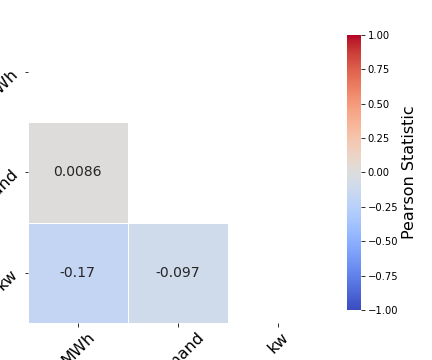
\includegraphics[width=0.8\textwidth]{solar_wind_corr.png}
  \caption{Relationships among various weather parameters and their strengths
  according to the Pearson statistic.}
  \label{fig:solar-wind-corr}
\end{figure}

Table \ref{tab:capfac} lists the average annual capacity factors for solar energy
and a hypothetical wind farm at the site of \gls{uiuc}'s Solar Farm 1.0.

\begin{table}[H]
  \centering
  \caption{Average Capacity Factors for Wind and Solar in Illinois}
  \label{tab:capfac}
  \begin{tabular}{lrr}
\toprule
Year &  Solar &   Wind \\
    &  Capacity Factor    &  Capacity Factor \\
\midrule
2010 &  0.174988 &  0.319112 \\
2011 &  0.164187 &  0.358573 \\
2012 &  0.181714 &  0.350748 \\
2013 &  0.168529 &  0.354717 \\
2014 &  0.168521 &  0.357613 \\
2015 &  0.170510 &  0.344992 \\
2016 &  0.172977 &  0.323927 \\
2017 &  0.174638 &  0.367449 \\
2018 &  0.165649 &  0.340297 \\
2019 &  0.161231 &  0.347187 \\
2020 &  0.164143 &  0.330702 \\
\bottomrule
\end{tabular}

\end{table}


\section{Case Study II: The UIUC Microgrid}
\label{section:uiucmodel}

The University of Illinois at Urbana-Champaign operates a diverse microgrid to
deliver electricity, steam heat, and chilled water to virtually all of its
campus buildings. This combination of demands makes full decarbonization difficult.
Nevertheless, UIUC adopted the goal of carbon neutrality by 2050 for all energy sectors.

\begin{figure}[H]
  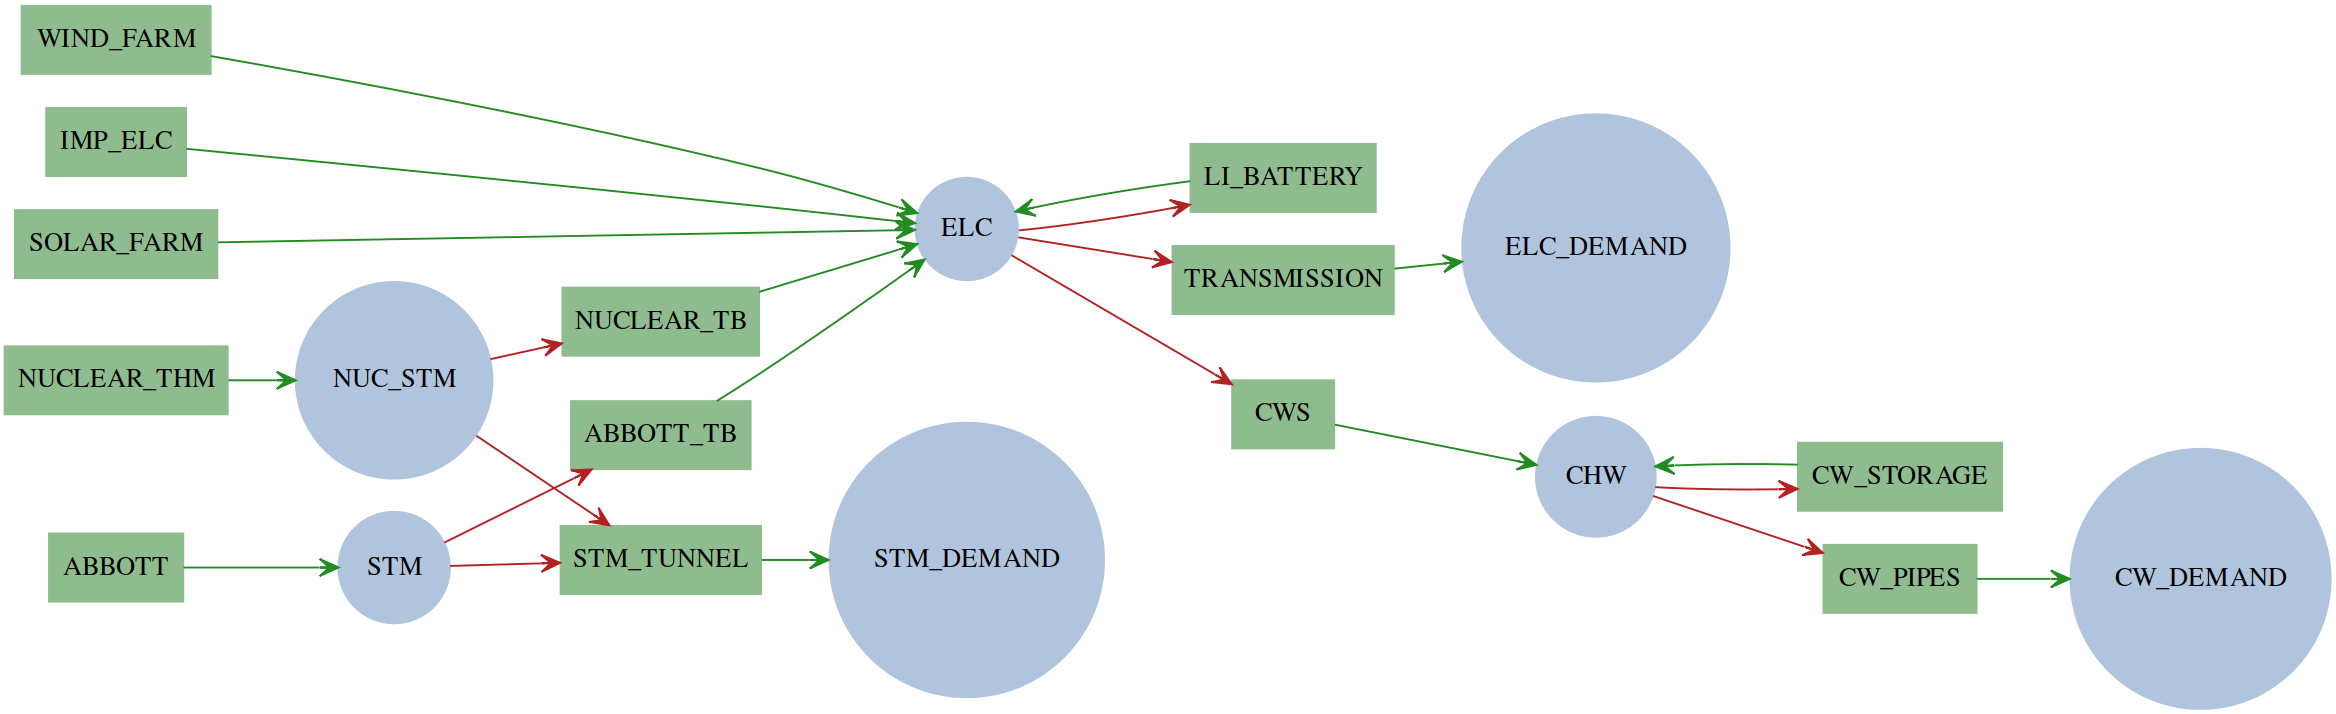
\includegraphics[width=\columnwidth]{uiuc_system.png}
  \caption{The \gls{uiuc} energy system modeled in \gls{temoa}}
  \label{fig:uiucsys}
\end{figure}

Figure \ref{fig:uiucsys} shows the topology of UIUC’s energy system, modeled in Temoa.
The UIUC model is spatially simple, since there is only one region, but topologically
more complex than the Illinois model from Section \ref{section:ilmodel} with
three interconnected end-use demands.

\subsection{Model and Data}
All campus data were obtained from the Facilities and Services Department at \gls{uiuc}.
Cost and operational data were also retrieved from the \gls{uiuc} ''Utilities
Production and Distribution Master Plan'' \cite{affiliated_engineers_inc_utilities_2015}.
Table \ref{tab:uiuc-tech} summarizes the technologies and some key parameters
used in the \gls{temoa} model. Similar to the Illinois case study, all technologies have
an ``efficiency'' of unity because fuel resources are not modeled.
I analyzed the structural uncertainty of this model using \gls{mga}, which constructs
alternative futures that are not necessarily motivated by cost. Additionally,
as a research university, \gls{uiuc} is interested in developing pre-commercial
technologies (e.g. a geothermal loop for heating and cooling). For these reasons,
the technology learning curves are not applied in the \gls{uiuc} model.

\subsubsection{Campus Steam}
\gls{uiuc} heats most of its buildings with steam generated by natural gas and
coal plant on campus, \gls{abbott}. \gls{abbott} is a combined cycle facility that
can operate in a condensing mode to capture steam to generate electricity or an
extraction mode that sends steam to campus for heating
\cite{affiliated_engineers_inc_utilities_2015}. \gls{temoa} does not have a
convenient way to model combined cycle plants \cite{decarolis_temoa_2010}. The
\gls{temoa} team suggests splitting the output of the technology. However, this
forces the \gls{abbott} model to generate steam and electricity in a fixed ratio, which
is not how \gls{abbott} operates. I circumvent this issue by introducing a dummy
technology, \texttt{ABBOTT\_TB}, that converts steam to electricity. Thus, \gls{temoa}
must choose how to use the steam produced by \gls{abbott}, matching operational reality.
I modeled an on-campus nuclear reactor in a similar manner. The nuclear reactor
generates a unique commodity, \texttt{NUC\_STM}, to distinguish nuclear activity
from \gls{abbott}'s activity.
% Figure \ref{fig:historical-steam} shows hourly steam demand from \gls{uiuc} fiscal years 2014 to 2019.

% \begin{figure}[H]
%   \centering
%   \resizebox{0.8\columnwidth}{!}{%% Creator: Matplotlib, PGF backend
%%
%% To include the figure in your LaTeX document, write
%%   \input{<filename>.pgf}
%%
%% Make sure the required packages are loaded in your preamble
%%   \usepackage{pgf}
%%
%% Figures using additional raster images can only be included by \input if
%% they are in the same directory as the main LaTeX file. For loading figures
%% from other directories you can use the `import` package
%%   \usepackage{import}
%%
%% and then include the figures with
%%   \import{<path to file>}{<filename>.pgf}
%%
%% Matplotlib used the following preamble
%%
\begingroup%
\makeatletter%
\begin{pgfpicture}%
\pgfpathrectangle{\pgfpointorigin}{\pgfqpoint{13.322565in}{6.822124in}}%
\pgfusepath{use as bounding box, clip}%
\begin{pgfscope}%
\pgfsetbuttcap%
\pgfsetmiterjoin%
\definecolor{currentfill}{rgb}{1.000000,1.000000,1.000000}%
\pgfsetfillcolor{currentfill}%
\pgfsetlinewidth{0.000000pt}%
\definecolor{currentstroke}{rgb}{0.500000,0.500000,0.500000}%
\pgfsetstrokecolor{currentstroke}%
\pgfsetdash{}{0pt}%
\pgfpathmoveto{\pgfqpoint{0.000000in}{-0.000000in}}%
\pgfpathlineto{\pgfqpoint{13.322565in}{-0.000000in}}%
\pgfpathlineto{\pgfqpoint{13.322565in}{6.822124in}}%
\pgfpathlineto{\pgfqpoint{0.000000in}{6.822124in}}%
\pgfpathclose%
\pgfusepath{fill}%
\end{pgfscope}%
\begin{pgfscope}%
\pgfsetbuttcap%
\pgfsetmiterjoin%
\definecolor{currentfill}{rgb}{0.898039,0.898039,0.898039}%
\pgfsetfillcolor{currentfill}%
\pgfsetlinewidth{0.000000pt}%
\definecolor{currentstroke}{rgb}{0.000000,0.000000,0.000000}%
\pgfsetstrokecolor{currentstroke}%
\pgfsetstrokeopacity{0.000000}%
\pgfsetdash{}{0pt}%
\pgfpathmoveto{\pgfqpoint{0.822565in}{0.602124in}}%
\pgfpathlineto{\pgfqpoint{13.222565in}{0.602124in}}%
\pgfpathlineto{\pgfqpoint{13.222565in}{6.722124in}}%
\pgfpathlineto{\pgfqpoint{0.822565in}{6.722124in}}%
\pgfpathclose%
\pgfusepath{fill}%
\end{pgfscope}%
\begin{pgfscope}%
\pgfpathrectangle{\pgfqpoint{0.822565in}{0.602124in}}{\pgfqpoint{12.400000in}{6.120000in}}%
\pgfusepath{clip}%
\pgfsetrectcap%
\pgfsetroundjoin%
\pgfsetlinewidth{0.803000pt}%
\definecolor{currentstroke}{rgb}{1.000000,1.000000,1.000000}%
\pgfsetstrokecolor{currentstroke}%
\pgfsetdash{}{0pt}%
\pgfpathmoveto{\pgfqpoint{2.522143in}{0.602124in}}%
\pgfpathlineto{\pgfqpoint{2.522143in}{6.722124in}}%
\pgfusepath{stroke}%
\end{pgfscope}%
\begin{pgfscope}%
\pgfsetbuttcap%
\pgfsetroundjoin%
\definecolor{currentfill}{rgb}{0.333333,0.333333,0.333333}%
\pgfsetfillcolor{currentfill}%
\pgfsetlinewidth{0.803000pt}%
\definecolor{currentstroke}{rgb}{0.333333,0.333333,0.333333}%
\pgfsetstrokecolor{currentstroke}%
\pgfsetdash{}{0pt}%
\pgfsys@defobject{currentmarker}{\pgfqpoint{0.000000in}{-0.048611in}}{\pgfqpoint{0.000000in}{0.000000in}}{%
\pgfpathmoveto{\pgfqpoint{0.000000in}{0.000000in}}%
\pgfpathlineto{\pgfqpoint{0.000000in}{-0.048611in}}%
\pgfusepath{stroke,fill}%
}%
\begin{pgfscope}%
\pgfsys@transformshift{2.522143in}{0.602124in}%
\pgfsys@useobject{currentmarker}{}%
\end{pgfscope}%
\end{pgfscope}%
\begin{pgfscope}%
\definecolor{textcolor}{rgb}{0.333333,0.333333,0.333333}%
\pgfsetstrokecolor{textcolor}%
\pgfsetfillcolor{textcolor}%
\pgftext[x=2.117515in, y=0.140428in, left, base,rotate=30.000000]{\color{textcolor}\rmfamily\fontsize{16.000000}{19.200000}\selectfont \(\displaystyle {2015}\)}%
\end{pgfscope}%
\begin{pgfscope}%
\pgfpathrectangle{\pgfqpoint{0.822565in}{0.602124in}}{\pgfqpoint{12.400000in}{6.120000in}}%
\pgfusepath{clip}%
\pgfsetrectcap%
\pgfsetroundjoin%
\pgfsetlinewidth{0.803000pt}%
\definecolor{currentstroke}{rgb}{1.000000,1.000000,1.000000}%
\pgfsetstrokecolor{currentstroke}%
\pgfsetdash{}{0pt}%
\pgfpathmoveto{\pgfqpoint{4.775505in}{0.602124in}}%
\pgfpathlineto{\pgfqpoint{4.775505in}{6.722124in}}%
\pgfusepath{stroke}%
\end{pgfscope}%
\begin{pgfscope}%
\pgfsetbuttcap%
\pgfsetroundjoin%
\definecolor{currentfill}{rgb}{0.333333,0.333333,0.333333}%
\pgfsetfillcolor{currentfill}%
\pgfsetlinewidth{0.803000pt}%
\definecolor{currentstroke}{rgb}{0.333333,0.333333,0.333333}%
\pgfsetstrokecolor{currentstroke}%
\pgfsetdash{}{0pt}%
\pgfsys@defobject{currentmarker}{\pgfqpoint{0.000000in}{-0.048611in}}{\pgfqpoint{0.000000in}{0.000000in}}{%
\pgfpathmoveto{\pgfqpoint{0.000000in}{0.000000in}}%
\pgfpathlineto{\pgfqpoint{0.000000in}{-0.048611in}}%
\pgfusepath{stroke,fill}%
}%
\begin{pgfscope}%
\pgfsys@transformshift{4.775505in}{0.602124in}%
\pgfsys@useobject{currentmarker}{}%
\end{pgfscope}%
\end{pgfscope}%
\begin{pgfscope}%
\definecolor{textcolor}{rgb}{0.333333,0.333333,0.333333}%
\pgfsetstrokecolor{textcolor}%
\pgfsetfillcolor{textcolor}%
\pgftext[x=4.370877in, y=0.140428in, left, base,rotate=30.000000]{\color{textcolor}\rmfamily\fontsize{16.000000}{19.200000}\selectfont \(\displaystyle {2016}\)}%
\end{pgfscope}%
\begin{pgfscope}%
\pgfpathrectangle{\pgfqpoint{0.822565in}{0.602124in}}{\pgfqpoint{12.400000in}{6.120000in}}%
\pgfusepath{clip}%
\pgfsetrectcap%
\pgfsetroundjoin%
\pgfsetlinewidth{0.803000pt}%
\definecolor{currentstroke}{rgb}{1.000000,1.000000,1.000000}%
\pgfsetstrokecolor{currentstroke}%
\pgfsetdash{}{0pt}%
\pgfpathmoveto{\pgfqpoint{7.035041in}{0.602124in}}%
\pgfpathlineto{\pgfqpoint{7.035041in}{6.722124in}}%
\pgfusepath{stroke}%
\end{pgfscope}%
\begin{pgfscope}%
\pgfsetbuttcap%
\pgfsetroundjoin%
\definecolor{currentfill}{rgb}{0.333333,0.333333,0.333333}%
\pgfsetfillcolor{currentfill}%
\pgfsetlinewidth{0.803000pt}%
\definecolor{currentstroke}{rgb}{0.333333,0.333333,0.333333}%
\pgfsetstrokecolor{currentstroke}%
\pgfsetdash{}{0pt}%
\pgfsys@defobject{currentmarker}{\pgfqpoint{0.000000in}{-0.048611in}}{\pgfqpoint{0.000000in}{0.000000in}}{%
\pgfpathmoveto{\pgfqpoint{0.000000in}{0.000000in}}%
\pgfpathlineto{\pgfqpoint{0.000000in}{-0.048611in}}%
\pgfusepath{stroke,fill}%
}%
\begin{pgfscope}%
\pgfsys@transformshift{7.035041in}{0.602124in}%
\pgfsys@useobject{currentmarker}{}%
\end{pgfscope}%
\end{pgfscope}%
\begin{pgfscope}%
\definecolor{textcolor}{rgb}{0.333333,0.333333,0.333333}%
\pgfsetstrokecolor{textcolor}%
\pgfsetfillcolor{textcolor}%
\pgftext[x=6.630413in, y=0.140428in, left, base,rotate=30.000000]{\color{textcolor}\rmfamily\fontsize{16.000000}{19.200000}\selectfont \(\displaystyle {2017}\)}%
\end{pgfscope}%
\begin{pgfscope}%
\pgfpathrectangle{\pgfqpoint{0.822565in}{0.602124in}}{\pgfqpoint{12.400000in}{6.120000in}}%
\pgfusepath{clip}%
\pgfsetrectcap%
\pgfsetroundjoin%
\pgfsetlinewidth{0.803000pt}%
\definecolor{currentstroke}{rgb}{1.000000,1.000000,1.000000}%
\pgfsetstrokecolor{currentstroke}%
\pgfsetdash{}{0pt}%
\pgfpathmoveto{\pgfqpoint{9.288403in}{0.602124in}}%
\pgfpathlineto{\pgfqpoint{9.288403in}{6.722124in}}%
\pgfusepath{stroke}%
\end{pgfscope}%
\begin{pgfscope}%
\pgfsetbuttcap%
\pgfsetroundjoin%
\definecolor{currentfill}{rgb}{0.333333,0.333333,0.333333}%
\pgfsetfillcolor{currentfill}%
\pgfsetlinewidth{0.803000pt}%
\definecolor{currentstroke}{rgb}{0.333333,0.333333,0.333333}%
\pgfsetstrokecolor{currentstroke}%
\pgfsetdash{}{0pt}%
\pgfsys@defobject{currentmarker}{\pgfqpoint{0.000000in}{-0.048611in}}{\pgfqpoint{0.000000in}{0.000000in}}{%
\pgfpathmoveto{\pgfqpoint{0.000000in}{0.000000in}}%
\pgfpathlineto{\pgfqpoint{0.000000in}{-0.048611in}}%
\pgfusepath{stroke,fill}%
}%
\begin{pgfscope}%
\pgfsys@transformshift{9.288403in}{0.602124in}%
\pgfsys@useobject{currentmarker}{}%
\end{pgfscope}%
\end{pgfscope}%
\begin{pgfscope}%
\definecolor{textcolor}{rgb}{0.333333,0.333333,0.333333}%
\pgfsetstrokecolor{textcolor}%
\pgfsetfillcolor{textcolor}%
\pgftext[x=8.883775in, y=0.140428in, left, base,rotate=30.000000]{\color{textcolor}\rmfamily\fontsize{16.000000}{19.200000}\selectfont \(\displaystyle {2018}\)}%
\end{pgfscope}%
\begin{pgfscope}%
\pgfpathrectangle{\pgfqpoint{0.822565in}{0.602124in}}{\pgfqpoint{12.400000in}{6.120000in}}%
\pgfusepath{clip}%
\pgfsetrectcap%
\pgfsetroundjoin%
\pgfsetlinewidth{0.803000pt}%
\definecolor{currentstroke}{rgb}{1.000000,1.000000,1.000000}%
\pgfsetstrokecolor{currentstroke}%
\pgfsetdash{}{0pt}%
\pgfpathmoveto{\pgfqpoint{11.541765in}{0.602124in}}%
\pgfpathlineto{\pgfqpoint{11.541765in}{6.722124in}}%
\pgfusepath{stroke}%
\end{pgfscope}%
\begin{pgfscope}%
\pgfsetbuttcap%
\pgfsetroundjoin%
\definecolor{currentfill}{rgb}{0.333333,0.333333,0.333333}%
\pgfsetfillcolor{currentfill}%
\pgfsetlinewidth{0.803000pt}%
\definecolor{currentstroke}{rgb}{0.333333,0.333333,0.333333}%
\pgfsetstrokecolor{currentstroke}%
\pgfsetdash{}{0pt}%
\pgfsys@defobject{currentmarker}{\pgfqpoint{0.000000in}{-0.048611in}}{\pgfqpoint{0.000000in}{0.000000in}}{%
\pgfpathmoveto{\pgfqpoint{0.000000in}{0.000000in}}%
\pgfpathlineto{\pgfqpoint{0.000000in}{-0.048611in}}%
\pgfusepath{stroke,fill}%
}%
\begin{pgfscope}%
\pgfsys@transformshift{11.541765in}{0.602124in}%
\pgfsys@useobject{currentmarker}{}%
\end{pgfscope}%
\end{pgfscope}%
\begin{pgfscope}%
\definecolor{textcolor}{rgb}{0.333333,0.333333,0.333333}%
\pgfsetstrokecolor{textcolor}%
\pgfsetfillcolor{textcolor}%
\pgftext[x=11.137137in, y=0.140428in, left, base,rotate=30.000000]{\color{textcolor}\rmfamily\fontsize{16.000000}{19.200000}\selectfont \(\displaystyle {2019}\)}%
\end{pgfscope}%
\begin{pgfscope}%
\pgfsetbuttcap%
\pgfsetroundjoin%
\definecolor{currentfill}{rgb}{0.333333,0.333333,0.333333}%
\pgfsetfillcolor{currentfill}%
\pgfsetlinewidth{0.602250pt}%
\definecolor{currentstroke}{rgb}{0.333333,0.333333,0.333333}%
\pgfsetstrokecolor{currentstroke}%
\pgfsetdash{}{0pt}%
\pgfsys@defobject{currentmarker}{\pgfqpoint{0.000000in}{-0.027778in}}{\pgfqpoint{0.000000in}{0.000000in}}{%
\pgfpathmoveto{\pgfqpoint{0.000000in}{0.000000in}}%
\pgfpathlineto{\pgfqpoint{0.000000in}{-0.027778in}}%
\pgfusepath{stroke,fill}%
}%
\begin{pgfscope}%
\pgfsys@transformshift{0.832121in}{0.602124in}%
\pgfsys@useobject{currentmarker}{}%
\end{pgfscope}%
\end{pgfscope}%
\begin{pgfscope}%
\pgfsetbuttcap%
\pgfsetroundjoin%
\definecolor{currentfill}{rgb}{0.333333,0.333333,0.333333}%
\pgfsetfillcolor{currentfill}%
\pgfsetlinewidth{0.602250pt}%
\definecolor{currentstroke}{rgb}{0.333333,0.333333,0.333333}%
\pgfsetstrokecolor{currentstroke}%
\pgfsetdash{}{0pt}%
\pgfsys@defobject{currentmarker}{\pgfqpoint{0.000000in}{-0.027778in}}{\pgfqpoint{0.000000in}{0.000000in}}{%
\pgfpathmoveto{\pgfqpoint{0.000000in}{0.000000in}}%
\pgfpathlineto{\pgfqpoint{0.000000in}{-0.027778in}}%
\pgfusepath{stroke,fill}%
}%
\begin{pgfscope}%
\pgfsys@transformshift{1.395462in}{0.602124in}%
\pgfsys@useobject{currentmarker}{}%
\end{pgfscope}%
\end{pgfscope}%
\begin{pgfscope}%
\pgfsetbuttcap%
\pgfsetroundjoin%
\definecolor{currentfill}{rgb}{0.333333,0.333333,0.333333}%
\pgfsetfillcolor{currentfill}%
\pgfsetlinewidth{0.602250pt}%
\definecolor{currentstroke}{rgb}{0.333333,0.333333,0.333333}%
\pgfsetstrokecolor{currentstroke}%
\pgfsetdash{}{0pt}%
\pgfsys@defobject{currentmarker}{\pgfqpoint{0.000000in}{-0.027778in}}{\pgfqpoint{0.000000in}{0.000000in}}{%
\pgfpathmoveto{\pgfqpoint{0.000000in}{0.000000in}}%
\pgfpathlineto{\pgfqpoint{0.000000in}{-0.027778in}}%
\pgfusepath{stroke,fill}%
}%
\begin{pgfscope}%
\pgfsys@transformshift{1.958803in}{0.602124in}%
\pgfsys@useobject{currentmarker}{}%
\end{pgfscope}%
\end{pgfscope}%
\begin{pgfscope}%
\pgfsetbuttcap%
\pgfsetroundjoin%
\definecolor{currentfill}{rgb}{0.333333,0.333333,0.333333}%
\pgfsetfillcolor{currentfill}%
\pgfsetlinewidth{0.602250pt}%
\definecolor{currentstroke}{rgb}{0.333333,0.333333,0.333333}%
\pgfsetstrokecolor{currentstroke}%
\pgfsetdash{}{0pt}%
\pgfsys@defobject{currentmarker}{\pgfqpoint{0.000000in}{-0.027778in}}{\pgfqpoint{0.000000in}{0.000000in}}{%
\pgfpathmoveto{\pgfqpoint{0.000000in}{0.000000in}}%
\pgfpathlineto{\pgfqpoint{0.000000in}{-0.027778in}}%
\pgfusepath{stroke,fill}%
}%
\begin{pgfscope}%
\pgfsys@transformshift{3.085484in}{0.602124in}%
\pgfsys@useobject{currentmarker}{}%
\end{pgfscope}%
\end{pgfscope}%
\begin{pgfscope}%
\pgfsetbuttcap%
\pgfsetroundjoin%
\definecolor{currentfill}{rgb}{0.333333,0.333333,0.333333}%
\pgfsetfillcolor{currentfill}%
\pgfsetlinewidth{0.602250pt}%
\definecolor{currentstroke}{rgb}{0.333333,0.333333,0.333333}%
\pgfsetstrokecolor{currentstroke}%
\pgfsetdash{}{0pt}%
\pgfsys@defobject{currentmarker}{\pgfqpoint{0.000000in}{-0.027778in}}{\pgfqpoint{0.000000in}{0.000000in}}{%
\pgfpathmoveto{\pgfqpoint{0.000000in}{0.000000in}}%
\pgfpathlineto{\pgfqpoint{0.000000in}{-0.027778in}}%
\pgfusepath{stroke,fill}%
}%
\begin{pgfscope}%
\pgfsys@transformshift{3.648824in}{0.602124in}%
\pgfsys@useobject{currentmarker}{}%
\end{pgfscope}%
\end{pgfscope}%
\begin{pgfscope}%
\pgfsetbuttcap%
\pgfsetroundjoin%
\definecolor{currentfill}{rgb}{0.333333,0.333333,0.333333}%
\pgfsetfillcolor{currentfill}%
\pgfsetlinewidth{0.602250pt}%
\definecolor{currentstroke}{rgb}{0.333333,0.333333,0.333333}%
\pgfsetstrokecolor{currentstroke}%
\pgfsetdash{}{0pt}%
\pgfsys@defobject{currentmarker}{\pgfqpoint{0.000000in}{-0.027778in}}{\pgfqpoint{0.000000in}{0.000000in}}{%
\pgfpathmoveto{\pgfqpoint{0.000000in}{0.000000in}}%
\pgfpathlineto{\pgfqpoint{0.000000in}{-0.027778in}}%
\pgfusepath{stroke,fill}%
}%
\begin{pgfscope}%
\pgfsys@transformshift{4.212165in}{0.602124in}%
\pgfsys@useobject{currentmarker}{}%
\end{pgfscope}%
\end{pgfscope}%
\begin{pgfscope}%
\pgfsetbuttcap%
\pgfsetroundjoin%
\definecolor{currentfill}{rgb}{0.333333,0.333333,0.333333}%
\pgfsetfillcolor{currentfill}%
\pgfsetlinewidth{0.602250pt}%
\definecolor{currentstroke}{rgb}{0.333333,0.333333,0.333333}%
\pgfsetstrokecolor{currentstroke}%
\pgfsetdash{}{0pt}%
\pgfsys@defobject{currentmarker}{\pgfqpoint{0.000000in}{-0.027778in}}{\pgfqpoint{0.000000in}{0.000000in}}{%
\pgfpathmoveto{\pgfqpoint{0.000000in}{0.000000in}}%
\pgfpathlineto{\pgfqpoint{0.000000in}{-0.027778in}}%
\pgfusepath{stroke,fill}%
}%
\begin{pgfscope}%
\pgfsys@transformshift{5.338846in}{0.602124in}%
\pgfsys@useobject{currentmarker}{}%
\end{pgfscope}%
\end{pgfscope}%
\begin{pgfscope}%
\pgfsetbuttcap%
\pgfsetroundjoin%
\definecolor{currentfill}{rgb}{0.333333,0.333333,0.333333}%
\pgfsetfillcolor{currentfill}%
\pgfsetlinewidth{0.602250pt}%
\definecolor{currentstroke}{rgb}{0.333333,0.333333,0.333333}%
\pgfsetstrokecolor{currentstroke}%
\pgfsetdash{}{0pt}%
\pgfsys@defobject{currentmarker}{\pgfqpoint{0.000000in}{-0.027778in}}{\pgfqpoint{0.000000in}{0.000000in}}{%
\pgfpathmoveto{\pgfqpoint{0.000000in}{0.000000in}}%
\pgfpathlineto{\pgfqpoint{0.000000in}{-0.027778in}}%
\pgfusepath{stroke,fill}%
}%
\begin{pgfscope}%
\pgfsys@transformshift{5.902186in}{0.602124in}%
\pgfsys@useobject{currentmarker}{}%
\end{pgfscope}%
\end{pgfscope}%
\begin{pgfscope}%
\pgfsetbuttcap%
\pgfsetroundjoin%
\definecolor{currentfill}{rgb}{0.333333,0.333333,0.333333}%
\pgfsetfillcolor{currentfill}%
\pgfsetlinewidth{0.602250pt}%
\definecolor{currentstroke}{rgb}{0.333333,0.333333,0.333333}%
\pgfsetstrokecolor{currentstroke}%
\pgfsetdash{}{0pt}%
\pgfsys@defobject{currentmarker}{\pgfqpoint{0.000000in}{-0.027778in}}{\pgfqpoint{0.000000in}{0.000000in}}{%
\pgfpathmoveto{\pgfqpoint{0.000000in}{0.000000in}}%
\pgfpathlineto{\pgfqpoint{0.000000in}{-0.027778in}}%
\pgfusepath{stroke,fill}%
}%
\begin{pgfscope}%
\pgfsys@transformshift{6.465527in}{0.602124in}%
\pgfsys@useobject{currentmarker}{}%
\end{pgfscope}%
\end{pgfscope}%
\begin{pgfscope}%
\pgfsetbuttcap%
\pgfsetroundjoin%
\definecolor{currentfill}{rgb}{0.333333,0.333333,0.333333}%
\pgfsetfillcolor{currentfill}%
\pgfsetlinewidth{0.602250pt}%
\definecolor{currentstroke}{rgb}{0.333333,0.333333,0.333333}%
\pgfsetstrokecolor{currentstroke}%
\pgfsetdash{}{0pt}%
\pgfsys@defobject{currentmarker}{\pgfqpoint{0.000000in}{-0.027778in}}{\pgfqpoint{0.000000in}{0.000000in}}{%
\pgfpathmoveto{\pgfqpoint{0.000000in}{0.000000in}}%
\pgfpathlineto{\pgfqpoint{0.000000in}{-0.027778in}}%
\pgfusepath{stroke,fill}%
}%
\begin{pgfscope}%
\pgfsys@transformshift{7.028867in}{0.602124in}%
\pgfsys@useobject{currentmarker}{}%
\end{pgfscope}%
\end{pgfscope}%
\begin{pgfscope}%
\pgfsetbuttcap%
\pgfsetroundjoin%
\definecolor{currentfill}{rgb}{0.333333,0.333333,0.333333}%
\pgfsetfillcolor{currentfill}%
\pgfsetlinewidth{0.602250pt}%
\definecolor{currentstroke}{rgb}{0.333333,0.333333,0.333333}%
\pgfsetstrokecolor{currentstroke}%
\pgfsetdash{}{0pt}%
\pgfsys@defobject{currentmarker}{\pgfqpoint{0.000000in}{-0.027778in}}{\pgfqpoint{0.000000in}{0.000000in}}{%
\pgfpathmoveto{\pgfqpoint{0.000000in}{0.000000in}}%
\pgfpathlineto{\pgfqpoint{0.000000in}{-0.027778in}}%
\pgfusepath{stroke,fill}%
}%
\begin{pgfscope}%
\pgfsys@transformshift{7.592208in}{0.602124in}%
\pgfsys@useobject{currentmarker}{}%
\end{pgfscope}%
\end{pgfscope}%
\begin{pgfscope}%
\pgfsetbuttcap%
\pgfsetroundjoin%
\definecolor{currentfill}{rgb}{0.333333,0.333333,0.333333}%
\pgfsetfillcolor{currentfill}%
\pgfsetlinewidth{0.602250pt}%
\definecolor{currentstroke}{rgb}{0.333333,0.333333,0.333333}%
\pgfsetstrokecolor{currentstroke}%
\pgfsetdash{}{0pt}%
\pgfsys@defobject{currentmarker}{\pgfqpoint{0.000000in}{-0.027778in}}{\pgfqpoint{0.000000in}{0.000000in}}{%
\pgfpathmoveto{\pgfqpoint{0.000000in}{0.000000in}}%
\pgfpathlineto{\pgfqpoint{0.000000in}{-0.027778in}}%
\pgfusepath{stroke,fill}%
}%
\begin{pgfscope}%
\pgfsys@transformshift{8.155549in}{0.602124in}%
\pgfsys@useobject{currentmarker}{}%
\end{pgfscope}%
\end{pgfscope}%
\begin{pgfscope}%
\pgfsetbuttcap%
\pgfsetroundjoin%
\definecolor{currentfill}{rgb}{0.333333,0.333333,0.333333}%
\pgfsetfillcolor{currentfill}%
\pgfsetlinewidth{0.602250pt}%
\definecolor{currentstroke}{rgb}{0.333333,0.333333,0.333333}%
\pgfsetstrokecolor{currentstroke}%
\pgfsetdash{}{0pt}%
\pgfsys@defobject{currentmarker}{\pgfqpoint{0.000000in}{-0.027778in}}{\pgfqpoint{0.000000in}{0.000000in}}{%
\pgfpathmoveto{\pgfqpoint{0.000000in}{0.000000in}}%
\pgfpathlineto{\pgfqpoint{0.000000in}{-0.027778in}}%
\pgfusepath{stroke,fill}%
}%
\begin{pgfscope}%
\pgfsys@transformshift{8.718889in}{0.602124in}%
\pgfsys@useobject{currentmarker}{}%
\end{pgfscope}%
\end{pgfscope}%
\begin{pgfscope}%
\pgfsetbuttcap%
\pgfsetroundjoin%
\definecolor{currentfill}{rgb}{0.333333,0.333333,0.333333}%
\pgfsetfillcolor{currentfill}%
\pgfsetlinewidth{0.602250pt}%
\definecolor{currentstroke}{rgb}{0.333333,0.333333,0.333333}%
\pgfsetstrokecolor{currentstroke}%
\pgfsetdash{}{0pt}%
\pgfsys@defobject{currentmarker}{\pgfqpoint{0.000000in}{-0.027778in}}{\pgfqpoint{0.000000in}{0.000000in}}{%
\pgfpathmoveto{\pgfqpoint{0.000000in}{0.000000in}}%
\pgfpathlineto{\pgfqpoint{0.000000in}{-0.027778in}}%
\pgfusepath{stroke,fill}%
}%
\begin{pgfscope}%
\pgfsys@transformshift{9.282230in}{0.602124in}%
\pgfsys@useobject{currentmarker}{}%
\end{pgfscope}%
\end{pgfscope}%
\begin{pgfscope}%
\pgfsetbuttcap%
\pgfsetroundjoin%
\definecolor{currentfill}{rgb}{0.333333,0.333333,0.333333}%
\pgfsetfillcolor{currentfill}%
\pgfsetlinewidth{0.602250pt}%
\definecolor{currentstroke}{rgb}{0.333333,0.333333,0.333333}%
\pgfsetstrokecolor{currentstroke}%
\pgfsetdash{}{0pt}%
\pgfsys@defobject{currentmarker}{\pgfqpoint{0.000000in}{-0.027778in}}{\pgfqpoint{0.000000in}{0.000000in}}{%
\pgfpathmoveto{\pgfqpoint{0.000000in}{0.000000in}}%
\pgfpathlineto{\pgfqpoint{0.000000in}{-0.027778in}}%
\pgfusepath{stroke,fill}%
}%
\begin{pgfscope}%
\pgfsys@transformshift{9.845570in}{0.602124in}%
\pgfsys@useobject{currentmarker}{}%
\end{pgfscope}%
\end{pgfscope}%
\begin{pgfscope}%
\pgfsetbuttcap%
\pgfsetroundjoin%
\definecolor{currentfill}{rgb}{0.333333,0.333333,0.333333}%
\pgfsetfillcolor{currentfill}%
\pgfsetlinewidth{0.602250pt}%
\definecolor{currentstroke}{rgb}{0.333333,0.333333,0.333333}%
\pgfsetstrokecolor{currentstroke}%
\pgfsetdash{}{0pt}%
\pgfsys@defobject{currentmarker}{\pgfqpoint{0.000000in}{-0.027778in}}{\pgfqpoint{0.000000in}{0.000000in}}{%
\pgfpathmoveto{\pgfqpoint{0.000000in}{0.000000in}}%
\pgfpathlineto{\pgfqpoint{0.000000in}{-0.027778in}}%
\pgfusepath{stroke,fill}%
}%
\begin{pgfscope}%
\pgfsys@transformshift{10.408911in}{0.602124in}%
\pgfsys@useobject{currentmarker}{}%
\end{pgfscope}%
\end{pgfscope}%
\begin{pgfscope}%
\pgfsetbuttcap%
\pgfsetroundjoin%
\definecolor{currentfill}{rgb}{0.333333,0.333333,0.333333}%
\pgfsetfillcolor{currentfill}%
\pgfsetlinewidth{0.602250pt}%
\definecolor{currentstroke}{rgb}{0.333333,0.333333,0.333333}%
\pgfsetstrokecolor{currentstroke}%
\pgfsetdash{}{0pt}%
\pgfsys@defobject{currentmarker}{\pgfqpoint{0.000000in}{-0.027778in}}{\pgfqpoint{0.000000in}{0.000000in}}{%
\pgfpathmoveto{\pgfqpoint{0.000000in}{0.000000in}}%
\pgfpathlineto{\pgfqpoint{0.000000in}{-0.027778in}}%
\pgfusepath{stroke,fill}%
}%
\begin{pgfscope}%
\pgfsys@transformshift{10.972251in}{0.602124in}%
\pgfsys@useobject{currentmarker}{}%
\end{pgfscope}%
\end{pgfscope}%
\begin{pgfscope}%
\pgfsetbuttcap%
\pgfsetroundjoin%
\definecolor{currentfill}{rgb}{0.333333,0.333333,0.333333}%
\pgfsetfillcolor{currentfill}%
\pgfsetlinewidth{0.602250pt}%
\definecolor{currentstroke}{rgb}{0.333333,0.333333,0.333333}%
\pgfsetstrokecolor{currentstroke}%
\pgfsetdash{}{0pt}%
\pgfsys@defobject{currentmarker}{\pgfqpoint{0.000000in}{-0.027778in}}{\pgfqpoint{0.000000in}{0.000000in}}{%
\pgfpathmoveto{\pgfqpoint{0.000000in}{0.000000in}}%
\pgfpathlineto{\pgfqpoint{0.000000in}{-0.027778in}}%
\pgfusepath{stroke,fill}%
}%
\begin{pgfscope}%
\pgfsys@transformshift{11.535592in}{0.602124in}%
\pgfsys@useobject{currentmarker}{}%
\end{pgfscope}%
\end{pgfscope}%
\begin{pgfscope}%
\pgfsetbuttcap%
\pgfsetroundjoin%
\definecolor{currentfill}{rgb}{0.333333,0.333333,0.333333}%
\pgfsetfillcolor{currentfill}%
\pgfsetlinewidth{0.602250pt}%
\definecolor{currentstroke}{rgb}{0.333333,0.333333,0.333333}%
\pgfsetstrokecolor{currentstroke}%
\pgfsetdash{}{0pt}%
\pgfsys@defobject{currentmarker}{\pgfqpoint{0.000000in}{-0.027778in}}{\pgfqpoint{0.000000in}{0.000000in}}{%
\pgfpathmoveto{\pgfqpoint{0.000000in}{0.000000in}}%
\pgfpathlineto{\pgfqpoint{0.000000in}{-0.027778in}}%
\pgfusepath{stroke,fill}%
}%
\begin{pgfscope}%
\pgfsys@transformshift{12.098932in}{0.602124in}%
\pgfsys@useobject{currentmarker}{}%
\end{pgfscope}%
\end{pgfscope}%
\begin{pgfscope}%
\pgfsetbuttcap%
\pgfsetroundjoin%
\definecolor{currentfill}{rgb}{0.333333,0.333333,0.333333}%
\pgfsetfillcolor{currentfill}%
\pgfsetlinewidth{0.602250pt}%
\definecolor{currentstroke}{rgb}{0.333333,0.333333,0.333333}%
\pgfsetstrokecolor{currentstroke}%
\pgfsetdash{}{0pt}%
\pgfsys@defobject{currentmarker}{\pgfqpoint{0.000000in}{-0.027778in}}{\pgfqpoint{0.000000in}{0.000000in}}{%
\pgfpathmoveto{\pgfqpoint{0.000000in}{0.000000in}}%
\pgfpathlineto{\pgfqpoint{0.000000in}{-0.027778in}}%
\pgfusepath{stroke,fill}%
}%
\begin{pgfscope}%
\pgfsys@transformshift{12.662273in}{0.602124in}%
\pgfsys@useobject{currentmarker}{}%
\end{pgfscope}%
\end{pgfscope}%
\begin{pgfscope}%
\pgfpathrectangle{\pgfqpoint{0.822565in}{0.602124in}}{\pgfqpoint{12.400000in}{6.120000in}}%
\pgfusepath{clip}%
\pgfsetrectcap%
\pgfsetroundjoin%
\pgfsetlinewidth{0.803000pt}%
\definecolor{currentstroke}{rgb}{1.000000,1.000000,1.000000}%
\pgfsetstrokecolor{currentstroke}%
\pgfsetdash{}{0pt}%
\pgfpathmoveto{\pgfqpoint{0.822565in}{0.880306in}}%
\pgfpathlineto{\pgfqpoint{13.222565in}{0.880306in}}%
\pgfusepath{stroke}%
\end{pgfscope}%
\begin{pgfscope}%
\pgfsetbuttcap%
\pgfsetroundjoin%
\definecolor{currentfill}{rgb}{0.333333,0.333333,0.333333}%
\pgfsetfillcolor{currentfill}%
\pgfsetlinewidth{0.803000pt}%
\definecolor{currentstroke}{rgb}{0.333333,0.333333,0.333333}%
\pgfsetstrokecolor{currentstroke}%
\pgfsetdash{}{0pt}%
\pgfsys@defobject{currentmarker}{\pgfqpoint{-0.048611in}{0.000000in}}{\pgfqpoint{-0.000000in}{0.000000in}}{%
\pgfpathmoveto{\pgfqpoint{-0.000000in}{0.000000in}}%
\pgfpathlineto{\pgfqpoint{-0.048611in}{0.000000in}}%
\pgfusepath{stroke,fill}%
}%
\begin{pgfscope}%
\pgfsys@transformshift{0.822565in}{0.880306in}%
\pgfsys@useobject{currentmarker}{}%
\end{pgfscope}%
\end{pgfscope}%
\begin{pgfscope}%
\definecolor{textcolor}{rgb}{0.333333,0.333333,0.333333}%
\pgfsetstrokecolor{textcolor}%
\pgfsetfillcolor{textcolor}%
\pgftext[x=0.615275in, y=0.796972in, left, base]{\color{textcolor}\rmfamily\fontsize{16.000000}{19.200000}\selectfont \(\displaystyle {0}\)}%
\end{pgfscope}%
\begin{pgfscope}%
\pgfpathrectangle{\pgfqpoint{0.822565in}{0.602124in}}{\pgfqpoint{12.400000in}{6.120000in}}%
\pgfusepath{clip}%
\pgfsetrectcap%
\pgfsetroundjoin%
\pgfsetlinewidth{0.803000pt}%
\definecolor{currentstroke}{rgb}{1.000000,1.000000,1.000000}%
\pgfsetstrokecolor{currentstroke}%
\pgfsetdash{}{0pt}%
\pgfpathmoveto{\pgfqpoint{0.822565in}{2.119171in}}%
\pgfpathlineto{\pgfqpoint{13.222565in}{2.119171in}}%
\pgfusepath{stroke}%
\end{pgfscope}%
\begin{pgfscope}%
\pgfsetbuttcap%
\pgfsetroundjoin%
\definecolor{currentfill}{rgb}{0.333333,0.333333,0.333333}%
\pgfsetfillcolor{currentfill}%
\pgfsetlinewidth{0.803000pt}%
\definecolor{currentstroke}{rgb}{0.333333,0.333333,0.333333}%
\pgfsetstrokecolor{currentstroke}%
\pgfsetdash{}{0pt}%
\pgfsys@defobject{currentmarker}{\pgfqpoint{-0.048611in}{0.000000in}}{\pgfqpoint{-0.000000in}{0.000000in}}{%
\pgfpathmoveto{\pgfqpoint{-0.000000in}{0.000000in}}%
\pgfpathlineto{\pgfqpoint{-0.048611in}{0.000000in}}%
\pgfusepath{stroke,fill}%
}%
\begin{pgfscope}%
\pgfsys@transformshift{0.822565in}{2.119171in}%
\pgfsys@useobject{currentmarker}{}%
\end{pgfscope}%
\end{pgfscope}%
\begin{pgfscope}%
\definecolor{textcolor}{rgb}{0.333333,0.333333,0.333333}%
\pgfsetstrokecolor{textcolor}%
\pgfsetfillcolor{textcolor}%
\pgftext[x=0.505207in, y=2.035838in, left, base]{\color{textcolor}\rmfamily\fontsize{16.000000}{19.200000}\selectfont \(\displaystyle {50}\)}%
\end{pgfscope}%
\begin{pgfscope}%
\pgfpathrectangle{\pgfqpoint{0.822565in}{0.602124in}}{\pgfqpoint{12.400000in}{6.120000in}}%
\pgfusepath{clip}%
\pgfsetrectcap%
\pgfsetroundjoin%
\pgfsetlinewidth{0.803000pt}%
\definecolor{currentstroke}{rgb}{1.000000,1.000000,1.000000}%
\pgfsetstrokecolor{currentstroke}%
\pgfsetdash{}{0pt}%
\pgfpathmoveto{\pgfqpoint{0.822565in}{3.358037in}}%
\pgfpathlineto{\pgfqpoint{13.222565in}{3.358037in}}%
\pgfusepath{stroke}%
\end{pgfscope}%
\begin{pgfscope}%
\pgfsetbuttcap%
\pgfsetroundjoin%
\definecolor{currentfill}{rgb}{0.333333,0.333333,0.333333}%
\pgfsetfillcolor{currentfill}%
\pgfsetlinewidth{0.803000pt}%
\definecolor{currentstroke}{rgb}{0.333333,0.333333,0.333333}%
\pgfsetstrokecolor{currentstroke}%
\pgfsetdash{}{0pt}%
\pgfsys@defobject{currentmarker}{\pgfqpoint{-0.048611in}{0.000000in}}{\pgfqpoint{-0.000000in}{0.000000in}}{%
\pgfpathmoveto{\pgfqpoint{-0.000000in}{0.000000in}}%
\pgfpathlineto{\pgfqpoint{-0.048611in}{0.000000in}}%
\pgfusepath{stroke,fill}%
}%
\begin{pgfscope}%
\pgfsys@transformshift{0.822565in}{3.358037in}%
\pgfsys@useobject{currentmarker}{}%
\end{pgfscope}%
\end{pgfscope}%
\begin{pgfscope}%
\definecolor{textcolor}{rgb}{0.333333,0.333333,0.333333}%
\pgfsetstrokecolor{textcolor}%
\pgfsetfillcolor{textcolor}%
\pgftext[x=0.395138in, y=3.274704in, left, base]{\color{textcolor}\rmfamily\fontsize{16.000000}{19.200000}\selectfont \(\displaystyle {100}\)}%
\end{pgfscope}%
\begin{pgfscope}%
\pgfpathrectangle{\pgfqpoint{0.822565in}{0.602124in}}{\pgfqpoint{12.400000in}{6.120000in}}%
\pgfusepath{clip}%
\pgfsetrectcap%
\pgfsetroundjoin%
\pgfsetlinewidth{0.803000pt}%
\definecolor{currentstroke}{rgb}{1.000000,1.000000,1.000000}%
\pgfsetstrokecolor{currentstroke}%
\pgfsetdash{}{0pt}%
\pgfpathmoveto{\pgfqpoint{0.822565in}{4.596903in}}%
\pgfpathlineto{\pgfqpoint{13.222565in}{4.596903in}}%
\pgfusepath{stroke}%
\end{pgfscope}%
\begin{pgfscope}%
\pgfsetbuttcap%
\pgfsetroundjoin%
\definecolor{currentfill}{rgb}{0.333333,0.333333,0.333333}%
\pgfsetfillcolor{currentfill}%
\pgfsetlinewidth{0.803000pt}%
\definecolor{currentstroke}{rgb}{0.333333,0.333333,0.333333}%
\pgfsetstrokecolor{currentstroke}%
\pgfsetdash{}{0pt}%
\pgfsys@defobject{currentmarker}{\pgfqpoint{-0.048611in}{0.000000in}}{\pgfqpoint{-0.000000in}{0.000000in}}{%
\pgfpathmoveto{\pgfqpoint{-0.000000in}{0.000000in}}%
\pgfpathlineto{\pgfqpoint{-0.048611in}{0.000000in}}%
\pgfusepath{stroke,fill}%
}%
\begin{pgfscope}%
\pgfsys@transformshift{0.822565in}{4.596903in}%
\pgfsys@useobject{currentmarker}{}%
\end{pgfscope}%
\end{pgfscope}%
\begin{pgfscope}%
\definecolor{textcolor}{rgb}{0.333333,0.333333,0.333333}%
\pgfsetstrokecolor{textcolor}%
\pgfsetfillcolor{textcolor}%
\pgftext[x=0.395138in, y=4.513569in, left, base]{\color{textcolor}\rmfamily\fontsize{16.000000}{19.200000}\selectfont \(\displaystyle {150}\)}%
\end{pgfscope}%
\begin{pgfscope}%
\pgfpathrectangle{\pgfqpoint{0.822565in}{0.602124in}}{\pgfqpoint{12.400000in}{6.120000in}}%
\pgfusepath{clip}%
\pgfsetrectcap%
\pgfsetroundjoin%
\pgfsetlinewidth{0.803000pt}%
\definecolor{currentstroke}{rgb}{1.000000,1.000000,1.000000}%
\pgfsetstrokecolor{currentstroke}%
\pgfsetdash{}{0pt}%
\pgfpathmoveto{\pgfqpoint{0.822565in}{5.835768in}}%
\pgfpathlineto{\pgfqpoint{13.222565in}{5.835768in}}%
\pgfusepath{stroke}%
\end{pgfscope}%
\begin{pgfscope}%
\pgfsetbuttcap%
\pgfsetroundjoin%
\definecolor{currentfill}{rgb}{0.333333,0.333333,0.333333}%
\pgfsetfillcolor{currentfill}%
\pgfsetlinewidth{0.803000pt}%
\definecolor{currentstroke}{rgb}{0.333333,0.333333,0.333333}%
\pgfsetstrokecolor{currentstroke}%
\pgfsetdash{}{0pt}%
\pgfsys@defobject{currentmarker}{\pgfqpoint{-0.048611in}{0.000000in}}{\pgfqpoint{-0.000000in}{0.000000in}}{%
\pgfpathmoveto{\pgfqpoint{-0.000000in}{0.000000in}}%
\pgfpathlineto{\pgfqpoint{-0.048611in}{0.000000in}}%
\pgfusepath{stroke,fill}%
}%
\begin{pgfscope}%
\pgfsys@transformshift{0.822565in}{5.835768in}%
\pgfsys@useobject{currentmarker}{}%
\end{pgfscope}%
\end{pgfscope}%
\begin{pgfscope}%
\definecolor{textcolor}{rgb}{0.333333,0.333333,0.333333}%
\pgfsetstrokecolor{textcolor}%
\pgfsetfillcolor{textcolor}%
\pgftext[x=0.395138in, y=5.752435in, left, base]{\color{textcolor}\rmfamily\fontsize{16.000000}{19.200000}\selectfont \(\displaystyle {200}\)}%
\end{pgfscope}%
\begin{pgfscope}%
\pgfsetbuttcap%
\pgfsetroundjoin%
\definecolor{currentfill}{rgb}{0.333333,0.333333,0.333333}%
\pgfsetfillcolor{currentfill}%
\pgfsetlinewidth{0.602250pt}%
\definecolor{currentstroke}{rgb}{0.333333,0.333333,0.333333}%
\pgfsetstrokecolor{currentstroke}%
\pgfsetdash{}{0pt}%
\pgfsys@defobject{currentmarker}{\pgfqpoint{-0.027778in}{0.000000in}}{\pgfqpoint{-0.000000in}{0.000000in}}{%
\pgfpathmoveto{\pgfqpoint{-0.000000in}{0.000000in}}%
\pgfpathlineto{\pgfqpoint{-0.027778in}{0.000000in}}%
\pgfusepath{stroke,fill}%
}%
\begin{pgfscope}%
\pgfsys@transformshift{0.822565in}{0.632533in}%
\pgfsys@useobject{currentmarker}{}%
\end{pgfscope}%
\end{pgfscope}%
\begin{pgfscope}%
\pgfsetbuttcap%
\pgfsetroundjoin%
\definecolor{currentfill}{rgb}{0.333333,0.333333,0.333333}%
\pgfsetfillcolor{currentfill}%
\pgfsetlinewidth{0.602250pt}%
\definecolor{currentstroke}{rgb}{0.333333,0.333333,0.333333}%
\pgfsetstrokecolor{currentstroke}%
\pgfsetdash{}{0pt}%
\pgfsys@defobject{currentmarker}{\pgfqpoint{-0.027778in}{0.000000in}}{\pgfqpoint{-0.000000in}{0.000000in}}{%
\pgfpathmoveto{\pgfqpoint{-0.000000in}{0.000000in}}%
\pgfpathlineto{\pgfqpoint{-0.027778in}{0.000000in}}%
\pgfusepath{stroke,fill}%
}%
\begin{pgfscope}%
\pgfsys@transformshift{0.822565in}{1.128079in}%
\pgfsys@useobject{currentmarker}{}%
\end{pgfscope}%
\end{pgfscope}%
\begin{pgfscope}%
\pgfsetbuttcap%
\pgfsetroundjoin%
\definecolor{currentfill}{rgb}{0.333333,0.333333,0.333333}%
\pgfsetfillcolor{currentfill}%
\pgfsetlinewidth{0.602250pt}%
\definecolor{currentstroke}{rgb}{0.333333,0.333333,0.333333}%
\pgfsetstrokecolor{currentstroke}%
\pgfsetdash{}{0pt}%
\pgfsys@defobject{currentmarker}{\pgfqpoint{-0.027778in}{0.000000in}}{\pgfqpoint{-0.000000in}{0.000000in}}{%
\pgfpathmoveto{\pgfqpoint{-0.000000in}{0.000000in}}%
\pgfpathlineto{\pgfqpoint{-0.027778in}{0.000000in}}%
\pgfusepath{stroke,fill}%
}%
\begin{pgfscope}%
\pgfsys@transformshift{0.822565in}{1.375852in}%
\pgfsys@useobject{currentmarker}{}%
\end{pgfscope}%
\end{pgfscope}%
\begin{pgfscope}%
\pgfsetbuttcap%
\pgfsetroundjoin%
\definecolor{currentfill}{rgb}{0.333333,0.333333,0.333333}%
\pgfsetfillcolor{currentfill}%
\pgfsetlinewidth{0.602250pt}%
\definecolor{currentstroke}{rgb}{0.333333,0.333333,0.333333}%
\pgfsetstrokecolor{currentstroke}%
\pgfsetdash{}{0pt}%
\pgfsys@defobject{currentmarker}{\pgfqpoint{-0.027778in}{0.000000in}}{\pgfqpoint{-0.000000in}{0.000000in}}{%
\pgfpathmoveto{\pgfqpoint{-0.000000in}{0.000000in}}%
\pgfpathlineto{\pgfqpoint{-0.027778in}{0.000000in}}%
\pgfusepath{stroke,fill}%
}%
\begin{pgfscope}%
\pgfsys@transformshift{0.822565in}{1.623625in}%
\pgfsys@useobject{currentmarker}{}%
\end{pgfscope}%
\end{pgfscope}%
\begin{pgfscope}%
\pgfsetbuttcap%
\pgfsetroundjoin%
\definecolor{currentfill}{rgb}{0.333333,0.333333,0.333333}%
\pgfsetfillcolor{currentfill}%
\pgfsetlinewidth{0.602250pt}%
\definecolor{currentstroke}{rgb}{0.333333,0.333333,0.333333}%
\pgfsetstrokecolor{currentstroke}%
\pgfsetdash{}{0pt}%
\pgfsys@defobject{currentmarker}{\pgfqpoint{-0.027778in}{0.000000in}}{\pgfqpoint{-0.000000in}{0.000000in}}{%
\pgfpathmoveto{\pgfqpoint{-0.000000in}{0.000000in}}%
\pgfpathlineto{\pgfqpoint{-0.027778in}{0.000000in}}%
\pgfusepath{stroke,fill}%
}%
\begin{pgfscope}%
\pgfsys@transformshift{0.822565in}{1.871398in}%
\pgfsys@useobject{currentmarker}{}%
\end{pgfscope}%
\end{pgfscope}%
\begin{pgfscope}%
\pgfsetbuttcap%
\pgfsetroundjoin%
\definecolor{currentfill}{rgb}{0.333333,0.333333,0.333333}%
\pgfsetfillcolor{currentfill}%
\pgfsetlinewidth{0.602250pt}%
\definecolor{currentstroke}{rgb}{0.333333,0.333333,0.333333}%
\pgfsetstrokecolor{currentstroke}%
\pgfsetdash{}{0pt}%
\pgfsys@defobject{currentmarker}{\pgfqpoint{-0.027778in}{0.000000in}}{\pgfqpoint{-0.000000in}{0.000000in}}{%
\pgfpathmoveto{\pgfqpoint{-0.000000in}{0.000000in}}%
\pgfpathlineto{\pgfqpoint{-0.027778in}{0.000000in}}%
\pgfusepath{stroke,fill}%
}%
\begin{pgfscope}%
\pgfsys@transformshift{0.822565in}{2.366944in}%
\pgfsys@useobject{currentmarker}{}%
\end{pgfscope}%
\end{pgfscope}%
\begin{pgfscope}%
\pgfsetbuttcap%
\pgfsetroundjoin%
\definecolor{currentfill}{rgb}{0.333333,0.333333,0.333333}%
\pgfsetfillcolor{currentfill}%
\pgfsetlinewidth{0.602250pt}%
\definecolor{currentstroke}{rgb}{0.333333,0.333333,0.333333}%
\pgfsetstrokecolor{currentstroke}%
\pgfsetdash{}{0pt}%
\pgfsys@defobject{currentmarker}{\pgfqpoint{-0.027778in}{0.000000in}}{\pgfqpoint{-0.000000in}{0.000000in}}{%
\pgfpathmoveto{\pgfqpoint{-0.000000in}{0.000000in}}%
\pgfpathlineto{\pgfqpoint{-0.027778in}{0.000000in}}%
\pgfusepath{stroke,fill}%
}%
\begin{pgfscope}%
\pgfsys@transformshift{0.822565in}{2.614718in}%
\pgfsys@useobject{currentmarker}{}%
\end{pgfscope}%
\end{pgfscope}%
\begin{pgfscope}%
\pgfsetbuttcap%
\pgfsetroundjoin%
\definecolor{currentfill}{rgb}{0.333333,0.333333,0.333333}%
\pgfsetfillcolor{currentfill}%
\pgfsetlinewidth{0.602250pt}%
\definecolor{currentstroke}{rgb}{0.333333,0.333333,0.333333}%
\pgfsetstrokecolor{currentstroke}%
\pgfsetdash{}{0pt}%
\pgfsys@defobject{currentmarker}{\pgfqpoint{-0.027778in}{0.000000in}}{\pgfqpoint{-0.000000in}{0.000000in}}{%
\pgfpathmoveto{\pgfqpoint{-0.000000in}{0.000000in}}%
\pgfpathlineto{\pgfqpoint{-0.027778in}{0.000000in}}%
\pgfusepath{stroke,fill}%
}%
\begin{pgfscope}%
\pgfsys@transformshift{0.822565in}{2.862491in}%
\pgfsys@useobject{currentmarker}{}%
\end{pgfscope}%
\end{pgfscope}%
\begin{pgfscope}%
\pgfsetbuttcap%
\pgfsetroundjoin%
\definecolor{currentfill}{rgb}{0.333333,0.333333,0.333333}%
\pgfsetfillcolor{currentfill}%
\pgfsetlinewidth{0.602250pt}%
\definecolor{currentstroke}{rgb}{0.333333,0.333333,0.333333}%
\pgfsetstrokecolor{currentstroke}%
\pgfsetdash{}{0pt}%
\pgfsys@defobject{currentmarker}{\pgfqpoint{-0.027778in}{0.000000in}}{\pgfqpoint{-0.000000in}{0.000000in}}{%
\pgfpathmoveto{\pgfqpoint{-0.000000in}{0.000000in}}%
\pgfpathlineto{\pgfqpoint{-0.027778in}{0.000000in}}%
\pgfusepath{stroke,fill}%
}%
\begin{pgfscope}%
\pgfsys@transformshift{0.822565in}{3.110264in}%
\pgfsys@useobject{currentmarker}{}%
\end{pgfscope}%
\end{pgfscope}%
\begin{pgfscope}%
\pgfsetbuttcap%
\pgfsetroundjoin%
\definecolor{currentfill}{rgb}{0.333333,0.333333,0.333333}%
\pgfsetfillcolor{currentfill}%
\pgfsetlinewidth{0.602250pt}%
\definecolor{currentstroke}{rgb}{0.333333,0.333333,0.333333}%
\pgfsetstrokecolor{currentstroke}%
\pgfsetdash{}{0pt}%
\pgfsys@defobject{currentmarker}{\pgfqpoint{-0.027778in}{0.000000in}}{\pgfqpoint{-0.000000in}{0.000000in}}{%
\pgfpathmoveto{\pgfqpoint{-0.000000in}{0.000000in}}%
\pgfpathlineto{\pgfqpoint{-0.027778in}{0.000000in}}%
\pgfusepath{stroke,fill}%
}%
\begin{pgfscope}%
\pgfsys@transformshift{0.822565in}{3.605810in}%
\pgfsys@useobject{currentmarker}{}%
\end{pgfscope}%
\end{pgfscope}%
\begin{pgfscope}%
\pgfsetbuttcap%
\pgfsetroundjoin%
\definecolor{currentfill}{rgb}{0.333333,0.333333,0.333333}%
\pgfsetfillcolor{currentfill}%
\pgfsetlinewidth{0.602250pt}%
\definecolor{currentstroke}{rgb}{0.333333,0.333333,0.333333}%
\pgfsetstrokecolor{currentstroke}%
\pgfsetdash{}{0pt}%
\pgfsys@defobject{currentmarker}{\pgfqpoint{-0.027778in}{0.000000in}}{\pgfqpoint{-0.000000in}{0.000000in}}{%
\pgfpathmoveto{\pgfqpoint{-0.000000in}{0.000000in}}%
\pgfpathlineto{\pgfqpoint{-0.027778in}{0.000000in}}%
\pgfusepath{stroke,fill}%
}%
\begin{pgfscope}%
\pgfsys@transformshift{0.822565in}{3.853583in}%
\pgfsys@useobject{currentmarker}{}%
\end{pgfscope}%
\end{pgfscope}%
\begin{pgfscope}%
\pgfsetbuttcap%
\pgfsetroundjoin%
\definecolor{currentfill}{rgb}{0.333333,0.333333,0.333333}%
\pgfsetfillcolor{currentfill}%
\pgfsetlinewidth{0.602250pt}%
\definecolor{currentstroke}{rgb}{0.333333,0.333333,0.333333}%
\pgfsetstrokecolor{currentstroke}%
\pgfsetdash{}{0pt}%
\pgfsys@defobject{currentmarker}{\pgfqpoint{-0.027778in}{0.000000in}}{\pgfqpoint{-0.000000in}{0.000000in}}{%
\pgfpathmoveto{\pgfqpoint{-0.000000in}{0.000000in}}%
\pgfpathlineto{\pgfqpoint{-0.027778in}{0.000000in}}%
\pgfusepath{stroke,fill}%
}%
\begin{pgfscope}%
\pgfsys@transformshift{0.822565in}{4.101356in}%
\pgfsys@useobject{currentmarker}{}%
\end{pgfscope}%
\end{pgfscope}%
\begin{pgfscope}%
\pgfsetbuttcap%
\pgfsetroundjoin%
\definecolor{currentfill}{rgb}{0.333333,0.333333,0.333333}%
\pgfsetfillcolor{currentfill}%
\pgfsetlinewidth{0.602250pt}%
\definecolor{currentstroke}{rgb}{0.333333,0.333333,0.333333}%
\pgfsetstrokecolor{currentstroke}%
\pgfsetdash{}{0pt}%
\pgfsys@defobject{currentmarker}{\pgfqpoint{-0.027778in}{0.000000in}}{\pgfqpoint{-0.000000in}{0.000000in}}{%
\pgfpathmoveto{\pgfqpoint{-0.000000in}{0.000000in}}%
\pgfpathlineto{\pgfqpoint{-0.027778in}{0.000000in}}%
\pgfusepath{stroke,fill}%
}%
\begin{pgfscope}%
\pgfsys@transformshift{0.822565in}{4.349129in}%
\pgfsys@useobject{currentmarker}{}%
\end{pgfscope}%
\end{pgfscope}%
\begin{pgfscope}%
\pgfsetbuttcap%
\pgfsetroundjoin%
\definecolor{currentfill}{rgb}{0.333333,0.333333,0.333333}%
\pgfsetfillcolor{currentfill}%
\pgfsetlinewidth{0.602250pt}%
\definecolor{currentstroke}{rgb}{0.333333,0.333333,0.333333}%
\pgfsetstrokecolor{currentstroke}%
\pgfsetdash{}{0pt}%
\pgfsys@defobject{currentmarker}{\pgfqpoint{-0.027778in}{0.000000in}}{\pgfqpoint{-0.000000in}{0.000000in}}{%
\pgfpathmoveto{\pgfqpoint{-0.000000in}{0.000000in}}%
\pgfpathlineto{\pgfqpoint{-0.027778in}{0.000000in}}%
\pgfusepath{stroke,fill}%
}%
\begin{pgfscope}%
\pgfsys@transformshift{0.822565in}{4.844676in}%
\pgfsys@useobject{currentmarker}{}%
\end{pgfscope}%
\end{pgfscope}%
\begin{pgfscope}%
\pgfsetbuttcap%
\pgfsetroundjoin%
\definecolor{currentfill}{rgb}{0.333333,0.333333,0.333333}%
\pgfsetfillcolor{currentfill}%
\pgfsetlinewidth{0.602250pt}%
\definecolor{currentstroke}{rgb}{0.333333,0.333333,0.333333}%
\pgfsetstrokecolor{currentstroke}%
\pgfsetdash{}{0pt}%
\pgfsys@defobject{currentmarker}{\pgfqpoint{-0.027778in}{0.000000in}}{\pgfqpoint{-0.000000in}{0.000000in}}{%
\pgfpathmoveto{\pgfqpoint{-0.000000in}{0.000000in}}%
\pgfpathlineto{\pgfqpoint{-0.027778in}{0.000000in}}%
\pgfusepath{stroke,fill}%
}%
\begin{pgfscope}%
\pgfsys@transformshift{0.822565in}{5.092449in}%
\pgfsys@useobject{currentmarker}{}%
\end{pgfscope}%
\end{pgfscope}%
\begin{pgfscope}%
\pgfsetbuttcap%
\pgfsetroundjoin%
\definecolor{currentfill}{rgb}{0.333333,0.333333,0.333333}%
\pgfsetfillcolor{currentfill}%
\pgfsetlinewidth{0.602250pt}%
\definecolor{currentstroke}{rgb}{0.333333,0.333333,0.333333}%
\pgfsetstrokecolor{currentstroke}%
\pgfsetdash{}{0pt}%
\pgfsys@defobject{currentmarker}{\pgfqpoint{-0.027778in}{0.000000in}}{\pgfqpoint{-0.000000in}{0.000000in}}{%
\pgfpathmoveto{\pgfqpoint{-0.000000in}{0.000000in}}%
\pgfpathlineto{\pgfqpoint{-0.027778in}{0.000000in}}%
\pgfusepath{stroke,fill}%
}%
\begin{pgfscope}%
\pgfsys@transformshift{0.822565in}{5.340222in}%
\pgfsys@useobject{currentmarker}{}%
\end{pgfscope}%
\end{pgfscope}%
\begin{pgfscope}%
\pgfsetbuttcap%
\pgfsetroundjoin%
\definecolor{currentfill}{rgb}{0.333333,0.333333,0.333333}%
\pgfsetfillcolor{currentfill}%
\pgfsetlinewidth{0.602250pt}%
\definecolor{currentstroke}{rgb}{0.333333,0.333333,0.333333}%
\pgfsetstrokecolor{currentstroke}%
\pgfsetdash{}{0pt}%
\pgfsys@defobject{currentmarker}{\pgfqpoint{-0.027778in}{0.000000in}}{\pgfqpoint{-0.000000in}{0.000000in}}{%
\pgfpathmoveto{\pgfqpoint{-0.000000in}{0.000000in}}%
\pgfpathlineto{\pgfqpoint{-0.027778in}{0.000000in}}%
\pgfusepath{stroke,fill}%
}%
\begin{pgfscope}%
\pgfsys@transformshift{0.822565in}{5.587995in}%
\pgfsys@useobject{currentmarker}{}%
\end{pgfscope}%
\end{pgfscope}%
\begin{pgfscope}%
\pgfsetbuttcap%
\pgfsetroundjoin%
\definecolor{currentfill}{rgb}{0.333333,0.333333,0.333333}%
\pgfsetfillcolor{currentfill}%
\pgfsetlinewidth{0.602250pt}%
\definecolor{currentstroke}{rgb}{0.333333,0.333333,0.333333}%
\pgfsetstrokecolor{currentstroke}%
\pgfsetdash{}{0pt}%
\pgfsys@defobject{currentmarker}{\pgfqpoint{-0.027778in}{0.000000in}}{\pgfqpoint{-0.000000in}{0.000000in}}{%
\pgfpathmoveto{\pgfqpoint{-0.000000in}{0.000000in}}%
\pgfpathlineto{\pgfqpoint{-0.027778in}{0.000000in}}%
\pgfusepath{stroke,fill}%
}%
\begin{pgfscope}%
\pgfsys@transformshift{0.822565in}{6.083541in}%
\pgfsys@useobject{currentmarker}{}%
\end{pgfscope}%
\end{pgfscope}%
\begin{pgfscope}%
\pgfsetbuttcap%
\pgfsetroundjoin%
\definecolor{currentfill}{rgb}{0.333333,0.333333,0.333333}%
\pgfsetfillcolor{currentfill}%
\pgfsetlinewidth{0.602250pt}%
\definecolor{currentstroke}{rgb}{0.333333,0.333333,0.333333}%
\pgfsetstrokecolor{currentstroke}%
\pgfsetdash{}{0pt}%
\pgfsys@defobject{currentmarker}{\pgfqpoint{-0.027778in}{0.000000in}}{\pgfqpoint{-0.000000in}{0.000000in}}{%
\pgfpathmoveto{\pgfqpoint{-0.000000in}{0.000000in}}%
\pgfpathlineto{\pgfqpoint{-0.027778in}{0.000000in}}%
\pgfusepath{stroke,fill}%
}%
\begin{pgfscope}%
\pgfsys@transformshift{0.822565in}{6.331314in}%
\pgfsys@useobject{currentmarker}{}%
\end{pgfscope}%
\end{pgfscope}%
\begin{pgfscope}%
\pgfsetbuttcap%
\pgfsetroundjoin%
\definecolor{currentfill}{rgb}{0.333333,0.333333,0.333333}%
\pgfsetfillcolor{currentfill}%
\pgfsetlinewidth{0.602250pt}%
\definecolor{currentstroke}{rgb}{0.333333,0.333333,0.333333}%
\pgfsetstrokecolor{currentstroke}%
\pgfsetdash{}{0pt}%
\pgfsys@defobject{currentmarker}{\pgfqpoint{-0.027778in}{0.000000in}}{\pgfqpoint{-0.000000in}{0.000000in}}{%
\pgfpathmoveto{\pgfqpoint{-0.000000in}{0.000000in}}%
\pgfpathlineto{\pgfqpoint{-0.027778in}{0.000000in}}%
\pgfusepath{stroke,fill}%
}%
\begin{pgfscope}%
\pgfsys@transformshift{0.822565in}{6.579087in}%
\pgfsys@useobject{currentmarker}{}%
\end{pgfscope}%
\end{pgfscope}%
\begin{pgfscope}%
\definecolor{textcolor}{rgb}{0.333333,0.333333,0.333333}%
\pgfsetstrokecolor{textcolor}%
\pgfsetfillcolor{textcolor}%
\pgftext[x=0.339583in,y=3.662124in,,bottom,rotate=90.000000]{\color{textcolor}\rmfamily\fontsize{18.000000}{21.600000}\selectfont Steam Demand [MW\(\displaystyle _{th}\)]}%
\end{pgfscope}%
\begin{pgfscope}%
\pgfpathrectangle{\pgfqpoint{0.822565in}{0.602124in}}{\pgfqpoint{12.400000in}{6.120000in}}%
\pgfusepath{clip}%
\pgfsetrectcap%
\pgfsetroundjoin%
\pgfsetlinewidth{1.505625pt}%
\definecolor{currentstroke}{rgb}{0.886275,0.290196,0.200000}%
\pgfsetstrokecolor{currentstroke}%
\pgfsetdash{}{0pt}%
\pgfpathmoveto{\pgfqpoint{1.386202in}{1.781333in}}%
\pgfpathlineto{\pgfqpoint{1.386459in}{1.771009in}}%
\pgfpathlineto{\pgfqpoint{1.386716in}{1.774047in}}%
\pgfpathlineto{\pgfqpoint{1.387231in}{1.790074in}}%
\pgfpathlineto{\pgfqpoint{1.387745in}{1.752849in}}%
\pgfpathlineto{\pgfqpoint{1.388002in}{1.766336in}}%
\pgfpathlineto{\pgfqpoint{1.388260in}{1.835421in}}%
\pgfpathlineto{\pgfqpoint{1.388517in}{1.809622in}}%
\pgfpathlineto{\pgfqpoint{1.389031in}{1.859720in}}%
\pgfpathlineto{\pgfqpoint{1.389288in}{1.849665in}}%
\pgfpathlineto{\pgfqpoint{1.389803in}{1.865042in}}%
\pgfpathlineto{\pgfqpoint{1.390317in}{1.849593in}}%
\pgfpathlineto{\pgfqpoint{1.390575in}{1.865963in}}%
\pgfpathlineto{\pgfqpoint{1.391089in}{1.737746in}}%
\pgfpathlineto{\pgfqpoint{1.391346in}{1.743523in}}%
\pgfpathlineto{\pgfqpoint{1.391604in}{1.769342in}}%
\pgfpathlineto{\pgfqpoint{1.391861in}{1.742299in}}%
\pgfpathlineto{\pgfqpoint{1.392118in}{1.773926in}}%
\pgfpathlineto{\pgfqpoint{1.392375in}{1.732698in}}%
\pgfpathlineto{\pgfqpoint{1.392632in}{1.752508in}}%
\pgfpathlineto{\pgfqpoint{1.392890in}{1.715659in}}%
\pgfpathlineto{\pgfqpoint{1.393147in}{1.742463in}}%
\pgfpathlineto{\pgfqpoint{1.393404in}{1.734209in}}%
\pgfpathlineto{\pgfqpoint{1.393661in}{1.760159in}}%
\pgfpathlineto{\pgfqpoint{1.393919in}{1.759139in}}%
\pgfpathlineto{\pgfqpoint{1.394176in}{1.847016in}}%
\pgfpathlineto{\pgfqpoint{1.394433in}{1.837619in}}%
\pgfpathlineto{\pgfqpoint{1.394690in}{1.853855in}}%
\pgfpathlineto{\pgfqpoint{1.395205in}{1.828251in}}%
\pgfpathlineto{\pgfqpoint{1.395462in}{1.852896in}}%
\pgfpathlineto{\pgfqpoint{1.395719in}{1.847724in}}%
\pgfpathlineto{\pgfqpoint{1.395977in}{1.858039in}}%
\pgfpathlineto{\pgfqpoint{1.396234in}{1.834653in}}%
\pgfpathlineto{\pgfqpoint{1.396491in}{1.842811in}}%
\pgfpathlineto{\pgfqpoint{1.397005in}{1.837229in}}%
\pgfpathlineto{\pgfqpoint{1.397520in}{1.855902in}}%
\pgfpathlineto{\pgfqpoint{1.397777in}{1.790656in}}%
\pgfpathlineto{\pgfqpoint{1.398034in}{1.840873in}}%
\pgfpathlineto{\pgfqpoint{1.398549in}{1.810993in}}%
\pgfpathlineto{\pgfqpoint{1.399063in}{1.763534in}}%
\pgfpathlineto{\pgfqpoint{1.399321in}{1.811784in}}%
\pgfpathlineto{\pgfqpoint{1.399578in}{1.797235in}}%
\pgfpathlineto{\pgfqpoint{1.399835in}{1.809217in}}%
\pgfpathlineto{\pgfqpoint{1.400864in}{1.938788in}}%
\pgfpathlineto{\pgfqpoint{1.401121in}{1.916398in}}%
\pgfpathlineto{\pgfqpoint{1.401893in}{1.821226in}}%
\pgfpathlineto{\pgfqpoint{1.402150in}{1.846184in}}%
\pgfpathlineto{\pgfqpoint{1.402665in}{1.837693in}}%
\pgfpathlineto{\pgfqpoint{1.402922in}{1.847213in}}%
\pgfpathlineto{\pgfqpoint{1.403179in}{1.799887in}}%
\pgfpathlineto{\pgfqpoint{1.403436in}{1.805343in}}%
\pgfpathlineto{\pgfqpoint{1.403693in}{1.773854in}}%
\pgfpathlineto{\pgfqpoint{1.403951in}{1.823850in}}%
\pgfpathlineto{\pgfqpoint{1.404208in}{1.820369in}}%
\pgfpathlineto{\pgfqpoint{1.404465in}{1.838854in}}%
\pgfpathlineto{\pgfqpoint{1.404980in}{1.800303in}}%
\pgfpathlineto{\pgfqpoint{1.405237in}{1.826590in}}%
\pgfpathlineto{\pgfqpoint{1.405751in}{1.816040in}}%
\pgfpathlineto{\pgfqpoint{1.406266in}{1.853056in}}%
\pgfpathlineto{\pgfqpoint{1.406523in}{1.830288in}}%
\pgfpathlineto{\pgfqpoint{1.407038in}{1.900294in}}%
\pgfpathlineto{\pgfqpoint{1.407295in}{1.877575in}}%
\pgfpathlineto{\pgfqpoint{1.407809in}{1.819756in}}%
\pgfpathlineto{\pgfqpoint{1.408581in}{1.863642in}}%
\pgfpathlineto{\pgfqpoint{1.408838in}{1.831826in}}%
\pgfpathlineto{\pgfqpoint{1.409095in}{1.838764in}}%
\pgfpathlineto{\pgfqpoint{1.409353in}{1.826085in}}%
\pgfpathlineto{\pgfqpoint{1.409867in}{1.796310in}}%
\pgfpathlineto{\pgfqpoint{1.410382in}{1.783318in}}%
\pgfpathlineto{\pgfqpoint{1.410639in}{1.785850in}}%
\pgfpathlineto{\pgfqpoint{1.410896in}{1.784384in}}%
\pgfpathlineto{\pgfqpoint{1.411153in}{1.839808in}}%
\pgfpathlineto{\pgfqpoint{1.411410in}{1.693603in}}%
\pgfpathlineto{\pgfqpoint{1.412182in}{1.824138in}}%
\pgfpathlineto{\pgfqpoint{1.412439in}{1.762573in}}%
\pgfpathlineto{\pgfqpoint{1.412697in}{1.823942in}}%
\pgfpathlineto{\pgfqpoint{1.413211in}{1.696088in}}%
\pgfpathlineto{\pgfqpoint{1.413726in}{1.820465in}}%
\pgfpathlineto{\pgfqpoint{1.413983in}{1.766663in}}%
\pgfpathlineto{\pgfqpoint{1.414497in}{1.819205in}}%
\pgfpathlineto{\pgfqpoint{1.414755in}{1.787768in}}%
\pgfpathlineto{\pgfqpoint{1.415012in}{1.789884in}}%
\pgfpathlineto{\pgfqpoint{1.415269in}{1.789749in}}%
\pgfpathlineto{\pgfqpoint{1.415783in}{1.743047in}}%
\pgfpathlineto{\pgfqpoint{1.416298in}{1.774114in}}%
\pgfpathlineto{\pgfqpoint{1.416555in}{1.757225in}}%
\pgfpathlineto{\pgfqpoint{1.417070in}{1.785892in}}%
\pgfpathlineto{\pgfqpoint{1.417584in}{1.757798in}}%
\pgfpathlineto{\pgfqpoint{1.418099in}{1.771241in}}%
\pgfpathlineto{\pgfqpoint{1.418356in}{1.752367in}}%
\pgfpathlineto{\pgfqpoint{1.418613in}{1.764644in}}%
\pgfpathlineto{\pgfqpoint{1.418870in}{1.756610in}}%
\pgfpathlineto{\pgfqpoint{1.419127in}{1.809988in}}%
\pgfpathlineto{\pgfqpoint{1.419899in}{1.728869in}}%
\pgfpathlineto{\pgfqpoint{1.420671in}{1.774637in}}%
\pgfpathlineto{\pgfqpoint{1.421443in}{1.742470in}}%
\pgfpathlineto{\pgfqpoint{1.421957in}{1.706147in}}%
\pgfpathlineto{\pgfqpoint{1.422214in}{1.743053in}}%
\pgfpathlineto{\pgfqpoint{1.423243in}{1.697850in}}%
\pgfpathlineto{\pgfqpoint{1.423500in}{1.721350in}}%
\pgfpathlineto{\pgfqpoint{1.423758in}{1.658074in}}%
\pgfpathlineto{\pgfqpoint{1.424015in}{1.749489in}}%
\pgfpathlineto{\pgfqpoint{1.424272in}{1.654111in}}%
\pgfpathlineto{\pgfqpoint{1.425044in}{1.777322in}}%
\pgfpathlineto{\pgfqpoint{1.425558in}{1.850176in}}%
\pgfpathlineto{\pgfqpoint{1.426073in}{1.752068in}}%
\pgfpathlineto{\pgfqpoint{1.426587in}{1.760226in}}%
\pgfpathlineto{\pgfqpoint{1.426844in}{1.779364in}}%
\pgfpathlineto{\pgfqpoint{1.427359in}{1.752710in}}%
\pgfpathlineto{\pgfqpoint{1.427616in}{1.750430in}}%
\pgfpathlineto{\pgfqpoint{1.428131in}{1.722495in}}%
\pgfpathlineto{\pgfqpoint{1.428388in}{1.754646in}}%
\pgfpathlineto{\pgfqpoint{1.428645in}{1.701526in}}%
\pgfpathlineto{\pgfqpoint{1.428902in}{1.728157in}}%
\pgfpathlineto{\pgfqpoint{1.429417in}{1.679936in}}%
\pgfpathlineto{\pgfqpoint{1.429674in}{1.702889in}}%
\pgfpathlineto{\pgfqpoint{1.429931in}{1.691373in}}%
\pgfpathlineto{\pgfqpoint{1.430189in}{1.734842in}}%
\pgfpathlineto{\pgfqpoint{1.430446in}{1.669648in}}%
\pgfpathlineto{\pgfqpoint{1.430703in}{1.746098in}}%
\pgfpathlineto{\pgfqpoint{1.430960in}{1.727452in}}%
\pgfpathlineto{\pgfqpoint{1.431732in}{1.840438in}}%
\pgfpathlineto{\pgfqpoint{1.432246in}{1.758998in}}%
\pgfpathlineto{\pgfqpoint{1.432504in}{1.715059in}}%
\pgfpathlineto{\pgfqpoint{1.432761in}{2.013864in}}%
\pgfpathlineto{\pgfqpoint{1.433018in}{1.954787in}}%
\pgfpathlineto{\pgfqpoint{1.433275in}{1.702865in}}%
\pgfpathlineto{\pgfqpoint{1.433790in}{1.768957in}}%
\pgfpathlineto{\pgfqpoint{1.434304in}{1.782283in}}%
\pgfpathlineto{\pgfqpoint{1.435076in}{1.744143in}}%
\pgfpathlineto{\pgfqpoint{1.435333in}{1.766279in}}%
\pgfpathlineto{\pgfqpoint{1.435590in}{1.764936in}}%
\pgfpathlineto{\pgfqpoint{1.435848in}{1.758301in}}%
\pgfpathlineto{\pgfqpoint{1.436105in}{1.761991in}}%
\pgfpathlineto{\pgfqpoint{1.436362in}{1.756452in}}%
\pgfpathlineto{\pgfqpoint{1.436619in}{1.726102in}}%
\pgfpathlineto{\pgfqpoint{1.436877in}{1.763807in}}%
\pgfpathlineto{\pgfqpoint{1.437134in}{1.748968in}}%
\pgfpathlineto{\pgfqpoint{1.437391in}{1.883548in}}%
\pgfpathlineto{\pgfqpoint{1.437648in}{1.827371in}}%
\pgfpathlineto{\pgfqpoint{1.437905in}{1.836154in}}%
\pgfpathlineto{\pgfqpoint{1.438163in}{1.817195in}}%
\pgfpathlineto{\pgfqpoint{1.438420in}{1.820204in}}%
\pgfpathlineto{\pgfqpoint{1.438677in}{1.803914in}}%
\pgfpathlineto{\pgfqpoint{1.438934in}{1.835631in}}%
\pgfpathlineto{\pgfqpoint{1.439192in}{1.827421in}}%
\pgfpathlineto{\pgfqpoint{1.439449in}{1.777584in}}%
\pgfpathlineto{\pgfqpoint{1.439706in}{1.781476in}}%
\pgfpathlineto{\pgfqpoint{1.439963in}{1.782624in}}%
\pgfpathlineto{\pgfqpoint{1.440221in}{1.771588in}}%
\pgfpathlineto{\pgfqpoint{1.440478in}{1.776503in}}%
\pgfpathlineto{\pgfqpoint{1.440735in}{1.753403in}}%
\pgfpathlineto{\pgfqpoint{1.441764in}{1.800252in}}%
\pgfpathlineto{\pgfqpoint{1.442021in}{1.752722in}}%
\pgfpathlineto{\pgfqpoint{1.442278in}{1.773047in}}%
\pgfpathlineto{\pgfqpoint{1.442536in}{1.819401in}}%
\pgfpathlineto{\pgfqpoint{1.442793in}{1.757803in}}%
\pgfpathlineto{\pgfqpoint{1.443050in}{1.777432in}}%
\pgfpathlineto{\pgfqpoint{1.443307in}{1.855974in}}%
\pgfpathlineto{\pgfqpoint{1.443565in}{1.802949in}}%
\pgfpathlineto{\pgfqpoint{1.444336in}{1.890778in}}%
\pgfpathlineto{\pgfqpoint{1.444851in}{1.800416in}}%
\pgfpathlineto{\pgfqpoint{1.445365in}{1.846681in}}%
\pgfpathlineto{\pgfqpoint{1.445622in}{1.837955in}}%
\pgfpathlineto{\pgfqpoint{1.446137in}{1.756118in}}%
\pgfpathlineto{\pgfqpoint{1.446394in}{1.778087in}}%
\pgfpathlineto{\pgfqpoint{1.446651in}{1.772177in}}%
\pgfpathlineto{\pgfqpoint{1.446909in}{1.789405in}}%
\pgfpathlineto{\pgfqpoint{1.447680in}{1.751400in}}%
\pgfpathlineto{\pgfqpoint{1.448195in}{1.786211in}}%
\pgfpathlineto{\pgfqpoint{1.448709in}{1.742594in}}%
\pgfpathlineto{\pgfqpoint{1.448967in}{1.755996in}}%
\pgfpathlineto{\pgfqpoint{1.449481in}{1.847747in}}%
\pgfpathlineto{\pgfqpoint{1.449738in}{1.833744in}}%
\pgfpathlineto{\pgfqpoint{1.449995in}{1.841293in}}%
\pgfpathlineto{\pgfqpoint{1.450253in}{1.797487in}}%
\pgfpathlineto{\pgfqpoint{1.450767in}{1.848180in}}%
\pgfpathlineto{\pgfqpoint{1.451282in}{1.745431in}}%
\pgfpathlineto{\pgfqpoint{1.451539in}{1.859627in}}%
\pgfpathlineto{\pgfqpoint{1.452053in}{1.763947in}}%
\pgfpathlineto{\pgfqpoint{1.452568in}{1.746573in}}%
\pgfpathlineto{\pgfqpoint{1.452825in}{1.787348in}}%
\pgfpathlineto{\pgfqpoint{1.453082in}{1.772844in}}%
\pgfpathlineto{\pgfqpoint{1.453339in}{1.741967in}}%
\pgfpathlineto{\pgfqpoint{1.453854in}{1.801455in}}%
\pgfpathlineto{\pgfqpoint{1.454111in}{1.727592in}}%
\pgfpathlineto{\pgfqpoint{1.454368in}{1.731509in}}%
\pgfpathlineto{\pgfqpoint{1.454626in}{1.726674in}}%
\pgfpathlineto{\pgfqpoint{1.454883in}{1.751054in}}%
\pgfpathlineto{\pgfqpoint{1.455140in}{1.738027in}}%
\pgfpathlineto{\pgfqpoint{1.455397in}{1.789184in}}%
\pgfpathlineto{\pgfqpoint{1.455912in}{1.747511in}}%
\pgfpathlineto{\pgfqpoint{1.456169in}{1.790563in}}%
\pgfpathlineto{\pgfqpoint{1.456426in}{1.904428in}}%
\pgfpathlineto{\pgfqpoint{1.456684in}{1.850310in}}%
\pgfpathlineto{\pgfqpoint{1.456941in}{1.866057in}}%
\pgfpathlineto{\pgfqpoint{1.457198in}{1.856066in}}%
\pgfpathlineto{\pgfqpoint{1.457455in}{1.882645in}}%
\pgfpathlineto{\pgfqpoint{1.457712in}{1.881118in}}%
\pgfpathlineto{\pgfqpoint{1.458484in}{1.809852in}}%
\pgfpathlineto{\pgfqpoint{1.458741in}{1.828957in}}%
\pgfpathlineto{\pgfqpoint{1.458999in}{1.734790in}}%
\pgfpathlineto{\pgfqpoint{1.459256in}{1.766450in}}%
\pgfpathlineto{\pgfqpoint{1.459770in}{1.737772in}}%
\pgfpathlineto{\pgfqpoint{1.460028in}{1.737816in}}%
\pgfpathlineto{\pgfqpoint{1.460285in}{1.726605in}}%
\pgfpathlineto{\pgfqpoint{1.460542in}{1.748168in}}%
\pgfpathlineto{\pgfqpoint{1.460799in}{1.725955in}}%
\pgfpathlineto{\pgfqpoint{1.461056in}{1.740774in}}%
\pgfpathlineto{\pgfqpoint{1.461314in}{1.735464in}}%
\pgfpathlineto{\pgfqpoint{1.461571in}{1.735807in}}%
\pgfpathlineto{\pgfqpoint{1.461828in}{1.752677in}}%
\pgfpathlineto{\pgfqpoint{1.462085in}{1.750526in}}%
\pgfpathlineto{\pgfqpoint{1.462343in}{1.738756in}}%
\pgfpathlineto{\pgfqpoint{1.462857in}{1.746498in}}%
\pgfpathlineto{\pgfqpoint{1.463629in}{1.802093in}}%
\pgfpathlineto{\pgfqpoint{1.463886in}{1.798582in}}%
\pgfpathlineto{\pgfqpoint{1.464143in}{1.790566in}}%
\pgfpathlineto{\pgfqpoint{1.464401in}{1.795036in}}%
\pgfpathlineto{\pgfqpoint{1.464915in}{1.714825in}}%
\pgfpathlineto{\pgfqpoint{1.465172in}{1.708486in}}%
\pgfpathlineto{\pgfqpoint{1.465429in}{1.728148in}}%
\pgfpathlineto{\pgfqpoint{1.465687in}{1.722252in}}%
\pgfpathlineto{\pgfqpoint{1.465944in}{1.729180in}}%
\pgfpathlineto{\pgfqpoint{1.466201in}{1.815939in}}%
\pgfpathlineto{\pgfqpoint{1.466716in}{1.736002in}}%
\pgfpathlineto{\pgfqpoint{1.467230in}{1.746207in}}%
\pgfpathlineto{\pgfqpoint{1.467487in}{1.775541in}}%
\pgfpathlineto{\pgfqpoint{1.467745in}{1.764580in}}%
\pgfpathlineto{\pgfqpoint{1.468002in}{1.736894in}}%
\pgfpathlineto{\pgfqpoint{1.468516in}{1.840587in}}%
\pgfpathlineto{\pgfqpoint{1.468773in}{1.797451in}}%
\pgfpathlineto{\pgfqpoint{1.469545in}{1.853752in}}%
\pgfpathlineto{\pgfqpoint{1.469802in}{1.790975in}}%
\pgfpathlineto{\pgfqpoint{1.470060in}{1.948228in}}%
\pgfpathlineto{\pgfqpoint{1.470317in}{1.858696in}}%
\pgfpathlineto{\pgfqpoint{1.470574in}{2.240831in}}%
\pgfpathlineto{\pgfqpoint{1.471089in}{2.065884in}}%
\pgfpathlineto{\pgfqpoint{1.471346in}{2.063171in}}%
\pgfpathlineto{\pgfqpoint{1.471603in}{2.039735in}}%
\pgfpathlineto{\pgfqpoint{1.472118in}{2.181788in}}%
\pgfpathlineto{\pgfqpoint{1.472375in}{2.152694in}}%
\pgfpathlineto{\pgfqpoint{1.472632in}{2.215963in}}%
\pgfpathlineto{\pgfqpoint{1.473146in}{2.128503in}}%
\pgfpathlineto{\pgfqpoint{1.473661in}{2.206446in}}%
\pgfpathlineto{\pgfqpoint{1.473918in}{2.168393in}}%
\pgfpathlineto{\pgfqpoint{1.474175in}{2.187287in}}%
\pgfpathlineto{\pgfqpoint{1.474433in}{2.170764in}}%
\pgfpathlineto{\pgfqpoint{1.474947in}{2.116273in}}%
\pgfpathlineto{\pgfqpoint{1.475204in}{2.125809in}}%
\pgfpathlineto{\pgfqpoint{1.475719in}{2.053266in}}%
\pgfpathlineto{\pgfqpoint{1.475976in}{2.068973in}}%
\pgfpathlineto{\pgfqpoint{1.476233in}{2.054100in}}%
\pgfpathlineto{\pgfqpoint{1.477005in}{2.129961in}}%
\pgfpathlineto{\pgfqpoint{1.477777in}{2.058752in}}%
\pgfpathlineto{\pgfqpoint{1.478034in}{2.203772in}}%
\pgfpathlineto{\pgfqpoint{1.478291in}{2.147241in}}%
\pgfpathlineto{\pgfqpoint{1.478548in}{2.208316in}}%
\pgfpathlineto{\pgfqpoint{1.478806in}{2.200023in}}%
\pgfpathlineto{\pgfqpoint{1.479320in}{2.122727in}}%
\pgfpathlineto{\pgfqpoint{1.480349in}{2.206069in}}%
\pgfpathlineto{\pgfqpoint{1.480606in}{2.176910in}}%
\pgfpathlineto{\pgfqpoint{1.480863in}{2.109236in}}%
\pgfpathlineto{\pgfqpoint{1.481121in}{2.233288in}}%
\pgfpathlineto{\pgfqpoint{1.481635in}{2.111493in}}%
\pgfpathlineto{\pgfqpoint{1.481892in}{2.123966in}}%
\pgfpathlineto{\pgfqpoint{1.482150in}{2.153353in}}%
\pgfpathlineto{\pgfqpoint{1.482407in}{2.147905in}}%
\pgfpathlineto{\pgfqpoint{1.482664in}{2.148780in}}%
\pgfpathlineto{\pgfqpoint{1.483179in}{2.081210in}}%
\pgfpathlineto{\pgfqpoint{1.483436in}{2.085038in}}%
\pgfpathlineto{\pgfqpoint{1.483950in}{2.069234in}}%
\pgfpathlineto{\pgfqpoint{1.484465in}{2.146868in}}%
\pgfpathlineto{\pgfqpoint{1.484979in}{2.168796in}}%
\pgfpathlineto{\pgfqpoint{1.485236in}{2.102304in}}%
\pgfpathlineto{\pgfqpoint{1.485494in}{2.118333in}}%
\pgfpathlineto{\pgfqpoint{1.485751in}{2.157015in}}%
\pgfpathlineto{\pgfqpoint{1.486008in}{2.143447in}}%
\pgfpathlineto{\pgfqpoint{1.486265in}{2.149188in}}%
\pgfpathlineto{\pgfqpoint{1.486780in}{2.206994in}}%
\pgfpathlineto{\pgfqpoint{1.487037in}{2.134867in}}%
\pgfpathlineto{\pgfqpoint{1.487294in}{2.230215in}}%
\pgfpathlineto{\pgfqpoint{1.487551in}{2.077017in}}%
\pgfpathlineto{\pgfqpoint{1.488066in}{2.150087in}}%
\pgfpathlineto{\pgfqpoint{1.488580in}{2.060532in}}%
\pgfpathlineto{\pgfqpoint{1.489095in}{2.176997in}}%
\pgfpathlineto{\pgfqpoint{1.489352in}{2.174834in}}%
\pgfpathlineto{\pgfqpoint{1.489609in}{2.155292in}}%
\pgfpathlineto{\pgfqpoint{1.489867in}{2.037687in}}%
\pgfpathlineto{\pgfqpoint{1.490124in}{2.044683in}}%
\pgfpathlineto{\pgfqpoint{1.490638in}{2.209168in}}%
\pgfpathlineto{\pgfqpoint{1.490896in}{2.142556in}}%
\pgfpathlineto{\pgfqpoint{1.491153in}{2.142957in}}%
\pgfpathlineto{\pgfqpoint{1.491410in}{2.146095in}}%
\pgfpathlineto{\pgfqpoint{1.491667in}{2.128247in}}%
\pgfpathlineto{\pgfqpoint{1.491924in}{2.151386in}}%
\pgfpathlineto{\pgfqpoint{1.492182in}{2.112732in}}%
\pgfpathlineto{\pgfqpoint{1.492696in}{2.151230in}}%
\pgfpathlineto{\pgfqpoint{1.492953in}{2.176032in}}%
\pgfpathlineto{\pgfqpoint{1.493211in}{2.160353in}}%
\pgfpathlineto{\pgfqpoint{1.493468in}{2.174675in}}%
\pgfpathlineto{\pgfqpoint{1.493725in}{2.129882in}}%
\pgfpathlineto{\pgfqpoint{1.494240in}{2.219241in}}%
\pgfpathlineto{\pgfqpoint{1.494497in}{2.218577in}}%
\pgfpathlineto{\pgfqpoint{1.494754in}{1.841689in}}%
\pgfpathlineto{\pgfqpoint{1.495011in}{1.844467in}}%
\pgfpathlineto{\pgfqpoint{1.495268in}{1.843961in}}%
\pgfpathlineto{\pgfqpoint{1.495526in}{1.735402in}}%
\pgfpathlineto{\pgfqpoint{1.495783in}{1.872185in}}%
\pgfpathlineto{\pgfqpoint{1.496040in}{1.764206in}}%
\pgfpathlineto{\pgfqpoint{1.496297in}{1.776500in}}%
\pgfpathlineto{\pgfqpoint{1.496812in}{1.851027in}}%
\pgfpathlineto{\pgfqpoint{1.497069in}{1.758243in}}%
\pgfpathlineto{\pgfqpoint{1.497326in}{1.786838in}}%
\pgfpathlineto{\pgfqpoint{1.497584in}{1.777580in}}%
\pgfpathlineto{\pgfqpoint{1.497841in}{1.806670in}}%
\pgfpathlineto{\pgfqpoint{1.498098in}{1.798826in}}%
\pgfpathlineto{\pgfqpoint{1.498355in}{1.815432in}}%
\pgfpathlineto{\pgfqpoint{1.498870in}{1.875059in}}%
\pgfpathlineto{\pgfqpoint{1.499384in}{1.816981in}}%
\pgfpathlineto{\pgfqpoint{1.499641in}{1.828515in}}%
\pgfpathlineto{\pgfqpoint{1.499899in}{1.825608in}}%
\pgfpathlineto{\pgfqpoint{1.500156in}{1.846884in}}%
\pgfpathlineto{\pgfqpoint{1.500928in}{1.795886in}}%
\pgfpathlineto{\pgfqpoint{1.501185in}{1.848607in}}%
\pgfpathlineto{\pgfqpoint{1.501699in}{1.789556in}}%
\pgfpathlineto{\pgfqpoint{1.502214in}{1.764722in}}%
\pgfpathlineto{\pgfqpoint{1.502471in}{1.779340in}}%
\pgfpathlineto{\pgfqpoint{1.502728in}{1.772571in}}%
\pgfpathlineto{\pgfqpoint{1.502985in}{1.788825in}}%
\pgfpathlineto{\pgfqpoint{1.503243in}{1.785133in}}%
\pgfpathlineto{\pgfqpoint{1.503500in}{1.815532in}}%
\pgfpathlineto{\pgfqpoint{1.503757in}{1.805090in}}%
\pgfpathlineto{\pgfqpoint{1.504014in}{1.769690in}}%
\pgfpathlineto{\pgfqpoint{1.504272in}{1.819148in}}%
\pgfpathlineto{\pgfqpoint{1.504529in}{1.793520in}}%
\pgfpathlineto{\pgfqpoint{1.504786in}{1.817412in}}%
\pgfpathlineto{\pgfqpoint{1.505043in}{1.809976in}}%
\pgfpathlineto{\pgfqpoint{1.505815in}{1.860543in}}%
\pgfpathlineto{\pgfqpoint{1.506072in}{1.791253in}}%
\pgfpathlineto{\pgfqpoint{1.506330in}{1.791758in}}%
\pgfpathlineto{\pgfqpoint{1.506587in}{1.795682in}}%
\pgfpathlineto{\pgfqpoint{1.506844in}{1.831251in}}%
\pgfpathlineto{\pgfqpoint{1.507358in}{1.809234in}}%
\pgfpathlineto{\pgfqpoint{1.507616in}{1.819316in}}%
\pgfpathlineto{\pgfqpoint{1.507873in}{1.764064in}}%
\pgfpathlineto{\pgfqpoint{1.508130in}{1.806923in}}%
\pgfpathlineto{\pgfqpoint{1.508387in}{1.792529in}}%
\pgfpathlineto{\pgfqpoint{1.508645in}{1.751464in}}%
\pgfpathlineto{\pgfqpoint{1.508902in}{1.761464in}}%
\pgfpathlineto{\pgfqpoint{1.509159in}{1.809768in}}%
\pgfpathlineto{\pgfqpoint{1.509416in}{1.789252in}}%
\pgfpathlineto{\pgfqpoint{1.509931in}{1.743787in}}%
\pgfpathlineto{\pgfqpoint{1.510188in}{1.791349in}}%
\pgfpathlineto{\pgfqpoint{1.510445in}{1.790030in}}%
\pgfpathlineto{\pgfqpoint{1.510702in}{1.812661in}}%
\pgfpathlineto{\pgfqpoint{1.511217in}{1.806752in}}%
\pgfpathlineto{\pgfqpoint{1.511989in}{1.850973in}}%
\pgfpathlineto{\pgfqpoint{1.512503in}{1.838072in}}%
\pgfpathlineto{\pgfqpoint{1.512760in}{1.836348in}}%
\pgfpathlineto{\pgfqpoint{1.513275in}{1.824550in}}%
\pgfpathlineto{\pgfqpoint{1.513532in}{1.796229in}}%
\pgfpathlineto{\pgfqpoint{1.513789in}{1.797174in}}%
\pgfpathlineto{\pgfqpoint{1.514047in}{1.808879in}}%
\pgfpathlineto{\pgfqpoint{1.514818in}{1.749719in}}%
\pgfpathlineto{\pgfqpoint{1.515333in}{1.801423in}}%
\pgfpathlineto{\pgfqpoint{1.515590in}{1.759418in}}%
\pgfpathlineto{\pgfqpoint{1.516104in}{1.767397in}}%
\pgfpathlineto{\pgfqpoint{1.516362in}{1.748692in}}%
\pgfpathlineto{\pgfqpoint{1.516876in}{1.773132in}}%
\pgfpathlineto{\pgfqpoint{1.517133in}{1.760262in}}%
\pgfpathlineto{\pgfqpoint{1.517391in}{1.766691in}}%
\pgfpathlineto{\pgfqpoint{1.518162in}{1.873891in}}%
\pgfpathlineto{\pgfqpoint{1.518934in}{1.793579in}}%
\pgfpathlineto{\pgfqpoint{1.519191in}{1.777711in}}%
\pgfpathlineto{\pgfqpoint{1.519448in}{1.817554in}}%
\pgfpathlineto{\pgfqpoint{1.519706in}{1.807150in}}%
\pgfpathlineto{\pgfqpoint{1.520220in}{1.770781in}}%
\pgfpathlineto{\pgfqpoint{1.520477in}{1.767420in}}%
\pgfpathlineto{\pgfqpoint{1.520735in}{1.749589in}}%
\pgfpathlineto{\pgfqpoint{1.520992in}{1.750044in}}%
\pgfpathlineto{\pgfqpoint{1.521249in}{1.776981in}}%
\pgfpathlineto{\pgfqpoint{1.521763in}{1.762435in}}%
\pgfpathlineto{\pgfqpoint{1.522021in}{1.707402in}}%
\pgfpathlineto{\pgfqpoint{1.522535in}{1.747166in}}%
\pgfpathlineto{\pgfqpoint{1.522792in}{1.726301in}}%
\pgfpathlineto{\pgfqpoint{1.523050in}{1.731235in}}%
\pgfpathlineto{\pgfqpoint{1.523307in}{1.728747in}}%
\pgfpathlineto{\pgfqpoint{1.523564in}{1.731695in}}%
\pgfpathlineto{\pgfqpoint{1.524079in}{1.852079in}}%
\pgfpathlineto{\pgfqpoint{1.524336in}{1.868923in}}%
\pgfpathlineto{\pgfqpoint{1.525108in}{1.779650in}}%
\pgfpathlineto{\pgfqpoint{1.525365in}{1.856200in}}%
\pgfpathlineto{\pgfqpoint{1.525622in}{1.819831in}}%
\pgfpathlineto{\pgfqpoint{1.525879in}{1.825119in}}%
\pgfpathlineto{\pgfqpoint{1.526136in}{1.791331in}}%
\pgfpathlineto{\pgfqpoint{1.526394in}{1.799277in}}%
\pgfpathlineto{\pgfqpoint{1.526651in}{1.787196in}}%
\pgfpathlineto{\pgfqpoint{1.527423in}{1.825246in}}%
\pgfpathlineto{\pgfqpoint{1.527937in}{1.820278in}}%
\pgfpathlineto{\pgfqpoint{1.528194in}{1.829023in}}%
\pgfpathlineto{\pgfqpoint{1.528709in}{1.864053in}}%
\pgfpathlineto{\pgfqpoint{1.529223in}{1.878073in}}%
\pgfpathlineto{\pgfqpoint{1.529480in}{1.877621in}}%
\pgfpathlineto{\pgfqpoint{1.529738in}{1.846202in}}%
\pgfpathlineto{\pgfqpoint{1.530252in}{1.902998in}}%
\pgfpathlineto{\pgfqpoint{1.530509in}{1.900077in}}%
\pgfpathlineto{\pgfqpoint{1.531281in}{1.818607in}}%
\pgfpathlineto{\pgfqpoint{1.531538in}{1.893456in}}%
\pgfpathlineto{\pgfqpoint{1.531796in}{1.880803in}}%
\pgfpathlineto{\pgfqpoint{1.532310in}{1.818660in}}%
\pgfpathlineto{\pgfqpoint{1.532567in}{1.795591in}}%
\pgfpathlineto{\pgfqpoint{1.532825in}{1.830570in}}%
\pgfpathlineto{\pgfqpoint{1.533339in}{1.764179in}}%
\pgfpathlineto{\pgfqpoint{1.533853in}{1.850118in}}%
\pgfpathlineto{\pgfqpoint{1.534111in}{1.778032in}}%
\pgfpathlineto{\pgfqpoint{1.534368in}{1.785537in}}%
\pgfpathlineto{\pgfqpoint{1.534625in}{1.802385in}}%
\pgfpathlineto{\pgfqpoint{1.534882in}{1.775559in}}%
\pgfpathlineto{\pgfqpoint{1.535911in}{1.850897in}}%
\pgfpathlineto{\pgfqpoint{1.536426in}{1.934844in}}%
\pgfpathlineto{\pgfqpoint{1.536940in}{1.889333in}}%
\pgfpathlineto{\pgfqpoint{1.537197in}{1.851923in}}%
\pgfpathlineto{\pgfqpoint{1.537455in}{1.859601in}}%
\pgfpathlineto{\pgfqpoint{1.537969in}{1.882968in}}%
\pgfpathlineto{\pgfqpoint{1.538226in}{1.845363in}}%
\pgfpathlineto{\pgfqpoint{1.538484in}{1.869053in}}%
\pgfpathlineto{\pgfqpoint{1.538741in}{1.814985in}}%
\pgfpathlineto{\pgfqpoint{1.538998in}{1.815798in}}%
\pgfpathlineto{\pgfqpoint{1.539513in}{1.779306in}}%
\pgfpathlineto{\pgfqpoint{1.539770in}{1.847370in}}%
\pgfpathlineto{\pgfqpoint{1.540284in}{1.787626in}}%
\pgfpathlineto{\pgfqpoint{1.540542in}{1.813906in}}%
\pgfpathlineto{\pgfqpoint{1.541056in}{1.773013in}}%
\pgfpathlineto{\pgfqpoint{1.541313in}{1.777674in}}%
\pgfpathlineto{\pgfqpoint{1.541570in}{1.765636in}}%
\pgfpathlineto{\pgfqpoint{1.542085in}{1.774238in}}%
\pgfpathlineto{\pgfqpoint{1.542599in}{1.806953in}}%
\pgfpathlineto{\pgfqpoint{1.542857in}{1.805062in}}%
\pgfpathlineto{\pgfqpoint{1.543371in}{1.770047in}}%
\pgfpathlineto{\pgfqpoint{1.543628in}{1.765287in}}%
\pgfpathlineto{\pgfqpoint{1.544143in}{1.804058in}}%
\pgfpathlineto{\pgfqpoint{1.544657in}{1.772703in}}%
\pgfpathlineto{\pgfqpoint{1.544914in}{1.791243in}}%
\pgfpathlineto{\pgfqpoint{1.545172in}{1.831964in}}%
\pgfpathlineto{\pgfqpoint{1.545943in}{1.784277in}}%
\pgfpathlineto{\pgfqpoint{1.546201in}{1.790134in}}%
\pgfpathlineto{\pgfqpoint{1.546458in}{1.789970in}}%
\pgfpathlineto{\pgfqpoint{1.546972in}{1.777378in}}%
\pgfpathlineto{\pgfqpoint{1.547487in}{1.746050in}}%
\pgfpathlineto{\pgfqpoint{1.548001in}{1.768375in}}%
\pgfpathlineto{\pgfqpoint{1.548516in}{1.738393in}}%
\pgfpathlineto{\pgfqpoint{1.549030in}{1.803881in}}%
\pgfpathlineto{\pgfqpoint{1.549545in}{1.756144in}}%
\pgfpathlineto{\pgfqpoint{1.549802in}{1.749462in}}%
\pgfpathlineto{\pgfqpoint{1.550316in}{1.791104in}}%
\pgfpathlineto{\pgfqpoint{1.550574in}{1.797453in}}%
\pgfpathlineto{\pgfqpoint{1.550831in}{1.795500in}}%
\pgfpathlineto{\pgfqpoint{1.551088in}{1.768986in}}%
\pgfpathlineto{\pgfqpoint{1.551345in}{1.660476in}}%
\pgfpathlineto{\pgfqpoint{1.551860in}{1.807158in}}%
\pgfpathlineto{\pgfqpoint{1.552631in}{1.781901in}}%
\pgfpathlineto{\pgfqpoint{1.552889in}{1.791940in}}%
\pgfpathlineto{\pgfqpoint{1.553146in}{1.777005in}}%
\pgfpathlineto{\pgfqpoint{1.553403in}{1.790925in}}%
\pgfpathlineto{\pgfqpoint{1.553660in}{1.768232in}}%
\pgfpathlineto{\pgfqpoint{1.553918in}{1.801886in}}%
\pgfpathlineto{\pgfqpoint{1.554175in}{1.769039in}}%
\pgfpathlineto{\pgfqpoint{1.554947in}{1.909263in}}%
\pgfpathlineto{\pgfqpoint{1.555204in}{1.907044in}}%
\pgfpathlineto{\pgfqpoint{1.555461in}{1.886438in}}%
\pgfpathlineto{\pgfqpoint{1.555718in}{1.814465in}}%
\pgfpathlineto{\pgfqpoint{1.555976in}{1.856854in}}%
\pgfpathlineto{\pgfqpoint{1.556233in}{1.827017in}}%
\pgfpathlineto{\pgfqpoint{1.556490in}{1.881573in}}%
\pgfpathlineto{\pgfqpoint{1.557262in}{1.799560in}}%
\pgfpathlineto{\pgfqpoint{1.557519in}{1.809006in}}%
\pgfpathlineto{\pgfqpoint{1.557776in}{1.814446in}}%
\pgfpathlineto{\pgfqpoint{1.558033in}{1.857832in}}%
\pgfpathlineto{\pgfqpoint{1.558548in}{1.803095in}}%
\pgfpathlineto{\pgfqpoint{1.558805in}{1.809609in}}%
\pgfpathlineto{\pgfqpoint{1.559062in}{1.842061in}}%
\pgfpathlineto{\pgfqpoint{1.559320in}{1.771722in}}%
\pgfpathlineto{\pgfqpoint{1.559577in}{1.778006in}}%
\pgfpathlineto{\pgfqpoint{1.559834in}{1.862991in}}%
\pgfpathlineto{\pgfqpoint{1.560091in}{1.834661in}}%
\pgfpathlineto{\pgfqpoint{1.560606in}{1.848017in}}%
\pgfpathlineto{\pgfqpoint{1.560863in}{1.989539in}}%
\pgfpathlineto{\pgfqpoint{1.561120in}{1.875334in}}%
\pgfpathlineto{\pgfqpoint{1.561635in}{1.916360in}}%
\pgfpathlineto{\pgfqpoint{1.561892in}{1.768957in}}%
\pgfpathlineto{\pgfqpoint{1.562406in}{1.867780in}}%
\pgfpathlineto{\pgfqpoint{1.562664in}{1.869289in}}%
\pgfpathlineto{\pgfqpoint{1.563178in}{1.802891in}}%
\pgfpathlineto{\pgfqpoint{1.563435in}{1.804306in}}%
\pgfpathlineto{\pgfqpoint{1.563950in}{1.822694in}}%
\pgfpathlineto{\pgfqpoint{1.564207in}{1.769364in}}%
\pgfpathlineto{\pgfqpoint{1.564464in}{1.772325in}}%
\pgfpathlineto{\pgfqpoint{1.564721in}{1.816107in}}%
\pgfpathlineto{\pgfqpoint{1.564979in}{1.797483in}}%
\pgfpathlineto{\pgfqpoint{1.565236in}{1.803527in}}%
\pgfpathlineto{\pgfqpoint{1.565493in}{1.775905in}}%
\pgfpathlineto{\pgfqpoint{1.566265in}{1.811406in}}%
\pgfpathlineto{\pgfqpoint{1.566522in}{1.795469in}}%
\pgfpathlineto{\pgfqpoint{1.566779in}{1.800979in}}%
\pgfpathlineto{\pgfqpoint{1.567037in}{1.921524in}}%
\pgfpathlineto{\pgfqpoint{1.567551in}{1.856398in}}%
\pgfpathlineto{\pgfqpoint{1.567808in}{1.845706in}}%
\pgfpathlineto{\pgfqpoint{1.568065in}{1.854032in}}%
\pgfpathlineto{\pgfqpoint{1.568580in}{1.810470in}}%
\pgfpathlineto{\pgfqpoint{1.568837in}{1.814591in}}%
\pgfpathlineto{\pgfqpoint{1.569094in}{1.860398in}}%
\pgfpathlineto{\pgfqpoint{1.569866in}{1.777545in}}%
\pgfpathlineto{\pgfqpoint{1.570123in}{1.777527in}}%
\pgfpathlineto{\pgfqpoint{1.570638in}{1.789892in}}%
\pgfpathlineto{\pgfqpoint{1.570895in}{1.771555in}}%
\pgfpathlineto{\pgfqpoint{1.571409in}{1.811238in}}%
\pgfpathlineto{\pgfqpoint{1.571667in}{1.755107in}}%
\pgfpathlineto{\pgfqpoint{1.572953in}{1.797589in}}%
\pgfpathlineto{\pgfqpoint{1.573467in}{1.876920in}}%
\pgfpathlineto{\pgfqpoint{1.573982in}{1.825396in}}%
\pgfpathlineto{\pgfqpoint{1.574239in}{1.827409in}}%
\pgfpathlineto{\pgfqpoint{1.574496in}{1.833953in}}%
\pgfpathlineto{\pgfqpoint{1.574754in}{1.825985in}}%
\pgfpathlineto{\pgfqpoint{1.575011in}{1.884511in}}%
\pgfpathlineto{\pgfqpoint{1.575782in}{1.814112in}}%
\pgfpathlineto{\pgfqpoint{1.576040in}{1.808921in}}%
\pgfpathlineto{\pgfqpoint{1.576554in}{1.771187in}}%
\pgfpathlineto{\pgfqpoint{1.576811in}{1.790386in}}%
\pgfpathlineto{\pgfqpoint{1.577326in}{1.774411in}}%
\pgfpathlineto{\pgfqpoint{1.577583in}{1.807561in}}%
\pgfpathlineto{\pgfqpoint{1.577840in}{1.771221in}}%
\pgfpathlineto{\pgfqpoint{1.578098in}{1.781627in}}%
\pgfpathlineto{\pgfqpoint{1.578612in}{1.742583in}}%
\pgfpathlineto{\pgfqpoint{1.579641in}{1.847352in}}%
\pgfpathlineto{\pgfqpoint{1.579898in}{1.854000in}}%
\pgfpathlineto{\pgfqpoint{1.580155in}{1.817399in}}%
\pgfpathlineto{\pgfqpoint{1.580413in}{1.834989in}}%
\pgfpathlineto{\pgfqpoint{1.580670in}{1.807702in}}%
\pgfpathlineto{\pgfqpoint{1.580927in}{1.860192in}}%
\pgfpathlineto{\pgfqpoint{1.581184in}{1.841567in}}%
\pgfpathlineto{\pgfqpoint{1.581442in}{1.853613in}}%
\pgfpathlineto{\pgfqpoint{1.581699in}{1.846004in}}%
\pgfpathlineto{\pgfqpoint{1.581956in}{1.804074in}}%
\pgfpathlineto{\pgfqpoint{1.582213in}{1.631546in}}%
\pgfpathlineto{\pgfqpoint{1.582471in}{1.645495in}}%
\pgfpathlineto{\pgfqpoint{1.582728in}{2.012285in}}%
\pgfpathlineto{\pgfqpoint{1.583499in}{1.763069in}}%
\pgfpathlineto{\pgfqpoint{1.583757in}{1.750718in}}%
\pgfpathlineto{\pgfqpoint{1.584271in}{1.801533in}}%
\pgfpathlineto{\pgfqpoint{1.584528in}{1.805439in}}%
\pgfpathlineto{\pgfqpoint{1.584786in}{1.817494in}}%
\pgfpathlineto{\pgfqpoint{1.585300in}{1.759173in}}%
\pgfpathlineto{\pgfqpoint{1.585557in}{1.765210in}}%
\pgfpathlineto{\pgfqpoint{1.586072in}{1.842747in}}%
\pgfpathlineto{\pgfqpoint{1.586586in}{1.790999in}}%
\pgfpathlineto{\pgfqpoint{1.587358in}{1.813120in}}%
\pgfpathlineto{\pgfqpoint{1.587615in}{1.812645in}}%
\pgfpathlineto{\pgfqpoint{1.587872in}{1.753662in}}%
\pgfpathlineto{\pgfqpoint{1.588387in}{1.790682in}}%
\pgfpathlineto{\pgfqpoint{1.588644in}{1.807749in}}%
\pgfpathlineto{\pgfqpoint{1.589159in}{1.763524in}}%
\pgfpathlineto{\pgfqpoint{1.589673in}{1.793557in}}%
\pgfpathlineto{\pgfqpoint{1.589930in}{1.813178in}}%
\pgfpathlineto{\pgfqpoint{1.590188in}{1.759106in}}%
\pgfpathlineto{\pgfqpoint{1.590445in}{1.764707in}}%
\pgfpathlineto{\pgfqpoint{1.590702in}{1.777659in}}%
\pgfpathlineto{\pgfqpoint{1.590959in}{1.809117in}}%
\pgfpathlineto{\pgfqpoint{1.591216in}{1.801714in}}%
\pgfpathlineto{\pgfqpoint{1.591474in}{1.805530in}}%
\pgfpathlineto{\pgfqpoint{1.591731in}{1.801882in}}%
\pgfpathlineto{\pgfqpoint{1.591988in}{1.786854in}}%
\pgfpathlineto{\pgfqpoint{1.592503in}{1.800033in}}%
\pgfpathlineto{\pgfqpoint{1.593017in}{1.779744in}}%
\pgfpathlineto{\pgfqpoint{1.593532in}{1.815064in}}%
\pgfpathlineto{\pgfqpoint{1.593789in}{1.808858in}}%
\pgfpathlineto{\pgfqpoint{1.594046in}{1.827149in}}%
\pgfpathlineto{\pgfqpoint{1.594303in}{1.761734in}}%
\pgfpathlineto{\pgfqpoint{1.594560in}{1.767045in}}%
\pgfpathlineto{\pgfqpoint{1.594818in}{1.784988in}}%
\pgfpathlineto{\pgfqpoint{1.595075in}{1.752506in}}%
\pgfpathlineto{\pgfqpoint{1.595589in}{1.775939in}}%
\pgfpathlineto{\pgfqpoint{1.595847in}{1.761565in}}%
\pgfpathlineto{\pgfqpoint{1.596361in}{1.781024in}}%
\pgfpathlineto{\pgfqpoint{1.596618in}{1.785332in}}%
\pgfpathlineto{\pgfqpoint{1.597133in}{1.771430in}}%
\pgfpathlineto{\pgfqpoint{1.597390in}{1.779842in}}%
\pgfpathlineto{\pgfqpoint{1.597905in}{1.844504in}}%
\pgfpathlineto{\pgfqpoint{1.598162in}{1.843801in}}%
\pgfpathlineto{\pgfqpoint{1.598419in}{1.861891in}}%
\pgfpathlineto{\pgfqpoint{1.599191in}{1.796418in}}%
\pgfpathlineto{\pgfqpoint{1.599448in}{1.818205in}}%
\pgfpathlineto{\pgfqpoint{1.599705in}{1.800131in}}%
\pgfpathlineto{\pgfqpoint{1.599962in}{1.813549in}}%
\pgfpathlineto{\pgfqpoint{1.600477in}{1.783668in}}%
\pgfpathlineto{\pgfqpoint{1.600734in}{1.777405in}}%
\pgfpathlineto{\pgfqpoint{1.601249in}{1.741112in}}%
\pgfpathlineto{\pgfqpoint{1.601506in}{1.760446in}}%
\pgfpathlineto{\pgfqpoint{1.601763in}{1.756604in}}%
\pgfpathlineto{\pgfqpoint{1.602020in}{1.761815in}}%
\pgfpathlineto{\pgfqpoint{1.602277in}{1.728525in}}%
\pgfpathlineto{\pgfqpoint{1.602535in}{1.759551in}}%
\pgfpathlineto{\pgfqpoint{1.603049in}{1.752264in}}%
\pgfpathlineto{\pgfqpoint{1.603306in}{1.762648in}}%
\pgfpathlineto{\pgfqpoint{1.603821in}{1.814403in}}%
\pgfpathlineto{\pgfqpoint{1.604078in}{1.790709in}}%
\pgfpathlineto{\pgfqpoint{1.604593in}{1.849151in}}%
\pgfpathlineto{\pgfqpoint{1.604850in}{1.833647in}}%
\pgfpathlineto{\pgfqpoint{1.605107in}{1.826687in}}%
\pgfpathlineto{\pgfqpoint{1.605364in}{1.807027in}}%
\pgfpathlineto{\pgfqpoint{1.605879in}{1.827095in}}%
\pgfpathlineto{\pgfqpoint{1.606136in}{1.815784in}}%
\pgfpathlineto{\pgfqpoint{1.606393in}{1.789976in}}%
\pgfpathlineto{\pgfqpoint{1.606650in}{1.791198in}}%
\pgfpathlineto{\pgfqpoint{1.606908in}{1.803569in}}%
\pgfpathlineto{\pgfqpoint{1.607165in}{1.785872in}}%
\pgfpathlineto{\pgfqpoint{1.607422in}{1.788621in}}%
\pgfpathlineto{\pgfqpoint{1.607679in}{1.747329in}}%
\pgfpathlineto{\pgfqpoint{1.607937in}{1.778406in}}%
\pgfpathlineto{\pgfqpoint{1.608194in}{1.747529in}}%
\pgfpathlineto{\pgfqpoint{1.608451in}{1.776930in}}%
\pgfpathlineto{\pgfqpoint{1.609223in}{1.728275in}}%
\pgfpathlineto{\pgfqpoint{1.609480in}{1.745975in}}%
\pgfpathlineto{\pgfqpoint{1.609737in}{1.788922in}}%
\pgfpathlineto{\pgfqpoint{1.609994in}{1.785415in}}%
\pgfpathlineto{\pgfqpoint{1.610252in}{1.841733in}}%
\pgfpathlineto{\pgfqpoint{1.610509in}{1.829119in}}%
\pgfpathlineto{\pgfqpoint{1.610766in}{1.847772in}}%
\pgfpathlineto{\pgfqpoint{1.611023in}{1.888431in}}%
\pgfpathlineto{\pgfqpoint{1.611281in}{1.875159in}}%
\pgfpathlineto{\pgfqpoint{1.611795in}{1.826332in}}%
\pgfpathlineto{\pgfqpoint{1.612052in}{1.860335in}}%
\pgfpathlineto{\pgfqpoint{1.612567in}{1.826532in}}%
\pgfpathlineto{\pgfqpoint{1.613081in}{1.772086in}}%
\pgfpathlineto{\pgfqpoint{1.613338in}{1.830762in}}%
\pgfpathlineto{\pgfqpoint{1.613596in}{1.779093in}}%
\pgfpathlineto{\pgfqpoint{1.613853in}{1.784629in}}%
\pgfpathlineto{\pgfqpoint{1.614110in}{1.801965in}}%
\pgfpathlineto{\pgfqpoint{1.615139in}{1.709101in}}%
\pgfpathlineto{\pgfqpoint{1.615911in}{1.799289in}}%
\pgfpathlineto{\pgfqpoint{1.616168in}{1.797968in}}%
\pgfpathlineto{\pgfqpoint{1.616425in}{1.794906in}}%
\pgfpathlineto{\pgfqpoint{1.616940in}{1.861494in}}%
\pgfpathlineto{\pgfqpoint{1.617197in}{1.855210in}}%
\pgfpathlineto{\pgfqpoint{1.617454in}{1.855859in}}%
\pgfpathlineto{\pgfqpoint{1.617711in}{1.853746in}}%
\pgfpathlineto{\pgfqpoint{1.617969in}{1.833351in}}%
\pgfpathlineto{\pgfqpoint{1.618226in}{1.856851in}}%
\pgfpathlineto{\pgfqpoint{1.618740in}{1.825738in}}%
\pgfpathlineto{\pgfqpoint{1.618998in}{1.832000in}}%
\pgfpathlineto{\pgfqpoint{1.619512in}{1.849922in}}%
\pgfpathlineto{\pgfqpoint{1.620027in}{1.790716in}}%
\pgfpathlineto{\pgfqpoint{1.620284in}{1.812124in}}%
\pgfpathlineto{\pgfqpoint{1.620798in}{1.780658in}}%
\pgfpathlineto{\pgfqpoint{1.621313in}{1.809745in}}%
\pgfpathlineto{\pgfqpoint{1.621827in}{1.764881in}}%
\pgfpathlineto{\pgfqpoint{1.622084in}{1.767376in}}%
\pgfpathlineto{\pgfqpoint{1.622342in}{1.771652in}}%
\pgfpathlineto{\pgfqpoint{1.623113in}{1.951509in}}%
\pgfpathlineto{\pgfqpoint{1.623628in}{1.857137in}}%
\pgfpathlineto{\pgfqpoint{1.623885in}{1.846016in}}%
\pgfpathlineto{\pgfqpoint{1.624400in}{1.809837in}}%
\pgfpathlineto{\pgfqpoint{1.624657in}{1.856530in}}%
\pgfpathlineto{\pgfqpoint{1.624914in}{1.831257in}}%
\pgfpathlineto{\pgfqpoint{1.625171in}{1.852984in}}%
\pgfpathlineto{\pgfqpoint{1.625428in}{1.840204in}}%
\pgfpathlineto{\pgfqpoint{1.625686in}{1.844111in}}%
\pgfpathlineto{\pgfqpoint{1.625943in}{1.870062in}}%
\pgfpathlineto{\pgfqpoint{1.626200in}{1.830001in}}%
\pgfpathlineto{\pgfqpoint{1.626457in}{1.835435in}}%
\pgfpathlineto{\pgfqpoint{1.626715in}{1.813481in}}%
\pgfpathlineto{\pgfqpoint{1.626972in}{1.826600in}}%
\pgfpathlineto{\pgfqpoint{1.627229in}{1.763367in}}%
\pgfpathlineto{\pgfqpoint{1.627744in}{1.785455in}}%
\pgfpathlineto{\pgfqpoint{1.628001in}{1.770150in}}%
\pgfpathlineto{\pgfqpoint{1.628258in}{1.781024in}}%
\pgfpathlineto{\pgfqpoint{1.628515in}{1.774819in}}%
\pgfpathlineto{\pgfqpoint{1.628772in}{1.828212in}}%
\pgfpathlineto{\pgfqpoint{1.629030in}{1.823651in}}%
\pgfpathlineto{\pgfqpoint{1.629287in}{1.831250in}}%
\pgfpathlineto{\pgfqpoint{1.629801in}{1.804226in}}%
\pgfpathlineto{\pgfqpoint{1.630316in}{1.856527in}}%
\pgfpathlineto{\pgfqpoint{1.630573in}{1.804391in}}%
\pgfpathlineto{\pgfqpoint{1.630830in}{1.816171in}}%
\pgfpathlineto{\pgfqpoint{1.631345in}{1.797640in}}%
\pgfpathlineto{\pgfqpoint{1.631859in}{1.772594in}}%
\pgfpathlineto{\pgfqpoint{1.632631in}{1.806807in}}%
\pgfpathlineto{\pgfqpoint{1.633403in}{1.774183in}}%
\pgfpathlineto{\pgfqpoint{1.633660in}{1.765308in}}%
\pgfpathlineto{\pgfqpoint{1.634689in}{1.785157in}}%
\pgfpathlineto{\pgfqpoint{1.635203in}{1.800285in}}%
\pgfpathlineto{\pgfqpoint{1.635461in}{1.805370in}}%
\pgfpathlineto{\pgfqpoint{1.635718in}{1.821105in}}%
\pgfpathlineto{\pgfqpoint{1.635975in}{1.813343in}}%
\pgfpathlineto{\pgfqpoint{1.636489in}{1.765344in}}%
\pgfpathlineto{\pgfqpoint{1.636747in}{1.815403in}}%
\pgfpathlineto{\pgfqpoint{1.637004in}{1.799123in}}%
\pgfpathlineto{\pgfqpoint{1.637261in}{1.807897in}}%
\pgfpathlineto{\pgfqpoint{1.637776in}{1.784059in}}%
\pgfpathlineto{\pgfqpoint{1.638033in}{1.784905in}}%
\pgfpathlineto{\pgfqpoint{1.638290in}{1.783453in}}%
\pgfpathlineto{\pgfqpoint{1.638547in}{1.780124in}}%
\pgfpathlineto{\pgfqpoint{1.638805in}{1.765247in}}%
\pgfpathlineto{\pgfqpoint{1.639319in}{1.793674in}}%
\pgfpathlineto{\pgfqpoint{1.639576in}{1.785155in}}%
\pgfpathlineto{\pgfqpoint{1.639834in}{1.772155in}}%
\pgfpathlineto{\pgfqpoint{1.640348in}{1.738738in}}%
\pgfpathlineto{\pgfqpoint{1.640862in}{1.778614in}}%
\pgfpathlineto{\pgfqpoint{1.641377in}{1.871711in}}%
\pgfpathlineto{\pgfqpoint{1.641634in}{1.852808in}}%
\pgfpathlineto{\pgfqpoint{1.642149in}{1.872406in}}%
\pgfpathlineto{\pgfqpoint{1.642920in}{1.815122in}}%
\pgfpathlineto{\pgfqpoint{1.643435in}{1.825930in}}%
\pgfpathlineto{\pgfqpoint{1.643692in}{1.790575in}}%
\pgfpathlineto{\pgfqpoint{1.643949in}{1.835051in}}%
\pgfpathlineto{\pgfqpoint{1.644464in}{1.785074in}}%
\pgfpathlineto{\pgfqpoint{1.644721in}{1.801708in}}%
\pgfpathlineto{\pgfqpoint{1.644978in}{1.771945in}}%
\pgfpathlineto{\pgfqpoint{1.645235in}{1.773076in}}%
\pgfpathlineto{\pgfqpoint{1.645493in}{1.762522in}}%
\pgfpathlineto{\pgfqpoint{1.645750in}{1.789883in}}%
\pgfpathlineto{\pgfqpoint{1.646264in}{1.755835in}}%
\pgfpathlineto{\pgfqpoint{1.646522in}{1.771500in}}%
\pgfpathlineto{\pgfqpoint{1.646779in}{1.755567in}}%
\pgfpathlineto{\pgfqpoint{1.647550in}{1.892604in}}%
\pgfpathlineto{\pgfqpoint{1.648322in}{1.850805in}}%
\pgfpathlineto{\pgfqpoint{1.649094in}{1.736098in}}%
\pgfpathlineto{\pgfqpoint{1.649351in}{1.771643in}}%
\pgfpathlineto{\pgfqpoint{1.649866in}{1.731708in}}%
\pgfpathlineto{\pgfqpoint{1.650123in}{1.744194in}}%
\pgfpathlineto{\pgfqpoint{1.650380in}{1.804614in}}%
\pgfpathlineto{\pgfqpoint{1.650637in}{1.734620in}}%
\pgfpathlineto{\pgfqpoint{1.650895in}{1.766517in}}%
\pgfpathlineto{\pgfqpoint{1.651152in}{1.919113in}}%
\pgfpathlineto{\pgfqpoint{1.651666in}{1.788217in}}%
\pgfpathlineto{\pgfqpoint{1.651923in}{1.853126in}}%
\pgfpathlineto{\pgfqpoint{1.652181in}{1.768530in}}%
\pgfpathlineto{\pgfqpoint{1.652438in}{1.826400in}}%
\pgfpathlineto{\pgfqpoint{1.652695in}{1.817558in}}%
\pgfpathlineto{\pgfqpoint{1.652952in}{1.793354in}}%
\pgfpathlineto{\pgfqpoint{1.653467in}{1.916290in}}%
\pgfpathlineto{\pgfqpoint{1.653724in}{1.930567in}}%
\pgfpathlineto{\pgfqpoint{1.653981in}{1.917542in}}%
\pgfpathlineto{\pgfqpoint{1.654239in}{1.854604in}}%
\pgfpathlineto{\pgfqpoint{1.654496in}{1.868206in}}%
\pgfpathlineto{\pgfqpoint{1.655010in}{1.794552in}}%
\pgfpathlineto{\pgfqpoint{1.655267in}{1.853005in}}%
\pgfpathlineto{\pgfqpoint{1.655525in}{1.804565in}}%
\pgfpathlineto{\pgfqpoint{1.655782in}{1.826670in}}%
\pgfpathlineto{\pgfqpoint{1.656296in}{1.800183in}}%
\pgfpathlineto{\pgfqpoint{1.656554in}{1.787234in}}%
\pgfpathlineto{\pgfqpoint{1.656811in}{1.797025in}}%
\pgfpathlineto{\pgfqpoint{1.657068in}{1.785107in}}%
\pgfpathlineto{\pgfqpoint{1.657325in}{1.810133in}}%
\pgfpathlineto{\pgfqpoint{1.657583in}{1.804410in}}%
\pgfpathlineto{\pgfqpoint{1.657840in}{1.752338in}}%
\pgfpathlineto{\pgfqpoint{1.658097in}{1.786568in}}%
\pgfpathlineto{\pgfqpoint{1.658354in}{1.780817in}}%
\pgfpathlineto{\pgfqpoint{1.658612in}{1.742184in}}%
\pgfpathlineto{\pgfqpoint{1.658869in}{1.765026in}}%
\pgfpathlineto{\pgfqpoint{1.659383in}{1.744378in}}%
\pgfpathlineto{\pgfqpoint{1.659898in}{1.865600in}}%
\pgfpathlineto{\pgfqpoint{1.660155in}{1.857905in}}%
\pgfpathlineto{\pgfqpoint{1.660412in}{1.837544in}}%
\pgfpathlineto{\pgfqpoint{1.660669in}{1.852500in}}%
\pgfpathlineto{\pgfqpoint{1.660927in}{1.795107in}}%
\pgfpathlineto{\pgfqpoint{1.661184in}{1.838009in}}%
\pgfpathlineto{\pgfqpoint{1.661698in}{1.833802in}}%
\pgfpathlineto{\pgfqpoint{1.662470in}{1.780105in}}%
\pgfpathlineto{\pgfqpoint{1.662727in}{1.794540in}}%
\pgfpathlineto{\pgfqpoint{1.662984in}{1.789706in}}%
\pgfpathlineto{\pgfqpoint{1.663242in}{1.816162in}}%
\pgfpathlineto{\pgfqpoint{1.663499in}{1.814385in}}%
\pgfpathlineto{\pgfqpoint{1.664013in}{1.801856in}}%
\pgfpathlineto{\pgfqpoint{1.664271in}{1.821291in}}%
\pgfpathlineto{\pgfqpoint{1.664528in}{1.786611in}}%
\pgfpathlineto{\pgfqpoint{1.665300in}{1.876614in}}%
\pgfpathlineto{\pgfqpoint{1.665557in}{1.864559in}}%
\pgfpathlineto{\pgfqpoint{1.665814in}{1.919733in}}%
\pgfpathlineto{\pgfqpoint{1.666071in}{1.912522in}}%
\pgfpathlineto{\pgfqpoint{1.666329in}{1.916043in}}%
\pgfpathlineto{\pgfqpoint{1.666843in}{1.870122in}}%
\pgfpathlineto{\pgfqpoint{1.667357in}{1.824531in}}%
\pgfpathlineto{\pgfqpoint{1.667615in}{1.833245in}}%
\pgfpathlineto{\pgfqpoint{1.667872in}{1.840133in}}%
\pgfpathlineto{\pgfqpoint{1.668901in}{1.789643in}}%
\pgfpathlineto{\pgfqpoint{1.669158in}{1.810123in}}%
\pgfpathlineto{\pgfqpoint{1.669415in}{1.795091in}}%
\pgfpathlineto{\pgfqpoint{1.669673in}{1.819950in}}%
\pgfpathlineto{\pgfqpoint{1.669930in}{1.763461in}}%
\pgfpathlineto{\pgfqpoint{1.670187in}{1.766715in}}%
\pgfpathlineto{\pgfqpoint{1.670444in}{1.800807in}}%
\pgfpathlineto{\pgfqpoint{1.670701in}{1.777552in}}%
\pgfpathlineto{\pgfqpoint{1.670959in}{1.779532in}}%
\pgfpathlineto{\pgfqpoint{1.671473in}{1.746684in}}%
\pgfpathlineto{\pgfqpoint{1.672245in}{1.815406in}}%
\pgfpathlineto{\pgfqpoint{1.672759in}{1.787149in}}%
\pgfpathlineto{\pgfqpoint{1.673017in}{1.790544in}}%
\pgfpathlineto{\pgfqpoint{1.673274in}{1.811317in}}%
\pgfpathlineto{\pgfqpoint{1.673788in}{1.787811in}}%
\pgfpathlineto{\pgfqpoint{1.674046in}{1.818771in}}%
\pgfpathlineto{\pgfqpoint{1.674560in}{1.805412in}}%
\pgfpathlineto{\pgfqpoint{1.674817in}{1.810428in}}%
\pgfpathlineto{\pgfqpoint{1.675074in}{1.773594in}}%
\pgfpathlineto{\pgfqpoint{1.675589in}{1.809390in}}%
\pgfpathlineto{\pgfqpoint{1.676103in}{1.777350in}}%
\pgfpathlineto{\pgfqpoint{1.676875in}{1.769011in}}%
\pgfpathlineto{\pgfqpoint{1.677390in}{1.782788in}}%
\pgfpathlineto{\pgfqpoint{1.677647in}{1.778389in}}%
\pgfpathlineto{\pgfqpoint{1.677904in}{1.752173in}}%
\pgfpathlineto{\pgfqpoint{1.678418in}{1.794749in}}%
\pgfpathlineto{\pgfqpoint{1.678676in}{1.806314in}}%
\pgfpathlineto{\pgfqpoint{1.678933in}{1.792402in}}%
\pgfpathlineto{\pgfqpoint{1.679190in}{1.849024in}}%
\pgfpathlineto{\pgfqpoint{1.679705in}{1.791606in}}%
\pgfpathlineto{\pgfqpoint{1.679962in}{1.802195in}}%
\pgfpathlineto{\pgfqpoint{1.680219in}{1.778206in}}%
\pgfpathlineto{\pgfqpoint{1.680476in}{1.799982in}}%
\pgfpathlineto{\pgfqpoint{1.680991in}{1.753331in}}%
\pgfpathlineto{\pgfqpoint{1.681248in}{1.741087in}}%
\pgfpathlineto{\pgfqpoint{1.681505in}{1.748407in}}%
\pgfpathlineto{\pgfqpoint{1.681763in}{1.747346in}}%
\pgfpathlineto{\pgfqpoint{1.682020in}{1.781779in}}%
\pgfpathlineto{\pgfqpoint{1.682277in}{1.758641in}}%
\pgfpathlineto{\pgfqpoint{1.682534in}{1.779688in}}%
\pgfpathlineto{\pgfqpoint{1.682791in}{1.761229in}}%
\pgfpathlineto{\pgfqpoint{1.683049in}{1.769676in}}%
\pgfpathlineto{\pgfqpoint{1.683306in}{1.750010in}}%
\pgfpathlineto{\pgfqpoint{1.683563in}{1.764698in}}%
\pgfpathlineto{\pgfqpoint{1.683820in}{1.749402in}}%
\pgfpathlineto{\pgfqpoint{1.684078in}{1.764536in}}%
\pgfpathlineto{\pgfqpoint{1.684592in}{1.888028in}}%
\pgfpathlineto{\pgfqpoint{1.684849in}{1.854231in}}%
\pgfpathlineto{\pgfqpoint{1.685107in}{1.873507in}}%
\pgfpathlineto{\pgfqpoint{1.685364in}{1.867159in}}%
\pgfpathlineto{\pgfqpoint{1.685878in}{1.782194in}}%
\pgfpathlineto{\pgfqpoint{1.686393in}{1.809024in}}%
\pgfpathlineto{\pgfqpoint{1.686907in}{1.797295in}}%
\pgfpathlineto{\pgfqpoint{1.687164in}{1.807314in}}%
\pgfpathlineto{\pgfqpoint{1.687422in}{1.761485in}}%
\pgfpathlineto{\pgfqpoint{1.687679in}{1.771602in}}%
\pgfpathlineto{\pgfqpoint{1.687936in}{1.743593in}}%
\pgfpathlineto{\pgfqpoint{1.688193in}{1.764484in}}%
\pgfpathlineto{\pgfqpoint{1.688451in}{1.745072in}}%
\pgfpathlineto{\pgfqpoint{1.688708in}{1.755715in}}%
\pgfpathlineto{\pgfqpoint{1.689222in}{1.712104in}}%
\pgfpathlineto{\pgfqpoint{1.689737in}{1.730521in}}%
\pgfpathlineto{\pgfqpoint{1.689994in}{1.683934in}}%
\pgfpathlineto{\pgfqpoint{1.690508in}{1.757264in}}%
\pgfpathlineto{\pgfqpoint{1.691023in}{1.845602in}}%
\pgfpathlineto{\pgfqpoint{1.691280in}{1.840109in}}%
\pgfpathlineto{\pgfqpoint{1.692052in}{1.808662in}}%
\pgfpathlineto{\pgfqpoint{1.692566in}{1.834396in}}%
\pgfpathlineto{\pgfqpoint{1.693852in}{1.748049in}}%
\pgfpathlineto{\pgfqpoint{1.694367in}{1.760055in}}%
\pgfpathlineto{\pgfqpoint{1.695139in}{1.707256in}}%
\pgfpathlineto{\pgfqpoint{1.695396in}{1.713159in}}%
\pgfpathlineto{\pgfqpoint{1.695653in}{1.714033in}}%
\pgfpathlineto{\pgfqpoint{1.695910in}{1.713389in}}%
\pgfpathlineto{\pgfqpoint{1.696168in}{1.722242in}}%
\pgfpathlineto{\pgfqpoint{1.697196in}{1.867443in}}%
\pgfpathlineto{\pgfqpoint{1.697454in}{1.822591in}}%
\pgfpathlineto{\pgfqpoint{1.697968in}{1.862913in}}%
\pgfpathlineto{\pgfqpoint{1.698225in}{1.891249in}}%
\pgfpathlineto{\pgfqpoint{1.698483in}{1.887302in}}%
\pgfpathlineto{\pgfqpoint{1.698740in}{1.866660in}}%
\pgfpathlineto{\pgfqpoint{1.698997in}{1.819075in}}%
\pgfpathlineto{\pgfqpoint{1.699254in}{1.845143in}}%
\pgfpathlineto{\pgfqpoint{1.699769in}{1.785509in}}%
\pgfpathlineto{\pgfqpoint{1.700026in}{1.801641in}}%
\pgfpathlineto{\pgfqpoint{1.700798in}{1.746660in}}%
\pgfpathlineto{\pgfqpoint{1.701312in}{1.757868in}}%
\pgfpathlineto{\pgfqpoint{1.702341in}{1.712986in}}%
\pgfpathlineto{\pgfqpoint{1.702598in}{1.737808in}}%
\pgfpathlineto{\pgfqpoint{1.703370in}{1.883620in}}%
\pgfpathlineto{\pgfqpoint{1.703627in}{1.873120in}}%
\pgfpathlineto{\pgfqpoint{1.704142in}{1.817129in}}%
\pgfpathlineto{\pgfqpoint{1.704399in}{1.850049in}}%
\pgfpathlineto{\pgfqpoint{1.704656in}{1.838415in}}%
\pgfpathlineto{\pgfqpoint{1.705171in}{1.772110in}}%
\pgfpathlineto{\pgfqpoint{1.705685in}{1.812194in}}%
\pgfpathlineto{\pgfqpoint{1.705942in}{1.786409in}}%
\pgfpathlineto{\pgfqpoint{1.706200in}{1.799584in}}%
\pgfpathlineto{\pgfqpoint{1.706457in}{1.744345in}}%
\pgfpathlineto{\pgfqpoint{1.706714in}{1.747231in}}%
\pgfpathlineto{\pgfqpoint{1.706971in}{1.743855in}}%
\pgfpathlineto{\pgfqpoint{1.707486in}{1.661099in}}%
\pgfpathlineto{\pgfqpoint{1.707743in}{1.767461in}}%
\pgfpathlineto{\pgfqpoint{1.708258in}{1.729938in}}%
\pgfpathlineto{\pgfqpoint{1.708515in}{1.737888in}}%
\pgfpathlineto{\pgfqpoint{1.708772in}{1.737715in}}%
\pgfpathlineto{\pgfqpoint{1.709029in}{1.791730in}}%
\pgfpathlineto{\pgfqpoint{1.709286in}{1.906100in}}%
\pgfpathlineto{\pgfqpoint{1.709544in}{2.187978in}}%
\pgfpathlineto{\pgfqpoint{1.709801in}{2.175374in}}%
\pgfpathlineto{\pgfqpoint{1.710058in}{2.182946in}}%
\pgfpathlineto{\pgfqpoint{1.710315in}{2.208312in}}%
\pgfpathlineto{\pgfqpoint{1.710830in}{2.107436in}}%
\pgfpathlineto{\pgfqpoint{1.711344in}{2.202066in}}%
\pgfpathlineto{\pgfqpoint{1.711859in}{2.161485in}}%
\pgfpathlineto{\pgfqpoint{1.712116in}{2.183142in}}%
\pgfpathlineto{\pgfqpoint{1.712630in}{2.120808in}}%
\pgfpathlineto{\pgfqpoint{1.713145in}{2.092629in}}%
\pgfpathlineto{\pgfqpoint{1.713402in}{2.095312in}}%
\pgfpathlineto{\pgfqpoint{1.713659in}{2.083791in}}%
\pgfpathlineto{\pgfqpoint{1.714174in}{2.101368in}}%
\pgfpathlineto{\pgfqpoint{1.714431in}{2.095325in}}%
\pgfpathlineto{\pgfqpoint{1.714688in}{2.059959in}}%
\pgfpathlineto{\pgfqpoint{1.714946in}{2.086523in}}%
\pgfpathlineto{\pgfqpoint{1.715203in}{2.073748in}}%
\pgfpathlineto{\pgfqpoint{1.715460in}{2.105383in}}%
\pgfpathlineto{\pgfqpoint{1.715717in}{2.058721in}}%
\pgfpathlineto{\pgfqpoint{1.716232in}{2.169528in}}%
\pgfpathlineto{\pgfqpoint{1.716489in}{2.185753in}}%
\pgfpathlineto{\pgfqpoint{1.717775in}{2.014836in}}%
\pgfpathlineto{\pgfqpoint{1.718290in}{1.984219in}}%
\pgfpathlineto{\pgfqpoint{1.718547in}{1.981620in}}%
\pgfpathlineto{\pgfqpoint{1.718804in}{1.982658in}}%
\pgfpathlineto{\pgfqpoint{1.719061in}{2.041024in}}%
\pgfpathlineto{\pgfqpoint{1.719576in}{2.006798in}}%
\pgfpathlineto{\pgfqpoint{1.719833in}{2.019799in}}%
\pgfpathlineto{\pgfqpoint{1.720090in}{2.014285in}}%
\pgfpathlineto{\pgfqpoint{1.720347in}{1.982247in}}%
\pgfpathlineto{\pgfqpoint{1.720605in}{1.982931in}}%
\pgfpathlineto{\pgfqpoint{1.720862in}{1.979555in}}%
\pgfpathlineto{\pgfqpoint{1.721376in}{1.999293in}}%
\pgfpathlineto{\pgfqpoint{1.721891in}{1.983608in}}%
\pgfpathlineto{\pgfqpoint{1.722148in}{2.103188in}}%
\pgfpathlineto{\pgfqpoint{1.722405in}{2.090738in}}%
\pgfpathlineto{\pgfqpoint{1.722920in}{2.113218in}}%
\pgfpathlineto{\pgfqpoint{1.723434in}{2.150201in}}%
\pgfpathlineto{\pgfqpoint{1.723692in}{2.142528in}}%
\pgfpathlineto{\pgfqpoint{1.723949in}{2.109799in}}%
\pgfpathlineto{\pgfqpoint{1.724720in}{2.124086in}}%
\pgfpathlineto{\pgfqpoint{1.724978in}{2.156903in}}%
\pgfpathlineto{\pgfqpoint{1.725235in}{2.113246in}}%
\pgfpathlineto{\pgfqpoint{1.725749in}{2.129061in}}%
\pgfpathlineto{\pgfqpoint{1.727036in}{2.032227in}}%
\pgfpathlineto{\pgfqpoint{1.727293in}{2.061818in}}%
\pgfpathlineto{\pgfqpoint{1.727550in}{2.126283in}}%
\pgfpathlineto{\pgfqpoint{1.727807in}{2.320654in}}%
\pgfpathlineto{\pgfqpoint{1.728064in}{2.173981in}}%
\pgfpathlineto{\pgfqpoint{1.728322in}{2.186061in}}%
\pgfpathlineto{\pgfqpoint{1.728579in}{2.130633in}}%
\pgfpathlineto{\pgfqpoint{1.729093in}{2.152880in}}%
\pgfpathlineto{\pgfqpoint{1.729351in}{2.139861in}}%
\pgfpathlineto{\pgfqpoint{1.729608in}{2.145577in}}%
\pgfpathlineto{\pgfqpoint{1.729865in}{2.139364in}}%
\pgfpathlineto{\pgfqpoint{1.730122in}{2.094142in}}%
\pgfpathlineto{\pgfqpoint{1.730380in}{2.120582in}}%
\pgfpathlineto{\pgfqpoint{1.730637in}{2.091447in}}%
\pgfpathlineto{\pgfqpoint{1.731151in}{2.105996in}}%
\pgfpathlineto{\pgfqpoint{1.731408in}{2.152694in}}%
\pgfpathlineto{\pgfqpoint{1.732437in}{1.979264in}}%
\pgfpathlineto{\pgfqpoint{1.732695in}{1.998634in}}%
\pgfpathlineto{\pgfqpoint{1.732952in}{1.978839in}}%
\pgfpathlineto{\pgfqpoint{1.733209in}{1.992674in}}%
\pgfpathlineto{\pgfqpoint{1.734495in}{2.239269in}}%
\pgfpathlineto{\pgfqpoint{1.735010in}{2.162703in}}%
\pgfpathlineto{\pgfqpoint{1.735267in}{2.134405in}}%
\pgfpathlineto{\pgfqpoint{1.735524in}{2.158542in}}%
\pgfpathlineto{\pgfqpoint{1.735781in}{2.124145in}}%
\pgfpathlineto{\pgfqpoint{1.736039in}{2.135039in}}%
\pgfpathlineto{\pgfqpoint{1.736296in}{2.134789in}}%
\pgfpathlineto{\pgfqpoint{1.736553in}{2.135053in}}%
\pgfpathlineto{\pgfqpoint{1.736810in}{2.059761in}}%
\pgfpathlineto{\pgfqpoint{1.737325in}{2.097188in}}%
\pgfpathlineto{\pgfqpoint{1.737582in}{2.170098in}}%
\pgfpathlineto{\pgfqpoint{1.738097in}{2.092680in}}%
\pgfpathlineto{\pgfqpoint{1.738354in}{2.093588in}}%
\pgfpathlineto{\pgfqpoint{1.738611in}{2.100765in}}%
\pgfpathlineto{\pgfqpoint{1.738868in}{2.064534in}}%
\pgfpathlineto{\pgfqpoint{1.739383in}{2.094957in}}%
\pgfpathlineto{\pgfqpoint{1.739640in}{2.093414in}}%
\pgfpathlineto{\pgfqpoint{1.740412in}{2.251265in}}%
\pgfpathlineto{\pgfqpoint{1.740926in}{2.093607in}}%
\pgfpathlineto{\pgfqpoint{1.741441in}{2.200000in}}%
\pgfpathlineto{\pgfqpoint{1.741698in}{2.135524in}}%
\pgfpathlineto{\pgfqpoint{1.741955in}{2.156987in}}%
\pgfpathlineto{\pgfqpoint{1.742470in}{2.089471in}}%
\pgfpathlineto{\pgfqpoint{1.742727in}{2.112161in}}%
\pgfpathlineto{\pgfqpoint{1.743241in}{2.054074in}}%
\pgfpathlineto{\pgfqpoint{1.743498in}{2.068896in}}%
\pgfpathlineto{\pgfqpoint{1.743756in}{2.056561in}}%
\pgfpathlineto{\pgfqpoint{1.744013in}{2.149758in}}%
\pgfpathlineto{\pgfqpoint{1.744527in}{2.079919in}}%
\pgfpathlineto{\pgfqpoint{1.745042in}{1.645146in}}%
\pgfpathlineto{\pgfqpoint{1.745299in}{1.817572in}}%
\pgfpathlineto{\pgfqpoint{1.745556in}{1.703898in}}%
\pgfpathlineto{\pgfqpoint{1.746071in}{1.793345in}}%
\pgfpathlineto{\pgfqpoint{1.746328in}{2.010740in}}%
\pgfpathlineto{\pgfqpoint{1.746842in}{1.792422in}}%
\pgfpathlineto{\pgfqpoint{1.747100in}{1.816778in}}%
\pgfpathlineto{\pgfqpoint{1.747357in}{1.993531in}}%
\pgfpathlineto{\pgfqpoint{1.747871in}{1.793690in}}%
\pgfpathlineto{\pgfqpoint{1.748129in}{1.949397in}}%
\pgfpathlineto{\pgfqpoint{1.748386in}{1.753093in}}%
\pgfpathlineto{\pgfqpoint{1.748643in}{1.763060in}}%
\pgfpathlineto{\pgfqpoint{1.748900in}{1.790488in}}%
\pgfpathlineto{\pgfqpoint{1.749158in}{1.790334in}}%
\pgfpathlineto{\pgfqpoint{1.749415in}{1.782958in}}%
\pgfpathlineto{\pgfqpoint{1.749672in}{1.792884in}}%
\pgfpathlineto{\pgfqpoint{1.750187in}{1.739004in}}%
\pgfpathlineto{\pgfqpoint{1.750444in}{1.767976in}}%
\pgfpathlineto{\pgfqpoint{1.750701in}{1.703903in}}%
\pgfpathlineto{\pgfqpoint{1.750958in}{1.708347in}}%
\pgfpathlineto{\pgfqpoint{1.751215in}{1.696355in}}%
\pgfpathlineto{\pgfqpoint{1.751730in}{1.699166in}}%
\pgfpathlineto{\pgfqpoint{1.751987in}{1.714076in}}%
\pgfpathlineto{\pgfqpoint{1.752759in}{1.874993in}}%
\pgfpathlineto{\pgfqpoint{1.753016in}{1.855833in}}%
\pgfpathlineto{\pgfqpoint{1.753273in}{1.840916in}}%
\pgfpathlineto{\pgfqpoint{1.753531in}{1.806942in}}%
\pgfpathlineto{\pgfqpoint{1.753788in}{1.814481in}}%
\pgfpathlineto{\pgfqpoint{1.754045in}{1.789551in}}%
\pgfpathlineto{\pgfqpoint{1.754302in}{1.712870in}}%
\pgfpathlineto{\pgfqpoint{1.754817in}{1.756391in}}%
\pgfpathlineto{\pgfqpoint{1.755331in}{1.778521in}}%
\pgfpathlineto{\pgfqpoint{1.755588in}{1.773607in}}%
\pgfpathlineto{\pgfqpoint{1.756360in}{1.736224in}}%
\pgfpathlineto{\pgfqpoint{1.756617in}{1.736572in}}%
\pgfpathlineto{\pgfqpoint{1.757132in}{1.685721in}}%
\pgfpathlineto{\pgfqpoint{1.757389in}{1.695048in}}%
\pgfpathlineto{\pgfqpoint{1.757646in}{1.688000in}}%
\pgfpathlineto{\pgfqpoint{1.757904in}{1.690814in}}%
\pgfpathlineto{\pgfqpoint{1.758161in}{1.702297in}}%
\pgfpathlineto{\pgfqpoint{1.758675in}{1.760048in}}%
\pgfpathlineto{\pgfqpoint{1.758932in}{1.758994in}}%
\pgfpathlineto{\pgfqpoint{1.759447in}{1.808511in}}%
\pgfpathlineto{\pgfqpoint{1.759704in}{1.798181in}}%
\pgfpathlineto{\pgfqpoint{1.759961in}{1.803812in}}%
\pgfpathlineto{\pgfqpoint{1.760219in}{1.824303in}}%
\pgfpathlineto{\pgfqpoint{1.760733in}{1.770382in}}%
\pgfpathlineto{\pgfqpoint{1.760990in}{1.766840in}}%
\pgfpathlineto{\pgfqpoint{1.761248in}{1.766863in}}%
\pgfpathlineto{\pgfqpoint{1.761505in}{1.777089in}}%
\pgfpathlineto{\pgfqpoint{1.761762in}{1.775295in}}%
\pgfpathlineto{\pgfqpoint{1.762019in}{1.768601in}}%
\pgfpathlineto{\pgfqpoint{1.762276in}{1.773214in}}%
\pgfpathlineto{\pgfqpoint{1.762534in}{1.744293in}}%
\pgfpathlineto{\pgfqpoint{1.762791in}{1.749205in}}%
\pgfpathlineto{\pgfqpoint{1.763048in}{1.739822in}}%
\pgfpathlineto{\pgfqpoint{1.763305in}{1.703789in}}%
\pgfpathlineto{\pgfqpoint{1.763563in}{1.714273in}}%
\pgfpathlineto{\pgfqpoint{1.764077in}{1.699235in}}%
\pgfpathlineto{\pgfqpoint{1.765106in}{1.742427in}}%
\pgfpathlineto{\pgfqpoint{1.765878in}{1.810847in}}%
\pgfpathlineto{\pgfqpoint{1.766135in}{1.820678in}}%
\pgfpathlineto{\pgfqpoint{1.766649in}{1.790741in}}%
\pgfpathlineto{\pgfqpoint{1.767164in}{1.750204in}}%
\pgfpathlineto{\pgfqpoint{1.767421in}{1.762870in}}%
\pgfpathlineto{\pgfqpoint{1.767678in}{1.761055in}}%
\pgfpathlineto{\pgfqpoint{1.767936in}{1.756810in}}%
\pgfpathlineto{\pgfqpoint{1.768193in}{1.766744in}}%
\pgfpathlineto{\pgfqpoint{1.768965in}{1.751248in}}%
\pgfpathlineto{\pgfqpoint{1.769222in}{1.715464in}}%
\pgfpathlineto{\pgfqpoint{1.769479in}{1.731420in}}%
\pgfpathlineto{\pgfqpoint{1.769993in}{1.716061in}}%
\pgfpathlineto{\pgfqpoint{1.770251in}{1.714882in}}%
\pgfpathlineto{\pgfqpoint{1.770508in}{1.709319in}}%
\pgfpathlineto{\pgfqpoint{1.771280in}{1.820686in}}%
\pgfpathlineto{\pgfqpoint{1.771537in}{1.822918in}}%
\pgfpathlineto{\pgfqpoint{1.772309in}{1.852177in}}%
\pgfpathlineto{\pgfqpoint{1.772566in}{1.849543in}}%
\pgfpathlineto{\pgfqpoint{1.773080in}{1.792932in}}%
\pgfpathlineto{\pgfqpoint{1.773595in}{1.812864in}}%
\pgfpathlineto{\pgfqpoint{1.773852in}{1.820466in}}%
\pgfpathlineto{\pgfqpoint{1.774366in}{1.809608in}}%
\pgfpathlineto{\pgfqpoint{1.774881in}{1.782596in}}%
\pgfpathlineto{\pgfqpoint{1.775138in}{1.782366in}}%
\pgfpathlineto{\pgfqpoint{1.775653in}{1.740299in}}%
\pgfpathlineto{\pgfqpoint{1.776167in}{1.723815in}}%
\pgfpathlineto{\pgfqpoint{1.776424in}{1.738303in}}%
\pgfpathlineto{\pgfqpoint{1.776682in}{1.737513in}}%
\pgfpathlineto{\pgfqpoint{1.777196in}{1.895080in}}%
\pgfpathlineto{\pgfqpoint{1.777453in}{1.953296in}}%
\pgfpathlineto{\pgfqpoint{1.778225in}{1.817757in}}%
\pgfpathlineto{\pgfqpoint{1.778482in}{1.823851in}}%
\pgfpathlineto{\pgfqpoint{1.778739in}{1.863643in}}%
\pgfpathlineto{\pgfqpoint{1.779254in}{1.800611in}}%
\pgfpathlineto{\pgfqpoint{1.779511in}{1.786095in}}%
\pgfpathlineto{\pgfqpoint{1.780026in}{1.821002in}}%
\pgfpathlineto{\pgfqpoint{1.780283in}{1.798015in}}%
\pgfpathlineto{\pgfqpoint{1.780540in}{1.807519in}}%
\pgfpathlineto{\pgfqpoint{1.780797in}{1.797373in}}%
\pgfpathlineto{\pgfqpoint{1.781054in}{1.804470in}}%
\pgfpathlineto{\pgfqpoint{1.781312in}{1.797947in}}%
\pgfpathlineto{\pgfqpoint{1.782083in}{1.693712in}}%
\pgfpathlineto{\pgfqpoint{1.782598in}{1.736053in}}%
\pgfpathlineto{\pgfqpoint{1.782855in}{1.723730in}}%
\pgfpathlineto{\pgfqpoint{1.783370in}{1.892476in}}%
\pgfpathlineto{\pgfqpoint{1.783627in}{1.922258in}}%
\pgfpathlineto{\pgfqpoint{1.784913in}{1.831513in}}%
\pgfpathlineto{\pgfqpoint{1.785170in}{1.678368in}}%
\pgfpathlineto{\pgfqpoint{1.785427in}{1.838163in}}%
\pgfpathlineto{\pgfqpoint{1.785685in}{1.782663in}}%
\pgfpathlineto{\pgfqpoint{1.785942in}{1.783549in}}%
\pgfpathlineto{\pgfqpoint{1.786714in}{1.814542in}}%
\pgfpathlineto{\pgfqpoint{1.786971in}{1.785773in}}%
\pgfpathlineto{\pgfqpoint{1.787485in}{1.816307in}}%
\pgfpathlineto{\pgfqpoint{1.788257in}{1.733054in}}%
\pgfpathlineto{\pgfqpoint{1.788514in}{1.750897in}}%
\pgfpathlineto{\pgfqpoint{1.788771in}{1.744160in}}%
\pgfpathlineto{\pgfqpoint{1.789029in}{1.756775in}}%
\pgfpathlineto{\pgfqpoint{1.789286in}{1.847381in}}%
\pgfpathlineto{\pgfqpoint{1.789543in}{1.830679in}}%
\pgfpathlineto{\pgfqpoint{1.790058in}{2.227970in}}%
\pgfpathlineto{\pgfqpoint{1.790829in}{2.099441in}}%
\pgfpathlineto{\pgfqpoint{1.791344in}{2.146576in}}%
\pgfpathlineto{\pgfqpoint{1.791601in}{2.125783in}}%
\pgfpathlineto{\pgfqpoint{1.792116in}{2.137804in}}%
\pgfpathlineto{\pgfqpoint{1.792373in}{2.151752in}}%
\pgfpathlineto{\pgfqpoint{1.792630in}{2.136820in}}%
\pgfpathlineto{\pgfqpoint{1.792887in}{2.142343in}}%
\pgfpathlineto{\pgfqpoint{1.793144in}{2.137952in}}%
\pgfpathlineto{\pgfqpoint{1.793402in}{2.148362in}}%
\pgfpathlineto{\pgfqpoint{1.793659in}{2.123225in}}%
\pgfpathlineto{\pgfqpoint{1.793916in}{2.040655in}}%
\pgfpathlineto{\pgfqpoint{1.794173in}{2.051741in}}%
\pgfpathlineto{\pgfqpoint{1.794431in}{2.010405in}}%
\pgfpathlineto{\pgfqpoint{1.794945in}{2.033647in}}%
\pgfpathlineto{\pgfqpoint{1.795202in}{1.999236in}}%
\pgfpathlineto{\pgfqpoint{1.795460in}{2.143766in}}%
\pgfpathlineto{\pgfqpoint{1.795717in}{2.142934in}}%
\pgfpathlineto{\pgfqpoint{1.796231in}{2.189153in}}%
\pgfpathlineto{\pgfqpoint{1.796746in}{2.068733in}}%
\pgfpathlineto{\pgfqpoint{1.797003in}{2.139009in}}%
\pgfpathlineto{\pgfqpoint{1.797775in}{2.099140in}}%
\pgfpathlineto{\pgfqpoint{1.798032in}{2.048057in}}%
\pgfpathlineto{\pgfqpoint{1.798289in}{2.100167in}}%
\pgfpathlineto{\pgfqpoint{1.798546in}{2.097014in}}%
\pgfpathlineto{\pgfqpoint{1.798804in}{2.135420in}}%
\pgfpathlineto{\pgfqpoint{1.799061in}{2.094293in}}%
\pgfpathlineto{\pgfqpoint{1.799318in}{2.119551in}}%
\pgfpathlineto{\pgfqpoint{1.799575in}{2.108981in}}%
\pgfpathlineto{\pgfqpoint{1.799833in}{2.086348in}}%
\pgfpathlineto{\pgfqpoint{1.800090in}{2.106504in}}%
\pgfpathlineto{\pgfqpoint{1.800347in}{2.083797in}}%
\pgfpathlineto{\pgfqpoint{1.800604in}{2.084233in}}%
\pgfpathlineto{\pgfqpoint{1.800861in}{2.067788in}}%
\pgfpathlineto{\pgfqpoint{1.801376in}{2.106279in}}%
\pgfpathlineto{\pgfqpoint{1.801633in}{2.123499in}}%
\pgfpathlineto{\pgfqpoint{1.801890in}{2.177227in}}%
\pgfpathlineto{\pgfqpoint{1.802148in}{2.041076in}}%
\pgfpathlineto{\pgfqpoint{1.802405in}{2.106809in}}%
\pgfpathlineto{\pgfqpoint{1.802662in}{2.048078in}}%
\pgfpathlineto{\pgfqpoint{1.802919in}{2.106791in}}%
\pgfpathlineto{\pgfqpoint{1.803177in}{2.090286in}}%
\pgfpathlineto{\pgfqpoint{1.803434in}{2.094765in}}%
\pgfpathlineto{\pgfqpoint{1.804205in}{1.998410in}}%
\pgfpathlineto{\pgfqpoint{1.804720in}{2.036098in}}%
\pgfpathlineto{\pgfqpoint{1.804977in}{2.019512in}}%
\pgfpathlineto{\pgfqpoint{1.805492in}{2.051688in}}%
\pgfpathlineto{\pgfqpoint{1.806006in}{2.087925in}}%
\pgfpathlineto{\pgfqpoint{1.806263in}{2.043845in}}%
\pgfpathlineto{\pgfqpoint{1.806521in}{2.093643in}}%
\pgfpathlineto{\pgfqpoint{1.806778in}{1.990420in}}%
\pgfpathlineto{\pgfqpoint{1.807292in}{2.014747in}}%
\pgfpathlineto{\pgfqpoint{1.807550in}{2.005563in}}%
\pgfpathlineto{\pgfqpoint{1.808064in}{2.048847in}}%
\pgfpathlineto{\pgfqpoint{1.808321in}{2.053599in}}%
\pgfpathlineto{\pgfqpoint{1.808578in}{2.022937in}}%
\pgfpathlineto{\pgfqpoint{1.808836in}{2.054317in}}%
\pgfpathlineto{\pgfqpoint{1.809093in}{2.050953in}}%
\pgfpathlineto{\pgfqpoint{1.809350in}{2.042786in}}%
\pgfpathlineto{\pgfqpoint{1.809607in}{2.079918in}}%
\pgfpathlineto{\pgfqpoint{1.810122in}{2.043417in}}%
\pgfpathlineto{\pgfqpoint{1.810379in}{2.053291in}}%
\pgfpathlineto{\pgfqpoint{1.810636in}{2.053001in}}%
\pgfpathlineto{\pgfqpoint{1.810894in}{2.052555in}}%
\pgfpathlineto{\pgfqpoint{1.811151in}{2.016667in}}%
\pgfpathlineto{\pgfqpoint{1.811408in}{2.030524in}}%
\pgfpathlineto{\pgfqpoint{1.811665in}{2.070207in}}%
\pgfpathlineto{\pgfqpoint{1.811922in}{2.050994in}}%
\pgfpathlineto{\pgfqpoint{1.812180in}{2.090781in}}%
\pgfpathlineto{\pgfqpoint{1.812694in}{2.055736in}}%
\pgfpathlineto{\pgfqpoint{1.813209in}{2.032190in}}%
\pgfpathlineto{\pgfqpoint{1.813466in}{2.034131in}}%
\pgfpathlineto{\pgfqpoint{1.814238in}{2.198320in}}%
\pgfpathlineto{\pgfqpoint{1.814495in}{2.123631in}}%
\pgfpathlineto{\pgfqpoint{1.814752in}{2.135076in}}%
\pgfpathlineto{\pgfqpoint{1.815266in}{2.095517in}}%
\pgfpathlineto{\pgfqpoint{1.815524in}{2.106503in}}%
\pgfpathlineto{\pgfqpoint{1.815781in}{2.103140in}}%
\pgfpathlineto{\pgfqpoint{1.816295in}{2.073525in}}%
\pgfpathlineto{\pgfqpoint{1.816553in}{2.077029in}}%
\pgfpathlineto{\pgfqpoint{1.816810in}{2.085795in}}%
\pgfpathlineto{\pgfqpoint{1.817067in}{2.079428in}}%
\pgfpathlineto{\pgfqpoint{1.817324in}{2.045691in}}%
\pgfpathlineto{\pgfqpoint{1.817839in}{2.118386in}}%
\pgfpathlineto{\pgfqpoint{1.818096in}{2.081251in}}%
\pgfpathlineto{\pgfqpoint{1.818353in}{2.113928in}}%
\pgfpathlineto{\pgfqpoint{1.819125in}{1.974546in}}%
\pgfpathlineto{\pgfqpoint{1.819382in}{2.005919in}}%
\pgfpathlineto{\pgfqpoint{1.819897in}{2.024650in}}%
\pgfpathlineto{\pgfqpoint{1.820154in}{2.096447in}}%
\pgfpathlineto{\pgfqpoint{1.820668in}{2.269699in}}%
\pgfpathlineto{\pgfqpoint{1.820926in}{2.287372in}}%
\pgfpathlineto{\pgfqpoint{1.821183in}{2.214232in}}%
\pgfpathlineto{\pgfqpoint{1.821440in}{2.235809in}}%
\pgfpathlineto{\pgfqpoint{1.822212in}{2.652057in}}%
\pgfpathlineto{\pgfqpoint{1.822726in}{2.508838in}}%
\pgfpathlineto{\pgfqpoint{1.823241in}{2.465358in}}%
\pgfpathlineto{\pgfqpoint{1.823498in}{2.483023in}}%
\pgfpathlineto{\pgfqpoint{1.823755in}{2.474549in}}%
\pgfpathlineto{\pgfqpoint{1.824270in}{2.440371in}}%
\pgfpathlineto{\pgfqpoint{1.824527in}{2.280049in}}%
\pgfpathlineto{\pgfqpoint{1.824784in}{2.289051in}}%
\pgfpathlineto{\pgfqpoint{1.825299in}{2.195822in}}%
\pgfpathlineto{\pgfqpoint{1.825556in}{2.250030in}}%
\pgfpathlineto{\pgfqpoint{1.825813in}{2.193496in}}%
\pgfpathlineto{\pgfqpoint{1.826070in}{2.219774in}}%
\pgfpathlineto{\pgfqpoint{1.826585in}{2.594168in}}%
\pgfpathlineto{\pgfqpoint{1.826842in}{2.584705in}}%
\pgfpathlineto{\pgfqpoint{1.827099in}{2.570366in}}%
\pgfpathlineto{\pgfqpoint{1.827356in}{2.603487in}}%
\pgfpathlineto{\pgfqpoint{1.827614in}{2.590113in}}%
\pgfpathlineto{\pgfqpoint{1.827871in}{2.590163in}}%
\pgfpathlineto{\pgfqpoint{1.828128in}{2.613928in}}%
\pgfpathlineto{\pgfqpoint{1.828385in}{2.574938in}}%
\pgfpathlineto{\pgfqpoint{1.828643in}{2.588261in}}%
\pgfpathlineto{\pgfqpoint{1.828900in}{2.494089in}}%
\pgfpathlineto{\pgfqpoint{1.829157in}{2.204142in}}%
\pgfpathlineto{\pgfqpoint{1.829414in}{2.222141in}}%
\pgfpathlineto{\pgfqpoint{1.829672in}{2.167793in}}%
\pgfpathlineto{\pgfqpoint{1.829929in}{2.169764in}}%
\pgfpathlineto{\pgfqpoint{1.830186in}{2.132525in}}%
\pgfpathlineto{\pgfqpoint{1.830443in}{2.151483in}}%
\pgfpathlineto{\pgfqpoint{1.830700in}{2.130487in}}%
\pgfpathlineto{\pgfqpoint{1.831215in}{2.030772in}}%
\pgfpathlineto{\pgfqpoint{1.831987in}{2.108702in}}%
\pgfpathlineto{\pgfqpoint{1.832244in}{2.098975in}}%
\pgfpathlineto{\pgfqpoint{1.832758in}{2.333827in}}%
\pgfpathlineto{\pgfqpoint{1.833016in}{2.324472in}}%
\pgfpathlineto{\pgfqpoint{1.833530in}{2.014606in}}%
\pgfpathlineto{\pgfqpoint{1.834045in}{2.054571in}}%
\pgfpathlineto{\pgfqpoint{1.834559in}{1.978865in}}%
\pgfpathlineto{\pgfqpoint{1.835073in}{2.053032in}}%
\pgfpathlineto{\pgfqpoint{1.835331in}{2.069910in}}%
\pgfpathlineto{\pgfqpoint{1.836102in}{2.010634in}}%
\pgfpathlineto{\pgfqpoint{1.836360in}{2.048920in}}%
\pgfpathlineto{\pgfqpoint{1.836617in}{2.026158in}}%
\pgfpathlineto{\pgfqpoint{1.836874in}{1.975851in}}%
\pgfpathlineto{\pgfqpoint{1.837131in}{2.023123in}}%
\pgfpathlineto{\pgfqpoint{1.837646in}{1.955535in}}%
\pgfpathlineto{\pgfqpoint{1.837903in}{1.975512in}}%
\pgfpathlineto{\pgfqpoint{1.838160in}{1.955085in}}%
\pgfpathlineto{\pgfqpoint{1.838417in}{1.985988in}}%
\pgfpathlineto{\pgfqpoint{1.838932in}{2.187296in}}%
\pgfpathlineto{\pgfqpoint{1.839189in}{2.193271in}}%
\pgfpathlineto{\pgfqpoint{1.839704in}{1.982050in}}%
\pgfpathlineto{\pgfqpoint{1.839961in}{1.985164in}}%
\pgfpathlineto{\pgfqpoint{1.840218in}{1.993352in}}%
\pgfpathlineto{\pgfqpoint{1.840733in}{2.022940in}}%
\pgfpathlineto{\pgfqpoint{1.840990in}{1.964798in}}%
\pgfpathlineto{\pgfqpoint{1.841247in}{1.969797in}}%
\pgfpathlineto{\pgfqpoint{1.842276in}{2.180698in}}%
\pgfpathlineto{\pgfqpoint{1.842533in}{2.193107in}}%
\pgfpathlineto{\pgfqpoint{1.842790in}{2.119330in}}%
\pgfpathlineto{\pgfqpoint{1.843048in}{2.128531in}}%
\pgfpathlineto{\pgfqpoint{1.843305in}{2.084438in}}%
\pgfpathlineto{\pgfqpoint{1.843562in}{2.101969in}}%
\pgfpathlineto{\pgfqpoint{1.843819in}{2.093862in}}%
\pgfpathlineto{\pgfqpoint{1.844848in}{2.310305in}}%
\pgfpathlineto{\pgfqpoint{1.845620in}{2.140049in}}%
\pgfpathlineto{\pgfqpoint{1.845877in}{2.125812in}}%
\pgfpathlineto{\pgfqpoint{1.846134in}{2.056892in}}%
\pgfpathlineto{\pgfqpoint{1.846649in}{2.082329in}}%
\pgfpathlineto{\pgfqpoint{1.847163in}{1.937682in}}%
\pgfpathlineto{\pgfqpoint{1.847421in}{1.950452in}}%
\pgfpathlineto{\pgfqpoint{1.847678in}{1.957135in}}%
\pgfpathlineto{\pgfqpoint{1.847935in}{1.975766in}}%
\pgfpathlineto{\pgfqpoint{1.848192in}{2.062204in}}%
\pgfpathlineto{\pgfqpoint{1.848707in}{2.012785in}}%
\pgfpathlineto{\pgfqpoint{1.849221in}{2.114305in}}%
\pgfpathlineto{\pgfqpoint{1.849479in}{2.111511in}}%
\pgfpathlineto{\pgfqpoint{1.849736in}{2.055568in}}%
\pgfpathlineto{\pgfqpoint{1.849993in}{2.105425in}}%
\pgfpathlineto{\pgfqpoint{1.850765in}{2.085921in}}%
\pgfpathlineto{\pgfqpoint{1.851022in}{2.169614in}}%
\pgfpathlineto{\pgfqpoint{1.851279in}{2.163241in}}%
\pgfpathlineto{\pgfqpoint{1.851794in}{1.948646in}}%
\pgfpathlineto{\pgfqpoint{1.852051in}{2.042468in}}%
\pgfpathlineto{\pgfqpoint{1.853080in}{1.969714in}}%
\pgfpathlineto{\pgfqpoint{1.853594in}{1.897179in}}%
\pgfpathlineto{\pgfqpoint{1.853851in}{1.884393in}}%
\pgfpathlineto{\pgfqpoint{1.854109in}{1.895642in}}%
\pgfpathlineto{\pgfqpoint{1.854366in}{1.889299in}}%
\pgfpathlineto{\pgfqpoint{1.854623in}{1.939931in}}%
\pgfpathlineto{\pgfqpoint{1.854880in}{1.906707in}}%
\pgfpathlineto{\pgfqpoint{1.855138in}{1.932142in}}%
\pgfpathlineto{\pgfqpoint{1.855395in}{1.923639in}}%
\pgfpathlineto{\pgfqpoint{1.855652in}{1.978439in}}%
\pgfpathlineto{\pgfqpoint{1.855909in}{1.905894in}}%
\pgfpathlineto{\pgfqpoint{1.856167in}{1.907578in}}%
\pgfpathlineto{\pgfqpoint{1.856424in}{1.896030in}}%
\pgfpathlineto{\pgfqpoint{1.856681in}{1.912003in}}%
\pgfpathlineto{\pgfqpoint{1.856938in}{1.909548in}}%
\pgfpathlineto{\pgfqpoint{1.857195in}{2.001000in}}%
\pgfpathlineto{\pgfqpoint{1.857453in}{2.196922in}}%
\pgfpathlineto{\pgfqpoint{1.857967in}{2.058057in}}%
\pgfpathlineto{\pgfqpoint{1.858224in}{2.143786in}}%
\pgfpathlineto{\pgfqpoint{1.858482in}{2.065332in}}%
\pgfpathlineto{\pgfqpoint{1.858739in}{2.073226in}}%
\pgfpathlineto{\pgfqpoint{1.858996in}{2.057848in}}%
\pgfpathlineto{\pgfqpoint{1.859253in}{2.065221in}}%
\pgfpathlineto{\pgfqpoint{1.859511in}{2.059872in}}%
\pgfpathlineto{\pgfqpoint{1.859768in}{2.023156in}}%
\pgfpathlineto{\pgfqpoint{1.860025in}{2.048850in}}%
\pgfpathlineto{\pgfqpoint{1.861311in}{1.988026in}}%
\pgfpathlineto{\pgfqpoint{1.861568in}{1.998234in}}%
\pgfpathlineto{\pgfqpoint{1.861826in}{1.950662in}}%
\pgfpathlineto{\pgfqpoint{1.862083in}{1.988397in}}%
\pgfpathlineto{\pgfqpoint{1.862597in}{1.907316in}}%
\pgfpathlineto{\pgfqpoint{1.862855in}{1.924824in}}%
\pgfpathlineto{\pgfqpoint{1.863626in}{2.178220in}}%
\pgfpathlineto{\pgfqpoint{1.863884in}{2.119045in}}%
\pgfpathlineto{\pgfqpoint{1.864141in}{1.898514in}}%
\pgfpathlineto{\pgfqpoint{1.864655in}{2.090835in}}%
\pgfpathlineto{\pgfqpoint{1.864912in}{1.999460in}}%
\pgfpathlineto{\pgfqpoint{1.865170in}{2.002912in}}%
\pgfpathlineto{\pgfqpoint{1.865941in}{1.888761in}}%
\pgfpathlineto{\pgfqpoint{1.866199in}{1.945958in}}%
\pgfpathlineto{\pgfqpoint{1.866456in}{1.945282in}}%
\pgfpathlineto{\pgfqpoint{1.866713in}{1.998325in}}%
\pgfpathlineto{\pgfqpoint{1.866970in}{1.959405in}}%
\pgfpathlineto{\pgfqpoint{1.867228in}{2.007334in}}%
\pgfpathlineto{\pgfqpoint{1.867485in}{1.954588in}}%
\pgfpathlineto{\pgfqpoint{1.867742in}{2.004972in}}%
\pgfpathlineto{\pgfqpoint{1.867999in}{1.997937in}}%
\pgfpathlineto{\pgfqpoint{1.868257in}{2.009261in}}%
\pgfpathlineto{\pgfqpoint{1.868514in}{2.034609in}}%
\pgfpathlineto{\pgfqpoint{1.869028in}{1.954578in}}%
\pgfpathlineto{\pgfqpoint{1.869285in}{2.007756in}}%
\pgfpathlineto{\pgfqpoint{1.869543in}{2.170217in}}%
\pgfpathlineto{\pgfqpoint{1.869800in}{2.143195in}}%
\pgfpathlineto{\pgfqpoint{1.870572in}{1.909051in}}%
\pgfpathlineto{\pgfqpoint{1.870829in}{1.958284in}}%
\pgfpathlineto{\pgfqpoint{1.871086in}{1.948611in}}%
\pgfpathlineto{\pgfqpoint{1.871343in}{1.960912in}}%
\pgfpathlineto{\pgfqpoint{1.871601in}{1.944231in}}%
\pgfpathlineto{\pgfqpoint{1.871858in}{1.861744in}}%
\pgfpathlineto{\pgfqpoint{1.872629in}{1.943863in}}%
\pgfpathlineto{\pgfqpoint{1.872887in}{1.941533in}}%
\pgfpathlineto{\pgfqpoint{1.873144in}{1.923686in}}%
\pgfpathlineto{\pgfqpoint{1.873658in}{1.947947in}}%
\pgfpathlineto{\pgfqpoint{1.874173in}{1.916355in}}%
\pgfpathlineto{\pgfqpoint{1.874430in}{1.924007in}}%
\pgfpathlineto{\pgfqpoint{1.874687in}{1.916955in}}%
\pgfpathlineto{\pgfqpoint{1.875202in}{1.925421in}}%
\pgfpathlineto{\pgfqpoint{1.875459in}{1.918057in}}%
\pgfpathlineto{\pgfqpoint{1.875974in}{2.102046in}}%
\pgfpathlineto{\pgfqpoint{1.876231in}{1.783377in}}%
\pgfpathlineto{\pgfqpoint{1.876488in}{2.161069in}}%
\pgfpathlineto{\pgfqpoint{1.876745in}{1.911105in}}%
\pgfpathlineto{\pgfqpoint{1.877002in}{1.919242in}}%
\pgfpathlineto{\pgfqpoint{1.877260in}{1.967416in}}%
\pgfpathlineto{\pgfqpoint{1.877517in}{1.958030in}}%
\pgfpathlineto{\pgfqpoint{1.877774in}{1.884351in}}%
\pgfpathlineto{\pgfqpoint{1.878031in}{1.888503in}}%
\pgfpathlineto{\pgfqpoint{1.878289in}{1.887786in}}%
\pgfpathlineto{\pgfqpoint{1.878546in}{1.892716in}}%
\pgfpathlineto{\pgfqpoint{1.878803in}{1.904142in}}%
\pgfpathlineto{\pgfqpoint{1.879060in}{1.890648in}}%
\pgfpathlineto{\pgfqpoint{1.879318in}{1.893879in}}%
\pgfpathlineto{\pgfqpoint{1.880346in}{1.949915in}}%
\pgfpathlineto{\pgfqpoint{1.880604in}{1.941324in}}%
\pgfpathlineto{\pgfqpoint{1.880861in}{1.868642in}}%
\pgfpathlineto{\pgfqpoint{1.881375in}{1.894570in}}%
\pgfpathlineto{\pgfqpoint{1.882147in}{2.093432in}}%
\pgfpathlineto{\pgfqpoint{1.882404in}{2.079150in}}%
\pgfpathlineto{\pgfqpoint{1.882919in}{1.915191in}}%
\pgfpathlineto{\pgfqpoint{1.883433in}{1.917012in}}%
\pgfpathlineto{\pgfqpoint{1.883691in}{1.923428in}}%
\pgfpathlineto{\pgfqpoint{1.884205in}{1.879281in}}%
\pgfpathlineto{\pgfqpoint{1.884462in}{1.881533in}}%
\pgfpathlineto{\pgfqpoint{1.884719in}{1.890562in}}%
\pgfpathlineto{\pgfqpoint{1.884977in}{1.944849in}}%
\pgfpathlineto{\pgfqpoint{1.885491in}{1.907467in}}%
\pgfpathlineto{\pgfqpoint{1.885748in}{1.908313in}}%
\pgfpathlineto{\pgfqpoint{1.886006in}{1.889020in}}%
\pgfpathlineto{\pgfqpoint{1.886520in}{1.899174in}}%
\pgfpathlineto{\pgfqpoint{1.887549in}{1.833072in}}%
\pgfpathlineto{\pgfqpoint{1.888063in}{1.888878in}}%
\pgfpathlineto{\pgfqpoint{1.888321in}{1.926538in}}%
\pgfpathlineto{\pgfqpoint{1.888835in}{1.899933in}}%
\pgfpathlineto{\pgfqpoint{1.889092in}{1.889656in}}%
\pgfpathlineto{\pgfqpoint{1.889350in}{1.904260in}}%
\pgfpathlineto{\pgfqpoint{1.889607in}{1.958521in}}%
\pgfpathlineto{\pgfqpoint{1.890379in}{1.786890in}}%
\pgfpathlineto{\pgfqpoint{1.890636in}{1.911827in}}%
\pgfpathlineto{\pgfqpoint{1.890893in}{1.899115in}}%
\pgfpathlineto{\pgfqpoint{1.891408in}{1.827339in}}%
\pgfpathlineto{\pgfqpoint{1.891665in}{1.831496in}}%
\pgfpathlineto{\pgfqpoint{1.891922in}{1.825989in}}%
\pgfpathlineto{\pgfqpoint{1.892179in}{1.835659in}}%
\pgfpathlineto{\pgfqpoint{1.892694in}{1.774554in}}%
\pgfpathlineto{\pgfqpoint{1.892951in}{1.780898in}}%
\pgfpathlineto{\pgfqpoint{1.893465in}{1.765585in}}%
\pgfpathlineto{\pgfqpoint{1.893980in}{1.829535in}}%
\pgfpathlineto{\pgfqpoint{1.894494in}{1.928878in}}%
\pgfpathlineto{\pgfqpoint{1.895009in}{1.853825in}}%
\pgfpathlineto{\pgfqpoint{1.895266in}{1.868113in}}%
\pgfpathlineto{\pgfqpoint{1.895523in}{1.909900in}}%
\pgfpathlineto{\pgfqpoint{1.895780in}{1.904639in}}%
\pgfpathlineto{\pgfqpoint{1.896038in}{1.908319in}}%
\pgfpathlineto{\pgfqpoint{1.896295in}{1.907997in}}%
\pgfpathlineto{\pgfqpoint{1.896552in}{1.890266in}}%
\pgfpathlineto{\pgfqpoint{1.896809in}{1.890333in}}%
\pgfpathlineto{\pgfqpoint{1.897067in}{1.881131in}}%
\pgfpathlineto{\pgfqpoint{1.897838in}{1.919465in}}%
\pgfpathlineto{\pgfqpoint{1.898096in}{1.979230in}}%
\pgfpathlineto{\pgfqpoint{1.898353in}{1.950508in}}%
\pgfpathlineto{\pgfqpoint{1.898610in}{1.958447in}}%
\pgfpathlineto{\pgfqpoint{1.899124in}{1.923234in}}%
\pgfpathlineto{\pgfqpoint{1.899382in}{1.918552in}}%
\pgfpathlineto{\pgfqpoint{1.899639in}{1.967398in}}%
\pgfpathlineto{\pgfqpoint{1.899896in}{1.952069in}}%
\pgfpathlineto{\pgfqpoint{1.900411in}{2.176642in}}%
\pgfpathlineto{\pgfqpoint{1.900668in}{2.174538in}}%
\pgfpathlineto{\pgfqpoint{1.900925in}{2.147443in}}%
\pgfpathlineto{\pgfqpoint{1.901440in}{1.981192in}}%
\pgfpathlineto{\pgfqpoint{1.901697in}{1.940345in}}%
\pgfpathlineto{\pgfqpoint{1.901954in}{1.966577in}}%
\pgfpathlineto{\pgfqpoint{1.902211in}{1.954118in}}%
\pgfpathlineto{\pgfqpoint{1.902726in}{1.897121in}}%
\pgfpathlineto{\pgfqpoint{1.902983in}{1.900721in}}%
\pgfpathlineto{\pgfqpoint{1.903240in}{1.896768in}}%
\pgfpathlineto{\pgfqpoint{1.904269in}{1.952648in}}%
\pgfpathlineto{\pgfqpoint{1.904784in}{1.991213in}}%
\pgfpathlineto{\pgfqpoint{1.905041in}{1.977331in}}%
\pgfpathlineto{\pgfqpoint{1.905298in}{1.859132in}}%
\pgfpathlineto{\pgfqpoint{1.905813in}{1.949987in}}%
\pgfpathlineto{\pgfqpoint{1.906070in}{1.991723in}}%
\pgfpathlineto{\pgfqpoint{1.906327in}{1.986059in}}%
\pgfpathlineto{\pgfqpoint{1.906841in}{2.094857in}}%
\pgfpathlineto{\pgfqpoint{1.907099in}{2.085292in}}%
\pgfpathlineto{\pgfqpoint{1.907613in}{1.919962in}}%
\pgfpathlineto{\pgfqpoint{1.908128in}{1.936656in}}%
\pgfpathlineto{\pgfqpoint{1.908642in}{1.870210in}}%
\pgfpathlineto{\pgfqpoint{1.909157in}{1.862340in}}%
\pgfpathlineto{\pgfqpoint{1.909414in}{1.886402in}}%
\pgfpathlineto{\pgfqpoint{1.909671in}{1.883004in}}%
\pgfpathlineto{\pgfqpoint{1.910186in}{1.869175in}}%
\pgfpathlineto{\pgfqpoint{1.910700in}{1.926472in}}%
\pgfpathlineto{\pgfqpoint{1.910957in}{1.912008in}}%
\pgfpathlineto{\pgfqpoint{1.911472in}{1.877707in}}%
\pgfpathlineto{\pgfqpoint{1.911729in}{1.881562in}}%
\pgfpathlineto{\pgfqpoint{1.911986in}{1.874060in}}%
\pgfpathlineto{\pgfqpoint{1.912501in}{1.913748in}}%
\pgfpathlineto{\pgfqpoint{1.913015in}{2.074275in}}%
\pgfpathlineto{\pgfqpoint{1.913530in}{1.973721in}}%
\pgfpathlineto{\pgfqpoint{1.913787in}{1.859264in}}%
\pgfpathlineto{\pgfqpoint{1.914301in}{1.905577in}}%
\pgfpathlineto{\pgfqpoint{1.915073in}{1.844711in}}%
\pgfpathlineto{\pgfqpoint{1.915330in}{1.844931in}}%
\pgfpathlineto{\pgfqpoint{1.915587in}{1.909599in}}%
\pgfpathlineto{\pgfqpoint{1.916102in}{1.882527in}}%
\pgfpathlineto{\pgfqpoint{1.916616in}{1.897742in}}%
\pgfpathlineto{\pgfqpoint{1.916874in}{1.884111in}}%
\pgfpathlineto{\pgfqpoint{1.917131in}{1.934066in}}%
\pgfpathlineto{\pgfqpoint{1.917645in}{1.836452in}}%
\pgfpathlineto{\pgfqpoint{1.917903in}{1.826429in}}%
\pgfpathlineto{\pgfqpoint{1.918160in}{1.835293in}}%
\pgfpathlineto{\pgfqpoint{1.918674in}{1.831300in}}%
\pgfpathlineto{\pgfqpoint{1.919446in}{2.086329in}}%
\pgfpathlineto{\pgfqpoint{1.919703in}{1.951041in}}%
\pgfpathlineto{\pgfqpoint{1.919960in}{1.955135in}}%
\pgfpathlineto{\pgfqpoint{1.920218in}{1.955226in}}%
\pgfpathlineto{\pgfqpoint{1.920475in}{1.928651in}}%
\pgfpathlineto{\pgfqpoint{1.920732in}{1.964258in}}%
\pgfpathlineto{\pgfqpoint{1.921247in}{1.829448in}}%
\pgfpathlineto{\pgfqpoint{1.921504in}{1.828484in}}%
\pgfpathlineto{\pgfqpoint{1.921761in}{1.872688in}}%
\pgfpathlineto{\pgfqpoint{1.922018in}{1.871881in}}%
\pgfpathlineto{\pgfqpoint{1.922275in}{1.856306in}}%
\pgfpathlineto{\pgfqpoint{1.922533in}{1.897455in}}%
\pgfpathlineto{\pgfqpoint{1.923047in}{1.840665in}}%
\pgfpathlineto{\pgfqpoint{1.923304in}{1.860853in}}%
\pgfpathlineto{\pgfqpoint{1.923819in}{1.786467in}}%
\pgfpathlineto{\pgfqpoint{1.924076in}{1.787656in}}%
\pgfpathlineto{\pgfqpoint{1.924333in}{1.819512in}}%
\pgfpathlineto{\pgfqpoint{1.924591in}{1.795612in}}%
\pgfpathlineto{\pgfqpoint{1.925105in}{1.889765in}}%
\pgfpathlineto{\pgfqpoint{1.925362in}{1.981465in}}%
\pgfpathlineto{\pgfqpoint{1.926391in}{1.886990in}}%
\pgfpathlineto{\pgfqpoint{1.927163in}{1.931285in}}%
\pgfpathlineto{\pgfqpoint{1.927420in}{1.909696in}}%
\pgfpathlineto{\pgfqpoint{1.927677in}{1.921735in}}%
\pgfpathlineto{\pgfqpoint{1.928192in}{1.959702in}}%
\pgfpathlineto{\pgfqpoint{1.928706in}{1.916003in}}%
\pgfpathlineto{\pgfqpoint{1.928964in}{1.921711in}}%
\pgfpathlineto{\pgfqpoint{1.929221in}{1.907574in}}%
\pgfpathlineto{\pgfqpoint{1.929478in}{1.908927in}}%
\pgfpathlineto{\pgfqpoint{1.930507in}{1.871055in}}%
\pgfpathlineto{\pgfqpoint{1.930764in}{1.881861in}}%
\pgfpathlineto{\pgfqpoint{1.931021in}{1.875416in}}%
\pgfpathlineto{\pgfqpoint{1.931279in}{1.948061in}}%
\pgfpathlineto{\pgfqpoint{1.931536in}{1.940585in}}%
\pgfpathlineto{\pgfqpoint{1.931793in}{1.943742in}}%
\pgfpathlineto{\pgfqpoint{1.932050in}{1.913095in}}%
\pgfpathlineto{\pgfqpoint{1.932565in}{1.991518in}}%
\pgfpathlineto{\pgfqpoint{1.932822in}{1.986451in}}%
\pgfpathlineto{\pgfqpoint{1.933337in}{1.924779in}}%
\pgfpathlineto{\pgfqpoint{1.933594in}{1.945389in}}%
\pgfpathlineto{\pgfqpoint{1.934108in}{1.894713in}}%
\pgfpathlineto{\pgfqpoint{1.934365in}{1.925631in}}%
\pgfpathlineto{\pgfqpoint{1.934623in}{1.911802in}}%
\pgfpathlineto{\pgfqpoint{1.934880in}{1.923456in}}%
\pgfpathlineto{\pgfqpoint{1.935652in}{1.875772in}}%
\pgfpathlineto{\pgfqpoint{1.935909in}{1.894712in}}%
\pgfpathlineto{\pgfqpoint{1.936423in}{1.880258in}}%
\pgfpathlineto{\pgfqpoint{1.937709in}{1.957830in}}%
\pgfpathlineto{\pgfqpoint{1.937967in}{1.899720in}}%
\pgfpathlineto{\pgfqpoint{1.938224in}{1.904362in}}%
\pgfpathlineto{\pgfqpoint{1.938481in}{1.901543in}}%
\pgfpathlineto{\pgfqpoint{1.938738in}{1.950046in}}%
\pgfpathlineto{\pgfqpoint{1.938996in}{1.941274in}}%
\pgfpathlineto{\pgfqpoint{1.939510in}{1.955614in}}%
\pgfpathlineto{\pgfqpoint{1.940025in}{1.896083in}}%
\pgfpathlineto{\pgfqpoint{1.940282in}{1.894933in}}%
\pgfpathlineto{\pgfqpoint{1.940539in}{1.913437in}}%
\pgfpathlineto{\pgfqpoint{1.940796in}{1.907808in}}%
\pgfpathlineto{\pgfqpoint{1.941053in}{1.889310in}}%
\pgfpathlineto{\pgfqpoint{1.941568in}{1.914722in}}%
\pgfpathlineto{\pgfqpoint{1.941825in}{1.903856in}}%
\pgfpathlineto{\pgfqpoint{1.942082in}{1.913588in}}%
\pgfpathlineto{\pgfqpoint{1.942854in}{1.868040in}}%
\pgfpathlineto{\pgfqpoint{1.943111in}{1.868614in}}%
\pgfpathlineto{\pgfqpoint{1.943369in}{1.886483in}}%
\pgfpathlineto{\pgfqpoint{1.943883in}{2.048839in}}%
\pgfpathlineto{\pgfqpoint{1.944140in}{2.052910in}}%
\pgfpathlineto{\pgfqpoint{1.944655in}{1.948532in}}%
\pgfpathlineto{\pgfqpoint{1.945169in}{1.964912in}}%
\pgfpathlineto{\pgfqpoint{1.945684in}{1.923207in}}%
\pgfpathlineto{\pgfqpoint{1.945941in}{1.887002in}}%
\pgfpathlineto{\pgfqpoint{1.946455in}{1.914009in}}%
\pgfpathlineto{\pgfqpoint{1.946713in}{1.919800in}}%
\pgfpathlineto{\pgfqpoint{1.946970in}{1.918416in}}%
\pgfpathlineto{\pgfqpoint{1.947227in}{1.908249in}}%
\pgfpathlineto{\pgfqpoint{1.947484in}{1.928142in}}%
\pgfpathlineto{\pgfqpoint{1.947742in}{1.923998in}}%
\pgfpathlineto{\pgfqpoint{1.947999in}{1.924622in}}%
\pgfpathlineto{\pgfqpoint{1.948256in}{1.853906in}}%
\pgfpathlineto{\pgfqpoint{1.948513in}{1.879187in}}%
\pgfpathlineto{\pgfqpoint{1.948770in}{1.856377in}}%
\pgfpathlineto{\pgfqpoint{1.949542in}{1.921943in}}%
\pgfpathlineto{\pgfqpoint{1.950314in}{2.164287in}}%
\pgfpathlineto{\pgfqpoint{1.950828in}{1.996746in}}%
\pgfpathlineto{\pgfqpoint{1.951086in}{1.991146in}}%
\pgfpathlineto{\pgfqpoint{1.951343in}{2.006826in}}%
\pgfpathlineto{\pgfqpoint{1.952115in}{1.866226in}}%
\pgfpathlineto{\pgfqpoint{1.952372in}{1.837762in}}%
\pgfpathlineto{\pgfqpoint{1.952629in}{1.901370in}}%
\pgfpathlineto{\pgfqpoint{1.952886in}{1.884550in}}%
\pgfpathlineto{\pgfqpoint{1.953143in}{1.940834in}}%
\pgfpathlineto{\pgfqpoint{1.953401in}{1.940079in}}%
\pgfpathlineto{\pgfqpoint{1.953658in}{1.931006in}}%
\pgfpathlineto{\pgfqpoint{1.953915in}{2.012590in}}%
\pgfpathlineto{\pgfqpoint{1.954172in}{2.005924in}}%
\pgfpathlineto{\pgfqpoint{1.954687in}{1.936191in}}%
\pgfpathlineto{\pgfqpoint{1.954944in}{1.937856in}}%
\pgfpathlineto{\pgfqpoint{1.955201in}{1.927592in}}%
\pgfpathlineto{\pgfqpoint{1.955459in}{1.934993in}}%
\pgfpathlineto{\pgfqpoint{1.956230in}{2.113536in}}%
\pgfpathlineto{\pgfqpoint{1.956487in}{2.105957in}}%
\pgfpathlineto{\pgfqpoint{1.956745in}{1.926383in}}%
\pgfpathlineto{\pgfqpoint{1.957002in}{1.946114in}}%
\pgfpathlineto{\pgfqpoint{1.957259in}{1.922563in}}%
\pgfpathlineto{\pgfqpoint{1.957516in}{1.924857in}}%
\pgfpathlineto{\pgfqpoint{1.957774in}{1.883129in}}%
\pgfpathlineto{\pgfqpoint{1.958031in}{1.913193in}}%
\pgfpathlineto{\pgfqpoint{1.958288in}{1.903873in}}%
\pgfpathlineto{\pgfqpoint{1.958545in}{1.856964in}}%
\pgfpathlineto{\pgfqpoint{1.958803in}{1.874252in}}%
\pgfpathlineto{\pgfqpoint{1.959060in}{1.943611in}}%
\pgfpathlineto{\pgfqpoint{1.959317in}{1.928467in}}%
\pgfpathlineto{\pgfqpoint{1.960089in}{1.832517in}}%
\pgfpathlineto{\pgfqpoint{1.960346in}{1.836431in}}%
\pgfpathlineto{\pgfqpoint{1.960603in}{1.844910in}}%
\pgfpathlineto{\pgfqpoint{1.960860in}{1.785335in}}%
\pgfpathlineto{\pgfqpoint{1.961118in}{1.794202in}}%
\pgfpathlineto{\pgfqpoint{1.961375in}{1.781066in}}%
\pgfpathlineto{\pgfqpoint{1.961632in}{1.808952in}}%
\pgfpathlineto{\pgfqpoint{1.961889in}{1.806193in}}%
\pgfpathlineto{\pgfqpoint{1.962661in}{2.004564in}}%
\pgfpathlineto{\pgfqpoint{1.962918in}{1.981085in}}%
\pgfpathlineto{\pgfqpoint{1.963176in}{1.916634in}}%
\pgfpathlineto{\pgfqpoint{1.963433in}{1.919887in}}%
\pgfpathlineto{\pgfqpoint{1.963690in}{1.916739in}}%
\pgfpathlineto{\pgfqpoint{1.963947in}{1.983252in}}%
\pgfpathlineto{\pgfqpoint{1.964462in}{1.936402in}}%
\pgfpathlineto{\pgfqpoint{1.964719in}{1.882797in}}%
\pgfpathlineto{\pgfqpoint{1.964976in}{1.930218in}}%
\pgfpathlineto{\pgfqpoint{1.965233in}{1.900082in}}%
\pgfpathlineto{\pgfqpoint{1.965748in}{1.914587in}}%
\pgfpathlineto{\pgfqpoint{1.966262in}{1.882875in}}%
\pgfpathlineto{\pgfqpoint{1.966520in}{1.898256in}}%
\pgfpathlineto{\pgfqpoint{1.967034in}{1.852966in}}%
\pgfpathlineto{\pgfqpoint{1.967291in}{1.857847in}}%
\pgfpathlineto{\pgfqpoint{1.967549in}{1.847721in}}%
\pgfpathlineto{\pgfqpoint{1.967806in}{1.855673in}}%
\pgfpathlineto{\pgfqpoint{1.968063in}{1.853559in}}%
\pgfpathlineto{\pgfqpoint{1.968577in}{2.022109in}}%
\pgfpathlineto{\pgfqpoint{1.968835in}{2.038812in}}%
\pgfpathlineto{\pgfqpoint{1.969092in}{1.978707in}}%
\pgfpathlineto{\pgfqpoint{1.969349in}{2.011789in}}%
\pgfpathlineto{\pgfqpoint{1.969606in}{1.993253in}}%
\pgfpathlineto{\pgfqpoint{1.970121in}{2.063523in}}%
\pgfpathlineto{\pgfqpoint{1.970635in}{2.195472in}}%
\pgfpathlineto{\pgfqpoint{1.970893in}{2.448013in}}%
\pgfpathlineto{\pgfqpoint{1.971407in}{2.266227in}}%
\pgfpathlineto{\pgfqpoint{1.972179in}{2.230895in}}%
\pgfpathlineto{\pgfqpoint{1.972436in}{2.306779in}}%
\pgfpathlineto{\pgfqpoint{1.972693in}{2.197826in}}%
\pgfpathlineto{\pgfqpoint{1.972950in}{2.213990in}}%
\pgfpathlineto{\pgfqpoint{1.973208in}{2.163505in}}%
\pgfpathlineto{\pgfqpoint{1.973722in}{2.195972in}}%
\pgfpathlineto{\pgfqpoint{1.974751in}{2.402151in}}%
\pgfpathlineto{\pgfqpoint{1.975008in}{2.431531in}}%
\pgfpathlineto{\pgfqpoint{1.975265in}{2.416485in}}%
\pgfpathlineto{\pgfqpoint{1.975523in}{2.380183in}}%
\pgfpathlineto{\pgfqpoint{1.975780in}{2.388649in}}%
\pgfpathlineto{\pgfqpoint{1.976037in}{2.338721in}}%
\pgfpathlineto{\pgfqpoint{1.976294in}{2.354758in}}%
\pgfpathlineto{\pgfqpoint{1.976809in}{2.259060in}}%
\pgfpathlineto{\pgfqpoint{1.977066in}{2.232581in}}%
\pgfpathlineto{\pgfqpoint{1.977323in}{2.281782in}}%
\pgfpathlineto{\pgfqpoint{1.977838in}{2.256610in}}%
\pgfpathlineto{\pgfqpoint{1.978095in}{2.296140in}}%
\pgfpathlineto{\pgfqpoint{1.978352in}{2.286009in}}%
\pgfpathlineto{\pgfqpoint{1.978610in}{2.243970in}}%
\pgfpathlineto{\pgfqpoint{1.979381in}{2.321313in}}%
\pgfpathlineto{\pgfqpoint{1.979638in}{2.315008in}}%
\pgfpathlineto{\pgfqpoint{1.980153in}{2.268371in}}%
\pgfpathlineto{\pgfqpoint{1.980667in}{2.330954in}}%
\pgfpathlineto{\pgfqpoint{1.980925in}{2.325341in}}%
\pgfpathlineto{\pgfqpoint{1.981696in}{2.172273in}}%
\pgfpathlineto{\pgfqpoint{1.981954in}{2.226204in}}%
\pgfpathlineto{\pgfqpoint{1.982211in}{2.213369in}}%
\pgfpathlineto{\pgfqpoint{1.982982in}{2.076866in}}%
\pgfpathlineto{\pgfqpoint{1.983240in}{2.030392in}}%
\pgfpathlineto{\pgfqpoint{1.983754in}{2.116935in}}%
\pgfpathlineto{\pgfqpoint{1.984269in}{2.087591in}}%
\pgfpathlineto{\pgfqpoint{1.985040in}{2.203192in}}%
\pgfpathlineto{\pgfqpoint{1.985298in}{2.199537in}}%
\pgfpathlineto{\pgfqpoint{1.985555in}{2.179554in}}%
\pgfpathlineto{\pgfqpoint{1.985812in}{2.083897in}}%
\pgfpathlineto{\pgfqpoint{1.986069in}{2.105082in}}%
\pgfpathlineto{\pgfqpoint{1.986584in}{2.081738in}}%
\pgfpathlineto{\pgfqpoint{1.987098in}{2.308198in}}%
\pgfpathlineto{\pgfqpoint{1.987870in}{2.083784in}}%
\pgfpathlineto{\pgfqpoint{1.988384in}{2.068635in}}%
\pgfpathlineto{\pgfqpoint{1.988642in}{2.083863in}}%
\pgfpathlineto{\pgfqpoint{1.988899in}{2.073743in}}%
\pgfpathlineto{\pgfqpoint{1.989413in}{2.009079in}}%
\pgfpathlineto{\pgfqpoint{1.989671in}{2.037229in}}%
\pgfpathlineto{\pgfqpoint{1.989928in}{2.141601in}}%
\pgfpathlineto{\pgfqpoint{1.990185in}{2.101604in}}%
\pgfpathlineto{\pgfqpoint{1.990442in}{2.119985in}}%
\pgfpathlineto{\pgfqpoint{1.990699in}{2.078260in}}%
\pgfpathlineto{\pgfqpoint{1.990957in}{2.184413in}}%
\pgfpathlineto{\pgfqpoint{1.991214in}{2.169208in}}%
\pgfpathlineto{\pgfqpoint{1.991471in}{2.179124in}}%
\pgfpathlineto{\pgfqpoint{1.992500in}{2.002080in}}%
\pgfpathlineto{\pgfqpoint{1.992757in}{2.018762in}}%
\pgfpathlineto{\pgfqpoint{1.993529in}{2.278094in}}%
\pgfpathlineto{\pgfqpoint{1.994558in}{2.022933in}}%
\pgfpathlineto{\pgfqpoint{1.994815in}{2.007650in}}%
\pgfpathlineto{\pgfqpoint{1.995072in}{2.013087in}}%
\pgfpathlineto{\pgfqpoint{1.995330in}{2.003973in}}%
\pgfpathlineto{\pgfqpoint{1.995587in}{1.950161in}}%
\pgfpathlineto{\pgfqpoint{1.996101in}{2.048314in}}%
\pgfpathlineto{\pgfqpoint{1.996616in}{2.031293in}}%
\pgfpathlineto{\pgfqpoint{1.996873in}{2.034417in}}%
\pgfpathlineto{\pgfqpoint{1.997130in}{2.093306in}}%
\pgfpathlineto{\pgfqpoint{1.997388in}{2.057449in}}%
\pgfpathlineto{\pgfqpoint{1.997645in}{2.087852in}}%
\pgfpathlineto{\pgfqpoint{1.997902in}{2.031204in}}%
\pgfpathlineto{\pgfqpoint{1.998159in}{2.101195in}}%
\pgfpathlineto{\pgfqpoint{1.998416in}{2.094278in}}%
\pgfpathlineto{\pgfqpoint{1.998931in}{2.183893in}}%
\pgfpathlineto{\pgfqpoint{1.999445in}{2.286658in}}%
\pgfpathlineto{\pgfqpoint{2.000217in}{2.007016in}}%
\pgfpathlineto{\pgfqpoint{2.000474in}{2.063685in}}%
\pgfpathlineto{\pgfqpoint{2.000732in}{2.027830in}}%
\pgfpathlineto{\pgfqpoint{2.000989in}{2.043754in}}%
\pgfpathlineto{\pgfqpoint{2.001246in}{2.035919in}}%
\pgfpathlineto{\pgfqpoint{2.001503in}{1.958810in}}%
\pgfpathlineto{\pgfqpoint{2.001761in}{1.968175in}}%
\pgfpathlineto{\pgfqpoint{2.002532in}{2.033349in}}%
\pgfpathlineto{\pgfqpoint{2.003047in}{2.025312in}}%
\pgfpathlineto{\pgfqpoint{2.003304in}{2.051928in}}%
\pgfpathlineto{\pgfqpoint{2.003818in}{2.017434in}}%
\pgfpathlineto{\pgfqpoint{2.004333in}{1.896653in}}%
\pgfpathlineto{\pgfqpoint{2.004590in}{1.907110in}}%
\pgfpathlineto{\pgfqpoint{2.004847in}{1.974582in}}%
\pgfpathlineto{\pgfqpoint{2.005105in}{1.968143in}}%
\pgfpathlineto{\pgfqpoint{2.005876in}{2.325473in}}%
\pgfpathlineto{\pgfqpoint{2.006391in}{2.230790in}}%
\pgfpathlineto{\pgfqpoint{2.006648in}{2.240893in}}%
\pgfpathlineto{\pgfqpoint{2.006905in}{2.157881in}}%
\pgfpathlineto{\pgfqpoint{2.007677in}{2.199766in}}%
\pgfpathlineto{\pgfqpoint{2.007934in}{2.225470in}}%
\pgfpathlineto{\pgfqpoint{2.008191in}{2.205388in}}%
\pgfpathlineto{\pgfqpoint{2.008449in}{2.224201in}}%
\pgfpathlineto{\pgfqpoint{2.008706in}{2.202970in}}%
\pgfpathlineto{\pgfqpoint{2.008963in}{2.204258in}}%
\pgfpathlineto{\pgfqpoint{2.009478in}{2.173022in}}%
\pgfpathlineto{\pgfqpoint{2.009735in}{2.191718in}}%
\pgfpathlineto{\pgfqpoint{2.010249in}{2.144898in}}%
\pgfpathlineto{\pgfqpoint{2.010506in}{2.207674in}}%
\pgfpathlineto{\pgfqpoint{2.010764in}{2.189651in}}%
\pgfpathlineto{\pgfqpoint{2.011021in}{2.190322in}}%
\pgfpathlineto{\pgfqpoint{2.011278in}{2.214233in}}%
\pgfpathlineto{\pgfqpoint{2.011793in}{2.468696in}}%
\pgfpathlineto{\pgfqpoint{2.012050in}{2.497843in}}%
\pgfpathlineto{\pgfqpoint{2.012822in}{2.295176in}}%
\pgfpathlineto{\pgfqpoint{2.013079in}{2.319256in}}%
\pgfpathlineto{\pgfqpoint{2.013336in}{2.377158in}}%
\pgfpathlineto{\pgfqpoint{2.013850in}{2.520824in}}%
\pgfpathlineto{\pgfqpoint{2.014108in}{2.494749in}}%
\pgfpathlineto{\pgfqpoint{2.014622in}{2.534184in}}%
\pgfpathlineto{\pgfqpoint{2.014879in}{2.487481in}}%
\pgfpathlineto{\pgfqpoint{2.015651in}{2.618047in}}%
\pgfpathlineto{\pgfqpoint{2.015908in}{2.538442in}}%
\pgfpathlineto{\pgfqpoint{2.016423in}{2.559055in}}%
\pgfpathlineto{\pgfqpoint{2.016680in}{2.548679in}}%
\pgfpathlineto{\pgfqpoint{2.017194in}{2.611151in}}%
\pgfpathlineto{\pgfqpoint{2.017452in}{2.606908in}}%
\pgfpathlineto{\pgfqpoint{2.017709in}{2.784028in}}%
\pgfpathlineto{\pgfqpoint{2.017966in}{2.756581in}}%
\pgfpathlineto{\pgfqpoint{2.018223in}{2.615257in}}%
\pgfpathlineto{\pgfqpoint{2.018481in}{2.628918in}}%
\pgfpathlineto{\pgfqpoint{2.018738in}{2.511213in}}%
\pgfpathlineto{\pgfqpoint{2.018995in}{2.520155in}}%
\pgfpathlineto{\pgfqpoint{2.019252in}{2.542403in}}%
\pgfpathlineto{\pgfqpoint{2.019767in}{2.439174in}}%
\pgfpathlineto{\pgfqpoint{2.020024in}{2.413648in}}%
\pgfpathlineto{\pgfqpoint{2.020539in}{2.472636in}}%
\pgfpathlineto{\pgfqpoint{2.020796in}{2.582800in}}%
\pgfpathlineto{\pgfqpoint{2.021053in}{2.522321in}}%
\pgfpathlineto{\pgfqpoint{2.021567in}{2.602773in}}%
\pgfpathlineto{\pgfqpoint{2.021825in}{2.580112in}}%
\pgfpathlineto{\pgfqpoint{2.022082in}{2.640621in}}%
\pgfpathlineto{\pgfqpoint{2.022339in}{2.545281in}}%
\pgfpathlineto{\pgfqpoint{2.022596in}{2.562345in}}%
\pgfpathlineto{\pgfqpoint{2.023111in}{2.635945in}}%
\pgfpathlineto{\pgfqpoint{2.023368in}{2.638272in}}%
\pgfpathlineto{\pgfqpoint{2.023625in}{2.657370in}}%
\pgfpathlineto{\pgfqpoint{2.023883in}{2.737458in}}%
\pgfpathlineto{\pgfqpoint{2.024397in}{2.633342in}}%
\pgfpathlineto{\pgfqpoint{2.024911in}{2.497903in}}%
\pgfpathlineto{\pgfqpoint{2.025169in}{2.460663in}}%
\pgfpathlineto{\pgfqpoint{2.025426in}{2.494179in}}%
\pgfpathlineto{\pgfqpoint{2.025683in}{2.450901in}}%
\pgfpathlineto{\pgfqpoint{2.025940in}{2.473705in}}%
\pgfpathlineto{\pgfqpoint{2.026198in}{2.471741in}}%
\pgfpathlineto{\pgfqpoint{2.026455in}{2.472181in}}%
\pgfpathlineto{\pgfqpoint{2.026712in}{2.485493in}}%
\pgfpathlineto{\pgfqpoint{2.027227in}{2.402066in}}%
\pgfpathlineto{\pgfqpoint{2.027484in}{2.440196in}}%
\pgfpathlineto{\pgfqpoint{2.028513in}{2.341159in}}%
\pgfpathlineto{\pgfqpoint{2.028770in}{2.257958in}}%
\pgfpathlineto{\pgfqpoint{2.029027in}{2.266783in}}%
\pgfpathlineto{\pgfqpoint{2.029284in}{2.258006in}}%
\pgfpathlineto{\pgfqpoint{2.029542in}{2.266091in}}%
\pgfpathlineto{\pgfqpoint{2.029799in}{2.285964in}}%
\pgfpathlineto{\pgfqpoint{2.030313in}{2.481882in}}%
\pgfpathlineto{\pgfqpoint{2.030571in}{2.532142in}}%
\pgfpathlineto{\pgfqpoint{2.030828in}{2.278787in}}%
\pgfpathlineto{\pgfqpoint{2.031085in}{2.399501in}}%
\pgfpathlineto{\pgfqpoint{2.031342in}{2.297320in}}%
\pgfpathlineto{\pgfqpoint{2.031600in}{2.303165in}}%
\pgfpathlineto{\pgfqpoint{2.032114in}{2.313874in}}%
\pgfpathlineto{\pgfqpoint{2.032628in}{2.244572in}}%
\pgfpathlineto{\pgfqpoint{2.032886in}{2.259363in}}%
\pgfpathlineto{\pgfqpoint{2.033400in}{2.183291in}}%
\pgfpathlineto{\pgfqpoint{2.033657in}{2.221253in}}%
\pgfpathlineto{\pgfqpoint{2.034172in}{2.187368in}}%
\pgfpathlineto{\pgfqpoint{2.034429in}{2.187036in}}%
\pgfpathlineto{\pgfqpoint{2.034944in}{2.109227in}}%
\pgfpathlineto{\pgfqpoint{2.035458in}{2.054171in}}%
\pgfpathlineto{\pgfqpoint{2.036230in}{2.309079in}}%
\pgfpathlineto{\pgfqpoint{2.036487in}{2.468765in}}%
\pgfpathlineto{\pgfqpoint{2.037516in}{2.344161in}}%
\pgfpathlineto{\pgfqpoint{2.037773in}{2.353960in}}%
\pgfpathlineto{\pgfqpoint{2.038030in}{2.376294in}}%
\pgfpathlineto{\pgfqpoint{2.038288in}{2.435066in}}%
\pgfpathlineto{\pgfqpoint{2.038545in}{2.429237in}}%
\pgfpathlineto{\pgfqpoint{2.038802in}{2.328138in}}%
\pgfpathlineto{\pgfqpoint{2.039059in}{2.369901in}}%
\pgfpathlineto{\pgfqpoint{2.039574in}{2.347538in}}%
\pgfpathlineto{\pgfqpoint{2.039831in}{2.284157in}}%
\pgfpathlineto{\pgfqpoint{2.040088in}{2.299635in}}%
\pgfpathlineto{\pgfqpoint{2.040345in}{2.283394in}}%
\pgfpathlineto{\pgfqpoint{2.040603in}{2.293955in}}%
\pgfpathlineto{\pgfqpoint{2.040860in}{2.124537in}}%
\pgfpathlineto{\pgfqpoint{2.041374in}{2.196452in}}%
\pgfpathlineto{\pgfqpoint{2.041632in}{2.185769in}}%
\pgfpathlineto{\pgfqpoint{2.041889in}{2.216794in}}%
\pgfpathlineto{\pgfqpoint{2.042146in}{2.167684in}}%
\pgfpathlineto{\pgfqpoint{2.042918in}{2.522757in}}%
\pgfpathlineto{\pgfqpoint{2.043175in}{2.510938in}}%
\pgfpathlineto{\pgfqpoint{2.043690in}{2.414223in}}%
\pgfpathlineto{\pgfqpoint{2.044461in}{2.430179in}}%
\pgfpathlineto{\pgfqpoint{2.044976in}{2.407831in}}%
\pgfpathlineto{\pgfqpoint{2.045233in}{2.436710in}}%
\pgfpathlineto{\pgfqpoint{2.046776in}{2.287168in}}%
\pgfpathlineto{\pgfqpoint{2.047034in}{2.301036in}}%
\pgfpathlineto{\pgfqpoint{2.047548in}{2.216756in}}%
\pgfpathlineto{\pgfqpoint{2.047805in}{2.232341in}}%
\pgfpathlineto{\pgfqpoint{2.048062in}{2.301709in}}%
\pgfpathlineto{\pgfqpoint{2.048320in}{2.233392in}}%
\pgfpathlineto{\pgfqpoint{2.048834in}{2.449776in}}%
\pgfpathlineto{\pgfqpoint{2.049349in}{2.483217in}}%
\pgfpathlineto{\pgfqpoint{2.050120in}{2.394911in}}%
\pgfpathlineto{\pgfqpoint{2.050378in}{2.397534in}}%
\pgfpathlineto{\pgfqpoint{2.050635in}{2.338546in}}%
\pgfpathlineto{\pgfqpoint{2.050892in}{2.380153in}}%
\pgfpathlineto{\pgfqpoint{2.051149in}{2.333100in}}%
\pgfpathlineto{\pgfqpoint{2.052178in}{2.456953in}}%
\pgfpathlineto{\pgfqpoint{2.052693in}{2.427092in}}%
\pgfpathlineto{\pgfqpoint{2.052950in}{2.428137in}}%
\pgfpathlineto{\pgfqpoint{2.053207in}{2.314244in}}%
\pgfpathlineto{\pgfqpoint{2.053464in}{2.345126in}}%
\pgfpathlineto{\pgfqpoint{2.053722in}{2.327873in}}%
\pgfpathlineto{\pgfqpoint{2.053979in}{2.231120in}}%
\pgfpathlineto{\pgfqpoint{2.054493in}{2.313737in}}%
\pgfpathlineto{\pgfqpoint{2.055008in}{2.565359in}}%
\pgfpathlineto{\pgfqpoint{2.055265in}{2.570907in}}%
\pgfpathlineto{\pgfqpoint{2.055779in}{2.326573in}}%
\pgfpathlineto{\pgfqpoint{2.056037in}{2.359704in}}%
\pgfpathlineto{\pgfqpoint{2.056294in}{2.300534in}}%
\pgfpathlineto{\pgfqpoint{2.056808in}{2.509606in}}%
\pgfpathlineto{\pgfqpoint{2.057066in}{2.411334in}}%
\pgfpathlineto{\pgfqpoint{2.057323in}{2.420504in}}%
\pgfpathlineto{\pgfqpoint{2.057580in}{2.417087in}}%
\pgfpathlineto{\pgfqpoint{2.058095in}{2.464107in}}%
\pgfpathlineto{\pgfqpoint{2.058609in}{2.359923in}}%
\pgfpathlineto{\pgfqpoint{2.059123in}{2.406864in}}%
\pgfpathlineto{\pgfqpoint{2.059381in}{2.374045in}}%
\pgfpathlineto{\pgfqpoint{2.059638in}{2.380278in}}%
\pgfpathlineto{\pgfqpoint{2.059895in}{2.378216in}}%
\pgfpathlineto{\pgfqpoint{2.060152in}{2.511463in}}%
\pgfpathlineto{\pgfqpoint{2.060410in}{2.405427in}}%
\pgfpathlineto{\pgfqpoint{2.060667in}{2.438027in}}%
\pgfpathlineto{\pgfqpoint{2.060924in}{2.597008in}}%
\pgfpathlineto{\pgfqpoint{2.061181in}{2.590166in}}%
\pgfpathlineto{\pgfqpoint{2.061439in}{2.518890in}}%
\pgfpathlineto{\pgfqpoint{2.061696in}{2.519830in}}%
\pgfpathlineto{\pgfqpoint{2.061953in}{2.525042in}}%
\pgfpathlineto{\pgfqpoint{2.062210in}{2.582060in}}%
\pgfpathlineto{\pgfqpoint{2.062468in}{2.568604in}}%
\pgfpathlineto{\pgfqpoint{2.062725in}{2.574457in}}%
\pgfpathlineto{\pgfqpoint{2.062982in}{2.571219in}}%
\pgfpathlineto{\pgfqpoint{2.063239in}{2.503290in}}%
\pgfpathlineto{\pgfqpoint{2.063754in}{2.513264in}}%
\pgfpathlineto{\pgfqpoint{2.064011in}{2.518550in}}%
\pgfpathlineto{\pgfqpoint{2.064268in}{2.598956in}}%
\pgfpathlineto{\pgfqpoint{2.065040in}{2.521547in}}%
\pgfpathlineto{\pgfqpoint{2.065812in}{2.478606in}}%
\pgfpathlineto{\pgfqpoint{2.066326in}{2.519773in}}%
\pgfpathlineto{\pgfqpoint{2.067098in}{2.740026in}}%
\pgfpathlineto{\pgfqpoint{2.067869in}{2.509704in}}%
\pgfpathlineto{\pgfqpoint{2.068127in}{2.518228in}}%
\pgfpathlineto{\pgfqpoint{2.068641in}{2.514321in}}%
\pgfpathlineto{\pgfqpoint{2.068898in}{2.514664in}}%
\pgfpathlineto{\pgfqpoint{2.069156in}{2.503944in}}%
\pgfpathlineto{\pgfqpoint{2.069670in}{2.384495in}}%
\pgfpathlineto{\pgfqpoint{2.070442in}{2.561026in}}%
\pgfpathlineto{\pgfqpoint{2.070956in}{2.546474in}}%
\pgfpathlineto{\pgfqpoint{2.071213in}{2.515478in}}%
\pgfpathlineto{\pgfqpoint{2.071471in}{2.430674in}}%
\pgfpathlineto{\pgfqpoint{2.071728in}{2.432348in}}%
\pgfpathlineto{\pgfqpoint{2.072757in}{2.395185in}}%
\pgfpathlineto{\pgfqpoint{2.073014in}{2.404401in}}%
\pgfpathlineto{\pgfqpoint{2.073271in}{2.471349in}}%
\pgfpathlineto{\pgfqpoint{2.073786in}{2.622777in}}%
\pgfpathlineto{\pgfqpoint{2.074300in}{2.393402in}}%
\pgfpathlineto{\pgfqpoint{2.074557in}{2.342304in}}%
\pgfpathlineto{\pgfqpoint{2.075072in}{2.369328in}}%
\pgfpathlineto{\pgfqpoint{2.075586in}{2.259624in}}%
\pgfpathlineto{\pgfqpoint{2.075844in}{2.267828in}}%
\pgfpathlineto{\pgfqpoint{2.077130in}{2.412245in}}%
\pgfpathlineto{\pgfqpoint{2.077387in}{2.369696in}}%
\pgfpathlineto{\pgfqpoint{2.077902in}{2.447103in}}%
\pgfpathlineto{\pgfqpoint{2.078416in}{2.386916in}}%
\pgfpathlineto{\pgfqpoint{2.078930in}{2.432366in}}%
\pgfpathlineto{\pgfqpoint{2.079188in}{2.473082in}}%
\pgfpathlineto{\pgfqpoint{2.079702in}{2.712262in}}%
\pgfpathlineto{\pgfqpoint{2.080474in}{2.399402in}}%
\pgfpathlineto{\pgfqpoint{2.080731in}{2.419679in}}%
\pgfpathlineto{\pgfqpoint{2.080988in}{2.387683in}}%
\pgfpathlineto{\pgfqpoint{2.081503in}{2.403573in}}%
\pgfpathlineto{\pgfqpoint{2.082017in}{0.880306in}}%
\pgfpathlineto{\pgfqpoint{2.094107in}{0.880306in}}%
\pgfpathlineto{\pgfqpoint{2.094622in}{2.283941in}}%
\pgfpathlineto{\pgfqpoint{2.141953in}{2.283941in}}%
\pgfpathlineto{\pgfqpoint{2.142467in}{3.160662in}}%
\pgfpathlineto{\pgfqpoint{2.161760in}{3.160662in}}%
\pgfpathlineto{\pgfqpoint{2.162017in}{2.279378in}}%
\pgfpathlineto{\pgfqpoint{2.162274in}{2.301375in}}%
\pgfpathlineto{\pgfqpoint{2.162788in}{2.380547in}}%
\pgfpathlineto{\pgfqpoint{2.163046in}{2.355428in}}%
\pgfpathlineto{\pgfqpoint{2.163560in}{2.415962in}}%
\pgfpathlineto{\pgfqpoint{2.163817in}{2.329868in}}%
\pgfpathlineto{\pgfqpoint{2.164075in}{2.330107in}}%
\pgfpathlineto{\pgfqpoint{2.164332in}{2.321165in}}%
\pgfpathlineto{\pgfqpoint{2.165104in}{2.228353in}}%
\pgfpathlineto{\pgfqpoint{2.165875in}{2.522974in}}%
\pgfpathlineto{\pgfqpoint{2.166390in}{2.603002in}}%
\pgfpathlineto{\pgfqpoint{2.166647in}{2.612625in}}%
\pgfpathlineto{\pgfqpoint{2.167161in}{2.447832in}}%
\pgfpathlineto{\pgfqpoint{2.167419in}{2.585164in}}%
\pgfpathlineto{\pgfqpoint{2.167676in}{2.580136in}}%
\pgfpathlineto{\pgfqpoint{2.167933in}{2.539268in}}%
\pgfpathlineto{\pgfqpoint{2.168190in}{2.541524in}}%
\pgfpathlineto{\pgfqpoint{2.168448in}{2.641676in}}%
\pgfpathlineto{\pgfqpoint{2.168962in}{2.572182in}}%
\pgfpathlineto{\pgfqpoint{2.169219in}{2.684297in}}%
\pgfpathlineto{\pgfqpoint{2.169734in}{2.599664in}}%
\pgfpathlineto{\pgfqpoint{2.169991in}{2.561930in}}%
\pgfpathlineto{\pgfqpoint{2.170248in}{2.671717in}}%
\pgfpathlineto{\pgfqpoint{2.171020in}{2.524091in}}%
\pgfpathlineto{\pgfqpoint{2.171277in}{2.520656in}}%
\pgfpathlineto{\pgfqpoint{2.171534in}{2.499647in}}%
\pgfpathlineto{\pgfqpoint{2.172306in}{2.818357in}}%
\pgfpathlineto{\pgfqpoint{2.173078in}{2.296227in}}%
\pgfpathlineto{\pgfqpoint{2.173335in}{2.405448in}}%
\pgfpathlineto{\pgfqpoint{2.173592in}{2.187806in}}%
\pgfpathlineto{\pgfqpoint{2.173849in}{2.510545in}}%
\pgfpathlineto{\pgfqpoint{2.174107in}{2.068739in}}%
\pgfpathlineto{\pgfqpoint{2.174364in}{2.404712in}}%
\pgfpathlineto{\pgfqpoint{2.174621in}{2.367470in}}%
\pgfpathlineto{\pgfqpoint{2.174878in}{2.621324in}}%
\pgfpathlineto{\pgfqpoint{2.175393in}{2.534562in}}%
\pgfpathlineto{\pgfqpoint{2.175650in}{2.531588in}}%
\pgfpathlineto{\pgfqpoint{2.175907in}{2.523513in}}%
\pgfpathlineto{\pgfqpoint{2.176165in}{2.421410in}}%
\pgfpathlineto{\pgfqpoint{2.176422in}{2.492724in}}%
\pgfpathlineto{\pgfqpoint{2.177194in}{2.379076in}}%
\pgfpathlineto{\pgfqpoint{2.177451in}{2.392267in}}%
\pgfpathlineto{\pgfqpoint{2.177708in}{2.383725in}}%
\pgfpathlineto{\pgfqpoint{2.178480in}{2.804715in}}%
\pgfpathlineto{\pgfqpoint{2.178737in}{2.708944in}}%
\pgfpathlineto{\pgfqpoint{2.178994in}{2.828400in}}%
\pgfpathlineto{\pgfqpoint{2.179251in}{2.810400in}}%
\pgfpathlineto{\pgfqpoint{2.179509in}{2.842039in}}%
\pgfpathlineto{\pgfqpoint{2.180023in}{2.784552in}}%
\pgfpathlineto{\pgfqpoint{2.180280in}{2.848596in}}%
\pgfpathlineto{\pgfqpoint{2.180538in}{2.773496in}}%
\pgfpathlineto{\pgfqpoint{2.180795in}{2.776889in}}%
\pgfpathlineto{\pgfqpoint{2.181052in}{2.894909in}}%
\pgfpathlineto{\pgfqpoint{2.181566in}{2.824220in}}%
\pgfpathlineto{\pgfqpoint{2.181824in}{2.880849in}}%
\pgfpathlineto{\pgfqpoint{2.182338in}{2.738822in}}%
\pgfpathlineto{\pgfqpoint{2.182595in}{2.821300in}}%
\pgfpathlineto{\pgfqpoint{2.183110in}{2.733144in}}%
\pgfpathlineto{\pgfqpoint{2.183624in}{2.726268in}}%
\pgfpathlineto{\pgfqpoint{2.184139in}{2.909982in}}%
\pgfpathlineto{\pgfqpoint{2.184396in}{3.127471in}}%
\pgfpathlineto{\pgfqpoint{2.184653in}{3.119798in}}%
\pgfpathlineto{\pgfqpoint{2.185425in}{2.434849in}}%
\pgfpathlineto{\pgfqpoint{2.185682in}{2.744581in}}%
\pgfpathlineto{\pgfqpoint{2.185939in}{2.659845in}}%
\pgfpathlineto{\pgfqpoint{2.186197in}{2.722687in}}%
\pgfpathlineto{\pgfqpoint{2.186711in}{2.903173in}}%
\pgfpathlineto{\pgfqpoint{2.187740in}{3.077794in}}%
\pgfpathlineto{\pgfqpoint{2.187997in}{3.074822in}}%
\pgfpathlineto{\pgfqpoint{2.188512in}{3.026858in}}%
\pgfpathlineto{\pgfqpoint{2.188769in}{3.055750in}}%
\pgfpathlineto{\pgfqpoint{2.189283in}{2.897035in}}%
\pgfpathlineto{\pgfqpoint{2.189798in}{2.951769in}}%
\pgfpathlineto{\pgfqpoint{2.190312in}{2.827309in}}%
\pgfpathlineto{\pgfqpoint{2.190570in}{2.912493in}}%
\pgfpathlineto{\pgfqpoint{2.190827in}{2.891740in}}%
\pgfpathlineto{\pgfqpoint{2.191084in}{2.812136in}}%
\pgfpathlineto{\pgfqpoint{2.191341in}{2.959050in}}%
\pgfpathlineto{\pgfqpoint{2.191599in}{2.902477in}}%
\pgfpathlineto{\pgfqpoint{2.191856in}{3.015909in}}%
\pgfpathlineto{\pgfqpoint{2.192113in}{2.480997in}}%
\pgfpathlineto{\pgfqpoint{2.192627in}{3.035815in}}%
\pgfpathlineto{\pgfqpoint{2.193142in}{2.925983in}}%
\pgfpathlineto{\pgfqpoint{2.193656in}{3.020077in}}%
\pgfpathlineto{\pgfqpoint{2.194171in}{3.032230in}}%
\pgfpathlineto{\pgfqpoint{2.194428in}{3.033899in}}%
\pgfpathlineto{\pgfqpoint{2.194685in}{3.030107in}}%
\pgfpathlineto{\pgfqpoint{2.194943in}{3.091335in}}%
\pgfpathlineto{\pgfqpoint{2.195200in}{3.073848in}}%
\pgfpathlineto{\pgfqpoint{2.195457in}{3.083488in}}%
\pgfpathlineto{\pgfqpoint{2.195714in}{3.210120in}}%
\pgfpathlineto{\pgfqpoint{2.195972in}{3.116047in}}%
\pgfpathlineto{\pgfqpoint{2.196743in}{3.252341in}}%
\pgfpathlineto{\pgfqpoint{2.197000in}{3.226237in}}%
\pgfpathlineto{\pgfqpoint{2.197258in}{3.222456in}}%
\pgfpathlineto{\pgfqpoint{2.197772in}{2.916340in}}%
\pgfpathlineto{\pgfqpoint{2.198029in}{2.976874in}}%
\pgfpathlineto{\pgfqpoint{2.199058in}{2.744943in}}%
\pgfpathlineto{\pgfqpoint{2.200344in}{3.019001in}}%
\pgfpathlineto{\pgfqpoint{2.200602in}{2.920848in}}%
\pgfpathlineto{\pgfqpoint{2.200859in}{2.952746in}}%
\pgfpathlineto{\pgfqpoint{2.201116in}{2.920798in}}%
\pgfpathlineto{\pgfqpoint{2.201631in}{2.815729in}}%
\pgfpathlineto{\pgfqpoint{2.201888in}{2.847086in}}%
\pgfpathlineto{\pgfqpoint{2.202145in}{2.793163in}}%
\pgfpathlineto{\pgfqpoint{2.203174in}{3.135196in}}%
\pgfpathlineto{\pgfqpoint{2.203946in}{2.683564in}}%
\pgfpathlineto{\pgfqpoint{2.204203in}{2.727767in}}%
\pgfpathlineto{\pgfqpoint{2.204460in}{2.444256in}}%
\pgfpathlineto{\pgfqpoint{2.204717in}{2.616316in}}%
\pgfpathlineto{\pgfqpoint{2.205232in}{2.578930in}}%
\pgfpathlineto{\pgfqpoint{2.206518in}{2.802114in}}%
\pgfpathlineto{\pgfqpoint{2.206775in}{2.640653in}}%
\pgfpathlineto{\pgfqpoint{2.207033in}{2.648739in}}%
\pgfpathlineto{\pgfqpoint{2.207290in}{2.670683in}}%
\pgfpathlineto{\pgfqpoint{2.207547in}{2.606667in}}%
\pgfpathlineto{\pgfqpoint{2.208061in}{2.667150in}}%
\pgfpathlineto{\pgfqpoint{2.208319in}{2.660438in}}%
\pgfpathlineto{\pgfqpoint{2.208833in}{2.628188in}}%
\pgfpathlineto{\pgfqpoint{2.209605in}{3.214418in}}%
\pgfpathlineto{\pgfqpoint{2.209862in}{3.314733in}}%
\pgfpathlineto{\pgfqpoint{2.210119in}{3.303220in}}%
\pgfpathlineto{\pgfqpoint{2.210377in}{3.330095in}}%
\pgfpathlineto{\pgfqpoint{2.210634in}{3.324317in}}%
\pgfpathlineto{\pgfqpoint{2.210891in}{3.355019in}}%
\pgfpathlineto{\pgfqpoint{2.211148in}{3.455141in}}%
\pgfpathlineto{\pgfqpoint{2.211663in}{3.423854in}}%
\pgfpathlineto{\pgfqpoint{2.211920in}{3.520489in}}%
\pgfpathlineto{\pgfqpoint{2.212949in}{3.289531in}}%
\pgfpathlineto{\pgfqpoint{2.213463in}{3.405454in}}%
\pgfpathlineto{\pgfqpoint{2.213721in}{3.294115in}}%
\pgfpathlineto{\pgfqpoint{2.214235in}{3.419950in}}%
\pgfpathlineto{\pgfqpoint{2.214492in}{3.410793in}}%
\pgfpathlineto{\pgfqpoint{2.214750in}{3.426153in}}%
\pgfpathlineto{\pgfqpoint{2.215007in}{3.462460in}}%
\pgfpathlineto{\pgfqpoint{2.215521in}{3.749929in}}%
\pgfpathlineto{\pgfqpoint{2.215778in}{3.385829in}}%
\pgfpathlineto{\pgfqpoint{2.216036in}{3.465856in}}%
\pgfpathlineto{\pgfqpoint{2.216293in}{3.305027in}}%
\pgfpathlineto{\pgfqpoint{2.216550in}{3.397562in}}%
\pgfpathlineto{\pgfqpoint{2.216807in}{3.381966in}}%
\pgfpathlineto{\pgfqpoint{2.217065in}{3.417582in}}%
\pgfpathlineto{\pgfqpoint{2.217322in}{3.391831in}}%
\pgfpathlineto{\pgfqpoint{2.217579in}{3.466075in}}%
\pgfpathlineto{\pgfqpoint{2.218094in}{3.419335in}}%
\pgfpathlineto{\pgfqpoint{2.218351in}{3.418570in}}%
\pgfpathlineto{\pgfqpoint{2.218608in}{3.361919in}}%
\pgfpathlineto{\pgfqpoint{2.218865in}{3.373416in}}%
\pgfpathlineto{\pgfqpoint{2.219123in}{3.359219in}}%
\pgfpathlineto{\pgfqpoint{2.219380in}{3.369499in}}%
\pgfpathlineto{\pgfqpoint{2.219637in}{3.421333in}}%
\pgfpathlineto{\pgfqpoint{2.220151in}{3.286913in}}%
\pgfpathlineto{\pgfqpoint{2.221180in}{3.444483in}}%
\pgfpathlineto{\pgfqpoint{2.221695in}{3.717552in}}%
\pgfpathlineto{\pgfqpoint{2.221952in}{3.742867in}}%
\pgfpathlineto{\pgfqpoint{2.222724in}{3.557109in}}%
\pgfpathlineto{\pgfqpoint{2.222981in}{3.613272in}}%
\pgfpathlineto{\pgfqpoint{2.223495in}{3.473497in}}%
\pgfpathlineto{\pgfqpoint{2.223753in}{3.531548in}}%
\pgfpathlineto{\pgfqpoint{2.224010in}{3.524121in}}%
\pgfpathlineto{\pgfqpoint{2.224267in}{3.555557in}}%
\pgfpathlineto{\pgfqpoint{2.224524in}{3.520628in}}%
\pgfpathlineto{\pgfqpoint{2.224782in}{3.584916in}}%
\pgfpathlineto{\pgfqpoint{2.225296in}{3.559523in}}%
\pgfpathlineto{\pgfqpoint{2.225553in}{3.551312in}}%
\pgfpathlineto{\pgfqpoint{2.225811in}{3.564941in}}%
\pgfpathlineto{\pgfqpoint{2.226325in}{3.510754in}}%
\pgfpathlineto{\pgfqpoint{2.226582in}{3.576347in}}%
\pgfpathlineto{\pgfqpoint{2.226839in}{3.562523in}}%
\pgfpathlineto{\pgfqpoint{2.227354in}{3.694719in}}%
\pgfpathlineto{\pgfqpoint{2.227611in}{3.793942in}}%
\pgfpathlineto{\pgfqpoint{2.228126in}{3.696062in}}%
\pgfpathlineto{\pgfqpoint{2.228640in}{3.451855in}}%
\pgfpathlineto{\pgfqpoint{2.228897in}{3.580013in}}%
\pgfpathlineto{\pgfqpoint{2.229155in}{3.481926in}}%
\pgfpathlineto{\pgfqpoint{2.229412in}{3.558579in}}%
\pgfpathlineto{\pgfqpoint{2.229669in}{3.419056in}}%
\pgfpathlineto{\pgfqpoint{2.229926in}{3.435184in}}%
\pgfpathlineto{\pgfqpoint{2.230441in}{3.601606in}}%
\pgfpathlineto{\pgfqpoint{2.230955in}{3.532196in}}%
\pgfpathlineto{\pgfqpoint{2.231470in}{3.496605in}}%
\pgfpathlineto{\pgfqpoint{2.231984in}{3.512437in}}%
\pgfpathlineto{\pgfqpoint{2.232241in}{3.499335in}}%
\pgfpathlineto{\pgfqpoint{2.232499in}{3.444922in}}%
\pgfpathlineto{\pgfqpoint{2.232756in}{3.543371in}}%
\pgfpathlineto{\pgfqpoint{2.233013in}{3.539706in}}%
\pgfpathlineto{\pgfqpoint{2.233270in}{3.546295in}}%
\pgfpathlineto{\pgfqpoint{2.233785in}{3.673144in}}%
\pgfpathlineto{\pgfqpoint{2.234042in}{3.527111in}}%
\pgfpathlineto{\pgfqpoint{2.234299in}{3.563965in}}%
\pgfpathlineto{\pgfqpoint{2.234556in}{3.349744in}}%
\pgfpathlineto{\pgfqpoint{2.234814in}{3.351896in}}%
\pgfpathlineto{\pgfqpoint{2.235585in}{3.277172in}}%
\pgfpathlineto{\pgfqpoint{2.235843in}{3.357871in}}%
\pgfpathlineto{\pgfqpoint{2.236100in}{3.314736in}}%
\pgfpathlineto{\pgfqpoint{2.236357in}{3.334613in}}%
\pgfpathlineto{\pgfqpoint{2.236872in}{3.289075in}}%
\pgfpathlineto{\pgfqpoint{2.237643in}{3.215939in}}%
\pgfpathlineto{\pgfqpoint{2.237901in}{3.225273in}}%
\pgfpathlineto{\pgfqpoint{2.238158in}{3.246272in}}%
\pgfpathlineto{\pgfqpoint{2.238415in}{3.244552in}}%
\pgfpathlineto{\pgfqpoint{2.238672in}{3.145000in}}%
\pgfpathlineto{\pgfqpoint{2.238929in}{3.146091in}}%
\pgfpathlineto{\pgfqpoint{2.239187in}{3.227501in}}%
\pgfpathlineto{\pgfqpoint{2.239444in}{3.192369in}}%
\pgfpathlineto{\pgfqpoint{2.240473in}{3.303005in}}%
\pgfpathlineto{\pgfqpoint{2.240987in}{3.260955in}}%
\pgfpathlineto{\pgfqpoint{2.241245in}{3.247629in}}%
\pgfpathlineto{\pgfqpoint{2.242016in}{3.329252in}}%
\pgfpathlineto{\pgfqpoint{2.242273in}{3.341742in}}%
\pgfpathlineto{\pgfqpoint{2.242531in}{3.338597in}}%
\pgfpathlineto{\pgfqpoint{2.243817in}{3.194681in}}%
\pgfpathlineto{\pgfqpoint{2.244074in}{3.263667in}}%
\pgfpathlineto{\pgfqpoint{2.244589in}{3.459090in}}%
\pgfpathlineto{\pgfqpoint{2.244846in}{3.567440in}}%
\pgfpathlineto{\pgfqpoint{2.245103in}{3.474716in}}%
\pgfpathlineto{\pgfqpoint{2.245360in}{3.533203in}}%
\pgfpathlineto{\pgfqpoint{2.246132in}{3.891568in}}%
\pgfpathlineto{\pgfqpoint{2.246646in}{3.852227in}}%
\pgfpathlineto{\pgfqpoint{2.247161in}{3.667792in}}%
\pgfpathlineto{\pgfqpoint{2.247418in}{3.855772in}}%
\pgfpathlineto{\pgfqpoint{2.247675in}{3.764052in}}%
\pgfpathlineto{\pgfqpoint{2.247933in}{3.812971in}}%
\pgfpathlineto{\pgfqpoint{2.248447in}{3.945024in}}%
\pgfpathlineto{\pgfqpoint{2.248704in}{3.901307in}}%
\pgfpathlineto{\pgfqpoint{2.248962in}{3.941968in}}%
\pgfpathlineto{\pgfqpoint{2.249733in}{3.887679in}}%
\pgfpathlineto{\pgfqpoint{2.249990in}{3.900458in}}%
\pgfpathlineto{\pgfqpoint{2.250762in}{4.038810in}}%
\pgfpathlineto{\pgfqpoint{2.251019in}{3.954542in}}%
\pgfpathlineto{\pgfqpoint{2.251534in}{4.014514in}}%
\pgfpathlineto{\pgfqpoint{2.251791in}{3.968690in}}%
\pgfpathlineto{\pgfqpoint{2.252048in}{3.999788in}}%
\pgfpathlineto{\pgfqpoint{2.252306in}{4.291525in}}%
\pgfpathlineto{\pgfqpoint{2.252563in}{4.282763in}}%
\pgfpathlineto{\pgfqpoint{2.253077in}{4.007005in}}%
\pgfpathlineto{\pgfqpoint{2.253335in}{4.024581in}}%
\pgfpathlineto{\pgfqpoint{2.253592in}{4.078874in}}%
\pgfpathlineto{\pgfqpoint{2.253849in}{4.198967in}}%
\pgfpathlineto{\pgfqpoint{2.254106in}{4.068456in}}%
\pgfpathlineto{\pgfqpoint{2.254363in}{4.081479in}}%
\pgfpathlineto{\pgfqpoint{2.254621in}{4.040073in}}%
\pgfpathlineto{\pgfqpoint{2.254878in}{4.153551in}}%
\pgfpathlineto{\pgfqpoint{2.255135in}{4.109285in}}%
\pgfpathlineto{\pgfqpoint{2.255392in}{4.180497in}}%
\pgfpathlineto{\pgfqpoint{2.256164in}{4.140479in}}%
\pgfpathlineto{\pgfqpoint{2.256421in}{4.155338in}}%
\pgfpathlineto{\pgfqpoint{2.257193in}{3.742766in}}%
\pgfpathlineto{\pgfqpoint{2.257450in}{3.860936in}}%
\pgfpathlineto{\pgfqpoint{2.257965in}{3.694243in}}%
\pgfpathlineto{\pgfqpoint{2.258222in}{3.715456in}}%
\pgfpathlineto{\pgfqpoint{2.258736in}{3.880657in}}%
\pgfpathlineto{\pgfqpoint{2.259508in}{3.425426in}}%
\pgfpathlineto{\pgfqpoint{2.259765in}{3.323818in}}%
\pgfpathlineto{\pgfqpoint{2.260280in}{3.688460in}}%
\pgfpathlineto{\pgfqpoint{2.260537in}{3.569474in}}%
\pgfpathlineto{\pgfqpoint{2.260794in}{3.591455in}}%
\pgfpathlineto{\pgfqpoint{2.261309in}{3.761340in}}%
\pgfpathlineto{\pgfqpoint{2.261566in}{3.699772in}}%
\pgfpathlineto{\pgfqpoint{2.261823in}{3.706162in}}%
\pgfpathlineto{\pgfqpoint{2.262080in}{3.640006in}}%
\pgfpathlineto{\pgfqpoint{2.262338in}{3.683301in}}%
\pgfpathlineto{\pgfqpoint{2.263109in}{3.591902in}}%
\pgfpathlineto{\pgfqpoint{2.263367in}{3.653899in}}%
\pgfpathlineto{\pgfqpoint{2.263624in}{3.632568in}}%
\pgfpathlineto{\pgfqpoint{2.264396in}{3.750742in}}%
\pgfpathlineto{\pgfqpoint{2.264653in}{4.018114in}}%
\pgfpathlineto{\pgfqpoint{2.265167in}{3.855956in}}%
\pgfpathlineto{\pgfqpoint{2.265939in}{3.489786in}}%
\pgfpathlineto{\pgfqpoint{2.266196in}{3.501419in}}%
\pgfpathlineto{\pgfqpoint{2.266711in}{3.412354in}}%
\pgfpathlineto{\pgfqpoint{2.266968in}{3.395623in}}%
\pgfpathlineto{\pgfqpoint{2.267225in}{3.619397in}}%
\pgfpathlineto{\pgfqpoint{2.267482in}{3.550026in}}%
\pgfpathlineto{\pgfqpoint{2.267740in}{3.593940in}}%
\pgfpathlineto{\pgfqpoint{2.267997in}{3.583999in}}%
\pgfpathlineto{\pgfqpoint{2.268254in}{3.585923in}}%
\pgfpathlineto{\pgfqpoint{2.268768in}{3.624739in}}%
\pgfpathlineto{\pgfqpoint{2.269026in}{3.623916in}}%
\pgfpathlineto{\pgfqpoint{2.269283in}{3.766252in}}%
\pgfpathlineto{\pgfqpoint{2.269540in}{3.713383in}}%
\pgfpathlineto{\pgfqpoint{2.270312in}{3.781880in}}%
\pgfpathlineto{\pgfqpoint{2.270826in}{4.379684in}}%
\pgfpathlineto{\pgfqpoint{2.271084in}{4.353441in}}%
\pgfpathlineto{\pgfqpoint{2.271598in}{3.635049in}}%
\pgfpathlineto{\pgfqpoint{2.272113in}{3.335448in}}%
\pgfpathlineto{\pgfqpoint{2.272370in}{3.357066in}}%
\pgfpathlineto{\pgfqpoint{2.272627in}{3.338114in}}%
\pgfpathlineto{\pgfqpoint{2.272884in}{3.225013in}}%
\pgfpathlineto{\pgfqpoint{2.273399in}{3.425355in}}%
\pgfpathlineto{\pgfqpoint{2.273656in}{3.396426in}}%
\pgfpathlineto{\pgfqpoint{2.273913in}{3.352123in}}%
\pgfpathlineto{\pgfqpoint{2.274428in}{3.197264in}}%
\pgfpathlineto{\pgfqpoint{2.274685in}{3.189328in}}%
\pgfpathlineto{\pgfqpoint{2.275457in}{3.053704in}}%
\pgfpathlineto{\pgfqpoint{2.275971in}{2.980675in}}%
\pgfpathlineto{\pgfqpoint{2.276228in}{3.051468in}}%
\pgfpathlineto{\pgfqpoint{2.277000in}{2.974283in}}%
\pgfpathlineto{\pgfqpoint{2.277514in}{2.849979in}}%
\pgfpathlineto{\pgfqpoint{2.277772in}{2.810131in}}%
\pgfpathlineto{\pgfqpoint{2.278029in}{2.715149in}}%
\pgfpathlineto{\pgfqpoint{2.278286in}{2.478658in}}%
\pgfpathlineto{\pgfqpoint{2.278543in}{2.503807in}}%
\pgfpathlineto{\pgfqpoint{2.279058in}{2.603253in}}%
\pgfpathlineto{\pgfqpoint{2.279315in}{2.544934in}}%
\pgfpathlineto{\pgfqpoint{2.279830in}{2.586362in}}%
\pgfpathlineto{\pgfqpoint{2.280087in}{2.526326in}}%
\pgfpathlineto{\pgfqpoint{2.280601in}{2.599497in}}%
\pgfpathlineto{\pgfqpoint{2.280858in}{2.529502in}}%
\pgfpathlineto{\pgfqpoint{2.281116in}{2.564007in}}%
\pgfpathlineto{\pgfqpoint{2.281630in}{2.477032in}}%
\pgfpathlineto{\pgfqpoint{2.282145in}{2.504991in}}%
\pgfpathlineto{\pgfqpoint{2.282659in}{2.604314in}}%
\pgfpathlineto{\pgfqpoint{2.282916in}{2.563601in}}%
\pgfpathlineto{\pgfqpoint{2.283174in}{2.638460in}}%
\pgfpathlineto{\pgfqpoint{2.283431in}{2.538304in}}%
\pgfpathlineto{\pgfqpoint{2.283688in}{2.565929in}}%
\pgfpathlineto{\pgfqpoint{2.284202in}{2.481157in}}%
\pgfpathlineto{\pgfqpoint{2.284460in}{2.649495in}}%
\pgfpathlineto{\pgfqpoint{2.285489in}{2.565165in}}%
\pgfpathlineto{\pgfqpoint{2.285746in}{2.558111in}}%
\pgfpathlineto{\pgfqpoint{2.286003in}{2.616242in}}%
\pgfpathlineto{\pgfqpoint{2.286260in}{2.474163in}}%
\pgfpathlineto{\pgfqpoint{2.286518in}{2.529862in}}%
\pgfpathlineto{\pgfqpoint{2.286775in}{2.484179in}}%
\pgfpathlineto{\pgfqpoint{2.287032in}{2.559249in}}%
\pgfpathlineto{\pgfqpoint{2.287547in}{2.539496in}}%
\pgfpathlineto{\pgfqpoint{2.287804in}{2.339940in}}%
\pgfpathlineto{\pgfqpoint{2.288318in}{2.450410in}}%
\pgfpathlineto{\pgfqpoint{2.288833in}{2.358805in}}%
\pgfpathlineto{\pgfqpoint{2.289347in}{2.996531in}}%
\pgfpathlineto{\pgfqpoint{2.289862in}{3.136885in}}%
\pgfpathlineto{\pgfqpoint{2.290376in}{3.044938in}}%
\pgfpathlineto{\pgfqpoint{2.290633in}{3.179492in}}%
\pgfpathlineto{\pgfqpoint{2.290891in}{3.157830in}}%
\pgfpathlineto{\pgfqpoint{2.291148in}{3.232037in}}%
\pgfpathlineto{\pgfqpoint{2.291919in}{3.116558in}}%
\pgfpathlineto{\pgfqpoint{2.292177in}{3.160033in}}%
\pgfpathlineto{\pgfqpoint{2.292434in}{2.944083in}}%
\pgfpathlineto{\pgfqpoint{2.292691in}{2.975952in}}%
\pgfpathlineto{\pgfqpoint{2.292948in}{2.941126in}}%
\pgfpathlineto{\pgfqpoint{2.293206in}{3.101611in}}%
\pgfpathlineto{\pgfqpoint{2.293720in}{2.989445in}}%
\pgfpathlineto{\pgfqpoint{2.293977in}{3.007443in}}%
\pgfpathlineto{\pgfqpoint{2.294235in}{2.956323in}}%
\pgfpathlineto{\pgfqpoint{2.294492in}{2.975191in}}%
\pgfpathlineto{\pgfqpoint{2.295264in}{3.171776in}}%
\pgfpathlineto{\pgfqpoint{2.296035in}{3.561023in}}%
\pgfpathlineto{\pgfqpoint{2.296807in}{3.323350in}}%
\pgfpathlineto{\pgfqpoint{2.297064in}{3.316247in}}%
\pgfpathlineto{\pgfqpoint{2.297321in}{3.363214in}}%
\pgfpathlineto{\pgfqpoint{2.297579in}{3.354446in}}%
\pgfpathlineto{\pgfqpoint{2.297836in}{3.396342in}}%
\pgfpathlineto{\pgfqpoint{2.298093in}{3.325530in}}%
\pgfpathlineto{\pgfqpoint{2.298350in}{3.355621in}}%
\pgfpathlineto{\pgfqpoint{2.298865in}{3.289728in}}%
\pgfpathlineto{\pgfqpoint{2.299636in}{3.214062in}}%
\pgfpathlineto{\pgfqpoint{2.299894in}{3.250573in}}%
\pgfpathlineto{\pgfqpoint{2.300151in}{3.205868in}}%
\pgfpathlineto{\pgfqpoint{2.300665in}{3.321006in}}%
\pgfpathlineto{\pgfqpoint{2.300923in}{3.284847in}}%
\pgfpathlineto{\pgfqpoint{2.301694in}{3.499061in}}%
\pgfpathlineto{\pgfqpoint{2.301952in}{3.594397in}}%
\pgfpathlineto{\pgfqpoint{2.302209in}{3.415211in}}%
\pgfpathlineto{\pgfqpoint{2.302466in}{3.474837in}}%
\pgfpathlineto{\pgfqpoint{2.302981in}{3.336769in}}%
\pgfpathlineto{\pgfqpoint{2.303238in}{3.356020in}}%
\pgfpathlineto{\pgfqpoint{2.303495in}{3.342831in}}%
\pgfpathlineto{\pgfqpoint{2.304009in}{3.376274in}}%
\pgfpathlineto{\pgfqpoint{2.304524in}{3.301602in}}%
\pgfpathlineto{\pgfqpoint{2.304781in}{3.323850in}}%
\pgfpathlineto{\pgfqpoint{2.305038in}{3.246387in}}%
\pgfpathlineto{\pgfqpoint{2.305296in}{3.282429in}}%
\pgfpathlineto{\pgfqpoint{2.305553in}{3.259046in}}%
\pgfpathlineto{\pgfqpoint{2.305810in}{3.295540in}}%
\pgfpathlineto{\pgfqpoint{2.306067in}{3.247451in}}%
\pgfpathlineto{\pgfqpoint{2.306325in}{3.273837in}}%
\pgfpathlineto{\pgfqpoint{2.306582in}{3.254139in}}%
\pgfpathlineto{\pgfqpoint{2.308125in}{3.615545in}}%
\pgfpathlineto{\pgfqpoint{2.309154in}{3.406108in}}%
\pgfpathlineto{\pgfqpoint{2.309411in}{3.534318in}}%
\pgfpathlineto{\pgfqpoint{2.309669in}{3.472956in}}%
\pgfpathlineto{\pgfqpoint{2.309926in}{3.573358in}}%
\pgfpathlineto{\pgfqpoint{2.310183in}{3.451766in}}%
\pgfpathlineto{\pgfqpoint{2.310697in}{3.588185in}}%
\pgfpathlineto{\pgfqpoint{2.310955in}{3.601554in}}%
\pgfpathlineto{\pgfqpoint{2.311212in}{3.515272in}}%
\pgfpathlineto{\pgfqpoint{2.311469in}{3.651180in}}%
\pgfpathlineto{\pgfqpoint{2.311726in}{3.649936in}}%
\pgfpathlineto{\pgfqpoint{2.311984in}{3.694568in}}%
\pgfpathlineto{\pgfqpoint{2.312498in}{3.617014in}}%
\pgfpathlineto{\pgfqpoint{2.312755in}{3.477251in}}%
\pgfpathlineto{\pgfqpoint{2.313013in}{3.573774in}}%
\pgfpathlineto{\pgfqpoint{2.313270in}{3.535761in}}%
\pgfpathlineto{\pgfqpoint{2.314042in}{3.706877in}}%
\pgfpathlineto{\pgfqpoint{2.314299in}{3.798960in}}%
\pgfpathlineto{\pgfqpoint{2.314556in}{3.505115in}}%
\pgfpathlineto{\pgfqpoint{2.314813in}{3.515352in}}%
\pgfpathlineto{\pgfqpoint{2.315328in}{3.188107in}}%
\pgfpathlineto{\pgfqpoint{2.315585in}{3.200665in}}%
\pgfpathlineto{\pgfqpoint{2.315842in}{3.072421in}}%
\pgfpathlineto{\pgfqpoint{2.316357in}{3.121530in}}%
\pgfpathlineto{\pgfqpoint{2.316614in}{3.141258in}}%
\pgfpathlineto{\pgfqpoint{2.316871in}{3.241681in}}%
\pgfpathlineto{\pgfqpoint{2.317128in}{3.104332in}}%
\pgfpathlineto{\pgfqpoint{2.317386in}{3.124945in}}%
\pgfpathlineto{\pgfqpoint{2.317643in}{3.107940in}}%
\pgfpathlineto{\pgfqpoint{2.317900in}{3.126832in}}%
\pgfpathlineto{\pgfqpoint{2.318157in}{3.054291in}}%
\pgfpathlineto{\pgfqpoint{2.318414in}{3.069041in}}%
\pgfpathlineto{\pgfqpoint{2.318672in}{3.004347in}}%
\pgfpathlineto{\pgfqpoint{2.318929in}{3.072205in}}%
\pgfpathlineto{\pgfqpoint{2.319186in}{3.000594in}}%
\pgfpathlineto{\pgfqpoint{2.319443in}{3.011444in}}%
\pgfpathlineto{\pgfqpoint{2.319701in}{2.983407in}}%
\pgfpathlineto{\pgfqpoint{2.319958in}{2.999330in}}%
\pgfpathlineto{\pgfqpoint{2.320215in}{3.102543in}}%
\pgfpathlineto{\pgfqpoint{2.321244in}{2.637432in}}%
\pgfpathlineto{\pgfqpoint{2.321501in}{2.633285in}}%
\pgfpathlineto{\pgfqpoint{2.322273in}{2.471049in}}%
\pgfpathlineto{\pgfqpoint{2.322530in}{2.519806in}}%
\pgfpathlineto{\pgfqpoint{2.322787in}{2.623477in}}%
\pgfpathlineto{\pgfqpoint{2.323045in}{2.269375in}}%
\pgfpathlineto{\pgfqpoint{2.323559in}{2.647082in}}%
\pgfpathlineto{\pgfqpoint{2.324074in}{2.498619in}}%
\pgfpathlineto{\pgfqpoint{2.324588in}{2.526990in}}%
\pgfpathlineto{\pgfqpoint{2.324845in}{2.483571in}}%
\pgfpathlineto{\pgfqpoint{2.325103in}{2.625014in}}%
\pgfpathlineto{\pgfqpoint{2.325617in}{2.344976in}}%
\pgfpathlineto{\pgfqpoint{2.325874in}{2.452765in}}%
\pgfpathlineto{\pgfqpoint{2.326389in}{2.416296in}}%
\pgfpathlineto{\pgfqpoint{2.326646in}{2.440074in}}%
\pgfpathlineto{\pgfqpoint{2.326903in}{2.403197in}}%
\pgfpathlineto{\pgfqpoint{2.327160in}{2.288853in}}%
\pgfpathlineto{\pgfqpoint{2.327418in}{2.297355in}}%
\pgfpathlineto{\pgfqpoint{2.327675in}{2.279141in}}%
\pgfpathlineto{\pgfqpoint{2.327932in}{2.306115in}}%
\pgfpathlineto{\pgfqpoint{2.328447in}{2.753188in}}%
\pgfpathlineto{\pgfqpoint{2.328704in}{3.090963in}}%
\pgfpathlineto{\pgfqpoint{2.328961in}{2.933911in}}%
\pgfpathlineto{\pgfqpoint{2.329218in}{2.978153in}}%
\pgfpathlineto{\pgfqpoint{2.329476in}{2.968462in}}%
\pgfpathlineto{\pgfqpoint{2.330762in}{3.093931in}}%
\pgfpathlineto{\pgfqpoint{2.331019in}{3.036026in}}%
\pgfpathlineto{\pgfqpoint{2.331533in}{3.157514in}}%
\pgfpathlineto{\pgfqpoint{2.331791in}{3.140994in}}%
\pgfpathlineto{\pgfqpoint{2.332048in}{3.368832in}}%
\pgfpathlineto{\pgfqpoint{2.332305in}{3.252887in}}%
\pgfpathlineto{\pgfqpoint{2.332562in}{3.460917in}}%
\pgfpathlineto{\pgfqpoint{2.333077in}{3.955521in}}%
\pgfpathlineto{\pgfqpoint{2.333591in}{3.266422in}}%
\pgfpathlineto{\pgfqpoint{2.334106in}{3.394503in}}%
\pgfpathlineto{\pgfqpoint{2.334363in}{3.216949in}}%
\pgfpathlineto{\pgfqpoint{2.334620in}{3.365463in}}%
\pgfpathlineto{\pgfqpoint{2.334877in}{3.323713in}}%
\pgfpathlineto{\pgfqpoint{2.335392in}{3.573964in}}%
\pgfpathlineto{\pgfqpoint{2.335906in}{3.502230in}}%
\pgfpathlineto{\pgfqpoint{2.336164in}{3.503733in}}%
\pgfpathlineto{\pgfqpoint{2.337450in}{3.350201in}}%
\pgfpathlineto{\pgfqpoint{2.337707in}{3.347258in}}%
\pgfpathlineto{\pgfqpoint{2.337964in}{3.291557in}}%
\pgfpathlineto{\pgfqpoint{2.338221in}{3.293007in}}%
\pgfpathlineto{\pgfqpoint{2.338479in}{3.320649in}}%
\pgfpathlineto{\pgfqpoint{2.339250in}{3.517421in}}%
\pgfpathlineto{\pgfqpoint{2.339765in}{3.231769in}}%
\pgfpathlineto{\pgfqpoint{2.340022in}{3.366493in}}%
\pgfpathlineto{\pgfqpoint{2.340279in}{3.319634in}}%
\pgfpathlineto{\pgfqpoint{2.340537in}{3.386871in}}%
\pgfpathlineto{\pgfqpoint{2.341051in}{3.257658in}}%
\pgfpathlineto{\pgfqpoint{2.341308in}{3.209617in}}%
\pgfpathlineto{\pgfqpoint{2.341823in}{3.279781in}}%
\pgfpathlineto{\pgfqpoint{2.342337in}{3.120009in}}%
\pgfpathlineto{\pgfqpoint{2.342852in}{3.153237in}}%
\pgfpathlineto{\pgfqpoint{2.343109in}{3.147618in}}%
\pgfpathlineto{\pgfqpoint{2.343623in}{3.070863in}}%
\pgfpathlineto{\pgfqpoint{2.344138in}{3.110423in}}%
\pgfpathlineto{\pgfqpoint{2.344395in}{3.073247in}}%
\pgfpathlineto{\pgfqpoint{2.344652in}{3.091858in}}%
\pgfpathlineto{\pgfqpoint{2.345167in}{3.388915in}}%
\pgfpathlineto{\pgfqpoint{2.345424in}{3.350634in}}%
\pgfpathlineto{\pgfqpoint{2.346196in}{2.927402in}}%
\pgfpathlineto{\pgfqpoint{2.346453in}{2.982090in}}%
\pgfpathlineto{\pgfqpoint{2.346710in}{2.888143in}}%
\pgfpathlineto{\pgfqpoint{2.346967in}{2.994138in}}%
\pgfpathlineto{\pgfqpoint{2.347225in}{2.946825in}}%
\pgfpathlineto{\pgfqpoint{2.347739in}{3.126583in}}%
\pgfpathlineto{\pgfqpoint{2.347996in}{3.246667in}}%
\pgfpathlineto{\pgfqpoint{2.348768in}{3.138076in}}%
\pgfpathlineto{\pgfqpoint{2.349025in}{3.130700in}}%
\pgfpathlineto{\pgfqpoint{2.349540in}{3.196905in}}%
\pgfpathlineto{\pgfqpoint{2.349797in}{3.149937in}}%
\pgfpathlineto{\pgfqpoint{2.350054in}{3.049324in}}%
\pgfpathlineto{\pgfqpoint{2.350311in}{3.144822in}}%
\pgfpathlineto{\pgfqpoint{2.350569in}{3.087958in}}%
\pgfpathlineto{\pgfqpoint{2.351340in}{3.458494in}}%
\pgfpathlineto{\pgfqpoint{2.351598in}{3.377227in}}%
\pgfpathlineto{\pgfqpoint{2.351855in}{3.410931in}}%
\pgfpathlineto{\pgfqpoint{2.352369in}{3.251084in}}%
\pgfpathlineto{\pgfqpoint{2.352626in}{3.309384in}}%
\pgfpathlineto{\pgfqpoint{2.352884in}{3.209091in}}%
\pgfpathlineto{\pgfqpoint{2.353398in}{2.943025in}}%
\pgfpathlineto{\pgfqpoint{2.353913in}{3.231967in}}%
\pgfpathlineto{\pgfqpoint{2.354427in}{3.128176in}}%
\pgfpathlineto{\pgfqpoint{2.354942in}{3.101426in}}%
\pgfpathlineto{\pgfqpoint{2.355199in}{3.008820in}}%
\pgfpathlineto{\pgfqpoint{2.355456in}{3.013918in}}%
\pgfpathlineto{\pgfqpoint{2.355713in}{3.012589in}}%
\pgfpathlineto{\pgfqpoint{2.356485in}{2.906844in}}%
\pgfpathlineto{\pgfqpoint{2.356742in}{2.902276in}}%
\pgfpathlineto{\pgfqpoint{2.357771in}{3.222875in}}%
\pgfpathlineto{\pgfqpoint{2.358543in}{2.987008in}}%
\pgfpathlineto{\pgfqpoint{2.359057in}{3.018134in}}%
\pgfpathlineto{\pgfqpoint{2.359572in}{2.946140in}}%
\pgfpathlineto{\pgfqpoint{2.359829in}{2.936649in}}%
\pgfpathlineto{\pgfqpoint{2.360086in}{2.961712in}}%
\pgfpathlineto{\pgfqpoint{2.360601in}{2.909953in}}%
\pgfpathlineto{\pgfqpoint{2.360858in}{2.907501in}}%
\pgfpathlineto{\pgfqpoint{2.361115in}{2.928623in}}%
\pgfpathlineto{\pgfqpoint{2.361372in}{2.874935in}}%
\pgfpathlineto{\pgfqpoint{2.361630in}{2.879939in}}%
\pgfpathlineto{\pgfqpoint{2.361887in}{2.847117in}}%
\pgfpathlineto{\pgfqpoint{2.362401in}{2.876686in}}%
\pgfpathlineto{\pgfqpoint{2.362659in}{2.854143in}}%
\pgfpathlineto{\pgfqpoint{2.362916in}{2.863391in}}%
\pgfpathlineto{\pgfqpoint{2.363173in}{2.884337in}}%
\pgfpathlineto{\pgfqpoint{2.363430in}{2.999073in}}%
\pgfpathlineto{\pgfqpoint{2.363688in}{2.957083in}}%
\pgfpathlineto{\pgfqpoint{2.363945in}{3.068557in}}%
\pgfpathlineto{\pgfqpoint{2.364202in}{3.035370in}}%
\pgfpathlineto{\pgfqpoint{2.364716in}{3.115344in}}%
\pgfpathlineto{\pgfqpoint{2.364974in}{3.045191in}}%
\pgfpathlineto{\pgfqpoint{2.365231in}{3.053141in}}%
\pgfpathlineto{\pgfqpoint{2.365488in}{2.999208in}}%
\pgfpathlineto{\pgfqpoint{2.365745in}{3.016827in}}%
\pgfpathlineto{\pgfqpoint{2.366003in}{3.140642in}}%
\pgfpathlineto{\pgfqpoint{2.366260in}{3.118288in}}%
\pgfpathlineto{\pgfqpoint{2.366517in}{3.124656in}}%
\pgfpathlineto{\pgfqpoint{2.366774in}{3.102643in}}%
\pgfpathlineto{\pgfqpoint{2.367032in}{3.120630in}}%
\pgfpathlineto{\pgfqpoint{2.367546in}{3.102809in}}%
\pgfpathlineto{\pgfqpoint{2.367803in}{3.139035in}}%
\pgfpathlineto{\pgfqpoint{2.368318in}{3.045697in}}%
\pgfpathlineto{\pgfqpoint{2.368575in}{3.118707in}}%
\pgfpathlineto{\pgfqpoint{2.368832in}{3.118082in}}%
\pgfpathlineto{\pgfqpoint{2.369089in}{3.114317in}}%
\pgfpathlineto{\pgfqpoint{2.369604in}{3.183795in}}%
\pgfpathlineto{\pgfqpoint{2.370118in}{3.258269in}}%
\pgfpathlineto{\pgfqpoint{2.370633in}{3.076083in}}%
\pgfpathlineto{\pgfqpoint{2.370890in}{3.159048in}}%
\pgfpathlineto{\pgfqpoint{2.371147in}{3.104303in}}%
\pgfpathlineto{\pgfqpoint{2.371662in}{3.135650in}}%
\pgfpathlineto{\pgfqpoint{2.372176in}{3.078481in}}%
\pgfpathlineto{\pgfqpoint{2.372691in}{3.156383in}}%
\pgfpathlineto{\pgfqpoint{2.372948in}{3.131360in}}%
\pgfpathlineto{\pgfqpoint{2.373205in}{3.139950in}}%
\pgfpathlineto{\pgfqpoint{2.373462in}{3.048868in}}%
\pgfpathlineto{\pgfqpoint{2.373720in}{3.063616in}}%
\pgfpathlineto{\pgfqpoint{2.373977in}{3.109897in}}%
\pgfpathlineto{\pgfqpoint{2.374491in}{2.995991in}}%
\pgfpathlineto{\pgfqpoint{2.374749in}{3.001727in}}%
\pgfpathlineto{\pgfqpoint{2.375263in}{2.961662in}}%
\pgfpathlineto{\pgfqpoint{2.376035in}{3.292224in}}%
\pgfpathlineto{\pgfqpoint{2.376549in}{3.198383in}}%
\pgfpathlineto{\pgfqpoint{2.377064in}{3.099434in}}%
\pgfpathlineto{\pgfqpoint{2.377321in}{3.131057in}}%
\pgfpathlineto{\pgfqpoint{2.377835in}{2.987965in}}%
\pgfpathlineto{\pgfqpoint{2.378093in}{2.930114in}}%
\pgfpathlineto{\pgfqpoint{2.378350in}{2.969852in}}%
\pgfpathlineto{\pgfqpoint{2.378607in}{2.942519in}}%
\pgfpathlineto{\pgfqpoint{2.378864in}{2.955508in}}%
\pgfpathlineto{\pgfqpoint{2.379122in}{2.910182in}}%
\pgfpathlineto{\pgfqpoint{2.379636in}{2.916906in}}%
\pgfpathlineto{\pgfqpoint{2.379893in}{2.907468in}}%
\pgfpathlineto{\pgfqpoint{2.380150in}{3.127526in}}%
\pgfpathlineto{\pgfqpoint{2.380408in}{2.991480in}}%
\pgfpathlineto{\pgfqpoint{2.380665in}{2.993828in}}%
\pgfpathlineto{\pgfqpoint{2.380922in}{2.978009in}}%
\pgfpathlineto{\pgfqpoint{2.381437in}{2.990173in}}%
\pgfpathlineto{\pgfqpoint{2.381694in}{3.024199in}}%
\pgfpathlineto{\pgfqpoint{2.382208in}{3.339723in}}%
\pgfpathlineto{\pgfqpoint{2.382466in}{3.398943in}}%
\pgfpathlineto{\pgfqpoint{2.382723in}{3.270716in}}%
\pgfpathlineto{\pgfqpoint{2.382980in}{3.275509in}}%
\pgfpathlineto{\pgfqpoint{2.384009in}{3.048119in}}%
\pgfpathlineto{\pgfqpoint{2.384266in}{3.059566in}}%
\pgfpathlineto{\pgfqpoint{2.384523in}{3.046407in}}%
\pgfpathlineto{\pgfqpoint{2.385038in}{3.147235in}}%
\pgfpathlineto{\pgfqpoint{2.385295in}{3.089322in}}%
\pgfpathlineto{\pgfqpoint{2.385552in}{3.091257in}}%
\pgfpathlineto{\pgfqpoint{2.385810in}{3.081628in}}%
\pgfpathlineto{\pgfqpoint{2.386324in}{2.969348in}}%
\pgfpathlineto{\pgfqpoint{2.386581in}{2.987294in}}%
\pgfpathlineto{\pgfqpoint{2.387096in}{2.938293in}}%
\pgfpathlineto{\pgfqpoint{2.387353in}{2.944543in}}%
\pgfpathlineto{\pgfqpoint{2.387610in}{2.976214in}}%
\pgfpathlineto{\pgfqpoint{2.387867in}{2.966852in}}%
\pgfpathlineto{\pgfqpoint{2.388382in}{3.327176in}}%
\pgfpathlineto{\pgfqpoint{2.388639in}{3.307227in}}%
\pgfpathlineto{\pgfqpoint{2.389154in}{3.051211in}}%
\pgfpathlineto{\pgfqpoint{2.389411in}{3.113935in}}%
\pgfpathlineto{\pgfqpoint{2.389668in}{3.276914in}}%
\pgfpathlineto{\pgfqpoint{2.389925in}{3.243596in}}%
\pgfpathlineto{\pgfqpoint{2.390183in}{3.127770in}}%
\pgfpathlineto{\pgfqpoint{2.390697in}{3.187002in}}%
\pgfpathlineto{\pgfqpoint{2.390954in}{3.159044in}}%
\pgfpathlineto{\pgfqpoint{2.391211in}{3.162996in}}%
\pgfpathlineto{\pgfqpoint{2.391726in}{3.094766in}}%
\pgfpathlineto{\pgfqpoint{2.391983in}{3.157662in}}%
\pgfpathlineto{\pgfqpoint{2.392240in}{3.022939in}}%
\pgfpathlineto{\pgfqpoint{2.392498in}{3.038845in}}%
\pgfpathlineto{\pgfqpoint{2.392755in}{2.981617in}}%
\pgfpathlineto{\pgfqpoint{2.393012in}{3.008927in}}%
\pgfpathlineto{\pgfqpoint{2.393269in}{2.976522in}}%
\pgfpathlineto{\pgfqpoint{2.393784in}{3.001613in}}%
\pgfpathlineto{\pgfqpoint{2.394813in}{3.319582in}}%
\pgfpathlineto{\pgfqpoint{2.395842in}{3.224955in}}%
\pgfpathlineto{\pgfqpoint{2.396099in}{3.235712in}}%
\pgfpathlineto{\pgfqpoint{2.396613in}{3.299477in}}%
\pgfpathlineto{\pgfqpoint{2.396871in}{3.297659in}}%
\pgfpathlineto{\pgfqpoint{2.397128in}{3.258794in}}%
\pgfpathlineto{\pgfqpoint{2.397642in}{3.281484in}}%
\pgfpathlineto{\pgfqpoint{2.398157in}{3.249623in}}%
\pgfpathlineto{\pgfqpoint{2.398414in}{3.129508in}}%
\pgfpathlineto{\pgfqpoint{2.398671in}{3.191137in}}%
\pgfpathlineto{\pgfqpoint{2.398928in}{3.190948in}}%
\pgfpathlineto{\pgfqpoint{2.399186in}{3.143764in}}%
\pgfpathlineto{\pgfqpoint{2.399700in}{3.196935in}}%
\pgfpathlineto{\pgfqpoint{2.399957in}{3.137364in}}%
\pgfpathlineto{\pgfqpoint{2.400215in}{3.152750in}}%
\pgfpathlineto{\pgfqpoint{2.400472in}{3.327380in}}%
\pgfpathlineto{\pgfqpoint{2.400729in}{3.305674in}}%
\pgfpathlineto{\pgfqpoint{2.400986in}{3.342305in}}%
\pgfpathlineto{\pgfqpoint{2.401244in}{3.289661in}}%
\pgfpathlineto{\pgfqpoint{2.401758in}{3.101914in}}%
\pgfpathlineto{\pgfqpoint{2.402015in}{3.041649in}}%
\pgfpathlineto{\pgfqpoint{2.402530in}{3.130424in}}%
\pgfpathlineto{\pgfqpoint{2.403044in}{3.048130in}}%
\pgfpathlineto{\pgfqpoint{2.403301in}{3.072099in}}%
\pgfpathlineto{\pgfqpoint{2.403559in}{3.065433in}}%
\pgfpathlineto{\pgfqpoint{2.404073in}{2.948823in}}%
\pgfpathlineto{\pgfqpoint{2.404330in}{2.941743in}}%
\pgfpathlineto{\pgfqpoint{2.404845in}{2.782662in}}%
\pgfpathlineto{\pgfqpoint{2.405102in}{2.806185in}}%
\pgfpathlineto{\pgfqpoint{2.405359in}{2.789083in}}%
\pgfpathlineto{\pgfqpoint{2.405874in}{2.822381in}}%
\pgfpathlineto{\pgfqpoint{2.406131in}{2.798149in}}%
\pgfpathlineto{\pgfqpoint{2.406645in}{2.829621in}}%
\pgfpathlineto{\pgfqpoint{2.406903in}{2.890355in}}%
\pgfpathlineto{\pgfqpoint{2.407417in}{2.860491in}}%
\pgfpathlineto{\pgfqpoint{2.408189in}{2.651486in}}%
\pgfpathlineto{\pgfqpoint{2.408703in}{2.671664in}}%
\pgfpathlineto{\pgfqpoint{2.408961in}{2.657299in}}%
\pgfpathlineto{\pgfqpoint{2.409218in}{2.721456in}}%
\pgfpathlineto{\pgfqpoint{2.409732in}{2.607982in}}%
\pgfpathlineto{\pgfqpoint{2.409989in}{2.678105in}}%
\pgfpathlineto{\pgfqpoint{2.410247in}{2.634885in}}%
\pgfpathlineto{\pgfqpoint{2.410504in}{2.639505in}}%
\pgfpathlineto{\pgfqpoint{2.411533in}{2.539642in}}%
\pgfpathlineto{\pgfqpoint{2.411790in}{2.530280in}}%
\pgfpathlineto{\pgfqpoint{2.412047in}{2.535834in}}%
\pgfpathlineto{\pgfqpoint{2.412305in}{2.576436in}}%
\pgfpathlineto{\pgfqpoint{2.412562in}{2.546264in}}%
\pgfpathlineto{\pgfqpoint{2.412819in}{2.656786in}}%
\pgfpathlineto{\pgfqpoint{2.413076in}{2.641216in}}%
\pgfpathlineto{\pgfqpoint{2.413848in}{2.687199in}}%
\pgfpathlineto{\pgfqpoint{2.414105in}{2.668978in}}%
\pgfpathlineto{\pgfqpoint{2.414362in}{2.745040in}}%
\pgfpathlineto{\pgfqpoint{2.414877in}{2.680566in}}%
\pgfpathlineto{\pgfqpoint{2.415134in}{2.671535in}}%
\pgfpathlineto{\pgfqpoint{2.415391in}{2.687216in}}%
\pgfpathlineto{\pgfqpoint{2.415649in}{2.682953in}}%
\pgfpathlineto{\pgfqpoint{2.416163in}{2.612643in}}%
\pgfpathlineto{\pgfqpoint{2.416678in}{2.629647in}}%
\pgfpathlineto{\pgfqpoint{2.416935in}{2.614667in}}%
\pgfpathlineto{\pgfqpoint{2.417192in}{2.501634in}}%
\pgfpathlineto{\pgfqpoint{2.417449in}{2.518682in}}%
\pgfpathlineto{\pgfqpoint{2.417706in}{2.584774in}}%
\pgfpathlineto{\pgfqpoint{2.417964in}{2.480744in}}%
\pgfpathlineto{\pgfqpoint{2.418735in}{2.540369in}}%
\pgfpathlineto{\pgfqpoint{2.419250in}{2.821209in}}%
\pgfpathlineto{\pgfqpoint{2.419764in}{2.694638in}}%
\pgfpathlineto{\pgfqpoint{2.420793in}{3.172256in}}%
\pgfpathlineto{\pgfqpoint{2.421308in}{3.101497in}}%
\pgfpathlineto{\pgfqpoint{2.421565in}{3.145804in}}%
\pgfpathlineto{\pgfqpoint{2.421822in}{3.122562in}}%
\pgfpathlineto{\pgfqpoint{2.422337in}{3.061806in}}%
\pgfpathlineto{\pgfqpoint{2.422594in}{3.069499in}}%
\pgfpathlineto{\pgfqpoint{2.423108in}{2.951293in}}%
\pgfpathlineto{\pgfqpoint{2.423366in}{2.965217in}}%
\pgfpathlineto{\pgfqpoint{2.423623in}{2.740497in}}%
\pgfpathlineto{\pgfqpoint{2.424137in}{2.921010in}}%
\pgfpathlineto{\pgfqpoint{2.424652in}{3.028865in}}%
\pgfpathlineto{\pgfqpoint{2.424909in}{2.993480in}}%
\pgfpathlineto{\pgfqpoint{2.425166in}{3.272783in}}%
\pgfpathlineto{\pgfqpoint{2.425423in}{3.252096in}}%
\pgfpathlineto{\pgfqpoint{2.425681in}{3.286139in}}%
\pgfpathlineto{\pgfqpoint{2.425938in}{3.401701in}}%
\pgfpathlineto{\pgfqpoint{2.426195in}{3.398609in}}%
\pgfpathlineto{\pgfqpoint{2.426710in}{3.464363in}}%
\pgfpathlineto{\pgfqpoint{2.426967in}{3.580652in}}%
\pgfpathlineto{\pgfqpoint{2.427481in}{3.486377in}}%
\pgfpathlineto{\pgfqpoint{2.427739in}{3.519800in}}%
\pgfpathlineto{\pgfqpoint{2.427996in}{3.621264in}}%
\pgfpathlineto{\pgfqpoint{2.428253in}{3.602881in}}%
\pgfpathlineto{\pgfqpoint{2.428510in}{3.522872in}}%
\pgfpathlineto{\pgfqpoint{2.428768in}{3.624353in}}%
\pgfpathlineto{\pgfqpoint{2.429025in}{3.525863in}}%
\pgfpathlineto{\pgfqpoint{2.429282in}{3.574592in}}%
\pgfpathlineto{\pgfqpoint{2.429539in}{3.533497in}}%
\pgfpathlineto{\pgfqpoint{2.429796in}{3.584019in}}%
\pgfpathlineto{\pgfqpoint{2.430054in}{3.566567in}}%
\pgfpathlineto{\pgfqpoint{2.430311in}{3.581878in}}%
\pgfpathlineto{\pgfqpoint{2.430825in}{3.623122in}}%
\pgfpathlineto{\pgfqpoint{2.431597in}{4.052362in}}%
\pgfpathlineto{\pgfqpoint{2.432112in}{3.898775in}}%
\pgfpathlineto{\pgfqpoint{2.432369in}{3.914474in}}%
\pgfpathlineto{\pgfqpoint{2.432626in}{3.895245in}}%
\pgfpathlineto{\pgfqpoint{2.432883in}{3.932465in}}%
\pgfpathlineto{\pgfqpoint{2.433140in}{4.092754in}}%
\pgfpathlineto{\pgfqpoint{2.433398in}{3.829792in}}%
\pgfpathlineto{\pgfqpoint{2.434169in}{3.911366in}}%
\pgfpathlineto{\pgfqpoint{2.434427in}{3.765875in}}%
\pgfpathlineto{\pgfqpoint{2.434684in}{3.800561in}}%
\pgfpathlineto{\pgfqpoint{2.435713in}{3.668996in}}%
\pgfpathlineto{\pgfqpoint{2.435970in}{3.660339in}}%
\pgfpathlineto{\pgfqpoint{2.436484in}{3.572099in}}%
\pgfpathlineto{\pgfqpoint{2.436742in}{3.564901in}}%
\pgfpathlineto{\pgfqpoint{2.437771in}{3.899186in}}%
\pgfpathlineto{\pgfqpoint{2.438028in}{3.859658in}}%
\pgfpathlineto{\pgfqpoint{2.438285in}{3.814233in}}%
\pgfpathlineto{\pgfqpoint{2.438542in}{3.837680in}}%
\pgfpathlineto{\pgfqpoint{2.438800in}{3.834641in}}%
\pgfpathlineto{\pgfqpoint{2.439057in}{3.746210in}}%
\pgfpathlineto{\pgfqpoint{2.439314in}{3.783715in}}%
\pgfpathlineto{\pgfqpoint{2.439571in}{3.712244in}}%
\pgfpathlineto{\pgfqpoint{2.439829in}{3.755186in}}%
\pgfpathlineto{\pgfqpoint{2.440086in}{3.743293in}}%
\pgfpathlineto{\pgfqpoint{2.440600in}{3.700276in}}%
\pgfpathlineto{\pgfqpoint{2.440857in}{3.702899in}}%
\pgfpathlineto{\pgfqpoint{2.441115in}{3.709004in}}%
\pgfpathlineto{\pgfqpoint{2.441372in}{3.729219in}}%
\pgfpathlineto{\pgfqpoint{2.441629in}{3.649864in}}%
\pgfpathlineto{\pgfqpoint{2.442144in}{3.723492in}}%
\pgfpathlineto{\pgfqpoint{2.442401in}{3.686199in}}%
\pgfpathlineto{\pgfqpoint{2.442915in}{3.726296in}}%
\pgfpathlineto{\pgfqpoint{2.443173in}{3.764406in}}%
\pgfpathlineto{\pgfqpoint{2.443944in}{4.115901in}}%
\pgfpathlineto{\pgfqpoint{2.444459in}{3.800430in}}%
\pgfpathlineto{\pgfqpoint{2.444716in}{3.662617in}}%
\pgfpathlineto{\pgfqpoint{2.444973in}{3.685362in}}%
\pgfpathlineto{\pgfqpoint{2.445745in}{3.462675in}}%
\pgfpathlineto{\pgfqpoint{2.446002in}{3.588170in}}%
\pgfpathlineto{\pgfqpoint{2.446259in}{3.577061in}}%
\pgfpathlineto{\pgfqpoint{2.446517in}{3.623707in}}%
\pgfpathlineto{\pgfqpoint{2.446774in}{3.603667in}}%
\pgfpathlineto{\pgfqpoint{2.447031in}{3.603811in}}%
\pgfpathlineto{\pgfqpoint{2.447288in}{3.616716in}}%
\pgfpathlineto{\pgfqpoint{2.447803in}{3.554097in}}%
\pgfpathlineto{\pgfqpoint{2.448060in}{3.577032in}}%
\pgfpathlineto{\pgfqpoint{2.448317in}{3.369751in}}%
\pgfpathlineto{\pgfqpoint{2.448574in}{3.493100in}}%
\pgfpathlineto{\pgfqpoint{2.448832in}{3.359580in}}%
\pgfpathlineto{\pgfqpoint{2.449089in}{3.462509in}}%
\pgfpathlineto{\pgfqpoint{2.449346in}{3.455123in}}%
\pgfpathlineto{\pgfqpoint{2.449603in}{3.458075in}}%
\pgfpathlineto{\pgfqpoint{2.450118in}{3.646517in}}%
\pgfpathlineto{\pgfqpoint{2.450375in}{3.515936in}}%
\pgfpathlineto{\pgfqpoint{2.450890in}{3.544127in}}%
\pgfpathlineto{\pgfqpoint{2.451404in}{3.427123in}}%
\pgfpathlineto{\pgfqpoint{2.451661in}{3.478673in}}%
\pgfpathlineto{\pgfqpoint{2.451918in}{3.473031in}}%
\pgfpathlineto{\pgfqpoint{2.452176in}{3.483498in}}%
\pgfpathlineto{\pgfqpoint{2.452433in}{3.454831in}}%
\pgfpathlineto{\pgfqpoint{2.452947in}{3.502868in}}%
\pgfpathlineto{\pgfqpoint{2.453205in}{3.388355in}}%
\pgfpathlineto{\pgfqpoint{2.453462in}{3.397614in}}%
\pgfpathlineto{\pgfqpoint{2.453719in}{3.498788in}}%
\pgfpathlineto{\pgfqpoint{2.454491in}{3.325740in}}%
\pgfpathlineto{\pgfqpoint{2.454748in}{3.318205in}}%
\pgfpathlineto{\pgfqpoint{2.455263in}{3.407558in}}%
\pgfpathlineto{\pgfqpoint{2.455777in}{3.364025in}}%
\pgfpathlineto{\pgfqpoint{2.456291in}{3.529859in}}%
\pgfpathlineto{\pgfqpoint{2.456549in}{3.508809in}}%
\pgfpathlineto{\pgfqpoint{2.457063in}{3.378643in}}%
\pgfpathlineto{\pgfqpoint{2.457320in}{3.169320in}}%
\pgfpathlineto{\pgfqpoint{2.457578in}{3.353039in}}%
\pgfpathlineto{\pgfqpoint{2.457835in}{3.349488in}}%
\pgfpathlineto{\pgfqpoint{2.458349in}{3.224908in}}%
\pgfpathlineto{\pgfqpoint{2.458864in}{3.377382in}}%
\pgfpathlineto{\pgfqpoint{2.459121in}{3.363882in}}%
\pgfpathlineto{\pgfqpoint{2.459635in}{3.388984in}}%
\pgfpathlineto{\pgfqpoint{2.460150in}{3.365849in}}%
\pgfpathlineto{\pgfqpoint{2.460407in}{3.409798in}}%
\pgfpathlineto{\pgfqpoint{2.460922in}{3.343279in}}%
\pgfpathlineto{\pgfqpoint{2.461179in}{3.369080in}}%
\pgfpathlineto{\pgfqpoint{2.461693in}{3.317572in}}%
\pgfpathlineto{\pgfqpoint{2.461951in}{3.361862in}}%
\pgfpathlineto{\pgfqpoint{2.462465in}{3.522877in}}%
\pgfpathlineto{\pgfqpoint{2.462722in}{3.522401in}}%
\pgfpathlineto{\pgfqpoint{2.463237in}{3.393290in}}%
\pgfpathlineto{\pgfqpoint{2.463494in}{3.409465in}}%
\pgfpathlineto{\pgfqpoint{2.464266in}{3.188830in}}%
\pgfpathlineto{\pgfqpoint{2.464523in}{3.161431in}}%
\pgfpathlineto{\pgfqpoint{2.464780in}{3.207742in}}%
\pgfpathlineto{\pgfqpoint{2.465037in}{3.071412in}}%
\pgfpathlineto{\pgfqpoint{2.465295in}{3.083107in}}%
\pgfpathlineto{\pgfqpoint{2.465809in}{2.990484in}}%
\pgfpathlineto{\pgfqpoint{2.466066in}{2.981061in}}%
\pgfpathlineto{\pgfqpoint{2.466838in}{2.804374in}}%
\pgfpathlineto{\pgfqpoint{2.467352in}{2.785353in}}%
\pgfpathlineto{\pgfqpoint{2.467867in}{2.843614in}}%
\pgfpathlineto{\pgfqpoint{2.468639in}{3.235357in}}%
\pgfpathlineto{\pgfqpoint{2.468896in}{3.175492in}}%
\pgfpathlineto{\pgfqpoint{2.469153in}{3.026496in}}%
\pgfpathlineto{\pgfqpoint{2.469410in}{3.049027in}}%
\pgfpathlineto{\pgfqpoint{2.469668in}{2.766474in}}%
\pgfpathlineto{\pgfqpoint{2.469925in}{2.770127in}}%
\pgfpathlineto{\pgfqpoint{2.470439in}{2.743961in}}%
\pgfpathlineto{\pgfqpoint{2.470696in}{2.711765in}}%
\pgfpathlineto{\pgfqpoint{2.471211in}{2.773960in}}%
\pgfpathlineto{\pgfqpoint{2.471725in}{2.659476in}}%
\pgfpathlineto{\pgfqpoint{2.472240in}{2.634037in}}%
\pgfpathlineto{\pgfqpoint{2.472497in}{2.636635in}}%
\pgfpathlineto{\pgfqpoint{2.472754in}{2.748465in}}%
\pgfpathlineto{\pgfqpoint{2.473012in}{2.676347in}}%
\pgfpathlineto{\pgfqpoint{2.473269in}{2.704506in}}%
\pgfpathlineto{\pgfqpoint{2.473783in}{2.806000in}}%
\pgfpathlineto{\pgfqpoint{2.474298in}{2.856495in}}%
\pgfpathlineto{\pgfqpoint{2.474812in}{3.089869in}}%
\pgfpathlineto{\pgfqpoint{2.475069in}{3.089493in}}%
\pgfpathlineto{\pgfqpoint{2.475327in}{3.103701in}}%
\pgfpathlineto{\pgfqpoint{2.475584in}{3.033437in}}%
\pgfpathlineto{\pgfqpoint{2.475841in}{3.064756in}}%
\pgfpathlineto{\pgfqpoint{2.476098in}{3.134989in}}%
\pgfpathlineto{\pgfqpoint{2.476613in}{3.065941in}}%
\pgfpathlineto{\pgfqpoint{2.477127in}{3.163745in}}%
\pgfpathlineto{\pgfqpoint{2.477385in}{3.104750in}}%
\pgfpathlineto{\pgfqpoint{2.477642in}{2.964092in}}%
\pgfpathlineto{\pgfqpoint{2.477899in}{3.057000in}}%
\pgfpathlineto{\pgfqpoint{2.478413in}{2.967299in}}%
\pgfpathlineto{\pgfqpoint{2.478671in}{2.968753in}}%
\pgfpathlineto{\pgfqpoint{2.478928in}{2.962274in}}%
\pgfpathlineto{\pgfqpoint{2.479185in}{2.913699in}}%
\pgfpathlineto{\pgfqpoint{2.479700in}{2.967560in}}%
\pgfpathlineto{\pgfqpoint{2.480214in}{3.020506in}}%
\pgfpathlineto{\pgfqpoint{2.480471in}{2.959504in}}%
\pgfpathlineto{\pgfqpoint{2.480986in}{3.290863in}}%
\pgfpathlineto{\pgfqpoint{2.481500in}{3.143271in}}%
\pgfpathlineto{\pgfqpoint{2.482015in}{2.980367in}}%
\pgfpathlineto{\pgfqpoint{2.482786in}{2.804655in}}%
\pgfpathlineto{\pgfqpoint{2.483044in}{2.844752in}}%
\pgfpathlineto{\pgfqpoint{2.483558in}{2.993728in}}%
\pgfpathlineto{\pgfqpoint{2.483815in}{2.970359in}}%
\pgfpathlineto{\pgfqpoint{2.484073in}{2.970622in}}%
\pgfpathlineto{\pgfqpoint{2.484330in}{2.977157in}}%
\pgfpathlineto{\pgfqpoint{2.484587in}{2.963357in}}%
\pgfpathlineto{\pgfqpoint{2.484844in}{2.996605in}}%
\pgfpathlineto{\pgfqpoint{2.485102in}{2.958964in}}%
\pgfpathlineto{\pgfqpoint{2.485616in}{2.965521in}}%
\pgfpathlineto{\pgfqpoint{2.485873in}{2.992782in}}%
\pgfpathlineto{\pgfqpoint{2.486388in}{2.952075in}}%
\pgfpathlineto{\pgfqpoint{2.486645in}{2.986151in}}%
\pgfpathlineto{\pgfqpoint{2.487159in}{3.219338in}}%
\pgfpathlineto{\pgfqpoint{2.487417in}{3.114442in}}%
\pgfpathlineto{\pgfqpoint{2.487674in}{2.738618in}}%
\pgfpathlineto{\pgfqpoint{2.487931in}{2.770754in}}%
\pgfpathlineto{\pgfqpoint{2.488188in}{2.761063in}}%
\pgfpathlineto{\pgfqpoint{2.488446in}{2.575604in}}%
\pgfpathlineto{\pgfqpoint{2.488703in}{2.580906in}}%
\pgfpathlineto{\pgfqpoint{2.488960in}{2.626479in}}%
\pgfpathlineto{\pgfqpoint{2.489217in}{2.590606in}}%
\pgfpathlineto{\pgfqpoint{2.489732in}{2.753896in}}%
\pgfpathlineto{\pgfqpoint{2.489989in}{2.812779in}}%
\pgfpathlineto{\pgfqpoint{2.490503in}{2.680897in}}%
\pgfpathlineto{\pgfqpoint{2.491018in}{2.546410in}}%
\pgfpathlineto{\pgfqpoint{2.491275in}{2.538067in}}%
\pgfpathlineto{\pgfqpoint{2.491790in}{2.581819in}}%
\pgfpathlineto{\pgfqpoint{2.492304in}{2.704510in}}%
\pgfpathlineto{\pgfqpoint{2.492819in}{2.573595in}}%
\pgfpathlineto{\pgfqpoint{2.493333in}{2.738291in}}%
\pgfpathlineto{\pgfqpoint{2.494105in}{2.687934in}}%
\pgfpathlineto{\pgfqpoint{2.494362in}{2.674705in}}%
\pgfpathlineto{\pgfqpoint{2.495134in}{3.083618in}}%
\pgfpathlineto{\pgfqpoint{2.495391in}{2.959832in}}%
\pgfpathlineto{\pgfqpoint{2.495648in}{3.040269in}}%
\pgfpathlineto{\pgfqpoint{2.495905in}{3.017366in}}%
\pgfpathlineto{\pgfqpoint{2.496163in}{3.044587in}}%
\pgfpathlineto{\pgfqpoint{2.496420in}{3.014667in}}%
\pgfpathlineto{\pgfqpoint{2.496934in}{3.088089in}}%
\pgfpathlineto{\pgfqpoint{2.497192in}{3.092289in}}%
\pgfpathlineto{\pgfqpoint{2.497449in}{3.075477in}}%
\pgfpathlineto{\pgfqpoint{2.497706in}{3.151652in}}%
\pgfpathlineto{\pgfqpoint{2.498220in}{3.100765in}}%
\pgfpathlineto{\pgfqpoint{2.498478in}{3.176369in}}%
\pgfpathlineto{\pgfqpoint{2.498735in}{3.153471in}}%
\pgfpathlineto{\pgfqpoint{2.498992in}{3.185727in}}%
\pgfpathlineto{\pgfqpoint{2.499507in}{3.507325in}}%
\pgfpathlineto{\pgfqpoint{2.499764in}{3.365292in}}%
\pgfpathlineto{\pgfqpoint{2.500021in}{3.394161in}}%
\pgfpathlineto{\pgfqpoint{2.500278in}{3.359422in}}%
\pgfpathlineto{\pgfqpoint{2.501050in}{3.161182in}}%
\pgfpathlineto{\pgfqpoint{2.501307in}{3.165000in}}%
\pgfpathlineto{\pgfqpoint{2.501564in}{3.176030in}}%
\pgfpathlineto{\pgfqpoint{2.501822in}{3.246012in}}%
\pgfpathlineto{\pgfqpoint{2.502079in}{3.210931in}}%
\pgfpathlineto{\pgfqpoint{2.502593in}{3.305893in}}%
\pgfpathlineto{\pgfqpoint{2.503108in}{3.268941in}}%
\pgfpathlineto{\pgfqpoint{2.503365in}{3.250922in}}%
\pgfpathlineto{\pgfqpoint{2.503622in}{3.279020in}}%
\pgfpathlineto{\pgfqpoint{2.503880in}{3.360285in}}%
\pgfpathlineto{\pgfqpoint{2.504137in}{3.332229in}}%
\pgfpathlineto{\pgfqpoint{2.504394in}{3.465555in}}%
\pgfpathlineto{\pgfqpoint{2.504651in}{3.330157in}}%
\pgfpathlineto{\pgfqpoint{2.504909in}{3.359499in}}%
\pgfpathlineto{\pgfqpoint{2.505680in}{3.693033in}}%
\pgfpathlineto{\pgfqpoint{2.506195in}{3.220765in}}%
\pgfpathlineto{\pgfqpoint{2.506452in}{3.241393in}}%
\pgfpathlineto{\pgfqpoint{2.506709in}{3.124438in}}%
\pgfpathlineto{\pgfqpoint{2.506966in}{3.157905in}}%
\pgfpathlineto{\pgfqpoint{2.507481in}{3.069245in}}%
\pgfpathlineto{\pgfqpoint{2.507995in}{3.252974in}}%
\pgfpathlineto{\pgfqpoint{2.508510in}{3.178873in}}%
\pgfpathlineto{\pgfqpoint{2.508767in}{3.166012in}}%
\pgfpathlineto{\pgfqpoint{2.509281in}{3.239965in}}%
\pgfpathlineto{\pgfqpoint{2.509539in}{3.248386in}}%
\pgfpathlineto{\pgfqpoint{2.509796in}{3.244164in}}%
\pgfpathlineto{\pgfqpoint{2.510053in}{3.258591in}}%
\pgfpathlineto{\pgfqpoint{2.510310in}{3.235657in}}%
\pgfpathlineto{\pgfqpoint{2.510568in}{3.289627in}}%
\pgfpathlineto{\pgfqpoint{2.510825in}{3.213592in}}%
\pgfpathlineto{\pgfqpoint{2.511082in}{3.221297in}}%
\pgfpathlineto{\pgfqpoint{2.511854in}{3.781636in}}%
\pgfpathlineto{\pgfqpoint{2.512111in}{3.761910in}}%
\pgfpathlineto{\pgfqpoint{2.512368in}{3.730683in}}%
\pgfpathlineto{\pgfqpoint{2.512883in}{3.426214in}}%
\pgfpathlineto{\pgfqpoint{2.513140in}{3.586655in}}%
\pgfpathlineto{\pgfqpoint{2.513912in}{3.495307in}}%
\pgfpathlineto{\pgfqpoint{2.514169in}{3.722478in}}%
\pgfpathlineto{\pgfqpoint{2.514683in}{3.645341in}}%
\pgfpathlineto{\pgfqpoint{2.514941in}{3.627215in}}%
\pgfpathlineto{\pgfqpoint{2.515198in}{3.642045in}}%
\pgfpathlineto{\pgfqpoint{2.515712in}{3.799722in}}%
\pgfpathlineto{\pgfqpoint{2.515970in}{3.785348in}}%
\pgfpathlineto{\pgfqpoint{2.516484in}{3.853491in}}%
\pgfpathlineto{\pgfqpoint{2.516741in}{3.838987in}}%
\pgfpathlineto{\pgfqpoint{2.517770in}{4.080179in}}%
\pgfpathlineto{\pgfqpoint{2.518027in}{4.244756in}}%
\pgfpathlineto{\pgfqpoint{2.518799in}{3.856091in}}%
\pgfpathlineto{\pgfqpoint{2.519056in}{3.832299in}}%
\pgfpathlineto{\pgfqpoint{2.519828in}{3.572576in}}%
\pgfpathlineto{\pgfqpoint{2.520342in}{3.761908in}}%
\pgfpathlineto{\pgfqpoint{2.520600in}{3.752271in}}%
\pgfpathlineto{\pgfqpoint{2.520857in}{3.729114in}}%
\pgfpathlineto{\pgfqpoint{2.521114in}{3.753407in}}%
\pgfpathlineto{\pgfqpoint{2.521629in}{3.662371in}}%
\pgfpathlineto{\pgfqpoint{2.521886in}{3.662286in}}%
\pgfpathlineto{\pgfqpoint{2.522143in}{3.606423in}}%
\pgfpathlineto{\pgfqpoint{2.522658in}{3.702051in}}%
\pgfpathlineto{\pgfqpoint{2.523172in}{3.645206in}}%
\pgfpathlineto{\pgfqpoint{2.523429in}{3.623774in}}%
\pgfpathlineto{\pgfqpoint{2.523687in}{3.652667in}}%
\pgfpathlineto{\pgfqpoint{2.524201in}{3.982635in}}%
\pgfpathlineto{\pgfqpoint{2.524973in}{3.502007in}}%
\pgfpathlineto{\pgfqpoint{2.525230in}{3.465685in}}%
\pgfpathlineto{\pgfqpoint{2.525744in}{3.288290in}}%
\pgfpathlineto{\pgfqpoint{2.526773in}{3.428608in}}%
\pgfpathlineto{\pgfqpoint{2.527031in}{3.310646in}}%
\pgfpathlineto{\pgfqpoint{2.527288in}{3.316701in}}%
\pgfpathlineto{\pgfqpoint{2.527545in}{3.270691in}}%
\pgfpathlineto{\pgfqpoint{2.527802in}{3.340500in}}%
\pgfpathlineto{\pgfqpoint{2.528317in}{3.264738in}}%
\pgfpathlineto{\pgfqpoint{2.528831in}{3.315796in}}%
\pgfpathlineto{\pgfqpoint{2.529088in}{3.276380in}}%
\pgfpathlineto{\pgfqpoint{2.529346in}{3.333895in}}%
\pgfpathlineto{\pgfqpoint{2.529603in}{3.314890in}}%
\pgfpathlineto{\pgfqpoint{2.530117in}{3.231440in}}%
\pgfpathlineto{\pgfqpoint{2.530632in}{3.508054in}}%
\pgfpathlineto{\pgfqpoint{2.531146in}{3.127179in}}%
\pgfpathlineto{\pgfqpoint{2.531404in}{3.086529in}}%
\pgfpathlineto{\pgfqpoint{2.531661in}{3.114716in}}%
\pgfpathlineto{\pgfqpoint{2.532432in}{3.045963in}}%
\pgfpathlineto{\pgfqpoint{2.532690in}{3.165632in}}%
\pgfpathlineto{\pgfqpoint{2.533204in}{3.004253in}}%
\pgfpathlineto{\pgfqpoint{2.533461in}{2.950279in}}%
\pgfpathlineto{\pgfqpoint{2.533719in}{2.968472in}}%
\pgfpathlineto{\pgfqpoint{2.533976in}{2.939757in}}%
\pgfpathlineto{\pgfqpoint{2.534233in}{2.990626in}}%
\pgfpathlineto{\pgfqpoint{2.534748in}{2.921911in}}%
\pgfpathlineto{\pgfqpoint{2.535005in}{2.934846in}}%
\pgfpathlineto{\pgfqpoint{2.535262in}{2.947743in}}%
\pgfpathlineto{\pgfqpoint{2.535519in}{2.947705in}}%
\pgfpathlineto{\pgfqpoint{2.535776in}{2.880824in}}%
\pgfpathlineto{\pgfqpoint{2.536034in}{2.912606in}}%
\pgfpathlineto{\pgfqpoint{2.536548in}{3.041954in}}%
\pgfpathlineto{\pgfqpoint{2.536805in}{3.042415in}}%
\pgfpathlineto{\pgfqpoint{2.537320in}{2.933951in}}%
\pgfpathlineto{\pgfqpoint{2.537577in}{2.963914in}}%
\pgfpathlineto{\pgfqpoint{2.537834in}{2.952928in}}%
\pgfpathlineto{\pgfqpoint{2.538092in}{2.913583in}}%
\pgfpathlineto{\pgfqpoint{2.538606in}{2.959405in}}%
\pgfpathlineto{\pgfqpoint{2.538863in}{2.967872in}}%
\pgfpathlineto{\pgfqpoint{2.539378in}{2.892203in}}%
\pgfpathlineto{\pgfqpoint{2.539892in}{2.916151in}}%
\pgfpathlineto{\pgfqpoint{2.540407in}{2.965537in}}%
\pgfpathlineto{\pgfqpoint{2.540664in}{2.955240in}}%
\pgfpathlineto{\pgfqpoint{2.540921in}{2.849674in}}%
\pgfpathlineto{\pgfqpoint{2.541436in}{2.993074in}}%
\pgfpathlineto{\pgfqpoint{2.541693in}{2.935213in}}%
\pgfpathlineto{\pgfqpoint{2.541950in}{2.976493in}}%
\pgfpathlineto{\pgfqpoint{2.542207in}{2.976439in}}%
\pgfpathlineto{\pgfqpoint{2.542465in}{2.971816in}}%
\pgfpathlineto{\pgfqpoint{2.542979in}{3.064641in}}%
\pgfpathlineto{\pgfqpoint{2.543751in}{3.619078in}}%
\pgfpathlineto{\pgfqpoint{2.544008in}{3.616818in}}%
\pgfpathlineto{\pgfqpoint{2.544265in}{3.566313in}}%
\pgfpathlineto{\pgfqpoint{2.544522in}{3.785613in}}%
\pgfpathlineto{\pgfqpoint{2.544780in}{3.711819in}}%
\pgfpathlineto{\pgfqpoint{2.545551in}{3.776437in}}%
\pgfpathlineto{\pgfqpoint{2.545809in}{3.775212in}}%
\pgfpathlineto{\pgfqpoint{2.546066in}{3.795355in}}%
\pgfpathlineto{\pgfqpoint{2.546323in}{3.841789in}}%
\pgfpathlineto{\pgfqpoint{2.546580in}{4.031538in}}%
\pgfpathlineto{\pgfqpoint{2.546838in}{6.443942in}}%
\pgfpathlineto{\pgfqpoint{2.547095in}{6.435753in}}%
\pgfpathlineto{\pgfqpoint{2.547352in}{3.925514in}}%
\pgfpathlineto{\pgfqpoint{2.547609in}{3.959822in}}%
\pgfpathlineto{\pgfqpoint{2.547866in}{3.975034in}}%
\pgfpathlineto{\pgfqpoint{2.548124in}{4.130281in}}%
\pgfpathlineto{\pgfqpoint{2.548381in}{4.105192in}}%
\pgfpathlineto{\pgfqpoint{2.548895in}{4.350406in}}%
\pgfpathlineto{\pgfqpoint{2.549153in}{4.310977in}}%
\pgfpathlineto{\pgfqpoint{2.549667in}{4.062456in}}%
\pgfpathlineto{\pgfqpoint{2.549924in}{3.928706in}}%
\pgfpathlineto{\pgfqpoint{2.550182in}{4.087948in}}%
\pgfpathlineto{\pgfqpoint{2.550439in}{4.069555in}}%
\pgfpathlineto{\pgfqpoint{2.550696in}{4.104817in}}%
\pgfpathlineto{\pgfqpoint{2.551210in}{4.058168in}}%
\pgfpathlineto{\pgfqpoint{2.551468in}{3.897613in}}%
\pgfpathlineto{\pgfqpoint{2.551725in}{3.941206in}}%
\pgfpathlineto{\pgfqpoint{2.552497in}{3.792840in}}%
\pgfpathlineto{\pgfqpoint{2.552754in}{3.774822in}}%
\pgfpathlineto{\pgfqpoint{2.553011in}{3.734693in}}%
\pgfpathlineto{\pgfqpoint{2.553268in}{3.766258in}}%
\pgfpathlineto{\pgfqpoint{2.553526in}{3.742633in}}%
\pgfpathlineto{\pgfqpoint{2.554040in}{3.779606in}}%
\pgfpathlineto{\pgfqpoint{2.554554in}{3.749014in}}%
\pgfpathlineto{\pgfqpoint{2.555069in}{4.089482in}}%
\pgfpathlineto{\pgfqpoint{2.555326in}{4.097021in}}%
\pgfpathlineto{\pgfqpoint{2.555583in}{4.043344in}}%
\pgfpathlineto{\pgfqpoint{2.555841in}{3.903518in}}%
\pgfpathlineto{\pgfqpoint{2.556098in}{3.907277in}}%
\pgfpathlineto{\pgfqpoint{2.556355in}{3.870040in}}%
\pgfpathlineto{\pgfqpoint{2.556612in}{3.896146in}}%
\pgfpathlineto{\pgfqpoint{2.557384in}{4.059249in}}%
\pgfpathlineto{\pgfqpoint{2.557641in}{4.045546in}}%
\pgfpathlineto{\pgfqpoint{2.558156in}{3.867492in}}%
\pgfpathlineto{\pgfqpoint{2.558413in}{3.813872in}}%
\pgfpathlineto{\pgfqpoint{2.558670in}{3.848478in}}%
\pgfpathlineto{\pgfqpoint{2.559185in}{3.796866in}}%
\pgfpathlineto{\pgfqpoint{2.560214in}{4.037269in}}%
\pgfpathlineto{\pgfqpoint{2.560471in}{4.038388in}}%
\pgfpathlineto{\pgfqpoint{2.561500in}{4.454533in}}%
\pgfpathlineto{\pgfqpoint{2.561757in}{4.431615in}}%
\pgfpathlineto{\pgfqpoint{2.562014in}{4.327445in}}%
\pgfpathlineto{\pgfqpoint{2.562529in}{4.346809in}}%
\pgfpathlineto{\pgfqpoint{2.562786in}{4.288524in}}%
\pgfpathlineto{\pgfqpoint{2.563558in}{4.510117in}}%
\pgfpathlineto{\pgfqpoint{2.563815in}{4.472969in}}%
\pgfpathlineto{\pgfqpoint{2.564329in}{4.391726in}}%
\pgfpathlineto{\pgfqpoint{2.564844in}{4.425775in}}%
\pgfpathlineto{\pgfqpoint{2.565358in}{4.344923in}}%
\pgfpathlineto{\pgfqpoint{2.565873in}{4.422456in}}%
\pgfpathlineto{\pgfqpoint{2.566130in}{4.414563in}}%
\pgfpathlineto{\pgfqpoint{2.566387in}{4.352010in}}%
\pgfpathlineto{\pgfqpoint{2.566902in}{4.498517in}}%
\pgfpathlineto{\pgfqpoint{2.567416in}{4.645879in}}%
\pgfpathlineto{\pgfqpoint{2.567673in}{4.631534in}}%
\pgfpathlineto{\pgfqpoint{2.568702in}{4.352633in}}%
\pgfpathlineto{\pgfqpoint{2.568960in}{4.395200in}}%
\pgfpathlineto{\pgfqpoint{2.569731in}{4.356103in}}%
\pgfpathlineto{\pgfqpoint{2.570246in}{4.020450in}}%
\pgfpathlineto{\pgfqpoint{2.570760in}{3.843823in}}%
\pgfpathlineto{\pgfqpoint{2.571017in}{3.722422in}}%
\pgfpathlineto{\pgfqpoint{2.571532in}{3.944722in}}%
\pgfpathlineto{\pgfqpoint{2.571789in}{3.900124in}}%
\pgfpathlineto{\pgfqpoint{2.572046in}{3.990020in}}%
\pgfpathlineto{\pgfqpoint{2.572304in}{3.964927in}}%
\pgfpathlineto{\pgfqpoint{2.573590in}{4.485297in}}%
\pgfpathlineto{\pgfqpoint{2.574361in}{4.226671in}}%
\pgfpathlineto{\pgfqpoint{2.574876in}{4.167102in}}%
\pgfpathlineto{\pgfqpoint{2.575133in}{4.113177in}}%
\pgfpathlineto{\pgfqpoint{2.575390in}{4.129163in}}%
\pgfpathlineto{\pgfqpoint{2.575648in}{4.294460in}}%
\pgfpathlineto{\pgfqpoint{2.576162in}{4.266844in}}%
\pgfpathlineto{\pgfqpoint{2.576419in}{4.281193in}}%
\pgfpathlineto{\pgfqpoint{2.576677in}{4.229590in}}%
\pgfpathlineto{\pgfqpoint{2.576934in}{4.232097in}}%
\pgfpathlineto{\pgfqpoint{2.577448in}{4.191647in}}%
\pgfpathlineto{\pgfqpoint{2.577705in}{4.213602in}}%
\pgfpathlineto{\pgfqpoint{2.577963in}{4.199326in}}%
\pgfpathlineto{\pgfqpoint{2.578992in}{4.352842in}}%
\pgfpathlineto{\pgfqpoint{2.579249in}{4.345693in}}%
\pgfpathlineto{\pgfqpoint{2.579763in}{4.379749in}}%
\pgfpathlineto{\pgfqpoint{2.580535in}{3.849648in}}%
\pgfpathlineto{\pgfqpoint{2.580792in}{3.744628in}}%
\pgfpathlineto{\pgfqpoint{2.581050in}{3.760037in}}%
\pgfpathlineto{\pgfqpoint{2.581564in}{3.563372in}}%
\pgfpathlineto{\pgfqpoint{2.582593in}{3.676792in}}%
\pgfpathlineto{\pgfqpoint{2.583365in}{3.595408in}}%
\pgfpathlineto{\pgfqpoint{2.583622in}{3.608279in}}%
\pgfpathlineto{\pgfqpoint{2.584651in}{3.410414in}}%
\pgfpathlineto{\pgfqpoint{2.584908in}{3.419981in}}%
\pgfpathlineto{\pgfqpoint{2.585422in}{3.379210in}}%
\pgfpathlineto{\pgfqpoint{2.585937in}{3.434681in}}%
\pgfpathlineto{\pgfqpoint{2.586194in}{3.433861in}}%
\pgfpathlineto{\pgfqpoint{2.586709in}{3.278204in}}%
\pgfpathlineto{\pgfqpoint{2.587223in}{3.330568in}}%
\pgfpathlineto{\pgfqpoint{2.587995in}{3.249843in}}%
\pgfpathlineto{\pgfqpoint{2.588509in}{3.286323in}}%
\pgfpathlineto{\pgfqpoint{2.589024in}{3.144080in}}%
\pgfpathlineto{\pgfqpoint{2.589538in}{3.194731in}}%
\pgfpathlineto{\pgfqpoint{2.590053in}{3.170000in}}%
\pgfpathlineto{\pgfqpoint{2.590567in}{3.080314in}}%
\pgfpathlineto{\pgfqpoint{2.590824in}{3.057918in}}%
\pgfpathlineto{\pgfqpoint{2.591082in}{3.085976in}}%
\pgfpathlineto{\pgfqpoint{2.591853in}{3.400069in}}%
\pgfpathlineto{\pgfqpoint{2.592368in}{3.562469in}}%
\pgfpathlineto{\pgfqpoint{2.592625in}{3.553566in}}%
\pgfpathlineto{\pgfqpoint{2.592882in}{3.622687in}}%
\pgfpathlineto{\pgfqpoint{2.593139in}{3.491473in}}%
\pgfpathlineto{\pgfqpoint{2.593397in}{3.514856in}}%
\pgfpathlineto{\pgfqpoint{2.593654in}{3.498198in}}%
\pgfpathlineto{\pgfqpoint{2.594168in}{3.679620in}}%
\pgfpathlineto{\pgfqpoint{2.594683in}{3.740759in}}%
\pgfpathlineto{\pgfqpoint{2.594940in}{3.741909in}}%
\pgfpathlineto{\pgfqpoint{2.595197in}{4.134763in}}%
\pgfpathlineto{\pgfqpoint{2.595455in}{4.091119in}}%
\pgfpathlineto{\pgfqpoint{2.595712in}{4.127897in}}%
\pgfpathlineto{\pgfqpoint{2.596226in}{4.072054in}}%
\pgfpathlineto{\pgfqpoint{2.596483in}{3.887273in}}%
\pgfpathlineto{\pgfqpoint{2.596998in}{4.557695in}}%
\pgfpathlineto{\pgfqpoint{2.597770in}{4.633979in}}%
\pgfpathlineto{\pgfqpoint{2.598284in}{4.823221in}}%
\pgfpathlineto{\pgfqpoint{2.598541in}{4.803694in}}%
\pgfpathlineto{\pgfqpoint{2.599056in}{4.552363in}}%
\pgfpathlineto{\pgfqpoint{2.599570in}{3.782349in}}%
\pgfpathlineto{\pgfqpoint{2.599828in}{3.915435in}}%
\pgfpathlineto{\pgfqpoint{2.600085in}{3.795081in}}%
\pgfpathlineto{\pgfqpoint{2.601114in}{4.065914in}}%
\pgfpathlineto{\pgfqpoint{2.601371in}{3.964676in}}%
\pgfpathlineto{\pgfqpoint{2.601628in}{4.027785in}}%
\pgfpathlineto{\pgfqpoint{2.601885in}{3.965333in}}%
\pgfpathlineto{\pgfqpoint{2.603172in}{4.057748in}}%
\pgfpathlineto{\pgfqpoint{2.603429in}{4.038673in}}%
\pgfpathlineto{\pgfqpoint{2.603686in}{4.048490in}}%
\pgfpathlineto{\pgfqpoint{2.603943in}{4.045911in}}%
\pgfpathlineto{\pgfqpoint{2.604458in}{4.271527in}}%
\pgfpathlineto{\pgfqpoint{2.604972in}{3.787661in}}%
\pgfpathlineto{\pgfqpoint{2.605229in}{3.951903in}}%
\pgfpathlineto{\pgfqpoint{2.605744in}{3.848529in}}%
\pgfpathlineto{\pgfqpoint{2.606001in}{3.195649in}}%
\pgfpathlineto{\pgfqpoint{2.606258in}{3.204976in}}%
\pgfpathlineto{\pgfqpoint{2.606516in}{3.140620in}}%
\pgfpathlineto{\pgfqpoint{2.606773in}{3.164113in}}%
\pgfpathlineto{\pgfqpoint{2.607030in}{3.792785in}}%
\pgfpathlineto{\pgfqpoint{2.607545in}{3.648278in}}%
\pgfpathlineto{\pgfqpoint{2.607802in}{3.668914in}}%
\pgfpathlineto{\pgfqpoint{2.608059in}{3.681409in}}%
\pgfpathlineto{\pgfqpoint{2.608316in}{3.748940in}}%
\pgfpathlineto{\pgfqpoint{2.608573in}{3.738009in}}%
\pgfpathlineto{\pgfqpoint{2.608831in}{3.698519in}}%
\pgfpathlineto{\pgfqpoint{2.609088in}{3.724449in}}%
\pgfpathlineto{\pgfqpoint{2.609602in}{3.665634in}}%
\pgfpathlineto{\pgfqpoint{2.610117in}{3.740772in}}%
\pgfpathlineto{\pgfqpoint{2.610631in}{3.882774in}}%
\pgfpathlineto{\pgfqpoint{2.610889in}{3.780504in}}%
\pgfpathlineto{\pgfqpoint{2.611403in}{3.361314in}}%
\pgfpathlineto{\pgfqpoint{2.611660in}{3.358680in}}%
\pgfpathlineto{\pgfqpoint{2.611917in}{3.318280in}}%
\pgfpathlineto{\pgfqpoint{2.612175in}{3.139856in}}%
\pgfpathlineto{\pgfqpoint{2.612432in}{3.141331in}}%
\pgfpathlineto{\pgfqpoint{2.612689in}{3.104140in}}%
\pgfpathlineto{\pgfqpoint{2.613204in}{3.245760in}}%
\pgfpathlineto{\pgfqpoint{2.613461in}{3.244960in}}%
\pgfpathlineto{\pgfqpoint{2.613718in}{3.128499in}}%
\pgfpathlineto{\pgfqpoint{2.613975in}{3.223466in}}%
\pgfpathlineto{\pgfqpoint{2.614233in}{3.210369in}}%
\pgfpathlineto{\pgfqpoint{2.614490in}{3.098189in}}%
\pgfpathlineto{\pgfqpoint{2.616033in}{3.309288in}}%
\pgfpathlineto{\pgfqpoint{2.616290in}{3.309483in}}%
\pgfpathlineto{\pgfqpoint{2.616805in}{3.615829in}}%
\pgfpathlineto{\pgfqpoint{2.617319in}{3.363185in}}%
\pgfpathlineto{\pgfqpoint{2.617834in}{3.040823in}}%
\pgfpathlineto{\pgfqpoint{2.618091in}{3.014545in}}%
\pgfpathlineto{\pgfqpoint{2.618348in}{3.075063in}}%
\pgfpathlineto{\pgfqpoint{2.618863in}{2.969694in}}%
\pgfpathlineto{\pgfqpoint{2.619120in}{2.979178in}}%
\pgfpathlineto{\pgfqpoint{2.619634in}{3.079649in}}%
\pgfpathlineto{\pgfqpoint{2.620149in}{3.022708in}}%
\pgfpathlineto{\pgfqpoint{2.620406in}{3.030334in}}%
\pgfpathlineto{\pgfqpoint{2.620663in}{3.100312in}}%
\pgfpathlineto{\pgfqpoint{2.620921in}{3.075297in}}%
\pgfpathlineto{\pgfqpoint{2.621178in}{2.981606in}}%
\pgfpathlineto{\pgfqpoint{2.621435in}{3.025705in}}%
\pgfpathlineto{\pgfqpoint{2.621692in}{3.007403in}}%
\pgfpathlineto{\pgfqpoint{2.621950in}{3.112745in}}%
\pgfpathlineto{\pgfqpoint{2.622207in}{3.059728in}}%
\pgfpathlineto{\pgfqpoint{2.622464in}{3.078747in}}%
\pgfpathlineto{\pgfqpoint{2.622721in}{3.200213in}}%
\pgfpathlineto{\pgfqpoint{2.622979in}{3.169764in}}%
\pgfpathlineto{\pgfqpoint{2.624007in}{2.777117in}}%
\pgfpathlineto{\pgfqpoint{2.624779in}{2.692490in}}%
\pgfpathlineto{\pgfqpoint{2.625036in}{2.680793in}}%
\pgfpathlineto{\pgfqpoint{2.625294in}{2.767246in}}%
\pgfpathlineto{\pgfqpoint{2.625551in}{2.729365in}}%
\pgfpathlineto{\pgfqpoint{2.626323in}{2.809580in}}%
\pgfpathlineto{\pgfqpoint{2.626580in}{2.793212in}}%
\pgfpathlineto{\pgfqpoint{2.627094in}{2.912720in}}%
\pgfpathlineto{\pgfqpoint{2.627351in}{2.802646in}}%
\pgfpathlineto{\pgfqpoint{2.627866in}{2.868382in}}%
\pgfpathlineto{\pgfqpoint{2.628123in}{2.862347in}}%
\pgfpathlineto{\pgfqpoint{2.628895in}{3.042451in}}%
\pgfpathlineto{\pgfqpoint{2.629152in}{3.095371in}}%
\pgfpathlineto{\pgfqpoint{2.630438in}{2.749971in}}%
\pgfpathlineto{\pgfqpoint{2.630696in}{2.753745in}}%
\pgfpathlineto{\pgfqpoint{2.630953in}{2.759500in}}%
\pgfpathlineto{\pgfqpoint{2.631982in}{2.873039in}}%
\pgfpathlineto{\pgfqpoint{2.632239in}{2.867521in}}%
\pgfpathlineto{\pgfqpoint{2.632496in}{2.887056in}}%
\pgfpathlineto{\pgfqpoint{2.633268in}{2.986041in}}%
\pgfpathlineto{\pgfqpoint{2.633782in}{2.915591in}}%
\pgfpathlineto{\pgfqpoint{2.635068in}{3.150701in}}%
\pgfpathlineto{\pgfqpoint{2.635326in}{3.308959in}}%
\pgfpathlineto{\pgfqpoint{2.636612in}{2.802131in}}%
\pgfpathlineto{\pgfqpoint{2.636869in}{2.832481in}}%
\pgfpathlineto{\pgfqpoint{2.637384in}{2.778716in}}%
\pgfpathlineto{\pgfqpoint{2.637898in}{2.893513in}}%
\pgfpathlineto{\pgfqpoint{2.638155in}{2.931187in}}%
\pgfpathlineto{\pgfqpoint{2.638670in}{2.777655in}}%
\pgfpathlineto{\pgfqpoint{2.639184in}{2.877344in}}%
\pgfpathlineto{\pgfqpoint{2.639441in}{2.785151in}}%
\pgfpathlineto{\pgfqpoint{2.639699in}{2.839934in}}%
\pgfpathlineto{\pgfqpoint{2.639956in}{2.814756in}}%
\pgfpathlineto{\pgfqpoint{2.640213in}{2.816743in}}%
\pgfpathlineto{\pgfqpoint{2.640470in}{2.821962in}}%
\pgfpathlineto{\pgfqpoint{2.640728in}{2.865740in}}%
\pgfpathlineto{\pgfqpoint{2.641242in}{3.133219in}}%
\pgfpathlineto{\pgfqpoint{2.641499in}{3.060422in}}%
\pgfpathlineto{\pgfqpoint{2.641757in}{3.111927in}}%
\pgfpathlineto{\pgfqpoint{2.642014in}{2.895097in}}%
\pgfpathlineto{\pgfqpoint{2.642271in}{2.919670in}}%
\pgfpathlineto{\pgfqpoint{2.642785in}{2.790806in}}%
\pgfpathlineto{\pgfqpoint{2.643043in}{2.791211in}}%
\pgfpathlineto{\pgfqpoint{2.643300in}{2.962906in}}%
\pgfpathlineto{\pgfqpoint{2.643814in}{2.942777in}}%
\pgfpathlineto{\pgfqpoint{2.644072in}{2.958637in}}%
\pgfpathlineto{\pgfqpoint{2.644329in}{2.915888in}}%
\pgfpathlineto{\pgfqpoint{2.644586in}{2.946398in}}%
\pgfpathlineto{\pgfqpoint{2.644843in}{2.909689in}}%
\pgfpathlineto{\pgfqpoint{2.645101in}{2.929395in}}%
\pgfpathlineto{\pgfqpoint{2.645358in}{2.976115in}}%
\pgfpathlineto{\pgfqpoint{2.645615in}{2.973424in}}%
\pgfpathlineto{\pgfqpoint{2.646129in}{2.818069in}}%
\pgfpathlineto{\pgfqpoint{2.647416in}{3.084361in}}%
\pgfpathlineto{\pgfqpoint{2.647673in}{3.265978in}}%
\pgfpathlineto{\pgfqpoint{2.648187in}{3.023629in}}%
\pgfpathlineto{\pgfqpoint{2.648702in}{3.070864in}}%
\pgfpathlineto{\pgfqpoint{2.648959in}{3.039533in}}%
\pgfpathlineto{\pgfqpoint{2.649216in}{3.075758in}}%
\pgfpathlineto{\pgfqpoint{2.649474in}{2.990782in}}%
\pgfpathlineto{\pgfqpoint{2.649731in}{2.998688in}}%
\pgfpathlineto{\pgfqpoint{2.649988in}{3.070970in}}%
\pgfpathlineto{\pgfqpoint{2.650245in}{3.067416in}}%
\pgfpathlineto{\pgfqpoint{2.650502in}{3.058883in}}%
\pgfpathlineto{\pgfqpoint{2.650760in}{3.020072in}}%
\pgfpathlineto{\pgfqpoint{2.651017in}{3.088048in}}%
\pgfpathlineto{\pgfqpoint{2.651531in}{3.031993in}}%
\pgfpathlineto{\pgfqpoint{2.652046in}{2.998799in}}%
\pgfpathlineto{\pgfqpoint{2.652303in}{2.907127in}}%
\pgfpathlineto{\pgfqpoint{2.652560in}{2.955938in}}%
\pgfpathlineto{\pgfqpoint{2.653075in}{2.919374in}}%
\pgfpathlineto{\pgfqpoint{2.654104in}{3.311529in}}%
\pgfpathlineto{\pgfqpoint{2.654618in}{3.118740in}}%
\pgfpathlineto{\pgfqpoint{2.654875in}{3.028544in}}%
\pgfpathlineto{\pgfqpoint{2.655133in}{3.069940in}}%
\pgfpathlineto{\pgfqpoint{2.655390in}{3.032962in}}%
\pgfpathlineto{\pgfqpoint{2.655647in}{3.055286in}}%
\pgfpathlineto{\pgfqpoint{2.656162in}{3.043700in}}%
\pgfpathlineto{\pgfqpoint{2.656676in}{3.073781in}}%
\pgfpathlineto{\pgfqpoint{2.656933in}{3.060192in}}%
\pgfpathlineto{\pgfqpoint{2.657191in}{3.074465in}}%
\pgfpathlineto{\pgfqpoint{2.657448in}{3.065052in}}%
\pgfpathlineto{\pgfqpoint{2.657962in}{3.089549in}}%
\pgfpathlineto{\pgfqpoint{2.658219in}{2.961458in}}%
\pgfpathlineto{\pgfqpoint{2.658477in}{3.016519in}}%
\pgfpathlineto{\pgfqpoint{2.658734in}{2.998717in}}%
\pgfpathlineto{\pgfqpoint{2.658991in}{2.927971in}}%
\pgfpathlineto{\pgfqpoint{2.659506in}{3.003633in}}%
\pgfpathlineto{\pgfqpoint{2.660020in}{3.393678in}}%
\pgfpathlineto{\pgfqpoint{2.660277in}{3.347580in}}%
\pgfpathlineto{\pgfqpoint{2.660792in}{3.312659in}}%
\pgfpathlineto{\pgfqpoint{2.661049in}{3.350468in}}%
\pgfpathlineto{\pgfqpoint{2.661821in}{3.160513in}}%
\pgfpathlineto{\pgfqpoint{2.662078in}{3.187743in}}%
\pgfpathlineto{\pgfqpoint{2.662335in}{3.160014in}}%
\pgfpathlineto{\pgfqpoint{2.662850in}{3.206369in}}%
\pgfpathlineto{\pgfqpoint{2.663107in}{3.185406in}}%
\pgfpathlineto{\pgfqpoint{2.663364in}{3.188728in}}%
\pgfpathlineto{\pgfqpoint{2.663621in}{3.202216in}}%
\pgfpathlineto{\pgfqpoint{2.663879in}{3.193118in}}%
\pgfpathlineto{\pgfqpoint{2.664136in}{3.194371in}}%
\pgfpathlineto{\pgfqpoint{2.664393in}{3.131588in}}%
\pgfpathlineto{\pgfqpoint{2.664650in}{3.148060in}}%
\pgfpathlineto{\pgfqpoint{2.665422in}{3.059786in}}%
\pgfpathlineto{\pgfqpoint{2.666451in}{3.329870in}}%
\pgfpathlineto{\pgfqpoint{2.666965in}{2.980261in}}%
\pgfpathlineto{\pgfqpoint{2.667994in}{2.784335in}}%
\pgfpathlineto{\pgfqpoint{2.668252in}{2.782719in}}%
\pgfpathlineto{\pgfqpoint{2.669023in}{2.936784in}}%
\pgfpathlineto{\pgfqpoint{2.669280in}{2.908705in}}%
\pgfpathlineto{\pgfqpoint{2.670052in}{2.853010in}}%
\pgfpathlineto{\pgfqpoint{2.670309in}{2.866812in}}%
\pgfpathlineto{\pgfqpoint{2.670567in}{2.897631in}}%
\pgfpathlineto{\pgfqpoint{2.671081in}{2.844934in}}%
\pgfpathlineto{\pgfqpoint{2.671338in}{2.899817in}}%
\pgfpathlineto{\pgfqpoint{2.671596in}{2.829828in}}%
\pgfpathlineto{\pgfqpoint{2.673139in}{3.120325in}}%
\pgfpathlineto{\pgfqpoint{2.673396in}{3.075012in}}%
\pgfpathlineto{\pgfqpoint{2.673653in}{3.098749in}}%
\pgfpathlineto{\pgfqpoint{2.674168in}{3.222034in}}%
\pgfpathlineto{\pgfqpoint{2.674425in}{3.160234in}}%
\pgfpathlineto{\pgfqpoint{2.674682in}{3.253689in}}%
\pgfpathlineto{\pgfqpoint{2.674940in}{3.222459in}}%
\pgfpathlineto{\pgfqpoint{2.675454in}{3.296570in}}%
\pgfpathlineto{\pgfqpoint{2.675711in}{3.292038in}}%
\pgfpathlineto{\pgfqpoint{2.675969in}{3.300487in}}%
\pgfpathlineto{\pgfqpoint{2.676226in}{3.334713in}}%
\pgfpathlineto{\pgfqpoint{2.676483in}{3.254389in}}%
\pgfpathlineto{\pgfqpoint{2.676740in}{3.263251in}}%
\pgfpathlineto{\pgfqpoint{2.676997in}{3.237602in}}%
\pgfpathlineto{\pgfqpoint{2.677255in}{3.140608in}}%
\pgfpathlineto{\pgfqpoint{2.677512in}{3.148397in}}%
\pgfpathlineto{\pgfqpoint{2.678541in}{3.711154in}}%
\pgfpathlineto{\pgfqpoint{2.678798in}{3.687811in}}%
\pgfpathlineto{\pgfqpoint{2.679055in}{3.565936in}}%
\pgfpathlineto{\pgfqpoint{2.679313in}{3.278175in}}%
\pgfpathlineto{\pgfqpoint{2.679570in}{3.302069in}}%
\pgfpathlineto{\pgfqpoint{2.680084in}{3.414963in}}%
\pgfpathlineto{\pgfqpoint{2.680341in}{3.410085in}}%
\pgfpathlineto{\pgfqpoint{2.680599in}{3.337233in}}%
\pgfpathlineto{\pgfqpoint{2.681113in}{3.417500in}}%
\pgfpathlineto{\pgfqpoint{2.681628in}{3.353688in}}%
\pgfpathlineto{\pgfqpoint{2.682657in}{3.200239in}}%
\pgfpathlineto{\pgfqpoint{2.682914in}{3.218565in}}%
\pgfpathlineto{\pgfqpoint{2.683428in}{3.059168in}}%
\pgfpathlineto{\pgfqpoint{2.683686in}{3.050712in}}%
\pgfpathlineto{\pgfqpoint{2.683943in}{3.022118in}}%
\pgfpathlineto{\pgfqpoint{2.684972in}{3.483022in}}%
\pgfpathlineto{\pgfqpoint{2.685229in}{3.624668in}}%
\pgfpathlineto{\pgfqpoint{2.685743in}{3.363133in}}%
\pgfpathlineto{\pgfqpoint{2.686001in}{3.287513in}}%
\pgfpathlineto{\pgfqpoint{2.686258in}{3.288257in}}%
\pgfpathlineto{\pgfqpoint{2.686515in}{3.299301in}}%
\pgfpathlineto{\pgfqpoint{2.686772in}{3.265809in}}%
\pgfpathlineto{\pgfqpoint{2.687030in}{3.279760in}}%
\pgfpathlineto{\pgfqpoint{2.687287in}{3.397640in}}%
\pgfpathlineto{\pgfqpoint{2.687544in}{3.393958in}}%
\pgfpathlineto{\pgfqpoint{2.687801in}{3.354353in}}%
\pgfpathlineto{\pgfqpoint{2.688058in}{3.367992in}}%
\pgfpathlineto{\pgfqpoint{2.688316in}{3.362698in}}%
\pgfpathlineto{\pgfqpoint{2.688573in}{3.372092in}}%
\pgfpathlineto{\pgfqpoint{2.689087in}{3.353786in}}%
\pgfpathlineto{\pgfqpoint{2.689345in}{3.227427in}}%
\pgfpathlineto{\pgfqpoint{2.691145in}{3.839405in}}%
\pgfpathlineto{\pgfqpoint{2.691403in}{3.683364in}}%
\pgfpathlineto{\pgfqpoint{2.691917in}{3.274688in}}%
\pgfpathlineto{\pgfqpoint{2.692174in}{3.205809in}}%
\pgfpathlineto{\pgfqpoint{2.692431in}{3.213966in}}%
\pgfpathlineto{\pgfqpoint{2.692689in}{3.190752in}}%
\pgfpathlineto{\pgfqpoint{2.692946in}{3.101357in}}%
\pgfpathlineto{\pgfqpoint{2.693460in}{3.266056in}}%
\pgfpathlineto{\pgfqpoint{2.693718in}{3.213763in}}%
\pgfpathlineto{\pgfqpoint{2.694232in}{3.250947in}}%
\pgfpathlineto{\pgfqpoint{2.695004in}{2.998645in}}%
\pgfpathlineto{\pgfqpoint{2.695261in}{2.958611in}}%
\pgfpathlineto{\pgfqpoint{2.695775in}{2.980382in}}%
\pgfpathlineto{\pgfqpoint{2.696290in}{2.823390in}}%
\pgfpathlineto{\pgfqpoint{2.696547in}{2.863530in}}%
\pgfpathlineto{\pgfqpoint{2.697319in}{3.354114in}}%
\pgfpathlineto{\pgfqpoint{2.697576in}{3.401253in}}%
\pgfpathlineto{\pgfqpoint{2.697833in}{3.204965in}}%
\pgfpathlineto{\pgfqpoint{2.698091in}{3.235984in}}%
\pgfpathlineto{\pgfqpoint{2.698605in}{3.223127in}}%
\pgfpathlineto{\pgfqpoint{2.698862in}{3.271168in}}%
\pgfpathlineto{\pgfqpoint{2.699120in}{3.149605in}}%
\pgfpathlineto{\pgfqpoint{2.699634in}{3.208251in}}%
\pgfpathlineto{\pgfqpoint{2.700148in}{3.122614in}}%
\pgfpathlineto{\pgfqpoint{2.700406in}{3.141332in}}%
\pgfpathlineto{\pgfqpoint{2.700663in}{3.099243in}}%
\pgfpathlineto{\pgfqpoint{2.700920in}{3.172462in}}%
\pgfpathlineto{\pgfqpoint{2.701692in}{3.094912in}}%
\pgfpathlineto{\pgfqpoint{2.702206in}{3.183724in}}%
\pgfpathlineto{\pgfqpoint{2.702721in}{3.364025in}}%
\pgfpathlineto{\pgfqpoint{2.703235in}{3.844418in}}%
\pgfpathlineto{\pgfqpoint{2.703492in}{3.693656in}}%
\pgfpathlineto{\pgfqpoint{2.704264in}{3.535682in}}%
\pgfpathlineto{\pgfqpoint{2.704521in}{3.585528in}}%
\pgfpathlineto{\pgfqpoint{2.705036in}{3.050127in}}%
\pgfpathlineto{\pgfqpoint{2.705293in}{3.114420in}}%
\pgfpathlineto{\pgfqpoint{2.705808in}{3.274846in}}%
\pgfpathlineto{\pgfqpoint{2.706065in}{3.340928in}}%
\pgfpathlineto{\pgfqpoint{2.706322in}{3.274206in}}%
\pgfpathlineto{\pgfqpoint{2.706579in}{3.293379in}}%
\pgfpathlineto{\pgfqpoint{2.706837in}{3.345501in}}%
\pgfpathlineto{\pgfqpoint{2.707094in}{3.323047in}}%
\pgfpathlineto{\pgfqpoint{2.707351in}{3.333082in}}%
\pgfpathlineto{\pgfqpoint{2.707865in}{3.193323in}}%
\pgfpathlineto{\pgfqpoint{2.708123in}{3.244339in}}%
\pgfpathlineto{\pgfqpoint{2.708380in}{3.184017in}}%
\pgfpathlineto{\pgfqpoint{2.708637in}{3.191952in}}%
\pgfpathlineto{\pgfqpoint{2.708894in}{3.321141in}}%
\pgfpathlineto{\pgfqpoint{2.709152in}{3.311763in}}%
\pgfpathlineto{\pgfqpoint{2.709409in}{3.351912in}}%
\pgfpathlineto{\pgfqpoint{2.709666in}{3.336077in}}%
\pgfpathlineto{\pgfqpoint{2.709923in}{3.136281in}}%
\pgfpathlineto{\pgfqpoint{2.710181in}{3.164566in}}%
\pgfpathlineto{\pgfqpoint{2.710438in}{3.157828in}}%
\pgfpathlineto{\pgfqpoint{2.710952in}{3.047774in}}%
\pgfpathlineto{\pgfqpoint{2.711467in}{3.139553in}}%
\pgfpathlineto{\pgfqpoint{2.711724in}{3.164307in}}%
\pgfpathlineto{\pgfqpoint{2.711981in}{3.219339in}}%
\pgfpathlineto{\pgfqpoint{2.712496in}{3.098661in}}%
\pgfpathlineto{\pgfqpoint{2.713010in}{3.118146in}}%
\pgfpathlineto{\pgfqpoint{2.713525in}{3.070900in}}%
\pgfpathlineto{\pgfqpoint{2.714039in}{2.961974in}}%
\pgfpathlineto{\pgfqpoint{2.714554in}{3.069320in}}%
\pgfpathlineto{\pgfqpoint{2.715068in}{3.024044in}}%
\pgfpathlineto{\pgfqpoint{2.715840in}{3.340450in}}%
\pgfpathlineto{\pgfqpoint{2.716097in}{3.326751in}}%
\pgfpathlineto{\pgfqpoint{2.716354in}{3.142478in}}%
\pgfpathlineto{\pgfqpoint{2.716611in}{3.230221in}}%
\pgfpathlineto{\pgfqpoint{2.717126in}{3.192951in}}%
\pgfpathlineto{\pgfqpoint{2.717383in}{3.208268in}}%
\pgfpathlineto{\pgfqpoint{2.717640in}{3.138115in}}%
\pgfpathlineto{\pgfqpoint{2.717898in}{3.140733in}}%
\pgfpathlineto{\pgfqpoint{2.718155in}{3.172484in}}%
\pgfpathlineto{\pgfqpoint{2.718669in}{3.427406in}}%
\pgfpathlineto{\pgfqpoint{2.718926in}{3.478434in}}%
\pgfpathlineto{\pgfqpoint{2.719184in}{3.461684in}}%
\pgfpathlineto{\pgfqpoint{2.719441in}{3.556829in}}%
\pgfpathlineto{\pgfqpoint{2.719698in}{3.760379in}}%
\pgfpathlineto{\pgfqpoint{2.719955in}{3.730235in}}%
\pgfpathlineto{\pgfqpoint{2.720213in}{3.736556in}}%
\pgfpathlineto{\pgfqpoint{2.721242in}{3.898197in}}%
\pgfpathlineto{\pgfqpoint{2.721756in}{4.306521in}}%
\pgfpathlineto{\pgfqpoint{2.722013in}{4.403673in}}%
\pgfpathlineto{\pgfqpoint{2.722528in}{3.962212in}}%
\pgfpathlineto{\pgfqpoint{2.722785in}{3.828321in}}%
\pgfpathlineto{\pgfqpoint{2.723042in}{3.876659in}}%
\pgfpathlineto{\pgfqpoint{2.723557in}{3.765088in}}%
\pgfpathlineto{\pgfqpoint{2.723814in}{3.776246in}}%
\pgfpathlineto{\pgfqpoint{2.724328in}{3.840738in}}%
\pgfpathlineto{\pgfqpoint{2.725615in}{3.840738in}}%
\pgfpathlineto{\pgfqpoint{2.726129in}{3.796852in}}%
\pgfpathlineto{\pgfqpoint{2.727930in}{3.796852in}}%
\pgfpathlineto{\pgfqpoint{2.728444in}{3.891470in}}%
\pgfpathlineto{\pgfqpoint{2.735389in}{3.891470in}}%
\pgfpathlineto{\pgfqpoint{2.735647in}{3.630879in}}%
\pgfpathlineto{\pgfqpoint{2.735904in}{3.835998in}}%
\pgfpathlineto{\pgfqpoint{2.736161in}{3.740874in}}%
\pgfpathlineto{\pgfqpoint{2.736933in}{3.829867in}}%
\pgfpathlineto{\pgfqpoint{2.737190in}{3.802593in}}%
\pgfpathlineto{\pgfqpoint{2.738476in}{3.995356in}}%
\pgfpathlineto{\pgfqpoint{2.738733in}{3.963181in}}%
\pgfpathlineto{\pgfqpoint{2.738991in}{4.023985in}}%
\pgfpathlineto{\pgfqpoint{2.739248in}{4.000184in}}%
\pgfpathlineto{\pgfqpoint{2.739505in}{4.044919in}}%
\pgfpathlineto{\pgfqpoint{2.739762in}{4.356749in}}%
\pgfpathlineto{\pgfqpoint{2.740020in}{4.345045in}}%
\pgfpathlineto{\pgfqpoint{2.740277in}{4.439341in}}%
\pgfpathlineto{\pgfqpoint{2.740534in}{4.408405in}}%
\pgfpathlineto{\pgfqpoint{2.741820in}{3.740478in}}%
\pgfpathlineto{\pgfqpoint{2.742077in}{3.802155in}}%
\pgfpathlineto{\pgfqpoint{2.742335in}{3.690086in}}%
\pgfpathlineto{\pgfqpoint{2.742849in}{3.874814in}}%
\pgfpathlineto{\pgfqpoint{2.743106in}{3.927148in}}%
\pgfpathlineto{\pgfqpoint{2.743364in}{3.884428in}}%
\pgfpathlineto{\pgfqpoint{2.743621in}{3.915281in}}%
\pgfpathlineto{\pgfqpoint{2.744393in}{3.785256in}}%
\pgfpathlineto{\pgfqpoint{2.744650in}{3.799154in}}%
\pgfpathlineto{\pgfqpoint{2.745164in}{3.711615in}}%
\pgfpathlineto{\pgfqpoint{2.745421in}{3.689015in}}%
\pgfpathlineto{\pgfqpoint{2.745679in}{3.584017in}}%
\pgfpathlineto{\pgfqpoint{2.746450in}{3.853959in}}%
\pgfpathlineto{\pgfqpoint{2.746965in}{3.599642in}}%
\pgfpathlineto{\pgfqpoint{2.747479in}{3.305616in}}%
\pgfpathlineto{\pgfqpoint{2.747737in}{3.257451in}}%
\pgfpathlineto{\pgfqpoint{2.747994in}{3.258995in}}%
\pgfpathlineto{\pgfqpoint{2.748508in}{3.188303in}}%
\pgfpathlineto{\pgfqpoint{2.748766in}{3.357775in}}%
\pgfpathlineto{\pgfqpoint{2.749537in}{3.262026in}}%
\pgfpathlineto{\pgfqpoint{2.749794in}{3.308486in}}%
\pgfpathlineto{\pgfqpoint{2.751081in}{3.097818in}}%
\pgfpathlineto{\pgfqpoint{2.751338in}{3.040752in}}%
\pgfpathlineto{\pgfqpoint{2.751595in}{3.041504in}}%
\pgfpathlineto{\pgfqpoint{2.752624in}{3.254234in}}%
\pgfpathlineto{\pgfqpoint{2.753138in}{2.928949in}}%
\pgfpathlineto{\pgfqpoint{2.753396in}{2.957086in}}%
\pgfpathlineto{\pgfqpoint{2.754167in}{2.727372in}}%
\pgfpathlineto{\pgfqpoint{2.754425in}{2.746920in}}%
\pgfpathlineto{\pgfqpoint{2.754682in}{2.688512in}}%
\pgfpathlineto{\pgfqpoint{2.754939in}{2.707544in}}%
\pgfpathlineto{\pgfqpoint{2.755454in}{2.838460in}}%
\pgfpathlineto{\pgfqpoint{2.755711in}{2.845549in}}%
\pgfpathlineto{\pgfqpoint{2.755968in}{2.834841in}}%
\pgfpathlineto{\pgfqpoint{2.756225in}{2.809604in}}%
\pgfpathlineto{\pgfqpoint{2.756483in}{2.840101in}}%
\pgfpathlineto{\pgfqpoint{2.756997in}{2.663965in}}%
\pgfpathlineto{\pgfqpoint{2.757254in}{2.686070in}}%
\pgfpathlineto{\pgfqpoint{2.757511in}{2.593143in}}%
\pgfpathlineto{\pgfqpoint{2.758026in}{2.662437in}}%
\pgfpathlineto{\pgfqpoint{2.758540in}{2.756594in}}%
\pgfpathlineto{\pgfqpoint{2.758798in}{2.776218in}}%
\pgfpathlineto{\pgfqpoint{2.759055in}{2.747638in}}%
\pgfpathlineto{\pgfqpoint{2.759312in}{2.531412in}}%
\pgfpathlineto{\pgfqpoint{2.759569in}{2.570159in}}%
\pgfpathlineto{\pgfqpoint{2.759827in}{2.503207in}}%
\pgfpathlineto{\pgfqpoint{2.760084in}{2.587907in}}%
\pgfpathlineto{\pgfqpoint{2.760341in}{2.554030in}}%
\pgfpathlineto{\pgfqpoint{2.760598in}{2.862618in}}%
\pgfpathlineto{\pgfqpoint{2.760855in}{2.744310in}}%
\pgfpathlineto{\pgfqpoint{2.761113in}{2.783600in}}%
\pgfpathlineto{\pgfqpoint{2.761370in}{3.024385in}}%
\pgfpathlineto{\pgfqpoint{2.761627in}{2.900954in}}%
\pgfpathlineto{\pgfqpoint{2.762399in}{3.024816in}}%
\pgfpathlineto{\pgfqpoint{2.762656in}{2.999060in}}%
\pgfpathlineto{\pgfqpoint{2.762913in}{3.091846in}}%
\pgfpathlineto{\pgfqpoint{2.763428in}{3.000196in}}%
\pgfpathlineto{\pgfqpoint{2.763942in}{3.072893in}}%
\pgfpathlineto{\pgfqpoint{2.764199in}{3.059491in}}%
\pgfpathlineto{\pgfqpoint{2.764714in}{3.268373in}}%
\pgfpathlineto{\pgfqpoint{2.765228in}{3.556966in}}%
\pgfpathlineto{\pgfqpoint{2.765486in}{3.458642in}}%
\pgfpathlineto{\pgfqpoint{2.765743in}{3.464749in}}%
\pgfpathlineto{\pgfqpoint{2.766000in}{3.453945in}}%
\pgfpathlineto{\pgfqpoint{2.766515in}{3.476985in}}%
\pgfpathlineto{\pgfqpoint{2.767029in}{3.432826in}}%
\pgfpathlineto{\pgfqpoint{2.767286in}{3.459308in}}%
\pgfpathlineto{\pgfqpoint{2.768315in}{3.324491in}}%
\pgfpathlineto{\pgfqpoint{2.768572in}{3.383132in}}%
\pgfpathlineto{\pgfqpoint{2.768830in}{3.221282in}}%
\pgfpathlineto{\pgfqpoint{2.769087in}{3.314124in}}%
\pgfpathlineto{\pgfqpoint{2.769601in}{3.265378in}}%
\pgfpathlineto{\pgfqpoint{2.769859in}{3.144132in}}%
\pgfpathlineto{\pgfqpoint{2.770888in}{3.463885in}}%
\pgfpathlineto{\pgfqpoint{2.771145in}{3.473857in}}%
\pgfpathlineto{\pgfqpoint{2.772174in}{3.106894in}}%
\pgfpathlineto{\pgfqpoint{2.772431in}{3.118773in}}%
\pgfpathlineto{\pgfqpoint{2.772688in}{3.145935in}}%
\pgfpathlineto{\pgfqpoint{2.773203in}{2.968451in}}%
\pgfpathlineto{\pgfqpoint{2.773460in}{3.199812in}}%
\pgfpathlineto{\pgfqpoint{2.773717in}{3.074927in}}%
\pgfpathlineto{\pgfqpoint{2.773974in}{3.205469in}}%
\pgfpathlineto{\pgfqpoint{2.774232in}{3.070786in}}%
\pgfpathlineto{\pgfqpoint{2.774489in}{3.144860in}}%
\pgfpathlineto{\pgfqpoint{2.775003in}{3.089556in}}%
\pgfpathlineto{\pgfqpoint{2.775261in}{3.183401in}}%
\pgfpathlineto{\pgfqpoint{2.775775in}{3.025092in}}%
\pgfpathlineto{\pgfqpoint{2.776032in}{3.025705in}}%
\pgfpathlineto{\pgfqpoint{2.776289in}{2.954477in}}%
\pgfpathlineto{\pgfqpoint{2.776547in}{3.057075in}}%
\pgfpathlineto{\pgfqpoint{2.776804in}{3.044081in}}%
\pgfpathlineto{\pgfqpoint{2.777576in}{3.320760in}}%
\pgfpathlineto{\pgfqpoint{2.777833in}{3.108549in}}%
\pgfpathlineto{\pgfqpoint{2.778090in}{3.124053in}}%
\pgfpathlineto{\pgfqpoint{2.778347in}{3.202037in}}%
\pgfpathlineto{\pgfqpoint{2.778605in}{3.184664in}}%
\pgfpathlineto{\pgfqpoint{2.778862in}{3.358559in}}%
\pgfpathlineto{\pgfqpoint{2.779119in}{3.303487in}}%
\pgfpathlineto{\pgfqpoint{2.779376in}{3.309310in}}%
\pgfpathlineto{\pgfqpoint{2.779891in}{3.417270in}}%
\pgfpathlineto{\pgfqpoint{2.780148in}{3.316651in}}%
\pgfpathlineto{\pgfqpoint{2.780405in}{3.382607in}}%
\pgfpathlineto{\pgfqpoint{2.780662in}{3.355498in}}%
\pgfpathlineto{\pgfqpoint{2.781434in}{3.576687in}}%
\pgfpathlineto{\pgfqpoint{2.781691in}{3.602234in}}%
\pgfpathlineto{\pgfqpoint{2.781949in}{3.583056in}}%
\pgfpathlineto{\pgfqpoint{2.782463in}{3.677268in}}%
\pgfpathlineto{\pgfqpoint{2.782978in}{3.839956in}}%
\pgfpathlineto{\pgfqpoint{2.783492in}{4.150306in}}%
\pgfpathlineto{\pgfqpoint{2.784521in}{3.813227in}}%
\pgfpathlineto{\pgfqpoint{2.784778in}{3.812047in}}%
\pgfpathlineto{\pgfqpoint{2.785550in}{3.734736in}}%
\pgfpathlineto{\pgfqpoint{2.786322in}{4.094951in}}%
\pgfpathlineto{\pgfqpoint{2.786579in}{3.908186in}}%
\pgfpathlineto{\pgfqpoint{2.786836in}{3.952811in}}%
\pgfpathlineto{\pgfqpoint{2.787093in}{3.942600in}}%
\pgfpathlineto{\pgfqpoint{2.787608in}{3.898876in}}%
\pgfpathlineto{\pgfqpoint{2.787865in}{3.911760in}}%
\pgfpathlineto{\pgfqpoint{2.788122in}{3.827610in}}%
\pgfpathlineto{\pgfqpoint{2.788379in}{3.877744in}}%
\pgfpathlineto{\pgfqpoint{2.788637in}{3.822688in}}%
\pgfpathlineto{\pgfqpoint{2.789666in}{4.092902in}}%
\pgfpathlineto{\pgfqpoint{2.789923in}{3.986155in}}%
\pgfpathlineto{\pgfqpoint{2.790437in}{3.659723in}}%
\pgfpathlineto{\pgfqpoint{2.790695in}{3.632222in}}%
\pgfpathlineto{\pgfqpoint{2.790952in}{3.796617in}}%
\pgfpathlineto{\pgfqpoint{2.791466in}{3.545318in}}%
\pgfpathlineto{\pgfqpoint{2.791723in}{3.452408in}}%
\pgfpathlineto{\pgfqpoint{2.792238in}{3.569319in}}%
\pgfpathlineto{\pgfqpoint{2.792752in}{3.469386in}}%
\pgfpathlineto{\pgfqpoint{2.793010in}{3.520383in}}%
\pgfpathlineto{\pgfqpoint{2.793267in}{3.350704in}}%
\pgfpathlineto{\pgfqpoint{2.793781in}{3.397054in}}%
\pgfpathlineto{\pgfqpoint{2.794039in}{3.283189in}}%
\pgfpathlineto{\pgfqpoint{2.794553in}{3.309376in}}%
\pgfpathlineto{\pgfqpoint{2.794810in}{3.449769in}}%
\pgfpathlineto{\pgfqpoint{2.795325in}{3.290284in}}%
\pgfpathlineto{\pgfqpoint{2.796096in}{3.657578in}}%
\pgfpathlineto{\pgfqpoint{2.796354in}{3.685043in}}%
\pgfpathlineto{\pgfqpoint{2.797125in}{3.977620in}}%
\pgfpathlineto{\pgfqpoint{2.797640in}{3.912543in}}%
\pgfpathlineto{\pgfqpoint{2.797897in}{3.929223in}}%
\pgfpathlineto{\pgfqpoint{2.798669in}{4.258346in}}%
\pgfpathlineto{\pgfqpoint{2.798926in}{4.250153in}}%
\pgfpathlineto{\pgfqpoint{2.799183in}{4.216813in}}%
\pgfpathlineto{\pgfqpoint{2.799440in}{4.219318in}}%
\pgfpathlineto{\pgfqpoint{2.799698in}{4.219754in}}%
\pgfpathlineto{\pgfqpoint{2.799955in}{4.253136in}}%
\pgfpathlineto{\pgfqpoint{2.800212in}{4.203431in}}%
\pgfpathlineto{\pgfqpoint{2.800469in}{4.236471in}}%
\pgfpathlineto{\pgfqpoint{2.800727in}{4.214851in}}%
\pgfpathlineto{\pgfqpoint{2.801241in}{4.270398in}}%
\pgfpathlineto{\pgfqpoint{2.801498in}{4.273838in}}%
\pgfpathlineto{\pgfqpoint{2.801756in}{4.379702in}}%
\pgfpathlineto{\pgfqpoint{2.802013in}{4.327050in}}%
\pgfpathlineto{\pgfqpoint{2.802527in}{4.014838in}}%
\pgfpathlineto{\pgfqpoint{2.803042in}{4.054874in}}%
\pgfpathlineto{\pgfqpoint{2.803299in}{3.860973in}}%
\pgfpathlineto{\pgfqpoint{2.803556in}{3.894056in}}%
\pgfpathlineto{\pgfqpoint{2.803813in}{3.793109in}}%
\pgfpathlineto{\pgfqpoint{2.804328in}{3.885955in}}%
\pgfpathlineto{\pgfqpoint{2.804585in}{3.849128in}}%
\pgfpathlineto{\pgfqpoint{2.804842in}{3.930590in}}%
\pgfpathlineto{\pgfqpoint{2.805100in}{3.880313in}}%
\pgfpathlineto{\pgfqpoint{2.806128in}{4.028807in}}%
\pgfpathlineto{\pgfqpoint{2.806386in}{3.835660in}}%
\pgfpathlineto{\pgfqpoint{2.806643in}{3.884221in}}%
\pgfpathlineto{\pgfqpoint{2.806900in}{3.828996in}}%
\pgfpathlineto{\pgfqpoint{2.807415in}{3.912102in}}%
\pgfpathlineto{\pgfqpoint{2.807672in}{3.914022in}}%
\pgfpathlineto{\pgfqpoint{2.808444in}{4.154553in}}%
\pgfpathlineto{\pgfqpoint{2.808701in}{4.123334in}}%
\pgfpathlineto{\pgfqpoint{2.808958in}{3.952324in}}%
\pgfpathlineto{\pgfqpoint{2.809215in}{3.990634in}}%
\pgfpathlineto{\pgfqpoint{2.809473in}{3.954466in}}%
\pgfpathlineto{\pgfqpoint{2.809987in}{3.806052in}}%
\pgfpathlineto{\pgfqpoint{2.810244in}{3.788728in}}%
\pgfpathlineto{\pgfqpoint{2.810501in}{3.823717in}}%
\pgfpathlineto{\pgfqpoint{2.811016in}{3.988471in}}%
\pgfpathlineto{\pgfqpoint{2.811273in}{4.028225in}}%
\pgfpathlineto{\pgfqpoint{2.811530in}{3.966462in}}%
\pgfpathlineto{\pgfqpoint{2.811788in}{3.992448in}}%
\pgfpathlineto{\pgfqpoint{2.812045in}{3.911913in}}%
\pgfpathlineto{\pgfqpoint{2.812302in}{3.993185in}}%
\pgfpathlineto{\pgfqpoint{2.813074in}{3.762173in}}%
\pgfpathlineto{\pgfqpoint{2.813331in}{3.785763in}}%
\pgfpathlineto{\pgfqpoint{2.813588in}{3.752826in}}%
\pgfpathlineto{\pgfqpoint{2.813845in}{3.788226in}}%
\pgfpathlineto{\pgfqpoint{2.814360in}{3.984911in}}%
\pgfpathlineto{\pgfqpoint{2.815903in}{3.488452in}}%
\pgfpathlineto{\pgfqpoint{2.816161in}{3.505835in}}%
\pgfpathlineto{\pgfqpoint{2.816932in}{3.759602in}}%
\pgfpathlineto{\pgfqpoint{2.817190in}{3.743827in}}%
\pgfpathlineto{\pgfqpoint{2.817447in}{3.688597in}}%
\pgfpathlineto{\pgfqpoint{2.817704in}{3.535311in}}%
\pgfpathlineto{\pgfqpoint{2.818218in}{3.694614in}}%
\pgfpathlineto{\pgfqpoint{2.818733in}{3.867766in}}%
\pgfpathlineto{\pgfqpoint{2.818990in}{3.802088in}}%
\pgfpathlineto{\pgfqpoint{2.819247in}{3.804502in}}%
\pgfpathlineto{\pgfqpoint{2.819505in}{3.778874in}}%
\pgfpathlineto{\pgfqpoint{2.819762in}{3.808882in}}%
\pgfpathlineto{\pgfqpoint{2.820019in}{3.886486in}}%
\pgfpathlineto{\pgfqpoint{2.820534in}{4.432276in}}%
\pgfpathlineto{\pgfqpoint{2.821305in}{4.149863in}}%
\pgfpathlineto{\pgfqpoint{2.821562in}{4.228411in}}%
\pgfpathlineto{\pgfqpoint{2.822334in}{4.080644in}}%
\pgfpathlineto{\pgfqpoint{2.822591in}{4.123422in}}%
\pgfpathlineto{\pgfqpoint{2.823363in}{4.415989in}}%
\pgfpathlineto{\pgfqpoint{2.823620in}{4.335700in}}%
\pgfpathlineto{\pgfqpoint{2.823878in}{4.348518in}}%
\pgfpathlineto{\pgfqpoint{2.824649in}{4.476210in}}%
\pgfpathlineto{\pgfqpoint{2.825164in}{4.361017in}}%
\pgfpathlineto{\pgfqpoint{2.825421in}{4.420339in}}%
\pgfpathlineto{\pgfqpoint{2.825678in}{4.361055in}}%
\pgfpathlineto{\pgfqpoint{2.825935in}{4.498854in}}%
\pgfpathlineto{\pgfqpoint{2.826707in}{5.293666in}}%
\pgfpathlineto{\pgfqpoint{2.826964in}{5.111846in}}%
\pgfpathlineto{\pgfqpoint{2.827479in}{4.395010in}}%
\pgfpathlineto{\pgfqpoint{2.827993in}{4.282430in}}%
\pgfpathlineto{\pgfqpoint{2.828251in}{4.255086in}}%
\pgfpathlineto{\pgfqpoint{2.828508in}{4.118518in}}%
\pgfpathlineto{\pgfqpoint{2.828765in}{4.130582in}}%
\pgfpathlineto{\pgfqpoint{2.829022in}{4.114758in}}%
\pgfpathlineto{\pgfqpoint{2.829537in}{4.555311in}}%
\pgfpathlineto{\pgfqpoint{2.830051in}{4.458630in}}%
\pgfpathlineto{\pgfqpoint{2.830308in}{4.459605in}}%
\pgfpathlineto{\pgfqpoint{2.830823in}{4.534429in}}%
\pgfpathlineto{\pgfqpoint{2.831595in}{4.323473in}}%
\pgfpathlineto{\pgfqpoint{2.832109in}{4.585640in}}%
\pgfpathlineto{\pgfqpoint{2.832366in}{4.678942in}}%
\pgfpathlineto{\pgfqpoint{2.832624in}{5.021568in}}%
\pgfpathlineto{\pgfqpoint{2.833138in}{4.948740in}}%
\pgfpathlineto{\pgfqpoint{2.833910in}{4.132392in}}%
\pgfpathlineto{\pgfqpoint{2.834167in}{4.094120in}}%
\pgfpathlineto{\pgfqpoint{2.834424in}{4.106256in}}%
\pgfpathlineto{\pgfqpoint{2.834681in}{4.038852in}}%
\pgfpathlineto{\pgfqpoint{2.835196in}{4.103667in}}%
\pgfpathlineto{\pgfqpoint{2.835453in}{4.195418in}}%
\pgfpathlineto{\pgfqpoint{2.835968in}{3.995573in}}%
\pgfpathlineto{\pgfqpoint{2.836482in}{3.895165in}}%
\pgfpathlineto{\pgfqpoint{2.836739in}{3.914425in}}%
\pgfpathlineto{\pgfqpoint{2.837254in}{3.819109in}}%
\pgfpathlineto{\pgfqpoint{2.837511in}{3.700967in}}%
\pgfpathlineto{\pgfqpoint{2.837768in}{3.713754in}}%
\pgfpathlineto{\pgfqpoint{2.838025in}{3.634755in}}%
\pgfpathlineto{\pgfqpoint{2.838283in}{3.675382in}}%
\pgfpathlineto{\pgfqpoint{2.838540in}{3.645197in}}%
\pgfpathlineto{\pgfqpoint{2.839054in}{3.770127in}}%
\pgfpathlineto{\pgfqpoint{2.839312in}{3.702040in}}%
\pgfpathlineto{\pgfqpoint{2.839826in}{3.385242in}}%
\pgfpathlineto{\pgfqpoint{2.840341in}{3.482474in}}%
\pgfpathlineto{\pgfqpoint{2.840598in}{3.403444in}}%
\pgfpathlineto{\pgfqpoint{2.840855in}{3.192771in}}%
\pgfpathlineto{\pgfqpoint{2.841369in}{3.334814in}}%
\pgfpathlineto{\pgfqpoint{2.841884in}{3.424373in}}%
\pgfpathlineto{\pgfqpoint{2.842141in}{3.396175in}}%
\pgfpathlineto{\pgfqpoint{2.842398in}{3.284486in}}%
\pgfpathlineto{\pgfqpoint{2.842656in}{3.301027in}}%
\pgfpathlineto{\pgfqpoint{2.843170in}{3.343656in}}%
\pgfpathlineto{\pgfqpoint{2.843427in}{3.310761in}}%
\pgfpathlineto{\pgfqpoint{2.843942in}{3.316501in}}%
\pgfpathlineto{\pgfqpoint{2.844713in}{3.478682in}}%
\pgfpathlineto{\pgfqpoint{2.844971in}{3.714704in}}%
\pgfpathlineto{\pgfqpoint{2.845228in}{3.706527in}}%
\pgfpathlineto{\pgfqpoint{2.845485in}{3.685862in}}%
\pgfpathlineto{\pgfqpoint{2.846257in}{3.527313in}}%
\pgfpathlineto{\pgfqpoint{2.846514in}{3.651147in}}%
\pgfpathlineto{\pgfqpoint{2.846771in}{3.596204in}}%
\pgfpathlineto{\pgfqpoint{2.847029in}{3.616289in}}%
\pgfpathlineto{\pgfqpoint{2.848057in}{4.041321in}}%
\pgfpathlineto{\pgfqpoint{2.848315in}{3.973018in}}%
\pgfpathlineto{\pgfqpoint{2.848572in}{4.086142in}}%
\pgfpathlineto{\pgfqpoint{2.848829in}{4.063606in}}%
\pgfpathlineto{\pgfqpoint{2.849086in}{4.109622in}}%
\pgfpathlineto{\pgfqpoint{2.849344in}{4.263023in}}%
\pgfpathlineto{\pgfqpoint{2.849601in}{4.089049in}}%
\pgfpathlineto{\pgfqpoint{2.849858in}{4.156192in}}%
\pgfpathlineto{\pgfqpoint{2.850115in}{4.151894in}}%
\pgfpathlineto{\pgfqpoint{2.850630in}{4.244962in}}%
\pgfpathlineto{\pgfqpoint{2.851144in}{4.984412in}}%
\pgfpathlineto{\pgfqpoint{2.851402in}{4.932298in}}%
\pgfpathlineto{\pgfqpoint{2.852173in}{4.095453in}}%
\pgfpathlineto{\pgfqpoint{2.853459in}{3.818354in}}%
\pgfpathlineto{\pgfqpoint{2.854231in}{4.119887in}}%
\pgfpathlineto{\pgfqpoint{2.854746in}{4.090701in}}%
\pgfpathlineto{\pgfqpoint{2.855003in}{4.086037in}}%
\pgfpathlineto{\pgfqpoint{2.855260in}{4.252351in}}%
\pgfpathlineto{\pgfqpoint{2.855774in}{4.118635in}}%
\pgfpathlineto{\pgfqpoint{2.856289in}{4.210969in}}%
\pgfpathlineto{\pgfqpoint{2.856546in}{4.234111in}}%
\pgfpathlineto{\pgfqpoint{2.856803in}{4.193243in}}%
\pgfpathlineto{\pgfqpoint{2.857318in}{4.624987in}}%
\pgfpathlineto{\pgfqpoint{2.858090in}{4.130378in}}%
\pgfpathlineto{\pgfqpoint{2.858604in}{3.784360in}}%
\pgfpathlineto{\pgfqpoint{2.859376in}{3.586179in}}%
\pgfpathlineto{\pgfqpoint{2.859633in}{3.676617in}}%
\pgfpathlineto{\pgfqpoint{2.859890in}{3.505478in}}%
\pgfpathlineto{\pgfqpoint{2.860147in}{3.545790in}}%
\pgfpathlineto{\pgfqpoint{2.860405in}{3.542004in}}%
\pgfpathlineto{\pgfqpoint{2.861434in}{3.439947in}}%
\pgfpathlineto{\pgfqpoint{2.861948in}{3.462431in}}%
\pgfpathlineto{\pgfqpoint{2.862205in}{3.412548in}}%
\pgfpathlineto{\pgfqpoint{2.863234in}{3.535138in}}%
\pgfpathlineto{\pgfqpoint{2.863749in}{3.690224in}}%
\pgfpathlineto{\pgfqpoint{2.864778in}{3.178383in}}%
\pgfpathlineto{\pgfqpoint{2.865292in}{3.203421in}}%
\pgfpathlineto{\pgfqpoint{2.865549in}{3.186679in}}%
\pgfpathlineto{\pgfqpoint{2.865807in}{3.135859in}}%
\pgfpathlineto{\pgfqpoint{2.866064in}{3.166132in}}%
\pgfpathlineto{\pgfqpoint{2.866578in}{3.304857in}}%
\pgfpathlineto{\pgfqpoint{2.866836in}{3.306109in}}%
\pgfpathlineto{\pgfqpoint{2.867093in}{3.276233in}}%
\pgfpathlineto{\pgfqpoint{2.867607in}{3.373101in}}%
\pgfpathlineto{\pgfqpoint{2.867864in}{3.355743in}}%
\pgfpathlineto{\pgfqpoint{2.868122in}{3.442336in}}%
\pgfpathlineto{\pgfqpoint{2.868379in}{3.389277in}}%
\pgfpathlineto{\pgfqpoint{2.869408in}{3.512704in}}%
\pgfpathlineto{\pgfqpoint{2.869922in}{3.753179in}}%
\pgfpathlineto{\pgfqpoint{2.870180in}{3.755592in}}%
\pgfpathlineto{\pgfqpoint{2.870951in}{3.497239in}}%
\pgfpathlineto{\pgfqpoint{2.871466in}{3.529550in}}%
\pgfpathlineto{\pgfqpoint{2.871723in}{3.544076in}}%
\pgfpathlineto{\pgfqpoint{2.871980in}{3.576688in}}%
\pgfpathlineto{\pgfqpoint{2.872752in}{3.838886in}}%
\pgfpathlineto{\pgfqpoint{2.873009in}{3.861630in}}%
\pgfpathlineto{\pgfqpoint{2.873266in}{3.912071in}}%
\pgfpathlineto{\pgfqpoint{2.873524in}{3.811122in}}%
\pgfpathlineto{\pgfqpoint{2.874038in}{3.877988in}}%
\pgfpathlineto{\pgfqpoint{2.874553in}{3.842948in}}%
\pgfpathlineto{\pgfqpoint{2.874810in}{3.887539in}}%
\pgfpathlineto{\pgfqpoint{2.875067in}{4.023080in}}%
\pgfpathlineto{\pgfqpoint{2.875324in}{3.958942in}}%
\pgfpathlineto{\pgfqpoint{2.875839in}{4.361739in}}%
\pgfpathlineto{\pgfqpoint{2.877125in}{3.673164in}}%
\pgfpathlineto{\pgfqpoint{2.877382in}{3.785066in}}%
\pgfpathlineto{\pgfqpoint{2.877897in}{3.667378in}}%
\pgfpathlineto{\pgfqpoint{2.878154in}{3.600433in}}%
\pgfpathlineto{\pgfqpoint{2.878668in}{3.937808in}}%
\pgfpathlineto{\pgfqpoint{2.878925in}{3.934177in}}%
\pgfpathlineto{\pgfqpoint{2.879183in}{3.854487in}}%
\pgfpathlineto{\pgfqpoint{2.879697in}{3.904892in}}%
\pgfpathlineto{\pgfqpoint{2.879954in}{3.861665in}}%
\pgfpathlineto{\pgfqpoint{2.880212in}{3.934299in}}%
\pgfpathlineto{\pgfqpoint{2.880469in}{3.843818in}}%
\pgfpathlineto{\pgfqpoint{2.880983in}{3.893431in}}%
\pgfpathlineto{\pgfqpoint{2.881241in}{3.853787in}}%
\pgfpathlineto{\pgfqpoint{2.881755in}{3.871891in}}%
\pgfpathlineto{\pgfqpoint{2.882012in}{3.924546in}}%
\pgfpathlineto{\pgfqpoint{2.882270in}{3.899547in}}%
\pgfpathlineto{\pgfqpoint{2.883041in}{3.572792in}}%
\pgfpathlineto{\pgfqpoint{2.883556in}{3.470313in}}%
\pgfpathlineto{\pgfqpoint{2.883813in}{3.363511in}}%
\pgfpathlineto{\pgfqpoint{2.884327in}{3.483550in}}%
\pgfpathlineto{\pgfqpoint{2.884585in}{3.483756in}}%
\pgfpathlineto{\pgfqpoint{2.885099in}{3.543975in}}%
\pgfpathlineto{\pgfqpoint{2.885614in}{3.505600in}}%
\pgfpathlineto{\pgfqpoint{2.885871in}{3.507063in}}%
\pgfpathlineto{\pgfqpoint{2.886128in}{3.436982in}}%
\pgfpathlineto{\pgfqpoint{2.886385in}{3.495622in}}%
\pgfpathlineto{\pgfqpoint{2.886642in}{3.419063in}}%
\pgfpathlineto{\pgfqpoint{2.886900in}{3.420054in}}%
\pgfpathlineto{\pgfqpoint{2.887414in}{3.361257in}}%
\pgfpathlineto{\pgfqpoint{2.888186in}{3.430864in}}%
\pgfpathlineto{\pgfqpoint{2.888443in}{3.409100in}}%
\pgfpathlineto{\pgfqpoint{2.888958in}{3.353762in}}%
\pgfpathlineto{\pgfqpoint{2.889215in}{3.345092in}}%
\pgfpathlineto{\pgfqpoint{2.889472in}{3.318735in}}%
\pgfpathlineto{\pgfqpoint{2.889729in}{3.352828in}}%
\pgfpathlineto{\pgfqpoint{2.889986in}{3.336312in}}%
\pgfpathlineto{\pgfqpoint{2.890244in}{3.199620in}}%
\pgfpathlineto{\pgfqpoint{2.890501in}{3.233503in}}%
\pgfpathlineto{\pgfqpoint{2.891273in}{3.418690in}}%
\pgfpathlineto{\pgfqpoint{2.891530in}{3.382158in}}%
\pgfpathlineto{\pgfqpoint{2.891787in}{3.483904in}}%
\pgfpathlineto{\pgfqpoint{2.892044in}{3.465753in}}%
\pgfpathlineto{\pgfqpoint{2.892302in}{3.592245in}}%
\pgfpathlineto{\pgfqpoint{2.892559in}{3.495345in}}%
\pgfpathlineto{\pgfqpoint{2.892816in}{3.501642in}}%
\pgfpathlineto{\pgfqpoint{2.893331in}{3.439805in}}%
\pgfpathlineto{\pgfqpoint{2.893588in}{3.440667in}}%
\pgfpathlineto{\pgfqpoint{2.893845in}{3.448297in}}%
\pgfpathlineto{\pgfqpoint{2.894617in}{3.639975in}}%
\pgfpathlineto{\pgfqpoint{2.895131in}{3.448816in}}%
\pgfpathlineto{\pgfqpoint{2.895388in}{3.478306in}}%
\pgfpathlineto{\pgfqpoint{2.895646in}{3.441563in}}%
\pgfpathlineto{\pgfqpoint{2.895903in}{3.523680in}}%
\pgfpathlineto{\pgfqpoint{2.896417in}{3.436568in}}%
\pgfpathlineto{\pgfqpoint{2.897189in}{3.688717in}}%
\pgfpathlineto{\pgfqpoint{2.897446in}{3.708524in}}%
\pgfpathlineto{\pgfqpoint{2.897703in}{3.640099in}}%
\pgfpathlineto{\pgfqpoint{2.897961in}{3.696226in}}%
\pgfpathlineto{\pgfqpoint{2.899247in}{3.449996in}}%
\pgfpathlineto{\pgfqpoint{2.899761in}{3.461149in}}%
\pgfpathlineto{\pgfqpoint{2.900019in}{3.446869in}}%
\pgfpathlineto{\pgfqpoint{2.900276in}{3.509103in}}%
\pgfpathlineto{\pgfqpoint{2.900790in}{3.765997in}}%
\pgfpathlineto{\pgfqpoint{2.901048in}{3.714507in}}%
\pgfpathlineto{\pgfqpoint{2.901562in}{3.519074in}}%
\pgfpathlineto{\pgfqpoint{2.901819in}{3.487506in}}%
\pgfpathlineto{\pgfqpoint{2.902334in}{3.344309in}}%
\pgfpathlineto{\pgfqpoint{2.902591in}{3.382552in}}%
\pgfpathlineto{\pgfqpoint{2.902848in}{3.332456in}}%
\pgfpathlineto{\pgfqpoint{2.903105in}{3.332922in}}%
\pgfpathlineto{\pgfqpoint{2.903363in}{3.357636in}}%
\pgfpathlineto{\pgfqpoint{2.903877in}{3.288954in}}%
\pgfpathlineto{\pgfqpoint{2.904134in}{3.300713in}}%
\pgfpathlineto{\pgfqpoint{2.904392in}{3.332317in}}%
\pgfpathlineto{\pgfqpoint{2.904649in}{3.324741in}}%
\pgfpathlineto{\pgfqpoint{2.904906in}{3.296121in}}%
\pgfpathlineto{\pgfqpoint{2.905420in}{3.319257in}}%
\pgfpathlineto{\pgfqpoint{2.905678in}{3.299942in}}%
\pgfpathlineto{\pgfqpoint{2.906192in}{3.459029in}}%
\pgfpathlineto{\pgfqpoint{2.906449in}{4.000188in}}%
\pgfpathlineto{\pgfqpoint{2.906707in}{3.947666in}}%
\pgfpathlineto{\pgfqpoint{2.907221in}{4.193878in}}%
\pgfpathlineto{\pgfqpoint{2.907993in}{3.859386in}}%
\pgfpathlineto{\pgfqpoint{2.908507in}{3.938269in}}%
\pgfpathlineto{\pgfqpoint{2.908765in}{3.870023in}}%
\pgfpathlineto{\pgfqpoint{2.909279in}{3.992673in}}%
\pgfpathlineto{\pgfqpoint{2.909536in}{4.084904in}}%
\pgfpathlineto{\pgfqpoint{2.909793in}{3.997189in}}%
\pgfpathlineto{\pgfqpoint{2.910051in}{4.004332in}}%
\pgfpathlineto{\pgfqpoint{2.910308in}{3.907149in}}%
\pgfpathlineto{\pgfqpoint{2.910822in}{3.983920in}}%
\pgfpathlineto{\pgfqpoint{2.911337in}{4.060250in}}%
\pgfpathlineto{\pgfqpoint{2.912623in}{4.268383in}}%
\pgfpathlineto{\pgfqpoint{2.913137in}{4.466705in}}%
\pgfpathlineto{\pgfqpoint{2.913652in}{4.213620in}}%
\pgfpathlineto{\pgfqpoint{2.914166in}{4.078947in}}%
\pgfpathlineto{\pgfqpoint{2.914424in}{4.085524in}}%
\pgfpathlineto{\pgfqpoint{2.914938in}{3.734502in}}%
\pgfpathlineto{\pgfqpoint{2.915195in}{3.696011in}}%
\pgfpathlineto{\pgfqpoint{2.915453in}{3.771018in}}%
\pgfpathlineto{\pgfqpoint{2.915710in}{3.951650in}}%
\pgfpathlineto{\pgfqpoint{2.915967in}{3.946060in}}%
\pgfpathlineto{\pgfqpoint{2.916224in}{3.911056in}}%
\pgfpathlineto{\pgfqpoint{2.916482in}{3.922987in}}%
\pgfpathlineto{\pgfqpoint{2.916739in}{4.003926in}}%
\pgfpathlineto{\pgfqpoint{2.916996in}{3.973996in}}%
\pgfpathlineto{\pgfqpoint{2.917253in}{3.995748in}}%
\pgfpathlineto{\pgfqpoint{2.917510in}{3.992258in}}%
\pgfpathlineto{\pgfqpoint{2.917768in}{3.943810in}}%
\pgfpathlineto{\pgfqpoint{2.918282in}{4.023018in}}%
\pgfpathlineto{\pgfqpoint{2.919054in}{4.622821in}}%
\pgfpathlineto{\pgfqpoint{2.919826in}{3.963195in}}%
\pgfpathlineto{\pgfqpoint{2.920340in}{3.666040in}}%
\pgfpathlineto{\pgfqpoint{2.920597in}{3.647657in}}%
\pgfpathlineto{\pgfqpoint{2.921369in}{3.436309in}}%
\pgfpathlineto{\pgfqpoint{2.922141in}{3.707822in}}%
\pgfpathlineto{\pgfqpoint{2.922398in}{3.705984in}}%
\pgfpathlineto{\pgfqpoint{2.922655in}{3.715611in}}%
\pgfpathlineto{\pgfqpoint{2.923941in}{3.287753in}}%
\pgfpathlineto{\pgfqpoint{2.924199in}{3.293749in}}%
\pgfpathlineto{\pgfqpoint{2.924713in}{3.217987in}}%
\pgfpathlineto{\pgfqpoint{2.924970in}{3.234865in}}%
\pgfpathlineto{\pgfqpoint{2.925227in}{3.277578in}}%
\pgfpathlineto{\pgfqpoint{2.925485in}{3.253825in}}%
\pgfpathlineto{\pgfqpoint{2.925742in}{3.126228in}}%
\pgfpathlineto{\pgfqpoint{2.925999in}{3.163391in}}%
\pgfpathlineto{\pgfqpoint{2.926256in}{3.153322in}}%
\pgfpathlineto{\pgfqpoint{2.927028in}{2.975437in}}%
\pgfpathlineto{\pgfqpoint{2.927285in}{2.961565in}}%
\pgfpathlineto{\pgfqpoint{2.927800in}{2.857364in}}%
\pgfpathlineto{\pgfqpoint{2.928314in}{2.964154in}}%
\pgfpathlineto{\pgfqpoint{2.928571in}{2.554402in}}%
\pgfpathlineto{\pgfqpoint{2.929086in}{3.073353in}}%
\pgfpathlineto{\pgfqpoint{2.929600in}{3.133410in}}%
\pgfpathlineto{\pgfqpoint{2.929858in}{2.961648in}}%
\pgfpathlineto{\pgfqpoint{2.930372in}{3.052787in}}%
\pgfpathlineto{\pgfqpoint{2.930629in}{3.047110in}}%
\pgfpathlineto{\pgfqpoint{2.930887in}{3.016062in}}%
\pgfpathlineto{\pgfqpoint{2.931401in}{3.173904in}}%
\pgfpathlineto{\pgfqpoint{2.931658in}{3.136454in}}%
\pgfpathlineto{\pgfqpoint{2.932173in}{2.885844in}}%
\pgfpathlineto{\pgfqpoint{2.932430in}{2.842231in}}%
\pgfpathlineto{\pgfqpoint{2.932944in}{2.875152in}}%
\pgfpathlineto{\pgfqpoint{2.933202in}{2.841017in}}%
\pgfpathlineto{\pgfqpoint{2.933459in}{2.745474in}}%
\pgfpathlineto{\pgfqpoint{2.933716in}{2.768612in}}%
\pgfpathlineto{\pgfqpoint{2.933973in}{2.752171in}}%
\pgfpathlineto{\pgfqpoint{2.934231in}{2.709057in}}%
\pgfpathlineto{\pgfqpoint{2.934745in}{2.874673in}}%
\pgfpathlineto{\pgfqpoint{2.935002in}{2.795011in}}%
\pgfpathlineto{\pgfqpoint{2.935260in}{2.824379in}}%
\pgfpathlineto{\pgfqpoint{2.935774in}{2.963204in}}%
\pgfpathlineto{\pgfqpoint{2.936803in}{2.839597in}}%
\pgfpathlineto{\pgfqpoint{2.937575in}{3.044469in}}%
\pgfpathlineto{\pgfqpoint{2.937832in}{3.172668in}}%
\pgfpathlineto{\pgfqpoint{2.938089in}{3.076645in}}%
\pgfpathlineto{\pgfqpoint{2.938346in}{2.378143in}}%
\pgfpathlineto{\pgfqpoint{2.938604in}{2.670812in}}%
\pgfpathlineto{\pgfqpoint{2.938861in}{2.659107in}}%
\pgfpathlineto{\pgfqpoint{2.939118in}{2.647314in}}%
\pgfpathlineto{\pgfqpoint{2.939375in}{2.580311in}}%
\pgfpathlineto{\pgfqpoint{2.939890in}{2.649743in}}%
\pgfpathlineto{\pgfqpoint{2.940147in}{2.658161in}}%
\pgfpathlineto{\pgfqpoint{2.940661in}{2.777334in}}%
\pgfpathlineto{\pgfqpoint{2.940919in}{2.800060in}}%
\pgfpathlineto{\pgfqpoint{2.941433in}{2.691770in}}%
\pgfpathlineto{\pgfqpoint{2.941690in}{2.658163in}}%
\pgfpathlineto{\pgfqpoint{2.941948in}{2.687332in}}%
\pgfpathlineto{\pgfqpoint{2.942205in}{2.666270in}}%
\pgfpathlineto{\pgfqpoint{2.942719in}{2.551312in}}%
\pgfpathlineto{\pgfqpoint{2.943234in}{2.589491in}}%
\pgfpathlineto{\pgfqpoint{2.944005in}{2.857978in}}%
\pgfpathlineto{\pgfqpoint{2.944520in}{2.744796in}}%
\pgfpathlineto{\pgfqpoint{2.944777in}{2.572262in}}%
\pgfpathlineto{\pgfqpoint{2.945034in}{2.575682in}}%
\pgfpathlineto{\pgfqpoint{2.945292in}{2.646291in}}%
\pgfpathlineto{\pgfqpoint{2.945549in}{2.611050in}}%
\pgfpathlineto{\pgfqpoint{2.946063in}{2.435891in}}%
\pgfpathlineto{\pgfqpoint{2.946321in}{2.425366in}}%
\pgfpathlineto{\pgfqpoint{2.947607in}{2.559987in}}%
\pgfpathlineto{\pgfqpoint{2.947864in}{2.770001in}}%
\pgfpathlineto{\pgfqpoint{2.948636in}{2.555667in}}%
\pgfpathlineto{\pgfqpoint{2.948893in}{2.545374in}}%
\pgfpathlineto{\pgfqpoint{2.949150in}{2.550403in}}%
\pgfpathlineto{\pgfqpoint{2.949407in}{2.528425in}}%
\pgfpathlineto{\pgfqpoint{2.949922in}{2.826632in}}%
\pgfpathlineto{\pgfqpoint{2.950179in}{2.838324in}}%
\pgfpathlineto{\pgfqpoint{2.950436in}{2.819029in}}%
\pgfpathlineto{\pgfqpoint{2.950951in}{2.342267in}}%
\pgfpathlineto{\pgfqpoint{2.951208in}{2.350448in}}%
\pgfpathlineto{\pgfqpoint{2.951465in}{2.239407in}}%
\pgfpathlineto{\pgfqpoint{2.951722in}{2.297202in}}%
\pgfpathlineto{\pgfqpoint{2.951980in}{2.277652in}}%
\pgfpathlineto{\pgfqpoint{2.952237in}{2.211804in}}%
\pgfpathlineto{\pgfqpoint{2.952751in}{2.339799in}}%
\pgfpathlineto{\pgfqpoint{2.953009in}{2.365546in}}%
\pgfpathlineto{\pgfqpoint{2.953523in}{2.525313in}}%
\pgfpathlineto{\pgfqpoint{2.954809in}{2.633297in}}%
\pgfpathlineto{\pgfqpoint{2.955324in}{2.523565in}}%
\pgfpathlineto{\pgfqpoint{2.955838in}{2.722894in}}%
\pgfpathlineto{\pgfqpoint{2.956095in}{2.894399in}}%
\pgfpathlineto{\pgfqpoint{2.956353in}{2.890624in}}%
\pgfpathlineto{\pgfqpoint{2.956610in}{2.894647in}}%
\pgfpathlineto{\pgfqpoint{2.957124in}{2.614428in}}%
\pgfpathlineto{\pgfqpoint{2.957639in}{2.434584in}}%
\pgfpathlineto{\pgfqpoint{2.957896in}{2.476790in}}%
\pgfpathlineto{\pgfqpoint{2.958668in}{2.274149in}}%
\pgfpathlineto{\pgfqpoint{2.959697in}{2.594513in}}%
\pgfpathlineto{\pgfqpoint{2.959954in}{2.498315in}}%
\pgfpathlineto{\pgfqpoint{2.960468in}{2.539396in}}%
\pgfpathlineto{\pgfqpoint{2.960726in}{2.524270in}}%
\pgfpathlineto{\pgfqpoint{2.961240in}{2.397097in}}%
\pgfpathlineto{\pgfqpoint{2.961755in}{2.471148in}}%
\pgfpathlineto{\pgfqpoint{2.962012in}{2.541245in}}%
\pgfpathlineto{\pgfqpoint{2.962269in}{2.738075in}}%
\pgfpathlineto{\pgfqpoint{2.962526in}{2.726238in}}%
\pgfpathlineto{\pgfqpoint{2.962783in}{2.754654in}}%
\pgfpathlineto{\pgfqpoint{2.963555in}{2.603251in}}%
\pgfpathlineto{\pgfqpoint{2.963812in}{2.645056in}}%
\pgfpathlineto{\pgfqpoint{2.964327in}{2.521890in}}%
\pgfpathlineto{\pgfqpoint{2.964584in}{2.543925in}}%
\pgfpathlineto{\pgfqpoint{2.964841in}{2.531512in}}%
\pgfpathlineto{\pgfqpoint{2.965099in}{2.488100in}}%
\pgfpathlineto{\pgfqpoint{2.965356in}{2.514693in}}%
\pgfpathlineto{\pgfqpoint{2.965870in}{2.432905in}}%
\pgfpathlineto{\pgfqpoint{2.966128in}{2.438416in}}%
\pgfpathlineto{\pgfqpoint{2.966642in}{2.445701in}}%
\pgfpathlineto{\pgfqpoint{2.966899in}{2.426915in}}%
\pgfpathlineto{\pgfqpoint{2.967414in}{2.315674in}}%
\pgfpathlineto{\pgfqpoint{2.968957in}{2.543371in}}%
\pgfpathlineto{\pgfqpoint{2.969214in}{2.549951in}}%
\pgfpathlineto{\pgfqpoint{2.969472in}{2.548518in}}%
\pgfpathlineto{\pgfqpoint{2.969729in}{2.508699in}}%
\pgfpathlineto{\pgfqpoint{2.969986in}{2.340136in}}%
\pgfpathlineto{\pgfqpoint{2.970243in}{2.341355in}}%
\pgfpathlineto{\pgfqpoint{2.971015in}{2.272662in}}%
\pgfpathlineto{\pgfqpoint{2.971272in}{2.394879in}}%
\pgfpathlineto{\pgfqpoint{2.971529in}{2.378246in}}%
\pgfpathlineto{\pgfqpoint{2.971787in}{2.415010in}}%
\pgfpathlineto{\pgfqpoint{2.972044in}{2.404664in}}%
\pgfpathlineto{\pgfqpoint{2.972558in}{2.480693in}}%
\pgfpathlineto{\pgfqpoint{2.973073in}{2.417631in}}%
\pgfpathlineto{\pgfqpoint{2.973330in}{2.530499in}}%
\pgfpathlineto{\pgfqpoint{2.973844in}{2.423114in}}%
\pgfpathlineto{\pgfqpoint{2.974616in}{2.690852in}}%
\pgfpathlineto{\pgfqpoint{2.974873in}{2.650740in}}%
\pgfpathlineto{\pgfqpoint{2.975645in}{2.333491in}}%
\pgfpathlineto{\pgfqpoint{2.975902in}{2.379560in}}%
\pgfpathlineto{\pgfqpoint{2.976674in}{2.173702in}}%
\pgfpathlineto{\pgfqpoint{2.976931in}{2.235555in}}%
\pgfpathlineto{\pgfqpoint{2.977189in}{2.163054in}}%
\pgfpathlineto{\pgfqpoint{2.977446in}{2.190867in}}%
\pgfpathlineto{\pgfqpoint{2.977960in}{2.364216in}}%
\pgfpathlineto{\pgfqpoint{2.978217in}{2.257717in}}%
\pgfpathlineto{\pgfqpoint{2.978732in}{2.311703in}}%
\pgfpathlineto{\pgfqpoint{2.979246in}{2.347773in}}%
\pgfpathlineto{\pgfqpoint{2.979504in}{2.367113in}}%
\pgfpathlineto{\pgfqpoint{2.979761in}{2.341680in}}%
\pgfpathlineto{\pgfqpoint{2.980018in}{2.288658in}}%
\pgfpathlineto{\pgfqpoint{2.980533in}{2.354396in}}%
\pgfpathlineto{\pgfqpoint{2.981047in}{2.654604in}}%
\pgfpathlineto{\pgfqpoint{2.981304in}{2.540027in}}%
\pgfpathlineto{\pgfqpoint{2.981561in}{2.149620in}}%
\pgfpathlineto{\pgfqpoint{2.981819in}{2.294957in}}%
\pgfpathlineto{\pgfqpoint{2.982076in}{2.202363in}}%
\pgfpathlineto{\pgfqpoint{2.982590in}{2.273238in}}%
\pgfpathlineto{\pgfqpoint{2.982848in}{2.157403in}}%
\pgfpathlineto{\pgfqpoint{2.983362in}{2.250292in}}%
\pgfpathlineto{\pgfqpoint{2.983619in}{2.208246in}}%
\pgfpathlineto{\pgfqpoint{2.983877in}{2.212512in}}%
\pgfpathlineto{\pgfqpoint{2.984134in}{2.138104in}}%
\pgfpathlineto{\pgfqpoint{2.984391in}{2.189195in}}%
\pgfpathlineto{\pgfqpoint{2.984648in}{2.298633in}}%
\pgfpathlineto{\pgfqpoint{2.984906in}{2.194871in}}%
\pgfpathlineto{\pgfqpoint{2.985163in}{2.218276in}}%
\pgfpathlineto{\pgfqpoint{2.985420in}{2.287069in}}%
\pgfpathlineto{\pgfqpoint{2.985677in}{2.248067in}}%
\pgfpathlineto{\pgfqpoint{2.985934in}{2.644390in}}%
\pgfpathlineto{\pgfqpoint{2.986449in}{2.515829in}}%
\pgfpathlineto{\pgfqpoint{2.987478in}{2.931387in}}%
\pgfpathlineto{\pgfqpoint{2.987735in}{2.883408in}}%
\pgfpathlineto{\pgfqpoint{2.987992in}{2.754345in}}%
\pgfpathlineto{\pgfqpoint{2.988250in}{2.772057in}}%
\pgfpathlineto{\pgfqpoint{2.988764in}{2.667643in}}%
\pgfpathlineto{\pgfqpoint{2.989021in}{2.666335in}}%
\pgfpathlineto{\pgfqpoint{2.989536in}{2.568709in}}%
\pgfpathlineto{\pgfqpoint{2.990050in}{2.596741in}}%
\pgfpathlineto{\pgfqpoint{2.990307in}{2.807109in}}%
\pgfpathlineto{\pgfqpoint{2.990565in}{2.798492in}}%
\pgfpathlineto{\pgfqpoint{2.990822in}{2.736013in}}%
\pgfpathlineto{\pgfqpoint{2.991851in}{2.834897in}}%
\pgfpathlineto{\pgfqpoint{2.992365in}{2.750755in}}%
\pgfpathlineto{\pgfqpoint{2.993137in}{2.875030in}}%
\pgfpathlineto{\pgfqpoint{2.993394in}{3.283102in}}%
\pgfpathlineto{\pgfqpoint{2.993651in}{3.255555in}}%
\pgfpathlineto{\pgfqpoint{2.993909in}{3.160466in}}%
\pgfpathlineto{\pgfqpoint{2.994423in}{3.667399in}}%
\pgfpathlineto{\pgfqpoint{2.994680in}{3.351396in}}%
\pgfpathlineto{\pgfqpoint{2.994938in}{3.441167in}}%
\pgfpathlineto{\pgfqpoint{2.995452in}{3.099348in}}%
\pgfpathlineto{\pgfqpoint{2.995709in}{3.109621in}}%
\pgfpathlineto{\pgfqpoint{2.995967in}{3.275067in}}%
\pgfpathlineto{\pgfqpoint{2.996481in}{2.701661in}}%
\pgfpathlineto{\pgfqpoint{2.996738in}{2.692101in}}%
\pgfpathlineto{\pgfqpoint{2.997253in}{2.775810in}}%
\pgfpathlineto{\pgfqpoint{2.997510in}{2.779607in}}%
\pgfpathlineto{\pgfqpoint{2.997767in}{3.184678in}}%
\pgfpathlineto{\pgfqpoint{2.998024in}{3.162508in}}%
\pgfpathlineto{\pgfqpoint{2.998796in}{2.911781in}}%
\pgfpathlineto{\pgfqpoint{2.999053in}{2.962082in}}%
\pgfpathlineto{\pgfqpoint{2.999568in}{3.327820in}}%
\pgfpathlineto{\pgfqpoint{2.999825in}{3.229601in}}%
\pgfpathlineto{\pgfqpoint{3.000082in}{2.278628in}}%
\pgfpathlineto{\pgfqpoint{3.000340in}{3.028201in}}%
\pgfpathlineto{\pgfqpoint{3.000597in}{2.867173in}}%
\pgfpathlineto{\pgfqpoint{3.000854in}{2.884001in}}%
\pgfpathlineto{\pgfqpoint{3.001111in}{2.958570in}}%
\pgfpathlineto{\pgfqpoint{3.001368in}{2.487608in}}%
\pgfpathlineto{\pgfqpoint{3.001883in}{2.603992in}}%
\pgfpathlineto{\pgfqpoint{3.002912in}{2.757986in}}%
\pgfpathlineto{\pgfqpoint{3.003169in}{2.759636in}}%
\pgfpathlineto{\pgfqpoint{3.003426in}{2.817025in}}%
\pgfpathlineto{\pgfqpoint{3.003941in}{2.658557in}}%
\pgfpathlineto{\pgfqpoint{3.004198in}{2.626477in}}%
\pgfpathlineto{\pgfqpoint{3.004455in}{2.657740in}}%
\pgfpathlineto{\pgfqpoint{3.005227in}{2.564086in}}%
\pgfpathlineto{\pgfqpoint{3.005741in}{2.843561in}}%
\pgfpathlineto{\pgfqpoint{3.005999in}{2.879751in}}%
\pgfpathlineto{\pgfqpoint{3.006256in}{2.860357in}}%
\pgfpathlineto{\pgfqpoint{3.007028in}{2.603549in}}%
\pgfpathlineto{\pgfqpoint{3.007285in}{2.685309in}}%
\pgfpathlineto{\pgfqpoint{3.007542in}{2.623649in}}%
\pgfpathlineto{\pgfqpoint{3.007799in}{2.463755in}}%
\pgfpathlineto{\pgfqpoint{3.008056in}{2.739371in}}%
\pgfpathlineto{\pgfqpoint{3.008314in}{2.717755in}}%
\pgfpathlineto{\pgfqpoint{3.008828in}{2.610069in}}%
\pgfpathlineto{\pgfqpoint{3.009343in}{2.678111in}}%
\pgfpathlineto{\pgfqpoint{3.009857in}{2.620444in}}%
\pgfpathlineto{\pgfqpoint{3.010372in}{2.678070in}}%
\pgfpathlineto{\pgfqpoint{3.010629in}{2.641437in}}%
\pgfpathlineto{\pgfqpoint{3.010886in}{2.709214in}}%
\pgfpathlineto{\pgfqpoint{3.011143in}{2.696627in}}%
\pgfpathlineto{\pgfqpoint{3.011401in}{2.711153in}}%
\pgfpathlineto{\pgfqpoint{3.011658in}{2.823054in}}%
\pgfpathlineto{\pgfqpoint{3.011915in}{2.736195in}}%
\pgfpathlineto{\pgfqpoint{3.012429in}{2.514849in}}%
\pgfpathlineto{\pgfqpoint{3.012944in}{2.369663in}}%
\pgfpathlineto{\pgfqpoint{3.013458in}{2.285258in}}%
\pgfpathlineto{\pgfqpoint{3.013716in}{2.294909in}}%
\pgfpathlineto{\pgfqpoint{3.014230in}{2.272785in}}%
\pgfpathlineto{\pgfqpoint{3.014745in}{2.247686in}}%
\pgfpathlineto{\pgfqpoint{3.015002in}{2.405848in}}%
\pgfpathlineto{\pgfqpoint{3.015259in}{2.366051in}}%
\pgfpathlineto{\pgfqpoint{3.015516in}{2.580125in}}%
\pgfpathlineto{\pgfqpoint{3.015773in}{2.481381in}}%
\pgfpathlineto{\pgfqpoint{3.016031in}{2.498609in}}%
\pgfpathlineto{\pgfqpoint{3.016545in}{2.628870in}}%
\pgfpathlineto{\pgfqpoint{3.017060in}{2.589937in}}%
\pgfpathlineto{\pgfqpoint{3.017574in}{2.761125in}}%
\pgfpathlineto{\pgfqpoint{3.017831in}{2.818057in}}%
\pgfpathlineto{\pgfqpoint{3.018346in}{2.731042in}}%
\pgfpathlineto{\pgfqpoint{3.019118in}{2.504448in}}%
\pgfpathlineto{\pgfqpoint{3.019375in}{2.525842in}}%
\pgfpathlineto{\pgfqpoint{3.019632in}{2.376462in}}%
\pgfpathlineto{\pgfqpoint{3.020404in}{2.456701in}}%
\pgfpathlineto{\pgfqpoint{3.020661in}{2.452743in}}%
\pgfpathlineto{\pgfqpoint{3.021433in}{2.802610in}}%
\pgfpathlineto{\pgfqpoint{3.021690in}{2.751587in}}%
\pgfpathlineto{\pgfqpoint{3.021947in}{2.766179in}}%
\pgfpathlineto{\pgfqpoint{3.022204in}{2.762107in}}%
\pgfpathlineto{\pgfqpoint{3.023233in}{2.912651in}}%
\pgfpathlineto{\pgfqpoint{3.023748in}{2.844276in}}%
\pgfpathlineto{\pgfqpoint{3.024262in}{3.032367in}}%
\pgfpathlineto{\pgfqpoint{3.024519in}{3.032250in}}%
\pgfpathlineto{\pgfqpoint{3.024777in}{2.923878in}}%
\pgfpathlineto{\pgfqpoint{3.025034in}{3.000029in}}%
\pgfpathlineto{\pgfqpoint{3.025291in}{2.991701in}}%
\pgfpathlineto{\pgfqpoint{3.025548in}{3.023875in}}%
\pgfpathlineto{\pgfqpoint{3.025806in}{3.012117in}}%
\pgfpathlineto{\pgfqpoint{3.026063in}{3.041958in}}%
\pgfpathlineto{\pgfqpoint{3.026577in}{2.944682in}}%
\pgfpathlineto{\pgfqpoint{3.026835in}{3.033591in}}%
\pgfpathlineto{\pgfqpoint{3.027092in}{3.001197in}}%
\pgfpathlineto{\pgfqpoint{3.027349in}{3.010718in}}%
\pgfpathlineto{\pgfqpoint{3.027606in}{2.978061in}}%
\pgfpathlineto{\pgfqpoint{3.028121in}{3.003798in}}%
\pgfpathlineto{\pgfqpoint{3.029150in}{2.915940in}}%
\pgfpathlineto{\pgfqpoint{3.029664in}{3.032983in}}%
\pgfpathlineto{\pgfqpoint{3.029921in}{3.085242in}}%
\pgfpathlineto{\pgfqpoint{3.030436in}{3.277442in}}%
\pgfpathlineto{\pgfqpoint{3.030693in}{3.104039in}}%
\pgfpathlineto{\pgfqpoint{3.030950in}{3.150058in}}%
\pgfpathlineto{\pgfqpoint{3.031465in}{2.933967in}}%
\pgfpathlineto{\pgfqpoint{3.031722in}{3.193586in}}%
\pgfpathlineto{\pgfqpoint{3.031979in}{3.144160in}}%
\pgfpathlineto{\pgfqpoint{3.032236in}{3.185078in}}%
\pgfpathlineto{\pgfqpoint{3.032751in}{3.133408in}}%
\pgfpathlineto{\pgfqpoint{3.033008in}{3.140039in}}%
\pgfpathlineto{\pgfqpoint{3.033265in}{3.155322in}}%
\pgfpathlineto{\pgfqpoint{3.033780in}{2.993371in}}%
\pgfpathlineto{\pgfqpoint{3.034037in}{3.013863in}}%
\pgfpathlineto{\pgfqpoint{3.034294in}{2.889974in}}%
\pgfpathlineto{\pgfqpoint{3.034552in}{3.018412in}}%
\pgfpathlineto{\pgfqpoint{3.035066in}{2.855784in}}%
\pgfpathlineto{\pgfqpoint{3.035580in}{2.650960in}}%
\pgfpathlineto{\pgfqpoint{3.035838in}{2.745719in}}%
\pgfpathlineto{\pgfqpoint{3.036095in}{2.694916in}}%
\pgfpathlineto{\pgfqpoint{3.036609in}{3.168506in}}%
\pgfpathlineto{\pgfqpoint{3.036867in}{3.044529in}}%
\pgfpathlineto{\pgfqpoint{3.037124in}{2.742611in}}%
\pgfpathlineto{\pgfqpoint{3.037381in}{2.747694in}}%
\pgfpathlineto{\pgfqpoint{3.037638in}{2.734240in}}%
\pgfpathlineto{\pgfqpoint{3.037896in}{2.699036in}}%
\pgfpathlineto{\pgfqpoint{3.038153in}{2.746072in}}%
\pgfpathlineto{\pgfqpoint{3.038410in}{2.579415in}}%
\pgfpathlineto{\pgfqpoint{3.038667in}{2.627159in}}%
\pgfpathlineto{\pgfqpoint{3.039182in}{2.528855in}}%
\pgfpathlineto{\pgfqpoint{3.039439in}{2.631574in}}%
\pgfpathlineto{\pgfqpoint{3.039696in}{2.607601in}}%
\pgfpathlineto{\pgfqpoint{3.039953in}{2.533109in}}%
\pgfpathlineto{\pgfqpoint{3.040468in}{2.690065in}}%
\pgfpathlineto{\pgfqpoint{3.040725in}{2.697179in}}%
\pgfpathlineto{\pgfqpoint{3.041240in}{2.661359in}}%
\pgfpathlineto{\pgfqpoint{3.041754in}{2.781094in}}%
\pgfpathlineto{\pgfqpoint{3.042011in}{2.761374in}}%
\pgfpathlineto{\pgfqpoint{3.042783in}{3.193978in}}%
\pgfpathlineto{\pgfqpoint{3.043040in}{3.113209in}}%
\pgfpathlineto{\pgfqpoint{3.043555in}{2.766050in}}%
\pgfpathlineto{\pgfqpoint{3.044069in}{2.710202in}}%
\pgfpathlineto{\pgfqpoint{3.044326in}{2.635042in}}%
\pgfpathlineto{\pgfqpoint{3.044841in}{2.671820in}}%
\pgfpathlineto{\pgfqpoint{3.045098in}{2.664277in}}%
\pgfpathlineto{\pgfqpoint{3.045355in}{2.640290in}}%
\pgfpathlineto{\pgfqpoint{3.045870in}{2.681962in}}%
\pgfpathlineto{\pgfqpoint{3.046127in}{2.869081in}}%
\pgfpathlineto{\pgfqpoint{3.046384in}{2.658386in}}%
\pgfpathlineto{\pgfqpoint{3.046641in}{2.903327in}}%
\pgfpathlineto{\pgfqpoint{3.047156in}{2.830847in}}%
\pgfpathlineto{\pgfqpoint{3.047928in}{2.891491in}}%
\pgfpathlineto{\pgfqpoint{3.048185in}{2.882451in}}%
\pgfpathlineto{\pgfqpoint{3.048442in}{2.903675in}}%
\pgfpathlineto{\pgfqpoint{3.048957in}{3.170923in}}%
\pgfpathlineto{\pgfqpoint{3.049214in}{3.080902in}}%
\pgfpathlineto{\pgfqpoint{3.049985in}{3.353536in}}%
\pgfpathlineto{\pgfqpoint{3.050243in}{3.140569in}}%
\pgfpathlineto{\pgfqpoint{3.050500in}{3.391388in}}%
\pgfpathlineto{\pgfqpoint{3.051014in}{2.922471in}}%
\pgfpathlineto{\pgfqpoint{3.051786in}{3.171819in}}%
\pgfpathlineto{\pgfqpoint{3.052043in}{3.185383in}}%
\pgfpathlineto{\pgfqpoint{3.052558in}{3.385791in}}%
\pgfpathlineto{\pgfqpoint{3.052815in}{3.395703in}}%
\pgfpathlineto{\pgfqpoint{3.053072in}{3.461279in}}%
\pgfpathlineto{\pgfqpoint{3.053330in}{3.459144in}}%
\pgfpathlineto{\pgfqpoint{3.053844in}{3.438919in}}%
\pgfpathlineto{\pgfqpoint{3.054101in}{3.410196in}}%
\pgfpathlineto{\pgfqpoint{3.054873in}{3.688534in}}%
\pgfpathlineto{\pgfqpoint{3.055130in}{3.608229in}}%
\pgfpathlineto{\pgfqpoint{3.055902in}{3.011687in}}%
\pgfpathlineto{\pgfqpoint{3.056159in}{2.862117in}}%
\pgfpathlineto{\pgfqpoint{3.056416in}{2.908096in}}%
\pgfpathlineto{\pgfqpoint{3.056931in}{2.817400in}}%
\pgfpathlineto{\pgfqpoint{3.057188in}{2.837953in}}%
\pgfpathlineto{\pgfqpoint{3.057702in}{2.739663in}}%
\pgfpathlineto{\pgfqpoint{3.058731in}{2.975506in}}%
\pgfpathlineto{\pgfqpoint{3.058989in}{2.971527in}}%
\pgfpathlineto{\pgfqpoint{3.059246in}{2.946424in}}%
\pgfpathlineto{\pgfqpoint{3.059503in}{2.952653in}}%
\pgfpathlineto{\pgfqpoint{3.060018in}{2.968059in}}%
\pgfpathlineto{\pgfqpoint{3.067992in}{2.968059in}}%
\pgfpathlineto{\pgfqpoint{3.068506in}{2.520802in}}%
\pgfpathlineto{\pgfqpoint{3.068764in}{2.480892in}}%
\pgfpathlineto{\pgfqpoint{3.069021in}{2.353959in}}%
\pgfpathlineto{\pgfqpoint{3.069278in}{2.406111in}}%
\pgfpathlineto{\pgfqpoint{3.069535in}{2.221302in}}%
\pgfpathlineto{\pgfqpoint{3.070050in}{2.328511in}}%
\pgfpathlineto{\pgfqpoint{3.070307in}{2.339754in}}%
\pgfpathlineto{\pgfqpoint{3.070564in}{2.417373in}}%
\pgfpathlineto{\pgfqpoint{3.070821in}{2.400272in}}%
\pgfpathlineto{\pgfqpoint{3.071079in}{2.529838in}}%
\pgfpathlineto{\pgfqpoint{3.071336in}{2.480859in}}%
\pgfpathlineto{\pgfqpoint{3.071593in}{2.494383in}}%
\pgfpathlineto{\pgfqpoint{3.071850in}{2.257726in}}%
\pgfpathlineto{\pgfqpoint{3.072365in}{2.461859in}}%
\pgfpathlineto{\pgfqpoint{3.072879in}{2.530186in}}%
\pgfpathlineto{\pgfqpoint{3.073136in}{2.528910in}}%
\pgfpathlineto{\pgfqpoint{3.073394in}{2.686608in}}%
\pgfpathlineto{\pgfqpoint{3.073908in}{2.601113in}}%
\pgfpathlineto{\pgfqpoint{3.074165in}{2.411114in}}%
\pgfpathlineto{\pgfqpoint{3.074423in}{2.422263in}}%
\pgfpathlineto{\pgfqpoint{3.074680in}{2.397011in}}%
\pgfpathlineto{\pgfqpoint{3.074937in}{2.336845in}}%
\pgfpathlineto{\pgfqpoint{3.075194in}{2.343951in}}%
\pgfpathlineto{\pgfqpoint{3.075452in}{2.310647in}}%
\pgfpathlineto{\pgfqpoint{3.075966in}{2.108102in}}%
\pgfpathlineto{\pgfqpoint{3.076481in}{2.287927in}}%
\pgfpathlineto{\pgfqpoint{3.076738in}{2.361893in}}%
\pgfpathlineto{\pgfqpoint{3.076995in}{2.338235in}}%
\pgfpathlineto{\pgfqpoint{3.077252in}{2.427931in}}%
\pgfpathlineto{\pgfqpoint{3.077509in}{2.317878in}}%
\pgfpathlineto{\pgfqpoint{3.077767in}{2.489396in}}%
\pgfpathlineto{\pgfqpoint{3.078281in}{2.379405in}}%
\pgfpathlineto{\pgfqpoint{3.078538in}{2.482708in}}%
\pgfpathlineto{\pgfqpoint{3.079053in}{2.439242in}}%
\pgfpathlineto{\pgfqpoint{3.079567in}{2.682980in}}%
\pgfpathlineto{\pgfqpoint{3.079825in}{2.647887in}}%
\pgfpathlineto{\pgfqpoint{3.080339in}{2.324971in}}%
\pgfpathlineto{\pgfqpoint{3.080596in}{2.326604in}}%
\pgfpathlineto{\pgfqpoint{3.080853in}{2.276953in}}%
\pgfpathlineto{\pgfqpoint{3.081111in}{2.133462in}}%
\pgfpathlineto{\pgfqpoint{3.081368in}{2.306164in}}%
\pgfpathlineto{\pgfqpoint{3.081882in}{2.089952in}}%
\pgfpathlineto{\pgfqpoint{3.082140in}{2.086349in}}%
\pgfpathlineto{\pgfqpoint{3.082654in}{2.137543in}}%
\pgfpathlineto{\pgfqpoint{3.082911in}{2.122431in}}%
\pgfpathlineto{\pgfqpoint{3.083169in}{2.122934in}}%
\pgfpathlineto{\pgfqpoint{3.083683in}{2.181775in}}%
\pgfpathlineto{\pgfqpoint{3.083940in}{2.327144in}}%
\pgfpathlineto{\pgfqpoint{3.084198in}{2.322942in}}%
\pgfpathlineto{\pgfqpoint{3.084455in}{2.161127in}}%
\pgfpathlineto{\pgfqpoint{3.084712in}{2.206853in}}%
\pgfpathlineto{\pgfqpoint{3.085226in}{2.109578in}}%
\pgfpathlineto{\pgfqpoint{3.085998in}{2.325831in}}%
\pgfpathlineto{\pgfqpoint{3.086513in}{2.362289in}}%
\pgfpathlineto{\pgfqpoint{3.086770in}{2.305700in}}%
\pgfpathlineto{\pgfqpoint{3.087284in}{2.037400in}}%
\pgfpathlineto{\pgfqpoint{3.087542in}{2.216831in}}%
\pgfpathlineto{\pgfqpoint{3.087799in}{2.157010in}}%
\pgfpathlineto{\pgfqpoint{3.088056in}{2.180447in}}%
\pgfpathlineto{\pgfqpoint{3.088313in}{2.066453in}}%
\pgfpathlineto{\pgfqpoint{3.089085in}{2.106072in}}%
\pgfpathlineto{\pgfqpoint{3.089342in}{2.092713in}}%
\pgfpathlineto{\pgfqpoint{3.089599in}{2.113689in}}%
\pgfpathlineto{\pgfqpoint{3.090114in}{2.218021in}}%
\pgfpathlineto{\pgfqpoint{3.090886in}{2.156997in}}%
\pgfpathlineto{\pgfqpoint{3.091143in}{2.172692in}}%
\pgfpathlineto{\pgfqpoint{3.091400in}{2.267956in}}%
\pgfpathlineto{\pgfqpoint{3.091657in}{2.238481in}}%
\pgfpathlineto{\pgfqpoint{3.092172in}{2.462956in}}%
\pgfpathlineto{\pgfqpoint{3.092429in}{2.526121in}}%
\pgfpathlineto{\pgfqpoint{3.092686in}{2.310721in}}%
\pgfpathlineto{\pgfqpoint{3.092943in}{2.518120in}}%
\pgfpathlineto{\pgfqpoint{3.093201in}{2.377789in}}%
\pgfpathlineto{\pgfqpoint{3.093458in}{2.658179in}}%
\pgfpathlineto{\pgfqpoint{3.094230in}{2.331856in}}%
\pgfpathlineto{\pgfqpoint{3.094744in}{2.421625in}}%
\pgfpathlineto{\pgfqpoint{3.095259in}{2.540088in}}%
\pgfpathlineto{\pgfqpoint{3.095516in}{2.534074in}}%
\pgfpathlineto{\pgfqpoint{3.096287in}{2.623712in}}%
\pgfpathlineto{\pgfqpoint{3.096545in}{2.624964in}}%
\pgfpathlineto{\pgfqpoint{3.096802in}{2.612502in}}%
\pgfpathlineto{\pgfqpoint{3.097316in}{2.677531in}}%
\pgfpathlineto{\pgfqpoint{3.097831in}{2.701110in}}%
\pgfpathlineto{\pgfqpoint{3.098088in}{2.829364in}}%
\pgfpathlineto{\pgfqpoint{3.098345in}{2.769534in}}%
\pgfpathlineto{\pgfqpoint{3.099117in}{2.473058in}}%
\pgfpathlineto{\pgfqpoint{3.099374in}{2.480539in}}%
\pgfpathlineto{\pgfqpoint{3.099631in}{2.467400in}}%
\pgfpathlineto{\pgfqpoint{3.100918in}{2.274763in}}%
\pgfpathlineto{\pgfqpoint{3.101175in}{2.297522in}}%
\pgfpathlineto{\pgfqpoint{3.101432in}{2.477087in}}%
\pgfpathlineto{\pgfqpoint{3.101689in}{2.405445in}}%
\pgfpathlineto{\pgfqpoint{3.101947in}{2.520554in}}%
\pgfpathlineto{\pgfqpoint{3.102204in}{2.387969in}}%
\pgfpathlineto{\pgfqpoint{3.102461in}{2.467082in}}%
\pgfpathlineto{\pgfqpoint{3.102976in}{2.359293in}}%
\pgfpathlineto{\pgfqpoint{3.103490in}{2.454139in}}%
\pgfpathlineto{\pgfqpoint{3.103747in}{2.528022in}}%
\pgfpathlineto{\pgfqpoint{3.104004in}{2.486657in}}%
\pgfpathlineto{\pgfqpoint{3.104262in}{2.516635in}}%
\pgfpathlineto{\pgfqpoint{3.104519in}{2.462236in}}%
\pgfpathlineto{\pgfqpoint{3.105033in}{2.288769in}}%
\pgfpathlineto{\pgfqpoint{3.105291in}{2.300360in}}%
\pgfpathlineto{\pgfqpoint{3.105548in}{2.278814in}}%
\pgfpathlineto{\pgfqpoint{3.105805in}{2.185209in}}%
\pgfpathlineto{\pgfqpoint{3.106062in}{2.205746in}}%
\pgfpathlineto{\pgfqpoint{3.106320in}{2.178456in}}%
\pgfpathlineto{\pgfqpoint{3.106577in}{2.186639in}}%
\pgfpathlineto{\pgfqpoint{3.107091in}{2.146296in}}%
\pgfpathlineto{\pgfqpoint{3.107348in}{2.186737in}}%
\pgfpathlineto{\pgfqpoint{3.108120in}{2.424664in}}%
\pgfpathlineto{\pgfqpoint{3.108635in}{2.378882in}}%
\pgfpathlineto{\pgfqpoint{3.109149in}{2.213123in}}%
\pgfpathlineto{\pgfqpoint{3.109406in}{2.238523in}}%
\pgfpathlineto{\pgfqpoint{3.109664in}{2.236408in}}%
\pgfpathlineto{\pgfqpoint{3.109921in}{2.255999in}}%
\pgfpathlineto{\pgfqpoint{3.110178in}{2.252010in}}%
\pgfpathlineto{\pgfqpoint{3.110693in}{2.400674in}}%
\pgfpathlineto{\pgfqpoint{3.110950in}{2.405354in}}%
\pgfpathlineto{\pgfqpoint{3.111721in}{2.110402in}}%
\pgfpathlineto{\pgfqpoint{3.111979in}{2.112575in}}%
\pgfpathlineto{\pgfqpoint{3.113008in}{2.028901in}}%
\pgfpathlineto{\pgfqpoint{3.113779in}{2.207121in}}%
\pgfpathlineto{\pgfqpoint{3.114037in}{2.113333in}}%
\pgfpathlineto{\pgfqpoint{3.114294in}{2.125432in}}%
\pgfpathlineto{\pgfqpoint{3.114551in}{2.109671in}}%
\pgfpathlineto{\pgfqpoint{3.114808in}{2.145442in}}%
\pgfpathlineto{\pgfqpoint{3.115580in}{1.975379in}}%
\pgfpathlineto{\pgfqpoint{3.115837in}{2.002400in}}%
\pgfpathlineto{\pgfqpoint{3.117123in}{2.287232in}}%
\pgfpathlineto{\pgfqpoint{3.117381in}{2.244589in}}%
\pgfpathlineto{\pgfqpoint{3.117638in}{2.257743in}}%
\pgfpathlineto{\pgfqpoint{3.117895in}{2.246187in}}%
\pgfpathlineto{\pgfqpoint{3.118152in}{2.259094in}}%
\pgfpathlineto{\pgfqpoint{3.118410in}{2.166615in}}%
\pgfpathlineto{\pgfqpoint{3.118667in}{2.258636in}}%
\pgfpathlineto{\pgfqpoint{3.119181in}{2.095874in}}%
\pgfpathlineto{\pgfqpoint{3.119438in}{2.222759in}}%
\pgfpathlineto{\pgfqpoint{3.119696in}{2.198721in}}%
\pgfpathlineto{\pgfqpoint{3.120210in}{2.094860in}}%
\pgfpathlineto{\pgfqpoint{3.120467in}{2.124518in}}%
\pgfpathlineto{\pgfqpoint{3.120982in}{2.058298in}}%
\pgfpathlineto{\pgfqpoint{3.121239in}{2.045877in}}%
\pgfpathlineto{\pgfqpoint{3.121754in}{1.967911in}}%
\pgfpathlineto{\pgfqpoint{3.122011in}{1.940605in}}%
\pgfpathlineto{\pgfqpoint{3.122525in}{2.032126in}}%
\pgfpathlineto{\pgfqpoint{3.122782in}{2.260951in}}%
\pgfpathlineto{\pgfqpoint{3.123040in}{2.245396in}}%
\pgfpathlineto{\pgfqpoint{3.123297in}{2.316709in}}%
\pgfpathlineto{\pgfqpoint{3.123811in}{2.074582in}}%
\pgfpathlineto{\pgfqpoint{3.124069in}{2.050300in}}%
\pgfpathlineto{\pgfqpoint{3.124583in}{2.074566in}}%
\pgfpathlineto{\pgfqpoint{3.124840in}{2.069206in}}%
\pgfpathlineto{\pgfqpoint{3.125098in}{2.079068in}}%
\pgfpathlineto{\pgfqpoint{3.125869in}{1.937525in}}%
\pgfpathlineto{\pgfqpoint{3.126127in}{1.940539in}}%
\pgfpathlineto{\pgfqpoint{3.126384in}{1.983787in}}%
\pgfpathlineto{\pgfqpoint{3.126641in}{1.982630in}}%
\pgfpathlineto{\pgfqpoint{3.126898in}{1.958817in}}%
\pgfpathlineto{\pgfqpoint{3.127155in}{1.961743in}}%
\pgfpathlineto{\pgfqpoint{3.127413in}{1.945524in}}%
\pgfpathlineto{\pgfqpoint{3.127670in}{1.962004in}}%
\pgfpathlineto{\pgfqpoint{3.127927in}{1.902175in}}%
\pgfpathlineto{\pgfqpoint{3.128184in}{1.913772in}}%
\pgfpathlineto{\pgfqpoint{3.128442in}{1.907247in}}%
\pgfpathlineto{\pgfqpoint{3.128956in}{1.940640in}}%
\pgfpathlineto{\pgfqpoint{3.129471in}{2.150827in}}%
\pgfpathlineto{\pgfqpoint{3.129728in}{2.149745in}}%
\pgfpathlineto{\pgfqpoint{3.129985in}{1.961234in}}%
\pgfpathlineto{\pgfqpoint{3.130499in}{2.056779in}}%
\pgfpathlineto{\pgfqpoint{3.130757in}{2.071349in}}%
\pgfpathlineto{\pgfqpoint{3.131528in}{1.909727in}}%
\pgfpathlineto{\pgfqpoint{3.131786in}{1.949249in}}%
\pgfpathlineto{\pgfqpoint{3.132043in}{1.947625in}}%
\pgfpathlineto{\pgfqpoint{3.132300in}{1.942700in}}%
\pgfpathlineto{\pgfqpoint{3.132557in}{1.925341in}}%
\pgfpathlineto{\pgfqpoint{3.132815in}{1.943087in}}%
\pgfpathlineto{\pgfqpoint{3.133072in}{1.990523in}}%
\pgfpathlineto{\pgfqpoint{3.133586in}{2.188822in}}%
\pgfpathlineto{\pgfqpoint{3.133843in}{2.200841in}}%
\pgfpathlineto{\pgfqpoint{3.134101in}{2.175322in}}%
\pgfpathlineto{\pgfqpoint{3.134358in}{2.199957in}}%
\pgfpathlineto{\pgfqpoint{3.134615in}{2.274584in}}%
\pgfpathlineto{\pgfqpoint{3.134872in}{2.238486in}}%
\pgfpathlineto{\pgfqpoint{3.135387in}{2.456783in}}%
\pgfpathlineto{\pgfqpoint{3.136673in}{2.110686in}}%
\pgfpathlineto{\pgfqpoint{3.136930in}{2.087528in}}%
\pgfpathlineto{\pgfqpoint{3.137188in}{1.983903in}}%
\pgfpathlineto{\pgfqpoint{3.137445in}{2.049996in}}%
\pgfpathlineto{\pgfqpoint{3.137702in}{2.035881in}}%
\pgfpathlineto{\pgfqpoint{3.137959in}{1.919945in}}%
\pgfpathlineto{\pgfqpoint{3.138474in}{2.366018in}}%
\pgfpathlineto{\pgfqpoint{3.138731in}{2.292754in}}%
\pgfpathlineto{\pgfqpoint{3.138988in}{2.399381in}}%
\pgfpathlineto{\pgfqpoint{3.139245in}{2.296810in}}%
\pgfpathlineto{\pgfqpoint{3.139760in}{2.346917in}}%
\pgfpathlineto{\pgfqpoint{3.140274in}{2.296486in}}%
\pgfpathlineto{\pgfqpoint{3.141046in}{2.377716in}}%
\pgfpathlineto{\pgfqpoint{3.141303in}{2.368069in}}%
\pgfpathlineto{\pgfqpoint{3.141560in}{2.342511in}}%
\pgfpathlineto{\pgfqpoint{3.142075in}{2.261498in}}%
\pgfpathlineto{\pgfqpoint{3.142332in}{2.260702in}}%
\pgfpathlineto{\pgfqpoint{3.142847in}{2.176975in}}%
\pgfpathlineto{\pgfqpoint{3.143104in}{2.166386in}}%
\pgfpathlineto{\pgfqpoint{3.143361in}{2.061197in}}%
\pgfpathlineto{\pgfqpoint{3.143618in}{2.085465in}}%
\pgfpathlineto{\pgfqpoint{3.144133in}{2.055704in}}%
\pgfpathlineto{\pgfqpoint{3.144647in}{2.079952in}}%
\pgfpathlineto{\pgfqpoint{3.144905in}{2.129481in}}%
\pgfpathlineto{\pgfqpoint{3.145162in}{2.113575in}}%
\pgfpathlineto{\pgfqpoint{3.145419in}{2.120793in}}%
\pgfpathlineto{\pgfqpoint{3.145676in}{2.113163in}}%
\pgfpathlineto{\pgfqpoint{3.145933in}{2.113576in}}%
\pgfpathlineto{\pgfqpoint{3.146191in}{2.137036in}}%
\pgfpathlineto{\pgfqpoint{3.146448in}{2.206884in}}%
\pgfpathlineto{\pgfqpoint{3.146705in}{2.119966in}}%
\pgfpathlineto{\pgfqpoint{3.146962in}{2.123497in}}%
\pgfpathlineto{\pgfqpoint{3.147220in}{2.120522in}}%
\pgfpathlineto{\pgfqpoint{3.147477in}{2.244909in}}%
\pgfpathlineto{\pgfqpoint{3.147734in}{2.199041in}}%
\pgfpathlineto{\pgfqpoint{3.147991in}{2.046990in}}%
\pgfpathlineto{\pgfqpoint{3.148249in}{2.054326in}}%
\pgfpathlineto{\pgfqpoint{3.148506in}{2.058191in}}%
\pgfpathlineto{\pgfqpoint{3.148763in}{2.054484in}}%
\pgfpathlineto{\pgfqpoint{3.149535in}{2.087188in}}%
\pgfpathlineto{\pgfqpoint{3.150049in}{2.016005in}}%
\pgfpathlineto{\pgfqpoint{3.150564in}{2.042899in}}%
\pgfpathlineto{\pgfqpoint{3.150821in}{2.016107in}}%
\pgfpathlineto{\pgfqpoint{3.151078in}{1.923936in}}%
\pgfpathlineto{\pgfqpoint{3.151593in}{2.050406in}}%
\pgfpathlineto{\pgfqpoint{3.152364in}{1.911919in}}%
\pgfpathlineto{\pgfqpoint{3.152622in}{1.921853in}}%
\pgfpathlineto{\pgfqpoint{3.152879in}{1.925408in}}%
\pgfpathlineto{\pgfqpoint{3.153136in}{2.025459in}}%
\pgfpathlineto{\pgfqpoint{3.153393in}{1.894912in}}%
\pgfpathlineto{\pgfqpoint{3.153908in}{2.188395in}}%
\pgfpathlineto{\pgfqpoint{3.154165in}{2.184971in}}%
\pgfpathlineto{\pgfqpoint{3.154422in}{2.182198in}}%
\pgfpathlineto{\pgfqpoint{3.154937in}{2.038507in}}%
\pgfpathlineto{\pgfqpoint{3.155194in}{2.030955in}}%
\pgfpathlineto{\pgfqpoint{3.155451in}{2.040333in}}%
\pgfpathlineto{\pgfqpoint{3.155966in}{1.934313in}}%
\pgfpathlineto{\pgfqpoint{3.156480in}{2.040982in}}%
\pgfpathlineto{\pgfqpoint{3.156994in}{2.118514in}}%
\pgfpathlineto{\pgfqpoint{3.157252in}{2.093939in}}%
\pgfpathlineto{\pgfqpoint{3.157509in}{2.121995in}}%
\pgfpathlineto{\pgfqpoint{3.157766in}{2.102665in}}%
\pgfpathlineto{\pgfqpoint{3.158023in}{2.109692in}}%
\pgfpathlineto{\pgfqpoint{3.158538in}{2.104962in}}%
\pgfpathlineto{\pgfqpoint{3.159052in}{2.035987in}}%
\pgfpathlineto{\pgfqpoint{3.159310in}{2.054815in}}%
\pgfpathlineto{\pgfqpoint{3.159567in}{2.107122in}}%
\pgfpathlineto{\pgfqpoint{3.160081in}{2.288260in}}%
\pgfpathlineto{\pgfqpoint{3.160339in}{2.360928in}}%
\pgfpathlineto{\pgfqpoint{3.161110in}{2.140205in}}%
\pgfpathlineto{\pgfqpoint{3.161367in}{2.134210in}}%
\pgfpathlineto{\pgfqpoint{3.161625in}{2.151486in}}%
\pgfpathlineto{\pgfqpoint{3.162654in}{2.043527in}}%
\pgfpathlineto{\pgfqpoint{3.162911in}{2.039894in}}%
\pgfpathlineto{\pgfqpoint{3.163168in}{2.054241in}}%
\pgfpathlineto{\pgfqpoint{3.163683in}{2.123757in}}%
\pgfpathlineto{\pgfqpoint{3.163940in}{2.157772in}}%
\pgfpathlineto{\pgfqpoint{3.164197in}{2.154035in}}%
\pgfpathlineto{\pgfqpoint{3.164454in}{2.182184in}}%
\pgfpathlineto{\pgfqpoint{3.164969in}{2.067627in}}%
\pgfpathlineto{\pgfqpoint{3.165483in}{2.218705in}}%
\pgfpathlineto{\pgfqpoint{3.165740in}{2.158747in}}%
\pgfpathlineto{\pgfqpoint{3.165998in}{2.212681in}}%
\pgfpathlineto{\pgfqpoint{3.166255in}{2.339796in}}%
\pgfpathlineto{\pgfqpoint{3.166769in}{2.172498in}}%
\pgfpathlineto{\pgfqpoint{3.167284in}{2.056417in}}%
\pgfpathlineto{\pgfqpoint{3.167798in}{2.120018in}}%
\pgfpathlineto{\pgfqpoint{3.168056in}{2.085635in}}%
\pgfpathlineto{\pgfqpoint{3.168570in}{1.964895in}}%
\pgfpathlineto{\pgfqpoint{3.168827in}{1.954277in}}%
\pgfpathlineto{\pgfqpoint{3.169084in}{2.040709in}}%
\pgfpathlineto{\pgfqpoint{3.169599in}{1.994200in}}%
\pgfpathlineto{\pgfqpoint{3.169856in}{2.006000in}}%
\pgfpathlineto{\pgfqpoint{3.170113in}{1.988034in}}%
\pgfpathlineto{\pgfqpoint{3.170371in}{1.915551in}}%
\pgfpathlineto{\pgfqpoint{3.171142in}{2.014407in}}%
\pgfpathlineto{\pgfqpoint{3.171657in}{1.956466in}}%
\pgfpathlineto{\pgfqpoint{3.171914in}{1.968999in}}%
\pgfpathlineto{\pgfqpoint{3.172428in}{2.176274in}}%
\pgfpathlineto{\pgfqpoint{3.172686in}{2.180405in}}%
\pgfpathlineto{\pgfqpoint{3.172943in}{2.015531in}}%
\pgfpathlineto{\pgfqpoint{3.173457in}{2.092176in}}%
\pgfpathlineto{\pgfqpoint{3.173715in}{1.943139in}}%
\pgfpathlineto{\pgfqpoint{3.173972in}{2.047478in}}%
\pgfpathlineto{\pgfqpoint{3.174486in}{1.980037in}}%
\pgfpathlineto{\pgfqpoint{3.174744in}{1.781113in}}%
\pgfpathlineto{\pgfqpoint{3.175258in}{1.846950in}}%
\pgfpathlineto{\pgfqpoint{3.175515in}{1.835096in}}%
\pgfpathlineto{\pgfqpoint{3.176030in}{1.864639in}}%
\pgfpathlineto{\pgfqpoint{3.176287in}{1.862790in}}%
\pgfpathlineto{\pgfqpoint{3.176544in}{1.871449in}}%
\pgfpathlineto{\pgfqpoint{3.177059in}{1.841943in}}%
\pgfpathlineto{\pgfqpoint{3.177316in}{1.790159in}}%
\pgfpathlineto{\pgfqpoint{3.177830in}{1.879883in}}%
\pgfpathlineto{\pgfqpoint{3.178088in}{1.868909in}}%
\pgfpathlineto{\pgfqpoint{3.178602in}{2.003431in}}%
\pgfpathlineto{\pgfqpoint{3.179117in}{1.878113in}}%
\pgfpathlineto{\pgfqpoint{3.179374in}{1.822608in}}%
\pgfpathlineto{\pgfqpoint{3.179631in}{1.861071in}}%
\pgfpathlineto{\pgfqpoint{3.179888in}{1.859243in}}%
\pgfpathlineto{\pgfqpoint{3.180145in}{1.885693in}}%
\pgfpathlineto{\pgfqpoint{3.180403in}{1.853691in}}%
\pgfpathlineto{\pgfqpoint{3.180660in}{1.748313in}}%
\pgfpathlineto{\pgfqpoint{3.180917in}{1.795305in}}%
\pgfpathlineto{\pgfqpoint{3.181174in}{1.781815in}}%
\pgfpathlineto{\pgfqpoint{3.181432in}{1.843606in}}%
\pgfpathlineto{\pgfqpoint{3.181689in}{1.748114in}}%
\pgfpathlineto{\pgfqpoint{3.181946in}{1.758427in}}%
\pgfpathlineto{\pgfqpoint{3.182203in}{1.885743in}}%
\pgfpathlineto{\pgfqpoint{3.182461in}{1.696360in}}%
\pgfpathlineto{\pgfqpoint{3.182718in}{1.762704in}}%
\pgfpathlineto{\pgfqpoint{3.182975in}{1.748232in}}%
\pgfpathlineto{\pgfqpoint{3.183232in}{1.808961in}}%
\pgfpathlineto{\pgfqpoint{3.183747in}{1.746228in}}%
\pgfpathlineto{\pgfqpoint{3.184004in}{1.755062in}}%
\pgfpathlineto{\pgfqpoint{3.184261in}{1.802829in}}%
\pgfpathlineto{\pgfqpoint{3.184518in}{1.794648in}}%
\pgfpathlineto{\pgfqpoint{3.184776in}{1.760401in}}%
\pgfpathlineto{\pgfqpoint{3.185033in}{1.760990in}}%
\pgfpathlineto{\pgfqpoint{3.186062in}{1.849622in}}%
\pgfpathlineto{\pgfqpoint{3.186319in}{1.817414in}}%
\pgfpathlineto{\pgfqpoint{3.186576in}{1.732575in}}%
\pgfpathlineto{\pgfqpoint{3.186834in}{1.794354in}}%
\pgfpathlineto{\pgfqpoint{3.187348in}{1.772276in}}%
\pgfpathlineto{\pgfqpoint{3.187605in}{1.786368in}}%
\pgfpathlineto{\pgfqpoint{3.187862in}{1.778281in}}%
\pgfpathlineto{\pgfqpoint{3.188120in}{1.750485in}}%
\pgfpathlineto{\pgfqpoint{3.188891in}{1.774783in}}%
\pgfpathlineto{\pgfqpoint{3.189149in}{1.774122in}}%
\pgfpathlineto{\pgfqpoint{3.189406in}{1.766617in}}%
\pgfpathlineto{\pgfqpoint{3.189663in}{1.803466in}}%
\pgfpathlineto{\pgfqpoint{3.190178in}{1.732468in}}%
\pgfpathlineto{\pgfqpoint{3.190692in}{1.875242in}}%
\pgfpathlineto{\pgfqpoint{3.190949in}{1.712907in}}%
\pgfpathlineto{\pgfqpoint{3.191464in}{1.856940in}}%
\pgfpathlineto{\pgfqpoint{3.191978in}{1.965876in}}%
\pgfpathlineto{\pgfqpoint{3.192235in}{1.953819in}}%
\pgfpathlineto{\pgfqpoint{3.192493in}{1.916546in}}%
\pgfpathlineto{\pgfqpoint{3.193007in}{1.978046in}}%
\pgfpathlineto{\pgfqpoint{3.193522in}{1.908403in}}%
\pgfpathlineto{\pgfqpoint{3.193779in}{1.911229in}}%
\pgfpathlineto{\pgfqpoint{3.194036in}{1.907155in}}%
\pgfpathlineto{\pgfqpoint{3.194293in}{1.926047in}}%
\pgfpathlineto{\pgfqpoint{3.194551in}{1.904815in}}%
\pgfpathlineto{\pgfqpoint{3.194808in}{1.927202in}}%
\pgfpathlineto{\pgfqpoint{3.195065in}{1.908215in}}%
\pgfpathlineto{\pgfqpoint{3.195579in}{1.810342in}}%
\pgfpathlineto{\pgfqpoint{3.195837in}{1.686109in}}%
\pgfpathlineto{\pgfqpoint{3.196094in}{1.815568in}}%
\pgfpathlineto{\pgfqpoint{3.196351in}{2.086378in}}%
\pgfpathlineto{\pgfqpoint{3.196608in}{2.050944in}}%
\pgfpathlineto{\pgfqpoint{3.197123in}{2.209382in}}%
\pgfpathlineto{\pgfqpoint{3.197380in}{2.174354in}}%
\pgfpathlineto{\pgfqpoint{3.197895in}{2.201306in}}%
\pgfpathlineto{\pgfqpoint{3.198152in}{2.237742in}}%
\pgfpathlineto{\pgfqpoint{3.198666in}{2.103347in}}%
\pgfpathlineto{\pgfqpoint{3.198923in}{2.103356in}}%
\pgfpathlineto{\pgfqpoint{3.199181in}{2.129277in}}%
\pgfpathlineto{\pgfqpoint{3.199438in}{2.214723in}}%
\pgfpathlineto{\pgfqpoint{3.199695in}{2.207501in}}%
\pgfpathlineto{\pgfqpoint{3.199952in}{2.295362in}}%
\pgfpathlineto{\pgfqpoint{3.200210in}{2.124324in}}%
\pgfpathlineto{\pgfqpoint{3.200467in}{2.156481in}}%
\pgfpathlineto{\pgfqpoint{3.200724in}{2.009750in}}%
\pgfpathlineto{\pgfqpoint{3.200981in}{2.234799in}}%
\pgfpathlineto{\pgfqpoint{3.201496in}{2.086058in}}%
\pgfpathlineto{\pgfqpoint{3.202268in}{2.113963in}}%
\pgfpathlineto{\pgfqpoint{3.202782in}{2.208378in}}%
\pgfpathlineto{\pgfqpoint{3.203039in}{2.314643in}}%
\pgfpathlineto{\pgfqpoint{3.203554in}{2.223962in}}%
\pgfpathlineto{\pgfqpoint{3.204325in}{2.114036in}}%
\pgfpathlineto{\pgfqpoint{3.204583in}{2.152226in}}%
\pgfpathlineto{\pgfqpoint{3.204840in}{2.020947in}}%
\pgfpathlineto{\pgfqpoint{3.205097in}{2.032415in}}%
\pgfpathlineto{\pgfqpoint{3.205354in}{1.970974in}}%
\pgfpathlineto{\pgfqpoint{3.205612in}{1.974502in}}%
\pgfpathlineto{\pgfqpoint{3.206126in}{1.933203in}}%
\pgfpathlineto{\pgfqpoint{3.206640in}{2.023954in}}%
\pgfpathlineto{\pgfqpoint{3.207155in}{1.978069in}}%
\pgfpathlineto{\pgfqpoint{3.207412in}{2.043885in}}%
\pgfpathlineto{\pgfqpoint{3.207927in}{2.002951in}}%
\pgfpathlineto{\pgfqpoint{3.208184in}{2.015021in}}%
\pgfpathlineto{\pgfqpoint{3.208441in}{1.995712in}}%
\pgfpathlineto{\pgfqpoint{3.209470in}{2.376970in}}%
\pgfpathlineto{\pgfqpoint{3.209727in}{2.371706in}}%
\pgfpathlineto{\pgfqpoint{3.209985in}{2.397919in}}%
\pgfpathlineto{\pgfqpoint{3.211785in}{2.186284in}}%
\pgfpathlineto{\pgfqpoint{3.212042in}{2.205808in}}%
\pgfpathlineto{\pgfqpoint{3.212557in}{2.264623in}}%
\pgfpathlineto{\pgfqpoint{3.212814in}{2.257349in}}%
\pgfpathlineto{\pgfqpoint{3.213071in}{2.306469in}}%
\pgfpathlineto{\pgfqpoint{3.213329in}{2.262828in}}%
\pgfpathlineto{\pgfqpoint{3.213586in}{2.359153in}}%
\pgfpathlineto{\pgfqpoint{3.214100in}{2.278216in}}%
\pgfpathlineto{\pgfqpoint{3.214615in}{2.313225in}}%
\pgfpathlineto{\pgfqpoint{3.215386in}{2.420970in}}%
\pgfpathlineto{\pgfqpoint{3.216158in}{2.295614in}}%
\pgfpathlineto{\pgfqpoint{3.216415in}{2.340926in}}%
\pgfpathlineto{\pgfqpoint{3.216930in}{2.175189in}}%
\pgfpathlineto{\pgfqpoint{3.217187in}{2.224695in}}%
\pgfpathlineto{\pgfqpoint{3.217701in}{2.138287in}}%
\pgfpathlineto{\pgfqpoint{3.217959in}{2.122581in}}%
\pgfpathlineto{\pgfqpoint{3.218216in}{2.127974in}}%
\pgfpathlineto{\pgfqpoint{3.218473in}{2.123594in}}%
\pgfpathlineto{\pgfqpoint{3.218730in}{2.178353in}}%
\pgfpathlineto{\pgfqpoint{3.218988in}{2.134379in}}%
\pgfpathlineto{\pgfqpoint{3.219245in}{2.265454in}}%
\pgfpathlineto{\pgfqpoint{3.219502in}{2.253874in}}%
\pgfpathlineto{\pgfqpoint{3.219759in}{2.277200in}}%
\pgfpathlineto{\pgfqpoint{3.220017in}{2.098320in}}%
\pgfpathlineto{\pgfqpoint{3.220274in}{2.171711in}}%
\pgfpathlineto{\pgfqpoint{3.220531in}{2.158710in}}%
\pgfpathlineto{\pgfqpoint{3.220788in}{2.208418in}}%
\pgfpathlineto{\pgfqpoint{3.221046in}{2.206376in}}%
\pgfpathlineto{\pgfqpoint{3.221303in}{2.177019in}}%
\pgfpathlineto{\pgfqpoint{3.221560in}{2.309475in}}%
\pgfpathlineto{\pgfqpoint{3.222846in}{1.998405in}}%
\pgfpathlineto{\pgfqpoint{3.223361in}{2.088695in}}%
\pgfpathlineto{\pgfqpoint{3.223618in}{1.873373in}}%
\pgfpathlineto{\pgfqpoint{3.224132in}{1.998455in}}%
\pgfpathlineto{\pgfqpoint{3.224647in}{1.970037in}}%
\pgfpathlineto{\pgfqpoint{3.224904in}{1.966538in}}%
\pgfpathlineto{\pgfqpoint{3.225418in}{2.021685in}}%
\pgfpathlineto{\pgfqpoint{3.225676in}{1.929589in}}%
\pgfpathlineto{\pgfqpoint{3.226190in}{1.976035in}}%
\pgfpathlineto{\pgfqpoint{3.226447in}{1.936155in}}%
\pgfpathlineto{\pgfqpoint{3.226705in}{1.939944in}}%
\pgfpathlineto{\pgfqpoint{3.227219in}{1.965453in}}%
\pgfpathlineto{\pgfqpoint{3.227476in}{2.034961in}}%
\pgfpathlineto{\pgfqpoint{3.227734in}{2.019998in}}%
\pgfpathlineto{\pgfqpoint{3.227991in}{2.022376in}}%
\pgfpathlineto{\pgfqpoint{3.228248in}{2.140226in}}%
\pgfpathlineto{\pgfqpoint{3.228505in}{2.127297in}}%
\pgfpathlineto{\pgfqpoint{3.228763in}{2.136773in}}%
\pgfpathlineto{\pgfqpoint{3.229277in}{2.199181in}}%
\pgfpathlineto{\pgfqpoint{3.229534in}{2.179557in}}%
\pgfpathlineto{\pgfqpoint{3.230049in}{2.035064in}}%
\pgfpathlineto{\pgfqpoint{3.231078in}{2.252725in}}%
\pgfpathlineto{\pgfqpoint{3.231592in}{2.172931in}}%
\pgfpathlineto{\pgfqpoint{3.231849in}{2.174902in}}%
\pgfpathlineto{\pgfqpoint{3.232107in}{2.174009in}}%
\pgfpathlineto{\pgfqpoint{3.232364in}{2.146831in}}%
\pgfpathlineto{\pgfqpoint{3.232621in}{2.088140in}}%
\pgfpathlineto{\pgfqpoint{3.233135in}{2.171386in}}%
\pgfpathlineto{\pgfqpoint{3.233907in}{2.298299in}}%
\pgfpathlineto{\pgfqpoint{3.234422in}{2.148461in}}%
\pgfpathlineto{\pgfqpoint{3.234679in}{2.161463in}}%
\pgfpathlineto{\pgfqpoint{3.234936in}{2.025431in}}%
\pgfpathlineto{\pgfqpoint{3.235451in}{2.076699in}}%
\pgfpathlineto{\pgfqpoint{3.235708in}{2.088645in}}%
\pgfpathlineto{\pgfqpoint{3.235965in}{2.064689in}}%
\pgfpathlineto{\pgfqpoint{3.236480in}{1.984875in}}%
\pgfpathlineto{\pgfqpoint{3.236737in}{1.993762in}}%
\pgfpathlineto{\pgfqpoint{3.237766in}{2.178453in}}%
\pgfpathlineto{\pgfqpoint{3.238023in}{2.193561in}}%
\pgfpathlineto{\pgfqpoint{3.238280in}{2.181526in}}%
\pgfpathlineto{\pgfqpoint{3.238537in}{2.198188in}}%
\pgfpathlineto{\pgfqpoint{3.238795in}{2.146551in}}%
\pgfpathlineto{\pgfqpoint{3.239309in}{2.168691in}}%
\pgfpathlineto{\pgfqpoint{3.239566in}{2.198450in}}%
\pgfpathlineto{\pgfqpoint{3.240081in}{2.297395in}}%
\pgfpathlineto{\pgfqpoint{3.240338in}{2.298358in}}%
\pgfpathlineto{\pgfqpoint{3.240595in}{2.287947in}}%
\pgfpathlineto{\pgfqpoint{3.240852in}{2.213785in}}%
\pgfpathlineto{\pgfqpoint{3.241110in}{2.041670in}}%
\pgfpathlineto{\pgfqpoint{3.241367in}{2.061106in}}%
\pgfpathlineto{\pgfqpoint{3.241624in}{2.035873in}}%
\pgfpathlineto{\pgfqpoint{3.241881in}{2.037584in}}%
\pgfpathlineto{\pgfqpoint{3.242139in}{2.013647in}}%
\pgfpathlineto{\pgfqpoint{3.242396in}{1.963479in}}%
\pgfpathlineto{\pgfqpoint{3.242653in}{1.986055in}}%
\pgfpathlineto{\pgfqpoint{3.243168in}{1.903293in}}%
\pgfpathlineto{\pgfqpoint{3.243939in}{2.214667in}}%
\pgfpathlineto{\pgfqpoint{3.244711in}{2.146636in}}%
\pgfpathlineto{\pgfqpoint{3.244968in}{2.150626in}}%
\pgfpathlineto{\pgfqpoint{3.245225in}{2.177186in}}%
\pgfpathlineto{\pgfqpoint{3.245483in}{2.170232in}}%
\pgfpathlineto{\pgfqpoint{3.245740in}{2.193808in}}%
\pgfpathlineto{\pgfqpoint{3.245997in}{2.185385in}}%
\pgfpathlineto{\pgfqpoint{3.246254in}{2.300415in}}%
\pgfpathlineto{\pgfqpoint{3.246512in}{2.260431in}}%
\pgfpathlineto{\pgfqpoint{3.247026in}{2.125971in}}%
\pgfpathlineto{\pgfqpoint{3.247283in}{2.032456in}}%
\pgfpathlineto{\pgfqpoint{3.247541in}{2.035105in}}%
\pgfpathlineto{\pgfqpoint{3.247798in}{1.953044in}}%
\pgfpathlineto{\pgfqpoint{3.248055in}{1.960045in}}%
\pgfpathlineto{\pgfqpoint{3.248569in}{1.919916in}}%
\pgfpathlineto{\pgfqpoint{3.248827in}{1.874496in}}%
\pgfpathlineto{\pgfqpoint{3.249341in}{1.929870in}}%
\pgfpathlineto{\pgfqpoint{3.249598in}{1.904310in}}%
\pgfpathlineto{\pgfqpoint{3.249856in}{2.015088in}}%
\pgfpathlineto{\pgfqpoint{3.250113in}{1.970693in}}%
\pgfpathlineto{\pgfqpoint{3.250370in}{2.046077in}}%
\pgfpathlineto{\pgfqpoint{3.250627in}{1.998043in}}%
\pgfpathlineto{\pgfqpoint{3.250885in}{2.020795in}}%
\pgfpathlineto{\pgfqpoint{3.251142in}{2.017142in}}%
\pgfpathlineto{\pgfqpoint{3.251399in}{2.017203in}}%
\pgfpathlineto{\pgfqpoint{3.251914in}{2.067403in}}%
\pgfpathlineto{\pgfqpoint{3.252171in}{2.066729in}}%
\pgfpathlineto{\pgfqpoint{3.252685in}{2.148430in}}%
\pgfpathlineto{\pgfqpoint{3.252942in}{2.174054in}}%
\pgfpathlineto{\pgfqpoint{3.253200in}{2.092052in}}%
\pgfpathlineto{\pgfqpoint{3.253457in}{1.856031in}}%
\pgfpathlineto{\pgfqpoint{3.253714in}{1.954517in}}%
\pgfpathlineto{\pgfqpoint{3.253971in}{1.951099in}}%
\pgfpathlineto{\pgfqpoint{3.254229in}{1.931248in}}%
\pgfpathlineto{\pgfqpoint{3.254486in}{1.851223in}}%
\pgfpathlineto{\pgfqpoint{3.255000in}{1.870333in}}%
\pgfpathlineto{\pgfqpoint{3.255258in}{1.881048in}}%
\pgfpathlineto{\pgfqpoint{3.255515in}{1.917719in}}%
\pgfpathlineto{\pgfqpoint{3.256029in}{1.908874in}}%
\pgfpathlineto{\pgfqpoint{3.256544in}{2.043862in}}%
\pgfpathlineto{\pgfqpoint{3.256801in}{2.027965in}}%
\pgfpathlineto{\pgfqpoint{3.257058in}{1.953523in}}%
\pgfpathlineto{\pgfqpoint{3.257315in}{1.954411in}}%
\pgfpathlineto{\pgfqpoint{3.257573in}{1.935320in}}%
\pgfpathlineto{\pgfqpoint{3.258087in}{2.034406in}}%
\pgfpathlineto{\pgfqpoint{3.258344in}{2.005269in}}%
\pgfpathlineto{\pgfqpoint{3.258859in}{2.197867in}}%
\pgfpathlineto{\pgfqpoint{3.259116in}{2.086024in}}%
\pgfpathlineto{\pgfqpoint{3.259373in}{2.115458in}}%
\pgfpathlineto{\pgfqpoint{3.259888in}{2.049428in}}%
\pgfpathlineto{\pgfqpoint{3.260145in}{2.043312in}}%
\pgfpathlineto{\pgfqpoint{3.260402in}{2.090533in}}%
\pgfpathlineto{\pgfqpoint{3.261174in}{1.993899in}}%
\pgfpathlineto{\pgfqpoint{3.261431in}{2.013773in}}%
\pgfpathlineto{\pgfqpoint{3.261688in}{2.003060in}}%
\pgfpathlineto{\pgfqpoint{3.261946in}{2.031447in}}%
\pgfpathlineto{\pgfqpoint{3.262460in}{2.198198in}}%
\pgfpathlineto{\pgfqpoint{3.262717in}{2.130008in}}%
\pgfpathlineto{\pgfqpoint{3.263232in}{2.191655in}}%
\pgfpathlineto{\pgfqpoint{3.263489in}{2.177723in}}%
\pgfpathlineto{\pgfqpoint{3.263746in}{2.131302in}}%
\pgfpathlineto{\pgfqpoint{3.264003in}{2.161798in}}%
\pgfpathlineto{\pgfqpoint{3.264261in}{2.158538in}}%
\pgfpathlineto{\pgfqpoint{3.264518in}{2.169959in}}%
\pgfpathlineto{\pgfqpoint{3.264775in}{2.233184in}}%
\pgfpathlineto{\pgfqpoint{3.265032in}{2.195131in}}%
\pgfpathlineto{\pgfqpoint{3.265804in}{1.943521in}}%
\pgfpathlineto{\pgfqpoint{3.266319in}{1.898411in}}%
\pgfpathlineto{\pgfqpoint{3.266833in}{1.871432in}}%
\pgfpathlineto{\pgfqpoint{3.267090in}{1.825589in}}%
\pgfpathlineto{\pgfqpoint{3.267347in}{1.826465in}}%
\pgfpathlineto{\pgfqpoint{3.267605in}{1.809129in}}%
\pgfpathlineto{\pgfqpoint{3.268119in}{1.821738in}}%
\pgfpathlineto{\pgfqpoint{3.268376in}{1.849581in}}%
\pgfpathlineto{\pgfqpoint{3.268634in}{1.831672in}}%
\pgfpathlineto{\pgfqpoint{3.268891in}{1.838645in}}%
\pgfpathlineto{\pgfqpoint{3.269148in}{1.807325in}}%
\pgfpathlineto{\pgfqpoint{3.269663in}{1.828762in}}%
\pgfpathlineto{\pgfqpoint{3.269920in}{1.814971in}}%
\pgfpathlineto{\pgfqpoint{3.270434in}{1.847308in}}%
\pgfpathlineto{\pgfqpoint{3.270949in}{1.771620in}}%
\pgfpathlineto{\pgfqpoint{3.271206in}{1.845435in}}%
\pgfpathlineto{\pgfqpoint{3.271720in}{1.802454in}}%
\pgfpathlineto{\pgfqpoint{3.271978in}{1.859024in}}%
\pgfpathlineto{\pgfqpoint{3.272749in}{1.820912in}}%
\pgfpathlineto{\pgfqpoint{3.273007in}{1.821131in}}%
\pgfpathlineto{\pgfqpoint{3.273521in}{1.796124in}}%
\pgfpathlineto{\pgfqpoint{3.273778in}{1.799940in}}%
\pgfpathlineto{\pgfqpoint{3.274036in}{1.748622in}}%
\pgfpathlineto{\pgfqpoint{3.274293in}{1.808980in}}%
\pgfpathlineto{\pgfqpoint{3.274550in}{1.787332in}}%
\pgfpathlineto{\pgfqpoint{3.274807in}{1.817277in}}%
\pgfpathlineto{\pgfqpoint{3.275064in}{1.816434in}}%
\pgfpathlineto{\pgfqpoint{3.275322in}{1.818612in}}%
\pgfpathlineto{\pgfqpoint{3.275836in}{1.791880in}}%
\pgfpathlineto{\pgfqpoint{3.276093in}{1.788498in}}%
\pgfpathlineto{\pgfqpoint{3.276608in}{1.776600in}}%
\pgfpathlineto{\pgfqpoint{3.276865in}{1.778819in}}%
\pgfpathlineto{\pgfqpoint{3.277122in}{1.790537in}}%
\pgfpathlineto{\pgfqpoint{3.277380in}{1.773913in}}%
\pgfpathlineto{\pgfqpoint{3.278151in}{1.816088in}}%
\pgfpathlineto{\pgfqpoint{3.278666in}{1.778859in}}%
\pgfpathlineto{\pgfqpoint{3.279180in}{1.812337in}}%
\pgfpathlineto{\pgfqpoint{3.279437in}{1.769759in}}%
\pgfpathlineto{\pgfqpoint{3.279695in}{1.774257in}}%
\pgfpathlineto{\pgfqpoint{3.279952in}{1.810769in}}%
\pgfpathlineto{\pgfqpoint{3.280466in}{1.779136in}}%
\pgfpathlineto{\pgfqpoint{3.280981in}{1.797251in}}%
\pgfpathlineto{\pgfqpoint{3.281753in}{1.767630in}}%
\pgfpathlineto{\pgfqpoint{3.282010in}{1.766984in}}%
\pgfpathlineto{\pgfqpoint{3.282267in}{1.761486in}}%
\pgfpathlineto{\pgfqpoint{3.282524in}{1.766508in}}%
\pgfpathlineto{\pgfqpoint{3.282781in}{1.735319in}}%
\pgfpathlineto{\pgfqpoint{3.283039in}{1.755734in}}%
\pgfpathlineto{\pgfqpoint{3.283553in}{1.840908in}}%
\pgfpathlineto{\pgfqpoint{3.283810in}{1.860918in}}%
\pgfpathlineto{\pgfqpoint{3.284068in}{1.820792in}}%
\pgfpathlineto{\pgfqpoint{3.284582in}{1.971550in}}%
\pgfpathlineto{\pgfqpoint{3.284839in}{1.970138in}}%
\pgfpathlineto{\pgfqpoint{3.285097in}{1.923206in}}%
\pgfpathlineto{\pgfqpoint{3.285354in}{1.966221in}}%
\pgfpathlineto{\pgfqpoint{3.285611in}{1.870462in}}%
\pgfpathlineto{\pgfqpoint{3.286126in}{1.964779in}}%
\pgfpathlineto{\pgfqpoint{3.286383in}{1.971332in}}%
\pgfpathlineto{\pgfqpoint{3.286897in}{1.949147in}}%
\pgfpathlineto{\pgfqpoint{3.287154in}{1.942286in}}%
\pgfpathlineto{\pgfqpoint{3.287412in}{1.945780in}}%
\pgfpathlineto{\pgfqpoint{3.288183in}{1.893797in}}%
\pgfpathlineto{\pgfqpoint{3.288441in}{1.911420in}}%
\pgfpathlineto{\pgfqpoint{3.289212in}{1.845382in}}%
\pgfpathlineto{\pgfqpoint{3.289727in}{1.982323in}}%
\pgfpathlineto{\pgfqpoint{3.289984in}{2.025644in}}%
\pgfpathlineto{\pgfqpoint{3.290498in}{1.946495in}}%
\pgfpathlineto{\pgfqpoint{3.291013in}{2.270017in}}%
\pgfpathlineto{\pgfqpoint{3.291270in}{2.256314in}}%
\pgfpathlineto{\pgfqpoint{3.291527in}{2.271271in}}%
\pgfpathlineto{\pgfqpoint{3.292042in}{2.200474in}}%
\pgfpathlineto{\pgfqpoint{3.292299in}{2.237951in}}%
\pgfpathlineto{\pgfqpoint{3.292556in}{2.204645in}}%
\pgfpathlineto{\pgfqpoint{3.292814in}{2.229275in}}%
\pgfpathlineto{\pgfqpoint{3.293071in}{2.197723in}}%
\pgfpathlineto{\pgfqpoint{3.293585in}{2.255403in}}%
\pgfpathlineto{\pgfqpoint{3.294614in}{2.133722in}}%
\pgfpathlineto{\pgfqpoint{3.295129in}{2.118958in}}%
\pgfpathlineto{\pgfqpoint{3.295386in}{2.131755in}}%
\pgfpathlineto{\pgfqpoint{3.295900in}{2.314283in}}%
\pgfpathlineto{\pgfqpoint{3.296158in}{2.327743in}}%
\pgfpathlineto{\pgfqpoint{3.296672in}{2.274667in}}%
\pgfpathlineto{\pgfqpoint{3.296929in}{2.275640in}}%
\pgfpathlineto{\pgfqpoint{3.297187in}{2.298673in}}%
\pgfpathlineto{\pgfqpoint{3.297701in}{1.949641in}}%
\pgfpathlineto{\pgfqpoint{3.298215in}{1.895424in}}%
\pgfpathlineto{\pgfqpoint{3.298730in}{1.951974in}}%
\pgfpathlineto{\pgfqpoint{3.298987in}{1.896732in}}%
\pgfpathlineto{\pgfqpoint{3.299244in}{1.898343in}}%
\pgfpathlineto{\pgfqpoint{3.299502in}{1.945536in}}%
\pgfpathlineto{\pgfqpoint{3.299759in}{1.941071in}}%
\pgfpathlineto{\pgfqpoint{3.300016in}{1.923238in}}%
\pgfpathlineto{\pgfqpoint{3.300531in}{1.853398in}}%
\pgfpathlineto{\pgfqpoint{3.300788in}{1.847736in}}%
\pgfpathlineto{\pgfqpoint{3.301045in}{1.850046in}}%
\pgfpathlineto{\pgfqpoint{3.301302in}{1.848378in}}%
\pgfpathlineto{\pgfqpoint{3.301559in}{1.844426in}}%
\pgfpathlineto{\pgfqpoint{3.302074in}{1.986106in}}%
\pgfpathlineto{\pgfqpoint{3.302331in}{2.241765in}}%
\pgfpathlineto{\pgfqpoint{3.302588in}{2.212946in}}%
\pgfpathlineto{\pgfqpoint{3.303103in}{1.978524in}}%
\pgfpathlineto{\pgfqpoint{3.303617in}{1.997898in}}%
\pgfpathlineto{\pgfqpoint{3.303875in}{1.967906in}}%
\pgfpathlineto{\pgfqpoint{3.304389in}{1.853865in}}%
\pgfpathlineto{\pgfqpoint{3.304904in}{1.891902in}}%
\pgfpathlineto{\pgfqpoint{3.305418in}{1.820031in}}%
\pgfpathlineto{\pgfqpoint{3.305675in}{1.876091in}}%
\pgfpathlineto{\pgfqpoint{3.305932in}{1.868820in}}%
\pgfpathlineto{\pgfqpoint{3.306447in}{1.829161in}}%
\pgfpathlineto{\pgfqpoint{3.306704in}{1.833792in}}%
\pgfpathlineto{\pgfqpoint{3.306961in}{1.746724in}}%
\pgfpathlineto{\pgfqpoint{3.307476in}{1.802070in}}%
\pgfpathlineto{\pgfqpoint{3.307733in}{1.788720in}}%
\pgfpathlineto{\pgfqpoint{3.308248in}{1.909770in}}%
\pgfpathlineto{\pgfqpoint{3.308762in}{1.913160in}}%
\pgfpathlineto{\pgfqpoint{3.309019in}{1.896555in}}%
\pgfpathlineto{\pgfqpoint{3.309276in}{1.906951in}}%
\pgfpathlineto{\pgfqpoint{3.309791in}{1.940293in}}%
\pgfpathlineto{\pgfqpoint{3.310048in}{1.834971in}}%
\pgfpathlineto{\pgfqpoint{3.310305in}{1.936035in}}%
\pgfpathlineto{\pgfqpoint{3.310563in}{1.892226in}}%
\pgfpathlineto{\pgfqpoint{3.310820in}{1.960012in}}%
\pgfpathlineto{\pgfqpoint{3.311077in}{1.897884in}}%
\pgfpathlineto{\pgfqpoint{3.311334in}{1.909256in}}%
\pgfpathlineto{\pgfqpoint{3.311592in}{1.856102in}}%
\pgfpathlineto{\pgfqpoint{3.311849in}{1.890439in}}%
\pgfpathlineto{\pgfqpoint{3.312363in}{1.871009in}}%
\pgfpathlineto{\pgfqpoint{3.312621in}{1.788940in}}%
\pgfpathlineto{\pgfqpoint{3.312878in}{1.793358in}}%
\pgfpathlineto{\pgfqpoint{3.313135in}{1.817468in}}%
\pgfpathlineto{\pgfqpoint{3.313392in}{1.811197in}}%
\pgfpathlineto{\pgfqpoint{3.313649in}{1.828430in}}%
\pgfpathlineto{\pgfqpoint{3.313907in}{1.815028in}}%
\pgfpathlineto{\pgfqpoint{3.314164in}{1.860803in}}%
\pgfpathlineto{\pgfqpoint{3.314421in}{1.853485in}}%
\pgfpathlineto{\pgfqpoint{3.314936in}{1.755535in}}%
\pgfpathlineto{\pgfqpoint{3.315193in}{1.836227in}}%
\pgfpathlineto{\pgfqpoint{3.315450in}{1.833572in}}%
\pgfpathlineto{\pgfqpoint{3.315707in}{1.848952in}}%
\pgfpathlineto{\pgfqpoint{3.316736in}{1.777966in}}%
\pgfpathlineto{\pgfqpoint{3.316993in}{1.841287in}}%
\pgfpathlineto{\pgfqpoint{3.317508in}{1.763387in}}%
\pgfpathlineto{\pgfqpoint{3.317765in}{1.797719in}}%
\pgfpathlineto{\pgfqpoint{3.318022in}{1.783056in}}%
\pgfpathlineto{\pgfqpoint{3.318280in}{1.788380in}}%
\pgfpathlineto{\pgfqpoint{3.318537in}{1.813607in}}%
\pgfpathlineto{\pgfqpoint{3.318794in}{1.794314in}}%
\pgfpathlineto{\pgfqpoint{3.319309in}{1.707026in}}%
\pgfpathlineto{\pgfqpoint{3.319566in}{1.729093in}}%
\pgfpathlineto{\pgfqpoint{3.319823in}{1.723055in}}%
\pgfpathlineto{\pgfqpoint{3.320080in}{1.753273in}}%
\pgfpathlineto{\pgfqpoint{3.320338in}{1.744684in}}%
\pgfpathlineto{\pgfqpoint{3.320595in}{1.786084in}}%
\pgfpathlineto{\pgfqpoint{3.320852in}{1.743570in}}%
\pgfpathlineto{\pgfqpoint{3.321366in}{1.827000in}}%
\pgfpathlineto{\pgfqpoint{3.321624in}{1.844025in}}%
\pgfpathlineto{\pgfqpoint{3.321881in}{1.839289in}}%
\pgfpathlineto{\pgfqpoint{3.322395in}{1.786535in}}%
\pgfpathlineto{\pgfqpoint{3.322653in}{1.759209in}}%
\pgfpathlineto{\pgfqpoint{3.323424in}{1.779970in}}%
\pgfpathlineto{\pgfqpoint{3.323682in}{1.778453in}}%
\pgfpathlineto{\pgfqpoint{3.323939in}{1.818368in}}%
\pgfpathlineto{\pgfqpoint{3.324196in}{1.801888in}}%
\pgfpathlineto{\pgfqpoint{3.324453in}{1.831134in}}%
\pgfpathlineto{\pgfqpoint{3.325482in}{1.739075in}}%
\pgfpathlineto{\pgfqpoint{3.325739in}{1.765092in}}%
\pgfpathlineto{\pgfqpoint{3.325997in}{1.721121in}}%
\pgfpathlineto{\pgfqpoint{3.326254in}{1.728487in}}%
\pgfpathlineto{\pgfqpoint{3.326768in}{1.885010in}}%
\pgfpathlineto{\pgfqpoint{3.327026in}{1.897437in}}%
\pgfpathlineto{\pgfqpoint{3.327283in}{1.934565in}}%
\pgfpathlineto{\pgfqpoint{3.327540in}{1.891414in}}%
\pgfpathlineto{\pgfqpoint{3.327797in}{1.949821in}}%
\pgfpathlineto{\pgfqpoint{3.328055in}{1.919367in}}%
\pgfpathlineto{\pgfqpoint{3.328312in}{1.981362in}}%
\pgfpathlineto{\pgfqpoint{3.328826in}{1.934960in}}%
\pgfpathlineto{\pgfqpoint{3.329083in}{1.917899in}}%
\pgfpathlineto{\pgfqpoint{3.329341in}{1.962509in}}%
\pgfpathlineto{\pgfqpoint{3.329598in}{1.950890in}}%
\pgfpathlineto{\pgfqpoint{3.330112in}{1.955957in}}%
\pgfpathlineto{\pgfqpoint{3.330370in}{2.058886in}}%
\pgfpathlineto{\pgfqpoint{3.331141in}{2.002025in}}%
\pgfpathlineto{\pgfqpoint{3.331913in}{2.073879in}}%
\pgfpathlineto{\pgfqpoint{3.332170in}{1.987542in}}%
\pgfpathlineto{\pgfqpoint{3.332427in}{2.017070in}}%
\pgfpathlineto{\pgfqpoint{3.332942in}{2.227687in}}%
\pgfpathlineto{\pgfqpoint{3.333199in}{2.198612in}}%
\pgfpathlineto{\pgfqpoint{3.333456in}{2.211408in}}%
\pgfpathlineto{\pgfqpoint{3.334228in}{2.097059in}}%
\pgfpathlineto{\pgfqpoint{3.334485in}{2.100377in}}%
\pgfpathlineto{\pgfqpoint{3.335000in}{1.954105in}}%
\pgfpathlineto{\pgfqpoint{3.335257in}{1.973831in}}%
\pgfpathlineto{\pgfqpoint{3.335514in}{2.016085in}}%
\pgfpathlineto{\pgfqpoint{3.336029in}{1.947869in}}%
\pgfpathlineto{\pgfqpoint{3.336543in}{2.057679in}}%
\pgfpathlineto{\pgfqpoint{3.336800in}{2.039026in}}%
\pgfpathlineto{\pgfqpoint{3.337315in}{2.156637in}}%
\pgfpathlineto{\pgfqpoint{3.337572in}{2.064277in}}%
\pgfpathlineto{\pgfqpoint{3.337829in}{2.178450in}}%
\pgfpathlineto{\pgfqpoint{3.338087in}{2.165170in}}%
\pgfpathlineto{\pgfqpoint{3.338601in}{2.168706in}}%
\pgfpathlineto{\pgfqpoint{3.338858in}{2.244560in}}%
\pgfpathlineto{\pgfqpoint{3.339630in}{2.089882in}}%
\pgfpathlineto{\pgfqpoint{3.339887in}{1.996423in}}%
\pgfpathlineto{\pgfqpoint{3.340144in}{2.067662in}}%
\pgfpathlineto{\pgfqpoint{3.341173in}{1.922008in}}%
\pgfpathlineto{\pgfqpoint{3.341431in}{1.929650in}}%
\pgfpathlineto{\pgfqpoint{3.341688in}{1.918027in}}%
\pgfpathlineto{\pgfqpoint{3.341945in}{1.958242in}}%
\pgfpathlineto{\pgfqpoint{3.342202in}{1.941185in}}%
\pgfpathlineto{\pgfqpoint{3.342974in}{2.059257in}}%
\pgfpathlineto{\pgfqpoint{3.343231in}{2.013975in}}%
\pgfpathlineto{\pgfqpoint{3.343488in}{2.019266in}}%
\pgfpathlineto{\pgfqpoint{3.343746in}{2.051697in}}%
\pgfpathlineto{\pgfqpoint{3.344003in}{1.974774in}}%
\pgfpathlineto{\pgfqpoint{3.344260in}{1.980584in}}%
\pgfpathlineto{\pgfqpoint{3.344517in}{1.964848in}}%
\pgfpathlineto{\pgfqpoint{3.344775in}{1.998775in}}%
\pgfpathlineto{\pgfqpoint{3.345032in}{2.112340in}}%
\pgfpathlineto{\pgfqpoint{3.345289in}{2.106346in}}%
\pgfpathlineto{\pgfqpoint{3.345804in}{2.066460in}}%
\pgfpathlineto{\pgfqpoint{3.346061in}{1.958695in}}%
\pgfpathlineto{\pgfqpoint{3.346575in}{1.990178in}}%
\pgfpathlineto{\pgfqpoint{3.346833in}{1.983248in}}%
\pgfpathlineto{\pgfqpoint{3.347347in}{1.907666in}}%
\pgfpathlineto{\pgfqpoint{3.347604in}{1.909526in}}%
\pgfpathlineto{\pgfqpoint{3.347861in}{1.900808in}}%
\pgfpathlineto{\pgfqpoint{3.348376in}{1.995711in}}%
\pgfpathlineto{\pgfqpoint{3.348890in}{1.886918in}}%
\pgfpathlineto{\pgfqpoint{3.349148in}{1.890404in}}%
\pgfpathlineto{\pgfqpoint{3.349405in}{1.907546in}}%
\pgfpathlineto{\pgfqpoint{3.349919in}{1.852433in}}%
\pgfpathlineto{\pgfqpoint{3.350177in}{1.851008in}}%
\pgfpathlineto{\pgfqpoint{3.350434in}{1.816236in}}%
\pgfpathlineto{\pgfqpoint{3.350691in}{1.835845in}}%
\pgfpathlineto{\pgfqpoint{3.350948in}{1.812506in}}%
\pgfpathlineto{\pgfqpoint{3.351463in}{1.970192in}}%
\pgfpathlineto{\pgfqpoint{3.351720in}{1.959855in}}%
\pgfpathlineto{\pgfqpoint{3.351977in}{1.923305in}}%
\pgfpathlineto{\pgfqpoint{3.352234in}{1.947849in}}%
\pgfpathlineto{\pgfqpoint{3.352492in}{1.815764in}}%
\pgfpathlineto{\pgfqpoint{3.352749in}{1.827400in}}%
\pgfpathlineto{\pgfqpoint{3.353006in}{1.881586in}}%
\pgfpathlineto{\pgfqpoint{3.353263in}{1.870589in}}%
\pgfpathlineto{\pgfqpoint{3.353778in}{1.804697in}}%
\pgfpathlineto{\pgfqpoint{3.354035in}{1.823806in}}%
\pgfpathlineto{\pgfqpoint{3.354292in}{1.881763in}}%
\pgfpathlineto{\pgfqpoint{3.354807in}{1.824733in}}%
\pgfpathlineto{\pgfqpoint{3.355064in}{1.822287in}}%
\pgfpathlineto{\pgfqpoint{3.355578in}{1.793021in}}%
\pgfpathlineto{\pgfqpoint{3.356093in}{1.822362in}}%
\pgfpathlineto{\pgfqpoint{3.356607in}{1.800677in}}%
\pgfpathlineto{\pgfqpoint{3.356865in}{1.802943in}}%
\pgfpathlineto{\pgfqpoint{3.357122in}{1.781921in}}%
\pgfpathlineto{\pgfqpoint{3.358151in}{1.862893in}}%
\pgfpathlineto{\pgfqpoint{3.358408in}{1.869246in}}%
\pgfpathlineto{\pgfqpoint{3.359437in}{1.791420in}}%
\pgfpathlineto{\pgfqpoint{3.359694in}{1.848974in}}%
\pgfpathlineto{\pgfqpoint{3.360209in}{1.810404in}}%
\pgfpathlineto{\pgfqpoint{3.360466in}{1.824839in}}%
\pgfpathlineto{\pgfqpoint{3.360980in}{1.793314in}}%
\pgfpathlineto{\pgfqpoint{3.361238in}{1.803423in}}%
\pgfpathlineto{\pgfqpoint{3.361752in}{1.762588in}}%
\pgfpathlineto{\pgfqpoint{3.362009in}{1.783314in}}%
\pgfpathlineto{\pgfqpoint{3.362524in}{1.753912in}}%
\pgfpathlineto{\pgfqpoint{3.362781in}{1.773834in}}%
\pgfpathlineto{\pgfqpoint{3.363038in}{1.772319in}}%
\pgfpathlineto{\pgfqpoint{3.363295in}{1.765801in}}%
\pgfpathlineto{\pgfqpoint{3.363810in}{1.836393in}}%
\pgfpathlineto{\pgfqpoint{3.364067in}{1.776665in}}%
\pgfpathlineto{\pgfqpoint{3.364324in}{1.782057in}}%
\pgfpathlineto{\pgfqpoint{3.364582in}{1.832391in}}%
\pgfpathlineto{\pgfqpoint{3.366125in}{1.767465in}}%
\pgfpathlineto{\pgfqpoint{3.366382in}{1.701659in}}%
\pgfpathlineto{\pgfqpoint{3.366897in}{1.751081in}}%
\pgfpathlineto{\pgfqpoint{3.367154in}{1.779516in}}%
\pgfpathlineto{\pgfqpoint{3.367668in}{1.758025in}}%
\pgfpathlineto{\pgfqpoint{3.367926in}{1.759282in}}%
\pgfpathlineto{\pgfqpoint{3.368183in}{1.762553in}}%
\pgfpathlineto{\pgfqpoint{3.368440in}{1.731618in}}%
\pgfpathlineto{\pgfqpoint{3.369212in}{1.757886in}}%
\pgfpathlineto{\pgfqpoint{3.369469in}{1.756817in}}%
\pgfpathlineto{\pgfqpoint{3.369726in}{1.819917in}}%
\pgfpathlineto{\pgfqpoint{3.369984in}{1.806532in}}%
\pgfpathlineto{\pgfqpoint{3.370241in}{1.808604in}}%
\pgfpathlineto{\pgfqpoint{3.370498in}{1.805872in}}%
\pgfpathlineto{\pgfqpoint{3.370755in}{1.761606in}}%
\pgfpathlineto{\pgfqpoint{3.371012in}{1.854313in}}%
\pgfpathlineto{\pgfqpoint{3.371527in}{1.780086in}}%
\pgfpathlineto{\pgfqpoint{3.371784in}{1.802657in}}%
\pgfpathlineto{\pgfqpoint{3.372041in}{1.775088in}}%
\pgfpathlineto{\pgfqpoint{3.372556in}{1.795704in}}%
\pgfpathlineto{\pgfqpoint{3.372813in}{1.783969in}}%
\pgfpathlineto{\pgfqpoint{3.373070in}{1.787992in}}%
\pgfpathlineto{\pgfqpoint{3.373585in}{1.814262in}}%
\pgfpathlineto{\pgfqpoint{3.374356in}{1.913705in}}%
\pgfpathlineto{\pgfqpoint{3.374614in}{1.912009in}}%
\pgfpathlineto{\pgfqpoint{3.375128in}{2.040750in}}%
\pgfpathlineto{\pgfqpoint{3.376157in}{2.136698in}}%
\pgfpathlineto{\pgfqpoint{3.376414in}{2.119435in}}%
\pgfpathlineto{\pgfqpoint{3.376929in}{2.017308in}}%
\pgfpathlineto{\pgfqpoint{3.377186in}{1.907626in}}%
\pgfpathlineto{\pgfqpoint{3.377958in}{1.957287in}}%
\pgfpathlineto{\pgfqpoint{3.378472in}{1.837361in}}%
\pgfpathlineto{\pgfqpoint{3.378729in}{1.834335in}}%
\pgfpathlineto{\pgfqpoint{3.378987in}{1.856808in}}%
\pgfpathlineto{\pgfqpoint{3.379501in}{1.939196in}}%
\pgfpathlineto{\pgfqpoint{3.380016in}{1.970025in}}%
\pgfpathlineto{\pgfqpoint{3.380273in}{1.975799in}}%
\pgfpathlineto{\pgfqpoint{3.380530in}{1.927987in}}%
\pgfpathlineto{\pgfqpoint{3.381045in}{2.032017in}}%
\pgfpathlineto{\pgfqpoint{3.381559in}{2.043373in}}%
\pgfpathlineto{\pgfqpoint{3.382331in}{2.211006in}}%
\pgfpathlineto{\pgfqpoint{3.382588in}{2.188082in}}%
\pgfpathlineto{\pgfqpoint{3.382845in}{2.189636in}}%
\pgfpathlineto{\pgfqpoint{3.383102in}{2.084105in}}%
\pgfpathlineto{\pgfqpoint{3.383617in}{2.122856in}}%
\pgfpathlineto{\pgfqpoint{3.383874in}{2.217602in}}%
\pgfpathlineto{\pgfqpoint{3.384389in}{2.155657in}}%
\pgfpathlineto{\pgfqpoint{3.384646in}{2.166774in}}%
\pgfpathlineto{\pgfqpoint{3.385160in}{2.119080in}}%
\pgfpathlineto{\pgfqpoint{3.385417in}{2.111990in}}%
\pgfpathlineto{\pgfqpoint{3.385675in}{2.112831in}}%
\pgfpathlineto{\pgfqpoint{3.385932in}{2.132646in}}%
\pgfpathlineto{\pgfqpoint{3.386189in}{2.079277in}}%
\pgfpathlineto{\pgfqpoint{3.386446in}{2.110526in}}%
\pgfpathlineto{\pgfqpoint{3.386704in}{2.109918in}}%
\pgfpathlineto{\pgfqpoint{3.386961in}{2.098217in}}%
\pgfpathlineto{\pgfqpoint{3.387475in}{2.051403in}}%
\pgfpathlineto{\pgfqpoint{3.387733in}{2.076118in}}%
\pgfpathlineto{\pgfqpoint{3.388247in}{2.214215in}}%
\pgfpathlineto{\pgfqpoint{3.388762in}{2.175179in}}%
\pgfpathlineto{\pgfqpoint{3.389276in}{2.002693in}}%
\pgfpathlineto{\pgfqpoint{3.390048in}{1.908096in}}%
\pgfpathlineto{\pgfqpoint{3.390305in}{1.934775in}}%
\pgfpathlineto{\pgfqpoint{3.390819in}{1.844492in}}%
\pgfpathlineto{\pgfqpoint{3.391334in}{1.886479in}}%
\pgfpathlineto{\pgfqpoint{3.391591in}{1.885622in}}%
\pgfpathlineto{\pgfqpoint{3.391848in}{1.871151in}}%
\pgfpathlineto{\pgfqpoint{3.392106in}{1.879770in}}%
\pgfpathlineto{\pgfqpoint{3.392620in}{1.968933in}}%
\pgfpathlineto{\pgfqpoint{3.392877in}{1.939545in}}%
\pgfpathlineto{\pgfqpoint{3.393649in}{1.947880in}}%
\pgfpathlineto{\pgfqpoint{3.394421in}{2.023861in}}%
\pgfpathlineto{\pgfqpoint{3.394935in}{1.941514in}}%
\pgfpathlineto{\pgfqpoint{3.395707in}{1.867495in}}%
\pgfpathlineto{\pgfqpoint{3.395964in}{1.866844in}}%
\pgfpathlineto{\pgfqpoint{3.396221in}{1.890981in}}%
\pgfpathlineto{\pgfqpoint{3.396479in}{1.828519in}}%
\pgfpathlineto{\pgfqpoint{3.396736in}{1.839179in}}%
\pgfpathlineto{\pgfqpoint{3.397250in}{1.837464in}}%
\pgfpathlineto{\pgfqpoint{3.397507in}{1.792418in}}%
\pgfpathlineto{\pgfqpoint{3.397765in}{1.810477in}}%
\pgfpathlineto{\pgfqpoint{3.398022in}{1.764073in}}%
\pgfpathlineto{\pgfqpoint{3.398536in}{1.815007in}}%
\pgfpathlineto{\pgfqpoint{3.398794in}{1.824961in}}%
\pgfpathlineto{\pgfqpoint{3.399051in}{1.787988in}}%
\pgfpathlineto{\pgfqpoint{3.399308in}{1.799666in}}%
\pgfpathlineto{\pgfqpoint{3.399565in}{1.826599in}}%
\pgfpathlineto{\pgfqpoint{3.399823in}{1.894320in}}%
\pgfpathlineto{\pgfqpoint{3.400080in}{1.803316in}}%
\pgfpathlineto{\pgfqpoint{3.400337in}{1.864100in}}%
\pgfpathlineto{\pgfqpoint{3.400594in}{1.787930in}}%
\pgfpathlineto{\pgfqpoint{3.400851in}{1.792407in}}%
\pgfpathlineto{\pgfqpoint{3.401109in}{1.797404in}}%
\pgfpathlineto{\pgfqpoint{3.401366in}{1.792052in}}%
\pgfpathlineto{\pgfqpoint{3.401623in}{1.770412in}}%
\pgfpathlineto{\pgfqpoint{3.401880in}{1.786772in}}%
\pgfpathlineto{\pgfqpoint{3.402138in}{1.785186in}}%
\pgfpathlineto{\pgfqpoint{3.402395in}{1.792049in}}%
\pgfpathlineto{\pgfqpoint{3.402652in}{1.810762in}}%
\pgfpathlineto{\pgfqpoint{3.403167in}{1.795631in}}%
\pgfpathlineto{\pgfqpoint{3.403938in}{1.702389in}}%
\pgfpathlineto{\pgfqpoint{3.404196in}{1.771602in}}%
\pgfpathlineto{\pgfqpoint{3.404453in}{1.764262in}}%
\pgfpathlineto{\pgfqpoint{3.404967in}{1.735134in}}%
\pgfpathlineto{\pgfqpoint{3.405224in}{1.743871in}}%
\pgfpathlineto{\pgfqpoint{3.405482in}{1.743009in}}%
\pgfpathlineto{\pgfqpoint{3.405739in}{1.769207in}}%
\pgfpathlineto{\pgfqpoint{3.405996in}{1.762267in}}%
\pgfpathlineto{\pgfqpoint{3.406511in}{1.782557in}}%
\pgfpathlineto{\pgfqpoint{3.406768in}{1.775343in}}%
\pgfpathlineto{\pgfqpoint{3.407025in}{1.758983in}}%
\pgfpathlineto{\pgfqpoint{3.407282in}{1.770044in}}%
\pgfpathlineto{\pgfqpoint{3.407797in}{1.726789in}}%
\pgfpathlineto{\pgfqpoint{3.408054in}{1.722573in}}%
\pgfpathlineto{\pgfqpoint{3.408311in}{1.841818in}}%
\pgfpathlineto{\pgfqpoint{3.408826in}{1.747488in}}%
\pgfpathlineto{\pgfqpoint{3.409083in}{1.740993in}}%
\pgfpathlineto{\pgfqpoint{3.409340in}{1.723277in}}%
\pgfpathlineto{\pgfqpoint{3.409597in}{1.750008in}}%
\pgfpathlineto{\pgfqpoint{3.410369in}{1.696133in}}%
\pgfpathlineto{\pgfqpoint{3.410626in}{1.717949in}}%
\pgfpathlineto{\pgfqpoint{3.410884in}{1.701121in}}%
\pgfpathlineto{\pgfqpoint{3.411398in}{1.752621in}}%
\pgfpathlineto{\pgfqpoint{3.411913in}{1.715933in}}%
\pgfpathlineto{\pgfqpoint{3.412170in}{1.717462in}}%
\pgfpathlineto{\pgfqpoint{3.412427in}{1.733279in}}%
\pgfpathlineto{\pgfqpoint{3.412684in}{1.721668in}}%
\pgfpathlineto{\pgfqpoint{3.412941in}{1.835738in}}%
\pgfpathlineto{\pgfqpoint{3.413456in}{1.778006in}}%
\pgfpathlineto{\pgfqpoint{3.413713in}{1.778134in}}%
\pgfpathlineto{\pgfqpoint{3.413970in}{1.857207in}}%
\pgfpathlineto{\pgfqpoint{3.414485in}{1.803591in}}%
\pgfpathlineto{\pgfqpoint{3.414742in}{1.782809in}}%
\pgfpathlineto{\pgfqpoint{3.414999in}{1.813211in}}%
\pgfpathlineto{\pgfqpoint{3.415514in}{1.760201in}}%
\pgfpathlineto{\pgfqpoint{3.415771in}{1.763847in}}%
\pgfpathlineto{\pgfqpoint{3.416028in}{1.762764in}}%
\pgfpathlineto{\pgfqpoint{3.416543in}{1.713758in}}%
\pgfpathlineto{\pgfqpoint{3.417057in}{1.758450in}}%
\pgfpathlineto{\pgfqpoint{3.417314in}{1.701793in}}%
\pgfpathlineto{\pgfqpoint{3.417572in}{1.732506in}}%
\pgfpathlineto{\pgfqpoint{3.417829in}{1.711643in}}%
\pgfpathlineto{\pgfqpoint{3.418086in}{1.723250in}}%
\pgfpathlineto{\pgfqpoint{3.418343in}{1.700230in}}%
\pgfpathlineto{\pgfqpoint{3.418601in}{1.712585in}}%
\pgfpathlineto{\pgfqpoint{3.418858in}{1.705899in}}%
\pgfpathlineto{\pgfqpoint{3.419630in}{1.824123in}}%
\pgfpathlineto{\pgfqpoint{3.419887in}{1.808253in}}%
\pgfpathlineto{\pgfqpoint{3.420144in}{1.828085in}}%
\pgfpathlineto{\pgfqpoint{3.420401in}{1.826356in}}%
\pgfpathlineto{\pgfqpoint{3.420658in}{1.828427in}}%
\pgfpathlineto{\pgfqpoint{3.420916in}{1.809416in}}%
\pgfpathlineto{\pgfqpoint{3.421173in}{1.825264in}}%
\pgfpathlineto{\pgfqpoint{3.421687in}{1.776603in}}%
\pgfpathlineto{\pgfqpoint{3.421945in}{1.837364in}}%
\pgfpathlineto{\pgfqpoint{3.422459in}{1.754958in}}%
\pgfpathlineto{\pgfqpoint{3.422716in}{1.756597in}}%
\pgfpathlineto{\pgfqpoint{3.422974in}{1.737036in}}%
\pgfpathlineto{\pgfqpoint{3.423231in}{1.765537in}}%
\pgfpathlineto{\pgfqpoint{3.423745in}{1.742024in}}%
\pgfpathlineto{\pgfqpoint{3.424002in}{1.732399in}}%
\pgfpathlineto{\pgfqpoint{3.424260in}{1.774463in}}%
\pgfpathlineto{\pgfqpoint{3.424774in}{1.747874in}}%
\pgfpathlineto{\pgfqpoint{3.425031in}{1.725393in}}%
\pgfpathlineto{\pgfqpoint{3.425803in}{1.903082in}}%
\pgfpathlineto{\pgfqpoint{3.426318in}{1.834288in}}%
\pgfpathlineto{\pgfqpoint{3.426575in}{1.803626in}}%
\pgfpathlineto{\pgfqpoint{3.427089in}{1.823386in}}%
\pgfpathlineto{\pgfqpoint{3.427346in}{1.836945in}}%
\pgfpathlineto{\pgfqpoint{3.427861in}{1.788572in}}%
\pgfpathlineto{\pgfqpoint{3.428375in}{1.761919in}}%
\pgfpathlineto{\pgfqpoint{3.428633in}{1.744234in}}%
\pgfpathlineto{\pgfqpoint{3.428890in}{1.744706in}}%
\pgfpathlineto{\pgfqpoint{3.429404in}{1.748027in}}%
\pgfpathlineto{\pgfqpoint{3.429662in}{1.714782in}}%
\pgfpathlineto{\pgfqpoint{3.430176in}{1.780259in}}%
\pgfpathlineto{\pgfqpoint{3.430433in}{1.778055in}}%
\pgfpathlineto{\pgfqpoint{3.430691in}{1.763650in}}%
\pgfpathlineto{\pgfqpoint{3.430948in}{1.764202in}}%
\pgfpathlineto{\pgfqpoint{3.431205in}{1.817250in}}%
\pgfpathlineto{\pgfqpoint{3.431462in}{1.813263in}}%
\pgfpathlineto{\pgfqpoint{3.431719in}{1.797112in}}%
\pgfpathlineto{\pgfqpoint{3.432234in}{1.860736in}}%
\pgfpathlineto{\pgfqpoint{3.432491in}{1.775857in}}%
\pgfpathlineto{\pgfqpoint{3.433006in}{1.805785in}}%
\pgfpathlineto{\pgfqpoint{3.433263in}{1.801812in}}%
\pgfpathlineto{\pgfqpoint{3.433520in}{1.767201in}}%
\pgfpathlineto{\pgfqpoint{3.434035in}{1.811789in}}%
\pgfpathlineto{\pgfqpoint{3.434806in}{1.680536in}}%
\pgfpathlineto{\pgfqpoint{3.435063in}{1.741800in}}%
\pgfpathlineto{\pgfqpoint{3.435835in}{1.694556in}}%
\pgfpathlineto{\pgfqpoint{3.436092in}{1.689625in}}%
\pgfpathlineto{\pgfqpoint{3.436350in}{1.667566in}}%
\pgfpathlineto{\pgfqpoint{3.436607in}{1.687758in}}%
\pgfpathlineto{\pgfqpoint{3.436864in}{1.680827in}}%
\pgfpathlineto{\pgfqpoint{3.437379in}{1.722391in}}%
\pgfpathlineto{\pgfqpoint{3.437636in}{1.735471in}}%
\pgfpathlineto{\pgfqpoint{3.438150in}{1.822665in}}%
\pgfpathlineto{\pgfqpoint{3.438408in}{1.818081in}}%
\pgfpathlineto{\pgfqpoint{3.438665in}{1.823349in}}%
\pgfpathlineto{\pgfqpoint{3.439179in}{1.749407in}}%
\pgfpathlineto{\pgfqpoint{3.439436in}{1.782049in}}%
\pgfpathlineto{\pgfqpoint{3.439951in}{1.771802in}}%
\pgfpathlineto{\pgfqpoint{3.440208in}{1.754438in}}%
\pgfpathlineto{\pgfqpoint{3.440465in}{1.755501in}}%
\pgfpathlineto{\pgfqpoint{3.440723in}{1.750936in}}%
\pgfpathlineto{\pgfqpoint{3.441237in}{1.730927in}}%
\pgfpathlineto{\pgfqpoint{3.441494in}{1.744890in}}%
\pgfpathlineto{\pgfqpoint{3.442009in}{1.680325in}}%
\pgfpathlineto{\pgfqpoint{3.442266in}{1.680956in}}%
\pgfpathlineto{\pgfqpoint{3.442523in}{1.684246in}}%
\pgfpathlineto{\pgfqpoint{3.443038in}{1.714985in}}%
\pgfpathlineto{\pgfqpoint{3.443552in}{1.698544in}}%
\pgfpathlineto{\pgfqpoint{3.443809in}{1.722168in}}%
\pgfpathlineto{\pgfqpoint{3.444324in}{1.809172in}}%
\pgfpathlineto{\pgfqpoint{3.444581in}{1.756347in}}%
\pgfpathlineto{\pgfqpoint{3.444838in}{1.771558in}}%
\pgfpathlineto{\pgfqpoint{3.445096in}{1.769901in}}%
\pgfpathlineto{\pgfqpoint{3.445353in}{1.758379in}}%
\pgfpathlineto{\pgfqpoint{3.445867in}{1.806843in}}%
\pgfpathlineto{\pgfqpoint{3.446382in}{1.751449in}}%
\pgfpathlineto{\pgfqpoint{3.446896in}{2.010337in}}%
\pgfpathlineto{\pgfqpoint{3.447153in}{2.001554in}}%
\pgfpathlineto{\pgfqpoint{3.447668in}{1.913957in}}%
\pgfpathlineto{\pgfqpoint{3.447925in}{1.997301in}}%
\pgfpathlineto{\pgfqpoint{3.448182in}{1.980186in}}%
\pgfpathlineto{\pgfqpoint{3.448440in}{2.012753in}}%
\pgfpathlineto{\pgfqpoint{3.448697in}{1.998073in}}%
\pgfpathlineto{\pgfqpoint{3.448954in}{1.999458in}}%
\pgfpathlineto{\pgfqpoint{3.449211in}{2.004206in}}%
\pgfpathlineto{\pgfqpoint{3.449726in}{1.979208in}}%
\pgfpathlineto{\pgfqpoint{3.450240in}{2.084867in}}%
\pgfpathlineto{\pgfqpoint{3.450755in}{2.024199in}}%
\pgfpathlineto{\pgfqpoint{3.451526in}{1.913469in}}%
\pgfpathlineto{\pgfqpoint{3.451784in}{1.901584in}}%
\pgfpathlineto{\pgfqpoint{3.452298in}{2.000250in}}%
\pgfpathlineto{\pgfqpoint{3.453070in}{1.920239in}}%
\pgfpathlineto{\pgfqpoint{3.453842in}{1.947740in}}%
\pgfpathlineto{\pgfqpoint{3.454356in}{1.904286in}}%
\pgfpathlineto{\pgfqpoint{3.454613in}{1.919056in}}%
\pgfpathlineto{\pgfqpoint{3.454870in}{1.881765in}}%
\pgfpathlineto{\pgfqpoint{3.455385in}{1.946147in}}%
\pgfpathlineto{\pgfqpoint{3.455642in}{1.936393in}}%
\pgfpathlineto{\pgfqpoint{3.455899in}{1.944088in}}%
\pgfpathlineto{\pgfqpoint{3.456414in}{2.124224in}}%
\pgfpathlineto{\pgfqpoint{3.456671in}{2.035318in}}%
\pgfpathlineto{\pgfqpoint{3.456928in}{2.047392in}}%
\pgfpathlineto{\pgfqpoint{3.457700in}{1.889773in}}%
\pgfpathlineto{\pgfqpoint{3.457957in}{1.933555in}}%
\pgfpathlineto{\pgfqpoint{3.458472in}{1.854202in}}%
\pgfpathlineto{\pgfqpoint{3.458729in}{1.858539in}}%
\pgfpathlineto{\pgfqpoint{3.458986in}{1.856654in}}%
\pgfpathlineto{\pgfqpoint{3.459243in}{1.846999in}}%
\pgfpathlineto{\pgfqpoint{3.459501in}{1.866703in}}%
\pgfpathlineto{\pgfqpoint{3.459758in}{1.847041in}}%
\pgfpathlineto{\pgfqpoint{3.460015in}{1.868638in}}%
\pgfpathlineto{\pgfqpoint{3.460272in}{1.834284in}}%
\pgfpathlineto{\pgfqpoint{3.460530in}{1.837115in}}%
\pgfpathlineto{\pgfqpoint{3.460787in}{1.867128in}}%
\pgfpathlineto{\pgfqpoint{3.461044in}{1.856967in}}%
\pgfpathlineto{\pgfqpoint{3.461559in}{1.878052in}}%
\pgfpathlineto{\pgfqpoint{3.462073in}{2.008339in}}%
\pgfpathlineto{\pgfqpoint{3.462330in}{1.972934in}}%
\pgfpathlineto{\pgfqpoint{3.462587in}{1.999428in}}%
\pgfpathlineto{\pgfqpoint{3.462845in}{1.882133in}}%
\pgfpathlineto{\pgfqpoint{3.463359in}{1.942762in}}%
\pgfpathlineto{\pgfqpoint{3.463616in}{1.845369in}}%
\pgfpathlineto{\pgfqpoint{3.464131in}{1.898944in}}%
\pgfpathlineto{\pgfqpoint{3.464645in}{1.819408in}}%
\pgfpathlineto{\pgfqpoint{3.465160in}{1.802690in}}%
\pgfpathlineto{\pgfqpoint{3.465674in}{1.779748in}}%
\pgfpathlineto{\pgfqpoint{3.466189in}{1.821194in}}%
\pgfpathlineto{\pgfqpoint{3.466446in}{1.781724in}}%
\pgfpathlineto{\pgfqpoint{3.466703in}{1.805159in}}%
\pgfpathlineto{\pgfqpoint{3.466960in}{1.773679in}}%
\pgfpathlineto{\pgfqpoint{3.467475in}{1.835710in}}%
\pgfpathlineto{\pgfqpoint{3.467989in}{1.865441in}}%
\pgfpathlineto{\pgfqpoint{3.468247in}{1.868878in}}%
\pgfpathlineto{\pgfqpoint{3.469018in}{1.933508in}}%
\pgfpathlineto{\pgfqpoint{3.469533in}{1.814380in}}%
\pgfpathlineto{\pgfqpoint{3.469790in}{1.817173in}}%
\pgfpathlineto{\pgfqpoint{3.470047in}{1.888869in}}%
\pgfpathlineto{\pgfqpoint{3.470304in}{1.851765in}}%
\pgfpathlineto{\pgfqpoint{3.470562in}{1.905750in}}%
\pgfpathlineto{\pgfqpoint{3.471076in}{1.761818in}}%
\pgfpathlineto{\pgfqpoint{3.471333in}{1.826674in}}%
\pgfpathlineto{\pgfqpoint{3.471591in}{1.811130in}}%
\pgfpathlineto{\pgfqpoint{3.471848in}{1.776118in}}%
\pgfpathlineto{\pgfqpoint{3.472105in}{1.781087in}}%
\pgfpathlineto{\pgfqpoint{3.472362in}{1.807856in}}%
\pgfpathlineto{\pgfqpoint{3.472620in}{1.727851in}}%
\pgfpathlineto{\pgfqpoint{3.472877in}{1.734800in}}%
\pgfpathlineto{\pgfqpoint{3.473391in}{1.801431in}}%
\pgfpathlineto{\pgfqpoint{3.473648in}{1.805517in}}%
\pgfpathlineto{\pgfqpoint{3.473906in}{1.795002in}}%
\pgfpathlineto{\pgfqpoint{3.474163in}{1.821696in}}%
\pgfpathlineto{\pgfqpoint{3.474420in}{1.812763in}}%
\pgfpathlineto{\pgfqpoint{3.474677in}{1.780202in}}%
\pgfpathlineto{\pgfqpoint{3.475192in}{1.894577in}}%
\pgfpathlineto{\pgfqpoint{3.475449in}{1.857336in}}%
\pgfpathlineto{\pgfqpoint{3.475706in}{1.871704in}}%
\pgfpathlineto{\pgfqpoint{3.476478in}{1.804549in}}%
\pgfpathlineto{\pgfqpoint{3.476735in}{1.807659in}}%
\pgfpathlineto{\pgfqpoint{3.476992in}{1.804024in}}%
\pgfpathlineto{\pgfqpoint{3.477250in}{1.781756in}}%
\pgfpathlineto{\pgfqpoint{3.477507in}{1.799567in}}%
\pgfpathlineto{\pgfqpoint{3.477764in}{1.750149in}}%
\pgfpathlineto{\pgfqpoint{3.478021in}{1.751209in}}%
\pgfpathlineto{\pgfqpoint{3.478279in}{1.764135in}}%
\pgfpathlineto{\pgfqpoint{3.478793in}{1.754596in}}%
\pgfpathlineto{\pgfqpoint{3.479050in}{1.711834in}}%
\pgfpathlineto{\pgfqpoint{3.479308in}{1.714528in}}%
\pgfpathlineto{\pgfqpoint{3.479565in}{1.710407in}}%
\pgfpathlineto{\pgfqpoint{3.479822in}{1.719489in}}%
\pgfpathlineto{\pgfqpoint{3.480079in}{1.716189in}}%
\pgfpathlineto{\pgfqpoint{3.480337in}{1.748890in}}%
\pgfpathlineto{\pgfqpoint{3.480594in}{1.735632in}}%
\pgfpathlineto{\pgfqpoint{3.480851in}{1.751519in}}%
\pgfpathlineto{\pgfqpoint{3.481365in}{1.789774in}}%
\pgfpathlineto{\pgfqpoint{3.481623in}{1.791574in}}%
\pgfpathlineto{\pgfqpoint{3.481880in}{1.811785in}}%
\pgfpathlineto{\pgfqpoint{3.482137in}{1.784012in}}%
\pgfpathlineto{\pgfqpoint{3.482394in}{1.788047in}}%
\pgfpathlineto{\pgfqpoint{3.482652in}{1.776942in}}%
\pgfpathlineto{\pgfqpoint{3.483166in}{1.735716in}}%
\pgfpathlineto{\pgfqpoint{3.483681in}{1.760359in}}%
\pgfpathlineto{\pgfqpoint{3.484195in}{1.741543in}}%
\pgfpathlineto{\pgfqpoint{3.484709in}{1.800971in}}%
\pgfpathlineto{\pgfqpoint{3.484967in}{1.748607in}}%
\pgfpathlineto{\pgfqpoint{3.485224in}{1.798784in}}%
\pgfpathlineto{\pgfqpoint{3.485481in}{1.778208in}}%
\pgfpathlineto{\pgfqpoint{3.485996in}{1.839374in}}%
\pgfpathlineto{\pgfqpoint{3.486510in}{1.798901in}}%
\pgfpathlineto{\pgfqpoint{3.486767in}{1.816555in}}%
\pgfpathlineto{\pgfqpoint{3.487025in}{1.781413in}}%
\pgfpathlineto{\pgfqpoint{3.487282in}{1.783588in}}%
\pgfpathlineto{\pgfqpoint{3.487539in}{1.786770in}}%
\pgfpathlineto{\pgfqpoint{3.487796in}{1.776128in}}%
\pgfpathlineto{\pgfqpoint{3.488311in}{1.744271in}}%
\pgfpathlineto{\pgfqpoint{3.488568in}{1.767271in}}%
\pgfpathlineto{\pgfqpoint{3.488825in}{1.763669in}}%
\pgfpathlineto{\pgfqpoint{3.489082in}{1.754878in}}%
\pgfpathlineto{\pgfqpoint{3.489340in}{1.764946in}}%
\pgfpathlineto{\pgfqpoint{3.489597in}{1.750743in}}%
\pgfpathlineto{\pgfqpoint{3.489854in}{1.770161in}}%
\pgfpathlineto{\pgfqpoint{3.490369in}{1.703345in}}%
\pgfpathlineto{\pgfqpoint{3.490626in}{1.755953in}}%
\pgfpathlineto{\pgfqpoint{3.490883in}{1.704585in}}%
\pgfpathlineto{\pgfqpoint{3.491140in}{1.726395in}}%
\pgfpathlineto{\pgfqpoint{3.491398in}{1.714025in}}%
\pgfpathlineto{\pgfqpoint{3.491912in}{1.738398in}}%
\pgfpathlineto{\pgfqpoint{3.492169in}{1.734723in}}%
\pgfpathlineto{\pgfqpoint{3.492426in}{1.734891in}}%
\pgfpathlineto{\pgfqpoint{3.492684in}{1.740514in}}%
\pgfpathlineto{\pgfqpoint{3.493198in}{1.731986in}}%
\pgfpathlineto{\pgfqpoint{3.493455in}{1.709860in}}%
\pgfpathlineto{\pgfqpoint{3.493713in}{1.721481in}}%
\pgfpathlineto{\pgfqpoint{3.493970in}{1.710455in}}%
\pgfpathlineto{\pgfqpoint{3.494227in}{1.741519in}}%
\pgfpathlineto{\pgfqpoint{3.494484in}{1.741098in}}%
\pgfpathlineto{\pgfqpoint{3.494742in}{1.730801in}}%
\pgfpathlineto{\pgfqpoint{3.494999in}{1.732970in}}%
\pgfpathlineto{\pgfqpoint{3.495256in}{1.720463in}}%
\pgfpathlineto{\pgfqpoint{3.495513in}{1.727206in}}%
\pgfpathlineto{\pgfqpoint{3.495771in}{1.712287in}}%
\pgfpathlineto{\pgfqpoint{3.496028in}{1.713614in}}%
\pgfpathlineto{\pgfqpoint{3.496799in}{1.756023in}}%
\pgfpathlineto{\pgfqpoint{3.497057in}{1.792034in}}%
\pgfpathlineto{\pgfqpoint{3.497571in}{1.746012in}}%
\pgfpathlineto{\pgfqpoint{3.497828in}{1.755828in}}%
\pgfpathlineto{\pgfqpoint{3.498086in}{1.748146in}}%
\pgfpathlineto{\pgfqpoint{3.498343in}{1.717384in}}%
\pgfpathlineto{\pgfqpoint{3.498857in}{1.754443in}}%
\pgfpathlineto{\pgfqpoint{3.499115in}{1.746390in}}%
\pgfpathlineto{\pgfqpoint{3.499629in}{1.868035in}}%
\pgfpathlineto{\pgfqpoint{3.499886in}{1.836634in}}%
\pgfpathlineto{\pgfqpoint{3.500143in}{1.865853in}}%
\pgfpathlineto{\pgfqpoint{3.500658in}{1.788061in}}%
\pgfpathlineto{\pgfqpoint{3.500915in}{1.809808in}}%
\pgfpathlineto{\pgfqpoint{3.501430in}{1.777839in}}%
\pgfpathlineto{\pgfqpoint{3.501687in}{1.778904in}}%
\pgfpathlineto{\pgfqpoint{3.502201in}{1.768534in}}%
\pgfpathlineto{\pgfqpoint{3.502459in}{1.746002in}}%
\pgfpathlineto{\pgfqpoint{3.502973in}{1.775816in}}%
\pgfpathlineto{\pgfqpoint{3.503230in}{1.763725in}}%
\pgfpathlineto{\pgfqpoint{3.503488in}{1.723786in}}%
\pgfpathlineto{\pgfqpoint{3.504259in}{1.741361in}}%
\pgfpathlineto{\pgfqpoint{3.504516in}{1.678936in}}%
\pgfpathlineto{\pgfqpoint{3.505031in}{1.741653in}}%
\pgfpathlineto{\pgfqpoint{3.505288in}{1.731976in}}%
\pgfpathlineto{\pgfqpoint{3.505545in}{1.755106in}}%
\pgfpathlineto{\pgfqpoint{3.505803in}{1.817389in}}%
\pgfpathlineto{\pgfqpoint{3.506060in}{1.702569in}}%
\pgfpathlineto{\pgfqpoint{3.506317in}{1.793752in}}%
\pgfpathlineto{\pgfqpoint{3.506574in}{1.787570in}}%
\pgfpathlineto{\pgfqpoint{3.506832in}{1.788714in}}%
\pgfpathlineto{\pgfqpoint{3.507346in}{1.764956in}}%
\pgfpathlineto{\pgfqpoint{3.507603in}{1.782362in}}%
\pgfpathlineto{\pgfqpoint{3.508118in}{1.736420in}}%
\pgfpathlineto{\pgfqpoint{3.508375in}{1.749816in}}%
\pgfpathlineto{\pgfqpoint{3.508889in}{1.713417in}}%
\pgfpathlineto{\pgfqpoint{3.509147in}{1.699998in}}%
\pgfpathlineto{\pgfqpoint{3.509404in}{1.709166in}}%
\pgfpathlineto{\pgfqpoint{3.509661in}{1.680917in}}%
\pgfpathlineto{\pgfqpoint{3.509918in}{1.689349in}}%
\pgfpathlineto{\pgfqpoint{3.510690in}{1.669844in}}%
\pgfpathlineto{\pgfqpoint{3.510947in}{1.675733in}}%
\pgfpathlineto{\pgfqpoint{3.511204in}{1.692303in}}%
\pgfpathlineto{\pgfqpoint{3.511462in}{1.673880in}}%
\pgfpathlineto{\pgfqpoint{3.512233in}{1.771003in}}%
\pgfpathlineto{\pgfqpoint{3.512491in}{1.759877in}}%
\pgfpathlineto{\pgfqpoint{3.512748in}{1.770300in}}%
\pgfpathlineto{\pgfqpoint{3.513005in}{1.735422in}}%
\pgfpathlineto{\pgfqpoint{3.513520in}{1.771220in}}%
\pgfpathlineto{\pgfqpoint{3.513777in}{1.770635in}}%
\pgfpathlineto{\pgfqpoint{3.514291in}{1.737658in}}%
\pgfpathlineto{\pgfqpoint{3.514549in}{1.705268in}}%
\pgfpathlineto{\pgfqpoint{3.514806in}{1.710994in}}%
\pgfpathlineto{\pgfqpoint{3.515063in}{1.675384in}}%
\pgfpathlineto{\pgfqpoint{3.515320in}{1.701421in}}%
\pgfpathlineto{\pgfqpoint{3.515577in}{1.682220in}}%
\pgfpathlineto{\pgfqpoint{3.515835in}{1.686775in}}%
\pgfpathlineto{\pgfqpoint{3.516092in}{1.644989in}}%
\pgfpathlineto{\pgfqpoint{3.516349in}{1.666455in}}%
\pgfpathlineto{\pgfqpoint{3.516606in}{1.638755in}}%
\pgfpathlineto{\pgfqpoint{3.517121in}{1.683851in}}%
\pgfpathlineto{\pgfqpoint{3.517378in}{1.669447in}}%
\pgfpathlineto{\pgfqpoint{3.517635in}{1.670529in}}%
\pgfpathlineto{\pgfqpoint{3.518150in}{1.742964in}}%
\pgfpathlineto{\pgfqpoint{3.518407in}{1.741549in}}%
\pgfpathlineto{\pgfqpoint{3.518921in}{1.775290in}}%
\pgfpathlineto{\pgfqpoint{3.519693in}{1.715883in}}%
\pgfpathlineto{\pgfqpoint{3.520208in}{1.830503in}}%
\pgfpathlineto{\pgfqpoint{3.520722in}{1.805466in}}%
\pgfpathlineto{\pgfqpoint{3.520979in}{1.795999in}}%
\pgfpathlineto{\pgfqpoint{3.521237in}{1.817303in}}%
\pgfpathlineto{\pgfqpoint{3.521751in}{1.793693in}}%
\pgfpathlineto{\pgfqpoint{3.522008in}{1.694649in}}%
\pgfpathlineto{\pgfqpoint{3.522523in}{1.755271in}}%
\pgfpathlineto{\pgfqpoint{3.522780in}{1.688094in}}%
\pgfpathlineto{\pgfqpoint{3.523294in}{1.767026in}}%
\pgfpathlineto{\pgfqpoint{3.523809in}{1.721026in}}%
\pgfpathlineto{\pgfqpoint{3.524066in}{1.713799in}}%
\pgfpathlineto{\pgfqpoint{3.524838in}{1.852379in}}%
\pgfpathlineto{\pgfqpoint{3.525095in}{1.779831in}}%
\pgfpathlineto{\pgfqpoint{3.525352in}{1.810096in}}%
\pgfpathlineto{\pgfqpoint{3.525867in}{1.775684in}}%
\pgfpathlineto{\pgfqpoint{3.526124in}{1.795082in}}%
\pgfpathlineto{\pgfqpoint{3.526381in}{1.740590in}}%
\pgfpathlineto{\pgfqpoint{3.526638in}{1.842847in}}%
\pgfpathlineto{\pgfqpoint{3.526896in}{1.824889in}}%
\pgfpathlineto{\pgfqpoint{3.527153in}{1.773371in}}%
\pgfpathlineto{\pgfqpoint{3.527410in}{1.801033in}}%
\pgfpathlineto{\pgfqpoint{3.527667in}{1.798771in}}%
\pgfpathlineto{\pgfqpoint{3.527925in}{1.788299in}}%
\pgfpathlineto{\pgfqpoint{3.528182in}{1.789495in}}%
\pgfpathlineto{\pgfqpoint{3.528954in}{1.733648in}}%
\pgfpathlineto{\pgfqpoint{3.529211in}{1.766194in}}%
\pgfpathlineto{\pgfqpoint{3.529725in}{1.750416in}}%
\pgfpathlineto{\pgfqpoint{3.529983in}{1.750178in}}%
\pgfpathlineto{\pgfqpoint{3.530240in}{1.751122in}}%
\pgfpathlineto{\pgfqpoint{3.530497in}{1.814943in}}%
\pgfpathlineto{\pgfqpoint{3.530754in}{1.785308in}}%
\pgfpathlineto{\pgfqpoint{3.531011in}{1.785684in}}%
\pgfpathlineto{\pgfqpoint{3.531269in}{1.776670in}}%
\pgfpathlineto{\pgfqpoint{3.532298in}{1.850504in}}%
\pgfpathlineto{\pgfqpoint{3.532555in}{1.843088in}}%
\pgfpathlineto{\pgfqpoint{3.532812in}{1.757395in}}%
\pgfpathlineto{\pgfqpoint{3.533069in}{1.786043in}}%
\pgfpathlineto{\pgfqpoint{3.533327in}{1.758244in}}%
\pgfpathlineto{\pgfqpoint{3.533584in}{1.783752in}}%
\pgfpathlineto{\pgfqpoint{3.533841in}{1.886254in}}%
\pgfpathlineto{\pgfqpoint{3.534098in}{1.822885in}}%
\pgfpathlineto{\pgfqpoint{3.534355in}{1.670091in}}%
\pgfpathlineto{\pgfqpoint{3.534613in}{1.683815in}}%
\pgfpathlineto{\pgfqpoint{3.535127in}{1.789293in}}%
\pgfpathlineto{\pgfqpoint{3.535384in}{1.784103in}}%
\pgfpathlineto{\pgfqpoint{3.535642in}{1.760326in}}%
\pgfpathlineto{\pgfqpoint{3.535899in}{1.793513in}}%
\pgfpathlineto{\pgfqpoint{3.536156in}{1.781764in}}%
\pgfpathlineto{\pgfqpoint{3.536671in}{1.791451in}}%
\pgfpathlineto{\pgfqpoint{3.536928in}{1.837230in}}%
\pgfpathlineto{\pgfqpoint{3.537185in}{1.831756in}}%
\pgfpathlineto{\pgfqpoint{3.537442in}{1.790422in}}%
\pgfpathlineto{\pgfqpoint{3.537957in}{1.824369in}}%
\pgfpathlineto{\pgfqpoint{3.538471in}{1.809827in}}%
\pgfpathlineto{\pgfqpoint{3.538728in}{1.834636in}}%
\pgfpathlineto{\pgfqpoint{3.538986in}{1.789631in}}%
\pgfpathlineto{\pgfqpoint{3.539243in}{1.812265in}}%
\pgfpathlineto{\pgfqpoint{3.539757in}{1.737549in}}%
\pgfpathlineto{\pgfqpoint{3.540272in}{1.797992in}}%
\pgfpathlineto{\pgfqpoint{3.540529in}{1.796474in}}%
\pgfpathlineto{\pgfqpoint{3.540786in}{1.792566in}}%
\pgfpathlineto{\pgfqpoint{3.541044in}{1.800336in}}%
\pgfpathlineto{\pgfqpoint{3.541301in}{1.777504in}}%
\pgfpathlineto{\pgfqpoint{3.541558in}{1.784212in}}%
\pgfpathlineto{\pgfqpoint{3.541815in}{1.806876in}}%
\pgfpathlineto{\pgfqpoint{3.542072in}{1.783214in}}%
\pgfpathlineto{\pgfqpoint{3.543101in}{1.885778in}}%
\pgfpathlineto{\pgfqpoint{3.543616in}{1.852469in}}%
\pgfpathlineto{\pgfqpoint{3.544388in}{1.881845in}}%
\pgfpathlineto{\pgfqpoint{3.545159in}{1.818069in}}%
\pgfpathlineto{\pgfqpoint{3.545416in}{1.848181in}}%
\pgfpathlineto{\pgfqpoint{3.545674in}{1.838539in}}%
\pgfpathlineto{\pgfqpoint{3.545931in}{1.844150in}}%
\pgfpathlineto{\pgfqpoint{3.546188in}{1.822307in}}%
\pgfpathlineto{\pgfqpoint{3.546445in}{1.826928in}}%
\pgfpathlineto{\pgfqpoint{3.546960in}{1.788460in}}%
\pgfpathlineto{\pgfqpoint{3.547217in}{1.792339in}}%
\pgfpathlineto{\pgfqpoint{3.547474in}{1.767756in}}%
\pgfpathlineto{\pgfqpoint{3.547732in}{1.780826in}}%
\pgfpathlineto{\pgfqpoint{3.547989in}{1.768252in}}%
\pgfpathlineto{\pgfqpoint{3.548246in}{1.787447in}}%
\pgfpathlineto{\pgfqpoint{3.548503in}{1.772695in}}%
\pgfpathlineto{\pgfqpoint{3.549275in}{1.936105in}}%
\pgfpathlineto{\pgfqpoint{3.549532in}{1.867196in}}%
\pgfpathlineto{\pgfqpoint{3.549789in}{1.871671in}}%
\pgfpathlineto{\pgfqpoint{3.550047in}{1.848618in}}%
\pgfpathlineto{\pgfqpoint{3.550561in}{1.914906in}}%
\pgfpathlineto{\pgfqpoint{3.551076in}{1.848774in}}%
\pgfpathlineto{\pgfqpoint{3.551333in}{1.860887in}}%
\pgfpathlineto{\pgfqpoint{3.551590in}{1.869533in}}%
\pgfpathlineto{\pgfqpoint{3.552105in}{1.837861in}}%
\pgfpathlineto{\pgfqpoint{3.552362in}{1.846600in}}%
\pgfpathlineto{\pgfqpoint{3.552619in}{1.837113in}}%
\pgfpathlineto{\pgfqpoint{3.552876in}{1.813151in}}%
\pgfpathlineto{\pgfqpoint{3.553391in}{1.822826in}}%
\pgfpathlineto{\pgfqpoint{3.553648in}{1.815854in}}%
\pgfpathlineto{\pgfqpoint{3.553905in}{1.848833in}}%
\pgfpathlineto{\pgfqpoint{3.554162in}{1.819834in}}%
\pgfpathlineto{\pgfqpoint{3.554420in}{1.824565in}}%
\pgfpathlineto{\pgfqpoint{3.554677in}{1.814649in}}%
\pgfpathlineto{\pgfqpoint{3.554934in}{1.847225in}}%
\pgfpathlineto{\pgfqpoint{3.555191in}{1.959691in}}%
\pgfpathlineto{\pgfqpoint{3.555963in}{1.902542in}}%
\pgfpathlineto{\pgfqpoint{3.556220in}{1.886901in}}%
\pgfpathlineto{\pgfqpoint{3.556735in}{1.963454in}}%
\pgfpathlineto{\pgfqpoint{3.557249in}{1.871726in}}%
\pgfpathlineto{\pgfqpoint{3.557506in}{1.869856in}}%
\pgfpathlineto{\pgfqpoint{3.557764in}{1.887429in}}%
\pgfpathlineto{\pgfqpoint{3.558278in}{1.842957in}}%
\pgfpathlineto{\pgfqpoint{3.558535in}{1.846160in}}%
\pgfpathlineto{\pgfqpoint{3.558793in}{1.841544in}}%
\pgfpathlineto{\pgfqpoint{3.559564in}{1.762336in}}%
\pgfpathlineto{\pgfqpoint{3.559822in}{1.765206in}}%
\pgfpathlineto{\pgfqpoint{3.560079in}{1.797823in}}%
\pgfpathlineto{\pgfqpoint{3.560336in}{1.777446in}}%
\pgfpathlineto{\pgfqpoint{3.560850in}{1.808310in}}%
\pgfpathlineto{\pgfqpoint{3.561365in}{1.864460in}}%
\pgfpathlineto{\pgfqpoint{3.561622in}{1.916829in}}%
\pgfpathlineto{\pgfqpoint{3.561879in}{1.904329in}}%
\pgfpathlineto{\pgfqpoint{3.562394in}{1.855822in}}%
\pgfpathlineto{\pgfqpoint{3.562651in}{1.858094in}}%
\pgfpathlineto{\pgfqpoint{3.562908in}{1.938374in}}%
\pgfpathlineto{\pgfqpoint{3.563166in}{1.902639in}}%
\pgfpathlineto{\pgfqpoint{3.563423in}{2.160259in}}%
\pgfpathlineto{\pgfqpoint{3.563680in}{2.026904in}}%
\pgfpathlineto{\pgfqpoint{3.563937in}{2.071106in}}%
\pgfpathlineto{\pgfqpoint{3.564195in}{2.172487in}}%
\pgfpathlineto{\pgfqpoint{3.564452in}{2.131922in}}%
\pgfpathlineto{\pgfqpoint{3.564709in}{2.145845in}}%
\pgfpathlineto{\pgfqpoint{3.565223in}{2.107760in}}%
\pgfpathlineto{\pgfqpoint{3.565481in}{2.077495in}}%
\pgfpathlineto{\pgfqpoint{3.565738in}{2.084908in}}%
\pgfpathlineto{\pgfqpoint{3.565995in}{2.063860in}}%
\pgfpathlineto{\pgfqpoint{3.566252in}{2.100384in}}%
\pgfpathlineto{\pgfqpoint{3.566510in}{2.057233in}}%
\pgfpathlineto{\pgfqpoint{3.567024in}{2.095368in}}%
\pgfpathlineto{\pgfqpoint{3.567281in}{2.021458in}}%
\pgfpathlineto{\pgfqpoint{3.567539in}{2.101055in}}%
\pgfpathlineto{\pgfqpoint{3.567796in}{2.075945in}}%
\pgfpathlineto{\pgfqpoint{3.568310in}{2.102081in}}%
\pgfpathlineto{\pgfqpoint{3.568567in}{2.167598in}}%
\pgfpathlineto{\pgfqpoint{3.568825in}{2.164775in}}%
\pgfpathlineto{\pgfqpoint{3.569082in}{2.182223in}}%
\pgfpathlineto{\pgfqpoint{3.569339in}{2.169406in}}%
\pgfpathlineto{\pgfqpoint{3.569596in}{2.278268in}}%
\pgfpathlineto{\pgfqpoint{3.569854in}{2.264628in}}%
\pgfpathlineto{\pgfqpoint{3.570111in}{2.270132in}}%
\pgfpathlineto{\pgfqpoint{3.570368in}{2.294760in}}%
\pgfpathlineto{\pgfqpoint{3.570625in}{2.347820in}}%
\pgfpathlineto{\pgfqpoint{3.570883in}{2.310050in}}%
\pgfpathlineto{\pgfqpoint{3.571140in}{2.417464in}}%
\pgfpathlineto{\pgfqpoint{3.571654in}{2.161921in}}%
\pgfpathlineto{\pgfqpoint{3.571912in}{2.181694in}}%
\pgfpathlineto{\pgfqpoint{3.572426in}{2.165471in}}%
\pgfpathlineto{\pgfqpoint{3.572683in}{2.164583in}}%
\pgfpathlineto{\pgfqpoint{3.572940in}{2.190429in}}%
\pgfpathlineto{\pgfqpoint{3.573198in}{2.078453in}}%
\pgfpathlineto{\pgfqpoint{3.573712in}{2.246714in}}%
\pgfpathlineto{\pgfqpoint{3.573969in}{2.085213in}}%
\pgfpathlineto{\pgfqpoint{3.574227in}{2.173224in}}%
\pgfpathlineto{\pgfqpoint{3.574484in}{2.161588in}}%
\pgfpathlineto{\pgfqpoint{3.574741in}{2.119610in}}%
\pgfpathlineto{\pgfqpoint{3.574998in}{2.145940in}}%
\pgfpathlineto{\pgfqpoint{3.575256in}{2.136455in}}%
\pgfpathlineto{\pgfqpoint{3.575513in}{2.147751in}}%
\pgfpathlineto{\pgfqpoint{3.575770in}{2.185130in}}%
\pgfpathlineto{\pgfqpoint{3.576284in}{2.150378in}}%
\pgfpathlineto{\pgfqpoint{3.576542in}{2.116375in}}%
\pgfpathlineto{\pgfqpoint{3.577056in}{2.149622in}}%
\pgfpathlineto{\pgfqpoint{3.577313in}{2.139701in}}%
\pgfpathlineto{\pgfqpoint{3.577571in}{2.159501in}}%
\pgfpathlineto{\pgfqpoint{3.578085in}{2.141446in}}%
\pgfpathlineto{\pgfqpoint{3.578342in}{2.158892in}}%
\pgfpathlineto{\pgfqpoint{3.578600in}{2.141296in}}%
\pgfpathlineto{\pgfqpoint{3.579114in}{2.163730in}}%
\pgfpathlineto{\pgfqpoint{3.579371in}{2.159437in}}%
\pgfpathlineto{\pgfqpoint{3.579629in}{2.029420in}}%
\pgfpathlineto{\pgfqpoint{3.579886in}{2.151208in}}%
\pgfpathlineto{\pgfqpoint{3.580400in}{2.083212in}}%
\pgfpathlineto{\pgfqpoint{3.580657in}{2.084912in}}%
\pgfpathlineto{\pgfqpoint{3.581686in}{2.194399in}}%
\pgfpathlineto{\pgfqpoint{3.581944in}{2.193174in}}%
\pgfpathlineto{\pgfqpoint{3.582201in}{2.168386in}}%
\pgfpathlineto{\pgfqpoint{3.582458in}{2.178672in}}%
\pgfpathlineto{\pgfqpoint{3.582715in}{2.132841in}}%
\pgfpathlineto{\pgfqpoint{3.582973in}{2.155114in}}%
\pgfpathlineto{\pgfqpoint{3.583230in}{2.144378in}}%
\pgfpathlineto{\pgfqpoint{3.583744in}{2.177704in}}%
\pgfpathlineto{\pgfqpoint{3.584001in}{2.127785in}}%
\pgfpathlineto{\pgfqpoint{3.584259in}{2.131318in}}%
\pgfpathlineto{\pgfqpoint{3.584516in}{2.111860in}}%
\pgfpathlineto{\pgfqpoint{3.584773in}{2.012134in}}%
\pgfpathlineto{\pgfqpoint{3.585030in}{2.041591in}}%
\pgfpathlineto{\pgfqpoint{3.585288in}{2.123194in}}%
\pgfpathlineto{\pgfqpoint{3.585802in}{2.058358in}}%
\pgfpathlineto{\pgfqpoint{3.586317in}{2.237798in}}%
\pgfpathlineto{\pgfqpoint{3.586574in}{2.224711in}}%
\pgfpathlineto{\pgfqpoint{3.586831in}{1.645492in}}%
\pgfpathlineto{\pgfqpoint{3.587088in}{1.663427in}}%
\pgfpathlineto{\pgfqpoint{3.587603in}{1.908662in}}%
\pgfpathlineto{\pgfqpoint{3.588117in}{1.801166in}}%
\pgfpathlineto{\pgfqpoint{3.588374in}{2.228099in}}%
\pgfpathlineto{\pgfqpoint{3.588889in}{2.146426in}}%
\pgfpathlineto{\pgfqpoint{3.589403in}{2.161612in}}%
\pgfpathlineto{\pgfqpoint{3.589918in}{1.609465in}}%
\pgfpathlineto{\pgfqpoint{3.590175in}{1.607076in}}%
\pgfpathlineto{\pgfqpoint{3.590690in}{1.629003in}}%
\pgfpathlineto{\pgfqpoint{3.590947in}{1.623189in}}%
\pgfpathlineto{\pgfqpoint{3.591461in}{1.646041in}}%
\pgfpathlineto{\pgfqpoint{3.591718in}{1.637833in}}%
\pgfpathlineto{\pgfqpoint{3.591976in}{1.753326in}}%
\pgfpathlineto{\pgfqpoint{3.592233in}{1.732265in}}%
\pgfpathlineto{\pgfqpoint{3.593005in}{1.790105in}}%
\pgfpathlineto{\pgfqpoint{3.593262in}{1.727256in}}%
\pgfpathlineto{\pgfqpoint{3.593519in}{1.736610in}}%
\pgfpathlineto{\pgfqpoint{3.594034in}{1.856678in}}%
\pgfpathlineto{\pgfqpoint{3.594548in}{1.721786in}}%
\pgfpathlineto{\pgfqpoint{3.594805in}{1.715481in}}%
\pgfpathlineto{\pgfqpoint{3.595062in}{1.688816in}}%
\pgfpathlineto{\pgfqpoint{3.595320in}{1.689128in}}%
\pgfpathlineto{\pgfqpoint{3.596091in}{1.623414in}}%
\pgfpathlineto{\pgfqpoint{3.596606in}{1.689313in}}%
\pgfpathlineto{\pgfqpoint{3.597120in}{1.643223in}}%
\pgfpathlineto{\pgfqpoint{3.597892in}{1.618505in}}%
\pgfpathlineto{\pgfqpoint{3.598149in}{1.643386in}}%
\pgfpathlineto{\pgfqpoint{3.598664in}{1.754898in}}%
\pgfpathlineto{\pgfqpoint{3.598921in}{1.768222in}}%
\pgfpathlineto{\pgfqpoint{3.599178in}{2.157965in}}%
\pgfpathlineto{\pgfqpoint{3.599435in}{2.081879in}}%
\pgfpathlineto{\pgfqpoint{3.599693in}{2.082660in}}%
\pgfpathlineto{\pgfqpoint{3.599950in}{2.101002in}}%
\pgfpathlineto{\pgfqpoint{3.600464in}{1.781863in}}%
\pgfpathlineto{\pgfqpoint{3.600722in}{1.859928in}}%
\pgfpathlineto{\pgfqpoint{3.600979in}{1.847317in}}%
\pgfpathlineto{\pgfqpoint{3.601236in}{1.850048in}}%
\pgfpathlineto{\pgfqpoint{3.601493in}{1.856478in}}%
\pgfpathlineto{\pgfqpoint{3.602008in}{1.892458in}}%
\pgfpathlineto{\pgfqpoint{3.602522in}{1.832273in}}%
\pgfpathlineto{\pgfqpoint{3.602779in}{1.830566in}}%
\pgfpathlineto{\pgfqpoint{3.603037in}{1.856114in}}%
\pgfpathlineto{\pgfqpoint{3.603294in}{2.319982in}}%
\pgfpathlineto{\pgfqpoint{3.603808in}{2.021131in}}%
\pgfpathlineto{\pgfqpoint{3.604066in}{2.058714in}}%
\pgfpathlineto{\pgfqpoint{3.604323in}{2.054005in}}%
\pgfpathlineto{\pgfqpoint{3.604837in}{2.178976in}}%
\pgfpathlineto{\pgfqpoint{3.605095in}{2.159520in}}%
\pgfpathlineto{\pgfqpoint{3.605352in}{2.081810in}}%
\pgfpathlineto{\pgfqpoint{3.605866in}{2.175640in}}%
\pgfpathlineto{\pgfqpoint{3.606124in}{1.971711in}}%
\pgfpathlineto{\pgfqpoint{3.606381in}{2.061077in}}%
\pgfpathlineto{\pgfqpoint{3.606638in}{2.031800in}}%
\pgfpathlineto{\pgfqpoint{3.606895in}{1.950357in}}%
\pgfpathlineto{\pgfqpoint{3.607152in}{1.973882in}}%
\pgfpathlineto{\pgfqpoint{3.607667in}{1.918712in}}%
\pgfpathlineto{\pgfqpoint{3.607924in}{1.942703in}}%
\pgfpathlineto{\pgfqpoint{3.608181in}{1.898713in}}%
\pgfpathlineto{\pgfqpoint{3.608439in}{1.900533in}}%
\pgfpathlineto{\pgfqpoint{3.608696in}{1.892092in}}%
\pgfpathlineto{\pgfqpoint{3.608953in}{1.937502in}}%
\pgfpathlineto{\pgfqpoint{3.609210in}{1.882973in}}%
\pgfpathlineto{\pgfqpoint{3.609468in}{1.885801in}}%
\pgfpathlineto{\pgfqpoint{3.609725in}{1.879370in}}%
\pgfpathlineto{\pgfqpoint{3.609982in}{1.885195in}}%
\pgfpathlineto{\pgfqpoint{3.610754in}{2.025141in}}%
\pgfpathlineto{\pgfqpoint{3.611011in}{2.009611in}}%
\pgfpathlineto{\pgfqpoint{3.611268in}{2.011913in}}%
\pgfpathlineto{\pgfqpoint{3.611525in}{2.076714in}}%
\pgfpathlineto{\pgfqpoint{3.611783in}{2.026125in}}%
\pgfpathlineto{\pgfqpoint{3.612297in}{2.062515in}}%
\pgfpathlineto{\pgfqpoint{3.612554in}{2.077729in}}%
\pgfpathlineto{\pgfqpoint{3.612812in}{1.972699in}}%
\pgfpathlineto{\pgfqpoint{3.613069in}{1.995989in}}%
\pgfpathlineto{\pgfqpoint{3.613326in}{2.095040in}}%
\pgfpathlineto{\pgfqpoint{3.613841in}{1.984475in}}%
\pgfpathlineto{\pgfqpoint{3.614098in}{1.992100in}}%
\pgfpathlineto{\pgfqpoint{3.614355in}{2.025505in}}%
\pgfpathlineto{\pgfqpoint{3.614869in}{1.912724in}}%
\pgfpathlineto{\pgfqpoint{3.615384in}{2.003061in}}%
\pgfpathlineto{\pgfqpoint{3.615898in}{1.975658in}}%
\pgfpathlineto{\pgfqpoint{3.616156in}{1.974132in}}%
\pgfpathlineto{\pgfqpoint{3.616670in}{2.088795in}}%
\pgfpathlineto{\pgfqpoint{3.617185in}{2.000838in}}%
\pgfpathlineto{\pgfqpoint{3.617699in}{2.035699in}}%
\pgfpathlineto{\pgfqpoint{3.617956in}{2.023418in}}%
\pgfpathlineto{\pgfqpoint{3.618471in}{2.064807in}}%
\pgfpathlineto{\pgfqpoint{3.618985in}{2.011667in}}%
\pgfpathlineto{\pgfqpoint{3.619242in}{2.009807in}}%
\pgfpathlineto{\pgfqpoint{3.619757in}{1.943436in}}%
\pgfpathlineto{\pgfqpoint{3.620014in}{1.935354in}}%
\pgfpathlineto{\pgfqpoint{3.620271in}{2.004288in}}%
\pgfpathlineto{\pgfqpoint{3.620529in}{1.987177in}}%
\pgfpathlineto{\pgfqpoint{3.621043in}{1.910439in}}%
\pgfpathlineto{\pgfqpoint{3.621558in}{1.938590in}}%
\pgfpathlineto{\pgfqpoint{3.622072in}{1.946131in}}%
\pgfpathlineto{\pgfqpoint{3.622329in}{1.984679in}}%
\pgfpathlineto{\pgfqpoint{3.623358in}{1.948721in}}%
\pgfpathlineto{\pgfqpoint{3.623615in}{1.961471in}}%
\pgfpathlineto{\pgfqpoint{3.624130in}{1.934980in}}%
\pgfpathlineto{\pgfqpoint{3.624387in}{1.939333in}}%
\pgfpathlineto{\pgfqpoint{3.624902in}{2.006237in}}%
\pgfpathlineto{\pgfqpoint{3.625159in}{2.000035in}}%
\pgfpathlineto{\pgfqpoint{3.625416in}{1.983897in}}%
\pgfpathlineto{\pgfqpoint{3.625930in}{1.872100in}}%
\pgfpathlineto{\pgfqpoint{3.626445in}{1.957838in}}%
\pgfpathlineto{\pgfqpoint{3.626702in}{1.956704in}}%
\pgfpathlineto{\pgfqpoint{3.627474in}{1.880120in}}%
\pgfpathlineto{\pgfqpoint{3.627731in}{1.895630in}}%
\pgfpathlineto{\pgfqpoint{3.627988in}{1.882037in}}%
\pgfpathlineto{\pgfqpoint{3.628246in}{1.929580in}}%
\pgfpathlineto{\pgfqpoint{3.628760in}{1.914718in}}%
\pgfpathlineto{\pgfqpoint{3.629532in}{2.033242in}}%
\pgfpathlineto{\pgfqpoint{3.630046in}{1.876931in}}%
\pgfpathlineto{\pgfqpoint{3.630561in}{1.864180in}}%
\pgfpathlineto{\pgfqpoint{3.630818in}{1.884593in}}%
\pgfpathlineto{\pgfqpoint{3.631075in}{1.881036in}}%
\pgfpathlineto{\pgfqpoint{3.631332in}{1.872443in}}%
\pgfpathlineto{\pgfqpoint{3.632104in}{1.719353in}}%
\pgfpathlineto{\pgfqpoint{3.632361in}{1.732228in}}%
\pgfpathlineto{\pgfqpoint{3.632619in}{1.658193in}}%
\pgfpathlineto{\pgfqpoint{3.632876in}{1.695975in}}%
\pgfpathlineto{\pgfqpoint{3.633133in}{1.682780in}}%
\pgfpathlineto{\pgfqpoint{3.633390in}{1.700810in}}%
\pgfpathlineto{\pgfqpoint{3.633905in}{1.655950in}}%
\pgfpathlineto{\pgfqpoint{3.634162in}{1.533187in}}%
\pgfpathlineto{\pgfqpoint{3.634676in}{1.568319in}}%
\pgfpathlineto{\pgfqpoint{3.634934in}{1.590789in}}%
\pgfpathlineto{\pgfqpoint{3.635448in}{1.676345in}}%
\pgfpathlineto{\pgfqpoint{3.636477in}{1.646987in}}%
\pgfpathlineto{\pgfqpoint{3.636734in}{1.668345in}}%
\pgfpathlineto{\pgfqpoint{3.636991in}{1.635490in}}%
\pgfpathlineto{\pgfqpoint{3.637249in}{1.647626in}}%
\pgfpathlineto{\pgfqpoint{3.638020in}{1.611829in}}%
\pgfpathlineto{\pgfqpoint{3.638535in}{1.594165in}}%
\pgfpathlineto{\pgfqpoint{3.638792in}{1.647910in}}%
\pgfpathlineto{\pgfqpoint{3.639564in}{1.619175in}}%
\pgfpathlineto{\pgfqpoint{3.639821in}{1.624303in}}%
\pgfpathlineto{\pgfqpoint{3.640336in}{1.619396in}}%
\pgfpathlineto{\pgfqpoint{3.640850in}{1.640383in}}%
\pgfpathlineto{\pgfqpoint{3.641107in}{1.641313in}}%
\pgfpathlineto{\pgfqpoint{3.641364in}{1.684224in}}%
\pgfpathlineto{\pgfqpoint{3.641879in}{1.889838in}}%
\pgfpathlineto{\pgfqpoint{3.642651in}{1.866783in}}%
\pgfpathlineto{\pgfqpoint{3.642908in}{1.879437in}}%
\pgfpathlineto{\pgfqpoint{3.643422in}{1.849077in}}%
\pgfpathlineto{\pgfqpoint{3.643680in}{1.845657in}}%
\pgfpathlineto{\pgfqpoint{3.644194in}{1.819015in}}%
\pgfpathlineto{\pgfqpoint{3.644708in}{1.834456in}}%
\pgfpathlineto{\pgfqpoint{3.644966in}{1.835728in}}%
\pgfpathlineto{\pgfqpoint{3.645223in}{1.865881in}}%
\pgfpathlineto{\pgfqpoint{3.645480in}{1.763130in}}%
\pgfpathlineto{\pgfqpoint{3.645995in}{1.818892in}}%
\pgfpathlineto{\pgfqpoint{3.646252in}{1.818401in}}%
\pgfpathlineto{\pgfqpoint{3.646509in}{1.816427in}}%
\pgfpathlineto{\pgfqpoint{3.646766in}{1.817993in}}%
\pgfpathlineto{\pgfqpoint{3.647281in}{1.879015in}}%
\pgfpathlineto{\pgfqpoint{3.647538in}{1.898008in}}%
\pgfpathlineto{\pgfqpoint{3.647795in}{1.950372in}}%
\pgfpathlineto{\pgfqpoint{3.648567in}{1.878047in}}%
\pgfpathlineto{\pgfqpoint{3.648824in}{1.904405in}}%
\pgfpathlineto{\pgfqpoint{3.649081in}{1.901401in}}%
\pgfpathlineto{\pgfqpoint{3.649596in}{1.879427in}}%
\pgfpathlineto{\pgfqpoint{3.650110in}{1.828351in}}%
\pgfpathlineto{\pgfqpoint{3.650368in}{1.891994in}}%
\pgfpathlineto{\pgfqpoint{3.650625in}{1.816127in}}%
\pgfpathlineto{\pgfqpoint{3.651139in}{1.943915in}}%
\pgfpathlineto{\pgfqpoint{3.651654in}{1.915022in}}%
\pgfpathlineto{\pgfqpoint{3.652168in}{1.930071in}}%
\pgfpathlineto{\pgfqpoint{3.652425in}{2.023622in}}%
\pgfpathlineto{\pgfqpoint{3.652940in}{1.883933in}}%
\pgfpathlineto{\pgfqpoint{3.653197in}{1.930096in}}%
\pgfpathlineto{\pgfqpoint{3.653454in}{2.062515in}}%
\pgfpathlineto{\pgfqpoint{3.653712in}{2.016053in}}%
\pgfpathlineto{\pgfqpoint{3.653969in}{2.046460in}}%
\pgfpathlineto{\pgfqpoint{3.654226in}{2.029161in}}%
\pgfpathlineto{\pgfqpoint{3.654483in}{2.038084in}}%
\pgfpathlineto{\pgfqpoint{3.654998in}{1.986986in}}%
\pgfpathlineto{\pgfqpoint{3.655512in}{1.995677in}}%
\pgfpathlineto{\pgfqpoint{3.656027in}{1.968476in}}%
\pgfpathlineto{\pgfqpoint{3.656284in}{1.974627in}}%
\pgfpathlineto{\pgfqpoint{3.656541in}{1.965512in}}%
\pgfpathlineto{\pgfqpoint{3.656798in}{1.992194in}}%
\pgfpathlineto{\pgfqpoint{3.657313in}{1.931919in}}%
\pgfpathlineto{\pgfqpoint{3.657570in}{1.943445in}}%
\pgfpathlineto{\pgfqpoint{3.658085in}{1.915048in}}%
\pgfpathlineto{\pgfqpoint{3.658599in}{1.896490in}}%
\pgfpathlineto{\pgfqpoint{3.658856in}{1.932128in}}%
\pgfpathlineto{\pgfqpoint{3.659371in}{1.921249in}}%
\pgfpathlineto{\pgfqpoint{3.659628in}{1.958673in}}%
\pgfpathlineto{\pgfqpoint{3.659885in}{1.917521in}}%
\pgfpathlineto{\pgfqpoint{3.660142in}{1.918942in}}%
\pgfpathlineto{\pgfqpoint{3.660400in}{1.919769in}}%
\pgfpathlineto{\pgfqpoint{3.660657in}{1.927378in}}%
\pgfpathlineto{\pgfqpoint{3.660914in}{1.921414in}}%
\pgfpathlineto{\pgfqpoint{3.661171in}{1.929290in}}%
\pgfpathlineto{\pgfqpoint{3.661429in}{1.915352in}}%
\pgfpathlineto{\pgfqpoint{3.661943in}{1.942445in}}%
\pgfpathlineto{\pgfqpoint{3.662200in}{1.921895in}}%
\pgfpathlineto{\pgfqpoint{3.662458in}{1.873842in}}%
\pgfpathlineto{\pgfqpoint{3.662715in}{1.883591in}}%
\pgfpathlineto{\pgfqpoint{3.662972in}{1.881387in}}%
\pgfpathlineto{\pgfqpoint{3.663229in}{1.891189in}}%
\pgfpathlineto{\pgfqpoint{3.663487in}{1.880845in}}%
\pgfpathlineto{\pgfqpoint{3.664258in}{1.886821in}}%
\pgfpathlineto{\pgfqpoint{3.664773in}{1.869130in}}%
\pgfpathlineto{\pgfqpoint{3.665030in}{1.876245in}}%
\pgfpathlineto{\pgfqpoint{3.665287in}{1.923101in}}%
\pgfpathlineto{\pgfqpoint{3.666059in}{1.889562in}}%
\pgfpathlineto{\pgfqpoint{3.666316in}{1.923951in}}%
\pgfpathlineto{\pgfqpoint{3.666831in}{1.884441in}}%
\pgfpathlineto{\pgfqpoint{3.667088in}{1.889579in}}%
\pgfpathlineto{\pgfqpoint{3.667602in}{1.913224in}}%
\pgfpathlineto{\pgfqpoint{3.667859in}{1.906007in}}%
\pgfpathlineto{\pgfqpoint{3.668374in}{1.880608in}}%
\pgfpathlineto{\pgfqpoint{3.668631in}{1.884496in}}%
\pgfpathlineto{\pgfqpoint{3.668888in}{1.893118in}}%
\pgfpathlineto{\pgfqpoint{3.669403in}{1.856694in}}%
\pgfpathlineto{\pgfqpoint{3.669660in}{1.860026in}}%
\pgfpathlineto{\pgfqpoint{3.669917in}{1.869475in}}%
\pgfpathlineto{\pgfqpoint{3.670175in}{1.849319in}}%
\pgfpathlineto{\pgfqpoint{3.670432in}{1.850890in}}%
\pgfpathlineto{\pgfqpoint{3.670689in}{1.864213in}}%
\pgfpathlineto{\pgfqpoint{3.671203in}{1.844029in}}%
\pgfpathlineto{\pgfqpoint{3.671461in}{1.844783in}}%
\pgfpathlineto{\pgfqpoint{3.671718in}{1.848155in}}%
\pgfpathlineto{\pgfqpoint{3.673004in}{1.949444in}}%
\pgfpathlineto{\pgfqpoint{3.673261in}{1.942430in}}%
\pgfpathlineto{\pgfqpoint{3.673519in}{1.894667in}}%
\pgfpathlineto{\pgfqpoint{3.674033in}{1.936506in}}%
\pgfpathlineto{\pgfqpoint{3.674290in}{1.882465in}}%
\pgfpathlineto{\pgfqpoint{3.674548in}{1.886738in}}%
\pgfpathlineto{\pgfqpoint{3.674805in}{1.910741in}}%
\pgfpathlineto{\pgfqpoint{3.675576in}{1.868702in}}%
\pgfpathlineto{\pgfqpoint{3.675834in}{1.877733in}}%
\pgfpathlineto{\pgfqpoint{3.676091in}{1.867269in}}%
\pgfpathlineto{\pgfqpoint{3.676348in}{1.808957in}}%
\pgfpathlineto{\pgfqpoint{3.676605in}{1.835098in}}%
\pgfpathlineto{\pgfqpoint{3.677120in}{1.816567in}}%
\pgfpathlineto{\pgfqpoint{3.677377in}{1.812371in}}%
\pgfpathlineto{\pgfqpoint{3.678149in}{1.850392in}}%
\pgfpathlineto{\pgfqpoint{3.678920in}{1.932866in}}%
\pgfpathlineto{\pgfqpoint{3.679178in}{1.994373in}}%
\pgfpathlineto{\pgfqpoint{3.679435in}{1.967979in}}%
\pgfpathlineto{\pgfqpoint{3.679949in}{2.030669in}}%
\pgfpathlineto{\pgfqpoint{3.680207in}{2.060417in}}%
\pgfpathlineto{\pgfqpoint{3.680464in}{2.051816in}}%
\pgfpathlineto{\pgfqpoint{3.680978in}{1.942686in}}%
\pgfpathlineto{\pgfqpoint{3.681236in}{1.944214in}}%
\pgfpathlineto{\pgfqpoint{3.681493in}{1.964323in}}%
\pgfpathlineto{\pgfqpoint{3.682007in}{1.954240in}}%
\pgfpathlineto{\pgfqpoint{3.682779in}{1.961501in}}%
\pgfpathlineto{\pgfqpoint{3.683036in}{1.960457in}}%
\pgfpathlineto{\pgfqpoint{3.683551in}{1.949397in}}%
\pgfpathlineto{\pgfqpoint{3.683808in}{1.945197in}}%
\pgfpathlineto{\pgfqpoint{3.684065in}{1.985340in}}%
\pgfpathlineto{\pgfqpoint{3.684322in}{1.974291in}}%
\pgfpathlineto{\pgfqpoint{3.685094in}{2.146601in}}%
\pgfpathlineto{\pgfqpoint{3.685609in}{2.060667in}}%
\pgfpathlineto{\pgfqpoint{3.685866in}{2.061089in}}%
\pgfpathlineto{\pgfqpoint{3.686123in}{2.082511in}}%
\pgfpathlineto{\pgfqpoint{3.686380in}{2.142463in}}%
\pgfpathlineto{\pgfqpoint{3.686895in}{2.058197in}}%
\pgfpathlineto{\pgfqpoint{3.687152in}{2.026320in}}%
\pgfpathlineto{\pgfqpoint{3.687409in}{2.028541in}}%
\pgfpathlineto{\pgfqpoint{3.687666in}{2.068636in}}%
\pgfpathlineto{\pgfqpoint{3.687924in}{2.062016in}}%
\pgfpathlineto{\pgfqpoint{3.689210in}{1.888090in}}%
\pgfpathlineto{\pgfqpoint{3.689467in}{1.912855in}}%
\pgfpathlineto{\pgfqpoint{3.689724in}{1.912796in}}%
\pgfpathlineto{\pgfqpoint{3.689982in}{1.895856in}}%
\pgfpathlineto{\pgfqpoint{3.690496in}{1.946106in}}%
\pgfpathlineto{\pgfqpoint{3.691268in}{2.090884in}}%
\pgfpathlineto{\pgfqpoint{3.691525in}{2.100534in}}%
\pgfpathlineto{\pgfqpoint{3.692297in}{2.248319in}}%
\pgfpathlineto{\pgfqpoint{3.692811in}{2.215486in}}%
\pgfpathlineto{\pgfqpoint{3.693326in}{2.117069in}}%
\pgfpathlineto{\pgfqpoint{3.693583in}{2.173346in}}%
\pgfpathlineto{\pgfqpoint{3.693840in}{2.159958in}}%
\pgfpathlineto{\pgfqpoint{3.694097in}{2.164278in}}%
\pgfpathlineto{\pgfqpoint{3.694869in}{2.037409in}}%
\pgfpathlineto{\pgfqpoint{3.695126in}{2.039294in}}%
\pgfpathlineto{\pgfqpoint{3.695383in}{2.078396in}}%
\pgfpathlineto{\pgfqpoint{3.695641in}{2.044972in}}%
\pgfpathlineto{\pgfqpoint{3.696155in}{2.074920in}}%
\pgfpathlineto{\pgfqpoint{3.696412in}{2.070949in}}%
\pgfpathlineto{\pgfqpoint{3.696670in}{2.077557in}}%
\pgfpathlineto{\pgfqpoint{3.697184in}{2.208412in}}%
\pgfpathlineto{\pgfqpoint{3.697441in}{2.524467in}}%
\pgfpathlineto{\pgfqpoint{3.697699in}{2.509777in}}%
\pgfpathlineto{\pgfqpoint{3.698213in}{2.343331in}}%
\pgfpathlineto{\pgfqpoint{3.698470in}{2.301623in}}%
\pgfpathlineto{\pgfqpoint{3.698727in}{2.553192in}}%
\pgfpathlineto{\pgfqpoint{3.699242in}{2.449371in}}%
\pgfpathlineto{\pgfqpoint{3.699499in}{2.474063in}}%
\pgfpathlineto{\pgfqpoint{3.699756in}{2.449473in}}%
\pgfpathlineto{\pgfqpoint{3.700014in}{2.364700in}}%
\pgfpathlineto{\pgfqpoint{3.700271in}{2.402451in}}%
\pgfpathlineto{\pgfqpoint{3.700528in}{2.371436in}}%
\pgfpathlineto{\pgfqpoint{3.701043in}{2.225486in}}%
\pgfpathlineto{\pgfqpoint{3.701300in}{2.255922in}}%
\pgfpathlineto{\pgfqpoint{3.701814in}{2.241550in}}%
\pgfpathlineto{\pgfqpoint{3.702071in}{2.258980in}}%
\pgfpathlineto{\pgfqpoint{3.702329in}{2.247036in}}%
\pgfpathlineto{\pgfqpoint{3.702586in}{2.249726in}}%
\pgfpathlineto{\pgfqpoint{3.702843in}{2.212397in}}%
\pgfpathlineto{\pgfqpoint{3.703358in}{2.311027in}}%
\pgfpathlineto{\pgfqpoint{3.703615in}{2.318858in}}%
\pgfpathlineto{\pgfqpoint{3.704129in}{2.427301in}}%
\pgfpathlineto{\pgfqpoint{3.704387in}{2.448407in}}%
\pgfpathlineto{\pgfqpoint{3.704644in}{2.530311in}}%
\pgfpathlineto{\pgfqpoint{3.704901in}{2.480165in}}%
\pgfpathlineto{\pgfqpoint{3.705158in}{2.486526in}}%
\pgfpathlineto{\pgfqpoint{3.705416in}{2.482887in}}%
\pgfpathlineto{\pgfqpoint{3.705930in}{2.505200in}}%
\pgfpathlineto{\pgfqpoint{3.706187in}{2.499616in}}%
\pgfpathlineto{\pgfqpoint{3.706444in}{2.511876in}}%
\pgfpathlineto{\pgfqpoint{3.706702in}{2.449890in}}%
\pgfpathlineto{\pgfqpoint{3.706959in}{2.451706in}}%
\pgfpathlineto{\pgfqpoint{3.708245in}{2.303012in}}%
\pgfpathlineto{\pgfqpoint{3.709017in}{2.360664in}}%
\pgfpathlineto{\pgfqpoint{3.709788in}{2.426675in}}%
\pgfpathlineto{\pgfqpoint{3.710046in}{2.385332in}}%
\pgfpathlineto{\pgfqpoint{3.710560in}{2.489642in}}%
\pgfpathlineto{\pgfqpoint{3.710817in}{2.490143in}}%
\pgfpathlineto{\pgfqpoint{3.711075in}{2.412748in}}%
\pgfpathlineto{\pgfqpoint{3.711589in}{2.476549in}}%
\pgfpathlineto{\pgfqpoint{3.711846in}{2.467885in}}%
\pgfpathlineto{\pgfqpoint{3.712104in}{2.473850in}}%
\pgfpathlineto{\pgfqpoint{3.712361in}{2.377134in}}%
\pgfpathlineto{\pgfqpoint{3.712618in}{2.512508in}}%
\pgfpathlineto{\pgfqpoint{3.713132in}{2.371642in}}%
\pgfpathlineto{\pgfqpoint{3.713390in}{2.391354in}}%
\pgfpathlineto{\pgfqpoint{3.713647in}{2.421585in}}%
\pgfpathlineto{\pgfqpoint{3.713904in}{2.348357in}}%
\pgfpathlineto{\pgfqpoint{3.714161in}{2.383544in}}%
\pgfpathlineto{\pgfqpoint{3.714419in}{2.361990in}}%
\pgfpathlineto{\pgfqpoint{3.714676in}{2.284379in}}%
\pgfpathlineto{\pgfqpoint{3.715448in}{2.432359in}}%
\pgfpathlineto{\pgfqpoint{3.715705in}{2.567649in}}%
\pgfpathlineto{\pgfqpoint{3.715962in}{2.557525in}}%
\pgfpathlineto{\pgfqpoint{3.716219in}{2.594377in}}%
\pgfpathlineto{\pgfqpoint{3.716477in}{2.539417in}}%
\pgfpathlineto{\pgfqpoint{3.716734in}{2.749463in}}%
\pgfpathlineto{\pgfqpoint{3.717248in}{2.564259in}}%
\pgfpathlineto{\pgfqpoint{3.717505in}{2.563150in}}%
\pgfpathlineto{\pgfqpoint{3.718020in}{2.542094in}}%
\pgfpathlineto{\pgfqpoint{3.718277in}{2.554885in}}%
\pgfpathlineto{\pgfqpoint{3.718534in}{2.534805in}}%
\pgfpathlineto{\pgfqpoint{3.718792in}{2.534875in}}%
\pgfpathlineto{\pgfqpoint{3.719049in}{2.530064in}}%
\pgfpathlineto{\pgfqpoint{3.719306in}{2.537745in}}%
\pgfpathlineto{\pgfqpoint{3.719821in}{2.475741in}}%
\pgfpathlineto{\pgfqpoint{3.720078in}{2.487567in}}%
\pgfpathlineto{\pgfqpoint{3.720849in}{2.475528in}}%
\pgfpathlineto{\pgfqpoint{3.721107in}{2.431121in}}%
\pgfpathlineto{\pgfqpoint{3.721878in}{2.574430in}}%
\pgfpathlineto{\pgfqpoint{3.722136in}{2.430385in}}%
\pgfpathlineto{\pgfqpoint{3.722650in}{2.542233in}}%
\pgfpathlineto{\pgfqpoint{3.722907in}{2.209257in}}%
\pgfpathlineto{\pgfqpoint{3.723165in}{2.224455in}}%
\pgfpathlineto{\pgfqpoint{3.723422in}{2.607909in}}%
\pgfpathlineto{\pgfqpoint{3.723679in}{2.602326in}}%
\pgfpathlineto{\pgfqpoint{3.724194in}{2.148087in}}%
\pgfpathlineto{\pgfqpoint{3.724451in}{2.171563in}}%
\pgfpathlineto{\pgfqpoint{3.724708in}{2.142348in}}%
\pgfpathlineto{\pgfqpoint{3.725222in}{2.165435in}}%
\pgfpathlineto{\pgfqpoint{3.725480in}{2.145087in}}%
\pgfpathlineto{\pgfqpoint{3.725737in}{2.163927in}}%
\pgfpathlineto{\pgfqpoint{3.725994in}{2.101167in}}%
\pgfpathlineto{\pgfqpoint{3.726509in}{2.156742in}}%
\pgfpathlineto{\pgfqpoint{3.727023in}{2.121149in}}%
\pgfpathlineto{\pgfqpoint{3.727280in}{2.122069in}}%
\pgfpathlineto{\pgfqpoint{3.727538in}{1.985311in}}%
\pgfpathlineto{\pgfqpoint{3.727795in}{2.223890in}}%
\pgfpathlineto{\pgfqpoint{3.728052in}{2.161406in}}%
\pgfpathlineto{\pgfqpoint{3.728309in}{2.244065in}}%
\pgfpathlineto{\pgfqpoint{3.728566in}{2.177928in}}%
\pgfpathlineto{\pgfqpoint{3.728824in}{1.990804in}}%
\pgfpathlineto{\pgfqpoint{3.729338in}{2.097964in}}%
\pgfpathlineto{\pgfqpoint{3.729853in}{2.148560in}}%
\pgfpathlineto{\pgfqpoint{3.730367in}{2.142437in}}%
\pgfpathlineto{\pgfqpoint{3.730624in}{2.114533in}}%
\pgfpathlineto{\pgfqpoint{3.731139in}{1.994475in}}%
\pgfpathlineto{\pgfqpoint{3.731396in}{2.013184in}}%
\pgfpathlineto{\pgfqpoint{3.731653in}{2.081272in}}%
\pgfpathlineto{\pgfqpoint{3.731911in}{2.040389in}}%
\pgfpathlineto{\pgfqpoint{3.732168in}{2.059842in}}%
\pgfpathlineto{\pgfqpoint{3.732425in}{2.051207in}}%
\pgfpathlineto{\pgfqpoint{3.732682in}{2.052419in}}%
\pgfpathlineto{\pgfqpoint{3.732939in}{2.047516in}}%
\pgfpathlineto{\pgfqpoint{3.733197in}{2.073777in}}%
\pgfpathlineto{\pgfqpoint{3.733711in}{2.040447in}}%
\pgfpathlineto{\pgfqpoint{3.734226in}{2.137614in}}%
\pgfpathlineto{\pgfqpoint{3.734483in}{1.817899in}}%
\pgfpathlineto{\pgfqpoint{3.734740in}{1.894881in}}%
\pgfpathlineto{\pgfqpoint{3.734997in}{1.886630in}}%
\pgfpathlineto{\pgfqpoint{3.735255in}{1.863576in}}%
\pgfpathlineto{\pgfqpoint{3.735512in}{1.897546in}}%
\pgfpathlineto{\pgfqpoint{3.736026in}{1.849773in}}%
\pgfpathlineto{\pgfqpoint{3.736283in}{1.825657in}}%
\pgfpathlineto{\pgfqpoint{3.736798in}{1.842509in}}%
\pgfpathlineto{\pgfqpoint{3.737055in}{1.821606in}}%
\pgfpathlineto{\pgfqpoint{3.737312in}{1.828122in}}%
\pgfpathlineto{\pgfqpoint{3.737570in}{1.821954in}}%
\pgfpathlineto{\pgfqpoint{3.737827in}{1.821983in}}%
\pgfpathlineto{\pgfqpoint{3.738084in}{1.799997in}}%
\pgfpathlineto{\pgfqpoint{3.738341in}{1.811132in}}%
\pgfpathlineto{\pgfqpoint{3.738599in}{1.808680in}}%
\pgfpathlineto{\pgfqpoint{3.738856in}{1.837261in}}%
\pgfpathlineto{\pgfqpoint{3.739113in}{1.781394in}}%
\pgfpathlineto{\pgfqpoint{3.739628in}{1.797980in}}%
\pgfpathlineto{\pgfqpoint{3.739885in}{1.806099in}}%
\pgfpathlineto{\pgfqpoint{3.740142in}{1.803596in}}%
\pgfpathlineto{\pgfqpoint{3.740399in}{1.806837in}}%
\pgfpathlineto{\pgfqpoint{3.740656in}{1.933686in}}%
\pgfpathlineto{\pgfqpoint{3.740914in}{1.766062in}}%
\pgfpathlineto{\pgfqpoint{3.741171in}{1.854040in}}%
\pgfpathlineto{\pgfqpoint{3.742457in}{1.793096in}}%
\pgfpathlineto{\pgfqpoint{3.742972in}{1.818331in}}%
\pgfpathlineto{\pgfqpoint{3.743486in}{1.722998in}}%
\pgfpathlineto{\pgfqpoint{3.744000in}{1.745852in}}%
\pgfpathlineto{\pgfqpoint{3.744258in}{1.751681in}}%
\pgfpathlineto{\pgfqpoint{3.744515in}{1.779877in}}%
\pgfpathlineto{\pgfqpoint{3.744772in}{1.723219in}}%
\pgfpathlineto{\pgfqpoint{3.745544in}{1.757868in}}%
\pgfpathlineto{\pgfqpoint{3.746058in}{1.723281in}}%
\pgfpathlineto{\pgfqpoint{3.746316in}{1.795332in}}%
\pgfpathlineto{\pgfqpoint{3.746573in}{1.725547in}}%
\pgfpathlineto{\pgfqpoint{3.746830in}{1.743795in}}%
\pgfpathlineto{\pgfqpoint{3.747087in}{1.727622in}}%
\pgfpathlineto{\pgfqpoint{3.747345in}{1.753394in}}%
\pgfpathlineto{\pgfqpoint{3.747859in}{1.748021in}}%
\pgfpathlineto{\pgfqpoint{3.748116in}{1.756102in}}%
\pgfpathlineto{\pgfqpoint{3.748373in}{1.782854in}}%
\pgfpathlineto{\pgfqpoint{3.748631in}{1.740442in}}%
\pgfpathlineto{\pgfqpoint{3.748888in}{1.745099in}}%
\pgfpathlineto{\pgfqpoint{3.749145in}{1.741711in}}%
\pgfpathlineto{\pgfqpoint{3.749660in}{1.724751in}}%
\pgfpathlineto{\pgfqpoint{3.749917in}{1.724770in}}%
\pgfpathlineto{\pgfqpoint{3.750174in}{1.750380in}}%
\pgfpathlineto{\pgfqpoint{3.750946in}{1.715788in}}%
\pgfpathlineto{\pgfqpoint{3.751203in}{1.717708in}}%
\pgfpathlineto{\pgfqpoint{3.751460in}{1.723113in}}%
\pgfpathlineto{\pgfqpoint{3.751717in}{1.718372in}}%
\pgfpathlineto{\pgfqpoint{3.751975in}{1.703982in}}%
\pgfpathlineto{\pgfqpoint{3.753261in}{1.779768in}}%
\pgfpathlineto{\pgfqpoint{3.753518in}{1.772242in}}%
\pgfpathlineto{\pgfqpoint{3.753775in}{1.774349in}}%
\pgfpathlineto{\pgfqpoint{3.754033in}{1.801731in}}%
\pgfpathlineto{\pgfqpoint{3.754547in}{1.778617in}}%
\pgfpathlineto{\pgfqpoint{3.755061in}{1.791179in}}%
\pgfpathlineto{\pgfqpoint{3.755319in}{1.756392in}}%
\pgfpathlineto{\pgfqpoint{3.755576in}{1.759490in}}%
\pgfpathlineto{\pgfqpoint{3.755833in}{1.744407in}}%
\pgfpathlineto{\pgfqpoint{3.756348in}{1.769527in}}%
\pgfpathlineto{\pgfqpoint{3.756862in}{1.752680in}}%
\pgfpathlineto{\pgfqpoint{3.757119in}{1.745137in}}%
\pgfpathlineto{\pgfqpoint{3.757634in}{1.749727in}}%
\pgfpathlineto{\pgfqpoint{3.757891in}{1.745737in}}%
\pgfpathlineto{\pgfqpoint{3.758148in}{1.748594in}}%
\pgfpathlineto{\pgfqpoint{3.758406in}{1.791718in}}%
\pgfpathlineto{\pgfqpoint{3.758663in}{1.789772in}}%
\pgfpathlineto{\pgfqpoint{3.759177in}{1.826202in}}%
\pgfpathlineto{\pgfqpoint{3.759434in}{1.818479in}}%
\pgfpathlineto{\pgfqpoint{3.759692in}{1.798409in}}%
\pgfpathlineto{\pgfqpoint{3.759949in}{1.801925in}}%
\pgfpathlineto{\pgfqpoint{3.760206in}{1.836609in}}%
\pgfpathlineto{\pgfqpoint{3.760463in}{1.817046in}}%
\pgfpathlineto{\pgfqpoint{3.760721in}{1.826948in}}%
\pgfpathlineto{\pgfqpoint{3.760978in}{1.813259in}}%
\pgfpathlineto{\pgfqpoint{3.761235in}{1.772931in}}%
\pgfpathlineto{\pgfqpoint{3.761492in}{1.809719in}}%
\pgfpathlineto{\pgfqpoint{3.761750in}{1.797538in}}%
\pgfpathlineto{\pgfqpoint{3.762007in}{1.802824in}}%
\pgfpathlineto{\pgfqpoint{3.762264in}{1.798536in}}%
\pgfpathlineto{\pgfqpoint{3.762521in}{1.801302in}}%
\pgfpathlineto{\pgfqpoint{3.762778in}{1.814241in}}%
\pgfpathlineto{\pgfqpoint{3.763293in}{1.731334in}}%
\pgfpathlineto{\pgfqpoint{3.763807in}{1.745884in}}%
\pgfpathlineto{\pgfqpoint{3.764322in}{1.810556in}}%
\pgfpathlineto{\pgfqpoint{3.764579in}{1.789483in}}%
\pgfpathlineto{\pgfqpoint{3.765351in}{1.845493in}}%
\pgfpathlineto{\pgfqpoint{3.765608in}{1.823805in}}%
\pgfpathlineto{\pgfqpoint{3.765865in}{1.867785in}}%
\pgfpathlineto{\pgfqpoint{3.766123in}{1.864883in}}%
\pgfpathlineto{\pgfqpoint{3.766380in}{1.865764in}}%
\pgfpathlineto{\pgfqpoint{3.766637in}{1.835875in}}%
\pgfpathlineto{\pgfqpoint{3.767151in}{1.851608in}}%
\pgfpathlineto{\pgfqpoint{3.767409in}{1.826745in}}%
\pgfpathlineto{\pgfqpoint{3.767666in}{1.828442in}}%
\pgfpathlineto{\pgfqpoint{3.767923in}{1.831367in}}%
\pgfpathlineto{\pgfqpoint{3.768180in}{1.767430in}}%
\pgfpathlineto{\pgfqpoint{3.768438in}{1.777870in}}%
\pgfpathlineto{\pgfqpoint{3.768695in}{1.820336in}}%
\pgfpathlineto{\pgfqpoint{3.768952in}{1.775049in}}%
\pgfpathlineto{\pgfqpoint{3.769209in}{1.815679in}}%
\pgfpathlineto{\pgfqpoint{3.769467in}{1.714742in}}%
\pgfpathlineto{\pgfqpoint{3.769981in}{1.775561in}}%
\pgfpathlineto{\pgfqpoint{3.770238in}{1.780390in}}%
\pgfpathlineto{\pgfqpoint{3.770495in}{1.768806in}}%
\pgfpathlineto{\pgfqpoint{3.770753in}{1.827460in}}%
\pgfpathlineto{\pgfqpoint{3.771010in}{1.812391in}}%
\pgfpathlineto{\pgfqpoint{3.771267in}{1.865815in}}%
\pgfpathlineto{\pgfqpoint{3.771524in}{1.862106in}}%
\pgfpathlineto{\pgfqpoint{3.771782in}{1.903770in}}%
\pgfpathlineto{\pgfqpoint{3.772296in}{1.839068in}}%
\pgfpathlineto{\pgfqpoint{3.772553in}{1.814286in}}%
\pgfpathlineto{\pgfqpoint{3.772811in}{1.853348in}}%
\pgfpathlineto{\pgfqpoint{3.773068in}{1.819441in}}%
\pgfpathlineto{\pgfqpoint{3.773325in}{1.834387in}}%
\pgfpathlineto{\pgfqpoint{3.773582in}{1.815703in}}%
\pgfpathlineto{\pgfqpoint{3.774097in}{1.846208in}}%
\pgfpathlineto{\pgfqpoint{3.774354in}{1.791684in}}%
\pgfpathlineto{\pgfqpoint{3.774611in}{1.808143in}}%
\pgfpathlineto{\pgfqpoint{3.774868in}{1.807440in}}%
\pgfpathlineto{\pgfqpoint{3.775126in}{1.798937in}}%
\pgfpathlineto{\pgfqpoint{3.775383in}{1.766637in}}%
\pgfpathlineto{\pgfqpoint{3.775640in}{1.772038in}}%
\pgfpathlineto{\pgfqpoint{3.776155in}{1.763676in}}%
\pgfpathlineto{\pgfqpoint{3.776412in}{1.769810in}}%
\pgfpathlineto{\pgfqpoint{3.776669in}{1.761135in}}%
\pgfpathlineto{\pgfqpoint{3.776926in}{1.780692in}}%
\pgfpathlineto{\pgfqpoint{3.777441in}{1.867034in}}%
\pgfpathlineto{\pgfqpoint{3.777955in}{1.848826in}}%
\pgfpathlineto{\pgfqpoint{3.778212in}{1.873439in}}%
\pgfpathlineto{\pgfqpoint{3.778470in}{1.820187in}}%
\pgfpathlineto{\pgfqpoint{3.779241in}{1.879501in}}%
\pgfpathlineto{\pgfqpoint{3.779756in}{1.802990in}}%
\pgfpathlineto{\pgfqpoint{3.780528in}{1.822693in}}%
\pgfpathlineto{\pgfqpoint{3.781042in}{1.776556in}}%
\pgfpathlineto{\pgfqpoint{3.781299in}{1.789051in}}%
\pgfpathlineto{\pgfqpoint{3.781557in}{1.777751in}}%
\pgfpathlineto{\pgfqpoint{3.781814in}{1.721620in}}%
\pgfpathlineto{\pgfqpoint{3.782071in}{1.723901in}}%
\pgfpathlineto{\pgfqpoint{3.782328in}{1.811254in}}%
\pgfpathlineto{\pgfqpoint{3.782585in}{1.770553in}}%
\pgfpathlineto{\pgfqpoint{3.782843in}{1.772212in}}%
\pgfpathlineto{\pgfqpoint{3.784129in}{1.901248in}}%
\pgfpathlineto{\pgfqpoint{3.784901in}{1.840653in}}%
\pgfpathlineto{\pgfqpoint{3.785158in}{1.839246in}}%
\pgfpathlineto{\pgfqpoint{3.785415in}{1.827452in}}%
\pgfpathlineto{\pgfqpoint{3.785672in}{1.909316in}}%
\pgfpathlineto{\pgfqpoint{3.785929in}{1.901818in}}%
\pgfpathlineto{\pgfqpoint{3.786187in}{1.921653in}}%
\pgfpathlineto{\pgfqpoint{3.786444in}{1.915342in}}%
\pgfpathlineto{\pgfqpoint{3.786701in}{1.892081in}}%
\pgfpathlineto{\pgfqpoint{3.786958in}{1.920653in}}%
\pgfpathlineto{\pgfqpoint{3.787216in}{1.918508in}}%
\pgfpathlineto{\pgfqpoint{3.787473in}{1.921500in}}%
\pgfpathlineto{\pgfqpoint{3.787987in}{1.874811in}}%
\pgfpathlineto{\pgfqpoint{3.788502in}{1.909245in}}%
\pgfpathlineto{\pgfqpoint{3.789016in}{1.875183in}}%
\pgfpathlineto{\pgfqpoint{3.789531in}{1.955928in}}%
\pgfpathlineto{\pgfqpoint{3.789788in}{1.911639in}}%
\pgfpathlineto{\pgfqpoint{3.790045in}{2.004819in}}%
\pgfpathlineto{\pgfqpoint{3.790302in}{1.965391in}}%
\pgfpathlineto{\pgfqpoint{3.790560in}{2.003967in}}%
\pgfpathlineto{\pgfqpoint{3.790817in}{1.996562in}}%
\pgfpathlineto{\pgfqpoint{3.791331in}{2.044853in}}%
\pgfpathlineto{\pgfqpoint{3.791589in}{2.033771in}}%
\pgfpathlineto{\pgfqpoint{3.792103in}{1.983736in}}%
\pgfpathlineto{\pgfqpoint{3.792360in}{1.979775in}}%
\pgfpathlineto{\pgfqpoint{3.792618in}{1.985014in}}%
\pgfpathlineto{\pgfqpoint{3.792875in}{2.068547in}}%
\pgfpathlineto{\pgfqpoint{3.793389in}{2.053953in}}%
\pgfpathlineto{\pgfqpoint{3.793646in}{2.062784in}}%
\pgfpathlineto{\pgfqpoint{3.793904in}{2.052906in}}%
\pgfpathlineto{\pgfqpoint{3.794418in}{1.987127in}}%
\pgfpathlineto{\pgfqpoint{3.794675in}{2.051500in}}%
\pgfpathlineto{\pgfqpoint{3.794933in}{2.232169in}}%
\pgfpathlineto{\pgfqpoint{3.795190in}{2.079390in}}%
\pgfpathlineto{\pgfqpoint{3.795447in}{2.208699in}}%
\pgfpathlineto{\pgfqpoint{3.795704in}{2.098222in}}%
\pgfpathlineto{\pgfqpoint{3.795962in}{2.151194in}}%
\pgfpathlineto{\pgfqpoint{3.796219in}{2.129013in}}%
\pgfpathlineto{\pgfqpoint{3.796476in}{2.135652in}}%
\pgfpathlineto{\pgfqpoint{3.796990in}{2.103773in}}%
\pgfpathlineto{\pgfqpoint{3.797505in}{2.156833in}}%
\pgfpathlineto{\pgfqpoint{3.798277in}{2.098078in}}%
\pgfpathlineto{\pgfqpoint{3.798534in}{2.124548in}}%
\pgfpathlineto{\pgfqpoint{3.798791in}{2.101455in}}%
\pgfpathlineto{\pgfqpoint{3.799048in}{2.108914in}}%
\pgfpathlineto{\pgfqpoint{3.799306in}{2.089191in}}%
\pgfpathlineto{\pgfqpoint{3.799820in}{2.127896in}}%
\pgfpathlineto{\pgfqpoint{3.800849in}{2.026399in}}%
\pgfpathlineto{\pgfqpoint{3.801106in}{2.137252in}}%
\pgfpathlineto{\pgfqpoint{3.801363in}{2.097850in}}%
\pgfpathlineto{\pgfqpoint{3.801621in}{2.110856in}}%
\pgfpathlineto{\pgfqpoint{3.802650in}{2.349181in}}%
\pgfpathlineto{\pgfqpoint{3.802907in}{2.334142in}}%
\pgfpathlineto{\pgfqpoint{3.803164in}{2.363052in}}%
\pgfpathlineto{\pgfqpoint{3.803679in}{2.278169in}}%
\pgfpathlineto{\pgfqpoint{3.803936in}{2.327316in}}%
\pgfpathlineto{\pgfqpoint{3.804193in}{2.260721in}}%
\pgfpathlineto{\pgfqpoint{3.804450in}{2.281536in}}%
\pgfpathlineto{\pgfqpoint{3.804707in}{2.250414in}}%
\pgfpathlineto{\pgfqpoint{3.804965in}{2.258824in}}%
\pgfpathlineto{\pgfqpoint{3.805222in}{2.254710in}}%
\pgfpathlineto{\pgfqpoint{3.805479in}{2.306531in}}%
\pgfpathlineto{\pgfqpoint{3.805994in}{2.227312in}}%
\pgfpathlineto{\pgfqpoint{3.806251in}{2.220670in}}%
\pgfpathlineto{\pgfqpoint{3.806508in}{2.229731in}}%
\pgfpathlineto{\pgfqpoint{3.806765in}{2.163601in}}%
\pgfpathlineto{\pgfqpoint{3.807023in}{2.169915in}}%
\pgfpathlineto{\pgfqpoint{3.807280in}{2.163390in}}%
\pgfpathlineto{\pgfqpoint{3.807537in}{2.172861in}}%
\pgfpathlineto{\pgfqpoint{3.807794in}{2.160980in}}%
\pgfpathlineto{\pgfqpoint{3.808309in}{2.226485in}}%
\pgfpathlineto{\pgfqpoint{3.808566in}{2.223659in}}%
\pgfpathlineto{\pgfqpoint{3.808823in}{2.172698in}}%
\pgfpathlineto{\pgfqpoint{3.809338in}{2.268935in}}%
\pgfpathlineto{\pgfqpoint{3.809852in}{2.334256in}}%
\pgfpathlineto{\pgfqpoint{3.810109in}{2.331858in}}%
\pgfpathlineto{\pgfqpoint{3.810367in}{2.288274in}}%
\pgfpathlineto{\pgfqpoint{3.810624in}{2.306168in}}%
\pgfpathlineto{\pgfqpoint{3.810881in}{2.358560in}}%
\pgfpathlineto{\pgfqpoint{3.811396in}{2.262711in}}%
\pgfpathlineto{\pgfqpoint{3.811653in}{2.276458in}}%
\pgfpathlineto{\pgfqpoint{3.811910in}{2.262852in}}%
\pgfpathlineto{\pgfqpoint{3.812167in}{2.279291in}}%
\pgfpathlineto{\pgfqpoint{3.812682in}{2.185488in}}%
\pgfpathlineto{\pgfqpoint{3.812939in}{2.232808in}}%
\pgfpathlineto{\pgfqpoint{3.813196in}{2.216778in}}%
\pgfpathlineto{\pgfqpoint{3.813453in}{2.223469in}}%
\pgfpathlineto{\pgfqpoint{3.813711in}{2.194818in}}%
\pgfpathlineto{\pgfqpoint{3.814225in}{2.268499in}}%
\pgfpathlineto{\pgfqpoint{3.814740in}{2.245839in}}%
\pgfpathlineto{\pgfqpoint{3.814997in}{2.260825in}}%
\pgfpathlineto{\pgfqpoint{3.815511in}{2.214751in}}%
\pgfpathlineto{\pgfqpoint{3.815769in}{2.277061in}}%
\pgfpathlineto{\pgfqpoint{3.816283in}{2.222894in}}%
\pgfpathlineto{\pgfqpoint{3.816797in}{2.166385in}}%
\pgfpathlineto{\pgfqpoint{3.817055in}{2.177609in}}%
\pgfpathlineto{\pgfqpoint{3.817312in}{2.143960in}}%
\pgfpathlineto{\pgfqpoint{3.817569in}{2.168260in}}%
\pgfpathlineto{\pgfqpoint{3.817826in}{2.148443in}}%
\pgfpathlineto{\pgfqpoint{3.818341in}{2.066066in}}%
\pgfpathlineto{\pgfqpoint{3.818598in}{2.124639in}}%
\pgfpathlineto{\pgfqpoint{3.819113in}{1.993651in}}%
\pgfpathlineto{\pgfqpoint{3.819370in}{2.039571in}}%
\pgfpathlineto{\pgfqpoint{3.819627in}{2.000661in}}%
\pgfpathlineto{\pgfqpoint{3.819884in}{2.084986in}}%
\pgfpathlineto{\pgfqpoint{3.820399in}{2.015328in}}%
\pgfpathlineto{\pgfqpoint{3.820913in}{2.061541in}}%
\pgfpathlineto{\pgfqpoint{3.821685in}{2.171261in}}%
\pgfpathlineto{\pgfqpoint{3.822199in}{1.984992in}}%
\pgfpathlineto{\pgfqpoint{3.822714in}{2.123824in}}%
\pgfpathlineto{\pgfqpoint{3.822971in}{2.046330in}}%
\pgfpathlineto{\pgfqpoint{3.823228in}{2.076600in}}%
\pgfpathlineto{\pgfqpoint{3.823743in}{2.036533in}}%
\pgfpathlineto{\pgfqpoint{3.824000in}{2.069377in}}%
\pgfpathlineto{\pgfqpoint{3.824257in}{2.048713in}}%
\pgfpathlineto{\pgfqpoint{3.824514in}{2.051935in}}%
\pgfpathlineto{\pgfqpoint{3.824772in}{2.100223in}}%
\pgfpathlineto{\pgfqpoint{3.825286in}{1.977224in}}%
\pgfpathlineto{\pgfqpoint{3.825543in}{2.031853in}}%
\pgfpathlineto{\pgfqpoint{3.825801in}{2.024023in}}%
\pgfpathlineto{\pgfqpoint{3.826058in}{1.994268in}}%
\pgfpathlineto{\pgfqpoint{3.826315in}{2.004204in}}%
\pgfpathlineto{\pgfqpoint{3.826572in}{2.130496in}}%
\pgfpathlineto{\pgfqpoint{3.826830in}{2.098068in}}%
\pgfpathlineto{\pgfqpoint{3.827087in}{2.154955in}}%
\pgfpathlineto{\pgfqpoint{3.827601in}{2.118655in}}%
\pgfpathlineto{\pgfqpoint{3.827858in}{2.087761in}}%
\pgfpathlineto{\pgfqpoint{3.828116in}{2.113029in}}%
\pgfpathlineto{\pgfqpoint{3.828373in}{2.096207in}}%
\pgfpathlineto{\pgfqpoint{3.828630in}{2.045688in}}%
\pgfpathlineto{\pgfqpoint{3.828887in}{2.058241in}}%
\pgfpathlineto{\pgfqpoint{3.829145in}{2.002695in}}%
\pgfpathlineto{\pgfqpoint{3.829402in}{2.003363in}}%
\pgfpathlineto{\pgfqpoint{3.829659in}{1.974033in}}%
\pgfpathlineto{\pgfqpoint{3.830174in}{2.056289in}}%
\pgfpathlineto{\pgfqpoint{3.830431in}{2.092798in}}%
\pgfpathlineto{\pgfqpoint{3.830945in}{2.035362in}}%
\pgfpathlineto{\pgfqpoint{3.831203in}{2.052941in}}%
\pgfpathlineto{\pgfqpoint{3.831460in}{2.049240in}}%
\pgfpathlineto{\pgfqpoint{3.831717in}{2.007267in}}%
\pgfpathlineto{\pgfqpoint{3.831974in}{2.115134in}}%
\pgfpathlineto{\pgfqpoint{3.832489in}{2.018798in}}%
\pgfpathlineto{\pgfqpoint{3.832746in}{2.073485in}}%
\pgfpathlineto{\pgfqpoint{3.833003in}{1.996984in}}%
\pgfpathlineto{\pgfqpoint{3.833260in}{2.043788in}}%
\pgfpathlineto{\pgfqpoint{3.833518in}{1.942608in}}%
\pgfpathlineto{\pgfqpoint{3.833775in}{2.061554in}}%
\pgfpathlineto{\pgfqpoint{3.834032in}{2.040968in}}%
\pgfpathlineto{\pgfqpoint{3.834547in}{2.059086in}}%
\pgfpathlineto{\pgfqpoint{3.834804in}{2.015135in}}%
\pgfpathlineto{\pgfqpoint{3.835061in}{2.057066in}}%
\pgfpathlineto{\pgfqpoint{3.835318in}{2.051981in}}%
\pgfpathlineto{\pgfqpoint{3.835575in}{2.000394in}}%
\pgfpathlineto{\pgfqpoint{3.836090in}{2.051031in}}%
\pgfpathlineto{\pgfqpoint{3.836347in}{2.047363in}}%
\pgfpathlineto{\pgfqpoint{3.836604in}{2.030936in}}%
\pgfpathlineto{\pgfqpoint{3.836862in}{2.061766in}}%
\pgfpathlineto{\pgfqpoint{3.837119in}{1.994118in}}%
\pgfpathlineto{\pgfqpoint{3.837376in}{2.050713in}}%
\pgfpathlineto{\pgfqpoint{3.837633in}{1.983095in}}%
\pgfpathlineto{\pgfqpoint{3.837891in}{2.071599in}}%
\pgfpathlineto{\pgfqpoint{3.838662in}{2.000835in}}%
\pgfpathlineto{\pgfqpoint{3.839691in}{2.112662in}}%
\pgfpathlineto{\pgfqpoint{3.840206in}{1.986186in}}%
\pgfpathlineto{\pgfqpoint{3.840463in}{2.134972in}}%
\pgfpathlineto{\pgfqpoint{3.840977in}{2.039793in}}%
\pgfpathlineto{\pgfqpoint{3.841235in}{2.088811in}}%
\pgfpathlineto{\pgfqpoint{3.841492in}{2.087518in}}%
\pgfpathlineto{\pgfqpoint{3.841749in}{2.068751in}}%
\pgfpathlineto{\pgfqpoint{3.842006in}{2.104303in}}%
\pgfpathlineto{\pgfqpoint{3.842264in}{2.027085in}}%
\pgfpathlineto{\pgfqpoint{3.842778in}{2.068197in}}%
\pgfpathlineto{\pgfqpoint{3.843292in}{2.013444in}}%
\pgfpathlineto{\pgfqpoint{3.843550in}{2.028921in}}%
\pgfpathlineto{\pgfqpoint{3.844064in}{1.971581in}}%
\pgfpathlineto{\pgfqpoint{3.844321in}{1.963583in}}%
\pgfpathlineto{\pgfqpoint{3.844579in}{1.945657in}}%
\pgfpathlineto{\pgfqpoint{3.844836in}{1.962280in}}%
\pgfpathlineto{\pgfqpoint{3.845350in}{2.154279in}}%
\pgfpathlineto{\pgfqpoint{3.845608in}{2.128818in}}%
\pgfpathlineto{\pgfqpoint{3.845865in}{2.103269in}}%
\pgfpathlineto{\pgfqpoint{3.846122in}{2.116834in}}%
\pgfpathlineto{\pgfqpoint{3.846379in}{2.083681in}}%
\pgfpathlineto{\pgfqpoint{3.846636in}{2.103306in}}%
\pgfpathlineto{\pgfqpoint{3.847151in}{1.993503in}}%
\pgfpathlineto{\pgfqpoint{3.847408in}{2.007320in}}%
\pgfpathlineto{\pgfqpoint{3.847923in}{2.065249in}}%
\pgfpathlineto{\pgfqpoint{3.848437in}{1.971200in}}%
\pgfpathlineto{\pgfqpoint{3.848694in}{1.985547in}}%
\pgfpathlineto{\pgfqpoint{3.848952in}{2.107208in}}%
\pgfpathlineto{\pgfqpoint{3.849466in}{2.014584in}}%
\pgfpathlineto{\pgfqpoint{3.849981in}{1.972042in}}%
\pgfpathlineto{\pgfqpoint{3.850238in}{1.994990in}}%
\pgfpathlineto{\pgfqpoint{3.850495in}{1.992651in}}%
\pgfpathlineto{\pgfqpoint{3.850752in}{2.016648in}}%
\pgfpathlineto{\pgfqpoint{3.851267in}{2.073688in}}%
\pgfpathlineto{\pgfqpoint{3.851524in}{2.032810in}}%
\pgfpathlineto{\pgfqpoint{3.851781in}{2.098126in}}%
\pgfpathlineto{\pgfqpoint{3.852038in}{2.080369in}}%
\pgfpathlineto{\pgfqpoint{3.852296in}{2.038307in}}%
\pgfpathlineto{\pgfqpoint{3.852553in}{2.083933in}}%
\pgfpathlineto{\pgfqpoint{3.852810in}{2.064515in}}%
\pgfpathlineto{\pgfqpoint{3.853067in}{2.071642in}}%
\pgfpathlineto{\pgfqpoint{3.853325in}{2.006885in}}%
\pgfpathlineto{\pgfqpoint{3.853582in}{2.038550in}}%
\pgfpathlineto{\pgfqpoint{3.853839in}{1.996740in}}%
\pgfpathlineto{\pgfqpoint{3.854096in}{2.090090in}}%
\pgfpathlineto{\pgfqpoint{3.854611in}{2.005597in}}%
\pgfpathlineto{\pgfqpoint{3.855125in}{2.057518in}}%
\pgfpathlineto{\pgfqpoint{3.855382in}{2.055424in}}%
\pgfpathlineto{\pgfqpoint{3.855640in}{2.065035in}}%
\pgfpathlineto{\pgfqpoint{3.856154in}{2.012695in}}%
\pgfpathlineto{\pgfqpoint{3.856411in}{2.060859in}}%
\pgfpathlineto{\pgfqpoint{3.856669in}{2.053522in}}%
\pgfpathlineto{\pgfqpoint{3.857183in}{2.014981in}}%
\pgfpathlineto{\pgfqpoint{3.857698in}{2.136636in}}%
\pgfpathlineto{\pgfqpoint{3.858212in}{2.075972in}}%
\pgfpathlineto{\pgfqpoint{3.858469in}{2.090542in}}%
\pgfpathlineto{\pgfqpoint{3.858726in}{2.035218in}}%
\pgfpathlineto{\pgfqpoint{3.858984in}{2.079281in}}%
\pgfpathlineto{\pgfqpoint{3.859241in}{2.041930in}}%
\pgfpathlineto{\pgfqpoint{3.859498in}{2.081597in}}%
\pgfpathlineto{\pgfqpoint{3.859755in}{2.054671in}}%
\pgfpathlineto{\pgfqpoint{3.860013in}{2.088389in}}%
\pgfpathlineto{\pgfqpoint{3.860270in}{2.087545in}}%
\pgfpathlineto{\pgfqpoint{3.860527in}{2.068622in}}%
\pgfpathlineto{\pgfqpoint{3.860784in}{2.028970in}}%
\pgfpathlineto{\pgfqpoint{3.861042in}{2.070601in}}%
\pgfpathlineto{\pgfqpoint{3.861299in}{2.060035in}}%
\pgfpathlineto{\pgfqpoint{3.862070in}{1.983973in}}%
\pgfpathlineto{\pgfqpoint{3.862328in}{1.997534in}}%
\pgfpathlineto{\pgfqpoint{3.862585in}{1.977125in}}%
\pgfpathlineto{\pgfqpoint{3.863099in}{2.041728in}}%
\pgfpathlineto{\pgfqpoint{3.863357in}{2.019344in}}%
\pgfpathlineto{\pgfqpoint{3.864128in}{2.152815in}}%
\pgfpathlineto{\pgfqpoint{3.864386in}{2.140492in}}%
\pgfpathlineto{\pgfqpoint{3.864643in}{2.027833in}}%
\pgfpathlineto{\pgfqpoint{3.865157in}{2.127130in}}%
\pgfpathlineto{\pgfqpoint{3.865929in}{2.062210in}}%
\pgfpathlineto{\pgfqpoint{3.866186in}{2.119459in}}%
\pgfpathlineto{\pgfqpoint{3.866701in}{2.074337in}}%
\pgfpathlineto{\pgfqpoint{3.866958in}{2.063448in}}%
\pgfpathlineto{\pgfqpoint{3.867730in}{2.142766in}}%
\pgfpathlineto{\pgfqpoint{3.868244in}{2.064995in}}%
\pgfpathlineto{\pgfqpoint{3.868759in}{2.103863in}}%
\pgfpathlineto{\pgfqpoint{3.869016in}{2.106043in}}%
\pgfpathlineto{\pgfqpoint{3.869530in}{2.086563in}}%
\pgfpathlineto{\pgfqpoint{3.869787in}{2.138400in}}%
\pgfpathlineto{\pgfqpoint{3.870302in}{2.072644in}}%
\pgfpathlineto{\pgfqpoint{3.870559in}{2.085763in}}%
\pgfpathlineto{\pgfqpoint{3.870816in}{2.123715in}}%
\pgfpathlineto{\pgfqpoint{3.871588in}{2.067243in}}%
\pgfpathlineto{\pgfqpoint{3.872103in}{2.084659in}}%
\pgfpathlineto{\pgfqpoint{3.872360in}{2.086901in}}%
\pgfpathlineto{\pgfqpoint{3.872617in}{2.018454in}}%
\pgfpathlineto{\pgfqpoint{3.872874in}{2.044273in}}%
\pgfpathlineto{\pgfqpoint{3.873132in}{2.030693in}}%
\pgfpathlineto{\pgfqpoint{3.873646in}{2.075570in}}%
\pgfpathlineto{\pgfqpoint{3.873903in}{2.101562in}}%
\pgfpathlineto{\pgfqpoint{3.874160in}{2.092849in}}%
\pgfpathlineto{\pgfqpoint{3.874418in}{2.031670in}}%
\pgfpathlineto{\pgfqpoint{3.875189in}{2.060428in}}%
\pgfpathlineto{\pgfqpoint{3.875447in}{2.055107in}}%
\pgfpathlineto{\pgfqpoint{3.875704in}{2.084113in}}%
\pgfpathlineto{\pgfqpoint{3.876476in}{1.996473in}}%
\pgfpathlineto{\pgfqpoint{3.876733in}{2.051340in}}%
\pgfpathlineto{\pgfqpoint{3.876990in}{2.048862in}}%
\pgfpathlineto{\pgfqpoint{3.877504in}{2.010560in}}%
\pgfpathlineto{\pgfqpoint{3.877762in}{2.064580in}}%
\pgfpathlineto{\pgfqpoint{3.878533in}{1.997758in}}%
\pgfpathlineto{\pgfqpoint{3.878791in}{1.987657in}}%
\pgfpathlineto{\pgfqpoint{3.879048in}{2.012814in}}%
\pgfpathlineto{\pgfqpoint{3.879305in}{2.002622in}}%
\pgfpathlineto{\pgfqpoint{3.879562in}{2.112907in}}%
\pgfpathlineto{\pgfqpoint{3.879820in}{2.056221in}}%
\pgfpathlineto{\pgfqpoint{3.880077in}{2.097957in}}%
\pgfpathlineto{\pgfqpoint{3.880591in}{2.035085in}}%
\pgfpathlineto{\pgfqpoint{3.880848in}{2.018523in}}%
\pgfpathlineto{\pgfqpoint{3.881106in}{2.020839in}}%
\pgfpathlineto{\pgfqpoint{3.881363in}{2.019912in}}%
\pgfpathlineto{\pgfqpoint{3.881620in}{2.001992in}}%
\pgfpathlineto{\pgfqpoint{3.881877in}{2.056316in}}%
\pgfpathlineto{\pgfqpoint{3.882135in}{2.020991in}}%
\pgfpathlineto{\pgfqpoint{3.882649in}{2.060467in}}%
\pgfpathlineto{\pgfqpoint{3.882906in}{2.071083in}}%
\pgfpathlineto{\pgfqpoint{3.883164in}{2.028561in}}%
\pgfpathlineto{\pgfqpoint{3.883935in}{2.108450in}}%
\pgfpathlineto{\pgfqpoint{3.884450in}{2.016845in}}%
\pgfpathlineto{\pgfqpoint{3.884707in}{2.048917in}}%
\pgfpathlineto{\pgfqpoint{3.885221in}{1.973243in}}%
\pgfpathlineto{\pgfqpoint{3.885736in}{2.062174in}}%
\pgfpathlineto{\pgfqpoint{3.885993in}{2.052514in}}%
\pgfpathlineto{\pgfqpoint{3.886250in}{2.053885in}}%
\pgfpathlineto{\pgfqpoint{3.886508in}{2.034876in}}%
\pgfpathlineto{\pgfqpoint{3.887022in}{2.046241in}}%
\pgfpathlineto{\pgfqpoint{3.887279in}{2.004904in}}%
\pgfpathlineto{\pgfqpoint{3.887794in}{2.014002in}}%
\pgfpathlineto{\pgfqpoint{3.888565in}{2.112466in}}%
\pgfpathlineto{\pgfqpoint{3.888823in}{2.175149in}}%
\pgfpathlineto{\pgfqpoint{3.889080in}{2.096805in}}%
\pgfpathlineto{\pgfqpoint{3.889337in}{2.145433in}}%
\pgfpathlineto{\pgfqpoint{3.889852in}{2.122664in}}%
\pgfpathlineto{\pgfqpoint{3.890109in}{2.153636in}}%
\pgfpathlineto{\pgfqpoint{3.890623in}{2.071201in}}%
\pgfpathlineto{\pgfqpoint{3.890881in}{2.105138in}}%
\pgfpathlineto{\pgfqpoint{3.891395in}{2.045723in}}%
\pgfpathlineto{\pgfqpoint{3.891652in}{2.021103in}}%
\pgfpathlineto{\pgfqpoint{3.892167in}{2.096893in}}%
\pgfpathlineto{\pgfqpoint{3.893196in}{1.933017in}}%
\pgfpathlineto{\pgfqpoint{3.893967in}{2.059006in}}%
\pgfpathlineto{\pgfqpoint{3.894225in}{2.057852in}}%
\pgfpathlineto{\pgfqpoint{3.894482in}{2.071430in}}%
\pgfpathlineto{\pgfqpoint{3.894739in}{2.041237in}}%
\pgfpathlineto{\pgfqpoint{3.894996in}{2.113820in}}%
\pgfpathlineto{\pgfqpoint{3.895511in}{2.074256in}}%
\pgfpathlineto{\pgfqpoint{3.895768in}{2.043286in}}%
\pgfpathlineto{\pgfqpoint{3.896282in}{2.219399in}}%
\pgfpathlineto{\pgfqpoint{3.896540in}{2.185615in}}%
\pgfpathlineto{\pgfqpoint{3.896797in}{2.210038in}}%
\pgfpathlineto{\pgfqpoint{3.897054in}{2.199436in}}%
\pgfpathlineto{\pgfqpoint{3.897569in}{2.136739in}}%
\pgfpathlineto{\pgfqpoint{3.897826in}{2.049162in}}%
\pgfpathlineto{\pgfqpoint{3.898340in}{2.155610in}}%
\pgfpathlineto{\pgfqpoint{3.898598in}{2.154662in}}%
\pgfpathlineto{\pgfqpoint{3.899112in}{2.126675in}}%
\pgfpathlineto{\pgfqpoint{3.899369in}{2.124210in}}%
\pgfpathlineto{\pgfqpoint{3.899884in}{2.098069in}}%
\pgfpathlineto{\pgfqpoint{3.900398in}{2.110223in}}%
\pgfpathlineto{\pgfqpoint{3.900655in}{2.214518in}}%
\pgfpathlineto{\pgfqpoint{3.900913in}{2.132052in}}%
\pgfpathlineto{\pgfqpoint{3.901170in}{2.155467in}}%
\pgfpathlineto{\pgfqpoint{3.901684in}{2.092408in}}%
\pgfpathlineto{\pgfqpoint{3.901942in}{2.107603in}}%
\pgfpathlineto{\pgfqpoint{3.902713in}{2.174131in}}%
\pgfpathlineto{\pgfqpoint{3.903228in}{2.116563in}}%
\pgfpathlineto{\pgfqpoint{3.903485in}{2.147405in}}%
\pgfpathlineto{\pgfqpoint{3.903742in}{2.086156in}}%
\pgfpathlineto{\pgfqpoint{3.903999in}{2.089462in}}%
\pgfpathlineto{\pgfqpoint{3.904257in}{2.090712in}}%
\pgfpathlineto{\pgfqpoint{3.904771in}{2.193278in}}%
\pgfpathlineto{\pgfqpoint{3.905028in}{2.121005in}}%
\pgfpathlineto{\pgfqpoint{3.905286in}{2.132790in}}%
\pgfpathlineto{\pgfqpoint{3.905543in}{2.168552in}}%
\pgfpathlineto{\pgfqpoint{3.906057in}{2.138033in}}%
\pgfpathlineto{\pgfqpoint{3.906315in}{2.087342in}}%
\pgfpathlineto{\pgfqpoint{3.906572in}{2.114487in}}%
\pgfpathlineto{\pgfqpoint{3.906829in}{2.183266in}}%
\pgfpathlineto{\pgfqpoint{3.907086in}{2.176949in}}%
\pgfpathlineto{\pgfqpoint{3.907344in}{2.163189in}}%
\pgfpathlineto{\pgfqpoint{3.907601in}{2.091791in}}%
\pgfpathlineto{\pgfqpoint{3.908115in}{2.116678in}}%
\pgfpathlineto{\pgfqpoint{3.908372in}{2.116726in}}%
\pgfpathlineto{\pgfqpoint{3.908630in}{2.062829in}}%
\pgfpathlineto{\pgfqpoint{3.909144in}{2.108285in}}%
\pgfpathlineto{\pgfqpoint{3.909401in}{2.090132in}}%
\pgfpathlineto{\pgfqpoint{3.909916in}{2.115445in}}%
\pgfpathlineto{\pgfqpoint{3.910173in}{1.990632in}}%
\pgfpathlineto{\pgfqpoint{3.910688in}{2.150137in}}%
\pgfpathlineto{\pgfqpoint{3.911202in}{2.147679in}}%
\pgfpathlineto{\pgfqpoint{3.911459in}{2.165002in}}%
\pgfpathlineto{\pgfqpoint{3.911974in}{2.122892in}}%
\pgfpathlineto{\pgfqpoint{3.912231in}{2.130904in}}%
\pgfpathlineto{\pgfqpoint{3.912488in}{2.127829in}}%
\pgfpathlineto{\pgfqpoint{3.912745in}{2.133467in}}%
\pgfpathlineto{\pgfqpoint{3.913003in}{2.195296in}}%
\pgfpathlineto{\pgfqpoint{3.914032in}{2.037939in}}%
\pgfpathlineto{\pgfqpoint{3.914289in}{2.139315in}}%
\pgfpathlineto{\pgfqpoint{3.914546in}{2.047194in}}%
\pgfpathlineto{\pgfqpoint{3.914803in}{2.068071in}}%
\pgfpathlineto{\pgfqpoint{3.915575in}{2.039443in}}%
\pgfpathlineto{\pgfqpoint{3.915832in}{2.070468in}}%
\pgfpathlineto{\pgfqpoint{3.916089in}{2.029828in}}%
\pgfpathlineto{\pgfqpoint{3.916861in}{2.139671in}}%
\pgfpathlineto{\pgfqpoint{3.917376in}{2.111852in}}%
\pgfpathlineto{\pgfqpoint{3.917633in}{2.102877in}}%
\pgfpathlineto{\pgfqpoint{3.918405in}{2.020731in}}%
\pgfpathlineto{\pgfqpoint{3.918662in}{2.021235in}}%
\pgfpathlineto{\pgfqpoint{3.918919in}{2.028164in}}%
\pgfpathlineto{\pgfqpoint{3.919176in}{2.092217in}}%
\pgfpathlineto{\pgfqpoint{3.919948in}{2.002499in}}%
\pgfpathlineto{\pgfqpoint{3.920205in}{2.063102in}}%
\pgfpathlineto{\pgfqpoint{3.920462in}{1.972013in}}%
\pgfpathlineto{\pgfqpoint{3.920720in}{2.055422in}}%
\pgfpathlineto{\pgfqpoint{3.920977in}{2.001626in}}%
\pgfpathlineto{\pgfqpoint{3.921234in}{2.012136in}}%
\pgfpathlineto{\pgfqpoint{3.921749in}{2.089402in}}%
\pgfpathlineto{\pgfqpoint{3.922006in}{2.111629in}}%
\pgfpathlineto{\pgfqpoint{3.922263in}{2.105198in}}%
\pgfpathlineto{\pgfqpoint{3.922520in}{2.049760in}}%
\pgfpathlineto{\pgfqpoint{3.923035in}{2.115803in}}%
\pgfpathlineto{\pgfqpoint{3.923292in}{2.100989in}}%
\pgfpathlineto{\pgfqpoint{3.923549in}{2.106020in}}%
\pgfpathlineto{\pgfqpoint{3.924064in}{1.994774in}}%
\pgfpathlineto{\pgfqpoint{3.924321in}{2.025573in}}%
\pgfpathlineto{\pgfqpoint{3.924578in}{1.992749in}}%
\pgfpathlineto{\pgfqpoint{3.925093in}{2.121772in}}%
\pgfpathlineto{\pgfqpoint{3.925350in}{2.130487in}}%
\pgfpathlineto{\pgfqpoint{3.925607in}{2.048578in}}%
\pgfpathlineto{\pgfqpoint{3.925864in}{2.102384in}}%
\pgfpathlineto{\pgfqpoint{3.926122in}{1.996067in}}%
\pgfpathlineto{\pgfqpoint{3.926379in}{1.996836in}}%
\pgfpathlineto{\pgfqpoint{3.927150in}{2.119197in}}%
\pgfpathlineto{\pgfqpoint{3.927408in}{2.028039in}}%
\pgfpathlineto{\pgfqpoint{3.927665in}{2.034833in}}%
\pgfpathlineto{\pgfqpoint{3.927922in}{2.115947in}}%
\pgfpathlineto{\pgfqpoint{3.928179in}{2.113322in}}%
\pgfpathlineto{\pgfqpoint{3.928437in}{2.114548in}}%
\pgfpathlineto{\pgfqpoint{3.928694in}{2.034212in}}%
\pgfpathlineto{\pgfqpoint{3.929208in}{2.105029in}}%
\pgfpathlineto{\pgfqpoint{3.929466in}{2.101203in}}%
\pgfpathlineto{\pgfqpoint{3.929723in}{2.113953in}}%
\pgfpathlineto{\pgfqpoint{3.929980in}{2.105918in}}%
\pgfpathlineto{\pgfqpoint{3.930494in}{2.116436in}}%
\pgfpathlineto{\pgfqpoint{3.930752in}{2.112503in}}%
\pgfpathlineto{\pgfqpoint{3.931266in}{2.126792in}}%
\pgfpathlineto{\pgfqpoint{3.931781in}{2.170694in}}%
\pgfpathlineto{\pgfqpoint{3.932810in}{2.026161in}}%
\pgfpathlineto{\pgfqpoint{3.933067in}{2.052643in}}%
\pgfpathlineto{\pgfqpoint{3.933324in}{2.003533in}}%
\pgfpathlineto{\pgfqpoint{3.933581in}{2.077642in}}%
\pgfpathlineto{\pgfqpoint{3.934096in}{2.025695in}}%
\pgfpathlineto{\pgfqpoint{3.934353in}{2.040369in}}%
\pgfpathlineto{\pgfqpoint{3.934867in}{1.782334in}}%
\pgfpathlineto{\pgfqpoint{3.935125in}{1.937300in}}%
\pgfpathlineto{\pgfqpoint{3.935896in}{1.724731in}}%
\pgfpathlineto{\pgfqpoint{3.936154in}{1.724853in}}%
\pgfpathlineto{\pgfqpoint{3.936668in}{1.776350in}}%
\pgfpathlineto{\pgfqpoint{3.937183in}{1.736559in}}%
\pgfpathlineto{\pgfqpoint{3.937440in}{1.747996in}}%
\pgfpathlineto{\pgfqpoint{3.937954in}{1.893783in}}%
\pgfpathlineto{\pgfqpoint{3.938469in}{1.880246in}}%
\pgfpathlineto{\pgfqpoint{3.938726in}{1.888071in}}%
\pgfpathlineto{\pgfqpoint{3.939240in}{1.962077in}}%
\pgfpathlineto{\pgfqpoint{3.939755in}{1.859127in}}%
\pgfpathlineto{\pgfqpoint{3.940012in}{1.783866in}}%
\pgfpathlineto{\pgfqpoint{3.940269in}{1.849215in}}%
\pgfpathlineto{\pgfqpoint{3.940527in}{1.847207in}}%
\pgfpathlineto{\pgfqpoint{3.940784in}{1.856534in}}%
\pgfpathlineto{\pgfqpoint{3.941041in}{1.892102in}}%
\pgfpathlineto{\pgfqpoint{3.941556in}{1.823868in}}%
\pgfpathlineto{\pgfqpoint{3.942070in}{1.797772in}}%
\pgfpathlineto{\pgfqpoint{3.942327in}{1.830046in}}%
\pgfpathlineto{\pgfqpoint{3.942842in}{1.778200in}}%
\pgfpathlineto{\pgfqpoint{3.943356in}{1.819795in}}%
\pgfpathlineto{\pgfqpoint{3.943613in}{1.796734in}}%
\pgfpathlineto{\pgfqpoint{3.944385in}{1.948764in}}%
\pgfpathlineto{\pgfqpoint{3.944642in}{1.955624in}}%
\pgfpathlineto{\pgfqpoint{3.945157in}{1.859986in}}%
\pgfpathlineto{\pgfqpoint{3.945671in}{1.943552in}}%
\pgfpathlineto{\pgfqpoint{3.946186in}{1.865509in}}%
\pgfpathlineto{\pgfqpoint{3.946443in}{1.884939in}}%
\pgfpathlineto{\pgfqpoint{3.946957in}{1.805459in}}%
\pgfpathlineto{\pgfqpoint{3.947215in}{1.824798in}}%
\pgfpathlineto{\pgfqpoint{3.947472in}{1.829992in}}%
\pgfpathlineto{\pgfqpoint{3.947729in}{1.823841in}}%
\pgfpathlineto{\pgfqpoint{3.948244in}{1.788794in}}%
\pgfpathlineto{\pgfqpoint{3.948758in}{1.834881in}}%
\pgfpathlineto{\pgfqpoint{3.949530in}{1.851748in}}%
\pgfpathlineto{\pgfqpoint{3.949787in}{1.821800in}}%
\pgfpathlineto{\pgfqpoint{3.950044in}{1.970175in}}%
\pgfpathlineto{\pgfqpoint{3.950301in}{1.951754in}}%
\pgfpathlineto{\pgfqpoint{3.950559in}{1.953408in}}%
\pgfpathlineto{\pgfqpoint{3.951073in}{1.875313in}}%
\pgfpathlineto{\pgfqpoint{3.951330in}{1.834595in}}%
\pgfpathlineto{\pgfqpoint{3.951588in}{1.880164in}}%
\pgfpathlineto{\pgfqpoint{3.951845in}{1.855802in}}%
\pgfpathlineto{\pgfqpoint{3.952102in}{1.875986in}}%
\pgfpathlineto{\pgfqpoint{3.952359in}{1.839838in}}%
\pgfpathlineto{\pgfqpoint{3.952617in}{1.844641in}}%
\pgfpathlineto{\pgfqpoint{3.953131in}{1.914578in}}%
\pgfpathlineto{\pgfqpoint{3.953388in}{1.888857in}}%
\pgfpathlineto{\pgfqpoint{3.953645in}{1.888993in}}%
\pgfpathlineto{\pgfqpoint{3.953903in}{1.883466in}}%
\pgfpathlineto{\pgfqpoint{3.954160in}{1.902953in}}%
\pgfpathlineto{\pgfqpoint{3.954674in}{1.867322in}}%
\pgfpathlineto{\pgfqpoint{3.954932in}{1.870916in}}%
\pgfpathlineto{\pgfqpoint{3.955189in}{1.853575in}}%
\pgfpathlineto{\pgfqpoint{3.955446in}{1.798127in}}%
\pgfpathlineto{\pgfqpoint{3.955703in}{1.819211in}}%
\pgfpathlineto{\pgfqpoint{3.956218in}{1.934253in}}%
\pgfpathlineto{\pgfqpoint{3.956475in}{1.930948in}}%
\pgfpathlineto{\pgfqpoint{3.956732in}{1.971491in}}%
\pgfpathlineto{\pgfqpoint{3.957504in}{1.894658in}}%
\pgfpathlineto{\pgfqpoint{3.958018in}{1.897258in}}%
\pgfpathlineto{\pgfqpoint{3.958276in}{1.902765in}}%
\pgfpathlineto{\pgfqpoint{3.958533in}{1.880116in}}%
\pgfpathlineto{\pgfqpoint{3.958790in}{1.884431in}}%
\pgfpathlineto{\pgfqpoint{3.959047in}{1.863491in}}%
\pgfpathlineto{\pgfqpoint{3.959305in}{1.884251in}}%
\pgfpathlineto{\pgfqpoint{3.959562in}{1.872985in}}%
\pgfpathlineto{\pgfqpoint{3.959819in}{1.875176in}}%
\pgfpathlineto{\pgfqpoint{3.960334in}{1.789488in}}%
\pgfpathlineto{\pgfqpoint{3.960848in}{1.859434in}}%
\pgfpathlineto{\pgfqpoint{3.961105in}{1.859826in}}%
\pgfpathlineto{\pgfqpoint{3.961362in}{1.804125in}}%
\pgfpathlineto{\pgfqpoint{3.961877in}{1.896029in}}%
\pgfpathlineto{\pgfqpoint{3.962391in}{1.856383in}}%
\pgfpathlineto{\pgfqpoint{3.962906in}{1.901361in}}%
\pgfpathlineto{\pgfqpoint{3.963163in}{1.880311in}}%
\pgfpathlineto{\pgfqpoint{3.963420in}{1.927688in}}%
\pgfpathlineto{\pgfqpoint{3.963678in}{1.912138in}}%
\pgfpathlineto{\pgfqpoint{3.963935in}{1.927364in}}%
\pgfpathlineto{\pgfqpoint{3.964706in}{1.880995in}}%
\pgfpathlineto{\pgfqpoint{3.965478in}{1.866670in}}%
\pgfpathlineto{\pgfqpoint{3.965735in}{1.843026in}}%
\pgfpathlineto{\pgfqpoint{3.965993in}{1.862249in}}%
\pgfpathlineto{\pgfqpoint{3.966250in}{1.856757in}}%
\pgfpathlineto{\pgfqpoint{3.966507in}{1.858955in}}%
\pgfpathlineto{\pgfqpoint{3.967022in}{1.820285in}}%
\pgfpathlineto{\pgfqpoint{3.967279in}{1.830286in}}%
\pgfpathlineto{\pgfqpoint{3.967536in}{1.818217in}}%
\pgfpathlineto{\pgfqpoint{3.967793in}{1.824273in}}%
\pgfpathlineto{\pgfqpoint{3.968565in}{1.864759in}}%
\pgfpathlineto{\pgfqpoint{3.968822in}{1.853302in}}%
\pgfpathlineto{\pgfqpoint{3.969079in}{1.857560in}}%
\pgfpathlineto{\pgfqpoint{3.969851in}{1.951822in}}%
\pgfpathlineto{\pgfqpoint{3.970366in}{1.889193in}}%
\pgfpathlineto{\pgfqpoint{3.970623in}{1.921503in}}%
\pgfpathlineto{\pgfqpoint{3.971137in}{1.853299in}}%
\pgfpathlineto{\pgfqpoint{3.971395in}{1.859907in}}%
\pgfpathlineto{\pgfqpoint{3.971652in}{1.856258in}}%
\pgfpathlineto{\pgfqpoint{3.971909in}{1.862761in}}%
\pgfpathlineto{\pgfqpoint{3.972423in}{1.896056in}}%
\pgfpathlineto{\pgfqpoint{3.972681in}{1.895813in}}%
\pgfpathlineto{\pgfqpoint{3.972938in}{1.920768in}}%
\pgfpathlineto{\pgfqpoint{3.973195in}{1.830338in}}%
\pgfpathlineto{\pgfqpoint{3.973710in}{1.924337in}}%
\pgfpathlineto{\pgfqpoint{3.973967in}{1.921284in}}%
\pgfpathlineto{\pgfqpoint{3.974224in}{1.889090in}}%
\pgfpathlineto{\pgfqpoint{3.974996in}{2.066269in}}%
\pgfpathlineto{\pgfqpoint{3.975253in}{2.062446in}}%
\pgfpathlineto{\pgfqpoint{3.975768in}{1.963014in}}%
\pgfpathlineto{\pgfqpoint{3.976025in}{1.959273in}}%
\pgfpathlineto{\pgfqpoint{3.976282in}{1.932354in}}%
\pgfpathlineto{\pgfqpoint{3.976796in}{1.967539in}}%
\pgfpathlineto{\pgfqpoint{3.977311in}{1.852307in}}%
\pgfpathlineto{\pgfqpoint{3.977825in}{1.935009in}}%
\pgfpathlineto{\pgfqpoint{3.978083in}{1.910298in}}%
\pgfpathlineto{\pgfqpoint{3.978597in}{1.948812in}}%
\pgfpathlineto{\pgfqpoint{3.978854in}{1.949849in}}%
\pgfpathlineto{\pgfqpoint{3.979112in}{1.939308in}}%
\pgfpathlineto{\pgfqpoint{3.979369in}{1.826693in}}%
\pgfpathlineto{\pgfqpoint{3.979883in}{1.905169in}}%
\pgfpathlineto{\pgfqpoint{3.980140in}{1.882478in}}%
\pgfpathlineto{\pgfqpoint{3.980398in}{1.885073in}}%
\pgfpathlineto{\pgfqpoint{3.980655in}{1.643694in}}%
\pgfpathlineto{\pgfqpoint{3.981169in}{2.073433in}}%
\pgfpathlineto{\pgfqpoint{3.981427in}{2.065571in}}%
\pgfpathlineto{\pgfqpoint{3.981941in}{1.965293in}}%
\pgfpathlineto{\pgfqpoint{3.982198in}{1.976058in}}%
\pgfpathlineto{\pgfqpoint{3.982713in}{1.934044in}}%
\pgfpathlineto{\pgfqpoint{3.982970in}{1.948485in}}%
\pgfpathlineto{\pgfqpoint{3.983227in}{1.910648in}}%
\pgfpathlineto{\pgfqpoint{3.983485in}{1.912680in}}%
\pgfpathlineto{\pgfqpoint{3.983742in}{1.884489in}}%
\pgfpathlineto{\pgfqpoint{3.983999in}{1.949503in}}%
\pgfpathlineto{\pgfqpoint{3.984256in}{1.900062in}}%
\pgfpathlineto{\pgfqpoint{3.984771in}{1.946932in}}%
\pgfpathlineto{\pgfqpoint{3.985028in}{1.912503in}}%
\pgfpathlineto{\pgfqpoint{3.985285in}{1.928741in}}%
\pgfpathlineto{\pgfqpoint{3.985542in}{1.906097in}}%
\pgfpathlineto{\pgfqpoint{3.986057in}{1.821374in}}%
\pgfpathlineto{\pgfqpoint{3.986571in}{1.870603in}}%
\pgfpathlineto{\pgfqpoint{3.986829in}{1.899373in}}%
\pgfpathlineto{\pgfqpoint{3.987600in}{2.100198in}}%
\pgfpathlineto{\pgfqpoint{3.988115in}{1.975693in}}%
\pgfpathlineto{\pgfqpoint{3.988629in}{1.944270in}}%
\pgfpathlineto{\pgfqpoint{3.988886in}{1.973868in}}%
\pgfpathlineto{\pgfqpoint{3.989401in}{1.957502in}}%
\pgfpathlineto{\pgfqpoint{3.989658in}{1.957527in}}%
\pgfpathlineto{\pgfqpoint{3.989915in}{1.980639in}}%
\pgfpathlineto{\pgfqpoint{3.990430in}{1.968907in}}%
\pgfpathlineto{\pgfqpoint{3.990687in}{2.024306in}}%
\pgfpathlineto{\pgfqpoint{3.990944in}{2.018379in}}%
\pgfpathlineto{\pgfqpoint{3.991459in}{1.979579in}}%
\pgfpathlineto{\pgfqpoint{3.992230in}{1.919735in}}%
\pgfpathlineto{\pgfqpoint{3.992488in}{1.888012in}}%
\pgfpathlineto{\pgfqpoint{3.993774in}{2.113397in}}%
\pgfpathlineto{\pgfqpoint{3.994031in}{1.990234in}}%
\pgfpathlineto{\pgfqpoint{3.994288in}{2.007224in}}%
\pgfpathlineto{\pgfqpoint{3.994803in}{1.959378in}}%
\pgfpathlineto{\pgfqpoint{3.995317in}{1.956591in}}%
\pgfpathlineto{\pgfqpoint{3.995574in}{1.911700in}}%
\pgfpathlineto{\pgfqpoint{3.996089in}{1.956776in}}%
\pgfpathlineto{\pgfqpoint{3.996603in}{1.896506in}}%
\pgfpathlineto{\pgfqpoint{3.997118in}{1.948176in}}%
\pgfpathlineto{\pgfqpoint{3.997375in}{1.929341in}}%
\pgfpathlineto{\pgfqpoint{3.997632in}{1.938506in}}%
\pgfpathlineto{\pgfqpoint{3.998147in}{1.863086in}}%
\pgfpathlineto{\pgfqpoint{3.998404in}{1.857688in}}%
\pgfpathlineto{\pgfqpoint{3.998661in}{1.889239in}}%
\pgfpathlineto{\pgfqpoint{3.998919in}{1.877188in}}%
\pgfpathlineto{\pgfqpoint{3.999433in}{1.959783in}}%
\pgfpathlineto{\pgfqpoint{3.999690in}{2.036138in}}%
\pgfpathlineto{\pgfqpoint{4.000205in}{2.021619in}}%
\pgfpathlineto{\pgfqpoint{4.000462in}{1.916240in}}%
\pgfpathlineto{\pgfqpoint{4.000976in}{1.956973in}}%
\pgfpathlineto{\pgfqpoint{4.001234in}{1.932875in}}%
\pgfpathlineto{\pgfqpoint{4.001491in}{1.965243in}}%
\pgfpathlineto{\pgfqpoint{4.001748in}{1.936257in}}%
\pgfpathlineto{\pgfqpoint{4.002005in}{1.875877in}}%
\pgfpathlineto{\pgfqpoint{4.002263in}{1.892335in}}%
\pgfpathlineto{\pgfqpoint{4.002777in}{1.956330in}}%
\pgfpathlineto{\pgfqpoint{4.003034in}{1.942620in}}%
\pgfpathlineto{\pgfqpoint{4.003549in}{1.883264in}}%
\pgfpathlineto{\pgfqpoint{4.003806in}{1.877615in}}%
\pgfpathlineto{\pgfqpoint{4.004320in}{1.831735in}}%
\pgfpathlineto{\pgfqpoint{4.004578in}{1.827677in}}%
\pgfpathlineto{\pgfqpoint{4.004835in}{1.846083in}}%
\pgfpathlineto{\pgfqpoint{4.005092in}{1.786142in}}%
\pgfpathlineto{\pgfqpoint{4.006121in}{1.937593in}}%
\pgfpathlineto{\pgfqpoint{4.006378in}{1.914453in}}%
\pgfpathlineto{\pgfqpoint{4.006635in}{1.859905in}}%
\pgfpathlineto{\pgfqpoint{4.007150in}{1.967350in}}%
\pgfpathlineto{\pgfqpoint{4.007922in}{1.883446in}}%
\pgfpathlineto{\pgfqpoint{4.008179in}{1.895826in}}%
\pgfpathlineto{\pgfqpoint{4.008436in}{1.928930in}}%
\pgfpathlineto{\pgfqpoint{4.008693in}{1.908927in}}%
\pgfpathlineto{\pgfqpoint{4.008951in}{1.916868in}}%
\pgfpathlineto{\pgfqpoint{4.009208in}{1.909339in}}%
\pgfpathlineto{\pgfqpoint{4.009722in}{1.870161in}}%
\pgfpathlineto{\pgfqpoint{4.009980in}{1.878556in}}%
\pgfpathlineto{\pgfqpoint{4.010494in}{1.819497in}}%
\pgfpathlineto{\pgfqpoint{4.010751in}{1.847666in}}%
\pgfpathlineto{\pgfqpoint{4.011008in}{1.788883in}}%
\pgfpathlineto{\pgfqpoint{4.011780in}{1.876508in}}%
\pgfpathlineto{\pgfqpoint{4.012037in}{1.875130in}}%
\pgfpathlineto{\pgfqpoint{4.012295in}{1.874744in}}%
\pgfpathlineto{\pgfqpoint{4.012809in}{1.932839in}}%
\pgfpathlineto{\pgfqpoint{4.013066in}{1.923333in}}%
\pgfpathlineto{\pgfqpoint{4.013324in}{1.928265in}}%
\pgfpathlineto{\pgfqpoint{4.013838in}{1.922320in}}%
\pgfpathlineto{\pgfqpoint{4.014095in}{1.878994in}}%
\pgfpathlineto{\pgfqpoint{4.014352in}{1.882310in}}%
\pgfpathlineto{\pgfqpoint{4.014610in}{1.856009in}}%
\pgfpathlineto{\pgfqpoint{4.014867in}{1.857728in}}%
\pgfpathlineto{\pgfqpoint{4.015124in}{1.865863in}}%
\pgfpathlineto{\pgfqpoint{4.015639in}{1.897466in}}%
\pgfpathlineto{\pgfqpoint{4.016410in}{1.829887in}}%
\pgfpathlineto{\pgfqpoint{4.016668in}{1.820128in}}%
\pgfpathlineto{\pgfqpoint{4.017182in}{1.756837in}}%
\pgfpathlineto{\pgfqpoint{4.017439in}{1.875538in}}%
\pgfpathlineto{\pgfqpoint{4.017697in}{1.861620in}}%
\pgfpathlineto{\pgfqpoint{4.017954in}{1.879581in}}%
\pgfpathlineto{\pgfqpoint{4.018468in}{2.024968in}}%
\pgfpathlineto{\pgfqpoint{4.018983in}{1.895542in}}%
\pgfpathlineto{\pgfqpoint{4.019240in}{1.893103in}}%
\pgfpathlineto{\pgfqpoint{4.019497in}{2.226639in}}%
\pgfpathlineto{\pgfqpoint{4.019754in}{2.218582in}}%
\pgfpathlineto{\pgfqpoint{4.020012in}{2.310533in}}%
\pgfpathlineto{\pgfqpoint{4.020269in}{2.305993in}}%
\pgfpathlineto{\pgfqpoint{4.020526in}{2.228912in}}%
\pgfpathlineto{\pgfqpoint{4.021041in}{2.279275in}}%
\pgfpathlineto{\pgfqpoint{4.021555in}{2.265268in}}%
\pgfpathlineto{\pgfqpoint{4.021812in}{2.287745in}}%
\pgfpathlineto{\pgfqpoint{4.022327in}{2.262716in}}%
\pgfpathlineto{\pgfqpoint{4.022841in}{2.128564in}}%
\pgfpathlineto{\pgfqpoint{4.023356in}{2.109115in}}%
\pgfpathlineto{\pgfqpoint{4.024127in}{2.294136in}}%
\pgfpathlineto{\pgfqpoint{4.024385in}{2.296069in}}%
\pgfpathlineto{\pgfqpoint{4.024642in}{2.401564in}}%
\pgfpathlineto{\pgfqpoint{4.024899in}{2.242763in}}%
\pgfpathlineto{\pgfqpoint{4.025156in}{2.308112in}}%
\pgfpathlineto{\pgfqpoint{4.025671in}{2.184700in}}%
\pgfpathlineto{\pgfqpoint{4.025928in}{2.229396in}}%
\pgfpathlineto{\pgfqpoint{4.026185in}{2.167560in}}%
\pgfpathlineto{\pgfqpoint{4.026442in}{2.252722in}}%
\pgfpathlineto{\pgfqpoint{4.026700in}{2.245496in}}%
\pgfpathlineto{\pgfqpoint{4.026957in}{2.289207in}}%
\pgfpathlineto{\pgfqpoint{4.027214in}{2.275976in}}%
\pgfpathlineto{\pgfqpoint{4.027471in}{2.246764in}}%
\pgfpathlineto{\pgfqpoint{4.027986in}{2.277097in}}%
\pgfpathlineto{\pgfqpoint{4.028500in}{2.248906in}}%
\pgfpathlineto{\pgfqpoint{4.029015in}{2.113660in}}%
\pgfpathlineto{\pgfqpoint{4.029529in}{2.083697in}}%
\pgfpathlineto{\pgfqpoint{4.030815in}{2.330894in}}%
\pgfpathlineto{\pgfqpoint{4.031073in}{2.226625in}}%
\pgfpathlineto{\pgfqpoint{4.031330in}{2.261932in}}%
\pgfpathlineto{\pgfqpoint{4.031587in}{2.243966in}}%
\pgfpathlineto{\pgfqpoint{4.031844in}{2.196994in}}%
\pgfpathlineto{\pgfqpoint{4.032359in}{2.227682in}}%
\pgfpathlineto{\pgfqpoint{4.032616in}{2.173261in}}%
\pgfpathlineto{\pgfqpoint{4.033131in}{2.220116in}}%
\pgfpathlineto{\pgfqpoint{4.033388in}{2.280970in}}%
\pgfpathlineto{\pgfqpoint{4.033645in}{2.250802in}}%
\pgfpathlineto{\pgfqpoint{4.033902in}{2.253835in}}%
\pgfpathlineto{\pgfqpoint{4.034417in}{2.218404in}}%
\pgfpathlineto{\pgfqpoint{4.034674in}{2.222291in}}%
\pgfpathlineto{\pgfqpoint{4.035188in}{2.095098in}}%
\pgfpathlineto{\pgfqpoint{4.035446in}{2.091303in}}%
\pgfpathlineto{\pgfqpoint{4.035703in}{2.079230in}}%
\pgfpathlineto{\pgfqpoint{4.036217in}{2.172061in}}%
\pgfpathlineto{\pgfqpoint{4.036732in}{2.335487in}}%
\pgfpathlineto{\pgfqpoint{4.037246in}{2.243464in}}%
\pgfpathlineto{\pgfqpoint{4.037761in}{2.198411in}}%
\pgfpathlineto{\pgfqpoint{4.038018in}{2.187292in}}%
\pgfpathlineto{\pgfqpoint{4.038532in}{2.214809in}}%
\pgfpathlineto{\pgfqpoint{4.038790in}{2.193725in}}%
\pgfpathlineto{\pgfqpoint{4.039047in}{2.197254in}}%
\pgfpathlineto{\pgfqpoint{4.039561in}{2.252333in}}%
\pgfpathlineto{\pgfqpoint{4.039819in}{2.207602in}}%
\pgfpathlineto{\pgfqpoint{4.040076in}{2.237080in}}%
\pgfpathlineto{\pgfqpoint{4.040333in}{2.229570in}}%
\pgfpathlineto{\pgfqpoint{4.040590in}{2.213488in}}%
\pgfpathlineto{\pgfqpoint{4.040847in}{2.241074in}}%
\pgfpathlineto{\pgfqpoint{4.041105in}{2.137353in}}%
\pgfpathlineto{\pgfqpoint{4.041362in}{2.142600in}}%
\pgfpathlineto{\pgfqpoint{4.041876in}{2.112401in}}%
\pgfpathlineto{\pgfqpoint{4.042134in}{2.110815in}}%
\pgfpathlineto{\pgfqpoint{4.042391in}{2.139321in}}%
\pgfpathlineto{\pgfqpoint{4.042905in}{2.299539in}}%
\pgfpathlineto{\pgfqpoint{4.043677in}{2.200971in}}%
\pgfpathlineto{\pgfqpoint{4.043934in}{2.201002in}}%
\pgfpathlineto{\pgfqpoint{4.044192in}{2.242615in}}%
\pgfpathlineto{\pgfqpoint{4.044449in}{2.239103in}}%
\pgfpathlineto{\pgfqpoint{4.044963in}{2.207128in}}%
\pgfpathlineto{\pgfqpoint{4.045220in}{2.235152in}}%
\pgfpathlineto{\pgfqpoint{4.045478in}{2.225373in}}%
\pgfpathlineto{\pgfqpoint{4.045992in}{2.264003in}}%
\pgfpathlineto{\pgfqpoint{4.046507in}{1.879870in}}%
\pgfpathlineto{\pgfqpoint{4.046764in}{1.877476in}}%
\pgfpathlineto{\pgfqpoint{4.047278in}{2.280100in}}%
\pgfpathlineto{\pgfqpoint{4.048050in}{2.215447in}}%
\pgfpathlineto{\pgfqpoint{4.048307in}{2.273183in}}%
\pgfpathlineto{\pgfqpoint{4.048822in}{2.134225in}}%
\pgfpathlineto{\pgfqpoint{4.049079in}{2.139916in}}%
\pgfpathlineto{\pgfqpoint{4.049593in}{2.247105in}}%
\pgfpathlineto{\pgfqpoint{4.050108in}{2.207479in}}%
\pgfpathlineto{\pgfqpoint{4.050365in}{2.240934in}}%
\pgfpathlineto{\pgfqpoint{4.050622in}{2.237536in}}%
\pgfpathlineto{\pgfqpoint{4.050880in}{2.223415in}}%
\pgfpathlineto{\pgfqpoint{4.051137in}{2.193929in}}%
\pgfpathlineto{\pgfqpoint{4.052166in}{2.281389in}}%
\pgfpathlineto{\pgfqpoint{4.052680in}{2.297620in}}%
\pgfpathlineto{\pgfqpoint{4.052937in}{2.294352in}}%
\pgfpathlineto{\pgfqpoint{4.053709in}{2.159611in}}%
\pgfpathlineto{\pgfqpoint{4.053966in}{2.154368in}}%
\pgfpathlineto{\pgfqpoint{4.054224in}{2.139137in}}%
\pgfpathlineto{\pgfqpoint{4.054738in}{2.034861in}}%
\pgfpathlineto{\pgfqpoint{4.055253in}{2.155414in}}%
\pgfpathlineto{\pgfqpoint{4.055510in}{2.106285in}}%
\pgfpathlineto{\pgfqpoint{4.056281in}{2.180240in}}%
\pgfpathlineto{\pgfqpoint{4.056796in}{2.113882in}}%
\pgfpathlineto{\pgfqpoint{4.057053in}{2.106204in}}%
\pgfpathlineto{\pgfqpoint{4.057310in}{2.083953in}}%
\pgfpathlineto{\pgfqpoint{4.057568in}{2.172666in}}%
\pgfpathlineto{\pgfqpoint{4.057825in}{2.141279in}}%
\pgfpathlineto{\pgfqpoint{4.058339in}{2.289777in}}%
\pgfpathlineto{\pgfqpoint{4.058854in}{2.217955in}}%
\pgfpathlineto{\pgfqpoint{4.059111in}{2.214120in}}%
\pgfpathlineto{\pgfqpoint{4.059368in}{2.216024in}}%
\pgfpathlineto{\pgfqpoint{4.059626in}{2.108500in}}%
\pgfpathlineto{\pgfqpoint{4.059883in}{2.136492in}}%
\pgfpathlineto{\pgfqpoint{4.060397in}{2.092841in}}%
\pgfpathlineto{\pgfqpoint{4.060654in}{2.114372in}}%
\pgfpathlineto{\pgfqpoint{4.060912in}{2.221992in}}%
\pgfpathlineto{\pgfqpoint{4.061426in}{2.191276in}}%
\pgfpathlineto{\pgfqpoint{4.061683in}{2.197060in}}%
\pgfpathlineto{\pgfqpoint{4.061941in}{2.212098in}}%
\pgfpathlineto{\pgfqpoint{4.062198in}{2.191248in}}%
\pgfpathlineto{\pgfqpoint{4.062712in}{2.220431in}}%
\pgfpathlineto{\pgfqpoint{4.062970in}{2.167506in}}%
\pgfpathlineto{\pgfqpoint{4.063227in}{2.177144in}}%
\pgfpathlineto{\pgfqpoint{4.063484in}{2.166445in}}%
\pgfpathlineto{\pgfqpoint{4.063741in}{2.140265in}}%
\pgfpathlineto{\pgfqpoint{4.064513in}{2.288752in}}%
\pgfpathlineto{\pgfqpoint{4.064770in}{2.297628in}}%
\pgfpathlineto{\pgfqpoint{4.065027in}{2.283044in}}%
\pgfpathlineto{\pgfqpoint{4.065285in}{2.315251in}}%
\pgfpathlineto{\pgfqpoint{4.065799in}{2.184466in}}%
\pgfpathlineto{\pgfqpoint{4.066314in}{2.102459in}}%
\pgfpathlineto{\pgfqpoint{4.066828in}{2.122232in}}%
\pgfpathlineto{\pgfqpoint{4.067085in}{2.159606in}}%
\pgfpathlineto{\pgfqpoint{4.067600in}{2.288094in}}%
\pgfpathlineto{\pgfqpoint{4.067857in}{2.298378in}}%
\pgfpathlineto{\pgfqpoint{4.068114in}{2.275297in}}%
\pgfpathlineto{\pgfqpoint{4.068371in}{2.305329in}}%
\pgfpathlineto{\pgfqpoint{4.068886in}{2.196386in}}%
\pgfpathlineto{\pgfqpoint{4.069143in}{2.221707in}}%
\pgfpathlineto{\pgfqpoint{4.069400in}{2.216016in}}%
\pgfpathlineto{\pgfqpoint{4.069915in}{2.295458in}}%
\pgfpathlineto{\pgfqpoint{4.070172in}{2.294037in}}%
\pgfpathlineto{\pgfqpoint{4.070687in}{2.234605in}}%
\pgfpathlineto{\pgfqpoint{4.071201in}{2.344407in}}%
\pgfpathlineto{\pgfqpoint{4.071458in}{2.356308in}}%
\pgfpathlineto{\pgfqpoint{4.072230in}{2.098169in}}%
\pgfpathlineto{\pgfqpoint{4.072744in}{2.239696in}}%
\pgfpathlineto{\pgfqpoint{4.073002in}{2.232857in}}%
\pgfpathlineto{\pgfqpoint{4.073259in}{2.268876in}}%
\pgfpathlineto{\pgfqpoint{4.073516in}{2.389631in}}%
\pgfpathlineto{\pgfqpoint{4.073773in}{2.340122in}}%
\pgfpathlineto{\pgfqpoint{4.074031in}{2.355281in}}%
\pgfpathlineto{\pgfqpoint{4.074288in}{2.240776in}}%
\pgfpathlineto{\pgfqpoint{4.074545in}{1.928657in}}%
\pgfpathlineto{\pgfqpoint{4.074802in}{1.935406in}}%
\pgfpathlineto{\pgfqpoint{4.075060in}{1.898370in}}%
\pgfpathlineto{\pgfqpoint{4.075574in}{1.922129in}}%
\pgfpathlineto{\pgfqpoint{4.075831in}{1.914880in}}%
\pgfpathlineto{\pgfqpoint{4.076346in}{1.887530in}}%
\pgfpathlineto{\pgfqpoint{4.076603in}{1.892198in}}%
\pgfpathlineto{\pgfqpoint{4.076860in}{1.908225in}}%
\pgfpathlineto{\pgfqpoint{4.077117in}{1.906559in}}%
\pgfpathlineto{\pgfqpoint{4.077632in}{1.932389in}}%
\pgfpathlineto{\pgfqpoint{4.077889in}{1.912410in}}%
\pgfpathlineto{\pgfqpoint{4.078146in}{1.930209in}}%
\pgfpathlineto{\pgfqpoint{4.078661in}{1.848835in}}%
\pgfpathlineto{\pgfqpoint{4.079432in}{1.877937in}}%
\pgfpathlineto{\pgfqpoint{4.079947in}{2.022476in}}%
\pgfpathlineto{\pgfqpoint{4.080204in}{2.030562in}}%
\pgfpathlineto{\pgfqpoint{4.080719in}{1.906458in}}%
\pgfpathlineto{\pgfqpoint{4.081233in}{1.940210in}}%
\pgfpathlineto{\pgfqpoint{4.082005in}{1.867721in}}%
\pgfpathlineto{\pgfqpoint{4.082519in}{1.988490in}}%
\pgfpathlineto{\pgfqpoint{4.083034in}{1.913062in}}%
\pgfpathlineto{\pgfqpoint{4.083291in}{1.930004in}}%
\pgfpathlineto{\pgfqpoint{4.083548in}{1.913732in}}%
\pgfpathlineto{\pgfqpoint{4.083805in}{1.944171in}}%
\pgfpathlineto{\pgfqpoint{4.084320in}{1.882804in}}%
\pgfpathlineto{\pgfqpoint{4.084577in}{1.896840in}}%
\pgfpathlineto{\pgfqpoint{4.085092in}{1.848371in}}%
\pgfpathlineto{\pgfqpoint{4.085349in}{1.854437in}}%
\pgfpathlineto{\pgfqpoint{4.085606in}{1.889308in}}%
\pgfpathlineto{\pgfqpoint{4.086378in}{2.076559in}}%
\pgfpathlineto{\pgfqpoint{4.086635in}{2.072920in}}%
\pgfpathlineto{\pgfqpoint{4.086892in}{2.063419in}}%
\pgfpathlineto{\pgfqpoint{4.087149in}{1.989553in}}%
\pgfpathlineto{\pgfqpoint{4.087407in}{1.998884in}}%
\pgfpathlineto{\pgfqpoint{4.087921in}{2.043376in}}%
\pgfpathlineto{\pgfqpoint{4.088436in}{1.947412in}}%
\pgfpathlineto{\pgfqpoint{4.088950in}{1.998551in}}%
\pgfpathlineto{\pgfqpoint{4.089207in}{1.999888in}}%
\pgfpathlineto{\pgfqpoint{4.089465in}{2.080871in}}%
\pgfpathlineto{\pgfqpoint{4.089722in}{1.983456in}}%
\pgfpathlineto{\pgfqpoint{4.089979in}{2.119516in}}%
\pgfpathlineto{\pgfqpoint{4.090493in}{1.983140in}}%
\pgfpathlineto{\pgfqpoint{4.090751in}{1.988847in}}%
\pgfpathlineto{\pgfqpoint{4.091008in}{1.965973in}}%
\pgfpathlineto{\pgfqpoint{4.091265in}{1.966332in}}%
\pgfpathlineto{\pgfqpoint{4.091522in}{1.946503in}}%
\pgfpathlineto{\pgfqpoint{4.091780in}{2.000288in}}%
\pgfpathlineto{\pgfqpoint{4.092037in}{1.997469in}}%
\pgfpathlineto{\pgfqpoint{4.092294in}{2.026366in}}%
\pgfpathlineto{\pgfqpoint{4.092551in}{1.923889in}}%
\pgfpathlineto{\pgfqpoint{4.093066in}{2.085030in}}%
\pgfpathlineto{\pgfqpoint{4.093580in}{2.062408in}}%
\pgfpathlineto{\pgfqpoint{4.093838in}{2.110727in}}%
\pgfpathlineto{\pgfqpoint{4.094352in}{1.939761in}}%
\pgfpathlineto{\pgfqpoint{4.094866in}{1.993504in}}%
\pgfpathlineto{\pgfqpoint{4.095124in}{2.015460in}}%
\pgfpathlineto{\pgfqpoint{4.095381in}{2.006415in}}%
\pgfpathlineto{\pgfqpoint{4.095895in}{2.084783in}}%
\pgfpathlineto{\pgfqpoint{4.096924in}{1.998059in}}%
\pgfpathlineto{\pgfqpoint{4.097439in}{2.028581in}}%
\pgfpathlineto{\pgfqpoint{4.097696in}{2.027462in}}%
\pgfpathlineto{\pgfqpoint{4.097953in}{2.013866in}}%
\pgfpathlineto{\pgfqpoint{4.098210in}{2.079944in}}%
\pgfpathlineto{\pgfqpoint{4.098725in}{2.014070in}}%
\pgfpathlineto{\pgfqpoint{4.098982in}{2.016148in}}%
\pgfpathlineto{\pgfqpoint{4.099239in}{2.001581in}}%
\pgfpathlineto{\pgfqpoint{4.099497in}{2.041214in}}%
\pgfpathlineto{\pgfqpoint{4.100011in}{2.024983in}}%
\pgfpathlineto{\pgfqpoint{4.100526in}{1.961651in}}%
\pgfpathlineto{\pgfqpoint{4.100783in}{1.918261in}}%
\pgfpathlineto{\pgfqpoint{4.101040in}{1.938259in}}%
\pgfpathlineto{\pgfqpoint{4.101297in}{2.013561in}}%
\pgfpathlineto{\pgfqpoint{4.101555in}{2.011536in}}%
\pgfpathlineto{\pgfqpoint{4.101812in}{2.005317in}}%
\pgfpathlineto{\pgfqpoint{4.102069in}{1.957669in}}%
\pgfpathlineto{\pgfqpoint{4.102583in}{2.021851in}}%
\pgfpathlineto{\pgfqpoint{4.102841in}{2.028969in}}%
\pgfpathlineto{\pgfqpoint{4.103098in}{1.954409in}}%
\pgfpathlineto{\pgfqpoint{4.103355in}{1.959082in}}%
\pgfpathlineto{\pgfqpoint{4.103870in}{1.996233in}}%
\pgfpathlineto{\pgfqpoint{4.104899in}{2.360754in}}%
\pgfpathlineto{\pgfqpoint{4.105156in}{2.254973in}}%
\pgfpathlineto{\pgfqpoint{4.105670in}{2.332703in}}%
\pgfpathlineto{\pgfqpoint{4.105927in}{2.231677in}}%
\pgfpathlineto{\pgfqpoint{4.106442in}{2.321292in}}%
\pgfpathlineto{\pgfqpoint{4.106956in}{2.179516in}}%
\pgfpathlineto{\pgfqpoint{4.107214in}{2.275346in}}%
\pgfpathlineto{\pgfqpoint{4.107471in}{2.272293in}}%
\pgfpathlineto{\pgfqpoint{4.107985in}{2.294735in}}%
\pgfpathlineto{\pgfqpoint{4.108243in}{2.350473in}}%
\pgfpathlineto{\pgfqpoint{4.108500in}{2.338470in}}%
\pgfpathlineto{\pgfqpoint{4.108757in}{2.345782in}}%
\pgfpathlineto{\pgfqpoint{4.109014in}{2.322001in}}%
\pgfpathlineto{\pgfqpoint{4.109786in}{2.151461in}}%
\pgfpathlineto{\pgfqpoint{4.110043in}{2.124254in}}%
\pgfpathlineto{\pgfqpoint{4.110300in}{2.155446in}}%
\pgfpathlineto{\pgfqpoint{4.110815in}{2.306877in}}%
\pgfpathlineto{\pgfqpoint{4.111072in}{2.314195in}}%
\pgfpathlineto{\pgfqpoint{4.111587in}{2.248365in}}%
\pgfpathlineto{\pgfqpoint{4.112101in}{2.246563in}}%
\pgfpathlineto{\pgfqpoint{4.114673in}{2.246563in}}%
\pgfpathlineto{\pgfqpoint{4.114931in}{2.337264in}}%
\pgfpathlineto{\pgfqpoint{4.115445in}{2.200231in}}%
\pgfpathlineto{\pgfqpoint{4.115702in}{2.220382in}}%
\pgfpathlineto{\pgfqpoint{4.115960in}{2.211559in}}%
\pgfpathlineto{\pgfqpoint{4.116217in}{2.215568in}}%
\pgfpathlineto{\pgfqpoint{4.116989in}{2.436030in}}%
\pgfpathlineto{\pgfqpoint{4.117760in}{2.223139in}}%
\pgfpathlineto{\pgfqpoint{4.118275in}{2.308331in}}%
\pgfpathlineto{\pgfqpoint{4.118532in}{2.305001in}}%
\pgfpathlineto{\pgfqpoint{4.119304in}{2.247115in}}%
\pgfpathlineto{\pgfqpoint{4.119561in}{2.229231in}}%
\pgfpathlineto{\pgfqpoint{4.120075in}{2.309223in}}%
\pgfpathlineto{\pgfqpoint{4.120590in}{2.299457in}}%
\pgfpathlineto{\pgfqpoint{4.120847in}{2.318688in}}%
\pgfpathlineto{\pgfqpoint{4.121876in}{2.156505in}}%
\pgfpathlineto{\pgfqpoint{4.122390in}{2.187847in}}%
\pgfpathlineto{\pgfqpoint{4.122648in}{2.168223in}}%
\pgfpathlineto{\pgfqpoint{4.123162in}{2.371990in}}%
\pgfpathlineto{\pgfqpoint{4.123419in}{2.406946in}}%
\pgfpathlineto{\pgfqpoint{4.124191in}{2.226050in}}%
\pgfpathlineto{\pgfqpoint{4.124448in}{2.226575in}}%
\pgfpathlineto{\pgfqpoint{4.125220in}{2.259245in}}%
\pgfpathlineto{\pgfqpoint{4.125477in}{2.254898in}}%
\pgfpathlineto{\pgfqpoint{4.125734in}{2.221428in}}%
\pgfpathlineto{\pgfqpoint{4.126249in}{2.279924in}}%
\pgfpathlineto{\pgfqpoint{4.126506in}{2.297940in}}%
\pgfpathlineto{\pgfqpoint{4.126763in}{2.278713in}}%
\pgfpathlineto{\pgfqpoint{4.127021in}{2.300146in}}%
\pgfpathlineto{\pgfqpoint{4.127278in}{2.228894in}}%
\pgfpathlineto{\pgfqpoint{4.127535in}{2.235959in}}%
\pgfpathlineto{\pgfqpoint{4.127792in}{2.175649in}}%
\pgfpathlineto{\pgfqpoint{4.128050in}{2.180258in}}%
\pgfpathlineto{\pgfqpoint{4.128564in}{2.140300in}}%
\pgfpathlineto{\pgfqpoint{4.128821in}{2.150825in}}%
\pgfpathlineto{\pgfqpoint{4.129336in}{2.379933in}}%
\pgfpathlineto{\pgfqpoint{4.129593in}{2.374528in}}%
\pgfpathlineto{\pgfqpoint{4.130107in}{2.277154in}}%
\pgfpathlineto{\pgfqpoint{4.130365in}{2.333984in}}%
\pgfpathlineto{\pgfqpoint{4.130622in}{2.227364in}}%
\pgfpathlineto{\pgfqpoint{4.131136in}{1.894080in}}%
\pgfpathlineto{\pgfqpoint{4.131651in}{1.911270in}}%
\pgfpathlineto{\pgfqpoint{4.131908in}{1.919232in}}%
\pgfpathlineto{\pgfqpoint{4.132165in}{1.936723in}}%
\pgfpathlineto{\pgfqpoint{4.132422in}{1.921915in}}%
\pgfpathlineto{\pgfqpoint{4.132680in}{1.922024in}}%
\pgfpathlineto{\pgfqpoint{4.132937in}{1.938145in}}%
\pgfpathlineto{\pgfqpoint{4.133194in}{1.937778in}}%
\pgfpathlineto{\pgfqpoint{4.133709in}{1.834447in}}%
\pgfpathlineto{\pgfqpoint{4.133966in}{1.850810in}}%
\pgfpathlineto{\pgfqpoint{4.134223in}{1.935386in}}%
\pgfpathlineto{\pgfqpoint{4.134480in}{1.833605in}}%
\pgfpathlineto{\pgfqpoint{4.134738in}{1.884325in}}%
\pgfpathlineto{\pgfqpoint{4.134995in}{1.845839in}}%
\pgfpathlineto{\pgfqpoint{4.135767in}{1.991259in}}%
\pgfpathlineto{\pgfqpoint{4.136024in}{1.989222in}}%
\pgfpathlineto{\pgfqpoint{4.136538in}{2.066284in}}%
\pgfpathlineto{\pgfqpoint{4.137053in}{1.990636in}}%
\pgfpathlineto{\pgfqpoint{4.137310in}{2.013638in}}%
\pgfpathlineto{\pgfqpoint{4.137824in}{1.922134in}}%
\pgfpathlineto{\pgfqpoint{4.138853in}{2.004926in}}%
\pgfpathlineto{\pgfqpoint{4.139111in}{1.970061in}}%
\pgfpathlineto{\pgfqpoint{4.139368in}{1.984918in}}%
\pgfpathlineto{\pgfqpoint{4.139625in}{1.973636in}}%
\pgfpathlineto{\pgfqpoint{4.139882in}{2.011032in}}%
\pgfpathlineto{\pgfqpoint{4.140397in}{1.953970in}}%
\pgfpathlineto{\pgfqpoint{4.140654in}{1.997796in}}%
\pgfpathlineto{\pgfqpoint{4.141168in}{1.963855in}}%
\pgfpathlineto{\pgfqpoint{4.141426in}{2.032170in}}%
\pgfpathlineto{\pgfqpoint{4.141683in}{1.999620in}}%
\pgfpathlineto{\pgfqpoint{4.141940in}{2.001998in}}%
\pgfpathlineto{\pgfqpoint{4.142197in}{1.971400in}}%
\pgfpathlineto{\pgfqpoint{4.142455in}{1.992642in}}%
\pgfpathlineto{\pgfqpoint{4.142712in}{1.981434in}}%
\pgfpathlineto{\pgfqpoint{4.142969in}{2.018313in}}%
\pgfpathlineto{\pgfqpoint{4.143998in}{1.921465in}}%
\pgfpathlineto{\pgfqpoint{4.144255in}{1.915401in}}%
\pgfpathlineto{\pgfqpoint{4.144770in}{1.972902in}}%
\pgfpathlineto{\pgfqpoint{4.145284in}{1.957926in}}%
\pgfpathlineto{\pgfqpoint{4.145799in}{1.999275in}}%
\pgfpathlineto{\pgfqpoint{4.146056in}{1.972602in}}%
\pgfpathlineto{\pgfqpoint{4.146313in}{1.994947in}}%
\pgfpathlineto{\pgfqpoint{4.146828in}{1.958415in}}%
\pgfpathlineto{\pgfqpoint{4.147342in}{2.016766in}}%
\pgfpathlineto{\pgfqpoint{4.147856in}{2.129596in}}%
\pgfpathlineto{\pgfqpoint{4.148114in}{2.122248in}}%
\pgfpathlineto{\pgfqpoint{4.148885in}{1.952207in}}%
\pgfpathlineto{\pgfqpoint{4.149143in}{1.986804in}}%
\pgfpathlineto{\pgfqpoint{4.149400in}{1.959304in}}%
\pgfpathlineto{\pgfqpoint{4.149657in}{1.974830in}}%
\pgfpathlineto{\pgfqpoint{4.149914in}{1.915551in}}%
\pgfpathlineto{\pgfqpoint{4.150172in}{1.922844in}}%
\pgfpathlineto{\pgfqpoint{4.150686in}{1.970324in}}%
\pgfpathlineto{\pgfqpoint{4.150943in}{1.944411in}}%
\pgfpathlineto{\pgfqpoint{4.151201in}{1.988923in}}%
\pgfpathlineto{\pgfqpoint{4.151458in}{1.981604in}}%
\pgfpathlineto{\pgfqpoint{4.151715in}{1.959437in}}%
\pgfpathlineto{\pgfqpoint{4.151972in}{2.001148in}}%
\pgfpathlineto{\pgfqpoint{4.152487in}{1.920514in}}%
\pgfpathlineto{\pgfqpoint{4.153001in}{1.954670in}}%
\pgfpathlineto{\pgfqpoint{4.153258in}{1.947019in}}%
\pgfpathlineto{\pgfqpoint{4.153516in}{1.974043in}}%
\pgfpathlineto{\pgfqpoint{4.154030in}{2.131084in}}%
\pgfpathlineto{\pgfqpoint{4.154802in}{1.937101in}}%
\pgfpathlineto{\pgfqpoint{4.155059in}{1.950119in}}%
\pgfpathlineto{\pgfqpoint{4.155316in}{1.924980in}}%
\pgfpathlineto{\pgfqpoint{4.155831in}{1.951466in}}%
\pgfpathlineto{\pgfqpoint{4.156088in}{1.913164in}}%
\pgfpathlineto{\pgfqpoint{4.156345in}{1.915380in}}%
\pgfpathlineto{\pgfqpoint{4.156602in}{1.945544in}}%
\pgfpathlineto{\pgfqpoint{4.157117in}{1.931645in}}%
\pgfpathlineto{\pgfqpoint{4.157374in}{1.928643in}}%
\pgfpathlineto{\pgfqpoint{4.157631in}{1.933673in}}%
\pgfpathlineto{\pgfqpoint{4.157889in}{1.945737in}}%
\pgfpathlineto{\pgfqpoint{4.158146in}{1.936383in}}%
\pgfpathlineto{\pgfqpoint{4.158918in}{1.874644in}}%
\pgfpathlineto{\pgfqpoint{4.160461in}{2.108062in}}%
\pgfpathlineto{\pgfqpoint{4.160975in}{1.979588in}}%
\pgfpathlineto{\pgfqpoint{4.161233in}{1.999540in}}%
\pgfpathlineto{\pgfqpoint{4.161490in}{1.924198in}}%
\pgfpathlineto{\pgfqpoint{4.162004in}{1.949313in}}%
\pgfpathlineto{\pgfqpoint{4.162262in}{1.975079in}}%
\pgfpathlineto{\pgfqpoint{4.162776in}{1.887384in}}%
\pgfpathlineto{\pgfqpoint{4.163033in}{1.942557in}}%
\pgfpathlineto{\pgfqpoint{4.163290in}{1.934981in}}%
\pgfpathlineto{\pgfqpoint{4.163548in}{1.964116in}}%
\pgfpathlineto{\pgfqpoint{4.163805in}{1.938581in}}%
\pgfpathlineto{\pgfqpoint{4.164319in}{1.977815in}}%
\pgfpathlineto{\pgfqpoint{4.164834in}{1.895885in}}%
\pgfpathlineto{\pgfqpoint{4.165091in}{1.892003in}}%
\pgfpathlineto{\pgfqpoint{4.165606in}{1.926446in}}%
\pgfpathlineto{\pgfqpoint{4.165863in}{1.895299in}}%
\pgfpathlineto{\pgfqpoint{4.166377in}{2.072748in}}%
\pgfpathlineto{\pgfqpoint{4.166634in}{2.076060in}}%
\pgfpathlineto{\pgfqpoint{4.166892in}{1.973667in}}%
\pgfpathlineto{\pgfqpoint{4.167149in}{1.975477in}}%
\pgfpathlineto{\pgfqpoint{4.167406in}{1.929048in}}%
\pgfpathlineto{\pgfqpoint{4.167663in}{1.942758in}}%
\pgfpathlineto{\pgfqpoint{4.167921in}{1.920870in}}%
\pgfpathlineto{\pgfqpoint{4.168178in}{1.941017in}}%
\pgfpathlineto{\pgfqpoint{4.168692in}{1.923962in}}%
\pgfpathlineto{\pgfqpoint{4.168950in}{1.911784in}}%
\pgfpathlineto{\pgfqpoint{4.169721in}{1.944603in}}%
\pgfpathlineto{\pgfqpoint{4.169979in}{1.942895in}}%
\pgfpathlineto{\pgfqpoint{4.170493in}{1.954143in}}%
\pgfpathlineto{\pgfqpoint{4.170750in}{1.925558in}}%
\pgfpathlineto{\pgfqpoint{4.171007in}{1.852115in}}%
\pgfpathlineto{\pgfqpoint{4.172294in}{2.062677in}}%
\pgfpathlineto{\pgfqpoint{4.172551in}{2.125401in}}%
\pgfpathlineto{\pgfqpoint{4.173065in}{2.001898in}}%
\pgfpathlineto{\pgfqpoint{4.173323in}{1.996095in}}%
\pgfpathlineto{\pgfqpoint{4.173580in}{1.970312in}}%
\pgfpathlineto{\pgfqpoint{4.173837in}{1.988603in}}%
\pgfpathlineto{\pgfqpoint{4.174094in}{1.983777in}}%
\pgfpathlineto{\pgfqpoint{4.174351in}{1.913064in}}%
\pgfpathlineto{\pgfqpoint{4.174609in}{1.935392in}}%
\pgfpathlineto{\pgfqpoint{4.174866in}{1.929957in}}%
\pgfpathlineto{\pgfqpoint{4.175123in}{2.007572in}}%
\pgfpathlineto{\pgfqpoint{4.175380in}{1.971308in}}%
\pgfpathlineto{\pgfqpoint{4.175638in}{1.978870in}}%
\pgfpathlineto{\pgfqpoint{4.175895in}{1.972811in}}%
\pgfpathlineto{\pgfqpoint{4.176152in}{1.958595in}}%
\pgfpathlineto{\pgfqpoint{4.176409in}{1.913751in}}%
\pgfpathlineto{\pgfqpoint{4.176667in}{1.964058in}}%
\pgfpathlineto{\pgfqpoint{4.177181in}{1.917333in}}%
\pgfpathlineto{\pgfqpoint{4.177438in}{1.908273in}}%
\pgfpathlineto{\pgfqpoint{4.177696in}{1.910915in}}%
\pgfpathlineto{\pgfqpoint{4.178467in}{1.971866in}}%
\pgfpathlineto{\pgfqpoint{4.178724in}{1.956918in}}%
\pgfpathlineto{\pgfqpoint{4.178982in}{1.968428in}}%
\pgfpathlineto{\pgfqpoint{4.179239in}{1.951903in}}%
\pgfpathlineto{\pgfqpoint{4.179753in}{2.013946in}}%
\pgfpathlineto{\pgfqpoint{4.180011in}{1.987996in}}%
\pgfpathlineto{\pgfqpoint{4.180525in}{2.003882in}}%
\pgfpathlineto{\pgfqpoint{4.180782in}{1.962551in}}%
\pgfpathlineto{\pgfqpoint{4.181297in}{1.987431in}}%
\pgfpathlineto{\pgfqpoint{4.181554in}{1.986357in}}%
\pgfpathlineto{\pgfqpoint{4.181811in}{1.963049in}}%
\pgfpathlineto{\pgfqpoint{4.182068in}{1.981421in}}%
\pgfpathlineto{\pgfqpoint{4.182583in}{1.903633in}}%
\pgfpathlineto{\pgfqpoint{4.182840in}{1.914990in}}%
\pgfpathlineto{\pgfqpoint{4.183355in}{1.895588in}}%
\pgfpathlineto{\pgfqpoint{4.183612in}{1.903263in}}%
\pgfpathlineto{\pgfqpoint{4.184126in}{1.863621in}}%
\pgfpathlineto{\pgfqpoint{4.184384in}{1.859196in}}%
\pgfpathlineto{\pgfqpoint{4.184641in}{1.922477in}}%
\pgfpathlineto{\pgfqpoint{4.184898in}{1.907242in}}%
\pgfpathlineto{\pgfqpoint{4.186184in}{2.049061in}}%
\pgfpathlineto{\pgfqpoint{4.186441in}{2.034712in}}%
\pgfpathlineto{\pgfqpoint{4.186956in}{1.978325in}}%
\pgfpathlineto{\pgfqpoint{4.187470in}{1.998778in}}%
\pgfpathlineto{\pgfqpoint{4.187985in}{1.987214in}}%
\pgfpathlineto{\pgfqpoint{4.188242in}{1.952715in}}%
\pgfpathlineto{\pgfqpoint{4.188499in}{1.983915in}}%
\pgfpathlineto{\pgfqpoint{4.189014in}{1.973231in}}%
\pgfpathlineto{\pgfqpoint{4.189528in}{1.911571in}}%
\pgfpathlineto{\pgfqpoint{4.189785in}{1.920120in}}%
\pgfpathlineto{\pgfqpoint{4.190043in}{1.921195in}}%
\pgfpathlineto{\pgfqpoint{4.190300in}{1.926344in}}%
\pgfpathlineto{\pgfqpoint{4.190557in}{1.959353in}}%
\pgfpathlineto{\pgfqpoint{4.191072in}{2.043720in}}%
\pgfpathlineto{\pgfqpoint{4.191329in}{2.070504in}}%
\pgfpathlineto{\pgfqpoint{4.191586in}{2.008363in}}%
\pgfpathlineto{\pgfqpoint{4.191843in}{2.012224in}}%
\pgfpathlineto{\pgfqpoint{4.192358in}{1.980676in}}%
\pgfpathlineto{\pgfqpoint{4.192615in}{1.990497in}}%
\pgfpathlineto{\pgfqpoint{4.192872in}{1.988205in}}%
\pgfpathlineto{\pgfqpoint{4.193130in}{1.990292in}}%
\pgfpathlineto{\pgfqpoint{4.193387in}{1.981602in}}%
\pgfpathlineto{\pgfqpoint{4.193644in}{1.994273in}}%
\pgfpathlineto{\pgfqpoint{4.194158in}{1.976686in}}%
\pgfpathlineto{\pgfqpoint{4.194673in}{1.982860in}}%
\pgfpathlineto{\pgfqpoint{4.194930in}{1.950507in}}%
\pgfpathlineto{\pgfqpoint{4.195187in}{1.955182in}}%
\pgfpathlineto{\pgfqpoint{4.195702in}{1.896257in}}%
\pgfpathlineto{\pgfqpoint{4.196216in}{1.851143in}}%
\pgfpathlineto{\pgfqpoint{4.196474in}{1.914551in}}%
\pgfpathlineto{\pgfqpoint{4.196731in}{1.886295in}}%
\pgfpathlineto{\pgfqpoint{4.197502in}{2.098628in}}%
\pgfpathlineto{\pgfqpoint{4.198017in}{2.003383in}}%
\pgfpathlineto{\pgfqpoint{4.198274in}{2.025706in}}%
\pgfpathlineto{\pgfqpoint{4.198789in}{2.016225in}}%
\pgfpathlineto{\pgfqpoint{4.199046in}{2.014517in}}%
\pgfpathlineto{\pgfqpoint{4.199303in}{2.019282in}}%
\pgfpathlineto{\pgfqpoint{4.199560in}{2.013352in}}%
\pgfpathlineto{\pgfqpoint{4.199818in}{2.054462in}}%
\pgfpathlineto{\pgfqpoint{4.200075in}{2.051718in}}%
\pgfpathlineto{\pgfqpoint{4.200332in}{2.038577in}}%
\pgfpathlineto{\pgfqpoint{4.200847in}{2.052286in}}%
\pgfpathlineto{\pgfqpoint{4.201104in}{2.047218in}}%
\pgfpathlineto{\pgfqpoint{4.201618in}{2.017252in}}%
\pgfpathlineto{\pgfqpoint{4.202133in}{1.970431in}}%
\pgfpathlineto{\pgfqpoint{4.202904in}{2.102599in}}%
\pgfpathlineto{\pgfqpoint{4.203419in}{2.271131in}}%
\pgfpathlineto{\pgfqpoint{4.203676in}{2.266757in}}%
\pgfpathlineto{\pgfqpoint{4.204448in}{2.055165in}}%
\pgfpathlineto{\pgfqpoint{4.204705in}{2.044188in}}%
\pgfpathlineto{\pgfqpoint{4.204962in}{2.058338in}}%
\pgfpathlineto{\pgfqpoint{4.205734in}{2.017526in}}%
\pgfpathlineto{\pgfqpoint{4.206248in}{2.118790in}}%
\pgfpathlineto{\pgfqpoint{4.206506in}{2.101177in}}%
\pgfpathlineto{\pgfqpoint{4.207277in}{2.167196in}}%
\pgfpathlineto{\pgfqpoint{4.208306in}{2.083577in}}%
\pgfpathlineto{\pgfqpoint{4.208563in}{2.090230in}}%
\pgfpathlineto{\pgfqpoint{4.209078in}{2.177564in}}%
\pgfpathlineto{\pgfqpoint{4.209592in}{2.386837in}}%
\pgfpathlineto{\pgfqpoint{4.209850in}{2.329947in}}%
\pgfpathlineto{\pgfqpoint{4.210621in}{2.038614in}}%
\pgfpathlineto{\pgfqpoint{4.210879in}{2.052557in}}%
\pgfpathlineto{\pgfqpoint{4.211136in}{2.037326in}}%
\pgfpathlineto{\pgfqpoint{4.211393in}{2.083346in}}%
\pgfpathlineto{\pgfqpoint{4.211908in}{2.029112in}}%
\pgfpathlineto{\pgfqpoint{4.212422in}{2.156376in}}%
\pgfpathlineto{\pgfqpoint{4.212679in}{2.149952in}}%
\pgfpathlineto{\pgfqpoint{4.212936in}{2.171104in}}%
\pgfpathlineto{\pgfqpoint{4.213194in}{2.152021in}}%
\pgfpathlineto{\pgfqpoint{4.213708in}{2.184731in}}%
\pgfpathlineto{\pgfqpoint{4.214223in}{2.142396in}}%
\pgfpathlineto{\pgfqpoint{4.214480in}{2.160308in}}%
\pgfpathlineto{\pgfqpoint{4.214737in}{2.136406in}}%
\pgfpathlineto{\pgfqpoint{4.215252in}{2.165467in}}%
\pgfpathlineto{\pgfqpoint{4.215766in}{2.398715in}}%
\pgfpathlineto{\pgfqpoint{4.216795in}{2.095050in}}%
\pgfpathlineto{\pgfqpoint{4.217052in}{2.075402in}}%
\pgfpathlineto{\pgfqpoint{4.217309in}{2.083450in}}%
\pgfpathlineto{\pgfqpoint{4.218081in}{2.042925in}}%
\pgfpathlineto{\pgfqpoint{4.218596in}{2.118318in}}%
\pgfpathlineto{\pgfqpoint{4.219110in}{2.133315in}}%
\pgfpathlineto{\pgfqpoint{4.219625in}{2.123251in}}%
\pgfpathlineto{\pgfqpoint{4.219882in}{2.127447in}}%
\pgfpathlineto{\pgfqpoint{4.220396in}{2.092644in}}%
\pgfpathlineto{\pgfqpoint{4.220653in}{2.092918in}}%
\pgfpathlineto{\pgfqpoint{4.220911in}{2.111517in}}%
\pgfpathlineto{\pgfqpoint{4.221168in}{2.205652in}}%
\pgfpathlineto{\pgfqpoint{4.221425in}{2.109886in}}%
\pgfpathlineto{\pgfqpoint{4.221682in}{2.113510in}}%
\pgfpathlineto{\pgfqpoint{4.221940in}{2.292388in}}%
\pgfpathlineto{\pgfqpoint{4.222197in}{2.217697in}}%
\pgfpathlineto{\pgfqpoint{4.222454in}{2.225332in}}%
\pgfpathlineto{\pgfqpoint{4.223483in}{2.166972in}}%
\pgfpathlineto{\pgfqpoint{4.223740in}{2.157078in}}%
\pgfpathlineto{\pgfqpoint{4.223997in}{2.161226in}}%
\pgfpathlineto{\pgfqpoint{4.224255in}{2.156510in}}%
\pgfpathlineto{\pgfqpoint{4.224769in}{2.295175in}}%
\pgfpathlineto{\pgfqpoint{4.225541in}{2.224969in}}%
\pgfpathlineto{\pgfqpoint{4.227342in}{2.138975in}}%
\pgfpathlineto{\pgfqpoint{4.227599in}{2.140829in}}%
\pgfpathlineto{\pgfqpoint{4.228370in}{2.195768in}}%
\pgfpathlineto{\pgfqpoint{4.228628in}{2.197613in}}%
\pgfpathlineto{\pgfqpoint{4.229657in}{2.112632in}}%
\pgfpathlineto{\pgfqpoint{4.230171in}{2.036213in}}%
\pgfpathlineto{\pgfqpoint{4.230428in}{2.034244in}}%
\pgfpathlineto{\pgfqpoint{4.231200in}{2.115479in}}%
\pgfpathlineto{\pgfqpoint{4.231714in}{2.100505in}}%
\pgfpathlineto{\pgfqpoint{4.232229in}{2.195161in}}%
\pgfpathlineto{\pgfqpoint{4.232743in}{2.040235in}}%
\pgfpathlineto{\pgfqpoint{4.233258in}{2.084677in}}%
\pgfpathlineto{\pgfqpoint{4.233772in}{2.054417in}}%
\pgfpathlineto{\pgfqpoint{4.234030in}{2.221067in}}%
\pgfpathlineto{\pgfqpoint{4.234287in}{2.220925in}}%
\pgfpathlineto{\pgfqpoint{4.234544in}{2.239761in}}%
\pgfpathlineto{\pgfqpoint{4.234801in}{2.222582in}}%
\pgfpathlineto{\pgfqpoint{4.235316in}{2.123782in}}%
\pgfpathlineto{\pgfqpoint{4.235830in}{2.118204in}}%
\pgfpathlineto{\pgfqpoint{4.236345in}{2.027012in}}%
\pgfpathlineto{\pgfqpoint{4.236602in}{2.035659in}}%
\pgfpathlineto{\pgfqpoint{4.237116in}{2.098479in}}%
\pgfpathlineto{\pgfqpoint{4.237374in}{2.077572in}}%
\pgfpathlineto{\pgfqpoint{4.237631in}{2.083246in}}%
\pgfpathlineto{\pgfqpoint{4.238145in}{2.156113in}}%
\pgfpathlineto{\pgfqpoint{4.239174in}{1.990349in}}%
\pgfpathlineto{\pgfqpoint{4.239431in}{1.991504in}}%
\pgfpathlineto{\pgfqpoint{4.239689in}{1.978028in}}%
\pgfpathlineto{\pgfqpoint{4.240718in}{2.236108in}}%
\pgfpathlineto{\pgfqpoint{4.241232in}{2.140668in}}%
\pgfpathlineto{\pgfqpoint{4.241489in}{2.029507in}}%
\pgfpathlineto{\pgfqpoint{4.241747in}{2.102418in}}%
\pgfpathlineto{\pgfqpoint{4.242261in}{2.042193in}}%
\pgfpathlineto{\pgfqpoint{4.242518in}{2.030152in}}%
\pgfpathlineto{\pgfqpoint{4.242776in}{2.033254in}}%
\pgfpathlineto{\pgfqpoint{4.243033in}{2.097754in}}%
\pgfpathlineto{\pgfqpoint{4.243290in}{2.071791in}}%
\pgfpathlineto{\pgfqpoint{4.243547in}{2.074488in}}%
\pgfpathlineto{\pgfqpoint{4.243804in}{2.070853in}}%
\pgfpathlineto{\pgfqpoint{4.244062in}{2.072674in}}%
\pgfpathlineto{\pgfqpoint{4.244576in}{2.029872in}}%
\pgfpathlineto{\pgfqpoint{4.244833in}{2.055351in}}%
\pgfpathlineto{\pgfqpoint{4.245091in}{2.040766in}}%
\pgfpathlineto{\pgfqpoint{4.245348in}{1.988339in}}%
\pgfpathlineto{\pgfqpoint{4.245605in}{1.994712in}}%
\pgfpathlineto{\pgfqpoint{4.246377in}{2.065772in}}%
\pgfpathlineto{\pgfqpoint{4.246634in}{2.183158in}}%
\pgfpathlineto{\pgfqpoint{4.246891in}{2.181758in}}%
\pgfpathlineto{\pgfqpoint{4.247148in}{2.169492in}}%
\pgfpathlineto{\pgfqpoint{4.247663in}{2.062347in}}%
\pgfpathlineto{\pgfqpoint{4.247920in}{2.096151in}}%
\pgfpathlineto{\pgfqpoint{4.248177in}{2.079831in}}%
\pgfpathlineto{\pgfqpoint{4.248949in}{2.004910in}}%
\pgfpathlineto{\pgfqpoint{4.249206in}{2.053861in}}%
\pgfpathlineto{\pgfqpoint{4.249978in}{2.009532in}}%
\pgfpathlineto{\pgfqpoint{4.250492in}{2.034413in}}%
\pgfpathlineto{\pgfqpoint{4.250750in}{2.031537in}}%
\pgfpathlineto{\pgfqpoint{4.251007in}{2.040947in}}%
\pgfpathlineto{\pgfqpoint{4.251779in}{1.943946in}}%
\pgfpathlineto{\pgfqpoint{4.252036in}{1.981747in}}%
\pgfpathlineto{\pgfqpoint{4.252293in}{1.972452in}}%
\pgfpathlineto{\pgfqpoint{4.252808in}{2.177157in}}%
\pgfpathlineto{\pgfqpoint{4.253065in}{2.172023in}}%
\pgfpathlineto{\pgfqpoint{4.253579in}{2.052707in}}%
\pgfpathlineto{\pgfqpoint{4.254094in}{2.016223in}}%
\pgfpathlineto{\pgfqpoint{4.254351in}{2.018822in}}%
\pgfpathlineto{\pgfqpoint{4.254608in}{2.054763in}}%
\pgfpathlineto{\pgfqpoint{4.255123in}{1.988099in}}%
\pgfpathlineto{\pgfqpoint{4.255380in}{2.041546in}}%
\pgfpathlineto{\pgfqpoint{4.255637in}{2.033147in}}%
\pgfpathlineto{\pgfqpoint{4.255894in}{2.037979in}}%
\pgfpathlineto{\pgfqpoint{4.256409in}{2.014373in}}%
\pgfpathlineto{\pgfqpoint{4.256923in}{2.010670in}}%
\pgfpathlineto{\pgfqpoint{4.257438in}{1.939987in}}%
\pgfpathlineto{\pgfqpoint{4.257695in}{1.950578in}}%
\pgfpathlineto{\pgfqpoint{4.257952in}{1.945824in}}%
\pgfpathlineto{\pgfqpoint{4.258467in}{1.975408in}}%
\pgfpathlineto{\pgfqpoint{4.259238in}{2.215046in}}%
\pgfpathlineto{\pgfqpoint{4.259496in}{2.128667in}}%
\pgfpathlineto{\pgfqpoint{4.259753in}{2.194144in}}%
\pgfpathlineto{\pgfqpoint{4.260010in}{2.190253in}}%
\pgfpathlineto{\pgfqpoint{4.260525in}{2.035462in}}%
\pgfpathlineto{\pgfqpoint{4.261039in}{2.184270in}}%
\pgfpathlineto{\pgfqpoint{4.261296in}{2.173292in}}%
\pgfpathlineto{\pgfqpoint{4.261811in}{2.240430in}}%
\pgfpathlineto{\pgfqpoint{4.262325in}{2.147525in}}%
\pgfpathlineto{\pgfqpoint{4.262840in}{2.225493in}}%
\pgfpathlineto{\pgfqpoint{4.263097in}{2.226543in}}%
\pgfpathlineto{\pgfqpoint{4.263611in}{2.166452in}}%
\pgfpathlineto{\pgfqpoint{4.264126in}{2.221136in}}%
\pgfpathlineto{\pgfqpoint{4.264383in}{2.207730in}}%
\pgfpathlineto{\pgfqpoint{4.264640in}{2.213293in}}%
\pgfpathlineto{\pgfqpoint{4.264898in}{2.339660in}}%
\pgfpathlineto{\pgfqpoint{4.265155in}{2.318014in}}%
\pgfpathlineto{\pgfqpoint{4.265926in}{2.172921in}}%
\pgfpathlineto{\pgfqpoint{4.266184in}{2.180651in}}%
\pgfpathlineto{\pgfqpoint{4.266441in}{2.166811in}}%
\pgfpathlineto{\pgfqpoint{4.266698in}{2.195309in}}%
\pgfpathlineto{\pgfqpoint{4.267213in}{2.079328in}}%
\pgfpathlineto{\pgfqpoint{4.267727in}{2.129219in}}%
\pgfpathlineto{\pgfqpoint{4.267984in}{2.141138in}}%
\pgfpathlineto{\pgfqpoint{4.268242in}{2.132830in}}%
\pgfpathlineto{\pgfqpoint{4.268499in}{2.142146in}}%
\pgfpathlineto{\pgfqpoint{4.268756in}{2.201852in}}%
\pgfpathlineto{\pgfqpoint{4.269528in}{2.134105in}}%
\pgfpathlineto{\pgfqpoint{4.269785in}{2.150179in}}%
\pgfpathlineto{\pgfqpoint{4.270042in}{2.132025in}}%
\pgfpathlineto{\pgfqpoint{4.270814in}{2.159509in}}%
\pgfpathlineto{\pgfqpoint{4.271328in}{2.253227in}}%
\pgfpathlineto{\pgfqpoint{4.271843in}{2.092314in}}%
\pgfpathlineto{\pgfqpoint{4.272357in}{2.110594in}}%
\pgfpathlineto{\pgfqpoint{4.272872in}{2.142424in}}%
\pgfpathlineto{\pgfqpoint{4.273129in}{2.035855in}}%
\pgfpathlineto{\pgfqpoint{4.273386in}{2.093693in}}%
\pgfpathlineto{\pgfqpoint{4.273643in}{2.091627in}}%
\pgfpathlineto{\pgfqpoint{4.273901in}{2.045590in}}%
\pgfpathlineto{\pgfqpoint{4.274415in}{2.079847in}}%
\pgfpathlineto{\pgfqpoint{4.274672in}{2.137643in}}%
\pgfpathlineto{\pgfqpoint{4.274930in}{2.127817in}}%
\pgfpathlineto{\pgfqpoint{4.275187in}{2.130717in}}%
\pgfpathlineto{\pgfqpoint{4.275444in}{2.108974in}}%
\pgfpathlineto{\pgfqpoint{4.275701in}{2.124911in}}%
\pgfpathlineto{\pgfqpoint{4.275959in}{2.064628in}}%
\pgfpathlineto{\pgfqpoint{4.276473in}{2.077724in}}%
\pgfpathlineto{\pgfqpoint{4.276988in}{2.010515in}}%
\pgfpathlineto{\pgfqpoint{4.277502in}{2.284194in}}%
\pgfpathlineto{\pgfqpoint{4.278274in}{2.083083in}}%
\pgfpathlineto{\pgfqpoint{4.278788in}{2.107163in}}%
\pgfpathlineto{\pgfqpoint{4.279045in}{2.109490in}}%
\pgfpathlineto{\pgfqpoint{4.279303in}{2.105341in}}%
\pgfpathlineto{\pgfqpoint{4.279560in}{2.111122in}}%
\pgfpathlineto{\pgfqpoint{4.279817in}{2.101816in}}%
\pgfpathlineto{\pgfqpoint{4.280074in}{2.035179in}}%
\pgfpathlineto{\pgfqpoint{4.280589in}{2.127686in}}%
\pgfpathlineto{\pgfqpoint{4.280846in}{2.078829in}}%
\pgfpathlineto{\pgfqpoint{4.281103in}{2.105540in}}%
\pgfpathlineto{\pgfqpoint{4.281360in}{2.096616in}}%
\pgfpathlineto{\pgfqpoint{4.281618in}{2.111712in}}%
\pgfpathlineto{\pgfqpoint{4.281875in}{2.106915in}}%
\pgfpathlineto{\pgfqpoint{4.282132in}{2.079898in}}%
\pgfpathlineto{\pgfqpoint{4.282389in}{2.082783in}}%
\pgfpathlineto{\pgfqpoint{4.282647in}{2.060567in}}%
\pgfpathlineto{\pgfqpoint{4.282904in}{2.070850in}}%
\pgfpathlineto{\pgfqpoint{4.283161in}{2.062645in}}%
\pgfpathlineto{\pgfqpoint{4.283676in}{2.349389in}}%
\pgfpathlineto{\pgfqpoint{4.283933in}{2.335539in}}%
\pgfpathlineto{\pgfqpoint{4.284190in}{2.233859in}}%
\pgfpathlineto{\pgfqpoint{4.284447in}{2.298450in}}%
\pgfpathlineto{\pgfqpoint{4.284962in}{2.145619in}}%
\pgfpathlineto{\pgfqpoint{4.285219in}{2.135455in}}%
\pgfpathlineto{\pgfqpoint{4.285476in}{2.138070in}}%
\pgfpathlineto{\pgfqpoint{4.285733in}{2.071108in}}%
\pgfpathlineto{\pgfqpoint{4.285991in}{2.174043in}}%
\pgfpathlineto{\pgfqpoint{4.286248in}{2.142246in}}%
\pgfpathlineto{\pgfqpoint{4.286505in}{2.149519in}}%
\pgfpathlineto{\pgfqpoint{4.286762in}{2.091032in}}%
\pgfpathlineto{\pgfqpoint{4.287534in}{2.267253in}}%
\pgfpathlineto{\pgfqpoint{4.287791in}{2.197760in}}%
\pgfpathlineto{\pgfqpoint{4.288049in}{2.201583in}}%
\pgfpathlineto{\pgfqpoint{4.288306in}{2.243293in}}%
\pgfpathlineto{\pgfqpoint{4.288563in}{2.132539in}}%
\pgfpathlineto{\pgfqpoint{4.288820in}{2.164891in}}%
\pgfpathlineto{\pgfqpoint{4.289077in}{2.263803in}}%
\pgfpathlineto{\pgfqpoint{4.289335in}{2.256026in}}%
\pgfpathlineto{\pgfqpoint{4.289592in}{2.339563in}}%
\pgfpathlineto{\pgfqpoint{4.289849in}{2.521509in}}%
\pgfpathlineto{\pgfqpoint{4.290878in}{2.153820in}}%
\pgfpathlineto{\pgfqpoint{4.291393in}{2.185717in}}%
\pgfpathlineto{\pgfqpoint{4.291907in}{2.127602in}}%
\pgfpathlineto{\pgfqpoint{4.292679in}{2.194243in}}%
\pgfpathlineto{\pgfqpoint{4.293193in}{2.236648in}}%
\pgfpathlineto{\pgfqpoint{4.293450in}{2.196435in}}%
\pgfpathlineto{\pgfqpoint{4.293708in}{2.226565in}}%
\pgfpathlineto{\pgfqpoint{4.294222in}{2.221323in}}%
\pgfpathlineto{\pgfqpoint{4.294479in}{2.228971in}}%
\pgfpathlineto{\pgfqpoint{4.295251in}{2.149528in}}%
\pgfpathlineto{\pgfqpoint{4.295766in}{2.352142in}}%
\pgfpathlineto{\pgfqpoint{4.296023in}{2.406991in}}%
\pgfpathlineto{\pgfqpoint{4.296280in}{2.397216in}}%
\pgfpathlineto{\pgfqpoint{4.296794in}{2.157472in}}%
\pgfpathlineto{\pgfqpoint{4.297052in}{2.171433in}}%
\pgfpathlineto{\pgfqpoint{4.297309in}{2.131381in}}%
\pgfpathlineto{\pgfqpoint{4.297566in}{2.139236in}}%
\pgfpathlineto{\pgfqpoint{4.297823in}{2.192712in}}%
\pgfpathlineto{\pgfqpoint{4.298081in}{2.083084in}}%
\pgfpathlineto{\pgfqpoint{4.298595in}{2.146806in}}%
\pgfpathlineto{\pgfqpoint{4.298852in}{2.152818in}}%
\pgfpathlineto{\pgfqpoint{4.299367in}{2.271292in}}%
\pgfpathlineto{\pgfqpoint{4.299624in}{2.257125in}}%
\pgfpathlineto{\pgfqpoint{4.299881in}{2.256213in}}%
\pgfpathlineto{\pgfqpoint{4.300138in}{2.226204in}}%
\pgfpathlineto{\pgfqpoint{4.300653in}{2.262647in}}%
\pgfpathlineto{\pgfqpoint{4.300910in}{2.223169in}}%
\pgfpathlineto{\pgfqpoint{4.301682in}{2.330104in}}%
\pgfpathlineto{\pgfqpoint{4.302454in}{2.602252in}}%
\pgfpathlineto{\pgfqpoint{4.302968in}{2.359348in}}%
\pgfpathlineto{\pgfqpoint{4.303225in}{2.388571in}}%
\pgfpathlineto{\pgfqpoint{4.303740in}{2.350687in}}%
\pgfpathlineto{\pgfqpoint{4.304254in}{2.286800in}}%
\pgfpathlineto{\pgfqpoint{4.304511in}{2.297727in}}%
\pgfpathlineto{\pgfqpoint{4.304769in}{2.343605in}}%
\pgfpathlineto{\pgfqpoint{4.305026in}{2.443478in}}%
\pgfpathlineto{\pgfqpoint{4.305283in}{2.443455in}}%
\pgfpathlineto{\pgfqpoint{4.305798in}{2.464760in}}%
\pgfpathlineto{\pgfqpoint{4.306055in}{2.456343in}}%
\pgfpathlineto{\pgfqpoint{4.306312in}{2.474224in}}%
\pgfpathlineto{\pgfqpoint{4.306569in}{2.447426in}}%
\pgfpathlineto{\pgfqpoint{4.306827in}{2.469069in}}%
\pgfpathlineto{\pgfqpoint{4.307598in}{2.609237in}}%
\pgfpathlineto{\pgfqpoint{4.308370in}{2.750763in}}%
\pgfpathlineto{\pgfqpoint{4.308884in}{2.574227in}}%
\pgfpathlineto{\pgfqpoint{4.309142in}{2.573763in}}%
\pgfpathlineto{\pgfqpoint{4.309399in}{2.571601in}}%
\pgfpathlineto{\pgfqpoint{4.309913in}{2.485770in}}%
\pgfpathlineto{\pgfqpoint{4.310685in}{2.364717in}}%
\pgfpathlineto{\pgfqpoint{4.311200in}{2.465773in}}%
\pgfpathlineto{\pgfqpoint{4.311457in}{2.442391in}}%
\pgfpathlineto{\pgfqpoint{4.311971in}{2.536911in}}%
\pgfpathlineto{\pgfqpoint{4.312228in}{2.475850in}}%
\pgfpathlineto{\pgfqpoint{4.312486in}{2.626168in}}%
\pgfpathlineto{\pgfqpoint{4.312743in}{2.523294in}}%
\pgfpathlineto{\pgfqpoint{4.313000in}{2.548803in}}%
\pgfpathlineto{\pgfqpoint{4.313515in}{2.471258in}}%
\pgfpathlineto{\pgfqpoint{4.313772in}{2.554117in}}%
\pgfpathlineto{\pgfqpoint{4.314029in}{2.547175in}}%
\pgfpathlineto{\pgfqpoint{4.314544in}{2.636521in}}%
\pgfpathlineto{\pgfqpoint{4.315058in}{2.413617in}}%
\pgfpathlineto{\pgfqpoint{4.315315in}{2.397925in}}%
\pgfpathlineto{\pgfqpoint{4.315830in}{2.308171in}}%
\pgfpathlineto{\pgfqpoint{4.316087in}{2.328967in}}%
\pgfpathlineto{\pgfqpoint{4.316344in}{2.232863in}}%
\pgfpathlineto{\pgfqpoint{4.316601in}{2.248339in}}%
\pgfpathlineto{\pgfqpoint{4.316859in}{2.246219in}}%
\pgfpathlineto{\pgfqpoint{4.317116in}{2.261090in}}%
\pgfpathlineto{\pgfqpoint{4.318145in}{2.448003in}}%
\pgfpathlineto{\pgfqpoint{4.318402in}{2.454789in}}%
\pgfpathlineto{\pgfqpoint{4.318917in}{2.399007in}}%
\pgfpathlineto{\pgfqpoint{4.319174in}{2.409217in}}%
\pgfpathlineto{\pgfqpoint{4.319431in}{2.403411in}}%
\pgfpathlineto{\pgfqpoint{4.319688in}{2.416200in}}%
\pgfpathlineto{\pgfqpoint{4.320460in}{2.523480in}}%
\pgfpathlineto{\pgfqpoint{4.320717in}{2.682837in}}%
\pgfpathlineto{\pgfqpoint{4.321489in}{2.296652in}}%
\pgfpathlineto{\pgfqpoint{4.323032in}{2.142171in}}%
\pgfpathlineto{\pgfqpoint{4.323547in}{2.280410in}}%
\pgfpathlineto{\pgfqpoint{4.323804in}{2.230480in}}%
\pgfpathlineto{\pgfqpoint{4.324061in}{2.246612in}}%
\pgfpathlineto{\pgfqpoint{4.324318in}{2.311097in}}%
\pgfpathlineto{\pgfqpoint{4.324576in}{2.175871in}}%
\pgfpathlineto{\pgfqpoint{4.324833in}{2.243181in}}%
\pgfpathlineto{\pgfqpoint{4.325090in}{2.168200in}}%
\pgfpathlineto{\pgfqpoint{4.325347in}{2.170407in}}%
\pgfpathlineto{\pgfqpoint{4.325605in}{2.166763in}}%
\pgfpathlineto{\pgfqpoint{4.326119in}{2.215471in}}%
\pgfpathlineto{\pgfqpoint{4.326376in}{2.249434in}}%
\pgfpathlineto{\pgfqpoint{4.326891in}{2.538155in}}%
\pgfpathlineto{\pgfqpoint{4.327920in}{2.140437in}}%
\pgfpathlineto{\pgfqpoint{4.328177in}{2.225723in}}%
\pgfpathlineto{\pgfqpoint{4.328691in}{2.149091in}}%
\pgfpathlineto{\pgfqpoint{4.329206in}{2.124288in}}%
\pgfpathlineto{\pgfqpoint{4.329720in}{2.217681in}}%
\pgfpathlineto{\pgfqpoint{4.329978in}{2.179749in}}%
\pgfpathlineto{\pgfqpoint{4.330235in}{2.206957in}}%
\pgfpathlineto{\pgfqpoint{4.330492in}{2.200397in}}%
\pgfpathlineto{\pgfqpoint{4.331006in}{2.172698in}}%
\pgfpathlineto{\pgfqpoint{4.331264in}{2.175365in}}%
\pgfpathlineto{\pgfqpoint{4.331521in}{2.098775in}}%
\pgfpathlineto{\pgfqpoint{4.331778in}{2.101824in}}%
\pgfpathlineto{\pgfqpoint{4.332035in}{2.117209in}}%
\pgfpathlineto{\pgfqpoint{4.332293in}{2.101913in}}%
\pgfpathlineto{\pgfqpoint{4.332550in}{2.113259in}}%
\pgfpathlineto{\pgfqpoint{4.333064in}{2.372738in}}%
\pgfpathlineto{\pgfqpoint{4.333836in}{2.163015in}}%
\pgfpathlineto{\pgfqpoint{4.334093in}{2.165351in}}%
\pgfpathlineto{\pgfqpoint{4.334608in}{2.082335in}}%
\pgfpathlineto{\pgfqpoint{4.334865in}{2.086131in}}%
\pgfpathlineto{\pgfqpoint{4.335122in}{2.117927in}}%
\pgfpathlineto{\pgfqpoint{4.335379in}{2.027670in}}%
\pgfpathlineto{\pgfqpoint{4.335894in}{2.173491in}}%
\pgfpathlineto{\pgfqpoint{4.336151in}{2.109145in}}%
\pgfpathlineto{\pgfqpoint{4.336666in}{2.122024in}}%
\pgfpathlineto{\pgfqpoint{4.336923in}{2.063348in}}%
\pgfpathlineto{\pgfqpoint{4.337180in}{2.121387in}}%
\pgfpathlineto{\pgfqpoint{4.337437in}{2.105056in}}%
\pgfpathlineto{\pgfqpoint{4.337952in}{2.039230in}}%
\pgfpathlineto{\pgfqpoint{4.338209in}{2.059908in}}%
\pgfpathlineto{\pgfqpoint{4.338466in}{2.054848in}}%
\pgfpathlineto{\pgfqpoint{4.338723in}{2.061693in}}%
\pgfpathlineto{\pgfqpoint{4.339495in}{2.284002in}}%
\pgfpathlineto{\pgfqpoint{4.340010in}{2.156264in}}%
\pgfpathlineto{\pgfqpoint{4.340524in}{2.133227in}}%
\pgfpathlineto{\pgfqpoint{4.340781in}{2.129920in}}%
\pgfpathlineto{\pgfqpoint{4.341039in}{2.118674in}}%
\pgfpathlineto{\pgfqpoint{4.341553in}{2.078854in}}%
\pgfpathlineto{\pgfqpoint{4.341810in}{2.137532in}}%
\pgfpathlineto{\pgfqpoint{4.342067in}{2.132087in}}%
\pgfpathlineto{\pgfqpoint{4.342325in}{2.157391in}}%
\pgfpathlineto{\pgfqpoint{4.342582in}{2.155742in}}%
\pgfpathlineto{\pgfqpoint{4.342839in}{2.136478in}}%
\pgfpathlineto{\pgfqpoint{4.343096in}{2.187255in}}%
\pgfpathlineto{\pgfqpoint{4.343354in}{2.185598in}}%
\pgfpathlineto{\pgfqpoint{4.343611in}{2.182349in}}%
\pgfpathlineto{\pgfqpoint{4.343868in}{2.175236in}}%
\pgfpathlineto{\pgfqpoint{4.344125in}{2.158509in}}%
\pgfpathlineto{\pgfqpoint{4.344640in}{2.108604in}}%
\pgfpathlineto{\pgfqpoint{4.344897in}{2.148245in}}%
\pgfpathlineto{\pgfqpoint{4.345412in}{2.332784in}}%
\pgfpathlineto{\pgfqpoint{4.345669in}{2.338624in}}%
\pgfpathlineto{\pgfqpoint{4.346440in}{2.185895in}}%
\pgfpathlineto{\pgfqpoint{4.346955in}{2.213948in}}%
\pgfpathlineto{\pgfqpoint{4.347727in}{2.140222in}}%
\pgfpathlineto{\pgfqpoint{4.347984in}{2.121792in}}%
\pgfpathlineto{\pgfqpoint{4.348498in}{2.138863in}}%
\pgfpathlineto{\pgfqpoint{4.348756in}{2.135398in}}%
\pgfpathlineto{\pgfqpoint{4.349013in}{2.137039in}}%
\pgfpathlineto{\pgfqpoint{4.349527in}{2.056119in}}%
\pgfpathlineto{\pgfqpoint{4.350042in}{2.021359in}}%
\pgfpathlineto{\pgfqpoint{4.350556in}{2.031903in}}%
\pgfpathlineto{\pgfqpoint{4.350813in}{2.007999in}}%
\pgfpathlineto{\pgfqpoint{4.351071in}{2.012033in}}%
\pgfpathlineto{\pgfqpoint{4.352357in}{2.195821in}}%
\pgfpathlineto{\pgfqpoint{4.352614in}{2.169045in}}%
\pgfpathlineto{\pgfqpoint{4.352871in}{2.238484in}}%
\pgfpathlineto{\pgfqpoint{4.353386in}{2.218227in}}%
\pgfpathlineto{\pgfqpoint{4.354157in}{2.267690in}}%
\pgfpathlineto{\pgfqpoint{4.354672in}{2.334719in}}%
\pgfpathlineto{\pgfqpoint{4.354929in}{2.324051in}}%
\pgfpathlineto{\pgfqpoint{4.356215in}{2.198563in}}%
\pgfpathlineto{\pgfqpoint{4.356473in}{2.288501in}}%
\pgfpathlineto{\pgfqpoint{4.356730in}{2.264286in}}%
\pgfpathlineto{\pgfqpoint{4.357759in}{2.450164in}}%
\pgfpathlineto{\pgfqpoint{4.358016in}{2.456022in}}%
\pgfpathlineto{\pgfqpoint{4.358530in}{2.282478in}}%
\pgfpathlineto{\pgfqpoint{4.358788in}{2.281364in}}%
\pgfpathlineto{\pgfqpoint{4.359045in}{2.268483in}}%
\pgfpathlineto{\pgfqpoint{4.359302in}{2.273461in}}%
\pgfpathlineto{\pgfqpoint{4.360074in}{2.187687in}}%
\pgfpathlineto{\pgfqpoint{4.360331in}{2.239875in}}%
\pgfpathlineto{\pgfqpoint{4.360588in}{2.348678in}}%
\pgfpathlineto{\pgfqpoint{4.360846in}{2.300562in}}%
\pgfpathlineto{\pgfqpoint{4.361617in}{2.431134in}}%
\pgfpathlineto{\pgfqpoint{4.361874in}{2.388448in}}%
\pgfpathlineto{\pgfqpoint{4.362132in}{2.410593in}}%
\pgfpathlineto{\pgfqpoint{4.362903in}{2.347174in}}%
\pgfpathlineto{\pgfqpoint{4.363161in}{2.353035in}}%
\pgfpathlineto{\pgfqpoint{4.363418in}{2.403375in}}%
\pgfpathlineto{\pgfqpoint{4.363932in}{2.700785in}}%
\pgfpathlineto{\pgfqpoint{4.364961in}{2.276976in}}%
\pgfpathlineto{\pgfqpoint{4.365218in}{2.263970in}}%
\pgfpathlineto{\pgfqpoint{4.365476in}{2.293590in}}%
\pgfpathlineto{\pgfqpoint{4.365733in}{2.291628in}}%
\pgfpathlineto{\pgfqpoint{4.365990in}{2.206749in}}%
\pgfpathlineto{\pgfqpoint{4.366505in}{2.279858in}}%
\pgfpathlineto{\pgfqpoint{4.367019in}{2.314764in}}%
\pgfpathlineto{\pgfqpoint{4.367276in}{2.347385in}}%
\pgfpathlineto{\pgfqpoint{4.367534in}{2.322459in}}%
\pgfpathlineto{\pgfqpoint{4.367791in}{2.328894in}}%
\pgfpathlineto{\pgfqpoint{4.368048in}{2.433140in}}%
\pgfpathlineto{\pgfqpoint{4.368305in}{2.300489in}}%
\pgfpathlineto{\pgfqpoint{4.368563in}{2.310155in}}%
\pgfpathlineto{\pgfqpoint{4.368820in}{2.314585in}}%
\pgfpathlineto{\pgfqpoint{4.369077in}{2.283968in}}%
\pgfpathlineto{\pgfqpoint{4.369334in}{2.330778in}}%
\pgfpathlineto{\pgfqpoint{4.370106in}{2.566697in}}%
\pgfpathlineto{\pgfqpoint{4.370363in}{2.572720in}}%
\pgfpathlineto{\pgfqpoint{4.370878in}{2.435933in}}%
\pgfpathlineto{\pgfqpoint{4.371392in}{2.359925in}}%
\pgfpathlineto{\pgfqpoint{4.371649in}{2.413771in}}%
\pgfpathlineto{\pgfqpoint{4.371907in}{2.412518in}}%
\pgfpathlineto{\pgfqpoint{4.372421in}{2.357267in}}%
\pgfpathlineto{\pgfqpoint{4.372678in}{2.417578in}}%
\pgfpathlineto{\pgfqpoint{4.372935in}{2.390731in}}%
\pgfpathlineto{\pgfqpoint{4.373450in}{2.401187in}}%
\pgfpathlineto{\pgfqpoint{4.373707in}{2.394938in}}%
\pgfpathlineto{\pgfqpoint{4.374736in}{2.217255in}}%
\pgfpathlineto{\pgfqpoint{4.374993in}{2.240749in}}%
\pgfpathlineto{\pgfqpoint{4.375508in}{2.212270in}}%
\pgfpathlineto{\pgfqpoint{4.375765in}{2.211210in}}%
\pgfpathlineto{\pgfqpoint{4.376537in}{2.463672in}}%
\pgfpathlineto{\pgfqpoint{4.376794in}{2.372329in}}%
\pgfpathlineto{\pgfqpoint{4.377308in}{2.412282in}}%
\pgfpathlineto{\pgfqpoint{4.377566in}{2.367837in}}%
\pgfpathlineto{\pgfqpoint{4.378080in}{2.453438in}}%
\pgfpathlineto{\pgfqpoint{4.378337in}{2.457925in}}%
\pgfpathlineto{\pgfqpoint{4.378595in}{2.429600in}}%
\pgfpathlineto{\pgfqpoint{4.378852in}{2.455004in}}%
\pgfpathlineto{\pgfqpoint{4.379109in}{2.435825in}}%
\pgfpathlineto{\pgfqpoint{4.379624in}{2.547327in}}%
\pgfpathlineto{\pgfqpoint{4.379881in}{2.541605in}}%
\pgfpathlineto{\pgfqpoint{4.380395in}{2.636556in}}%
\pgfpathlineto{\pgfqpoint{4.381167in}{2.509823in}}%
\pgfpathlineto{\pgfqpoint{4.381681in}{2.612401in}}%
\pgfpathlineto{\pgfqpoint{4.381939in}{2.660770in}}%
\pgfpathlineto{\pgfqpoint{4.382453in}{2.933402in}}%
\pgfpathlineto{\pgfqpoint{4.382710in}{2.916500in}}%
\pgfpathlineto{\pgfqpoint{4.383225in}{2.698041in}}%
\pgfpathlineto{\pgfqpoint{4.383482in}{2.754953in}}%
\pgfpathlineto{\pgfqpoint{4.383996in}{2.713983in}}%
\pgfpathlineto{\pgfqpoint{4.384254in}{2.690162in}}%
\pgfpathlineto{\pgfqpoint{4.384511in}{2.692666in}}%
\pgfpathlineto{\pgfqpoint{4.384768in}{2.674234in}}%
\pgfpathlineto{\pgfqpoint{4.385025in}{2.706980in}}%
\pgfpathlineto{\pgfqpoint{4.385797in}{2.611396in}}%
\pgfpathlineto{\pgfqpoint{4.386054in}{2.610032in}}%
\pgfpathlineto{\pgfqpoint{4.387083in}{2.499095in}}%
\pgfpathlineto{\pgfqpoint{4.387598in}{2.515694in}}%
\pgfpathlineto{\pgfqpoint{4.387855in}{2.488444in}}%
\pgfpathlineto{\pgfqpoint{4.388627in}{2.852314in}}%
\pgfpathlineto{\pgfqpoint{4.389141in}{2.620718in}}%
\pgfpathlineto{\pgfqpoint{4.389656in}{2.508279in}}%
\pgfpathlineto{\pgfqpoint{4.389913in}{2.407428in}}%
\pgfpathlineto{\pgfqpoint{4.390170in}{2.435091in}}%
\pgfpathlineto{\pgfqpoint{4.390427in}{2.396601in}}%
\pgfpathlineto{\pgfqpoint{4.390685in}{2.465063in}}%
\pgfpathlineto{\pgfqpoint{4.390942in}{2.454534in}}%
\pgfpathlineto{\pgfqpoint{4.391199in}{2.546407in}}%
\pgfpathlineto{\pgfqpoint{4.391713in}{2.515462in}}%
\pgfpathlineto{\pgfqpoint{4.391971in}{2.552361in}}%
\pgfpathlineto{\pgfqpoint{4.392485in}{2.437819in}}%
\pgfpathlineto{\pgfqpoint{4.392742in}{2.492666in}}%
\pgfpathlineto{\pgfqpoint{4.393000in}{2.440871in}}%
\pgfpathlineto{\pgfqpoint{4.393257in}{2.441465in}}%
\pgfpathlineto{\pgfqpoint{4.393514in}{2.402286in}}%
\pgfpathlineto{\pgfqpoint{4.393771in}{2.475297in}}%
\pgfpathlineto{\pgfqpoint{4.394029in}{2.469656in}}%
\pgfpathlineto{\pgfqpoint{4.394286in}{2.484068in}}%
\pgfpathlineto{\pgfqpoint{4.395058in}{2.594102in}}%
\pgfpathlineto{\pgfqpoint{4.395315in}{2.539946in}}%
\pgfpathlineto{\pgfqpoint{4.395829in}{2.592006in}}%
\pgfpathlineto{\pgfqpoint{4.396086in}{2.590310in}}%
\pgfpathlineto{\pgfqpoint{4.396601in}{2.458752in}}%
\pgfpathlineto{\pgfqpoint{4.396858in}{2.421577in}}%
\pgfpathlineto{\pgfqpoint{4.397115in}{2.437883in}}%
\pgfpathlineto{\pgfqpoint{4.397373in}{2.423467in}}%
\pgfpathlineto{\pgfqpoint{4.397630in}{2.433949in}}%
\pgfpathlineto{\pgfqpoint{4.398144in}{2.410316in}}%
\pgfpathlineto{\pgfqpoint{4.398402in}{2.319927in}}%
\pgfpathlineto{\pgfqpoint{4.399173in}{2.357114in}}%
\pgfpathlineto{\pgfqpoint{4.399430in}{2.326055in}}%
\pgfpathlineto{\pgfqpoint{4.399688in}{2.440871in}}%
\pgfpathlineto{\pgfqpoint{4.399945in}{2.438981in}}%
\pgfpathlineto{\pgfqpoint{4.400202in}{2.446294in}}%
\pgfpathlineto{\pgfqpoint{4.400459in}{2.438630in}}%
\pgfpathlineto{\pgfqpoint{4.400717in}{2.503783in}}%
\pgfpathlineto{\pgfqpoint{4.400974in}{2.493899in}}%
\pgfpathlineto{\pgfqpoint{4.401488in}{2.298498in}}%
\pgfpathlineto{\pgfqpoint{4.402260in}{2.288508in}}%
\pgfpathlineto{\pgfqpoint{4.402775in}{2.301818in}}%
\pgfpathlineto{\pgfqpoint{4.403032in}{2.274909in}}%
\pgfpathlineto{\pgfqpoint{4.403289in}{2.281042in}}%
\pgfpathlineto{\pgfqpoint{4.403803in}{2.382601in}}%
\pgfpathlineto{\pgfqpoint{4.404061in}{2.394737in}}%
\pgfpathlineto{\pgfqpoint{4.404318in}{2.378127in}}%
\pgfpathlineto{\pgfqpoint{4.404575in}{2.397037in}}%
\pgfpathlineto{\pgfqpoint{4.404832in}{2.475644in}}%
\pgfpathlineto{\pgfqpoint{4.405090in}{2.331030in}}%
\pgfpathlineto{\pgfqpoint{4.405604in}{2.418830in}}%
\pgfpathlineto{\pgfqpoint{4.405861in}{2.366892in}}%
\pgfpathlineto{\pgfqpoint{4.406119in}{2.387141in}}%
\pgfpathlineto{\pgfqpoint{4.406376in}{2.343240in}}%
\pgfpathlineto{\pgfqpoint{4.406633in}{2.373025in}}%
\pgfpathlineto{\pgfqpoint{4.406890in}{2.500341in}}%
\pgfpathlineto{\pgfqpoint{4.408434in}{2.207687in}}%
\pgfpathlineto{\pgfqpoint{4.408691in}{2.229160in}}%
\pgfpathlineto{\pgfqpoint{4.408948in}{2.209766in}}%
\pgfpathlineto{\pgfqpoint{4.409720in}{2.335693in}}%
\pgfpathlineto{\pgfqpoint{4.409977in}{2.330023in}}%
\pgfpathlineto{\pgfqpoint{4.410492in}{2.363204in}}%
\pgfpathlineto{\pgfqpoint{4.410749in}{2.324699in}}%
\pgfpathlineto{\pgfqpoint{4.411520in}{2.475495in}}%
\pgfpathlineto{\pgfqpoint{4.412035in}{2.283663in}}%
\pgfpathlineto{\pgfqpoint{4.412292in}{2.290108in}}%
\pgfpathlineto{\pgfqpoint{4.413321in}{2.586166in}}%
\pgfpathlineto{\pgfqpoint{4.413836in}{2.321449in}}%
\pgfpathlineto{\pgfqpoint{4.414093in}{2.340403in}}%
\pgfpathlineto{\pgfqpoint{4.414350in}{2.280090in}}%
\pgfpathlineto{\pgfqpoint{4.414607in}{2.292013in}}%
\pgfpathlineto{\pgfqpoint{4.415122in}{2.276123in}}%
\pgfpathlineto{\pgfqpoint{4.415379in}{2.242846in}}%
\pgfpathlineto{\pgfqpoint{4.415636in}{2.268671in}}%
\pgfpathlineto{\pgfqpoint{4.416151in}{2.364959in}}%
\pgfpathlineto{\pgfqpoint{4.416408in}{2.364791in}}%
\pgfpathlineto{\pgfqpoint{4.416665in}{2.356790in}}%
\pgfpathlineto{\pgfqpoint{4.416922in}{2.364211in}}%
\pgfpathlineto{\pgfqpoint{4.417180in}{2.362907in}}%
\pgfpathlineto{\pgfqpoint{4.417951in}{2.323053in}}%
\pgfpathlineto{\pgfqpoint{4.425668in}{2.323053in}}%
\pgfpathlineto{\pgfqpoint{4.425925in}{2.332260in}}%
\pgfpathlineto{\pgfqpoint{4.426183in}{2.232482in}}%
\pgfpathlineto{\pgfqpoint{4.426440in}{2.248440in}}%
\pgfpathlineto{\pgfqpoint{4.426697in}{2.236851in}}%
\pgfpathlineto{\pgfqpoint{4.426954in}{2.252382in}}%
\pgfpathlineto{\pgfqpoint{4.427212in}{2.286861in}}%
\pgfpathlineto{\pgfqpoint{4.427469in}{2.211921in}}%
\pgfpathlineto{\pgfqpoint{4.427983in}{2.256165in}}%
\pgfpathlineto{\pgfqpoint{4.428241in}{2.241976in}}%
\pgfpathlineto{\pgfqpoint{4.428498in}{2.243933in}}%
\pgfpathlineto{\pgfqpoint{4.428755in}{2.236418in}}%
\pgfpathlineto{\pgfqpoint{4.429527in}{2.175486in}}%
\pgfpathlineto{\pgfqpoint{4.429784in}{2.191293in}}%
\pgfpathlineto{\pgfqpoint{4.430298in}{2.089166in}}%
\pgfpathlineto{\pgfqpoint{4.430556in}{2.101853in}}%
\pgfpathlineto{\pgfqpoint{4.431070in}{2.394568in}}%
\pgfpathlineto{\pgfqpoint{4.431842in}{2.655584in}}%
\pgfpathlineto{\pgfqpoint{4.432099in}{2.606431in}}%
\pgfpathlineto{\pgfqpoint{4.432871in}{2.373388in}}%
\pgfpathlineto{\pgfqpoint{4.433128in}{2.382650in}}%
\pgfpathlineto{\pgfqpoint{4.433385in}{2.410786in}}%
\pgfpathlineto{\pgfqpoint{4.433900in}{2.369837in}}%
\pgfpathlineto{\pgfqpoint{4.434671in}{2.542064in}}%
\pgfpathlineto{\pgfqpoint{4.434929in}{2.494653in}}%
\pgfpathlineto{\pgfqpoint{4.435186in}{2.528923in}}%
\pgfpathlineto{\pgfqpoint{4.435443in}{2.512586in}}%
\pgfpathlineto{\pgfqpoint{4.435958in}{2.434872in}}%
\pgfpathlineto{\pgfqpoint{4.436472in}{2.432298in}}%
\pgfpathlineto{\pgfqpoint{4.436987in}{2.514838in}}%
\pgfpathlineto{\pgfqpoint{4.437244in}{2.490229in}}%
\pgfpathlineto{\pgfqpoint{4.437758in}{2.541953in}}%
\pgfpathlineto{\pgfqpoint{4.438273in}{2.484451in}}%
\pgfpathlineto{\pgfqpoint{4.438530in}{2.305112in}}%
\pgfpathlineto{\pgfqpoint{4.438787in}{2.418474in}}%
\pgfpathlineto{\pgfqpoint{4.439044in}{2.374428in}}%
\pgfpathlineto{\pgfqpoint{4.439302in}{2.422046in}}%
\pgfpathlineto{\pgfqpoint{4.439559in}{2.377429in}}%
\pgfpathlineto{\pgfqpoint{4.439816in}{2.477040in}}%
\pgfpathlineto{\pgfqpoint{4.440073in}{2.398586in}}%
\pgfpathlineto{\pgfqpoint{4.440588in}{2.566588in}}%
\pgfpathlineto{\pgfqpoint{4.440845in}{2.555535in}}%
\pgfpathlineto{\pgfqpoint{4.441102in}{2.600439in}}%
\pgfpathlineto{\pgfqpoint{4.441359in}{2.594716in}}%
\pgfpathlineto{\pgfqpoint{4.441617in}{2.649309in}}%
\pgfpathlineto{\pgfqpoint{4.441874in}{2.602498in}}%
\pgfpathlineto{\pgfqpoint{4.442388in}{2.666550in}}%
\pgfpathlineto{\pgfqpoint{4.442646in}{2.628715in}}%
\pgfpathlineto{\pgfqpoint{4.443160in}{2.670773in}}%
\pgfpathlineto{\pgfqpoint{4.443417in}{2.665986in}}%
\pgfpathlineto{\pgfqpoint{4.443675in}{2.674062in}}%
\pgfpathlineto{\pgfqpoint{4.443932in}{2.788297in}}%
\pgfpathlineto{\pgfqpoint{4.444704in}{2.536365in}}%
\pgfpathlineto{\pgfqpoint{4.444961in}{2.555295in}}%
\pgfpathlineto{\pgfqpoint{4.445218in}{2.518113in}}%
\pgfpathlineto{\pgfqpoint{4.445475in}{2.548688in}}%
\pgfpathlineto{\pgfqpoint{4.445990in}{2.461963in}}%
\pgfpathlineto{\pgfqpoint{4.446247in}{2.436734in}}%
\pgfpathlineto{\pgfqpoint{4.446761in}{2.630657in}}%
\pgfpathlineto{\pgfqpoint{4.447019in}{2.604251in}}%
\pgfpathlineto{\pgfqpoint{4.447276in}{2.612713in}}%
\pgfpathlineto{\pgfqpoint{4.447533in}{2.672037in}}%
\pgfpathlineto{\pgfqpoint{4.448048in}{2.649354in}}%
\pgfpathlineto{\pgfqpoint{4.448305in}{2.652596in}}%
\pgfpathlineto{\pgfqpoint{4.448562in}{2.697841in}}%
\pgfpathlineto{\pgfqpoint{4.448819in}{2.602529in}}%
\pgfpathlineto{\pgfqpoint{4.449076in}{2.624558in}}%
\pgfpathlineto{\pgfqpoint{4.449334in}{2.707701in}}%
\pgfpathlineto{\pgfqpoint{4.449591in}{2.701953in}}%
\pgfpathlineto{\pgfqpoint{4.450363in}{2.915133in}}%
\pgfpathlineto{\pgfqpoint{4.450877in}{2.620562in}}%
\pgfpathlineto{\pgfqpoint{4.451134in}{2.462134in}}%
\pgfpathlineto{\pgfqpoint{4.451392in}{2.527204in}}%
\pgfpathlineto{\pgfqpoint{4.451906in}{2.453542in}}%
\pgfpathlineto{\pgfqpoint{4.452163in}{2.429104in}}%
\pgfpathlineto{\pgfqpoint{4.452421in}{2.449108in}}%
\pgfpathlineto{\pgfqpoint{4.452678in}{2.433018in}}%
\pgfpathlineto{\pgfqpoint{4.453192in}{2.599194in}}%
\pgfpathlineto{\pgfqpoint{4.453449in}{2.639754in}}%
\pgfpathlineto{\pgfqpoint{4.453707in}{2.633050in}}%
\pgfpathlineto{\pgfqpoint{4.453964in}{2.647654in}}%
\pgfpathlineto{\pgfqpoint{4.454221in}{2.643135in}}%
\pgfpathlineto{\pgfqpoint{4.454478in}{2.687320in}}%
\pgfpathlineto{\pgfqpoint{4.454993in}{2.621333in}}%
\pgfpathlineto{\pgfqpoint{4.456022in}{2.711344in}}%
\pgfpathlineto{\pgfqpoint{4.456536in}{2.861065in}}%
\pgfpathlineto{\pgfqpoint{4.457051in}{2.638692in}}%
\pgfpathlineto{\pgfqpoint{4.457565in}{2.462966in}}%
\pgfpathlineto{\pgfqpoint{4.457822in}{2.492672in}}%
\pgfpathlineto{\pgfqpoint{4.458080in}{2.398755in}}%
\pgfpathlineto{\pgfqpoint{4.459109in}{2.631970in}}%
\pgfpathlineto{\pgfqpoint{4.459366in}{2.627584in}}%
\pgfpathlineto{\pgfqpoint{4.459880in}{2.701810in}}%
\pgfpathlineto{\pgfqpoint{4.460137in}{2.691547in}}%
\pgfpathlineto{\pgfqpoint{4.460909in}{2.614631in}}%
\pgfpathlineto{\pgfqpoint{4.461166in}{2.605992in}}%
\pgfpathlineto{\pgfqpoint{4.461681in}{2.627150in}}%
\pgfpathlineto{\pgfqpoint{4.461938in}{2.624576in}}%
\pgfpathlineto{\pgfqpoint{4.462195in}{2.597036in}}%
\pgfpathlineto{\pgfqpoint{4.462710in}{2.788069in}}%
\pgfpathlineto{\pgfqpoint{4.462967in}{2.742473in}}%
\pgfpathlineto{\pgfqpoint{4.463482in}{2.431235in}}%
\pgfpathlineto{\pgfqpoint{4.463739in}{2.353743in}}%
\pgfpathlineto{\pgfqpoint{4.463996in}{2.381101in}}%
\pgfpathlineto{\pgfqpoint{4.464253in}{2.300022in}}%
\pgfpathlineto{\pgfqpoint{4.464510in}{2.395152in}}%
\pgfpathlineto{\pgfqpoint{4.464768in}{2.350507in}}%
\pgfpathlineto{\pgfqpoint{4.465282in}{2.412689in}}%
\pgfpathlineto{\pgfqpoint{4.465539in}{2.574722in}}%
\pgfpathlineto{\pgfqpoint{4.466054in}{2.428033in}}%
\pgfpathlineto{\pgfqpoint{4.466311in}{2.470534in}}%
\pgfpathlineto{\pgfqpoint{4.466826in}{2.388684in}}%
\pgfpathlineto{\pgfqpoint{4.467083in}{2.391835in}}%
\pgfpathlineto{\pgfqpoint{4.467340in}{2.624043in}}%
\pgfpathlineto{\pgfqpoint{4.467597in}{2.622183in}}%
\pgfpathlineto{\pgfqpoint{4.467854in}{2.654390in}}%
\pgfpathlineto{\pgfqpoint{4.468369in}{2.621807in}}%
\pgfpathlineto{\pgfqpoint{4.468883in}{2.831976in}}%
\pgfpathlineto{\pgfqpoint{4.469141in}{1.955084in}}%
\pgfpathlineto{\pgfqpoint{4.469398in}{2.080869in}}%
\pgfpathlineto{\pgfqpoint{4.469912in}{2.830032in}}%
\pgfpathlineto{\pgfqpoint{4.470170in}{2.821942in}}%
\pgfpathlineto{\pgfqpoint{4.470684in}{2.519712in}}%
\pgfpathlineto{\pgfqpoint{4.470941in}{2.597328in}}%
\pgfpathlineto{\pgfqpoint{4.471713in}{2.748120in}}%
\pgfpathlineto{\pgfqpoint{4.472227in}{2.672823in}}%
\pgfpathlineto{\pgfqpoint{4.472485in}{2.689333in}}%
\pgfpathlineto{\pgfqpoint{4.472999in}{2.741667in}}%
\pgfpathlineto{\pgfqpoint{4.473514in}{2.608083in}}%
\pgfpathlineto{\pgfqpoint{4.473771in}{2.645215in}}%
\pgfpathlineto{\pgfqpoint{4.474285in}{2.788433in}}%
\pgfpathlineto{\pgfqpoint{4.474543in}{2.770262in}}%
\pgfpathlineto{\pgfqpoint{4.475057in}{3.063003in}}%
\pgfpathlineto{\pgfqpoint{4.475571in}{2.748554in}}%
\pgfpathlineto{\pgfqpoint{4.475829in}{2.861527in}}%
\pgfpathlineto{\pgfqpoint{4.476086in}{2.838401in}}%
\pgfpathlineto{\pgfqpoint{4.476343in}{2.644387in}}%
\pgfpathlineto{\pgfqpoint{4.476600in}{2.697228in}}%
\pgfpathlineto{\pgfqpoint{4.476858in}{2.684317in}}%
\pgfpathlineto{\pgfqpoint{4.477115in}{2.656587in}}%
\pgfpathlineto{\pgfqpoint{4.477372in}{2.872578in}}%
\pgfpathlineto{\pgfqpoint{4.477629in}{2.784107in}}%
\pgfpathlineto{\pgfqpoint{4.477887in}{2.861322in}}%
\pgfpathlineto{\pgfqpoint{4.478144in}{2.766636in}}%
\pgfpathlineto{\pgfqpoint{4.478401in}{2.854664in}}%
\pgfpathlineto{\pgfqpoint{4.478916in}{2.833619in}}%
\pgfpathlineto{\pgfqpoint{4.479430in}{2.752847in}}%
\pgfpathlineto{\pgfqpoint{4.479944in}{2.768618in}}%
\pgfpathlineto{\pgfqpoint{4.480716in}{3.009501in}}%
\pgfpathlineto{\pgfqpoint{4.480973in}{3.008771in}}%
\pgfpathlineto{\pgfqpoint{4.481745in}{2.581877in}}%
\pgfpathlineto{\pgfqpoint{4.482002in}{2.615022in}}%
\pgfpathlineto{\pgfqpoint{4.482517in}{2.351689in}}%
\pgfpathlineto{\pgfqpoint{4.482774in}{2.370226in}}%
\pgfpathlineto{\pgfqpoint{4.483031in}{2.360442in}}%
\pgfpathlineto{\pgfqpoint{4.483288in}{2.286370in}}%
\pgfpathlineto{\pgfqpoint{4.483803in}{2.544590in}}%
\pgfpathlineto{\pgfqpoint{4.484317in}{2.605421in}}%
\pgfpathlineto{\pgfqpoint{4.484832in}{2.667320in}}%
\pgfpathlineto{\pgfqpoint{4.485089in}{2.556495in}}%
\pgfpathlineto{\pgfqpoint{4.485346in}{2.558580in}}%
\pgfpathlineto{\pgfqpoint{4.485604in}{2.517966in}}%
\pgfpathlineto{\pgfqpoint{4.485861in}{2.571119in}}%
\pgfpathlineto{\pgfqpoint{4.486118in}{2.550420in}}%
\pgfpathlineto{\pgfqpoint{4.486375in}{2.703205in}}%
\pgfpathlineto{\pgfqpoint{4.486633in}{2.624361in}}%
\pgfpathlineto{\pgfqpoint{4.487147in}{2.769976in}}%
\pgfpathlineto{\pgfqpoint{4.487404in}{2.743685in}}%
\pgfpathlineto{\pgfqpoint{4.487919in}{2.484389in}}%
\pgfpathlineto{\pgfqpoint{4.488433in}{2.465058in}}%
\pgfpathlineto{\pgfqpoint{4.488948in}{2.379076in}}%
\pgfpathlineto{\pgfqpoint{4.489205in}{2.379587in}}%
\pgfpathlineto{\pgfqpoint{4.489462in}{2.373427in}}%
\pgfpathlineto{\pgfqpoint{4.489719in}{2.416414in}}%
\pgfpathlineto{\pgfqpoint{4.489977in}{2.570005in}}%
\pgfpathlineto{\pgfqpoint{4.490234in}{2.547690in}}%
\pgfpathlineto{\pgfqpoint{4.490748in}{2.666106in}}%
\pgfpathlineto{\pgfqpoint{4.491005in}{2.621560in}}%
\pgfpathlineto{\pgfqpoint{4.491263in}{2.663621in}}%
\pgfpathlineto{\pgfqpoint{4.492292in}{2.455423in}}%
\pgfpathlineto{\pgfqpoint{4.492549in}{2.484725in}}%
\pgfpathlineto{\pgfqpoint{4.492806in}{2.490403in}}%
\pgfpathlineto{\pgfqpoint{4.493063in}{2.532618in}}%
\pgfpathlineto{\pgfqpoint{4.493578in}{2.749971in}}%
\pgfpathlineto{\pgfqpoint{4.493835in}{2.825715in}}%
\pgfpathlineto{\pgfqpoint{4.494092in}{2.621955in}}%
\pgfpathlineto{\pgfqpoint{4.494607in}{2.697941in}}%
\pgfpathlineto{\pgfqpoint{4.494864in}{2.702343in}}%
\pgfpathlineto{\pgfqpoint{4.495121in}{2.813607in}}%
\pgfpathlineto{\pgfqpoint{4.495378in}{2.702448in}}%
\pgfpathlineto{\pgfqpoint{4.495636in}{2.703853in}}%
\pgfpathlineto{\pgfqpoint{4.495893in}{2.753684in}}%
\pgfpathlineto{\pgfqpoint{4.496665in}{2.621747in}}%
\pgfpathlineto{\pgfqpoint{4.496922in}{2.649569in}}%
\pgfpathlineto{\pgfqpoint{4.497179in}{2.631914in}}%
\pgfpathlineto{\pgfqpoint{4.497436in}{2.542449in}}%
\pgfpathlineto{\pgfqpoint{4.497694in}{2.594272in}}%
\pgfpathlineto{\pgfqpoint{4.498208in}{2.478497in}}%
\pgfpathlineto{\pgfqpoint{4.498465in}{2.476412in}}%
\pgfpathlineto{\pgfqpoint{4.498722in}{2.469845in}}%
\pgfpathlineto{\pgfqpoint{4.498980in}{2.479385in}}%
\pgfpathlineto{\pgfqpoint{4.500009in}{2.686099in}}%
\pgfpathlineto{\pgfqpoint{4.500266in}{2.613613in}}%
\pgfpathlineto{\pgfqpoint{4.500780in}{2.629754in}}%
\pgfpathlineto{\pgfqpoint{4.501295in}{2.463725in}}%
\pgfpathlineto{\pgfqpoint{4.501552in}{2.472226in}}%
\pgfpathlineto{\pgfqpoint{4.501809in}{2.377112in}}%
\pgfpathlineto{\pgfqpoint{4.502324in}{2.427453in}}%
\pgfpathlineto{\pgfqpoint{4.503353in}{2.260954in}}%
\pgfpathlineto{\pgfqpoint{4.503610in}{2.319822in}}%
\pgfpathlineto{\pgfqpoint{4.504124in}{2.233538in}}%
\pgfpathlineto{\pgfqpoint{4.504639in}{2.208654in}}%
\pgfpathlineto{\pgfqpoint{4.505153in}{2.176043in}}%
\pgfpathlineto{\pgfqpoint{4.505411in}{2.167483in}}%
\pgfpathlineto{\pgfqpoint{4.505925in}{2.330925in}}%
\pgfpathlineto{\pgfqpoint{4.506182in}{2.407975in}}%
\pgfpathlineto{\pgfqpoint{4.506954in}{2.381939in}}%
\pgfpathlineto{\pgfqpoint{4.507468in}{2.431991in}}%
\pgfpathlineto{\pgfqpoint{4.507726in}{2.413298in}}%
\pgfpathlineto{\pgfqpoint{4.507983in}{2.356288in}}%
\pgfpathlineto{\pgfqpoint{4.508755in}{2.595129in}}%
\pgfpathlineto{\pgfqpoint{4.509012in}{2.448840in}}%
\pgfpathlineto{\pgfqpoint{4.509269in}{2.493019in}}%
\pgfpathlineto{\pgfqpoint{4.509783in}{2.642646in}}%
\pgfpathlineto{\pgfqpoint{4.510041in}{2.631092in}}%
\pgfpathlineto{\pgfqpoint{4.510298in}{2.506741in}}%
\pgfpathlineto{\pgfqpoint{4.510555in}{2.562462in}}%
\pgfpathlineto{\pgfqpoint{4.510812in}{2.427281in}}%
\pgfpathlineto{\pgfqpoint{4.511327in}{2.503564in}}%
\pgfpathlineto{\pgfqpoint{4.511584in}{2.517246in}}%
\pgfpathlineto{\pgfqpoint{4.512099in}{2.777598in}}%
\pgfpathlineto{\pgfqpoint{4.512356in}{2.771436in}}%
\pgfpathlineto{\pgfqpoint{4.512613in}{2.755505in}}%
\pgfpathlineto{\pgfqpoint{4.513128in}{2.652431in}}%
\pgfpathlineto{\pgfqpoint{4.513385in}{2.696422in}}%
\pgfpathlineto{\pgfqpoint{4.513899in}{2.629976in}}%
\pgfpathlineto{\pgfqpoint{4.514156in}{2.665297in}}%
\pgfpathlineto{\pgfqpoint{4.514671in}{2.837137in}}%
\pgfpathlineto{\pgfqpoint{4.514928in}{2.847909in}}%
\pgfpathlineto{\pgfqpoint{4.515185in}{2.821556in}}%
\pgfpathlineto{\pgfqpoint{4.515700in}{2.886659in}}%
\pgfpathlineto{\pgfqpoint{4.516214in}{2.908226in}}%
\pgfpathlineto{\pgfqpoint{4.516472in}{2.903940in}}%
\pgfpathlineto{\pgfqpoint{4.516986in}{2.832066in}}%
\pgfpathlineto{\pgfqpoint{4.517500in}{2.922029in}}%
\pgfpathlineto{\pgfqpoint{4.517758in}{2.949824in}}%
\pgfpathlineto{\pgfqpoint{4.518015in}{3.218381in}}%
\pgfpathlineto{\pgfqpoint{4.518272in}{3.131495in}}%
\pgfpathlineto{\pgfqpoint{4.518787in}{2.803563in}}%
\pgfpathlineto{\pgfqpoint{4.519301in}{2.677857in}}%
\pgfpathlineto{\pgfqpoint{4.519558in}{2.604700in}}%
\pgfpathlineto{\pgfqpoint{4.519816in}{2.618759in}}%
\pgfpathlineto{\pgfqpoint{4.520330in}{2.707116in}}%
\pgfpathlineto{\pgfqpoint{4.520587in}{2.680029in}}%
\pgfpathlineto{\pgfqpoint{4.520845in}{2.728215in}}%
\pgfpathlineto{\pgfqpoint{4.521102in}{2.723011in}}%
\pgfpathlineto{\pgfqpoint{4.521359in}{2.670297in}}%
\pgfpathlineto{\pgfqpoint{4.521616in}{2.681257in}}%
\pgfpathlineto{\pgfqpoint{4.521873in}{2.714491in}}%
\pgfpathlineto{\pgfqpoint{4.522645in}{2.549670in}}%
\pgfpathlineto{\pgfqpoint{4.522902in}{2.521457in}}%
\pgfpathlineto{\pgfqpoint{4.523160in}{2.546553in}}%
\pgfpathlineto{\pgfqpoint{4.523417in}{2.707098in}}%
\pgfpathlineto{\pgfqpoint{4.523674in}{2.646373in}}%
\pgfpathlineto{\pgfqpoint{4.524189in}{2.870543in}}%
\pgfpathlineto{\pgfqpoint{4.524446in}{2.953617in}}%
\pgfpathlineto{\pgfqpoint{4.524703in}{2.949449in}}%
\pgfpathlineto{\pgfqpoint{4.524960in}{2.923591in}}%
\pgfpathlineto{\pgfqpoint{4.525732in}{3.082712in}}%
\pgfpathlineto{\pgfqpoint{4.525989in}{3.146143in}}%
\pgfpathlineto{\pgfqpoint{4.526246in}{3.130363in}}%
\pgfpathlineto{\pgfqpoint{4.526504in}{3.248194in}}%
\pgfpathlineto{\pgfqpoint{4.526761in}{3.241967in}}%
\pgfpathlineto{\pgfqpoint{4.527275in}{3.222691in}}%
\pgfpathlineto{\pgfqpoint{4.527533in}{3.225657in}}%
\pgfpathlineto{\pgfqpoint{4.528047in}{3.390297in}}%
\pgfpathlineto{\pgfqpoint{4.528304in}{3.357246in}}%
\pgfpathlineto{\pgfqpoint{4.528562in}{3.388171in}}%
\pgfpathlineto{\pgfqpoint{4.528819in}{3.374254in}}%
\pgfpathlineto{\pgfqpoint{4.529333in}{3.436206in}}%
\pgfpathlineto{\pgfqpoint{4.529590in}{3.442054in}}%
\pgfpathlineto{\pgfqpoint{4.530362in}{3.558926in}}%
\pgfpathlineto{\pgfqpoint{4.530619in}{3.506369in}}%
\pgfpathlineto{\pgfqpoint{4.530877in}{3.293078in}}%
\pgfpathlineto{\pgfqpoint{4.531134in}{3.317879in}}%
\pgfpathlineto{\pgfqpoint{4.531391in}{3.234378in}}%
\pgfpathlineto{\pgfqpoint{4.531648in}{3.257020in}}%
\pgfpathlineto{\pgfqpoint{4.532163in}{3.136852in}}%
\pgfpathlineto{\pgfqpoint{4.532420in}{3.120561in}}%
\pgfpathlineto{\pgfqpoint{4.532934in}{3.231490in}}%
\pgfpathlineto{\pgfqpoint{4.533449in}{3.135000in}}%
\pgfpathlineto{\pgfqpoint{4.533706in}{3.194163in}}%
\pgfpathlineto{\pgfqpoint{4.533963in}{3.192577in}}%
\pgfpathlineto{\pgfqpoint{4.534221in}{3.177831in}}%
\pgfpathlineto{\pgfqpoint{4.534478in}{3.271719in}}%
\pgfpathlineto{\pgfqpoint{4.534992in}{3.018755in}}%
\pgfpathlineto{\pgfqpoint{4.535507in}{3.070481in}}%
\pgfpathlineto{\pgfqpoint{4.535764in}{3.160599in}}%
\pgfpathlineto{\pgfqpoint{4.536021in}{3.135251in}}%
\pgfpathlineto{\pgfqpoint{4.536279in}{3.160214in}}%
\pgfpathlineto{\pgfqpoint{4.536536in}{3.297332in}}%
\pgfpathlineto{\pgfqpoint{4.536793in}{3.258914in}}%
\pgfpathlineto{\pgfqpoint{4.537565in}{2.922368in}}%
\pgfpathlineto{\pgfqpoint{4.537822in}{2.933917in}}%
\pgfpathlineto{\pgfqpoint{4.538079in}{2.806959in}}%
\pgfpathlineto{\pgfqpoint{4.538336in}{2.814279in}}%
\pgfpathlineto{\pgfqpoint{4.538594in}{2.718853in}}%
\pgfpathlineto{\pgfqpoint{4.538851in}{2.723297in}}%
\pgfpathlineto{\pgfqpoint{4.539623in}{2.849524in}}%
\pgfpathlineto{\pgfqpoint{4.540137in}{2.813398in}}%
\pgfpathlineto{\pgfqpoint{4.540394in}{2.813872in}}%
\pgfpathlineto{\pgfqpoint{4.540651in}{2.720869in}}%
\pgfpathlineto{\pgfqpoint{4.541166in}{2.819977in}}%
\pgfpathlineto{\pgfqpoint{4.541680in}{2.864491in}}%
\pgfpathlineto{\pgfqpoint{4.542195in}{2.948656in}}%
\pgfpathlineto{\pgfqpoint{4.542709in}{3.108165in}}%
\pgfpathlineto{\pgfqpoint{4.542967in}{3.079074in}}%
\pgfpathlineto{\pgfqpoint{4.543738in}{2.616192in}}%
\pgfpathlineto{\pgfqpoint{4.543995in}{2.769246in}}%
\pgfpathlineto{\pgfqpoint{4.544253in}{2.554283in}}%
\pgfpathlineto{\pgfqpoint{4.545024in}{2.647482in}}%
\pgfpathlineto{\pgfqpoint{4.545282in}{2.711246in}}%
\pgfpathlineto{\pgfqpoint{4.545539in}{2.661750in}}%
\pgfpathlineto{\pgfqpoint{4.546053in}{2.748350in}}%
\pgfpathlineto{\pgfqpoint{4.546311in}{2.722701in}}%
\pgfpathlineto{\pgfqpoint{4.546825in}{2.743003in}}%
\pgfpathlineto{\pgfqpoint{4.547082in}{2.734882in}}%
\pgfpathlineto{\pgfqpoint{4.547597in}{2.768274in}}%
\pgfpathlineto{\pgfqpoint{4.547854in}{2.716622in}}%
\pgfpathlineto{\pgfqpoint{4.548111in}{2.735712in}}%
\pgfpathlineto{\pgfqpoint{4.549140in}{3.049463in}}%
\pgfpathlineto{\pgfqpoint{4.549655in}{2.603259in}}%
\pgfpathlineto{\pgfqpoint{4.550426in}{2.529154in}}%
\pgfpathlineto{\pgfqpoint{4.550941in}{2.602766in}}%
\pgfpathlineto{\pgfqpoint{4.551455in}{2.701866in}}%
\pgfpathlineto{\pgfqpoint{4.551712in}{2.683871in}}%
\pgfpathlineto{\pgfqpoint{4.551970in}{2.522676in}}%
\pgfpathlineto{\pgfqpoint{4.552227in}{2.603548in}}%
\pgfpathlineto{\pgfqpoint{4.552484in}{2.457159in}}%
\pgfpathlineto{\pgfqpoint{4.552741in}{2.494376in}}%
\pgfpathlineto{\pgfqpoint{4.553513in}{2.359194in}}%
\pgfpathlineto{\pgfqpoint{4.553770in}{2.373015in}}%
\pgfpathlineto{\pgfqpoint{4.554028in}{2.348908in}}%
\pgfpathlineto{\pgfqpoint{4.554285in}{2.356601in}}%
\pgfpathlineto{\pgfqpoint{4.554542in}{2.352790in}}%
\pgfpathlineto{\pgfqpoint{4.555571in}{2.499085in}}%
\pgfpathlineto{\pgfqpoint{4.556600in}{2.300486in}}%
\pgfpathlineto{\pgfqpoint{4.557114in}{2.241086in}}%
\pgfpathlineto{\pgfqpoint{4.557372in}{2.258696in}}%
\pgfpathlineto{\pgfqpoint{4.557629in}{2.397061in}}%
\pgfpathlineto{\pgfqpoint{4.558143in}{2.303771in}}%
\pgfpathlineto{\pgfqpoint{4.558401in}{2.323120in}}%
\pgfpathlineto{\pgfqpoint{4.558658in}{2.312048in}}%
\pgfpathlineto{\pgfqpoint{4.558915in}{2.261420in}}%
\pgfpathlineto{\pgfqpoint{4.559172in}{2.272951in}}%
\pgfpathlineto{\pgfqpoint{4.559429in}{2.271184in}}%
\pgfpathlineto{\pgfqpoint{4.559944in}{2.245995in}}%
\pgfpathlineto{\pgfqpoint{4.560201in}{2.209942in}}%
\pgfpathlineto{\pgfqpoint{4.560458in}{2.308310in}}%
\pgfpathlineto{\pgfqpoint{4.560716in}{2.302516in}}%
\pgfpathlineto{\pgfqpoint{4.560973in}{2.317388in}}%
\pgfpathlineto{\pgfqpoint{4.561487in}{2.518847in}}%
\pgfpathlineto{\pgfqpoint{4.561745in}{2.508723in}}%
\pgfpathlineto{\pgfqpoint{4.562002in}{2.968080in}}%
\pgfpathlineto{\pgfqpoint{4.562259in}{2.821646in}}%
\pgfpathlineto{\pgfqpoint{4.562516in}{2.884120in}}%
\pgfpathlineto{\pgfqpoint{4.563031in}{2.835661in}}%
\pgfpathlineto{\pgfqpoint{4.563288in}{2.860504in}}%
\pgfpathlineto{\pgfqpoint{4.563545in}{2.967073in}}%
\pgfpathlineto{\pgfqpoint{4.563802in}{2.931874in}}%
\pgfpathlineto{\pgfqpoint{4.564060in}{2.935489in}}%
\pgfpathlineto{\pgfqpoint{4.564317in}{2.866166in}}%
\pgfpathlineto{\pgfqpoint{4.564574in}{2.873151in}}%
\pgfpathlineto{\pgfqpoint{4.564831in}{2.861168in}}%
\pgfpathlineto{\pgfqpoint{4.565089in}{2.835332in}}%
\pgfpathlineto{\pgfqpoint{4.565346in}{2.847918in}}%
\pgfpathlineto{\pgfqpoint{4.565603in}{2.844746in}}%
\pgfpathlineto{\pgfqpoint{4.565860in}{2.790643in}}%
\pgfpathlineto{\pgfqpoint{4.566118in}{2.796639in}}%
\pgfpathlineto{\pgfqpoint{4.566375in}{2.792548in}}%
\pgfpathlineto{\pgfqpoint{4.566632in}{2.806526in}}%
\pgfpathlineto{\pgfqpoint{4.566889in}{2.790642in}}%
\pgfpathlineto{\pgfqpoint{4.567404in}{2.936627in}}%
\pgfpathlineto{\pgfqpoint{4.567661in}{2.947404in}}%
\pgfpathlineto{\pgfqpoint{4.568433in}{3.018807in}}%
\pgfpathlineto{\pgfqpoint{4.569204in}{2.945493in}}%
\pgfpathlineto{\pgfqpoint{4.569462in}{2.943723in}}%
\pgfpathlineto{\pgfqpoint{4.569976in}{2.981164in}}%
\pgfpathlineto{\pgfqpoint{4.570491in}{2.922055in}}%
\pgfpathlineto{\pgfqpoint{4.570748in}{2.975180in}}%
\pgfpathlineto{\pgfqpoint{4.571005in}{2.950909in}}%
\pgfpathlineto{\pgfqpoint{4.571262in}{3.007973in}}%
\pgfpathlineto{\pgfqpoint{4.572291in}{2.849017in}}%
\pgfpathlineto{\pgfqpoint{4.572806in}{2.934842in}}%
\pgfpathlineto{\pgfqpoint{4.573063in}{2.915513in}}%
\pgfpathlineto{\pgfqpoint{4.573320in}{2.967814in}}%
\pgfpathlineto{\pgfqpoint{4.573577in}{3.132203in}}%
\pgfpathlineto{\pgfqpoint{4.573835in}{3.114777in}}%
\pgfpathlineto{\pgfqpoint{4.574092in}{3.125072in}}%
\pgfpathlineto{\pgfqpoint{4.574606in}{2.989263in}}%
\pgfpathlineto{\pgfqpoint{4.574863in}{2.989830in}}%
\pgfpathlineto{\pgfqpoint{4.575121in}{3.024989in}}%
\pgfpathlineto{\pgfqpoint{4.575378in}{2.993930in}}%
\pgfpathlineto{\pgfqpoint{4.576407in}{3.082063in}}%
\pgfpathlineto{\pgfqpoint{4.576664in}{3.074435in}}%
\pgfpathlineto{\pgfqpoint{4.576921in}{3.025085in}}%
\pgfpathlineto{\pgfqpoint{4.577179in}{3.032563in}}%
\pgfpathlineto{\pgfqpoint{4.577436in}{3.022504in}}%
\pgfpathlineto{\pgfqpoint{4.577950in}{3.070341in}}%
\pgfpathlineto{\pgfqpoint{4.578465in}{2.953381in}}%
\pgfpathlineto{\pgfqpoint{4.578722in}{2.946073in}}%
\pgfpathlineto{\pgfqpoint{4.578979in}{2.911596in}}%
\pgfpathlineto{\pgfqpoint{4.580008in}{3.223185in}}%
\pgfpathlineto{\pgfqpoint{4.580265in}{3.332904in}}%
\pgfpathlineto{\pgfqpoint{4.580523in}{3.291604in}}%
\pgfpathlineto{\pgfqpoint{4.581037in}{3.080389in}}%
\pgfpathlineto{\pgfqpoint{4.581294in}{3.095114in}}%
\pgfpathlineto{\pgfqpoint{4.582066in}{2.893670in}}%
\pgfpathlineto{\pgfqpoint{4.582323in}{2.907425in}}%
\pgfpathlineto{\pgfqpoint{4.583352in}{2.729695in}}%
\pgfpathlineto{\pgfqpoint{4.583867in}{2.738007in}}%
\pgfpathlineto{\pgfqpoint{4.584381in}{2.605088in}}%
\pgfpathlineto{\pgfqpoint{4.584638in}{2.623302in}}%
\pgfpathlineto{\pgfqpoint{4.584896in}{2.556639in}}%
\pgfpathlineto{\pgfqpoint{4.585410in}{2.612355in}}%
\pgfpathlineto{\pgfqpoint{4.586439in}{3.130769in}}%
\pgfpathlineto{\pgfqpoint{4.586953in}{2.865138in}}%
\pgfpathlineto{\pgfqpoint{4.587211in}{2.759203in}}%
\pgfpathlineto{\pgfqpoint{4.587468in}{2.795686in}}%
\pgfpathlineto{\pgfqpoint{4.587725in}{2.715889in}}%
\pgfpathlineto{\pgfqpoint{4.587982in}{2.739878in}}%
\pgfpathlineto{\pgfqpoint{4.588240in}{2.725796in}}%
\pgfpathlineto{\pgfqpoint{4.588754in}{2.939579in}}%
\pgfpathlineto{\pgfqpoint{4.589011in}{2.913007in}}%
\pgfpathlineto{\pgfqpoint{4.589269in}{2.995700in}}%
\pgfpathlineto{\pgfqpoint{4.589526in}{2.930117in}}%
\pgfpathlineto{\pgfqpoint{4.589783in}{2.986196in}}%
\pgfpathlineto{\pgfqpoint{4.590040in}{2.953272in}}%
\pgfpathlineto{\pgfqpoint{4.590297in}{2.983291in}}%
\pgfpathlineto{\pgfqpoint{4.591069in}{2.800104in}}%
\pgfpathlineto{\pgfqpoint{4.591326in}{2.817490in}}%
\pgfpathlineto{\pgfqpoint{4.591584in}{2.839555in}}%
\pgfpathlineto{\pgfqpoint{4.592355in}{3.176322in}}%
\pgfpathlineto{\pgfqpoint{4.592613in}{3.170431in}}%
\pgfpathlineto{\pgfqpoint{4.592870in}{3.168034in}}%
\pgfpathlineto{\pgfqpoint{4.593127in}{3.055875in}}%
\pgfpathlineto{\pgfqpoint{4.593384in}{3.122957in}}%
\pgfpathlineto{\pgfqpoint{4.593641in}{3.018377in}}%
\pgfpathlineto{\pgfqpoint{4.593899in}{3.353826in}}%
\pgfpathlineto{\pgfqpoint{4.594156in}{3.206975in}}%
\pgfpathlineto{\pgfqpoint{4.594413in}{3.212215in}}%
\pgfpathlineto{\pgfqpoint{4.594928in}{3.155326in}}%
\pgfpathlineto{\pgfqpoint{4.595185in}{3.189717in}}%
\pgfpathlineto{\pgfqpoint{4.595957in}{3.068832in}}%
\pgfpathlineto{\pgfqpoint{4.596214in}{3.076785in}}%
\pgfpathlineto{\pgfqpoint{4.596471in}{3.109360in}}%
\pgfpathlineto{\pgfqpoint{4.596986in}{3.041726in}}%
\pgfpathlineto{\pgfqpoint{4.597500in}{3.034882in}}%
\pgfpathlineto{\pgfqpoint{4.598786in}{3.335420in}}%
\pgfpathlineto{\pgfqpoint{4.599043in}{3.306461in}}%
\pgfpathlineto{\pgfqpoint{4.599558in}{3.173827in}}%
\pgfpathlineto{\pgfqpoint{4.599815in}{3.145727in}}%
\pgfpathlineto{\pgfqpoint{4.600330in}{3.239612in}}%
\pgfpathlineto{\pgfqpoint{4.601101in}{3.211098in}}%
\pgfpathlineto{\pgfqpoint{4.601358in}{3.238403in}}%
\pgfpathlineto{\pgfqpoint{4.601616in}{3.203249in}}%
\pgfpathlineto{\pgfqpoint{4.601873in}{3.089055in}}%
\pgfpathlineto{\pgfqpoint{4.602130in}{3.220218in}}%
\pgfpathlineto{\pgfqpoint{4.602902in}{2.866538in}}%
\pgfpathlineto{\pgfqpoint{4.603416in}{3.010296in}}%
\pgfpathlineto{\pgfqpoint{4.603674in}{3.017682in}}%
\pgfpathlineto{\pgfqpoint{4.603931in}{2.984973in}}%
\pgfpathlineto{\pgfqpoint{4.604703in}{3.298524in}}%
\pgfpathlineto{\pgfqpoint{4.604960in}{3.269284in}}%
\pgfpathlineto{\pgfqpoint{4.605731in}{2.951611in}}%
\pgfpathlineto{\pgfqpoint{4.605989in}{2.945848in}}%
\pgfpathlineto{\pgfqpoint{4.606246in}{2.893479in}}%
\pgfpathlineto{\pgfqpoint{4.606503in}{2.958705in}}%
\pgfpathlineto{\pgfqpoint{4.606760in}{2.951386in}}%
\pgfpathlineto{\pgfqpoint{4.607789in}{3.067709in}}%
\pgfpathlineto{\pgfqpoint{4.608047in}{3.006140in}}%
\pgfpathlineto{\pgfqpoint{4.608304in}{3.074507in}}%
\pgfpathlineto{\pgfqpoint{4.608561in}{3.040179in}}%
\pgfpathlineto{\pgfqpoint{4.609075in}{3.077157in}}%
\pgfpathlineto{\pgfqpoint{4.609333in}{3.004153in}}%
\pgfpathlineto{\pgfqpoint{4.610362in}{3.092013in}}%
\pgfpathlineto{\pgfqpoint{4.610876in}{3.199856in}}%
\pgfpathlineto{\pgfqpoint{4.611133in}{3.203066in}}%
\pgfpathlineto{\pgfqpoint{4.611391in}{3.128331in}}%
\pgfpathlineto{\pgfqpoint{4.611648in}{3.149764in}}%
\pgfpathlineto{\pgfqpoint{4.612677in}{2.907742in}}%
\pgfpathlineto{\pgfqpoint{4.612934in}{2.879472in}}%
\pgfpathlineto{\pgfqpoint{4.613448in}{3.043955in}}%
\pgfpathlineto{\pgfqpoint{4.613706in}{3.083283in}}%
\pgfpathlineto{\pgfqpoint{4.614220in}{3.073342in}}%
\pgfpathlineto{\pgfqpoint{4.614477in}{3.069679in}}%
\pgfpathlineto{\pgfqpoint{4.614735in}{3.090739in}}%
\pgfpathlineto{\pgfqpoint{4.614992in}{2.954488in}}%
\pgfpathlineto{\pgfqpoint{4.615249in}{3.067709in}}%
\pgfpathlineto{\pgfqpoint{4.615506in}{2.944272in}}%
\pgfpathlineto{\pgfqpoint{4.616021in}{2.980851in}}%
\pgfpathlineto{\pgfqpoint{4.616278in}{2.978728in}}%
\pgfpathlineto{\pgfqpoint{4.616535in}{2.953809in}}%
\pgfpathlineto{\pgfqpoint{4.616792in}{3.136008in}}%
\pgfpathlineto{\pgfqpoint{4.617050in}{3.104181in}}%
\pgfpathlineto{\pgfqpoint{4.617564in}{2.887891in}}%
\pgfpathlineto{\pgfqpoint{4.617821in}{2.737361in}}%
\pgfpathlineto{\pgfqpoint{4.618079in}{2.752012in}}%
\pgfpathlineto{\pgfqpoint{4.618336in}{2.747429in}}%
\pgfpathlineto{\pgfqpoint{4.618850in}{2.701907in}}%
\pgfpathlineto{\pgfqpoint{4.619108in}{2.726576in}}%
\pgfpathlineto{\pgfqpoint{4.619365in}{2.701787in}}%
\pgfpathlineto{\pgfqpoint{4.619622in}{2.773134in}}%
\pgfpathlineto{\pgfqpoint{4.620394in}{2.688919in}}%
\pgfpathlineto{\pgfqpoint{4.621680in}{2.794582in}}%
\pgfpathlineto{\pgfqpoint{4.621937in}{2.911088in}}%
\pgfpathlineto{\pgfqpoint{4.622194in}{2.815404in}}%
\pgfpathlineto{\pgfqpoint{4.622709in}{2.889175in}}%
\pgfpathlineto{\pgfqpoint{4.623223in}{3.241850in}}%
\pgfpathlineto{\pgfqpoint{4.623481in}{3.181502in}}%
\pgfpathlineto{\pgfqpoint{4.623738in}{2.989331in}}%
\pgfpathlineto{\pgfqpoint{4.623995in}{3.001445in}}%
\pgfpathlineto{\pgfqpoint{4.625024in}{2.843781in}}%
\pgfpathlineto{\pgfqpoint{4.625538in}{2.932820in}}%
\pgfpathlineto{\pgfqpoint{4.626053in}{2.872500in}}%
\pgfpathlineto{\pgfqpoint{4.626310in}{2.854794in}}%
\pgfpathlineto{\pgfqpoint{4.626825in}{2.761751in}}%
\pgfpathlineto{\pgfqpoint{4.627339in}{2.797329in}}%
\pgfpathlineto{\pgfqpoint{4.627596in}{2.767280in}}%
\pgfpathlineto{\pgfqpoint{4.627853in}{2.703408in}}%
\pgfpathlineto{\pgfqpoint{4.628368in}{2.753351in}}%
\pgfpathlineto{\pgfqpoint{4.628625in}{2.739787in}}%
\pgfpathlineto{\pgfqpoint{4.628882in}{2.746653in}}%
\pgfpathlineto{\pgfqpoint{4.629654in}{3.054216in}}%
\pgfpathlineto{\pgfqpoint{4.630169in}{2.662513in}}%
\pgfpathlineto{\pgfqpoint{4.630426in}{2.634834in}}%
\pgfpathlineto{\pgfqpoint{4.630683in}{2.648113in}}%
\pgfpathlineto{\pgfqpoint{4.631198in}{2.578562in}}%
\pgfpathlineto{\pgfqpoint{4.631455in}{2.478035in}}%
\pgfpathlineto{\pgfqpoint{4.631969in}{2.674588in}}%
\pgfpathlineto{\pgfqpoint{4.632226in}{2.659254in}}%
\pgfpathlineto{\pgfqpoint{4.632741in}{2.796072in}}%
\pgfpathlineto{\pgfqpoint{4.633255in}{2.851961in}}%
\pgfpathlineto{\pgfqpoint{4.633513in}{2.875648in}}%
\pgfpathlineto{\pgfqpoint{4.633770in}{2.741538in}}%
\pgfpathlineto{\pgfqpoint{4.634027in}{2.769141in}}%
\pgfpathlineto{\pgfqpoint{4.634284in}{2.720539in}}%
\pgfpathlineto{\pgfqpoint{4.634542in}{2.731092in}}%
\pgfpathlineto{\pgfqpoint{4.635056in}{2.823926in}}%
\pgfpathlineto{\pgfqpoint{4.635570in}{3.044350in}}%
\pgfpathlineto{\pgfqpoint{4.636599in}{2.637026in}}%
\pgfpathlineto{\pgfqpoint{4.637371in}{2.496058in}}%
\pgfpathlineto{\pgfqpoint{4.638143in}{2.827406in}}%
\pgfpathlineto{\pgfqpoint{4.638657in}{2.697444in}}%
\pgfpathlineto{\pgfqpoint{4.639172in}{2.744791in}}%
\pgfpathlineto{\pgfqpoint{4.639686in}{2.834328in}}%
\pgfpathlineto{\pgfqpoint{4.640201in}{2.652302in}}%
\pgfpathlineto{\pgfqpoint{4.640715in}{2.826085in}}%
\pgfpathlineto{\pgfqpoint{4.640972in}{2.816669in}}%
\pgfpathlineto{\pgfqpoint{4.641230in}{2.756081in}}%
\pgfpathlineto{\pgfqpoint{4.641487in}{2.949372in}}%
\pgfpathlineto{\pgfqpoint{4.643030in}{2.599252in}}%
\pgfpathlineto{\pgfqpoint{4.643287in}{2.660555in}}%
\pgfpathlineto{\pgfqpoint{4.643545in}{2.652004in}}%
\pgfpathlineto{\pgfqpoint{4.643802in}{2.629028in}}%
\pgfpathlineto{\pgfqpoint{4.644316in}{2.711466in}}%
\pgfpathlineto{\pgfqpoint{4.644574in}{2.703485in}}%
\pgfpathlineto{\pgfqpoint{4.644831in}{2.777193in}}%
\pgfpathlineto{\pgfqpoint{4.645088in}{2.723273in}}%
\pgfpathlineto{\pgfqpoint{4.645345in}{2.729308in}}%
\pgfpathlineto{\pgfqpoint{4.645603in}{2.889748in}}%
\pgfpathlineto{\pgfqpoint{4.646117in}{2.706431in}}%
\pgfpathlineto{\pgfqpoint{4.646374in}{2.739663in}}%
\pgfpathlineto{\pgfqpoint{4.646632in}{2.680552in}}%
\pgfpathlineto{\pgfqpoint{4.647146in}{2.748978in}}%
\pgfpathlineto{\pgfqpoint{4.647403in}{2.710973in}}%
\pgfpathlineto{\pgfqpoint{4.647918in}{3.151033in}}%
\pgfpathlineto{\pgfqpoint{4.648689in}{2.467435in}}%
\pgfpathlineto{\pgfqpoint{4.648947in}{2.711785in}}%
\pgfpathlineto{\pgfqpoint{4.649204in}{2.649703in}}%
\pgfpathlineto{\pgfqpoint{4.649461in}{2.864106in}}%
\pgfpathlineto{\pgfqpoint{4.649976in}{2.683164in}}%
\pgfpathlineto{\pgfqpoint{4.650747in}{2.616581in}}%
\pgfpathlineto{\pgfqpoint{4.651004in}{2.556974in}}%
\pgfpathlineto{\pgfqpoint{4.651262in}{2.567174in}}%
\pgfpathlineto{\pgfqpoint{4.652291in}{2.420733in}}%
\pgfpathlineto{\pgfqpoint{4.652805in}{2.435384in}}%
\pgfpathlineto{\pgfqpoint{4.653320in}{2.369254in}}%
\pgfpathlineto{\pgfqpoint{4.653577in}{2.362484in}}%
\pgfpathlineto{\pgfqpoint{4.654091in}{2.479780in}}%
\pgfpathlineto{\pgfqpoint{4.654606in}{2.431077in}}%
\pgfpathlineto{\pgfqpoint{4.654863in}{2.518894in}}%
\pgfpathlineto{\pgfqpoint{4.655120in}{2.514084in}}%
\pgfpathlineto{\pgfqpoint{4.655377in}{2.513216in}}%
\pgfpathlineto{\pgfqpoint{4.655892in}{2.469253in}}%
\pgfpathlineto{\pgfqpoint{4.656149in}{2.456257in}}%
\pgfpathlineto{\pgfqpoint{4.656406in}{2.469244in}}%
\pgfpathlineto{\pgfqpoint{4.656664in}{2.528889in}}%
\pgfpathlineto{\pgfqpoint{4.657178in}{2.466362in}}%
\pgfpathlineto{\pgfqpoint{4.657435in}{2.430621in}}%
\pgfpathlineto{\pgfqpoint{4.657693in}{2.430649in}}%
\pgfpathlineto{\pgfqpoint{4.657950in}{2.430650in}}%
\pgfpathlineto{\pgfqpoint{4.658207in}{2.412491in}}%
\pgfpathlineto{\pgfqpoint{4.658464in}{2.356420in}}%
\pgfpathlineto{\pgfqpoint{4.658721in}{2.381417in}}%
\pgfpathlineto{\pgfqpoint{4.658979in}{2.329295in}}%
\pgfpathlineto{\pgfqpoint{4.659236in}{2.387211in}}%
\pgfpathlineto{\pgfqpoint{4.659493in}{2.355178in}}%
\pgfpathlineto{\pgfqpoint{4.659750in}{2.380406in}}%
\pgfpathlineto{\pgfqpoint{4.660008in}{2.432888in}}%
\pgfpathlineto{\pgfqpoint{4.660265in}{2.417527in}}%
\pgfpathlineto{\pgfqpoint{4.661037in}{2.550578in}}%
\pgfpathlineto{\pgfqpoint{4.661294in}{2.560143in}}%
\pgfpathlineto{\pgfqpoint{4.661551in}{2.622163in}}%
\pgfpathlineto{\pgfqpoint{4.662065in}{2.563612in}}%
\pgfpathlineto{\pgfqpoint{4.662323in}{2.555879in}}%
\pgfpathlineto{\pgfqpoint{4.663352in}{2.463175in}}%
\pgfpathlineto{\pgfqpoint{4.663866in}{2.436163in}}%
\pgfpathlineto{\pgfqpoint{4.664123in}{2.385182in}}%
\pgfpathlineto{\pgfqpoint{4.664381in}{2.427592in}}%
\pgfpathlineto{\pgfqpoint{4.664638in}{2.389282in}}%
\pgfpathlineto{\pgfqpoint{4.665152in}{2.458667in}}%
\pgfpathlineto{\pgfqpoint{4.665410in}{2.456834in}}%
\pgfpathlineto{\pgfqpoint{4.665667in}{2.457273in}}%
\pgfpathlineto{\pgfqpoint{4.665924in}{2.474720in}}%
\pgfpathlineto{\pgfqpoint{4.666181in}{2.912910in}}%
\pgfpathlineto{\pgfqpoint{4.666438in}{2.769729in}}%
\pgfpathlineto{\pgfqpoint{4.666696in}{2.796908in}}%
\pgfpathlineto{\pgfqpoint{4.666953in}{2.745062in}}%
\pgfpathlineto{\pgfqpoint{4.667210in}{2.867989in}}%
\pgfpathlineto{\pgfqpoint{4.667467in}{2.749913in}}%
\pgfpathlineto{\pgfqpoint{4.668239in}{2.852126in}}%
\pgfpathlineto{\pgfqpoint{4.668496in}{2.852364in}}%
\pgfpathlineto{\pgfqpoint{4.669268in}{2.948790in}}%
\pgfpathlineto{\pgfqpoint{4.670297in}{2.914432in}}%
\pgfpathlineto{\pgfqpoint{4.670554in}{2.887582in}}%
\pgfpathlineto{\pgfqpoint{4.670811in}{2.942287in}}%
\pgfpathlineto{\pgfqpoint{4.671069in}{2.764750in}}%
\pgfpathlineto{\pgfqpoint{4.671326in}{2.785867in}}%
\pgfpathlineto{\pgfqpoint{4.671583in}{2.831144in}}%
\pgfpathlineto{\pgfqpoint{4.671840in}{2.806723in}}%
\pgfpathlineto{\pgfqpoint{4.672098in}{2.810747in}}%
\pgfpathlineto{\pgfqpoint{4.672612in}{3.163491in}}%
\pgfpathlineto{\pgfqpoint{4.673127in}{3.068213in}}%
\pgfpathlineto{\pgfqpoint{4.673384in}{3.060652in}}%
\pgfpathlineto{\pgfqpoint{4.673641in}{2.994221in}}%
\pgfpathlineto{\pgfqpoint{4.674155in}{3.031605in}}%
\pgfpathlineto{\pgfqpoint{4.674413in}{2.991425in}}%
\pgfpathlineto{\pgfqpoint{4.674670in}{3.025267in}}%
\pgfpathlineto{\pgfqpoint{4.674927in}{2.959821in}}%
\pgfpathlineto{\pgfqpoint{4.675184in}{2.997667in}}%
\pgfpathlineto{\pgfqpoint{4.675699in}{2.911646in}}%
\pgfpathlineto{\pgfqpoint{4.675956in}{2.895595in}}%
\pgfpathlineto{\pgfqpoint{4.676213in}{2.952398in}}%
\pgfpathlineto{\pgfqpoint{4.676728in}{2.932460in}}%
\pgfpathlineto{\pgfqpoint{4.676985in}{2.936182in}}%
\pgfpathlineto{\pgfqpoint{4.677242in}{2.933228in}}%
\pgfpathlineto{\pgfqpoint{4.677499in}{2.839781in}}%
\pgfpathlineto{\pgfqpoint{4.677757in}{2.859575in}}%
\pgfpathlineto{\pgfqpoint{4.678014in}{2.773278in}}%
\pgfpathlineto{\pgfqpoint{4.678271in}{2.811557in}}%
\pgfpathlineto{\pgfqpoint{4.678786in}{2.997449in}}%
\pgfpathlineto{\pgfqpoint{4.679043in}{2.877113in}}%
\pgfpathlineto{\pgfqpoint{4.679300in}{2.897549in}}%
\pgfpathlineto{\pgfqpoint{4.680072in}{2.639747in}}%
\pgfpathlineto{\pgfqpoint{4.680329in}{2.536416in}}%
\pgfpathlineto{\pgfqpoint{4.680586in}{2.596888in}}%
\pgfpathlineto{\pgfqpoint{4.681101in}{3.105545in}}%
\pgfpathlineto{\pgfqpoint{4.681358in}{2.978084in}}%
\pgfpathlineto{\pgfqpoint{4.681872in}{3.142271in}}%
\pgfpathlineto{\pgfqpoint{4.682130in}{3.091893in}}%
\pgfpathlineto{\pgfqpoint{4.682387in}{3.183263in}}%
\pgfpathlineto{\pgfqpoint{4.682644in}{3.144141in}}%
\pgfpathlineto{\pgfqpoint{4.682901in}{3.030847in}}%
\pgfpathlineto{\pgfqpoint{4.683159in}{3.107628in}}%
\pgfpathlineto{\pgfqpoint{4.683416in}{3.076967in}}%
\pgfpathlineto{\pgfqpoint{4.683673in}{2.998264in}}%
\pgfpathlineto{\pgfqpoint{4.683930in}{3.105991in}}%
\pgfpathlineto{\pgfqpoint{4.684188in}{3.093831in}}%
\pgfpathlineto{\pgfqpoint{4.684445in}{3.140746in}}%
\pgfpathlineto{\pgfqpoint{4.684959in}{3.492989in}}%
\pgfpathlineto{\pgfqpoint{4.685216in}{3.512966in}}%
\pgfpathlineto{\pgfqpoint{4.685474in}{3.368943in}}%
\pgfpathlineto{\pgfqpoint{4.685988in}{3.415898in}}%
\pgfpathlineto{\pgfqpoint{4.686245in}{3.360873in}}%
\pgfpathlineto{\pgfqpoint{4.686503in}{3.407087in}}%
\pgfpathlineto{\pgfqpoint{4.687274in}{3.304212in}}%
\pgfpathlineto{\pgfqpoint{4.687789in}{3.370619in}}%
\pgfpathlineto{\pgfqpoint{4.688046in}{3.275600in}}%
\pgfpathlineto{\pgfqpoint{4.688303in}{3.352698in}}%
\pgfpathlineto{\pgfqpoint{4.688818in}{3.292205in}}%
\pgfpathlineto{\pgfqpoint{4.689075in}{3.303556in}}%
\pgfpathlineto{\pgfqpoint{4.689332in}{3.131264in}}%
\pgfpathlineto{\pgfqpoint{4.690618in}{3.286483in}}%
\pgfpathlineto{\pgfqpoint{4.691133in}{3.781408in}}%
\pgfpathlineto{\pgfqpoint{4.691390in}{3.699569in}}%
\pgfpathlineto{\pgfqpoint{4.691647in}{3.424838in}}%
\pgfpathlineto{\pgfqpoint{4.691905in}{3.450560in}}%
\pgfpathlineto{\pgfqpoint{4.692162in}{3.286388in}}%
\pgfpathlineto{\pgfqpoint{4.692419in}{3.393762in}}%
\pgfpathlineto{\pgfqpoint{4.692933in}{3.164672in}}%
\pgfpathlineto{\pgfqpoint{4.693448in}{3.474937in}}%
\pgfpathlineto{\pgfqpoint{4.693705in}{3.394461in}}%
\pgfpathlineto{\pgfqpoint{4.694220in}{3.539530in}}%
\pgfpathlineto{\pgfqpoint{4.694477in}{3.461059in}}%
\pgfpathlineto{\pgfqpoint{4.694734in}{3.274524in}}%
\pgfpathlineto{\pgfqpoint{4.694991in}{3.348628in}}%
\pgfpathlineto{\pgfqpoint{4.695506in}{3.253197in}}%
\pgfpathlineto{\pgfqpoint{4.695763in}{3.265220in}}%
\pgfpathlineto{\pgfqpoint{4.696020in}{3.323147in}}%
\pgfpathlineto{\pgfqpoint{4.696278in}{3.450258in}}%
\pgfpathlineto{\pgfqpoint{4.696535in}{3.385676in}}%
\pgfpathlineto{\pgfqpoint{4.696792in}{3.422357in}}%
\pgfpathlineto{\pgfqpoint{4.697049in}{3.553108in}}%
\pgfpathlineto{\pgfqpoint{4.697306in}{3.525805in}}%
\pgfpathlineto{\pgfqpoint{4.697564in}{3.324326in}}%
\pgfpathlineto{\pgfqpoint{4.697821in}{3.350853in}}%
\pgfpathlineto{\pgfqpoint{4.698335in}{3.186878in}}%
\pgfpathlineto{\pgfqpoint{4.698850in}{3.033310in}}%
\pgfpathlineto{\pgfqpoint{4.699107in}{2.968689in}}%
\pgfpathlineto{\pgfqpoint{4.699364in}{2.991602in}}%
\pgfpathlineto{\pgfqpoint{4.699879in}{3.293721in}}%
\pgfpathlineto{\pgfqpoint{4.700393in}{3.114616in}}%
\pgfpathlineto{\pgfqpoint{4.700650in}{3.078227in}}%
\pgfpathlineto{\pgfqpoint{4.701165in}{3.138873in}}%
\pgfpathlineto{\pgfqpoint{4.701422in}{3.020771in}}%
\pgfpathlineto{\pgfqpoint{4.701937in}{3.143395in}}%
\pgfpathlineto{\pgfqpoint{4.702451in}{3.054856in}}%
\pgfpathlineto{\pgfqpoint{4.702966in}{3.028796in}}%
\pgfpathlineto{\pgfqpoint{4.703223in}{3.118290in}}%
\pgfpathlineto{\pgfqpoint{4.703480in}{3.091856in}}%
\pgfpathlineto{\pgfqpoint{4.704252in}{2.808627in}}%
\pgfpathlineto{\pgfqpoint{4.704509in}{2.822862in}}%
\pgfpathlineto{\pgfqpoint{4.705023in}{2.699410in}}%
\pgfpathlineto{\pgfqpoint{4.706052in}{2.884174in}}%
\pgfpathlineto{\pgfqpoint{4.706824in}{2.752853in}}%
\pgfpathlineto{\pgfqpoint{4.707339in}{2.839443in}}%
\pgfpathlineto{\pgfqpoint{4.707596in}{2.789519in}}%
\pgfpathlineto{\pgfqpoint{4.708367in}{2.802651in}}%
\pgfpathlineto{\pgfqpoint{4.709139in}{2.753841in}}%
\pgfpathlineto{\pgfqpoint{4.709396in}{2.699398in}}%
\pgfpathlineto{\pgfqpoint{4.709654in}{2.866719in}}%
\pgfpathlineto{\pgfqpoint{4.709911in}{2.856212in}}%
\pgfpathlineto{\pgfqpoint{4.711197in}{2.430091in}}%
\pgfpathlineto{\pgfqpoint{4.711454in}{2.407490in}}%
\pgfpathlineto{\pgfqpoint{4.711711in}{2.575526in}}%
\pgfpathlineto{\pgfqpoint{4.712226in}{2.472055in}}%
\pgfpathlineto{\pgfqpoint{4.712483in}{2.477545in}}%
\pgfpathlineto{\pgfqpoint{4.712740in}{2.444112in}}%
\pgfpathlineto{\pgfqpoint{4.713255in}{2.720327in}}%
\pgfpathlineto{\pgfqpoint{4.713512in}{2.507232in}}%
\pgfpathlineto{\pgfqpoint{4.713769in}{2.596464in}}%
\pgfpathlineto{\pgfqpoint{4.714027in}{2.594247in}}%
\pgfpathlineto{\pgfqpoint{4.714541in}{2.704009in}}%
\pgfpathlineto{\pgfqpoint{4.714798in}{2.679463in}}%
\pgfpathlineto{\pgfqpoint{4.715827in}{2.972057in}}%
\pgfpathlineto{\pgfqpoint{4.716084in}{2.945049in}}%
\pgfpathlineto{\pgfqpoint{4.716342in}{2.961122in}}%
\pgfpathlineto{\pgfqpoint{4.716599in}{2.948482in}}%
\pgfpathlineto{\pgfqpoint{4.716856in}{2.951316in}}%
\pgfpathlineto{\pgfqpoint{4.717113in}{2.867864in}}%
\pgfpathlineto{\pgfqpoint{4.717371in}{2.877358in}}%
\pgfpathlineto{\pgfqpoint{4.717628in}{2.820282in}}%
\pgfpathlineto{\pgfqpoint{4.718142in}{2.926618in}}%
\pgfpathlineto{\pgfqpoint{4.718400in}{2.915979in}}%
\pgfpathlineto{\pgfqpoint{4.718657in}{2.691021in}}%
\pgfpathlineto{\pgfqpoint{4.718914in}{2.794842in}}%
\pgfpathlineto{\pgfqpoint{4.719171in}{2.622049in}}%
\pgfpathlineto{\pgfqpoint{4.719428in}{2.674713in}}%
\pgfpathlineto{\pgfqpoint{4.720200in}{2.584098in}}%
\pgfpathlineto{\pgfqpoint{4.720457in}{2.585547in}}%
\pgfpathlineto{\pgfqpoint{4.720715in}{2.449318in}}%
\pgfpathlineto{\pgfqpoint{4.720972in}{2.449665in}}%
\pgfpathlineto{\pgfqpoint{4.721229in}{2.440669in}}%
\pgfpathlineto{\pgfqpoint{4.721486in}{2.374027in}}%
\pgfpathlineto{\pgfqpoint{4.721744in}{2.403200in}}%
\pgfpathlineto{\pgfqpoint{4.722001in}{2.497618in}}%
\pgfpathlineto{\pgfqpoint{4.722515in}{2.426218in}}%
\pgfpathlineto{\pgfqpoint{4.722773in}{2.435881in}}%
\pgfpathlineto{\pgfqpoint{4.723030in}{2.609087in}}%
\pgfpathlineto{\pgfqpoint{4.723287in}{2.446910in}}%
\pgfpathlineto{\pgfqpoint{4.723544in}{2.604850in}}%
\pgfpathlineto{\pgfqpoint{4.724059in}{2.474320in}}%
\pgfpathlineto{\pgfqpoint{4.724316in}{2.488239in}}%
\pgfpathlineto{\pgfqpoint{4.724573in}{2.554695in}}%
\pgfpathlineto{\pgfqpoint{4.725088in}{2.418069in}}%
\pgfpathlineto{\pgfqpoint{4.725345in}{2.460112in}}%
\pgfpathlineto{\pgfqpoint{4.725602in}{2.864799in}}%
\pgfpathlineto{\pgfqpoint{4.725859in}{2.713076in}}%
\pgfpathlineto{\pgfqpoint{4.726374in}{2.808295in}}%
\pgfpathlineto{\pgfqpoint{4.726631in}{2.722765in}}%
\pgfpathlineto{\pgfqpoint{4.727660in}{2.892353in}}%
\pgfpathlineto{\pgfqpoint{4.728174in}{3.166741in}}%
\pgfpathlineto{\pgfqpoint{4.728946in}{2.729013in}}%
\pgfpathlineto{\pgfqpoint{4.729203in}{2.603826in}}%
\pgfpathlineto{\pgfqpoint{4.729461in}{2.765542in}}%
\pgfpathlineto{\pgfqpoint{4.729718in}{2.730876in}}%
\pgfpathlineto{\pgfqpoint{4.729975in}{2.793369in}}%
\pgfpathlineto{\pgfqpoint{4.730232in}{2.774905in}}%
\pgfpathlineto{\pgfqpoint{4.730490in}{2.807956in}}%
\pgfpathlineto{\pgfqpoint{4.731004in}{2.752047in}}%
\pgfpathlineto{\pgfqpoint{4.731261in}{2.777177in}}%
\pgfpathlineto{\pgfqpoint{4.731518in}{2.643339in}}%
\pgfpathlineto{\pgfqpoint{4.731776in}{2.729457in}}%
\pgfpathlineto{\pgfqpoint{4.732033in}{2.658753in}}%
\pgfpathlineto{\pgfqpoint{4.732290in}{2.670802in}}%
\pgfpathlineto{\pgfqpoint{4.732547in}{2.704181in}}%
\pgfpathlineto{\pgfqpoint{4.732805in}{2.660692in}}%
\pgfpathlineto{\pgfqpoint{4.733576in}{2.721369in}}%
\pgfpathlineto{\pgfqpoint{4.734348in}{3.018115in}}%
\pgfpathlineto{\pgfqpoint{4.734605in}{3.003829in}}%
\pgfpathlineto{\pgfqpoint{4.735120in}{2.747849in}}%
\pgfpathlineto{\pgfqpoint{4.735377in}{2.753463in}}%
\pgfpathlineto{\pgfqpoint{4.735634in}{2.739466in}}%
\pgfpathlineto{\pgfqpoint{4.736149in}{2.690849in}}%
\pgfpathlineto{\pgfqpoint{4.736920in}{2.835155in}}%
\pgfpathlineto{\pgfqpoint{4.737178in}{2.827675in}}%
\pgfpathlineto{\pgfqpoint{4.737692in}{2.919539in}}%
\pgfpathlineto{\pgfqpoint{4.738207in}{2.834932in}}%
\pgfpathlineto{\pgfqpoint{4.738464in}{2.837487in}}%
\pgfpathlineto{\pgfqpoint{4.738721in}{2.816519in}}%
\pgfpathlineto{\pgfqpoint{4.739235in}{2.746648in}}%
\pgfpathlineto{\pgfqpoint{4.739750in}{2.713082in}}%
\pgfpathlineto{\pgfqpoint{4.740264in}{2.769096in}}%
\pgfpathlineto{\pgfqpoint{4.740779in}{2.738482in}}%
\pgfpathlineto{\pgfqpoint{4.741293in}{2.857385in}}%
\pgfpathlineto{\pgfqpoint{4.741551in}{2.856512in}}%
\pgfpathlineto{\pgfqpoint{4.741808in}{2.684511in}}%
\pgfpathlineto{\pgfqpoint{4.742065in}{2.729019in}}%
\pgfpathlineto{\pgfqpoint{4.742322in}{2.700121in}}%
\pgfpathlineto{\pgfqpoint{4.742579in}{2.606977in}}%
\pgfpathlineto{\pgfqpoint{4.742837in}{2.615608in}}%
\pgfpathlineto{\pgfqpoint{4.743094in}{2.592359in}}%
\pgfpathlineto{\pgfqpoint{4.743351in}{2.474021in}}%
\pgfpathlineto{\pgfqpoint{4.744380in}{2.633156in}}%
\pgfpathlineto{\pgfqpoint{4.744637in}{2.625635in}}%
\pgfpathlineto{\pgfqpoint{4.744895in}{2.637690in}}%
\pgfpathlineto{\pgfqpoint{4.745409in}{2.746707in}}%
\pgfpathlineto{\pgfqpoint{4.745666in}{2.746855in}}%
\pgfpathlineto{\pgfqpoint{4.746181in}{2.864390in}}%
\pgfpathlineto{\pgfqpoint{4.746952in}{2.903004in}}%
\pgfpathlineto{\pgfqpoint{4.747210in}{2.863086in}}%
\pgfpathlineto{\pgfqpoint{4.747724in}{2.950517in}}%
\pgfpathlineto{\pgfqpoint{4.748239in}{2.891362in}}%
\pgfpathlineto{\pgfqpoint{4.748496in}{2.902557in}}%
\pgfpathlineto{\pgfqpoint{4.748753in}{2.898172in}}%
\pgfpathlineto{\pgfqpoint{4.749010in}{2.958585in}}%
\pgfpathlineto{\pgfqpoint{4.749525in}{2.921361in}}%
\pgfpathlineto{\pgfqpoint{4.749782in}{2.962170in}}%
\pgfpathlineto{\pgfqpoint{4.750039in}{2.921728in}}%
\pgfpathlineto{\pgfqpoint{4.750811in}{2.968727in}}%
\pgfpathlineto{\pgfqpoint{4.751068in}{2.964989in}}%
\pgfpathlineto{\pgfqpoint{4.751325in}{2.940540in}}%
\pgfpathlineto{\pgfqpoint{4.752354in}{3.124770in}}%
\pgfpathlineto{\pgfqpoint{4.753383in}{3.368111in}}%
\pgfpathlineto{\pgfqpoint{4.753640in}{3.403992in}}%
\pgfpathlineto{\pgfqpoint{4.754155in}{3.349034in}}%
\pgfpathlineto{\pgfqpoint{4.754412in}{3.406686in}}%
\pgfpathlineto{\pgfqpoint{4.755956in}{2.822679in}}%
\pgfpathlineto{\pgfqpoint{4.756727in}{3.010422in}}%
\pgfpathlineto{\pgfqpoint{4.756985in}{3.027725in}}%
\pgfpathlineto{\pgfqpoint{4.757242in}{3.019951in}}%
\pgfpathlineto{\pgfqpoint{4.757756in}{3.106857in}}%
\pgfpathlineto{\pgfqpoint{4.758271in}{3.147414in}}%
\pgfpathlineto{\pgfqpoint{4.758785in}{3.292775in}}%
\pgfpathlineto{\pgfqpoint{4.759042in}{3.474756in}}%
\pgfpathlineto{\pgfqpoint{4.759557in}{3.373551in}}%
\pgfpathlineto{\pgfqpoint{4.759814in}{3.410060in}}%
\pgfpathlineto{\pgfqpoint{4.760071in}{3.402405in}}%
\pgfpathlineto{\pgfqpoint{4.760329in}{3.413593in}}%
\pgfpathlineto{\pgfqpoint{4.760586in}{3.378357in}}%
\pgfpathlineto{\pgfqpoint{4.760843in}{3.471797in}}%
\pgfpathlineto{\pgfqpoint{4.761100in}{3.411603in}}%
\pgfpathlineto{\pgfqpoint{4.761357in}{3.477127in}}%
\pgfpathlineto{\pgfqpoint{4.761872in}{3.361670in}}%
\pgfpathlineto{\pgfqpoint{4.762129in}{3.353727in}}%
\pgfpathlineto{\pgfqpoint{4.762386in}{3.273834in}}%
\pgfpathlineto{\pgfqpoint{4.762644in}{3.374981in}}%
\pgfpathlineto{\pgfqpoint{4.763415in}{3.183601in}}%
\pgfpathlineto{\pgfqpoint{4.764702in}{3.264799in}}%
\pgfpathlineto{\pgfqpoint{4.765216in}{3.576381in}}%
\pgfpathlineto{\pgfqpoint{4.765473in}{3.534162in}}%
\pgfpathlineto{\pgfqpoint{4.765730in}{3.524701in}}%
\pgfpathlineto{\pgfqpoint{4.765988in}{3.423662in}}%
\pgfpathlineto{\pgfqpoint{4.766245in}{3.443193in}}%
\pgfpathlineto{\pgfqpoint{4.766759in}{3.500586in}}%
\pgfpathlineto{\pgfqpoint{4.767274in}{3.408163in}}%
\pgfpathlineto{\pgfqpoint{4.767531in}{3.503256in}}%
\pgfpathlineto{\pgfqpoint{4.768303in}{3.313225in}}%
\pgfpathlineto{\pgfqpoint{4.768817in}{3.400239in}}%
\pgfpathlineto{\pgfqpoint{4.769074in}{3.300742in}}%
\pgfpathlineto{\pgfqpoint{4.769332in}{3.330751in}}%
\pgfpathlineto{\pgfqpoint{4.769589in}{3.242206in}}%
\pgfpathlineto{\pgfqpoint{4.770103in}{3.344191in}}%
\pgfpathlineto{\pgfqpoint{4.770361in}{3.331185in}}%
\pgfpathlineto{\pgfqpoint{4.771132in}{3.416160in}}%
\pgfpathlineto{\pgfqpoint{4.771390in}{3.579300in}}%
\pgfpathlineto{\pgfqpoint{4.771647in}{3.456676in}}%
\pgfpathlineto{\pgfqpoint{4.771904in}{3.490697in}}%
\pgfpathlineto{\pgfqpoint{4.772161in}{3.463593in}}%
\pgfpathlineto{\pgfqpoint{4.772933in}{3.543477in}}%
\pgfpathlineto{\pgfqpoint{4.773190in}{3.492586in}}%
\pgfpathlineto{\pgfqpoint{4.773705in}{3.521210in}}%
\pgfpathlineto{\pgfqpoint{4.773962in}{3.556070in}}%
\pgfpathlineto{\pgfqpoint{4.774219in}{3.643315in}}%
\pgfpathlineto{\pgfqpoint{4.774476in}{3.444797in}}%
\pgfpathlineto{\pgfqpoint{4.774734in}{3.520812in}}%
\pgfpathlineto{\pgfqpoint{4.775248in}{3.457762in}}%
\pgfpathlineto{\pgfqpoint{4.775505in}{3.453188in}}%
\pgfpathlineto{\pgfqpoint{4.775763in}{3.366702in}}%
\pgfpathlineto{\pgfqpoint{4.776020in}{3.407899in}}%
\pgfpathlineto{\pgfqpoint{4.776277in}{3.381150in}}%
\pgfpathlineto{\pgfqpoint{4.776534in}{3.388223in}}%
\pgfpathlineto{\pgfqpoint{4.777049in}{3.508391in}}%
\pgfpathlineto{\pgfqpoint{4.777563in}{3.746520in}}%
\pgfpathlineto{\pgfqpoint{4.777820in}{3.752209in}}%
\pgfpathlineto{\pgfqpoint{4.778592in}{3.582320in}}%
\pgfpathlineto{\pgfqpoint{4.778849in}{3.605732in}}%
\pgfpathlineto{\pgfqpoint{4.779107in}{3.588039in}}%
\pgfpathlineto{\pgfqpoint{4.779364in}{3.443786in}}%
\pgfpathlineto{\pgfqpoint{4.779878in}{3.546073in}}%
\pgfpathlineto{\pgfqpoint{4.780136in}{3.518832in}}%
\pgfpathlineto{\pgfqpoint{4.780907in}{3.376234in}}%
\pgfpathlineto{\pgfqpoint{4.781164in}{3.398810in}}%
\pgfpathlineto{\pgfqpoint{4.781422in}{3.376969in}}%
\pgfpathlineto{\pgfqpoint{4.781936in}{3.273897in}}%
\pgfpathlineto{\pgfqpoint{4.782193in}{3.290417in}}%
\pgfpathlineto{\pgfqpoint{4.782965in}{3.410198in}}%
\pgfpathlineto{\pgfqpoint{4.783222in}{3.407769in}}%
\pgfpathlineto{\pgfqpoint{4.783737in}{3.530506in}}%
\pgfpathlineto{\pgfqpoint{4.784508in}{3.251932in}}%
\pgfpathlineto{\pgfqpoint{4.784766in}{3.258626in}}%
\pgfpathlineto{\pgfqpoint{4.785280in}{3.153687in}}%
\pgfpathlineto{\pgfqpoint{4.785537in}{3.208358in}}%
\pgfpathlineto{\pgfqpoint{4.785795in}{3.129996in}}%
\pgfpathlineto{\pgfqpoint{4.786052in}{3.305268in}}%
\pgfpathlineto{\pgfqpoint{4.786309in}{3.255889in}}%
\pgfpathlineto{\pgfqpoint{4.786566in}{3.259501in}}%
\pgfpathlineto{\pgfqpoint{4.786824in}{3.282202in}}%
\pgfpathlineto{\pgfqpoint{4.787081in}{3.260979in}}%
\pgfpathlineto{\pgfqpoint{4.787338in}{3.264083in}}%
\pgfpathlineto{\pgfqpoint{4.787595in}{3.221287in}}%
\pgfpathlineto{\pgfqpoint{4.787852in}{3.245485in}}%
\pgfpathlineto{\pgfqpoint{4.788110in}{3.228848in}}%
\pgfpathlineto{\pgfqpoint{4.788367in}{3.234028in}}%
\pgfpathlineto{\pgfqpoint{4.789139in}{3.315986in}}%
\pgfpathlineto{\pgfqpoint{4.789910in}{3.532546in}}%
\pgfpathlineto{\pgfqpoint{4.790682in}{3.271274in}}%
\pgfpathlineto{\pgfqpoint{4.790939in}{3.271493in}}%
\pgfpathlineto{\pgfqpoint{4.791197in}{3.284754in}}%
\pgfpathlineto{\pgfqpoint{4.791711in}{3.366293in}}%
\pgfpathlineto{\pgfqpoint{4.792225in}{3.389297in}}%
\pgfpathlineto{\pgfqpoint{4.792483in}{3.469106in}}%
\pgfpathlineto{\pgfqpoint{4.792740in}{3.366874in}}%
\pgfpathlineto{\pgfqpoint{4.792997in}{3.382219in}}%
\pgfpathlineto{\pgfqpoint{4.793254in}{3.333527in}}%
\pgfpathlineto{\pgfqpoint{4.793769in}{3.363548in}}%
\pgfpathlineto{\pgfqpoint{4.794026in}{3.295956in}}%
\pgfpathlineto{\pgfqpoint{4.794283in}{3.362965in}}%
\pgfpathlineto{\pgfqpoint{4.794541in}{3.297719in}}%
\pgfpathlineto{\pgfqpoint{4.795312in}{3.460444in}}%
\pgfpathlineto{\pgfqpoint{4.795827in}{3.613223in}}%
\pgfpathlineto{\pgfqpoint{4.796084in}{3.779949in}}%
\pgfpathlineto{\pgfqpoint{4.796598in}{3.475452in}}%
\pgfpathlineto{\pgfqpoint{4.797113in}{3.299083in}}%
\pgfpathlineto{\pgfqpoint{4.797370in}{3.316896in}}%
\pgfpathlineto{\pgfqpoint{4.797627in}{3.258335in}}%
\pgfpathlineto{\pgfqpoint{4.798399in}{3.419800in}}%
\pgfpathlineto{\pgfqpoint{4.798656in}{3.424446in}}%
\pgfpathlineto{\pgfqpoint{4.798914in}{3.372793in}}%
\pgfpathlineto{\pgfqpoint{4.799171in}{3.375112in}}%
\pgfpathlineto{\pgfqpoint{4.799428in}{3.414407in}}%
\pgfpathlineto{\pgfqpoint{4.799685in}{3.411563in}}%
\pgfpathlineto{\pgfqpoint{4.799942in}{3.412312in}}%
\pgfpathlineto{\pgfqpoint{4.800200in}{3.505170in}}%
\pgfpathlineto{\pgfqpoint{4.800457in}{3.451600in}}%
\pgfpathlineto{\pgfqpoint{4.800971in}{3.493095in}}%
\pgfpathlineto{\pgfqpoint{4.801229in}{3.491179in}}%
\pgfpathlineto{\pgfqpoint{4.801743in}{3.599829in}}%
\pgfpathlineto{\pgfqpoint{4.802258in}{3.766947in}}%
\pgfpathlineto{\pgfqpoint{4.802772in}{3.416007in}}%
\pgfpathlineto{\pgfqpoint{4.803544in}{3.235298in}}%
\pgfpathlineto{\pgfqpoint{4.804058in}{3.220158in}}%
\pgfpathlineto{\pgfqpoint{4.804830in}{3.436043in}}%
\pgfpathlineto{\pgfqpoint{4.805087in}{3.436013in}}%
\pgfpathlineto{\pgfqpoint{4.805602in}{3.352686in}}%
\pgfpathlineto{\pgfqpoint{4.805859in}{3.410561in}}%
\pgfpathlineto{\pgfqpoint{4.806116in}{3.393121in}}%
\pgfpathlineto{\pgfqpoint{4.806373in}{3.418512in}}%
\pgfpathlineto{\pgfqpoint{4.806888in}{3.345680in}}%
\pgfpathlineto{\pgfqpoint{4.808174in}{3.541657in}}%
\pgfpathlineto{\pgfqpoint{4.808431in}{3.635076in}}%
\pgfpathlineto{\pgfqpoint{4.809203in}{3.271714in}}%
\pgfpathlineto{\pgfqpoint{4.809975in}{3.097310in}}%
\pgfpathlineto{\pgfqpoint{4.810232in}{3.113343in}}%
\pgfpathlineto{\pgfqpoint{4.811003in}{3.202946in}}%
\pgfpathlineto{\pgfqpoint{4.811261in}{3.201693in}}%
\pgfpathlineto{\pgfqpoint{4.811775in}{3.164699in}}%
\pgfpathlineto{\pgfqpoint{4.812032in}{3.166723in}}%
\pgfpathlineto{\pgfqpoint{4.812290in}{3.149837in}}%
\pgfpathlineto{\pgfqpoint{4.812547in}{3.171025in}}%
\pgfpathlineto{\pgfqpoint{4.813061in}{3.062841in}}%
\pgfpathlineto{\pgfqpoint{4.813576in}{3.097442in}}%
\pgfpathlineto{\pgfqpoint{4.813833in}{3.087229in}}%
\pgfpathlineto{\pgfqpoint{4.814605in}{3.307100in}}%
\pgfpathlineto{\pgfqpoint{4.814862in}{3.258477in}}%
\pgfpathlineto{\pgfqpoint{4.815891in}{2.835276in}}%
\pgfpathlineto{\pgfqpoint{4.816148in}{2.904331in}}%
\pgfpathlineto{\pgfqpoint{4.816405in}{2.836921in}}%
\pgfpathlineto{\pgfqpoint{4.816920in}{2.991770in}}%
\pgfpathlineto{\pgfqpoint{4.817177in}{2.940070in}}%
\pgfpathlineto{\pgfqpoint{4.817434in}{2.947822in}}%
\pgfpathlineto{\pgfqpoint{4.817692in}{2.927722in}}%
\pgfpathlineto{\pgfqpoint{4.817949in}{2.884892in}}%
\pgfpathlineto{\pgfqpoint{4.818206in}{2.886983in}}%
\pgfpathlineto{\pgfqpoint{4.818463in}{2.877727in}}%
\pgfpathlineto{\pgfqpoint{4.818720in}{2.827401in}}%
\pgfpathlineto{\pgfqpoint{4.818978in}{2.867846in}}%
\pgfpathlineto{\pgfqpoint{4.819235in}{2.825479in}}%
\pgfpathlineto{\pgfqpoint{4.819749in}{2.879304in}}%
\pgfpathlineto{\pgfqpoint{4.820007in}{2.748173in}}%
\pgfpathlineto{\pgfqpoint{4.820264in}{2.911886in}}%
\pgfpathlineto{\pgfqpoint{4.820521in}{2.877424in}}%
\pgfpathlineto{\pgfqpoint{4.821036in}{3.013819in}}%
\pgfpathlineto{\pgfqpoint{4.821807in}{2.743922in}}%
\pgfpathlineto{\pgfqpoint{4.822579in}{2.883134in}}%
\pgfpathlineto{\pgfqpoint{4.822836in}{2.767527in}}%
\pgfpathlineto{\pgfqpoint{4.823093in}{2.825049in}}%
\pgfpathlineto{\pgfqpoint{4.823351in}{2.813480in}}%
\pgfpathlineto{\pgfqpoint{4.823608in}{2.733258in}}%
\pgfpathlineto{\pgfqpoint{4.824122in}{2.793593in}}%
\pgfpathlineto{\pgfqpoint{4.824380in}{2.789451in}}%
\pgfpathlineto{\pgfqpoint{4.824637in}{2.800935in}}%
\pgfpathlineto{\pgfqpoint{4.825151in}{2.733449in}}%
\pgfpathlineto{\pgfqpoint{4.825409in}{2.739070in}}%
\pgfpathlineto{\pgfqpoint{4.825923in}{2.812611in}}%
\pgfpathlineto{\pgfqpoint{4.826180in}{2.809849in}}%
\pgfpathlineto{\pgfqpoint{4.826695in}{2.886109in}}%
\pgfpathlineto{\pgfqpoint{4.826952in}{2.857723in}}%
\pgfpathlineto{\pgfqpoint{4.827209in}{2.876888in}}%
\pgfpathlineto{\pgfqpoint{4.827466in}{3.001032in}}%
\pgfpathlineto{\pgfqpoint{4.827724in}{2.971518in}}%
\pgfpathlineto{\pgfqpoint{4.827981in}{2.999880in}}%
\pgfpathlineto{\pgfqpoint{4.828495in}{3.113105in}}%
\pgfpathlineto{\pgfqpoint{4.828753in}{3.129399in}}%
\pgfpathlineto{\pgfqpoint{4.829010in}{3.171924in}}%
\pgfpathlineto{\pgfqpoint{4.829267in}{3.152145in}}%
\pgfpathlineto{\pgfqpoint{4.829524in}{3.184911in}}%
\pgfpathlineto{\pgfqpoint{4.829781in}{3.318794in}}%
\pgfpathlineto{\pgfqpoint{4.830039in}{3.256297in}}%
\pgfpathlineto{\pgfqpoint{4.831068in}{3.536213in}}%
\pgfpathlineto{\pgfqpoint{4.831325in}{3.728584in}}%
\pgfpathlineto{\pgfqpoint{4.831582in}{3.561452in}}%
\pgfpathlineto{\pgfqpoint{4.832097in}{3.823714in}}%
\pgfpathlineto{\pgfqpoint{4.832354in}{3.863977in}}%
\pgfpathlineto{\pgfqpoint{4.832868in}{4.018455in}}%
\pgfpathlineto{\pgfqpoint{4.833126in}{4.046052in}}%
\pgfpathlineto{\pgfqpoint{4.833640in}{4.220080in}}%
\pgfpathlineto{\pgfqpoint{4.833897in}{4.211127in}}%
\pgfpathlineto{\pgfqpoint{4.834154in}{4.330052in}}%
\pgfpathlineto{\pgfqpoint{4.834669in}{4.165757in}}%
\pgfpathlineto{\pgfqpoint{4.834926in}{4.103216in}}%
\pgfpathlineto{\pgfqpoint{4.835183in}{4.151262in}}%
\pgfpathlineto{\pgfqpoint{4.835441in}{4.323755in}}%
\pgfpathlineto{\pgfqpoint{4.835698in}{4.147688in}}%
\pgfpathlineto{\pgfqpoint{4.835955in}{4.343526in}}%
\pgfpathlineto{\pgfqpoint{4.836470in}{4.223860in}}%
\pgfpathlineto{\pgfqpoint{4.836727in}{4.324070in}}%
\pgfpathlineto{\pgfqpoint{4.836984in}{4.288098in}}%
\pgfpathlineto{\pgfqpoint{4.837241in}{4.290268in}}%
\pgfpathlineto{\pgfqpoint{4.837498in}{4.299655in}}%
\pgfpathlineto{\pgfqpoint{4.837756in}{4.206950in}}%
\pgfpathlineto{\pgfqpoint{4.838013in}{4.232902in}}%
\pgfpathlineto{\pgfqpoint{4.838270in}{4.204590in}}%
\pgfpathlineto{\pgfqpoint{4.838527in}{4.129832in}}%
\pgfpathlineto{\pgfqpoint{4.838785in}{4.159383in}}%
\pgfpathlineto{\pgfqpoint{4.839556in}{4.382335in}}%
\pgfpathlineto{\pgfqpoint{4.839814in}{4.325278in}}%
\pgfpathlineto{\pgfqpoint{4.840328in}{3.782408in}}%
\pgfpathlineto{\pgfqpoint{4.840843in}{3.613801in}}%
\pgfpathlineto{\pgfqpoint{4.841100in}{3.807598in}}%
\pgfpathlineto{\pgfqpoint{4.841357in}{3.763739in}}%
\pgfpathlineto{\pgfqpoint{4.841614in}{3.830435in}}%
\pgfpathlineto{\pgfqpoint{4.842129in}{3.550035in}}%
\pgfpathlineto{\pgfqpoint{4.842386in}{3.661602in}}%
\pgfpathlineto{\pgfqpoint{4.842643in}{3.645462in}}%
\pgfpathlineto{\pgfqpoint{4.842900in}{3.491478in}}%
\pgfpathlineto{\pgfqpoint{4.843158in}{3.500485in}}%
\pgfpathlineto{\pgfqpoint{4.843415in}{3.469677in}}%
\pgfpathlineto{\pgfqpoint{4.843929in}{3.546876in}}%
\pgfpathlineto{\pgfqpoint{4.844187in}{3.456574in}}%
\pgfpathlineto{\pgfqpoint{4.844444in}{3.484766in}}%
\pgfpathlineto{\pgfqpoint{4.844701in}{3.436853in}}%
\pgfpathlineto{\pgfqpoint{4.845215in}{4.090686in}}%
\pgfpathlineto{\pgfqpoint{4.845473in}{5.060169in}}%
\pgfpathlineto{\pgfqpoint{4.845730in}{5.017423in}}%
\pgfpathlineto{\pgfqpoint{4.846244in}{3.994505in}}%
\pgfpathlineto{\pgfqpoint{4.846502in}{3.945826in}}%
\pgfpathlineto{\pgfqpoint{4.846759in}{3.951261in}}%
\pgfpathlineto{\pgfqpoint{4.847016in}{3.921485in}}%
\pgfpathlineto{\pgfqpoint{4.847273in}{3.933253in}}%
\pgfpathlineto{\pgfqpoint{4.847788in}{3.977644in}}%
\pgfpathlineto{\pgfqpoint{4.848302in}{4.123752in}}%
\pgfpathlineto{\pgfqpoint{4.848560in}{4.118183in}}%
\pgfpathlineto{\pgfqpoint{4.848817in}{4.121944in}}%
\pgfpathlineto{\pgfqpoint{4.849074in}{4.115010in}}%
\pgfpathlineto{\pgfqpoint{4.849331in}{4.131586in}}%
\pgfpathlineto{\pgfqpoint{4.849588in}{4.094826in}}%
\pgfpathlineto{\pgfqpoint{4.849846in}{4.126449in}}%
\pgfpathlineto{\pgfqpoint{4.850103in}{4.124836in}}%
\pgfpathlineto{\pgfqpoint{4.850360in}{4.089377in}}%
\pgfpathlineto{\pgfqpoint{4.850875in}{4.124192in}}%
\pgfpathlineto{\pgfqpoint{4.851132in}{4.143672in}}%
\pgfpathlineto{\pgfqpoint{4.851646in}{4.272469in}}%
\pgfpathlineto{\pgfqpoint{4.852161in}{4.164230in}}%
\pgfpathlineto{\pgfqpoint{4.852932in}{3.860689in}}%
\pgfpathlineto{\pgfqpoint{4.853704in}{3.715202in}}%
\pgfpathlineto{\pgfqpoint{4.853961in}{3.743876in}}%
\pgfpathlineto{\pgfqpoint{4.854476in}{3.660139in}}%
\pgfpathlineto{\pgfqpoint{4.854990in}{3.736834in}}%
\pgfpathlineto{\pgfqpoint{4.855248in}{3.753882in}}%
\pgfpathlineto{\pgfqpoint{4.855762in}{3.694624in}}%
\pgfpathlineto{\pgfqpoint{4.856019in}{3.692718in}}%
\pgfpathlineto{\pgfqpoint{4.856534in}{3.595211in}}%
\pgfpathlineto{\pgfqpoint{4.857563in}{3.788935in}}%
\pgfpathlineto{\pgfqpoint{4.857820in}{3.802742in}}%
\pgfpathlineto{\pgfqpoint{4.858592in}{3.303102in}}%
\pgfpathlineto{\pgfqpoint{4.859106in}{3.212522in}}%
\pgfpathlineto{\pgfqpoint{4.859363in}{3.210392in}}%
\pgfpathlineto{\pgfqpoint{4.859878in}{3.160597in}}%
\pgfpathlineto{\pgfqpoint{4.860392in}{3.384017in}}%
\pgfpathlineto{\pgfqpoint{4.860649in}{3.328319in}}%
\pgfpathlineto{\pgfqpoint{4.860907in}{3.398272in}}%
\pgfpathlineto{\pgfqpoint{4.861421in}{3.191827in}}%
\pgfpathlineto{\pgfqpoint{4.861936in}{3.299873in}}%
\pgfpathlineto{\pgfqpoint{4.862450in}{3.289778in}}%
\pgfpathlineto{\pgfqpoint{4.862707in}{3.288364in}}%
\pgfpathlineto{\pgfqpoint{4.862965in}{3.273596in}}%
\pgfpathlineto{\pgfqpoint{4.863222in}{3.194795in}}%
\pgfpathlineto{\pgfqpoint{4.864251in}{3.414784in}}%
\pgfpathlineto{\pgfqpoint{4.864765in}{3.285273in}}%
\pgfpathlineto{\pgfqpoint{4.865022in}{3.330032in}}%
\pgfpathlineto{\pgfqpoint{4.865280in}{3.261477in}}%
\pgfpathlineto{\pgfqpoint{4.865794in}{3.573894in}}%
\pgfpathlineto{\pgfqpoint{4.866309in}{3.659518in}}%
\pgfpathlineto{\pgfqpoint{4.866566in}{3.601751in}}%
\pgfpathlineto{\pgfqpoint{4.866823in}{3.607644in}}%
\pgfpathlineto{\pgfqpoint{4.867080in}{3.576118in}}%
\pgfpathlineto{\pgfqpoint{4.867338in}{3.595170in}}%
\pgfpathlineto{\pgfqpoint{4.867595in}{3.593955in}}%
\pgfpathlineto{\pgfqpoint{4.867852in}{3.585601in}}%
\pgfpathlineto{\pgfqpoint{4.868366in}{3.539983in}}%
\pgfpathlineto{\pgfqpoint{4.868624in}{3.545944in}}%
\pgfpathlineto{\pgfqpoint{4.868881in}{3.541632in}}%
\pgfpathlineto{\pgfqpoint{4.869653in}{3.584557in}}%
\pgfpathlineto{\pgfqpoint{4.870167in}{3.725206in}}%
\pgfpathlineto{\pgfqpoint{4.870424in}{3.701947in}}%
\pgfpathlineto{\pgfqpoint{4.870682in}{3.705653in}}%
\pgfpathlineto{\pgfqpoint{4.870939in}{3.701212in}}%
\pgfpathlineto{\pgfqpoint{4.871453in}{3.611893in}}%
\pgfpathlineto{\pgfqpoint{4.871968in}{3.788553in}}%
\pgfpathlineto{\pgfqpoint{4.872225in}{3.775837in}}%
\pgfpathlineto{\pgfqpoint{4.872482in}{3.727270in}}%
\pgfpathlineto{\pgfqpoint{4.872997in}{3.849267in}}%
\pgfpathlineto{\pgfqpoint{4.873511in}{3.783683in}}%
\pgfpathlineto{\pgfqpoint{4.874026in}{3.828403in}}%
\pgfpathlineto{\pgfqpoint{4.874283in}{3.981862in}}%
\pgfpathlineto{\pgfqpoint{4.874540in}{3.817340in}}%
\pgfpathlineto{\pgfqpoint{4.875312in}{4.060507in}}%
\pgfpathlineto{\pgfqpoint{4.875569in}{4.046238in}}%
\pgfpathlineto{\pgfqpoint{4.876598in}{4.385800in}}%
\pgfpathlineto{\pgfqpoint{4.876855in}{4.285151in}}%
\pgfpathlineto{\pgfqpoint{4.877370in}{4.372410in}}%
\pgfpathlineto{\pgfqpoint{4.877627in}{4.280426in}}%
\pgfpathlineto{\pgfqpoint{4.877884in}{4.308979in}}%
\pgfpathlineto{\pgfqpoint{4.878141in}{4.251325in}}%
\pgfpathlineto{\pgfqpoint{4.878399in}{4.283577in}}%
\pgfpathlineto{\pgfqpoint{4.878913in}{4.382886in}}%
\pgfpathlineto{\pgfqpoint{4.879170in}{4.318678in}}%
\pgfpathlineto{\pgfqpoint{4.879427in}{4.517350in}}%
\pgfpathlineto{\pgfqpoint{4.879685in}{4.415211in}}%
\pgfpathlineto{\pgfqpoint{4.880199in}{4.565712in}}%
\pgfpathlineto{\pgfqpoint{4.880714in}{4.345960in}}%
\pgfpathlineto{\pgfqpoint{4.880971in}{4.430246in}}%
\pgfpathlineto{\pgfqpoint{4.881228in}{4.249711in}}%
\pgfpathlineto{\pgfqpoint{4.881485in}{4.423115in}}%
\pgfpathlineto{\pgfqpoint{4.881743in}{4.411937in}}%
\pgfpathlineto{\pgfqpoint{4.882514in}{4.604818in}}%
\pgfpathlineto{\pgfqpoint{4.882772in}{4.572772in}}%
\pgfpathlineto{\pgfqpoint{4.883286in}{4.467515in}}%
\pgfpathlineto{\pgfqpoint{4.883800in}{4.355454in}}%
\pgfpathlineto{\pgfqpoint{4.884058in}{4.406219in}}%
\pgfpathlineto{\pgfqpoint{4.884315in}{4.404073in}}%
\pgfpathlineto{\pgfqpoint{4.884572in}{4.429081in}}%
\pgfpathlineto{\pgfqpoint{4.884829in}{4.585000in}}%
\pgfpathlineto{\pgfqpoint{4.885344in}{4.475323in}}%
\pgfpathlineto{\pgfqpoint{4.886116in}{4.426820in}}%
\pgfpathlineto{\pgfqpoint{4.886373in}{4.449105in}}%
\pgfpathlineto{\pgfqpoint{4.886630in}{4.392647in}}%
\pgfpathlineto{\pgfqpoint{4.886887in}{4.414402in}}%
\pgfpathlineto{\pgfqpoint{4.887144in}{4.344925in}}%
\pgfpathlineto{\pgfqpoint{4.887659in}{4.406617in}}%
\pgfpathlineto{\pgfqpoint{4.887916in}{4.369789in}}%
\pgfpathlineto{\pgfqpoint{4.888688in}{4.684353in}}%
\pgfpathlineto{\pgfqpoint{4.888945in}{4.616002in}}%
\pgfpathlineto{\pgfqpoint{4.889717in}{4.280394in}}%
\pgfpathlineto{\pgfqpoint{4.889974in}{4.267409in}}%
\pgfpathlineto{\pgfqpoint{4.890231in}{4.291995in}}%
\pgfpathlineto{\pgfqpoint{4.890489in}{4.272808in}}%
\pgfpathlineto{\pgfqpoint{4.891003in}{4.378341in}}%
\pgfpathlineto{\pgfqpoint{4.891260in}{4.384813in}}%
\pgfpathlineto{\pgfqpoint{4.892289in}{4.269790in}}%
\pgfpathlineto{\pgfqpoint{4.892546in}{4.316368in}}%
\pgfpathlineto{\pgfqpoint{4.893575in}{4.146231in}}%
\pgfpathlineto{\pgfqpoint{4.893833in}{4.160395in}}%
\pgfpathlineto{\pgfqpoint{4.894090in}{4.141024in}}%
\pgfpathlineto{\pgfqpoint{4.894861in}{4.384586in}}%
\pgfpathlineto{\pgfqpoint{4.895890in}{4.125669in}}%
\pgfpathlineto{\pgfqpoint{4.896148in}{4.172293in}}%
\pgfpathlineto{\pgfqpoint{4.896662in}{4.105156in}}%
\pgfpathlineto{\pgfqpoint{4.897434in}{4.260465in}}%
\pgfpathlineto{\pgfqpoint{4.897948in}{4.283193in}}%
\pgfpathlineto{\pgfqpoint{4.898206in}{4.277893in}}%
\pgfpathlineto{\pgfqpoint{4.898463in}{4.234659in}}%
\pgfpathlineto{\pgfqpoint{4.898720in}{4.254655in}}%
\pgfpathlineto{\pgfqpoint{4.899234in}{4.194677in}}%
\pgfpathlineto{\pgfqpoint{4.899492in}{4.163986in}}%
\pgfpathlineto{\pgfqpoint{4.899749in}{4.177584in}}%
\pgfpathlineto{\pgfqpoint{4.900006in}{4.146514in}}%
\pgfpathlineto{\pgfqpoint{4.900263in}{4.167507in}}%
\pgfpathlineto{\pgfqpoint{4.901035in}{4.524004in}}%
\pgfpathlineto{\pgfqpoint{4.902321in}{4.079657in}}%
\pgfpathlineto{\pgfqpoint{4.902836in}{3.936638in}}%
\pgfpathlineto{\pgfqpoint{4.903607in}{4.165586in}}%
\pgfpathlineto{\pgfqpoint{4.904379in}{4.128475in}}%
\pgfpathlineto{\pgfqpoint{4.904636in}{4.157494in}}%
\pgfpathlineto{\pgfqpoint{4.904894in}{4.123490in}}%
\pgfpathlineto{\pgfqpoint{4.905151in}{4.141132in}}%
\pgfpathlineto{\pgfqpoint{4.905408in}{4.079353in}}%
\pgfpathlineto{\pgfqpoint{4.905665in}{4.089694in}}%
\pgfpathlineto{\pgfqpoint{4.905923in}{4.051147in}}%
\pgfpathlineto{\pgfqpoint{4.906180in}{4.080721in}}%
\pgfpathlineto{\pgfqpoint{4.906437in}{4.031354in}}%
\pgfpathlineto{\pgfqpoint{4.907209in}{4.303527in}}%
\pgfpathlineto{\pgfqpoint{4.907466in}{4.248928in}}%
\pgfpathlineto{\pgfqpoint{4.908238in}{3.965893in}}%
\pgfpathlineto{\pgfqpoint{4.908495in}{4.005043in}}%
\pgfpathlineto{\pgfqpoint{4.908752in}{3.966471in}}%
\pgfpathlineto{\pgfqpoint{4.909009in}{3.967495in}}%
\pgfpathlineto{\pgfqpoint{4.909524in}{3.929944in}}%
\pgfpathlineto{\pgfqpoint{4.909781in}{3.990252in}}%
\pgfpathlineto{\pgfqpoint{4.910295in}{3.922734in}}%
\pgfpathlineto{\pgfqpoint{4.910553in}{3.920131in}}%
\pgfpathlineto{\pgfqpoint{4.911067in}{3.992427in}}%
\pgfpathlineto{\pgfqpoint{4.911324in}{3.937974in}}%
\pgfpathlineto{\pgfqpoint{4.912868in}{4.068558in}}%
\pgfpathlineto{\pgfqpoint{4.913125in}{4.074094in}}%
\pgfpathlineto{\pgfqpoint{4.913382in}{4.165854in}}%
\pgfpathlineto{\pgfqpoint{4.913897in}{3.954706in}}%
\pgfpathlineto{\pgfqpoint{4.914411in}{3.842609in}}%
\pgfpathlineto{\pgfqpoint{4.914668in}{3.849167in}}%
\pgfpathlineto{\pgfqpoint{4.915183in}{3.719780in}}%
\pgfpathlineto{\pgfqpoint{4.915955in}{3.926485in}}%
\pgfpathlineto{\pgfqpoint{4.916212in}{3.917107in}}%
\pgfpathlineto{\pgfqpoint{4.916469in}{3.937286in}}%
\pgfpathlineto{\pgfqpoint{4.916726in}{3.919646in}}%
\pgfpathlineto{\pgfqpoint{4.918012in}{4.053548in}}%
\pgfpathlineto{\pgfqpoint{4.918270in}{4.048801in}}%
\pgfpathlineto{\pgfqpoint{4.918527in}{4.016806in}}%
\pgfpathlineto{\pgfqpoint{4.919041in}{4.050449in}}%
\pgfpathlineto{\pgfqpoint{4.919299in}{4.139606in}}%
\pgfpathlineto{\pgfqpoint{4.920328in}{3.768331in}}%
\pgfpathlineto{\pgfqpoint{4.920842in}{3.793642in}}%
\pgfpathlineto{\pgfqpoint{4.921356in}{3.621370in}}%
\pgfpathlineto{\pgfqpoint{4.922385in}{3.803973in}}%
\pgfpathlineto{\pgfqpoint{4.922900in}{3.758966in}}%
\pgfpathlineto{\pgfqpoint{4.923157in}{3.797652in}}%
\pgfpathlineto{\pgfqpoint{4.923414in}{3.768467in}}%
\pgfpathlineto{\pgfqpoint{4.923672in}{3.783548in}}%
\pgfpathlineto{\pgfqpoint{4.924186in}{3.688275in}}%
\pgfpathlineto{\pgfqpoint{4.924443in}{3.719229in}}%
\pgfpathlineto{\pgfqpoint{4.924701in}{3.707734in}}%
\pgfpathlineto{\pgfqpoint{4.924958in}{3.735748in}}%
\pgfpathlineto{\pgfqpoint{4.925215in}{3.733051in}}%
\pgfpathlineto{\pgfqpoint{4.925729in}{3.960790in}}%
\pgfpathlineto{\pgfqpoint{4.926758in}{3.527074in}}%
\pgfpathlineto{\pgfqpoint{4.927016in}{3.735785in}}%
\pgfpathlineto{\pgfqpoint{4.927787in}{3.574615in}}%
\pgfpathlineto{\pgfqpoint{4.928045in}{3.658551in}}%
\pgfpathlineto{\pgfqpoint{4.928302in}{3.574990in}}%
\pgfpathlineto{\pgfqpoint{4.928559in}{3.639676in}}%
\pgfpathlineto{\pgfqpoint{4.929073in}{3.417434in}}%
\pgfpathlineto{\pgfqpoint{4.929845in}{3.639695in}}%
\pgfpathlineto{\pgfqpoint{4.930360in}{3.558870in}}%
\pgfpathlineto{\pgfqpoint{4.930617in}{3.578162in}}%
\pgfpathlineto{\pgfqpoint{4.931131in}{3.546148in}}%
\pgfpathlineto{\pgfqpoint{4.932160in}{3.817330in}}%
\pgfpathlineto{\pgfqpoint{4.932418in}{3.736018in}}%
\pgfpathlineto{\pgfqpoint{4.932675in}{3.738894in}}%
\pgfpathlineto{\pgfqpoint{4.932932in}{3.675818in}}%
\pgfpathlineto{\pgfqpoint{4.933189in}{3.741105in}}%
\pgfpathlineto{\pgfqpoint{4.933704in}{3.718813in}}%
\pgfpathlineto{\pgfqpoint{4.933961in}{3.679502in}}%
\pgfpathlineto{\pgfqpoint{4.934475in}{3.844588in}}%
\pgfpathlineto{\pgfqpoint{4.934733in}{3.769391in}}%
\pgfpathlineto{\pgfqpoint{4.934990in}{3.777288in}}%
\pgfpathlineto{\pgfqpoint{4.935504in}{3.763157in}}%
\pgfpathlineto{\pgfqpoint{4.935762in}{3.690234in}}%
\pgfpathlineto{\pgfqpoint{4.936019in}{3.797699in}}%
\pgfpathlineto{\pgfqpoint{4.936276in}{3.764772in}}%
\pgfpathlineto{\pgfqpoint{4.936533in}{3.679429in}}%
\pgfpathlineto{\pgfqpoint{4.936790in}{3.775021in}}%
\pgfpathlineto{\pgfqpoint{4.937048in}{3.682914in}}%
\pgfpathlineto{\pgfqpoint{4.938077in}{3.979852in}}%
\pgfpathlineto{\pgfqpoint{4.938334in}{3.961449in}}%
\pgfpathlineto{\pgfqpoint{4.938848in}{3.789597in}}%
\pgfpathlineto{\pgfqpoint{4.939106in}{3.772228in}}%
\pgfpathlineto{\pgfqpoint{4.939363in}{3.798138in}}%
\pgfpathlineto{\pgfqpoint{4.939620in}{3.734349in}}%
\pgfpathlineto{\pgfqpoint{4.939877in}{3.745690in}}%
\pgfpathlineto{\pgfqpoint{4.940135in}{3.739429in}}%
\pgfpathlineto{\pgfqpoint{4.940392in}{3.774270in}}%
\pgfpathlineto{\pgfqpoint{4.940649in}{3.909852in}}%
\pgfpathlineto{\pgfqpoint{4.941421in}{3.753655in}}%
\pgfpathlineto{\pgfqpoint{4.941678in}{3.780779in}}%
\pgfpathlineto{\pgfqpoint{4.941935in}{3.680957in}}%
\pgfpathlineto{\pgfqpoint{4.942192in}{3.725573in}}%
\pgfpathlineto{\pgfqpoint{4.942707in}{3.540540in}}%
\pgfpathlineto{\pgfqpoint{4.942964in}{3.595222in}}%
\pgfpathlineto{\pgfqpoint{4.943221in}{3.580715in}}%
\pgfpathlineto{\pgfqpoint{4.943479in}{3.604280in}}%
\pgfpathlineto{\pgfqpoint{4.944250in}{3.874871in}}%
\pgfpathlineto{\pgfqpoint{4.945279in}{3.423422in}}%
\pgfpathlineto{\pgfqpoint{4.945536in}{3.425030in}}%
\pgfpathlineto{\pgfqpoint{4.945794in}{3.353900in}}%
\pgfpathlineto{\pgfqpoint{4.946308in}{3.454043in}}%
\pgfpathlineto{\pgfqpoint{4.946565in}{3.488861in}}%
\pgfpathlineto{\pgfqpoint{4.946823in}{3.599897in}}%
\pgfpathlineto{\pgfqpoint{4.947594in}{3.561357in}}%
\pgfpathlineto{\pgfqpoint{4.947852in}{3.598173in}}%
\pgfpathlineto{\pgfqpoint{4.948623in}{3.510247in}}%
\pgfpathlineto{\pgfqpoint{4.948880in}{3.556978in}}%
\pgfpathlineto{\pgfqpoint{4.949138in}{3.526611in}}%
\pgfpathlineto{\pgfqpoint{4.949395in}{3.558833in}}%
\pgfpathlineto{\pgfqpoint{4.949652in}{3.493270in}}%
\pgfpathlineto{\pgfqpoint{4.950681in}{3.866469in}}%
\pgfpathlineto{\pgfqpoint{4.951453in}{3.515315in}}%
\pgfpathlineto{\pgfqpoint{4.951710in}{3.575338in}}%
\pgfpathlineto{\pgfqpoint{4.951967in}{3.550389in}}%
\pgfpathlineto{\pgfqpoint{4.952482in}{3.446816in}}%
\pgfpathlineto{\pgfqpoint{4.952996in}{3.664468in}}%
\pgfpathlineto{\pgfqpoint{4.953253in}{3.607129in}}%
\pgfpathlineto{\pgfqpoint{4.953511in}{3.614700in}}%
\pgfpathlineto{\pgfqpoint{4.953768in}{3.666356in}}%
\pgfpathlineto{\pgfqpoint{4.954282in}{3.557880in}}%
\pgfpathlineto{\pgfqpoint{4.954540in}{3.555204in}}%
\pgfpathlineto{\pgfqpoint{4.955311in}{3.417121in}}%
\pgfpathlineto{\pgfqpoint{4.955568in}{3.428333in}}%
\pgfpathlineto{\pgfqpoint{4.956340in}{3.488033in}}%
\pgfpathlineto{\pgfqpoint{4.956855in}{3.403792in}}%
\pgfpathlineto{\pgfqpoint{4.957112in}{3.395786in}}%
\pgfpathlineto{\pgfqpoint{4.957626in}{3.263091in}}%
\pgfpathlineto{\pgfqpoint{4.958141in}{3.172188in}}%
\pgfpathlineto{\pgfqpoint{4.958398in}{3.233555in}}%
\pgfpathlineto{\pgfqpoint{4.958655in}{3.120336in}}%
\pgfpathlineto{\pgfqpoint{4.959427in}{3.309166in}}%
\pgfpathlineto{\pgfqpoint{4.959684in}{3.296031in}}%
\pgfpathlineto{\pgfqpoint{4.959941in}{3.251296in}}%
\pgfpathlineto{\pgfqpoint{4.960199in}{3.264875in}}%
\pgfpathlineto{\pgfqpoint{4.960456in}{3.240240in}}%
\pgfpathlineto{\pgfqpoint{4.960713in}{3.245929in}}%
\pgfpathlineto{\pgfqpoint{4.960970in}{3.314187in}}%
\pgfpathlineto{\pgfqpoint{4.961485in}{3.192056in}}%
\pgfpathlineto{\pgfqpoint{4.961742in}{3.153302in}}%
\pgfpathlineto{\pgfqpoint{4.962257in}{3.243335in}}%
\pgfpathlineto{\pgfqpoint{4.962514in}{3.251155in}}%
\pgfpathlineto{\pgfqpoint{4.963028in}{3.227922in}}%
\pgfpathlineto{\pgfqpoint{4.963543in}{3.073641in}}%
\pgfpathlineto{\pgfqpoint{4.963800in}{3.085044in}}%
\pgfpathlineto{\pgfqpoint{4.964057in}{3.048722in}}%
\pgfpathlineto{\pgfqpoint{4.964314in}{3.059233in}}%
\pgfpathlineto{\pgfqpoint{4.964572in}{3.009799in}}%
\pgfpathlineto{\pgfqpoint{4.965601in}{3.378385in}}%
\pgfpathlineto{\pgfqpoint{4.965858in}{3.383331in}}%
\pgfpathlineto{\pgfqpoint{4.966115in}{3.421525in}}%
\pgfpathlineto{\pgfqpoint{4.966372in}{3.411226in}}%
\pgfpathlineto{\pgfqpoint{4.966630in}{3.437268in}}%
\pgfpathlineto{\pgfqpoint{4.967144in}{3.394075in}}%
\pgfpathlineto{\pgfqpoint{4.967401in}{3.404190in}}%
\pgfpathlineto{\pgfqpoint{4.967658in}{3.335159in}}%
\pgfpathlineto{\pgfqpoint{4.967916in}{3.368824in}}%
\pgfpathlineto{\pgfqpoint{4.968173in}{3.360320in}}%
\pgfpathlineto{\pgfqpoint{4.968945in}{3.598687in}}%
\pgfpathlineto{\pgfqpoint{4.969202in}{3.614104in}}%
\pgfpathlineto{\pgfqpoint{4.970231in}{3.206795in}}%
\pgfpathlineto{\pgfqpoint{4.970488in}{3.265776in}}%
\pgfpathlineto{\pgfqpoint{4.971002in}{3.221351in}}%
\pgfpathlineto{\pgfqpoint{4.971517in}{3.359297in}}%
\pgfpathlineto{\pgfqpoint{4.972031in}{3.340876in}}%
\pgfpathlineto{\pgfqpoint{4.972546in}{3.447897in}}%
\pgfpathlineto{\pgfqpoint{4.972803in}{3.397763in}}%
\pgfpathlineto{\pgfqpoint{4.973060in}{3.479693in}}%
\pgfpathlineto{\pgfqpoint{4.973832in}{3.397297in}}%
\pgfpathlineto{\pgfqpoint{4.974347in}{3.439602in}}%
\pgfpathlineto{\pgfqpoint{4.974604in}{3.444859in}}%
\pgfpathlineto{\pgfqpoint{4.975375in}{3.653312in}}%
\pgfpathlineto{\pgfqpoint{4.976662in}{3.324602in}}%
\pgfpathlineto{\pgfqpoint{4.977433in}{3.081527in}}%
\pgfpathlineto{\pgfqpoint{4.977691in}{3.054446in}}%
\pgfpathlineto{\pgfqpoint{4.977948in}{3.111621in}}%
\pgfpathlineto{\pgfqpoint{4.978205in}{3.107158in}}%
\pgfpathlineto{\pgfqpoint{4.978719in}{3.073102in}}%
\pgfpathlineto{\pgfqpoint{4.979234in}{3.173545in}}%
\pgfpathlineto{\pgfqpoint{4.979748in}{3.126930in}}%
\pgfpathlineto{\pgfqpoint{4.980006in}{3.142388in}}%
\pgfpathlineto{\pgfqpoint{4.981035in}{3.608039in}}%
\pgfpathlineto{\pgfqpoint{4.981292in}{3.540482in}}%
\pgfpathlineto{\pgfqpoint{4.981806in}{3.652773in}}%
\pgfpathlineto{\pgfqpoint{4.982064in}{3.596940in}}%
\pgfpathlineto{\pgfqpoint{4.983092in}{3.744973in}}%
\pgfpathlineto{\pgfqpoint{4.983350in}{3.772853in}}%
\pgfpathlineto{\pgfqpoint{4.983607in}{3.718336in}}%
\pgfpathlineto{\pgfqpoint{4.983864in}{3.781310in}}%
\pgfpathlineto{\pgfqpoint{4.984121in}{3.715845in}}%
\pgfpathlineto{\pgfqpoint{4.984636in}{3.744686in}}%
\pgfpathlineto{\pgfqpoint{4.984893in}{3.509561in}}%
\pgfpathlineto{\pgfqpoint{4.985150in}{3.793089in}}%
\pgfpathlineto{\pgfqpoint{4.985408in}{3.658855in}}%
\pgfpathlineto{\pgfqpoint{4.985665in}{3.677194in}}%
\pgfpathlineto{\pgfqpoint{4.986179in}{3.566004in}}%
\pgfpathlineto{\pgfqpoint{4.987208in}{3.897426in}}%
\pgfpathlineto{\pgfqpoint{4.987723in}{4.103227in}}%
\pgfpathlineto{\pgfqpoint{4.988237in}{3.792923in}}%
\pgfpathlineto{\pgfqpoint{4.988752in}{3.671264in}}%
\pgfpathlineto{\pgfqpoint{4.989009in}{3.664361in}}%
\pgfpathlineto{\pgfqpoint{4.989266in}{3.536217in}}%
\pgfpathlineto{\pgfqpoint{4.989523in}{3.538654in}}%
\pgfpathlineto{\pgfqpoint{4.989781in}{3.573417in}}%
\pgfpathlineto{\pgfqpoint{4.990295in}{3.670904in}}%
\pgfpathlineto{\pgfqpoint{4.990552in}{3.619303in}}%
\pgfpathlineto{\pgfqpoint{4.990809in}{3.632612in}}%
\pgfpathlineto{\pgfqpoint{4.991067in}{3.699562in}}%
\pgfpathlineto{\pgfqpoint{4.991324in}{3.631623in}}%
\pgfpathlineto{\pgfqpoint{4.991581in}{3.656134in}}%
\pgfpathlineto{\pgfqpoint{4.991838in}{3.591691in}}%
\pgfpathlineto{\pgfqpoint{4.992096in}{3.606151in}}%
\pgfpathlineto{\pgfqpoint{4.992353in}{3.576722in}}%
\pgfpathlineto{\pgfqpoint{4.992610in}{3.601262in}}%
\pgfpathlineto{\pgfqpoint{4.992867in}{3.579220in}}%
\pgfpathlineto{\pgfqpoint{4.993639in}{3.890130in}}%
\pgfpathlineto{\pgfqpoint{4.993896in}{3.878273in}}%
\pgfpathlineto{\pgfqpoint{4.994153in}{3.851020in}}%
\pgfpathlineto{\pgfqpoint{4.994925in}{3.674630in}}%
\pgfpathlineto{\pgfqpoint{4.995182in}{3.632749in}}%
\pgfpathlineto{\pgfqpoint{4.995440in}{3.657310in}}%
\pgfpathlineto{\pgfqpoint{4.995697in}{3.637028in}}%
\pgfpathlineto{\pgfqpoint{4.996469in}{3.685519in}}%
\pgfpathlineto{\pgfqpoint{4.996726in}{3.694368in}}%
\pgfpathlineto{\pgfqpoint{4.996983in}{3.638596in}}%
\pgfpathlineto{\pgfqpoint{4.997497in}{3.690091in}}%
\pgfpathlineto{\pgfqpoint{4.997755in}{3.640967in}}%
\pgfpathlineto{\pgfqpoint{4.998012in}{3.652056in}}%
\pgfpathlineto{\pgfqpoint{4.998526in}{3.621501in}}%
\pgfpathlineto{\pgfqpoint{4.998784in}{3.639601in}}%
\pgfpathlineto{\pgfqpoint{4.999041in}{3.697281in}}%
\pgfpathlineto{\pgfqpoint{4.999298in}{3.683671in}}%
\pgfpathlineto{\pgfqpoint{4.999555in}{3.691096in}}%
\pgfpathlineto{\pgfqpoint{4.999813in}{3.772888in}}%
\pgfpathlineto{\pgfqpoint{5.000842in}{3.449915in}}%
\pgfpathlineto{\pgfqpoint{5.001613in}{3.302480in}}%
\pgfpathlineto{\pgfqpoint{5.001870in}{3.251930in}}%
\pgfpathlineto{\pgfqpoint{5.002128in}{3.282018in}}%
\pgfpathlineto{\pgfqpoint{5.002385in}{3.393093in}}%
\pgfpathlineto{\pgfqpoint{5.002642in}{3.388149in}}%
\pgfpathlineto{\pgfqpoint{5.002899in}{3.399949in}}%
\pgfpathlineto{\pgfqpoint{5.003414in}{3.382775in}}%
\pgfpathlineto{\pgfqpoint{5.003671in}{3.420176in}}%
\pgfpathlineto{\pgfqpoint{5.004186in}{3.376203in}}%
\pgfpathlineto{\pgfqpoint{5.004957in}{3.320563in}}%
\pgfpathlineto{\pgfqpoint{5.005729in}{3.450559in}}%
\pgfpathlineto{\pgfqpoint{5.006243in}{3.360931in}}%
\pgfpathlineto{\pgfqpoint{5.006758in}{3.290426in}}%
\pgfpathlineto{\pgfqpoint{5.007272in}{3.239515in}}%
\pgfpathlineto{\pgfqpoint{5.007530in}{3.244089in}}%
\pgfpathlineto{\pgfqpoint{5.007787in}{3.206027in}}%
\pgfpathlineto{\pgfqpoint{5.008044in}{3.212100in}}%
\pgfpathlineto{\pgfqpoint{5.008559in}{3.342895in}}%
\pgfpathlineto{\pgfqpoint{5.008816in}{3.333809in}}%
\pgfpathlineto{\pgfqpoint{5.009330in}{3.265280in}}%
\pgfpathlineto{\pgfqpoint{5.009587in}{3.292669in}}%
\pgfpathlineto{\pgfqpoint{5.009845in}{3.395944in}}%
\pgfpathlineto{\pgfqpoint{5.010102in}{3.330383in}}%
\pgfpathlineto{\pgfqpoint{5.010359in}{3.340093in}}%
\pgfpathlineto{\pgfqpoint{5.010616in}{3.369497in}}%
\pgfpathlineto{\pgfqpoint{5.010874in}{3.443082in}}%
\pgfpathlineto{\pgfqpoint{5.011131in}{3.401743in}}%
\pgfpathlineto{\pgfqpoint{5.011388in}{3.407229in}}%
\pgfpathlineto{\pgfqpoint{5.011645in}{3.444297in}}%
\pgfpathlineto{\pgfqpoint{5.012417in}{3.804068in}}%
\pgfpathlineto{\pgfqpoint{5.012674in}{3.779973in}}%
\pgfpathlineto{\pgfqpoint{5.012931in}{3.888905in}}%
\pgfpathlineto{\pgfqpoint{5.013446in}{3.806804in}}%
\pgfpathlineto{\pgfqpoint{5.013703in}{3.910736in}}%
\pgfpathlineto{\pgfqpoint{5.013960in}{3.896683in}}%
\pgfpathlineto{\pgfqpoint{5.014218in}{3.909401in}}%
\pgfpathlineto{\pgfqpoint{5.014732in}{3.960665in}}%
\pgfpathlineto{\pgfqpoint{5.015504in}{3.934920in}}%
\pgfpathlineto{\pgfqpoint{5.015761in}{3.965717in}}%
\pgfpathlineto{\pgfqpoint{5.016276in}{3.930468in}}%
\pgfpathlineto{\pgfqpoint{5.016533in}{3.953087in}}%
\pgfpathlineto{\pgfqpoint{5.017047in}{3.901096in}}%
\pgfpathlineto{\pgfqpoint{5.017304in}{3.906707in}}%
\pgfpathlineto{\pgfqpoint{5.017819in}{3.939619in}}%
\pgfpathlineto{\pgfqpoint{5.018333in}{4.226741in}}%
\pgfpathlineto{\pgfqpoint{5.018591in}{4.232855in}}%
\pgfpathlineto{\pgfqpoint{5.019105in}{4.097580in}}%
\pgfpathlineto{\pgfqpoint{5.019362in}{4.110923in}}%
\pgfpathlineto{\pgfqpoint{5.019620in}{4.082368in}}%
\pgfpathlineto{\pgfqpoint{5.020391in}{4.165465in}}%
\pgfpathlineto{\pgfqpoint{5.020648in}{4.127346in}}%
\pgfpathlineto{\pgfqpoint{5.021420in}{4.203761in}}%
\pgfpathlineto{\pgfqpoint{5.021935in}{4.168175in}}%
\pgfpathlineto{\pgfqpoint{5.022449in}{4.196238in}}%
\pgfpathlineto{\pgfqpoint{5.022706in}{4.177796in}}%
\pgfpathlineto{\pgfqpoint{5.022964in}{4.181090in}}%
\pgfpathlineto{\pgfqpoint{5.023221in}{4.233447in}}%
\pgfpathlineto{\pgfqpoint{5.023478in}{4.155059in}}%
\pgfpathlineto{\pgfqpoint{5.023735in}{4.211079in}}%
\pgfpathlineto{\pgfqpoint{5.024507in}{4.527176in}}%
\pgfpathlineto{\pgfqpoint{5.025021in}{4.219758in}}%
\pgfpathlineto{\pgfqpoint{5.025279in}{4.211805in}}%
\pgfpathlineto{\pgfqpoint{5.025793in}{4.049714in}}%
\pgfpathlineto{\pgfqpoint{5.026050in}{4.115986in}}%
\pgfpathlineto{\pgfqpoint{5.026308in}{3.945798in}}%
\pgfpathlineto{\pgfqpoint{5.026565in}{4.141338in}}%
\pgfpathlineto{\pgfqpoint{5.026822in}{4.051166in}}%
\pgfpathlineto{\pgfqpoint{5.027337in}{4.159573in}}%
\pgfpathlineto{\pgfqpoint{5.027594in}{4.172233in}}%
\pgfpathlineto{\pgfqpoint{5.027851in}{4.150122in}}%
\pgfpathlineto{\pgfqpoint{5.028365in}{4.174909in}}%
\pgfpathlineto{\pgfqpoint{5.028623in}{4.191042in}}%
\pgfpathlineto{\pgfqpoint{5.028880in}{4.132299in}}%
\pgfpathlineto{\pgfqpoint{5.029137in}{4.135798in}}%
\pgfpathlineto{\pgfqpoint{5.029394in}{4.131657in}}%
\pgfpathlineto{\pgfqpoint{5.029652in}{4.085042in}}%
\pgfpathlineto{\pgfqpoint{5.029909in}{4.200111in}}%
\pgfpathlineto{\pgfqpoint{5.030166in}{4.187489in}}%
\pgfpathlineto{\pgfqpoint{5.030423in}{4.416591in}}%
\pgfpathlineto{\pgfqpoint{5.030681in}{4.411511in}}%
\pgfpathlineto{\pgfqpoint{5.031195in}{4.119147in}}%
\pgfpathlineto{\pgfqpoint{5.032224in}{3.918584in}}%
\pgfpathlineto{\pgfqpoint{5.032738in}{3.866191in}}%
\pgfpathlineto{\pgfqpoint{5.032996in}{3.921037in}}%
\pgfpathlineto{\pgfqpoint{5.033253in}{4.047327in}}%
\pgfpathlineto{\pgfqpoint{5.033510in}{4.019862in}}%
\pgfpathlineto{\pgfqpoint{5.033767in}{4.053799in}}%
\pgfpathlineto{\pgfqpoint{5.034539in}{3.894559in}}%
\pgfpathlineto{\pgfqpoint{5.034796in}{3.883728in}}%
\pgfpathlineto{\pgfqpoint{5.035054in}{3.890063in}}%
\pgfpathlineto{\pgfqpoint{5.035568in}{3.841965in}}%
\pgfpathlineto{\pgfqpoint{5.035825in}{3.855742in}}%
\pgfpathlineto{\pgfqpoint{5.036082in}{3.818180in}}%
\pgfpathlineto{\pgfqpoint{5.036340in}{3.851223in}}%
\pgfpathlineto{\pgfqpoint{5.036854in}{4.047067in}}%
\pgfpathlineto{\pgfqpoint{5.037111in}{4.049852in}}%
\pgfpathlineto{\pgfqpoint{5.037369in}{4.022444in}}%
\pgfpathlineto{\pgfqpoint{5.037626in}{3.960366in}}%
\pgfpathlineto{\pgfqpoint{5.037883in}{3.990777in}}%
\pgfpathlineto{\pgfqpoint{5.038398in}{3.982548in}}%
\pgfpathlineto{\pgfqpoint{5.038655in}{3.840476in}}%
\pgfpathlineto{\pgfqpoint{5.039169in}{3.918521in}}%
\pgfpathlineto{\pgfqpoint{5.039941in}{4.144820in}}%
\pgfpathlineto{\pgfqpoint{5.040198in}{4.113299in}}%
\pgfpathlineto{\pgfqpoint{5.040455in}{4.180492in}}%
\pgfpathlineto{\pgfqpoint{5.040970in}{4.043096in}}%
\pgfpathlineto{\pgfqpoint{5.041227in}{4.048452in}}%
\pgfpathlineto{\pgfqpoint{5.041742in}{4.106050in}}%
\pgfpathlineto{\pgfqpoint{5.041999in}{4.114859in}}%
\pgfpathlineto{\pgfqpoint{5.042256in}{4.206692in}}%
\pgfpathlineto{\pgfqpoint{5.042513in}{4.196725in}}%
\pgfpathlineto{\pgfqpoint{5.042771in}{4.254880in}}%
\pgfpathlineto{\pgfqpoint{5.043285in}{4.182169in}}%
\pgfpathlineto{\pgfqpoint{5.044057in}{4.016215in}}%
\pgfpathlineto{\pgfqpoint{5.044314in}{4.021303in}}%
\pgfpathlineto{\pgfqpoint{5.044828in}{3.927985in}}%
\pgfpathlineto{\pgfqpoint{5.045343in}{3.967283in}}%
\pgfpathlineto{\pgfqpoint{5.045600in}{3.960546in}}%
\pgfpathlineto{\pgfqpoint{5.045857in}{3.985565in}}%
\pgfpathlineto{\pgfqpoint{5.046115in}{3.980655in}}%
\pgfpathlineto{\pgfqpoint{5.046372in}{4.006190in}}%
\pgfpathlineto{\pgfqpoint{5.046629in}{3.969196in}}%
\pgfpathlineto{\pgfqpoint{5.046886in}{3.977001in}}%
\pgfpathlineto{\pgfqpoint{5.047401in}{3.927768in}}%
\pgfpathlineto{\pgfqpoint{5.047658in}{3.797362in}}%
\pgfpathlineto{\pgfqpoint{5.047915in}{3.818363in}}%
\pgfpathlineto{\pgfqpoint{5.048430in}{3.910666in}}%
\pgfpathlineto{\pgfqpoint{5.048687in}{3.919867in}}%
\pgfpathlineto{\pgfqpoint{5.049201in}{3.982546in}}%
\pgfpathlineto{\pgfqpoint{5.049973in}{4.092254in}}%
\pgfpathlineto{\pgfqpoint{5.050230in}{4.073088in}}%
\pgfpathlineto{\pgfqpoint{5.050488in}{4.077141in}}%
\pgfpathlineto{\pgfqpoint{5.050745in}{3.911360in}}%
\pgfpathlineto{\pgfqpoint{5.051516in}{4.016421in}}%
\pgfpathlineto{\pgfqpoint{5.051774in}{4.005661in}}%
\pgfpathlineto{\pgfqpoint{5.052288in}{3.898129in}}%
\pgfpathlineto{\pgfqpoint{5.052545in}{3.929821in}}%
\pgfpathlineto{\pgfqpoint{5.052803in}{3.908310in}}%
\pgfpathlineto{\pgfqpoint{5.053317in}{3.819239in}}%
\pgfpathlineto{\pgfqpoint{5.053574in}{3.829456in}}%
\pgfpathlineto{\pgfqpoint{5.054089in}{3.753004in}}%
\pgfpathlineto{\pgfqpoint{5.054346in}{3.763885in}}%
\pgfpathlineto{\pgfqpoint{5.054603in}{3.727631in}}%
\pgfpathlineto{\pgfqpoint{5.054860in}{3.748846in}}%
\pgfpathlineto{\pgfqpoint{5.055375in}{3.920503in}}%
\pgfpathlineto{\pgfqpoint{5.055632in}{3.858690in}}%
\pgfpathlineto{\pgfqpoint{5.055889in}{3.865479in}}%
\pgfpathlineto{\pgfqpoint{5.056661in}{3.729393in}}%
\pgfpathlineto{\pgfqpoint{5.056918in}{3.697279in}}%
\pgfpathlineto{\pgfqpoint{5.057433in}{3.718299in}}%
\pgfpathlineto{\pgfqpoint{5.057690in}{3.678670in}}%
\pgfpathlineto{\pgfqpoint{5.057947in}{3.751960in}}%
\pgfpathlineto{\pgfqpoint{5.058205in}{3.642955in}}%
\pgfpathlineto{\pgfqpoint{5.058462in}{3.680105in}}%
\pgfpathlineto{\pgfqpoint{5.058719in}{3.636751in}}%
\pgfpathlineto{\pgfqpoint{5.059233in}{3.683205in}}%
\pgfpathlineto{\pgfqpoint{5.059491in}{3.669161in}}%
\pgfpathlineto{\pgfqpoint{5.059748in}{3.601184in}}%
\pgfpathlineto{\pgfqpoint{5.060005in}{3.668865in}}%
\pgfpathlineto{\pgfqpoint{5.060262in}{3.594766in}}%
\pgfpathlineto{\pgfqpoint{5.060520in}{3.727798in}}%
\pgfpathlineto{\pgfqpoint{5.060777in}{3.653078in}}%
\pgfpathlineto{\pgfqpoint{5.061549in}{3.927170in}}%
\pgfpathlineto{\pgfqpoint{5.061806in}{3.866717in}}%
\pgfpathlineto{\pgfqpoint{5.062320in}{3.606115in}}%
\pgfpathlineto{\pgfqpoint{5.062577in}{3.608083in}}%
\pgfpathlineto{\pgfqpoint{5.062835in}{3.595173in}}%
\pgfpathlineto{\pgfqpoint{5.063092in}{3.612116in}}%
\pgfpathlineto{\pgfqpoint{5.063606in}{3.500163in}}%
\pgfpathlineto{\pgfqpoint{5.063864in}{3.542368in}}%
\pgfpathlineto{\pgfqpoint{5.064121in}{3.681580in}}%
\pgfpathlineto{\pgfqpoint{5.064635in}{3.565061in}}%
\pgfpathlineto{\pgfqpoint{5.064893in}{3.620908in}}%
\pgfpathlineto{\pgfqpoint{5.065150in}{3.534819in}}%
\pgfpathlineto{\pgfqpoint{5.065407in}{3.543768in}}%
\pgfpathlineto{\pgfqpoint{5.065922in}{3.406196in}}%
\pgfpathlineto{\pgfqpoint{5.066179in}{3.428891in}}%
\pgfpathlineto{\pgfqpoint{5.066693in}{3.443964in}}%
\pgfpathlineto{\pgfqpoint{5.066950in}{3.416990in}}%
\pgfpathlineto{\pgfqpoint{5.067208in}{3.481472in}}%
\pgfpathlineto{\pgfqpoint{5.067722in}{3.702010in}}%
\pgfpathlineto{\pgfqpoint{5.068237in}{3.589276in}}%
\pgfpathlineto{\pgfqpoint{5.068494in}{3.586107in}}%
\pgfpathlineto{\pgfqpoint{5.068751in}{3.500167in}}%
\pgfpathlineto{\pgfqpoint{5.069008in}{3.532638in}}%
\pgfpathlineto{\pgfqpoint{5.069266in}{3.480298in}}%
\pgfpathlineto{\pgfqpoint{5.069523in}{3.511226in}}%
\pgfpathlineto{\pgfqpoint{5.069780in}{3.584566in}}%
\pgfpathlineto{\pgfqpoint{5.070037in}{3.569753in}}%
\pgfpathlineto{\pgfqpoint{5.070552in}{3.672460in}}%
\pgfpathlineto{\pgfqpoint{5.070809in}{3.685794in}}%
\pgfpathlineto{\pgfqpoint{5.071581in}{3.585592in}}%
\pgfpathlineto{\pgfqpoint{5.071838in}{3.581956in}}%
\pgfpathlineto{\pgfqpoint{5.072095in}{3.549376in}}%
\pgfpathlineto{\pgfqpoint{5.072610in}{3.432168in}}%
\pgfpathlineto{\pgfqpoint{5.072867in}{3.442478in}}%
\pgfpathlineto{\pgfqpoint{5.073124in}{3.475962in}}%
\pgfpathlineto{\pgfqpoint{5.073639in}{3.713167in}}%
\pgfpathlineto{\pgfqpoint{5.073896in}{3.700399in}}%
\pgfpathlineto{\pgfqpoint{5.075182in}{3.334438in}}%
\pgfpathlineto{\pgfqpoint{5.075439in}{3.375091in}}%
\pgfpathlineto{\pgfqpoint{5.075696in}{3.331148in}}%
\pgfpathlineto{\pgfqpoint{5.075954in}{3.406153in}}%
\pgfpathlineto{\pgfqpoint{5.076211in}{3.399922in}}%
\pgfpathlineto{\pgfqpoint{5.076468in}{3.385924in}}%
\pgfpathlineto{\pgfqpoint{5.076725in}{3.475367in}}%
\pgfpathlineto{\pgfqpoint{5.077497in}{3.313087in}}%
\pgfpathlineto{\pgfqpoint{5.077754in}{3.204128in}}%
\pgfpathlineto{\pgfqpoint{5.078011in}{3.247878in}}%
\pgfpathlineto{\pgfqpoint{5.078269in}{3.153236in}}%
\pgfpathlineto{\pgfqpoint{5.078526in}{3.167826in}}%
\pgfpathlineto{\pgfqpoint{5.079040in}{3.091939in}}%
\pgfpathlineto{\pgfqpoint{5.079298in}{3.183401in}}%
\pgfpathlineto{\pgfqpoint{5.079555in}{3.139106in}}%
\pgfpathlineto{\pgfqpoint{5.079812in}{3.248027in}}%
\pgfpathlineto{\pgfqpoint{5.080069in}{3.246259in}}%
\pgfpathlineto{\pgfqpoint{5.080584in}{3.098985in}}%
\pgfpathlineto{\pgfqpoint{5.081098in}{3.008380in}}%
\pgfpathlineto{\pgfqpoint{5.081355in}{3.064973in}}%
\pgfpathlineto{\pgfqpoint{5.081613in}{3.063819in}}%
\pgfpathlineto{\pgfqpoint{5.081870in}{3.064180in}}%
\pgfpathlineto{\pgfqpoint{5.082384in}{3.053387in}}%
\pgfpathlineto{\pgfqpoint{5.083156in}{3.242239in}}%
\pgfpathlineto{\pgfqpoint{5.083413in}{3.227239in}}%
\pgfpathlineto{\pgfqpoint{5.083671in}{3.291393in}}%
\pgfpathlineto{\pgfqpoint{5.084185in}{3.063061in}}%
\pgfpathlineto{\pgfqpoint{5.084442in}{3.069527in}}%
\pgfpathlineto{\pgfqpoint{5.084957in}{3.124566in}}%
\pgfpathlineto{\pgfqpoint{5.085471in}{3.056369in}}%
\pgfpathlineto{\pgfqpoint{5.085986in}{3.154200in}}%
\pgfpathlineto{\pgfqpoint{5.086243in}{3.123724in}}%
\pgfpathlineto{\pgfqpoint{5.087015in}{2.845255in}}%
\pgfpathlineto{\pgfqpoint{5.087272in}{2.917242in}}%
\pgfpathlineto{\pgfqpoint{5.087529in}{2.915301in}}%
\pgfpathlineto{\pgfqpoint{5.087786in}{2.910742in}}%
\pgfpathlineto{\pgfqpoint{5.088301in}{2.822357in}}%
\pgfpathlineto{\pgfqpoint{5.088815in}{2.837789in}}%
\pgfpathlineto{\pgfqpoint{5.089587in}{2.988970in}}%
\pgfpathlineto{\pgfqpoint{5.089844in}{3.147758in}}%
\pgfpathlineto{\pgfqpoint{5.090101in}{3.116734in}}%
\pgfpathlineto{\pgfqpoint{5.090359in}{3.178754in}}%
\pgfpathlineto{\pgfqpoint{5.090873in}{3.134940in}}%
\pgfpathlineto{\pgfqpoint{5.091130in}{3.131478in}}%
\pgfpathlineto{\pgfqpoint{5.092159in}{3.315808in}}%
\pgfpathlineto{\pgfqpoint{5.092417in}{3.286636in}}%
\pgfpathlineto{\pgfqpoint{5.092931in}{3.181738in}}%
\pgfpathlineto{\pgfqpoint{5.093445in}{3.101875in}}%
\pgfpathlineto{\pgfqpoint{5.093703in}{3.070818in}}%
\pgfpathlineto{\pgfqpoint{5.094474in}{3.174750in}}%
\pgfpathlineto{\pgfqpoint{5.094732in}{3.177701in}}%
\pgfpathlineto{\pgfqpoint{5.095503in}{3.264054in}}%
\pgfpathlineto{\pgfqpoint{5.096018in}{3.335927in}}%
\pgfpathlineto{\pgfqpoint{5.096275in}{3.380981in}}%
\pgfpathlineto{\pgfqpoint{5.097047in}{3.335118in}}%
\pgfpathlineto{\pgfqpoint{5.097304in}{3.371767in}}%
\pgfpathlineto{\pgfqpoint{5.097561in}{3.365785in}}%
\pgfpathlineto{\pgfqpoint{5.097818in}{3.309471in}}%
\pgfpathlineto{\pgfqpoint{5.098076in}{3.356068in}}%
\pgfpathlineto{\pgfqpoint{5.098590in}{3.512250in}}%
\pgfpathlineto{\pgfqpoint{5.098847in}{3.479660in}}%
\pgfpathlineto{\pgfqpoint{5.099619in}{3.220187in}}%
\pgfpathlineto{\pgfqpoint{5.099876in}{3.242725in}}%
\pgfpathlineto{\pgfqpoint{5.100134in}{3.047626in}}%
\pgfpathlineto{\pgfqpoint{5.100648in}{3.174987in}}%
\pgfpathlineto{\pgfqpoint{5.100905in}{3.162453in}}%
\pgfpathlineto{\pgfqpoint{5.101420in}{3.282936in}}%
\pgfpathlineto{\pgfqpoint{5.101677in}{3.313847in}}%
\pgfpathlineto{\pgfqpoint{5.101934in}{3.308569in}}%
\pgfpathlineto{\pgfqpoint{5.102449in}{3.362371in}}%
\pgfpathlineto{\pgfqpoint{5.102706in}{3.380795in}}%
\pgfpathlineto{\pgfqpoint{5.103220in}{3.306984in}}%
\pgfpathlineto{\pgfqpoint{5.103478in}{3.343968in}}%
\pgfpathlineto{\pgfqpoint{5.103735in}{3.326498in}}%
\pgfpathlineto{\pgfqpoint{5.104764in}{3.636261in}}%
\pgfpathlineto{\pgfqpoint{5.105793in}{3.184522in}}%
\pgfpathlineto{\pgfqpoint{5.106307in}{3.217180in}}%
\pgfpathlineto{\pgfqpoint{5.106564in}{3.101772in}}%
\pgfpathlineto{\pgfqpoint{5.107079in}{3.309108in}}%
\pgfpathlineto{\pgfqpoint{5.107336in}{3.322493in}}%
\pgfpathlineto{\pgfqpoint{5.107593in}{3.314848in}}%
\pgfpathlineto{\pgfqpoint{5.107851in}{3.319435in}}%
\pgfpathlineto{\pgfqpoint{5.108108in}{3.273353in}}%
\pgfpathlineto{\pgfqpoint{5.108365in}{3.302689in}}%
\pgfpathlineto{\pgfqpoint{5.108622in}{3.283715in}}%
\pgfpathlineto{\pgfqpoint{5.108879in}{3.333130in}}%
\pgfpathlineto{\pgfqpoint{5.109394in}{3.280525in}}%
\pgfpathlineto{\pgfqpoint{5.109651in}{3.287063in}}%
\pgfpathlineto{\pgfqpoint{5.109908in}{3.252087in}}%
\pgfpathlineto{\pgfqpoint{5.111195in}{3.609981in}}%
\pgfpathlineto{\pgfqpoint{5.111966in}{3.538649in}}%
\pgfpathlineto{\pgfqpoint{5.112481in}{3.612347in}}%
\pgfpathlineto{\pgfqpoint{5.112995in}{3.523019in}}%
\pgfpathlineto{\pgfqpoint{5.113252in}{3.527765in}}%
\pgfpathlineto{\pgfqpoint{5.113510in}{3.492709in}}%
\pgfpathlineto{\pgfqpoint{5.113767in}{3.512726in}}%
\pgfpathlineto{\pgfqpoint{5.114024in}{3.461114in}}%
\pgfpathlineto{\pgfqpoint{5.114281in}{3.502778in}}%
\pgfpathlineto{\pgfqpoint{5.114796in}{3.301339in}}%
\pgfpathlineto{\pgfqpoint{5.115053in}{3.293992in}}%
\pgfpathlineto{\pgfqpoint{5.115567in}{3.235476in}}%
\pgfpathlineto{\pgfqpoint{5.115825in}{3.219320in}}%
\pgfpathlineto{\pgfqpoint{5.116082in}{3.241727in}}%
\pgfpathlineto{\pgfqpoint{5.116339in}{3.240558in}}%
\pgfpathlineto{\pgfqpoint{5.116596in}{3.241172in}}%
\pgfpathlineto{\pgfqpoint{5.117111in}{3.475478in}}%
\pgfpathlineto{\pgfqpoint{5.117368in}{3.446471in}}%
\pgfpathlineto{\pgfqpoint{5.117625in}{3.471838in}}%
\pgfpathlineto{\pgfqpoint{5.118140in}{3.207256in}}%
\pgfpathlineto{\pgfqpoint{5.118654in}{3.378828in}}%
\pgfpathlineto{\pgfqpoint{5.119169in}{3.224536in}}%
\pgfpathlineto{\pgfqpoint{5.119426in}{3.212126in}}%
\pgfpathlineto{\pgfqpoint{5.119683in}{3.306771in}}%
\pgfpathlineto{\pgfqpoint{5.120455in}{3.253143in}}%
\pgfpathlineto{\pgfqpoint{5.120712in}{3.254009in}}%
\pgfpathlineto{\pgfqpoint{5.120969in}{3.260465in}}%
\pgfpathlineto{\pgfqpoint{5.121998in}{3.184832in}}%
\pgfpathlineto{\pgfqpoint{5.122256in}{3.192138in}}%
\pgfpathlineto{\pgfqpoint{5.123284in}{3.486255in}}%
\pgfpathlineto{\pgfqpoint{5.123542in}{3.460378in}}%
\pgfpathlineto{\pgfqpoint{5.124056in}{3.213745in}}%
\pgfpathlineto{\pgfqpoint{5.124828in}{3.364561in}}%
\pgfpathlineto{\pgfqpoint{5.125085in}{3.347583in}}%
\pgfpathlineto{\pgfqpoint{5.125342in}{3.308584in}}%
\pgfpathlineto{\pgfqpoint{5.125857in}{3.386997in}}%
\pgfpathlineto{\pgfqpoint{5.126114in}{3.401565in}}%
\pgfpathlineto{\pgfqpoint{5.126629in}{3.355177in}}%
\pgfpathlineto{\pgfqpoint{5.126886in}{3.384009in}}%
\pgfpathlineto{\pgfqpoint{5.127143in}{3.368034in}}%
\pgfpathlineto{\pgfqpoint{5.127400in}{3.301034in}}%
\pgfpathlineto{\pgfqpoint{5.127915in}{3.314791in}}%
\pgfpathlineto{\pgfqpoint{5.128172in}{3.303092in}}%
\pgfpathlineto{\pgfqpoint{5.128429in}{3.341105in}}%
\pgfpathlineto{\pgfqpoint{5.128686in}{3.326779in}}%
\pgfpathlineto{\pgfqpoint{5.128944in}{3.365706in}}%
\pgfpathlineto{\pgfqpoint{5.129201in}{3.365346in}}%
\pgfpathlineto{\pgfqpoint{5.129458in}{3.316155in}}%
\pgfpathlineto{\pgfqpoint{5.129973in}{3.075883in}}%
\pgfpathlineto{\pgfqpoint{5.130230in}{3.081848in}}%
\pgfpathlineto{\pgfqpoint{5.130487in}{3.024175in}}%
\pgfpathlineto{\pgfqpoint{5.130744in}{3.046613in}}%
\pgfpathlineto{\pgfqpoint{5.131259in}{2.907971in}}%
\pgfpathlineto{\pgfqpoint{5.131773in}{2.796909in}}%
\pgfpathlineto{\pgfqpoint{5.132288in}{3.070749in}}%
\pgfpathlineto{\pgfqpoint{5.132545in}{3.063341in}}%
\pgfpathlineto{\pgfqpoint{5.133059in}{2.980621in}}%
\pgfpathlineto{\pgfqpoint{5.133317in}{3.042055in}}%
\pgfpathlineto{\pgfqpoint{5.134346in}{2.904863in}}%
\pgfpathlineto{\pgfqpoint{5.134603in}{2.915468in}}%
\pgfpathlineto{\pgfqpoint{5.135374in}{3.010257in}}%
\pgfpathlineto{\pgfqpoint{5.135632in}{2.947683in}}%
\pgfpathlineto{\pgfqpoint{5.136146in}{2.765443in}}%
\pgfpathlineto{\pgfqpoint{5.136403in}{2.764476in}}%
\pgfpathlineto{\pgfqpoint{5.136661in}{2.710795in}}%
\pgfpathlineto{\pgfqpoint{5.136918in}{2.745085in}}%
\pgfpathlineto{\pgfqpoint{5.137175in}{2.666723in}}%
\pgfpathlineto{\pgfqpoint{5.138461in}{2.787349in}}%
\pgfpathlineto{\pgfqpoint{5.139233in}{3.048510in}}%
\pgfpathlineto{\pgfqpoint{5.139490in}{3.029089in}}%
\pgfpathlineto{\pgfqpoint{5.139747in}{3.127447in}}%
\pgfpathlineto{\pgfqpoint{5.140262in}{3.026055in}}%
\pgfpathlineto{\pgfqpoint{5.140519in}{3.035926in}}%
\pgfpathlineto{\pgfqpoint{5.141548in}{3.252015in}}%
\pgfpathlineto{\pgfqpoint{5.141805in}{3.245253in}}%
\pgfpathlineto{\pgfqpoint{5.143091in}{2.820816in}}%
\pgfpathlineto{\pgfqpoint{5.143349in}{2.825183in}}%
\pgfpathlineto{\pgfqpoint{5.143606in}{2.773585in}}%
\pgfpathlineto{\pgfqpoint{5.145407in}{2.966300in}}%
\pgfpathlineto{\pgfqpoint{5.145664in}{2.910942in}}%
\pgfpathlineto{\pgfqpoint{5.146178in}{2.928686in}}%
\pgfpathlineto{\pgfqpoint{5.146693in}{2.979000in}}%
\pgfpathlineto{\pgfqpoint{5.146950in}{2.907485in}}%
\pgfpathlineto{\pgfqpoint{5.147464in}{2.944822in}}%
\pgfpathlineto{\pgfqpoint{5.147979in}{3.068948in}}%
\pgfpathlineto{\pgfqpoint{5.148236in}{3.058805in}}%
\pgfpathlineto{\pgfqpoint{5.148493in}{2.929140in}}%
\pgfpathlineto{\pgfqpoint{5.149522in}{3.374340in}}%
\pgfpathlineto{\pgfqpoint{5.149780in}{3.393217in}}%
\pgfpathlineto{\pgfqpoint{5.150037in}{3.486694in}}%
\pgfpathlineto{\pgfqpoint{5.150294in}{3.485970in}}%
\pgfpathlineto{\pgfqpoint{5.150808in}{3.544177in}}%
\pgfpathlineto{\pgfqpoint{5.151066in}{3.453551in}}%
\pgfpathlineto{\pgfqpoint{5.151323in}{3.464736in}}%
\pgfpathlineto{\pgfqpoint{5.151580in}{3.374775in}}%
\pgfpathlineto{\pgfqpoint{5.151837in}{3.390029in}}%
\pgfpathlineto{\pgfqpoint{5.152352in}{3.322740in}}%
\pgfpathlineto{\pgfqpoint{5.152609in}{3.338245in}}%
\pgfpathlineto{\pgfqpoint{5.152866in}{3.308751in}}%
\pgfpathlineto{\pgfqpoint{5.153124in}{3.312092in}}%
\pgfpathlineto{\pgfqpoint{5.153895in}{3.608946in}}%
\pgfpathlineto{\pgfqpoint{5.154152in}{3.604712in}}%
\pgfpathlineto{\pgfqpoint{5.155696in}{3.221416in}}%
\pgfpathlineto{\pgfqpoint{5.156210in}{3.181344in}}%
\pgfpathlineto{\pgfqpoint{5.156468in}{3.197161in}}%
\pgfpathlineto{\pgfqpoint{5.156725in}{3.285772in}}%
\pgfpathlineto{\pgfqpoint{5.157239in}{3.214348in}}%
\pgfpathlineto{\pgfqpoint{5.157496in}{3.235814in}}%
\pgfpathlineto{\pgfqpoint{5.158011in}{3.186735in}}%
\pgfpathlineto{\pgfqpoint{5.158783in}{3.121015in}}%
\pgfpathlineto{\pgfqpoint{5.159040in}{3.120742in}}%
\pgfpathlineto{\pgfqpoint{5.159297in}{3.097069in}}%
\pgfpathlineto{\pgfqpoint{5.159554in}{3.107917in}}%
\pgfpathlineto{\pgfqpoint{5.159812in}{3.153027in}}%
\pgfpathlineto{\pgfqpoint{5.160583in}{3.379413in}}%
\pgfpathlineto{\pgfqpoint{5.161098in}{3.275802in}}%
\pgfpathlineto{\pgfqpoint{5.161355in}{3.276573in}}%
\pgfpathlineto{\pgfqpoint{5.161612in}{3.192382in}}%
\pgfpathlineto{\pgfqpoint{5.161869in}{3.219744in}}%
\pgfpathlineto{\pgfqpoint{5.162127in}{3.140634in}}%
\pgfpathlineto{\pgfqpoint{5.162898in}{3.377918in}}%
\pgfpathlineto{\pgfqpoint{5.163156in}{3.357780in}}%
\pgfpathlineto{\pgfqpoint{5.163413in}{3.369164in}}%
\pgfpathlineto{\pgfqpoint{5.163670in}{3.323926in}}%
\pgfpathlineto{\pgfqpoint{5.163927in}{3.363129in}}%
\pgfpathlineto{\pgfqpoint{5.164442in}{3.294912in}}%
\pgfpathlineto{\pgfqpoint{5.164699in}{3.296199in}}%
\pgfpathlineto{\pgfqpoint{5.164956in}{3.261438in}}%
\pgfpathlineto{\pgfqpoint{5.165471in}{3.279062in}}%
\pgfpathlineto{\pgfqpoint{5.165728in}{3.267728in}}%
\pgfpathlineto{\pgfqpoint{5.166500in}{3.549296in}}%
\pgfpathlineto{\pgfqpoint{5.167271in}{3.255470in}}%
\pgfpathlineto{\pgfqpoint{5.167786in}{3.162401in}}%
\pgfpathlineto{\pgfqpoint{5.168043in}{3.268374in}}%
\pgfpathlineto{\pgfqpoint{5.168300in}{3.258119in}}%
\pgfpathlineto{\pgfqpoint{5.168558in}{3.186823in}}%
\pgfpathlineto{\pgfqpoint{5.168815in}{3.307283in}}%
\pgfpathlineto{\pgfqpoint{5.169072in}{3.296811in}}%
\pgfpathlineto{\pgfqpoint{5.169329in}{3.394990in}}%
\pgfpathlineto{\pgfqpoint{5.169586in}{3.371990in}}%
\pgfpathlineto{\pgfqpoint{5.169844in}{3.311000in}}%
\pgfpathlineto{\pgfqpoint{5.170101in}{3.345411in}}%
\pgfpathlineto{\pgfqpoint{5.170358in}{3.291523in}}%
\pgfpathlineto{\pgfqpoint{5.170615in}{3.292097in}}%
\pgfpathlineto{\pgfqpoint{5.170873in}{3.276547in}}%
\pgfpathlineto{\pgfqpoint{5.171130in}{3.242031in}}%
\pgfpathlineto{\pgfqpoint{5.171644in}{3.267538in}}%
\pgfpathlineto{\pgfqpoint{5.171902in}{3.253573in}}%
\pgfpathlineto{\pgfqpoint{5.172673in}{3.335952in}}%
\pgfpathlineto{\pgfqpoint{5.173188in}{3.275521in}}%
\pgfpathlineto{\pgfqpoint{5.173702in}{3.239896in}}%
\pgfpathlineto{\pgfqpoint{5.174217in}{3.300970in}}%
\pgfpathlineto{\pgfqpoint{5.174474in}{3.295100in}}%
\pgfpathlineto{\pgfqpoint{5.174731in}{3.169322in}}%
\pgfpathlineto{\pgfqpoint{5.175246in}{3.307039in}}%
\pgfpathlineto{\pgfqpoint{5.175503in}{3.252423in}}%
\pgfpathlineto{\pgfqpoint{5.175760in}{3.298381in}}%
\pgfpathlineto{\pgfqpoint{5.176017in}{3.224530in}}%
\pgfpathlineto{\pgfqpoint{5.176789in}{3.280561in}}%
\pgfpathlineto{\pgfqpoint{5.177046in}{3.199037in}}%
\pgfpathlineto{\pgfqpoint{5.177303in}{3.201022in}}%
\pgfpathlineto{\pgfqpoint{5.177818in}{3.076439in}}%
\pgfpathlineto{\pgfqpoint{5.178332in}{3.225889in}}%
\pgfpathlineto{\pgfqpoint{5.178590in}{3.195242in}}%
\pgfpathlineto{\pgfqpoint{5.178847in}{3.177590in}}%
\pgfpathlineto{\pgfqpoint{5.179361in}{3.047056in}}%
\pgfpathlineto{\pgfqpoint{5.179619in}{3.045916in}}%
\pgfpathlineto{\pgfqpoint{5.180133in}{2.946796in}}%
\pgfpathlineto{\pgfqpoint{5.180390in}{2.940160in}}%
\pgfpathlineto{\pgfqpoint{5.180905in}{2.824455in}}%
\pgfpathlineto{\pgfqpoint{5.181162in}{2.816845in}}%
\pgfpathlineto{\pgfqpoint{5.181419in}{3.015697in}}%
\pgfpathlineto{\pgfqpoint{5.181676in}{2.908777in}}%
\pgfpathlineto{\pgfqpoint{5.182191in}{2.962271in}}%
\pgfpathlineto{\pgfqpoint{5.182448in}{3.119224in}}%
\pgfpathlineto{\pgfqpoint{5.182705in}{3.059946in}}%
\pgfpathlineto{\pgfqpoint{5.182963in}{3.143447in}}%
\pgfpathlineto{\pgfqpoint{5.183477in}{2.981326in}}%
\pgfpathlineto{\pgfqpoint{5.183734in}{2.955442in}}%
\pgfpathlineto{\pgfqpoint{5.183992in}{2.972451in}}%
\pgfpathlineto{\pgfqpoint{5.184249in}{2.941043in}}%
\pgfpathlineto{\pgfqpoint{5.184763in}{3.031944in}}%
\pgfpathlineto{\pgfqpoint{5.185278in}{3.127692in}}%
\pgfpathlineto{\pgfqpoint{5.185535in}{3.093482in}}%
\pgfpathlineto{\pgfqpoint{5.186049in}{2.982765in}}%
\pgfpathlineto{\pgfqpoint{5.186307in}{2.950917in}}%
\pgfpathlineto{\pgfqpoint{5.186821in}{2.778626in}}%
\pgfpathlineto{\pgfqpoint{5.187078in}{2.786799in}}%
\pgfpathlineto{\pgfqpoint{5.187336in}{2.758509in}}%
\pgfpathlineto{\pgfqpoint{5.187850in}{2.887627in}}%
\pgfpathlineto{\pgfqpoint{5.188107in}{2.855119in}}%
\pgfpathlineto{\pgfqpoint{5.188364in}{2.889205in}}%
\pgfpathlineto{\pgfqpoint{5.188622in}{2.844439in}}%
\pgfpathlineto{\pgfqpoint{5.188879in}{2.866173in}}%
\pgfpathlineto{\pgfqpoint{5.189393in}{2.785350in}}%
\pgfpathlineto{\pgfqpoint{5.189908in}{2.757302in}}%
\pgfpathlineto{\pgfqpoint{5.190422in}{2.764168in}}%
\pgfpathlineto{\pgfqpoint{5.191194in}{2.910321in}}%
\pgfpathlineto{\pgfqpoint{5.191451in}{2.900357in}}%
\pgfpathlineto{\pgfqpoint{5.191966in}{2.800920in}}%
\pgfpathlineto{\pgfqpoint{5.192223in}{2.777370in}}%
\pgfpathlineto{\pgfqpoint{5.192480in}{2.779091in}}%
\pgfpathlineto{\pgfqpoint{5.192737in}{2.778136in}}%
\pgfpathlineto{\pgfqpoint{5.192995in}{2.741015in}}%
\pgfpathlineto{\pgfqpoint{5.193509in}{2.552588in}}%
\pgfpathlineto{\pgfqpoint{5.193766in}{2.714324in}}%
\pgfpathlineto{\pgfqpoint{5.194024in}{2.688246in}}%
\pgfpathlineto{\pgfqpoint{5.194281in}{2.829635in}}%
\pgfpathlineto{\pgfqpoint{5.194538in}{2.812187in}}%
\pgfpathlineto{\pgfqpoint{5.194795in}{2.820115in}}%
\pgfpathlineto{\pgfqpoint{5.195310in}{2.795894in}}%
\pgfpathlineto{\pgfqpoint{5.195567in}{2.734387in}}%
\pgfpathlineto{\pgfqpoint{5.195824in}{2.745700in}}%
\pgfpathlineto{\pgfqpoint{5.196081in}{2.702659in}}%
\pgfpathlineto{\pgfqpoint{5.196339in}{2.717153in}}%
\pgfpathlineto{\pgfqpoint{5.196596in}{2.712385in}}%
\pgfpathlineto{\pgfqpoint{5.197625in}{2.855413in}}%
\pgfpathlineto{\pgfqpoint{5.198397in}{2.755775in}}%
\pgfpathlineto{\pgfqpoint{5.198654in}{2.771779in}}%
\pgfpathlineto{\pgfqpoint{5.198911in}{2.721242in}}%
\pgfpathlineto{\pgfqpoint{5.199168in}{2.810843in}}%
\pgfpathlineto{\pgfqpoint{5.199425in}{2.779789in}}%
\pgfpathlineto{\pgfqpoint{5.199683in}{2.781162in}}%
\pgfpathlineto{\pgfqpoint{5.199940in}{2.830892in}}%
\pgfpathlineto{\pgfqpoint{5.200197in}{2.828092in}}%
\pgfpathlineto{\pgfqpoint{5.200454in}{2.846656in}}%
\pgfpathlineto{\pgfqpoint{5.200712in}{2.788480in}}%
\pgfpathlineto{\pgfqpoint{5.200969in}{2.798333in}}%
\pgfpathlineto{\pgfqpoint{5.201226in}{2.795884in}}%
\pgfpathlineto{\pgfqpoint{5.201483in}{2.823691in}}%
\pgfpathlineto{\pgfqpoint{5.201741in}{2.789825in}}%
\pgfpathlineto{\pgfqpoint{5.201998in}{2.897870in}}%
\pgfpathlineto{\pgfqpoint{5.202255in}{2.886710in}}%
\pgfpathlineto{\pgfqpoint{5.202512in}{2.860866in}}%
\pgfpathlineto{\pgfqpoint{5.203284in}{2.955544in}}%
\pgfpathlineto{\pgfqpoint{5.203541in}{3.086225in}}%
\pgfpathlineto{\pgfqpoint{5.204827in}{2.996434in}}%
\pgfpathlineto{\pgfqpoint{5.205085in}{3.018580in}}%
\pgfpathlineto{\pgfqpoint{5.205342in}{2.997426in}}%
\pgfpathlineto{\pgfqpoint{5.205599in}{3.027323in}}%
\pgfpathlineto{\pgfqpoint{5.206628in}{2.977954in}}%
\pgfpathlineto{\pgfqpoint{5.206885in}{2.976052in}}%
\pgfpathlineto{\pgfqpoint{5.207400in}{3.028727in}}%
\pgfpathlineto{\pgfqpoint{5.207657in}{3.005795in}}%
\pgfpathlineto{\pgfqpoint{5.207914in}{3.026530in}}%
\pgfpathlineto{\pgfqpoint{5.208686in}{3.012502in}}%
\pgfpathlineto{\pgfqpoint{5.209200in}{3.074840in}}%
\pgfpathlineto{\pgfqpoint{5.209715in}{3.194343in}}%
\pgfpathlineto{\pgfqpoint{5.209972in}{3.196236in}}%
\pgfpathlineto{\pgfqpoint{5.211258in}{2.895215in}}%
\pgfpathlineto{\pgfqpoint{5.212030in}{2.841581in}}%
\pgfpathlineto{\pgfqpoint{5.212544in}{2.917638in}}%
\pgfpathlineto{\pgfqpoint{5.212802in}{2.910890in}}%
\pgfpathlineto{\pgfqpoint{5.213059in}{2.926346in}}%
\pgfpathlineto{\pgfqpoint{5.213573in}{2.887984in}}%
\pgfpathlineto{\pgfqpoint{5.214088in}{2.941180in}}%
\pgfpathlineto{\pgfqpoint{5.214345in}{2.887229in}}%
\pgfpathlineto{\pgfqpoint{5.214602in}{2.911944in}}%
\pgfpathlineto{\pgfqpoint{5.214859in}{2.887186in}}%
\pgfpathlineto{\pgfqpoint{5.215374in}{2.916549in}}%
\pgfpathlineto{\pgfqpoint{5.215631in}{2.906085in}}%
\pgfpathlineto{\pgfqpoint{5.216146in}{2.956646in}}%
\pgfpathlineto{\pgfqpoint{5.216660in}{2.887119in}}%
\pgfpathlineto{\pgfqpoint{5.217175in}{2.833662in}}%
\pgfpathlineto{\pgfqpoint{5.217689in}{2.838830in}}%
\pgfpathlineto{\pgfqpoint{5.217946in}{2.830275in}}%
\pgfpathlineto{\pgfqpoint{5.218461in}{2.879395in}}%
\pgfpathlineto{\pgfqpoint{5.219232in}{2.836358in}}%
\pgfpathlineto{\pgfqpoint{5.219490in}{2.837152in}}%
\pgfpathlineto{\pgfqpoint{5.219747in}{2.833996in}}%
\pgfpathlineto{\pgfqpoint{5.220004in}{2.849422in}}%
\pgfpathlineto{\pgfqpoint{5.221033in}{2.781159in}}%
\pgfpathlineto{\pgfqpoint{5.221290in}{2.779788in}}%
\pgfpathlineto{\pgfqpoint{5.221548in}{2.792527in}}%
\pgfpathlineto{\pgfqpoint{5.221805in}{2.784764in}}%
\pgfpathlineto{\pgfqpoint{5.222319in}{2.821166in}}%
\pgfpathlineto{\pgfqpoint{5.222576in}{2.818643in}}%
\pgfpathlineto{\pgfqpoint{5.222834in}{2.841090in}}%
\pgfpathlineto{\pgfqpoint{5.223091in}{2.807733in}}%
\pgfpathlineto{\pgfqpoint{5.223348in}{2.808300in}}%
\pgfpathlineto{\pgfqpoint{5.223605in}{2.822662in}}%
\pgfpathlineto{\pgfqpoint{5.224120in}{2.787086in}}%
\pgfpathlineto{\pgfqpoint{5.224634in}{2.754688in}}%
\pgfpathlineto{\pgfqpoint{5.225149in}{2.794593in}}%
\pgfpathlineto{\pgfqpoint{5.225406in}{2.772795in}}%
\pgfpathlineto{\pgfqpoint{5.225663in}{2.787011in}}%
\pgfpathlineto{\pgfqpoint{5.225921in}{2.775771in}}%
\pgfpathlineto{\pgfqpoint{5.226178in}{2.780105in}}%
\pgfpathlineto{\pgfqpoint{5.226435in}{2.772289in}}%
\pgfpathlineto{\pgfqpoint{5.226692in}{2.732609in}}%
\pgfpathlineto{\pgfqpoint{5.227207in}{2.745331in}}%
\pgfpathlineto{\pgfqpoint{5.227464in}{2.698583in}}%
\pgfpathlineto{\pgfqpoint{5.227978in}{2.801893in}}%
\pgfpathlineto{\pgfqpoint{5.228493in}{2.906887in}}%
\pgfpathlineto{\pgfqpoint{5.229265in}{2.822228in}}%
\pgfpathlineto{\pgfqpoint{5.229522in}{2.815675in}}%
\pgfpathlineto{\pgfqpoint{5.229779in}{2.884376in}}%
\pgfpathlineto{\pgfqpoint{5.230293in}{2.823738in}}%
\pgfpathlineto{\pgfqpoint{5.230551in}{2.840529in}}%
\pgfpathlineto{\pgfqpoint{5.230808in}{2.901491in}}%
\pgfpathlineto{\pgfqpoint{5.231322in}{2.857500in}}%
\pgfpathlineto{\pgfqpoint{5.231580in}{2.828835in}}%
\pgfpathlineto{\pgfqpoint{5.232094in}{2.868358in}}%
\pgfpathlineto{\pgfqpoint{5.232351in}{2.938637in}}%
\pgfpathlineto{\pgfqpoint{5.232609in}{2.938457in}}%
\pgfpathlineto{\pgfqpoint{5.233123in}{2.861541in}}%
\pgfpathlineto{\pgfqpoint{5.233380in}{2.884442in}}%
\pgfpathlineto{\pgfqpoint{5.233638in}{2.879749in}}%
\pgfpathlineto{\pgfqpoint{5.233895in}{2.866781in}}%
\pgfpathlineto{\pgfqpoint{5.234409in}{3.026201in}}%
\pgfpathlineto{\pgfqpoint{5.234666in}{3.018683in}}%
\pgfpathlineto{\pgfqpoint{5.235181in}{2.829408in}}%
\pgfpathlineto{\pgfqpoint{5.235695in}{2.731430in}}%
\pgfpathlineto{\pgfqpoint{5.235953in}{2.773480in}}%
\pgfpathlineto{\pgfqpoint{5.236210in}{2.764782in}}%
\pgfpathlineto{\pgfqpoint{5.236467in}{2.715312in}}%
\pgfpathlineto{\pgfqpoint{5.236724in}{2.718479in}}%
\pgfpathlineto{\pgfqpoint{5.236982in}{2.728077in}}%
\pgfpathlineto{\pgfqpoint{5.237496in}{2.764865in}}%
\pgfpathlineto{\pgfqpoint{5.237753in}{2.731916in}}%
\pgfpathlineto{\pgfqpoint{5.238010in}{2.750707in}}%
\pgfpathlineto{\pgfqpoint{5.238268in}{2.728309in}}%
\pgfpathlineto{\pgfqpoint{5.238525in}{2.908558in}}%
\pgfpathlineto{\pgfqpoint{5.238782in}{2.807239in}}%
\pgfpathlineto{\pgfqpoint{5.239039in}{2.819877in}}%
\pgfpathlineto{\pgfqpoint{5.239554in}{2.922669in}}%
\pgfpathlineto{\pgfqpoint{5.239811in}{2.890455in}}%
\pgfpathlineto{\pgfqpoint{5.240068in}{2.900870in}}%
\pgfpathlineto{\pgfqpoint{5.240326in}{3.043721in}}%
\pgfpathlineto{\pgfqpoint{5.240583in}{3.033840in}}%
\pgfpathlineto{\pgfqpoint{5.240840in}{3.062144in}}%
\pgfpathlineto{\pgfqpoint{5.241354in}{2.940092in}}%
\pgfpathlineto{\pgfqpoint{5.241612in}{2.924029in}}%
\pgfpathlineto{\pgfqpoint{5.241869in}{2.964362in}}%
\pgfpathlineto{\pgfqpoint{5.242126in}{2.886365in}}%
\pgfpathlineto{\pgfqpoint{5.242383in}{2.891105in}}%
\pgfpathlineto{\pgfqpoint{5.242898in}{2.815728in}}%
\pgfpathlineto{\pgfqpoint{5.243670in}{2.961223in}}%
\pgfpathlineto{\pgfqpoint{5.243927in}{2.935251in}}%
\pgfpathlineto{\pgfqpoint{5.244184in}{3.041979in}}%
\pgfpathlineto{\pgfqpoint{5.244441in}{2.962438in}}%
\pgfpathlineto{\pgfqpoint{5.244699in}{3.004205in}}%
\pgfpathlineto{\pgfqpoint{5.245213in}{2.980388in}}%
\pgfpathlineto{\pgfqpoint{5.245470in}{2.985578in}}%
\pgfpathlineto{\pgfqpoint{5.245727in}{2.959035in}}%
\pgfpathlineto{\pgfqpoint{5.246242in}{3.007734in}}%
\pgfpathlineto{\pgfqpoint{5.246499in}{3.132596in}}%
\pgfpathlineto{\pgfqpoint{5.246756in}{3.129875in}}%
\pgfpathlineto{\pgfqpoint{5.248300in}{2.901903in}}%
\pgfpathlineto{\pgfqpoint{5.248557in}{2.913877in}}%
\pgfpathlineto{\pgfqpoint{5.248814in}{2.877550in}}%
\pgfpathlineto{\pgfqpoint{5.249071in}{2.945410in}}%
\pgfpathlineto{\pgfqpoint{5.249329in}{2.896249in}}%
\pgfpathlineto{\pgfqpoint{5.249843in}{3.042920in}}%
\pgfpathlineto{\pgfqpoint{5.250100in}{3.040905in}}%
\pgfpathlineto{\pgfqpoint{5.250358in}{3.034702in}}%
\pgfpathlineto{\pgfqpoint{5.250872in}{3.090517in}}%
\pgfpathlineto{\pgfqpoint{5.251129in}{3.088983in}}%
\pgfpathlineto{\pgfqpoint{5.251387in}{3.089706in}}%
\pgfpathlineto{\pgfqpoint{5.251644in}{3.069124in}}%
\pgfpathlineto{\pgfqpoint{5.251901in}{3.187165in}}%
\pgfpathlineto{\pgfqpoint{5.252158in}{3.170334in}}%
\pgfpathlineto{\pgfqpoint{5.252416in}{3.175729in}}%
\pgfpathlineto{\pgfqpoint{5.252930in}{3.368239in}}%
\pgfpathlineto{\pgfqpoint{5.253187in}{3.341082in}}%
\pgfpathlineto{\pgfqpoint{5.253959in}{3.190188in}}%
\pgfpathlineto{\pgfqpoint{5.254216in}{3.182340in}}%
\pgfpathlineto{\pgfqpoint{5.254988in}{3.030711in}}%
\pgfpathlineto{\pgfqpoint{5.255760in}{3.209217in}}%
\pgfpathlineto{\pgfqpoint{5.256017in}{3.189722in}}%
\pgfpathlineto{\pgfqpoint{5.256531in}{3.231634in}}%
\pgfpathlineto{\pgfqpoint{5.256788in}{3.118403in}}%
\pgfpathlineto{\pgfqpoint{5.257046in}{3.170259in}}%
\pgfpathlineto{\pgfqpoint{5.257303in}{3.076305in}}%
\pgfpathlineto{\pgfqpoint{5.258075in}{3.226394in}}%
\pgfpathlineto{\pgfqpoint{5.258332in}{3.235574in}}%
\pgfpathlineto{\pgfqpoint{5.259361in}{3.337362in}}%
\pgfpathlineto{\pgfqpoint{5.259875in}{3.188661in}}%
\pgfpathlineto{\pgfqpoint{5.260133in}{3.141456in}}%
\pgfpathlineto{\pgfqpoint{5.260390in}{3.149420in}}%
\pgfpathlineto{\pgfqpoint{5.260904in}{3.213167in}}%
\pgfpathlineto{\pgfqpoint{5.261161in}{3.219420in}}%
\pgfpathlineto{\pgfqpoint{5.261419in}{3.186320in}}%
\pgfpathlineto{\pgfqpoint{5.261676in}{3.193885in}}%
\pgfpathlineto{\pgfqpoint{5.261933in}{3.162856in}}%
\pgfpathlineto{\pgfqpoint{5.262190in}{3.300820in}}%
\pgfpathlineto{\pgfqpoint{5.262705in}{3.231153in}}%
\pgfpathlineto{\pgfqpoint{5.262962in}{3.304713in}}%
\pgfpathlineto{\pgfqpoint{5.263477in}{3.217343in}}%
\pgfpathlineto{\pgfqpoint{5.263734in}{3.217588in}}%
\pgfpathlineto{\pgfqpoint{5.264248in}{3.264798in}}%
\pgfpathlineto{\pgfqpoint{5.264505in}{3.324426in}}%
\pgfpathlineto{\pgfqpoint{5.264763in}{3.279034in}}%
\pgfpathlineto{\pgfqpoint{5.265020in}{3.427665in}}%
\pgfpathlineto{\pgfqpoint{5.265792in}{3.223799in}}%
\pgfpathlineto{\pgfqpoint{5.266049in}{3.235841in}}%
\pgfpathlineto{\pgfqpoint{5.266306in}{3.234330in}}%
\pgfpathlineto{\pgfqpoint{5.266563in}{3.201947in}}%
\pgfpathlineto{\pgfqpoint{5.266821in}{3.251988in}}%
\pgfpathlineto{\pgfqpoint{5.267078in}{3.213569in}}%
\pgfpathlineto{\pgfqpoint{5.267592in}{3.287483in}}%
\pgfpathlineto{\pgfqpoint{5.268107in}{3.207836in}}%
\pgfpathlineto{\pgfqpoint{5.268364in}{3.332808in}}%
\pgfpathlineto{\pgfqpoint{5.268878in}{3.257639in}}%
\pgfpathlineto{\pgfqpoint{5.269136in}{3.253650in}}%
\pgfpathlineto{\pgfqpoint{5.269393in}{3.373411in}}%
\pgfpathlineto{\pgfqpoint{5.269650in}{3.148624in}}%
\pgfpathlineto{\pgfqpoint{5.270165in}{3.256501in}}%
\pgfpathlineto{\pgfqpoint{5.270422in}{3.262210in}}%
\pgfpathlineto{\pgfqpoint{5.270679in}{3.282350in}}%
\pgfpathlineto{\pgfqpoint{5.270936in}{3.234478in}}%
\pgfpathlineto{\pgfqpoint{5.271451in}{3.444696in}}%
\pgfpathlineto{\pgfqpoint{5.272222in}{3.132331in}}%
\pgfpathlineto{\pgfqpoint{5.272480in}{3.133836in}}%
\pgfpathlineto{\pgfqpoint{5.272994in}{3.072584in}}%
\pgfpathlineto{\pgfqpoint{5.273509in}{3.029004in}}%
\pgfpathlineto{\pgfqpoint{5.273766in}{2.963151in}}%
\pgfpathlineto{\pgfqpoint{5.274023in}{3.058781in}}%
\pgfpathlineto{\pgfqpoint{5.274280in}{3.300626in}}%
\pgfpathlineto{\pgfqpoint{5.274538in}{3.243647in}}%
\pgfpathlineto{\pgfqpoint{5.275052in}{3.301702in}}%
\pgfpathlineto{\pgfqpoint{5.275824in}{3.195971in}}%
\pgfpathlineto{\pgfqpoint{5.276081in}{3.211191in}}%
\pgfpathlineto{\pgfqpoint{5.276595in}{3.292948in}}%
\pgfpathlineto{\pgfqpoint{5.277110in}{3.258153in}}%
\pgfpathlineto{\pgfqpoint{5.277367in}{3.383332in}}%
\pgfpathlineto{\pgfqpoint{5.277882in}{3.220845in}}%
\pgfpathlineto{\pgfqpoint{5.278911in}{2.948021in}}%
\pgfpathlineto{\pgfqpoint{5.279939in}{2.849135in}}%
\pgfpathlineto{\pgfqpoint{5.280197in}{2.872063in}}%
\pgfpathlineto{\pgfqpoint{5.280454in}{2.860862in}}%
\pgfpathlineto{\pgfqpoint{5.280711in}{2.980098in}}%
\pgfpathlineto{\pgfqpoint{5.280968in}{2.958954in}}%
\pgfpathlineto{\pgfqpoint{5.281226in}{2.965483in}}%
\pgfpathlineto{\pgfqpoint{5.281997in}{2.836120in}}%
\pgfpathlineto{\pgfqpoint{5.282512in}{2.905266in}}%
\pgfpathlineto{\pgfqpoint{5.282769in}{2.904345in}}%
\pgfpathlineto{\pgfqpoint{5.283283in}{2.876547in}}%
\pgfpathlineto{\pgfqpoint{5.283798in}{2.922683in}}%
\pgfpathlineto{\pgfqpoint{5.284055in}{2.930076in}}%
\pgfpathlineto{\pgfqpoint{5.284570in}{2.824762in}}%
\pgfpathlineto{\pgfqpoint{5.284827in}{2.816058in}}%
\pgfpathlineto{\pgfqpoint{5.285084in}{2.867910in}}%
\pgfpathlineto{\pgfqpoint{5.285599in}{2.837165in}}%
\pgfpathlineto{\pgfqpoint{5.285856in}{2.835158in}}%
\pgfpathlineto{\pgfqpoint{5.286370in}{2.892655in}}%
\pgfpathlineto{\pgfqpoint{5.286628in}{2.875692in}}%
\pgfpathlineto{\pgfqpoint{5.286885in}{2.871770in}}%
\pgfpathlineto{\pgfqpoint{5.287142in}{2.875347in}}%
\pgfpathlineto{\pgfqpoint{5.287399in}{2.873736in}}%
\pgfpathlineto{\pgfqpoint{5.287656in}{2.804966in}}%
\pgfpathlineto{\pgfqpoint{5.287914in}{2.807405in}}%
\pgfpathlineto{\pgfqpoint{5.288428in}{2.781450in}}%
\pgfpathlineto{\pgfqpoint{5.288685in}{2.769717in}}%
\pgfpathlineto{\pgfqpoint{5.288943in}{2.784216in}}%
\pgfpathlineto{\pgfqpoint{5.289200in}{2.826266in}}%
\pgfpathlineto{\pgfqpoint{5.289457in}{2.820284in}}%
\pgfpathlineto{\pgfqpoint{5.289972in}{2.943171in}}%
\pgfpathlineto{\pgfqpoint{5.290229in}{2.979439in}}%
\pgfpathlineto{\pgfqpoint{5.290743in}{2.931663in}}%
\pgfpathlineto{\pgfqpoint{5.291000in}{2.895964in}}%
\pgfpathlineto{\pgfqpoint{5.291258in}{3.032012in}}%
\pgfpathlineto{\pgfqpoint{5.291515in}{3.013903in}}%
\pgfpathlineto{\pgfqpoint{5.291772in}{3.023555in}}%
\pgfpathlineto{\pgfqpoint{5.292029in}{3.239434in}}%
\pgfpathlineto{\pgfqpoint{5.292287in}{3.153141in}}%
\pgfpathlineto{\pgfqpoint{5.292801in}{3.249970in}}%
\pgfpathlineto{\pgfqpoint{5.293058in}{3.375766in}}%
\pgfpathlineto{\pgfqpoint{5.293316in}{3.371776in}}%
\pgfpathlineto{\pgfqpoint{5.293573in}{3.386796in}}%
\pgfpathlineto{\pgfqpoint{5.293830in}{3.381611in}}%
\pgfpathlineto{\pgfqpoint{5.294087in}{3.426836in}}%
\pgfpathlineto{\pgfqpoint{5.294345in}{3.411716in}}%
\pgfpathlineto{\pgfqpoint{5.294602in}{3.365216in}}%
\pgfpathlineto{\pgfqpoint{5.295116in}{3.431833in}}%
\pgfpathlineto{\pgfqpoint{5.295373in}{3.405609in}}%
\pgfpathlineto{\pgfqpoint{5.295631in}{3.446458in}}%
\pgfpathlineto{\pgfqpoint{5.295888in}{3.549699in}}%
\pgfpathlineto{\pgfqpoint{5.296145in}{3.529429in}}%
\pgfpathlineto{\pgfqpoint{5.296402in}{3.605060in}}%
\pgfpathlineto{\pgfqpoint{5.297431in}{3.239590in}}%
\pgfpathlineto{\pgfqpoint{5.297689in}{3.233559in}}%
\pgfpathlineto{\pgfqpoint{5.298203in}{3.154210in}}%
\pgfpathlineto{\pgfqpoint{5.298717in}{3.128072in}}%
\pgfpathlineto{\pgfqpoint{5.299746in}{3.248356in}}%
\pgfpathlineto{\pgfqpoint{5.300004in}{3.245362in}}%
\pgfpathlineto{\pgfqpoint{5.300261in}{3.238650in}}%
\pgfpathlineto{\pgfqpoint{5.300518in}{3.170494in}}%
\pgfpathlineto{\pgfqpoint{5.300775in}{3.253364in}}%
\pgfpathlineto{\pgfqpoint{5.301033in}{3.206479in}}%
\pgfpathlineto{\pgfqpoint{5.301547in}{3.281426in}}%
\pgfpathlineto{\pgfqpoint{5.301804in}{3.251015in}}%
\pgfpathlineto{\pgfqpoint{5.302062in}{3.356028in}}%
\pgfpathlineto{\pgfqpoint{5.302319in}{3.339628in}}%
\pgfpathlineto{\pgfqpoint{5.303090in}{3.031729in}}%
\pgfpathlineto{\pgfqpoint{5.303605in}{2.982171in}}%
\pgfpathlineto{\pgfqpoint{5.303862in}{2.886696in}}%
\pgfpathlineto{\pgfqpoint{5.304119in}{2.897316in}}%
\pgfpathlineto{\pgfqpoint{5.304891in}{2.847655in}}%
\pgfpathlineto{\pgfqpoint{5.305148in}{2.868075in}}%
\pgfpathlineto{\pgfqpoint{5.305406in}{2.974410in}}%
\pgfpathlineto{\pgfqpoint{5.306177in}{2.933977in}}%
\pgfpathlineto{\pgfqpoint{5.306692in}{3.043436in}}%
\pgfpathlineto{\pgfqpoint{5.306949in}{2.946030in}}%
\pgfpathlineto{\pgfqpoint{5.307463in}{3.004975in}}%
\pgfpathlineto{\pgfqpoint{5.307721in}{3.020483in}}%
\pgfpathlineto{\pgfqpoint{5.308235in}{3.125919in}}%
\pgfpathlineto{\pgfqpoint{5.308492in}{3.110368in}}%
\pgfpathlineto{\pgfqpoint{5.309007in}{2.810747in}}%
\pgfpathlineto{\pgfqpoint{5.309264in}{2.655086in}}%
\pgfpathlineto{\pgfqpoint{5.309779in}{2.860372in}}%
\pgfpathlineto{\pgfqpoint{5.310293in}{2.829613in}}%
\pgfpathlineto{\pgfqpoint{5.310550in}{2.824423in}}%
\pgfpathlineto{\pgfqpoint{5.310807in}{3.417056in}}%
\pgfpathlineto{\pgfqpoint{5.311065in}{3.109029in}}%
\pgfpathlineto{\pgfqpoint{5.311322in}{3.142422in}}%
\pgfpathlineto{\pgfqpoint{5.311836in}{3.120530in}}%
\pgfpathlineto{\pgfqpoint{5.312094in}{3.171108in}}%
\pgfpathlineto{\pgfqpoint{5.312608in}{3.096398in}}%
\pgfpathlineto{\pgfqpoint{5.312865in}{3.088019in}}%
\pgfpathlineto{\pgfqpoint{5.313123in}{3.046608in}}%
\pgfpathlineto{\pgfqpoint{5.313380in}{3.048548in}}%
\pgfpathlineto{\pgfqpoint{5.313637in}{3.092204in}}%
\pgfpathlineto{\pgfqpoint{5.313894in}{3.074342in}}%
\pgfpathlineto{\pgfqpoint{5.314666in}{3.299116in}}%
\pgfpathlineto{\pgfqpoint{5.314923in}{3.269188in}}%
\pgfpathlineto{\pgfqpoint{5.315438in}{3.133199in}}%
\pgfpathlineto{\pgfqpoint{5.315695in}{3.143912in}}%
\pgfpathlineto{\pgfqpoint{5.315952in}{3.048607in}}%
\pgfpathlineto{\pgfqpoint{5.316209in}{3.053730in}}%
\pgfpathlineto{\pgfqpoint{5.316724in}{3.028871in}}%
\pgfpathlineto{\pgfqpoint{5.316981in}{2.993683in}}%
\pgfpathlineto{\pgfqpoint{5.317496in}{3.050724in}}%
\pgfpathlineto{\pgfqpoint{5.317753in}{3.164609in}}%
\pgfpathlineto{\pgfqpoint{5.318010in}{3.126863in}}%
\pgfpathlineto{\pgfqpoint{5.318267in}{3.148005in}}%
\pgfpathlineto{\pgfqpoint{5.318524in}{3.137612in}}%
\pgfpathlineto{\pgfqpoint{5.318782in}{3.148960in}}%
\pgfpathlineto{\pgfqpoint{5.319296in}{3.085754in}}%
\pgfpathlineto{\pgfqpoint{5.319811in}{3.119256in}}%
\pgfpathlineto{\pgfqpoint{5.320068in}{3.131732in}}%
\pgfpathlineto{\pgfqpoint{5.320582in}{3.288293in}}%
\pgfpathlineto{\pgfqpoint{5.320840in}{3.271532in}}%
\pgfpathlineto{\pgfqpoint{5.321354in}{3.187209in}}%
\pgfpathlineto{\pgfqpoint{5.322383in}{2.946499in}}%
\pgfpathlineto{\pgfqpoint{5.322640in}{3.005214in}}%
\pgfpathlineto{\pgfqpoint{5.322897in}{2.860903in}}%
\pgfpathlineto{\pgfqpoint{5.323412in}{2.923348in}}%
\pgfpathlineto{\pgfqpoint{5.324184in}{3.107273in}}%
\pgfpathlineto{\pgfqpoint{5.324441in}{3.147640in}}%
\pgfpathlineto{\pgfqpoint{5.324698in}{3.146196in}}%
\pgfpathlineto{\pgfqpoint{5.324955in}{3.137302in}}%
\pgfpathlineto{\pgfqpoint{5.325212in}{3.114714in}}%
\pgfpathlineto{\pgfqpoint{5.325470in}{3.145947in}}%
\pgfpathlineto{\pgfqpoint{5.325727in}{3.135310in}}%
\pgfpathlineto{\pgfqpoint{5.326499in}{3.197441in}}%
\pgfpathlineto{\pgfqpoint{5.327013in}{3.285918in}}%
\pgfpathlineto{\pgfqpoint{5.327270in}{3.287665in}}%
\pgfpathlineto{\pgfqpoint{5.328042in}{2.942788in}}%
\pgfpathlineto{\pgfqpoint{5.328557in}{3.118403in}}%
\pgfpathlineto{\pgfqpoint{5.329328in}{3.006051in}}%
\pgfpathlineto{\pgfqpoint{5.329843in}{3.012608in}}%
\pgfpathlineto{\pgfqpoint{5.330357in}{2.976282in}}%
\pgfpathlineto{\pgfqpoint{5.330614in}{2.986798in}}%
\pgfpathlineto{\pgfqpoint{5.331386in}{2.887687in}}%
\pgfpathlineto{\pgfqpoint{5.331643in}{2.874081in}}%
\pgfpathlineto{\pgfqpoint{5.332158in}{2.881021in}}%
\pgfpathlineto{\pgfqpoint{5.332415in}{2.850780in}}%
\pgfpathlineto{\pgfqpoint{5.332672in}{2.870099in}}%
\pgfpathlineto{\pgfqpoint{5.333187in}{2.977734in}}%
\pgfpathlineto{\pgfqpoint{5.333701in}{3.013953in}}%
\pgfpathlineto{\pgfqpoint{5.333958in}{2.876771in}}%
\pgfpathlineto{\pgfqpoint{5.334216in}{2.882524in}}%
\pgfpathlineto{\pgfqpoint{5.334987in}{2.923231in}}%
\pgfpathlineto{\pgfqpoint{5.335245in}{2.836217in}}%
\pgfpathlineto{\pgfqpoint{5.335502in}{2.851482in}}%
\pgfpathlineto{\pgfqpoint{5.336016in}{2.962013in}}%
\pgfpathlineto{\pgfqpoint{5.336274in}{3.058049in}}%
\pgfpathlineto{\pgfqpoint{5.336531in}{3.055095in}}%
\pgfpathlineto{\pgfqpoint{5.336788in}{3.062106in}}%
\pgfpathlineto{\pgfqpoint{5.337045in}{3.046528in}}%
\pgfpathlineto{\pgfqpoint{5.337560in}{3.086510in}}%
\pgfpathlineto{\pgfqpoint{5.338074in}{3.096807in}}%
\pgfpathlineto{\pgfqpoint{5.338589in}{3.120287in}}%
\pgfpathlineto{\pgfqpoint{5.338846in}{3.118003in}}%
\pgfpathlineto{\pgfqpoint{5.339360in}{3.285766in}}%
\pgfpathlineto{\pgfqpoint{5.339618in}{3.258888in}}%
\pgfpathlineto{\pgfqpoint{5.340132in}{3.156534in}}%
\pgfpathlineto{\pgfqpoint{5.340389in}{3.202828in}}%
\pgfpathlineto{\pgfqpoint{5.340646in}{3.126280in}}%
\pgfpathlineto{\pgfqpoint{5.340904in}{3.172478in}}%
\pgfpathlineto{\pgfqpoint{5.341418in}{3.066729in}}%
\pgfpathlineto{\pgfqpoint{5.341675in}{3.075697in}}%
\pgfpathlineto{\pgfqpoint{5.342447in}{3.262868in}}%
\pgfpathlineto{\pgfqpoint{5.343219in}{3.111900in}}%
\pgfpathlineto{\pgfqpoint{5.343476in}{3.116008in}}%
\pgfpathlineto{\pgfqpoint{5.343733in}{3.105992in}}%
\pgfpathlineto{\pgfqpoint{5.344248in}{3.148036in}}%
\pgfpathlineto{\pgfqpoint{5.344505in}{3.209840in}}%
\pgfpathlineto{\pgfqpoint{5.344762in}{3.195097in}}%
\pgfpathlineto{\pgfqpoint{5.345277in}{3.280882in}}%
\pgfpathlineto{\pgfqpoint{5.345534in}{3.303992in}}%
\pgfpathlineto{\pgfqpoint{5.345791in}{3.277629in}}%
\pgfpathlineto{\pgfqpoint{5.346048in}{3.147000in}}%
\pgfpathlineto{\pgfqpoint{5.346306in}{3.160627in}}%
\pgfpathlineto{\pgfqpoint{5.346563in}{3.143936in}}%
\pgfpathlineto{\pgfqpoint{5.346820in}{3.168905in}}%
\pgfpathlineto{\pgfqpoint{5.347077in}{3.165321in}}%
\pgfpathlineto{\pgfqpoint{5.347592in}{3.243594in}}%
\pgfpathlineto{\pgfqpoint{5.347849in}{3.244621in}}%
\pgfpathlineto{\pgfqpoint{5.348106in}{3.236071in}}%
\pgfpathlineto{\pgfqpoint{5.349135in}{3.343989in}}%
\pgfpathlineto{\pgfqpoint{5.349650in}{3.316861in}}%
\pgfpathlineto{\pgfqpoint{5.349907in}{3.324979in}}%
\pgfpathlineto{\pgfqpoint{5.350164in}{3.301134in}}%
\pgfpathlineto{\pgfqpoint{5.350421in}{3.315881in}}%
\pgfpathlineto{\pgfqpoint{5.350679in}{3.355698in}}%
\pgfpathlineto{\pgfqpoint{5.350936in}{3.333651in}}%
\pgfpathlineto{\pgfqpoint{5.351193in}{3.419228in}}%
\pgfpathlineto{\pgfqpoint{5.351450in}{3.357270in}}%
\pgfpathlineto{\pgfqpoint{5.351708in}{3.364347in}}%
\pgfpathlineto{\pgfqpoint{5.352222in}{3.200091in}}%
\pgfpathlineto{\pgfqpoint{5.353508in}{2.777915in}}%
\pgfpathlineto{\pgfqpoint{5.353765in}{2.806876in}}%
\pgfpathlineto{\pgfqpoint{5.354280in}{2.765426in}}%
\pgfpathlineto{\pgfqpoint{5.354537in}{2.798210in}}%
\pgfpathlineto{\pgfqpoint{5.354794in}{2.789905in}}%
\pgfpathlineto{\pgfqpoint{5.355309in}{2.894324in}}%
\pgfpathlineto{\pgfqpoint{5.356080in}{2.796636in}}%
\pgfpathlineto{\pgfqpoint{5.356338in}{2.802851in}}%
\pgfpathlineto{\pgfqpoint{5.356595in}{2.790200in}}%
\pgfpathlineto{\pgfqpoint{5.356852in}{3.302229in}}%
\pgfpathlineto{\pgfqpoint{5.357109in}{3.071062in}}%
\pgfpathlineto{\pgfqpoint{5.357367in}{3.096490in}}%
\pgfpathlineto{\pgfqpoint{5.357881in}{3.380480in}}%
\pgfpathlineto{\pgfqpoint{5.358138in}{3.372090in}}%
\pgfpathlineto{\pgfqpoint{5.358653in}{3.282559in}}%
\pgfpathlineto{\pgfqpoint{5.358910in}{3.211643in}}%
\pgfpathlineto{\pgfqpoint{5.359167in}{3.227128in}}%
\pgfpathlineto{\pgfqpoint{5.359425in}{3.209532in}}%
\pgfpathlineto{\pgfqpoint{5.359682in}{3.225644in}}%
\pgfpathlineto{\pgfqpoint{5.359939in}{3.184807in}}%
\pgfpathlineto{\pgfqpoint{5.360196in}{3.244238in}}%
\pgfpathlineto{\pgfqpoint{5.360453in}{3.236705in}}%
\pgfpathlineto{\pgfqpoint{5.360711in}{3.276030in}}%
\pgfpathlineto{\pgfqpoint{5.360968in}{3.397920in}}%
\pgfpathlineto{\pgfqpoint{5.361225in}{3.373753in}}%
\pgfpathlineto{\pgfqpoint{5.361482in}{3.431070in}}%
\pgfpathlineto{\pgfqpoint{5.361740in}{3.368481in}}%
\pgfpathlineto{\pgfqpoint{5.361997in}{3.401703in}}%
\pgfpathlineto{\pgfqpoint{5.362511in}{3.347102in}}%
\pgfpathlineto{\pgfqpoint{5.364055in}{3.643502in}}%
\pgfpathlineto{\pgfqpoint{5.364312in}{3.572161in}}%
\pgfpathlineto{\pgfqpoint{5.365084in}{3.196769in}}%
\pgfpathlineto{\pgfqpoint{5.365341in}{3.197836in}}%
\pgfpathlineto{\pgfqpoint{5.365598in}{3.205182in}}%
\pgfpathlineto{\pgfqpoint{5.365855in}{3.059132in}}%
\pgfpathlineto{\pgfqpoint{5.366113in}{3.084045in}}%
\pgfpathlineto{\pgfqpoint{5.366370in}{3.067779in}}%
\pgfpathlineto{\pgfqpoint{5.366627in}{3.146058in}}%
\pgfpathlineto{\pgfqpoint{5.366884in}{3.141001in}}%
\pgfpathlineto{\pgfqpoint{5.367141in}{3.188346in}}%
\pgfpathlineto{\pgfqpoint{5.368685in}{3.083704in}}%
\pgfpathlineto{\pgfqpoint{5.368942in}{3.051934in}}%
\pgfpathlineto{\pgfqpoint{5.369199in}{3.070689in}}%
\pgfpathlineto{\pgfqpoint{5.369457in}{3.067875in}}%
\pgfpathlineto{\pgfqpoint{5.369714in}{3.071845in}}%
\pgfpathlineto{\pgfqpoint{5.370228in}{3.171577in}}%
\pgfpathlineto{\pgfqpoint{5.370486in}{3.159470in}}%
\pgfpathlineto{\pgfqpoint{5.370743in}{3.192230in}}%
\pgfpathlineto{\pgfqpoint{5.371000in}{3.181513in}}%
\pgfpathlineto{\pgfqpoint{5.371257in}{3.120180in}}%
\pgfpathlineto{\pgfqpoint{5.371514in}{3.121492in}}%
\pgfpathlineto{\pgfqpoint{5.372029in}{3.168666in}}%
\pgfpathlineto{\pgfqpoint{5.372286in}{3.137562in}}%
\pgfpathlineto{\pgfqpoint{5.372543in}{3.198940in}}%
\pgfpathlineto{\pgfqpoint{5.372801in}{3.177781in}}%
\pgfpathlineto{\pgfqpoint{5.373058in}{3.185739in}}%
\pgfpathlineto{\pgfqpoint{5.373315in}{3.164465in}}%
\pgfpathlineto{\pgfqpoint{5.373572in}{3.172081in}}%
\pgfpathlineto{\pgfqpoint{5.374601in}{3.057194in}}%
\pgfpathlineto{\pgfqpoint{5.375373in}{3.165672in}}%
\pgfpathlineto{\pgfqpoint{5.375630in}{3.151589in}}%
\pgfpathlineto{\pgfqpoint{5.375887in}{3.215779in}}%
\pgfpathlineto{\pgfqpoint{5.376402in}{3.410797in}}%
\pgfpathlineto{\pgfqpoint{5.376659in}{3.413133in}}%
\pgfpathlineto{\pgfqpoint{5.376916in}{3.404451in}}%
\pgfpathlineto{\pgfqpoint{5.377174in}{3.266652in}}%
\pgfpathlineto{\pgfqpoint{5.377431in}{3.336322in}}%
\pgfpathlineto{\pgfqpoint{5.377945in}{3.257168in}}%
\pgfpathlineto{\pgfqpoint{5.378203in}{3.250861in}}%
\pgfpathlineto{\pgfqpoint{5.378717in}{3.172646in}}%
\pgfpathlineto{\pgfqpoint{5.378974in}{3.179459in}}%
\pgfpathlineto{\pgfqpoint{5.379489in}{3.266823in}}%
\pgfpathlineto{\pgfqpoint{5.379746in}{3.256817in}}%
\pgfpathlineto{\pgfqpoint{5.380003in}{3.277699in}}%
\pgfpathlineto{\pgfqpoint{5.381547in}{3.127892in}}%
\pgfpathlineto{\pgfqpoint{5.381804in}{3.145092in}}%
\pgfpathlineto{\pgfqpoint{5.382318in}{3.274816in}}%
\pgfpathlineto{\pgfqpoint{5.382833in}{3.367531in}}%
\pgfpathlineto{\pgfqpoint{5.383090in}{3.353528in}}%
\pgfpathlineto{\pgfqpoint{5.383347in}{3.379860in}}%
\pgfpathlineto{\pgfqpoint{5.383604in}{3.247714in}}%
\pgfpathlineto{\pgfqpoint{5.384119in}{3.347482in}}%
\pgfpathlineto{\pgfqpoint{5.384633in}{3.332150in}}%
\pgfpathlineto{\pgfqpoint{5.384891in}{3.280579in}}%
\pgfpathlineto{\pgfqpoint{5.385148in}{3.445011in}}%
\pgfpathlineto{\pgfqpoint{5.385405in}{3.328819in}}%
\pgfpathlineto{\pgfqpoint{5.385662in}{3.354894in}}%
\pgfpathlineto{\pgfqpoint{5.385920in}{3.477405in}}%
\pgfpathlineto{\pgfqpoint{5.386177in}{3.466681in}}%
\pgfpathlineto{\pgfqpoint{5.386691in}{3.501870in}}%
\pgfpathlineto{\pgfqpoint{5.386948in}{3.470306in}}%
\pgfpathlineto{\pgfqpoint{5.387720in}{3.513503in}}%
\pgfpathlineto{\pgfqpoint{5.388492in}{3.681803in}}%
\pgfpathlineto{\pgfqpoint{5.388749in}{3.662755in}}%
\pgfpathlineto{\pgfqpoint{5.389006in}{3.538538in}}%
\pgfpathlineto{\pgfqpoint{5.389264in}{3.585288in}}%
\pgfpathlineto{\pgfqpoint{5.389521in}{3.565937in}}%
\pgfpathlineto{\pgfqpoint{5.390550in}{3.333575in}}%
\pgfpathlineto{\pgfqpoint{5.390807in}{2.511393in}}%
\pgfpathlineto{\pgfqpoint{5.391064in}{2.536524in}}%
\pgfpathlineto{\pgfqpoint{5.391836in}{2.674375in}}%
\pgfpathlineto{\pgfqpoint{5.392093in}{2.689261in}}%
\pgfpathlineto{\pgfqpoint{5.392350in}{2.633741in}}%
\pgfpathlineto{\pgfqpoint{5.392608in}{2.637301in}}%
\pgfpathlineto{\pgfqpoint{5.393122in}{2.649596in}}%
\pgfpathlineto{\pgfqpoint{5.393379in}{2.636759in}}%
\pgfpathlineto{\pgfqpoint{5.393637in}{2.648037in}}%
\pgfpathlineto{\pgfqpoint{5.394408in}{2.584491in}}%
\pgfpathlineto{\pgfqpoint{5.394923in}{2.638357in}}%
\pgfpathlineto{\pgfqpoint{5.395437in}{2.568399in}}%
\pgfpathlineto{\pgfqpoint{5.395694in}{2.690196in}}%
\pgfpathlineto{\pgfqpoint{5.395952in}{2.580944in}}%
\pgfpathlineto{\pgfqpoint{5.396209in}{2.622439in}}%
\pgfpathlineto{\pgfqpoint{5.396466in}{2.421092in}}%
\pgfpathlineto{\pgfqpoint{5.396723in}{2.462481in}}%
\pgfpathlineto{\pgfqpoint{5.397238in}{2.328534in}}%
\pgfpathlineto{\pgfqpoint{5.397495in}{2.395798in}}%
\pgfpathlineto{\pgfqpoint{5.397752in}{2.337304in}}%
\pgfpathlineto{\pgfqpoint{5.398009in}{2.346103in}}%
\pgfpathlineto{\pgfqpoint{5.398781in}{2.265734in}}%
\pgfpathlineto{\pgfqpoint{5.399038in}{2.262606in}}%
\pgfpathlineto{\pgfqpoint{5.399810in}{2.193280in}}%
\pgfpathlineto{\pgfqpoint{5.400067in}{2.212807in}}%
\pgfpathlineto{\pgfqpoint{5.400325in}{2.193557in}}%
\pgfpathlineto{\pgfqpoint{5.400839in}{2.308808in}}%
\pgfpathlineto{\pgfqpoint{5.401096in}{2.367130in}}%
\pgfpathlineto{\pgfqpoint{5.401354in}{2.362776in}}%
\pgfpathlineto{\pgfqpoint{5.401611in}{2.373085in}}%
\pgfpathlineto{\pgfqpoint{5.402125in}{2.597613in}}%
\pgfpathlineto{\pgfqpoint{5.402382in}{2.561319in}}%
\pgfpathlineto{\pgfqpoint{5.402897in}{2.398154in}}%
\pgfpathlineto{\pgfqpoint{5.403154in}{2.409696in}}%
\pgfpathlineto{\pgfqpoint{5.403669in}{2.383908in}}%
\pgfpathlineto{\pgfqpoint{5.404183in}{2.485312in}}%
\pgfpathlineto{\pgfqpoint{5.404440in}{2.551755in}}%
\pgfpathlineto{\pgfqpoint{5.404698in}{2.528301in}}%
\pgfpathlineto{\pgfqpoint{5.404955in}{2.563242in}}%
\pgfpathlineto{\pgfqpoint{5.405469in}{2.516298in}}%
\pgfpathlineto{\pgfqpoint{5.405726in}{2.561047in}}%
\pgfpathlineto{\pgfqpoint{5.405984in}{2.519567in}}%
\pgfpathlineto{\pgfqpoint{5.407013in}{2.739136in}}%
\pgfpathlineto{\pgfqpoint{5.407270in}{2.793930in}}%
\pgfpathlineto{\pgfqpoint{5.408299in}{2.464688in}}%
\pgfpathlineto{\pgfqpoint{5.408556in}{2.459265in}}%
\pgfpathlineto{\pgfqpoint{5.408813in}{2.462441in}}%
\pgfpathlineto{\pgfqpoint{5.409585in}{2.353270in}}%
\pgfpathlineto{\pgfqpoint{5.409842in}{2.350871in}}%
\pgfpathlineto{\pgfqpoint{5.410099in}{2.387085in}}%
\pgfpathlineto{\pgfqpoint{5.410357in}{2.474448in}}%
\pgfpathlineto{\pgfqpoint{5.410614in}{2.454944in}}%
\pgfpathlineto{\pgfqpoint{5.410871in}{2.463063in}}%
\pgfpathlineto{\pgfqpoint{5.411128in}{2.427961in}}%
\pgfpathlineto{\pgfqpoint{5.411386in}{2.479131in}}%
\pgfpathlineto{\pgfqpoint{5.412157in}{2.451838in}}%
\pgfpathlineto{\pgfqpoint{5.413186in}{2.608140in}}%
\pgfpathlineto{\pgfqpoint{5.413443in}{2.607729in}}%
\pgfpathlineto{\pgfqpoint{5.413701in}{2.611782in}}%
\pgfpathlineto{\pgfqpoint{5.414472in}{2.308375in}}%
\pgfpathlineto{\pgfqpoint{5.414730in}{2.296661in}}%
\pgfpathlineto{\pgfqpoint{5.415759in}{2.154759in}}%
\pgfpathlineto{\pgfqpoint{5.416016in}{2.182523in}}%
\pgfpathlineto{\pgfqpoint{5.416530in}{2.296434in}}%
\pgfpathlineto{\pgfqpoint{5.417045in}{2.318783in}}%
\pgfpathlineto{\pgfqpoint{5.417302in}{2.371937in}}%
\pgfpathlineto{\pgfqpoint{5.417816in}{2.350627in}}%
\pgfpathlineto{\pgfqpoint{5.418074in}{2.358053in}}%
\pgfpathlineto{\pgfqpoint{5.418331in}{2.332242in}}%
\pgfpathlineto{\pgfqpoint{5.418588in}{2.338641in}}%
\pgfpathlineto{\pgfqpoint{5.419360in}{2.541920in}}%
\pgfpathlineto{\pgfqpoint{5.419617in}{2.534395in}}%
\pgfpathlineto{\pgfqpoint{5.420646in}{2.255099in}}%
\pgfpathlineto{\pgfqpoint{5.420903in}{2.267159in}}%
\pgfpathlineto{\pgfqpoint{5.421675in}{2.242253in}}%
\pgfpathlineto{\pgfqpoint{5.421932in}{2.156114in}}%
\pgfpathlineto{\pgfqpoint{5.422189in}{2.203462in}}%
\pgfpathlineto{\pgfqpoint{5.422447in}{2.193278in}}%
\pgfpathlineto{\pgfqpoint{5.422704in}{2.232761in}}%
\pgfpathlineto{\pgfqpoint{5.422961in}{2.210312in}}%
\pgfpathlineto{\pgfqpoint{5.423476in}{2.277231in}}%
\pgfpathlineto{\pgfqpoint{5.424247in}{2.302586in}}%
\pgfpathlineto{\pgfqpoint{5.424504in}{2.309892in}}%
\pgfpathlineto{\pgfqpoint{5.425533in}{2.462062in}}%
\pgfpathlineto{\pgfqpoint{5.425791in}{2.437998in}}%
\pgfpathlineto{\pgfqpoint{5.426562in}{2.206240in}}%
\pgfpathlineto{\pgfqpoint{5.427077in}{2.190575in}}%
\pgfpathlineto{\pgfqpoint{5.427591in}{2.122557in}}%
\pgfpathlineto{\pgfqpoint{5.428106in}{2.119618in}}%
\pgfpathlineto{\pgfqpoint{5.428363in}{2.107025in}}%
\pgfpathlineto{\pgfqpoint{5.428620in}{2.108241in}}%
\pgfpathlineto{\pgfqpoint{5.428877in}{2.131643in}}%
\pgfpathlineto{\pgfqpoint{5.429392in}{2.091429in}}%
\pgfpathlineto{\pgfqpoint{5.429649in}{2.086682in}}%
\pgfpathlineto{\pgfqpoint{5.429906in}{2.107603in}}%
\pgfpathlineto{\pgfqpoint{5.430164in}{2.058196in}}%
\pgfpathlineto{\pgfqpoint{5.430678in}{2.086718in}}%
\pgfpathlineto{\pgfqpoint{5.430935in}{2.116995in}}%
\pgfpathlineto{\pgfqpoint{5.431193in}{2.104281in}}%
\pgfpathlineto{\pgfqpoint{5.431707in}{2.142946in}}%
\pgfpathlineto{\pgfqpoint{5.431964in}{2.106955in}}%
\pgfpathlineto{\pgfqpoint{5.432221in}{2.137510in}}%
\pgfpathlineto{\pgfqpoint{5.432736in}{2.080787in}}%
\pgfpathlineto{\pgfqpoint{5.432993in}{2.071153in}}%
\pgfpathlineto{\pgfqpoint{5.433250in}{2.092595in}}%
\pgfpathlineto{\pgfqpoint{5.434022in}{2.051215in}}%
\pgfpathlineto{\pgfqpoint{5.434279in}{2.054209in}}%
\pgfpathlineto{\pgfqpoint{5.434537in}{2.038567in}}%
\pgfpathlineto{\pgfqpoint{5.434794in}{2.039015in}}%
\pgfpathlineto{\pgfqpoint{5.435051in}{2.052772in}}%
\pgfpathlineto{\pgfqpoint{5.435308in}{2.039426in}}%
\pgfpathlineto{\pgfqpoint{5.435823in}{2.048282in}}%
\pgfpathlineto{\pgfqpoint{5.436080in}{2.037701in}}%
\pgfpathlineto{\pgfqpoint{5.436337in}{2.054472in}}%
\pgfpathlineto{\pgfqpoint{5.436594in}{2.045629in}}%
\pgfpathlineto{\pgfqpoint{5.437881in}{2.113863in}}%
\pgfpathlineto{\pgfqpoint{5.438138in}{2.050868in}}%
\pgfpathlineto{\pgfqpoint{5.438395in}{2.052886in}}%
\pgfpathlineto{\pgfqpoint{5.438652in}{2.038808in}}%
\pgfpathlineto{\pgfqpoint{5.438910in}{2.079111in}}%
\pgfpathlineto{\pgfqpoint{5.439167in}{2.056762in}}%
\pgfpathlineto{\pgfqpoint{5.439681in}{2.080788in}}%
\pgfpathlineto{\pgfqpoint{5.440453in}{2.014751in}}%
\pgfpathlineto{\pgfqpoint{5.440967in}{2.031889in}}%
\pgfpathlineto{\pgfqpoint{5.441225in}{2.027642in}}%
\pgfpathlineto{\pgfqpoint{5.441482in}{2.038558in}}%
\pgfpathlineto{\pgfqpoint{5.441739in}{2.037919in}}%
\pgfpathlineto{\pgfqpoint{5.441996in}{2.047611in}}%
\pgfpathlineto{\pgfqpoint{5.442254in}{2.044465in}}%
\pgfpathlineto{\pgfqpoint{5.442511in}{2.018126in}}%
\pgfpathlineto{\pgfqpoint{5.442768in}{2.025415in}}%
\pgfpathlineto{\pgfqpoint{5.443025in}{2.040734in}}%
\pgfpathlineto{\pgfqpoint{5.443283in}{2.037962in}}%
\pgfpathlineto{\pgfqpoint{5.443797in}{2.070676in}}%
\pgfpathlineto{\pgfqpoint{5.444311in}{2.148074in}}%
\pgfpathlineto{\pgfqpoint{5.444569in}{2.141402in}}%
\pgfpathlineto{\pgfqpoint{5.445083in}{2.062537in}}%
\pgfpathlineto{\pgfqpoint{5.445340in}{2.055030in}}%
\pgfpathlineto{\pgfqpoint{5.445855in}{2.079112in}}%
\pgfpathlineto{\pgfqpoint{5.446369in}{2.029140in}}%
\pgfpathlineto{\pgfqpoint{5.446627in}{2.013737in}}%
\pgfpathlineto{\pgfqpoint{5.447141in}{2.031063in}}%
\pgfpathlineto{\pgfqpoint{5.447398in}{2.033219in}}%
\pgfpathlineto{\pgfqpoint{5.447655in}{2.022950in}}%
\pgfpathlineto{\pgfqpoint{5.447913in}{2.030782in}}%
\pgfpathlineto{\pgfqpoint{5.448170in}{2.020831in}}%
\pgfpathlineto{\pgfqpoint{5.448427in}{2.024133in}}%
\pgfpathlineto{\pgfqpoint{5.448942in}{1.981127in}}%
\pgfpathlineto{\pgfqpoint{5.449199in}{1.984881in}}%
\pgfpathlineto{\pgfqpoint{5.449456in}{1.986930in}}%
\pgfpathlineto{\pgfqpoint{5.450742in}{2.091671in}}%
\pgfpathlineto{\pgfqpoint{5.451257in}{2.067878in}}%
\pgfpathlineto{\pgfqpoint{5.451514in}{2.029063in}}%
\pgfpathlineto{\pgfqpoint{5.451771in}{2.035124in}}%
\pgfpathlineto{\pgfqpoint{5.452028in}{2.062233in}}%
\pgfpathlineto{\pgfqpoint{5.452543in}{2.019773in}}%
\pgfpathlineto{\pgfqpoint{5.452800in}{2.023153in}}%
\pgfpathlineto{\pgfqpoint{5.453315in}{2.040241in}}%
\pgfpathlineto{\pgfqpoint{5.454086in}{2.022716in}}%
\pgfpathlineto{\pgfqpoint{5.454344in}{1.988867in}}%
\pgfpathlineto{\pgfqpoint{5.454858in}{2.004344in}}%
\pgfpathlineto{\pgfqpoint{5.455115in}{1.960014in}}%
\pgfpathlineto{\pgfqpoint{5.455887in}{1.997934in}}%
\pgfpathlineto{\pgfqpoint{5.456659in}{2.064975in}}%
\pgfpathlineto{\pgfqpoint{5.456916in}{2.063574in}}%
\pgfpathlineto{\pgfqpoint{5.457173in}{2.059899in}}%
\pgfpathlineto{\pgfqpoint{5.457430in}{1.994535in}}%
\pgfpathlineto{\pgfqpoint{5.457688in}{2.007252in}}%
\pgfpathlineto{\pgfqpoint{5.457945in}{2.101189in}}%
\pgfpathlineto{\pgfqpoint{5.458459in}{2.019487in}}%
\pgfpathlineto{\pgfqpoint{5.458974in}{2.032646in}}%
\pgfpathlineto{\pgfqpoint{5.459231in}{2.023740in}}%
\pgfpathlineto{\pgfqpoint{5.459488in}{2.036401in}}%
\pgfpathlineto{\pgfqpoint{5.459745in}{2.107867in}}%
\pgfpathlineto{\pgfqpoint{5.460003in}{2.050217in}}%
\pgfpathlineto{\pgfqpoint{5.460260in}{2.057199in}}%
\pgfpathlineto{\pgfqpoint{5.460517in}{2.041518in}}%
\pgfpathlineto{\pgfqpoint{5.460774in}{2.050108in}}%
\pgfpathlineto{\pgfqpoint{5.461289in}{2.011002in}}%
\pgfpathlineto{\pgfqpoint{5.461546in}{1.989644in}}%
\pgfpathlineto{\pgfqpoint{5.461803in}{1.990772in}}%
\pgfpathlineto{\pgfqpoint{5.462061in}{1.978110in}}%
\pgfpathlineto{\pgfqpoint{5.462575in}{2.024490in}}%
\pgfpathlineto{\pgfqpoint{5.463089in}{2.143115in}}%
\pgfpathlineto{\pgfqpoint{5.463861in}{2.025159in}}%
\pgfpathlineto{\pgfqpoint{5.464118in}{1.993617in}}%
\pgfpathlineto{\pgfqpoint{5.464376in}{2.104933in}}%
\pgfpathlineto{\pgfqpoint{5.464890in}{1.918629in}}%
\pgfpathlineto{\pgfqpoint{5.465147in}{1.889075in}}%
\pgfpathlineto{\pgfqpoint{5.465662in}{2.027380in}}%
\pgfpathlineto{\pgfqpoint{5.465919in}{2.007393in}}%
\pgfpathlineto{\pgfqpoint{5.466433in}{1.865507in}}%
\pgfpathlineto{\pgfqpoint{5.466691in}{1.884729in}}%
\pgfpathlineto{\pgfqpoint{5.467462in}{1.854811in}}%
\pgfpathlineto{\pgfqpoint{5.467720in}{1.872270in}}%
\pgfpathlineto{\pgfqpoint{5.467977in}{1.861949in}}%
\pgfpathlineto{\pgfqpoint{5.468234in}{1.807966in}}%
\pgfpathlineto{\pgfqpoint{5.469263in}{2.062923in}}%
\pgfpathlineto{\pgfqpoint{5.469778in}{2.133339in}}%
\pgfpathlineto{\pgfqpoint{5.470292in}{1.887223in}}%
\pgfpathlineto{\pgfqpoint{5.470549in}{2.010551in}}%
\pgfpathlineto{\pgfqpoint{5.471064in}{1.988531in}}%
\pgfpathlineto{\pgfqpoint{5.471321in}{1.987571in}}%
\pgfpathlineto{\pgfqpoint{5.471578in}{1.979841in}}%
\pgfpathlineto{\pgfqpoint{5.471835in}{1.981248in}}%
\pgfpathlineto{\pgfqpoint{5.472350in}{2.041420in}}%
\pgfpathlineto{\pgfqpoint{5.472607in}{2.064691in}}%
\pgfpathlineto{\pgfqpoint{5.472864in}{2.152938in}}%
\pgfpathlineto{\pgfqpoint{5.473379in}{2.094929in}}%
\pgfpathlineto{\pgfqpoint{5.473636in}{2.110045in}}%
\pgfpathlineto{\pgfqpoint{5.473893in}{2.101813in}}%
\pgfpathlineto{\pgfqpoint{5.474150in}{2.109835in}}%
\pgfpathlineto{\pgfqpoint{5.474408in}{2.100430in}}%
\pgfpathlineto{\pgfqpoint{5.474665in}{2.142918in}}%
\pgfpathlineto{\pgfqpoint{5.474922in}{2.134710in}}%
\pgfpathlineto{\pgfqpoint{5.475437in}{2.093734in}}%
\pgfpathlineto{\pgfqpoint{5.475694in}{2.104920in}}%
\pgfpathlineto{\pgfqpoint{5.476208in}{2.007841in}}%
\pgfpathlineto{\pgfqpoint{5.476723in}{2.014152in}}%
\pgfpathlineto{\pgfqpoint{5.477237in}{1.948092in}}%
\pgfpathlineto{\pgfqpoint{5.477495in}{1.951703in}}%
\pgfpathlineto{\pgfqpoint{5.478009in}{1.936156in}}%
\pgfpathlineto{\pgfqpoint{5.478266in}{1.974651in}}%
\pgfpathlineto{\pgfqpoint{5.478523in}{1.956868in}}%
\pgfpathlineto{\pgfqpoint{5.479038in}{1.997216in}}%
\pgfpathlineto{\pgfqpoint{5.479552in}{1.970505in}}%
\pgfpathlineto{\pgfqpoint{5.479810in}{1.978393in}}%
\pgfpathlineto{\pgfqpoint{5.480324in}{1.969668in}}%
\pgfpathlineto{\pgfqpoint{5.480839in}{2.013998in}}%
\pgfpathlineto{\pgfqpoint{5.481353in}{1.999650in}}%
\pgfpathlineto{\pgfqpoint{5.481867in}{1.943619in}}%
\pgfpathlineto{\pgfqpoint{5.482639in}{1.966308in}}%
\pgfpathlineto{\pgfqpoint{5.483154in}{1.927390in}}%
\pgfpathlineto{\pgfqpoint{5.483411in}{1.921632in}}%
\pgfpathlineto{\pgfqpoint{5.483925in}{1.890794in}}%
\pgfpathlineto{\pgfqpoint{5.484440in}{1.918500in}}%
\pgfpathlineto{\pgfqpoint{5.484697in}{1.914775in}}%
\pgfpathlineto{\pgfqpoint{5.484954in}{1.926053in}}%
\pgfpathlineto{\pgfqpoint{5.485212in}{1.898036in}}%
\pgfpathlineto{\pgfqpoint{5.485469in}{1.928104in}}%
\pgfpathlineto{\pgfqpoint{5.485726in}{1.917999in}}%
\pgfpathlineto{\pgfqpoint{5.486240in}{1.884469in}}%
\pgfpathlineto{\pgfqpoint{5.486498in}{1.886722in}}%
\pgfpathlineto{\pgfqpoint{5.487784in}{1.979132in}}%
\pgfpathlineto{\pgfqpoint{5.488041in}{1.969496in}}%
\pgfpathlineto{\pgfqpoint{5.488556in}{1.944920in}}%
\pgfpathlineto{\pgfqpoint{5.488813in}{1.959087in}}%
\pgfpathlineto{\pgfqpoint{5.489327in}{2.034252in}}%
\pgfpathlineto{\pgfqpoint{5.489842in}{1.916853in}}%
\pgfpathlineto{\pgfqpoint{5.490099in}{1.926814in}}%
\pgfpathlineto{\pgfqpoint{5.490356in}{1.917510in}}%
\pgfpathlineto{\pgfqpoint{5.490871in}{1.925542in}}%
\pgfpathlineto{\pgfqpoint{5.491128in}{1.897257in}}%
\pgfpathlineto{\pgfqpoint{5.491385in}{1.905112in}}%
\pgfpathlineto{\pgfqpoint{5.491900in}{1.890716in}}%
\pgfpathlineto{\pgfqpoint{5.492157in}{1.844523in}}%
\pgfpathlineto{\pgfqpoint{5.492414in}{1.846346in}}%
\pgfpathlineto{\pgfqpoint{5.492671in}{1.844440in}}%
\pgfpathlineto{\pgfqpoint{5.492928in}{1.838232in}}%
\pgfpathlineto{\pgfqpoint{5.493186in}{2.015988in}}%
\pgfpathlineto{\pgfqpoint{5.493443in}{2.015190in}}%
\pgfpathlineto{\pgfqpoint{5.493957in}{2.084782in}}%
\pgfpathlineto{\pgfqpoint{5.494472in}{2.048594in}}%
\pgfpathlineto{\pgfqpoint{5.494729in}{2.045812in}}%
\pgfpathlineto{\pgfqpoint{5.494986in}{2.052475in}}%
\pgfpathlineto{\pgfqpoint{5.495501in}{2.078274in}}%
\pgfpathlineto{\pgfqpoint{5.496015in}{1.979520in}}%
\pgfpathlineto{\pgfqpoint{5.496273in}{1.995553in}}%
\pgfpathlineto{\pgfqpoint{5.496530in}{2.075632in}}%
\pgfpathlineto{\pgfqpoint{5.496787in}{2.071480in}}%
\pgfpathlineto{\pgfqpoint{5.497559in}{2.028575in}}%
\pgfpathlineto{\pgfqpoint{5.497816in}{2.045921in}}%
\pgfpathlineto{\pgfqpoint{5.498073in}{2.025385in}}%
\pgfpathlineto{\pgfqpoint{5.498588in}{1.943865in}}%
\pgfpathlineto{\pgfqpoint{5.498845in}{1.955628in}}%
\pgfpathlineto{\pgfqpoint{5.499102in}{1.882878in}}%
\pgfpathlineto{\pgfqpoint{5.499359in}{2.036647in}}%
\pgfpathlineto{\pgfqpoint{5.499617in}{2.022191in}}%
\pgfpathlineto{\pgfqpoint{5.500131in}{2.181534in}}%
\pgfpathlineto{\pgfqpoint{5.500903in}{2.044711in}}%
\pgfpathlineto{\pgfqpoint{5.501417in}{2.094838in}}%
\pgfpathlineto{\pgfqpoint{5.501932in}{2.034054in}}%
\pgfpathlineto{\pgfqpoint{5.502189in}{2.059445in}}%
\pgfpathlineto{\pgfqpoint{5.502446in}{1.993816in}}%
\pgfpathlineto{\pgfqpoint{5.502961in}{2.019256in}}%
\pgfpathlineto{\pgfqpoint{5.503218in}{1.971908in}}%
\pgfpathlineto{\pgfqpoint{5.503475in}{2.055187in}}%
\pgfpathlineto{\pgfqpoint{5.503990in}{1.961045in}}%
\pgfpathlineto{\pgfqpoint{5.504247in}{1.925844in}}%
\pgfpathlineto{\pgfqpoint{5.504761in}{1.993645in}}%
\pgfpathlineto{\pgfqpoint{5.505018in}{1.948342in}}%
\pgfpathlineto{\pgfqpoint{5.505276in}{1.957692in}}%
\pgfpathlineto{\pgfqpoint{5.506047in}{2.086829in}}%
\pgfpathlineto{\pgfqpoint{5.506305in}{2.085814in}}%
\pgfpathlineto{\pgfqpoint{5.506562in}{2.096364in}}%
\pgfpathlineto{\pgfqpoint{5.506819in}{2.084259in}}%
\pgfpathlineto{\pgfqpoint{5.507076in}{2.039526in}}%
\pgfpathlineto{\pgfqpoint{5.507334in}{2.054484in}}%
\pgfpathlineto{\pgfqpoint{5.507591in}{2.040655in}}%
\pgfpathlineto{\pgfqpoint{5.507848in}{2.042391in}}%
\pgfpathlineto{\pgfqpoint{5.508362in}{1.984160in}}%
\pgfpathlineto{\pgfqpoint{5.508620in}{2.039328in}}%
\pgfpathlineto{\pgfqpoint{5.508877in}{2.028455in}}%
\pgfpathlineto{\pgfqpoint{5.509134in}{2.049652in}}%
\pgfpathlineto{\pgfqpoint{5.509391in}{2.028528in}}%
\pgfpathlineto{\pgfqpoint{5.509649in}{2.069021in}}%
\pgfpathlineto{\pgfqpoint{5.509906in}{2.050066in}}%
\pgfpathlineto{\pgfqpoint{5.510163in}{2.097052in}}%
\pgfpathlineto{\pgfqpoint{5.510420in}{2.014283in}}%
\pgfpathlineto{\pgfqpoint{5.510678in}{2.016556in}}%
\pgfpathlineto{\pgfqpoint{5.511449in}{2.080205in}}%
\pgfpathlineto{\pgfqpoint{5.511707in}{2.063133in}}%
\pgfpathlineto{\pgfqpoint{5.511964in}{2.092601in}}%
\pgfpathlineto{\pgfqpoint{5.512221in}{2.173754in}}%
\pgfpathlineto{\pgfqpoint{5.512478in}{2.156130in}}%
\pgfpathlineto{\pgfqpoint{5.512735in}{2.158071in}}%
\pgfpathlineto{\pgfqpoint{5.513250in}{2.087615in}}%
\pgfpathlineto{\pgfqpoint{5.513507in}{2.126126in}}%
\pgfpathlineto{\pgfqpoint{5.514279in}{2.025959in}}%
\pgfpathlineto{\pgfqpoint{5.514536in}{2.046673in}}%
\pgfpathlineto{\pgfqpoint{5.514793in}{2.034850in}}%
\pgfpathlineto{\pgfqpoint{5.515051in}{2.043859in}}%
\pgfpathlineto{\pgfqpoint{5.515308in}{2.082961in}}%
\pgfpathlineto{\pgfqpoint{5.515565in}{2.047226in}}%
\pgfpathlineto{\pgfqpoint{5.516079in}{2.081400in}}%
\pgfpathlineto{\pgfqpoint{5.516337in}{2.088162in}}%
\pgfpathlineto{\pgfqpoint{5.516594in}{2.046111in}}%
\pgfpathlineto{\pgfqpoint{5.516851in}{2.050064in}}%
\pgfpathlineto{\pgfqpoint{5.517108in}{2.012383in}}%
\pgfpathlineto{\pgfqpoint{5.517366in}{2.040610in}}%
\pgfpathlineto{\pgfqpoint{5.517623in}{2.021476in}}%
\pgfpathlineto{\pgfqpoint{5.518137in}{2.037568in}}%
\pgfpathlineto{\pgfqpoint{5.518652in}{2.172284in}}%
\pgfpathlineto{\pgfqpoint{5.519424in}{2.278059in}}%
\pgfpathlineto{\pgfqpoint{5.519681in}{2.231262in}}%
\pgfpathlineto{\pgfqpoint{5.519938in}{2.261928in}}%
\pgfpathlineto{\pgfqpoint{5.520452in}{2.194621in}}%
\pgfpathlineto{\pgfqpoint{5.520710in}{2.141880in}}%
\pgfpathlineto{\pgfqpoint{5.521224in}{2.159264in}}%
\pgfpathlineto{\pgfqpoint{5.521481in}{2.149295in}}%
\pgfpathlineto{\pgfqpoint{5.521739in}{2.120501in}}%
\pgfpathlineto{\pgfqpoint{5.521996in}{2.125877in}}%
\pgfpathlineto{\pgfqpoint{5.522510in}{2.084825in}}%
\pgfpathlineto{\pgfqpoint{5.522768in}{2.086085in}}%
\pgfpathlineto{\pgfqpoint{5.523025in}{2.049328in}}%
\pgfpathlineto{\pgfqpoint{5.523282in}{2.115236in}}%
\pgfpathlineto{\pgfqpoint{5.523796in}{2.094320in}}%
\pgfpathlineto{\pgfqpoint{5.524311in}{2.170485in}}%
\pgfpathlineto{\pgfqpoint{5.524568in}{2.148000in}}%
\pgfpathlineto{\pgfqpoint{5.524825in}{2.167450in}}%
\pgfpathlineto{\pgfqpoint{5.525083in}{2.162263in}}%
\pgfpathlineto{\pgfqpoint{5.525597in}{2.189566in}}%
\pgfpathlineto{\pgfqpoint{5.525854in}{2.189647in}}%
\pgfpathlineto{\pgfqpoint{5.526112in}{2.189008in}}%
\pgfpathlineto{\pgfqpoint{5.526626in}{2.066229in}}%
\pgfpathlineto{\pgfqpoint{5.526883in}{2.087295in}}%
\pgfpathlineto{\pgfqpoint{5.527141in}{2.075997in}}%
\pgfpathlineto{\pgfqpoint{5.527398in}{2.163662in}}%
\pgfpathlineto{\pgfqpoint{5.527655in}{2.100289in}}%
\pgfpathlineto{\pgfqpoint{5.528169in}{2.182210in}}%
\pgfpathlineto{\pgfqpoint{5.528684in}{2.182326in}}%
\pgfpathlineto{\pgfqpoint{5.529456in}{2.109534in}}%
\pgfpathlineto{\pgfqpoint{5.529970in}{2.175550in}}%
\pgfpathlineto{\pgfqpoint{5.530227in}{2.160314in}}%
\pgfpathlineto{\pgfqpoint{5.530742in}{2.345995in}}%
\pgfpathlineto{\pgfqpoint{5.530999in}{2.294304in}}%
\pgfpathlineto{\pgfqpoint{5.531513in}{2.236835in}}%
\pgfpathlineto{\pgfqpoint{5.531771in}{2.268334in}}%
\pgfpathlineto{\pgfqpoint{5.532028in}{2.174627in}}%
\pgfpathlineto{\pgfqpoint{5.532542in}{2.235674in}}%
\pgfpathlineto{\pgfqpoint{5.533057in}{2.175539in}}%
\pgfpathlineto{\pgfqpoint{5.533314in}{2.211731in}}%
\pgfpathlineto{\pgfqpoint{5.533571in}{2.160980in}}%
\pgfpathlineto{\pgfqpoint{5.534086in}{2.218955in}}%
\pgfpathlineto{\pgfqpoint{5.534343in}{2.214606in}}%
\pgfpathlineto{\pgfqpoint{5.534857in}{2.257141in}}%
\pgfpathlineto{\pgfqpoint{5.535115in}{2.190780in}}%
\pgfpathlineto{\pgfqpoint{5.535372in}{2.243589in}}%
\pgfpathlineto{\pgfqpoint{5.535629in}{2.195921in}}%
\pgfpathlineto{\pgfqpoint{5.536144in}{2.218593in}}%
\pgfpathlineto{\pgfqpoint{5.536401in}{2.196973in}}%
\pgfpathlineto{\pgfqpoint{5.536658in}{2.321913in}}%
\pgfpathlineto{\pgfqpoint{5.537430in}{2.214575in}}%
\pgfpathlineto{\pgfqpoint{5.537687in}{2.259531in}}%
\pgfpathlineto{\pgfqpoint{5.537944in}{2.236247in}}%
\pgfpathlineto{\pgfqpoint{5.538202in}{2.169199in}}%
\pgfpathlineto{\pgfqpoint{5.538459in}{2.209938in}}%
\pgfpathlineto{\pgfqpoint{5.538716in}{2.199496in}}%
\pgfpathlineto{\pgfqpoint{5.539230in}{2.131914in}}%
\pgfpathlineto{\pgfqpoint{5.540002in}{2.174672in}}%
\pgfpathlineto{\pgfqpoint{5.540517in}{2.198887in}}%
\pgfpathlineto{\pgfqpoint{5.540774in}{2.129322in}}%
\pgfpathlineto{\pgfqpoint{5.541031in}{2.174376in}}%
\pgfpathlineto{\pgfqpoint{5.542060in}{2.073338in}}%
\pgfpathlineto{\pgfqpoint{5.542317in}{2.166143in}}%
\pgfpathlineto{\pgfqpoint{5.542574in}{2.164331in}}%
\pgfpathlineto{\pgfqpoint{5.542832in}{2.160211in}}%
\pgfpathlineto{\pgfqpoint{5.543346in}{2.265006in}}%
\pgfpathlineto{\pgfqpoint{5.543603in}{2.242842in}}%
\pgfpathlineto{\pgfqpoint{5.543861in}{2.259508in}}%
\pgfpathlineto{\pgfqpoint{5.544118in}{2.224636in}}%
\pgfpathlineto{\pgfqpoint{5.544632in}{2.261851in}}%
\pgfpathlineto{\pgfqpoint{5.544890in}{2.244948in}}%
\pgfpathlineto{\pgfqpoint{5.545147in}{2.249777in}}%
\pgfpathlineto{\pgfqpoint{5.545661in}{2.161123in}}%
\pgfpathlineto{\pgfqpoint{5.545919in}{2.150755in}}%
\pgfpathlineto{\pgfqpoint{5.546433in}{2.258938in}}%
\pgfpathlineto{\pgfqpoint{5.546690in}{2.158952in}}%
\pgfpathlineto{\pgfqpoint{5.546947in}{2.195108in}}%
\pgfpathlineto{\pgfqpoint{5.547462in}{2.321382in}}%
\pgfpathlineto{\pgfqpoint{5.547976in}{2.306965in}}%
\pgfpathlineto{\pgfqpoint{5.548234in}{2.359616in}}%
\pgfpathlineto{\pgfqpoint{5.548491in}{2.353231in}}%
\pgfpathlineto{\pgfqpoint{5.548748in}{2.337785in}}%
\pgfpathlineto{\pgfqpoint{5.549263in}{2.455740in}}%
\pgfpathlineto{\pgfqpoint{5.549520in}{2.419836in}}%
\pgfpathlineto{\pgfqpoint{5.550291in}{2.080420in}}%
\pgfpathlineto{\pgfqpoint{5.550549in}{2.097439in}}%
\pgfpathlineto{\pgfqpoint{5.551320in}{1.902833in}}%
\pgfpathlineto{\pgfqpoint{5.551835in}{1.984740in}}%
\pgfpathlineto{\pgfqpoint{5.552092in}{1.988839in}}%
\pgfpathlineto{\pgfqpoint{5.552864in}{2.041161in}}%
\pgfpathlineto{\pgfqpoint{5.553636in}{1.982840in}}%
\pgfpathlineto{\pgfqpoint{5.553893in}{2.031377in}}%
\pgfpathlineto{\pgfqpoint{5.554407in}{1.989777in}}%
\pgfpathlineto{\pgfqpoint{5.554922in}{2.024014in}}%
\pgfpathlineto{\pgfqpoint{5.555179in}{1.993811in}}%
\pgfpathlineto{\pgfqpoint{5.555436in}{2.005341in}}%
\pgfpathlineto{\pgfqpoint{5.555951in}{1.842057in}}%
\pgfpathlineto{\pgfqpoint{5.556465in}{1.903079in}}%
\pgfpathlineto{\pgfqpoint{5.556722in}{1.889403in}}%
\pgfpathlineto{\pgfqpoint{5.557494in}{1.799401in}}%
\pgfpathlineto{\pgfqpoint{5.557751in}{1.781749in}}%
\pgfpathlineto{\pgfqpoint{5.558266in}{1.802539in}}%
\pgfpathlineto{\pgfqpoint{5.558780in}{1.768864in}}%
\pgfpathlineto{\pgfqpoint{5.559037in}{1.772781in}}%
\pgfpathlineto{\pgfqpoint{5.559295in}{1.763243in}}%
\pgfpathlineto{\pgfqpoint{5.559552in}{1.773962in}}%
\pgfpathlineto{\pgfqpoint{5.560066in}{1.729839in}}%
\pgfpathlineto{\pgfqpoint{5.560581in}{1.723353in}}%
\pgfpathlineto{\pgfqpoint{5.560838in}{1.727595in}}%
\pgfpathlineto{\pgfqpoint{5.561095in}{1.721905in}}%
\pgfpathlineto{\pgfqpoint{5.561353in}{1.773265in}}%
\pgfpathlineto{\pgfqpoint{5.561610in}{1.741229in}}%
\pgfpathlineto{\pgfqpoint{5.562381in}{1.842175in}}%
\pgfpathlineto{\pgfqpoint{5.562639in}{1.810711in}}%
\pgfpathlineto{\pgfqpoint{5.563153in}{1.836275in}}%
\pgfpathlineto{\pgfqpoint{5.563668in}{1.770531in}}%
\pgfpathlineto{\pgfqpoint{5.563925in}{1.790646in}}%
\pgfpathlineto{\pgfqpoint{5.564182in}{1.787699in}}%
\pgfpathlineto{\pgfqpoint{5.564439in}{1.814842in}}%
\pgfpathlineto{\pgfqpoint{5.564697in}{1.802987in}}%
\pgfpathlineto{\pgfqpoint{5.565211in}{1.876128in}}%
\pgfpathlineto{\pgfqpoint{5.566240in}{1.819611in}}%
\pgfpathlineto{\pgfqpoint{5.566497in}{1.826293in}}%
\pgfpathlineto{\pgfqpoint{5.566754in}{1.820632in}}%
\pgfpathlineto{\pgfqpoint{5.567012in}{1.904246in}}%
\pgfpathlineto{\pgfqpoint{5.567269in}{1.822437in}}%
\pgfpathlineto{\pgfqpoint{5.567526in}{1.830174in}}%
\pgfpathlineto{\pgfqpoint{5.567783in}{1.927354in}}%
\pgfpathlineto{\pgfqpoint{5.568298in}{1.847656in}}%
\pgfpathlineto{\pgfqpoint{5.568555in}{1.932327in}}%
\pgfpathlineto{\pgfqpoint{5.568812in}{1.932217in}}%
\pgfpathlineto{\pgfqpoint{5.569070in}{1.948453in}}%
\pgfpathlineto{\pgfqpoint{5.569327in}{1.908294in}}%
\pgfpathlineto{\pgfqpoint{5.569584in}{1.808477in}}%
\pgfpathlineto{\pgfqpoint{5.569841in}{1.824124in}}%
\pgfpathlineto{\pgfqpoint{5.570098in}{1.817457in}}%
\pgfpathlineto{\pgfqpoint{5.570356in}{1.834437in}}%
\pgfpathlineto{\pgfqpoint{5.570613in}{1.832843in}}%
\pgfpathlineto{\pgfqpoint{5.570870in}{1.876415in}}%
\pgfpathlineto{\pgfqpoint{5.571642in}{1.838421in}}%
\pgfpathlineto{\pgfqpoint{5.571899in}{1.880911in}}%
\pgfpathlineto{\pgfqpoint{5.572156in}{1.869212in}}%
\pgfpathlineto{\pgfqpoint{5.572414in}{1.812753in}}%
\pgfpathlineto{\pgfqpoint{5.572928in}{1.847250in}}%
\pgfpathlineto{\pgfqpoint{5.573185in}{1.836450in}}%
\pgfpathlineto{\pgfqpoint{5.573957in}{1.946517in}}%
\pgfpathlineto{\pgfqpoint{5.574214in}{1.902988in}}%
\pgfpathlineto{\pgfqpoint{5.574471in}{1.912963in}}%
\pgfpathlineto{\pgfqpoint{5.574729in}{1.897761in}}%
\pgfpathlineto{\pgfqpoint{5.574986in}{1.907335in}}%
\pgfpathlineto{\pgfqpoint{5.575243in}{1.901511in}}%
\pgfpathlineto{\pgfqpoint{5.575758in}{1.877854in}}%
\pgfpathlineto{\pgfqpoint{5.576272in}{1.892450in}}%
\pgfpathlineto{\pgfqpoint{5.576786in}{1.914419in}}%
\pgfpathlineto{\pgfqpoint{5.577558in}{1.888294in}}%
\pgfpathlineto{\pgfqpoint{5.577815in}{1.850573in}}%
\pgfpathlineto{\pgfqpoint{5.578073in}{1.876535in}}%
\pgfpathlineto{\pgfqpoint{5.578587in}{1.800156in}}%
\pgfpathlineto{\pgfqpoint{5.578844in}{1.811336in}}%
\pgfpathlineto{\pgfqpoint{5.579102in}{1.793886in}}%
\pgfpathlineto{\pgfqpoint{5.579359in}{1.804006in}}%
\pgfpathlineto{\pgfqpoint{5.579616in}{1.795240in}}%
\pgfpathlineto{\pgfqpoint{5.580131in}{1.949175in}}%
\pgfpathlineto{\pgfqpoint{5.580388in}{1.948817in}}%
\pgfpathlineto{\pgfqpoint{5.581159in}{1.900461in}}%
\pgfpathlineto{\pgfqpoint{5.581674in}{1.890443in}}%
\pgfpathlineto{\pgfqpoint{5.581931in}{1.912897in}}%
\pgfpathlineto{\pgfqpoint{5.582446in}{1.846906in}}%
\pgfpathlineto{\pgfqpoint{5.582703in}{1.856120in}}%
\pgfpathlineto{\pgfqpoint{5.582960in}{1.847780in}}%
\pgfpathlineto{\pgfqpoint{5.583217in}{1.866873in}}%
\pgfpathlineto{\pgfqpoint{5.583732in}{1.858233in}}%
\pgfpathlineto{\pgfqpoint{5.583989in}{1.859176in}}%
\pgfpathlineto{\pgfqpoint{5.584503in}{1.809680in}}%
\pgfpathlineto{\pgfqpoint{5.584761in}{1.803091in}}%
\pgfpathlineto{\pgfqpoint{5.585018in}{1.811385in}}%
\pgfpathlineto{\pgfqpoint{5.585275in}{1.804119in}}%
\pgfpathlineto{\pgfqpoint{5.585532in}{1.807552in}}%
\pgfpathlineto{\pgfqpoint{5.586304in}{1.896273in}}%
\pgfpathlineto{\pgfqpoint{5.586561in}{1.911698in}}%
\pgfpathlineto{\pgfqpoint{5.587076in}{1.838238in}}%
\pgfpathlineto{\pgfqpoint{5.587333in}{1.884688in}}%
\pgfpathlineto{\pgfqpoint{5.587590in}{1.814880in}}%
\pgfpathlineto{\pgfqpoint{5.587848in}{1.830651in}}%
\pgfpathlineto{\pgfqpoint{5.588362in}{1.799121in}}%
\pgfpathlineto{\pgfqpoint{5.588876in}{1.834397in}}%
\pgfpathlineto{\pgfqpoint{5.589134in}{1.833135in}}%
\pgfpathlineto{\pgfqpoint{5.589648in}{1.813822in}}%
\pgfpathlineto{\pgfqpoint{5.589905in}{1.824698in}}%
\pgfpathlineto{\pgfqpoint{5.590163in}{1.780162in}}%
\pgfpathlineto{\pgfqpoint{5.590420in}{1.787051in}}%
\pgfpathlineto{\pgfqpoint{5.591192in}{1.698495in}}%
\pgfpathlineto{\pgfqpoint{5.591706in}{1.680188in}}%
\pgfpathlineto{\pgfqpoint{5.591963in}{1.679530in}}%
\pgfpathlineto{\pgfqpoint{5.592478in}{1.777679in}}%
\pgfpathlineto{\pgfqpoint{5.592735in}{1.778651in}}%
\pgfpathlineto{\pgfqpoint{5.592992in}{1.742056in}}%
\pgfpathlineto{\pgfqpoint{5.593249in}{1.773520in}}%
\pgfpathlineto{\pgfqpoint{5.593507in}{1.768857in}}%
\pgfpathlineto{\pgfqpoint{5.593764in}{1.780551in}}%
\pgfpathlineto{\pgfqpoint{5.594021in}{1.741942in}}%
\pgfpathlineto{\pgfqpoint{5.594278in}{1.771238in}}%
\pgfpathlineto{\pgfqpoint{5.594536in}{1.759411in}}%
\pgfpathlineto{\pgfqpoint{5.594793in}{1.778353in}}%
\pgfpathlineto{\pgfqpoint{5.595050in}{1.751616in}}%
\pgfpathlineto{\pgfqpoint{5.595565in}{1.766399in}}%
\pgfpathlineto{\pgfqpoint{5.595822in}{1.757359in}}%
\pgfpathlineto{\pgfqpoint{5.596079in}{1.770658in}}%
\pgfpathlineto{\pgfqpoint{5.596336in}{1.756544in}}%
\pgfpathlineto{\pgfqpoint{5.596593in}{1.774692in}}%
\pgfpathlineto{\pgfqpoint{5.596851in}{1.768010in}}%
\pgfpathlineto{\pgfqpoint{5.597108in}{1.749244in}}%
\pgfpathlineto{\pgfqpoint{5.597365in}{1.755697in}}%
\pgfpathlineto{\pgfqpoint{5.597622in}{1.847542in}}%
\pgfpathlineto{\pgfqpoint{5.597880in}{1.820508in}}%
\pgfpathlineto{\pgfqpoint{5.598137in}{1.829075in}}%
\pgfpathlineto{\pgfqpoint{5.598394in}{1.856612in}}%
\pgfpathlineto{\pgfqpoint{5.599680in}{1.790758in}}%
\pgfpathlineto{\pgfqpoint{5.599937in}{1.816903in}}%
\pgfpathlineto{\pgfqpoint{5.600709in}{1.711266in}}%
\pgfpathlineto{\pgfqpoint{5.600966in}{1.709472in}}%
\pgfpathlineto{\pgfqpoint{5.601224in}{1.818414in}}%
\pgfpathlineto{\pgfqpoint{5.601481in}{1.710367in}}%
\pgfpathlineto{\pgfqpoint{5.601738in}{1.899803in}}%
\pgfpathlineto{\pgfqpoint{5.601995in}{1.815283in}}%
\pgfpathlineto{\pgfqpoint{5.602253in}{1.831617in}}%
\pgfpathlineto{\pgfqpoint{5.602510in}{1.696593in}}%
\pgfpathlineto{\pgfqpoint{5.602767in}{1.997307in}}%
\pgfpathlineto{\pgfqpoint{5.603024in}{1.846822in}}%
\pgfpathlineto{\pgfqpoint{5.603282in}{1.942062in}}%
\pgfpathlineto{\pgfqpoint{5.603796in}{1.922179in}}%
\pgfpathlineto{\pgfqpoint{5.604053in}{1.946343in}}%
\pgfpathlineto{\pgfqpoint{5.604568in}{2.020799in}}%
\pgfpathlineto{\pgfqpoint{5.604825in}{2.009469in}}%
\pgfpathlineto{\pgfqpoint{5.605082in}{2.042400in}}%
\pgfpathlineto{\pgfqpoint{5.605339in}{1.981392in}}%
\pgfpathlineto{\pgfqpoint{5.605597in}{1.999807in}}%
\pgfpathlineto{\pgfqpoint{5.606111in}{1.965174in}}%
\pgfpathlineto{\pgfqpoint{5.606368in}{1.985848in}}%
\pgfpathlineto{\pgfqpoint{5.607140in}{1.914191in}}%
\pgfpathlineto{\pgfqpoint{5.607397in}{1.897593in}}%
\pgfpathlineto{\pgfqpoint{5.607654in}{1.908952in}}%
\pgfpathlineto{\pgfqpoint{5.607912in}{1.941001in}}%
\pgfpathlineto{\pgfqpoint{5.608169in}{1.934038in}}%
\pgfpathlineto{\pgfqpoint{5.608683in}{1.974918in}}%
\pgfpathlineto{\pgfqpoint{5.608941in}{1.954717in}}%
\pgfpathlineto{\pgfqpoint{5.609455in}{2.022590in}}%
\pgfpathlineto{\pgfqpoint{5.609712in}{1.993032in}}%
\pgfpathlineto{\pgfqpoint{5.609970in}{2.004776in}}%
\pgfpathlineto{\pgfqpoint{5.610227in}{2.000617in}}%
\pgfpathlineto{\pgfqpoint{5.610484in}{2.023067in}}%
\pgfpathlineto{\pgfqpoint{5.610741in}{2.012543in}}%
\pgfpathlineto{\pgfqpoint{5.610998in}{1.956618in}}%
\pgfpathlineto{\pgfqpoint{5.611256in}{1.961515in}}%
\pgfpathlineto{\pgfqpoint{5.611770in}{1.926471in}}%
\pgfpathlineto{\pgfqpoint{5.612027in}{1.937437in}}%
\pgfpathlineto{\pgfqpoint{5.612799in}{1.878036in}}%
\pgfpathlineto{\pgfqpoint{5.613056in}{1.872236in}}%
\pgfpathlineto{\pgfqpoint{5.613828in}{1.821446in}}%
\pgfpathlineto{\pgfqpoint{5.614343in}{1.893488in}}%
\pgfpathlineto{\pgfqpoint{5.614600in}{1.905983in}}%
\pgfpathlineto{\pgfqpoint{5.614857in}{1.972878in}}%
\pgfpathlineto{\pgfqpoint{5.615114in}{1.952017in}}%
\pgfpathlineto{\pgfqpoint{5.615371in}{1.906950in}}%
\pgfpathlineto{\pgfqpoint{5.616915in}{2.017774in}}%
\pgfpathlineto{\pgfqpoint{5.617172in}{1.979870in}}%
\pgfpathlineto{\pgfqpoint{5.617687in}{1.876854in}}%
\pgfpathlineto{\pgfqpoint{5.618973in}{1.819497in}}%
\pgfpathlineto{\pgfqpoint{5.619230in}{1.856981in}}%
\pgfpathlineto{\pgfqpoint{5.620002in}{1.814110in}}%
\pgfpathlineto{\pgfqpoint{5.620259in}{1.874100in}}%
\pgfpathlineto{\pgfqpoint{5.620516in}{1.823651in}}%
\pgfpathlineto{\pgfqpoint{5.620773in}{1.827480in}}%
\pgfpathlineto{\pgfqpoint{5.621031in}{1.793052in}}%
\pgfpathlineto{\pgfqpoint{5.621288in}{1.818915in}}%
\pgfpathlineto{\pgfqpoint{5.621545in}{1.797813in}}%
\pgfpathlineto{\pgfqpoint{5.622060in}{1.827980in}}%
\pgfpathlineto{\pgfqpoint{5.622317in}{1.804891in}}%
\pgfpathlineto{\pgfqpoint{5.623346in}{1.936488in}}%
\pgfpathlineto{\pgfqpoint{5.623860in}{1.863730in}}%
\pgfpathlineto{\pgfqpoint{5.624117in}{1.888967in}}%
\pgfpathlineto{\pgfqpoint{5.624632in}{1.826803in}}%
\pgfpathlineto{\pgfqpoint{5.624889in}{1.839019in}}%
\pgfpathlineto{\pgfqpoint{5.625146in}{1.896949in}}%
\pgfpathlineto{\pgfqpoint{5.625404in}{1.882801in}}%
\pgfpathlineto{\pgfqpoint{5.625661in}{1.844503in}}%
\pgfpathlineto{\pgfqpoint{5.625918in}{1.865710in}}%
\pgfpathlineto{\pgfqpoint{5.626175in}{1.830378in}}%
\pgfpathlineto{\pgfqpoint{5.626432in}{1.844216in}}%
\pgfpathlineto{\pgfqpoint{5.626690in}{1.828596in}}%
\pgfpathlineto{\pgfqpoint{5.627204in}{1.864035in}}%
\pgfpathlineto{\pgfqpoint{5.627461in}{1.865637in}}%
\pgfpathlineto{\pgfqpoint{5.627719in}{1.835305in}}%
\pgfpathlineto{\pgfqpoint{5.628490in}{1.985833in}}%
\pgfpathlineto{\pgfqpoint{5.628748in}{1.968176in}}%
\pgfpathlineto{\pgfqpoint{5.629005in}{2.001418in}}%
\pgfpathlineto{\pgfqpoint{5.629262in}{1.973593in}}%
\pgfpathlineto{\pgfqpoint{5.629519in}{1.978532in}}%
\pgfpathlineto{\pgfqpoint{5.630291in}{1.825720in}}%
\pgfpathlineto{\pgfqpoint{5.630548in}{1.823211in}}%
\pgfpathlineto{\pgfqpoint{5.630805in}{1.803776in}}%
\pgfpathlineto{\pgfqpoint{5.631063in}{1.805231in}}%
\pgfpathlineto{\pgfqpoint{5.631320in}{1.805736in}}%
\pgfpathlineto{\pgfqpoint{5.631577in}{1.811045in}}%
\pgfpathlineto{\pgfqpoint{5.631834in}{1.780215in}}%
\pgfpathlineto{\pgfqpoint{5.632092in}{1.785203in}}%
\pgfpathlineto{\pgfqpoint{5.632349in}{1.771928in}}%
\pgfpathlineto{\pgfqpoint{5.632606in}{1.794452in}}%
\pgfpathlineto{\pgfqpoint{5.632863in}{1.789615in}}%
\pgfpathlineto{\pgfqpoint{5.633121in}{1.812743in}}%
\pgfpathlineto{\pgfqpoint{5.633378in}{1.776851in}}%
\pgfpathlineto{\pgfqpoint{5.633635in}{1.781571in}}%
\pgfpathlineto{\pgfqpoint{5.634149in}{1.817532in}}%
\pgfpathlineto{\pgfqpoint{5.634664in}{1.840122in}}%
\pgfpathlineto{\pgfqpoint{5.634921in}{1.821403in}}%
\pgfpathlineto{\pgfqpoint{5.635436in}{1.868965in}}%
\pgfpathlineto{\pgfqpoint{5.635693in}{1.875136in}}%
\pgfpathlineto{\pgfqpoint{5.636207in}{1.819354in}}%
\pgfpathlineto{\pgfqpoint{5.636465in}{1.843051in}}%
\pgfpathlineto{\pgfqpoint{5.636722in}{1.789657in}}%
\pgfpathlineto{\pgfqpoint{5.636979in}{1.799819in}}%
\pgfpathlineto{\pgfqpoint{5.637236in}{1.796080in}}%
\pgfpathlineto{\pgfqpoint{5.637494in}{1.798522in}}%
\pgfpathlineto{\pgfqpoint{5.638008in}{1.748267in}}%
\pgfpathlineto{\pgfqpoint{5.638265in}{1.759105in}}%
\pgfpathlineto{\pgfqpoint{5.638522in}{1.739929in}}%
\pgfpathlineto{\pgfqpoint{5.639294in}{1.749812in}}%
\pgfpathlineto{\pgfqpoint{5.639551in}{1.712014in}}%
\pgfpathlineto{\pgfqpoint{5.639809in}{1.770944in}}%
\pgfpathlineto{\pgfqpoint{5.640066in}{1.758610in}}%
\pgfpathlineto{\pgfqpoint{5.640323in}{1.768643in}}%
\pgfpathlineto{\pgfqpoint{5.640580in}{1.749435in}}%
\pgfpathlineto{\pgfqpoint{5.640838in}{1.775978in}}%
\pgfpathlineto{\pgfqpoint{5.641095in}{1.758787in}}%
\pgfpathlineto{\pgfqpoint{5.641866in}{1.854656in}}%
\pgfpathlineto{\pgfqpoint{5.642124in}{1.812616in}}%
\pgfpathlineto{\pgfqpoint{5.642381in}{1.822609in}}%
\pgfpathlineto{\pgfqpoint{5.642895in}{1.764723in}}%
\pgfpathlineto{\pgfqpoint{5.643410in}{1.802108in}}%
\pgfpathlineto{\pgfqpoint{5.643667in}{1.813017in}}%
\pgfpathlineto{\pgfqpoint{5.644182in}{1.780094in}}%
\pgfpathlineto{\pgfqpoint{5.644696in}{1.815926in}}%
\pgfpathlineto{\pgfqpoint{5.644953in}{1.880952in}}%
\pgfpathlineto{\pgfqpoint{5.645211in}{1.767255in}}%
\pgfpathlineto{\pgfqpoint{5.645468in}{1.767887in}}%
\pgfpathlineto{\pgfqpoint{5.645725in}{1.753982in}}%
\pgfpathlineto{\pgfqpoint{5.646239in}{1.764557in}}%
\pgfpathlineto{\pgfqpoint{5.646497in}{1.749886in}}%
\pgfpathlineto{\pgfqpoint{5.646754in}{1.785589in}}%
\pgfpathlineto{\pgfqpoint{5.647011in}{1.783551in}}%
\pgfpathlineto{\pgfqpoint{5.647268in}{1.778576in}}%
\pgfpathlineto{\pgfqpoint{5.647783in}{1.815544in}}%
\pgfpathlineto{\pgfqpoint{5.648297in}{1.731682in}}%
\pgfpathlineto{\pgfqpoint{5.648555in}{1.741487in}}%
\pgfpathlineto{\pgfqpoint{5.649069in}{1.731032in}}%
\pgfpathlineto{\pgfqpoint{5.649326in}{1.776614in}}%
\pgfpathlineto{\pgfqpoint{5.649583in}{1.738977in}}%
\pgfpathlineto{\pgfqpoint{5.649841in}{1.754517in}}%
\pgfpathlineto{\pgfqpoint{5.650355in}{1.727471in}}%
\pgfpathlineto{\pgfqpoint{5.650612in}{1.711899in}}%
\pgfpathlineto{\pgfqpoint{5.650870in}{1.718249in}}%
\pgfpathlineto{\pgfqpoint{5.651127in}{1.735546in}}%
\pgfpathlineto{\pgfqpoint{5.651384in}{1.732127in}}%
\pgfpathlineto{\pgfqpoint{5.651641in}{1.736177in}}%
\pgfpathlineto{\pgfqpoint{5.651899in}{1.732724in}}%
\pgfpathlineto{\pgfqpoint{5.652670in}{1.782109in}}%
\pgfpathlineto{\pgfqpoint{5.652927in}{1.746522in}}%
\pgfpathlineto{\pgfqpoint{5.653442in}{1.782144in}}%
\pgfpathlineto{\pgfqpoint{5.653699in}{1.786137in}}%
\pgfpathlineto{\pgfqpoint{5.654471in}{1.720265in}}%
\pgfpathlineto{\pgfqpoint{5.655243in}{1.717058in}}%
\pgfpathlineto{\pgfqpoint{5.655500in}{1.718020in}}%
\pgfpathlineto{\pgfqpoint{5.655757in}{1.722194in}}%
\pgfpathlineto{\pgfqpoint{5.656014in}{1.704094in}}%
\pgfpathlineto{\pgfqpoint{5.656272in}{1.714521in}}%
\pgfpathlineto{\pgfqpoint{5.656786in}{1.697644in}}%
\pgfpathlineto{\pgfqpoint{5.657043in}{1.685199in}}%
\pgfpathlineto{\pgfqpoint{5.657300in}{1.688448in}}%
\pgfpathlineto{\pgfqpoint{5.657558in}{1.695382in}}%
\pgfpathlineto{\pgfqpoint{5.657815in}{1.716200in}}%
\pgfpathlineto{\pgfqpoint{5.658072in}{1.705494in}}%
\pgfpathlineto{\pgfqpoint{5.658329in}{1.725378in}}%
\pgfpathlineto{\pgfqpoint{5.658844in}{1.710294in}}%
\pgfpathlineto{\pgfqpoint{5.659101in}{1.726363in}}%
\pgfpathlineto{\pgfqpoint{5.659358in}{1.725000in}}%
\pgfpathlineto{\pgfqpoint{5.659616in}{1.783897in}}%
\pgfpathlineto{\pgfqpoint{5.660130in}{1.754364in}}%
\pgfpathlineto{\pgfqpoint{5.660387in}{1.754117in}}%
\pgfpathlineto{\pgfqpoint{5.660644in}{1.770738in}}%
\pgfpathlineto{\pgfqpoint{5.660902in}{1.757728in}}%
\pgfpathlineto{\pgfqpoint{5.661416in}{1.723684in}}%
\pgfpathlineto{\pgfqpoint{5.661673in}{1.744455in}}%
\pgfpathlineto{\pgfqpoint{5.661931in}{1.730543in}}%
\pgfpathlineto{\pgfqpoint{5.662188in}{1.751839in}}%
\pgfpathlineto{\pgfqpoint{5.662702in}{1.707368in}}%
\pgfpathlineto{\pgfqpoint{5.662960in}{1.720995in}}%
\pgfpathlineto{\pgfqpoint{5.663217in}{1.701926in}}%
\pgfpathlineto{\pgfqpoint{5.663731in}{1.704265in}}%
\pgfpathlineto{\pgfqpoint{5.663989in}{1.700773in}}%
\pgfpathlineto{\pgfqpoint{5.664246in}{1.670095in}}%
\pgfpathlineto{\pgfqpoint{5.664503in}{1.693485in}}%
\pgfpathlineto{\pgfqpoint{5.664760in}{1.678745in}}%
\pgfpathlineto{\pgfqpoint{5.665275in}{1.707528in}}%
\pgfpathlineto{\pgfqpoint{5.665532in}{1.699780in}}%
\pgfpathlineto{\pgfqpoint{5.665789in}{1.704084in}}%
\pgfpathlineto{\pgfqpoint{5.666304in}{1.751087in}}%
\pgfpathlineto{\pgfqpoint{5.666561in}{1.737684in}}%
\pgfpathlineto{\pgfqpoint{5.666818in}{1.739735in}}%
\pgfpathlineto{\pgfqpoint{5.667075in}{1.706091in}}%
\pgfpathlineto{\pgfqpoint{5.667333in}{1.724812in}}%
\pgfpathlineto{\pgfqpoint{5.667590in}{1.697909in}}%
\pgfpathlineto{\pgfqpoint{5.668104in}{1.736940in}}%
\pgfpathlineto{\pgfqpoint{5.668361in}{1.744256in}}%
\pgfpathlineto{\pgfqpoint{5.668876in}{1.703792in}}%
\pgfpathlineto{\pgfqpoint{5.669133in}{1.711839in}}%
\pgfpathlineto{\pgfqpoint{5.669390in}{1.704703in}}%
\pgfpathlineto{\pgfqpoint{5.669648in}{1.686887in}}%
\pgfpathlineto{\pgfqpoint{5.669905in}{1.694250in}}%
\pgfpathlineto{\pgfqpoint{5.670162in}{1.688394in}}%
\pgfpathlineto{\pgfqpoint{5.670677in}{1.650963in}}%
\pgfpathlineto{\pgfqpoint{5.671191in}{1.678113in}}%
\pgfpathlineto{\pgfqpoint{5.671448in}{1.691356in}}%
\pgfpathlineto{\pgfqpoint{5.671706in}{1.661368in}}%
\pgfpathlineto{\pgfqpoint{5.672734in}{1.744474in}}%
\pgfpathlineto{\pgfqpoint{5.672992in}{1.725570in}}%
\pgfpathlineto{\pgfqpoint{5.673249in}{1.734281in}}%
\pgfpathlineto{\pgfqpoint{5.673506in}{1.715018in}}%
\pgfpathlineto{\pgfqpoint{5.673763in}{1.718220in}}%
\pgfpathlineto{\pgfqpoint{5.674021in}{1.698322in}}%
\pgfpathlineto{\pgfqpoint{5.674278in}{1.706434in}}%
\pgfpathlineto{\pgfqpoint{5.674535in}{1.702407in}}%
\pgfpathlineto{\pgfqpoint{5.674792in}{1.704761in}}%
\pgfpathlineto{\pgfqpoint{5.675050in}{1.692956in}}%
\pgfpathlineto{\pgfqpoint{5.675307in}{1.701911in}}%
\pgfpathlineto{\pgfqpoint{5.675564in}{1.695180in}}%
\pgfpathlineto{\pgfqpoint{5.675821in}{1.672476in}}%
\pgfpathlineto{\pgfqpoint{5.676078in}{1.705945in}}%
\pgfpathlineto{\pgfqpoint{5.676850in}{1.648567in}}%
\pgfpathlineto{\pgfqpoint{5.677107in}{1.665465in}}%
\pgfpathlineto{\pgfqpoint{5.677365in}{1.664840in}}%
\pgfpathlineto{\pgfqpoint{5.677622in}{1.660007in}}%
\pgfpathlineto{\pgfqpoint{5.677879in}{1.647678in}}%
\pgfpathlineto{\pgfqpoint{5.678651in}{1.721962in}}%
\pgfpathlineto{\pgfqpoint{5.678908in}{1.717278in}}%
\pgfpathlineto{\pgfqpoint{5.679165in}{1.833234in}}%
\pgfpathlineto{\pgfqpoint{5.679423in}{1.751710in}}%
\pgfpathlineto{\pgfqpoint{5.679680in}{1.778032in}}%
\pgfpathlineto{\pgfqpoint{5.679937in}{1.692557in}}%
\pgfpathlineto{\pgfqpoint{5.680194in}{1.704127in}}%
\pgfpathlineto{\pgfqpoint{5.680451in}{1.731134in}}%
\pgfpathlineto{\pgfqpoint{5.681738in}{1.692827in}}%
\pgfpathlineto{\pgfqpoint{5.681995in}{1.699994in}}%
\pgfpathlineto{\pgfqpoint{5.682252in}{1.716223in}}%
\pgfpathlineto{\pgfqpoint{5.682767in}{1.685215in}}%
\pgfpathlineto{\pgfqpoint{5.683281in}{1.664650in}}%
\pgfpathlineto{\pgfqpoint{5.683538in}{1.683472in}}%
\pgfpathlineto{\pgfqpoint{5.683795in}{1.682421in}}%
\pgfpathlineto{\pgfqpoint{5.684567in}{1.699083in}}%
\pgfpathlineto{\pgfqpoint{5.684824in}{1.743159in}}%
\pgfpathlineto{\pgfqpoint{5.685082in}{1.731996in}}%
\pgfpathlineto{\pgfqpoint{5.685339in}{1.758884in}}%
\pgfpathlineto{\pgfqpoint{5.685596in}{1.728548in}}%
\pgfpathlineto{\pgfqpoint{5.685853in}{1.742280in}}%
\pgfpathlineto{\pgfqpoint{5.686368in}{1.740188in}}%
\pgfpathlineto{\pgfqpoint{5.686625in}{1.734539in}}%
\pgfpathlineto{\pgfqpoint{5.686882in}{1.763815in}}%
\pgfpathlineto{\pgfqpoint{5.687397in}{1.728154in}}%
\pgfpathlineto{\pgfqpoint{5.687654in}{1.762832in}}%
\pgfpathlineto{\pgfqpoint{5.687911in}{1.708840in}}%
\pgfpathlineto{\pgfqpoint{5.688168in}{1.724523in}}%
\pgfpathlineto{\pgfqpoint{5.689197in}{1.678449in}}%
\pgfpathlineto{\pgfqpoint{5.689455in}{1.684303in}}%
\pgfpathlineto{\pgfqpoint{5.689712in}{1.671394in}}%
\pgfpathlineto{\pgfqpoint{5.689969in}{1.685536in}}%
\pgfpathlineto{\pgfqpoint{5.690226in}{1.676107in}}%
\pgfpathlineto{\pgfqpoint{5.690484in}{1.678350in}}%
\pgfpathlineto{\pgfqpoint{5.690741in}{1.675672in}}%
\pgfpathlineto{\pgfqpoint{5.691255in}{1.705398in}}%
\pgfpathlineto{\pgfqpoint{5.691512in}{1.712435in}}%
\pgfpathlineto{\pgfqpoint{5.691770in}{1.701089in}}%
\pgfpathlineto{\pgfqpoint{5.692027in}{1.725756in}}%
\pgfpathlineto{\pgfqpoint{5.692284in}{1.699182in}}%
\pgfpathlineto{\pgfqpoint{5.692541in}{1.728622in}}%
\pgfpathlineto{\pgfqpoint{5.693313in}{1.695530in}}%
\pgfpathlineto{\pgfqpoint{5.693570in}{1.704313in}}%
\pgfpathlineto{\pgfqpoint{5.693828in}{1.671835in}}%
\pgfpathlineto{\pgfqpoint{5.694085in}{1.675623in}}%
\pgfpathlineto{\pgfqpoint{5.694342in}{1.672283in}}%
\pgfpathlineto{\pgfqpoint{5.694599in}{1.690701in}}%
\pgfpathlineto{\pgfqpoint{5.695114in}{1.683731in}}%
\pgfpathlineto{\pgfqpoint{5.695371in}{1.681901in}}%
\pgfpathlineto{\pgfqpoint{5.695628in}{1.677595in}}%
\pgfpathlineto{\pgfqpoint{5.695885in}{1.664547in}}%
\pgfpathlineto{\pgfqpoint{5.696657in}{1.705994in}}%
\pgfpathlineto{\pgfqpoint{5.697429in}{1.676860in}}%
\pgfpathlineto{\pgfqpoint{5.697686in}{1.681348in}}%
\pgfpathlineto{\pgfqpoint{5.697943in}{1.676892in}}%
\pgfpathlineto{\pgfqpoint{5.698201in}{1.694208in}}%
\pgfpathlineto{\pgfqpoint{5.698458in}{1.694059in}}%
\pgfpathlineto{\pgfqpoint{5.698715in}{1.709613in}}%
\pgfpathlineto{\pgfqpoint{5.698972in}{1.697409in}}%
\pgfpathlineto{\pgfqpoint{5.699229in}{1.704015in}}%
\pgfpathlineto{\pgfqpoint{5.699487in}{1.700387in}}%
\pgfpathlineto{\pgfqpoint{5.699744in}{1.686617in}}%
\pgfpathlineto{\pgfqpoint{5.700001in}{1.687728in}}%
\pgfpathlineto{\pgfqpoint{5.700258in}{1.667362in}}%
\pgfpathlineto{\pgfqpoint{5.700516in}{1.692760in}}%
\pgfpathlineto{\pgfqpoint{5.700773in}{1.685766in}}%
\pgfpathlineto{\pgfqpoint{5.701030in}{1.701857in}}%
\pgfpathlineto{\pgfqpoint{5.701287in}{1.654824in}}%
\pgfpathlineto{\pgfqpoint{5.701545in}{1.688336in}}%
\pgfpathlineto{\pgfqpoint{5.702059in}{1.661320in}}%
\pgfpathlineto{\pgfqpoint{5.702573in}{1.673196in}}%
\pgfpathlineto{\pgfqpoint{5.702831in}{1.669688in}}%
\pgfpathlineto{\pgfqpoint{5.703602in}{1.718251in}}%
\pgfpathlineto{\pgfqpoint{5.703860in}{1.695928in}}%
\pgfpathlineto{\pgfqpoint{5.704117in}{1.721272in}}%
\pgfpathlineto{\pgfqpoint{5.704889in}{1.694000in}}%
\pgfpathlineto{\pgfqpoint{5.705146in}{1.704494in}}%
\pgfpathlineto{\pgfqpoint{5.705918in}{1.693499in}}%
\pgfpathlineto{\pgfqpoint{5.706175in}{1.707747in}}%
\pgfpathlineto{\pgfqpoint{5.706689in}{1.682978in}}%
\pgfpathlineto{\pgfqpoint{5.707204in}{1.693601in}}%
\pgfpathlineto{\pgfqpoint{5.707461in}{1.669506in}}%
\pgfpathlineto{\pgfqpoint{5.707718in}{1.679905in}}%
\pgfpathlineto{\pgfqpoint{5.708233in}{1.651414in}}%
\pgfpathlineto{\pgfqpoint{5.708490in}{1.675811in}}%
\pgfpathlineto{\pgfqpoint{5.708747in}{1.670957in}}%
\pgfpathlineto{\pgfqpoint{5.709004in}{1.671294in}}%
\pgfpathlineto{\pgfqpoint{5.709262in}{1.672855in}}%
\pgfpathlineto{\pgfqpoint{5.709519in}{1.689110in}}%
\pgfpathlineto{\pgfqpoint{5.709776in}{1.738272in}}%
\pgfpathlineto{\pgfqpoint{5.710290in}{1.710071in}}%
\pgfpathlineto{\pgfqpoint{5.710548in}{1.705352in}}%
\pgfpathlineto{\pgfqpoint{5.711062in}{1.725288in}}%
\pgfpathlineto{\pgfqpoint{5.711319in}{1.760960in}}%
\pgfpathlineto{\pgfqpoint{5.711577in}{1.712466in}}%
\pgfpathlineto{\pgfqpoint{5.711834in}{1.720165in}}%
\pgfpathlineto{\pgfqpoint{5.712091in}{1.757649in}}%
\pgfpathlineto{\pgfqpoint{5.712348in}{1.707479in}}%
\pgfpathlineto{\pgfqpoint{5.712606in}{1.708647in}}%
\pgfpathlineto{\pgfqpoint{5.712863in}{1.704900in}}%
\pgfpathlineto{\pgfqpoint{5.713635in}{1.686484in}}%
\pgfpathlineto{\pgfqpoint{5.713892in}{1.642694in}}%
\pgfpathlineto{\pgfqpoint{5.714149in}{1.672277in}}%
\pgfpathlineto{\pgfqpoint{5.714406in}{1.670791in}}%
\pgfpathlineto{\pgfqpoint{5.714663in}{1.676165in}}%
\pgfpathlineto{\pgfqpoint{5.714921in}{1.664654in}}%
\pgfpathlineto{\pgfqpoint{5.715178in}{1.667800in}}%
\pgfpathlineto{\pgfqpoint{5.715692in}{1.717249in}}%
\pgfpathlineto{\pgfqpoint{5.716207in}{1.768034in}}%
\pgfpathlineto{\pgfqpoint{5.716464in}{1.738977in}}%
\pgfpathlineto{\pgfqpoint{5.716721in}{1.771695in}}%
\pgfpathlineto{\pgfqpoint{5.717236in}{1.745833in}}%
\pgfpathlineto{\pgfqpoint{5.717750in}{1.768355in}}%
\pgfpathlineto{\pgfqpoint{5.718522in}{1.700838in}}%
\pgfpathlineto{\pgfqpoint{5.718779in}{1.691815in}}%
\pgfpathlineto{\pgfqpoint{5.719036in}{1.698387in}}%
\pgfpathlineto{\pgfqpoint{5.720323in}{1.661901in}}%
\pgfpathlineto{\pgfqpoint{5.720580in}{1.671129in}}%
\pgfpathlineto{\pgfqpoint{5.720837in}{1.663081in}}%
\pgfpathlineto{\pgfqpoint{5.721352in}{1.682806in}}%
\pgfpathlineto{\pgfqpoint{5.721609in}{1.679542in}}%
\pgfpathlineto{\pgfqpoint{5.722123in}{1.729298in}}%
\pgfpathlineto{\pgfqpoint{5.722380in}{1.730664in}}%
\pgfpathlineto{\pgfqpoint{5.722895in}{1.738869in}}%
\pgfpathlineto{\pgfqpoint{5.723152in}{1.719094in}}%
\pgfpathlineto{\pgfqpoint{5.723409in}{1.727274in}}%
\pgfpathlineto{\pgfqpoint{5.723667in}{1.721345in}}%
\pgfpathlineto{\pgfqpoint{5.723924in}{1.730026in}}%
\pgfpathlineto{\pgfqpoint{5.724181in}{1.692149in}}%
\pgfpathlineto{\pgfqpoint{5.724438in}{1.694158in}}%
\pgfpathlineto{\pgfqpoint{5.724696in}{1.688438in}}%
\pgfpathlineto{\pgfqpoint{5.724953in}{1.662915in}}%
\pgfpathlineto{\pgfqpoint{5.725467in}{1.697048in}}%
\pgfpathlineto{\pgfqpoint{5.726239in}{1.637178in}}%
\pgfpathlineto{\pgfqpoint{5.726496in}{1.661237in}}%
\pgfpathlineto{\pgfqpoint{5.726753in}{1.636073in}}%
\pgfpathlineto{\pgfqpoint{5.727011in}{1.673022in}}%
\pgfpathlineto{\pgfqpoint{5.727268in}{1.660148in}}%
\pgfpathlineto{\pgfqpoint{5.727525in}{1.683145in}}%
\pgfpathlineto{\pgfqpoint{5.727782in}{1.670456in}}%
\pgfpathlineto{\pgfqpoint{5.728297in}{1.738701in}}%
\pgfpathlineto{\pgfqpoint{5.728554in}{1.732899in}}%
\pgfpathlineto{\pgfqpoint{5.728811in}{1.688487in}}%
\pgfpathlineto{\pgfqpoint{5.729069in}{1.729654in}}%
\pgfpathlineto{\pgfqpoint{5.729583in}{1.707798in}}%
\pgfpathlineto{\pgfqpoint{5.730097in}{1.698633in}}%
\pgfpathlineto{\pgfqpoint{5.731126in}{1.650121in}}%
\pgfpathlineto{\pgfqpoint{5.731384in}{1.666665in}}%
\pgfpathlineto{\pgfqpoint{5.731641in}{1.704182in}}%
\pgfpathlineto{\pgfqpoint{5.732155in}{1.661453in}}%
\pgfpathlineto{\pgfqpoint{5.732413in}{1.682142in}}%
\pgfpathlineto{\pgfqpoint{5.732670in}{1.669257in}}%
\pgfpathlineto{\pgfqpoint{5.732927in}{1.681575in}}%
\pgfpathlineto{\pgfqpoint{5.733441in}{1.663733in}}%
\pgfpathlineto{\pgfqpoint{5.733699in}{1.671471in}}%
\pgfpathlineto{\pgfqpoint{5.733956in}{1.659448in}}%
\pgfpathlineto{\pgfqpoint{5.734470in}{1.697856in}}%
\pgfpathlineto{\pgfqpoint{5.734728in}{1.695281in}}%
\pgfpathlineto{\pgfqpoint{5.735757in}{1.744658in}}%
\pgfpathlineto{\pgfqpoint{5.736014in}{1.743793in}}%
\pgfpathlineto{\pgfqpoint{5.736271in}{1.745522in}}%
\pgfpathlineto{\pgfqpoint{5.737043in}{1.693357in}}%
\pgfpathlineto{\pgfqpoint{5.737300in}{1.698408in}}%
\pgfpathlineto{\pgfqpoint{5.737557in}{1.680604in}}%
\pgfpathlineto{\pgfqpoint{5.737814in}{1.695713in}}%
\pgfpathlineto{\pgfqpoint{5.738072in}{1.683141in}}%
\pgfpathlineto{\pgfqpoint{5.738329in}{1.688247in}}%
\pgfpathlineto{\pgfqpoint{5.738843in}{1.674907in}}%
\pgfpathlineto{\pgfqpoint{5.739101in}{1.678152in}}%
\pgfpathlineto{\pgfqpoint{5.739358in}{1.666734in}}%
\pgfpathlineto{\pgfqpoint{5.740130in}{1.721641in}}%
\pgfpathlineto{\pgfqpoint{5.740387in}{1.694052in}}%
\pgfpathlineto{\pgfqpoint{5.740644in}{1.703382in}}%
\pgfpathlineto{\pgfqpoint{5.740901in}{1.699550in}}%
\pgfpathlineto{\pgfqpoint{5.741158in}{1.716031in}}%
\pgfpathlineto{\pgfqpoint{5.741416in}{1.712175in}}%
\pgfpathlineto{\pgfqpoint{5.741673in}{1.693195in}}%
\pgfpathlineto{\pgfqpoint{5.742187in}{1.715978in}}%
\pgfpathlineto{\pgfqpoint{5.742445in}{1.714220in}}%
\pgfpathlineto{\pgfqpoint{5.742702in}{1.715679in}}%
\pgfpathlineto{\pgfqpoint{5.743216in}{1.687581in}}%
\pgfpathlineto{\pgfqpoint{5.743474in}{1.666124in}}%
\pgfpathlineto{\pgfqpoint{5.743731in}{1.677618in}}%
\pgfpathlineto{\pgfqpoint{5.743988in}{1.710094in}}%
\pgfpathlineto{\pgfqpoint{5.744502in}{1.695822in}}%
\pgfpathlineto{\pgfqpoint{5.745274in}{1.676954in}}%
\pgfpathlineto{\pgfqpoint{5.745789in}{1.704117in}}%
\pgfpathlineto{\pgfqpoint{5.746303in}{1.696656in}}%
\pgfpathlineto{\pgfqpoint{5.747075in}{1.743794in}}%
\pgfpathlineto{\pgfqpoint{5.747332in}{1.749219in}}%
\pgfpathlineto{\pgfqpoint{5.747847in}{1.724367in}}%
\pgfpathlineto{\pgfqpoint{5.748104in}{1.724885in}}%
\pgfpathlineto{\pgfqpoint{5.748361in}{1.728519in}}%
\pgfpathlineto{\pgfqpoint{5.748618in}{1.703773in}}%
\pgfpathlineto{\pgfqpoint{5.748875in}{1.723241in}}%
\pgfpathlineto{\pgfqpoint{5.749133in}{1.700500in}}%
\pgfpathlineto{\pgfqpoint{5.749390in}{1.703163in}}%
\pgfpathlineto{\pgfqpoint{5.749647in}{1.688222in}}%
\pgfpathlineto{\pgfqpoint{5.749904in}{1.696239in}}%
\pgfpathlineto{\pgfqpoint{5.750162in}{1.688972in}}%
\pgfpathlineto{\pgfqpoint{5.750419in}{1.699829in}}%
\pgfpathlineto{\pgfqpoint{5.750933in}{1.672288in}}%
\pgfpathlineto{\pgfqpoint{5.751191in}{1.678649in}}%
\pgfpathlineto{\pgfqpoint{5.751448in}{1.674564in}}%
\pgfpathlineto{\pgfqpoint{5.751962in}{1.688830in}}%
\pgfpathlineto{\pgfqpoint{5.752991in}{1.758045in}}%
\pgfpathlineto{\pgfqpoint{5.753248in}{1.764402in}}%
\pgfpathlineto{\pgfqpoint{5.753506in}{1.755593in}}%
\pgfpathlineto{\pgfqpoint{5.753763in}{1.764017in}}%
\pgfpathlineto{\pgfqpoint{5.754020in}{1.736687in}}%
\pgfpathlineto{\pgfqpoint{5.754535in}{1.748753in}}%
\pgfpathlineto{\pgfqpoint{5.754792in}{1.738497in}}%
\pgfpathlineto{\pgfqpoint{5.755306in}{1.624443in}}%
\pgfpathlineto{\pgfqpoint{5.755564in}{1.637125in}}%
\pgfpathlineto{\pgfqpoint{5.756078in}{1.614571in}}%
\pgfpathlineto{\pgfqpoint{5.756335in}{1.615584in}}%
\pgfpathlineto{\pgfqpoint{5.756592in}{1.613987in}}%
\pgfpathlineto{\pgfqpoint{5.756850in}{1.591157in}}%
\pgfpathlineto{\pgfqpoint{5.757364in}{1.622209in}}%
\pgfpathlineto{\pgfqpoint{5.757879in}{1.602330in}}%
\pgfpathlineto{\pgfqpoint{5.758136in}{1.639970in}}%
\pgfpathlineto{\pgfqpoint{5.758393in}{1.632395in}}%
\pgfpathlineto{\pgfqpoint{5.759422in}{1.676296in}}%
\pgfpathlineto{\pgfqpoint{5.759936in}{1.651554in}}%
\pgfpathlineto{\pgfqpoint{5.760194in}{1.628909in}}%
\pgfpathlineto{\pgfqpoint{5.760708in}{1.640825in}}%
\pgfpathlineto{\pgfqpoint{5.761223in}{1.628299in}}%
\pgfpathlineto{\pgfqpoint{5.761994in}{1.592955in}}%
\pgfpathlineto{\pgfqpoint{5.762509in}{1.602194in}}%
\pgfpathlineto{\pgfqpoint{5.763281in}{1.572870in}}%
\pgfpathlineto{\pgfqpoint{5.763538in}{1.586503in}}%
\pgfpathlineto{\pgfqpoint{5.763795in}{1.584897in}}%
\pgfpathlineto{\pgfqpoint{5.764052in}{1.580004in}}%
\pgfpathlineto{\pgfqpoint{5.764309in}{1.598317in}}%
\pgfpathlineto{\pgfqpoint{5.764567in}{1.590704in}}%
\pgfpathlineto{\pgfqpoint{5.765596in}{1.637420in}}%
\pgfpathlineto{\pgfqpoint{5.765853in}{1.622970in}}%
\pgfpathlineto{\pgfqpoint{5.766110in}{1.635762in}}%
\pgfpathlineto{\pgfqpoint{5.766367in}{1.628968in}}%
\pgfpathlineto{\pgfqpoint{5.766625in}{1.634261in}}%
\pgfpathlineto{\pgfqpoint{5.766882in}{1.606084in}}%
\pgfpathlineto{\pgfqpoint{5.767139in}{1.629046in}}%
\pgfpathlineto{\pgfqpoint{5.767653in}{1.578931in}}%
\pgfpathlineto{\pgfqpoint{5.767911in}{1.580017in}}%
\pgfpathlineto{\pgfqpoint{5.768425in}{1.570385in}}%
\pgfpathlineto{\pgfqpoint{5.768682in}{1.572295in}}%
\pgfpathlineto{\pgfqpoint{5.768940in}{1.579886in}}%
\pgfpathlineto{\pgfqpoint{5.769197in}{1.566860in}}%
\pgfpathlineto{\pgfqpoint{5.769454in}{1.571080in}}%
\pgfpathlineto{\pgfqpoint{5.769969in}{1.542424in}}%
\pgfpathlineto{\pgfqpoint{5.770226in}{1.541187in}}%
\pgfpathlineto{\pgfqpoint{5.771255in}{1.578295in}}%
\pgfpathlineto{\pgfqpoint{5.771512in}{1.614397in}}%
\pgfpathlineto{\pgfqpoint{5.772284in}{1.591672in}}%
\pgfpathlineto{\pgfqpoint{5.773055in}{1.607066in}}%
\pgfpathlineto{\pgfqpoint{5.773313in}{1.606614in}}%
\pgfpathlineto{\pgfqpoint{5.774342in}{1.558397in}}%
\pgfpathlineto{\pgfqpoint{5.774599in}{1.547950in}}%
\pgfpathlineto{\pgfqpoint{5.774856in}{1.555170in}}%
\pgfpathlineto{\pgfqpoint{5.775370in}{1.541123in}}%
\pgfpathlineto{\pgfqpoint{5.775628in}{1.547045in}}%
\pgfpathlineto{\pgfqpoint{5.775885in}{1.539409in}}%
\pgfpathlineto{\pgfqpoint{5.776142in}{1.542203in}}%
\pgfpathlineto{\pgfqpoint{5.776399in}{1.534576in}}%
\pgfpathlineto{\pgfqpoint{5.776657in}{1.538706in}}%
\pgfpathlineto{\pgfqpoint{5.776914in}{1.548202in}}%
\pgfpathlineto{\pgfqpoint{5.777171in}{1.547681in}}%
\pgfpathlineto{\pgfqpoint{5.777428in}{1.547851in}}%
\pgfpathlineto{\pgfqpoint{5.777686in}{1.563599in}}%
\pgfpathlineto{\pgfqpoint{5.777943in}{1.544281in}}%
\pgfpathlineto{\pgfqpoint{5.778200in}{1.555433in}}%
\pgfpathlineto{\pgfqpoint{5.778457in}{1.536534in}}%
\pgfpathlineto{\pgfqpoint{5.778714in}{1.555504in}}%
\pgfpathlineto{\pgfqpoint{5.778972in}{1.527943in}}%
\pgfpathlineto{\pgfqpoint{5.779229in}{1.553727in}}%
\pgfpathlineto{\pgfqpoint{5.779486in}{1.536592in}}%
\pgfpathlineto{\pgfqpoint{5.780001in}{1.551193in}}%
\pgfpathlineto{\pgfqpoint{5.780258in}{1.549569in}}%
\pgfpathlineto{\pgfqpoint{5.780515in}{1.517805in}}%
\pgfpathlineto{\pgfqpoint{5.780772in}{1.539533in}}%
\pgfpathlineto{\pgfqpoint{5.781030in}{1.536803in}}%
\pgfpathlineto{\pgfqpoint{5.781287in}{1.558046in}}%
\pgfpathlineto{\pgfqpoint{5.782059in}{1.538681in}}%
\pgfpathlineto{\pgfqpoint{5.782316in}{1.519038in}}%
\pgfpathlineto{\pgfqpoint{5.782573in}{1.527523in}}%
\pgfpathlineto{\pgfqpoint{5.782830in}{1.518990in}}%
\pgfpathlineto{\pgfqpoint{5.783087in}{1.535218in}}%
\pgfpathlineto{\pgfqpoint{5.783345in}{1.523497in}}%
\pgfpathlineto{\pgfqpoint{5.783602in}{1.533481in}}%
\pgfpathlineto{\pgfqpoint{5.783859in}{1.518986in}}%
\pgfpathlineto{\pgfqpoint{5.784631in}{1.550544in}}%
\pgfpathlineto{\pgfqpoint{5.784888in}{1.547210in}}%
\pgfpathlineto{\pgfqpoint{5.785145in}{1.536443in}}%
\pgfpathlineto{\pgfqpoint{5.785403in}{1.536609in}}%
\pgfpathlineto{\pgfqpoint{5.785660in}{1.569227in}}%
\pgfpathlineto{\pgfqpoint{5.786174in}{1.528672in}}%
\pgfpathlineto{\pgfqpoint{5.786431in}{1.532511in}}%
\pgfpathlineto{\pgfqpoint{5.786689in}{1.528726in}}%
\pgfpathlineto{\pgfqpoint{5.786946in}{1.534596in}}%
\pgfpathlineto{\pgfqpoint{5.787203in}{1.532250in}}%
\pgfpathlineto{\pgfqpoint{5.787460in}{1.522352in}}%
\pgfpathlineto{\pgfqpoint{5.787975in}{1.548176in}}%
\pgfpathlineto{\pgfqpoint{5.788232in}{1.542700in}}%
\pgfpathlineto{\pgfqpoint{5.788489in}{1.545812in}}%
\pgfpathlineto{\pgfqpoint{5.788747in}{1.543490in}}%
\pgfpathlineto{\pgfqpoint{5.789004in}{1.550364in}}%
\pgfpathlineto{\pgfqpoint{5.789261in}{1.571709in}}%
\pgfpathlineto{\pgfqpoint{5.789518in}{1.569538in}}%
\pgfpathlineto{\pgfqpoint{5.789776in}{1.572844in}}%
\pgfpathlineto{\pgfqpoint{5.790033in}{1.592164in}}%
\pgfpathlineto{\pgfqpoint{5.790290in}{1.591635in}}%
\pgfpathlineto{\pgfqpoint{5.790547in}{1.590004in}}%
\pgfpathlineto{\pgfqpoint{5.790804in}{1.558332in}}%
\pgfpathlineto{\pgfqpoint{5.791319in}{1.576254in}}%
\pgfpathlineto{\pgfqpoint{5.791576in}{1.580655in}}%
\pgfpathlineto{\pgfqpoint{5.792091in}{1.535384in}}%
\pgfpathlineto{\pgfqpoint{5.792605in}{1.547787in}}%
\pgfpathlineto{\pgfqpoint{5.792862in}{1.491861in}}%
\pgfpathlineto{\pgfqpoint{5.793120in}{1.518933in}}%
\pgfpathlineto{\pgfqpoint{5.793891in}{1.457892in}}%
\pgfpathlineto{\pgfqpoint{5.794148in}{1.463513in}}%
\pgfpathlineto{\pgfqpoint{5.794406in}{1.429486in}}%
\pgfpathlineto{\pgfqpoint{5.794663in}{1.454547in}}%
\pgfpathlineto{\pgfqpoint{5.795177in}{1.447569in}}%
\pgfpathlineto{\pgfqpoint{5.795435in}{1.454450in}}%
\pgfpathlineto{\pgfqpoint{5.796464in}{1.511628in}}%
\pgfpathlineto{\pgfqpoint{5.796721in}{1.512003in}}%
\pgfpathlineto{\pgfqpoint{5.796978in}{1.508773in}}%
\pgfpathlineto{\pgfqpoint{5.797493in}{1.487839in}}%
\pgfpathlineto{\pgfqpoint{5.798007in}{1.514620in}}%
\pgfpathlineto{\pgfqpoint{5.798264in}{1.516372in}}%
\pgfpathlineto{\pgfqpoint{5.798521in}{1.485851in}}%
\pgfpathlineto{\pgfqpoint{5.798779in}{1.502695in}}%
\pgfpathlineto{\pgfqpoint{5.799293in}{1.473272in}}%
\pgfpathlineto{\pgfqpoint{5.799550in}{1.486047in}}%
\pgfpathlineto{\pgfqpoint{5.800065in}{1.455204in}}%
\pgfpathlineto{\pgfqpoint{5.800322in}{1.443469in}}%
\pgfpathlineto{\pgfqpoint{5.800579in}{1.447822in}}%
\pgfpathlineto{\pgfqpoint{5.801094in}{1.442610in}}%
\pgfpathlineto{\pgfqpoint{5.801351in}{1.446705in}}%
\pgfpathlineto{\pgfqpoint{5.801608in}{1.446629in}}%
\pgfpathlineto{\pgfqpoint{5.801865in}{1.500558in}}%
\pgfpathlineto{\pgfqpoint{5.802380in}{1.485210in}}%
\pgfpathlineto{\pgfqpoint{5.802637in}{1.496528in}}%
\pgfpathlineto{\pgfqpoint{5.802894in}{1.492002in}}%
\pgfpathlineto{\pgfqpoint{5.803152in}{1.503743in}}%
\pgfpathlineto{\pgfqpoint{5.803409in}{1.483578in}}%
\pgfpathlineto{\pgfqpoint{5.803923in}{1.505038in}}%
\pgfpathlineto{\pgfqpoint{5.804181in}{1.484696in}}%
\pgfpathlineto{\pgfqpoint{5.804438in}{1.486368in}}%
\pgfpathlineto{\pgfqpoint{5.804695in}{1.465880in}}%
\pgfpathlineto{\pgfqpoint{5.804952in}{1.491177in}}%
\pgfpathlineto{\pgfqpoint{5.805467in}{1.458994in}}%
\pgfpathlineto{\pgfqpoint{5.805724in}{1.469453in}}%
\pgfpathlineto{\pgfqpoint{5.806238in}{1.446868in}}%
\pgfpathlineto{\pgfqpoint{5.806496in}{1.442501in}}%
\pgfpathlineto{\pgfqpoint{5.806753in}{1.430938in}}%
\pgfpathlineto{\pgfqpoint{5.807010in}{1.442967in}}%
\pgfpathlineto{\pgfqpoint{5.807267in}{1.434291in}}%
\pgfpathlineto{\pgfqpoint{5.808296in}{1.473664in}}%
\pgfpathlineto{\pgfqpoint{5.808554in}{1.505930in}}%
\pgfpathlineto{\pgfqpoint{5.808811in}{1.498698in}}%
\pgfpathlineto{\pgfqpoint{5.809325in}{1.528769in}}%
\pgfpathlineto{\pgfqpoint{5.809840in}{1.509796in}}%
\pgfpathlineto{\pgfqpoint{5.810097in}{1.510209in}}%
\pgfpathlineto{\pgfqpoint{5.810354in}{1.519998in}}%
\pgfpathlineto{\pgfqpoint{5.810869in}{1.494320in}}%
\pgfpathlineto{\pgfqpoint{5.811383in}{1.496147in}}%
\pgfpathlineto{\pgfqpoint{5.811640in}{1.491331in}}%
\pgfpathlineto{\pgfqpoint{5.811898in}{1.500902in}}%
\pgfpathlineto{\pgfqpoint{5.813184in}{1.472063in}}%
\pgfpathlineto{\pgfqpoint{5.813441in}{1.472390in}}%
\pgfpathlineto{\pgfqpoint{5.813698in}{1.475415in}}%
\pgfpathlineto{\pgfqpoint{5.813955in}{1.474370in}}%
\pgfpathlineto{\pgfqpoint{5.814213in}{1.487089in}}%
\pgfpathlineto{\pgfqpoint{5.814470in}{1.547142in}}%
\pgfpathlineto{\pgfqpoint{5.814727in}{1.531351in}}%
\pgfpathlineto{\pgfqpoint{5.814984in}{1.542927in}}%
\pgfpathlineto{\pgfqpoint{5.815756in}{1.504327in}}%
\pgfpathlineto{\pgfqpoint{5.816013in}{1.529655in}}%
\pgfpathlineto{\pgfqpoint{5.816271in}{1.520623in}}%
\pgfpathlineto{\pgfqpoint{5.816528in}{1.524626in}}%
\pgfpathlineto{\pgfqpoint{5.817042in}{1.497990in}}%
\pgfpathlineto{\pgfqpoint{5.817299in}{1.503929in}}%
\pgfpathlineto{\pgfqpoint{5.817557in}{1.473309in}}%
\pgfpathlineto{\pgfqpoint{5.817814in}{1.475346in}}%
\pgfpathlineto{\pgfqpoint{5.818328in}{1.461667in}}%
\pgfpathlineto{\pgfqpoint{5.818843in}{1.473698in}}%
\pgfpathlineto{\pgfqpoint{5.819100in}{1.465228in}}%
\pgfpathlineto{\pgfqpoint{5.819357in}{1.480153in}}%
\pgfpathlineto{\pgfqpoint{5.819615in}{1.464084in}}%
\pgfpathlineto{\pgfqpoint{5.819872in}{1.484433in}}%
\pgfpathlineto{\pgfqpoint{5.820129in}{1.482778in}}%
\pgfpathlineto{\pgfqpoint{5.820386in}{1.485476in}}%
\pgfpathlineto{\pgfqpoint{5.820643in}{1.481364in}}%
\pgfpathlineto{\pgfqpoint{5.820901in}{1.498687in}}%
\pgfpathlineto{\pgfqpoint{5.821415in}{1.468887in}}%
\pgfpathlineto{\pgfqpoint{5.821672in}{1.482683in}}%
\pgfpathlineto{\pgfqpoint{5.822187in}{1.480284in}}%
\pgfpathlineto{\pgfqpoint{5.822444in}{1.485107in}}%
\pgfpathlineto{\pgfqpoint{5.822701in}{1.497211in}}%
\pgfpathlineto{\pgfqpoint{5.822959in}{1.470553in}}%
\pgfpathlineto{\pgfqpoint{5.823216in}{1.478440in}}%
\pgfpathlineto{\pgfqpoint{5.823730in}{1.454931in}}%
\pgfpathlineto{\pgfqpoint{5.823988in}{1.459525in}}%
\pgfpathlineto{\pgfqpoint{5.824245in}{1.458521in}}%
\pgfpathlineto{\pgfqpoint{5.824502in}{1.458756in}}%
\pgfpathlineto{\pgfqpoint{5.824759in}{1.460705in}}%
\pgfpathlineto{\pgfqpoint{5.825274in}{1.447919in}}%
\pgfpathlineto{\pgfqpoint{5.825531in}{1.459426in}}%
\pgfpathlineto{\pgfqpoint{5.825788in}{1.458461in}}%
\pgfpathlineto{\pgfqpoint{5.826560in}{1.465733in}}%
\pgfpathlineto{\pgfqpoint{5.826817in}{1.460668in}}%
\pgfpathlineto{\pgfqpoint{5.827074in}{1.479466in}}%
\pgfpathlineto{\pgfqpoint{5.827332in}{1.474777in}}%
\pgfpathlineto{\pgfqpoint{5.827589in}{1.456765in}}%
\pgfpathlineto{\pgfqpoint{5.827846in}{1.485586in}}%
\pgfpathlineto{\pgfqpoint{5.828103in}{1.472412in}}%
\pgfpathlineto{\pgfqpoint{5.828360in}{1.478740in}}%
\pgfpathlineto{\pgfqpoint{5.828618in}{1.471847in}}%
\pgfpathlineto{\pgfqpoint{5.829132in}{1.483908in}}%
\pgfpathlineto{\pgfqpoint{5.829647in}{1.456627in}}%
\pgfpathlineto{\pgfqpoint{5.829904in}{1.456301in}}%
\pgfpathlineto{\pgfqpoint{5.830161in}{1.447630in}}%
\pgfpathlineto{\pgfqpoint{5.830418in}{1.451722in}}%
\pgfpathlineto{\pgfqpoint{5.830933in}{1.449283in}}%
\pgfpathlineto{\pgfqpoint{5.831190in}{1.456392in}}%
\pgfpathlineto{\pgfqpoint{5.831705in}{1.441124in}}%
\pgfpathlineto{\pgfqpoint{5.831962in}{1.442855in}}%
\pgfpathlineto{\pgfqpoint{5.832219in}{1.449663in}}%
\pgfpathlineto{\pgfqpoint{5.832476in}{1.445118in}}%
\pgfpathlineto{\pgfqpoint{5.833248in}{1.507192in}}%
\pgfpathlineto{\pgfqpoint{5.833762in}{1.473199in}}%
\pgfpathlineto{\pgfqpoint{5.834020in}{1.499308in}}%
\pgfpathlineto{\pgfqpoint{5.834277in}{1.496609in}}%
\pgfpathlineto{\pgfqpoint{5.834534in}{1.498772in}}%
\pgfpathlineto{\pgfqpoint{5.834791in}{1.476475in}}%
\pgfpathlineto{\pgfqpoint{5.835306in}{1.502632in}}%
\pgfpathlineto{\pgfqpoint{5.835820in}{1.486488in}}%
\pgfpathlineto{\pgfqpoint{5.836077in}{1.480033in}}%
\pgfpathlineto{\pgfqpoint{5.836335in}{1.454442in}}%
\pgfpathlineto{\pgfqpoint{5.836592in}{1.512957in}}%
\pgfpathlineto{\pgfqpoint{5.836849in}{1.485085in}}%
\pgfpathlineto{\pgfqpoint{5.837106in}{1.514900in}}%
\pgfpathlineto{\pgfqpoint{5.837364in}{1.478187in}}%
\pgfpathlineto{\pgfqpoint{5.837621in}{1.485800in}}%
\pgfpathlineto{\pgfqpoint{5.838393in}{1.523925in}}%
\pgfpathlineto{\pgfqpoint{5.838650in}{1.529193in}}%
\pgfpathlineto{\pgfqpoint{5.839679in}{1.599392in}}%
\pgfpathlineto{\pgfqpoint{5.839936in}{1.589172in}}%
\pgfpathlineto{\pgfqpoint{5.840193in}{1.585660in}}%
\pgfpathlineto{\pgfqpoint{5.840450in}{1.574413in}}%
\pgfpathlineto{\pgfqpoint{5.840708in}{1.538277in}}%
\pgfpathlineto{\pgfqpoint{5.841222in}{1.592122in}}%
\pgfpathlineto{\pgfqpoint{5.841479in}{1.522619in}}%
\pgfpathlineto{\pgfqpoint{5.841994in}{1.554983in}}%
\pgfpathlineto{\pgfqpoint{5.842251in}{1.554271in}}%
\pgfpathlineto{\pgfqpoint{5.842766in}{1.517100in}}%
\pgfpathlineto{\pgfqpoint{5.843023in}{1.527347in}}%
\pgfpathlineto{\pgfqpoint{5.843280in}{1.514717in}}%
\pgfpathlineto{\pgfqpoint{5.843537in}{1.524997in}}%
\pgfpathlineto{\pgfqpoint{5.844052in}{1.497805in}}%
\pgfpathlineto{\pgfqpoint{5.844309in}{1.500009in}}%
\pgfpathlineto{\pgfqpoint{5.844566in}{1.493178in}}%
\pgfpathlineto{\pgfqpoint{5.845081in}{1.542455in}}%
\pgfpathlineto{\pgfqpoint{5.845338in}{1.657084in}}%
\pgfpathlineto{\pgfqpoint{5.845852in}{1.607855in}}%
\pgfpathlineto{\pgfqpoint{5.846110in}{1.616126in}}%
\pgfpathlineto{\pgfqpoint{5.846367in}{1.634732in}}%
\pgfpathlineto{\pgfqpoint{5.846624in}{1.623569in}}%
\pgfpathlineto{\pgfqpoint{5.847139in}{1.549850in}}%
\pgfpathlineto{\pgfqpoint{5.847653in}{1.580706in}}%
\pgfpathlineto{\pgfqpoint{5.847910in}{1.568514in}}%
\pgfpathlineto{\pgfqpoint{5.848167in}{1.530655in}}%
\pgfpathlineto{\pgfqpoint{5.848682in}{1.547548in}}%
\pgfpathlineto{\pgfqpoint{5.848939in}{1.523411in}}%
\pgfpathlineto{\pgfqpoint{5.849196in}{1.535767in}}%
\pgfpathlineto{\pgfqpoint{5.849454in}{1.525297in}}%
\pgfpathlineto{\pgfqpoint{5.849968in}{1.471146in}}%
\pgfpathlineto{\pgfqpoint{5.850740in}{1.481303in}}%
\pgfpathlineto{\pgfqpoint{5.850997in}{1.483072in}}%
\pgfpathlineto{\pgfqpoint{5.851511in}{1.500208in}}%
\pgfpathlineto{\pgfqpoint{5.851769in}{1.516117in}}%
\pgfpathlineto{\pgfqpoint{5.852026in}{1.566387in}}%
\pgfpathlineto{\pgfqpoint{5.852283in}{1.531361in}}%
\pgfpathlineto{\pgfqpoint{5.853055in}{1.599777in}}%
\pgfpathlineto{\pgfqpoint{5.853827in}{1.533165in}}%
\pgfpathlineto{\pgfqpoint{5.854084in}{1.530136in}}%
\pgfpathlineto{\pgfqpoint{5.854341in}{1.558287in}}%
\pgfpathlineto{\pgfqpoint{5.854598in}{1.539725in}}%
\pgfpathlineto{\pgfqpoint{5.854856in}{1.556364in}}%
\pgfpathlineto{\pgfqpoint{5.855113in}{1.534779in}}%
\pgfpathlineto{\pgfqpoint{5.855370in}{1.548662in}}%
\pgfpathlineto{\pgfqpoint{5.855627in}{1.533254in}}%
\pgfpathlineto{\pgfqpoint{5.855884in}{1.536319in}}%
\pgfpathlineto{\pgfqpoint{5.856142in}{1.519324in}}%
\pgfpathlineto{\pgfqpoint{5.856656in}{1.527028in}}%
\pgfpathlineto{\pgfqpoint{5.857171in}{1.523312in}}%
\pgfpathlineto{\pgfqpoint{5.857428in}{1.512183in}}%
\pgfpathlineto{\pgfqpoint{5.857942in}{1.565769in}}%
\pgfpathlineto{\pgfqpoint{5.858200in}{1.597929in}}%
\pgfpathlineto{\pgfqpoint{5.858457in}{1.569287in}}%
\pgfpathlineto{\pgfqpoint{5.858714in}{1.586495in}}%
\pgfpathlineto{\pgfqpoint{5.858971in}{1.548554in}}%
\pgfpathlineto{\pgfqpoint{5.859743in}{1.621525in}}%
\pgfpathlineto{\pgfqpoint{5.860000in}{1.600425in}}%
\pgfpathlineto{\pgfqpoint{5.860257in}{1.553053in}}%
\pgfpathlineto{\pgfqpoint{5.860515in}{1.559342in}}%
\pgfpathlineto{\pgfqpoint{5.860772in}{1.556460in}}%
\pgfpathlineto{\pgfqpoint{5.861286in}{1.629683in}}%
\pgfpathlineto{\pgfqpoint{5.861544in}{1.628387in}}%
\pgfpathlineto{\pgfqpoint{5.861801in}{1.624484in}}%
\pgfpathlineto{\pgfqpoint{5.862058in}{1.630136in}}%
\pgfpathlineto{\pgfqpoint{5.862572in}{1.604579in}}%
\pgfpathlineto{\pgfqpoint{5.863344in}{1.620118in}}%
\pgfpathlineto{\pgfqpoint{5.863601in}{1.616759in}}%
\pgfpathlineto{\pgfqpoint{5.864116in}{1.620283in}}%
\pgfpathlineto{\pgfqpoint{5.864373in}{1.620744in}}%
\pgfpathlineto{\pgfqpoint{5.864630in}{1.615509in}}%
\pgfpathlineto{\pgfqpoint{5.865402in}{1.538019in}}%
\pgfpathlineto{\pgfqpoint{5.865917in}{1.641912in}}%
\pgfpathlineto{\pgfqpoint{5.866431in}{1.585702in}}%
\pgfpathlineto{\pgfqpoint{5.866945in}{1.575485in}}%
\pgfpathlineto{\pgfqpoint{5.867203in}{1.549124in}}%
\pgfpathlineto{\pgfqpoint{5.867460in}{1.552229in}}%
\pgfpathlineto{\pgfqpoint{5.867717in}{1.562676in}}%
\pgfpathlineto{\pgfqpoint{5.867974in}{1.554470in}}%
\pgfpathlineto{\pgfqpoint{5.868232in}{1.564994in}}%
\pgfpathlineto{\pgfqpoint{5.868489in}{1.558839in}}%
\pgfpathlineto{\pgfqpoint{5.868746in}{1.561441in}}%
\pgfpathlineto{\pgfqpoint{5.869003in}{1.529408in}}%
\pgfpathlineto{\pgfqpoint{5.869518in}{1.572618in}}%
\pgfpathlineto{\pgfqpoint{5.869775in}{1.570429in}}%
\pgfpathlineto{\pgfqpoint{5.870032in}{1.559446in}}%
\pgfpathlineto{\pgfqpoint{5.870289in}{1.577622in}}%
\pgfpathlineto{\pgfqpoint{5.870804in}{1.567517in}}%
\pgfpathlineto{\pgfqpoint{5.871061in}{1.572469in}}%
\pgfpathlineto{\pgfqpoint{5.871318in}{1.556116in}}%
\pgfpathlineto{\pgfqpoint{5.871576in}{1.575258in}}%
\pgfpathlineto{\pgfqpoint{5.871833in}{1.572620in}}%
\pgfpathlineto{\pgfqpoint{5.872347in}{1.576924in}}%
\pgfpathlineto{\pgfqpoint{5.872862in}{1.597684in}}%
\pgfpathlineto{\pgfqpoint{5.873119in}{1.593429in}}%
\pgfpathlineto{\pgfqpoint{5.873634in}{1.580694in}}%
\pgfpathlineto{\pgfqpoint{5.874148in}{1.577129in}}%
\pgfpathlineto{\pgfqpoint{5.874662in}{1.545344in}}%
\pgfpathlineto{\pgfqpoint{5.874920in}{1.546079in}}%
\pgfpathlineto{\pgfqpoint{5.875177in}{1.566966in}}%
\pgfpathlineto{\pgfqpoint{5.875434in}{1.547906in}}%
\pgfpathlineto{\pgfqpoint{5.875691in}{1.555884in}}%
\pgfpathlineto{\pgfqpoint{5.876463in}{1.645488in}}%
\pgfpathlineto{\pgfqpoint{5.876720in}{1.640177in}}%
\pgfpathlineto{\pgfqpoint{5.876978in}{1.574823in}}%
\pgfpathlineto{\pgfqpoint{5.877235in}{1.705773in}}%
\pgfpathlineto{\pgfqpoint{5.877492in}{1.637321in}}%
\pgfpathlineto{\pgfqpoint{5.877749in}{1.676653in}}%
\pgfpathlineto{\pgfqpoint{5.878264in}{1.628382in}}%
\pgfpathlineto{\pgfqpoint{5.878521in}{1.630117in}}%
\pgfpathlineto{\pgfqpoint{5.878778in}{1.617534in}}%
\pgfpathlineto{\pgfqpoint{5.879293in}{1.627255in}}%
\pgfpathlineto{\pgfqpoint{5.879807in}{1.599439in}}%
\pgfpathlineto{\pgfqpoint{5.880064in}{1.601889in}}%
\pgfpathlineto{\pgfqpoint{5.880579in}{1.583870in}}%
\pgfpathlineto{\pgfqpoint{5.880836in}{1.585564in}}%
\pgfpathlineto{\pgfqpoint{5.881351in}{1.598932in}}%
\pgfpathlineto{\pgfqpoint{5.881608in}{1.612006in}}%
\pgfpathlineto{\pgfqpoint{5.882122in}{1.586727in}}%
\pgfpathlineto{\pgfqpoint{5.882637in}{1.636103in}}%
\pgfpathlineto{\pgfqpoint{5.883151in}{1.664267in}}%
\pgfpathlineto{\pgfqpoint{5.883666in}{1.604592in}}%
\pgfpathlineto{\pgfqpoint{5.884180in}{1.652634in}}%
\pgfpathlineto{\pgfqpoint{5.884437in}{1.649977in}}%
\pgfpathlineto{\pgfqpoint{5.884695in}{1.633984in}}%
\pgfpathlineto{\pgfqpoint{5.885209in}{1.661059in}}%
\pgfpathlineto{\pgfqpoint{5.885466in}{1.646952in}}%
\pgfpathlineto{\pgfqpoint{5.886238in}{1.661746in}}%
\pgfpathlineto{\pgfqpoint{5.886495in}{1.654998in}}%
\pgfpathlineto{\pgfqpoint{5.886752in}{1.661956in}}%
\pgfpathlineto{\pgfqpoint{5.887267in}{1.688113in}}%
\pgfpathlineto{\pgfqpoint{5.887524in}{1.673472in}}%
\pgfpathlineto{\pgfqpoint{5.887781in}{1.680182in}}%
\pgfpathlineto{\pgfqpoint{5.888039in}{1.699425in}}%
\pgfpathlineto{\pgfqpoint{5.888296in}{1.692282in}}%
\pgfpathlineto{\pgfqpoint{5.888810in}{1.748792in}}%
\pgfpathlineto{\pgfqpoint{5.889068in}{1.695662in}}%
\pgfpathlineto{\pgfqpoint{5.889325in}{1.724558in}}%
\pgfpathlineto{\pgfqpoint{5.889582in}{1.721910in}}%
\pgfpathlineto{\pgfqpoint{5.889839in}{1.700348in}}%
\pgfpathlineto{\pgfqpoint{5.890096in}{1.727699in}}%
\pgfpathlineto{\pgfqpoint{5.890354in}{1.689247in}}%
\pgfpathlineto{\pgfqpoint{5.890611in}{1.717999in}}%
\pgfpathlineto{\pgfqpoint{5.890868in}{1.712454in}}%
\pgfpathlineto{\pgfqpoint{5.891383in}{1.685806in}}%
\pgfpathlineto{\pgfqpoint{5.891640in}{1.697319in}}%
\pgfpathlineto{\pgfqpoint{5.891897in}{1.657428in}}%
\pgfpathlineto{\pgfqpoint{5.892412in}{1.683126in}}%
\pgfpathlineto{\pgfqpoint{5.892669in}{1.653588in}}%
\pgfpathlineto{\pgfqpoint{5.893183in}{1.662106in}}%
\pgfpathlineto{\pgfqpoint{5.893440in}{1.667377in}}%
\pgfpathlineto{\pgfqpoint{5.893698in}{1.657847in}}%
\pgfpathlineto{\pgfqpoint{5.894984in}{1.730398in}}%
\pgfpathlineto{\pgfqpoint{5.895241in}{1.722978in}}%
\pgfpathlineto{\pgfqpoint{5.895756in}{1.704726in}}%
\pgfpathlineto{\pgfqpoint{5.896013in}{1.713363in}}%
\pgfpathlineto{\pgfqpoint{5.896270in}{1.754597in}}%
\pgfpathlineto{\pgfqpoint{5.897042in}{1.690029in}}%
\pgfpathlineto{\pgfqpoint{5.897299in}{1.683616in}}%
\pgfpathlineto{\pgfqpoint{5.897556in}{1.691945in}}%
\pgfpathlineto{\pgfqpoint{5.897813in}{1.688072in}}%
\pgfpathlineto{\pgfqpoint{5.898328in}{1.668310in}}%
\pgfpathlineto{\pgfqpoint{5.898585in}{1.686272in}}%
\pgfpathlineto{\pgfqpoint{5.899614in}{1.648334in}}%
\pgfpathlineto{\pgfqpoint{5.899871in}{1.619166in}}%
\pgfpathlineto{\pgfqpoint{5.900129in}{1.657910in}}%
\pgfpathlineto{\pgfqpoint{5.900386in}{1.650486in}}%
\pgfpathlineto{\pgfqpoint{5.900643in}{1.658455in}}%
\pgfpathlineto{\pgfqpoint{5.901415in}{1.727725in}}%
\pgfpathlineto{\pgfqpoint{5.901672in}{1.707971in}}%
\pgfpathlineto{\pgfqpoint{5.901929in}{1.744202in}}%
\pgfpathlineto{\pgfqpoint{5.902186in}{1.703636in}}%
\pgfpathlineto{\pgfqpoint{5.902701in}{1.724854in}}%
\pgfpathlineto{\pgfqpoint{5.903215in}{1.691261in}}%
\pgfpathlineto{\pgfqpoint{5.903473in}{1.711773in}}%
\pgfpathlineto{\pgfqpoint{5.903730in}{1.702269in}}%
\pgfpathlineto{\pgfqpoint{5.903987in}{1.658733in}}%
\pgfpathlineto{\pgfqpoint{5.904244in}{1.661288in}}%
\pgfpathlineto{\pgfqpoint{5.904501in}{1.688761in}}%
\pgfpathlineto{\pgfqpoint{5.904759in}{1.687784in}}%
\pgfpathlineto{\pgfqpoint{5.905016in}{1.681379in}}%
\pgfpathlineto{\pgfqpoint{5.905530in}{1.700671in}}%
\pgfpathlineto{\pgfqpoint{5.905788in}{1.694070in}}%
\pgfpathlineto{\pgfqpoint{5.906045in}{1.700882in}}%
\pgfpathlineto{\pgfqpoint{5.906302in}{1.733100in}}%
\pgfpathlineto{\pgfqpoint{5.906559in}{1.709771in}}%
\pgfpathlineto{\pgfqpoint{5.907331in}{1.741889in}}%
\pgfpathlineto{\pgfqpoint{5.907588in}{1.736702in}}%
\pgfpathlineto{\pgfqpoint{5.907846in}{1.740582in}}%
\pgfpathlineto{\pgfqpoint{5.908103in}{1.721811in}}%
\pgfpathlineto{\pgfqpoint{5.908617in}{1.746946in}}%
\pgfpathlineto{\pgfqpoint{5.908874in}{1.740649in}}%
\pgfpathlineto{\pgfqpoint{5.909132in}{1.736598in}}%
\pgfpathlineto{\pgfqpoint{5.909389in}{1.754868in}}%
\pgfpathlineto{\pgfqpoint{5.909646in}{1.746096in}}%
\pgfpathlineto{\pgfqpoint{5.910161in}{1.716397in}}%
\pgfpathlineto{\pgfqpoint{5.910418in}{1.715077in}}%
\pgfpathlineto{\pgfqpoint{5.910675in}{1.706324in}}%
\pgfpathlineto{\pgfqpoint{5.910932in}{1.715691in}}%
\pgfpathlineto{\pgfqpoint{5.911190in}{1.703998in}}%
\pgfpathlineto{\pgfqpoint{5.911447in}{1.710752in}}%
\pgfpathlineto{\pgfqpoint{5.911961in}{1.707677in}}%
\pgfpathlineto{\pgfqpoint{5.912218in}{1.714804in}}%
\pgfpathlineto{\pgfqpoint{5.912476in}{1.707493in}}%
\pgfpathlineto{\pgfqpoint{5.912990in}{1.718054in}}%
\pgfpathlineto{\pgfqpoint{5.913505in}{1.756867in}}%
\pgfpathlineto{\pgfqpoint{5.913762in}{1.734180in}}%
\pgfpathlineto{\pgfqpoint{5.914534in}{1.762838in}}%
\pgfpathlineto{\pgfqpoint{5.914791in}{1.754627in}}%
\pgfpathlineto{\pgfqpoint{5.915048in}{1.792516in}}%
\pgfpathlineto{\pgfqpoint{5.915305in}{1.790297in}}%
\pgfpathlineto{\pgfqpoint{5.915563in}{1.738673in}}%
\pgfpathlineto{\pgfqpoint{5.915820in}{1.773508in}}%
\pgfpathlineto{\pgfqpoint{5.916334in}{1.731097in}}%
\pgfpathlineto{\pgfqpoint{5.916591in}{1.730590in}}%
\pgfpathlineto{\pgfqpoint{5.916849in}{1.714061in}}%
\pgfpathlineto{\pgfqpoint{5.917106in}{1.723029in}}%
\pgfpathlineto{\pgfqpoint{5.918135in}{1.677419in}}%
\pgfpathlineto{\pgfqpoint{5.919164in}{1.714627in}}%
\pgfpathlineto{\pgfqpoint{5.919421in}{1.711288in}}%
\pgfpathlineto{\pgfqpoint{5.919678in}{1.762871in}}%
\pgfpathlineto{\pgfqpoint{5.919935in}{1.759385in}}%
\pgfpathlineto{\pgfqpoint{5.920450in}{1.765424in}}%
\pgfpathlineto{\pgfqpoint{5.920707in}{1.745330in}}%
\pgfpathlineto{\pgfqpoint{5.920964in}{1.764172in}}%
\pgfpathlineto{\pgfqpoint{5.921736in}{1.720288in}}%
\pgfpathlineto{\pgfqpoint{5.922251in}{1.737642in}}%
\pgfpathlineto{\pgfqpoint{5.922508in}{1.700805in}}%
\pgfpathlineto{\pgfqpoint{5.922765in}{1.706124in}}%
\pgfpathlineto{\pgfqpoint{5.923022in}{1.699127in}}%
\pgfpathlineto{\pgfqpoint{5.923280in}{1.706929in}}%
\pgfpathlineto{\pgfqpoint{5.923537in}{1.670583in}}%
\pgfpathlineto{\pgfqpoint{5.923794in}{1.690095in}}%
\pgfpathlineto{\pgfqpoint{5.924051in}{1.623701in}}%
\pgfpathlineto{\pgfqpoint{5.924566in}{1.676221in}}%
\pgfpathlineto{\pgfqpoint{5.925080in}{1.659491in}}%
\pgfpathlineto{\pgfqpoint{5.925337in}{1.666144in}}%
\pgfpathlineto{\pgfqpoint{5.925595in}{1.681191in}}%
\pgfpathlineto{\pgfqpoint{5.925852in}{1.738289in}}%
\pgfpathlineto{\pgfqpoint{5.926109in}{1.737014in}}%
\pgfpathlineto{\pgfqpoint{5.926366in}{1.746377in}}%
\pgfpathlineto{\pgfqpoint{5.926624in}{1.723367in}}%
\pgfpathlineto{\pgfqpoint{5.926881in}{1.724000in}}%
\pgfpathlineto{\pgfqpoint{5.927138in}{1.735082in}}%
\pgfpathlineto{\pgfqpoint{5.927652in}{1.711422in}}%
\pgfpathlineto{\pgfqpoint{5.927910in}{1.714605in}}%
\pgfpathlineto{\pgfqpoint{5.928424in}{1.710900in}}%
\pgfpathlineto{\pgfqpoint{5.928939in}{1.647326in}}%
\pgfpathlineto{\pgfqpoint{5.929453in}{1.675902in}}%
\pgfpathlineto{\pgfqpoint{5.929968in}{1.659203in}}%
\pgfpathlineto{\pgfqpoint{5.930482in}{1.609082in}}%
\pgfpathlineto{\pgfqpoint{5.930739in}{1.601370in}}%
\pgfpathlineto{\pgfqpoint{5.930997in}{1.601572in}}%
\pgfpathlineto{\pgfqpoint{5.931511in}{1.644912in}}%
\pgfpathlineto{\pgfqpoint{5.931768in}{1.725728in}}%
\pgfpathlineto{\pgfqpoint{5.932025in}{1.712904in}}%
\pgfpathlineto{\pgfqpoint{5.932540in}{1.727162in}}%
\pgfpathlineto{\pgfqpoint{5.932797in}{1.724851in}}%
\pgfpathlineto{\pgfqpoint{5.933054in}{1.734087in}}%
\pgfpathlineto{\pgfqpoint{5.933312in}{1.710501in}}%
\pgfpathlineto{\pgfqpoint{5.933569in}{1.736576in}}%
\pgfpathlineto{\pgfqpoint{5.933826in}{1.721778in}}%
\pgfpathlineto{\pgfqpoint{5.934341in}{1.667952in}}%
\pgfpathlineto{\pgfqpoint{5.934598in}{1.679138in}}%
\pgfpathlineto{\pgfqpoint{5.934855in}{1.672465in}}%
\pgfpathlineto{\pgfqpoint{5.935112in}{1.683069in}}%
\pgfpathlineto{\pgfqpoint{5.935369in}{1.659777in}}%
\pgfpathlineto{\pgfqpoint{5.935627in}{1.661052in}}%
\pgfpathlineto{\pgfqpoint{5.935884in}{1.659166in}}%
\pgfpathlineto{\pgfqpoint{5.936398in}{1.600465in}}%
\pgfpathlineto{\pgfqpoint{5.936656in}{1.617418in}}%
\pgfpathlineto{\pgfqpoint{5.937170in}{1.610575in}}%
\pgfpathlineto{\pgfqpoint{5.938199in}{1.690160in}}%
\pgfpathlineto{\pgfqpoint{5.938456in}{1.683929in}}%
\pgfpathlineto{\pgfqpoint{5.938971in}{1.591093in}}%
\pgfpathlineto{\pgfqpoint{5.939228in}{1.585745in}}%
\pgfpathlineto{\pgfqpoint{5.939742in}{1.640106in}}%
\pgfpathlineto{\pgfqpoint{5.940514in}{1.590909in}}%
\pgfpathlineto{\pgfqpoint{5.940771in}{1.589551in}}%
\pgfpathlineto{\pgfqpoint{5.941286in}{1.571264in}}%
\pgfpathlineto{\pgfqpoint{5.941543in}{1.564466in}}%
\pgfpathlineto{\pgfqpoint{5.941800in}{1.578110in}}%
\pgfpathlineto{\pgfqpoint{5.942058in}{1.542715in}}%
\pgfpathlineto{\pgfqpoint{5.942572in}{1.549817in}}%
\pgfpathlineto{\pgfqpoint{5.942829in}{1.540520in}}%
\pgfpathlineto{\pgfqpoint{5.943601in}{1.554199in}}%
\pgfpathlineto{\pgfqpoint{5.943858in}{1.537516in}}%
\pgfpathlineto{\pgfqpoint{5.944373in}{1.585949in}}%
\pgfpathlineto{\pgfqpoint{5.944887in}{1.609035in}}%
\pgfpathlineto{\pgfqpoint{5.945144in}{1.606346in}}%
\pgfpathlineto{\pgfqpoint{5.945402in}{1.605808in}}%
\pgfpathlineto{\pgfqpoint{5.945659in}{1.606069in}}%
\pgfpathlineto{\pgfqpoint{5.945916in}{1.611187in}}%
\pgfpathlineto{\pgfqpoint{5.946173in}{1.593493in}}%
\pgfpathlineto{\pgfqpoint{5.946430in}{1.606915in}}%
\pgfpathlineto{\pgfqpoint{5.946688in}{1.591843in}}%
\pgfpathlineto{\pgfqpoint{5.946945in}{1.595567in}}%
\pgfpathlineto{\pgfqpoint{5.947202in}{1.563842in}}%
\pgfpathlineto{\pgfqpoint{5.947459in}{1.565292in}}%
\pgfpathlineto{\pgfqpoint{5.947717in}{1.567831in}}%
\pgfpathlineto{\pgfqpoint{5.947974in}{1.562474in}}%
\pgfpathlineto{\pgfqpoint{5.948488in}{1.567231in}}%
\pgfpathlineto{\pgfqpoint{5.949003in}{1.548794in}}%
\pgfpathlineto{\pgfqpoint{5.949517in}{1.541087in}}%
\pgfpathlineto{\pgfqpoint{5.949775in}{1.547436in}}%
\pgfpathlineto{\pgfqpoint{5.950546in}{1.595003in}}%
\pgfpathlineto{\pgfqpoint{5.950803in}{1.564835in}}%
\pgfpathlineto{\pgfqpoint{5.951061in}{1.580523in}}%
\pgfpathlineto{\pgfqpoint{5.951575in}{1.566068in}}%
\pgfpathlineto{\pgfqpoint{5.952090in}{1.619176in}}%
\pgfpathlineto{\pgfqpoint{5.952347in}{1.594902in}}%
\pgfpathlineto{\pgfqpoint{5.952604in}{1.601650in}}%
\pgfpathlineto{\pgfqpoint{5.952861in}{1.703031in}}%
\pgfpathlineto{\pgfqpoint{5.953376in}{1.638396in}}%
\pgfpathlineto{\pgfqpoint{5.953890in}{1.649035in}}%
\pgfpathlineto{\pgfqpoint{5.954147in}{1.642863in}}%
\pgfpathlineto{\pgfqpoint{5.954405in}{1.627463in}}%
\pgfpathlineto{\pgfqpoint{5.954919in}{1.645563in}}%
\pgfpathlineto{\pgfqpoint{5.955434in}{1.627581in}}%
\pgfpathlineto{\pgfqpoint{5.955691in}{1.658259in}}%
\pgfpathlineto{\pgfqpoint{5.955948in}{1.652466in}}%
\pgfpathlineto{\pgfqpoint{5.956205in}{1.669247in}}%
\pgfpathlineto{\pgfqpoint{5.956463in}{1.646624in}}%
\pgfpathlineto{\pgfqpoint{5.956977in}{1.669555in}}%
\pgfpathlineto{\pgfqpoint{5.957234in}{1.663625in}}%
\pgfpathlineto{\pgfqpoint{5.957749in}{1.676370in}}%
\pgfpathlineto{\pgfqpoint{5.958006in}{1.676972in}}%
\pgfpathlineto{\pgfqpoint{5.958263in}{1.698829in}}%
\pgfpathlineto{\pgfqpoint{5.958520in}{1.694913in}}%
\pgfpathlineto{\pgfqpoint{5.959035in}{1.666006in}}%
\pgfpathlineto{\pgfqpoint{5.959292in}{1.636013in}}%
\pgfpathlineto{\pgfqpoint{5.959549in}{1.636331in}}%
\pgfpathlineto{\pgfqpoint{5.960064in}{1.639003in}}%
\pgfpathlineto{\pgfqpoint{5.960578in}{1.637493in}}%
\pgfpathlineto{\pgfqpoint{5.960836in}{1.638418in}}%
\pgfpathlineto{\pgfqpoint{5.961093in}{1.608146in}}%
\pgfpathlineto{\pgfqpoint{5.961607in}{1.632611in}}%
\pgfpathlineto{\pgfqpoint{5.961864in}{1.621303in}}%
\pgfpathlineto{\pgfqpoint{5.962636in}{1.672825in}}%
\pgfpathlineto{\pgfqpoint{5.962893in}{1.721909in}}%
\pgfpathlineto{\pgfqpoint{5.963151in}{1.710502in}}%
\pgfpathlineto{\pgfqpoint{5.963408in}{1.716003in}}%
\pgfpathlineto{\pgfqpoint{5.963665in}{1.714445in}}%
\pgfpathlineto{\pgfqpoint{5.963922in}{1.679342in}}%
\pgfpathlineto{\pgfqpoint{5.964437in}{1.712104in}}%
\pgfpathlineto{\pgfqpoint{5.964694in}{1.713009in}}%
\pgfpathlineto{\pgfqpoint{5.965209in}{1.703517in}}%
\pgfpathlineto{\pgfqpoint{5.965723in}{1.675532in}}%
\pgfpathlineto{\pgfqpoint{5.965980in}{1.690522in}}%
\pgfpathlineto{\pgfqpoint{5.966237in}{1.662731in}}%
\pgfpathlineto{\pgfqpoint{5.966495in}{1.679687in}}%
\pgfpathlineto{\pgfqpoint{5.966752in}{1.634115in}}%
\pgfpathlineto{\pgfqpoint{5.967009in}{1.641321in}}%
\pgfpathlineto{\pgfqpoint{5.967266in}{1.638148in}}%
\pgfpathlineto{\pgfqpoint{5.967524in}{1.631157in}}%
\pgfpathlineto{\pgfqpoint{5.967781in}{1.635950in}}%
\pgfpathlineto{\pgfqpoint{5.968038in}{1.634544in}}%
\pgfpathlineto{\pgfqpoint{5.968295in}{1.631266in}}%
\pgfpathlineto{\pgfqpoint{5.968553in}{1.641946in}}%
\pgfpathlineto{\pgfqpoint{5.969067in}{1.708208in}}%
\pgfpathlineto{\pgfqpoint{5.969324in}{1.712462in}}%
\pgfpathlineto{\pgfqpoint{5.969581in}{1.735196in}}%
\pgfpathlineto{\pgfqpoint{5.969839in}{1.696705in}}%
\pgfpathlineto{\pgfqpoint{5.970096in}{1.729703in}}%
\pgfpathlineto{\pgfqpoint{5.970353in}{1.922871in}}%
\pgfpathlineto{\pgfqpoint{5.970868in}{1.804148in}}%
\pgfpathlineto{\pgfqpoint{5.971125in}{1.873362in}}%
\pgfpathlineto{\pgfqpoint{5.971382in}{2.111349in}}%
\pgfpathlineto{\pgfqpoint{5.971639in}{2.104056in}}%
\pgfpathlineto{\pgfqpoint{5.971897in}{2.152069in}}%
\pgfpathlineto{\pgfqpoint{5.972154in}{2.096446in}}%
\pgfpathlineto{\pgfqpoint{5.972411in}{2.106490in}}%
\pgfpathlineto{\pgfqpoint{5.972668in}{2.148386in}}%
\pgfpathlineto{\pgfqpoint{5.973183in}{2.041943in}}%
\pgfpathlineto{\pgfqpoint{5.973440in}{2.037273in}}%
\pgfpathlineto{\pgfqpoint{5.973697in}{2.020439in}}%
\pgfpathlineto{\pgfqpoint{5.974469in}{2.044837in}}%
\pgfpathlineto{\pgfqpoint{5.974726in}{2.012466in}}%
\pgfpathlineto{\pgfqpoint{5.974983in}{2.062611in}}%
\pgfpathlineto{\pgfqpoint{5.975241in}{2.054286in}}%
\pgfpathlineto{\pgfqpoint{5.975755in}{2.169863in}}%
\pgfpathlineto{\pgfqpoint{5.976012in}{2.597161in}}%
\pgfpathlineto{\pgfqpoint{5.976270in}{2.555797in}}%
\pgfpathlineto{\pgfqpoint{5.976527in}{2.571872in}}%
\pgfpathlineto{\pgfqpoint{5.976784in}{2.565371in}}%
\pgfpathlineto{\pgfqpoint{5.977298in}{2.620858in}}%
\pgfpathlineto{\pgfqpoint{5.977813in}{2.500432in}}%
\pgfpathlineto{\pgfqpoint{5.978070in}{2.498374in}}%
\pgfpathlineto{\pgfqpoint{5.978327in}{2.501900in}}%
\pgfpathlineto{\pgfqpoint{5.978585in}{2.534634in}}%
\pgfpathlineto{\pgfqpoint{5.978842in}{2.529875in}}%
\pgfpathlineto{\pgfqpoint{5.979356in}{2.491157in}}%
\pgfpathlineto{\pgfqpoint{5.979871in}{2.441764in}}%
\pgfpathlineto{\pgfqpoint{5.980128in}{2.456009in}}%
\pgfpathlineto{\pgfqpoint{5.980385in}{2.450247in}}%
\pgfpathlineto{\pgfqpoint{5.980643in}{2.410696in}}%
\pgfpathlineto{\pgfqpoint{5.981157in}{2.438165in}}%
\pgfpathlineto{\pgfqpoint{5.981414in}{2.504773in}}%
\pgfpathlineto{\pgfqpoint{5.981929in}{2.409814in}}%
\pgfpathlineto{\pgfqpoint{5.982186in}{2.411393in}}%
\pgfpathlineto{\pgfqpoint{5.982700in}{2.452141in}}%
\pgfpathlineto{\pgfqpoint{5.982958in}{2.459123in}}%
\pgfpathlineto{\pgfqpoint{5.983472in}{2.395082in}}%
\pgfpathlineto{\pgfqpoint{5.983729in}{2.418270in}}%
\pgfpathlineto{\pgfqpoint{5.983987in}{2.412353in}}%
\pgfpathlineto{\pgfqpoint{5.984244in}{2.388918in}}%
\pgfpathlineto{\pgfqpoint{5.984501in}{2.396205in}}%
\pgfpathlineto{\pgfqpoint{5.984758in}{2.464070in}}%
\pgfpathlineto{\pgfqpoint{5.985015in}{2.409501in}}%
\pgfpathlineto{\pgfqpoint{5.985530in}{2.441123in}}%
\pgfpathlineto{\pgfqpoint{5.986044in}{2.386599in}}%
\pgfpathlineto{\pgfqpoint{5.986302in}{2.395187in}}%
\pgfpathlineto{\pgfqpoint{5.986559in}{2.383187in}}%
\pgfpathlineto{\pgfqpoint{5.986816in}{2.386426in}}%
\pgfpathlineto{\pgfqpoint{5.987073in}{2.303439in}}%
\pgfpathlineto{\pgfqpoint{5.987331in}{2.343941in}}%
\pgfpathlineto{\pgfqpoint{5.987588in}{2.295437in}}%
\pgfpathlineto{\pgfqpoint{5.987845in}{2.330842in}}%
\pgfpathlineto{\pgfqpoint{5.988102in}{2.406387in}}%
\pgfpathlineto{\pgfqpoint{5.988359in}{2.306107in}}%
\pgfpathlineto{\pgfqpoint{5.988874in}{2.363622in}}%
\pgfpathlineto{\pgfqpoint{5.989131in}{2.339069in}}%
\pgfpathlineto{\pgfqpoint{5.989388in}{2.348242in}}%
\pgfpathlineto{\pgfqpoint{5.989646in}{2.301626in}}%
\pgfpathlineto{\pgfqpoint{5.989903in}{2.336733in}}%
\pgfpathlineto{\pgfqpoint{5.990675in}{2.265320in}}%
\pgfpathlineto{\pgfqpoint{5.990932in}{2.266876in}}%
\pgfpathlineto{\pgfqpoint{5.991189in}{2.334532in}}%
\pgfpathlineto{\pgfqpoint{5.991446in}{2.321425in}}%
\pgfpathlineto{\pgfqpoint{5.991704in}{2.235817in}}%
\pgfpathlineto{\pgfqpoint{5.991961in}{2.241474in}}%
\pgfpathlineto{\pgfqpoint{5.992218in}{2.250753in}}%
\pgfpathlineto{\pgfqpoint{5.992732in}{2.205391in}}%
\pgfpathlineto{\pgfqpoint{5.993247in}{2.002466in}}%
\pgfpathlineto{\pgfqpoint{5.993504in}{1.990324in}}%
\pgfpathlineto{\pgfqpoint{5.993761in}{2.005266in}}%
\pgfpathlineto{\pgfqpoint{5.994276in}{2.240629in}}%
\pgfpathlineto{\pgfqpoint{5.994790in}{2.280320in}}%
\pgfpathlineto{\pgfqpoint{5.995048in}{2.310476in}}%
\pgfpathlineto{\pgfqpoint{5.995305in}{2.292401in}}%
\pgfpathlineto{\pgfqpoint{5.995562in}{2.332833in}}%
\pgfpathlineto{\pgfqpoint{5.995819in}{2.323164in}}%
\pgfpathlineto{\pgfqpoint{5.996076in}{2.275450in}}%
\pgfpathlineto{\pgfqpoint{5.996334in}{2.279982in}}%
\pgfpathlineto{\pgfqpoint{5.996591in}{2.303010in}}%
\pgfpathlineto{\pgfqpoint{5.997105in}{2.426826in}}%
\pgfpathlineto{\pgfqpoint{5.997363in}{2.419858in}}%
\pgfpathlineto{\pgfqpoint{5.998134in}{2.289994in}}%
\pgfpathlineto{\pgfqpoint{5.998392in}{2.294011in}}%
\pgfpathlineto{\pgfqpoint{5.998906in}{2.264178in}}%
\pgfpathlineto{\pgfqpoint{5.999163in}{2.276504in}}%
\pgfpathlineto{\pgfqpoint{5.999421in}{2.252294in}}%
\pgfpathlineto{\pgfqpoint{5.999935in}{2.322483in}}%
\pgfpathlineto{\pgfqpoint{6.000192in}{2.271985in}}%
\pgfpathlineto{\pgfqpoint{6.000707in}{2.352020in}}%
\pgfpathlineto{\pgfqpoint{6.000964in}{2.369441in}}%
\pgfpathlineto{\pgfqpoint{6.001478in}{2.357003in}}%
\pgfpathlineto{\pgfqpoint{6.001993in}{2.478556in}}%
\pgfpathlineto{\pgfqpoint{6.002250in}{2.472379in}}%
\pgfpathlineto{\pgfqpoint{6.002507in}{2.498400in}}%
\pgfpathlineto{\pgfqpoint{6.003022in}{2.420531in}}%
\pgfpathlineto{\pgfqpoint{6.003279in}{2.458186in}}%
\pgfpathlineto{\pgfqpoint{6.004308in}{2.372617in}}%
\pgfpathlineto{\pgfqpoint{6.004565in}{2.379254in}}%
\pgfpathlineto{\pgfqpoint{6.004822in}{2.376037in}}%
\pgfpathlineto{\pgfqpoint{6.005080in}{2.387181in}}%
\pgfpathlineto{\pgfqpoint{6.005594in}{2.336420in}}%
\pgfpathlineto{\pgfqpoint{6.005851in}{2.341736in}}%
\pgfpathlineto{\pgfqpoint{6.006366in}{2.369517in}}%
\pgfpathlineto{\pgfqpoint{6.006623in}{2.349132in}}%
\pgfpathlineto{\pgfqpoint{6.007138in}{2.529708in}}%
\pgfpathlineto{\pgfqpoint{6.007652in}{2.548530in}}%
\pgfpathlineto{\pgfqpoint{6.007909in}{2.589957in}}%
\pgfpathlineto{\pgfqpoint{6.008681in}{2.558304in}}%
\pgfpathlineto{\pgfqpoint{6.008938in}{2.570017in}}%
\pgfpathlineto{\pgfqpoint{6.009195in}{2.524156in}}%
\pgfpathlineto{\pgfqpoint{6.009453in}{2.564016in}}%
\pgfpathlineto{\pgfqpoint{6.009710in}{2.547113in}}%
\pgfpathlineto{\pgfqpoint{6.010224in}{2.381826in}}%
\pgfpathlineto{\pgfqpoint{6.010739in}{2.315788in}}%
\pgfpathlineto{\pgfqpoint{6.011253in}{2.298914in}}%
\pgfpathlineto{\pgfqpoint{6.012025in}{2.426509in}}%
\pgfpathlineto{\pgfqpoint{6.012282in}{2.387106in}}%
\pgfpathlineto{\pgfqpoint{6.012539in}{2.391951in}}%
\pgfpathlineto{\pgfqpoint{6.012797in}{2.529010in}}%
\pgfpathlineto{\pgfqpoint{6.013054in}{2.514940in}}%
\pgfpathlineto{\pgfqpoint{6.013311in}{2.482308in}}%
\pgfpathlineto{\pgfqpoint{6.013826in}{2.524865in}}%
\pgfpathlineto{\pgfqpoint{6.014083in}{2.466985in}}%
\pgfpathlineto{\pgfqpoint{6.014597in}{2.544657in}}%
\pgfpathlineto{\pgfqpoint{6.014855in}{2.551304in}}%
\pgfpathlineto{\pgfqpoint{6.015369in}{2.571321in}}%
\pgfpathlineto{\pgfqpoint{6.015626in}{2.509629in}}%
\pgfpathlineto{\pgfqpoint{6.015883in}{2.528346in}}%
\pgfpathlineto{\pgfqpoint{6.016398in}{2.372454in}}%
\pgfpathlineto{\pgfqpoint{6.016655in}{2.372024in}}%
\pgfpathlineto{\pgfqpoint{6.017170in}{2.332523in}}%
\pgfpathlineto{\pgfqpoint{6.017684in}{2.346429in}}%
\pgfpathlineto{\pgfqpoint{6.018199in}{2.423985in}}%
\pgfpathlineto{\pgfqpoint{6.018456in}{2.416331in}}%
\pgfpathlineto{\pgfqpoint{6.018713in}{2.423279in}}%
\pgfpathlineto{\pgfqpoint{6.019485in}{2.579517in}}%
\pgfpathlineto{\pgfqpoint{6.019742in}{2.593636in}}%
\pgfpathlineto{\pgfqpoint{6.020256in}{2.430039in}}%
\pgfpathlineto{\pgfqpoint{6.020514in}{2.510910in}}%
\pgfpathlineto{\pgfqpoint{6.020771in}{2.508497in}}%
\pgfpathlineto{\pgfqpoint{6.021028in}{2.522413in}}%
\pgfpathlineto{\pgfqpoint{6.021543in}{2.462191in}}%
\pgfpathlineto{\pgfqpoint{6.022057in}{2.433174in}}%
\pgfpathlineto{\pgfqpoint{6.022314in}{2.387199in}}%
\pgfpathlineto{\pgfqpoint{6.022572in}{2.522663in}}%
\pgfpathlineto{\pgfqpoint{6.023343in}{2.321001in}}%
\pgfpathlineto{\pgfqpoint{6.023600in}{2.321189in}}%
\pgfpathlineto{\pgfqpoint{6.023858in}{2.305900in}}%
\pgfpathlineto{\pgfqpoint{6.024372in}{2.395425in}}%
\pgfpathlineto{\pgfqpoint{6.024887in}{2.486047in}}%
\pgfpathlineto{\pgfqpoint{6.025144in}{2.428995in}}%
\pgfpathlineto{\pgfqpoint{6.025401in}{2.641335in}}%
\pgfpathlineto{\pgfqpoint{6.025658in}{2.631376in}}%
\pgfpathlineto{\pgfqpoint{6.025916in}{2.641463in}}%
\pgfpathlineto{\pgfqpoint{6.026173in}{2.624799in}}%
\pgfpathlineto{\pgfqpoint{6.026430in}{2.588241in}}%
\pgfpathlineto{\pgfqpoint{6.026687in}{2.624663in}}%
\pgfpathlineto{\pgfqpoint{6.027716in}{2.553175in}}%
\pgfpathlineto{\pgfqpoint{6.028231in}{2.600713in}}%
\pgfpathlineto{\pgfqpoint{6.028745in}{2.534940in}}%
\pgfpathlineto{\pgfqpoint{6.029260in}{2.325663in}}%
\pgfpathlineto{\pgfqpoint{6.029517in}{2.497180in}}%
\pgfpathlineto{\pgfqpoint{6.030031in}{2.427708in}}%
\pgfpathlineto{\pgfqpoint{6.030288in}{2.360249in}}%
\pgfpathlineto{\pgfqpoint{6.030546in}{2.472564in}}%
\pgfpathlineto{\pgfqpoint{6.030803in}{2.469939in}}%
\pgfpathlineto{\pgfqpoint{6.031060in}{2.398650in}}%
\pgfpathlineto{\pgfqpoint{6.031575in}{2.517340in}}%
\pgfpathlineto{\pgfqpoint{6.032089in}{2.443284in}}%
\pgfpathlineto{\pgfqpoint{6.032346in}{2.444727in}}%
\pgfpathlineto{\pgfqpoint{6.032604in}{2.415746in}}%
\pgfpathlineto{\pgfqpoint{6.033118in}{2.480629in}}%
\pgfpathlineto{\pgfqpoint{6.033633in}{2.544757in}}%
\pgfpathlineto{\pgfqpoint{6.033890in}{2.403882in}}%
\pgfpathlineto{\pgfqpoint{6.034661in}{2.555839in}}%
\pgfpathlineto{\pgfqpoint{6.035176in}{2.526664in}}%
\pgfpathlineto{\pgfqpoint{6.035433in}{2.477458in}}%
\pgfpathlineto{\pgfqpoint{6.035690in}{2.482580in}}%
\pgfpathlineto{\pgfqpoint{6.035948in}{2.518348in}}%
\pgfpathlineto{\pgfqpoint{6.037234in}{2.420076in}}%
\pgfpathlineto{\pgfqpoint{6.037491in}{2.524075in}}%
\pgfpathlineto{\pgfqpoint{6.037748in}{2.432193in}}%
\pgfpathlineto{\pgfqpoint{6.038520in}{2.596694in}}%
\pgfpathlineto{\pgfqpoint{6.038777in}{2.543034in}}%
\pgfpathlineto{\pgfqpoint{6.039292in}{2.580723in}}%
\pgfpathlineto{\pgfqpoint{6.039549in}{2.579899in}}%
\pgfpathlineto{\pgfqpoint{6.039806in}{2.556183in}}%
\pgfpathlineto{\pgfqpoint{6.040063in}{2.574630in}}%
\pgfpathlineto{\pgfqpoint{6.040321in}{2.522140in}}%
\pgfpathlineto{\pgfqpoint{6.040835in}{2.586568in}}%
\pgfpathlineto{\pgfqpoint{6.041092in}{2.590858in}}%
\pgfpathlineto{\pgfqpoint{6.041607in}{2.511217in}}%
\pgfpathlineto{\pgfqpoint{6.041864in}{2.502515in}}%
\pgfpathlineto{\pgfqpoint{6.042121in}{2.509803in}}%
\pgfpathlineto{\pgfqpoint{6.042893in}{2.491480in}}%
\pgfpathlineto{\pgfqpoint{6.043407in}{2.462491in}}%
\pgfpathlineto{\pgfqpoint{6.043665in}{2.592548in}}%
\pgfpathlineto{\pgfqpoint{6.044179in}{2.466562in}}%
\pgfpathlineto{\pgfqpoint{6.044436in}{2.553707in}}%
\pgfpathlineto{\pgfqpoint{6.044694in}{2.466528in}}%
\pgfpathlineto{\pgfqpoint{6.044951in}{2.558821in}}%
\pgfpathlineto{\pgfqpoint{6.045208in}{2.508927in}}%
\pgfpathlineto{\pgfqpoint{6.045722in}{2.570470in}}%
\pgfpathlineto{\pgfqpoint{6.045980in}{2.569938in}}%
\pgfpathlineto{\pgfqpoint{6.046237in}{2.565023in}}%
\pgfpathlineto{\pgfqpoint{6.046494in}{2.482443in}}%
\pgfpathlineto{\pgfqpoint{6.046751in}{2.544861in}}%
\pgfpathlineto{\pgfqpoint{6.047266in}{2.461505in}}%
\pgfpathlineto{\pgfqpoint{6.047523in}{2.416648in}}%
\pgfpathlineto{\pgfqpoint{6.047780in}{2.461303in}}%
\pgfpathlineto{\pgfqpoint{6.048295in}{2.433021in}}%
\pgfpathlineto{\pgfqpoint{6.048809in}{2.506510in}}%
\pgfpathlineto{\pgfqpoint{6.049067in}{2.498639in}}%
\pgfpathlineto{\pgfqpoint{6.049324in}{2.495156in}}%
\pgfpathlineto{\pgfqpoint{6.049581in}{2.391990in}}%
\pgfpathlineto{\pgfqpoint{6.049838in}{2.596969in}}%
\pgfpathlineto{\pgfqpoint{6.050353in}{2.430669in}}%
\pgfpathlineto{\pgfqpoint{6.050610in}{2.443992in}}%
\pgfpathlineto{\pgfqpoint{6.050867in}{2.430210in}}%
\pgfpathlineto{\pgfqpoint{6.051382in}{2.617766in}}%
\pgfpathlineto{\pgfqpoint{6.051639in}{2.425427in}}%
\pgfpathlineto{\pgfqpoint{6.051896in}{2.566712in}}%
\pgfpathlineto{\pgfqpoint{6.052411in}{2.460587in}}%
\pgfpathlineto{\pgfqpoint{6.052668in}{2.390655in}}%
\pgfpathlineto{\pgfqpoint{6.052925in}{2.405032in}}%
\pgfpathlineto{\pgfqpoint{6.053182in}{2.598054in}}%
\pgfpathlineto{\pgfqpoint{6.053697in}{2.538714in}}%
\pgfpathlineto{\pgfqpoint{6.054211in}{2.474619in}}%
\pgfpathlineto{\pgfqpoint{6.054468in}{2.489039in}}%
\pgfpathlineto{\pgfqpoint{6.054726in}{2.466211in}}%
\pgfpathlineto{\pgfqpoint{6.055240in}{2.547870in}}%
\pgfpathlineto{\pgfqpoint{6.055497in}{2.499715in}}%
\pgfpathlineto{\pgfqpoint{6.055755in}{2.361338in}}%
\pgfpathlineto{\pgfqpoint{6.056269in}{2.469204in}}%
\pgfpathlineto{\pgfqpoint{6.056526in}{2.471615in}}%
\pgfpathlineto{\pgfqpoint{6.057041in}{2.511165in}}%
\pgfpathlineto{\pgfqpoint{6.057298in}{2.499435in}}%
\pgfpathlineto{\pgfqpoint{6.057555in}{2.444279in}}%
\pgfpathlineto{\pgfqpoint{6.057812in}{2.447368in}}%
\pgfpathlineto{\pgfqpoint{6.058070in}{2.479922in}}%
\pgfpathlineto{\pgfqpoint{6.058327in}{2.392070in}}%
\pgfpathlineto{\pgfqpoint{6.058584in}{2.401177in}}%
\pgfpathlineto{\pgfqpoint{6.059099in}{2.529371in}}%
\pgfpathlineto{\pgfqpoint{6.059356in}{2.483097in}}%
\pgfpathlineto{\pgfqpoint{6.059613in}{2.503326in}}%
\pgfpathlineto{\pgfqpoint{6.060128in}{2.483799in}}%
\pgfpathlineto{\pgfqpoint{6.060385in}{2.445807in}}%
\pgfpathlineto{\pgfqpoint{6.060899in}{2.502016in}}%
\pgfpathlineto{\pgfqpoint{6.061156in}{2.522330in}}%
\pgfpathlineto{\pgfqpoint{6.061414in}{2.490285in}}%
\pgfpathlineto{\pgfqpoint{6.061671in}{2.498252in}}%
\pgfpathlineto{\pgfqpoint{6.061928in}{2.415348in}}%
\pgfpathlineto{\pgfqpoint{6.062443in}{2.584079in}}%
\pgfpathlineto{\pgfqpoint{6.062957in}{2.461884in}}%
\pgfpathlineto{\pgfqpoint{6.063214in}{2.536831in}}%
\pgfpathlineto{\pgfqpoint{6.063472in}{2.479970in}}%
\pgfpathlineto{\pgfqpoint{6.063729in}{2.521853in}}%
\pgfpathlineto{\pgfqpoint{6.063986in}{2.510946in}}%
\pgfpathlineto{\pgfqpoint{6.064243in}{2.324045in}}%
\pgfpathlineto{\pgfqpoint{6.064758in}{2.416146in}}%
\pgfpathlineto{\pgfqpoint{6.065015in}{2.437070in}}%
\pgfpathlineto{\pgfqpoint{6.065272in}{2.508819in}}%
\pgfpathlineto{\pgfqpoint{6.065787in}{2.312784in}}%
\pgfpathlineto{\pgfqpoint{6.066044in}{2.288553in}}%
\pgfpathlineto{\pgfqpoint{6.066301in}{2.297721in}}%
\pgfpathlineto{\pgfqpoint{6.066558in}{2.276132in}}%
\pgfpathlineto{\pgfqpoint{6.066816in}{2.279721in}}%
\pgfpathlineto{\pgfqpoint{6.067073in}{2.300613in}}%
\pgfpathlineto{\pgfqpoint{6.067330in}{2.376378in}}%
\pgfpathlineto{\pgfqpoint{6.067587in}{2.369825in}}%
\pgfpathlineto{\pgfqpoint{6.068102in}{2.164261in}}%
\pgfpathlineto{\pgfqpoint{6.068359in}{1.605541in}}%
\pgfpathlineto{\pgfqpoint{6.068616in}{1.742124in}}%
\pgfpathlineto{\pgfqpoint{6.068873in}{1.593283in}}%
\pgfpathlineto{\pgfqpoint{6.069388in}{1.669984in}}%
\pgfpathlineto{\pgfqpoint{6.069902in}{1.623876in}}%
\pgfpathlineto{\pgfqpoint{6.070160in}{1.625808in}}%
\pgfpathlineto{\pgfqpoint{6.070417in}{1.633792in}}%
\pgfpathlineto{\pgfqpoint{6.070931in}{1.581998in}}%
\pgfpathlineto{\pgfqpoint{6.071446in}{1.596762in}}%
\pgfpathlineto{\pgfqpoint{6.071703in}{1.571477in}}%
\pgfpathlineto{\pgfqpoint{6.071960in}{1.575365in}}%
\pgfpathlineto{\pgfqpoint{6.072217in}{1.550905in}}%
\pgfpathlineto{\pgfqpoint{6.072475in}{1.569952in}}%
\pgfpathlineto{\pgfqpoint{6.072732in}{1.555083in}}%
\pgfpathlineto{\pgfqpoint{6.072989in}{1.568243in}}%
\pgfpathlineto{\pgfqpoint{6.073246in}{1.566538in}}%
\pgfpathlineto{\pgfqpoint{6.073504in}{1.578230in}}%
\pgfpathlineto{\pgfqpoint{6.074275in}{1.631462in}}%
\pgfpathlineto{\pgfqpoint{6.075047in}{1.650791in}}%
\pgfpathlineto{\pgfqpoint{6.075304in}{1.622727in}}%
\pgfpathlineto{\pgfqpoint{6.075562in}{1.637438in}}%
\pgfpathlineto{\pgfqpoint{6.075819in}{1.717536in}}%
\pgfpathlineto{\pgfqpoint{6.076333in}{1.655574in}}%
\pgfpathlineto{\pgfqpoint{6.076590in}{1.640151in}}%
\pgfpathlineto{\pgfqpoint{6.076848in}{1.647917in}}%
\pgfpathlineto{\pgfqpoint{6.077105in}{1.641501in}}%
\pgfpathlineto{\pgfqpoint{6.077362in}{1.608807in}}%
\pgfpathlineto{\pgfqpoint{6.077619in}{1.609057in}}%
\pgfpathlineto{\pgfqpoint{6.078134in}{1.621052in}}%
\pgfpathlineto{\pgfqpoint{6.078391in}{1.574362in}}%
\pgfpathlineto{\pgfqpoint{6.078648in}{1.608657in}}%
\pgfpathlineto{\pgfqpoint{6.079163in}{1.576722in}}%
\pgfpathlineto{\pgfqpoint{6.079677in}{1.602691in}}%
\pgfpathlineto{\pgfqpoint{6.079934in}{1.579030in}}%
\pgfpathlineto{\pgfqpoint{6.080192in}{1.666084in}}%
\pgfpathlineto{\pgfqpoint{6.080449in}{1.610152in}}%
\pgfpathlineto{\pgfqpoint{6.080706in}{1.612978in}}%
\pgfpathlineto{\pgfqpoint{6.080963in}{1.617432in}}%
\pgfpathlineto{\pgfqpoint{6.081478in}{1.636807in}}%
\pgfpathlineto{\pgfqpoint{6.081992in}{1.557979in}}%
\pgfpathlineto{\pgfqpoint{6.082250in}{1.582306in}}%
\pgfpathlineto{\pgfqpoint{6.082507in}{1.581138in}}%
\pgfpathlineto{\pgfqpoint{6.082764in}{1.586801in}}%
\pgfpathlineto{\pgfqpoint{6.083279in}{1.551813in}}%
\pgfpathlineto{\pgfqpoint{6.083536in}{1.567674in}}%
\pgfpathlineto{\pgfqpoint{6.083793in}{1.561167in}}%
\pgfpathlineto{\pgfqpoint{6.084307in}{1.574849in}}%
\pgfpathlineto{\pgfqpoint{6.084565in}{1.557197in}}%
\pgfpathlineto{\pgfqpoint{6.084822in}{1.557778in}}%
\pgfpathlineto{\pgfqpoint{6.085079in}{1.578487in}}%
\pgfpathlineto{\pgfqpoint{6.085336in}{1.566708in}}%
\pgfpathlineto{\pgfqpoint{6.085594in}{1.575610in}}%
\pgfpathlineto{\pgfqpoint{6.085851in}{1.574872in}}%
\pgfpathlineto{\pgfqpoint{6.086365in}{1.590910in}}%
\pgfpathlineto{\pgfqpoint{6.086623in}{1.571830in}}%
\pgfpathlineto{\pgfqpoint{6.087137in}{1.600745in}}%
\pgfpathlineto{\pgfqpoint{6.087394in}{1.599564in}}%
\pgfpathlineto{\pgfqpoint{6.087651in}{1.597149in}}%
\pgfpathlineto{\pgfqpoint{6.087909in}{1.603222in}}%
\pgfpathlineto{\pgfqpoint{6.088166in}{1.591814in}}%
\pgfpathlineto{\pgfqpoint{6.088423in}{1.605200in}}%
\pgfpathlineto{\pgfqpoint{6.088680in}{1.586700in}}%
\pgfpathlineto{\pgfqpoint{6.088938in}{1.593917in}}%
\pgfpathlineto{\pgfqpoint{6.089195in}{1.574171in}}%
\pgfpathlineto{\pgfqpoint{6.089452in}{1.574766in}}%
\pgfpathlineto{\pgfqpoint{6.089967in}{1.588893in}}%
\pgfpathlineto{\pgfqpoint{6.090224in}{1.591447in}}%
\pgfpathlineto{\pgfqpoint{6.090738in}{1.562528in}}%
\pgfpathlineto{\pgfqpoint{6.090996in}{1.567242in}}%
\pgfpathlineto{\pgfqpoint{6.091253in}{1.558611in}}%
\pgfpathlineto{\pgfqpoint{6.091510in}{1.570122in}}%
\pgfpathlineto{\pgfqpoint{6.091767in}{1.568967in}}%
\pgfpathlineto{\pgfqpoint{6.092024in}{1.563775in}}%
\pgfpathlineto{\pgfqpoint{6.092282in}{1.572491in}}%
\pgfpathlineto{\pgfqpoint{6.092539in}{1.636825in}}%
\pgfpathlineto{\pgfqpoint{6.092796in}{1.628262in}}%
\pgfpathlineto{\pgfqpoint{6.093053in}{1.629947in}}%
\pgfpathlineto{\pgfqpoint{6.093825in}{1.603248in}}%
\pgfpathlineto{\pgfqpoint{6.094340in}{1.635849in}}%
\pgfpathlineto{\pgfqpoint{6.094597in}{1.627878in}}%
\pgfpathlineto{\pgfqpoint{6.094854in}{1.628546in}}%
\pgfpathlineto{\pgfqpoint{6.095368in}{1.585877in}}%
\pgfpathlineto{\pgfqpoint{6.095626in}{1.598707in}}%
\pgfpathlineto{\pgfqpoint{6.095883in}{1.591505in}}%
\pgfpathlineto{\pgfqpoint{6.096140in}{1.605411in}}%
\pgfpathlineto{\pgfqpoint{6.096397in}{1.574635in}}%
\pgfpathlineto{\pgfqpoint{6.096655in}{1.581832in}}%
\pgfpathlineto{\pgfqpoint{6.096912in}{1.569834in}}%
\pgfpathlineto{\pgfqpoint{6.097169in}{1.575442in}}%
\pgfpathlineto{\pgfqpoint{6.097684in}{1.566711in}}%
\pgfpathlineto{\pgfqpoint{6.097941in}{1.574106in}}%
\pgfpathlineto{\pgfqpoint{6.098198in}{1.567420in}}%
\pgfpathlineto{\pgfqpoint{6.099227in}{1.642935in}}%
\pgfpathlineto{\pgfqpoint{6.099484in}{1.648941in}}%
\pgfpathlineto{\pgfqpoint{6.099741in}{1.631570in}}%
\pgfpathlineto{\pgfqpoint{6.100513in}{1.660507in}}%
\pgfpathlineto{\pgfqpoint{6.100770in}{1.627478in}}%
\pgfpathlineto{\pgfqpoint{6.101028in}{1.632787in}}%
\pgfpathlineto{\pgfqpoint{6.101285in}{1.631329in}}%
\pgfpathlineto{\pgfqpoint{6.101799in}{1.608542in}}%
\pgfpathlineto{\pgfqpoint{6.102057in}{1.612072in}}%
\pgfpathlineto{\pgfqpoint{6.102314in}{1.622503in}}%
\pgfpathlineto{\pgfqpoint{6.102571in}{1.562069in}}%
\pgfpathlineto{\pgfqpoint{6.103085in}{1.583578in}}%
\pgfpathlineto{\pgfqpoint{6.103343in}{1.584784in}}%
\pgfpathlineto{\pgfqpoint{6.103600in}{1.567477in}}%
\pgfpathlineto{\pgfqpoint{6.103857in}{1.576867in}}%
\pgfpathlineto{\pgfqpoint{6.104114in}{1.573957in}}%
\pgfpathlineto{\pgfqpoint{6.104372in}{1.614385in}}%
\pgfpathlineto{\pgfqpoint{6.104629in}{1.609387in}}%
\pgfpathlineto{\pgfqpoint{6.105143in}{1.635508in}}%
\pgfpathlineto{\pgfqpoint{6.105658in}{2.359510in}}%
\pgfpathlineto{\pgfqpoint{6.106172in}{2.477153in}}%
\pgfpathlineto{\pgfqpoint{6.106687in}{2.421346in}}%
\pgfpathlineto{\pgfqpoint{6.106944in}{2.364678in}}%
\pgfpathlineto{\pgfqpoint{6.107458in}{2.426905in}}%
\pgfpathlineto{\pgfqpoint{6.107716in}{2.321357in}}%
\pgfpathlineto{\pgfqpoint{6.107973in}{2.370684in}}%
\pgfpathlineto{\pgfqpoint{6.108230in}{2.365703in}}%
\pgfpathlineto{\pgfqpoint{6.108487in}{2.292011in}}%
\pgfpathlineto{\pgfqpoint{6.109002in}{2.373220in}}%
\pgfpathlineto{\pgfqpoint{6.109259in}{2.375397in}}%
\pgfpathlineto{\pgfqpoint{6.109774in}{2.285307in}}%
\pgfpathlineto{\pgfqpoint{6.110031in}{2.313877in}}%
\pgfpathlineto{\pgfqpoint{6.110288in}{2.297743in}}%
\pgfpathlineto{\pgfqpoint{6.110545in}{2.321007in}}%
\pgfpathlineto{\pgfqpoint{6.110802in}{2.247688in}}%
\pgfpathlineto{\pgfqpoint{6.111060in}{2.283674in}}%
\pgfpathlineto{\pgfqpoint{6.111317in}{2.251493in}}%
\pgfpathlineto{\pgfqpoint{6.111574in}{2.144669in}}%
\pgfpathlineto{\pgfqpoint{6.112089in}{2.417878in}}%
\pgfpathlineto{\pgfqpoint{6.112603in}{2.258185in}}%
\pgfpathlineto{\pgfqpoint{6.113118in}{2.431193in}}%
\pgfpathlineto{\pgfqpoint{6.113375in}{2.458324in}}%
\pgfpathlineto{\pgfqpoint{6.113889in}{2.404635in}}%
\pgfpathlineto{\pgfqpoint{6.114146in}{2.423234in}}%
\pgfpathlineto{\pgfqpoint{6.114661in}{2.394763in}}%
\pgfpathlineto{\pgfqpoint{6.114918in}{2.424531in}}%
\pgfpathlineto{\pgfqpoint{6.115175in}{2.404582in}}%
\pgfpathlineto{\pgfqpoint{6.115433in}{2.344766in}}%
\pgfpathlineto{\pgfqpoint{6.115690in}{2.354198in}}%
\pgfpathlineto{\pgfqpoint{6.116204in}{2.396669in}}%
\pgfpathlineto{\pgfqpoint{6.116462in}{2.370610in}}%
\pgfpathlineto{\pgfqpoint{6.116719in}{2.371790in}}%
\pgfpathlineto{\pgfqpoint{6.116976in}{2.385631in}}%
\pgfpathlineto{\pgfqpoint{6.117233in}{2.440138in}}%
\pgfpathlineto{\pgfqpoint{6.117491in}{2.276857in}}%
\pgfpathlineto{\pgfqpoint{6.117748in}{2.292009in}}%
\pgfpathlineto{\pgfqpoint{6.118005in}{2.385789in}}%
\pgfpathlineto{\pgfqpoint{6.118262in}{2.018097in}}%
\pgfpathlineto{\pgfqpoint{6.118519in}{2.050704in}}%
\pgfpathlineto{\pgfqpoint{6.118777in}{2.012467in}}%
\pgfpathlineto{\pgfqpoint{6.119034in}{2.057106in}}%
\pgfpathlineto{\pgfqpoint{6.119291in}{2.029827in}}%
\pgfpathlineto{\pgfqpoint{6.119548in}{2.033993in}}%
\pgfpathlineto{\pgfqpoint{6.120577in}{1.981679in}}%
\pgfpathlineto{\pgfqpoint{6.121092in}{2.000376in}}%
\pgfpathlineto{\pgfqpoint{6.121349in}{1.995953in}}%
\pgfpathlineto{\pgfqpoint{6.121863in}{1.901201in}}%
\pgfpathlineto{\pgfqpoint{6.122121in}{1.912693in}}%
\pgfpathlineto{\pgfqpoint{6.122378in}{1.902485in}}%
\pgfpathlineto{\pgfqpoint{6.122892in}{1.969422in}}%
\pgfpathlineto{\pgfqpoint{6.123150in}{1.960928in}}%
\pgfpathlineto{\pgfqpoint{6.123407in}{1.927829in}}%
\pgfpathlineto{\pgfqpoint{6.123664in}{1.851004in}}%
\pgfpathlineto{\pgfqpoint{6.123921in}{1.964880in}}%
\pgfpathlineto{\pgfqpoint{6.124436in}{1.912005in}}%
\pgfpathlineto{\pgfqpoint{6.124693in}{1.905571in}}%
\pgfpathlineto{\pgfqpoint{6.124950in}{1.882165in}}%
\pgfpathlineto{\pgfqpoint{6.125208in}{1.916185in}}%
\pgfpathlineto{\pgfqpoint{6.125465in}{1.910643in}}%
\pgfpathlineto{\pgfqpoint{6.125722in}{1.885345in}}%
\pgfpathlineto{\pgfqpoint{6.125979in}{1.887559in}}%
\pgfpathlineto{\pgfqpoint{6.126236in}{1.846102in}}%
\pgfpathlineto{\pgfqpoint{6.126494in}{1.857091in}}%
\pgfpathlineto{\pgfqpoint{6.127265in}{1.958267in}}%
\pgfpathlineto{\pgfqpoint{6.127523in}{1.934635in}}%
\pgfpathlineto{\pgfqpoint{6.128037in}{1.866643in}}%
\pgfpathlineto{\pgfqpoint{6.128809in}{1.807109in}}%
\pgfpathlineto{\pgfqpoint{6.129323in}{1.946597in}}%
\pgfpathlineto{\pgfqpoint{6.130095in}{1.851795in}}%
\pgfpathlineto{\pgfqpoint{6.130352in}{1.850647in}}%
\pgfpathlineto{\pgfqpoint{6.130609in}{1.838857in}}%
\pgfpathlineto{\pgfqpoint{6.131124in}{1.868341in}}%
\pgfpathlineto{\pgfqpoint{6.131381in}{1.841042in}}%
\pgfpathlineto{\pgfqpoint{6.131638in}{1.906896in}}%
\pgfpathlineto{\pgfqpoint{6.132410in}{1.851604in}}%
\pgfpathlineto{\pgfqpoint{6.132667in}{1.841262in}}%
\pgfpathlineto{\pgfqpoint{6.133439in}{1.926452in}}%
\pgfpathlineto{\pgfqpoint{6.133953in}{1.835564in}}%
\pgfpathlineto{\pgfqpoint{6.134211in}{1.815250in}}%
\pgfpathlineto{\pgfqpoint{6.134468in}{1.832660in}}%
\pgfpathlineto{\pgfqpoint{6.134725in}{1.827915in}}%
\pgfpathlineto{\pgfqpoint{6.134982in}{1.813085in}}%
\pgfpathlineto{\pgfqpoint{6.135240in}{1.835247in}}%
\pgfpathlineto{\pgfqpoint{6.135754in}{1.919732in}}%
\pgfpathlineto{\pgfqpoint{6.136011in}{1.921796in}}%
\pgfpathlineto{\pgfqpoint{6.136269in}{1.988204in}}%
\pgfpathlineto{\pgfqpoint{6.136783in}{1.939299in}}%
\pgfpathlineto{\pgfqpoint{6.137297in}{1.982540in}}%
\pgfpathlineto{\pgfqpoint{6.137555in}{1.982457in}}%
\pgfpathlineto{\pgfqpoint{6.137812in}{1.982470in}}%
\pgfpathlineto{\pgfqpoint{6.138326in}{1.966897in}}%
\pgfpathlineto{\pgfqpoint{6.138841in}{1.946431in}}%
\pgfpathlineto{\pgfqpoint{6.139098in}{1.947956in}}%
\pgfpathlineto{\pgfqpoint{6.139355in}{1.947013in}}%
\pgfpathlineto{\pgfqpoint{6.139613in}{1.951394in}}%
\pgfpathlineto{\pgfqpoint{6.139870in}{1.951300in}}%
\pgfpathlineto{\pgfqpoint{6.140384in}{1.850258in}}%
\pgfpathlineto{\pgfqpoint{6.140899in}{1.909380in}}%
\pgfpathlineto{\pgfqpoint{6.141156in}{1.907132in}}%
\pgfpathlineto{\pgfqpoint{6.141670in}{1.896310in}}%
\pgfpathlineto{\pgfqpoint{6.141928in}{1.905272in}}%
\pgfpathlineto{\pgfqpoint{6.142185in}{1.926515in}}%
\pgfpathlineto{\pgfqpoint{6.142442in}{1.990348in}}%
\pgfpathlineto{\pgfqpoint{6.142957in}{1.947858in}}%
\pgfpathlineto{\pgfqpoint{6.143214in}{1.983801in}}%
\pgfpathlineto{\pgfqpoint{6.143471in}{1.932618in}}%
\pgfpathlineto{\pgfqpoint{6.143728in}{1.972829in}}%
\pgfpathlineto{\pgfqpoint{6.144500in}{1.921092in}}%
\pgfpathlineto{\pgfqpoint{6.144757in}{1.888427in}}%
\pgfpathlineto{\pgfqpoint{6.145529in}{1.983499in}}%
\pgfpathlineto{\pgfqpoint{6.145786in}{1.920262in}}%
\pgfpathlineto{\pgfqpoint{6.146043in}{1.957618in}}%
\pgfpathlineto{\pgfqpoint{6.146301in}{1.945564in}}%
\pgfpathlineto{\pgfqpoint{6.146815in}{1.887752in}}%
\pgfpathlineto{\pgfqpoint{6.147072in}{1.906876in}}%
\pgfpathlineto{\pgfqpoint{6.147330in}{1.880861in}}%
\pgfpathlineto{\pgfqpoint{6.147587in}{1.928061in}}%
\pgfpathlineto{\pgfqpoint{6.147844in}{1.920860in}}%
\pgfpathlineto{\pgfqpoint{6.148101in}{1.949046in}}%
\pgfpathlineto{\pgfqpoint{6.148616in}{1.941361in}}%
\pgfpathlineto{\pgfqpoint{6.148873in}{1.974593in}}%
\pgfpathlineto{\pgfqpoint{6.149130in}{1.932998in}}%
\pgfpathlineto{\pgfqpoint{6.149645in}{2.302372in}}%
\pgfpathlineto{\pgfqpoint{6.149902in}{2.272956in}}%
\pgfpathlineto{\pgfqpoint{6.150159in}{2.292703in}}%
\pgfpathlineto{\pgfqpoint{6.150674in}{2.176787in}}%
\pgfpathlineto{\pgfqpoint{6.150931in}{2.255903in}}%
\pgfpathlineto{\pgfqpoint{6.151188in}{2.236944in}}%
\pgfpathlineto{\pgfqpoint{6.151703in}{2.283495in}}%
\pgfpathlineto{\pgfqpoint{6.152217in}{2.221435in}}%
\pgfpathlineto{\pgfqpoint{6.152731in}{2.258683in}}%
\pgfpathlineto{\pgfqpoint{6.152989in}{2.278907in}}%
\pgfpathlineto{\pgfqpoint{6.153503in}{2.257888in}}%
\pgfpathlineto{\pgfqpoint{6.154018in}{2.285538in}}%
\pgfpathlineto{\pgfqpoint{6.154275in}{2.269368in}}%
\pgfpathlineto{\pgfqpoint{6.154789in}{2.414942in}}%
\pgfpathlineto{\pgfqpoint{6.155047in}{2.363309in}}%
\pgfpathlineto{\pgfqpoint{6.155304in}{2.371838in}}%
\pgfpathlineto{\pgfqpoint{6.155561in}{2.365563in}}%
\pgfpathlineto{\pgfqpoint{6.155818in}{2.327459in}}%
\pgfpathlineto{\pgfqpoint{6.156333in}{2.363901in}}%
\pgfpathlineto{\pgfqpoint{6.156590in}{2.352036in}}%
\pgfpathlineto{\pgfqpoint{6.156847in}{2.366499in}}%
\pgfpathlineto{\pgfqpoint{6.157362in}{2.323541in}}%
\pgfpathlineto{\pgfqpoint{6.157619in}{2.334780in}}%
\pgfpathlineto{\pgfqpoint{6.157876in}{2.333742in}}%
\pgfpathlineto{\pgfqpoint{6.158391in}{2.288821in}}%
\pgfpathlineto{\pgfqpoint{6.158648in}{2.276306in}}%
\pgfpathlineto{\pgfqpoint{6.158905in}{2.222280in}}%
\pgfpathlineto{\pgfqpoint{6.159420in}{2.259400in}}%
\pgfpathlineto{\pgfqpoint{6.159677in}{2.246680in}}%
\pgfpathlineto{\pgfqpoint{6.159934in}{2.264434in}}%
\pgfpathlineto{\pgfqpoint{6.160448in}{2.231386in}}%
\pgfpathlineto{\pgfqpoint{6.160706in}{2.240407in}}%
\pgfpathlineto{\pgfqpoint{6.160963in}{1.996359in}}%
\pgfpathlineto{\pgfqpoint{6.161220in}{2.008379in}}%
\pgfpathlineto{\pgfqpoint{6.161735in}{1.995292in}}%
\pgfpathlineto{\pgfqpoint{6.161992in}{2.014580in}}%
\pgfpathlineto{\pgfqpoint{6.162249in}{2.003724in}}%
\pgfpathlineto{\pgfqpoint{6.162506in}{2.005173in}}%
\pgfpathlineto{\pgfqpoint{6.163535in}{1.972865in}}%
\pgfpathlineto{\pgfqpoint{6.164050in}{1.999859in}}%
\pgfpathlineto{\pgfqpoint{6.164307in}{1.991357in}}%
\pgfpathlineto{\pgfqpoint{6.164564in}{1.957836in}}%
\pgfpathlineto{\pgfqpoint{6.164821in}{1.987785in}}%
\pgfpathlineto{\pgfqpoint{6.165079in}{1.966464in}}%
\pgfpathlineto{\pgfqpoint{6.165336in}{1.966720in}}%
\pgfpathlineto{\pgfqpoint{6.166108in}{1.922445in}}%
\pgfpathlineto{\pgfqpoint{6.166365in}{1.955781in}}%
\pgfpathlineto{\pgfqpoint{6.166622in}{1.561864in}}%
\pgfpathlineto{\pgfqpoint{6.166879in}{1.606123in}}%
\pgfpathlineto{\pgfqpoint{6.167137in}{1.602338in}}%
\pgfpathlineto{\pgfqpoint{6.167394in}{1.615564in}}%
\pgfpathlineto{\pgfqpoint{6.167651in}{1.586170in}}%
\pgfpathlineto{\pgfqpoint{6.167908in}{1.657952in}}%
\pgfpathlineto{\pgfqpoint{6.168165in}{1.612373in}}%
\pgfpathlineto{\pgfqpoint{6.168423in}{1.640850in}}%
\pgfpathlineto{\pgfqpoint{6.168937in}{1.606538in}}%
\pgfpathlineto{\pgfqpoint{6.169194in}{1.631572in}}%
\pgfpathlineto{\pgfqpoint{6.169709in}{1.600469in}}%
\pgfpathlineto{\pgfqpoint{6.169966in}{1.611547in}}%
\pgfpathlineto{\pgfqpoint{6.170223in}{1.606216in}}%
\pgfpathlineto{\pgfqpoint{6.170481in}{1.617250in}}%
\pgfpathlineto{\pgfqpoint{6.170738in}{1.599113in}}%
\pgfpathlineto{\pgfqpoint{6.171252in}{1.603587in}}%
\pgfpathlineto{\pgfqpoint{6.171509in}{1.594238in}}%
\pgfpathlineto{\pgfqpoint{6.171767in}{1.605149in}}%
\pgfpathlineto{\pgfqpoint{6.172024in}{1.588578in}}%
\pgfpathlineto{\pgfqpoint{6.172538in}{1.599755in}}%
\pgfpathlineto{\pgfqpoint{6.172796in}{1.597059in}}%
\pgfpathlineto{\pgfqpoint{6.173053in}{1.617281in}}%
\pgfpathlineto{\pgfqpoint{6.173567in}{1.605709in}}%
\pgfpathlineto{\pgfqpoint{6.173825in}{1.621919in}}%
\pgfpathlineto{\pgfqpoint{6.174082in}{1.614764in}}%
\pgfpathlineto{\pgfqpoint{6.174596in}{1.643389in}}%
\pgfpathlineto{\pgfqpoint{6.174854in}{1.629010in}}%
\pgfpathlineto{\pgfqpoint{6.175111in}{1.638211in}}%
\pgfpathlineto{\pgfqpoint{6.175368in}{1.626037in}}%
\pgfpathlineto{\pgfqpoint{6.175882in}{1.590406in}}%
\pgfpathlineto{\pgfqpoint{6.176397in}{1.621572in}}%
\pgfpathlineto{\pgfqpoint{6.176911in}{1.584323in}}%
\pgfpathlineto{\pgfqpoint{6.177169in}{1.592198in}}%
\pgfpathlineto{\pgfqpoint{6.177426in}{1.582732in}}%
\pgfpathlineto{\pgfqpoint{6.177683in}{1.585425in}}%
\pgfpathlineto{\pgfqpoint{6.178455in}{1.576326in}}%
\pgfpathlineto{\pgfqpoint{6.179226in}{1.695938in}}%
\pgfpathlineto{\pgfqpoint{6.179741in}{1.679190in}}%
\pgfpathlineto{\pgfqpoint{6.179998in}{1.684652in}}%
\pgfpathlineto{\pgfqpoint{6.180255in}{1.667148in}}%
\pgfpathlineto{\pgfqpoint{6.180513in}{1.705131in}}%
\pgfpathlineto{\pgfqpoint{6.181027in}{1.646317in}}%
\pgfpathlineto{\pgfqpoint{6.181284in}{1.633512in}}%
\pgfpathlineto{\pgfqpoint{6.181542in}{1.658288in}}%
\pgfpathlineto{\pgfqpoint{6.182313in}{1.613108in}}%
\pgfpathlineto{\pgfqpoint{6.182571in}{1.626006in}}%
\pgfpathlineto{\pgfqpoint{6.182828in}{1.604034in}}%
\pgfpathlineto{\pgfqpoint{6.183342in}{1.632734in}}%
\pgfpathlineto{\pgfqpoint{6.183599in}{1.584506in}}%
\pgfpathlineto{\pgfqpoint{6.184114in}{1.595612in}}%
\pgfpathlineto{\pgfqpoint{6.184371in}{1.589627in}}%
\pgfpathlineto{\pgfqpoint{6.184628in}{1.593619in}}%
\pgfpathlineto{\pgfqpoint{6.185657in}{1.687236in}}%
\pgfpathlineto{\pgfqpoint{6.185915in}{1.664187in}}%
\pgfpathlineto{\pgfqpoint{6.186172in}{1.675824in}}%
\pgfpathlineto{\pgfqpoint{6.186429in}{1.646665in}}%
\pgfpathlineto{\pgfqpoint{6.186686in}{1.695258in}}%
\pgfpathlineto{\pgfqpoint{6.187458in}{1.623233in}}%
\pgfpathlineto{\pgfqpoint{6.187715in}{1.646573in}}%
\pgfpathlineto{\pgfqpoint{6.187972in}{1.601384in}}%
\pgfpathlineto{\pgfqpoint{6.188744in}{1.614806in}}%
\pgfpathlineto{\pgfqpoint{6.189001in}{1.611904in}}%
\pgfpathlineto{\pgfqpoint{6.189259in}{1.592010in}}%
\pgfpathlineto{\pgfqpoint{6.189516in}{1.595814in}}%
\pgfpathlineto{\pgfqpoint{6.189773in}{1.586339in}}%
\pgfpathlineto{\pgfqpoint{6.190030in}{1.550467in}}%
\pgfpathlineto{\pgfqpoint{6.190545in}{1.583493in}}%
\pgfpathlineto{\pgfqpoint{6.190802in}{1.579437in}}%
\pgfpathlineto{\pgfqpoint{6.191574in}{1.703445in}}%
\pgfpathlineto{\pgfqpoint{6.191831in}{1.681375in}}%
\pgfpathlineto{\pgfqpoint{6.192088in}{1.681567in}}%
\pgfpathlineto{\pgfqpoint{6.192603in}{1.662824in}}%
\pgfpathlineto{\pgfqpoint{6.192860in}{1.682532in}}%
\pgfpathlineto{\pgfqpoint{6.193374in}{1.616600in}}%
\pgfpathlineto{\pgfqpoint{6.193632in}{1.626688in}}%
\pgfpathlineto{\pgfqpoint{6.194146in}{1.611113in}}%
\pgfpathlineto{\pgfqpoint{6.194403in}{1.612760in}}%
\pgfpathlineto{\pgfqpoint{6.194660in}{1.621648in}}%
\pgfpathlineto{\pgfqpoint{6.195175in}{1.598249in}}%
\pgfpathlineto{\pgfqpoint{6.195432in}{1.606742in}}%
\pgfpathlineto{\pgfqpoint{6.196204in}{1.577813in}}%
\pgfpathlineto{\pgfqpoint{6.196461in}{1.591818in}}%
\pgfpathlineto{\pgfqpoint{6.196718in}{1.579748in}}%
\pgfpathlineto{\pgfqpoint{6.196976in}{1.586437in}}%
\pgfpathlineto{\pgfqpoint{6.197490in}{1.660015in}}%
\pgfpathlineto{\pgfqpoint{6.197747in}{1.651890in}}%
\pgfpathlineto{\pgfqpoint{6.198262in}{1.675127in}}%
\pgfpathlineto{\pgfqpoint{6.198519in}{1.647784in}}%
\pgfpathlineto{\pgfqpoint{6.198776in}{1.651224in}}%
\pgfpathlineto{\pgfqpoint{6.199033in}{1.662957in}}%
\pgfpathlineto{\pgfqpoint{6.200062in}{1.617425in}}%
\pgfpathlineto{\pgfqpoint{6.200320in}{1.628255in}}%
\pgfpathlineto{\pgfqpoint{6.200577in}{1.624137in}}%
\pgfpathlineto{\pgfqpoint{6.200834in}{1.685516in}}%
\pgfpathlineto{\pgfqpoint{6.201349in}{1.628824in}}%
\pgfpathlineto{\pgfqpoint{6.201606in}{1.604817in}}%
\pgfpathlineto{\pgfqpoint{6.201863in}{1.609373in}}%
\pgfpathlineto{\pgfqpoint{6.202377in}{1.595738in}}%
\pgfpathlineto{\pgfqpoint{6.202635in}{1.600217in}}%
\pgfpathlineto{\pgfqpoint{6.202892in}{1.591402in}}%
\pgfpathlineto{\pgfqpoint{6.203149in}{1.594168in}}%
\pgfpathlineto{\pgfqpoint{6.203406in}{1.607453in}}%
\pgfpathlineto{\pgfqpoint{6.203921in}{1.708966in}}%
\pgfpathlineto{\pgfqpoint{6.204435in}{1.661711in}}%
\pgfpathlineto{\pgfqpoint{6.204693in}{1.663715in}}%
\pgfpathlineto{\pgfqpoint{6.205207in}{1.729121in}}%
\pgfpathlineto{\pgfqpoint{6.205979in}{1.668182in}}%
\pgfpathlineto{\pgfqpoint{6.206236in}{1.671860in}}%
\pgfpathlineto{\pgfqpoint{6.206750in}{1.652187in}}%
\pgfpathlineto{\pgfqpoint{6.207008in}{1.665953in}}%
\pgfpathlineto{\pgfqpoint{6.207265in}{1.661049in}}%
\pgfpathlineto{\pgfqpoint{6.207522in}{1.621361in}}%
\pgfpathlineto{\pgfqpoint{6.208294in}{1.635696in}}%
\pgfpathlineto{\pgfqpoint{6.208551in}{1.624509in}}%
\pgfpathlineto{\pgfqpoint{6.208808in}{1.641029in}}%
\pgfpathlineto{\pgfqpoint{6.209580in}{1.614009in}}%
\pgfpathlineto{\pgfqpoint{6.210352in}{1.704656in}}%
\pgfpathlineto{\pgfqpoint{6.210609in}{1.693530in}}%
\pgfpathlineto{\pgfqpoint{6.210866in}{1.722441in}}%
\pgfpathlineto{\pgfqpoint{6.211381in}{1.695781in}}%
\pgfpathlineto{\pgfqpoint{6.211638in}{1.709259in}}%
\pgfpathlineto{\pgfqpoint{6.211895in}{1.692189in}}%
\pgfpathlineto{\pgfqpoint{6.212152in}{1.692208in}}%
\pgfpathlineto{\pgfqpoint{6.212410in}{1.700169in}}%
\pgfpathlineto{\pgfqpoint{6.212924in}{1.696579in}}%
\pgfpathlineto{\pgfqpoint{6.213181in}{1.698699in}}%
\pgfpathlineto{\pgfqpoint{6.213696in}{1.681974in}}%
\pgfpathlineto{\pgfqpoint{6.214210in}{1.697813in}}%
\pgfpathlineto{\pgfqpoint{6.214467in}{1.655746in}}%
\pgfpathlineto{\pgfqpoint{6.214725in}{1.682474in}}%
\pgfpathlineto{\pgfqpoint{6.214982in}{1.672632in}}%
\pgfpathlineto{\pgfqpoint{6.215496in}{1.720485in}}%
\pgfpathlineto{\pgfqpoint{6.215754in}{1.702795in}}%
\pgfpathlineto{\pgfqpoint{6.216011in}{1.664902in}}%
\pgfpathlineto{\pgfqpoint{6.216525in}{1.731948in}}%
\pgfpathlineto{\pgfqpoint{6.216783in}{1.730509in}}%
\pgfpathlineto{\pgfqpoint{6.217040in}{1.768076in}}%
\pgfpathlineto{\pgfqpoint{6.217554in}{1.707552in}}%
\pgfpathlineto{\pgfqpoint{6.217811in}{1.705422in}}%
\pgfpathlineto{\pgfqpoint{6.218069in}{1.705762in}}%
\pgfpathlineto{\pgfqpoint{6.218326in}{1.696821in}}%
\pgfpathlineto{\pgfqpoint{6.218840in}{1.714317in}}%
\pgfpathlineto{\pgfqpoint{6.219355in}{1.699544in}}%
\pgfpathlineto{\pgfqpoint{6.219612in}{1.746287in}}%
\pgfpathlineto{\pgfqpoint{6.219869in}{1.686169in}}%
\pgfpathlineto{\pgfqpoint{6.220641in}{1.720066in}}%
\pgfpathlineto{\pgfqpoint{6.221155in}{1.695229in}}%
\pgfpathlineto{\pgfqpoint{6.221413in}{1.694048in}}%
\pgfpathlineto{\pgfqpoint{6.221670in}{1.709220in}}%
\pgfpathlineto{\pgfqpoint{6.221927in}{1.772431in}}%
\pgfpathlineto{\pgfqpoint{6.222184in}{1.936099in}}%
\pgfpathlineto{\pgfqpoint{6.222442in}{1.905666in}}%
\pgfpathlineto{\pgfqpoint{6.222956in}{1.679118in}}%
\pgfpathlineto{\pgfqpoint{6.223213in}{1.679619in}}%
\pgfpathlineto{\pgfqpoint{6.223471in}{1.714149in}}%
\pgfpathlineto{\pgfqpoint{6.223728in}{1.706338in}}%
\pgfpathlineto{\pgfqpoint{6.223985in}{1.682765in}}%
\pgfpathlineto{\pgfqpoint{6.224242in}{1.701112in}}%
\pgfpathlineto{\pgfqpoint{6.224500in}{1.668412in}}%
\pgfpathlineto{\pgfqpoint{6.225014in}{1.681325in}}%
\pgfpathlineto{\pgfqpoint{6.225271in}{1.671803in}}%
\pgfpathlineto{\pgfqpoint{6.225786in}{1.710526in}}%
\pgfpathlineto{\pgfqpoint{6.226043in}{1.683807in}}%
\pgfpathlineto{\pgfqpoint{6.226300in}{1.697740in}}%
\pgfpathlineto{\pgfqpoint{6.227072in}{1.614977in}}%
\pgfpathlineto{\pgfqpoint{6.228101in}{1.714258in}}%
\pgfpathlineto{\pgfqpoint{6.228615in}{1.756598in}}%
\pgfpathlineto{\pgfqpoint{6.228872in}{1.681756in}}%
\pgfpathlineto{\pgfqpoint{6.229387in}{1.708762in}}%
\pgfpathlineto{\pgfqpoint{6.229644in}{1.688997in}}%
\pgfpathlineto{\pgfqpoint{6.229901in}{1.702881in}}%
\pgfpathlineto{\pgfqpoint{6.230159in}{1.699117in}}%
\pgfpathlineto{\pgfqpoint{6.230673in}{1.679322in}}%
\pgfpathlineto{\pgfqpoint{6.230930in}{1.700778in}}%
\pgfpathlineto{\pgfqpoint{6.231188in}{1.674834in}}%
\pgfpathlineto{\pgfqpoint{6.231445in}{1.677158in}}%
\pgfpathlineto{\pgfqpoint{6.231702in}{1.625833in}}%
\pgfpathlineto{\pgfqpoint{6.231959in}{1.632936in}}%
\pgfpathlineto{\pgfqpoint{6.232216in}{1.651273in}}%
\pgfpathlineto{\pgfqpoint{6.232474in}{1.635759in}}%
\pgfpathlineto{\pgfqpoint{6.232988in}{1.576123in}}%
\pgfpathlineto{\pgfqpoint{6.233245in}{1.580838in}}%
\pgfpathlineto{\pgfqpoint{6.233503in}{1.574043in}}%
\pgfpathlineto{\pgfqpoint{6.233760in}{1.588400in}}%
\pgfpathlineto{\pgfqpoint{6.234017in}{1.585040in}}%
\pgfpathlineto{\pgfqpoint{6.234789in}{1.736404in}}%
\pgfpathlineto{\pgfqpoint{6.235303in}{1.670357in}}%
\pgfpathlineto{\pgfqpoint{6.235561in}{1.758115in}}%
\pgfpathlineto{\pgfqpoint{6.235818in}{1.742392in}}%
\pgfpathlineto{\pgfqpoint{6.236075in}{1.748379in}}%
\pgfpathlineto{\pgfqpoint{6.236589in}{1.631799in}}%
\pgfpathlineto{\pgfqpoint{6.236847in}{1.611050in}}%
\pgfpathlineto{\pgfqpoint{6.237361in}{1.626708in}}%
\pgfpathlineto{\pgfqpoint{6.237618in}{1.626158in}}%
\pgfpathlineto{\pgfqpoint{6.237876in}{1.620870in}}%
\pgfpathlineto{\pgfqpoint{6.238133in}{1.628969in}}%
\pgfpathlineto{\pgfqpoint{6.238905in}{1.547837in}}%
\pgfpathlineto{\pgfqpoint{6.239162in}{1.569307in}}%
\pgfpathlineto{\pgfqpoint{6.239419in}{1.541385in}}%
\pgfpathlineto{\pgfqpoint{6.239676in}{1.546871in}}%
\pgfpathlineto{\pgfqpoint{6.240191in}{1.580918in}}%
\pgfpathlineto{\pgfqpoint{6.240962in}{1.695284in}}%
\pgfpathlineto{\pgfqpoint{6.241220in}{1.647676in}}%
\pgfpathlineto{\pgfqpoint{6.241477in}{1.657995in}}%
\pgfpathlineto{\pgfqpoint{6.241734in}{1.641428in}}%
\pgfpathlineto{\pgfqpoint{6.242249in}{1.646482in}}%
\pgfpathlineto{\pgfqpoint{6.242506in}{1.629280in}}%
\pgfpathlineto{\pgfqpoint{6.242763in}{1.630400in}}%
\pgfpathlineto{\pgfqpoint{6.243020in}{1.626920in}}%
\pgfpathlineto{\pgfqpoint{6.243535in}{1.633222in}}%
\pgfpathlineto{\pgfqpoint{6.244049in}{1.621051in}}%
\pgfpathlineto{\pgfqpoint{6.244306in}{1.632545in}}%
\pgfpathlineto{\pgfqpoint{6.245335in}{1.552594in}}%
\pgfpathlineto{\pgfqpoint{6.245593in}{1.556316in}}%
\pgfpathlineto{\pgfqpoint{6.245850in}{1.556078in}}%
\pgfpathlineto{\pgfqpoint{6.246107in}{1.561977in}}%
\pgfpathlineto{\pgfqpoint{6.246364in}{1.555152in}}%
\pgfpathlineto{\pgfqpoint{6.246879in}{1.662215in}}%
\pgfpathlineto{\pgfqpoint{6.247136in}{1.686581in}}%
\pgfpathlineto{\pgfqpoint{6.247650in}{1.645596in}}%
\pgfpathlineto{\pgfqpoint{6.248422in}{1.634361in}}%
\pgfpathlineto{\pgfqpoint{6.248679in}{1.612269in}}%
\pgfpathlineto{\pgfqpoint{6.249194in}{1.620956in}}%
\pgfpathlineto{\pgfqpoint{6.249451in}{1.651572in}}%
\pgfpathlineto{\pgfqpoint{6.249966in}{1.631672in}}%
\pgfpathlineto{\pgfqpoint{6.250223in}{1.638113in}}%
\pgfpathlineto{\pgfqpoint{6.250737in}{1.593991in}}%
\pgfpathlineto{\pgfqpoint{6.251509in}{1.536082in}}%
\pgfpathlineto{\pgfqpoint{6.251766in}{1.535286in}}%
\pgfpathlineto{\pgfqpoint{6.252281in}{1.544214in}}%
\pgfpathlineto{\pgfqpoint{6.252538in}{1.541703in}}%
\pgfpathlineto{\pgfqpoint{6.252795in}{1.552009in}}%
\pgfpathlineto{\pgfqpoint{6.253310in}{1.590149in}}%
\pgfpathlineto{\pgfqpoint{6.253567in}{1.592427in}}%
\pgfpathlineto{\pgfqpoint{6.254081in}{1.622710in}}%
\pgfpathlineto{\pgfqpoint{6.254596in}{1.643899in}}%
\pgfpathlineto{\pgfqpoint{6.255110in}{1.604269in}}%
\pgfpathlineto{\pgfqpoint{6.255367in}{1.598459in}}%
\pgfpathlineto{\pgfqpoint{6.255625in}{1.584160in}}%
\pgfpathlineto{\pgfqpoint{6.256139in}{1.596355in}}%
\pgfpathlineto{\pgfqpoint{6.256396in}{1.594895in}}%
\pgfpathlineto{\pgfqpoint{6.256654in}{1.591305in}}%
\pgfpathlineto{\pgfqpoint{6.256911in}{1.569462in}}%
\pgfpathlineto{\pgfqpoint{6.257168in}{1.572198in}}%
\pgfpathlineto{\pgfqpoint{6.257940in}{1.527576in}}%
\pgfpathlineto{\pgfqpoint{6.258454in}{1.543500in}}%
\pgfpathlineto{\pgfqpoint{6.258712in}{1.536450in}}%
\pgfpathlineto{\pgfqpoint{6.259483in}{1.568226in}}%
\pgfpathlineto{\pgfqpoint{6.259740in}{1.571685in}}%
\pgfpathlineto{\pgfqpoint{6.259998in}{1.628276in}}%
\pgfpathlineto{\pgfqpoint{6.260255in}{1.617947in}}%
\pgfpathlineto{\pgfqpoint{6.260512in}{1.627535in}}%
\pgfpathlineto{\pgfqpoint{6.260769in}{1.626254in}}%
\pgfpathlineto{\pgfqpoint{6.261541in}{1.554323in}}%
\pgfpathlineto{\pgfqpoint{6.262056in}{1.606209in}}%
\pgfpathlineto{\pgfqpoint{6.262313in}{1.577697in}}%
\pgfpathlineto{\pgfqpoint{6.262827in}{1.600647in}}%
\pgfpathlineto{\pgfqpoint{6.263342in}{1.585070in}}%
\pgfpathlineto{\pgfqpoint{6.263599in}{1.543594in}}%
\pgfpathlineto{\pgfqpoint{6.263856in}{1.562214in}}%
\pgfpathlineto{\pgfqpoint{6.264371in}{1.551619in}}%
\pgfpathlineto{\pgfqpoint{6.264628in}{1.555629in}}%
\pgfpathlineto{\pgfqpoint{6.264885in}{1.555578in}}%
\pgfpathlineto{\pgfqpoint{6.265142in}{1.582739in}}%
\pgfpathlineto{\pgfqpoint{6.265400in}{1.653215in}}%
\pgfpathlineto{\pgfqpoint{6.265657in}{1.646296in}}%
\pgfpathlineto{\pgfqpoint{6.265914in}{1.660705in}}%
\pgfpathlineto{\pgfqpoint{6.266171in}{1.596457in}}%
\pgfpathlineto{\pgfqpoint{6.266429in}{1.614444in}}%
\pgfpathlineto{\pgfqpoint{6.266686in}{1.610791in}}%
\pgfpathlineto{\pgfqpoint{6.267715in}{1.559962in}}%
\pgfpathlineto{\pgfqpoint{6.267972in}{1.584152in}}%
\pgfpathlineto{\pgfqpoint{6.268229in}{1.578908in}}%
\pgfpathlineto{\pgfqpoint{6.268486in}{1.582804in}}%
\pgfpathlineto{\pgfqpoint{6.268744in}{1.576431in}}%
\pgfpathlineto{\pgfqpoint{6.269001in}{1.586879in}}%
\pgfpathlineto{\pgfqpoint{6.270287in}{1.518962in}}%
\pgfpathlineto{\pgfqpoint{6.270544in}{1.526466in}}%
\pgfpathlineto{\pgfqpoint{6.270801in}{1.517778in}}%
\pgfpathlineto{\pgfqpoint{6.271059in}{1.524750in}}%
\pgfpathlineto{\pgfqpoint{6.271830in}{1.662824in}}%
\pgfpathlineto{\pgfqpoint{6.272345in}{1.566569in}}%
\pgfpathlineto{\pgfqpoint{6.272602in}{1.579616in}}%
\pgfpathlineto{\pgfqpoint{6.272859in}{1.566351in}}%
\pgfpathlineto{\pgfqpoint{6.273117in}{1.579652in}}%
\pgfpathlineto{\pgfqpoint{6.273631in}{1.567984in}}%
\pgfpathlineto{\pgfqpoint{6.273888in}{1.558096in}}%
\pgfpathlineto{\pgfqpoint{6.274403in}{1.586254in}}%
\pgfpathlineto{\pgfqpoint{6.275174in}{1.571084in}}%
\pgfpathlineto{\pgfqpoint{6.275946in}{1.510497in}}%
\pgfpathlineto{\pgfqpoint{6.276203in}{1.513398in}}%
\pgfpathlineto{\pgfqpoint{6.276718in}{1.484912in}}%
\pgfpathlineto{\pgfqpoint{6.277232in}{1.500921in}}%
\pgfpathlineto{\pgfqpoint{6.278261in}{1.666834in}}%
\pgfpathlineto{\pgfqpoint{6.278518in}{1.667655in}}%
\pgfpathlineto{\pgfqpoint{6.278776in}{1.631752in}}%
\pgfpathlineto{\pgfqpoint{6.279290in}{1.646287in}}%
\pgfpathlineto{\pgfqpoint{6.279547in}{1.650284in}}%
\pgfpathlineto{\pgfqpoint{6.279805in}{1.632612in}}%
\pgfpathlineto{\pgfqpoint{6.280062in}{1.569178in}}%
\pgfpathlineto{\pgfqpoint{6.281091in}{1.629035in}}%
\pgfpathlineto{\pgfqpoint{6.281348in}{1.617918in}}%
\pgfpathlineto{\pgfqpoint{6.281605in}{1.646154in}}%
\pgfpathlineto{\pgfqpoint{6.282377in}{1.579304in}}%
\pgfpathlineto{\pgfqpoint{6.282634in}{1.585499in}}%
\pgfpathlineto{\pgfqpoint{6.282891in}{1.576200in}}%
\pgfpathlineto{\pgfqpoint{6.283149in}{1.585456in}}%
\pgfpathlineto{\pgfqpoint{6.283406in}{1.578346in}}%
\pgfpathlineto{\pgfqpoint{6.284178in}{1.715478in}}%
\pgfpathlineto{\pgfqpoint{6.284692in}{1.666092in}}%
\pgfpathlineto{\pgfqpoint{6.284949in}{1.671577in}}%
\pgfpathlineto{\pgfqpoint{6.285207in}{1.652608in}}%
\pgfpathlineto{\pgfqpoint{6.285464in}{1.658783in}}%
\pgfpathlineto{\pgfqpoint{6.285721in}{1.647916in}}%
\pgfpathlineto{\pgfqpoint{6.285978in}{1.669428in}}%
\pgfpathlineto{\pgfqpoint{6.286493in}{1.591067in}}%
\pgfpathlineto{\pgfqpoint{6.287007in}{1.660920in}}%
\pgfpathlineto{\pgfqpoint{6.287264in}{1.658795in}}%
\pgfpathlineto{\pgfqpoint{6.287522in}{1.669385in}}%
\pgfpathlineto{\pgfqpoint{6.288293in}{1.591693in}}%
\pgfpathlineto{\pgfqpoint{6.288808in}{1.593063in}}%
\pgfpathlineto{\pgfqpoint{6.289065in}{1.614350in}}%
\pgfpathlineto{\pgfqpoint{6.289322in}{1.604405in}}%
\pgfpathlineto{\pgfqpoint{6.289579in}{1.617858in}}%
\pgfpathlineto{\pgfqpoint{6.290094in}{1.721669in}}%
\pgfpathlineto{\pgfqpoint{6.290351in}{1.711317in}}%
\pgfpathlineto{\pgfqpoint{6.290866in}{1.686490in}}%
\pgfpathlineto{\pgfqpoint{6.291123in}{1.685400in}}%
\pgfpathlineto{\pgfqpoint{6.291380in}{1.658963in}}%
\pgfpathlineto{\pgfqpoint{6.291895in}{1.689640in}}%
\pgfpathlineto{\pgfqpoint{6.292409in}{1.617459in}}%
\pgfpathlineto{\pgfqpoint{6.292666in}{1.635821in}}%
\pgfpathlineto{\pgfqpoint{6.292924in}{1.627922in}}%
\pgfpathlineto{\pgfqpoint{6.293181in}{1.630400in}}%
\pgfpathlineto{\pgfqpoint{6.293438in}{1.635984in}}%
\pgfpathlineto{\pgfqpoint{6.293695in}{1.631519in}}%
\pgfpathlineto{\pgfqpoint{6.293952in}{1.606560in}}%
\pgfpathlineto{\pgfqpoint{6.294210in}{1.618719in}}%
\pgfpathlineto{\pgfqpoint{6.294981in}{1.586323in}}%
\pgfpathlineto{\pgfqpoint{6.295239in}{1.587409in}}%
\pgfpathlineto{\pgfqpoint{6.295496in}{1.586646in}}%
\pgfpathlineto{\pgfqpoint{6.296268in}{1.638609in}}%
\pgfpathlineto{\pgfqpoint{6.296525in}{1.634458in}}%
\pgfpathlineto{\pgfqpoint{6.296782in}{1.623677in}}%
\pgfpathlineto{\pgfqpoint{6.297039in}{1.625808in}}%
\pgfpathlineto{\pgfqpoint{6.297554in}{1.653278in}}%
\pgfpathlineto{\pgfqpoint{6.297811in}{1.655690in}}%
\pgfpathlineto{\pgfqpoint{6.298583in}{1.594412in}}%
\pgfpathlineto{\pgfqpoint{6.298840in}{1.600715in}}%
\pgfpathlineto{\pgfqpoint{6.299097in}{1.593189in}}%
\pgfpathlineto{\pgfqpoint{6.299612in}{1.614324in}}%
\pgfpathlineto{\pgfqpoint{6.300383in}{1.598399in}}%
\pgfpathlineto{\pgfqpoint{6.300641in}{1.581964in}}%
\pgfpathlineto{\pgfqpoint{6.300898in}{1.584327in}}%
\pgfpathlineto{\pgfqpoint{6.301155in}{1.573033in}}%
\pgfpathlineto{\pgfqpoint{6.301412in}{1.581111in}}%
\pgfpathlineto{\pgfqpoint{6.301669in}{1.580500in}}%
\pgfpathlineto{\pgfqpoint{6.302441in}{1.599813in}}%
\pgfpathlineto{\pgfqpoint{6.302698in}{1.620899in}}%
\pgfpathlineto{\pgfqpoint{6.302956in}{1.593849in}}%
\pgfpathlineto{\pgfqpoint{6.303470in}{1.644191in}}%
\pgfpathlineto{\pgfqpoint{6.303727in}{1.648278in}}%
\pgfpathlineto{\pgfqpoint{6.304499in}{1.613062in}}%
\pgfpathlineto{\pgfqpoint{6.304756in}{1.604342in}}%
\pgfpathlineto{\pgfqpoint{6.305013in}{1.604974in}}%
\pgfpathlineto{\pgfqpoint{6.305528in}{1.597125in}}%
\pgfpathlineto{\pgfqpoint{6.306042in}{1.624866in}}%
\pgfpathlineto{\pgfqpoint{6.306300in}{1.614777in}}%
\pgfpathlineto{\pgfqpoint{6.306814in}{1.548162in}}%
\pgfpathlineto{\pgfqpoint{6.307071in}{1.554268in}}%
\pgfpathlineto{\pgfqpoint{6.307329in}{1.547723in}}%
\pgfpathlineto{\pgfqpoint{6.307586in}{1.526065in}}%
\pgfpathlineto{\pgfqpoint{6.307843in}{1.544487in}}%
\pgfpathlineto{\pgfqpoint{6.308100in}{1.530497in}}%
\pgfpathlineto{\pgfqpoint{6.308872in}{1.626361in}}%
\pgfpathlineto{\pgfqpoint{6.309129in}{1.612703in}}%
\pgfpathlineto{\pgfqpoint{6.309644in}{1.650890in}}%
\pgfpathlineto{\pgfqpoint{6.309901in}{1.654451in}}%
\pgfpathlineto{\pgfqpoint{6.310158in}{1.614413in}}%
\pgfpathlineto{\pgfqpoint{6.310415in}{1.637838in}}%
\pgfpathlineto{\pgfqpoint{6.310930in}{1.595406in}}%
\pgfpathlineto{\pgfqpoint{6.311187in}{1.594366in}}%
\pgfpathlineto{\pgfqpoint{6.311444in}{1.602462in}}%
\pgfpathlineto{\pgfqpoint{6.311702in}{1.595248in}}%
\pgfpathlineto{\pgfqpoint{6.311959in}{1.577147in}}%
\pgfpathlineto{\pgfqpoint{6.312216in}{1.587019in}}%
\pgfpathlineto{\pgfqpoint{6.312988in}{1.525402in}}%
\pgfpathlineto{\pgfqpoint{6.313245in}{1.527057in}}%
\pgfpathlineto{\pgfqpoint{6.313759in}{1.510044in}}%
\pgfpathlineto{\pgfqpoint{6.314531in}{1.561110in}}%
\pgfpathlineto{\pgfqpoint{6.315046in}{1.650557in}}%
\pgfpathlineto{\pgfqpoint{6.315303in}{1.644474in}}%
\pgfpathlineto{\pgfqpoint{6.315817in}{1.607085in}}%
\pgfpathlineto{\pgfqpoint{6.316074in}{1.610520in}}%
\pgfpathlineto{\pgfqpoint{6.316332in}{1.618851in}}%
\pgfpathlineto{\pgfqpoint{6.316846in}{1.588869in}}%
\pgfpathlineto{\pgfqpoint{6.317103in}{1.596801in}}%
\pgfpathlineto{\pgfqpoint{6.317361in}{1.588826in}}%
\pgfpathlineto{\pgfqpoint{6.317618in}{1.594162in}}%
\pgfpathlineto{\pgfqpoint{6.317875in}{1.579548in}}%
\pgfpathlineto{\pgfqpoint{6.318132in}{1.598666in}}%
\pgfpathlineto{\pgfqpoint{6.318647in}{1.555227in}}%
\pgfpathlineto{\pgfqpoint{6.318904in}{1.556383in}}%
\pgfpathlineto{\pgfqpoint{6.319419in}{1.496302in}}%
\pgfpathlineto{\pgfqpoint{6.319933in}{1.516325in}}%
\pgfpathlineto{\pgfqpoint{6.320190in}{1.486243in}}%
\pgfpathlineto{\pgfqpoint{6.320447in}{1.494377in}}%
\pgfpathlineto{\pgfqpoint{6.320962in}{1.606877in}}%
\pgfpathlineto{\pgfqpoint{6.321219in}{1.580233in}}%
\pgfpathlineto{\pgfqpoint{6.321476in}{1.630102in}}%
\pgfpathlineto{\pgfqpoint{6.321991in}{1.577257in}}%
\pgfpathlineto{\pgfqpoint{6.322248in}{1.640511in}}%
\pgfpathlineto{\pgfqpoint{6.322505in}{1.637413in}}%
\pgfpathlineto{\pgfqpoint{6.323277in}{1.570568in}}%
\pgfpathlineto{\pgfqpoint{6.323791in}{1.627719in}}%
\pgfpathlineto{\pgfqpoint{6.324049in}{1.613536in}}%
\pgfpathlineto{\pgfqpoint{6.324306in}{1.547116in}}%
\pgfpathlineto{\pgfqpoint{6.324563in}{1.554557in}}%
\pgfpathlineto{\pgfqpoint{6.324820in}{1.547638in}}%
\pgfpathlineto{\pgfqpoint{6.325078in}{1.560153in}}%
\pgfpathlineto{\pgfqpoint{6.325592in}{1.495470in}}%
\pgfpathlineto{\pgfqpoint{6.325849in}{1.492588in}}%
\pgfpathlineto{\pgfqpoint{6.326107in}{1.494531in}}%
\pgfpathlineto{\pgfqpoint{6.326364in}{1.488427in}}%
\pgfpathlineto{\pgfqpoint{6.326878in}{1.504174in}}%
\pgfpathlineto{\pgfqpoint{6.327393in}{1.637380in}}%
\pgfpathlineto{\pgfqpoint{6.327650in}{1.626038in}}%
\pgfpathlineto{\pgfqpoint{6.328164in}{1.649220in}}%
\pgfpathlineto{\pgfqpoint{6.328422in}{1.647561in}}%
\pgfpathlineto{\pgfqpoint{6.328679in}{1.665630in}}%
\pgfpathlineto{\pgfqpoint{6.329193in}{1.620364in}}%
\pgfpathlineto{\pgfqpoint{6.329451in}{1.615082in}}%
\pgfpathlineto{\pgfqpoint{6.329708in}{1.617554in}}%
\pgfpathlineto{\pgfqpoint{6.329965in}{1.637181in}}%
\pgfpathlineto{\pgfqpoint{6.330222in}{1.631520in}}%
\pgfpathlineto{\pgfqpoint{6.330480in}{1.608672in}}%
\pgfpathlineto{\pgfqpoint{6.330737in}{1.616401in}}%
\pgfpathlineto{\pgfqpoint{6.330994in}{1.584454in}}%
\pgfpathlineto{\pgfqpoint{6.331251in}{1.585174in}}%
\pgfpathlineto{\pgfqpoint{6.331508in}{1.578970in}}%
\pgfpathlineto{\pgfqpoint{6.332280in}{1.525191in}}%
\pgfpathlineto{\pgfqpoint{6.332537in}{1.539222in}}%
\pgfpathlineto{\pgfqpoint{6.332795in}{1.530100in}}%
\pgfpathlineto{\pgfqpoint{6.333566in}{1.674962in}}%
\pgfpathlineto{\pgfqpoint{6.334081in}{1.701381in}}%
\pgfpathlineto{\pgfqpoint{6.334595in}{1.686711in}}%
\pgfpathlineto{\pgfqpoint{6.334853in}{1.697570in}}%
\pgfpathlineto{\pgfqpoint{6.335367in}{1.643278in}}%
\pgfpathlineto{\pgfqpoint{6.335624in}{1.624085in}}%
\pgfpathlineto{\pgfqpoint{6.335881in}{1.662949in}}%
\pgfpathlineto{\pgfqpoint{6.336139in}{1.624070in}}%
\pgfpathlineto{\pgfqpoint{6.336396in}{1.657065in}}%
\pgfpathlineto{\pgfqpoint{6.336653in}{1.623166in}}%
\pgfpathlineto{\pgfqpoint{6.336910in}{1.630171in}}%
\pgfpathlineto{\pgfqpoint{6.337425in}{1.584953in}}%
\pgfpathlineto{\pgfqpoint{6.337682in}{1.514195in}}%
\pgfpathlineto{\pgfqpoint{6.338197in}{1.544963in}}%
\pgfpathlineto{\pgfqpoint{6.338454in}{1.490001in}}%
\pgfpathlineto{\pgfqpoint{6.338968in}{1.520797in}}%
\pgfpathlineto{\pgfqpoint{6.339225in}{1.605259in}}%
\pgfpathlineto{\pgfqpoint{6.339483in}{1.557337in}}%
\pgfpathlineto{\pgfqpoint{6.339740in}{1.565354in}}%
\pgfpathlineto{\pgfqpoint{6.339997in}{1.582470in}}%
\pgfpathlineto{\pgfqpoint{6.340512in}{1.666074in}}%
\pgfpathlineto{\pgfqpoint{6.341026in}{1.690209in}}%
\pgfpathlineto{\pgfqpoint{6.341541in}{1.634625in}}%
\pgfpathlineto{\pgfqpoint{6.341798in}{1.613944in}}%
\pgfpathlineto{\pgfqpoint{6.342312in}{1.662319in}}%
\pgfpathlineto{\pgfqpoint{6.342827in}{1.640639in}}%
\pgfpathlineto{\pgfqpoint{6.343084in}{1.654001in}}%
\pgfpathlineto{\pgfqpoint{6.343341in}{1.652361in}}%
\pgfpathlineto{\pgfqpoint{6.344627in}{1.558888in}}%
\pgfpathlineto{\pgfqpoint{6.344885in}{1.613945in}}%
\pgfpathlineto{\pgfqpoint{6.345142in}{1.612060in}}%
\pgfpathlineto{\pgfqpoint{6.345399in}{1.563001in}}%
\pgfpathlineto{\pgfqpoint{6.345656in}{1.622878in}}%
\pgfpathlineto{\pgfqpoint{6.345914in}{1.594912in}}%
\pgfpathlineto{\pgfqpoint{6.346942in}{1.667357in}}%
\pgfpathlineto{\pgfqpoint{6.347200in}{1.661290in}}%
\pgfpathlineto{\pgfqpoint{6.347457in}{1.644122in}}%
\pgfpathlineto{\pgfqpoint{6.347971in}{1.583817in}}%
\pgfpathlineto{\pgfqpoint{6.348229in}{1.588329in}}%
\pgfpathlineto{\pgfqpoint{6.348486in}{1.628551in}}%
\pgfpathlineto{\pgfqpoint{6.349000in}{1.600762in}}%
\pgfpathlineto{\pgfqpoint{6.349258in}{1.604570in}}%
\pgfpathlineto{\pgfqpoint{6.349515in}{1.590270in}}%
\pgfpathlineto{\pgfqpoint{6.349772in}{1.602694in}}%
\pgfpathlineto{\pgfqpoint{6.350029in}{1.565743in}}%
\pgfpathlineto{\pgfqpoint{6.350287in}{1.569804in}}%
\pgfpathlineto{\pgfqpoint{6.350544in}{1.599352in}}%
\pgfpathlineto{\pgfqpoint{6.350801in}{1.568568in}}%
\pgfpathlineto{\pgfqpoint{6.351058in}{1.589985in}}%
\pgfpathlineto{\pgfqpoint{6.351315in}{1.569353in}}%
\pgfpathlineto{\pgfqpoint{6.351830in}{1.666301in}}%
\pgfpathlineto{\pgfqpoint{6.352087in}{1.697599in}}%
\pgfpathlineto{\pgfqpoint{6.352602in}{1.643828in}}%
\pgfpathlineto{\pgfqpoint{6.352859in}{1.641456in}}%
\pgfpathlineto{\pgfqpoint{6.353116in}{1.649659in}}%
\pgfpathlineto{\pgfqpoint{6.353373in}{1.646442in}}%
\pgfpathlineto{\pgfqpoint{6.354145in}{1.598305in}}%
\pgfpathlineto{\pgfqpoint{6.354402in}{1.629252in}}%
\pgfpathlineto{\pgfqpoint{6.354659in}{1.624947in}}%
\pgfpathlineto{\pgfqpoint{6.354917in}{1.615865in}}%
\pgfpathlineto{\pgfqpoint{6.355431in}{1.633253in}}%
\pgfpathlineto{\pgfqpoint{6.355688in}{1.628011in}}%
\pgfpathlineto{\pgfqpoint{6.355946in}{1.630146in}}%
\pgfpathlineto{\pgfqpoint{6.356717in}{1.581497in}}%
\pgfpathlineto{\pgfqpoint{6.356975in}{1.580117in}}%
\pgfpathlineto{\pgfqpoint{6.357232in}{1.583245in}}%
\pgfpathlineto{\pgfqpoint{6.357489in}{1.577826in}}%
\pgfpathlineto{\pgfqpoint{6.357746in}{1.679679in}}%
\pgfpathlineto{\pgfqpoint{6.358003in}{1.653854in}}%
\pgfpathlineto{\pgfqpoint{6.358518in}{1.703170in}}%
\pgfpathlineto{\pgfqpoint{6.359547in}{1.662763in}}%
\pgfpathlineto{\pgfqpoint{6.360061in}{1.604815in}}%
\pgfpathlineto{\pgfqpoint{6.360319in}{1.630105in}}%
\pgfpathlineto{\pgfqpoint{6.360833in}{1.612623in}}%
\pgfpathlineto{\pgfqpoint{6.361348in}{1.624602in}}%
\pgfpathlineto{\pgfqpoint{6.361605in}{1.619359in}}%
\pgfpathlineto{\pgfqpoint{6.362119in}{1.581663in}}%
\pgfpathlineto{\pgfqpoint{6.362376in}{1.532436in}}%
\pgfpathlineto{\pgfqpoint{6.362634in}{1.548816in}}%
\pgfpathlineto{\pgfqpoint{6.362891in}{1.528158in}}%
\pgfpathlineto{\pgfqpoint{6.363148in}{1.532534in}}%
\pgfpathlineto{\pgfqpoint{6.363405in}{1.563122in}}%
\pgfpathlineto{\pgfqpoint{6.363663in}{1.541983in}}%
\pgfpathlineto{\pgfqpoint{6.364177in}{1.648083in}}%
\pgfpathlineto{\pgfqpoint{6.364692in}{1.703016in}}%
\pgfpathlineto{\pgfqpoint{6.364949in}{1.633676in}}%
\pgfpathlineto{\pgfqpoint{6.365720in}{1.663593in}}%
\pgfpathlineto{\pgfqpoint{6.365978in}{1.615413in}}%
\pgfpathlineto{\pgfqpoint{6.366235in}{1.630350in}}%
\pgfpathlineto{\pgfqpoint{6.366492in}{1.623206in}}%
\pgfpathlineto{\pgfqpoint{6.366749in}{1.626812in}}%
\pgfpathlineto{\pgfqpoint{6.367264in}{1.656761in}}%
\pgfpathlineto{\pgfqpoint{6.367521in}{1.622883in}}%
\pgfpathlineto{\pgfqpoint{6.367778in}{1.627953in}}%
\pgfpathlineto{\pgfqpoint{6.368036in}{1.621389in}}%
\pgfpathlineto{\pgfqpoint{6.368293in}{1.621435in}}%
\pgfpathlineto{\pgfqpoint{6.368807in}{1.564063in}}%
\pgfpathlineto{\pgfqpoint{6.369065in}{1.556242in}}%
\pgfpathlineto{\pgfqpoint{6.369322in}{1.581757in}}%
\pgfpathlineto{\pgfqpoint{6.369579in}{1.554665in}}%
\pgfpathlineto{\pgfqpoint{6.370351in}{1.701147in}}%
\pgfpathlineto{\pgfqpoint{6.370608in}{1.694710in}}%
\pgfpathlineto{\pgfqpoint{6.370865in}{1.619037in}}%
\pgfpathlineto{\pgfqpoint{6.371122in}{1.656606in}}%
\pgfpathlineto{\pgfqpoint{6.371380in}{1.651973in}}%
\pgfpathlineto{\pgfqpoint{6.371894in}{1.630933in}}%
\pgfpathlineto{\pgfqpoint{6.372151in}{1.622847in}}%
\pgfpathlineto{\pgfqpoint{6.372409in}{1.637909in}}%
\pgfpathlineto{\pgfqpoint{6.372666in}{1.614944in}}%
\pgfpathlineto{\pgfqpoint{6.372923in}{1.628024in}}%
\pgfpathlineto{\pgfqpoint{6.373180in}{1.618885in}}%
\pgfpathlineto{\pgfqpoint{6.373437in}{1.626891in}}%
\pgfpathlineto{\pgfqpoint{6.373695in}{1.609670in}}%
\pgfpathlineto{\pgfqpoint{6.373952in}{1.624016in}}%
\pgfpathlineto{\pgfqpoint{6.374466in}{1.541244in}}%
\pgfpathlineto{\pgfqpoint{6.374724in}{1.561438in}}%
\pgfpathlineto{\pgfqpoint{6.375238in}{1.530654in}}%
\pgfpathlineto{\pgfqpoint{6.375495in}{1.557256in}}%
\pgfpathlineto{\pgfqpoint{6.375753in}{1.534843in}}%
\pgfpathlineto{\pgfqpoint{6.376010in}{1.552839in}}%
\pgfpathlineto{\pgfqpoint{6.376782in}{1.699515in}}%
\pgfpathlineto{\pgfqpoint{6.377039in}{1.600043in}}%
\pgfpathlineto{\pgfqpoint{6.377553in}{1.654046in}}%
\pgfpathlineto{\pgfqpoint{6.377810in}{1.663854in}}%
\pgfpathlineto{\pgfqpoint{6.378325in}{1.628379in}}%
\pgfpathlineto{\pgfqpoint{6.378582in}{1.631320in}}%
\pgfpathlineto{\pgfqpoint{6.378839in}{1.600310in}}%
\pgfpathlineto{\pgfqpoint{6.379097in}{1.609065in}}%
\pgfpathlineto{\pgfqpoint{6.379611in}{1.634202in}}%
\pgfpathlineto{\pgfqpoint{6.381154in}{1.520702in}}%
\pgfpathlineto{\pgfqpoint{6.381412in}{1.557303in}}%
\pgfpathlineto{\pgfqpoint{6.381926in}{1.511194in}}%
\pgfpathlineto{\pgfqpoint{6.382183in}{1.530863in}}%
\pgfpathlineto{\pgfqpoint{6.382441in}{1.525709in}}%
\pgfpathlineto{\pgfqpoint{6.382955in}{1.604120in}}%
\pgfpathlineto{\pgfqpoint{6.383212in}{1.565433in}}%
\pgfpathlineto{\pgfqpoint{6.383984in}{1.644555in}}%
\pgfpathlineto{\pgfqpoint{6.384499in}{1.609168in}}%
\pgfpathlineto{\pgfqpoint{6.385013in}{1.587583in}}%
\pgfpathlineto{\pgfqpoint{6.385270in}{1.594869in}}%
\pgfpathlineto{\pgfqpoint{6.385527in}{1.591110in}}%
\pgfpathlineto{\pgfqpoint{6.386042in}{1.575740in}}%
\pgfpathlineto{\pgfqpoint{6.386299in}{1.578795in}}%
\pgfpathlineto{\pgfqpoint{6.386556in}{1.578757in}}%
\pgfpathlineto{\pgfqpoint{6.386814in}{1.569573in}}%
\pgfpathlineto{\pgfqpoint{6.387071in}{1.517356in}}%
\pgfpathlineto{\pgfqpoint{6.387328in}{1.547948in}}%
\pgfpathlineto{\pgfqpoint{6.388100in}{1.517709in}}%
\pgfpathlineto{\pgfqpoint{6.388871in}{1.566389in}}%
\pgfpathlineto{\pgfqpoint{6.389386in}{1.554251in}}%
\pgfpathlineto{\pgfqpoint{6.389643in}{1.610619in}}%
\pgfpathlineto{\pgfqpoint{6.389900in}{1.607606in}}%
\pgfpathlineto{\pgfqpoint{6.390158in}{1.628610in}}%
\pgfpathlineto{\pgfqpoint{6.390672in}{1.582051in}}%
\pgfpathlineto{\pgfqpoint{6.390929in}{1.584340in}}%
\pgfpathlineto{\pgfqpoint{6.391187in}{1.569936in}}%
\pgfpathlineto{\pgfqpoint{6.391444in}{1.587990in}}%
\pgfpathlineto{\pgfqpoint{6.391701in}{1.579791in}}%
\pgfpathlineto{\pgfqpoint{6.391958in}{1.582172in}}%
\pgfpathlineto{\pgfqpoint{6.392473in}{1.573795in}}%
\pgfpathlineto{\pgfqpoint{6.392730in}{1.550541in}}%
\pgfpathlineto{\pgfqpoint{6.392987in}{1.571945in}}%
\pgfpathlineto{\pgfqpoint{6.393244in}{1.557621in}}%
\pgfpathlineto{\pgfqpoint{6.393502in}{1.526561in}}%
\pgfpathlineto{\pgfqpoint{6.393759in}{1.533452in}}%
\pgfpathlineto{\pgfqpoint{6.394273in}{1.526741in}}%
\pgfpathlineto{\pgfqpoint{6.394531in}{1.542660in}}%
\pgfpathlineto{\pgfqpoint{6.395302in}{1.651429in}}%
\pgfpathlineto{\pgfqpoint{6.395560in}{1.641584in}}%
\pgfpathlineto{\pgfqpoint{6.395817in}{1.582261in}}%
\pgfpathlineto{\pgfqpoint{6.396331in}{1.636799in}}%
\pgfpathlineto{\pgfqpoint{6.396846in}{1.588156in}}%
\pgfpathlineto{\pgfqpoint{6.397360in}{1.571116in}}%
\pgfpathlineto{\pgfqpoint{6.397617in}{1.575117in}}%
\pgfpathlineto{\pgfqpoint{6.397875in}{1.594710in}}%
\pgfpathlineto{\pgfqpoint{6.398389in}{1.582689in}}%
\pgfpathlineto{\pgfqpoint{6.398646in}{1.583639in}}%
\pgfpathlineto{\pgfqpoint{6.398904in}{1.578399in}}%
\pgfpathlineto{\pgfqpoint{6.399161in}{1.587670in}}%
\pgfpathlineto{\pgfqpoint{6.399932in}{1.493228in}}%
\pgfpathlineto{\pgfqpoint{6.400190in}{1.501648in}}%
\pgfpathlineto{\pgfqpoint{6.400447in}{1.563257in}}%
\pgfpathlineto{\pgfqpoint{6.400704in}{1.547451in}}%
\pgfpathlineto{\pgfqpoint{6.401476in}{1.670526in}}%
\pgfpathlineto{\pgfqpoint{6.401733in}{1.666406in}}%
\pgfpathlineto{\pgfqpoint{6.402248in}{1.582095in}}%
\pgfpathlineto{\pgfqpoint{6.402505in}{1.621457in}}%
\pgfpathlineto{\pgfqpoint{6.403019in}{1.557631in}}%
\pgfpathlineto{\pgfqpoint{6.403277in}{1.559156in}}%
\pgfpathlineto{\pgfqpoint{6.403534in}{1.552864in}}%
\pgfpathlineto{\pgfqpoint{6.404048in}{1.573095in}}%
\pgfpathlineto{\pgfqpoint{6.404305in}{1.551005in}}%
\pgfpathlineto{\pgfqpoint{6.404563in}{1.554563in}}%
\pgfpathlineto{\pgfqpoint{6.404820in}{1.569618in}}%
\pgfpathlineto{\pgfqpoint{6.405077in}{1.555254in}}%
\pgfpathlineto{\pgfqpoint{6.405334in}{1.567139in}}%
\pgfpathlineto{\pgfqpoint{6.405849in}{1.534308in}}%
\pgfpathlineto{\pgfqpoint{6.406106in}{1.495254in}}%
\pgfpathlineto{\pgfqpoint{6.406363in}{1.498420in}}%
\pgfpathlineto{\pgfqpoint{6.406621in}{1.535068in}}%
\pgfpathlineto{\pgfqpoint{6.406878in}{1.534584in}}%
\pgfpathlineto{\pgfqpoint{6.407135in}{1.520467in}}%
\pgfpathlineto{\pgfqpoint{6.407649in}{1.645045in}}%
\pgfpathlineto{\pgfqpoint{6.407907in}{1.643172in}}%
\pgfpathlineto{\pgfqpoint{6.408164in}{1.577840in}}%
\pgfpathlineto{\pgfqpoint{6.408421in}{1.581031in}}%
\pgfpathlineto{\pgfqpoint{6.408678in}{1.608096in}}%
\pgfpathlineto{\pgfqpoint{6.409193in}{1.575069in}}%
\pgfpathlineto{\pgfqpoint{6.409450in}{1.573631in}}%
\pgfpathlineto{\pgfqpoint{6.409707in}{1.557494in}}%
\pgfpathlineto{\pgfqpoint{6.410222in}{1.571510in}}%
\pgfpathlineto{\pgfqpoint{6.410479in}{1.562642in}}%
\pgfpathlineto{\pgfqpoint{6.410994in}{1.585052in}}%
\pgfpathlineto{\pgfqpoint{6.411251in}{1.579051in}}%
\pgfpathlineto{\pgfqpoint{6.411508in}{1.602916in}}%
\pgfpathlineto{\pgfqpoint{6.412022in}{1.554344in}}%
\pgfpathlineto{\pgfqpoint{6.412537in}{1.565208in}}%
\pgfpathlineto{\pgfqpoint{6.412794in}{1.550102in}}%
\pgfpathlineto{\pgfqpoint{6.413051in}{1.552478in}}%
\pgfpathlineto{\pgfqpoint{6.413566in}{1.662226in}}%
\pgfpathlineto{\pgfqpoint{6.413823in}{1.607239in}}%
\pgfpathlineto{\pgfqpoint{6.414080in}{1.629831in}}%
\pgfpathlineto{\pgfqpoint{6.414338in}{1.614768in}}%
\pgfpathlineto{\pgfqpoint{6.414852in}{1.573319in}}%
\pgfpathlineto{\pgfqpoint{6.415109in}{1.597778in}}%
\pgfpathlineto{\pgfqpoint{6.415881in}{1.527502in}}%
\pgfpathlineto{\pgfqpoint{6.416138in}{1.594348in}}%
\pgfpathlineto{\pgfqpoint{6.416395in}{1.593529in}}%
\pgfpathlineto{\pgfqpoint{6.416653in}{1.592588in}}%
\pgfpathlineto{\pgfqpoint{6.416910in}{1.584143in}}%
\pgfpathlineto{\pgfqpoint{6.417167in}{1.588409in}}%
\pgfpathlineto{\pgfqpoint{6.417424in}{1.565667in}}%
\pgfpathlineto{\pgfqpoint{6.417682in}{1.586633in}}%
\pgfpathlineto{\pgfqpoint{6.417939in}{1.562723in}}%
\pgfpathlineto{\pgfqpoint{6.418196in}{1.566498in}}%
\pgfpathlineto{\pgfqpoint{6.418453in}{1.515274in}}%
\pgfpathlineto{\pgfqpoint{6.419482in}{1.560978in}}%
\pgfpathlineto{\pgfqpoint{6.419997in}{1.650445in}}%
\pgfpathlineto{\pgfqpoint{6.421026in}{1.559696in}}%
\pgfpathlineto{\pgfqpoint{6.421283in}{1.604741in}}%
\pgfpathlineto{\pgfqpoint{6.422055in}{1.557107in}}%
\pgfpathlineto{\pgfqpoint{6.422312in}{1.546955in}}%
\pgfpathlineto{\pgfqpoint{6.422569in}{1.587786in}}%
\pgfpathlineto{\pgfqpoint{6.423083in}{1.527714in}}%
\pgfpathlineto{\pgfqpoint{6.423598in}{1.521726in}}%
\pgfpathlineto{\pgfqpoint{6.423855in}{1.524531in}}%
\pgfpathlineto{\pgfqpoint{6.424370in}{1.459761in}}%
\pgfpathlineto{\pgfqpoint{6.424884in}{1.483941in}}%
\pgfpathlineto{\pgfqpoint{6.425141in}{1.492075in}}%
\pgfpathlineto{\pgfqpoint{6.425399in}{1.480644in}}%
\pgfpathlineto{\pgfqpoint{6.425913in}{1.532158in}}%
\pgfpathlineto{\pgfqpoint{6.426428in}{1.545527in}}%
\pgfpathlineto{\pgfqpoint{6.426942in}{1.575725in}}%
\pgfpathlineto{\pgfqpoint{6.427199in}{1.577234in}}%
\pgfpathlineto{\pgfqpoint{6.427714in}{1.570765in}}%
\pgfpathlineto{\pgfqpoint{6.428228in}{1.544580in}}%
\pgfpathlineto{\pgfqpoint{6.428743in}{1.548661in}}%
\pgfpathlineto{\pgfqpoint{6.429000in}{1.533318in}}%
\pgfpathlineto{\pgfqpoint{6.429257in}{1.550601in}}%
\pgfpathlineto{\pgfqpoint{6.429514in}{1.544314in}}%
\pgfpathlineto{\pgfqpoint{6.429772in}{1.553846in}}%
\pgfpathlineto{\pgfqpoint{6.430029in}{1.500840in}}%
\pgfpathlineto{\pgfqpoint{6.430286in}{1.501088in}}%
\pgfpathlineto{\pgfqpoint{6.430800in}{1.493679in}}%
\pgfpathlineto{\pgfqpoint{6.431058in}{1.491286in}}%
\pgfpathlineto{\pgfqpoint{6.431315in}{1.497334in}}%
\pgfpathlineto{\pgfqpoint{6.431572in}{1.496975in}}%
\pgfpathlineto{\pgfqpoint{6.432087in}{1.529655in}}%
\pgfpathlineto{\pgfqpoint{6.432344in}{1.524635in}}%
\pgfpathlineto{\pgfqpoint{6.432858in}{1.539314in}}%
\pgfpathlineto{\pgfqpoint{6.433116in}{1.585565in}}%
\pgfpathlineto{\pgfqpoint{6.433373in}{1.584109in}}%
\pgfpathlineto{\pgfqpoint{6.433630in}{1.561916in}}%
\pgfpathlineto{\pgfqpoint{6.433887in}{1.583201in}}%
\pgfpathlineto{\pgfqpoint{6.434659in}{1.537375in}}%
\pgfpathlineto{\pgfqpoint{6.435173in}{1.549173in}}%
\pgfpathlineto{\pgfqpoint{6.435945in}{1.538460in}}%
\pgfpathlineto{\pgfqpoint{6.436202in}{1.538148in}}%
\pgfpathlineto{\pgfqpoint{6.436460in}{1.546364in}}%
\pgfpathlineto{\pgfqpoint{6.436717in}{1.573168in}}%
\pgfpathlineto{\pgfqpoint{6.437231in}{1.550993in}}%
\pgfpathlineto{\pgfqpoint{6.437746in}{1.592688in}}%
\pgfpathlineto{\pgfqpoint{6.438003in}{1.587572in}}%
\pgfpathlineto{\pgfqpoint{6.438517in}{1.691316in}}%
\pgfpathlineto{\pgfqpoint{6.438775in}{1.700612in}}%
\pgfpathlineto{\pgfqpoint{6.439032in}{1.635386in}}%
\pgfpathlineto{\pgfqpoint{6.439289in}{1.638797in}}%
\pgfpathlineto{\pgfqpoint{6.439546in}{1.646160in}}%
\pgfpathlineto{\pgfqpoint{6.439804in}{1.665943in}}%
\pgfpathlineto{\pgfqpoint{6.440061in}{1.577040in}}%
\pgfpathlineto{\pgfqpoint{6.440318in}{1.624762in}}%
\pgfpathlineto{\pgfqpoint{6.440575in}{1.595321in}}%
\pgfpathlineto{\pgfqpoint{6.441347in}{1.655392in}}%
\pgfpathlineto{\pgfqpoint{6.441604in}{1.644558in}}%
\pgfpathlineto{\pgfqpoint{6.441861in}{1.646814in}}%
\pgfpathlineto{\pgfqpoint{6.442119in}{1.635254in}}%
\pgfpathlineto{\pgfqpoint{6.442376in}{1.654165in}}%
\pgfpathlineto{\pgfqpoint{6.442633in}{1.632878in}}%
\pgfpathlineto{\pgfqpoint{6.442890in}{1.582566in}}%
\pgfpathlineto{\pgfqpoint{6.443405in}{1.610280in}}%
\pgfpathlineto{\pgfqpoint{6.443662in}{1.610006in}}%
\pgfpathlineto{\pgfqpoint{6.443919in}{1.602193in}}%
\pgfpathlineto{\pgfqpoint{6.444177in}{1.736376in}}%
\pgfpathlineto{\pgfqpoint{6.444434in}{1.699759in}}%
\pgfpathlineto{\pgfqpoint{6.444691in}{1.713868in}}%
\pgfpathlineto{\pgfqpoint{6.445206in}{1.640278in}}%
\pgfpathlineto{\pgfqpoint{6.445463in}{1.656880in}}%
\pgfpathlineto{\pgfqpoint{6.445977in}{1.623292in}}%
\pgfpathlineto{\pgfqpoint{6.446234in}{1.662663in}}%
\pgfpathlineto{\pgfqpoint{6.446749in}{1.620776in}}%
\pgfpathlineto{\pgfqpoint{6.447006in}{1.636807in}}%
\pgfpathlineto{\pgfqpoint{6.447263in}{1.630326in}}%
\pgfpathlineto{\pgfqpoint{6.447778in}{1.643483in}}%
\pgfpathlineto{\pgfqpoint{6.448035in}{1.636789in}}%
\pgfpathlineto{\pgfqpoint{6.448292in}{1.621172in}}%
\pgfpathlineto{\pgfqpoint{6.448550in}{1.645780in}}%
\pgfpathlineto{\pgfqpoint{6.448807in}{1.588463in}}%
\pgfpathlineto{\pgfqpoint{6.449064in}{1.588774in}}%
\pgfpathlineto{\pgfqpoint{6.449321in}{1.566502in}}%
\pgfpathlineto{\pgfqpoint{6.449578in}{1.572628in}}%
\pgfpathlineto{\pgfqpoint{6.449836in}{1.569525in}}%
\pgfpathlineto{\pgfqpoint{6.450093in}{1.590467in}}%
\pgfpathlineto{\pgfqpoint{6.450607in}{1.746688in}}%
\pgfpathlineto{\pgfqpoint{6.450865in}{1.758651in}}%
\pgfpathlineto{\pgfqpoint{6.451636in}{1.691224in}}%
\pgfpathlineto{\pgfqpoint{6.451894in}{1.694001in}}%
\pgfpathlineto{\pgfqpoint{6.452151in}{1.705143in}}%
\pgfpathlineto{\pgfqpoint{6.452408in}{1.681796in}}%
\pgfpathlineto{\pgfqpoint{6.452665in}{1.695983in}}%
\pgfpathlineto{\pgfqpoint{6.452923in}{1.658524in}}%
\pgfpathlineto{\pgfqpoint{6.453437in}{1.675445in}}%
\pgfpathlineto{\pgfqpoint{6.453694in}{1.739089in}}%
\pgfpathlineto{\pgfqpoint{6.454209in}{1.676693in}}%
\pgfpathlineto{\pgfqpoint{6.454466in}{1.664271in}}%
\pgfpathlineto{\pgfqpoint{6.454723in}{1.674905in}}%
\pgfpathlineto{\pgfqpoint{6.454980in}{1.621273in}}%
\pgfpathlineto{\pgfqpoint{6.455495in}{1.628078in}}%
\pgfpathlineto{\pgfqpoint{6.456009in}{1.603575in}}%
\pgfpathlineto{\pgfqpoint{6.456267in}{1.613575in}}%
\pgfpathlineto{\pgfqpoint{6.456781in}{1.715936in}}%
\pgfpathlineto{\pgfqpoint{6.457038in}{1.731354in}}%
\pgfpathlineto{\pgfqpoint{6.457810in}{1.655069in}}%
\pgfpathlineto{\pgfqpoint{6.458324in}{1.683874in}}%
\pgfpathlineto{\pgfqpoint{6.458839in}{1.641000in}}%
\pgfpathlineto{\pgfqpoint{6.459096in}{1.647398in}}%
\pgfpathlineto{\pgfqpoint{6.459353in}{1.634723in}}%
\pgfpathlineto{\pgfqpoint{6.459611in}{1.700068in}}%
\pgfpathlineto{\pgfqpoint{6.460125in}{1.634085in}}%
\pgfpathlineto{\pgfqpoint{6.460382in}{1.675522in}}%
\pgfpathlineto{\pgfqpoint{6.460640in}{1.636746in}}%
\pgfpathlineto{\pgfqpoint{6.460897in}{1.643728in}}%
\pgfpathlineto{\pgfqpoint{6.461154in}{1.587072in}}%
\pgfpathlineto{\pgfqpoint{6.461668in}{1.620100in}}%
\pgfpathlineto{\pgfqpoint{6.462183in}{1.594152in}}%
\pgfpathlineto{\pgfqpoint{6.462440in}{1.617027in}}%
\pgfpathlineto{\pgfqpoint{6.463212in}{1.769789in}}%
\pgfpathlineto{\pgfqpoint{6.463726in}{1.715661in}}%
\pgfpathlineto{\pgfqpoint{6.463984in}{1.718213in}}%
\pgfpathlineto{\pgfqpoint{6.464241in}{1.678558in}}%
\pgfpathlineto{\pgfqpoint{6.464498in}{1.709522in}}%
\pgfpathlineto{\pgfqpoint{6.465270in}{1.657530in}}%
\pgfpathlineto{\pgfqpoint{6.465784in}{1.675127in}}%
\pgfpathlineto{\pgfqpoint{6.466299in}{1.656888in}}%
\pgfpathlineto{\pgfqpoint{6.466556in}{1.662896in}}%
\pgfpathlineto{\pgfqpoint{6.466813in}{1.593242in}}%
\pgfpathlineto{\pgfqpoint{6.467070in}{1.633121in}}%
\pgfpathlineto{\pgfqpoint{6.467585in}{1.565460in}}%
\pgfpathlineto{\pgfqpoint{6.467842in}{1.575102in}}%
\pgfpathlineto{\pgfqpoint{6.468099in}{1.573667in}}%
\pgfpathlineto{\pgfqpoint{6.468357in}{1.611986in}}%
\pgfpathlineto{\pgfqpoint{6.468614in}{1.602657in}}%
\pgfpathlineto{\pgfqpoint{6.468871in}{1.605690in}}%
\pgfpathlineto{\pgfqpoint{6.469643in}{1.690253in}}%
\pgfpathlineto{\pgfqpoint{6.469900in}{1.695717in}}%
\pgfpathlineto{\pgfqpoint{6.470157in}{1.720709in}}%
\pgfpathlineto{\pgfqpoint{6.470672in}{1.654769in}}%
\pgfpathlineto{\pgfqpoint{6.470929in}{1.658747in}}%
\pgfpathlineto{\pgfqpoint{6.471186in}{1.638841in}}%
\pgfpathlineto{\pgfqpoint{6.471443in}{1.662234in}}%
\pgfpathlineto{\pgfqpoint{6.471701in}{1.634382in}}%
\pgfpathlineto{\pgfqpoint{6.471958in}{1.649442in}}%
\pgfpathlineto{\pgfqpoint{6.472472in}{1.642201in}}%
\pgfpathlineto{\pgfqpoint{6.472729in}{1.649503in}}%
\pgfpathlineto{\pgfqpoint{6.473244in}{1.614877in}}%
\pgfpathlineto{\pgfqpoint{6.474016in}{1.571045in}}%
\pgfpathlineto{\pgfqpoint{6.474273in}{1.630895in}}%
\pgfpathlineto{\pgfqpoint{6.474530in}{1.606602in}}%
\pgfpathlineto{\pgfqpoint{6.475559in}{1.653713in}}%
\pgfpathlineto{\pgfqpoint{6.476074in}{1.669012in}}%
\pgfpathlineto{\pgfqpoint{6.476331in}{1.672261in}}%
\pgfpathlineto{\pgfqpoint{6.476588in}{1.667128in}}%
\pgfpathlineto{\pgfqpoint{6.476845in}{1.651916in}}%
\pgfpathlineto{\pgfqpoint{6.477102in}{1.659456in}}%
\pgfpathlineto{\pgfqpoint{6.477360in}{1.635146in}}%
\pgfpathlineto{\pgfqpoint{6.477617in}{1.658737in}}%
\pgfpathlineto{\pgfqpoint{6.477874in}{1.653256in}}%
\pgfpathlineto{\pgfqpoint{6.478131in}{1.622090in}}%
\pgfpathlineto{\pgfqpoint{6.478389in}{1.623617in}}%
\pgfpathlineto{\pgfqpoint{6.478646in}{1.641804in}}%
\pgfpathlineto{\pgfqpoint{6.478903in}{1.641256in}}%
\pgfpathlineto{\pgfqpoint{6.479160in}{1.644877in}}%
\pgfpathlineto{\pgfqpoint{6.479418in}{1.640138in}}%
\pgfpathlineto{\pgfqpoint{6.479675in}{1.606493in}}%
\pgfpathlineto{\pgfqpoint{6.479932in}{1.607099in}}%
\pgfpathlineto{\pgfqpoint{6.480189in}{1.587140in}}%
\pgfpathlineto{\pgfqpoint{6.480446in}{1.655987in}}%
\pgfpathlineto{\pgfqpoint{6.480704in}{1.612335in}}%
\pgfpathlineto{\pgfqpoint{6.480961in}{1.633668in}}%
\pgfpathlineto{\pgfqpoint{6.481475in}{1.768851in}}%
\pgfpathlineto{\pgfqpoint{6.482762in}{1.659585in}}%
\pgfpathlineto{\pgfqpoint{6.483019in}{1.682395in}}%
\pgfpathlineto{\pgfqpoint{6.483276in}{1.624619in}}%
\pgfpathlineto{\pgfqpoint{6.483790in}{1.649369in}}%
\pgfpathlineto{\pgfqpoint{6.484048in}{1.630422in}}%
\pgfpathlineto{\pgfqpoint{6.484305in}{1.631366in}}%
\pgfpathlineto{\pgfqpoint{6.484562in}{1.666941in}}%
\pgfpathlineto{\pgfqpoint{6.484819in}{1.636949in}}%
\pgfpathlineto{\pgfqpoint{6.485077in}{1.642118in}}%
\pgfpathlineto{\pgfqpoint{6.485334in}{1.632682in}}%
\pgfpathlineto{\pgfqpoint{6.485591in}{1.636280in}}%
\pgfpathlineto{\pgfqpoint{6.486106in}{1.590690in}}%
\pgfpathlineto{\pgfqpoint{6.486363in}{1.590771in}}%
\pgfpathlineto{\pgfqpoint{6.486620in}{1.571989in}}%
\pgfpathlineto{\pgfqpoint{6.487135in}{1.588506in}}%
\pgfpathlineto{\pgfqpoint{6.487649in}{1.722562in}}%
\pgfpathlineto{\pgfqpoint{6.488935in}{1.627962in}}%
\pgfpathlineto{\pgfqpoint{6.489192in}{1.632854in}}%
\pgfpathlineto{\pgfqpoint{6.489707in}{1.614025in}}%
\pgfpathlineto{\pgfqpoint{6.489964in}{1.612038in}}%
\pgfpathlineto{\pgfqpoint{6.490479in}{1.662499in}}%
\pgfpathlineto{\pgfqpoint{6.490736in}{1.622053in}}%
\pgfpathlineto{\pgfqpoint{6.490993in}{1.626984in}}%
\pgfpathlineto{\pgfqpoint{6.491250in}{1.621079in}}%
\pgfpathlineto{\pgfqpoint{6.491507in}{1.623836in}}%
\pgfpathlineto{\pgfqpoint{6.492279in}{1.569970in}}%
\pgfpathlineto{\pgfqpoint{6.492794in}{1.543046in}}%
\pgfpathlineto{\pgfqpoint{6.493051in}{1.571151in}}%
\pgfpathlineto{\pgfqpoint{6.493308in}{1.567075in}}%
\pgfpathlineto{\pgfqpoint{6.494080in}{1.677033in}}%
\pgfpathlineto{\pgfqpoint{6.494337in}{1.670389in}}%
\pgfpathlineto{\pgfqpoint{6.494852in}{1.612562in}}%
\pgfpathlineto{\pgfqpoint{6.495109in}{1.644483in}}%
\pgfpathlineto{\pgfqpoint{6.495366in}{1.606890in}}%
\pgfpathlineto{\pgfqpoint{6.495623in}{1.609871in}}%
\pgfpathlineto{\pgfqpoint{6.495880in}{1.614618in}}%
\pgfpathlineto{\pgfqpoint{6.496138in}{1.584430in}}%
\pgfpathlineto{\pgfqpoint{6.496395in}{1.592429in}}%
\pgfpathlineto{\pgfqpoint{6.496652in}{1.635005in}}%
\pgfpathlineto{\pgfqpoint{6.497424in}{1.587183in}}%
\pgfpathlineto{\pgfqpoint{6.497681in}{1.634309in}}%
\pgfpathlineto{\pgfqpoint{6.498453in}{1.540988in}}%
\pgfpathlineto{\pgfqpoint{6.498710in}{1.513265in}}%
\pgfpathlineto{\pgfqpoint{6.498967in}{1.544273in}}%
\pgfpathlineto{\pgfqpoint{6.499224in}{1.534622in}}%
\pgfpathlineto{\pgfqpoint{6.499482in}{1.552347in}}%
\pgfpathlineto{\pgfqpoint{6.500253in}{1.658025in}}%
\pgfpathlineto{\pgfqpoint{6.500511in}{1.654776in}}%
\pgfpathlineto{\pgfqpoint{6.500768in}{1.644279in}}%
\pgfpathlineto{\pgfqpoint{6.501025in}{1.604007in}}%
\pgfpathlineto{\pgfqpoint{6.501540in}{1.616955in}}%
\pgfpathlineto{\pgfqpoint{6.502054in}{1.583268in}}%
\pgfpathlineto{\pgfqpoint{6.502311in}{1.635193in}}%
\pgfpathlineto{\pgfqpoint{6.502569in}{1.627383in}}%
\pgfpathlineto{\pgfqpoint{6.503083in}{1.676199in}}%
\pgfpathlineto{\pgfqpoint{6.504112in}{1.624516in}}%
\pgfpathlineto{\pgfqpoint{6.504369in}{1.593811in}}%
\pgfpathlineto{\pgfqpoint{6.504626in}{1.597665in}}%
\pgfpathlineto{\pgfqpoint{6.504884in}{1.583103in}}%
\pgfpathlineto{\pgfqpoint{6.505141in}{1.585434in}}%
\pgfpathlineto{\pgfqpoint{6.505398in}{1.574554in}}%
\pgfpathlineto{\pgfqpoint{6.505655in}{1.603157in}}%
\pgfpathlineto{\pgfqpoint{6.506170in}{1.703252in}}%
\pgfpathlineto{\pgfqpoint{6.506427in}{1.668357in}}%
\pgfpathlineto{\pgfqpoint{6.506684in}{1.703401in}}%
\pgfpathlineto{\pgfqpoint{6.506941in}{1.669554in}}%
\pgfpathlineto{\pgfqpoint{6.507199in}{1.673255in}}%
\pgfpathlineto{\pgfqpoint{6.507456in}{1.651078in}}%
\pgfpathlineto{\pgfqpoint{6.507970in}{1.700188in}}%
\pgfpathlineto{\pgfqpoint{6.508485in}{1.635936in}}%
\pgfpathlineto{\pgfqpoint{6.508742in}{1.704495in}}%
\pgfpathlineto{\pgfqpoint{6.508999in}{1.703586in}}%
\pgfpathlineto{\pgfqpoint{6.509771in}{1.733168in}}%
\pgfpathlineto{\pgfqpoint{6.510028in}{1.705074in}}%
\pgfpathlineto{\pgfqpoint{6.510286in}{1.772044in}}%
\pgfpathlineto{\pgfqpoint{6.511057in}{1.721719in}}%
\pgfpathlineto{\pgfqpoint{6.511314in}{1.727061in}}%
\pgfpathlineto{\pgfqpoint{6.511829in}{1.752196in}}%
\pgfpathlineto{\pgfqpoint{6.512343in}{1.808418in}}%
\pgfpathlineto{\pgfqpoint{6.513115in}{1.689252in}}%
\pgfpathlineto{\pgfqpoint{6.513372in}{1.728923in}}%
\pgfpathlineto{\pgfqpoint{6.513630in}{1.719683in}}%
\pgfpathlineto{\pgfqpoint{6.514144in}{1.678190in}}%
\pgfpathlineto{\pgfqpoint{6.514401in}{1.673976in}}%
\pgfpathlineto{\pgfqpoint{6.514658in}{1.651977in}}%
\pgfpathlineto{\pgfqpoint{6.514916in}{1.653409in}}%
\pgfpathlineto{\pgfqpoint{6.515173in}{1.709591in}}%
\pgfpathlineto{\pgfqpoint{6.515687in}{1.687301in}}%
\pgfpathlineto{\pgfqpoint{6.515945in}{1.685770in}}%
\pgfpathlineto{\pgfqpoint{6.516459in}{1.700147in}}%
\pgfpathlineto{\pgfqpoint{6.516974in}{1.664059in}}%
\pgfpathlineto{\pgfqpoint{6.517231in}{1.653444in}}%
\pgfpathlineto{\pgfqpoint{6.517745in}{1.683410in}}%
\pgfpathlineto{\pgfqpoint{6.518260in}{1.715962in}}%
\pgfpathlineto{\pgfqpoint{6.518517in}{1.755229in}}%
\pgfpathlineto{\pgfqpoint{6.519031in}{1.669698in}}%
\pgfpathlineto{\pgfqpoint{6.519289in}{1.671521in}}%
\pgfpathlineto{\pgfqpoint{6.519546in}{1.657059in}}%
\pgfpathlineto{\pgfqpoint{6.519803in}{1.676254in}}%
\pgfpathlineto{\pgfqpoint{6.521347in}{1.643133in}}%
\pgfpathlineto{\pgfqpoint{6.521604in}{1.648358in}}%
\pgfpathlineto{\pgfqpoint{6.522118in}{1.645631in}}%
\pgfpathlineto{\pgfqpoint{6.522633in}{1.697847in}}%
\pgfpathlineto{\pgfqpoint{6.522890in}{1.657842in}}%
\pgfpathlineto{\pgfqpoint{6.523404in}{1.687390in}}%
\pgfpathlineto{\pgfqpoint{6.523662in}{1.674883in}}%
\pgfpathlineto{\pgfqpoint{6.523919in}{1.675209in}}%
\pgfpathlineto{\pgfqpoint{6.524176in}{1.693971in}}%
\pgfpathlineto{\pgfqpoint{6.524691in}{1.768756in}}%
\pgfpathlineto{\pgfqpoint{6.524948in}{1.776423in}}%
\pgfpathlineto{\pgfqpoint{6.525462in}{1.675931in}}%
\pgfpathlineto{\pgfqpoint{6.525719in}{1.681688in}}%
\pgfpathlineto{\pgfqpoint{6.525977in}{1.660685in}}%
\pgfpathlineto{\pgfqpoint{6.526234in}{1.687025in}}%
\pgfpathlineto{\pgfqpoint{6.527006in}{1.634324in}}%
\pgfpathlineto{\pgfqpoint{6.527263in}{1.644350in}}%
\pgfpathlineto{\pgfqpoint{6.527520in}{1.695249in}}%
\pgfpathlineto{\pgfqpoint{6.528292in}{1.644742in}}%
\pgfpathlineto{\pgfqpoint{6.528549in}{1.661452in}}%
\pgfpathlineto{\pgfqpoint{6.528806in}{1.658321in}}%
\pgfpathlineto{\pgfqpoint{6.529578in}{1.626129in}}%
\pgfpathlineto{\pgfqpoint{6.529835in}{1.634414in}}%
\pgfpathlineto{\pgfqpoint{6.530864in}{1.751584in}}%
\pgfpathlineto{\pgfqpoint{6.531121in}{1.798924in}}%
\pgfpathlineto{\pgfqpoint{6.531379in}{1.692762in}}%
\pgfpathlineto{\pgfqpoint{6.531636in}{1.696365in}}%
\pgfpathlineto{\pgfqpoint{6.531893in}{1.683181in}}%
\pgfpathlineto{\pgfqpoint{6.532408in}{1.696475in}}%
\pgfpathlineto{\pgfqpoint{6.533179in}{1.621910in}}%
\pgfpathlineto{\pgfqpoint{6.533694in}{1.665475in}}%
\pgfpathlineto{\pgfqpoint{6.533951in}{1.664460in}}%
\pgfpathlineto{\pgfqpoint{6.534208in}{1.653169in}}%
\pgfpathlineto{\pgfqpoint{6.534465in}{1.661795in}}%
\pgfpathlineto{\pgfqpoint{6.535494in}{1.572710in}}%
\pgfpathlineto{\pgfqpoint{6.535752in}{1.622802in}}%
\pgfpathlineto{\pgfqpoint{6.536266in}{1.579137in}}%
\pgfpathlineto{\pgfqpoint{6.536781in}{1.714822in}}%
\pgfpathlineto{\pgfqpoint{6.537038in}{1.723748in}}%
\pgfpathlineto{\pgfqpoint{6.537295in}{1.743229in}}%
\pgfpathlineto{\pgfqpoint{6.537809in}{1.689694in}}%
\pgfpathlineto{\pgfqpoint{6.538067in}{1.656845in}}%
\pgfpathlineto{\pgfqpoint{6.538581in}{1.724853in}}%
\pgfpathlineto{\pgfqpoint{6.538838in}{1.715426in}}%
\pgfpathlineto{\pgfqpoint{6.539096in}{1.693342in}}%
\pgfpathlineto{\pgfqpoint{6.539610in}{1.765043in}}%
\pgfpathlineto{\pgfqpoint{6.539867in}{1.769418in}}%
\pgfpathlineto{\pgfqpoint{6.540125in}{1.784807in}}%
\pgfpathlineto{\pgfqpoint{6.540382in}{1.768135in}}%
\pgfpathlineto{\pgfqpoint{6.540639in}{1.771950in}}%
\pgfpathlineto{\pgfqpoint{6.540896in}{1.769258in}}%
\pgfpathlineto{\pgfqpoint{6.541153in}{1.825137in}}%
\pgfpathlineto{\pgfqpoint{6.541411in}{1.744504in}}%
\pgfpathlineto{\pgfqpoint{6.541668in}{1.750401in}}%
\pgfpathlineto{\pgfqpoint{6.542440in}{1.781957in}}%
\pgfpathlineto{\pgfqpoint{6.543211in}{1.952165in}}%
\pgfpathlineto{\pgfqpoint{6.543469in}{1.935739in}}%
\pgfpathlineto{\pgfqpoint{6.543983in}{1.802235in}}%
\pgfpathlineto{\pgfqpoint{6.544240in}{1.823087in}}%
\pgfpathlineto{\pgfqpoint{6.545269in}{1.743294in}}%
\pgfpathlineto{\pgfqpoint{6.545526in}{1.670602in}}%
\pgfpathlineto{\pgfqpoint{6.546041in}{1.816867in}}%
\pgfpathlineto{\pgfqpoint{6.546555in}{1.801653in}}%
\pgfpathlineto{\pgfqpoint{6.546813in}{1.886127in}}%
\pgfpathlineto{\pgfqpoint{6.547070in}{1.830021in}}%
\pgfpathlineto{\pgfqpoint{6.547327in}{1.875964in}}%
\pgfpathlineto{\pgfqpoint{6.547842in}{1.805346in}}%
\pgfpathlineto{\pgfqpoint{6.548356in}{1.778388in}}%
\pgfpathlineto{\pgfqpoint{6.548613in}{1.786650in}}%
\pgfpathlineto{\pgfqpoint{6.549128in}{1.905890in}}%
\pgfpathlineto{\pgfqpoint{6.549385in}{1.902697in}}%
\pgfpathlineto{\pgfqpoint{6.549899in}{1.818027in}}%
\pgfpathlineto{\pgfqpoint{6.550157in}{1.744322in}}%
\pgfpathlineto{\pgfqpoint{6.550414in}{1.753267in}}%
\pgfpathlineto{\pgfqpoint{6.550928in}{1.740661in}}%
\pgfpathlineto{\pgfqpoint{6.551186in}{1.691122in}}%
\pgfpathlineto{\pgfqpoint{6.551443in}{1.695509in}}%
\pgfpathlineto{\pgfqpoint{6.551700in}{1.684827in}}%
\pgfpathlineto{\pgfqpoint{6.552215in}{1.744776in}}%
\pgfpathlineto{\pgfqpoint{6.552729in}{1.697782in}}%
\pgfpathlineto{\pgfqpoint{6.552986in}{1.727384in}}%
\pgfpathlineto{\pgfqpoint{6.554015in}{1.601171in}}%
\pgfpathlineto{\pgfqpoint{6.554272in}{1.587384in}}%
\pgfpathlineto{\pgfqpoint{6.554787in}{1.606204in}}%
\pgfpathlineto{\pgfqpoint{6.555044in}{1.615873in}}%
\pgfpathlineto{\pgfqpoint{6.555559in}{1.648661in}}%
\pgfpathlineto{\pgfqpoint{6.555816in}{1.651253in}}%
\pgfpathlineto{\pgfqpoint{6.556587in}{1.703701in}}%
\pgfpathlineto{\pgfqpoint{6.556845in}{1.699991in}}%
\pgfpathlineto{\pgfqpoint{6.557102in}{1.700201in}}%
\pgfpathlineto{\pgfqpoint{6.557616in}{1.627350in}}%
\pgfpathlineto{\pgfqpoint{6.557874in}{1.637653in}}%
\pgfpathlineto{\pgfqpoint{6.558131in}{1.633441in}}%
\pgfpathlineto{\pgfqpoint{6.558645in}{1.661598in}}%
\pgfpathlineto{\pgfqpoint{6.559160in}{1.613750in}}%
\pgfpathlineto{\pgfqpoint{6.559417in}{1.616256in}}%
\pgfpathlineto{\pgfqpoint{6.559674in}{1.611805in}}%
\pgfpathlineto{\pgfqpoint{6.560189in}{1.563366in}}%
\pgfpathlineto{\pgfqpoint{6.560703in}{1.599120in}}%
\pgfpathlineto{\pgfqpoint{6.560960in}{1.559478in}}%
\pgfpathlineto{\pgfqpoint{6.561218in}{1.564863in}}%
\pgfpathlineto{\pgfqpoint{6.562761in}{1.714946in}}%
\pgfpathlineto{\pgfqpoint{6.563018in}{1.712298in}}%
\pgfpathlineto{\pgfqpoint{6.563276in}{1.709218in}}%
\pgfpathlineto{\pgfqpoint{6.563790in}{1.678986in}}%
\pgfpathlineto{\pgfqpoint{6.564304in}{1.659069in}}%
\pgfpathlineto{\pgfqpoint{6.564562in}{1.671021in}}%
\pgfpathlineto{\pgfqpoint{6.565076in}{1.638293in}}%
\pgfpathlineto{\pgfqpoint{6.565333in}{1.639218in}}%
\pgfpathlineto{\pgfqpoint{6.565848in}{1.584833in}}%
\pgfpathlineto{\pgfqpoint{6.566105in}{1.585694in}}%
\pgfpathlineto{\pgfqpoint{6.566362in}{1.581855in}}%
\pgfpathlineto{\pgfqpoint{6.566620in}{1.584022in}}%
\pgfpathlineto{\pgfqpoint{6.566877in}{1.568487in}}%
\pgfpathlineto{\pgfqpoint{6.567391in}{1.583532in}}%
\pgfpathlineto{\pgfqpoint{6.568163in}{1.702325in}}%
\pgfpathlineto{\pgfqpoint{6.568420in}{1.658332in}}%
\pgfpathlineto{\pgfqpoint{6.568677in}{1.658978in}}%
\pgfpathlineto{\pgfqpoint{6.568935in}{1.665119in}}%
\pgfpathlineto{\pgfqpoint{6.569192in}{1.660419in}}%
\pgfpathlineto{\pgfqpoint{6.569449in}{1.663710in}}%
\pgfpathlineto{\pgfqpoint{6.569706in}{1.692583in}}%
\pgfpathlineto{\pgfqpoint{6.570221in}{1.640454in}}%
\pgfpathlineto{\pgfqpoint{6.570735in}{1.664158in}}%
\pgfpathlineto{\pgfqpoint{6.571250in}{1.636882in}}%
\pgfpathlineto{\pgfqpoint{6.571507in}{1.648784in}}%
\pgfpathlineto{\pgfqpoint{6.571764in}{1.614472in}}%
\pgfpathlineto{\pgfqpoint{6.572021in}{1.619411in}}%
\pgfpathlineto{\pgfqpoint{6.572793in}{1.560246in}}%
\pgfpathlineto{\pgfqpoint{6.573050in}{1.563270in}}%
\pgfpathlineto{\pgfqpoint{6.573308in}{1.545509in}}%
\pgfpathlineto{\pgfqpoint{6.573822in}{1.602202in}}%
\pgfpathlineto{\pgfqpoint{6.574337in}{1.674389in}}%
\pgfpathlineto{\pgfqpoint{6.574594in}{1.694965in}}%
\pgfpathlineto{\pgfqpoint{6.574851in}{1.667164in}}%
\pgfpathlineto{\pgfqpoint{6.575108in}{1.669936in}}%
\pgfpathlineto{\pgfqpoint{6.575365in}{1.656381in}}%
\pgfpathlineto{\pgfqpoint{6.575623in}{1.684148in}}%
\pgfpathlineto{\pgfqpoint{6.576394in}{1.627255in}}%
\pgfpathlineto{\pgfqpoint{6.576652in}{1.627312in}}%
\pgfpathlineto{\pgfqpoint{6.576909in}{1.673823in}}%
\pgfpathlineto{\pgfqpoint{6.577166in}{1.669911in}}%
\pgfpathlineto{\pgfqpoint{6.577423in}{1.640317in}}%
\pgfpathlineto{\pgfqpoint{6.577681in}{1.652558in}}%
\pgfpathlineto{\pgfqpoint{6.578195in}{1.622393in}}%
\pgfpathlineto{\pgfqpoint{6.578452in}{1.627355in}}%
\pgfpathlineto{\pgfqpoint{6.578710in}{1.597984in}}%
\pgfpathlineto{\pgfqpoint{6.579224in}{1.615055in}}%
\pgfpathlineto{\pgfqpoint{6.579738in}{1.627882in}}%
\pgfpathlineto{\pgfqpoint{6.580253in}{1.761156in}}%
\pgfpathlineto{\pgfqpoint{6.580510in}{1.754250in}}%
\pgfpathlineto{\pgfqpoint{6.581025in}{1.691642in}}%
\pgfpathlineto{\pgfqpoint{6.581539in}{1.708952in}}%
\pgfpathlineto{\pgfqpoint{6.581796in}{1.686252in}}%
\pgfpathlineto{\pgfqpoint{6.582054in}{1.810904in}}%
\pgfpathlineto{\pgfqpoint{6.582568in}{1.755060in}}%
\pgfpathlineto{\pgfqpoint{6.582825in}{1.759533in}}%
\pgfpathlineto{\pgfqpoint{6.583082in}{1.797602in}}%
\pgfpathlineto{\pgfqpoint{6.583597in}{1.756416in}}%
\pgfpathlineto{\pgfqpoint{6.583854in}{1.811028in}}%
\pgfpathlineto{\pgfqpoint{6.584111in}{1.801813in}}%
\pgfpathlineto{\pgfqpoint{6.584626in}{1.815616in}}%
\pgfpathlineto{\pgfqpoint{6.585140in}{1.783575in}}%
\pgfpathlineto{\pgfqpoint{6.585655in}{1.763540in}}%
\pgfpathlineto{\pgfqpoint{6.585912in}{1.779350in}}%
\pgfpathlineto{\pgfqpoint{6.586684in}{1.999767in}}%
\pgfpathlineto{\pgfqpoint{6.586941in}{1.949871in}}%
\pgfpathlineto{\pgfqpoint{6.587198in}{2.001048in}}%
\pgfpathlineto{\pgfqpoint{6.587713in}{1.918746in}}%
\pgfpathlineto{\pgfqpoint{6.587970in}{1.918974in}}%
\pgfpathlineto{\pgfqpoint{6.588227in}{1.893980in}}%
\pgfpathlineto{\pgfqpoint{6.588484in}{1.930756in}}%
\pgfpathlineto{\pgfqpoint{6.588742in}{1.919045in}}%
\pgfpathlineto{\pgfqpoint{6.588999in}{1.987713in}}%
\pgfpathlineto{\pgfqpoint{6.589513in}{1.956519in}}%
\pgfpathlineto{\pgfqpoint{6.589771in}{1.914359in}}%
\pgfpathlineto{\pgfqpoint{6.590285in}{1.965022in}}%
\pgfpathlineto{\pgfqpoint{6.590542in}{1.947350in}}%
\pgfpathlineto{\pgfqpoint{6.590799in}{1.950757in}}%
\pgfpathlineto{\pgfqpoint{6.591057in}{1.946843in}}%
\pgfpathlineto{\pgfqpoint{6.591571in}{2.034554in}}%
\pgfpathlineto{\pgfqpoint{6.592086in}{2.061164in}}%
\pgfpathlineto{\pgfqpoint{6.592600in}{2.222578in}}%
\pgfpathlineto{\pgfqpoint{6.592857in}{2.215832in}}%
\pgfpathlineto{\pgfqpoint{6.593629in}{1.925920in}}%
\pgfpathlineto{\pgfqpoint{6.594144in}{2.024862in}}%
\pgfpathlineto{\pgfqpoint{6.594658in}{1.963732in}}%
\pgfpathlineto{\pgfqpoint{6.594915in}{1.967082in}}%
\pgfpathlineto{\pgfqpoint{6.595430in}{2.043500in}}%
\pgfpathlineto{\pgfqpoint{6.595687in}{2.026019in}}%
\pgfpathlineto{\pgfqpoint{6.595944in}{2.028345in}}%
\pgfpathlineto{\pgfqpoint{6.596201in}{2.050289in}}%
\pgfpathlineto{\pgfqpoint{6.597230in}{2.001977in}}%
\pgfpathlineto{\pgfqpoint{6.598002in}{2.038975in}}%
\pgfpathlineto{\pgfqpoint{6.598259in}{2.035003in}}%
\pgfpathlineto{\pgfqpoint{6.598516in}{2.123115in}}%
\pgfpathlineto{\pgfqpoint{6.600060in}{1.933620in}}%
\pgfpathlineto{\pgfqpoint{6.600574in}{1.950908in}}%
\pgfpathlineto{\pgfqpoint{6.600832in}{1.907445in}}%
\pgfpathlineto{\pgfqpoint{6.601089in}{1.916652in}}%
\pgfpathlineto{\pgfqpoint{6.601861in}{1.976251in}}%
\pgfpathlineto{\pgfqpoint{6.602118in}{1.921013in}}%
\pgfpathlineto{\pgfqpoint{6.602375in}{1.988169in}}%
\pgfpathlineto{\pgfqpoint{6.602632in}{1.947337in}}%
\pgfpathlineto{\pgfqpoint{6.602889in}{1.962231in}}%
\pgfpathlineto{\pgfqpoint{6.603147in}{1.937412in}}%
\pgfpathlineto{\pgfqpoint{6.603404in}{1.943709in}}%
\pgfpathlineto{\pgfqpoint{6.603661in}{1.932567in}}%
\pgfpathlineto{\pgfqpoint{6.603918in}{1.971236in}}%
\pgfpathlineto{\pgfqpoint{6.604176in}{1.960667in}}%
\pgfpathlineto{\pgfqpoint{6.604690in}{1.978214in}}%
\pgfpathlineto{\pgfqpoint{6.604947in}{1.974666in}}%
\pgfpathlineto{\pgfqpoint{6.605719in}{1.823360in}}%
\pgfpathlineto{\pgfqpoint{6.606233in}{1.851442in}}%
\pgfpathlineto{\pgfqpoint{6.606491in}{1.852113in}}%
\pgfpathlineto{\pgfqpoint{6.607005in}{1.790727in}}%
\pgfpathlineto{\pgfqpoint{6.607262in}{1.798044in}}%
\pgfpathlineto{\pgfqpoint{6.607520in}{1.795340in}}%
\pgfpathlineto{\pgfqpoint{6.607777in}{1.830827in}}%
\pgfpathlineto{\pgfqpoint{6.608034in}{1.800024in}}%
\pgfpathlineto{\pgfqpoint{6.608549in}{1.814812in}}%
\pgfpathlineto{\pgfqpoint{6.609320in}{1.871792in}}%
\pgfpathlineto{\pgfqpoint{6.609577in}{1.879139in}}%
\pgfpathlineto{\pgfqpoint{6.609835in}{1.989989in}}%
\pgfpathlineto{\pgfqpoint{6.610092in}{1.924932in}}%
\pgfpathlineto{\pgfqpoint{6.610606in}{1.962951in}}%
\pgfpathlineto{\pgfqpoint{6.611121in}{2.089754in}}%
\pgfpathlineto{\pgfqpoint{6.611893in}{1.919938in}}%
\pgfpathlineto{\pgfqpoint{6.612150in}{1.948771in}}%
\pgfpathlineto{\pgfqpoint{6.612407in}{1.532931in}}%
\pgfpathlineto{\pgfqpoint{6.612664in}{1.590850in}}%
\pgfpathlineto{\pgfqpoint{6.612922in}{1.529983in}}%
\pgfpathlineto{\pgfqpoint{6.613179in}{1.530132in}}%
\pgfpathlineto{\pgfqpoint{6.613436in}{1.557613in}}%
\pgfpathlineto{\pgfqpoint{6.613950in}{1.644841in}}%
\pgfpathlineto{\pgfqpoint{6.614208in}{1.660137in}}%
\pgfpathlineto{\pgfqpoint{6.614465in}{1.707603in}}%
\pgfpathlineto{\pgfqpoint{6.614722in}{1.704964in}}%
\pgfpathlineto{\pgfqpoint{6.614979in}{1.705427in}}%
\pgfpathlineto{\pgfqpoint{6.615494in}{1.682524in}}%
\pgfpathlineto{\pgfqpoint{6.615751in}{1.686759in}}%
\pgfpathlineto{\pgfqpoint{6.616008in}{1.670108in}}%
\pgfpathlineto{\pgfqpoint{6.616266in}{1.710706in}}%
\pgfpathlineto{\pgfqpoint{6.616523in}{1.647196in}}%
\pgfpathlineto{\pgfqpoint{6.617552in}{1.836321in}}%
\pgfpathlineto{\pgfqpoint{6.618323in}{1.681154in}}%
\pgfpathlineto{\pgfqpoint{6.618581in}{1.632595in}}%
\pgfpathlineto{\pgfqpoint{6.618838in}{1.661061in}}%
\pgfpathlineto{\pgfqpoint{6.619610in}{1.643262in}}%
\pgfpathlineto{\pgfqpoint{6.619867in}{1.720678in}}%
\pgfpathlineto{\pgfqpoint{6.620124in}{1.684905in}}%
\pgfpathlineto{\pgfqpoint{6.620639in}{1.714293in}}%
\pgfpathlineto{\pgfqpoint{6.620896in}{1.708647in}}%
\pgfpathlineto{\pgfqpoint{6.621410in}{1.723133in}}%
\pgfpathlineto{\pgfqpoint{6.621667in}{1.716811in}}%
\pgfpathlineto{\pgfqpoint{6.622182in}{1.672053in}}%
\pgfpathlineto{\pgfqpoint{6.622439in}{1.669314in}}%
\pgfpathlineto{\pgfqpoint{6.622696in}{1.645427in}}%
\pgfpathlineto{\pgfqpoint{6.623211in}{1.724270in}}%
\pgfpathlineto{\pgfqpoint{6.623468in}{1.795855in}}%
\pgfpathlineto{\pgfqpoint{6.623725in}{1.792479in}}%
\pgfpathlineto{\pgfqpoint{6.624497in}{1.623813in}}%
\pgfpathlineto{\pgfqpoint{6.624754in}{1.652209in}}%
\pgfpathlineto{\pgfqpoint{6.625011in}{1.626392in}}%
\pgfpathlineto{\pgfqpoint{6.625269in}{1.662518in}}%
\pgfpathlineto{\pgfqpoint{6.625526in}{1.655483in}}%
\pgfpathlineto{\pgfqpoint{6.625783in}{1.638453in}}%
\pgfpathlineto{\pgfqpoint{6.626040in}{1.647836in}}%
\pgfpathlineto{\pgfqpoint{6.626298in}{2.050117in}}%
\pgfpathlineto{\pgfqpoint{6.627069in}{1.976098in}}%
\pgfpathlineto{\pgfqpoint{6.627327in}{1.989234in}}%
\pgfpathlineto{\pgfqpoint{6.627584in}{2.045292in}}%
\pgfpathlineto{\pgfqpoint{6.627841in}{2.021736in}}%
\pgfpathlineto{\pgfqpoint{6.628098in}{2.050430in}}%
\pgfpathlineto{\pgfqpoint{6.628356in}{2.030840in}}%
\pgfpathlineto{\pgfqpoint{6.628613in}{2.039385in}}%
\pgfpathlineto{\pgfqpoint{6.629642in}{2.465701in}}%
\pgfpathlineto{\pgfqpoint{6.629899in}{2.530334in}}%
\pgfpathlineto{\pgfqpoint{6.630156in}{2.476860in}}%
\pgfpathlineto{\pgfqpoint{6.630413in}{2.251077in}}%
\pgfpathlineto{\pgfqpoint{6.630671in}{2.384624in}}%
\pgfpathlineto{\pgfqpoint{6.630928in}{2.267523in}}%
\pgfpathlineto{\pgfqpoint{6.631185in}{2.357626in}}%
\pgfpathlineto{\pgfqpoint{6.631442in}{2.171952in}}%
\pgfpathlineto{\pgfqpoint{6.631700in}{2.263509in}}%
\pgfpathlineto{\pgfqpoint{6.631957in}{2.185432in}}%
\pgfpathlineto{\pgfqpoint{6.632214in}{2.239636in}}%
\pgfpathlineto{\pgfqpoint{6.632471in}{2.233694in}}%
\pgfpathlineto{\pgfqpoint{6.632728in}{2.260190in}}%
\pgfpathlineto{\pgfqpoint{6.633500in}{2.177523in}}%
\pgfpathlineto{\pgfqpoint{6.633757in}{2.183159in}}%
\pgfpathlineto{\pgfqpoint{6.634015in}{2.182483in}}%
\pgfpathlineto{\pgfqpoint{6.634272in}{2.168778in}}%
\pgfpathlineto{\pgfqpoint{6.634529in}{2.178502in}}%
\pgfpathlineto{\pgfqpoint{6.634786in}{2.166644in}}%
\pgfpathlineto{\pgfqpoint{6.635044in}{2.193402in}}%
\pgfpathlineto{\pgfqpoint{6.635815in}{2.493229in}}%
\pgfpathlineto{\pgfqpoint{6.636073in}{2.391217in}}%
\pgfpathlineto{\pgfqpoint{6.636330in}{2.084478in}}%
\pgfpathlineto{\pgfqpoint{6.636587in}{2.086620in}}%
\pgfpathlineto{\pgfqpoint{6.637101in}{2.021297in}}%
\pgfpathlineto{\pgfqpoint{6.637616in}{2.053959in}}%
\pgfpathlineto{\pgfqpoint{6.637873in}{1.983713in}}%
\pgfpathlineto{\pgfqpoint{6.638130in}{1.992532in}}%
\pgfpathlineto{\pgfqpoint{6.638902in}{2.057169in}}%
\pgfpathlineto{\pgfqpoint{6.639417in}{2.055112in}}%
\pgfpathlineto{\pgfqpoint{6.656394in}{2.055112in}}%
\pgfpathlineto{\pgfqpoint{6.656651in}{1.965204in}}%
\pgfpathlineto{\pgfqpoint{6.656908in}{2.045839in}}%
\pgfpathlineto{\pgfqpoint{6.657166in}{1.965663in}}%
\pgfpathlineto{\pgfqpoint{6.657423in}{2.149936in}}%
\pgfpathlineto{\pgfqpoint{6.657680in}{2.087980in}}%
\pgfpathlineto{\pgfqpoint{6.657937in}{2.167179in}}%
\pgfpathlineto{\pgfqpoint{6.658452in}{2.027523in}}%
\pgfpathlineto{\pgfqpoint{6.658709in}{2.022673in}}%
\pgfpathlineto{\pgfqpoint{6.659223in}{1.917263in}}%
\pgfpathlineto{\pgfqpoint{6.659481in}{1.953998in}}%
\pgfpathlineto{\pgfqpoint{6.659995in}{1.937076in}}%
\pgfpathlineto{\pgfqpoint{6.660510in}{1.976289in}}%
\pgfpathlineto{\pgfqpoint{6.660767in}{2.052039in}}%
\pgfpathlineto{\pgfqpoint{6.661024in}{2.049161in}}%
\pgfpathlineto{\pgfqpoint{6.661539in}{1.964601in}}%
\pgfpathlineto{\pgfqpoint{6.662310in}{2.001248in}}%
\pgfpathlineto{\pgfqpoint{6.662568in}{1.932501in}}%
\pgfpathlineto{\pgfqpoint{6.663339in}{2.008541in}}%
\pgfpathlineto{\pgfqpoint{6.663596in}{2.003518in}}%
\pgfpathlineto{\pgfqpoint{6.663854in}{1.931862in}}%
\pgfpathlineto{\pgfqpoint{6.664111in}{1.965015in}}%
\pgfpathlineto{\pgfqpoint{6.664625in}{1.945039in}}%
\pgfpathlineto{\pgfqpoint{6.664883in}{1.891358in}}%
\pgfpathlineto{\pgfqpoint{6.665140in}{1.891599in}}%
\pgfpathlineto{\pgfqpoint{6.665397in}{1.903801in}}%
\pgfpathlineto{\pgfqpoint{6.665912in}{1.899976in}}%
\pgfpathlineto{\pgfqpoint{6.666940in}{2.083291in}}%
\pgfpathlineto{\pgfqpoint{6.667712in}{1.983921in}}%
\pgfpathlineto{\pgfqpoint{6.667969in}{1.969918in}}%
\pgfpathlineto{\pgfqpoint{6.668484in}{2.015158in}}%
\pgfpathlineto{\pgfqpoint{6.668998in}{1.946710in}}%
\pgfpathlineto{\pgfqpoint{6.669513in}{2.038518in}}%
\pgfpathlineto{\pgfqpoint{6.669770in}{2.026959in}}%
\pgfpathlineto{\pgfqpoint{6.670285in}{1.948904in}}%
\pgfpathlineto{\pgfqpoint{6.670542in}{1.951403in}}%
\pgfpathlineto{\pgfqpoint{6.670799in}{1.957290in}}%
\pgfpathlineto{\pgfqpoint{6.671056in}{1.926999in}}%
\pgfpathlineto{\pgfqpoint{6.671313in}{1.939268in}}%
\pgfpathlineto{\pgfqpoint{6.671571in}{1.878945in}}%
\pgfpathlineto{\pgfqpoint{6.671828in}{1.882223in}}%
\pgfpathlineto{\pgfqpoint{6.673371in}{2.094311in}}%
\pgfpathlineto{\pgfqpoint{6.673629in}{2.015714in}}%
\pgfpathlineto{\pgfqpoint{6.674143in}{2.082460in}}%
\pgfpathlineto{\pgfqpoint{6.674400in}{2.071048in}}%
\pgfpathlineto{\pgfqpoint{6.674657in}{2.075880in}}%
\pgfpathlineto{\pgfqpoint{6.675172in}{1.962455in}}%
\pgfpathlineto{\pgfqpoint{6.675429in}{2.064412in}}%
\pgfpathlineto{\pgfqpoint{6.675686in}{2.014212in}}%
\pgfpathlineto{\pgfqpoint{6.676201in}{2.060678in}}%
\pgfpathlineto{\pgfqpoint{6.676458in}{2.055366in}}%
\pgfpathlineto{\pgfqpoint{6.676715in}{2.021732in}}%
\pgfpathlineto{\pgfqpoint{6.677230in}{2.056368in}}%
\pgfpathlineto{\pgfqpoint{6.677487in}{2.045386in}}%
\pgfpathlineto{\pgfqpoint{6.677744in}{2.005475in}}%
\pgfpathlineto{\pgfqpoint{6.678002in}{2.070860in}}%
\pgfpathlineto{\pgfqpoint{6.678259in}{1.996097in}}%
\pgfpathlineto{\pgfqpoint{6.678516in}{2.024384in}}%
\pgfpathlineto{\pgfqpoint{6.678773in}{2.198788in}}%
\pgfpathlineto{\pgfqpoint{6.679030in}{2.181150in}}%
\pgfpathlineto{\pgfqpoint{6.679288in}{2.184496in}}%
\pgfpathlineto{\pgfqpoint{6.680317in}{1.990275in}}%
\pgfpathlineto{\pgfqpoint{6.680574in}{2.055566in}}%
\pgfpathlineto{\pgfqpoint{6.681088in}{1.979793in}}%
\pgfpathlineto{\pgfqpoint{6.681346in}{1.973765in}}%
\pgfpathlineto{\pgfqpoint{6.681603in}{1.958416in}}%
\pgfpathlineto{\pgfqpoint{6.681860in}{2.125200in}}%
\pgfpathlineto{\pgfqpoint{6.682117in}{1.989361in}}%
\pgfpathlineto{\pgfqpoint{6.682374in}{2.053379in}}%
\pgfpathlineto{\pgfqpoint{6.682632in}{2.024447in}}%
\pgfpathlineto{\pgfqpoint{6.683146in}{2.043929in}}%
\pgfpathlineto{\pgfqpoint{6.683661in}{2.005008in}}%
\pgfpathlineto{\pgfqpoint{6.683918in}{1.991525in}}%
\pgfpathlineto{\pgfqpoint{6.684175in}{1.999108in}}%
\pgfpathlineto{\pgfqpoint{6.684947in}{2.082957in}}%
\pgfpathlineto{\pgfqpoint{6.685204in}{2.126927in}}%
\pgfpathlineto{\pgfqpoint{6.686233in}{1.955256in}}%
\pgfpathlineto{\pgfqpoint{6.686490in}{1.966553in}}%
\pgfpathlineto{\pgfqpoint{6.686747in}{1.976816in}}%
\pgfpathlineto{\pgfqpoint{6.687262in}{1.926983in}}%
\pgfpathlineto{\pgfqpoint{6.687519in}{1.908039in}}%
\pgfpathlineto{\pgfqpoint{6.688034in}{1.970252in}}%
\pgfpathlineto{\pgfqpoint{6.688291in}{1.967719in}}%
\pgfpathlineto{\pgfqpoint{6.688805in}{1.998510in}}%
\pgfpathlineto{\pgfqpoint{6.689320in}{1.971607in}}%
\pgfpathlineto{\pgfqpoint{6.689834in}{1.996817in}}%
\pgfpathlineto{\pgfqpoint{6.690091in}{1.995482in}}%
\pgfpathlineto{\pgfqpoint{6.690349in}{2.047841in}}%
\pgfpathlineto{\pgfqpoint{6.690606in}{2.025583in}}%
\pgfpathlineto{\pgfqpoint{6.691120in}{2.130234in}}%
\pgfpathlineto{\pgfqpoint{6.692149in}{1.926417in}}%
\pgfpathlineto{\pgfqpoint{6.692407in}{1.963971in}}%
\pgfpathlineto{\pgfqpoint{6.692664in}{1.958035in}}%
\pgfpathlineto{\pgfqpoint{6.693178in}{1.910105in}}%
\pgfpathlineto{\pgfqpoint{6.693693in}{1.926017in}}%
\pgfpathlineto{\pgfqpoint{6.693950in}{1.925894in}}%
\pgfpathlineto{\pgfqpoint{6.694207in}{2.014569in}}%
\pgfpathlineto{\pgfqpoint{6.694464in}{1.994993in}}%
\pgfpathlineto{\pgfqpoint{6.694722in}{2.003615in}}%
\pgfpathlineto{\pgfqpoint{6.695236in}{1.985163in}}%
\pgfpathlineto{\pgfqpoint{6.695493in}{1.997237in}}%
\pgfpathlineto{\pgfqpoint{6.696522in}{1.959340in}}%
\pgfpathlineto{\pgfqpoint{6.696780in}{1.976333in}}%
\pgfpathlineto{\pgfqpoint{6.697551in}{2.114604in}}%
\pgfpathlineto{\pgfqpoint{6.697808in}{2.097433in}}%
\pgfpathlineto{\pgfqpoint{6.698323in}{1.948430in}}%
\pgfpathlineto{\pgfqpoint{6.698580in}{1.943221in}}%
\pgfpathlineto{\pgfqpoint{6.698837in}{2.255727in}}%
\pgfpathlineto{\pgfqpoint{6.699095in}{2.238570in}}%
\pgfpathlineto{\pgfqpoint{6.699352in}{2.210894in}}%
\pgfpathlineto{\pgfqpoint{6.699609in}{2.232184in}}%
\pgfpathlineto{\pgfqpoint{6.700124in}{2.225208in}}%
\pgfpathlineto{\pgfqpoint{6.700381in}{2.317103in}}%
\pgfpathlineto{\pgfqpoint{6.700638in}{2.220219in}}%
\pgfpathlineto{\pgfqpoint{6.701152in}{2.350465in}}%
\pgfpathlineto{\pgfqpoint{6.701667in}{2.160820in}}%
\pgfpathlineto{\pgfqpoint{6.701924in}{2.209074in}}%
\pgfpathlineto{\pgfqpoint{6.702181in}{2.181665in}}%
\pgfpathlineto{\pgfqpoint{6.702439in}{2.185947in}}%
\pgfpathlineto{\pgfqpoint{6.702953in}{2.150150in}}%
\pgfpathlineto{\pgfqpoint{6.703210in}{2.152277in}}%
\pgfpathlineto{\pgfqpoint{6.703982in}{2.439481in}}%
\pgfpathlineto{\pgfqpoint{6.704239in}{2.461162in}}%
\pgfpathlineto{\pgfqpoint{6.704754in}{2.313071in}}%
\pgfpathlineto{\pgfqpoint{6.705011in}{2.336784in}}%
\pgfpathlineto{\pgfqpoint{6.705525in}{2.241117in}}%
\pgfpathlineto{\pgfqpoint{6.705783in}{2.242162in}}%
\pgfpathlineto{\pgfqpoint{6.706040in}{2.226327in}}%
\pgfpathlineto{\pgfqpoint{6.706812in}{2.527576in}}%
\pgfpathlineto{\pgfqpoint{6.707069in}{2.409422in}}%
\pgfpathlineto{\pgfqpoint{6.707326in}{2.465910in}}%
\pgfpathlineto{\pgfqpoint{6.707841in}{2.403190in}}%
\pgfpathlineto{\pgfqpoint{6.708098in}{2.441928in}}%
\pgfpathlineto{\pgfqpoint{6.708355in}{2.432408in}}%
\pgfpathlineto{\pgfqpoint{6.708612in}{2.434663in}}%
\pgfpathlineto{\pgfqpoint{6.708869in}{2.451196in}}%
\pgfpathlineto{\pgfqpoint{6.709384in}{2.539763in}}%
\pgfpathlineto{\pgfqpoint{6.709641in}{2.751245in}}%
\pgfpathlineto{\pgfqpoint{6.711442in}{2.195283in}}%
\pgfpathlineto{\pgfqpoint{6.712728in}{2.470886in}}%
\pgfpathlineto{\pgfqpoint{6.712985in}{2.468239in}}%
\pgfpathlineto{\pgfqpoint{6.713242in}{2.408023in}}%
\pgfpathlineto{\pgfqpoint{6.713500in}{2.429661in}}%
\pgfpathlineto{\pgfqpoint{6.713757in}{2.495274in}}%
\pgfpathlineto{\pgfqpoint{6.714529in}{2.410835in}}%
\pgfpathlineto{\pgfqpoint{6.715558in}{2.558220in}}%
\pgfpathlineto{\pgfqpoint{6.716072in}{2.617406in}}%
\pgfpathlineto{\pgfqpoint{6.716329in}{2.557876in}}%
\pgfpathlineto{\pgfqpoint{6.716844in}{2.290481in}}%
\pgfpathlineto{\pgfqpoint{6.717101in}{2.217681in}}%
\pgfpathlineto{\pgfqpoint{6.717358in}{2.220455in}}%
\pgfpathlineto{\pgfqpoint{6.717615in}{2.232200in}}%
\pgfpathlineto{\pgfqpoint{6.717873in}{1.894780in}}%
\pgfpathlineto{\pgfqpoint{6.718130in}{1.895706in}}%
\pgfpathlineto{\pgfqpoint{6.718387in}{1.899259in}}%
\pgfpathlineto{\pgfqpoint{6.718644in}{2.034613in}}%
\pgfpathlineto{\pgfqpoint{6.718902in}{1.983283in}}%
\pgfpathlineto{\pgfqpoint{6.719416in}{2.077965in}}%
\pgfpathlineto{\pgfqpoint{6.719931in}{1.938126in}}%
\pgfpathlineto{\pgfqpoint{6.720188in}{1.955558in}}%
\pgfpathlineto{\pgfqpoint{6.720445in}{1.953229in}}%
\pgfpathlineto{\pgfqpoint{6.720702in}{1.931988in}}%
\pgfpathlineto{\pgfqpoint{6.720959in}{1.874741in}}%
\pgfpathlineto{\pgfqpoint{6.721217in}{1.954603in}}%
\pgfpathlineto{\pgfqpoint{6.721474in}{1.945041in}}%
\pgfpathlineto{\pgfqpoint{6.721731in}{1.991701in}}%
\pgfpathlineto{\pgfqpoint{6.722246in}{2.138451in}}%
\pgfpathlineto{\pgfqpoint{6.722503in}{2.116803in}}%
\pgfpathlineto{\pgfqpoint{6.723017in}{1.958110in}}%
\pgfpathlineto{\pgfqpoint{6.723275in}{1.962667in}}%
\pgfpathlineto{\pgfqpoint{6.724046in}{2.014769in}}%
\pgfpathlineto{\pgfqpoint{6.724561in}{2.191948in}}%
\pgfpathlineto{\pgfqpoint{6.724818in}{2.139906in}}%
\pgfpathlineto{\pgfqpoint{6.725075in}{2.171728in}}%
\pgfpathlineto{\pgfqpoint{6.725332in}{2.166459in}}%
\pgfpathlineto{\pgfqpoint{6.725590in}{2.152299in}}%
\pgfpathlineto{\pgfqpoint{6.725847in}{2.178763in}}%
\pgfpathlineto{\pgfqpoint{6.726104in}{2.178336in}}%
\pgfpathlineto{\pgfqpoint{6.726619in}{2.203940in}}%
\pgfpathlineto{\pgfqpoint{6.726876in}{2.197579in}}%
\pgfpathlineto{\pgfqpoint{6.727390in}{2.222279in}}%
\pgfpathlineto{\pgfqpoint{6.727647in}{2.220065in}}%
\pgfpathlineto{\pgfqpoint{6.728162in}{2.307616in}}%
\pgfpathlineto{\pgfqpoint{6.729191in}{2.111131in}}%
\pgfpathlineto{\pgfqpoint{6.729448in}{2.107580in}}%
\pgfpathlineto{\pgfqpoint{6.730220in}{2.030996in}}%
\pgfpathlineto{\pgfqpoint{6.730477in}{2.032060in}}%
\pgfpathlineto{\pgfqpoint{6.730734in}{2.121476in}}%
\pgfpathlineto{\pgfqpoint{6.730992in}{2.119803in}}%
\pgfpathlineto{\pgfqpoint{6.731763in}{2.172903in}}%
\pgfpathlineto{\pgfqpoint{6.732020in}{2.152385in}}%
\pgfpathlineto{\pgfqpoint{6.732278in}{2.191651in}}%
\pgfpathlineto{\pgfqpoint{6.732535in}{2.148455in}}%
\pgfpathlineto{\pgfqpoint{6.732792in}{2.149353in}}%
\pgfpathlineto{\pgfqpoint{6.733049in}{2.189664in}}%
\pgfpathlineto{\pgfqpoint{6.733307in}{2.185674in}}%
\pgfpathlineto{\pgfqpoint{6.733564in}{2.230554in}}%
\pgfpathlineto{\pgfqpoint{6.733821in}{2.199238in}}%
\pgfpathlineto{\pgfqpoint{6.734078in}{2.205258in}}%
\pgfpathlineto{\pgfqpoint{6.734336in}{2.260084in}}%
\pgfpathlineto{\pgfqpoint{6.734593in}{2.248606in}}%
\pgfpathlineto{\pgfqpoint{6.734850in}{2.124317in}}%
\pgfpathlineto{\pgfqpoint{6.735107in}{2.149032in}}%
\pgfpathlineto{\pgfqpoint{6.735622in}{2.068089in}}%
\pgfpathlineto{\pgfqpoint{6.736136in}{1.980664in}}%
\pgfpathlineto{\pgfqpoint{6.736393in}{1.987722in}}%
\pgfpathlineto{\pgfqpoint{6.736651in}{2.022668in}}%
\pgfpathlineto{\pgfqpoint{6.737165in}{2.113898in}}%
\pgfpathlineto{\pgfqpoint{6.737422in}{2.093324in}}%
\pgfpathlineto{\pgfqpoint{6.737680in}{2.107158in}}%
\pgfpathlineto{\pgfqpoint{6.738194in}{2.186849in}}%
\pgfpathlineto{\pgfqpoint{6.738709in}{2.159110in}}%
\pgfpathlineto{\pgfqpoint{6.739223in}{2.097903in}}%
\pgfpathlineto{\pgfqpoint{6.740252in}{2.165123in}}%
\pgfpathlineto{\pgfqpoint{6.740509in}{2.225907in}}%
\pgfpathlineto{\pgfqpoint{6.741024in}{2.183939in}}%
\pgfpathlineto{\pgfqpoint{6.741538in}{1.967623in}}%
\pgfpathlineto{\pgfqpoint{6.741795in}{1.954923in}}%
\pgfpathlineto{\pgfqpoint{6.742310in}{1.922217in}}%
\pgfpathlineto{\pgfqpoint{6.742567in}{1.907582in}}%
\pgfpathlineto{\pgfqpoint{6.742824in}{1.874368in}}%
\pgfpathlineto{\pgfqpoint{6.743339in}{2.004404in}}%
\pgfpathlineto{\pgfqpoint{6.743853in}{1.978181in}}%
\pgfpathlineto{\pgfqpoint{6.744110in}{1.929508in}}%
\pgfpathlineto{\pgfqpoint{6.744882in}{2.019994in}}%
\pgfpathlineto{\pgfqpoint{6.745139in}{2.008845in}}%
\pgfpathlineto{\pgfqpoint{6.745397in}{1.947646in}}%
\pgfpathlineto{\pgfqpoint{6.745654in}{1.968879in}}%
\pgfpathlineto{\pgfqpoint{6.745911in}{1.967036in}}%
\pgfpathlineto{\pgfqpoint{6.746940in}{2.167875in}}%
\pgfpathlineto{\pgfqpoint{6.747712in}{2.002048in}}%
\pgfpathlineto{\pgfqpoint{6.747969in}{1.972877in}}%
\pgfpathlineto{\pgfqpoint{6.748226in}{1.847540in}}%
\pgfpathlineto{\pgfqpoint{6.748741in}{1.922382in}}%
\pgfpathlineto{\pgfqpoint{6.748998in}{1.924961in}}%
\pgfpathlineto{\pgfqpoint{6.749512in}{2.021582in}}%
\pgfpathlineto{\pgfqpoint{6.749770in}{2.031646in}}%
\pgfpathlineto{\pgfqpoint{6.750027in}{1.945368in}}%
\pgfpathlineto{\pgfqpoint{6.750541in}{2.044071in}}%
\pgfpathlineto{\pgfqpoint{6.750798in}{2.011915in}}%
\pgfpathlineto{\pgfqpoint{6.751056in}{2.035224in}}%
\pgfpathlineto{\pgfqpoint{6.751570in}{1.970909in}}%
\pgfpathlineto{\pgfqpoint{6.751827in}{1.977027in}}%
\pgfpathlineto{\pgfqpoint{6.752085in}{1.982022in}}%
\pgfpathlineto{\pgfqpoint{6.752342in}{2.062919in}}%
\pgfpathlineto{\pgfqpoint{6.752599in}{2.040331in}}%
\pgfpathlineto{\pgfqpoint{6.752856in}{2.130919in}}%
\pgfpathlineto{\pgfqpoint{6.753114in}{2.130211in}}%
\pgfpathlineto{\pgfqpoint{6.753371in}{2.127244in}}%
\pgfpathlineto{\pgfqpoint{6.753628in}{2.061125in}}%
\pgfpathlineto{\pgfqpoint{6.753885in}{1.879619in}}%
\pgfpathlineto{\pgfqpoint{6.754400in}{1.921586in}}%
\pgfpathlineto{\pgfqpoint{6.754914in}{1.867314in}}%
\pgfpathlineto{\pgfqpoint{6.755171in}{1.869530in}}%
\pgfpathlineto{\pgfqpoint{6.755429in}{1.950357in}}%
\pgfpathlineto{\pgfqpoint{6.755943in}{1.915735in}}%
\pgfpathlineto{\pgfqpoint{6.756200in}{1.966947in}}%
\pgfpathlineto{\pgfqpoint{6.756458in}{1.918904in}}%
\pgfpathlineto{\pgfqpoint{6.756972in}{1.956258in}}%
\pgfpathlineto{\pgfqpoint{6.757229in}{1.955304in}}%
\pgfpathlineto{\pgfqpoint{6.757487in}{1.910064in}}%
\pgfpathlineto{\pgfqpoint{6.757744in}{1.929681in}}%
\pgfpathlineto{\pgfqpoint{6.758001in}{1.911992in}}%
\pgfpathlineto{\pgfqpoint{6.758258in}{1.915019in}}%
\pgfpathlineto{\pgfqpoint{6.758515in}{1.962923in}}%
\pgfpathlineto{\pgfqpoint{6.758773in}{1.928637in}}%
\pgfpathlineto{\pgfqpoint{6.759287in}{2.079589in}}%
\pgfpathlineto{\pgfqpoint{6.759802in}{1.856009in}}%
\pgfpathlineto{\pgfqpoint{6.760316in}{1.765665in}}%
\pgfpathlineto{\pgfqpoint{6.760573in}{1.774174in}}%
\pgfpathlineto{\pgfqpoint{6.760831in}{1.825177in}}%
\pgfpathlineto{\pgfqpoint{6.761345in}{1.800768in}}%
\pgfpathlineto{\pgfqpoint{6.761602in}{1.794908in}}%
\pgfpathlineto{\pgfqpoint{6.761860in}{1.820100in}}%
\pgfpathlineto{\pgfqpoint{6.762117in}{1.891461in}}%
\pgfpathlineto{\pgfqpoint{6.762631in}{1.753590in}}%
\pgfpathlineto{\pgfqpoint{6.763146in}{1.826878in}}%
\pgfpathlineto{\pgfqpoint{6.763403in}{1.811463in}}%
\pgfpathlineto{\pgfqpoint{6.763660in}{1.770510in}}%
\pgfpathlineto{\pgfqpoint{6.763917in}{1.781170in}}%
\pgfpathlineto{\pgfqpoint{6.764175in}{1.856552in}}%
\pgfpathlineto{\pgfqpoint{6.764689in}{1.808188in}}%
\pgfpathlineto{\pgfqpoint{6.764946in}{1.809060in}}%
\pgfpathlineto{\pgfqpoint{6.765461in}{1.911788in}}%
\pgfpathlineto{\pgfqpoint{6.765718in}{1.922028in}}%
\pgfpathlineto{\pgfqpoint{6.765975in}{1.846485in}}%
\pgfpathlineto{\pgfqpoint{6.767519in}{2.074624in}}%
\pgfpathlineto{\pgfqpoint{6.767776in}{1.974585in}}%
\pgfpathlineto{\pgfqpoint{6.768033in}{2.172448in}}%
\pgfpathlineto{\pgfqpoint{6.768290in}{2.150647in}}%
\pgfpathlineto{\pgfqpoint{6.768805in}{2.158112in}}%
\pgfpathlineto{\pgfqpoint{6.769062in}{2.083672in}}%
\pgfpathlineto{\pgfqpoint{6.769319in}{2.109449in}}%
\pgfpathlineto{\pgfqpoint{6.769576in}{1.752439in}}%
\pgfpathlineto{\pgfqpoint{6.771377in}{2.362048in}}%
\pgfpathlineto{\pgfqpoint{6.771634in}{2.343075in}}%
\pgfpathlineto{\pgfqpoint{6.772149in}{2.387145in}}%
\pgfpathlineto{\pgfqpoint{6.772663in}{2.370019in}}%
\pgfpathlineto{\pgfqpoint{6.773178in}{2.392001in}}%
\pgfpathlineto{\pgfqpoint{6.773435in}{2.373507in}}%
\pgfpathlineto{\pgfqpoint{6.773692in}{2.376748in}}%
\pgfpathlineto{\pgfqpoint{6.774207in}{2.403039in}}%
\pgfpathlineto{\pgfqpoint{6.774464in}{2.439666in}}%
\pgfpathlineto{\pgfqpoint{6.774721in}{2.412256in}}%
\pgfpathlineto{\pgfqpoint{6.774978in}{2.496029in}}%
\pgfpathlineto{\pgfqpoint{6.775236in}{2.427284in}}%
\pgfpathlineto{\pgfqpoint{6.775493in}{2.483844in}}%
\pgfpathlineto{\pgfqpoint{6.775750in}{2.448295in}}%
\pgfpathlineto{\pgfqpoint{6.776007in}{2.505848in}}%
\pgfpathlineto{\pgfqpoint{6.776522in}{2.480293in}}%
\pgfpathlineto{\pgfqpoint{6.777036in}{2.522514in}}%
\pgfpathlineto{\pgfqpoint{6.777551in}{2.549433in}}%
\pgfpathlineto{\pgfqpoint{6.777808in}{2.725062in}}%
\pgfpathlineto{\pgfqpoint{6.778580in}{2.594688in}}%
\pgfpathlineto{\pgfqpoint{6.778837in}{2.625637in}}%
\pgfpathlineto{\pgfqpoint{6.779094in}{2.360229in}}%
\pgfpathlineto{\pgfqpoint{6.779351in}{2.408242in}}%
\pgfpathlineto{\pgfqpoint{6.779609in}{2.389282in}}%
\pgfpathlineto{\pgfqpoint{6.779866in}{2.410051in}}%
\pgfpathlineto{\pgfqpoint{6.780123in}{2.373178in}}%
\pgfpathlineto{\pgfqpoint{6.780380in}{2.436726in}}%
\pgfpathlineto{\pgfqpoint{6.780638in}{2.412877in}}%
\pgfpathlineto{\pgfqpoint{6.781152in}{2.521489in}}%
\pgfpathlineto{\pgfqpoint{6.781409in}{2.539787in}}%
\pgfpathlineto{\pgfqpoint{6.782181in}{2.477894in}}%
\pgfpathlineto{\pgfqpoint{6.782953in}{2.512547in}}%
\pgfpathlineto{\pgfqpoint{6.783724in}{2.638261in}}%
\pgfpathlineto{\pgfqpoint{6.784239in}{2.589936in}}%
\pgfpathlineto{\pgfqpoint{6.784753in}{2.256821in}}%
\pgfpathlineto{\pgfqpoint{6.785010in}{2.281727in}}%
\pgfpathlineto{\pgfqpoint{6.785525in}{2.204689in}}%
\pgfpathlineto{\pgfqpoint{6.785782in}{2.215995in}}%
\pgfpathlineto{\pgfqpoint{6.786039in}{2.280040in}}%
\pgfpathlineto{\pgfqpoint{6.786297in}{2.464703in}}%
\pgfpathlineto{\pgfqpoint{6.786811in}{2.382645in}}%
\pgfpathlineto{\pgfqpoint{6.787068in}{2.500616in}}%
\pgfpathlineto{\pgfqpoint{6.787583in}{2.233914in}}%
\pgfpathlineto{\pgfqpoint{6.787840in}{2.273143in}}%
\pgfpathlineto{\pgfqpoint{6.788097in}{2.243632in}}%
\pgfpathlineto{\pgfqpoint{6.788355in}{2.260600in}}%
\pgfpathlineto{\pgfqpoint{6.788612in}{2.205306in}}%
\pgfpathlineto{\pgfqpoint{6.788869in}{2.244145in}}%
\pgfpathlineto{\pgfqpoint{6.789126in}{2.225482in}}%
\pgfpathlineto{\pgfqpoint{6.789383in}{2.240759in}}%
\pgfpathlineto{\pgfqpoint{6.790155in}{2.390230in}}%
\pgfpathlineto{\pgfqpoint{6.790670in}{2.167874in}}%
\pgfpathlineto{\pgfqpoint{6.791184in}{2.107968in}}%
\pgfpathlineto{\pgfqpoint{6.791441in}{2.257745in}}%
\pgfpathlineto{\pgfqpoint{6.791956in}{2.107976in}}%
\pgfpathlineto{\pgfqpoint{6.792213in}{2.158564in}}%
\pgfpathlineto{\pgfqpoint{6.792470in}{2.149549in}}%
\pgfpathlineto{\pgfqpoint{6.792727in}{2.156810in}}%
\pgfpathlineto{\pgfqpoint{6.792985in}{2.143464in}}%
\pgfpathlineto{\pgfqpoint{6.793242in}{2.158045in}}%
\pgfpathlineto{\pgfqpoint{6.793499in}{2.118130in}}%
\pgfpathlineto{\pgfqpoint{6.794014in}{2.144413in}}%
\pgfpathlineto{\pgfqpoint{6.794271in}{2.141046in}}%
\pgfpathlineto{\pgfqpoint{6.794785in}{2.117941in}}%
\pgfpathlineto{\pgfqpoint{6.795300in}{2.104136in}}%
\pgfpathlineto{\pgfqpoint{6.796586in}{2.234175in}}%
\pgfpathlineto{\pgfqpoint{6.797100in}{2.173546in}}%
\pgfpathlineto{\pgfqpoint{6.797358in}{2.164318in}}%
\pgfpathlineto{\pgfqpoint{6.797615in}{2.129242in}}%
\pgfpathlineto{\pgfqpoint{6.797872in}{2.184695in}}%
\pgfpathlineto{\pgfqpoint{6.798644in}{2.115268in}}%
\pgfpathlineto{\pgfqpoint{6.798901in}{2.115093in}}%
\pgfpathlineto{\pgfqpoint{6.799673in}{2.016938in}}%
\pgfpathlineto{\pgfqpoint{6.799930in}{2.089921in}}%
\pgfpathlineto{\pgfqpoint{6.800444in}{2.061306in}}%
\pgfpathlineto{\pgfqpoint{6.800702in}{2.065150in}}%
\pgfpathlineto{\pgfqpoint{6.800959in}{2.080689in}}%
\pgfpathlineto{\pgfqpoint{6.801216in}{2.116660in}}%
\pgfpathlineto{\pgfqpoint{6.801473in}{2.100165in}}%
\pgfpathlineto{\pgfqpoint{6.803017in}{2.278040in}}%
\pgfpathlineto{\pgfqpoint{6.803274in}{2.243062in}}%
\pgfpathlineto{\pgfqpoint{6.803531in}{2.318835in}}%
\pgfpathlineto{\pgfqpoint{6.803789in}{2.299671in}}%
\pgfpathlineto{\pgfqpoint{6.804046in}{2.380837in}}%
\pgfpathlineto{\pgfqpoint{6.804303in}{2.351448in}}%
\pgfpathlineto{\pgfqpoint{6.805075in}{2.428562in}}%
\pgfpathlineto{\pgfqpoint{6.805589in}{2.327074in}}%
\pgfpathlineto{\pgfqpoint{6.805846in}{2.281681in}}%
\pgfpathlineto{\pgfqpoint{6.806104in}{2.321581in}}%
\pgfpathlineto{\pgfqpoint{6.806361in}{2.297494in}}%
\pgfpathlineto{\pgfqpoint{6.806618in}{2.304154in}}%
\pgfpathlineto{\pgfqpoint{6.807133in}{2.259143in}}%
\pgfpathlineto{\pgfqpoint{6.807390in}{2.219334in}}%
\pgfpathlineto{\pgfqpoint{6.808161in}{2.265545in}}%
\pgfpathlineto{\pgfqpoint{6.808676in}{2.390412in}}%
\pgfpathlineto{\pgfqpoint{6.808933in}{2.397215in}}%
\pgfpathlineto{\pgfqpoint{6.809190in}{2.395258in}}%
\pgfpathlineto{\pgfqpoint{6.809705in}{2.328034in}}%
\pgfpathlineto{\pgfqpoint{6.810219in}{2.379105in}}%
\pgfpathlineto{\pgfqpoint{6.810477in}{2.370333in}}%
\pgfpathlineto{\pgfqpoint{6.810734in}{2.376543in}}%
\pgfpathlineto{\pgfqpoint{6.810991in}{2.359882in}}%
\pgfpathlineto{\pgfqpoint{6.811248in}{2.364156in}}%
\pgfpathlineto{\pgfqpoint{6.811505in}{2.329798in}}%
\pgfpathlineto{\pgfqpoint{6.811763in}{2.340992in}}%
\pgfpathlineto{\pgfqpoint{6.812020in}{2.322452in}}%
\pgfpathlineto{\pgfqpoint{6.812277in}{2.324427in}}%
\pgfpathlineto{\pgfqpoint{6.813049in}{2.201319in}}%
\pgfpathlineto{\pgfqpoint{6.813306in}{2.202636in}}%
\pgfpathlineto{\pgfqpoint{6.814078in}{2.269258in}}%
\pgfpathlineto{\pgfqpoint{6.814335in}{2.295414in}}%
\pgfpathlineto{\pgfqpoint{6.814850in}{2.393148in}}%
\pgfpathlineto{\pgfqpoint{6.815364in}{2.231729in}}%
\pgfpathlineto{\pgfqpoint{6.816136in}{2.135634in}}%
\pgfpathlineto{\pgfqpoint{6.817165in}{2.316717in}}%
\pgfpathlineto{\pgfqpoint{6.817422in}{2.300735in}}%
\pgfpathlineto{\pgfqpoint{6.817679in}{2.308051in}}%
\pgfpathlineto{\pgfqpoint{6.817936in}{2.359350in}}%
\pgfpathlineto{\pgfqpoint{6.818194in}{2.336020in}}%
\pgfpathlineto{\pgfqpoint{6.818708in}{2.354134in}}%
\pgfpathlineto{\pgfqpoint{6.818965in}{2.333135in}}%
\pgfpathlineto{\pgfqpoint{6.819480in}{2.418249in}}%
\pgfpathlineto{\pgfqpoint{6.819994in}{2.354996in}}%
\pgfpathlineto{\pgfqpoint{6.820509in}{2.402680in}}%
\pgfpathlineto{\pgfqpoint{6.820766in}{2.408573in}}%
\pgfpathlineto{\pgfqpoint{6.821023in}{2.430971in}}%
\pgfpathlineto{\pgfqpoint{6.821280in}{2.409510in}}%
\pgfpathlineto{\pgfqpoint{6.821538in}{2.450295in}}%
\pgfpathlineto{\pgfqpoint{6.821795in}{2.421297in}}%
\pgfpathlineto{\pgfqpoint{6.822052in}{2.359467in}}%
\pgfpathlineto{\pgfqpoint{6.822309in}{2.409493in}}%
\pgfpathlineto{\pgfqpoint{6.822567in}{2.378627in}}%
\pgfpathlineto{\pgfqpoint{6.823081in}{2.298868in}}%
\pgfpathlineto{\pgfqpoint{6.823338in}{2.297082in}}%
\pgfpathlineto{\pgfqpoint{6.823595in}{2.225488in}}%
\pgfpathlineto{\pgfqpoint{6.824110in}{2.297980in}}%
\pgfpathlineto{\pgfqpoint{6.824367in}{2.301723in}}%
\pgfpathlineto{\pgfqpoint{6.824624in}{2.321244in}}%
\pgfpathlineto{\pgfqpoint{6.825396in}{2.207378in}}%
\pgfpathlineto{\pgfqpoint{6.825911in}{2.250640in}}%
\pgfpathlineto{\pgfqpoint{6.826168in}{2.241470in}}%
\pgfpathlineto{\pgfqpoint{6.826425in}{2.265723in}}%
\pgfpathlineto{\pgfqpoint{6.826682in}{2.222383in}}%
\pgfpathlineto{\pgfqpoint{6.827454in}{2.397143in}}%
\pgfpathlineto{\pgfqpoint{6.827968in}{2.227885in}}%
\pgfpathlineto{\pgfqpoint{6.828226in}{2.285957in}}%
\pgfpathlineto{\pgfqpoint{6.828740in}{2.220992in}}%
\pgfpathlineto{\pgfqpoint{6.828997in}{2.255971in}}%
\pgfpathlineto{\pgfqpoint{6.829255in}{2.213592in}}%
\pgfpathlineto{\pgfqpoint{6.829512in}{2.228485in}}%
\pgfpathlineto{\pgfqpoint{6.830026in}{2.186961in}}%
\pgfpathlineto{\pgfqpoint{6.831055in}{2.095764in}}%
\pgfpathlineto{\pgfqpoint{6.831312in}{2.134003in}}%
\pgfpathlineto{\pgfqpoint{6.831570in}{2.131009in}}%
\pgfpathlineto{\pgfqpoint{6.832084in}{2.121353in}}%
\pgfpathlineto{\pgfqpoint{6.832341in}{2.132693in}}%
\pgfpathlineto{\pgfqpoint{6.832599in}{2.126867in}}%
\pgfpathlineto{\pgfqpoint{6.832856in}{2.167302in}}%
\pgfpathlineto{\pgfqpoint{6.833370in}{2.258720in}}%
\pgfpathlineto{\pgfqpoint{6.833628in}{2.222201in}}%
\pgfpathlineto{\pgfqpoint{6.834142in}{2.100428in}}%
\pgfpathlineto{\pgfqpoint{6.834399in}{2.082733in}}%
\pgfpathlineto{\pgfqpoint{6.834914in}{2.033517in}}%
\pgfpathlineto{\pgfqpoint{6.835428in}{2.017926in}}%
\pgfpathlineto{\pgfqpoint{6.836200in}{2.161329in}}%
\pgfpathlineto{\pgfqpoint{6.836457in}{2.092522in}}%
\pgfpathlineto{\pgfqpoint{6.836714in}{2.106018in}}%
\pgfpathlineto{\pgfqpoint{6.836972in}{2.084432in}}%
\pgfpathlineto{\pgfqpoint{6.837229in}{2.124820in}}%
\pgfpathlineto{\pgfqpoint{6.837486in}{2.103411in}}%
\pgfpathlineto{\pgfqpoint{6.837743in}{2.204072in}}%
\pgfpathlineto{\pgfqpoint{6.838001in}{2.186092in}}%
\pgfpathlineto{\pgfqpoint{6.838258in}{2.189289in}}%
\pgfpathlineto{\pgfqpoint{6.839029in}{2.271185in}}%
\pgfpathlineto{\pgfqpoint{6.839544in}{2.443475in}}%
\pgfpathlineto{\pgfqpoint{6.840058in}{2.269531in}}%
\pgfpathlineto{\pgfqpoint{6.840316in}{2.309303in}}%
\pgfpathlineto{\pgfqpoint{6.840573in}{2.278388in}}%
\pgfpathlineto{\pgfqpoint{6.841087in}{2.450258in}}%
\pgfpathlineto{\pgfqpoint{6.841345in}{2.419344in}}%
\pgfpathlineto{\pgfqpoint{6.841602in}{2.429455in}}%
\pgfpathlineto{\pgfqpoint{6.841859in}{2.400938in}}%
\pgfpathlineto{\pgfqpoint{6.842116in}{2.443574in}}%
\pgfpathlineto{\pgfqpoint{6.842373in}{2.443198in}}%
\pgfpathlineto{\pgfqpoint{6.842888in}{2.374004in}}%
\pgfpathlineto{\pgfqpoint{6.843145in}{2.398510in}}%
\pgfpathlineto{\pgfqpoint{6.843402in}{2.358043in}}%
\pgfpathlineto{\pgfqpoint{6.843660in}{2.383574in}}%
\pgfpathlineto{\pgfqpoint{6.843917in}{2.379605in}}%
\pgfpathlineto{\pgfqpoint{6.844431in}{2.313938in}}%
\pgfpathlineto{\pgfqpoint{6.844689in}{2.299080in}}%
\pgfpathlineto{\pgfqpoint{6.845975in}{2.550405in}}%
\pgfpathlineto{\pgfqpoint{6.846489in}{2.430192in}}%
\pgfpathlineto{\pgfqpoint{6.847004in}{2.487666in}}%
\pgfpathlineto{\pgfqpoint{6.847261in}{2.491351in}}%
\pgfpathlineto{\pgfqpoint{6.847775in}{2.431062in}}%
\pgfpathlineto{\pgfqpoint{6.848290in}{2.450203in}}%
\pgfpathlineto{\pgfqpoint{6.848547in}{2.436352in}}%
\pgfpathlineto{\pgfqpoint{6.848804in}{2.443106in}}%
\pgfpathlineto{\pgfqpoint{6.849319in}{2.404315in}}%
\pgfpathlineto{\pgfqpoint{6.849576in}{2.404340in}}%
\pgfpathlineto{\pgfqpoint{6.849833in}{2.405180in}}%
\pgfpathlineto{\pgfqpoint{6.850348in}{2.321878in}}%
\pgfpathlineto{\pgfqpoint{6.850605in}{2.323579in}}%
\pgfpathlineto{\pgfqpoint{6.850862in}{2.328316in}}%
\pgfpathlineto{\pgfqpoint{6.851377in}{2.365042in}}%
\pgfpathlineto{\pgfqpoint{6.851891in}{2.515647in}}%
\pgfpathlineto{\pgfqpoint{6.852148in}{2.486964in}}%
\pgfpathlineto{\pgfqpoint{6.852406in}{2.518161in}}%
\pgfpathlineto{\pgfqpoint{6.852920in}{2.459303in}}%
\pgfpathlineto{\pgfqpoint{6.853177in}{2.429813in}}%
\pgfpathlineto{\pgfqpoint{6.853434in}{2.435611in}}%
\pgfpathlineto{\pgfqpoint{6.853692in}{2.469124in}}%
\pgfpathlineto{\pgfqpoint{6.854206in}{2.459708in}}%
\pgfpathlineto{\pgfqpoint{6.854463in}{2.476384in}}%
\pgfpathlineto{\pgfqpoint{6.854978in}{2.429511in}}%
\pgfpathlineto{\pgfqpoint{6.855235in}{2.320920in}}%
\pgfpathlineto{\pgfqpoint{6.855492in}{2.371731in}}%
\pgfpathlineto{\pgfqpoint{6.855750in}{2.353803in}}%
\pgfpathlineto{\pgfqpoint{6.856007in}{2.423744in}}%
\pgfpathlineto{\pgfqpoint{6.856521in}{2.330499in}}%
\pgfpathlineto{\pgfqpoint{6.856779in}{2.361639in}}%
\pgfpathlineto{\pgfqpoint{6.857293in}{2.341377in}}%
\pgfpathlineto{\pgfqpoint{6.857550in}{2.355377in}}%
\pgfpathlineto{\pgfqpoint{6.858065in}{2.509484in}}%
\pgfpathlineto{\pgfqpoint{6.858579in}{2.448580in}}%
\pgfpathlineto{\pgfqpoint{6.858836in}{2.436527in}}%
\pgfpathlineto{\pgfqpoint{6.859094in}{2.481777in}}%
\pgfpathlineto{\pgfqpoint{6.859351in}{2.460918in}}%
\pgfpathlineto{\pgfqpoint{6.859608in}{2.466021in}}%
\pgfpathlineto{\pgfqpoint{6.859865in}{2.480535in}}%
\pgfpathlineto{\pgfqpoint{6.860123in}{2.462792in}}%
\pgfpathlineto{\pgfqpoint{6.860380in}{2.538983in}}%
\pgfpathlineto{\pgfqpoint{6.860894in}{2.495736in}}%
\pgfpathlineto{\pgfqpoint{6.861151in}{2.531811in}}%
\pgfpathlineto{\pgfqpoint{6.861409in}{2.528345in}}%
\pgfpathlineto{\pgfqpoint{6.862180in}{2.430760in}}%
\pgfpathlineto{\pgfqpoint{6.862438in}{2.461933in}}%
\pgfpathlineto{\pgfqpoint{6.863467in}{2.378042in}}%
\pgfpathlineto{\pgfqpoint{6.863724in}{2.395441in}}%
\pgfpathlineto{\pgfqpoint{6.864238in}{2.484952in}}%
\pgfpathlineto{\pgfqpoint{6.864496in}{2.491463in}}%
\pgfpathlineto{\pgfqpoint{6.865267in}{2.556945in}}%
\pgfpathlineto{\pgfqpoint{6.865782in}{2.613411in}}%
\pgfpathlineto{\pgfqpoint{6.866553in}{2.527012in}}%
\pgfpathlineto{\pgfqpoint{6.867582in}{2.482204in}}%
\pgfpathlineto{\pgfqpoint{6.867840in}{2.485977in}}%
\pgfpathlineto{\pgfqpoint{6.868097in}{2.456589in}}%
\pgfpathlineto{\pgfqpoint{6.868354in}{2.465004in}}%
\pgfpathlineto{\pgfqpoint{6.868611in}{2.424600in}}%
\pgfpathlineto{\pgfqpoint{6.868868in}{2.445940in}}%
\pgfpathlineto{\pgfqpoint{6.869126in}{2.415994in}}%
\pgfpathlineto{\pgfqpoint{6.869383in}{2.423058in}}%
\pgfpathlineto{\pgfqpoint{6.869640in}{2.412823in}}%
\pgfpathlineto{\pgfqpoint{6.870412in}{2.617579in}}%
\pgfpathlineto{\pgfqpoint{6.870669in}{2.667124in}}%
\pgfpathlineto{\pgfqpoint{6.871441in}{2.516209in}}%
\pgfpathlineto{\pgfqpoint{6.871955in}{2.473894in}}%
\pgfpathlineto{\pgfqpoint{6.872213in}{2.483280in}}%
\pgfpathlineto{\pgfqpoint{6.872470in}{2.467467in}}%
\pgfpathlineto{\pgfqpoint{6.872984in}{2.532574in}}%
\pgfpathlineto{\pgfqpoint{6.873241in}{2.539178in}}%
\pgfpathlineto{\pgfqpoint{6.873499in}{2.497518in}}%
\pgfpathlineto{\pgfqpoint{6.873756in}{2.519098in}}%
\pgfpathlineto{\pgfqpoint{6.874270in}{2.459209in}}%
\pgfpathlineto{\pgfqpoint{6.874528in}{2.452059in}}%
\pgfpathlineto{\pgfqpoint{6.875042in}{2.383336in}}%
\pgfpathlineto{\pgfqpoint{6.875299in}{2.354911in}}%
\pgfpathlineto{\pgfqpoint{6.875814in}{2.385119in}}%
\pgfpathlineto{\pgfqpoint{6.876071in}{2.395865in}}%
\pgfpathlineto{\pgfqpoint{6.876585in}{2.521081in}}%
\pgfpathlineto{\pgfqpoint{6.876843in}{2.594704in}}%
\pgfpathlineto{\pgfqpoint{6.877100in}{2.567784in}}%
\pgfpathlineto{\pgfqpoint{6.877614in}{2.494241in}}%
\pgfpathlineto{\pgfqpoint{6.877872in}{2.530830in}}%
\pgfpathlineto{\pgfqpoint{6.878386in}{2.493634in}}%
\pgfpathlineto{\pgfqpoint{6.878643in}{2.486840in}}%
\pgfpathlineto{\pgfqpoint{6.879158in}{2.547521in}}%
\pgfpathlineto{\pgfqpoint{6.879415in}{2.543963in}}%
\pgfpathlineto{\pgfqpoint{6.879672in}{2.547823in}}%
\pgfpathlineto{\pgfqpoint{6.879930in}{2.539153in}}%
\pgfpathlineto{\pgfqpoint{6.880187in}{2.546680in}}%
\pgfpathlineto{\pgfqpoint{6.880444in}{2.567520in}}%
\pgfpathlineto{\pgfqpoint{6.880701in}{2.555316in}}%
\pgfpathlineto{\pgfqpoint{6.881216in}{2.500462in}}%
\pgfpathlineto{\pgfqpoint{6.881987in}{2.525686in}}%
\pgfpathlineto{\pgfqpoint{6.882245in}{2.556308in}}%
\pgfpathlineto{\pgfqpoint{6.882759in}{2.741976in}}%
\pgfpathlineto{\pgfqpoint{6.883016in}{2.763943in}}%
\pgfpathlineto{\pgfqpoint{6.883274in}{2.688685in}}%
\pgfpathlineto{\pgfqpoint{6.883531in}{2.270789in}}%
\pgfpathlineto{\pgfqpoint{6.883788in}{2.676618in}}%
\pgfpathlineto{\pgfqpoint{6.884045in}{2.535857in}}%
\pgfpathlineto{\pgfqpoint{6.884302in}{2.622894in}}%
\pgfpathlineto{\pgfqpoint{6.884560in}{2.616436in}}%
\pgfpathlineto{\pgfqpoint{6.885074in}{2.659139in}}%
\pgfpathlineto{\pgfqpoint{6.885331in}{2.664988in}}%
\pgfpathlineto{\pgfqpoint{6.885589in}{2.660599in}}%
\pgfpathlineto{\pgfqpoint{6.886360in}{2.723133in}}%
\pgfpathlineto{\pgfqpoint{6.886618in}{2.717004in}}%
\pgfpathlineto{\pgfqpoint{6.886875in}{2.761215in}}%
\pgfpathlineto{\pgfqpoint{6.887132in}{2.727367in}}%
\pgfpathlineto{\pgfqpoint{6.887647in}{2.743033in}}%
\pgfpathlineto{\pgfqpoint{6.887904in}{2.592969in}}%
\pgfpathlineto{\pgfqpoint{6.889190in}{2.972315in}}%
\pgfpathlineto{\pgfqpoint{6.889447in}{2.865924in}}%
\pgfpathlineto{\pgfqpoint{6.889704in}{2.935723in}}%
\pgfpathlineto{\pgfqpoint{6.890476in}{2.894518in}}%
\pgfpathlineto{\pgfqpoint{6.890991in}{2.998744in}}%
\pgfpathlineto{\pgfqpoint{6.891248in}{2.994810in}}%
\pgfpathlineto{\pgfqpoint{6.891762in}{2.920548in}}%
\pgfpathlineto{\pgfqpoint{6.892277in}{2.843792in}}%
\pgfpathlineto{\pgfqpoint{6.892534in}{2.830049in}}%
\pgfpathlineto{\pgfqpoint{6.892791in}{2.852965in}}%
\pgfpathlineto{\pgfqpoint{6.893563in}{2.784407in}}%
\pgfpathlineto{\pgfqpoint{6.893820in}{2.793660in}}%
\pgfpathlineto{\pgfqpoint{6.894077in}{2.775209in}}%
\pgfpathlineto{\pgfqpoint{6.894335in}{2.781328in}}%
\pgfpathlineto{\pgfqpoint{6.894849in}{2.869157in}}%
\pgfpathlineto{\pgfqpoint{6.895106in}{2.911749in}}%
\pgfpathlineto{\pgfqpoint{6.895621in}{2.871869in}}%
\pgfpathlineto{\pgfqpoint{6.895878in}{2.816699in}}%
\pgfpathlineto{\pgfqpoint{6.896135in}{2.875011in}}%
\pgfpathlineto{\pgfqpoint{6.896650in}{2.844140in}}%
\pgfpathlineto{\pgfqpoint{6.896907in}{2.830891in}}%
\pgfpathlineto{\pgfqpoint{6.897421in}{2.850376in}}%
\pgfpathlineto{\pgfqpoint{6.897936in}{2.891051in}}%
\pgfpathlineto{\pgfqpoint{6.898193in}{2.873466in}}%
\pgfpathlineto{\pgfqpoint{6.898450in}{2.774520in}}%
\pgfpathlineto{\pgfqpoint{6.898708in}{2.838602in}}%
\pgfpathlineto{\pgfqpoint{6.898965in}{2.792431in}}%
\pgfpathlineto{\pgfqpoint{6.899222in}{2.822045in}}%
\pgfpathlineto{\pgfqpoint{6.899736in}{2.765866in}}%
\pgfpathlineto{\pgfqpoint{6.899994in}{2.780469in}}%
\pgfpathlineto{\pgfqpoint{6.900251in}{2.780113in}}%
\pgfpathlineto{\pgfqpoint{6.900508in}{2.766716in}}%
\pgfpathlineto{\pgfqpoint{6.900765in}{2.786146in}}%
\pgfpathlineto{\pgfqpoint{6.901023in}{2.828344in}}%
\pgfpathlineto{\pgfqpoint{6.901280in}{2.816005in}}%
\pgfpathlineto{\pgfqpoint{6.901537in}{2.829584in}}%
\pgfpathlineto{\pgfqpoint{6.902052in}{2.765827in}}%
\pgfpathlineto{\pgfqpoint{6.902309in}{2.784128in}}%
\pgfpathlineto{\pgfqpoint{6.902566in}{2.746055in}}%
\pgfpathlineto{\pgfqpoint{6.902823in}{2.763483in}}%
\pgfpathlineto{\pgfqpoint{6.903080in}{2.763144in}}%
\pgfpathlineto{\pgfqpoint{6.903595in}{2.730699in}}%
\pgfpathlineto{\pgfqpoint{6.904109in}{2.742578in}}%
\pgfpathlineto{\pgfqpoint{6.904624in}{2.722010in}}%
\pgfpathlineto{\pgfqpoint{6.904881in}{2.742486in}}%
\pgfpathlineto{\pgfqpoint{6.905138in}{2.708157in}}%
\pgfpathlineto{\pgfqpoint{6.905396in}{2.713101in}}%
\pgfpathlineto{\pgfqpoint{6.905910in}{2.632608in}}%
\pgfpathlineto{\pgfqpoint{6.906167in}{2.629170in}}%
\pgfpathlineto{\pgfqpoint{6.906939in}{2.373898in}}%
\pgfpathlineto{\pgfqpoint{6.907196in}{2.444275in}}%
\pgfpathlineto{\pgfqpoint{6.907711in}{2.397594in}}%
\pgfpathlineto{\pgfqpoint{6.907968in}{2.408490in}}%
\pgfpathlineto{\pgfqpoint{6.908225in}{2.431433in}}%
\pgfpathlineto{\pgfqpoint{6.908740in}{2.501196in}}%
\pgfpathlineto{\pgfqpoint{6.908997in}{2.491090in}}%
\pgfpathlineto{\pgfqpoint{6.909769in}{2.410550in}}%
\pgfpathlineto{\pgfqpoint{6.910026in}{2.436154in}}%
\pgfpathlineto{\pgfqpoint{6.910797in}{2.350889in}}%
\pgfpathlineto{\pgfqpoint{6.911055in}{2.383401in}}%
\pgfpathlineto{\pgfqpoint{6.911312in}{2.348157in}}%
\pgfpathlineto{\pgfqpoint{6.912084in}{2.374105in}}%
\pgfpathlineto{\pgfqpoint{6.912341in}{2.341976in}}%
\pgfpathlineto{\pgfqpoint{6.912855in}{2.422548in}}%
\pgfpathlineto{\pgfqpoint{6.913113in}{2.409995in}}%
\pgfpathlineto{\pgfqpoint{6.913627in}{2.609933in}}%
\pgfpathlineto{\pgfqpoint{6.913884in}{2.598909in}}%
\pgfpathlineto{\pgfqpoint{6.915170in}{2.454036in}}%
\pgfpathlineto{\pgfqpoint{6.915685in}{2.493910in}}%
\pgfpathlineto{\pgfqpoint{6.915942in}{2.550775in}}%
\pgfpathlineto{\pgfqpoint{6.916199in}{2.520163in}}%
\pgfpathlineto{\pgfqpoint{6.916714in}{2.524475in}}%
\pgfpathlineto{\pgfqpoint{6.916971in}{2.514695in}}%
\pgfpathlineto{\pgfqpoint{6.917228in}{2.458378in}}%
\pgfpathlineto{\pgfqpoint{6.917486in}{2.479743in}}%
\pgfpathlineto{\pgfqpoint{6.918257in}{2.350469in}}%
\pgfpathlineto{\pgfqpoint{6.918514in}{2.360443in}}%
\pgfpathlineto{\pgfqpoint{6.918772in}{2.385086in}}%
\pgfpathlineto{\pgfqpoint{6.919029in}{2.340217in}}%
\pgfpathlineto{\pgfqpoint{6.919286in}{2.369063in}}%
\pgfpathlineto{\pgfqpoint{6.919801in}{2.507310in}}%
\pgfpathlineto{\pgfqpoint{6.920058in}{2.559611in}}%
\pgfpathlineto{\pgfqpoint{6.920315in}{2.527559in}}%
\pgfpathlineto{\pgfqpoint{6.921087in}{2.615524in}}%
\pgfpathlineto{\pgfqpoint{6.921344in}{2.537159in}}%
\pgfpathlineto{\pgfqpoint{6.922887in}{2.842910in}}%
\pgfpathlineto{\pgfqpoint{6.923145in}{2.771058in}}%
\pgfpathlineto{\pgfqpoint{6.923402in}{2.837898in}}%
\pgfpathlineto{\pgfqpoint{6.923659in}{2.766234in}}%
\pgfpathlineto{\pgfqpoint{6.923916in}{2.781351in}}%
\pgfpathlineto{\pgfqpoint{6.924174in}{2.760633in}}%
\pgfpathlineto{\pgfqpoint{6.924431in}{2.761676in}}%
\pgfpathlineto{\pgfqpoint{6.924688in}{2.756344in}}%
\pgfpathlineto{\pgfqpoint{6.924945in}{2.773455in}}%
\pgfpathlineto{\pgfqpoint{6.925203in}{2.770339in}}%
\pgfpathlineto{\pgfqpoint{6.925460in}{2.805472in}}%
\pgfpathlineto{\pgfqpoint{6.925974in}{2.903450in}}%
\pgfpathlineto{\pgfqpoint{6.926231in}{2.812110in}}%
\pgfpathlineto{\pgfqpoint{6.926489in}{2.900868in}}%
\pgfpathlineto{\pgfqpoint{6.926746in}{2.757267in}}%
\pgfpathlineto{\pgfqpoint{6.927003in}{2.775940in}}%
\pgfpathlineto{\pgfqpoint{6.927260in}{2.703430in}}%
\pgfpathlineto{\pgfqpoint{6.927518in}{2.753349in}}%
\pgfpathlineto{\pgfqpoint{6.927775in}{2.569422in}}%
\pgfpathlineto{\pgfqpoint{6.928032in}{2.735681in}}%
\pgfpathlineto{\pgfqpoint{6.928289in}{2.725772in}}%
\pgfpathlineto{\pgfqpoint{6.928804in}{2.855743in}}%
\pgfpathlineto{\pgfqpoint{6.929061in}{2.851377in}}%
\pgfpathlineto{\pgfqpoint{6.929318in}{2.907490in}}%
\pgfpathlineto{\pgfqpoint{6.929576in}{2.894817in}}%
\pgfpathlineto{\pgfqpoint{6.929833in}{2.852636in}}%
\pgfpathlineto{\pgfqpoint{6.930090in}{2.884959in}}%
\pgfpathlineto{\pgfqpoint{6.930604in}{2.810392in}}%
\pgfpathlineto{\pgfqpoint{6.930862in}{2.859827in}}%
\pgfpathlineto{\pgfqpoint{6.931119in}{2.847184in}}%
\pgfpathlineto{\pgfqpoint{6.931891in}{2.999701in}}%
\pgfpathlineto{\pgfqpoint{6.932148in}{3.083406in}}%
\pgfpathlineto{\pgfqpoint{6.932920in}{2.875485in}}%
\pgfpathlineto{\pgfqpoint{6.933177in}{2.878438in}}%
\pgfpathlineto{\pgfqpoint{6.933434in}{2.766447in}}%
\pgfpathlineto{\pgfqpoint{6.933691in}{2.829414in}}%
\pgfpathlineto{\pgfqpoint{6.933948in}{2.777572in}}%
\pgfpathlineto{\pgfqpoint{6.934206in}{2.884813in}}%
\pgfpathlineto{\pgfqpoint{6.934463in}{2.841125in}}%
\pgfpathlineto{\pgfqpoint{6.934720in}{2.908901in}}%
\pgfpathlineto{\pgfqpoint{6.935235in}{2.816957in}}%
\pgfpathlineto{\pgfqpoint{6.935492in}{2.825473in}}%
\pgfpathlineto{\pgfqpoint{6.935749in}{2.850198in}}%
\pgfpathlineto{\pgfqpoint{6.936264in}{2.767747in}}%
\pgfpathlineto{\pgfqpoint{6.936778in}{2.725848in}}%
\pgfpathlineto{\pgfqpoint{6.937035in}{2.731915in}}%
\pgfpathlineto{\pgfqpoint{6.937292in}{2.733140in}}%
\pgfpathlineto{\pgfqpoint{6.937550in}{2.732618in}}%
\pgfpathlineto{\pgfqpoint{6.937807in}{2.749852in}}%
\pgfpathlineto{\pgfqpoint{6.938321in}{2.898358in}}%
\pgfpathlineto{\pgfqpoint{6.938579in}{2.852616in}}%
\pgfpathlineto{\pgfqpoint{6.938836in}{2.857859in}}%
\pgfpathlineto{\pgfqpoint{6.939350in}{2.816248in}}%
\pgfpathlineto{\pgfqpoint{6.940122in}{2.758390in}}%
\pgfpathlineto{\pgfqpoint{6.940637in}{2.720819in}}%
\pgfpathlineto{\pgfqpoint{6.940894in}{2.720514in}}%
\pgfpathlineto{\pgfqpoint{6.941151in}{2.708432in}}%
\pgfpathlineto{\pgfqpoint{6.941665in}{2.594007in}}%
\pgfpathlineto{\pgfqpoint{6.941923in}{2.616986in}}%
\pgfpathlineto{\pgfqpoint{6.942180in}{2.526449in}}%
\pgfpathlineto{\pgfqpoint{6.942437in}{2.528782in}}%
\pgfpathlineto{\pgfqpoint{6.942694in}{2.461263in}}%
\pgfpathlineto{\pgfqpoint{6.943209in}{2.475019in}}%
\pgfpathlineto{\pgfqpoint{6.943466in}{2.433958in}}%
\pgfpathlineto{\pgfqpoint{6.943723in}{2.445513in}}%
\pgfpathlineto{\pgfqpoint{6.943981in}{2.439759in}}%
\pgfpathlineto{\pgfqpoint{6.944238in}{2.466316in}}%
\pgfpathlineto{\pgfqpoint{6.944495in}{2.458094in}}%
\pgfpathlineto{\pgfqpoint{6.945009in}{2.501010in}}%
\pgfpathlineto{\pgfqpoint{6.945524in}{2.487253in}}%
\pgfpathlineto{\pgfqpoint{6.946038in}{2.582224in}}%
\pgfpathlineto{\pgfqpoint{6.946296in}{2.565732in}}%
\pgfpathlineto{\pgfqpoint{6.946553in}{2.594742in}}%
\pgfpathlineto{\pgfqpoint{6.946810in}{2.655741in}}%
\pgfpathlineto{\pgfqpoint{6.947067in}{2.620422in}}%
\pgfpathlineto{\pgfqpoint{6.947325in}{2.651616in}}%
\pgfpathlineto{\pgfqpoint{6.947582in}{2.626222in}}%
\pgfpathlineto{\pgfqpoint{6.947839in}{2.679649in}}%
\pgfpathlineto{\pgfqpoint{6.948096in}{2.667744in}}%
\pgfpathlineto{\pgfqpoint{6.948354in}{2.669133in}}%
\pgfpathlineto{\pgfqpoint{6.948611in}{2.644844in}}%
\pgfpathlineto{\pgfqpoint{6.948868in}{2.686938in}}%
\pgfpathlineto{\pgfqpoint{6.949125in}{2.776740in}}%
\pgfpathlineto{\pgfqpoint{6.949382in}{2.747886in}}%
\pgfpathlineto{\pgfqpoint{6.949897in}{2.800107in}}%
\pgfpathlineto{\pgfqpoint{6.950669in}{3.007250in}}%
\pgfpathlineto{\pgfqpoint{6.951955in}{2.815786in}}%
\pgfpathlineto{\pgfqpoint{6.952212in}{2.832500in}}%
\pgfpathlineto{\pgfqpoint{6.952469in}{2.797520in}}%
\pgfpathlineto{\pgfqpoint{6.953241in}{2.994411in}}%
\pgfpathlineto{\pgfqpoint{6.953498in}{2.979088in}}%
\pgfpathlineto{\pgfqpoint{6.954013in}{3.004171in}}%
\pgfpathlineto{\pgfqpoint{6.954270in}{3.009808in}}%
\pgfpathlineto{\pgfqpoint{6.954527in}{3.034261in}}%
\pgfpathlineto{\pgfqpoint{6.955042in}{2.991228in}}%
\pgfpathlineto{\pgfqpoint{6.955299in}{2.980221in}}%
\pgfpathlineto{\pgfqpoint{6.955556in}{3.002539in}}%
\pgfpathlineto{\pgfqpoint{6.955813in}{3.057523in}}%
\pgfpathlineto{\pgfqpoint{6.956071in}{2.999092in}}%
\pgfpathlineto{\pgfqpoint{6.956842in}{3.135681in}}%
\pgfpathlineto{\pgfqpoint{6.957099in}{3.111335in}}%
\pgfpathlineto{\pgfqpoint{6.957614in}{2.917144in}}%
\pgfpathlineto{\pgfqpoint{6.958643in}{2.755870in}}%
\pgfpathlineto{\pgfqpoint{6.959157in}{2.867049in}}%
\pgfpathlineto{\pgfqpoint{6.959672in}{2.910082in}}%
\pgfpathlineto{\pgfqpoint{6.960186in}{2.870962in}}%
\pgfpathlineto{\pgfqpoint{6.960701in}{2.856333in}}%
\pgfpathlineto{\pgfqpoint{6.960958in}{2.862966in}}%
\pgfpathlineto{\pgfqpoint{6.961472in}{2.840651in}}%
\pgfpathlineto{\pgfqpoint{6.961730in}{2.834942in}}%
\pgfpathlineto{\pgfqpoint{6.962244in}{2.862229in}}%
\pgfpathlineto{\pgfqpoint{6.962501in}{2.857513in}}%
\pgfpathlineto{\pgfqpoint{6.963016in}{2.913253in}}%
\pgfpathlineto{\pgfqpoint{6.963273in}{2.790208in}}%
\pgfpathlineto{\pgfqpoint{6.963530in}{2.806404in}}%
\pgfpathlineto{\pgfqpoint{6.963788in}{2.619472in}}%
\pgfpathlineto{\pgfqpoint{6.964045in}{2.648904in}}%
\pgfpathlineto{\pgfqpoint{6.964559in}{2.540645in}}%
\pgfpathlineto{\pgfqpoint{6.964816in}{2.627982in}}%
\pgfpathlineto{\pgfqpoint{6.965074in}{2.627470in}}%
\pgfpathlineto{\pgfqpoint{6.965331in}{2.680405in}}%
\pgfpathlineto{\pgfqpoint{6.966103in}{2.584944in}}%
\pgfpathlineto{\pgfqpoint{6.966360in}{2.633390in}}%
\pgfpathlineto{\pgfqpoint{6.966617in}{2.617037in}}%
\pgfpathlineto{\pgfqpoint{6.967132in}{2.626295in}}%
\pgfpathlineto{\pgfqpoint{6.967389in}{2.577712in}}%
\pgfpathlineto{\pgfqpoint{6.967646in}{2.639796in}}%
\pgfpathlineto{\pgfqpoint{6.967903in}{2.637552in}}%
\pgfpathlineto{\pgfqpoint{6.968160in}{2.668485in}}%
\pgfpathlineto{\pgfqpoint{6.968418in}{2.628556in}}%
\pgfpathlineto{\pgfqpoint{6.968675in}{2.634936in}}%
\pgfpathlineto{\pgfqpoint{6.969189in}{2.800997in}}%
\pgfpathlineto{\pgfqpoint{6.969447in}{2.735153in}}%
\pgfpathlineto{\pgfqpoint{6.969961in}{2.509249in}}%
\pgfpathlineto{\pgfqpoint{6.970218in}{2.483587in}}%
\pgfpathlineto{\pgfqpoint{6.970733in}{2.421112in}}%
\pgfpathlineto{\pgfqpoint{6.970990in}{2.386990in}}%
\pgfpathlineto{\pgfqpoint{6.971247in}{2.424214in}}%
\pgfpathlineto{\pgfqpoint{6.971505in}{2.503292in}}%
\pgfpathlineto{\pgfqpoint{6.972019in}{2.443339in}}%
\pgfpathlineto{\pgfqpoint{6.972276in}{2.462505in}}%
\pgfpathlineto{\pgfqpoint{6.972791in}{2.424836in}}%
\pgfpathlineto{\pgfqpoint{6.973048in}{2.420234in}}%
\pgfpathlineto{\pgfqpoint{6.973305in}{2.410418in}}%
\pgfpathlineto{\pgfqpoint{6.973562in}{2.414518in}}%
\pgfpathlineto{\pgfqpoint{6.973820in}{2.414215in}}%
\pgfpathlineto{\pgfqpoint{6.974077in}{2.404540in}}%
\pgfpathlineto{\pgfqpoint{6.974334in}{2.419745in}}%
\pgfpathlineto{\pgfqpoint{6.974591in}{2.403171in}}%
\pgfpathlineto{\pgfqpoint{6.974849in}{2.406959in}}%
\pgfpathlineto{\pgfqpoint{6.975363in}{2.531885in}}%
\pgfpathlineto{\pgfqpoint{6.976649in}{2.331870in}}%
\pgfpathlineto{\pgfqpoint{6.976906in}{2.341830in}}%
\pgfpathlineto{\pgfqpoint{6.977678in}{2.420794in}}%
\pgfpathlineto{\pgfqpoint{6.978193in}{2.391780in}}%
\pgfpathlineto{\pgfqpoint{6.978450in}{2.412331in}}%
\pgfpathlineto{\pgfqpoint{6.978964in}{2.398900in}}%
\pgfpathlineto{\pgfqpoint{6.979221in}{2.408173in}}%
\pgfpathlineto{\pgfqpoint{6.979479in}{2.386752in}}%
\pgfpathlineto{\pgfqpoint{6.979736in}{2.395125in}}%
\pgfpathlineto{\pgfqpoint{6.980250in}{2.383262in}}%
\pgfpathlineto{\pgfqpoint{6.980508in}{2.382673in}}%
\pgfpathlineto{\pgfqpoint{6.980765in}{2.384707in}}%
\pgfpathlineto{\pgfqpoint{6.981022in}{2.402952in}}%
\pgfpathlineto{\pgfqpoint{6.981537in}{2.510790in}}%
\pgfpathlineto{\pgfqpoint{6.981794in}{2.508290in}}%
\pgfpathlineto{\pgfqpoint{6.982051in}{2.496504in}}%
\pgfpathlineto{\pgfqpoint{6.982308in}{2.435064in}}%
\pgfpathlineto{\pgfqpoint{6.982566in}{2.438395in}}%
\pgfpathlineto{\pgfqpoint{6.982823in}{2.425684in}}%
\pgfpathlineto{\pgfqpoint{6.983080in}{2.477993in}}%
\pgfpathlineto{\pgfqpoint{6.983337in}{2.459648in}}%
\pgfpathlineto{\pgfqpoint{6.983594in}{2.480922in}}%
\pgfpathlineto{\pgfqpoint{6.984109in}{2.446443in}}%
\pgfpathlineto{\pgfqpoint{6.984881in}{2.399540in}}%
\pgfpathlineto{\pgfqpoint{6.985395in}{2.352755in}}%
\pgfpathlineto{\pgfqpoint{6.985652in}{2.365426in}}%
\pgfpathlineto{\pgfqpoint{6.985910in}{2.318253in}}%
\pgfpathlineto{\pgfqpoint{6.986167in}{2.336547in}}%
\pgfpathlineto{\pgfqpoint{6.986681in}{2.313024in}}%
\pgfpathlineto{\pgfqpoint{6.987196in}{2.332650in}}%
\pgfpathlineto{\pgfqpoint{6.987453in}{2.315184in}}%
\pgfpathlineto{\pgfqpoint{6.987710in}{2.343418in}}%
\pgfpathlineto{\pgfqpoint{6.987967in}{2.331106in}}%
\pgfpathlineto{\pgfqpoint{6.988225in}{2.370869in}}%
\pgfpathlineto{\pgfqpoint{6.988996in}{2.238618in}}%
\pgfpathlineto{\pgfqpoint{6.989511in}{2.299778in}}%
\pgfpathlineto{\pgfqpoint{6.989768in}{2.293071in}}%
\pgfpathlineto{\pgfqpoint{6.990025in}{2.328021in}}%
\pgfpathlineto{\pgfqpoint{6.990283in}{2.317630in}}%
\pgfpathlineto{\pgfqpoint{6.990540in}{2.349333in}}%
\pgfpathlineto{\pgfqpoint{6.990797in}{2.319319in}}%
\pgfpathlineto{\pgfqpoint{6.991054in}{2.322475in}}%
\pgfpathlineto{\pgfqpoint{6.991311in}{2.321790in}}%
\pgfpathlineto{\pgfqpoint{6.991569in}{2.316068in}}%
\pgfpathlineto{\pgfqpoint{6.991826in}{2.333758in}}%
\pgfpathlineto{\pgfqpoint{6.992083in}{2.330497in}}%
\pgfpathlineto{\pgfqpoint{6.992340in}{2.335763in}}%
\pgfpathlineto{\pgfqpoint{6.992598in}{2.353836in}}%
\pgfpathlineto{\pgfqpoint{6.993112in}{2.323912in}}%
\pgfpathlineto{\pgfqpoint{6.993884in}{2.384271in}}%
\pgfpathlineto{\pgfqpoint{6.994141in}{2.368979in}}%
\pgfpathlineto{\pgfqpoint{6.994398in}{2.392152in}}%
\pgfpathlineto{\pgfqpoint{6.995427in}{2.310897in}}%
\pgfpathlineto{\pgfqpoint{6.995684in}{2.308944in}}%
\pgfpathlineto{\pgfqpoint{6.995942in}{2.326804in}}%
\pgfpathlineto{\pgfqpoint{6.996456in}{2.261218in}}%
\pgfpathlineto{\pgfqpoint{6.996713in}{2.260814in}}%
\pgfpathlineto{\pgfqpoint{6.996971in}{2.244647in}}%
\pgfpathlineto{\pgfqpoint{6.997228in}{2.193535in}}%
\pgfpathlineto{\pgfqpoint{6.997485in}{2.224874in}}%
\pgfpathlineto{\pgfqpoint{6.998257in}{2.028368in}}%
\pgfpathlineto{\pgfqpoint{6.998514in}{1.996752in}}%
\pgfpathlineto{\pgfqpoint{6.998771in}{1.924901in}}%
\pgfpathlineto{\pgfqpoint{6.999028in}{1.985812in}}%
\pgfpathlineto{\pgfqpoint{6.999286in}{2.156966in}}%
\pgfpathlineto{\pgfqpoint{6.999543in}{2.100406in}}%
\pgfpathlineto{\pgfqpoint{6.999800in}{2.125890in}}%
\pgfpathlineto{\pgfqpoint{7.000057in}{2.189727in}}%
\pgfpathlineto{\pgfqpoint{7.000315in}{2.146650in}}%
\pgfpathlineto{\pgfqpoint{7.000572in}{2.180083in}}%
\pgfpathlineto{\pgfqpoint{7.000829in}{2.145967in}}%
\pgfpathlineto{\pgfqpoint{7.001086in}{2.153798in}}%
\pgfpathlineto{\pgfqpoint{7.001344in}{2.129465in}}%
\pgfpathlineto{\pgfqpoint{7.001601in}{2.147359in}}%
\pgfpathlineto{\pgfqpoint{7.001858in}{2.128424in}}%
\pgfpathlineto{\pgfqpoint{7.002630in}{2.197584in}}%
\pgfpathlineto{\pgfqpoint{7.002887in}{2.228537in}}%
\pgfpathlineto{\pgfqpoint{7.003144in}{2.225628in}}%
\pgfpathlineto{\pgfqpoint{7.003659in}{2.311894in}}%
\pgfpathlineto{\pgfqpoint{7.003916in}{2.317932in}}%
\pgfpathlineto{\pgfqpoint{7.004173in}{2.312837in}}%
\pgfpathlineto{\pgfqpoint{7.004430in}{2.330641in}}%
\pgfpathlineto{\pgfqpoint{7.004688in}{2.305700in}}%
\pgfpathlineto{\pgfqpoint{7.004945in}{2.307920in}}%
\pgfpathlineto{\pgfqpoint{7.005459in}{2.351571in}}%
\pgfpathlineto{\pgfqpoint{7.006231in}{2.469140in}}%
\pgfpathlineto{\pgfqpoint{7.006488in}{2.385215in}}%
\pgfpathlineto{\pgfqpoint{7.006745in}{2.388890in}}%
\pgfpathlineto{\pgfqpoint{7.007260in}{2.315331in}}%
\pgfpathlineto{\pgfqpoint{7.007517in}{2.314456in}}%
\pgfpathlineto{\pgfqpoint{7.007774in}{2.266402in}}%
\pgfpathlineto{\pgfqpoint{7.008032in}{2.274096in}}%
\pgfpathlineto{\pgfqpoint{7.008546in}{2.356603in}}%
\pgfpathlineto{\pgfqpoint{7.008803in}{2.342731in}}%
\pgfpathlineto{\pgfqpoint{7.009061in}{2.344627in}}%
\pgfpathlineto{\pgfqpoint{7.009318in}{2.400494in}}%
\pgfpathlineto{\pgfqpoint{7.009832in}{2.326707in}}%
\pgfpathlineto{\pgfqpoint{7.010089in}{2.323230in}}%
\pgfpathlineto{\pgfqpoint{7.010347in}{2.339393in}}%
\pgfpathlineto{\pgfqpoint{7.010604in}{2.319034in}}%
\pgfpathlineto{\pgfqpoint{7.010861in}{2.401986in}}%
\pgfpathlineto{\pgfqpoint{7.011118in}{2.326490in}}%
\pgfpathlineto{\pgfqpoint{7.011376in}{2.372454in}}%
\pgfpathlineto{\pgfqpoint{7.011633in}{2.370094in}}%
\pgfpathlineto{\pgfqpoint{7.011890in}{2.378168in}}%
\pgfpathlineto{\pgfqpoint{7.012405in}{2.423517in}}%
\pgfpathlineto{\pgfqpoint{7.013176in}{2.238866in}}%
\pgfpathlineto{\pgfqpoint{7.013691in}{2.150828in}}%
\pgfpathlineto{\pgfqpoint{7.014205in}{2.288676in}}%
\pgfpathlineto{\pgfqpoint{7.014720in}{2.275656in}}%
\pgfpathlineto{\pgfqpoint{7.014977in}{2.272288in}}%
\pgfpathlineto{\pgfqpoint{7.015491in}{2.291277in}}%
\pgfpathlineto{\pgfqpoint{7.015749in}{2.254939in}}%
\pgfpathlineto{\pgfqpoint{7.016006in}{2.260058in}}%
\pgfpathlineto{\pgfqpoint{7.016263in}{2.289043in}}%
\pgfpathlineto{\pgfqpoint{7.016520in}{2.284698in}}%
\pgfpathlineto{\pgfqpoint{7.016778in}{2.290740in}}%
\pgfpathlineto{\pgfqpoint{7.017035in}{2.285199in}}%
\pgfpathlineto{\pgfqpoint{7.017292in}{2.295564in}}%
\pgfpathlineto{\pgfqpoint{7.017549in}{2.271662in}}%
\pgfpathlineto{\pgfqpoint{7.018578in}{2.452193in}}%
\pgfpathlineto{\pgfqpoint{7.019350in}{2.288685in}}%
\pgfpathlineto{\pgfqpoint{7.019607in}{2.353461in}}%
\pgfpathlineto{\pgfqpoint{7.020122in}{2.305322in}}%
\pgfpathlineto{\pgfqpoint{7.020636in}{2.384887in}}%
\pgfpathlineto{\pgfqpoint{7.020893in}{2.407750in}}%
\pgfpathlineto{\pgfqpoint{7.021150in}{2.385415in}}%
\pgfpathlineto{\pgfqpoint{7.021408in}{2.394929in}}%
\pgfpathlineto{\pgfqpoint{7.021922in}{2.361068in}}%
\pgfpathlineto{\pgfqpoint{7.022437in}{2.359202in}}%
\pgfpathlineto{\pgfqpoint{7.022694in}{2.320133in}}%
\pgfpathlineto{\pgfqpoint{7.022951in}{2.322290in}}%
\pgfpathlineto{\pgfqpoint{7.023208in}{2.372003in}}%
\pgfpathlineto{\pgfqpoint{7.023466in}{2.369264in}}%
\pgfpathlineto{\pgfqpoint{7.023980in}{2.403331in}}%
\pgfpathlineto{\pgfqpoint{7.024752in}{2.608430in}}%
\pgfpathlineto{\pgfqpoint{7.025266in}{2.436009in}}%
\pgfpathlineto{\pgfqpoint{7.025523in}{2.430910in}}%
\pgfpathlineto{\pgfqpoint{7.026038in}{2.326648in}}%
\pgfpathlineto{\pgfqpoint{7.026295in}{2.368631in}}%
\pgfpathlineto{\pgfqpoint{7.026552in}{2.363322in}}%
\pgfpathlineto{\pgfqpoint{7.026810in}{2.340499in}}%
\pgfpathlineto{\pgfqpoint{7.027324in}{2.430736in}}%
\pgfpathlineto{\pgfqpoint{7.027839in}{2.369933in}}%
\pgfpathlineto{\pgfqpoint{7.028096in}{2.392636in}}%
\pgfpathlineto{\pgfqpoint{7.028610in}{2.347915in}}%
\pgfpathlineto{\pgfqpoint{7.028867in}{2.354970in}}%
\pgfpathlineto{\pgfqpoint{7.029125in}{2.277359in}}%
\pgfpathlineto{\pgfqpoint{7.029639in}{2.302591in}}%
\pgfpathlineto{\pgfqpoint{7.029896in}{2.278270in}}%
\pgfpathlineto{\pgfqpoint{7.030154in}{2.329252in}}%
\pgfpathlineto{\pgfqpoint{7.030411in}{2.325969in}}%
\pgfpathlineto{\pgfqpoint{7.030925in}{2.340669in}}%
\pgfpathlineto{\pgfqpoint{7.031440in}{2.301420in}}%
\pgfpathlineto{\pgfqpoint{7.031697in}{2.314524in}}%
\pgfpathlineto{\pgfqpoint{7.032212in}{2.190499in}}%
\pgfpathlineto{\pgfqpoint{7.032469in}{2.202271in}}%
\pgfpathlineto{\pgfqpoint{7.032726in}{2.191380in}}%
\pgfpathlineto{\pgfqpoint{7.032983in}{2.229614in}}%
\pgfpathlineto{\pgfqpoint{7.033498in}{2.351786in}}%
\pgfpathlineto{\pgfqpoint{7.033755in}{2.343397in}}%
\pgfpathlineto{\pgfqpoint{7.034269in}{2.369333in}}%
\pgfpathlineto{\pgfqpoint{7.034784in}{2.366510in}}%
\pgfpathlineto{\pgfqpoint{7.035041in}{2.386255in}}%
\pgfpathlineto{\pgfqpoint{7.035298in}{2.383107in}}%
\pgfpathlineto{\pgfqpoint{7.035556in}{2.372512in}}%
\pgfpathlineto{\pgfqpoint{7.035813in}{2.408822in}}%
\pgfpathlineto{\pgfqpoint{7.036070in}{2.367545in}}%
\pgfpathlineto{\pgfqpoint{7.036327in}{2.441245in}}%
\pgfpathlineto{\pgfqpoint{7.036584in}{2.409035in}}%
\pgfpathlineto{\pgfqpoint{7.037099in}{2.511819in}}%
\pgfpathlineto{\pgfqpoint{7.037613in}{2.297473in}}%
\pgfpathlineto{\pgfqpoint{7.037871in}{2.305368in}}%
\pgfpathlineto{\pgfqpoint{7.038128in}{2.323570in}}%
\pgfpathlineto{\pgfqpoint{7.038642in}{2.227556in}}%
\pgfpathlineto{\pgfqpoint{7.038900in}{2.220700in}}%
\pgfpathlineto{\pgfqpoint{7.039414in}{2.290186in}}%
\pgfpathlineto{\pgfqpoint{7.039671in}{2.287273in}}%
\pgfpathlineto{\pgfqpoint{7.039929in}{2.276774in}}%
\pgfpathlineto{\pgfqpoint{7.040443in}{2.318079in}}%
\pgfpathlineto{\pgfqpoint{7.040700in}{2.316382in}}%
\pgfpathlineto{\pgfqpoint{7.040957in}{2.261690in}}%
\pgfpathlineto{\pgfqpoint{7.041215in}{2.284056in}}%
\pgfpathlineto{\pgfqpoint{7.041472in}{2.256483in}}%
\pgfpathlineto{\pgfqpoint{7.041729in}{2.262527in}}%
\pgfpathlineto{\pgfqpoint{7.041986in}{2.258182in}}%
\pgfpathlineto{\pgfqpoint{7.042244in}{2.260210in}}%
\pgfpathlineto{\pgfqpoint{7.042501in}{2.245404in}}%
\pgfpathlineto{\pgfqpoint{7.042758in}{2.260695in}}%
\pgfpathlineto{\pgfqpoint{7.043273in}{2.389322in}}%
\pgfpathlineto{\pgfqpoint{7.043787in}{2.301574in}}%
\pgfpathlineto{\pgfqpoint{7.044559in}{2.205810in}}%
\pgfpathlineto{\pgfqpoint{7.044816in}{2.212562in}}%
\pgfpathlineto{\pgfqpoint{7.045073in}{2.206725in}}%
\pgfpathlineto{\pgfqpoint{7.045330in}{2.164782in}}%
\pgfpathlineto{\pgfqpoint{7.045845in}{2.211575in}}%
\pgfpathlineto{\pgfqpoint{7.046102in}{2.198830in}}%
\pgfpathlineto{\pgfqpoint{7.046359in}{2.204400in}}%
\pgfpathlineto{\pgfqpoint{7.046617in}{2.150997in}}%
\pgfpathlineto{\pgfqpoint{7.046874in}{2.158406in}}%
\pgfpathlineto{\pgfqpoint{7.047131in}{2.151891in}}%
\pgfpathlineto{\pgfqpoint{7.047646in}{2.119781in}}%
\pgfpathlineto{\pgfqpoint{7.047903in}{2.112128in}}%
\pgfpathlineto{\pgfqpoint{7.048160in}{2.140279in}}%
\pgfpathlineto{\pgfqpoint{7.048417in}{2.127930in}}%
\pgfpathlineto{\pgfqpoint{7.048674in}{2.135032in}}%
\pgfpathlineto{\pgfqpoint{7.048932in}{2.182966in}}%
\pgfpathlineto{\pgfqpoint{7.049189in}{2.178865in}}%
\pgfpathlineto{\pgfqpoint{7.049703in}{2.258726in}}%
\pgfpathlineto{\pgfqpoint{7.050218in}{2.245315in}}%
\pgfpathlineto{\pgfqpoint{7.050475in}{2.341261in}}%
\pgfpathlineto{\pgfqpoint{7.050732in}{2.314119in}}%
\pgfpathlineto{\pgfqpoint{7.051247in}{2.362498in}}%
\pgfpathlineto{\pgfqpoint{7.051504in}{2.351219in}}%
\pgfpathlineto{\pgfqpoint{7.051761in}{2.362408in}}%
\pgfpathlineto{\pgfqpoint{7.052018in}{2.350735in}}%
\pgfpathlineto{\pgfqpoint{7.052276in}{2.381692in}}%
\pgfpathlineto{\pgfqpoint{7.052533in}{2.358069in}}%
\pgfpathlineto{\pgfqpoint{7.053047in}{2.438569in}}%
\pgfpathlineto{\pgfqpoint{7.053305in}{2.425052in}}%
\pgfpathlineto{\pgfqpoint{7.054591in}{2.620917in}}%
\pgfpathlineto{\pgfqpoint{7.054848in}{2.626544in}}%
\pgfpathlineto{\pgfqpoint{7.055363in}{2.860119in}}%
\pgfpathlineto{\pgfqpoint{7.055620in}{2.940805in}}%
\pgfpathlineto{\pgfqpoint{7.056391in}{2.648680in}}%
\pgfpathlineto{\pgfqpoint{7.056649in}{2.669873in}}%
\pgfpathlineto{\pgfqpoint{7.056906in}{2.637355in}}%
\pgfpathlineto{\pgfqpoint{7.057163in}{2.653621in}}%
\pgfpathlineto{\pgfqpoint{7.057420in}{2.650975in}}%
\pgfpathlineto{\pgfqpoint{7.057935in}{2.750693in}}%
\pgfpathlineto{\pgfqpoint{7.058192in}{2.710382in}}%
\pgfpathlineto{\pgfqpoint{7.058449in}{2.716814in}}%
\pgfpathlineto{\pgfqpoint{7.058707in}{2.707198in}}%
\pgfpathlineto{\pgfqpoint{7.058964in}{2.723008in}}%
\pgfpathlineto{\pgfqpoint{7.059221in}{2.687420in}}%
\pgfpathlineto{\pgfqpoint{7.059478in}{2.692779in}}%
\pgfpathlineto{\pgfqpoint{7.059993in}{2.741412in}}%
\pgfpathlineto{\pgfqpoint{7.060507in}{2.715032in}}%
\pgfpathlineto{\pgfqpoint{7.061536in}{2.893449in}}%
\pgfpathlineto{\pgfqpoint{7.061793in}{2.962453in}}%
\pgfpathlineto{\pgfqpoint{7.062051in}{2.946611in}}%
\pgfpathlineto{\pgfqpoint{7.062565in}{2.857170in}}%
\pgfpathlineto{\pgfqpoint{7.062822in}{2.896858in}}%
\pgfpathlineto{\pgfqpoint{7.063337in}{2.777131in}}%
\pgfpathlineto{\pgfqpoint{7.063851in}{2.854371in}}%
\pgfpathlineto{\pgfqpoint{7.064366in}{2.877385in}}%
\pgfpathlineto{\pgfqpoint{7.064623in}{2.834567in}}%
\pgfpathlineto{\pgfqpoint{7.064880in}{2.840555in}}%
\pgfpathlineto{\pgfqpoint{7.065137in}{2.860003in}}%
\pgfpathlineto{\pgfqpoint{7.065395in}{2.819575in}}%
\pgfpathlineto{\pgfqpoint{7.065909in}{2.928333in}}%
\pgfpathlineto{\pgfqpoint{7.066166in}{2.904877in}}%
\pgfpathlineto{\pgfqpoint{7.066681in}{2.962221in}}%
\pgfpathlineto{\pgfqpoint{7.066938in}{2.982485in}}%
\pgfpathlineto{\pgfqpoint{7.067710in}{3.162757in}}%
\pgfpathlineto{\pgfqpoint{7.067967in}{3.270169in}}%
\pgfpathlineto{\pgfqpoint{7.068739in}{3.036084in}}%
\pgfpathlineto{\pgfqpoint{7.068996in}{2.975671in}}%
\pgfpathlineto{\pgfqpoint{7.070025in}{3.082297in}}%
\pgfpathlineto{\pgfqpoint{7.070282in}{3.084031in}}%
\pgfpathlineto{\pgfqpoint{7.070796in}{3.059306in}}%
\pgfpathlineto{\pgfqpoint{7.071054in}{3.016854in}}%
\pgfpathlineto{\pgfqpoint{7.071311in}{3.080089in}}%
\pgfpathlineto{\pgfqpoint{7.071568in}{3.072420in}}%
\pgfpathlineto{\pgfqpoint{7.071825in}{3.075088in}}%
\pgfpathlineto{\pgfqpoint{7.072083in}{3.091570in}}%
\pgfpathlineto{\pgfqpoint{7.072340in}{3.079815in}}%
\pgfpathlineto{\pgfqpoint{7.072597in}{3.091352in}}%
\pgfpathlineto{\pgfqpoint{7.072854in}{3.129381in}}%
\pgfpathlineto{\pgfqpoint{7.073112in}{3.109412in}}%
\pgfpathlineto{\pgfqpoint{7.073369in}{3.127301in}}%
\pgfpathlineto{\pgfqpoint{7.073883in}{3.200300in}}%
\pgfpathlineto{\pgfqpoint{7.074398in}{3.054206in}}%
\pgfpathlineto{\pgfqpoint{7.075169in}{2.880634in}}%
\pgfpathlineto{\pgfqpoint{7.075427in}{2.879604in}}%
\pgfpathlineto{\pgfqpoint{7.075941in}{2.833962in}}%
\pgfpathlineto{\pgfqpoint{7.076456in}{2.940007in}}%
\pgfpathlineto{\pgfqpoint{7.076713in}{2.939308in}}%
\pgfpathlineto{\pgfqpoint{7.077227in}{2.930483in}}%
\pgfpathlineto{\pgfqpoint{7.077485in}{2.959523in}}%
\pgfpathlineto{\pgfqpoint{7.077742in}{2.950299in}}%
\pgfpathlineto{\pgfqpoint{7.077999in}{2.962714in}}%
\pgfpathlineto{\pgfqpoint{7.078256in}{2.992052in}}%
\pgfpathlineto{\pgfqpoint{7.078513in}{3.056962in}}%
\pgfpathlineto{\pgfqpoint{7.078771in}{2.995042in}}%
\pgfpathlineto{\pgfqpoint{7.079285in}{3.063689in}}%
\pgfpathlineto{\pgfqpoint{7.079542in}{3.045765in}}%
\pgfpathlineto{\pgfqpoint{7.079800in}{3.081441in}}%
\pgfpathlineto{\pgfqpoint{7.080057in}{3.161464in}}%
\pgfpathlineto{\pgfqpoint{7.080314in}{3.143110in}}%
\pgfpathlineto{\pgfqpoint{7.080829in}{2.998141in}}%
\pgfpathlineto{\pgfqpoint{7.081343in}{2.935955in}}%
\pgfpathlineto{\pgfqpoint{7.082115in}{2.875287in}}%
\pgfpathlineto{\pgfqpoint{7.082629in}{2.987444in}}%
\pgfpathlineto{\pgfqpoint{7.082886in}{2.938038in}}%
\pgfpathlineto{\pgfqpoint{7.083144in}{2.950467in}}%
\pgfpathlineto{\pgfqpoint{7.084944in}{2.837475in}}%
\pgfpathlineto{\pgfqpoint{7.085202in}{2.775897in}}%
\pgfpathlineto{\pgfqpoint{7.085973in}{2.868837in}}%
\pgfpathlineto{\pgfqpoint{7.086488in}{2.993107in}}%
\pgfpathlineto{\pgfqpoint{7.087259in}{2.787759in}}%
\pgfpathlineto{\pgfqpoint{7.087774in}{2.701780in}}%
\pgfpathlineto{\pgfqpoint{7.088031in}{2.748275in}}%
\pgfpathlineto{\pgfqpoint{7.088546in}{2.677221in}}%
\pgfpathlineto{\pgfqpoint{7.088803in}{2.713622in}}%
\pgfpathlineto{\pgfqpoint{7.090861in}{2.501580in}}%
\pgfpathlineto{\pgfqpoint{7.091118in}{2.510763in}}%
\pgfpathlineto{\pgfqpoint{7.091375in}{2.512960in}}%
\pgfpathlineto{\pgfqpoint{7.091890in}{2.479140in}}%
\pgfpathlineto{\pgfqpoint{7.092404in}{2.520951in}}%
\pgfpathlineto{\pgfqpoint{7.092661in}{2.576432in}}%
\pgfpathlineto{\pgfqpoint{7.093690in}{2.359609in}}%
\pgfpathlineto{\pgfqpoint{7.094462in}{2.259736in}}%
\pgfpathlineto{\pgfqpoint{7.094719in}{2.265118in}}%
\pgfpathlineto{\pgfqpoint{7.095491in}{2.537868in}}%
\pgfpathlineto{\pgfqpoint{7.096005in}{2.499458in}}%
\pgfpathlineto{\pgfqpoint{7.096263in}{2.529661in}}%
\pgfpathlineto{\pgfqpoint{7.096777in}{2.514651in}}%
\pgfpathlineto{\pgfqpoint{7.097034in}{2.520486in}}%
\pgfpathlineto{\pgfqpoint{7.097292in}{2.474228in}}%
\pgfpathlineto{\pgfqpoint{7.097806in}{2.534505in}}%
\pgfpathlineto{\pgfqpoint{7.098063in}{2.530362in}}%
\pgfpathlineto{\pgfqpoint{7.098578in}{2.558036in}}%
\pgfpathlineto{\pgfqpoint{7.098835in}{2.581343in}}%
\pgfpathlineto{\pgfqpoint{7.099092in}{2.564183in}}%
\pgfpathlineto{\pgfqpoint{7.099864in}{2.415272in}}%
\pgfpathlineto{\pgfqpoint{7.100121in}{2.434205in}}%
\pgfpathlineto{\pgfqpoint{7.101664in}{2.183968in}}%
\pgfpathlineto{\pgfqpoint{7.102179in}{2.114846in}}%
\pgfpathlineto{\pgfqpoint{7.102436in}{2.122254in}}%
\pgfpathlineto{\pgfqpoint{7.102951in}{2.273929in}}%
\pgfpathlineto{\pgfqpoint{7.103208in}{2.232732in}}%
\pgfpathlineto{\pgfqpoint{7.103980in}{2.354822in}}%
\pgfpathlineto{\pgfqpoint{7.104237in}{2.376603in}}%
\pgfpathlineto{\pgfqpoint{7.105008in}{2.583086in}}%
\pgfpathlineto{\pgfqpoint{7.105266in}{2.505091in}}%
\pgfpathlineto{\pgfqpoint{7.105523in}{2.532845in}}%
\pgfpathlineto{\pgfqpoint{7.105780in}{2.497880in}}%
\pgfpathlineto{\pgfqpoint{7.106037in}{2.574294in}}%
\pgfpathlineto{\pgfqpoint{7.106552in}{2.507041in}}%
\pgfpathlineto{\pgfqpoint{7.107324in}{2.638042in}}%
\pgfpathlineto{\pgfqpoint{7.107838in}{2.588294in}}%
\pgfpathlineto{\pgfqpoint{7.108353in}{2.571425in}}%
\pgfpathlineto{\pgfqpoint{7.108610in}{2.582349in}}%
\pgfpathlineto{\pgfqpoint{7.108867in}{2.529735in}}%
\pgfpathlineto{\pgfqpoint{7.109124in}{2.583607in}}%
\pgfpathlineto{\pgfqpoint{7.109381in}{2.564920in}}%
\pgfpathlineto{\pgfqpoint{7.109896in}{2.603587in}}%
\pgfpathlineto{\pgfqpoint{7.110153in}{2.582439in}}%
\pgfpathlineto{\pgfqpoint{7.110925in}{2.733156in}}%
\pgfpathlineto{\pgfqpoint{7.111182in}{2.962198in}}%
\pgfpathlineto{\pgfqpoint{7.111697in}{2.790644in}}%
\pgfpathlineto{\pgfqpoint{7.111954in}{2.737100in}}%
\pgfpathlineto{\pgfqpoint{7.112211in}{2.744105in}}%
\pgfpathlineto{\pgfqpoint{7.112468in}{2.742516in}}%
\pgfpathlineto{\pgfqpoint{7.112725in}{2.729690in}}%
\pgfpathlineto{\pgfqpoint{7.112983in}{2.747945in}}%
\pgfpathlineto{\pgfqpoint{7.113240in}{2.794417in}}%
\pgfpathlineto{\pgfqpoint{7.113497in}{2.784010in}}%
\pgfpathlineto{\pgfqpoint{7.114012in}{2.691159in}}%
\pgfpathlineto{\pgfqpoint{7.114269in}{2.679512in}}%
\pgfpathlineto{\pgfqpoint{7.114526in}{2.690963in}}%
\pgfpathlineto{\pgfqpoint{7.114783in}{2.647994in}}%
\pgfpathlineto{\pgfqpoint{7.115041in}{2.658207in}}%
\pgfpathlineto{\pgfqpoint{7.115812in}{2.475389in}}%
\pgfpathlineto{\pgfqpoint{7.116070in}{2.482320in}}%
\pgfpathlineto{\pgfqpoint{7.116327in}{2.479310in}}%
\pgfpathlineto{\pgfqpoint{7.116584in}{2.459930in}}%
\pgfpathlineto{\pgfqpoint{7.117356in}{2.527289in}}%
\pgfpathlineto{\pgfqpoint{7.117613in}{2.508274in}}%
\pgfpathlineto{\pgfqpoint{7.117870in}{2.517887in}}%
\pgfpathlineto{\pgfqpoint{7.118127in}{2.517238in}}%
\pgfpathlineto{\pgfqpoint{7.118385in}{2.515164in}}%
\pgfpathlineto{\pgfqpoint{7.118642in}{2.534689in}}%
\pgfpathlineto{\pgfqpoint{7.118899in}{2.495518in}}%
\pgfpathlineto{\pgfqpoint{7.119156in}{2.547082in}}%
\pgfpathlineto{\pgfqpoint{7.119414in}{2.468169in}}%
\pgfpathlineto{\pgfqpoint{7.119671in}{2.491532in}}%
\pgfpathlineto{\pgfqpoint{7.119928in}{2.482006in}}%
\pgfpathlineto{\pgfqpoint{7.120185in}{2.503564in}}%
\pgfpathlineto{\pgfqpoint{7.120442in}{2.475233in}}%
\pgfpathlineto{\pgfqpoint{7.120700in}{2.481782in}}%
\pgfpathlineto{\pgfqpoint{7.120957in}{2.452768in}}%
\pgfpathlineto{\pgfqpoint{7.121214in}{2.466489in}}%
\pgfpathlineto{\pgfqpoint{7.121471in}{2.465779in}}%
\pgfpathlineto{\pgfqpoint{7.121986in}{2.435720in}}%
\pgfpathlineto{\pgfqpoint{7.123272in}{2.499819in}}%
\pgfpathlineto{\pgfqpoint{7.123787in}{2.548347in}}%
\pgfpathlineto{\pgfqpoint{7.124044in}{2.539942in}}%
\pgfpathlineto{\pgfqpoint{7.125073in}{2.392053in}}%
\pgfpathlineto{\pgfqpoint{7.125330in}{2.510323in}}%
\pgfpathlineto{\pgfqpoint{7.125587in}{2.499424in}}%
\pgfpathlineto{\pgfqpoint{7.125844in}{2.460927in}}%
\pgfpathlineto{\pgfqpoint{7.126359in}{2.498122in}}%
\pgfpathlineto{\pgfqpoint{7.126616in}{2.468161in}}%
\pgfpathlineto{\pgfqpoint{7.126873in}{2.480020in}}%
\pgfpathlineto{\pgfqpoint{7.127388in}{2.427843in}}%
\pgfpathlineto{\pgfqpoint{7.127645in}{2.490694in}}%
\pgfpathlineto{\pgfqpoint{7.127902in}{2.406312in}}%
\pgfpathlineto{\pgfqpoint{7.128159in}{2.427278in}}%
\pgfpathlineto{\pgfqpoint{7.128417in}{2.387531in}}%
\pgfpathlineto{\pgfqpoint{7.128931in}{2.403098in}}%
\pgfpathlineto{\pgfqpoint{7.129188in}{2.392346in}}%
\pgfpathlineto{\pgfqpoint{7.129703in}{2.476846in}}%
\pgfpathlineto{\pgfqpoint{7.129960in}{2.480004in}}%
\pgfpathlineto{\pgfqpoint{7.130217in}{2.495148in}}%
\pgfpathlineto{\pgfqpoint{7.130989in}{2.381387in}}%
\pgfpathlineto{\pgfqpoint{7.131246in}{2.351119in}}%
\pgfpathlineto{\pgfqpoint{7.131504in}{2.379173in}}%
\pgfpathlineto{\pgfqpoint{7.132018in}{2.280544in}}%
\pgfpathlineto{\pgfqpoint{7.132275in}{2.278285in}}%
\pgfpathlineto{\pgfqpoint{7.133047in}{2.135133in}}%
\pgfpathlineto{\pgfqpoint{7.133304in}{2.156686in}}%
\pgfpathlineto{\pgfqpoint{7.133561in}{2.063586in}}%
\pgfpathlineto{\pgfqpoint{7.133819in}{2.104803in}}%
\pgfpathlineto{\pgfqpoint{7.134333in}{2.042842in}}%
\pgfpathlineto{\pgfqpoint{7.134590in}{2.006262in}}%
\pgfpathlineto{\pgfqpoint{7.135619in}{2.291795in}}%
\pgfpathlineto{\pgfqpoint{7.135876in}{2.357519in}}%
\pgfpathlineto{\pgfqpoint{7.136391in}{2.299039in}}%
\pgfpathlineto{\pgfqpoint{7.136648in}{2.296638in}}%
\pgfpathlineto{\pgfqpoint{7.136905in}{2.246699in}}%
\pgfpathlineto{\pgfqpoint{7.137163in}{2.252665in}}%
\pgfpathlineto{\pgfqpoint{7.137677in}{2.371928in}}%
\pgfpathlineto{\pgfqpoint{7.137934in}{2.315745in}}%
\pgfpathlineto{\pgfqpoint{7.138192in}{2.327116in}}%
\pgfpathlineto{\pgfqpoint{7.138706in}{2.373375in}}%
\pgfpathlineto{\pgfqpoint{7.139221in}{2.381778in}}%
\pgfpathlineto{\pgfqpoint{7.139478in}{2.361406in}}%
\pgfpathlineto{\pgfqpoint{7.139735in}{2.374478in}}%
\pgfpathlineto{\pgfqpoint{7.139992in}{2.358664in}}%
\pgfpathlineto{\pgfqpoint{7.140507in}{2.279002in}}%
\pgfpathlineto{\pgfqpoint{7.140764in}{2.287184in}}%
\pgfpathlineto{\pgfqpoint{7.141021in}{2.277025in}}%
\pgfpathlineto{\pgfqpoint{7.142307in}{2.448785in}}%
\pgfpathlineto{\pgfqpoint{7.142565in}{2.410926in}}%
\pgfpathlineto{\pgfqpoint{7.142822in}{2.326555in}}%
\pgfpathlineto{\pgfqpoint{7.143079in}{2.349354in}}%
\pgfpathlineto{\pgfqpoint{7.143593in}{2.299839in}}%
\pgfpathlineto{\pgfqpoint{7.143851in}{2.351234in}}%
\pgfpathlineto{\pgfqpoint{7.144108in}{2.333036in}}%
\pgfpathlineto{\pgfqpoint{7.144622in}{2.368323in}}%
\pgfpathlineto{\pgfqpoint{7.144880in}{2.360313in}}%
\pgfpathlineto{\pgfqpoint{7.145394in}{2.390757in}}%
\pgfpathlineto{\pgfqpoint{7.145651in}{2.327625in}}%
\pgfpathlineto{\pgfqpoint{7.145909in}{2.389037in}}%
\pgfpathlineto{\pgfqpoint{7.146423in}{2.284361in}}%
\pgfpathlineto{\pgfqpoint{7.146680in}{2.287877in}}%
\pgfpathlineto{\pgfqpoint{7.146937in}{2.270649in}}%
\pgfpathlineto{\pgfqpoint{7.147195in}{2.292757in}}%
\pgfpathlineto{\pgfqpoint{7.147452in}{2.275668in}}%
\pgfpathlineto{\pgfqpoint{7.147709in}{2.289461in}}%
\pgfpathlineto{\pgfqpoint{7.148224in}{2.418972in}}%
\pgfpathlineto{\pgfqpoint{7.148481in}{2.408612in}}%
\pgfpathlineto{\pgfqpoint{7.149253in}{2.258576in}}%
\pgfpathlineto{\pgfqpoint{7.149510in}{2.286263in}}%
\pgfpathlineto{\pgfqpoint{7.149767in}{2.281312in}}%
\pgfpathlineto{\pgfqpoint{7.150024in}{2.315461in}}%
\pgfpathlineto{\pgfqpoint{7.150539in}{2.283103in}}%
\pgfpathlineto{\pgfqpoint{7.151053in}{2.309855in}}%
\pgfpathlineto{\pgfqpoint{7.151310in}{2.305816in}}%
\pgfpathlineto{\pgfqpoint{7.151825in}{2.239501in}}%
\pgfpathlineto{\pgfqpoint{7.152082in}{2.253426in}}%
\pgfpathlineto{\pgfqpoint{7.152597in}{2.191787in}}%
\pgfpathlineto{\pgfqpoint{7.152854in}{2.164068in}}%
\pgfpathlineto{\pgfqpoint{7.153111in}{2.166236in}}%
\pgfpathlineto{\pgfqpoint{7.153368in}{2.154877in}}%
\pgfpathlineto{\pgfqpoint{7.153626in}{2.162001in}}%
\pgfpathlineto{\pgfqpoint{7.153883in}{2.205336in}}%
\pgfpathlineto{\pgfqpoint{7.154140in}{2.308319in}}%
\pgfpathlineto{\pgfqpoint{7.154397in}{2.295000in}}%
\pgfpathlineto{\pgfqpoint{7.154654in}{2.334024in}}%
\pgfpathlineto{\pgfqpoint{7.154912in}{2.215938in}}%
\pgfpathlineto{\pgfqpoint{7.155169in}{2.218799in}}%
\pgfpathlineto{\pgfqpoint{7.155683in}{2.170317in}}%
\pgfpathlineto{\pgfqpoint{7.155941in}{2.173242in}}%
\pgfpathlineto{\pgfqpoint{7.156455in}{2.131349in}}%
\pgfpathlineto{\pgfqpoint{7.156712in}{2.115913in}}%
\pgfpathlineto{\pgfqpoint{7.156970in}{2.124005in}}%
\pgfpathlineto{\pgfqpoint{7.157227in}{2.181941in}}%
\pgfpathlineto{\pgfqpoint{7.157999in}{2.055243in}}%
\pgfpathlineto{\pgfqpoint{7.158256in}{2.059005in}}%
\pgfpathlineto{\pgfqpoint{7.158513in}{2.041352in}}%
\pgfpathlineto{\pgfqpoint{7.159027in}{2.064519in}}%
\pgfpathlineto{\pgfqpoint{7.159285in}{2.053227in}}%
\pgfpathlineto{\pgfqpoint{7.159542in}{2.066565in}}%
\pgfpathlineto{\pgfqpoint{7.159799in}{2.128797in}}%
\pgfpathlineto{\pgfqpoint{7.160056in}{2.124744in}}%
\pgfpathlineto{\pgfqpoint{7.160571in}{2.166250in}}%
\pgfpathlineto{\pgfqpoint{7.161085in}{2.054366in}}%
\pgfpathlineto{\pgfqpoint{7.161600in}{2.019752in}}%
\pgfpathlineto{\pgfqpoint{7.161857in}{2.032192in}}%
\pgfpathlineto{\pgfqpoint{7.162371in}{1.946905in}}%
\pgfpathlineto{\pgfqpoint{7.163143in}{2.031122in}}%
\pgfpathlineto{\pgfqpoint{7.163658in}{2.031715in}}%
\pgfpathlineto{\pgfqpoint{7.163915in}{2.024989in}}%
\pgfpathlineto{\pgfqpoint{7.164429in}{2.031252in}}%
\pgfpathlineto{\pgfqpoint{7.164687in}{2.003123in}}%
\pgfpathlineto{\pgfqpoint{7.164944in}{2.077495in}}%
\pgfpathlineto{\pgfqpoint{7.165201in}{2.046986in}}%
\pgfpathlineto{\pgfqpoint{7.165973in}{2.085014in}}%
\pgfpathlineto{\pgfqpoint{7.166230in}{2.201241in}}%
\pgfpathlineto{\pgfqpoint{7.166487in}{2.184550in}}%
\pgfpathlineto{\pgfqpoint{7.166744in}{2.232361in}}%
\pgfpathlineto{\pgfqpoint{7.167002in}{2.214548in}}%
\pgfpathlineto{\pgfqpoint{7.167259in}{2.101660in}}%
\pgfpathlineto{\pgfqpoint{7.167516in}{2.166683in}}%
\pgfpathlineto{\pgfqpoint{7.168031in}{2.093109in}}%
\pgfpathlineto{\pgfqpoint{7.168288in}{2.166419in}}%
\pgfpathlineto{\pgfqpoint{7.168545in}{2.165512in}}%
\pgfpathlineto{\pgfqpoint{7.168802in}{2.164467in}}%
\pgfpathlineto{\pgfqpoint{7.169060in}{2.203038in}}%
\pgfpathlineto{\pgfqpoint{7.169317in}{2.188884in}}%
\pgfpathlineto{\pgfqpoint{7.169831in}{2.215204in}}%
\pgfpathlineto{\pgfqpoint{7.170346in}{2.200844in}}%
\pgfpathlineto{\pgfqpoint{7.170603in}{2.221546in}}%
\pgfpathlineto{\pgfqpoint{7.171117in}{2.210486in}}%
\pgfpathlineto{\pgfqpoint{7.171375in}{2.215372in}}%
\pgfpathlineto{\pgfqpoint{7.171632in}{2.214463in}}%
\pgfpathlineto{\pgfqpoint{7.171889in}{2.176332in}}%
\pgfpathlineto{\pgfqpoint{7.172146in}{2.191454in}}%
\pgfpathlineto{\pgfqpoint{7.172404in}{2.228810in}}%
\pgfpathlineto{\pgfqpoint{7.172918in}{2.346852in}}%
\pgfpathlineto{\pgfqpoint{7.173433in}{2.362621in}}%
\pgfpathlineto{\pgfqpoint{7.173947in}{2.295764in}}%
\pgfpathlineto{\pgfqpoint{7.174204in}{2.264003in}}%
\pgfpathlineto{\pgfqpoint{7.174461in}{2.264820in}}%
\pgfpathlineto{\pgfqpoint{7.174719in}{2.276667in}}%
\pgfpathlineto{\pgfqpoint{7.175233in}{2.311823in}}%
\pgfpathlineto{\pgfqpoint{7.175748in}{2.297352in}}%
\pgfpathlineto{\pgfqpoint{7.176005in}{2.300900in}}%
\pgfpathlineto{\pgfqpoint{7.176262in}{2.295867in}}%
\pgfpathlineto{\pgfqpoint{7.176519in}{2.282999in}}%
\pgfpathlineto{\pgfqpoint{7.176777in}{2.229128in}}%
\pgfpathlineto{\pgfqpoint{7.177034in}{2.272285in}}%
\pgfpathlineto{\pgfqpoint{7.177805in}{2.174694in}}%
\pgfpathlineto{\pgfqpoint{7.178320in}{2.190130in}}%
\pgfpathlineto{\pgfqpoint{7.179092in}{2.356016in}}%
\pgfpathlineto{\pgfqpoint{7.179349in}{2.339926in}}%
\pgfpathlineto{\pgfqpoint{7.180121in}{2.230845in}}%
\pgfpathlineto{\pgfqpoint{7.180378in}{2.236804in}}%
\pgfpathlineto{\pgfqpoint{7.180635in}{2.229685in}}%
\pgfpathlineto{\pgfqpoint{7.180892in}{2.290121in}}%
\pgfpathlineto{\pgfqpoint{7.181149in}{2.218764in}}%
\pgfpathlineto{\pgfqpoint{7.181664in}{2.296374in}}%
\pgfpathlineto{\pgfqpoint{7.181921in}{2.327536in}}%
\pgfpathlineto{\pgfqpoint{7.182436in}{2.280730in}}%
\pgfpathlineto{\pgfqpoint{7.182693in}{2.305731in}}%
\pgfpathlineto{\pgfqpoint{7.183465in}{2.286033in}}%
\pgfpathlineto{\pgfqpoint{7.183979in}{2.223526in}}%
\pgfpathlineto{\pgfqpoint{7.184236in}{2.204693in}}%
\pgfpathlineto{\pgfqpoint{7.184494in}{2.130876in}}%
\pgfpathlineto{\pgfqpoint{7.185265in}{2.297421in}}%
\pgfpathlineto{\pgfqpoint{7.186037in}{2.136477in}}%
\pgfpathlineto{\pgfqpoint{7.186551in}{2.294763in}}%
\pgfpathlineto{\pgfqpoint{7.186809in}{2.281697in}}%
\pgfpathlineto{\pgfqpoint{7.187066in}{2.207898in}}%
\pgfpathlineto{\pgfqpoint{7.187323in}{2.220399in}}%
\pgfpathlineto{\pgfqpoint{7.187838in}{2.318703in}}%
\pgfpathlineto{\pgfqpoint{7.188352in}{2.294419in}}%
\pgfpathlineto{\pgfqpoint{7.188866in}{2.321077in}}%
\pgfpathlineto{\pgfqpoint{7.189124in}{2.314510in}}%
\pgfpathlineto{\pgfqpoint{7.189381in}{2.318620in}}%
\pgfpathlineto{\pgfqpoint{7.189638in}{2.309670in}}%
\pgfpathlineto{\pgfqpoint{7.189895in}{2.284248in}}%
\pgfpathlineto{\pgfqpoint{7.190153in}{2.286673in}}%
\pgfpathlineto{\pgfqpoint{7.190410in}{2.272241in}}%
\pgfpathlineto{\pgfqpoint{7.190667in}{2.280320in}}%
\pgfpathlineto{\pgfqpoint{7.190924in}{2.320857in}}%
\pgfpathlineto{\pgfqpoint{7.191439in}{2.511189in}}%
\pgfpathlineto{\pgfqpoint{7.191953in}{2.478895in}}%
\pgfpathlineto{\pgfqpoint{7.192211in}{2.496436in}}%
\pgfpathlineto{\pgfqpoint{7.192725in}{2.396587in}}%
\pgfpathlineto{\pgfqpoint{7.192982in}{2.434836in}}%
\pgfpathlineto{\pgfqpoint{7.193239in}{2.421218in}}%
\pgfpathlineto{\pgfqpoint{7.194011in}{2.467916in}}%
\pgfpathlineto{\pgfqpoint{7.194268in}{2.424372in}}%
\pgfpathlineto{\pgfqpoint{7.194526in}{2.458933in}}%
\pgfpathlineto{\pgfqpoint{7.195297in}{2.407188in}}%
\pgfpathlineto{\pgfqpoint{7.195555in}{2.422709in}}%
\pgfpathlineto{\pgfqpoint{7.196069in}{2.367480in}}%
\pgfpathlineto{\pgfqpoint{7.196841in}{2.358620in}}%
\pgfpathlineto{\pgfqpoint{7.197098in}{2.379579in}}%
\pgfpathlineto{\pgfqpoint{7.197870in}{2.559915in}}%
\pgfpathlineto{\pgfqpoint{7.198127in}{2.553701in}}%
\pgfpathlineto{\pgfqpoint{7.198899in}{2.487092in}}%
\pgfpathlineto{\pgfqpoint{7.199413in}{2.619764in}}%
\pgfpathlineto{\pgfqpoint{7.199670in}{2.636484in}}%
\pgfpathlineto{\pgfqpoint{7.199928in}{2.628341in}}%
\pgfpathlineto{\pgfqpoint{7.200185in}{2.642070in}}%
\pgfpathlineto{\pgfqpoint{7.200699in}{2.544916in}}%
\pgfpathlineto{\pgfqpoint{7.201214in}{2.487125in}}%
\pgfpathlineto{\pgfqpoint{7.201728in}{2.354941in}}%
\pgfpathlineto{\pgfqpoint{7.201985in}{2.351098in}}%
\pgfpathlineto{\pgfqpoint{7.202243in}{2.315955in}}%
\pgfpathlineto{\pgfqpoint{7.202757in}{2.342994in}}%
\pgfpathlineto{\pgfqpoint{7.203014in}{2.342267in}}%
\pgfpathlineto{\pgfqpoint{7.203272in}{2.338210in}}%
\pgfpathlineto{\pgfqpoint{7.203529in}{2.353608in}}%
\pgfpathlineto{\pgfqpoint{7.203786in}{2.351460in}}%
\pgfpathlineto{\pgfqpoint{7.204300in}{2.377040in}}%
\pgfpathlineto{\pgfqpoint{7.204558in}{2.404032in}}%
\pgfpathlineto{\pgfqpoint{7.205329in}{2.252238in}}%
\pgfpathlineto{\pgfqpoint{7.206101in}{2.347168in}}%
\pgfpathlineto{\pgfqpoint{7.206616in}{2.342347in}}%
\pgfpathlineto{\pgfqpoint{7.206873in}{2.321004in}}%
\pgfpathlineto{\pgfqpoint{7.207130in}{2.324233in}}%
\pgfpathlineto{\pgfqpoint{7.207387in}{2.344847in}}%
\pgfpathlineto{\pgfqpoint{7.207645in}{2.323242in}}%
\pgfpathlineto{\pgfqpoint{7.207902in}{2.332039in}}%
\pgfpathlineto{\pgfqpoint{7.208159in}{2.328398in}}%
\pgfpathlineto{\pgfqpoint{7.208416in}{2.293174in}}%
\pgfpathlineto{\pgfqpoint{7.208673in}{2.297828in}}%
\pgfpathlineto{\pgfqpoint{7.208931in}{2.279640in}}%
\pgfpathlineto{\pgfqpoint{7.209445in}{2.319135in}}%
\pgfpathlineto{\pgfqpoint{7.210217in}{2.418526in}}%
\pgfpathlineto{\pgfqpoint{7.210474in}{2.422362in}}%
\pgfpathlineto{\pgfqpoint{7.211246in}{2.489320in}}%
\pgfpathlineto{\pgfqpoint{7.211503in}{2.479446in}}%
\pgfpathlineto{\pgfqpoint{7.212017in}{2.424823in}}%
\pgfpathlineto{\pgfqpoint{7.212532in}{2.417979in}}%
\pgfpathlineto{\pgfqpoint{7.213046in}{2.432566in}}%
\pgfpathlineto{\pgfqpoint{7.213304in}{2.464074in}}%
\pgfpathlineto{\pgfqpoint{7.214075in}{2.443274in}}%
\pgfpathlineto{\pgfqpoint{7.214333in}{2.381667in}}%
\pgfpathlineto{\pgfqpoint{7.215104in}{2.422179in}}%
\pgfpathlineto{\pgfqpoint{7.216133in}{2.641206in}}%
\pgfpathlineto{\pgfqpoint{7.216905in}{2.391681in}}%
\pgfpathlineto{\pgfqpoint{7.217162in}{2.345769in}}%
\pgfpathlineto{\pgfqpoint{7.217419in}{2.367789in}}%
\pgfpathlineto{\pgfqpoint{7.217934in}{2.233204in}}%
\pgfpathlineto{\pgfqpoint{7.218706in}{2.323400in}}%
\pgfpathlineto{\pgfqpoint{7.218963in}{2.339844in}}%
\pgfpathlineto{\pgfqpoint{7.219477in}{2.262593in}}%
\pgfpathlineto{\pgfqpoint{7.219734in}{2.260118in}}%
\pgfpathlineto{\pgfqpoint{7.220506in}{2.108781in}}%
\pgfpathlineto{\pgfqpoint{7.220763in}{2.133023in}}%
\pgfpathlineto{\pgfqpoint{7.221021in}{2.083454in}}%
\pgfpathlineto{\pgfqpoint{7.221278in}{2.085583in}}%
\pgfpathlineto{\pgfqpoint{7.221535in}{2.096386in}}%
\pgfpathlineto{\pgfqpoint{7.221792in}{2.128333in}}%
\pgfpathlineto{\pgfqpoint{7.222307in}{2.318588in}}%
\pgfpathlineto{\pgfqpoint{7.223078in}{2.136623in}}%
\pgfpathlineto{\pgfqpoint{7.223336in}{2.115543in}}%
\pgfpathlineto{\pgfqpoint{7.223593in}{2.123982in}}%
\pgfpathlineto{\pgfqpoint{7.223850in}{2.104669in}}%
\pgfpathlineto{\pgfqpoint{7.224107in}{2.115224in}}%
\pgfpathlineto{\pgfqpoint{7.224365in}{2.023630in}}%
\pgfpathlineto{\pgfqpoint{7.224879in}{2.196172in}}%
\pgfpathlineto{\pgfqpoint{7.225136in}{2.212195in}}%
\pgfpathlineto{\pgfqpoint{7.225394in}{2.209581in}}%
\pgfpathlineto{\pgfqpoint{7.225908in}{2.162903in}}%
\pgfpathlineto{\pgfqpoint{7.226165in}{2.171180in}}%
\pgfpathlineto{\pgfqpoint{7.226423in}{2.196221in}}%
\pgfpathlineto{\pgfqpoint{7.226937in}{2.133778in}}%
\pgfpathlineto{\pgfqpoint{7.227194in}{2.126101in}}%
\pgfpathlineto{\pgfqpoint{7.227451in}{2.063841in}}%
\pgfpathlineto{\pgfqpoint{7.228480in}{2.323135in}}%
\pgfpathlineto{\pgfqpoint{7.228738in}{2.344413in}}%
\pgfpathlineto{\pgfqpoint{7.229252in}{2.191761in}}%
\pgfpathlineto{\pgfqpoint{7.229509in}{2.288957in}}%
\pgfpathlineto{\pgfqpoint{7.230024in}{2.201828in}}%
\pgfpathlineto{\pgfqpoint{7.230538in}{2.187872in}}%
\pgfpathlineto{\pgfqpoint{7.230795in}{2.074788in}}%
\pgfpathlineto{\pgfqpoint{7.231053in}{2.337960in}}%
\pgfpathlineto{\pgfqpoint{7.231310in}{2.330567in}}%
\pgfpathlineto{\pgfqpoint{7.231567in}{2.358678in}}%
\pgfpathlineto{\pgfqpoint{7.231824in}{2.344507in}}%
\pgfpathlineto{\pgfqpoint{7.232082in}{2.358023in}}%
\pgfpathlineto{\pgfqpoint{7.232596in}{2.440277in}}%
\pgfpathlineto{\pgfqpoint{7.232853in}{2.425289in}}%
\pgfpathlineto{\pgfqpoint{7.233111in}{2.425981in}}%
\pgfpathlineto{\pgfqpoint{7.234654in}{2.662448in}}%
\pgfpathlineto{\pgfqpoint{7.235426in}{2.419137in}}%
\pgfpathlineto{\pgfqpoint{7.236197in}{2.304558in}}%
\pgfpathlineto{\pgfqpoint{7.237226in}{2.481437in}}%
\pgfpathlineto{\pgfqpoint{7.237741in}{2.457080in}}%
\pgfpathlineto{\pgfqpoint{7.238255in}{2.497653in}}%
\pgfpathlineto{\pgfqpoint{7.238512in}{2.465187in}}%
\pgfpathlineto{\pgfqpoint{7.238770in}{2.468164in}}%
\pgfpathlineto{\pgfqpoint{7.239027in}{2.371177in}}%
\pgfpathlineto{\pgfqpoint{7.239284in}{2.465003in}}%
\pgfpathlineto{\pgfqpoint{7.239541in}{2.416491in}}%
\pgfpathlineto{\pgfqpoint{7.239799in}{2.421642in}}%
\pgfpathlineto{\pgfqpoint{7.240313in}{2.472084in}}%
\pgfpathlineto{\pgfqpoint{7.240570in}{2.616297in}}%
\pgfpathlineto{\pgfqpoint{7.240828in}{2.615762in}}%
\pgfpathlineto{\pgfqpoint{7.241085in}{2.606451in}}%
\pgfpathlineto{\pgfqpoint{7.242114in}{2.299158in}}%
\pgfpathlineto{\pgfqpoint{7.242371in}{2.359784in}}%
\pgfpathlineto{\pgfqpoint{7.242628in}{2.310976in}}%
\pgfpathlineto{\pgfqpoint{7.242885in}{2.314543in}}%
\pgfpathlineto{\pgfqpoint{7.243143in}{2.437953in}}%
\pgfpathlineto{\pgfqpoint{7.243400in}{2.428792in}}%
\pgfpathlineto{\pgfqpoint{7.243657in}{2.471024in}}%
\pgfpathlineto{\pgfqpoint{7.243914in}{2.461632in}}%
\pgfpathlineto{\pgfqpoint{7.244172in}{2.424202in}}%
\pgfpathlineto{\pgfqpoint{7.244429in}{2.463828in}}%
\pgfpathlineto{\pgfqpoint{7.244686in}{2.458448in}}%
\pgfpathlineto{\pgfqpoint{7.245201in}{2.406563in}}%
\pgfpathlineto{\pgfqpoint{7.245458in}{2.463603in}}%
\pgfpathlineto{\pgfqpoint{7.245715in}{2.446488in}}%
\pgfpathlineto{\pgfqpoint{7.246229in}{2.470355in}}%
\pgfpathlineto{\pgfqpoint{7.246487in}{2.467602in}}%
\pgfpathlineto{\pgfqpoint{7.246744in}{2.573589in}}%
\pgfpathlineto{\pgfqpoint{7.247516in}{2.376825in}}%
\pgfpathlineto{\pgfqpoint{7.248030in}{2.391168in}}%
\pgfpathlineto{\pgfqpoint{7.248287in}{2.394912in}}%
\pgfpathlineto{\pgfqpoint{7.249059in}{2.215376in}}%
\pgfpathlineto{\pgfqpoint{7.249316in}{2.322580in}}%
\pgfpathlineto{\pgfqpoint{7.250088in}{2.235863in}}%
\pgfpathlineto{\pgfqpoint{7.250345in}{2.276390in}}%
\pgfpathlineto{\pgfqpoint{7.250860in}{2.219360in}}%
\pgfpathlineto{\pgfqpoint{7.251117in}{2.224675in}}%
\pgfpathlineto{\pgfqpoint{7.251374in}{2.227265in}}%
\pgfpathlineto{\pgfqpoint{7.251631in}{2.217667in}}%
\pgfpathlineto{\pgfqpoint{7.251889in}{2.239343in}}%
\pgfpathlineto{\pgfqpoint{7.252146in}{2.234288in}}%
\pgfpathlineto{\pgfqpoint{7.252403in}{2.237858in}}%
\pgfpathlineto{\pgfqpoint{7.253175in}{2.355554in}}%
\pgfpathlineto{\pgfqpoint{7.253689in}{2.193511in}}%
\pgfpathlineto{\pgfqpoint{7.254204in}{2.084141in}}%
\pgfpathlineto{\pgfqpoint{7.254461in}{2.094862in}}%
\pgfpathlineto{\pgfqpoint{7.254718in}{2.015182in}}%
\pgfpathlineto{\pgfqpoint{7.254975in}{2.049296in}}%
\pgfpathlineto{\pgfqpoint{7.255233in}{2.015885in}}%
\pgfpathlineto{\pgfqpoint{7.256262in}{2.131294in}}%
\pgfpathlineto{\pgfqpoint{7.256776in}{2.141346in}}%
\pgfpathlineto{\pgfqpoint{7.257033in}{2.194361in}}%
\pgfpathlineto{\pgfqpoint{7.257548in}{2.098596in}}%
\pgfpathlineto{\pgfqpoint{7.257805in}{2.131422in}}%
\pgfpathlineto{\pgfqpoint{7.258062in}{2.104726in}}%
\pgfpathlineto{\pgfqpoint{7.258319in}{2.127323in}}%
\pgfpathlineto{\pgfqpoint{7.258577in}{2.113056in}}%
\pgfpathlineto{\pgfqpoint{7.259348in}{2.271503in}}%
\pgfpathlineto{\pgfqpoint{7.260120in}{1.987705in}}%
\pgfpathlineto{\pgfqpoint{7.260377in}{2.089826in}}%
\pgfpathlineto{\pgfqpoint{7.260635in}{2.068543in}}%
\pgfpathlineto{\pgfqpoint{7.260892in}{2.016433in}}%
\pgfpathlineto{\pgfqpoint{7.261149in}{2.035437in}}%
\pgfpathlineto{\pgfqpoint{7.261406in}{2.011021in}}%
\pgfpathlineto{\pgfqpoint{7.261663in}{2.012403in}}%
\pgfpathlineto{\pgfqpoint{7.261921in}{2.024520in}}%
\pgfpathlineto{\pgfqpoint{7.262435in}{2.001921in}}%
\pgfpathlineto{\pgfqpoint{7.262950in}{1.938863in}}%
\pgfpathlineto{\pgfqpoint{7.263207in}{1.961920in}}%
\pgfpathlineto{\pgfqpoint{7.263721in}{1.834203in}}%
\pgfpathlineto{\pgfqpoint{7.263979in}{1.831129in}}%
\pgfpathlineto{\pgfqpoint{7.264493in}{1.689007in}}%
\pgfpathlineto{\pgfqpoint{7.265265in}{1.757849in}}%
\pgfpathlineto{\pgfqpoint{7.265522in}{1.721305in}}%
\pgfpathlineto{\pgfqpoint{7.265779in}{1.823323in}}%
\pgfpathlineto{\pgfqpoint{7.266036in}{1.766023in}}%
\pgfpathlineto{\pgfqpoint{7.266551in}{1.797614in}}%
\pgfpathlineto{\pgfqpoint{7.266808in}{1.769120in}}%
\pgfpathlineto{\pgfqpoint{7.267323in}{1.950470in}}%
\pgfpathlineto{\pgfqpoint{7.267580in}{1.881308in}}%
\pgfpathlineto{\pgfqpoint{7.267837in}{1.895853in}}%
\pgfpathlineto{\pgfqpoint{7.268094in}{2.045454in}}%
\pgfpathlineto{\pgfqpoint{7.268352in}{1.963038in}}%
\pgfpathlineto{\pgfqpoint{7.269123in}{2.148340in}}%
\pgfpathlineto{\pgfqpoint{7.269380in}{2.154264in}}%
\pgfpathlineto{\pgfqpoint{7.269638in}{2.173150in}}%
\pgfpathlineto{\pgfqpoint{7.269895in}{2.087566in}}%
\pgfpathlineto{\pgfqpoint{7.270152in}{2.092780in}}%
\pgfpathlineto{\pgfqpoint{7.270667in}{2.133323in}}%
\pgfpathlineto{\pgfqpoint{7.270924in}{2.122444in}}%
\pgfpathlineto{\pgfqpoint{7.271953in}{2.394671in}}%
\pgfpathlineto{\pgfqpoint{7.272210in}{2.235278in}}%
\pgfpathlineto{\pgfqpoint{7.272467in}{2.257475in}}%
\pgfpathlineto{\pgfqpoint{7.272724in}{2.333831in}}%
\pgfpathlineto{\pgfqpoint{7.273239in}{2.281141in}}%
\pgfpathlineto{\pgfqpoint{7.273753in}{2.370447in}}%
\pgfpathlineto{\pgfqpoint{7.274011in}{2.357238in}}%
\pgfpathlineto{\pgfqpoint{7.274268in}{2.403348in}}%
\pgfpathlineto{\pgfqpoint{7.274525in}{2.397928in}}%
\pgfpathlineto{\pgfqpoint{7.275297in}{2.490063in}}%
\pgfpathlineto{\pgfqpoint{7.275554in}{2.475603in}}%
\pgfpathlineto{\pgfqpoint{7.275811in}{2.488464in}}%
\pgfpathlineto{\pgfqpoint{7.276069in}{2.532281in}}%
\pgfpathlineto{\pgfqpoint{7.276583in}{2.463849in}}%
\pgfpathlineto{\pgfqpoint{7.277097in}{2.549857in}}%
\pgfpathlineto{\pgfqpoint{7.277355in}{2.573142in}}%
\pgfpathlineto{\pgfqpoint{7.277869in}{2.772045in}}%
\pgfpathlineto{\pgfqpoint{7.279155in}{2.460488in}}%
\pgfpathlineto{\pgfqpoint{7.279413in}{2.414664in}}%
\pgfpathlineto{\pgfqpoint{7.279670in}{2.446968in}}%
\pgfpathlineto{\pgfqpoint{7.279927in}{2.439964in}}%
\pgfpathlineto{\pgfqpoint{7.280184in}{2.451453in}}%
\pgfpathlineto{\pgfqpoint{7.280699in}{2.576931in}}%
\pgfpathlineto{\pgfqpoint{7.280956in}{2.563806in}}%
\pgfpathlineto{\pgfqpoint{7.281213in}{2.569081in}}%
\pgfpathlineto{\pgfqpoint{7.281728in}{2.596071in}}%
\pgfpathlineto{\pgfqpoint{7.281985in}{2.591296in}}%
\pgfpathlineto{\pgfqpoint{7.282242in}{2.512857in}}%
\pgfpathlineto{\pgfqpoint{7.282499in}{2.541842in}}%
\pgfpathlineto{\pgfqpoint{7.282757in}{2.455107in}}%
\pgfpathlineto{\pgfqpoint{7.283014in}{2.488429in}}%
\pgfpathlineto{\pgfqpoint{7.283271in}{2.417336in}}%
\pgfpathlineto{\pgfqpoint{7.283528in}{2.424441in}}%
\pgfpathlineto{\pgfqpoint{7.284043in}{2.545260in}}%
\pgfpathlineto{\pgfqpoint{7.284300in}{2.520335in}}%
\pgfpathlineto{\pgfqpoint{7.285329in}{2.123891in}}%
\pgfpathlineto{\pgfqpoint{7.285586in}{2.081683in}}%
\pgfpathlineto{\pgfqpoint{7.285843in}{1.985847in}}%
\pgfpathlineto{\pgfqpoint{7.286101in}{1.997178in}}%
\pgfpathlineto{\pgfqpoint{7.286872in}{2.085964in}}%
\pgfpathlineto{\pgfqpoint{7.287387in}{2.029458in}}%
\pgfpathlineto{\pgfqpoint{7.287644in}{2.050060in}}%
\pgfpathlineto{\pgfqpoint{7.287901in}{1.991348in}}%
\pgfpathlineto{\pgfqpoint{7.288158in}{2.010875in}}%
\pgfpathlineto{\pgfqpoint{7.288673in}{1.931411in}}%
\pgfpathlineto{\pgfqpoint{7.289187in}{1.948770in}}%
\pgfpathlineto{\pgfqpoint{7.289445in}{1.947026in}}%
\pgfpathlineto{\pgfqpoint{7.289702in}{1.949505in}}%
\pgfpathlineto{\pgfqpoint{7.289959in}{2.014526in}}%
\pgfpathlineto{\pgfqpoint{7.290216in}{2.009591in}}%
\pgfpathlineto{\pgfqpoint{7.290988in}{1.807602in}}%
\pgfpathlineto{\pgfqpoint{7.291245in}{1.783856in}}%
\pgfpathlineto{\pgfqpoint{7.291760in}{1.796981in}}%
\pgfpathlineto{\pgfqpoint{7.292274in}{1.685251in}}%
\pgfpathlineto{\pgfqpoint{7.292531in}{1.689365in}}%
\pgfpathlineto{\pgfqpoint{7.292789in}{1.763683in}}%
\pgfpathlineto{\pgfqpoint{7.293046in}{1.711955in}}%
\pgfpathlineto{\pgfqpoint{7.293303in}{1.761455in}}%
\pgfpathlineto{\pgfqpoint{7.293560in}{1.757299in}}%
\pgfpathlineto{\pgfqpoint{7.293818in}{1.764261in}}%
\pgfpathlineto{\pgfqpoint{7.294332in}{1.950800in}}%
\pgfpathlineto{\pgfqpoint{7.294589in}{1.941655in}}%
\pgfpathlineto{\pgfqpoint{7.294847in}{1.876768in}}%
\pgfpathlineto{\pgfqpoint{7.295361in}{1.955553in}}%
\pgfpathlineto{\pgfqpoint{7.295618in}{1.953843in}}%
\pgfpathlineto{\pgfqpoint{7.296133in}{2.081814in}}%
\pgfpathlineto{\pgfqpoint{7.296390in}{2.129730in}}%
\pgfpathlineto{\pgfqpoint{7.297162in}{1.887071in}}%
\pgfpathlineto{\pgfqpoint{7.297933in}{1.978213in}}%
\pgfpathlineto{\pgfqpoint{7.298191in}{1.965983in}}%
\pgfpathlineto{\pgfqpoint{7.298448in}{1.980314in}}%
\pgfpathlineto{\pgfqpoint{7.299220in}{2.154249in}}%
\pgfpathlineto{\pgfqpoint{7.299477in}{2.136081in}}%
\pgfpathlineto{\pgfqpoint{7.299734in}{2.137512in}}%
\pgfpathlineto{\pgfqpoint{7.299991in}{2.118979in}}%
\pgfpathlineto{\pgfqpoint{7.300248in}{2.404831in}}%
\pgfpathlineto{\pgfqpoint{7.300763in}{2.114534in}}%
\pgfpathlineto{\pgfqpoint{7.301020in}{2.100050in}}%
\pgfpathlineto{\pgfqpoint{7.301535in}{2.131521in}}%
\pgfpathlineto{\pgfqpoint{7.301792in}{2.128167in}}%
\pgfpathlineto{\pgfqpoint{7.302564in}{2.326092in}}%
\pgfpathlineto{\pgfqpoint{7.303335in}{1.990659in}}%
\pgfpathlineto{\pgfqpoint{7.303850in}{2.037499in}}%
\pgfpathlineto{\pgfqpoint{7.304107in}{2.036025in}}%
\pgfpathlineto{\pgfqpoint{7.304621in}{1.953088in}}%
\pgfpathlineto{\pgfqpoint{7.305136in}{2.071070in}}%
\pgfpathlineto{\pgfqpoint{7.305650in}{2.055594in}}%
\pgfpathlineto{\pgfqpoint{7.305908in}{2.106291in}}%
\pgfpathlineto{\pgfqpoint{7.306165in}{2.037864in}}%
\pgfpathlineto{\pgfqpoint{7.306422in}{2.098783in}}%
\pgfpathlineto{\pgfqpoint{7.306679in}{2.097349in}}%
\pgfpathlineto{\pgfqpoint{7.306936in}{2.005800in}}%
\pgfpathlineto{\pgfqpoint{7.307194in}{2.046270in}}%
\pgfpathlineto{\pgfqpoint{7.307708in}{2.009743in}}%
\pgfpathlineto{\pgfqpoint{7.307965in}{1.995582in}}%
\pgfpathlineto{\pgfqpoint{7.308737in}{2.244697in}}%
\pgfpathlineto{\pgfqpoint{7.309252in}{2.049834in}}%
\pgfpathlineto{\pgfqpoint{7.309509in}{1.883420in}}%
\pgfpathlineto{\pgfqpoint{7.309766in}{1.948314in}}%
\pgfpathlineto{\pgfqpoint{7.310023in}{1.860814in}}%
\pgfpathlineto{\pgfqpoint{7.310281in}{1.867472in}}%
\pgfpathlineto{\pgfqpoint{7.310538in}{1.846615in}}%
\pgfpathlineto{\pgfqpoint{7.310795in}{1.855685in}}%
\pgfpathlineto{\pgfqpoint{7.311567in}{2.004965in}}%
\pgfpathlineto{\pgfqpoint{7.311824in}{1.995078in}}%
\pgfpathlineto{\pgfqpoint{7.312338in}{2.040572in}}%
\pgfpathlineto{\pgfqpoint{7.312596in}{2.018437in}}%
\pgfpathlineto{\pgfqpoint{7.313110in}{2.078407in}}%
\pgfpathlineto{\pgfqpoint{7.313367in}{2.048857in}}%
\pgfpathlineto{\pgfqpoint{7.314139in}{2.117577in}}%
\pgfpathlineto{\pgfqpoint{7.314396in}{2.170681in}}%
\pgfpathlineto{\pgfqpoint{7.314911in}{2.293608in}}%
\pgfpathlineto{\pgfqpoint{7.315425in}{2.241003in}}%
\pgfpathlineto{\pgfqpoint{7.315940in}{2.085377in}}%
\pgfpathlineto{\pgfqpoint{7.316197in}{2.080665in}}%
\pgfpathlineto{\pgfqpoint{7.316711in}{2.004537in}}%
\pgfpathlineto{\pgfqpoint{7.316969in}{1.999329in}}%
\pgfpathlineto{\pgfqpoint{7.317740in}{2.187424in}}%
\pgfpathlineto{\pgfqpoint{7.317998in}{2.180703in}}%
\pgfpathlineto{\pgfqpoint{7.318255in}{2.121956in}}%
\pgfpathlineto{\pgfqpoint{7.318769in}{2.179188in}}%
\pgfpathlineto{\pgfqpoint{7.319026in}{2.149977in}}%
\pgfpathlineto{\pgfqpoint{7.319284in}{2.087762in}}%
\pgfpathlineto{\pgfqpoint{7.319798in}{2.115542in}}%
\pgfpathlineto{\pgfqpoint{7.320313in}{2.093796in}}%
\pgfpathlineto{\pgfqpoint{7.321084in}{2.378485in}}%
\pgfpathlineto{\pgfqpoint{7.321599in}{2.096078in}}%
\pgfpathlineto{\pgfqpoint{7.322113in}{1.955658in}}%
\pgfpathlineto{\pgfqpoint{7.322370in}{1.971288in}}%
\pgfpathlineto{\pgfqpoint{7.322628in}{1.964725in}}%
\pgfpathlineto{\pgfqpoint{7.322885in}{1.846407in}}%
\pgfpathlineto{\pgfqpoint{7.323399in}{1.947716in}}%
\pgfpathlineto{\pgfqpoint{7.323657in}{1.932603in}}%
\pgfpathlineto{\pgfqpoint{7.324171in}{1.987100in}}%
\pgfpathlineto{\pgfqpoint{7.324686in}{2.054720in}}%
\pgfpathlineto{\pgfqpoint{7.325715in}{1.939898in}}%
\pgfpathlineto{\pgfqpoint{7.325972in}{1.954812in}}%
\pgfpathlineto{\pgfqpoint{7.326486in}{1.941904in}}%
\pgfpathlineto{\pgfqpoint{7.326743in}{1.957678in}}%
\pgfpathlineto{\pgfqpoint{7.327001in}{2.069964in}}%
\pgfpathlineto{\pgfqpoint{7.327258in}{2.056081in}}%
\pgfpathlineto{\pgfqpoint{7.328030in}{1.742818in}}%
\pgfpathlineto{\pgfqpoint{7.328287in}{1.716237in}}%
\pgfpathlineto{\pgfqpoint{7.328544in}{1.720591in}}%
\pgfpathlineto{\pgfqpoint{7.328801in}{1.719609in}}%
\pgfpathlineto{\pgfqpoint{7.329316in}{1.684896in}}%
\pgfpathlineto{\pgfqpoint{7.329573in}{1.689759in}}%
\pgfpathlineto{\pgfqpoint{7.329830in}{1.720170in}}%
\pgfpathlineto{\pgfqpoint{7.330345in}{1.794078in}}%
\pgfpathlineto{\pgfqpoint{7.330602in}{1.794757in}}%
\pgfpathlineto{\pgfqpoint{7.330859in}{1.769856in}}%
\pgfpathlineto{\pgfqpoint{7.331631in}{1.866603in}}%
\pgfpathlineto{\pgfqpoint{7.331888in}{1.875624in}}%
\pgfpathlineto{\pgfqpoint{7.332145in}{1.780223in}}%
\pgfpathlineto{\pgfqpoint{7.332660in}{1.805721in}}%
\pgfpathlineto{\pgfqpoint{7.332917in}{1.898892in}}%
\pgfpathlineto{\pgfqpoint{7.333174in}{1.847174in}}%
\pgfpathlineto{\pgfqpoint{7.333432in}{1.867761in}}%
\pgfpathlineto{\pgfqpoint{7.333689in}{1.846168in}}%
\pgfpathlineto{\pgfqpoint{7.334203in}{1.743890in}}%
\pgfpathlineto{\pgfqpoint{7.335232in}{1.660702in}}%
\pgfpathlineto{\pgfqpoint{7.335489in}{1.673065in}}%
\pgfpathlineto{\pgfqpoint{7.335747in}{1.663471in}}%
\pgfpathlineto{\pgfqpoint{7.336004in}{1.790211in}}%
\pgfpathlineto{\pgfqpoint{7.336261in}{1.783198in}}%
\pgfpathlineto{\pgfqpoint{7.336518in}{1.773191in}}%
\pgfpathlineto{\pgfqpoint{7.336776in}{1.832332in}}%
\pgfpathlineto{\pgfqpoint{7.337033in}{1.801523in}}%
\pgfpathlineto{\pgfqpoint{7.337547in}{1.852107in}}%
\pgfpathlineto{\pgfqpoint{7.338062in}{1.784818in}}%
\pgfpathlineto{\pgfqpoint{7.338319in}{1.786498in}}%
\pgfpathlineto{\pgfqpoint{7.338576in}{1.783432in}}%
\pgfpathlineto{\pgfqpoint{7.338833in}{1.789434in}}%
\pgfpathlineto{\pgfqpoint{7.339348in}{1.814998in}}%
\pgfpathlineto{\pgfqpoint{7.339605in}{1.834614in}}%
\pgfpathlineto{\pgfqpoint{7.339862in}{1.813988in}}%
\pgfpathlineto{\pgfqpoint{7.340120in}{1.864814in}}%
\pgfpathlineto{\pgfqpoint{7.340891in}{1.729648in}}%
\pgfpathlineto{\pgfqpoint{7.341149in}{1.743285in}}%
\pgfpathlineto{\pgfqpoint{7.341663in}{1.658164in}}%
\pgfpathlineto{\pgfqpoint{7.341920in}{1.653645in}}%
\pgfpathlineto{\pgfqpoint{7.342949in}{1.843399in}}%
\pgfpathlineto{\pgfqpoint{7.343206in}{1.824526in}}%
\pgfpathlineto{\pgfqpoint{7.343464in}{1.831311in}}%
\pgfpathlineto{\pgfqpoint{7.343721in}{1.801454in}}%
\pgfpathlineto{\pgfqpoint{7.343978in}{1.872982in}}%
\pgfpathlineto{\pgfqpoint{7.344235in}{1.847458in}}%
\pgfpathlineto{\pgfqpoint{7.344750in}{1.789664in}}%
\pgfpathlineto{\pgfqpoint{7.345007in}{1.812562in}}%
\pgfpathlineto{\pgfqpoint{7.345264in}{1.865690in}}%
\pgfpathlineto{\pgfqpoint{7.345779in}{1.988704in}}%
\pgfpathlineto{\pgfqpoint{7.346550in}{1.705697in}}%
\pgfpathlineto{\pgfqpoint{7.346808in}{1.712114in}}%
\pgfpathlineto{\pgfqpoint{7.347065in}{1.706711in}}%
\pgfpathlineto{\pgfqpoint{7.347579in}{1.683732in}}%
\pgfpathlineto{\pgfqpoint{7.348094in}{1.602027in}}%
\pgfpathlineto{\pgfqpoint{7.348608in}{1.714682in}}%
\pgfpathlineto{\pgfqpoint{7.348865in}{1.721103in}}%
\pgfpathlineto{\pgfqpoint{7.349380in}{1.697543in}}%
\pgfpathlineto{\pgfqpoint{7.349637in}{1.715182in}}%
\pgfpathlineto{\pgfqpoint{7.349894in}{1.689294in}}%
\pgfpathlineto{\pgfqpoint{7.350152in}{1.693794in}}%
\pgfpathlineto{\pgfqpoint{7.350923in}{1.615543in}}%
\pgfpathlineto{\pgfqpoint{7.351438in}{1.667248in}}%
\pgfpathlineto{\pgfqpoint{7.351952in}{1.798630in}}%
\pgfpathlineto{\pgfqpoint{7.352467in}{1.722042in}}%
\pgfpathlineto{\pgfqpoint{7.352724in}{1.741912in}}%
\pgfpathlineto{\pgfqpoint{7.353496in}{1.685502in}}%
\pgfpathlineto{\pgfqpoint{7.353753in}{1.623907in}}%
\pgfpathlineto{\pgfqpoint{7.354010in}{1.677629in}}%
\pgfpathlineto{\pgfqpoint{7.354267in}{1.662073in}}%
\pgfpathlineto{\pgfqpoint{7.354782in}{1.706193in}}%
\pgfpathlineto{\pgfqpoint{7.355039in}{1.716816in}}%
\pgfpathlineto{\pgfqpoint{7.355296in}{1.710028in}}%
\pgfpathlineto{\pgfqpoint{7.355554in}{1.760234in}}%
\pgfpathlineto{\pgfqpoint{7.355811in}{1.746004in}}%
\pgfpathlineto{\pgfqpoint{7.356068in}{1.754773in}}%
\pgfpathlineto{\pgfqpoint{7.356325in}{1.787753in}}%
\pgfpathlineto{\pgfqpoint{7.357097in}{1.725158in}}%
\pgfpathlineto{\pgfqpoint{7.357869in}{1.952797in}}%
\pgfpathlineto{\pgfqpoint{7.358126in}{1.916551in}}%
\pgfpathlineto{\pgfqpoint{7.358640in}{1.738003in}}%
\pgfpathlineto{\pgfqpoint{7.359155in}{1.709578in}}%
\pgfpathlineto{\pgfqpoint{7.359412in}{1.710376in}}%
\pgfpathlineto{\pgfqpoint{7.359927in}{1.716202in}}%
\pgfpathlineto{\pgfqpoint{7.360184in}{1.647338in}}%
\pgfpathlineto{\pgfqpoint{7.360441in}{1.661618in}}%
\pgfpathlineto{\pgfqpoint{7.360698in}{1.743558in}}%
\pgfpathlineto{\pgfqpoint{7.360955in}{1.735094in}}%
\pgfpathlineto{\pgfqpoint{7.361213in}{1.740653in}}%
\pgfpathlineto{\pgfqpoint{7.361470in}{1.683702in}}%
\pgfpathlineto{\pgfqpoint{7.361727in}{1.730239in}}%
\pgfpathlineto{\pgfqpoint{7.361984in}{1.721661in}}%
\pgfpathlineto{\pgfqpoint{7.362242in}{1.766200in}}%
\pgfpathlineto{\pgfqpoint{7.362756in}{1.693915in}}%
\pgfpathlineto{\pgfqpoint{7.363528in}{1.776629in}}%
\pgfpathlineto{\pgfqpoint{7.363785in}{1.770260in}}%
\pgfpathlineto{\pgfqpoint{7.364299in}{1.908152in}}%
\pgfpathlineto{\pgfqpoint{7.364814in}{1.753323in}}%
\pgfpathlineto{\pgfqpoint{7.365071in}{1.741558in}}%
\pgfpathlineto{\pgfqpoint{7.365843in}{1.769104in}}%
\pgfpathlineto{\pgfqpoint{7.366100in}{1.721813in}}%
\pgfpathlineto{\pgfqpoint{7.366357in}{1.729083in}}%
\pgfpathlineto{\pgfqpoint{7.366615in}{1.728411in}}%
\pgfpathlineto{\pgfqpoint{7.366872in}{1.745469in}}%
\pgfpathlineto{\pgfqpoint{7.367644in}{1.882711in}}%
\pgfpathlineto{\pgfqpoint{7.367901in}{1.776586in}}%
\pgfpathlineto{\pgfqpoint{7.368158in}{1.808311in}}%
\pgfpathlineto{\pgfqpoint{7.368415in}{1.707960in}}%
\pgfpathlineto{\pgfqpoint{7.368672in}{1.724488in}}%
\pgfpathlineto{\pgfqpoint{7.368930in}{1.680355in}}%
\pgfpathlineto{\pgfqpoint{7.369187in}{1.704877in}}%
\pgfpathlineto{\pgfqpoint{7.369444in}{1.693218in}}%
\pgfpathlineto{\pgfqpoint{7.369701in}{1.643623in}}%
\pgfpathlineto{\pgfqpoint{7.369959in}{1.686126in}}%
\pgfpathlineto{\pgfqpoint{7.370473in}{1.786623in}}%
\pgfpathlineto{\pgfqpoint{7.370988in}{1.717821in}}%
\pgfpathlineto{\pgfqpoint{7.371502in}{1.700941in}}%
\pgfpathlineto{\pgfqpoint{7.371759in}{1.715583in}}%
\pgfpathlineto{\pgfqpoint{7.372016in}{1.775822in}}%
\pgfpathlineto{\pgfqpoint{7.372274in}{1.752390in}}%
\pgfpathlineto{\pgfqpoint{7.372531in}{1.797696in}}%
\pgfpathlineto{\pgfqpoint{7.373045in}{1.975698in}}%
\pgfpathlineto{\pgfqpoint{7.373560in}{1.933442in}}%
\pgfpathlineto{\pgfqpoint{7.373817in}{1.991356in}}%
\pgfpathlineto{\pgfqpoint{7.374074in}{1.969752in}}%
\pgfpathlineto{\pgfqpoint{7.374332in}{1.983637in}}%
\pgfpathlineto{\pgfqpoint{7.375103in}{2.114977in}}%
\pgfpathlineto{\pgfqpoint{7.375361in}{2.117087in}}%
\pgfpathlineto{\pgfqpoint{7.375618in}{2.104436in}}%
\pgfpathlineto{\pgfqpoint{7.376647in}{2.358819in}}%
\pgfpathlineto{\pgfqpoint{7.377161in}{2.275152in}}%
\pgfpathlineto{\pgfqpoint{7.377418in}{2.288760in}}%
\pgfpathlineto{\pgfqpoint{7.377676in}{2.276497in}}%
\pgfpathlineto{\pgfqpoint{7.377933in}{2.216710in}}%
\pgfpathlineto{\pgfqpoint{7.378190in}{2.224202in}}%
\pgfpathlineto{\pgfqpoint{7.378705in}{2.150590in}}%
\pgfpathlineto{\pgfqpoint{7.379476in}{2.273868in}}%
\pgfpathlineto{\pgfqpoint{7.379733in}{2.262000in}}%
\pgfpathlineto{\pgfqpoint{7.379991in}{2.262093in}}%
\pgfpathlineto{\pgfqpoint{7.380248in}{2.267474in}}%
\pgfpathlineto{\pgfqpoint{7.380505in}{2.237094in}}%
\pgfpathlineto{\pgfqpoint{7.380762in}{2.278898in}}%
\pgfpathlineto{\pgfqpoint{7.381020in}{2.250690in}}%
\pgfpathlineto{\pgfqpoint{7.381277in}{2.269026in}}%
\pgfpathlineto{\pgfqpoint{7.381534in}{2.238192in}}%
\pgfpathlineto{\pgfqpoint{7.381791in}{2.270752in}}%
\pgfpathlineto{\pgfqpoint{7.382306in}{2.354972in}}%
\pgfpathlineto{\pgfqpoint{7.382563in}{2.355415in}}%
\pgfpathlineto{\pgfqpoint{7.382820in}{2.345626in}}%
\pgfpathlineto{\pgfqpoint{7.383335in}{2.083292in}}%
\pgfpathlineto{\pgfqpoint{7.383592in}{2.041806in}}%
\pgfpathlineto{\pgfqpoint{7.383849in}{2.087332in}}%
\pgfpathlineto{\pgfqpoint{7.384878in}{1.993242in}}%
\pgfpathlineto{\pgfqpoint{7.385393in}{2.044284in}}%
\pgfpathlineto{\pgfqpoint{7.385650in}{2.054045in}}%
\pgfpathlineto{\pgfqpoint{7.386164in}{2.091020in}}%
\pgfpathlineto{\pgfqpoint{7.386422in}{2.097338in}}%
\pgfpathlineto{\pgfqpoint{7.386679in}{2.159682in}}%
\pgfpathlineto{\pgfqpoint{7.386936in}{2.057750in}}%
\pgfpathlineto{\pgfqpoint{7.387193in}{2.069661in}}%
\pgfpathlineto{\pgfqpoint{7.387708in}{2.002596in}}%
\pgfpathlineto{\pgfqpoint{7.387965in}{2.024986in}}%
\pgfpathlineto{\pgfqpoint{7.388222in}{1.996730in}}%
\pgfpathlineto{\pgfqpoint{7.388479in}{2.002470in}}%
\pgfpathlineto{\pgfqpoint{7.388994in}{2.117772in}}%
\pgfpathlineto{\pgfqpoint{7.390280in}{1.751468in}}%
\pgfpathlineto{\pgfqpoint{7.390537in}{1.796334in}}%
\pgfpathlineto{\pgfqpoint{7.391052in}{1.721830in}}%
\pgfpathlineto{\pgfqpoint{7.391309in}{1.716057in}}%
\pgfpathlineto{\pgfqpoint{7.391823in}{1.915217in}}%
\pgfpathlineto{\pgfqpoint{7.392338in}{1.903848in}}%
\pgfpathlineto{\pgfqpoint{7.392595in}{1.920770in}}%
\pgfpathlineto{\pgfqpoint{7.392852in}{1.891647in}}%
\pgfpathlineto{\pgfqpoint{7.393110in}{1.921447in}}%
\pgfpathlineto{\pgfqpoint{7.393881in}{1.807013in}}%
\pgfpathlineto{\pgfqpoint{7.394139in}{1.785497in}}%
\pgfpathlineto{\pgfqpoint{7.394396in}{1.789388in}}%
\pgfpathlineto{\pgfqpoint{7.394653in}{1.784516in}}%
\pgfpathlineto{\pgfqpoint{7.394910in}{1.932064in}}%
\pgfpathlineto{\pgfqpoint{7.395167in}{1.864735in}}%
\pgfpathlineto{\pgfqpoint{7.395425in}{1.916603in}}%
\pgfpathlineto{\pgfqpoint{7.395682in}{1.811598in}}%
\pgfpathlineto{\pgfqpoint{7.395939in}{1.828603in}}%
\pgfpathlineto{\pgfqpoint{7.396196in}{1.781834in}}%
\pgfpathlineto{\pgfqpoint{7.396454in}{1.797636in}}%
\pgfpathlineto{\pgfqpoint{7.396711in}{2.186637in}}%
\pgfpathlineto{\pgfqpoint{7.396968in}{2.182015in}}%
\pgfpathlineto{\pgfqpoint{7.397483in}{2.214971in}}%
\pgfpathlineto{\pgfqpoint{7.397740in}{2.185459in}}%
\pgfpathlineto{\pgfqpoint{7.397997in}{2.202442in}}%
\pgfpathlineto{\pgfqpoint{7.398769in}{2.119541in}}%
\pgfpathlineto{\pgfqpoint{7.399283in}{2.170166in}}%
\pgfpathlineto{\pgfqpoint{7.399540in}{2.393708in}}%
\pgfpathlineto{\pgfqpoint{7.400055in}{2.157720in}}%
\pgfpathlineto{\pgfqpoint{7.400569in}{2.237339in}}%
\pgfpathlineto{\pgfqpoint{7.400827in}{2.236914in}}%
\pgfpathlineto{\pgfqpoint{7.401598in}{2.622167in}}%
\pgfpathlineto{\pgfqpoint{7.401856in}{2.567344in}}%
\pgfpathlineto{\pgfqpoint{7.402113in}{2.586425in}}%
\pgfpathlineto{\pgfqpoint{7.402370in}{2.563967in}}%
\pgfpathlineto{\pgfqpoint{7.402627in}{2.714687in}}%
\pgfpathlineto{\pgfqpoint{7.403142in}{2.548187in}}%
\pgfpathlineto{\pgfqpoint{7.403913in}{2.692215in}}%
\pgfpathlineto{\pgfqpoint{7.404171in}{2.680416in}}%
\pgfpathlineto{\pgfqpoint{7.404428in}{2.725443in}}%
\pgfpathlineto{\pgfqpoint{7.404685in}{2.721717in}}%
\pgfpathlineto{\pgfqpoint{7.404942in}{2.678641in}}%
\pgfpathlineto{\pgfqpoint{7.405200in}{2.695959in}}%
\pgfpathlineto{\pgfqpoint{7.405457in}{2.742140in}}%
\pgfpathlineto{\pgfqpoint{7.406228in}{2.676860in}}%
\pgfpathlineto{\pgfqpoint{7.406486in}{2.688620in}}%
\pgfpathlineto{\pgfqpoint{7.406743in}{2.610507in}}%
\pgfpathlineto{\pgfqpoint{7.407515in}{2.907948in}}%
\pgfpathlineto{\pgfqpoint{7.407772in}{2.892850in}}%
\pgfpathlineto{\pgfqpoint{7.408029in}{2.871282in}}%
\pgfpathlineto{\pgfqpoint{7.408286in}{2.679800in}}%
\pgfpathlineto{\pgfqpoint{7.408544in}{2.720749in}}%
\pgfpathlineto{\pgfqpoint{7.408801in}{2.652546in}}%
\pgfpathlineto{\pgfqpoint{7.409058in}{2.661771in}}%
\pgfpathlineto{\pgfqpoint{7.409573in}{2.754259in}}%
\pgfpathlineto{\pgfqpoint{7.409830in}{2.709135in}}%
\pgfpathlineto{\pgfqpoint{7.410087in}{2.830825in}}%
\pgfpathlineto{\pgfqpoint{7.410344in}{2.807742in}}%
\pgfpathlineto{\pgfqpoint{7.410601in}{2.901502in}}%
\pgfpathlineto{\pgfqpoint{7.410859in}{2.811603in}}%
\pgfpathlineto{\pgfqpoint{7.411373in}{2.881770in}}%
\pgfpathlineto{\pgfqpoint{7.411630in}{2.880527in}}%
\pgfpathlineto{\pgfqpoint{7.411888in}{2.872555in}}%
\pgfpathlineto{\pgfqpoint{7.412145in}{2.923807in}}%
\pgfpathlineto{\pgfqpoint{7.412659in}{2.898806in}}%
\pgfpathlineto{\pgfqpoint{7.413174in}{2.971225in}}%
\pgfpathlineto{\pgfqpoint{7.413431in}{3.080194in}}%
\pgfpathlineto{\pgfqpoint{7.413688in}{3.045398in}}%
\pgfpathlineto{\pgfqpoint{7.413945in}{3.049951in}}%
\pgfpathlineto{\pgfqpoint{7.414460in}{2.860377in}}%
\pgfpathlineto{\pgfqpoint{7.414717in}{2.862678in}}%
\pgfpathlineto{\pgfqpoint{7.414974in}{2.836201in}}%
\pgfpathlineto{\pgfqpoint{7.415232in}{2.752990in}}%
\pgfpathlineto{\pgfqpoint{7.415489in}{2.764719in}}%
\pgfpathlineto{\pgfqpoint{7.415746in}{2.748344in}}%
\pgfpathlineto{\pgfqpoint{7.416261in}{2.813667in}}%
\pgfpathlineto{\pgfqpoint{7.416518in}{2.846595in}}%
\pgfpathlineto{\pgfqpoint{7.416775in}{2.841265in}}%
\pgfpathlineto{\pgfqpoint{7.417290in}{2.805684in}}%
\pgfpathlineto{\pgfqpoint{7.417547in}{2.795063in}}%
\pgfpathlineto{\pgfqpoint{7.417804in}{2.842823in}}%
\pgfpathlineto{\pgfqpoint{7.418061in}{2.739468in}}%
\pgfpathlineto{\pgfqpoint{7.418318in}{2.813036in}}%
\pgfpathlineto{\pgfqpoint{7.418833in}{2.753398in}}%
\pgfpathlineto{\pgfqpoint{7.419605in}{2.901849in}}%
\pgfpathlineto{\pgfqpoint{7.420891in}{2.594707in}}%
\pgfpathlineto{\pgfqpoint{7.421405in}{2.506155in}}%
\pgfpathlineto{\pgfqpoint{7.421662in}{2.386045in}}%
\pgfpathlineto{\pgfqpoint{7.421920in}{2.393355in}}%
\pgfpathlineto{\pgfqpoint{7.422177in}{2.407537in}}%
\pgfpathlineto{\pgfqpoint{7.422691in}{2.549557in}}%
\pgfpathlineto{\pgfqpoint{7.422949in}{2.657076in}}%
\pgfpathlineto{\pgfqpoint{7.423206in}{2.594820in}}%
\pgfpathlineto{\pgfqpoint{7.423720in}{2.680398in}}%
\pgfpathlineto{\pgfqpoint{7.423978in}{2.679173in}}%
\pgfpathlineto{\pgfqpoint{7.424749in}{2.617665in}}%
\pgfpathlineto{\pgfqpoint{7.425007in}{2.667046in}}%
\pgfpathlineto{\pgfqpoint{7.425264in}{2.646484in}}%
\pgfpathlineto{\pgfqpoint{7.425778in}{2.734260in}}%
\pgfpathlineto{\pgfqpoint{7.427064in}{2.264825in}}%
\pgfpathlineto{\pgfqpoint{7.427322in}{2.321908in}}%
\pgfpathlineto{\pgfqpoint{7.427836in}{2.249393in}}%
\pgfpathlineto{\pgfqpoint{7.428093in}{2.469235in}}%
\pgfpathlineto{\pgfqpoint{7.428351in}{2.319545in}}%
\pgfpathlineto{\pgfqpoint{7.429122in}{2.384651in}}%
\pgfpathlineto{\pgfqpoint{7.429379in}{2.376687in}}%
\pgfpathlineto{\pgfqpoint{7.429894in}{2.384799in}}%
\pgfpathlineto{\pgfqpoint{7.430151in}{2.406222in}}%
\pgfpathlineto{\pgfqpoint{7.430408in}{2.344840in}}%
\pgfpathlineto{\pgfqpoint{7.430666in}{2.365702in}}%
\pgfpathlineto{\pgfqpoint{7.431695in}{2.309628in}}%
\pgfpathlineto{\pgfqpoint{7.432209in}{2.492542in}}%
\pgfpathlineto{\pgfqpoint{7.433238in}{2.374685in}}%
\pgfpathlineto{\pgfqpoint{7.433752in}{2.376074in}}%
\pgfpathlineto{\pgfqpoint{7.434267in}{2.318152in}}%
\pgfpathlineto{\pgfqpoint{7.434524in}{2.303678in}}%
\pgfpathlineto{\pgfqpoint{7.434781in}{2.311755in}}%
\pgfpathlineto{\pgfqpoint{7.435296in}{2.301501in}}%
\pgfpathlineto{\pgfqpoint{7.435810in}{2.218838in}}%
\pgfpathlineto{\pgfqpoint{7.436325in}{2.252527in}}%
\pgfpathlineto{\pgfqpoint{7.436582in}{2.184380in}}%
\pgfpathlineto{\pgfqpoint{7.436839in}{2.203266in}}%
\pgfpathlineto{\pgfqpoint{7.437096in}{2.348557in}}%
\pgfpathlineto{\pgfqpoint{7.437611in}{2.266889in}}%
\pgfpathlineto{\pgfqpoint{7.437868in}{2.286989in}}%
\pgfpathlineto{\pgfqpoint{7.438640in}{2.623949in}}%
\pgfpathlineto{\pgfqpoint{7.439154in}{2.508785in}}%
\pgfpathlineto{\pgfqpoint{7.439412in}{2.530521in}}%
\pgfpathlineto{\pgfqpoint{7.439926in}{2.426009in}}%
\pgfpathlineto{\pgfqpoint{7.440183in}{2.407677in}}%
\pgfpathlineto{\pgfqpoint{7.440440in}{2.440085in}}%
\pgfpathlineto{\pgfqpoint{7.440698in}{2.404368in}}%
\pgfpathlineto{\pgfqpoint{7.441212in}{2.500162in}}%
\pgfpathlineto{\pgfqpoint{7.442241in}{2.270057in}}%
\pgfpathlineto{\pgfqpoint{7.442498in}{2.378514in}}%
\pgfpathlineto{\pgfqpoint{7.442756in}{2.351359in}}%
\pgfpathlineto{\pgfqpoint{7.443527in}{2.360250in}}%
\pgfpathlineto{\pgfqpoint{7.444042in}{2.430785in}}%
\pgfpathlineto{\pgfqpoint{7.444299in}{2.496585in}}%
\pgfpathlineto{\pgfqpoint{7.444556in}{2.474188in}}%
\pgfpathlineto{\pgfqpoint{7.445071in}{2.290347in}}%
\pgfpathlineto{\pgfqpoint{7.445328in}{2.282782in}}%
\pgfpathlineto{\pgfqpoint{7.445585in}{2.293617in}}%
\pgfpathlineto{\pgfqpoint{7.445842in}{2.208634in}}%
\pgfpathlineto{\pgfqpoint{7.446100in}{2.242390in}}%
\pgfpathlineto{\pgfqpoint{7.446871in}{2.128832in}}%
\pgfpathlineto{\pgfqpoint{7.447643in}{2.270706in}}%
\pgfpathlineto{\pgfqpoint{7.447900in}{2.272461in}}%
\pgfpathlineto{\pgfqpoint{7.448157in}{2.359203in}}%
\pgfpathlineto{\pgfqpoint{7.448415in}{2.328844in}}%
\pgfpathlineto{\pgfqpoint{7.448929in}{2.338201in}}%
\pgfpathlineto{\pgfqpoint{7.449186in}{2.280971in}}%
\pgfpathlineto{\pgfqpoint{7.450473in}{2.533993in}}%
\pgfpathlineto{\pgfqpoint{7.450987in}{2.412162in}}%
\pgfpathlineto{\pgfqpoint{7.452016in}{2.142357in}}%
\pgfpathlineto{\pgfqpoint{7.452273in}{2.237007in}}%
\pgfpathlineto{\pgfqpoint{7.452530in}{2.141547in}}%
\pgfpathlineto{\pgfqpoint{7.453302in}{2.355275in}}%
\pgfpathlineto{\pgfqpoint{7.453559in}{2.435158in}}%
\pgfpathlineto{\pgfqpoint{7.454074in}{2.381811in}}%
\pgfpathlineto{\pgfqpoint{7.454331in}{2.401327in}}%
\pgfpathlineto{\pgfqpoint{7.454588in}{2.454965in}}%
\pgfpathlineto{\pgfqpoint{7.454846in}{2.581944in}}%
\pgfpathlineto{\pgfqpoint{7.455103in}{2.450114in}}%
\pgfpathlineto{\pgfqpoint{7.455360in}{2.457057in}}%
\pgfpathlineto{\pgfqpoint{7.455617in}{2.479371in}}%
\pgfpathlineto{\pgfqpoint{7.456646in}{2.694758in}}%
\pgfpathlineto{\pgfqpoint{7.457161in}{2.674208in}}%
\pgfpathlineto{\pgfqpoint{7.457675in}{2.570109in}}%
\pgfpathlineto{\pgfqpoint{7.457932in}{2.606521in}}%
\pgfpathlineto{\pgfqpoint{7.458190in}{2.586922in}}%
\pgfpathlineto{\pgfqpoint{7.458447in}{2.615513in}}%
\pgfpathlineto{\pgfqpoint{7.458961in}{2.498852in}}%
\pgfpathlineto{\pgfqpoint{7.459476in}{2.665331in}}%
\pgfpathlineto{\pgfqpoint{7.459990in}{2.644408in}}%
\pgfpathlineto{\pgfqpoint{7.460505in}{2.673595in}}%
\pgfpathlineto{\pgfqpoint{7.461276in}{2.615134in}}%
\pgfpathlineto{\pgfqpoint{7.461534in}{2.637888in}}%
\pgfpathlineto{\pgfqpoint{7.461791in}{2.624636in}}%
\pgfpathlineto{\pgfqpoint{7.462048in}{2.645601in}}%
\pgfpathlineto{\pgfqpoint{7.462305in}{2.642540in}}%
\pgfpathlineto{\pgfqpoint{7.462820in}{2.757881in}}%
\pgfpathlineto{\pgfqpoint{7.463077in}{2.753069in}}%
\pgfpathlineto{\pgfqpoint{7.463334in}{2.739945in}}%
\pgfpathlineto{\pgfqpoint{7.463591in}{2.630038in}}%
\pgfpathlineto{\pgfqpoint{7.463849in}{2.651664in}}%
\pgfpathlineto{\pgfqpoint{7.464106in}{2.587365in}}%
\pgfpathlineto{\pgfqpoint{7.464363in}{2.604608in}}%
\pgfpathlineto{\pgfqpoint{7.464878in}{2.563787in}}%
\pgfpathlineto{\pgfqpoint{7.465135in}{2.618429in}}%
\pgfpathlineto{\pgfqpoint{7.465392in}{2.597544in}}%
\pgfpathlineto{\pgfqpoint{7.465649in}{2.724945in}}%
\pgfpathlineto{\pgfqpoint{7.465907in}{2.679559in}}%
\pgfpathlineto{\pgfqpoint{7.466678in}{2.735884in}}%
\pgfpathlineto{\pgfqpoint{7.467450in}{2.644947in}}%
\pgfpathlineto{\pgfqpoint{7.467964in}{2.644346in}}%
\pgfpathlineto{\pgfqpoint{7.468222in}{2.677345in}}%
\pgfpathlineto{\pgfqpoint{7.468479in}{2.669243in}}%
\pgfpathlineto{\pgfqpoint{7.468993in}{2.766764in}}%
\pgfpathlineto{\pgfqpoint{7.469251in}{2.771530in}}%
\pgfpathlineto{\pgfqpoint{7.470537in}{2.545186in}}%
\pgfpathlineto{\pgfqpoint{7.470794in}{2.525092in}}%
\pgfpathlineto{\pgfqpoint{7.471051in}{2.464866in}}%
\pgfpathlineto{\pgfqpoint{7.471308in}{2.510272in}}%
\pgfpathlineto{\pgfqpoint{7.471566in}{2.480799in}}%
\pgfpathlineto{\pgfqpoint{7.471823in}{2.500008in}}%
\pgfpathlineto{\pgfqpoint{7.472080in}{2.582253in}}%
\pgfpathlineto{\pgfqpoint{7.472595in}{2.543703in}}%
\pgfpathlineto{\pgfqpoint{7.472852in}{2.554897in}}%
\pgfpathlineto{\pgfqpoint{7.473109in}{2.542896in}}%
\pgfpathlineto{\pgfqpoint{7.473366in}{2.562892in}}%
\pgfpathlineto{\pgfqpoint{7.473881in}{2.512125in}}%
\pgfpathlineto{\pgfqpoint{7.474395in}{2.599580in}}%
\pgfpathlineto{\pgfqpoint{7.474652in}{2.523248in}}%
\pgfpathlineto{\pgfqpoint{7.475424in}{2.804903in}}%
\pgfpathlineto{\pgfqpoint{7.475681in}{2.817495in}}%
\pgfpathlineto{\pgfqpoint{7.476710in}{2.685184in}}%
\pgfpathlineto{\pgfqpoint{7.476968in}{2.698034in}}%
\pgfpathlineto{\pgfqpoint{7.477225in}{2.689724in}}%
\pgfpathlineto{\pgfqpoint{7.477739in}{2.709278in}}%
\pgfpathlineto{\pgfqpoint{7.478254in}{2.750506in}}%
\pgfpathlineto{\pgfqpoint{7.478511in}{2.702333in}}%
\pgfpathlineto{\pgfqpoint{7.478768in}{2.753879in}}%
\pgfpathlineto{\pgfqpoint{7.479025in}{2.753395in}}%
\pgfpathlineto{\pgfqpoint{7.479283in}{2.764578in}}%
\pgfpathlineto{\pgfqpoint{7.479540in}{2.758829in}}%
\pgfpathlineto{\pgfqpoint{7.480054in}{2.729338in}}%
\pgfpathlineto{\pgfqpoint{7.480312in}{2.782911in}}%
\pgfpathlineto{\pgfqpoint{7.480569in}{2.772137in}}%
\pgfpathlineto{\pgfqpoint{7.481083in}{2.916760in}}%
\pgfpathlineto{\pgfqpoint{7.481598in}{3.057106in}}%
\pgfpathlineto{\pgfqpoint{7.482369in}{2.739969in}}%
\pgfpathlineto{\pgfqpoint{7.482884in}{2.799625in}}%
\pgfpathlineto{\pgfqpoint{7.483141in}{2.805103in}}%
\pgfpathlineto{\pgfqpoint{7.483656in}{2.737356in}}%
\pgfpathlineto{\pgfqpoint{7.484427in}{2.882054in}}%
\pgfpathlineto{\pgfqpoint{7.484685in}{2.860484in}}%
\pgfpathlineto{\pgfqpoint{7.485199in}{2.901311in}}%
\pgfpathlineto{\pgfqpoint{7.485456in}{2.968965in}}%
\pgfpathlineto{\pgfqpoint{7.485714in}{2.953332in}}%
\pgfpathlineto{\pgfqpoint{7.485971in}{2.970962in}}%
\pgfpathlineto{\pgfqpoint{7.486485in}{2.943336in}}%
\pgfpathlineto{\pgfqpoint{7.486742in}{2.935946in}}%
\pgfpathlineto{\pgfqpoint{7.487000in}{2.952293in}}%
\pgfpathlineto{\pgfqpoint{7.487771in}{3.192088in}}%
\pgfpathlineto{\pgfqpoint{7.488800in}{2.857979in}}%
\pgfpathlineto{\pgfqpoint{7.489058in}{2.867218in}}%
\pgfpathlineto{\pgfqpoint{7.489572in}{2.774851in}}%
\pgfpathlineto{\pgfqpoint{7.489829in}{2.777552in}}%
\pgfpathlineto{\pgfqpoint{7.490086in}{2.752352in}}%
\pgfpathlineto{\pgfqpoint{7.490601in}{2.818185in}}%
\pgfpathlineto{\pgfqpoint{7.490858in}{2.800887in}}%
\pgfpathlineto{\pgfqpoint{7.491373in}{2.806375in}}%
\pgfpathlineto{\pgfqpoint{7.491887in}{2.860247in}}%
\pgfpathlineto{\pgfqpoint{7.492659in}{2.763537in}}%
\pgfpathlineto{\pgfqpoint{7.492916in}{2.752942in}}%
\pgfpathlineto{\pgfqpoint{7.493431in}{2.840739in}}%
\pgfpathlineto{\pgfqpoint{7.493688in}{3.024803in}}%
\pgfpathlineto{\pgfqpoint{7.493945in}{2.983062in}}%
\pgfpathlineto{\pgfqpoint{7.494717in}{2.601139in}}%
\pgfpathlineto{\pgfqpoint{7.495231in}{2.483490in}}%
\pgfpathlineto{\pgfqpoint{7.495488in}{2.485829in}}%
\pgfpathlineto{\pgfqpoint{7.495746in}{2.409962in}}%
\pgfpathlineto{\pgfqpoint{7.496003in}{2.422267in}}%
\pgfpathlineto{\pgfqpoint{7.496260in}{2.377098in}}%
\pgfpathlineto{\pgfqpoint{7.496517in}{2.396617in}}%
\pgfpathlineto{\pgfqpoint{7.496775in}{2.504838in}}%
\pgfpathlineto{\pgfqpoint{7.497289in}{2.454672in}}%
\pgfpathlineto{\pgfqpoint{7.497546in}{2.455223in}}%
\pgfpathlineto{\pgfqpoint{7.497803in}{2.457945in}}%
\pgfpathlineto{\pgfqpoint{7.498061in}{2.453188in}}%
\pgfpathlineto{\pgfqpoint{7.498318in}{2.380205in}}%
\pgfpathlineto{\pgfqpoint{7.498575in}{2.460215in}}%
\pgfpathlineto{\pgfqpoint{7.498832in}{2.365223in}}%
\pgfpathlineto{\pgfqpoint{7.499090in}{2.378436in}}%
\pgfpathlineto{\pgfqpoint{7.499347in}{2.421817in}}%
\pgfpathlineto{\pgfqpoint{7.499604in}{2.414621in}}%
\pgfpathlineto{\pgfqpoint{7.500119in}{2.539236in}}%
\pgfpathlineto{\pgfqpoint{7.500376in}{2.534794in}}%
\pgfpathlineto{\pgfqpoint{7.500890in}{2.505086in}}%
\pgfpathlineto{\pgfqpoint{7.501148in}{2.438684in}}%
\pgfpathlineto{\pgfqpoint{7.501405in}{2.442737in}}%
\pgfpathlineto{\pgfqpoint{7.502691in}{2.183159in}}%
\pgfpathlineto{\pgfqpoint{7.502948in}{2.181152in}}%
\pgfpathlineto{\pgfqpoint{7.503205in}{2.248969in}}%
\pgfpathlineto{\pgfqpoint{7.503720in}{2.178637in}}%
\pgfpathlineto{\pgfqpoint{7.503977in}{2.276508in}}%
\pgfpathlineto{\pgfqpoint{7.504234in}{2.276400in}}%
\pgfpathlineto{\pgfqpoint{7.504492in}{2.333182in}}%
\pgfpathlineto{\pgfqpoint{7.504749in}{2.302941in}}%
\pgfpathlineto{\pgfqpoint{7.505263in}{2.448775in}}%
\pgfpathlineto{\pgfqpoint{7.505778in}{2.368674in}}%
\pgfpathlineto{\pgfqpoint{7.506035in}{2.487671in}}%
\pgfpathlineto{\pgfqpoint{7.506549in}{2.441860in}}%
\pgfpathlineto{\pgfqpoint{7.506807in}{2.463789in}}%
\pgfpathlineto{\pgfqpoint{7.507064in}{2.462478in}}%
\pgfpathlineto{\pgfqpoint{7.507321in}{2.440875in}}%
\pgfpathlineto{\pgfqpoint{7.507836in}{2.476990in}}%
\pgfpathlineto{\pgfqpoint{7.508350in}{2.412904in}}%
\pgfpathlineto{\pgfqpoint{7.508865in}{2.425123in}}%
\pgfpathlineto{\pgfqpoint{7.509636in}{2.391362in}}%
\pgfpathlineto{\pgfqpoint{7.509893in}{2.427923in}}%
\pgfpathlineto{\pgfqpoint{7.510151in}{2.416189in}}%
\pgfpathlineto{\pgfqpoint{7.510665in}{2.368508in}}%
\pgfpathlineto{\pgfqpoint{7.511694in}{2.419793in}}%
\pgfpathlineto{\pgfqpoint{7.512209in}{2.529256in}}%
\pgfpathlineto{\pgfqpoint{7.513752in}{2.174186in}}%
\pgfpathlineto{\pgfqpoint{7.514009in}{2.173829in}}%
\pgfpathlineto{\pgfqpoint{7.514524in}{2.078221in}}%
\pgfpathlineto{\pgfqpoint{7.514781in}{2.083876in}}%
\pgfpathlineto{\pgfqpoint{7.515038in}{2.076199in}}%
\pgfpathlineto{\pgfqpoint{7.515295in}{2.089139in}}%
\pgfpathlineto{\pgfqpoint{7.515810in}{2.207712in}}%
\pgfpathlineto{\pgfqpoint{7.516067in}{2.214719in}}%
\pgfpathlineto{\pgfqpoint{7.516324in}{2.262128in}}%
\pgfpathlineto{\pgfqpoint{7.516581in}{2.235209in}}%
\pgfpathlineto{\pgfqpoint{7.516839in}{2.174306in}}%
\pgfpathlineto{\pgfqpoint{7.517096in}{2.178969in}}%
\pgfpathlineto{\pgfqpoint{7.517353in}{2.184901in}}%
\pgfpathlineto{\pgfqpoint{7.517610in}{2.182383in}}%
\pgfpathlineto{\pgfqpoint{7.517868in}{2.167060in}}%
\pgfpathlineto{\pgfqpoint{7.518125in}{2.178466in}}%
\pgfpathlineto{\pgfqpoint{7.518382in}{2.320846in}}%
\pgfpathlineto{\pgfqpoint{7.518639in}{2.318990in}}%
\pgfpathlineto{\pgfqpoint{7.518897in}{2.286992in}}%
\pgfpathlineto{\pgfqpoint{7.519154in}{2.083660in}}%
\pgfpathlineto{\pgfqpoint{7.519411in}{2.154163in}}%
\pgfpathlineto{\pgfqpoint{7.519926in}{1.967803in}}%
\pgfpathlineto{\pgfqpoint{7.520183in}{1.945297in}}%
\pgfpathlineto{\pgfqpoint{7.520440in}{1.955669in}}%
\pgfpathlineto{\pgfqpoint{7.520697in}{1.952211in}}%
\pgfpathlineto{\pgfqpoint{7.520954in}{1.905232in}}%
\pgfpathlineto{\pgfqpoint{7.521469in}{2.087493in}}%
\pgfpathlineto{\pgfqpoint{7.521726in}{2.059015in}}%
\pgfpathlineto{\pgfqpoint{7.521983in}{2.106796in}}%
\pgfpathlineto{\pgfqpoint{7.522241in}{2.062845in}}%
\pgfpathlineto{\pgfqpoint{7.522498in}{2.083261in}}%
\pgfpathlineto{\pgfqpoint{7.523270in}{2.226549in}}%
\pgfpathlineto{\pgfqpoint{7.523527in}{2.237912in}}%
\pgfpathlineto{\pgfqpoint{7.523784in}{2.228973in}}%
\pgfpathlineto{\pgfqpoint{7.524813in}{2.438602in}}%
\pgfpathlineto{\pgfqpoint{7.525070in}{2.329947in}}%
\pgfpathlineto{\pgfqpoint{7.525585in}{2.088071in}}%
\pgfpathlineto{\pgfqpoint{7.526099in}{2.046163in}}%
\pgfpathlineto{\pgfqpoint{7.526356in}{2.142118in}}%
\pgfpathlineto{\pgfqpoint{7.526614in}{2.089793in}}%
\pgfpathlineto{\pgfqpoint{7.526871in}{2.127314in}}%
\pgfpathlineto{\pgfqpoint{7.527128in}{2.286298in}}%
\pgfpathlineto{\pgfqpoint{7.527385in}{2.197968in}}%
\pgfpathlineto{\pgfqpoint{7.527900in}{2.235891in}}%
\pgfpathlineto{\pgfqpoint{7.528157in}{2.233941in}}%
\pgfpathlineto{\pgfqpoint{7.528414in}{2.308796in}}%
\pgfpathlineto{\pgfqpoint{7.528671in}{2.467919in}}%
\pgfpathlineto{\pgfqpoint{7.528929in}{2.416333in}}%
\pgfpathlineto{\pgfqpoint{7.529186in}{2.424360in}}%
\pgfpathlineto{\pgfqpoint{7.529443in}{2.420455in}}%
\pgfpathlineto{\pgfqpoint{7.529700in}{2.444118in}}%
\pgfpathlineto{\pgfqpoint{7.530215in}{2.511039in}}%
\pgfpathlineto{\pgfqpoint{7.530729in}{2.825026in}}%
\pgfpathlineto{\pgfqpoint{7.531501in}{2.547100in}}%
\pgfpathlineto{\pgfqpoint{7.531758in}{2.532723in}}%
\pgfpathlineto{\pgfqpoint{7.532273in}{2.434401in}}%
\pgfpathlineto{\pgfqpoint{7.532530in}{2.384674in}}%
\pgfpathlineto{\pgfqpoint{7.532787in}{2.392039in}}%
\pgfpathlineto{\pgfqpoint{7.533302in}{2.339429in}}%
\pgfpathlineto{\pgfqpoint{7.534073in}{2.470304in}}%
\pgfpathlineto{\pgfqpoint{7.534331in}{2.467603in}}%
\pgfpathlineto{\pgfqpoint{7.534588in}{2.520128in}}%
\pgfpathlineto{\pgfqpoint{7.534845in}{2.488353in}}%
\pgfpathlineto{\pgfqpoint{7.535102in}{2.488544in}}%
\pgfpathlineto{\pgfqpoint{7.535360in}{2.520467in}}%
\pgfpathlineto{\pgfqpoint{7.535617in}{2.506827in}}%
\pgfpathlineto{\pgfqpoint{7.535874in}{2.509484in}}%
\pgfpathlineto{\pgfqpoint{7.536131in}{2.489625in}}%
\pgfpathlineto{\pgfqpoint{7.536388in}{2.491842in}}%
\pgfpathlineto{\pgfqpoint{7.536903in}{2.609979in}}%
\pgfpathlineto{\pgfqpoint{7.537160in}{2.721765in}}%
\pgfpathlineto{\pgfqpoint{7.537675in}{2.486089in}}%
\pgfpathlineto{\pgfqpoint{7.537932in}{2.461152in}}%
\pgfpathlineto{\pgfqpoint{7.538704in}{2.223530in}}%
\pgfpathlineto{\pgfqpoint{7.538961in}{2.315469in}}%
\pgfpathlineto{\pgfqpoint{7.539475in}{2.282728in}}%
\pgfpathlineto{\pgfqpoint{7.539732in}{2.293121in}}%
\pgfpathlineto{\pgfqpoint{7.540504in}{2.290394in}}%
\pgfpathlineto{\pgfqpoint{7.540761in}{2.285922in}}%
\pgfpathlineto{\pgfqpoint{7.541533in}{2.141978in}}%
\pgfpathlineto{\pgfqpoint{7.541790in}{2.177741in}}%
\pgfpathlineto{\pgfqpoint{7.542562in}{2.117256in}}%
\pgfpathlineto{\pgfqpoint{7.542819in}{2.112172in}}%
\pgfpathlineto{\pgfqpoint{7.543334in}{2.164138in}}%
\pgfpathlineto{\pgfqpoint{7.543848in}{1.917570in}}%
\pgfpathlineto{\pgfqpoint{7.544105in}{1.941331in}}%
\pgfpathlineto{\pgfqpoint{7.544620in}{1.872777in}}%
\pgfpathlineto{\pgfqpoint{7.545134in}{1.903348in}}%
\pgfpathlineto{\pgfqpoint{7.546163in}{1.878855in}}%
\pgfpathlineto{\pgfqpoint{7.546421in}{1.857071in}}%
\pgfpathlineto{\pgfqpoint{7.546678in}{1.870780in}}%
\pgfpathlineto{\pgfqpoint{7.546935in}{1.869665in}}%
\pgfpathlineto{\pgfqpoint{7.547192in}{1.854214in}}%
\pgfpathlineto{\pgfqpoint{7.547449in}{1.857020in}}%
\pgfpathlineto{\pgfqpoint{7.547707in}{1.864068in}}%
\pgfpathlineto{\pgfqpoint{7.547964in}{1.821176in}}%
\pgfpathlineto{\pgfqpoint{7.548478in}{1.858046in}}%
\pgfpathlineto{\pgfqpoint{7.548736in}{1.857265in}}%
\pgfpathlineto{\pgfqpoint{7.548993in}{1.858904in}}%
\pgfpathlineto{\pgfqpoint{7.549250in}{1.895252in}}%
\pgfpathlineto{\pgfqpoint{7.549507in}{1.876270in}}%
\pgfpathlineto{\pgfqpoint{7.549765in}{1.832558in}}%
\pgfpathlineto{\pgfqpoint{7.550279in}{1.899081in}}%
\pgfpathlineto{\pgfqpoint{7.550536in}{1.874305in}}%
\pgfpathlineto{\pgfqpoint{7.550794in}{1.876763in}}%
\pgfpathlineto{\pgfqpoint{7.551051in}{1.919568in}}%
\pgfpathlineto{\pgfqpoint{7.551308in}{1.916288in}}%
\pgfpathlineto{\pgfqpoint{7.551565in}{1.914920in}}%
\pgfpathlineto{\pgfqpoint{7.552337in}{1.897628in}}%
\pgfpathlineto{\pgfqpoint{7.552594in}{1.895933in}}%
\pgfpathlineto{\pgfqpoint{7.552851in}{1.910808in}}%
\pgfpathlineto{\pgfqpoint{7.553366in}{1.907599in}}%
\pgfpathlineto{\pgfqpoint{7.553623in}{1.880866in}}%
\pgfpathlineto{\pgfqpoint{7.553880in}{1.891399in}}%
\pgfpathlineto{\pgfqpoint{7.554652in}{1.878586in}}%
\pgfpathlineto{\pgfqpoint{7.555424in}{1.939854in}}%
\pgfpathlineto{\pgfqpoint{7.555681in}{1.967406in}}%
\pgfpathlineto{\pgfqpoint{7.555938in}{1.954868in}}%
\pgfpathlineto{\pgfqpoint{7.556195in}{1.928478in}}%
\pgfpathlineto{\pgfqpoint{7.556453in}{1.930499in}}%
\pgfpathlineto{\pgfqpoint{7.556710in}{1.942123in}}%
\pgfpathlineto{\pgfqpoint{7.556967in}{1.990979in}}%
\pgfpathlineto{\pgfqpoint{7.557224in}{1.980672in}}%
\pgfpathlineto{\pgfqpoint{7.557739in}{1.906355in}}%
\pgfpathlineto{\pgfqpoint{7.557996in}{1.916507in}}%
\pgfpathlineto{\pgfqpoint{7.558253in}{2.031924in}}%
\pgfpathlineto{\pgfqpoint{7.558510in}{1.960082in}}%
\pgfpathlineto{\pgfqpoint{7.559539in}{2.064057in}}%
\pgfpathlineto{\pgfqpoint{7.560054in}{2.039087in}}%
\pgfpathlineto{\pgfqpoint{7.560311in}{2.074669in}}%
\pgfpathlineto{\pgfqpoint{7.560826in}{2.041628in}}%
\pgfpathlineto{\pgfqpoint{7.561597in}{2.188706in}}%
\pgfpathlineto{\pgfqpoint{7.562112in}{2.169646in}}%
\pgfpathlineto{\pgfqpoint{7.562626in}{2.084277in}}%
\pgfpathlineto{\pgfqpoint{7.562883in}{1.964204in}}%
\pgfpathlineto{\pgfqpoint{7.563398in}{2.018417in}}%
\pgfpathlineto{\pgfqpoint{7.563912in}{1.972018in}}%
\pgfpathlineto{\pgfqpoint{7.564170in}{2.218112in}}%
\pgfpathlineto{\pgfqpoint{7.564427in}{2.152283in}}%
\pgfpathlineto{\pgfqpoint{7.564941in}{2.231303in}}%
\pgfpathlineto{\pgfqpoint{7.565456in}{2.180384in}}%
\pgfpathlineto{\pgfqpoint{7.565970in}{2.318005in}}%
\pgfpathlineto{\pgfqpoint{7.566227in}{2.308405in}}%
\pgfpathlineto{\pgfqpoint{7.566742in}{2.273782in}}%
\pgfpathlineto{\pgfqpoint{7.567256in}{2.293800in}}%
\pgfpathlineto{\pgfqpoint{7.568285in}{2.491884in}}%
\pgfpathlineto{\pgfqpoint{7.568800in}{2.313342in}}%
\pgfpathlineto{\pgfqpoint{7.569572in}{2.197033in}}%
\pgfpathlineto{\pgfqpoint{7.569829in}{2.136997in}}%
\pgfpathlineto{\pgfqpoint{7.570086in}{2.138227in}}%
\pgfpathlineto{\pgfqpoint{7.570343in}{2.168908in}}%
\pgfpathlineto{\pgfqpoint{7.571115in}{2.405743in}}%
\pgfpathlineto{\pgfqpoint{7.571372in}{2.350220in}}%
\pgfpathlineto{\pgfqpoint{7.571629in}{2.360165in}}%
\pgfpathlineto{\pgfqpoint{7.571887in}{2.402117in}}%
\pgfpathlineto{\pgfqpoint{7.572401in}{2.316027in}}%
\pgfpathlineto{\pgfqpoint{7.572658in}{2.318220in}}%
\pgfpathlineto{\pgfqpoint{7.573173in}{2.264435in}}%
\pgfpathlineto{\pgfqpoint{7.573430in}{2.316279in}}%
\pgfpathlineto{\pgfqpoint{7.573687in}{2.279911in}}%
\pgfpathlineto{\pgfqpoint{7.574202in}{2.400875in}}%
\pgfpathlineto{\pgfqpoint{7.574459in}{2.440495in}}%
\pgfpathlineto{\pgfqpoint{7.574716in}{2.397375in}}%
\pgfpathlineto{\pgfqpoint{7.574973in}{2.210130in}}%
\pgfpathlineto{\pgfqpoint{7.575231in}{2.213866in}}%
\pgfpathlineto{\pgfqpoint{7.575488in}{2.174129in}}%
\pgfpathlineto{\pgfqpoint{7.576002in}{2.330338in}}%
\pgfpathlineto{\pgfqpoint{7.576517in}{2.216724in}}%
\pgfpathlineto{\pgfqpoint{7.577031in}{2.258943in}}%
\pgfpathlineto{\pgfqpoint{7.577546in}{2.184992in}}%
\pgfpathlineto{\pgfqpoint{7.578317in}{2.167391in}}%
\pgfpathlineto{\pgfqpoint{7.578575in}{2.175828in}}%
\pgfpathlineto{\pgfqpoint{7.579089in}{2.127127in}}%
\pgfpathlineto{\pgfqpoint{7.579346in}{2.158314in}}%
\pgfpathlineto{\pgfqpoint{7.579604in}{2.311424in}}%
\pgfpathlineto{\pgfqpoint{7.579861in}{2.274619in}}%
\pgfpathlineto{\pgfqpoint{7.580375in}{2.390876in}}%
\pgfpathlineto{\pgfqpoint{7.580633in}{2.376929in}}%
\pgfpathlineto{\pgfqpoint{7.581147in}{2.243384in}}%
\pgfpathlineto{\pgfqpoint{7.581404in}{2.230080in}}%
\pgfpathlineto{\pgfqpoint{7.581919in}{2.144723in}}%
\pgfpathlineto{\pgfqpoint{7.582176in}{2.091900in}}%
\pgfpathlineto{\pgfqpoint{7.582690in}{2.247606in}}%
\pgfpathlineto{\pgfqpoint{7.582948in}{2.264706in}}%
\pgfpathlineto{\pgfqpoint{7.583205in}{2.218100in}}%
\pgfpathlineto{\pgfqpoint{7.583462in}{2.285838in}}%
\pgfpathlineto{\pgfqpoint{7.583719in}{2.218119in}}%
\pgfpathlineto{\pgfqpoint{7.583977in}{2.221353in}}%
\pgfpathlineto{\pgfqpoint{7.584234in}{2.226174in}}%
\pgfpathlineto{\pgfqpoint{7.584491in}{2.295766in}}%
\pgfpathlineto{\pgfqpoint{7.585263in}{2.216642in}}%
\pgfpathlineto{\pgfqpoint{7.585777in}{2.307127in}}%
\pgfpathlineto{\pgfqpoint{7.586549in}{2.658969in}}%
\pgfpathlineto{\pgfqpoint{7.586806in}{2.659501in}}%
\pgfpathlineto{\pgfqpoint{7.587063in}{2.525676in}}%
\pgfpathlineto{\pgfqpoint{7.587578in}{2.678399in}}%
\pgfpathlineto{\pgfqpoint{7.587835in}{2.674287in}}%
\pgfpathlineto{\pgfqpoint{7.588350in}{2.592560in}}%
\pgfpathlineto{\pgfqpoint{7.588864in}{2.506774in}}%
\pgfpathlineto{\pgfqpoint{7.589121in}{2.518174in}}%
\pgfpathlineto{\pgfqpoint{7.589636in}{2.551339in}}%
\pgfpathlineto{\pgfqpoint{7.589893in}{2.562692in}}%
\pgfpathlineto{\pgfqpoint{7.590150in}{2.536494in}}%
\pgfpathlineto{\pgfqpoint{7.590407in}{2.463162in}}%
\pgfpathlineto{\pgfqpoint{7.590665in}{2.467730in}}%
\pgfpathlineto{\pgfqpoint{7.590922in}{2.431658in}}%
\pgfpathlineto{\pgfqpoint{7.591179in}{2.483897in}}%
\pgfpathlineto{\pgfqpoint{7.591436in}{2.467494in}}%
\pgfpathlineto{\pgfqpoint{7.591951in}{2.549817in}}%
\pgfpathlineto{\pgfqpoint{7.592208in}{2.550388in}}%
\pgfpathlineto{\pgfqpoint{7.592723in}{2.606830in}}%
\pgfpathlineto{\pgfqpoint{7.593237in}{2.417410in}}%
\pgfpathlineto{\pgfqpoint{7.595295in}{2.166052in}}%
\pgfpathlineto{\pgfqpoint{7.596067in}{2.278383in}}%
\pgfpathlineto{\pgfqpoint{7.596581in}{2.307175in}}%
\pgfpathlineto{\pgfqpoint{7.597095in}{2.253864in}}%
\pgfpathlineto{\pgfqpoint{7.597353in}{2.315468in}}%
\pgfpathlineto{\pgfqpoint{7.597610in}{2.303616in}}%
\pgfpathlineto{\pgfqpoint{7.597867in}{2.329299in}}%
\pgfpathlineto{\pgfqpoint{7.598124in}{2.303779in}}%
\pgfpathlineto{\pgfqpoint{7.598382in}{2.428271in}}%
\pgfpathlineto{\pgfqpoint{7.598639in}{2.337758in}}%
\pgfpathlineto{\pgfqpoint{7.599153in}{2.365529in}}%
\pgfpathlineto{\pgfqpoint{7.599411in}{2.239773in}}%
\pgfpathlineto{\pgfqpoint{7.599668in}{2.273192in}}%
\pgfpathlineto{\pgfqpoint{7.600182in}{2.213388in}}%
\pgfpathlineto{\pgfqpoint{7.600439in}{2.120414in}}%
\pgfpathlineto{\pgfqpoint{7.600697in}{2.143113in}}%
\pgfpathlineto{\pgfqpoint{7.601211in}{2.092547in}}%
\pgfpathlineto{\pgfqpoint{7.601468in}{2.099484in}}%
\pgfpathlineto{\pgfqpoint{7.601726in}{2.099209in}}%
\pgfpathlineto{\pgfqpoint{7.601983in}{2.090321in}}%
\pgfpathlineto{\pgfqpoint{7.602240in}{2.109832in}}%
\pgfpathlineto{\pgfqpoint{7.602497in}{2.184998in}}%
\pgfpathlineto{\pgfqpoint{7.602755in}{2.179101in}}%
\pgfpathlineto{\pgfqpoint{7.603012in}{2.107571in}}%
\pgfpathlineto{\pgfqpoint{7.603269in}{2.133338in}}%
\pgfpathlineto{\pgfqpoint{7.604041in}{2.091852in}}%
\pgfpathlineto{\pgfqpoint{7.604298in}{2.095985in}}%
\pgfpathlineto{\pgfqpoint{7.604555in}{2.083643in}}%
\pgfpathlineto{\pgfqpoint{7.605070in}{2.342520in}}%
\pgfpathlineto{\pgfqpoint{7.605327in}{2.248634in}}%
\pgfpathlineto{\pgfqpoint{7.605584in}{2.323018in}}%
\pgfpathlineto{\pgfqpoint{7.606099in}{2.145960in}}%
\pgfpathlineto{\pgfqpoint{7.606356in}{2.116297in}}%
\pgfpathlineto{\pgfqpoint{7.606613in}{2.118929in}}%
\pgfpathlineto{\pgfqpoint{7.606870in}{2.110074in}}%
\pgfpathlineto{\pgfqpoint{7.607128in}{2.183758in}}%
\pgfpathlineto{\pgfqpoint{7.607385in}{2.072941in}}%
\pgfpathlineto{\pgfqpoint{7.607642in}{2.090619in}}%
\pgfpathlineto{\pgfqpoint{7.607899in}{2.159600in}}%
\pgfpathlineto{\pgfqpoint{7.608156in}{2.143105in}}%
\pgfpathlineto{\pgfqpoint{7.608671in}{2.152235in}}%
\pgfpathlineto{\pgfqpoint{7.608928in}{2.167351in}}%
\pgfpathlineto{\pgfqpoint{7.609443in}{2.232546in}}%
\pgfpathlineto{\pgfqpoint{7.609700in}{2.158364in}}%
\pgfpathlineto{\pgfqpoint{7.610214in}{2.181188in}}%
\pgfpathlineto{\pgfqpoint{7.610472in}{2.170019in}}%
\pgfpathlineto{\pgfqpoint{7.610729in}{2.189664in}}%
\pgfpathlineto{\pgfqpoint{7.611243in}{2.347914in}}%
\pgfpathlineto{\pgfqpoint{7.612015in}{2.222786in}}%
\pgfpathlineto{\pgfqpoint{7.612272in}{2.247908in}}%
\pgfpathlineto{\pgfqpoint{7.612529in}{2.275192in}}%
\pgfpathlineto{\pgfqpoint{7.613044in}{2.165965in}}%
\pgfpathlineto{\pgfqpoint{7.613301in}{2.214180in}}%
\pgfpathlineto{\pgfqpoint{7.613558in}{2.174363in}}%
\pgfpathlineto{\pgfqpoint{7.613816in}{2.189787in}}%
\pgfpathlineto{\pgfqpoint{7.614330in}{2.285435in}}%
\pgfpathlineto{\pgfqpoint{7.614587in}{2.278095in}}%
\pgfpathlineto{\pgfqpoint{7.614845in}{2.290642in}}%
\pgfpathlineto{\pgfqpoint{7.615102in}{2.273915in}}%
\pgfpathlineto{\pgfqpoint{7.615359in}{2.301095in}}%
\pgfpathlineto{\pgfqpoint{7.615616in}{2.259719in}}%
\pgfpathlineto{\pgfqpoint{7.615873in}{2.384479in}}%
\pgfpathlineto{\pgfqpoint{7.616131in}{2.345422in}}%
\pgfpathlineto{\pgfqpoint{7.616388in}{2.370055in}}%
\pgfpathlineto{\pgfqpoint{7.616645in}{2.322083in}}%
\pgfpathlineto{\pgfqpoint{7.617417in}{2.515568in}}%
\pgfpathlineto{\pgfqpoint{7.617674in}{2.525687in}}%
\pgfpathlineto{\pgfqpoint{7.618189in}{2.341622in}}%
\pgfpathlineto{\pgfqpoint{7.618446in}{2.305485in}}%
\pgfpathlineto{\pgfqpoint{7.618703in}{2.353049in}}%
\pgfpathlineto{\pgfqpoint{7.618960in}{2.347015in}}%
\pgfpathlineto{\pgfqpoint{7.619218in}{2.306520in}}%
\pgfpathlineto{\pgfqpoint{7.619475in}{2.343924in}}%
\pgfpathlineto{\pgfqpoint{7.619732in}{2.339614in}}%
\pgfpathlineto{\pgfqpoint{7.619989in}{2.577549in}}%
\pgfpathlineto{\pgfqpoint{7.620246in}{2.449651in}}%
\pgfpathlineto{\pgfqpoint{7.620504in}{2.559183in}}%
\pgfpathlineto{\pgfqpoint{7.620761in}{2.439475in}}%
\pgfpathlineto{\pgfqpoint{7.621018in}{2.467597in}}%
\pgfpathlineto{\pgfqpoint{7.621533in}{2.582740in}}%
\pgfpathlineto{\pgfqpoint{7.621790in}{2.513300in}}%
\pgfpathlineto{\pgfqpoint{7.622047in}{2.523237in}}%
\pgfpathlineto{\pgfqpoint{7.622304in}{2.519113in}}%
\pgfpathlineto{\pgfqpoint{7.622819in}{2.485707in}}%
\pgfpathlineto{\pgfqpoint{7.623590in}{2.735384in}}%
\pgfpathlineto{\pgfqpoint{7.624877in}{2.374306in}}%
\pgfpathlineto{\pgfqpoint{7.625134in}{2.371125in}}%
\pgfpathlineto{\pgfqpoint{7.625391in}{2.287770in}}%
\pgfpathlineto{\pgfqpoint{7.625648in}{2.309146in}}%
\pgfpathlineto{\pgfqpoint{7.625906in}{2.409324in}}%
\pgfpathlineto{\pgfqpoint{7.626163in}{2.370638in}}%
\pgfpathlineto{\pgfqpoint{7.626677in}{2.424831in}}%
\pgfpathlineto{\pgfqpoint{7.626935in}{2.453042in}}%
\pgfpathlineto{\pgfqpoint{7.627192in}{2.440505in}}%
\pgfpathlineto{\pgfqpoint{7.627706in}{2.469510in}}%
\pgfpathlineto{\pgfqpoint{7.627963in}{2.538079in}}%
\pgfpathlineto{\pgfqpoint{7.628221in}{2.531092in}}%
\pgfpathlineto{\pgfqpoint{7.628478in}{2.515067in}}%
\pgfpathlineto{\pgfqpoint{7.628735in}{2.518764in}}%
\pgfpathlineto{\pgfqpoint{7.629507in}{2.708546in}}%
\pgfpathlineto{\pgfqpoint{7.629764in}{2.690269in}}%
\pgfpathlineto{\pgfqpoint{7.630021in}{2.651230in}}%
\pgfpathlineto{\pgfqpoint{7.630536in}{2.485276in}}%
\pgfpathlineto{\pgfqpoint{7.631822in}{2.235212in}}%
\pgfpathlineto{\pgfqpoint{7.632079in}{2.237801in}}%
\pgfpathlineto{\pgfqpoint{7.632336in}{2.220042in}}%
\pgfpathlineto{\pgfqpoint{7.633108in}{2.312824in}}%
\pgfpathlineto{\pgfqpoint{7.633365in}{2.330288in}}%
\pgfpathlineto{\pgfqpoint{7.633623in}{2.326267in}}%
\pgfpathlineto{\pgfqpoint{7.633880in}{2.366052in}}%
\pgfpathlineto{\pgfqpoint{7.634137in}{2.301184in}}%
\pgfpathlineto{\pgfqpoint{7.634394in}{2.326308in}}%
\pgfpathlineto{\pgfqpoint{7.634909in}{2.419139in}}%
\pgfpathlineto{\pgfqpoint{7.635423in}{2.380983in}}%
\pgfpathlineto{\pgfqpoint{7.635938in}{2.445874in}}%
\pgfpathlineto{\pgfqpoint{7.636452in}{2.220735in}}%
\pgfpathlineto{\pgfqpoint{7.636709in}{2.112623in}}%
\pgfpathlineto{\pgfqpoint{7.636967in}{2.196561in}}%
\pgfpathlineto{\pgfqpoint{7.637481in}{2.137319in}}%
\pgfpathlineto{\pgfqpoint{7.637996in}{2.063427in}}%
\pgfpathlineto{\pgfqpoint{7.638510in}{2.040053in}}%
\pgfpathlineto{\pgfqpoint{7.639539in}{2.165131in}}%
\pgfpathlineto{\pgfqpoint{7.640053in}{2.099667in}}%
\pgfpathlineto{\pgfqpoint{7.640311in}{2.104981in}}%
\pgfpathlineto{\pgfqpoint{7.640825in}{2.158705in}}%
\pgfpathlineto{\pgfqpoint{7.641082in}{2.134842in}}%
\pgfpathlineto{\pgfqpoint{7.641340in}{2.145421in}}%
\pgfpathlineto{\pgfqpoint{7.641597in}{2.134783in}}%
\pgfpathlineto{\pgfqpoint{7.642111in}{2.149651in}}%
\pgfpathlineto{\pgfqpoint{7.642368in}{2.056393in}}%
\pgfpathlineto{\pgfqpoint{7.642626in}{2.061694in}}%
\pgfpathlineto{\pgfqpoint{7.642883in}{2.054728in}}%
\pgfpathlineto{\pgfqpoint{7.643397in}{2.079578in}}%
\pgfpathlineto{\pgfqpoint{7.643655in}{2.085788in}}%
\pgfpathlineto{\pgfqpoint{7.644426in}{1.998140in}}%
\pgfpathlineto{\pgfqpoint{7.644684in}{2.008866in}}%
\pgfpathlineto{\pgfqpoint{7.644941in}{2.043360in}}%
\pgfpathlineto{\pgfqpoint{7.645198in}{2.022825in}}%
\pgfpathlineto{\pgfqpoint{7.645455in}{2.026578in}}%
\pgfpathlineto{\pgfqpoint{7.645713in}{2.041233in}}%
\pgfpathlineto{\pgfqpoint{7.645970in}{2.018915in}}%
\pgfpathlineto{\pgfqpoint{7.646227in}{2.024862in}}%
\pgfpathlineto{\pgfqpoint{7.646484in}{1.961434in}}%
\pgfpathlineto{\pgfqpoint{7.646741in}{2.135581in}}%
\pgfpathlineto{\pgfqpoint{7.646999in}{2.012359in}}%
\pgfpathlineto{\pgfqpoint{7.647256in}{2.015617in}}%
\pgfpathlineto{\pgfqpoint{7.647513in}{2.009813in}}%
\pgfpathlineto{\pgfqpoint{7.648028in}{2.031584in}}%
\pgfpathlineto{\pgfqpoint{7.648542in}{2.104111in}}%
\pgfpathlineto{\pgfqpoint{7.648799in}{2.079469in}}%
\pgfpathlineto{\pgfqpoint{7.649057in}{2.082966in}}%
\pgfpathlineto{\pgfqpoint{7.649571in}{2.068584in}}%
\pgfpathlineto{\pgfqpoint{7.649828in}{2.124034in}}%
\pgfpathlineto{\pgfqpoint{7.650085in}{2.066180in}}%
\pgfpathlineto{\pgfqpoint{7.650343in}{2.083907in}}%
\pgfpathlineto{\pgfqpoint{7.650600in}{2.035402in}}%
\pgfpathlineto{\pgfqpoint{7.650857in}{2.039520in}}%
\pgfpathlineto{\pgfqpoint{7.651114in}{2.061379in}}%
\pgfpathlineto{\pgfqpoint{7.651629in}{2.050609in}}%
\pgfpathlineto{\pgfqpoint{7.651886in}{2.072156in}}%
\pgfpathlineto{\pgfqpoint{7.652143in}{2.031799in}}%
\pgfpathlineto{\pgfqpoint{7.652401in}{2.057150in}}%
\pgfpathlineto{\pgfqpoint{7.652658in}{2.184379in}}%
\pgfpathlineto{\pgfqpoint{7.652915in}{2.032709in}}%
\pgfpathlineto{\pgfqpoint{7.654458in}{2.329395in}}%
\pgfpathlineto{\pgfqpoint{7.654716in}{2.326531in}}%
\pgfpathlineto{\pgfqpoint{7.655230in}{2.242616in}}%
\pgfpathlineto{\pgfqpoint{7.655487in}{2.234649in}}%
\pgfpathlineto{\pgfqpoint{7.655745in}{2.177444in}}%
\pgfpathlineto{\pgfqpoint{7.656002in}{2.226989in}}%
\pgfpathlineto{\pgfqpoint{7.656516in}{2.113293in}}%
\pgfpathlineto{\pgfqpoint{7.656774in}{2.090366in}}%
\pgfpathlineto{\pgfqpoint{7.657031in}{2.094071in}}%
\pgfpathlineto{\pgfqpoint{7.657545in}{2.113607in}}%
\pgfpathlineto{\pgfqpoint{7.657802in}{2.256391in}}%
\pgfpathlineto{\pgfqpoint{7.658060in}{2.175773in}}%
\pgfpathlineto{\pgfqpoint{7.658574in}{2.266478in}}%
\pgfpathlineto{\pgfqpoint{7.658831in}{2.263197in}}%
\pgfpathlineto{\pgfqpoint{7.659089in}{2.254582in}}%
\pgfpathlineto{\pgfqpoint{7.659346in}{2.203424in}}%
\pgfpathlineto{\pgfqpoint{7.660118in}{2.295798in}}%
\pgfpathlineto{\pgfqpoint{7.660375in}{2.432494in}}%
\pgfpathlineto{\pgfqpoint{7.660632in}{2.259121in}}%
\pgfpathlineto{\pgfqpoint{7.660889in}{2.282113in}}%
\pgfpathlineto{\pgfqpoint{7.661661in}{2.121729in}}%
\pgfpathlineto{\pgfqpoint{7.662175in}{2.098387in}}%
\pgfpathlineto{\pgfqpoint{7.662433in}{2.087176in}}%
\pgfpathlineto{\pgfqpoint{7.662947in}{1.984432in}}%
\pgfpathlineto{\pgfqpoint{7.663204in}{2.053037in}}%
\pgfpathlineto{\pgfqpoint{7.663462in}{2.050467in}}%
\pgfpathlineto{\pgfqpoint{7.663719in}{2.062355in}}%
\pgfpathlineto{\pgfqpoint{7.664491in}{2.051004in}}%
\pgfpathlineto{\pgfqpoint{7.665005in}{2.074830in}}%
\pgfpathlineto{\pgfqpoint{7.665262in}{2.050641in}}%
\pgfpathlineto{\pgfqpoint{7.666291in}{2.130061in}}%
\pgfpathlineto{\pgfqpoint{7.666806in}{2.229039in}}%
\pgfpathlineto{\pgfqpoint{7.667063in}{2.064822in}}%
\pgfpathlineto{\pgfqpoint{7.667320in}{2.075400in}}%
\pgfpathlineto{\pgfqpoint{7.667577in}{2.089715in}}%
\pgfpathlineto{\pgfqpoint{7.667835in}{1.993820in}}%
\pgfpathlineto{\pgfqpoint{7.668349in}{2.021708in}}%
\pgfpathlineto{\pgfqpoint{7.668606in}{1.933018in}}%
\pgfpathlineto{\pgfqpoint{7.669121in}{1.956045in}}%
\pgfpathlineto{\pgfqpoint{7.669635in}{1.978436in}}%
\pgfpathlineto{\pgfqpoint{7.669892in}{1.976033in}}%
\pgfpathlineto{\pgfqpoint{7.670150in}{1.968145in}}%
\pgfpathlineto{\pgfqpoint{7.670664in}{1.992301in}}%
\pgfpathlineto{\pgfqpoint{7.671179in}{1.937728in}}%
\pgfpathlineto{\pgfqpoint{7.671436in}{1.956440in}}%
\pgfpathlineto{\pgfqpoint{7.671950in}{2.014681in}}%
\pgfpathlineto{\pgfqpoint{7.672208in}{2.045480in}}%
\pgfpathlineto{\pgfqpoint{7.672465in}{2.042601in}}%
\pgfpathlineto{\pgfqpoint{7.672979in}{2.097894in}}%
\pgfpathlineto{\pgfqpoint{7.673236in}{2.083702in}}%
\pgfpathlineto{\pgfqpoint{7.673494in}{2.049773in}}%
\pgfpathlineto{\pgfqpoint{7.674008in}{1.948295in}}%
\pgfpathlineto{\pgfqpoint{7.674265in}{1.978349in}}%
\pgfpathlineto{\pgfqpoint{7.674523in}{2.050387in}}%
\pgfpathlineto{\pgfqpoint{7.675037in}{2.019704in}}%
\pgfpathlineto{\pgfqpoint{7.675809in}{1.901030in}}%
\pgfpathlineto{\pgfqpoint{7.676066in}{1.945054in}}%
\pgfpathlineto{\pgfqpoint{7.676323in}{1.846299in}}%
\pgfpathlineto{\pgfqpoint{7.676581in}{1.929088in}}%
\pgfpathlineto{\pgfqpoint{7.676838in}{1.869541in}}%
\pgfpathlineto{\pgfqpoint{7.677352in}{1.913004in}}%
\pgfpathlineto{\pgfqpoint{7.677609in}{1.915134in}}%
\pgfpathlineto{\pgfqpoint{7.677867in}{1.819507in}}%
\pgfpathlineto{\pgfqpoint{7.678124in}{1.898852in}}%
\pgfpathlineto{\pgfqpoint{7.678381in}{1.898391in}}%
\pgfpathlineto{\pgfqpoint{7.678638in}{1.879853in}}%
\pgfpathlineto{\pgfqpoint{7.678896in}{1.886045in}}%
\pgfpathlineto{\pgfqpoint{7.679410in}{1.931627in}}%
\pgfpathlineto{\pgfqpoint{7.679667in}{1.908097in}}%
\pgfpathlineto{\pgfqpoint{7.679925in}{1.981398in}}%
\pgfpathlineto{\pgfqpoint{7.680182in}{1.922488in}}%
\pgfpathlineto{\pgfqpoint{7.680439in}{1.974531in}}%
\pgfpathlineto{\pgfqpoint{7.680696in}{1.970247in}}%
\pgfpathlineto{\pgfqpoint{7.681468in}{1.903226in}}%
\pgfpathlineto{\pgfqpoint{7.681725in}{1.898564in}}%
\pgfpathlineto{\pgfqpoint{7.682240in}{1.935964in}}%
\pgfpathlineto{\pgfqpoint{7.682754in}{1.904102in}}%
\pgfpathlineto{\pgfqpoint{7.683011in}{1.921989in}}%
\pgfpathlineto{\pgfqpoint{7.683783in}{1.855977in}}%
\pgfpathlineto{\pgfqpoint{7.684040in}{1.852752in}}%
\pgfpathlineto{\pgfqpoint{7.684297in}{1.856683in}}%
\pgfpathlineto{\pgfqpoint{7.684555in}{1.852863in}}%
\pgfpathlineto{\pgfqpoint{7.685069in}{1.938682in}}%
\pgfpathlineto{\pgfqpoint{7.685326in}{1.951955in}}%
\pgfpathlineto{\pgfqpoint{7.685584in}{1.926671in}}%
\pgfpathlineto{\pgfqpoint{7.685841in}{1.995864in}}%
\pgfpathlineto{\pgfqpoint{7.686355in}{1.775255in}}%
\pgfpathlineto{\pgfqpoint{7.686870in}{1.820440in}}%
\pgfpathlineto{\pgfqpoint{7.687127in}{1.741310in}}%
\pgfpathlineto{\pgfqpoint{7.687384in}{1.777762in}}%
\pgfpathlineto{\pgfqpoint{7.687899in}{1.755072in}}%
\pgfpathlineto{\pgfqpoint{7.688156in}{1.757289in}}%
\pgfpathlineto{\pgfqpoint{7.688413in}{1.794109in}}%
\pgfpathlineto{\pgfqpoint{7.688670in}{1.751200in}}%
\pgfpathlineto{\pgfqpoint{7.689185in}{1.806020in}}%
\pgfpathlineto{\pgfqpoint{7.689699in}{1.848774in}}%
\pgfpathlineto{\pgfqpoint{7.690214in}{1.782133in}}%
\pgfpathlineto{\pgfqpoint{7.690471in}{1.802358in}}%
\pgfpathlineto{\pgfqpoint{7.690728in}{1.792665in}}%
\pgfpathlineto{\pgfqpoint{7.691757in}{1.935018in}}%
\pgfpathlineto{\pgfqpoint{7.692014in}{1.871353in}}%
\pgfpathlineto{\pgfqpoint{7.692272in}{1.889639in}}%
\pgfpathlineto{\pgfqpoint{7.692529in}{1.845036in}}%
\pgfpathlineto{\pgfqpoint{7.692786in}{1.847040in}}%
\pgfpathlineto{\pgfqpoint{7.693043in}{1.849597in}}%
\pgfpathlineto{\pgfqpoint{7.693558in}{1.778778in}}%
\pgfpathlineto{\pgfqpoint{7.693815in}{1.800890in}}%
\pgfpathlineto{\pgfqpoint{7.694072in}{1.793145in}}%
\pgfpathlineto{\pgfqpoint{7.694587in}{1.812090in}}%
\pgfpathlineto{\pgfqpoint{7.695101in}{1.822507in}}%
\pgfpathlineto{\pgfqpoint{7.695616in}{1.836284in}}%
\pgfpathlineto{\pgfqpoint{7.696130in}{1.823081in}}%
\pgfpathlineto{\pgfqpoint{7.696387in}{1.789108in}}%
\pgfpathlineto{\pgfqpoint{7.697674in}{1.869122in}}%
\pgfpathlineto{\pgfqpoint{7.697931in}{1.866351in}}%
\pgfpathlineto{\pgfqpoint{7.698188in}{1.876913in}}%
\pgfpathlineto{\pgfqpoint{7.698703in}{1.773723in}}%
\pgfpathlineto{\pgfqpoint{7.699217in}{1.818720in}}%
\pgfpathlineto{\pgfqpoint{7.699731in}{1.744946in}}%
\pgfpathlineto{\pgfqpoint{7.699989in}{1.752648in}}%
\pgfpathlineto{\pgfqpoint{7.700503in}{1.789660in}}%
\pgfpathlineto{\pgfqpoint{7.700760in}{1.750429in}}%
\pgfpathlineto{\pgfqpoint{7.701018in}{1.762788in}}%
\pgfpathlineto{\pgfqpoint{7.701275in}{1.792389in}}%
\pgfpathlineto{\pgfqpoint{7.701789in}{1.747135in}}%
\pgfpathlineto{\pgfqpoint{7.702047in}{1.751204in}}%
\pgfpathlineto{\pgfqpoint{7.702561in}{1.688071in}}%
\pgfpathlineto{\pgfqpoint{7.702818in}{1.711377in}}%
\pgfpathlineto{\pgfqpoint{7.703076in}{1.705379in}}%
\pgfpathlineto{\pgfqpoint{7.703333in}{1.705911in}}%
\pgfpathlineto{\pgfqpoint{7.704104in}{1.845854in}}%
\pgfpathlineto{\pgfqpoint{7.704876in}{1.744841in}}%
\pgfpathlineto{\pgfqpoint{7.705391in}{1.778315in}}%
\pgfpathlineto{\pgfqpoint{7.705648in}{1.771860in}}%
\pgfpathlineto{\pgfqpoint{7.706420in}{1.713181in}}%
\pgfpathlineto{\pgfqpoint{7.706677in}{1.713313in}}%
\pgfpathlineto{\pgfqpoint{7.707448in}{1.731296in}}%
\pgfpathlineto{\pgfqpoint{7.707706in}{1.751990in}}%
\pgfpathlineto{\pgfqpoint{7.708220in}{1.707912in}}%
\pgfpathlineto{\pgfqpoint{7.708477in}{1.683933in}}%
\pgfpathlineto{\pgfqpoint{7.708735in}{1.697511in}}%
\pgfpathlineto{\pgfqpoint{7.709249in}{1.673101in}}%
\pgfpathlineto{\pgfqpoint{7.709506in}{1.690285in}}%
\pgfpathlineto{\pgfqpoint{7.710278in}{1.781649in}}%
\pgfpathlineto{\pgfqpoint{7.710535in}{1.779758in}}%
\pgfpathlineto{\pgfqpoint{7.711050in}{1.736105in}}%
\pgfpathlineto{\pgfqpoint{7.711307in}{1.753312in}}%
\pgfpathlineto{\pgfqpoint{7.711564in}{1.801561in}}%
\pgfpathlineto{\pgfqpoint{7.712079in}{1.724182in}}%
\pgfpathlineto{\pgfqpoint{7.712850in}{1.767751in}}%
\pgfpathlineto{\pgfqpoint{7.713108in}{1.798294in}}%
\pgfpathlineto{\pgfqpoint{7.713365in}{1.784852in}}%
\pgfpathlineto{\pgfqpoint{7.713622in}{1.832041in}}%
\pgfpathlineto{\pgfqpoint{7.713879in}{1.801875in}}%
\pgfpathlineto{\pgfqpoint{7.714394in}{1.909038in}}%
\pgfpathlineto{\pgfqpoint{7.714908in}{1.835355in}}%
\pgfpathlineto{\pgfqpoint{7.716194in}{2.001590in}}%
\pgfpathlineto{\pgfqpoint{7.716452in}{1.977941in}}%
\pgfpathlineto{\pgfqpoint{7.716966in}{1.880604in}}%
\pgfpathlineto{\pgfqpoint{7.717223in}{1.889101in}}%
\pgfpathlineto{\pgfqpoint{7.717738in}{1.881531in}}%
\pgfpathlineto{\pgfqpoint{7.718252in}{1.823102in}}%
\pgfpathlineto{\pgfqpoint{7.718509in}{1.864049in}}%
\pgfpathlineto{\pgfqpoint{7.718767in}{1.842217in}}%
\pgfpathlineto{\pgfqpoint{7.719281in}{2.019230in}}%
\pgfpathlineto{\pgfqpoint{7.720310in}{1.924333in}}%
\pgfpathlineto{\pgfqpoint{7.720567in}{1.940806in}}%
\pgfpathlineto{\pgfqpoint{7.720825in}{1.934847in}}%
\pgfpathlineto{\pgfqpoint{7.721082in}{1.953834in}}%
\pgfpathlineto{\pgfqpoint{7.721339in}{1.945931in}}%
\pgfpathlineto{\pgfqpoint{7.721596in}{1.994725in}}%
\pgfpathlineto{\pgfqpoint{7.721854in}{1.993637in}}%
\pgfpathlineto{\pgfqpoint{7.722111in}{2.010338in}}%
\pgfpathlineto{\pgfqpoint{7.722625in}{1.961340in}}%
\pgfpathlineto{\pgfqpoint{7.723140in}{1.981102in}}%
\pgfpathlineto{\pgfqpoint{7.723654in}{1.867646in}}%
\pgfpathlineto{\pgfqpoint{7.723911in}{1.875526in}}%
\pgfpathlineto{\pgfqpoint{7.724169in}{1.769680in}}%
\pgfpathlineto{\pgfqpoint{7.724426in}{1.837298in}}%
\pgfpathlineto{\pgfqpoint{7.725198in}{1.804861in}}%
\pgfpathlineto{\pgfqpoint{7.725712in}{1.879739in}}%
\pgfpathlineto{\pgfqpoint{7.725969in}{2.028527in}}%
\pgfpathlineto{\pgfqpoint{7.726226in}{1.968219in}}%
\pgfpathlineto{\pgfqpoint{7.726741in}{2.016709in}}%
\pgfpathlineto{\pgfqpoint{7.727255in}{1.972820in}}%
\pgfpathlineto{\pgfqpoint{7.727770in}{2.008900in}}%
\pgfpathlineto{\pgfqpoint{7.728027in}{2.034532in}}%
\pgfpathlineto{\pgfqpoint{7.728284in}{2.021220in}}%
\pgfpathlineto{\pgfqpoint{7.729056in}{1.824022in}}%
\pgfpathlineto{\pgfqpoint{7.729313in}{1.889332in}}%
\pgfpathlineto{\pgfqpoint{7.729571in}{1.842790in}}%
\pgfpathlineto{\pgfqpoint{7.729828in}{1.847551in}}%
\pgfpathlineto{\pgfqpoint{7.730599in}{1.795312in}}%
\pgfpathlineto{\pgfqpoint{7.731114in}{1.778126in}}%
\pgfpathlineto{\pgfqpoint{7.731628in}{1.781494in}}%
\pgfpathlineto{\pgfqpoint{7.731886in}{1.762406in}}%
\pgfpathlineto{\pgfqpoint{7.732400in}{1.864234in}}%
\pgfpathlineto{\pgfqpoint{7.732657in}{1.823848in}}%
\pgfpathlineto{\pgfqpoint{7.732915in}{1.843714in}}%
\pgfpathlineto{\pgfqpoint{7.733172in}{1.839092in}}%
\pgfpathlineto{\pgfqpoint{7.733429in}{1.841679in}}%
\pgfpathlineto{\pgfqpoint{7.733686in}{1.849621in}}%
\pgfpathlineto{\pgfqpoint{7.733943in}{1.911743in}}%
\pgfpathlineto{\pgfqpoint{7.734201in}{1.870070in}}%
\pgfpathlineto{\pgfqpoint{7.734458in}{1.949358in}}%
\pgfpathlineto{\pgfqpoint{7.734972in}{1.858961in}}%
\pgfpathlineto{\pgfqpoint{7.735230in}{1.878770in}}%
\pgfpathlineto{\pgfqpoint{7.736001in}{1.797731in}}%
\pgfpathlineto{\pgfqpoint{7.736259in}{1.828134in}}%
\pgfpathlineto{\pgfqpoint{7.736516in}{1.788101in}}%
\pgfpathlineto{\pgfqpoint{7.736773in}{1.788344in}}%
\pgfpathlineto{\pgfqpoint{7.737288in}{1.764647in}}%
\pgfpathlineto{\pgfqpoint{7.737545in}{1.764621in}}%
\pgfpathlineto{\pgfqpoint{7.738059in}{1.766970in}}%
\pgfpathlineto{\pgfqpoint{7.738316in}{1.783352in}}%
\pgfpathlineto{\pgfqpoint{7.738831in}{1.777144in}}%
\pgfpathlineto{\pgfqpoint{7.739088in}{1.722548in}}%
\pgfpathlineto{\pgfqpoint{7.739345in}{1.743844in}}%
\pgfpathlineto{\pgfqpoint{7.739603in}{1.736214in}}%
\pgfpathlineto{\pgfqpoint{7.739860in}{1.739768in}}%
\pgfpathlineto{\pgfqpoint{7.740374in}{1.805423in}}%
\pgfpathlineto{\pgfqpoint{7.740889in}{1.810619in}}%
\pgfpathlineto{\pgfqpoint{7.741146in}{1.846359in}}%
\pgfpathlineto{\pgfqpoint{7.741403in}{1.767064in}}%
\pgfpathlineto{\pgfqpoint{7.741660in}{1.768374in}}%
\pgfpathlineto{\pgfqpoint{7.742175in}{1.779078in}}%
\pgfpathlineto{\pgfqpoint{7.742432in}{1.778552in}}%
\pgfpathlineto{\pgfqpoint{7.742947in}{1.746001in}}%
\pgfpathlineto{\pgfqpoint{7.743461in}{1.725538in}}%
\pgfpathlineto{\pgfqpoint{7.743976in}{1.731728in}}%
\pgfpathlineto{\pgfqpoint{7.744233in}{1.735342in}}%
\pgfpathlineto{\pgfqpoint{7.744490in}{1.730397in}}%
\pgfpathlineto{\pgfqpoint{7.744747in}{1.732629in}}%
\pgfpathlineto{\pgfqpoint{7.745005in}{1.718866in}}%
\pgfpathlineto{\pgfqpoint{7.745519in}{1.646989in}}%
\pgfpathlineto{\pgfqpoint{7.745776in}{1.654527in}}%
\pgfpathlineto{\pgfqpoint{7.746291in}{1.693954in}}%
\pgfpathlineto{\pgfqpoint{7.746548in}{1.708585in}}%
\pgfpathlineto{\pgfqpoint{7.746805in}{1.699842in}}%
\pgfpathlineto{\pgfqpoint{7.747062in}{1.775012in}}%
\pgfpathlineto{\pgfqpoint{7.747320in}{1.763336in}}%
\pgfpathlineto{\pgfqpoint{7.747577in}{1.781148in}}%
\pgfpathlineto{\pgfqpoint{7.748349in}{1.745486in}}%
\pgfpathlineto{\pgfqpoint{7.748863in}{1.774786in}}%
\pgfpathlineto{\pgfqpoint{7.749120in}{1.742861in}}%
\pgfpathlineto{\pgfqpoint{7.749377in}{1.751293in}}%
\pgfpathlineto{\pgfqpoint{7.749635in}{1.797141in}}%
\pgfpathlineto{\pgfqpoint{7.749892in}{1.787927in}}%
\pgfpathlineto{\pgfqpoint{7.750149in}{1.751391in}}%
\pgfpathlineto{\pgfqpoint{7.750664in}{1.792319in}}%
\pgfpathlineto{\pgfqpoint{7.751950in}{1.714569in}}%
\pgfpathlineto{\pgfqpoint{7.752207in}{1.715826in}}%
\pgfpathlineto{\pgfqpoint{7.752464in}{1.976017in}}%
\pgfpathlineto{\pgfqpoint{7.752722in}{1.914449in}}%
\pgfpathlineto{\pgfqpoint{7.752979in}{1.935576in}}%
\pgfpathlineto{\pgfqpoint{7.753493in}{2.002105in}}%
\pgfpathlineto{\pgfqpoint{7.753750in}{2.032048in}}%
\pgfpathlineto{\pgfqpoint{7.754008in}{1.973069in}}%
\pgfpathlineto{\pgfqpoint{7.754265in}{1.983577in}}%
\pgfpathlineto{\pgfqpoint{7.754522in}{2.008890in}}%
\pgfpathlineto{\pgfqpoint{7.754779in}{1.985110in}}%
\pgfpathlineto{\pgfqpoint{7.755037in}{1.999384in}}%
\pgfpathlineto{\pgfqpoint{7.755551in}{1.955912in}}%
\pgfpathlineto{\pgfqpoint{7.756066in}{1.936527in}}%
\pgfpathlineto{\pgfqpoint{7.756323in}{1.933529in}}%
\pgfpathlineto{\pgfqpoint{7.757094in}{1.881001in}}%
\pgfpathlineto{\pgfqpoint{7.757352in}{1.886008in}}%
\pgfpathlineto{\pgfqpoint{7.757609in}{1.880655in}}%
\pgfpathlineto{\pgfqpoint{7.757866in}{1.848163in}}%
\pgfpathlineto{\pgfqpoint{7.758123in}{1.864517in}}%
\pgfpathlineto{\pgfqpoint{7.758381in}{1.862013in}}%
\pgfpathlineto{\pgfqpoint{7.758638in}{1.863587in}}%
\pgfpathlineto{\pgfqpoint{7.758895in}{1.879119in}}%
\pgfpathlineto{\pgfqpoint{7.759667in}{2.014092in}}%
\pgfpathlineto{\pgfqpoint{7.759924in}{1.958168in}}%
\pgfpathlineto{\pgfqpoint{7.760181in}{1.980600in}}%
\pgfpathlineto{\pgfqpoint{7.760438in}{1.895745in}}%
\pgfpathlineto{\pgfqpoint{7.760953in}{1.942031in}}%
\pgfpathlineto{\pgfqpoint{7.761210in}{1.930443in}}%
\pgfpathlineto{\pgfqpoint{7.761467in}{1.953520in}}%
\pgfpathlineto{\pgfqpoint{7.761725in}{1.886847in}}%
\pgfpathlineto{\pgfqpoint{7.762239in}{1.909555in}}%
\pgfpathlineto{\pgfqpoint{7.762754in}{1.856476in}}%
\pgfpathlineto{\pgfqpoint{7.763011in}{1.894394in}}%
\pgfpathlineto{\pgfqpoint{7.763525in}{1.819660in}}%
\pgfpathlineto{\pgfqpoint{7.763783in}{1.800251in}}%
\pgfpathlineto{\pgfqpoint{7.764040in}{1.745270in}}%
\pgfpathlineto{\pgfqpoint{7.764297in}{1.751877in}}%
\pgfpathlineto{\pgfqpoint{7.764811in}{1.803030in}}%
\pgfpathlineto{\pgfqpoint{7.765326in}{1.935867in}}%
\pgfpathlineto{\pgfqpoint{7.766098in}{2.006867in}}%
\pgfpathlineto{\pgfqpoint{7.766355in}{1.987817in}}%
\pgfpathlineto{\pgfqpoint{7.766612in}{2.045978in}}%
\pgfpathlineto{\pgfqpoint{7.767127in}{1.940234in}}%
\pgfpathlineto{\pgfqpoint{7.767384in}{1.889992in}}%
\pgfpathlineto{\pgfqpoint{7.767641in}{1.930808in}}%
\pgfpathlineto{\pgfqpoint{7.768413in}{1.919230in}}%
\pgfpathlineto{\pgfqpoint{7.768927in}{1.820832in}}%
\pgfpathlineto{\pgfqpoint{7.769184in}{1.816073in}}%
\pgfpathlineto{\pgfqpoint{7.769699in}{1.802997in}}%
\pgfpathlineto{\pgfqpoint{7.769956in}{1.759728in}}%
\pgfpathlineto{\pgfqpoint{7.770213in}{1.805498in}}%
\pgfpathlineto{\pgfqpoint{7.770985in}{1.766134in}}%
\pgfpathlineto{\pgfqpoint{7.771242in}{1.778704in}}%
\pgfpathlineto{\pgfqpoint{7.771757in}{1.842614in}}%
\pgfpathlineto{\pgfqpoint{7.772271in}{1.797472in}}%
\pgfpathlineto{\pgfqpoint{7.772528in}{1.850857in}}%
\pgfpathlineto{\pgfqpoint{7.772786in}{1.844201in}}%
\pgfpathlineto{\pgfqpoint{7.773043in}{1.851487in}}%
\pgfpathlineto{\pgfqpoint{7.773557in}{1.796084in}}%
\pgfpathlineto{\pgfqpoint{7.773815in}{1.813013in}}%
\pgfpathlineto{\pgfqpoint{7.774072in}{1.785809in}}%
\pgfpathlineto{\pgfqpoint{7.774329in}{1.797066in}}%
\pgfpathlineto{\pgfqpoint{7.774586in}{1.794698in}}%
\pgfpathlineto{\pgfqpoint{7.774844in}{1.760684in}}%
\pgfpathlineto{\pgfqpoint{7.775615in}{1.780979in}}%
\pgfpathlineto{\pgfqpoint{7.776130in}{1.748401in}}%
\pgfpathlineto{\pgfqpoint{7.776387in}{1.749623in}}%
\pgfpathlineto{\pgfqpoint{7.776901in}{1.822884in}}%
\pgfpathlineto{\pgfqpoint{7.777159in}{1.822377in}}%
\pgfpathlineto{\pgfqpoint{7.778188in}{1.970899in}}%
\pgfpathlineto{\pgfqpoint{7.778445in}{1.998414in}}%
\pgfpathlineto{\pgfqpoint{7.778959in}{1.956552in}}%
\pgfpathlineto{\pgfqpoint{7.779217in}{2.024868in}}%
\pgfpathlineto{\pgfqpoint{7.779474in}{2.024383in}}%
\pgfpathlineto{\pgfqpoint{7.779988in}{1.936722in}}%
\pgfpathlineto{\pgfqpoint{7.780245in}{1.956049in}}%
\pgfpathlineto{\pgfqpoint{7.780503in}{2.005869in}}%
\pgfpathlineto{\pgfqpoint{7.781017in}{1.985351in}}%
\pgfpathlineto{\pgfqpoint{7.781274in}{1.985804in}}%
\pgfpathlineto{\pgfqpoint{7.781532in}{1.995383in}}%
\pgfpathlineto{\pgfqpoint{7.782046in}{1.952135in}}%
\pgfpathlineto{\pgfqpoint{7.782561in}{1.965548in}}%
\pgfpathlineto{\pgfqpoint{7.782818in}{1.958060in}}%
\pgfpathlineto{\pgfqpoint{7.783075in}{1.966000in}}%
\pgfpathlineto{\pgfqpoint{7.784361in}{2.051057in}}%
\pgfpathlineto{\pgfqpoint{7.784876in}{1.945065in}}%
\pgfpathlineto{\pgfqpoint{7.785390in}{1.991778in}}%
\pgfpathlineto{\pgfqpoint{7.785647in}{2.015001in}}%
\pgfpathlineto{\pgfqpoint{7.785905in}{2.086272in}}%
\pgfpathlineto{\pgfqpoint{7.786676in}{1.998634in}}%
\pgfpathlineto{\pgfqpoint{7.787191in}{2.037843in}}%
\pgfpathlineto{\pgfqpoint{7.787448in}{2.018516in}}%
\pgfpathlineto{\pgfqpoint{7.787705in}{2.099502in}}%
\pgfpathlineto{\pgfqpoint{7.787962in}{2.085600in}}%
\pgfpathlineto{\pgfqpoint{7.788220in}{2.027390in}}%
\pgfpathlineto{\pgfqpoint{7.788477in}{2.092079in}}%
\pgfpathlineto{\pgfqpoint{7.788734in}{2.040853in}}%
\pgfpathlineto{\pgfqpoint{7.788991in}{2.056755in}}%
\pgfpathlineto{\pgfqpoint{7.789249in}{2.047784in}}%
\pgfpathlineto{\pgfqpoint{7.789506in}{2.050875in}}%
\pgfpathlineto{\pgfqpoint{7.790020in}{2.117108in}}%
\pgfpathlineto{\pgfqpoint{7.790278in}{2.124284in}}%
\pgfpathlineto{\pgfqpoint{7.790535in}{2.141335in}}%
\pgfpathlineto{\pgfqpoint{7.791049in}{2.079253in}}%
\pgfpathlineto{\pgfqpoint{7.791306in}{2.212787in}}%
\pgfpathlineto{\pgfqpoint{7.791564in}{2.198051in}}%
\pgfpathlineto{\pgfqpoint{7.792078in}{2.120038in}}%
\pgfpathlineto{\pgfqpoint{7.792335in}{2.125374in}}%
\pgfpathlineto{\pgfqpoint{7.792593in}{2.099283in}}%
\pgfpathlineto{\pgfqpoint{7.793107in}{2.163685in}}%
\pgfpathlineto{\pgfqpoint{7.793364in}{2.157855in}}%
\pgfpathlineto{\pgfqpoint{7.793622in}{2.195714in}}%
\pgfpathlineto{\pgfqpoint{7.794136in}{2.106163in}}%
\pgfpathlineto{\pgfqpoint{7.794651in}{2.087371in}}%
\pgfpathlineto{\pgfqpoint{7.794908in}{2.047015in}}%
\pgfpathlineto{\pgfqpoint{7.795165in}{2.062947in}}%
\pgfpathlineto{\pgfqpoint{7.795422in}{2.060104in}}%
\pgfpathlineto{\pgfqpoint{7.795679in}{2.064179in}}%
\pgfpathlineto{\pgfqpoint{7.795937in}{2.101780in}}%
\pgfpathlineto{\pgfqpoint{7.796451in}{2.284208in}}%
\pgfpathlineto{\pgfqpoint{7.796708in}{2.299891in}}%
\pgfpathlineto{\pgfqpoint{7.796966in}{2.164368in}}%
\pgfpathlineto{\pgfqpoint{7.797223in}{2.189784in}}%
\pgfpathlineto{\pgfqpoint{7.797480in}{2.145205in}}%
\pgfpathlineto{\pgfqpoint{7.797737in}{2.148046in}}%
\pgfpathlineto{\pgfqpoint{7.798252in}{2.201818in}}%
\pgfpathlineto{\pgfqpoint{7.798509in}{2.151316in}}%
\pgfpathlineto{\pgfqpoint{7.798766in}{2.181725in}}%
\pgfpathlineto{\pgfqpoint{7.799023in}{2.142689in}}%
\pgfpathlineto{\pgfqpoint{7.799281in}{2.055654in}}%
\pgfpathlineto{\pgfqpoint{7.799538in}{2.144930in}}%
\pgfpathlineto{\pgfqpoint{7.799795in}{2.113498in}}%
\pgfpathlineto{\pgfqpoint{7.800052in}{2.124899in}}%
\pgfpathlineto{\pgfqpoint{7.800310in}{2.049268in}}%
\pgfpathlineto{\pgfqpoint{7.800567in}{2.077389in}}%
\pgfpathlineto{\pgfqpoint{7.800824in}{2.030326in}}%
\pgfpathlineto{\pgfqpoint{7.801081in}{2.044618in}}%
\pgfpathlineto{\pgfqpoint{7.801339in}{2.043217in}}%
\pgfpathlineto{\pgfqpoint{7.801596in}{2.055508in}}%
\pgfpathlineto{\pgfqpoint{7.801853in}{2.085170in}}%
\pgfpathlineto{\pgfqpoint{7.802110in}{2.080915in}}%
\pgfpathlineto{\pgfqpoint{7.802367in}{2.179000in}}%
\pgfpathlineto{\pgfqpoint{7.802625in}{2.173124in}}%
\pgfpathlineto{\pgfqpoint{7.803139in}{2.065013in}}%
\pgfpathlineto{\pgfqpoint{7.803654in}{1.989217in}}%
\pgfpathlineto{\pgfqpoint{7.803911in}{2.001560in}}%
\pgfpathlineto{\pgfqpoint{7.804168in}{2.152954in}}%
\pgfpathlineto{\pgfqpoint{7.804683in}{2.026104in}}%
\pgfpathlineto{\pgfqpoint{7.804940in}{2.038382in}}%
\pgfpathlineto{\pgfqpoint{7.805197in}{2.015088in}}%
\pgfpathlineto{\pgfqpoint{7.805454in}{2.032257in}}%
\pgfpathlineto{\pgfqpoint{7.805969in}{2.132307in}}%
\pgfpathlineto{\pgfqpoint{7.806226in}{2.124731in}}%
\pgfpathlineto{\pgfqpoint{7.806483in}{2.100241in}}%
\pgfpathlineto{\pgfqpoint{7.806740in}{2.153229in}}%
\pgfpathlineto{\pgfqpoint{7.806998in}{2.036640in}}%
\pgfpathlineto{\pgfqpoint{7.807255in}{2.106688in}}%
\pgfpathlineto{\pgfqpoint{7.807512in}{2.101284in}}%
\pgfpathlineto{\pgfqpoint{7.807769in}{2.100212in}}%
\pgfpathlineto{\pgfqpoint{7.808027in}{2.084348in}}%
\pgfpathlineto{\pgfqpoint{7.808284in}{2.037292in}}%
\pgfpathlineto{\pgfqpoint{7.808798in}{2.071375in}}%
\pgfpathlineto{\pgfqpoint{7.809056in}{2.012837in}}%
\pgfpathlineto{\pgfqpoint{7.809313in}{2.021919in}}%
\pgfpathlineto{\pgfqpoint{7.809570in}{2.004831in}}%
\pgfpathlineto{\pgfqpoint{7.809827in}{2.009499in}}%
\pgfpathlineto{\pgfqpoint{7.810084in}{1.999161in}}%
\pgfpathlineto{\pgfqpoint{7.810342in}{2.004178in}}%
\pgfpathlineto{\pgfqpoint{7.810599in}{1.959433in}}%
\pgfpathlineto{\pgfqpoint{7.810856in}{1.971940in}}%
\pgfpathlineto{\pgfqpoint{7.811628in}{1.911906in}}%
\pgfpathlineto{\pgfqpoint{7.812142in}{2.052471in}}%
\pgfpathlineto{\pgfqpoint{7.812400in}{2.042182in}}%
\pgfpathlineto{\pgfqpoint{7.812657in}{2.042872in}}%
\pgfpathlineto{\pgfqpoint{7.812914in}{2.048580in}}%
\pgfpathlineto{\pgfqpoint{7.813171in}{2.031460in}}%
\pgfpathlineto{\pgfqpoint{7.813943in}{2.095813in}}%
\pgfpathlineto{\pgfqpoint{7.814200in}{2.115996in}}%
\pgfpathlineto{\pgfqpoint{7.814457in}{2.161045in}}%
\pgfpathlineto{\pgfqpoint{7.815229in}{2.053255in}}%
\pgfpathlineto{\pgfqpoint{7.815486in}{1.981531in}}%
\pgfpathlineto{\pgfqpoint{7.815744in}{2.007697in}}%
\pgfpathlineto{\pgfqpoint{7.816001in}{1.946552in}}%
\pgfpathlineto{\pgfqpoint{7.816515in}{1.973121in}}%
\pgfpathlineto{\pgfqpoint{7.817030in}{1.901378in}}%
\pgfpathlineto{\pgfqpoint{7.817287in}{1.887183in}}%
\pgfpathlineto{\pgfqpoint{7.817544in}{1.839572in}}%
\pgfpathlineto{\pgfqpoint{7.818059in}{1.926428in}}%
\pgfpathlineto{\pgfqpoint{7.818316in}{1.910550in}}%
\pgfpathlineto{\pgfqpoint{7.818830in}{2.126204in}}%
\pgfpathlineto{\pgfqpoint{7.819345in}{2.061691in}}%
\pgfpathlineto{\pgfqpoint{7.819602in}{2.082716in}}%
\pgfpathlineto{\pgfqpoint{7.819859in}{2.072418in}}%
\pgfpathlineto{\pgfqpoint{7.820374in}{2.107914in}}%
\pgfpathlineto{\pgfqpoint{7.820888in}{2.190703in}}%
\pgfpathlineto{\pgfqpoint{7.821146in}{2.181355in}}%
\pgfpathlineto{\pgfqpoint{7.821403in}{1.977549in}}%
\pgfpathlineto{\pgfqpoint{7.821660in}{2.001727in}}%
\pgfpathlineto{\pgfqpoint{7.822174in}{1.918700in}}%
\pgfpathlineto{\pgfqpoint{7.822432in}{1.943490in}}%
\pgfpathlineto{\pgfqpoint{7.822946in}{1.860671in}}%
\pgfpathlineto{\pgfqpoint{7.823203in}{1.845396in}}%
\pgfpathlineto{\pgfqpoint{7.823461in}{1.849029in}}%
\pgfpathlineto{\pgfqpoint{7.823718in}{1.831024in}}%
\pgfpathlineto{\pgfqpoint{7.823975in}{1.868732in}}%
\pgfpathlineto{\pgfqpoint{7.824490in}{1.831083in}}%
\pgfpathlineto{\pgfqpoint{7.824747in}{1.987480in}}%
\pgfpathlineto{\pgfqpoint{7.825004in}{1.956468in}}%
\pgfpathlineto{\pgfqpoint{7.825261in}{1.964379in}}%
\pgfpathlineto{\pgfqpoint{7.825776in}{1.921883in}}%
\pgfpathlineto{\pgfqpoint{7.826033in}{1.922906in}}%
\pgfpathlineto{\pgfqpoint{7.826290in}{1.959700in}}%
\pgfpathlineto{\pgfqpoint{7.826547in}{1.924457in}}%
\pgfpathlineto{\pgfqpoint{7.826805in}{2.146153in}}%
\pgfpathlineto{\pgfqpoint{7.827062in}{2.079641in}}%
\pgfpathlineto{\pgfqpoint{7.827319in}{2.093517in}}%
\pgfpathlineto{\pgfqpoint{7.827576in}{1.933066in}}%
\pgfpathlineto{\pgfqpoint{7.827834in}{1.959480in}}%
\pgfpathlineto{\pgfqpoint{7.828091in}{1.937390in}}%
\pgfpathlineto{\pgfqpoint{7.828348in}{1.995104in}}%
\pgfpathlineto{\pgfqpoint{7.828605in}{1.923231in}}%
\pgfpathlineto{\pgfqpoint{7.828863in}{1.935445in}}%
\pgfpathlineto{\pgfqpoint{7.829377in}{1.873011in}}%
\pgfpathlineto{\pgfqpoint{7.829634in}{1.865626in}}%
\pgfpathlineto{\pgfqpoint{7.829891in}{1.885476in}}%
\pgfpathlineto{\pgfqpoint{7.830663in}{1.869310in}}%
\pgfpathlineto{\pgfqpoint{7.830920in}{1.930502in}}%
\pgfpathlineto{\pgfqpoint{7.831178in}{1.866800in}}%
\pgfpathlineto{\pgfqpoint{7.831435in}{1.871184in}}%
\pgfpathlineto{\pgfqpoint{7.831949in}{1.826204in}}%
\pgfpathlineto{\pgfqpoint{7.832207in}{1.828638in}}%
\pgfpathlineto{\pgfqpoint{7.832721in}{1.876926in}}%
\pgfpathlineto{\pgfqpoint{7.832978in}{1.880384in}}%
\pgfpathlineto{\pgfqpoint{7.833493in}{1.942291in}}%
\pgfpathlineto{\pgfqpoint{7.833750in}{1.922141in}}%
\pgfpathlineto{\pgfqpoint{7.834522in}{1.941521in}}%
\pgfpathlineto{\pgfqpoint{7.834779in}{1.871015in}}%
\pgfpathlineto{\pgfqpoint{7.835036in}{1.904617in}}%
\pgfpathlineto{\pgfqpoint{7.835293in}{1.880132in}}%
\pgfpathlineto{\pgfqpoint{7.835551in}{1.881234in}}%
\pgfpathlineto{\pgfqpoint{7.835808in}{1.867290in}}%
\pgfpathlineto{\pgfqpoint{7.836065in}{1.895348in}}%
\pgfpathlineto{\pgfqpoint{7.836322in}{1.895114in}}%
\pgfpathlineto{\pgfqpoint{7.836580in}{1.872614in}}%
\pgfpathlineto{\pgfqpoint{7.836837in}{1.924184in}}%
\pgfpathlineto{\pgfqpoint{7.837351in}{1.845218in}}%
\pgfpathlineto{\pgfqpoint{7.837608in}{1.855789in}}%
\pgfpathlineto{\pgfqpoint{7.838123in}{1.835286in}}%
\pgfpathlineto{\pgfqpoint{7.838380in}{1.842704in}}%
\pgfpathlineto{\pgfqpoint{7.838895in}{1.880883in}}%
\pgfpathlineto{\pgfqpoint{7.839152in}{1.865125in}}%
\pgfpathlineto{\pgfqpoint{7.839924in}{2.058335in}}%
\pgfpathlineto{\pgfqpoint{7.840181in}{2.009113in}}%
\pgfpathlineto{\pgfqpoint{7.840438in}{2.027658in}}%
\pgfpathlineto{\pgfqpoint{7.840695in}{1.997720in}}%
\pgfpathlineto{\pgfqpoint{7.841210in}{2.030669in}}%
\pgfpathlineto{\pgfqpoint{7.841724in}{1.937197in}}%
\pgfpathlineto{\pgfqpoint{7.842753in}{1.971431in}}%
\pgfpathlineto{\pgfqpoint{7.843010in}{1.921677in}}%
\pgfpathlineto{\pgfqpoint{7.843268in}{1.959489in}}%
\pgfpathlineto{\pgfqpoint{7.843525in}{1.955627in}}%
\pgfpathlineto{\pgfqpoint{7.844039in}{1.882107in}}%
\pgfpathlineto{\pgfqpoint{7.845068in}{1.986290in}}%
\pgfpathlineto{\pgfqpoint{7.845325in}{2.045309in}}%
\pgfpathlineto{\pgfqpoint{7.845840in}{1.967162in}}%
\pgfpathlineto{\pgfqpoint{7.846097in}{1.994494in}}%
\pgfpathlineto{\pgfqpoint{7.846354in}{1.990672in}}%
\pgfpathlineto{\pgfqpoint{7.846612in}{1.973231in}}%
\pgfpathlineto{\pgfqpoint{7.846869in}{1.924782in}}%
\pgfpathlineto{\pgfqpoint{7.847383in}{1.934810in}}%
\pgfpathlineto{\pgfqpoint{7.847898in}{1.903201in}}%
\pgfpathlineto{\pgfqpoint{7.848155in}{1.917782in}}%
\pgfpathlineto{\pgfqpoint{7.848412in}{1.879160in}}%
\pgfpathlineto{\pgfqpoint{7.848669in}{1.879946in}}%
\pgfpathlineto{\pgfqpoint{7.848927in}{1.857590in}}%
\pgfpathlineto{\pgfqpoint{7.849184in}{1.912791in}}%
\pgfpathlineto{\pgfqpoint{7.849698in}{1.869899in}}%
\pgfpathlineto{\pgfqpoint{7.849956in}{1.883273in}}%
\pgfpathlineto{\pgfqpoint{7.850213in}{1.876225in}}%
\pgfpathlineto{\pgfqpoint{7.850470in}{1.923717in}}%
\pgfpathlineto{\pgfqpoint{7.850985in}{1.905406in}}%
\pgfpathlineto{\pgfqpoint{7.851499in}{1.941323in}}%
\pgfpathlineto{\pgfqpoint{7.852013in}{1.887521in}}%
\pgfpathlineto{\pgfqpoint{7.852271in}{1.864259in}}%
\pgfpathlineto{\pgfqpoint{7.852528in}{1.892542in}}%
\pgfpathlineto{\pgfqpoint{7.853042in}{1.861062in}}%
\pgfpathlineto{\pgfqpoint{7.853300in}{1.829573in}}%
\pgfpathlineto{\pgfqpoint{7.853557in}{1.830398in}}%
\pgfpathlineto{\pgfqpoint{7.853814in}{1.811664in}}%
\pgfpathlineto{\pgfqpoint{7.854329in}{1.824875in}}%
\pgfpathlineto{\pgfqpoint{7.854586in}{1.819758in}}%
\pgfpathlineto{\pgfqpoint{7.854843in}{1.789610in}}%
\pgfpathlineto{\pgfqpoint{7.855358in}{1.829107in}}%
\pgfpathlineto{\pgfqpoint{7.856129in}{1.806192in}}%
\pgfpathlineto{\pgfqpoint{7.856386in}{1.777869in}}%
\pgfpathlineto{\pgfqpoint{7.856644in}{1.850222in}}%
\pgfpathlineto{\pgfqpoint{7.857158in}{1.803855in}}%
\pgfpathlineto{\pgfqpoint{7.857415in}{1.777741in}}%
\pgfpathlineto{\pgfqpoint{7.857930in}{1.826873in}}%
\pgfpathlineto{\pgfqpoint{7.858444in}{1.807873in}}%
\pgfpathlineto{\pgfqpoint{7.858702in}{1.813584in}}%
\pgfpathlineto{\pgfqpoint{7.858959in}{1.840515in}}%
\pgfpathlineto{\pgfqpoint{7.859216in}{1.823458in}}%
\pgfpathlineto{\pgfqpoint{7.859473in}{1.837790in}}%
\pgfpathlineto{\pgfqpoint{7.859730in}{1.833254in}}%
\pgfpathlineto{\pgfqpoint{7.859988in}{1.834527in}}%
\pgfpathlineto{\pgfqpoint{7.860502in}{1.789368in}}%
\pgfpathlineto{\pgfqpoint{7.861017in}{1.806437in}}%
\pgfpathlineto{\pgfqpoint{7.861274in}{1.796767in}}%
\pgfpathlineto{\pgfqpoint{7.861531in}{1.742978in}}%
\pgfpathlineto{\pgfqpoint{7.861788in}{1.798668in}}%
\pgfpathlineto{\pgfqpoint{7.862046in}{1.789173in}}%
\pgfpathlineto{\pgfqpoint{7.862303in}{1.804021in}}%
\pgfpathlineto{\pgfqpoint{7.862817in}{1.727740in}}%
\pgfpathlineto{\pgfqpoint{7.863075in}{1.779266in}}%
\pgfpathlineto{\pgfqpoint{7.863589in}{1.722505in}}%
\pgfpathlineto{\pgfqpoint{7.864103in}{1.818575in}}%
\pgfpathlineto{\pgfqpoint{7.864361in}{1.806696in}}%
\pgfpathlineto{\pgfqpoint{7.864618in}{1.845222in}}%
\pgfpathlineto{\pgfqpoint{7.865390in}{1.775756in}}%
\pgfpathlineto{\pgfqpoint{7.865647in}{1.803840in}}%
\pgfpathlineto{\pgfqpoint{7.865904in}{1.771083in}}%
\pgfpathlineto{\pgfqpoint{7.866419in}{1.787541in}}%
\pgfpathlineto{\pgfqpoint{7.866676in}{1.786371in}}%
\pgfpathlineto{\pgfqpoint{7.867190in}{1.751571in}}%
\pgfpathlineto{\pgfqpoint{7.867705in}{1.745122in}}%
\pgfpathlineto{\pgfqpoint{7.867962in}{1.754388in}}%
\pgfpathlineto{\pgfqpoint{7.868219in}{1.754198in}}%
\pgfpathlineto{\pgfqpoint{7.868734in}{1.701605in}}%
\pgfpathlineto{\pgfqpoint{7.868991in}{1.746233in}}%
\pgfpathlineto{\pgfqpoint{7.869248in}{1.702574in}}%
\pgfpathlineto{\pgfqpoint{7.869505in}{1.706185in}}%
\pgfpathlineto{\pgfqpoint{7.869763in}{1.788590in}}%
\pgfpathlineto{\pgfqpoint{7.870277in}{1.756972in}}%
\pgfpathlineto{\pgfqpoint{7.870534in}{1.861447in}}%
\pgfpathlineto{\pgfqpoint{7.870792in}{1.736278in}}%
\pgfpathlineto{\pgfqpoint{7.871306in}{1.838099in}}%
\pgfpathlineto{\pgfqpoint{7.871563in}{1.860950in}}%
\pgfpathlineto{\pgfqpoint{7.871820in}{1.798989in}}%
\pgfpathlineto{\pgfqpoint{7.872335in}{1.826244in}}%
\pgfpathlineto{\pgfqpoint{7.872849in}{1.768266in}}%
\pgfpathlineto{\pgfqpoint{7.873107in}{1.780624in}}%
\pgfpathlineto{\pgfqpoint{7.873364in}{1.751502in}}%
\pgfpathlineto{\pgfqpoint{7.874136in}{1.812887in}}%
\pgfpathlineto{\pgfqpoint{7.874650in}{1.742784in}}%
\pgfpathlineto{\pgfqpoint{7.875164in}{1.749421in}}%
\pgfpathlineto{\pgfqpoint{7.875422in}{1.734143in}}%
\pgfpathlineto{\pgfqpoint{7.875936in}{1.756029in}}%
\pgfpathlineto{\pgfqpoint{7.876193in}{1.742039in}}%
\pgfpathlineto{\pgfqpoint{7.876451in}{1.778136in}}%
\pgfpathlineto{\pgfqpoint{7.876708in}{1.883420in}}%
\pgfpathlineto{\pgfqpoint{7.877480in}{1.745772in}}%
\pgfpathlineto{\pgfqpoint{7.877737in}{1.738490in}}%
\pgfpathlineto{\pgfqpoint{7.877994in}{1.749013in}}%
\pgfpathlineto{\pgfqpoint{7.878251in}{1.739016in}}%
\pgfpathlineto{\pgfqpoint{7.878509in}{1.681602in}}%
\pgfpathlineto{\pgfqpoint{7.878766in}{1.690018in}}%
\pgfpathlineto{\pgfqpoint{7.879280in}{1.651135in}}%
\pgfpathlineto{\pgfqpoint{7.879537in}{1.673219in}}%
\pgfpathlineto{\pgfqpoint{7.879795in}{1.665537in}}%
\pgfpathlineto{\pgfqpoint{7.880052in}{1.669010in}}%
\pgfpathlineto{\pgfqpoint{7.880309in}{1.659061in}}%
\pgfpathlineto{\pgfqpoint{7.880824in}{1.629120in}}%
\pgfpathlineto{\pgfqpoint{7.881338in}{1.609272in}}%
\pgfpathlineto{\pgfqpoint{7.881595in}{1.656380in}}%
\pgfpathlineto{\pgfqpoint{7.881853in}{1.635031in}}%
\pgfpathlineto{\pgfqpoint{7.882110in}{1.664020in}}%
\pgfpathlineto{\pgfqpoint{7.882367in}{1.644477in}}%
\pgfpathlineto{\pgfqpoint{7.882881in}{1.665002in}}%
\pgfpathlineto{\pgfqpoint{7.883139in}{1.726051in}}%
\pgfpathlineto{\pgfqpoint{7.883910in}{1.670346in}}%
\pgfpathlineto{\pgfqpoint{7.884168in}{1.667290in}}%
\pgfpathlineto{\pgfqpoint{7.884425in}{1.687280in}}%
\pgfpathlineto{\pgfqpoint{7.884682in}{1.681469in}}%
\pgfpathlineto{\pgfqpoint{7.884939in}{1.685030in}}%
\pgfpathlineto{\pgfqpoint{7.885197in}{1.660378in}}%
\pgfpathlineto{\pgfqpoint{7.885711in}{1.671707in}}%
\pgfpathlineto{\pgfqpoint{7.885968in}{1.656851in}}%
\pgfpathlineto{\pgfqpoint{7.886225in}{1.661677in}}%
\pgfpathlineto{\pgfqpoint{7.886483in}{1.660146in}}%
\pgfpathlineto{\pgfqpoint{7.886740in}{1.655640in}}%
\pgfpathlineto{\pgfqpoint{7.886997in}{1.633704in}}%
\pgfpathlineto{\pgfqpoint{7.887254in}{1.648300in}}%
\pgfpathlineto{\pgfqpoint{7.888026in}{1.791342in}}%
\pgfpathlineto{\pgfqpoint{7.888283in}{1.727667in}}%
\pgfpathlineto{\pgfqpoint{7.888541in}{1.847900in}}%
\pgfpathlineto{\pgfqpoint{7.888798in}{1.806557in}}%
\pgfpathlineto{\pgfqpoint{7.889055in}{1.867411in}}%
\pgfpathlineto{\pgfqpoint{7.889312in}{1.866504in}}%
\pgfpathlineto{\pgfqpoint{7.889570in}{1.853457in}}%
\pgfpathlineto{\pgfqpoint{7.890084in}{1.739609in}}%
\pgfpathlineto{\pgfqpoint{7.890598in}{1.783713in}}%
\pgfpathlineto{\pgfqpoint{7.891113in}{1.785745in}}%
\pgfpathlineto{\pgfqpoint{7.891627in}{1.799687in}}%
\pgfpathlineto{\pgfqpoint{7.891885in}{1.843065in}}%
\pgfpathlineto{\pgfqpoint{7.892142in}{1.836119in}}%
\pgfpathlineto{\pgfqpoint{7.892914in}{1.775012in}}%
\pgfpathlineto{\pgfqpoint{7.893171in}{1.750469in}}%
\pgfpathlineto{\pgfqpoint{7.893428in}{1.784559in}}%
\pgfpathlineto{\pgfqpoint{7.893685in}{1.784323in}}%
\pgfpathlineto{\pgfqpoint{7.894200in}{1.764385in}}%
\pgfpathlineto{\pgfqpoint{7.894971in}{1.787487in}}%
\pgfpathlineto{\pgfqpoint{7.895229in}{1.816198in}}%
\pgfpathlineto{\pgfqpoint{7.895486in}{1.806091in}}%
\pgfpathlineto{\pgfqpoint{7.895743in}{1.810294in}}%
\pgfpathlineto{\pgfqpoint{7.896258in}{1.656309in}}%
\pgfpathlineto{\pgfqpoint{7.896515in}{1.672234in}}%
\pgfpathlineto{\pgfqpoint{7.896772in}{1.743424in}}%
\pgfpathlineto{\pgfqpoint{7.897029in}{1.697518in}}%
\pgfpathlineto{\pgfqpoint{7.897287in}{1.717549in}}%
\pgfpathlineto{\pgfqpoint{7.898058in}{1.674212in}}%
\pgfpathlineto{\pgfqpoint{7.898315in}{1.685066in}}%
\pgfpathlineto{\pgfqpoint{7.898573in}{1.681903in}}%
\pgfpathlineto{\pgfqpoint{7.898830in}{1.666204in}}%
\pgfpathlineto{\pgfqpoint{7.899087in}{1.693404in}}%
\pgfpathlineto{\pgfqpoint{7.899344in}{1.689901in}}%
\pgfpathlineto{\pgfqpoint{7.899602in}{1.672581in}}%
\pgfpathlineto{\pgfqpoint{7.899859in}{1.635861in}}%
\pgfpathlineto{\pgfqpoint{7.900116in}{1.693119in}}%
\pgfpathlineto{\pgfqpoint{7.900631in}{1.651881in}}%
\pgfpathlineto{\pgfqpoint{7.901145in}{1.712940in}}%
\pgfpathlineto{\pgfqpoint{7.901402in}{1.701075in}}%
\pgfpathlineto{\pgfqpoint{7.901917in}{1.708856in}}%
\pgfpathlineto{\pgfqpoint{7.902174in}{1.689639in}}%
\pgfpathlineto{\pgfqpoint{7.902431in}{1.699314in}}%
\pgfpathlineto{\pgfqpoint{7.902688in}{1.687574in}}%
\pgfpathlineto{\pgfqpoint{7.902946in}{1.727887in}}%
\pgfpathlineto{\pgfqpoint{7.903203in}{1.709135in}}%
\pgfpathlineto{\pgfqpoint{7.903717in}{1.729342in}}%
\pgfpathlineto{\pgfqpoint{7.903975in}{1.731683in}}%
\pgfpathlineto{\pgfqpoint{7.904489in}{1.789289in}}%
\pgfpathlineto{\pgfqpoint{7.904746in}{1.791758in}}%
\pgfpathlineto{\pgfqpoint{7.905004in}{1.822993in}}%
\pgfpathlineto{\pgfqpoint{7.905518in}{1.755492in}}%
\pgfpathlineto{\pgfqpoint{7.905775in}{1.792076in}}%
\pgfpathlineto{\pgfqpoint{7.906290in}{1.769377in}}%
\pgfpathlineto{\pgfqpoint{7.907061in}{1.835298in}}%
\pgfpathlineto{\pgfqpoint{7.907576in}{1.755077in}}%
\pgfpathlineto{\pgfqpoint{7.907833in}{1.752004in}}%
\pgfpathlineto{\pgfqpoint{7.908090in}{1.752077in}}%
\pgfpathlineto{\pgfqpoint{7.908348in}{1.760403in}}%
\pgfpathlineto{\pgfqpoint{7.908862in}{1.731067in}}%
\pgfpathlineto{\pgfqpoint{7.909119in}{1.752476in}}%
\pgfpathlineto{\pgfqpoint{7.909634in}{1.723665in}}%
\pgfpathlineto{\pgfqpoint{7.909891in}{1.728573in}}%
\pgfpathlineto{\pgfqpoint{7.910148in}{1.722621in}}%
\pgfpathlineto{\pgfqpoint{7.910405in}{1.703619in}}%
\pgfpathlineto{\pgfqpoint{7.910663in}{1.713325in}}%
\pgfpathlineto{\pgfqpoint{7.910920in}{1.737248in}}%
\pgfpathlineto{\pgfqpoint{7.911177in}{1.691511in}}%
\pgfpathlineto{\pgfqpoint{7.911434in}{1.697357in}}%
\pgfpathlineto{\pgfqpoint{7.911692in}{1.690373in}}%
\pgfpathlineto{\pgfqpoint{7.911949in}{1.658505in}}%
\pgfpathlineto{\pgfqpoint{7.912206in}{1.665618in}}%
\pgfpathlineto{\pgfqpoint{7.912463in}{1.698067in}}%
\pgfpathlineto{\pgfqpoint{7.912721in}{1.685272in}}%
\pgfpathlineto{\pgfqpoint{7.912978in}{1.708431in}}%
\pgfpathlineto{\pgfqpoint{7.913235in}{1.682878in}}%
\pgfpathlineto{\pgfqpoint{7.913749in}{1.736392in}}%
\pgfpathlineto{\pgfqpoint{7.914264in}{1.722808in}}%
\pgfpathlineto{\pgfqpoint{7.914778in}{1.728638in}}%
\pgfpathlineto{\pgfqpoint{7.915036in}{1.707925in}}%
\pgfpathlineto{\pgfqpoint{7.915293in}{1.760066in}}%
\pgfpathlineto{\pgfqpoint{7.916579in}{1.697577in}}%
\pgfpathlineto{\pgfqpoint{7.916836in}{1.749691in}}%
\pgfpathlineto{\pgfqpoint{7.917093in}{1.745471in}}%
\pgfpathlineto{\pgfqpoint{7.918122in}{1.689838in}}%
\pgfpathlineto{\pgfqpoint{7.918380in}{1.688163in}}%
\pgfpathlineto{\pgfqpoint{7.918637in}{1.692744in}}%
\pgfpathlineto{\pgfqpoint{7.918894in}{1.683565in}}%
\pgfpathlineto{\pgfqpoint{7.919151in}{1.684213in}}%
\pgfpathlineto{\pgfqpoint{7.919409in}{1.688556in}}%
\pgfpathlineto{\pgfqpoint{7.920180in}{1.801630in}}%
\pgfpathlineto{\pgfqpoint{7.920438in}{1.792838in}}%
\pgfpathlineto{\pgfqpoint{7.920695in}{1.816473in}}%
\pgfpathlineto{\pgfqpoint{7.921209in}{1.778063in}}%
\pgfpathlineto{\pgfqpoint{7.921466in}{1.762871in}}%
\pgfpathlineto{\pgfqpoint{7.921981in}{1.815326in}}%
\pgfpathlineto{\pgfqpoint{7.922238in}{1.760154in}}%
\pgfpathlineto{\pgfqpoint{7.922495in}{1.772195in}}%
\pgfpathlineto{\pgfqpoint{7.923010in}{1.747663in}}%
\pgfpathlineto{\pgfqpoint{7.923524in}{1.772974in}}%
\pgfpathlineto{\pgfqpoint{7.924039in}{1.712838in}}%
\pgfpathlineto{\pgfqpoint{7.924296in}{1.681197in}}%
\pgfpathlineto{\pgfqpoint{7.925068in}{1.761096in}}%
\pgfpathlineto{\pgfqpoint{7.925325in}{1.725967in}}%
\pgfpathlineto{\pgfqpoint{7.925582in}{1.832228in}}%
\pgfpathlineto{\pgfqpoint{7.925839in}{1.818535in}}%
\pgfpathlineto{\pgfqpoint{7.926097in}{1.853671in}}%
\pgfpathlineto{\pgfqpoint{7.926354in}{1.851220in}}%
\pgfpathlineto{\pgfqpoint{7.927126in}{1.779386in}}%
\pgfpathlineto{\pgfqpoint{7.927383in}{1.774676in}}%
\pgfpathlineto{\pgfqpoint{7.927640in}{1.730917in}}%
\pgfpathlineto{\pgfqpoint{7.927897in}{1.802739in}}%
\pgfpathlineto{\pgfqpoint{7.928412in}{1.758618in}}%
\pgfpathlineto{\pgfqpoint{7.928669in}{1.761919in}}%
\pgfpathlineto{\pgfqpoint{7.929183in}{1.710099in}}%
\pgfpathlineto{\pgfqpoint{7.929441in}{1.761271in}}%
\pgfpathlineto{\pgfqpoint{7.929955in}{1.719686in}}%
\pgfpathlineto{\pgfqpoint{7.930212in}{1.714728in}}%
\pgfpathlineto{\pgfqpoint{7.930470in}{1.716335in}}%
\pgfpathlineto{\pgfqpoint{7.930984in}{1.704095in}}%
\pgfpathlineto{\pgfqpoint{7.931499in}{1.731578in}}%
\pgfpathlineto{\pgfqpoint{7.932270in}{1.753327in}}%
\pgfpathlineto{\pgfqpoint{7.932527in}{1.756295in}}%
\pgfpathlineto{\pgfqpoint{7.932785in}{1.728702in}}%
\pgfpathlineto{\pgfqpoint{7.933042in}{1.759224in}}%
\pgfpathlineto{\pgfqpoint{7.933299in}{1.727156in}}%
\pgfpathlineto{\pgfqpoint{7.933556in}{1.727186in}}%
\pgfpathlineto{\pgfqpoint{7.933814in}{1.738440in}}%
\pgfpathlineto{\pgfqpoint{7.934328in}{1.697562in}}%
\pgfpathlineto{\pgfqpoint{7.935100in}{1.716954in}}%
\pgfpathlineto{\pgfqpoint{7.935357in}{1.685643in}}%
\pgfpathlineto{\pgfqpoint{7.935614in}{1.688001in}}%
\pgfpathlineto{\pgfqpoint{7.935871in}{1.697315in}}%
\pgfpathlineto{\pgfqpoint{7.936129in}{1.689267in}}%
\pgfpathlineto{\pgfqpoint{7.936643in}{1.631112in}}%
\pgfpathlineto{\pgfqpoint{7.936900in}{1.654657in}}%
\pgfpathlineto{\pgfqpoint{7.937158in}{1.652337in}}%
\pgfpathlineto{\pgfqpoint{7.937672in}{1.680448in}}%
\pgfpathlineto{\pgfqpoint{7.937929in}{1.669231in}}%
\pgfpathlineto{\pgfqpoint{7.938444in}{1.684824in}}%
\pgfpathlineto{\pgfqpoint{7.938701in}{1.751826in}}%
\pgfpathlineto{\pgfqpoint{7.939216in}{1.713617in}}%
\pgfpathlineto{\pgfqpoint{7.939730in}{1.693892in}}%
\pgfpathlineto{\pgfqpoint{7.940244in}{1.722768in}}%
\pgfpathlineto{\pgfqpoint{7.940502in}{1.684619in}}%
\pgfpathlineto{\pgfqpoint{7.940759in}{1.687497in}}%
\pgfpathlineto{\pgfqpoint{7.941016in}{1.675960in}}%
\pgfpathlineto{\pgfqpoint{7.941273in}{1.676382in}}%
\pgfpathlineto{\pgfqpoint{7.941788in}{1.665940in}}%
\pgfpathlineto{\pgfqpoint{7.942045in}{1.680906in}}%
\pgfpathlineto{\pgfqpoint{7.942302in}{1.675405in}}%
\pgfpathlineto{\pgfqpoint{7.942817in}{1.655270in}}%
\pgfpathlineto{\pgfqpoint{7.943074in}{1.678086in}}%
\pgfpathlineto{\pgfqpoint{7.943846in}{1.659729in}}%
\pgfpathlineto{\pgfqpoint{7.944103in}{1.687494in}}%
\pgfpathlineto{\pgfqpoint{7.944617in}{1.669839in}}%
\pgfpathlineto{\pgfqpoint{7.945132in}{1.694020in}}%
\pgfpathlineto{\pgfqpoint{7.945389in}{1.686375in}}%
\pgfpathlineto{\pgfqpoint{7.945646in}{1.667331in}}%
\pgfpathlineto{\pgfqpoint{7.946161in}{1.716431in}}%
\pgfpathlineto{\pgfqpoint{7.946418in}{1.681301in}}%
\pgfpathlineto{\pgfqpoint{7.946675in}{1.690181in}}%
\pgfpathlineto{\pgfqpoint{7.946933in}{1.667250in}}%
\pgfpathlineto{\pgfqpoint{7.947190in}{1.668659in}}%
\pgfpathlineto{\pgfqpoint{7.947447in}{1.661079in}}%
\pgfpathlineto{\pgfqpoint{7.947704in}{1.668852in}}%
\pgfpathlineto{\pgfqpoint{7.947961in}{1.653841in}}%
\pgfpathlineto{\pgfqpoint{7.948219in}{1.714936in}}%
\pgfpathlineto{\pgfqpoint{7.948733in}{1.653147in}}%
\pgfpathlineto{\pgfqpoint{7.949248in}{1.671307in}}%
\pgfpathlineto{\pgfqpoint{7.949505in}{1.657152in}}%
\pgfpathlineto{\pgfqpoint{7.949762in}{1.680578in}}%
\pgfpathlineto{\pgfqpoint{7.950019in}{1.669786in}}%
\pgfpathlineto{\pgfqpoint{7.950277in}{1.706690in}}%
\pgfpathlineto{\pgfqpoint{7.950534in}{1.693953in}}%
\pgfpathlineto{\pgfqpoint{7.951048in}{1.716480in}}%
\pgfpathlineto{\pgfqpoint{7.951305in}{1.708747in}}%
\pgfpathlineto{\pgfqpoint{7.951563in}{1.708916in}}%
\pgfpathlineto{\pgfqpoint{7.951820in}{1.705656in}}%
\pgfpathlineto{\pgfqpoint{7.952077in}{1.711232in}}%
\pgfpathlineto{\pgfqpoint{7.952592in}{1.688371in}}%
\pgfpathlineto{\pgfqpoint{7.953106in}{1.734251in}}%
\pgfpathlineto{\pgfqpoint{7.953878in}{1.667295in}}%
\pgfpathlineto{\pgfqpoint{7.954135in}{1.733239in}}%
\pgfpathlineto{\pgfqpoint{7.954907in}{1.675943in}}%
\pgfpathlineto{\pgfqpoint{7.955421in}{1.666668in}}%
\pgfpathlineto{\pgfqpoint{7.955678in}{1.687964in}}%
\pgfpathlineto{\pgfqpoint{7.955936in}{1.672525in}}%
\pgfpathlineto{\pgfqpoint{7.956450in}{1.742083in}}%
\pgfpathlineto{\pgfqpoint{7.956707in}{1.711094in}}%
\pgfpathlineto{\pgfqpoint{7.956965in}{1.723896in}}%
\pgfpathlineto{\pgfqpoint{7.957222in}{1.751056in}}%
\pgfpathlineto{\pgfqpoint{7.957479in}{1.723418in}}%
\pgfpathlineto{\pgfqpoint{7.957736in}{1.738166in}}%
\pgfpathlineto{\pgfqpoint{7.957994in}{1.718702in}}%
\pgfpathlineto{\pgfqpoint{7.958251in}{1.724053in}}%
\pgfpathlineto{\pgfqpoint{7.958508in}{1.719928in}}%
\pgfpathlineto{\pgfqpoint{7.958765in}{1.724724in}}%
\pgfpathlineto{\pgfqpoint{7.959022in}{1.695319in}}%
\pgfpathlineto{\pgfqpoint{7.959280in}{1.702755in}}%
\pgfpathlineto{\pgfqpoint{7.959537in}{1.700667in}}%
\pgfpathlineto{\pgfqpoint{7.959794in}{1.671491in}}%
\pgfpathlineto{\pgfqpoint{7.960309in}{1.678906in}}%
\pgfpathlineto{\pgfqpoint{7.960566in}{1.678987in}}%
\pgfpathlineto{\pgfqpoint{7.961080in}{1.695548in}}%
\pgfpathlineto{\pgfqpoint{7.961338in}{1.664940in}}%
\pgfpathlineto{\pgfqpoint{7.961595in}{1.726660in}}%
\pgfpathlineto{\pgfqpoint{7.962109in}{1.675537in}}%
\pgfpathlineto{\pgfqpoint{7.962367in}{1.672833in}}%
\pgfpathlineto{\pgfqpoint{7.963138in}{1.727586in}}%
\pgfpathlineto{\pgfqpoint{7.963395in}{1.716872in}}%
\pgfpathlineto{\pgfqpoint{7.963653in}{1.735822in}}%
\pgfpathlineto{\pgfqpoint{7.964167in}{1.718361in}}%
\pgfpathlineto{\pgfqpoint{7.964424in}{1.716499in}}%
\pgfpathlineto{\pgfqpoint{7.964682in}{1.732314in}}%
\pgfpathlineto{\pgfqpoint{7.965453in}{1.691079in}}%
\pgfpathlineto{\pgfqpoint{7.965711in}{1.699399in}}%
\pgfpathlineto{\pgfqpoint{7.966225in}{1.686438in}}%
\pgfpathlineto{\pgfqpoint{7.966482in}{1.698214in}}%
\pgfpathlineto{\pgfqpoint{7.966739in}{1.675990in}}%
\pgfpathlineto{\pgfqpoint{7.966997in}{1.692737in}}%
\pgfpathlineto{\pgfqpoint{7.967511in}{1.667370in}}%
\pgfpathlineto{\pgfqpoint{7.968026in}{1.675532in}}%
\pgfpathlineto{\pgfqpoint{7.968283in}{1.683501in}}%
\pgfpathlineto{\pgfqpoint{7.968797in}{1.737342in}}%
\pgfpathlineto{\pgfqpoint{7.969055in}{1.703953in}}%
\pgfpathlineto{\pgfqpoint{7.969312in}{1.706518in}}%
\pgfpathlineto{\pgfqpoint{7.969826in}{1.735031in}}%
\pgfpathlineto{\pgfqpoint{7.970083in}{1.725818in}}%
\pgfpathlineto{\pgfqpoint{7.970341in}{1.700719in}}%
\pgfpathlineto{\pgfqpoint{7.970598in}{1.718393in}}%
\pgfpathlineto{\pgfqpoint{7.970855in}{1.717027in}}%
\pgfpathlineto{\pgfqpoint{7.971112in}{1.721509in}}%
\pgfpathlineto{\pgfqpoint{7.971370in}{1.690165in}}%
\pgfpathlineto{\pgfqpoint{7.971627in}{1.695592in}}%
\pgfpathlineto{\pgfqpoint{7.971884in}{1.686788in}}%
\pgfpathlineto{\pgfqpoint{7.972141in}{1.698622in}}%
\pgfpathlineto{\pgfqpoint{7.972656in}{1.636903in}}%
\pgfpathlineto{\pgfqpoint{7.972913in}{1.668594in}}%
\pgfpathlineto{\pgfqpoint{7.973170in}{1.642815in}}%
\pgfpathlineto{\pgfqpoint{7.973428in}{1.649980in}}%
\pgfpathlineto{\pgfqpoint{7.973685in}{1.638062in}}%
\pgfpathlineto{\pgfqpoint{7.974199in}{1.654733in}}%
\pgfpathlineto{\pgfqpoint{7.974456in}{1.650366in}}%
\pgfpathlineto{\pgfqpoint{7.974971in}{1.669195in}}%
\pgfpathlineto{\pgfqpoint{7.975228in}{1.674075in}}%
\pgfpathlineto{\pgfqpoint{7.975743in}{1.692899in}}%
\pgfpathlineto{\pgfqpoint{7.976000in}{1.678617in}}%
\pgfpathlineto{\pgfqpoint{7.976257in}{1.683502in}}%
\pgfpathlineto{\pgfqpoint{7.976514in}{1.706800in}}%
\pgfpathlineto{\pgfqpoint{7.976772in}{1.694229in}}%
\pgfpathlineto{\pgfqpoint{7.977029in}{1.702571in}}%
\pgfpathlineto{\pgfqpoint{7.977286in}{1.687575in}}%
\pgfpathlineto{\pgfqpoint{7.977543in}{1.647793in}}%
\pgfpathlineto{\pgfqpoint{7.977800in}{1.677802in}}%
\pgfpathlineto{\pgfqpoint{7.978058in}{1.641539in}}%
\pgfpathlineto{\pgfqpoint{7.978315in}{1.661028in}}%
\pgfpathlineto{\pgfqpoint{7.978829in}{1.631987in}}%
\pgfpathlineto{\pgfqpoint{7.979087in}{1.636357in}}%
\pgfpathlineto{\pgfqpoint{7.979601in}{1.630287in}}%
\pgfpathlineto{\pgfqpoint{7.979858in}{1.637921in}}%
\pgfpathlineto{\pgfqpoint{7.980116in}{1.634160in}}%
\pgfpathlineto{\pgfqpoint{7.980373in}{1.612648in}}%
\pgfpathlineto{\pgfqpoint{7.980630in}{1.628413in}}%
\pgfpathlineto{\pgfqpoint{7.980887in}{1.604808in}}%
\pgfpathlineto{\pgfqpoint{7.981145in}{1.612699in}}%
\pgfpathlineto{\pgfqpoint{7.981402in}{1.638300in}}%
\pgfpathlineto{\pgfqpoint{7.981659in}{1.619857in}}%
\pgfpathlineto{\pgfqpoint{7.982173in}{1.626670in}}%
\pgfpathlineto{\pgfqpoint{7.982431in}{1.644113in}}%
\pgfpathlineto{\pgfqpoint{7.982945in}{1.594388in}}%
\pgfpathlineto{\pgfqpoint{7.983202in}{1.685344in}}%
\pgfpathlineto{\pgfqpoint{7.983460in}{1.638046in}}%
\pgfpathlineto{\pgfqpoint{7.983717in}{1.650507in}}%
\pgfpathlineto{\pgfqpoint{7.983974in}{1.634816in}}%
\pgfpathlineto{\pgfqpoint{7.984231in}{1.635758in}}%
\pgfpathlineto{\pgfqpoint{7.984746in}{1.611574in}}%
\pgfpathlineto{\pgfqpoint{7.985003in}{1.640060in}}%
\pgfpathlineto{\pgfqpoint{7.986289in}{1.582055in}}%
\pgfpathlineto{\pgfqpoint{7.986804in}{1.620321in}}%
\pgfpathlineto{\pgfqpoint{7.987061in}{1.628339in}}%
\pgfpathlineto{\pgfqpoint{7.987575in}{1.596634in}}%
\pgfpathlineto{\pgfqpoint{7.988090in}{1.629244in}}%
\pgfpathlineto{\pgfqpoint{7.988347in}{1.601541in}}%
\pgfpathlineto{\pgfqpoint{7.989119in}{1.627481in}}%
\pgfpathlineto{\pgfqpoint{7.989376in}{1.607861in}}%
\pgfpathlineto{\pgfqpoint{7.989633in}{1.635784in}}%
\pgfpathlineto{\pgfqpoint{7.989890in}{1.606420in}}%
\pgfpathlineto{\pgfqpoint{7.990148in}{1.631110in}}%
\pgfpathlineto{\pgfqpoint{7.990662in}{1.605800in}}%
\pgfpathlineto{\pgfqpoint{7.990919in}{1.612951in}}%
\pgfpathlineto{\pgfqpoint{7.991177in}{1.593698in}}%
\pgfpathlineto{\pgfqpoint{7.991434in}{1.627585in}}%
\pgfpathlineto{\pgfqpoint{7.991691in}{1.583643in}}%
\pgfpathlineto{\pgfqpoint{7.992206in}{1.609997in}}%
\pgfpathlineto{\pgfqpoint{7.992463in}{1.611294in}}%
\pgfpathlineto{\pgfqpoint{7.992720in}{1.604759in}}%
\pgfpathlineto{\pgfqpoint{7.992977in}{1.585618in}}%
\pgfpathlineto{\pgfqpoint{7.993492in}{1.627652in}}%
\pgfpathlineto{\pgfqpoint{7.993749in}{1.607317in}}%
\pgfpathlineto{\pgfqpoint{7.994263in}{1.644139in}}%
\pgfpathlineto{\pgfqpoint{7.994521in}{1.623690in}}%
\pgfpathlineto{\pgfqpoint{7.994778in}{1.672440in}}%
\pgfpathlineto{\pgfqpoint{7.995035in}{1.644115in}}%
\pgfpathlineto{\pgfqpoint{7.995292in}{1.660354in}}%
\pgfpathlineto{\pgfqpoint{7.995550in}{1.703845in}}%
\pgfpathlineto{\pgfqpoint{7.996321in}{1.632908in}}%
\pgfpathlineto{\pgfqpoint{7.996579in}{1.654003in}}%
\pgfpathlineto{\pgfqpoint{7.997093in}{1.610124in}}%
\pgfpathlineto{\pgfqpoint{7.997607in}{1.661684in}}%
\pgfpathlineto{\pgfqpoint{7.997865in}{1.612706in}}%
\pgfpathlineto{\pgfqpoint{7.998122in}{1.618891in}}%
\pgfpathlineto{\pgfqpoint{7.998894in}{1.670544in}}%
\pgfpathlineto{\pgfqpoint{7.999151in}{1.661732in}}%
\pgfpathlineto{\pgfqpoint{7.999665in}{1.742986in}}%
\pgfpathlineto{\pgfqpoint{8.000180in}{1.697746in}}%
\pgfpathlineto{\pgfqpoint{8.000437in}{1.697822in}}%
\pgfpathlineto{\pgfqpoint{8.000951in}{1.689630in}}%
\pgfpathlineto{\pgfqpoint{8.001209in}{1.693697in}}%
\pgfpathlineto{\pgfqpoint{8.001466in}{1.672226in}}%
\pgfpathlineto{\pgfqpoint{8.001723in}{1.697079in}}%
\pgfpathlineto{\pgfqpoint{8.002495in}{1.653780in}}%
\pgfpathlineto{\pgfqpoint{8.002752in}{1.640075in}}%
\pgfpathlineto{\pgfqpoint{8.003267in}{1.679193in}}%
\pgfpathlineto{\pgfqpoint{8.003524in}{1.681109in}}%
\pgfpathlineto{\pgfqpoint{8.003781in}{1.661375in}}%
\pgfpathlineto{\pgfqpoint{8.004038in}{1.666329in}}%
\pgfpathlineto{\pgfqpoint{8.004553in}{1.651915in}}%
\pgfpathlineto{\pgfqpoint{8.004810in}{1.660250in}}%
\pgfpathlineto{\pgfqpoint{8.005067in}{1.694269in}}%
\pgfpathlineto{\pgfqpoint{8.005324in}{1.669645in}}%
\pgfpathlineto{\pgfqpoint{8.005839in}{1.687443in}}%
\pgfpathlineto{\pgfqpoint{8.006096in}{1.686242in}}%
\pgfpathlineto{\pgfqpoint{8.006868in}{1.740255in}}%
\pgfpathlineto{\pgfqpoint{8.007125in}{1.741053in}}%
\pgfpathlineto{\pgfqpoint{8.007640in}{1.701678in}}%
\pgfpathlineto{\pgfqpoint{8.007897in}{1.690787in}}%
\pgfpathlineto{\pgfqpoint{8.008154in}{1.714116in}}%
\pgfpathlineto{\pgfqpoint{8.008411in}{1.709094in}}%
\pgfpathlineto{\pgfqpoint{8.008668in}{1.677336in}}%
\pgfpathlineto{\pgfqpoint{8.008926in}{1.686787in}}%
\pgfpathlineto{\pgfqpoint{8.009440in}{1.664427in}}%
\pgfpathlineto{\pgfqpoint{8.009697in}{1.703757in}}%
\pgfpathlineto{\pgfqpoint{8.010212in}{1.645567in}}%
\pgfpathlineto{\pgfqpoint{8.010469in}{1.657233in}}%
\pgfpathlineto{\pgfqpoint{8.010726in}{1.656577in}}%
\pgfpathlineto{\pgfqpoint{8.010984in}{1.643032in}}%
\pgfpathlineto{\pgfqpoint{8.011498in}{1.666911in}}%
\pgfpathlineto{\pgfqpoint{8.012012in}{1.683689in}}%
\pgfpathlineto{\pgfqpoint{8.012270in}{1.681076in}}%
\pgfpathlineto{\pgfqpoint{8.012784in}{1.716739in}}%
\pgfpathlineto{\pgfqpoint{8.013041in}{1.706159in}}%
\pgfpathlineto{\pgfqpoint{8.013299in}{1.708412in}}%
\pgfpathlineto{\pgfqpoint{8.013556in}{1.698097in}}%
\pgfpathlineto{\pgfqpoint{8.013813in}{1.704047in}}%
\pgfpathlineto{\pgfqpoint{8.014328in}{1.667752in}}%
\pgfpathlineto{\pgfqpoint{8.014842in}{1.697349in}}%
\pgfpathlineto{\pgfqpoint{8.015099in}{1.648244in}}%
\pgfpathlineto{\pgfqpoint{8.015357in}{1.654150in}}%
\pgfpathlineto{\pgfqpoint{8.015614in}{1.651176in}}%
\pgfpathlineto{\pgfqpoint{8.015871in}{1.643071in}}%
\pgfpathlineto{\pgfqpoint{8.016385in}{1.651810in}}%
\pgfpathlineto{\pgfqpoint{8.016643in}{1.620132in}}%
\pgfpathlineto{\pgfqpoint{8.016900in}{1.639670in}}%
\pgfpathlineto{\pgfqpoint{8.017157in}{1.637729in}}%
\pgfpathlineto{\pgfqpoint{8.017414in}{1.614294in}}%
\pgfpathlineto{\pgfqpoint{8.017672in}{1.615914in}}%
\pgfpathlineto{\pgfqpoint{8.018186in}{1.668681in}}%
\pgfpathlineto{\pgfqpoint{8.018443in}{1.649643in}}%
\pgfpathlineto{\pgfqpoint{8.019215in}{1.700965in}}%
\pgfpathlineto{\pgfqpoint{8.019987in}{1.658536in}}%
\pgfpathlineto{\pgfqpoint{8.020244in}{1.644513in}}%
\pgfpathlineto{\pgfqpoint{8.020758in}{1.676044in}}%
\pgfpathlineto{\pgfqpoint{8.021016in}{1.643011in}}%
\pgfpathlineto{\pgfqpoint{8.021273in}{1.660247in}}%
\pgfpathlineto{\pgfqpoint{8.021530in}{1.610120in}}%
\pgfpathlineto{\pgfqpoint{8.022045in}{1.675543in}}%
\pgfpathlineto{\pgfqpoint{8.022816in}{1.617151in}}%
\pgfpathlineto{\pgfqpoint{8.023074in}{1.616198in}}%
\pgfpathlineto{\pgfqpoint{8.023331in}{1.622698in}}%
\pgfpathlineto{\pgfqpoint{8.023588in}{1.617214in}}%
\pgfpathlineto{\pgfqpoint{8.023845in}{1.636664in}}%
\pgfpathlineto{\pgfqpoint{8.024360in}{1.622204in}}%
\pgfpathlineto{\pgfqpoint{8.024617in}{1.635532in}}%
\pgfpathlineto{\pgfqpoint{8.024874in}{1.620239in}}%
\pgfpathlineto{\pgfqpoint{8.025389in}{1.626769in}}%
\pgfpathlineto{\pgfqpoint{8.025646in}{1.678814in}}%
\pgfpathlineto{\pgfqpoint{8.025903in}{1.659439in}}%
\pgfpathlineto{\pgfqpoint{8.026160in}{1.660948in}}%
\pgfpathlineto{\pgfqpoint{8.026418in}{1.660308in}}%
\pgfpathlineto{\pgfqpoint{8.026932in}{1.646950in}}%
\pgfpathlineto{\pgfqpoint{8.027189in}{1.651666in}}%
\pgfpathlineto{\pgfqpoint{8.027704in}{1.620035in}}%
\pgfpathlineto{\pgfqpoint{8.027961in}{1.623583in}}%
\pgfpathlineto{\pgfqpoint{8.028218in}{1.631402in}}%
\pgfpathlineto{\pgfqpoint{8.028733in}{1.613290in}}%
\pgfpathlineto{\pgfqpoint{8.028990in}{1.614876in}}%
\pgfpathlineto{\pgfqpoint{8.029247in}{1.628579in}}%
\pgfpathlineto{\pgfqpoint{8.029762in}{1.609609in}}%
\pgfpathlineto{\pgfqpoint{8.030276in}{1.634311in}}%
\pgfpathlineto{\pgfqpoint{8.030791in}{1.620391in}}%
\pgfpathlineto{\pgfqpoint{8.031048in}{1.634430in}}%
\pgfpathlineto{\pgfqpoint{8.031305in}{1.630387in}}%
\pgfpathlineto{\pgfqpoint{8.031562in}{1.616747in}}%
\pgfpathlineto{\pgfqpoint{8.031819in}{1.643082in}}%
\pgfpathlineto{\pgfqpoint{8.032077in}{1.630926in}}%
\pgfpathlineto{\pgfqpoint{8.032591in}{1.639467in}}%
\pgfpathlineto{\pgfqpoint{8.033620in}{1.622565in}}%
\pgfpathlineto{\pgfqpoint{8.033877in}{1.623199in}}%
\pgfpathlineto{\pgfqpoint{8.034135in}{1.618444in}}%
\pgfpathlineto{\pgfqpoint{8.034392in}{1.644632in}}%
\pgfpathlineto{\pgfqpoint{8.034649in}{1.606233in}}%
\pgfpathlineto{\pgfqpoint{8.034906in}{1.623440in}}%
\pgfpathlineto{\pgfqpoint{8.035421in}{1.607506in}}%
\pgfpathlineto{\pgfqpoint{8.035678in}{1.599109in}}%
\pgfpathlineto{\pgfqpoint{8.036192in}{1.611165in}}%
\pgfpathlineto{\pgfqpoint{8.036450in}{1.610587in}}%
\pgfpathlineto{\pgfqpoint{8.036707in}{1.614681in}}%
\pgfpathlineto{\pgfqpoint{8.036964in}{1.625480in}}%
\pgfpathlineto{\pgfqpoint{8.037479in}{1.673976in}}%
\pgfpathlineto{\pgfqpoint{8.037993in}{1.658318in}}%
\pgfpathlineto{\pgfqpoint{8.038508in}{1.670845in}}%
\pgfpathlineto{\pgfqpoint{8.038765in}{1.669490in}}%
\pgfpathlineto{\pgfqpoint{8.039279in}{1.976051in}}%
\pgfpathlineto{\pgfqpoint{8.039536in}{1.973208in}}%
\pgfpathlineto{\pgfqpoint{8.040051in}{1.886169in}}%
\pgfpathlineto{\pgfqpoint{8.040565in}{1.957500in}}%
\pgfpathlineto{\pgfqpoint{8.040823in}{1.959250in}}%
\pgfpathlineto{\pgfqpoint{8.041080in}{1.919688in}}%
\pgfpathlineto{\pgfqpoint{8.041337in}{1.941741in}}%
\pgfpathlineto{\pgfqpoint{8.041594in}{1.903113in}}%
\pgfpathlineto{\pgfqpoint{8.042366in}{1.916922in}}%
\pgfpathlineto{\pgfqpoint{8.042623in}{1.915821in}}%
\pgfpathlineto{\pgfqpoint{8.042880in}{1.921765in}}%
\pgfpathlineto{\pgfqpoint{8.043138in}{1.870794in}}%
\pgfpathlineto{\pgfqpoint{8.043652in}{1.914093in}}%
\pgfpathlineto{\pgfqpoint{8.043909in}{2.005087in}}%
\pgfpathlineto{\pgfqpoint{8.044424in}{1.965673in}}%
\pgfpathlineto{\pgfqpoint{8.044681in}{1.969429in}}%
\pgfpathlineto{\pgfqpoint{8.044938in}{1.968336in}}%
\pgfpathlineto{\pgfqpoint{8.045196in}{1.984715in}}%
\pgfpathlineto{\pgfqpoint{8.045710in}{1.936131in}}%
\pgfpathlineto{\pgfqpoint{8.046225in}{1.576474in}}%
\pgfpathlineto{\pgfqpoint{8.046482in}{1.674017in}}%
\pgfpathlineto{\pgfqpoint{8.046739in}{1.671394in}}%
\pgfpathlineto{\pgfqpoint{8.047253in}{1.564535in}}%
\pgfpathlineto{\pgfqpoint{8.048025in}{1.551002in}}%
\pgfpathlineto{\pgfqpoint{8.048282in}{1.556517in}}%
\pgfpathlineto{\pgfqpoint{8.048540in}{1.523803in}}%
\pgfpathlineto{\pgfqpoint{8.048797in}{1.572429in}}%
\pgfpathlineto{\pgfqpoint{8.049054in}{1.567859in}}%
\pgfpathlineto{\pgfqpoint{8.049311in}{1.551893in}}%
\pgfpathlineto{\pgfqpoint{8.049569in}{1.655148in}}%
\pgfpathlineto{\pgfqpoint{8.049826in}{1.649045in}}%
\pgfpathlineto{\pgfqpoint{8.050083in}{1.656182in}}%
\pgfpathlineto{\pgfqpoint{8.050340in}{1.680684in}}%
\pgfpathlineto{\pgfqpoint{8.050597in}{1.621391in}}%
\pgfpathlineto{\pgfqpoint{8.050855in}{1.633029in}}%
\pgfpathlineto{\pgfqpoint{8.051369in}{1.685057in}}%
\pgfpathlineto{\pgfqpoint{8.051626in}{1.621218in}}%
\pgfpathlineto{\pgfqpoint{8.051884in}{1.629168in}}%
\pgfpathlineto{\pgfqpoint{8.052141in}{1.617902in}}%
\pgfpathlineto{\pgfqpoint{8.052398in}{1.626108in}}%
\pgfpathlineto{\pgfqpoint{8.052655in}{1.614221in}}%
\pgfpathlineto{\pgfqpoint{8.052913in}{1.616741in}}%
\pgfpathlineto{\pgfqpoint{8.053427in}{1.591658in}}%
\pgfpathlineto{\pgfqpoint{8.053684in}{1.599590in}}%
\pgfpathlineto{\pgfqpoint{8.054199in}{1.593784in}}%
\pgfpathlineto{\pgfqpoint{8.054456in}{1.572364in}}%
\pgfpathlineto{\pgfqpoint{8.055228in}{1.645178in}}%
\pgfpathlineto{\pgfqpoint{8.055485in}{1.628615in}}%
\pgfpathlineto{\pgfqpoint{8.055742in}{1.672673in}}%
\pgfpathlineto{\pgfqpoint{8.055999in}{1.771464in}}%
\pgfpathlineto{\pgfqpoint{8.056771in}{1.702924in}}%
\pgfpathlineto{\pgfqpoint{8.057028in}{1.766974in}}%
\pgfpathlineto{\pgfqpoint{8.057286in}{1.757094in}}%
\pgfpathlineto{\pgfqpoint{8.057800in}{1.950471in}}%
\pgfpathlineto{\pgfqpoint{8.058057in}{1.960686in}}%
\pgfpathlineto{\pgfqpoint{8.058314in}{1.909632in}}%
\pgfpathlineto{\pgfqpoint{8.058572in}{1.910360in}}%
\pgfpathlineto{\pgfqpoint{8.058829in}{1.883248in}}%
\pgfpathlineto{\pgfqpoint{8.059343in}{2.002353in}}%
\pgfpathlineto{\pgfqpoint{8.060115in}{1.933902in}}%
\pgfpathlineto{\pgfqpoint{8.060372in}{1.952350in}}%
\pgfpathlineto{\pgfqpoint{8.060630in}{1.816885in}}%
\pgfpathlineto{\pgfqpoint{8.060887in}{1.828606in}}%
\pgfpathlineto{\pgfqpoint{8.061144in}{1.971357in}}%
\pgfpathlineto{\pgfqpoint{8.061401in}{1.888655in}}%
\pgfpathlineto{\pgfqpoint{8.062430in}{2.100016in}}%
\pgfpathlineto{\pgfqpoint{8.062687in}{2.053000in}}%
\pgfpathlineto{\pgfqpoint{8.062945in}{1.931978in}}%
\pgfpathlineto{\pgfqpoint{8.063202in}{1.990867in}}%
\pgfpathlineto{\pgfqpoint{8.063459in}{1.981988in}}%
\pgfpathlineto{\pgfqpoint{8.063716in}{1.996157in}}%
\pgfpathlineto{\pgfqpoint{8.064231in}{1.982087in}}%
\pgfpathlineto{\pgfqpoint{8.064488in}{1.920677in}}%
\pgfpathlineto{\pgfqpoint{8.064745in}{1.921574in}}%
\pgfpathlineto{\pgfqpoint{8.065003in}{1.915807in}}%
\pgfpathlineto{\pgfqpoint{8.065260in}{1.941715in}}%
\pgfpathlineto{\pgfqpoint{8.065517in}{1.900450in}}%
\pgfpathlineto{\pgfqpoint{8.065774in}{1.927517in}}%
\pgfpathlineto{\pgfqpoint{8.066031in}{1.878238in}}%
\pgfpathlineto{\pgfqpoint{8.066289in}{1.885243in}}%
\pgfpathlineto{\pgfqpoint{8.066546in}{1.810867in}}%
\pgfpathlineto{\pgfqpoint{8.066803in}{1.822053in}}%
\pgfpathlineto{\pgfqpoint{8.067060in}{1.891578in}}%
\pgfpathlineto{\pgfqpoint{8.067318in}{1.874999in}}%
\pgfpathlineto{\pgfqpoint{8.067832in}{1.904785in}}%
\pgfpathlineto{\pgfqpoint{8.068347in}{1.771837in}}%
\pgfpathlineto{\pgfqpoint{8.068861in}{1.895520in}}%
\pgfpathlineto{\pgfqpoint{8.069375in}{1.873344in}}%
\pgfpathlineto{\pgfqpoint{8.069633in}{1.860775in}}%
\pgfpathlineto{\pgfqpoint{8.069890in}{1.866102in}}%
\pgfpathlineto{\pgfqpoint{8.070147in}{1.861078in}}%
\pgfpathlineto{\pgfqpoint{8.070404in}{1.873126in}}%
\pgfpathlineto{\pgfqpoint{8.070919in}{1.841652in}}%
\pgfpathlineto{\pgfqpoint{8.071433in}{1.939619in}}%
\pgfpathlineto{\pgfqpoint{8.071691in}{1.930447in}}%
\pgfpathlineto{\pgfqpoint{8.072205in}{1.842516in}}%
\pgfpathlineto{\pgfqpoint{8.072462in}{1.860281in}}%
\pgfpathlineto{\pgfqpoint{8.072720in}{1.927980in}}%
\pgfpathlineto{\pgfqpoint{8.073234in}{1.869822in}}%
\pgfpathlineto{\pgfqpoint{8.073491in}{1.884182in}}%
\pgfpathlineto{\pgfqpoint{8.074006in}{1.810769in}}%
\pgfpathlineto{\pgfqpoint{8.074263in}{1.840004in}}%
\pgfpathlineto{\pgfqpoint{8.074520in}{1.834062in}}%
\pgfpathlineto{\pgfqpoint{8.074777in}{1.867445in}}%
\pgfpathlineto{\pgfqpoint{8.075035in}{1.865360in}}%
\pgfpathlineto{\pgfqpoint{8.075806in}{1.816215in}}%
\pgfpathlineto{\pgfqpoint{8.076321in}{1.842821in}}%
\pgfpathlineto{\pgfqpoint{8.076578in}{1.844238in}}%
\pgfpathlineto{\pgfqpoint{8.076835in}{1.841669in}}%
\pgfpathlineto{\pgfqpoint{8.077092in}{1.846716in}}%
\pgfpathlineto{\pgfqpoint{8.077350in}{1.859221in}}%
\pgfpathlineto{\pgfqpoint{8.077607in}{1.950231in}}%
\pgfpathlineto{\pgfqpoint{8.077864in}{1.929496in}}%
\pgfpathlineto{\pgfqpoint{8.078379in}{1.833502in}}%
\pgfpathlineto{\pgfqpoint{8.078636in}{1.871726in}}%
\pgfpathlineto{\pgfqpoint{8.079665in}{1.834987in}}%
\pgfpathlineto{\pgfqpoint{8.079922in}{1.799223in}}%
\pgfpathlineto{\pgfqpoint{8.080179in}{1.818129in}}%
\pgfpathlineto{\pgfqpoint{8.080437in}{1.876169in}}%
\pgfpathlineto{\pgfqpoint{8.080694in}{1.869516in}}%
\pgfpathlineto{\pgfqpoint{8.081208in}{1.892873in}}%
\pgfpathlineto{\pgfqpoint{8.081465in}{1.897493in}}%
\pgfpathlineto{\pgfqpoint{8.081723in}{1.862670in}}%
\pgfpathlineto{\pgfqpoint{8.081980in}{1.929118in}}%
\pgfpathlineto{\pgfqpoint{8.082494in}{1.857578in}}%
\pgfpathlineto{\pgfqpoint{8.082752in}{1.854218in}}%
\pgfpathlineto{\pgfqpoint{8.083009in}{1.842016in}}%
\pgfpathlineto{\pgfqpoint{8.083266in}{1.853228in}}%
\pgfpathlineto{\pgfqpoint{8.083523in}{1.912888in}}%
\pgfpathlineto{\pgfqpoint{8.083781in}{1.909354in}}%
\pgfpathlineto{\pgfqpoint{8.084295in}{1.827083in}}%
\pgfpathlineto{\pgfqpoint{8.084552in}{1.834092in}}%
\pgfpathlineto{\pgfqpoint{8.084809in}{1.849495in}}%
\pgfpathlineto{\pgfqpoint{8.085067in}{1.802410in}}%
\pgfpathlineto{\pgfqpoint{8.085324in}{1.821683in}}%
\pgfpathlineto{\pgfqpoint{8.085581in}{1.813716in}}%
\pgfpathlineto{\pgfqpoint{8.086610in}{1.867982in}}%
\pgfpathlineto{\pgfqpoint{8.086867in}{1.904271in}}%
\pgfpathlineto{\pgfqpoint{8.087125in}{1.893915in}}%
\pgfpathlineto{\pgfqpoint{8.087382in}{1.926256in}}%
\pgfpathlineto{\pgfqpoint{8.087639in}{1.881774in}}%
\pgfpathlineto{\pgfqpoint{8.088154in}{1.939110in}}%
\pgfpathlineto{\pgfqpoint{8.088411in}{1.896911in}}%
\pgfpathlineto{\pgfqpoint{8.088925in}{1.932691in}}%
\pgfpathlineto{\pgfqpoint{8.089182in}{1.907119in}}%
\pgfpathlineto{\pgfqpoint{8.089697in}{1.949028in}}%
\pgfpathlineto{\pgfqpoint{8.090469in}{1.850983in}}%
\pgfpathlineto{\pgfqpoint{8.090726in}{1.856067in}}%
\pgfpathlineto{\pgfqpoint{8.091240in}{1.815907in}}%
\pgfpathlineto{\pgfqpoint{8.091498in}{1.806019in}}%
\pgfpathlineto{\pgfqpoint{8.092012in}{1.849695in}}%
\pgfpathlineto{\pgfqpoint{8.092269in}{1.846947in}}%
\pgfpathlineto{\pgfqpoint{8.093298in}{1.970414in}}%
\pgfpathlineto{\pgfqpoint{8.093555in}{1.959668in}}%
\pgfpathlineto{\pgfqpoint{8.093813in}{1.909951in}}%
\pgfpathlineto{\pgfqpoint{8.094070in}{1.968285in}}%
\pgfpathlineto{\pgfqpoint{8.094327in}{1.924778in}}%
\pgfpathlineto{\pgfqpoint{8.094842in}{1.936791in}}%
\pgfpathlineto{\pgfqpoint{8.095099in}{1.936071in}}%
\pgfpathlineto{\pgfqpoint{8.095613in}{1.924929in}}%
\pgfpathlineto{\pgfqpoint{8.095870in}{1.899405in}}%
\pgfpathlineto{\pgfqpoint{8.096128in}{1.974153in}}%
\pgfpathlineto{\pgfqpoint{8.097414in}{1.841119in}}%
\pgfpathlineto{\pgfqpoint{8.097671in}{1.850837in}}%
\pgfpathlineto{\pgfqpoint{8.097928in}{1.840706in}}%
\pgfpathlineto{\pgfqpoint{8.098443in}{1.884286in}}%
\pgfpathlineto{\pgfqpoint{8.098700in}{1.885545in}}%
\pgfpathlineto{\pgfqpoint{8.098957in}{1.954828in}}%
\pgfpathlineto{\pgfqpoint{8.099215in}{1.950323in}}%
\pgfpathlineto{\pgfqpoint{8.099472in}{1.994368in}}%
\pgfpathlineto{\pgfqpoint{8.099986in}{1.955264in}}%
\pgfpathlineto{\pgfqpoint{8.100243in}{1.966007in}}%
\pgfpathlineto{\pgfqpoint{8.100501in}{1.949800in}}%
\pgfpathlineto{\pgfqpoint{8.100758in}{1.978458in}}%
\pgfpathlineto{\pgfqpoint{8.101015in}{1.974139in}}%
\pgfpathlineto{\pgfqpoint{8.101272in}{1.978543in}}%
\pgfpathlineto{\pgfqpoint{8.101530in}{1.969433in}}%
\pgfpathlineto{\pgfqpoint{8.101787in}{1.924034in}}%
\pgfpathlineto{\pgfqpoint{8.102301in}{1.956330in}}%
\pgfpathlineto{\pgfqpoint{8.102559in}{1.911174in}}%
\pgfpathlineto{\pgfqpoint{8.102816in}{1.920349in}}%
\pgfpathlineto{\pgfqpoint{8.103073in}{1.866316in}}%
\pgfpathlineto{\pgfqpoint{8.103330in}{1.868774in}}%
\pgfpathlineto{\pgfqpoint{8.103587in}{1.847047in}}%
\pgfpathlineto{\pgfqpoint{8.103845in}{1.925406in}}%
\pgfpathlineto{\pgfqpoint{8.104359in}{1.854941in}}%
\pgfpathlineto{\pgfqpoint{8.104616in}{1.904888in}}%
\pgfpathlineto{\pgfqpoint{8.104874in}{1.894485in}}%
\pgfpathlineto{\pgfqpoint{8.105388in}{1.979494in}}%
\pgfpathlineto{\pgfqpoint{8.105645in}{1.959516in}}%
\pgfpathlineto{\pgfqpoint{8.105903in}{1.912428in}}%
\pgfpathlineto{\pgfqpoint{8.106160in}{1.914920in}}%
\pgfpathlineto{\pgfqpoint{8.106417in}{1.888102in}}%
\pgfpathlineto{\pgfqpoint{8.106674in}{1.907720in}}%
\pgfpathlineto{\pgfqpoint{8.106932in}{1.906977in}}%
\pgfpathlineto{\pgfqpoint{8.107446in}{1.873242in}}%
\pgfpathlineto{\pgfqpoint{8.107703in}{1.884753in}}%
\pgfpathlineto{\pgfqpoint{8.107960in}{1.863154in}}%
\pgfpathlineto{\pgfqpoint{8.108218in}{1.900361in}}%
\pgfpathlineto{\pgfqpoint{8.108475in}{1.871639in}}%
\pgfpathlineto{\pgfqpoint{8.108732in}{1.889404in}}%
\pgfpathlineto{\pgfqpoint{8.108989in}{1.878218in}}%
\pgfpathlineto{\pgfqpoint{8.109247in}{1.879529in}}%
\pgfpathlineto{\pgfqpoint{8.109504in}{1.859123in}}%
\pgfpathlineto{\pgfqpoint{8.109761in}{1.879434in}}%
\pgfpathlineto{\pgfqpoint{8.110276in}{1.824937in}}%
\pgfpathlineto{\pgfqpoint{8.110790in}{1.847887in}}%
\pgfpathlineto{\pgfqpoint{8.111304in}{1.604421in}}%
\pgfpathlineto{\pgfqpoint{8.111819in}{1.581850in}}%
\pgfpathlineto{\pgfqpoint{8.112076in}{1.642689in}}%
\pgfpathlineto{\pgfqpoint{8.112591in}{1.627034in}}%
\pgfpathlineto{\pgfqpoint{8.112848in}{1.622067in}}%
\pgfpathlineto{\pgfqpoint{8.113362in}{1.651061in}}%
\pgfpathlineto{\pgfqpoint{8.114391in}{1.598247in}}%
\pgfpathlineto{\pgfqpoint{8.114906in}{1.657168in}}%
\pgfpathlineto{\pgfqpoint{8.115163in}{1.649642in}}%
\pgfpathlineto{\pgfqpoint{8.115420in}{1.650006in}}%
\pgfpathlineto{\pgfqpoint{8.115677in}{1.646416in}}%
\pgfpathlineto{\pgfqpoint{8.115935in}{1.647564in}}%
\pgfpathlineto{\pgfqpoint{8.116192in}{1.639457in}}%
\pgfpathlineto{\pgfqpoint{8.116964in}{1.691959in}}%
\pgfpathlineto{\pgfqpoint{8.117478in}{1.649193in}}%
\pgfpathlineto{\pgfqpoint{8.117735in}{1.653080in}}%
\pgfpathlineto{\pgfqpoint{8.117993in}{1.655246in}}%
\pgfpathlineto{\pgfqpoint{8.118507in}{1.704976in}}%
\pgfpathlineto{\pgfqpoint{8.118764in}{1.645627in}}%
\pgfpathlineto{\pgfqpoint{8.119536in}{1.702812in}}%
\pgfpathlineto{\pgfqpoint{8.119793in}{1.642315in}}%
\pgfpathlineto{\pgfqpoint{8.120050in}{1.643378in}}%
\pgfpathlineto{\pgfqpoint{8.120308in}{1.640959in}}%
\pgfpathlineto{\pgfqpoint{8.120565in}{1.618420in}}%
\pgfpathlineto{\pgfqpoint{8.121079in}{1.653557in}}%
\pgfpathlineto{\pgfqpoint{8.121594in}{1.659158in}}%
\pgfpathlineto{\pgfqpoint{8.121851in}{1.638328in}}%
\pgfpathlineto{\pgfqpoint{8.122366in}{1.671682in}}%
\pgfpathlineto{\pgfqpoint{8.122623in}{1.669882in}}%
\pgfpathlineto{\pgfqpoint{8.122880in}{1.662636in}}%
\pgfpathlineto{\pgfqpoint{8.123394in}{1.723298in}}%
\pgfpathlineto{\pgfqpoint{8.123652in}{1.699982in}}%
\pgfpathlineto{\pgfqpoint{8.123909in}{1.742418in}}%
\pgfpathlineto{\pgfqpoint{8.124423in}{1.716477in}}%
\pgfpathlineto{\pgfqpoint{8.124681in}{1.676150in}}%
\pgfpathlineto{\pgfqpoint{8.125195in}{1.717218in}}%
\pgfpathlineto{\pgfqpoint{8.125452in}{1.707839in}}%
\pgfpathlineto{\pgfqpoint{8.125967in}{1.665175in}}%
\pgfpathlineto{\pgfqpoint{8.126224in}{1.740709in}}%
\pgfpathlineto{\pgfqpoint{8.126738in}{1.685019in}}%
\pgfpathlineto{\pgfqpoint{8.127253in}{1.668604in}}%
\pgfpathlineto{\pgfqpoint{8.127510in}{1.678384in}}%
\pgfpathlineto{\pgfqpoint{8.128025in}{1.655578in}}%
\pgfpathlineto{\pgfqpoint{8.128282in}{1.670249in}}%
\pgfpathlineto{\pgfqpoint{8.128539in}{1.665076in}}%
\pgfpathlineto{\pgfqpoint{8.128796in}{1.688147in}}%
\pgfpathlineto{\pgfqpoint{8.129054in}{1.679120in}}%
\pgfpathlineto{\pgfqpoint{8.129568in}{1.718589in}}%
\pgfpathlineto{\pgfqpoint{8.129825in}{1.717281in}}%
\pgfpathlineto{\pgfqpoint{8.130083in}{1.718119in}}%
\pgfpathlineto{\pgfqpoint{8.130340in}{1.698321in}}%
\pgfpathlineto{\pgfqpoint{8.130597in}{1.713416in}}%
\pgfpathlineto{\pgfqpoint{8.130854in}{1.677061in}}%
\pgfpathlineto{\pgfqpoint{8.131111in}{1.686664in}}%
\pgfpathlineto{\pgfqpoint{8.131369in}{1.718561in}}%
\pgfpathlineto{\pgfqpoint{8.132398in}{1.650047in}}%
\pgfpathlineto{\pgfqpoint{8.132655in}{1.658754in}}%
\pgfpathlineto{\pgfqpoint{8.132912in}{1.654489in}}%
\pgfpathlineto{\pgfqpoint{8.133427in}{1.667474in}}%
\pgfpathlineto{\pgfqpoint{8.133941in}{1.632171in}}%
\pgfpathlineto{\pgfqpoint{8.134198in}{1.627655in}}%
\pgfpathlineto{\pgfqpoint{8.134455in}{1.644301in}}%
\pgfpathlineto{\pgfqpoint{8.134713in}{1.608609in}}%
\pgfpathlineto{\pgfqpoint{8.135484in}{1.654411in}}%
\pgfpathlineto{\pgfqpoint{8.135999in}{1.717893in}}%
\pgfpathlineto{\pgfqpoint{8.136771in}{1.683794in}}%
\pgfpathlineto{\pgfqpoint{8.137028in}{1.689238in}}%
\pgfpathlineto{\pgfqpoint{8.137285in}{1.632089in}}%
\pgfpathlineto{\pgfqpoint{8.137542in}{1.672973in}}%
\pgfpathlineto{\pgfqpoint{8.138314in}{1.634964in}}%
\pgfpathlineto{\pgfqpoint{8.138571in}{1.637072in}}%
\pgfpathlineto{\pgfqpoint{8.138828in}{1.641544in}}%
\pgfpathlineto{\pgfqpoint{8.139343in}{1.619341in}}%
\pgfpathlineto{\pgfqpoint{8.139600in}{1.621188in}}%
\pgfpathlineto{\pgfqpoint{8.140115in}{1.600717in}}%
\pgfpathlineto{\pgfqpoint{8.140629in}{1.568802in}}%
\pgfpathlineto{\pgfqpoint{8.140886in}{1.560270in}}%
\pgfpathlineto{\pgfqpoint{8.141144in}{1.569452in}}%
\pgfpathlineto{\pgfqpoint{8.141401in}{1.568408in}}%
\pgfpathlineto{\pgfqpoint{8.141658in}{1.564044in}}%
\pgfpathlineto{\pgfqpoint{8.142172in}{1.662413in}}%
\pgfpathlineto{\pgfqpoint{8.142430in}{1.628343in}}%
\pgfpathlineto{\pgfqpoint{8.142944in}{1.682568in}}%
\pgfpathlineto{\pgfqpoint{8.143201in}{1.641857in}}%
\pgfpathlineto{\pgfqpoint{8.143459in}{1.655900in}}%
\pgfpathlineto{\pgfqpoint{8.143716in}{1.609925in}}%
\pgfpathlineto{\pgfqpoint{8.144230in}{1.632506in}}%
\pgfpathlineto{\pgfqpoint{8.144488in}{1.615110in}}%
\pgfpathlineto{\pgfqpoint{8.144745in}{1.621922in}}%
\pgfpathlineto{\pgfqpoint{8.145002in}{1.617187in}}%
\pgfpathlineto{\pgfqpoint{8.145259in}{1.603593in}}%
\pgfpathlineto{\pgfqpoint{8.145516in}{1.624591in}}%
\pgfpathlineto{\pgfqpoint{8.146031in}{1.570209in}}%
\pgfpathlineto{\pgfqpoint{8.146288in}{1.575421in}}%
\pgfpathlineto{\pgfqpoint{8.146803in}{1.563240in}}%
\pgfpathlineto{\pgfqpoint{8.147317in}{1.576524in}}%
\pgfpathlineto{\pgfqpoint{8.147574in}{1.580645in}}%
\pgfpathlineto{\pgfqpoint{8.147832in}{1.571592in}}%
\pgfpathlineto{\pgfqpoint{8.148089in}{1.724058in}}%
\pgfpathlineto{\pgfqpoint{8.148346in}{1.612646in}}%
\pgfpathlineto{\pgfqpoint{8.148603in}{1.638071in}}%
\pgfpathlineto{\pgfqpoint{8.148861in}{1.638038in}}%
\pgfpathlineto{\pgfqpoint{8.149118in}{1.644030in}}%
\pgfpathlineto{\pgfqpoint{8.149375in}{1.678938in}}%
\pgfpathlineto{\pgfqpoint{8.149632in}{1.608296in}}%
\pgfpathlineto{\pgfqpoint{8.149889in}{1.633075in}}%
\pgfpathlineto{\pgfqpoint{8.150918in}{1.607190in}}%
\pgfpathlineto{\pgfqpoint{8.151176in}{1.630717in}}%
\pgfpathlineto{\pgfqpoint{8.151433in}{1.602418in}}%
\pgfpathlineto{\pgfqpoint{8.151690in}{1.626319in}}%
\pgfpathlineto{\pgfqpoint{8.152205in}{1.582585in}}%
\pgfpathlineto{\pgfqpoint{8.152462in}{1.613818in}}%
\pgfpathlineto{\pgfqpoint{8.152719in}{1.577170in}}%
\pgfpathlineto{\pgfqpoint{8.152976in}{1.590038in}}%
\pgfpathlineto{\pgfqpoint{8.153233in}{1.560079in}}%
\pgfpathlineto{\pgfqpoint{8.153748in}{1.596041in}}%
\pgfpathlineto{\pgfqpoint{8.154005in}{1.594900in}}%
\pgfpathlineto{\pgfqpoint{8.154262in}{1.597322in}}%
\pgfpathlineto{\pgfqpoint{8.154520in}{1.616529in}}%
\pgfpathlineto{\pgfqpoint{8.154777in}{1.613077in}}%
\pgfpathlineto{\pgfqpoint{8.155034in}{1.602033in}}%
\pgfpathlineto{\pgfqpoint{8.155291in}{1.623212in}}%
\pgfpathlineto{\pgfqpoint{8.155549in}{1.615028in}}%
\pgfpathlineto{\pgfqpoint{8.155806in}{1.622477in}}%
\pgfpathlineto{\pgfqpoint{8.156063in}{1.639164in}}%
\pgfpathlineto{\pgfqpoint{8.156320in}{1.621953in}}%
\pgfpathlineto{\pgfqpoint{8.156578in}{1.624059in}}%
\pgfpathlineto{\pgfqpoint{8.156835in}{1.612106in}}%
\pgfpathlineto{\pgfqpoint{8.157092in}{1.614248in}}%
\pgfpathlineto{\pgfqpoint{8.157606in}{1.592763in}}%
\pgfpathlineto{\pgfqpoint{8.157864in}{1.575792in}}%
\pgfpathlineto{\pgfqpoint{8.158635in}{1.612548in}}%
\pgfpathlineto{\pgfqpoint{8.158893in}{1.569442in}}%
\pgfpathlineto{\pgfqpoint{8.159150in}{1.570096in}}%
\pgfpathlineto{\pgfqpoint{8.159407in}{1.590756in}}%
\pgfpathlineto{\pgfqpoint{8.159664in}{1.585155in}}%
\pgfpathlineto{\pgfqpoint{8.159922in}{1.608654in}}%
\pgfpathlineto{\pgfqpoint{8.160179in}{1.606103in}}%
\pgfpathlineto{\pgfqpoint{8.160436in}{1.597850in}}%
\pgfpathlineto{\pgfqpoint{8.160693in}{1.577251in}}%
\pgfpathlineto{\pgfqpoint{8.161208in}{1.595677in}}%
\pgfpathlineto{\pgfqpoint{8.161722in}{1.632355in}}%
\pgfpathlineto{\pgfqpoint{8.161979in}{1.599571in}}%
\pgfpathlineto{\pgfqpoint{8.162237in}{1.601259in}}%
\pgfpathlineto{\pgfqpoint{8.162494in}{1.619639in}}%
\pgfpathlineto{\pgfqpoint{8.163008in}{1.590544in}}%
\pgfpathlineto{\pgfqpoint{8.163266in}{1.583271in}}%
\pgfpathlineto{\pgfqpoint{8.163523in}{1.558333in}}%
\pgfpathlineto{\pgfqpoint{8.164037in}{1.608480in}}%
\pgfpathlineto{\pgfqpoint{8.164295in}{1.581106in}}%
\pgfpathlineto{\pgfqpoint{8.164552in}{1.586699in}}%
\pgfpathlineto{\pgfqpoint{8.164809in}{1.599664in}}%
\pgfpathlineto{\pgfqpoint{8.165066in}{1.570671in}}%
\pgfpathlineto{\pgfqpoint{8.165323in}{1.576912in}}%
\pgfpathlineto{\pgfqpoint{8.165581in}{1.543684in}}%
\pgfpathlineto{\pgfqpoint{8.166610in}{1.592166in}}%
\pgfpathlineto{\pgfqpoint{8.166867in}{1.598155in}}%
\pgfpathlineto{\pgfqpoint{8.167381in}{1.639071in}}%
\pgfpathlineto{\pgfqpoint{8.167639in}{1.628691in}}%
\pgfpathlineto{\pgfqpoint{8.167896in}{1.633458in}}%
\pgfpathlineto{\pgfqpoint{8.168153in}{1.628503in}}%
\pgfpathlineto{\pgfqpoint{8.168410in}{1.636092in}}%
\pgfpathlineto{\pgfqpoint{8.168667in}{1.608910in}}%
\pgfpathlineto{\pgfqpoint{8.168925in}{1.623236in}}%
\pgfpathlineto{\pgfqpoint{8.169954in}{1.575951in}}%
\pgfpathlineto{\pgfqpoint{8.170468in}{1.591484in}}%
\pgfpathlineto{\pgfqpoint{8.170725in}{1.560197in}}%
\pgfpathlineto{\pgfqpoint{8.170983in}{1.562987in}}%
\pgfpathlineto{\pgfqpoint{8.171497in}{1.574784in}}%
\pgfpathlineto{\pgfqpoint{8.171754in}{1.539129in}}%
\pgfpathlineto{\pgfqpoint{8.172526in}{1.580381in}}%
\pgfpathlineto{\pgfqpoint{8.172783in}{1.578415in}}%
\pgfpathlineto{\pgfqpoint{8.173040in}{1.636662in}}%
\pgfpathlineto{\pgfqpoint{8.173555in}{1.605246in}}%
\pgfpathlineto{\pgfqpoint{8.173812in}{1.620639in}}%
\pgfpathlineto{\pgfqpoint{8.174069in}{1.607417in}}%
\pgfpathlineto{\pgfqpoint{8.174584in}{1.621507in}}%
\pgfpathlineto{\pgfqpoint{8.175098in}{1.589426in}}%
\pgfpathlineto{\pgfqpoint{8.175356in}{1.631406in}}%
\pgfpathlineto{\pgfqpoint{8.175870in}{1.587067in}}%
\pgfpathlineto{\pgfqpoint{8.176127in}{1.574687in}}%
\pgfpathlineto{\pgfqpoint{8.176384in}{1.604607in}}%
\pgfpathlineto{\pgfqpoint{8.176642in}{1.555779in}}%
\pgfpathlineto{\pgfqpoint{8.177156in}{1.568236in}}%
\pgfpathlineto{\pgfqpoint{8.177413in}{1.561436in}}%
\pgfpathlineto{\pgfqpoint{8.177671in}{1.572801in}}%
\pgfpathlineto{\pgfqpoint{8.178185in}{1.540776in}}%
\pgfpathlineto{\pgfqpoint{8.178442in}{1.570377in}}%
\pgfpathlineto{\pgfqpoint{8.178700in}{1.567325in}}%
\pgfpathlineto{\pgfqpoint{8.179214in}{1.615319in}}%
\pgfpathlineto{\pgfqpoint{8.179471in}{1.647649in}}%
\pgfpathlineto{\pgfqpoint{8.179728in}{1.646331in}}%
\pgfpathlineto{\pgfqpoint{8.180243in}{1.609023in}}%
\pgfpathlineto{\pgfqpoint{8.180500in}{1.631328in}}%
\pgfpathlineto{\pgfqpoint{8.180757in}{1.611838in}}%
\pgfpathlineto{\pgfqpoint{8.181015in}{1.625233in}}%
\pgfpathlineto{\pgfqpoint{8.181272in}{1.613782in}}%
\pgfpathlineto{\pgfqpoint{8.181529in}{1.619154in}}%
\pgfpathlineto{\pgfqpoint{8.181786in}{1.609956in}}%
\pgfpathlineto{\pgfqpoint{8.182044in}{1.628013in}}%
\pgfpathlineto{\pgfqpoint{8.182558in}{1.589041in}}%
\pgfpathlineto{\pgfqpoint{8.182815in}{1.587655in}}%
\pgfpathlineto{\pgfqpoint{8.183073in}{1.558802in}}%
\pgfpathlineto{\pgfqpoint{8.183587in}{1.582974in}}%
\pgfpathlineto{\pgfqpoint{8.184359in}{1.550545in}}%
\pgfpathlineto{\pgfqpoint{8.184616in}{1.574720in}}%
\pgfpathlineto{\pgfqpoint{8.184873in}{1.573316in}}%
\pgfpathlineto{\pgfqpoint{8.185130in}{1.583100in}}%
\pgfpathlineto{\pgfqpoint{8.185645in}{1.643083in}}%
\pgfpathlineto{\pgfqpoint{8.186159in}{1.655862in}}%
\pgfpathlineto{\pgfqpoint{8.186674in}{1.602073in}}%
\pgfpathlineto{\pgfqpoint{8.186931in}{1.657366in}}%
\pgfpathlineto{\pgfqpoint{8.187188in}{1.615058in}}%
\pgfpathlineto{\pgfqpoint{8.187445in}{1.619713in}}%
\pgfpathlineto{\pgfqpoint{8.187703in}{1.596629in}}%
\pgfpathlineto{\pgfqpoint{8.187960in}{1.598143in}}%
\pgfpathlineto{\pgfqpoint{8.188217in}{1.588251in}}%
\pgfpathlineto{\pgfqpoint{8.188732in}{1.560699in}}%
\pgfpathlineto{\pgfqpoint{8.188989in}{1.581850in}}%
\pgfpathlineto{\pgfqpoint{8.189246in}{1.556937in}}%
\pgfpathlineto{\pgfqpoint{8.189503in}{1.563387in}}%
\pgfpathlineto{\pgfqpoint{8.189761in}{1.543316in}}%
\pgfpathlineto{\pgfqpoint{8.190275in}{1.557055in}}%
\pgfpathlineto{\pgfqpoint{8.190790in}{1.544253in}}%
\pgfpathlineto{\pgfqpoint{8.192076in}{1.623852in}}%
\pgfpathlineto{\pgfqpoint{8.192333in}{1.595028in}}%
\pgfpathlineto{\pgfqpoint{8.192590in}{1.599429in}}%
\pgfpathlineto{\pgfqpoint{8.193105in}{1.625423in}}%
\pgfpathlineto{\pgfqpoint{8.193362in}{1.571804in}}%
\pgfpathlineto{\pgfqpoint{8.193619in}{1.618093in}}%
\pgfpathlineto{\pgfqpoint{8.194134in}{1.586278in}}%
\pgfpathlineto{\pgfqpoint{8.194391in}{1.577325in}}%
\pgfpathlineto{\pgfqpoint{8.194648in}{1.587636in}}%
\pgfpathlineto{\pgfqpoint{8.194905in}{1.586203in}}%
\pgfpathlineto{\pgfqpoint{8.195162in}{1.603115in}}%
\pgfpathlineto{\pgfqpoint{8.195420in}{1.600947in}}%
\pgfpathlineto{\pgfqpoint{8.195677in}{1.571247in}}%
\pgfpathlineto{\pgfqpoint{8.196191in}{1.585892in}}%
\pgfpathlineto{\pgfqpoint{8.196449in}{1.550598in}}%
\pgfpathlineto{\pgfqpoint{8.197220in}{1.604043in}}%
\pgfpathlineto{\pgfqpoint{8.197478in}{1.592817in}}%
\pgfpathlineto{\pgfqpoint{8.198249in}{1.602551in}}%
\pgfpathlineto{\pgfqpoint{8.198764in}{1.623354in}}%
\pgfpathlineto{\pgfqpoint{8.199021in}{1.621590in}}%
\pgfpathlineto{\pgfqpoint{8.199535in}{1.633218in}}%
\pgfpathlineto{\pgfqpoint{8.199793in}{1.625559in}}%
\pgfpathlineto{\pgfqpoint{8.200050in}{1.591273in}}%
\pgfpathlineto{\pgfqpoint{8.200564in}{1.608520in}}%
\pgfpathlineto{\pgfqpoint{8.201079in}{1.612607in}}%
\pgfpathlineto{\pgfqpoint{8.201336in}{1.608153in}}%
\pgfpathlineto{\pgfqpoint{8.201593in}{1.611331in}}%
\pgfpathlineto{\pgfqpoint{8.201851in}{1.588675in}}%
\pgfpathlineto{\pgfqpoint{8.202108in}{1.616657in}}%
\pgfpathlineto{\pgfqpoint{8.202365in}{1.597564in}}%
\pgfpathlineto{\pgfqpoint{8.202622in}{1.604119in}}%
\pgfpathlineto{\pgfqpoint{8.202879in}{1.594862in}}%
\pgfpathlineto{\pgfqpoint{8.203394in}{1.623886in}}%
\pgfpathlineto{\pgfqpoint{8.203908in}{1.594813in}}%
\pgfpathlineto{\pgfqpoint{8.204166in}{1.597272in}}%
\pgfpathlineto{\pgfqpoint{8.204423in}{1.622916in}}%
\pgfpathlineto{\pgfqpoint{8.204680in}{1.616103in}}%
\pgfpathlineto{\pgfqpoint{8.204937in}{1.631903in}}%
\pgfpathlineto{\pgfqpoint{8.205709in}{1.607696in}}%
\pgfpathlineto{\pgfqpoint{8.205966in}{1.616566in}}%
\pgfpathlineto{\pgfqpoint{8.206224in}{1.582827in}}%
\pgfpathlineto{\pgfqpoint{8.206481in}{1.600876in}}%
\pgfpathlineto{\pgfqpoint{8.206995in}{1.560047in}}%
\pgfpathlineto{\pgfqpoint{8.207252in}{1.594877in}}%
\pgfpathlineto{\pgfqpoint{8.207510in}{1.586392in}}%
\pgfpathlineto{\pgfqpoint{8.207767in}{1.565876in}}%
\pgfpathlineto{\pgfqpoint{8.208281in}{1.585951in}}%
\pgfpathlineto{\pgfqpoint{8.208539in}{1.555144in}}%
\pgfpathlineto{\pgfqpoint{8.208796in}{1.569900in}}%
\pgfpathlineto{\pgfqpoint{8.209310in}{1.542635in}}%
\pgfpathlineto{\pgfqpoint{8.209568in}{1.559794in}}%
\pgfpathlineto{\pgfqpoint{8.210596in}{1.709046in}}%
\pgfpathlineto{\pgfqpoint{8.210854in}{1.658274in}}%
\pgfpathlineto{\pgfqpoint{8.211111in}{1.672630in}}%
\pgfpathlineto{\pgfqpoint{8.211883in}{1.603459in}}%
\pgfpathlineto{\pgfqpoint{8.212397in}{1.626033in}}%
\pgfpathlineto{\pgfqpoint{8.212654in}{1.622621in}}%
\pgfpathlineto{\pgfqpoint{8.212912in}{1.611865in}}%
\pgfpathlineto{\pgfqpoint{8.213169in}{1.624633in}}%
\pgfpathlineto{\pgfqpoint{8.213426in}{1.622480in}}%
\pgfpathlineto{\pgfqpoint{8.213941in}{1.568129in}}%
\pgfpathlineto{\pgfqpoint{8.214198in}{1.570323in}}%
\pgfpathlineto{\pgfqpoint{8.214712in}{1.577883in}}%
\pgfpathlineto{\pgfqpoint{8.214969in}{1.581808in}}%
\pgfpathlineto{\pgfqpoint{8.215227in}{1.556441in}}%
\pgfpathlineto{\pgfqpoint{8.215484in}{1.562872in}}%
\pgfpathlineto{\pgfqpoint{8.215998in}{1.598991in}}%
\pgfpathlineto{\pgfqpoint{8.216513in}{1.649990in}}%
\pgfpathlineto{\pgfqpoint{8.216770in}{1.661266in}}%
\pgfpathlineto{\pgfqpoint{8.217027in}{1.692551in}}%
\pgfpathlineto{\pgfqpoint{8.217285in}{1.648024in}}%
\pgfpathlineto{\pgfqpoint{8.217799in}{1.662196in}}%
\pgfpathlineto{\pgfqpoint{8.218056in}{1.647915in}}%
\pgfpathlineto{\pgfqpoint{8.218313in}{1.674747in}}%
\pgfpathlineto{\pgfqpoint{8.218571in}{1.602069in}}%
\pgfpathlineto{\pgfqpoint{8.218828in}{1.624165in}}%
\pgfpathlineto{\pgfqpoint{8.219342in}{1.591981in}}%
\pgfpathlineto{\pgfqpoint{8.219600in}{1.595407in}}%
\pgfpathlineto{\pgfqpoint{8.219857in}{1.569845in}}%
\pgfpathlineto{\pgfqpoint{8.220114in}{1.578928in}}%
\pgfpathlineto{\pgfqpoint{8.220629in}{1.556425in}}%
\pgfpathlineto{\pgfqpoint{8.221143in}{1.565416in}}%
\pgfpathlineto{\pgfqpoint{8.221400in}{1.565451in}}%
\pgfpathlineto{\pgfqpoint{8.221657in}{1.558485in}}%
\pgfpathlineto{\pgfqpoint{8.222429in}{1.630026in}}%
\pgfpathlineto{\pgfqpoint{8.222686in}{1.620073in}}%
\pgfpathlineto{\pgfqpoint{8.222944in}{1.622271in}}%
\pgfpathlineto{\pgfqpoint{8.223201in}{1.619525in}}%
\pgfpathlineto{\pgfqpoint{8.223458in}{1.592428in}}%
\pgfpathlineto{\pgfqpoint{8.223973in}{1.607862in}}%
\pgfpathlineto{\pgfqpoint{8.224744in}{1.564212in}}%
\pgfpathlineto{\pgfqpoint{8.225002in}{1.582788in}}%
\pgfpathlineto{\pgfqpoint{8.225259in}{1.581622in}}%
\pgfpathlineto{\pgfqpoint{8.225516in}{1.570762in}}%
\pgfpathlineto{\pgfqpoint{8.225773in}{1.587664in}}%
\pgfpathlineto{\pgfqpoint{8.226545in}{1.550428in}}%
\pgfpathlineto{\pgfqpoint{8.226802in}{1.576532in}}%
\pgfpathlineto{\pgfqpoint{8.227059in}{1.531761in}}%
\pgfpathlineto{\pgfqpoint{8.227574in}{1.550836in}}%
\pgfpathlineto{\pgfqpoint{8.227831in}{1.547259in}}%
\pgfpathlineto{\pgfqpoint{8.228088in}{1.583050in}}%
\pgfpathlineto{\pgfqpoint{8.228346in}{1.563675in}}%
\pgfpathlineto{\pgfqpoint{8.228603in}{1.622994in}}%
\pgfpathlineto{\pgfqpoint{8.228860in}{1.621836in}}%
\pgfpathlineto{\pgfqpoint{8.229117in}{1.644022in}}%
\pgfpathlineto{\pgfqpoint{8.229374in}{1.643748in}}%
\pgfpathlineto{\pgfqpoint{8.229632in}{1.622039in}}%
\pgfpathlineto{\pgfqpoint{8.230146in}{1.639555in}}%
\pgfpathlineto{\pgfqpoint{8.230661in}{1.624987in}}%
\pgfpathlineto{\pgfqpoint{8.230918in}{1.636368in}}%
\pgfpathlineto{\pgfqpoint{8.231175in}{1.635969in}}%
\pgfpathlineto{\pgfqpoint{8.231432in}{1.633795in}}%
\pgfpathlineto{\pgfqpoint{8.231947in}{1.578698in}}%
\pgfpathlineto{\pgfqpoint{8.232204in}{1.584918in}}%
\pgfpathlineto{\pgfqpoint{8.232719in}{1.611692in}}%
\pgfpathlineto{\pgfqpoint{8.233233in}{1.562396in}}%
\pgfpathlineto{\pgfqpoint{8.233490in}{1.565024in}}%
\pgfpathlineto{\pgfqpoint{8.234005in}{1.603346in}}%
\pgfpathlineto{\pgfqpoint{8.234262in}{1.598780in}}%
\pgfpathlineto{\pgfqpoint{8.235034in}{1.657728in}}%
\pgfpathlineto{\pgfqpoint{8.235548in}{1.644907in}}%
\pgfpathlineto{\pgfqpoint{8.235805in}{1.642443in}}%
\pgfpathlineto{\pgfqpoint{8.236063in}{1.643381in}}%
\pgfpathlineto{\pgfqpoint{8.236320in}{1.636478in}}%
\pgfpathlineto{\pgfqpoint{8.236577in}{1.644426in}}%
\pgfpathlineto{\pgfqpoint{8.236834in}{1.663358in}}%
\pgfpathlineto{\pgfqpoint{8.237349in}{1.638381in}}%
\pgfpathlineto{\pgfqpoint{8.237606in}{1.640787in}}%
\pgfpathlineto{\pgfqpoint{8.237863in}{1.636922in}}%
\pgfpathlineto{\pgfqpoint{8.238120in}{1.619689in}}%
\pgfpathlineto{\pgfqpoint{8.238378in}{1.640100in}}%
\pgfpathlineto{\pgfqpoint{8.238892in}{1.584389in}}%
\pgfpathlineto{\pgfqpoint{8.239149in}{1.608951in}}%
\pgfpathlineto{\pgfqpoint{8.239407in}{1.600980in}}%
\pgfpathlineto{\pgfqpoint{8.239921in}{1.610457in}}%
\pgfpathlineto{\pgfqpoint{8.240178in}{1.612952in}}%
\pgfpathlineto{\pgfqpoint{8.240436in}{1.599780in}}%
\pgfpathlineto{\pgfqpoint{8.240950in}{1.661579in}}%
\pgfpathlineto{\pgfqpoint{8.241207in}{1.661854in}}%
\pgfpathlineto{\pgfqpoint{8.241464in}{1.658750in}}%
\pgfpathlineto{\pgfqpoint{8.241722in}{1.691535in}}%
\pgfpathlineto{\pgfqpoint{8.242236in}{1.660809in}}%
\pgfpathlineto{\pgfqpoint{8.242493in}{1.660646in}}%
\pgfpathlineto{\pgfqpoint{8.242751in}{1.671590in}}%
\pgfpathlineto{\pgfqpoint{8.243008in}{1.668211in}}%
\pgfpathlineto{\pgfqpoint{8.243522in}{1.644876in}}%
\pgfpathlineto{\pgfqpoint{8.243780in}{1.604931in}}%
\pgfpathlineto{\pgfqpoint{8.244294in}{1.638535in}}%
\pgfpathlineto{\pgfqpoint{8.244551in}{1.619844in}}%
\pgfpathlineto{\pgfqpoint{8.244808in}{1.650756in}}%
\pgfpathlineto{\pgfqpoint{8.245323in}{1.631181in}}%
\pgfpathlineto{\pgfqpoint{8.245580in}{1.617045in}}%
\pgfpathlineto{\pgfqpoint{8.245837in}{1.617482in}}%
\pgfpathlineto{\pgfqpoint{8.246095in}{1.620206in}}%
\pgfpathlineto{\pgfqpoint{8.246352in}{1.619147in}}%
\pgfpathlineto{\pgfqpoint{8.246609in}{1.658511in}}%
\pgfpathlineto{\pgfqpoint{8.246866in}{1.637117in}}%
\pgfpathlineto{\pgfqpoint{8.247124in}{1.654538in}}%
\pgfpathlineto{\pgfqpoint{8.247381in}{1.623932in}}%
\pgfpathlineto{\pgfqpoint{8.247638in}{1.649593in}}%
\pgfpathlineto{\pgfqpoint{8.247895in}{1.639856in}}%
\pgfpathlineto{\pgfqpoint{8.248153in}{1.642021in}}%
\pgfpathlineto{\pgfqpoint{8.248410in}{1.620028in}}%
\pgfpathlineto{\pgfqpoint{8.248667in}{1.645496in}}%
\pgfpathlineto{\pgfqpoint{8.248924in}{1.642349in}}%
\pgfpathlineto{\pgfqpoint{8.249181in}{1.650841in}}%
\pgfpathlineto{\pgfqpoint{8.249953in}{1.608845in}}%
\pgfpathlineto{\pgfqpoint{8.250210in}{1.629353in}}%
\pgfpathlineto{\pgfqpoint{8.250468in}{1.626694in}}%
\pgfpathlineto{\pgfqpoint{8.250725in}{1.647998in}}%
\pgfpathlineto{\pgfqpoint{8.251239in}{1.615764in}}%
\pgfpathlineto{\pgfqpoint{8.251497in}{1.638968in}}%
\pgfpathlineto{\pgfqpoint{8.251754in}{1.620541in}}%
\pgfpathlineto{\pgfqpoint{8.252011in}{1.622377in}}%
\pgfpathlineto{\pgfqpoint{8.252268in}{1.611336in}}%
\pgfpathlineto{\pgfqpoint{8.253554in}{1.698437in}}%
\pgfpathlineto{\pgfqpoint{8.253812in}{1.685889in}}%
\pgfpathlineto{\pgfqpoint{8.254069in}{1.692161in}}%
\pgfpathlineto{\pgfqpoint{8.254583in}{1.648560in}}%
\pgfpathlineto{\pgfqpoint{8.254841in}{1.677372in}}%
\pgfpathlineto{\pgfqpoint{8.255355in}{1.961383in}}%
\pgfpathlineto{\pgfqpoint{8.255612in}{1.960266in}}%
\pgfpathlineto{\pgfqpoint{8.255869in}{1.990014in}}%
\pgfpathlineto{\pgfqpoint{8.256384in}{1.914219in}}%
\pgfpathlineto{\pgfqpoint{8.256641in}{1.942706in}}%
\pgfpathlineto{\pgfqpoint{8.257156in}{1.876715in}}%
\pgfpathlineto{\pgfqpoint{8.257413in}{1.889230in}}%
\pgfpathlineto{\pgfqpoint{8.257670in}{1.853602in}}%
\pgfpathlineto{\pgfqpoint{8.257927in}{1.867672in}}%
\pgfpathlineto{\pgfqpoint{8.258185in}{1.858780in}}%
\pgfpathlineto{\pgfqpoint{8.258442in}{1.876496in}}%
\pgfpathlineto{\pgfqpoint{8.258699in}{1.861350in}}%
\pgfpathlineto{\pgfqpoint{8.259214in}{1.894452in}}%
\pgfpathlineto{\pgfqpoint{8.259471in}{1.883977in}}%
\pgfpathlineto{\pgfqpoint{8.259728in}{1.923009in}}%
\pgfpathlineto{\pgfqpoint{8.259985in}{1.903284in}}%
\pgfpathlineto{\pgfqpoint{8.260242in}{1.973382in}}%
\pgfpathlineto{\pgfqpoint{8.260500in}{2.228621in}}%
\pgfpathlineto{\pgfqpoint{8.261014in}{2.100524in}}%
\pgfpathlineto{\pgfqpoint{8.261271in}{2.101988in}}%
\pgfpathlineto{\pgfqpoint{8.261529in}{2.069743in}}%
\pgfpathlineto{\pgfqpoint{8.262043in}{2.167071in}}%
\pgfpathlineto{\pgfqpoint{8.262300in}{2.093945in}}%
\pgfpathlineto{\pgfqpoint{8.263072in}{2.273737in}}%
\pgfpathlineto{\pgfqpoint{8.263329in}{2.210504in}}%
\pgfpathlineto{\pgfqpoint{8.263586in}{2.215991in}}%
\pgfpathlineto{\pgfqpoint{8.263844in}{2.148357in}}%
\pgfpathlineto{\pgfqpoint{8.264101in}{2.168802in}}%
\pgfpathlineto{\pgfqpoint{8.264873in}{2.128186in}}%
\pgfpathlineto{\pgfqpoint{8.265130in}{2.212626in}}%
\pgfpathlineto{\pgfqpoint{8.265387in}{2.154824in}}%
\pgfpathlineto{\pgfqpoint{8.265644in}{2.175974in}}%
\pgfpathlineto{\pgfqpoint{8.266416in}{2.363930in}}%
\pgfpathlineto{\pgfqpoint{8.266931in}{2.305792in}}%
\pgfpathlineto{\pgfqpoint{8.267188in}{2.359980in}}%
\pgfpathlineto{\pgfqpoint{8.267445in}{2.285387in}}%
\pgfpathlineto{\pgfqpoint{8.267702in}{2.298181in}}%
\pgfpathlineto{\pgfqpoint{8.267959in}{2.189810in}}%
\pgfpathlineto{\pgfqpoint{8.268217in}{2.273164in}}%
\pgfpathlineto{\pgfqpoint{8.268731in}{2.189389in}}%
\pgfpathlineto{\pgfqpoint{8.269246in}{2.361548in}}%
\pgfpathlineto{\pgfqpoint{8.270275in}{2.141993in}}%
\pgfpathlineto{\pgfqpoint{8.270532in}{2.171274in}}%
\pgfpathlineto{\pgfqpoint{8.270789in}{2.181311in}}%
\pgfpathlineto{\pgfqpoint{8.271046in}{2.163092in}}%
\pgfpathlineto{\pgfqpoint{8.271303in}{2.197092in}}%
\pgfpathlineto{\pgfqpoint{8.271818in}{2.345142in}}%
\pgfpathlineto{\pgfqpoint{8.272075in}{2.298310in}}%
\pgfpathlineto{\pgfqpoint{8.272332in}{2.343288in}}%
\pgfpathlineto{\pgfqpoint{8.272590in}{2.321696in}}%
\pgfpathlineto{\pgfqpoint{8.272847in}{2.350005in}}%
\pgfpathlineto{\pgfqpoint{8.273361in}{2.522732in}}%
\pgfpathlineto{\pgfqpoint{8.273619in}{2.420262in}}%
\pgfpathlineto{\pgfqpoint{8.273876in}{2.429252in}}%
\pgfpathlineto{\pgfqpoint{8.274133in}{2.370958in}}%
\pgfpathlineto{\pgfqpoint{8.274390in}{2.444595in}}%
\pgfpathlineto{\pgfqpoint{8.274648in}{2.441535in}}%
\pgfpathlineto{\pgfqpoint{8.274905in}{2.437797in}}%
\pgfpathlineto{\pgfqpoint{8.275162in}{2.438808in}}%
\pgfpathlineto{\pgfqpoint{8.275419in}{2.442305in}}%
\pgfpathlineto{\pgfqpoint{8.276191in}{2.408302in}}%
\pgfpathlineto{\pgfqpoint{8.276705in}{2.417123in}}%
\pgfpathlineto{\pgfqpoint{8.276963in}{2.406563in}}%
\pgfpathlineto{\pgfqpoint{8.277220in}{2.344289in}}%
\pgfpathlineto{\pgfqpoint{8.277992in}{2.435404in}}%
\pgfpathlineto{\pgfqpoint{8.278249in}{2.388233in}}%
\pgfpathlineto{\pgfqpoint{8.278506in}{2.534315in}}%
\pgfpathlineto{\pgfqpoint{8.279020in}{2.448123in}}%
\pgfpathlineto{\pgfqpoint{8.279278in}{2.434869in}}%
\pgfpathlineto{\pgfqpoint{8.279535in}{2.459346in}}%
\pgfpathlineto{\pgfqpoint{8.280049in}{2.433207in}}%
\pgfpathlineto{\pgfqpoint{8.280307in}{2.432414in}}%
\pgfpathlineto{\pgfqpoint{8.280564in}{2.433628in}}%
\pgfpathlineto{\pgfqpoint{8.281336in}{2.396494in}}%
\pgfpathlineto{\pgfqpoint{8.281593in}{2.407162in}}%
\pgfpathlineto{\pgfqpoint{8.282365in}{2.365027in}}%
\pgfpathlineto{\pgfqpoint{8.282622in}{2.374283in}}%
\pgfpathlineto{\pgfqpoint{8.282879in}{2.361189in}}%
\pgfpathlineto{\pgfqpoint{8.283136in}{2.363234in}}%
\pgfpathlineto{\pgfqpoint{8.283393in}{2.378454in}}%
\pgfpathlineto{\pgfqpoint{8.283651in}{2.357105in}}%
\pgfpathlineto{\pgfqpoint{8.283908in}{2.401054in}}%
\pgfpathlineto{\pgfqpoint{8.284680in}{1.766496in}}%
\pgfpathlineto{\pgfqpoint{8.285194in}{1.533804in}}%
\pgfpathlineto{\pgfqpoint{8.285451in}{1.524266in}}%
\pgfpathlineto{\pgfqpoint{8.285709in}{1.529836in}}%
\pgfpathlineto{\pgfqpoint{8.285966in}{1.510350in}}%
\pgfpathlineto{\pgfqpoint{8.286223in}{1.523998in}}%
\pgfpathlineto{\pgfqpoint{8.286737in}{1.492582in}}%
\pgfpathlineto{\pgfqpoint{8.286995in}{1.521281in}}%
\pgfpathlineto{\pgfqpoint{8.287509in}{1.489596in}}%
\pgfpathlineto{\pgfqpoint{8.287766in}{1.514204in}}%
\pgfpathlineto{\pgfqpoint{8.288024in}{1.491674in}}%
\pgfpathlineto{\pgfqpoint{8.288281in}{1.498971in}}%
\pgfpathlineto{\pgfqpoint{8.288538in}{1.473527in}}%
\pgfpathlineto{\pgfqpoint{8.288795in}{1.477707in}}%
\pgfpathlineto{\pgfqpoint{8.289053in}{1.502678in}}%
\pgfpathlineto{\pgfqpoint{8.289310in}{1.488622in}}%
\pgfpathlineto{\pgfqpoint{8.289567in}{1.505659in}}%
\pgfpathlineto{\pgfqpoint{8.289824in}{1.499905in}}%
\pgfpathlineto{\pgfqpoint{8.290082in}{1.512002in}}%
\pgfpathlineto{\pgfqpoint{8.290339in}{1.488644in}}%
\pgfpathlineto{\pgfqpoint{8.290596in}{1.590301in}}%
\pgfpathlineto{\pgfqpoint{8.290853in}{1.485520in}}%
\pgfpathlineto{\pgfqpoint{8.291110in}{1.562866in}}%
\pgfpathlineto{\pgfqpoint{8.291625in}{1.525364in}}%
\pgfpathlineto{\pgfqpoint{8.291882in}{1.580591in}}%
\pgfpathlineto{\pgfqpoint{8.292654in}{1.509913in}}%
\pgfpathlineto{\pgfqpoint{8.292911in}{1.506714in}}%
\pgfpathlineto{\pgfqpoint{8.293168in}{1.499544in}}%
\pgfpathlineto{\pgfqpoint{8.293426in}{1.466433in}}%
\pgfpathlineto{\pgfqpoint{8.293683in}{1.563127in}}%
\pgfpathlineto{\pgfqpoint{8.294454in}{1.524663in}}%
\pgfpathlineto{\pgfqpoint{8.294712in}{1.491989in}}%
\pgfpathlineto{\pgfqpoint{8.294969in}{1.502266in}}%
\pgfpathlineto{\pgfqpoint{8.295226in}{1.481758in}}%
\pgfpathlineto{\pgfqpoint{8.296255in}{1.614440in}}%
\pgfpathlineto{\pgfqpoint{8.296770in}{1.688577in}}%
\pgfpathlineto{\pgfqpoint{8.297284in}{1.636389in}}%
\pgfpathlineto{\pgfqpoint{8.297798in}{1.685328in}}%
\pgfpathlineto{\pgfqpoint{8.298056in}{1.680681in}}%
\pgfpathlineto{\pgfqpoint{8.298313in}{1.681971in}}%
\pgfpathlineto{\pgfqpoint{8.298570in}{1.642831in}}%
\pgfpathlineto{\pgfqpoint{8.298827in}{1.671923in}}%
\pgfpathlineto{\pgfqpoint{8.299085in}{1.617684in}}%
\pgfpathlineto{\pgfqpoint{8.299599in}{1.648574in}}%
\pgfpathlineto{\pgfqpoint{8.299856in}{1.614307in}}%
\pgfpathlineto{\pgfqpoint{8.300114in}{1.644905in}}%
\pgfpathlineto{\pgfqpoint{8.300628in}{1.547996in}}%
\pgfpathlineto{\pgfqpoint{8.300885in}{1.549751in}}%
\pgfpathlineto{\pgfqpoint{8.301143in}{1.542105in}}%
\pgfpathlineto{\pgfqpoint{8.301657in}{1.557095in}}%
\pgfpathlineto{\pgfqpoint{8.302171in}{1.622200in}}%
\pgfpathlineto{\pgfqpoint{8.302943in}{1.743856in}}%
\pgfpathlineto{\pgfqpoint{8.303458in}{1.677546in}}%
\pgfpathlineto{\pgfqpoint{8.303715in}{1.744042in}}%
\pgfpathlineto{\pgfqpoint{8.304487in}{1.553792in}}%
\pgfpathlineto{\pgfqpoint{8.304744in}{1.558215in}}%
\pgfpathlineto{\pgfqpoint{8.305001in}{1.535939in}}%
\pgfpathlineto{\pgfqpoint{8.305258in}{1.537809in}}%
\pgfpathlineto{\pgfqpoint{8.305515in}{1.543369in}}%
\pgfpathlineto{\pgfqpoint{8.305773in}{1.528882in}}%
\pgfpathlineto{\pgfqpoint{8.306030in}{1.584572in}}%
\pgfpathlineto{\pgfqpoint{8.306287in}{1.582963in}}%
\pgfpathlineto{\pgfqpoint{8.306802in}{1.562532in}}%
\pgfpathlineto{\pgfqpoint{8.307059in}{1.564965in}}%
\pgfpathlineto{\pgfqpoint{8.307316in}{1.550713in}}%
\pgfpathlineto{\pgfqpoint{8.308602in}{1.599195in}}%
\pgfpathlineto{\pgfqpoint{8.308860in}{1.629998in}}%
\pgfpathlineto{\pgfqpoint{8.309117in}{1.629884in}}%
\pgfpathlineto{\pgfqpoint{8.309374in}{1.598621in}}%
\pgfpathlineto{\pgfqpoint{8.309631in}{1.621529in}}%
\pgfpathlineto{\pgfqpoint{8.309888in}{1.609288in}}%
\pgfpathlineto{\pgfqpoint{8.310146in}{1.622450in}}%
\pgfpathlineto{\pgfqpoint{8.310403in}{1.598917in}}%
\pgfpathlineto{\pgfqpoint{8.310660in}{1.627117in}}%
\pgfpathlineto{\pgfqpoint{8.310917in}{1.588803in}}%
\pgfpathlineto{\pgfqpoint{8.311432in}{1.620557in}}%
\pgfpathlineto{\pgfqpoint{8.311946in}{1.585168in}}%
\pgfpathlineto{\pgfqpoint{8.312204in}{1.590626in}}%
\pgfpathlineto{\pgfqpoint{8.312461in}{1.560808in}}%
\pgfpathlineto{\pgfqpoint{8.312975in}{1.593593in}}%
\pgfpathlineto{\pgfqpoint{8.313490in}{1.553921in}}%
\pgfpathlineto{\pgfqpoint{8.313747in}{1.549294in}}%
\pgfpathlineto{\pgfqpoint{8.315033in}{1.647971in}}%
\pgfpathlineto{\pgfqpoint{8.315290in}{1.638940in}}%
\pgfpathlineto{\pgfqpoint{8.315548in}{1.651689in}}%
\pgfpathlineto{\pgfqpoint{8.316062in}{1.612498in}}%
\pgfpathlineto{\pgfqpoint{8.316834in}{1.626147in}}%
\pgfpathlineto{\pgfqpoint{8.317348in}{1.601293in}}%
\pgfpathlineto{\pgfqpoint{8.317605in}{1.628304in}}%
\pgfpathlineto{\pgfqpoint{8.318120in}{1.593191in}}%
\pgfpathlineto{\pgfqpoint{8.318377in}{1.623855in}}%
\pgfpathlineto{\pgfqpoint{8.318892in}{1.580956in}}%
\pgfpathlineto{\pgfqpoint{8.319149in}{1.574612in}}%
\pgfpathlineto{\pgfqpoint{8.319406in}{1.575704in}}%
\pgfpathlineto{\pgfqpoint{8.319663in}{1.584112in}}%
\pgfpathlineto{\pgfqpoint{8.319921in}{1.567074in}}%
\pgfpathlineto{\pgfqpoint{8.321207in}{1.651842in}}%
\pgfpathlineto{\pgfqpoint{8.321464in}{1.640032in}}%
\pgfpathlineto{\pgfqpoint{8.321721in}{1.640206in}}%
\pgfpathlineto{\pgfqpoint{8.321978in}{1.631351in}}%
\pgfpathlineto{\pgfqpoint{8.322236in}{1.632511in}}%
\pgfpathlineto{\pgfqpoint{8.322493in}{1.607868in}}%
\pgfpathlineto{\pgfqpoint{8.322750in}{1.617756in}}%
\pgfpathlineto{\pgfqpoint{8.323522in}{1.596456in}}%
\pgfpathlineto{\pgfqpoint{8.323779in}{1.601444in}}%
\pgfpathlineto{\pgfqpoint{8.324294in}{1.598129in}}%
\pgfpathlineto{\pgfqpoint{8.325065in}{1.624387in}}%
\pgfpathlineto{\pgfqpoint{8.325322in}{1.583615in}}%
\pgfpathlineto{\pgfqpoint{8.325580in}{1.605849in}}%
\pgfpathlineto{\pgfqpoint{8.325837in}{1.602504in}}%
\pgfpathlineto{\pgfqpoint{8.326094in}{1.593918in}}%
\pgfpathlineto{\pgfqpoint{8.326351in}{1.594185in}}%
\pgfpathlineto{\pgfqpoint{8.326866in}{1.626361in}}%
\pgfpathlineto{\pgfqpoint{8.327123in}{1.624817in}}%
\pgfpathlineto{\pgfqpoint{8.327380in}{1.622022in}}%
\pgfpathlineto{\pgfqpoint{8.327895in}{1.572847in}}%
\pgfpathlineto{\pgfqpoint{8.328152in}{1.600845in}}%
\pgfpathlineto{\pgfqpoint{8.328409in}{1.596089in}}%
\pgfpathlineto{\pgfqpoint{8.328924in}{1.632761in}}%
\pgfpathlineto{\pgfqpoint{8.329181in}{1.605906in}}%
\pgfpathlineto{\pgfqpoint{8.329438in}{1.615150in}}%
\pgfpathlineto{\pgfqpoint{8.329953in}{1.589995in}}%
\pgfpathlineto{\pgfqpoint{8.330210in}{1.596357in}}%
\pgfpathlineto{\pgfqpoint{8.330467in}{1.591852in}}%
\pgfpathlineto{\pgfqpoint{8.330724in}{1.566792in}}%
\pgfpathlineto{\pgfqpoint{8.331239in}{1.593708in}}%
\pgfpathlineto{\pgfqpoint{8.331496in}{1.584387in}}%
\pgfpathlineto{\pgfqpoint{8.331753in}{1.591806in}}%
\pgfpathlineto{\pgfqpoint{8.332011in}{1.574611in}}%
\pgfpathlineto{\pgfqpoint{8.332525in}{1.595869in}}%
\pgfpathlineto{\pgfqpoint{8.333297in}{1.620322in}}%
\pgfpathlineto{\pgfqpoint{8.333554in}{1.619188in}}%
\pgfpathlineto{\pgfqpoint{8.334068in}{1.599446in}}%
\pgfpathlineto{\pgfqpoint{8.334326in}{1.601230in}}%
\pgfpathlineto{\pgfqpoint{8.334583in}{1.612509in}}%
\pgfpathlineto{\pgfqpoint{8.334840in}{1.603866in}}%
\pgfpathlineto{\pgfqpoint{8.335097in}{1.613180in}}%
\pgfpathlineto{\pgfqpoint{8.335355in}{1.601789in}}%
\pgfpathlineto{\pgfqpoint{8.335612in}{1.607836in}}%
\pgfpathlineto{\pgfqpoint{8.335869in}{1.590523in}}%
\pgfpathlineto{\pgfqpoint{8.336126in}{1.595399in}}%
\pgfpathlineto{\pgfqpoint{8.336383in}{1.577780in}}%
\pgfpathlineto{\pgfqpoint{8.336898in}{1.595290in}}%
\pgfpathlineto{\pgfqpoint{8.337412in}{1.582525in}}%
\pgfpathlineto{\pgfqpoint{8.337670in}{1.581092in}}%
\pgfpathlineto{\pgfqpoint{8.338184in}{1.585431in}}%
\pgfpathlineto{\pgfqpoint{8.338699in}{1.560166in}}%
\pgfpathlineto{\pgfqpoint{8.338956in}{1.593166in}}%
\pgfpathlineto{\pgfqpoint{8.339213in}{1.591175in}}%
\pgfpathlineto{\pgfqpoint{8.339985in}{1.652888in}}%
\pgfpathlineto{\pgfqpoint{8.340499in}{1.618212in}}%
\pgfpathlineto{\pgfqpoint{8.341014in}{1.629118in}}%
\pgfpathlineto{\pgfqpoint{8.341271in}{1.636592in}}%
\pgfpathlineto{\pgfqpoint{8.341528in}{1.634805in}}%
\pgfpathlineto{\pgfqpoint{8.342043in}{1.607067in}}%
\pgfpathlineto{\pgfqpoint{8.342300in}{1.614645in}}%
\pgfpathlineto{\pgfqpoint{8.342557in}{1.608839in}}%
\pgfpathlineto{\pgfqpoint{8.342814in}{1.585314in}}%
\pgfpathlineto{\pgfqpoint{8.343072in}{1.609773in}}%
\pgfpathlineto{\pgfqpoint{8.343329in}{1.576859in}}%
\pgfpathlineto{\pgfqpoint{8.343586in}{1.593270in}}%
\pgfpathlineto{\pgfqpoint{8.343843in}{1.566128in}}%
\pgfpathlineto{\pgfqpoint{8.344100in}{1.568520in}}%
\pgfpathlineto{\pgfqpoint{8.344358in}{1.551667in}}%
\pgfpathlineto{\pgfqpoint{8.344615in}{1.552946in}}%
\pgfpathlineto{\pgfqpoint{8.345387in}{1.587611in}}%
\pgfpathlineto{\pgfqpoint{8.346158in}{1.641105in}}%
\pgfpathlineto{\pgfqpoint{8.346416in}{1.625574in}}%
\pgfpathlineto{\pgfqpoint{8.346673in}{1.628023in}}%
\pgfpathlineto{\pgfqpoint{8.346930in}{1.622600in}}%
\pgfpathlineto{\pgfqpoint{8.347187in}{1.630116in}}%
\pgfpathlineto{\pgfqpoint{8.347444in}{1.623379in}}%
\pgfpathlineto{\pgfqpoint{8.347702in}{1.634189in}}%
\pgfpathlineto{\pgfqpoint{8.348216in}{1.600699in}}%
\pgfpathlineto{\pgfqpoint{8.348473in}{1.624580in}}%
\pgfpathlineto{\pgfqpoint{8.350017in}{1.560564in}}%
\pgfpathlineto{\pgfqpoint{8.350531in}{1.578074in}}%
\pgfpathlineto{\pgfqpoint{8.350789in}{1.572192in}}%
\pgfpathlineto{\pgfqpoint{8.351046in}{1.572757in}}%
\pgfpathlineto{\pgfqpoint{8.352846in}{1.638184in}}%
\pgfpathlineto{\pgfqpoint{8.353104in}{1.608890in}}%
\pgfpathlineto{\pgfqpoint{8.353618in}{1.635786in}}%
\pgfpathlineto{\pgfqpoint{8.353875in}{1.637931in}}%
\pgfpathlineto{\pgfqpoint{8.354133in}{1.603686in}}%
\pgfpathlineto{\pgfqpoint{8.354390in}{1.609089in}}%
\pgfpathlineto{\pgfqpoint{8.354647in}{1.605473in}}%
\pgfpathlineto{\pgfqpoint{8.354904in}{1.607573in}}%
\pgfpathlineto{\pgfqpoint{8.355161in}{1.592504in}}%
\pgfpathlineto{\pgfqpoint{8.355419in}{1.622563in}}%
\pgfpathlineto{\pgfqpoint{8.356190in}{1.564753in}}%
\pgfpathlineto{\pgfqpoint{8.356705in}{1.586507in}}%
\pgfpathlineto{\pgfqpoint{8.356962in}{1.575177in}}%
\pgfpathlineto{\pgfqpoint{8.357219in}{1.587187in}}%
\pgfpathlineto{\pgfqpoint{8.357477in}{1.576726in}}%
\pgfpathlineto{\pgfqpoint{8.357991in}{1.631646in}}%
\pgfpathlineto{\pgfqpoint{8.358248in}{1.628687in}}%
\pgfpathlineto{\pgfqpoint{8.358763in}{1.642888in}}%
\pgfpathlineto{\pgfqpoint{8.359020in}{1.623077in}}%
\pgfpathlineto{\pgfqpoint{8.359277in}{1.628233in}}%
\pgfpathlineto{\pgfqpoint{8.359534in}{1.601368in}}%
\pgfpathlineto{\pgfqpoint{8.359792in}{1.626201in}}%
\pgfpathlineto{\pgfqpoint{8.360049in}{1.611925in}}%
\pgfpathlineto{\pgfqpoint{8.360306in}{1.646799in}}%
\pgfpathlineto{\pgfqpoint{8.360563in}{1.583545in}}%
\pgfpathlineto{\pgfqpoint{8.361078in}{1.611052in}}%
\pgfpathlineto{\pgfqpoint{8.361335in}{1.591889in}}%
\pgfpathlineto{\pgfqpoint{8.361592in}{1.593689in}}%
\pgfpathlineto{\pgfqpoint{8.362107in}{1.584878in}}%
\pgfpathlineto{\pgfqpoint{8.362364in}{1.590198in}}%
\pgfpathlineto{\pgfqpoint{8.362878in}{1.585759in}}%
\pgfpathlineto{\pgfqpoint{8.363136in}{1.593024in}}%
\pgfpathlineto{\pgfqpoint{8.363393in}{1.619245in}}%
\pgfpathlineto{\pgfqpoint{8.363650in}{1.612476in}}%
\pgfpathlineto{\pgfqpoint{8.363907in}{1.708120in}}%
\pgfpathlineto{\pgfqpoint{8.364165in}{1.702759in}}%
\pgfpathlineto{\pgfqpoint{8.364422in}{1.670447in}}%
\pgfpathlineto{\pgfqpoint{8.364936in}{1.692512in}}%
\pgfpathlineto{\pgfqpoint{8.365194in}{1.659157in}}%
\pgfpathlineto{\pgfqpoint{8.365708in}{1.687655in}}%
\pgfpathlineto{\pgfqpoint{8.366480in}{1.645513in}}%
\pgfpathlineto{\pgfqpoint{8.366737in}{1.649098in}}%
\pgfpathlineto{\pgfqpoint{8.366994in}{1.644305in}}%
\pgfpathlineto{\pgfqpoint{8.367251in}{1.621076in}}%
\pgfpathlineto{\pgfqpoint{8.367509in}{1.667574in}}%
\pgfpathlineto{\pgfqpoint{8.368280in}{1.617213in}}%
\pgfpathlineto{\pgfqpoint{8.368538in}{1.618110in}}%
\pgfpathlineto{\pgfqpoint{8.368795in}{1.604331in}}%
\pgfpathlineto{\pgfqpoint{8.369052in}{1.628157in}}%
\pgfpathlineto{\pgfqpoint{8.369309in}{1.615251in}}%
\pgfpathlineto{\pgfqpoint{8.369824in}{1.631339in}}%
\pgfpathlineto{\pgfqpoint{8.370081in}{1.674959in}}%
\pgfpathlineto{\pgfqpoint{8.370595in}{1.615126in}}%
\pgfpathlineto{\pgfqpoint{8.370853in}{1.599334in}}%
\pgfpathlineto{\pgfqpoint{8.371367in}{1.631609in}}%
\pgfpathlineto{\pgfqpoint{8.371882in}{1.613047in}}%
\pgfpathlineto{\pgfqpoint{8.372139in}{1.610128in}}%
\pgfpathlineto{\pgfqpoint{8.372396in}{1.621299in}}%
\pgfpathlineto{\pgfqpoint{8.372653in}{1.597350in}}%
\pgfpathlineto{\pgfqpoint{8.373168in}{1.618453in}}%
\pgfpathlineto{\pgfqpoint{8.373425in}{1.587815in}}%
\pgfpathlineto{\pgfqpoint{8.373940in}{1.629793in}}%
\pgfpathlineto{\pgfqpoint{8.374454in}{1.614026in}}%
\pgfpathlineto{\pgfqpoint{8.374711in}{1.613276in}}%
\pgfpathlineto{\pgfqpoint{8.374968in}{1.569860in}}%
\pgfpathlineto{\pgfqpoint{8.375226in}{1.572644in}}%
\pgfpathlineto{\pgfqpoint{8.375483in}{1.577940in}}%
\pgfpathlineto{\pgfqpoint{8.375740in}{1.591660in}}%
\pgfpathlineto{\pgfqpoint{8.375997in}{1.581234in}}%
\pgfpathlineto{\pgfqpoint{8.376512in}{1.602990in}}%
\pgfpathlineto{\pgfqpoint{8.376769in}{1.599885in}}%
\pgfpathlineto{\pgfqpoint{8.377284in}{1.614404in}}%
\pgfpathlineto{\pgfqpoint{8.377541in}{1.650503in}}%
\pgfpathlineto{\pgfqpoint{8.377798in}{1.650144in}}%
\pgfpathlineto{\pgfqpoint{8.378055in}{1.632276in}}%
\pgfpathlineto{\pgfqpoint{8.378312in}{1.640547in}}%
\pgfpathlineto{\pgfqpoint{8.379084in}{1.589693in}}%
\pgfpathlineto{\pgfqpoint{8.379341in}{1.602167in}}%
\pgfpathlineto{\pgfqpoint{8.379599in}{1.585031in}}%
\pgfpathlineto{\pgfqpoint{8.379856in}{1.596099in}}%
\pgfpathlineto{\pgfqpoint{8.380113in}{1.622597in}}%
\pgfpathlineto{\pgfqpoint{8.381142in}{1.559587in}}%
\pgfpathlineto{\pgfqpoint{8.381399in}{1.593904in}}%
\pgfpathlineto{\pgfqpoint{8.381914in}{1.579563in}}%
\pgfpathlineto{\pgfqpoint{8.382685in}{1.629784in}}%
\pgfpathlineto{\pgfqpoint{8.383200in}{1.669075in}}%
\pgfpathlineto{\pgfqpoint{8.383457in}{1.659029in}}%
\pgfpathlineto{\pgfqpoint{8.384229in}{1.614655in}}%
\pgfpathlineto{\pgfqpoint{8.384743in}{1.641852in}}%
\pgfpathlineto{\pgfqpoint{8.385001in}{1.600001in}}%
\pgfpathlineto{\pgfqpoint{8.385258in}{1.603929in}}%
\pgfpathlineto{\pgfqpoint{8.385515in}{1.587891in}}%
\pgfpathlineto{\pgfqpoint{8.385772in}{1.609941in}}%
\pgfpathlineto{\pgfqpoint{8.386287in}{1.580829in}}%
\pgfpathlineto{\pgfqpoint{8.386544in}{1.608004in}}%
\pgfpathlineto{\pgfqpoint{8.386801in}{1.599630in}}%
\pgfpathlineto{\pgfqpoint{8.387058in}{1.611364in}}%
\pgfpathlineto{\pgfqpoint{8.387573in}{1.601817in}}%
\pgfpathlineto{\pgfqpoint{8.387830in}{1.612542in}}%
\pgfpathlineto{\pgfqpoint{8.388087in}{1.593342in}}%
\pgfpathlineto{\pgfqpoint{8.388345in}{1.609714in}}%
\pgfpathlineto{\pgfqpoint{8.388859in}{1.660643in}}%
\pgfpathlineto{\pgfqpoint{8.389116in}{1.679646in}}%
\pgfpathlineto{\pgfqpoint{8.389373in}{1.660911in}}%
\pgfpathlineto{\pgfqpoint{8.389631in}{1.664411in}}%
\pgfpathlineto{\pgfqpoint{8.390145in}{1.611457in}}%
\pgfpathlineto{\pgfqpoint{8.390402in}{1.622953in}}%
\pgfpathlineto{\pgfqpoint{8.390660in}{1.656912in}}%
\pgfpathlineto{\pgfqpoint{8.391174in}{1.628117in}}%
\pgfpathlineto{\pgfqpoint{8.391946in}{1.597823in}}%
\pgfpathlineto{\pgfqpoint{8.392203in}{1.598563in}}%
\pgfpathlineto{\pgfqpoint{8.392460in}{1.598227in}}%
\pgfpathlineto{\pgfqpoint{8.392718in}{1.601670in}}%
\pgfpathlineto{\pgfqpoint{8.392975in}{1.547024in}}%
\pgfpathlineto{\pgfqpoint{8.393232in}{1.569148in}}%
\pgfpathlineto{\pgfqpoint{8.393489in}{1.543056in}}%
\pgfpathlineto{\pgfqpoint{8.393746in}{1.598767in}}%
\pgfpathlineto{\pgfqpoint{8.394004in}{1.556640in}}%
\pgfpathlineto{\pgfqpoint{8.394261in}{1.601844in}}%
\pgfpathlineto{\pgfqpoint{8.394518in}{1.559318in}}%
\pgfpathlineto{\pgfqpoint{8.395033in}{1.638512in}}%
\pgfpathlineto{\pgfqpoint{8.395290in}{1.625065in}}%
\pgfpathlineto{\pgfqpoint{8.395547in}{1.653895in}}%
\pgfpathlineto{\pgfqpoint{8.395804in}{1.627909in}}%
\pgfpathlineto{\pgfqpoint{8.396062in}{1.659840in}}%
\pgfpathlineto{\pgfqpoint{8.396576in}{1.622849in}}%
\pgfpathlineto{\pgfqpoint{8.396833in}{1.620257in}}%
\pgfpathlineto{\pgfqpoint{8.397090in}{1.641646in}}%
\pgfpathlineto{\pgfqpoint{8.397605in}{1.603757in}}%
\pgfpathlineto{\pgfqpoint{8.397862in}{1.597560in}}%
\pgfpathlineto{\pgfqpoint{8.398119in}{1.598705in}}%
\pgfpathlineto{\pgfqpoint{8.398634in}{1.587551in}}%
\pgfpathlineto{\pgfqpoint{8.398891in}{1.616296in}}%
\pgfpathlineto{\pgfqpoint{8.399148in}{1.604078in}}%
\pgfpathlineto{\pgfqpoint{8.399663in}{1.616198in}}%
\pgfpathlineto{\pgfqpoint{8.400435in}{1.529626in}}%
\pgfpathlineto{\pgfqpoint{8.400692in}{1.587785in}}%
\pgfpathlineto{\pgfqpoint{8.400949in}{1.578737in}}%
\pgfpathlineto{\pgfqpoint{8.401206in}{1.643725in}}%
\pgfpathlineto{\pgfqpoint{8.401463in}{1.640082in}}%
\pgfpathlineto{\pgfqpoint{8.402235in}{1.621755in}}%
\pgfpathlineto{\pgfqpoint{8.402492in}{1.607329in}}%
\pgfpathlineto{\pgfqpoint{8.402750in}{1.610308in}}%
\pgfpathlineto{\pgfqpoint{8.403007in}{1.621550in}}%
\pgfpathlineto{\pgfqpoint{8.403264in}{1.602126in}}%
\pgfpathlineto{\pgfqpoint{8.403521in}{1.609614in}}%
\pgfpathlineto{\pgfqpoint{8.403779in}{1.608809in}}%
\pgfpathlineto{\pgfqpoint{8.404550in}{1.561613in}}%
\pgfpathlineto{\pgfqpoint{8.405065in}{1.593927in}}%
\pgfpathlineto{\pgfqpoint{8.405579in}{1.541667in}}%
\pgfpathlineto{\pgfqpoint{8.405836in}{1.567287in}}%
\pgfpathlineto{\pgfqpoint{8.406094in}{1.551430in}}%
\pgfpathlineto{\pgfqpoint{8.406351in}{1.560410in}}%
\pgfpathlineto{\pgfqpoint{8.406608in}{1.551282in}}%
\pgfpathlineto{\pgfqpoint{8.406865in}{1.557395in}}%
\pgfpathlineto{\pgfqpoint{8.407123in}{1.556486in}}%
\pgfpathlineto{\pgfqpoint{8.407894in}{1.652728in}}%
\pgfpathlineto{\pgfqpoint{8.408152in}{1.625664in}}%
\pgfpathlineto{\pgfqpoint{8.408409in}{1.632706in}}%
\pgfpathlineto{\pgfqpoint{8.408666in}{1.593079in}}%
\pgfpathlineto{\pgfqpoint{8.408923in}{1.627618in}}%
\pgfpathlineto{\pgfqpoint{8.409438in}{1.602276in}}%
\pgfpathlineto{\pgfqpoint{8.409695in}{1.658589in}}%
\pgfpathlineto{\pgfqpoint{8.409952in}{1.581043in}}%
\pgfpathlineto{\pgfqpoint{8.410209in}{1.621565in}}%
\pgfpathlineto{\pgfqpoint{8.410724in}{1.583020in}}%
\pgfpathlineto{\pgfqpoint{8.410981in}{1.611574in}}%
\pgfpathlineto{\pgfqpoint{8.411496in}{1.579788in}}%
\pgfpathlineto{\pgfqpoint{8.411753in}{1.570090in}}%
\pgfpathlineto{\pgfqpoint{8.412524in}{1.586487in}}%
\pgfpathlineto{\pgfqpoint{8.412782in}{1.585482in}}%
\pgfpathlineto{\pgfqpoint{8.413039in}{1.611518in}}%
\pgfpathlineto{\pgfqpoint{8.413296in}{1.594781in}}%
\pgfpathlineto{\pgfqpoint{8.413553in}{1.613120in}}%
\pgfpathlineto{\pgfqpoint{8.414068in}{1.581608in}}%
\pgfpathlineto{\pgfqpoint{8.414582in}{1.618557in}}%
\pgfpathlineto{\pgfqpoint{8.414840in}{1.613276in}}%
\pgfpathlineto{\pgfqpoint{8.415097in}{1.619181in}}%
\pgfpathlineto{\pgfqpoint{8.415354in}{1.614864in}}%
\pgfpathlineto{\pgfqpoint{8.415611in}{1.578842in}}%
\pgfpathlineto{\pgfqpoint{8.416126in}{1.589651in}}%
\pgfpathlineto{\pgfqpoint{8.416640in}{1.571208in}}%
\pgfpathlineto{\pgfqpoint{8.416897in}{1.575173in}}%
\pgfpathlineto{\pgfqpoint{8.417155in}{1.597955in}}%
\pgfpathlineto{\pgfqpoint{8.417412in}{1.581679in}}%
\pgfpathlineto{\pgfqpoint{8.417926in}{1.591638in}}%
\pgfpathlineto{\pgfqpoint{8.418441in}{1.575949in}}%
\pgfpathlineto{\pgfqpoint{8.418698in}{1.571740in}}%
\pgfpathlineto{\pgfqpoint{8.418955in}{1.587733in}}%
\pgfpathlineto{\pgfqpoint{8.419213in}{1.583751in}}%
\pgfpathlineto{\pgfqpoint{8.419727in}{1.603492in}}%
\pgfpathlineto{\pgfqpoint{8.420241in}{1.591051in}}%
\pgfpathlineto{\pgfqpoint{8.420499in}{1.594784in}}%
\pgfpathlineto{\pgfqpoint{8.420756in}{1.611198in}}%
\pgfpathlineto{\pgfqpoint{8.421013in}{1.596823in}}%
\pgfpathlineto{\pgfqpoint{8.421270in}{1.601149in}}%
\pgfpathlineto{\pgfqpoint{8.421528in}{1.598016in}}%
\pgfpathlineto{\pgfqpoint{8.422299in}{1.568449in}}%
\pgfpathlineto{\pgfqpoint{8.422557in}{1.581053in}}%
\pgfpathlineto{\pgfqpoint{8.422814in}{1.577930in}}%
\pgfpathlineto{\pgfqpoint{8.423071in}{1.578784in}}%
\pgfpathlineto{\pgfqpoint{8.423328in}{1.592202in}}%
\pgfpathlineto{\pgfqpoint{8.423585in}{1.574135in}}%
\pgfpathlineto{\pgfqpoint{8.423843in}{1.584157in}}%
\pgfpathlineto{\pgfqpoint{8.424357in}{1.558708in}}%
\pgfpathlineto{\pgfqpoint{8.424872in}{1.547242in}}%
\pgfpathlineto{\pgfqpoint{8.425129in}{1.571572in}}%
\pgfpathlineto{\pgfqpoint{8.425386in}{1.566767in}}%
\pgfpathlineto{\pgfqpoint{8.425643in}{1.569554in}}%
\pgfpathlineto{\pgfqpoint{8.426158in}{1.614229in}}%
\pgfpathlineto{\pgfqpoint{8.426672in}{1.617926in}}%
\pgfpathlineto{\pgfqpoint{8.427187in}{1.594053in}}%
\pgfpathlineto{\pgfqpoint{8.427444in}{1.607854in}}%
\pgfpathlineto{\pgfqpoint{8.427701in}{1.606723in}}%
\pgfpathlineto{\pgfqpoint{8.428216in}{1.595710in}}%
\pgfpathlineto{\pgfqpoint{8.428473in}{1.629304in}}%
\pgfpathlineto{\pgfqpoint{8.428730in}{1.589256in}}%
\pgfpathlineto{\pgfqpoint{8.428987in}{1.594867in}}%
\pgfpathlineto{\pgfqpoint{8.429245in}{1.539863in}}%
\pgfpathlineto{\pgfqpoint{8.429759in}{1.558046in}}%
\pgfpathlineto{\pgfqpoint{8.430016in}{1.568698in}}%
\pgfpathlineto{\pgfqpoint{8.430274in}{1.568381in}}%
\pgfpathlineto{\pgfqpoint{8.430531in}{1.574521in}}%
\pgfpathlineto{\pgfqpoint{8.430788in}{1.554865in}}%
\pgfpathlineto{\pgfqpoint{8.431045in}{1.562013in}}%
\pgfpathlineto{\pgfqpoint{8.431560in}{1.557515in}}%
\pgfpathlineto{\pgfqpoint{8.431817in}{1.539304in}}%
\pgfpathlineto{\pgfqpoint{8.432331in}{1.626431in}}%
\pgfpathlineto{\pgfqpoint{8.432589in}{1.621323in}}%
\pgfpathlineto{\pgfqpoint{8.432846in}{1.589988in}}%
\pgfpathlineto{\pgfqpoint{8.433103in}{1.622732in}}%
\pgfpathlineto{\pgfqpoint{8.433360in}{1.601699in}}%
\pgfpathlineto{\pgfqpoint{8.433618in}{1.605712in}}%
\pgfpathlineto{\pgfqpoint{8.433875in}{1.616866in}}%
\pgfpathlineto{\pgfqpoint{8.434389in}{1.598336in}}%
\pgfpathlineto{\pgfqpoint{8.434904in}{1.579967in}}%
\pgfpathlineto{\pgfqpoint{8.435161in}{1.584073in}}%
\pgfpathlineto{\pgfqpoint{8.435675in}{1.570743in}}%
\pgfpathlineto{\pgfqpoint{8.435933in}{1.568777in}}%
\pgfpathlineto{\pgfqpoint{8.436190in}{1.578596in}}%
\pgfpathlineto{\pgfqpoint{8.436704in}{1.525702in}}%
\pgfpathlineto{\pgfqpoint{8.437219in}{1.531557in}}%
\pgfpathlineto{\pgfqpoint{8.437476in}{1.508218in}}%
\pgfpathlineto{\pgfqpoint{8.437733in}{1.551963in}}%
\pgfpathlineto{\pgfqpoint{8.437991in}{1.523405in}}%
\pgfpathlineto{\pgfqpoint{8.438505in}{1.578988in}}%
\pgfpathlineto{\pgfqpoint{8.438762in}{1.572517in}}%
\pgfpathlineto{\pgfqpoint{8.439019in}{1.616904in}}%
\pgfpathlineto{\pgfqpoint{8.439534in}{1.573962in}}%
\pgfpathlineto{\pgfqpoint{8.439791in}{1.576291in}}%
\pgfpathlineto{\pgfqpoint{8.440048in}{1.609664in}}%
\pgfpathlineto{\pgfqpoint{8.440306in}{1.572081in}}%
\pgfpathlineto{\pgfqpoint{8.440563in}{1.580126in}}%
\pgfpathlineto{\pgfqpoint{8.440820in}{1.559561in}}%
\pgfpathlineto{\pgfqpoint{8.441077in}{1.577324in}}%
\pgfpathlineto{\pgfqpoint{8.441335in}{1.552496in}}%
\pgfpathlineto{\pgfqpoint{8.441592in}{1.565221in}}%
\pgfpathlineto{\pgfqpoint{8.441849in}{1.559423in}}%
\pgfpathlineto{\pgfqpoint{8.442106in}{1.563161in}}%
\pgfpathlineto{\pgfqpoint{8.442364in}{1.537535in}}%
\pgfpathlineto{\pgfqpoint{8.442621in}{1.577983in}}%
\pgfpathlineto{\pgfqpoint{8.442878in}{1.532036in}}%
\pgfpathlineto{\pgfqpoint{8.443392in}{1.547700in}}%
\pgfpathlineto{\pgfqpoint{8.443907in}{1.534974in}}%
\pgfpathlineto{\pgfqpoint{8.444936in}{1.621021in}}%
\pgfpathlineto{\pgfqpoint{8.445450in}{1.582757in}}%
\pgfpathlineto{\pgfqpoint{8.445965in}{1.614594in}}%
\pgfpathlineto{\pgfqpoint{8.446222in}{1.608036in}}%
\pgfpathlineto{\pgfqpoint{8.446479in}{1.608792in}}%
\pgfpathlineto{\pgfqpoint{8.446736in}{1.587654in}}%
\pgfpathlineto{\pgfqpoint{8.446994in}{1.590167in}}%
\pgfpathlineto{\pgfqpoint{8.447251in}{1.588631in}}%
\pgfpathlineto{\pgfqpoint{8.447765in}{1.558614in}}%
\pgfpathlineto{\pgfqpoint{8.448280in}{1.590854in}}%
\pgfpathlineto{\pgfqpoint{8.449052in}{1.538644in}}%
\pgfpathlineto{\pgfqpoint{8.449309in}{1.555150in}}%
\pgfpathlineto{\pgfqpoint{8.449823in}{1.533837in}}%
\pgfpathlineto{\pgfqpoint{8.450595in}{1.585625in}}%
\pgfpathlineto{\pgfqpoint{8.450852in}{1.626876in}}%
\pgfpathlineto{\pgfqpoint{8.451109in}{1.606712in}}%
\pgfpathlineto{\pgfqpoint{8.451624in}{1.639246in}}%
\pgfpathlineto{\pgfqpoint{8.451881in}{1.612500in}}%
\pgfpathlineto{\pgfqpoint{8.452138in}{1.617588in}}%
\pgfpathlineto{\pgfqpoint{8.452396in}{1.595123in}}%
\pgfpathlineto{\pgfqpoint{8.452653in}{1.622893in}}%
\pgfpathlineto{\pgfqpoint{8.453167in}{1.577531in}}%
\pgfpathlineto{\pgfqpoint{8.453425in}{1.582285in}}%
\pgfpathlineto{\pgfqpoint{8.454196in}{1.556023in}}%
\pgfpathlineto{\pgfqpoint{8.454453in}{1.574553in}}%
\pgfpathlineto{\pgfqpoint{8.454711in}{1.546521in}}%
\pgfpathlineto{\pgfqpoint{8.455225in}{1.563707in}}%
\pgfpathlineto{\pgfqpoint{8.455482in}{1.552247in}}%
\pgfpathlineto{\pgfqpoint{8.455740in}{1.527309in}}%
\pgfpathlineto{\pgfqpoint{8.455997in}{1.550221in}}%
\pgfpathlineto{\pgfqpoint{8.456254in}{1.543603in}}%
\pgfpathlineto{\pgfqpoint{8.456769in}{1.560038in}}%
\pgfpathlineto{\pgfqpoint{8.457026in}{1.571073in}}%
\pgfpathlineto{\pgfqpoint{8.457283in}{1.549322in}}%
\pgfpathlineto{\pgfqpoint{8.457540in}{1.579260in}}%
\pgfpathlineto{\pgfqpoint{8.457798in}{1.567996in}}%
\pgfpathlineto{\pgfqpoint{8.458055in}{1.574605in}}%
\pgfpathlineto{\pgfqpoint{8.458569in}{1.561713in}}%
\pgfpathlineto{\pgfqpoint{8.458826in}{1.585802in}}%
\pgfpathlineto{\pgfqpoint{8.459084in}{1.580262in}}%
\pgfpathlineto{\pgfqpoint{8.459341in}{1.562924in}}%
\pgfpathlineto{\pgfqpoint{8.459598in}{1.584096in}}%
\pgfpathlineto{\pgfqpoint{8.459855in}{1.566496in}}%
\pgfpathlineto{\pgfqpoint{8.460113in}{1.597493in}}%
\pgfpathlineto{\pgfqpoint{8.460884in}{1.543011in}}%
\pgfpathlineto{\pgfqpoint{8.461142in}{1.544326in}}%
\pgfpathlineto{\pgfqpoint{8.461656in}{1.548383in}}%
\pgfpathlineto{\pgfqpoint{8.462170in}{1.535019in}}%
\pgfpathlineto{\pgfqpoint{8.462428in}{1.535884in}}%
\pgfpathlineto{\pgfqpoint{8.463199in}{1.578139in}}%
\pgfpathlineto{\pgfqpoint{8.463457in}{1.566436in}}%
\pgfpathlineto{\pgfqpoint{8.463714in}{1.570798in}}%
\pgfpathlineto{\pgfqpoint{8.463971in}{1.557064in}}%
\pgfpathlineto{\pgfqpoint{8.464228in}{1.580050in}}%
\pgfpathlineto{\pgfqpoint{8.464743in}{1.564724in}}%
\pgfpathlineto{\pgfqpoint{8.465257in}{1.562659in}}%
\pgfpathlineto{\pgfqpoint{8.465514in}{1.566846in}}%
\pgfpathlineto{\pgfqpoint{8.466029in}{1.546825in}}%
\pgfpathlineto{\pgfqpoint{8.466286in}{1.547468in}}%
\pgfpathlineto{\pgfqpoint{8.466801in}{1.534415in}}%
\pgfpathlineto{\pgfqpoint{8.467058in}{1.544587in}}%
\pgfpathlineto{\pgfqpoint{8.467572in}{1.532680in}}%
\pgfpathlineto{\pgfqpoint{8.467830in}{1.531674in}}%
\pgfpathlineto{\pgfqpoint{8.468344in}{1.535290in}}%
\pgfpathlineto{\pgfqpoint{8.468601in}{1.544333in}}%
\pgfpathlineto{\pgfqpoint{8.468859in}{1.543037in}}%
\pgfpathlineto{\pgfqpoint{8.469373in}{1.589841in}}%
\pgfpathlineto{\pgfqpoint{8.469887in}{1.628221in}}%
\pgfpathlineto{\pgfqpoint{8.470145in}{1.596477in}}%
\pgfpathlineto{\pgfqpoint{8.470402in}{1.598268in}}%
\pgfpathlineto{\pgfqpoint{8.470659in}{1.593920in}}%
\pgfpathlineto{\pgfqpoint{8.470916in}{1.622479in}}%
\pgfpathlineto{\pgfqpoint{8.471174in}{1.620189in}}%
\pgfpathlineto{\pgfqpoint{8.471431in}{1.586223in}}%
\pgfpathlineto{\pgfqpoint{8.471945in}{1.603144in}}%
\pgfpathlineto{\pgfqpoint{8.472717in}{1.560157in}}%
\pgfpathlineto{\pgfqpoint{8.472974in}{1.575136in}}%
\pgfpathlineto{\pgfqpoint{8.473489in}{1.537449in}}%
\pgfpathlineto{\pgfqpoint{8.473746in}{1.538600in}}%
\pgfpathlineto{\pgfqpoint{8.474003in}{1.512080in}}%
\pgfpathlineto{\pgfqpoint{8.474260in}{1.579611in}}%
\pgfpathlineto{\pgfqpoint{8.474518in}{1.536988in}}%
\pgfpathlineto{\pgfqpoint{8.475032in}{1.580721in}}%
\pgfpathlineto{\pgfqpoint{8.476318in}{1.681592in}}%
\pgfpathlineto{\pgfqpoint{8.476576in}{1.630487in}}%
\pgfpathlineto{\pgfqpoint{8.477090in}{1.642355in}}%
\pgfpathlineto{\pgfqpoint{8.477604in}{1.632189in}}%
\pgfpathlineto{\pgfqpoint{8.477862in}{1.609931in}}%
\pgfpathlineto{\pgfqpoint{8.478376in}{1.627075in}}%
\pgfpathlineto{\pgfqpoint{8.478633in}{1.621423in}}%
\pgfpathlineto{\pgfqpoint{8.478891in}{1.588403in}}%
\pgfpathlineto{\pgfqpoint{8.479148in}{1.601624in}}%
\pgfpathlineto{\pgfqpoint{8.479920in}{1.564182in}}%
\pgfpathlineto{\pgfqpoint{8.480691in}{1.600911in}}%
\pgfpathlineto{\pgfqpoint{8.480948in}{1.591806in}}%
\pgfpathlineto{\pgfqpoint{8.481206in}{1.611539in}}%
\pgfpathlineto{\pgfqpoint{8.481720in}{1.681482in}}%
\pgfpathlineto{\pgfqpoint{8.481977in}{1.663410in}}%
\pgfpathlineto{\pgfqpoint{8.482235in}{1.669368in}}%
\pgfpathlineto{\pgfqpoint{8.482492in}{1.658140in}}%
\pgfpathlineto{\pgfqpoint{8.482749in}{1.666952in}}%
\pgfpathlineto{\pgfqpoint{8.483006in}{1.652071in}}%
\pgfpathlineto{\pgfqpoint{8.483264in}{1.669628in}}%
\pgfpathlineto{\pgfqpoint{8.483521in}{1.653064in}}%
\pgfpathlineto{\pgfqpoint{8.483778in}{1.664274in}}%
\pgfpathlineto{\pgfqpoint{8.484550in}{1.616885in}}%
\pgfpathlineto{\pgfqpoint{8.484807in}{1.621402in}}%
\pgfpathlineto{\pgfqpoint{8.485321in}{1.605482in}}%
\pgfpathlineto{\pgfqpoint{8.485579in}{1.589601in}}%
\pgfpathlineto{\pgfqpoint{8.485836in}{1.607650in}}%
\pgfpathlineto{\pgfqpoint{8.486350in}{1.557473in}}%
\pgfpathlineto{\pgfqpoint{8.486608in}{1.562295in}}%
\pgfpathlineto{\pgfqpoint{8.486865in}{1.558719in}}%
\pgfpathlineto{\pgfqpoint{8.488151in}{1.714454in}}%
\pgfpathlineto{\pgfqpoint{8.488408in}{1.719649in}}%
\pgfpathlineto{\pgfqpoint{8.488665in}{1.704068in}}%
\pgfpathlineto{\pgfqpoint{8.488923in}{1.662122in}}%
\pgfpathlineto{\pgfqpoint{8.489180in}{1.666304in}}%
\pgfpathlineto{\pgfqpoint{8.489437in}{1.704322in}}%
\pgfpathlineto{\pgfqpoint{8.489694in}{1.700962in}}%
\pgfpathlineto{\pgfqpoint{8.490209in}{1.647535in}}%
\pgfpathlineto{\pgfqpoint{8.490466in}{1.647798in}}%
\pgfpathlineto{\pgfqpoint{8.490723in}{1.654584in}}%
\pgfpathlineto{\pgfqpoint{8.490981in}{1.626994in}}%
\pgfpathlineto{\pgfqpoint{8.491238in}{1.659012in}}%
\pgfpathlineto{\pgfqpoint{8.491495in}{1.654787in}}%
\pgfpathlineto{\pgfqpoint{8.491752in}{1.613243in}}%
\pgfpathlineto{\pgfqpoint{8.492010in}{1.616373in}}%
\pgfpathlineto{\pgfqpoint{8.492267in}{1.636183in}}%
\pgfpathlineto{\pgfqpoint{8.492524in}{1.610949in}}%
\pgfpathlineto{\pgfqpoint{8.492781in}{1.624264in}}%
\pgfpathlineto{\pgfqpoint{8.493038in}{1.622797in}}%
\pgfpathlineto{\pgfqpoint{8.493296in}{1.634031in}}%
\pgfpathlineto{\pgfqpoint{8.493553in}{1.665992in}}%
\pgfpathlineto{\pgfqpoint{8.493810in}{1.736875in}}%
\pgfpathlineto{\pgfqpoint{8.494067in}{1.727203in}}%
\pgfpathlineto{\pgfqpoint{8.494325in}{1.796748in}}%
\pgfpathlineto{\pgfqpoint{8.494839in}{1.650893in}}%
\pgfpathlineto{\pgfqpoint{8.495096in}{1.615219in}}%
\pgfpathlineto{\pgfqpoint{8.495354in}{1.671997in}}%
\pgfpathlineto{\pgfqpoint{8.495611in}{1.644305in}}%
\pgfpathlineto{\pgfqpoint{8.495868in}{1.659949in}}%
\pgfpathlineto{\pgfqpoint{8.496125in}{1.658796in}}%
\pgfpathlineto{\pgfqpoint{8.496640in}{1.666352in}}%
\pgfpathlineto{\pgfqpoint{8.497154in}{1.656042in}}%
\pgfpathlineto{\pgfqpoint{8.497411in}{1.663809in}}%
\pgfpathlineto{\pgfqpoint{8.497926in}{1.636302in}}%
\pgfpathlineto{\pgfqpoint{8.498698in}{1.616217in}}%
\pgfpathlineto{\pgfqpoint{8.498955in}{1.603196in}}%
\pgfpathlineto{\pgfqpoint{8.500498in}{1.650239in}}%
\pgfpathlineto{\pgfqpoint{8.500755in}{1.654115in}}%
\pgfpathlineto{\pgfqpoint{8.501270in}{1.632512in}}%
\pgfpathlineto{\pgfqpoint{8.501527in}{1.637313in}}%
\pgfpathlineto{\pgfqpoint{8.501784in}{1.649316in}}%
\pgfpathlineto{\pgfqpoint{8.502299in}{1.625900in}}%
\pgfpathlineto{\pgfqpoint{8.502556in}{1.621462in}}%
\pgfpathlineto{\pgfqpoint{8.503071in}{1.628383in}}%
\pgfpathlineto{\pgfqpoint{8.503328in}{1.623148in}}%
\pgfpathlineto{\pgfqpoint{8.503842in}{1.597040in}}%
\pgfpathlineto{\pgfqpoint{8.504099in}{1.599436in}}%
\pgfpathlineto{\pgfqpoint{8.504357in}{1.598753in}}%
\pgfpathlineto{\pgfqpoint{8.504614in}{1.546618in}}%
\pgfpathlineto{\pgfqpoint{8.504871in}{1.597220in}}%
\pgfpathlineto{\pgfqpoint{8.505386in}{1.572225in}}%
\pgfpathlineto{\pgfqpoint{8.505643in}{1.582173in}}%
\pgfpathlineto{\pgfqpoint{8.505900in}{1.616229in}}%
\pgfpathlineto{\pgfqpoint{8.506415in}{1.608100in}}%
\pgfpathlineto{\pgfqpoint{8.506672in}{1.630933in}}%
\pgfpathlineto{\pgfqpoint{8.506929in}{1.620387in}}%
\pgfpathlineto{\pgfqpoint{8.507443in}{1.642588in}}%
\pgfpathlineto{\pgfqpoint{8.507701in}{1.635859in}}%
\pgfpathlineto{\pgfqpoint{8.507958in}{1.618914in}}%
\pgfpathlineto{\pgfqpoint{8.508215in}{1.631892in}}%
\pgfpathlineto{\pgfqpoint{8.508730in}{1.597560in}}%
\pgfpathlineto{\pgfqpoint{8.509244in}{1.608904in}}%
\pgfpathlineto{\pgfqpoint{8.509501in}{1.609666in}}%
\pgfpathlineto{\pgfqpoint{8.510016in}{1.630480in}}%
\pgfpathlineto{\pgfqpoint{8.510273in}{1.623853in}}%
\pgfpathlineto{\pgfqpoint{8.511045in}{1.555383in}}%
\pgfpathlineto{\pgfqpoint{8.511302in}{1.571678in}}%
\pgfpathlineto{\pgfqpoint{8.511559in}{1.561077in}}%
\pgfpathlineto{\pgfqpoint{8.511816in}{1.563910in}}%
\pgfpathlineto{\pgfqpoint{8.512331in}{1.614848in}}%
\pgfpathlineto{\pgfqpoint{8.512588in}{1.707719in}}%
\pgfpathlineto{\pgfqpoint{8.512845in}{1.685412in}}%
\pgfpathlineto{\pgfqpoint{8.513103in}{1.694075in}}%
\pgfpathlineto{\pgfqpoint{8.513360in}{1.651338in}}%
\pgfpathlineto{\pgfqpoint{8.513617in}{1.662591in}}%
\pgfpathlineto{\pgfqpoint{8.513874in}{1.642894in}}%
\pgfpathlineto{\pgfqpoint{8.514132in}{1.657980in}}%
\pgfpathlineto{\pgfqpoint{8.514389in}{1.635645in}}%
\pgfpathlineto{\pgfqpoint{8.514646in}{1.651868in}}%
\pgfpathlineto{\pgfqpoint{8.514903in}{1.630509in}}%
\pgfpathlineto{\pgfqpoint{8.515160in}{1.745922in}}%
\pgfpathlineto{\pgfqpoint{8.515675in}{1.688008in}}%
\pgfpathlineto{\pgfqpoint{8.516189in}{1.665101in}}%
\pgfpathlineto{\pgfqpoint{8.516447in}{1.664954in}}%
\pgfpathlineto{\pgfqpoint{8.517476in}{1.585272in}}%
\pgfpathlineto{\pgfqpoint{8.518247in}{1.626823in}}%
\pgfpathlineto{\pgfqpoint{8.518762in}{1.721376in}}%
\pgfpathlineto{\pgfqpoint{8.519533in}{1.668897in}}%
\pgfpathlineto{\pgfqpoint{8.519791in}{1.647307in}}%
\pgfpathlineto{\pgfqpoint{8.520048in}{1.652685in}}%
\pgfpathlineto{\pgfqpoint{8.520305in}{1.674000in}}%
\pgfpathlineto{\pgfqpoint{8.521077in}{1.640172in}}%
\pgfpathlineto{\pgfqpoint{8.521334in}{1.642243in}}%
\pgfpathlineto{\pgfqpoint{8.521849in}{1.664581in}}%
\pgfpathlineto{\pgfqpoint{8.522363in}{1.643961in}}%
\pgfpathlineto{\pgfqpoint{8.522620in}{1.651743in}}%
\pgfpathlineto{\pgfqpoint{8.523392in}{1.592513in}}%
\pgfpathlineto{\pgfqpoint{8.523649in}{1.582252in}}%
\pgfpathlineto{\pgfqpoint{8.523906in}{1.583196in}}%
\pgfpathlineto{\pgfqpoint{8.524421in}{1.602843in}}%
\pgfpathlineto{\pgfqpoint{8.524935in}{1.717631in}}%
\pgfpathlineto{\pgfqpoint{8.525193in}{1.697913in}}%
\pgfpathlineto{\pgfqpoint{8.525450in}{1.685459in}}%
\pgfpathlineto{\pgfqpoint{8.525707in}{1.705512in}}%
\pgfpathlineto{\pgfqpoint{8.525964in}{1.661169in}}%
\pgfpathlineto{\pgfqpoint{8.526222in}{1.661419in}}%
\pgfpathlineto{\pgfqpoint{8.526479in}{1.682961in}}%
\pgfpathlineto{\pgfqpoint{8.526736in}{1.681978in}}%
\pgfpathlineto{\pgfqpoint{8.526993in}{1.645853in}}%
\pgfpathlineto{\pgfqpoint{8.527508in}{1.652027in}}%
\pgfpathlineto{\pgfqpoint{8.527765in}{1.647240in}}%
\pgfpathlineto{\pgfqpoint{8.528022in}{1.662083in}}%
\pgfpathlineto{\pgfqpoint{8.528279in}{1.648063in}}%
\pgfpathlineto{\pgfqpoint{8.528537in}{1.662122in}}%
\pgfpathlineto{\pgfqpoint{8.529051in}{1.626751in}}%
\pgfpathlineto{\pgfqpoint{8.529566in}{1.565381in}}%
\pgfpathlineto{\pgfqpoint{8.529823in}{1.598653in}}%
\pgfpathlineto{\pgfqpoint{8.530080in}{1.587980in}}%
\pgfpathlineto{\pgfqpoint{8.530594in}{1.620180in}}%
\pgfpathlineto{\pgfqpoint{8.531366in}{1.797753in}}%
\pgfpathlineto{\pgfqpoint{8.532138in}{1.665763in}}%
\pgfpathlineto{\pgfqpoint{8.532395in}{1.696787in}}%
\pgfpathlineto{\pgfqpoint{8.532652in}{1.690973in}}%
\pgfpathlineto{\pgfqpoint{8.533167in}{1.659382in}}%
\pgfpathlineto{\pgfqpoint{8.533424in}{1.659303in}}%
\pgfpathlineto{\pgfqpoint{8.533939in}{1.672777in}}%
\pgfpathlineto{\pgfqpoint{8.534196in}{1.675582in}}%
\pgfpathlineto{\pgfqpoint{8.534453in}{1.662013in}}%
\pgfpathlineto{\pgfqpoint{8.534710in}{1.676895in}}%
\pgfpathlineto{\pgfqpoint{8.535739in}{1.593364in}}%
\pgfpathlineto{\pgfqpoint{8.535996in}{1.608088in}}%
\pgfpathlineto{\pgfqpoint{8.536254in}{1.605109in}}%
\pgfpathlineto{\pgfqpoint{8.537283in}{1.778716in}}%
\pgfpathlineto{\pgfqpoint{8.537540in}{1.773159in}}%
\pgfpathlineto{\pgfqpoint{8.538311in}{1.726282in}}%
\pgfpathlineto{\pgfqpoint{8.538569in}{1.730893in}}%
\pgfpathlineto{\pgfqpoint{8.539083in}{1.692524in}}%
\pgfpathlineto{\pgfqpoint{8.539598in}{1.678275in}}%
\pgfpathlineto{\pgfqpoint{8.539855in}{1.697709in}}%
\pgfpathlineto{\pgfqpoint{8.540369in}{1.685844in}}%
\pgfpathlineto{\pgfqpoint{8.540884in}{1.701896in}}%
\pgfpathlineto{\pgfqpoint{8.541398in}{1.640431in}}%
\pgfpathlineto{\pgfqpoint{8.541913in}{1.678642in}}%
\pgfpathlineto{\pgfqpoint{8.542170in}{1.665930in}}%
\pgfpathlineto{\pgfqpoint{8.542427in}{1.720599in}}%
\pgfpathlineto{\pgfqpoint{8.542684in}{1.709270in}}%
\pgfpathlineto{\pgfqpoint{8.543199in}{1.761569in}}%
\pgfpathlineto{\pgfqpoint{8.543456in}{1.756782in}}%
\pgfpathlineto{\pgfqpoint{8.543713in}{1.762842in}}%
\pgfpathlineto{\pgfqpoint{8.543971in}{1.688489in}}%
\pgfpathlineto{\pgfqpoint{8.544228in}{1.703091in}}%
\pgfpathlineto{\pgfqpoint{8.544485in}{1.739114in}}%
\pgfpathlineto{\pgfqpoint{8.545514in}{1.630032in}}%
\pgfpathlineto{\pgfqpoint{8.545771in}{1.638426in}}%
\pgfpathlineto{\pgfqpoint{8.546028in}{1.673249in}}%
\pgfpathlineto{\pgfqpoint{8.546286in}{1.672384in}}%
\pgfpathlineto{\pgfqpoint{8.546543in}{1.671082in}}%
\pgfpathlineto{\pgfqpoint{8.547057in}{1.662827in}}%
\pgfpathlineto{\pgfqpoint{8.547572in}{1.618775in}}%
\pgfpathlineto{\pgfqpoint{8.548086in}{1.597795in}}%
\pgfpathlineto{\pgfqpoint{8.548344in}{1.604606in}}%
\pgfpathlineto{\pgfqpoint{8.548601in}{1.590315in}}%
\pgfpathlineto{\pgfqpoint{8.548858in}{1.614685in}}%
\pgfpathlineto{\pgfqpoint{8.549115in}{1.606412in}}%
\pgfpathlineto{\pgfqpoint{8.549372in}{1.639822in}}%
\pgfpathlineto{\pgfqpoint{8.549887in}{1.620627in}}%
\pgfpathlineto{\pgfqpoint{8.550144in}{1.632312in}}%
\pgfpathlineto{\pgfqpoint{8.550401in}{1.663311in}}%
\pgfpathlineto{\pgfqpoint{8.550916in}{1.650671in}}%
\pgfpathlineto{\pgfqpoint{8.551173in}{1.664621in}}%
\pgfpathlineto{\pgfqpoint{8.551688in}{1.627696in}}%
\pgfpathlineto{\pgfqpoint{8.551945in}{1.623448in}}%
\pgfpathlineto{\pgfqpoint{8.552202in}{1.625778in}}%
\pgfpathlineto{\pgfqpoint{8.552717in}{1.633415in}}%
\pgfpathlineto{\pgfqpoint{8.552974in}{1.631454in}}%
\pgfpathlineto{\pgfqpoint{8.553231in}{1.640333in}}%
\pgfpathlineto{\pgfqpoint{8.554003in}{1.596873in}}%
\pgfpathlineto{\pgfqpoint{8.554260in}{1.613194in}}%
\pgfpathlineto{\pgfqpoint{8.554517in}{1.596363in}}%
\pgfpathlineto{\pgfqpoint{8.555032in}{1.623557in}}%
\pgfpathlineto{\pgfqpoint{8.555289in}{1.620495in}}%
\pgfpathlineto{\pgfqpoint{8.555803in}{1.681954in}}%
\pgfpathlineto{\pgfqpoint{8.556318in}{1.656446in}}%
\pgfpathlineto{\pgfqpoint{8.556575in}{1.653544in}}%
\pgfpathlineto{\pgfqpoint{8.556832in}{1.656878in}}%
\pgfpathlineto{\pgfqpoint{8.557089in}{1.653138in}}%
\pgfpathlineto{\pgfqpoint{8.557347in}{1.661972in}}%
\pgfpathlineto{\pgfqpoint{8.557604in}{1.625836in}}%
\pgfpathlineto{\pgfqpoint{8.557861in}{1.627997in}}%
\pgfpathlineto{\pgfqpoint{8.558376in}{1.673560in}}%
\pgfpathlineto{\pgfqpoint{8.558633in}{1.669369in}}%
\pgfpathlineto{\pgfqpoint{8.559147in}{1.635791in}}%
\pgfpathlineto{\pgfqpoint{8.559405in}{1.653272in}}%
\pgfpathlineto{\pgfqpoint{8.560176in}{1.619590in}}%
\pgfpathlineto{\pgfqpoint{8.560434in}{1.596023in}}%
\pgfpathlineto{\pgfqpoint{8.560948in}{1.617282in}}%
\pgfpathlineto{\pgfqpoint{8.561205in}{1.615810in}}%
\pgfpathlineto{\pgfqpoint{8.561462in}{1.631475in}}%
\pgfpathlineto{\pgfqpoint{8.561977in}{1.746507in}}%
\pgfpathlineto{\pgfqpoint{8.562234in}{1.767629in}}%
\pgfpathlineto{\pgfqpoint{8.562749in}{1.710111in}}%
\pgfpathlineto{\pgfqpoint{8.563006in}{1.724154in}}%
\pgfpathlineto{\pgfqpoint{8.563520in}{1.701348in}}%
\pgfpathlineto{\pgfqpoint{8.563778in}{1.714367in}}%
\pgfpathlineto{\pgfqpoint{8.564035in}{1.694112in}}%
\pgfpathlineto{\pgfqpoint{8.564292in}{1.698563in}}%
\pgfpathlineto{\pgfqpoint{8.564549in}{1.719033in}}%
\pgfpathlineto{\pgfqpoint{8.564806in}{1.698416in}}%
\pgfpathlineto{\pgfqpoint{8.565321in}{1.714696in}}%
\pgfpathlineto{\pgfqpoint{8.565578in}{1.716553in}}%
\pgfpathlineto{\pgfqpoint{8.566093in}{1.698428in}}%
\pgfpathlineto{\pgfqpoint{8.566607in}{1.665819in}}%
\pgfpathlineto{\pgfqpoint{8.566864in}{1.677777in}}%
\pgfpathlineto{\pgfqpoint{8.567122in}{1.673088in}}%
\pgfpathlineto{\pgfqpoint{8.567379in}{1.674042in}}%
\pgfpathlineto{\pgfqpoint{8.567636in}{1.697475in}}%
\pgfpathlineto{\pgfqpoint{8.568151in}{1.855546in}}%
\pgfpathlineto{\pgfqpoint{8.568665in}{1.738248in}}%
\pgfpathlineto{\pgfqpoint{8.569437in}{1.705194in}}%
\pgfpathlineto{\pgfqpoint{8.569951in}{1.735823in}}%
\pgfpathlineto{\pgfqpoint{8.570208in}{1.693638in}}%
\pgfpathlineto{\pgfqpoint{8.570980in}{1.728036in}}%
\pgfpathlineto{\pgfqpoint{8.571495in}{1.711729in}}%
\pgfpathlineto{\pgfqpoint{8.571752in}{1.733497in}}%
\pgfpathlineto{\pgfqpoint{8.572523in}{1.668548in}}%
\pgfpathlineto{\pgfqpoint{8.573038in}{1.721698in}}%
\pgfpathlineto{\pgfqpoint{8.573295in}{1.695730in}}%
\pgfpathlineto{\pgfqpoint{8.573552in}{1.702448in}}%
\pgfpathlineto{\pgfqpoint{8.574324in}{1.815482in}}%
\pgfpathlineto{\pgfqpoint{8.574581in}{1.798503in}}%
\pgfpathlineto{\pgfqpoint{8.575096in}{1.729860in}}%
\pgfpathlineto{\pgfqpoint{8.575353in}{1.706451in}}%
\pgfpathlineto{\pgfqpoint{8.575610in}{1.760304in}}%
\pgfpathlineto{\pgfqpoint{8.575868in}{1.729299in}}%
\pgfpathlineto{\pgfqpoint{8.576125in}{1.768288in}}%
\pgfpathlineto{\pgfqpoint{8.576639in}{1.698969in}}%
\pgfpathlineto{\pgfqpoint{8.577154in}{1.730387in}}%
\pgfpathlineto{\pgfqpoint{8.577411in}{1.715548in}}%
\pgfpathlineto{\pgfqpoint{8.577668in}{1.716994in}}%
\pgfpathlineto{\pgfqpoint{8.577925in}{1.702847in}}%
\pgfpathlineto{\pgfqpoint{8.578183in}{1.710344in}}%
\pgfpathlineto{\pgfqpoint{8.578954in}{1.681330in}}%
\pgfpathlineto{\pgfqpoint{8.579212in}{1.695675in}}%
\pgfpathlineto{\pgfqpoint{8.579469in}{1.672967in}}%
\pgfpathlineto{\pgfqpoint{8.579983in}{1.700828in}}%
\pgfpathlineto{\pgfqpoint{8.580240in}{1.807919in}}%
\pgfpathlineto{\pgfqpoint{8.580498in}{1.802969in}}%
\pgfpathlineto{\pgfqpoint{8.581269in}{1.733430in}}%
\pgfpathlineto{\pgfqpoint{8.581527in}{1.746237in}}%
\pgfpathlineto{\pgfqpoint{8.581784in}{1.730568in}}%
\pgfpathlineto{\pgfqpoint{8.582041in}{1.739303in}}%
\pgfpathlineto{\pgfqpoint{8.582556in}{1.708079in}}%
\pgfpathlineto{\pgfqpoint{8.582813in}{1.686303in}}%
\pgfpathlineto{\pgfqpoint{8.583070in}{1.699628in}}%
\pgfpathlineto{\pgfqpoint{8.583585in}{1.670657in}}%
\pgfpathlineto{\pgfqpoint{8.583842in}{1.671397in}}%
\pgfpathlineto{\pgfqpoint{8.584099in}{1.699908in}}%
\pgfpathlineto{\pgfqpoint{8.584613in}{1.654261in}}%
\pgfpathlineto{\pgfqpoint{8.584871in}{1.638978in}}%
\pgfpathlineto{\pgfqpoint{8.585128in}{1.639025in}}%
\pgfpathlineto{\pgfqpoint{8.585385in}{1.631170in}}%
\pgfpathlineto{\pgfqpoint{8.586671in}{1.690241in}}%
\pgfpathlineto{\pgfqpoint{8.586929in}{1.676243in}}%
\pgfpathlineto{\pgfqpoint{8.587443in}{1.696117in}}%
\pgfpathlineto{\pgfqpoint{8.587700in}{1.692146in}}%
\pgfpathlineto{\pgfqpoint{8.587957in}{1.704427in}}%
\pgfpathlineto{\pgfqpoint{8.588472in}{1.672198in}}%
\pgfpathlineto{\pgfqpoint{8.588729in}{1.684544in}}%
\pgfpathlineto{\pgfqpoint{8.589244in}{1.642157in}}%
\pgfpathlineto{\pgfqpoint{8.589501in}{1.684015in}}%
\pgfpathlineto{\pgfqpoint{8.590015in}{1.663424in}}%
\pgfpathlineto{\pgfqpoint{8.590273in}{1.671543in}}%
\pgfpathlineto{\pgfqpoint{8.590530in}{1.720127in}}%
\pgfpathlineto{\pgfqpoint{8.591044in}{1.663788in}}%
\pgfpathlineto{\pgfqpoint{8.591301in}{1.654388in}}%
\pgfpathlineto{\pgfqpoint{8.591816in}{1.713399in}}%
\pgfpathlineto{\pgfqpoint{8.592330in}{1.680364in}}%
\pgfpathlineto{\pgfqpoint{8.592588in}{1.742442in}}%
\pgfpathlineto{\pgfqpoint{8.593359in}{1.669104in}}%
\pgfpathlineto{\pgfqpoint{8.593617in}{1.690586in}}%
\pgfpathlineto{\pgfqpoint{8.593874in}{1.685632in}}%
\pgfpathlineto{\pgfqpoint{8.594131in}{1.696954in}}%
\pgfpathlineto{\pgfqpoint{8.594388in}{1.690286in}}%
\pgfpathlineto{\pgfqpoint{8.594903in}{1.647342in}}%
\pgfpathlineto{\pgfqpoint{8.595160in}{1.647738in}}%
\pgfpathlineto{\pgfqpoint{8.595417in}{1.652348in}}%
\pgfpathlineto{\pgfqpoint{8.595674in}{1.663742in}}%
\pgfpathlineto{\pgfqpoint{8.595932in}{1.657760in}}%
\pgfpathlineto{\pgfqpoint{8.596703in}{1.698112in}}%
\pgfpathlineto{\pgfqpoint{8.596961in}{1.680444in}}%
\pgfpathlineto{\pgfqpoint{8.597218in}{1.643537in}}%
\pgfpathlineto{\pgfqpoint{8.597475in}{1.661452in}}%
\pgfpathlineto{\pgfqpoint{8.597732in}{1.647920in}}%
\pgfpathlineto{\pgfqpoint{8.598247in}{1.719168in}}%
\pgfpathlineto{\pgfqpoint{8.598504in}{1.719162in}}%
\pgfpathlineto{\pgfqpoint{8.599018in}{1.800150in}}%
\pgfpathlineto{\pgfqpoint{8.599533in}{1.722992in}}%
\pgfpathlineto{\pgfqpoint{8.600047in}{1.672976in}}%
\pgfpathlineto{\pgfqpoint{8.600305in}{1.657996in}}%
\pgfpathlineto{\pgfqpoint{8.600562in}{1.697583in}}%
\pgfpathlineto{\pgfqpoint{8.600819in}{1.667304in}}%
\pgfpathlineto{\pgfqpoint{8.601076in}{1.677995in}}%
\pgfpathlineto{\pgfqpoint{8.601334in}{1.650018in}}%
\pgfpathlineto{\pgfqpoint{8.601848in}{1.714079in}}%
\pgfpathlineto{\pgfqpoint{8.602363in}{1.690908in}}%
\pgfpathlineto{\pgfqpoint{8.602620in}{1.689187in}}%
\pgfpathlineto{\pgfqpoint{8.602877in}{1.685198in}}%
\pgfpathlineto{\pgfqpoint{8.603134in}{1.690530in}}%
\pgfpathlineto{\pgfqpoint{8.603391in}{1.628745in}}%
\pgfpathlineto{\pgfqpoint{8.603649in}{1.665982in}}%
\pgfpathlineto{\pgfqpoint{8.604420in}{1.641636in}}%
\pgfpathlineto{\pgfqpoint{8.605449in}{1.782553in}}%
\pgfpathlineto{\pgfqpoint{8.605964in}{1.717517in}}%
\pgfpathlineto{\pgfqpoint{8.606478in}{1.700473in}}%
\pgfpathlineto{\pgfqpoint{8.606735in}{1.708626in}}%
\pgfpathlineto{\pgfqpoint{8.606993in}{1.619223in}}%
\pgfpathlineto{\pgfqpoint{8.608022in}{1.770267in}}%
\pgfpathlineto{\pgfqpoint{8.608279in}{1.767553in}}%
\pgfpathlineto{\pgfqpoint{8.608536in}{1.742619in}}%
\pgfpathlineto{\pgfqpoint{8.608793in}{1.745846in}}%
\pgfpathlineto{\pgfqpoint{8.609051in}{1.742509in}}%
\pgfpathlineto{\pgfqpoint{8.610337in}{1.649554in}}%
\pgfpathlineto{\pgfqpoint{8.610851in}{1.689410in}}%
\pgfpathlineto{\pgfqpoint{8.611623in}{1.877484in}}%
\pgfpathlineto{\pgfqpoint{8.611880in}{1.853097in}}%
\pgfpathlineto{\pgfqpoint{8.612137in}{1.855512in}}%
\pgfpathlineto{\pgfqpoint{8.612395in}{1.851080in}}%
\pgfpathlineto{\pgfqpoint{8.612652in}{1.799955in}}%
\pgfpathlineto{\pgfqpoint{8.612909in}{1.875784in}}%
\pgfpathlineto{\pgfqpoint{8.613681in}{1.801182in}}%
\pgfpathlineto{\pgfqpoint{8.613938in}{1.859037in}}%
\pgfpathlineto{\pgfqpoint{8.614710in}{1.797126in}}%
\pgfpathlineto{\pgfqpoint{8.614967in}{1.786588in}}%
\pgfpathlineto{\pgfqpoint{8.615224in}{1.754510in}}%
\pgfpathlineto{\pgfqpoint{8.615481in}{1.759334in}}%
\pgfpathlineto{\pgfqpoint{8.615739in}{1.757257in}}%
\pgfpathlineto{\pgfqpoint{8.615996in}{1.767829in}}%
\pgfpathlineto{\pgfqpoint{8.616510in}{1.722954in}}%
\pgfpathlineto{\pgfqpoint{8.616768in}{1.725004in}}%
\pgfpathlineto{\pgfqpoint{8.617025in}{1.755160in}}%
\pgfpathlineto{\pgfqpoint{8.617539in}{1.851772in}}%
\pgfpathlineto{\pgfqpoint{8.617797in}{1.875437in}}%
\pgfpathlineto{\pgfqpoint{8.618054in}{1.863131in}}%
\pgfpathlineto{\pgfqpoint{8.618568in}{1.791750in}}%
\pgfpathlineto{\pgfqpoint{8.619083in}{1.807601in}}%
\pgfpathlineto{\pgfqpoint{8.619340in}{1.633336in}}%
\pgfpathlineto{\pgfqpoint{8.619597in}{1.733845in}}%
\pgfpathlineto{\pgfqpoint{8.619854in}{1.705892in}}%
\pgfpathlineto{\pgfqpoint{8.620112in}{1.712457in}}%
\pgfpathlineto{\pgfqpoint{8.620626in}{1.757868in}}%
\pgfpathlineto{\pgfqpoint{8.620883in}{1.753884in}}%
\pgfpathlineto{\pgfqpoint{8.621398in}{1.724190in}}%
\pgfpathlineto{\pgfqpoint{8.621912in}{1.630092in}}%
\pgfpathlineto{\pgfqpoint{8.622169in}{1.652691in}}%
\pgfpathlineto{\pgfqpoint{8.622427in}{1.623377in}}%
\pgfpathlineto{\pgfqpoint{8.622941in}{1.640481in}}%
\pgfpathlineto{\pgfqpoint{8.623198in}{1.675632in}}%
\pgfpathlineto{\pgfqpoint{8.623713in}{1.869673in}}%
\pgfpathlineto{\pgfqpoint{8.623970in}{1.865854in}}%
\pgfpathlineto{\pgfqpoint{8.624485in}{1.701145in}}%
\pgfpathlineto{\pgfqpoint{8.624742in}{1.706593in}}%
\pgfpathlineto{\pgfqpoint{8.624999in}{1.701134in}}%
\pgfpathlineto{\pgfqpoint{8.625256in}{1.713052in}}%
\pgfpathlineto{\pgfqpoint{8.625771in}{1.681652in}}%
\pgfpathlineto{\pgfqpoint{8.626028in}{1.689069in}}%
\pgfpathlineto{\pgfqpoint{8.626285in}{1.691311in}}%
\pgfpathlineto{\pgfqpoint{8.626542in}{1.688642in}}%
\pgfpathlineto{\pgfqpoint{8.626800in}{1.693273in}}%
\pgfpathlineto{\pgfqpoint{8.627314in}{1.677316in}}%
\pgfpathlineto{\pgfqpoint{8.627571in}{1.674841in}}%
\pgfpathlineto{\pgfqpoint{8.628343in}{1.614549in}}%
\pgfpathlineto{\pgfqpoint{8.628600in}{1.619564in}}%
\pgfpathlineto{\pgfqpoint{8.629115in}{1.609607in}}%
\pgfpathlineto{\pgfqpoint{8.629372in}{1.617596in}}%
\pgfpathlineto{\pgfqpoint{8.630144in}{1.674869in}}%
\pgfpathlineto{\pgfqpoint{8.630401in}{1.666005in}}%
\pgfpathlineto{\pgfqpoint{8.631173in}{1.718310in}}%
\pgfpathlineto{\pgfqpoint{8.631430in}{1.711683in}}%
\pgfpathlineto{\pgfqpoint{8.632202in}{1.654845in}}%
\pgfpathlineto{\pgfqpoint{8.632716in}{1.673768in}}%
\pgfpathlineto{\pgfqpoint{8.632973in}{1.661895in}}%
\pgfpathlineto{\pgfqpoint{8.633230in}{1.684839in}}%
\pgfpathlineto{\pgfqpoint{8.634259in}{1.604549in}}%
\pgfpathlineto{\pgfqpoint{8.635031in}{1.615803in}}%
\pgfpathlineto{\pgfqpoint{8.635288in}{1.608902in}}%
\pgfpathlineto{\pgfqpoint{8.635546in}{1.611398in}}%
\pgfpathlineto{\pgfqpoint{8.636060in}{1.663118in}}%
\pgfpathlineto{\pgfqpoint{8.636317in}{1.651575in}}%
\pgfpathlineto{\pgfqpoint{8.636832in}{1.680218in}}%
\pgfpathlineto{\pgfqpoint{8.637089in}{1.698977in}}%
\pgfpathlineto{\pgfqpoint{8.637346in}{1.665558in}}%
\pgfpathlineto{\pgfqpoint{8.637603in}{1.687632in}}%
\pgfpathlineto{\pgfqpoint{8.637861in}{1.684182in}}%
\pgfpathlineto{\pgfqpoint{8.638118in}{1.659029in}}%
\pgfpathlineto{\pgfqpoint{8.638375in}{1.666700in}}%
\pgfpathlineto{\pgfqpoint{8.638632in}{1.699399in}}%
\pgfpathlineto{\pgfqpoint{8.639147in}{1.676279in}}%
\pgfpathlineto{\pgfqpoint{8.639404in}{1.682164in}}%
\pgfpathlineto{\pgfqpoint{8.639661in}{1.676928in}}%
\pgfpathlineto{\pgfqpoint{8.639919in}{1.682834in}}%
\pgfpathlineto{\pgfqpoint{8.640176in}{1.654313in}}%
\pgfpathlineto{\pgfqpoint{8.640433in}{1.657070in}}%
\pgfpathlineto{\pgfqpoint{8.640947in}{1.616995in}}%
\pgfpathlineto{\pgfqpoint{8.641205in}{1.618836in}}%
\pgfpathlineto{\pgfqpoint{8.641462in}{1.605998in}}%
\pgfpathlineto{\pgfqpoint{8.641719in}{1.633344in}}%
\pgfpathlineto{\pgfqpoint{8.642234in}{1.746965in}}%
\pgfpathlineto{\pgfqpoint{8.642491in}{1.745960in}}%
\pgfpathlineto{\pgfqpoint{8.643005in}{1.687638in}}%
\pgfpathlineto{\pgfqpoint{8.643520in}{1.701207in}}%
\pgfpathlineto{\pgfqpoint{8.643777in}{1.753747in}}%
\pgfpathlineto{\pgfqpoint{8.644806in}{1.705303in}}%
\pgfpathlineto{\pgfqpoint{8.645320in}{1.729798in}}%
\pgfpathlineto{\pgfqpoint{8.645835in}{1.714058in}}%
\pgfpathlineto{\pgfqpoint{8.646092in}{1.718713in}}%
\pgfpathlineto{\pgfqpoint{8.647121in}{1.632216in}}%
\pgfpathlineto{\pgfqpoint{8.647636in}{1.645549in}}%
\pgfpathlineto{\pgfqpoint{8.647893in}{1.646825in}}%
\pgfpathlineto{\pgfqpoint{8.648664in}{1.789155in}}%
\pgfpathlineto{\pgfqpoint{8.649179in}{1.679614in}}%
\pgfpathlineto{\pgfqpoint{8.649436in}{1.695786in}}%
\pgfpathlineto{\pgfqpoint{8.649951in}{2.006831in}}%
\pgfpathlineto{\pgfqpoint{8.650208in}{1.981736in}}%
\pgfpathlineto{\pgfqpoint{8.650465in}{2.029201in}}%
\pgfpathlineto{\pgfqpoint{8.650722in}{2.000176in}}%
\pgfpathlineto{\pgfqpoint{8.651494in}{2.061281in}}%
\pgfpathlineto{\pgfqpoint{8.651751in}{2.048233in}}%
\pgfpathlineto{\pgfqpoint{8.652780in}{1.880320in}}%
\pgfpathlineto{\pgfqpoint{8.653037in}{1.872805in}}%
\pgfpathlineto{\pgfqpoint{8.653295in}{1.916659in}}%
\pgfpathlineto{\pgfqpoint{8.653809in}{1.895980in}}%
\pgfpathlineto{\pgfqpoint{8.654066in}{1.978960in}}%
\pgfpathlineto{\pgfqpoint{8.654324in}{1.941994in}}%
\pgfpathlineto{\pgfqpoint{8.654838in}{2.103898in}}%
\pgfpathlineto{\pgfqpoint{8.655610in}{1.996550in}}%
\pgfpathlineto{\pgfqpoint{8.656124in}{2.051438in}}%
\pgfpathlineto{\pgfqpoint{8.656381in}{1.993798in}}%
\pgfpathlineto{\pgfqpoint{8.656639in}{2.014282in}}%
\pgfpathlineto{\pgfqpoint{8.656896in}{1.931666in}}%
\pgfpathlineto{\pgfqpoint{8.657153in}{2.086860in}}%
\pgfpathlineto{\pgfqpoint{8.657410in}{2.024287in}}%
\pgfpathlineto{\pgfqpoint{8.658182in}{2.090518in}}%
\pgfpathlineto{\pgfqpoint{8.658954in}{2.037077in}}%
\pgfpathlineto{\pgfqpoint{8.659211in}{2.036564in}}%
\pgfpathlineto{\pgfqpoint{8.659726in}{1.865411in}}%
\pgfpathlineto{\pgfqpoint{8.659983in}{1.935779in}}%
\pgfpathlineto{\pgfqpoint{8.660240in}{1.832236in}}%
\pgfpathlineto{\pgfqpoint{8.660497in}{1.878177in}}%
\pgfpathlineto{\pgfqpoint{8.661012in}{2.084130in}}%
\pgfpathlineto{\pgfqpoint{8.661269in}{2.093949in}}%
\pgfpathlineto{\pgfqpoint{8.661526in}{2.124645in}}%
\pgfpathlineto{\pgfqpoint{8.661783in}{2.076639in}}%
\pgfpathlineto{\pgfqpoint{8.662041in}{2.086572in}}%
\pgfpathlineto{\pgfqpoint{8.662298in}{2.014004in}}%
\pgfpathlineto{\pgfqpoint{8.662555in}{2.090575in}}%
\pgfpathlineto{\pgfqpoint{8.663070in}{1.999610in}}%
\pgfpathlineto{\pgfqpoint{8.663584in}{2.078241in}}%
\pgfpathlineto{\pgfqpoint{8.663841in}{2.057913in}}%
\pgfpathlineto{\pgfqpoint{8.664098in}{2.062325in}}%
\pgfpathlineto{\pgfqpoint{8.664613in}{2.033119in}}%
\pgfpathlineto{\pgfqpoint{8.664870in}{2.044558in}}%
\pgfpathlineto{\pgfqpoint{8.665642in}{1.875484in}}%
\pgfpathlineto{\pgfqpoint{8.666156in}{1.848919in}}%
\pgfpathlineto{\pgfqpoint{8.666414in}{1.967061in}}%
\pgfpathlineto{\pgfqpoint{8.666671in}{1.888062in}}%
\pgfpathlineto{\pgfqpoint{8.667185in}{2.076681in}}%
\pgfpathlineto{\pgfqpoint{8.667700in}{2.099990in}}%
\pgfpathlineto{\pgfqpoint{8.668214in}{2.055522in}}%
\pgfpathlineto{\pgfqpoint{8.668471in}{2.112234in}}%
\pgfpathlineto{\pgfqpoint{8.668986in}{1.989397in}}%
\pgfpathlineto{\pgfqpoint{8.669500in}{2.084495in}}%
\pgfpathlineto{\pgfqpoint{8.669758in}{2.068385in}}%
\pgfpathlineto{\pgfqpoint{8.670015in}{2.086627in}}%
\pgfpathlineto{\pgfqpoint{8.670272in}{2.064458in}}%
\pgfpathlineto{\pgfqpoint{8.670529in}{2.096837in}}%
\pgfpathlineto{\pgfqpoint{8.671301in}{1.950189in}}%
\pgfpathlineto{\pgfqpoint{8.671558in}{1.952187in}}%
\pgfpathlineto{\pgfqpoint{8.671815in}{1.947610in}}%
\pgfpathlineto{\pgfqpoint{8.672330in}{1.906474in}}%
\pgfpathlineto{\pgfqpoint{8.672587in}{1.817685in}}%
\pgfpathlineto{\pgfqpoint{8.672844in}{1.852255in}}%
\pgfpathlineto{\pgfqpoint{8.673359in}{2.005693in}}%
\pgfpathlineto{\pgfqpoint{8.673873in}{2.047066in}}%
\pgfpathlineto{\pgfqpoint{8.674131in}{2.016130in}}%
\pgfpathlineto{\pgfqpoint{8.674388in}{2.024701in}}%
\pgfpathlineto{\pgfqpoint{8.675159in}{1.992451in}}%
\pgfpathlineto{\pgfqpoint{8.675417in}{1.981160in}}%
\pgfpathlineto{\pgfqpoint{8.675674in}{1.997684in}}%
\pgfpathlineto{\pgfqpoint{8.676446in}{1.952673in}}%
\pgfpathlineto{\pgfqpoint{8.676960in}{1.988490in}}%
\pgfpathlineto{\pgfqpoint{8.677217in}{1.980459in}}%
\pgfpathlineto{\pgfqpoint{8.677475in}{1.919216in}}%
\pgfpathlineto{\pgfqpoint{8.677732in}{1.930587in}}%
\pgfpathlineto{\pgfqpoint{8.677989in}{1.854355in}}%
\pgfpathlineto{\pgfqpoint{8.678246in}{1.859603in}}%
\pgfpathlineto{\pgfqpoint{8.678761in}{1.882070in}}%
\pgfpathlineto{\pgfqpoint{8.679275in}{1.865295in}}%
\pgfpathlineto{\pgfqpoint{8.679790in}{1.948328in}}%
\pgfpathlineto{\pgfqpoint{8.680047in}{1.990749in}}%
\pgfpathlineto{\pgfqpoint{8.680304in}{1.987683in}}%
\pgfpathlineto{\pgfqpoint{8.680561in}{2.009739in}}%
\pgfpathlineto{\pgfqpoint{8.680819in}{2.003726in}}%
\pgfpathlineto{\pgfqpoint{8.681076in}{1.965706in}}%
\pgfpathlineto{\pgfqpoint{8.681590in}{1.986152in}}%
\pgfpathlineto{\pgfqpoint{8.681848in}{1.971781in}}%
\pgfpathlineto{\pgfqpoint{8.682105in}{1.976822in}}%
\pgfpathlineto{\pgfqpoint{8.682362in}{1.901516in}}%
\pgfpathlineto{\pgfqpoint{8.682619in}{1.904596in}}%
\pgfpathlineto{\pgfqpoint{8.683391in}{1.994822in}}%
\pgfpathlineto{\pgfqpoint{8.683905in}{1.914667in}}%
\pgfpathlineto{\pgfqpoint{8.684163in}{1.910973in}}%
\pgfpathlineto{\pgfqpoint{8.684420in}{1.875095in}}%
\pgfpathlineto{\pgfqpoint{8.684934in}{1.896127in}}%
\pgfpathlineto{\pgfqpoint{8.685192in}{1.982106in}}%
\pgfpathlineto{\pgfqpoint{8.685449in}{1.976823in}}%
\pgfpathlineto{\pgfqpoint{8.685706in}{2.059822in}}%
\pgfpathlineto{\pgfqpoint{8.685963in}{1.989067in}}%
\pgfpathlineto{\pgfqpoint{8.686221in}{2.016662in}}%
\pgfpathlineto{\pgfqpoint{8.686478in}{1.989004in}}%
\pgfpathlineto{\pgfqpoint{8.686735in}{1.795995in}}%
\pgfpathlineto{\pgfqpoint{8.686992in}{2.028450in}}%
\pgfpathlineto{\pgfqpoint{8.687249in}{1.974206in}}%
\pgfpathlineto{\pgfqpoint{8.687507in}{1.983033in}}%
\pgfpathlineto{\pgfqpoint{8.687764in}{1.978610in}}%
\pgfpathlineto{\pgfqpoint{8.688278in}{2.011852in}}%
\pgfpathlineto{\pgfqpoint{8.688536in}{2.001982in}}%
\pgfpathlineto{\pgfqpoint{8.688793in}{2.002088in}}%
\pgfpathlineto{\pgfqpoint{8.689050in}{2.049759in}}%
\pgfpathlineto{\pgfqpoint{8.689565in}{1.975973in}}%
\pgfpathlineto{\pgfqpoint{8.690336in}{1.914213in}}%
\pgfpathlineto{\pgfqpoint{8.690593in}{1.926782in}}%
\pgfpathlineto{\pgfqpoint{8.690851in}{1.912095in}}%
\pgfpathlineto{\pgfqpoint{8.691365in}{1.957755in}}%
\pgfpathlineto{\pgfqpoint{8.691622in}{1.886766in}}%
\pgfpathlineto{\pgfqpoint{8.691880in}{2.078754in}}%
\pgfpathlineto{\pgfqpoint{8.692137in}{2.076132in}}%
\pgfpathlineto{\pgfqpoint{8.692394in}{2.012821in}}%
\pgfpathlineto{\pgfqpoint{8.692651in}{2.026546in}}%
\pgfpathlineto{\pgfqpoint{8.692909in}{2.003797in}}%
\pgfpathlineto{\pgfqpoint{8.693166in}{2.009369in}}%
\pgfpathlineto{\pgfqpoint{8.693938in}{1.955615in}}%
\pgfpathlineto{\pgfqpoint{8.694452in}{1.979379in}}%
\pgfpathlineto{\pgfqpoint{8.694709in}{1.968507in}}%
\pgfpathlineto{\pgfqpoint{8.694966in}{1.969823in}}%
\pgfpathlineto{\pgfqpoint{8.695224in}{2.038172in}}%
\pgfpathlineto{\pgfqpoint{8.695995in}{1.957165in}}%
\pgfpathlineto{\pgfqpoint{8.696253in}{1.944354in}}%
\pgfpathlineto{\pgfqpoint{8.696767in}{1.887737in}}%
\pgfpathlineto{\pgfqpoint{8.697024in}{1.900062in}}%
\pgfpathlineto{\pgfqpoint{8.698053in}{2.074683in}}%
\pgfpathlineto{\pgfqpoint{8.698568in}{2.007071in}}%
\pgfpathlineto{\pgfqpoint{8.698825in}{1.993247in}}%
\pgfpathlineto{\pgfqpoint{8.699082in}{1.876387in}}%
\pgfpathlineto{\pgfqpoint{8.699339in}{1.897400in}}%
\pgfpathlineto{\pgfqpoint{8.699854in}{1.636825in}}%
\pgfpathlineto{\pgfqpoint{8.700111in}{1.711704in}}%
\pgfpathlineto{\pgfqpoint{8.700368in}{1.701142in}}%
\pgfpathlineto{\pgfqpoint{8.700626in}{1.726803in}}%
\pgfpathlineto{\pgfqpoint{8.700883in}{1.655585in}}%
\pgfpathlineto{\pgfqpoint{8.701397in}{1.681690in}}%
\pgfpathlineto{\pgfqpoint{8.701655in}{1.657267in}}%
\pgfpathlineto{\pgfqpoint{8.701912in}{1.661796in}}%
\pgfpathlineto{\pgfqpoint{8.702426in}{1.637297in}}%
\pgfpathlineto{\pgfqpoint{8.702683in}{1.656444in}}%
\pgfpathlineto{\pgfqpoint{8.702941in}{1.651611in}}%
\pgfpathlineto{\pgfqpoint{8.703198in}{1.709094in}}%
\pgfpathlineto{\pgfqpoint{8.703455in}{1.649773in}}%
\pgfpathlineto{\pgfqpoint{8.703970in}{1.811534in}}%
\pgfpathlineto{\pgfqpoint{8.704227in}{1.802080in}}%
\pgfpathlineto{\pgfqpoint{8.704484in}{1.737349in}}%
\pgfpathlineto{\pgfqpoint{8.704741in}{1.758907in}}%
\pgfpathlineto{\pgfqpoint{8.705256in}{1.675822in}}%
\pgfpathlineto{\pgfqpoint{8.705770in}{1.690771in}}%
\pgfpathlineto{\pgfqpoint{8.706285in}{1.611797in}}%
\pgfpathlineto{\pgfqpoint{8.706799in}{1.649442in}}%
\pgfpathlineto{\pgfqpoint{8.707056in}{1.632359in}}%
\pgfpathlineto{\pgfqpoint{8.707314in}{1.635649in}}%
\pgfpathlineto{\pgfqpoint{8.707571in}{1.653718in}}%
\pgfpathlineto{\pgfqpoint{8.707828in}{1.632616in}}%
\pgfpathlineto{\pgfqpoint{8.708085in}{1.639196in}}%
\pgfpathlineto{\pgfqpoint{8.708600in}{1.596503in}}%
\pgfpathlineto{\pgfqpoint{8.708857in}{1.635461in}}%
\pgfpathlineto{\pgfqpoint{8.709372in}{1.596260in}}%
\pgfpathlineto{\pgfqpoint{8.710143in}{1.749169in}}%
\pgfpathlineto{\pgfqpoint{8.710658in}{1.723239in}}%
\pgfpathlineto{\pgfqpoint{8.710915in}{1.902941in}}%
\pgfpathlineto{\pgfqpoint{8.711172in}{1.721664in}}%
\pgfpathlineto{\pgfqpoint{8.711687in}{1.880199in}}%
\pgfpathlineto{\pgfqpoint{8.712201in}{1.830060in}}%
\pgfpathlineto{\pgfqpoint{8.712458in}{1.815047in}}%
\pgfpathlineto{\pgfqpoint{8.712716in}{1.829954in}}%
\pgfpathlineto{\pgfqpoint{8.712973in}{1.885951in}}%
\pgfpathlineto{\pgfqpoint{8.713230in}{1.869014in}}%
\pgfpathlineto{\pgfqpoint{8.713744in}{1.912519in}}%
\pgfpathlineto{\pgfqpoint{8.714259in}{1.855217in}}%
\pgfpathlineto{\pgfqpoint{8.714516in}{1.776695in}}%
\pgfpathlineto{\pgfqpoint{8.715031in}{1.814289in}}%
\pgfpathlineto{\pgfqpoint{8.715288in}{1.795934in}}%
\pgfpathlineto{\pgfqpoint{8.716060in}{1.926069in}}%
\pgfpathlineto{\pgfqpoint{8.716317in}{1.927919in}}%
\pgfpathlineto{\pgfqpoint{8.716574in}{1.938348in}}%
\pgfpathlineto{\pgfqpoint{8.716831in}{1.885139in}}%
\pgfpathlineto{\pgfqpoint{8.717088in}{1.888444in}}%
\pgfpathlineto{\pgfqpoint{8.717346in}{1.903736in}}%
\pgfpathlineto{\pgfqpoint{8.717603in}{1.902424in}}%
\pgfpathlineto{\pgfqpoint{8.718117in}{1.849492in}}%
\pgfpathlineto{\pgfqpoint{8.718375in}{1.854310in}}%
\pgfpathlineto{\pgfqpoint{8.718889in}{1.847592in}}%
\pgfpathlineto{\pgfqpoint{8.719146in}{1.879660in}}%
\pgfpathlineto{\pgfqpoint{8.719404in}{1.867881in}}%
\pgfpathlineto{\pgfqpoint{8.719661in}{1.897703in}}%
\pgfpathlineto{\pgfqpoint{8.719918in}{1.883052in}}%
\pgfpathlineto{\pgfqpoint{8.720175in}{1.844579in}}%
\pgfpathlineto{\pgfqpoint{8.720433in}{1.903403in}}%
\pgfpathlineto{\pgfqpoint{8.720690in}{1.853112in}}%
\pgfpathlineto{\pgfqpoint{8.721461in}{1.907304in}}%
\pgfpathlineto{\pgfqpoint{8.721719in}{1.906583in}}%
\pgfpathlineto{\pgfqpoint{8.721976in}{1.907204in}}%
\pgfpathlineto{\pgfqpoint{8.722233in}{1.995774in}}%
\pgfpathlineto{\pgfqpoint{8.722490in}{1.988220in}}%
\pgfpathlineto{\pgfqpoint{8.723262in}{1.888399in}}%
\pgfpathlineto{\pgfqpoint{8.723777in}{1.915648in}}%
\pgfpathlineto{\pgfqpoint{8.724034in}{1.898991in}}%
\pgfpathlineto{\pgfqpoint{8.724548in}{1.831414in}}%
\pgfpathlineto{\pgfqpoint{8.724805in}{1.821116in}}%
\pgfpathlineto{\pgfqpoint{8.725063in}{1.837270in}}%
\pgfpathlineto{\pgfqpoint{8.725320in}{1.833261in}}%
\pgfpathlineto{\pgfqpoint{8.725577in}{1.837178in}}%
\pgfpathlineto{\pgfqpoint{8.725834in}{1.857276in}}%
\pgfpathlineto{\pgfqpoint{8.726092in}{1.855784in}}%
\pgfpathlineto{\pgfqpoint{8.726606in}{1.836520in}}%
\pgfpathlineto{\pgfqpoint{8.727121in}{1.760435in}}%
\pgfpathlineto{\pgfqpoint{8.727378in}{1.734957in}}%
\pgfpathlineto{\pgfqpoint{8.727635in}{1.735088in}}%
\pgfpathlineto{\pgfqpoint{8.727892in}{1.779906in}}%
\pgfpathlineto{\pgfqpoint{8.728150in}{1.733431in}}%
\pgfpathlineto{\pgfqpoint{8.728664in}{1.901503in}}%
\pgfpathlineto{\pgfqpoint{8.728921in}{1.966311in}}%
\pgfpathlineto{\pgfqpoint{8.729436in}{1.856231in}}%
\pgfpathlineto{\pgfqpoint{8.730722in}{1.803491in}}%
\pgfpathlineto{\pgfqpoint{8.730979in}{1.806916in}}%
\pgfpathlineto{\pgfqpoint{8.731236in}{1.845882in}}%
\pgfpathlineto{\pgfqpoint{8.731751in}{1.818842in}}%
\pgfpathlineto{\pgfqpoint{8.732008in}{1.825881in}}%
\pgfpathlineto{\pgfqpoint{8.732522in}{1.788815in}}%
\pgfpathlineto{\pgfqpoint{8.732780in}{1.818372in}}%
\pgfpathlineto{\pgfqpoint{8.733037in}{1.705679in}}%
\pgfpathlineto{\pgfqpoint{8.733294in}{1.745942in}}%
\pgfpathlineto{\pgfqpoint{8.733551in}{1.685797in}}%
\pgfpathlineto{\pgfqpoint{8.734323in}{1.722750in}}%
\pgfpathlineto{\pgfqpoint{8.734838in}{1.904809in}}%
\pgfpathlineto{\pgfqpoint{8.736124in}{1.805462in}}%
\pgfpathlineto{\pgfqpoint{8.736381in}{1.854279in}}%
\pgfpathlineto{\pgfqpoint{8.736638in}{1.839816in}}%
\pgfpathlineto{\pgfqpoint{8.736895in}{1.888061in}}%
\pgfpathlineto{\pgfqpoint{8.737153in}{1.845546in}}%
\pgfpathlineto{\pgfqpoint{8.737410in}{1.852724in}}%
\pgfpathlineto{\pgfqpoint{8.737667in}{1.887198in}}%
\pgfpathlineto{\pgfqpoint{8.737924in}{1.863048in}}%
\pgfpathlineto{\pgfqpoint{8.738182in}{1.809680in}}%
\pgfpathlineto{\pgfqpoint{8.738439in}{1.834181in}}%
\pgfpathlineto{\pgfqpoint{8.738953in}{1.798586in}}%
\pgfpathlineto{\pgfqpoint{8.739211in}{1.707034in}}%
\pgfpathlineto{\pgfqpoint{8.739468in}{1.711554in}}%
\pgfpathlineto{\pgfqpoint{8.739982in}{1.693076in}}%
\pgfpathlineto{\pgfqpoint{8.740239in}{1.713158in}}%
\pgfpathlineto{\pgfqpoint{8.740497in}{1.712972in}}%
\pgfpathlineto{\pgfqpoint{8.741011in}{1.906023in}}%
\pgfpathlineto{\pgfqpoint{8.741526in}{1.875599in}}%
\pgfpathlineto{\pgfqpoint{8.741783in}{1.876698in}}%
\pgfpathlineto{\pgfqpoint{8.742297in}{1.861385in}}%
\pgfpathlineto{\pgfqpoint{8.742555in}{1.857378in}}%
\pgfpathlineto{\pgfqpoint{8.743069in}{1.803519in}}%
\pgfpathlineto{\pgfqpoint{8.743326in}{1.809000in}}%
\pgfpathlineto{\pgfqpoint{8.743841in}{1.881108in}}%
\pgfpathlineto{\pgfqpoint{8.744870in}{1.800684in}}%
\pgfpathlineto{\pgfqpoint{8.745127in}{1.803065in}}%
\pgfpathlineto{\pgfqpoint{8.745384in}{1.718863in}}%
\pgfpathlineto{\pgfqpoint{8.745641in}{1.731051in}}%
\pgfpathlineto{\pgfqpoint{8.745899in}{1.721355in}}%
\pgfpathlineto{\pgfqpoint{8.746156in}{1.725113in}}%
\pgfpathlineto{\pgfqpoint{8.746670in}{1.784613in}}%
\pgfpathlineto{\pgfqpoint{8.747185in}{1.925665in}}%
\pgfpathlineto{\pgfqpoint{8.747442in}{1.979671in}}%
\pgfpathlineto{\pgfqpoint{8.747699in}{1.913413in}}%
\pgfpathlineto{\pgfqpoint{8.747956in}{1.938367in}}%
\pgfpathlineto{\pgfqpoint{8.748728in}{1.796810in}}%
\pgfpathlineto{\pgfqpoint{8.748985in}{1.783573in}}%
\pgfpathlineto{\pgfqpoint{8.749243in}{1.882859in}}%
\pgfpathlineto{\pgfqpoint{8.749500in}{1.879739in}}%
\pgfpathlineto{\pgfqpoint{8.749757in}{1.797364in}}%
\pgfpathlineto{\pgfqpoint{8.750014in}{1.803460in}}%
\pgfpathlineto{\pgfqpoint{8.750529in}{1.754593in}}%
\pgfpathlineto{\pgfqpoint{8.750786in}{1.801569in}}%
\pgfpathlineto{\pgfqpoint{8.751043in}{1.772270in}}%
\pgfpathlineto{\pgfqpoint{8.751300in}{1.784152in}}%
\pgfpathlineto{\pgfqpoint{8.751815in}{1.717666in}}%
\pgfpathlineto{\pgfqpoint{8.752329in}{1.668448in}}%
\pgfpathlineto{\pgfqpoint{8.752844in}{1.689361in}}%
\pgfpathlineto{\pgfqpoint{8.753616in}{1.958636in}}%
\pgfpathlineto{\pgfqpoint{8.753873in}{1.845037in}}%
\pgfpathlineto{\pgfqpoint{8.754130in}{1.887646in}}%
\pgfpathlineto{\pgfqpoint{8.754387in}{1.844143in}}%
\pgfpathlineto{\pgfqpoint{8.754902in}{1.854953in}}%
\pgfpathlineto{\pgfqpoint{8.755416in}{1.836899in}}%
\pgfpathlineto{\pgfqpoint{8.755673in}{1.831077in}}%
\pgfpathlineto{\pgfqpoint{8.755931in}{1.869519in}}%
\pgfpathlineto{\pgfqpoint{8.756188in}{1.860661in}}%
\pgfpathlineto{\pgfqpoint{8.756445in}{1.802526in}}%
\pgfpathlineto{\pgfqpoint{8.756702in}{1.809038in}}%
\pgfpathlineto{\pgfqpoint{8.756960in}{1.796350in}}%
\pgfpathlineto{\pgfqpoint{8.757731in}{1.649046in}}%
\pgfpathlineto{\pgfqpoint{8.758246in}{1.684291in}}%
\pgfpathlineto{\pgfqpoint{8.759017in}{1.664477in}}%
\pgfpathlineto{\pgfqpoint{8.759532in}{1.758516in}}%
\pgfpathlineto{\pgfqpoint{8.759789in}{1.759132in}}%
\pgfpathlineto{\pgfqpoint{8.760046in}{1.769229in}}%
\pgfpathlineto{\pgfqpoint{8.760561in}{1.817082in}}%
\pgfpathlineto{\pgfqpoint{8.761075in}{1.792127in}}%
\pgfpathlineto{\pgfqpoint{8.761333in}{1.789281in}}%
\pgfpathlineto{\pgfqpoint{8.761847in}{1.835466in}}%
\pgfpathlineto{\pgfqpoint{8.762104in}{1.873855in}}%
\pgfpathlineto{\pgfqpoint{8.762619in}{1.805679in}}%
\pgfpathlineto{\pgfqpoint{8.762876in}{1.802521in}}%
\pgfpathlineto{\pgfqpoint{8.763133in}{1.811521in}}%
\pgfpathlineto{\pgfqpoint{8.763390in}{1.763354in}}%
\pgfpathlineto{\pgfqpoint{8.763648in}{1.763856in}}%
\pgfpathlineto{\pgfqpoint{8.764162in}{1.728395in}}%
\pgfpathlineto{\pgfqpoint{8.764419in}{1.728907in}}%
\pgfpathlineto{\pgfqpoint{8.764677in}{1.774983in}}%
\pgfpathlineto{\pgfqpoint{8.764934in}{1.735750in}}%
\pgfpathlineto{\pgfqpoint{8.765706in}{1.807526in}}%
\pgfpathlineto{\pgfqpoint{8.765963in}{1.804411in}}%
\pgfpathlineto{\pgfqpoint{8.766220in}{1.770576in}}%
\pgfpathlineto{\pgfqpoint{8.766477in}{1.889817in}}%
\pgfpathlineto{\pgfqpoint{8.766734in}{1.768181in}}%
\pgfpathlineto{\pgfqpoint{8.766992in}{1.892689in}}%
\pgfpathlineto{\pgfqpoint{8.767249in}{1.762481in}}%
\pgfpathlineto{\pgfqpoint{8.767506in}{1.793008in}}%
\pgfpathlineto{\pgfqpoint{8.768021in}{1.758369in}}%
\pgfpathlineto{\pgfqpoint{8.768792in}{1.787456in}}%
\pgfpathlineto{\pgfqpoint{8.769050in}{1.770407in}}%
\pgfpathlineto{\pgfqpoint{8.769307in}{1.786904in}}%
\pgfpathlineto{\pgfqpoint{8.769564in}{1.762558in}}%
\pgfpathlineto{\pgfqpoint{8.769821in}{1.776096in}}%
\pgfpathlineto{\pgfqpoint{8.770079in}{1.711980in}}%
\pgfpathlineto{\pgfqpoint{8.770336in}{1.712571in}}%
\pgfpathlineto{\pgfqpoint{8.770850in}{1.702775in}}%
\pgfpathlineto{\pgfqpoint{8.771365in}{1.718472in}}%
\pgfpathlineto{\pgfqpoint{8.771879in}{1.897202in}}%
\pgfpathlineto{\pgfqpoint{8.772136in}{1.921238in}}%
\pgfpathlineto{\pgfqpoint{8.773165in}{1.798484in}}%
\pgfpathlineto{\pgfqpoint{8.773423in}{1.841777in}}%
\pgfpathlineto{\pgfqpoint{8.773680in}{1.743422in}}%
\pgfpathlineto{\pgfqpoint{8.774194in}{1.782114in}}%
\pgfpathlineto{\pgfqpoint{8.774451in}{1.778193in}}%
\pgfpathlineto{\pgfqpoint{8.774966in}{1.827122in}}%
\pgfpathlineto{\pgfqpoint{8.775223in}{1.762483in}}%
\pgfpathlineto{\pgfqpoint{8.775480in}{1.776501in}}%
\pgfpathlineto{\pgfqpoint{8.776767in}{1.663441in}}%
\pgfpathlineto{\pgfqpoint{8.777281in}{1.670686in}}%
\pgfpathlineto{\pgfqpoint{8.777538in}{1.707434in}}%
\pgfpathlineto{\pgfqpoint{8.778310in}{1.941461in}}%
\pgfpathlineto{\pgfqpoint{8.778567in}{1.820996in}}%
\pgfpathlineto{\pgfqpoint{8.778824in}{1.831375in}}%
\pgfpathlineto{\pgfqpoint{8.779082in}{1.788316in}}%
\pgfpathlineto{\pgfqpoint{8.779596in}{1.847580in}}%
\pgfpathlineto{\pgfqpoint{8.779853in}{1.820863in}}%
\pgfpathlineto{\pgfqpoint{8.780111in}{1.827764in}}%
\pgfpathlineto{\pgfqpoint{8.780368in}{1.806750in}}%
\pgfpathlineto{\pgfqpoint{8.780882in}{1.842717in}}%
\pgfpathlineto{\pgfqpoint{8.781911in}{1.809601in}}%
\pgfpathlineto{\pgfqpoint{8.782168in}{1.814434in}}%
\pgfpathlineto{\pgfqpoint{8.782426in}{1.749586in}}%
\pgfpathlineto{\pgfqpoint{8.782683in}{1.808003in}}%
\pgfpathlineto{\pgfqpoint{8.783197in}{1.729644in}}%
\pgfpathlineto{\pgfqpoint{8.783712in}{1.736072in}}%
\pgfpathlineto{\pgfqpoint{8.784484in}{2.001233in}}%
\pgfpathlineto{\pgfqpoint{8.784741in}{2.001333in}}%
\pgfpathlineto{\pgfqpoint{8.785513in}{1.937379in}}%
\pgfpathlineto{\pgfqpoint{8.785770in}{1.959621in}}%
\pgfpathlineto{\pgfqpoint{8.786027in}{1.947419in}}%
\pgfpathlineto{\pgfqpoint{8.786284in}{1.895298in}}%
\pgfpathlineto{\pgfqpoint{8.786799in}{1.941500in}}%
\pgfpathlineto{\pgfqpoint{8.787828in}{1.880574in}}%
\pgfpathlineto{\pgfqpoint{8.788085in}{1.876185in}}%
\pgfpathlineto{\pgfqpoint{8.788342in}{1.863006in}}%
\pgfpathlineto{\pgfqpoint{8.789114in}{1.725639in}}%
\pgfpathlineto{\pgfqpoint{8.789371in}{1.734023in}}%
\pgfpathlineto{\pgfqpoint{8.789885in}{1.765122in}}%
\pgfpathlineto{\pgfqpoint{8.790400in}{1.925860in}}%
\pgfpathlineto{\pgfqpoint{8.790914in}{1.989383in}}%
\pgfpathlineto{\pgfqpoint{8.791172in}{1.901151in}}%
\pgfpathlineto{\pgfqpoint{8.791686in}{1.928464in}}%
\pgfpathlineto{\pgfqpoint{8.792201in}{1.892415in}}%
\pgfpathlineto{\pgfqpoint{8.792458in}{1.880594in}}%
\pgfpathlineto{\pgfqpoint{8.792715in}{1.882531in}}%
\pgfpathlineto{\pgfqpoint{8.793229in}{1.950826in}}%
\pgfpathlineto{\pgfqpoint{8.793487in}{1.921392in}}%
\pgfpathlineto{\pgfqpoint{8.794001in}{1.931080in}}%
\pgfpathlineto{\pgfqpoint{8.794516in}{1.902978in}}%
\pgfpathlineto{\pgfqpoint{8.794773in}{1.931450in}}%
\pgfpathlineto{\pgfqpoint{8.795287in}{1.833711in}}%
\pgfpathlineto{\pgfqpoint{8.795545in}{1.835278in}}%
\pgfpathlineto{\pgfqpoint{8.796059in}{1.917873in}}%
\pgfpathlineto{\pgfqpoint{8.796316in}{2.041066in}}%
\pgfpathlineto{\pgfqpoint{8.796574in}{2.032390in}}%
\pgfpathlineto{\pgfqpoint{8.796831in}{2.042021in}}%
\pgfpathlineto{\pgfqpoint{8.797088in}{1.879641in}}%
\pgfpathlineto{\pgfqpoint{8.797345in}{1.894568in}}%
\pgfpathlineto{\pgfqpoint{8.797602in}{1.863209in}}%
\pgfpathlineto{\pgfqpoint{8.797860in}{1.885840in}}%
\pgfpathlineto{\pgfqpoint{8.798117in}{1.866609in}}%
\pgfpathlineto{\pgfqpoint{8.798374in}{1.874208in}}%
\pgfpathlineto{\pgfqpoint{8.798889in}{1.824727in}}%
\pgfpathlineto{\pgfqpoint{8.799146in}{1.837261in}}%
\pgfpathlineto{\pgfqpoint{8.799403in}{1.878323in}}%
\pgfpathlineto{\pgfqpoint{8.799660in}{1.842478in}}%
\pgfpathlineto{\pgfqpoint{8.799918in}{1.847664in}}%
\pgfpathlineto{\pgfqpoint{8.800432in}{1.785388in}}%
\pgfpathlineto{\pgfqpoint{8.800689in}{1.786242in}}%
\pgfpathlineto{\pgfqpoint{8.801204in}{1.707043in}}%
\pgfpathlineto{\pgfqpoint{8.801718in}{1.740127in}}%
\pgfpathlineto{\pgfqpoint{8.801975in}{1.732148in}}%
\pgfpathlineto{\pgfqpoint{8.802233in}{1.713071in}}%
\pgfpathlineto{\pgfqpoint{8.803004in}{1.881847in}}%
\pgfpathlineto{\pgfqpoint{8.803262in}{1.874689in}}%
\pgfpathlineto{\pgfqpoint{8.803519in}{1.798127in}}%
\pgfpathlineto{\pgfqpoint{8.803776in}{1.850812in}}%
\pgfpathlineto{\pgfqpoint{8.804548in}{1.797316in}}%
\pgfpathlineto{\pgfqpoint{8.805062in}{1.763656in}}%
\pgfpathlineto{\pgfqpoint{8.805319in}{1.788366in}}%
\pgfpathlineto{\pgfqpoint{8.805577in}{1.781548in}}%
\pgfpathlineto{\pgfqpoint{8.805834in}{1.786878in}}%
\pgfpathlineto{\pgfqpoint{8.806091in}{1.784693in}}%
\pgfpathlineto{\pgfqpoint{8.806348in}{1.770078in}}%
\pgfpathlineto{\pgfqpoint{8.806606in}{1.770874in}}%
\pgfpathlineto{\pgfqpoint{8.807120in}{1.691722in}}%
\pgfpathlineto{\pgfqpoint{8.807377in}{1.686412in}}%
\pgfpathlineto{\pgfqpoint{8.807892in}{1.663604in}}%
\pgfpathlineto{\pgfqpoint{8.808149in}{1.668887in}}%
\pgfpathlineto{\pgfqpoint{8.808406in}{1.660807in}}%
\pgfpathlineto{\pgfqpoint{8.809692in}{2.007641in}}%
\pgfpathlineto{\pgfqpoint{8.809950in}{1.997022in}}%
\pgfpathlineto{\pgfqpoint{8.810207in}{1.963430in}}%
\pgfpathlineto{\pgfqpoint{8.810464in}{1.974571in}}%
\pgfpathlineto{\pgfqpoint{8.810979in}{1.950370in}}%
\pgfpathlineto{\pgfqpoint{8.811236in}{1.935742in}}%
\pgfpathlineto{\pgfqpoint{8.812008in}{1.968816in}}%
\pgfpathlineto{\pgfqpoint{8.812265in}{1.970992in}}%
\pgfpathlineto{\pgfqpoint{8.812522in}{1.968626in}}%
\pgfpathlineto{\pgfqpoint{8.812779in}{1.980076in}}%
\pgfpathlineto{\pgfqpoint{8.813294in}{1.947762in}}%
\pgfpathlineto{\pgfqpoint{8.813551in}{1.964911in}}%
\pgfpathlineto{\pgfqpoint{8.813808in}{1.958458in}}%
\pgfpathlineto{\pgfqpoint{8.814580in}{2.088435in}}%
\pgfpathlineto{\pgfqpoint{8.815094in}{2.196048in}}%
\pgfpathlineto{\pgfqpoint{8.815352in}{2.196446in}}%
\pgfpathlineto{\pgfqpoint{8.815866in}{1.981810in}}%
\pgfpathlineto{\pgfqpoint{8.816123in}{1.935890in}}%
\pgfpathlineto{\pgfqpoint{8.816380in}{1.941143in}}%
\pgfpathlineto{\pgfqpoint{8.816638in}{1.959318in}}%
\pgfpathlineto{\pgfqpoint{8.817152in}{1.861367in}}%
\pgfpathlineto{\pgfqpoint{8.817409in}{1.872699in}}%
\pgfpathlineto{\pgfqpoint{8.818181in}{1.992867in}}%
\pgfpathlineto{\pgfqpoint{8.818438in}{2.044389in}}%
\pgfpathlineto{\pgfqpoint{8.818696in}{2.040289in}}%
\pgfpathlineto{\pgfqpoint{8.818953in}{1.967558in}}%
\pgfpathlineto{\pgfqpoint{8.819210in}{2.036756in}}%
\pgfpathlineto{\pgfqpoint{8.819467in}{2.015364in}}%
\pgfpathlineto{\pgfqpoint{8.819725in}{2.033725in}}%
\pgfpathlineto{\pgfqpoint{8.819982in}{1.926046in}}%
\pgfpathlineto{\pgfqpoint{8.820239in}{2.033444in}}%
\pgfpathlineto{\pgfqpoint{8.820496in}{2.029077in}}%
\pgfpathlineto{\pgfqpoint{8.820753in}{2.039587in}}%
\pgfpathlineto{\pgfqpoint{8.821011in}{2.261215in}}%
\pgfpathlineto{\pgfqpoint{8.821268in}{2.233995in}}%
\pgfpathlineto{\pgfqpoint{8.821525in}{2.173440in}}%
\pgfpathlineto{\pgfqpoint{8.822040in}{1.954427in}}%
\pgfpathlineto{\pgfqpoint{8.822554in}{1.906864in}}%
\pgfpathlineto{\pgfqpoint{8.823069in}{1.902579in}}%
\pgfpathlineto{\pgfqpoint{8.823583in}{1.869272in}}%
\pgfpathlineto{\pgfqpoint{8.823840in}{1.877019in}}%
\pgfpathlineto{\pgfqpoint{8.824097in}{1.983400in}}%
\pgfpathlineto{\pgfqpoint{8.824355in}{1.982119in}}%
\pgfpathlineto{\pgfqpoint{8.824612in}{1.982513in}}%
\pgfpathlineto{\pgfqpoint{8.824869in}{1.998322in}}%
\pgfpathlineto{\pgfqpoint{8.825384in}{2.092695in}}%
\pgfpathlineto{\pgfqpoint{8.825898in}{1.983279in}}%
\pgfpathlineto{\pgfqpoint{8.826155in}{1.985865in}}%
\pgfpathlineto{\pgfqpoint{8.826413in}{2.056980in}}%
\pgfpathlineto{\pgfqpoint{8.826670in}{2.028337in}}%
\pgfpathlineto{\pgfqpoint{8.826927in}{2.049932in}}%
\pgfpathlineto{\pgfqpoint{8.827184in}{2.253546in}}%
\pgfpathlineto{\pgfqpoint{8.827442in}{2.248947in}}%
\pgfpathlineto{\pgfqpoint{8.827699in}{2.224326in}}%
\pgfpathlineto{\pgfqpoint{8.828213in}{1.947354in}}%
\pgfpathlineto{\pgfqpoint{8.828470in}{1.885875in}}%
\pgfpathlineto{\pgfqpoint{8.828728in}{1.912999in}}%
\pgfpathlineto{\pgfqpoint{8.829499in}{1.837458in}}%
\pgfpathlineto{\pgfqpoint{8.829757in}{1.836287in}}%
\pgfpathlineto{\pgfqpoint{8.830014in}{1.841357in}}%
\pgfpathlineto{\pgfqpoint{8.830271in}{1.966951in}}%
\pgfpathlineto{\pgfqpoint{8.830786in}{1.906311in}}%
\pgfpathlineto{\pgfqpoint{8.831043in}{1.907059in}}%
\pgfpathlineto{\pgfqpoint{8.831300in}{1.927235in}}%
\pgfpathlineto{\pgfqpoint{8.831557in}{1.980596in}}%
\pgfpathlineto{\pgfqpoint{8.832072in}{1.864014in}}%
\pgfpathlineto{\pgfqpoint{8.832329in}{1.880246in}}%
\pgfpathlineto{\pgfqpoint{8.832586in}{1.866677in}}%
\pgfpathlineto{\pgfqpoint{8.832843in}{1.868905in}}%
\pgfpathlineto{\pgfqpoint{8.833101in}{1.890085in}}%
\pgfpathlineto{\pgfqpoint{8.833615in}{2.137746in}}%
\pgfpathlineto{\pgfqpoint{8.833872in}{2.082953in}}%
\pgfpathlineto{\pgfqpoint{8.834387in}{1.886960in}}%
\pgfpathlineto{\pgfqpoint{8.834644in}{1.919158in}}%
\pgfpathlineto{\pgfqpoint{8.835158in}{1.833590in}}%
\pgfpathlineto{\pgfqpoint{8.835416in}{1.846399in}}%
\pgfpathlineto{\pgfqpoint{8.835673in}{1.813997in}}%
\pgfpathlineto{\pgfqpoint{8.835930in}{1.878339in}}%
\pgfpathlineto{\pgfqpoint{8.836187in}{1.773570in}}%
\pgfpathlineto{\pgfqpoint{8.836445in}{1.891431in}}%
\pgfpathlineto{\pgfqpoint{8.836702in}{1.805803in}}%
\pgfpathlineto{\pgfqpoint{8.836959in}{1.830084in}}%
\pgfpathlineto{\pgfqpoint{8.837474in}{1.818279in}}%
\pgfpathlineto{\pgfqpoint{8.837731in}{1.827035in}}%
\pgfpathlineto{\pgfqpoint{8.837988in}{1.772062in}}%
\pgfpathlineto{\pgfqpoint{8.838245in}{1.789757in}}%
\pgfpathlineto{\pgfqpoint{8.838760in}{1.768422in}}%
\pgfpathlineto{\pgfqpoint{8.839531in}{1.957046in}}%
\pgfpathlineto{\pgfqpoint{8.839789in}{2.065511in}}%
\pgfpathlineto{\pgfqpoint{8.840303in}{1.882907in}}%
\pgfpathlineto{\pgfqpoint{8.840560in}{1.840041in}}%
\pgfpathlineto{\pgfqpoint{8.840818in}{1.882926in}}%
\pgfpathlineto{\pgfqpoint{8.841075in}{1.834704in}}%
\pgfpathlineto{\pgfqpoint{8.841332in}{1.903763in}}%
\pgfpathlineto{\pgfqpoint{8.841847in}{1.824911in}}%
\pgfpathlineto{\pgfqpoint{8.842104in}{1.828033in}}%
\pgfpathlineto{\pgfqpoint{8.842361in}{1.820203in}}%
\pgfpathlineto{\pgfqpoint{8.842618in}{1.863221in}}%
\pgfpathlineto{\pgfqpoint{8.842875in}{1.855774in}}%
\pgfpathlineto{\pgfqpoint{8.843133in}{1.834327in}}%
\pgfpathlineto{\pgfqpoint{8.843390in}{1.841201in}}%
\pgfpathlineto{\pgfqpoint{8.843904in}{1.794669in}}%
\pgfpathlineto{\pgfqpoint{8.844419in}{1.733561in}}%
\pgfpathlineto{\pgfqpoint{8.844933in}{1.723542in}}%
\pgfpathlineto{\pgfqpoint{8.845962in}{1.912727in}}%
\pgfpathlineto{\pgfqpoint{8.846220in}{1.835935in}}%
\pgfpathlineto{\pgfqpoint{8.846734in}{1.869980in}}%
\pgfpathlineto{\pgfqpoint{8.846991in}{1.856626in}}%
\pgfpathlineto{\pgfqpoint{8.847248in}{1.865953in}}%
\pgfpathlineto{\pgfqpoint{8.848535in}{1.797970in}}%
\pgfpathlineto{\pgfqpoint{8.848792in}{1.834760in}}%
\pgfpathlineto{\pgfqpoint{8.849564in}{1.780979in}}%
\pgfpathlineto{\pgfqpoint{8.849821in}{1.774029in}}%
\pgfpathlineto{\pgfqpoint{8.850850in}{1.675286in}}%
\pgfpathlineto{\pgfqpoint{8.851107in}{1.703374in}}%
\pgfpathlineto{\pgfqpoint{8.851364in}{1.678392in}}%
\pgfpathlineto{\pgfqpoint{8.852136in}{1.801187in}}%
\pgfpathlineto{\pgfqpoint{8.852393in}{1.788833in}}%
\pgfpathlineto{\pgfqpoint{8.852650in}{1.792028in}}%
\pgfpathlineto{\pgfqpoint{8.853165in}{1.883969in}}%
\pgfpathlineto{\pgfqpoint{8.853422in}{1.845391in}}%
\pgfpathlineto{\pgfqpoint{8.853679in}{1.854993in}}%
\pgfpathlineto{\pgfqpoint{8.853937in}{1.852490in}}%
\pgfpathlineto{\pgfqpoint{8.854194in}{1.895740in}}%
\pgfpathlineto{\pgfqpoint{8.854708in}{2.046634in}}%
\pgfpathlineto{\pgfqpoint{8.855480in}{1.958927in}}%
\pgfpathlineto{\pgfqpoint{8.855737in}{1.971050in}}%
\pgfpathlineto{\pgfqpoint{8.855994in}{1.927810in}}%
\pgfpathlineto{\pgfqpoint{8.856252in}{1.932426in}}%
\pgfpathlineto{\pgfqpoint{8.857023in}{1.856713in}}%
\pgfpathlineto{\pgfqpoint{8.857538in}{1.902007in}}%
\pgfpathlineto{\pgfqpoint{8.857795in}{1.932826in}}%
\pgfpathlineto{\pgfqpoint{8.858309in}{2.115469in}}%
\pgfpathlineto{\pgfqpoint{8.858567in}{2.106268in}}%
\pgfpathlineto{\pgfqpoint{8.858824in}{2.118316in}}%
\pgfpathlineto{\pgfqpoint{8.859081in}{2.088619in}}%
\pgfpathlineto{\pgfqpoint{8.859338in}{2.105747in}}%
\pgfpathlineto{\pgfqpoint{8.859853in}{2.052268in}}%
\pgfpathlineto{\pgfqpoint{8.860110in}{2.105957in}}%
\pgfpathlineto{\pgfqpoint{8.860625in}{1.991867in}}%
\pgfpathlineto{\pgfqpoint{8.861139in}{2.085342in}}%
\pgfpathlineto{\pgfqpoint{8.861654in}{2.054226in}}%
\pgfpathlineto{\pgfqpoint{8.861911in}{2.114226in}}%
\pgfpathlineto{\pgfqpoint{8.862425in}{2.067866in}}%
\pgfpathlineto{\pgfqpoint{8.862682in}{1.977237in}}%
\pgfpathlineto{\pgfqpoint{8.862940in}{2.047760in}}%
\pgfpathlineto{\pgfqpoint{8.863197in}{2.040027in}}%
\pgfpathlineto{\pgfqpoint{8.863454in}{2.041107in}}%
\pgfpathlineto{\pgfqpoint{8.863711in}{2.013044in}}%
\pgfpathlineto{\pgfqpoint{8.864740in}{2.351428in}}%
\pgfpathlineto{\pgfqpoint{8.864998in}{2.312657in}}%
\pgfpathlineto{\pgfqpoint{8.865255in}{2.329829in}}%
\pgfpathlineto{\pgfqpoint{8.865769in}{2.432466in}}%
\pgfpathlineto{\pgfqpoint{8.866026in}{2.381277in}}%
\pgfpathlineto{\pgfqpoint{8.866541in}{2.423364in}}%
\pgfpathlineto{\pgfqpoint{8.866798in}{2.417968in}}%
\pgfpathlineto{\pgfqpoint{8.867055in}{2.422888in}}%
\pgfpathlineto{\pgfqpoint{8.867570in}{2.319502in}}%
\pgfpathlineto{\pgfqpoint{8.867827in}{2.297497in}}%
\pgfpathlineto{\pgfqpoint{8.868084in}{2.336044in}}%
\pgfpathlineto{\pgfqpoint{8.868342in}{2.288575in}}%
\pgfpathlineto{\pgfqpoint{8.868599in}{2.296639in}}%
\pgfpathlineto{\pgfqpoint{8.869113in}{2.219563in}}%
\pgfpathlineto{\pgfqpoint{8.869885in}{2.328697in}}%
\pgfpathlineto{\pgfqpoint{8.870142in}{2.377919in}}%
\pgfpathlineto{\pgfqpoint{8.870657in}{2.588570in}}%
\pgfpathlineto{\pgfqpoint{8.870914in}{2.635261in}}%
\pgfpathlineto{\pgfqpoint{8.871171in}{2.619177in}}%
\pgfpathlineto{\pgfqpoint{8.871428in}{2.471221in}}%
\pgfpathlineto{\pgfqpoint{8.871686in}{2.489697in}}%
\pgfpathlineto{\pgfqpoint{8.872200in}{2.334764in}}%
\pgfpathlineto{\pgfqpoint{8.872457in}{2.422972in}}%
\pgfpathlineto{\pgfqpoint{8.872972in}{2.173613in}}%
\pgfpathlineto{\pgfqpoint{8.873486in}{2.438795in}}%
\pgfpathlineto{\pgfqpoint{8.873743in}{2.414033in}}%
\pgfpathlineto{\pgfqpoint{8.874001in}{2.456368in}}%
\pgfpathlineto{\pgfqpoint{8.874258in}{2.408307in}}%
\pgfpathlineto{\pgfqpoint{8.874515in}{2.431809in}}%
\pgfpathlineto{\pgfqpoint{8.874772in}{2.417518in}}%
\pgfpathlineto{\pgfqpoint{8.875287in}{2.321001in}}%
\pgfpathlineto{\pgfqpoint{8.875544in}{2.323040in}}%
\pgfpathlineto{\pgfqpoint{8.875801in}{2.318675in}}%
\pgfpathlineto{\pgfqpoint{8.876316in}{2.452186in}}%
\pgfpathlineto{\pgfqpoint{8.876830in}{2.690219in}}%
\pgfpathlineto{\pgfqpoint{8.877345in}{2.428791in}}%
\pgfpathlineto{\pgfqpoint{8.877859in}{2.241863in}}%
\pgfpathlineto{\pgfqpoint{8.878116in}{2.131021in}}%
\pgfpathlineto{\pgfqpoint{8.878374in}{2.158362in}}%
\pgfpathlineto{\pgfqpoint{8.878888in}{2.098141in}}%
\pgfpathlineto{\pgfqpoint{8.879145in}{2.100694in}}%
\pgfpathlineto{\pgfqpoint{8.879660in}{2.223693in}}%
\pgfpathlineto{\pgfqpoint{8.879917in}{2.210325in}}%
\pgfpathlineto{\pgfqpoint{8.880946in}{2.125032in}}%
\pgfpathlineto{\pgfqpoint{8.881203in}{2.118763in}}%
\pgfpathlineto{\pgfqpoint{8.882489in}{2.428482in}}%
\pgfpathlineto{\pgfqpoint{8.883004in}{2.716180in}}%
\pgfpathlineto{\pgfqpoint{8.883261in}{2.739378in}}%
\pgfpathlineto{\pgfqpoint{8.883518in}{2.676286in}}%
\pgfpathlineto{\pgfqpoint{8.883776in}{2.488736in}}%
\pgfpathlineto{\pgfqpoint{8.884033in}{2.569483in}}%
\pgfpathlineto{\pgfqpoint{8.884547in}{2.525378in}}%
\pgfpathlineto{\pgfqpoint{8.884804in}{2.450886in}}%
\pgfpathlineto{\pgfqpoint{8.885062in}{2.473881in}}%
\pgfpathlineto{\pgfqpoint{8.885576in}{2.626453in}}%
\pgfpathlineto{\pgfqpoint{8.886862in}{2.504202in}}%
\pgfpathlineto{\pgfqpoint{8.887377in}{2.559116in}}%
\pgfpathlineto{\pgfqpoint{8.887634in}{2.535416in}}%
\pgfpathlineto{\pgfqpoint{8.888149in}{2.564521in}}%
\pgfpathlineto{\pgfqpoint{8.889177in}{2.856446in}}%
\pgfpathlineto{\pgfqpoint{8.889692in}{2.811367in}}%
\pgfpathlineto{\pgfqpoint{8.889949in}{2.951309in}}%
\pgfpathlineto{\pgfqpoint{8.890206in}{2.784950in}}%
\pgfpathlineto{\pgfqpoint{8.890721in}{2.856007in}}%
\pgfpathlineto{\pgfqpoint{8.890978in}{2.782971in}}%
\pgfpathlineto{\pgfqpoint{8.891235in}{2.874579in}}%
\pgfpathlineto{\pgfqpoint{8.891493in}{2.842054in}}%
\pgfpathlineto{\pgfqpoint{8.891750in}{2.888511in}}%
\pgfpathlineto{\pgfqpoint{8.892007in}{2.882174in}}%
\pgfpathlineto{\pgfqpoint{8.893036in}{2.736507in}}%
\pgfpathlineto{\pgfqpoint{8.893293in}{2.751660in}}%
\pgfpathlineto{\pgfqpoint{8.893550in}{2.650099in}}%
\pgfpathlineto{\pgfqpoint{8.894065in}{2.689819in}}%
\pgfpathlineto{\pgfqpoint{8.894322in}{2.607157in}}%
\pgfpathlineto{\pgfqpoint{8.895351in}{2.928249in}}%
\pgfpathlineto{\pgfqpoint{8.895608in}{2.859490in}}%
\pgfpathlineto{\pgfqpoint{8.895866in}{2.713308in}}%
\pgfpathlineto{\pgfqpoint{8.896123in}{2.768890in}}%
\pgfpathlineto{\pgfqpoint{8.897409in}{2.507262in}}%
\pgfpathlineto{\pgfqpoint{8.897666in}{2.486102in}}%
\pgfpathlineto{\pgfqpoint{8.898181in}{2.634034in}}%
\pgfpathlineto{\pgfqpoint{8.898438in}{2.610380in}}%
\pgfpathlineto{\pgfqpoint{8.898695in}{2.709727in}}%
\pgfpathlineto{\pgfqpoint{8.898952in}{2.685095in}}%
\pgfpathlineto{\pgfqpoint{8.899724in}{2.483548in}}%
\pgfpathlineto{\pgfqpoint{8.900496in}{2.417159in}}%
\pgfpathlineto{\pgfqpoint{8.901267in}{2.642711in}}%
\pgfpathlineto{\pgfqpoint{8.901525in}{2.858172in}}%
\pgfpathlineto{\pgfqpoint{8.901782in}{2.795729in}}%
\pgfpathlineto{\pgfqpoint{8.902296in}{2.634474in}}%
\pgfpathlineto{\pgfqpoint{8.902554in}{2.617038in}}%
\pgfpathlineto{\pgfqpoint{8.902811in}{2.656908in}}%
\pgfpathlineto{\pgfqpoint{8.903325in}{2.534502in}}%
\pgfpathlineto{\pgfqpoint{8.903583in}{2.510709in}}%
\pgfpathlineto{\pgfqpoint{8.903840in}{2.580702in}}%
\pgfpathlineto{\pgfqpoint{8.904354in}{2.781573in}}%
\pgfpathlineto{\pgfqpoint{8.904611in}{2.726996in}}%
\pgfpathlineto{\pgfqpoint{8.904869in}{2.764782in}}%
\pgfpathlineto{\pgfqpoint{8.905126in}{2.690967in}}%
\pgfpathlineto{\pgfqpoint{8.905383in}{2.745939in}}%
\pgfpathlineto{\pgfqpoint{8.905640in}{2.743429in}}%
\pgfpathlineto{\pgfqpoint{8.906155in}{2.598907in}}%
\pgfpathlineto{\pgfqpoint{8.906412in}{2.590011in}}%
\pgfpathlineto{\pgfqpoint{8.906669in}{2.659915in}}%
\pgfpathlineto{\pgfqpoint{8.906927in}{2.651087in}}%
\pgfpathlineto{\pgfqpoint{8.907184in}{2.754695in}}%
\pgfpathlineto{\pgfqpoint{8.907698in}{3.118283in}}%
\pgfpathlineto{\pgfqpoint{8.907955in}{3.086782in}}%
\pgfpathlineto{\pgfqpoint{8.908213in}{2.912256in}}%
\pgfpathlineto{\pgfqpoint{8.908470in}{2.920018in}}%
\pgfpathlineto{\pgfqpoint{8.908984in}{2.767343in}}%
\pgfpathlineto{\pgfqpoint{8.909756in}{2.728994in}}%
\pgfpathlineto{\pgfqpoint{8.910271in}{2.852009in}}%
\pgfpathlineto{\pgfqpoint{8.911042in}{2.783703in}}%
\pgfpathlineto{\pgfqpoint{8.911300in}{2.509849in}}%
\pgfpathlineto{\pgfqpoint{8.911557in}{2.539992in}}%
\pgfpathlineto{\pgfqpoint{8.912328in}{2.449744in}}%
\pgfpathlineto{\pgfqpoint{8.912843in}{2.410788in}}%
\pgfpathlineto{\pgfqpoint{8.914129in}{2.711952in}}%
\pgfpathlineto{\pgfqpoint{8.914644in}{2.572604in}}%
\pgfpathlineto{\pgfqpoint{8.914901in}{2.588268in}}%
\pgfpathlineto{\pgfqpoint{8.915158in}{2.577858in}}%
\pgfpathlineto{\pgfqpoint{8.915415in}{2.465098in}}%
\pgfpathlineto{\pgfqpoint{8.915672in}{2.513434in}}%
\pgfpathlineto{\pgfqpoint{8.916187in}{2.463400in}}%
\pgfpathlineto{\pgfqpoint{8.916444in}{2.565813in}}%
\pgfpathlineto{\pgfqpoint{8.917473in}{2.291907in}}%
\pgfpathlineto{\pgfqpoint{8.917730in}{2.278570in}}%
\pgfpathlineto{\pgfqpoint{8.919274in}{1.985215in}}%
\pgfpathlineto{\pgfqpoint{8.919788in}{2.143952in}}%
\pgfpathlineto{\pgfqpoint{8.920303in}{2.248639in}}%
\pgfpathlineto{\pgfqpoint{8.920560in}{2.234625in}}%
\pgfpathlineto{\pgfqpoint{8.921074in}{2.145300in}}%
\pgfpathlineto{\pgfqpoint{8.921332in}{2.116880in}}%
\pgfpathlineto{\pgfqpoint{8.921589in}{2.150945in}}%
\pgfpathlineto{\pgfqpoint{8.922361in}{2.089257in}}%
\pgfpathlineto{\pgfqpoint{8.923132in}{2.187798in}}%
\pgfpathlineto{\pgfqpoint{8.923389in}{2.215543in}}%
\pgfpathlineto{\pgfqpoint{8.923647in}{2.170735in}}%
\pgfpathlineto{\pgfqpoint{8.923904in}{2.185908in}}%
\pgfpathlineto{\pgfqpoint{8.924161in}{2.221737in}}%
\pgfpathlineto{\pgfqpoint{8.924418in}{2.204416in}}%
\pgfpathlineto{\pgfqpoint{8.924676in}{2.211856in}}%
\pgfpathlineto{\pgfqpoint{8.924933in}{2.272728in}}%
\pgfpathlineto{\pgfqpoint{8.925447in}{2.258339in}}%
\pgfpathlineto{\pgfqpoint{8.926219in}{2.526351in}}%
\pgfpathlineto{\pgfqpoint{8.926476in}{2.498158in}}%
\pgfpathlineto{\pgfqpoint{8.928020in}{2.175955in}}%
\pgfpathlineto{\pgfqpoint{8.928277in}{2.170592in}}%
\pgfpathlineto{\pgfqpoint{8.928534in}{2.173928in}}%
\pgfpathlineto{\pgfqpoint{8.929049in}{2.354822in}}%
\pgfpathlineto{\pgfqpoint{8.929306in}{2.322472in}}%
\pgfpathlineto{\pgfqpoint{8.929563in}{2.318527in}}%
\pgfpathlineto{\pgfqpoint{8.929820in}{2.348975in}}%
\pgfpathlineto{\pgfqpoint{8.930335in}{2.283027in}}%
\pgfpathlineto{\pgfqpoint{8.930592in}{2.257427in}}%
\pgfpathlineto{\pgfqpoint{8.930849in}{2.264435in}}%
\pgfpathlineto{\pgfqpoint{8.931364in}{2.222801in}}%
\pgfpathlineto{\pgfqpoint{8.931621in}{2.220154in}}%
\pgfpathlineto{\pgfqpoint{8.932393in}{2.307594in}}%
\pgfpathlineto{\pgfqpoint{8.932907in}{2.254153in}}%
\pgfpathlineto{\pgfqpoint{8.933164in}{2.274433in}}%
\pgfpathlineto{\pgfqpoint{8.933422in}{2.251395in}}%
\pgfpathlineto{\pgfqpoint{8.933936in}{2.149299in}}%
\pgfpathlineto{\pgfqpoint{8.934450in}{2.080084in}}%
\pgfpathlineto{\pgfqpoint{8.934708in}{2.051266in}}%
\pgfpathlineto{\pgfqpoint{8.935222in}{2.074446in}}%
\pgfpathlineto{\pgfqpoint{8.935737in}{2.017386in}}%
\pgfpathlineto{\pgfqpoint{8.935994in}{1.982013in}}%
\pgfpathlineto{\pgfqpoint{8.936251in}{2.004577in}}%
\pgfpathlineto{\pgfqpoint{8.936508in}{1.989970in}}%
\pgfpathlineto{\pgfqpoint{8.936766in}{1.916945in}}%
\pgfpathlineto{\pgfqpoint{8.936766in}{1.937131in}}%
\pgfpathlineto{\pgfqpoint{8.937023in}{1.929544in}}%
\pgfpathlineto{\pgfqpoint{8.937280in}{1.878343in}}%
\pgfpathlineto{\pgfqpoint{8.937537in}{1.888943in}}%
\pgfpathlineto{\pgfqpoint{8.937795in}{1.886655in}}%
\pgfpathlineto{\pgfqpoint{8.938052in}{1.898050in}}%
\pgfpathlineto{\pgfqpoint{8.938309in}{1.962843in}}%
\pgfpathlineto{\pgfqpoint{8.938566in}{1.955789in}}%
\pgfpathlineto{\pgfqpoint{8.939338in}{2.039494in}}%
\pgfpathlineto{\pgfqpoint{8.939595in}{2.119431in}}%
\pgfpathlineto{\pgfqpoint{8.939852in}{2.118119in}}%
\pgfpathlineto{\pgfqpoint{8.940110in}{2.118312in}}%
\pgfpathlineto{\pgfqpoint{8.940624in}{2.185334in}}%
\pgfpathlineto{\pgfqpoint{8.940881in}{2.335119in}}%
\pgfpathlineto{\pgfqpoint{8.941653in}{2.217191in}}%
\pgfpathlineto{\pgfqpoint{8.941910in}{2.234713in}}%
\pgfpathlineto{\pgfqpoint{8.942425in}{2.216436in}}%
\pgfpathlineto{\pgfqpoint{8.942682in}{2.214166in}}%
\pgfpathlineto{\pgfqpoint{8.942939in}{2.203107in}}%
\pgfpathlineto{\pgfqpoint{8.943196in}{2.171884in}}%
\pgfpathlineto{\pgfqpoint{8.943711in}{2.229008in}}%
\pgfpathlineto{\pgfqpoint{8.944225in}{2.406231in}}%
\pgfpathlineto{\pgfqpoint{8.944740in}{2.601690in}}%
\pgfpathlineto{\pgfqpoint{8.944997in}{2.589597in}}%
\pgfpathlineto{\pgfqpoint{8.945254in}{2.549463in}}%
\pgfpathlineto{\pgfqpoint{8.945512in}{2.440541in}}%
\pgfpathlineto{\pgfqpoint{8.945769in}{2.458397in}}%
\pgfpathlineto{\pgfqpoint{8.946026in}{2.505714in}}%
\pgfpathlineto{\pgfqpoint{8.946798in}{2.382705in}}%
\pgfpathlineto{\pgfqpoint{8.947312in}{2.481185in}}%
\pgfpathlineto{\pgfqpoint{8.947569in}{2.482231in}}%
\pgfpathlineto{\pgfqpoint{8.947827in}{2.477283in}}%
\pgfpathlineto{\pgfqpoint{8.948598in}{2.434349in}}%
\pgfpathlineto{\pgfqpoint{8.949370in}{2.355432in}}%
\pgfpathlineto{\pgfqpoint{8.949627in}{2.334246in}}%
\pgfpathlineto{\pgfqpoint{8.949884in}{2.350195in}}%
\pgfpathlineto{\pgfqpoint{8.950399in}{2.487239in}}%
\pgfpathlineto{\pgfqpoint{8.950913in}{2.570808in}}%
\pgfpathlineto{\pgfqpoint{8.951171in}{2.565205in}}%
\pgfpathlineto{\pgfqpoint{8.951428in}{2.410340in}}%
\pgfpathlineto{\pgfqpoint{8.951685in}{2.448423in}}%
\pgfpathlineto{\pgfqpoint{8.951942in}{2.392928in}}%
\pgfpathlineto{\pgfqpoint{8.952457in}{2.463378in}}%
\pgfpathlineto{\pgfqpoint{8.952714in}{2.406449in}}%
\pgfpathlineto{\pgfqpoint{8.953229in}{2.490645in}}%
\pgfpathlineto{\pgfqpoint{8.953486in}{2.510871in}}%
\pgfpathlineto{\pgfqpoint{8.953743in}{2.572121in}}%
\pgfpathlineto{\pgfqpoint{8.954257in}{2.403311in}}%
\pgfpathlineto{\pgfqpoint{8.954515in}{2.408555in}}%
\pgfpathlineto{\pgfqpoint{8.954772in}{2.404754in}}%
\pgfpathlineto{\pgfqpoint{8.955029in}{2.382432in}}%
\pgfpathlineto{\pgfqpoint{8.955801in}{2.454256in}}%
\pgfpathlineto{\pgfqpoint{8.956058in}{2.425704in}}%
\pgfpathlineto{\pgfqpoint{8.957087in}{2.617807in}}%
\pgfpathlineto{\pgfqpoint{8.957601in}{2.348138in}}%
\pgfpathlineto{\pgfqpoint{8.957859in}{2.355661in}}%
\pgfpathlineto{\pgfqpoint{8.958116in}{2.352501in}}%
\pgfpathlineto{\pgfqpoint{8.958373in}{2.344589in}}%
\pgfpathlineto{\pgfqpoint{8.958630in}{2.314566in}}%
\pgfpathlineto{\pgfqpoint{8.958888in}{2.331898in}}%
\pgfpathlineto{\pgfqpoint{8.959145in}{2.282959in}}%
\pgfpathlineto{\pgfqpoint{8.959659in}{2.429579in}}%
\pgfpathlineto{\pgfqpoint{8.959917in}{2.386562in}}%
\pgfpathlineto{\pgfqpoint{8.960174in}{2.416573in}}%
\pgfpathlineto{\pgfqpoint{8.960431in}{2.402130in}}%
\pgfpathlineto{\pgfqpoint{8.961203in}{2.444961in}}%
\pgfpathlineto{\pgfqpoint{8.961460in}{2.433461in}}%
\pgfpathlineto{\pgfqpoint{8.961717in}{2.378622in}}%
\pgfpathlineto{\pgfqpoint{8.961974in}{2.388518in}}%
\pgfpathlineto{\pgfqpoint{8.963003in}{2.579252in}}%
\pgfpathlineto{\pgfqpoint{8.963518in}{2.479304in}}%
\pgfpathlineto{\pgfqpoint{8.964032in}{2.283905in}}%
\pgfpathlineto{\pgfqpoint{8.964290in}{2.278004in}}%
\pgfpathlineto{\pgfqpoint{8.964547in}{2.304004in}}%
\pgfpathlineto{\pgfqpoint{8.964804in}{2.386007in}}%
\pgfpathlineto{\pgfqpoint{8.965061in}{2.331565in}}%
\pgfpathlineto{\pgfqpoint{8.965833in}{2.579135in}}%
\pgfpathlineto{\pgfqpoint{8.966090in}{2.608032in}}%
\pgfpathlineto{\pgfqpoint{8.966347in}{2.587013in}}%
\pgfpathlineto{\pgfqpoint{8.966862in}{2.661407in}}%
\pgfpathlineto{\pgfqpoint{8.967119in}{2.663376in}}%
\pgfpathlineto{\pgfqpoint{8.967376in}{2.682994in}}%
\pgfpathlineto{\pgfqpoint{8.967634in}{2.636518in}}%
\pgfpathlineto{\pgfqpoint{8.967891in}{2.674297in}}%
\pgfpathlineto{\pgfqpoint{8.968148in}{2.663755in}}%
\pgfpathlineto{\pgfqpoint{8.969434in}{2.904739in}}%
\pgfpathlineto{\pgfqpoint{8.969691in}{2.878054in}}%
\pgfpathlineto{\pgfqpoint{8.970206in}{2.660065in}}%
\pgfpathlineto{\pgfqpoint{8.970463in}{2.665797in}}%
\pgfpathlineto{\pgfqpoint{8.970978in}{2.564334in}}%
\pgfpathlineto{\pgfqpoint{8.971492in}{2.589216in}}%
\pgfpathlineto{\pgfqpoint{8.972007in}{2.763695in}}%
\pgfpathlineto{\pgfqpoint{8.972264in}{2.747789in}}%
\pgfpathlineto{\pgfqpoint{8.972521in}{2.783523in}}%
\pgfpathlineto{\pgfqpoint{8.973035in}{2.710670in}}%
\pgfpathlineto{\pgfqpoint{8.973293in}{2.719422in}}%
\pgfpathlineto{\pgfqpoint{8.973550in}{2.715107in}}%
\pgfpathlineto{\pgfqpoint{8.974064in}{2.662956in}}%
\pgfpathlineto{\pgfqpoint{8.974322in}{2.671987in}}%
\pgfpathlineto{\pgfqpoint{8.974579in}{2.643446in}}%
\pgfpathlineto{\pgfqpoint{8.975351in}{2.798099in}}%
\pgfpathlineto{\pgfqpoint{8.975865in}{2.736373in}}%
\pgfpathlineto{\pgfqpoint{8.976122in}{2.657103in}}%
\pgfpathlineto{\pgfqpoint{8.976379in}{2.663899in}}%
\pgfpathlineto{\pgfqpoint{8.977151in}{2.405487in}}%
\pgfpathlineto{\pgfqpoint{8.977408in}{2.484987in}}%
\pgfpathlineto{\pgfqpoint{8.977666in}{2.476717in}}%
\pgfpathlineto{\pgfqpoint{8.978180in}{2.519653in}}%
\pgfpathlineto{\pgfqpoint{8.978437in}{2.502954in}}%
\pgfpathlineto{\pgfqpoint{8.978695in}{2.440181in}}%
\pgfpathlineto{\pgfqpoint{8.979209in}{2.496180in}}%
\pgfpathlineto{\pgfqpoint{8.979466in}{2.428606in}}%
\pgfpathlineto{\pgfqpoint{8.979724in}{2.429830in}}%
\pgfpathlineto{\pgfqpoint{8.980238in}{2.356810in}}%
\pgfpathlineto{\pgfqpoint{8.980495in}{2.327343in}}%
\pgfpathlineto{\pgfqpoint{8.981010in}{2.390055in}}%
\pgfpathlineto{\pgfqpoint{8.981267in}{2.387600in}}%
\pgfpathlineto{\pgfqpoint{8.981524in}{2.468958in}}%
\pgfpathlineto{\pgfqpoint{8.981781in}{2.370224in}}%
\pgfpathlineto{\pgfqpoint{8.982296in}{2.527869in}}%
\pgfpathlineto{\pgfqpoint{8.982553in}{2.557364in}}%
\pgfpathlineto{\pgfqpoint{8.982810in}{2.550059in}}%
\pgfpathlineto{\pgfqpoint{8.983325in}{2.482549in}}%
\pgfpathlineto{\pgfqpoint{8.983582in}{2.490258in}}%
\pgfpathlineto{\pgfqpoint{8.983839in}{2.437706in}}%
\pgfpathlineto{\pgfqpoint{8.984354in}{2.531375in}}%
\pgfpathlineto{\pgfqpoint{8.985125in}{2.471273in}}%
\pgfpathlineto{\pgfqpoint{8.985383in}{2.462438in}}%
\pgfpathlineto{\pgfqpoint{8.985640in}{2.467974in}}%
\pgfpathlineto{\pgfqpoint{8.986669in}{2.365687in}}%
\pgfpathlineto{\pgfqpoint{8.986926in}{2.358968in}}%
\pgfpathlineto{\pgfqpoint{8.987183in}{2.437712in}}%
\pgfpathlineto{\pgfqpoint{8.987441in}{2.428205in}}%
\pgfpathlineto{\pgfqpoint{8.987955in}{2.578910in}}%
\pgfpathlineto{\pgfqpoint{8.988212in}{2.572852in}}%
\pgfpathlineto{\pgfqpoint{8.989241in}{2.392760in}}%
\pgfpathlineto{\pgfqpoint{8.989498in}{2.406124in}}%
\pgfpathlineto{\pgfqpoint{8.989756in}{2.390801in}}%
\pgfpathlineto{\pgfqpoint{8.990270in}{2.428765in}}%
\pgfpathlineto{\pgfqpoint{8.990527in}{2.511092in}}%
\pgfpathlineto{\pgfqpoint{8.990785in}{2.496539in}}%
\pgfpathlineto{\pgfqpoint{8.991042in}{2.501785in}}%
\pgfpathlineto{\pgfqpoint{8.991299in}{2.536859in}}%
\pgfpathlineto{\pgfqpoint{8.991556in}{2.451082in}}%
\pgfpathlineto{\pgfqpoint{8.991813in}{2.475127in}}%
\pgfpathlineto{\pgfqpoint{8.992071in}{2.387334in}}%
\pgfpathlineto{\pgfqpoint{8.992328in}{2.388690in}}%
\pgfpathlineto{\pgfqpoint{8.992842in}{2.364429in}}%
\pgfpathlineto{\pgfqpoint{8.993100in}{2.368891in}}%
\pgfpathlineto{\pgfqpoint{8.994129in}{2.620265in}}%
\pgfpathlineto{\pgfqpoint{8.994386in}{2.541522in}}%
\pgfpathlineto{\pgfqpoint{8.994900in}{2.323254in}}%
\pgfpathlineto{\pgfqpoint{8.995158in}{2.301892in}}%
\pgfpathlineto{\pgfqpoint{8.995415in}{2.205232in}}%
\pgfpathlineto{\pgfqpoint{8.995672in}{2.271705in}}%
\pgfpathlineto{\pgfqpoint{8.995929in}{2.218705in}}%
\pgfpathlineto{\pgfqpoint{8.996186in}{2.260937in}}%
\pgfpathlineto{\pgfqpoint{8.996444in}{2.246618in}}%
\pgfpathlineto{\pgfqpoint{8.996701in}{2.334245in}}%
\pgfpathlineto{\pgfqpoint{8.996958in}{2.323564in}}%
\pgfpathlineto{\pgfqpoint{8.997215in}{2.289520in}}%
\pgfpathlineto{\pgfqpoint{8.997473in}{2.316382in}}%
\pgfpathlineto{\pgfqpoint{8.997987in}{2.267031in}}%
\pgfpathlineto{\pgfqpoint{8.998244in}{2.261082in}}%
\pgfpathlineto{\pgfqpoint{8.999016in}{2.172165in}}%
\pgfpathlineto{\pgfqpoint{8.999273in}{2.184946in}}%
\pgfpathlineto{\pgfqpoint{9.000045in}{2.362035in}}%
\pgfpathlineto{\pgfqpoint{9.000559in}{2.290895in}}%
\pgfpathlineto{\pgfqpoint{9.000817in}{2.312294in}}%
\pgfpathlineto{\pgfqpoint{9.002360in}{2.031965in}}%
\pgfpathlineto{\pgfqpoint{9.003132in}{2.268752in}}%
\pgfpathlineto{\pgfqpoint{9.003646in}{2.229012in}}%
\pgfpathlineto{\pgfqpoint{9.004161in}{2.462078in}}%
\pgfpathlineto{\pgfqpoint{9.004418in}{2.456324in}}%
\pgfpathlineto{\pgfqpoint{9.004932in}{2.333333in}}%
\pgfpathlineto{\pgfqpoint{9.005447in}{2.354538in}}%
\pgfpathlineto{\pgfqpoint{9.005704in}{2.349168in}}%
\pgfpathlineto{\pgfqpoint{9.006219in}{2.538286in}}%
\pgfpathlineto{\pgfqpoint{9.006990in}{2.563583in}}%
\pgfpathlineto{\pgfqpoint{9.007505in}{2.462592in}}%
\pgfpathlineto{\pgfqpoint{9.008019in}{2.413957in}}%
\pgfpathlineto{\pgfqpoint{9.008276in}{2.540627in}}%
\pgfpathlineto{\pgfqpoint{9.008534in}{2.482942in}}%
\pgfpathlineto{\pgfqpoint{9.009048in}{2.519602in}}%
\pgfpathlineto{\pgfqpoint{9.010077in}{2.426446in}}%
\pgfpathlineto{\pgfqpoint{9.010334in}{2.445864in}}%
\pgfpathlineto{\pgfqpoint{9.010849in}{2.421470in}}%
\pgfpathlineto{\pgfqpoint{9.011620in}{2.379551in}}%
\pgfpathlineto{\pgfqpoint{9.012392in}{2.661542in}}%
\pgfpathlineto{\pgfqpoint{9.012907in}{2.607581in}}%
\pgfpathlineto{\pgfqpoint{9.013936in}{2.476626in}}%
\pgfpathlineto{\pgfqpoint{9.014193in}{2.477031in}}%
\pgfpathlineto{\pgfqpoint{9.014964in}{2.346610in}}%
\pgfpathlineto{\pgfqpoint{9.015222in}{2.363463in}}%
\pgfpathlineto{\pgfqpoint{9.015479in}{2.358951in}}%
\pgfpathlineto{\pgfqpoint{9.016251in}{2.211859in}}%
\pgfpathlineto{\pgfqpoint{9.016508in}{2.172890in}}%
\pgfpathlineto{\pgfqpoint{9.017022in}{2.026008in}}%
\pgfpathlineto{\pgfqpoint{9.017280in}{2.027015in}}%
\pgfpathlineto{\pgfqpoint{9.018051in}{1.944722in}}%
\pgfpathlineto{\pgfqpoint{9.018308in}{1.935838in}}%
\pgfpathlineto{\pgfqpoint{9.018566in}{2.006558in}}%
\pgfpathlineto{\pgfqpoint{9.018823in}{1.988987in}}%
\pgfpathlineto{\pgfqpoint{9.019080in}{1.991608in}}%
\pgfpathlineto{\pgfqpoint{9.019337in}{2.051727in}}%
\pgfpathlineto{\pgfqpoint{9.019595in}{2.342056in}}%
\pgfpathlineto{\pgfqpoint{9.019852in}{2.290182in}}%
\pgfpathlineto{\pgfqpoint{9.020624in}{2.509205in}}%
\pgfpathlineto{\pgfqpoint{9.021395in}{2.361136in}}%
\pgfpathlineto{\pgfqpoint{9.021653in}{2.375702in}}%
\pgfpathlineto{\pgfqpoint{9.021910in}{2.363802in}}%
\pgfpathlineto{\pgfqpoint{9.022167in}{2.337553in}}%
\pgfpathlineto{\pgfqpoint{9.022681in}{2.377832in}}%
\pgfpathlineto{\pgfqpoint{9.022939in}{2.407210in}}%
\pgfpathlineto{\pgfqpoint{9.023196in}{2.395666in}}%
\pgfpathlineto{\pgfqpoint{9.023453in}{2.399806in}}%
\pgfpathlineto{\pgfqpoint{9.023968in}{2.393551in}}%
\pgfpathlineto{\pgfqpoint{9.024997in}{2.605803in}}%
\pgfpathlineto{\pgfqpoint{9.025254in}{2.616297in}}%
\pgfpathlineto{\pgfqpoint{9.025768in}{2.516984in}}%
\pgfpathlineto{\pgfqpoint{9.026025in}{2.501053in}}%
\pgfpathlineto{\pgfqpoint{9.026283in}{2.452352in}}%
\pgfpathlineto{\pgfqpoint{9.026797in}{2.497120in}}%
\pgfpathlineto{\pgfqpoint{9.027054in}{2.427493in}}%
\pgfpathlineto{\pgfqpoint{9.027569in}{2.533659in}}%
\pgfpathlineto{\pgfqpoint{9.027826in}{2.547603in}}%
\pgfpathlineto{\pgfqpoint{9.028341in}{2.522156in}}%
\pgfpathlineto{\pgfqpoint{9.028598in}{2.555615in}}%
\pgfpathlineto{\pgfqpoint{9.028855in}{2.489135in}}%
\pgfpathlineto{\pgfqpoint{9.029112in}{2.499795in}}%
\pgfpathlineto{\pgfqpoint{9.029370in}{2.422629in}}%
\pgfpathlineto{\pgfqpoint{9.029627in}{2.446926in}}%
\pgfpathlineto{\pgfqpoint{9.029884in}{2.375380in}}%
\pgfpathlineto{\pgfqpoint{9.030141in}{2.481688in}}%
\pgfpathlineto{\pgfqpoint{9.030398in}{2.461165in}}%
\pgfpathlineto{\pgfqpoint{9.030656in}{2.481215in}}%
\pgfpathlineto{\pgfqpoint{9.031170in}{2.614596in}}%
\pgfpathlineto{\pgfqpoint{9.031942in}{2.277120in}}%
\pgfpathlineto{\pgfqpoint{9.032714in}{2.150579in}}%
\pgfpathlineto{\pgfqpoint{9.032971in}{2.245791in}}%
\pgfpathlineto{\pgfqpoint{9.033228in}{2.217229in}}%
\pgfpathlineto{\pgfqpoint{9.033742in}{2.342031in}}%
\pgfpathlineto{\pgfqpoint{9.034000in}{2.369458in}}%
\pgfpathlineto{\pgfqpoint{9.034514in}{2.300151in}}%
\pgfpathlineto{\pgfqpoint{9.034771in}{2.298134in}}%
\pgfpathlineto{\pgfqpoint{9.035029in}{2.279392in}}%
\pgfpathlineto{\pgfqpoint{9.035286in}{2.288015in}}%
\pgfpathlineto{\pgfqpoint{9.035800in}{2.257855in}}%
\pgfpathlineto{\pgfqpoint{9.036058in}{2.249630in}}%
\pgfpathlineto{\pgfqpoint{9.036315in}{2.273985in}}%
\pgfpathlineto{\pgfqpoint{9.036572in}{2.363061in}}%
\pgfpathlineto{\pgfqpoint{9.036829in}{2.310766in}}%
\pgfpathlineto{\pgfqpoint{9.037344in}{2.420024in}}%
\pgfpathlineto{\pgfqpoint{9.037858in}{2.269735in}}%
\pgfpathlineto{\pgfqpoint{9.038115in}{2.154162in}}%
\pgfpathlineto{\pgfqpoint{9.038373in}{2.162145in}}%
\pgfpathlineto{\pgfqpoint{9.038630in}{2.213545in}}%
\pgfpathlineto{\pgfqpoint{9.038887in}{2.410008in}}%
\pgfpathlineto{\pgfqpoint{9.039144in}{2.390177in}}%
\pgfpathlineto{\pgfqpoint{9.039402in}{2.480989in}}%
\pgfpathlineto{\pgfqpoint{9.039659in}{2.374033in}}%
\pgfpathlineto{\pgfqpoint{9.039916in}{2.562460in}}%
\pgfpathlineto{\pgfqpoint{9.040173in}{2.501881in}}%
\pgfpathlineto{\pgfqpoint{9.040945in}{2.537126in}}%
\pgfpathlineto{\pgfqpoint{9.041202in}{2.510145in}}%
\pgfpathlineto{\pgfqpoint{9.041459in}{2.555476in}}%
\pgfpathlineto{\pgfqpoint{9.041717in}{2.506311in}}%
\pgfpathlineto{\pgfqpoint{9.043003in}{2.642977in}}%
\pgfpathlineto{\pgfqpoint{9.043517in}{2.764847in}}%
\pgfpathlineto{\pgfqpoint{9.044032in}{2.619165in}}%
\pgfpathlineto{\pgfqpoint{9.044546in}{2.499423in}}%
\pgfpathlineto{\pgfqpoint{9.045061in}{2.480498in}}%
\pgfpathlineto{\pgfqpoint{9.045318in}{2.351969in}}%
\pgfpathlineto{\pgfqpoint{9.045832in}{2.532274in}}%
\pgfpathlineto{\pgfqpoint{9.046090in}{2.501950in}}%
\pgfpathlineto{\pgfqpoint{9.046347in}{2.483603in}}%
\pgfpathlineto{\pgfqpoint{9.046604in}{2.484435in}}%
\pgfpathlineto{\pgfqpoint{9.046861in}{2.487878in}}%
\pgfpathlineto{\pgfqpoint{9.047119in}{2.503166in}}%
\pgfpathlineto{\pgfqpoint{9.047376in}{2.474892in}}%
\pgfpathlineto{\pgfqpoint{9.047890in}{2.405313in}}%
\pgfpathlineto{\pgfqpoint{9.048148in}{2.401793in}}%
\pgfpathlineto{\pgfqpoint{9.048405in}{2.422033in}}%
\pgfpathlineto{\pgfqpoint{9.048662in}{2.413504in}}%
\pgfpathlineto{\pgfqpoint{9.049691in}{2.560931in}}%
\pgfpathlineto{\pgfqpoint{9.049948in}{2.506228in}}%
\pgfpathlineto{\pgfqpoint{9.050463in}{2.304241in}}%
\pgfpathlineto{\pgfqpoint{9.050977in}{2.197885in}}%
\pgfpathlineto{\pgfqpoint{9.051492in}{2.187597in}}%
\pgfpathlineto{\pgfqpoint{9.051749in}{2.201442in}}%
\pgfpathlineto{\pgfqpoint{9.052263in}{2.378735in}}%
\pgfpathlineto{\pgfqpoint{9.052520in}{2.316950in}}%
\pgfpathlineto{\pgfqpoint{9.053035in}{2.408365in}}%
\pgfpathlineto{\pgfqpoint{9.053549in}{2.291707in}}%
\pgfpathlineto{\pgfqpoint{9.053807in}{2.324016in}}%
\pgfpathlineto{\pgfqpoint{9.054064in}{2.336755in}}%
\pgfpathlineto{\pgfqpoint{9.054578in}{2.320446in}}%
\pgfpathlineto{\pgfqpoint{9.054836in}{2.359087in}}%
\pgfpathlineto{\pgfqpoint{9.055093in}{2.491826in}}%
\pgfpathlineto{\pgfqpoint{9.055350in}{2.461051in}}%
\pgfpathlineto{\pgfqpoint{9.055607in}{2.487428in}}%
\pgfpathlineto{\pgfqpoint{9.055865in}{2.564278in}}%
\pgfpathlineto{\pgfqpoint{9.057151in}{2.015968in}}%
\pgfpathlineto{\pgfqpoint{9.057408in}{2.016372in}}%
\pgfpathlineto{\pgfqpoint{9.057665in}{2.006577in}}%
\pgfpathlineto{\pgfqpoint{9.057922in}{2.031041in}}%
\pgfpathlineto{\pgfqpoint{9.058180in}{2.186023in}}%
\pgfpathlineto{\pgfqpoint{9.058951in}{2.062867in}}%
\pgfpathlineto{\pgfqpoint{9.059209in}{2.087142in}}%
\pgfpathlineto{\pgfqpoint{9.059466in}{2.084617in}}%
\pgfpathlineto{\pgfqpoint{9.059980in}{2.033321in}}%
\pgfpathlineto{\pgfqpoint{9.060495in}{2.047653in}}%
\pgfpathlineto{\pgfqpoint{9.062038in}{2.271309in}}%
\pgfpathlineto{\pgfqpoint{9.062553in}{2.125266in}}%
\pgfpathlineto{\pgfqpoint{9.063067in}{2.048405in}}%
\pgfpathlineto{\pgfqpoint{9.063324in}{2.017634in}}%
\pgfpathlineto{\pgfqpoint{9.063582in}{2.033091in}}%
\pgfpathlineto{\pgfqpoint{9.063839in}{2.026928in}}%
\pgfpathlineto{\pgfqpoint{9.064096in}{2.037048in}}%
\pgfpathlineto{\pgfqpoint{9.064353in}{2.154557in}}%
\pgfpathlineto{\pgfqpoint{9.064610in}{2.149781in}}%
\pgfpathlineto{\pgfqpoint{9.065125in}{2.204405in}}%
\pgfpathlineto{\pgfqpoint{9.065382in}{2.240011in}}%
\pgfpathlineto{\pgfqpoint{9.065639in}{2.235504in}}%
\pgfpathlineto{\pgfqpoint{9.065897in}{2.288957in}}%
\pgfpathlineto{\pgfqpoint{9.066411in}{2.239592in}}%
\pgfpathlineto{\pgfqpoint{9.066926in}{2.297289in}}%
\pgfpathlineto{\pgfqpoint{9.067183in}{2.288120in}}%
\pgfpathlineto{\pgfqpoint{9.067440in}{2.323580in}}%
\pgfpathlineto{\pgfqpoint{9.067954in}{2.430134in}}%
\pgfpathlineto{\pgfqpoint{9.068212in}{2.426701in}}%
\pgfpathlineto{\pgfqpoint{9.069241in}{2.139613in}}%
\pgfpathlineto{\pgfqpoint{9.069755in}{2.046606in}}%
\pgfpathlineto{\pgfqpoint{9.070012in}{2.005232in}}%
\pgfpathlineto{\pgfqpoint{9.070270in}{2.025193in}}%
\pgfpathlineto{\pgfqpoint{9.070784in}{2.127518in}}%
\pgfpathlineto{\pgfqpoint{9.071041in}{2.132812in}}%
\pgfpathlineto{\pgfqpoint{9.071299in}{2.202487in}}%
\pgfpathlineto{\pgfqpoint{9.071556in}{2.162026in}}%
\pgfpathlineto{\pgfqpoint{9.071813in}{2.167077in}}%
\pgfpathlineto{\pgfqpoint{9.072327in}{2.109808in}}%
\pgfpathlineto{\pgfqpoint{9.072585in}{2.112551in}}%
\pgfpathlineto{\pgfqpoint{9.072842in}{2.156928in}}%
\pgfpathlineto{\pgfqpoint{9.073099in}{2.124634in}}%
\pgfpathlineto{\pgfqpoint{9.074128in}{2.377522in}}%
\pgfpathlineto{\pgfqpoint{9.074385in}{2.365430in}}%
\pgfpathlineto{\pgfqpoint{9.075157in}{2.012739in}}%
\pgfpathlineto{\pgfqpoint{9.075414in}{2.012673in}}%
\pgfpathlineto{\pgfqpoint{9.076186in}{1.935483in}}%
\pgfpathlineto{\pgfqpoint{9.076443in}{1.933668in}}%
\pgfpathlineto{\pgfqpoint{9.077215in}{2.169719in}}%
\pgfpathlineto{\pgfqpoint{9.077472in}{2.057897in}}%
\pgfpathlineto{\pgfqpoint{9.077729in}{2.116512in}}%
\pgfpathlineto{\pgfqpoint{9.077987in}{2.026639in}}%
\pgfpathlineto{\pgfqpoint{9.078501in}{2.142189in}}%
\pgfpathlineto{\pgfqpoint{9.079016in}{2.019705in}}%
\pgfpathlineto{\pgfqpoint{9.079273in}{2.028412in}}%
\pgfpathlineto{\pgfqpoint{9.079530in}{2.085548in}}%
\pgfpathlineto{\pgfqpoint{9.079787in}{2.077671in}}%
\pgfpathlineto{\pgfqpoint{9.080559in}{2.269140in}}%
\pgfpathlineto{\pgfqpoint{9.081073in}{2.044736in}}%
\pgfpathlineto{\pgfqpoint{9.081588in}{1.991396in}}%
\pgfpathlineto{\pgfqpoint{9.082102in}{1.944137in}}%
\pgfpathlineto{\pgfqpoint{9.082360in}{1.941201in}}%
\pgfpathlineto{\pgfqpoint{9.082617in}{1.920502in}}%
\pgfpathlineto{\pgfqpoint{9.083131in}{1.993656in}}%
\pgfpathlineto{\pgfqpoint{9.083646in}{1.965864in}}%
\pgfpathlineto{\pgfqpoint{9.083903in}{1.959660in}}%
\pgfpathlineto{\pgfqpoint{9.084160in}{1.968246in}}%
\pgfpathlineto{\pgfqpoint{9.084417in}{2.009782in}}%
\pgfpathlineto{\pgfqpoint{9.084675in}{2.113805in}}%
\pgfpathlineto{\pgfqpoint{9.084932in}{2.096816in}}%
\pgfpathlineto{\pgfqpoint{9.085704in}{2.187005in}}%
\pgfpathlineto{\pgfqpoint{9.086475in}{2.386291in}}%
\pgfpathlineto{\pgfqpoint{9.086732in}{2.489905in}}%
\pgfpathlineto{\pgfqpoint{9.087247in}{2.194719in}}%
\pgfpathlineto{\pgfqpoint{9.087761in}{2.136598in}}%
\pgfpathlineto{\pgfqpoint{9.088019in}{2.163978in}}%
\pgfpathlineto{\pgfqpoint{9.088533in}{2.082365in}}%
\pgfpathlineto{\pgfqpoint{9.088790in}{2.156735in}}%
\pgfpathlineto{\pgfqpoint{9.089048in}{2.126250in}}%
\pgfpathlineto{\pgfqpoint{9.089305in}{2.127211in}}%
\pgfpathlineto{\pgfqpoint{9.089562in}{2.140130in}}%
\pgfpathlineto{\pgfqpoint{9.089819in}{2.197304in}}%
\pgfpathlineto{\pgfqpoint{9.090334in}{2.149607in}}%
\pgfpathlineto{\pgfqpoint{9.090591in}{2.159387in}}%
\pgfpathlineto{\pgfqpoint{9.090848in}{2.155533in}}%
\pgfpathlineto{\pgfqpoint{9.091363in}{2.063161in}}%
\pgfpathlineto{\pgfqpoint{9.091620in}{2.079201in}}%
\pgfpathlineto{\pgfqpoint{9.092134in}{2.059715in}}%
\pgfpathlineto{\pgfqpoint{9.092649in}{2.216016in}}%
\pgfpathlineto{\pgfqpoint{9.093163in}{2.354266in}}%
\pgfpathlineto{\pgfqpoint{9.093421in}{2.210316in}}%
\pgfpathlineto{\pgfqpoint{9.093678in}{2.214077in}}%
\pgfpathlineto{\pgfqpoint{9.094192in}{2.044488in}}%
\pgfpathlineto{\pgfqpoint{9.094449in}{2.094351in}}%
\pgfpathlineto{\pgfqpoint{9.094707in}{2.064940in}}%
\pgfpathlineto{\pgfqpoint{9.095478in}{2.200754in}}%
\pgfpathlineto{\pgfqpoint{9.095736in}{2.198209in}}%
\pgfpathlineto{\pgfqpoint{9.095993in}{2.233415in}}%
\pgfpathlineto{\pgfqpoint{9.096250in}{2.232297in}}%
\pgfpathlineto{\pgfqpoint{9.096765in}{2.223431in}}%
\pgfpathlineto{\pgfqpoint{9.097022in}{2.257405in}}%
\pgfpathlineto{\pgfqpoint{9.097536in}{2.218103in}}%
\pgfpathlineto{\pgfqpoint{9.097794in}{2.253200in}}%
\pgfpathlineto{\pgfqpoint{9.098308in}{2.233252in}}%
\pgfpathlineto{\pgfqpoint{9.099080in}{2.466618in}}%
\pgfpathlineto{\pgfqpoint{9.099851in}{2.176063in}}%
\pgfpathlineto{\pgfqpoint{9.100366in}{2.111305in}}%
\pgfpathlineto{\pgfqpoint{9.100623in}{2.149492in}}%
\pgfpathlineto{\pgfqpoint{9.100880in}{2.048804in}}%
\pgfpathlineto{\pgfqpoint{9.102166in}{2.342547in}}%
\pgfpathlineto{\pgfqpoint{9.102424in}{2.295507in}}%
\pgfpathlineto{\pgfqpoint{9.102681in}{2.312307in}}%
\pgfpathlineto{\pgfqpoint{9.102938in}{2.311592in}}%
\pgfpathlineto{\pgfqpoint{9.103453in}{2.320292in}}%
\pgfpathlineto{\pgfqpoint{9.103710in}{2.314212in}}%
\pgfpathlineto{\pgfqpoint{9.103967in}{2.207517in}}%
\pgfpathlineto{\pgfqpoint{9.104482in}{2.305859in}}%
\pgfpathlineto{\pgfqpoint{9.104739in}{2.313613in}}%
\pgfpathlineto{\pgfqpoint{9.104996in}{2.343680in}}%
\pgfpathlineto{\pgfqpoint{9.105253in}{2.411923in}}%
\pgfpathlineto{\pgfqpoint{9.105511in}{2.356388in}}%
\pgfpathlineto{\pgfqpoint{9.106025in}{2.149469in}}%
\pgfpathlineto{\pgfqpoint{9.106282in}{2.157746in}}%
\pgfpathlineto{\pgfqpoint{9.106539in}{2.119135in}}%
\pgfpathlineto{\pgfqpoint{9.106797in}{2.135088in}}%
\pgfpathlineto{\pgfqpoint{9.107311in}{2.088372in}}%
\pgfpathlineto{\pgfqpoint{9.108083in}{2.241298in}}%
\pgfpathlineto{\pgfqpoint{9.108340in}{2.249244in}}%
\pgfpathlineto{\pgfqpoint{9.108597in}{2.235675in}}%
\pgfpathlineto{\pgfqpoint{9.108855in}{2.288645in}}%
\pgfpathlineto{\pgfqpoint{9.109112in}{2.245593in}}%
\pgfpathlineto{\pgfqpoint{9.109369in}{2.270419in}}%
\pgfpathlineto{\pgfqpoint{9.109626in}{2.401335in}}%
\pgfpathlineto{\pgfqpoint{9.109883in}{2.285422in}}%
\pgfpathlineto{\pgfqpoint{9.110398in}{2.329519in}}%
\pgfpathlineto{\pgfqpoint{9.110655in}{2.317241in}}%
\pgfpathlineto{\pgfqpoint{9.111170in}{2.426264in}}%
\pgfpathlineto{\pgfqpoint{9.111427in}{2.406867in}}%
\pgfpathlineto{\pgfqpoint{9.112199in}{2.128282in}}%
\pgfpathlineto{\pgfqpoint{9.112456in}{2.137492in}}%
\pgfpathlineto{\pgfqpoint{9.112713in}{2.145487in}}%
\pgfpathlineto{\pgfqpoint{9.112970in}{2.111243in}}%
\pgfpathlineto{\pgfqpoint{9.113228in}{2.115015in}}%
\pgfpathlineto{\pgfqpoint{9.113485in}{2.111426in}}%
\pgfpathlineto{\pgfqpoint{9.113999in}{2.219038in}}%
\pgfpathlineto{\pgfqpoint{9.114514in}{2.223530in}}%
\pgfpathlineto{\pgfqpoint{9.114771in}{2.232689in}}%
\pgfpathlineto{\pgfqpoint{9.115285in}{2.164963in}}%
\pgfpathlineto{\pgfqpoint{9.115543in}{2.166337in}}%
\pgfpathlineto{\pgfqpoint{9.116057in}{2.066031in}}%
\pgfpathlineto{\pgfqpoint{9.116314in}{2.066163in}}%
\pgfpathlineto{\pgfqpoint{9.116572in}{2.120361in}}%
\pgfpathlineto{\pgfqpoint{9.116829in}{2.072885in}}%
\pgfpathlineto{\pgfqpoint{9.117086in}{2.084683in}}%
\pgfpathlineto{\pgfqpoint{9.117600in}{2.166396in}}%
\pgfpathlineto{\pgfqpoint{9.117858in}{2.205165in}}%
\pgfpathlineto{\pgfqpoint{9.118372in}{2.083581in}}%
\pgfpathlineto{\pgfqpoint{9.118629in}{2.085240in}}%
\pgfpathlineto{\pgfqpoint{9.118887in}{2.050469in}}%
\pgfpathlineto{\pgfqpoint{9.119401in}{2.067010in}}%
\pgfpathlineto{\pgfqpoint{9.119658in}{2.060365in}}%
\pgfpathlineto{\pgfqpoint{9.119916in}{2.073151in}}%
\pgfpathlineto{\pgfqpoint{9.120173in}{2.066961in}}%
\pgfpathlineto{\pgfqpoint{9.120430in}{2.078759in}}%
\pgfpathlineto{\pgfqpoint{9.120687in}{2.075084in}}%
\pgfpathlineto{\pgfqpoint{9.120945in}{2.032325in}}%
\pgfpathlineto{\pgfqpoint{9.121459in}{2.088010in}}%
\pgfpathlineto{\pgfqpoint{9.121716in}{2.345616in}}%
\pgfpathlineto{\pgfqpoint{9.121973in}{2.241052in}}%
\pgfpathlineto{\pgfqpoint{9.122488in}{2.312010in}}%
\pgfpathlineto{\pgfqpoint{9.122745in}{2.316515in}}%
\pgfpathlineto{\pgfqpoint{9.124031in}{2.740951in}}%
\pgfpathlineto{\pgfqpoint{9.124546in}{2.695078in}}%
\pgfpathlineto{\pgfqpoint{9.124803in}{2.734411in}}%
\pgfpathlineto{\pgfqpoint{9.125575in}{2.528899in}}%
\pgfpathlineto{\pgfqpoint{9.126089in}{2.653320in}}%
\pgfpathlineto{\pgfqpoint{9.126604in}{2.662504in}}%
\pgfpathlineto{\pgfqpoint{9.126861in}{2.628465in}}%
\pgfpathlineto{\pgfqpoint{9.127118in}{2.666826in}}%
\pgfpathlineto{\pgfqpoint{9.127375in}{2.666663in}}%
\pgfpathlineto{\pgfqpoint{9.127633in}{2.633877in}}%
\pgfpathlineto{\pgfqpoint{9.127890in}{2.670523in}}%
\pgfpathlineto{\pgfqpoint{9.128404in}{2.566948in}}%
\pgfpathlineto{\pgfqpoint{9.128661in}{2.590070in}}%
\pgfpathlineto{\pgfqpoint{9.128919in}{2.540062in}}%
\pgfpathlineto{\pgfqpoint{9.129948in}{2.794504in}}%
\pgfpathlineto{\pgfqpoint{9.130462in}{2.655321in}}%
\pgfpathlineto{\pgfqpoint{9.131234in}{2.564083in}}%
\pgfpathlineto{\pgfqpoint{9.131748in}{2.647834in}}%
\pgfpathlineto{\pgfqpoint{9.132006in}{2.632499in}}%
\pgfpathlineto{\pgfqpoint{9.132520in}{2.624458in}}%
\pgfpathlineto{\pgfqpoint{9.132777in}{2.636764in}}%
\pgfpathlineto{\pgfqpoint{9.133034in}{2.630762in}}%
\pgfpathlineto{\pgfqpoint{9.133292in}{2.581844in}}%
\pgfpathlineto{\pgfqpoint{9.133549in}{2.688649in}}%
\pgfpathlineto{\pgfqpoint{9.133806in}{2.631118in}}%
\pgfpathlineto{\pgfqpoint{9.134063in}{2.718826in}}%
\pgfpathlineto{\pgfqpoint{9.134321in}{2.662894in}}%
\pgfpathlineto{\pgfqpoint{9.134578in}{2.745380in}}%
\pgfpathlineto{\pgfqpoint{9.135092in}{2.735204in}}%
\pgfpathlineto{\pgfqpoint{9.135607in}{2.838464in}}%
\pgfpathlineto{\pgfqpoint{9.136121in}{3.070542in}}%
\pgfpathlineto{\pgfqpoint{9.136378in}{3.065177in}}%
\pgfpathlineto{\pgfqpoint{9.137150in}{2.860553in}}%
\pgfpathlineto{\pgfqpoint{9.137407in}{2.858674in}}%
\pgfpathlineto{\pgfqpoint{9.137665in}{2.872412in}}%
\pgfpathlineto{\pgfqpoint{9.137922in}{2.817137in}}%
\pgfpathlineto{\pgfqpoint{9.138694in}{2.908694in}}%
\pgfpathlineto{\pgfqpoint{9.138951in}{2.919300in}}%
\pgfpathlineto{\pgfqpoint{9.139208in}{2.901359in}}%
\pgfpathlineto{\pgfqpoint{9.139465in}{2.911506in}}%
\pgfpathlineto{\pgfqpoint{9.139723in}{2.942703in}}%
\pgfpathlineto{\pgfqpoint{9.139980in}{2.928758in}}%
\pgfpathlineto{\pgfqpoint{9.140494in}{2.935835in}}%
\pgfpathlineto{\pgfqpoint{9.140751in}{2.920773in}}%
\pgfpathlineto{\pgfqpoint{9.141266in}{2.968955in}}%
\pgfpathlineto{\pgfqpoint{9.141523in}{2.968212in}}%
\pgfpathlineto{\pgfqpoint{9.141780in}{2.991930in}}%
\pgfpathlineto{\pgfqpoint{9.142295in}{3.256435in}}%
\pgfpathlineto{\pgfqpoint{9.142552in}{3.181395in}}%
\pgfpathlineto{\pgfqpoint{9.143067in}{2.894735in}}%
\pgfpathlineto{\pgfqpoint{9.143324in}{2.895910in}}%
\pgfpathlineto{\pgfqpoint{9.144095in}{2.735321in}}%
\pgfpathlineto{\pgfqpoint{9.144353in}{2.779662in}}%
\pgfpathlineto{\pgfqpoint{9.144867in}{2.953942in}}%
\pgfpathlineto{\pgfqpoint{9.145382in}{2.870621in}}%
\pgfpathlineto{\pgfqpoint{9.145639in}{2.880238in}}%
\pgfpathlineto{\pgfqpoint{9.146153in}{2.819521in}}%
\pgfpathlineto{\pgfqpoint{9.146668in}{2.719319in}}%
\pgfpathlineto{\pgfqpoint{9.146925in}{2.723433in}}%
\pgfpathlineto{\pgfqpoint{9.147697in}{2.664777in}}%
\pgfpathlineto{\pgfqpoint{9.148211in}{2.773018in}}%
\pgfpathlineto{\pgfqpoint{9.148468in}{2.677596in}}%
\pgfpathlineto{\pgfqpoint{9.148726in}{2.857232in}}%
\pgfpathlineto{\pgfqpoint{9.148983in}{2.787230in}}%
\pgfpathlineto{\pgfqpoint{9.149755in}{2.899291in}}%
\pgfpathlineto{\pgfqpoint{9.150269in}{2.860274in}}%
\pgfpathlineto{\pgfqpoint{9.150526in}{2.867473in}}%
\pgfpathlineto{\pgfqpoint{9.151041in}{2.929758in}}%
\pgfpathlineto{\pgfqpoint{9.151298in}{2.974364in}}%
\pgfpathlineto{\pgfqpoint{9.151555in}{2.914548in}}%
\pgfpathlineto{\pgfqpoint{9.151812in}{2.949568in}}%
\pgfpathlineto{\pgfqpoint{9.152070in}{2.916402in}}%
\pgfpathlineto{\pgfqpoint{9.152327in}{2.919956in}}%
\pgfpathlineto{\pgfqpoint{9.152841in}{2.895992in}}%
\pgfpathlineto{\pgfqpoint{9.153099in}{2.909172in}}%
\pgfpathlineto{\pgfqpoint{9.153613in}{2.877361in}}%
\pgfpathlineto{\pgfqpoint{9.154128in}{2.860850in}}%
\pgfpathlineto{\pgfqpoint{9.154642in}{2.949228in}}%
\pgfpathlineto{\pgfqpoint{9.154899in}{2.919927in}}%
\pgfpathlineto{\pgfqpoint{9.155671in}{2.704421in}}%
\pgfpathlineto{\pgfqpoint{9.156443in}{2.545392in}}%
\pgfpathlineto{\pgfqpoint{9.157214in}{2.727537in}}%
\pgfpathlineto{\pgfqpoint{9.157986in}{2.774248in}}%
\pgfpathlineto{\pgfqpoint{9.158501in}{2.736086in}}%
\pgfpathlineto{\pgfqpoint{9.158758in}{2.729372in}}%
\pgfpathlineto{\pgfqpoint{9.159015in}{2.751333in}}%
\pgfpathlineto{\pgfqpoint{9.159272in}{2.741197in}}%
\pgfpathlineto{\pgfqpoint{9.159529in}{2.743101in}}%
\pgfpathlineto{\pgfqpoint{9.159787in}{2.761432in}}%
\pgfpathlineto{\pgfqpoint{9.160044in}{2.718137in}}%
\pgfpathlineto{\pgfqpoint{9.160816in}{2.902885in}}%
\pgfpathlineto{\pgfqpoint{9.161073in}{2.833414in}}%
\pgfpathlineto{\pgfqpoint{9.161587in}{2.448193in}}%
\pgfpathlineto{\pgfqpoint{9.161845in}{2.463023in}}%
\pgfpathlineto{\pgfqpoint{9.162102in}{2.463563in}}%
\pgfpathlineto{\pgfqpoint{9.162616in}{2.254816in}}%
\pgfpathlineto{\pgfqpoint{9.163902in}{2.434971in}}%
\pgfpathlineto{\pgfqpoint{9.164417in}{2.405243in}}%
\pgfpathlineto{\pgfqpoint{9.164674in}{2.424669in}}%
\pgfpathlineto{\pgfqpoint{9.165189in}{2.382556in}}%
\pgfpathlineto{\pgfqpoint{9.165446in}{2.386399in}}%
\pgfpathlineto{\pgfqpoint{9.166218in}{2.603808in}}%
\pgfpathlineto{\pgfqpoint{9.166989in}{2.918432in}}%
\pgfpathlineto{\pgfqpoint{9.167246in}{2.944476in}}%
\pgfpathlineto{\pgfqpoint{9.168275in}{2.657880in}}%
\pgfpathlineto{\pgfqpoint{9.168790in}{2.632692in}}%
\pgfpathlineto{\pgfqpoint{9.169562in}{2.749619in}}%
\pgfpathlineto{\pgfqpoint{9.169819in}{2.703719in}}%
\pgfpathlineto{\pgfqpoint{9.170076in}{2.712431in}}%
\pgfpathlineto{\pgfqpoint{9.170590in}{2.647180in}}%
\pgfpathlineto{\pgfqpoint{9.170848in}{2.654244in}}%
\pgfpathlineto{\pgfqpoint{9.171105in}{2.657041in}}%
\pgfpathlineto{\pgfqpoint{9.171619in}{2.571595in}}%
\pgfpathlineto{\pgfqpoint{9.171877in}{2.557197in}}%
\pgfpathlineto{\pgfqpoint{9.172134in}{2.511836in}}%
\pgfpathlineto{\pgfqpoint{9.173163in}{2.792987in}}%
\pgfpathlineto{\pgfqpoint{9.173677in}{2.549551in}}%
\pgfpathlineto{\pgfqpoint{9.173935in}{2.479356in}}%
\pgfpathlineto{\pgfqpoint{9.174192in}{2.525427in}}%
\pgfpathlineto{\pgfqpoint{9.174963in}{2.437213in}}%
\pgfpathlineto{\pgfqpoint{9.175478in}{2.508143in}}%
\pgfpathlineto{\pgfqpoint{9.175735in}{2.493640in}}%
\pgfpathlineto{\pgfqpoint{9.175992in}{2.529899in}}%
\pgfpathlineto{\pgfqpoint{9.176250in}{2.502451in}}%
\pgfpathlineto{\pgfqpoint{9.176507in}{2.588450in}}%
\pgfpathlineto{\pgfqpoint{9.176764in}{2.524931in}}%
\pgfpathlineto{\pgfqpoint{9.177279in}{2.894967in}}%
\pgfpathlineto{\pgfqpoint{9.177793in}{2.524957in}}%
\pgfpathlineto{\pgfqpoint{9.178307in}{2.544725in}}%
\pgfpathlineto{\pgfqpoint{9.178822in}{2.890814in}}%
\pgfpathlineto{\pgfqpoint{9.179336in}{3.457237in}}%
\pgfpathlineto{\pgfqpoint{9.179594in}{3.542086in}}%
\pgfpathlineto{\pgfqpoint{9.179851in}{2.833740in}}%
\pgfpathlineto{\pgfqpoint{9.180108in}{2.985383in}}%
\pgfpathlineto{\pgfqpoint{9.180623in}{2.798417in}}%
\pgfpathlineto{\pgfqpoint{9.180880in}{2.681373in}}%
\pgfpathlineto{\pgfqpoint{9.181137in}{2.741465in}}%
\pgfpathlineto{\pgfqpoint{9.181394in}{2.909899in}}%
\pgfpathlineto{\pgfqpoint{9.181652in}{2.876600in}}%
\pgfpathlineto{\pgfqpoint{9.182166in}{2.917106in}}%
\pgfpathlineto{\pgfqpoint{9.182423in}{2.889694in}}%
\pgfpathlineto{\pgfqpoint{9.182680in}{3.107526in}}%
\pgfpathlineto{\pgfqpoint{9.183195in}{2.945522in}}%
\pgfpathlineto{\pgfqpoint{9.183452in}{2.932544in}}%
\pgfpathlineto{\pgfqpoint{9.183709in}{2.889650in}}%
\pgfpathlineto{\pgfqpoint{9.183967in}{2.570327in}}%
\pgfpathlineto{\pgfqpoint{9.184224in}{2.796716in}}%
\pgfpathlineto{\pgfqpoint{9.184481in}{2.787446in}}%
\pgfpathlineto{\pgfqpoint{9.184738in}{2.795350in}}%
\pgfpathlineto{\pgfqpoint{9.185253in}{3.102689in}}%
\pgfpathlineto{\pgfqpoint{9.185510in}{2.735634in}}%
\pgfpathlineto{\pgfqpoint{9.185767in}{2.783276in}}%
\pgfpathlineto{\pgfqpoint{9.186024in}{2.962890in}}%
\pgfpathlineto{\pgfqpoint{9.186282in}{2.784535in}}%
\pgfpathlineto{\pgfqpoint{9.186539in}{2.970520in}}%
\pgfpathlineto{\pgfqpoint{9.186796in}{2.516592in}}%
\pgfpathlineto{\pgfqpoint{9.187568in}{2.661650in}}%
\pgfpathlineto{\pgfqpoint{9.187825in}{2.629535in}}%
\pgfpathlineto{\pgfqpoint{9.188082in}{2.562473in}}%
\pgfpathlineto{\pgfqpoint{9.188340in}{2.569952in}}%
\pgfpathlineto{\pgfqpoint{9.188597in}{2.624986in}}%
\pgfpathlineto{\pgfqpoint{9.188854in}{2.547778in}}%
\pgfpathlineto{\pgfqpoint{9.189111in}{2.619596in}}%
\pgfpathlineto{\pgfqpoint{9.189626in}{2.497612in}}%
\pgfpathlineto{\pgfqpoint{9.189883in}{2.408531in}}%
\pgfpathlineto{\pgfqpoint{9.190397in}{2.531281in}}%
\pgfpathlineto{\pgfqpoint{9.190912in}{2.484315in}}%
\pgfpathlineto{\pgfqpoint{9.191169in}{2.474046in}}%
\pgfpathlineto{\pgfqpoint{9.191684in}{2.556295in}}%
\pgfpathlineto{\pgfqpoint{9.192198in}{2.374427in}}%
\pgfpathlineto{\pgfqpoint{9.192455in}{2.357157in}}%
\pgfpathlineto{\pgfqpoint{9.193227in}{2.194181in}}%
\pgfpathlineto{\pgfqpoint{9.193484in}{2.152255in}}%
\pgfpathlineto{\pgfqpoint{9.194770in}{2.357418in}}%
\pgfpathlineto{\pgfqpoint{9.195028in}{2.277217in}}%
\pgfpathlineto{\pgfqpoint{9.195799in}{2.407445in}}%
\pgfpathlineto{\pgfqpoint{9.196057in}{2.293689in}}%
\pgfpathlineto{\pgfqpoint{9.196314in}{2.308342in}}%
\pgfpathlineto{\pgfqpoint{9.196571in}{2.274831in}}%
\pgfpathlineto{\pgfqpoint{9.196828in}{2.157900in}}%
\pgfpathlineto{\pgfqpoint{9.197086in}{2.270428in}}%
\pgfpathlineto{\pgfqpoint{9.197343in}{2.270380in}}%
\pgfpathlineto{\pgfqpoint{9.197857in}{2.357426in}}%
\pgfpathlineto{\pgfqpoint{9.198114in}{2.394010in}}%
\pgfpathlineto{\pgfqpoint{9.198629in}{2.287663in}}%
\pgfpathlineto{\pgfqpoint{9.198886in}{2.292512in}}%
\pgfpathlineto{\pgfqpoint{9.199143in}{2.312583in}}%
\pgfpathlineto{\pgfqpoint{9.199658in}{2.192470in}}%
\pgfpathlineto{\pgfqpoint{9.199915in}{2.191334in}}%
\pgfpathlineto{\pgfqpoint{9.200430in}{2.283169in}}%
\pgfpathlineto{\pgfqpoint{9.200687in}{2.230069in}}%
\pgfpathlineto{\pgfqpoint{9.200944in}{2.250810in}}%
\pgfpathlineto{\pgfqpoint{9.201458in}{2.226889in}}%
\pgfpathlineto{\pgfqpoint{9.201716in}{2.225910in}}%
\pgfpathlineto{\pgfqpoint{9.202487in}{2.148833in}}%
\pgfpathlineto{\pgfqpoint{9.202745in}{2.169866in}}%
\pgfpathlineto{\pgfqpoint{9.203002in}{2.130943in}}%
\pgfpathlineto{\pgfqpoint{9.203259in}{2.139071in}}%
\pgfpathlineto{\pgfqpoint{9.203516in}{2.136461in}}%
\pgfpathlineto{\pgfqpoint{9.203774in}{2.389042in}}%
\pgfpathlineto{\pgfqpoint{9.204288in}{2.328641in}}%
\pgfpathlineto{\pgfqpoint{9.204545in}{2.332744in}}%
\pgfpathlineto{\pgfqpoint{9.205060in}{2.230170in}}%
\pgfpathlineto{\pgfqpoint{9.205317in}{2.221160in}}%
\pgfpathlineto{\pgfqpoint{9.205574in}{2.262149in}}%
\pgfpathlineto{\pgfqpoint{9.205831in}{2.249589in}}%
\pgfpathlineto{\pgfqpoint{9.206089in}{2.218171in}}%
\pgfpathlineto{\pgfqpoint{9.206346in}{2.255260in}}%
\pgfpathlineto{\pgfqpoint{9.206603in}{2.345291in}}%
\pgfpathlineto{\pgfqpoint{9.206860in}{2.342579in}}%
\pgfpathlineto{\pgfqpoint{9.207118in}{2.331819in}}%
\pgfpathlineto{\pgfqpoint{9.207375in}{2.341839in}}%
\pgfpathlineto{\pgfqpoint{9.207632in}{2.265929in}}%
\pgfpathlineto{\pgfqpoint{9.207889in}{2.352538in}}%
\pgfpathlineto{\pgfqpoint{9.208147in}{2.335212in}}%
\pgfpathlineto{\pgfqpoint{9.208404in}{2.289189in}}%
\pgfpathlineto{\pgfqpoint{9.208661in}{2.295293in}}%
\pgfpathlineto{\pgfqpoint{9.208918in}{2.313224in}}%
\pgfpathlineto{\pgfqpoint{9.209433in}{2.256516in}}%
\pgfpathlineto{\pgfqpoint{9.210204in}{2.541199in}}%
\pgfpathlineto{\pgfqpoint{9.210719in}{2.320163in}}%
\pgfpathlineto{\pgfqpoint{9.210976in}{2.308034in}}%
\pgfpathlineto{\pgfqpoint{9.211491in}{2.244186in}}%
\pgfpathlineto{\pgfqpoint{9.212005in}{2.262457in}}%
\pgfpathlineto{\pgfqpoint{9.212519in}{2.203289in}}%
\pgfpathlineto{\pgfqpoint{9.212777in}{2.220512in}}%
\pgfpathlineto{\pgfqpoint{9.213034in}{2.313612in}}%
\pgfpathlineto{\pgfqpoint{9.213548in}{2.271837in}}%
\pgfpathlineto{\pgfqpoint{9.213806in}{2.323770in}}%
\pgfpathlineto{\pgfqpoint{9.214063in}{2.292395in}}%
\pgfpathlineto{\pgfqpoint{9.214320in}{2.358523in}}%
\pgfpathlineto{\pgfqpoint{9.214577in}{2.330717in}}%
\pgfpathlineto{\pgfqpoint{9.214835in}{2.339862in}}%
\pgfpathlineto{\pgfqpoint{9.215092in}{2.331824in}}%
\pgfpathlineto{\pgfqpoint{9.216378in}{2.672389in}}%
\pgfpathlineto{\pgfqpoint{9.216892in}{2.426483in}}%
\pgfpathlineto{\pgfqpoint{9.217407in}{2.338813in}}%
\pgfpathlineto{\pgfqpoint{9.217921in}{2.270054in}}%
\pgfpathlineto{\pgfqpoint{9.218179in}{2.360163in}}%
\pgfpathlineto{\pgfqpoint{9.218436in}{2.330894in}}%
\pgfpathlineto{\pgfqpoint{9.218693in}{2.346388in}}%
\pgfpathlineto{\pgfqpoint{9.219208in}{2.388676in}}%
\pgfpathlineto{\pgfqpoint{9.219465in}{2.386619in}}%
\pgfpathlineto{\pgfqpoint{9.219722in}{2.374233in}}%
\pgfpathlineto{\pgfqpoint{9.219979in}{2.375900in}}%
\pgfpathlineto{\pgfqpoint{9.220494in}{2.401302in}}%
\pgfpathlineto{\pgfqpoint{9.220751in}{2.357181in}}%
\pgfpathlineto{\pgfqpoint{9.221780in}{2.427232in}}%
\pgfpathlineto{\pgfqpoint{9.222037in}{2.482702in}}%
\pgfpathlineto{\pgfqpoint{9.222294in}{2.865425in}}%
\pgfpathlineto{\pgfqpoint{9.222809in}{2.504798in}}%
\pgfpathlineto{\pgfqpoint{9.223323in}{2.313496in}}%
\pgfpathlineto{\pgfqpoint{9.223581in}{2.286988in}}%
\pgfpathlineto{\pgfqpoint{9.223838in}{2.173353in}}%
\pgfpathlineto{\pgfqpoint{9.224095in}{2.322611in}}%
\pgfpathlineto{\pgfqpoint{9.224609in}{2.253418in}}%
\pgfpathlineto{\pgfqpoint{9.224867in}{2.257244in}}%
\pgfpathlineto{\pgfqpoint{9.225124in}{2.279911in}}%
\pgfpathlineto{\pgfqpoint{9.225381in}{2.279886in}}%
\pgfpathlineto{\pgfqpoint{9.225896in}{2.170591in}}%
\pgfpathlineto{\pgfqpoint{9.226153in}{2.186383in}}%
\pgfpathlineto{\pgfqpoint{9.226410in}{2.182732in}}%
\pgfpathlineto{\pgfqpoint{9.227439in}{1.992459in}}%
\pgfpathlineto{\pgfqpoint{9.227696in}{2.031967in}}%
\pgfpathlineto{\pgfqpoint{9.227953in}{2.001300in}}%
\pgfpathlineto{\pgfqpoint{9.228468in}{2.276749in}}%
\pgfpathlineto{\pgfqpoint{9.228725in}{2.437645in}}%
\pgfpathlineto{\pgfqpoint{9.228982in}{2.343917in}}%
\pgfpathlineto{\pgfqpoint{9.229240in}{2.371276in}}%
\pgfpathlineto{\pgfqpoint{9.229497in}{2.336895in}}%
\pgfpathlineto{\pgfqpoint{9.229754in}{2.337554in}}%
\pgfpathlineto{\pgfqpoint{9.230011in}{2.162728in}}%
\pgfpathlineto{\pgfqpoint{9.230269in}{2.333672in}}%
\pgfpathlineto{\pgfqpoint{9.230526in}{2.316152in}}%
\pgfpathlineto{\pgfqpoint{9.230783in}{2.350717in}}%
\pgfpathlineto{\pgfqpoint{9.231040in}{2.326544in}}%
\pgfpathlineto{\pgfqpoint{9.231555in}{2.377730in}}%
\pgfpathlineto{\pgfqpoint{9.231812in}{2.307409in}}%
\pgfpathlineto{\pgfqpoint{9.232069in}{2.332545in}}%
\pgfpathlineto{\pgfqpoint{9.232326in}{2.328372in}}%
\pgfpathlineto{\pgfqpoint{9.232584in}{2.299832in}}%
\pgfpathlineto{\pgfqpoint{9.232841in}{2.351961in}}%
\pgfpathlineto{\pgfqpoint{9.233098in}{2.303086in}}%
\pgfpathlineto{\pgfqpoint{9.233355in}{2.311031in}}%
\pgfpathlineto{\pgfqpoint{9.234127in}{2.439030in}}%
\pgfpathlineto{\pgfqpoint{9.234384in}{2.408585in}}%
\pgfpathlineto{\pgfqpoint{9.235156in}{2.542799in}}%
\pgfpathlineto{\pgfqpoint{9.235413in}{2.444053in}}%
\pgfpathlineto{\pgfqpoint{9.235670in}{2.511571in}}%
\pgfpathlineto{\pgfqpoint{9.236442in}{2.330112in}}%
\pgfpathlineto{\pgfqpoint{9.236699in}{2.435037in}}%
\pgfpathlineto{\pgfqpoint{9.236957in}{2.359485in}}%
\pgfpathlineto{\pgfqpoint{9.237214in}{2.650581in}}%
\pgfpathlineto{\pgfqpoint{9.237728in}{2.527943in}}%
\pgfpathlineto{\pgfqpoint{9.237986in}{2.581028in}}%
\pgfpathlineto{\pgfqpoint{9.238243in}{2.573526in}}%
\pgfpathlineto{\pgfqpoint{9.238500in}{2.607006in}}%
\pgfpathlineto{\pgfqpoint{9.238757in}{2.568077in}}%
\pgfpathlineto{\pgfqpoint{9.239015in}{2.679847in}}%
\pgfpathlineto{\pgfqpoint{9.239529in}{2.596377in}}%
\pgfpathlineto{\pgfqpoint{9.239786in}{2.572125in}}%
\pgfpathlineto{\pgfqpoint{9.240043in}{2.572213in}}%
\pgfpathlineto{\pgfqpoint{9.240301in}{2.752798in}}%
\pgfpathlineto{\pgfqpoint{9.240558in}{2.688153in}}%
\pgfpathlineto{\pgfqpoint{9.240815in}{2.798868in}}%
\pgfpathlineto{\pgfqpoint{9.241072in}{2.787021in}}%
\pgfpathlineto{\pgfqpoint{9.241330in}{2.856016in}}%
\pgfpathlineto{\pgfqpoint{9.241587in}{2.588976in}}%
\pgfpathlineto{\pgfqpoint{9.241844in}{2.881654in}}%
\pgfpathlineto{\pgfqpoint{9.242101in}{2.839235in}}%
\pgfpathlineto{\pgfqpoint{9.242873in}{2.945070in}}%
\pgfpathlineto{\pgfqpoint{9.243387in}{3.404824in}}%
\pgfpathlineto{\pgfqpoint{9.243645in}{3.390252in}}%
\pgfpathlineto{\pgfqpoint{9.243902in}{3.153119in}}%
\pgfpathlineto{\pgfqpoint{9.244159in}{3.228935in}}%
\pgfpathlineto{\pgfqpoint{9.244931in}{3.090858in}}%
\pgfpathlineto{\pgfqpoint{9.245188in}{3.088128in}}%
\pgfpathlineto{\pgfqpoint{9.245445in}{3.121985in}}%
\pgfpathlineto{\pgfqpoint{9.245960in}{3.537248in}}%
\pgfpathlineto{\pgfqpoint{9.246474in}{3.479965in}}%
\pgfpathlineto{\pgfqpoint{9.247246in}{4.107949in}}%
\pgfpathlineto{\pgfqpoint{9.247760in}{3.017688in}}%
\pgfpathlineto{\pgfqpoint{9.248532in}{2.827453in}}%
\pgfpathlineto{\pgfqpoint{9.248789in}{2.875679in}}%
\pgfpathlineto{\pgfqpoint{9.249047in}{2.867883in}}%
\pgfpathlineto{\pgfqpoint{9.249304in}{2.890806in}}%
\pgfpathlineto{\pgfqpoint{9.249818in}{2.965675in}}%
\pgfpathlineto{\pgfqpoint{9.250076in}{2.930388in}}%
\pgfpathlineto{\pgfqpoint{9.250590in}{2.984829in}}%
\pgfpathlineto{\pgfqpoint{9.250847in}{2.943167in}}%
\pgfpathlineto{\pgfqpoint{9.251619in}{3.109585in}}%
\pgfpathlineto{\pgfqpoint{9.251876in}{3.100819in}}%
\pgfpathlineto{\pgfqpoint{9.252133in}{3.066646in}}%
\pgfpathlineto{\pgfqpoint{9.252391in}{3.104467in}}%
\pgfpathlineto{\pgfqpoint{9.252648in}{3.246919in}}%
\pgfpathlineto{\pgfqpoint{9.252905in}{3.224885in}}%
\pgfpathlineto{\pgfqpoint{9.253420in}{3.453440in}}%
\pgfpathlineto{\pgfqpoint{9.253677in}{3.411181in}}%
\pgfpathlineto{\pgfqpoint{9.254191in}{3.261464in}}%
\pgfpathlineto{\pgfqpoint{9.254448in}{3.295326in}}%
\pgfpathlineto{\pgfqpoint{9.254963in}{3.230741in}}%
\pgfpathlineto{\pgfqpoint{9.255477in}{3.329139in}}%
\pgfpathlineto{\pgfqpoint{9.255735in}{3.374158in}}%
\pgfpathlineto{\pgfqpoint{9.256249in}{3.344594in}}%
\pgfpathlineto{\pgfqpoint{9.256506in}{3.313348in}}%
\pgfpathlineto{\pgfqpoint{9.256764in}{3.341243in}}%
\pgfpathlineto{\pgfqpoint{9.257535in}{3.308761in}}%
\pgfpathlineto{\pgfqpoint{9.258050in}{3.292067in}}%
\pgfpathlineto{\pgfqpoint{9.258564in}{3.363837in}}%
\pgfpathlineto{\pgfqpoint{9.258821in}{3.352794in}}%
\pgfpathlineto{\pgfqpoint{9.259079in}{3.311761in}}%
\pgfpathlineto{\pgfqpoint{9.259593in}{3.472153in}}%
\pgfpathlineto{\pgfqpoint{9.260365in}{3.275702in}}%
\pgfpathlineto{\pgfqpoint{9.261137in}{3.197295in}}%
\pgfpathlineto{\pgfqpoint{9.261908in}{3.364876in}}%
\pgfpathlineto{\pgfqpoint{9.262423in}{3.378754in}}%
\pgfpathlineto{\pgfqpoint{9.262680in}{3.331726in}}%
\pgfpathlineto{\pgfqpoint{9.262937in}{3.351933in}}%
\pgfpathlineto{\pgfqpoint{9.263194in}{3.347957in}}%
\pgfpathlineto{\pgfqpoint{9.263452in}{3.322295in}}%
\pgfpathlineto{\pgfqpoint{9.263709in}{3.262835in}}%
\pgfpathlineto{\pgfqpoint{9.263966in}{3.285716in}}%
\pgfpathlineto{\pgfqpoint{9.264223in}{3.251535in}}%
\pgfpathlineto{\pgfqpoint{9.264481in}{3.255643in}}%
\pgfpathlineto{\pgfqpoint{9.264738in}{3.266120in}}%
\pgfpathlineto{\pgfqpoint{9.264995in}{3.209793in}}%
\pgfpathlineto{\pgfqpoint{9.265252in}{3.228490in}}%
\pgfpathlineto{\pgfqpoint{9.265510in}{3.331876in}}%
\pgfpathlineto{\pgfqpoint{9.265767in}{3.294484in}}%
\pgfpathlineto{\pgfqpoint{9.266538in}{2.976581in}}%
\pgfpathlineto{\pgfqpoint{9.266796in}{3.016854in}}%
\pgfpathlineto{\pgfqpoint{9.267053in}{2.914854in}}%
\pgfpathlineto{\pgfqpoint{9.267567in}{3.084365in}}%
\pgfpathlineto{\pgfqpoint{9.267825in}{2.967436in}}%
\pgfpathlineto{\pgfqpoint{9.268082in}{3.087883in}}%
\pgfpathlineto{\pgfqpoint{9.268339in}{3.014963in}}%
\pgfpathlineto{\pgfqpoint{9.268596in}{3.023600in}}%
\pgfpathlineto{\pgfqpoint{9.268854in}{3.150204in}}%
\pgfpathlineto{\pgfqpoint{9.269882in}{2.945398in}}%
\pgfpathlineto{\pgfqpoint{9.270140in}{2.927900in}}%
\pgfpathlineto{\pgfqpoint{9.270397in}{2.955324in}}%
\pgfpathlineto{\pgfqpoint{9.270654in}{2.920451in}}%
\pgfpathlineto{\pgfqpoint{9.271940in}{3.126041in}}%
\pgfpathlineto{\pgfqpoint{9.272198in}{2.996730in}}%
\pgfpathlineto{\pgfqpoint{9.272712in}{3.041034in}}%
\pgfpathlineto{\pgfqpoint{9.272969in}{3.042969in}}%
\pgfpathlineto{\pgfqpoint{9.273227in}{3.036046in}}%
\pgfpathlineto{\pgfqpoint{9.273484in}{3.113362in}}%
\pgfpathlineto{\pgfqpoint{9.273998in}{3.059853in}}%
\pgfpathlineto{\pgfqpoint{9.274255in}{3.079994in}}%
\pgfpathlineto{\pgfqpoint{9.274513in}{3.016861in}}%
\pgfpathlineto{\pgfqpoint{9.274770in}{3.028612in}}%
\pgfpathlineto{\pgfqpoint{9.275027in}{2.910029in}}%
\pgfpathlineto{\pgfqpoint{9.275284in}{2.981008in}}%
\pgfpathlineto{\pgfqpoint{9.275542in}{2.902327in}}%
\pgfpathlineto{\pgfqpoint{9.276056in}{2.927695in}}%
\pgfpathlineto{\pgfqpoint{9.276313in}{2.895534in}}%
\pgfpathlineto{\pgfqpoint{9.276571in}{2.895909in}}%
\pgfpathlineto{\pgfqpoint{9.277085in}{2.999759in}}%
\pgfpathlineto{\pgfqpoint{9.277599in}{3.057920in}}%
\pgfpathlineto{\pgfqpoint{9.278371in}{3.233111in}}%
\pgfpathlineto{\pgfqpoint{9.278628in}{3.210788in}}%
\pgfpathlineto{\pgfqpoint{9.278886in}{3.238994in}}%
\pgfpathlineto{\pgfqpoint{9.279143in}{3.220212in}}%
\pgfpathlineto{\pgfqpoint{9.279400in}{3.221847in}}%
\pgfpathlineto{\pgfqpoint{9.279657in}{3.198396in}}%
\pgfpathlineto{\pgfqpoint{9.280429in}{3.377035in}}%
\pgfpathlineto{\pgfqpoint{9.280686in}{3.360226in}}%
\pgfpathlineto{\pgfqpoint{9.280944in}{3.361763in}}%
\pgfpathlineto{\pgfqpoint{9.281458in}{3.449592in}}%
\pgfpathlineto{\pgfqpoint{9.281715in}{3.343285in}}%
\pgfpathlineto{\pgfqpoint{9.282230in}{3.406098in}}%
\pgfpathlineto{\pgfqpoint{9.282744in}{3.261178in}}%
\pgfpathlineto{\pgfqpoint{9.283259in}{3.407181in}}%
\pgfpathlineto{\pgfqpoint{9.283516in}{3.261017in}}%
\pgfpathlineto{\pgfqpoint{9.283773in}{3.297778in}}%
\pgfpathlineto{\pgfqpoint{9.284030in}{3.452532in}}%
\pgfpathlineto{\pgfqpoint{9.284288in}{3.434306in}}%
\pgfpathlineto{\pgfqpoint{9.284802in}{3.350342in}}%
\pgfpathlineto{\pgfqpoint{9.285059in}{3.365151in}}%
\pgfpathlineto{\pgfqpoint{9.285316in}{3.428761in}}%
\pgfpathlineto{\pgfqpoint{9.285574in}{3.340516in}}%
\pgfpathlineto{\pgfqpoint{9.285831in}{3.342370in}}%
\pgfpathlineto{\pgfqpoint{9.286088in}{3.309335in}}%
\pgfpathlineto{\pgfqpoint{9.286603in}{3.426040in}}%
\pgfpathlineto{\pgfqpoint{9.286860in}{3.429405in}}%
\pgfpathlineto{\pgfqpoint{9.287117in}{3.448741in}}%
\pgfpathlineto{\pgfqpoint{9.287374in}{3.432540in}}%
\pgfpathlineto{\pgfqpoint{9.287632in}{3.444072in}}%
\pgfpathlineto{\pgfqpoint{9.287889in}{3.501287in}}%
\pgfpathlineto{\pgfqpoint{9.288146in}{3.499778in}}%
\pgfpathlineto{\pgfqpoint{9.288403in}{3.505182in}}%
\pgfpathlineto{\pgfqpoint{9.289432in}{3.577944in}}%
\pgfpathlineto{\pgfqpoint{9.289689in}{3.594800in}}%
\pgfpathlineto{\pgfqpoint{9.290461in}{3.778231in}}%
\pgfpathlineto{\pgfqpoint{9.290718in}{2.897653in}}%
\pgfpathlineto{\pgfqpoint{9.291233in}{3.297162in}}%
\pgfpathlineto{\pgfqpoint{9.291490in}{3.343322in}}%
\pgfpathlineto{\pgfqpoint{9.292005in}{3.302267in}}%
\pgfpathlineto{\pgfqpoint{9.292519in}{3.561914in}}%
\pgfpathlineto{\pgfqpoint{9.292776in}{3.650553in}}%
\pgfpathlineto{\pgfqpoint{9.293033in}{3.646392in}}%
\pgfpathlineto{\pgfqpoint{9.293291in}{3.635399in}}%
\pgfpathlineto{\pgfqpoint{9.293548in}{3.478522in}}%
\pgfpathlineto{\pgfqpoint{9.294062in}{3.515689in}}%
\pgfpathlineto{\pgfqpoint{9.294320in}{3.518846in}}%
\pgfpathlineto{\pgfqpoint{9.294577in}{3.534601in}}%
\pgfpathlineto{\pgfqpoint{9.294834in}{3.532374in}}%
\pgfpathlineto{\pgfqpoint{9.295091in}{3.551969in}}%
\pgfpathlineto{\pgfqpoint{9.295349in}{3.515934in}}%
\pgfpathlineto{\pgfqpoint{9.295863in}{3.559588in}}%
\pgfpathlineto{\pgfqpoint{9.296635in}{3.829221in}}%
\pgfpathlineto{\pgfqpoint{9.297149in}{3.693615in}}%
\pgfpathlineto{\pgfqpoint{9.297664in}{3.508489in}}%
\pgfpathlineto{\pgfqpoint{9.298435in}{3.437906in}}%
\pgfpathlineto{\pgfqpoint{9.298693in}{3.446810in}}%
\pgfpathlineto{\pgfqpoint{9.299207in}{3.547686in}}%
\pgfpathlineto{\pgfqpoint{9.299464in}{3.517047in}}%
\pgfpathlineto{\pgfqpoint{9.299722in}{3.421790in}}%
\pgfpathlineto{\pgfqpoint{9.299979in}{3.464224in}}%
\pgfpathlineto{\pgfqpoint{9.300493in}{3.368487in}}%
\pgfpathlineto{\pgfqpoint{9.300750in}{3.359227in}}%
\pgfpathlineto{\pgfqpoint{9.301008in}{3.259708in}}%
\pgfpathlineto{\pgfqpoint{9.301265in}{3.270193in}}%
\pgfpathlineto{\pgfqpoint{9.301779in}{3.191620in}}%
\pgfpathlineto{\pgfqpoint{9.302037in}{3.161642in}}%
\pgfpathlineto{\pgfqpoint{9.302294in}{3.168699in}}%
\pgfpathlineto{\pgfqpoint{9.302808in}{3.301984in}}%
\pgfpathlineto{\pgfqpoint{9.303066in}{3.187711in}}%
\pgfpathlineto{\pgfqpoint{9.303323in}{3.214302in}}%
\pgfpathlineto{\pgfqpoint{9.303580in}{3.172441in}}%
\pgfpathlineto{\pgfqpoint{9.303837in}{3.182022in}}%
\pgfpathlineto{\pgfqpoint{9.304094in}{3.143410in}}%
\pgfpathlineto{\pgfqpoint{9.304609in}{3.267430in}}%
\pgfpathlineto{\pgfqpoint{9.304866in}{3.290620in}}%
\pgfpathlineto{\pgfqpoint{9.305381in}{3.376482in}}%
\pgfpathlineto{\pgfqpoint{9.305638in}{3.389767in}}%
\pgfpathlineto{\pgfqpoint{9.305895in}{3.344111in}}%
\pgfpathlineto{\pgfqpoint{9.306152in}{3.435145in}}%
\pgfpathlineto{\pgfqpoint{9.306410in}{3.399733in}}%
\pgfpathlineto{\pgfqpoint{9.306924in}{3.441912in}}%
\pgfpathlineto{\pgfqpoint{9.307181in}{3.425325in}}%
\pgfpathlineto{\pgfqpoint{9.307439in}{3.476565in}}%
\pgfpathlineto{\pgfqpoint{9.307696in}{3.472751in}}%
\pgfpathlineto{\pgfqpoint{9.307953in}{3.487652in}}%
\pgfpathlineto{\pgfqpoint{9.308210in}{3.519134in}}%
\pgfpathlineto{\pgfqpoint{9.308982in}{3.703830in}}%
\pgfpathlineto{\pgfqpoint{9.310525in}{3.347722in}}%
\pgfpathlineto{\pgfqpoint{9.311554in}{3.510611in}}%
\pgfpathlineto{\pgfqpoint{9.311811in}{3.436328in}}%
\pgfpathlineto{\pgfqpoint{9.312069in}{3.480193in}}%
\pgfpathlineto{\pgfqpoint{9.312840in}{3.260336in}}%
\pgfpathlineto{\pgfqpoint{9.313098in}{3.301368in}}%
\pgfpathlineto{\pgfqpoint{9.313355in}{3.234257in}}%
\pgfpathlineto{\pgfqpoint{9.313612in}{3.242786in}}%
\pgfpathlineto{\pgfqpoint{9.313869in}{3.242526in}}%
\pgfpathlineto{\pgfqpoint{9.314127in}{3.226709in}}%
\pgfpathlineto{\pgfqpoint{9.314384in}{3.237630in}}%
\pgfpathlineto{\pgfqpoint{9.315156in}{3.464892in}}%
\pgfpathlineto{\pgfqpoint{9.315413in}{3.438865in}}%
\pgfpathlineto{\pgfqpoint{9.315670in}{3.271817in}}%
\pgfpathlineto{\pgfqpoint{9.315927in}{3.367717in}}%
\pgfpathlineto{\pgfqpoint{9.316442in}{3.222830in}}%
\pgfpathlineto{\pgfqpoint{9.316699in}{3.239096in}}%
\pgfpathlineto{\pgfqpoint{9.316956in}{3.237924in}}%
\pgfpathlineto{\pgfqpoint{9.317471in}{3.368558in}}%
\pgfpathlineto{\pgfqpoint{9.317728in}{3.380954in}}%
\pgfpathlineto{\pgfqpoint{9.317985in}{3.368067in}}%
\pgfpathlineto{\pgfqpoint{9.318242in}{3.368628in}}%
\pgfpathlineto{\pgfqpoint{9.318500in}{3.373278in}}%
\pgfpathlineto{\pgfqpoint{9.318757in}{3.408654in}}%
\pgfpathlineto{\pgfqpoint{9.319014in}{3.381416in}}%
\pgfpathlineto{\pgfqpoint{9.319271in}{3.421735in}}%
\pgfpathlineto{\pgfqpoint{9.319786in}{3.385550in}}%
\pgfpathlineto{\pgfqpoint{9.320815in}{3.448547in}}%
\pgfpathlineto{\pgfqpoint{9.321329in}{3.587344in}}%
\pgfpathlineto{\pgfqpoint{9.322358in}{3.225388in}}%
\pgfpathlineto{\pgfqpoint{9.322873in}{3.151622in}}%
\pgfpathlineto{\pgfqpoint{9.323130in}{3.138698in}}%
\pgfpathlineto{\pgfqpoint{9.324159in}{3.309281in}}%
\pgfpathlineto{\pgfqpoint{9.324416in}{3.310805in}}%
\pgfpathlineto{\pgfqpoint{9.324930in}{3.287885in}}%
\pgfpathlineto{\pgfqpoint{9.325188in}{3.267927in}}%
\pgfpathlineto{\pgfqpoint{9.326217in}{3.101431in}}%
\pgfpathlineto{\pgfqpoint{9.326731in}{3.048482in}}%
\pgfpathlineto{\pgfqpoint{9.326988in}{3.050588in}}%
\pgfpathlineto{\pgfqpoint{9.327245in}{3.076776in}}%
\pgfpathlineto{\pgfqpoint{9.328274in}{2.934286in}}%
\pgfpathlineto{\pgfqpoint{9.328789in}{2.706801in}}%
\pgfpathlineto{\pgfqpoint{9.329303in}{2.658743in}}%
\pgfpathlineto{\pgfqpoint{9.329561in}{2.691905in}}%
\pgfpathlineto{\pgfqpoint{9.329818in}{2.667549in}}%
\pgfpathlineto{\pgfqpoint{9.330075in}{2.689237in}}%
\pgfpathlineto{\pgfqpoint{9.330332in}{2.623551in}}%
\pgfpathlineto{\pgfqpoint{9.330589in}{2.635418in}}%
\pgfpathlineto{\pgfqpoint{9.330847in}{2.665030in}}%
\pgfpathlineto{\pgfqpoint{9.331104in}{2.656255in}}%
\pgfpathlineto{\pgfqpoint{9.332133in}{2.546076in}}%
\pgfpathlineto{\pgfqpoint{9.332390in}{2.553715in}}%
\pgfpathlineto{\pgfqpoint{9.332647in}{2.576610in}}%
\pgfpathlineto{\pgfqpoint{9.333162in}{2.537378in}}%
\pgfpathlineto{\pgfqpoint{9.333676in}{2.654775in}}%
\pgfpathlineto{\pgfqpoint{9.333934in}{2.699384in}}%
\pgfpathlineto{\pgfqpoint{9.334191in}{2.660724in}}%
\pgfpathlineto{\pgfqpoint{9.334448in}{2.665037in}}%
\pgfpathlineto{\pgfqpoint{9.334962in}{2.618266in}}%
\pgfpathlineto{\pgfqpoint{9.335220in}{2.610736in}}%
\pgfpathlineto{\pgfqpoint{9.335734in}{2.653975in}}%
\pgfpathlineto{\pgfqpoint{9.335991in}{2.636607in}}%
\pgfpathlineto{\pgfqpoint{9.336249in}{2.649530in}}%
\pgfpathlineto{\pgfqpoint{9.336506in}{2.622464in}}%
\pgfpathlineto{\pgfqpoint{9.336763in}{2.627571in}}%
\pgfpathlineto{\pgfqpoint{9.337535in}{2.583681in}}%
\pgfpathlineto{\pgfqpoint{9.337792in}{2.589324in}}%
\pgfpathlineto{\pgfqpoint{9.338306in}{2.546549in}}%
\pgfpathlineto{\pgfqpoint{9.338564in}{2.583289in}}%
\pgfpathlineto{\pgfqpoint{9.338821in}{2.555166in}}%
\pgfpathlineto{\pgfqpoint{9.339078in}{2.611668in}}%
\pgfpathlineto{\pgfqpoint{9.339335in}{2.598604in}}%
\pgfpathlineto{\pgfqpoint{9.340107in}{2.753435in}}%
\pgfpathlineto{\pgfqpoint{9.340622in}{2.632514in}}%
\pgfpathlineto{\pgfqpoint{9.341136in}{2.581705in}}%
\pgfpathlineto{\pgfqpoint{9.341651in}{2.599345in}}%
\pgfpathlineto{\pgfqpoint{9.341908in}{2.652190in}}%
\pgfpathlineto{\pgfqpoint{9.342422in}{2.629712in}}%
\pgfpathlineto{\pgfqpoint{9.342937in}{2.518739in}}%
\pgfpathlineto{\pgfqpoint{9.343194in}{2.514815in}}%
\pgfpathlineto{\pgfqpoint{9.343708in}{2.466192in}}%
\pgfpathlineto{\pgfqpoint{9.343966in}{2.483059in}}%
\pgfpathlineto{\pgfqpoint{9.344480in}{2.395050in}}%
\pgfpathlineto{\pgfqpoint{9.344737in}{2.385119in}}%
\pgfpathlineto{\pgfqpoint{9.344995in}{2.390550in}}%
\pgfpathlineto{\pgfqpoint{9.345252in}{2.378115in}}%
\pgfpathlineto{\pgfqpoint{9.345509in}{2.396938in}}%
\pgfpathlineto{\pgfqpoint{9.346023in}{2.495330in}}%
\pgfpathlineto{\pgfqpoint{9.346538in}{2.393524in}}%
\pgfpathlineto{\pgfqpoint{9.347052in}{2.257495in}}%
\pgfpathlineto{\pgfqpoint{9.347824in}{2.183257in}}%
\pgfpathlineto{\pgfqpoint{9.348081in}{2.201419in}}%
\pgfpathlineto{\pgfqpoint{9.348339in}{2.175095in}}%
\pgfpathlineto{\pgfqpoint{9.348596in}{2.031779in}}%
\pgfpathlineto{\pgfqpoint{9.348853in}{2.101262in}}%
\pgfpathlineto{\pgfqpoint{9.350396in}{1.993014in}}%
\pgfpathlineto{\pgfqpoint{9.350654in}{1.995711in}}%
\pgfpathlineto{\pgfqpoint{9.350911in}{2.004147in}}%
\pgfpathlineto{\pgfqpoint{9.351168in}{1.999590in}}%
\pgfpathlineto{\pgfqpoint{9.351683in}{1.971300in}}%
\pgfpathlineto{\pgfqpoint{9.352197in}{2.078354in}}%
\pgfpathlineto{\pgfqpoint{9.352454in}{2.076636in}}%
\pgfpathlineto{\pgfqpoint{9.352712in}{2.088348in}}%
\pgfpathlineto{\pgfqpoint{9.353226in}{2.020560in}}%
\pgfpathlineto{\pgfqpoint{9.353483in}{2.061396in}}%
\pgfpathlineto{\pgfqpoint{9.353740in}{2.052836in}}%
\pgfpathlineto{\pgfqpoint{9.353998in}{2.008391in}}%
\pgfpathlineto{\pgfqpoint{9.354255in}{2.072302in}}%
\pgfpathlineto{\pgfqpoint{9.354512in}{2.056022in}}%
\pgfpathlineto{\pgfqpoint{9.355027in}{2.467165in}}%
\pgfpathlineto{\pgfqpoint{9.355284in}{2.460103in}}%
\pgfpathlineto{\pgfqpoint{9.356056in}{2.726804in}}%
\pgfpathlineto{\pgfqpoint{9.356827in}{2.864763in}}%
\pgfpathlineto{\pgfqpoint{9.357085in}{2.882076in}}%
\pgfpathlineto{\pgfqpoint{9.357342in}{2.856574in}}%
\pgfpathlineto{\pgfqpoint{9.357856in}{2.888461in}}%
\pgfpathlineto{\pgfqpoint{9.358371in}{3.007240in}}%
\pgfpathlineto{\pgfqpoint{9.358628in}{3.024317in}}%
\pgfpathlineto{\pgfqpoint{9.359142in}{2.983661in}}%
\pgfpathlineto{\pgfqpoint{9.359400in}{2.895904in}}%
\pgfpathlineto{\pgfqpoint{9.359657in}{2.991988in}}%
\pgfpathlineto{\pgfqpoint{9.360171in}{2.955456in}}%
\pgfpathlineto{\pgfqpoint{9.360429in}{2.964304in}}%
\pgfpathlineto{\pgfqpoint{9.360686in}{2.993681in}}%
\pgfpathlineto{\pgfqpoint{9.360943in}{2.962621in}}%
\pgfpathlineto{\pgfqpoint{9.361715in}{3.013816in}}%
\pgfpathlineto{\pgfqpoint{9.361972in}{2.957435in}}%
\pgfpathlineto{\pgfqpoint{9.362744in}{3.028915in}}%
\pgfpathlineto{\pgfqpoint{9.363001in}{3.040064in}}%
\pgfpathlineto{\pgfqpoint{9.364287in}{3.230036in}}%
\pgfpathlineto{\pgfqpoint{9.364544in}{3.215533in}}%
\pgfpathlineto{\pgfqpoint{9.364802in}{3.193354in}}%
\pgfpathlineto{\pgfqpoint{9.365573in}{2.969523in}}%
\pgfpathlineto{\pgfqpoint{9.365830in}{2.997116in}}%
\pgfpathlineto{\pgfqpoint{9.366345in}{2.907600in}}%
\pgfpathlineto{\pgfqpoint{9.367117in}{3.137892in}}%
\pgfpathlineto{\pgfqpoint{9.367374in}{3.054957in}}%
\pgfpathlineto{\pgfqpoint{9.367631in}{3.130096in}}%
\pgfpathlineto{\pgfqpoint{9.368146in}{3.106510in}}%
\pgfpathlineto{\pgfqpoint{9.368660in}{3.137883in}}%
\pgfpathlineto{\pgfqpoint{9.369174in}{3.103187in}}%
\pgfpathlineto{\pgfqpoint{9.369432in}{3.124459in}}%
\pgfpathlineto{\pgfqpoint{9.369689in}{3.117268in}}%
\pgfpathlineto{\pgfqpoint{9.370718in}{3.235563in}}%
\pgfpathlineto{\pgfqpoint{9.371490in}{2.943039in}}%
\pgfpathlineto{\pgfqpoint{9.372004in}{2.886351in}}%
\pgfpathlineto{\pgfqpoint{9.372776in}{2.961970in}}%
\pgfpathlineto{\pgfqpoint{9.373290in}{3.012338in}}%
\pgfpathlineto{\pgfqpoint{9.373547in}{2.996993in}}%
\pgfpathlineto{\pgfqpoint{9.373805in}{3.020949in}}%
\pgfpathlineto{\pgfqpoint{9.374062in}{3.015369in}}%
\pgfpathlineto{\pgfqpoint{9.374319in}{3.033834in}}%
\pgfpathlineto{\pgfqpoint{9.375863in}{2.864131in}}%
\pgfpathlineto{\pgfqpoint{9.376377in}{2.912118in}}%
\pgfpathlineto{\pgfqpoint{9.376891in}{3.007118in}}%
\pgfpathlineto{\pgfqpoint{9.377406in}{2.899930in}}%
\pgfpathlineto{\pgfqpoint{9.377920in}{3.122846in}}%
\pgfpathlineto{\pgfqpoint{9.378178in}{3.057838in}}%
\pgfpathlineto{\pgfqpoint{9.378692in}{3.135468in}}%
\pgfpathlineto{\pgfqpoint{9.379207in}{3.352471in}}%
\pgfpathlineto{\pgfqpoint{9.379721in}{3.384431in}}%
\pgfpathlineto{\pgfqpoint{9.379978in}{3.322238in}}%
\pgfpathlineto{\pgfqpoint{9.380493in}{3.359714in}}%
\pgfpathlineto{\pgfqpoint{9.380750in}{3.367784in}}%
\pgfpathlineto{\pgfqpoint{9.381007in}{3.436734in}}%
\pgfpathlineto{\pgfqpoint{9.381264in}{3.377267in}}%
\pgfpathlineto{\pgfqpoint{9.381779in}{3.447185in}}%
\pgfpathlineto{\pgfqpoint{9.382551in}{3.584736in}}%
\pgfpathlineto{\pgfqpoint{9.383065in}{3.779129in}}%
\pgfpathlineto{\pgfqpoint{9.383580in}{3.732754in}}%
\pgfpathlineto{\pgfqpoint{9.384094in}{3.517485in}}%
\pgfpathlineto{\pgfqpoint{9.384608in}{3.495832in}}%
\pgfpathlineto{\pgfqpoint{9.384866in}{3.495964in}}%
\pgfpathlineto{\pgfqpoint{9.385123in}{3.494056in}}%
\pgfpathlineto{\pgfqpoint{9.385380in}{3.521719in}}%
\pgfpathlineto{\pgfqpoint{9.385637in}{3.498401in}}%
\pgfpathlineto{\pgfqpoint{9.385895in}{3.505733in}}%
\pgfpathlineto{\pgfqpoint{9.386409in}{3.378993in}}%
\pgfpathlineto{\pgfqpoint{9.386666in}{3.402437in}}%
\pgfpathlineto{\pgfqpoint{9.386924in}{3.392043in}}%
\pgfpathlineto{\pgfqpoint{9.387181in}{3.402556in}}%
\pgfpathlineto{\pgfqpoint{9.387695in}{3.384215in}}%
\pgfpathlineto{\pgfqpoint{9.387952in}{3.390322in}}%
\pgfpathlineto{\pgfqpoint{9.388467in}{3.426256in}}%
\pgfpathlineto{\pgfqpoint{9.388981in}{3.666552in}}%
\pgfpathlineto{\pgfqpoint{9.389496in}{3.310700in}}%
\pgfpathlineto{\pgfqpoint{9.389753in}{3.365492in}}%
\pgfpathlineto{\pgfqpoint{9.390010in}{3.332211in}}%
\pgfpathlineto{\pgfqpoint{9.390782in}{3.118930in}}%
\pgfpathlineto{\pgfqpoint{9.391039in}{3.067579in}}%
\pgfpathlineto{\pgfqpoint{9.391297in}{3.100257in}}%
\pgfpathlineto{\pgfqpoint{9.391811in}{3.221751in}}%
\pgfpathlineto{\pgfqpoint{9.392325in}{3.202491in}}%
\pgfpathlineto{\pgfqpoint{9.392583in}{3.227897in}}%
\pgfpathlineto{\pgfqpoint{9.393354in}{3.174613in}}%
\pgfpathlineto{\pgfqpoint{9.394126in}{3.057006in}}%
\pgfpathlineto{\pgfqpoint{9.394383in}{3.055810in}}%
\pgfpathlineto{\pgfqpoint{9.394641in}{3.081847in}}%
\pgfpathlineto{\pgfqpoint{9.395412in}{3.384467in}}%
\pgfpathlineto{\pgfqpoint{9.396698in}{2.827283in}}%
\pgfpathlineto{\pgfqpoint{9.396956in}{2.826890in}}%
\pgfpathlineto{\pgfqpoint{9.397213in}{2.757885in}}%
\pgfpathlineto{\pgfqpoint{9.398242in}{2.915512in}}%
\pgfpathlineto{\pgfqpoint{9.398499in}{2.910568in}}%
\pgfpathlineto{\pgfqpoint{9.398756in}{2.917866in}}%
\pgfpathlineto{\pgfqpoint{9.399014in}{2.879981in}}%
\pgfpathlineto{\pgfqpoint{9.399271in}{2.921600in}}%
\pgfpathlineto{\pgfqpoint{9.399528in}{2.915107in}}%
\pgfpathlineto{\pgfqpoint{9.400557in}{2.815381in}}%
\pgfpathlineto{\pgfqpoint{9.401071in}{2.910387in}}%
\pgfpathlineto{\pgfqpoint{9.401586in}{3.093259in}}%
\pgfpathlineto{\pgfqpoint{9.402872in}{2.484078in}}%
\pgfpathlineto{\pgfqpoint{9.403129in}{2.655571in}}%
\pgfpathlineto{\pgfqpoint{9.403386in}{2.653289in}}%
\pgfpathlineto{\pgfqpoint{9.403644in}{2.647609in}}%
\pgfpathlineto{\pgfqpoint{9.404158in}{2.730550in}}%
\pgfpathlineto{\pgfqpoint{9.404415in}{2.750933in}}%
\pgfpathlineto{\pgfqpoint{9.404673in}{2.720751in}}%
\pgfpathlineto{\pgfqpoint{9.404930in}{2.727452in}}%
\pgfpathlineto{\pgfqpoint{9.405444in}{2.656821in}}%
\pgfpathlineto{\pgfqpoint{9.405702in}{2.691074in}}%
\pgfpathlineto{\pgfqpoint{9.406216in}{2.602780in}}%
\pgfpathlineto{\pgfqpoint{9.406473in}{2.618587in}}%
\pgfpathlineto{\pgfqpoint{9.406988in}{2.588040in}}%
\pgfpathlineto{\pgfqpoint{9.407502in}{2.726531in}}%
\pgfpathlineto{\pgfqpoint{9.408017in}{2.659715in}}%
\pgfpathlineto{\pgfqpoint{9.408531in}{2.544257in}}%
\pgfpathlineto{\pgfqpoint{9.408788in}{2.602828in}}%
\pgfpathlineto{\pgfqpoint{9.409303in}{2.510192in}}%
\pgfpathlineto{\pgfqpoint{9.409560in}{2.529824in}}%
\pgfpathlineto{\pgfqpoint{9.409817in}{2.580835in}}%
\pgfpathlineto{\pgfqpoint{9.410332in}{2.484871in}}%
\pgfpathlineto{\pgfqpoint{9.410589in}{2.529318in}}%
\pgfpathlineto{\pgfqpoint{9.411103in}{2.444704in}}%
\pgfpathlineto{\pgfqpoint{9.411361in}{2.471437in}}%
\pgfpathlineto{\pgfqpoint{9.411875in}{2.402439in}}%
\pgfpathlineto{\pgfqpoint{9.412390in}{2.355370in}}%
\pgfpathlineto{\pgfqpoint{9.412647in}{2.376398in}}%
\pgfpathlineto{\pgfqpoint{9.412904in}{2.326537in}}%
\pgfpathlineto{\pgfqpoint{9.413161in}{2.332291in}}%
\pgfpathlineto{\pgfqpoint{9.413419in}{2.328609in}}%
\pgfpathlineto{\pgfqpoint{9.413933in}{2.383394in}}%
\pgfpathlineto{\pgfqpoint{9.414447in}{2.428212in}}%
\pgfpathlineto{\pgfqpoint{9.414962in}{2.366600in}}%
\pgfpathlineto{\pgfqpoint{9.415991in}{2.272046in}}%
\pgfpathlineto{\pgfqpoint{9.416505in}{2.298852in}}%
\pgfpathlineto{\pgfqpoint{9.416763in}{2.332906in}}%
\pgfpathlineto{\pgfqpoint{9.417277in}{2.277488in}}%
\pgfpathlineto{\pgfqpoint{9.418563in}{2.190624in}}%
\pgfpathlineto{\pgfqpoint{9.418820in}{2.202297in}}%
\pgfpathlineto{\pgfqpoint{9.419078in}{2.171401in}}%
\pgfpathlineto{\pgfqpoint{9.420364in}{2.359602in}}%
\pgfpathlineto{\pgfqpoint{9.420878in}{2.273854in}}%
\pgfpathlineto{\pgfqpoint{9.421136in}{2.270192in}}%
\pgfpathlineto{\pgfqpoint{9.421393in}{2.249181in}}%
\pgfpathlineto{\pgfqpoint{9.421907in}{2.143545in}}%
\pgfpathlineto{\pgfqpoint{9.422164in}{2.145306in}}%
\pgfpathlineto{\pgfqpoint{9.422422in}{2.213316in}}%
\pgfpathlineto{\pgfqpoint{9.422679in}{2.415600in}}%
\pgfpathlineto{\pgfqpoint{9.423193in}{2.341996in}}%
\pgfpathlineto{\pgfqpoint{9.423451in}{2.327637in}}%
\pgfpathlineto{\pgfqpoint{9.423708in}{2.367586in}}%
\pgfpathlineto{\pgfqpoint{9.423965in}{2.329125in}}%
\pgfpathlineto{\pgfqpoint{9.424222in}{2.359801in}}%
\pgfpathlineto{\pgfqpoint{9.424480in}{2.341730in}}%
\pgfpathlineto{\pgfqpoint{9.424737in}{2.345918in}}%
\pgfpathlineto{\pgfqpoint{9.424994in}{2.363169in}}%
\pgfpathlineto{\pgfqpoint{9.425509in}{2.452794in}}%
\pgfpathlineto{\pgfqpoint{9.425766in}{2.429671in}}%
\pgfpathlineto{\pgfqpoint{9.426537in}{2.660173in}}%
\pgfpathlineto{\pgfqpoint{9.426795in}{2.630156in}}%
\pgfpathlineto{\pgfqpoint{9.427052in}{2.625496in}}%
\pgfpathlineto{\pgfqpoint{9.427309in}{2.647284in}}%
\pgfpathlineto{\pgfqpoint{9.427566in}{2.644115in}}%
\pgfpathlineto{\pgfqpoint{9.427824in}{2.652385in}}%
\pgfpathlineto{\pgfqpoint{9.428081in}{2.678351in}}%
\pgfpathlineto{\pgfqpoint{9.428338in}{2.628695in}}%
\pgfpathlineto{\pgfqpoint{9.428595in}{2.655457in}}%
\pgfpathlineto{\pgfqpoint{9.428853in}{2.632765in}}%
\pgfpathlineto{\pgfqpoint{9.429110in}{2.725885in}}%
\pgfpathlineto{\pgfqpoint{9.429367in}{2.657345in}}%
\pgfpathlineto{\pgfqpoint{9.429624in}{2.658403in}}%
\pgfpathlineto{\pgfqpoint{9.430139in}{2.622886in}}%
\pgfpathlineto{\pgfqpoint{9.430396in}{2.625983in}}%
\pgfpathlineto{\pgfqpoint{9.430910in}{2.542977in}}%
\pgfpathlineto{\pgfqpoint{9.431425in}{2.570942in}}%
\pgfpathlineto{\pgfqpoint{9.431682in}{2.565993in}}%
\pgfpathlineto{\pgfqpoint{9.432454in}{2.782374in}}%
\pgfpathlineto{\pgfqpoint{9.432711in}{2.787590in}}%
\pgfpathlineto{\pgfqpoint{9.432968in}{2.813701in}}%
\pgfpathlineto{\pgfqpoint{9.433226in}{2.781083in}}%
\pgfpathlineto{\pgfqpoint{9.433483in}{2.792894in}}%
\pgfpathlineto{\pgfqpoint{9.435026in}{2.664972in}}%
\pgfpathlineto{\pgfqpoint{9.435283in}{2.661836in}}%
\pgfpathlineto{\pgfqpoint{9.435541in}{2.665861in}}%
\pgfpathlineto{\pgfqpoint{9.435798in}{2.674536in}}%
\pgfpathlineto{\pgfqpoint{9.436055in}{2.670862in}}%
\pgfpathlineto{\pgfqpoint{9.437084in}{2.520422in}}%
\pgfpathlineto{\pgfqpoint{9.437341in}{2.530898in}}%
\pgfpathlineto{\pgfqpoint{9.437598in}{2.577945in}}%
\pgfpathlineto{\pgfqpoint{9.437856in}{2.545992in}}%
\pgfpathlineto{\pgfqpoint{9.438113in}{2.600675in}}%
\pgfpathlineto{\pgfqpoint{9.438627in}{2.783693in}}%
\pgfpathlineto{\pgfqpoint{9.439399in}{2.429691in}}%
\pgfpathlineto{\pgfqpoint{9.439656in}{2.430468in}}%
\pgfpathlineto{\pgfqpoint{9.440171in}{2.374335in}}%
\pgfpathlineto{\pgfqpoint{9.440685in}{2.305790in}}%
\pgfpathlineto{\pgfqpoint{9.441200in}{2.416012in}}%
\pgfpathlineto{\pgfqpoint{9.441457in}{2.438609in}}%
\pgfpathlineto{\pgfqpoint{9.441714in}{2.437835in}}%
\pgfpathlineto{\pgfqpoint{9.441971in}{2.404772in}}%
\pgfpathlineto{\pgfqpoint{9.442229in}{2.420831in}}%
\pgfpathlineto{\pgfqpoint{9.442743in}{2.382847in}}%
\pgfpathlineto{\pgfqpoint{9.443000in}{2.325794in}}%
\pgfpathlineto{\pgfqpoint{9.443515in}{2.397997in}}%
\pgfpathlineto{\pgfqpoint{9.443772in}{2.416435in}}%
\pgfpathlineto{\pgfqpoint{9.444544in}{2.580536in}}%
\pgfpathlineto{\pgfqpoint{9.444801in}{2.652374in}}%
\pgfpathlineto{\pgfqpoint{9.445830in}{2.324969in}}%
\pgfpathlineto{\pgfqpoint{9.446344in}{2.193954in}}%
\pgfpathlineto{\pgfqpoint{9.446602in}{2.280186in}}%
\pgfpathlineto{\pgfqpoint{9.446859in}{2.267701in}}%
\pgfpathlineto{\pgfqpoint{9.447116in}{2.281280in}}%
\pgfpathlineto{\pgfqpoint{9.447631in}{2.321923in}}%
\pgfpathlineto{\pgfqpoint{9.449174in}{2.192086in}}%
\pgfpathlineto{\pgfqpoint{9.449431in}{2.196613in}}%
\pgfpathlineto{\pgfqpoint{9.449946in}{2.177438in}}%
\pgfpathlineto{\pgfqpoint{9.450203in}{2.174146in}}%
\pgfpathlineto{\pgfqpoint{9.450460in}{2.178441in}}%
\pgfpathlineto{\pgfqpoint{9.450717in}{2.247378in}}%
\pgfpathlineto{\pgfqpoint{9.450975in}{2.209028in}}%
\pgfpathlineto{\pgfqpoint{9.451232in}{2.215219in}}%
\pgfpathlineto{\pgfqpoint{9.451489in}{2.137929in}}%
\pgfpathlineto{\pgfqpoint{9.451746in}{2.257503in}}%
\pgfpathlineto{\pgfqpoint{9.452775in}{2.144034in}}%
\pgfpathlineto{\pgfqpoint{9.453290in}{2.218444in}}%
\pgfpathlineto{\pgfqpoint{9.453804in}{2.308751in}}%
\pgfpathlineto{\pgfqpoint{9.454061in}{2.375146in}}%
\pgfpathlineto{\pgfqpoint{9.454319in}{2.333666in}}%
\pgfpathlineto{\pgfqpoint{9.454576in}{2.366502in}}%
\pgfpathlineto{\pgfqpoint{9.454833in}{2.355502in}}%
\pgfpathlineto{\pgfqpoint{9.455862in}{2.264978in}}%
\pgfpathlineto{\pgfqpoint{9.456634in}{2.312613in}}%
\pgfpathlineto{\pgfqpoint{9.456891in}{2.428506in}}%
\pgfpathlineto{\pgfqpoint{9.457148in}{2.400239in}}%
\pgfpathlineto{\pgfqpoint{9.457920in}{2.245002in}}%
\pgfpathlineto{\pgfqpoint{9.458434in}{2.203628in}}%
\pgfpathlineto{\pgfqpoint{9.458949in}{2.162334in}}%
\pgfpathlineto{\pgfqpoint{9.459206in}{2.174607in}}%
\pgfpathlineto{\pgfqpoint{9.460492in}{2.440946in}}%
\pgfpathlineto{\pgfqpoint{9.461007in}{2.479849in}}%
\pgfpathlineto{\pgfqpoint{9.461264in}{2.500753in}}%
\pgfpathlineto{\pgfqpoint{9.461521in}{2.445016in}}%
\pgfpathlineto{\pgfqpoint{9.461778in}{2.453285in}}%
\pgfpathlineto{\pgfqpoint{9.462293in}{2.410974in}}%
\pgfpathlineto{\pgfqpoint{9.462807in}{2.491641in}}%
\pgfpathlineto{\pgfqpoint{9.463322in}{2.681761in}}%
\pgfpathlineto{\pgfqpoint{9.463579in}{2.759489in}}%
\pgfpathlineto{\pgfqpoint{9.463836in}{2.741763in}}%
\pgfpathlineto{\pgfqpoint{9.464093in}{2.651923in}}%
\pgfpathlineto{\pgfqpoint{9.464351in}{2.678270in}}%
\pgfpathlineto{\pgfqpoint{9.464608in}{2.636774in}}%
\pgfpathlineto{\pgfqpoint{9.465380in}{2.745567in}}%
\pgfpathlineto{\pgfqpoint{9.465894in}{2.712984in}}%
\pgfpathlineto{\pgfqpoint{9.466409in}{2.690051in}}%
\pgfpathlineto{\pgfqpoint{9.466666in}{2.712955in}}%
\pgfpathlineto{\pgfqpoint{9.466923in}{2.705394in}}%
\pgfpathlineto{\pgfqpoint{9.467180in}{2.713027in}}%
\pgfpathlineto{\pgfqpoint{9.467438in}{2.681940in}}%
\pgfpathlineto{\pgfqpoint{9.467952in}{2.691703in}}%
\pgfpathlineto{\pgfqpoint{9.468209in}{2.707176in}}%
\pgfpathlineto{\pgfqpoint{9.468466in}{2.679772in}}%
\pgfpathlineto{\pgfqpoint{9.468724in}{2.713347in}}%
\pgfpathlineto{\pgfqpoint{9.469495in}{2.924601in}}%
\pgfpathlineto{\pgfqpoint{9.470010in}{2.680718in}}%
\pgfpathlineto{\pgfqpoint{9.470524in}{2.603737in}}%
\pgfpathlineto{\pgfqpoint{9.471296in}{2.467237in}}%
\pgfpathlineto{\pgfqpoint{9.471553in}{2.476309in}}%
\pgfpathlineto{\pgfqpoint{9.472068in}{2.581721in}}%
\pgfpathlineto{\pgfqpoint{9.472325in}{2.573950in}}%
\pgfpathlineto{\pgfqpoint{9.472582in}{2.535880in}}%
\pgfpathlineto{\pgfqpoint{9.472839in}{2.568772in}}%
\pgfpathlineto{\pgfqpoint{9.473097in}{2.557233in}}%
\pgfpathlineto{\pgfqpoint{9.474126in}{2.431986in}}%
\pgfpathlineto{\pgfqpoint{9.474383in}{2.451465in}}%
\pgfpathlineto{\pgfqpoint{9.474640in}{2.448893in}}%
\pgfpathlineto{\pgfqpoint{9.474897in}{2.436055in}}%
\pgfpathlineto{\pgfqpoint{9.475155in}{2.472120in}}%
\pgfpathlineto{\pgfqpoint{9.475669in}{2.652056in}}%
\pgfpathlineto{\pgfqpoint{9.476955in}{2.295184in}}%
\pgfpathlineto{\pgfqpoint{9.477212in}{2.354044in}}%
\pgfpathlineto{\pgfqpoint{9.477727in}{2.241562in}}%
\pgfpathlineto{\pgfqpoint{9.478241in}{2.297033in}}%
\pgfpathlineto{\pgfqpoint{9.478499in}{2.259774in}}%
\pgfpathlineto{\pgfqpoint{9.479013in}{2.281004in}}%
\pgfpathlineto{\pgfqpoint{9.479270in}{2.279571in}}%
\pgfpathlineto{\pgfqpoint{9.479785in}{2.270641in}}%
\pgfpathlineto{\pgfqpoint{9.480042in}{2.224729in}}%
\pgfpathlineto{\pgfqpoint{9.480556in}{2.243177in}}%
\pgfpathlineto{\pgfqpoint{9.480814in}{2.216272in}}%
\pgfpathlineto{\pgfqpoint{9.481585in}{2.413797in}}%
\pgfpathlineto{\pgfqpoint{9.481843in}{2.498499in}}%
\pgfpathlineto{\pgfqpoint{9.482100in}{2.766144in}}%
\pgfpathlineto{\pgfqpoint{9.482614in}{2.731690in}}%
\pgfpathlineto{\pgfqpoint{9.482872in}{2.727994in}}%
\pgfpathlineto{\pgfqpoint{9.483386in}{2.761971in}}%
\pgfpathlineto{\pgfqpoint{9.483900in}{2.719843in}}%
\pgfpathlineto{\pgfqpoint{9.485187in}{2.965547in}}%
\pgfpathlineto{\pgfqpoint{9.485701in}{2.935361in}}%
\pgfpathlineto{\pgfqpoint{9.485958in}{2.973390in}}%
\pgfpathlineto{\pgfqpoint{9.486473in}{2.926836in}}%
\pgfpathlineto{\pgfqpoint{9.486987in}{2.963060in}}%
\pgfpathlineto{\pgfqpoint{9.487502in}{3.048936in}}%
\pgfpathlineto{\pgfqpoint{9.488016in}{3.266493in}}%
\pgfpathlineto{\pgfqpoint{9.488273in}{3.065337in}}%
\pgfpathlineto{\pgfqpoint{9.488531in}{3.101868in}}%
\pgfpathlineto{\pgfqpoint{9.488788in}{2.980902in}}%
\pgfpathlineto{\pgfqpoint{9.489045in}{2.995437in}}%
\pgfpathlineto{\pgfqpoint{9.489817in}{2.686365in}}%
\pgfpathlineto{\pgfqpoint{9.490331in}{2.809852in}}%
\pgfpathlineto{\pgfqpoint{9.490589in}{2.871663in}}%
\pgfpathlineto{\pgfqpoint{9.491360in}{2.755199in}}%
\pgfpathlineto{\pgfqpoint{9.491875in}{2.714390in}}%
\pgfpathlineto{\pgfqpoint{9.492389in}{2.649953in}}%
\pgfpathlineto{\pgfqpoint{9.492646in}{2.609654in}}%
\pgfpathlineto{\pgfqpoint{9.492904in}{2.623985in}}%
\pgfpathlineto{\pgfqpoint{9.493161in}{2.611675in}}%
\pgfpathlineto{\pgfqpoint{9.493418in}{2.623739in}}%
\pgfpathlineto{\pgfqpoint{9.493675in}{2.609731in}}%
\pgfpathlineto{\pgfqpoint{9.493933in}{2.667080in}}%
\pgfpathlineto{\pgfqpoint{9.494190in}{2.666137in}}%
\pgfpathlineto{\pgfqpoint{9.495733in}{2.428810in}}%
\pgfpathlineto{\pgfqpoint{9.496762in}{2.517199in}}%
\pgfpathlineto{\pgfqpoint{9.497277in}{2.417632in}}%
\pgfpathlineto{\pgfqpoint{9.497534in}{2.422731in}}%
\pgfpathlineto{\pgfqpoint{9.498048in}{2.367840in}}%
\pgfpathlineto{\pgfqpoint{9.498563in}{2.304657in}}%
\pgfpathlineto{\pgfqpoint{9.498820in}{2.285981in}}%
\pgfpathlineto{\pgfqpoint{9.499077in}{2.245351in}}%
\pgfpathlineto{\pgfqpoint{9.499334in}{2.365646in}}%
\pgfpathlineto{\pgfqpoint{9.499592in}{2.274742in}}%
\pgfpathlineto{\pgfqpoint{9.500106in}{2.340941in}}%
\pgfpathlineto{\pgfqpoint{9.500621in}{2.353225in}}%
\pgfpathlineto{\pgfqpoint{9.501135in}{2.769283in}}%
\pgfpathlineto{\pgfqpoint{9.501392in}{2.754626in}}%
\pgfpathlineto{\pgfqpoint{9.502164in}{2.927913in}}%
\pgfpathlineto{\pgfqpoint{9.502678in}{2.962529in}}%
\pgfpathlineto{\pgfqpoint{9.502936in}{2.960061in}}%
\pgfpathlineto{\pgfqpoint{9.503965in}{3.002713in}}%
\pgfpathlineto{\pgfqpoint{9.504736in}{3.067019in}}%
\pgfpathlineto{\pgfqpoint{9.504994in}{3.049331in}}%
\pgfpathlineto{\pgfqpoint{9.506022in}{3.181313in}}%
\pgfpathlineto{\pgfqpoint{9.506537in}{3.373667in}}%
\pgfpathlineto{\pgfqpoint{9.507309in}{2.972299in}}%
\pgfpathlineto{\pgfqpoint{9.507566in}{2.939005in}}%
\pgfpathlineto{\pgfqpoint{9.507823in}{2.965452in}}%
\pgfpathlineto{\pgfqpoint{9.508080in}{2.930737in}}%
\pgfpathlineto{\pgfqpoint{9.508338in}{2.934912in}}%
\pgfpathlineto{\pgfqpoint{9.508595in}{2.880746in}}%
\pgfpathlineto{\pgfqpoint{9.508852in}{2.895075in}}%
\pgfpathlineto{\pgfqpoint{9.509624in}{2.853935in}}%
\pgfpathlineto{\pgfqpoint{9.509881in}{2.794397in}}%
\pgfpathlineto{\pgfqpoint{9.510138in}{2.812074in}}%
\pgfpathlineto{\pgfqpoint{9.510395in}{2.861224in}}%
\pgfpathlineto{\pgfqpoint{9.510653in}{2.843954in}}%
\pgfpathlineto{\pgfqpoint{9.510910in}{2.774764in}}%
\pgfpathlineto{\pgfqpoint{9.511682in}{2.942066in}}%
\pgfpathlineto{\pgfqpoint{9.512196in}{3.000741in}}%
\pgfpathlineto{\pgfqpoint{9.512711in}{3.275685in}}%
\pgfpathlineto{\pgfqpoint{9.513739in}{2.858964in}}%
\pgfpathlineto{\pgfqpoint{9.515026in}{2.986815in}}%
\pgfpathlineto{\pgfqpoint{9.515283in}{2.987976in}}%
\pgfpathlineto{\pgfqpoint{9.515797in}{3.035581in}}%
\pgfpathlineto{\pgfqpoint{9.517598in}{2.800518in}}%
\pgfpathlineto{\pgfqpoint{9.517855in}{2.859561in}}%
\pgfpathlineto{\pgfqpoint{9.518112in}{2.796724in}}%
\pgfpathlineto{\pgfqpoint{9.518627in}{3.022877in}}%
\pgfpathlineto{\pgfqpoint{9.518884in}{3.102790in}}%
\pgfpathlineto{\pgfqpoint{9.519141in}{3.084565in}}%
\pgfpathlineto{\pgfqpoint{9.519656in}{2.745809in}}%
\pgfpathlineto{\pgfqpoint{9.519913in}{2.810652in}}%
\pgfpathlineto{\pgfqpoint{9.520170in}{2.803143in}}%
\pgfpathlineto{\pgfqpoint{9.520685in}{2.689861in}}%
\pgfpathlineto{\pgfqpoint{9.521456in}{2.928591in}}%
\pgfpathlineto{\pgfqpoint{9.521714in}{2.945148in}}%
\pgfpathlineto{\pgfqpoint{9.521971in}{2.920909in}}%
\pgfpathlineto{\pgfqpoint{9.522228in}{2.972244in}}%
\pgfpathlineto{\pgfqpoint{9.522485in}{2.878284in}}%
\pgfpathlineto{\pgfqpoint{9.522743in}{2.984847in}}%
\pgfpathlineto{\pgfqpoint{9.523000in}{2.878167in}}%
\pgfpathlineto{\pgfqpoint{9.523257in}{2.891651in}}%
\pgfpathlineto{\pgfqpoint{9.523772in}{2.804046in}}%
\pgfpathlineto{\pgfqpoint{9.524029in}{2.806172in}}%
\pgfpathlineto{\pgfqpoint{9.524286in}{2.837420in}}%
\pgfpathlineto{\pgfqpoint{9.525058in}{3.105612in}}%
\pgfpathlineto{\pgfqpoint{9.525315in}{3.042284in}}%
\pgfpathlineto{\pgfqpoint{9.525829in}{2.868270in}}%
\pgfpathlineto{\pgfqpoint{9.526858in}{2.603677in}}%
\pgfpathlineto{\pgfqpoint{9.527116in}{2.611165in}}%
\pgfpathlineto{\pgfqpoint{9.527630in}{2.647545in}}%
\pgfpathlineto{\pgfqpoint{9.527887in}{2.628145in}}%
\pgfpathlineto{\pgfqpoint{9.528659in}{2.528979in}}%
\pgfpathlineto{\pgfqpoint{9.529173in}{2.521776in}}%
\pgfpathlineto{\pgfqpoint{9.529688in}{2.395902in}}%
\pgfpathlineto{\pgfqpoint{9.529945in}{2.385778in}}%
\pgfpathlineto{\pgfqpoint{9.530202in}{2.358501in}}%
\pgfpathlineto{\pgfqpoint{9.530717in}{2.460601in}}%
\pgfpathlineto{\pgfqpoint{9.530974in}{2.471365in}}%
\pgfpathlineto{\pgfqpoint{9.531231in}{2.551304in}}%
\pgfpathlineto{\pgfqpoint{9.531746in}{2.447965in}}%
\pgfpathlineto{\pgfqpoint{9.532260in}{2.218066in}}%
\pgfpathlineto{\pgfqpoint{9.533289in}{2.482954in}}%
\pgfpathlineto{\pgfqpoint{9.533804in}{2.522697in}}%
\pgfpathlineto{\pgfqpoint{9.534061in}{2.520659in}}%
\pgfpathlineto{\pgfqpoint{9.534318in}{2.492304in}}%
\pgfpathlineto{\pgfqpoint{9.534575in}{2.533284in}}%
\pgfpathlineto{\pgfqpoint{9.534833in}{2.528913in}}%
\pgfpathlineto{\pgfqpoint{9.535604in}{2.439527in}}%
\pgfpathlineto{\pgfqpoint{9.535862in}{2.456689in}}%
\pgfpathlineto{\pgfqpoint{9.536119in}{2.453784in}}%
\pgfpathlineto{\pgfqpoint{9.536633in}{2.518765in}}%
\pgfpathlineto{\pgfqpoint{9.536890in}{2.536128in}}%
\pgfpathlineto{\pgfqpoint{9.537662in}{2.741485in}}%
\pgfpathlineto{\pgfqpoint{9.537919in}{2.738754in}}%
\pgfpathlineto{\pgfqpoint{9.538177in}{2.728125in}}%
\pgfpathlineto{\pgfqpoint{9.538691in}{2.767170in}}%
\pgfpathlineto{\pgfqpoint{9.539206in}{2.731956in}}%
\pgfpathlineto{\pgfqpoint{9.539720in}{2.765442in}}%
\pgfpathlineto{\pgfqpoint{9.540749in}{2.637318in}}%
\pgfpathlineto{\pgfqpoint{9.541006in}{2.665431in}}%
\pgfpathlineto{\pgfqpoint{9.541521in}{2.600076in}}%
\pgfpathlineto{\pgfqpoint{9.542035in}{2.570486in}}%
\pgfpathlineto{\pgfqpoint{9.542550in}{2.587398in}}%
\pgfpathlineto{\pgfqpoint{9.543064in}{2.543364in}}%
\pgfpathlineto{\pgfqpoint{9.543836in}{2.844160in}}%
\pgfpathlineto{\pgfqpoint{9.544093in}{2.823060in}}%
\pgfpathlineto{\pgfqpoint{9.544350in}{2.667306in}}%
\pgfpathlineto{\pgfqpoint{9.544865in}{2.750197in}}%
\pgfpathlineto{\pgfqpoint{9.545379in}{2.679299in}}%
\pgfpathlineto{\pgfqpoint{9.545636in}{2.724648in}}%
\pgfpathlineto{\pgfqpoint{9.545894in}{2.696071in}}%
\pgfpathlineto{\pgfqpoint{9.546151in}{2.772890in}}%
\pgfpathlineto{\pgfqpoint{9.546665in}{2.749574in}}%
\pgfpathlineto{\pgfqpoint{9.546923in}{2.765784in}}%
\pgfpathlineto{\pgfqpoint{9.547180in}{2.867072in}}%
\pgfpathlineto{\pgfqpoint{9.547437in}{2.833916in}}%
\pgfpathlineto{\pgfqpoint{9.547694in}{2.834894in}}%
\pgfpathlineto{\pgfqpoint{9.547951in}{2.808309in}}%
\pgfpathlineto{\pgfqpoint{9.548209in}{2.817611in}}%
\pgfpathlineto{\pgfqpoint{9.548466in}{2.816833in}}%
\pgfpathlineto{\pgfqpoint{9.548723in}{2.801353in}}%
\pgfpathlineto{\pgfqpoint{9.549238in}{2.936075in}}%
\pgfpathlineto{\pgfqpoint{9.549752in}{3.142358in}}%
\pgfpathlineto{\pgfqpoint{9.550781in}{2.715113in}}%
\pgfpathlineto{\pgfqpoint{9.551038in}{2.707555in}}%
\pgfpathlineto{\pgfqpoint{9.551553in}{2.572458in}}%
\pgfpathlineto{\pgfqpoint{9.552067in}{2.592214in}}%
\pgfpathlineto{\pgfqpoint{9.552582in}{2.714828in}}%
\pgfpathlineto{\pgfqpoint{9.552839in}{2.767285in}}%
\pgfpathlineto{\pgfqpoint{9.553096in}{2.727344in}}%
\pgfpathlineto{\pgfqpoint{9.553353in}{2.745208in}}%
\pgfpathlineto{\pgfqpoint{9.554382in}{2.703148in}}%
\pgfpathlineto{\pgfqpoint{9.554640in}{2.706844in}}%
\pgfpathlineto{\pgfqpoint{9.555154in}{2.689321in}}%
\pgfpathlineto{\pgfqpoint{9.555668in}{2.875105in}}%
\pgfpathlineto{\pgfqpoint{9.555926in}{2.749790in}}%
\pgfpathlineto{\pgfqpoint{9.556183in}{2.812213in}}%
\pgfpathlineto{\pgfqpoint{9.556697in}{2.458825in}}%
\pgfpathlineto{\pgfqpoint{9.556955in}{2.467831in}}%
\pgfpathlineto{\pgfqpoint{9.557726in}{2.310085in}}%
\pgfpathlineto{\pgfqpoint{9.558498in}{2.399770in}}%
\pgfpathlineto{\pgfqpoint{9.559013in}{2.417907in}}%
\pgfpathlineto{\pgfqpoint{9.559270in}{2.417342in}}%
\pgfpathlineto{\pgfqpoint{9.559527in}{2.391945in}}%
\pgfpathlineto{\pgfqpoint{9.559784in}{2.399384in}}%
\pgfpathlineto{\pgfqpoint{9.560041in}{2.383987in}}%
\pgfpathlineto{\pgfqpoint{9.560556in}{2.314017in}}%
\pgfpathlineto{\pgfqpoint{9.560813in}{2.340603in}}%
\pgfpathlineto{\pgfqpoint{9.561070in}{2.297084in}}%
\pgfpathlineto{\pgfqpoint{9.561328in}{2.298305in}}%
\pgfpathlineto{\pgfqpoint{9.561585in}{2.297652in}}%
\pgfpathlineto{\pgfqpoint{9.561842in}{2.334631in}}%
\pgfpathlineto{\pgfqpoint{9.562099in}{2.432951in}}%
\pgfpathlineto{\pgfqpoint{9.562614in}{2.375129in}}%
\pgfpathlineto{\pgfqpoint{9.563128in}{2.218655in}}%
\pgfpathlineto{\pgfqpoint{9.563385in}{2.234824in}}%
\pgfpathlineto{\pgfqpoint{9.563643in}{2.216148in}}%
\pgfpathlineto{\pgfqpoint{9.563900in}{2.172070in}}%
\pgfpathlineto{\pgfqpoint{9.564157in}{2.176422in}}%
\pgfpathlineto{\pgfqpoint{9.564414in}{2.149872in}}%
\pgfpathlineto{\pgfqpoint{9.564672in}{2.185349in}}%
\pgfpathlineto{\pgfqpoint{9.565186in}{2.145234in}}%
\pgfpathlineto{\pgfqpoint{9.565701in}{2.015149in}}%
\pgfpathlineto{\pgfqpoint{9.566215in}{2.007045in}}%
\pgfpathlineto{\pgfqpoint{9.566987in}{1.913054in}}%
\pgfpathlineto{\pgfqpoint{9.567244in}{1.913686in}}%
\pgfpathlineto{\pgfqpoint{9.568016in}{2.013576in}}%
\pgfpathlineto{\pgfqpoint{9.568273in}{2.056024in}}%
\pgfpathlineto{\pgfqpoint{9.568530in}{1.921017in}}%
\pgfpathlineto{\pgfqpoint{9.568787in}{1.976031in}}%
\pgfpathlineto{\pgfqpoint{9.569045in}{1.967183in}}%
\pgfpathlineto{\pgfqpoint{9.569559in}{1.902234in}}%
\pgfpathlineto{\pgfqpoint{9.569816in}{1.957705in}}%
\pgfpathlineto{\pgfqpoint{9.570331in}{1.901995in}}%
\pgfpathlineto{\pgfqpoint{9.570588in}{1.887221in}}%
\pgfpathlineto{\pgfqpoint{9.570845in}{1.914797in}}%
\pgfpathlineto{\pgfqpoint{9.571360in}{2.184965in}}%
\pgfpathlineto{\pgfqpoint{9.571617in}{2.069408in}}%
\pgfpathlineto{\pgfqpoint{9.572389in}{2.135533in}}%
\pgfpathlineto{\pgfqpoint{9.572903in}{2.150128in}}%
\pgfpathlineto{\pgfqpoint{9.573160in}{2.131535in}}%
\pgfpathlineto{\pgfqpoint{9.573675in}{2.148671in}}%
\pgfpathlineto{\pgfqpoint{9.574447in}{2.402140in}}%
\pgfpathlineto{\pgfqpoint{9.574961in}{2.454168in}}%
\pgfpathlineto{\pgfqpoint{9.575475in}{2.389349in}}%
\pgfpathlineto{\pgfqpoint{9.575733in}{2.394141in}}%
\pgfpathlineto{\pgfqpoint{9.575990in}{2.333931in}}%
\pgfpathlineto{\pgfqpoint{9.576247in}{2.335090in}}%
\pgfpathlineto{\pgfqpoint{9.576762in}{2.398044in}}%
\pgfpathlineto{\pgfqpoint{9.577019in}{2.482714in}}%
\pgfpathlineto{\pgfqpoint{9.577276in}{2.439249in}}%
\pgfpathlineto{\pgfqpoint{9.577791in}{2.505144in}}%
\pgfpathlineto{\pgfqpoint{9.578048in}{2.491523in}}%
\pgfpathlineto{\pgfqpoint{9.578305in}{2.498978in}}%
\pgfpathlineto{\pgfqpoint{9.578562in}{2.457566in}}%
\pgfpathlineto{\pgfqpoint{9.579077in}{2.462147in}}%
\pgfpathlineto{\pgfqpoint{9.579334in}{2.485795in}}%
\pgfpathlineto{\pgfqpoint{9.580106in}{2.436503in}}%
\pgfpathlineto{\pgfqpoint{9.580363in}{2.446808in}}%
\pgfpathlineto{\pgfqpoint{9.580620in}{2.475124in}}%
\pgfpathlineto{\pgfqpoint{9.581135in}{2.442353in}}%
\pgfpathlineto{\pgfqpoint{9.581392in}{2.466641in}}%
\pgfpathlineto{\pgfqpoint{9.581649in}{2.456070in}}%
\pgfpathlineto{\pgfqpoint{9.581906in}{2.478237in}}%
\pgfpathlineto{\pgfqpoint{9.582163in}{2.459414in}}%
\pgfpathlineto{\pgfqpoint{9.582421in}{2.514557in}}%
\pgfpathlineto{\pgfqpoint{9.583450in}{2.429389in}}%
\pgfpathlineto{\pgfqpoint{9.583707in}{2.463942in}}%
\pgfpathlineto{\pgfqpoint{9.583964in}{2.460107in}}%
\pgfpathlineto{\pgfqpoint{9.584221in}{2.488073in}}%
\pgfpathlineto{\pgfqpoint{9.584479in}{2.456944in}}%
\pgfpathlineto{\pgfqpoint{9.584736in}{2.483247in}}%
\pgfpathlineto{\pgfqpoint{9.585250in}{2.450902in}}%
\pgfpathlineto{\pgfqpoint{9.585508in}{2.475378in}}%
\pgfpathlineto{\pgfqpoint{9.585765in}{2.433659in}}%
\pgfpathlineto{\pgfqpoint{9.586022in}{2.457944in}}%
\pgfpathlineto{\pgfqpoint{9.586279in}{2.624191in}}%
\pgfpathlineto{\pgfqpoint{9.588594in}{2.166216in}}%
\pgfpathlineto{\pgfqpoint{9.589623in}{2.308465in}}%
\pgfpathlineto{\pgfqpoint{9.589880in}{2.292438in}}%
\pgfpathlineto{\pgfqpoint{9.590138in}{2.297654in}}%
\pgfpathlineto{\pgfqpoint{9.590909in}{2.182348in}}%
\pgfpathlineto{\pgfqpoint{9.591167in}{2.171797in}}%
\pgfpathlineto{\pgfqpoint{9.591681in}{2.056605in}}%
\pgfpathlineto{\pgfqpoint{9.591938in}{2.097652in}}%
\pgfpathlineto{\pgfqpoint{9.592196in}{2.058593in}}%
\pgfpathlineto{\pgfqpoint{9.592710in}{2.119864in}}%
\pgfpathlineto{\pgfqpoint{9.593225in}{2.157830in}}%
\pgfpathlineto{\pgfqpoint{9.593739in}{1.984954in}}%
\pgfpathlineto{\pgfqpoint{9.593996in}{1.988326in}}%
\pgfpathlineto{\pgfqpoint{9.594253in}{1.984899in}}%
\pgfpathlineto{\pgfqpoint{9.594768in}{1.953128in}}%
\pgfpathlineto{\pgfqpoint{9.595025in}{1.962846in}}%
\pgfpathlineto{\pgfqpoint{9.595282in}{1.951485in}}%
\pgfpathlineto{\pgfqpoint{9.595540in}{1.965368in}}%
\pgfpathlineto{\pgfqpoint{9.595797in}{1.962219in}}%
\pgfpathlineto{\pgfqpoint{9.596054in}{1.898108in}}%
\pgfpathlineto{\pgfqpoint{9.596311in}{1.909781in}}%
\pgfpathlineto{\pgfqpoint{9.596826in}{1.809297in}}%
\pgfpathlineto{\pgfqpoint{9.597083in}{1.848238in}}%
\pgfpathlineto{\pgfqpoint{9.597597in}{1.784575in}}%
\pgfpathlineto{\pgfqpoint{9.597855in}{1.787297in}}%
\pgfpathlineto{\pgfqpoint{9.598112in}{1.782444in}}%
\pgfpathlineto{\pgfqpoint{9.598369in}{1.760828in}}%
\pgfpathlineto{\pgfqpoint{9.598626in}{1.780445in}}%
\pgfpathlineto{\pgfqpoint{9.599398in}{1.914486in}}%
\pgfpathlineto{\pgfqpoint{9.599655in}{1.903619in}}%
\pgfpathlineto{\pgfqpoint{9.599913in}{1.866605in}}%
\pgfpathlineto{\pgfqpoint{9.600170in}{1.907994in}}%
\pgfpathlineto{\pgfqpoint{9.600427in}{1.889670in}}%
\pgfpathlineto{\pgfqpoint{9.600942in}{1.904798in}}%
\pgfpathlineto{\pgfqpoint{9.601199in}{1.999110in}}%
\pgfpathlineto{\pgfqpoint{9.601456in}{1.963796in}}%
\pgfpathlineto{\pgfqpoint{9.601713in}{1.971958in}}%
\pgfpathlineto{\pgfqpoint{9.602228in}{2.281963in}}%
\pgfpathlineto{\pgfqpoint{9.602485in}{2.285362in}}%
\pgfpathlineto{\pgfqpoint{9.602742in}{2.283334in}}%
\pgfpathlineto{\pgfqpoint{9.602999in}{2.286635in}}%
\pgfpathlineto{\pgfqpoint{9.603257in}{2.379887in}}%
\pgfpathlineto{\pgfqpoint{9.603514in}{2.308350in}}%
\pgfpathlineto{\pgfqpoint{9.603771in}{2.312356in}}%
\pgfpathlineto{\pgfqpoint{9.604028in}{2.327183in}}%
\pgfpathlineto{\pgfqpoint{9.604286in}{2.309304in}}%
\pgfpathlineto{\pgfqpoint{9.604543in}{2.325277in}}%
\pgfpathlineto{\pgfqpoint{9.605572in}{2.605164in}}%
\pgfpathlineto{\pgfqpoint{9.605829in}{2.589711in}}%
\pgfpathlineto{\pgfqpoint{9.606086in}{2.518356in}}%
\pgfpathlineto{\pgfqpoint{9.606343in}{2.565982in}}%
\pgfpathlineto{\pgfqpoint{9.606601in}{2.538018in}}%
\pgfpathlineto{\pgfqpoint{9.606858in}{2.545093in}}%
\pgfpathlineto{\pgfqpoint{9.607372in}{2.516341in}}%
\pgfpathlineto{\pgfqpoint{9.607630in}{2.519922in}}%
\pgfpathlineto{\pgfqpoint{9.608144in}{2.574030in}}%
\pgfpathlineto{\pgfqpoint{9.608659in}{2.502111in}}%
\pgfpathlineto{\pgfqpoint{9.608916in}{2.523790in}}%
\pgfpathlineto{\pgfqpoint{9.609430in}{2.462949in}}%
\pgfpathlineto{\pgfqpoint{9.609687in}{2.379438in}}%
\pgfpathlineto{\pgfqpoint{9.609945in}{2.383236in}}%
\pgfpathlineto{\pgfqpoint{9.610202in}{2.350552in}}%
\pgfpathlineto{\pgfqpoint{9.610716in}{2.412553in}}%
\pgfpathlineto{\pgfqpoint{9.610974in}{2.407023in}}%
\pgfpathlineto{\pgfqpoint{9.611488in}{2.505504in}}%
\pgfpathlineto{\pgfqpoint{9.612003in}{2.463021in}}%
\pgfpathlineto{\pgfqpoint{9.612774in}{2.276495in}}%
\pgfpathlineto{\pgfqpoint{9.613031in}{2.308352in}}%
\pgfpathlineto{\pgfqpoint{9.613289in}{2.269291in}}%
\pgfpathlineto{\pgfqpoint{9.613546in}{2.279898in}}%
\pgfpathlineto{\pgfqpoint{9.613803in}{2.266259in}}%
\pgfpathlineto{\pgfqpoint{9.614060in}{2.267386in}}%
\pgfpathlineto{\pgfqpoint{9.614318in}{2.263049in}}%
\pgfpathlineto{\pgfqpoint{9.614575in}{2.267846in}}%
\pgfpathlineto{\pgfqpoint{9.615089in}{2.220575in}}%
\pgfpathlineto{\pgfqpoint{9.615347in}{2.212292in}}%
\pgfpathlineto{\pgfqpoint{9.615604in}{2.085340in}}%
\pgfpathlineto{\pgfqpoint{9.615861in}{2.104536in}}%
\pgfpathlineto{\pgfqpoint{9.616118in}{2.082691in}}%
\pgfpathlineto{\pgfqpoint{9.616376in}{2.033378in}}%
\pgfpathlineto{\pgfqpoint{9.616890in}{2.062953in}}%
\pgfpathlineto{\pgfqpoint{9.617147in}{2.064350in}}%
\pgfpathlineto{\pgfqpoint{9.617919in}{2.246398in}}%
\pgfpathlineto{\pgfqpoint{9.618176in}{2.212807in}}%
\pgfpathlineto{\pgfqpoint{9.618691in}{2.249311in}}%
\pgfpathlineto{\pgfqpoint{9.619205in}{2.255347in}}%
\pgfpathlineto{\pgfqpoint{9.619462in}{2.228749in}}%
\pgfpathlineto{\pgfqpoint{9.620234in}{2.316888in}}%
\pgfpathlineto{\pgfqpoint{9.620491in}{2.301104in}}%
\pgfpathlineto{\pgfqpoint{9.620748in}{2.318938in}}%
\pgfpathlineto{\pgfqpoint{9.621263in}{2.269226in}}%
\pgfpathlineto{\pgfqpoint{9.621777in}{2.239699in}}%
\pgfpathlineto{\pgfqpoint{9.622292in}{2.203892in}}%
\pgfpathlineto{\pgfqpoint{9.622549in}{2.227981in}}%
\pgfpathlineto{\pgfqpoint{9.623321in}{2.200250in}}%
\pgfpathlineto{\pgfqpoint{9.623578in}{2.394151in}}%
\pgfpathlineto{\pgfqpoint{9.623835in}{2.259928in}}%
\pgfpathlineto{\pgfqpoint{9.624350in}{2.295712in}}%
\pgfpathlineto{\pgfqpoint{9.624607in}{2.293873in}}%
\pgfpathlineto{\pgfqpoint{9.624864in}{2.311331in}}%
\pgfpathlineto{\pgfqpoint{9.625379in}{2.104581in}}%
\pgfpathlineto{\pgfqpoint{9.625636in}{2.199521in}}%
\pgfpathlineto{\pgfqpoint{9.625893in}{2.173011in}}%
\pgfpathlineto{\pgfqpoint{9.626150in}{2.065965in}}%
\pgfpathlineto{\pgfqpoint{9.626665in}{2.135409in}}%
\pgfpathlineto{\pgfqpoint{9.627694in}{1.923241in}}%
\pgfpathlineto{\pgfqpoint{9.628208in}{2.186138in}}%
\pgfpathlineto{\pgfqpoint{9.628465in}{2.209748in}}%
\pgfpathlineto{\pgfqpoint{9.628980in}{2.310551in}}%
\pgfpathlineto{\pgfqpoint{9.629237in}{2.319962in}}%
\pgfpathlineto{\pgfqpoint{9.629494in}{2.306838in}}%
\pgfpathlineto{\pgfqpoint{9.629752in}{2.360295in}}%
\pgfpathlineto{\pgfqpoint{9.630009in}{2.322051in}}%
\pgfpathlineto{\pgfqpoint{9.630266in}{2.364416in}}%
\pgfpathlineto{\pgfqpoint{9.631809in}{2.169398in}}%
\pgfpathlineto{\pgfqpoint{9.632067in}{2.141335in}}%
\pgfpathlineto{\pgfqpoint{9.633353in}{2.330286in}}%
\pgfpathlineto{\pgfqpoint{9.633610in}{2.299896in}}%
\pgfpathlineto{\pgfqpoint{9.634125in}{2.331316in}}%
\pgfpathlineto{\pgfqpoint{9.634382in}{2.272246in}}%
\pgfpathlineto{\pgfqpoint{9.634639in}{2.275360in}}%
\pgfpathlineto{\pgfqpoint{9.635154in}{2.248999in}}%
\pgfpathlineto{\pgfqpoint{9.635925in}{2.477880in}}%
\pgfpathlineto{\pgfqpoint{9.636954in}{2.132918in}}%
\pgfpathlineto{\pgfqpoint{9.637726in}{2.045038in}}%
\pgfpathlineto{\pgfqpoint{9.637983in}{2.099432in}}%
\pgfpathlineto{\pgfqpoint{9.638240in}{2.044786in}}%
\pgfpathlineto{\pgfqpoint{9.638498in}{2.074745in}}%
\pgfpathlineto{\pgfqpoint{9.639012in}{2.189864in}}%
\pgfpathlineto{\pgfqpoint{9.639526in}{2.251351in}}%
\pgfpathlineto{\pgfqpoint{9.639784in}{2.239464in}}%
\pgfpathlineto{\pgfqpoint{9.640041in}{2.247117in}}%
\pgfpathlineto{\pgfqpoint{9.640298in}{2.237890in}}%
\pgfpathlineto{\pgfqpoint{9.640555in}{2.180699in}}%
\pgfpathlineto{\pgfqpoint{9.640813in}{2.214407in}}%
\pgfpathlineto{\pgfqpoint{9.641070in}{2.189300in}}%
\pgfpathlineto{\pgfqpoint{9.641327in}{2.204246in}}%
\pgfpathlineto{\pgfqpoint{9.642099in}{2.341172in}}%
\pgfpathlineto{\pgfqpoint{9.642356in}{2.312880in}}%
\pgfpathlineto{\pgfqpoint{9.643385in}{1.997097in}}%
\pgfpathlineto{\pgfqpoint{9.643642in}{1.986401in}}%
\pgfpathlineto{\pgfqpoint{9.644157in}{1.938298in}}%
\pgfpathlineto{\pgfqpoint{9.644414in}{1.942413in}}%
\pgfpathlineto{\pgfqpoint{9.644671in}{1.970208in}}%
\pgfpathlineto{\pgfqpoint{9.645186in}{2.064913in}}%
\pgfpathlineto{\pgfqpoint{9.645443in}{2.066867in}}%
\pgfpathlineto{\pgfqpoint{9.645700in}{2.070963in}}%
\pgfpathlineto{\pgfqpoint{9.646472in}{2.036759in}}%
\pgfpathlineto{\pgfqpoint{9.646986in}{1.979735in}}%
\pgfpathlineto{\pgfqpoint{9.647243in}{2.025408in}}%
\pgfpathlineto{\pgfqpoint{9.647501in}{2.015556in}}%
\pgfpathlineto{\pgfqpoint{9.647758in}{2.017474in}}%
\pgfpathlineto{\pgfqpoint{9.648015in}{2.017017in}}%
\pgfpathlineto{\pgfqpoint{9.648530in}{2.103377in}}%
\pgfpathlineto{\pgfqpoint{9.648787in}{2.091941in}}%
\pgfpathlineto{\pgfqpoint{9.649044in}{2.054633in}}%
\pgfpathlineto{\pgfqpoint{9.649301in}{1.955240in}}%
\pgfpathlineto{\pgfqpoint{9.649559in}{1.985101in}}%
\pgfpathlineto{\pgfqpoint{9.649816in}{1.962858in}}%
\pgfpathlineto{\pgfqpoint{9.650073in}{1.994494in}}%
\pgfpathlineto{\pgfqpoint{9.650330in}{1.970599in}}%
\pgfpathlineto{\pgfqpoint{9.650588in}{2.016365in}}%
\pgfpathlineto{\pgfqpoint{9.650845in}{2.004339in}}%
\pgfpathlineto{\pgfqpoint{9.651102in}{2.028103in}}%
\pgfpathlineto{\pgfqpoint{9.651874in}{1.983394in}}%
\pgfpathlineto{\pgfqpoint{9.652131in}{1.982465in}}%
\pgfpathlineto{\pgfqpoint{9.652388in}{1.994500in}}%
\pgfpathlineto{\pgfqpoint{9.652903in}{1.934177in}}%
\pgfpathlineto{\pgfqpoint{9.653160in}{2.008392in}}%
\pgfpathlineto{\pgfqpoint{9.653417in}{1.954371in}}%
\pgfpathlineto{\pgfqpoint{9.653674in}{1.971858in}}%
\pgfpathlineto{\pgfqpoint{9.654446in}{2.117185in}}%
\pgfpathlineto{\pgfqpoint{9.654960in}{2.335598in}}%
\pgfpathlineto{\pgfqpoint{9.655218in}{2.312008in}}%
\pgfpathlineto{\pgfqpoint{9.655475in}{2.061664in}}%
\pgfpathlineto{\pgfqpoint{9.655989in}{2.280531in}}%
\pgfpathlineto{\pgfqpoint{9.656247in}{2.278315in}}%
\pgfpathlineto{\pgfqpoint{9.656504in}{2.280140in}}%
\pgfpathlineto{\pgfqpoint{9.657018in}{2.296245in}}%
\pgfpathlineto{\pgfqpoint{9.657533in}{2.287281in}}%
\pgfpathlineto{\pgfqpoint{9.657790in}{2.288730in}}%
\pgfpathlineto{\pgfqpoint{9.658305in}{2.263466in}}%
\pgfpathlineto{\pgfqpoint{9.658562in}{2.298729in}}%
\pgfpathlineto{\pgfqpoint{9.659333in}{2.269762in}}%
\pgfpathlineto{\pgfqpoint{9.659591in}{2.296905in}}%
\pgfpathlineto{\pgfqpoint{9.659848in}{2.283531in}}%
\pgfpathlineto{\pgfqpoint{9.660105in}{2.317056in}}%
\pgfpathlineto{\pgfqpoint{9.660620in}{2.485468in}}%
\pgfpathlineto{\pgfqpoint{9.661649in}{2.280093in}}%
\pgfpathlineto{\pgfqpoint{9.661906in}{2.177312in}}%
\pgfpathlineto{\pgfqpoint{9.662163in}{2.209386in}}%
\pgfpathlineto{\pgfqpoint{9.662677in}{2.120492in}}%
\pgfpathlineto{\pgfqpoint{9.663192in}{2.108399in}}%
\pgfpathlineto{\pgfqpoint{9.663706in}{2.211484in}}%
\pgfpathlineto{\pgfqpoint{9.663964in}{2.241857in}}%
\pgfpathlineto{\pgfqpoint{9.664221in}{2.173315in}}%
\pgfpathlineto{\pgfqpoint{9.664735in}{2.277554in}}%
\pgfpathlineto{\pgfqpoint{9.664993in}{2.278971in}}%
\pgfpathlineto{\pgfqpoint{9.665250in}{2.268663in}}%
\pgfpathlineto{\pgfqpoint{9.665507in}{2.268878in}}%
\pgfpathlineto{\pgfqpoint{9.665764in}{2.271974in}}%
\pgfpathlineto{\pgfqpoint{9.666279in}{2.295666in}}%
\pgfpathlineto{\pgfqpoint{9.666536in}{2.294976in}}%
\pgfpathlineto{\pgfqpoint{9.666793in}{2.371424in}}%
\pgfpathlineto{\pgfqpoint{9.667308in}{2.170856in}}%
\pgfpathlineto{\pgfqpoint{9.667565in}{2.190629in}}%
\pgfpathlineto{\pgfqpoint{9.667822in}{2.164066in}}%
\pgfpathlineto{\pgfqpoint{9.668337in}{2.069850in}}%
\pgfpathlineto{\pgfqpoint{9.668594in}{2.069433in}}%
\pgfpathlineto{\pgfqpoint{9.669108in}{2.014010in}}%
\pgfpathlineto{\pgfqpoint{9.669880in}{2.200662in}}%
\pgfpathlineto{\pgfqpoint{9.670137in}{2.179523in}}%
\pgfpathlineto{\pgfqpoint{9.671166in}{2.258664in}}%
\pgfpathlineto{\pgfqpoint{9.671423in}{2.219782in}}%
\pgfpathlineto{\pgfqpoint{9.671681in}{2.227874in}}%
\pgfpathlineto{\pgfqpoint{9.672195in}{2.279251in}}%
\pgfpathlineto{\pgfqpoint{9.672452in}{2.281051in}}%
\pgfpathlineto{\pgfqpoint{9.672710in}{2.305143in}}%
\pgfpathlineto{\pgfqpoint{9.672967in}{2.358272in}}%
\pgfpathlineto{\pgfqpoint{9.673996in}{2.125107in}}%
\pgfpathlineto{\pgfqpoint{9.674253in}{2.137221in}}%
\pgfpathlineto{\pgfqpoint{9.675025in}{2.004715in}}%
\pgfpathlineto{\pgfqpoint{9.675282in}{1.980746in}}%
\pgfpathlineto{\pgfqpoint{9.675539in}{2.010023in}}%
\pgfpathlineto{\pgfqpoint{9.676054in}{2.207696in}}%
\pgfpathlineto{\pgfqpoint{9.676568in}{2.215326in}}%
\pgfpathlineto{\pgfqpoint{9.676825in}{2.279888in}}%
\pgfpathlineto{\pgfqpoint{9.677083in}{2.201934in}}%
\pgfpathlineto{\pgfqpoint{9.677340in}{2.204053in}}%
\pgfpathlineto{\pgfqpoint{9.677597in}{2.202098in}}%
\pgfpathlineto{\pgfqpoint{9.677854in}{2.226056in}}%
\pgfpathlineto{\pgfqpoint{9.678111in}{2.214945in}}%
\pgfpathlineto{\pgfqpoint{9.678626in}{2.240094in}}%
\pgfpathlineto{\pgfqpoint{9.679655in}{2.462171in}}%
\pgfpathlineto{\pgfqpoint{9.679912in}{2.395515in}}%
\pgfpathlineto{\pgfqpoint{9.680169in}{2.396836in}}%
\pgfpathlineto{\pgfqpoint{9.680427in}{2.368507in}}%
\pgfpathlineto{\pgfqpoint{9.680684in}{2.422283in}}%
\pgfpathlineto{\pgfqpoint{9.680941in}{2.386949in}}%
\pgfpathlineto{\pgfqpoint{9.681455in}{2.295572in}}%
\pgfpathlineto{\pgfqpoint{9.681970in}{2.352087in}}%
\pgfpathlineto{\pgfqpoint{9.682227in}{2.357330in}}%
\pgfpathlineto{\pgfqpoint{9.682742in}{2.258299in}}%
\pgfpathlineto{\pgfqpoint{9.683256in}{2.313495in}}%
\pgfpathlineto{\pgfqpoint{9.683513in}{2.346954in}}%
\pgfpathlineto{\pgfqpoint{9.683771in}{2.285406in}}%
\pgfpathlineto{\pgfqpoint{9.684028in}{2.301600in}}%
\pgfpathlineto{\pgfqpoint{9.684285in}{2.276512in}}%
\pgfpathlineto{\pgfqpoint{9.685314in}{2.458864in}}%
\pgfpathlineto{\pgfqpoint{9.686343in}{2.179885in}}%
\pgfpathlineto{\pgfqpoint{9.686857in}{2.332669in}}%
\pgfpathlineto{\pgfqpoint{9.687115in}{2.303493in}}%
\pgfpathlineto{\pgfqpoint{9.688144in}{2.467165in}}%
\pgfpathlineto{\pgfqpoint{9.688401in}{2.436662in}}%
\pgfpathlineto{\pgfqpoint{9.688658in}{2.441190in}}%
\pgfpathlineto{\pgfqpoint{9.688915in}{2.433556in}}%
\pgfpathlineto{\pgfqpoint{9.689172in}{2.446995in}}%
\pgfpathlineto{\pgfqpoint{9.689687in}{2.392604in}}%
\pgfpathlineto{\pgfqpoint{9.689944in}{2.350118in}}%
\pgfpathlineto{\pgfqpoint{9.690459in}{2.389717in}}%
\pgfpathlineto{\pgfqpoint{9.690716in}{2.387449in}}%
\pgfpathlineto{\pgfqpoint{9.692002in}{2.632276in}}%
\pgfpathlineto{\pgfqpoint{9.693288in}{2.392612in}}%
\pgfpathlineto{\pgfqpoint{9.693545in}{2.545425in}}%
\pgfpathlineto{\pgfqpoint{9.693803in}{2.476880in}}%
\pgfpathlineto{\pgfqpoint{9.694317in}{2.511948in}}%
\pgfpathlineto{\pgfqpoint{9.694574in}{2.525589in}}%
\pgfpathlineto{\pgfqpoint{9.695089in}{2.485566in}}%
\pgfpathlineto{\pgfqpoint{9.695603in}{2.581930in}}%
\pgfpathlineto{\pgfqpoint{9.695861in}{2.575851in}}%
\pgfpathlineto{\pgfqpoint{9.696375in}{2.551722in}}%
\pgfpathlineto{\pgfqpoint{9.696632in}{2.582690in}}%
\pgfpathlineto{\pgfqpoint{9.696889in}{2.563539in}}%
\pgfpathlineto{\pgfqpoint{9.697661in}{2.769607in}}%
\pgfpathlineto{\pgfqpoint{9.697918in}{2.751954in}}%
\pgfpathlineto{\pgfqpoint{9.698433in}{2.637709in}}%
\pgfpathlineto{\pgfqpoint{9.698690in}{2.604376in}}%
\pgfpathlineto{\pgfqpoint{9.698947in}{2.620096in}}%
\pgfpathlineto{\pgfqpoint{9.699205in}{2.557033in}}%
\pgfpathlineto{\pgfqpoint{9.699462in}{2.600262in}}%
\pgfpathlineto{\pgfqpoint{9.699976in}{2.494518in}}%
\pgfpathlineto{\pgfqpoint{9.700491in}{2.553509in}}%
\pgfpathlineto{\pgfqpoint{9.700748in}{2.557548in}}%
\pgfpathlineto{\pgfqpoint{9.701005in}{2.519127in}}%
\pgfpathlineto{\pgfqpoint{9.701262in}{2.520712in}}%
\pgfpathlineto{\pgfqpoint{9.701520in}{2.487673in}}%
\pgfpathlineto{\pgfqpoint{9.702034in}{2.523820in}}%
\pgfpathlineto{\pgfqpoint{9.702291in}{2.527495in}}%
\pgfpathlineto{\pgfqpoint{9.702549in}{2.503843in}}%
\pgfpathlineto{\pgfqpoint{9.702806in}{2.518197in}}%
\pgfpathlineto{\pgfqpoint{9.703063in}{2.506135in}}%
\pgfpathlineto{\pgfqpoint{9.703320in}{2.514433in}}%
\pgfpathlineto{\pgfqpoint{9.703835in}{2.651779in}}%
\pgfpathlineto{\pgfqpoint{9.704092in}{2.643410in}}%
\pgfpathlineto{\pgfqpoint{9.705121in}{2.332431in}}%
\pgfpathlineto{\pgfqpoint{9.705378in}{2.317487in}}%
\pgfpathlineto{\pgfqpoint{9.705893in}{2.233764in}}%
\pgfpathlineto{\pgfqpoint{9.706150in}{2.284706in}}%
\pgfpathlineto{\pgfqpoint{9.706407in}{2.251142in}}%
\pgfpathlineto{\pgfqpoint{9.706664in}{2.318350in}}%
\pgfpathlineto{\pgfqpoint{9.707179in}{2.301445in}}%
\pgfpathlineto{\pgfqpoint{9.707436in}{2.313518in}}%
\pgfpathlineto{\pgfqpoint{9.707950in}{2.360246in}}%
\pgfpathlineto{\pgfqpoint{9.708722in}{2.333809in}}%
\pgfpathlineto{\pgfqpoint{9.708979in}{2.340211in}}%
\pgfpathlineto{\pgfqpoint{9.709237in}{2.361569in}}%
\pgfpathlineto{\pgfqpoint{9.709494in}{2.428718in}}%
\pgfpathlineto{\pgfqpoint{9.709751in}{2.394999in}}%
\pgfpathlineto{\pgfqpoint{9.710008in}{2.428628in}}%
\pgfpathlineto{\pgfqpoint{9.710523in}{2.332327in}}%
\pgfpathlineto{\pgfqpoint{9.711295in}{2.197687in}}%
\pgfpathlineto{\pgfqpoint{9.711809in}{2.271615in}}%
\pgfpathlineto{\pgfqpoint{9.712066in}{2.599146in}}%
\pgfpathlineto{\pgfqpoint{9.712323in}{2.564324in}}%
\pgfpathlineto{\pgfqpoint{9.713867in}{2.828271in}}%
\pgfpathlineto{\pgfqpoint{9.714639in}{2.737086in}}%
\pgfpathlineto{\pgfqpoint{9.715153in}{2.783004in}}%
\pgfpathlineto{\pgfqpoint{9.715410in}{2.774454in}}%
\pgfpathlineto{\pgfqpoint{9.715925in}{2.794717in}}%
\pgfpathlineto{\pgfqpoint{9.716182in}{2.880846in}}%
\pgfpathlineto{\pgfqpoint{9.716439in}{2.873384in}}%
\pgfpathlineto{\pgfqpoint{9.716696in}{2.785214in}}%
\pgfpathlineto{\pgfqpoint{9.716954in}{2.822300in}}%
\pgfpathlineto{\pgfqpoint{9.717211in}{2.798685in}}%
\pgfpathlineto{\pgfqpoint{9.717468in}{2.880580in}}%
\pgfpathlineto{\pgfqpoint{9.718240in}{2.773055in}}%
\pgfpathlineto{\pgfqpoint{9.718497in}{2.790496in}}%
\pgfpathlineto{\pgfqpoint{9.718754in}{2.659225in}}%
\pgfpathlineto{\pgfqpoint{9.719012in}{2.744313in}}%
\pgfpathlineto{\pgfqpoint{9.719269in}{2.729276in}}%
\pgfpathlineto{\pgfqpoint{9.719783in}{2.997943in}}%
\pgfpathlineto{\pgfqpoint{9.720298in}{2.888844in}}%
\pgfpathlineto{\pgfqpoint{9.720555in}{2.919487in}}%
\pgfpathlineto{\pgfqpoint{9.721069in}{2.888744in}}%
\pgfpathlineto{\pgfqpoint{9.721327in}{2.842162in}}%
\pgfpathlineto{\pgfqpoint{9.722098in}{2.938922in}}%
\pgfpathlineto{\pgfqpoint{9.722870in}{3.116486in}}%
\pgfpathlineto{\pgfqpoint{9.723384in}{3.077953in}}%
\pgfpathlineto{\pgfqpoint{9.724413in}{2.672824in}}%
\pgfpathlineto{\pgfqpoint{9.724671in}{2.715167in}}%
\pgfpathlineto{\pgfqpoint{9.724928in}{2.631852in}}%
\pgfpathlineto{\pgfqpoint{9.725442in}{2.796569in}}%
\pgfpathlineto{\pgfqpoint{9.725700in}{2.773103in}}%
\pgfpathlineto{\pgfqpoint{9.725957in}{2.787849in}}%
\pgfpathlineto{\pgfqpoint{9.726214in}{2.785952in}}%
\pgfpathlineto{\pgfqpoint{9.726729in}{2.897258in}}%
\pgfpathlineto{\pgfqpoint{9.726986in}{2.884742in}}%
\pgfpathlineto{\pgfqpoint{9.727500in}{2.830009in}}%
\pgfpathlineto{\pgfqpoint{9.728272in}{3.002993in}}%
\pgfpathlineto{\pgfqpoint{9.728529in}{3.244124in}}%
\pgfpathlineto{\pgfqpoint{9.728786in}{3.236456in}}%
\pgfpathlineto{\pgfqpoint{9.729558in}{2.804475in}}%
\pgfpathlineto{\pgfqpoint{9.729815in}{2.776021in}}%
\pgfpathlineto{\pgfqpoint{9.730073in}{2.866029in}}%
\pgfpathlineto{\pgfqpoint{9.730330in}{2.805698in}}%
\pgfpathlineto{\pgfqpoint{9.731359in}{2.940275in}}%
\pgfpathlineto{\pgfqpoint{9.731616in}{3.077507in}}%
\pgfpathlineto{\pgfqpoint{9.731873in}{3.073929in}}%
\pgfpathlineto{\pgfqpoint{9.732388in}{3.095883in}}%
\pgfpathlineto{\pgfqpoint{9.732645in}{3.070194in}}%
\pgfpathlineto{\pgfqpoint{9.732902in}{3.136331in}}%
\pgfpathlineto{\pgfqpoint{9.733159in}{3.053923in}}%
\pgfpathlineto{\pgfqpoint{9.733674in}{3.143123in}}%
\pgfpathlineto{\pgfqpoint{9.733931in}{3.107212in}}%
\pgfpathlineto{\pgfqpoint{9.734188in}{3.162703in}}%
\pgfpathlineto{\pgfqpoint{9.734703in}{3.393768in}}%
\pgfpathlineto{\pgfqpoint{9.734960in}{3.459575in}}%
\pgfpathlineto{\pgfqpoint{9.736503in}{2.724261in}}%
\pgfpathlineto{\pgfqpoint{9.736761in}{2.653184in}}%
\pgfpathlineto{\pgfqpoint{9.737018in}{2.405868in}}%
\pgfpathlineto{\pgfqpoint{9.737275in}{2.632558in}}%
\pgfpathlineto{\pgfqpoint{9.737532in}{2.544517in}}%
\pgfpathlineto{\pgfqpoint{9.738047in}{2.676897in}}%
\pgfpathlineto{\pgfqpoint{9.738304in}{2.700311in}}%
\pgfpathlineto{\pgfqpoint{9.738818in}{2.681614in}}%
\pgfpathlineto{\pgfqpoint{9.739076in}{2.696337in}}%
\pgfpathlineto{\pgfqpoint{9.739333in}{2.685678in}}%
\pgfpathlineto{\pgfqpoint{9.739590in}{2.546553in}}%
\pgfpathlineto{\pgfqpoint{9.739847in}{2.664961in}}%
\pgfpathlineto{\pgfqpoint{9.740105in}{2.657578in}}%
\pgfpathlineto{\pgfqpoint{9.740619in}{2.720506in}}%
\pgfpathlineto{\pgfqpoint{9.741134in}{2.992291in}}%
\pgfpathlineto{\pgfqpoint{9.741905in}{2.502361in}}%
\pgfpathlineto{\pgfqpoint{9.742163in}{2.541718in}}%
\pgfpathlineto{\pgfqpoint{9.742420in}{2.425851in}}%
\pgfpathlineto{\pgfqpoint{9.742677in}{2.436458in}}%
\pgfpathlineto{\pgfqpoint{9.743191in}{2.314534in}}%
\pgfpathlineto{\pgfqpoint{9.743449in}{2.316651in}}%
\pgfpathlineto{\pgfqpoint{9.743963in}{2.427589in}}%
\pgfpathlineto{\pgfqpoint{9.744220in}{2.426049in}}%
\pgfpathlineto{\pgfqpoint{9.744478in}{2.664525in}}%
\pgfpathlineto{\pgfqpoint{9.744735in}{2.607579in}}%
\pgfpathlineto{\pgfqpoint{9.744992in}{2.834937in}}%
\pgfpathlineto{\pgfqpoint{9.745249in}{2.765198in}}%
\pgfpathlineto{\pgfqpoint{9.745764in}{2.815322in}}%
\pgfpathlineto{\pgfqpoint{9.746021in}{2.860056in}}%
\pgfpathlineto{\pgfqpoint{9.746278in}{2.844140in}}%
\pgfpathlineto{\pgfqpoint{9.746793in}{2.984164in}}%
\pgfpathlineto{\pgfqpoint{9.747050in}{3.240472in}}%
\pgfpathlineto{\pgfqpoint{9.748336in}{2.872576in}}%
\pgfpathlineto{\pgfqpoint{9.748593in}{2.854693in}}%
\pgfpathlineto{\pgfqpoint{9.749108in}{2.592356in}}%
\pgfpathlineto{\pgfqpoint{9.749365in}{2.576626in}}%
\pgfpathlineto{\pgfqpoint{9.749879in}{2.609233in}}%
\pgfpathlineto{\pgfqpoint{9.750394in}{2.704727in}}%
\pgfpathlineto{\pgfqpoint{9.750908in}{2.679706in}}%
\pgfpathlineto{\pgfqpoint{9.751423in}{2.742505in}}%
\pgfpathlineto{\pgfqpoint{9.751680in}{2.702194in}}%
\pgfpathlineto{\pgfqpoint{9.751937in}{2.774907in}}%
\pgfpathlineto{\pgfqpoint{9.752195in}{2.704655in}}%
\pgfpathlineto{\pgfqpoint{9.752709in}{2.720532in}}%
\pgfpathlineto{\pgfqpoint{9.753738in}{2.817246in}}%
\pgfpathlineto{\pgfqpoint{9.753995in}{2.836564in}}%
\pgfpathlineto{\pgfqpoint{9.754252in}{2.914153in}}%
\pgfpathlineto{\pgfqpoint{9.754767in}{2.815194in}}%
\pgfpathlineto{\pgfqpoint{9.755024in}{2.818342in}}%
\pgfpathlineto{\pgfqpoint{9.755281in}{2.827003in}}%
\pgfpathlineto{\pgfqpoint{9.755796in}{2.752755in}}%
\pgfpathlineto{\pgfqpoint{9.756053in}{2.737789in}}%
\pgfpathlineto{\pgfqpoint{9.756310in}{2.690294in}}%
\pgfpathlineto{\pgfqpoint{9.756568in}{2.721490in}}%
\pgfpathlineto{\pgfqpoint{9.756825in}{2.713905in}}%
\pgfpathlineto{\pgfqpoint{9.757082in}{2.714882in}}%
\pgfpathlineto{\pgfqpoint{9.757596in}{2.755838in}}%
\pgfpathlineto{\pgfqpoint{9.757854in}{2.740798in}}%
\pgfpathlineto{\pgfqpoint{9.758111in}{2.762165in}}%
\pgfpathlineto{\pgfqpoint{9.758368in}{2.756291in}}%
\pgfpathlineto{\pgfqpoint{9.758625in}{2.772929in}}%
\pgfpathlineto{\pgfqpoint{9.759140in}{2.879417in}}%
\pgfpathlineto{\pgfqpoint{9.759397in}{2.916453in}}%
\pgfpathlineto{\pgfqpoint{9.759654in}{2.904546in}}%
\pgfpathlineto{\pgfqpoint{9.760426in}{2.458010in}}%
\pgfpathlineto{\pgfqpoint{9.760683in}{2.470598in}}%
\pgfpathlineto{\pgfqpoint{9.761198in}{2.289479in}}%
\pgfpathlineto{\pgfqpoint{9.761455in}{2.278729in}}%
\pgfpathlineto{\pgfqpoint{9.761969in}{2.311943in}}%
\pgfpathlineto{\pgfqpoint{9.762227in}{2.254844in}}%
\pgfpathlineto{\pgfqpoint{9.763256in}{2.511840in}}%
\pgfpathlineto{\pgfqpoint{9.763513in}{2.462042in}}%
\pgfpathlineto{\pgfqpoint{9.763770in}{2.562123in}}%
\pgfpathlineto{\pgfqpoint{9.764285in}{2.460037in}}%
\pgfpathlineto{\pgfqpoint{9.765056in}{2.598243in}}%
\pgfpathlineto{\pgfqpoint{9.765313in}{2.608717in}}%
\pgfpathlineto{\pgfqpoint{9.765828in}{2.737533in}}%
\pgfpathlineto{\pgfqpoint{9.766600in}{2.363823in}}%
\pgfpathlineto{\pgfqpoint{9.766857in}{2.347957in}}%
\pgfpathlineto{\pgfqpoint{9.767371in}{2.262027in}}%
\pgfpathlineto{\pgfqpoint{9.767629in}{2.293468in}}%
\pgfpathlineto{\pgfqpoint{9.767886in}{2.264801in}}%
\pgfpathlineto{\pgfqpoint{9.768143in}{2.464124in}}%
\pgfpathlineto{\pgfqpoint{9.768400in}{2.377280in}}%
\pgfpathlineto{\pgfqpoint{9.768915in}{2.494263in}}%
\pgfpathlineto{\pgfqpoint{9.769172in}{2.549739in}}%
\pgfpathlineto{\pgfqpoint{9.769429in}{2.224635in}}%
\pgfpathlineto{\pgfqpoint{9.769944in}{2.279912in}}%
\pgfpathlineto{\pgfqpoint{9.770458in}{2.299788in}}%
\pgfpathlineto{\pgfqpoint{9.772002in}{2.577405in}}%
\pgfpathlineto{\pgfqpoint{9.772259in}{2.557488in}}%
\pgfpathlineto{\pgfqpoint{9.772773in}{2.398816in}}%
\pgfpathlineto{\pgfqpoint{9.773030in}{2.361895in}}%
\pgfpathlineto{\pgfqpoint{9.773288in}{2.363918in}}%
\pgfpathlineto{\pgfqpoint{9.773545in}{2.370976in}}%
\pgfpathlineto{\pgfqpoint{9.773802in}{2.355467in}}%
\pgfpathlineto{\pgfqpoint{9.774059in}{2.322222in}}%
\pgfpathlineto{\pgfqpoint{9.774574in}{2.423742in}}%
\pgfpathlineto{\pgfqpoint{9.775088in}{2.418030in}}%
\pgfpathlineto{\pgfqpoint{9.775603in}{2.466237in}}%
\pgfpathlineto{\pgfqpoint{9.775860in}{2.492510in}}%
\pgfpathlineto{\pgfqpoint{9.776117in}{2.398323in}}%
\pgfpathlineto{\pgfqpoint{9.776375in}{2.408373in}}%
\pgfpathlineto{\pgfqpoint{9.777146in}{2.365390in}}%
\pgfpathlineto{\pgfqpoint{9.777661in}{2.462326in}}%
\pgfpathlineto{\pgfqpoint{9.777918in}{2.438882in}}%
\pgfpathlineto{\pgfqpoint{9.778432in}{2.732149in}}%
\pgfpathlineto{\pgfqpoint{9.779204in}{2.488381in}}%
\pgfpathlineto{\pgfqpoint{9.779719in}{2.422779in}}%
\pgfpathlineto{\pgfqpoint{9.779976in}{2.454253in}}%
\pgfpathlineto{\pgfqpoint{9.780490in}{2.367804in}}%
\pgfpathlineto{\pgfqpoint{9.781262in}{2.492458in}}%
\pgfpathlineto{\pgfqpoint{9.781519in}{2.420336in}}%
\pgfpathlineto{\pgfqpoint{9.781776in}{2.496917in}}%
\pgfpathlineto{\pgfqpoint{9.782034in}{2.487417in}}%
\pgfpathlineto{\pgfqpoint{9.782291in}{2.496574in}}%
\pgfpathlineto{\pgfqpoint{9.782548in}{2.485642in}}%
\pgfpathlineto{\pgfqpoint{9.782805in}{2.522433in}}%
\pgfpathlineto{\pgfqpoint{9.783063in}{2.505580in}}%
\pgfpathlineto{\pgfqpoint{9.783834in}{2.634545in}}%
\pgfpathlineto{\pgfqpoint{9.784091in}{2.708385in}}%
\pgfpathlineto{\pgfqpoint{9.784349in}{2.690276in}}%
\pgfpathlineto{\pgfqpoint{9.785378in}{2.394101in}}%
\pgfpathlineto{\pgfqpoint{9.785635in}{2.338182in}}%
\pgfpathlineto{\pgfqpoint{9.785892in}{2.353473in}}%
\pgfpathlineto{\pgfqpoint{9.786407in}{2.201372in}}%
\pgfpathlineto{\pgfqpoint{9.786921in}{2.248982in}}%
\pgfpathlineto{\pgfqpoint{9.787178in}{2.306709in}}%
\pgfpathlineto{\pgfqpoint{9.787436in}{2.213179in}}%
\pgfpathlineto{\pgfqpoint{9.787693in}{2.341607in}}%
\pgfpathlineto{\pgfqpoint{9.787950in}{2.314672in}}%
\pgfpathlineto{\pgfqpoint{9.788207in}{2.370547in}}%
\pgfpathlineto{\pgfqpoint{9.788464in}{2.361758in}}%
\pgfpathlineto{\pgfqpoint{9.788722in}{2.389607in}}%
\pgfpathlineto{\pgfqpoint{9.788979in}{2.388293in}}%
\pgfpathlineto{\pgfqpoint{9.789751in}{2.455655in}}%
\pgfpathlineto{\pgfqpoint{9.790265in}{2.661992in}}%
\pgfpathlineto{\pgfqpoint{9.790522in}{2.643846in}}%
\pgfpathlineto{\pgfqpoint{9.791037in}{2.461593in}}%
\pgfpathlineto{\pgfqpoint{9.791294in}{2.037688in}}%
\pgfpathlineto{\pgfqpoint{9.791551in}{2.349236in}}%
\pgfpathlineto{\pgfqpoint{9.791808in}{2.269019in}}%
\pgfpathlineto{\pgfqpoint{9.792066in}{2.605640in}}%
\pgfpathlineto{\pgfqpoint{9.792323in}{2.595603in}}%
\pgfpathlineto{\pgfqpoint{9.792837in}{2.682192in}}%
\pgfpathlineto{\pgfqpoint{9.793095in}{2.680347in}}%
\pgfpathlineto{\pgfqpoint{9.793866in}{2.831513in}}%
\pgfpathlineto{\pgfqpoint{9.794124in}{2.780018in}}%
\pgfpathlineto{\pgfqpoint{9.794381in}{2.955524in}}%
\pgfpathlineto{\pgfqpoint{9.795153in}{2.840146in}}%
\pgfpathlineto{\pgfqpoint{9.795667in}{3.020955in}}%
\pgfpathlineto{\pgfqpoint{9.796439in}{3.107929in}}%
\pgfpathlineto{\pgfqpoint{9.796696in}{3.116670in}}%
\pgfpathlineto{\pgfqpoint{9.796953in}{3.210118in}}%
\pgfpathlineto{\pgfqpoint{9.797210in}{3.170243in}}%
\pgfpathlineto{\pgfqpoint{9.797725in}{3.229553in}}%
\pgfpathlineto{\pgfqpoint{9.797982in}{3.246541in}}%
\pgfpathlineto{\pgfqpoint{9.798239in}{3.323466in}}%
\pgfpathlineto{\pgfqpoint{9.798497in}{3.319045in}}%
\pgfpathlineto{\pgfqpoint{9.799011in}{3.332774in}}%
\pgfpathlineto{\pgfqpoint{9.799268in}{3.326205in}}%
\pgfpathlineto{\pgfqpoint{9.800297in}{3.166369in}}%
\pgfpathlineto{\pgfqpoint{9.800554in}{3.129709in}}%
\pgfpathlineto{\pgfqpoint{9.800812in}{3.141923in}}%
\pgfpathlineto{\pgfqpoint{9.801069in}{3.099143in}}%
\pgfpathlineto{\pgfqpoint{9.801583in}{3.156391in}}%
\pgfpathlineto{\pgfqpoint{9.802612in}{3.489020in}}%
\pgfpathlineto{\pgfqpoint{9.802870in}{3.490651in}}%
\pgfpathlineto{\pgfqpoint{9.805185in}{2.929955in}}%
\pgfpathlineto{\pgfqpoint{9.805442in}{2.961365in}}%
\pgfpathlineto{\pgfqpoint{9.805956in}{3.064692in}}%
\pgfpathlineto{\pgfqpoint{9.806214in}{3.059817in}}%
\pgfpathlineto{\pgfqpoint{9.806471in}{3.088047in}}%
\pgfpathlineto{\pgfqpoint{9.806728in}{3.167857in}}%
\pgfpathlineto{\pgfqpoint{9.806985in}{3.137281in}}%
\pgfpathlineto{\pgfqpoint{9.808271in}{3.212647in}}%
\pgfpathlineto{\pgfqpoint{9.808786in}{3.442881in}}%
\pgfpathlineto{\pgfqpoint{9.809043in}{3.394645in}}%
\pgfpathlineto{\pgfqpoint{9.809300in}{3.300203in}}%
\pgfpathlineto{\pgfqpoint{9.809558in}{3.088265in}}%
\pgfpathlineto{\pgfqpoint{9.809815in}{3.097996in}}%
\pgfpathlineto{\pgfqpoint{9.810329in}{2.952711in}}%
\pgfpathlineto{\pgfqpoint{9.810587in}{2.932349in}}%
\pgfpathlineto{\pgfqpoint{9.810844in}{2.977722in}}%
\pgfpathlineto{\pgfqpoint{9.811101in}{3.109723in}}%
\pgfpathlineto{\pgfqpoint{9.812644in}{2.736202in}}%
\pgfpathlineto{\pgfqpoint{9.813931in}{2.553247in}}%
\pgfpathlineto{\pgfqpoint{9.814188in}{2.539667in}}%
\pgfpathlineto{\pgfqpoint{9.814445in}{2.555174in}}%
\pgfpathlineto{\pgfqpoint{9.814959in}{2.661244in}}%
\pgfpathlineto{\pgfqpoint{9.815217in}{2.736119in}}%
\pgfpathlineto{\pgfqpoint{9.815474in}{2.728711in}}%
\pgfpathlineto{\pgfqpoint{9.815731in}{2.701749in}}%
\pgfpathlineto{\pgfqpoint{9.815988in}{2.645150in}}%
\pgfpathlineto{\pgfqpoint{9.816246in}{2.645276in}}%
\pgfpathlineto{\pgfqpoint{9.816503in}{2.637800in}}%
\pgfpathlineto{\pgfqpoint{9.816760in}{3.026938in}}%
\pgfpathlineto{\pgfqpoint{9.817275in}{2.888795in}}%
\pgfpathlineto{\pgfqpoint{9.817532in}{2.849467in}}%
\pgfpathlineto{\pgfqpoint{9.818304in}{3.021354in}}%
\pgfpathlineto{\pgfqpoint{9.818561in}{2.910250in}}%
\pgfpathlineto{\pgfqpoint{9.818818in}{2.920039in}}%
\pgfpathlineto{\pgfqpoint{9.819075in}{2.910304in}}%
\pgfpathlineto{\pgfqpoint{9.819332in}{2.910611in}}%
\pgfpathlineto{\pgfqpoint{9.820104in}{2.818254in}}%
\pgfpathlineto{\pgfqpoint{9.820361in}{2.820942in}}%
\pgfpathlineto{\pgfqpoint{9.820619in}{2.836291in}}%
\pgfpathlineto{\pgfqpoint{9.820876in}{2.876331in}}%
\pgfpathlineto{\pgfqpoint{9.821390in}{3.041079in}}%
\pgfpathlineto{\pgfqpoint{9.821648in}{3.016477in}}%
\pgfpathlineto{\pgfqpoint{9.822162in}{2.821294in}}%
\pgfpathlineto{\pgfqpoint{9.822419in}{2.960157in}}%
\pgfpathlineto{\pgfqpoint{9.822676in}{2.774243in}}%
\pgfpathlineto{\pgfqpoint{9.822934in}{2.818329in}}%
\pgfpathlineto{\pgfqpoint{9.823191in}{2.815017in}}%
\pgfpathlineto{\pgfqpoint{9.823448in}{2.520635in}}%
\pgfpathlineto{\pgfqpoint{9.823705in}{2.546818in}}%
\pgfpathlineto{\pgfqpoint{9.823963in}{2.620387in}}%
\pgfpathlineto{\pgfqpoint{9.824220in}{2.612433in}}%
\pgfpathlineto{\pgfqpoint{9.824477in}{2.619394in}}%
\pgfpathlineto{\pgfqpoint{9.824734in}{2.602644in}}%
\pgfpathlineto{\pgfqpoint{9.824992in}{2.603672in}}%
\pgfpathlineto{\pgfqpoint{9.825249in}{2.543909in}}%
\pgfpathlineto{\pgfqpoint{9.825506in}{2.549722in}}%
\pgfpathlineto{\pgfqpoint{9.825763in}{2.514324in}}%
\pgfpathlineto{\pgfqpoint{9.826278in}{2.579189in}}%
\pgfpathlineto{\pgfqpoint{9.826535in}{2.588412in}}%
\pgfpathlineto{\pgfqpoint{9.826792in}{2.568094in}}%
\pgfpathlineto{\pgfqpoint{9.827049in}{2.599700in}}%
\pgfpathlineto{\pgfqpoint{9.827821in}{2.854057in}}%
\pgfpathlineto{\pgfqpoint{9.828078in}{2.849978in}}%
\pgfpathlineto{\pgfqpoint{9.828336in}{2.781347in}}%
\pgfpathlineto{\pgfqpoint{9.828593in}{2.817817in}}%
\pgfpathlineto{\pgfqpoint{9.828850in}{2.319523in}}%
\pgfpathlineto{\pgfqpoint{9.829365in}{2.812704in}}%
\pgfpathlineto{\pgfqpoint{9.829879in}{2.658820in}}%
\pgfpathlineto{\pgfqpoint{9.830908in}{2.853384in}}%
\pgfpathlineto{\pgfqpoint{9.831165in}{2.845836in}}%
\pgfpathlineto{\pgfqpoint{9.831422in}{2.903081in}}%
\pgfpathlineto{\pgfqpoint{9.831937in}{2.852137in}}%
\pgfpathlineto{\pgfqpoint{9.832194in}{2.856710in}}%
\pgfpathlineto{\pgfqpoint{9.832451in}{2.844148in}}%
\pgfpathlineto{\pgfqpoint{9.832709in}{2.880753in}}%
\pgfpathlineto{\pgfqpoint{9.832966in}{2.874008in}}%
\pgfpathlineto{\pgfqpoint{9.833223in}{2.937208in}}%
\pgfpathlineto{\pgfqpoint{9.833480in}{3.158160in}}%
\pgfpathlineto{\pgfqpoint{9.833737in}{3.153472in}}%
\pgfpathlineto{\pgfqpoint{9.833995in}{3.019956in}}%
\pgfpathlineto{\pgfqpoint{9.834252in}{3.027789in}}%
\pgfpathlineto{\pgfqpoint{9.834766in}{2.833077in}}%
\pgfpathlineto{\pgfqpoint{9.835024in}{3.033029in}}%
\pgfpathlineto{\pgfqpoint{9.835281in}{3.010463in}}%
\pgfpathlineto{\pgfqpoint{9.835538in}{2.829043in}}%
\pgfpathlineto{\pgfqpoint{9.835795in}{2.858177in}}%
\pgfpathlineto{\pgfqpoint{9.836053in}{2.567669in}}%
\pgfpathlineto{\pgfqpoint{9.836310in}{3.071714in}}%
\pgfpathlineto{\pgfqpoint{9.836567in}{2.706622in}}%
\pgfpathlineto{\pgfqpoint{9.837082in}{2.887339in}}%
\pgfpathlineto{\pgfqpoint{9.837339in}{2.846610in}}%
\pgfpathlineto{\pgfqpoint{9.837596in}{2.851897in}}%
\pgfpathlineto{\pgfqpoint{9.837853in}{2.816338in}}%
\pgfpathlineto{\pgfqpoint{9.838110in}{2.847353in}}%
\pgfpathlineto{\pgfqpoint{9.838625in}{2.832522in}}%
\pgfpathlineto{\pgfqpoint{9.838882in}{2.850167in}}%
\pgfpathlineto{\pgfqpoint{9.839139in}{2.890361in}}%
\pgfpathlineto{\pgfqpoint{9.839397in}{2.879288in}}%
\pgfpathlineto{\pgfqpoint{9.839654in}{2.889052in}}%
\pgfpathlineto{\pgfqpoint{9.839911in}{2.880092in}}%
\pgfpathlineto{\pgfqpoint{9.840168in}{2.900443in}}%
\pgfpathlineto{\pgfqpoint{9.840683in}{2.793444in}}%
\pgfpathlineto{\pgfqpoint{9.840940in}{2.874966in}}%
\pgfpathlineto{\pgfqpoint{9.841454in}{2.599159in}}%
\pgfpathlineto{\pgfqpoint{9.841712in}{2.645665in}}%
\pgfpathlineto{\pgfqpoint{9.842226in}{2.483032in}}%
\pgfpathlineto{\pgfqpoint{9.842741in}{2.585928in}}%
\pgfpathlineto{\pgfqpoint{9.842998in}{2.814134in}}%
\pgfpathlineto{\pgfqpoint{9.843255in}{2.766435in}}%
\pgfpathlineto{\pgfqpoint{9.844027in}{2.931082in}}%
\pgfpathlineto{\pgfqpoint{9.844284in}{2.918503in}}%
\pgfpathlineto{\pgfqpoint{9.845827in}{3.262011in}}%
\pgfpathlineto{\pgfqpoint{9.846856in}{3.047915in}}%
\pgfpathlineto{\pgfqpoint{9.847114in}{3.071512in}}%
\pgfpathlineto{\pgfqpoint{9.847371in}{3.047730in}}%
\pgfpathlineto{\pgfqpoint{9.847628in}{3.165847in}}%
\pgfpathlineto{\pgfqpoint{9.847885in}{3.152510in}}%
\pgfpathlineto{\pgfqpoint{9.848143in}{3.321290in}}%
\pgfpathlineto{\pgfqpoint{9.848400in}{3.314627in}}%
\pgfpathlineto{\pgfqpoint{9.848657in}{3.380760in}}%
\pgfpathlineto{\pgfqpoint{9.848914in}{3.332714in}}%
\pgfpathlineto{\pgfqpoint{9.849171in}{3.382876in}}%
\pgfpathlineto{\pgfqpoint{9.849686in}{3.336603in}}%
\pgfpathlineto{\pgfqpoint{9.849943in}{3.380277in}}%
\pgfpathlineto{\pgfqpoint{9.850200in}{3.375203in}}%
\pgfpathlineto{\pgfqpoint{9.850458in}{3.345826in}}%
\pgfpathlineto{\pgfqpoint{9.850715in}{3.417883in}}%
\pgfpathlineto{\pgfqpoint{9.850972in}{3.411077in}}%
\pgfpathlineto{\pgfqpoint{9.851744in}{3.590082in}}%
\pgfpathlineto{\pgfqpoint{9.852001in}{3.658630in}}%
\pgfpathlineto{\pgfqpoint{9.852258in}{3.649317in}}%
\pgfpathlineto{\pgfqpoint{9.853544in}{3.084306in}}%
\pgfpathlineto{\pgfqpoint{9.854059in}{2.927650in}}%
\pgfpathlineto{\pgfqpoint{9.854316in}{2.957423in}}%
\pgfpathlineto{\pgfqpoint{9.854573in}{2.923581in}}%
\pgfpathlineto{\pgfqpoint{9.854831in}{2.988572in}}%
\pgfpathlineto{\pgfqpoint{9.855088in}{2.943827in}}%
\pgfpathlineto{\pgfqpoint{9.855602in}{2.970189in}}%
\pgfpathlineto{\pgfqpoint{9.856374in}{2.872436in}}%
\pgfpathlineto{\pgfqpoint{9.856888in}{2.768379in}}%
\pgfpathlineto{\pgfqpoint{9.857146in}{2.735601in}}%
\pgfpathlineto{\pgfqpoint{9.857403in}{2.746858in}}%
\pgfpathlineto{\pgfqpoint{9.857660in}{2.744594in}}%
\pgfpathlineto{\pgfqpoint{9.857917in}{2.749265in}}%
\pgfpathlineto{\pgfqpoint{9.858432in}{2.920015in}}%
\pgfpathlineto{\pgfqpoint{9.858689in}{2.923973in}}%
\pgfpathlineto{\pgfqpoint{9.858946in}{2.876996in}}%
\pgfpathlineto{\pgfqpoint{9.860233in}{2.383966in}}%
\pgfpathlineto{\pgfqpoint{9.860490in}{2.376396in}}%
\pgfpathlineto{\pgfqpoint{9.860747in}{2.548612in}}%
\pgfpathlineto{\pgfqpoint{9.861261in}{2.915819in}}%
\pgfpathlineto{\pgfqpoint{9.861776in}{2.978499in}}%
\pgfpathlineto{\pgfqpoint{9.862033in}{2.993636in}}%
\pgfpathlineto{\pgfqpoint{9.862290in}{3.094001in}}%
\pgfpathlineto{\pgfqpoint{9.863062in}{3.015415in}}%
\pgfpathlineto{\pgfqpoint{9.863834in}{3.261476in}}%
\pgfpathlineto{\pgfqpoint{9.864348in}{3.435013in}}%
\pgfpathlineto{\pgfqpoint{9.864863in}{3.548665in}}%
\pgfpathlineto{\pgfqpoint{9.865120in}{3.361250in}}%
\pgfpathlineto{\pgfqpoint{9.865377in}{3.454739in}}%
\pgfpathlineto{\pgfqpoint{9.865892in}{3.282626in}}%
\pgfpathlineto{\pgfqpoint{9.866149in}{3.301495in}}%
\pgfpathlineto{\pgfqpoint{9.866406in}{3.192088in}}%
\pgfpathlineto{\pgfqpoint{9.866663in}{3.225250in}}%
\pgfpathlineto{\pgfqpoint{9.866921in}{3.213449in}}%
\pgfpathlineto{\pgfqpoint{9.867178in}{3.234837in}}%
\pgfpathlineto{\pgfqpoint{9.867435in}{3.191372in}}%
\pgfpathlineto{\pgfqpoint{9.867949in}{3.225188in}}%
\pgfpathlineto{\pgfqpoint{9.868207in}{3.225889in}}%
\pgfpathlineto{\pgfqpoint{9.868721in}{3.200838in}}%
\pgfpathlineto{\pgfqpoint{9.869493in}{3.117503in}}%
\pgfpathlineto{\pgfqpoint{9.870265in}{3.247879in}}%
\pgfpathlineto{\pgfqpoint{9.870522in}{3.339195in}}%
\pgfpathlineto{\pgfqpoint{9.870779in}{3.339031in}}%
\pgfpathlineto{\pgfqpoint{9.871551in}{3.080788in}}%
\pgfpathlineto{\pgfqpoint{9.872065in}{2.877701in}}%
\pgfpathlineto{\pgfqpoint{9.872322in}{2.871722in}}%
\pgfpathlineto{\pgfqpoint{9.873094in}{2.676958in}}%
\pgfpathlineto{\pgfqpoint{9.873866in}{2.792503in}}%
\pgfpathlineto{\pgfqpoint{9.874895in}{2.670465in}}%
\pgfpathlineto{\pgfqpoint{9.875152in}{2.659019in}}%
\pgfpathlineto{\pgfqpoint{9.875409in}{2.632975in}}%
\pgfpathlineto{\pgfqpoint{9.875666in}{2.639451in}}%
\pgfpathlineto{\pgfqpoint{9.875924in}{2.666941in}}%
\pgfpathlineto{\pgfqpoint{9.876181in}{2.637450in}}%
\pgfpathlineto{\pgfqpoint{9.876953in}{2.948339in}}%
\pgfpathlineto{\pgfqpoint{9.877210in}{2.864085in}}%
\pgfpathlineto{\pgfqpoint{9.877467in}{2.893697in}}%
\pgfpathlineto{\pgfqpoint{9.877982in}{2.864808in}}%
\pgfpathlineto{\pgfqpoint{9.880039in}{3.271709in}}%
\pgfpathlineto{\pgfqpoint{9.880297in}{3.238176in}}%
\pgfpathlineto{\pgfqpoint{9.880554in}{3.161978in}}%
\pgfpathlineto{\pgfqpoint{9.881068in}{3.210512in}}%
\pgfpathlineto{\pgfqpoint{9.881326in}{3.147928in}}%
\pgfpathlineto{\pgfqpoint{9.881840in}{3.217679in}}%
\pgfpathlineto{\pgfqpoint{9.882097in}{3.227217in}}%
\pgfpathlineto{\pgfqpoint{9.882869in}{3.431182in}}%
\pgfpathlineto{\pgfqpoint{9.885441in}{2.864169in}}%
\pgfpathlineto{\pgfqpoint{9.886728in}{3.030719in}}%
\pgfpathlineto{\pgfqpoint{9.886985in}{3.013918in}}%
\pgfpathlineto{\pgfqpoint{9.887242in}{3.020843in}}%
\pgfpathlineto{\pgfqpoint{9.887499in}{3.041975in}}%
\pgfpathlineto{\pgfqpoint{9.887756in}{2.988982in}}%
\pgfpathlineto{\pgfqpoint{9.888014in}{3.007851in}}%
\pgfpathlineto{\pgfqpoint{9.888785in}{3.194278in}}%
\pgfpathlineto{\pgfqpoint{9.889043in}{3.213165in}}%
\pgfpathlineto{\pgfqpoint{9.889300in}{3.202420in}}%
\pgfpathlineto{\pgfqpoint{9.890329in}{2.889414in}}%
\pgfpathlineto{\pgfqpoint{9.890586in}{2.915211in}}%
\pgfpathlineto{\pgfqpoint{9.891100in}{2.766881in}}%
\pgfpathlineto{\pgfqpoint{9.891358in}{2.813927in}}%
\pgfpathlineto{\pgfqpoint{9.891615in}{2.799733in}}%
\pgfpathlineto{\pgfqpoint{9.892387in}{2.905615in}}%
\pgfpathlineto{\pgfqpoint{9.892901in}{2.993099in}}%
\pgfpathlineto{\pgfqpoint{9.893158in}{2.992103in}}%
\pgfpathlineto{\pgfqpoint{9.893930in}{2.903316in}}%
\pgfpathlineto{\pgfqpoint{9.894187in}{2.913116in}}%
\pgfpathlineto{\pgfqpoint{9.894445in}{2.921390in}}%
\pgfpathlineto{\pgfqpoint{9.894702in}{2.913255in}}%
\pgfpathlineto{\pgfqpoint{9.895731in}{3.115723in}}%
\pgfpathlineto{\pgfqpoint{9.896760in}{2.847346in}}%
\pgfpathlineto{\pgfqpoint{9.897017in}{2.911629in}}%
\pgfpathlineto{\pgfqpoint{9.897274in}{2.854278in}}%
\pgfpathlineto{\pgfqpoint{9.897531in}{2.857048in}}%
\pgfpathlineto{\pgfqpoint{9.898046in}{2.925686in}}%
\pgfpathlineto{\pgfqpoint{9.898303in}{2.925537in}}%
\pgfpathlineto{\pgfqpoint{9.898560in}{2.929697in}}%
\pgfpathlineto{\pgfqpoint{9.899075in}{2.885813in}}%
\pgfpathlineto{\pgfqpoint{9.899332in}{2.939146in}}%
\pgfpathlineto{\pgfqpoint{9.899589in}{2.928044in}}%
\pgfpathlineto{\pgfqpoint{9.900104in}{2.870728in}}%
\pgfpathlineto{\pgfqpoint{9.900618in}{2.918972in}}%
\pgfpathlineto{\pgfqpoint{9.900875in}{3.033427in}}%
\pgfpathlineto{\pgfqpoint{9.901133in}{3.031045in}}%
\pgfpathlineto{\pgfqpoint{9.901647in}{3.157501in}}%
\pgfpathlineto{\pgfqpoint{9.903190in}{2.809516in}}%
\pgfpathlineto{\pgfqpoint{9.903448in}{2.833717in}}%
\pgfpathlineto{\pgfqpoint{9.903962in}{2.762777in}}%
\pgfpathlineto{\pgfqpoint{9.904219in}{2.789709in}}%
\pgfpathlineto{\pgfqpoint{9.904734in}{2.895429in}}%
\pgfpathlineto{\pgfqpoint{9.904991in}{2.934577in}}%
\pgfpathlineto{\pgfqpoint{9.905248in}{2.933978in}}%
\pgfpathlineto{\pgfqpoint{9.905763in}{2.953539in}}%
\pgfpathlineto{\pgfqpoint{9.906534in}{2.896453in}}%
\pgfpathlineto{\pgfqpoint{9.906792in}{2.902503in}}%
\pgfpathlineto{\pgfqpoint{9.907563in}{3.054556in}}%
\pgfpathlineto{\pgfqpoint{9.907821in}{3.027044in}}%
\pgfpathlineto{\pgfqpoint{9.908592in}{2.479395in}}%
\pgfpathlineto{\pgfqpoint{9.909364in}{2.295746in}}%
\pgfpathlineto{\pgfqpoint{9.909878in}{2.257655in}}%
\pgfpathlineto{\pgfqpoint{9.910136in}{2.268153in}}%
\pgfpathlineto{\pgfqpoint{9.910393in}{2.254398in}}%
\pgfpathlineto{\pgfqpoint{9.910907in}{2.303505in}}%
\pgfpathlineto{\pgfqpoint{9.911679in}{2.349544in}}%
\pgfpathlineto{\pgfqpoint{9.912194in}{2.308287in}}%
\pgfpathlineto{\pgfqpoint{9.912708in}{2.356284in}}%
\pgfpathlineto{\pgfqpoint{9.912965in}{2.300807in}}%
\pgfpathlineto{\pgfqpoint{9.913223in}{2.307702in}}%
\pgfpathlineto{\pgfqpoint{9.913480in}{2.349198in}}%
\pgfpathlineto{\pgfqpoint{9.913737in}{2.451431in}}%
\pgfpathlineto{\pgfqpoint{9.915280in}{2.230662in}}%
\pgfpathlineto{\pgfqpoint{9.915538in}{2.236278in}}%
\pgfpathlineto{\pgfqpoint{9.916052in}{2.120306in}}%
\pgfpathlineto{\pgfqpoint{9.916309in}{2.112265in}}%
\pgfpathlineto{\pgfqpoint{9.916824in}{2.115127in}}%
\pgfpathlineto{\pgfqpoint{9.917081in}{2.099785in}}%
\pgfpathlineto{\pgfqpoint{9.917338in}{2.121589in}}%
\pgfpathlineto{\pgfqpoint{9.918110in}{2.089836in}}%
\pgfpathlineto{\pgfqpoint{9.918367in}{2.092808in}}%
\pgfpathlineto{\pgfqpoint{9.918624in}{2.088367in}}%
\pgfpathlineto{\pgfqpoint{9.919139in}{2.090803in}}%
\pgfpathlineto{\pgfqpoint{9.919396in}{2.118707in}}%
\pgfpathlineto{\pgfqpoint{9.920168in}{2.266732in}}%
\pgfpathlineto{\pgfqpoint{9.920425in}{2.266228in}}%
\pgfpathlineto{\pgfqpoint{9.921197in}{2.170393in}}%
\pgfpathlineto{\pgfqpoint{9.921454in}{2.218261in}}%
\pgfpathlineto{\pgfqpoint{9.922226in}{2.133049in}}%
\pgfpathlineto{\pgfqpoint{9.922483in}{2.118412in}}%
\pgfpathlineto{\pgfqpoint{9.922740in}{2.127077in}}%
\pgfpathlineto{\pgfqpoint{9.922997in}{2.112626in}}%
\pgfpathlineto{\pgfqpoint{9.923255in}{2.126305in}}%
\pgfpathlineto{\pgfqpoint{9.924026in}{2.080730in}}%
\pgfpathlineto{\pgfqpoint{9.924284in}{2.083539in}}%
\pgfpathlineto{\pgfqpoint{9.924541in}{2.020865in}}%
\pgfpathlineto{\pgfqpoint{9.925055in}{2.041438in}}%
\pgfpathlineto{\pgfqpoint{9.925570in}{2.134688in}}%
\pgfpathlineto{\pgfqpoint{9.925827in}{2.088562in}}%
\pgfpathlineto{\pgfqpoint{9.926341in}{2.151106in}}%
\pgfpathlineto{\pgfqpoint{9.926599in}{2.147070in}}%
\pgfpathlineto{\pgfqpoint{9.926856in}{2.181101in}}%
\pgfpathlineto{\pgfqpoint{9.927113in}{2.523551in}}%
\pgfpathlineto{\pgfqpoint{9.927628in}{2.151244in}}%
\pgfpathlineto{\pgfqpoint{9.927885in}{2.181646in}}%
\pgfpathlineto{\pgfqpoint{9.928142in}{2.136053in}}%
\pgfpathlineto{\pgfqpoint{9.928399in}{2.156133in}}%
\pgfpathlineto{\pgfqpoint{9.928657in}{2.129721in}}%
\pgfpathlineto{\pgfqpoint{9.929171in}{2.159504in}}%
\pgfpathlineto{\pgfqpoint{9.929428in}{2.123485in}}%
\pgfpathlineto{\pgfqpoint{9.929685in}{2.301876in}}%
\pgfpathlineto{\pgfqpoint{9.929943in}{2.299052in}}%
\pgfpathlineto{\pgfqpoint{9.930200in}{2.234068in}}%
\pgfpathlineto{\pgfqpoint{9.930714in}{2.308389in}}%
\pgfpathlineto{\pgfqpoint{9.931486in}{2.371481in}}%
\pgfpathlineto{\pgfqpoint{9.931743in}{2.413491in}}%
\pgfpathlineto{\pgfqpoint{9.932515in}{2.666652in}}%
\pgfpathlineto{\pgfqpoint{9.932772in}{2.658788in}}%
\pgfpathlineto{\pgfqpoint{9.933029in}{2.637799in}}%
\pgfpathlineto{\pgfqpoint{9.933287in}{2.574724in}}%
\pgfpathlineto{\pgfqpoint{9.933544in}{2.581382in}}%
\pgfpathlineto{\pgfqpoint{9.933801in}{2.573517in}}%
\pgfpathlineto{\pgfqpoint{9.934316in}{2.755167in}}%
\pgfpathlineto{\pgfqpoint{9.934573in}{2.735867in}}%
\pgfpathlineto{\pgfqpoint{9.934830in}{2.690507in}}%
\pgfpathlineto{\pgfqpoint{9.935345in}{2.780015in}}%
\pgfpathlineto{\pgfqpoint{9.935602in}{2.935723in}}%
\pgfpathlineto{\pgfqpoint{9.935859in}{2.822744in}}%
\pgfpathlineto{\pgfqpoint{9.936116in}{2.870299in}}%
\pgfpathlineto{\pgfqpoint{9.936374in}{2.857439in}}%
\pgfpathlineto{\pgfqpoint{9.936631in}{2.909150in}}%
\pgfpathlineto{\pgfqpoint{9.937145in}{2.836306in}}%
\pgfpathlineto{\pgfqpoint{9.938431in}{3.212363in}}%
\pgfpathlineto{\pgfqpoint{9.938689in}{3.346060in}}%
\pgfpathlineto{\pgfqpoint{9.939975in}{3.147000in}}%
\pgfpathlineto{\pgfqpoint{9.940489in}{3.188991in}}%
\pgfpathlineto{\pgfqpoint{9.940746in}{3.163478in}}%
\pgfpathlineto{\pgfqpoint{9.941004in}{3.183346in}}%
\pgfpathlineto{\pgfqpoint{9.941518in}{3.134171in}}%
\pgfpathlineto{\pgfqpoint{9.942547in}{3.040695in}}%
\pgfpathlineto{\pgfqpoint{9.942804in}{3.066386in}}%
\pgfpathlineto{\pgfqpoint{9.943062in}{2.961119in}}%
\pgfpathlineto{\pgfqpoint{9.943576in}{3.005244in}}%
\pgfpathlineto{\pgfqpoint{9.943833in}{2.969189in}}%
\pgfpathlineto{\pgfqpoint{9.944605in}{3.173514in}}%
\pgfpathlineto{\pgfqpoint{9.944862in}{3.182957in}}%
\pgfpathlineto{\pgfqpoint{9.945119in}{3.136245in}}%
\pgfpathlineto{\pgfqpoint{9.945634in}{2.937033in}}%
\pgfpathlineto{\pgfqpoint{9.946148in}{2.784527in}}%
\pgfpathlineto{\pgfqpoint{9.946406in}{2.747838in}}%
\pgfpathlineto{\pgfqpoint{9.946920in}{2.593142in}}%
\pgfpathlineto{\pgfqpoint{9.947177in}{2.583637in}}%
\pgfpathlineto{\pgfqpoint{9.947435in}{2.621976in}}%
\pgfpathlineto{\pgfqpoint{9.948206in}{2.784903in}}%
\pgfpathlineto{\pgfqpoint{9.948463in}{2.834739in}}%
\pgfpathlineto{\pgfqpoint{9.948721in}{2.806791in}}%
\pgfpathlineto{\pgfqpoint{9.948978in}{2.835723in}}%
\pgfpathlineto{\pgfqpoint{9.949235in}{2.771001in}}%
\pgfpathlineto{\pgfqpoint{9.949750in}{2.867705in}}%
\pgfpathlineto{\pgfqpoint{9.950007in}{2.866510in}}%
\pgfpathlineto{\pgfqpoint{9.950521in}{2.905811in}}%
\pgfpathlineto{\pgfqpoint{9.950779in}{3.065000in}}%
\pgfpathlineto{\pgfqpoint{9.951550in}{2.919412in}}%
\pgfpathlineto{\pgfqpoint{9.952065in}{2.473106in}}%
\pgfpathlineto{\pgfqpoint{9.953094in}{2.601494in}}%
\pgfpathlineto{\pgfqpoint{9.953865in}{2.866500in}}%
\pgfpathlineto{\pgfqpoint{9.954637in}{2.955773in}}%
\pgfpathlineto{\pgfqpoint{9.954894in}{2.959462in}}%
\pgfpathlineto{\pgfqpoint{9.955152in}{2.973161in}}%
\pgfpathlineto{\pgfqpoint{9.955666in}{2.903720in}}%
\pgfpathlineto{\pgfqpoint{9.955923in}{2.899595in}}%
\pgfpathlineto{\pgfqpoint{9.956180in}{2.880054in}}%
\pgfpathlineto{\pgfqpoint{9.957209in}{3.034518in}}%
\pgfpathlineto{\pgfqpoint{9.957981in}{2.826259in}}%
\pgfpathlineto{\pgfqpoint{9.958238in}{2.620342in}}%
\pgfpathlineto{\pgfqpoint{9.958496in}{2.689081in}}%
\pgfpathlineto{\pgfqpoint{9.958753in}{2.385090in}}%
\pgfpathlineto{\pgfqpoint{9.959010in}{2.424595in}}%
\pgfpathlineto{\pgfqpoint{9.959267in}{2.546369in}}%
\pgfpathlineto{\pgfqpoint{9.959524in}{2.325808in}}%
\pgfpathlineto{\pgfqpoint{9.960553in}{2.752026in}}%
\pgfpathlineto{\pgfqpoint{9.961068in}{2.587669in}}%
\pgfpathlineto{\pgfqpoint{9.961840in}{2.643987in}}%
\pgfpathlineto{\pgfqpoint{9.962869in}{2.771253in}}%
\pgfpathlineto{\pgfqpoint{9.963126in}{2.866616in}}%
\pgfpathlineto{\pgfqpoint{9.964155in}{2.448970in}}%
\pgfpathlineto{\pgfqpoint{9.964412in}{2.433660in}}%
\pgfpathlineto{\pgfqpoint{9.965184in}{2.221727in}}%
\pgfpathlineto{\pgfqpoint{9.965698in}{2.290910in}}%
\pgfpathlineto{\pgfqpoint{9.965955in}{2.273345in}}%
\pgfpathlineto{\pgfqpoint{9.966213in}{2.294102in}}%
\pgfpathlineto{\pgfqpoint{9.966727in}{2.436477in}}%
\pgfpathlineto{\pgfqpoint{9.966984in}{2.437760in}}%
\pgfpathlineto{\pgfqpoint{9.967241in}{2.431356in}}%
\pgfpathlineto{\pgfqpoint{9.967499in}{2.396618in}}%
\pgfpathlineto{\pgfqpoint{9.967756in}{2.408554in}}%
\pgfpathlineto{\pgfqpoint{9.968013in}{2.476701in}}%
\pgfpathlineto{\pgfqpoint{9.968270in}{2.474528in}}%
\pgfpathlineto{\pgfqpoint{9.968528in}{2.453811in}}%
\pgfpathlineto{\pgfqpoint{9.968785in}{2.475576in}}%
\pgfpathlineto{\pgfqpoint{9.969299in}{2.563112in}}%
\pgfpathlineto{\pgfqpoint{9.969557in}{2.551720in}}%
\pgfpathlineto{\pgfqpoint{9.970071in}{2.355247in}}%
\pgfpathlineto{\pgfqpoint{9.970328in}{2.300679in}}%
\pgfpathlineto{\pgfqpoint{9.970586in}{2.301843in}}%
\pgfpathlineto{\pgfqpoint{9.970843in}{2.312140in}}%
\pgfpathlineto{\pgfqpoint{9.971357in}{2.226145in}}%
\pgfpathlineto{\pgfqpoint{9.971614in}{2.216313in}}%
\pgfpathlineto{\pgfqpoint{9.971872in}{2.267448in}}%
\pgfpathlineto{\pgfqpoint{9.972129in}{2.266401in}}%
\pgfpathlineto{\pgfqpoint{9.972643in}{2.364733in}}%
\pgfpathlineto{\pgfqpoint{9.972901in}{2.347102in}}%
\pgfpathlineto{\pgfqpoint{9.973158in}{2.303284in}}%
\pgfpathlineto{\pgfqpoint{9.973415in}{2.304535in}}%
\pgfpathlineto{\pgfqpoint{9.973672in}{2.374018in}}%
\pgfpathlineto{\pgfqpoint{9.973930in}{2.316513in}}%
\pgfpathlineto{\pgfqpoint{9.974187in}{2.339261in}}%
\pgfpathlineto{\pgfqpoint{9.974444in}{2.318588in}}%
\pgfpathlineto{\pgfqpoint{9.974958in}{2.367408in}}%
\pgfpathlineto{\pgfqpoint{9.975216in}{2.427246in}}%
\pgfpathlineto{\pgfqpoint{9.975473in}{2.423430in}}%
\pgfpathlineto{\pgfqpoint{9.975730in}{2.450264in}}%
\pgfpathlineto{\pgfqpoint{9.976245in}{2.362989in}}%
\pgfpathlineto{\pgfqpoint{9.976502in}{2.335508in}}%
\pgfpathlineto{\pgfqpoint{9.977016in}{2.223585in}}%
\pgfpathlineto{\pgfqpoint{9.977274in}{2.220430in}}%
\pgfpathlineto{\pgfqpoint{9.977788in}{2.141214in}}%
\pgfpathlineto{\pgfqpoint{9.978045in}{2.103596in}}%
\pgfpathlineto{\pgfqpoint{9.979589in}{2.295072in}}%
\pgfpathlineto{\pgfqpoint{9.980103in}{2.248954in}}%
\pgfpathlineto{\pgfqpoint{9.980618in}{2.311262in}}%
\pgfpathlineto{\pgfqpoint{9.981132in}{2.450334in}}%
\pgfpathlineto{\pgfqpoint{9.981647in}{2.537875in}}%
\pgfpathlineto{\pgfqpoint{9.982675in}{2.283763in}}%
\pgfpathlineto{\pgfqpoint{9.982933in}{2.249405in}}%
\pgfpathlineto{\pgfqpoint{9.983190in}{2.158128in}}%
\pgfpathlineto{\pgfqpoint{9.983962in}{2.211287in}}%
\pgfpathlineto{\pgfqpoint{9.984476in}{2.314601in}}%
\pgfpathlineto{\pgfqpoint{9.984991in}{2.302602in}}%
\pgfpathlineto{\pgfqpoint{9.985248in}{2.304542in}}%
\pgfpathlineto{\pgfqpoint{9.985762in}{2.255762in}}%
\pgfpathlineto{\pgfqpoint{9.986020in}{2.195744in}}%
\pgfpathlineto{\pgfqpoint{9.986277in}{2.199880in}}%
\pgfpathlineto{\pgfqpoint{9.986534in}{2.166360in}}%
\pgfpathlineto{\pgfqpoint{9.986791in}{2.166450in}}%
\pgfpathlineto{\pgfqpoint{9.988077in}{2.399474in}}%
\pgfpathlineto{\pgfqpoint{9.988592in}{2.355638in}}%
\pgfpathlineto{\pgfqpoint{9.989364in}{2.238499in}}%
\pgfpathlineto{\pgfqpoint{9.989621in}{2.232547in}}%
\pgfpathlineto{\pgfqpoint{9.989878in}{2.175642in}}%
\pgfpathlineto{\pgfqpoint{9.990135in}{2.183588in}}%
\pgfpathlineto{\pgfqpoint{9.990392in}{2.180374in}}%
\pgfpathlineto{\pgfqpoint{9.990650in}{2.187363in}}%
\pgfpathlineto{\pgfqpoint{9.990907in}{2.165952in}}%
\pgfpathlineto{\pgfqpoint{9.991164in}{2.239356in}}%
\pgfpathlineto{\pgfqpoint{9.991421in}{2.230925in}}%
\pgfpathlineto{\pgfqpoint{9.992193in}{2.259838in}}%
\pgfpathlineto{\pgfqpoint{9.992450in}{2.217314in}}%
\pgfpathlineto{\pgfqpoint{9.993222in}{2.342613in}}%
\pgfpathlineto{\pgfqpoint{9.993479in}{2.372985in}}%
\pgfpathlineto{\pgfqpoint{9.993994in}{2.597018in}}%
\pgfpathlineto{\pgfqpoint{9.994508in}{2.526918in}}%
\pgfpathlineto{\pgfqpoint{9.995023in}{2.295528in}}%
\pgfpathlineto{\pgfqpoint{9.995280in}{2.273369in}}%
\pgfpathlineto{\pgfqpoint{9.995794in}{2.176750in}}%
\pgfpathlineto{\pgfqpoint{9.996052in}{2.218865in}}%
\pgfpathlineto{\pgfqpoint{9.996309in}{2.190550in}}%
\pgfpathlineto{\pgfqpoint{9.996566in}{2.196031in}}%
\pgfpathlineto{\pgfqpoint{9.997595in}{2.422562in}}%
\pgfpathlineto{\pgfqpoint{9.997852in}{2.407989in}}%
\pgfpathlineto{\pgfqpoint{9.998367in}{2.586979in}}%
\pgfpathlineto{\pgfqpoint{9.998624in}{2.519685in}}%
\pgfpathlineto{\pgfqpoint{9.998881in}{2.524322in}}%
\pgfpathlineto{\pgfqpoint{9.999138in}{2.518622in}}%
\pgfpathlineto{\pgfqpoint{9.999653in}{2.570296in}}%
\pgfpathlineto{\pgfqpoint{10.000167in}{2.626059in}}%
\pgfpathlineto{\pgfqpoint{10.000682in}{2.541737in}}%
\pgfpathlineto{\pgfqpoint{10.001196in}{2.227196in}}%
\pgfpathlineto{\pgfqpoint{10.001453in}{2.272322in}}%
\pgfpathlineto{\pgfqpoint{10.002740in}{2.091973in}}%
\pgfpathlineto{\pgfqpoint{10.002997in}{2.100700in}}%
\pgfpathlineto{\pgfqpoint{10.003254in}{2.087987in}}%
\pgfpathlineto{\pgfqpoint{10.004026in}{2.189820in}}%
\pgfpathlineto{\pgfqpoint{10.004283in}{2.157888in}}%
\pgfpathlineto{\pgfqpoint{10.004540in}{2.199854in}}%
\pgfpathlineto{\pgfqpoint{10.005055in}{2.168682in}}%
\pgfpathlineto{\pgfqpoint{10.005312in}{2.241561in}}%
\pgfpathlineto{\pgfqpoint{10.005569in}{2.207503in}}%
\pgfpathlineto{\pgfqpoint{10.006341in}{2.390207in}}%
\pgfpathlineto{\pgfqpoint{10.007370in}{2.233212in}}%
\pgfpathlineto{\pgfqpoint{10.007627in}{2.225053in}}%
\pgfpathlineto{\pgfqpoint{10.008656in}{2.120750in}}%
\pgfpathlineto{\pgfqpoint{10.008913in}{2.078518in}}%
\pgfpathlineto{\pgfqpoint{10.009170in}{2.098885in}}%
\pgfpathlineto{\pgfqpoint{10.009428in}{2.089307in}}%
\pgfpathlineto{\pgfqpoint{10.009942in}{2.109085in}}%
\pgfpathlineto{\pgfqpoint{10.010199in}{2.061659in}}%
\pgfpathlineto{\pgfqpoint{10.010971in}{2.453951in}}%
\pgfpathlineto{\pgfqpoint{10.012000in}{2.526560in}}%
\pgfpathlineto{\pgfqpoint{10.012515in}{2.572518in}}%
\pgfpathlineto{\pgfqpoint{10.013029in}{2.522498in}}%
\pgfpathlineto{\pgfqpoint{10.013286in}{2.423444in}}%
\pgfpathlineto{\pgfqpoint{10.013543in}{2.433817in}}%
\pgfpathlineto{\pgfqpoint{10.014572in}{2.195082in}}%
\pgfpathlineto{\pgfqpoint{10.014830in}{2.186506in}}%
\pgfpathlineto{\pgfqpoint{10.015601in}{2.225785in}}%
\pgfpathlineto{\pgfqpoint{10.016116in}{2.441994in}}%
\pgfpathlineto{\pgfqpoint{10.016373in}{2.667273in}}%
\pgfpathlineto{\pgfqpoint{10.016630in}{2.523587in}}%
\pgfpathlineto{\pgfqpoint{10.016887in}{2.535911in}}%
\pgfpathlineto{\pgfqpoint{10.017145in}{2.516407in}}%
\pgfpathlineto{\pgfqpoint{10.017659in}{2.614157in}}%
\pgfpathlineto{\pgfqpoint{10.018431in}{2.661791in}}%
\pgfpathlineto{\pgfqpoint{10.018688in}{2.630896in}}%
\pgfpathlineto{\pgfqpoint{10.019460in}{2.380971in}}%
\pgfpathlineto{\pgfqpoint{10.021260in}{2.123518in}}%
\pgfpathlineto{\pgfqpoint{10.021518in}{2.117911in}}%
\pgfpathlineto{\pgfqpoint{10.021775in}{2.120744in}}%
\pgfpathlineto{\pgfqpoint{10.022547in}{2.337176in}}%
\pgfpathlineto{\pgfqpoint{10.022804in}{2.307912in}}%
\pgfpathlineto{\pgfqpoint{10.023318in}{2.351673in}}%
\pgfpathlineto{\pgfqpoint{10.023576in}{2.347282in}}%
\pgfpathlineto{\pgfqpoint{10.023833in}{2.360145in}}%
\pgfpathlineto{\pgfqpoint{10.024347in}{2.439740in}}%
\pgfpathlineto{\pgfqpoint{10.024604in}{2.438228in}}%
\pgfpathlineto{\pgfqpoint{10.024862in}{2.438045in}}%
\pgfpathlineto{\pgfqpoint{10.025119in}{2.393923in}}%
\pgfpathlineto{\pgfqpoint{10.025376in}{2.181411in}}%
\pgfpathlineto{\pgfqpoint{10.025633in}{2.193405in}}%
\pgfpathlineto{\pgfqpoint{10.026148in}{2.126078in}}%
\pgfpathlineto{\pgfqpoint{10.026405in}{2.122921in}}%
\pgfpathlineto{\pgfqpoint{10.026920in}{2.089147in}}%
\pgfpathlineto{\pgfqpoint{10.027434in}{2.009330in}}%
\pgfpathlineto{\pgfqpoint{10.027691in}{2.024567in}}%
\pgfpathlineto{\pgfqpoint{10.028206in}{2.097667in}}%
\pgfpathlineto{\pgfqpoint{10.028720in}{2.172852in}}%
\pgfpathlineto{\pgfqpoint{10.028977in}{2.143665in}}%
\pgfpathlineto{\pgfqpoint{10.029235in}{2.164279in}}%
\pgfpathlineto{\pgfqpoint{10.029749in}{2.123897in}}%
\pgfpathlineto{\pgfqpoint{10.030006in}{2.106899in}}%
\pgfpathlineto{\pgfqpoint{10.030264in}{2.129976in}}%
\pgfpathlineto{\pgfqpoint{10.030778in}{2.202696in}}%
\pgfpathlineto{\pgfqpoint{10.031035in}{2.210393in}}%
\pgfpathlineto{\pgfqpoint{10.031293in}{2.136651in}}%
\pgfpathlineto{\pgfqpoint{10.031550in}{2.144038in}}%
\pgfpathlineto{\pgfqpoint{10.031807in}{2.095665in}}%
\pgfpathlineto{\pgfqpoint{10.032064in}{2.108103in}}%
\pgfpathlineto{\pgfqpoint{10.032579in}{2.070536in}}%
\pgfpathlineto{\pgfqpoint{10.033350in}{2.005269in}}%
\pgfpathlineto{\pgfqpoint{10.033608in}{2.009198in}}%
\pgfpathlineto{\pgfqpoint{10.034122in}{2.030215in}}%
\pgfpathlineto{\pgfqpoint{10.034379in}{2.026169in}}%
\pgfpathlineto{\pgfqpoint{10.034637in}{2.016198in}}%
\pgfpathlineto{\pgfqpoint{10.034894in}{2.022602in}}%
\pgfpathlineto{\pgfqpoint{10.035665in}{1.971429in}}%
\pgfpathlineto{\pgfqpoint{10.035923in}{1.981017in}}%
\pgfpathlineto{\pgfqpoint{10.036694in}{1.943960in}}%
\pgfpathlineto{\pgfqpoint{10.037466in}{2.074771in}}%
\pgfpathlineto{\pgfqpoint{10.037723in}{2.069659in}}%
\pgfpathlineto{\pgfqpoint{10.038238in}{2.040413in}}%
\pgfpathlineto{\pgfqpoint{10.039010in}{2.030520in}}%
\pgfpathlineto{\pgfqpoint{10.039524in}{2.003256in}}%
\pgfpathlineto{\pgfqpoint{10.039781in}{1.921670in}}%
\pgfpathlineto{\pgfqpoint{10.040296in}{2.046886in}}%
\pgfpathlineto{\pgfqpoint{10.040553in}{2.006086in}}%
\pgfpathlineto{\pgfqpoint{10.040810in}{2.009460in}}%
\pgfpathlineto{\pgfqpoint{10.041067in}{1.995536in}}%
\pgfpathlineto{\pgfqpoint{10.041325in}{1.999446in}}%
\pgfpathlineto{\pgfqpoint{10.041582in}{1.991928in}}%
\pgfpathlineto{\pgfqpoint{10.042611in}{1.916046in}}%
\pgfpathlineto{\pgfqpoint{10.042868in}{1.922107in}}%
\pgfpathlineto{\pgfqpoint{10.043382in}{1.996491in}}%
\pgfpathlineto{\pgfqpoint{10.043897in}{2.052503in}}%
\pgfpathlineto{\pgfqpoint{10.044154in}{2.055531in}}%
\pgfpathlineto{\pgfqpoint{10.044411in}{2.044926in}}%
\pgfpathlineto{\pgfqpoint{10.044669in}{2.071529in}}%
\pgfpathlineto{\pgfqpoint{10.044926in}{2.049319in}}%
\pgfpathlineto{\pgfqpoint{10.045183in}{2.075293in}}%
\pgfpathlineto{\pgfqpoint{10.045698in}{2.053534in}}%
\pgfpathlineto{\pgfqpoint{10.046212in}{2.070836in}}%
\pgfpathlineto{\pgfqpoint{10.046469in}{2.063718in}}%
\pgfpathlineto{\pgfqpoint{10.046727in}{2.069062in}}%
\pgfpathlineto{\pgfqpoint{10.047755in}{2.003563in}}%
\pgfpathlineto{\pgfqpoint{10.048270in}{1.919077in}}%
\pgfpathlineto{\pgfqpoint{10.048784in}{1.897645in}}%
\pgfpathlineto{\pgfqpoint{10.049299in}{1.919631in}}%
\pgfpathlineto{\pgfqpoint{10.050071in}{2.070088in}}%
\pgfpathlineto{\pgfqpoint{10.050328in}{2.071404in}}%
\pgfpathlineto{\pgfqpoint{10.051099in}{2.129281in}}%
\pgfpathlineto{\pgfqpoint{10.051614in}{2.063699in}}%
\pgfpathlineto{\pgfqpoint{10.051871in}{2.077772in}}%
\pgfpathlineto{\pgfqpoint{10.052128in}{2.014692in}}%
\pgfpathlineto{\pgfqpoint{10.052386in}{2.080906in}}%
\pgfpathlineto{\pgfqpoint{10.053157in}{2.029195in}}%
\pgfpathlineto{\pgfqpoint{10.053415in}{2.046110in}}%
\pgfpathlineto{\pgfqpoint{10.053672in}{2.002028in}}%
\pgfpathlineto{\pgfqpoint{10.053929in}{2.007642in}}%
\pgfpathlineto{\pgfqpoint{10.054444in}{1.978565in}}%
\pgfpathlineto{\pgfqpoint{10.054701in}{1.987174in}}%
\pgfpathlineto{\pgfqpoint{10.054958in}{1.960788in}}%
\pgfpathlineto{\pgfqpoint{10.055472in}{1.965049in}}%
\pgfpathlineto{\pgfqpoint{10.055730in}{1.978224in}}%
\pgfpathlineto{\pgfqpoint{10.055987in}{2.033253in}}%
\pgfpathlineto{\pgfqpoint{10.056501in}{2.011852in}}%
\pgfpathlineto{\pgfqpoint{10.057016in}{2.037451in}}%
\pgfpathlineto{\pgfqpoint{10.057273in}{2.049431in}}%
\pgfpathlineto{\pgfqpoint{10.057788in}{2.012332in}}%
\pgfpathlineto{\pgfqpoint{10.058302in}{1.999336in}}%
\pgfpathlineto{\pgfqpoint{10.058559in}{2.002495in}}%
\pgfpathlineto{\pgfqpoint{10.058816in}{1.941852in}}%
\pgfpathlineto{\pgfqpoint{10.059074in}{1.968384in}}%
\pgfpathlineto{\pgfqpoint{10.059588in}{1.943484in}}%
\pgfpathlineto{\pgfqpoint{10.060103in}{1.906590in}}%
\pgfpathlineto{\pgfqpoint{10.060617in}{1.928870in}}%
\pgfpathlineto{\pgfqpoint{10.060874in}{1.913850in}}%
\pgfpathlineto{\pgfqpoint{10.061389in}{1.927549in}}%
\pgfpathlineto{\pgfqpoint{10.061646in}{1.930055in}}%
\pgfpathlineto{\pgfqpoint{10.062161in}{1.906683in}}%
\pgfpathlineto{\pgfqpoint{10.062418in}{1.941241in}}%
\pgfpathlineto{\pgfqpoint{10.062675in}{1.874355in}}%
\pgfpathlineto{\pgfqpoint{10.063189in}{1.951348in}}%
\pgfpathlineto{\pgfqpoint{10.063704in}{2.005105in}}%
\pgfpathlineto{\pgfqpoint{10.064733in}{1.959516in}}%
\pgfpathlineto{\pgfqpoint{10.065247in}{2.000057in}}%
\pgfpathlineto{\pgfqpoint{10.065505in}{1.992409in}}%
\pgfpathlineto{\pgfqpoint{10.066276in}{2.087639in}}%
\pgfpathlineto{\pgfqpoint{10.066533in}{2.071655in}}%
\pgfpathlineto{\pgfqpoint{10.066791in}{2.092516in}}%
\pgfpathlineto{\pgfqpoint{10.067048in}{2.089500in}}%
\pgfpathlineto{\pgfqpoint{10.067305in}{2.108689in}}%
\pgfpathlineto{\pgfqpoint{10.067562in}{2.099377in}}%
\pgfpathlineto{\pgfqpoint{10.067820in}{2.183643in}}%
\pgfpathlineto{\pgfqpoint{10.068077in}{2.158152in}}%
\pgfpathlineto{\pgfqpoint{10.068591in}{2.076472in}}%
\pgfpathlineto{\pgfqpoint{10.068849in}{2.082029in}}%
\pgfpathlineto{\pgfqpoint{10.069363in}{2.066969in}}%
\pgfpathlineto{\pgfqpoint{10.069620in}{2.078403in}}%
\pgfpathlineto{\pgfqpoint{10.070392in}{1.985123in}}%
\pgfpathlineto{\pgfqpoint{10.070649in}{2.021133in}}%
\pgfpathlineto{\pgfqpoint{10.070906in}{2.005379in}}%
\pgfpathlineto{\pgfqpoint{10.071164in}{2.018176in}}%
\pgfpathlineto{\pgfqpoint{10.071421in}{2.005043in}}%
\pgfpathlineto{\pgfqpoint{10.071678in}{2.011779in}}%
\pgfpathlineto{\pgfqpoint{10.071935in}{1.994018in}}%
\pgfpathlineto{\pgfqpoint{10.072193in}{2.013435in}}%
\pgfpathlineto{\pgfqpoint{10.072450in}{1.942618in}}%
\pgfpathlineto{\pgfqpoint{10.072964in}{1.971489in}}%
\pgfpathlineto{\pgfqpoint{10.073222in}{1.950231in}}%
\pgfpathlineto{\pgfqpoint{10.073479in}{1.993802in}}%
\pgfpathlineto{\pgfqpoint{10.073993in}{1.941411in}}%
\pgfpathlineto{\pgfqpoint{10.074508in}{2.083250in}}%
\pgfpathlineto{\pgfqpoint{10.075022in}{2.015264in}}%
\pgfpathlineto{\pgfqpoint{10.075279in}{2.026198in}}%
\pgfpathlineto{\pgfqpoint{10.075537in}{2.019898in}}%
\pgfpathlineto{\pgfqpoint{10.075794in}{2.006081in}}%
\pgfpathlineto{\pgfqpoint{10.076308in}{2.089813in}}%
\pgfpathlineto{\pgfqpoint{10.076823in}{2.217616in}}%
\pgfpathlineto{\pgfqpoint{10.077080in}{2.216532in}}%
\pgfpathlineto{\pgfqpoint{10.077337in}{2.240323in}}%
\pgfpathlineto{\pgfqpoint{10.077852in}{2.347155in}}%
\pgfpathlineto{\pgfqpoint{10.078366in}{2.205817in}}%
\pgfpathlineto{\pgfqpoint{10.078623in}{2.165912in}}%
\pgfpathlineto{\pgfqpoint{10.078881in}{2.255734in}}%
\pgfpathlineto{\pgfqpoint{10.079138in}{2.126417in}}%
\pgfpathlineto{\pgfqpoint{10.079395in}{2.164573in}}%
\pgfpathlineto{\pgfqpoint{10.079652in}{2.147515in}}%
\pgfpathlineto{\pgfqpoint{10.079910in}{2.152582in}}%
\pgfpathlineto{\pgfqpoint{10.080167in}{2.141346in}}%
\pgfpathlineto{\pgfqpoint{10.080424in}{2.297446in}}%
\pgfpathlineto{\pgfqpoint{10.080681in}{2.287901in}}%
\pgfpathlineto{\pgfqpoint{10.080939in}{2.357365in}}%
\pgfpathlineto{\pgfqpoint{10.081196in}{2.291277in}}%
\pgfpathlineto{\pgfqpoint{10.081453in}{2.379102in}}%
\pgfpathlineto{\pgfqpoint{10.081967in}{2.237049in}}%
\pgfpathlineto{\pgfqpoint{10.082225in}{2.249885in}}%
\pgfpathlineto{\pgfqpoint{10.082739in}{2.204546in}}%
\pgfpathlineto{\pgfqpoint{10.082996in}{2.205931in}}%
\pgfpathlineto{\pgfqpoint{10.083254in}{2.130717in}}%
\pgfpathlineto{\pgfqpoint{10.083511in}{2.160714in}}%
\pgfpathlineto{\pgfqpoint{10.083768in}{2.294734in}}%
\pgfpathlineto{\pgfqpoint{10.084025in}{2.244220in}}%
\pgfpathlineto{\pgfqpoint{10.084283in}{2.251668in}}%
\pgfpathlineto{\pgfqpoint{10.085054in}{2.042519in}}%
\pgfpathlineto{\pgfqpoint{10.085311in}{2.038003in}}%
\pgfpathlineto{\pgfqpoint{10.085569in}{2.019907in}}%
\pgfpathlineto{\pgfqpoint{10.085826in}{2.029089in}}%
\pgfpathlineto{\pgfqpoint{10.086083in}{2.026786in}}%
\pgfpathlineto{\pgfqpoint{10.086598in}{2.167571in}}%
\pgfpathlineto{\pgfqpoint{10.086855in}{2.136013in}}%
\pgfpathlineto{\pgfqpoint{10.087369in}{2.377741in}}%
\pgfpathlineto{\pgfqpoint{10.087627in}{2.294292in}}%
\pgfpathlineto{\pgfqpoint{10.088141in}{2.359511in}}%
\pgfpathlineto{\pgfqpoint{10.088656in}{2.658030in}}%
\pgfpathlineto{\pgfqpoint{10.089427in}{2.152684in}}%
\pgfpathlineto{\pgfqpoint{10.089684in}{2.136412in}}%
\pgfpathlineto{\pgfqpoint{10.089942in}{2.146905in}}%
\pgfpathlineto{\pgfqpoint{10.090199in}{2.138901in}}%
\pgfpathlineto{\pgfqpoint{10.090456in}{2.200295in}}%
\pgfpathlineto{\pgfqpoint{10.091742in}{2.011853in}}%
\pgfpathlineto{\pgfqpoint{10.092257in}{2.080421in}}%
\pgfpathlineto{\pgfqpoint{10.092514in}{2.082935in}}%
\pgfpathlineto{\pgfqpoint{10.093286in}{2.248772in}}%
\pgfpathlineto{\pgfqpoint{10.093543in}{2.259765in}}%
\pgfpathlineto{\pgfqpoint{10.094057in}{2.215567in}}%
\pgfpathlineto{\pgfqpoint{10.095086in}{2.177240in}}%
\pgfpathlineto{\pgfqpoint{10.095344in}{2.150437in}}%
\pgfpathlineto{\pgfqpoint{10.095601in}{2.173092in}}%
\pgfpathlineto{\pgfqpoint{10.095858in}{2.115300in}}%
\pgfpathlineto{\pgfqpoint{10.096373in}{2.193932in}}%
\pgfpathlineto{\pgfqpoint{10.096630in}{2.119979in}}%
\pgfpathlineto{\pgfqpoint{10.096887in}{2.136022in}}%
\pgfpathlineto{\pgfqpoint{10.097144in}{2.080758in}}%
\pgfpathlineto{\pgfqpoint{10.097659in}{2.108665in}}%
\pgfpathlineto{\pgfqpoint{10.097916in}{2.087336in}}%
\pgfpathlineto{\pgfqpoint{10.098173in}{2.037970in}}%
\pgfpathlineto{\pgfqpoint{10.098430in}{2.067599in}}%
\pgfpathlineto{\pgfqpoint{10.098945in}{2.061483in}}%
\pgfpathlineto{\pgfqpoint{10.099717in}{2.224173in}}%
\pgfpathlineto{\pgfqpoint{10.099974in}{2.116310in}}%
\pgfpathlineto{\pgfqpoint{10.100488in}{2.144604in}}%
\pgfpathlineto{\pgfqpoint{10.100745in}{2.159744in}}%
\pgfpathlineto{\pgfqpoint{10.101003in}{2.194683in}}%
\pgfpathlineto{\pgfqpoint{10.101260in}{2.154860in}}%
\pgfpathlineto{\pgfqpoint{10.101517in}{2.155438in}}%
\pgfpathlineto{\pgfqpoint{10.101774in}{2.154200in}}%
\pgfpathlineto{\pgfqpoint{10.102032in}{2.154422in}}%
\pgfpathlineto{\pgfqpoint{10.102289in}{2.214915in}}%
\pgfpathlineto{\pgfqpoint{10.102546in}{2.208583in}}%
\pgfpathlineto{\pgfqpoint{10.102803in}{2.185510in}}%
\pgfpathlineto{\pgfqpoint{10.103061in}{2.093627in}}%
\pgfpathlineto{\pgfqpoint{10.103318in}{2.137251in}}%
\pgfpathlineto{\pgfqpoint{10.103575in}{2.089003in}}%
\pgfpathlineto{\pgfqpoint{10.103832in}{2.110350in}}%
\pgfpathlineto{\pgfqpoint{10.104347in}{2.050427in}}%
\pgfpathlineto{\pgfqpoint{10.104861in}{2.132341in}}%
\pgfpathlineto{\pgfqpoint{10.105118in}{2.139365in}}%
\pgfpathlineto{\pgfqpoint{10.105376in}{2.132599in}}%
\pgfpathlineto{\pgfqpoint{10.105633in}{2.088001in}}%
\pgfpathlineto{\pgfqpoint{10.106147in}{2.146394in}}%
\pgfpathlineto{\pgfqpoint{10.106405in}{2.129815in}}%
\pgfpathlineto{\pgfqpoint{10.106919in}{2.214165in}}%
\pgfpathlineto{\pgfqpoint{10.107176in}{2.216591in}}%
\pgfpathlineto{\pgfqpoint{10.107434in}{2.226561in}}%
\pgfpathlineto{\pgfqpoint{10.107691in}{2.134855in}}%
\pgfpathlineto{\pgfqpoint{10.107948in}{2.190224in}}%
\pgfpathlineto{\pgfqpoint{10.108205in}{2.178661in}}%
\pgfpathlineto{\pgfqpoint{10.108462in}{2.130885in}}%
\pgfpathlineto{\pgfqpoint{10.108720in}{2.132693in}}%
\pgfpathlineto{\pgfqpoint{10.108977in}{2.166658in}}%
\pgfpathlineto{\pgfqpoint{10.110006in}{2.047414in}}%
\pgfpathlineto{\pgfqpoint{10.110263in}{2.039957in}}%
\pgfpathlineto{\pgfqpoint{10.111292in}{2.127062in}}%
\pgfpathlineto{\pgfqpoint{10.111807in}{2.244176in}}%
\pgfpathlineto{\pgfqpoint{10.112064in}{2.184899in}}%
\pgfpathlineto{\pgfqpoint{10.112321in}{2.195253in}}%
\pgfpathlineto{\pgfqpoint{10.112578in}{2.166906in}}%
\pgfpathlineto{\pgfqpoint{10.112835in}{2.173708in}}%
\pgfpathlineto{\pgfqpoint{10.113093in}{2.164871in}}%
\pgfpathlineto{\pgfqpoint{10.113350in}{2.172246in}}%
\pgfpathlineto{\pgfqpoint{10.113864in}{2.140043in}}%
\pgfpathlineto{\pgfqpoint{10.114122in}{2.154515in}}%
\pgfpathlineto{\pgfqpoint{10.114379in}{2.117639in}}%
\pgfpathlineto{\pgfqpoint{10.114636in}{2.119719in}}%
\pgfpathlineto{\pgfqpoint{10.115151in}{2.170842in}}%
\pgfpathlineto{\pgfqpoint{10.115408in}{2.040771in}}%
\pgfpathlineto{\pgfqpoint{10.115665in}{2.071543in}}%
\pgfpathlineto{\pgfqpoint{10.116437in}{2.010434in}}%
\pgfpathlineto{\pgfqpoint{10.116694in}{2.020832in}}%
\pgfpathlineto{\pgfqpoint{10.118237in}{2.205488in}}%
\pgfpathlineto{\pgfqpoint{10.118495in}{2.163685in}}%
\pgfpathlineto{\pgfqpoint{10.118752in}{2.169726in}}%
\pgfpathlineto{\pgfqpoint{10.119009in}{2.163949in}}%
\pgfpathlineto{\pgfqpoint{10.119523in}{2.183591in}}%
\pgfpathlineto{\pgfqpoint{10.119781in}{2.185749in}}%
\pgfpathlineto{\pgfqpoint{10.120295in}{2.168032in}}%
\pgfpathlineto{\pgfqpoint{10.120810in}{2.025056in}}%
\pgfpathlineto{\pgfqpoint{10.121324in}{2.048019in}}%
\pgfpathlineto{\pgfqpoint{10.121839in}{2.170453in}}%
\pgfpathlineto{\pgfqpoint{10.122096in}{2.105827in}}%
\pgfpathlineto{\pgfqpoint{10.122610in}{2.159205in}}%
\pgfpathlineto{\pgfqpoint{10.122868in}{2.142085in}}%
\pgfpathlineto{\pgfqpoint{10.123125in}{2.056667in}}%
\pgfpathlineto{\pgfqpoint{10.123639in}{2.211260in}}%
\pgfpathlineto{\pgfqpoint{10.123896in}{2.124307in}}%
\pgfpathlineto{\pgfqpoint{10.124154in}{2.131133in}}%
\pgfpathlineto{\pgfqpoint{10.124411in}{2.156341in}}%
\pgfpathlineto{\pgfqpoint{10.124668in}{2.209044in}}%
\pgfpathlineto{\pgfqpoint{10.124925in}{2.196984in}}%
\pgfpathlineto{\pgfqpoint{10.125183in}{2.222273in}}%
\pgfpathlineto{\pgfqpoint{10.125697in}{2.189771in}}%
\pgfpathlineto{\pgfqpoint{10.126469in}{2.088481in}}%
\pgfpathlineto{\pgfqpoint{10.126726in}{2.079366in}}%
\pgfpathlineto{\pgfqpoint{10.127240in}{2.138263in}}%
\pgfpathlineto{\pgfqpoint{10.127755in}{2.108955in}}%
\pgfpathlineto{\pgfqpoint{10.128012in}{2.075338in}}%
\pgfpathlineto{\pgfqpoint{10.128269in}{2.127349in}}%
\pgfpathlineto{\pgfqpoint{10.128527in}{2.096142in}}%
\pgfpathlineto{\pgfqpoint{10.128784in}{1.978667in}}%
\pgfpathlineto{\pgfqpoint{10.129041in}{2.005162in}}%
\pgfpathlineto{\pgfqpoint{10.129298in}{2.132335in}}%
\pgfpathlineto{\pgfqpoint{10.129556in}{2.031814in}}%
\pgfpathlineto{\pgfqpoint{10.129813in}{2.064678in}}%
\pgfpathlineto{\pgfqpoint{10.130070in}{2.134220in}}%
\pgfpathlineto{\pgfqpoint{10.130327in}{2.123167in}}%
\pgfpathlineto{\pgfqpoint{10.130842in}{1.913427in}}%
\pgfpathlineto{\pgfqpoint{10.131099in}{1.919789in}}%
\pgfpathlineto{\pgfqpoint{10.131356in}{1.908250in}}%
\pgfpathlineto{\pgfqpoint{10.131613in}{1.881466in}}%
\pgfpathlineto{\pgfqpoint{10.131871in}{1.907268in}}%
\pgfpathlineto{\pgfqpoint{10.132128in}{1.882156in}}%
\pgfpathlineto{\pgfqpoint{10.132385in}{1.884845in}}%
\pgfpathlineto{\pgfqpoint{10.132642in}{1.807145in}}%
\pgfpathlineto{\pgfqpoint{10.132900in}{1.822205in}}%
\pgfpathlineto{\pgfqpoint{10.133157in}{1.818393in}}%
\pgfpathlineto{\pgfqpoint{10.133414in}{1.888753in}}%
\pgfpathlineto{\pgfqpoint{10.133671in}{1.788319in}}%
\pgfpathlineto{\pgfqpoint{10.134186in}{1.806229in}}%
\pgfpathlineto{\pgfqpoint{10.134443in}{1.807085in}}%
\pgfpathlineto{\pgfqpoint{10.134700in}{1.778306in}}%
\pgfpathlineto{\pgfqpoint{10.134957in}{1.789815in}}%
\pgfpathlineto{\pgfqpoint{10.135215in}{1.767039in}}%
\pgfpathlineto{\pgfqpoint{10.136244in}{1.893577in}}%
\pgfpathlineto{\pgfqpoint{10.136501in}{1.906934in}}%
\pgfpathlineto{\pgfqpoint{10.137273in}{1.841549in}}%
\pgfpathlineto{\pgfqpoint{10.137787in}{1.884890in}}%
\pgfpathlineto{\pgfqpoint{10.138559in}{1.825481in}}%
\pgfpathlineto{\pgfqpoint{10.138816in}{1.853678in}}%
\pgfpathlineto{\pgfqpoint{10.139073in}{1.803933in}}%
\pgfpathlineto{\pgfqpoint{10.139588in}{1.830585in}}%
\pgfpathlineto{\pgfqpoint{10.140359in}{1.768015in}}%
\pgfpathlineto{\pgfqpoint{10.140617in}{1.773003in}}%
\pgfpathlineto{\pgfqpoint{10.141131in}{1.783689in}}%
\pgfpathlineto{\pgfqpoint{10.141388in}{1.769898in}}%
\pgfpathlineto{\pgfqpoint{10.141646in}{1.780826in}}%
\pgfpathlineto{\pgfqpoint{10.142160in}{1.806739in}}%
\pgfpathlineto{\pgfqpoint{10.142417in}{1.801462in}}%
\pgfpathlineto{\pgfqpoint{10.142674in}{1.820832in}}%
\pgfpathlineto{\pgfqpoint{10.142932in}{1.819444in}}%
\pgfpathlineto{\pgfqpoint{10.143446in}{1.804997in}}%
\pgfpathlineto{\pgfqpoint{10.143703in}{1.807003in}}%
\pgfpathlineto{\pgfqpoint{10.143961in}{1.807835in}}%
\pgfpathlineto{\pgfqpoint{10.144475in}{1.816675in}}%
\pgfpathlineto{\pgfqpoint{10.144990in}{1.784118in}}%
\pgfpathlineto{\pgfqpoint{10.145247in}{1.784602in}}%
\pgfpathlineto{\pgfqpoint{10.145504in}{1.812437in}}%
\pgfpathlineto{\pgfqpoint{10.145761in}{1.777422in}}%
\pgfpathlineto{\pgfqpoint{10.146019in}{1.780617in}}%
\pgfpathlineto{\pgfqpoint{10.146276in}{1.769374in}}%
\pgfpathlineto{\pgfqpoint{10.146533in}{1.772042in}}%
\pgfpathlineto{\pgfqpoint{10.146790in}{1.766984in}}%
\pgfpathlineto{\pgfqpoint{10.147047in}{1.767855in}}%
\pgfpathlineto{\pgfqpoint{10.147305in}{1.761391in}}%
\pgfpathlineto{\pgfqpoint{10.147562in}{1.798059in}}%
\pgfpathlineto{\pgfqpoint{10.148076in}{1.776184in}}%
\pgfpathlineto{\pgfqpoint{10.148334in}{1.782014in}}%
\pgfpathlineto{\pgfqpoint{10.148591in}{1.813358in}}%
\pgfpathlineto{\pgfqpoint{10.149105in}{1.807079in}}%
\pgfpathlineto{\pgfqpoint{10.149363in}{1.832195in}}%
\pgfpathlineto{\pgfqpoint{10.149877in}{1.807084in}}%
\pgfpathlineto{\pgfqpoint{10.150134in}{1.836340in}}%
\pgfpathlineto{\pgfqpoint{10.150391in}{1.828396in}}%
\pgfpathlineto{\pgfqpoint{10.150649in}{1.868994in}}%
\pgfpathlineto{\pgfqpoint{10.151163in}{1.813799in}}%
\pgfpathlineto{\pgfqpoint{10.151420in}{1.799541in}}%
\pgfpathlineto{\pgfqpoint{10.151678in}{1.814970in}}%
\pgfpathlineto{\pgfqpoint{10.152192in}{1.795199in}}%
\pgfpathlineto{\pgfqpoint{10.152707in}{1.842762in}}%
\pgfpathlineto{\pgfqpoint{10.152964in}{1.818256in}}%
\pgfpathlineto{\pgfqpoint{10.153221in}{1.825200in}}%
\pgfpathlineto{\pgfqpoint{10.153478in}{1.818314in}}%
\pgfpathlineto{\pgfqpoint{10.153736in}{1.820466in}}%
\pgfpathlineto{\pgfqpoint{10.153993in}{1.847097in}}%
\pgfpathlineto{\pgfqpoint{10.154250in}{1.840479in}}%
\pgfpathlineto{\pgfqpoint{10.155022in}{1.917122in}}%
\pgfpathlineto{\pgfqpoint{10.155279in}{1.902221in}}%
\pgfpathlineto{\pgfqpoint{10.155536in}{1.929874in}}%
\pgfpathlineto{\pgfqpoint{10.155793in}{1.925957in}}%
\pgfpathlineto{\pgfqpoint{10.156051in}{1.928583in}}%
\pgfpathlineto{\pgfqpoint{10.156565in}{1.912342in}}%
\pgfpathlineto{\pgfqpoint{10.156822in}{1.910629in}}%
\pgfpathlineto{\pgfqpoint{10.157080in}{1.892767in}}%
\pgfpathlineto{\pgfqpoint{10.157337in}{1.918215in}}%
\pgfpathlineto{\pgfqpoint{10.157851in}{1.860387in}}%
\pgfpathlineto{\pgfqpoint{10.158108in}{1.889754in}}%
\pgfpathlineto{\pgfqpoint{10.158623in}{1.801367in}}%
\pgfpathlineto{\pgfqpoint{10.159137in}{1.783369in}}%
\pgfpathlineto{\pgfqpoint{10.159395in}{1.807057in}}%
\pgfpathlineto{\pgfqpoint{10.159652in}{1.776663in}}%
\pgfpathlineto{\pgfqpoint{10.160681in}{1.847994in}}%
\pgfpathlineto{\pgfqpoint{10.160938in}{1.895220in}}%
\pgfpathlineto{\pgfqpoint{10.161195in}{1.880338in}}%
\pgfpathlineto{\pgfqpoint{10.161452in}{1.891250in}}%
\pgfpathlineto{\pgfqpoint{10.161710in}{1.873885in}}%
\pgfpathlineto{\pgfqpoint{10.161967in}{1.887353in}}%
\pgfpathlineto{\pgfqpoint{10.162224in}{1.881363in}}%
\pgfpathlineto{\pgfqpoint{10.162481in}{1.905620in}}%
\pgfpathlineto{\pgfqpoint{10.162996in}{1.847472in}}%
\pgfpathlineto{\pgfqpoint{10.163253in}{1.846301in}}%
\pgfpathlineto{\pgfqpoint{10.163510in}{1.860268in}}%
\pgfpathlineto{\pgfqpoint{10.163768in}{1.833648in}}%
\pgfpathlineto{\pgfqpoint{10.164025in}{1.845594in}}%
\pgfpathlineto{\pgfqpoint{10.164539in}{1.807364in}}%
\pgfpathlineto{\pgfqpoint{10.164797in}{1.812471in}}%
\pgfpathlineto{\pgfqpoint{10.165054in}{1.795857in}}%
\pgfpathlineto{\pgfqpoint{10.165568in}{1.823323in}}%
\pgfpathlineto{\pgfqpoint{10.165825in}{1.803344in}}%
\pgfpathlineto{\pgfqpoint{10.166340in}{1.860588in}}%
\pgfpathlineto{\pgfqpoint{10.166597in}{1.865778in}}%
\pgfpathlineto{\pgfqpoint{10.167112in}{1.921816in}}%
\pgfpathlineto{\pgfqpoint{10.167369in}{1.886292in}}%
\pgfpathlineto{\pgfqpoint{10.167626in}{1.894931in}}%
\pgfpathlineto{\pgfqpoint{10.167883in}{1.894735in}}%
\pgfpathlineto{\pgfqpoint{10.168141in}{1.894159in}}%
\pgfpathlineto{\pgfqpoint{10.168398in}{1.887876in}}%
\pgfpathlineto{\pgfqpoint{10.168655in}{1.890080in}}%
\pgfpathlineto{\pgfqpoint{10.168912in}{1.887131in}}%
\pgfpathlineto{\pgfqpoint{10.169427in}{1.852093in}}%
\pgfpathlineto{\pgfqpoint{10.169684in}{1.859234in}}%
\pgfpathlineto{\pgfqpoint{10.169941in}{1.847990in}}%
\pgfpathlineto{\pgfqpoint{10.170198in}{1.856921in}}%
\pgfpathlineto{\pgfqpoint{10.170970in}{1.793438in}}%
\pgfpathlineto{\pgfqpoint{10.171227in}{1.800852in}}%
\pgfpathlineto{\pgfqpoint{10.171485in}{1.778762in}}%
\pgfpathlineto{\pgfqpoint{10.171742in}{1.818031in}}%
\pgfpathlineto{\pgfqpoint{10.172256in}{1.796053in}}%
\pgfpathlineto{\pgfqpoint{10.172514in}{1.810536in}}%
\pgfpathlineto{\pgfqpoint{10.172771in}{1.799808in}}%
\pgfpathlineto{\pgfqpoint{10.173542in}{1.884136in}}%
\pgfpathlineto{\pgfqpoint{10.173800in}{1.872562in}}%
\pgfpathlineto{\pgfqpoint{10.174057in}{1.852318in}}%
\pgfpathlineto{\pgfqpoint{10.174571in}{1.876887in}}%
\pgfpathlineto{\pgfqpoint{10.174829in}{1.853942in}}%
\pgfpathlineto{\pgfqpoint{10.175086in}{1.855078in}}%
\pgfpathlineto{\pgfqpoint{10.175343in}{1.851077in}}%
\pgfpathlineto{\pgfqpoint{10.176372in}{1.787495in}}%
\pgfpathlineto{\pgfqpoint{10.176629in}{1.828475in}}%
\pgfpathlineto{\pgfqpoint{10.176886in}{1.778831in}}%
\pgfpathlineto{\pgfqpoint{10.177144in}{1.783465in}}%
\pgfpathlineto{\pgfqpoint{10.177401in}{1.778810in}}%
\pgfpathlineto{\pgfqpoint{10.177915in}{1.748403in}}%
\pgfpathlineto{\pgfqpoint{10.178173in}{1.755534in}}%
\pgfpathlineto{\pgfqpoint{10.178430in}{1.752529in}}%
\pgfpathlineto{\pgfqpoint{10.178944in}{1.785634in}}%
\pgfpathlineto{\pgfqpoint{10.179202in}{1.792846in}}%
\pgfpathlineto{\pgfqpoint{10.179459in}{1.839084in}}%
\pgfpathlineto{\pgfqpoint{10.179716in}{1.835937in}}%
\pgfpathlineto{\pgfqpoint{10.179973in}{1.838517in}}%
\pgfpathlineto{\pgfqpoint{10.180231in}{1.852095in}}%
\pgfpathlineto{\pgfqpoint{10.180488in}{1.839272in}}%
\pgfpathlineto{\pgfqpoint{10.180745in}{1.843549in}}%
\pgfpathlineto{\pgfqpoint{10.181002in}{1.836496in}}%
\pgfpathlineto{\pgfqpoint{10.181259in}{1.798897in}}%
\pgfpathlineto{\pgfqpoint{10.181517in}{1.801410in}}%
\pgfpathlineto{\pgfqpoint{10.182031in}{1.782019in}}%
\pgfpathlineto{\pgfqpoint{10.182288in}{1.783117in}}%
\pgfpathlineto{\pgfqpoint{10.182546in}{1.781119in}}%
\pgfpathlineto{\pgfqpoint{10.182803in}{1.772275in}}%
\pgfpathlineto{\pgfqpoint{10.183060in}{1.772916in}}%
\pgfpathlineto{\pgfqpoint{10.183317in}{1.733178in}}%
\pgfpathlineto{\pgfqpoint{10.183575in}{1.751583in}}%
\pgfpathlineto{\pgfqpoint{10.184089in}{1.739293in}}%
\pgfpathlineto{\pgfqpoint{10.184603in}{1.731850in}}%
\pgfpathlineto{\pgfqpoint{10.184861in}{1.739433in}}%
\pgfpathlineto{\pgfqpoint{10.185118in}{1.734116in}}%
\pgfpathlineto{\pgfqpoint{10.185632in}{1.810052in}}%
\pgfpathlineto{\pgfqpoint{10.185890in}{1.783647in}}%
\pgfpathlineto{\pgfqpoint{10.186404in}{1.802124in}}%
\pgfpathlineto{\pgfqpoint{10.186661in}{1.785015in}}%
\pgfpathlineto{\pgfqpoint{10.187176in}{1.709663in}}%
\pgfpathlineto{\pgfqpoint{10.187433in}{1.701715in}}%
\pgfpathlineto{\pgfqpoint{10.187948in}{1.661662in}}%
\pgfpathlineto{\pgfqpoint{10.188462in}{1.651144in}}%
\pgfpathlineto{\pgfqpoint{10.188719in}{1.677231in}}%
\pgfpathlineto{\pgfqpoint{10.189491in}{1.636955in}}%
\pgfpathlineto{\pgfqpoint{10.189748in}{1.639757in}}%
\pgfpathlineto{\pgfqpoint{10.190263in}{1.625436in}}%
\pgfpathlineto{\pgfqpoint{10.190520in}{1.645981in}}%
\pgfpathlineto{\pgfqpoint{10.190777in}{1.616157in}}%
\pgfpathlineto{\pgfqpoint{10.191034in}{1.641703in}}%
\pgfpathlineto{\pgfqpoint{10.191292in}{1.628998in}}%
\pgfpathlineto{\pgfqpoint{10.191549in}{1.656661in}}%
\pgfpathlineto{\pgfqpoint{10.191806in}{1.652556in}}%
\pgfpathlineto{\pgfqpoint{10.192063in}{1.642612in}}%
\pgfpathlineto{\pgfqpoint{10.192320in}{1.619577in}}%
\pgfpathlineto{\pgfqpoint{10.192578in}{1.657177in}}%
\pgfpathlineto{\pgfqpoint{10.192835in}{1.655728in}}%
\pgfpathlineto{\pgfqpoint{10.193092in}{1.635463in}}%
\pgfpathlineto{\pgfqpoint{10.193607in}{1.658096in}}%
\pgfpathlineto{\pgfqpoint{10.193864in}{1.673376in}}%
\pgfpathlineto{\pgfqpoint{10.194121in}{1.645696in}}%
\pgfpathlineto{\pgfqpoint{10.194378in}{1.648001in}}%
\pgfpathlineto{\pgfqpoint{10.194636in}{1.627024in}}%
\pgfpathlineto{\pgfqpoint{10.194893in}{1.655845in}}%
\pgfpathlineto{\pgfqpoint{10.195150in}{1.632400in}}%
\pgfpathlineto{\pgfqpoint{10.195407in}{1.640308in}}%
\pgfpathlineto{\pgfqpoint{10.195665in}{1.633069in}}%
\pgfpathlineto{\pgfqpoint{10.195922in}{1.634093in}}%
\pgfpathlineto{\pgfqpoint{10.196179in}{1.617863in}}%
\pgfpathlineto{\pgfqpoint{10.196436in}{1.623427in}}%
\pgfpathlineto{\pgfqpoint{10.196693in}{1.601782in}}%
\pgfpathlineto{\pgfqpoint{10.196951in}{1.633236in}}%
\pgfpathlineto{\pgfqpoint{10.197208in}{1.618325in}}%
\pgfpathlineto{\pgfqpoint{10.197980in}{1.688176in}}%
\pgfpathlineto{\pgfqpoint{10.198237in}{1.688585in}}%
\pgfpathlineto{\pgfqpoint{10.198494in}{1.700030in}}%
\pgfpathlineto{\pgfqpoint{10.199009in}{1.667985in}}%
\pgfpathlineto{\pgfqpoint{10.199266in}{1.699842in}}%
\pgfpathlineto{\pgfqpoint{10.199523in}{1.690065in}}%
\pgfpathlineto{\pgfqpoint{10.199780in}{1.693206in}}%
\pgfpathlineto{\pgfqpoint{10.200037in}{1.686952in}}%
\pgfpathlineto{\pgfqpoint{10.200295in}{1.665768in}}%
\pgfpathlineto{\pgfqpoint{10.200552in}{1.685781in}}%
\pgfpathlineto{\pgfqpoint{10.200809in}{1.665107in}}%
\pgfpathlineto{\pgfqpoint{10.201066in}{1.674659in}}%
\pgfpathlineto{\pgfqpoint{10.201581in}{1.651520in}}%
\pgfpathlineto{\pgfqpoint{10.201838in}{1.629094in}}%
\pgfpathlineto{\pgfqpoint{10.202095in}{1.645167in}}%
\pgfpathlineto{\pgfqpoint{10.202353in}{1.618288in}}%
\pgfpathlineto{\pgfqpoint{10.202610in}{1.618440in}}%
\pgfpathlineto{\pgfqpoint{10.202867in}{1.622734in}}%
\pgfpathlineto{\pgfqpoint{10.203124in}{1.614349in}}%
\pgfpathlineto{\pgfqpoint{10.203381in}{1.643013in}}%
\pgfpathlineto{\pgfqpoint{10.203639in}{1.630934in}}%
\pgfpathlineto{\pgfqpoint{10.204410in}{1.733857in}}%
\pgfpathlineto{\pgfqpoint{10.204668in}{1.696794in}}%
\pgfpathlineto{\pgfqpoint{10.205182in}{1.720654in}}%
\pgfpathlineto{\pgfqpoint{10.205439in}{1.714489in}}%
\pgfpathlineto{\pgfqpoint{10.205697in}{1.737868in}}%
\pgfpathlineto{\pgfqpoint{10.206211in}{1.697729in}}%
\pgfpathlineto{\pgfqpoint{10.206468in}{1.702337in}}%
\pgfpathlineto{\pgfqpoint{10.206726in}{1.693742in}}%
\pgfpathlineto{\pgfqpoint{10.207240in}{1.661065in}}%
\pgfpathlineto{\pgfqpoint{10.207497in}{1.693136in}}%
\pgfpathlineto{\pgfqpoint{10.208012in}{1.656918in}}%
\pgfpathlineto{\pgfqpoint{10.208269in}{1.636469in}}%
\pgfpathlineto{\pgfqpoint{10.208526in}{1.641651in}}%
\pgfpathlineto{\pgfqpoint{10.209298in}{1.607764in}}%
\pgfpathlineto{\pgfqpoint{10.210070in}{1.653428in}}%
\pgfpathlineto{\pgfqpoint{10.210584in}{1.702583in}}%
\pgfpathlineto{\pgfqpoint{10.210841in}{1.701327in}}%
\pgfpathlineto{\pgfqpoint{10.211098in}{1.710173in}}%
\pgfpathlineto{\pgfqpoint{10.211356in}{1.699614in}}%
\pgfpathlineto{\pgfqpoint{10.212127in}{1.722784in}}%
\pgfpathlineto{\pgfqpoint{10.212642in}{1.713069in}}%
\pgfpathlineto{\pgfqpoint{10.213156in}{1.693721in}}%
\pgfpathlineto{\pgfqpoint{10.213414in}{1.673592in}}%
\pgfpathlineto{\pgfqpoint{10.213671in}{1.689192in}}%
\pgfpathlineto{\pgfqpoint{10.213928in}{1.679105in}}%
\pgfpathlineto{\pgfqpoint{10.214185in}{1.646393in}}%
\pgfpathlineto{\pgfqpoint{10.214443in}{1.648919in}}%
\pgfpathlineto{\pgfqpoint{10.214700in}{1.651119in}}%
\pgfpathlineto{\pgfqpoint{10.214957in}{1.639864in}}%
\pgfpathlineto{\pgfqpoint{10.215214in}{1.660394in}}%
\pgfpathlineto{\pgfqpoint{10.215471in}{1.644211in}}%
\pgfpathlineto{\pgfqpoint{10.216500in}{1.718982in}}%
\pgfpathlineto{\pgfqpoint{10.216758in}{1.724970in}}%
\pgfpathlineto{\pgfqpoint{10.217015in}{1.699236in}}%
\pgfpathlineto{\pgfqpoint{10.217272in}{1.709800in}}%
\pgfpathlineto{\pgfqpoint{10.217529in}{1.738987in}}%
\pgfpathlineto{\pgfqpoint{10.218044in}{1.711300in}}%
\pgfpathlineto{\pgfqpoint{10.218301in}{1.756205in}}%
\pgfpathlineto{\pgfqpoint{10.218558in}{1.715583in}}%
\pgfpathlineto{\pgfqpoint{10.218815in}{1.720810in}}%
\pgfpathlineto{\pgfqpoint{10.219330in}{1.747239in}}%
\pgfpathlineto{\pgfqpoint{10.219587in}{1.746921in}}%
\pgfpathlineto{\pgfqpoint{10.220359in}{1.685525in}}%
\pgfpathlineto{\pgfqpoint{10.220616in}{1.691971in}}%
\pgfpathlineto{\pgfqpoint{10.220873in}{1.671465in}}%
\pgfpathlineto{\pgfqpoint{10.221131in}{1.686625in}}%
\pgfpathlineto{\pgfqpoint{10.221388in}{1.676518in}}%
\pgfpathlineto{\pgfqpoint{10.221645in}{1.693740in}}%
\pgfpathlineto{\pgfqpoint{10.221902in}{1.691297in}}%
\pgfpathlineto{\pgfqpoint{10.222160in}{1.695047in}}%
\pgfpathlineto{\pgfqpoint{10.222674in}{1.749918in}}%
\pgfpathlineto{\pgfqpoint{10.223188in}{1.761330in}}%
\pgfpathlineto{\pgfqpoint{10.223446in}{1.762772in}}%
\pgfpathlineto{\pgfqpoint{10.223960in}{1.716915in}}%
\pgfpathlineto{\pgfqpoint{10.224217in}{1.748700in}}%
\pgfpathlineto{\pgfqpoint{10.224475in}{1.726613in}}%
\pgfpathlineto{\pgfqpoint{10.224732in}{1.751693in}}%
\pgfpathlineto{\pgfqpoint{10.224989in}{1.701340in}}%
\pgfpathlineto{\pgfqpoint{10.225246in}{1.724802in}}%
\pgfpathlineto{\pgfqpoint{10.225761in}{1.690601in}}%
\pgfpathlineto{\pgfqpoint{10.226018in}{1.700583in}}%
\pgfpathlineto{\pgfqpoint{10.226275in}{1.722414in}}%
\pgfpathlineto{\pgfqpoint{10.226532in}{1.680803in}}%
\pgfpathlineto{\pgfqpoint{10.226790in}{1.711173in}}%
\pgfpathlineto{\pgfqpoint{10.227304in}{1.705752in}}%
\pgfpathlineto{\pgfqpoint{10.227561in}{1.736518in}}%
\pgfpathlineto{\pgfqpoint{10.227819in}{1.716128in}}%
\pgfpathlineto{\pgfqpoint{10.228076in}{1.753749in}}%
\pgfpathlineto{\pgfqpoint{10.228333in}{1.746090in}}%
\pgfpathlineto{\pgfqpoint{10.228590in}{1.713392in}}%
\pgfpathlineto{\pgfqpoint{10.228848in}{1.716201in}}%
\pgfpathlineto{\pgfqpoint{10.229105in}{1.666527in}}%
\pgfpathlineto{\pgfqpoint{10.229362in}{1.678095in}}%
\pgfpathlineto{\pgfqpoint{10.229877in}{1.651461in}}%
\pgfpathlineto{\pgfqpoint{10.230134in}{1.683934in}}%
\pgfpathlineto{\pgfqpoint{10.230391in}{1.669740in}}%
\pgfpathlineto{\pgfqpoint{10.230648in}{1.674173in}}%
\pgfpathlineto{\pgfqpoint{10.230905in}{1.661414in}}%
\pgfpathlineto{\pgfqpoint{10.231163in}{1.672447in}}%
\pgfpathlineto{\pgfqpoint{10.231677in}{1.653807in}}%
\pgfpathlineto{\pgfqpoint{10.231934in}{1.680973in}}%
\pgfpathlineto{\pgfqpoint{10.232192in}{1.649427in}}%
\pgfpathlineto{\pgfqpoint{10.232449in}{1.655728in}}%
\pgfpathlineto{\pgfqpoint{10.232963in}{1.624731in}}%
\pgfpathlineto{\pgfqpoint{10.233221in}{1.628274in}}%
\pgfpathlineto{\pgfqpoint{10.233478in}{1.635099in}}%
\pgfpathlineto{\pgfqpoint{10.233735in}{1.624229in}}%
\pgfpathlineto{\pgfqpoint{10.233992in}{1.634639in}}%
\pgfpathlineto{\pgfqpoint{10.234249in}{1.660860in}}%
\pgfpathlineto{\pgfqpoint{10.234507in}{1.645915in}}%
\pgfpathlineto{\pgfqpoint{10.235793in}{1.704209in}}%
\pgfpathlineto{\pgfqpoint{10.236050in}{1.692912in}}%
\pgfpathlineto{\pgfqpoint{10.236307in}{1.713919in}}%
\pgfpathlineto{\pgfqpoint{10.236565in}{1.708856in}}%
\pgfpathlineto{\pgfqpoint{10.236822in}{1.712280in}}%
\pgfpathlineto{\pgfqpoint{10.237594in}{1.674278in}}%
\pgfpathlineto{\pgfqpoint{10.237851in}{1.692947in}}%
\pgfpathlineto{\pgfqpoint{10.238108in}{1.683850in}}%
\pgfpathlineto{\pgfqpoint{10.238365in}{1.712513in}}%
\pgfpathlineto{\pgfqpoint{10.238622in}{1.686834in}}%
\pgfpathlineto{\pgfqpoint{10.238880in}{1.692998in}}%
\pgfpathlineto{\pgfqpoint{10.239137in}{1.719510in}}%
\pgfpathlineto{\pgfqpoint{10.239394in}{1.687600in}}%
\pgfpathlineto{\pgfqpoint{10.239909in}{1.732006in}}%
\pgfpathlineto{\pgfqpoint{10.240166in}{1.696470in}}%
\pgfpathlineto{\pgfqpoint{10.240680in}{1.747649in}}%
\pgfpathlineto{\pgfqpoint{10.240938in}{1.750192in}}%
\pgfpathlineto{\pgfqpoint{10.241195in}{1.767803in}}%
\pgfpathlineto{\pgfqpoint{10.241452in}{1.805729in}}%
\pgfpathlineto{\pgfqpoint{10.241709in}{1.781205in}}%
\pgfpathlineto{\pgfqpoint{10.241966in}{1.782157in}}%
\pgfpathlineto{\pgfqpoint{10.242224in}{1.771373in}}%
\pgfpathlineto{\pgfqpoint{10.242738in}{1.783324in}}%
\pgfpathlineto{\pgfqpoint{10.242995in}{1.772919in}}%
\pgfpathlineto{\pgfqpoint{10.243510in}{1.723866in}}%
\pgfpathlineto{\pgfqpoint{10.243767in}{1.748269in}}%
\pgfpathlineto{\pgfqpoint{10.244282in}{1.727543in}}%
\pgfpathlineto{\pgfqpoint{10.244539in}{1.739120in}}%
\pgfpathlineto{\pgfqpoint{10.245053in}{1.689754in}}%
\pgfpathlineto{\pgfqpoint{10.245310in}{1.693548in}}%
\pgfpathlineto{\pgfqpoint{10.245568in}{1.675978in}}%
\pgfpathlineto{\pgfqpoint{10.245825in}{1.704671in}}%
\pgfpathlineto{\pgfqpoint{10.246082in}{1.667600in}}%
\pgfpathlineto{\pgfqpoint{10.246339in}{1.681516in}}%
\pgfpathlineto{\pgfqpoint{10.247111in}{1.741159in}}%
\pgfpathlineto{\pgfqpoint{10.247368in}{1.763400in}}%
\pgfpathlineto{\pgfqpoint{10.247626in}{1.759893in}}%
\pgfpathlineto{\pgfqpoint{10.247883in}{1.740246in}}%
\pgfpathlineto{\pgfqpoint{10.248397in}{1.760149in}}%
\pgfpathlineto{\pgfqpoint{10.248655in}{1.741551in}}%
\pgfpathlineto{\pgfqpoint{10.248912in}{1.783335in}}%
\pgfpathlineto{\pgfqpoint{10.249683in}{1.699537in}}%
\pgfpathlineto{\pgfqpoint{10.249941in}{1.714824in}}%
\pgfpathlineto{\pgfqpoint{10.250198in}{1.707048in}}%
\pgfpathlineto{\pgfqpoint{10.250970in}{1.740793in}}%
\pgfpathlineto{\pgfqpoint{10.251227in}{1.739335in}}%
\pgfpathlineto{\pgfqpoint{10.251484in}{1.771119in}}%
\pgfpathlineto{\pgfqpoint{10.251741in}{1.733957in}}%
\pgfpathlineto{\pgfqpoint{10.251999in}{1.735330in}}%
\pgfpathlineto{\pgfqpoint{10.252513in}{1.767367in}}%
\pgfpathlineto{\pgfqpoint{10.252770in}{1.755519in}}%
\pgfpathlineto{\pgfqpoint{10.253027in}{1.785553in}}%
\pgfpathlineto{\pgfqpoint{10.253285in}{1.621924in}}%
\pgfpathlineto{\pgfqpoint{10.253799in}{1.761059in}}%
\pgfpathlineto{\pgfqpoint{10.254571in}{1.733299in}}%
\pgfpathlineto{\pgfqpoint{10.254828in}{1.728716in}}%
\pgfpathlineto{\pgfqpoint{10.255085in}{1.730130in}}%
\pgfpathlineto{\pgfqpoint{10.255343in}{1.709954in}}%
\pgfpathlineto{\pgfqpoint{10.255600in}{1.713748in}}%
\pgfpathlineto{\pgfqpoint{10.255857in}{1.684175in}}%
\pgfpathlineto{\pgfqpoint{10.256114in}{1.702612in}}%
\pgfpathlineto{\pgfqpoint{10.256629in}{1.690200in}}%
\pgfpathlineto{\pgfqpoint{10.256886in}{1.709362in}}%
\pgfpathlineto{\pgfqpoint{10.257400in}{1.669206in}}%
\pgfpathlineto{\pgfqpoint{10.257658in}{1.666948in}}%
\pgfpathlineto{\pgfqpoint{10.258429in}{1.647443in}}%
\pgfpathlineto{\pgfqpoint{10.258687in}{1.652158in}}%
\pgfpathlineto{\pgfqpoint{10.259201in}{1.672737in}}%
\pgfpathlineto{\pgfqpoint{10.259716in}{1.756984in}}%
\pgfpathlineto{\pgfqpoint{10.259973in}{1.768584in}}%
\pgfpathlineto{\pgfqpoint{10.260230in}{1.763235in}}%
\pgfpathlineto{\pgfqpoint{10.260487in}{1.771560in}}%
\pgfpathlineto{\pgfqpoint{10.260744in}{1.768888in}}%
\pgfpathlineto{\pgfqpoint{10.261002in}{1.755273in}}%
\pgfpathlineto{\pgfqpoint{10.261259in}{1.769696in}}%
\pgfpathlineto{\pgfqpoint{10.261516in}{1.744441in}}%
\pgfpathlineto{\pgfqpoint{10.261773in}{1.755308in}}%
\pgfpathlineto{\pgfqpoint{10.262802in}{1.715614in}}%
\pgfpathlineto{\pgfqpoint{10.263060in}{1.716463in}}%
\pgfpathlineto{\pgfqpoint{10.264089in}{1.677586in}}%
\pgfpathlineto{\pgfqpoint{10.264346in}{1.675776in}}%
\pgfpathlineto{\pgfqpoint{10.264603in}{1.675813in}}%
\pgfpathlineto{\pgfqpoint{10.264860in}{1.676575in}}%
\pgfpathlineto{\pgfqpoint{10.265632in}{1.729698in}}%
\pgfpathlineto{\pgfqpoint{10.265889in}{1.762937in}}%
\pgfpathlineto{\pgfqpoint{10.266146in}{1.756264in}}%
\pgfpathlineto{\pgfqpoint{10.266404in}{1.740298in}}%
\pgfpathlineto{\pgfqpoint{10.266661in}{1.746882in}}%
\pgfpathlineto{\pgfqpoint{10.266918in}{1.736180in}}%
\pgfpathlineto{\pgfqpoint{10.267433in}{1.766980in}}%
\pgfpathlineto{\pgfqpoint{10.267947in}{1.734081in}}%
\pgfpathlineto{\pgfqpoint{10.268204in}{1.754652in}}%
\pgfpathlineto{\pgfqpoint{10.268719in}{1.684449in}}%
\pgfpathlineto{\pgfqpoint{10.268976in}{1.695835in}}%
\pgfpathlineto{\pgfqpoint{10.269233in}{1.691987in}}%
\pgfpathlineto{\pgfqpoint{10.269748in}{1.666047in}}%
\pgfpathlineto{\pgfqpoint{10.270005in}{1.686027in}}%
\pgfpathlineto{\pgfqpoint{10.270262in}{1.660683in}}%
\pgfpathlineto{\pgfqpoint{10.270519in}{1.670683in}}%
\pgfpathlineto{\pgfqpoint{10.271034in}{1.661913in}}%
\pgfpathlineto{\pgfqpoint{10.271291in}{1.659414in}}%
\pgfpathlineto{\pgfqpoint{10.272063in}{1.704195in}}%
\pgfpathlineto{\pgfqpoint{10.272320in}{1.712796in}}%
\pgfpathlineto{\pgfqpoint{10.272577in}{1.759688in}}%
\pgfpathlineto{\pgfqpoint{10.273349in}{1.720689in}}%
\pgfpathlineto{\pgfqpoint{10.273606in}{1.735154in}}%
\pgfpathlineto{\pgfqpoint{10.273863in}{1.717397in}}%
\pgfpathlineto{\pgfqpoint{10.274121in}{1.719485in}}%
\pgfpathlineto{\pgfqpoint{10.274635in}{1.698541in}}%
\pgfpathlineto{\pgfqpoint{10.274892in}{1.681851in}}%
\pgfpathlineto{\pgfqpoint{10.275407in}{1.691675in}}%
\pgfpathlineto{\pgfqpoint{10.275664in}{1.684449in}}%
\pgfpathlineto{\pgfqpoint{10.275921in}{1.686613in}}%
\pgfpathlineto{\pgfqpoint{10.276178in}{1.704547in}}%
\pgfpathlineto{\pgfqpoint{10.276693in}{1.682279in}}%
\pgfpathlineto{\pgfqpoint{10.276950in}{1.673391in}}%
\pgfpathlineto{\pgfqpoint{10.278236in}{1.750812in}}%
\pgfpathlineto{\pgfqpoint{10.278494in}{1.749721in}}%
\pgfpathlineto{\pgfqpoint{10.278751in}{1.743550in}}%
\pgfpathlineto{\pgfqpoint{10.279265in}{1.750049in}}%
\pgfpathlineto{\pgfqpoint{10.279523in}{1.717875in}}%
\pgfpathlineto{\pgfqpoint{10.279780in}{1.735086in}}%
\pgfpathlineto{\pgfqpoint{10.280037in}{1.790152in}}%
\pgfpathlineto{\pgfqpoint{10.280551in}{1.774273in}}%
\pgfpathlineto{\pgfqpoint{10.280809in}{1.777514in}}%
\pgfpathlineto{\pgfqpoint{10.281580in}{1.720349in}}%
\pgfpathlineto{\pgfqpoint{10.281838in}{1.730517in}}%
\pgfpathlineto{\pgfqpoint{10.282095in}{1.710893in}}%
\pgfpathlineto{\pgfqpoint{10.282352in}{1.724656in}}%
\pgfpathlineto{\pgfqpoint{10.282609in}{1.698304in}}%
\pgfpathlineto{\pgfqpoint{10.282867in}{1.707694in}}%
\pgfpathlineto{\pgfqpoint{10.283124in}{1.699942in}}%
\pgfpathlineto{\pgfqpoint{10.283381in}{1.702659in}}%
\pgfpathlineto{\pgfqpoint{10.284410in}{1.789298in}}%
\pgfpathlineto{\pgfqpoint{10.284667in}{1.851628in}}%
\pgfpathlineto{\pgfqpoint{10.285182in}{1.824953in}}%
\pgfpathlineto{\pgfqpoint{10.285439in}{1.836119in}}%
\pgfpathlineto{\pgfqpoint{10.286725in}{1.792488in}}%
\pgfpathlineto{\pgfqpoint{10.286982in}{1.798939in}}%
\pgfpathlineto{\pgfqpoint{10.288268in}{1.730140in}}%
\pgfpathlineto{\pgfqpoint{10.288526in}{1.727642in}}%
\pgfpathlineto{\pgfqpoint{10.288783in}{1.696912in}}%
\pgfpathlineto{\pgfqpoint{10.289297in}{1.727887in}}%
\pgfpathlineto{\pgfqpoint{10.289555in}{1.726906in}}%
\pgfpathlineto{\pgfqpoint{10.289812in}{1.724493in}}%
\pgfpathlineto{\pgfqpoint{10.290069in}{1.736702in}}%
\pgfpathlineto{\pgfqpoint{10.290841in}{1.876872in}}%
\pgfpathlineto{\pgfqpoint{10.291098in}{1.837571in}}%
\pgfpathlineto{\pgfqpoint{10.291355in}{1.848615in}}%
\pgfpathlineto{\pgfqpoint{10.291612in}{1.825072in}}%
\pgfpathlineto{\pgfqpoint{10.291870in}{1.840319in}}%
\pgfpathlineto{\pgfqpoint{10.292127in}{1.825248in}}%
\pgfpathlineto{\pgfqpoint{10.292384in}{1.829785in}}%
\pgfpathlineto{\pgfqpoint{10.292899in}{1.756012in}}%
\pgfpathlineto{\pgfqpoint{10.293156in}{1.776119in}}%
\pgfpathlineto{\pgfqpoint{10.294185in}{1.693029in}}%
\pgfpathlineto{\pgfqpoint{10.294442in}{1.695087in}}%
\pgfpathlineto{\pgfqpoint{10.294699in}{1.692227in}}%
\pgfpathlineto{\pgfqpoint{10.294956in}{1.677097in}}%
\pgfpathlineto{\pgfqpoint{10.295214in}{1.677627in}}%
\pgfpathlineto{\pgfqpoint{10.295471in}{1.673170in}}%
\pgfpathlineto{\pgfqpoint{10.297014in}{1.805360in}}%
\pgfpathlineto{\pgfqpoint{10.297272in}{1.777199in}}%
\pgfpathlineto{\pgfqpoint{10.297786in}{1.784866in}}%
\pgfpathlineto{\pgfqpoint{10.298043in}{1.770545in}}%
\pgfpathlineto{\pgfqpoint{10.298301in}{1.774983in}}%
\pgfpathlineto{\pgfqpoint{10.298558in}{1.774771in}}%
\pgfpathlineto{\pgfqpoint{10.298815in}{1.795035in}}%
\pgfpathlineto{\pgfqpoint{10.299072in}{1.766036in}}%
\pgfpathlineto{\pgfqpoint{10.299329in}{1.772286in}}%
\pgfpathlineto{\pgfqpoint{10.299587in}{1.752430in}}%
\pgfpathlineto{\pgfqpoint{10.299844in}{1.753719in}}%
\pgfpathlineto{\pgfqpoint{10.300101in}{1.767703in}}%
\pgfpathlineto{\pgfqpoint{10.300358in}{1.738830in}}%
\pgfpathlineto{\pgfqpoint{10.300616in}{1.742153in}}%
\pgfpathlineto{\pgfqpoint{10.301645in}{1.698621in}}%
\pgfpathlineto{\pgfqpoint{10.301902in}{1.720346in}}%
\pgfpathlineto{\pgfqpoint{10.302159in}{1.716805in}}%
\pgfpathlineto{\pgfqpoint{10.302416in}{1.731970in}}%
\pgfpathlineto{\pgfqpoint{10.302931in}{1.801601in}}%
\pgfpathlineto{\pgfqpoint{10.303188in}{1.816877in}}%
\pgfpathlineto{\pgfqpoint{10.303445in}{1.859662in}}%
\pgfpathlineto{\pgfqpoint{10.303702in}{1.778211in}}%
\pgfpathlineto{\pgfqpoint{10.303960in}{1.795983in}}%
\pgfpathlineto{\pgfqpoint{10.304731in}{1.767398in}}%
\pgfpathlineto{\pgfqpoint{10.304989in}{1.778011in}}%
\pgfpathlineto{\pgfqpoint{10.305246in}{1.775030in}}%
\pgfpathlineto{\pgfqpoint{10.305503in}{1.782724in}}%
\pgfpathlineto{\pgfqpoint{10.306018in}{1.757431in}}%
\pgfpathlineto{\pgfqpoint{10.306275in}{1.757077in}}%
\pgfpathlineto{\pgfqpoint{10.306532in}{1.719124in}}%
\pgfpathlineto{\pgfqpoint{10.306789in}{1.719611in}}%
\pgfpathlineto{\pgfqpoint{10.307818in}{1.704129in}}%
\pgfpathlineto{\pgfqpoint{10.308590in}{1.728560in}}%
\pgfpathlineto{\pgfqpoint{10.309104in}{1.781663in}}%
\pgfpathlineto{\pgfqpoint{10.309362in}{1.790973in}}%
\pgfpathlineto{\pgfqpoint{10.310133in}{1.764497in}}%
\pgfpathlineto{\pgfqpoint{10.310390in}{1.752993in}}%
\pgfpathlineto{\pgfqpoint{10.310648in}{1.754473in}}%
\pgfpathlineto{\pgfqpoint{10.311162in}{1.722693in}}%
\pgfpathlineto{\pgfqpoint{10.311677in}{1.717551in}}%
\pgfpathlineto{\pgfqpoint{10.311934in}{1.690652in}}%
\pgfpathlineto{\pgfqpoint{10.312448in}{1.703338in}}%
\pgfpathlineto{\pgfqpoint{10.312706in}{1.675943in}}%
\pgfpathlineto{\pgfqpoint{10.312963in}{1.688194in}}%
\pgfpathlineto{\pgfqpoint{10.313220in}{1.685716in}}%
\pgfpathlineto{\pgfqpoint{10.313992in}{1.655921in}}%
\pgfpathlineto{\pgfqpoint{10.315278in}{1.701385in}}%
\pgfpathlineto{\pgfqpoint{10.315792in}{1.977113in}}%
\pgfpathlineto{\pgfqpoint{10.316050in}{1.995566in}}%
\pgfpathlineto{\pgfqpoint{10.316307in}{1.981219in}}%
\pgfpathlineto{\pgfqpoint{10.316564in}{1.982332in}}%
\pgfpathlineto{\pgfqpoint{10.317850in}{1.942526in}}%
\pgfpathlineto{\pgfqpoint{10.318107in}{1.935930in}}%
\pgfpathlineto{\pgfqpoint{10.318879in}{1.978069in}}%
\pgfpathlineto{\pgfqpoint{10.319394in}{1.914966in}}%
\pgfpathlineto{\pgfqpoint{10.319651in}{1.924919in}}%
\pgfpathlineto{\pgfqpoint{10.320680in}{1.887642in}}%
\pgfpathlineto{\pgfqpoint{10.320937in}{1.891931in}}%
\pgfpathlineto{\pgfqpoint{10.321194in}{1.899667in}}%
\pgfpathlineto{\pgfqpoint{10.321451in}{1.895883in}}%
\pgfpathlineto{\pgfqpoint{10.321709in}{1.901362in}}%
\pgfpathlineto{\pgfqpoint{10.321966in}{1.943159in}}%
\pgfpathlineto{\pgfqpoint{10.322223in}{1.928780in}}%
\pgfpathlineto{\pgfqpoint{10.322480in}{1.929997in}}%
\pgfpathlineto{\pgfqpoint{10.322738in}{1.915371in}}%
\pgfpathlineto{\pgfqpoint{10.323252in}{1.959552in}}%
\pgfpathlineto{\pgfqpoint{10.323767in}{1.954877in}}%
\pgfpathlineto{\pgfqpoint{10.324024in}{1.927858in}}%
\pgfpathlineto{\pgfqpoint{10.324281in}{1.932691in}}%
\pgfpathlineto{\pgfqpoint{10.324538in}{1.918743in}}%
\pgfpathlineto{\pgfqpoint{10.325053in}{1.944915in}}%
\pgfpathlineto{\pgfqpoint{10.325310in}{1.940021in}}%
\pgfpathlineto{\pgfqpoint{10.325567in}{1.951695in}}%
\pgfpathlineto{\pgfqpoint{10.326339in}{1.921079in}}%
\pgfpathlineto{\pgfqpoint{10.326596in}{1.921971in}}%
\pgfpathlineto{\pgfqpoint{10.327111in}{1.951906in}}%
\pgfpathlineto{\pgfqpoint{10.327625in}{1.977169in}}%
\pgfpathlineto{\pgfqpoint{10.327882in}{1.979678in}}%
\pgfpathlineto{\pgfqpoint{10.328140in}{2.000966in}}%
\pgfpathlineto{\pgfqpoint{10.328397in}{1.987400in}}%
\pgfpathlineto{\pgfqpoint{10.329168in}{2.034721in}}%
\pgfpathlineto{\pgfqpoint{10.329426in}{1.986482in}}%
\pgfpathlineto{\pgfqpoint{10.329683in}{2.006480in}}%
\pgfpathlineto{\pgfqpoint{10.329940in}{1.989867in}}%
\pgfpathlineto{\pgfqpoint{10.330197in}{2.002180in}}%
\pgfpathlineto{\pgfqpoint{10.330455in}{1.987933in}}%
\pgfpathlineto{\pgfqpoint{10.330712in}{1.997421in}}%
\pgfpathlineto{\pgfqpoint{10.330969in}{1.996592in}}%
\pgfpathlineto{\pgfqpoint{10.331226in}{1.971496in}}%
\pgfpathlineto{\pgfqpoint{10.331484in}{1.973622in}}%
\pgfpathlineto{\pgfqpoint{10.331998in}{1.951818in}}%
\pgfpathlineto{\pgfqpoint{10.332255in}{1.956799in}}%
\pgfpathlineto{\pgfqpoint{10.332513in}{1.953394in}}%
\pgfpathlineto{\pgfqpoint{10.332770in}{1.935179in}}%
\pgfpathlineto{\pgfqpoint{10.333027in}{1.939315in}}%
\pgfpathlineto{\pgfqpoint{10.333541in}{1.963796in}}%
\pgfpathlineto{\pgfqpoint{10.333799in}{1.959866in}}%
\pgfpathlineto{\pgfqpoint{10.334056in}{1.968767in}}%
\pgfpathlineto{\pgfqpoint{10.334313in}{2.001221in}}%
\pgfpathlineto{\pgfqpoint{10.334828in}{2.123368in}}%
\pgfpathlineto{\pgfqpoint{10.335085in}{2.139515in}}%
\pgfpathlineto{\pgfqpoint{10.335342in}{1.867660in}}%
\pgfpathlineto{\pgfqpoint{10.335599in}{2.130687in}}%
\pgfpathlineto{\pgfqpoint{10.336114in}{2.079515in}}%
\pgfpathlineto{\pgfqpoint{10.336371in}{2.098364in}}%
\pgfpathlineto{\pgfqpoint{10.336885in}{2.072631in}}%
\pgfpathlineto{\pgfqpoint{10.337143in}{2.079558in}}%
\pgfpathlineto{\pgfqpoint{10.337400in}{2.062766in}}%
\pgfpathlineto{\pgfqpoint{10.337657in}{2.070706in}}%
\pgfpathlineto{\pgfqpoint{10.337914in}{2.048364in}}%
\pgfpathlineto{\pgfqpoint{10.338429in}{2.069663in}}%
\pgfpathlineto{\pgfqpoint{10.338686in}{2.056487in}}%
\pgfpathlineto{\pgfqpoint{10.339458in}{2.082027in}}%
\pgfpathlineto{\pgfqpoint{10.339972in}{2.134521in}}%
\pgfpathlineto{\pgfqpoint{10.340230in}{2.125510in}}%
\pgfpathlineto{\pgfqpoint{10.340744in}{1.876503in}}%
\pgfpathlineto{\pgfqpoint{10.341001in}{2.098862in}}%
\pgfpathlineto{\pgfqpoint{10.341516in}{2.077572in}}%
\pgfpathlineto{\pgfqpoint{10.341773in}{2.083500in}}%
\pgfpathlineto{\pgfqpoint{10.342287in}{2.065162in}}%
\pgfpathlineto{\pgfqpoint{10.342545in}{2.099517in}}%
\pgfpathlineto{\pgfqpoint{10.343059in}{2.059722in}}%
\pgfpathlineto{\pgfqpoint{10.343316in}{2.067136in}}%
\pgfpathlineto{\pgfqpoint{10.343574in}{2.046341in}}%
\pgfpathlineto{\pgfqpoint{10.343831in}{2.048196in}}%
\pgfpathlineto{\pgfqpoint{10.344345in}{2.019228in}}%
\pgfpathlineto{\pgfqpoint{10.344860in}{2.004531in}}%
\pgfpathlineto{\pgfqpoint{10.345631in}{2.038642in}}%
\pgfpathlineto{\pgfqpoint{10.346660in}{2.166390in}}%
\pgfpathlineto{\pgfqpoint{10.347175in}{2.127566in}}%
\pgfpathlineto{\pgfqpoint{10.347689in}{2.152046in}}%
\pgfpathlineto{\pgfqpoint{10.347947in}{2.090582in}}%
\pgfpathlineto{\pgfqpoint{10.348204in}{2.141706in}}%
\pgfpathlineto{\pgfqpoint{10.348975in}{2.034427in}}%
\pgfpathlineto{\pgfqpoint{10.349233in}{2.017116in}}%
\pgfpathlineto{\pgfqpoint{10.349490in}{2.055746in}}%
\pgfpathlineto{\pgfqpoint{10.349747in}{2.029186in}}%
\pgfpathlineto{\pgfqpoint{10.350004in}{2.057923in}}%
\pgfpathlineto{\pgfqpoint{10.350262in}{2.015980in}}%
\pgfpathlineto{\pgfqpoint{10.350519in}{2.027560in}}%
\pgfpathlineto{\pgfqpoint{10.351291in}{1.998389in}}%
\pgfpathlineto{\pgfqpoint{10.352319in}{2.106028in}}%
\pgfpathlineto{\pgfqpoint{10.352834in}{2.170488in}}%
\pgfpathlineto{\pgfqpoint{10.353348in}{2.083970in}}%
\pgfpathlineto{\pgfqpoint{10.353606in}{2.101916in}}%
\pgfpathlineto{\pgfqpoint{10.353863in}{2.091659in}}%
\pgfpathlineto{\pgfqpoint{10.354120in}{2.067458in}}%
\pgfpathlineto{\pgfqpoint{10.354892in}{2.124118in}}%
\pgfpathlineto{\pgfqpoint{10.355406in}{2.060771in}}%
\pgfpathlineto{\pgfqpoint{10.356178in}{2.098690in}}%
\pgfpathlineto{\pgfqpoint{10.356435in}{2.035505in}}%
\pgfpathlineto{\pgfqpoint{10.356692in}{2.070645in}}%
\pgfpathlineto{\pgfqpoint{10.356950in}{2.004640in}}%
\pgfpathlineto{\pgfqpoint{10.357207in}{2.021103in}}%
\pgfpathlineto{\pgfqpoint{10.357721in}{2.122579in}}%
\pgfpathlineto{\pgfqpoint{10.358236in}{2.084825in}}%
\pgfpathlineto{\pgfqpoint{10.358750in}{2.053085in}}%
\pgfpathlineto{\pgfqpoint{10.359008in}{2.100242in}}%
\pgfpathlineto{\pgfqpoint{10.359522in}{2.032964in}}%
\pgfpathlineto{\pgfqpoint{10.360036in}{2.075138in}}%
\pgfpathlineto{\pgfqpoint{10.360551in}{2.086140in}}%
\pgfpathlineto{\pgfqpoint{10.360808in}{2.089069in}}%
\pgfpathlineto{\pgfqpoint{10.361065in}{2.065659in}}%
\pgfpathlineto{\pgfqpoint{10.361323in}{2.077043in}}%
\pgfpathlineto{\pgfqpoint{10.361580in}{2.058764in}}%
\pgfpathlineto{\pgfqpoint{10.361837in}{2.108393in}}%
\pgfpathlineto{\pgfqpoint{10.362352in}{2.022821in}}%
\pgfpathlineto{\pgfqpoint{10.362609in}{2.039743in}}%
\pgfpathlineto{\pgfqpoint{10.362866in}{2.090216in}}%
\pgfpathlineto{\pgfqpoint{10.363123in}{1.984862in}}%
\pgfpathlineto{\pgfqpoint{10.363380in}{2.081290in}}%
\pgfpathlineto{\pgfqpoint{10.363638in}{2.068268in}}%
\pgfpathlineto{\pgfqpoint{10.363895in}{2.086335in}}%
\pgfpathlineto{\pgfqpoint{10.364152in}{2.072903in}}%
\pgfpathlineto{\pgfqpoint{10.364409in}{2.023854in}}%
\pgfpathlineto{\pgfqpoint{10.364667in}{2.074587in}}%
\pgfpathlineto{\pgfqpoint{10.364924in}{2.048258in}}%
\pgfpathlineto{\pgfqpoint{10.365181in}{2.060149in}}%
\pgfpathlineto{\pgfqpoint{10.365438in}{2.027098in}}%
\pgfpathlineto{\pgfqpoint{10.365696in}{2.034805in}}%
\pgfpathlineto{\pgfqpoint{10.365953in}{2.029995in}}%
\pgfpathlineto{\pgfqpoint{10.366467in}{2.052640in}}%
\pgfpathlineto{\pgfqpoint{10.366725in}{2.059738in}}%
\pgfpathlineto{\pgfqpoint{10.366982in}{2.049404in}}%
\pgfpathlineto{\pgfqpoint{10.367239in}{1.955875in}}%
\pgfpathlineto{\pgfqpoint{10.367753in}{2.095075in}}%
\pgfpathlineto{\pgfqpoint{10.368011in}{2.118468in}}%
\pgfpathlineto{\pgfqpoint{10.368525in}{2.080638in}}%
\pgfpathlineto{\pgfqpoint{10.368782in}{2.215467in}}%
\pgfpathlineto{\pgfqpoint{10.369040in}{2.081945in}}%
\pgfpathlineto{\pgfqpoint{10.369297in}{2.085895in}}%
\pgfpathlineto{\pgfqpoint{10.369554in}{2.122693in}}%
\pgfpathlineto{\pgfqpoint{10.369811in}{2.117424in}}%
\pgfpathlineto{\pgfqpoint{10.370069in}{2.133356in}}%
\pgfpathlineto{\pgfqpoint{10.370326in}{2.173719in}}%
\pgfpathlineto{\pgfqpoint{10.370583in}{2.155925in}}%
\pgfpathlineto{\pgfqpoint{10.371097in}{2.216037in}}%
\pgfpathlineto{\pgfqpoint{10.371355in}{2.218453in}}%
\pgfpathlineto{\pgfqpoint{10.371869in}{2.148797in}}%
\pgfpathlineto{\pgfqpoint{10.372384in}{2.229645in}}%
\pgfpathlineto{\pgfqpoint{10.372898in}{2.185598in}}%
\pgfpathlineto{\pgfqpoint{10.373155in}{2.160590in}}%
\pgfpathlineto{\pgfqpoint{10.373413in}{2.171060in}}%
\pgfpathlineto{\pgfqpoint{10.373670in}{2.142610in}}%
\pgfpathlineto{\pgfqpoint{10.374442in}{2.224360in}}%
\pgfpathlineto{\pgfqpoint{10.374699in}{2.207825in}}%
\pgfpathlineto{\pgfqpoint{10.375470in}{2.107147in}}%
\pgfpathlineto{\pgfqpoint{10.375728in}{2.134023in}}%
\pgfpathlineto{\pgfqpoint{10.376242in}{2.112433in}}%
\pgfpathlineto{\pgfqpoint{10.376499in}{2.160364in}}%
\pgfpathlineto{\pgfqpoint{10.376757in}{2.138368in}}%
\pgfpathlineto{\pgfqpoint{10.377528in}{2.323605in}}%
\pgfpathlineto{\pgfqpoint{10.377786in}{2.252355in}}%
\pgfpathlineto{\pgfqpoint{10.378043in}{2.385395in}}%
\pgfpathlineto{\pgfqpoint{10.378300in}{2.350344in}}%
\pgfpathlineto{\pgfqpoint{10.378557in}{2.174128in}}%
\pgfpathlineto{\pgfqpoint{10.379072in}{2.409862in}}%
\pgfpathlineto{\pgfqpoint{10.379586in}{2.425521in}}%
\pgfpathlineto{\pgfqpoint{10.379843in}{2.423467in}}%
\pgfpathlineto{\pgfqpoint{10.380872in}{2.300034in}}%
\pgfpathlineto{\pgfqpoint{10.381130in}{2.324933in}}%
\pgfpathlineto{\pgfqpoint{10.381387in}{2.286616in}}%
\pgfpathlineto{\pgfqpoint{10.381644in}{2.289981in}}%
\pgfpathlineto{\pgfqpoint{10.382159in}{2.272926in}}%
\pgfpathlineto{\pgfqpoint{10.382416in}{2.270381in}}%
\pgfpathlineto{\pgfqpoint{10.382673in}{2.281868in}}%
\pgfpathlineto{\pgfqpoint{10.383187in}{2.341565in}}%
\pgfpathlineto{\pgfqpoint{10.383702in}{2.515984in}}%
\pgfpathlineto{\pgfqpoint{10.383959in}{2.500032in}}%
\pgfpathlineto{\pgfqpoint{10.384216in}{2.503773in}}%
\pgfpathlineto{\pgfqpoint{10.384474in}{2.463645in}}%
\pgfpathlineto{\pgfqpoint{10.384988in}{2.477926in}}%
\pgfpathlineto{\pgfqpoint{10.385503in}{2.398083in}}%
\pgfpathlineto{\pgfqpoint{10.385760in}{2.423346in}}%
\pgfpathlineto{\pgfqpoint{10.386017in}{2.400842in}}%
\pgfpathlineto{\pgfqpoint{10.386274in}{2.412215in}}%
\pgfpathlineto{\pgfqpoint{10.386531in}{2.445426in}}%
\pgfpathlineto{\pgfqpoint{10.386789in}{2.443050in}}%
\pgfpathlineto{\pgfqpoint{10.387303in}{2.348051in}}%
\pgfpathlineto{\pgfqpoint{10.388332in}{2.215946in}}%
\pgfpathlineto{\pgfqpoint{10.389104in}{2.346167in}}%
\pgfpathlineto{\pgfqpoint{10.389361in}{2.303333in}}%
\pgfpathlineto{\pgfqpoint{10.389618in}{2.410500in}}%
\pgfpathlineto{\pgfqpoint{10.389876in}{2.348740in}}%
\pgfpathlineto{\pgfqpoint{10.390133in}{2.450013in}}%
\pgfpathlineto{\pgfqpoint{10.390390in}{2.448490in}}%
\pgfpathlineto{\pgfqpoint{10.390904in}{2.504486in}}%
\pgfpathlineto{\pgfqpoint{10.391162in}{2.457519in}}%
\pgfpathlineto{\pgfqpoint{10.391676in}{2.301790in}}%
\pgfpathlineto{\pgfqpoint{10.391933in}{2.348463in}}%
\pgfpathlineto{\pgfqpoint{10.392191in}{2.279279in}}%
\pgfpathlineto{\pgfqpoint{10.392705in}{2.385723in}}%
\pgfpathlineto{\pgfqpoint{10.392962in}{2.308393in}}%
\pgfpathlineto{\pgfqpoint{10.393477in}{2.332235in}}%
\pgfpathlineto{\pgfqpoint{10.393734in}{2.304496in}}%
\pgfpathlineto{\pgfqpoint{10.393991in}{2.321772in}}%
\pgfpathlineto{\pgfqpoint{10.394506in}{2.319145in}}%
\pgfpathlineto{\pgfqpoint{10.394763in}{2.309437in}}%
\pgfpathlineto{\pgfqpoint{10.395277in}{2.345982in}}%
\pgfpathlineto{\pgfqpoint{10.396049in}{2.464453in}}%
\pgfpathlineto{\pgfqpoint{10.396306in}{2.475653in}}%
\pgfpathlineto{\pgfqpoint{10.396564in}{2.457129in}}%
\pgfpathlineto{\pgfqpoint{10.397078in}{2.493336in}}%
\pgfpathlineto{\pgfqpoint{10.397850in}{2.623621in}}%
\pgfpathlineto{\pgfqpoint{10.398364in}{2.330288in}}%
\pgfpathlineto{\pgfqpoint{10.398621in}{2.491930in}}%
\pgfpathlineto{\pgfqpoint{10.398879in}{2.489589in}}%
\pgfpathlineto{\pgfqpoint{10.399393in}{2.542686in}}%
\pgfpathlineto{\pgfqpoint{10.399650in}{2.453678in}}%
\pgfpathlineto{\pgfqpoint{10.399908in}{2.515695in}}%
\pgfpathlineto{\pgfqpoint{10.400165in}{2.506499in}}%
\pgfpathlineto{\pgfqpoint{10.400679in}{2.461982in}}%
\pgfpathlineto{\pgfqpoint{10.400937in}{2.454312in}}%
\pgfpathlineto{\pgfqpoint{10.401451in}{2.500786in}}%
\pgfpathlineto{\pgfqpoint{10.401965in}{2.428999in}}%
\pgfpathlineto{\pgfqpoint{10.402223in}{2.510158in}}%
\pgfpathlineto{\pgfqpoint{10.402737in}{2.478769in}}%
\pgfpathlineto{\pgfqpoint{10.402994in}{2.540963in}}%
\pgfpathlineto{\pgfqpoint{10.403509in}{2.472118in}}%
\pgfpathlineto{\pgfqpoint{10.403766in}{2.554689in}}%
\pgfpathlineto{\pgfqpoint{10.404023in}{2.513407in}}%
\pgfpathlineto{\pgfqpoint{10.404281in}{2.533853in}}%
\pgfpathlineto{\pgfqpoint{10.404795in}{2.475032in}}%
\pgfpathlineto{\pgfqpoint{10.405309in}{2.543011in}}%
\pgfpathlineto{\pgfqpoint{10.405567in}{2.402725in}}%
\pgfpathlineto{\pgfqpoint{10.405824in}{2.439295in}}%
\pgfpathlineto{\pgfqpoint{10.406081in}{2.433211in}}%
\pgfpathlineto{\pgfqpoint{10.406596in}{2.353266in}}%
\pgfpathlineto{\pgfqpoint{10.406853in}{2.353469in}}%
\pgfpathlineto{\pgfqpoint{10.407110in}{2.363401in}}%
\pgfpathlineto{\pgfqpoint{10.407882in}{2.264139in}}%
\pgfpathlineto{\pgfqpoint{10.408139in}{2.294832in}}%
\pgfpathlineto{\pgfqpoint{10.408911in}{2.461469in}}%
\pgfpathlineto{\pgfqpoint{10.409168in}{2.393012in}}%
\pgfpathlineto{\pgfqpoint{10.409682in}{2.452980in}}%
\pgfpathlineto{\pgfqpoint{10.409940in}{2.430085in}}%
\pgfpathlineto{\pgfqpoint{10.410454in}{2.353065in}}%
\pgfpathlineto{\pgfqpoint{10.410711in}{2.464265in}}%
\pgfpathlineto{\pgfqpoint{10.410969in}{2.403534in}}%
\pgfpathlineto{\pgfqpoint{10.411226in}{2.464530in}}%
\pgfpathlineto{\pgfqpoint{10.411483in}{2.421361in}}%
\pgfpathlineto{\pgfqpoint{10.411740in}{2.486092in}}%
\pgfpathlineto{\pgfqpoint{10.411998in}{2.318965in}}%
\pgfpathlineto{\pgfqpoint{10.412255in}{2.324782in}}%
\pgfpathlineto{\pgfqpoint{10.412769in}{2.318853in}}%
\pgfpathlineto{\pgfqpoint{10.413284in}{2.299578in}}%
\pgfpathlineto{\pgfqpoint{10.413541in}{2.322768in}}%
\pgfpathlineto{\pgfqpoint{10.413798in}{2.405722in}}%
\pgfpathlineto{\pgfqpoint{10.414055in}{2.299202in}}%
\pgfpathlineto{\pgfqpoint{10.414313in}{2.397318in}}%
\pgfpathlineto{\pgfqpoint{10.414827in}{2.375140in}}%
\pgfpathlineto{\pgfqpoint{10.415084in}{2.415348in}}%
\pgfpathlineto{\pgfqpoint{10.415599in}{2.391126in}}%
\pgfpathlineto{\pgfqpoint{10.416113in}{2.324916in}}%
\pgfpathlineto{\pgfqpoint{10.416371in}{2.305588in}}%
\pgfpathlineto{\pgfqpoint{10.417399in}{2.385491in}}%
\pgfpathlineto{\pgfqpoint{10.417914in}{2.309436in}}%
\pgfpathlineto{\pgfqpoint{10.418171in}{2.312757in}}%
\pgfpathlineto{\pgfqpoint{10.418943in}{2.248735in}}%
\pgfpathlineto{\pgfqpoint{10.419200in}{2.256532in}}%
\pgfpathlineto{\pgfqpoint{10.419715in}{2.278110in}}%
\pgfpathlineto{\pgfqpoint{10.419972in}{2.264243in}}%
\pgfpathlineto{\pgfqpoint{10.420486in}{2.407470in}}%
\pgfpathlineto{\pgfqpoint{10.420743in}{2.401020in}}%
\pgfpathlineto{\pgfqpoint{10.421001in}{2.409636in}}%
\pgfpathlineto{\pgfqpoint{10.421515in}{2.602065in}}%
\pgfpathlineto{\pgfqpoint{10.422030in}{2.582410in}}%
\pgfpathlineto{\pgfqpoint{10.422544in}{2.394186in}}%
\pgfpathlineto{\pgfqpoint{10.422801in}{2.519381in}}%
\pgfpathlineto{\pgfqpoint{10.423059in}{2.502080in}}%
\pgfpathlineto{\pgfqpoint{10.423316in}{2.513768in}}%
\pgfpathlineto{\pgfqpoint{10.423573in}{2.485157in}}%
\pgfpathlineto{\pgfqpoint{10.424088in}{2.389883in}}%
\pgfpathlineto{\pgfqpoint{10.424345in}{2.423785in}}%
\pgfpathlineto{\pgfqpoint{10.424602in}{2.370773in}}%
\pgfpathlineto{\pgfqpoint{10.424859in}{2.373256in}}%
\pgfpathlineto{\pgfqpoint{10.425116in}{2.369508in}}%
\pgfpathlineto{\pgfqpoint{10.425374in}{2.356956in}}%
\pgfpathlineto{\pgfqpoint{10.425631in}{2.369893in}}%
\pgfpathlineto{\pgfqpoint{10.426403in}{2.341650in}}%
\pgfpathlineto{\pgfqpoint{10.426660in}{2.465976in}}%
\pgfpathlineto{\pgfqpoint{10.426917in}{2.409581in}}%
\pgfpathlineto{\pgfqpoint{10.427174in}{2.463377in}}%
\pgfpathlineto{\pgfqpoint{10.428460in}{2.377265in}}%
\pgfpathlineto{\pgfqpoint{10.428718in}{2.381583in}}%
\pgfpathlineto{\pgfqpoint{10.428975in}{2.421705in}}%
\pgfpathlineto{\pgfqpoint{10.429232in}{2.411971in}}%
\pgfpathlineto{\pgfqpoint{10.429747in}{2.518863in}}%
\pgfpathlineto{\pgfqpoint{10.430261in}{2.435957in}}%
\pgfpathlineto{\pgfqpoint{10.430518in}{2.403689in}}%
\pgfpathlineto{\pgfqpoint{10.430776in}{2.407531in}}%
\pgfpathlineto{\pgfqpoint{10.431547in}{2.298543in}}%
\pgfpathlineto{\pgfqpoint{10.432062in}{2.350085in}}%
\pgfpathlineto{\pgfqpoint{10.432319in}{2.275282in}}%
\pgfpathlineto{\pgfqpoint{10.432833in}{2.467760in}}%
\pgfpathlineto{\pgfqpoint{10.433091in}{2.447268in}}%
\pgfpathlineto{\pgfqpoint{10.433605in}{2.374800in}}%
\pgfpathlineto{\pgfqpoint{10.433862in}{2.439085in}}%
\pgfpathlineto{\pgfqpoint{10.434377in}{2.341532in}}%
\pgfpathlineto{\pgfqpoint{10.434634in}{2.443192in}}%
\pgfpathlineto{\pgfqpoint{10.435149in}{2.340561in}}%
\pgfpathlineto{\pgfqpoint{10.435406in}{2.345473in}}%
\pgfpathlineto{\pgfqpoint{10.435663in}{2.344865in}}%
\pgfpathlineto{\pgfqpoint{10.435920in}{2.435363in}}%
\pgfpathlineto{\pgfqpoint{10.436177in}{2.354607in}}%
\pgfpathlineto{\pgfqpoint{10.436435in}{2.370448in}}%
\pgfpathlineto{\pgfqpoint{10.436949in}{2.338217in}}%
\pgfpathlineto{\pgfqpoint{10.437464in}{2.350227in}}%
\pgfpathlineto{\pgfqpoint{10.437721in}{2.321696in}}%
\pgfpathlineto{\pgfqpoint{10.438235in}{2.343670in}}%
\pgfpathlineto{\pgfqpoint{10.438493in}{2.229659in}}%
\pgfpathlineto{\pgfqpoint{10.439007in}{2.387290in}}%
\pgfpathlineto{\pgfqpoint{10.439264in}{2.375078in}}%
\pgfpathlineto{\pgfqpoint{10.439522in}{2.349368in}}%
\pgfpathlineto{\pgfqpoint{10.439779in}{2.380117in}}%
\pgfpathlineto{\pgfqpoint{10.440036in}{2.356790in}}%
\pgfpathlineto{\pgfqpoint{10.440550in}{2.264160in}}%
\pgfpathlineto{\pgfqpoint{10.440808in}{2.253764in}}%
\pgfpathlineto{\pgfqpoint{10.441065in}{2.263684in}}%
\pgfpathlineto{\pgfqpoint{10.441579in}{2.253824in}}%
\pgfpathlineto{\pgfqpoint{10.441837in}{2.306819in}}%
\pgfpathlineto{\pgfqpoint{10.442608in}{2.266585in}}%
\pgfpathlineto{\pgfqpoint{10.442866in}{2.223041in}}%
\pgfpathlineto{\pgfqpoint{10.443123in}{2.276860in}}%
\pgfpathlineto{\pgfqpoint{10.443380in}{2.214809in}}%
\pgfpathlineto{\pgfqpoint{10.443894in}{2.251644in}}%
\pgfpathlineto{\pgfqpoint{10.444152in}{2.238616in}}%
\pgfpathlineto{\pgfqpoint{10.444409in}{2.286273in}}%
\pgfpathlineto{\pgfqpoint{10.444923in}{2.193094in}}%
\pgfpathlineto{\pgfqpoint{10.445952in}{2.373568in}}%
\pgfpathlineto{\pgfqpoint{10.446210in}{2.352414in}}%
\pgfpathlineto{\pgfqpoint{10.446724in}{2.448831in}}%
\pgfpathlineto{\pgfqpoint{10.446981in}{2.319890in}}%
\pgfpathlineto{\pgfqpoint{10.447238in}{2.329393in}}%
\pgfpathlineto{\pgfqpoint{10.447496in}{2.276273in}}%
\pgfpathlineto{\pgfqpoint{10.447753in}{2.277892in}}%
\pgfpathlineto{\pgfqpoint{10.448010in}{2.279402in}}%
\pgfpathlineto{\pgfqpoint{10.448267in}{2.271658in}}%
\pgfpathlineto{\pgfqpoint{10.449039in}{2.209279in}}%
\pgfpathlineto{\pgfqpoint{10.449554in}{2.203444in}}%
\pgfpathlineto{\pgfqpoint{10.450068in}{2.163199in}}%
\pgfpathlineto{\pgfqpoint{10.450325in}{2.173475in}}%
\pgfpathlineto{\pgfqpoint{10.451354in}{2.271127in}}%
\pgfpathlineto{\pgfqpoint{10.451869in}{2.356216in}}%
\pgfpathlineto{\pgfqpoint{10.452126in}{2.329744in}}%
\pgfpathlineto{\pgfqpoint{10.453155in}{2.499214in}}%
\pgfpathlineto{\pgfqpoint{10.453669in}{2.464310in}}%
\pgfpathlineto{\pgfqpoint{10.453927in}{2.470368in}}%
\pgfpathlineto{\pgfqpoint{10.454184in}{2.482884in}}%
\pgfpathlineto{\pgfqpoint{10.455213in}{2.274837in}}%
\pgfpathlineto{\pgfqpoint{10.455727in}{2.246168in}}%
\pgfpathlineto{\pgfqpoint{10.455984in}{2.296607in}}%
\pgfpathlineto{\pgfqpoint{10.456242in}{2.290153in}}%
\pgfpathlineto{\pgfqpoint{10.456499in}{2.296251in}}%
\pgfpathlineto{\pgfqpoint{10.456756in}{2.317582in}}%
\pgfpathlineto{\pgfqpoint{10.457013in}{2.444707in}}%
\pgfpathlineto{\pgfqpoint{10.457271in}{2.430319in}}%
\pgfpathlineto{\pgfqpoint{10.457785in}{2.504852in}}%
\pgfpathlineto{\pgfqpoint{10.458042in}{2.528650in}}%
\pgfpathlineto{\pgfqpoint{10.458300in}{2.459914in}}%
\pgfpathlineto{\pgfqpoint{10.458557in}{2.531320in}}%
\pgfpathlineto{\pgfqpoint{10.459071in}{2.510727in}}%
\pgfpathlineto{\pgfqpoint{10.459328in}{2.519139in}}%
\pgfpathlineto{\pgfqpoint{10.459586in}{2.404338in}}%
\pgfpathlineto{\pgfqpoint{10.459843in}{2.412287in}}%
\pgfpathlineto{\pgfqpoint{10.460357in}{2.467064in}}%
\pgfpathlineto{\pgfqpoint{10.460615in}{2.379080in}}%
\pgfpathlineto{\pgfqpoint{10.460872in}{2.479212in}}%
\pgfpathlineto{\pgfqpoint{10.461129in}{2.456365in}}%
\pgfpathlineto{\pgfqpoint{10.461644in}{2.306762in}}%
\pgfpathlineto{\pgfqpoint{10.461901in}{2.329114in}}%
\pgfpathlineto{\pgfqpoint{10.462415in}{2.313187in}}%
\pgfpathlineto{\pgfqpoint{10.462930in}{2.397353in}}%
\pgfpathlineto{\pgfqpoint{10.463187in}{2.307511in}}%
\pgfpathlineto{\pgfqpoint{10.463959in}{2.516487in}}%
\pgfpathlineto{\pgfqpoint{10.464216in}{2.535888in}}%
\pgfpathlineto{\pgfqpoint{10.464730in}{2.477785in}}%
\pgfpathlineto{\pgfqpoint{10.464988in}{2.516986in}}%
\pgfpathlineto{\pgfqpoint{10.465759in}{2.426494in}}%
\pgfpathlineto{\pgfqpoint{10.466017in}{2.424168in}}%
\pgfpathlineto{\pgfqpoint{10.466274in}{2.367171in}}%
\pgfpathlineto{\pgfqpoint{10.466531in}{2.391116in}}%
\pgfpathlineto{\pgfqpoint{10.466788in}{2.458905in}}%
\pgfpathlineto{\pgfqpoint{10.467560in}{2.171032in}}%
\pgfpathlineto{\pgfqpoint{10.467817in}{2.178174in}}%
\pgfpathlineto{\pgfqpoint{10.468074in}{2.245021in}}%
\pgfpathlineto{\pgfqpoint{10.468589in}{2.228641in}}%
\pgfpathlineto{\pgfqpoint{10.469103in}{2.188901in}}%
\pgfpathlineto{\pgfqpoint{10.469361in}{2.239560in}}%
\pgfpathlineto{\pgfqpoint{10.469618in}{2.222890in}}%
\pgfpathlineto{\pgfqpoint{10.470132in}{2.487045in}}%
\pgfpathlineto{\pgfqpoint{10.470389in}{2.438261in}}%
\pgfpathlineto{\pgfqpoint{10.470647in}{2.510689in}}%
\pgfpathlineto{\pgfqpoint{10.470904in}{2.477362in}}%
\pgfpathlineto{\pgfqpoint{10.471161in}{2.509237in}}%
\pgfpathlineto{\pgfqpoint{10.471418in}{2.508896in}}%
\pgfpathlineto{\pgfqpoint{10.472447in}{2.302403in}}%
\pgfpathlineto{\pgfqpoint{10.472705in}{2.316076in}}%
\pgfpathlineto{\pgfqpoint{10.473219in}{2.250055in}}%
\pgfpathlineto{\pgfqpoint{10.473476in}{2.327921in}}%
\pgfpathlineto{\pgfqpoint{10.473734in}{2.321951in}}%
\pgfpathlineto{\pgfqpoint{10.474248in}{2.196659in}}%
\pgfpathlineto{\pgfqpoint{10.474505in}{2.216810in}}%
\pgfpathlineto{\pgfqpoint{10.474762in}{2.196980in}}%
\pgfpathlineto{\pgfqpoint{10.475020in}{2.224566in}}%
\pgfpathlineto{\pgfqpoint{10.475277in}{2.216449in}}%
\pgfpathlineto{\pgfqpoint{10.475791in}{2.379247in}}%
\pgfpathlineto{\pgfqpoint{10.476049in}{2.445060in}}%
\pgfpathlineto{\pgfqpoint{10.476306in}{2.430542in}}%
\pgfpathlineto{\pgfqpoint{10.477078in}{2.293476in}}%
\pgfpathlineto{\pgfqpoint{10.477335in}{2.086279in}}%
\pgfpathlineto{\pgfqpoint{10.477592in}{2.108750in}}%
\pgfpathlineto{\pgfqpoint{10.477849in}{2.103631in}}%
\pgfpathlineto{\pgfqpoint{10.478364in}{2.141789in}}%
\pgfpathlineto{\pgfqpoint{10.478621in}{2.107811in}}%
\pgfpathlineto{\pgfqpoint{10.478878in}{2.133524in}}%
\pgfpathlineto{\pgfqpoint{10.479135in}{2.106677in}}%
\pgfpathlineto{\pgfqpoint{10.479393in}{2.120119in}}%
\pgfpathlineto{\pgfqpoint{10.479650in}{2.171129in}}%
\pgfpathlineto{\pgfqpoint{10.479907in}{2.154694in}}%
\pgfpathlineto{\pgfqpoint{10.480422in}{1.651657in}}%
\pgfpathlineto{\pgfqpoint{10.480679in}{1.635331in}}%
\pgfpathlineto{\pgfqpoint{10.480936in}{1.691162in}}%
\pgfpathlineto{\pgfqpoint{10.481193in}{1.816310in}}%
\pgfpathlineto{\pgfqpoint{10.481451in}{1.720095in}}%
\pgfpathlineto{\pgfqpoint{10.481965in}{1.815351in}}%
\pgfpathlineto{\pgfqpoint{10.482222in}{1.801798in}}%
\pgfpathlineto{\pgfqpoint{10.482479in}{1.850717in}}%
\pgfpathlineto{\pgfqpoint{10.482994in}{1.771330in}}%
\pgfpathlineto{\pgfqpoint{10.483508in}{1.810207in}}%
\pgfpathlineto{\pgfqpoint{10.484023in}{1.754400in}}%
\pgfpathlineto{\pgfqpoint{10.484280in}{1.747074in}}%
\pgfpathlineto{\pgfqpoint{10.484537in}{1.747996in}}%
\pgfpathlineto{\pgfqpoint{10.484795in}{1.761712in}}%
\pgfpathlineto{\pgfqpoint{10.485309in}{1.718010in}}%
\pgfpathlineto{\pgfqpoint{10.485566in}{1.729848in}}%
\pgfpathlineto{\pgfqpoint{10.485823in}{1.716419in}}%
\pgfpathlineto{\pgfqpoint{10.486081in}{1.719562in}}%
\pgfpathlineto{\pgfqpoint{10.486338in}{1.708182in}}%
\pgfpathlineto{\pgfqpoint{10.486595in}{1.715054in}}%
\pgfpathlineto{\pgfqpoint{10.487110in}{1.690510in}}%
\pgfpathlineto{\pgfqpoint{10.487367in}{1.712824in}}%
\pgfpathlineto{\pgfqpoint{10.487624in}{1.703621in}}%
\pgfpathlineto{\pgfqpoint{10.488139in}{1.750841in}}%
\pgfpathlineto{\pgfqpoint{10.488396in}{1.716666in}}%
\pgfpathlineto{\pgfqpoint{10.489167in}{1.788985in}}%
\pgfpathlineto{\pgfqpoint{10.489425in}{1.795598in}}%
\pgfpathlineto{\pgfqpoint{10.489682in}{1.815614in}}%
\pgfpathlineto{\pgfqpoint{10.490196in}{1.762112in}}%
\pgfpathlineto{\pgfqpoint{10.490454in}{1.771429in}}%
\pgfpathlineto{\pgfqpoint{10.490711in}{1.768770in}}%
\pgfpathlineto{\pgfqpoint{10.490968in}{1.757790in}}%
\pgfpathlineto{\pgfqpoint{10.491483in}{1.767826in}}%
\pgfpathlineto{\pgfqpoint{10.491740in}{1.778419in}}%
\pgfpathlineto{\pgfqpoint{10.491997in}{1.715259in}}%
\pgfpathlineto{\pgfqpoint{10.492254in}{1.748769in}}%
\pgfpathlineto{\pgfqpoint{10.492512in}{1.738945in}}%
\pgfpathlineto{\pgfqpoint{10.492769in}{1.763255in}}%
\pgfpathlineto{\pgfqpoint{10.493026in}{1.712284in}}%
\pgfpathlineto{\pgfqpoint{10.493283in}{1.741564in}}%
\pgfpathlineto{\pgfqpoint{10.493540in}{1.736012in}}%
\pgfpathlineto{\pgfqpoint{10.493798in}{1.758628in}}%
\pgfpathlineto{\pgfqpoint{10.494055in}{1.705360in}}%
\pgfpathlineto{\pgfqpoint{10.494312in}{1.757222in}}%
\pgfpathlineto{\pgfqpoint{10.494569in}{1.750934in}}%
\pgfpathlineto{\pgfqpoint{10.494827in}{1.769296in}}%
\pgfpathlineto{\pgfqpoint{10.495341in}{1.760431in}}%
\pgfpathlineto{\pgfqpoint{10.495856in}{1.798288in}}%
\pgfpathlineto{\pgfqpoint{10.496113in}{1.803473in}}%
\pgfpathlineto{\pgfqpoint{10.496370in}{1.799512in}}%
\pgfpathlineto{\pgfqpoint{10.496627in}{1.779620in}}%
\pgfpathlineto{\pgfqpoint{10.496884in}{1.789599in}}%
\pgfpathlineto{\pgfqpoint{10.497399in}{1.775119in}}%
\pgfpathlineto{\pgfqpoint{10.497913in}{1.769473in}}%
\pgfpathlineto{\pgfqpoint{10.498428in}{1.745770in}}%
\pgfpathlineto{\pgfqpoint{10.498685in}{1.748277in}}%
\pgfpathlineto{\pgfqpoint{10.499457in}{1.720370in}}%
\pgfpathlineto{\pgfqpoint{10.499971in}{1.737831in}}%
\pgfpathlineto{\pgfqpoint{10.500743in}{1.836378in}}%
\pgfpathlineto{\pgfqpoint{10.501000in}{1.821723in}}%
\pgfpathlineto{\pgfqpoint{10.501257in}{1.823964in}}%
\pgfpathlineto{\pgfqpoint{10.501515in}{1.828752in}}%
\pgfpathlineto{\pgfqpoint{10.501772in}{1.840928in}}%
\pgfpathlineto{\pgfqpoint{10.502029in}{1.831710in}}%
\pgfpathlineto{\pgfqpoint{10.502286in}{1.801020in}}%
\pgfpathlineto{\pgfqpoint{10.502544in}{1.812564in}}%
\pgfpathlineto{\pgfqpoint{10.502801in}{1.811975in}}%
\pgfpathlineto{\pgfqpoint{10.503058in}{1.809772in}}%
\pgfpathlineto{\pgfqpoint{10.503315in}{1.811891in}}%
\pgfpathlineto{\pgfqpoint{10.503573in}{1.791490in}}%
\pgfpathlineto{\pgfqpoint{10.503830in}{1.801640in}}%
\pgfpathlineto{\pgfqpoint{10.504344in}{1.743623in}}%
\pgfpathlineto{\pgfqpoint{10.504601in}{1.758763in}}%
\pgfpathlineto{\pgfqpoint{10.505116in}{1.741449in}}%
\pgfpathlineto{\pgfqpoint{10.505373in}{1.783275in}}%
\pgfpathlineto{\pgfqpoint{10.505888in}{1.767240in}}%
\pgfpathlineto{\pgfqpoint{10.506659in}{1.870373in}}%
\pgfpathlineto{\pgfqpoint{10.506917in}{1.870337in}}%
\pgfpathlineto{\pgfqpoint{10.507431in}{1.806920in}}%
\pgfpathlineto{\pgfqpoint{10.507946in}{1.833611in}}%
\pgfpathlineto{\pgfqpoint{10.508974in}{1.781609in}}%
\pgfpathlineto{\pgfqpoint{10.509232in}{1.784580in}}%
\pgfpathlineto{\pgfqpoint{10.509489in}{1.797689in}}%
\pgfpathlineto{\pgfqpoint{10.510003in}{1.746028in}}%
\pgfpathlineto{\pgfqpoint{10.510261in}{1.750684in}}%
\pgfpathlineto{\pgfqpoint{10.510518in}{1.744623in}}%
\pgfpathlineto{\pgfqpoint{10.510775in}{1.752400in}}%
\pgfpathlineto{\pgfqpoint{10.511032in}{1.736418in}}%
\pgfpathlineto{\pgfqpoint{10.511290in}{1.740871in}}%
\pgfpathlineto{\pgfqpoint{10.511547in}{1.752901in}}%
\pgfpathlineto{\pgfqpoint{10.511804in}{1.730761in}}%
\pgfpathlineto{\pgfqpoint{10.512061in}{1.735564in}}%
\pgfpathlineto{\pgfqpoint{10.512576in}{1.817189in}}%
\pgfpathlineto{\pgfqpoint{10.512833in}{1.813410in}}%
\pgfpathlineto{\pgfqpoint{10.513090in}{1.907358in}}%
\pgfpathlineto{\pgfqpoint{10.513605in}{1.825342in}}%
\pgfpathlineto{\pgfqpoint{10.513862in}{1.823476in}}%
\pgfpathlineto{\pgfqpoint{10.514119in}{1.829867in}}%
\pgfpathlineto{\pgfqpoint{10.514376in}{1.824209in}}%
\pgfpathlineto{\pgfqpoint{10.514891in}{1.834590in}}%
\pgfpathlineto{\pgfqpoint{10.515148in}{1.825013in}}%
\pgfpathlineto{\pgfqpoint{10.515405in}{1.831339in}}%
\pgfpathlineto{\pgfqpoint{10.515920in}{1.775936in}}%
\pgfpathlineto{\pgfqpoint{10.516434in}{1.798799in}}%
\pgfpathlineto{\pgfqpoint{10.516691in}{1.727831in}}%
\pgfpathlineto{\pgfqpoint{10.516949in}{1.740902in}}%
\pgfpathlineto{\pgfqpoint{10.517206in}{1.769923in}}%
\pgfpathlineto{\pgfqpoint{10.517720in}{1.744346in}}%
\pgfpathlineto{\pgfqpoint{10.517978in}{1.741468in}}%
\pgfpathlineto{\pgfqpoint{10.518492in}{1.749851in}}%
\pgfpathlineto{\pgfqpoint{10.518749in}{1.858176in}}%
\pgfpathlineto{\pgfqpoint{10.519007in}{1.856390in}}%
\pgfpathlineto{\pgfqpoint{10.519264in}{1.879871in}}%
\pgfpathlineto{\pgfqpoint{10.519521in}{1.859006in}}%
\pgfpathlineto{\pgfqpoint{10.519778in}{1.772755in}}%
\pgfpathlineto{\pgfqpoint{10.520293in}{1.835789in}}%
\pgfpathlineto{\pgfqpoint{10.520550in}{1.822548in}}%
\pgfpathlineto{\pgfqpoint{10.521064in}{1.840026in}}%
\pgfpathlineto{\pgfqpoint{10.521322in}{1.786653in}}%
\pgfpathlineto{\pgfqpoint{10.521579in}{1.794420in}}%
\pgfpathlineto{\pgfqpoint{10.521836in}{1.793344in}}%
\pgfpathlineto{\pgfqpoint{10.522093in}{1.772962in}}%
\pgfpathlineto{\pgfqpoint{10.522608in}{1.778992in}}%
\pgfpathlineto{\pgfqpoint{10.523380in}{1.721359in}}%
\pgfpathlineto{\pgfqpoint{10.523637in}{1.712414in}}%
\pgfpathlineto{\pgfqpoint{10.523894in}{1.728239in}}%
\pgfpathlineto{\pgfqpoint{10.524151in}{1.712337in}}%
\pgfpathlineto{\pgfqpoint{10.525180in}{1.853102in}}%
\pgfpathlineto{\pgfqpoint{10.525437in}{1.849426in}}%
\pgfpathlineto{\pgfqpoint{10.525695in}{1.783323in}}%
\pgfpathlineto{\pgfqpoint{10.525952in}{1.822201in}}%
\pgfpathlineto{\pgfqpoint{10.526209in}{1.801311in}}%
\pgfpathlineto{\pgfqpoint{10.526724in}{1.841981in}}%
\pgfpathlineto{\pgfqpoint{10.526981in}{1.803646in}}%
\pgfpathlineto{\pgfqpoint{10.527238in}{1.819668in}}%
\pgfpathlineto{\pgfqpoint{10.527495in}{1.780572in}}%
\pgfpathlineto{\pgfqpoint{10.527752in}{1.837520in}}%
\pgfpathlineto{\pgfqpoint{10.528010in}{1.783737in}}%
\pgfpathlineto{\pgfqpoint{10.528267in}{1.786568in}}%
\pgfpathlineto{\pgfqpoint{10.528524in}{1.788553in}}%
\pgfpathlineto{\pgfqpoint{10.529810in}{1.725078in}}%
\pgfpathlineto{\pgfqpoint{10.530325in}{1.764563in}}%
\pgfpathlineto{\pgfqpoint{10.530582in}{1.775304in}}%
\pgfpathlineto{\pgfqpoint{10.530839in}{1.759521in}}%
\pgfpathlineto{\pgfqpoint{10.531096in}{1.763845in}}%
\pgfpathlineto{\pgfqpoint{10.531868in}{1.861557in}}%
\pgfpathlineto{\pgfqpoint{10.532383in}{1.797483in}}%
\pgfpathlineto{\pgfqpoint{10.532640in}{1.875611in}}%
\pgfpathlineto{\pgfqpoint{10.532897in}{1.869442in}}%
\pgfpathlineto{\pgfqpoint{10.533412in}{1.811720in}}%
\pgfpathlineto{\pgfqpoint{10.533926in}{1.818923in}}%
\pgfpathlineto{\pgfqpoint{10.534441in}{1.798410in}}%
\pgfpathlineto{\pgfqpoint{10.534955in}{1.819719in}}%
\pgfpathlineto{\pgfqpoint{10.535469in}{1.793622in}}%
\pgfpathlineto{\pgfqpoint{10.535727in}{1.795781in}}%
\pgfpathlineto{\pgfqpoint{10.535984in}{1.789574in}}%
\pgfpathlineto{\pgfqpoint{10.536498in}{1.798334in}}%
\pgfpathlineto{\pgfqpoint{10.536756in}{1.771128in}}%
\pgfpathlineto{\pgfqpoint{10.537527in}{1.839270in}}%
\pgfpathlineto{\pgfqpoint{10.537785in}{1.906170in}}%
\pgfpathlineto{\pgfqpoint{10.538042in}{1.828275in}}%
\pgfpathlineto{\pgfqpoint{10.538299in}{1.831194in}}%
\pgfpathlineto{\pgfqpoint{10.538813in}{1.856862in}}%
\pgfpathlineto{\pgfqpoint{10.539328in}{1.810976in}}%
\pgfpathlineto{\pgfqpoint{10.539585in}{1.820319in}}%
\pgfpathlineto{\pgfqpoint{10.539842in}{1.844242in}}%
\pgfpathlineto{\pgfqpoint{10.540357in}{1.807503in}}%
\pgfpathlineto{\pgfqpoint{10.540871in}{1.829313in}}%
\pgfpathlineto{\pgfqpoint{10.541129in}{1.829912in}}%
\pgfpathlineto{\pgfqpoint{10.541386in}{1.807473in}}%
\pgfpathlineto{\pgfqpoint{10.541643in}{1.811121in}}%
\pgfpathlineto{\pgfqpoint{10.541900in}{1.806916in}}%
\pgfpathlineto{\pgfqpoint{10.542158in}{1.809379in}}%
\pgfpathlineto{\pgfqpoint{10.542415in}{1.796607in}}%
\pgfpathlineto{\pgfqpoint{10.542672in}{1.804242in}}%
\pgfpathlineto{\pgfqpoint{10.542929in}{1.803652in}}%
\pgfpathlineto{\pgfqpoint{10.543186in}{1.805732in}}%
\pgfpathlineto{\pgfqpoint{10.543701in}{1.908227in}}%
\pgfpathlineto{\pgfqpoint{10.543958in}{1.895713in}}%
\pgfpathlineto{\pgfqpoint{10.544215in}{1.850839in}}%
\pgfpathlineto{\pgfqpoint{10.544473in}{1.894461in}}%
\pgfpathlineto{\pgfqpoint{10.545244in}{1.842898in}}%
\pgfpathlineto{\pgfqpoint{10.545502in}{1.862258in}}%
\pgfpathlineto{\pgfqpoint{10.545759in}{1.840591in}}%
\pgfpathlineto{\pgfqpoint{10.546016in}{1.841504in}}%
\pgfpathlineto{\pgfqpoint{10.546273in}{1.837904in}}%
\pgfpathlineto{\pgfqpoint{10.546530in}{1.841019in}}%
\pgfpathlineto{\pgfqpoint{10.547302in}{1.818423in}}%
\pgfpathlineto{\pgfqpoint{10.547559in}{1.748963in}}%
\pgfpathlineto{\pgfqpoint{10.547817in}{1.771896in}}%
\pgfpathlineto{\pgfqpoint{10.548074in}{1.762645in}}%
\pgfpathlineto{\pgfqpoint{10.548588in}{1.766267in}}%
\pgfpathlineto{\pgfqpoint{10.548846in}{1.765605in}}%
\pgfpathlineto{\pgfqpoint{10.549360in}{1.813803in}}%
\pgfpathlineto{\pgfqpoint{10.549617in}{1.885865in}}%
\pgfpathlineto{\pgfqpoint{10.549875in}{1.861365in}}%
\pgfpathlineto{\pgfqpoint{10.550132in}{1.874612in}}%
\pgfpathlineto{\pgfqpoint{10.550389in}{1.870638in}}%
\pgfpathlineto{\pgfqpoint{10.550646in}{1.870895in}}%
\pgfpathlineto{\pgfqpoint{10.551418in}{1.840643in}}%
\pgfpathlineto{\pgfqpoint{10.551675in}{1.845157in}}%
\pgfpathlineto{\pgfqpoint{10.551932in}{1.894202in}}%
\pgfpathlineto{\pgfqpoint{10.552190in}{1.745646in}}%
\pgfpathlineto{\pgfqpoint{10.552447in}{1.866378in}}%
\pgfpathlineto{\pgfqpoint{10.552704in}{1.857821in}}%
\pgfpathlineto{\pgfqpoint{10.552961in}{1.814814in}}%
\pgfpathlineto{\pgfqpoint{10.553219in}{1.831487in}}%
\pgfpathlineto{\pgfqpoint{10.553476in}{1.761746in}}%
\pgfpathlineto{\pgfqpoint{10.553733in}{1.777912in}}%
\pgfpathlineto{\pgfqpoint{10.553990in}{1.776138in}}%
\pgfpathlineto{\pgfqpoint{10.554505in}{1.761509in}}%
\pgfpathlineto{\pgfqpoint{10.555276in}{1.777292in}}%
\pgfpathlineto{\pgfqpoint{10.555534in}{1.770093in}}%
\pgfpathlineto{\pgfqpoint{10.555791in}{1.889541in}}%
\pgfpathlineto{\pgfqpoint{10.556048in}{1.840668in}}%
\pgfpathlineto{\pgfqpoint{10.556305in}{1.844381in}}%
\pgfpathlineto{\pgfqpoint{10.556563in}{1.932107in}}%
\pgfpathlineto{\pgfqpoint{10.556820in}{1.868355in}}%
\pgfpathlineto{\pgfqpoint{10.557077in}{1.874500in}}%
\pgfpathlineto{\pgfqpoint{10.557334in}{1.862529in}}%
\pgfpathlineto{\pgfqpoint{10.557849in}{1.870514in}}%
\pgfpathlineto{\pgfqpoint{10.558106in}{1.853024in}}%
\pgfpathlineto{\pgfqpoint{10.558363in}{1.855927in}}%
\pgfpathlineto{\pgfqpoint{10.558878in}{1.807727in}}%
\pgfpathlineto{\pgfqpoint{10.559135in}{1.818994in}}%
\pgfpathlineto{\pgfqpoint{10.559392in}{1.807378in}}%
\pgfpathlineto{\pgfqpoint{10.559649in}{1.818338in}}%
\pgfpathlineto{\pgfqpoint{10.560164in}{1.780203in}}%
\pgfpathlineto{\pgfqpoint{10.560421in}{1.752572in}}%
\pgfpathlineto{\pgfqpoint{10.560678in}{1.757115in}}%
\pgfpathlineto{\pgfqpoint{10.561193in}{1.749431in}}%
\pgfpathlineto{\pgfqpoint{10.561450in}{1.799826in}}%
\pgfpathlineto{\pgfqpoint{10.561707in}{1.792566in}}%
\pgfpathlineto{\pgfqpoint{10.561964in}{1.859609in}}%
\pgfpathlineto{\pgfqpoint{10.562222in}{1.836884in}}%
\pgfpathlineto{\pgfqpoint{10.562479in}{1.890405in}}%
\pgfpathlineto{\pgfqpoint{10.562993in}{1.839236in}}%
\pgfpathlineto{\pgfqpoint{10.563251in}{1.850079in}}%
\pgfpathlineto{\pgfqpoint{10.563508in}{1.846344in}}%
\pgfpathlineto{\pgfqpoint{10.563765in}{1.852045in}}%
\pgfpathlineto{\pgfqpoint{10.564022in}{1.832043in}}%
\pgfpathlineto{\pgfqpoint{10.564537in}{1.863710in}}%
\pgfpathlineto{\pgfqpoint{10.565309in}{1.818454in}}%
\pgfpathlineto{\pgfqpoint{10.565823in}{1.844839in}}%
\pgfpathlineto{\pgfqpoint{10.566080in}{1.792234in}}%
\pgfpathlineto{\pgfqpoint{10.566337in}{1.796368in}}%
\pgfpathlineto{\pgfqpoint{10.566595in}{1.792927in}}%
\pgfpathlineto{\pgfqpoint{10.566852in}{1.767988in}}%
\pgfpathlineto{\pgfqpoint{10.567366in}{1.782937in}}%
\pgfpathlineto{\pgfqpoint{10.567624in}{1.866813in}}%
\pgfpathlineto{\pgfqpoint{10.567881in}{1.859056in}}%
\pgfpathlineto{\pgfqpoint{10.568138in}{1.863875in}}%
\pgfpathlineto{\pgfqpoint{10.568653in}{1.923264in}}%
\pgfpathlineto{\pgfqpoint{10.569167in}{1.884518in}}%
\pgfpathlineto{\pgfqpoint{10.569424in}{1.852819in}}%
\pgfpathlineto{\pgfqpoint{10.569681in}{1.864920in}}%
\pgfpathlineto{\pgfqpoint{10.569939in}{1.862063in}}%
\pgfpathlineto{\pgfqpoint{10.570196in}{1.880340in}}%
\pgfpathlineto{\pgfqpoint{10.570453in}{1.856008in}}%
\pgfpathlineto{\pgfqpoint{10.570710in}{1.857250in}}%
\pgfpathlineto{\pgfqpoint{10.570968in}{1.860260in}}%
\pgfpathlineto{\pgfqpoint{10.571225in}{1.853507in}}%
\pgfpathlineto{\pgfqpoint{10.571482in}{1.797960in}}%
\pgfpathlineto{\pgfqpoint{10.571997in}{1.852279in}}%
\pgfpathlineto{\pgfqpoint{10.572511in}{1.775691in}}%
\pgfpathlineto{\pgfqpoint{10.572768in}{1.792804in}}%
\pgfpathlineto{\pgfqpoint{10.573283in}{1.777471in}}%
\pgfpathlineto{\pgfqpoint{10.573540in}{1.768657in}}%
\pgfpathlineto{\pgfqpoint{10.573797in}{1.828404in}}%
\pgfpathlineto{\pgfqpoint{10.574054in}{1.827067in}}%
\pgfpathlineto{\pgfqpoint{10.574312in}{1.817571in}}%
\pgfpathlineto{\pgfqpoint{10.574569in}{1.830024in}}%
\pgfpathlineto{\pgfqpoint{10.574826in}{1.827718in}}%
\pgfpathlineto{\pgfqpoint{10.575083in}{1.844265in}}%
\pgfpathlineto{\pgfqpoint{10.575341in}{1.819275in}}%
\pgfpathlineto{\pgfqpoint{10.575598in}{1.842386in}}%
\pgfpathlineto{\pgfqpoint{10.576370in}{1.819189in}}%
\pgfpathlineto{\pgfqpoint{10.576884in}{1.837448in}}%
\pgfpathlineto{\pgfqpoint{10.577398in}{1.825184in}}%
\pgfpathlineto{\pgfqpoint{10.577656in}{1.823578in}}%
\pgfpathlineto{\pgfqpoint{10.577913in}{1.836616in}}%
\pgfpathlineto{\pgfqpoint{10.578427in}{1.794305in}}%
\pgfpathlineto{\pgfqpoint{10.578685in}{1.818576in}}%
\pgfpathlineto{\pgfqpoint{10.578942in}{1.774454in}}%
\pgfpathlineto{\pgfqpoint{10.579456in}{1.794009in}}%
\pgfpathlineto{\pgfqpoint{10.579714in}{1.802842in}}%
\pgfpathlineto{\pgfqpoint{10.579971in}{1.788997in}}%
\pgfpathlineto{\pgfqpoint{10.580485in}{1.831998in}}%
\pgfpathlineto{\pgfqpoint{10.580742in}{1.838493in}}%
\pgfpathlineto{\pgfqpoint{10.581000in}{1.868329in}}%
\pgfpathlineto{\pgfqpoint{10.581257in}{1.862941in}}%
\pgfpathlineto{\pgfqpoint{10.581514in}{1.875308in}}%
\pgfpathlineto{\pgfqpoint{10.581771in}{1.939197in}}%
\pgfpathlineto{\pgfqpoint{10.582029in}{1.873983in}}%
\pgfpathlineto{\pgfqpoint{10.582286in}{1.878968in}}%
\pgfpathlineto{\pgfqpoint{10.582543in}{1.880527in}}%
\pgfpathlineto{\pgfqpoint{10.582800in}{1.871405in}}%
\pgfpathlineto{\pgfqpoint{10.583058in}{1.874518in}}%
\pgfpathlineto{\pgfqpoint{10.583572in}{1.872823in}}%
\pgfpathlineto{\pgfqpoint{10.583829in}{1.873599in}}%
\pgfpathlineto{\pgfqpoint{10.584087in}{1.843020in}}%
\pgfpathlineto{\pgfqpoint{10.584344in}{1.843070in}}%
\pgfpathlineto{\pgfqpoint{10.584601in}{1.842451in}}%
\pgfpathlineto{\pgfqpoint{10.584858in}{1.837602in}}%
\pgfpathlineto{\pgfqpoint{10.585115in}{1.808883in}}%
\pgfpathlineto{\pgfqpoint{10.585373in}{1.809419in}}%
\pgfpathlineto{\pgfqpoint{10.585887in}{1.855606in}}%
\pgfpathlineto{\pgfqpoint{10.586144in}{1.855008in}}%
\pgfpathlineto{\pgfqpoint{10.586402in}{1.824651in}}%
\pgfpathlineto{\pgfqpoint{10.586916in}{1.930794in}}%
\pgfpathlineto{\pgfqpoint{10.587173in}{1.939684in}}%
\pgfpathlineto{\pgfqpoint{10.587431in}{1.911271in}}%
\pgfpathlineto{\pgfqpoint{10.587688in}{1.956719in}}%
\pgfpathlineto{\pgfqpoint{10.587945in}{1.935371in}}%
\pgfpathlineto{\pgfqpoint{10.588202in}{1.883028in}}%
\pgfpathlineto{\pgfqpoint{10.588717in}{1.917250in}}%
\pgfpathlineto{\pgfqpoint{10.589231in}{1.884907in}}%
\pgfpathlineto{\pgfqpoint{10.589488in}{1.896770in}}%
\pgfpathlineto{\pgfqpoint{10.589746in}{1.893245in}}%
\pgfpathlineto{\pgfqpoint{10.590260in}{1.869095in}}%
\pgfpathlineto{\pgfqpoint{10.590517in}{1.869119in}}%
\pgfpathlineto{\pgfqpoint{10.590775in}{1.806171in}}%
\pgfpathlineto{\pgfqpoint{10.591032in}{1.852962in}}%
\pgfpathlineto{\pgfqpoint{10.591289in}{1.792542in}}%
\pgfpathlineto{\pgfqpoint{10.592061in}{1.830467in}}%
\pgfpathlineto{\pgfqpoint{10.592575in}{1.809280in}}%
\pgfpathlineto{\pgfqpoint{10.593090in}{1.919919in}}%
\pgfpathlineto{\pgfqpoint{10.593604in}{1.969257in}}%
\pgfpathlineto{\pgfqpoint{10.594119in}{1.890851in}}%
\pgfpathlineto{\pgfqpoint{10.594376in}{1.861391in}}%
\pgfpathlineto{\pgfqpoint{10.594633in}{1.882287in}}%
\pgfpathlineto{\pgfqpoint{10.594890in}{1.940930in}}%
\pgfpathlineto{\pgfqpoint{10.595148in}{1.848643in}}%
\pgfpathlineto{\pgfqpoint{10.595405in}{1.926634in}}%
\pgfpathlineto{\pgfqpoint{10.595662in}{1.876042in}}%
\pgfpathlineto{\pgfqpoint{10.595919in}{1.881259in}}%
\pgfpathlineto{\pgfqpoint{10.596176in}{1.869821in}}%
\pgfpathlineto{\pgfqpoint{10.596434in}{1.870874in}}%
\pgfpathlineto{\pgfqpoint{10.596948in}{1.816665in}}%
\pgfpathlineto{\pgfqpoint{10.597205in}{1.828784in}}%
\pgfpathlineto{\pgfqpoint{10.597720in}{1.787463in}}%
\pgfpathlineto{\pgfqpoint{10.598234in}{1.876625in}}%
\pgfpathlineto{\pgfqpoint{10.598492in}{1.772613in}}%
\pgfpathlineto{\pgfqpoint{10.599263in}{1.898739in}}%
\pgfpathlineto{\pgfqpoint{10.599521in}{1.901275in}}%
\pgfpathlineto{\pgfqpoint{10.599778in}{1.941298in}}%
\pgfpathlineto{\pgfqpoint{10.600292in}{1.822872in}}%
\pgfpathlineto{\pgfqpoint{10.600549in}{1.905387in}}%
\pgfpathlineto{\pgfqpoint{10.600807in}{1.896821in}}%
\pgfpathlineto{\pgfqpoint{10.601064in}{1.823974in}}%
\pgfpathlineto{\pgfqpoint{10.601578in}{1.848474in}}%
\pgfpathlineto{\pgfqpoint{10.601836in}{1.870015in}}%
\pgfpathlineto{\pgfqpoint{10.602093in}{1.846189in}}%
\pgfpathlineto{\pgfqpoint{10.602350in}{1.848309in}}%
\pgfpathlineto{\pgfqpoint{10.602607in}{1.843612in}}%
\pgfpathlineto{\pgfqpoint{10.603122in}{1.793670in}}%
\pgfpathlineto{\pgfqpoint{10.603379in}{1.821560in}}%
\pgfpathlineto{\pgfqpoint{10.604151in}{1.772363in}}%
\pgfpathlineto{\pgfqpoint{10.604665in}{1.813423in}}%
\pgfpathlineto{\pgfqpoint{10.604922in}{1.793317in}}%
\pgfpathlineto{\pgfqpoint{10.605437in}{1.879254in}}%
\pgfpathlineto{\pgfqpoint{10.605694in}{1.875921in}}%
\pgfpathlineto{\pgfqpoint{10.606209in}{1.863862in}}%
\pgfpathlineto{\pgfqpoint{10.606466in}{1.842858in}}%
\pgfpathlineto{\pgfqpoint{10.606723in}{1.845180in}}%
\pgfpathlineto{\pgfqpoint{10.606980in}{1.894223in}}%
\pgfpathlineto{\pgfqpoint{10.607238in}{1.882221in}}%
\pgfpathlineto{\pgfqpoint{10.607495in}{1.829553in}}%
\pgfpathlineto{\pgfqpoint{10.607752in}{1.831271in}}%
\pgfpathlineto{\pgfqpoint{10.608009in}{1.823185in}}%
\pgfpathlineto{\pgfqpoint{10.608266in}{1.832452in}}%
\pgfpathlineto{\pgfqpoint{10.608524in}{1.787148in}}%
\pgfpathlineto{\pgfqpoint{10.608781in}{1.833106in}}%
\pgfpathlineto{\pgfqpoint{10.609038in}{1.747144in}}%
\pgfpathlineto{\pgfqpoint{10.609553in}{1.770084in}}%
\pgfpathlineto{\pgfqpoint{10.609810in}{1.768980in}}%
\pgfpathlineto{\pgfqpoint{10.610067in}{1.761947in}}%
\pgfpathlineto{\pgfqpoint{10.610324in}{1.765542in}}%
\pgfpathlineto{\pgfqpoint{10.610839in}{1.756181in}}%
\pgfpathlineto{\pgfqpoint{10.611353in}{1.788881in}}%
\pgfpathlineto{\pgfqpoint{10.611610in}{1.884024in}}%
\pgfpathlineto{\pgfqpoint{10.611868in}{1.880554in}}%
\pgfpathlineto{\pgfqpoint{10.612125in}{1.873898in}}%
\pgfpathlineto{\pgfqpoint{10.612639in}{1.845364in}}%
\pgfpathlineto{\pgfqpoint{10.612897in}{1.836724in}}%
\pgfpathlineto{\pgfqpoint{10.613154in}{1.817251in}}%
\pgfpathlineto{\pgfqpoint{10.613411in}{1.819156in}}%
\pgfpathlineto{\pgfqpoint{10.613668in}{1.853666in}}%
\pgfpathlineto{\pgfqpoint{10.614183in}{1.804299in}}%
\pgfpathlineto{\pgfqpoint{10.614440in}{1.795631in}}%
\pgfpathlineto{\pgfqpoint{10.614954in}{1.806066in}}%
\pgfpathlineto{\pgfqpoint{10.615469in}{1.752097in}}%
\pgfpathlineto{\pgfqpoint{10.615726in}{1.755067in}}%
\pgfpathlineto{\pgfqpoint{10.615983in}{1.769193in}}%
\pgfpathlineto{\pgfqpoint{10.616241in}{1.715725in}}%
\pgfpathlineto{\pgfqpoint{10.616498in}{1.743903in}}%
\pgfpathlineto{\pgfqpoint{10.616755in}{1.735330in}}%
\pgfpathlineto{\pgfqpoint{10.617012in}{1.735463in}}%
\pgfpathlineto{\pgfqpoint{10.617527in}{1.768081in}}%
\pgfpathlineto{\pgfqpoint{10.618299in}{1.791302in}}%
\pgfpathlineto{\pgfqpoint{10.618556in}{1.781337in}}%
\pgfpathlineto{\pgfqpoint{10.618813in}{1.820896in}}%
\pgfpathlineto{\pgfqpoint{10.619070in}{1.816893in}}%
\pgfpathlineto{\pgfqpoint{10.619327in}{1.792008in}}%
\pgfpathlineto{\pgfqpoint{10.619842in}{1.801413in}}%
\pgfpathlineto{\pgfqpoint{10.620099in}{1.797590in}}%
\pgfpathlineto{\pgfqpoint{10.620614in}{1.772355in}}%
\pgfpathlineto{\pgfqpoint{10.620871in}{1.783057in}}%
\pgfpathlineto{\pgfqpoint{10.621128in}{1.781219in}}%
\pgfpathlineto{\pgfqpoint{10.621385in}{1.761617in}}%
\pgfpathlineto{\pgfqpoint{10.621643in}{1.761692in}}%
\pgfpathlineto{\pgfqpoint{10.621900in}{1.779265in}}%
\pgfpathlineto{\pgfqpoint{10.622157in}{1.511998in}}%
\pgfpathlineto{\pgfqpoint{10.622671in}{1.744544in}}%
\pgfpathlineto{\pgfqpoint{10.623186in}{1.788275in}}%
\pgfpathlineto{\pgfqpoint{10.623443in}{1.785684in}}%
\pgfpathlineto{\pgfqpoint{10.624215in}{1.853922in}}%
\pgfpathlineto{\pgfqpoint{10.624472in}{1.788700in}}%
\pgfpathlineto{\pgfqpoint{10.624729in}{1.832180in}}%
\pgfpathlineto{\pgfqpoint{10.624987in}{1.829934in}}%
\pgfpathlineto{\pgfqpoint{10.625244in}{1.837588in}}%
\pgfpathlineto{\pgfqpoint{10.625501in}{1.837390in}}%
\pgfpathlineto{\pgfqpoint{10.626016in}{1.801329in}}%
\pgfpathlineto{\pgfqpoint{10.626273in}{1.799068in}}%
\pgfpathlineto{\pgfqpoint{10.626787in}{1.788392in}}%
\pgfpathlineto{\pgfqpoint{10.627044in}{1.801101in}}%
\pgfpathlineto{\pgfqpoint{10.627559in}{1.784552in}}%
\pgfpathlineto{\pgfqpoint{10.627816in}{1.777656in}}%
\pgfpathlineto{\pgfqpoint{10.628331in}{1.753432in}}%
\pgfpathlineto{\pgfqpoint{10.628588in}{1.757132in}}%
\pgfpathlineto{\pgfqpoint{10.628845in}{1.746501in}}%
\pgfpathlineto{\pgfqpoint{10.629102in}{1.760640in}}%
\pgfpathlineto{\pgfqpoint{10.629360in}{1.749204in}}%
\pgfpathlineto{\pgfqpoint{10.630131in}{1.844761in}}%
\pgfpathlineto{\pgfqpoint{10.630388in}{1.858871in}}%
\pgfpathlineto{\pgfqpoint{10.630903in}{1.850502in}}%
\pgfpathlineto{\pgfqpoint{10.631160in}{1.850974in}}%
\pgfpathlineto{\pgfqpoint{10.631417in}{1.824026in}}%
\pgfpathlineto{\pgfqpoint{10.631675in}{1.854803in}}%
\pgfpathlineto{\pgfqpoint{10.632189in}{1.811086in}}%
\pgfpathlineto{\pgfqpoint{10.632704in}{1.816841in}}%
\pgfpathlineto{\pgfqpoint{10.632961in}{1.801913in}}%
\pgfpathlineto{\pgfqpoint{10.633475in}{1.805891in}}%
\pgfpathlineto{\pgfqpoint{10.633990in}{1.786133in}}%
\pgfpathlineto{\pgfqpoint{10.634247in}{1.787138in}}%
\pgfpathlineto{\pgfqpoint{10.634761in}{1.750372in}}%
\pgfpathlineto{\pgfqpoint{10.635276in}{1.767003in}}%
\pgfpathlineto{\pgfqpoint{10.635533in}{1.752187in}}%
\pgfpathlineto{\pgfqpoint{10.636305in}{1.840993in}}%
\pgfpathlineto{\pgfqpoint{10.636562in}{1.907903in}}%
\pgfpathlineto{\pgfqpoint{10.636819in}{1.883820in}}%
\pgfpathlineto{\pgfqpoint{10.637077in}{1.887075in}}%
\pgfpathlineto{\pgfqpoint{10.637334in}{1.886783in}}%
\pgfpathlineto{\pgfqpoint{10.637591in}{1.879312in}}%
\pgfpathlineto{\pgfqpoint{10.637848in}{1.900409in}}%
\pgfpathlineto{\pgfqpoint{10.638105in}{1.898925in}}%
\pgfpathlineto{\pgfqpoint{10.638620in}{1.862654in}}%
\pgfpathlineto{\pgfqpoint{10.638877in}{1.875621in}}%
\pgfpathlineto{\pgfqpoint{10.639134in}{1.865456in}}%
\pgfpathlineto{\pgfqpoint{10.639392in}{1.868851in}}%
\pgfpathlineto{\pgfqpoint{10.639649in}{1.818255in}}%
\pgfpathlineto{\pgfqpoint{10.639906in}{1.822802in}}%
\pgfpathlineto{\pgfqpoint{10.640163in}{1.820280in}}%
\pgfpathlineto{\pgfqpoint{10.640421in}{1.823114in}}%
\pgfpathlineto{\pgfqpoint{10.641192in}{1.764771in}}%
\pgfpathlineto{\pgfqpoint{10.641964in}{1.804815in}}%
\pgfpathlineto{\pgfqpoint{10.642478in}{1.865977in}}%
\pgfpathlineto{\pgfqpoint{10.642736in}{1.889808in}}%
\pgfpathlineto{\pgfqpoint{10.643250in}{1.885541in}}%
\pgfpathlineto{\pgfqpoint{10.644022in}{1.907899in}}%
\pgfpathlineto{\pgfqpoint{10.644536in}{1.850263in}}%
\pgfpathlineto{\pgfqpoint{10.644794in}{1.888794in}}%
\pgfpathlineto{\pgfqpoint{10.645051in}{1.878358in}}%
\pgfpathlineto{\pgfqpoint{10.645308in}{1.829950in}}%
\pgfpathlineto{\pgfqpoint{10.645822in}{1.848465in}}%
\pgfpathlineto{\pgfqpoint{10.646080in}{1.849408in}}%
\pgfpathlineto{\pgfqpoint{10.647109in}{1.781242in}}%
\pgfpathlineto{\pgfqpoint{10.647366in}{1.804992in}}%
\pgfpathlineto{\pgfqpoint{10.647623in}{1.801003in}}%
\pgfpathlineto{\pgfqpoint{10.647880in}{1.783225in}}%
\pgfpathlineto{\pgfqpoint{10.648138in}{1.806129in}}%
\pgfpathlineto{\pgfqpoint{10.648652in}{1.872057in}}%
\pgfpathlineto{\pgfqpoint{10.649167in}{1.893004in}}%
\pgfpathlineto{\pgfqpoint{10.649681in}{1.778531in}}%
\pgfpathlineto{\pgfqpoint{10.649938in}{1.834460in}}%
\pgfpathlineto{\pgfqpoint{10.650195in}{1.830872in}}%
\pgfpathlineto{\pgfqpoint{10.650453in}{1.836075in}}%
\pgfpathlineto{\pgfqpoint{10.651482in}{1.776856in}}%
\pgfpathlineto{\pgfqpoint{10.651739in}{1.780319in}}%
\pgfpathlineto{\pgfqpoint{10.651996in}{1.767784in}}%
\pgfpathlineto{\pgfqpoint{10.652253in}{1.775501in}}%
\pgfpathlineto{\pgfqpoint{10.653025in}{1.759929in}}%
\pgfpathlineto{\pgfqpoint{10.653282in}{1.739500in}}%
\pgfpathlineto{\pgfqpoint{10.653539in}{1.741015in}}%
\pgfpathlineto{\pgfqpoint{10.653797in}{1.770213in}}%
\pgfpathlineto{\pgfqpoint{10.654054in}{1.754442in}}%
\pgfpathlineto{\pgfqpoint{10.655083in}{1.851822in}}%
\pgfpathlineto{\pgfqpoint{10.655340in}{1.848442in}}%
\pgfpathlineto{\pgfqpoint{10.655597in}{1.837994in}}%
\pgfpathlineto{\pgfqpoint{10.655855in}{1.838639in}}%
\pgfpathlineto{\pgfqpoint{10.656112in}{1.830503in}}%
\pgfpathlineto{\pgfqpoint{10.656369in}{1.799712in}}%
\pgfpathlineto{\pgfqpoint{10.656883in}{1.819300in}}%
\pgfpathlineto{\pgfqpoint{10.657655in}{1.779968in}}%
\pgfpathlineto{\pgfqpoint{10.657912in}{1.780938in}}%
\pgfpathlineto{\pgfqpoint{10.658170in}{1.798918in}}%
\pgfpathlineto{\pgfqpoint{10.658684in}{1.760084in}}%
\pgfpathlineto{\pgfqpoint{10.658941in}{1.756992in}}%
\pgfpathlineto{\pgfqpoint{10.659199in}{1.741525in}}%
\pgfpathlineto{\pgfqpoint{10.659456in}{1.749125in}}%
\pgfpathlineto{\pgfqpoint{10.659970in}{1.737871in}}%
\pgfpathlineto{\pgfqpoint{10.660228in}{1.772427in}}%
\pgfpathlineto{\pgfqpoint{10.660485in}{1.742093in}}%
\pgfpathlineto{\pgfqpoint{10.660999in}{1.797507in}}%
\pgfpathlineto{\pgfqpoint{10.661514in}{1.772029in}}%
\pgfpathlineto{\pgfqpoint{10.662028in}{1.797258in}}%
\pgfpathlineto{\pgfqpoint{10.662285in}{1.770073in}}%
\pgfpathlineto{\pgfqpoint{10.662543in}{1.774294in}}%
\pgfpathlineto{\pgfqpoint{10.663057in}{1.791980in}}%
\pgfpathlineto{\pgfqpoint{10.663572in}{1.758990in}}%
\pgfpathlineto{\pgfqpoint{10.663829in}{1.800982in}}%
\pgfpathlineto{\pgfqpoint{10.664086in}{1.765906in}}%
\pgfpathlineto{\pgfqpoint{10.664343in}{1.776547in}}%
\pgfpathlineto{\pgfqpoint{10.664600in}{1.773708in}}%
\pgfpathlineto{\pgfqpoint{10.664858in}{1.759005in}}%
\pgfpathlineto{\pgfqpoint{10.665115in}{1.774443in}}%
\pgfpathlineto{\pgfqpoint{10.665372in}{1.750571in}}%
\pgfpathlineto{\pgfqpoint{10.665629in}{1.750968in}}%
\pgfpathlineto{\pgfqpoint{10.665887in}{1.762983in}}%
\pgfpathlineto{\pgfqpoint{10.666401in}{1.749374in}}%
\pgfpathlineto{\pgfqpoint{10.666916in}{1.789738in}}%
\pgfpathlineto{\pgfqpoint{10.667173in}{1.766588in}}%
\pgfpathlineto{\pgfqpoint{10.667430in}{1.787891in}}%
\pgfpathlineto{\pgfqpoint{10.667945in}{1.777762in}}%
\pgfpathlineto{\pgfqpoint{10.668202in}{1.794309in}}%
\pgfpathlineto{\pgfqpoint{10.668973in}{1.767422in}}%
\pgfpathlineto{\pgfqpoint{10.669231in}{1.778481in}}%
\pgfpathlineto{\pgfqpoint{10.669488in}{1.761359in}}%
\pgfpathlineto{\pgfqpoint{10.669745in}{1.762611in}}%
\pgfpathlineto{\pgfqpoint{10.670260in}{1.781351in}}%
\pgfpathlineto{\pgfqpoint{10.670517in}{1.768497in}}%
\pgfpathlineto{\pgfqpoint{10.670774in}{1.769780in}}%
\pgfpathlineto{\pgfqpoint{10.671546in}{1.762852in}}%
\pgfpathlineto{\pgfqpoint{10.672060in}{1.746523in}}%
\pgfpathlineto{\pgfqpoint{10.672317in}{1.757493in}}%
\pgfpathlineto{\pgfqpoint{10.672575in}{1.753165in}}%
\pgfpathlineto{\pgfqpoint{10.673604in}{1.858143in}}%
\pgfpathlineto{\pgfqpoint{10.673861in}{1.840457in}}%
\pgfpathlineto{\pgfqpoint{10.674633in}{1.828083in}}%
\pgfpathlineto{\pgfqpoint{10.674890in}{1.830364in}}%
\pgfpathlineto{\pgfqpoint{10.675147in}{1.815174in}}%
\pgfpathlineto{\pgfqpoint{10.675404in}{1.822222in}}%
\pgfpathlineto{\pgfqpoint{10.675662in}{1.819961in}}%
\pgfpathlineto{\pgfqpoint{10.675919in}{1.814098in}}%
\pgfpathlineto{\pgfqpoint{10.676176in}{1.792211in}}%
\pgfpathlineto{\pgfqpoint{10.676433in}{1.796973in}}%
\pgfpathlineto{\pgfqpoint{10.676948in}{1.780875in}}%
\pgfpathlineto{\pgfqpoint{10.677719in}{1.753351in}}%
\pgfpathlineto{\pgfqpoint{10.677977in}{1.750403in}}%
\pgfpathlineto{\pgfqpoint{10.678234in}{1.743864in}}%
\pgfpathlineto{\pgfqpoint{10.678748in}{1.770576in}}%
\pgfpathlineto{\pgfqpoint{10.679006in}{1.786327in}}%
\pgfpathlineto{\pgfqpoint{10.679520in}{1.836433in}}%
\pgfpathlineto{\pgfqpoint{10.679777in}{1.833511in}}%
\pgfpathlineto{\pgfqpoint{10.680034in}{1.849411in}}%
\pgfpathlineto{\pgfqpoint{10.680292in}{1.824173in}}%
\pgfpathlineto{\pgfqpoint{10.680549in}{1.835150in}}%
\pgfpathlineto{\pgfqpoint{10.680806in}{1.825630in}}%
\pgfpathlineto{\pgfqpoint{10.681063in}{1.827967in}}%
\pgfpathlineto{\pgfqpoint{10.681321in}{1.825899in}}%
\pgfpathlineto{\pgfqpoint{10.681578in}{1.813890in}}%
\pgfpathlineto{\pgfqpoint{10.681835in}{1.816221in}}%
\pgfpathlineto{\pgfqpoint{10.682092in}{1.812277in}}%
\pgfpathlineto{\pgfqpoint{10.682350in}{1.794637in}}%
\pgfpathlineto{\pgfqpoint{10.682607in}{1.798435in}}%
\pgfpathlineto{\pgfqpoint{10.682864in}{1.786032in}}%
\pgfpathlineto{\pgfqpoint{10.683121in}{1.756615in}}%
\pgfpathlineto{\pgfqpoint{10.683379in}{1.767504in}}%
\pgfpathlineto{\pgfqpoint{10.683893in}{1.731889in}}%
\pgfpathlineto{\pgfqpoint{10.684150in}{1.735653in}}%
\pgfpathlineto{\pgfqpoint{10.684407in}{1.720562in}}%
\pgfpathlineto{\pgfqpoint{10.685179in}{1.752491in}}%
\pgfpathlineto{\pgfqpoint{10.685951in}{1.849469in}}%
\pgfpathlineto{\pgfqpoint{10.686208in}{1.878386in}}%
\pgfpathlineto{\pgfqpoint{10.686465in}{1.845754in}}%
\pgfpathlineto{\pgfqpoint{10.686723in}{1.852189in}}%
\pgfpathlineto{\pgfqpoint{10.686980in}{1.845316in}}%
\pgfpathlineto{\pgfqpoint{10.687237in}{1.857991in}}%
\pgfpathlineto{\pgfqpoint{10.687751in}{1.840332in}}%
\pgfpathlineto{\pgfqpoint{10.688009in}{1.814292in}}%
\pgfpathlineto{\pgfqpoint{10.688780in}{1.841709in}}%
\pgfpathlineto{\pgfqpoint{10.689552in}{1.777103in}}%
\pgfpathlineto{\pgfqpoint{10.689809in}{1.782302in}}%
\pgfpathlineto{\pgfqpoint{10.690067in}{1.776350in}}%
\pgfpathlineto{\pgfqpoint{10.690581in}{1.758164in}}%
\pgfpathlineto{\pgfqpoint{10.691096in}{1.776237in}}%
\pgfpathlineto{\pgfqpoint{10.691353in}{1.769633in}}%
\pgfpathlineto{\pgfqpoint{10.692124in}{1.882942in}}%
\pgfpathlineto{\pgfqpoint{10.692896in}{1.852336in}}%
\pgfpathlineto{\pgfqpoint{10.693153in}{1.855280in}}%
\pgfpathlineto{\pgfqpoint{10.693411in}{1.827386in}}%
\pgfpathlineto{\pgfqpoint{10.693668in}{1.834312in}}%
\pgfpathlineto{\pgfqpoint{10.694440in}{1.812594in}}%
\pgfpathlineto{\pgfqpoint{10.694697in}{1.790226in}}%
\pgfpathlineto{\pgfqpoint{10.694954in}{1.795578in}}%
\pgfpathlineto{\pgfqpoint{10.695211in}{1.809796in}}%
\pgfpathlineto{\pgfqpoint{10.695726in}{1.763779in}}%
\pgfpathlineto{\pgfqpoint{10.695983in}{1.764071in}}%
\pgfpathlineto{\pgfqpoint{10.696240in}{1.740200in}}%
\pgfpathlineto{\pgfqpoint{10.696497in}{1.799471in}}%
\pgfpathlineto{\pgfqpoint{10.697012in}{1.747036in}}%
\pgfpathlineto{\pgfqpoint{10.697269in}{1.753017in}}%
\pgfpathlineto{\pgfqpoint{10.697784in}{1.801250in}}%
\pgfpathlineto{\pgfqpoint{10.698298in}{1.863924in}}%
\pgfpathlineto{\pgfqpoint{10.698555in}{1.875580in}}%
\pgfpathlineto{\pgfqpoint{10.699070in}{1.844617in}}%
\pgfpathlineto{\pgfqpoint{10.699584in}{1.871789in}}%
\pgfpathlineto{\pgfqpoint{10.699841in}{1.890472in}}%
\pgfpathlineto{\pgfqpoint{10.700099in}{1.858293in}}%
\pgfpathlineto{\pgfqpoint{10.700356in}{1.872630in}}%
\pgfpathlineto{\pgfqpoint{10.700870in}{1.827829in}}%
\pgfpathlineto{\pgfqpoint{10.701128in}{1.838704in}}%
\pgfpathlineto{\pgfqpoint{10.702414in}{1.760859in}}%
\pgfpathlineto{\pgfqpoint{10.702671in}{1.769948in}}%
\pgfpathlineto{\pgfqpoint{10.702928in}{1.767681in}}%
\pgfpathlineto{\pgfqpoint{10.703443in}{1.794600in}}%
\pgfpathlineto{\pgfqpoint{10.703700in}{1.779370in}}%
\pgfpathlineto{\pgfqpoint{10.704214in}{1.824374in}}%
\pgfpathlineto{\pgfqpoint{10.704472in}{1.811812in}}%
\pgfpathlineto{\pgfqpoint{10.704729in}{1.817881in}}%
\pgfpathlineto{\pgfqpoint{10.704986in}{1.839203in}}%
\pgfpathlineto{\pgfqpoint{10.705243in}{1.837287in}}%
\pgfpathlineto{\pgfqpoint{10.705758in}{1.820024in}}%
\pgfpathlineto{\pgfqpoint{10.706015in}{1.816406in}}%
\pgfpathlineto{\pgfqpoint{10.706272in}{1.834734in}}%
\pgfpathlineto{\pgfqpoint{10.706787in}{1.809917in}}%
\pgfpathlineto{\pgfqpoint{10.707301in}{1.812112in}}%
\pgfpathlineto{\pgfqpoint{10.707558in}{1.806845in}}%
\pgfpathlineto{\pgfqpoint{10.707816in}{1.809719in}}%
\pgfpathlineto{\pgfqpoint{10.708330in}{1.788658in}}%
\pgfpathlineto{\pgfqpoint{10.708587in}{1.790441in}}%
\pgfpathlineto{\pgfqpoint{10.709102in}{1.776274in}}%
\pgfpathlineto{\pgfqpoint{10.709359in}{1.776083in}}%
\pgfpathlineto{\pgfqpoint{10.709616in}{1.779333in}}%
\pgfpathlineto{\pgfqpoint{10.709874in}{1.809609in}}%
\pgfpathlineto{\pgfqpoint{10.710131in}{1.807038in}}%
\pgfpathlineto{\pgfqpoint{10.710388in}{1.800960in}}%
\pgfpathlineto{\pgfqpoint{10.710645in}{1.814885in}}%
\pgfpathlineto{\pgfqpoint{10.710902in}{1.810700in}}%
\pgfpathlineto{\pgfqpoint{10.711160in}{1.824339in}}%
\pgfpathlineto{\pgfqpoint{10.711417in}{1.801874in}}%
\pgfpathlineto{\pgfqpoint{10.711931in}{1.819666in}}%
\pgfpathlineto{\pgfqpoint{10.712189in}{1.816174in}}%
\pgfpathlineto{\pgfqpoint{10.712703in}{1.798720in}}%
\pgfpathlineto{\pgfqpoint{10.712960in}{1.802221in}}%
\pgfpathlineto{\pgfqpoint{10.713218in}{1.788957in}}%
\pgfpathlineto{\pgfqpoint{10.713475in}{1.806459in}}%
\pgfpathlineto{\pgfqpoint{10.713989in}{1.780866in}}%
\pgfpathlineto{\pgfqpoint{10.714246in}{1.784868in}}%
\pgfpathlineto{\pgfqpoint{10.714504in}{1.769363in}}%
\pgfpathlineto{\pgfqpoint{10.714761in}{1.774930in}}%
\pgfpathlineto{\pgfqpoint{10.715275in}{1.751632in}}%
\pgfpathlineto{\pgfqpoint{10.715533in}{1.774572in}}%
\pgfpathlineto{\pgfqpoint{10.715790in}{1.773035in}}%
\pgfpathlineto{\pgfqpoint{10.716047in}{1.791022in}}%
\pgfpathlineto{\pgfqpoint{10.716819in}{1.889628in}}%
\pgfpathlineto{\pgfqpoint{10.717076in}{1.881993in}}%
\pgfpathlineto{\pgfqpoint{10.717591in}{1.899242in}}%
\pgfpathlineto{\pgfqpoint{10.718105in}{1.866564in}}%
\pgfpathlineto{\pgfqpoint{10.718619in}{1.837856in}}%
\pgfpathlineto{\pgfqpoint{10.718877in}{1.843434in}}%
\pgfpathlineto{\pgfqpoint{10.719391in}{1.833909in}}%
\pgfpathlineto{\pgfqpoint{10.719648in}{1.888285in}}%
\pgfpathlineto{\pgfqpoint{10.720163in}{1.796549in}}%
\pgfpathlineto{\pgfqpoint{10.720420in}{1.781392in}}%
\pgfpathlineto{\pgfqpoint{10.720677in}{1.790220in}}%
\pgfpathlineto{\pgfqpoint{10.721449in}{1.776501in}}%
\pgfpathlineto{\pgfqpoint{10.721706in}{1.764948in}}%
\pgfpathlineto{\pgfqpoint{10.722221in}{1.798651in}}%
\pgfpathlineto{\pgfqpoint{10.722735in}{1.894898in}}%
\pgfpathlineto{\pgfqpoint{10.723250in}{1.924941in}}%
\pgfpathlineto{\pgfqpoint{10.723764in}{1.891003in}}%
\pgfpathlineto{\pgfqpoint{10.724279in}{1.905598in}}%
\pgfpathlineto{\pgfqpoint{10.724793in}{1.858595in}}%
\pgfpathlineto{\pgfqpoint{10.725050in}{1.866591in}}%
\pgfpathlineto{\pgfqpoint{10.725308in}{1.864172in}}%
\pgfpathlineto{\pgfqpoint{10.725822in}{1.843884in}}%
\pgfpathlineto{\pgfqpoint{10.726079in}{1.872546in}}%
\pgfpathlineto{\pgfqpoint{10.726594in}{1.811896in}}%
\pgfpathlineto{\pgfqpoint{10.726851in}{1.804060in}}%
\pgfpathlineto{\pgfqpoint{10.727108in}{1.806510in}}%
\pgfpathlineto{\pgfqpoint{10.727365in}{1.785765in}}%
\pgfpathlineto{\pgfqpoint{10.727623in}{1.798297in}}%
\pgfpathlineto{\pgfqpoint{10.727880in}{1.793987in}}%
\pgfpathlineto{\pgfqpoint{10.728394in}{1.842094in}}%
\pgfpathlineto{\pgfqpoint{10.728909in}{1.940158in}}%
\pgfpathlineto{\pgfqpoint{10.729166in}{1.969105in}}%
\pgfpathlineto{\pgfqpoint{10.729423in}{1.938073in}}%
\pgfpathlineto{\pgfqpoint{10.729938in}{1.951023in}}%
\pgfpathlineto{\pgfqpoint{10.730195in}{1.935408in}}%
\pgfpathlineto{\pgfqpoint{10.730452in}{1.955255in}}%
\pgfpathlineto{\pgfqpoint{10.730967in}{1.885716in}}%
\pgfpathlineto{\pgfqpoint{10.731224in}{1.886233in}}%
\pgfpathlineto{\pgfqpoint{10.731481in}{1.910812in}}%
\pgfpathlineto{\pgfqpoint{10.731738in}{1.900818in}}%
\pgfpathlineto{\pgfqpoint{10.731996in}{1.873788in}}%
\pgfpathlineto{\pgfqpoint{10.732253in}{1.885706in}}%
\pgfpathlineto{\pgfqpoint{10.732767in}{1.859968in}}%
\pgfpathlineto{\pgfqpoint{10.733282in}{1.819622in}}%
\pgfpathlineto{\pgfqpoint{10.733539in}{1.852519in}}%
\pgfpathlineto{\pgfqpoint{10.734053in}{1.822843in}}%
\pgfpathlineto{\pgfqpoint{10.735340in}{1.952424in}}%
\pgfpathlineto{\pgfqpoint{10.735597in}{1.946317in}}%
\pgfpathlineto{\pgfqpoint{10.735854in}{1.919593in}}%
\pgfpathlineto{\pgfqpoint{10.736111in}{1.931705in}}%
\pgfpathlineto{\pgfqpoint{10.736369in}{1.925745in}}%
\pgfpathlineto{\pgfqpoint{10.736626in}{1.957014in}}%
\pgfpathlineto{\pgfqpoint{10.737140in}{1.917633in}}%
\pgfpathlineto{\pgfqpoint{10.737397in}{1.941365in}}%
\pgfpathlineto{\pgfqpoint{10.737912in}{1.920736in}}%
\pgfpathlineto{\pgfqpoint{10.738169in}{1.904532in}}%
\pgfpathlineto{\pgfqpoint{10.738426in}{1.934781in}}%
\pgfpathlineto{\pgfqpoint{10.738941in}{1.894995in}}%
\pgfpathlineto{\pgfqpoint{10.739455in}{1.881312in}}%
\pgfpathlineto{\pgfqpoint{10.739713in}{1.875296in}}%
\pgfpathlineto{\pgfqpoint{10.739970in}{1.851064in}}%
\pgfpathlineto{\pgfqpoint{10.740227in}{1.876899in}}%
\pgfpathlineto{\pgfqpoint{10.740484in}{1.874652in}}%
\pgfpathlineto{\pgfqpoint{10.740741in}{1.898009in}}%
\pgfpathlineto{\pgfqpoint{10.741513in}{2.061364in}}%
\pgfpathlineto{\pgfqpoint{10.742028in}{2.024065in}}%
\pgfpathlineto{\pgfqpoint{10.742542in}{2.004834in}}%
\pgfpathlineto{\pgfqpoint{10.742799in}{2.039823in}}%
\pgfpathlineto{\pgfqpoint{10.743057in}{2.003852in}}%
\pgfpathlineto{\pgfqpoint{10.743314in}{2.019286in}}%
\pgfpathlineto{\pgfqpoint{10.743571in}{2.003210in}}%
\pgfpathlineto{\pgfqpoint{10.743828in}{2.012700in}}%
\pgfpathlineto{\pgfqpoint{10.744343in}{1.975978in}}%
\pgfpathlineto{\pgfqpoint{10.745372in}{1.915342in}}%
\pgfpathlineto{\pgfqpoint{10.745629in}{1.881359in}}%
\pgfpathlineto{\pgfqpoint{10.746143in}{1.898840in}}%
\pgfpathlineto{\pgfqpoint{10.746658in}{1.874858in}}%
\pgfpathlineto{\pgfqpoint{10.746915in}{1.874897in}}%
\pgfpathlineto{\pgfqpoint{10.747944in}{1.960136in}}%
\pgfpathlineto{\pgfqpoint{10.748458in}{2.311456in}}%
\pgfpathlineto{\pgfqpoint{10.749230in}{2.279824in}}%
\pgfpathlineto{\pgfqpoint{10.749745in}{2.292989in}}%
\pgfpathlineto{\pgfqpoint{10.750002in}{2.284234in}}%
\pgfpathlineto{\pgfqpoint{10.750259in}{2.259963in}}%
\pgfpathlineto{\pgfqpoint{10.750516in}{2.206730in}}%
\pgfpathlineto{\pgfqpoint{10.750774in}{2.227304in}}%
\pgfpathlineto{\pgfqpoint{10.751031in}{2.198444in}}%
\pgfpathlineto{\pgfqpoint{10.751288in}{2.201777in}}%
\pgfpathlineto{\pgfqpoint{10.751545in}{2.219545in}}%
\pgfpathlineto{\pgfqpoint{10.752060in}{2.153290in}}%
\pgfpathlineto{\pgfqpoint{10.752831in}{2.133886in}}%
\pgfpathlineto{\pgfqpoint{10.753089in}{2.150164in}}%
\pgfpathlineto{\pgfqpoint{10.753346in}{2.112641in}}%
\pgfpathlineto{\pgfqpoint{10.753603in}{2.171608in}}%
\pgfpathlineto{\pgfqpoint{10.753860in}{2.155161in}}%
\pgfpathlineto{\pgfqpoint{10.754118in}{2.161360in}}%
\pgfpathlineto{\pgfqpoint{10.754632in}{2.289130in}}%
\pgfpathlineto{\pgfqpoint{10.754889in}{2.248160in}}%
\pgfpathlineto{\pgfqpoint{10.755147in}{2.248318in}}%
\pgfpathlineto{\pgfqpoint{10.755404in}{2.240652in}}%
\pgfpathlineto{\pgfqpoint{10.755661in}{2.195076in}}%
\pgfpathlineto{\pgfqpoint{10.755918in}{2.216888in}}%
\pgfpathlineto{\pgfqpoint{10.756175in}{2.149787in}}%
\pgfpathlineto{\pgfqpoint{10.756433in}{2.186758in}}%
\pgfpathlineto{\pgfqpoint{10.757204in}{2.124097in}}%
\pgfpathlineto{\pgfqpoint{10.757719in}{2.223638in}}%
\pgfpathlineto{\pgfqpoint{10.758233in}{2.165358in}}%
\pgfpathlineto{\pgfqpoint{10.758748in}{2.134580in}}%
\pgfpathlineto{\pgfqpoint{10.759262in}{2.168285in}}%
\pgfpathlineto{\pgfqpoint{10.760034in}{2.340979in}}%
\pgfpathlineto{\pgfqpoint{10.760548in}{2.229144in}}%
\pgfpathlineto{\pgfqpoint{10.761063in}{2.174648in}}%
\pgfpathlineto{\pgfqpoint{10.761320in}{2.201406in}}%
\pgfpathlineto{\pgfqpoint{10.761577in}{2.143491in}}%
\pgfpathlineto{\pgfqpoint{10.761835in}{2.147204in}}%
\pgfpathlineto{\pgfqpoint{10.762092in}{2.175095in}}%
\pgfpathlineto{\pgfqpoint{10.762349in}{2.158768in}}%
\pgfpathlineto{\pgfqpoint{10.762606in}{2.159365in}}%
\pgfpathlineto{\pgfqpoint{10.763892in}{2.257253in}}%
\pgfpathlineto{\pgfqpoint{10.764407in}{2.130811in}}%
\pgfpathlineto{\pgfqpoint{10.764921in}{2.138862in}}%
\pgfpathlineto{\pgfqpoint{10.765950in}{2.205109in}}%
\pgfpathlineto{\pgfqpoint{10.766465in}{2.259331in}}%
\pgfpathlineto{\pgfqpoint{10.766979in}{2.171514in}}%
\pgfpathlineto{\pgfqpoint{10.767237in}{2.115770in}}%
\pgfpathlineto{\pgfqpoint{10.767494in}{2.184601in}}%
\pgfpathlineto{\pgfqpoint{10.768008in}{2.159732in}}%
\pgfpathlineto{\pgfqpoint{10.768265in}{2.158248in}}%
\pgfpathlineto{\pgfqpoint{10.768523in}{2.161121in}}%
\pgfpathlineto{\pgfqpoint{10.769037in}{2.107077in}}%
\pgfpathlineto{\pgfqpoint{10.769552in}{2.185063in}}%
\pgfpathlineto{\pgfqpoint{10.770066in}{2.139660in}}%
\pgfpathlineto{\pgfqpoint{10.770323in}{2.125980in}}%
\pgfpathlineto{\pgfqpoint{10.770581in}{2.059388in}}%
\pgfpathlineto{\pgfqpoint{10.770838in}{2.062574in}}%
\pgfpathlineto{\pgfqpoint{10.771095in}{2.048980in}}%
\pgfpathlineto{\pgfqpoint{10.771352in}{2.074326in}}%
\pgfpathlineto{\pgfqpoint{10.771609in}{2.065598in}}%
\pgfpathlineto{\pgfqpoint{10.772381in}{2.247474in}}%
\pgfpathlineto{\pgfqpoint{10.772638in}{2.236166in}}%
\pgfpathlineto{\pgfqpoint{10.772896in}{2.158241in}}%
\pgfpathlineto{\pgfqpoint{10.773153in}{2.165733in}}%
\pgfpathlineto{\pgfqpoint{10.773667in}{2.136055in}}%
\pgfpathlineto{\pgfqpoint{10.773925in}{2.150489in}}%
\pgfpathlineto{\pgfqpoint{10.774182in}{2.127694in}}%
\pgfpathlineto{\pgfqpoint{10.774439in}{2.135161in}}%
\pgfpathlineto{\pgfqpoint{10.774696in}{2.180217in}}%
\pgfpathlineto{\pgfqpoint{10.775211in}{2.133220in}}%
\pgfpathlineto{\pgfqpoint{10.775468in}{2.148911in}}%
\pgfpathlineto{\pgfqpoint{10.775725in}{2.191292in}}%
\pgfpathlineto{\pgfqpoint{10.775982in}{2.115211in}}%
\pgfpathlineto{\pgfqpoint{10.776240in}{2.135301in}}%
\pgfpathlineto{\pgfqpoint{10.776754in}{2.088339in}}%
\pgfpathlineto{\pgfqpoint{10.777783in}{2.045393in}}%
\pgfpathlineto{\pgfqpoint{10.778555in}{2.212452in}}%
\pgfpathlineto{\pgfqpoint{10.778812in}{2.194169in}}%
\pgfpathlineto{\pgfqpoint{10.779069in}{2.140341in}}%
\pgfpathlineto{\pgfqpoint{10.779584in}{1.927990in}}%
\pgfpathlineto{\pgfqpoint{10.779841in}{1.950943in}}%
\pgfpathlineto{\pgfqpoint{10.780355in}{1.926001in}}%
\pgfpathlineto{\pgfqpoint{10.780613in}{1.930782in}}%
\pgfpathlineto{\pgfqpoint{10.780870in}{1.950082in}}%
\pgfpathlineto{\pgfqpoint{10.781127in}{1.944115in}}%
\pgfpathlineto{\pgfqpoint{10.781384in}{1.922016in}}%
\pgfpathlineto{\pgfqpoint{10.781642in}{1.927749in}}%
\pgfpathlineto{\pgfqpoint{10.781899in}{1.925665in}}%
\pgfpathlineto{\pgfqpoint{10.782156in}{1.917069in}}%
\pgfpathlineto{\pgfqpoint{10.782928in}{1.843267in}}%
\pgfpathlineto{\pgfqpoint{10.783185in}{1.849674in}}%
\pgfpathlineto{\pgfqpoint{10.783442in}{1.835181in}}%
\pgfpathlineto{\pgfqpoint{10.783957in}{1.862408in}}%
\pgfpathlineto{\pgfqpoint{10.784471in}{2.001612in}}%
\pgfpathlineto{\pgfqpoint{10.784728in}{1.997978in}}%
\pgfpathlineto{\pgfqpoint{10.784986in}{1.957892in}}%
\pgfpathlineto{\pgfqpoint{10.785500in}{2.199257in}}%
\pgfpathlineto{\pgfqpoint{10.786015in}{2.257607in}}%
\pgfpathlineto{\pgfqpoint{10.786529in}{2.193990in}}%
\pgfpathlineto{\pgfqpoint{10.786786in}{2.202636in}}%
\pgfpathlineto{\pgfqpoint{10.787301in}{2.169735in}}%
\pgfpathlineto{\pgfqpoint{10.787558in}{1.884174in}}%
\pgfpathlineto{\pgfqpoint{10.787815in}{1.895180in}}%
\pgfpathlineto{\pgfqpoint{10.788072in}{1.887087in}}%
\pgfpathlineto{\pgfqpoint{10.788844in}{1.827215in}}%
\pgfpathlineto{\pgfqpoint{10.789101in}{1.794868in}}%
\pgfpathlineto{\pgfqpoint{10.789359in}{1.794871in}}%
\pgfpathlineto{\pgfqpoint{10.789873in}{1.780305in}}%
\pgfpathlineto{\pgfqpoint{10.790130in}{1.782254in}}%
\pgfpathlineto{\pgfqpoint{10.791674in}{1.888813in}}%
\pgfpathlineto{\pgfqpoint{10.791931in}{1.893172in}}%
\pgfpathlineto{\pgfqpoint{10.792445in}{1.884792in}}%
\pgfpathlineto{\pgfqpoint{10.792703in}{1.856741in}}%
\pgfpathlineto{\pgfqpoint{10.793217in}{1.868747in}}%
\pgfpathlineto{\pgfqpoint{10.793732in}{1.850351in}}%
\pgfpathlineto{\pgfqpoint{10.794246in}{1.859484in}}%
\pgfpathlineto{\pgfqpoint{10.795275in}{1.783711in}}%
\pgfpathlineto{\pgfqpoint{10.795532in}{1.779624in}}%
\pgfpathlineto{\pgfqpoint{10.795789in}{1.769516in}}%
\pgfpathlineto{\pgfqpoint{10.796304in}{1.782303in}}%
\pgfpathlineto{\pgfqpoint{10.796818in}{1.819708in}}%
\pgfpathlineto{\pgfqpoint{10.797076in}{1.825942in}}%
\pgfpathlineto{\pgfqpoint{10.797590in}{1.845336in}}%
\pgfpathlineto{\pgfqpoint{10.797847in}{1.884868in}}%
\pgfpathlineto{\pgfqpoint{10.798619in}{1.850684in}}%
\pgfpathlineto{\pgfqpoint{10.799133in}{1.835276in}}%
\pgfpathlineto{\pgfqpoint{10.799391in}{1.850661in}}%
\pgfpathlineto{\pgfqpoint{10.799648in}{1.828854in}}%
\pgfpathlineto{\pgfqpoint{10.799905in}{1.829005in}}%
\pgfpathlineto{\pgfqpoint{10.800162in}{1.857928in}}%
\pgfpathlineto{\pgfqpoint{10.800420in}{1.822312in}}%
\pgfpathlineto{\pgfqpoint{10.800677in}{1.829814in}}%
\pgfpathlineto{\pgfqpoint{10.801449in}{1.759604in}}%
\pgfpathlineto{\pgfqpoint{10.801706in}{1.766226in}}%
\pgfpathlineto{\pgfqpoint{10.801963in}{1.759562in}}%
\pgfpathlineto{\pgfqpoint{10.802220in}{1.785165in}}%
\pgfpathlineto{\pgfqpoint{10.802477in}{1.778337in}}%
\pgfpathlineto{\pgfqpoint{10.803249in}{1.857919in}}%
\pgfpathlineto{\pgfqpoint{10.803506in}{1.846803in}}%
\pgfpathlineto{\pgfqpoint{10.804021in}{1.882842in}}%
\pgfpathlineto{\pgfqpoint{10.804278in}{1.881001in}}%
\pgfpathlineto{\pgfqpoint{10.804535in}{1.884995in}}%
\pgfpathlineto{\pgfqpoint{10.805050in}{1.859898in}}%
\pgfpathlineto{\pgfqpoint{10.805564in}{1.882548in}}%
\pgfpathlineto{\pgfqpoint{10.805821in}{1.874961in}}%
\pgfpathlineto{\pgfqpoint{10.806079in}{1.852045in}}%
\pgfpathlineto{\pgfqpoint{10.806593in}{1.860784in}}%
\pgfpathlineto{\pgfqpoint{10.807879in}{1.764236in}}%
\pgfpathlineto{\pgfqpoint{10.808394in}{1.773094in}}%
\pgfpathlineto{\pgfqpoint{10.808651in}{1.804134in}}%
\pgfpathlineto{\pgfqpoint{10.809166in}{1.893174in}}%
\pgfpathlineto{\pgfqpoint{10.809423in}{1.922742in}}%
\pgfpathlineto{\pgfqpoint{10.809680in}{1.880628in}}%
\pgfpathlineto{\pgfqpoint{10.809937in}{1.885765in}}%
\pgfpathlineto{\pgfqpoint{10.810194in}{1.929232in}}%
\pgfpathlineto{\pgfqpoint{10.810452in}{1.909108in}}%
\pgfpathlineto{\pgfqpoint{10.810966in}{2.210474in}}%
\pgfpathlineto{\pgfqpoint{10.811223in}{2.137944in}}%
\pgfpathlineto{\pgfqpoint{10.811481in}{2.146154in}}%
\pgfpathlineto{\pgfqpoint{10.811995in}{2.139493in}}%
\pgfpathlineto{\pgfqpoint{10.812510in}{2.219727in}}%
\pgfpathlineto{\pgfqpoint{10.812767in}{2.181774in}}%
\pgfpathlineto{\pgfqpoint{10.813024in}{2.195244in}}%
\pgfpathlineto{\pgfqpoint{10.813796in}{2.091871in}}%
\pgfpathlineto{\pgfqpoint{10.814053in}{2.050063in}}%
\pgfpathlineto{\pgfqpoint{10.814310in}{2.084147in}}%
\pgfpathlineto{\pgfqpoint{10.814567in}{2.072102in}}%
\pgfpathlineto{\pgfqpoint{10.815596in}{2.247155in}}%
\pgfpathlineto{\pgfqpoint{10.815854in}{2.215562in}}%
\pgfpathlineto{\pgfqpoint{10.816111in}{2.149553in}}%
\pgfpathlineto{\pgfqpoint{10.816368in}{2.254141in}}%
\pgfpathlineto{\pgfqpoint{10.817397in}{2.152557in}}%
\pgfpathlineto{\pgfqpoint{10.817911in}{2.169499in}}%
\pgfpathlineto{\pgfqpoint{10.818169in}{2.165502in}}%
\pgfpathlineto{\pgfqpoint{10.818426in}{2.169036in}}%
\pgfpathlineto{\pgfqpoint{10.818683in}{2.209639in}}%
\pgfpathlineto{\pgfqpoint{10.818940in}{2.185077in}}%
\pgfpathlineto{\pgfqpoint{10.819198in}{2.214759in}}%
\pgfpathlineto{\pgfqpoint{10.819969in}{2.110582in}}%
\pgfpathlineto{\pgfqpoint{10.820227in}{2.103106in}}%
\pgfpathlineto{\pgfqpoint{10.820484in}{2.073679in}}%
\pgfpathlineto{\pgfqpoint{10.820741in}{2.080004in}}%
\pgfpathlineto{\pgfqpoint{10.820998in}{2.100048in}}%
\pgfpathlineto{\pgfqpoint{10.821770in}{2.249932in}}%
\pgfpathlineto{\pgfqpoint{10.822284in}{2.172344in}}%
\pgfpathlineto{\pgfqpoint{10.822542in}{2.178991in}}%
\pgfpathlineto{\pgfqpoint{10.823056in}{2.218250in}}%
\pgfpathlineto{\pgfqpoint{10.823313in}{2.192951in}}%
\pgfpathlineto{\pgfqpoint{10.823571in}{2.198678in}}%
\pgfpathlineto{\pgfqpoint{10.823828in}{2.160635in}}%
\pgfpathlineto{\pgfqpoint{10.824085in}{2.168035in}}%
\pgfpathlineto{\pgfqpoint{10.824342in}{2.158232in}}%
\pgfpathlineto{\pgfqpoint{10.824599in}{2.162336in}}%
\pgfpathlineto{\pgfqpoint{10.824857in}{2.186813in}}%
\pgfpathlineto{\pgfqpoint{10.826400in}{2.063029in}}%
\pgfpathlineto{\pgfqpoint{10.826915in}{2.061667in}}%
\pgfpathlineto{\pgfqpoint{10.827172in}{2.058991in}}%
\pgfpathlineto{\pgfqpoint{10.827686in}{2.207199in}}%
\pgfpathlineto{\pgfqpoint{10.828201in}{1.939739in}}%
\pgfpathlineto{\pgfqpoint{10.828458in}{1.966301in}}%
\pgfpathlineto{\pgfqpoint{10.828972in}{1.959997in}}%
\pgfpathlineto{\pgfqpoint{10.829230in}{1.976950in}}%
\pgfpathlineto{\pgfqpoint{10.829487in}{1.969164in}}%
\pgfpathlineto{\pgfqpoint{10.829744in}{1.932499in}}%
\pgfpathlineto{\pgfqpoint{10.830001in}{1.933746in}}%
\pgfpathlineto{\pgfqpoint{10.830259in}{1.966444in}}%
\pgfpathlineto{\pgfqpoint{10.830773in}{1.932301in}}%
\pgfpathlineto{\pgfqpoint{10.831288in}{1.918931in}}%
\pgfpathlineto{\pgfqpoint{10.832059in}{1.838500in}}%
\pgfpathlineto{\pgfqpoint{10.832316in}{1.870095in}}%
\pgfpathlineto{\pgfqpoint{10.832574in}{1.852915in}}%
\pgfpathlineto{\pgfqpoint{10.833088in}{1.860838in}}%
\pgfpathlineto{\pgfqpoint{10.833345in}{1.869638in}}%
\pgfpathlineto{\pgfqpoint{10.833603in}{1.890094in}}%
\pgfpathlineto{\pgfqpoint{10.834117in}{1.949218in}}%
\pgfpathlineto{\pgfqpoint{10.834374in}{1.949570in}}%
\pgfpathlineto{\pgfqpoint{10.834889in}{2.002429in}}%
\pgfpathlineto{\pgfqpoint{10.835146in}{1.998130in}}%
\pgfpathlineto{\pgfqpoint{10.835403in}{2.018358in}}%
\pgfpathlineto{\pgfqpoint{10.835918in}{1.979458in}}%
\pgfpathlineto{\pgfqpoint{10.836175in}{1.972754in}}%
\pgfpathlineto{\pgfqpoint{10.836432in}{1.991918in}}%
\pgfpathlineto{\pgfqpoint{10.836689in}{1.972809in}}%
\pgfpathlineto{\pgfqpoint{10.836947in}{1.988069in}}%
\pgfpathlineto{\pgfqpoint{10.837204in}{1.986875in}}%
\pgfpathlineto{\pgfqpoint{10.837461in}{1.977269in}}%
\pgfpathlineto{\pgfqpoint{10.837718in}{1.943688in}}%
\pgfpathlineto{\pgfqpoint{10.837976in}{1.949287in}}%
\pgfpathlineto{\pgfqpoint{10.838233in}{1.900956in}}%
\pgfpathlineto{\pgfqpoint{10.838490in}{1.905062in}}%
\pgfpathlineto{\pgfqpoint{10.838747in}{1.914770in}}%
\pgfpathlineto{\pgfqpoint{10.839262in}{1.903279in}}%
\pgfpathlineto{\pgfqpoint{10.839776in}{1.926887in}}%
\pgfpathlineto{\pgfqpoint{10.840291in}{1.962934in}}%
\pgfpathlineto{\pgfqpoint{10.840548in}{1.950124in}}%
\pgfpathlineto{\pgfqpoint{10.840805in}{1.987542in}}%
\pgfpathlineto{\pgfqpoint{10.841062in}{1.982509in}}%
\pgfpathlineto{\pgfqpoint{10.841320in}{1.998590in}}%
\pgfpathlineto{\pgfqpoint{10.841834in}{1.948715in}}%
\pgfpathlineto{\pgfqpoint{10.842091in}{1.950022in}}%
\pgfpathlineto{\pgfqpoint{10.842349in}{1.948399in}}%
\pgfpathlineto{\pgfqpoint{10.842606in}{1.962993in}}%
\pgfpathlineto{\pgfqpoint{10.842863in}{1.946799in}}%
\pgfpathlineto{\pgfqpoint{10.843378in}{1.960705in}}%
\pgfpathlineto{\pgfqpoint{10.843892in}{1.967652in}}%
\pgfpathlineto{\pgfqpoint{10.844406in}{1.926486in}}%
\pgfpathlineto{\pgfqpoint{10.844664in}{1.923925in}}%
\pgfpathlineto{\pgfqpoint{10.845178in}{1.891365in}}%
\pgfpathlineto{\pgfqpoint{10.846207in}{2.049757in}}%
\pgfpathlineto{\pgfqpoint{10.846464in}{2.044764in}}%
\pgfpathlineto{\pgfqpoint{10.847236in}{1.979148in}}%
\pgfpathlineto{\pgfqpoint{10.847493in}{1.990868in}}%
\pgfpathlineto{\pgfqpoint{10.847750in}{1.943298in}}%
\pgfpathlineto{\pgfqpoint{10.848008in}{1.949515in}}%
\pgfpathlineto{\pgfqpoint{10.848265in}{1.940575in}}%
\pgfpathlineto{\pgfqpoint{10.848779in}{1.957910in}}%
\pgfpathlineto{\pgfqpoint{10.849037in}{1.952193in}}%
\pgfpathlineto{\pgfqpoint{10.849294in}{1.959159in}}%
\pgfpathlineto{\pgfqpoint{10.849551in}{1.948935in}}%
\pgfpathlineto{\pgfqpoint{10.849808in}{1.963874in}}%
\pgfpathlineto{\pgfqpoint{10.850580in}{1.878224in}}%
\pgfpathlineto{\pgfqpoint{10.850837in}{1.880012in}}%
\pgfpathlineto{\pgfqpoint{10.851095in}{1.911604in}}%
\pgfpathlineto{\pgfqpoint{10.851352in}{1.879000in}}%
\pgfpathlineto{\pgfqpoint{10.851866in}{1.915563in}}%
\pgfpathlineto{\pgfqpoint{10.852381in}{2.027324in}}%
\pgfpathlineto{\pgfqpoint{10.852638in}{2.015158in}}%
\pgfpathlineto{\pgfqpoint{10.852895in}{1.984194in}}%
\pgfpathlineto{\pgfqpoint{10.853152in}{1.986765in}}%
\pgfpathlineto{\pgfqpoint{10.853667in}{1.944525in}}%
\pgfpathlineto{\pgfqpoint{10.853924in}{1.973103in}}%
\pgfpathlineto{\pgfqpoint{10.854439in}{1.928876in}}%
\pgfpathlineto{\pgfqpoint{10.854696in}{1.935126in}}%
\pgfpathlineto{\pgfqpoint{10.854953in}{1.940517in}}%
\pgfpathlineto{\pgfqpoint{10.855467in}{1.928334in}}%
\pgfpathlineto{\pgfqpoint{10.855725in}{1.925241in}}%
\pgfpathlineto{\pgfqpoint{10.855982in}{1.951960in}}%
\pgfpathlineto{\pgfqpoint{10.856754in}{1.875818in}}%
\pgfpathlineto{\pgfqpoint{10.857525in}{1.843984in}}%
\pgfpathlineto{\pgfqpoint{10.857783in}{1.865056in}}%
\pgfpathlineto{\pgfqpoint{10.858554in}{2.013306in}}%
\pgfpathlineto{\pgfqpoint{10.858811in}{2.023814in}}%
\pgfpathlineto{\pgfqpoint{10.859326in}{1.969187in}}%
\pgfpathlineto{\pgfqpoint{10.859583in}{1.978901in}}%
\pgfpathlineto{\pgfqpoint{10.860098in}{1.958357in}}%
\pgfpathlineto{\pgfqpoint{10.860355in}{1.923758in}}%
\pgfpathlineto{\pgfqpoint{10.860612in}{1.937961in}}%
\pgfpathlineto{\pgfqpoint{10.860869in}{1.927713in}}%
\pgfpathlineto{\pgfqpoint{10.861127in}{1.949456in}}%
\pgfpathlineto{\pgfqpoint{10.861384in}{1.929033in}}%
\pgfpathlineto{\pgfqpoint{10.861898in}{1.941021in}}%
\pgfpathlineto{\pgfqpoint{10.862670in}{1.916884in}}%
\pgfpathlineto{\pgfqpoint{10.863184in}{1.855731in}}%
\pgfpathlineto{\pgfqpoint{10.863442in}{1.847787in}}%
\pgfpathlineto{\pgfqpoint{10.863699in}{1.851090in}}%
\pgfpathlineto{\pgfqpoint{10.864985in}{2.001268in}}%
\pgfpathlineto{\pgfqpoint{10.865500in}{1.948117in}}%
\pgfpathlineto{\pgfqpoint{10.865757in}{1.950191in}}%
\pgfpathlineto{\pgfqpoint{10.866014in}{1.943292in}}%
\pgfpathlineto{\pgfqpoint{10.866271in}{1.963719in}}%
\pgfpathlineto{\pgfqpoint{10.866786in}{1.916242in}}%
\pgfpathlineto{\pgfqpoint{10.867043in}{1.909933in}}%
\pgfpathlineto{\pgfqpoint{10.867557in}{1.923159in}}%
\pgfpathlineto{\pgfqpoint{10.867815in}{1.916018in}}%
\pgfpathlineto{\pgfqpoint{10.868072in}{1.931994in}}%
\pgfpathlineto{\pgfqpoint{10.869358in}{1.813476in}}%
\pgfpathlineto{\pgfqpoint{10.869615in}{1.820649in}}%
\pgfpathlineto{\pgfqpoint{10.869873in}{1.838787in}}%
\pgfpathlineto{\pgfqpoint{10.870130in}{1.813191in}}%
\pgfpathlineto{\pgfqpoint{10.870387in}{1.833803in}}%
\pgfpathlineto{\pgfqpoint{10.870901in}{1.970614in}}%
\pgfpathlineto{\pgfqpoint{10.871159in}{1.974232in}}%
\pgfpathlineto{\pgfqpoint{10.871673in}{1.937073in}}%
\pgfpathlineto{\pgfqpoint{10.871930in}{1.914043in}}%
\pgfpathlineto{\pgfqpoint{10.872188in}{1.918435in}}%
\pgfpathlineto{\pgfqpoint{10.872702in}{1.901288in}}%
\pgfpathlineto{\pgfqpoint{10.873217in}{1.871832in}}%
\pgfpathlineto{\pgfqpoint{10.873474in}{1.887894in}}%
\pgfpathlineto{\pgfqpoint{10.875017in}{1.839654in}}%
\pgfpathlineto{\pgfqpoint{10.875532in}{1.810625in}}%
\pgfpathlineto{\pgfqpoint{10.875789in}{1.802993in}}%
\pgfpathlineto{\pgfqpoint{10.876046in}{1.815232in}}%
\pgfpathlineto{\pgfqpoint{10.876303in}{1.802932in}}%
\pgfpathlineto{\pgfqpoint{10.876818in}{1.827402in}}%
\pgfpathlineto{\pgfqpoint{10.877075in}{1.868889in}}%
\pgfpathlineto{\pgfqpoint{10.877590in}{1.854675in}}%
\pgfpathlineto{\pgfqpoint{10.878104in}{1.894362in}}%
\pgfpathlineto{\pgfqpoint{10.878618in}{1.880845in}}%
\pgfpathlineto{\pgfqpoint{10.878876in}{1.877584in}}%
\pgfpathlineto{\pgfqpoint{10.879133in}{1.864532in}}%
\pgfpathlineto{\pgfqpoint{10.879390in}{1.877959in}}%
\pgfpathlineto{\pgfqpoint{10.879647in}{1.866481in}}%
\pgfpathlineto{\pgfqpoint{10.879905in}{1.866748in}}%
\pgfpathlineto{\pgfqpoint{10.880162in}{1.857866in}}%
\pgfpathlineto{\pgfqpoint{10.880419in}{1.877936in}}%
\pgfpathlineto{\pgfqpoint{10.880934in}{1.847327in}}%
\pgfpathlineto{\pgfqpoint{10.881191in}{1.855291in}}%
\pgfpathlineto{\pgfqpoint{10.881962in}{1.808387in}}%
\pgfpathlineto{\pgfqpoint{10.882220in}{1.801094in}}%
\pgfpathlineto{\pgfqpoint{10.882477in}{1.804103in}}%
\pgfpathlineto{\pgfqpoint{10.883506in}{1.869360in}}%
\pgfpathlineto{\pgfqpoint{10.883763in}{1.864588in}}%
\pgfpathlineto{\pgfqpoint{10.884020in}{1.854065in}}%
\pgfpathlineto{\pgfqpoint{10.884535in}{1.867898in}}%
\pgfpathlineto{\pgfqpoint{10.885049in}{1.857695in}}%
\pgfpathlineto{\pgfqpoint{10.885307in}{1.854748in}}%
\pgfpathlineto{\pgfqpoint{10.885564in}{1.847690in}}%
\pgfpathlineto{\pgfqpoint{10.885821in}{1.819089in}}%
\pgfpathlineto{\pgfqpoint{10.886078in}{1.839882in}}%
\pgfpathlineto{\pgfqpoint{10.886335in}{1.836724in}}%
\pgfpathlineto{\pgfqpoint{10.886593in}{1.822825in}}%
\pgfpathlineto{\pgfqpoint{10.886850in}{1.835823in}}%
\pgfpathlineto{\pgfqpoint{10.887107in}{1.815358in}}%
\pgfpathlineto{\pgfqpoint{10.887364in}{1.839941in}}%
\pgfpathlineto{\pgfqpoint{10.888136in}{1.768043in}}%
\pgfpathlineto{\pgfqpoint{10.888393in}{1.761780in}}%
\pgfpathlineto{\pgfqpoint{10.888651in}{1.765432in}}%
\pgfpathlineto{\pgfqpoint{10.888908in}{1.790464in}}%
\pgfpathlineto{\pgfqpoint{10.889679in}{1.917613in}}%
\pgfpathlineto{\pgfqpoint{10.889937in}{1.862314in}}%
\pgfpathlineto{\pgfqpoint{10.890194in}{1.869922in}}%
\pgfpathlineto{\pgfqpoint{10.890451in}{1.848010in}}%
\pgfpathlineto{\pgfqpoint{10.890966in}{1.858475in}}%
\pgfpathlineto{\pgfqpoint{10.891480in}{1.818582in}}%
\pgfpathlineto{\pgfqpoint{10.891995in}{1.865218in}}%
\pgfpathlineto{\pgfqpoint{10.892252in}{1.863368in}}%
\pgfpathlineto{\pgfqpoint{10.892509in}{1.848052in}}%
\pgfpathlineto{\pgfqpoint{10.892766in}{1.862371in}}%
\pgfpathlineto{\pgfqpoint{10.893024in}{1.855310in}}%
\pgfpathlineto{\pgfqpoint{10.893281in}{1.855765in}}%
\pgfpathlineto{\pgfqpoint{10.894310in}{1.759427in}}%
\pgfpathlineto{\pgfqpoint{10.895081in}{1.786202in}}%
\pgfpathlineto{\pgfqpoint{10.895853in}{1.896300in}}%
\pgfpathlineto{\pgfqpoint{10.896368in}{1.843277in}}%
\pgfpathlineto{\pgfqpoint{10.896625in}{1.929350in}}%
\pgfpathlineto{\pgfqpoint{10.897139in}{1.879588in}}%
\pgfpathlineto{\pgfqpoint{10.897396in}{1.903423in}}%
\pgfpathlineto{\pgfqpoint{10.898168in}{2.180066in}}%
\pgfpathlineto{\pgfqpoint{10.898425in}{2.186629in}}%
\pgfpathlineto{\pgfqpoint{10.898683in}{2.134293in}}%
\pgfpathlineto{\pgfqpoint{10.899454in}{2.176746in}}%
\pgfpathlineto{\pgfqpoint{10.899712in}{2.160692in}}%
\pgfpathlineto{\pgfqpoint{10.899969in}{2.050325in}}%
\pgfpathlineto{\pgfqpoint{10.900226in}{2.066558in}}%
\pgfpathlineto{\pgfqpoint{10.900740in}{2.040424in}}%
\pgfpathlineto{\pgfqpoint{10.900998in}{2.044829in}}%
\pgfpathlineto{\pgfqpoint{10.901255in}{2.061017in}}%
\pgfpathlineto{\pgfqpoint{10.902027in}{2.196166in}}%
\pgfpathlineto{\pgfqpoint{10.902284in}{2.218044in}}%
\pgfpathlineto{\pgfqpoint{10.902541in}{1.900170in}}%
\pgfpathlineto{\pgfqpoint{10.902798in}{1.918630in}}%
\pgfpathlineto{\pgfqpoint{10.903313in}{2.158975in}}%
\pgfpathlineto{\pgfqpoint{10.903570in}{2.188959in}}%
\pgfpathlineto{\pgfqpoint{10.904085in}{2.144356in}}%
\pgfpathlineto{\pgfqpoint{10.904599in}{2.205924in}}%
\pgfpathlineto{\pgfqpoint{10.904856in}{2.202930in}}%
\pgfpathlineto{\pgfqpoint{10.905113in}{2.162865in}}%
\pgfpathlineto{\pgfqpoint{10.905371in}{2.202701in}}%
\pgfpathlineto{\pgfqpoint{10.905885in}{2.103971in}}%
\pgfpathlineto{\pgfqpoint{10.906142in}{2.125961in}}%
\pgfpathlineto{\pgfqpoint{10.906657in}{2.078032in}}%
\pgfpathlineto{\pgfqpoint{10.906914in}{2.076554in}}%
\pgfpathlineto{\pgfqpoint{10.907429in}{2.055672in}}%
\pgfpathlineto{\pgfqpoint{10.907686in}{2.052937in}}%
\pgfpathlineto{\pgfqpoint{10.908200in}{2.195085in}}%
\pgfpathlineto{\pgfqpoint{10.908457in}{2.190267in}}%
\pgfpathlineto{\pgfqpoint{10.908715in}{2.149244in}}%
\pgfpathlineto{\pgfqpoint{10.908972in}{2.188286in}}%
\pgfpathlineto{\pgfqpoint{10.909229in}{2.150118in}}%
\pgfpathlineto{\pgfqpoint{10.909486in}{2.162434in}}%
\pgfpathlineto{\pgfqpoint{10.909744in}{2.153587in}}%
\pgfpathlineto{\pgfqpoint{10.910001in}{2.156209in}}%
\pgfpathlineto{\pgfqpoint{10.910258in}{2.131244in}}%
\pgfpathlineto{\pgfqpoint{10.910515in}{2.157405in}}%
\pgfpathlineto{\pgfqpoint{10.910773in}{2.157074in}}%
\pgfpathlineto{\pgfqpoint{10.911544in}{2.194002in}}%
\pgfpathlineto{\pgfqpoint{10.912059in}{2.118255in}}%
\pgfpathlineto{\pgfqpoint{10.912830in}{2.053824in}}%
\pgfpathlineto{\pgfqpoint{10.913088in}{2.049592in}}%
\pgfpathlineto{\pgfqpoint{10.913345in}{2.035430in}}%
\pgfpathlineto{\pgfqpoint{10.913602in}{2.075650in}}%
\pgfpathlineto{\pgfqpoint{10.913859in}{2.058724in}}%
\pgfpathlineto{\pgfqpoint{10.914374in}{2.236498in}}%
\pgfpathlineto{\pgfqpoint{10.914631in}{2.224936in}}%
\pgfpathlineto{\pgfqpoint{10.915146in}{2.121274in}}%
\pgfpathlineto{\pgfqpoint{10.915403in}{2.148746in}}%
\pgfpathlineto{\pgfqpoint{10.915660in}{2.147405in}}%
\pgfpathlineto{\pgfqpoint{10.916174in}{2.095390in}}%
\pgfpathlineto{\pgfqpoint{10.916689in}{2.141938in}}%
\pgfpathlineto{\pgfqpoint{10.917203in}{2.121560in}}%
\pgfpathlineto{\pgfqpoint{10.917718in}{2.177389in}}%
\pgfpathlineto{\pgfqpoint{10.917975in}{2.168977in}}%
\pgfpathlineto{\pgfqpoint{10.919261in}{2.026337in}}%
\pgfpathlineto{\pgfqpoint{10.920033in}{2.239845in}}%
\pgfpathlineto{\pgfqpoint{10.920547in}{2.150969in}}%
\pgfpathlineto{\pgfqpoint{10.921062in}{2.171012in}}%
\pgfpathlineto{\pgfqpoint{10.921319in}{2.255304in}}%
\pgfpathlineto{\pgfqpoint{10.921576in}{2.225819in}}%
\pgfpathlineto{\pgfqpoint{10.921834in}{2.230706in}}%
\pgfpathlineto{\pgfqpoint{10.922348in}{2.170952in}}%
\pgfpathlineto{\pgfqpoint{10.922863in}{2.176794in}}%
\pgfpathlineto{\pgfqpoint{10.923120in}{2.155321in}}%
\pgfpathlineto{\pgfqpoint{10.923377in}{2.202245in}}%
\pgfpathlineto{\pgfqpoint{10.923634in}{2.171718in}}%
\pgfpathlineto{\pgfqpoint{10.923891in}{2.182673in}}%
\pgfpathlineto{\pgfqpoint{10.924406in}{2.132481in}}%
\pgfpathlineto{\pgfqpoint{10.924663in}{2.111949in}}%
\pgfpathlineto{\pgfqpoint{10.924920in}{2.145301in}}%
\pgfpathlineto{\pgfqpoint{10.925435in}{2.097871in}}%
\pgfpathlineto{\pgfqpoint{10.925949in}{2.219496in}}%
\pgfpathlineto{\pgfqpoint{10.926207in}{2.257503in}}%
\pgfpathlineto{\pgfqpoint{10.926464in}{2.225528in}}%
\pgfpathlineto{\pgfqpoint{10.926978in}{2.119527in}}%
\pgfpathlineto{\pgfqpoint{10.927493in}{2.186482in}}%
\pgfpathlineto{\pgfqpoint{10.927750in}{2.179259in}}%
\pgfpathlineto{\pgfqpoint{10.928007in}{2.120998in}}%
\pgfpathlineto{\pgfqpoint{10.928264in}{2.121573in}}%
\pgfpathlineto{\pgfqpoint{10.928779in}{2.102034in}}%
\pgfpathlineto{\pgfqpoint{10.929293in}{2.121850in}}%
\pgfpathlineto{\pgfqpoint{10.929551in}{2.117082in}}%
\pgfpathlineto{\pgfqpoint{10.929808in}{2.126631in}}%
\pgfpathlineto{\pgfqpoint{10.930065in}{2.149112in}}%
\pgfpathlineto{\pgfqpoint{10.930322in}{2.146190in}}%
\pgfpathlineto{\pgfqpoint{10.930580in}{2.131739in}}%
\pgfpathlineto{\pgfqpoint{10.931608in}{2.018204in}}%
\pgfpathlineto{\pgfqpoint{10.931866in}{2.017535in}}%
\pgfpathlineto{\pgfqpoint{10.932123in}{2.068326in}}%
\pgfpathlineto{\pgfqpoint{10.932637in}{2.260907in}}%
\pgfpathlineto{\pgfqpoint{10.933152in}{1.984069in}}%
\pgfpathlineto{\pgfqpoint{10.933409in}{1.969492in}}%
\pgfpathlineto{\pgfqpoint{10.933666in}{1.969616in}}%
\pgfpathlineto{\pgfqpoint{10.933924in}{1.903518in}}%
\pgfpathlineto{\pgfqpoint{10.934438in}{1.940638in}}%
\pgfpathlineto{\pgfqpoint{10.934695in}{2.041975in}}%
\pgfpathlineto{\pgfqpoint{10.934953in}{2.035119in}}%
\pgfpathlineto{\pgfqpoint{10.935210in}{2.047514in}}%
\pgfpathlineto{\pgfqpoint{10.935467in}{2.024007in}}%
\pgfpathlineto{\pgfqpoint{10.935724in}{2.099231in}}%
\pgfpathlineto{\pgfqpoint{10.936239in}{1.980284in}}%
\pgfpathlineto{\pgfqpoint{10.936496in}{2.017710in}}%
\pgfpathlineto{\pgfqpoint{10.936753in}{1.987684in}}%
\pgfpathlineto{\pgfqpoint{10.937268in}{1.891663in}}%
\pgfpathlineto{\pgfqpoint{10.937525in}{1.894589in}}%
\pgfpathlineto{\pgfqpoint{10.937782in}{1.875545in}}%
\pgfpathlineto{\pgfqpoint{10.938039in}{1.829090in}}%
\pgfpathlineto{\pgfqpoint{10.938554in}{1.945181in}}%
\pgfpathlineto{\pgfqpoint{10.939068in}{2.103526in}}%
\pgfpathlineto{\pgfqpoint{10.939840in}{2.025713in}}%
\pgfpathlineto{\pgfqpoint{10.940097in}{1.904272in}}%
\pgfpathlineto{\pgfqpoint{10.940354in}{1.909088in}}%
\pgfpathlineto{\pgfqpoint{10.940869in}{1.860321in}}%
\pgfpathlineto{\pgfqpoint{10.941383in}{1.923705in}}%
\pgfpathlineto{\pgfqpoint{10.941641in}{1.924917in}}%
\pgfpathlineto{\pgfqpoint{10.941898in}{1.915482in}}%
\pgfpathlineto{\pgfqpoint{10.942412in}{1.935096in}}%
\pgfpathlineto{\pgfqpoint{10.942669in}{1.917409in}}%
\pgfpathlineto{\pgfqpoint{10.942927in}{1.924672in}}%
\pgfpathlineto{\pgfqpoint{10.943441in}{1.869075in}}%
\pgfpathlineto{\pgfqpoint{10.944213in}{1.912694in}}%
\pgfpathlineto{\pgfqpoint{10.944985in}{2.164591in}}%
\pgfpathlineto{\pgfqpoint{10.945242in}{2.138135in}}%
\pgfpathlineto{\pgfqpoint{10.945756in}{2.029049in}}%
\pgfpathlineto{\pgfqpoint{10.946014in}{2.020594in}}%
\pgfpathlineto{\pgfqpoint{10.946271in}{1.989422in}}%
\pgfpathlineto{\pgfqpoint{10.946528in}{1.991298in}}%
\pgfpathlineto{\pgfqpoint{10.946785in}{1.980235in}}%
\pgfpathlineto{\pgfqpoint{10.947042in}{2.009528in}}%
\pgfpathlineto{\pgfqpoint{10.947300in}{1.971078in}}%
\pgfpathlineto{\pgfqpoint{10.947557in}{2.012000in}}%
\pgfpathlineto{\pgfqpoint{10.947814in}{2.004922in}}%
\pgfpathlineto{\pgfqpoint{10.948071in}{2.011039in}}%
\pgfpathlineto{\pgfqpoint{10.948329in}{1.994474in}}%
\pgfpathlineto{\pgfqpoint{10.948586in}{2.018217in}}%
\pgfpathlineto{\pgfqpoint{10.948843in}{1.995561in}}%
\pgfpathlineto{\pgfqpoint{10.949100in}{2.042145in}}%
\pgfpathlineto{\pgfqpoint{10.949615in}{1.970292in}}%
\pgfpathlineto{\pgfqpoint{10.949872in}{1.978917in}}%
\pgfpathlineto{\pgfqpoint{10.950129in}{1.935358in}}%
\pgfpathlineto{\pgfqpoint{10.950386in}{1.946768in}}%
\pgfpathlineto{\pgfqpoint{10.950644in}{1.985316in}}%
\pgfpathlineto{\pgfqpoint{10.951158in}{2.112573in}}%
\pgfpathlineto{\pgfqpoint{10.952187in}{2.015872in}}%
\pgfpathlineto{\pgfqpoint{10.952444in}{2.014991in}}%
\pgfpathlineto{\pgfqpoint{10.953473in}{1.955887in}}%
\pgfpathlineto{\pgfqpoint{10.954245in}{2.037957in}}%
\pgfpathlineto{\pgfqpoint{10.954502in}{2.030405in}}%
\pgfpathlineto{\pgfqpoint{10.954759in}{2.069975in}}%
\pgfpathlineto{\pgfqpoint{10.955274in}{1.997225in}}%
\pgfpathlineto{\pgfqpoint{10.955531in}{2.019527in}}%
\pgfpathlineto{\pgfqpoint{10.956303in}{1.966290in}}%
\pgfpathlineto{\pgfqpoint{10.956560in}{2.011478in}}%
\pgfpathlineto{\pgfqpoint{10.956817in}{1.994201in}}%
\pgfpathlineto{\pgfqpoint{10.957332in}{2.131706in}}%
\pgfpathlineto{\pgfqpoint{10.957846in}{2.007896in}}%
\pgfpathlineto{\pgfqpoint{10.958361in}{1.986433in}}%
\pgfpathlineto{\pgfqpoint{10.958618in}{2.053135in}}%
\pgfpathlineto{\pgfqpoint{10.958875in}{1.988306in}}%
\pgfpathlineto{\pgfqpoint{10.959132in}{1.992888in}}%
\pgfpathlineto{\pgfqpoint{10.959390in}{1.953382in}}%
\pgfpathlineto{\pgfqpoint{10.959647in}{1.972085in}}%
\pgfpathlineto{\pgfqpoint{10.960419in}{2.121052in}}%
\pgfpathlineto{\pgfqpoint{10.960933in}{2.073089in}}%
\pgfpathlineto{\pgfqpoint{10.961190in}{2.069923in}}%
\pgfpathlineto{\pgfqpoint{10.961448in}{2.115427in}}%
\pgfpathlineto{\pgfqpoint{10.961705in}{2.049552in}}%
\pgfpathlineto{\pgfqpoint{10.961962in}{2.093299in}}%
\pgfpathlineto{\pgfqpoint{10.962219in}{2.085633in}}%
\pgfpathlineto{\pgfqpoint{10.962476in}{2.117918in}}%
\pgfpathlineto{\pgfqpoint{10.962734in}{2.062030in}}%
\pgfpathlineto{\pgfqpoint{10.962991in}{2.071351in}}%
\pgfpathlineto{\pgfqpoint{10.963505in}{2.150645in}}%
\pgfpathlineto{\pgfqpoint{10.963763in}{2.164192in}}%
\pgfpathlineto{\pgfqpoint{10.964277in}{2.078405in}}%
\pgfpathlineto{\pgfqpoint{10.964534in}{2.068845in}}%
\pgfpathlineto{\pgfqpoint{10.964792in}{2.092720in}}%
\pgfpathlineto{\pgfqpoint{10.965049in}{2.058472in}}%
\pgfpathlineto{\pgfqpoint{10.965306in}{2.059753in}}%
\pgfpathlineto{\pgfqpoint{10.965563in}{2.066060in}}%
\pgfpathlineto{\pgfqpoint{10.965820in}{2.048312in}}%
\pgfpathlineto{\pgfqpoint{10.966078in}{2.070016in}}%
\pgfpathlineto{\pgfqpoint{10.966592in}{2.031456in}}%
\pgfpathlineto{\pgfqpoint{10.966849in}{2.039075in}}%
\pgfpathlineto{\pgfqpoint{10.967364in}{2.018603in}}%
\pgfpathlineto{\pgfqpoint{10.967621in}{1.969285in}}%
\pgfpathlineto{\pgfqpoint{10.967878in}{1.976314in}}%
\pgfpathlineto{\pgfqpoint{10.968136in}{1.945658in}}%
\pgfpathlineto{\pgfqpoint{10.968393in}{1.945798in}}%
\pgfpathlineto{\pgfqpoint{10.968907in}{1.922472in}}%
\pgfpathlineto{\pgfqpoint{10.969165in}{1.952030in}}%
\pgfpathlineto{\pgfqpoint{10.969679in}{2.020984in}}%
\pgfpathlineto{\pgfqpoint{10.969936in}{1.960440in}}%
\pgfpathlineto{\pgfqpoint{10.970451in}{1.981028in}}%
\pgfpathlineto{\pgfqpoint{10.970965in}{1.965934in}}%
\pgfpathlineto{\pgfqpoint{10.971480in}{1.930088in}}%
\pgfpathlineto{\pgfqpoint{10.971994in}{1.939321in}}%
\pgfpathlineto{\pgfqpoint{10.972251in}{1.934733in}}%
\pgfpathlineto{\pgfqpoint{10.972509in}{1.950628in}}%
\pgfpathlineto{\pgfqpoint{10.972766in}{1.921952in}}%
\pgfpathlineto{\pgfqpoint{10.973280in}{1.947473in}}%
\pgfpathlineto{\pgfqpoint{10.973537in}{1.922731in}}%
\pgfpathlineto{\pgfqpoint{10.973795in}{1.952056in}}%
\pgfpathlineto{\pgfqpoint{10.974309in}{1.900848in}}%
\pgfpathlineto{\pgfqpoint{10.974824in}{1.874083in}}%
\pgfpathlineto{\pgfqpoint{10.975081in}{1.875215in}}%
\pgfpathlineto{\pgfqpoint{10.975853in}{2.065984in}}%
\pgfpathlineto{\pgfqpoint{10.976882in}{1.971047in}}%
\pgfpathlineto{\pgfqpoint{10.977396in}{1.944605in}}%
\pgfpathlineto{\pgfqpoint{10.977653in}{1.941837in}}%
\pgfpathlineto{\pgfqpoint{10.977910in}{1.933709in}}%
\pgfpathlineto{\pgfqpoint{10.978682in}{1.958071in}}%
\pgfpathlineto{\pgfqpoint{10.979454in}{1.930379in}}%
\pgfpathlineto{\pgfqpoint{10.979968in}{1.924253in}}%
\pgfpathlineto{\pgfqpoint{10.980226in}{1.857000in}}%
\pgfpathlineto{\pgfqpoint{10.980483in}{1.859426in}}%
\pgfpathlineto{\pgfqpoint{10.980740in}{1.833639in}}%
\pgfpathlineto{\pgfqpoint{10.981254in}{1.850722in}}%
\pgfpathlineto{\pgfqpoint{10.981512in}{1.850325in}}%
\pgfpathlineto{\pgfqpoint{10.982283in}{2.022449in}}%
\pgfpathlineto{\pgfqpoint{10.982798in}{1.970044in}}%
\pgfpathlineto{\pgfqpoint{10.983055in}{1.996991in}}%
\pgfpathlineto{\pgfqpoint{10.983570in}{1.940744in}}%
\pgfpathlineto{\pgfqpoint{10.984084in}{1.919442in}}%
\pgfpathlineto{\pgfqpoint{10.984341in}{1.919704in}}%
\pgfpathlineto{\pgfqpoint{10.984856in}{1.992107in}}%
\pgfpathlineto{\pgfqpoint{10.985113in}{1.944399in}}%
\pgfpathlineto{\pgfqpoint{10.985370in}{1.950764in}}%
\pgfpathlineto{\pgfqpoint{10.986142in}{1.905489in}}%
\pgfpathlineto{\pgfqpoint{10.986914in}{1.835595in}}%
\pgfpathlineto{\pgfqpoint{10.987171in}{1.832594in}}%
\pgfpathlineto{\pgfqpoint{10.987428in}{1.835712in}}%
\pgfpathlineto{\pgfqpoint{10.987685in}{1.852266in}}%
\pgfpathlineto{\pgfqpoint{10.988200in}{1.981488in}}%
\pgfpathlineto{\pgfqpoint{10.988457in}{1.994289in}}%
\pgfpathlineto{\pgfqpoint{10.988971in}{1.944039in}}%
\pgfpathlineto{\pgfqpoint{10.989229in}{1.949029in}}%
\pgfpathlineto{\pgfqpoint{10.989486in}{1.934943in}}%
\pgfpathlineto{\pgfqpoint{10.989743in}{1.936651in}}%
\pgfpathlineto{\pgfqpoint{10.990258in}{1.896642in}}%
\pgfpathlineto{\pgfqpoint{10.990515in}{1.899932in}}%
\pgfpathlineto{\pgfqpoint{10.991029in}{1.925677in}}%
\pgfpathlineto{\pgfqpoint{10.991544in}{1.898979in}}%
\pgfpathlineto{\pgfqpoint{10.991801in}{1.919341in}}%
\pgfpathlineto{\pgfqpoint{10.992573in}{1.806486in}}%
\pgfpathlineto{\pgfqpoint{10.992830in}{1.824674in}}%
\pgfpathlineto{\pgfqpoint{10.993087in}{1.769803in}}%
\pgfpathlineto{\pgfqpoint{10.993344in}{1.770421in}}%
\pgfpathlineto{\pgfqpoint{10.993602in}{1.765859in}}%
\pgfpathlineto{\pgfqpoint{10.993859in}{1.775236in}}%
\pgfpathlineto{\pgfqpoint{10.994631in}{2.039299in}}%
\pgfpathlineto{\pgfqpoint{10.995145in}{1.981192in}}%
\pgfpathlineto{\pgfqpoint{10.995402in}{1.982829in}}%
\pgfpathlineto{\pgfqpoint{10.995660in}{1.963001in}}%
\pgfpathlineto{\pgfqpoint{10.995917in}{2.012118in}}%
\pgfpathlineto{\pgfqpoint{10.996431in}{1.957517in}}%
\pgfpathlineto{\pgfqpoint{10.996688in}{1.957159in}}%
\pgfpathlineto{\pgfqpoint{10.997717in}{2.078089in}}%
\pgfpathlineto{\pgfqpoint{10.997975in}{2.104451in}}%
\pgfpathlineto{\pgfqpoint{10.998489in}{2.011855in}}%
\pgfpathlineto{\pgfqpoint{10.998746in}{1.978847in}}%
\pgfpathlineto{\pgfqpoint{10.999261in}{1.989558in}}%
\pgfpathlineto{\pgfqpoint{10.999775in}{1.927087in}}%
\pgfpathlineto{\pgfqpoint{11.000032in}{1.942793in}}%
\pgfpathlineto{\pgfqpoint{11.000547in}{2.063123in}}%
\pgfpathlineto{\pgfqpoint{11.000804in}{2.062025in}}%
\pgfpathlineto{\pgfqpoint{11.001061in}{2.049379in}}%
\pgfpathlineto{\pgfqpoint{11.001576in}{1.989302in}}%
\pgfpathlineto{\pgfqpoint{11.001833in}{1.971409in}}%
\pgfpathlineto{\pgfqpoint{11.002090in}{1.994260in}}%
\pgfpathlineto{\pgfqpoint{11.002605in}{1.927144in}}%
\pgfpathlineto{\pgfqpoint{11.002862in}{1.921964in}}%
\pgfpathlineto{\pgfqpoint{11.003119in}{1.960623in}}%
\pgfpathlineto{\pgfqpoint{11.003634in}{1.940118in}}%
\pgfpathlineto{\pgfqpoint{11.004405in}{1.856418in}}%
\pgfpathlineto{\pgfqpoint{11.004663in}{1.867933in}}%
\pgfpathlineto{\pgfqpoint{11.005177in}{1.827648in}}%
\pgfpathlineto{\pgfqpoint{11.005434in}{1.826375in}}%
\pgfpathlineto{\pgfqpoint{11.005692in}{1.831263in}}%
\pgfpathlineto{\pgfqpoint{11.005949in}{1.803901in}}%
\pgfpathlineto{\pgfqpoint{11.006721in}{1.882511in}}%
\pgfpathlineto{\pgfqpoint{11.007235in}{1.896838in}}%
\pgfpathlineto{\pgfqpoint{11.007492in}{1.949433in}}%
\pgfpathlineto{\pgfqpoint{11.007749in}{1.924155in}}%
\pgfpathlineto{\pgfqpoint{11.008264in}{1.972124in}}%
\pgfpathlineto{\pgfqpoint{11.008521in}{1.966021in}}%
\pgfpathlineto{\pgfqpoint{11.008778in}{1.959751in}}%
\pgfpathlineto{\pgfqpoint{11.009550in}{1.923459in}}%
\pgfpathlineto{\pgfqpoint{11.009807in}{1.934294in}}%
\pgfpathlineto{\pgfqpoint{11.010322in}{1.962143in}}%
\pgfpathlineto{\pgfqpoint{11.011094in}{1.886126in}}%
\pgfpathlineto{\pgfqpoint{11.011608in}{1.883134in}}%
\pgfpathlineto{\pgfqpoint{11.011865in}{1.866743in}}%
\pgfpathlineto{\pgfqpoint{11.012380in}{1.882780in}}%
\pgfpathlineto{\pgfqpoint{11.012894in}{1.949856in}}%
\pgfpathlineto{\pgfqpoint{11.013151in}{1.946250in}}%
\pgfpathlineto{\pgfqpoint{11.013409in}{1.951452in}}%
\pgfpathlineto{\pgfqpoint{11.013666in}{1.945022in}}%
\pgfpathlineto{\pgfqpoint{11.013923in}{1.967119in}}%
\pgfpathlineto{\pgfqpoint{11.014438in}{1.947840in}}%
\pgfpathlineto{\pgfqpoint{11.014952in}{1.908446in}}%
\pgfpathlineto{\pgfqpoint{11.015209in}{1.909461in}}%
\pgfpathlineto{\pgfqpoint{11.015466in}{1.902869in}}%
\pgfpathlineto{\pgfqpoint{11.015724in}{1.930194in}}%
\pgfpathlineto{\pgfqpoint{11.016238in}{1.898332in}}%
\pgfpathlineto{\pgfqpoint{11.016495in}{1.935003in}}%
\pgfpathlineto{\pgfqpoint{11.016753in}{1.906094in}}%
\pgfpathlineto{\pgfqpoint{11.017010in}{1.911227in}}%
\pgfpathlineto{\pgfqpoint{11.017267in}{1.904623in}}%
\pgfpathlineto{\pgfqpoint{11.017782in}{1.838570in}}%
\pgfpathlineto{\pgfqpoint{11.018039in}{1.837368in}}%
\pgfpathlineto{\pgfqpoint{11.018296in}{1.842157in}}%
\pgfpathlineto{\pgfqpoint{11.018553in}{1.852325in}}%
\pgfpathlineto{\pgfqpoint{11.019068in}{2.008176in}}%
\pgfpathlineto{\pgfqpoint{11.019325in}{1.991883in}}%
\pgfpathlineto{\pgfqpoint{11.019582in}{1.956361in}}%
\pgfpathlineto{\pgfqpoint{11.019839in}{1.962833in}}%
\pgfpathlineto{\pgfqpoint{11.020097in}{1.961174in}}%
\pgfpathlineto{\pgfqpoint{11.020611in}{1.929752in}}%
\pgfpathlineto{\pgfqpoint{11.020868in}{1.927497in}}%
\pgfpathlineto{\pgfqpoint{11.021126in}{1.900535in}}%
\pgfpathlineto{\pgfqpoint{11.021383in}{1.904996in}}%
\pgfpathlineto{\pgfqpoint{11.021897in}{1.931330in}}%
\pgfpathlineto{\pgfqpoint{11.022412in}{1.903088in}}%
\pgfpathlineto{\pgfqpoint{11.022669in}{1.912390in}}%
\pgfpathlineto{\pgfqpoint{11.023183in}{1.881226in}}%
\pgfpathlineto{\pgfqpoint{11.023955in}{1.811521in}}%
\pgfpathlineto{\pgfqpoint{11.024212in}{1.807314in}}%
\pgfpathlineto{\pgfqpoint{11.024727in}{1.819237in}}%
\pgfpathlineto{\pgfqpoint{11.025241in}{1.966547in}}%
\pgfpathlineto{\pgfqpoint{11.026013in}{1.931940in}}%
\pgfpathlineto{\pgfqpoint{11.026270in}{1.938244in}}%
\pgfpathlineto{\pgfqpoint{11.026527in}{1.954972in}}%
\pgfpathlineto{\pgfqpoint{11.027299in}{1.891441in}}%
\pgfpathlineto{\pgfqpoint{11.027814in}{1.914832in}}%
\pgfpathlineto{\pgfqpoint{11.028328in}{1.908410in}}%
\pgfpathlineto{\pgfqpoint{11.028585in}{1.903269in}}%
\pgfpathlineto{\pgfqpoint{11.029100in}{1.884832in}}%
\pgfpathlineto{\pgfqpoint{11.029357in}{1.871818in}}%
\pgfpathlineto{\pgfqpoint{11.029872in}{1.824222in}}%
\pgfpathlineto{\pgfqpoint{11.030129in}{1.815771in}}%
\pgfpathlineto{\pgfqpoint{11.030900in}{1.821946in}}%
\pgfpathlineto{\pgfqpoint{11.031672in}{1.982929in}}%
\pgfpathlineto{\pgfqpoint{11.031929in}{1.945151in}}%
\pgfpathlineto{\pgfqpoint{11.032444in}{1.978330in}}%
\pgfpathlineto{\pgfqpoint{11.032701in}{1.969970in}}%
\pgfpathlineto{\pgfqpoint{11.032958in}{1.962253in}}%
\pgfpathlineto{\pgfqpoint{11.033216in}{1.940167in}}%
\pgfpathlineto{\pgfqpoint{11.033473in}{1.973343in}}%
\pgfpathlineto{\pgfqpoint{11.033730in}{1.945062in}}%
\pgfpathlineto{\pgfqpoint{11.034759in}{2.033317in}}%
\pgfpathlineto{\pgfqpoint{11.035016in}{2.011647in}}%
\pgfpathlineto{\pgfqpoint{11.035531in}{2.056506in}}%
\pgfpathlineto{\pgfqpoint{11.035788in}{2.073770in}}%
\pgfpathlineto{\pgfqpoint{11.036045in}{2.067221in}}%
\pgfpathlineto{\pgfqpoint{11.036302in}{2.078752in}}%
\pgfpathlineto{\pgfqpoint{11.036560in}{2.055019in}}%
\pgfpathlineto{\pgfqpoint{11.036817in}{2.087742in}}%
\pgfpathlineto{\pgfqpoint{11.037331in}{2.275243in}}%
\pgfpathlineto{\pgfqpoint{11.037589in}{2.450357in}}%
\pgfpathlineto{\pgfqpoint{11.037846in}{2.314888in}}%
\pgfpathlineto{\pgfqpoint{11.038103in}{2.345486in}}%
\pgfpathlineto{\pgfqpoint{11.038617in}{2.227232in}}%
\pgfpathlineto{\pgfqpoint{11.038875in}{2.187551in}}%
\pgfpathlineto{\pgfqpoint{11.039132in}{2.227719in}}%
\pgfpathlineto{\pgfqpoint{11.039389in}{2.137457in}}%
\pgfpathlineto{\pgfqpoint{11.039646in}{2.144365in}}%
\pgfpathlineto{\pgfqpoint{11.039904in}{2.195874in}}%
\pgfpathlineto{\pgfqpoint{11.040418in}{2.353908in}}%
\pgfpathlineto{\pgfqpoint{11.040933in}{2.410107in}}%
\pgfpathlineto{\pgfqpoint{11.041447in}{2.356767in}}%
\pgfpathlineto{\pgfqpoint{11.041704in}{2.374817in}}%
\pgfpathlineto{\pgfqpoint{11.041961in}{2.373695in}}%
\pgfpathlineto{\pgfqpoint{11.042219in}{2.380187in}}%
\pgfpathlineto{\pgfqpoint{11.042476in}{2.396320in}}%
\pgfpathlineto{\pgfqpoint{11.042733in}{2.383002in}}%
\pgfpathlineto{\pgfqpoint{11.043248in}{2.463231in}}%
\pgfpathlineto{\pgfqpoint{11.043762in}{2.656749in}}%
\pgfpathlineto{\pgfqpoint{11.044019in}{2.562423in}}%
\pgfpathlineto{\pgfqpoint{11.044277in}{2.566155in}}%
\pgfpathlineto{\pgfqpoint{11.044534in}{2.557415in}}%
\pgfpathlineto{\pgfqpoint{11.044791in}{2.536600in}}%
\pgfpathlineto{\pgfqpoint{11.045048in}{2.559563in}}%
\pgfpathlineto{\pgfqpoint{11.045820in}{2.744867in}}%
\pgfpathlineto{\pgfqpoint{11.046334in}{2.692116in}}%
\pgfpathlineto{\pgfqpoint{11.046849in}{2.616861in}}%
\pgfpathlineto{\pgfqpoint{11.047106in}{2.603049in}}%
\pgfpathlineto{\pgfqpoint{11.047621in}{2.508369in}}%
\pgfpathlineto{\pgfqpoint{11.047878in}{2.546316in}}%
\pgfpathlineto{\pgfqpoint{11.048135in}{2.493224in}}%
\pgfpathlineto{\pgfqpoint{11.048392in}{2.503129in}}%
\pgfpathlineto{\pgfqpoint{11.048650in}{2.484769in}}%
\pgfpathlineto{\pgfqpoint{11.048907in}{2.486419in}}%
\pgfpathlineto{\pgfqpoint{11.049421in}{2.496456in}}%
\pgfpathlineto{\pgfqpoint{11.049936in}{2.578429in}}%
\pgfpathlineto{\pgfqpoint{11.050450in}{2.646152in}}%
\pgfpathlineto{\pgfqpoint{11.050965in}{2.570372in}}%
\pgfpathlineto{\pgfqpoint{11.051994in}{2.298369in}}%
\pgfpathlineto{\pgfqpoint{11.052508in}{2.355728in}}%
\pgfpathlineto{\pgfqpoint{11.052765in}{2.343237in}}%
\pgfpathlineto{\pgfqpoint{11.053280in}{2.414351in}}%
\pgfpathlineto{\pgfqpoint{11.053537in}{2.410065in}}%
\pgfpathlineto{\pgfqpoint{11.053794in}{2.333074in}}%
\pgfpathlineto{\pgfqpoint{11.054051in}{2.337589in}}%
\pgfpathlineto{\pgfqpoint{11.054309in}{2.310186in}}%
\pgfpathlineto{\pgfqpoint{11.054566in}{2.335120in}}%
\pgfpathlineto{\pgfqpoint{11.055338in}{2.275439in}}%
\pgfpathlineto{\pgfqpoint{11.056109in}{2.352320in}}%
\pgfpathlineto{\pgfqpoint{11.056367in}{2.370094in}}%
\pgfpathlineto{\pgfqpoint{11.056624in}{2.156426in}}%
\pgfpathlineto{\pgfqpoint{11.056881in}{2.244952in}}%
\pgfpathlineto{\pgfqpoint{11.057653in}{2.041000in}}%
\pgfpathlineto{\pgfqpoint{11.057910in}{2.082372in}}%
\pgfpathlineto{\pgfqpoint{11.058167in}{2.072517in}}%
\pgfpathlineto{\pgfqpoint{11.058682in}{2.141353in}}%
\pgfpathlineto{\pgfqpoint{11.058939in}{2.126769in}}%
\pgfpathlineto{\pgfqpoint{11.059453in}{2.119837in}}%
\pgfpathlineto{\pgfqpoint{11.059711in}{2.104795in}}%
\pgfpathlineto{\pgfqpoint{11.060225in}{2.207563in}}%
\pgfpathlineto{\pgfqpoint{11.060482in}{2.188100in}}%
\pgfpathlineto{\pgfqpoint{11.060740in}{2.199148in}}%
\pgfpathlineto{\pgfqpoint{11.060997in}{2.302976in}}%
\pgfpathlineto{\pgfqpoint{11.061511in}{2.258064in}}%
\pgfpathlineto{\pgfqpoint{11.062283in}{2.654389in}}%
\pgfpathlineto{\pgfqpoint{11.062540in}{2.660369in}}%
\pgfpathlineto{\pgfqpoint{11.062797in}{2.506871in}}%
\pgfpathlineto{\pgfqpoint{11.063312in}{2.941224in}}%
\pgfpathlineto{\pgfqpoint{11.063826in}{2.924119in}}%
\pgfpathlineto{\pgfqpoint{11.064341in}{2.796749in}}%
\pgfpathlineto{\pgfqpoint{11.064598in}{2.809710in}}%
\pgfpathlineto{\pgfqpoint{11.065112in}{2.907322in}}%
\pgfpathlineto{\pgfqpoint{11.065370in}{2.912529in}}%
\pgfpathlineto{\pgfqpoint{11.065884in}{3.004954in}}%
\pgfpathlineto{\pgfqpoint{11.066141in}{2.985064in}}%
\pgfpathlineto{\pgfqpoint{11.066399in}{2.995198in}}%
\pgfpathlineto{\pgfqpoint{11.066656in}{2.950423in}}%
\pgfpathlineto{\pgfqpoint{11.066913in}{2.964992in}}%
\pgfpathlineto{\pgfqpoint{11.067428in}{3.025039in}}%
\pgfpathlineto{\pgfqpoint{11.067685in}{3.034399in}}%
\pgfpathlineto{\pgfqpoint{11.068456in}{3.230195in}}%
\pgfpathlineto{\pgfqpoint{11.069743in}{2.356561in}}%
\pgfpathlineto{\pgfqpoint{11.070000in}{2.417911in}}%
\pgfpathlineto{\pgfqpoint{11.070514in}{2.291518in}}%
\pgfpathlineto{\pgfqpoint{11.071029in}{2.355812in}}%
\pgfpathlineto{\pgfqpoint{11.071286in}{2.490660in}}%
\pgfpathlineto{\pgfqpoint{11.071543in}{2.477158in}}%
\pgfpathlineto{\pgfqpoint{11.071801in}{2.527619in}}%
\pgfpathlineto{\pgfqpoint{11.072315in}{2.498702in}}%
\pgfpathlineto{\pgfqpoint{11.072572in}{2.503441in}}%
\pgfpathlineto{\pgfqpoint{11.073087in}{2.454748in}}%
\pgfpathlineto{\pgfqpoint{11.073344in}{2.391365in}}%
\pgfpathlineto{\pgfqpoint{11.073601in}{2.410333in}}%
\pgfpathlineto{\pgfqpoint{11.074116in}{2.509507in}}%
\pgfpathlineto{\pgfqpoint{11.074373in}{2.697570in}}%
\pgfpathlineto{\pgfqpoint{11.074630in}{2.670913in}}%
\pgfpathlineto{\pgfqpoint{11.075145in}{2.547509in}}%
\pgfpathlineto{\pgfqpoint{11.075916in}{2.431045in}}%
\pgfpathlineto{\pgfqpoint{11.076173in}{2.431597in}}%
\pgfpathlineto{\pgfqpoint{11.076431in}{2.358332in}}%
\pgfpathlineto{\pgfqpoint{11.076688in}{2.364642in}}%
\pgfpathlineto{\pgfqpoint{11.076945in}{2.348774in}}%
\pgfpathlineto{\pgfqpoint{11.077974in}{2.539675in}}%
\pgfpathlineto{\pgfqpoint{11.078231in}{2.562814in}}%
\pgfpathlineto{\pgfqpoint{11.078489in}{2.489643in}}%
\pgfpathlineto{\pgfqpoint{11.079003in}{2.536209in}}%
\pgfpathlineto{\pgfqpoint{11.079260in}{2.560509in}}%
\pgfpathlineto{\pgfqpoint{11.079518in}{2.519366in}}%
\pgfpathlineto{\pgfqpoint{11.080032in}{2.601810in}}%
\pgfpathlineto{\pgfqpoint{11.080546in}{2.925732in}}%
\pgfpathlineto{\pgfqpoint{11.080804in}{2.844504in}}%
\pgfpathlineto{\pgfqpoint{11.081575in}{2.450986in}}%
\pgfpathlineto{\pgfqpoint{11.082604in}{2.227686in}}%
\pgfpathlineto{\pgfqpoint{11.082862in}{2.215756in}}%
\pgfpathlineto{\pgfqpoint{11.083119in}{2.254346in}}%
\pgfpathlineto{\pgfqpoint{11.083633in}{2.388835in}}%
\pgfpathlineto{\pgfqpoint{11.083890in}{2.399726in}}%
\pgfpathlineto{\pgfqpoint{11.084405in}{2.546087in}}%
\pgfpathlineto{\pgfqpoint{11.084919in}{2.477590in}}%
\pgfpathlineto{\pgfqpoint{11.085434in}{2.448537in}}%
\pgfpathlineto{\pgfqpoint{11.085691in}{2.473527in}}%
\pgfpathlineto{\pgfqpoint{11.085948in}{2.431445in}}%
\pgfpathlineto{\pgfqpoint{11.086206in}{2.486327in}}%
\pgfpathlineto{\pgfqpoint{11.086463in}{2.468814in}}%
\pgfpathlineto{\pgfqpoint{11.086977in}{2.682573in}}%
\pgfpathlineto{\pgfqpoint{11.087749in}{2.444826in}}%
\pgfpathlineto{\pgfqpoint{11.088006in}{2.362857in}}%
\pgfpathlineto{\pgfqpoint{11.088263in}{2.406379in}}%
\pgfpathlineto{\pgfqpoint{11.088778in}{2.308739in}}%
\pgfpathlineto{\pgfqpoint{11.089035in}{2.330891in}}%
\pgfpathlineto{\pgfqpoint{11.089292in}{2.327497in}}%
\pgfpathlineto{\pgfqpoint{11.089550in}{2.423755in}}%
\pgfpathlineto{\pgfqpoint{11.090321in}{2.313887in}}%
\pgfpathlineto{\pgfqpoint{11.090579in}{2.350874in}}%
\pgfpathlineto{\pgfqpoint{11.091093in}{2.314037in}}%
\pgfpathlineto{\pgfqpoint{11.091350in}{2.269136in}}%
\pgfpathlineto{\pgfqpoint{11.091607in}{2.296201in}}%
\pgfpathlineto{\pgfqpoint{11.091865in}{2.287813in}}%
\pgfpathlineto{\pgfqpoint{11.092122in}{2.362947in}}%
\pgfpathlineto{\pgfqpoint{11.092379in}{2.351404in}}%
\pgfpathlineto{\pgfqpoint{11.093151in}{2.484396in}}%
\pgfpathlineto{\pgfqpoint{11.093665in}{2.319802in}}%
\pgfpathlineto{\pgfqpoint{11.093923in}{2.278741in}}%
\pgfpathlineto{\pgfqpoint{11.094180in}{2.353991in}}%
\pgfpathlineto{\pgfqpoint{11.094437in}{2.295760in}}%
\pgfpathlineto{\pgfqpoint{11.094952in}{2.309262in}}%
\pgfpathlineto{\pgfqpoint{11.095466in}{2.595347in}}%
\pgfpathlineto{\pgfqpoint{11.095980in}{2.783370in}}%
\pgfpathlineto{\pgfqpoint{11.096238in}{2.750901in}}%
\pgfpathlineto{\pgfqpoint{11.096495in}{2.743195in}}%
\pgfpathlineto{\pgfqpoint{11.096752in}{2.777647in}}%
\pgfpathlineto{\pgfqpoint{11.097009in}{2.725076in}}%
\pgfpathlineto{\pgfqpoint{11.097524in}{2.745297in}}%
\pgfpathlineto{\pgfqpoint{11.097781in}{2.741046in}}%
\pgfpathlineto{\pgfqpoint{11.098038in}{2.787750in}}%
\pgfpathlineto{\pgfqpoint{11.098553in}{2.767474in}}%
\pgfpathlineto{\pgfqpoint{11.098810in}{2.810009in}}%
\pgfpathlineto{\pgfqpoint{11.099067in}{2.922944in}}%
\pgfpathlineto{\pgfqpoint{11.100353in}{2.567724in}}%
\pgfpathlineto{\pgfqpoint{11.100611in}{2.556202in}}%
\pgfpathlineto{\pgfqpoint{11.101125in}{2.444829in}}%
\pgfpathlineto{\pgfqpoint{11.101382in}{2.391081in}}%
\pgfpathlineto{\pgfqpoint{11.101640in}{2.417115in}}%
\pgfpathlineto{\pgfqpoint{11.101897in}{2.483464in}}%
\pgfpathlineto{\pgfqpoint{11.102154in}{2.668688in}}%
\pgfpathlineto{\pgfqpoint{11.102411in}{2.569424in}}%
\pgfpathlineto{\pgfqpoint{11.102669in}{2.617179in}}%
\pgfpathlineto{\pgfqpoint{11.102926in}{2.563804in}}%
\pgfpathlineto{\pgfqpoint{11.103183in}{2.567883in}}%
\pgfpathlineto{\pgfqpoint{11.103440in}{2.575390in}}%
\pgfpathlineto{\pgfqpoint{11.103697in}{2.560633in}}%
\pgfpathlineto{\pgfqpoint{11.103955in}{2.623653in}}%
\pgfpathlineto{\pgfqpoint{11.104469in}{2.559919in}}%
\pgfpathlineto{\pgfqpoint{11.104984in}{2.585356in}}%
\pgfpathlineto{\pgfqpoint{11.105498in}{2.812968in}}%
\pgfpathlineto{\pgfqpoint{11.106270in}{2.264364in}}%
\pgfpathlineto{\pgfqpoint{11.106527in}{2.278489in}}%
\pgfpathlineto{\pgfqpoint{11.106784in}{2.269425in}}%
\pgfpathlineto{\pgfqpoint{11.107556in}{2.147031in}}%
\pgfpathlineto{\pgfqpoint{11.107813in}{2.246760in}}%
\pgfpathlineto{\pgfqpoint{11.108070in}{2.222794in}}%
\pgfpathlineto{\pgfqpoint{11.108585in}{2.268366in}}%
\pgfpathlineto{\pgfqpoint{11.108842in}{2.266552in}}%
\pgfpathlineto{\pgfqpoint{11.109099in}{2.269101in}}%
\pgfpathlineto{\pgfqpoint{11.109357in}{2.377287in}}%
\pgfpathlineto{\pgfqpoint{11.109871in}{2.243365in}}%
\pgfpathlineto{\pgfqpoint{11.110128in}{2.254851in}}%
\pgfpathlineto{\pgfqpoint{11.110385in}{2.392608in}}%
\pgfpathlineto{\pgfqpoint{11.110643in}{2.309374in}}%
\pgfpathlineto{\pgfqpoint{11.110900in}{2.322231in}}%
\pgfpathlineto{\pgfqpoint{11.111672in}{2.809409in}}%
\pgfpathlineto{\pgfqpoint{11.111929in}{2.533982in}}%
\pgfpathlineto{\pgfqpoint{11.112186in}{2.556032in}}%
\pgfpathlineto{\pgfqpoint{11.112443in}{2.345433in}}%
\pgfpathlineto{\pgfqpoint{11.112701in}{2.473914in}}%
\pgfpathlineto{\pgfqpoint{11.112958in}{2.306758in}}%
\pgfpathlineto{\pgfqpoint{11.113215in}{2.320676in}}%
\pgfpathlineto{\pgfqpoint{11.113730in}{2.262366in}}%
\pgfpathlineto{\pgfqpoint{11.113987in}{2.263412in}}%
\pgfpathlineto{\pgfqpoint{11.114758in}{2.518123in}}%
\pgfpathlineto{\pgfqpoint{11.115273in}{2.601177in}}%
\pgfpathlineto{\pgfqpoint{11.115530in}{2.536246in}}%
\pgfpathlineto{\pgfqpoint{11.115787in}{2.605200in}}%
\pgfpathlineto{\pgfqpoint{11.116045in}{2.525984in}}%
\pgfpathlineto{\pgfqpoint{11.116302in}{2.530922in}}%
\pgfpathlineto{\pgfqpoint{11.116816in}{2.632681in}}%
\pgfpathlineto{\pgfqpoint{11.117074in}{2.621772in}}%
\pgfpathlineto{\pgfqpoint{11.117845in}{2.949431in}}%
\pgfpathlineto{\pgfqpoint{11.118617in}{2.501015in}}%
\pgfpathlineto{\pgfqpoint{11.118874in}{2.531232in}}%
\pgfpathlineto{\pgfqpoint{11.119389in}{2.384750in}}%
\pgfpathlineto{\pgfqpoint{11.119646in}{2.413341in}}%
\pgfpathlineto{\pgfqpoint{11.119903in}{2.309833in}}%
\pgfpathlineto{\pgfqpoint{11.120160in}{2.351435in}}%
\pgfpathlineto{\pgfqpoint{11.120418in}{2.520801in}}%
\pgfpathlineto{\pgfqpoint{11.120675in}{2.512287in}}%
\pgfpathlineto{\pgfqpoint{11.121189in}{2.585359in}}%
\pgfpathlineto{\pgfqpoint{11.121447in}{2.577152in}}%
\pgfpathlineto{\pgfqpoint{11.121704in}{2.546916in}}%
\pgfpathlineto{\pgfqpoint{11.121961in}{2.562791in}}%
\pgfpathlineto{\pgfqpoint{11.122475in}{2.490459in}}%
\pgfpathlineto{\pgfqpoint{11.122733in}{2.513160in}}%
\pgfpathlineto{\pgfqpoint{11.122990in}{2.489944in}}%
\pgfpathlineto{\pgfqpoint{11.123762in}{2.680576in}}%
\pgfpathlineto{\pgfqpoint{11.124019in}{2.842766in}}%
\pgfpathlineto{\pgfqpoint{11.124533in}{2.630978in}}%
\pgfpathlineto{\pgfqpoint{11.124791in}{2.616049in}}%
\pgfpathlineto{\pgfqpoint{11.125562in}{2.328287in}}%
\pgfpathlineto{\pgfqpoint{11.125819in}{2.330986in}}%
\pgfpathlineto{\pgfqpoint{11.126077in}{2.329323in}}%
\pgfpathlineto{\pgfqpoint{11.126334in}{2.354331in}}%
\pgfpathlineto{\pgfqpoint{11.126591in}{2.350182in}}%
\pgfpathlineto{\pgfqpoint{11.126848in}{2.369696in}}%
\pgfpathlineto{\pgfqpoint{11.127363in}{2.466176in}}%
\pgfpathlineto{\pgfqpoint{11.127877in}{2.407286in}}%
\pgfpathlineto{\pgfqpoint{11.128392in}{2.379744in}}%
\pgfpathlineto{\pgfqpoint{11.128649in}{2.465947in}}%
\pgfpathlineto{\pgfqpoint{11.128906in}{2.387434in}}%
\pgfpathlineto{\pgfqpoint{11.129935in}{2.531787in}}%
\pgfpathlineto{\pgfqpoint{11.130192in}{2.669045in}}%
\pgfpathlineto{\pgfqpoint{11.130707in}{2.630487in}}%
\pgfpathlineto{\pgfqpoint{11.130964in}{2.633599in}}%
\pgfpathlineto{\pgfqpoint{11.131221in}{2.668094in}}%
\pgfpathlineto{\pgfqpoint{11.131736in}{2.562524in}}%
\pgfpathlineto{\pgfqpoint{11.131993in}{2.592216in}}%
\pgfpathlineto{\pgfqpoint{11.132250in}{2.585807in}}%
\pgfpathlineto{\pgfqpoint{11.132508in}{2.558362in}}%
\pgfpathlineto{\pgfqpoint{11.132765in}{2.628423in}}%
\pgfpathlineto{\pgfqpoint{11.133279in}{2.563587in}}%
\pgfpathlineto{\pgfqpoint{11.133794in}{2.545915in}}%
\pgfpathlineto{\pgfqpoint{11.134308in}{2.465667in}}%
\pgfpathlineto{\pgfqpoint{11.134565in}{2.436377in}}%
\pgfpathlineto{\pgfqpoint{11.134823in}{2.451496in}}%
\pgfpathlineto{\pgfqpoint{11.135080in}{2.391143in}}%
\pgfpathlineto{\pgfqpoint{11.135337in}{2.399440in}}%
\pgfpathlineto{\pgfqpoint{11.136366in}{2.667610in}}%
\pgfpathlineto{\pgfqpoint{11.136623in}{2.485830in}}%
\pgfpathlineto{\pgfqpoint{11.136881in}{2.499242in}}%
\pgfpathlineto{\pgfqpoint{11.137138in}{2.491922in}}%
\pgfpathlineto{\pgfqpoint{11.137395in}{2.362886in}}%
\pgfpathlineto{\pgfqpoint{11.137652in}{2.404597in}}%
\pgfpathlineto{\pgfqpoint{11.138167in}{2.254739in}}%
\pgfpathlineto{\pgfqpoint{11.138424in}{2.263500in}}%
\pgfpathlineto{\pgfqpoint{11.139196in}{2.373963in}}%
\pgfpathlineto{\pgfqpoint{11.139453in}{2.364782in}}%
\pgfpathlineto{\pgfqpoint{11.139710in}{2.545663in}}%
\pgfpathlineto{\pgfqpoint{11.140225in}{2.467089in}}%
\pgfpathlineto{\pgfqpoint{11.140482in}{2.460388in}}%
\pgfpathlineto{\pgfqpoint{11.140739in}{2.483866in}}%
\pgfpathlineto{\pgfqpoint{11.141253in}{2.437938in}}%
\pgfpathlineto{\pgfqpoint{11.141768in}{2.380291in}}%
\pgfpathlineto{\pgfqpoint{11.142025in}{2.378267in}}%
\pgfpathlineto{\pgfqpoint{11.142540in}{2.450282in}}%
\pgfpathlineto{\pgfqpoint{11.143054in}{2.220087in}}%
\pgfpathlineto{\pgfqpoint{11.143569in}{2.309963in}}%
\pgfpathlineto{\pgfqpoint{11.143826in}{2.305256in}}%
\pgfpathlineto{\pgfqpoint{11.144855in}{2.394226in}}%
\pgfpathlineto{\pgfqpoint{11.145112in}{2.478708in}}%
\pgfpathlineto{\pgfqpoint{11.145369in}{2.455157in}}%
\pgfpathlineto{\pgfqpoint{11.145884in}{2.379487in}}%
\pgfpathlineto{\pgfqpoint{11.146398in}{2.571016in}}%
\pgfpathlineto{\pgfqpoint{11.146655in}{2.547488in}}%
\pgfpathlineto{\pgfqpoint{11.146913in}{2.552617in}}%
\pgfpathlineto{\pgfqpoint{11.147170in}{2.548695in}}%
\pgfpathlineto{\pgfqpoint{11.147684in}{2.569262in}}%
\pgfpathlineto{\pgfqpoint{11.148713in}{2.888241in}}%
\pgfpathlineto{\pgfqpoint{11.149999in}{2.289266in}}%
\pgfpathlineto{\pgfqpoint{11.150257in}{2.281473in}}%
\pgfpathlineto{\pgfqpoint{11.150514in}{2.334395in}}%
\pgfpathlineto{\pgfqpoint{11.150771in}{2.286410in}}%
\pgfpathlineto{\pgfqpoint{11.151028in}{2.295333in}}%
\pgfpathlineto{\pgfqpoint{11.151543in}{2.470522in}}%
\pgfpathlineto{\pgfqpoint{11.151800in}{2.496222in}}%
\pgfpathlineto{\pgfqpoint{11.152057in}{2.451227in}}%
\pgfpathlineto{\pgfqpoint{11.152314in}{2.463781in}}%
\pgfpathlineto{\pgfqpoint{11.152572in}{2.410036in}}%
\pgfpathlineto{\pgfqpoint{11.152829in}{2.489643in}}%
\pgfpathlineto{\pgfqpoint{11.153343in}{2.443023in}}%
\pgfpathlineto{\pgfqpoint{11.154115in}{2.354483in}}%
\pgfpathlineto{\pgfqpoint{11.154887in}{2.580144in}}%
\pgfpathlineto{\pgfqpoint{11.155144in}{2.601143in}}%
\pgfpathlineto{\pgfqpoint{11.155659in}{2.243364in}}%
\pgfpathlineto{\pgfqpoint{11.155916in}{2.239448in}}%
\pgfpathlineto{\pgfqpoint{11.156945in}{2.128546in}}%
\pgfpathlineto{\pgfqpoint{11.157202in}{2.215970in}}%
\pgfpathlineto{\pgfqpoint{11.157459in}{2.175647in}}%
\pgfpathlineto{\pgfqpoint{11.157716in}{2.195373in}}%
\pgfpathlineto{\pgfqpoint{11.158231in}{2.180993in}}%
\pgfpathlineto{\pgfqpoint{11.158745in}{2.117070in}}%
\pgfpathlineto{\pgfqpoint{11.159003in}{2.123604in}}%
\pgfpathlineto{\pgfqpoint{11.159774in}{2.019073in}}%
\pgfpathlineto{\pgfqpoint{11.160546in}{2.401020in}}%
\pgfpathlineto{\pgfqpoint{11.161060in}{2.409001in}}%
\pgfpathlineto{\pgfqpoint{11.161318in}{2.610535in}}%
\pgfpathlineto{\pgfqpoint{11.161832in}{2.399492in}}%
\pgfpathlineto{\pgfqpoint{11.162089in}{2.442269in}}%
\pgfpathlineto{\pgfqpoint{11.162347in}{2.459364in}}%
\pgfpathlineto{\pgfqpoint{11.162604in}{2.453467in}}%
\pgfpathlineto{\pgfqpoint{11.162861in}{2.288939in}}%
\pgfpathlineto{\pgfqpoint{11.163118in}{2.363485in}}%
\pgfpathlineto{\pgfqpoint{11.163376in}{2.356806in}}%
\pgfpathlineto{\pgfqpoint{11.163633in}{2.447592in}}%
\pgfpathlineto{\pgfqpoint{11.164404in}{2.380686in}}%
\pgfpathlineto{\pgfqpoint{11.164662in}{2.421146in}}%
\pgfpathlineto{\pgfqpoint{11.164919in}{2.374018in}}%
\pgfpathlineto{\pgfqpoint{11.165176in}{2.384715in}}%
\pgfpathlineto{\pgfqpoint{11.165433in}{2.307425in}}%
\pgfpathlineto{\pgfqpoint{11.165948in}{2.497988in}}%
\pgfpathlineto{\pgfqpoint{11.166205in}{2.483373in}}%
\pgfpathlineto{\pgfqpoint{11.166720in}{2.565931in}}%
\pgfpathlineto{\pgfqpoint{11.167491in}{2.820157in}}%
\pgfpathlineto{\pgfqpoint{11.167748in}{2.818660in}}%
\pgfpathlineto{\pgfqpoint{11.168263in}{2.729102in}}%
\pgfpathlineto{\pgfqpoint{11.168520in}{2.817047in}}%
\pgfpathlineto{\pgfqpoint{11.169035in}{2.771077in}}%
\pgfpathlineto{\pgfqpoint{11.169292in}{2.801669in}}%
\pgfpathlineto{\pgfqpoint{11.169549in}{2.789346in}}%
\pgfpathlineto{\pgfqpoint{11.169806in}{2.829887in}}%
\pgfpathlineto{\pgfqpoint{11.171093in}{2.699037in}}%
\pgfpathlineto{\pgfqpoint{11.171350in}{2.727394in}}%
\pgfpathlineto{\pgfqpoint{11.171864in}{2.616118in}}%
\pgfpathlineto{\pgfqpoint{11.172121in}{2.638315in}}%
\pgfpathlineto{\pgfqpoint{11.172379in}{2.582472in}}%
\pgfpathlineto{\pgfqpoint{11.172893in}{2.759208in}}%
\pgfpathlineto{\pgfqpoint{11.173408in}{2.968011in}}%
\pgfpathlineto{\pgfqpoint{11.173665in}{2.927071in}}%
\pgfpathlineto{\pgfqpoint{11.174694in}{2.585893in}}%
\pgfpathlineto{\pgfqpoint{11.174951in}{2.557621in}}%
\pgfpathlineto{\pgfqpoint{11.175208in}{2.593512in}}%
\pgfpathlineto{\pgfqpoint{11.175465in}{2.577016in}}%
\pgfpathlineto{\pgfqpoint{11.175723in}{2.590851in}}%
\pgfpathlineto{\pgfqpoint{11.176237in}{2.654971in}}%
\pgfpathlineto{\pgfqpoint{11.176752in}{2.561442in}}%
\pgfpathlineto{\pgfqpoint{11.177009in}{2.608292in}}%
\pgfpathlineto{\pgfqpoint{11.177266in}{2.590628in}}%
\pgfpathlineto{\pgfqpoint{11.177523in}{2.601359in}}%
\pgfpathlineto{\pgfqpoint{11.177781in}{2.535558in}}%
\pgfpathlineto{\pgfqpoint{11.178038in}{2.586167in}}%
\pgfpathlineto{\pgfqpoint{11.178295in}{2.560143in}}%
\pgfpathlineto{\pgfqpoint{11.178552in}{2.614047in}}%
\pgfpathlineto{\pgfqpoint{11.178810in}{2.588729in}}%
\pgfpathlineto{\pgfqpoint{11.179324in}{2.657474in}}%
\pgfpathlineto{\pgfqpoint{11.179581in}{2.691851in}}%
\pgfpathlineto{\pgfqpoint{11.181125in}{2.292882in}}%
\pgfpathlineto{\pgfqpoint{11.181639in}{2.366226in}}%
\pgfpathlineto{\pgfqpoint{11.181896in}{2.346643in}}%
\pgfpathlineto{\pgfqpoint{11.182154in}{2.419595in}}%
\pgfpathlineto{\pgfqpoint{11.182411in}{2.395036in}}%
\pgfpathlineto{\pgfqpoint{11.182668in}{2.427559in}}%
\pgfpathlineto{\pgfqpoint{11.182925in}{2.371358in}}%
\pgfpathlineto{\pgfqpoint{11.183182in}{2.396834in}}%
\pgfpathlineto{\pgfqpoint{11.183440in}{2.380885in}}%
\pgfpathlineto{\pgfqpoint{11.183697in}{2.311708in}}%
\pgfpathlineto{\pgfqpoint{11.183954in}{2.344891in}}%
\pgfpathlineto{\pgfqpoint{11.183954in}{2.324933in}}%
\pgfpathlineto{\pgfqpoint{11.184211in}{2.329276in}}%
\pgfpathlineto{\pgfqpoint{11.184726in}{2.319653in}}%
\pgfpathlineto{\pgfqpoint{11.184983in}{2.295199in}}%
\pgfpathlineto{\pgfqpoint{11.185755in}{2.422356in}}%
\pgfpathlineto{\pgfqpoint{11.186012in}{2.379956in}}%
\pgfpathlineto{\pgfqpoint{11.186269in}{2.424880in}}%
\pgfpathlineto{\pgfqpoint{11.186784in}{2.367621in}}%
\pgfpathlineto{\pgfqpoint{11.187555in}{2.446891in}}%
\pgfpathlineto{\pgfqpoint{11.187813in}{2.343744in}}%
\pgfpathlineto{\pgfqpoint{11.188070in}{2.358240in}}%
\pgfpathlineto{\pgfqpoint{11.188584in}{2.436606in}}%
\pgfpathlineto{\pgfqpoint{11.188842in}{2.446135in}}%
\pgfpathlineto{\pgfqpoint{11.189099in}{2.408555in}}%
\pgfpathlineto{\pgfqpoint{11.189356in}{2.521791in}}%
\pgfpathlineto{\pgfqpoint{11.189613in}{2.441974in}}%
\pgfpathlineto{\pgfqpoint{11.189871in}{2.471205in}}%
\pgfpathlineto{\pgfqpoint{11.190128in}{2.425786in}}%
\pgfpathlineto{\pgfqpoint{11.190385in}{2.432760in}}%
\pgfpathlineto{\pgfqpoint{11.190642in}{2.491891in}}%
\pgfpathlineto{\pgfqpoint{11.191157in}{2.432513in}}%
\pgfpathlineto{\pgfqpoint{11.191928in}{2.638574in}}%
\pgfpathlineto{\pgfqpoint{11.192700in}{2.499079in}}%
\pgfpathlineto{\pgfqpoint{11.192957in}{2.471223in}}%
\pgfpathlineto{\pgfqpoint{11.193215in}{2.395007in}}%
\pgfpathlineto{\pgfqpoint{11.193472in}{2.526560in}}%
\pgfpathlineto{\pgfqpoint{11.193729in}{2.481248in}}%
\pgfpathlineto{\pgfqpoint{11.193986in}{2.501263in}}%
\pgfpathlineto{\pgfqpoint{11.194243in}{2.564122in}}%
\pgfpathlineto{\pgfqpoint{11.195530in}{2.366304in}}%
\pgfpathlineto{\pgfqpoint{11.195787in}{2.252569in}}%
\pgfpathlineto{\pgfqpoint{11.196044in}{2.338791in}}%
\pgfpathlineto{\pgfqpoint{11.196301in}{2.261156in}}%
\pgfpathlineto{\pgfqpoint{11.196559in}{2.284737in}}%
\pgfpathlineto{\pgfqpoint{11.196816in}{2.352551in}}%
\pgfpathlineto{\pgfqpoint{11.197330in}{2.322206in}}%
\pgfpathlineto{\pgfqpoint{11.197588in}{2.372908in}}%
\pgfpathlineto{\pgfqpoint{11.198102in}{2.642683in}}%
\pgfpathlineto{\pgfqpoint{11.198359in}{2.669176in}}%
\pgfpathlineto{\pgfqpoint{11.198616in}{2.555776in}}%
\pgfpathlineto{\pgfqpoint{11.198874in}{2.601055in}}%
\pgfpathlineto{\pgfqpoint{11.199645in}{2.347060in}}%
\pgfpathlineto{\pgfqpoint{11.199903in}{2.337255in}}%
\pgfpathlineto{\pgfqpoint{11.200932in}{2.621039in}}%
\pgfpathlineto{\pgfqpoint{11.201189in}{2.583492in}}%
\pgfpathlineto{\pgfqpoint{11.201446in}{2.582972in}}%
\pgfpathlineto{\pgfqpoint{11.201960in}{2.649313in}}%
\pgfpathlineto{\pgfqpoint{11.202218in}{2.664104in}}%
\pgfpathlineto{\pgfqpoint{11.202475in}{2.598475in}}%
\pgfpathlineto{\pgfqpoint{11.203504in}{2.683385in}}%
\pgfpathlineto{\pgfqpoint{11.204018in}{3.001343in}}%
\pgfpathlineto{\pgfqpoint{11.204790in}{2.787510in}}%
\pgfpathlineto{\pgfqpoint{11.205305in}{2.636425in}}%
\pgfpathlineto{\pgfqpoint{11.205562in}{2.696757in}}%
\pgfpathlineto{\pgfqpoint{11.205819in}{2.652752in}}%
\pgfpathlineto{\pgfqpoint{11.206076in}{2.668137in}}%
\pgfpathlineto{\pgfqpoint{11.206333in}{2.657488in}}%
\pgfpathlineto{\pgfqpoint{11.206848in}{2.857971in}}%
\pgfpathlineto{\pgfqpoint{11.207105in}{2.836327in}}%
\pgfpathlineto{\pgfqpoint{11.207620in}{2.867559in}}%
\pgfpathlineto{\pgfqpoint{11.207877in}{2.866880in}}%
\pgfpathlineto{\pgfqpoint{11.208134in}{2.891643in}}%
\pgfpathlineto{\pgfqpoint{11.208391in}{2.871786in}}%
\pgfpathlineto{\pgfqpoint{11.208906in}{2.772892in}}%
\pgfpathlineto{\pgfqpoint{11.209163in}{2.795194in}}%
\pgfpathlineto{\pgfqpoint{11.209420in}{2.787876in}}%
\pgfpathlineto{\pgfqpoint{11.209677in}{2.789913in}}%
\pgfpathlineto{\pgfqpoint{11.210449in}{3.045178in}}%
\pgfpathlineto{\pgfqpoint{11.210964in}{3.069268in}}%
\pgfpathlineto{\pgfqpoint{11.211221in}{2.711532in}}%
\pgfpathlineto{\pgfqpoint{11.211478in}{3.064040in}}%
\pgfpathlineto{\pgfqpoint{11.211735in}{2.682169in}}%
\pgfpathlineto{\pgfqpoint{11.211993in}{2.706854in}}%
\pgfpathlineto{\pgfqpoint{11.212250in}{2.704971in}}%
\pgfpathlineto{\pgfqpoint{11.212764in}{2.750461in}}%
\pgfpathlineto{\pgfqpoint{11.213022in}{2.747576in}}%
\pgfpathlineto{\pgfqpoint{11.213279in}{2.787835in}}%
\pgfpathlineto{\pgfqpoint{11.213536in}{2.700015in}}%
\pgfpathlineto{\pgfqpoint{11.214050in}{2.742957in}}%
\pgfpathlineto{\pgfqpoint{11.214308in}{2.701921in}}%
\pgfpathlineto{\pgfqpoint{11.214822in}{2.805553in}}%
\pgfpathlineto{\pgfqpoint{11.215079in}{2.788714in}}%
\pgfpathlineto{\pgfqpoint{11.215337in}{2.735171in}}%
\pgfpathlineto{\pgfqpoint{11.215594in}{2.759937in}}%
\pgfpathlineto{\pgfqpoint{11.215851in}{2.759114in}}%
\pgfpathlineto{\pgfqpoint{11.216880in}{3.138342in}}%
\pgfpathlineto{\pgfqpoint{11.217137in}{3.118456in}}%
\pgfpathlineto{\pgfqpoint{11.217652in}{3.217174in}}%
\pgfpathlineto{\pgfqpoint{11.218423in}{3.117285in}}%
\pgfpathlineto{\pgfqpoint{11.219195in}{3.228054in}}%
\pgfpathlineto{\pgfqpoint{11.219710in}{3.174623in}}%
\pgfpathlineto{\pgfqpoint{11.219967in}{3.259838in}}%
\pgfpathlineto{\pgfqpoint{11.220481in}{3.724552in}}%
\pgfpathlineto{\pgfqpoint{11.221253in}{3.260074in}}%
\pgfpathlineto{\pgfqpoint{11.221510in}{3.327955in}}%
\pgfpathlineto{\pgfqpoint{11.221767in}{3.309602in}}%
\pgfpathlineto{\pgfqpoint{11.222539in}{3.513465in}}%
\pgfpathlineto{\pgfqpoint{11.223568in}{3.303204in}}%
\pgfpathlineto{\pgfqpoint{11.224083in}{3.122864in}}%
\pgfpathlineto{\pgfqpoint{11.224340in}{3.041959in}}%
\pgfpathlineto{\pgfqpoint{11.224597in}{3.067522in}}%
\pgfpathlineto{\pgfqpoint{11.224854in}{3.040234in}}%
\pgfpathlineto{\pgfqpoint{11.225369in}{3.176315in}}%
\pgfpathlineto{\pgfqpoint{11.225626in}{3.216055in}}%
\pgfpathlineto{\pgfqpoint{11.225883in}{3.206691in}}%
\pgfpathlineto{\pgfqpoint{11.226140in}{3.329503in}}%
\pgfpathlineto{\pgfqpoint{11.226912in}{3.115248in}}%
\pgfpathlineto{\pgfqpoint{11.227169in}{3.120315in}}%
\pgfpathlineto{\pgfqpoint{11.227427in}{3.100137in}}%
\pgfpathlineto{\pgfqpoint{11.227684in}{3.144568in}}%
\pgfpathlineto{\pgfqpoint{11.227941in}{3.124539in}}%
\pgfpathlineto{\pgfqpoint{11.228713in}{3.268524in}}%
\pgfpathlineto{\pgfqpoint{11.228970in}{3.067359in}}%
\pgfpathlineto{\pgfqpoint{11.229227in}{3.083342in}}%
\pgfpathlineto{\pgfqpoint{11.229742in}{2.949796in}}%
\pgfpathlineto{\pgfqpoint{11.230256in}{2.858123in}}%
\pgfpathlineto{\pgfqpoint{11.230513in}{2.728336in}}%
\pgfpathlineto{\pgfqpoint{11.231028in}{2.794764in}}%
\pgfpathlineto{\pgfqpoint{11.231285in}{2.926459in}}%
\pgfpathlineto{\pgfqpoint{11.231542in}{2.896942in}}%
\pgfpathlineto{\pgfqpoint{11.232057in}{2.975593in}}%
\pgfpathlineto{\pgfqpoint{11.232314in}{2.968505in}}%
\pgfpathlineto{\pgfqpoint{11.232571in}{2.970326in}}%
\pgfpathlineto{\pgfqpoint{11.232828in}{2.854760in}}%
\pgfpathlineto{\pgfqpoint{11.233086in}{2.898204in}}%
\pgfpathlineto{\pgfqpoint{11.233857in}{2.760457in}}%
\pgfpathlineto{\pgfqpoint{11.234629in}{2.868612in}}%
\pgfpathlineto{\pgfqpoint{11.235401in}{3.083627in}}%
\pgfpathlineto{\pgfqpoint{11.235658in}{3.097327in}}%
\pgfpathlineto{\pgfqpoint{11.235915in}{3.053709in}}%
\pgfpathlineto{\pgfqpoint{11.236430in}{3.093717in}}%
\pgfpathlineto{\pgfqpoint{11.236687in}{3.090413in}}%
\pgfpathlineto{\pgfqpoint{11.236944in}{3.112318in}}%
\pgfpathlineto{\pgfqpoint{11.237201in}{3.199951in}}%
\pgfpathlineto{\pgfqpoint{11.237459in}{3.160775in}}%
\pgfpathlineto{\pgfqpoint{11.237716in}{3.168858in}}%
\pgfpathlineto{\pgfqpoint{11.237973in}{3.199173in}}%
\pgfpathlineto{\pgfqpoint{11.238230in}{3.151712in}}%
\pgfpathlineto{\pgfqpoint{11.238488in}{3.264538in}}%
\pgfpathlineto{\pgfqpoint{11.239517in}{3.130787in}}%
\pgfpathlineto{\pgfqpoint{11.239774in}{3.148219in}}%
\pgfpathlineto{\pgfqpoint{11.240545in}{3.273986in}}%
\pgfpathlineto{\pgfqpoint{11.240803in}{3.280288in}}%
\pgfpathlineto{\pgfqpoint{11.241317in}{3.686348in}}%
\pgfpathlineto{\pgfqpoint{11.241574in}{3.743942in}}%
\pgfpathlineto{\pgfqpoint{11.242089in}{3.434132in}}%
\pgfpathlineto{\pgfqpoint{11.242346in}{3.446150in}}%
\pgfpathlineto{\pgfqpoint{11.242603in}{3.379697in}}%
\pgfpathlineto{\pgfqpoint{11.242861in}{3.427039in}}%
\pgfpathlineto{\pgfqpoint{11.243118in}{3.342836in}}%
\pgfpathlineto{\pgfqpoint{11.243632in}{3.451344in}}%
\pgfpathlineto{\pgfqpoint{11.243889in}{3.453993in}}%
\pgfpathlineto{\pgfqpoint{11.244147in}{3.426228in}}%
\pgfpathlineto{\pgfqpoint{11.244404in}{3.430145in}}%
\pgfpathlineto{\pgfqpoint{11.244918in}{3.406687in}}%
\pgfpathlineto{\pgfqpoint{11.245176in}{3.427309in}}%
\pgfpathlineto{\pgfqpoint{11.245690in}{3.373457in}}%
\pgfpathlineto{\pgfqpoint{11.245947in}{3.400057in}}%
\pgfpathlineto{\pgfqpoint{11.246205in}{3.325813in}}%
\pgfpathlineto{\pgfqpoint{11.246719in}{3.425164in}}%
\pgfpathlineto{\pgfqpoint{11.246976in}{3.503236in}}%
\pgfpathlineto{\pgfqpoint{11.247491in}{3.808080in}}%
\pgfpathlineto{\pgfqpoint{11.248005in}{3.412403in}}%
\pgfpathlineto{\pgfqpoint{11.248520in}{3.314177in}}%
\pgfpathlineto{\pgfqpoint{11.248777in}{3.311185in}}%
\pgfpathlineto{\pgfqpoint{11.249034in}{3.261675in}}%
\pgfpathlineto{\pgfqpoint{11.249291in}{3.272868in}}%
\pgfpathlineto{\pgfqpoint{11.249549in}{3.184893in}}%
\pgfpathlineto{\pgfqpoint{11.250063in}{3.387551in}}%
\pgfpathlineto{\pgfqpoint{11.251092in}{3.217101in}}%
\pgfpathlineto{\pgfqpoint{11.251606in}{3.207205in}}%
\pgfpathlineto{\pgfqpoint{11.252121in}{3.134188in}}%
\pgfpathlineto{\pgfqpoint{11.252378in}{3.077144in}}%
\pgfpathlineto{\pgfqpoint{11.252635in}{3.091333in}}%
\pgfpathlineto{\pgfqpoint{11.252893in}{3.181195in}}%
\pgfpathlineto{\pgfqpoint{11.253150in}{3.163330in}}%
\pgfpathlineto{\pgfqpoint{11.253664in}{3.364189in}}%
\pgfpathlineto{\pgfqpoint{11.253922in}{3.353468in}}%
\pgfpathlineto{\pgfqpoint{11.254436in}{3.176182in}}%
\pgfpathlineto{\pgfqpoint{11.254951in}{3.229862in}}%
\pgfpathlineto{\pgfqpoint{11.255208in}{3.226891in}}%
\pgfpathlineto{\pgfqpoint{11.255465in}{3.186726in}}%
\pgfpathlineto{\pgfqpoint{11.255722in}{3.276205in}}%
\pgfpathlineto{\pgfqpoint{11.255979in}{3.233818in}}%
\pgfpathlineto{\pgfqpoint{11.256494in}{3.276996in}}%
\pgfpathlineto{\pgfqpoint{11.256751in}{3.230784in}}%
\pgfpathlineto{\pgfqpoint{11.257008in}{3.241738in}}%
\pgfpathlineto{\pgfqpoint{11.257780in}{3.318968in}}%
\pgfpathlineto{\pgfqpoint{11.258552in}{3.151584in}}%
\pgfpathlineto{\pgfqpoint{11.258809in}{3.122323in}}%
\pgfpathlineto{\pgfqpoint{11.259323in}{3.214954in}}%
\pgfpathlineto{\pgfqpoint{11.259581in}{3.325126in}}%
\pgfpathlineto{\pgfqpoint{11.260867in}{2.998976in}}%
\pgfpathlineto{\pgfqpoint{11.261639in}{3.083851in}}%
\pgfpathlineto{\pgfqpoint{11.261896in}{3.059283in}}%
\pgfpathlineto{\pgfqpoint{11.262153in}{3.123712in}}%
\pgfpathlineto{\pgfqpoint{11.262668in}{3.041419in}}%
\pgfpathlineto{\pgfqpoint{11.263439in}{3.001415in}}%
\pgfpathlineto{\pgfqpoint{11.263696in}{2.888737in}}%
\pgfpathlineto{\pgfqpoint{11.263954in}{2.987622in}}%
\pgfpathlineto{\pgfqpoint{11.264468in}{2.876244in}}%
\pgfpathlineto{\pgfqpoint{11.264725in}{2.941521in}}%
\pgfpathlineto{\pgfqpoint{11.264983in}{2.894598in}}%
\pgfpathlineto{\pgfqpoint{11.266269in}{3.056055in}}%
\pgfpathlineto{\pgfqpoint{11.266526in}{2.919098in}}%
\pgfpathlineto{\pgfqpoint{11.266783in}{2.952254in}}%
\pgfpathlineto{\pgfqpoint{11.267040in}{2.943383in}}%
\pgfpathlineto{\pgfqpoint{11.267298in}{2.958162in}}%
\pgfpathlineto{\pgfqpoint{11.267555in}{2.931256in}}%
\pgfpathlineto{\pgfqpoint{11.267812in}{2.941925in}}%
\pgfpathlineto{\pgfqpoint{11.268069in}{2.939619in}}%
\pgfpathlineto{\pgfqpoint{11.268327in}{2.925713in}}%
\pgfpathlineto{\pgfqpoint{11.268841in}{2.960723in}}%
\pgfpathlineto{\pgfqpoint{11.269356in}{2.913451in}}%
\pgfpathlineto{\pgfqpoint{11.269613in}{2.919619in}}%
\pgfpathlineto{\pgfqpoint{11.269870in}{2.849370in}}%
\pgfpathlineto{\pgfqpoint{11.270127in}{2.865600in}}%
\pgfpathlineto{\pgfqpoint{11.270642in}{2.798700in}}%
\pgfpathlineto{\pgfqpoint{11.270899in}{2.788539in}}%
\pgfpathlineto{\pgfqpoint{11.271671in}{2.856731in}}%
\pgfpathlineto{\pgfqpoint{11.271928in}{2.928057in}}%
\pgfpathlineto{\pgfqpoint{11.272185in}{2.884186in}}%
\pgfpathlineto{\pgfqpoint{11.272700in}{2.948219in}}%
\pgfpathlineto{\pgfqpoint{11.273214in}{2.888157in}}%
\pgfpathlineto{\pgfqpoint{11.273729in}{2.955210in}}%
\pgfpathlineto{\pgfqpoint{11.274243in}{2.938512in}}%
\pgfpathlineto{\pgfqpoint{11.274500in}{2.975234in}}%
\pgfpathlineto{\pgfqpoint{11.274757in}{2.900129in}}%
\pgfpathlineto{\pgfqpoint{11.275015in}{2.901297in}}%
\pgfpathlineto{\pgfqpoint{11.275529in}{2.877746in}}%
\pgfpathlineto{\pgfqpoint{11.275786in}{2.877716in}}%
\pgfpathlineto{\pgfqpoint{11.276044in}{2.895188in}}%
\pgfpathlineto{\pgfqpoint{11.276558in}{2.840765in}}%
\pgfpathlineto{\pgfqpoint{11.276815in}{2.817497in}}%
\pgfpathlineto{\pgfqpoint{11.277073in}{2.880976in}}%
\pgfpathlineto{\pgfqpoint{11.277330in}{2.839909in}}%
\pgfpathlineto{\pgfqpoint{11.277587in}{2.742613in}}%
\pgfpathlineto{\pgfqpoint{11.278101in}{2.996313in}}%
\pgfpathlineto{\pgfqpoint{11.278359in}{2.991670in}}%
\pgfpathlineto{\pgfqpoint{11.278616in}{3.027728in}}%
\pgfpathlineto{\pgfqpoint{11.278873in}{2.929910in}}%
\pgfpathlineto{\pgfqpoint{11.279130in}{2.946489in}}%
\pgfpathlineto{\pgfqpoint{11.279645in}{2.763869in}}%
\pgfpathlineto{\pgfqpoint{11.279902in}{2.772752in}}%
\pgfpathlineto{\pgfqpoint{11.280159in}{2.981949in}}%
\pgfpathlineto{\pgfqpoint{11.280417in}{2.810488in}}%
\pgfpathlineto{\pgfqpoint{11.280674in}{3.065694in}}%
\pgfpathlineto{\pgfqpoint{11.281703in}{2.918859in}}%
\pgfpathlineto{\pgfqpoint{11.281960in}{2.878801in}}%
\pgfpathlineto{\pgfqpoint{11.282474in}{2.958217in}}%
\pgfpathlineto{\pgfqpoint{11.282732in}{2.952028in}}%
\pgfpathlineto{\pgfqpoint{11.282989in}{2.892258in}}%
\pgfpathlineto{\pgfqpoint{11.283503in}{3.012665in}}%
\pgfpathlineto{\pgfqpoint{11.284018in}{3.101275in}}%
\pgfpathlineto{\pgfqpoint{11.284532in}{3.295580in}}%
\pgfpathlineto{\pgfqpoint{11.285047in}{3.077716in}}%
\pgfpathlineto{\pgfqpoint{11.285304in}{3.075545in}}%
\pgfpathlineto{\pgfqpoint{11.285818in}{2.963314in}}%
\pgfpathlineto{\pgfqpoint{11.286076in}{3.016357in}}%
\pgfpathlineto{\pgfqpoint{11.286333in}{2.978531in}}%
\pgfpathlineto{\pgfqpoint{11.286590in}{3.021313in}}%
\pgfpathlineto{\pgfqpoint{11.287105in}{3.371949in}}%
\pgfpathlineto{\pgfqpoint{11.287362in}{3.132147in}}%
\pgfpathlineto{\pgfqpoint{11.287619in}{3.235694in}}%
\pgfpathlineto{\pgfqpoint{11.287876in}{3.095152in}}%
\pgfpathlineto{\pgfqpoint{11.288134in}{3.112198in}}%
\pgfpathlineto{\pgfqpoint{11.288648in}{3.037873in}}%
\pgfpathlineto{\pgfqpoint{11.288905in}{3.087903in}}%
\pgfpathlineto{\pgfqpoint{11.289163in}{2.991957in}}%
\pgfpathlineto{\pgfqpoint{11.289420in}{3.000826in}}%
\pgfpathlineto{\pgfqpoint{11.289677in}{3.097084in}}%
\pgfpathlineto{\pgfqpoint{11.289934in}{3.068772in}}%
\pgfpathlineto{\pgfqpoint{11.290191in}{3.106020in}}%
\pgfpathlineto{\pgfqpoint{11.290449in}{3.349391in}}%
\pgfpathlineto{\pgfqpoint{11.291478in}{2.813591in}}%
\pgfpathlineto{\pgfqpoint{11.292249in}{2.697342in}}%
\pgfpathlineto{\pgfqpoint{11.292507in}{2.730992in}}%
\pgfpathlineto{\pgfqpoint{11.293021in}{2.952025in}}%
\pgfpathlineto{\pgfqpoint{11.293278in}{2.914942in}}%
\pgfpathlineto{\pgfqpoint{11.293535in}{2.917007in}}%
\pgfpathlineto{\pgfqpoint{11.293793in}{2.900212in}}%
\pgfpathlineto{\pgfqpoint{11.294050in}{2.930771in}}%
\pgfpathlineto{\pgfqpoint{11.294307in}{2.894985in}}%
\pgfpathlineto{\pgfqpoint{11.294564in}{2.901136in}}%
\pgfpathlineto{\pgfqpoint{11.294822in}{2.966881in}}%
\pgfpathlineto{\pgfqpoint{11.295079in}{2.950623in}}%
\pgfpathlineto{\pgfqpoint{11.295336in}{2.966176in}}%
\pgfpathlineto{\pgfqpoint{11.295593in}{2.960418in}}%
\pgfpathlineto{\pgfqpoint{11.295851in}{3.049916in}}%
\pgfpathlineto{\pgfqpoint{11.296108in}{2.957383in}}%
\pgfpathlineto{\pgfqpoint{11.296365in}{3.011333in}}%
\pgfpathlineto{\pgfqpoint{11.296622in}{3.293490in}}%
\pgfpathlineto{\pgfqpoint{11.297137in}{2.959248in}}%
\pgfpathlineto{\pgfqpoint{11.298423in}{2.524346in}}%
\pgfpathlineto{\pgfqpoint{11.298680in}{2.461283in}}%
\pgfpathlineto{\pgfqpoint{11.299709in}{2.678495in}}%
\pgfpathlineto{\pgfqpoint{11.299966in}{2.689172in}}%
\pgfpathlineto{\pgfqpoint{11.300481in}{2.722564in}}%
\pgfpathlineto{\pgfqpoint{11.300738in}{2.692353in}}%
\pgfpathlineto{\pgfqpoint{11.300995in}{2.695552in}}%
\pgfpathlineto{\pgfqpoint{11.301252in}{2.644232in}}%
\pgfpathlineto{\pgfqpoint{11.301510in}{2.678198in}}%
\pgfpathlineto{\pgfqpoint{11.301767in}{2.669653in}}%
\pgfpathlineto{\pgfqpoint{11.302024in}{2.752336in}}%
\pgfpathlineto{\pgfqpoint{11.302281in}{2.751025in}}%
\pgfpathlineto{\pgfqpoint{11.302796in}{2.914069in}}%
\pgfpathlineto{\pgfqpoint{11.303053in}{2.889033in}}%
\pgfpathlineto{\pgfqpoint{11.303310in}{2.840213in}}%
\pgfpathlineto{\pgfqpoint{11.303568in}{2.702833in}}%
\pgfpathlineto{\pgfqpoint{11.303825in}{2.704765in}}%
\pgfpathlineto{\pgfqpoint{11.304339in}{2.631582in}}%
\pgfpathlineto{\pgfqpoint{11.304597in}{2.611332in}}%
\pgfpathlineto{\pgfqpoint{11.305368in}{2.687086in}}%
\pgfpathlineto{\pgfqpoint{11.305625in}{2.704373in}}%
\pgfpathlineto{\pgfqpoint{11.306140in}{2.639989in}}%
\pgfpathlineto{\pgfqpoint{11.306397in}{2.653897in}}%
\pgfpathlineto{\pgfqpoint{11.306912in}{2.607067in}}%
\pgfpathlineto{\pgfqpoint{11.307426in}{2.550216in}}%
\pgfpathlineto{\pgfqpoint{11.307683in}{2.562366in}}%
\pgfpathlineto{\pgfqpoint{11.307941in}{2.513285in}}%
\pgfpathlineto{\pgfqpoint{11.308198in}{2.527167in}}%
\pgfpathlineto{\pgfqpoint{11.308455in}{2.523341in}}%
\pgfpathlineto{\pgfqpoint{11.308712in}{2.532091in}}%
\pgfpathlineto{\pgfqpoint{11.309484in}{2.586844in}}%
\pgfpathlineto{\pgfqpoint{11.309998in}{2.407562in}}%
\pgfpathlineto{\pgfqpoint{11.310256in}{2.444426in}}%
\pgfpathlineto{\pgfqpoint{11.310770in}{2.356328in}}%
\pgfpathlineto{\pgfqpoint{11.311027in}{2.339035in}}%
\pgfpathlineto{\pgfqpoint{11.312056in}{2.498614in}}%
\pgfpathlineto{\pgfqpoint{11.312314in}{2.490305in}}%
\pgfpathlineto{\pgfqpoint{11.312571in}{2.574115in}}%
\pgfpathlineto{\pgfqpoint{11.312828in}{2.554728in}}%
\pgfpathlineto{\pgfqpoint{11.313857in}{2.414007in}}%
\pgfpathlineto{\pgfqpoint{11.314629in}{2.544289in}}%
\pgfpathlineto{\pgfqpoint{11.314886in}{2.559948in}}%
\pgfpathlineto{\pgfqpoint{11.315400in}{2.655703in}}%
\pgfpathlineto{\pgfqpoint{11.315658in}{2.655114in}}%
\pgfpathlineto{\pgfqpoint{11.316686in}{2.397570in}}%
\pgfpathlineto{\pgfqpoint{11.316944in}{2.391720in}}%
\pgfpathlineto{\pgfqpoint{11.317201in}{2.402127in}}%
\pgfpathlineto{\pgfqpoint{11.317458in}{2.483260in}}%
\pgfpathlineto{\pgfqpoint{11.317715in}{2.468833in}}%
\pgfpathlineto{\pgfqpoint{11.318230in}{2.505941in}}%
\pgfpathlineto{\pgfqpoint{11.319259in}{2.447981in}}%
\pgfpathlineto{\pgfqpoint{11.321831in}{3.407134in}}%
\pgfpathlineto{\pgfqpoint{11.322088in}{3.370691in}}%
\pgfpathlineto{\pgfqpoint{11.322346in}{3.348594in}}%
\pgfpathlineto{\pgfqpoint{11.322603in}{3.356394in}}%
\pgfpathlineto{\pgfqpoint{11.322860in}{3.305613in}}%
\pgfpathlineto{\pgfqpoint{11.323117in}{3.330736in}}%
\pgfpathlineto{\pgfqpoint{11.323632in}{3.285509in}}%
\pgfpathlineto{\pgfqpoint{11.324146in}{3.352887in}}%
\pgfpathlineto{\pgfqpoint{11.324403in}{3.346858in}}%
\pgfpathlineto{\pgfqpoint{11.324661in}{3.355653in}}%
\pgfpathlineto{\pgfqpoint{11.324918in}{3.345441in}}%
\pgfpathlineto{\pgfqpoint{11.325175in}{3.353922in}}%
\pgfpathlineto{\pgfqpoint{11.326204in}{3.191918in}}%
\pgfpathlineto{\pgfqpoint{11.326461in}{3.197403in}}%
\pgfpathlineto{\pgfqpoint{11.326719in}{3.167600in}}%
\pgfpathlineto{\pgfqpoint{11.328005in}{3.650803in}}%
\pgfpathlineto{\pgfqpoint{11.328262in}{3.736216in}}%
\pgfpathlineto{\pgfqpoint{11.328776in}{3.523571in}}%
\pgfpathlineto{\pgfqpoint{11.329548in}{3.568499in}}%
\pgfpathlineto{\pgfqpoint{11.330063in}{3.542487in}}%
\pgfpathlineto{\pgfqpoint{11.330320in}{3.581627in}}%
\pgfpathlineto{\pgfqpoint{11.330577in}{3.690236in}}%
\pgfpathlineto{\pgfqpoint{11.330834in}{3.654443in}}%
\pgfpathlineto{\pgfqpoint{11.331092in}{3.688835in}}%
\pgfpathlineto{\pgfqpoint{11.332120in}{3.398744in}}%
\pgfpathlineto{\pgfqpoint{11.332892in}{3.374983in}}%
\pgfpathlineto{\pgfqpoint{11.333407in}{3.538707in}}%
\pgfpathlineto{\pgfqpoint{11.333921in}{3.762649in}}%
\pgfpathlineto{\pgfqpoint{11.334436in}{3.488739in}}%
\pgfpathlineto{\pgfqpoint{11.335207in}{3.237395in}}%
\pgfpathlineto{\pgfqpoint{11.335464in}{3.271108in}}%
\pgfpathlineto{\pgfqpoint{11.335722in}{3.262644in}}%
\pgfpathlineto{\pgfqpoint{11.335979in}{3.316070in}}%
\pgfpathlineto{\pgfqpoint{11.336236in}{3.310986in}}%
\pgfpathlineto{\pgfqpoint{11.336493in}{3.387101in}}%
\pgfpathlineto{\pgfqpoint{11.336751in}{3.285932in}}%
\pgfpathlineto{\pgfqpoint{11.337265in}{3.311194in}}%
\pgfpathlineto{\pgfqpoint{11.338037in}{3.200570in}}%
\pgfpathlineto{\pgfqpoint{11.338294in}{3.123274in}}%
\pgfpathlineto{\pgfqpoint{11.338551in}{3.133134in}}%
\pgfpathlineto{\pgfqpoint{11.339323in}{3.034007in}}%
\pgfpathlineto{\pgfqpoint{11.340095in}{3.313540in}}%
\pgfpathlineto{\pgfqpoint{11.340352in}{3.295786in}}%
\pgfpathlineto{\pgfqpoint{11.341381in}{2.881562in}}%
\pgfpathlineto{\pgfqpoint{11.342410in}{2.912475in}}%
\pgfpathlineto{\pgfqpoint{11.342924in}{2.934931in}}%
\pgfpathlineto{\pgfqpoint{11.343181in}{2.912467in}}%
\pgfpathlineto{\pgfqpoint{11.343439in}{2.926185in}}%
\pgfpathlineto{\pgfqpoint{11.343953in}{2.818399in}}%
\pgfpathlineto{\pgfqpoint{11.344210in}{2.889947in}}%
\pgfpathlineto{\pgfqpoint{11.344468in}{2.829345in}}%
\pgfpathlineto{\pgfqpoint{11.344982in}{2.879483in}}%
\pgfpathlineto{\pgfqpoint{11.345239in}{2.839764in}}%
\pgfpathlineto{\pgfqpoint{11.345754in}{2.912720in}}%
\pgfpathlineto{\pgfqpoint{11.346011in}{3.087100in}}%
\pgfpathlineto{\pgfqpoint{11.346268in}{3.076721in}}%
\pgfpathlineto{\pgfqpoint{11.346526in}{3.056471in}}%
\pgfpathlineto{\pgfqpoint{11.347040in}{2.641246in}}%
\pgfpathlineto{\pgfqpoint{11.347297in}{2.754532in}}%
\pgfpathlineto{\pgfqpoint{11.347812in}{2.656033in}}%
\pgfpathlineto{\pgfqpoint{11.348069in}{2.662568in}}%
\pgfpathlineto{\pgfqpoint{11.348583in}{2.748252in}}%
\pgfpathlineto{\pgfqpoint{11.349098in}{2.861891in}}%
\pgfpathlineto{\pgfqpoint{11.349355in}{2.860010in}}%
\pgfpathlineto{\pgfqpoint{11.349612in}{2.874081in}}%
\pgfpathlineto{\pgfqpoint{11.350898in}{2.657000in}}%
\pgfpathlineto{\pgfqpoint{11.351156in}{2.655654in}}%
\pgfpathlineto{\pgfqpoint{11.351413in}{2.641953in}}%
\pgfpathlineto{\pgfqpoint{11.351670in}{2.642177in}}%
\pgfpathlineto{\pgfqpoint{11.352185in}{2.658931in}}%
\pgfpathlineto{\pgfqpoint{11.352442in}{2.647794in}}%
\pgfpathlineto{\pgfqpoint{11.352699in}{2.621608in}}%
\pgfpathlineto{\pgfqpoint{11.352956in}{2.452512in}}%
\pgfpathlineto{\pgfqpoint{11.353214in}{2.506935in}}%
\pgfpathlineto{\pgfqpoint{11.353985in}{2.351021in}}%
\pgfpathlineto{\pgfqpoint{11.354242in}{2.366580in}}%
\pgfpathlineto{\pgfqpoint{11.354500in}{2.355727in}}%
\pgfpathlineto{\pgfqpoint{11.354757in}{2.314146in}}%
\pgfpathlineto{\pgfqpoint{11.355271in}{2.398900in}}%
\pgfpathlineto{\pgfqpoint{11.355529in}{2.309940in}}%
\pgfpathlineto{\pgfqpoint{11.355786in}{2.317562in}}%
\pgfpathlineto{\pgfqpoint{11.356300in}{2.412016in}}%
\pgfpathlineto{\pgfqpoint{11.356558in}{2.315025in}}%
\pgfpathlineto{\pgfqpoint{11.357072in}{2.432857in}}%
\pgfpathlineto{\pgfqpoint{11.357329in}{2.315031in}}%
\pgfpathlineto{\pgfqpoint{11.357587in}{2.409467in}}%
\pgfpathlineto{\pgfqpoint{11.357844in}{2.407053in}}%
\pgfpathlineto{\pgfqpoint{11.358101in}{2.395123in}}%
\pgfpathlineto{\pgfqpoint{11.358615in}{2.635623in}}%
\pgfpathlineto{\pgfqpoint{11.358873in}{2.613841in}}%
\pgfpathlineto{\pgfqpoint{11.359902in}{2.837555in}}%
\pgfpathlineto{\pgfqpoint{11.360416in}{2.883988in}}%
\pgfpathlineto{\pgfqpoint{11.360673in}{2.882568in}}%
\pgfpathlineto{\pgfqpoint{11.360931in}{2.846983in}}%
\pgfpathlineto{\pgfqpoint{11.361188in}{2.850272in}}%
\pgfpathlineto{\pgfqpoint{11.361702in}{2.823249in}}%
\pgfpathlineto{\pgfqpoint{11.362217in}{2.839559in}}%
\pgfpathlineto{\pgfqpoint{11.362474in}{2.772959in}}%
\pgfpathlineto{\pgfqpoint{11.362731in}{2.815300in}}%
\pgfpathlineto{\pgfqpoint{11.362988in}{2.753336in}}%
\pgfpathlineto{\pgfqpoint{11.363246in}{2.805630in}}%
\pgfpathlineto{\pgfqpoint{11.363503in}{2.720882in}}%
\pgfpathlineto{\pgfqpoint{11.364275in}{2.849678in}}%
\pgfpathlineto{\pgfqpoint{11.364789in}{3.156886in}}%
\pgfpathlineto{\pgfqpoint{11.365046in}{3.159276in}}%
\pgfpathlineto{\pgfqpoint{11.365304in}{3.120879in}}%
\pgfpathlineto{\pgfqpoint{11.365561in}{3.040324in}}%
\pgfpathlineto{\pgfqpoint{11.366075in}{3.073811in}}%
\pgfpathlineto{\pgfqpoint{11.366332in}{3.085924in}}%
\pgfpathlineto{\pgfqpoint{11.366590in}{3.030313in}}%
\pgfpathlineto{\pgfqpoint{11.366847in}{3.053512in}}%
\pgfpathlineto{\pgfqpoint{11.367104in}{3.115811in}}%
\pgfpathlineto{\pgfqpoint{11.367619in}{3.063382in}}%
\pgfpathlineto{\pgfqpoint{11.367876in}{3.074221in}}%
\pgfpathlineto{\pgfqpoint{11.368133in}{3.115469in}}%
\pgfpathlineto{\pgfqpoint{11.368648in}{2.972990in}}%
\pgfpathlineto{\pgfqpoint{11.368905in}{3.019805in}}%
\pgfpathlineto{\pgfqpoint{11.369162in}{2.921762in}}%
\pgfpathlineto{\pgfqpoint{11.369676in}{2.990697in}}%
\pgfpathlineto{\pgfqpoint{11.369934in}{2.988190in}}%
\pgfpathlineto{\pgfqpoint{11.370191in}{2.972063in}}%
\pgfpathlineto{\pgfqpoint{11.371220in}{3.312530in}}%
\pgfpathlineto{\pgfqpoint{11.371734in}{3.251356in}}%
\pgfpathlineto{\pgfqpoint{11.371992in}{3.264446in}}%
\pgfpathlineto{\pgfqpoint{11.372249in}{3.233825in}}%
\pgfpathlineto{\pgfqpoint{11.372763in}{3.302837in}}%
\pgfpathlineto{\pgfqpoint{11.373792in}{3.203582in}}%
\pgfpathlineto{\pgfqpoint{11.374049in}{3.205905in}}%
\pgfpathlineto{\pgfqpoint{11.374307in}{3.184451in}}%
\pgfpathlineto{\pgfqpoint{11.374564in}{3.126310in}}%
\pgfpathlineto{\pgfqpoint{11.374821in}{3.131771in}}%
\pgfpathlineto{\pgfqpoint{11.375078in}{3.143578in}}%
\pgfpathlineto{\pgfqpoint{11.375593in}{3.078238in}}%
\pgfpathlineto{\pgfqpoint{11.375850in}{3.104875in}}%
\pgfpathlineto{\pgfqpoint{11.376107in}{3.054875in}}%
\pgfpathlineto{\pgfqpoint{11.376622in}{3.184982in}}%
\pgfpathlineto{\pgfqpoint{11.377136in}{3.496266in}}%
\pgfpathlineto{\pgfqpoint{11.377393in}{3.529230in}}%
\pgfpathlineto{\pgfqpoint{11.378165in}{3.245171in}}%
\pgfpathlineto{\pgfqpoint{11.378422in}{3.204906in}}%
\pgfpathlineto{\pgfqpoint{11.378937in}{3.095170in}}%
\pgfpathlineto{\pgfqpoint{11.379451in}{3.217589in}}%
\pgfpathlineto{\pgfqpoint{11.379709in}{3.211102in}}%
\pgfpathlineto{\pgfqpoint{11.379966in}{3.214372in}}%
\pgfpathlineto{\pgfqpoint{11.380223in}{3.228641in}}%
\pgfpathlineto{\pgfqpoint{11.380995in}{3.112031in}}%
\pgfpathlineto{\pgfqpoint{11.381252in}{3.084024in}}%
\pgfpathlineto{\pgfqpoint{11.382024in}{2.920057in}}%
\pgfpathlineto{\pgfqpoint{11.382795in}{2.963537in}}%
\pgfpathlineto{\pgfqpoint{11.383310in}{3.224040in}}%
\pgfpathlineto{\pgfqpoint{11.383567in}{3.214270in}}%
\pgfpathlineto{\pgfqpoint{11.384082in}{3.328103in}}%
\pgfpathlineto{\pgfqpoint{11.384596in}{3.348781in}}%
\pgfpathlineto{\pgfqpoint{11.384853in}{3.335953in}}%
\pgfpathlineto{\pgfqpoint{11.385110in}{3.337883in}}%
\pgfpathlineto{\pgfqpoint{11.385368in}{3.342748in}}%
\pgfpathlineto{\pgfqpoint{11.385625in}{3.400118in}}%
\pgfpathlineto{\pgfqpoint{11.386139in}{3.322690in}}%
\pgfpathlineto{\pgfqpoint{11.386397in}{3.327440in}}%
\pgfpathlineto{\pgfqpoint{11.386911in}{3.363104in}}%
\pgfpathlineto{\pgfqpoint{11.387168in}{3.364197in}}%
\pgfpathlineto{\pgfqpoint{11.388197in}{3.311845in}}%
\pgfpathlineto{\pgfqpoint{11.388712in}{3.429609in}}%
\pgfpathlineto{\pgfqpoint{11.388969in}{3.466229in}}%
\pgfpathlineto{\pgfqpoint{11.389483in}{3.717156in}}%
\pgfpathlineto{\pgfqpoint{11.390255in}{3.323778in}}%
\pgfpathlineto{\pgfqpoint{11.390512in}{3.320862in}}%
\pgfpathlineto{\pgfqpoint{11.390770in}{3.288860in}}%
\pgfpathlineto{\pgfqpoint{11.392056in}{3.475088in}}%
\pgfpathlineto{\pgfqpoint{11.392313in}{3.453300in}}%
\pgfpathlineto{\pgfqpoint{11.392570in}{3.504264in}}%
\pgfpathlineto{\pgfqpoint{11.392827in}{3.503352in}}%
\pgfpathlineto{\pgfqpoint{11.393085in}{3.489056in}}%
\pgfpathlineto{\pgfqpoint{11.393342in}{3.437204in}}%
\pgfpathlineto{\pgfqpoint{11.393599in}{3.442689in}}%
\pgfpathlineto{\pgfqpoint{11.394114in}{3.417080in}}%
\pgfpathlineto{\pgfqpoint{11.394371in}{3.424570in}}%
\pgfpathlineto{\pgfqpoint{11.394628in}{3.470382in}}%
\pgfpathlineto{\pgfqpoint{11.394885in}{3.464753in}}%
\pgfpathlineto{\pgfqpoint{11.395143in}{3.486611in}}%
\pgfpathlineto{\pgfqpoint{11.395400in}{3.579158in}}%
\pgfpathlineto{\pgfqpoint{11.396429in}{3.437399in}}%
\pgfpathlineto{\pgfqpoint{11.396686in}{3.500565in}}%
\pgfpathlineto{\pgfqpoint{11.396943in}{3.329868in}}%
\pgfpathlineto{\pgfqpoint{11.397200in}{3.353918in}}%
\pgfpathlineto{\pgfqpoint{11.397458in}{3.350421in}}%
\pgfpathlineto{\pgfqpoint{11.398229in}{3.570683in}}%
\pgfpathlineto{\pgfqpoint{11.398744in}{3.584254in}}%
\pgfpathlineto{\pgfqpoint{11.399001in}{3.616435in}}%
\pgfpathlineto{\pgfqpoint{11.399258in}{3.573129in}}%
\pgfpathlineto{\pgfqpoint{11.399516in}{3.578755in}}%
\pgfpathlineto{\pgfqpoint{11.399773in}{3.595118in}}%
\pgfpathlineto{\pgfqpoint{11.400287in}{3.514177in}}%
\pgfpathlineto{\pgfqpoint{11.400544in}{3.534483in}}%
\pgfpathlineto{\pgfqpoint{11.400802in}{3.527233in}}%
\pgfpathlineto{\pgfqpoint{11.401059in}{3.543366in}}%
\pgfpathlineto{\pgfqpoint{11.401573in}{3.734740in}}%
\pgfpathlineto{\pgfqpoint{11.401831in}{3.723908in}}%
\pgfpathlineto{\pgfqpoint{11.402088in}{3.652351in}}%
\pgfpathlineto{\pgfqpoint{11.402602in}{3.367791in}}%
\pgfpathlineto{\pgfqpoint{11.402860in}{3.331973in}}%
\pgfpathlineto{\pgfqpoint{11.403631in}{3.125476in}}%
\pgfpathlineto{\pgfqpoint{11.404403in}{3.338816in}}%
\pgfpathlineto{\pgfqpoint{11.404917in}{3.353651in}}%
\pgfpathlineto{\pgfqpoint{11.405432in}{3.405065in}}%
\pgfpathlineto{\pgfqpoint{11.405689in}{3.360615in}}%
\pgfpathlineto{\pgfqpoint{11.405946in}{3.410033in}}%
\pgfpathlineto{\pgfqpoint{11.406461in}{3.341723in}}%
\pgfpathlineto{\pgfqpoint{11.407490in}{3.495163in}}%
\pgfpathlineto{\pgfqpoint{11.408004in}{3.767925in}}%
\pgfpathlineto{\pgfqpoint{11.408261in}{3.774446in}}%
\pgfpathlineto{\pgfqpoint{11.408776in}{3.446637in}}%
\pgfpathlineto{\pgfqpoint{11.409548in}{3.260933in}}%
\pgfpathlineto{\pgfqpoint{11.409805in}{3.295880in}}%
\pgfpathlineto{\pgfqpoint{11.410319in}{3.483323in}}%
\pgfpathlineto{\pgfqpoint{11.410577in}{3.489881in}}%
\pgfpathlineto{\pgfqpoint{11.410834in}{3.403622in}}%
\pgfpathlineto{\pgfqpoint{11.411348in}{3.451119in}}%
\pgfpathlineto{\pgfqpoint{11.411605in}{3.464008in}}%
\pgfpathlineto{\pgfqpoint{11.412377in}{3.304135in}}%
\pgfpathlineto{\pgfqpoint{11.412634in}{3.302633in}}%
\pgfpathlineto{\pgfqpoint{11.413149in}{3.241695in}}%
\pgfpathlineto{\pgfqpoint{11.413663in}{3.371880in}}%
\pgfpathlineto{\pgfqpoint{11.413921in}{3.562154in}}%
\pgfpathlineto{\pgfqpoint{11.414178in}{3.545938in}}%
\pgfpathlineto{\pgfqpoint{11.414950in}{3.090398in}}%
\pgfpathlineto{\pgfqpoint{11.415207in}{3.069599in}}%
\pgfpathlineto{\pgfqpoint{11.415721in}{2.867309in}}%
\pgfpathlineto{\pgfqpoint{11.416750in}{3.013347in}}%
\pgfpathlineto{\pgfqpoint{11.417007in}{2.947065in}}%
\pgfpathlineto{\pgfqpoint{11.417522in}{2.995497in}}%
\pgfpathlineto{\pgfqpoint{11.418294in}{2.941859in}}%
\pgfpathlineto{\pgfqpoint{11.418808in}{2.846632in}}%
\pgfpathlineto{\pgfqpoint{11.419065in}{2.864749in}}%
\pgfpathlineto{\pgfqpoint{11.419322in}{2.825308in}}%
\pgfpathlineto{\pgfqpoint{11.419580in}{2.874398in}}%
\pgfpathlineto{\pgfqpoint{11.420351in}{3.135567in}}%
\pgfpathlineto{\pgfqpoint{11.421123in}{2.837748in}}%
\pgfpathlineto{\pgfqpoint{11.421380in}{2.842101in}}%
\pgfpathlineto{\pgfqpoint{11.422152in}{2.756541in}}%
\pgfpathlineto{\pgfqpoint{11.423181in}{2.956544in}}%
\pgfpathlineto{\pgfqpoint{11.423438in}{2.915519in}}%
\pgfpathlineto{\pgfqpoint{11.423695in}{3.020339in}}%
\pgfpathlineto{\pgfqpoint{11.424210in}{2.987005in}}%
\pgfpathlineto{\pgfqpoint{11.424467in}{2.963521in}}%
\pgfpathlineto{\pgfqpoint{11.424724in}{2.986534in}}%
\pgfpathlineto{\pgfqpoint{11.425496in}{2.895129in}}%
\pgfpathlineto{\pgfqpoint{11.425753in}{2.897850in}}%
\pgfpathlineto{\pgfqpoint{11.426011in}{2.904610in}}%
\pgfpathlineto{\pgfqpoint{11.426525in}{3.066249in}}%
\pgfpathlineto{\pgfqpoint{11.426782in}{3.048887in}}%
\pgfpathlineto{\pgfqpoint{11.427039in}{2.943699in}}%
\pgfpathlineto{\pgfqpoint{11.427297in}{2.951193in}}%
\pgfpathlineto{\pgfqpoint{11.427811in}{2.881862in}}%
\pgfpathlineto{\pgfqpoint{11.428068in}{2.928662in}}%
\pgfpathlineto{\pgfqpoint{11.428583in}{2.864771in}}%
\pgfpathlineto{\pgfqpoint{11.428840in}{2.881178in}}%
\pgfpathlineto{\pgfqpoint{11.429097in}{2.857145in}}%
\pgfpathlineto{\pgfqpoint{11.429612in}{2.699335in}}%
\pgfpathlineto{\pgfqpoint{11.429869in}{2.684399in}}%
\pgfpathlineto{\pgfqpoint{11.430126in}{2.651991in}}%
\pgfpathlineto{\pgfqpoint{11.430641in}{2.560410in}}%
\pgfpathlineto{\pgfqpoint{11.430898in}{2.508671in}}%
\pgfpathlineto{\pgfqpoint{11.431155in}{2.509521in}}%
\pgfpathlineto{\pgfqpoint{11.431412in}{2.502105in}}%
\pgfpathlineto{\pgfqpoint{11.431927in}{2.473575in}}%
\pgfpathlineto{\pgfqpoint{11.432184in}{2.544914in}}%
\pgfpathlineto{\pgfqpoint{11.432699in}{2.778977in}}%
\pgfpathlineto{\pgfqpoint{11.433213in}{2.799430in}}%
\pgfpathlineto{\pgfqpoint{11.433470in}{2.796662in}}%
\pgfpathlineto{\pgfqpoint{11.433728in}{2.813779in}}%
\pgfpathlineto{\pgfqpoint{11.433985in}{2.747110in}}%
\pgfpathlineto{\pgfqpoint{11.434242in}{2.778593in}}%
\pgfpathlineto{\pgfqpoint{11.434756in}{2.743748in}}%
\pgfpathlineto{\pgfqpoint{11.435271in}{2.882824in}}%
\pgfpathlineto{\pgfqpoint{11.435528in}{2.799773in}}%
\pgfpathlineto{\pgfqpoint{11.435785in}{2.829468in}}%
\pgfpathlineto{\pgfqpoint{11.436300in}{2.804882in}}%
\pgfpathlineto{\pgfqpoint{11.436557in}{2.812882in}}%
\pgfpathlineto{\pgfqpoint{11.437072in}{2.796772in}}%
\pgfpathlineto{\pgfqpoint{11.437586in}{2.712503in}}%
\pgfpathlineto{\pgfqpoint{11.437843in}{2.722101in}}%
\pgfpathlineto{\pgfqpoint{11.438872in}{2.952168in}}%
\pgfpathlineto{\pgfqpoint{11.439387in}{2.964703in}}%
\pgfpathlineto{\pgfqpoint{11.439644in}{2.950047in}}%
\pgfpathlineto{\pgfqpoint{11.439901in}{2.862017in}}%
\pgfpathlineto{\pgfqpoint{11.440158in}{2.907556in}}%
\pgfpathlineto{\pgfqpoint{11.440673in}{2.812451in}}%
\pgfpathlineto{\pgfqpoint{11.441445in}{2.842137in}}%
\pgfpathlineto{\pgfqpoint{11.441702in}{2.853604in}}%
\pgfpathlineto{\pgfqpoint{11.442216in}{2.915605in}}%
\pgfpathlineto{\pgfqpoint{11.442473in}{2.926197in}}%
\pgfpathlineto{\pgfqpoint{11.442731in}{2.923267in}}%
\pgfpathlineto{\pgfqpoint{11.442988in}{2.940078in}}%
\pgfpathlineto{\pgfqpoint{11.443245in}{2.823416in}}%
\pgfpathlineto{\pgfqpoint{11.443760in}{2.885310in}}%
\pgfpathlineto{\pgfqpoint{11.444017in}{2.835125in}}%
\pgfpathlineto{\pgfqpoint{11.445046in}{3.009029in}}%
\pgfpathlineto{\pgfqpoint{11.445303in}{2.933757in}}%
\pgfpathlineto{\pgfqpoint{11.445560in}{2.715940in}}%
\pgfpathlineto{\pgfqpoint{11.445817in}{2.749280in}}%
\pgfpathlineto{\pgfqpoint{11.446332in}{2.548332in}}%
\pgfpathlineto{\pgfqpoint{11.446589in}{2.568242in}}%
\pgfpathlineto{\pgfqpoint{11.446846in}{2.534822in}}%
\pgfpathlineto{\pgfqpoint{11.447104in}{2.538848in}}%
\pgfpathlineto{\pgfqpoint{11.447361in}{2.757650in}}%
\pgfpathlineto{\pgfqpoint{11.447618in}{2.753136in}}%
\pgfpathlineto{\pgfqpoint{11.447875in}{2.709845in}}%
\pgfpathlineto{\pgfqpoint{11.448390in}{2.832976in}}%
\pgfpathlineto{\pgfqpoint{11.448647in}{2.818772in}}%
\pgfpathlineto{\pgfqpoint{11.448904in}{2.787416in}}%
\pgfpathlineto{\pgfqpoint{11.449162in}{2.805583in}}%
\pgfpathlineto{\pgfqpoint{11.449419in}{2.796134in}}%
\pgfpathlineto{\pgfqpoint{11.449933in}{2.815921in}}%
\pgfpathlineto{\pgfqpoint{11.450190in}{2.804827in}}%
\pgfpathlineto{\pgfqpoint{11.450962in}{3.117984in}}%
\pgfpathlineto{\pgfqpoint{11.451219in}{3.097133in}}%
\pgfpathlineto{\pgfqpoint{11.451477in}{3.055336in}}%
\pgfpathlineto{\pgfqpoint{11.451734in}{2.893244in}}%
\pgfpathlineto{\pgfqpoint{11.451991in}{2.910356in}}%
\pgfpathlineto{\pgfqpoint{11.452763in}{2.817557in}}%
\pgfpathlineto{\pgfqpoint{11.453020in}{2.776790in}}%
\pgfpathlineto{\pgfqpoint{11.453534in}{2.879473in}}%
\pgfpathlineto{\pgfqpoint{11.453792in}{2.979471in}}%
\pgfpathlineto{\pgfqpoint{11.454563in}{2.888650in}}%
\pgfpathlineto{\pgfqpoint{11.454821in}{2.918543in}}%
\pgfpathlineto{\pgfqpoint{11.455078in}{2.899802in}}%
\pgfpathlineto{\pgfqpoint{11.455335in}{2.935135in}}%
\pgfpathlineto{\pgfqpoint{11.455592in}{2.833131in}}%
\pgfpathlineto{\pgfqpoint{11.456879in}{2.957109in}}%
\pgfpathlineto{\pgfqpoint{11.457393in}{3.201355in}}%
\pgfpathlineto{\pgfqpoint{11.457907in}{2.960442in}}%
\pgfpathlineto{\pgfqpoint{11.458679in}{2.723675in}}%
\pgfpathlineto{\pgfqpoint{11.458936in}{2.758487in}}%
\pgfpathlineto{\pgfqpoint{11.459451in}{2.699261in}}%
\pgfpathlineto{\pgfqpoint{11.459965in}{2.968107in}}%
\pgfpathlineto{\pgfqpoint{11.460737in}{2.872370in}}%
\pgfpathlineto{\pgfqpoint{11.460994in}{2.876011in}}%
\pgfpathlineto{\pgfqpoint{11.461509in}{2.949760in}}%
\pgfpathlineto{\pgfqpoint{11.461766in}{2.738459in}}%
\pgfpathlineto{\pgfqpoint{11.462023in}{2.835766in}}%
\pgfpathlineto{\pgfqpoint{11.462280in}{2.827817in}}%
\pgfpathlineto{\pgfqpoint{11.462538in}{2.764387in}}%
\pgfpathlineto{\pgfqpoint{11.463567in}{3.053576in}}%
\pgfpathlineto{\pgfqpoint{11.464596in}{2.622555in}}%
\pgfpathlineto{\pgfqpoint{11.464853in}{2.739215in}}%
\pgfpathlineto{\pgfqpoint{11.465110in}{2.547103in}}%
\pgfpathlineto{\pgfqpoint{11.466139in}{2.792588in}}%
\pgfpathlineto{\pgfqpoint{11.466653in}{2.637967in}}%
\pgfpathlineto{\pgfqpoint{11.466911in}{2.596787in}}%
\pgfpathlineto{\pgfqpoint{11.467168in}{2.663547in}}%
\pgfpathlineto{\pgfqpoint{11.467425in}{2.605777in}}%
\pgfpathlineto{\pgfqpoint{11.467682in}{2.620990in}}%
\pgfpathlineto{\pgfqpoint{11.467940in}{2.476031in}}%
\pgfpathlineto{\pgfqpoint{11.468197in}{2.486550in}}%
\pgfpathlineto{\pgfqpoint{11.468454in}{2.481139in}}%
\pgfpathlineto{\pgfqpoint{11.468711in}{2.454938in}}%
\pgfpathlineto{\pgfqpoint{11.469226in}{2.548891in}}%
\pgfpathlineto{\pgfqpoint{11.469740in}{2.722742in}}%
\pgfpathlineto{\pgfqpoint{11.469997in}{2.613388in}}%
\pgfpathlineto{\pgfqpoint{11.470255in}{2.659821in}}%
\pgfpathlineto{\pgfqpoint{11.470512in}{2.643526in}}%
\pgfpathlineto{\pgfqpoint{11.471026in}{2.489538in}}%
\pgfpathlineto{\pgfqpoint{11.471284in}{2.503941in}}%
\pgfpathlineto{\pgfqpoint{11.471541in}{2.506111in}}%
\pgfpathlineto{\pgfqpoint{11.471798in}{2.604701in}}%
\pgfpathlineto{\pgfqpoint{11.472055in}{2.558420in}}%
\pgfpathlineto{\pgfqpoint{11.472313in}{2.585640in}}%
\pgfpathlineto{\pgfqpoint{11.472570in}{2.855836in}}%
\pgfpathlineto{\pgfqpoint{11.472827in}{2.639691in}}%
\pgfpathlineto{\pgfqpoint{11.473341in}{2.768105in}}%
\pgfpathlineto{\pgfqpoint{11.473599in}{2.691542in}}%
\pgfpathlineto{\pgfqpoint{11.473856in}{2.695366in}}%
\pgfpathlineto{\pgfqpoint{11.474113in}{2.632541in}}%
\pgfpathlineto{\pgfqpoint{11.474628in}{2.696965in}}%
\pgfpathlineto{\pgfqpoint{11.474885in}{2.675845in}}%
\pgfpathlineto{\pgfqpoint{11.475142in}{2.676301in}}%
\pgfpathlineto{\pgfqpoint{11.475914in}{3.061229in}}%
\pgfpathlineto{\pgfqpoint{11.476171in}{3.017252in}}%
\pgfpathlineto{\pgfqpoint{11.476685in}{3.062712in}}%
\pgfpathlineto{\pgfqpoint{11.477200in}{2.976677in}}%
\pgfpathlineto{\pgfqpoint{11.477457in}{3.053331in}}%
\pgfpathlineto{\pgfqpoint{11.477714in}{3.048041in}}%
\pgfpathlineto{\pgfqpoint{11.478229in}{3.066796in}}%
\pgfpathlineto{\pgfqpoint{11.478486in}{3.067899in}}%
\pgfpathlineto{\pgfqpoint{11.478743in}{3.059175in}}%
\pgfpathlineto{\pgfqpoint{11.479001in}{3.039259in}}%
\pgfpathlineto{\pgfqpoint{11.479772in}{2.947885in}}%
\pgfpathlineto{\pgfqpoint{11.480287in}{2.900399in}}%
\pgfpathlineto{\pgfqpoint{11.480544in}{2.921503in}}%
\pgfpathlineto{\pgfqpoint{11.480801in}{2.918103in}}%
\pgfpathlineto{\pgfqpoint{11.481058in}{2.935804in}}%
\pgfpathlineto{\pgfqpoint{11.481316in}{2.999387in}}%
\pgfpathlineto{\pgfqpoint{11.481573in}{2.950194in}}%
\pgfpathlineto{\pgfqpoint{11.482087in}{3.052454in}}%
\pgfpathlineto{\pgfqpoint{11.482345in}{3.073556in}}%
\pgfpathlineto{\pgfqpoint{11.483631in}{2.670068in}}%
\pgfpathlineto{\pgfqpoint{11.483888in}{2.710115in}}%
\pgfpathlineto{\pgfqpoint{11.484145in}{2.785132in}}%
\pgfpathlineto{\pgfqpoint{11.484660in}{2.764105in}}%
\pgfpathlineto{\pgfqpoint{11.484917in}{2.771562in}}%
\pgfpathlineto{\pgfqpoint{11.485174in}{2.762240in}}%
\pgfpathlineto{\pgfqpoint{11.485431in}{2.762631in}}%
\pgfpathlineto{\pgfqpoint{11.486203in}{2.827434in}}%
\pgfpathlineto{\pgfqpoint{11.486460in}{2.882990in}}%
\pgfpathlineto{\pgfqpoint{11.487232in}{2.856378in}}%
\pgfpathlineto{\pgfqpoint{11.487489in}{2.872812in}}%
\pgfpathlineto{\pgfqpoint{11.488518in}{3.042032in}}%
\pgfpathlineto{\pgfqpoint{11.488775in}{3.004089in}}%
\pgfpathlineto{\pgfqpoint{11.489033in}{2.900634in}}%
\pgfpathlineto{\pgfqpoint{11.489290in}{2.945508in}}%
\pgfpathlineto{\pgfqpoint{11.489804in}{2.789434in}}%
\pgfpathlineto{\pgfqpoint{11.490062in}{2.767865in}}%
\pgfpathlineto{\pgfqpoint{11.490833in}{2.894118in}}%
\pgfpathlineto{\pgfqpoint{11.491091in}{2.882509in}}%
\pgfpathlineto{\pgfqpoint{11.491348in}{2.883938in}}%
\pgfpathlineto{\pgfqpoint{11.491862in}{2.956545in}}%
\pgfpathlineto{\pgfqpoint{11.492119in}{2.951999in}}%
\pgfpathlineto{\pgfqpoint{11.492377in}{2.999702in}}%
\pgfpathlineto{\pgfqpoint{11.492891in}{2.962557in}}%
\pgfpathlineto{\pgfqpoint{11.493148in}{2.973775in}}%
\pgfpathlineto{\pgfqpoint{11.493406in}{2.972517in}}%
\pgfpathlineto{\pgfqpoint{11.493663in}{2.995430in}}%
\pgfpathlineto{\pgfqpoint{11.493920in}{3.061362in}}%
\pgfpathlineto{\pgfqpoint{11.494435in}{3.274590in}}%
\pgfpathlineto{\pgfqpoint{11.495206in}{2.902330in}}%
\pgfpathlineto{\pgfqpoint{11.495463in}{2.910730in}}%
\pgfpathlineto{\pgfqpoint{11.495721in}{2.739596in}}%
\pgfpathlineto{\pgfqpoint{11.496492in}{2.876581in}}%
\pgfpathlineto{\pgfqpoint{11.496750in}{2.869672in}}%
\pgfpathlineto{\pgfqpoint{11.497007in}{2.889914in}}%
\pgfpathlineto{\pgfqpoint{11.497521in}{2.812499in}}%
\pgfpathlineto{\pgfqpoint{11.497779in}{2.824317in}}%
\pgfpathlineto{\pgfqpoint{11.498293in}{2.768399in}}%
\pgfpathlineto{\pgfqpoint{11.498550in}{2.806759in}}%
\pgfpathlineto{\pgfqpoint{11.498808in}{2.737515in}}%
\pgfpathlineto{\pgfqpoint{11.499065in}{2.760225in}}%
\pgfpathlineto{\pgfqpoint{11.499579in}{2.703869in}}%
\pgfpathlineto{\pgfqpoint{11.499836in}{2.754088in}}%
\pgfpathlineto{\pgfqpoint{11.500094in}{2.745127in}}%
\pgfpathlineto{\pgfqpoint{11.500608in}{2.934993in}}%
\pgfpathlineto{\pgfqpoint{11.501637in}{2.620496in}}%
\pgfpathlineto{\pgfqpoint{11.502152in}{2.580485in}}%
\pgfpathlineto{\pgfqpoint{11.502666in}{2.662109in}}%
\pgfpathlineto{\pgfqpoint{11.502923in}{2.705568in}}%
\pgfpathlineto{\pgfqpoint{11.503180in}{2.694597in}}%
\pgfpathlineto{\pgfqpoint{11.503438in}{2.745382in}}%
\pgfpathlineto{\pgfqpoint{11.503695in}{2.733652in}}%
\pgfpathlineto{\pgfqpoint{11.503952in}{2.755783in}}%
\pgfpathlineto{\pgfqpoint{11.504209in}{2.746186in}}%
\pgfpathlineto{\pgfqpoint{11.504467in}{2.777551in}}%
\pgfpathlineto{\pgfqpoint{11.504724in}{2.710676in}}%
\pgfpathlineto{\pgfqpoint{11.504981in}{2.713533in}}%
\pgfpathlineto{\pgfqpoint{11.505238in}{2.703611in}}%
\pgfpathlineto{\pgfqpoint{11.505496in}{2.736396in}}%
\pgfpathlineto{\pgfqpoint{11.505753in}{2.732179in}}%
\pgfpathlineto{\pgfqpoint{11.506782in}{3.055948in}}%
\pgfpathlineto{\pgfqpoint{11.507296in}{2.780382in}}%
\pgfpathlineto{\pgfqpoint{11.507553in}{2.749865in}}%
\pgfpathlineto{\pgfqpoint{11.507811in}{2.660507in}}%
\pgfpathlineto{\pgfqpoint{11.508325in}{2.691570in}}%
\pgfpathlineto{\pgfqpoint{11.508582in}{2.641574in}}%
\pgfpathlineto{\pgfqpoint{11.509097in}{2.764198in}}%
\pgfpathlineto{\pgfqpoint{11.509354in}{2.751177in}}%
\pgfpathlineto{\pgfqpoint{11.509611in}{2.758858in}}%
\pgfpathlineto{\pgfqpoint{11.509869in}{2.742655in}}%
\pgfpathlineto{\pgfqpoint{11.510383in}{2.676318in}}%
\pgfpathlineto{\pgfqpoint{11.510640in}{2.678965in}}%
\pgfpathlineto{\pgfqpoint{11.510897in}{2.716808in}}%
\pgfpathlineto{\pgfqpoint{11.511155in}{2.654734in}}%
\pgfpathlineto{\pgfqpoint{11.511412in}{2.656443in}}%
\pgfpathlineto{\pgfqpoint{11.511669in}{2.678897in}}%
\pgfpathlineto{\pgfqpoint{11.511926in}{2.642452in}}%
\pgfpathlineto{\pgfqpoint{11.512184in}{2.659828in}}%
\pgfpathlineto{\pgfqpoint{11.512955in}{2.804302in}}%
\pgfpathlineto{\pgfqpoint{11.513213in}{2.826723in}}%
\pgfpathlineto{\pgfqpoint{11.513470in}{2.800459in}}%
\pgfpathlineto{\pgfqpoint{11.513984in}{2.674624in}}%
\pgfpathlineto{\pgfqpoint{11.514499in}{2.602622in}}%
\pgfpathlineto{\pgfqpoint{11.515013in}{2.509756in}}%
\pgfpathlineto{\pgfqpoint{11.516557in}{2.303795in}}%
\pgfpathlineto{\pgfqpoint{11.517071in}{2.321378in}}%
\pgfpathlineto{\pgfqpoint{11.517586in}{2.279171in}}%
\pgfpathlineto{\pgfqpoint{11.517843in}{2.302181in}}%
\pgfpathlineto{\pgfqpoint{11.518357in}{2.484031in}}%
\pgfpathlineto{\pgfqpoint{11.519643in}{2.993669in}}%
\pgfpathlineto{\pgfqpoint{11.520158in}{3.124255in}}%
\pgfpathlineto{\pgfqpoint{11.520415in}{3.109808in}}%
\pgfpathlineto{\pgfqpoint{11.520672in}{1.693774in}}%
\pgfpathlineto{\pgfqpoint{11.521187in}{3.204136in}}%
\pgfpathlineto{\pgfqpoint{11.521444in}{3.344384in}}%
\pgfpathlineto{\pgfqpoint{11.521701in}{3.330864in}}%
\pgfpathlineto{\pgfqpoint{11.521958in}{3.408424in}}%
\pgfpathlineto{\pgfqpoint{11.522730in}{3.138971in}}%
\pgfpathlineto{\pgfqpoint{11.523502in}{3.220832in}}%
\pgfpathlineto{\pgfqpoint{11.524016in}{3.190935in}}%
\pgfpathlineto{\pgfqpoint{11.525303in}{3.392005in}}%
\pgfpathlineto{\pgfqpoint{11.525560in}{3.334784in}}%
\pgfpathlineto{\pgfqpoint{11.525817in}{3.178441in}}%
\pgfpathlineto{\pgfqpoint{11.526331in}{3.242975in}}%
\pgfpathlineto{\pgfqpoint{11.526846in}{3.189991in}}%
\pgfpathlineto{\pgfqpoint{11.527103in}{3.203576in}}%
\pgfpathlineto{\pgfqpoint{11.527618in}{3.186260in}}%
\pgfpathlineto{\pgfqpoint{11.527875in}{3.193200in}}%
\pgfpathlineto{\pgfqpoint{11.528132in}{3.182577in}}%
\pgfpathlineto{\pgfqpoint{11.528647in}{3.230873in}}%
\pgfpathlineto{\pgfqpoint{11.528904in}{3.173069in}}%
\pgfpathlineto{\pgfqpoint{11.529675in}{3.197018in}}%
\pgfpathlineto{\pgfqpoint{11.530190in}{3.191551in}}%
\pgfpathlineto{\pgfqpoint{11.530447in}{3.213911in}}%
\pgfpathlineto{\pgfqpoint{11.530704in}{3.261164in}}%
\pgfpathlineto{\pgfqpoint{11.530962in}{3.228803in}}%
\pgfpathlineto{\pgfqpoint{11.531476in}{3.321309in}}%
\pgfpathlineto{\pgfqpoint{11.531991in}{3.170742in}}%
\pgfpathlineto{\pgfqpoint{11.532505in}{2.964698in}}%
\pgfpathlineto{\pgfqpoint{11.532762in}{2.934521in}}%
\pgfpathlineto{\pgfqpoint{11.533020in}{2.943073in}}%
\pgfpathlineto{\pgfqpoint{11.533277in}{3.113982in}}%
\pgfpathlineto{\pgfqpoint{11.533534in}{3.034659in}}%
\pgfpathlineto{\pgfqpoint{11.533791in}{3.061448in}}%
\pgfpathlineto{\pgfqpoint{11.534306in}{3.030545in}}%
\pgfpathlineto{\pgfqpoint{11.534820in}{3.009313in}}%
\pgfpathlineto{\pgfqpoint{11.535335in}{2.890188in}}%
\pgfpathlineto{\pgfqpoint{11.535849in}{2.793081in}}%
\pgfpathlineto{\pgfqpoint{11.536106in}{2.803317in}}%
\pgfpathlineto{\pgfqpoint{11.536878in}{2.748253in}}%
\pgfpathlineto{\pgfqpoint{11.537135in}{2.785285in}}%
\pgfpathlineto{\pgfqpoint{11.537392in}{2.870885in}}%
\pgfpathlineto{\pgfqpoint{11.537650in}{2.861104in}}%
\pgfpathlineto{\pgfqpoint{11.537907in}{2.885885in}}%
\pgfpathlineto{\pgfqpoint{11.538164in}{2.884422in}}%
\pgfpathlineto{\pgfqpoint{11.538679in}{2.859704in}}%
\pgfpathlineto{\pgfqpoint{11.539193in}{2.793401in}}%
\pgfpathlineto{\pgfqpoint{11.539450in}{2.776631in}}%
\pgfpathlineto{\pgfqpoint{11.539708in}{2.639962in}}%
\pgfpathlineto{\pgfqpoint{11.540222in}{2.838949in}}%
\pgfpathlineto{\pgfqpoint{11.540737in}{2.810716in}}%
\pgfpathlineto{\pgfqpoint{11.540994in}{2.857339in}}%
\pgfpathlineto{\pgfqpoint{11.541251in}{2.843231in}}%
\pgfpathlineto{\pgfqpoint{11.541508in}{2.782461in}}%
\pgfpathlineto{\pgfqpoint{11.541765in}{2.791740in}}%
\pgfpathlineto{\pgfqpoint{11.542023in}{2.730042in}}%
\pgfpathlineto{\pgfqpoint{11.542537in}{2.774548in}}%
\pgfpathlineto{\pgfqpoint{11.542794in}{2.773525in}}%
\pgfpathlineto{\pgfqpoint{11.544081in}{3.088616in}}%
\pgfpathlineto{\pgfqpoint{11.544595in}{3.114328in}}%
\pgfpathlineto{\pgfqpoint{11.545367in}{3.061038in}}%
\pgfpathlineto{\pgfqpoint{11.546138in}{3.099424in}}%
\pgfpathlineto{\pgfqpoint{11.546653in}{3.068528in}}%
\pgfpathlineto{\pgfqpoint{11.546910in}{3.096034in}}%
\pgfpathlineto{\pgfqpoint{11.547682in}{2.970809in}}%
\pgfpathlineto{\pgfqpoint{11.547939in}{2.974323in}}%
\pgfpathlineto{\pgfqpoint{11.548968in}{2.895479in}}%
\pgfpathlineto{\pgfqpoint{11.549225in}{2.915538in}}%
\pgfpathlineto{\pgfqpoint{11.549482in}{2.964698in}}%
\pgfpathlineto{\pgfqpoint{11.549997in}{3.225435in}}%
\pgfpathlineto{\pgfqpoint{11.550254in}{3.256612in}}%
\pgfpathlineto{\pgfqpoint{11.550511in}{3.240358in}}%
\pgfpathlineto{\pgfqpoint{11.550769in}{3.185533in}}%
\pgfpathlineto{\pgfqpoint{11.551026in}{3.196455in}}%
\pgfpathlineto{\pgfqpoint{11.551540in}{3.239469in}}%
\pgfpathlineto{\pgfqpoint{11.551798in}{3.215578in}}%
\pgfpathlineto{\pgfqpoint{11.552055in}{3.288181in}}%
\pgfpathlineto{\pgfqpoint{11.552569in}{3.237417in}}%
\pgfpathlineto{\pgfqpoint{11.552826in}{3.207241in}}%
\pgfpathlineto{\pgfqpoint{11.553084in}{3.234497in}}%
\pgfpathlineto{\pgfqpoint{11.553341in}{3.226780in}}%
\pgfpathlineto{\pgfqpoint{11.553855in}{3.101528in}}%
\pgfpathlineto{\pgfqpoint{11.554113in}{3.107364in}}%
\pgfpathlineto{\pgfqpoint{11.554370in}{3.088450in}}%
\pgfpathlineto{\pgfqpoint{11.554884in}{3.095424in}}%
\pgfpathlineto{\pgfqpoint{11.555656in}{3.213748in}}%
\pgfpathlineto{\pgfqpoint{11.556171in}{3.432334in}}%
\pgfpathlineto{\pgfqpoint{11.556685in}{3.159292in}}%
\pgfpathlineto{\pgfqpoint{11.557457in}{2.935670in}}%
\pgfpathlineto{\pgfqpoint{11.557971in}{2.893453in}}%
\pgfpathlineto{\pgfqpoint{11.558486in}{3.010559in}}%
\pgfpathlineto{\pgfqpoint{11.559257in}{2.935764in}}%
\pgfpathlineto{\pgfqpoint{11.559772in}{2.987496in}}%
\pgfpathlineto{\pgfqpoint{11.560029in}{2.904658in}}%
\pgfpathlineto{\pgfqpoint{11.560286in}{2.912779in}}%
\pgfpathlineto{\pgfqpoint{11.560543in}{2.912073in}}%
\pgfpathlineto{\pgfqpoint{11.561058in}{2.952920in}}%
\pgfpathlineto{\pgfqpoint{11.561315in}{2.951017in}}%
\pgfpathlineto{\pgfqpoint{11.561572in}{2.947942in}}%
\pgfpathlineto{\pgfqpoint{11.561830in}{3.152532in}}%
\pgfpathlineto{\pgfqpoint{11.562087in}{3.143675in}}%
\pgfpathlineto{\pgfqpoint{11.562344in}{3.193582in}}%
\pgfpathlineto{\pgfqpoint{11.562601in}{3.067491in}}%
\pgfpathlineto{\pgfqpoint{11.562859in}{3.071162in}}%
\pgfpathlineto{\pgfqpoint{11.564145in}{2.831722in}}%
\pgfpathlineto{\pgfqpoint{11.564402in}{2.877434in}}%
\pgfpathlineto{\pgfqpoint{11.564659in}{2.871021in}}%
\pgfpathlineto{\pgfqpoint{11.564916in}{2.942804in}}%
\pgfpathlineto{\pgfqpoint{11.565174in}{2.850885in}}%
\pgfpathlineto{\pgfqpoint{11.565431in}{2.854609in}}%
\pgfpathlineto{\pgfqpoint{11.565688in}{2.848097in}}%
\pgfpathlineto{\pgfqpoint{11.565945in}{2.795777in}}%
\pgfpathlineto{\pgfqpoint{11.566203in}{2.826684in}}%
\pgfpathlineto{\pgfqpoint{11.566460in}{2.811716in}}%
\pgfpathlineto{\pgfqpoint{11.566974in}{2.745334in}}%
\pgfpathlineto{\pgfqpoint{11.567489in}{2.808028in}}%
\pgfpathlineto{\pgfqpoint{11.568003in}{2.842067in}}%
\pgfpathlineto{\pgfqpoint{11.568518in}{2.952968in}}%
\pgfpathlineto{\pgfqpoint{11.569547in}{2.558850in}}%
\pgfpathlineto{\pgfqpoint{11.570061in}{2.407039in}}%
\pgfpathlineto{\pgfqpoint{11.570318in}{2.422080in}}%
\pgfpathlineto{\pgfqpoint{11.571604in}{2.572341in}}%
\pgfpathlineto{\pgfqpoint{11.571862in}{2.580457in}}%
\pgfpathlineto{\pgfqpoint{11.572119in}{2.537245in}}%
\pgfpathlineto{\pgfqpoint{11.572633in}{2.581511in}}%
\pgfpathlineto{\pgfqpoint{11.572891in}{2.569265in}}%
\pgfpathlineto{\pgfqpoint{11.573920in}{2.723159in}}%
\pgfpathlineto{\pgfqpoint{11.574177in}{2.692675in}}%
\pgfpathlineto{\pgfqpoint{11.574691in}{2.807386in}}%
\pgfpathlineto{\pgfqpoint{11.575720in}{2.570069in}}%
\pgfpathlineto{\pgfqpoint{11.575977in}{2.507385in}}%
\pgfpathlineto{\pgfqpoint{11.576235in}{2.562520in}}%
\pgfpathlineto{\pgfqpoint{11.576492in}{2.528139in}}%
\pgfpathlineto{\pgfqpoint{11.577006in}{2.627855in}}%
\pgfpathlineto{\pgfqpoint{11.578035in}{2.536167in}}%
\pgfpathlineto{\pgfqpoint{11.578293in}{2.555624in}}%
\pgfpathlineto{\pgfqpoint{11.578550in}{2.511111in}}%
\pgfpathlineto{\pgfqpoint{11.578807in}{2.519264in}}%
\pgfpathlineto{\pgfqpoint{11.579579in}{2.431403in}}%
\pgfpathlineto{\pgfqpoint{11.579836in}{2.421372in}}%
\pgfpathlineto{\pgfqpoint{11.580350in}{2.448502in}}%
\pgfpathlineto{\pgfqpoint{11.580865in}{2.548477in}}%
\pgfpathlineto{\pgfqpoint{11.581122in}{2.593504in}}%
\pgfpathlineto{\pgfqpoint{11.581379in}{2.574615in}}%
\pgfpathlineto{\pgfqpoint{11.581637in}{2.579536in}}%
\pgfpathlineto{\pgfqpoint{11.581894in}{2.536007in}}%
\pgfpathlineto{\pgfqpoint{11.582408in}{2.384255in}}%
\pgfpathlineto{\pgfqpoint{11.582666in}{2.405058in}}%
\pgfpathlineto{\pgfqpoint{11.582923in}{2.334711in}}%
\pgfpathlineto{\pgfqpoint{11.583180in}{2.364029in}}%
\pgfpathlineto{\pgfqpoint{11.583694in}{2.356256in}}%
\pgfpathlineto{\pgfqpoint{11.584466in}{2.410608in}}%
\pgfpathlineto{\pgfqpoint{11.585238in}{2.335488in}}%
\pgfpathlineto{\pgfqpoint{11.586010in}{2.547936in}}%
\pgfpathlineto{\pgfqpoint{11.586267in}{2.503218in}}%
\pgfpathlineto{\pgfqpoint{11.586524in}{2.550246in}}%
\pgfpathlineto{\pgfqpoint{11.587038in}{2.759387in}}%
\pgfpathlineto{\pgfqpoint{11.587296in}{2.619034in}}%
\pgfpathlineto{\pgfqpoint{11.587553in}{2.619342in}}%
\pgfpathlineto{\pgfqpoint{11.587810in}{2.659605in}}%
\pgfpathlineto{\pgfqpoint{11.588325in}{2.554822in}}%
\pgfpathlineto{\pgfqpoint{11.589354in}{2.747713in}}%
\pgfpathlineto{\pgfqpoint{11.589611in}{2.745940in}}%
\pgfpathlineto{\pgfqpoint{11.589868in}{2.708176in}}%
\pgfpathlineto{\pgfqpoint{11.590383in}{2.747312in}}%
\pgfpathlineto{\pgfqpoint{11.591154in}{2.991272in}}%
\pgfpathlineto{\pgfqpoint{11.591411in}{2.975851in}}%
\pgfpathlineto{\pgfqpoint{11.591669in}{2.980333in}}%
\pgfpathlineto{\pgfqpoint{11.593212in}{3.504703in}}%
\pgfpathlineto{\pgfqpoint{11.593469in}{3.466741in}}%
\pgfpathlineto{\pgfqpoint{11.593727in}{3.269537in}}%
\pgfpathlineto{\pgfqpoint{11.593984in}{2.585294in}}%
\pgfpathlineto{\pgfqpoint{11.594498in}{3.592515in}}%
\pgfpathlineto{\pgfqpoint{11.595013in}{3.432296in}}%
\pgfpathlineto{\pgfqpoint{11.595270in}{3.482464in}}%
\pgfpathlineto{\pgfqpoint{11.595784in}{3.602714in}}%
\pgfpathlineto{\pgfqpoint{11.596299in}{3.487558in}}%
\pgfpathlineto{\pgfqpoint{11.596556in}{3.552803in}}%
\pgfpathlineto{\pgfqpoint{11.596813in}{3.512486in}}%
\pgfpathlineto{\pgfqpoint{11.597328in}{3.532973in}}%
\pgfpathlineto{\pgfqpoint{11.597585in}{3.506480in}}%
\pgfpathlineto{\pgfqpoint{11.598100in}{3.510589in}}%
\pgfpathlineto{\pgfqpoint{11.598614in}{3.619211in}}%
\pgfpathlineto{\pgfqpoint{11.598871in}{3.597125in}}%
\pgfpathlineto{\pgfqpoint{11.599386in}{3.827085in}}%
\pgfpathlineto{\pgfqpoint{11.600157in}{3.481164in}}%
\pgfpathlineto{\pgfqpoint{11.600415in}{3.269879in}}%
\pgfpathlineto{\pgfqpoint{11.600672in}{3.301365in}}%
\pgfpathlineto{\pgfqpoint{11.600929in}{3.274850in}}%
\pgfpathlineto{\pgfqpoint{11.601186in}{3.216691in}}%
\pgfpathlineto{\pgfqpoint{11.601701in}{3.355284in}}%
\pgfpathlineto{\pgfqpoint{11.601958in}{3.322892in}}%
\pgfpathlineto{\pgfqpoint{11.602215in}{3.233246in}}%
\pgfpathlineto{\pgfqpoint{11.602472in}{3.257696in}}%
\pgfpathlineto{\pgfqpoint{11.602730in}{3.338545in}}%
\pgfpathlineto{\pgfqpoint{11.603244in}{3.284027in}}%
\pgfpathlineto{\pgfqpoint{11.603501in}{3.352188in}}%
\pgfpathlineto{\pgfqpoint{11.603759in}{3.312975in}}%
\pgfpathlineto{\pgfqpoint{11.604016in}{3.339638in}}%
\pgfpathlineto{\pgfqpoint{11.604273in}{3.316309in}}%
\pgfpathlineto{\pgfqpoint{11.604530in}{3.319621in}}%
\pgfpathlineto{\pgfqpoint{11.605045in}{3.420425in}}%
\pgfpathlineto{\pgfqpoint{11.605559in}{3.632078in}}%
\pgfpathlineto{\pgfqpoint{11.606331in}{3.312745in}}%
\pgfpathlineto{\pgfqpoint{11.606588in}{3.306445in}}%
\pgfpathlineto{\pgfqpoint{11.606845in}{3.267926in}}%
\pgfpathlineto{\pgfqpoint{11.607103in}{3.327368in}}%
\pgfpathlineto{\pgfqpoint{11.607360in}{3.263719in}}%
\pgfpathlineto{\pgfqpoint{11.607617in}{3.300269in}}%
\pgfpathlineto{\pgfqpoint{11.608132in}{3.217076in}}%
\pgfpathlineto{\pgfqpoint{11.608389in}{3.206870in}}%
\pgfpathlineto{\pgfqpoint{11.608646in}{3.131821in}}%
\pgfpathlineto{\pgfqpoint{11.608903in}{3.162758in}}%
\pgfpathlineto{\pgfqpoint{11.609418in}{3.088699in}}%
\pgfpathlineto{\pgfqpoint{11.609675in}{3.133408in}}%
\pgfpathlineto{\pgfqpoint{11.610704in}{3.041426in}}%
\pgfpathlineto{\pgfqpoint{11.610961in}{3.068202in}}%
\pgfpathlineto{\pgfqpoint{11.611218in}{3.061903in}}%
\pgfpathlineto{\pgfqpoint{11.611990in}{3.183024in}}%
\pgfpathlineto{\pgfqpoint{11.612247in}{3.163244in}}%
\pgfpathlineto{\pgfqpoint{11.612762in}{3.243581in}}%
\pgfpathlineto{\pgfqpoint{11.613276in}{3.144196in}}%
\pgfpathlineto{\pgfqpoint{11.613533in}{3.152243in}}%
\pgfpathlineto{\pgfqpoint{11.613791in}{3.180816in}}%
\pgfpathlineto{\pgfqpoint{11.614048in}{3.157013in}}%
\pgfpathlineto{\pgfqpoint{11.614305in}{3.174492in}}%
\pgfpathlineto{\pgfqpoint{11.614562in}{3.153957in}}%
\pgfpathlineto{\pgfqpoint{11.614820in}{3.159424in}}%
\pgfpathlineto{\pgfqpoint{11.615077in}{3.179347in}}%
\pgfpathlineto{\pgfqpoint{11.615591in}{3.149729in}}%
\pgfpathlineto{\pgfqpoint{11.615849in}{3.184179in}}%
\pgfpathlineto{\pgfqpoint{11.616363in}{3.110884in}}%
\pgfpathlineto{\pgfqpoint{11.616878in}{3.166262in}}%
\pgfpathlineto{\pgfqpoint{11.617135in}{3.161059in}}%
\pgfpathlineto{\pgfqpoint{11.617392in}{3.167095in}}%
\pgfpathlineto{\pgfqpoint{11.617906in}{3.317877in}}%
\pgfpathlineto{\pgfqpoint{11.618678in}{3.267147in}}%
\pgfpathlineto{\pgfqpoint{11.618935in}{3.333790in}}%
\pgfpathlineto{\pgfqpoint{11.619193in}{3.269465in}}%
\pgfpathlineto{\pgfqpoint{11.619450in}{3.329009in}}%
\pgfpathlineto{\pgfqpoint{11.619707in}{3.264535in}}%
\pgfpathlineto{\pgfqpoint{11.619964in}{3.352156in}}%
\pgfpathlineto{\pgfqpoint{11.620222in}{3.309018in}}%
\pgfpathlineto{\pgfqpoint{11.620736in}{3.361831in}}%
\pgfpathlineto{\pgfqpoint{11.620993in}{3.364116in}}%
\pgfpathlineto{\pgfqpoint{11.621508in}{3.444010in}}%
\pgfpathlineto{\pgfqpoint{11.621765in}{3.407597in}}%
\pgfpathlineto{\pgfqpoint{11.622279in}{3.484463in}}%
\pgfpathlineto{\pgfqpoint{11.622794in}{3.444517in}}%
\pgfpathlineto{\pgfqpoint{11.623051in}{3.514630in}}%
\pgfpathlineto{\pgfqpoint{11.623308in}{3.502268in}}%
\pgfpathlineto{\pgfqpoint{11.623566in}{3.564126in}}%
\pgfpathlineto{\pgfqpoint{11.624080in}{3.928731in}}%
\pgfpathlineto{\pgfqpoint{11.624595in}{3.473095in}}%
\pgfpathlineto{\pgfqpoint{11.624852in}{3.341252in}}%
\pgfpathlineto{\pgfqpoint{11.625109in}{3.435127in}}%
\pgfpathlineto{\pgfqpoint{11.625623in}{3.321441in}}%
\pgfpathlineto{\pgfqpoint{11.625881in}{3.291816in}}%
\pgfpathlineto{\pgfqpoint{11.626138in}{3.470234in}}%
\pgfpathlineto{\pgfqpoint{11.626395in}{3.470006in}}%
\pgfpathlineto{\pgfqpoint{11.626652in}{3.495078in}}%
\pgfpathlineto{\pgfqpoint{11.627167in}{3.422170in}}%
\pgfpathlineto{\pgfqpoint{11.627424in}{3.418420in}}%
\pgfpathlineto{\pgfqpoint{11.627939in}{3.305407in}}%
\pgfpathlineto{\pgfqpoint{11.628196in}{3.279534in}}%
\pgfpathlineto{\pgfqpoint{11.628453in}{3.168794in}}%
\pgfpathlineto{\pgfqpoint{11.628710in}{3.202398in}}%
\pgfpathlineto{\pgfqpoint{11.629225in}{3.175486in}}%
\pgfpathlineto{\pgfqpoint{11.629482in}{3.199277in}}%
\pgfpathlineto{\pgfqpoint{11.629739in}{3.266389in}}%
\pgfpathlineto{\pgfqpoint{11.629996in}{3.545211in}}%
\pgfpathlineto{\pgfqpoint{11.630254in}{3.539091in}}%
\pgfpathlineto{\pgfqpoint{11.630511in}{3.551807in}}%
\pgfpathlineto{\pgfqpoint{11.630768in}{3.346854in}}%
\pgfpathlineto{\pgfqpoint{11.631025in}{3.417813in}}%
\pgfpathlineto{\pgfqpoint{11.631283in}{3.406732in}}%
\pgfpathlineto{\pgfqpoint{11.631540in}{3.439999in}}%
\pgfpathlineto{\pgfqpoint{11.631797in}{3.437635in}}%
\pgfpathlineto{\pgfqpoint{11.632312in}{3.370673in}}%
\pgfpathlineto{\pgfqpoint{11.632826in}{3.386093in}}%
\pgfpathlineto{\pgfqpoint{11.633598in}{3.273696in}}%
\pgfpathlineto{\pgfqpoint{11.635141in}{3.011077in}}%
\pgfpathlineto{\pgfqpoint{11.635398in}{3.021830in}}%
\pgfpathlineto{\pgfqpoint{11.635656in}{3.019155in}}%
\pgfpathlineto{\pgfqpoint{11.635913in}{3.064062in}}%
\pgfpathlineto{\pgfqpoint{11.636684in}{3.334657in}}%
\pgfpathlineto{\pgfqpoint{11.637456in}{3.216272in}}%
\pgfpathlineto{\pgfqpoint{11.637713in}{3.220009in}}%
\pgfpathlineto{\pgfqpoint{11.638228in}{3.204140in}}%
\pgfpathlineto{\pgfqpoint{11.638485in}{3.221869in}}%
\pgfpathlineto{\pgfqpoint{11.638742in}{3.194056in}}%
\pgfpathlineto{\pgfqpoint{11.639000in}{3.232848in}}%
\pgfpathlineto{\pgfqpoint{11.639771in}{3.136866in}}%
\pgfpathlineto{\pgfqpoint{11.640029in}{3.135465in}}%
\pgfpathlineto{\pgfqpoint{11.640286in}{3.109620in}}%
\pgfpathlineto{\pgfqpoint{11.640543in}{3.132518in}}%
\pgfpathlineto{\pgfqpoint{11.640800in}{2.976795in}}%
\pgfpathlineto{\pgfqpoint{11.641315in}{3.021327in}}%
\pgfpathlineto{\pgfqpoint{11.641572in}{3.030495in}}%
\pgfpathlineto{\pgfqpoint{11.641829in}{3.025157in}}%
\pgfpathlineto{\pgfqpoint{11.642086in}{3.047095in}}%
\pgfpathlineto{\pgfqpoint{11.642601in}{3.239317in}}%
\pgfpathlineto{\pgfqpoint{11.642858in}{3.242503in}}%
\pgfpathlineto{\pgfqpoint{11.643630in}{3.067978in}}%
\pgfpathlineto{\pgfqpoint{11.643887in}{3.044033in}}%
\pgfpathlineto{\pgfqpoint{11.644144in}{3.058537in}}%
\pgfpathlineto{\pgfqpoint{11.645173in}{3.158412in}}%
\pgfpathlineto{\pgfqpoint{11.645430in}{3.111502in}}%
\pgfpathlineto{\pgfqpoint{11.645688in}{3.118679in}}%
\pgfpathlineto{\pgfqpoint{11.645945in}{3.079337in}}%
\pgfpathlineto{\pgfqpoint{11.646202in}{3.101971in}}%
\pgfpathlineto{\pgfqpoint{11.647231in}{2.961505in}}%
\pgfpathlineto{\pgfqpoint{11.647488in}{2.961901in}}%
\pgfpathlineto{\pgfqpoint{11.647745in}{2.944050in}}%
\pgfpathlineto{\pgfqpoint{11.648774in}{3.315271in}}%
\pgfpathlineto{\pgfqpoint{11.649032in}{3.291540in}}%
\pgfpathlineto{\pgfqpoint{11.649289in}{3.225095in}}%
\pgfpathlineto{\pgfqpoint{11.649546in}{2.321230in}}%
\pgfpathlineto{\pgfqpoint{11.649803in}{2.465788in}}%
\pgfpathlineto{\pgfqpoint{11.650575in}{3.292444in}}%
\pgfpathlineto{\pgfqpoint{11.651347in}{3.142971in}}%
\pgfpathlineto{\pgfqpoint{11.651604in}{3.121489in}}%
\pgfpathlineto{\pgfqpoint{11.651861in}{3.149731in}}%
\pgfpathlineto{\pgfqpoint{11.653147in}{2.956037in}}%
\pgfpathlineto{\pgfqpoint{11.653405in}{3.001232in}}%
\pgfpathlineto{\pgfqpoint{11.653662in}{2.983851in}}%
\pgfpathlineto{\pgfqpoint{11.653919in}{3.007996in}}%
\pgfpathlineto{\pgfqpoint{11.654176in}{3.000186in}}%
\pgfpathlineto{\pgfqpoint{11.654434in}{3.011909in}}%
\pgfpathlineto{\pgfqpoint{11.655720in}{3.445213in}}%
\pgfpathlineto{\pgfqpoint{11.655977in}{3.492048in}}%
\pgfpathlineto{\pgfqpoint{11.656234in}{3.483969in}}%
\pgfpathlineto{\pgfqpoint{11.656491in}{3.530757in}}%
\pgfpathlineto{\pgfqpoint{11.657006in}{3.501353in}}%
\pgfpathlineto{\pgfqpoint{11.657263in}{3.508493in}}%
\pgfpathlineto{\pgfqpoint{11.657520in}{3.460807in}}%
\pgfpathlineto{\pgfqpoint{11.657778in}{3.490373in}}%
\pgfpathlineto{\pgfqpoint{11.658035in}{3.478722in}}%
\pgfpathlineto{\pgfqpoint{11.658292in}{3.447471in}}%
\pgfpathlineto{\pgfqpoint{11.658549in}{3.593618in}}%
\pgfpathlineto{\pgfqpoint{11.658807in}{3.559500in}}%
\pgfpathlineto{\pgfqpoint{11.659064in}{3.630697in}}%
\pgfpathlineto{\pgfqpoint{11.659321in}{3.570355in}}%
\pgfpathlineto{\pgfqpoint{11.659835in}{3.760403in}}%
\pgfpathlineto{\pgfqpoint{11.660093in}{3.814485in}}%
\pgfpathlineto{\pgfqpoint{11.660350in}{3.785686in}}%
\pgfpathlineto{\pgfqpoint{11.660864in}{3.931653in}}%
\pgfpathlineto{\pgfqpoint{11.661122in}{3.919640in}}%
\pgfpathlineto{\pgfqpoint{11.661379in}{3.945818in}}%
\pgfpathlineto{\pgfqpoint{11.662408in}{3.646091in}}%
\pgfpathlineto{\pgfqpoint{11.662922in}{3.838039in}}%
\pgfpathlineto{\pgfqpoint{11.663179in}{3.756206in}}%
\pgfpathlineto{\pgfqpoint{11.663694in}{3.980631in}}%
\pgfpathlineto{\pgfqpoint{11.663951in}{4.133951in}}%
\pgfpathlineto{\pgfqpoint{11.664208in}{4.089241in}}%
\pgfpathlineto{\pgfqpoint{11.664466in}{4.090033in}}%
\pgfpathlineto{\pgfqpoint{11.664723in}{4.101373in}}%
\pgfpathlineto{\pgfqpoint{11.665237in}{4.071285in}}%
\pgfpathlineto{\pgfqpoint{11.665495in}{3.935947in}}%
\pgfpathlineto{\pgfqpoint{11.665752in}{3.943280in}}%
\pgfpathlineto{\pgfqpoint{11.666009in}{3.945237in}}%
\pgfpathlineto{\pgfqpoint{11.666266in}{3.983742in}}%
\pgfpathlineto{\pgfqpoint{11.666524in}{3.967882in}}%
\pgfpathlineto{\pgfqpoint{11.666781in}{4.014122in}}%
\pgfpathlineto{\pgfqpoint{11.667038in}{4.198530in}}%
\pgfpathlineto{\pgfqpoint{11.667295in}{4.186851in}}%
\pgfpathlineto{\pgfqpoint{11.668067in}{3.764995in}}%
\pgfpathlineto{\pgfqpoint{11.668324in}{3.785834in}}%
\pgfpathlineto{\pgfqpoint{11.668839in}{3.619427in}}%
\pgfpathlineto{\pgfqpoint{11.669096in}{3.664471in}}%
\pgfpathlineto{\pgfqpoint{11.669353in}{3.693217in}}%
\pgfpathlineto{\pgfqpoint{11.669868in}{3.802180in}}%
\pgfpathlineto{\pgfqpoint{11.670125in}{3.789445in}}%
\pgfpathlineto{\pgfqpoint{11.670382in}{3.845835in}}%
\pgfpathlineto{\pgfqpoint{11.671154in}{3.748305in}}%
\pgfpathlineto{\pgfqpoint{11.672183in}{3.559351in}}%
\pgfpathlineto{\pgfqpoint{11.672440in}{3.580170in}}%
\pgfpathlineto{\pgfqpoint{11.672697in}{3.557703in}}%
\pgfpathlineto{\pgfqpoint{11.672954in}{3.600321in}}%
\pgfpathlineto{\pgfqpoint{11.673212in}{3.769784in}}%
\pgfpathlineto{\pgfqpoint{11.673726in}{3.718488in}}%
\pgfpathlineto{\pgfqpoint{11.674498in}{3.379225in}}%
\pgfpathlineto{\pgfqpoint{11.675527in}{3.197976in}}%
\pgfpathlineto{\pgfqpoint{11.676041in}{3.220104in}}%
\pgfpathlineto{\pgfqpoint{11.676298in}{3.200539in}}%
\pgfpathlineto{\pgfqpoint{11.678356in}{2.793285in}}%
\pgfpathlineto{\pgfqpoint{11.678613in}{2.812010in}}%
\pgfpathlineto{\pgfqpoint{11.679128in}{2.903196in}}%
\pgfpathlineto{\pgfqpoint{11.680671in}{3.422354in}}%
\pgfpathlineto{\pgfqpoint{11.680929in}{3.430164in}}%
\pgfpathlineto{\pgfqpoint{11.681186in}{3.521973in}}%
\pgfpathlineto{\pgfqpoint{11.681443in}{3.519272in}}%
\pgfpathlineto{\pgfqpoint{11.681958in}{3.572844in}}%
\pgfpathlineto{\pgfqpoint{11.682215in}{3.567085in}}%
\pgfpathlineto{\pgfqpoint{11.682472in}{3.566605in}}%
\pgfpathlineto{\pgfqpoint{11.682729in}{3.588618in}}%
\pgfpathlineto{\pgfqpoint{11.682986in}{3.581809in}}%
\pgfpathlineto{\pgfqpoint{11.683244in}{3.585485in}}%
\pgfpathlineto{\pgfqpoint{11.683501in}{3.565127in}}%
\pgfpathlineto{\pgfqpoint{11.683758in}{3.667407in}}%
\pgfpathlineto{\pgfqpoint{11.684273in}{3.588517in}}%
\pgfpathlineto{\pgfqpoint{11.684530in}{3.541916in}}%
\pgfpathlineto{\pgfqpoint{11.684787in}{3.576326in}}%
\pgfpathlineto{\pgfqpoint{11.685044in}{3.551983in}}%
\pgfpathlineto{\pgfqpoint{11.685559in}{3.845610in}}%
\pgfpathlineto{\pgfqpoint{11.685816in}{3.756130in}}%
\pgfpathlineto{\pgfqpoint{11.686073in}{3.776769in}}%
\pgfpathlineto{\pgfqpoint{11.686330in}{3.675067in}}%
\pgfpathlineto{\pgfqpoint{11.686588in}{3.699565in}}%
\pgfpathlineto{\pgfqpoint{11.686845in}{3.672309in}}%
\pgfpathlineto{\pgfqpoint{11.687102in}{3.573541in}}%
\pgfpathlineto{\pgfqpoint{11.687359in}{3.710251in}}%
\pgfpathlineto{\pgfqpoint{11.687617in}{3.630400in}}%
\pgfpathlineto{\pgfqpoint{11.688131in}{3.731628in}}%
\pgfpathlineto{\pgfqpoint{11.688646in}{3.944003in}}%
\pgfpathlineto{\pgfqpoint{11.688903in}{3.900973in}}%
\pgfpathlineto{\pgfqpoint{11.689417in}{4.091537in}}%
\pgfpathlineto{\pgfqpoint{11.690189in}{3.990471in}}%
\pgfpathlineto{\pgfqpoint{11.690446in}{4.034896in}}%
\pgfpathlineto{\pgfqpoint{11.690703in}{4.022297in}}%
\pgfpathlineto{\pgfqpoint{11.690961in}{4.065816in}}%
\pgfpathlineto{\pgfqpoint{11.691218in}{4.049947in}}%
\pgfpathlineto{\pgfqpoint{11.691990in}{4.447485in}}%
\pgfpathlineto{\pgfqpoint{11.692247in}{4.370346in}}%
\pgfpathlineto{\pgfqpoint{11.692761in}{4.045006in}}%
\pgfpathlineto{\pgfqpoint{11.693790in}{3.834400in}}%
\pgfpathlineto{\pgfqpoint{11.694305in}{3.784457in}}%
\pgfpathlineto{\pgfqpoint{11.694562in}{3.793935in}}%
\pgfpathlineto{\pgfqpoint{11.695076in}{3.704859in}}%
\pgfpathlineto{\pgfqpoint{11.695848in}{3.524061in}}%
\pgfpathlineto{\pgfqpoint{11.696105in}{3.513139in}}%
\pgfpathlineto{\pgfqpoint{11.696620in}{3.762034in}}%
\pgfpathlineto{\pgfqpoint{11.697134in}{3.830796in}}%
\pgfpathlineto{\pgfqpoint{11.697906in}{4.202701in}}%
\pgfpathlineto{\pgfqpoint{11.698678in}{3.927516in}}%
\pgfpathlineto{\pgfqpoint{11.700736in}{3.335797in}}%
\pgfpathlineto{\pgfqpoint{11.700993in}{3.329517in}}%
\pgfpathlineto{\pgfqpoint{11.701250in}{3.291783in}}%
\pgfpathlineto{\pgfqpoint{11.701507in}{3.497865in}}%
\pgfpathlineto{\pgfqpoint{11.702022in}{3.406453in}}%
\pgfpathlineto{\pgfqpoint{11.702793in}{3.509641in}}%
\pgfpathlineto{\pgfqpoint{11.703308in}{3.763391in}}%
\pgfpathlineto{\pgfqpoint{11.703565in}{3.781508in}}%
\pgfpathlineto{\pgfqpoint{11.704080in}{3.995262in}}%
\pgfpathlineto{\pgfqpoint{11.704337in}{3.974459in}}%
\pgfpathlineto{\pgfqpoint{11.705366in}{3.696066in}}%
\pgfpathlineto{\pgfqpoint{11.706137in}{3.605300in}}%
\pgfpathlineto{\pgfqpoint{11.706652in}{3.741153in}}%
\pgfpathlineto{\pgfqpoint{11.706909in}{3.724641in}}%
\pgfpathlineto{\pgfqpoint{11.707166in}{3.749726in}}%
\pgfpathlineto{\pgfqpoint{11.707681in}{3.641804in}}%
\pgfpathlineto{\pgfqpoint{11.707938in}{3.635435in}}%
\pgfpathlineto{\pgfqpoint{11.709481in}{2.992520in}}%
\pgfpathlineto{\pgfqpoint{11.709739in}{3.077780in}}%
\pgfpathlineto{\pgfqpoint{11.709996in}{2.999993in}}%
\pgfpathlineto{\pgfqpoint{11.710510in}{3.240443in}}%
\pgfpathlineto{\pgfqpoint{11.710768in}{3.254919in}}%
\pgfpathlineto{\pgfqpoint{11.711282in}{3.101802in}}%
\pgfpathlineto{\pgfqpoint{11.711539in}{3.114970in}}%
\pgfpathlineto{\pgfqpoint{11.712054in}{3.470741in}}%
\pgfpathlineto{\pgfqpoint{11.713340in}{3.910306in}}%
\pgfpathlineto{\pgfqpoint{11.713597in}{3.895198in}}%
\pgfpathlineto{\pgfqpoint{11.713854in}{3.915677in}}%
\pgfpathlineto{\pgfqpoint{11.714369in}{3.860662in}}%
\pgfpathlineto{\pgfqpoint{11.714626in}{3.865960in}}%
\pgfpathlineto{\pgfqpoint{11.714883in}{3.865918in}}%
\pgfpathlineto{\pgfqpoint{11.715398in}{3.803134in}}%
\pgfpathlineto{\pgfqpoint{11.716427in}{4.247102in}}%
\pgfpathlineto{\pgfqpoint{11.716684in}{4.285927in}}%
\pgfpathlineto{\pgfqpoint{11.716941in}{4.226839in}}%
\pgfpathlineto{\pgfqpoint{11.717456in}{3.903182in}}%
\pgfpathlineto{\pgfqpoint{11.717713in}{3.880295in}}%
\pgfpathlineto{\pgfqpoint{11.718227in}{3.950560in}}%
\pgfpathlineto{\pgfqpoint{11.718742in}{3.867052in}}%
\pgfpathlineto{\pgfqpoint{11.719514in}{4.346050in}}%
\pgfpathlineto{\pgfqpoint{11.719771in}{4.329762in}}%
\pgfpathlineto{\pgfqpoint{11.720028in}{4.279328in}}%
\pgfpathlineto{\pgfqpoint{11.720285in}{4.358480in}}%
\pgfpathlineto{\pgfqpoint{11.720800in}{4.282416in}}%
\pgfpathlineto{\pgfqpoint{11.721057in}{4.276066in}}%
\pgfpathlineto{\pgfqpoint{11.721314in}{4.284118in}}%
\pgfpathlineto{\pgfqpoint{11.721571in}{4.326512in}}%
\pgfpathlineto{\pgfqpoint{11.721829in}{4.443669in}}%
\pgfpathlineto{\pgfqpoint{11.722086in}{4.418613in}}%
\pgfpathlineto{\pgfqpoint{11.722858in}{4.790920in}}%
\pgfpathlineto{\pgfqpoint{11.723629in}{4.620974in}}%
\pgfpathlineto{\pgfqpoint{11.724144in}{4.582395in}}%
\pgfpathlineto{\pgfqpoint{11.724401in}{4.541289in}}%
\pgfpathlineto{\pgfqpoint{11.724658in}{4.400585in}}%
\pgfpathlineto{\pgfqpoint{11.725173in}{4.576983in}}%
\pgfpathlineto{\pgfqpoint{11.725430in}{4.610144in}}%
\pgfpathlineto{\pgfqpoint{11.725687in}{4.601249in}}%
\pgfpathlineto{\pgfqpoint{11.725944in}{4.616082in}}%
\pgfpathlineto{\pgfqpoint{11.726459in}{4.551724in}}%
\pgfpathlineto{\pgfqpoint{11.726716in}{4.499386in}}%
\pgfpathlineto{\pgfqpoint{11.726973in}{4.530251in}}%
\pgfpathlineto{\pgfqpoint{11.727231in}{4.435727in}}%
\pgfpathlineto{\pgfqpoint{11.727488in}{4.475854in}}%
\pgfpathlineto{\pgfqpoint{11.727745in}{4.426474in}}%
\pgfpathlineto{\pgfqpoint{11.728002in}{4.428947in}}%
\pgfpathlineto{\pgfqpoint{11.728259in}{4.447271in}}%
\pgfpathlineto{\pgfqpoint{11.729031in}{4.693561in}}%
\pgfpathlineto{\pgfqpoint{11.729546in}{4.481774in}}%
\pgfpathlineto{\pgfqpoint{11.730060in}{4.257169in}}%
\pgfpathlineto{\pgfqpoint{11.730317in}{4.136946in}}%
\pgfpathlineto{\pgfqpoint{11.730575in}{4.185292in}}%
\pgfpathlineto{\pgfqpoint{11.731089in}{4.071847in}}%
\pgfpathlineto{\pgfqpoint{11.731603in}{4.144186in}}%
\pgfpathlineto{\pgfqpoint{11.731861in}{4.149206in}}%
\pgfpathlineto{\pgfqpoint{11.732890in}{3.909295in}}%
\pgfpathlineto{\pgfqpoint{11.733147in}{3.914223in}}%
\pgfpathlineto{\pgfqpoint{11.733919in}{3.669443in}}%
\pgfpathlineto{\pgfqpoint{11.734176in}{3.811175in}}%
\pgfpathlineto{\pgfqpoint{11.734433in}{3.781228in}}%
\pgfpathlineto{\pgfqpoint{11.735205in}{4.051171in}}%
\pgfpathlineto{\pgfqpoint{11.736491in}{3.459831in}}%
\pgfpathlineto{\pgfqpoint{11.736748in}{3.453507in}}%
\pgfpathlineto{\pgfqpoint{11.737263in}{3.415135in}}%
\pgfpathlineto{\pgfqpoint{11.737777in}{3.674503in}}%
\pgfpathlineto{\pgfqpoint{11.738034in}{3.626528in}}%
\pgfpathlineto{\pgfqpoint{11.738292in}{3.655301in}}%
\pgfpathlineto{\pgfqpoint{11.738549in}{3.633611in}}%
\pgfpathlineto{\pgfqpoint{11.739320in}{3.472836in}}%
\pgfpathlineto{\pgfqpoint{11.739835in}{3.325650in}}%
\pgfpathlineto{\pgfqpoint{11.740092in}{3.285447in}}%
\pgfpathlineto{\pgfqpoint{11.740349in}{3.290834in}}%
\pgfpathlineto{\pgfqpoint{11.740607in}{3.249883in}}%
\pgfpathlineto{\pgfqpoint{11.740864in}{3.253957in}}%
\pgfpathlineto{\pgfqpoint{11.741121in}{3.279824in}}%
\pgfpathlineto{\pgfqpoint{11.742150in}{2.887511in}}%
\pgfpathlineto{\pgfqpoint{11.742922in}{2.792527in}}%
\pgfpathlineto{\pgfqpoint{11.743179in}{2.693967in}}%
\pgfpathlineto{\pgfqpoint{11.743951in}{2.948912in}}%
\pgfpathlineto{\pgfqpoint{11.744465in}{2.841122in}}%
\pgfpathlineto{\pgfqpoint{11.744722in}{2.897372in}}%
\pgfpathlineto{\pgfqpoint{11.744980in}{2.799504in}}%
\pgfpathlineto{\pgfqpoint{11.745237in}{2.813016in}}%
\pgfpathlineto{\pgfqpoint{11.745494in}{2.761623in}}%
\pgfpathlineto{\pgfqpoint{11.745751in}{2.633060in}}%
\pgfpathlineto{\pgfqpoint{11.746009in}{2.700427in}}%
\pgfpathlineto{\pgfqpoint{11.746266in}{2.608309in}}%
\pgfpathlineto{\pgfqpoint{11.746780in}{2.711895in}}%
\pgfpathlineto{\pgfqpoint{11.747037in}{2.715198in}}%
\pgfpathlineto{\pgfqpoint{11.747552in}{2.815940in}}%
\pgfpathlineto{\pgfqpoint{11.748066in}{2.587756in}}%
\pgfpathlineto{\pgfqpoint{11.748324in}{2.473195in}}%
\pgfpathlineto{\pgfqpoint{11.748581in}{2.587463in}}%
\pgfpathlineto{\pgfqpoint{11.748838in}{2.389489in}}%
\pgfpathlineto{\pgfqpoint{11.749095in}{2.403457in}}%
\pgfpathlineto{\pgfqpoint{11.749353in}{2.388827in}}%
\pgfpathlineto{\pgfqpoint{11.749610in}{2.344916in}}%
\pgfpathlineto{\pgfqpoint{11.749867in}{2.540848in}}%
\pgfpathlineto{\pgfqpoint{11.750124in}{2.540141in}}%
\pgfpathlineto{\pgfqpoint{11.750382in}{2.532470in}}%
\pgfpathlineto{\pgfqpoint{11.750639in}{2.574202in}}%
\pgfpathlineto{\pgfqpoint{11.750896in}{2.525175in}}%
\pgfpathlineto{\pgfqpoint{11.751668in}{2.602586in}}%
\pgfpathlineto{\pgfqpoint{11.751925in}{2.582605in}}%
\pgfpathlineto{\pgfqpoint{11.752439in}{2.451347in}}%
\pgfpathlineto{\pgfqpoint{11.752954in}{2.620512in}}%
\pgfpathlineto{\pgfqpoint{11.753211in}{2.639955in}}%
\pgfpathlineto{\pgfqpoint{11.753726in}{2.762784in}}%
\pgfpathlineto{\pgfqpoint{11.753983in}{2.783957in}}%
\pgfpathlineto{\pgfqpoint{11.755012in}{2.539459in}}%
\pgfpathlineto{\pgfqpoint{11.755269in}{2.507861in}}%
\pgfpathlineto{\pgfqpoint{11.755526in}{2.553987in}}%
\pgfpathlineto{\pgfqpoint{11.755783in}{2.532682in}}%
\pgfpathlineto{\pgfqpoint{11.756298in}{2.999317in}}%
\pgfpathlineto{\pgfqpoint{11.756555in}{3.055165in}}%
\pgfpathlineto{\pgfqpoint{11.756812in}{3.047504in}}%
\pgfpathlineto{\pgfqpoint{11.757584in}{3.113146in}}%
\pgfpathlineto{\pgfqpoint{11.757841in}{3.101257in}}%
\pgfpathlineto{\pgfqpoint{11.758099in}{3.104450in}}%
\pgfpathlineto{\pgfqpoint{11.758356in}{3.097884in}}%
\pgfpathlineto{\pgfqpoint{11.758613in}{3.106183in}}%
\pgfpathlineto{\pgfqpoint{11.759127in}{3.171755in}}%
\pgfpathlineto{\pgfqpoint{11.759899in}{3.474700in}}%
\pgfpathlineto{\pgfqpoint{11.760156in}{3.508754in}}%
\pgfpathlineto{\pgfqpoint{11.760414in}{3.290025in}}%
\pgfpathlineto{\pgfqpoint{11.760671in}{3.398897in}}%
\pgfpathlineto{\pgfqpoint{11.761185in}{3.216500in}}%
\pgfpathlineto{\pgfqpoint{11.761443in}{3.168899in}}%
\pgfpathlineto{\pgfqpoint{11.761700in}{3.221068in}}%
\pgfpathlineto{\pgfqpoint{11.762214in}{3.129234in}}%
\pgfpathlineto{\pgfqpoint{11.762471in}{3.136421in}}%
\pgfpathlineto{\pgfqpoint{11.762729in}{3.155483in}}%
\pgfpathlineto{\pgfqpoint{11.763243in}{3.036417in}}%
\pgfpathlineto{\pgfqpoint{11.763500in}{3.030337in}}%
\pgfpathlineto{\pgfqpoint{11.763758in}{3.016888in}}%
\pgfpathlineto{\pgfqpoint{11.764272in}{2.813954in}}%
\pgfpathlineto{\pgfqpoint{11.764529in}{2.888399in}}%
\pgfpathlineto{\pgfqpoint{11.765044in}{2.813999in}}%
\pgfpathlineto{\pgfqpoint{11.765301in}{2.820706in}}%
\pgfpathlineto{\pgfqpoint{11.766330in}{3.228339in}}%
\pgfpathlineto{\pgfqpoint{11.767102in}{3.052672in}}%
\pgfpathlineto{\pgfqpoint{11.767359in}{3.065448in}}%
\pgfpathlineto{\pgfqpoint{11.767616in}{3.027909in}}%
\pgfpathlineto{\pgfqpoint{11.767873in}{3.062167in}}%
\pgfpathlineto{\pgfqpoint{11.768131in}{3.050709in}}%
\pgfpathlineto{\pgfqpoint{11.768388in}{3.024142in}}%
\pgfpathlineto{\pgfqpoint{11.768645in}{3.066899in}}%
\pgfpathlineto{\pgfqpoint{11.769417in}{3.020757in}}%
\pgfpathlineto{\pgfqpoint{11.769931in}{2.905491in}}%
\pgfpathlineto{\pgfqpoint{11.770188in}{2.905482in}}%
\pgfpathlineto{\pgfqpoint{11.771217in}{2.727160in}}%
\pgfpathlineto{\pgfqpoint{11.771732in}{2.704902in}}%
\pgfpathlineto{\pgfqpoint{11.771989in}{2.897073in}}%
\pgfpathlineto{\pgfqpoint{11.772504in}{2.728721in}}%
\pgfpathlineto{\pgfqpoint{11.773018in}{2.594784in}}%
\pgfpathlineto{\pgfqpoint{11.773275in}{2.428709in}}%
\pgfpathlineto{\pgfqpoint{11.773790in}{3.129537in}}%
\pgfpathlineto{\pgfqpoint{11.775076in}{3.580588in}}%
\pgfpathlineto{\pgfqpoint{11.775333in}{3.532638in}}%
\pgfpathlineto{\pgfqpoint{11.775848in}{3.687452in}}%
\pgfpathlineto{\pgfqpoint{11.776105in}{3.752349in}}%
\pgfpathlineto{\pgfqpoint{11.776362in}{3.746912in}}%
\pgfpathlineto{\pgfqpoint{11.776877in}{3.682408in}}%
\pgfpathlineto{\pgfqpoint{11.777905in}{3.917912in}}%
\pgfpathlineto{\pgfqpoint{11.778420in}{4.125673in}}%
\pgfpathlineto{\pgfqpoint{11.778677in}{4.127179in}}%
\pgfpathlineto{\pgfqpoint{11.779192in}{3.945028in}}%
\pgfpathlineto{\pgfqpoint{11.779449in}{3.921294in}}%
\pgfpathlineto{\pgfqpoint{11.780221in}{3.771037in}}%
\pgfpathlineto{\pgfqpoint{11.780478in}{3.770495in}}%
\pgfpathlineto{\pgfqpoint{11.780992in}{3.934980in}}%
\pgfpathlineto{\pgfqpoint{11.781249in}{3.940496in}}%
\pgfpathlineto{\pgfqpoint{11.781507in}{3.875887in}}%
\pgfpathlineto{\pgfqpoint{11.781764in}{3.924171in}}%
\pgfpathlineto{\pgfqpoint{11.782021in}{3.912676in}}%
\pgfpathlineto{\pgfqpoint{11.782278in}{3.882723in}}%
\pgfpathlineto{\pgfqpoint{11.782536in}{3.915514in}}%
\pgfpathlineto{\pgfqpoint{11.782793in}{3.855748in}}%
\pgfpathlineto{\pgfqpoint{11.783307in}{3.926618in}}%
\pgfpathlineto{\pgfqpoint{11.783565in}{3.924510in}}%
\pgfpathlineto{\pgfqpoint{11.783822in}{3.903346in}}%
\pgfpathlineto{\pgfqpoint{11.784336in}{4.042231in}}%
\pgfpathlineto{\pgfqpoint{11.784851in}{3.921838in}}%
\pgfpathlineto{\pgfqpoint{11.785365in}{3.751601in}}%
\pgfpathlineto{\pgfqpoint{11.785622in}{3.695021in}}%
\pgfpathlineto{\pgfqpoint{11.786137in}{3.490834in}}%
\pgfpathlineto{\pgfqpoint{11.786394in}{3.478273in}}%
\pgfpathlineto{\pgfqpoint{11.786651in}{3.440098in}}%
\pgfpathlineto{\pgfqpoint{11.786909in}{3.477046in}}%
\pgfpathlineto{\pgfqpoint{11.787166in}{3.565316in}}%
\pgfpathlineto{\pgfqpoint{11.787423in}{3.531344in}}%
\pgfpathlineto{\pgfqpoint{11.787680in}{3.563167in}}%
\pgfpathlineto{\pgfqpoint{11.788452in}{3.453038in}}%
\pgfpathlineto{\pgfqpoint{11.788709in}{3.430230in}}%
\pgfpathlineto{\pgfqpoint{11.788966in}{3.448200in}}%
\pgfpathlineto{\pgfqpoint{11.789224in}{3.430371in}}%
\pgfpathlineto{\pgfqpoint{11.789481in}{3.464504in}}%
\pgfpathlineto{\pgfqpoint{11.789738in}{3.420037in}}%
\pgfpathlineto{\pgfqpoint{11.790253in}{3.440614in}}%
\pgfpathlineto{\pgfqpoint{11.790510in}{3.488862in}}%
\pgfpathlineto{\pgfqpoint{11.790767in}{3.447634in}}%
\pgfpathlineto{\pgfqpoint{11.791024in}{3.522045in}}%
\pgfpathlineto{\pgfqpoint{11.791282in}{3.491052in}}%
\pgfpathlineto{\pgfqpoint{11.791539in}{3.504843in}}%
\pgfpathlineto{\pgfqpoint{11.793854in}{3.217100in}}%
\pgfpathlineto{\pgfqpoint{11.794111in}{3.225835in}}%
\pgfpathlineto{\pgfqpoint{11.794368in}{3.190001in}}%
\pgfpathlineto{\pgfqpoint{11.794626in}{3.112421in}}%
\pgfpathlineto{\pgfqpoint{11.794883in}{3.150425in}}%
\pgfpathlineto{\pgfqpoint{11.795397in}{3.071436in}}%
\pgfpathlineto{\pgfqpoint{11.795655in}{3.078544in}}%
\pgfpathlineto{\pgfqpoint{11.796169in}{3.153196in}}%
\pgfpathlineto{\pgfqpoint{11.796426in}{3.157057in}}%
\pgfpathlineto{\pgfqpoint{11.796941in}{3.455226in}}%
\pgfpathlineto{\pgfqpoint{11.797198in}{3.345948in}}%
\pgfpathlineto{\pgfqpoint{11.797455in}{3.388526in}}%
\pgfpathlineto{\pgfqpoint{11.797712in}{3.267748in}}%
\pgfpathlineto{\pgfqpoint{11.797970in}{3.309302in}}%
\pgfpathlineto{\pgfqpoint{11.798227in}{3.181529in}}%
\pgfpathlineto{\pgfqpoint{11.798484in}{3.239574in}}%
\pgfpathlineto{\pgfqpoint{11.798999in}{3.220278in}}%
\pgfpathlineto{\pgfqpoint{11.799256in}{3.246894in}}%
\pgfpathlineto{\pgfqpoint{11.799513in}{3.034461in}}%
\pgfpathlineto{\pgfqpoint{11.799770in}{3.221275in}}%
\pgfpathlineto{\pgfqpoint{11.800028in}{3.008268in}}%
\pgfpathlineto{\pgfqpoint{11.800285in}{3.021528in}}%
\pgfpathlineto{\pgfqpoint{11.800542in}{3.047230in}}%
\pgfpathlineto{\pgfqpoint{11.800799in}{3.038344in}}%
\pgfpathlineto{\pgfqpoint{11.801571in}{2.825448in}}%
\pgfpathlineto{\pgfqpoint{11.801828in}{2.820389in}}%
\pgfpathlineto{\pgfqpoint{11.802343in}{2.769564in}}%
\pgfpathlineto{\pgfqpoint{11.803886in}{3.218849in}}%
\pgfpathlineto{\pgfqpoint{11.804143in}{3.146031in}}%
\pgfpathlineto{\pgfqpoint{11.804658in}{3.370685in}}%
\pgfpathlineto{\pgfqpoint{11.804915in}{3.285173in}}%
\pgfpathlineto{\pgfqpoint{11.805172in}{3.399800in}}%
\pgfpathlineto{\pgfqpoint{11.805429in}{3.366374in}}%
\pgfpathlineto{\pgfqpoint{11.805687in}{3.468641in}}%
\pgfpathlineto{\pgfqpoint{11.805944in}{3.414580in}}%
\pgfpathlineto{\pgfqpoint{11.806201in}{3.297296in}}%
\pgfpathlineto{\pgfqpoint{11.806716in}{3.571938in}}%
\pgfpathlineto{\pgfqpoint{11.806973in}{3.403020in}}%
\pgfpathlineto{\pgfqpoint{11.807745in}{3.521309in}}%
\pgfpathlineto{\pgfqpoint{11.808002in}{3.434433in}}%
\pgfpathlineto{\pgfqpoint{11.808259in}{3.525054in}}%
\pgfpathlineto{\pgfqpoint{11.808516in}{3.464610in}}%
\pgfpathlineto{\pgfqpoint{11.809031in}{3.856232in}}%
\pgfpathlineto{\pgfqpoint{11.810060in}{3.308129in}}%
\pgfpathlineto{\pgfqpoint{11.810317in}{3.310323in}}%
\pgfpathlineto{\pgfqpoint{11.810574in}{3.223229in}}%
\pgfpathlineto{\pgfqpoint{11.810831in}{3.229258in}}%
\pgfpathlineto{\pgfqpoint{11.811089in}{3.149481in}}%
\pgfpathlineto{\pgfqpoint{11.811346in}{3.169582in}}%
\pgfpathlineto{\pgfqpoint{11.811603in}{3.155112in}}%
\pgfpathlineto{\pgfqpoint{11.811860in}{3.186570in}}%
\pgfpathlineto{\pgfqpoint{11.812375in}{3.128250in}}%
\pgfpathlineto{\pgfqpoint{11.813146in}{2.945450in}}%
\pgfpathlineto{\pgfqpoint{11.813404in}{2.956688in}}%
\pgfpathlineto{\pgfqpoint{11.813918in}{2.818650in}}%
\pgfpathlineto{\pgfqpoint{11.814175in}{2.861484in}}%
\pgfpathlineto{\pgfqpoint{11.814433in}{2.839832in}}%
\pgfpathlineto{\pgfqpoint{11.814690in}{2.847607in}}%
\pgfpathlineto{\pgfqpoint{11.814947in}{2.867517in}}%
\pgfpathlineto{\pgfqpoint{11.815204in}{3.081247in}}%
\pgfpathlineto{\pgfqpoint{11.815461in}{3.002443in}}%
\pgfpathlineto{\pgfqpoint{11.815719in}{3.022859in}}%
\pgfpathlineto{\pgfqpoint{11.816748in}{2.521020in}}%
\pgfpathlineto{\pgfqpoint{11.817005in}{2.601625in}}%
\pgfpathlineto{\pgfqpoint{11.817262in}{2.469250in}}%
\pgfpathlineto{\pgfqpoint{11.817777in}{2.529383in}}%
\pgfpathlineto{\pgfqpoint{11.818034in}{2.665306in}}%
\pgfpathlineto{\pgfqpoint{11.818291in}{2.613089in}}%
\pgfpathlineto{\pgfqpoint{11.818548in}{2.645583in}}%
\pgfpathlineto{\pgfqpoint{11.820092in}{3.109969in}}%
\pgfpathlineto{\pgfqpoint{11.820349in}{3.307993in}}%
\pgfpathlineto{\pgfqpoint{11.820606in}{3.276620in}}%
\pgfpathlineto{\pgfqpoint{11.821121in}{3.443781in}}%
\pgfpathlineto{\pgfqpoint{11.821378in}{3.675515in}}%
\pgfpathlineto{\pgfqpoint{11.821635in}{3.666817in}}%
\pgfpathlineto{\pgfqpoint{11.821892in}{3.638758in}}%
\pgfpathlineto{\pgfqpoint{11.822407in}{3.498977in}}%
\pgfpathlineto{\pgfqpoint{11.822921in}{3.585513in}}%
\pgfpathlineto{\pgfqpoint{11.823693in}{3.332518in}}%
\pgfpathlineto{\pgfqpoint{11.823950in}{3.561894in}}%
\pgfpathlineto{\pgfqpoint{11.824207in}{3.525468in}}%
\pgfpathlineto{\pgfqpoint{11.824722in}{3.574938in}}%
\pgfpathlineto{\pgfqpoint{11.824979in}{3.450622in}}%
\pgfpathlineto{\pgfqpoint{11.825236in}{3.529672in}}%
\pgfpathlineto{\pgfqpoint{11.825494in}{3.455540in}}%
\pgfpathlineto{\pgfqpoint{11.825751in}{3.618611in}}%
\pgfpathlineto{\pgfqpoint{11.826008in}{3.411639in}}%
\pgfpathlineto{\pgfqpoint{11.826780in}{3.524055in}}%
\pgfpathlineto{\pgfqpoint{11.827294in}{3.473120in}}%
\pgfpathlineto{\pgfqpoint{11.827551in}{3.544179in}}%
\pgfpathlineto{\pgfqpoint{11.828066in}{3.296083in}}%
\pgfpathlineto{\pgfqpoint{11.828323in}{3.380713in}}%
\pgfpathlineto{\pgfqpoint{11.828838in}{3.213246in}}%
\pgfpathlineto{\pgfqpoint{11.829095in}{3.032765in}}%
\pgfpathlineto{\pgfqpoint{11.829352in}{3.088656in}}%
\pgfpathlineto{\pgfqpoint{11.829609in}{3.082317in}}%
\pgfpathlineto{\pgfqpoint{11.829867in}{3.130795in}}%
\pgfpathlineto{\pgfqpoint{11.830124in}{3.113913in}}%
\pgfpathlineto{\pgfqpoint{11.830638in}{3.297447in}}%
\pgfpathlineto{\pgfqpoint{11.830895in}{3.305382in}}%
\pgfpathlineto{\pgfqpoint{11.831153in}{3.296852in}}%
\pgfpathlineto{\pgfqpoint{11.831410in}{3.250315in}}%
\pgfpathlineto{\pgfqpoint{11.831667in}{3.303116in}}%
\pgfpathlineto{\pgfqpoint{11.832182in}{3.185182in}}%
\pgfpathlineto{\pgfqpoint{11.832696in}{3.221152in}}%
\pgfpathlineto{\pgfqpoint{11.832953in}{3.215356in}}%
\pgfpathlineto{\pgfqpoint{11.833211in}{3.325467in}}%
\pgfpathlineto{\pgfqpoint{11.833468in}{3.172522in}}%
\pgfpathlineto{\pgfqpoint{11.833725in}{3.325639in}}%
\pgfpathlineto{\pgfqpoint{11.833982in}{3.294553in}}%
\pgfpathlineto{\pgfqpoint{11.834240in}{3.337892in}}%
\pgfpathlineto{\pgfqpoint{11.834497in}{3.300376in}}%
\pgfpathlineto{\pgfqpoint{11.834754in}{3.332935in}}%
\pgfpathlineto{\pgfqpoint{11.835268in}{3.231972in}}%
\pgfpathlineto{\pgfqpoint{11.835526in}{3.268354in}}%
\pgfpathlineto{\pgfqpoint{11.835783in}{3.157650in}}%
\pgfpathlineto{\pgfqpoint{11.836040in}{3.167282in}}%
\pgfpathlineto{\pgfqpoint{11.836297in}{3.210909in}}%
\pgfpathlineto{\pgfqpoint{11.836555in}{3.156077in}}%
\pgfpathlineto{\pgfqpoint{11.837069in}{3.181323in}}%
\pgfpathlineto{\pgfqpoint{11.837326in}{3.122372in}}%
\pgfpathlineto{\pgfqpoint{11.837584in}{3.202968in}}%
\pgfpathlineto{\pgfqpoint{11.837841in}{3.141666in}}%
\pgfpathlineto{\pgfqpoint{11.838098in}{3.185229in}}%
\pgfpathlineto{\pgfqpoint{11.838355in}{3.119492in}}%
\pgfpathlineto{\pgfqpoint{11.838612in}{3.163283in}}%
\pgfpathlineto{\pgfqpoint{11.838870in}{3.114797in}}%
\pgfpathlineto{\pgfqpoint{11.839384in}{3.162342in}}%
\pgfpathlineto{\pgfqpoint{11.840156in}{3.524710in}}%
\pgfpathlineto{\pgfqpoint{11.840413in}{3.576296in}}%
\pgfpathlineto{\pgfqpoint{11.840928in}{3.257161in}}%
\pgfpathlineto{\pgfqpoint{11.841185in}{3.284887in}}%
\pgfpathlineto{\pgfqpoint{11.841699in}{3.255430in}}%
\pgfpathlineto{\pgfqpoint{11.841957in}{3.258868in}}%
\pgfpathlineto{\pgfqpoint{11.842471in}{3.289015in}}%
\pgfpathlineto{\pgfqpoint{11.842728in}{3.315139in}}%
\pgfpathlineto{\pgfqpoint{11.842985in}{3.264889in}}%
\pgfpathlineto{\pgfqpoint{11.843243in}{3.270656in}}%
\pgfpathlineto{\pgfqpoint{11.843500in}{3.356602in}}%
\pgfpathlineto{\pgfqpoint{11.843757in}{3.301183in}}%
\pgfpathlineto{\pgfqpoint{11.844014in}{3.326331in}}%
\pgfpathlineto{\pgfqpoint{11.844272in}{3.321525in}}%
\pgfpathlineto{\pgfqpoint{11.844529in}{3.294664in}}%
\pgfpathlineto{\pgfqpoint{11.844786in}{3.320232in}}%
\pgfpathlineto{\pgfqpoint{11.845043in}{3.287134in}}%
\pgfpathlineto{\pgfqpoint{11.845301in}{3.333084in}}%
\pgfpathlineto{\pgfqpoint{11.845558in}{3.296799in}}%
\pgfpathlineto{\pgfqpoint{11.846329in}{3.522004in}}%
\pgfpathlineto{\pgfqpoint{11.846587in}{3.477528in}}%
\pgfpathlineto{\pgfqpoint{11.846844in}{3.128929in}}%
\pgfpathlineto{\pgfqpoint{11.847101in}{3.169193in}}%
\pgfpathlineto{\pgfqpoint{11.847358in}{3.044535in}}%
\pgfpathlineto{\pgfqpoint{11.847873in}{3.093397in}}%
\pgfpathlineto{\pgfqpoint{11.848130in}{3.009629in}}%
\pgfpathlineto{\pgfqpoint{11.848902in}{3.159267in}}%
\pgfpathlineto{\pgfqpoint{11.849159in}{3.208716in}}%
\pgfpathlineto{\pgfqpoint{11.849674in}{3.102577in}}%
\pgfpathlineto{\pgfqpoint{11.849931in}{3.108473in}}%
\pgfpathlineto{\pgfqpoint{11.850188in}{3.059104in}}%
\pgfpathlineto{\pgfqpoint{11.850445in}{3.120660in}}%
\pgfpathlineto{\pgfqpoint{11.850702in}{3.003019in}}%
\pgfpathlineto{\pgfqpoint{11.850960in}{3.033320in}}%
\pgfpathlineto{\pgfqpoint{11.851474in}{2.949481in}}%
\pgfpathlineto{\pgfqpoint{11.851731in}{2.895082in}}%
\pgfpathlineto{\pgfqpoint{11.851989in}{3.130509in}}%
\pgfpathlineto{\pgfqpoint{11.852246in}{3.065311in}}%
\pgfpathlineto{\pgfqpoint{11.852503in}{3.194926in}}%
\pgfpathlineto{\pgfqpoint{11.852760in}{3.185108in}}%
\pgfpathlineto{\pgfqpoint{11.853018in}{3.155331in}}%
\pgfpathlineto{\pgfqpoint{11.853789in}{2.926302in}}%
\pgfpathlineto{\pgfqpoint{11.854046in}{2.926140in}}%
\pgfpathlineto{\pgfqpoint{11.854304in}{2.838447in}}%
\pgfpathlineto{\pgfqpoint{11.855075in}{3.012046in}}%
\pgfpathlineto{\pgfqpoint{11.855333in}{2.999571in}}%
\pgfpathlineto{\pgfqpoint{11.855590in}{2.924710in}}%
\pgfpathlineto{\pgfqpoint{11.855847in}{2.953816in}}%
\pgfpathlineto{\pgfqpoint{11.856104in}{2.908008in}}%
\pgfpathlineto{\pgfqpoint{11.856362in}{2.946053in}}%
\pgfpathlineto{\pgfqpoint{11.856619in}{2.945633in}}%
\pgfpathlineto{\pgfqpoint{11.856876in}{2.932630in}}%
\pgfpathlineto{\pgfqpoint{11.857390in}{2.965451in}}%
\pgfpathlineto{\pgfqpoint{11.857905in}{2.987889in}}%
\pgfpathlineto{\pgfqpoint{11.858162in}{3.062525in}}%
\pgfpathlineto{\pgfqpoint{11.858419in}{3.363245in}}%
\pgfpathlineto{\pgfqpoint{11.859191in}{3.029765in}}%
\pgfpathlineto{\pgfqpoint{11.859448in}{3.031072in}}%
\pgfpathlineto{\pgfqpoint{11.859706in}{2.866508in}}%
\pgfpathlineto{\pgfqpoint{11.859963in}{3.022075in}}%
\pgfpathlineto{\pgfqpoint{11.860220in}{2.987644in}}%
\pgfpathlineto{\pgfqpoint{11.860477in}{3.013424in}}%
\pgfpathlineto{\pgfqpoint{11.860735in}{2.997567in}}%
\pgfpathlineto{\pgfqpoint{11.860992in}{3.121889in}}%
\pgfpathlineto{\pgfqpoint{11.861506in}{3.049097in}}%
\pgfpathlineto{\pgfqpoint{11.861763in}{3.147204in}}%
\pgfpathlineto{\pgfqpoint{11.862535in}{3.010219in}}%
\pgfpathlineto{\pgfqpoint{11.862792in}{3.018099in}}%
\pgfpathlineto{\pgfqpoint{11.863307in}{2.952676in}}%
\pgfpathlineto{\pgfqpoint{11.863564in}{3.048125in}}%
\pgfpathlineto{\pgfqpoint{11.863821in}{2.994330in}}%
\pgfpathlineto{\pgfqpoint{11.864336in}{3.124378in}}%
\pgfpathlineto{\pgfqpoint{11.864593in}{3.579967in}}%
\pgfpathlineto{\pgfqpoint{11.865365in}{3.110676in}}%
\pgfpathlineto{\pgfqpoint{11.865622in}{3.053125in}}%
\pgfpathlineto{\pgfqpoint{11.866136in}{2.847124in}}%
\pgfpathlineto{\pgfqpoint{11.866394in}{2.831261in}}%
\pgfpathlineto{\pgfqpoint{11.866651in}{2.708488in}}%
\pgfpathlineto{\pgfqpoint{11.866908in}{2.886629in}}%
\pgfpathlineto{\pgfqpoint{11.867165in}{2.833319in}}%
\pgfpathlineto{\pgfqpoint{11.867423in}{2.941025in}}%
\pgfpathlineto{\pgfqpoint{11.868194in}{2.916941in}}%
\pgfpathlineto{\pgfqpoint{11.868452in}{2.912434in}}%
\pgfpathlineto{\pgfqpoint{11.868966in}{2.875113in}}%
\pgfpathlineto{\pgfqpoint{11.869223in}{2.723893in}}%
\pgfpathlineto{\pgfqpoint{11.869738in}{2.876809in}}%
\pgfpathlineto{\pgfqpoint{11.870252in}{2.714303in}}%
\pgfpathlineto{\pgfqpoint{11.870509in}{2.836422in}}%
\pgfpathlineto{\pgfqpoint{11.870767in}{2.818185in}}%
\pgfpathlineto{\pgfqpoint{11.871024in}{2.829300in}}%
\pgfpathlineto{\pgfqpoint{11.871281in}{2.884601in}}%
\pgfpathlineto{\pgfqpoint{11.872053in}{2.705889in}}%
\pgfpathlineto{\pgfqpoint{11.872310in}{2.649497in}}%
\pgfpathlineto{\pgfqpoint{11.872567in}{2.729685in}}%
\pgfpathlineto{\pgfqpoint{11.872824in}{2.598053in}}%
\pgfpathlineto{\pgfqpoint{11.873082in}{2.680873in}}%
\pgfpathlineto{\pgfqpoint{11.873853in}{2.548239in}}%
\pgfpathlineto{\pgfqpoint{11.874111in}{2.556206in}}%
\pgfpathlineto{\pgfqpoint{11.874625in}{2.366731in}}%
\pgfpathlineto{\pgfqpoint{11.874882in}{2.431471in}}%
\pgfpathlineto{\pgfqpoint{11.875140in}{2.371344in}}%
\pgfpathlineto{\pgfqpoint{11.875654in}{2.463344in}}%
\pgfpathlineto{\pgfqpoint{11.876169in}{2.864958in}}%
\pgfpathlineto{\pgfqpoint{11.876426in}{2.849022in}}%
\pgfpathlineto{\pgfqpoint{11.876940in}{3.023186in}}%
\pgfpathlineto{\pgfqpoint{11.877197in}{3.052605in}}%
\pgfpathlineto{\pgfqpoint{11.877712in}{3.223573in}}%
\pgfpathlineto{\pgfqpoint{11.877969in}{3.095940in}}%
\pgfpathlineto{\pgfqpoint{11.878226in}{3.123857in}}%
\pgfpathlineto{\pgfqpoint{11.878484in}{3.098530in}}%
\pgfpathlineto{\pgfqpoint{11.878741in}{3.187289in}}%
\pgfpathlineto{\pgfqpoint{11.878998in}{3.168987in}}%
\pgfpathlineto{\pgfqpoint{11.879255in}{3.188706in}}%
\pgfpathlineto{\pgfqpoint{11.879513in}{3.321820in}}%
\pgfpathlineto{\pgfqpoint{11.879770in}{3.319440in}}%
\pgfpathlineto{\pgfqpoint{11.880284in}{3.451341in}}%
\pgfpathlineto{\pgfqpoint{11.880541in}{3.466039in}}%
\pgfpathlineto{\pgfqpoint{11.880799in}{3.544460in}}%
\pgfpathlineto{\pgfqpoint{11.881056in}{3.540145in}}%
\pgfpathlineto{\pgfqpoint{11.881313in}{3.590924in}}%
\pgfpathlineto{\pgfqpoint{11.881570in}{3.578194in}}%
\pgfpathlineto{\pgfqpoint{11.881828in}{3.547660in}}%
\pgfpathlineto{\pgfqpoint{11.882085in}{3.548343in}}%
\pgfpathlineto{\pgfqpoint{11.882599in}{3.681862in}}%
\pgfpathlineto{\pgfqpoint{11.882857in}{3.950884in}}%
\pgfpathlineto{\pgfqpoint{11.883114in}{3.893915in}}%
\pgfpathlineto{\pgfqpoint{11.884400in}{3.257110in}}%
\pgfpathlineto{\pgfqpoint{11.884657in}{3.266606in}}%
\pgfpathlineto{\pgfqpoint{11.885172in}{3.100373in}}%
\pgfpathlineto{\pgfqpoint{11.885429in}{3.331807in}}%
\pgfpathlineto{\pgfqpoint{11.885686in}{3.192886in}}%
\pgfpathlineto{\pgfqpoint{11.885943in}{3.329505in}}%
\pgfpathlineto{\pgfqpoint{11.886458in}{3.172854in}}%
\pgfpathlineto{\pgfqpoint{11.886715in}{3.201700in}}%
\pgfpathlineto{\pgfqpoint{11.887230in}{3.155826in}}%
\pgfpathlineto{\pgfqpoint{11.887487in}{3.229713in}}%
\pgfpathlineto{\pgfqpoint{11.887744in}{3.155294in}}%
\pgfpathlineto{\pgfqpoint{11.888001in}{3.156939in}}%
\pgfpathlineto{\pgfqpoint{11.888516in}{3.233568in}}%
\pgfpathlineto{\pgfqpoint{11.888773in}{3.264010in}}%
\pgfpathlineto{\pgfqpoint{11.889287in}{3.773463in}}%
\pgfpathlineto{\pgfqpoint{11.891088in}{2.935355in}}%
\pgfpathlineto{\pgfqpoint{11.891345in}{2.885307in}}%
\pgfpathlineto{\pgfqpoint{11.891602in}{2.886136in}}%
\pgfpathlineto{\pgfqpoint{11.892374in}{3.117936in}}%
\pgfpathlineto{\pgfqpoint{11.892889in}{3.215670in}}%
\pgfpathlineto{\pgfqpoint{11.893146in}{3.103209in}}%
\pgfpathlineto{\pgfqpoint{11.893403in}{3.142598in}}%
\pgfpathlineto{\pgfqpoint{11.893660in}{3.125674in}}%
\pgfpathlineto{\pgfqpoint{11.894432in}{2.932640in}}%
\pgfpathlineto{\pgfqpoint{11.894689in}{2.915191in}}%
\pgfpathlineto{\pgfqpoint{11.894947in}{2.921529in}}%
\pgfpathlineto{\pgfqpoint{11.895975in}{3.299373in}}%
\pgfpathlineto{\pgfqpoint{11.896233in}{3.172946in}}%
\pgfpathlineto{\pgfqpoint{11.896490in}{3.224658in}}%
\pgfpathlineto{\pgfqpoint{11.897004in}{3.003848in}}%
\pgfpathlineto{\pgfqpoint{11.897776in}{3.305910in}}%
\pgfpathlineto{\pgfqpoint{11.898033in}{3.286817in}}%
\pgfpathlineto{\pgfqpoint{11.898548in}{3.352910in}}%
\pgfpathlineto{\pgfqpoint{11.898805in}{3.343092in}}%
\pgfpathlineto{\pgfqpoint{11.899062in}{3.484269in}}%
\pgfpathlineto{\pgfqpoint{11.899319in}{3.373176in}}%
\pgfpathlineto{\pgfqpoint{11.899577in}{3.467286in}}%
\pgfpathlineto{\pgfqpoint{11.899834in}{3.375224in}}%
\pgfpathlineto{\pgfqpoint{11.900091in}{3.381533in}}%
\pgfpathlineto{\pgfqpoint{11.900348in}{3.434409in}}%
\pgfpathlineto{\pgfqpoint{11.900606in}{3.382714in}}%
\pgfpathlineto{\pgfqpoint{11.900863in}{3.493218in}}%
\pgfpathlineto{\pgfqpoint{11.901120in}{3.388039in}}%
\pgfpathlineto{\pgfqpoint{11.901892in}{3.764805in}}%
\pgfpathlineto{\pgfqpoint{11.902406in}{3.532132in}}%
\pgfpathlineto{\pgfqpoint{11.902921in}{3.196181in}}%
\pgfpathlineto{\pgfqpoint{11.903692in}{3.220749in}}%
\pgfpathlineto{\pgfqpoint{11.903950in}{3.301828in}}%
\pgfpathlineto{\pgfqpoint{11.904207in}{3.231840in}}%
\pgfpathlineto{\pgfqpoint{11.904464in}{3.249085in}}%
\pgfpathlineto{\pgfqpoint{11.904721in}{3.155648in}}%
\pgfpathlineto{\pgfqpoint{11.904979in}{3.168644in}}%
\pgfpathlineto{\pgfqpoint{11.905236in}{3.199020in}}%
\pgfpathlineto{\pgfqpoint{11.905493in}{3.153459in}}%
\pgfpathlineto{\pgfqpoint{11.906008in}{3.249313in}}%
\pgfpathlineto{\pgfqpoint{11.906265in}{3.205627in}}%
\pgfpathlineto{\pgfqpoint{11.906522in}{3.240279in}}%
\pgfpathlineto{\pgfqpoint{11.907036in}{3.193847in}}%
\pgfpathlineto{\pgfqpoint{11.907551in}{3.315643in}}%
\pgfpathlineto{\pgfqpoint{11.907808in}{3.552613in}}%
\pgfpathlineto{\pgfqpoint{11.908065in}{3.457334in}}%
\pgfpathlineto{\pgfqpoint{11.908580in}{3.047200in}}%
\pgfpathlineto{\pgfqpoint{11.908837in}{3.024277in}}%
\pgfpathlineto{\pgfqpoint{11.909352in}{2.865653in}}%
\pgfpathlineto{\pgfqpoint{11.909609in}{2.841589in}}%
\pgfpathlineto{\pgfqpoint{11.909866in}{2.784988in}}%
\pgfpathlineto{\pgfqpoint{11.910123in}{2.659057in}}%
\pgfpathlineto{\pgfqpoint{11.910895in}{2.890398in}}%
\pgfpathlineto{\pgfqpoint{11.911152in}{2.890919in}}%
\pgfpathlineto{\pgfqpoint{11.911409in}{2.885562in}}%
\pgfpathlineto{\pgfqpoint{11.911924in}{2.865229in}}%
\pgfpathlineto{\pgfqpoint{11.912181in}{2.907976in}}%
\pgfpathlineto{\pgfqpoint{11.912438in}{2.885193in}}%
\pgfpathlineto{\pgfqpoint{11.912696in}{2.740859in}}%
\pgfpathlineto{\pgfqpoint{11.912953in}{2.757848in}}%
\pgfpathlineto{\pgfqpoint{11.913467in}{2.901774in}}%
\pgfpathlineto{\pgfqpoint{11.913725in}{2.913137in}}%
\pgfpathlineto{\pgfqpoint{11.914496in}{3.014929in}}%
\pgfpathlineto{\pgfqpoint{11.914753in}{3.026759in}}%
\pgfpathlineto{\pgfqpoint{11.915011in}{3.170407in}}%
\pgfpathlineto{\pgfqpoint{11.915268in}{3.132165in}}%
\pgfpathlineto{\pgfqpoint{11.915525in}{3.137239in}}%
\pgfpathlineto{\pgfqpoint{11.915782in}{3.103590in}}%
\pgfpathlineto{\pgfqpoint{11.916040in}{3.021207in}}%
\pgfpathlineto{\pgfqpoint{11.916554in}{3.087001in}}%
\pgfpathlineto{\pgfqpoint{11.916811in}{3.084047in}}%
\pgfpathlineto{\pgfqpoint{11.917326in}{3.110898in}}%
\pgfpathlineto{\pgfqpoint{11.917583in}{3.089953in}}%
\pgfpathlineto{\pgfqpoint{11.917840in}{3.099701in}}%
\pgfpathlineto{\pgfqpoint{11.918355in}{2.978040in}}%
\pgfpathlineto{\pgfqpoint{11.919384in}{3.122654in}}%
\pgfpathlineto{\pgfqpoint{11.919641in}{3.120578in}}%
\pgfpathlineto{\pgfqpoint{11.919898in}{3.141873in}}%
\pgfpathlineto{\pgfqpoint{11.920413in}{3.290377in}}%
\pgfpathlineto{\pgfqpoint{11.920670in}{3.341163in}}%
\pgfpathlineto{\pgfqpoint{11.921184in}{3.628639in}}%
\pgfpathlineto{\pgfqpoint{11.921442in}{3.520998in}}%
\pgfpathlineto{\pgfqpoint{11.921699in}{3.544498in}}%
\pgfpathlineto{\pgfqpoint{11.921956in}{3.529898in}}%
\pgfpathlineto{\pgfqpoint{11.922470in}{3.387426in}}%
\pgfpathlineto{\pgfqpoint{11.922985in}{3.686927in}}%
\pgfpathlineto{\pgfqpoint{11.923242in}{3.620166in}}%
\pgfpathlineto{\pgfqpoint{11.924014in}{3.961660in}}%
\pgfpathlineto{\pgfqpoint{11.924271in}{3.955212in}}%
\pgfpathlineto{\pgfqpoint{11.924528in}{3.980433in}}%
\pgfpathlineto{\pgfqpoint{11.924786in}{3.960096in}}%
\pgfpathlineto{\pgfqpoint{11.925043in}{3.995134in}}%
\pgfpathlineto{\pgfqpoint{11.925300in}{3.962920in}}%
\pgfpathlineto{\pgfqpoint{11.925815in}{4.116416in}}%
\pgfpathlineto{\pgfqpoint{11.926329in}{4.428177in}}%
\pgfpathlineto{\pgfqpoint{11.927872in}{3.857194in}}%
\pgfpathlineto{\pgfqpoint{11.928130in}{3.883194in}}%
\pgfpathlineto{\pgfqpoint{11.928644in}{3.839207in}}%
\pgfpathlineto{\pgfqpoint{11.929159in}{3.990399in}}%
\pgfpathlineto{\pgfqpoint{11.929416in}{3.961494in}}%
\pgfpathlineto{\pgfqpoint{11.929673in}{3.990892in}}%
\pgfpathlineto{\pgfqpoint{11.930187in}{3.857581in}}%
\pgfpathlineto{\pgfqpoint{11.930445in}{3.854375in}}%
\pgfpathlineto{\pgfqpoint{11.930702in}{3.906094in}}%
\pgfpathlineto{\pgfqpoint{11.930959in}{3.810845in}}%
\pgfpathlineto{\pgfqpoint{11.931216in}{3.843826in}}%
\pgfpathlineto{\pgfqpoint{11.931474in}{3.832146in}}%
\pgfpathlineto{\pgfqpoint{11.931731in}{3.840997in}}%
\pgfpathlineto{\pgfqpoint{11.932245in}{3.945862in}}%
\pgfpathlineto{\pgfqpoint{11.932503in}{4.141234in}}%
\pgfpathlineto{\pgfqpoint{11.932760in}{4.076031in}}%
\pgfpathlineto{\pgfqpoint{11.933017in}{4.085813in}}%
\pgfpathlineto{\pgfqpoint{11.933531in}{3.818323in}}%
\pgfpathlineto{\pgfqpoint{11.934303in}{3.609396in}}%
\pgfpathlineto{\pgfqpoint{11.934818in}{3.751073in}}%
\pgfpathlineto{\pgfqpoint{11.935075in}{3.701659in}}%
\pgfpathlineto{\pgfqpoint{11.935589in}{3.820197in}}%
\pgfpathlineto{\pgfqpoint{11.935847in}{3.804527in}}%
\pgfpathlineto{\pgfqpoint{11.936104in}{3.873715in}}%
\pgfpathlineto{\pgfqpoint{11.936361in}{3.868273in}}%
\pgfpathlineto{\pgfqpoint{11.936618in}{3.778775in}}%
\pgfpathlineto{\pgfqpoint{11.936876in}{3.821752in}}%
\pgfpathlineto{\pgfqpoint{11.937133in}{3.753723in}}%
\pgfpathlineto{\pgfqpoint{11.937390in}{3.779715in}}%
\pgfpathlineto{\pgfqpoint{11.937647in}{3.758559in}}%
\pgfpathlineto{\pgfqpoint{11.938162in}{3.841846in}}%
\pgfpathlineto{\pgfqpoint{11.938676in}{4.018604in}}%
\pgfpathlineto{\pgfqpoint{11.939191in}{3.809095in}}%
\pgfpathlineto{\pgfqpoint{11.939705in}{3.466175in}}%
\pgfpathlineto{\pgfqpoint{11.939962in}{3.495029in}}%
\pgfpathlineto{\pgfqpoint{11.940220in}{3.357963in}}%
\pgfpathlineto{\pgfqpoint{11.940477in}{3.371863in}}%
\pgfpathlineto{\pgfqpoint{11.940734in}{3.232251in}}%
\pgfpathlineto{\pgfqpoint{11.941248in}{3.384781in}}%
\pgfpathlineto{\pgfqpoint{11.941506in}{3.450841in}}%
\pgfpathlineto{\pgfqpoint{11.942277in}{3.363393in}}%
\pgfpathlineto{\pgfqpoint{11.942535in}{3.381886in}}%
\pgfpathlineto{\pgfqpoint{11.942792in}{3.336436in}}%
\pgfpathlineto{\pgfqpoint{11.943049in}{3.384261in}}%
\pgfpathlineto{\pgfqpoint{11.943306in}{3.308435in}}%
\pgfpathlineto{\pgfqpoint{11.943564in}{3.319423in}}%
\pgfpathlineto{\pgfqpoint{11.944078in}{3.264492in}}%
\pgfpathlineto{\pgfqpoint{11.944335in}{3.292821in}}%
\pgfpathlineto{\pgfqpoint{11.945107in}{3.687354in}}%
\pgfpathlineto{\pgfqpoint{11.945364in}{3.551096in}}%
\pgfpathlineto{\pgfqpoint{11.945621in}{3.255962in}}%
\pgfpathlineto{\pgfqpoint{11.945879in}{3.287672in}}%
\pgfpathlineto{\pgfqpoint{11.946136in}{3.264411in}}%
\pgfpathlineto{\pgfqpoint{11.946393in}{3.180633in}}%
\pgfpathlineto{\pgfqpoint{11.946908in}{3.370322in}}%
\pgfpathlineto{\pgfqpoint{11.947165in}{3.335789in}}%
\pgfpathlineto{\pgfqpoint{11.947422in}{3.413568in}}%
\pgfpathlineto{\pgfqpoint{11.948451in}{3.273160in}}%
\pgfpathlineto{\pgfqpoint{11.948708in}{3.268185in}}%
\pgfpathlineto{\pgfqpoint{11.949994in}{3.023140in}}%
\pgfpathlineto{\pgfqpoint{11.950252in}{3.050944in}}%
\pgfpathlineto{\pgfqpoint{11.950509in}{3.131798in}}%
\pgfpathlineto{\pgfqpoint{11.950766in}{3.122984in}}%
\pgfpathlineto{\pgfqpoint{11.951023in}{3.281914in}}%
\pgfpathlineto{\pgfqpoint{11.951281in}{3.262941in}}%
\pgfpathlineto{\pgfqpoint{11.951538in}{3.215422in}}%
\pgfpathlineto{\pgfqpoint{11.952310in}{2.892115in}}%
\pgfpathlineto{\pgfqpoint{11.952567in}{2.898090in}}%
\pgfpathlineto{\pgfqpoint{11.952824in}{2.831704in}}%
\pgfpathlineto{\pgfqpoint{11.953081in}{2.897025in}}%
\pgfpathlineto{\pgfqpoint{11.953338in}{2.874990in}}%
\pgfpathlineto{\pgfqpoint{11.953596in}{2.892908in}}%
\pgfpathlineto{\pgfqpoint{11.953853in}{3.016024in}}%
\pgfpathlineto{\pgfqpoint{11.954110in}{2.918303in}}%
\pgfpathlineto{\pgfqpoint{11.954367in}{2.953904in}}%
\pgfpathlineto{\pgfqpoint{11.954625in}{2.943769in}}%
\pgfpathlineto{\pgfqpoint{11.954882in}{2.806820in}}%
\pgfpathlineto{\pgfqpoint{11.955139in}{2.898516in}}%
\pgfpathlineto{\pgfqpoint{11.955396in}{2.829406in}}%
\pgfpathlineto{\pgfqpoint{11.955654in}{2.858884in}}%
\pgfpathlineto{\pgfqpoint{11.955911in}{2.857066in}}%
\pgfpathlineto{\pgfqpoint{11.956168in}{2.835669in}}%
\pgfpathlineto{\pgfqpoint{11.956682in}{2.898743in}}%
\pgfpathlineto{\pgfqpoint{11.957197in}{3.007395in}}%
\pgfpathlineto{\pgfqpoint{11.957454in}{2.992048in}}%
\pgfpathlineto{\pgfqpoint{11.957711in}{2.985296in}}%
\pgfpathlineto{\pgfqpoint{11.957969in}{3.015446in}}%
\pgfpathlineto{\pgfqpoint{11.958226in}{3.132341in}}%
\pgfpathlineto{\pgfqpoint{11.958483in}{3.118551in}}%
\pgfpathlineto{\pgfqpoint{11.958740in}{3.128160in}}%
\pgfpathlineto{\pgfqpoint{11.959512in}{2.868948in}}%
\pgfpathlineto{\pgfqpoint{11.959769in}{2.848235in}}%
\pgfpathlineto{\pgfqpoint{11.960284in}{2.694766in}}%
\pgfpathlineto{\pgfqpoint{11.960541in}{2.648809in}}%
\pgfpathlineto{\pgfqpoint{11.960798in}{2.550618in}}%
\pgfpathlineto{\pgfqpoint{11.961055in}{2.592885in}}%
\pgfpathlineto{\pgfqpoint{11.961570in}{2.860292in}}%
\pgfpathlineto{\pgfqpoint{11.961827in}{2.892351in}}%
\pgfpathlineto{\pgfqpoint{11.962342in}{2.844562in}}%
\pgfpathlineto{\pgfqpoint{11.963628in}{2.999574in}}%
\pgfpathlineto{\pgfqpoint{11.963885in}{2.950853in}}%
\pgfpathlineto{\pgfqpoint{11.964142in}{3.067962in}}%
\pgfpathlineto{\pgfqpoint{11.964399in}{3.064107in}}%
\pgfpathlineto{\pgfqpoint{11.965171in}{2.866120in}}%
\pgfpathlineto{\pgfqpoint{11.965428in}{2.908554in}}%
\pgfpathlineto{\pgfqpoint{11.965686in}{2.873152in}}%
\pgfpathlineto{\pgfqpoint{11.965943in}{2.730492in}}%
\pgfpathlineto{\pgfqpoint{11.966457in}{2.799320in}}%
\pgfpathlineto{\pgfqpoint{11.966972in}{2.939017in}}%
\pgfpathlineto{\pgfqpoint{11.967229in}{2.939008in}}%
\pgfpathlineto{\pgfqpoint{11.967744in}{2.995574in}}%
\pgfpathlineto{\pgfqpoint{11.968001in}{2.970940in}}%
\pgfpathlineto{\pgfqpoint{11.968258in}{3.000155in}}%
\pgfpathlineto{\pgfqpoint{11.968515in}{2.899921in}}%
\pgfpathlineto{\pgfqpoint{11.968772in}{2.916007in}}%
\pgfpathlineto{\pgfqpoint{11.969030in}{2.901121in}}%
\pgfpathlineto{\pgfqpoint{11.969544in}{3.136725in}}%
\pgfpathlineto{\pgfqpoint{11.969801in}{3.258909in}}%
\pgfpathlineto{\pgfqpoint{11.970830in}{2.798129in}}%
\pgfpathlineto{\pgfqpoint{11.971345in}{2.682495in}}%
\pgfpathlineto{\pgfqpoint{11.971602in}{2.658041in}}%
\pgfpathlineto{\pgfqpoint{11.971859in}{2.593057in}}%
\pgfpathlineto{\pgfqpoint{11.972116in}{2.594576in}}%
\pgfpathlineto{\pgfqpoint{11.972374in}{2.625032in}}%
\pgfpathlineto{\pgfqpoint{11.972631in}{2.746274in}}%
\pgfpathlineto{\pgfqpoint{11.972888in}{2.707920in}}%
\pgfpathlineto{\pgfqpoint{11.973660in}{2.845239in}}%
\pgfpathlineto{\pgfqpoint{11.974689in}{2.764151in}}%
\pgfpathlineto{\pgfqpoint{11.974946in}{2.767108in}}%
\pgfpathlineto{\pgfqpoint{11.975718in}{3.198362in}}%
\pgfpathlineto{\pgfqpoint{11.975975in}{3.103981in}}%
\pgfpathlineto{\pgfqpoint{11.977261in}{2.632710in}}%
\pgfpathlineto{\pgfqpoint{11.977776in}{2.572107in}}%
\pgfpathlineto{\pgfqpoint{11.978033in}{2.571501in}}%
\pgfpathlineto{\pgfqpoint{11.978290in}{2.543532in}}%
\pgfpathlineto{\pgfqpoint{11.978805in}{2.611173in}}%
\pgfpathlineto{\pgfqpoint{11.979062in}{2.602667in}}%
\pgfpathlineto{\pgfqpoint{11.979319in}{2.655112in}}%
\pgfpathlineto{\pgfqpoint{11.979576in}{2.644117in}}%
\pgfpathlineto{\pgfqpoint{11.979833in}{2.600417in}}%
\pgfpathlineto{\pgfqpoint{11.980091in}{2.614113in}}%
\pgfpathlineto{\pgfqpoint{11.980348in}{2.523582in}}%
\pgfpathlineto{\pgfqpoint{11.980605in}{2.534215in}}%
\pgfpathlineto{\pgfqpoint{11.980862in}{2.516102in}}%
\pgfpathlineto{\pgfqpoint{11.981377in}{2.604789in}}%
\pgfpathlineto{\pgfqpoint{11.981634in}{2.605203in}}%
\pgfpathlineto{\pgfqpoint{11.981891in}{2.812319in}}%
\pgfpathlineto{\pgfqpoint{11.982149in}{2.769429in}}%
\pgfpathlineto{\pgfqpoint{11.982406in}{2.774814in}}%
\pgfpathlineto{\pgfqpoint{11.982920in}{2.253820in}}%
\pgfpathlineto{\pgfqpoint{11.983177in}{2.274111in}}%
\pgfpathlineto{\pgfqpoint{11.983435in}{2.235449in}}%
\pgfpathlineto{\pgfqpoint{11.983692in}{2.322741in}}%
\pgfpathlineto{\pgfqpoint{11.984206in}{2.193315in}}%
\pgfpathlineto{\pgfqpoint{11.984464in}{2.129513in}}%
\pgfpathlineto{\pgfqpoint{11.984721in}{2.196877in}}%
\pgfpathlineto{\pgfqpoint{11.984978in}{2.171170in}}%
\pgfpathlineto{\pgfqpoint{11.985235in}{2.199044in}}%
\pgfpathlineto{\pgfqpoint{11.985493in}{2.171503in}}%
\pgfpathlineto{\pgfqpoint{11.986007in}{2.323253in}}%
\pgfpathlineto{\pgfqpoint{11.986264in}{2.279907in}}%
\pgfpathlineto{\pgfqpoint{11.986522in}{2.185517in}}%
\pgfpathlineto{\pgfqpoint{11.986779in}{2.241349in}}%
\pgfpathlineto{\pgfqpoint{11.987550in}{2.117142in}}%
\pgfpathlineto{\pgfqpoint{11.987808in}{2.139136in}}%
\pgfpathlineto{\pgfqpoint{11.988065in}{2.411154in}}%
\pgfpathlineto{\pgfqpoint{11.988322in}{2.352744in}}%
\pgfpathlineto{\pgfqpoint{11.988579in}{2.388702in}}%
\pgfpathlineto{\pgfqpoint{11.988837in}{2.378670in}}%
\pgfpathlineto{\pgfqpoint{11.989351in}{2.159612in}}%
\pgfpathlineto{\pgfqpoint{11.989608in}{2.080211in}}%
\pgfpathlineto{\pgfqpoint{11.989866in}{2.140521in}}%
\pgfpathlineto{\pgfqpoint{11.990123in}{2.125590in}}%
\pgfpathlineto{\pgfqpoint{11.991409in}{2.629914in}}%
\pgfpathlineto{\pgfqpoint{11.991666in}{2.486348in}}%
\pgfpathlineto{\pgfqpoint{11.992181in}{2.572442in}}%
\pgfpathlineto{\pgfqpoint{11.992438in}{2.582646in}}%
\pgfpathlineto{\pgfqpoint{11.992695in}{2.489009in}}%
\pgfpathlineto{\pgfqpoint{11.992952in}{2.565074in}}%
\pgfpathlineto{\pgfqpoint{11.993210in}{2.561105in}}%
\pgfpathlineto{\pgfqpoint{11.993724in}{2.587393in}}%
\pgfpathlineto{\pgfqpoint{11.993981in}{2.684242in}}%
\pgfpathlineto{\pgfqpoint{11.994239in}{2.997882in}}%
\pgfpathlineto{\pgfqpoint{11.994496in}{2.985813in}}%
\pgfpathlineto{\pgfqpoint{11.995010in}{3.031301in}}%
\pgfpathlineto{\pgfqpoint{11.995267in}{3.033078in}}%
\pgfpathlineto{\pgfqpoint{11.995525in}{2.940054in}}%
\pgfpathlineto{\pgfqpoint{11.996039in}{3.009463in}}%
\pgfpathlineto{\pgfqpoint{11.996296in}{2.993358in}}%
\pgfpathlineto{\pgfqpoint{11.996811in}{2.656274in}}%
\pgfpathlineto{\pgfqpoint{11.997068in}{2.625663in}}%
\pgfpathlineto{\pgfqpoint{11.997583in}{2.760115in}}%
\pgfpathlineto{\pgfqpoint{11.997840in}{2.735371in}}%
\pgfpathlineto{\pgfqpoint{11.998097in}{2.775235in}}%
\pgfpathlineto{\pgfqpoint{11.998611in}{2.759488in}}%
\pgfpathlineto{\pgfqpoint{11.998869in}{2.661618in}}%
\pgfpathlineto{\pgfqpoint{11.999383in}{2.775613in}}%
\pgfpathlineto{\pgfqpoint{11.999640in}{2.807082in}}%
\pgfpathlineto{\pgfqpoint{12.000412in}{3.014783in}}%
\pgfpathlineto{\pgfqpoint{12.000669in}{3.018470in}}%
\pgfpathlineto{\pgfqpoint{12.001184in}{2.807780in}}%
\pgfpathlineto{\pgfqpoint{12.001441in}{2.654685in}}%
\pgfpathlineto{\pgfqpoint{12.001698in}{2.700174in}}%
\pgfpathlineto{\pgfqpoint{12.002727in}{2.425088in}}%
\pgfpathlineto{\pgfqpoint{12.002984in}{2.443469in}}%
\pgfpathlineto{\pgfqpoint{12.003242in}{2.440608in}}%
\pgfpathlineto{\pgfqpoint{12.003499in}{2.587734in}}%
\pgfpathlineto{\pgfqpoint{12.003756in}{2.492583in}}%
\pgfpathlineto{\pgfqpoint{12.004013in}{2.609383in}}%
\pgfpathlineto{\pgfqpoint{12.004271in}{2.607065in}}%
\pgfpathlineto{\pgfqpoint{12.004528in}{2.553278in}}%
\pgfpathlineto{\pgfqpoint{12.004785in}{2.604668in}}%
\pgfpathlineto{\pgfqpoint{12.005042in}{2.521630in}}%
\pgfpathlineto{\pgfqpoint{12.005300in}{2.574113in}}%
\pgfpathlineto{\pgfqpoint{12.005557in}{2.495770in}}%
\pgfpathlineto{\pgfqpoint{12.006586in}{2.785435in}}%
\pgfpathlineto{\pgfqpoint{12.007100in}{2.648703in}}%
\pgfpathlineto{\pgfqpoint{12.007357in}{2.498390in}}%
\pgfpathlineto{\pgfqpoint{12.007615in}{2.617167in}}%
\pgfpathlineto{\pgfqpoint{12.007872in}{2.536478in}}%
\pgfpathlineto{\pgfqpoint{12.008129in}{2.550550in}}%
\pgfpathlineto{\pgfqpoint{12.008386in}{2.538926in}}%
\pgfpathlineto{\pgfqpoint{12.008901in}{2.445621in}}%
\pgfpathlineto{\pgfqpoint{12.009158in}{2.423372in}}%
\pgfpathlineto{\pgfqpoint{12.009415in}{2.452547in}}%
\pgfpathlineto{\pgfqpoint{12.009930in}{2.606466in}}%
\pgfpathlineto{\pgfqpoint{12.010444in}{2.657057in}}%
\pgfpathlineto{\pgfqpoint{12.010959in}{2.620022in}}%
\pgfpathlineto{\pgfqpoint{12.011216in}{2.604712in}}%
\pgfpathlineto{\pgfqpoint{12.011473in}{2.617181in}}%
\pgfpathlineto{\pgfqpoint{12.011988in}{2.814658in}}%
\pgfpathlineto{\pgfqpoint{12.012245in}{2.787910in}}%
\pgfpathlineto{\pgfqpoint{12.012759in}{3.195342in}}%
\pgfpathlineto{\pgfqpoint{12.014045in}{2.504396in}}%
\pgfpathlineto{\pgfqpoint{12.014303in}{2.550385in}}%
\pgfpathlineto{\pgfqpoint{12.014560in}{2.482638in}}%
\pgfpathlineto{\pgfqpoint{12.015074in}{2.501087in}}%
\pgfpathlineto{\pgfqpoint{12.015332in}{2.413761in}}%
\pgfpathlineto{\pgfqpoint{12.015589in}{2.443236in}}%
\pgfpathlineto{\pgfqpoint{12.016361in}{2.600565in}}%
\pgfpathlineto{\pgfqpoint{12.016618in}{2.564239in}}%
\pgfpathlineto{\pgfqpoint{12.017132in}{2.638667in}}%
\pgfpathlineto{\pgfqpoint{12.017389in}{2.615261in}}%
\pgfpathlineto{\pgfqpoint{12.017647in}{2.627886in}}%
\pgfpathlineto{\pgfqpoint{12.017904in}{2.622282in}}%
\pgfpathlineto{\pgfqpoint{12.018161in}{2.653447in}}%
\pgfpathlineto{\pgfqpoint{12.018418in}{2.650045in}}%
\pgfpathlineto{\pgfqpoint{12.019190in}{2.838009in}}%
\pgfpathlineto{\pgfqpoint{12.019962in}{2.407928in}}%
\pgfpathlineto{\pgfqpoint{12.020219in}{2.345182in}}%
\pgfpathlineto{\pgfqpoint{12.020476in}{2.350139in}}%
\pgfpathlineto{\pgfqpoint{12.020734in}{2.357481in}}%
\pgfpathlineto{\pgfqpoint{12.020991in}{2.206971in}}%
\pgfpathlineto{\pgfqpoint{12.021248in}{2.260293in}}%
\pgfpathlineto{\pgfqpoint{12.021505in}{2.240083in}}%
\pgfpathlineto{\pgfqpoint{12.021762in}{2.272012in}}%
\pgfpathlineto{\pgfqpoint{12.022277in}{2.428557in}}%
\pgfpathlineto{\pgfqpoint{12.022534in}{2.472378in}}%
\pgfpathlineto{\pgfqpoint{12.022791in}{2.453159in}}%
\pgfpathlineto{\pgfqpoint{12.023049in}{2.410821in}}%
\pgfpathlineto{\pgfqpoint{12.023306in}{2.412932in}}%
\pgfpathlineto{\pgfqpoint{12.023563in}{2.413817in}}%
\pgfpathlineto{\pgfqpoint{12.023820in}{2.407215in}}%
\pgfpathlineto{\pgfqpoint{12.024078in}{2.387813in}}%
\pgfpathlineto{\pgfqpoint{12.024335in}{2.456725in}}%
\pgfpathlineto{\pgfqpoint{12.024592in}{2.432951in}}%
\pgfpathlineto{\pgfqpoint{12.025621in}{2.703012in}}%
\pgfpathlineto{\pgfqpoint{12.025878in}{2.750608in}}%
\pgfpathlineto{\pgfqpoint{12.026135in}{2.544468in}}%
\pgfpathlineto{\pgfqpoint{12.026393in}{2.616966in}}%
\pgfpathlineto{\pgfqpoint{12.026907in}{2.435846in}}%
\pgfpathlineto{\pgfqpoint{12.027164in}{2.423477in}}%
\pgfpathlineto{\pgfqpoint{12.027422in}{2.377824in}}%
\pgfpathlineto{\pgfqpoint{12.028193in}{2.416684in}}%
\pgfpathlineto{\pgfqpoint{12.028451in}{2.385585in}}%
\pgfpathlineto{\pgfqpoint{12.028965in}{2.419157in}}%
\pgfpathlineto{\pgfqpoint{12.029479in}{2.408665in}}%
\pgfpathlineto{\pgfqpoint{12.029737in}{2.405867in}}%
\pgfpathlineto{\pgfqpoint{12.029994in}{2.422745in}}%
\pgfpathlineto{\pgfqpoint{12.030508in}{2.575065in}}%
\pgfpathlineto{\pgfqpoint{12.031023in}{2.495990in}}%
\pgfpathlineto{\pgfqpoint{12.031537in}{2.759680in}}%
\pgfpathlineto{\pgfqpoint{12.032052in}{2.735462in}}%
\pgfpathlineto{\pgfqpoint{12.032566in}{2.600967in}}%
\pgfpathlineto{\pgfqpoint{12.032823in}{2.702620in}}%
\pgfpathlineto{\pgfqpoint{12.033081in}{2.664082in}}%
\pgfpathlineto{\pgfqpoint{12.033595in}{2.501959in}}%
\pgfpathlineto{\pgfqpoint{12.033852in}{2.721100in}}%
\pgfpathlineto{\pgfqpoint{12.034110in}{2.371959in}}%
\pgfpathlineto{\pgfqpoint{12.034367in}{2.560540in}}%
\pgfpathlineto{\pgfqpoint{12.034624in}{2.468974in}}%
\pgfpathlineto{\pgfqpoint{12.034881in}{2.646549in}}%
\pgfpathlineto{\pgfqpoint{12.035396in}{2.513423in}}%
\pgfpathlineto{\pgfqpoint{12.035653in}{2.528582in}}%
\pgfpathlineto{\pgfqpoint{12.035910in}{2.505321in}}%
\pgfpathlineto{\pgfqpoint{12.036168in}{2.511327in}}%
\pgfpathlineto{\pgfqpoint{12.036939in}{2.674233in}}%
\pgfpathlineto{\pgfqpoint{12.037196in}{2.544026in}}%
\pgfpathlineto{\pgfqpoint{12.037454in}{2.800846in}}%
\pgfpathlineto{\pgfqpoint{12.037968in}{2.648263in}}%
\pgfpathlineto{\pgfqpoint{12.038225in}{2.741985in}}%
\pgfpathlineto{\pgfqpoint{12.038483in}{2.524960in}}%
\pgfpathlineto{\pgfqpoint{12.038740in}{2.555127in}}%
\pgfpathlineto{\pgfqpoint{12.038997in}{2.479448in}}%
\pgfpathlineto{\pgfqpoint{12.039254in}{2.527653in}}%
\pgfpathlineto{\pgfqpoint{12.040283in}{2.437828in}}%
\pgfpathlineto{\pgfqpoint{12.040798in}{2.511801in}}%
\pgfpathlineto{\pgfqpoint{12.041312in}{2.829165in}}%
\pgfpathlineto{\pgfqpoint{12.041827in}{2.841145in}}%
\pgfpathlineto{\pgfqpoint{12.042084in}{2.768359in}}%
\pgfpathlineto{\pgfqpoint{12.042856in}{2.859181in}}%
\pgfpathlineto{\pgfqpoint{12.043113in}{2.952272in}}%
\pgfpathlineto{\pgfqpoint{12.043370in}{2.924507in}}%
\pgfpathlineto{\pgfqpoint{12.043627in}{3.030208in}}%
\pgfpathlineto{\pgfqpoint{12.043885in}{2.968001in}}%
\pgfpathlineto{\pgfqpoint{12.044142in}{2.614200in}}%
\pgfpathlineto{\pgfqpoint{12.044399in}{2.742265in}}%
\pgfpathlineto{\pgfqpoint{12.044656in}{2.592930in}}%
\pgfpathlineto{\pgfqpoint{12.044913in}{2.617488in}}%
\pgfpathlineto{\pgfqpoint{12.045428in}{2.436785in}}%
\pgfpathlineto{\pgfqpoint{12.045942in}{2.229247in}}%
\pgfpathlineto{\pgfqpoint{12.047229in}{2.524202in}}%
\pgfpathlineto{\pgfqpoint{12.047743in}{2.439284in}}%
\pgfpathlineto{\pgfqpoint{12.048000in}{2.471177in}}%
\pgfpathlineto{\pgfqpoint{12.048257in}{2.445753in}}%
\pgfpathlineto{\pgfqpoint{12.048772in}{2.475459in}}%
\pgfpathlineto{\pgfqpoint{12.049286in}{2.459231in}}%
\pgfpathlineto{\pgfqpoint{12.049544in}{2.471501in}}%
\pgfpathlineto{\pgfqpoint{12.049801in}{2.592758in}}%
\pgfpathlineto{\pgfqpoint{12.050058in}{2.413733in}}%
\pgfpathlineto{\pgfqpoint{12.050315in}{2.543347in}}%
\pgfpathlineto{\pgfqpoint{12.050573in}{2.434307in}}%
\pgfpathlineto{\pgfqpoint{12.051087in}{2.629079in}}%
\pgfpathlineto{\pgfqpoint{12.051344in}{2.533511in}}%
\pgfpathlineto{\pgfqpoint{12.051602in}{2.323113in}}%
\pgfpathlineto{\pgfqpoint{12.051859in}{2.430419in}}%
\pgfpathlineto{\pgfqpoint{12.052373in}{2.261312in}}%
\pgfpathlineto{\pgfqpoint{12.052630in}{2.261979in}}%
\pgfpathlineto{\pgfqpoint{12.053659in}{2.465631in}}%
\pgfpathlineto{\pgfqpoint{12.053917in}{2.477844in}}%
\pgfpathlineto{\pgfqpoint{12.054174in}{2.438387in}}%
\pgfpathlineto{\pgfqpoint{12.054431in}{2.504287in}}%
\pgfpathlineto{\pgfqpoint{12.054688in}{2.504109in}}%
\pgfpathlineto{\pgfqpoint{12.054946in}{2.554101in}}%
\pgfpathlineto{\pgfqpoint{12.055974in}{2.914714in}}%
\pgfpathlineto{\pgfqpoint{12.056232in}{2.911148in}}%
\pgfpathlineto{\pgfqpoint{12.056746in}{2.994432in}}%
\pgfpathlineto{\pgfqpoint{12.057261in}{2.646550in}}%
\pgfpathlineto{\pgfqpoint{12.057518in}{2.686963in}}%
\pgfpathlineto{\pgfqpoint{12.057775in}{2.451511in}}%
\pgfpathlineto{\pgfqpoint{12.058032in}{2.486623in}}%
\pgfpathlineto{\pgfqpoint{12.058290in}{2.481474in}}%
\pgfpathlineto{\pgfqpoint{12.059061in}{2.637360in}}%
\pgfpathlineto{\pgfqpoint{12.059576in}{2.858402in}}%
\pgfpathlineto{\pgfqpoint{12.060090in}{2.916249in}}%
\pgfpathlineto{\pgfqpoint{12.060347in}{3.009352in}}%
\pgfpathlineto{\pgfqpoint{12.060605in}{2.934486in}}%
\pgfpathlineto{\pgfqpoint{12.060862in}{2.944724in}}%
\pgfpathlineto{\pgfqpoint{12.061376in}{2.979569in}}%
\pgfpathlineto{\pgfqpoint{12.061634in}{2.994693in}}%
\pgfpathlineto{\pgfqpoint{12.061891in}{3.062615in}}%
\pgfpathlineto{\pgfqpoint{12.062148in}{3.286476in}}%
\pgfpathlineto{\pgfqpoint{12.062405in}{3.273115in}}%
\pgfpathlineto{\pgfqpoint{12.063177in}{2.759160in}}%
\pgfpathlineto{\pgfqpoint{12.063949in}{2.690260in}}%
\pgfpathlineto{\pgfqpoint{12.064206in}{2.610735in}}%
\pgfpathlineto{\pgfqpoint{12.064463in}{2.615441in}}%
\pgfpathlineto{\pgfqpoint{12.064720in}{2.559353in}}%
\pgfpathlineto{\pgfqpoint{12.064978in}{2.600238in}}%
\pgfpathlineto{\pgfqpoint{12.065235in}{2.706617in}}%
\pgfpathlineto{\pgfqpoint{12.065492in}{2.702138in}}%
\pgfpathlineto{\pgfqpoint{12.066007in}{2.749444in}}%
\pgfpathlineto{\pgfqpoint{12.066264in}{2.723854in}}%
\pgfpathlineto{\pgfqpoint{12.066521in}{2.742545in}}%
\pgfpathlineto{\pgfqpoint{12.067035in}{2.725828in}}%
\pgfpathlineto{\pgfqpoint{12.067293in}{2.769593in}}%
\pgfpathlineto{\pgfqpoint{12.067550in}{2.705158in}}%
\pgfpathlineto{\pgfqpoint{12.068064in}{2.810383in}}%
\pgfpathlineto{\pgfqpoint{12.068322in}{3.052958in}}%
\pgfpathlineto{\pgfqpoint{12.068579in}{3.040368in}}%
\pgfpathlineto{\pgfqpoint{12.069351in}{2.553429in}}%
\pgfpathlineto{\pgfqpoint{12.069865in}{2.504227in}}%
\pgfpathlineto{\pgfqpoint{12.070380in}{2.312612in}}%
\pgfpathlineto{\pgfqpoint{12.070637in}{2.318618in}}%
\pgfpathlineto{\pgfqpoint{12.070894in}{2.333008in}}%
\pgfpathlineto{\pgfqpoint{12.071151in}{2.315148in}}%
\pgfpathlineto{\pgfqpoint{12.071923in}{2.594506in}}%
\pgfpathlineto{\pgfqpoint{12.072180in}{2.549958in}}%
\pgfpathlineto{\pgfqpoint{12.072437in}{2.591963in}}%
\pgfpathlineto{\pgfqpoint{12.072695in}{2.481002in}}%
\pgfpathlineto{\pgfqpoint{12.072952in}{2.535390in}}%
\pgfpathlineto{\pgfqpoint{12.073209in}{2.512997in}}%
\pgfpathlineto{\pgfqpoint{12.073466in}{2.462894in}}%
\pgfpathlineto{\pgfqpoint{12.073724in}{2.539176in}}%
\pgfpathlineto{\pgfqpoint{12.073981in}{2.457972in}}%
\pgfpathlineto{\pgfqpoint{12.074752in}{2.637120in}}%
\pgfpathlineto{\pgfqpoint{12.075010in}{2.626104in}}%
\pgfpathlineto{\pgfqpoint{12.075524in}{2.248051in}}%
\pgfpathlineto{\pgfqpoint{12.075781in}{2.169510in}}%
\pgfpathlineto{\pgfqpoint{12.076039in}{2.223397in}}%
\pgfpathlineto{\pgfqpoint{12.076553in}{2.092638in}}%
\pgfpathlineto{\pgfqpoint{12.076810in}{2.156990in}}%
\pgfpathlineto{\pgfqpoint{12.077068in}{2.128913in}}%
\pgfpathlineto{\pgfqpoint{12.077325in}{2.162260in}}%
\pgfpathlineto{\pgfqpoint{12.077839in}{2.385711in}}%
\pgfpathlineto{\pgfqpoint{12.078097in}{2.227869in}}%
\pgfpathlineto{\pgfqpoint{12.078354in}{2.423985in}}%
\pgfpathlineto{\pgfqpoint{12.078611in}{2.261970in}}%
\pgfpathlineto{\pgfqpoint{12.078868in}{2.278556in}}%
\pgfpathlineto{\pgfqpoint{12.079640in}{2.129353in}}%
\pgfpathlineto{\pgfqpoint{12.079897in}{2.189377in}}%
\pgfpathlineto{\pgfqpoint{12.080154in}{2.185264in}}%
\pgfpathlineto{\pgfqpoint{12.080412in}{2.239096in}}%
\pgfpathlineto{\pgfqpoint{12.080669in}{2.363111in}}%
\pgfpathlineto{\pgfqpoint{12.080926in}{2.315683in}}%
\pgfpathlineto{\pgfqpoint{12.081441in}{2.515471in}}%
\pgfpathlineto{\pgfqpoint{12.081698in}{2.524966in}}%
\pgfpathlineto{\pgfqpoint{12.081955in}{2.517678in}}%
\pgfpathlineto{\pgfqpoint{12.082469in}{2.395095in}}%
\pgfpathlineto{\pgfqpoint{12.082984in}{2.265797in}}%
\pgfpathlineto{\pgfqpoint{12.083241in}{2.348005in}}%
\pgfpathlineto{\pgfqpoint{12.083498in}{2.294632in}}%
\pgfpathlineto{\pgfqpoint{12.083756in}{2.325400in}}%
\pgfpathlineto{\pgfqpoint{12.084013in}{2.292827in}}%
\pgfpathlineto{\pgfqpoint{12.084270in}{2.313593in}}%
\pgfpathlineto{\pgfqpoint{12.084785in}{2.200818in}}%
\pgfpathlineto{\pgfqpoint{12.085042in}{2.258474in}}%
\pgfpathlineto{\pgfqpoint{12.085556in}{2.178098in}}%
\pgfpathlineto{\pgfqpoint{12.085814in}{2.215325in}}%
\pgfpathlineto{\pgfqpoint{12.086071in}{2.690303in}}%
\pgfpathlineto{\pgfqpoint{12.086328in}{2.553431in}}%
\pgfpathlineto{\pgfqpoint{12.086585in}{2.568254in}}%
\pgfpathlineto{\pgfqpoint{12.086842in}{2.645921in}}%
\pgfpathlineto{\pgfqpoint{12.087100in}{2.617812in}}%
\pgfpathlineto{\pgfqpoint{12.088129in}{2.815891in}}%
\pgfpathlineto{\pgfqpoint{12.088386in}{3.008770in}}%
\pgfpathlineto{\pgfqpoint{12.088900in}{2.931036in}}%
\pgfpathlineto{\pgfqpoint{12.089158in}{2.932950in}}%
\pgfpathlineto{\pgfqpoint{12.089415in}{3.001570in}}%
\pgfpathlineto{\pgfqpoint{12.089929in}{2.845938in}}%
\pgfpathlineto{\pgfqpoint{12.090186in}{2.859175in}}%
\pgfpathlineto{\pgfqpoint{12.090444in}{2.917162in}}%
\pgfpathlineto{\pgfqpoint{12.090958in}{2.805874in}}%
\pgfpathlineto{\pgfqpoint{12.091215in}{2.814307in}}%
\pgfpathlineto{\pgfqpoint{12.091473in}{2.868373in}}%
\pgfpathlineto{\pgfqpoint{12.091730in}{2.804230in}}%
\pgfpathlineto{\pgfqpoint{12.092244in}{2.979931in}}%
\pgfpathlineto{\pgfqpoint{12.092759in}{3.102627in}}%
\pgfpathlineto{\pgfqpoint{12.093016in}{3.431350in}}%
\pgfpathlineto{\pgfqpoint{12.093531in}{3.088562in}}%
\pgfpathlineto{\pgfqpoint{12.093788in}{3.120483in}}%
\pgfpathlineto{\pgfqpoint{12.094045in}{3.096734in}}%
\pgfpathlineto{\pgfqpoint{12.094817in}{2.952535in}}%
\pgfpathlineto{\pgfqpoint{12.095074in}{2.912260in}}%
\pgfpathlineto{\pgfqpoint{12.095331in}{2.721798in}}%
\pgfpathlineto{\pgfqpoint{12.095846in}{2.816580in}}%
\pgfpathlineto{\pgfqpoint{12.096360in}{2.915777in}}%
\pgfpathlineto{\pgfqpoint{12.096617in}{2.916487in}}%
\pgfpathlineto{\pgfqpoint{12.096875in}{2.915602in}}%
\pgfpathlineto{\pgfqpoint{12.097132in}{3.033500in}}%
\pgfpathlineto{\pgfqpoint{12.097389in}{2.906297in}}%
\pgfpathlineto{\pgfqpoint{12.097646in}{2.951778in}}%
\pgfpathlineto{\pgfqpoint{12.098161in}{2.828015in}}%
\pgfpathlineto{\pgfqpoint{12.098675in}{2.935826in}}%
\pgfpathlineto{\pgfqpoint{12.098932in}{2.978955in}}%
\pgfpathlineto{\pgfqpoint{12.099190in}{3.299869in}}%
\pgfpathlineto{\pgfqpoint{12.099961in}{2.860710in}}%
\pgfpathlineto{\pgfqpoint{12.100219in}{2.702889in}}%
\pgfpathlineto{\pgfqpoint{12.100476in}{2.745326in}}%
\pgfpathlineto{\pgfqpoint{12.100733in}{2.610108in}}%
\pgfpathlineto{\pgfqpoint{12.100990in}{2.694287in}}%
\pgfpathlineto{\pgfqpoint{12.101247in}{2.604666in}}%
\pgfpathlineto{\pgfqpoint{12.101505in}{2.613022in}}%
\pgfpathlineto{\pgfqpoint{12.101762in}{2.582504in}}%
\pgfpathlineto{\pgfqpoint{12.102019in}{2.586537in}}%
\pgfpathlineto{\pgfqpoint{12.102534in}{2.722387in}}%
\pgfpathlineto{\pgfqpoint{12.102791in}{2.736599in}}%
\pgfpathlineto{\pgfqpoint{12.103305in}{2.709824in}}%
\pgfpathlineto{\pgfqpoint{12.103563in}{2.733278in}}%
\pgfpathlineto{\pgfqpoint{12.104077in}{2.622375in}}%
\pgfpathlineto{\pgfqpoint{12.104334in}{2.615773in}}%
\pgfpathlineto{\pgfqpoint{12.104592in}{2.617179in}}%
\pgfpathlineto{\pgfqpoint{12.105363in}{2.852076in}}%
\pgfpathlineto{\pgfqpoint{12.105620in}{2.740336in}}%
\pgfpathlineto{\pgfqpoint{12.105878in}{2.804641in}}%
\pgfpathlineto{\pgfqpoint{12.106392in}{2.424515in}}%
\pgfpathlineto{\pgfqpoint{12.106649in}{2.339791in}}%
\pgfpathlineto{\pgfqpoint{12.106907in}{2.351078in}}%
\pgfpathlineto{\pgfqpoint{12.107164in}{2.388742in}}%
\pgfpathlineto{\pgfqpoint{12.107936in}{2.318535in}}%
\pgfpathlineto{\pgfqpoint{12.108193in}{2.323040in}}%
\pgfpathlineto{\pgfqpoint{12.108450in}{2.305418in}}%
\pgfpathlineto{\pgfqpoint{12.108964in}{2.662520in}}%
\pgfpathlineto{\pgfqpoint{12.109222in}{2.540632in}}%
\pgfpathlineto{\pgfqpoint{12.109479in}{2.605361in}}%
\pgfpathlineto{\pgfqpoint{12.109736in}{2.604992in}}%
\pgfpathlineto{\pgfqpoint{12.109993in}{2.608099in}}%
\pgfpathlineto{\pgfqpoint{12.110251in}{2.544236in}}%
\pgfpathlineto{\pgfqpoint{12.110508in}{2.548602in}}%
\pgfpathlineto{\pgfqpoint{12.110765in}{2.596146in}}%
\pgfpathlineto{\pgfqpoint{12.111022in}{2.574294in}}%
\pgfpathlineto{\pgfqpoint{12.111537in}{2.892848in}}%
\pgfpathlineto{\pgfqpoint{12.111794in}{2.858198in}}%
\pgfpathlineto{\pgfqpoint{12.112566in}{2.392569in}}%
\pgfpathlineto{\pgfqpoint{12.113080in}{2.260595in}}%
\pgfpathlineto{\pgfqpoint{12.113337in}{2.323882in}}%
\pgfpathlineto{\pgfqpoint{12.113595in}{2.295488in}}%
\pgfpathlineto{\pgfqpoint{12.113852in}{2.309555in}}%
\pgfpathlineto{\pgfqpoint{12.114109in}{2.292180in}}%
\pgfpathlineto{\pgfqpoint{12.114624in}{2.305518in}}%
\pgfpathlineto{\pgfqpoint{12.115138in}{2.412167in}}%
\pgfpathlineto{\pgfqpoint{12.115395in}{2.407938in}}%
\pgfpathlineto{\pgfqpoint{12.115653in}{2.364704in}}%
\pgfpathlineto{\pgfqpoint{12.115910in}{2.474282in}}%
\pgfpathlineto{\pgfqpoint{12.116167in}{2.398854in}}%
\pgfpathlineto{\pgfqpoint{12.116424in}{2.443975in}}%
\pgfpathlineto{\pgfqpoint{12.116681in}{2.438185in}}%
\pgfpathlineto{\pgfqpoint{12.116939in}{2.379579in}}%
\pgfpathlineto{\pgfqpoint{12.117196in}{2.400982in}}%
\pgfpathlineto{\pgfqpoint{12.117453in}{2.578875in}}%
\pgfpathlineto{\pgfqpoint{12.117710in}{2.529742in}}%
\pgfpathlineto{\pgfqpoint{12.117968in}{2.673568in}}%
\pgfpathlineto{\pgfqpoint{12.119254in}{2.312132in}}%
\pgfpathlineto{\pgfqpoint{12.120026in}{2.261784in}}%
\pgfpathlineto{\pgfqpoint{12.120797in}{2.514909in}}%
\pgfpathlineto{\pgfqpoint{12.121054in}{2.495337in}}%
\pgfpathlineto{\pgfqpoint{12.121312in}{2.483469in}}%
\pgfpathlineto{\pgfqpoint{12.121826in}{2.548345in}}%
\pgfpathlineto{\pgfqpoint{12.122341in}{2.430193in}}%
\pgfpathlineto{\pgfqpoint{12.122598in}{2.485688in}}%
\pgfpathlineto{\pgfqpoint{12.122855in}{2.413983in}}%
\pgfpathlineto{\pgfqpoint{12.123370in}{2.429832in}}%
\pgfpathlineto{\pgfqpoint{12.124141in}{2.579977in}}%
\pgfpathlineto{\pgfqpoint{12.124398in}{2.562447in}}%
\pgfpathlineto{\pgfqpoint{12.125685in}{2.138220in}}%
\pgfpathlineto{\pgfqpoint{12.125942in}{2.210463in}}%
\pgfpathlineto{\pgfqpoint{12.126199in}{2.169242in}}%
\pgfpathlineto{\pgfqpoint{12.126714in}{2.263513in}}%
\pgfpathlineto{\pgfqpoint{12.126971in}{2.262184in}}%
\pgfpathlineto{\pgfqpoint{12.127228in}{2.254849in}}%
\pgfpathlineto{\pgfqpoint{12.127485in}{2.285148in}}%
\pgfpathlineto{\pgfqpoint{12.127743in}{2.282987in}}%
\pgfpathlineto{\pgfqpoint{12.128257in}{2.255130in}}%
\pgfpathlineto{\pgfqpoint{12.128514in}{2.286091in}}%
\pgfpathlineto{\pgfqpoint{12.128771in}{2.279145in}}%
\pgfpathlineto{\pgfqpoint{12.129029in}{2.254588in}}%
\pgfpathlineto{\pgfqpoint{12.129286in}{2.324159in}}%
\pgfpathlineto{\pgfqpoint{12.129543in}{2.311103in}}%
\pgfpathlineto{\pgfqpoint{12.130058in}{2.451384in}}%
\pgfpathlineto{\pgfqpoint{12.130572in}{2.327214in}}%
\pgfpathlineto{\pgfqpoint{12.131087in}{2.135032in}}%
\pgfpathlineto{\pgfqpoint{12.131344in}{2.115728in}}%
\pgfpathlineto{\pgfqpoint{12.131601in}{2.134267in}}%
\pgfpathlineto{\pgfqpoint{12.132373in}{2.100284in}}%
\pgfpathlineto{\pgfqpoint{12.132887in}{2.033830in}}%
\pgfpathlineto{\pgfqpoint{12.133916in}{2.139326in}}%
\pgfpathlineto{\pgfqpoint{12.134431in}{2.123340in}}%
\pgfpathlineto{\pgfqpoint{12.134688in}{2.103939in}}%
\pgfpathlineto{\pgfqpoint{12.135202in}{2.149545in}}%
\pgfpathlineto{\pgfqpoint{12.135460in}{2.114290in}}%
\pgfpathlineto{\pgfqpoint{12.135717in}{2.144676in}}%
\pgfpathlineto{\pgfqpoint{12.135974in}{2.128201in}}%
\pgfpathlineto{\pgfqpoint{12.136231in}{2.246947in}}%
\pgfpathlineto{\pgfqpoint{12.137517in}{2.116532in}}%
\pgfpathlineto{\pgfqpoint{12.137775in}{2.129660in}}%
\pgfpathlineto{\pgfqpoint{12.138032in}{2.110554in}}%
\pgfpathlineto{\pgfqpoint{12.138546in}{2.050610in}}%
\pgfpathlineto{\pgfqpoint{12.138804in}{2.031378in}}%
\pgfpathlineto{\pgfqpoint{12.139318in}{2.063295in}}%
\pgfpathlineto{\pgfqpoint{12.139832in}{2.052432in}}%
\pgfpathlineto{\pgfqpoint{12.140090in}{2.057142in}}%
\pgfpathlineto{\pgfqpoint{12.140347in}{2.036645in}}%
\pgfpathlineto{\pgfqpoint{12.140604in}{2.221945in}}%
\pgfpathlineto{\pgfqpoint{12.140861in}{2.052129in}}%
\pgfpathlineto{\pgfqpoint{12.141119in}{2.092129in}}%
\pgfpathlineto{\pgfqpoint{12.141890in}{2.044597in}}%
\pgfpathlineto{\pgfqpoint{12.142662in}{2.236057in}}%
\pgfpathlineto{\pgfqpoint{12.143176in}{2.173646in}}%
\pgfpathlineto{\pgfqpoint{12.143434in}{2.053686in}}%
\pgfpathlineto{\pgfqpoint{12.143691in}{2.062125in}}%
\pgfpathlineto{\pgfqpoint{12.143948in}{2.068096in}}%
\pgfpathlineto{\pgfqpoint{12.144205in}{2.058016in}}%
\pgfpathlineto{\pgfqpoint{12.144463in}{2.075436in}}%
\pgfpathlineto{\pgfqpoint{12.144720in}{2.063221in}}%
\pgfpathlineto{\pgfqpoint{12.144977in}{2.035556in}}%
\pgfpathlineto{\pgfqpoint{12.145234in}{2.039301in}}%
\pgfpathlineto{\pgfqpoint{12.145492in}{2.049354in}}%
\pgfpathlineto{\pgfqpoint{12.146263in}{2.017574in}}%
\pgfpathlineto{\pgfqpoint{12.146521in}{2.040647in}}%
\pgfpathlineto{\pgfqpoint{12.146778in}{2.098563in}}%
\pgfpathlineto{\pgfqpoint{12.147035in}{2.026352in}}%
\pgfpathlineto{\pgfqpoint{12.147292in}{2.047943in}}%
\pgfpathlineto{\pgfqpoint{12.147549in}{2.020382in}}%
\pgfpathlineto{\pgfqpoint{12.147807in}{2.066113in}}%
\pgfpathlineto{\pgfqpoint{12.148321in}{2.270342in}}%
\pgfpathlineto{\pgfqpoint{12.148578in}{2.366383in}}%
\pgfpathlineto{\pgfqpoint{12.148836in}{2.349481in}}%
\pgfpathlineto{\pgfqpoint{12.149607in}{2.104131in}}%
\pgfpathlineto{\pgfqpoint{12.150122in}{2.140735in}}%
\pgfpathlineto{\pgfqpoint{12.150636in}{2.130193in}}%
\pgfpathlineto{\pgfqpoint{12.150893in}{2.106029in}}%
\pgfpathlineto{\pgfqpoint{12.151151in}{2.023900in}}%
\pgfpathlineto{\pgfqpoint{12.151665in}{2.061488in}}%
\pgfpathlineto{\pgfqpoint{12.151922in}{2.059507in}}%
\pgfpathlineto{\pgfqpoint{12.152180in}{2.084126in}}%
\pgfpathlineto{\pgfqpoint{12.152437in}{2.080903in}}%
\pgfpathlineto{\pgfqpoint{12.152694in}{2.062090in}}%
\pgfpathlineto{\pgfqpoint{12.152951in}{2.096370in}}%
\pgfpathlineto{\pgfqpoint{12.153209in}{2.072834in}}%
\pgfpathlineto{\pgfqpoint{12.153466in}{2.165475in}}%
\pgfpathlineto{\pgfqpoint{12.153723in}{2.480966in}}%
\pgfpathlineto{\pgfqpoint{12.153980in}{2.335627in}}%
\pgfpathlineto{\pgfqpoint{12.155266in}{2.665059in}}%
\pgfpathlineto{\pgfqpoint{12.155524in}{2.621278in}}%
\pgfpathlineto{\pgfqpoint{12.155781in}{2.413144in}}%
\pgfpathlineto{\pgfqpoint{12.156038in}{2.451783in}}%
\pgfpathlineto{\pgfqpoint{12.156553in}{2.194515in}}%
\pgfpathlineto{\pgfqpoint{12.156810in}{2.177210in}}%
\pgfpathlineto{\pgfqpoint{12.157067in}{2.187809in}}%
\pgfpathlineto{\pgfqpoint{12.157324in}{2.115950in}}%
\pgfpathlineto{\pgfqpoint{12.157839in}{2.288391in}}%
\pgfpathlineto{\pgfqpoint{12.158096in}{2.405887in}}%
\pgfpathlineto{\pgfqpoint{12.158610in}{2.379222in}}%
\pgfpathlineto{\pgfqpoint{12.158868in}{2.372749in}}%
\pgfpathlineto{\pgfqpoint{12.159125in}{2.462605in}}%
\pgfpathlineto{\pgfqpoint{12.159639in}{2.438987in}}%
\pgfpathlineto{\pgfqpoint{12.160154in}{2.374647in}}%
\pgfpathlineto{\pgfqpoint{12.160668in}{2.417274in}}%
\pgfpathlineto{\pgfqpoint{12.160926in}{2.546065in}}%
\pgfpathlineto{\pgfqpoint{12.161440in}{2.444356in}}%
\pgfpathlineto{\pgfqpoint{12.162212in}{2.086667in}}%
\pgfpathlineto{\pgfqpoint{12.162469in}{2.111417in}}%
\pgfpathlineto{\pgfqpoint{12.162726in}{2.043748in}}%
\pgfpathlineto{\pgfqpoint{12.162983in}{2.064458in}}%
\pgfpathlineto{\pgfqpoint{12.163498in}{2.033553in}}%
\pgfpathlineto{\pgfqpoint{12.164270in}{2.082345in}}%
\pgfpathlineto{\pgfqpoint{12.164784in}{2.032830in}}%
\pgfpathlineto{\pgfqpoint{12.165556in}{2.251617in}}%
\pgfpathlineto{\pgfqpoint{12.165813in}{2.251957in}}%
\pgfpathlineto{\pgfqpoint{12.166070in}{2.256572in}}%
\pgfpathlineto{\pgfqpoint{12.166327in}{2.404485in}}%
\pgfpathlineto{\pgfqpoint{12.166585in}{2.320952in}}%
\pgfpathlineto{\pgfqpoint{12.167099in}{2.641619in}}%
\pgfpathlineto{\pgfqpoint{12.167356in}{2.637069in}}%
\pgfpathlineto{\pgfqpoint{12.167614in}{2.644461in}}%
\pgfpathlineto{\pgfqpoint{12.168128in}{2.456234in}}%
\pgfpathlineto{\pgfqpoint{12.168385in}{2.477036in}}%
\pgfpathlineto{\pgfqpoint{12.169672in}{2.239855in}}%
\pgfpathlineto{\pgfqpoint{12.169929in}{2.232538in}}%
\pgfpathlineto{\pgfqpoint{12.170186in}{2.272037in}}%
\pgfpathlineto{\pgfqpoint{12.170443in}{2.368819in}}%
\pgfpathlineto{\pgfqpoint{12.170700in}{2.342758in}}%
\pgfpathlineto{\pgfqpoint{12.171215in}{2.450700in}}%
\pgfpathlineto{\pgfqpoint{12.171472in}{2.449111in}}%
\pgfpathlineto{\pgfqpoint{12.171729in}{2.379710in}}%
\pgfpathlineto{\pgfqpoint{12.171987in}{2.409012in}}%
\pgfpathlineto{\pgfqpoint{12.172244in}{2.402679in}}%
\pgfpathlineto{\pgfqpoint{12.172501in}{2.515796in}}%
\pgfpathlineto{\pgfqpoint{12.172758in}{2.432748in}}%
\pgfpathlineto{\pgfqpoint{12.173016in}{2.461478in}}%
\pgfpathlineto{\pgfqpoint{12.173273in}{2.594223in}}%
\pgfpathlineto{\pgfqpoint{12.173787in}{2.480842in}}%
\pgfpathlineto{\pgfqpoint{12.174044in}{2.477930in}}%
\pgfpathlineto{\pgfqpoint{12.174559in}{2.324026in}}%
\pgfpathlineto{\pgfqpoint{12.174816in}{2.340668in}}%
\pgfpathlineto{\pgfqpoint{12.175073in}{2.323843in}}%
\pgfpathlineto{\pgfqpoint{12.175588in}{2.221075in}}%
\pgfpathlineto{\pgfqpoint{12.175845in}{2.215529in}}%
\pgfpathlineto{\pgfqpoint{12.176102in}{2.222514in}}%
\pgfpathlineto{\pgfqpoint{12.176617in}{2.293134in}}%
\pgfpathlineto{\pgfqpoint{12.176874in}{2.352631in}}%
\pgfpathlineto{\pgfqpoint{12.177131in}{2.338056in}}%
\pgfpathlineto{\pgfqpoint{12.177389in}{2.339194in}}%
\pgfpathlineto{\pgfqpoint{12.177646in}{2.483136in}}%
\pgfpathlineto{\pgfqpoint{12.177903in}{2.482640in}}%
\pgfpathlineto{\pgfqpoint{12.178417in}{2.673343in}}%
\pgfpathlineto{\pgfqpoint{12.178675in}{2.585464in}}%
\pgfpathlineto{\pgfqpoint{12.178932in}{2.597061in}}%
\pgfpathlineto{\pgfqpoint{12.180990in}{2.982437in}}%
\pgfpathlineto{\pgfqpoint{12.181504in}{2.951077in}}%
\pgfpathlineto{\pgfqpoint{12.181761in}{2.962659in}}%
\pgfpathlineto{\pgfqpoint{12.182019in}{3.004345in}}%
\pgfpathlineto{\pgfqpoint{12.182276in}{2.791722in}}%
\pgfpathlineto{\pgfqpoint{12.182790in}{2.971931in}}%
\pgfpathlineto{\pgfqpoint{12.183048in}{2.962183in}}%
\pgfpathlineto{\pgfqpoint{12.183562in}{2.780792in}}%
\pgfpathlineto{\pgfqpoint{12.183819in}{2.810782in}}%
\pgfpathlineto{\pgfqpoint{12.184077in}{2.719006in}}%
\pgfpathlineto{\pgfqpoint{12.184334in}{2.739784in}}%
\pgfpathlineto{\pgfqpoint{12.184591in}{2.737887in}}%
\pgfpathlineto{\pgfqpoint{12.185105in}{2.757299in}}%
\pgfpathlineto{\pgfqpoint{12.185620in}{2.983927in}}%
\pgfpathlineto{\pgfqpoint{12.185877in}{2.908834in}}%
\pgfpathlineto{\pgfqpoint{12.186906in}{2.491801in}}%
\pgfpathlineto{\pgfqpoint{12.187163in}{2.495185in}}%
\pgfpathlineto{\pgfqpoint{12.187421in}{2.437948in}}%
\pgfpathlineto{\pgfqpoint{12.187678in}{2.306346in}}%
\pgfpathlineto{\pgfqpoint{12.187935in}{2.328239in}}%
\pgfpathlineto{\pgfqpoint{12.188192in}{2.391102in}}%
\pgfpathlineto{\pgfqpoint{12.188450in}{2.307265in}}%
\pgfpathlineto{\pgfqpoint{12.188707in}{2.332170in}}%
\pgfpathlineto{\pgfqpoint{12.189221in}{2.496064in}}%
\pgfpathlineto{\pgfqpoint{12.189478in}{2.478425in}}%
\pgfpathlineto{\pgfqpoint{12.189736in}{2.483688in}}%
\pgfpathlineto{\pgfqpoint{12.189993in}{2.364702in}}%
\pgfpathlineto{\pgfqpoint{12.190507in}{2.460736in}}%
\pgfpathlineto{\pgfqpoint{12.191022in}{2.411430in}}%
\pgfpathlineto{\pgfqpoint{12.191279in}{2.393916in}}%
\pgfpathlineto{\pgfqpoint{12.191536in}{2.429575in}}%
\pgfpathlineto{\pgfqpoint{12.191794in}{2.554508in}}%
\pgfpathlineto{\pgfqpoint{12.192051in}{2.492728in}}%
\pgfpathlineto{\pgfqpoint{12.192822in}{2.116112in}}%
\pgfpathlineto{\pgfqpoint{12.193080in}{2.148169in}}%
\pgfpathlineto{\pgfqpoint{12.194366in}{2.000274in}}%
\pgfpathlineto{\pgfqpoint{12.194880in}{2.020614in}}%
\pgfpathlineto{\pgfqpoint{12.195138in}{2.027139in}}%
\pgfpathlineto{\pgfqpoint{12.195395in}{2.041153in}}%
\pgfpathlineto{\pgfqpoint{12.195652in}{2.033479in}}%
\pgfpathlineto{\pgfqpoint{12.195909in}{2.053118in}}%
\pgfpathlineto{\pgfqpoint{12.196424in}{2.014293in}}%
\pgfpathlineto{\pgfqpoint{12.197195in}{2.051124in}}%
\pgfpathlineto{\pgfqpoint{12.197453in}{2.048311in}}%
\pgfpathlineto{\pgfqpoint{12.197710in}{2.058566in}}%
\pgfpathlineto{\pgfqpoint{12.198224in}{2.197132in}}%
\pgfpathlineto{\pgfqpoint{12.198482in}{2.270391in}}%
\pgfpathlineto{\pgfqpoint{12.198739in}{2.126553in}}%
\pgfpathlineto{\pgfqpoint{12.198996in}{2.129831in}}%
\pgfpathlineto{\pgfqpoint{12.199511in}{2.073684in}}%
\pgfpathlineto{\pgfqpoint{12.199768in}{2.087902in}}%
\pgfpathlineto{\pgfqpoint{12.200539in}{2.013841in}}%
\pgfpathlineto{\pgfqpoint{12.200797in}{2.074796in}}%
\pgfpathlineto{\pgfqpoint{12.201054in}{2.017058in}}%
\pgfpathlineto{\pgfqpoint{12.201568in}{2.036025in}}%
\pgfpathlineto{\pgfqpoint{12.201826in}{2.028298in}}%
\pgfpathlineto{\pgfqpoint{12.202083in}{2.031196in}}%
\pgfpathlineto{\pgfqpoint{12.202855in}{1.933980in}}%
\pgfpathlineto{\pgfqpoint{12.203112in}{1.929670in}}%
\pgfpathlineto{\pgfqpoint{12.203369in}{1.937275in}}%
\pgfpathlineto{\pgfqpoint{12.203626in}{1.923008in}}%
\pgfpathlineto{\pgfqpoint{12.203884in}{1.937623in}}%
\pgfpathlineto{\pgfqpoint{12.204141in}{2.065267in}}%
\pgfpathlineto{\pgfqpoint{12.204398in}{2.062157in}}%
\pgfpathlineto{\pgfqpoint{12.204655in}{2.110170in}}%
\pgfpathlineto{\pgfqpoint{12.204912in}{2.104688in}}%
\pgfpathlineto{\pgfqpoint{12.205170in}{2.561898in}}%
\pgfpathlineto{\pgfqpoint{12.205427in}{2.438607in}}%
\pgfpathlineto{\pgfqpoint{12.205684in}{2.445546in}}%
\pgfpathlineto{\pgfqpoint{12.205941in}{2.435919in}}%
\pgfpathlineto{\pgfqpoint{12.206199in}{2.385893in}}%
\pgfpathlineto{\pgfqpoint{12.206456in}{2.408345in}}%
\pgfpathlineto{\pgfqpoint{12.206713in}{2.511087in}}%
\pgfpathlineto{\pgfqpoint{12.206970in}{2.459538in}}%
\pgfpathlineto{\pgfqpoint{12.207228in}{2.472947in}}%
\pgfpathlineto{\pgfqpoint{12.207742in}{2.337865in}}%
\pgfpathlineto{\pgfqpoint{12.207999in}{2.473106in}}%
\pgfpathlineto{\pgfqpoint{12.208256in}{2.466086in}}%
\pgfpathlineto{\pgfqpoint{12.208514in}{2.531599in}}%
\pgfpathlineto{\pgfqpoint{12.209285in}{2.402770in}}%
\pgfpathlineto{\pgfqpoint{12.210314in}{2.704512in}}%
\pgfpathlineto{\pgfqpoint{12.210572in}{2.652035in}}%
\pgfpathlineto{\pgfqpoint{12.210829in}{2.759940in}}%
\pgfpathlineto{\pgfqpoint{12.211086in}{2.735714in}}%
\pgfpathlineto{\pgfqpoint{12.211601in}{2.541070in}}%
\pgfpathlineto{\pgfqpoint{12.211858in}{2.605619in}}%
\pgfpathlineto{\pgfqpoint{12.212115in}{2.615467in}}%
\pgfpathlineto{\pgfqpoint{12.212629in}{2.418305in}}%
\pgfpathlineto{\pgfqpoint{12.212887in}{2.412379in}}%
\pgfpathlineto{\pgfqpoint{12.213144in}{2.443714in}}%
\pgfpathlineto{\pgfqpoint{12.213658in}{2.601069in}}%
\pgfpathlineto{\pgfqpoint{12.213916in}{2.592567in}}%
\pgfpathlineto{\pgfqpoint{12.214173in}{2.666730in}}%
\pgfpathlineto{\pgfqpoint{12.214687in}{2.602776in}}%
\pgfpathlineto{\pgfqpoint{12.215202in}{2.628123in}}%
\pgfpathlineto{\pgfqpoint{12.215459in}{2.619190in}}%
\pgfpathlineto{\pgfqpoint{12.215973in}{2.589276in}}%
\pgfpathlineto{\pgfqpoint{12.216231in}{2.631220in}}%
\pgfpathlineto{\pgfqpoint{12.216488in}{2.744135in}}%
\pgfpathlineto{\pgfqpoint{12.217260in}{2.427882in}}%
\pgfpathlineto{\pgfqpoint{12.218803in}{2.119003in}}%
\pgfpathlineto{\pgfqpoint{12.219060in}{2.134889in}}%
\pgfpathlineto{\pgfqpoint{12.219318in}{2.123444in}}%
\pgfpathlineto{\pgfqpoint{12.219575in}{2.133559in}}%
\pgfpathlineto{\pgfqpoint{12.220604in}{2.297731in}}%
\pgfpathlineto{\pgfqpoint{12.220861in}{2.454491in}}%
\pgfpathlineto{\pgfqpoint{12.221118in}{2.265918in}}%
\pgfpathlineto{\pgfqpoint{12.221633in}{2.313499in}}%
\pgfpathlineto{\pgfqpoint{12.221890in}{2.399823in}}%
\pgfpathlineto{\pgfqpoint{12.222147in}{2.389170in}}%
\pgfpathlineto{\pgfqpoint{12.222404in}{2.391461in}}%
\pgfpathlineto{\pgfqpoint{12.222662in}{2.422303in}}%
\pgfpathlineto{\pgfqpoint{12.223176in}{2.134104in}}%
\pgfpathlineto{\pgfqpoint{12.223433in}{2.016072in}}%
\pgfpathlineto{\pgfqpoint{12.223948in}{2.067988in}}%
\pgfpathlineto{\pgfqpoint{12.224205in}{2.079471in}}%
\pgfpathlineto{\pgfqpoint{12.224719in}{2.062767in}}%
\pgfpathlineto{\pgfqpoint{12.225234in}{1.986364in}}%
\pgfpathlineto{\pgfqpoint{12.225491in}{1.984680in}}%
\pgfpathlineto{\pgfqpoint{12.226006in}{2.055195in}}%
\pgfpathlineto{\pgfqpoint{12.226263in}{2.054108in}}%
\pgfpathlineto{\pgfqpoint{12.226520in}{2.042978in}}%
\pgfpathlineto{\pgfqpoint{12.226777in}{2.077640in}}%
\pgfpathlineto{\pgfqpoint{12.227034in}{2.066219in}}%
\pgfpathlineto{\pgfqpoint{12.227549in}{2.140772in}}%
\pgfpathlineto{\pgfqpoint{12.227806in}{2.108102in}}%
\pgfpathlineto{\pgfqpoint{12.228321in}{2.128233in}}%
\pgfpathlineto{\pgfqpoint{12.228578in}{2.132775in}}%
\pgfpathlineto{\pgfqpoint{12.228835in}{2.177052in}}%
\pgfpathlineto{\pgfqpoint{12.229092in}{2.165127in}}%
\pgfpathlineto{\pgfqpoint{12.229350in}{1.995414in}}%
\pgfpathlineto{\pgfqpoint{12.229607in}{2.175647in}}%
\pgfpathlineto{\pgfqpoint{12.229864in}{2.049189in}}%
\pgfpathlineto{\pgfqpoint{12.230121in}{2.049860in}}%
\pgfpathlineto{\pgfqpoint{12.230379in}{2.054324in}}%
\pgfpathlineto{\pgfqpoint{12.230636in}{2.022463in}}%
\pgfpathlineto{\pgfqpoint{12.230893in}{2.029707in}}%
\pgfpathlineto{\pgfqpoint{12.231150in}{2.023518in}}%
\pgfpathlineto{\pgfqpoint{12.231407in}{1.999322in}}%
\pgfpathlineto{\pgfqpoint{12.231922in}{2.015388in}}%
\pgfpathlineto{\pgfqpoint{12.232179in}{2.002750in}}%
\pgfpathlineto{\pgfqpoint{12.232694in}{2.022432in}}%
\pgfpathlineto{\pgfqpoint{12.232951in}{1.980079in}}%
\pgfpathlineto{\pgfqpoint{12.233208in}{2.000153in}}%
\pgfpathlineto{\pgfqpoint{12.234237in}{1.939782in}}%
\pgfpathlineto{\pgfqpoint{12.235266in}{2.298152in}}%
\pgfpathlineto{\pgfqpoint{12.235523in}{2.214009in}}%
\pgfpathlineto{\pgfqpoint{12.235780in}{2.331856in}}%
\pgfpathlineto{\pgfqpoint{12.236295in}{2.193189in}}%
\pgfpathlineto{\pgfqpoint{12.236809in}{2.403792in}}%
\pgfpathlineto{\pgfqpoint{12.237324in}{2.298141in}}%
\pgfpathlineto{\pgfqpoint{12.237838in}{2.327844in}}%
\pgfpathlineto{\pgfqpoint{12.238096in}{2.317080in}}%
\pgfpathlineto{\pgfqpoint{12.238353in}{2.369037in}}%
\pgfpathlineto{\pgfqpoint{12.238610in}{2.346609in}}%
\pgfpathlineto{\pgfqpoint{12.238867in}{2.360462in}}%
\pgfpathlineto{\pgfqpoint{12.239124in}{2.351160in}}%
\pgfpathlineto{\pgfqpoint{12.239382in}{2.427798in}}%
\pgfpathlineto{\pgfqpoint{12.239639in}{2.391666in}}%
\pgfpathlineto{\pgfqpoint{12.240153in}{2.411783in}}%
\pgfpathlineto{\pgfqpoint{12.240411in}{2.401566in}}%
\pgfpathlineto{\pgfqpoint{12.240668in}{2.412136in}}%
\pgfpathlineto{\pgfqpoint{12.240925in}{2.442803in}}%
\pgfpathlineto{\pgfqpoint{12.241440in}{2.567049in}}%
\pgfpathlineto{\pgfqpoint{12.241697in}{2.594379in}}%
\pgfpathlineto{\pgfqpoint{12.241954in}{2.571245in}}%
\pgfpathlineto{\pgfqpoint{12.242211in}{2.425347in}}%
\pgfpathlineto{\pgfqpoint{12.242468in}{2.430313in}}%
\pgfpathlineto{\pgfqpoint{12.242983in}{2.435446in}}%
\pgfpathlineto{\pgfqpoint{12.243240in}{2.418413in}}%
\pgfpathlineto{\pgfqpoint{12.243755in}{2.356776in}}%
\pgfpathlineto{\pgfqpoint{12.244012in}{2.401124in}}%
\pgfpathlineto{\pgfqpoint{12.245298in}{2.323555in}}%
\pgfpathlineto{\pgfqpoint{12.245555in}{2.333335in}}%
\pgfpathlineto{\pgfqpoint{12.246070in}{2.225937in}}%
\pgfpathlineto{\pgfqpoint{12.246327in}{2.185443in}}%
\pgfpathlineto{\pgfqpoint{12.246584in}{2.194948in}}%
\pgfpathlineto{\pgfqpoint{12.247099in}{2.223467in}}%
\pgfpathlineto{\pgfqpoint{12.247356in}{2.393020in}}%
\pgfpathlineto{\pgfqpoint{12.247613in}{2.385461in}}%
\pgfpathlineto{\pgfqpoint{12.248128in}{2.259706in}}%
\pgfpathlineto{\pgfqpoint{12.248385in}{2.280114in}}%
\pgfpathlineto{\pgfqpoint{12.248642in}{2.274031in}}%
\pgfpathlineto{\pgfqpoint{12.248899in}{2.284221in}}%
\pgfpathlineto{\pgfqpoint{12.249157in}{2.314907in}}%
\pgfpathlineto{\pgfqpoint{12.249928in}{2.248033in}}%
\pgfpathlineto{\pgfqpoint{12.250185in}{2.277968in}}%
\pgfpathlineto{\pgfqpoint{12.250443in}{2.267074in}}%
\pgfpathlineto{\pgfqpoint{12.250957in}{2.196426in}}%
\pgfpathlineto{\pgfqpoint{12.251214in}{2.198033in}}%
\pgfpathlineto{\pgfqpoint{12.251729in}{2.325774in}}%
\pgfpathlineto{\pgfqpoint{12.252758in}{2.271665in}}%
\pgfpathlineto{\pgfqpoint{12.253272in}{2.443419in}}%
\pgfpathlineto{\pgfqpoint{12.253530in}{2.489133in}}%
\pgfpathlineto{\pgfqpoint{12.256359in}{2.174613in}}%
\pgfpathlineto{\pgfqpoint{12.256616in}{2.176761in}}%
\pgfpathlineto{\pgfqpoint{12.257388in}{2.341215in}}%
\pgfpathlineto{\pgfqpoint{12.257645in}{2.341512in}}%
\pgfpathlineto{\pgfqpoint{12.258160in}{2.278065in}}%
\pgfpathlineto{\pgfqpoint{12.258417in}{2.298123in}}%
\pgfpathlineto{\pgfqpoint{12.258674in}{2.345333in}}%
\pgfpathlineto{\pgfqpoint{12.259189in}{2.290743in}}%
\pgfpathlineto{\pgfqpoint{12.259446in}{2.327171in}}%
\pgfpathlineto{\pgfqpoint{12.259703in}{2.306697in}}%
\pgfpathlineto{\pgfqpoint{12.260218in}{2.350349in}}%
\pgfpathlineto{\pgfqpoint{12.260732in}{2.342932in}}%
\pgfpathlineto{\pgfqpoint{12.260989in}{2.360077in}}%
\pgfpathlineto{\pgfqpoint{12.261504in}{2.491580in}}%
\pgfpathlineto{\pgfqpoint{12.262275in}{2.400037in}}%
\pgfpathlineto{\pgfqpoint{12.262533in}{2.414563in}}%
\pgfpathlineto{\pgfqpoint{12.263047in}{2.344718in}}%
\pgfpathlineto{\pgfqpoint{12.263819in}{2.721023in}}%
\pgfpathlineto{\pgfqpoint{12.264591in}{2.588822in}}%
\pgfpathlineto{\pgfqpoint{12.264848in}{2.608315in}}%
\pgfpathlineto{\pgfqpoint{12.265105in}{2.603732in}}%
\pgfpathlineto{\pgfqpoint{12.265362in}{2.586304in}}%
\pgfpathlineto{\pgfqpoint{12.265619in}{2.637837in}}%
\pgfpathlineto{\pgfqpoint{12.265877in}{2.753183in}}%
\pgfpathlineto{\pgfqpoint{12.266906in}{2.477537in}}%
\pgfpathlineto{\pgfqpoint{12.267420in}{2.383598in}}%
\pgfpathlineto{\pgfqpoint{12.267677in}{2.334699in}}%
\pgfpathlineto{\pgfqpoint{12.268192in}{2.221860in}}%
\pgfpathlineto{\pgfqpoint{12.269221in}{2.398687in}}%
\pgfpathlineto{\pgfqpoint{12.269478in}{2.353337in}}%
\pgfpathlineto{\pgfqpoint{12.269735in}{2.401777in}}%
\pgfpathlineto{\pgfqpoint{12.269992in}{2.347052in}}%
\pgfpathlineto{\pgfqpoint{12.270250in}{2.349227in}}%
\pgfpathlineto{\pgfqpoint{12.270507in}{2.370515in}}%
\pgfpathlineto{\pgfqpoint{12.271021in}{2.329077in}}%
\pgfpathlineto{\pgfqpoint{12.271536in}{2.388113in}}%
\pgfpathlineto{\pgfqpoint{12.271793in}{2.451844in}}%
\pgfpathlineto{\pgfqpoint{12.272050in}{2.595004in}}%
\pgfpathlineto{\pgfqpoint{12.272308in}{2.567092in}}%
\pgfpathlineto{\pgfqpoint{12.272565in}{2.583398in}}%
\pgfpathlineto{\pgfqpoint{12.273594in}{2.276142in}}%
\pgfpathlineto{\pgfqpoint{12.274108in}{2.114919in}}%
\pgfpathlineto{\pgfqpoint{12.274365in}{2.153280in}}%
\pgfpathlineto{\pgfqpoint{12.274623in}{2.150426in}}%
\pgfpathlineto{\pgfqpoint{12.275137in}{2.198410in}}%
\pgfpathlineto{\pgfqpoint{12.275394in}{2.202155in}}%
\pgfpathlineto{\pgfqpoint{12.275652in}{2.201673in}}%
\pgfpathlineto{\pgfqpoint{12.275909in}{2.207122in}}%
\pgfpathlineto{\pgfqpoint{12.276166in}{2.238411in}}%
\pgfpathlineto{\pgfqpoint{12.276423in}{2.224203in}}%
\pgfpathlineto{\pgfqpoint{12.276680in}{2.244580in}}%
\pgfpathlineto{\pgfqpoint{12.276938in}{2.205134in}}%
\pgfpathlineto{\pgfqpoint{12.277195in}{2.209070in}}%
\pgfpathlineto{\pgfqpoint{12.277452in}{2.176638in}}%
\pgfpathlineto{\pgfqpoint{12.277967in}{2.218371in}}%
\pgfpathlineto{\pgfqpoint{12.278481in}{2.429593in}}%
\pgfpathlineto{\pgfqpoint{12.278738in}{2.498934in}}%
\pgfpathlineto{\pgfqpoint{12.278996in}{2.465799in}}%
\pgfpathlineto{\pgfqpoint{12.279510in}{2.320714in}}%
\pgfpathlineto{\pgfqpoint{12.279767in}{2.315043in}}%
\pgfpathlineto{\pgfqpoint{12.280282in}{2.175417in}}%
\pgfpathlineto{\pgfqpoint{12.280539in}{2.159513in}}%
\pgfpathlineto{\pgfqpoint{12.281053in}{2.359238in}}%
\pgfpathlineto{\pgfqpoint{12.281311in}{2.345863in}}%
\pgfpathlineto{\pgfqpoint{12.281825in}{2.300332in}}%
\pgfpathlineto{\pgfqpoint{12.282082in}{2.292292in}}%
\pgfpathlineto{\pgfqpoint{12.282340in}{2.274676in}}%
\pgfpathlineto{\pgfqpoint{12.282854in}{2.182444in}}%
\pgfpathlineto{\pgfqpoint{12.283626in}{2.010395in}}%
\pgfpathlineto{\pgfqpoint{12.283883in}{2.031027in}}%
\pgfpathlineto{\pgfqpoint{12.284140in}{2.069027in}}%
\pgfpathlineto{\pgfqpoint{12.284655in}{2.233423in}}%
\pgfpathlineto{\pgfqpoint{12.285941in}{2.161776in}}%
\pgfpathlineto{\pgfqpoint{12.286198in}{2.167125in}}%
\pgfpathlineto{\pgfqpoint{12.286455in}{2.109472in}}%
\pgfpathlineto{\pgfqpoint{12.286713in}{2.114231in}}%
\pgfpathlineto{\pgfqpoint{12.286970in}{2.156866in}}%
\pgfpathlineto{\pgfqpoint{12.287484in}{2.086431in}}%
\pgfpathlineto{\pgfqpoint{12.287742in}{2.124974in}}%
\pgfpathlineto{\pgfqpoint{12.288513in}{2.065541in}}%
\pgfpathlineto{\pgfqpoint{12.288770in}{2.110693in}}%
\pgfpathlineto{\pgfqpoint{12.289285in}{2.053090in}}%
\pgfpathlineto{\pgfqpoint{12.289542in}{2.047843in}}%
\pgfpathlineto{\pgfqpoint{12.289799in}{2.056685in}}%
\pgfpathlineto{\pgfqpoint{12.291086in}{2.202270in}}%
\pgfpathlineto{\pgfqpoint{12.291343in}{2.201549in}}%
\pgfpathlineto{\pgfqpoint{12.291600in}{2.196161in}}%
\pgfpathlineto{\pgfqpoint{12.292114in}{2.222761in}}%
\pgfpathlineto{\pgfqpoint{12.292372in}{2.209661in}}%
\pgfpathlineto{\pgfqpoint{12.293143in}{2.141145in}}%
\pgfpathlineto{\pgfqpoint{12.293658in}{2.258131in}}%
\pgfpathlineto{\pgfqpoint{12.293915in}{2.253084in}}%
\pgfpathlineto{\pgfqpoint{12.294687in}{2.326094in}}%
\pgfpathlineto{\pgfqpoint{12.294944in}{2.398565in}}%
\pgfpathlineto{\pgfqpoint{12.295459in}{2.301833in}}%
\pgfpathlineto{\pgfqpoint{12.295716in}{2.361231in}}%
\pgfpathlineto{\pgfqpoint{12.295973in}{2.358750in}}%
\pgfpathlineto{\pgfqpoint{12.296230in}{2.359545in}}%
\pgfpathlineto{\pgfqpoint{12.296487in}{2.346539in}}%
\pgfpathlineto{\pgfqpoint{12.297002in}{2.525383in}}%
\pgfpathlineto{\pgfqpoint{12.297516in}{2.441827in}}%
\pgfpathlineto{\pgfqpoint{12.298288in}{2.289102in}}%
\pgfpathlineto{\pgfqpoint{12.298545in}{2.239764in}}%
\pgfpathlineto{\pgfqpoint{12.298803in}{2.255963in}}%
\pgfpathlineto{\pgfqpoint{12.299317in}{2.215055in}}%
\pgfpathlineto{\pgfqpoint{12.299574in}{2.204817in}}%
\pgfpathlineto{\pgfqpoint{12.299831in}{2.225496in}}%
\pgfpathlineto{\pgfqpoint{12.300089in}{2.205320in}}%
\pgfpathlineto{\pgfqpoint{12.300603in}{2.357900in}}%
\pgfpathlineto{\pgfqpoint{12.300860in}{2.278816in}}%
\pgfpathlineto{\pgfqpoint{12.301118in}{2.326611in}}%
\pgfpathlineto{\pgfqpoint{12.301632in}{2.270668in}}%
\pgfpathlineto{\pgfqpoint{12.301889in}{2.298536in}}%
\pgfpathlineto{\pgfqpoint{12.302147in}{2.282013in}}%
\pgfpathlineto{\pgfqpoint{12.302404in}{2.342060in}}%
\pgfpathlineto{\pgfqpoint{12.302661in}{2.326500in}}%
\pgfpathlineto{\pgfqpoint{12.302918in}{2.383681in}}%
\pgfpathlineto{\pgfqpoint{12.303176in}{2.382522in}}%
\pgfpathlineto{\pgfqpoint{12.303433in}{2.378622in}}%
\pgfpathlineto{\pgfqpoint{12.304204in}{2.256434in}}%
\pgfpathlineto{\pgfqpoint{12.304719in}{2.157649in}}%
\pgfpathlineto{\pgfqpoint{12.304976in}{2.167908in}}%
\pgfpathlineto{\pgfqpoint{12.305491in}{2.093307in}}%
\pgfpathlineto{\pgfqpoint{12.305748in}{2.097011in}}%
\pgfpathlineto{\pgfqpoint{12.306262in}{2.152269in}}%
\pgfpathlineto{\pgfqpoint{12.306520in}{2.126219in}}%
\pgfpathlineto{\pgfqpoint{12.306777in}{2.134603in}}%
\pgfpathlineto{\pgfqpoint{12.307034in}{2.232601in}}%
\pgfpathlineto{\pgfqpoint{12.307291in}{2.228779in}}%
\pgfpathlineto{\pgfqpoint{12.308320in}{2.302292in}}%
\pgfpathlineto{\pgfqpoint{12.308577in}{2.298061in}}%
\pgfpathlineto{\pgfqpoint{12.308835in}{2.334900in}}%
\pgfpathlineto{\pgfqpoint{12.309092in}{2.302372in}}%
\pgfpathlineto{\pgfqpoint{12.309606in}{2.120259in}}%
\pgfpathlineto{\pgfqpoint{12.309864in}{2.132643in}}%
\pgfpathlineto{\pgfqpoint{12.310121in}{2.093850in}}%
\pgfpathlineto{\pgfqpoint{12.310635in}{2.119030in}}%
\pgfpathlineto{\pgfqpoint{12.311150in}{2.056367in}}%
\pgfpathlineto{\pgfqpoint{12.311407in}{2.043412in}}%
\pgfpathlineto{\pgfqpoint{12.311664in}{2.057938in}}%
\pgfpathlineto{\pgfqpoint{12.312179in}{2.037089in}}%
\pgfpathlineto{\pgfqpoint{12.312436in}{2.053163in}}%
\pgfpathlineto{\pgfqpoint{12.312693in}{2.040983in}}%
\pgfpathlineto{\pgfqpoint{12.312950in}{2.093888in}}%
\pgfpathlineto{\pgfqpoint{12.313208in}{2.042067in}}%
\pgfpathlineto{\pgfqpoint{12.313465in}{2.050967in}}%
\pgfpathlineto{\pgfqpoint{12.313722in}{2.081498in}}%
\pgfpathlineto{\pgfqpoint{12.313979in}{2.063033in}}%
\pgfpathlineto{\pgfqpoint{12.315008in}{2.157182in}}%
\pgfpathlineto{\pgfqpoint{12.315523in}{2.168510in}}%
\pgfpathlineto{\pgfqpoint{12.315780in}{2.083045in}}%
\pgfpathlineto{\pgfqpoint{12.316294in}{2.111628in}}%
\pgfpathlineto{\pgfqpoint{12.316552in}{2.109610in}}%
\pgfpathlineto{\pgfqpoint{12.316809in}{2.083418in}}%
\pgfpathlineto{\pgfqpoint{12.317066in}{2.086955in}}%
\pgfpathlineto{\pgfqpoint{12.317581in}{2.033884in}}%
\pgfpathlineto{\pgfqpoint{12.317838in}{2.052870in}}%
\pgfpathlineto{\pgfqpoint{12.318095in}{2.043270in}}%
\pgfpathlineto{\pgfqpoint{12.318352in}{2.063049in}}%
\pgfpathlineto{\pgfqpoint{12.318609in}{2.051101in}}%
\pgfpathlineto{\pgfqpoint{12.319124in}{2.072471in}}%
\pgfpathlineto{\pgfqpoint{12.319381in}{2.051497in}}%
\pgfpathlineto{\pgfqpoint{12.319638in}{2.059197in}}%
\pgfpathlineto{\pgfqpoint{12.319896in}{2.007025in}}%
\pgfpathlineto{\pgfqpoint{12.320153in}{2.089306in}}%
\pgfpathlineto{\pgfqpoint{12.320410in}{2.082574in}}%
\pgfpathlineto{\pgfqpoint{12.320667in}{2.261318in}}%
\pgfpathlineto{\pgfqpoint{12.321182in}{2.229256in}}%
\pgfpathlineto{\pgfqpoint{12.321439in}{2.276677in}}%
\pgfpathlineto{\pgfqpoint{12.321954in}{2.197655in}}%
\pgfpathlineto{\pgfqpoint{12.322468in}{2.128327in}}%
\pgfpathlineto{\pgfqpoint{12.322725in}{2.164731in}}%
\pgfpathlineto{\pgfqpoint{12.323240in}{2.091757in}}%
\pgfpathlineto{\pgfqpoint{12.323497in}{2.090613in}}%
\pgfpathlineto{\pgfqpoint{12.323754in}{2.086030in}}%
\pgfpathlineto{\pgfqpoint{12.324011in}{2.090083in}}%
\pgfpathlineto{\pgfqpoint{12.324526in}{2.112183in}}%
\pgfpathlineto{\pgfqpoint{12.327870in}{2.112183in}}%
\pgfpathlineto{\pgfqpoint{12.328384in}{2.272634in}}%
\pgfpathlineto{\pgfqpoint{12.329413in}{2.272634in}}%
\pgfpathlineto{\pgfqpoint{12.329928in}{2.032535in}}%
\pgfpathlineto{\pgfqpoint{12.334558in}{2.032535in}}%
\pgfpathlineto{\pgfqpoint{12.335072in}{2.102101in}}%
\pgfpathlineto{\pgfqpoint{12.335330in}{2.127042in}}%
\pgfpathlineto{\pgfqpoint{12.335587in}{2.118072in}}%
\pgfpathlineto{\pgfqpoint{12.335844in}{2.130081in}}%
\pgfpathlineto{\pgfqpoint{12.336359in}{2.221922in}}%
\pgfpathlineto{\pgfqpoint{12.336873in}{2.155200in}}%
\pgfpathlineto{\pgfqpoint{12.337388in}{2.313810in}}%
\pgfpathlineto{\pgfqpoint{12.337645in}{2.275960in}}%
\pgfpathlineto{\pgfqpoint{12.337902in}{2.304385in}}%
\pgfpathlineto{\pgfqpoint{12.338159in}{2.299136in}}%
\pgfpathlineto{\pgfqpoint{12.339188in}{2.248910in}}%
\pgfpathlineto{\pgfqpoint{12.340732in}{2.449508in}}%
\pgfpathlineto{\pgfqpoint{12.341503in}{2.216087in}}%
\pgfpathlineto{\pgfqpoint{12.342532in}{2.138429in}}%
\pgfpathlineto{\pgfqpoint{12.342789in}{2.081454in}}%
\pgfpathlineto{\pgfqpoint{12.343561in}{2.216327in}}%
\pgfpathlineto{\pgfqpoint{12.343818in}{2.192990in}}%
\pgfpathlineto{\pgfqpoint{12.344333in}{2.210423in}}%
\pgfpathlineto{\pgfqpoint{12.344847in}{2.262697in}}%
\pgfpathlineto{\pgfqpoint{12.345105in}{2.280576in}}%
\pgfpathlineto{\pgfqpoint{12.345362in}{2.276838in}}%
\pgfpathlineto{\pgfqpoint{12.345876in}{2.349608in}}%
\pgfpathlineto{\pgfqpoint{12.346133in}{2.241603in}}%
\pgfpathlineto{\pgfqpoint{12.346648in}{2.274058in}}%
\pgfpathlineto{\pgfqpoint{12.347162in}{2.157589in}}%
\pgfpathlineto{\pgfqpoint{12.347677in}{2.265041in}}%
\pgfpathlineto{\pgfqpoint{12.347934in}{2.200065in}}%
\pgfpathlineto{\pgfqpoint{12.348449in}{2.236051in}}%
\pgfpathlineto{\pgfqpoint{12.348706in}{2.233529in}}%
\pgfpathlineto{\pgfqpoint{12.348963in}{2.234324in}}%
\pgfpathlineto{\pgfqpoint{12.349220in}{2.211758in}}%
\pgfpathlineto{\pgfqpoint{12.349735in}{2.338821in}}%
\pgfpathlineto{\pgfqpoint{12.349992in}{2.340888in}}%
\pgfpathlineto{\pgfqpoint{12.350506in}{2.249004in}}%
\pgfpathlineto{\pgfqpoint{12.350764in}{2.306082in}}%
\pgfpathlineto{\pgfqpoint{12.351021in}{2.252591in}}%
\pgfpathlineto{\pgfqpoint{12.351278in}{2.299006in}}%
\pgfpathlineto{\pgfqpoint{12.351535in}{2.289987in}}%
\pgfpathlineto{\pgfqpoint{12.351793in}{2.323209in}}%
\pgfpathlineto{\pgfqpoint{12.352050in}{2.309140in}}%
\pgfpathlineto{\pgfqpoint{12.352564in}{2.402491in}}%
\pgfpathlineto{\pgfqpoint{12.353079in}{2.373385in}}%
\pgfpathlineto{\pgfqpoint{12.353593in}{2.319390in}}%
\pgfpathlineto{\pgfqpoint{12.353850in}{2.349110in}}%
\pgfpathlineto{\pgfqpoint{12.354365in}{2.316795in}}%
\pgfpathlineto{\pgfqpoint{12.354879in}{2.338413in}}%
\pgfpathlineto{\pgfqpoint{12.355394in}{2.267990in}}%
\pgfpathlineto{\pgfqpoint{12.355908in}{2.340522in}}%
\pgfpathlineto{\pgfqpoint{12.356166in}{2.332941in}}%
\pgfpathlineto{\pgfqpoint{12.356423in}{2.338441in}}%
\pgfpathlineto{\pgfqpoint{12.356680in}{2.318225in}}%
\pgfpathlineto{\pgfqpoint{12.356937in}{2.241758in}}%
\pgfpathlineto{\pgfqpoint{12.357194in}{2.269882in}}%
\pgfpathlineto{\pgfqpoint{12.357452in}{2.264051in}}%
\pgfpathlineto{\pgfqpoint{12.357966in}{2.308531in}}%
\pgfpathlineto{\pgfqpoint{12.358223in}{2.307644in}}%
\pgfpathlineto{\pgfqpoint{12.358481in}{2.394205in}}%
\pgfpathlineto{\pgfqpoint{12.358738in}{2.360926in}}%
\pgfpathlineto{\pgfqpoint{12.359767in}{2.090695in}}%
\pgfpathlineto{\pgfqpoint{12.360024in}{2.080131in}}%
\pgfpathlineto{\pgfqpoint{12.360281in}{2.042936in}}%
\pgfpathlineto{\pgfqpoint{12.360538in}{2.044663in}}%
\pgfpathlineto{\pgfqpoint{12.361053in}{1.979767in}}%
\pgfpathlineto{\pgfqpoint{12.361310in}{1.988968in}}%
\pgfpathlineto{\pgfqpoint{12.361567in}{2.001784in}}%
\pgfpathlineto{\pgfqpoint{12.362082in}{2.163542in}}%
\pgfpathlineto{\pgfqpoint{12.362596in}{2.300596in}}%
\pgfpathlineto{\pgfqpoint{12.363111in}{2.259155in}}%
\pgfpathlineto{\pgfqpoint{12.363625in}{2.251105in}}%
\pgfpathlineto{\pgfqpoint{12.364397in}{2.749833in}}%
\pgfpathlineto{\pgfqpoint{12.365426in}{2.417691in}}%
\pgfpathlineto{\pgfqpoint{12.365683in}{2.441723in}}%
\pgfpathlineto{\pgfqpoint{12.366198in}{2.346964in}}%
\pgfpathlineto{\pgfqpoint{12.366712in}{2.320156in}}%
\pgfpathlineto{\pgfqpoint{12.367484in}{2.064799in}}%
\pgfpathlineto{\pgfqpoint{12.367741in}{2.035129in}}%
\pgfpathlineto{\pgfqpoint{12.368255in}{2.040163in}}%
\pgfpathlineto{\pgfqpoint{12.368770in}{1.995483in}}%
\pgfpathlineto{\pgfqpoint{12.369027in}{1.982683in}}%
\pgfpathlineto{\pgfqpoint{12.369284in}{1.984228in}}%
\pgfpathlineto{\pgfqpoint{12.369542in}{1.969335in}}%
\pgfpathlineto{\pgfqpoint{12.369799in}{2.058006in}}%
\pgfpathlineto{\pgfqpoint{12.370056in}{1.999659in}}%
\pgfpathlineto{\pgfqpoint{12.370313in}{2.023519in}}%
\pgfpathlineto{\pgfqpoint{12.370828in}{2.197434in}}%
\pgfpathlineto{\pgfqpoint{12.372371in}{2.061321in}}%
\pgfpathlineto{\pgfqpoint{12.372628in}{2.089597in}}%
\pgfpathlineto{\pgfqpoint{12.372886in}{2.054354in}}%
\pgfpathlineto{\pgfqpoint{12.373143in}{2.056700in}}%
\pgfpathlineto{\pgfqpoint{12.373400in}{2.066918in}}%
\pgfpathlineto{\pgfqpoint{12.373915in}{2.033485in}}%
\pgfpathlineto{\pgfqpoint{12.374429in}{2.057955in}}%
\pgfpathlineto{\pgfqpoint{12.374686in}{2.026315in}}%
\pgfpathlineto{\pgfqpoint{12.374944in}{2.041993in}}%
\pgfpathlineto{\pgfqpoint{12.375458in}{2.006267in}}%
\pgfpathlineto{\pgfqpoint{12.375972in}{2.023859in}}%
\pgfpathlineto{\pgfqpoint{12.376230in}{2.024723in}}%
\pgfpathlineto{\pgfqpoint{12.377001in}{2.107062in}}%
\pgfpathlineto{\pgfqpoint{12.377259in}{2.098735in}}%
\pgfpathlineto{\pgfqpoint{12.377516in}{2.078115in}}%
\pgfpathlineto{\pgfqpoint{12.377773in}{2.092297in}}%
\pgfpathlineto{\pgfqpoint{12.378030in}{2.076599in}}%
\pgfpathlineto{\pgfqpoint{12.378288in}{2.085366in}}%
\pgfpathlineto{\pgfqpoint{12.378545in}{2.063546in}}%
\pgfpathlineto{\pgfqpoint{12.378802in}{2.091242in}}%
\pgfpathlineto{\pgfqpoint{12.379317in}{2.046589in}}%
\pgfpathlineto{\pgfqpoint{12.379574in}{2.026878in}}%
\pgfpathlineto{\pgfqpoint{12.379831in}{2.051463in}}%
\pgfpathlineto{\pgfqpoint{12.380088in}{2.009202in}}%
\pgfpathlineto{\pgfqpoint{12.380603in}{2.032693in}}%
\pgfpathlineto{\pgfqpoint{12.381889in}{1.828211in}}%
\pgfpathlineto{\pgfqpoint{12.382146in}{1.851011in}}%
\pgfpathlineto{\pgfqpoint{12.382403in}{1.833091in}}%
\pgfpathlineto{\pgfqpoint{12.383689in}{1.955954in}}%
\pgfpathlineto{\pgfqpoint{12.384204in}{1.927861in}}%
\pgfpathlineto{\pgfqpoint{12.384461in}{1.932132in}}%
\pgfpathlineto{\pgfqpoint{12.384976in}{1.917075in}}%
\pgfpathlineto{\pgfqpoint{12.385233in}{1.922393in}}%
\pgfpathlineto{\pgfqpoint{12.385490in}{1.894248in}}%
\pgfpathlineto{\pgfqpoint{12.385747in}{1.898618in}}%
\pgfpathlineto{\pgfqpoint{12.386519in}{1.876885in}}%
\pgfpathlineto{\pgfqpoint{12.386776in}{1.876750in}}%
\pgfpathlineto{\pgfqpoint{12.387034in}{1.915792in}}%
\pgfpathlineto{\pgfqpoint{12.387291in}{1.878464in}}%
\pgfpathlineto{\pgfqpoint{12.387548in}{1.879044in}}%
\pgfpathlineto{\pgfqpoint{12.387805in}{1.871913in}}%
\pgfpathlineto{\pgfqpoint{12.388062in}{1.889747in}}%
\pgfpathlineto{\pgfqpoint{12.388577in}{1.849595in}}%
\pgfpathlineto{\pgfqpoint{12.389606in}{1.884100in}}%
\pgfpathlineto{\pgfqpoint{12.389863in}{1.877752in}}%
\pgfpathlineto{\pgfqpoint{12.390120in}{1.890063in}}%
\pgfpathlineto{\pgfqpoint{12.390378in}{1.862066in}}%
\pgfpathlineto{\pgfqpoint{12.390635in}{1.871587in}}%
\pgfpathlineto{\pgfqpoint{12.390892in}{1.865121in}}%
\pgfpathlineto{\pgfqpoint{12.391149in}{1.885250in}}%
\pgfpathlineto{\pgfqpoint{12.391406in}{1.881502in}}%
\pgfpathlineto{\pgfqpoint{12.391664in}{1.867778in}}%
\pgfpathlineto{\pgfqpoint{12.391921in}{1.882036in}}%
\pgfpathlineto{\pgfqpoint{12.392178in}{1.864389in}}%
\pgfpathlineto{\pgfqpoint{12.392435in}{1.875851in}}%
\pgfpathlineto{\pgfqpoint{12.392693in}{1.867771in}}%
\pgfpathlineto{\pgfqpoint{12.392950in}{1.876808in}}%
\pgfpathlineto{\pgfqpoint{12.393207in}{1.846426in}}%
\pgfpathlineto{\pgfqpoint{12.393464in}{1.882045in}}%
\pgfpathlineto{\pgfqpoint{12.393979in}{1.819315in}}%
\pgfpathlineto{\pgfqpoint{12.394236in}{1.831583in}}%
\pgfpathlineto{\pgfqpoint{12.394750in}{1.823043in}}%
\pgfpathlineto{\pgfqpoint{12.395008in}{1.849470in}}%
\pgfpathlineto{\pgfqpoint{12.395265in}{1.839850in}}%
\pgfpathlineto{\pgfqpoint{12.395522in}{1.883527in}}%
\pgfpathlineto{\pgfqpoint{12.395779in}{2.090112in}}%
\pgfpathlineto{\pgfqpoint{12.396037in}{1.865287in}}%
\pgfpathlineto{\pgfqpoint{12.396551in}{1.897971in}}%
\pgfpathlineto{\pgfqpoint{12.396808in}{1.903134in}}%
\pgfpathlineto{\pgfqpoint{12.397066in}{1.878743in}}%
\pgfpathlineto{\pgfqpoint{12.397323in}{1.939579in}}%
\pgfpathlineto{\pgfqpoint{12.397580in}{1.897500in}}%
\pgfpathlineto{\pgfqpoint{12.397837in}{1.909369in}}%
\pgfpathlineto{\pgfqpoint{12.398352in}{1.872908in}}%
\pgfpathlineto{\pgfqpoint{12.398609in}{1.902753in}}%
\pgfpathlineto{\pgfqpoint{12.398866in}{1.893942in}}%
\pgfpathlineto{\pgfqpoint{12.399123in}{1.942435in}}%
\pgfpathlineto{\pgfqpoint{12.399638in}{1.906336in}}%
\pgfpathlineto{\pgfqpoint{12.399895in}{1.955489in}}%
\pgfpathlineto{\pgfqpoint{12.400152in}{1.911155in}}%
\pgfpathlineto{\pgfqpoint{12.401439in}{2.076945in}}%
\pgfpathlineto{\pgfqpoint{12.401696in}{2.045577in}}%
\pgfpathlineto{\pgfqpoint{12.401953in}{2.086693in}}%
\pgfpathlineto{\pgfqpoint{12.402210in}{2.068877in}}%
\pgfpathlineto{\pgfqpoint{12.402467in}{2.098889in}}%
\pgfpathlineto{\pgfqpoint{12.402725in}{2.095150in}}%
\pgfpathlineto{\pgfqpoint{12.404268in}{1.960633in}}%
\pgfpathlineto{\pgfqpoint{12.404783in}{2.095490in}}%
\pgfpathlineto{\pgfqpoint{12.405040in}{2.065433in}}%
\pgfpathlineto{\pgfqpoint{12.405297in}{2.095040in}}%
\pgfpathlineto{\pgfqpoint{12.405554in}{2.052078in}}%
\pgfpathlineto{\pgfqpoint{12.406069in}{2.062325in}}%
\pgfpathlineto{\pgfqpoint{12.406583in}{2.104076in}}%
\pgfpathlineto{\pgfqpoint{12.406840in}{2.095290in}}%
\pgfpathlineto{\pgfqpoint{12.407098in}{2.346779in}}%
\pgfpathlineto{\pgfqpoint{12.407355in}{2.339653in}}%
\pgfpathlineto{\pgfqpoint{12.407869in}{2.504269in}}%
\pgfpathlineto{\pgfqpoint{12.408127in}{2.515145in}}%
\pgfpathlineto{\pgfqpoint{12.408641in}{2.458420in}}%
\pgfpathlineto{\pgfqpoint{12.409156in}{2.379821in}}%
\pgfpathlineto{\pgfqpoint{12.409670in}{2.434789in}}%
\pgfpathlineto{\pgfqpoint{12.409927in}{2.419037in}}%
\pgfpathlineto{\pgfqpoint{12.410442in}{2.333434in}}%
\pgfpathlineto{\pgfqpoint{12.410699in}{2.332257in}}%
\pgfpathlineto{\pgfqpoint{12.410956in}{2.270786in}}%
\pgfpathlineto{\pgfqpoint{12.411213in}{2.307630in}}%
\pgfpathlineto{\pgfqpoint{12.411471in}{2.305257in}}%
\pgfpathlineto{\pgfqpoint{12.411728in}{1.984604in}}%
\pgfpathlineto{\pgfqpoint{12.411985in}{1.995830in}}%
\pgfpathlineto{\pgfqpoint{12.412242in}{2.019312in}}%
\pgfpathlineto{\pgfqpoint{12.412500in}{2.012068in}}%
\pgfpathlineto{\pgfqpoint{12.412757in}{1.970022in}}%
\pgfpathlineto{\pgfqpoint{12.413014in}{1.999137in}}%
\pgfpathlineto{\pgfqpoint{12.413271in}{1.938293in}}%
\pgfpathlineto{\pgfqpoint{12.414043in}{2.006825in}}%
\pgfpathlineto{\pgfqpoint{12.414300in}{2.005761in}}%
\pgfpathlineto{\pgfqpoint{12.414557in}{1.959194in}}%
\pgfpathlineto{\pgfqpoint{12.414815in}{1.976875in}}%
\pgfpathlineto{\pgfqpoint{12.415072in}{1.947801in}}%
\pgfpathlineto{\pgfqpoint{12.415329in}{1.969855in}}%
\pgfpathlineto{\pgfqpoint{12.415586in}{1.954372in}}%
\pgfpathlineto{\pgfqpoint{12.416101in}{1.967391in}}%
\pgfpathlineto{\pgfqpoint{12.416615in}{1.901410in}}%
\pgfpathlineto{\pgfqpoint{12.416873in}{1.915920in}}%
\pgfpathlineto{\pgfqpoint{12.417130in}{1.899461in}}%
\pgfpathlineto{\pgfqpoint{12.417644in}{1.920821in}}%
\pgfpathlineto{\pgfqpoint{12.418416in}{1.846428in}}%
\pgfpathlineto{\pgfqpoint{12.418673in}{1.844781in}}%
\pgfpathlineto{\pgfqpoint{12.418930in}{1.891057in}}%
\pgfpathlineto{\pgfqpoint{12.419188in}{1.843702in}}%
\pgfpathlineto{\pgfqpoint{12.419445in}{1.867863in}}%
\pgfpathlineto{\pgfqpoint{12.419702in}{1.841825in}}%
\pgfpathlineto{\pgfqpoint{12.420474in}{1.943724in}}%
\pgfpathlineto{\pgfqpoint{12.420731in}{1.964357in}}%
\pgfpathlineto{\pgfqpoint{12.420988in}{1.944173in}}%
\pgfpathlineto{\pgfqpoint{12.421503in}{1.968557in}}%
\pgfpathlineto{\pgfqpoint{12.421760in}{1.920724in}}%
\pgfpathlineto{\pgfqpoint{12.422017in}{1.953985in}}%
\pgfpathlineto{\pgfqpoint{12.422532in}{1.913616in}}%
\pgfpathlineto{\pgfqpoint{12.422789in}{1.903598in}}%
\pgfpathlineto{\pgfqpoint{12.423046in}{1.879795in}}%
\pgfpathlineto{\pgfqpoint{12.423303in}{1.898007in}}%
\pgfpathlineto{\pgfqpoint{12.423561in}{1.896396in}}%
\pgfpathlineto{\pgfqpoint{12.423818in}{1.935130in}}%
\pgfpathlineto{\pgfqpoint{12.424332in}{1.874998in}}%
\pgfpathlineto{\pgfqpoint{12.424590in}{1.872462in}}%
\pgfpathlineto{\pgfqpoint{12.424847in}{1.848996in}}%
\pgfpathlineto{\pgfqpoint{12.425104in}{1.870371in}}%
\pgfpathlineto{\pgfqpoint{12.425618in}{1.845013in}}%
\pgfpathlineto{\pgfqpoint{12.425876in}{1.878360in}}%
\pgfpathlineto{\pgfqpoint{12.426133in}{1.866437in}}%
\pgfpathlineto{\pgfqpoint{12.426647in}{1.949431in}}%
\pgfpathlineto{\pgfqpoint{12.426905in}{1.964434in}}%
\pgfpathlineto{\pgfqpoint{12.427162in}{1.916574in}}%
\pgfpathlineto{\pgfqpoint{12.427419in}{1.979704in}}%
\pgfpathlineto{\pgfqpoint{12.427676in}{1.970533in}}%
\pgfpathlineto{\pgfqpoint{12.427934in}{1.923474in}}%
\pgfpathlineto{\pgfqpoint{12.428191in}{1.968619in}}%
\pgfpathlineto{\pgfqpoint{12.428705in}{1.901680in}}%
\pgfpathlineto{\pgfqpoint{12.428962in}{1.898194in}}%
\pgfpathlineto{\pgfqpoint{12.429220in}{1.909482in}}%
\pgfpathlineto{\pgfqpoint{12.429734in}{1.894109in}}%
\pgfpathlineto{\pgfqpoint{12.429991in}{1.893581in}}%
\pgfpathlineto{\pgfqpoint{12.430249in}{1.871525in}}%
\pgfpathlineto{\pgfqpoint{12.430506in}{1.905755in}}%
\pgfpathlineto{\pgfqpoint{12.431020in}{1.836546in}}%
\pgfpathlineto{\pgfqpoint{12.431278in}{1.835881in}}%
\pgfpathlineto{\pgfqpoint{12.431535in}{1.852397in}}%
\pgfpathlineto{\pgfqpoint{12.431792in}{1.842151in}}%
\pgfpathlineto{\pgfqpoint{12.432049in}{1.860163in}}%
\pgfpathlineto{\pgfqpoint{12.432307in}{1.856216in}}%
\pgfpathlineto{\pgfqpoint{12.432564in}{1.858282in}}%
\pgfpathlineto{\pgfqpoint{12.433593in}{1.902518in}}%
\pgfpathlineto{\pgfqpoint{12.433850in}{1.871622in}}%
\pgfpathlineto{\pgfqpoint{12.434107in}{1.910581in}}%
\pgfpathlineto{\pgfqpoint{12.434364in}{1.895821in}}%
\pgfpathlineto{\pgfqpoint{12.434622in}{1.917711in}}%
\pgfpathlineto{\pgfqpoint{12.435136in}{1.866872in}}%
\pgfpathlineto{\pgfqpoint{12.435393in}{1.883947in}}%
\pgfpathlineto{\pgfqpoint{12.435651in}{1.878506in}}%
\pgfpathlineto{\pgfqpoint{12.435908in}{1.856587in}}%
\pgfpathlineto{\pgfqpoint{12.436165in}{1.903335in}}%
\pgfpathlineto{\pgfqpoint{12.436679in}{1.856893in}}%
\pgfpathlineto{\pgfqpoint{12.436937in}{1.854689in}}%
\pgfpathlineto{\pgfqpoint{12.437194in}{1.843630in}}%
\pgfpathlineto{\pgfqpoint{12.437451in}{1.891149in}}%
\pgfpathlineto{\pgfqpoint{12.437966in}{1.852993in}}%
\pgfpathlineto{\pgfqpoint{12.438223in}{1.880691in}}%
\pgfpathlineto{\pgfqpoint{12.438480in}{1.869273in}}%
\pgfpathlineto{\pgfqpoint{12.438995in}{1.900958in}}%
\pgfpathlineto{\pgfqpoint{12.439252in}{1.874180in}}%
\pgfpathlineto{\pgfqpoint{12.439509in}{1.907757in}}%
\pgfpathlineto{\pgfqpoint{12.439766in}{1.902783in}}%
\pgfpathlineto{\pgfqpoint{12.440024in}{1.915007in}}%
\pgfpathlineto{\pgfqpoint{12.440281in}{1.914180in}}%
\pgfpathlineto{\pgfqpoint{12.440795in}{1.903607in}}%
\pgfpathlineto{\pgfqpoint{12.441052in}{1.908126in}}%
\pgfpathlineto{\pgfqpoint{12.441567in}{1.892841in}}%
\pgfpathlineto{\pgfqpoint{12.441824in}{1.918950in}}%
\pgfpathlineto{\pgfqpoint{12.442081in}{1.893200in}}%
\pgfpathlineto{\pgfqpoint{12.442339in}{1.910037in}}%
\pgfpathlineto{\pgfqpoint{12.442853in}{1.887990in}}%
\pgfpathlineto{\pgfqpoint{12.443110in}{1.888235in}}%
\pgfpathlineto{\pgfqpoint{12.443368in}{1.888536in}}%
\pgfpathlineto{\pgfqpoint{12.443625in}{1.905833in}}%
\pgfpathlineto{\pgfqpoint{12.444139in}{1.873240in}}%
\pgfpathlineto{\pgfqpoint{12.444396in}{1.909024in}}%
\pgfpathlineto{\pgfqpoint{12.444654in}{1.897797in}}%
\pgfpathlineto{\pgfqpoint{12.445168in}{1.931367in}}%
\pgfpathlineto{\pgfqpoint{12.445425in}{1.932365in}}%
\pgfpathlineto{\pgfqpoint{12.445683in}{1.927578in}}%
\pgfpathlineto{\pgfqpoint{12.446197in}{1.932721in}}%
\pgfpathlineto{\pgfqpoint{12.446454in}{1.918464in}}%
\pgfpathlineto{\pgfqpoint{12.446712in}{1.918764in}}%
\pgfpathlineto{\pgfqpoint{12.446969in}{1.909441in}}%
\pgfpathlineto{\pgfqpoint{12.447226in}{1.918830in}}%
\pgfpathlineto{\pgfqpoint{12.447483in}{1.911437in}}%
\pgfpathlineto{\pgfqpoint{12.447998in}{1.932385in}}%
\pgfpathlineto{\pgfqpoint{12.448512in}{1.924283in}}%
\pgfpathlineto{\pgfqpoint{12.449284in}{1.855511in}}%
\pgfpathlineto{\pgfqpoint{12.449541in}{1.856702in}}%
\pgfpathlineto{\pgfqpoint{12.449798in}{1.874198in}}%
\pgfpathlineto{\pgfqpoint{12.450056in}{1.856436in}}%
\pgfpathlineto{\pgfqpoint{12.450570in}{1.868852in}}%
\pgfpathlineto{\pgfqpoint{12.450827in}{1.874294in}}%
\pgfpathlineto{\pgfqpoint{12.451085in}{1.927068in}}%
\pgfpathlineto{\pgfqpoint{12.451342in}{1.913982in}}%
\pgfpathlineto{\pgfqpoint{12.451599in}{1.928310in}}%
\pgfpathlineto{\pgfqpoint{12.451856in}{1.920152in}}%
\pgfpathlineto{\pgfqpoint{12.452113in}{1.935303in}}%
\pgfpathlineto{\pgfqpoint{12.452371in}{1.915143in}}%
\pgfpathlineto{\pgfqpoint{12.452628in}{1.919427in}}%
\pgfpathlineto{\pgfqpoint{12.452885in}{1.918873in}}%
\pgfpathlineto{\pgfqpoint{12.453142in}{1.919170in}}%
\pgfpathlineto{\pgfqpoint{12.453400in}{1.938926in}}%
\pgfpathlineto{\pgfqpoint{12.453657in}{1.901383in}}%
\pgfpathlineto{\pgfqpoint{12.453914in}{1.908343in}}%
\pgfpathlineto{\pgfqpoint{12.454171in}{1.888441in}}%
\pgfpathlineto{\pgfqpoint{12.454686in}{1.927280in}}%
\pgfpathlineto{\pgfqpoint{12.454943in}{1.908367in}}%
\pgfpathlineto{\pgfqpoint{12.455458in}{1.958051in}}%
\pgfpathlineto{\pgfqpoint{12.455715in}{1.891576in}}%
\pgfpathlineto{\pgfqpoint{12.455972in}{1.923935in}}%
\pgfpathlineto{\pgfqpoint{12.456229in}{1.884446in}}%
\pgfpathlineto{\pgfqpoint{12.456486in}{1.895946in}}%
\pgfpathlineto{\pgfqpoint{12.456744in}{1.892722in}}%
\pgfpathlineto{\pgfqpoint{12.457001in}{1.902153in}}%
\pgfpathlineto{\pgfqpoint{12.457515in}{1.970378in}}%
\pgfpathlineto{\pgfqpoint{12.458030in}{2.006921in}}%
\pgfpathlineto{\pgfqpoint{12.458287in}{1.949755in}}%
\pgfpathlineto{\pgfqpoint{12.458544in}{1.972451in}}%
\pgfpathlineto{\pgfqpoint{12.458802in}{1.945960in}}%
\pgfpathlineto{\pgfqpoint{12.459316in}{1.975356in}}%
\pgfpathlineto{\pgfqpoint{12.460602in}{1.911411in}}%
\pgfpathlineto{\pgfqpoint{12.460859in}{1.943925in}}%
\pgfpathlineto{\pgfqpoint{12.461117in}{1.921382in}}%
\pgfpathlineto{\pgfqpoint{12.461374in}{1.927798in}}%
\pgfpathlineto{\pgfqpoint{12.461888in}{1.869067in}}%
\pgfpathlineto{\pgfqpoint{12.462146in}{1.889112in}}%
\pgfpathlineto{\pgfqpoint{12.462403in}{1.873899in}}%
\pgfpathlineto{\pgfqpoint{12.462917in}{1.896811in}}%
\pgfpathlineto{\pgfqpoint{12.463175in}{1.909630in}}%
\pgfpathlineto{\pgfqpoint{12.463432in}{1.961627in}}%
\pgfpathlineto{\pgfqpoint{12.463689in}{1.934526in}}%
\pgfpathlineto{\pgfqpoint{12.463946in}{1.977457in}}%
\pgfpathlineto{\pgfqpoint{12.464461in}{1.953903in}}%
\pgfpathlineto{\pgfqpoint{12.464718in}{1.959447in}}%
\pgfpathlineto{\pgfqpoint{12.464975in}{1.953206in}}%
\pgfpathlineto{\pgfqpoint{12.465490in}{1.969902in}}%
\pgfpathlineto{\pgfqpoint{12.466004in}{1.914147in}}%
\pgfpathlineto{\pgfqpoint{12.466519in}{1.943179in}}%
\pgfpathlineto{\pgfqpoint{12.466776in}{1.917409in}}%
\pgfpathlineto{\pgfqpoint{12.467033in}{1.937452in}}%
\pgfpathlineto{\pgfqpoint{12.467547in}{1.897213in}}%
\pgfpathlineto{\pgfqpoint{12.467805in}{1.900512in}}%
\pgfpathlineto{\pgfqpoint{12.468319in}{1.872745in}}%
\pgfpathlineto{\pgfqpoint{12.468576in}{1.892393in}}%
\pgfpathlineto{\pgfqpoint{12.468834in}{1.878072in}}%
\pgfpathlineto{\pgfqpoint{12.469605in}{1.962026in}}%
\pgfpathlineto{\pgfqpoint{12.469863in}{1.946997in}}%
\pgfpathlineto{\pgfqpoint{12.470634in}{1.998022in}}%
\pgfpathlineto{\pgfqpoint{12.471149in}{1.942159in}}%
\pgfpathlineto{\pgfqpoint{12.471406in}{1.948291in}}%
\pgfpathlineto{\pgfqpoint{12.471663in}{1.930669in}}%
\pgfpathlineto{\pgfqpoint{12.471920in}{1.934269in}}%
\pgfpathlineto{\pgfqpoint{12.472178in}{1.900006in}}%
\pgfpathlineto{\pgfqpoint{12.472435in}{1.936705in}}%
\pgfpathlineto{\pgfqpoint{12.472692in}{1.908813in}}%
\pgfpathlineto{\pgfqpoint{12.473207in}{1.936940in}}%
\pgfpathlineto{\pgfqpoint{12.473464in}{1.914650in}}%
\pgfpathlineto{\pgfqpoint{12.473721in}{1.917746in}}%
\pgfpathlineto{\pgfqpoint{12.474236in}{1.874033in}}%
\pgfpathlineto{\pgfqpoint{12.474493in}{1.886806in}}%
\pgfpathlineto{\pgfqpoint{12.474750in}{1.880897in}}%
\pgfpathlineto{\pgfqpoint{12.475264in}{1.911245in}}%
\pgfpathlineto{\pgfqpoint{12.475522in}{1.886831in}}%
\pgfpathlineto{\pgfqpoint{12.475779in}{1.929031in}}%
\pgfpathlineto{\pgfqpoint{12.476036in}{1.891582in}}%
\pgfpathlineto{\pgfqpoint{12.476551in}{1.930640in}}%
\pgfpathlineto{\pgfqpoint{12.476808in}{1.858351in}}%
\pgfpathlineto{\pgfqpoint{12.477322in}{1.939483in}}%
\pgfpathlineto{\pgfqpoint{12.477580in}{1.914002in}}%
\pgfpathlineto{\pgfqpoint{12.477837in}{1.926100in}}%
\pgfpathlineto{\pgfqpoint{12.478094in}{1.922240in}}%
\pgfpathlineto{\pgfqpoint{12.478351in}{1.924986in}}%
\pgfpathlineto{\pgfqpoint{12.478608in}{1.922189in}}%
\pgfpathlineto{\pgfqpoint{12.478866in}{1.882345in}}%
\pgfpathlineto{\pgfqpoint{12.479380in}{1.908541in}}%
\pgfpathlineto{\pgfqpoint{12.479637in}{1.910690in}}%
\pgfpathlineto{\pgfqpoint{12.480152in}{1.888165in}}%
\pgfpathlineto{\pgfqpoint{12.480409in}{1.893295in}}%
\pgfpathlineto{\pgfqpoint{12.480924in}{1.865110in}}%
\pgfpathlineto{\pgfqpoint{12.481695in}{1.920562in}}%
\pgfpathlineto{\pgfqpoint{12.481953in}{1.917174in}}%
\pgfpathlineto{\pgfqpoint{12.482210in}{1.921264in}}%
\pgfpathlineto{\pgfqpoint{12.482467in}{1.902962in}}%
\pgfpathlineto{\pgfqpoint{12.482724in}{1.921740in}}%
\pgfpathlineto{\pgfqpoint{12.482981in}{1.907569in}}%
\pgfpathlineto{\pgfqpoint{12.483239in}{1.915793in}}%
\pgfpathlineto{\pgfqpoint{12.483496in}{1.908366in}}%
\pgfpathlineto{\pgfqpoint{12.483753in}{1.934556in}}%
\pgfpathlineto{\pgfqpoint{12.484010in}{1.917446in}}%
\pgfpathlineto{\pgfqpoint{12.484268in}{1.936083in}}%
\pgfpathlineto{\pgfqpoint{12.484525in}{1.862427in}}%
\pgfpathlineto{\pgfqpoint{12.485039in}{1.916158in}}%
\pgfpathlineto{\pgfqpoint{12.485297in}{1.926461in}}%
\pgfpathlineto{\pgfqpoint{12.485554in}{1.888930in}}%
\pgfpathlineto{\pgfqpoint{12.485811in}{1.926721in}}%
\pgfpathlineto{\pgfqpoint{12.486068in}{1.916010in}}%
\pgfpathlineto{\pgfqpoint{12.486583in}{1.945017in}}%
\pgfpathlineto{\pgfqpoint{12.486840in}{1.917176in}}%
\pgfpathlineto{\pgfqpoint{12.487354in}{1.943223in}}%
\pgfpathlineto{\pgfqpoint{12.487869in}{1.971062in}}%
\pgfpathlineto{\pgfqpoint{12.488383in}{2.004290in}}%
\pgfpathlineto{\pgfqpoint{12.488641in}{1.997136in}}%
\pgfpathlineto{\pgfqpoint{12.488898in}{1.972654in}}%
\pgfpathlineto{\pgfqpoint{12.489155in}{1.906314in}}%
\pgfpathlineto{\pgfqpoint{12.489412in}{1.983660in}}%
\pgfpathlineto{\pgfqpoint{12.490184in}{1.915766in}}%
\pgfpathlineto{\pgfqpoint{12.490441in}{1.942957in}}%
\pgfpathlineto{\pgfqpoint{12.490698in}{1.942704in}}%
\pgfpathlineto{\pgfqpoint{12.490956in}{1.936890in}}%
\pgfpathlineto{\pgfqpoint{12.491470in}{1.977545in}}%
\pgfpathlineto{\pgfqpoint{12.491727in}{1.978452in}}%
\pgfpathlineto{\pgfqpoint{12.491985in}{1.953812in}}%
\pgfpathlineto{\pgfqpoint{12.492242in}{1.956563in}}%
\pgfpathlineto{\pgfqpoint{12.492499in}{1.911804in}}%
\pgfpathlineto{\pgfqpoint{12.492756in}{1.916947in}}%
\pgfpathlineto{\pgfqpoint{12.493271in}{1.912080in}}%
\pgfpathlineto{\pgfqpoint{12.493528in}{1.921433in}}%
\pgfpathlineto{\pgfqpoint{12.493785in}{1.916864in}}%
\pgfpathlineto{\pgfqpoint{12.494557in}{1.988727in}}%
\pgfpathlineto{\pgfqpoint{12.494814in}{2.055999in}}%
\pgfpathlineto{\pgfqpoint{12.495071in}{2.001600in}}%
\pgfpathlineto{\pgfqpoint{12.495329in}{2.084637in}}%
\pgfpathlineto{\pgfqpoint{12.495843in}{2.013033in}}%
\pgfpathlineto{\pgfqpoint{12.496358in}{2.049709in}}%
\pgfpathlineto{\pgfqpoint{12.496615in}{1.988512in}}%
\pgfpathlineto{\pgfqpoint{12.496872in}{2.018653in}}%
\pgfpathlineto{\pgfqpoint{12.497387in}{1.983199in}}%
\pgfpathlineto{\pgfqpoint{12.497644in}{1.985606in}}%
\pgfpathlineto{\pgfqpoint{12.497901in}{1.998579in}}%
\pgfpathlineto{\pgfqpoint{12.498415in}{1.930547in}}%
\pgfpathlineto{\pgfqpoint{12.498673in}{1.939064in}}%
\pgfpathlineto{\pgfqpoint{12.498930in}{1.928084in}}%
\pgfpathlineto{\pgfqpoint{12.499187in}{1.930323in}}%
\pgfpathlineto{\pgfqpoint{12.499702in}{1.913853in}}%
\pgfpathlineto{\pgfqpoint{12.499959in}{1.916486in}}%
\pgfpathlineto{\pgfqpoint{12.500731in}{2.001592in}}%
\pgfpathlineto{\pgfqpoint{12.500988in}{2.010064in}}%
\pgfpathlineto{\pgfqpoint{12.501245in}{1.995670in}}%
\pgfpathlineto{\pgfqpoint{12.501502in}{2.014931in}}%
\pgfpathlineto{\pgfqpoint{12.501759in}{1.997457in}}%
\pgfpathlineto{\pgfqpoint{12.502017in}{2.009278in}}%
\pgfpathlineto{\pgfqpoint{12.502274in}{1.982651in}}%
\pgfpathlineto{\pgfqpoint{12.502531in}{2.046961in}}%
\pgfpathlineto{\pgfqpoint{12.502788in}{1.969805in}}%
\pgfpathlineto{\pgfqpoint{12.503303in}{1.991621in}}%
\pgfpathlineto{\pgfqpoint{12.503560in}{1.993963in}}%
\pgfpathlineto{\pgfqpoint{12.503817in}{1.975651in}}%
\pgfpathlineto{\pgfqpoint{12.504075in}{2.006412in}}%
\pgfpathlineto{\pgfqpoint{12.504332in}{1.990776in}}%
\pgfpathlineto{\pgfqpoint{12.504846in}{1.930121in}}%
\pgfpathlineto{\pgfqpoint{12.505104in}{1.932243in}}%
\pgfpathlineto{\pgfqpoint{12.505361in}{1.922360in}}%
\pgfpathlineto{\pgfqpoint{12.505618in}{1.941233in}}%
\pgfpathlineto{\pgfqpoint{12.505875in}{1.933102in}}%
\pgfpathlineto{\pgfqpoint{12.507161in}{2.024305in}}%
\pgfpathlineto{\pgfqpoint{12.507419in}{2.027884in}}%
\pgfpathlineto{\pgfqpoint{12.507676in}{2.022385in}}%
\pgfpathlineto{\pgfqpoint{12.508448in}{1.945878in}}%
\pgfpathlineto{\pgfqpoint{12.508705in}{1.951524in}}%
\pgfpathlineto{\pgfqpoint{12.508962in}{1.942445in}}%
\pgfpathlineto{\pgfqpoint{12.509476in}{1.910974in}}%
\pgfpathlineto{\pgfqpoint{12.509734in}{1.909698in}}%
\pgfpathlineto{\pgfqpoint{12.510248in}{1.931428in}}%
\pgfpathlineto{\pgfqpoint{12.510505in}{1.894278in}}%
\pgfpathlineto{\pgfqpoint{12.510763in}{1.895525in}}%
\pgfpathlineto{\pgfqpoint{12.511020in}{1.877493in}}%
\pgfpathlineto{\pgfqpoint{12.511277in}{1.884132in}}%
\pgfpathlineto{\pgfqpoint{12.511534in}{1.854460in}}%
\pgfpathlineto{\pgfqpoint{12.511792in}{1.855051in}}%
\pgfpathlineto{\pgfqpoint{12.512049in}{1.878246in}}%
\pgfpathlineto{\pgfqpoint{12.512306in}{1.868187in}}%
\pgfpathlineto{\pgfqpoint{12.512563in}{1.881266in}}%
\pgfpathlineto{\pgfqpoint{12.513078in}{1.937996in}}%
\pgfpathlineto{\pgfqpoint{12.513335in}{1.933658in}}%
\pgfpathlineto{\pgfqpoint{12.513592in}{1.955332in}}%
\pgfpathlineto{\pgfqpoint{12.513849in}{1.903004in}}%
\pgfpathlineto{\pgfqpoint{12.514107in}{1.930226in}}%
\pgfpathlineto{\pgfqpoint{12.514364in}{1.920268in}}%
\pgfpathlineto{\pgfqpoint{12.514878in}{1.886432in}}%
\pgfpathlineto{\pgfqpoint{12.515393in}{1.872397in}}%
\pgfpathlineto{\pgfqpoint{12.515650in}{1.883085in}}%
\pgfpathlineto{\pgfqpoint{12.516165in}{1.848371in}}%
\pgfpathlineto{\pgfqpoint{12.516422in}{1.871825in}}%
\pgfpathlineto{\pgfqpoint{12.516936in}{1.845668in}}%
\pgfpathlineto{\pgfqpoint{12.517193in}{1.869316in}}%
\pgfpathlineto{\pgfqpoint{12.517451in}{1.829110in}}%
\pgfpathlineto{\pgfqpoint{12.517708in}{1.846543in}}%
\pgfpathlineto{\pgfqpoint{12.518222in}{1.838167in}}%
\pgfpathlineto{\pgfqpoint{12.518737in}{1.852276in}}%
\pgfpathlineto{\pgfqpoint{12.518994in}{1.878334in}}%
\pgfpathlineto{\pgfqpoint{12.519509in}{1.861016in}}%
\pgfpathlineto{\pgfqpoint{12.520023in}{1.908152in}}%
\pgfpathlineto{\pgfqpoint{12.520280in}{1.870190in}}%
\pgfpathlineto{\pgfqpoint{12.520537in}{1.875955in}}%
\pgfpathlineto{\pgfqpoint{12.520795in}{1.871711in}}%
\pgfpathlineto{\pgfqpoint{12.521052in}{1.886978in}}%
\pgfpathlineto{\pgfqpoint{12.521309in}{1.869553in}}%
\pgfpathlineto{\pgfqpoint{12.521566in}{1.874089in}}%
\pgfpathlineto{\pgfqpoint{12.521824in}{1.889474in}}%
\pgfpathlineto{\pgfqpoint{12.522338in}{1.857714in}}%
\pgfpathlineto{\pgfqpoint{12.522595in}{1.861748in}}%
\pgfpathlineto{\pgfqpoint{12.522853in}{1.840270in}}%
\pgfpathlineto{\pgfqpoint{12.523110in}{1.851162in}}%
\pgfpathlineto{\pgfqpoint{12.523367in}{1.822189in}}%
\pgfpathlineto{\pgfqpoint{12.523624in}{1.826256in}}%
\pgfpathlineto{\pgfqpoint{12.524139in}{1.801643in}}%
\pgfpathlineto{\pgfqpoint{12.524396in}{1.867075in}}%
\pgfpathlineto{\pgfqpoint{12.524653in}{1.822575in}}%
\pgfpathlineto{\pgfqpoint{12.525939in}{1.889349in}}%
\pgfpathlineto{\pgfqpoint{12.526197in}{1.887231in}}%
\pgfpathlineto{\pgfqpoint{12.526454in}{1.890492in}}%
\pgfpathlineto{\pgfqpoint{12.527226in}{1.866776in}}%
\pgfpathlineto{\pgfqpoint{12.527483in}{1.888951in}}%
\pgfpathlineto{\pgfqpoint{12.527740in}{1.882458in}}%
\pgfpathlineto{\pgfqpoint{12.528254in}{1.861173in}}%
\pgfpathlineto{\pgfqpoint{12.528512in}{1.866102in}}%
\pgfpathlineto{\pgfqpoint{12.529026in}{1.841906in}}%
\pgfpathlineto{\pgfqpoint{12.529283in}{1.840063in}}%
\pgfpathlineto{\pgfqpoint{12.529541in}{1.832852in}}%
\pgfpathlineto{\pgfqpoint{12.530055in}{1.851011in}}%
\pgfpathlineto{\pgfqpoint{12.530312in}{1.850114in}}%
\pgfpathlineto{\pgfqpoint{12.530570in}{1.837291in}}%
\pgfpathlineto{\pgfqpoint{12.531084in}{1.870166in}}%
\pgfpathlineto{\pgfqpoint{12.531856in}{1.983156in}}%
\pgfpathlineto{\pgfqpoint{12.532370in}{1.936514in}}%
\pgfpathlineto{\pgfqpoint{12.532627in}{1.935307in}}%
\pgfpathlineto{\pgfqpoint{12.532885in}{1.958662in}}%
\pgfpathlineto{\pgfqpoint{12.533142in}{1.929640in}}%
\pgfpathlineto{\pgfqpoint{12.533399in}{1.957278in}}%
\pgfpathlineto{\pgfqpoint{12.533914in}{1.913147in}}%
\pgfpathlineto{\pgfqpoint{12.534171in}{1.922230in}}%
\pgfpathlineto{\pgfqpoint{12.534428in}{1.916413in}}%
\pgfpathlineto{\pgfqpoint{12.534685in}{1.918095in}}%
\pgfpathlineto{\pgfqpoint{12.534943in}{1.951414in}}%
\pgfpathlineto{\pgfqpoint{12.535457in}{1.872709in}}%
\pgfpathlineto{\pgfqpoint{12.535714in}{1.894335in}}%
\pgfpathlineto{\pgfqpoint{12.535971in}{1.858412in}}%
\pgfpathlineto{\pgfqpoint{12.536229in}{1.910991in}}%
\pgfpathlineto{\pgfqpoint{12.536486in}{1.883871in}}%
\pgfpathlineto{\pgfqpoint{12.537000in}{1.924364in}}%
\pgfpathlineto{\pgfqpoint{12.537258in}{1.906807in}}%
\pgfpathlineto{\pgfqpoint{12.537772in}{1.942517in}}%
\pgfpathlineto{\pgfqpoint{12.538029in}{1.940824in}}%
\pgfpathlineto{\pgfqpoint{12.538287in}{1.948093in}}%
\pgfpathlineto{\pgfqpoint{12.538544in}{1.943296in}}%
\pgfpathlineto{\pgfqpoint{12.538801in}{1.923739in}}%
\pgfpathlineto{\pgfqpoint{12.539058in}{1.937619in}}%
\pgfpathlineto{\pgfqpoint{12.539316in}{1.915340in}}%
\pgfpathlineto{\pgfqpoint{12.539573in}{1.934221in}}%
\pgfpathlineto{\pgfqpoint{12.540087in}{1.893256in}}%
\pgfpathlineto{\pgfqpoint{12.540344in}{1.925632in}}%
\pgfpathlineto{\pgfqpoint{12.540859in}{1.903466in}}%
\pgfpathlineto{\pgfqpoint{12.541116in}{1.932970in}}%
\pgfpathlineto{\pgfqpoint{12.541631in}{1.888101in}}%
\pgfpathlineto{\pgfqpoint{12.542145in}{1.861713in}}%
\pgfpathlineto{\pgfqpoint{12.542660in}{1.869441in}}%
\pgfpathlineto{\pgfqpoint{12.542917in}{1.869563in}}%
\pgfpathlineto{\pgfqpoint{12.543431in}{1.896054in}}%
\pgfpathlineto{\pgfqpoint{12.543688in}{1.949526in}}%
\pgfpathlineto{\pgfqpoint{12.543946in}{1.933436in}}%
\pgfpathlineto{\pgfqpoint{12.544203in}{1.955966in}}%
\pgfpathlineto{\pgfqpoint{12.544460in}{1.954310in}}%
\pgfpathlineto{\pgfqpoint{12.544717in}{1.950977in}}%
\pgfpathlineto{\pgfqpoint{12.544975in}{1.958917in}}%
\pgfpathlineto{\pgfqpoint{12.545232in}{1.983665in}}%
\pgfpathlineto{\pgfqpoint{12.545746in}{1.960269in}}%
\pgfpathlineto{\pgfqpoint{12.546004in}{1.958902in}}%
\pgfpathlineto{\pgfqpoint{12.546261in}{2.025513in}}%
\pgfpathlineto{\pgfqpoint{12.546518in}{1.970421in}}%
\pgfpathlineto{\pgfqpoint{12.546775in}{2.009392in}}%
\pgfpathlineto{\pgfqpoint{12.547547in}{1.942256in}}%
\pgfpathlineto{\pgfqpoint{12.547804in}{1.999439in}}%
\pgfpathlineto{\pgfqpoint{12.548061in}{1.930273in}}%
\pgfpathlineto{\pgfqpoint{12.548576in}{1.955305in}}%
\pgfpathlineto{\pgfqpoint{12.548833in}{1.957652in}}%
\pgfpathlineto{\pgfqpoint{12.549605in}{2.017479in}}%
\pgfpathlineto{\pgfqpoint{12.550119in}{2.071611in}}%
\pgfpathlineto{\pgfqpoint{12.550634in}{2.026858in}}%
\pgfpathlineto{\pgfqpoint{12.550891in}{2.028268in}}%
\pgfpathlineto{\pgfqpoint{12.551148in}{2.058956in}}%
\pgfpathlineto{\pgfqpoint{12.551663in}{1.976349in}}%
\pgfpathlineto{\pgfqpoint{12.551920in}{2.019822in}}%
\pgfpathlineto{\pgfqpoint{12.552434in}{1.960856in}}%
\pgfpathlineto{\pgfqpoint{12.552692in}{1.971845in}}%
\pgfpathlineto{\pgfqpoint{12.552949in}{1.942932in}}%
\pgfpathlineto{\pgfqpoint{12.553206in}{1.962763in}}%
\pgfpathlineto{\pgfqpoint{12.553463in}{1.961522in}}%
\pgfpathlineto{\pgfqpoint{12.553721in}{1.954738in}}%
\pgfpathlineto{\pgfqpoint{12.554235in}{1.972554in}}%
\pgfpathlineto{\pgfqpoint{12.554492in}{2.035008in}}%
\pgfpathlineto{\pgfqpoint{12.555007in}{1.990119in}}%
\pgfpathlineto{\pgfqpoint{12.555264in}{2.007039in}}%
\pgfpathlineto{\pgfqpoint{12.555778in}{2.049251in}}%
\pgfpathlineto{\pgfqpoint{12.556036in}{2.055017in}}%
\pgfpathlineto{\pgfqpoint{12.556807in}{1.975473in}}%
\pgfpathlineto{\pgfqpoint{12.557065in}{1.971224in}}%
\pgfpathlineto{\pgfqpoint{12.557322in}{1.978109in}}%
\pgfpathlineto{\pgfqpoint{12.557836in}{1.953296in}}%
\pgfpathlineto{\pgfqpoint{12.558094in}{1.965991in}}%
\pgfpathlineto{\pgfqpoint{12.558351in}{1.944255in}}%
\pgfpathlineto{\pgfqpoint{12.558608in}{1.950986in}}%
\pgfpathlineto{\pgfqpoint{12.559380in}{1.922907in}}%
\pgfpathlineto{\pgfqpoint{12.559637in}{1.941342in}}%
\pgfpathlineto{\pgfqpoint{12.559894in}{1.938786in}}%
\pgfpathlineto{\pgfqpoint{12.560666in}{1.878441in}}%
\pgfpathlineto{\pgfqpoint{12.561180in}{1.905863in}}%
\pgfpathlineto{\pgfqpoint{12.561438in}{1.884261in}}%
\pgfpathlineto{\pgfqpoint{12.561695in}{1.904300in}}%
\pgfpathlineto{\pgfqpoint{12.561952in}{1.883893in}}%
\pgfpathlineto{\pgfqpoint{12.562466in}{1.966909in}}%
\pgfpathlineto{\pgfqpoint{12.562724in}{1.959650in}}%
\pgfpathlineto{\pgfqpoint{12.562981in}{1.991051in}}%
\pgfpathlineto{\pgfqpoint{12.564010in}{1.958794in}}%
\pgfpathlineto{\pgfqpoint{12.564267in}{1.963289in}}%
\pgfpathlineto{\pgfqpoint{12.564782in}{1.953749in}}%
\pgfpathlineto{\pgfqpoint{12.565039in}{1.932660in}}%
\pgfpathlineto{\pgfqpoint{12.565296in}{1.938007in}}%
\pgfpathlineto{\pgfqpoint{12.565553in}{1.911785in}}%
\pgfpathlineto{\pgfqpoint{12.565811in}{1.934468in}}%
\pgfpathlineto{\pgfqpoint{12.566325in}{1.885047in}}%
\pgfpathlineto{\pgfqpoint{12.566839in}{1.909734in}}%
\pgfpathlineto{\pgfqpoint{12.567354in}{1.877765in}}%
\pgfpathlineto{\pgfqpoint{12.567611in}{1.897757in}}%
\pgfpathlineto{\pgfqpoint{12.567868in}{1.888049in}}%
\pgfpathlineto{\pgfqpoint{12.568383in}{1.918665in}}%
\pgfpathlineto{\pgfqpoint{12.569155in}{1.944567in}}%
\pgfpathlineto{\pgfqpoint{12.569412in}{1.926895in}}%
\pgfpathlineto{\pgfqpoint{12.569926in}{1.936971in}}%
\pgfpathlineto{\pgfqpoint{12.570183in}{1.915351in}}%
\pgfpathlineto{\pgfqpoint{12.570441in}{1.917282in}}%
\pgfpathlineto{\pgfqpoint{12.570698in}{1.921951in}}%
\pgfpathlineto{\pgfqpoint{12.571470in}{1.880102in}}%
\pgfpathlineto{\pgfqpoint{12.571727in}{1.895612in}}%
\pgfpathlineto{\pgfqpoint{12.572241in}{1.879338in}}%
\pgfpathlineto{\pgfqpoint{12.572499in}{1.901098in}}%
\pgfpathlineto{\pgfqpoint{12.573013in}{1.885627in}}%
\pgfpathlineto{\pgfqpoint{12.573270in}{1.881048in}}%
\pgfpathlineto{\pgfqpoint{12.573528in}{1.906213in}}%
\pgfpathlineto{\pgfqpoint{12.573785in}{1.889584in}}%
\pgfpathlineto{\pgfqpoint{12.574299in}{1.899960in}}%
\pgfpathlineto{\pgfqpoint{12.574814in}{2.001103in}}%
\pgfpathlineto{\pgfqpoint{12.575071in}{2.002455in}}%
\pgfpathlineto{\pgfqpoint{12.575328in}{2.010091in}}%
\pgfpathlineto{\pgfqpoint{12.575585in}{2.009664in}}%
\pgfpathlineto{\pgfqpoint{12.576357in}{1.951652in}}%
\pgfpathlineto{\pgfqpoint{12.576614in}{1.986622in}}%
\pgfpathlineto{\pgfqpoint{12.576872in}{1.966800in}}%
\pgfpathlineto{\pgfqpoint{12.577129in}{1.972811in}}%
\pgfpathlineto{\pgfqpoint{12.577643in}{1.941663in}}%
\pgfpathlineto{\pgfqpoint{12.578158in}{1.954799in}}%
\pgfpathlineto{\pgfqpoint{12.578672in}{1.882587in}}%
\pgfpathlineto{\pgfqpoint{12.578929in}{1.899384in}}%
\pgfpathlineto{\pgfqpoint{12.579187in}{1.864381in}}%
\pgfpathlineto{\pgfqpoint{12.579444in}{1.866625in}}%
\pgfpathlineto{\pgfqpoint{12.579701in}{1.885405in}}%
\pgfpathlineto{\pgfqpoint{12.579958in}{1.874851in}}%
\pgfpathlineto{\pgfqpoint{12.580216in}{1.881121in}}%
\pgfpathlineto{\pgfqpoint{12.580473in}{1.901152in}}%
\pgfpathlineto{\pgfqpoint{12.580987in}{1.988013in}}%
\pgfpathlineto{\pgfqpoint{12.581502in}{1.964953in}}%
\pgfpathlineto{\pgfqpoint{12.581759in}{1.969087in}}%
\pgfpathlineto{\pgfqpoint{12.582016in}{1.961440in}}%
\pgfpathlineto{\pgfqpoint{12.582273in}{1.967540in}}%
\pgfpathlineto{\pgfqpoint{12.582531in}{1.944732in}}%
\pgfpathlineto{\pgfqpoint{12.582788in}{1.951998in}}%
\pgfpathlineto{\pgfqpoint{12.583045in}{1.950009in}}%
\pgfpathlineto{\pgfqpoint{12.583560in}{1.918068in}}%
\pgfpathlineto{\pgfqpoint{12.584074in}{1.912208in}}%
\pgfpathlineto{\pgfqpoint{12.584331in}{1.900955in}}%
\pgfpathlineto{\pgfqpoint{12.584846in}{1.871041in}}%
\pgfpathlineto{\pgfqpoint{12.585103in}{1.870625in}}%
\pgfpathlineto{\pgfqpoint{12.585360in}{1.867072in}}%
\pgfpathlineto{\pgfqpoint{12.585617in}{1.848045in}}%
\pgfpathlineto{\pgfqpoint{12.585875in}{1.854117in}}%
\pgfpathlineto{\pgfqpoint{12.586132in}{1.846112in}}%
\pgfpathlineto{\pgfqpoint{12.586389in}{1.848723in}}%
\pgfpathlineto{\pgfqpoint{12.586646in}{1.864139in}}%
\pgfpathlineto{\pgfqpoint{12.587161in}{1.949952in}}%
\pgfpathlineto{\pgfqpoint{12.587418in}{1.952421in}}%
\pgfpathlineto{\pgfqpoint{12.587933in}{1.914214in}}%
\pgfpathlineto{\pgfqpoint{12.588447in}{1.977379in}}%
\pgfpathlineto{\pgfqpoint{12.588962in}{1.929852in}}%
\pgfpathlineto{\pgfqpoint{12.589219in}{1.925952in}}%
\pgfpathlineto{\pgfqpoint{12.589476in}{1.905618in}}%
\pgfpathlineto{\pgfqpoint{12.589733in}{1.906363in}}%
\pgfpathlineto{\pgfqpoint{12.589990in}{1.914504in}}%
\pgfpathlineto{\pgfqpoint{12.590762in}{1.868513in}}%
\pgfpathlineto{\pgfqpoint{12.591019in}{1.905279in}}%
\pgfpathlineto{\pgfqpoint{12.591277in}{1.793894in}}%
\pgfpathlineto{\pgfqpoint{12.591791in}{1.855031in}}%
\pgfpathlineto{\pgfqpoint{12.592048in}{1.853683in}}%
\pgfpathlineto{\pgfqpoint{12.592306in}{1.860448in}}%
\pgfpathlineto{\pgfqpoint{12.592820in}{1.917767in}}%
\pgfpathlineto{\pgfqpoint{12.593334in}{2.027487in}}%
\pgfpathlineto{\pgfqpoint{12.593849in}{1.999187in}}%
\pgfpathlineto{\pgfqpoint{12.594106in}{2.040844in}}%
\pgfpathlineto{\pgfqpoint{12.594363in}{1.973690in}}%
\pgfpathlineto{\pgfqpoint{12.594621in}{1.979842in}}%
\pgfpathlineto{\pgfqpoint{12.594878in}{1.972531in}}%
\pgfpathlineto{\pgfqpoint{12.595135in}{1.979011in}}%
\pgfpathlineto{\pgfqpoint{12.595650in}{1.927596in}}%
\pgfpathlineto{\pgfqpoint{12.596164in}{1.943651in}}%
\pgfpathlineto{\pgfqpoint{12.596678in}{1.913761in}}%
\pgfpathlineto{\pgfqpoint{12.596936in}{1.922068in}}%
\pgfpathlineto{\pgfqpoint{12.597193in}{1.877611in}}%
\pgfpathlineto{\pgfqpoint{12.597450in}{1.881274in}}%
\pgfpathlineto{\pgfqpoint{12.597707in}{1.879152in}}%
\pgfpathlineto{\pgfqpoint{12.598222in}{1.894927in}}%
\pgfpathlineto{\pgfqpoint{12.598479in}{1.861317in}}%
\pgfpathlineto{\pgfqpoint{12.599251in}{1.950417in}}%
\pgfpathlineto{\pgfqpoint{12.599508in}{1.976249in}}%
\pgfpathlineto{\pgfqpoint{12.600023in}{1.948493in}}%
\pgfpathlineto{\pgfqpoint{12.600537in}{1.941470in}}%
\pgfpathlineto{\pgfqpoint{12.600794in}{1.953299in}}%
\pgfpathlineto{\pgfqpoint{12.601051in}{1.941730in}}%
\pgfpathlineto{\pgfqpoint{12.601309in}{2.028494in}}%
\pgfpathlineto{\pgfqpoint{12.601823in}{1.968615in}}%
\pgfpathlineto{\pgfqpoint{12.602595in}{1.921041in}}%
\pgfpathlineto{\pgfqpoint{12.602852in}{1.937714in}}%
\pgfpathlineto{\pgfqpoint{12.604138in}{1.858548in}}%
\pgfpathlineto{\pgfqpoint{12.604395in}{1.875551in}}%
\pgfpathlineto{\pgfqpoint{12.604910in}{1.859224in}}%
\pgfpathlineto{\pgfqpoint{12.605424in}{1.904445in}}%
\pgfpathlineto{\pgfqpoint{12.605682in}{1.932642in}}%
\pgfpathlineto{\pgfqpoint{12.605939in}{1.908618in}}%
\pgfpathlineto{\pgfqpoint{12.606196in}{1.912777in}}%
\pgfpathlineto{\pgfqpoint{12.606453in}{1.936707in}}%
\pgfpathlineto{\pgfqpoint{12.606711in}{1.892193in}}%
\pgfpathlineto{\pgfqpoint{12.607225in}{1.919787in}}%
\pgfpathlineto{\pgfqpoint{12.607482in}{1.908136in}}%
\pgfpathlineto{\pgfqpoint{12.607740in}{1.911514in}}%
\pgfpathlineto{\pgfqpoint{12.608254in}{1.886817in}}%
\pgfpathlineto{\pgfqpoint{12.608511in}{1.873411in}}%
\pgfpathlineto{\pgfqpoint{12.608768in}{1.887907in}}%
\pgfpathlineto{\pgfqpoint{12.609026in}{1.883851in}}%
\pgfpathlineto{\pgfqpoint{12.609283in}{1.865800in}}%
\pgfpathlineto{\pgfqpoint{12.609540in}{1.877441in}}%
\pgfpathlineto{\pgfqpoint{12.610055in}{1.826799in}}%
\pgfpathlineto{\pgfqpoint{12.610312in}{1.829553in}}%
\pgfpathlineto{\pgfqpoint{12.610569in}{1.844044in}}%
\pgfpathlineto{\pgfqpoint{12.610826in}{1.813568in}}%
\pgfpathlineto{\pgfqpoint{12.611084in}{1.826435in}}%
\pgfpathlineto{\pgfqpoint{12.611341in}{1.825334in}}%
\pgfpathlineto{\pgfqpoint{12.611598in}{1.869118in}}%
\pgfpathlineto{\pgfqpoint{12.611855in}{1.858642in}}%
\pgfpathlineto{\pgfqpoint{12.612370in}{1.893848in}}%
\pgfpathlineto{\pgfqpoint{12.612884in}{1.875070in}}%
\pgfpathlineto{\pgfqpoint{12.613141in}{1.881047in}}%
\pgfpathlineto{\pgfqpoint{12.613399in}{1.877429in}}%
\pgfpathlineto{\pgfqpoint{12.613656in}{1.892966in}}%
\pgfpathlineto{\pgfqpoint{12.614170in}{1.869759in}}%
\pgfpathlineto{\pgfqpoint{12.614428in}{1.895599in}}%
\pgfpathlineto{\pgfqpoint{12.614942in}{1.862903in}}%
\pgfpathlineto{\pgfqpoint{12.615199in}{1.879165in}}%
\pgfpathlineto{\pgfqpoint{12.615457in}{1.832485in}}%
\pgfpathlineto{\pgfqpoint{12.615714in}{1.843125in}}%
\pgfpathlineto{\pgfqpoint{12.616228in}{1.815817in}}%
\pgfpathlineto{\pgfqpoint{12.616485in}{1.832106in}}%
\pgfpathlineto{\pgfqpoint{12.616743in}{1.829627in}}%
\pgfpathlineto{\pgfqpoint{12.617000in}{1.819630in}}%
\pgfpathlineto{\pgfqpoint{12.618286in}{1.965188in}}%
\pgfpathlineto{\pgfqpoint{12.618543in}{1.929973in}}%
\pgfpathlineto{\pgfqpoint{12.618801in}{1.947368in}}%
\pgfpathlineto{\pgfqpoint{12.619058in}{1.931136in}}%
\pgfpathlineto{\pgfqpoint{12.619315in}{1.931699in}}%
\pgfpathlineto{\pgfqpoint{12.620601in}{1.888084in}}%
\pgfpathlineto{\pgfqpoint{12.620858in}{1.891171in}}%
\pgfpathlineto{\pgfqpoint{12.621116in}{1.887979in}}%
\pgfpathlineto{\pgfqpoint{12.621373in}{1.919891in}}%
\pgfpathlineto{\pgfqpoint{12.621887in}{1.850229in}}%
\pgfpathlineto{\pgfqpoint{12.622145in}{1.857424in}}%
\pgfpathlineto{\pgfqpoint{12.622402in}{1.851165in}}%
\pgfpathlineto{\pgfqpoint{12.622659in}{1.836650in}}%
\pgfpathlineto{\pgfqpoint{12.623174in}{1.849805in}}%
\pgfpathlineto{\pgfqpoint{12.623431in}{1.857946in}}%
\pgfpathlineto{\pgfqpoint{12.624460in}{1.931488in}}%
\pgfpathlineto{\pgfqpoint{12.624717in}{1.902181in}}%
\pgfpathlineto{\pgfqpoint{12.625489in}{1.933039in}}%
\pgfpathlineto{\pgfqpoint{12.625746in}{1.915121in}}%
\pgfpathlineto{\pgfqpoint{12.626003in}{1.936473in}}%
\pgfpathlineto{\pgfqpoint{12.626518in}{1.891515in}}%
\pgfpathlineto{\pgfqpoint{12.626775in}{1.896590in}}%
\pgfpathlineto{\pgfqpoint{12.627289in}{1.869583in}}%
\pgfpathlineto{\pgfqpoint{12.627546in}{1.882358in}}%
\pgfpathlineto{\pgfqpoint{12.628061in}{1.822786in}}%
\pgfpathlineto{\pgfqpoint{12.628318in}{1.857867in}}%
\pgfpathlineto{\pgfqpoint{12.628833in}{1.815343in}}%
\pgfpathlineto{\pgfqpoint{12.629862in}{1.841187in}}%
\pgfpathlineto{\pgfqpoint{12.630376in}{1.910536in}}%
\pgfpathlineto{\pgfqpoint{12.630891in}{1.966520in}}%
\pgfpathlineto{\pgfqpoint{12.631662in}{1.921340in}}%
\pgfpathlineto{\pgfqpoint{12.631919in}{1.933384in}}%
\pgfpathlineto{\pgfqpoint{12.632691in}{1.883771in}}%
\pgfpathlineto{\pgfqpoint{12.632948in}{1.893896in}}%
\pgfpathlineto{\pgfqpoint{12.633206in}{1.884560in}}%
\pgfpathlineto{\pgfqpoint{12.633463in}{1.892714in}}%
\pgfpathlineto{\pgfqpoint{12.633720in}{1.925280in}}%
\pgfpathlineto{\pgfqpoint{12.634235in}{1.866251in}}%
\pgfpathlineto{\pgfqpoint{12.634492in}{1.838514in}}%
\pgfpathlineto{\pgfqpoint{12.634749in}{1.842579in}}%
\pgfpathlineto{\pgfqpoint{12.635006in}{1.841380in}}%
\pgfpathlineto{\pgfqpoint{12.635263in}{1.832541in}}%
\pgfpathlineto{\pgfqpoint{12.635521in}{1.848552in}}%
\pgfpathlineto{\pgfqpoint{12.635778in}{1.844786in}}%
\pgfpathlineto{\pgfqpoint{12.636807in}{1.959523in}}%
\pgfpathlineto{\pgfqpoint{12.637064in}{1.949222in}}%
\pgfpathlineto{\pgfqpoint{12.637321in}{1.952508in}}%
\pgfpathlineto{\pgfqpoint{12.638093in}{1.915786in}}%
\pgfpathlineto{\pgfqpoint{12.638350in}{1.914608in}}%
\pgfpathlineto{\pgfqpoint{12.639636in}{1.878917in}}%
\pgfpathlineto{\pgfqpoint{12.639894in}{1.884423in}}%
\pgfpathlineto{\pgfqpoint{12.640151in}{1.844212in}}%
\pgfpathlineto{\pgfqpoint{12.640665in}{1.862069in}}%
\pgfpathlineto{\pgfqpoint{12.641180in}{1.822148in}}%
\pgfpathlineto{\pgfqpoint{12.641437in}{1.836464in}}%
\pgfpathlineto{\pgfqpoint{12.641694in}{1.831502in}}%
\pgfpathlineto{\pgfqpoint{12.642209in}{1.856759in}}%
\pgfpathlineto{\pgfqpoint{12.642723in}{1.912873in}}%
\pgfpathlineto{\pgfqpoint{12.642980in}{1.912880in}}%
\pgfpathlineto{\pgfqpoint{12.643238in}{1.913961in}}%
\pgfpathlineto{\pgfqpoint{12.643495in}{1.916882in}}%
\pgfpathlineto{\pgfqpoint{12.643752in}{1.915352in}}%
\pgfpathlineto{\pgfqpoint{12.644009in}{1.899801in}}%
\pgfpathlineto{\pgfqpoint{12.644267in}{1.921367in}}%
\pgfpathlineto{\pgfqpoint{12.644524in}{1.917533in}}%
\pgfpathlineto{\pgfqpoint{12.645038in}{1.859490in}}%
\pgfpathlineto{\pgfqpoint{12.645296in}{1.875068in}}%
\pgfpathlineto{\pgfqpoint{12.645553in}{1.886264in}}%
\pgfpathlineto{\pgfqpoint{12.646067in}{1.859091in}}%
\pgfpathlineto{\pgfqpoint{12.646582in}{1.834090in}}%
\pgfpathlineto{\pgfqpoint{12.647353in}{1.801686in}}%
\pgfpathlineto{\pgfqpoint{12.647611in}{1.824885in}}%
\pgfpathlineto{\pgfqpoint{12.647868in}{1.809551in}}%
\pgfpathlineto{\pgfqpoint{12.648125in}{1.810300in}}%
\pgfpathlineto{\pgfqpoint{12.648382in}{1.818360in}}%
\pgfpathlineto{\pgfqpoint{12.648897in}{1.872756in}}%
\pgfpathlineto{\pgfqpoint{12.649154in}{1.868598in}}%
\pgfpathlineto{\pgfqpoint{12.649411in}{1.850311in}}%
\pgfpathlineto{\pgfqpoint{12.649669in}{1.853013in}}%
\pgfpathlineto{\pgfqpoint{12.650183in}{1.886996in}}%
\pgfpathlineto{\pgfqpoint{12.650440in}{1.862537in}}%
\pgfpathlineto{\pgfqpoint{12.650697in}{1.869406in}}%
\pgfpathlineto{\pgfqpoint{12.651469in}{1.842716in}}%
\pgfpathlineto{\pgfqpoint{12.651726in}{1.858944in}}%
\pgfpathlineto{\pgfqpoint{12.651984in}{1.838854in}}%
\pgfpathlineto{\pgfqpoint{12.652241in}{1.840141in}}%
\pgfpathlineto{\pgfqpoint{12.652498in}{1.851487in}}%
\pgfpathlineto{\pgfqpoint{12.653013in}{1.817980in}}%
\pgfpathlineto{\pgfqpoint{12.653270in}{1.803115in}}%
\pgfpathlineto{\pgfqpoint{12.653784in}{1.819614in}}%
\pgfpathlineto{\pgfqpoint{12.654041in}{1.812637in}}%
\pgfpathlineto{\pgfqpoint{12.654299in}{1.797699in}}%
\pgfpathlineto{\pgfqpoint{12.654556in}{1.798922in}}%
\pgfpathlineto{\pgfqpoint{12.655070in}{1.845563in}}%
\pgfpathlineto{\pgfqpoint{12.655328in}{1.826527in}}%
\pgfpathlineto{\pgfqpoint{12.655842in}{1.845904in}}%
\pgfpathlineto{\pgfqpoint{12.656099in}{1.836277in}}%
\pgfpathlineto{\pgfqpoint{12.656614in}{1.858157in}}%
\pgfpathlineto{\pgfqpoint{12.657128in}{1.848860in}}%
\pgfpathlineto{\pgfqpoint{12.657386in}{1.867005in}}%
\pgfpathlineto{\pgfqpoint{12.657643in}{1.865321in}}%
\pgfpathlineto{\pgfqpoint{12.657900in}{1.883165in}}%
\pgfpathlineto{\pgfqpoint{12.658929in}{1.840261in}}%
\pgfpathlineto{\pgfqpoint{12.658929in}{1.840261in}}%
\pgfusepath{stroke}%
\end{pgfscope}%
\begin{pgfscope}%
\pgfsetrectcap%
\pgfsetmiterjoin%
\pgfsetlinewidth{1.003750pt}%
\definecolor{currentstroke}{rgb}{1.000000,1.000000,1.000000}%
\pgfsetstrokecolor{currentstroke}%
\pgfsetdash{}{0pt}%
\pgfpathmoveto{\pgfqpoint{0.822565in}{0.602124in}}%
\pgfpathlineto{\pgfqpoint{0.822565in}{6.722124in}}%
\pgfusepath{stroke}%
\end{pgfscope}%
\begin{pgfscope}%
\pgfsetrectcap%
\pgfsetmiterjoin%
\pgfsetlinewidth{1.003750pt}%
\definecolor{currentstroke}{rgb}{1.000000,1.000000,1.000000}%
\pgfsetstrokecolor{currentstroke}%
\pgfsetdash{}{0pt}%
\pgfpathmoveto{\pgfqpoint{13.222565in}{0.602124in}}%
\pgfpathlineto{\pgfqpoint{13.222565in}{6.722124in}}%
\pgfusepath{stroke}%
\end{pgfscope}%
\begin{pgfscope}%
\pgfsetrectcap%
\pgfsetmiterjoin%
\pgfsetlinewidth{1.003750pt}%
\definecolor{currentstroke}{rgb}{1.000000,1.000000,1.000000}%
\pgfsetstrokecolor{currentstroke}%
\pgfsetdash{}{0pt}%
\pgfpathmoveto{\pgfqpoint{0.822565in}{0.602124in}}%
\pgfpathlineto{\pgfqpoint{13.222565in}{0.602124in}}%
\pgfusepath{stroke}%
\end{pgfscope}%
\begin{pgfscope}%
\pgfsetrectcap%
\pgfsetmiterjoin%
\pgfsetlinewidth{1.003750pt}%
\definecolor{currentstroke}{rgb}{1.000000,1.000000,1.000000}%
\pgfsetstrokecolor{currentstroke}%
\pgfsetdash{}{0pt}%
\pgfpathmoveto{\pgfqpoint{0.822565in}{6.722124in}}%
\pgfpathlineto{\pgfqpoint{13.222565in}{6.722124in}}%
\pgfusepath{stroke}%
\end{pgfscope}%
\begin{pgfscope}%
\pgfsetbuttcap%
\pgfsetmiterjoin%
\definecolor{currentfill}{rgb}{0.269412,0.269412,0.269412}%
\pgfsetfillcolor{currentfill}%
\pgfsetfillopacity{0.500000}%
\pgfsetlinewidth{0.501875pt}%
\definecolor{currentstroke}{rgb}{0.269412,0.269412,0.269412}%
\pgfsetstrokecolor{currentstroke}%
\pgfsetstrokeopacity{0.500000}%
\pgfsetdash{}{0pt}%
\pgfpathmoveto{\pgfqpoint{11.974245in}{6.263791in}}%
\pgfpathlineto{\pgfqpoint{13.114232in}{6.263791in}}%
\pgfpathquadraticcurveto{\pgfqpoint{13.153121in}{6.263791in}}{\pgfqpoint{13.153121in}{6.302680in}}%
\pgfpathlineto{\pgfqpoint{13.153121in}{6.558235in}}%
\pgfpathquadraticcurveto{\pgfqpoint{13.153121in}{6.597124in}}{\pgfqpoint{13.114232in}{6.597124in}}%
\pgfpathlineto{\pgfqpoint{11.974245in}{6.597124in}}%
\pgfpathquadraticcurveto{\pgfqpoint{11.935356in}{6.597124in}}{\pgfqpoint{11.935356in}{6.558235in}}%
\pgfpathlineto{\pgfqpoint{11.935356in}{6.302680in}}%
\pgfpathquadraticcurveto{\pgfqpoint{11.935356in}{6.263791in}}{\pgfqpoint{11.974245in}{6.263791in}}%
\pgfpathclose%
\pgfusepath{stroke,fill}%
\end{pgfscope}%
\begin{pgfscope}%
\pgfsetbuttcap%
\pgfsetmiterjoin%
\definecolor{currentfill}{rgb}{0.898039,0.898039,0.898039}%
\pgfsetfillcolor{currentfill}%
\pgfsetlinewidth{0.501875pt}%
\definecolor{currentstroke}{rgb}{0.800000,0.800000,0.800000}%
\pgfsetstrokecolor{currentstroke}%
\pgfsetdash{}{0pt}%
\pgfpathmoveto{\pgfqpoint{11.946467in}{6.291569in}}%
\pgfpathlineto{\pgfqpoint{13.086454in}{6.291569in}}%
\pgfpathquadraticcurveto{\pgfqpoint{13.125343in}{6.291569in}}{\pgfqpoint{13.125343in}{6.330458in}}%
\pgfpathlineto{\pgfqpoint{13.125343in}{6.586013in}}%
\pgfpathquadraticcurveto{\pgfqpoint{13.125343in}{6.624902in}}{\pgfqpoint{13.086454in}{6.624902in}}%
\pgfpathlineto{\pgfqpoint{11.946467in}{6.624902in}}%
\pgfpathquadraticcurveto{\pgfqpoint{11.907578in}{6.624902in}}{\pgfqpoint{11.907578in}{6.586013in}}%
\pgfpathlineto{\pgfqpoint{11.907578in}{6.330458in}}%
\pgfpathquadraticcurveto{\pgfqpoint{11.907578in}{6.291569in}}{\pgfqpoint{11.946467in}{6.291569in}}%
\pgfpathclose%
\pgfusepath{stroke,fill}%
\end{pgfscope}%
\begin{pgfscope}%
\pgfsetrectcap%
\pgfsetroundjoin%
\pgfsetlinewidth{1.505625pt}%
\definecolor{currentstroke}{rgb}{0.886275,0.290196,0.200000}%
\pgfsetstrokecolor{currentstroke}%
\pgfsetdash{}{0pt}%
\pgfpathmoveto{\pgfqpoint{11.985356in}{6.476291in}}%
\pgfpathlineto{\pgfqpoint{12.374245in}{6.476291in}}%
\pgfusepath{stroke}%
\end{pgfscope}%
\begin{pgfscope}%
\definecolor{textcolor}{rgb}{0.000000,0.000000,0.000000}%
\pgfsetstrokecolor{textcolor}%
\pgfsetfillcolor{textcolor}%
\pgftext[x=12.529800in,y=6.408235in,left,base]{\color{textcolor}\rmfamily\fontsize{14.000000}{16.800000}\selectfont MW\(\displaystyle _{th}\)}%
\end{pgfscope}%
\end{pgfpicture}%
\makeatother%
\endgroup%
}
%   \caption{Hourly Steam Demand from fiscal year 2014 to fiscal year 2019.}
%   \label{fig:historical-steam}
% \end{figure}

\subsubsection{Campus Electricity}

Electricity on campus comes primarily from electricity imports from the MISO
Interconnection or the natural gas and coal power plant located on campus,
\gls{abbott}. Some electricity comes from the campus solar farms and a power purchase
agreement with Rail Splitter Wind Farm
\cite{institute_for_sustainability_energy_and_environment_illinois_2015,breitweiser_wind_2016,white_solar_2017}.
In Figure \ref{fig:uiucsys}, steam from a nuclear reactor may generate
electricity with \texttt{NUCLEAR\_TB}.

% \begin{figure}[H]
%   \centering
%   \resizebox{0.8\columnwidth}{!}{\input{figures/uiuc_elc_demand.pgf}}
%   \caption{Hourly Electricity Demand from fiscal year 2014 to fiscal year 2019.}
%   \label{fig:historical-elc}
% \end{figure}

\subsubsection{Campus Chilled Water}

As with heat, most buildings on campus are cooled with a chilled water system.
Most chillers use electricity, but there are a small number of seldom used
steam-driven chillers \cite{affiliated_engineers_inc_utilities_2015}. The latter
are not modeled in this work. \gls{uiuc} also has several chilled water storage
tanks to reduce peak demand loads.

\begin{table}[H]
  \centering
  \caption{Summary of Technologies in the \gls{uiuc} model}
  \label{tab:uiuc-tech}
  \resizebox{\textwidth}{!}{
  % \begin{tabular}{llrrrrrrrrrrrr}
\toprule
        Name &                   Long Name & Efficiency &  Lifetime & Fixed Cost & Capital Cost & Variable Cost &        Sector & Baseload & Storage & Ramp Rate & CF& Primary Fuel &  CO$_2$ Rate \\
        &  & & [years] & [M\$/MW-year] & [M\$/MW] & [M\$/GWh] & & (Y/N) & [hours] & [\%] & [\%] &  & [MT/GWh] \\
\midrule
      ABBOTT &          Abbott Power Plant &       1.0$^\text{a}$ &        40 &                  0.0799 &                   0.613 &                  0.023 &         Steam &               Y &                      - &       - &                0.57 &  Natural Gas &                     0.000334 \\
   ABBOTT\_TB &        Abbott Steam Turbine &        0.4 &        40 &                     0.0 &                     0.0 &                    0.0 &      Electric &               N &                      - &       - &                 - &        Steam &                     - \\
 NUCLEAR\_THM &             Nuclear Reactor &       1.0$^\text{a}$ &        60 &                   0.121 &                    5.91 &                 0.0092 &         Steam &               N &                      - &      0.25 &                0.93 &      Uranium &                     - \\
  NUCLEAR\_TB &       Nuclear Steam Turbine &       0.33 &        60 &                     0.0 &                     0.0 &                    0.0 &      Electric &               N &                      - &       - &                 - &        Steam &                     - \\
     IMP\_ELC &        Imported Electricity &        1.0 &      1000 &                  0.0001 &                    0.49 &                 0.1161 &      Electric &               N &                      - &       - &                 - &          - &                     0.000850 \\
  SOLAR\_FARM &         Utility Scale Solar &        1.0 &        25 &                 0.07251 &                   1.274 &                    - &      Electric &               N &                      - &       - &              Varies &          - &                     - \\
   WIND\_FARM &     Utility Scale Wind Farm &        1.0 &        25 &                 0.04072 &                   1.754 &                    - &      Electric &               N &                      - &       - &              Varies &          - &                     - \\
  LI\_BATTERY &         Lithium-Ion Battery &        0.8 &        12 &                  0.0251 &                   1.608 &                    - &      Electric &               N &                      4.0 &       - &                 0.2 &          - &                     - \\
         CWS &        Chilled Water System &      1.467 &        40 &                0.000406 &                0.00189$^\text{a}$ &                 7.635$^\text{a}$ & Cooling &               N &                      - &       0.2 &               0.375 &  Electricity &                     - \\
  CW\_STORAGE &       Chilled Water Storage &       0.95 &       100 &                     - &                0.00178$^\text{a}$ &                    - & Cooling &               N &                      4.0 &     0.583 &                 0.5 &          - &                     - \\
TRANSMISSION & Electric Transmission Lines &        1.0 &      1000 &                     - &                     - &                    - &      Electric &               N &                      - &       - &                 - &          - &                     - \\
  STM\_TUNNEL &               Steam Tunnels &        1.0 &      1000 &                     - &                     - &                    - &         Steam &               N &                      - &       - &                 - &          - &                     - \\
    CW\_PIPES &         Chilled Water Pipes &        1.0 &      1000 &                     - &                     - &                    - & Cooling &               N &                      - &       - &                 - &          - &                     - \\
\bottomrule
\end{tabular}

  \begin{tabular}{llrrrrrrrrrrrr}
\toprule
        Name &                   Long Name & Efficiency &  Lifetime & Fixed Cost & Capital Cost & Variable Cost &        Sector & Baseload & Storage & Ramp Rate & CF& Primary Fuel &  CO$_2$ Rate \\
        &  & & [years] & [M\$/MW-year] & [M\$/MW] & [M\$/GWh] & & (Y/N) & [hours] & [\%] & [\%] &  & [MT/GWh] \\
\midrule
      ABBOTT &          Abbott Power Plant &       1.0$^\text{a}$ &        40 &                  0.0799 &                   0.613 &                  0.023 &         Steam &               Y &                      - &       - &                0.57 &  Natural Gas &                     0.000334 \\
   ABBOTT\_TB &        Abbott Steam Turbine &        0.4 &        40 &                     0.0 &                     0.0 &                    0.0 &      Electric &               N &                      - &       - &                 - &        Steam &                     - \\
 NUCLEAR\_THM &             Nuclear Reactor &       1.0$^\text{a}$ &        60 &                   0.121 &                    5.91 &                 0.0092 &         Steam &               N &                      - &      0.25 &                0.93 &      Uranium &                     - \\
  NUCLEAR\_TB &       Nuclear Steam Turbine &       0.33 &        60 &                     0.0 &                     0.0 &                    0.0 &      Electric &               N &                      - &       - &                 - &        Steam &                     - \\
     IMP\_ELC &        Imported Electricity &        1.0 &      1000 &                  0.0001 &                    0.49 &                 0.1161 &      Electric &               N &                      - &       - &                 - &          - &                     0.000850 \\
  SOLAR\_FARM &         Utility Scale Solar &        1.0 &        25 &                 0.07251 &                   1.274 &                    - &      Electric &               N &                      - &       - &              Varies &          - &                     - \\
   WIND\_FARM &     Utility Scale Wind Farm &        1.0 &        25 &                 0.04072 &                   1.754 &                    - &      Electric &               N &                      - &       - &              Varies &          - &                     - \\
  LI\_BATTERY &         Lithium-Ion Battery &        0.8 &        12 &                  0.0251 &                   1.608 &                    - &      Electric &               N &                      4.0 &       - &                 0.2 &          - &                     - \\
         CWS &        Chilled Water System &      1.467 &        40 &                0.000406 &                0.00189$^\text{a}$ &                 7.635$^\text{a}$ & Cooling &               N &                      - &       0.2 &               0.375 &  Electricity &                     - \\
  CW\_STORAGE &       Chilled Water Storage &       0.95 &       100 &                     - &                0.00178$^\text{a}$ &                    - & Cooling &               N &                      4.0 &     0.583 &                 0.5 &          - &                     - \\
TRANSMISSION & Electric Transmission Lines &        1.0 &      1000 &                     - &                     - &                    - &      Electric &               N &                      - &       - &                 - &          - &                     - \\
  STM\_TUNNEL &               Steam Tunnels &        1.0 &      1000 &                     - &                     - &                    - &         Steam &               N &                      - &       - &                 - &          - &                     - \\
    CW\_PIPES &         Chilled Water Pipes &        1.0 &      1000 &                     - &                     - &                    - & Cooling &               N &                      - &       - &                 - &          - &                     - \\
\bottomrule
\end{tabular}

  } % end resize box
\end{table}


\section{What About Geothermal, Biomass, and Hydropower?}
\label{section:alt_firm}

Nuclear energy has significant barriers to acceptance, such as nuclear waste,
accident risk, and fear of weapons proliferation. Whether or not these barriers
constitute genuine technological challenges is beside the point; some decision-makers
may look for alternatives to nuclear energy that can serve similar roles
on the grid. Geography constrains hydropower and geothermal power. \gls{nrel} analyzed
the technical potential for each renewable resource and found that hydroelectric dams
and conventional geothermal plants are negligible options in Illinois. Even run-of-the-river
hydropower could contribute less than a gigawatt \cite{lopez_us_2012}. Enhanced Geothermal
Systems (EGS) can overcome geographic challenges by creating artificial geological permeability
with a method similar to hydraulic fracturing \cite{geothermal_technologies_office_what_2012}.
However, EGSs have high capital costs, more than twice an AP1000 Nuclear Reactor
\cite{nrel_2020_2020}. \gls{uiuc} has a geothermal loop that supplies 135 tons of refrigeration
and heating, up to 65\% of the energy use for one new (as of 2021) building on campus,
the Campus Instructional Facility \cite{noauthor_geothermal_nodate}.
This loop cost \gls{uiuc} nearly 2 million dollars which is 580\% more expensive
than the existing chilled water capacity
\cite{noauthor_geothermal_nodate,affiliated_engineers_inc_utilities_2015}. For these
reasons, I did not model geothermal or hydropower for either \gls{uiuc} or Illinois.
Dedicated biomass power plants are modeled for Illinois to offer an alternative
firm capacity option. However, \gls{nrel} also modeled the technical potential for biopower
and found that Illinois could generate up to 4 GW of electricity from biofueled turbines, the highest potential
for any U.S. state \cite{lopez_us_2012}. A further caveat to this technical potential is that it does not
consider alternative uses for the land (e.g., food production). Nevertheless, a 4 GW limit is a constraint in the Illinois study for the time resolution analysis.
Table \ref{tab:nuclear_alt} summarizes important parameters for firm capacity options.

\begin{table}[H]
  \centering
  \caption{Summary of Firm Capacity Options}
  \label{tab:nuclear_alt}
\resizebox{\textwidth}{!}{  \begin{tabular}{lrrrrr}
    \toprule
    Technology & Capacity Factor & Technical Potential$^\text{a}$ & Capital Cost &
    Lifecycle Emissions\\
     & [\%] & [GWe] & [M\$/GW]& g CO$_2$$_{eq}$/kWh \\
     Source & \cite{energy_information_administration_capacity_2020,nrel_2020_2020}&
     \cite{lopez_us_2012}& \cite{nrel_2020_2020} & \cite{nicholson_life_2021}\\
    \midrule
    Nuclear & 92.4 & - & 6.1 & 13 \\
    Biomass & 62.5 & 4 & 4.0 & 42 \\
    Geothermal$^\text{b}$ & 69.1 & 0 & 4.5 & 29\\
    Enhanced Geothermal$^\text{b}$ & 90.0 & 86 & 14.5 & 32 \\
    Hydroelectric & 40.7 & 1 & 3.9-6.2 & 21 \\
    \bottomrule
    \multicolumn{5}{l}{$^\text{a}$ Assumes all energy and fuel is produced in Illinois}\\
    \multicolumn{5}{l}{$^\text{b}$ Assumes ``flash'' technology}
  \end{tabular}}
\end{table}
